\documentclass{book}
%\usepackage[letterpaper, portrait, margin=1cm]{geometry}
%\usepackage[letterpaper, bindingoffset=0.2in, left=1in,right=1in,top=.5in,bottom=.5in,footskip=.25in,marginparwidth=5em]{geometry}
\usepackage[letterpaper, left=1in,right=1in,top=.5in,bottom=.5in,footskip=.25in,marginparwidth=1cm]{geometry}
% ---------------------
% mini-table-of-content
% ---------------------
\usepackage{minitoc}
\setcounter{minitocdepth}{1}
\setlength{\mtcindent}{24pt}
\setcounter{secnumdepth}{-2}
%\renewcommand{\mtcfont}{\small\rm}
%\renewcommand{\mtcSfont}{\small\bf}
%\usepackage{setspace}
%\usepackage{tocloft}
%\setlength\cftparskip{-1.2pt}
%\setlength\cftbeforesecskip{1.3pt}
%\setlength\cftaftertoctitleskip{2pt}
%\renewcommand{\cftsecafterpnum}{\hspace*{02.0em}}
%\renewcommand{\cftsubsecafterpnum}{\hspace*{02.0em}}

% ---------------------------
% Chinese Characters Packages
% ---------------------------
\usepackage{fontspec} 
\usepackage{xeCJK}
\setmainfont{Times}
\setCJKmainfont{BiauKai}
\newfontfamily\sblgoodhebrew{SBL BibLit}[Script=Hebrew,Contextuals=Alternate]
\newfontfamily\sblgoodgreek{SBL BibLit}[Script=Greek,Contextuals=Alternate]

\usepackage{ifpdf,cite,algorithmic,url,tikz}
\usepackage[cmex10]{amsmath}

% ---------------------------
% Hebrew Characters Packages
% ---------------------------
\usepackage{polyglossia}
\setmainfont{Times New Roman}

% -------
% General
% -------
\usepackage{multicol}
\usepackage{multirow}
\usepackage{color,colortbl}
\usepackage{xparse}
\usepackage{pbox}
\usepackage{stackengine}
\usepackage{titlesec}% http://ctan.org/pkg/titlesec
\usepackage{tabularx}
\usepackage{xltabular}
\usepackage{titlesec}
\usepackage{makecell}
\newcommand{\sectionbreak}{\clearpage}

\author{
  Editor, Michael Chan\\
  \texttt{michaelchan\_wahyan@yahoo.com.hk}
}
\usepackage{tocloft}

\usepackage{hyperref}
\hypersetup{
    colorlinks=true, % set true if you want colored links
    linktoc   =all , % set to all if you want both sections and subsections linked
    linkcolor =blue, % choose some color if you want links to stand out
}

% ----------
% Afterword
% ----------
\usepackage{marginnote}
\usepackage{sectsty}
\usepackage{ragged2e}
\usepackage{lineno}
\usepackage{xcolor}
\usepackage{paracol}

\begin{document}

\clearpage
%% temporary titles
% command to provide stretchy vertical space in proportion
\newcommand\nbvspace[1][3]{\vspace*{\stretch{#1}}}
% allow some slack to avoid under/overfull boxes
\newcommand\nbstretchyspace{\spaceskip0.5em plus 0.25em minus 0.25em}
% To improve spacing on titlepages
\newcommand{\nbtitlestretch}{\spaceskip0.6em}
\pagestyle{empty}
\begin{center}
\bfseries
\nbvspace[1]
\Huge
{%\nbtitlestretch
\Large
\textbf{宣道會錦繡堂 粵語講道逐字稿 2017-22 \\
       Youtube Channel: Fairview Church
       }}

\nbvspace[1]

{\large
Editor: Michael\\
\texttt{michaelchan\_wahyan@yahoo.com.hk}
}

\nbvspace[1]

{\large
Revision: \texttt{v1.3}\\
Last Update: \today
}


\vfill
\begin{tikzpicture}
    %remove comment for OT cover%\node (0,0) [opacity=0.03]{\includegraphics[width=15cm]{../bible_out/ot_frontcover.png}} ;
    %remove comment for NT cover%\node (0,0) [opacity=0.03]{\includegraphics[width=15cm]{../bible_out/christ_on_cross.png}} ;
    %remove comment for Bible cover%\node (0,0) [xshift=0.8cm, yshift=+2cm, opacity=0.03]{\includegraphics[width=10cm]{./christ_on_cross.png}} ;
    %remove comment for Bible cover%\node (0,0) [              yshift=-2cm, opacity=0.03]{\includegraphics[width=14cm]{./ot_frontcover.png}} ;
\end{tikzpicture}
\vfill

\end{center}

\newpage

\setcounter{tocdepth}{0}
\dominitoc
\begin{multicols}{3}
\addtocontents{toc}{\protect\hypertarget{toc}{}}
\tableofcontents
\end{multicols}

\large
%\twocolumn

% the color definition syntax is as follow:
% \definecolor{name}{system}{definition}
% example: a mono-channel color can be defined as
%          \definecolor{Gray}{gray}{0.9}
% example: an rgb-3-channel color can be defined as
%          \definecolor{LightCyan}{rgb}{0.88,1,1}
%          \definecolor{pink}{rgb}{0.68,0,0.68}

\definecolor{CUV1LightRed}{rgb}{1,0.75,0.75}     % for CUV1
\definecolor{LZZVLightGray}{rgb}{0.9,0.9,0.9}    % for LZZ
\definecolor{KJVVLightGreen}{rgb}{0.75,1,0.85}   % for KJV
\definecolor{CUV2LightYellow}{rgb}{1,1,0.75}     % for CUV2
\definecolor{CNVVLightBrown}{rgb}{1,0.85,0.7}    % for CNV
\definecolor{NRSVLightBlue}{rgb}{0.75,1,1}       % for NRSV
\definecolor{WENLLightPurple}{rgb}{0.95,0.85,0.9}% for WENL
\definecolor{TCV19PaleGreen}{rgb}{0.85,1,0.95}   % for TCV19
\definecolor{MSGVLightWhite}{rgb}{0.98,0.98,0.98}% for MSGV
\definecolor{NETSLightRed}{rgb}{1,0.75,0.75}     % for NETS
\definecolor{JPS1917LightYellow}{rgb}{1,1,0.75}  % for JPS1917
\definecolor{SBLGNTPaleRed}{rgb}{1,0.85,0.80}    % for SBLGNT

\section{目錄\small{(順時)}}
\label{sec:index_chronic}
{ \scriptsize


\begin{xltabular}{\textwidth}{|p{0.15\textwidth} p{0.6\textwidth}|p{0.07\textwidth} p{0.1\textwidth}|}
\hline
路加福音 1:8-17 & \hyperref[sec:rfSAzJ4FnoA]{2017-12-03 加恩樓崇拜《為主預備合用的百姓》路加福音1\_8-17 講員:蔣文忠傳道} & 2018-01-13 & \href{https://youtube.com/watch?v=rfSAzJ4FnoA}{\texttt{rfSAzJ4FnoA}} \\
馬可福音 1:1-8 & \hyperref[sec:w_5Vk9e6OHM]{2017-12-03 午堂《荒原上的呼喊》馬可福音1\_1-8 講員:褚永華牧師} & 2018-01-13 & \href{https://youtube.com/watch?v=w_5Vk9e6OHM}{\texttt{w\_5Vk9e6OHM}} \\
約翰福音 17:1-5 & \hyperref[sec:wOlKkQOqUwM]{2017-12-03 早堂《分享十字架的榮耀》約翰福音17\_1-5 講員:曾裔貴牧師} & 2018-01-13 & \href{https://youtube.com/watch?v=wOlKkQOqUwM}{\texttt{wOlKkQOqUwM}} \\
約翰福音 17:6-19 & \hyperref[sec:pZ7MxZFmKnc]{2017-12-09 晚堂《耶穌為門徒禱告》約翰福音17\_6-19 講員:郭鴻標牧師} & 2018-01-13 & \href{https://youtube.com/watch?v=pZ7MxZFmKnc}{\texttt{pZ7MxZFmKnc}} \\
路加福音 1:8-17 & \hyperref[sec:r76yfmtFeM4]{2017-12-10 午堂《為主預備合用的百姓》路加福音1\_8-17 講員:蔣文忠傳道} & 2018-01-14 & \href{https://youtube.com/watch?v=r76yfmtFeM4}{\texttt{r76yfmtFeM4}} \\
約翰福音 17:6-19 & \hyperref[sec:A_oDzmDNsNA]{2017-12-10 加恩樓崇拜《學習主禱文》約翰福音17\_6-19 講員:謝靄薇牧師} & 2018-01-16 & \href{https://youtube.com/watch?v=A_oDzmDNsNA}{\texttt{A\_oDzmDNsNA}} \\
以賽亞書 40:28-31 & \hyperref[sec:XiBfhV1wctU]{2017-12-17 加恩樓福音主日《奔跑不放棄》以賽亞書40\_28-31 講員:使徒永富弟兄} & 2018-01-16 & \href{https://youtube.com/watch?v=XiBfhV1wctU}{\texttt{XiBfhV1wctU}} \\
約翰福音 17:20-26 & \hyperref[sec:nkOCMZEWrbI]{2017-12-17 早堂《耶穌的祈禱》約翰福音17\_20-26 講員:周小嫻姑娘} & 2018-01-16 & \href{https://youtube.com/watch?v=nkOCMZEWrbI}{\texttt{nkOCMZEWrbI}} \\
路加福音 2:8-14 & \hyperref[sec:yRueEPIQQD0]{2017-12-23 晚堂《平安何處尋》路加福音2\_8-14 講員:老耀雄傳道} & 2018-01-16 & \href{https://youtube.com/watch?v=yRueEPIQQD0}{\texttt{yRueEPIQQD0}} \\
路加福音 2:14 & \hyperref[sec:12n91nY3H7g]{2017-12-24 中堂《因主基督得平安》路加福音2\_14 講員:張超志傳道} & 2018-01-16 & \href{https://youtube.com/watch?v=12n91nY3H7g}{\texttt{12n91nY3H7g}} \\
路加福音 2:8-20 & \hyperref[sec:eJIk7j8ZqM4]{2017-12-24 加恩樓崇拜《不再平凡》路加福音2\_8-20 講員:曾敏姑娘} & 2018-01-16 & \href{https://youtube.com/watch?v=eJIk7j8ZqM4}{\texttt{eJIk7j8ZqM4}} \\
  & \hyperref[sec:Okf7fxxmAIY]{2017-12-24 平安夜崇拜《尊主為大》 講員:張美薇牧師} & 2018-01-16 & \href{https://youtube.com/watch?v=Okf7fxxmAIY}{\texttt{Okf7fxxmAIY}} \\
路加福音 2:8-14 & \hyperref[sec:UNcxdM3RuqM]{2017-12-25 聖誕崇拜《榮耀歸神,平安予人》路加福音2\_8-14 講員:陳麗蟬牧師} & 2018-01-16 & \href{https://youtube.com/watch?v=UNcxdM3RuqM}{\texttt{UNcxdM3RuqM}} \\
提摩太前書 1:12-17 & \hyperref[sec:OqXwjkb4ZyY]{2017-12-30 晚堂《放下與肩承》提摩太前書1\_12-17 講員:楊明麗姑娘} & 2018-01-16 & \href{https://youtube.com/watch?v=OqXwjkb4ZyY}{\texttt{OqXwjkb4ZyY}} \\
  & \hyperref[sec:lSANAyYVjuY]{2017-12-31 加恩樓崇拜《轉,轉,轉》 講員:使徒永富弟兄} & 2018-01-16 & \href{https://youtube.com/watch?v=lSANAyYVjuY}{\texttt{lSANAyYVjuY}} \\
申命記 30:1-20 & \hyperref[sec:Q1__6nuZGFc]{2017-12-31 午堂《一代的傳承》申命記30\_1-20 講員:陳韋安傳道} & 2018-01-16 & \href{https://youtube.com/watch?v=Q1__6nuZGFc}{\texttt{Q1\_\_6nuZGFc}} \\
約書亞記 3:1-13 & \hyperref[sec:7cACJLyhW1A]{2018-01-06 晚堂《立石為記》約書亞記3\_1-13,4\_1-7 講員:謝靄薇牧師} & 2018-01-17 & \href{https://youtube.com/watch?v=7cACJLyhW1A}{\texttt{7cACJLyhW1A}} \\
哥林多後書 4:13 & \hyperref[sec:JzUhvA2sL1k]{2018-01-07 中堂《我們也信,所以也說話》哥林多後書4\_13 講員:曾裔貴牧師} & 2018-01-17 & \href{https://youtube.com/watch?v=JzUhvA2sL1k}{\texttt{JzUhvA2sL1k}} \\
創世記 25:24-34 & \hyperref[sec:cvDuVD_daOQ]{2018-01-07 加恩樓崇拜《雅各的新生(1)突破先天不足》創世記25\_24-34 講員:蔣文忠傳道} & 2018-01-17 & \href{https://youtube.com/watch?v=cvDuVD_daOQ}{\texttt{cvDuVD\_daOQ}} \\
以賽亞書 1:1-17 & \hyperref[sec:7r8PlnSkfs0]{2018-01-13 晚堂《先知以賽亞的訊息》以賽亞書1\_1-17 講員:郭鴻標牧師} & 2018-01-17 & \href{https://youtube.com/watch?v=7r8PlnSkfs0}{\texttt{7r8PlnSkfs0}} \\
馬太福音 25:13-30 & \hyperref[sec:7XourL1qrSg]{2018-01-14 中堂《喜樂的秘訣—目標方向》馬太福音25\_13-30 講員:陳一華牧師} & 2018-01-17 & \href{https://youtube.com/watch?v=7XourL1qrSg}{\texttt{7XourL1qrSg}} \\
路加福音 1:5-25-57-66 & \hyperref[sec:b4RJiGYOw0o]{2018-01-21 早堂《不相稱的禱告》路加福音1\_5-25,57-66 講員:陳韋安傳道} & 2018-01-27 & \href{https://youtube.com/watch?v=b4RJiGYOw0o}{\texttt{b4RJiGYOw0o}} \\
路加福音 2:41-52 & \hyperref[sec:6nbOwKHMRV8]{2018-01-28 中堂《一宗失蹤事件》路加福音2\_41-52 講員:張超志傳道} & 2018-03-11 & \href{https://youtube.com/watch?v=6nbOwKHMRV8}{\texttt{6nbOwKHMRV8}} \\
路加福音 2:41-52 & \hyperref[sec:97AmyQ0T2SE]{2018-01-28 午堂《一年之計在於春》路加福音2\_41-52 講員:老耀雄傳道} & 2018-03-11 & \href{https://youtube.com/watch?v=97AmyQ0T2SE}{\texttt{97AmyQ0T2SE}} \\
路加福音 2:21-40 & \hyperref[sec:CyxBcKycHXQ]{2018-01-28 早堂《小人物照亮世界》路加福音2\_21-40 講員:曾裔貴牧師} & 2018-03-15 & \href{https://youtube.com/watch?v=CyxBcKycHXQ}{\texttt{CyxBcKycHXQ}} \\
路加福音 12:35-38 & \hyperref[sec:OhNStqbSQsM]{2018-02-11 加恩樓崇拜《有福》路加福音12\_35-38,17\_7-10 講員:曾裔貴牧師} & 2018-03-15 & \href{https://youtube.com/watch?v=OhNStqbSQsM}{\texttt{OhNStqbSQsM}} \\
以賽亞書 1:1-31 & \hyperref[sec:rbruyKCGSv8]{2018-02-11 午堂《以賽亞看見耶路撤冷的衰落》以賽亞書1\_1-31,17\_7-10 講員:郭鴻標牧師} & 2018-03-15 & \href{https://youtube.com/watch?v=rbruyKCGSv8}{\texttt{rbruyKCGSv8}} \\
哥林多後書 4:16-18 & \hyperref[sec:HkWS2gfuxbk]{2018-02-11 早堂《喜樂的秘訣,積極思想》哥林多後書4\_16-18 講員:陳一華牧師} & 2018-03-15 & \href{https://youtube.com/watch?v=HkWS2gfuxbk}{\texttt{HkWS2gfuxbk}} \\
使徒行傳 9:26-31 & \hyperref[sec:6_j_SHN1oq0]{2018-02-16 新春崇拜《生命中的伯樂》使徒行傳9\_26-31 講員:曾裔貴牧師} & 2018-03-15 & \href{https://youtube.com/watch?v=6_j_SHN1oq0}{\texttt{6\_j\_SHN1oq0}} \\
路加福音 4:1-13 & \hyperref[sec:tQdETMcQXq4]{2018-02-18 中堂崇拜《忍受試探的人有福了》路加福音4\_1-13 講員:周小嫻姑娘} & 2018-03-15 & \href{https://youtube.com/watch?v=tQdETMcQXq4}{\texttt{tQdETMcQXq4}} \\
路加福音 4:1-13 & \hyperref[sec:Ehz5A_GsFXw]{2018-02-18 加恩樓崇拜《你的抉擇》路加福音4\_1-13 講員:謝靄薇牧師} & 2018-03-15 & \href{https://youtube.com/watch?v=Ehz5A_GsFXw}{\texttt{Ehz5A\_GsFXw}} \\
路加福音 4:1-13 & \hyperref[sec:NM8zuQztrgw]{2018-02-18 早堂崇拜《你的抉擇》路加福音4\_1-13 講員:謝靄薇牧師} & 2018-03-15 & \href{https://youtube.com/watch?v=NM8zuQztrgw}{\texttt{NM8zuQztrgw}} \\
馬可福音 1:9-15 & \hyperref[sec:VcWJa18LvDo]{2018-02-24 晚堂《生命的本相》馬可福音1\_9-15 講員:褚永華牧師} & 2018-03-15 & \href{https://youtube.com/watch?v=VcWJa18LvDo}{\texttt{VcWJa18LvDo}} \\
路加福音 4:14-21 & \hyperref[sec:w4maW4a2GNI]{2018-02-25 中堂《帶著使命前行》路加福音4\_14-21 講員:楊明麗姑娘} & 2018-03-15 & \href{https://youtube.com/watch?v=w4maW4a2GNI}{\texttt{w4maW4a2GNI}} \\
路加福音 4:16-30 & \hyperref[sec:iXsGtStwklM]{2018-02-25 早堂《耶穌同鄉會》路加福音4\_16-30 講員:陳韋安傳道} & 2018-03-15 & \href{https://youtube.com/watch?v=iXsGtStwklM}{\texttt{iXsGtStwklM}} \\
創世記 28:10-17 & \hyperref[sec:BMn9MujBXFk]{2018-03-04 加恩樓崇拜《雅各的新生(2)耶和華真在這裡》創世記28\_10-17 講員ï} & 2018-03-15 & \href{https://youtube.com/watch?v=BMn9MujBXFk}{\texttt{BMn9MujBXFk}} \\
路加福音 5:1-11 & \hyperref[sec:_qT2C9kmcB0]{2018-03-04 午堂《一條從未走過的路》路加福音5\_1-11,6\_12-16\_22\_31-34 講員:æ\_} & 2018-03-15 & \href{https://youtube.com/watch?v=_qT2C9kmcB0}{\texttt{\_qT2C9kmcB0}} \\
路加福音 8:40-56 & \hyperref[sec:s5he2xUOPq0]{2018-03-10 晚堂福音聚會《生命傳奇,因為有你》路加福音8\_40-56  講員:曾敏姑娘} & 2018-03-15 & \href{https://youtube.com/watch?v=s5he2xUOPq0}{\texttt{s5he2xUOPq0}} \\
哥林多後書 4:16-18 & \hyperref[sec:zZJyVhrwT_o]{2018-03-11 中堂《積極人生》哥林多後書4\_16-18 講員:陳一華牧師} & 2018-03-15 & \href{https://youtube.com/watch?v=zZJyVhrwT_o}{\texttt{zZJyVhrwT\_o}} \\
腓立比書 2:5-11 & \hyperref[sec:u2l80gxC7og]{2018-03-11 午堂福音主日《為人受苦的耶穌基督》腓立比書2\_5-11 講員:郭鴻標牧} & 2018-03-15 & \href{https://youtube.com/watch?v=u2l80gxC7og}{\texttt{u2l80gxC7og}} \\
馬太福音 25:19-23 & \hyperref[sec:dF4_5QiGeNQ]{2018-03-11 早堂《目標人生》馬太福音25\_19-23 講員:陳一華牧師} & 2018-03-15 & \href{https://youtube.com/watch?v=dF4-5QiGeNQ}{\texttt{dF4-5QiGeNQ}} \\
創世記 44:16 & \hyperref[sec:vhdL7uwaF8M]{2018-03-18 加恩樓崇拜《如何勝過家庭歷史的傷痕和包袱》創世記44\_16,30-34 講員:蔡少琪牧師} & 2018-03-21 & \href{https://youtube.com/watch?v=vhdL7uwaF8M}{\texttt{vhdL7uwaF8M}} \\
路加福音 5:12-32 & \hyperref[sec:iXOympHMuVI]{2018-03-18 午堂《耶穌醫治你!釋放你!》路加福音5\_12-32 講員:陳麗蟬牧師} & 2018-03-21 & \href{https://youtube.com/watch?v=iXOympHMuVI}{\texttt{iXOympHMuVI}} \\
路加福音 6:1-5 & \hyperref[sec:pDOqAgYa5vc]{2018-03-18 早堂《反思安息日》路加福音6\_1-5 講員:陳韋安傳道} & 2018-03-21 & \href{https://youtube.com/watch?v=pDOqAgYa5vc}{\texttt{pDOqAgYa5vc}} \\
路加福音 6:17-49 & \hyperref[sec:vGVH2KaY1Q4]{2018-03-24 晚堂《新國度聯盟》路加福音6\_17-49 講員:伍美詩姑娘} & 2018-03-27 & \href{https://youtube.com/watch?v=vGVH2KaY1Q4}{\texttt{vGVH2KaY1Q4}} \\
路加福音 6:17-49 & \hyperref[sec:VRMHGSxQWRY]{2018-03-25 中堂《天國子民的特徵》路加福音6\_17-49 講員:周小嫻姑娘} & 2018-03-27 & \href{https://youtube.com/watch?v=VRMHGSxQWRY}{\texttt{VRMHGSxQWRY}} \\
出埃及記 3:1-15 & \hyperref[sec:XUqI_peNLXA]{2018-03-25 加恩樓崇拜《「我」的使命》出埃及記3\_1-15 講員:譚俊德牧師} & 2018-03-27 & \href{https://youtube.com/watch?v=XUqI-peNLXA}{\texttt{XUqI-peNLXA}} \\
約翰福音 4:27-42 & \hyperref[sec:66p2Lz8vSHs]{2018-03-25 午堂《突破》約翰福音4\_27-42 講員:陳靜娟姑娘} & 2018-03-27 & \href{https://youtube.com/watch?v=66p2Lz8vSHs}{\texttt{66p2Lz8vSHs}} \\
羅馬書 5:6-8 & \hyperref[sec:yqp6Wh0eHC4]{2018-03-30 受苦節崇拜《十架的愛》羅馬書5\_6-8 講員:謝靄薇牧師} & 2018-04-14 & \href{https://youtube.com/watch?v=yqp6Wh0eHC4}{\texttt{yqp6Wh0eHC4}} \\
約翰福音路加福音 23:32-49 & \hyperref[sec:92grverRArw]{2018-03-31 晚堂《我們所做的,我們知道嗎?》路加福音23\_32-49,約翰福音:19ï¼} & 2018-04-14 & \href{https://youtube.com/watch?v=92grverRArw}{\texttt{92grverRArw}} \\
以弗所書 1:19-21 & \hyperref[sec:_1tl6NlrAjI]{2018-04-01 加恩樓崇拜《復活的大能》以弗所書1\_19-21 講員:謝靄薇牧師} & 2018-04-15 & \href{https://youtube.com/watch?v=-1tl6NlrAjI}{\texttt{-1tl6NlrAjI}} \\
使徒行傳 17:22-32 & \hyperref[sec:iqZa6ZMHOug]{2018-04-01 復活節崇拜《難以相信的復活》使徒行傳17\_22-32 講員:曾裔貴牧師} & 2018-04-20 & \href{https://youtube.com/watch?v=iqZa6ZMHOug}{\texttt{iqZa6ZMHOug}} \\
約翰福音 11:33-40 & \hyperref[sec:fjU3mSQGNao]{2018-04-07 晚堂《活出人生的突破》約翰福音11\_33-40 講員:陳耀鵬牧師} & 2018-04-20 & \href{https://youtube.com/watch?v=fjU3mSQGNao}{\texttt{fjU3mSQGNao}} \\
路加福音 24:1-10 & \hyperref[sec:MUNGbC3bC3A]{2018-04-08 加恩樓崇拜《在死人地找活人》路加福音24\_1-10 講員:陳麗蟬牧師} & 2018-04-20 & \href{https://youtube.com/watch?v=MUNGbC3bC3A}{\texttt{MUNGbC3bC3A}} \\
詩篇創世記 1:26-31 & \hyperref[sec:72iKCTNfa3k]{2018-04-08 午堂《喜樂的秘訣—懂得愛己》創世記1\_26-31,詩篇8\_4-8 講員:陳一華牧師} & 2018-04-20 & \href{https://youtube.com/watch?v=72iKCTNfa3k}{\texttt{72iKCTNfa3k}} \\
彼得後書 3:18 & \hyperref[sec:VanGhroItFA]{2018-04-08 第98屆浸禮《洗禮之後》彼得後書3\_18 講員:張超志傳道} & 2018-04-20 & \href{https://youtube.com/watch?v=VanGhroItFA}{\texttt{VanGhroItFA}} \\
路加福音 7:36-50 & \hyperref[sec:uONnriGD__Y]{2018-04-15 加恩樓崇拜《你愛祂嗎?》路加福音7\_36-50 講員:楊明麗姑娘} & 2018-04-20 & \href{https://youtube.com/watch?v=uONnriGD_-Y}{\texttt{uONnriGD\_-Y}} \\
耶利米書 1:11-19 & \hyperref[sec:9W0NMLXLxOA]{2018-04-15 午堂《看見什麼?》耶利米書1\_11-19 講員:陳明中牧師} & 2018-04-20 & \href{https://youtube.com/watch?v=9W0NMLXLxOA}{\texttt{9W0NMLXLxOA}} \\
路加福音 7:36-50 & \hyperref[sec:zP4XVtJ3YA8]{2018-04-15 早堂《甘心情願的基督徒》路加福音7\_36-50 講員:陳韋安傳道} & 2018-04-20 & \href{https://youtube.com/watch?v=zP4XVtJ3YA8}{\texttt{zP4XVtJ3YA8}} \\
以西結書 18:23 & \hyperref[sec:ZQ9Xa_XWHnE]{2018-04-22 加恩樓崇拜《為我要去?》以西結書18\_23 講員:陳兆焯校長} & 2018-04-28 & \href{https://youtube.com/watch?v=ZQ9Xa-XWHnE}{\texttt{ZQ9Xa-XWHnE}} \\
路加福音 8:40-52 & \hyperref[sec:VXfjpL0PTYQ]{2018-04-22 午堂《她只是睡著了》路加福音8\_40-52 講員:鄺寶賢傳道} & 2018-04-28 & \href{https://youtube.com/watch?v=VXfjpL0PTYQ}{\texttt{VXfjpL0PTYQ}} \\
路加福音 8:22-25 & \hyperref[sec:VGchQBuEbY8]{2018-04-22 早堂《掌管生命的主》路加福音8\_22-25 講員:陳麗蟬牧師} & 2018-04-28 & \href{https://youtube.com/watch?v=VGchQBuEbY8}{\texttt{VGchQBuEbY8}} \\
路加福音 9:28-36 & \hyperref[sec:Aa73DNqDh5Y]{2018-04-28 晚堂《受苦與榮耀》路加福音9\_28-36 講員:曾敏姑娘} & 2018-05-04 & \href{https://youtube.com/watch?v=Aa73DNqDh5Y}{\texttt{Aa73DNqDh5Y}} \\
詩篇 63:1 & \hyperref[sec:e8jTiu4_z2k]{2018-04-29 加恩樓崇拜《曠野之路》詩篇63\_1 講員:使徒永富} & 2018-06-02 & \href{https://youtube.com/watch?v=e8jTiu4_z2k}{\texttt{e8jTiu4\_z2k}} \\
創世記 25:24-34 & \hyperref[sec:Kz2Chvn3lX8]{2018-04-29 午堂《雅各的新生(1)突破先天不足》創世記25\_24-34 講員:蔣文忠傳道} & 2018-06-02 & \href{https://youtube.com/watch?v=Kz2Chvn3lX8}{\texttt{Kz2Chvn3lX8}} \\
路加福音 9:1-6 & \hyperref[sec:ZZqmk7GqVuY]{2018-04-29 早堂《「召」,「差」,「回」》路加福音9\_1-6 講員:張超志傳道} & 2018-06-03 & \href{https://youtube.com/watch?v=ZZqmk7GqVuY}{\texttt{ZZqmk7GqVuY}} \\
創世記 31:1-16 & \hyperref[sec:j07_aaLA1To]{2018-05-06 加恩樓崇拜《雅各的新生(3)照神所說的去行》創世記31\_1-16 講員ï¼} & 2018-06-03 & \href{https://youtube.com/watch?v=j07-aaLA1To}{\texttt{j07-aaLA1To}} \\
路加福音 9:51-62 & \hyperref[sec:uWoDp8eW9Q0]{2018-05-06 午堂《踏上征途》路加福音9\_51-62 講員:曾裔貴牧師} & 2018-06-03 & \href{https://youtube.com/watch?v=uWoDp8eW9Q0}{\texttt{uWoDp8eW9Q0}} \\
路加福音 2:41-52 & \hyperref[sec:Eg00i8bWZ64]{2018-05-12 晚堂《母親的迷思》路加福音2\_41-52 講員:周小嫻姑娘} & 2018-06-03 & \href{https://youtube.com/watch?v=Eg00i8bWZ64}{\texttt{Eg00i8bWZ64}} \\
路加福音 1:26-38 & \hyperref[sec:WtIfXEF_VHA]{2018-05-13 加恩樓崇拜《再思敬虔》路加福音1\_26-38 講員:曾裔貴牧師} & 2018-06-03 & \href{https://youtube.com/watch?v=WtIfXEF_VHA}{\texttt{WtIfXEF\_VHA}} \\
以賽亞書 5:8-24 & \hyperref[sec:O_TzlZGU5R0]{2018-05-13 午堂《猶太人六禍》以賽亞書5\_8-24 講員:郭鴻標牧師} & 2018-06-03 & \href{https://youtube.com/watch?v=O_TzlZGU5R0}{\texttt{O\_TzlZGU5R0}} \\
約翰福音 19:25-27 & \hyperref[sec:iB0Ag66FYmI]{2018-05-13 早堂《看,你的母親》約翰福音19\_25-27 講員:楊明麗姑娘} & 2018-06-03 & \href{https://youtube.com/watch?v=iB0Ag66FYmI}{\texttt{iB0Ag66FYmI}} \\
哥林多前書 12:12-27 & \hyperref[sec:2ep3O13GlLM]{2018-05-20 加恩樓崇拜《不同肢體,同一身體》哥林多前書12\_12-27,31  講員:陳æ} & 2018-06-03 & \href{https://youtube.com/watch?v=2ep3O13GlLM}{\texttt{2ep3O13GlLM}} \\
路加福音 10:17-24 & \hyperref[sec:EQKo06fcv1A]{2018-05-20 午堂《快快樂樂傳福音》路加福音 10\_17-24 講員:陳韋安傳道} & 2018-06-03 & \href{https://youtube.com/watch?v=EQKo06fcv1A}{\texttt{EQKo06fcv1A}} \\
路加福音 10:17-24 & \hyperref[sec:dxIzWSq28SQ]{2018-05-20 早堂《天國子民的歡樂》路加福音10\_17-24 講員:陳麗蟬牧師} & 2018-06-09 & \href{https://youtube.com/watch?v=dxIzWSq28SQ}{\texttt{dxIzWSq28SQ}} \\
詩篇 131:1-3 & \hyperref[sec:ATPz4FpK_S4]{2018-05-26 晚堂《心靈的檢視》詩篇131\_1-3 講員:褚永華牧師} & 2018-06-09 & \href{https://youtube.com/watch?v=ATPz4FpK_S4}{\texttt{ATPz4FpK\_S4}} \\
路加福音 10:25-37 & \hyperref[sec:7940QbxFglg]{2018-05-27 中堂《我該做什麼才可以住係錦繡?》路加福音10\_25-37 講員:鄺寶賢å} & 2018-06-09 & \href{https://youtube.com/watch?v=7940QbxFglg}{\texttt{7940QbxFglg}} \\
路加福音 3:7-14 & \hyperref[sec:kEUWjHnxgXU]{2018-05-27 加恩樓崇拜《悔改之道V.S.悔改之路》路加福音3\_7-14 講員:梁榮光牧å¸} & 2018-06-09 & \href{https://youtube.com/watch?v=kEUWjHnxgXU}{\texttt{kEUWjHnxgXU}} \\
馬太福音馬可福音 26:6-13 & \hyperref[sec:ryqWhqiKzlI]{2018-05-27 午堂《合神心意的服事》馬太福音26\_6-13,馬可福音14\_1-11,約翰福é\_} & 2018-06-09 & \href{https://youtube.com/watch?v=ryqWhqiKzlI}{\texttt{ryqWhqiKzlI}} \\
路加福音 10:25-37 & \hyperref[sec:73SHxB198G0]{2018-05-27 早堂《讓我愛》路加福音10\_25-37 講員:伍美詩姑娘} & 2018-06-09 & \href{https://youtube.com/watch?v=73SHxB198G0}{\texttt{73SHxB198G0}} \\
路加福音 11:1-13 & \hyperref[sec:oHtAuYtt7oM]{2018-06-03 中堂《路加醫生論禱告》路加福音11\_1-13 講員:曾裔貴牧師} & 2018-06-09 & \href{https://youtube.com/watch?v=oHtAuYtt7oM}{\texttt{oHtAuYtt7oM}} \\
路加福音 11:5-13 & \hyperref[sec:gi1KEm7zroc]{2018-06-03 加恩樓崇拜《為父的心》路加福音11\_5-13 講員:楊明麗姑娘} & 2018-06-09 & \href{https://youtube.com/watch?v=gi1KEm7zroc}{\texttt{gi1KEm7zroc}} \\
約翰福音 15:1-8 & \hyperref[sec:1sgLHsYWZt4]{2018-06-03 午堂《我們與神的關的係—葡萄樹與枝子》約翰福音15\_1-8 講員:鄧泰} & 2018-06-09 & \href{https://youtube.com/watch?v=1sgLHsYWZt4}{\texttt{1sgLHsYWZt4}} \\
路加福音 15:11-32 & \hyperref[sec:wbjyzy9HW6k]{2018-06-10 加恩樓崇拜《愛回家》路加福音15\_11-32 講員:謝靄薇牧師} & 2018-07-07 & \href{https://youtube.com/watch?v=wbjyzy9HW6k}{\texttt{wbjyzy9HW6k}} \\
腓立比書 4:4 & \hyperref[sec:tRq6XL5rgGo]{2018-06-10 午堂《逆境中的喜樂》腓立比書4\_4 講員:陳一華牧師} & 2018-07-07 & \href{https://youtube.com/watch?v=tRq6XL5rgGo}{\texttt{tRq6XL5rgGo}} \\
以賽亞書 6:1-13 & \hyperref[sec:38ixv9w0Bhg]{2018-06-10 早堂《以賽亞蒙召》以賽亞書6\_1-13 講員:郭鴻標牧師} & 2018-07-07 & \href{https://youtube.com/watch?v=38ixv9w0Bhg}{\texttt{38ixv9w0Bhg}} \\
約翰福音 4:7-12 & \hyperref[sec:ydobyQCLzoc]{2018-06-16 晚堂《真的愛你!》約翰福音4\_7-12 講員:伍美詩姑娘} & 2018-07-07 & \href{https://youtube.com/watch?v=ydobyQCLzoc}{\texttt{ydobyQCLzoc}} \\
詩篇 128:1-6 & \hyperref[sec:mXYCiDqi_KI]{2018-06-17 午堂《葡萄橄欖樹的家》詩篇128\_1-6 講員:陳麗蟬牧師} & 2018-07-07 & \href{https://youtube.com/watch?v=mXYCiDqi_KI}{\texttt{mXYCiDqi\_KI}} \\
加拉太書 6:11-14 & \hyperref[sec:6BL2gxzgvqY]{2018-06-17 加恩樓崇拜《您的擔子沉重嗎?》加拉太書6\_11-14,17 講員:曾裔貴牧師} & 2018-07-24 & \href{https://youtube.com/watch?v=6BL2gxzgvqY}{\texttt{6BL2gxzgvqY}} \\
創世記 22:1-19 & \hyperref[sec:BzeZ__4uoMw]{2018-06-17 早堂《父親的抉擇》創世記22\_1-19 講員:李淑琴姑娘} & 2018-07-24 & \href{https://youtube.com/watch?v=BzeZ-_4uoMw}{\texttt{BzeZ-\_4uoMw}} \\
路加福音 11:33-36 & \hyperref[sec:GeOVnIjXJeM]{2018-06-23 晚堂《心裡的光》路加福音11\_33-36 講員:陳韋安傳道} & 2018-07-24 & \href{https://youtube.com/watch?v=GeOVnIjXJeM}{\texttt{GeOVnIjXJeM}} \\
路加福音 11:29-32 & \hyperref[sec:hdIhqa0U7IQ]{2018-06-24 中堂《這世代最大的神蹟》路加福音11\_29-32 講員:曾敏姑娘} & 2018-07-24 & \href{https://youtube.com/watch?v=hdIhqa0U7IQ}{\texttt{hdIhqa0U7IQ}} \\
哥林多後書列王記上 8:10-13 & \hyperref[sec:prlhhC9tDXU]{2018-06-24 加恩樓崇拜《神的同在》列王記上8\_10-13,哥林多後書1\_4-7 講員:黃葉仲萍} & 2018-07-24 & \href{https://youtube.com/watch?v=prlhhC9tDXU}{\texttt{prlhhC9tDXU}} \\
路加福音 11:14-36 & \hyperref[sec:H6KwwFqH_8Q]{2018-06-24 午堂《靜靜觀看的一群人》路加福音11\_14-36 講員:張超志傳道} & 2018-07-24 & \href{https://youtube.com/watch?v=H6KwwFqH-8Q}{\texttt{H6KwwFqH-8Q}} \\
路加福音 12:29-34 & \hyperref[sec:ciHSdo2B_0M]{2018-07-01 中堂《上主眼中的真富足》路加福音12\_29-34 講員:曾裔貴牧師} & 2018-07-24 & \href{https://youtube.com/watch?v=ciHSdo2B-0M}{\texttt{ciHSdo2B-0M}} \\
創世記 32:22-32 & \hyperref[sec:CX7jVz4QpOg]{2018-07-01 加恩樓崇拜《雅各的新生(4)較力爭勝的人生》創世記32\_22-32 講員:蔣文忠傳道} & 2018-07-24 & \href{https://youtube.com/watch?v=CX7jVz4QpOg}{\texttt{CX7jVz4QpOg}} \\
腓立比書 4:4 & \hyperref[sec:TQCRbCZcWUk]{2018-07-07 晚堂《逆境中的喜樂》腓立比書4\_4 講員:陳一華牧師} & 2018-07-24 & \href{https://youtube.com/watch?v=TQCRbCZcWUk}{\texttt{TQCRbCZcWUk}} \\
以賽亞書 7:14 & \hyperref[sec:yXolsjBfG3w]{2018-07-08 中堂《以馬內利來臨》以賽亞書7\_14 講員:郭鴻標牧師} & 2018-07-24 & \href{https://youtube.com/watch?v=yXolsjBfG3w}{\texttt{yXolsjBfG3w}} \\
詩篇 103:11-13 & \hyperref[sec:F1gTsHbqd1E]{2018-07-08 加恩樓崇拜《天地同唱和》詩篇103\_11-13 講員:使徒永富弟兄} & 2018-07-24 & \href{https://youtube.com/watch?v=F1gTsHbqd1E}{\texttt{F1gTsHbqd1E}} \\
路加福音 12:35-48 & \hyperref[sec:d9eF_ErjABU]{2018-07-15 中堂《作主忠心的僕人》路加福音12\_35-48 講員:曾敏姑娘} & 2018-07-24 & \href{https://youtube.com/watch?v=d9eF-ErjABU}{\texttt{d9eF-ErjABU}} \\
路加福音 5:37-39 & \hyperref[sec:cirGjQKCsXE]{2018-07-15 加恩樓崇拜《舊瓶新酒》路加福音5\_37-39 講員:使徒永富弟兄} & 2018-07-24 & \href{https://youtube.com/watch?v=cirGjQKCsXE}{\texttt{cirGjQKCsXE}} \\
詩篇 142:3 & \hyperref[sec:iaVOxie8o2M]{2018-07-15 午堂《HOPEIESS》詩篇142\_3上 講員:朱子溢傳道} & 2018-07-24 & \href{https://youtube.com/watch?v=iaVOxie8o2M}{\texttt{iaVOxie8o2M}} \\
路加福音 12:35-48 & \hyperref[sec:KphbqgefkNM]{2018-07-15 早堂《警醒的人有福了》路加福音12\_35-48 講員:陳麗蟬牧師} & 2018-07-24 & \href{https://youtube.com/watch?v=KphbqgefkNM}{\texttt{KphbqgefkNM}} \\
路加福音 13:10-17 & \hyperref[sec:M3rpc0XUAAQ]{2018-07-21 晚堂《榮耀的釋放》路加福音13\_10-17 講員:李淑琴姑娘} & 2018-07-24 & \href{https://youtube.com/watch?v=M3rpc0XUAAQ}{\texttt{M3rpc0XUAAQ}} \\
路加福音 13:1-9 & \hyperref[sec:GnsE1lkELnU]{2018-07-22 中堂《活在神的心意當中》路加福音13\_1-9 講員:老耀雄傳道} & 2018-07-24 & \href{https://youtube.com/watch?v=GnsE1lkELnU}{\texttt{GnsE1lkELnU}} \\
申命記利未記 5:12-15 & \hyperref[sec:isbOUz3Dj6g]{2018-07-22 午堂《保留田角,不拾遺落》申命記5\_12-15,利未記23\_22 講員:吳景霖傳道} & 2018-07-24 & \href{https://youtube.com/watch?v=isbOUz3Dj6g}{\texttt{isbOUz3Dj6g}} \\
  & \hyperref[sec:0qkUY2wA8e4]{2018-07-22 堅不離地的信仰系列《理財有道基本法》 講員:徐振偉博士} & 2018-07-24 & \href{https://youtube.com/watch?v=0qkUY2wA8e4}{\texttt{0qkUY2wA8e4}} \\
路加福音 13:18-21 & \hyperref[sec:94Xq7JP8wnk]{2018-07-22 早堂《天國的比喻:一粒芥菜種和麵酵》路加福音13\_18-21 講員:周小嫻姑娘} & 2018-07-24 & \href{https://youtube.com/watch?v=94Xq7JP8wnk}{\texttt{94Xq7JP8wnk}} \\
詩篇  & \hyperref[sec:c0X5nIzMcig]{2018-07-22 加恩樓崇拜《入會資格?》詩篇  第15篇  講員:陳晟希導師} & 2018-07-25 & \href{https://youtube.com/watch?v=c0X5nIzMcig}{\texttt{c0X5nIzMcig}} \\
路加福音 14:25-33 & \hyperref[sec:EcT3mCBaiNY]{2018-07-28 晚堂《不一樣的十字架》路加福音14\_25-33 講員:楊明麗姑娘} & 2018-07-31 & \href{https://youtube.com/watch?v=EcT3mCBaiNY}{\texttt{EcT3mCBaiNY}} \\
路加福音 14:25-35 & \hyperref[sec:Pj3A9a1tcyo]{2018-07-29 中堂《跟隨耶穌的味道》路加福音14\_25-35 講員:鄺寶賢傳道} & 2018-07-31 & \href{https://youtube.com/watch?v=Pj3A9a1tcyo}{\texttt{Pj3A9a1tcyo}} \\
出埃及記 4:1-9 & \hyperref[sec:boqe84ceiKg]{2018-07-29 加恩樓崇拜《你手裡是什麼?》出埃及記4\_1-9 講員:羅志強牧師} & 2018-07-31 & \href{https://youtube.com/watch?v=boqe84ceiKg}{\texttt{boqe84ceiKg}} \\
馬太福音路加福音 2:6-23 & \hyperref[sec:gxsM4pzyKLk]{2018-07-29 午堂《聖地三寶》馬太福音2\_6,23;路加福音23\_52-53 講員:李明德牧師} & 2018-07-31 & \href{https://youtube.com/watch?v=gxsM4pzyKLk}{\texttt{gxsM4pzyKLk}} \\
路加福音 14:1-6 & \hyperref[sec:fOYnJ92eTHc]{2018-07-29 早堂《耶穌眼裡出……》路加福音14\_1-6 講員:張超志傳道} & 2018-07-31 & \href{https://youtube.com/watch?v=fOYnJ92eTHc}{\texttt{fOYnJ92eTHc}} \\
創世記 33:4-11 & \hyperref[sec:TVmBkynFrCs]{2018-08-05 加恩樓崇拜《雅各的新生(5)神使我一切充足》創世記33\_4-11 講員:蔣文忠傳道} & 2018-08-08 & \href{https://youtube.com/watch?v=TVmBkynFrCs}{\texttt{TVmBkynFrCs}} \\
路加福音 15:11-32 & \hyperref[sec:UPXQ8WQfyUQ]{2018-08-05 早堂《天父的心》路加福音15\_11-32 講員:曾裔貴牧師} & 2018-08-08 & \href{https://youtube.com/watch?v=UPXQ8WQfyUQ}{\texttt{UPXQ8WQfyUQ}} \\
以賽亞書 9:1-7 & \hyperref[sec:GyezXSW98hk]{2018-08-11 晚堂《彌賽亞盼望》以賽亞書9\_1-7 講員:郭鴻標牧師} & 2018-08-14 & \href{https://youtube.com/watch?v=GyezXSW98hk}{\texttt{GyezXSW98hk}} \\
路加福音 16:13 & \hyperref[sec:Bln_Y7n_92E]{2018-08-12 加恩樓崇拜《忠心的僕人》路加福音16\_13 講員:謝靄薇牧師} & 2018-08-14 & \href{https://youtube.com/watch?v=Bln-Y7n-92E}{\texttt{Bln-Y7n-92E}} \\
馬太福音 6:25-34 & \hyperref[sec:Tu7cGosILFI]{2018-08-12 午堂《愁心變歡心》馬太福音6\_25-34 講員:陳一華牧師} & 2018-08-14 & \href{https://youtube.com/watch?v=Tu7cGosILFI}{\texttt{Tu7cGosILFI}} \\
約翰福音 1:1-18 & \hyperref[sec:xKC4tUn_Qd4]{2018-08-18 晚堂《為光作見證》約翰福音1\_1-18 講員:褚永華牧師} & 2018-08-23 & \href{https://youtube.com/watch?v=xKC4tUn_Qd4}{\texttt{xKC4tUn\_Qd4}} \\
路加福音 16:19-31 & \hyperref[sec:DOWYRcWnquY]{2018-08-19 午堂《兩個人生,兩種下場》路加福音16\_19-31 講員:陳麗蟬牧師} & 2018-08-23 & \href{https://youtube.com/watch?v=DOWYRcWnquY}{\texttt{DOWYRcWnquY}} \\
路加福音 16:19-31 & \hyperref[sec:I66HvrKiGmA]{2018-08-19 早堂及加恩樓崇拜《財主與拉撤路的終極人生》路加福音16\_19-31 講員:張超志傳道} & 2018-08-23 & \href{https://youtube.com/watch?v=I66HvrKiGmA}{\texttt{I66HvrKiGmA}} \\
約翰福音 13:1-15 & \hyperref[sec:kpqMDsQPciY]{2018-08-25 晚堂《言教身教》約翰福音13\_1-15,34-35 講員:李淑琴姑娘} & 2018-08-28 & \href{https://youtube.com/watch?v=kpqMDsQPciY}{\texttt{kpqMDsQPciY}} \\
申命記 30:11-20 & \hyperref[sec:rKqHoUDiw7A]{2018-08-26 加恩樓崇拜《生死之道》申命記30\_11-20 講員:老耀雄傳道} & 2018-08-28 & \href{https://youtube.com/watch?v=rKqHoUDiw7A}{\texttt{rKqHoUDiw7A}} \\
約翰福音 15:1-16 & \hyperref[sec:haqOrlr_sOE]{2018-08-26 午堂《蒙揀選,遵主命,傳主愛》約翰福音15\_1-16 講員:郭熹瑜宣教士} & 2018-08-28 & \href{https://youtube.com/watch?v=haqOrlr_sOE}{\texttt{haqOrlr\_sOE}} \\
申命記 30:11-20 & \hyperref[sec:9lv4_gpcpIQ]{2018-08-26 早堂《生死之道》申命記30\_11-20 講員:老耀雄傳道} & 2018-08-28 & \href{https://youtube.com/watch?v=9lv4_gpcpIQ}{\texttt{9lv4\_gpcpIQ}} \\
路加福音 18:15-26 & \hyperref[sec:msjfg_AF_0U]{2018-09-02 中堂《進神的國》路加福音18\_15-26 講員:曾裔貴牧師} & 2018-09-04 & \href{https://youtube.com/watch?v=msjfg_AF_0U}{\texttt{msjfg\_AF\_0U}} \\
路加福音 1:46-53 & \hyperref[sec:fGZ4j1_tP0M]{2018-09-02 加恩樓崇拜《活出美好─尊主為大的馬利亞》路加福音1\_46-53 講員:何羅乃萱師母} & 2018-09-04 & \href{https://youtube.com/watch?v=fGZ4j1_tP0M}{\texttt{fGZ4j1\_tP0M}} \\
以賽亞書 10:5-7 & \hyperref[sec:jj5jdcC8uKE]{2018-09-09 午堂《神用亞述作審判工具》以賽亞書10\_5-7 講員:郭鴻標牧師} & 2018-09-11 & \href{https://youtube.com/watch?v=jj5jdcC8uKE}{\texttt{jj5jdcC8uKE}} \\
彼得後書 1:5-11 & \hyperref[sec:vmNvVeSte3I]{2018-09-09 早堂《快樂之本》彼得後書1\_5-11 講員:陳一華牧師} & 2018-09-11 & \href{https://youtube.com/watch?v=vmNvVeSte3I}{\texttt{vmNvVeSte3I}} \\
約翰福音 10:9-10 & \hyperref[sec:ucZu9v_ZVsI]{2018-09-15 晚堂《從破碎到豐盛》約翰福音10\_9-10 講員:陳麗蟬牧師} & 2018-10-02 & \href{https://youtube.com/watch?v=ucZu9v-ZVsI}{\texttt{ucZu9v-ZVsI}} \\
路加福音 20:9-19 & \hyperref[sec:3KjYblm_IOg]{2018-09-22 晚堂《欠》路加福音20\_9-19 講員:蔡淑雯導師} & 2018-10-02 & \href{https://youtube.com/watch?v=3KjYblm-IOg}{\texttt{3KjYblm-IOg}} \\
以弗所書 6:13-18 & \hyperref[sec:eV4AVMzRDws]{2018-09-23 中堂《禱告的勇氣》以弗所書6\_13-18 講員:陳韋安傳道} & 2018-10-02 & \href{https://youtube.com/watch?v=eV4AVMzRDws}{\texttt{eV4AVMzRDws}} \\
腓立比書 2:1-2 & \hyperref[sec:PstfQmF8WZ8]{2018-09-23 加恩樓崇拜《尋回失落了的喜樂》腓立比書2\_1-2 講員:使徒永富弟兄} & 2018-10-02 & \href{https://youtube.com/watch?v=PstfQmF8WZ8}{\texttt{PstfQmF8WZ8}} \\
約翰福音 10:10 & \hyperref[sec:zb4dNOMaDI0]{2018-09-23 午堂《妍亮生命,從破碎到豐盛》約翰福音10\_10 講員:陳一華牧師  見證:關心妍姊妹} & 2018-10-02 & \href{https://youtube.com/watch?v=zb4dNOMaDI0}{\texttt{zb4dNOMaDI0}} \\
啟示錄 2:1-7 & \hyperref[sec:6oOE47Zsr6I]{2018-09-30 加恩樓崇拜《起初的愛心》啟示錄2\_1-7 講員:樓恩德牧師} & 2018-10-02 & \href{https://youtube.com/watch?v=6oOE47Zsr6I}{\texttt{6oOE47Zsr6I}} \\
創世記 32:22-32 & \hyperref[sec:ywnx7ffL_Dw]{2018-09-30 午堂《較力爭勝的人生》創世記32\_22-32 講員:蔣文忠傳道} & 2018-10-02 & \href{https://youtube.com/watch?v=ywnx7ffL-Dw}{\texttt{ywnx7ffL-Dw}} \\
路加福音 21:1-6 & \hyperref[sec:9ItE_Ga1_PU]{2018-09-30 早堂《末了的話》路加福音21\_1-6 講員:楊明麗姑娘} & 2018-10-02 & \href{https://youtube.com/watch?v=9ItE_Ga1_PU}{\texttt{9ItE\_Ga1\_PU}} \\
馬可福音 2:1-12 & \hyperref[sec:0v8sOwknU10]{2018-10-07 加恩樓崇拜《孩子,你的罪赦了》馬可福音2\_1-12 講員:楊明麗姑娘} & 2018-10-12 & \href{https://youtube.com/watch?v=0v8sOwknU10}{\texttt{0v8sOwknU10}} \\
路加福音 22:14-23 & \hyperref[sec:apXZl4svn6o]{2018-10-07 午堂《人生勝利組》路加福音22\_14-23 講員:曾裔貴牧師} & 2018-10-12 & \href{https://youtube.com/watch?v=apXZl4svn6o}{\texttt{apXZl4svn6o}} \\
以賽亞書 11:1-9 & \hyperref[sec:a3aU0bM5_3A]{2018-10-13 晚堂《彌賽亞國度》以賽亞書11\_1-9 講員:郭鴻標牧師} & 2018-10-16 & \href{https://youtube.com/watch?v=a3aU0bM5_3A}{\texttt{a3aU0bM5\_3A}} \\
路加福音 22:35-46 & \hyperref[sec:8fI9N4xDT6U]{2018-10-14 加恩樓崇拜《耶穌的門徒》路加福音22\_35-46 講員:謝靄薇牧師} & 2018-10-16 & \href{https://youtube.com/watch?v=8fI9N4xDT6U}{\texttt{8fI9N4xDT6U}} \\
傳道書 3:1-11 & \hyperref[sec:Ney5NtLYcD8]{2018-10-14 午堂《人生交叉點》傳道書3\_1-11 講員:陳一華牧師} & 2018-10-16 & \href{https://youtube.com/watch?v=Ney5NtLYcD8}{\texttt{Ney5NtLYcD8}} \\
路加福音 22:47-53 & \hyperref[sec:RacG7KbrqTY]{2018-10-21 中堂《世界的虛‧神國的義》路加福音22\_47-53 講員:陳麗蟬牧師} & 2018-10-25 & \href{https://youtube.com/watch?v=RacG7KbrqTY}{\texttt{RacG7KbrqTY}} \\
馬太福音 25:14-30 & \hyperref[sec:ve6x6Pk_71o]{2018-10-21 加恩樓崇拜《還待何時》馬太福音25\_14-30 講員:曾裔貴牧師} & 2018-10-25 & \href{https://youtube.com/watch?v=ve6x6Pk-71o}{\texttt{ve6x6Pk-71o}} \\
路加福音 22:54-62 & \hyperref[sec:AJm9eVpZkOo]{2018-10-20 晚堂《我主認識我》路加福音22\_54-62 講員:李翠姿姑娘} & 2018-10-27 & \href{https://youtube.com/watch?v=AJm9eVpZkOo}{\texttt{AJm9eVpZkOo}} \\
路加福音 22:54-62 & \hyperref[sec:KTkvEEA_Qp8]{2018-10-21 早堂《矢志不渝》路加福音22\_54-62 講員:伍美詩姑娘} & 2018-10-27 & \href{https://youtube.com/watch?v=KTkvEEA_Qp8}{\texttt{KTkvEEA\_Qp8}} \\
約書亞記 1:1-6 & \hyperref[sec:Zu5bh59NdXE]{2018-10-27 晚堂《勇佔應許地》約書亞記1\_1-6 講員:朱文正牧師} & 2018-11-02 & \href{https://youtube.com/watch?v=Zu5bh59NdXE}{\texttt{Zu5bh59NdXE}} \\
約翰福音 10:10-18 & \hyperref[sec:pkOsH6z1D6E]{2018-10-28 堂慶聯合崇拜《我們有永不撇下我們的好牧者》約翰福音10\_10-18 講員:蔡少琪牧師} & 2018-11-02 & \href{https://youtube.com/watch?v=pkOsH6z1D6E}{\texttt{pkOsH6z1D6E}} \\
以賽亞書 12:1-6 & \hyperref[sec:GPLykBKpyzE]{2018-11-03 晚堂《感恩被擄歸回》以賽亞書12\_1-6 講員:郭鴻標牧師} & 2018-11-06 & \href{https://youtube.com/watch?v=GPLykBKpyzE}{\texttt{GPLykBKpyzE}} \\
路加福音 23:26-56 & \hyperref[sec:6PiuZQ6zW3E]{2018-11-04 中堂《你們來看這個人》路加福音23\_26-56 講員:曾裔貴牧師} & 2018-11-06 & \href{https://youtube.com/watch?v=6PiuZQ6zW3E}{\texttt{6PiuZQ6zW3E}} \\
創世記 48:12-16 & \hyperref[sec:x1NpzBMncgo]{2018-11-04 加恩樓崇拜《牧養我到今天》創世記48\_12-16  講員:蔣文忠傳道} & 2018-11-06 & \href{https://youtube.com/watch?v=x1NpzBMncgo}{\texttt{x1NpzBMncgo}} \\
約書亞記 1:1-9 & \hyperref[sec:o39T4Nq8djA]{2018-11-04 午堂《你當剛強壯膽》約書亞記1\_1-9,18  講員:朱文正牧師} & 2018-11-06 & \href{https://youtube.com/watch?v=o39T4Nq8djA}{\texttt{o39T4Nq8djA}} \\
腓立比書 4:10-20 & \hyperref[sec:5daZIC7FVdk]{2018-11-10 晚堂《喜樂之源》腓立比書 4\_10-20 講員:陳一華牧師} & 2018-11-11 & \href{https://youtube.com/watch?v=5daZIC7FVdk}{\texttt{5daZIC7FVdk}} \\
路加福音 16:19-31 & \hyperref[sec:kYOnyDFXQgM]{2018-11-11 加恩樓崇拜《兩個人生 兩種下場》路加福音16\_19-31  講員:陳麗蟬牧師} & 2018-11-11 & \href{https://youtube.com/watch?v=kYOnyDFXQgM}{\texttt{kYOnyDFXQgM}} \\
約書亞記 1:1-9 & \hyperref[sec:9rFP8AEQgkY]{2018-11-11 午堂《信仰的勇氣》約書亞記1\_1-9 講員:陳韋安傳道} & 2018-11-11 & \href{https://youtube.com/watch?v=9rFP8AEQgkY}{\texttt{9rFP8AEQgkY}} \\
創世記加拉太書 12:1-3 & \hyperref[sec:d2oDa4W8hgk]{2018-11-17 晚堂差傳主日《成為萬族的祝福》創世記12\_1-3,22\_16-18加拉太書3\_6} & 2018-11-20 & \href{https://youtube.com/watch?v=d2oDa4W8hgk}{\texttt{d2oDa4W8hgk}} \\
約書亞記 1:1-9 & \hyperref[sec:dvEe5WoN0aE]{2018-11-18 加恩樓崇拜《信仰的勇氣》約書亞記1\_1-9 講員:陳韋安傳道} & 2018-11-20 & \href{https://youtube.com/watch?v=dvEe5WoN0aE}{\texttt{dvEe5WoN0aE}} \\
路加福音 24:13-35 & \hyperref[sec:jJYFM32j_Gk]{2018-11-24 晚堂《一本「証」經》路加福音24\_13-35 講員:吳景霖傳道} & 2018-11-27 & \href{https://youtube.com/watch?v=jJYFM32j-Gk}{\texttt{jJYFM32j-Gk}} \\
路加福音 17:11-19 & \hyperref[sec:l3GM4agdtWg]{2018-11-25 加恩樓崇拜《施恩望報》路加福音17\_11-19 講員:梁永善牧師} & 2018-11-27 & \href{https://youtube.com/watch?v=l3GM4agdtWg}{\texttt{l3GM4agdtWg}} \\
馬太福音路加福音 16:24-28 & \hyperref[sec:fDPEeTzUzX4]{2018-11-25 午堂差傳主日《捨生命,得生命》馬太福音16\_24-28,路加福音9\_23講å} & 2018-11-27 & \href{https://youtube.com/watch?v=fDPEeTzUzX4}{\texttt{fDPEeTzUzX4}} \\
使徒行傳 13:44-52 & \hyperref[sec:_S2IoEd2ZHQ]{2018-11-25 早堂差傳主日《作外邦人的光》使徒行傳13\_44-52 講員:陳靜娟姑娘} & 2018-11-27 & \href{https://youtube.com/watch?v=_S2IoEd2ZHQ}{\texttt{\_S2IoEd2ZHQ}} \\
使徒行傳 16:6-15 & \hyperref[sec:8YAnYXbLlDM]{2018-12-02 加恩樓崇拜《順服聖靈的差遣》使徒行傳16\_6-15 講員:謝靄薇牧師} & 2018-12-04 & \href{https://youtube.com/watch?v=8YAnYXbLlDM}{\texttt{8YAnYXbLlDM}} \\
腓立比書 4:1-9 & \hyperref[sec:tNjCgjBnLZw]{2018-12-02 午堂《祈禱出來的智慧》腓立比書4\_1-9 講員:曾裔貴牧師} & 2018-12-04 & \href{https://youtube.com/watch?v=tNjCgjBnLZw}{\texttt{tNjCgjBnLZw}} \\
約翰福音 4:20-26 & \hyperref[sec:VhO6aqVDovo]{2018-12-08 晚堂《崇拜的再思》約翰福音4\_20-26 講員:郭鴻標牧師} & 2018-12-11 & \href{https://youtube.com/watch?v=VhO6aqVDovo}{\texttt{VhO6aqVDovo}} \\
路加福音 18:31-34 & \hyperref[sec:Fto_Rb7Bkg8]{2018-12-09 加恩樓崇拜《求主使我能看見》路加福音18\_31-34 講員:曾裔貴牧師} & 2018-12-11 & \href{https://youtube.com/watch?v=Fto-Rb7Bkg8}{\texttt{Fto-Rb7Bkg8}} \\
腓立比書 4:1-4 & \hyperref[sec:88Uo5ee4dY0]{2018-12-09 午堂《建構喜樂人生》腓立比書4\_1-4 講員:陳一華牧師} & 2018-12-11 & \href{https://youtube.com/watch?v=88Uo5ee4dY0}{\texttt{88Uo5ee4dY0}} \\
路加福音 12:42 & \hyperref[sec:2vX4VKhYNo8]{2018-12-16 加恩樓崇拜《按時分糧》路加福音12\_42 講員:使徒永富弟兄} & 2018-12-18 & \href{https://youtube.com/watch?v=2vX4VKhYNo8}{\texttt{2vX4VKhYNo8}} \\
以賽亞書 43:18-19 & \hyperref[sec:Ve16oJ6zfdk]{2018-12-16 午堂《一件新事》以賽亞書43\_18-19 講員:陳韋安傳道} & 2018-12-18 & \href{https://youtube.com/watch?v=Ve16oJ6zfdk}{\texttt{Ve16oJ6zfdk}} \\
以賽亞書 35:1-10 & \hyperref[sec:JkJ_pyKVTMg]{2018-12-16 早堂《沙漠玫瑰的人生》以賽亞書35\_1-10 講員:陳麗蟬牧師} & 2018-12-18 & \href{https://youtube.com/watch?v=JkJ_pyKVTMg}{\texttt{JkJ\_pyKVTMg}} \\
馬可福音 16:1-8 & \hyperref[sec:qcMhzrZaeE0]{2018-12-22 晚堂《失敗的結局?》馬可福音16\_1-8 講員:陳晟希導師} & 2018-12-25 & \href{https://youtube.com/watch?v=qcMhzrZaeE0}{\texttt{qcMhzrZaeE0}} \\
撒母耳記下 14:1-24 & \hyperref[sec:W4UcdSJEkvs]{2018-12-23 早堂《律法與恩慈》撒母耳記下14\_1-24 講員:老耀雄傳道} & 2018-12-25 & \href{https://youtube.com/watch?v=W4UcdSJEkvs}{\texttt{W4UcdSJEkvs}} \\
加拉太書 3:26-29 & \hyperref[sec:5ttKFgrf1Fw]{2018-12-25 聖誕崇拜《迎見再來的君王》加拉太書3\_26-29 講員:曾裔貴牧師} & 2018-12-27 & \href{https://youtube.com/watch?v=5ttKFgrf1Fw}{\texttt{5ttKFgrf1Fw}} \\
路加福音 6:43-49 & \hyperref[sec:Ogs3FNqOe8Q]{2018-12-29 晚堂崇拜《道.必須成為肉身》路加福音6\_43-49 講員:鄧泰康傳道} & 2018-12-31 & \href{https://youtube.com/watch?v=Ogs3FNqOe8Q}{\texttt{Ogs3FNqOe8Q}} \\
路加福音 6:43-49 & \hyperref[sec:u4fGbsHi4iY]{2018-12-30 加恩樓崇拜《道.必須成為肉身》路加福音6\_43-49 講員:鄧泰康傳道} & 2018-12-31 & \href{https://youtube.com/watch?v=u4fGbsHi4iY}{\texttt{u4fGbsHi4iY}} \\
詩篇 134:1-3 & \hyperref[sec:GvDu_ai3vxU]{2018-12-30 午堂《守望者的忠心》詩篇134\_1-3 講員:謝靄薇牧師} & 2018-12-31 & \href{https://youtube.com/watch?v=GvDu_ai3vxU}{\texttt{GvDu\_ai3vxU}} \\
馬太福音路加福音 2:8-17 & \hyperref[sec:TK3k4rDaIXw]{2018-12-23 加恩樓崇拜《聖誕的兩個記號》路加福音2\_8-17,馬太福音2\_2-11 講員:區祥江博士} & 2019-01-03 & \href{https://youtube.com/watch?v=TK3k4rDaIXw}{\texttt{TK3k4rDaIXw}} \\
約翰福音 16:16-24 & \hyperref[sec:bq4K3rWQvu8]{2019-01-06 加恩樓崇拜《我們有奪不走的喜樂》約翰福音16\_16-24 講員:蔡少琪牧師} & 2019-01-08 & \href{https://youtube.com/watch?v=bq4K3rWQvu8}{\texttt{bq4K3rWQvu8}} \\
希伯來書 13:20-21 & \hyperref[sec:TTw3fEZ6dbk]{2019-01-06 午堂《與永遠的大牧人有約》希伯來書13\_20-21 講員:曾裔貴牧師} & 2019-01-08 & \href{https://youtube.com/watch?v=TTw3fEZ6dbk}{\texttt{TTw3fEZ6dbk}} \\
提摩太後書 4:2 & \hyperref[sec:svPlpZP6G2Y]{2019-01-12 晚堂《教會更新系列(1)傳道與教導》提摩太後書4\_2 講員:郭鴻標牧師} & 2019-01-15 & \href{https://youtube.com/watch?v=svPlpZP6G2Y}{\texttt{svPlpZP6G2Y}} \\
馬太福音 6:31-33 & \hyperref[sec:9JccrJNEqC4]{2019-01-13 加恩樓崇拜《立志過不一樣的生活》馬太福音6\_31-33 講員:曾裔貴牧å¸} & 2019-01-15 & \href{https://youtube.com/watch?v=9JccrJNEqC4}{\texttt{9JccrJNEqC4}} \\
約翰福音 21:1-11 & \hyperref[sec:oEm3yPohDI8]{2019-01-13 午堂《逆境中的堅持》約翰福音21\_1-11,19 講員:陳一華牧師} & 2019-01-15 & \href{https://youtube.com/watch?v=oEm3yPohDI8}{\texttt{oEm3yPohDI8}} \\
列王記上 2:1-9 & \hyperref[sec:v8HK5ns7mmA]{2019-01-13 早堂《活在神的應許中》列王記上2\_1-9 講員:老耀雄傳道} & 2019-01-15 & \href{https://youtube.com/watch?v=v8HK5ns7mmA}{\texttt{v8HK5ns7mmA}} \\
列王記上 9:1-9 & \hyperref[sec:qyuZE8N8bfw]{2019-01-19 晚堂《永約的神》列王記上9\_1-9,11\_9-13 講員:李淑琴姑娘} & 2019-01-22 & \href{https://youtube.com/watch?v=qyuZE8N8bfw}{\texttt{qyuZE8N8bfw}} \\
羅馬書 12:1-2 & \hyperref[sec:dkl9UnCmWfQ]{2019-01-20 加恩樓崇拜《得勝秘笈》羅馬書12\_1-2 講員:鄧泰康傳道} & 2019-01-22 & \href{https://youtube.com/watch?v=dkl9UnCmWfQ}{\texttt{dkl9UnCmWfQ}} \\
列王記上 10:1-9 & \hyperref[sec:zRAbFvK6dr4]{2019-01-20 午堂《生命的提升與滑落》列王記上10\_1-9,26-29 講員:陳麗蟬牧師} & 2019-01-22 & \href{https://youtube.com/watch?v=zRAbFvK6dr4}{\texttt{zRAbFvK6dr4}} \\
約拿書 1:1-16 & \hyperref[sec:z34vINOohNg]{2019-01-20 早堂《為誰而宣教?》約拿書1\_1-16 講員:周小嫻姑娘} & 2019-01-22 & \href{https://youtube.com/watch?v=z34vINOohNg}{\texttt{z34vINOohNg}} \\
列王記上 14:1-20 & \hyperref[sec:np6n_H3hBlc]{2019-01-26 晚堂《祝福與審判》列王記上14\_1-20 講員:鄺寶賢傳道} & 2019-01-29 & \href{https://youtube.com/watch?v=np6n_H3hBlc}{\texttt{np6n\_H3hBlc}} \\
約翰福音 15:1-8 & \hyperref[sec:OimqIRf5yNg]{2019-01-27 加恩樓崇拜《連於基督》約翰福音15\_1-8 講員:姚添壽牧師} & 2019-01-29 & \href{https://youtube.com/watch?v=OimqIRf5yNg}{\texttt{OimqIRf5yNg}} \\
路加福音 1:46-55 & \hyperref[sec:m48VTVa5p30]{2019-01-27 午堂《逆風的禱告》路加福音1\_46-55 講員:陳韋安傳道} & 2019-01-29 & \href{https://youtube.com/watch?v=m48VTVa5p30}{\texttt{m48VTVa5p30}} \\
列王記上 17:8-24 & \hyperref[sec:6du0WSbvXGg]{2019-02-02 晚堂《蒙神重用的僕人》列王記上17\_8-24 講員:曾敏姑娘} & 2019-02-08 & \href{https://youtube.com/watch?v=6du0WSbvXGg}{\texttt{6du0WSbvXGg}} \\
路加福音 24:28-35 & \hyperref[sec:jvo7FwpbNRg]{2019-02-03 加恩樓崇拜《生命同行的職事》路加福音24\_28-35 講員:蔣文忠傳道} & 2019-02-08 & \href{https://youtube.com/watch?v=jvo7FwpbNRg}{\texttt{jvo7FwpbNRg}} \\
歌羅西書 1:1-8 & \hyperref[sec:dEq5CJCMH_Y]{2019-02-03 午堂《請親嘗主恩的滋味》歌羅西書1\_1-8 講員:曾裔貴牧師} & 2019-02-08 & \href{https://youtube.com/watch?v=dEq5CJCMH_Y}{\texttt{dEq5CJCMH\_Y}} \\
以弗所書 4:17-24 & \hyperref[sec:t0sitA4IHqA]{2019-02-05 新春崇拜《脫舊迎新》以弗所書4\_17-24 講員:吳景霖傳道} & 2019-02-09 & \href{https://youtube.com/watch?v=t0sitA4IHqA}{\texttt{t0sitA4IHqA}} \\
啟示錄 3:14-16 & \hyperref[sec:Tkj6LIoahiA]{2019-02-09 晚堂《教會更新講道系列(2)教會增長出了問題》啟示錄3\_14-16 講員:郭鴻標牧師} & 2019-02-12 & \href{https://youtube.com/watch?v=Tkj6LIoahiA}{\texttt{Tkj6LIoahiA}} \\
列王記上 18:30-46 & \hyperref[sec:RhP_wUnC60Q]{2019-02-10 早堂《與我們同樣性情的神僕》列王記上18\_30-46 講員:陳麗蟬牧師} & 2019-02-12 & \href{https://youtube.com/watch?v=RhP-wUnC60Q}{\texttt{RhP-wUnC60Q}} \\
馬太福音 9:35-38 & \hyperref[sec:moYeteWamcE]{2019-02-16 晚堂《看到無牧之羊》馬太福音9\_35-38 講員:朱文正牧師} & 2019-02-20 & \href{https://youtube.com/watch?v=moYeteWamcE}{\texttt{moYeteWamcE}} \\
創世記 2:4-9-15-17 & \hyperref[sec:GGjiT1UWtB8]{2019-02-17 加恩樓崇拜《上主與我們的關係-創造與被造》創世記 2\_4-9,15-17 講員} & 2019-02-20 & \href{https://youtube.com/watch?v=GGjiT1UWtB8}{\texttt{GGjiT1UWtB8}} \\
列王記上 19:1-18 & \hyperref[sec:SF3vs5kFuKM]{2019-02-17 午堂《你在這裡做甚麼?》列王記上19\_1-18 講員:老耀雄傳道} & 2019-02-20 & \href{https://youtube.com/watch?v=SF3vs5kFuKM}{\texttt{SF3vs5kFuKM}} \\
馬太福音 5:8 & \hyperref[sec:0ex2kp_znx0]{2019-02-17 早堂《看見神》馬太福音5\_8 講員:陳韋安傳道} & 2019-02-20 & \href{https://youtube.com/watch?v=0ex2kp-znx0}{\texttt{0ex2kp-znx0}} \\
創世記 45:4-15 & \hyperref[sec:RNBOKLtvM0U]{2019-02-23 晚堂《換個角度看人生》創世記45\_4-15 講員:褚永華牧師} & 2019-02-26 & \href{https://youtube.com/watch?v=RNBOKLtvM0U}{\texttt{RNBOKLtvM0U}} \\
約翰福音路加福音 19:11-17 & \hyperref[sec:LsG_AwQpS5w]{2019-02-24 加恩樓崇拜《恩上加恩》路加福音19\_11-17,約翰福音1\_16 講員:李炳光牧師} & 2019-02-26 & \href{https://youtube.com/watch?v=LsG_AwQpS5w}{\texttt{LsG\_AwQpS5w}} \\
創世記 28:10-22 & \hyperref[sec:yd2SEAEJzuo]{2019-02-24 午堂《上帝的殿在何處?》創世記28\_10-22 講員:陳靜娟姑娘} & 2019-02-26 & \href{https://youtube.com/watch?v=yd2SEAEJzuo}{\texttt{yd2SEAEJzuo}} \\
馬太福音 25:14-30 & \hyperref[sec:3OiHPo_S68c]{2019-02-24 早堂《錦上添花》馬太福音25\_14-30 講員:李炳光牧師} & 2019-02-26 & \href{https://youtube.com/watch?v=3OiHPo-S68c}{\texttt{3OiHPo-S68c}} \\
約書亞記 5:13-15 & \hyperref[sec:Lsf1Iu1jOOs]{2019-03-03 加恩樓崇拜《上主與我們的關係—元帥與士兵》約書亞記5\_13-15 講員:鄧泰康傳道} & 2019-03-05 & \href{https://youtube.com/watch?v=Lsf1Iu1jOOs}{\texttt{Lsf1Iu1jOOs}} \\
歌羅西書 1:9-14 & \hyperref[sec:xX11d1SWTGo]{2019-03-03 午堂《貼近上主美善國度》歌羅西書1\_9-14 講員:曾裔貴牧師} & 2019-03-05 & \href{https://youtube.com/watch?v=xX11d1SWTGo}{\texttt{xX11d1SWTGo}} \\
哥林多前書 9:24-27 & \hyperref[sec:SUAAVZx_gio]{2019-03-03 早堂《奔跑人生》哥林多前書9\_24-27 講員:陳一華牧師} & 2019-03-05 & \href{https://youtube.com/watch?v=SUAAVZx-gio}{\texttt{SUAAVZx-gio}} \\
撒迦利亞書 8:19-23 & \hyperref[sec:OL4kS1KAuKM]{2019-03-10 加恩樓崇拜《真誠的敬拜》撒迦利亞書8\_19-23 講員:謝靄薇牧師} & 2019-03-12 & \href{https://youtube.com/watch?v=OL4kS1KAuKM}{\texttt{OL4kS1KAuKM}} \\
路加福音 9:23 & \hyperref[sec:gQdWeLh_i88]{2019-03-10 午堂《屬靈生命的更新與復興》路加福音9\_23 講員:郭鴻標牧師} & 2019-03-12 & \href{https://youtube.com/watch?v=gQdWeLh-i88}{\texttt{gQdWeLh-i88}} \\
歌羅西書 1:9-14 & \hyperref[sec:0zmBAA6bIgo]{2019-03-10 早堂《貼近上主美善國度》歌羅西書1\_9-14 講員:曾裔貴牧師} & 2019-03-12 & \href{https://youtube.com/watch?v=0zmBAA6bIgo}{\texttt{0zmBAA6bIgo}} \\
路加福音 13:1-9 & \hyperref[sec:EjYsHqCxbAU]{2019-03-17 加恩樓《活在神的心意當中》路加福音13\_1-9 講員:老耀雄傳道} & 2019-03-20 & \href{https://youtube.com/watch?v=EjYsHqCxbAU}{\texttt{EjYsHqCxbAU}} \\
哥林多前書 1:1-9 & \hyperref[sec:eTVOzLMF08Y]{2019-03-17 午堂《我們是神的教會! 我們是蒙召的聖徒!》哥林多前書 1\_1-9 講員:蔡少琪牧師} & 2019-03-20 & \href{https://youtube.com/watch?v=eTVOzLMF08Y}{\texttt{eTVOzLMF08Y}} \\
彼得前書 1:3-9 & \hyperref[sec:8pwe0s8pNfc]{2019-03-17 早堂《苦難,別狂傲!》彼得前書 1\_3-9 講員:陳麗蟬牧師} & 2019-03-20 & \href{https://youtube.com/watch?v=8pwe0s8pNfc}{\texttt{8pwe0s8pNfc}} \\
馬可福音 5:1-20 & \hyperref[sec:aGTxrhFpJWY]{2019-03-23 晚堂《壓傷的手》馬可福音5\_1-20 講員:吳景霖傳道} & 2019-03-26 & \href{https://youtube.com/watch?v=aGTxrhFpJWY}{\texttt{aGTxrhFpJWY}} \\
約拿書 1:1-16 & \hyperref[sec:0CXLU_M3_gQ]{2019-03-24 加恩樓崇拜《約拿書的啟示》約拿書1\_1-16 講員:周小嫻姑娘} & 2019-03-26 & \href{https://youtube.com/watch?v=0CXLU_M3_gQ}{\texttt{0CXLU\_M3\_gQ}} \\
哥林多前書 10:13 & \hyperref[sec:WBaFrBZY2QA]{2019-03-24 午堂《壓傷的手》哥林多前書10\_13 講員:何智雄牧師} & 2019-03-26 & \href{https://youtube.com/watch?v=WBaFrBZY2QA}{\texttt{WBaFrBZY2QA}} \\
彼得前書 2:4-10 & \hyperref[sec:BgXMTPSEHn4]{2019-03-24 早堂《Follow Him》彼得前書2\_4-10 講員:伍美詩姑娘} & 2019-03-26 & \href{https://youtube.com/watch?v=BgXMTPSEHn4}{\texttt{BgXMTPSEHn4}} \\
約拿書 1:1-16 & \hyperref[sec:WmfjsKIRl70]{2019-03-30 晚堂《約拿書的啟示》約拿書1\_1-16 講員:周小嫻姑娘} & 2019-04-02 & \href{https://youtube.com/watch?v=WmfjsKIRl70}{\texttt{WmfjsKIRl70}} \\
馬太福音 6:9-13 & \hyperref[sec:zs8PRuek9BI]{2019-03-31 加恩樓崇拜《你的心願!》馬太福音6\_9-13 講員:黎振滿牧師} & 2019-04-02 & \href{https://youtube.com/watch?v=zs8PRuek9BI}{\texttt{zs8PRuek9BI}} \\
路加福音 9:23 & \hyperref[sec:odCmFcmlgcA]{2019-03-31 午堂《跟從的邏輯》路加福音9\_23 講員:陳韋安傳道} & 2019-04-02 & \href{https://youtube.com/watch?v=odCmFcmlgcA}{\texttt{odCmFcmlgcA}} \\
馬太福音 1:1-17 & \hyperref[sec:NrveXRwMH_k]{2019-03-31 早堂《因信稱義的確據》馬太福音1\_1-17 講員:蔡嘉師牧師} & 2019-04-02 & \href{https://youtube.com/watch?v=NrveXRwMH-k}{\texttt{NrveXRwMH-k}} \\
彼得前書 3:8-9-17 & \hyperref[sec:oIh95u7ZaJw]{2019-04-06 晚堂《蒙召原是為……》彼得前書3\_8-9,17 講員:陳麗蟬牧師} & 2019-04-09 & \href{https://youtube.com/watch?v=oIh95u7ZaJw}{\texttt{oIh95u7ZaJw}} \\
提摩太後書 2:1-7 & \hyperref[sec:KRGLRY9Ij4o]{2019-04-07 午堂《付代價建立門徒》提摩太後書2\_1-7 講員:曾裔貴牧師} & 2019-04-09 & \href{https://youtube.com/watch?v=KRGLRY9Ij4o}{\texttt{KRGLRY9Ij4o}} \\
以弗所書 4:11-16 & \hyperref[sec:FwDc3PzW7Po]{2019-04-13 晚堂《教會更新講道系列(5)教會五重職事的思考》以弗所書4\_11-16 講員:郭鴻標牧師} & 2019-04-16 & \href{https://youtube.com/watch?v=FwDc3PzW7Po}{\texttt{FwDc3PzW7Po}} \\
路加福音 22:24-29 & \hyperref[sec:0Jl0fPqD0nc]{2019-04-14 加恩樓崇拜《君尊義僕》路加福音22\_24-29  講員:曾裔貴牧師} & 2019-04-16 & \href{https://youtube.com/watch?v=0Jl0fPqD0nc}{\texttt{0Jl0fPqD0nc}} \\
約拿書 1:1-16 & \hyperref[sec:HwJEDWfWxl8]{2019-04-14 午堂《約拿書的啟示》約拿書1\_1-16 講員:周小嫻姑娘} & 2019-04-16 & \href{https://youtube.com/watch?v=HwJEDWfWxl8}{\texttt{HwJEDWfWxl8}} \\
歌羅西書 1:15-23 & \hyperref[sec:YBdSNt4uQ5s]{2019-04-14 早堂《福音的盼望》歌羅西書1\_15-23 講員:曾裔貴牧師} & 2019-04-16 & \href{https://youtube.com/watch?v=YBdSNt4uQ5s}{\texttt{YBdSNt4uQ5s}} \\
馬可福音  & \hyperref[sec:fin9S0C3A2A]{2019-04-19 受苦節崇拜《為甚麼離棄我!》馬可福音 15︰33-39 講員:老耀雄傳道} & 2019-04-23 & \href{https://youtube.com/watch?v=fin9S0C3A2A}{\texttt{fin9S0C3A2A}} \\
約翰福音 13:1-5 & \hyperref[sec:RJqS76Rxdw8]{2019-04-20 晚堂《真愛的流露》約翰福音13\_1-5 講員:陳一華牧師} & 2019-04-23 & \href{https://youtube.com/watch?v=RJqS76Rxdw8}{\texttt{RJqS76Rxdw8}} \\
約翰福音 14:1-7 & \hyperref[sec:MLyIjQ7dqqM]{2019-04-21 復活節崇拜《藉十字架回到父家》約翰福音14\_1-7 講員:曾裔貴牧師} & 2019-04-23 & \href{https://youtube.com/watch?v=MLyIjQ7dqqM}{\texttt{MLyIjQ7dqqM}} \\
馬可福音 1:9-11 & \hyperref[sec:c_5gjPY5ggA]{2019-04-21 第100屆洗禮《加入神的家》馬可福音1\_9-11 講員:陳麗蟬牧師} & 2019-04-25 & \href{https://youtube.com/watch?v=c-5gjPY5ggA}{\texttt{c-5gjPY5ggA}} \\
彼得前書 4:1-19 & \hyperref[sec:Czwbr27aZgs]{2019-04-27 晚堂《時候到了,萬事結局近了》彼得前書4\_1-19 講員:鄧泰康傳道} & 2019-04-30 & \href{https://youtube.com/watch?v=Czwbr27aZgs}{\texttt{Czwbr27aZgs}} \\
路加福音 23:50-56 & \hyperref[sec:7oK1I6JYW24]{2019-04-28 午堂《受苦與復活之間》路加福音23\_50-56 講員:陳韋安傳道} & 2019-04-30 & \href{https://youtube.com/watch?v=7oK1I6JYW24}{\texttt{7oK1I6JYW24}} \\
彼得前書 4:7-11 & \hyperref[sec:rHxyDxRDJXw]{2019-04-28 早堂《上帝恩賜的好管家》彼得前書4\_7-11 講員:鄺寶賢傳道} & 2019-04-30 & \href{https://youtube.com/watch?v=rHxyDxRDJXw}{\texttt{rHxyDxRDJXw}} \\
約翰福音 12:1-11 & \hyperref[sec:7kEvivKNb5c]{2019-05-04 晚堂《盡我所獻》約翰福音12\_1-11 講員:李翠姿姑娘} & 2019-05-08 & \href{https://youtube.com/watch?v=7kEvivKNb5c}{\texttt{7kEvivKNb5c}} \\
約翰福音 10:10 & \hyperref[sec:iYZO3Zhg3iQ]{2019-05-05 加恩樓崇拜《改變人生,從「?G」開始》約翰福音10\_10 講員:何志滌} & 2019-05-08 & \href{https://youtube.com/watch?v=iYZO3Zhg3iQ}{\texttt{iYZO3Zhg3iQ}} \\
  & \hyperref[sec:Q3FoeEhnsZ0]{2019-05-05 午堂福音分享  講員:蘇緋雲博士} & 2019-05-08 & \href{https://youtube.com/watch?v=Q3FoeEhnsZ0}{\texttt{Q3FoeEhnsZ0}} \\
約翰福音 13:1-5 & \hyperref[sec:6iJ83LhRxko]{2019-05-05 早堂《愛的真諦》約翰福音13\_1-5 講員:陳一華牧師} & 2019-05-08 & \href{https://youtube.com/watch?v=6iJ83LhRxko}{\texttt{6iJ83LhRxko}} \\
以賽亞書 35:1-10 & \hyperref[sec:DMCD0F6IgR0]{2019-05-12 加恩樓崇拜《沙漠玫瑰的人生》以賽亞書35\_1-10 陳麗蟬牧師} & 2019-05-14 & \href{https://youtube.com/watch?v=DMCD0F6IgR0}{\texttt{DMCD0F6IgR0}} \\
路加福音 2:41-52 & \hyperref[sec:UFJgR2knRVE]{2019-05-12 午堂《母親的屬靈使命》路加福音2\_41-52 講員:郭鴻標牧師} & 2019-05-14 & \href{https://youtube.com/watch?v=UFJgR2knRVE}{\texttt{UFJgR2knRVE}} \\
提摩太後書 1:1-5 & \hyperref[sec:okpmOulAg04]{2019-05-12 早堂《屬神兒女的信仰》提摩太後書 1\_1-5 講員:曾裔貴牧師} & 2019-05-14 & \href{https://youtube.com/watch?v=okpmOulAg04}{\texttt{okpmOulAg04}} \\
彼得前書 5:7-11 & \hyperref[sec:8sbkwJQO5Bo]{2019-05-18 晚堂《得勝的凱歌》彼得前書5\_7-11 講員:曾敏姑娘} & 2019-05-21 & \href{https://youtube.com/watch?v=8sbkwJQO5Bo}{\texttt{8sbkwJQO5Bo}} \\
列王記下 2:1-15 & \hyperref[sec:Kh7eFyNJdYI]{2019-05-19 加恩樓崇拜《加倍能力》列王記下2\_1-15 講員:李明德牧師} & 2019-05-21 & \href{https://youtube.com/watch?v=Kh7eFyNJdYI}{\texttt{Kh7eFyNJdYI}} \\
彼得前書 5:7-11 & \hyperref[sec:te1I236LImo]{2019-05-19 午堂《靠著耶穌得勝》彼得前書5\_7-11 講員:陳麗蟬牧師} & 2019-05-21 & \href{https://youtube.com/watch?v=te1I236LImo}{\texttt{te1I236LImo}} \\
哥林多前書 15:50-58 & \hyperref[sec:mY6LhOUGeI4]{2019-05-19 早堂《復活的真諦》哥林多前書15\_50-58 講員:張信言導師} & 2019-05-21 & \href{https://youtube.com/watch?v=mY6LhOUGeI4}{\texttt{mY6LhOUGeI4}} \\
以弗所書 1:3-14 & \hyperref[sec:GFukfYctu9E]{2019-05-25 晚堂《屬靈的福氣》以弗所書1\_3-14 講員:褚永華牧師} & 2019-05-28 & \href{https://youtube.com/watch?v=GFukfYctu9E}{\texttt{GFukfYctu9E}} \\
約翰福音 5:8-14 & \hyperref[sec:Jtno0I_4qT8]{2019-05-26 加恩樓崇拜《撤瑪利亞婦人遇見主》約翰福音5\_8-14 講員:楊明麗姑娘} & 2019-05-28 & \href{https://youtube.com/watch?v=Jtno0I-4qT8}{\texttt{Jtno0I-4qT8}} \\
以弗所書 5:8-14 & \hyperref[sec:ovk311r3b0o]{2019-05-26 午堂《光明之子》以弗所書5\_8-14 講員:陳韋安傳道} & 2019-05-28 & \href{https://youtube.com/watch?v=ovk311r3b0o}{\texttt{ovk311r3b0o}} \\
約翰福音 16:5-15 & \hyperref[sec:AvjTfb5T6us]{2019-05-26 早堂《為罪,為義,為審判而來的聖靈》約翰福音16\_5-15 講員:老耀雄傳道} & 2019-05-28 & \href{https://youtube.com/watch?v=AvjTfb5T6us}{\texttt{AvjTfb5T6us}} \\
約翰福音 7:37-39 & \hyperref[sec:yky7iEQ7s7U]{2019-06-01 晚堂《湧出活水的生命》約翰福音 7\_37-39 講員:陳麗蟬牧師} & 2019-06-04 & \href{https://youtube.com/watch?v=yky7iEQ7s7U}{\texttt{yky7iEQ7s7U}} \\
列王記下 2:7-15 & \hyperref[sec:neaqnMvuDLI]{2019-06-02 加恩樓崇拜《生命同行與使命傳承》列王記下 2\_7-15  講員:蔣文忠傳道} & 2019-06-04 & \href{https://youtube.com/watch?v=neaqnMvuDLI}{\texttt{neaqnMvuDLI}} \\
歌羅西書 1:24-2:5 & \hyperref[sec:ro3t1nH3sCw]{2019-06-02 午堂《事奉的苦與樂》歌羅西書 1\_24-2\_5 講員:曾裔貴牧師} & 2019-06-04 & \href{https://youtube.com/watch?v=ro3t1nH3sCw}{\texttt{ro3t1nH3sCw}} \\
馬太福音 5:13-16 & \hyperref[sec:HdeKaOSUaHk]{2019-06-02 早堂《超凡脫俗的生命》馬太福音 5\_13-16, 43-48 講員:陳一華牧師} & 2019-06-04 & \href{https://youtube.com/watch?v=HdeKaOSUaHk}{\texttt{HdeKaOSUaHk}} \\
詩篇 128:1-6 & \hyperref[sec:eAGVOWsrgA0]{2019-06-09 加恩樓《葡萄橄欖樹的家》詩篇128\_1-6 講員:陳麗蟬牧師} & 2019-06-11 & \href{https://youtube.com/watch?v=eAGVOWsrgA0}{\texttt{eAGVOWsrgA0}} \\
以弗所書 4:11-16 & \hyperref[sec:WaXqyQuT618]{2019-06-09 午堂《回歸基本信仰》以弗所書4\_11-16 講員:郭鴻標牧師} & 2019-06-11 & \href{https://youtube.com/watch?v=WaXqyQuT618}{\texttt{WaXqyQuT618}} \\
羅馬書 14:14-19 & \hyperref[sec:NjVaA4AOed8]{2019-06-09 早堂《在愛中服侍基督》羅馬書14\_14-19 講員:曾裔貴牧師} & 2019-06-11 & \href{https://youtube.com/watch?v=NjVaA4AOed8}{\texttt{NjVaA4AOed8}} \\
詩篇 128:1-6 & \hyperref[sec:YODOTLH84W0]{2019-06-15 晚堂《蒙福之家》詩篇128\_1-6 講員:李淑琴姑娘} & 2019-06-18 & \href{https://youtube.com/watch?v=YODOTLH84W0}{\texttt{YODOTLH84W0}} \\
彌迦書 6:8 & \hyperref[sec:herLszkhXPQ]{2019-06-16 加恩樓崇拜《上帝的要求:「行公義,好憐憫,存謙卑的心,與神同行」從自己開始》彌迦書6\_8 講員:鄧泰康傳道} & 2019-06-18 & \href{https://youtube.com/watch?v=herLszkhXPQ}{\texttt{herLszkhXPQ}} \\
腓立比書 2:12-18 & \hyperref[sec:FIEJwutptUA]{2019-06-16 午堂《在這世代中的承擔》腓立比書2\_12-18 講員:老耀雄傳道} & 2019-06-18 & \href{https://youtube.com/watch?v=FIEJwutptUA}{\texttt{FIEJwutptUA}} \\
箴言 4:1-9 & \hyperref[sec:2ipdtMn8JtA]{2019-06-16 早堂《慈父的心》箴言4\_1-9 講員:伍美詩姑娘} & 2019-06-18 & \href{https://youtube.com/watch?v=2ipdtMn8JtA}{\texttt{2ipdtMn8JtA}} \\
彌迦書 6:8 & \hyperref[sec:9kXMBaFhNLY]{2019-06-23 加恩樓崇拜《做好呢份工》彌迦書6\_8 講員:使徒永富弟兄} & 2019-06-25 & \href{https://youtube.com/watch?v=9kXMBaFhNLY}{\texttt{9kXMBaFhNLY}} \\
哥林多前書 8:1-13 & \hyperref[sec:ux23UySWej8]{2019-06-23 午堂《自由的不自由》哥林多前書8\_1-13 講員:陳晟希導師} & 2019-06-25 & \href{https://youtube.com/watch?v=ux23UySWej8}{\texttt{ux23UySWej8}} \\
撒迦利亞書 4:1-14 & \hyperref[sec:djDPeWA_qK8]{2019-06-23 早堂《靠主聖靈成事》撒迦利亞書4\_1-14 講員:陳麗蟬牧師} & 2019-06-25 & \href{https://youtube.com/watch?v=djDPeWA_qK8}{\texttt{djDPeWA\_qK8}} \\
路加福音 24:28-35 & \hyperref[sec:vmCD0gMJqnI]{2019-06-29 晚堂《生命同行的職事》路加福音24\_28-35 講員:蔣文忠傳道} & 2019-07-02 & \href{https://youtube.com/watch?v=vmCD0gMJqnI}{\texttt{vmCD0gMJqnI}} \\
詩篇 128:1-6 & \hyperref[sec:obPnElIZFfo]{2019-06-30 加恩樓崇拜《改變由我開始:福臨全家》詩篇 128\_1-6 講員:蔡元雲醫生} & 2019-07-02 & \href{https://youtube.com/watch?v=obPnElIZFfo}{\texttt{obPnElIZFfo}} \\
彼得後書 1:1-15 & \hyperref[sec:QwFaGd33IuU]{2019-06-30 午堂《結果子的日常生活》彼得後書1\_1-15 講員:林佩心姑娘} & 2019-07-02 & \href{https://youtube.com/watch?v=QwFaGd33IuU}{\texttt{QwFaGd33IuU}} \\
路加福音 11:33-36 & \hyperref[sec:HrgX15EC94c]{2019-06-30 早堂《光明的視野》路加福音11\_33-36 講員:陳韋安傳道} & 2019-07-02 & \href{https://youtube.com/watch?v=HrgX15EC94c}{\texttt{HrgX15EC94c}} \\
列王記下 3:1-20 & \hyperref[sec:Na8G43_rDO8]{2019-07-06 晚堂《大事與小事》列王記下3\_1-20 講員:鄧泰康傳道} & 2019-07-09 & \href{https://youtube.com/watch?v=Na8G43_rDO8}{\texttt{Na8G43\_rDO8}} \\
使徒行傳 27:21-36 & \hyperref[sec:paOTKkzYd2I]{2019-07-07 加恩樓崇拜《風暴中賜下平安的上帝》使徒行傳27\_21-36 講員:鄧泰康傳道} & 2019-07-09 & \href{https://youtube.com/watch?v=paOTKkzYd2I}{\texttt{paOTKkzYd2I}} \\
歌羅西書 2:6-15 & \hyperref[sec:n6SfxsKkfYY]{2019-07-07 午堂《完備的基督》歌羅西書2\_6-15 講員:曾裔貴牧師} & 2019-07-09 & \href{https://youtube.com/watch?v=n6SfxsKkfYY}{\texttt{n6SfxsKkfYY}} \\
列王記下 4:42-44 & \hyperref[sec:k1vdIwU0hzA]{2019-07-07 早堂《僕人生命的特質》列王記下4\_42-44 講員:老耀雄傳道} & 2019-07-09 & \href{https://youtube.com/watch?v=k1vdIwU0hzA}{\texttt{k1vdIwU0hzA}} \\
以弗所書 2:14-16 & \hyperref[sec:ZrL84SovSQI]{2019-07-14 加恩樓崇拜《基督是我們的和睦》以弗所書2\_14-16 講員:冼日新牧師} & 2019-07-16 & \href{https://youtube.com/watch?v=ZrL84SovSQI}{\texttt{ZrL84SovSQI}} \\
雅各書 1:18-20 & \hyperref[sec:hhjdlKVhF0M]{2019-07-14 午堂《聆聽,分析,合宜地表達立場》雅各書1\_18-20 講員:郭鴻標牧師} & 2019-07-16 & \href{https://youtube.com/watch?v=hhjdlKVhF0M}{\texttt{hhjdlKVhF0M}} \\
羅馬書 15:14-21 & \hyperref[sec:oEbvgymbbCw]{2019-07-14 早堂《佳美的事奉》羅馬書15\_14-21 講員:曾裔貴牧師} & 2019-07-16 & \href{https://youtube.com/watch?v=oEbvgymbbCw}{\texttt{oEbvgymbbCw}} \\
列王記下 6:8-16 & \hyperref[sec:GmxdnDGLqys]{2019-07-20 晚堂《以利沙的信心》列王記下6\_8-16 講員:謝靄薇牧師} & 2019-07-23 & \href{https://youtube.com/watch?v=GmxdnDGLqys}{\texttt{GmxdnDGLqys}} \\
腓立比書 1:12-14 & \hyperref[sec:gLJNNTDWas0]{2019-07-21 加恩樓崇拜《大能的福音—建構喜樂人生》腓立比書1\_12-14,4\_1-4 講員:陳一華牧師} & 2019-07-23 & \href{https://youtube.com/watch?v=gLJNNTDWas0}{\texttt{gLJNNTDWas0}} \\
列王記下 6:15-23 & \hyperref[sec:3JxuBS_yrIQ]{2019-07-21 午堂《有雙倍靈感動的神僕人》列王記下6\_15-23 講員:陳麗蟬牧師} & 2019-07-23 & \href{https://youtube.com/watch?v=3JxuBS_yrIQ}{\texttt{3JxuBS\_yrIQ}} \\
以斯帖記 4:1-17 & \hyperref[sec:cBXoBpWB9ek]{2019-07-27 晚堂《無法掌控下的禁食呼求》以斯帖記4\_1-17 講員:曾裔貴牧師} & 2019-07-30 & \href{https://youtube.com/watch?v=cBXoBpWB9ek}{\texttt{cBXoBpWB9ek}} \\
馬可福音 13:28-31 & \hyperref[sec:6lk5F0kL4qY]{2019-07-28 加恩樓崇拜《人子近了—永恆才是盼望》馬可福音13\_28-31 講員:鄧泰康傳道} & 2019-07-30 & \href{https://youtube.com/watch?v=6lk5F0kL4qY}{\texttt{6lk5F0kL4qY}} \\
約翰福音 15:1-8 & \hyperref[sec:p_QQnI3mwWA]{2019-07-28 午堂《必然與不必然的關係》約翰福音15\_1-8 講員:林佩心姑娘} & 2019-07-30 & \href{https://youtube.com/watch?v=p_QQnI3mwWA}{\texttt{p\_QQnI3mwWA}} \\
列王記下 11:17-21 & \hyperref[sec:duvM5Q9bcoc]{2019-07-28 早堂《作主榮耀的僕人》列王記下11\_17-21 講員:曾敏姑娘} & 2019-07-30 & \href{https://youtube.com/watch?v=duvM5Q9bcoc}{\texttt{duvM5Q9bcoc}} \\
馬太福音 13:24-30-36-43 & \hyperref[sec:aXAlNGFwyvQ]{2019-03-02 晚堂《正邪難分》馬太福音13\_24-30,36-43 講員:高銘謙博士} & 2019-08-06 & \href{https://youtube.com/watch?v=aXAlNGFwyvQ}{\texttt{aXAlNGFwyvQ}} \\
列王記下 19:14-19 & \hyperref[sec:e_9YdrzXuuQ]{2019-08-03 晚堂《反敗為勝的禱告》列王記下19\_14-19 講員:陳麗蟬牧師} & 2019-08-06 & \href{https://youtube.com/watch?v=e_9YdrzXuuQ}{\texttt{e\_9YdrzXuuQ}} \\
 11:4-17 & \hyperref[sec:QWt12WMs2ZM]{2019-08-04 加恩樓崇拜《上帝的審判》撤迦利亞書11\_4-17 講員:周小嫻姑娘} & 2019-08-06 & \href{https://youtube.com/watch?v=QWt12WMs2ZM}{\texttt{QWt12WMs2ZM}} \\
羅馬書 5:1-5 & \hyperref[sec:CEiZCM9DZwg]{2019-08-04 午堂《聖靈的澆灌》羅馬書5\_1-5 講員:曾裔貴牧師} & 2019-08-06 & \href{https://youtube.com/watch?v=CEiZCM9DZwg}{\texttt{CEiZCM9DZwg}} \\
以弗所書 4:1-3 & \hyperref[sec:xkml_1TNTA4]{2019-08-04 早堂《討神喜悅的事奉》以弗所書4\_1-3,11-16 講員:陳一華牧師} & 2019-08-06 & \href{https://youtube.com/watch?v=xkml_1TNTA4}{\texttt{xkml\_1TNTA4}} \\
撒母耳記上 17:38-49 & \hyperref[sec:ax9cZe8WBBk]{2019-08-11 加恩樓崇拜《誰是你的歌利亞》撒母耳記上17\_38-49 講員:羅錫堅牧師} & 2019-08-13 & \href{https://youtube.com/watch?v=ax9cZe8WBBk}{\texttt{ax9cZe8WBBk}} \\
撒迦利亞書 11:4-17 & \hyperref[sec:RILlQlt_9Ic]{2019-08-11 午堂《上帝的審判》撒迦利亞書 11\_4-17 講員:周小嫻姑娘} & 2019-08-13 & \href{https://youtube.com/watch?v=RILlQlt_9Ic}{\texttt{RILlQlt\_9Ic}} \\
哥林多前書 12:1-13 & \hyperref[sec:YjITs9_qBic]{2019-08-11 早堂《在聖靈裡我們是一家人》哥林多前書12\_1-13 講員:曾裔貴牧師} & 2019-08-13 & \href{https://youtube.com/watch?v=YjITs9-qBic}{\texttt{YjITs9-qBic}} \\
路加福音 10:25-37 & \hyperref[sec:B_i5EJRdzdw]{2019-08-18 加恩樓崇拜《誰是你的鄰舍?!》路加福音10\_25-37 講員:鄧泰康傳道} & 2019-08-20 & \href{https://youtube.com/watch?v=B_i5EJRdzdw}{\texttt{B\_i5EJRdzdw}} \\
啟示錄出埃及記 37:17-24 & \hyperref[sec:iQK1_ylqEaI]{2019-08-18 早堂《金燈臺的教會》出埃及記37\_17-24,啟示錄1\_20 講員:陳麗蟬牧師} & 2019-08-20 & \href{https://youtube.com/watch?v=iQK1_ylqEaI}{\texttt{iQK1\_ylqEaI}} \\
馬太福音 28:18-20 & \hyperref[sec:AAzv08fvAms]{2019-08-24 晚堂《傳福音的教會》馬太福音28\_18-20 講員:吳景霖傳道} & 2019-08-27 & \href{https://youtube.com/watch?v=AAzv08fvAms}{\texttt{AAzv08fvAms}} \\
但以理書 2:19-23 & \hyperref[sec:OlGg3_e_hGg]{2019-08-25 加恩樓崇拜《人不能,上帝能》但以理書2\_19-23 講員:陳麗蟬牧師} & 2019-08-27 & \href{https://youtube.com/watch?v=OlGg3-e-hGg}{\texttt{OlGg3-e-hGg}} \\
帖撒羅尼迦前書 1:1-10 & \hyperref[sec:L_j9UkR_zJw]{2019-08-25 午堂《合神心意的教會》帖撒羅尼迦前書1\_1-10 講員:老耀雄傳道} & 2019-08-27 & \href{https://youtube.com/watch?v=L-j9UkR_zJw}{\texttt{L-j9UkR\_zJw}} \\
腓立比書 1:3-11 & \hyperref[sec:Fm7tHRvCVls]{2019-08-25 早堂《到山嶺上去傳揚》腓立比書1\_3-11 講員:伍美詩姑娘} & 2019-08-27 & \href{https://youtube.com/watch?v=Fm7tHRvCVls}{\texttt{Fm7tHRvCVls}} \\
馬太福音 5:1-10 & \hyperref[sec:P5zVBuQSvPQ]{2019-09-01 加恩樓崇拜《與人同行的天國子民》馬太福音5\_1-10 講員:蔣文忠傳道} & 2019-09-03 & \href{https://youtube.com/watch?v=P5zVBuQSvPQ}{\texttt{P5zVBuQSvPQ}} \\
路加福音 14:25-33 & \hyperref[sec:orukjfrMxPo]{2019-09-01 午堂《決心,跟隨》路加福音14\_25-33 講員:曾裔貴牧師} & 2019-09-03 & \href{https://youtube.com/watch?v=orukjfrMxPo}{\texttt{orukjfrMxPo}} \\
詩篇 121:1-8 & \hyperref[sec:_qB971WgxwE]{2019-09-01 早堂《耶和華是我的保護》詩篇121\_1-8 講員:陳麗蟬牧師} & 2019-09-03 & \href{https://youtube.com/watch?v=-qB971WgxwE}{\texttt{-qB971WgxwE}} \\
詩篇 127:1-5 & \hyperref[sec:sZfSxG6oz7I]{2019-09-07 晚堂《惟有耶和華,一生不枉然》詩篇127\_1-5 講員:鄺寶賢傳道} & 2019-09-10 & \href{https://youtube.com/watch?v=sZfSxG6oz7I}{\texttt{sZfSxG6oz7I}} \\
馬太福音 5:1-10 & \hyperref[sec:NPAzUpiLRFk]{2019-09-08 加恩樓崇拜《王者宣告》馬太福音5\_1-10 講員:陳麗蟬牧師} & 2019-09-10 & \href{https://youtube.com/watch?v=NPAzUpiLRFk}{\texttt{NPAzUpiLRFk}} \\
以賽亞書 59:14-16 & \hyperref[sec:_2e1E4IalMw]{2019-09-08 午堂《和平,公義與公平》以賽亞書59\_14-16 講員:郭鴻標牧師} & 2019-09-10 & \href{https://youtube.com/watch?v=_2e1E4IalMw}{\texttt{\_2e1E4IalMw}} \\
馬太福音 9:35-38 & \hyperref[sec:5yexC_8u8Dg]{2019-09-08 早堂《憐憫與禱告》馬太福音9\_35-38 講員:曾裔貴牧師} & 2019-09-10 & \href{https://youtube.com/watch?v=5yexC_8u8Dg}{\texttt{5yexC\_8u8Dg}} \\
希伯來書 2:1-4 & \hyperref[sec:kjbwobWIoDg]{2019-09-15 加恩樓崇拜《偉大的救恩》希伯來書2\_1-4 講員:陸輝牧師} & 2019-09-17 & \href{https://youtube.com/watch?v=kjbwobWIoDg}{\texttt{kjbwobWIoDg}} \\
詩篇 132:1-18 & \hyperref[sec:eGpG1LHjPNw]{2019-09-15 午堂《回應禱告的上主》詩篇132\_1-18 講員:老耀雄傳道} & 2019-09-17 & \href{https://youtube.com/watch?v=eGpG1LHjPNw}{\texttt{eGpG1LHjPNw}} \\
詩篇 131:1-3 & \hyperref[sec:CgwQczK_MlA]{2019-09-15 早堂《願您平安》詩篇131\_1-3 講員:伍美詩姑娘} & 2019-09-17 & \href{https://youtube.com/watch?v=CgwQczK-MlA}{\texttt{CgwQczK-MlA}} \\
約書亞記 3:1-6 & \hyperref[sec:9IkvUsW4xZM]{2019-09-21 晚堂《誰掌管明天》約書亞記3\_1-6 講員:陳一華牧師} & 2019-09-24 & \href{https://youtube.com/watch?v=9IkvUsW4xZM}{\texttt{9IkvUsW4xZM}} \\
加拉太書 6:1-2 & \hyperref[sec:XszVYmrDJCM]{2019-09-22 加恩樓崇拜《一擔擔的教會》加拉太書6\_1-2 講員:陳晟希傳道} & 2019-09-24 & \href{https://youtube.com/watch?v=XszVYmrDJCM}{\texttt{XszVYmrDJCM}} \\
但以理書 3:13-18 & \hyperref[sec:fcJWz51sy5Y]{2019-09-22 午堂《誰掌管明天》但以理書3\_13-18 講員:曾裔貴牧師} & 2019-09-24 & \href{https://youtube.com/watch?v=fcJWz51sy5Y}{\texttt{fcJWz51sy5Y}} \\
約翰福音 4:23-24 & \hyperref[sec:TU0weHlwxA8]{2019-09-28 晚堂《主授敬拜》約翰福音4\_23-24 講員:楊明麗姑娘} & 2019-10-02 & \href{https://youtube.com/watch?v=TU0weHlwxA8}{\texttt{TU0weHlwxA8}} \\
出埃及記 32:1-6 & \hyperref[sec:isTaogHl_f8]{2019-09-29 加恩樓崇拜《起來!為我們造神明》出埃及記32\_1-6 講員:吳景霖傳道} & 2019-10-02 & \href{https://youtube.com/watch?v=isTaogHl-f8}{\texttt{isTaogHl-f8}} \\
路加福音 24:28-35 & \hyperref[sec:vrtDjpOJ4XI]{2019-09-29 午堂《生命同行的職事》路加福音24\_28-35 講員:蔣文忠傳道} & 2019-10-02 & \href{https://youtube.com/watch?v=vrtDjpOJ4XI}{\texttt{vrtDjpOJ4XI}} \\
以賽亞書 6:1-7 & \hyperref[sec:YcoPoAd12VI]{2019-10-05 晚堂《配得榮耀稱頌的主》以賽亞書6\_1-7 講員:曾敏姑娘} & 2019-10-08 & \href{https://youtube.com/watch?v=YcoPoAd12VI}{\texttt{YcoPoAd12VI}} \\
撒母耳記上 17:45-47 & \hyperref[sec:2EIIYqSQM4g]{2019-10-06 加恩樓崇拜《「強人」是我》撒母耳記上17\_45-47 講員:使徒永富弟兄} & 2019-10-08 & \href{https://youtube.com/watch?v=2EIIYqSQM4g}{\texttt{2EIIYqSQM4g}} \\
雅各書 5:13-20 & \hyperref[sec:31Pjhxh8d6s]{2019-10-06 午堂《有誰共鳴》雅各書5\_13-20 講員:曾裔貴牧師} & 2019-10-08 & \href{https://youtube.com/watch?v=31Pjhxh8d6s}{\texttt{31Pjhxh8d6s}} \\
啟示錄 4:9-11 & \hyperref[sec:WNChaRb4kOQ]{2019-10-06 早堂《當敬拜上帝》啟示錄4\_9-11；5\_11-14 講員:陳麗蟬牧師} & 2019-10-08 & \href{https://youtube.com/watch?v=WNChaRb4kOQ}{\texttt{WNChaRb4kOQ}} \\
使徒行傳 28:30-31 & \hyperref[sec:ub7QbGxaa7s]{2019-10-12 晚堂《保羅在羅馬傳道》使徒行傳28\_30-31 講員:郭鴻標牧師} & 2019-10-15 & \href{https://youtube.com/watch?v=ub7QbGxaa7s}{\texttt{ub7QbGxaa7s}} \\
腓立比書 2:5-11 & \hyperref[sec:grXD1HaxD9c]{2019-10-13 加恩樓崇拜《宣主榮耀》腓立比書2\_5-11 講員:陳麗蟬牧師} & 2019-10-15 & \href{https://youtube.com/watch?v=grXD1HaxD9c}{\texttt{grXD1HaxD9c}} \\
使徒行傳 6:1-6 & \hyperref[sec:DZSsSmboqQ0]{2019-10-13 午堂《抓緊機遇,服待基督》使徒行傳6\_1-6 講員:曾裔貴牧師} & 2019-10-15 & \href{https://youtube.com/watch?v=DZSsSmboqQ0}{\texttt{DZSsSmboqQ0}} \\
哥林多前書 2:1-5 & \hyperref[sec:0vwJoVKmBDQ]{2019-10-19 晚堂《混沌中的價值觀》哥林多前書2\_1-5 講員:陳一華牧師} & 2019-10-22 & \href{https://youtube.com/watch?v=0vwJoVKmBDQ}{\texttt{0vwJoVKmBDQ}} \\
約翰福音 14:6 & \hyperref[sec:P7_da3KuwBw]{2019-10-20 \_2019年下半年洗禮《唯一的選擇》約翰福音14\_6 講員:老耀雄傳道} & 2019-10-22 & \href{https://youtube.com/watch?v=P7_da3KuwBw}{\texttt{P7\_da3KuwBw}} \\
約翰福音 10:10 & \hyperref[sec:pfFJCmKv6XE]{2019-10-20 加恩樓崇拜《耶穌是答案》約翰福音10\_10 講員:陳歐陽桂芬女士} & 2019-10-22 & \href{https://youtube.com/watch?v=pfFJCmKv6XE}{\texttt{pfFJCmKv6XE}} \\
約翰福音 4:7-26 & \hyperref[sec:tikpwT0NPys]{2019-10-20 午堂《心靈和誠實?》約翰福音4\_7-26 講員:吳景霖傳道} & 2019-10-22 & \href{https://youtube.com/watch?v=tikpwT0NPys}{\texttt{tikpwT0NPys}} \\
約翰福音 3:22-30 & \hyperref[sec:v4ko8xSkzJk]{2019-10-26 晚堂《一個靜靜被忘記的人》約翰福音3\_22-30 講員:曾裔貴牧師} & 2019-10-29 & \href{https://youtube.com/watch?v=v4ko8xSkzJk}{\texttt{v4ko8xSkzJk}} \\
使徒行傳 1:12-26 & \hyperref[sec:MM3DZv1HCfs]{2019-10-27 錦繡堂第三十八週年,洪恩堂八週年堂慶感恩聯合崇拜《不一樣的群體》使徒行傳 1\_12-26  講員:范國光牧師} & 2019-10-29 & \href{https://youtube.com/watch?v=MM3DZv1HCfs}{\texttt{MM3DZv1HCfs}} \\
啟示錄 2:1-7 & \hyperref[sec:GjZFak6N9ms]{2019-11-02 晚堂《毋忘初心》啟示錄2\_1-7 講員:郭鴻標牧師} & 2019-11-05 & \href{https://youtube.com/watch?v=GjZFak6N9ms}{\texttt{GjZFak6N9ms}} \\
詩篇 1:1-6 & \hyperref[sec:NuTlxsFYtKw]{2019-11-03 加恩樓崇拜《義人的道路》詩篇1\_1-6 講員:蔣文忠傳道} & 2019-11-05 & \href{https://youtube.com/watch?v=NuTlxsFYtKw}{\texttt{NuTlxsFYtKw}} \\
以斯帖記 1:11-20-2:7-9-15-17 & \hyperref[sec:aX76qj_OPeo]{2019-11-03 早堂《一隻看不見的大手》以斯帖記1\_11-20,2\_7-9,15-17 講員:陳麗è\_} & 2019-11-05 & \href{https://youtube.com/watch?v=aX76qj_OPeo}{\texttt{aX76qj\_OPeo}} \\
哥林多後書 1:3-6 & \hyperref[sec:_OQbvK6kcgM]{2019-11-09 晚堂《靠神的慈悲去安慰》哥林多後書1\_3-6 講員:曾裔貴牧師} & 2019-11-22 & \href{https://youtube.com/watch?v=-OQbvK6kcgM}{\texttt{-OQbvK6kcgM}} \\
撒母耳記上 7:1-13 & \hyperref[sec:YHMoYXPEZUU]{2019-11-10 加恩樓崇拜《希望之石》撒母耳記上7\_1-13 講員:曾裔貴牧師} & 2019-11-22 & \href{https://youtube.com/watch?v=YHMoYXPEZUU}{\texttt{YHMoYXPEZUU}} \\
哥林多後書 12:7-10 & \hyperref[sec:e5N3gqarMNI]{2019-11-10 午堂《軟弱化剛強》哥林多後書12\_7-10 講員:陳一華牧師} & 2019-11-22 & \href{https://youtube.com/watch?v=e5N3gqarMNI}{\texttt{e5N3gqarMNI}} \\
使徒行傳 24:1-26:32 & \hyperref[sec:FrjFXjWCa90]{2019-11-10 早堂《沒有違背那從天上來的異象》使徒行傳24\_1-26\_32  講員:蔡嘉師牧} & 2019-11-22 & \href{https://youtube.com/watch?v=FrjFXjWCa90}{\texttt{FrjFXjWCa90}} \\
詩篇 29:1-11 & \hyperref[sec:cHhau39QQSU]{2019-11-16 晚堂《安坐驚濤駭浪中》詩篇29\_1-11 講員:伍美詩姑娘} & 2019-11-22 & \href{https://youtube.com/watch?v=cHhau39QQSU}{\texttt{cHhau39QQSU}} \\
約拿書 1:1-2 & \hyperref[sec:HsVwWGL9VHw]{2019-11-17 加恩樓崇拜《我豈能不愛惜呢?》約拿書1\_1-2 講員:林佩心姑娘} & 2019-11-22 & \href{https://youtube.com/watch?v=HsVwWGL9VHw}{\texttt{HsVwWGL9VHw}} \\
使徒行傳 1:8 & \hyperref[sec:i9NymucPcyY]{2019-11-17 午堂《宣教,你我可以做得到!?》使徒行傳1\_8 講員:何智雄牧師} & 2019-11-22 & \href{https://youtube.com/watch?v=i9NymucPcyY}{\texttt{i9NymucPcyY}} \\
約翰福音 4:35-42 & \hyperref[sec:aCUFVJRyQzc]{2019-11-17 早堂《收莊稼的時候到了》約翰福音4\_35-42 講員:林華平牧師} & 2019-11-22 & \href{https://youtube.com/watch?v=aCUFVJRyQzc}{\texttt{aCUFVJRyQzc}} \\
哈巴谷書 1:1-4-2:1-4 & \hyperref[sec:VpMtjDjL0EY]{2019-11-23 晚堂《守望者的堅持》哈巴谷書1\_1-4,2\_1-4 講員:褚永華牧師} & 2019-11-26 & \href{https://youtube.com/watch?v=VpMtjDjL0EY}{\texttt{VpMtjDjL0EY}} \\
馬太福音 25:1-13 & \hyperref[sec:HN0ndxchpZU]{2019-11-24 加恩樓崇拜《如果命運能選擇?!》馬太福音25\_1-13 講員:范國光牧å¸} & 2019-11-26 & \href{https://youtube.com/watch?v=HN0ndxchpZU}{\texttt{HN0ndxchpZU}} \\
哥林多前書 12:1-3 & \hyperref[sec:uw_MZXLXMBg]{2019-11-24 午堂《耶穌是主》哥林多前書12\_1-3 講員:曾裔貴牧師} & 2019-11-26 & \href{https://youtube.com/watch?v=uw_MZXLXMBg}{\texttt{uw\_MZXLXMBg}} \\
以斯帖記 3:5-11-3:13-4:1-4:7-17 & \hyperref[sec:IfrCjZW5t_U]{2019-11-24 早堂《神在掌權,人要盡忠》以斯帖記3\_5-11,3\_13,4\_1,4\_7-17講å\_} & 2019-11-26 & \href{https://youtube.com/watch?v=IfrCjZW5t_U}{\texttt{IfrCjZW5t\_U}} \\
詩篇 33:1-22 & \hyperref[sec:RjTjYXy4mHA]{2019-11-30 晚堂中華風聖樂崇拜《願全地都敬畏耶和華》詩篇33\_1-22  講員李芝玲\_} & 2019-12-03 & \href{https://youtube.com/watch?v=RjTjYXy4mHA}{\texttt{RjTjYXy4mHA}} \\
哥林多前書 13:1-3 & \hyperref[sec:tUs_RH41mZQ]{2019-12-01 加恩樓崇拜《活出愛》哥林多前書13\_1-3 講員:鄧泰康傳道} & 2019-12-03 & \href{https://youtube.com/watch?v=tUs-RH41mZQ}{\texttt{tUs-RH41mZQ}} \\
馬太福音 8:1-17 & \hyperref[sec:0AoRuUufm7o]{2019-12-01 午堂《釘十架者的榮耀》馬太福音8\_1-17 講員:曾裔貴牧師} & 2019-12-03 & \href{https://youtube.com/watch?v=0AoRuUufm7o}{\texttt{0AoRuUufm7o}} \\
以斯帖記 6:1-3 & \hyperref[sec:v30QC8_vyCQ]{2019-12-01 早堂《神啊!你在那裡?》以斯帖記6\_1-3 講員:楊明麗姑娘} & 2019-12-03 & \href{https://youtube.com/watch?v=v30QC8-vyCQ}{\texttt{v30QC8-vyCQ}} \\
路加福音 2:36-38 & \hyperref[sec:nOFkPuPW00Q]{2019-12-08 加恩樓崇拜《克苦己身的亞拿》路加福音2\_36-38 講員:陳麗蟬牧師} & 2019-12-10 & \href{https://youtube.com/watch?v=nOFkPuPW00Q}{\texttt{nOFkPuPW00Q}} \\
啟示錄 3:14-22 & \hyperref[sec:HVp51gxZGzM]{2019-12-08 午堂《不能不選擇》啟示錄3\_14-22 講員:郭鴻標牧師} & 2019-12-10 & \href{https://youtube.com/watch?v=HVp51gxZGzM}{\texttt{HVp51gxZGzM}} \\
路加福音 18:24-30 & \hyperref[sec:clDzjrnq5C0]{2019-12-08 早堂《在神的國度裡有份》路加福音18\_24-30 講員:曾裔貴牧師} & 2019-12-10 & \href{https://youtube.com/watch?v=clDzjrnq5C0}{\texttt{clDzjrnq5C0}} \\
民數記 14:1-4 & \hyperref[sec:bqpLtaGDArg]{2019-12-14 晚堂《信心與感恩》民數記14\_1-4 講員:陳一華牧師} & 2019-12-17 & \href{https://youtube.com/watch?v=bqpLtaGDArg}{\texttt{bqpLtaGDArg}} \\
傳道書 1:2-4-9 & \hyperref[sec:sJd8NxhZD8Q]{2019-12-15 加恩樓崇拜《人生的境界 從儒道講到基督》傳道書1\_2-4,9} & 2019-12-17 & \href{https://youtube.com/watch?v=sJd8NxhZD8Q}{\texttt{sJd8NxhZD8Q}} \\
以斯帖記 9:20-28 & \hyperref[sec:AMT_E1bmPa0]{2019-12-15 午堂《反敗為勝的節日—普珥節》以斯帖記9\_20-28 講員:陳麗蟬牧師} & 2019-12-17 & \href{https://youtube.com/watch?v=AMT-E1bmPa0}{\texttt{AMT-E1bmPa0}} \\
以斯帖記 5:3-5:6-7:2 & \hyperref[sec:1PPrmujn0Us]{2019-12-15 早堂《嫁到這世界邊端》以斯帖記5\_3,5\_6,7\_2 講員:鄺寶賢傳道} & 2019-12-17 & \href{https://youtube.com/watch?v=1PPrmujn0Us}{\texttt{1PPrmujn0Us}} \\
約書亞記 5:13-15 & \hyperref[sec:94UFCQGsDAI]{2019-12-21 晚堂《打美好的仗》約書亞記5\_13-15 講員:周小嫻姑娘} & 2019-12-24 & \href{https://youtube.com/watch?v=94UFCQGsDAI}{\texttt{94UFCQGsDAI}} \\
路加福音 24:13-35 & \hyperref[sec:EpnHY2gJkJ4]{2019-12-22 加恩樓崇拜《翻轉人生:以馬忤斯之旅》路加福音24\_13-35 講員:使徒永富弟兄} & 2019-12-24 & \href{https://youtube.com/watch?v=EpnHY2gJkJ4}{\texttt{EpnHY2gJkJ4}} \\
哥林多前書 13:1-3 & \hyperref[sec:LR1d10z5mDM]{2019-12-22 午堂《活出愛》哥林多前書13\_1-3 講員:鄧泰康傳道} & 2019-12-24 & \href{https://youtube.com/watch?v=LR1d10z5mDM}{\texttt{LR1d10z5mDM}} \\
以弗所書 1:15-23 & \hyperref[sec:ld77jqqtfLM]{2019-12-22 早堂《保羅的禱告》以弗所書1\_15-23 講員:吳景霖傳道} & 2019-12-24 & \href{https://youtube.com/watch?v=ld77jqqtfLM}{\texttt{ld77jqqtfLM}} \\
約翰福音 14:27 & \hyperref[sec:Zp3U83vUUhM]{2019-12-24 平安夜崇拜《平安從何處來》約翰福音14\_27 講員:老耀雄傳道} & 2019-12-31 & \href{https://youtube.com/watch?v=Zp3U83vUUhM}{\texttt{Zp3U83vUUhM}} \\
約翰福音 17:17-19 & \hyperref[sec:AWdUEyf_mK4]{2019-12-25 聖誕崇拜《照樣差遣》約翰福音17\_17-19 講員:曾裔貴牧師} & 2019-12-31 & \href{https://youtube.com/watch?v=AWdUEyf-mK4}{\texttt{AWdUEyf-mK4}} \\
以弗所書 3:14-21 & \hyperref[sec:bHkh7D0wzWc]{2019-12-28 晚堂《一個為教會而作的禱告》以弗所書3\_14-21 講員:曾敏姑娘} & 2019-12-31 & \href{https://youtube.com/watch?v=bHkh7D0wzWc}{\texttt{bHkh7D0wzWc}} \\
腓立比書 4:1-9 & \hyperref[sec:2y7hK7MI18c]{2019-12-29 加恩樓崇拜《會員專用,members only》腓立比書4\_1-9 講員:朱文正牧師} & 2019-12-31 & \href{https://youtube.com/watch?v=2y7hK7MI18c}{\texttt{2y7hK7MI18c}} \\
雅各書 5:7-11 & \hyperref[sec:AMbQUS8dDvY]{2019-12-29 午堂《抓緊不失落的祝福》雅各書5\_7-11 講員:林佩心姑娘} & 2019-12-31 & \href{https://youtube.com/watch?v=AMbQUS8dDvY}{\texttt{AMbQUS8dDvY}} \\
以弗所書 3:14-21 & \hyperref[sec:IsuiAY2QRZc]{2019-12-29 早堂《點石成金》以弗所書3\_14-21 講員:伍美詩姑娘} & 2019-12-31 & \href{https://youtube.com/watch?v=IsuiAY2QRZc}{\texttt{IsuiAY2QRZc}} \\
腓立比書 4:8-9 & \hyperref[sec:MpGPb5gYpo0]{2020-01-04 晚堂《言教與身教》腓立比書4\_8-9 講員:曾裔貴牧師} & 2020-01-07 & \href{https://youtube.com/watch?v=MpGPb5gYpo0}{\texttt{MpGPb5gYpo0}} \\
約翰福音 13:34-35 & \hyperref[sec:p9qR1JYe5LM]{2020-01-05 加恩樓崇拜《重新研新》約翰福音13\_34-35 講員:梁永善牧師} & 2020-01-07 & \href{https://youtube.com/watch?v=p9qR1JYe5LM}{\texttt{p9qR1JYe5LM}} \\
提摩太前書 1:12-17 & \hyperref[sec:rbxGOaetIyw]{2020-01-05 午堂《恩重如山》提摩太前書1\_12-17 講員:陳麗蟬牧師} & 2020-01-07 & \href{https://youtube.com/watch?v=rbxGOaetIyw}{\texttt{rbxGOaetIyw}} \\
路加福音 17:11-19 & \hyperref[sec:QIV5udnVKQY]{2020-01-05 早堂《施恩望報》路加福音17\_11-19 梁永善牧師} & 2020-01-07 & \href{https://youtube.com/watch?v=QIV5udnVKQY}{\texttt{QIV5udnVKQY}} \\
約珥書 2:1-14 & \hyperref[sec:773BhISUuow]{2020-01-12 加恩樓崇拜《除舊迎新》約珥書2\_1-14 講員:陳麗蟬牧師} & 2020-01-14 & \href{https://youtube.com/watch?v=773BhISUuow}{\texttt{773BhISUuow}} \\
耶利米書 1:1-19 & \hyperref[sec:OPm4SBHLtPc]{2020-01-12 午堂《神在祂話語中臨在》耶利米書1\_1-19 講員:郭鴻標牧師} & 2020-01-14 & \href{https://youtube.com/watch?v=OPm4SBHLtPc}{\texttt{OPm4SBHLtPc}} \\
提多書 3:1-8 & \hyperref[sec:rovbpqvkW4c]{2020-01-12 早堂《聖靈的更新》提多書3\_1-8 講員:曾裔貴牧師} & 2020-01-14 & \href{https://youtube.com/watch?v=rovbpqvkW4c}{\texttt{rovbpqvkW4c}} \\
提多書 2:1-10 & \hyperref[sec:lL_FK88qwrQ]{2020-01-18 晚堂《行事與恩典相稱的人生》提多書2\_1-10 講員:老耀雄傳道} & 2020-01-21 & \href{https://youtube.com/watch?v=lL-FK88qwrQ}{\texttt{lL-FK88qwrQ}} \\
提多書 2:1-15 & \hyperref[sec:TSOjsTnGFzQ]{2020-01-19 加恩樓崇拜《你有你講》提多書2\_1-15 講員:吳景霖傳道} & 2020-01-21 & \href{https://youtube.com/watch?v=TSOjsTnGFzQ}{\texttt{TSOjsTnGFzQ}} \\
路加福音 10:38-42 & \hyperref[sec:3YLnlD4UdlA]{2020-01-19 午堂《與主坐席》路加福音10\_38-42 講員:曾裔貴牧師} & 2020-01-21 & \href{https://youtube.com/watch?v=3YLnlD4UdlA}{\texttt{3YLnlD4UdlA}} \\
提摩太後書 2:1-7 & \hyperref[sec:hY3vK4Ec5co]{2020-01-19 早堂《在恩典上剛強》提摩太後書2\_1-7 講員:楊明麗姑娘} & 2020-01-21 & \href{https://youtube.com/watch?v=hY3vK4Ec5co}{\texttt{hY3vK4Ec5co}} \\
路加福音 11:1-13 & \hyperref[sec:8gTILjnpAqY]{2020-01-25 新春崇拜《從心的禱告》路加福音11\_1-13 講員:陳晟希傳道} & 2020-01-30 & \href{https://youtube.com/watch?v=8gTILjnpAqY}{\texttt{8gTILjnpAqY}} \\
提多書 3:1-7 & \hyperref[sec:0zC1cgFzWFg]{2020-01-26 加恩樓新春崇拜《聖靈同在的更新》提多書3\_1-7 講員:曾裔貴牧師} & 2020-01-30 & \href{https://youtube.com/watch?v=0zC1cgFzWFg}{\texttt{0zC1cgFzWFg}} \\
撒母耳記上 6:1-6 & \hyperref[sec:7Aw87gF6WEE]{2020-01-26 年初二崇拜《鼠年覺醒》撒母耳記上6\_1-6 講員:陳一華牧師} & 2020-01-30 & \href{https://youtube.com/watch?v=7Aw87gF6WEE}{\texttt{7Aw87gF6WEE}} \\
提多書 2:1-10 & \hyperref[sec:Xf1uKWlb7Ns]{2020-02-02 加恩樓崇拜《行事與恩典相稱的人生》提多書2\_1-10 講員:老耀雄傳道} & 2020-02-04 & \href{https://youtube.com/watch?v=Xf1uKWlb7Ns}{\texttt{Xf1uKWlb7Ns}} \\
提多書 3:3-8 & \hyperref[sec:N6koMrIkmcY]{2020-02-02 午堂《重生洗濯淨思緒,聖靈澆灌活身心》提多書3\_3-8 講員:陳麗蟬牧師} & 2020-02-04 & \href{https://youtube.com/watch?v=N6koMrIkmcY}{\texttt{N6koMrIkmcY}} \\
馬可福音 8:15-26 & \hyperref[sec:Ooanc2wizM8]{2020-02-02 早堂《一個好像不似神蹟的神蹟》馬可福音8\_15-26 講員:曾裔貴牧師} & 2020-02-04 & \href{https://youtube.com/watch?v=Ooanc2wizM8}{\texttt{Ooanc2wizM8}} \\
詩篇 84:1-12 & \hyperref[sec:jRccdDTifrs]{2020-02-09 加恩樓崇拜《羨慕作看門人》詩篇 84\_1-12 講員:曾裔貴牧師} & 2020-02-11 & \href{https://youtube.com/watch?v=jRccdDTifrs}{\texttt{jRccdDTifrs}} \\
哥林多後書 8:1-15 & \hyperref[sec:tl_gkWlPmJU]{2020-02-09 午堂《講錢……》哥林多後書8\_1-15 講員:吳景霖傳道} & 2020-02-11 & \href{https://youtube.com/watch?v=tl-gkWlPmJU}{\texttt{tl-gkWlPmJU}} \\
馬太福音 5:13-16 & \hyperref[sec:oFBmNTzfn9E]{2020-02-15 晚堂崇拜《鹽與光》馬太福音 5\_13-16 講員:鄺寶賢傳道} & 2020-02-18 & \href{https://youtube.com/watch?v=oFBmNTzfn9E}{\texttt{oFBmNTzfn9E}} \\
約翰福音 15:1-8 & \hyperref[sec:oTTFmFDsmP4]{2020-02-16 加恩樓崇拜《結出果子來!》約翰福音 15\_1-8 講員:林佩心姑娘} & 2020-02-18 & \href{https://youtube.com/watch?v=oTTFmFDsmP4}{\texttt{oTTFmFDsmP4}} \\
羅馬書 8:31-39 & \hyperref[sec:SLw39FcnbgU]{2020-02-16 午堂崇拜《有神撐我們》羅馬書 8\_31-39 講員:曾裔貴牧師} & 2020-02-18 & \href{https://youtube.com/watch?v=SLw39FcnbgU}{\texttt{SLw39FcnbgU}} \\
羅馬書 8:31-39 & \hyperref[sec:ve5uTlvLg4s]{2020-02-16 午堂崇拜《有神撐我們》羅馬書 8\_31-39 講員:曾裔貴牧師} & 2020-02-18 & \href{https://youtube.com/watch?v=ve5uTlvLg4s}{\texttt{ve5uTlvLg4s}} \\
馬太福音 5:13-16 & \hyperref[sec:IJ7cNZYVIAE]{2020-02-16 早堂崇拜《信徒的身份與責任》馬太福音 5\_13-16 講員:老耀雄傳道} & 2020-02-18 & \href{https://youtube.com/watch?v=IJ7cNZYVIAE}{\texttt{IJ7cNZYVIAE}} \\
馬太福音 16:13-20 & \hyperref[sec:9pda5eEAiqg]{2020-02-22 晚堂《石頭與鑰匙》馬太福音16\_13-20 講員:林佩心姑娘} & 2020-02-25 & \href{https://youtube.com/watch?v=9pda5eEAiqg}{\texttt{9pda5eEAiqg}} \\
申命記 31:1-8 & \hyperref[sec:KtZlGAWmDfQ]{2020-02-23 午堂《上主親領有何足懼》申命記31\_1-8 講員:曾立華牧師} & 2020-02-25 & \href{https://youtube.com/watch?v=KtZlGAWmDfQ}{\texttt{KtZlGAWmDfQ}} \\
詩篇  & \hyperref[sec:gBxwPo_9i3s]{2020-02-29 晚堂《全人的敬拜》詩篇103篇 講員:曾裔貴牧師} & 2020-03-03 & \href{https://youtube.com/watch?v=gBxwPo_9i3s}{\texttt{gBxwPo\_9i3s}} \\
列王記下列王記上 19:19-21 & \hyperref[sec:Ll4_xud7PIU]{2020-03-01 加恩樓崇拜《薪火相傳—烈火戰車,師友同行》列王記上19\_19-21,列王記下2\_1-14 講員:吳克定牧師} & 2020-03-03 & \href{https://youtube.com/watch?v=Ll4_xud7PIU}{\texttt{Ll4\_xud7PIU}} \\
使徒行傳 4:36 & \hyperref[sec:TiFsfkcYO1c]{2020-03-01 午堂《我要忠誠》使徒行傳 4\_36–5\_11 講員:陳麗蟬牧師} & 2020-03-03 & \href{https://youtube.com/watch?v=TiFsfkcYO1c}{\texttt{TiFsfkcYO1c}} \\
羅馬書 16:1-16 & \hyperref[sec:nb4fJ71MdfU]{2020-03-07 晚堂《主內一家》羅馬書16\_1-16 講員:陳麗蟬牧師} & 2020-03-10 & \href{https://youtube.com/watch?v=nb4fJ71MdfU}{\texttt{nb4fJ71MdfU}} \\
馬太福音 5:13-16 & \hyperref[sec:t53Max0UrWc]{2020-03-08 加恩樓崇拜《信徒的身份與責任》馬太福音 5\_13-16  講員:老耀雄傳道} & 2020-03-10 & \href{https://youtube.com/watch?v=t53Max0UrWc}{\texttt{t53Max0UrWc}} \\
創世記 22:1-14 & \hyperref[sec:zlKDHYlKZBo]{2020-03-08 午堂《跨代門訓同行(福音三部曲)》創世記22\_1-14 講員:吳克定牧師} & 2020-03-10 & \href{https://youtube.com/watch?v=zlKDHYlKZBo}{\texttt{zlKDHYlKZBo}} \\
  & \hyperref[sec:29Go_LRHB_8]{2020-03-13 聖經人物研讀《先知與聖經權威》 講員:曾裔貴牧師} & 2020-03-14 & \href{https://youtube.com/watch?v=29Go-LRHB_8}{\texttt{29Go-LRHB\_8}} \\
士師記 3:12-30 & \hyperref[sec:uR3ykvVnG9E]{2020-03-14 晚堂《不平凡的平凡人》士師記3\_12-30 講員:曾敏姑娘} & 2020-03-17 & \href{https://youtube.com/watch?v=uR3ykvVnG9E}{\texttt{uR3ykvVnG9E}} \\
提摩太後書 4:3 & \hyperref[sec:CfKM6XpdDv0]{2020-03-15 午堂《當人厭煩真理的時候》提摩太後書4\_3 講員:郭鴻標牧師} & 2020-03-17 & \href{https://youtube.com/watch?v=CfKM6XpdDv0}{\texttt{CfKM6XpdDv0}} \\
  & \hyperref[sec:WMBYiQ_t6oc]{2020-03-13 聖經人物研讀《先知與聖經權威》 講員:曾裔貴牧師} & 2020-03-21 & \href{https://youtube.com/watch?v=WMBYiQ-t6oc}{\texttt{WMBYiQ-t6oc}} \\
  & \hyperref[sec:2yISCp15KrU]{2020-03-21 聖經人物研讀《新約的小人物,大信心(1)》 講員:曾裔貴牧師} & 2020-03-21 & \href{https://youtube.com/watch?v=2yISCp15KrU}{\texttt{2yISCp15KrU}} \\
士師記 6:11-18 & \hyperref[sec:DHbLUiThgrg]{2020-03-21 晚堂《從軟弱到剛強》士師記6\_11-18 講員:老耀雄傳道} & 2020-03-24 & \href{https://youtube.com/watch?v=DHbLUiThgrg}{\texttt{DHbLUiThgrg}} \\
哥林多後書 12:7-10 & \hyperref[sec:35HmmFmRI8U]{2020-03-22 加恩樓崇拜《逆境自強》哥林多後書12\_7-10 講員:陳一華牧師} & 2020-03-24 & \href{https://youtube.com/watch?v=35HmmFmRI8U}{\texttt{35HmmFmRI8U}} \\
馬太福音 11:2-6 & \hyperref[sec:EC2vPbzy8ik]{2020-03-22 午堂《對抗失望》馬太福音11\_2-6 講員:曾裔貴牧師} & 2020-03-24 & \href{https://youtube.com/watch?v=EC2vPbzy8ik}{\texttt{EC2vPbzy8ik}} \\
士師記 11:1-11-28-40 & \hyperref[sec:1hg1z1pSgr8]{2020-03-28 晚堂《從耶弗他事件看生命檢測》士師記11\_1-11,28-40 講員:陳靜娟姑娘} & 2020-03-31 & \href{https://youtube.com/watch?v=1hg1z1pSgr8}{\texttt{1hg1z1pSgr8}} \\
列王記上 19:11-13 & \hyperref[sec:jfpdhpWgJPw]{2020-03-29 加恩樓崇拜《天父的微聲》列王記上19\_11-13 講員:使徒永富弟兄} & 2020-03-31 & \href{https://youtube.com/watch?v=jfpdhpWgJPw}{\texttt{jfpdhpWgJPw}} \\
士師記 11:29-36 & \hyperref[sec:67u9PrjRaV0]{2020-03-29 午堂《犯錯中的恩典∕在恩典中犯錯》士師記11\_29-36 講員:吳景霖傳道} & 2020-03-31 & \href{https://youtube.com/watch?v=67u9PrjRaV0}{\texttt{67u9PrjRaV0}} \\
  & \hyperref[sec:6dtoI_80DVY]{2020-03-28 聖經人物研讀《新約的小人物,大信心(2)》 講員:曾裔貴牧師} & 2020-04-04 & \href{https://youtube.com/watch?v=6dtoI-80DVY}{\texttt{6dtoI-80DVY}} \\
  & \hyperref[sec:fYDxJ2KUjaA]{2020-04-03 聖經人物研讀《如何解釋新約的比喻》 講員:曾裔貴牧師} & 2020-04-04 & \href{https://youtube.com/watch?v=fYDxJ2KUjaA}{\texttt{fYDxJ2KUjaA}} \\
雅各書 1:2-12 & \hyperref[sec:hWC2fo0USAA]{2020-04-04 晚堂《試煉人生》雅各書1\_2-12 講員:盧思源導師} & 2020-04-07 & \href{https://youtube.com/watch?v=hWC2fo0USAA}{\texttt{hWC2fo0USAA}} \\
啟示錄 4:8-11-5:12-14 & \hyperref[sec:TwU77QPjqCo]{2020-04-05 加恩樓崇拜《疫情下的敬拜》啟示錄4\_8-11,5\_12-14 講員:陳麗蟬牧師} & 2020-04-07 & \href{https://youtube.com/watch?v=TwU77QPjqCo}{\texttt{TwU77QPjqCo}} \\
哥林多後書 2:14-17 & \hyperref[sec:56XSD_6QOo8]{2020-04-05 午堂《要做最好的自己》哥林多後書2\_14-17 講員:曾裔貴牧師} & 2020-04-07 & \href{https://youtube.com/watch?v=56XSD-6QOo8}{\texttt{56XSD-6QOo8}} \\
哥林多前書 2:6-9 & \hyperref[sec:eSmyGNFZcg8]{2020-04-10 受苦節崇拜《釘十架者的榮耀》哥林多前書2\_6-9 講員:曾裔貴牧師} & 2020-04-14 & \href{https://youtube.com/watch?v=eSmyGNFZcg8}{\texttt{eSmyGNFZcg8}} \\
馬太福音 27:55-56-60-61 & \hyperref[sec:DDy_HfUJuVk]{2020-04-12 加恩樓崇拜《逆境同行不易為》馬太福音27\_55-56,60-61及28\_1-2 講員:陳一華牧師} & 2020-04-14 & \href{https://youtube.com/watch?v=DDy-HfUJuVk}{\texttt{DDy-HfUJuVk}} \\
約翰福音 11:25-27-38-44 & \hyperref[sec:aoLseDLbvqg]{2020-04-12 復活節崇拜《當死亡遇見耶穌》約翰福音11\_25-27,38-44 講員:陳麗蟬牧師} & 2020-04-14 & \href{https://youtube.com/watch?v=aoLseDLbvqg}{\texttt{aoLseDLbvqg}} \\
  & \hyperref[sec:vyXnmkpMNAs]{2020-04-17 聖經人物研讀《新約裡的小人物系列》 講員:曾裔貴牧師} & 2020-04-18 & \href{https://youtube.com/watch?v=vyXnmkpMNAs}{\texttt{vyXnmkpMNAs}} \\
使徒行傳 3:1-10 & \hyperref[sec:L2bs2tCq9ZY]{2020-04-18 晚堂《神蹟,一直都在!》使徒行傳  3\_1-10  講員:黃傲賢導師} & 2020-04-21 & \href{https://youtube.com/watch?v=L2bs2tCq9ZY}{\texttt{L2bs2tCq9ZY}} \\
哥林多前書 13:13 & \hyperref[sec:9DkFhB7T1K8]{2020-04-19 加恩樓崇拜《如火的愛》哥林多前書  13\_13  講員:羅杰才牧師} & 2020-04-21 & \href{https://youtube.com/watch?v=9DkFhB7T1K8}{\texttt{9DkFhB7T1K8}} \\
馬太福音 13:44-46 & \hyperref[sec:947t7zS75GE]{2020-04-19 午堂《喜樂之源》馬太福音  13\_44-46  講員:曾裔貴牧師} & 2020-04-21 & \href{https://youtube.com/watch?v=947t7zS75GE}{\texttt{947t7zS75GE}} \\
  & \hyperref[sec:TilPe5jhXHo]{2020-04-24 聖經人物研讀《亞伯拉罕(1):方舟外的新世界》 講員:曾裔貴牧師} & 2020-04-25 & \href{https://youtube.com/watch?v=TilPe5jhXHo}{\texttt{TilPe5jhXHo}} \\
提摩太前書 2:1-7 & \hyperref[sec:hLGE3gaUOoE]{2020-04-25 晚堂《為君王和在位的人禱告》提摩太前書  2\_1-7 講員:鄺寶賢傳道} & 2020-04-28 & \href{https://youtube.com/watch?v=hLGE3gaUOoE}{\texttt{hLGE3gaUOoE}} \\
路加福音 9:49-50 & \hyperref[sec:7C8NWgQrnfA]{2020-04-26 加恩樓崇拜《最愛是誰》路加福音  9\_49-50 講員:曾裔貴牧師} & 2020-04-28 & \href{https://youtube.com/watch?v=7C8NWgQrnfA}{\texttt{7C8NWgQrnfA}} \\
詩篇  & \hyperref[sec:3FvSC6h21b8]{2020-04-26 午堂《流淚撒種者的歡呼》詩篇126篇 講員:蔣文忠傳道} & 2020-04-28 & \href{https://youtube.com/watch?v=3FvSC6h21b8}{\texttt{3FvSC6h21b8}} \\
哥林多後書 4:16-18 & \hyperref[sec:teCn7utqFXQ]{2020-05-02 晚堂《生命日漸成長》哥林多後書  4\_16-18 講員:曾裔貴牧師} & 2020-05-05 & \href{https://youtube.com/watch?v=teCn7utqFXQ}{\texttt{teCn7utqFXQ}} \\
傳道書 3:1-13 & \hyperref[sec:nHdAN1bOOa0]{2020-05-03 加恩樓崇拜《有時……》傳道書  3\_1-13 講員:吳景霖傳道} & 2020-05-05 & \href{https://youtube.com/watch?v=nHdAN1bOOa0}{\texttt{nHdAN1bOOa0}} \\
提摩太前書 3:15-16 & \hyperref[sec:coUgYfc_v_o]{2020-05-03 午堂《永生神的教會》提摩太前書  3\_15-16 講員:陳麗蟬牧師} & 2020-05-05 & \href{https://youtube.com/watch?v=coUgYfc-v_o}{\texttt{coUgYfc-v\_o}} \\
  & \hyperref[sec:J5RSQY1uKUs]{2020-05-08 聖經人物研讀《亞伯拉罕(2):尋找他鄉的異鄉客》 講員:曾裔貴牧師} & 2020-05-09 & \href{https://youtube.com/watch?v=J5RSQY1uKUs}{\texttt{J5RSQY1uKUs}} \\
出埃及記 2:1-10 & \hyperref[sec:_JONDzpwI9Q]{2020-05-09 晚堂《神的榮耀》出埃及記  2\_1-10 講員:李明德牧師} & 2020-05-12 & \href{https://youtube.com/watch?v=-JONDzpwI9Q}{\texttt{-JONDzpwI9Q}} \\
撒母耳記上 1:4-7 & \hyperref[sec:Q_b_RlW67ts]{2020-05-10 加恩樓崇拜《與神傾心吐意和一生栽培孩子事奉的母親》撒母耳記上 1\_4-7； 10-16； 2\_17-21 講員:蔡少琪院長} & 2020-05-12 & \href{https://youtube.com/watch?v=Q-b_RlW67ts}{\texttt{Q-b\_RlW67ts}} \\
彼得前書 2:5-8 & \hyperref[sec:XNlAOO5_yRw]{2020-05-10 午堂《我們是活石,被建造聖靈宮》彼得前書 2\_5-8 講員:郭鴻標牧師} & 2020-05-12 & \href{https://youtube.com/watch?v=XNlAOO5_yRw}{\texttt{XNlAOO5\_yRw}} \\
  & \hyperref[sec:SjiBBDzM_xQ]{2020-05-15 聖經人物研讀《亞伯拉罕(3):關於禱告祭壇的事》 講員:曾裔貴牧師} & 2020-05-16 & \href{https://youtube.com/watch?v=SjiBBDzM_xQ}{\texttt{SjiBBDzM\_xQ}} \\
哥林多後書 6:1-10 & \hyperref[sec:5TbjhS5dDuA]{2020-05-16 午堂《神僕人保羅的自白》哥林多後書6\_1-10 講員:曾裔貴牧師} & 2020-05-19 & \href{https://youtube.com/watch?v=5TbjhS5dDuA}{\texttt{5TbjhS5dDuA}} \\
使徒行傳 17:22-34 & \hyperref[sec:ACpHLOLKhHI]{2020-05-16 晚堂《未識之神》使徒行傳  17\_22-34 講員:褚永華牧師} & 2020-05-19 & \href{https://youtube.com/watch?v=ACpHLOLKhHI}{\texttt{ACpHLOLKhHI}} \\
哈巴谷書 3:16-19 & \hyperref[sec:MdtKyVFwzL0]{2020-05-17 加恩樓崇拜《逆轉人心的聲音》哈巴谷書3\_16-19 講員:陳麗蟬牧師} & 2020-05-19 & \href{https://youtube.com/watch?v=MdtKyVFwzL0}{\texttt{MdtKyVFwzL0}} \\
  & \hyperref[sec:TO_fQwQ8s1Q]{2020-05-22 聖經人物研讀《亞伯拉罕(4):亞伯蘭的靈命成長》 講員:曾裔貴牧師} & 2020-05-23 & \href{https://youtube.com/watch?v=TO-fQwQ8s1Q}{\texttt{TO-fQwQ8s1Q}} \\
提摩太後書  & \hyperref[sec:DjSNprcvCdA]{2020-05-23 晚堂《使徒生命的承傳》提摩太後書 13-16 講員:老耀雄傳道} & 2020-05-26 & \href{https://youtube.com/watch?v=DjSNprcvCdA}{\texttt{DjSNprcvCdA}} \\
馬太福音 25:14-30 & \hyperref[sec:4yDrCiYpAbQ]{2020-05-24 加恩樓崇拜《快樂的僕人》馬太福音 25\_14-30 講員:馮耀榮牧師} & 2020-05-26 & \href{https://youtube.com/watch?v=4yDrCiYpAbQ}{\texttt{4yDrCiYpAbQ}} \\
  & \hyperref[sec:rGZZ3KUN2qE]{2020-05-29 聖經人物研讀《亞伯拉罕(5):聖經裡的契約》 講員:曾裔貴牧師} & 2020-05-30 & \href{https://youtube.com/watch?v=rGZZ3KUN2qE}{\texttt{rGZZ3KUN2qE}} \\
提摩太後書 2:1-7 & \hyperref[sec:LU8hQwuezpM]{2020-05-30 晚堂《迎戰》提摩太後書2\_1-7 講員:林佩心姑娘} & 2020-06-02 & \href{https://youtube.com/watch?v=LU8hQwuezpM}{\texttt{LU8hQwuezpM}} \\
雅各書 4:13-17 & \hyperref[sec:out0hYoLcz4]{2020-05-31 加恩樓崇拜《誰是上帝》雅各書4\_13-17 講員:鄧泰康傳道} & 2020-06-02 & \href{https://youtube.com/watch?v=out0hYoLcz4}{\texttt{out0hYoLcz4}} \\
提摩太後書 2:1-7 & \hyperref[sec:_9VtI3_6e98]{2020-05-31 午堂《作主忠心的僕人》提摩太後書2\_1-7 講員:曾敏姑娘} & 2020-06-02 & \href{https://youtube.com/watch?v=_9VtI3-6e98}{\texttt{\_9VtI3-6e98}} \\
  & \hyperref[sec:0_MEI5TPBqI]{2020-02-20 《超Hea信徒?》第1堂} & 2020-06-05 & \href{https://youtube.com/watch?v=0_MEI5TPBqI}{\texttt{0\_MEI5TPBqI}} \\
  & \hyperref[sec:PMzVkd28jak]{2020-02-27 《超Hea信徒?》第2堂} & 2020-06-05 & \href{https://youtube.com/watch?v=PMzVkd28jak}{\texttt{PMzVkd28jak}} \\
  & \hyperref[sec:WDGzbiTRwj8]{2020-03-05 《超Hea信徒?》第3堂} & 2020-06-05 & \href{https://youtube.com/watch?v=WDGzbiTRwj8}{\texttt{WDGzbiTRwj8}} \\
  & \hyperref[sec:tdgpA_udGLs]{2020-03-12 《超Hea信徒?》第4堂} & 2020-06-05 & \href{https://youtube.com/watch?v=tdgpA-udGLs}{\texttt{tdgpA-udGLs}} \\
  & \hyperref[sec:wqvUX9TS_ZE]{2020-06-05 聖經人物研讀《亞伯拉罕(6):新約如何引述亞伯蘭的因信稱義》 講員:曾裔貴牧師} & 2020-06-06 & \href{https://youtube.com/watch?v=wqvUX9TS_ZE}{\texttt{wqvUX9TS\_ZE}} \\
羅馬書 15:30-33 & \hyperref[sec:zhf1nmjs_ro]{2020-06-07 加恩樓崇拜《我愛外邦人》羅馬書15\_30-33 講員:曾裔貴牧師} & 2020-06-09 & \href{https://youtube.com/watch?v=zhf1nmjs-ro}{\texttt{zhf1nmjs-ro}} \\
提摩太後書 2:20-26 & \hyperref[sec:1f6o4EIgJa8]{2020-06-07 午堂《作個貴重的器皿》提摩太後書2\_20-26 講員:陳麗蟬牧師} & 2020-06-09 & \href{https://youtube.com/watch?v=1f6o4EIgJa8}{\texttt{1f6o4EIgJa8}} \\
但以理書 1:1-21 & \hyperref[sec:z5UuoBa1xCw]{2020-06-07 早堂《堅守信仰》但以理書1\_1-21 講員:曾裔貴牧師} & 2020-06-09 & \href{https://youtube.com/watch?v=z5UuoBa1xCw}{\texttt{z5UuoBa1xCw}} \\
羅馬書  & \hyperref[sec:Mc07h6gWCiQ]{2020-06-12 聖經人物研讀《亞伯拉罕(七):新約羅馬書引用因信稱義》 講員:曾裔貴牧師} & 2020-06-13 & \href{https://youtube.com/watch?v=Mc07h6gWCiQ}{\texttt{Mc07h6gWCiQ}} \\
提摩太後書 3:1-17 & \hyperref[sec:P6bDk4ZT1Og]{2020-06-14 午堂《末世警鐘》提摩太後書3\_1-17 講員:李明德牧師} & 2020-06-16 & \href{https://youtube.com/watch?v=P6bDk4ZT1Og}{\texttt{P6bDk4ZT1Og}} \\
  & \hyperref[sec:_P9Dl_xT4_U]{2020-06-19 聖經人物研讀《與神同行的以諾》 講員:曾裔貴牧師} & 2020-06-20 & \href{https://youtube.com/watch?v=_P9Dl-xT4-U}{\texttt{\_P9Dl-xT4-U}} \\
約伯記 1:1-5-2:9-10 & \hyperref[sec:0rjRe6DR4DU]{2020-06-20 晚堂《快樂家中尋》約伯記1\_1-5,2\_9-10 講員:陳麗蟬牧師} & 2020-06-23 & \href{https://youtube.com/watch?v=0rjRe6DR4DU}{\texttt{0rjRe6DR4DU}} \\
路加福音 11:5-13 & \hyperref[sec:MolgoXLHgWI]{2020-06-21 加恩樓《求主興起禱告的心》路加福音 11\_5-13  講員:林佩心姑娘} & 2020-06-23 & \href{https://youtube.com/watch?v=MolgoXLHgWI}{\texttt{MolgoXLHgWI}} \\
彼得前書 1:1-9 & \hyperref[sec:jM5KlAUSubo]{2020-06-21 午堂《活潑的盼望》彼得前書1\_1-9 講員:曾裔貴牧師} & 2020-06-23 & \href{https://youtube.com/watch?v=jM5KlAUSubo}{\texttt{jM5KlAUSubo}} \\
路加福音 15:11-32 & \hyperref[sec:4X86w57bh8w]{2020-06-21 早堂《愛‧回家》路加福音 15\_11-32 講員:伍美詩姑娘} & 2020-06-23 & \href{https://youtube.com/watch?v=4X86w57bh8w}{\texttt{4X86w57bh8w}} \\
  & \hyperref[sec:gMLarJpkIOg]{2020-06-26 聖經人物研讀《巴蘭先知》 講員:曾裔貴牧師} & 2020-06-27 & \href{https://youtube.com/watch?v=gMLarJpkIOg}{\texttt{gMLarJpkIOg}} \\
約翰福音 15:1-8 & \hyperref[sec:POGGVoh7pQM]{2020-06-27 晚堂《結果子的意義》約翰福音15\_1-8 講員:老耀雄傳道} & 2020-06-30 & \href{https://youtube.com/watch?v=POGGVoh7pQM}{\texttt{POGGVoh7pQM}} \\
出埃及記 20:1-11 & \hyperref[sec:DWPCCROonIg]{2020-06-28 加恩樓《全能的神》出埃及記20\_1-11  講員:謝靄薇牧師} & 2020-06-30 & \href{https://youtube.com/watch?v=DWPCCROonIg}{\texttt{DWPCCROonIg}} \\
出埃及記 20:1-11 & \hyperref[sec:gXV4c0ZiRfc]{2020-06-28 加恩樓《全能的神》出埃及記20\_1-11  講員:謝靄薇牧師} & 2020-06-30 & \href{https://youtube.com/watch?v=gXV4c0ZiRfc}{\texttt{gXV4c0ZiRfc}} \\
出埃及記 20:1-11 & \hyperref[sec:pTP7dLEyvwY]{2020-06-28 早堂《一切以神為中心》出埃及記20\_1-11 講員:鄺寶賢傳道} & 2020-06-30 & \href{https://youtube.com/watch?v=pTP7dLEyvwY}{\texttt{pTP7dLEyvwY}} \\
以弗所書 2:19 & \hyperref[sec:6lQ2HD8sx5g]{2020-07-05 加恩樓《加庭會議》以弗所書 2\_19 講員:吳景霖傳道} & 2020-07-07 & \href{https://youtube.com/watch?v=6lQ2HD8sx5g}{\texttt{6lQ2HD8sx5g}} \\
腓立比書 4:1-9 & \hyperref[sec:Mkh8NJhsOuo]{2020-07-05 午堂《當靠主喜樂》腓立比書 4\_1-9 講員:陳麗蟬牧師} & 2020-07-07 & \href{https://youtube.com/watch?v=Mkh8NJhsOuo}{\texttt{Mkh8NJhsOuo}} \\
但以理書 2:1-11 & \hyperref[sec:eMbF66n40jk]{2020-07-05 早堂《除了神明,沒有人能回答》但以理書 2\_1-11 講員:曾裔貴牧師} & 2020-07-07 & \href{https://youtube.com/watch?v=eMbF66n40jk}{\texttt{eMbF66n40jk}} \\
  & \hyperref[sec:I7HF3ivHZDo]{2020-07-10 聖經人物研讀《壞了心術的巴蘭先知》 講員:曾裔貴牧師} & 2020-07-11 & \href{https://youtube.com/watch?v=I7HF3ivHZDo}{\texttt{I7HF3ivHZDo}} \\
哥林多後書 8:16-24 & \hyperref[sec:9yhWgpTjn70]{2020-07-11 晚堂《作主榮耀的使者》哥林多後書 8\_16-24 講員:曾敏姑娘} & 2020-07-14 & \href{https://youtube.com/watch?v=9yhWgpTjn70}{\texttt{9yhWgpTjn70}} \\
約翰福音耶利米書 8:9-11 & \hyperref[sec:0pjf7ZEhkVQ]{2020-07-12 加恩樓《恐懼下的真平安》耶利米書8\_9-11,約翰福音 20\_19-23 講員:趙崇明博士} & 2020-07-14 & \href{https://youtube.com/watch?v=0pjf7ZEhkVQ}{\texttt{0pjf7ZEhkVQ}} \\
腓利門書 1:8-17 & \hyperref[sec:Ra3UWFj5zzQ]{2020-07-12 午堂《基督徒與奴隸買賣》腓利門書 1\_8-17 講員:郭鴻標牧師} & 2020-07-14 & \href{https://youtube.com/watch?v=Ra3UWFj5zzQ}{\texttt{Ra3UWFj5zzQ}} \\
  & \hyperref[sec:W3DJd1rslVE]{2020-07-17 聖經人物研讀《貪婪與安全感的置放》 講員:曾裔貴牧師} & 2020-07-18 & \href{https://youtube.com/watch?v=W3DJd1rslVE}{\texttt{W3DJd1rslVE}} \\
  & \hyperref[sec:c4_MrMXtJM4]{2020-07-18  宣道會錦繡堂Teen崇} & 2020-07-19 & \href{https://youtube.com/watch?v=c4-MrMXtJM4}{\texttt{c4-MrMXtJM4}} \\
撒母耳記下 2:12-28 & \hyperref[sec:u1Q2BJf9aFs]{2020-07-19 加恩樓《主旨必成》撒母耳記下2\_12-28 講員:陳麗蟬牧師} & 2020-07-21 & \href{https://youtube.com/watch?v=u1Q2BJf9aFs}{\texttt{u1Q2BJf9aFs}} \\
彼得前書 1:17-25 & \hyperref[sec:3FIAS_V3L10]{2020-07-19 午堂《信心,敬畏,客旅人生》彼得前書1\_17-25 講員:曾裔貴牧師} & 2020-07-21 & \href{https://youtube.com/watch?v=3FIAS-V3L10}{\texttt{3FIAS-V3L10}} \\
  & \hyperref[sec:e1oBSWIc9rw]{2020-07-24 聖經人物研讀《為著義人復活而準備的門徒》 講員:曾裔貴牧師} & 2020-07-25 & \href{https://youtube.com/watch?v=e1oBSWIc9rw}{\texttt{e1oBSWIc9rw}} \\
希伯來書 11:8-16 & \hyperref[sec:ljQEWDZZsUo]{2020-07-26 加恩樓《尋鄉記》希伯來書 11\_8-16 講員:林佩心姑娘} & 2020-07-28 & \href{https://youtube.com/watch?v=ljQEWDZZsUo}{\texttt{ljQEWDZZsUo}} \\
路加福音 7:34 & \hyperref[sec:4TI9Fyc7_xs]{2020-07-26 午堂《耶穌的友誼》路加福音 7\_34 講員:陳韋安傳道} & 2020-07-28 & \href{https://youtube.com/watch?v=4TI9Fyc7-xs}{\texttt{4TI9Fyc7-xs}} \\
  & \hyperref[sec:CeT7p1YdyoA]{2020-07-31 聖經人物研讀《亞伯拉罕:立永約的神》 講員:曾裔貴牧師} & 2020-08-01 & \href{https://youtube.com/watch?v=CeT7p1YdyoA}{\texttt{CeT7p1YdyoA}} \\
路加福音 4:16 & \hyperref[sec:ZL142edeKcc]{2020-08-01 晚堂《使人生成為盼望》路加福音 4\_16 講員:曾裔貴牧師} & 2020-08-04 & \href{https://youtube.com/watch?v=ZL142edeKcc}{\texttt{ZL142edeKcc}} \\
希伯來書 11:23-31 & \hyperref[sec:bw8cUrMkT1g]{2020-08-02 加恩樓《信心的眼光》希伯來書 11\_23-31 講員:謝靄薇牧師} & 2020-08-04 & \href{https://youtube.com/watch?v=bw8cUrMkT1g}{\texttt{bw8cUrMkT1g}} \\
馬可福音 4:35-41 & \hyperref[sec:hjtfHHNsO_U]{2020-08-02 午堂《風浪之主》馬可福音 4\_35-41 講員:陳麗蟬牧師} & 2020-08-04 & \href{https://youtube.com/watch?v=hjtfHHNsO-U}{\texttt{hjtfHHNsO-U}} \\
希伯來書 12:1-11 & \hyperref[sec:qQ_BxjdOV_Q]{2020-08-08 晚堂《你要看見甚麼?》希伯來書 12\_1-11 講員:林佩心姑娘} & 2020-08-11 & \href{https://youtube.com/watch?v=qQ_BxjdOV_Q}{\texttt{qQ\_BxjdOV\_Q}} \\
詩篇 121:1-8 & \hyperref[sec:pIOOxxrs9L4]{2020-08-09 加恩樓《耶和華是我的保護》詩篇 121\_1-8 講員:陳麗蟬牧師} & 2020-08-11 & \href{https://youtube.com/watch?v=pIOOxxrs9L4}{\texttt{pIOOxxrs9L4}} \\
使徒行傳 16:25-34 & \hyperref[sec:IF0yZqo4ty0]{2020-08-09 午堂《活出信望愛》使徒行傳 16\_25-34 講員:陳一華牧師} & 2020-08-11 & \href{https://youtube.com/watch?v=IF0yZqo4ty0}{\texttt{IF0yZqo4ty0}} \\
  & \hyperref[sec:LuvVlu054D8]{2020-08-14 聖經人物研讀《亞伯拉罕(9):兩代人,兩條人生路》 講員:曾裔貴牧師} & 2020-08-15 & \href{https://youtube.com/watch?v=LuvVlu054D8}{\texttt{LuvVlu054D8}} \\
哥林多前書 3:6-15 & \hyperref[sec:Ss0U4IZRFrI]{2020-08-15 晚堂《真材實料》哥林多前書 3\_6-15 講員:吳景霖傳道} & 2020-08-18 & \href{https://youtube.com/watch?v=Ss0U4IZRFrI}{\texttt{Ss0U4IZRFrI}} \\
約書亞記 24:14-18 & \hyperref[sec:TVqMkEy1J9Y]{2020-08-16 加恩樓《重新上路》約書亞記 24\_14-18 講員:蘇家輝牧師} & 2020-08-18 & \href{https://youtube.com/watch?v=TVqMkEy1J9Y}{\texttt{TVqMkEy1J9Y}} \\
彼得前書 2:1-10 & \hyperref[sec:ohCxVFif8rg]{2020-08-16 午堂《請親嘗主恩的滋味》彼得前書 2\_1-10 講員:曾裔貴牧師} & 2020-08-18 & \href{https://youtube.com/watch?v=ohCxVFif8rg}{\texttt{ohCxVFif8rg}} \\
  & \hyperref[sec:REiWcyY946E]{2020-08-21 聖經人物研讀《亞伯拉罕(十):寄居者,先知》 講員:曾裔貴牧師} & 2020-08-22 & \href{https://youtube.com/watch?v=REiWcyY946E}{\texttt{REiWcyY946E}} \\
腓立比書 3:7-14-20-21 & \hyperref[sec:Y1pJp3OgTBY]{2020-08-22 晚堂《我要得甚麼的獎賞》腓立比書 3\_7-14,20-21 講員:老耀雄傳道} & 2020-08-25 & \href{https://youtube.com/watch?v=Y1pJp3OgTBY}{\texttt{Y1pJp3OgTBY}} \\
路加福音 1:44-48 & \hyperref[sec:rNYU7nGOcCc]{2020-08-23 加恩樓《逆風的禱告》路加福音 1\_44-48 講員:陳韋安傳道} & 2020-08-25 & \href{https://youtube.com/watch?v=rNYU7nGOcCc}{\texttt{rNYU7nGOcCc}} \\
馬太福音 13:44-48 & \hyperref[sec:ncFaU_wNp9w]{2020-08-23 午堂《天國的寶貝》馬太福音 13\_44-48 講員:馮耀榮牧師} & 2020-08-25 & \href{https://youtube.com/watch?v=ncFaU-wNp9w}{\texttt{ncFaU-wNp9w}} \\
  & \hyperref[sec:8P4AdOnWIrE]{2020-08-28 聖經人物研讀《亞伯拉罕(十一):生命的考卷》 講員:曾裔貴牧師} & 2020-08-29 & \href{https://youtube.com/watch?v=8P4AdOnWIrE}{\texttt{8P4AdOnWIrE}} \\
路加福音 10:38-42 & \hyperref[sec:32_3iAfIqHs]{2020-08-29 晚堂《耶穌來了!》路加福音 10\_38-42 講員:林佩心姑娘} & 2020-09-01 & \href{https://youtube.com/watch?v=32-3iAfIqHs}{\texttt{32-3iAfIqHs}} \\
馬太福音 7:1-23 & \hyperref[sec:sep8ODvDFhg]{2020-08-30 加恩樓《我們與法利賽人的距離》馬太福音 7\_1-23 講員:吳景霖傳道} & 2020-09-01 & \href{https://youtube.com/watch?v=sep8ODvDFhg}{\texttt{sep8ODvDFhg}} \\
馬太福音 20:29-34 & \hyperref[sec:75Z26GInqzg]{2020-08-30 午堂《讓我們能看見》馬太福音 20\_29-34 講員:蔣文忠傳道} & 2020-09-01 & \href{https://youtube.com/watch?v=75Z26GInqzg}{\texttt{75Z26GInqzg}} \\
  & \hyperref[sec:BgDwhjlcIw4]{2020-09-04 聖經人物研讀《亞伯拉罕(十二):落葉歸根的信心之父》 講員:曾裔貴牧師} & 2020-09-05 & \href{https://youtube.com/watch?v=BgDwhjlcIw4}{\texttt{BgDwhjlcIw4}} \\
但以理書 3:13-15 & \hyperref[sec:hpsl23LNqY0]{2020-09-05 晚堂《火煉的信心》但以理書 3\_13-15 講員:曾裔貴牧師} & 2020-09-08 & \href{https://youtube.com/watch?v=hpsl23LNqY0}{\texttt{hpsl23LNqY0}} \\
歌羅西書 4:7-14 & \hyperref[sec:QEYxzlHqxs0]{2020-09-06 加恩樓《保羅的同工》歌羅西書 4\_7-14 講員:曾裔貴牧師} & 2020-09-08 & \href{https://youtube.com/watch?v=QEYxzlHqxs0}{\texttt{QEYxzlHqxs0}} \\
彼得後書 1:3-11 & \hyperref[sec:nXI_oo_nJdE]{2020-09-06 午堂《竭力長進》彼得後書 1\_3-11 講員:陳麗蟬牧師} & 2020-09-08 & \href{https://youtube.com/watch?v=nXI_oo-nJdE}{\texttt{nXI\_oo-nJdE}} \\
  & \hyperref[sec:SzShDvsLIi0]{2020-09-11 聖經人物研讀《攔阻神旨意的以撒》 講員:曾裔貴牧師} & 2020-09-12 & \href{https://youtube.com/watch?v=SzShDvsLIi0}{\texttt{SzShDvsLIi0}} \\
馬可福音 2:23-28 & \hyperref[sec:vO4Zo8GyT5U]{2020-09-12 晚堂《主宰安息》馬可福音 2\_23-28 講員:高銘謙博士} & 2020-09-15 & \href{https://youtube.com/watch?v=vO4Zo8GyT5U}{\texttt{vO4Zo8GyT5U}} \\
列王記上 19:9-18 & \hyperref[sec:vw9uF4yJl_8]{2020-09-13 Teen崇《你在這裡做什麼?》列王記上 19\_9-18 講員:盧思源導師} & 2020-09-15 & \href{https://youtube.com/watch?v=vw9uF4yJl_8}{\texttt{vw9uF4yJl\_8}} \\
路加福音 1:26-38 & \hyperref[sec:WwrcYRWQbkE]{2020-09-13 加恩樓《跨越困境的信心》路加福音 1\_26-38 講員:褚永華牧師} & 2020-09-15 & \href{https://youtube.com/watch?v=WwrcYRWQbkE}{\texttt{WwrcYRWQbkE}} \\
提摩太前書 1:5 & \hyperref[sec:ZgaCJ2lBC2s]{2020-09-13 午堂《甚麼是愛?》提摩太前書 1\_5 講員:郭鴻標牧師} & 2020-09-15 & \href{https://youtube.com/watch?v=ZgaCJ2lBC2s}{\texttt{ZgaCJ2lBC2s}} \\
彼得後書 2:1-10 & \hyperref[sec:cQs8tiBLkaM]{2020-09-19 晚堂《A貨的信仰》彼得後書 2\_1-10 講員:陳麗蟬牧師} & 2020-09-22 & \href{https://youtube.com/watch?v=cQs8tiBLkaM}{\texttt{cQs8tiBLkaM}} \\
雅各書 1:1 & \hyperref[sec:TjcoCRQRW3w]{2020-09-20 TEEN崇《流散》雅各書1\_1 講員:吳景霖傳道} & 2020-09-22 & \href{https://youtube.com/watch?v=TjcoCRQRW3w}{\texttt{TjcoCRQRW3w}} \\
雅各書 1:1 & \hyperref[sec:hUaJ0UisBmI]{2020-09-20 加恩樓《流散》雅各書1\_1 講員:吳景霖傳道} & 2020-09-22 & \href{https://youtube.com/watch?v=hUaJ0UisBmI}{\texttt{hUaJ0UisBmI}} \\
腓立比書以賽亞書 4:7 & \hyperref[sec:byrS6TCpljA]{2020-09-20 午堂《你擁有「難以理解超越的平安」嗎?》腓立比書 4\_7,以賽亞書26\_1-12,20 講員:曾立華牧師} & 2020-09-22 & \href{https://youtube.com/watch?v=byrS6TCpljA}{\texttt{byrS6TCpljA}} \\
  & \hyperref[sec:NPp2DU8o1w8]{2020-09-25 聖經人物研讀《蒙應許的兒子-以撒》 講員:曾裔貴牧師} & 2020-09-26 & \href{https://youtube.com/watch?v=NPp2DU8o1w8}{\texttt{NPp2DU8o1w8}} \\
約翰福音 4:31-38 & \hyperref[sec:KekPJ1ZE1GM]{2020-09-26 晚堂《舉目向田觀看》約翰福音 4\_31-38 講員:鄺寶賢傳道} & 2020-09-29 & \href{https://youtube.com/watch?v=KekPJ1ZE1GM}{\texttt{KekPJ1ZE1GM}} \\
約翰福音 4:31-38 & \hyperref[sec:0A7UM0NQWnY]{2020-09-27 TEEN崇《舉目向田觀看》約翰福音 4\_31-38 講員:鄺寶賢傳道} & 2020-09-29 & \href{https://youtube.com/watch?v=0A7UM0NQWnY}{\texttt{0A7UM0NQWnY}} \\
哥林多前書 6:12-20 & \hyperref[sec:BFyicLCt9yE]{2020-09-27 加恩樓《一個人的聖殿》哥林多前書6\_12-20 講員:張漢強牧師} & 2020-09-29 & \href{https://youtube.com/watch?v=BFyicLCt9yE}{\texttt{BFyicLCt9yE}} \\
詩篇  & \hyperref[sec:chYCGyxbTss]{2020-09-27 午堂《我若展開清晨的翅膀…移民去》詩篇139篇 講員:陳韋安傳道} & 2020-09-29 & \href{https://youtube.com/watch?v=chYCGyxbTss}{\texttt{chYCGyxbTss}} \\
詩篇 37:1-18 & \hyperref[sec:NyLGVj0xUHE]{2020-10-04 Teen崇《別再煩惱》詩篇 37\_1-18 講員:鄧泰康傳道} & 2020-10-06 & \href{https://youtube.com/watch?v=NyLGVj0xUHE}{\texttt{NyLGVj0xUHE}} \\
路得記 2:1-23 & \hyperref[sec:d5aY_XIpnPc]{2020-10-04 加恩樓《路得際遇的點線面》路得記 2\_1-23 講員:陸輝牧師} & 2020-10-06 & \href{https://youtube.com/watch?v=d5aY_XIpnPc}{\texttt{d5aY\_XIpnPc}} \\
啟示錄 4:8-11-5:11-14 & \hyperref[sec:e2eqwPNC_9o]{2020-10-04 午堂《天上地下的敬拜》啟示錄  4\_8-11,5\_11-14 講員:陳麗蟬牧師} & 2020-10-06 & \href{https://youtube.com/watch?v=e2eqwPNC_9o}{\texttt{e2eqwPNC\_9o}} \\
路得記 2:1-23 & \hyperref[sec:LqxMa8ZJ3pc]{2020-10-04 早堂《路得際遇的點線面》路得記 2\_1-23 講員:陸輝牧師} & 2020-10-06 & \href{https://youtube.com/watch?v=LqxMa8ZJ3pc}{\texttt{LqxMa8ZJ3pc}} \\
  & \hyperref[sec:7zb_NtLvz_w]{2020-10-09 聖經人物研讀《以撒:神恩約的延續》 講員:曾裔貴牧師} & 2020-10-10 & \href{https://youtube.com/watch?v=7zb-NtLvz-w}{\texttt{7zb-NtLvz-w}} \\
哥林多後書 12:7-10 & \hyperref[sec:Fo7zCHaCyhI]{2020-10-10 晚堂《軟弱化剛強》哥林多後書 12\_7-10 講員:陳一華牧師} & 2020-10-13 & \href{https://youtube.com/watch?v=Fo7zCHaCyhI}{\texttt{Fo7zCHaCyhI}} \\
約伯記 1:1-5 & \hyperref[sec:9OEY_KxwL2g]{2020-10-11 加恩樓《闔府蒙福》約伯記 1\_1-5 講員:陳一華牧師} & 2020-10-13 & \href{https://youtube.com/watch?v=9OEY-KxwL2g}{\texttt{9OEY-KxwL2g}} \\
路加福音 4:14-21 & \hyperref[sec:09nHZZgy1Pc]{2020-10-11 午堂《蒙選召,受差遣的教會》路加福音 4\_14-21 講員:曾裔貴牧師} & 2020-10-13 & \href{https://youtube.com/watch?v=09nHZZgy1Pc}{\texttt{09nHZZgy1Pc}} \\
彼得後書 3:14-18 & \hyperref[sec:23e_9d5n4U8]{2020-10-11 早堂《並肩前行》彼得後書 3\_14-18 講員:楊明麗姑娘} & 2020-10-13 & \href{https://youtube.com/watch?v=23e-9d5n4U8}{\texttt{23e-9d5n4U8}} \\
  & \hyperref[sec:ocDis_ieZO0]{2020-10-16 聖經人物研讀《雅各的成長人生(雅各第1講)》 講員:曾裔貴牧師} & 2020-10-17 & \href{https://youtube.com/watch?v=ocDis_ieZO0}{\texttt{ocDis\_ieZO0}} \\
但以理書 4:4-28 & \hyperref[sec:FwmDE8jNpIs]{2020-10-17 晚堂《上主編織的夢》但以理書4\_4-28 講員:曾裔貴牧師} & 2020-10-20 & \href{https://youtube.com/watch?v=FwmDE8jNpIs}{\texttt{FwmDE8jNpIs}} \\
馬太福音 20:29-34 & \hyperref[sec:BS8c1SbI22A]{2020-10-18 加恩樓《讓我們能看見》馬太福音20\_29-34 講員:蔣文忠傳道} & 2020-10-20 & \href{https://youtube.com/watch?v=BS8c1SbI22A}{\texttt{BS8c1SbI22A}} \\
路加福音 17:11-19 & \hyperref[sec:U_cg0_GIguI]{2020-10-18 午堂《感恩,才可以成真》路加福音17\_11-19 講員:陳韋安傳道} & 2020-10-20 & \href{https://youtube.com/watch?v=U-cg0_GIguI}{\texttt{U-cg0\_GIguI}} \\
猶大書  & \hyperref[sec:URcs8ybQ6dQ]{2020-10-18 早堂《真理鑑證師》猶大書1-7 講員:伍美詩姑娘} & 2020-10-20 & \href{https://youtube.com/watch?v=URcs8ybQ6dQ}{\texttt{URcs8ybQ6dQ}} \\
  & \hyperref[sec:dcpIoTN5_wo]{2020-10-23 聖經人物研讀《神所愛的人祂必管教(雅各第2講)》 講員:曾裔貴牧師} & 2020-10-24 & \href{https://youtube.com/watch?v=dcpIoTN5_wo}{\texttt{dcpIoTN5\_wo}} \\
猶大書 1:17-25 & \hyperref[sec:EScgID7O4L8]{2020-10-24 晚堂《在至聖真道上造就自己》猶大書 1\_17-25 講員:老耀雄傳道} & 2020-10-27 & \href{https://youtube.com/watch?v=EScgID7O4L8}{\texttt{EScgID7O4L8}} \\
馬太福音 7:21-23 & \hyperref[sec:zKxCMWYtvlA]{2020-10-25 加恩樓《主啊!主啊!》馬太福音 7\_21-23 講員:吳景霖傳道} & 2020-10-27 & \href{https://youtube.com/watch?v=zKxCMWYtvlA}{\texttt{zKxCMWYtvlA}} \\
歌羅西書 3:12-17 & \hyperref[sec:tGjn_0hipYw]{2020-10-25 午堂《要心存感謝》歌羅西書 3\_12-17 講員:曾裔貴牧師} & 2020-10-27 & \href{https://youtube.com/watch?v=tGjn-0hipYw}{\texttt{tGjn-0hipYw}} \\
使徒行傳 9:36-43 & \hyperref[sec:cPMlRK_mBk4]{2020-10-25 早堂《多加做的新外衣》使徒行傳 9\_36-43 講員:何智雄牧師} & 2020-10-27 & \href{https://youtube.com/watch?v=cPMlRK_mBk4}{\texttt{cPMlRK\_mBk4}} \\
猶大書 1:17-23 & \hyperref[sec:ML3rn3dMTUU]{2020-10-31 晚堂《憐愛,憐愛,憐愛》猶大書 1\_17-23 講員:吳景霖傳道} & 2020-11-02 & \href{https://youtube.com/watch?v=ML3rn3dMTUU}{\texttt{ML3rn3dMTUU}} \\
使徒行傳 1:1-8 & \hyperref[sec:p806IWpG2U0]{2020-11-01 聯合堂慶崇拜《等候聖靈》使徒行傳 1\_1-8 講員:李思敬牧師} & 2020-11-02 & \href{https://youtube.com/watch?v=p806IWpG2U0}{\texttt{p806IWpG2U0}} \\
  & \hyperref[sec:kPhQ7L2N8Xk]{2020-11-06 聖經人物研讀《神所煉凈的器皿(雅各第3講)》 講員:曾裔貴牧師} & 2020-11-07 & \href{https://youtube.com/watch?v=kPhQ7L2N8Xk}{\texttt{kPhQ7L2N8Xk}} \\
士師記 6:24 & \hyperref[sec:VYHsBSRV79c]{2020-11-07 晚堂《耶和華沙龍》士師記 6\_24 講員:郭鴻標牧師} & 2020-11-10 & \href{https://youtube.com/watch?v=VYHsBSRV79c}{\texttt{VYHsBSRV79c}} \\
約書亞記 10:1-15 & \hyperref[sec:jJYHQ_mtHkU]{2020-11-08 加恩樓《約書亞的勇氣》約書亞記 10\_1-15 講員:謝靄薇牧師} & 2020-11-10 & \href{https://youtube.com/watch?v=jJYHQ-mtHkU}{\texttt{jJYHQ-mtHkU}} \\
馬可福音 10:46-52 & \hyperref[sec:lhGdtS7J0PI]{2020-11-08 早堂《明眼的瞎子》馬可福音 10\_46-52 講員:陳麗蟬牧師} & 2020-11-10 & \href{https://youtube.com/watch?v=lhGdtS7J0PI}{\texttt{lhGdtS7J0PI}} \\
  & \hyperref[sec:h5_6deZqsZ0]{2020-11-13 聖經人物研讀《約瑟(1):蒙愛的人生》 講員:曾裔貴牧師} & 2020-11-14 & \href{https://youtube.com/watch?v=h5-6deZqsZ0}{\texttt{h5-6deZqsZ0}} \\
使徒行傳 11:19-26 & \hyperref[sec:FUwyiUrJd9I]{2020-11-15 加恩樓《個個都做保羅,邊個做巴拿巴》使徒行傳11\_19-26 講員:吳景霖傳道} & 2020-11-17 & \href{https://youtube.com/watch?v=FUwyiUrJd9I}{\texttt{FUwyiUrJd9I}} \\
馬太福音 11:28-30 & \hyperref[sec:GxxTI_cbKEk]{2020-11-15 午堂《善道同行》馬太福音 11\_28-30 講員:曾裔貴牧師} & 2020-11-17 & \href{https://youtube.com/watch?v=GxxTI-cbKEk}{\texttt{GxxTI-cbKEk}} \\
阿摩司書 5:4-15 & \hyperref[sec:8M_rirLrQf4]{2020-11-15 早堂《審判來之前》阿摩司書5\_4-15 講員:陳靜娟姑娘} & 2020-11-17 & \href{https://youtube.com/watch?v=8M-rirLrQf4}{\texttt{8M-rirLrQf4}} \\
  & \hyperref[sec:2rvatC1_BP4]{2020-11-20 聖經人物研讀《約瑟(2):他瑪氏》 講員:曾裔貴牧師} & 2020-11-21 & \href{https://youtube.com/watch?v=2rvatC1-BP4}{\texttt{2rvatC1-BP4}} \\
申命記 19:1-13 & \hyperref[sec:ElpQ1PZkRVc]{2020-11-22 加恩樓《逃城》申命記19\_1-13 講員:陳韋安傳道} & 2020-11-24 & \href{https://youtube.com/watch?v=ElpQ1PZkRVc}{\texttt{ElpQ1PZkRVc}} \\
雅各書 4:11-17 & \hyperref[sec:vqEkDh_Zhgk]{2020-11-22 午堂《誰是上帝》雅各書4\_11-17 講員:鄧泰康傳道} & 2020-11-24 & \href{https://youtube.com/watch?v=vqEkDh_Zhgk}{\texttt{vqEkDh\_Zhgk}} \\
  & \hyperref[sec:DoF__V7353o]{2020-11-27 聖經人物研讀《約瑟(3):以生命品格成就神旨意》 講員:曾裔貴牧師} & 2020-11-28 & \href{https://youtube.com/watch?v=DoF-_V7353o}{\texttt{DoF-\_V7353o}} \\
帖撒羅尼迦前書 1:1-10 & \hyperref[sec:QdulMJsuB1A]{2020-11-28 晚堂《信,望,愛》帖撒羅尼迦前書 1\_1-10 講員:鄺寶賢傳道} & 2020-12-01 & \href{https://youtube.com/watch?v=QdulMJsuB1A}{\texttt{QdulMJsuB1A}} \\
路加福音 8:22-25 & \hyperref[sec:Gi9iQuNpPGw]{2020-11-29 加恩樓《平靜風浪的主耶穌》路加福音 8\_22-25 講員:曾裔貴牧師} & 2020-12-01 & \href{https://youtube.com/watch?v=Gi9iQuNpPGw}{\texttt{Gi9iQuNpPGw}} \\
帖撒羅尼迦前書 1:1-10 & \hyperref[sec:85rCEMHwWJ4]{2020-11-29 午堂《在基督裡的常態與恆常》帖撒羅尼迦前書 1\_1-10 講員:林佩心姑娘} & 2020-12-01 & \href{https://youtube.com/watch?v=85rCEMHwWJ4}{\texttt{85rCEMHwWJ4}} \\
  & \hyperref[sec:zZsEaknqd_o]{2020-12-03 聖經人物研讀《約瑟(4):智慧善行兼具的屬靈人》 講員:曾裔貴牧師} & 2020-12-04 & \href{https://youtube.com/watch?v=zZsEaknqd_o}{\texttt{zZsEaknqd\_o}} \\
  & \hyperref[sec:lePIQ1KH_Ks]{2020-12-06  宣道會錦繡堂Teen崇Online} & 2020-12-06 & \href{https://youtube.com/watch?v=lePIQ1KH_Ks}{\texttt{lePIQ1KH\_Ks}} \\
馬可福音 10:35-45 & \hyperref[sec:eLb78CX3Cu8]{2020-12-05 晚堂《非以役人,乃役於人》馬可福音 10\_35-45 講員:高銘謙牧師} & 2020-12-08 & \href{https://youtube.com/watch?v=eLb78CX3Cu8}{\texttt{eLb78CX3Cu8}} \\
帖撒羅尼迦前書 2:1-12 & \hyperref[sec:fvL5tkXqJ5Q]{2020-12-06 午堂《尊主為大的事奉》帖撒羅尼迦前書 2\_1-12 講員:陳麗蟬牧師} & 2020-12-08 & \href{https://youtube.com/watch?v=fvL5tkXqJ5Q}{\texttt{fvL5tkXqJ5Q}} \\
  & \hyperref[sec:QCTTFaooK2w]{2020-12-10 聖經人物研讀《約瑟(5):在神旨意下復和》 講員:曾裔貴牧師} & 2020-12-12 & \href{https://youtube.com/watch?v=QCTTFaooK2w}{\texttt{QCTTFaooK2w}} \\
  & \hyperref[sec:iziE_rDdvxQ]{2020-12-13  宣道會錦繡堂Teen崇Online} & 2020-12-13 & \href{https://youtube.com/watch?v=iziE-rDdvxQ}{\texttt{iziE-rDdvxQ}} \\
帖撒羅尼迦前書 2:13-20 & \hyperref[sec:cg0XVVpxizM]{2020-12-12 晚堂《lor 苦黎辛!》帖撒羅尼迦前書 2\_13-20 講員:吳景霖傳道} & 2020-12-15 & \href{https://youtube.com/watch?v=cg0XVVpxizM}{\texttt{cg0XVVpxizM}} \\
猶大書  & \hyperref[sec:wAa12yACJYo]{2020-12-13 加恩樓《如何在末世站穩成長》猶大書 17-25 講員:林誠信牧師} & 2020-12-15 & \href{https://youtube.com/watch?v=wAa12yACJYo}{\texttt{wAa12yACJYo}} \\
馬太福音 8:5-13 & \hyperref[sec:nhtvID_oXos]{2020-12-13 午堂《神蹟旅程》馬太福音 8\_5-13 講員:陳一華牧師} & 2020-12-15 & \href{https://youtube.com/watch?v=nhtvID_oXos}{\texttt{nhtvID\_oXos}} \\
  & \hyperref[sec:78zZyWL_JBo]{2020-12-17 聖經人物研讀《約瑟(6):全地的拯救者》 講員:曾裔貴牧師} & 2020-12-18 & \href{https://youtube.com/watch?v=78zZyWL-JBo}{\texttt{78zZyWL-JBo}} \\
  & \hyperref[sec:BGnTqGAFETE]{2020-12-20  宣道會錦繡堂Teen崇Online} & 2020-12-20 & \href{https://youtube.com/watch?v=BGnTqGAFETE}{\texttt{BGnTqGAFETE}} \\
但以理書 6:1-28 & \hyperref[sec:MUEaNK1ZLf4]{2020-12-19 晚堂《踐信於行》但以理書 6\_1-28 講員:曾裔貴牧師} & 2020-12-22 & \href{https://youtube.com/watch?v=MUEaNK1ZLf4}{\texttt{MUEaNK1ZLf4}} \\
路加福音 2:8-14 & \hyperref[sec:vnmzOE2xKR0]{2020-12-20 加恩樓《榮耀歸上帝 平安賜世人》路加福音 2\_8-14 講員:陳麗蟬牧師} & 2020-12-22 & \href{https://youtube.com/watch?v=vnmzOE2xKR0}{\texttt{vnmzOE2xKR0}} \\
帖撒羅尼迦前書 3:1-13 & \hyperref[sec:0EmkgVimAdY]{2020-12-20 午堂《困苦患難中有安慰》帖撒羅尼迦前書3\_1-13  講員:曾裔貴牧師} & 2020-12-22 & \href{https://youtube.com/watch?v=0EmkgVimAdY}{\texttt{0EmkgVimAdY}} \\
路加福音 2:1-14 & \hyperref[sec:JazNxZrwsQs]{2020-12-24 平安夜崇拜《願你們「平安」》路加福音 2\_1-14 講員:吳景霖傳道} & 2020-12-30 & \href{https://youtube.com/watch?v=JazNxZrwsQs}{\texttt{JazNxZrwsQs}} \\
詩篇 40:1-8 & \hyperref[sec:q3SNL7darJI]{2020-12-25 聖誕崇拜《人子耶穌的順服》詩篇 40\_1-8 講員:曾裔貴牧師} & 2020-12-30 & \href{https://youtube.com/watch?v=q3SNL7darJI}{\texttt{q3SNL7darJI}} \\
申命記 11:26-32 & \hyperref[sec:u2wssiUk_w4]{2020-12-27 加恩樓《進入迦南》申命記 11\_26-32 講員:鄧泰康傳道} & 2020-12-30 & \href{https://youtube.com/watch?v=u2wssiUk-w4}{\texttt{u2wssiUk-w4}} \\
路得記 1:20-21 & \hyperref[sec:phuwXpKg2WM]{2020-12-27 午堂《吃苦的神學》路得記 1\_20-21 講員:陳韋安傳道} & 2020-12-30 & \href{https://youtube.com/watch?v=phuwXpKg2WM}{\texttt{phuwXpKg2WM}} \\
馬太福音 1:18-25 & \hyperref[sec:HG3wI2GXt_I]{2020-12-27 早堂《小角色大作為》馬太福音 1\_18-25,2\_13-15,2\_19-23 講員:黃頌言姑娘} & 2020-12-30 & \href{https://youtube.com/watch?v=HG3wI2GXt-I}{\texttt{HG3wI2GXt-I}} \\
  & \hyperref[sec:qioPwZc__L4]{2020-12-31 聖經人物研讀《呂底亞:歐洲第一位信主的尊貴姊妹》 講員:曾裔貴牧師} & 2021-01-02 & \href{https://youtube.com/watch?v=qioPwZc_-L4}{\texttt{qioPwZc\_-L4}} \\
  & \hyperref[sec:smV3G6MQhno]{2021-01-03  宣道會錦繡堂Teen崇Online} & 2021-01-03 & \href{https://youtube.com/watch?v=smV3G6MQhno}{\texttt{smV3G6MQhno}} \\
以斯拉記 1:1-11 & \hyperref[sec:HdChH_kSVZA]{2021-01-02 晚堂《回歸上主的應許》以斯拉記 1\_1-11 講員:曾裔貴牧師} & 2021-01-05 & \href{https://youtube.com/watch?v=HdChH-kSVZA}{\texttt{HdChH-kSVZA}} \\
使徒行傳 8:4-8 & \hyperref[sec:NyxNb1fEyfM]{2021-01-03 加恩樓《使那城有極大喜樂》使徒行傳 8\_4-8 講員:吳景霖傳道} & 2021-01-05 & \href{https://youtube.com/watch?v=NyxNb1fEyfM}{\texttt{NyxNb1fEyfM}} \\
以賽亞書 40:27-31 & \hyperref[sec:O_rsra2_FZI]{2021-01-03 午堂《展翅上騰2021》以賽亞書 40\_27-31 講員:陳麗蟬牧師} & 2021-01-05 & \href{https://youtube.com/watch?v=O-rsra2_FZI}{\texttt{O-rsra2\_FZI}} \\
  & \hyperref[sec:pJiE9DVsGrY]{2021-01-07 聖經人物研讀《施洗約翰的人生》 講員:曾裔貴牧師} & 2021-01-08 & \href{https://youtube.com/watch?v=pJiE9DVsGrY}{\texttt{pJiE9DVsGrY}} \\
路加福音 9:57-62 & \hyperref[sec:sDHn0t1fjWM]{2021-01-09 晚堂《跟隨耶穌—你想好未?!》路加福音 9\_57-62 講員:鄧泰康傳道} & 2021-01-14 & \href{https://youtube.com/watch?v=sDHn0t1fjWM}{\texttt{sDHn0t1fjWM}} \\
約翰一書 1:1-4 & \hyperref[sec:Om818aM7pfo]{2021-01-10 加恩樓《再談滿足的喜樂》約翰一書 1\_1-4 講員:曾裔貴牧師} & 2021-01-14 & \href{https://youtube.com/watch?v=Om818aM7pfo}{\texttt{Om818aM7pfo}} \\
馬太福音 20:29-34 & \hyperref[sec:ae1MOdfKYX8]{2021-01-10 午堂《回應世代的挑戰》馬太福音 20\_29-34 講員:陳一華牧師} & 2021-01-14 & \href{https://youtube.com/watch?v=ae1MOdfKYX8}{\texttt{ae1MOdfKYX8}} \\
  & \hyperref[sec:DM6BlfAvr8s]{2021-01-14 聖經人物研讀《施洗約翰(二)神選召的時代工人》 講員:曾裔貴牧師} & 2021-01-15 & \href{https://youtube.com/watch?v=DM6BlfAvr8s}{\texttt{DM6BlfAvr8s}} \\
馬太福音 6:9-13 & \hyperref[sec:Ym47d8aB4y4]{2021-01-16 晚堂《全是你的》馬太福音 6\_9-13 講員:鄺寶賢傳道} & 2021-01-19 & \href{https://youtube.com/watch?v=Ym47d8aB4y4}{\texttt{Ym47d8aB4y4}} \\
以賽亞書 53:1-12 & \hyperref[sec:7iF5i_lSyCQ]{2021-01-17 加恩樓《苦盡甘來的命途》以賽亞書 53\_1-12 講員:鄭家輝牧師} & 2021-01-19 & \href{https://youtube.com/watch?v=7iF5i_lSyCQ}{\texttt{7iF5i\_lSyCQ}} \\
使徒行傳尼希米記 2:1-8 & \hyperref[sec:5jtDcsvOCdQ]{2021-01-17 午堂《這時代需要勇氣》尼希米記 2\_1-8；使徒行傳 12\_1-5 講員:曾裔貴牧師} & 2021-01-19 & \href{https://youtube.com/watch?v=5jtDcsvOCdQ}{\texttt{5jtDcsvOCdQ}} \\
  & \hyperref[sec:echuriJjOP4]{2021-01-21 聖經人物研讀《施洗約翰(3)忠於使命的神僕》 講員:曾裔貴牧師} & 2021-01-22 & \href{https://youtube.com/watch?v=echuriJjOP4}{\texttt{echuriJjOP4}} \\
馬可福音 10:35-45 & \hyperref[sec:RZoyxjh12Y0]{2021-01-23 晚堂《你想向耶穌求甚麼?》馬可福音 10\_35-45 講員:楊明麗姑娘} & 2021-01-26 & \href{https://youtube.com/watch?v=RZoyxjh12Y0}{\texttt{RZoyxjh12Y0}} \\
以弗所書 3:14-21 & \hyperref[sec:tRvIXcfn91Q]{2021-01-24 加恩樓《釋放生命的禱告》以弗所書 3\_14-21 講員:陳麗蟬牧師} & 2021-01-26 & \href{https://youtube.com/watch?v=tRvIXcfn91Q}{\texttt{tRvIXcfn91Q}} \\
馬可福音 10:35-45 & \hyperref[sec:FAyF1Wr_sy0]{2021-01-24 午堂《效法基督為主僕》馬可福音 10\_35-45 講員:謝靄薇牧師} & 2021-01-26 & \href{https://youtube.com/watch?v=FAyF1Wr_sy0}{\texttt{FAyF1Wr\_sy0}} \\
  & \hyperref[sec:dWchVKi2wLI]{2021-01-28 聖經人物研讀《施洗約翰(4)》 講員:曾裔貴牧師} & 2021-01-29 & \href{https://youtube.com/watch?v=dWchVKi2wLI}{\texttt{dWchVKi2wLI}} \\
撒母耳記上 16:1-13 & \hyperref[sec:0dVGUMf8FnU]{2021-01-30 晚堂《神怎樣揀選我們》撒母耳記上 16\_1-13 講員:吳景霖傳道} & 2021-02-02 & \href{https://youtube.com/watch?v=0dVGUMf8FnU}{\texttt{0dVGUMf8FnU}} \\
民數記 13:17-33 & \hyperref[sec:VoIauhUHDU8]{2021-01-31 加恩樓《「迎新」的再思》民數記 13\_17-33 講員:林佩心姑娘} & 2021-02-02 & \href{https://youtube.com/watch?v=VoIauhUHDU8}{\texttt{VoIauhUHDU8}} \\
撒母耳記上 16:1-13 & \hyperref[sec:wNA5eTVLYZQ]{2021-01-31 午堂《神怎樣看我們》撒母耳記上 16\_1-13 講員:老耀雄傳道} & 2021-02-02 & \href{https://youtube.com/watch?v=wNA5eTVLYZQ}{\texttt{wNA5eTVLYZQ}} \\
啟示錄  & \hyperref[sec:X09XIpesRzY]{2021-02-04 周四晚查經班《啟示錄研讀(1)》 講員:曾裔貴牧師} & 2021-02-05 & \href{https://youtube.com/watch?v=X09XIpesRzY}{\texttt{X09XIpesRzY}} \\
提多書 3:3-7 & \hyperref[sec:sXJ3c4nkDWw]{2021-02-06 晚堂《生命從恩典出發》提多書 3\_3-7 講員:曾裔貴牧師} & 2021-02-09 & \href{https://youtube.com/watch?v=sXJ3c4nkDWw}{\texttt{sXJ3c4nkDWw}} \\
羅馬書 10:15 & \hyperref[sec:SfNQrmKBK_c]{2021-02-07 加恩樓《腳蹤佳美的奔跑》羅馬書 10\_15 講員:曾裔貴牧師} & 2021-02-09 & \href{https://youtube.com/watch?v=SfNQrmKBK-c}{\texttt{SfNQrmKBK-c}} \\
路加福音利未記 10:25-37 & \hyperref[sec:7WdhMv1XwGk]{2021-02-07 午堂《愛鄰如己．照樣做吧》路加福音 10\_25-37,利未記 19\_5-8 講員:陳麗蟬牧師} & 2021-02-09 & \href{https://youtube.com/watch?v=7WdhMv1XwGk}{\texttt{7WdhMv1XwGk}} \\
詩篇 121:1-8 & \hyperref[sec:BoM1pzdjfTQ]{2021-02-12 新春崇拜《出入平安》詩篇 121\_1-8 講員:鄧泰康傳道} & 2021-02-17 & \href{https://youtube.com/watch?v=BoM1pzdjfTQ}{\texttt{BoM1pzdjfTQ}} \\
羅馬書 12:9-13 & \hyperref[sec:04qIirYHnWk]{2021-02-14 加恩樓《家庭會議》羅馬書 12\_9-13 講員:吳景霖傳道} & 2021-02-17 & \href{https://youtube.com/watch?v=04qIirYHnWk}{\texttt{04qIirYHnWk}} \\
約翰一書 4:12-21 & \hyperref[sec:uYg7QmTgukc]{2021-02-14 午堂《完全的愛》約翰一書 4\_12-21 講員:郭鴻標牧師} & 2021-02-17 & \href{https://youtube.com/watch?v=uYg7QmTgukc}{\texttt{uYg7QmTgukc}} \\
啟示錄  & \hyperref[sec:jUbYA_tnl_Q]{2021-02-18 周四晚查經班《啟示錄研讀(2)》 講員:曾裔貴牧師} & 2021-02-19 & \href{https://youtube.com/watch?v=jUbYA-tnl_Q}{\texttt{jUbYA-tnl\_Q}} \\
約翰福音 8:31-36 & \hyperref[sec:P1urLgKb9iw]{2021-02-20 晚堂《使人罪裡得自由》約翰福音 8\_31-36 講員:老耀雄牧師} & 2021-02-23 & \href{https://youtube.com/watch?v=P1urLgKb9iw}{\texttt{P1urLgKb9iw}} \\
以弗所書 5:12-20 & \hyperref[sec:UtxuOOKltKo]{2021-02-21 加恩樓《醉酒?聖靈充滿?》以弗所書 5\_12-20 講員:陳麗蟬牧師} & 2021-02-23 & \href{https://youtube.com/watch?v=UtxuOOKltKo}{\texttt{UtxuOOKltKo}} \\
詩篇 33:1-22 & \hyperref[sec:0vpaSW8utnI]{2021-02-21 午堂《敬拜永存的真神》詩篇 33\_1-22 講員:曾裔貴牧師} & 2021-02-23 & \href{https://youtube.com/watch?v=0vpaSW8utnI}{\texttt{0vpaSW8utnI}} \\
  & \hyperref[sec:FHcESfjE8YU]{2021-02-25 聖經人物研讀《美貌與智慧的亞比該》 講員:曾裔貴牧師} & 2021-02-26 & \href{https://youtube.com/watch?v=FHcESfjE8YU}{\texttt{FHcESfjE8YU}} \\
羅馬書 1:16-20 & \hyperref[sec:e1xb0LYF9gg]{2021-02-27 晚堂《不要自欺欺人》羅馬書 1\_16-20 講員:鄧泰康傳道} & 2021-03-02 & \href{https://youtube.com/watch?v=e1xb0LYF9gg}{\texttt{e1xb0LYF9gg}} \\
羅馬書 15:14-21 & \hyperref[sec:Ba0e7A_jJ2I]{2021-02-28 加恩樓《使命人生》羅馬書 15\_14-21 講員:周弘毅牧師} & 2021-03-02 & \href{https://youtube.com/watch?v=Ba0e7A-jJ2I}{\texttt{Ba0e7A-jJ2I}} \\
約伯記 42:1-6 & \hyperref[sec:hFvC_ZFWU7A]{2021-02-28 午堂《知識與懺悔》約伯記 42\_1-6 講員:陳韋安傳道} & 2021-03-02 & \href{https://youtube.com/watch?v=hFvC-ZFWU7A}{\texttt{hFvC-ZFWU7A}} \\
  & \hyperref[sec:IB02NWgSYB4]{2021-03-04 聖經人物研讀《大衛的妻子》 講員:曾裔貴牧師} & 2021-03-05 & \href{https://youtube.com/watch?v=IB02NWgSYB4}{\texttt{IB02NWgSYB4}} \\
希伯來書 5:1-10 & \hyperref[sec:xsdJ_FS6x8w]{2021-03-06 晚堂《信仰群體要有信心》希伯來書 5\_1-10 講員:曾裔貴牧師} & 2021-03-09 & \href{https://youtube.com/watch?v=xsdJ-FS6x8w}{\texttt{xsdJ-FS6x8w}} \\
羅馬書 12:14 & \hyperref[sec:gjD_ZsBdQoc]{2021-03-07 加恩樓《祝福誰?誰祝福?》羅馬書 12\_14 講員:吳景霖傳道} & 2021-03-09 & \href{https://youtube.com/watch?v=gjD_ZsBdQoc}{\texttt{gjD\_ZsBdQoc}} \\
哥林多後書 12:8-10 & \hyperref[sec:cLTm9ODWPio]{2021-03-07 午堂《一根刺》哥林多後書 12\_8-10 講員:陳韋安傳道} & 2021-03-09 & \href{https://youtube.com/watch?v=cLTm9ODWPio}{\texttt{cLTm9ODWPio}} \\
啟示錄  & \hyperref[sec:ybFWX2O3oFQ]{2021-03-11 周四晚查經班《啟示錄研讀(3)上主所愛的教會》 講員:曾裔貴牧師} & 2021-03-12 & \href{https://youtube.com/watch?v=ybFWX2O3oFQ}{\texttt{ybFWX2O3oFQ}} \\
路加福音 17:11-19 & \hyperref[sec:q_Udh_w_ihk]{2021-03-13 晚堂《那九個在哪裡呢?》路加福音 17\_11-19 講員:吳景霖傳道} & 2021-03-16 & \href{https://youtube.com/watch?v=q-Udh_w_ihk}{\texttt{q-Udh\_w\_ihk}} \\
路加福音 22:31-34 & \hyperref[sec:ADPIjEu9yA0]{2021-03-14 加恩樓《跌倒與再起》路加福音 22\_31-34 講員:陳麗蟬牧師} & 2021-03-16 & \href{https://youtube.com/watch?v=ADPIjEu9yA0}{\texttt{ADPIjEu9yA0}} \\
腓立比書 4:10-13 & \hyperref[sec:1aMjy_x3BA8]{2021-03-14 午堂《「疫」能突破》腓立比書 4\_10-13 講員:陳一華牧師} & 2021-03-16 & \href{https://youtube.com/watch?v=1aMjy-x3BA8}{\texttt{1aMjy-x3BA8}} \\
  & \hyperref[sec:gGA2sJ_hTQE]{2021-03-18 聖經人物研讀《大衛的妻子(3)》 講員:曾裔貴牧師} & 2021-03-19 & \href{https://youtube.com/watch?v=gGA2sJ-hTQE}{\texttt{gGA2sJ-hTQE}} \\
馬太福音 15:21-28 & \hyperref[sec:RaHjPx72j6Y]{2021-03-20 晚堂《你想祈求甚麼?》馬太福音 15\_21-28 講員:楊明麗姑娘} & 2021-03-23 & \href{https://youtube.com/watch?v=RaHjPx72j6Y}{\texttt{RaHjPx72j6Y}} \\
約翰福音 13:34-36 & \hyperref[sec:67oj6DTls7E]{2021-03-21 加恩樓《新的命令》約翰福音 13\_34-36 講員:林佩心姑娘} & 2021-03-23 & \href{https://youtube.com/watch?v=67oj6DTls7E}{\texttt{67oj6DTls7E}} \\
申命記 14:24-15:11 & \hyperref[sec:0hbWjNi_XFA]{2021-03-21 午堂《傳送信望愛的祝福》申命記 14\_24-15\_11 講員:曾裔貴牧師} & 2021-03-23 & \href{https://youtube.com/watch?v=0hbWjNi_XFA}{\texttt{0hbWjNi\_XFA}} \\
啟示錄  & \hyperref[sec:dUv84aAbqFk]{2021-03-25 周四晚查經班《啟示錄研讀(4)啟示錄七教會》 講員:曾裔貴牧師} & 2021-03-26 & \href{https://youtube.com/watch?v=dUv84aAbqFk}{\texttt{dUv84aAbqFk}} \\
使徒行傳 10:34-35 & \hyperref[sec:mi5p_6CGbK4]{2021-03-27 晚堂《誰是主宰?》使徒行傳 10\_34-35 講員:鄧泰康傳道} & 2021-03-30 & \href{https://youtube.com/watch?v=mi5p-6CGbK4}{\texttt{mi5p-6CGbK4}} \\
提摩太後書 1:12 & \hyperref[sec:8_qpXGA7qOU]{2021-03-28 加恩樓《確知我信的是誰》提摩太後書 1\_12 講員:樓恩德牧師} & 2021-03-30 & \href{https://youtube.com/watch?v=8-qpXGA7qOU}{\texttt{8-qpXGA7qOU}} \\
約翰福音 19:28-30-17:1-5 & \hyperref[sec:MMzbkvZD3_E]{2021-03-28 午堂《十架神聖成就》約翰福音 19\_28-30,17\_1-5 講員:曾立華牧師} & 2021-03-30 & \href{https://youtube.com/watch?v=MMzbkvZD3-E}{\texttt{MMzbkvZD3-E}} \\
以賽亞書 53:2-5 & \hyperref[sec:fhrfqajn_Ds]{2021-04-02 受苦節崇拜《受苦的意義》以賽亞書 53\_2-5 講員:吳景霖傳道} & 2021-04-06 & \href{https://youtube.com/watch?v=fhrfqajn-Ds}{\texttt{fhrfqajn-Ds}} \\
使徒行傳 3:1-10 & \hyperref[sec:60tnpK5_pQc]{2021-04-04 加恩樓崇拜《人生的指望》使徒行傳 3\_1-10 講員:蔣文忠傳道} & 2021-04-06 & \href{https://youtube.com/watch?v=60tnpK5-pQc}{\texttt{60tnpK5-pQc}} \\
哥林多前書 15:1-10 & \hyperref[sec:4D4rKWt3tYQ]{2021-04-04 復活節崇拜《初熟的果子基督》哥林多前書 15\_1-10 講員:曾裔貴牧師} & 2021-04-06 & \href{https://youtube.com/watch?v=4D4rKWt3tYQ}{\texttt{4D4rKWt3tYQ}} \\
  & \hyperref[sec:MerqHt22Muo]{2021-04-01 周四晚查經班《從逾越節到聖餐》 講員:曾裔貴牧師} & 2021-04-08 & \href{https://youtube.com/watch?v=MerqHt22Muo}{\texttt{MerqHt22Muo}} \\
啟示錄  & \hyperref[sec:y7_YrtA1rEc]{2021-04-08 周四晚查經班《啟示錄研讀(5)啟示錄七教會》 講員:曾裔貴牧師} & 2021-04-09 & \href{https://youtube.com/watch?v=y7-YrtA1rEc}{\texttt{y7-YrtA1rEc}} \\
哥林多前書 12:12-13 & \hyperref[sec:QWVm9Dwatms]{2021-04-10 晚堂《在基督裡的多元合一》哥林多前書 12\_12-13 講員:林佩心姑娘} & 2021-04-13 & \href{https://youtube.com/watch?v=QWVm9Dwatms}{\texttt{QWVm9Dwatms}} \\
約翰福音 11:25-27-11:38-44 & \hyperref[sec:A5LZOY5s3oU]{2021-04-11 加恩樓《主是復活 主是生命》約翰福音 11\_25-27,11\_38-44 講員:陳麗蟬牧師} & 2021-04-13 & \href{https://youtube.com/watch?v=A5LZOY5s3oU}{\texttt{A5LZOY5s3oU}} \\
哥林多前書 12:12-31 & \hyperref[sec:sjx_nRwFvTE]{2021-04-11 午堂《歸入基督的合一》哥林多前書 12\_12-31 講員:鄧泰康傳道} & 2021-04-13 & \href{https://youtube.com/watch?v=sjx_nRwFvTE}{\texttt{sjx\_nRwFvTE}} \\
哥林多前書 12:12-26 & \hyperref[sec:R6dqj3Obuus]{2021-04-11 早堂《聖靈裡合一》哥林多前書 12\_12-26 講員:黃頌言姑娘} & 2021-04-13 & \href{https://youtube.com/watch?v=R6dqj3Obuus}{\texttt{R6dqj3Obuus}} \\
  & \hyperref[sec:dmRar7ED05k]{2021-04-15 周四晚查經班《米非波設(一位知恩,感恩的人)》 講員:曾裔貴牧師} & 2021-04-16 & \href{https://youtube.com/watch?v=dmRar7ED05k}{\texttt{dmRar7ED05k}} \\
彼得前書 2:9-10 & \hyperref[sec:3AMZtlZ8chI]{2021-04-17 晚堂《幸福呀!我們是被揀選的》彼得前書 2\_9-10 講員:陳麗蟬牧師} & 2021-04-20 & \href{https://youtube.com/watch?v=3AMZtlZ8chI}{\texttt{3AMZtlZ8chI}} \\
以弗所書 6:1-4 & \hyperref[sec:g7THc3_FRII]{2021-04-18 加恩樓《在主內……》以弗所書 6\_1-4 講員:吳景霖傳道} & 2021-04-20 & \href{https://youtube.com/watch?v=g7THc3_FRII}{\texttt{g7THc3\_FRII}} \\
帖撒羅尼迦前書 5:8 & \hyperref[sec:o66_qbuPakU]{2021-04-18 午堂《基督徒的信,愛,望》帖撒羅尼迦前書 5\_8 講員:曾裔貴牧師} & 2021-04-20 & \href{https://youtube.com/watch?v=o66-qbuPakU}{\texttt{o66-qbuPakU}} \\
啟示錄  & \hyperref[sec:EOZyAAs0FbI]{2021-04-22 周四晚查經班《啟示錄研讀(6)》 講員:曾裔貴牧師} & 2021-04-23 & \href{https://youtube.com/watch?v=EOZyAAs0FbI}{\texttt{EOZyAAs0FbI}} \\
羅馬書 8:31-39 & \hyperref[sec:mwK41eZgH0Q]{2021-04-24 晚堂《誰能使你與基督的愛隔絕呢?》羅馬書 8\_31-39 講員:楊明麗姑娘} & 2021-04-27 & \href{https://youtube.com/watch?v=mwK41eZgH0Q}{\texttt{mwK41eZgH0Q}} \\
羅馬書 12:1-2 & \hyperref[sec:hjGpl2BwyZI]{2021-04-25 午堂《心意更新而變化的生活》羅馬書 12\_1-2 講員:陳韋安傳道} & 2021-04-27 & \href{https://youtube.com/watch?v=hjGpl2BwyZI}{\texttt{hjGpl2BwyZI}} \\
  & \hyperref[sec:rxFP6MVF2uE]{2021-04-29 周四晚查經班《外祖母亞他利雅》 講員:曾裔貴牧師} & 2021-04-30 & \href{https://youtube.com/watch?v=rxFP6MVF2uE}{\texttt{rxFP6MVF2uE}} \\
提摩太後書 1:8-14 & \hyperref[sec:ZebOx7Pnkkg]{2021-05-01 晚堂《父親最後的叮嚀》提摩太後書 1\_8-14 講員:曾裔貴牧師} & 2021-05-04 & \href{https://youtube.com/watch?v=ZebOx7Pnkkg}{\texttt{ZebOx7Pnkkg}} \\
提摩太後書 4:9-18 & \hyperref[sec:JbVOLRpUGWo]{2021-05-02 加恩樓《真情的生命》提摩太後書 4\_9-18 講員:曾裔貴牧師} & 2021-05-04 & \href{https://youtube.com/watch?v=JbVOLRpUGWo}{\texttt{JbVOLRpUGWo}} \\
以西結書 4:9-17 & \hyperref[sec:L7kMFjVNcCg]{2021-05-02 午堂《定時飲水》以西結書 4\_9-17 講員:陳韋安傳道} & 2021-05-04 & \href{https://youtube.com/watch?v=L7kMFjVNcCg}{\texttt{L7kMFjVNcCg}} \\
啟示錄  & \hyperref[sec:Kxbhe5f3QhM]{2021-05-06 周四晚查經班《啟示錄研讀(7)天上的敬拜》 講員:曾裔貴牧師} & 2021-05-07 & \href{https://youtube.com/watch?v=Kxbhe5f3QhM}{\texttt{Kxbhe5f3QhM}} \\
馬太福音 20:20-28 & \hyperref[sec:kh5pbNxH9AE]{2021-05-08 晚堂《一個母親的請求》馬太福音 20\_20-28 講員:老耀雄牧師} & 2021-05-11 & \href{https://youtube.com/watch?v=kh5pbNxH9AE}{\texttt{kh5pbNxH9AE}} \\
以賽亞書 49:14-16 & \hyperref[sec:VO9UIqdD7uQ]{2021-05-09 加恩樓《媽媽,我愛你!耶穌,我愛你!》以賽亞書 49\_14-16 講員:陳麗蟬牧師} & 2021-05-11 & \href{https://youtube.com/watch?v=VO9UIqdD7uQ}{\texttt{VO9UIqdD7uQ}} \\
路加福音 2:41-52 & \hyperref[sec:VWFeuFMZDOI]{2021-05-09 午堂《孩子,你是誰》路加福音 2\_41-52 講員:林佩心姑娘} & 2021-05-11 & \href{https://youtube.com/watch?v=VWFeuFMZDOI}{\texttt{VWFeuFMZDOI}} \\
  & \hyperref[sec:_9WM2WfdN30]{2021-05-13 周四晚查經班《比撒列》 講員:曾裔貴牧師} & 2021-05-14 & \href{https://youtube.com/watch?v=-9WM2WfdN30}{\texttt{-9WM2WfdN30}} \\
使徒行傳 1:6-11 & \hyperref[sec:qvXONmsHe1s]{2021-05-15 晚堂《能力,見證,盼望》使徒行傳 1\_6-11 講員:褚永華牧師} & 2021-05-18 & \href{https://youtube.com/watch?v=qvXONmsHe1s}{\texttt{qvXONmsHe1s}} \\
馬太福音 14:13-21 & \hyperref[sec:8bl7tiFsCqw]{2021-05-16 加恩樓《五餅二魚的再思》馬太福音 14\_13-21 講員:李炳光牧師} & 2021-05-18 & \href{https://youtube.com/watch?v=8bl7tiFsCqw}{\texttt{8bl7tiFsCqw}} \\
民數記 13:17-33-14:1-4 & \hyperref[sec:YmM6bcxbIL4]{2021-05-16 午堂《你看見甚麼?》民數記 13\_17-33,14\_1-4 講員:盧思源導師} & 2021-05-18 & \href{https://youtube.com/watch?v=YmM6bcxbIL4}{\texttt{YmM6bcxbIL4}} \\
啟示錄  & \hyperref[sec:Sxj5fMg9_cA]{2021-05-20 周四晚查經班《啟示錄研讀(8)》 講員:曾裔貴牧師} & 2021-05-21 & \href{https://youtube.com/watch?v=Sxj5fMg9_cA}{\texttt{Sxj5fMg9\_cA}} \\
哥林多前書 13:4-8 & \hyperref[sec:0HE_rPqeApU]{2021-05-22 晚堂《攜手共事》哥林多前書13\_4-8上 講員:楊明麗姑娘} & 2021-05-25 & \href{https://youtube.com/watch?v=0HE_rPqeApU}{\texttt{0HE\_rPqeApU}} \\
哥林多前書 12:12-13 & \hyperref[sec:pukKrLaG2pM]{2021-05-23 加恩樓《屬靈恩賜的再思》哥林多前書12\_12-13 講員:謝靄薇牧師} & 2021-05-25 & \href{https://youtube.com/watch?v=pukKrLaG2pM}{\texttt{pukKrLaG2pM}} \\
列王記下 6:15-23 & \hyperref[sec:bb_Cn4SFzMc]{2021-05-23 午堂《讓我能看見》列王記下6\_15-23 講員:何智雄牧師} & 2021-05-25 & \href{https://youtube.com/watch?v=bb_Cn4SFzMc}{\texttt{bb\_Cn4SFzMc}} \\
  & \hyperref[sec:jkfcF6Ott5o]{2021-05-27 周四晚查經班《挪亞(1)》 講員:曾裔貴牧師} & 2021-05-28 & \href{https://youtube.com/watch?v=jkfcF6Ott5o}{\texttt{jkfcF6Ott5o}} \\
馬太福音 24:1-8-32-33 & \hyperref[sec:0aSn0MjaTgg]{2021-05-29 晚堂《作好隨時的準備》馬太福音 24\_1-8,32-33 講員:陳一華牧師} & 2021-06-01 & \href{https://youtube.com/watch?v=0aSn0MjaTgg}{\texttt{0aSn0MjaTgg}} \\
約翰一書 2:12-17 & \hyperref[sec:nCdiXwFDgBM]{2021-05-30 加恩樓《逆向人生》約翰一書 2\_12-17 講員:林佩心姑娘} & 2021-06-01 & \href{https://youtube.com/watch?v=nCdiXwFDgBM}{\texttt{nCdiXwFDgBM}} \\
以西結書 2:8-3:3 & \hyperref[sec:eKdmHVRraSs]{2021-05-30 午堂《你要開口吃》以西結書 2\_8-3\_3 講員:周弘毅牧師} & 2021-06-01 & \href{https://youtube.com/watch?v=eKdmHVRraSs}{\texttt{eKdmHVRraSs}} \\
馬可福音 13:32-37 & \hyperref[sec:GdePUCGfynY]{2021-05-30 早堂《警醒當下》馬可福音 13\_32-37 講員:蔣文忠傳道} & 2021-06-01 & \href{https://youtube.com/watch?v=GdePUCGfynY}{\texttt{GdePUCGfynY}} \\
  & \hyperref[sec:sMiIiozHzY0]{2021-06-03 周四晚查經班《挪亞(2)》 講員:曾裔貴牧師} & 2021-06-04 & \href{https://youtube.com/watch?v=sMiIiozHzY0}{\texttt{sMiIiozHzY0}} \\
約翰福音 14:15-21 & \hyperref[sec:p7yjP3K5kWc]{2021-06-06 加恩樓《是愛還是責任》約翰福音14\_15-21 講員:蔣文忠傳道} & 2021-06-08 & \href{https://youtube.com/watch?v=p7yjP3K5kWc}{\texttt{p7yjP3K5kWc}} \\
羅馬書 12:1-2 & \hyperref[sec:GL1Ez8qNGdg]{2021-06-06 午堂《生命的轉化》羅馬書12\_1-2 講員:陳麗蟬牧師} & 2021-06-08 & \href{https://youtube.com/watch?v=GL1Ez8qNGdg}{\texttt{GL1Ez8qNGdg}} \\
提摩太後書提摩太前書 4:14 & \hyperref[sec:eCFC_bu4kVE]{2021-06-06 早堂《事奉生命的延續》提摩太前書4\_14,提摩太後書1\_6 講員:曾裔貴牧師} & 2021-06-08 & \href{https://youtube.com/watch?v=eCFC-bu4kVE}{\texttt{eCFC-bu4kVE}} \\
  & \hyperref[sec:i7O_sM4lXWo]{2021-06-10 周四晚查經班《挪亞(3)》 講員:曾裔貴牧師} & 2021-06-11 & \href{https://youtube.com/watch?v=i7O-sM4lXWo}{\texttt{i7O-sM4lXWo}} \\
使徒行傳 2:46-47 & \hyperref[sec:PdiOdJnP1OA]{2021-06-12 晚堂《合神心意的敬拜》使徒行傳 2\_46-47 講員:吳景霖傳道} & 2021-06-15 & \href{https://youtube.com/watch?v=PdiOdJnP1OA}{\texttt{PdiOdJnP1OA}} \\
詩篇 103:6-17 & \hyperref[sec:uhTqtxKZ5dQ]{2021-06-13 加恩樓《愛與公義》詩篇 103\_6-17 講員:郭鴻標牧師} & 2021-06-15 & \href{https://youtube.com/watch?v=uhTqtxKZ5dQ}{\texttt{uhTqtxKZ5dQ}} \\
約翰福音 14:15-21 & \hyperref[sec:oqDDDntgT4w]{2021-06-13 午堂《是愛還是責任》約翰福音 14\_15-21 講員:蔣文忠傳道} & 2021-06-15 & \href{https://youtube.com/watch?v=oqDDDntgT4w}{\texttt{oqDDDntgT4w}} \\
啟示錄  & \hyperref[sec:eHFs4b4NtAM]{2021-06-17 周四晚查經班《啟示錄研讀(9)》 講員:曾裔貴牧師} & 2021-06-18 & \href{https://youtube.com/watch?v=eHFs4b4NtAM}{\texttt{eHFs4b4NtAM}} \\
馬太福音 5:43-48 & \hyperref[sec:B_WbNw5AUhE]{2021-06-19 晚堂《要像我們在天上的父》馬太福音 5\_43-48 講員:鄧泰康傳道} & 2021-06-22 & \href{https://youtube.com/watch?v=B-WbNw5AUhE}{\texttt{B-WbNw5AUhE}} \\
路加福音 7:1-10 & \hyperref[sec:Ng7pIqa_bEg]{2021-06-20 加恩樓《更大的信心》路加福音 7\_1-10 講員:馮耀榮牧師} & 2021-06-22 & \href{https://youtube.com/watch?v=Ng7pIqa-bEg}{\texttt{Ng7pIqa-bEg}} \\
申命記 12:1-7 & \hyperref[sec:_VwmGenXmQE]{2021-06-20 午堂《進入應許之地》申命記 12\_1-7 講員:曾裔貴牧師} & 2021-06-22 & \href{https://youtube.com/watch?v=_VwmGenXmQE}{\texttt{\_VwmGenXmQE}} \\
撒母耳記上  & \hyperref[sec:Fj4cnjZkzTc]{2021-06-24 周四晚查經班《撒母耳記上(1)》 講員:曾裔貴牧師} & 2021-06-25 & \href{https://youtube.com/watch?v=Fj4cnjZkzTc}{\texttt{Fj4cnjZkzTc}} \\
傳道書 9:11-12 & \hyperref[sec:fnnOR2okwd0]{2021-06-26 晚堂《趁“機”行“事”》傳道書 9\_11-12 講員:李寶珠院長} & 2021-06-29 & \href{https://youtube.com/watch?v=fnnOR2okwd0}{\texttt{fnnOR2okwd0}} \\
路加福音 10:25-37 & \hyperref[sec:YjRzK1DXb0I]{2021-06-27 加恩樓《誰是我的鄰舍?》路加福音 10\_25-37 講員:郭文池牧師} & 2021-06-29 & \href{https://youtube.com/watch?v=YjRzK1DXb0I}{\texttt{YjRzK1DXb0I}} \\
帖撒羅尼迦前書羅馬書 12:9-13 & \hyperref[sec:vIKJMAq2G74]{2021-06-27 午堂《在神恩情下型塑美善德行的生命》羅馬書 12\_9-13,帖撒羅尼迦前書 5\_21-22 講員:曾立華牧師} & 2021-06-29 & \href{https://youtube.com/watch?v=vIKJMAq2G74}{\texttt{vIKJMAq2G74}} \\
撒母耳記上  & \hyperref[sec:tysPSgBhVyk]{2021-07-01 周四晚查經班《撒母耳記上(2)》 講員:曾裔貴牧師} & 2021-07-02 & \href{https://youtube.com/watch?v=tysPSgBhVyk}{\texttt{tysPSgBhVyk}} \\
彼得前書 2:9 & \hyperref[sec:zECyFwIN1qI]{2021-07-04 加恩樓《信徒皆祭司—信仰群體的反思》彼得前書 2\_9 講員:吳景霖傳道} & 2021-07-06 & \href{https://youtube.com/watch?v=zECyFwIN1qI}{\texttt{zECyFwIN1qI}} \\
馬太福音 20:20-28 & \hyperref[sec:eRYBGh9nGGU]{2021-07-04 午堂《事奉的角色》馬太福音 20\_20-28 講員:楊明麗姑娘} & 2021-07-06 & \href{https://youtube.com/watch?v=eRYBGh9nGGU}{\texttt{eRYBGh9nGGU}} \\
馬太福音 20:20-28 & \hyperref[sec:np7gA9UdWlE]{2021-07-04 早堂《平凡的英雄》馬太福音 20\_20-28 講員:曾裔貴牧師} & 2021-07-06 & \href{https://youtube.com/watch?v=np7gA9UdWlE}{\texttt{np7gA9UdWlE}} \\
啟示錄  & \hyperref[sec:OCw7IoUXF3s]{2021-07-08 周四晚查經班《啟示錄研讀(10)》 講員:曾裔貴牧師} & 2021-07-09 & \href{https://youtube.com/watch?v=OCw7IoUXF3s}{\texttt{OCw7IoUXF3s}} \\
申命記 31:9-13 & \hyperref[sec:MkH9VML5c9A]{2021-07-11 加恩樓《學習敬畏耶和華》申命記 31\_9-13 講員:曾裔貴牧師} & 2021-07-13 & \href{https://youtube.com/watch?v=MkH9VML5c9A}{\texttt{MkH9VML5c9A}} \\
提摩太前書 4:1-10 & \hyperref[sec:PxXiOGNPw4U]{2021-07-11 午堂《持守真理．小心假冒》提摩太前書 4\_1-10 講員:陳麗蟬牧師} & 2021-07-13 & \href{https://youtube.com/watch?v=PxXiOGNPw4U}{\texttt{PxXiOGNPw4U}} \\
彼得前書 1:1-6-7-22-25 & \hyperref[sec:8jlZVwsIr_4]{2021-07-11 早堂《奇妙的道》彼得前書 1\_1,6-7,22-25 講員:陳一華牧師} & 2021-07-13 & \href{https://youtube.com/watch?v=8jlZVwsIr_4}{\texttt{8jlZVwsIr\_4}} \\
啟示錄  & \hyperref[sec:MexfYrdDieA]{2021-07-15 周四晚查經班《啟示錄研讀(11)》 講員:曾裔貴牧師} & 2021-07-16 & \href{https://youtube.com/watch?v=MexfYrdDieA}{\texttt{MexfYrdDieA}} \\
馬可福音 6:14-29 & \hyperref[sec:JieqM8kfhnI]{2021-07-17 晚堂《人欲橫流》馬可福音 6\_14-29 講員:褚永華牧師} & 2021-07-20 & \href{https://youtube.com/watch?v=JieqM8kfhnI}{\texttt{JieqM8kfhnI}} \\
以弗所書 1:3-14 & \hyperref[sec:ED3pO_8kRAs]{2021-07-18 加恩樓《人為甚麼活著?》以弗所書 1\_3-14 講員:張觀運牧師} & 2021-07-20 & \href{https://youtube.com/watch?v=ED3pO-8kRAs}{\texttt{ED3pO-8kRAs}} \\
詩篇 118:16-24 & \hyperref[sec:K3_giMBp_Fw]{2021-07-18 午堂《要稱頌主的聖名》詩篇 118\_16-24 講員:曾裔貴牧師} & 2021-07-20 & \href{https://youtube.com/watch?v=K3_giMBp-Fw}{\texttt{K3\_giMBp-Fw}} \\
撒母耳記上  & \hyperref[sec:uU64H6UvjLE]{2021-07-22 周四晚查經班《撒母耳記上(3)》 講員:曾裔貴牧師} & 2021-07-23 & \href{https://youtube.com/watch?v=uU64H6UvjLE}{\texttt{uU64H6UvjLE}} \\
使徒行傳 20:25-35 & \hyperref[sec:8ziqAP5oULY]{2021-07-24 晚堂《留下來的人》使徒行傳 20\_25-35 講員:吳景霖傳道} & 2021-07-25 & \href{https://youtube.com/watch?v=8ziqAP5oULY}{\texttt{8ziqAP5oULY}} \\
使徒行傳 7:1-8 & \hyperref[sec:x774tFm95gM]{2021-07-25 加恩樓《司提反與亞伯拉罕》使徒行傳 7\_1-8 講員:陳韋安傳道} & 2021-07-25 & \href{https://youtube.com/watch?v=x774tFm95gM}{\texttt{x774tFm95gM}} \\
創世記 11:1-9 & \hyperref[sec:SsKeP2sw1SI]{2021-07-25 午堂《我們的巴別塔》創世記 11\_1-9 講員:鄧泰康傳道} & 2021-07-25 & \href{https://youtube.com/watch?v=SsKeP2sw1SI}{\texttt{SsKeP2sw1SI}} \\
撒母耳記上  & \hyperref[sec:XwxFHLISr3E]{2021-07-29 周四晚查經班《撒母耳記上(4)》 講員:曾裔貴牧師} & 2021-07-30 & \href{https://youtube.com/watch?v=XwxFHLISr3E}{\texttt{XwxFHLISr3E}} \\
使徒行傳 20:25-35 & \hyperref[sec:PX_ru2Xn24Q]{2021-07-31 晚堂《在苦難中的信仰實踐》使徒行傳 20\_25-35 講員:老耀雄牧師} & 2021-08-03 & \href{https://youtube.com/watch?v=PX-ru2Xn24Q}{\texttt{PX-ru2Xn24Q}} \\
使徒行傳 7:1-8 & \hyperref[sec:oSSjVji9ixo]{2021-08-01 加恩樓《展翅上騰》使徒行傳 7\_1-8 講員:陳麗蟬牧師} & 2021-08-03 & \href{https://youtube.com/watch?v=oSSjVji9ixo}{\texttt{oSSjVji9ixo}} \\
創世記 11:1-9 & \hyperref[sec:iKxO9i7j0mQ]{2021-08-01 午堂《活在永恆的邊緣》創世記 11\_1-9 講員:曾裔貴牧師} & 2021-08-03 & \href{https://youtube.com/watch?v=iKxO9i7j0mQ}{\texttt{iKxO9i7j0mQ}} \\
啟示錄  & \hyperref[sec:fmMOW_Ilwmc]{2021-08-05 周四晚查經班《啟示錄研讀(12)》 講員:曾裔貴牧師} & 2021-08-06 & \href{https://youtube.com/watch?v=fmMOW-Ilwmc}{\texttt{fmMOW-Ilwmc}} \\
腓立比書 1:27-2:11 & \hyperref[sec:6veKJOB_VN8]{2021-08-07 晚堂《以福音為核心的群體相交》腓立比書 1\_27-2\_11 講員:曾裔貴牧師} & 2021-08-10 & \href{https://youtube.com/watch?v=6veKJOB_VN8}{\texttt{6veKJOB\_VN8}} \\
使徒行傳 20:25-35 & \hyperref[sec:KwyK_OcUt6w]{2021-08-08 加恩樓《留下來的人》使徒行傳 20\_25-35 講員:吳景霖傳道} & 2021-08-10 & \href{https://youtube.com/watch?v=KwyK-OcUt6w}{\texttt{KwyK-OcUt6w}} \\
以弗所書 4:13 & \hyperref[sec:sOV9aynJIYQ]{2021-08-08 午堂《渴望成為屬靈上的完全人》以弗所書 4\_13 講員:郭鴻標牧師} & 2021-08-10 & \href{https://youtube.com/watch?v=sOV9aynJIYQ}{\texttt{sOV9aynJIYQ}} \\
腓立比書 1:27-2:11 & \hyperref[sec:VFIBf2BXKj8]{2021-08-08 早堂《天國公民》腓立比書 1\_27-2\_11 講員:盧思源姑娘} & 2021-08-10 & \href{https://youtube.com/watch?v=VFIBf2BXKj8}{\texttt{VFIBf2BXKj8}} \\
啟示錄  & \hyperref[sec:pr2NnbrzGpU]{2021-08-12 周四晚查經班《啟示錄研讀(13)》 講員:曾裔貴牧師} & 2021-08-13 & \href{https://youtube.com/watch?v=pr2NnbrzGpU}{\texttt{pr2NnbrzGpU}} \\
詩篇 139:1-6 & \hyperref[sec:842Kksiz4JU]{2021-08-14 晚堂《如此愛我們的上帝》詩篇 139\_1-6 講員:鄧泰康傳道} & 2021-08-17 & \href{https://youtube.com/watch?v=842Kksiz4JU}{\texttt{842Kksiz4JU}} \\
約翰福音 17:11-19 & \hyperref[sec:INqDtdVJMis]{2021-08-15 加恩樓《耶穌的禱告》約翰福音 17\_11-19 講員:楊明麗姑娘} & 2021-08-17 & \href{https://youtube.com/watch?v=INqDtdVJMis}{\texttt{INqDtdVJMis}} \\
撒母耳記上  & \hyperref[sec:CG2DZpmgXYc]{2021-08-19 周四晚查經班《撒母耳記上(5)失落信心的掃羅》 講員:曾裔貴牧師} & 2021-08-20 & \href{https://youtube.com/watch?v=CG2DZpmgXYc}{\texttt{CG2DZpmgXYc}} \\
但以理書 1:3-18 & \hyperref[sec:U1DrlKBNWrA]{2021-08-21 晚堂《但以理的博弈》但以理書 1\_3-18 講員:張雲開老師} & 2021-08-24 & \href{https://youtube.com/watch?v=U1DrlKBNWrA}{\texttt{U1DrlKBNWrA}} \\
馬太福音 9:35-10:8 & \hyperref[sec:XXRCbzNL6Es]{2021-08-22 加恩樓《告別遺憾》馬太福音 9\_35-10\_8 講員:曾裔貴牧師} & 2021-08-24 & \href{https://youtube.com/watch?v=XXRCbzNL6Es}{\texttt{XXRCbzNL6Es}} \\
詩篇 46:8-11 & \hyperref[sec:aUvIKgiPie4]{2021-08-22 午堂《休閒的神學》詩篇 46\_8-11 講員:陳韋安傳道} & 2021-08-24 & \href{https://youtube.com/watch?v=aUvIKgiPie4}{\texttt{aUvIKgiPie4}} \\
撒母耳記上  & \hyperref[sec:oyzhxcQ6pOA]{2021-08-26 周四晚查經班《撒母耳記上(6)掃羅第2講》 講員:曾裔貴牧師} & 2021-08-27 & \href{https://youtube.com/watch?v=oyzhxcQ6pOA}{\texttt{oyzhxcQ6pOA}} \\
以弗所書 5:6-21 & \hyperref[sec:9a0v29QfIuU]{2021-08-28 晚堂《同行正直的義路》以弗所書 5\_6-21 講員:黃頌言姑娘} & 2021-09-01 & \href{https://youtube.com/watch?v=9a0v29QfIuU}{\texttt{9a0v29QfIuU}} \\
利未記 19:33-34 & \hyperref[sec:EHUtYk81zqc]{2021-08-29 加恩樓《再思愛鄰如己》利未記 19\_33-34 講員:楊穎兒姑娘} & 2021-09-01 & \href{https://youtube.com/watch?v=EHUtYk81zqc}{\texttt{EHUtYk81zqc}} \\
以弗所書 5:1-20 & \hyperref[sec:ndrrIaBfQ9Y]{2021-08-29 午堂《我們同作光明之子》以弗所書 5\_1-20 講員:陳麗蟬牧師} & 2021-09-01 & \href{https://youtube.com/watch?v=ndrrIaBfQ9Y}{\texttt{ndrrIaBfQ9Y}} \\
以弗所書 5:15-21 & \hyperref[sec:WkHE6td6TzE]{2021-08-29 早堂《明日復明日》以弗所書 5\_15-21 講員:楊明麗姑娘} & 2021-09-01 & \href{https://youtube.com/watch?v=WkHE6td6TzE}{\texttt{WkHE6td6TzE}} \\
出埃及記 3:1-12 & \hyperref[sec:ZjRHQJMdLpE]{2021-09-05 加恩樓《認識自己,忠於所托》出埃及記 3\_1-12 講員:曾裔貴牧師} & 2021-09-07 & \href{https://youtube.com/watch?v=ZjRHQJMdLpE}{\texttt{ZjRHQJMdLpE}} \\
出埃及記 3:1-12 & \hyperref[sec:6ikSnQ1SibY]{2021-09-05 午堂《燒不燬荊棘的呼召》出埃及記 3\_1-12 講員:陳麗蟬牧師} & 2021-09-07 & \href{https://youtube.com/watch?v=6ikSnQ1SibY}{\texttt{6ikSnQ1SibY}} \\
啟示錄  & \hyperref[sec:3Ssj0evlK5Y]{2021-09-09 周四晚查經班《啟示錄研讀(14)》 講員:曾裔貴牧師} & 2021-09-10 & \href{https://youtube.com/watch?v=3Ssj0evlK5Y}{\texttt{3Ssj0evlK5Y}} \\
羅馬書 16:1-16 & \hyperref[sec:zM1ibLbP5y8]{2021-09-12 加恩樓《主內一家》羅馬書 16\_1-16 講員:陳麗蟬牧師} & 2021-09-14 & \href{https://youtube.com/watch?v=zM1ibLbP5y8}{\texttt{zM1ibLbP5y8}} \\
馬太福音 24:29-33 & \hyperref[sec:Ej224uMsEmc]{2021-09-12 午堂《應對災難的準備》馬太福音 24\_29-33 講員:陳一華牧師} & 2021-09-14 & \href{https://youtube.com/watch?v=Ej224uMsEmc}{\texttt{Ej224uMsEmc}} \\
馬太福音 10:5-16 & \hyperref[sec:6sVocl2DqaY]{2021-09-12 早堂《奉差遣》馬太福音 10\_5-16 講員:鄧泰康傳道} & 2021-09-14 & \href{https://youtube.com/watch?v=6sVocl2DqaY}{\texttt{6sVocl2DqaY}} \\
撒母耳記上  & \hyperref[sec:Qc_3SBSwUCE]{2021-09-16 周四晚查經班《撒母耳記上(7)》 講員:曾裔貴牧師} & 2021-09-17 & \href{https://youtube.com/watch?v=Qc_3SBSwUCE}{\texttt{Qc\_3SBSwUCE}} \\
哥林多後書 4:1-2 & \hyperref[sec:95oWZGMHSSU]{2021-09-18 晚堂《以真傳道》哥林多後書 4\_1-2 講員:吳景霖傳道} & 2021-09-21 & \href{https://youtube.com/watch?v=95oWZGMHSSU}{\texttt{95oWZGMHSSU}} \\
詩篇  & \hyperref[sec:yqCMgokJmUc]{2021-09-19 加恩樓《如鹿切慕溪水?》詩篇 42,43篇 講員:陳韋安傳道} & 2021-09-21 & \href{https://youtube.com/watch?v=yqCMgokJmUc}{\texttt{yqCMgokJmUc}} \\
哥林多後書 4:1-16 & \hyperref[sec:UbGMCBdOd0M]{2021-09-19 午堂《傳揚耶穌基督是主》哥林多後書 4\_1-16篇 講員:曾裔貴牧師} & 2021-09-21 & \href{https://youtube.com/watch?v=UbGMCBdOd0M}{\texttt{UbGMCBdOd0M}} \\
撒母耳記上  & \hyperref[sec:MFmY1vMeprQ]{2021-09-23 周四晚查經班《撒母耳記上(8)》 講員:曾裔貴牧師} & 2021-09-24 & \href{https://youtube.com/watch?v=MFmY1vMeprQ}{\texttt{MFmY1vMeprQ}} \\
路加福音 5:1-11 & \hyperref[sec:FQnBlmu7Sm8]{2021-09-25 晚堂《與神同工》路加福音 5\_1-11 講員:楊明麗姑娘} & 2021-09-28 & \href{https://youtube.com/watch?v=FQnBlmu7Sm8}{\texttt{FQnBlmu7Sm8}} \\
彼得前書 1:5-9-1:17-2:3-4:7-11-5:8-11 & \hyperref[sec:ZD1fGAU6SD0]{2021-09-26 午堂《為永恆價值而活》彼得前書 1\_5,9,1\_17-2\_3,4\_7-11,5\_8-11 講員:曾立華牧師} & 2021-09-28 & \href{https://youtube.com/watch?v=ZD1fGAU6SD0}{\texttt{ZD1fGAU6SD0}} \\
啟示錄 21:1-8 & \hyperref[sec:xe0VbdHthNc]{2021-10-03 加恩樓《神的帳幕在人間》啟示錄 21\_1-8 講員:蔣文忠傳道} & 2021-10-05 & \href{https://youtube.com/watch?v=xe0VbdHthNc}{\texttt{xe0VbdHthNc}} \\
腓立比書 1:1-8 & \hyperref[sec:_PkV8HH2dNM]{2021-10-03 午堂《成為讓人喜悅的牧者和教會》腓立比書 1\_1-8 講員:蔡少琪院長} & 2021-10-05 & \href{https://youtube.com/watch?v=_PkV8HH2dNM}{\texttt{\_PkV8HH2dNM}} \\
歌羅西書 3:12-17 & \hyperref[sec:InrSMF3PLpY]{2021-10-03 早堂《選民蒙召歸為一體》歌羅西書 3\_12-17 講員:曾裔貴牧師} & 2021-10-05 & \href{https://youtube.com/watch?v=InrSMF3PLpY}{\texttt{InrSMF3PLpY}} \\
啟示錄  & \hyperref[sec:6eQAtFEFAOk]{2021-10-07 周四晚查經班《啟示錄研讀(15)永遠的福音》 講員:曾裔貴牧師} & 2021-10-08 & \href{https://youtube.com/watch?v=6eQAtFEFAOk}{\texttt{6eQAtFEFAOk}} \\
希伯來書 3:13-14 & \hyperref[sec:ZUQ6IuiEkP4]{2021-10-10 加恩樓《信仰的初心》希伯來書 3\_13-14 講員:陳韋安傳道} & 2021-10-12 & \href{https://youtube.com/watch?v=ZUQ6IuiEkP4}{\texttt{ZUQ6IuiEkP4}} \\
哥林多前書 4:17 & \hyperref[sec:78_gjJC27f8]{2021-10-10 午堂《在基督裡行走我的道路》哥林多前書 4\_17 講員:郭鴻標牧師} & 2021-10-12 & \href{https://youtube.com/watch?v=78_gjJC27f8}{\texttt{78\_gjJC27f8}} \\
以弗所書 2:11-18 & \hyperref[sec:DSqjzxJBKtg]{2021-10-10 早堂《拆毀冤仇牆》以弗所書 2\_11-18 講員:陳麗蟬牧師} & 2021-10-12 & \href{https://youtube.com/watch?v=DSqjzxJBKtg}{\texttt{DSqjzxJBKtg}} \\
希伯來書 3:7-19 & \hyperref[sec:4kGcpHZ29uY]{2021-10-16 晚堂《你們若聽祂的話》希伯來書 3\_7-19 講員:盧思源姑娘} & 2021-10-19 & \href{https://youtube.com/watch?v=4kGcpHZ29uY}{\texttt{4kGcpHZ29uY}} \\
希伯來書羅馬書 12:1-2 & \hyperref[sec:sGTTgc_HbgY]{2021-10-17 加恩樓《心意更新》希伯來書 羅馬書 12\_1-2 講員:吳景霖傳道} & 2021-10-19 & \href{https://youtube.com/watch?v=sGTTgc_HbgY}{\texttt{sGTTgc\_HbgY}} \\
希伯來書 3:7-19 & \hyperref[sec:IwuDIfb23ok]{2021-10-17 午堂《神子民,彼此守望規勸》希伯來書 3\_7-19 講員:曾裔貴牧師} & 2021-10-19 & \href{https://youtube.com/watch?v=IwuDIfb23ok}{\texttt{IwuDIfb23ok}} \\
希伯來書 3:7-19 & \hyperref[sec:cD_UBl6lSXg]{2021-10-17 早堂《前車可鑑》希伯來書 3\_7-19 講員:鄧泰康傳道} & 2021-10-19 & \href{https://youtube.com/watch?v=cD-UBl6lSXg}{\texttt{cD-UBl6lSXg}} \\
啟示錄  & \hyperref[sec:qgHlP9pdJ1E]{2021-10-21 周四晚查經班《啟示錄研讀(16)》 講員:曾裔貴牧師} & 2021-10-22 & \href{https://youtube.com/watch?v=qgHlP9pdJ1E}{\texttt{qgHlP9pdJ1E}} \\
列王記下 5:1-18 & \hyperref[sec:SJ_SHkVgGXQ]{2021-10-23 晚堂《大男人與小女人》列王記下 5\_1-18 講員:張雲開老師} & 2021-10-26 & \href{https://youtube.com/watch?v=SJ-SHkVgGXQ}{\texttt{SJ-SHkVgGXQ}} \\
約書亞記 2:1-21 & \hyperref[sec:i0m8V_atH6U]{2021-10-24 加恩樓《探子與喇合的盟誓》約書亞記 2\_1-21 講員:謝靄薇牧師} & 2021-10-26 & \href{https://youtube.com/watch?v=i0m8V-atH6U}{\texttt{i0m8V-atH6U}} \\
約翰福音 16:16-24 & \hyperref[sec:Hx71xpz1SCw]{2021-10-24 午堂《禱告的喜樂》約翰福音 16\_16-24 講員:馮耀榮牧師} & 2021-10-26 & \href{https://youtube.com/watch?v=Hx71xpz1SCw}{\texttt{Hx71xpz1SCw}} \\
撒母耳記上  & \hyperref[sec:VXdf_0v_dFQ]{2021-10-28 周四晚查經班《撒母耳記上(9)》 講員:曾裔貴牧師} & 2021-10-29 & \href{https://youtube.com/watch?v=VXdf-0v_dFQ}{\texttt{VXdf-0v\_dFQ}} \\
羅馬書 12:1-2 & \hyperref[sec:eyMoRN_qvGQ]{2021-10-30 晚堂《心意更新》羅馬書 12\_1-2 講員:吳景霖傳道} & 2021-11-02 & \href{https://youtube.com/watch?v=eyMoRN-qvGQ}{\texttt{eyMoRN-qvGQ}} \\
哥林多後書 4:1-18 & \hyperref[sec:U6vPyAmH9TE]{2021-10-31 四十周年堂慶聯合崇拜《毫不沮喪的服侍》哥林多後書 4\_1-18 講員:林誠信牧師} & 2021-11-02 & \href{https://youtube.com/watch?v=U6vPyAmH9TE}{\texttt{U6vPyAmH9TE}} \\
撒母耳記上  & \hyperref[sec:dLDzyrGBJLQ]{2021-11-04 周四晚查經班《撒母耳記上(10)》 講員:曾裔貴牧師} & 2021-11-06 & \href{https://youtube.com/watch?v=dLDzyrGBJLQ}{\texttt{dLDzyrGBJLQ}} \\
士師記 4:1-24 & \hyperref[sec:1Yt1tNVJ1Pw]{2021-11-07 加恩樓《究竟邊個做到野?!》士師記 4\_1-24 講員:吳景霖傳道} & 2021-11-09 & \href{https://youtube.com/watch?v=1Yt1tNVJ1Pw}{\texttt{1Yt1tNVJ1Pw}} \\
路加福音 12:35-48 & \hyperref[sec:bQt10j_dRFg]{2021-11-07 午堂《儆醒盡忠．候主再臨》路加福音 12\_35-48 講員:陳麗蟬牧師} & 2021-11-09 & \href{https://youtube.com/watch?v=bQt10j_dRFg}{\texttt{bQt10j\_dRFg}} \\
路加福音 12:35-48 & \hyperref[sec:nG1_UzfsSJY]{2021-11-07 早堂《作善僕》路加福音 12\_35-48 講員:曾裔貴牧師} & 2021-11-09 & \href{https://youtube.com/watch?v=nG1-UzfsSJY}{\texttt{nG1-UzfsSJY}} \\
啟示錄  & \hyperref[sec:3fL2KQh7XRQ]{2021-11-11 周四晚查經班《啟示錄研讀(17)》 講員:曾裔貴牧師} & 2021-11-12 & \href{https://youtube.com/watch?v=3fL2KQh7XRQ}{\texttt{3fL2KQh7XRQ}} \\
約翰福音 13:1-20 & \hyperref[sec:BCdFlmL9Xic]{2021-11-13 晚堂《耶穌為你洗腳》約翰福音 13\_1-20 講員:陳靜娟姑娘} & 2021-11-16 & \href{https://youtube.com/watch?v=BCdFlmL9Xic}{\texttt{BCdFlmL9Xic}} \\
哥林多後書 8:1-5 & \hyperref[sec:dMk7SUuKSRM]{2021-11-14 加恩樓《奉獻楷模》哥林多後書 8\_1-5 講員:陳一華牧師} & 2021-11-16 & \href{https://youtube.com/watch?v=dMk7SUuKSRM}{\texttt{dMk7SUuKSRM}} \\
約翰福音 13:1-17 & \hyperref[sec:hdNJK41t90Q]{2021-11-14 午堂《愛到底的愛》約翰福音 13\_1-17 講員:盧思源姑娘} & 2021-11-16 & \href{https://youtube.com/watch?v=hdNJK41t90Q}{\texttt{hdNJK41t90Q}} \\
啟示錄  & \hyperref[sec:7q7jKwcu324]{2021-11-18 周四晚查經班《啟示錄研讀(18)》 講員:曾裔貴牧師} & 2021-11-19 & \href{https://youtube.com/watch?v=7q7jKwcu324}{\texttt{7q7jKwcu324}} \\
歌羅西書 3:12-17 & \hyperref[sec:Y2aEriDAglE]{2021-11-20 晚堂《常存愛及感恩的心》歌羅西書 3\_12-17 講員:鄧泰康傳道} & 2021-11-23 & \href{https://youtube.com/watch?v=Y2aEriDAglE}{\texttt{Y2aEriDAglE}} \\
使徒行傳 9:1-19 & \hyperref[sec:FHX0368cc2w]{2021-11-21 加恩樓《若你能看見》使徒行傳 9\_1-19 講員:陳韋安傳道} & 2021-11-23 & \href{https://youtube.com/watch?v=FHX0368cc2w}{\texttt{FHX0368cc2w}} \\
詩篇 103:1-22 & \hyperref[sec:BFY_5vN34Y0]{2021-11-21 午堂《屬神子民的感恩祭》詩篇 103\_1-22 講員:曾裔貴牧師} & 2021-11-23 & \href{https://youtube.com/watch?v=BFY-5vN34Y0}{\texttt{BFY-5vN34Y0}} \\
撒母耳記上  & \hyperref[sec:_QyLRAtQ53U]{2021-11-25 周四晚查經班《撒母耳記上(11)》 講員:曾裔貴牧師} & 2021-11-26 & \href{https://youtube.com/watch?v=_QyLRAtQ53U}{\texttt{\_QyLRAtQ53U}} \\
啟示錄 21:1-8 & \hyperref[sec:7dgVQhjQ3io]{2021-11-27 晚堂《神的帳幕在人間》啟示錄 21\_1-8 講員:蔣文忠傳道} & 2021-12-01 & \href{https://youtube.com/watch?v=7dgVQhjQ3io}{\texttt{7dgVQhjQ3io}} \\
路加福音 2:25-32 & \hyperref[sec:nz3lB06XOO0]{2021-11-28 加恩樓《將臨》路加福音 2\_25-32 講員:吳景霖傳道} & 2021-12-01 & \href{https://youtube.com/watch?v=nz3lB06XOO0}{\texttt{nz3lB06XOO0}} \\
路加福音 1:39-45 & \hyperref[sec:wFPlYNqaz6Q]{2021-12-05 加恩樓《你等待甚麼?》路加福音 1\_39-45 講員:蔣文忠傳道} & 2021-12-07 & \href{https://youtube.com/watch?v=wFPlYNqaz6Q}{\texttt{wFPlYNqaz6Q}} \\
羅馬書 8:12-23 & \hyperref[sec:p33iD2LD7pM]{2021-12-05 午堂《得神兒子名份秘訣:以馬內利》羅馬書 8\_12-23 講員:陳麗蟬牧師} & 2021-12-07 & \href{https://youtube.com/watch?v=p33iD2LD7pM}{\texttt{p33iD2LD7pM}} \\
羅馬書 8:18-30 & \hyperref[sec:c4Q1e4xeBWg]{2021-12-05 早堂《聖靈的幫助》羅馬書 8\_18-30  講員:曾裔貴牧師} & 2021-12-07 & \href{https://youtube.com/watch?v=c4Q1e4xeBWg}{\texttt{c4Q1e4xeBWg}} \\
啟示錄  & \hyperref[sec:g3iAi_f6MGg]{2021-12-09 周四晚查經班《啟示錄研讀(19)》 講員:曾裔貴牧師} & 2021-12-10 & \href{https://youtube.com/watch?v=g3iAi-f6MGg}{\texttt{g3iAi-f6MGg}} \\
約翰福音 15:1-11 & \hyperref[sec:APwMBrWn8SM]{2021-12-12 加恩樓《以基督為樂》約翰福音 15\_1-11 講員:吳景霖傳道} & 2021-12-14 & \href{https://youtube.com/watch?v=APwMBrWn8SM}{\texttt{APwMBrWn8SM}} \\
馬太福音 25:31-46 & \hyperref[sec:_vI0zjfMfQo]{2021-12-12 午堂《一杯涼水的反思》馬太福音 25\_31-46 講員:褚永華牧師} & 2021-12-14 & \href{https://youtube.com/watch?v=-vI0zjfMfQo}{\texttt{-vI0zjfMfQo}} \\
羅馬書 8:12-17 & \hyperref[sec:njKezLotUKM]{2021-12-12 早堂《繼承者們》羅馬書 8\_12-17 講員:盧思源姑娘} & 2021-12-14 & \href{https://youtube.com/watch?v=njKezLotUKM}{\texttt{njKezLotUKM}} \\
羅馬書 5:1-11 & \hyperref[sec:_zCulNpYnA8]{2021-12-18 晚堂《爸爸,你愛我嗎?》羅馬書 5\_1-11  講員:楊明麗姑娘} & 2021-12-21 & \href{https://youtube.com/watch?v=_zCulNpYnA8}{\texttt{\_zCulNpYnA8}} \\
士師記 9:1-57 & \hyperref[sec:lWLLKiXxncY]{2021-12-19 加恩樓《沒有名字的人》士師記 9\_1-57 講員:陳韋安傳道} & 2021-12-21 & \href{https://youtube.com/watch?v=lWLLKiXxncY}{\texttt{lWLLKiXxncY}} \\
羅馬書 5:1-11 & \hyperref[sec:zSC_EOzH0H0]{2021-12-19 午堂《聖靈澆灌的愛》羅馬書 5\_1-11 講員:曾裔貴牧師} & 2021-12-21 & \href{https://youtube.com/watch?v=zSC_EOzH0H0}{\texttt{zSC\_EOzH0H0}} \\
啟示錄  & \hyperref[sec:HBf3B_saLqs]{2021-12-16 周四晚查經班《啟示錄研讀(20)》 講員:曾裔貴牧師} & 2021-12-24 & \href{https://youtube.com/watch?v=HBf3B-saLqs}{\texttt{HBf3B-saLqs}} \\
啟示錄  & \hyperref[sec:lAofesBW9Ys]{2021-12-23 周四晚查經班《啟示錄研讀(21)》 講員:曾裔貴牧師} & 2021-12-24 & \href{https://youtube.com/watch?v=lAofesBW9Ys}{\texttt{lAofesBW9Ys}} \\
路加福音 2:8-14 & \hyperref[sec:6WP5NaE8wb8]{2021-12-24 平安夜崇拜《平民也有福音可聽》路加福音 2\_8-14 講員:曾裔貴牧師} & 2022-01-04 & \href{https://youtube.com/watch?v=6WP5NaE8wb8}{\texttt{6WP5NaE8wb8}} \\
路加福音 2:8-18 & \hyperref[sec:OZRDuB0Ri18]{2021-12-25 聖誕崇拜《聖誕奇妙的大喜信息》路加福音 2\_8-18 講員:蔡少琪院長} & 2022-01-04 & \href{https://youtube.com/watch?v=OZRDuB0Ri18}{\texttt{OZRDuB0Ri18}} \\
馬太福音 2:1-23 & \hyperref[sec:wvRr9iq1S9U]{2021-12-26 加恩樓《平安夜?》馬太福音 2\_1-23 講員:吳景霖傳道} & 2022-01-04 & \href{https://youtube.com/watch?v=wvRr9iq1S9U}{\texttt{wvRr9iq1S9U}} \\
羅馬書 5:1-11 & \hyperref[sec:xKHHKr_XCf4]{2021-12-26 午堂《你就是如此愛我》羅馬書 5\_1-11 講員:鄧泰康傳道} & 2022-01-04 & \href{https://youtube.com/watch?v=xKHHKr-XCf4}{\texttt{xKHHKr-XCf4}} \\
路加福音 1:5-48 & \hyperref[sec:Q92QmEfXk0U]{2021-12-26 早堂《一同歡樂》路加福音 1\_5-48；1\_57-66 講員:黃頌言姑娘} & 2022-01-04 & \href{https://youtube.com/watch?v=Q92QmEfXk0U}{\texttt{Q92QmEfXk0U}} \\
約翰福音  & \hyperref[sec:C8orNgmMNwI]{2021-12-30 周四晚查經班《約翰福音(1)》 講員:曾裔貴牧師} & 2022-01-04 & \href{https://youtube.com/watch?v=C8orNgmMNwI}{\texttt{C8orNgmMNwI}} \\
羅馬書 12:3-8 & \hyperref[sec:KQ9TBCGdVsw]{2022-01-02 加恩樓《新一年裡決心讓聖靈來模造》羅馬書 12\_3-8 講員:曾裔貴牧師} & 2022-01-04 & \href{https://youtube.com/watch?v=KQ9TBCGdVsw}{\texttt{KQ9TBCGdVsw}} \\
羅馬書 12:1-8 & \hyperref[sec:iBsqv1_2lzY]{2022-01-02 午堂《立定志向．將身體獻上》羅馬書 12\_1-8 講員:陳麗蟬牧師} & 2022-01-04 & \href{https://youtube.com/watch?v=iBsqv1-2lzY}{\texttt{iBsqv1-2lzY}} \\
約翰福音  & \hyperref[sec:R2Qt8_jy3ks]{2022-01-06 周四晚查經班《約翰福音(2)》 講員:曾裔貴牧師} & 2022-01-07 & \href{https://youtube.com/watch?v=R2Qt8-jy3ks}{\texttt{R2Qt8-jy3ks}} \\
詩篇 42:1-5 & \hyperref[sec:wId9dMxtjkM]{2022-01-09 午堂《神是幫助者》詩篇42\_1-5 講員:陳一華牧師} & 2022-01-11 & \href{https://youtube.com/watch?v=wId9dMxtjkM}{\texttt{wId9dMxtjkM}} \\
撒母耳記上  & \hyperref[sec:giMMUvckssw]{2022-01-13 周四晚查經班《撒母耳記上(12)》 講員:曾裔貴牧師} & 2022-01-14 & \href{https://youtube.com/watch?v=giMMUvckssw}{\texttt{giMMUvckssw}} \\
詩篇 125:1-5 & \hyperref[sec:4Or3RU_HgTw]{2022-01-15 晚堂《同行抗『逆』》詩篇 125\_1-5 講員:盧思源姑娘} & 2022-01-18 & \href{https://youtube.com/watch?v=4Or3RU-HgTw}{\texttt{4Or3RU-HgTw}} \\
羅馬書 13:1-7 & \hyperref[sec:yuUEvXAYuYc]{2022-01-16 加恩樓《盲從與順服》羅馬書 13\_1-7 講員:吳景霖傳道} & 2022-01-18 & \href{https://youtube.com/watch?v=yuUEvXAYuYc}{\texttt{yuUEvXAYuYc}} \\
羅馬書 13:1-7 & \hyperref[sec:9DmSBC8vxwA]{2022-01-16 午堂《公民責任與行動》羅馬書 13\_1-7 講員:曾裔貴牧師} & 2022-01-18 & \href{https://youtube.com/watch?v=9DmSBC8vxwA}{\texttt{9DmSBC8vxwA}} \\
約翰福音  & \hyperref[sec:C8apZSJM6BE]{2022-01-20 周四晚查經班《約翰福音(3)》 講員:曾裔貴牧師} & 2022-01-21 & \href{https://youtube.com/watch?v=C8apZSJM6BE}{\texttt{C8apZSJM6BE}} \\
羅馬書 13:8-14 & \hyperref[sec:WoCkCm_2GfI]{2022-01-22 晚堂《披戴主耶穌的生命》羅馬書 13\_8-14 講員:老耀雄牧師} & 2022-01-25 & \href{https://youtube.com/watch?v=WoCkCm-2GfI}{\texttt{WoCkCm-2GfI}} \\
路加福音 23:40 & \hyperref[sec:PFGbd1myhv4]{2022-01-23 加恩樓《神聖的恐懼》路加福音 23\_40 講員:陳韋安傳道} & 2022-01-25 & \href{https://youtube.com/watch?v=PFGbd1myhv4}{\texttt{PFGbd1myhv4}} \\
羅馬書 13:8-14 & \hyperref[sec:2WZAYB2WR2s]{2022-01-23 午堂《黑夜已深,白晝將近,趕緊去愛》羅馬書 13\_8-14 講員:鄧泰康傳道} & 2022-01-25 & \href{https://youtube.com/watch?v=2WZAYB2WR2s}{\texttt{2WZAYB2WR2s}} \\
約翰福音  & \hyperref[sec:JqWfnm3ENfs]{2022-01-27 周四晚查經班《約翰福音(4)》 講員:曾裔貴牧師} & 2022-01-28 & \href{https://youtube.com/watch?v=JqWfnm3ENfs}{\texttt{JqWfnm3ENfs}} \\
羅馬書 14:13-23 & \hyperref[sec:F4uFtbJ9QRs]{2022-01-29 晚堂《締造和平．彼此建立》羅馬書 14\_13-23 講員:楊明麗姑娘} & 2022-02-10 & \href{https://youtube.com/watch?v=F4uFtbJ9QRs}{\texttt{F4uFtbJ9QRs}} \\
士師記 4:1-10 & \hyperref[sec:LHLZq8g1pSk]{2022-01-30 加恩樓《放心!神在掌權》士師記 4\_1-10 講員:陳麗蟬牧師} & 2022-02-10 & \href{https://youtube.com/watch?v=LHLZq8g1pSk}{\texttt{LHLZq8g1pSk}} \\
路加福音 4:14-21 & \hyperref[sec:vGalVrntz6g]{2022-01-30 午堂《天國使命》路加福音 4\_14-21 講員:褚永華牧師} & 2022-02-10 & \href{https://youtube.com/watch?v=vGalVrntz6g}{\texttt{vGalVrntz6g}} \\
羅馬書 14:15-19 & \hyperref[sec:Oi5cL7iSWyY]{2022-01-30 早堂《愛的道理》羅馬書 14\_15-19 講員:謝靄薇牧師} & 2022-02-10 & \href{https://youtube.com/watch?v=Oi5cL7iSWyY}{\texttt{Oi5cL7iSWyY}} \\
申命記 28:1-14 & \hyperref[sec:QR4nLY_nGhA]{2022-02-01 新春崇拜《蒙福的秘訣》申命記 28\_1-14 講員:盧思源姑娘} & 2022-02-10 & \href{https://youtube.com/watch?v=QR4nLY-nGhA}{\texttt{QR4nLY-nGhA}} \\
詩篇 42:1-11-43:5 & \hyperref[sec:eyaQ6xZ6RYs]{2022-02-06 加恩樓新春聯合崇拜《A New Attitude For A New Year》詩篇 42\_1-11,43\_5 講員:Rev. Carol B. Ilidan} & 2022-02-10 & \href{https://youtube.com/watch?v=eyaQ6xZ6RYs}{\texttt{eyaQ6xZ6RYs}} \\
加拉太書 2:11-21 & \hyperref[sec:T_X_VtwnMto]{2022-02-06 午堂《向罪死,為主活》加拉太書 2\_11-21 講員:鄧泰康傳道} & 2022-02-10 & \href{https://youtube.com/watch?v=T_X-VtwnMto}{\texttt{T\_X-VtwnMto}} \\
加拉太書 2:20 & \hyperref[sec:95c9pgK3mOg]{2022-02-06 早堂《在基督裡的生命成長》加拉太書 2\_20 講員:曾裔貴牧師} & 2022-02-10 & \href{https://youtube.com/watch?v=95c9pgK3mOg}{\texttt{95c9pgK3mOg}} \\
撒母耳記上  & \hyperref[sec:_kNVHMTW8oQ]{2022-02-10 周四晚查經班《撒母耳記上(13)》 講員:曾裔貴牧師} & 2022-02-11 & \href{https://youtube.com/watch?v=-kNVHMTW8oQ}{\texttt{-kNVHMTW8oQ}} \\
詩篇 103:1-5 & \hyperref[sec:R44FIA7ZmGY]{2022-02-13 加恩樓《心的稱頌》詩篇 103\_1-5 講員:陳麗蟬牧師} & 2022-02-15 & \href{https://youtube.com/watch?v=R44FIA7ZmGY}{\texttt{R44FIA7ZmGY}} \\
詩篇 10:6 & \hyperref[sec:kmVYlB59z38]{2022-02-13 午堂《新年的禱告:求神給我們真正永不動搖的人生》詩篇 10\_6, 30\_6, 16\_8 講員:蔡少琪院長} & 2022-02-15 & \href{https://youtube.com/watch?v=kmVYlB59z38}{\texttt{kmVYlB59z38}} \\
約翰福音  & \hyperref[sec:a1MeVZLp5nI]{2022-02-17 周四晚查經班《約翰福音(5)》 講員:曾裔貴牧師} & 2022-02-18 & \href{https://youtube.com/watch?v=a1MeVZLp5nI}{\texttt{a1MeVZLp5nI}} \\
馬可福音 4:35-41 & \hyperref[sec:W4EMbDpvQUs]{2022-02-19 晚堂《平靜風浪》馬可福音 4\_35-41 講員:褚永華牧師} & 2022-02-22 & \href{https://youtube.com/watch?v=W4EMbDpvQUs}{\texttt{W4EMbDpvQUs}} \\
創世記 24:10-27 & \hyperref[sec:HF7A_Bx25ns]{2022-02-20 加恩樓《禱告蒙應允》創世記 24\_10-27 講員:樓恩德牧師} & 2022-02-22 & \href{https://youtube.com/watch?v=HF7A-Bx25ns}{\texttt{HF7A-Bx25ns}} \\
約翰福音  & \hyperref[sec:d8bhXyKrQ6s]{2022-02-24 周四晚查經班《約翰福音(6)》 講員:曾裔貴牧師} & 2022-02-25 & \href{https://youtube.com/watch?v=d8bhXyKrQ6s}{\texttt{d8bhXyKrQ6s}} \\
馬可福音 10:17-31 & \hyperref[sec:U_2JlBUkp6Y]{2022-02-26 晚堂《你事奉神嗎?》馬可福音 10\_17-31 講員:楊明麗姑娘} & 2022-03-01 & \href{https://youtube.com/watch?v=U_2JlBUkp6Y}{\texttt{U\_2JlBUkp6Y}} \\
馬可福音 12:41-44 & \hyperref[sec:Hh48ekcPX_0]{2022-02-27 加恩樓《把所有的投進去!》馬可福音 12\_41-44 講員:吳景霖傳道} & 2022-03-01 & \href{https://youtube.com/watch?v=Hh48ekcPX-0}{\texttt{Hh48ekcPX-0}} \\
撒母耳記上  & \hyperref[sec:gzSiYOoI_wg]{2022-03-03 周四晚查經班《撒母耳記上(14)》 講員:曾裔貴牧師} & 2022-03-04 & \href{https://youtube.com/watch?v=gzSiYOoI-wg}{\texttt{gzSiYOoI-wg}} \\
詩篇 90:1-17 & \hyperref[sec:sjQDRkCiH1g]{2022-03-05 晚堂《短暫人生的頓悟》詩篇 90\_1-17 講員:曾裔貴牧師} & 2022-03-08 & \href{https://youtube.com/watch?v=sjQDRkCiH1g}{\texttt{sjQDRkCiH1g}} \\
詩篇 10:12-18 & \hyperref[sec:wXX7cHAVApg]{2022-03-06 加恩樓《耶和華永遠為王》詩篇 10\_12-18 講員:蔣文忠傳道} & 2022-03-08 & \href{https://youtube.com/watch?v=wXX7cHAVApg}{\texttt{wXX7cHAVApg}} \\
約翰福音  & \hyperref[sec:xJCKqbk2evg]{2022-03-10 周四晚查經班《約翰福音(7)》 講員:曾裔貴牧師} & 2022-03-11 & \href{https://youtube.com/watch?v=xJCKqbk2evg}{\texttt{xJCKqbk2evg}} \\
撒母耳記上 14:6-15 & \hyperref[sec:PbReyUe5s8g]{2022-03-12 晚堂《轉敗為勝的秘訣》撒母耳記上 14\_6-15 講員:陳一華牧師} & 2022-03-15 & \href{https://youtube.com/watch?v=PbReyUe5s8g}{\texttt{PbReyUe5s8g}} \\
希伯來書 3:7-19 & \hyperref[sec:ygmMxndcXlE]{2022-03-13 加恩樓《堅持到底》希伯來書 3\_7-19 講員:周弘毅牧師} & 2022-03-15 & \href{https://youtube.com/watch?v=ygmMxndcXlE}{\texttt{ygmMxndcXlE}} \\
約翰福音  & \hyperref[sec:i_vapK_jlqE]{2022-03-17 周四晚查經班《約翰福音(8)》 講員:曾裔貴牧師} & 2022-03-18 & \href{https://youtube.com/watch?v=i-vapK_jlqE}{\texttt{i-vapK\_jlqE}} \\
哥林多後書 1:3-7 & \hyperref[sec:KD_m35a1N_0]{2022-03-19 晚堂《安慰.共苦》哥林多後書 1\_3-7 講員:吳景霖傳道} & 2022-03-22 & \href{https://youtube.com/watch?v=KD_m35a1N_0}{\texttt{KD\_m35a1N\_0}} \\
路加福音 12:25-26 & \hyperref[sec:tEKkn6ZFWjs]{2022-03-20 加恩樓《誰能使壽數多加一刻呢?》路加福音 12\_25-26 講員:鄧泰康傳道} & 2022-03-22 & \href{https://youtube.com/watch?v=tEKkn6ZFWjs}{\texttt{tEKkn6ZFWjs}} \\
約翰福音  & \hyperref[sec:jtcn8YrhNjc]{2022-03-24 周四晚查經班《約翰福音(9)》 講員:曾裔貴牧師} & 2022-03-25 & \href{https://youtube.com/watch?v=jtcn8YrhNjc}{\texttt{jtcn8YrhNjc}} \\
以賽亞書 43:1-5 & \hyperref[sec:B_30CjUYyYU]{2022-03-26 晚堂《主同在．不要怕》以賽亞書 43\_1-5 講員:陳麗蟬牧師} & 2022-03-29 & \href{https://youtube.com/watch?v=B_30CjUYyYU}{\texttt{B\_30CjUYyYU}} \\
約翰福音  & \hyperref[sec:AR83TAnFRt0]{2022-03-31 周四晚查經班《約翰福音(10)》 講員:曾裔貴牧師} & 2022-04-01 & \href{https://youtube.com/watch?v=AR83TAnFRt0}{\texttt{AR83TAnFRt0}} \\
哥林多後書 4:7-15 & \hyperref[sec:_nYb0zVHMio]{2022-04-02 晚堂《保羅的復活盼望》哥林多後書 4\_7-15 講員:曾裔貴牧師} & 2022-04-06 & \href{https://youtube.com/watch?v=-nYb0zVHMio}{\texttt{-nYb0zVHMio}} \\
約翰福音  & \hyperref[sec:gAFw_CXgpgM]{2022-04-07 周四晚查經班《約翰福音(11)》 講員:曾裔貴牧師} & 2022-04-08 & \href{https://youtube.com/watch?v=gAFw_CXgpgM}{\texttt{gAFw\_CXgpgM}} \\
馬太福音 25:31-46 & \hyperref[sec:YzbdJkyYq6Y]{2022-04-09 晚堂《等候耶穌》馬太福音 25\_31-46 講員:黃國維院長} & 2022-04-12 & \href{https://youtube.com/watch?v=YzbdJkyYq6Y}{\texttt{YzbdJkyYq6Y}} \\
創世記 18:11-15 & \hyperref[sec:KWBN0vuY9qA]{2022-04-10 加恩樓《豈有難成的事》創世記 18\_11-15 講員:陳一華牧師} & 2022-04-12 & \href{https://youtube.com/watch?v=KWBN0vuY9qA}{\texttt{KWBN0vuY9qA}} \\
約翰福音  & \hyperref[sec:cSfupSG8gz8]{2022-04-14 周四晚查經班《約翰福音(12)》 講員:曾裔貴牧師} & 2022-04-17 & \href{https://youtube.com/watch?v=cSfupSG8gz8}{\texttt{cSfupSG8gz8}} \\
以賽亞書 53:4-5 & \hyperref[sec:Lu6SyYp6Gag]{2022-04-15 受苦節崇拜《反思疫症下的基督受難》以賽亞書 53\_4-5 講員:陳韋安傳道} & 2022-04-19 & \href{https://youtube.com/watch?v=Lu6SyYp6Gag}{\texttt{Lu6SyYp6Gag}} \\
希伯來書 12:1-3 & \hyperref[sec:Exlx3e_XmEc]{2022-04-17 加恩樓《在創始與成終之間》希伯來書 12\_1-3 講員:吳景霖傳道} & 2022-04-19 & \href{https://youtube.com/watch?v=Exlx3e-XmEc}{\texttt{Exlx3e-XmEc}} \\
哥林多前書 15:1-11 & \hyperref[sec:_1l6eR7k9iw]{2022-04-17 復活節崇拜《復活帶來萬物更新》哥林多前書 15\_1-11 講員:曾裔貴牧師} & 2022-04-19 & \href{https://youtube.com/watch?v=_1l6eR7k9iw}{\texttt{\_1l6eR7k9iw}} \\
約翰福音  & \hyperref[sec:Q_u_toDzsYA]{2022-04-21 周四晚查經班《約翰福音(13)》 講員:曾裔貴牧師} & 2022-04-22 & \href{https://youtube.com/watch?v=Q-u_toDzsYA}{\texttt{Q-u\_toDzsYA}} \\
哈該書 1:1-11 & \hyperref[sec:Hr1bRjRUPE0]{2022-04-23 晚堂《別讓上帝的殿荒涼》哈該書 1\_1-11 講員:鄧泰康傳道} & 2022-04-26 & \href{https://youtube.com/watch?v=Hr1bRjRUPE0}{\texttt{Hr1bRjRUPE0}} \\
哥林多後書 8:1-15 & \hyperref[sec:OOU3awi1HmA]{2022-04-24 加恩樓《信徒的愛心》哥林多後書 8\_1-15 講員:陳淑娟牧師} & 2022-04-26 & \href{https://youtube.com/watch?v=OOU3awi1HmA}{\texttt{OOU3awi1HmA}} \\
馬太福音 5:20 & \hyperref[sec:3zoOfZC_obM]{2022-04-24 午堂《不要尋常》馬太福音 5\_20 講員:陳韋安傳道} & 2022-04-26 & \href{https://youtube.com/watch?v=3zoOfZC_obM}{\texttt{3zoOfZC\_obM}} \\
約翰福音  & \hyperref[sec:cluV9MiVVVQ]{2022-04-28 周四晚查經班《約翰福音(14)》 講員:曾裔貴牧師} & 2022-04-29 & \href{https://youtube.com/watch?v=cluV9MiVVVQ}{\texttt{cluV9MiVVVQ}} \\
馬可福音 8:27-37 & \hyperref[sec:lJIak9j4CSw]{2022-04-30 晚堂《你願意付甚麼代價?》馬可福音 8\_27-37 講員:老耀雄牧師} & 2022-05-03 & \href{https://youtube.com/watch?v=lJIak9j4CSw}{\texttt{lJIak9j4CSw}} \\
出埃及記 20:8-11 & \hyperref[sec:I6uDPZI7T1w]{2022-05-01 加恩樓《安息》(1) 出埃及記 20\_8-11 講員:吳景霖傳道} & 2022-05-03 & \href{https://youtube.com/watch?v=I6uDPZI7T1w}{\texttt{I6uDPZI7T1w}} \\
以弗所書 1:3-14 & \hyperref[sec:_FePITWKue8]{2022-05-01 午堂《在基督裡的福氣》以弗所書 1\_3-14 講員:陳麗蟬牧師} & 2022-05-03 & \href{https://youtube.com/watch?v=_FePITWKue8}{\texttt{\_FePITWKue8}} \\
以弗所書 1:18-19 & \hyperref[sec:z2_BpqFI8dE]{2022-05-01 早堂《神想我們知道的》以弗所書 1\_18-19 講員:曾裔貴牧師} & 2022-05-03 & \href{https://youtube.com/watch?v=z2-BpqFI8dE}{\texttt{z2-BpqFI8dE}} \\
約翰福音  & \hyperref[sec:VU6oCUah5qQ]{2022-05-05 周四晚查經班《約翰福音(15)》 講員:曾裔貴牧師} & 2022-05-06 & \href{https://youtube.com/watch?v=VU6oCUah5qQ}{\texttt{VU6oCUah5qQ}} \\
歷代志下 22:3 & \hyperref[sec:nxeHH9zATlo]{2022-05-08 加恩樓《一個失職的母親》歷代志下 22\_3 講員:曾裔貴牧師} & 2022-05-10 & \href{https://youtube.com/watch?v=nxeHH9zATlo}{\texttt{nxeHH9zATlo}} \\
撒母耳記上 1:26-28 & \hyperref[sec:7hCrHZe04Qc]{2022-05-08 午堂《信徒二代,二代信徒》撒母耳記上 1\_26-28;2\_27-31 講員:吳景霖傳道} & 2022-05-10 & \href{https://youtube.com/watch?v=7hCrHZe04Qc}{\texttt{7hCrHZe04Qc}} \\
提摩太後書 1:5-6 & \hyperref[sec:r3LWnsBJ6UY]{2022-05-08 早堂《尊貴的母親》提摩太後書 1\_5-6 講員:楊明麗姑娘} & 2022-05-10 & \href{https://youtube.com/watch?v=r3LWnsBJ6UY}{\texttt{r3LWnsBJ6UY}} \\
創世記 18:11-15 & \hyperref[sec:G0YoMPZVbw4]{2022-05-15 午堂《豈有難成的事》創世記18\_11-15 講員:陳一華牧師} & 2022-05-17 & \href{https://youtube.com/watch?v=G0YoMPZVbw4}{\texttt{G0YoMPZVbw4}} \\
以弗所書 2:11-22 & \hyperref[sec:gPXYyJEwi_Q]{2022-05-21 晚堂《十架帶來的建造》以弗所書 2\_11-22 講員:曾裔貴牧師} & 2022-05-24 & \href{https://youtube.com/watch?v=gPXYyJEwi-Q}{\texttt{gPXYyJEwi-Q}} \\
以弗所書 4:11-16 & \hyperref[sec:Hcg_BGA_6So]{2022-05-22 加恩樓《建立基督的身體》以弗所書 4\_11-16 講員:鄧泰康傳道} & 2022-05-24 & \href{https://youtube.com/watch?v=Hcg_BGA_6So}{\texttt{Hcg\_BGA\_6So}} \\
約伯記 28:1-28 & \hyperref[sec:zrsNFCgx1bQ]{2022-05-22 午堂《明智藏哪裡》約伯記 28\_1-28 講員:周曉暉牧師} & 2022-05-24 & \href{https://youtube.com/watch?v=zrsNFCgx1bQ}{\texttt{zrsNFCgx1bQ}} \\
約翰福音  & \hyperref[sec:Rl20iUaC9GE]{2022-05-26 周四晚查經班《約翰福音(16)》 講員:曾裔貴牧師} & 2022-05-27 & \href{https://youtube.com/watch?v=Rl20iUaC9GE}{\texttt{Rl20iUaC9GE}} \\
以弗所書 3:1-13 & \hyperref[sec:r1RvNRMmCUQ]{2022-05-28 晚堂《傳揚神的奧秘》以弗所書 3\_1-13 講員:陳靜娟姑娘} & 2022-05-31 & \href{https://youtube.com/watch?v=r1RvNRMmCUQ}{\texttt{r1RvNRMmCUQ}} \\
路得記 1:1-5-20-21 & \hyperref[sec:v9WkBUuQUts]{2022-05-29 加恩樓《求神興起更多好男人》路得記 1\_1-5,20-21；2\_1 講員:蔡少琪院長} & 2022-05-31 & \href{https://youtube.com/watch?v=v9WkBUuQUts}{\texttt{v9WkBUuQUts}} \\
約翰福音  & \hyperref[sec:v6S0OhmG9aY]{2022-06-02 周四晚查經班《約翰福音(17)》 講員:曾裔貴牧師} & 2022-06-04 & \href{https://youtube.com/watch?v=v6S0OhmG9aY}{\texttt{v6S0OhmG9aY}} \\
以賽亞書 49:8-11 & \hyperref[sec:d4YdB9l6EZ8]{2022-06-05 加恩樓《建立神家的你》 以賽亞書 49\_8-11 講員:鄧泰康傳道} & 2022-06-10 & \href{https://youtube.com/watch?v=d4YdB9l6EZ8}{\texttt{d4YdB9l6EZ8}} \\
以弗所書 3:14-21 & \hyperref[sec:wy51sWyQQAM]{2022-06-05 午堂《剛強內在人的禱告》以弗所書 3\_14-21 講員:陳麗蟬牧師} & 2022-06-10 & \href{https://youtube.com/watch?v=wy51sWyQQAM}{\texttt{wy51sWyQQAM}} \\
以弗所書 3:14-21 & \hyperref[sec:FAQQNVZ_88Q]{2022-06-05 早堂《為信徒滿有能力祈禱》以弗所書 3\_14-21 講員:曾裔貴牧師} & 2022-06-10 & \href{https://youtube.com/watch?v=FAQQNVZ-88Q}{\texttt{FAQQNVZ-88Q}} \\
約翰福音  & \hyperref[sec:eXjyIfITuhw]{2022-06-09 周四晚查經班《約翰福音(18)》 講員:曾裔貴牧師} & 2022-06-10 & \href{https://youtube.com/watch?v=eXjyIfITuhw}{\texttt{eXjyIfITuhw}} \\
以弗所書 4:1-16 & \hyperref[sec:6ePaL3Kg6ag]{2022-06-11 晚堂《基督裡豐盛生活—行在合一裡》以弗所書 4\_1-16 講員:黃頌言姑娘} & 2022-06-14 & \href{https://youtube.com/watch?v=6ePaL3Kg6ag}{\texttt{6ePaL3Kg6ag}} \\
馬太福音 10:5-8 & \hyperref[sec:N33WXoET45Q]{2022-06-12 加恩樓《白白得來,白白捨去》馬太福音 10\_5-8 講員:謝靄薇牧師} & 2022-06-14 & \href{https://youtube.com/watch?v=N33WXoET45Q}{\texttt{N33WXoET45Q}} \\
啟示錄 21:1-8 & \hyperref[sec:JAyuHVPrFY4]{2022-06-12 午堂《神的帳幕在人間》啟示錄 21\_1-8 講員:蔣文忠傳道} & 2022-06-14 & \href{https://youtube.com/watch?v=JAyuHVPrFY4}{\texttt{JAyuHVPrFY4}} \\
使徒行傳 8:14-24 & \hyperref[sec:QbuDitvMqkk]{2022-06-12 早堂《屬靈沒有捷徑》使徒行傳 8\_14-24 講員:陳一華牧師} & 2022-06-14 & \href{https://youtube.com/watch?v=QbuDitvMqkk}{\texttt{QbuDitvMqkk}} \\
約翰福音  & \hyperref[sec:qDx0ZP3CIrc]{2022-06-16 周四晚查經班《約翰福音(19)》 講員:曾裔貴牧師} & 2022-06-17 & \href{https://youtube.com/watch?v=qDx0ZP3CIrc}{\texttt{qDx0ZP3CIrc}} \\
路加福音 11:5-13 & \hyperref[sec:v8IK2SFWHVI]{2022-06-18 晚堂《我們在天上的父》路加福音 11\_5-13 講員:盧思源姑娘} & 2022-06-21 & \href{https://youtube.com/watch?v=v8IK2SFWHVI}{\texttt{v8IK2SFWHVI}} \\
以賽亞書 46:1-4 & \hyperref[sec:MmuLe8rHsMg]{2022-06-19 加恩樓《一家之主》以賽亞書 46\_1-4 講員:陳麗蟬牧師} & 2022-06-21 & \href{https://youtube.com/watch?v=MmuLe8rHsMg}{\texttt{MmuLe8rHsMg}} \\
以弗所書 3:11-13 & \hyperref[sec:dUXVDqaAuE0]{2022-06-19 午堂《享受父親的愛》以弗所書 3\_11-13 講員:曾裔貴牧師} & 2022-06-21 & \href{https://youtube.com/watch?v=dUXVDqaAuE0}{\texttt{dUXVDqaAuE0}} \\
馬太福音 1:18-25 & \hyperref[sec:_IgVmx18un0]{2022-06-19 早堂《父親沒話兒》馬太福音 1\_18-25 講員:楊明麗姑娘} & 2022-06-21 & \href{https://youtube.com/watch?v=-IgVmx18un0}{\texttt{-IgVmx18un0}} \\
耶利米書 26:1-7 & \hyperref[sec:iJ5eDiIFYhY]{2022-06-25 晚堂《扭呔》耶利米書 26\_1-7 講員:李寶珠院長} & 2022-06-28 & \href{https://youtube.com/watch?v=iJ5eDiIFYhY}{\texttt{iJ5eDiIFYhY}} \\
以弗所書 4:17-24 & \hyperref[sec:9WUuuSmXM58]{2022-06-26 午堂《新生．活》以弗所書 4\_17-24 講員:吳景霖傳道} & 2022-06-28 & \href{https://youtube.com/watch?v=9WUuuSmXM58}{\texttt{9WUuuSmXM58}} \\
約翰福音  & \hyperref[sec:LMgv3P3R2tA]{2022-06-30 周四晚查經班《約翰福音(20)》 講員:曾裔貴牧師} & 2022-07-05 & \href{https://youtube.com/watch?v=LMgv3P3R2tA}{\texttt{LMgv3P3R2tA}} \\
利未記 25:1-7 & \hyperref[sec:3cPI3fz_II0]{2022-07-03 加恩樓《安息(2)》利未記 25\_1-7 講員:吳景霖傳道} & 2022-07-05 & \href{https://youtube.com/watch?v=3cPI3fz-II0}{\texttt{3cPI3fz-II0}} \\
以弗所書 5:1-7 & \hyperref[sec:nFLEGHTB86c]{2022-07-03 早堂《正常的基督徒生活》以弗所書 5\_1-7 講員:曾裔貴牧師} & 2022-07-05 & \href{https://youtube.com/watch?v=nFLEGHTB86c}{\texttt{nFLEGHTB86c}} \\
約翰福音  & \hyperref[sec:AgBPP7coal0]{2022-07-07 周四晚查經班《約翰福音(21)》 講員:曾裔貴牧師} & 2022-07-08 & \href{https://youtube.com/watch?v=AgBPP7coal0}{\texttt{AgBPP7coal0}} \\
路加福音 10:38-42 & \hyperref[sec:sZW4gjupG9Q]{2022-07-09 晚堂《世界不能奪去的福份》路加福音 10\_38-42 講員:蔣文忠傳道} & 2022-07-12 & \href{https://youtube.com/watch?v=sZW4gjupG9Q}{\texttt{sZW4gjupG9Q}} \\
以弗所書 5:15-20 & \hyperref[sec:eQMVoRhyxKE]{2022-07-10 加恩樓《有上帝的智慧人(1)》以弗所書 5\_15-20 講員:陳靜娟姑娘} & 2022-07-12 & \href{https://youtube.com/watch?v=eQMVoRhyxKE}{\texttt{eQMVoRhyxKE}} \\
馬可福音 6:7-13 & \hyperref[sec:qrxON5Bk_XQ]{2022-07-10 午堂《主的差遣》馬可福音 6\_7-13 講員:許淑芬牧師} & 2022-07-12 & \href{https://youtube.com/watch?v=qrxON5Bk_XQ}{\texttt{qrxON5Bk\_XQ}} \\
出埃及記 20:8-11 & \hyperref[sec:W596fZ31Tcc]{2022-07-16 晚堂《務要進入安息》出埃及記 20\_8-11 講員:蔡俊湘傳道} & 2022-07-19 & \href{https://youtube.com/watch?v=W596fZ31Tcc}{\texttt{W596fZ31Tcc}} \\
士師記 4:1-16 & \hyperref[sec:SKUaxS4wouE]{2022-07-17 加恩樓《士師的神隊友》士師記 4\_1-16 講員:羅志強牧師} & 2022-07-19 & \href{https://youtube.com/watch?v=SKUaxS4wouE}{\texttt{SKUaxS4wouE}} \\
以弗所書歌羅西書 5:15-21 & \hyperref[sec:ordqrwuAgQ0]{2022-07-17 午堂《聖靈充滿下的生活》以弗所書 5\_15-21,歌羅西書 3\_16-17 講員:曾裔貴牧師} & 2022-07-19 & \href{https://youtube.com/watch?v=ordqrwuAgQ0}{\texttt{ordqrwuAgQ0}} \\
約翰福音  & \hyperref[sec:PFtoEIw7NNk]{2022-07-21 周四晚查經班《約翰福音(23)》 講員:曾裔貴牧師} & 2022-07-22 & \href{https://youtube.com/watch?v=PFtoEIw7NNk}{\texttt{PFtoEIw7NNk}} \\
以弗所書 6:10-18 & \hyperref[sec:n_vCjjdSGO8]{2022-07-23 晚堂《可攻可守的屬靈裝備》以弗所書 6\_10-18 講員:陳麗蟬牧師} & 2022-07-26 & \href{https://youtube.com/watch?v=n-vCjjdSGO8}{\texttt{n-vCjjdSGO8}} \\
提摩太前書 6:3-19 & \hyperref[sec:pL3Mxc_ZQog]{2022-07-24 加恩樓《智慧的想法》提摩太前書 6\_3-19 講員:曾裔貴牧師} & 2022-07-26 & \href{https://youtube.com/watch?v=pL3Mxc-ZQog}{\texttt{pL3Mxc-ZQog}} \\
提摩太後書 4:1-2 & \hyperref[sec:BGE1G_8CipE]{2022-07-24 午堂《學習把結局放在前面》提摩太後書 4\_1-2 講員:陳韋安傳道} & 2022-07-26 & \href{https://youtube.com/watch?v=BGE1G_8CipE}{\texttt{BGE1G\_8CipE}} \\
約翰福音  & \hyperref[sec:6Gzoinj9D8g]{2022-07-28 周四晚查經班《約翰福音(24)》 講員:曾裔貴牧師} & 2022-07-29 & \href{https://youtube.com/watch?v=6Gzoinj9D8g}{\texttt{6Gzoinj9D8g}} \\
歌羅西書 3:1-17 & \hyperref[sec:C7MbUB7IbGw]{2022-07-30 晚堂《尊貴無比的基督徒身份》歌羅西書 3\_1-17 講員:老耀雄牧師} & 2022-08-02 & \href{https://youtube.com/watch?v=C7MbUB7IbGw}{\texttt{C7MbUB7IbGw}} \\
以賽亞書 64:6-8 & \hyperref[sec:cmVQaD_N4Cs]{2022-07-31 加恩樓《選擇生命的質素》以賽亞書 64\_6-8 講員:謝靄薇牧師} & 2022-08-02 & \href{https://youtube.com/watch?v=cmVQaD_N4Cs}{\texttt{cmVQaD\_N4Cs}} \\
撒母耳記上 3:1-14 & \hyperref[sec:5X8AdIkwF3o]{2022-07-31 午堂《我在這裡僕人敬聽》撒母耳記上 3\_1-14 講員:褚永華牧師} & 2022-08-02 & \href{https://youtube.com/watch?v=5X8AdIkwF3o}{\texttt{5X8AdIkwF3o}} \\
歌羅西書 4:7-14 & \hyperref[sec:JA_KckeMXn0]{2022-07-31 早堂《榮譽的名單》歌羅西書 4\_7-14 講員:陳麗蟬牧師} & 2022-08-02 & \href{https://youtube.com/watch?v=JA-KckeMXn0}{\texttt{JA-KckeMXn0}} \\
路加福音 14:25-35 & \hyperref[sec:DfaD2rg6JuU]{2022-08-07 加恩樓《深思熟慮》路加福音 14\_25-35 講員:鄧泰康傳道} & 2022-08-09 & \href{https://youtube.com/watch?v=DfaD2rg6JuU}{\texttt{DfaD2rg6JuU}} \\
路加福音 14:25-27 & \hyperref[sec:B6f_gVYMIeI]{2022-08-07 午堂《你是「基督徒」還是「基督教徒」?》路加福音 14\_25-27 講員:吳景霖傳道} & 2022-08-09 & \href{https://youtube.com/watch?v=B6f-gVYMIeI}{\texttt{B6f-gVYMIeI}} \\
路加福音 14:25-35 & \hyperref[sec:Boh8kKlE_aY]{2022-08-07 早堂《美麗的門徒生活》路加福音 14\_25-35 講員:曾裔貴牧師} & 2022-08-09 & \href{https://youtube.com/watch?v=Boh8kKlE-aY}{\texttt{Boh8kKlE-aY}} \\
約翰福音  & \hyperref[sec:atsQzNT8n4Q]{2022-08-11 周四晚查經班《約翰福音(25)》 講員:曾裔貴牧師} & 2022-08-12 & \href{https://youtube.com/watch?v=atsQzNT8n4Q}{\texttt{atsQzNT8n4Q}} \\
路加福音 10:17-24 & \hyperref[sec:i6Ij0y6dKcc]{2022-08-13 晚堂《歡喜的緣由》路加福音 10\_17-24 講員:盧思源姑娘} & 2022-08-17 & \href{https://youtube.com/watch?v=i6Ij0y6dKcc}{\texttt{i6Ij0y6dKcc}} \\
哈該書 2:1-9 & \hyperref[sec:imIc5F4AAIg]{2022-08-14 加恩樓《困境中的勇氣》哈該書 2\_1-9 講員:陳麗蟬牧師} & 2022-08-17 & \href{https://youtube.com/watch?v=imIc5F4AAIg}{\texttt{imIc5F4AAIg}} \\
使徒行傳 8:14-24 & \hyperref[sec:7nQyik7ouqI]{2022-08-14 午堂《屬靈沒有捷徑》使徒行傳 8\_14-24 講員:陳一華牧師} & 2022-08-17 & \href{https://youtube.com/watch?v=7nQyik7ouqI}{\texttt{7nQyik7ouqI}} \\
路加福音 10:1-24 & \hyperref[sec:Okt78_pWql8]{2022-08-14 早堂《傳.道.．歡.喜.．有.福.》路加福音 10\_1-24 講員:黃頌言姑娘} & 2022-08-17 & \href{https://youtube.com/watch?v=Okt78_pWql8}{\texttt{Okt78\_pWql8}} \\
約翰福音  & \hyperref[sec:1MAcY36QTuA]{2022-08-18 周四晚查經班《約翰福音(26)》 講員:曾裔貴牧師} & 2022-08-19 & \href{https://youtube.com/watch?v=1MAcY36QTuA}{\texttt{1MAcY36QTuA}} \\
腓立比書 4:4-20 & \hyperref[sec:ytwf8lCgz5A]{2022-08-20 晚堂《保羅的生命榜樣》腓立比書 4\_4-20 講員:鄧泰康傳道} & 2022-08-23 & \href{https://youtube.com/watch?v=ytwf8lCgz5A}{\texttt{ytwf8lCgz5A}} \\
腓立比書 4:2-7 & \hyperref[sec:2Cpx5WoQrbk]{2022-08-21 加恩樓《同負一軛的見證》腓立比書 4\_2-7 講員:吳景霖傳道} & 2022-08-23 & \href{https://youtube.com/watch?v=2Cpx5WoQrbk}{\texttt{2Cpx5WoQrbk}} \\
腓立比書 4:8-9 & \hyperref[sec:_LZOa3KaMT8]{2022-08-21 午堂《快樂門徒生活》腓立比書 4\_8-9 講員:曾裔貴牧師} & 2022-08-23 & \href{https://youtube.com/watch?v=-LZOa3KaMT8}{\texttt{-LZOa3KaMT8}} \\
  & \hyperref[sec:_U2brxJSSgg]{2022-08-25 周四晚查經班《路得(1)》 講員:曾裔貴牧師} & 2022-08-26 & \href{https://youtube.com/watch?v=-U2brxJSSgg}{\texttt{-U2brxJSSgg}} \\
約翰福音 15:1-17 & \hyperref[sec:DSamHdIOa6M]{2022-08-28 加恩樓《活在主愛裡》約翰福音 15\_1-17 講員:楊明麗姑娘} & 2022-08-30 & \href{https://youtube.com/watch?v=DSamHdIOa6M}{\texttt{DSamHdIOa6M}} \\
雅各書 5:7-11 & \hyperref[sec:Q1vSq_ZTWow]{2022-08-28 午堂《守得雲開見月明》雅各書 5\_7-11 講員:林誠信牧師} & 2022-08-30 & \href{https://youtube.com/watch?v=Q1vSq-ZTWow}{\texttt{Q1vSq-ZTWow}} \\
約翰福音 15:1-10 & \hyperref[sec:WmqCELmphso]{2022-08-28 早堂《「葡式信徒」的生命》約翰福音 15\_1-10 講員:陳麗蟬牧師} & 2022-08-30 & \href{https://youtube.com/watch?v=WmqCELmphso}{\texttt{WmqCELmphso}} \\
  & \hyperref[sec:PiyA9Qu7IUQ]{2022-09-01 周四晚查經班《路得(2)》 講員:曾裔貴牧師} & 2022-09-02 & \href{https://youtube.com/watch?v=PiyA9Qu7IUQ}{\texttt{PiyA9Qu7IUQ}} \\
哥林多前書 4:14-21 & \hyperref[sec:8_NfbKk2uJs]{2022-09-04 加恩樓《為父的心》哥林多前書 4\_14-21 講員:使徒永富弟兄} & 2022-09-06 & \href{https://youtube.com/watch?v=8-NfbKk2uJs}{\texttt{8-NfbKk2uJs}} \\
帖撒羅尼迦前書 5:16-18 & \hyperref[sec:OyJe79Mq2fU]{2022-09-04 午堂《喜樂?禱告?感恩?可能嗎?》帖撒羅尼迦前書 5\_16-18 講員:謝靄薇牧師} & 2022-09-06 & \href{https://youtube.com/watch?v=OyJe79Mq2fU}{\texttt{OyJe79Mq2fU}} \\
約翰福音  & \hyperref[sec:B7eFiAS6X8Y]{2022-09-08 周四晚查經班《約翰福音(27)》 講員:曾裔貴牧師} & 2022-09-09 & \href{https://youtube.com/watch?v=B7eFiAS6X8Y}{\texttt{B7eFiAS6X8Y}} \\
路加福音 15:11-24 & \hyperref[sec:GPvbzHyYb4E]{2022-09-10 晚堂《天父的擁抱》路加福音 15\_11-24 講員:陳韋安傳道} & 2022-09-13 & \href{https://youtube.com/watch?v=GPvbzHyYb4E}{\texttt{GPvbzHyYb4E}} \\
尼希米記 1:1-11 & \hyperref[sec:yPbxZFfGNis]{2022-09-11 加恩樓《在艱難時代,作敢承擔的僕人?》尼希米記 1\_1-11 講員:蔡少琪院長} & 2022-09-13 & \href{https://youtube.com/watch?v=yPbxZFfGNis}{\texttt{yPbxZFfGNis}} \\
哥林多前書 8:9 & \hyperref[sec:DSQJvX7WjLc]{2022-09-11 午堂《「權柄」與「權利」》哥林多前書 8\_9 講員:郭鴻標牧師} & 2022-09-13 & \href{https://youtube.com/watch?v=DSQJvX7WjLc}{\texttt{DSQJvX7WjLc}} \\
約翰福音  & \hyperref[sec:mNXiSZ2IY5E]{2022-09-15 周四晚查經班《約翰福音(28)》 講員:曾裔貴牧師} & 2022-09-16 & \href{https://youtube.com/watch?v=mNXiSZ2IY5E}{\texttt{mNXiSZ2IY5E}} \\
彼得前書 2:11-12 & \hyperref[sec:_gUYZRh8n7o]{2022-09-17 晚堂《外遊需知》彼得前書 2\_11-12 講員:吳景霖傳道} & 2022-09-20 & \href{https://youtube.com/watch?v=_gUYZRh8n7o}{\texttt{\_gUYZRh8n7o}} \\
使徒行傳 12:4-11 & \hyperref[sec:FYKS_gd1GQk]{2022-09-18 加恩樓《困境中一起切切的禱告神》使徒行傳 12\_4-11 講員:潘怡蓉博士} & 2022-09-20 & \href{https://youtube.com/watch?v=FYKS_gd1GQk}{\texttt{FYKS\_gd1GQk}} \\
彼得前書 2:11-17 & \hyperref[sec:fY5JlcgnNGA]{2022-09-18 午堂《客旅的人生》彼得前書 2\_11-17 講員:曾裔貴牧師} & 2022-09-20 & \href{https://youtube.com/watch?v=fY5JlcgnNGA}{\texttt{fY5JlcgnNGA}} \\
約翰福音  & \hyperref[sec:iZVvGfDPUgg]{2022-09-22 周四晚查經班《約翰福音(29)》 講員:曾裔貴牧師} & 2022-09-23 & \href{https://youtube.com/watch?v=iZVvGfDPUgg}{\texttt{iZVvGfDPUgg}} \\
阿摩司書 5:1-17 & \hyperref[sec:8nQeGx0Ht2E]{2022-09-24 晚堂《尋求耶和華者必存活》阿摩司書 5\_1-17 講員:陳麗蟬牧師} & 2022-09-27 & \href{https://youtube.com/watch?v=8nQeGx0Ht2E}{\texttt{8nQeGx0Ht2E}} \\
帖撒羅尼迦前書 5:16-18 & \hyperref[sec:Dawi1J4Gc3Q]{2022-09-25 加恩樓《喜樂?禱告?感恩?可能嗎?》帖撒羅尼迦前書 5\_16-18 講員:謝靄薇牧師} & 2022-09-27 & \href{https://youtube.com/watch?v=Dawi1J4Gc3Q}{\texttt{Dawi1J4Gc3Q}} \\
路加福音 15:25-32 & \hyperref[sec:FDQQySpAJ0U]{2022-09-25 午堂《擁抱天父擁抱的一切》路加福音 15\_25-32 講員:陳韋安傳道} & 2022-09-27 & \href{https://youtube.com/watch?v=FDQQySpAJ0U}{\texttt{FDQQySpAJ0U}} \\
約翰福音  & \hyperref[sec:JyyC0LkFqNU]{2022-09-29 周四晚查經班《約翰福音(30)》 講員:曾裔貴牧師} & 2022-09-30 & \href{https://youtube.com/watch?v=JyyC0LkFqNU}{\texttt{JyyC0LkFqNU}} \\
利未記 25:8-10 & \hyperref[sec:Ezq8WF7GaKI]{2022-10-02 加恩樓《安息(3)》利未記 25\_8-10 講員:吳景霖傳道} & 2022-10-05 & \href{https://youtube.com/watch?v=Ezq8WF7GaKI}{\texttt{Ezq8WF7GaKI}} \\
哥林多前書 12:12-31 & \hyperref[sec:L_j_ORLVcpo]{2022-10-02 午堂《同心合意成為基督的身體》哥林多前書 12\_12-31 講員:鄧泰康傳道} & 2022-10-05 & \href{https://youtube.com/watch?v=L-j_ORLVcpo}{\texttt{L-j\_ORLVcpo}} \\
哥林多前書 12:12-30 & \hyperref[sec:dxSahOIIEck]{2022-10-02 早堂《教會是眾聖徒的聚集》哥林多前書 12\_12-30 講員:曾裔貴牧師} & 2022-10-05 & \href{https://youtube.com/watch?v=dxSahOIIEck}{\texttt{dxSahOIIEck}} \\
約翰福音  & \hyperref[sec:2EJLizTyVOE]{2022-10-06 周四晚查經班《約翰福音(31)》 講員:曾裔貴牧師} & 2022-10-07 & \href{https://youtube.com/watch?v=2EJLizTyVOE}{\texttt{2EJLizTyVOE}} \\
路加福音出埃及記 13:10-17 & \hyperref[sec:r7HezlGcbgQ]{2022-10-08 晚堂《假為善,真安息》路加福音 13\_10-17,出埃及記 20\_8-11 講員:吳景霖傳道} & 2022-10-11 & \href{https://youtube.com/watch?v=r7HezlGcbgQ}{\texttt{r7HezlGcbgQ}} \\
詩篇 42:1-11 & \hyperref[sec:CJK7rcPJs9A]{2022-10-09 加恩樓《舊約聖經對深淵的理解》詩篇 42\_1-11 講員:郭鴻標牧師} & 2022-10-11 & \href{https://youtube.com/watch?v=CJK7rcPJs9A}{\texttt{CJK7rcPJs9A}} \\
馬太福音 18:15-20 & \hyperref[sec:njoOJuCKwSY]{2022-10-09 午堂《禱告的權柄》馬太福音 18\_15-20 講員:郭文池牧師} & 2022-10-11 & \href{https://youtube.com/watch?v=njoOJuCKwSY}{\texttt{njoOJuCKwSY}} \\
以弗所書 5:21-33 & \hyperref[sec:yXaNI2J5jbY]{2022-10-09 早堂《愛是一種奧秘》以弗所書 5\_21-33 講員:黃頌言姑娘} & 2022-10-11 & \href{https://youtube.com/watch?v=yXaNI2J5jbY}{\texttt{yXaNI2J5jbY}} \\
希伯來書 12:18-29 & \hyperref[sec:uqQHMqrQrEY]{2022-10-16 加恩樓《得救與長存》希伯來書 12\_18-29 講員:陳靜娟姑娘} & 2022-10-18 & \href{https://youtube.com/watch?v=uqQHMqrQrEY}{\texttt{uqQHMqrQrEY}} \\
希伯來書 12:14-29 & \hyperref[sec:u4Ga3b5nUqw]{2022-10-16 午堂《天上不能震動的國》希伯來書 12\_14-29 講員:曾裔貴牧師} & 2022-10-18 & \href{https://youtube.com/watch?v=u4Ga3b5nUqw}{\texttt{u4Ga3b5nUqw}} \\
希伯來書 12:25-29 & \hyperref[sec:y9KwiBffufQ]{2022-10-16 早堂《持定身份》希伯來書 12\_25-29 講員:楊明麗姑娘} & 2022-10-18 & \href{https://youtube.com/watch?v=y9KwiBffufQ}{\texttt{y9KwiBffufQ}} \\
約翰福音  & \hyperref[sec:iGdEPI06JEw]{2022-10-20 周四晚查經班《約翰福音(32)》 講員:曾裔貴牧師} & 2022-10-21 & \href{https://youtube.com/watch?v=iGdEPI06JEw}{\texttt{iGdEPI06JEw}} \\
提摩太前書 3:15-16 & \hyperref[sec:4o9tDUDKOs8]{2022-10-23 加恩樓《永生神的家》提摩太前書 3\_15-16 講員:陳麗蟬牧師} & 2022-10-25 & \href{https://youtube.com/watch?v=4o9tDUDKOs8}{\texttt{4o9tDUDKOs8}} \\
約書亞記 3:1-17 & \hyperref[sec:zDG2ic2Gag0]{2022-10-23 午堂《一條沒有走過的路》約書亞記 3\_1-17 講員:區寶儀傳道} & 2022-10-25 & \href{https://youtube.com/watch?v=zDG2ic2Gag0}{\texttt{zDG2ic2Gag0}} \\
約翰福音  & \hyperref[sec:Z0H1TTjScho]{2022-10-27 周四晚查經班《約翰福音(33)》 講員:曾裔貴牧師} & 2022-10-28 & \href{https://youtube.com/watch?v=Z0H1TTjScho}{\texttt{Z0H1TTjScho}} \\
士師記 6:11-16 & \hyperref[sec:lMMnalRfm3o]{2022-10-29 晚堂《上帝大能的勇士—軟弱的基甸》士師記 6\_11-16 講員:鄧泰康傳道} & 2022-11-01 & \href{https://youtube.com/watch?v=lMMnalRfm3o}{\texttt{lMMnalRfm3o}} \\
出埃及記 13:17-22 & \hyperref[sec:_GGgR1hioAY]{2022-10-30 堂慶聯合崇拜《曠野中的更新》出埃及記 13\_17-22 講員:董家驊牧師} & 2022-11-01 & \href{https://youtube.com/watch?v=-GGgR1hioAY}{\texttt{-GGgR1hioAY}} \\
約翰福音  & \hyperref[sec:QuQ7SbhwHu0]{2022-11-03 周四晚查經班《約翰福音(34)》 講員:曾裔貴牧師} & 2022-11-04 & \href{https://youtube.com/watch?v=QuQ7SbhwHu0}{\texttt{QuQ7SbhwHu0}} \\
使徒行傳 13:1-4 & \hyperref[sec:uaWRYEzqbVk]{2022-11-06 加恩樓《差傳你我他和祂》使徒行傳 13\_1-4 講員:陳麗蟬牧師} & 2022-11-09 & \href{https://youtube.com/watch?v=uaWRYEzqbVk}{\texttt{uaWRYEzqbVk}} \\
約翰福音 16:33 & \hyperref[sec:6Tcs6w7MsDM]{2022-11-06 午堂《苦難與拯救》約翰福音 16\_33 講員:樓恩德牧師} & 2022-11-09 & \href{https://youtube.com/watch?v=6Tcs6w7MsDM}{\texttt{6Tcs6w7MsDM}} \\
使徒行傳 12:24-13:3 & \hyperref[sec:e_MsBmHHW5I]{2022-11-05 晚堂《聖靈差遣教會去宣教》使徒行傳 12\_24-13\_3 講員:曾裔貴牧師} & 2022-11-10 & \href{https://youtube.com/watch?v=e_MsBmHHW5I}{\texttt{e\_MsBmHHW5I}} \\
約翰福音  & \hyperref[sec:M6rkQAngyDA]{2022-11-10 周四晚查經班《約翰福音(35)》 講員:曾裔貴牧師} & 2022-11-11 & \href{https://youtube.com/watch?v=M6rkQAngyDA}{\texttt{M6rkQAngyDA}} \\
馬可福音 1:29-31 & \hyperref[sec:pxWYDvABU4A]{2022-11-12 晚堂《愛的服事》馬可福音 1\_29-31 講員:陳一華牧師} & 2022-11-15 & \href{https://youtube.com/watch?v=pxWYDvABU4A}{\texttt{pxWYDvABU4A}} \\
詩篇  & \hyperref[sec:EkjOLkjqjsY]{2022-11-13 加恩樓《希西家感恩詩》詩篇 116篇  講員:鄧泰康傳道} & 2022-11-15 & \href{https://youtube.com/watch?v=EkjOLkjqjsY}{\texttt{EkjOLkjqjsY}} \\
羅馬書 12:1-2 & \hyperref[sec:ojzEWu1gpVM]{2022-11-13 午堂《心意更新》羅馬書 12\_1-2 講員:許淑芬牧師} & 2022-11-15 & \href{https://youtube.com/watch?v=ojzEWu1gpVM}{\texttt{ojzEWu1gpVM}} \\
約翰福音  & \hyperref[sec:CPqLFkp3nKA]{2022-11-17 周四晚查經班《約翰福音(36)》 講員:曾裔貴牧師} & 2022-11-18 & \href{https://youtube.com/watch?v=CPqLFkp3nKA}{\texttt{CPqLFkp3nKA}} \\
路加福音 18:15-17 & \hyperref[sec:SyMgypF18qE]{2022-11-20 加恩樓《讓「小孩子」到我這裡來》路加福音 18\_15-17 講員:吳景霖傳道} & 2022-11-22 & \href{https://youtube.com/watch?v=SyMgypF18qE}{\texttt{SyMgypF18qE}} \\
約翰福音 17:17-18 & \hyperref[sec:vmk7yERpRkY]{2022-11-20 午堂《愛神,宣教》約翰福音 17\_17-18 講員:何智雄牧師} & 2022-11-22 & \href{https://youtube.com/watch?v=vmk7yERpRkY}{\texttt{vmk7yERpRkY}} \\
馬太福音 28:16-20 & \hyperref[sec:Bop3II8f7Ng]{2022-11-20 早堂《尚待完成的使命》馬太福音 28\_16-20 講員:張美薇牧師} & 2022-11-22 & \href{https://youtube.com/watch?v=Bop3II8f7Ng}{\texttt{Bop3II8f7Ng}} \\
約翰福音  & \hyperref[sec:vushvPBpemw]{2022-11-24 周四晚查經班《約翰福音(37)》 講員:曾裔貴牧師} & 2022-11-25 & \href{https://youtube.com/watch?v=vushvPBpemw}{\texttt{vushvPBpemw}} \\
使徒行傳 16:6-10 & \hyperref[sec:KhfPeE2B0Ao]{2022-11-26 晚堂《順著聖靈而行》使徒行傳 16\_6-10 講員:鄧泰康傳道} & 2022-11-29 & \href{https://youtube.com/watch?v=KhfPeE2B0Ao}{\texttt{KhfPeE2B0Ao}} \\
傳道書 3:1-11 & \hyperref[sec:07gRqO76T7M]{2022-11-27 加恩樓《美麗的上帝》傳道書 3\_1-11 講員:陳韋安牧師} & 2022-11-29 & \href{https://youtube.com/watch?v=07gRqO76T7M}{\texttt{07gRqO76T7M}} \\
使徒行傳 17:16-21 & \hyperref[sec:iMQI0BD1eiM]{2022-11-27 午堂《閱讀的使命》使徒行傳 17\_16-21 講員:蔣文忠傳道} & 2022-11-29 & \href{https://youtube.com/watch?v=iMQI0BD1eiM}{\texttt{iMQI0BD1eiM}} \\
約翰福音  & \hyperref[sec:_HPnFvRs_aE]{2022-12-01 周四晚查經班《約翰福音(38)》 講員:曾裔貴牧師} & 2022-12-02 & \href{https://youtube.com/watch?v=-HPnFvRs-aE}{\texttt{-HPnFvRs-aE}} \\
羅馬書 10:6-13 & \hyperref[sec:CSsPFA3lceY]{2022-12-04 加恩樓《信主之道》羅馬書 10\_6-13 講員:許淑芬牧師} & 2022-12-06 & \href{https://youtube.com/watch?v=CSsPFA3lceY}{\texttt{CSsPFA3lceY}} \\
列王記上 2:1-10 & \hyperref[sec:ULYx4R6L5R8]{2022-12-04 午堂《清晨日光求降臨》列王記上 2\_1-10 講員:陳麗蟬牧師} & 2022-12-06 & \href{https://youtube.com/watch?v=ULYx4R6L5R8}{\texttt{ULYx4R6L5R8}} \\
列王記上 2:1-9 & \hyperref[sec:suvfinv_MmQ]{2022-12-04 早堂《偉大領袖關心的事》列王記上 2\_1-9 講員:曾裔貴牧師} & 2022-12-06 & \href{https://youtube.com/watch?v=suvfinv-MmQ}{\texttt{suvfinv-MmQ}} \\
約翰福音  & \hyperref[sec:6a3CIcmFN2c]{2022-12-08 周四晚查經班《約翰福音(39)》 講員:曾裔貴牧師} & 2022-12-09 & \href{https://youtube.com/watch?v=6a3CIcmFN2c}{\texttt{6a3CIcmFN2c}} \\
彼得前書 1:13-21 & \hyperref[sec:sUIFHrWN6zY]{2022-12-10 晚堂《試煉中的活力》彼得前書 1\_13-21 講員:李寶珠院長} & 2022-12-13 & \href{https://youtube.com/watch?v=sUIFHrWN6zY}{\texttt{sUIFHrWN6zY}} \\
以斯帖記 9:20-28 & \hyperref[sec:7P8g5QSPUEQ]{2022-12-11 加恩樓《反敗為勝的普珥日》以斯帖記 9\_20-28 講員:陳麗蟬牧師} & 2022-12-13 & \href{https://youtube.com/watch?v=7P8g5QSPUEQ}{\texttt{7P8g5QSPUEQ}} \\
路加福音 2:25-38 & \hyperref[sec:CxT3UdYbPQM]{2022-12-11 午堂《持定的事奉》路加福音 2\_25-38 講員:謝靄薇牧師} & 2022-12-13 & \href{https://youtube.com/watch?v=CxT3UdYbPQM}{\texttt{CxT3UdYbPQM}} \\
約翰福音  & \hyperref[sec:pIsNW9kN5FU]{2022-12-15 周四晚查經班《約翰福音(40)》 講員:曾裔貴牧師} & 2022-12-16 & \href{https://youtube.com/watch?v=pIsNW9kN5FU}{\texttt{pIsNW9kN5FU}} \\
希伯來書 8:1 & \hyperref[sec:voKtdQENPJc]{2022-12-17 晚堂《天上的大祭司與地上的我何干?》希伯來書 8\_1 講員:吳景霖傳道} & 2022-12-20 & \href{https://youtube.com/watch?v=voKtdQENPJc}{\texttt{voKtdQENPJc}} \\
出埃及記 23:1-13 & \hyperref[sec:lKgHJObwVL4]{2022-12-18 加恩樓《爭議中持守公正與良善》出埃及記 23\_1-13 講員:周曉暉牧師} & 2022-12-20 & \href{https://youtube.com/watch?v=lKgHJObwVL4}{\texttt{lKgHJObwVL4}} \\
以賽亞書 40:1-5 & \hyperref[sec:NFWeKi6wtgU]{2022-12-24 平安夜崇拜《儆醒候主臨》以賽亞書 40\_1-5 講員:陳麗蟬牧師} & 2022-12-28 & \href{https://youtube.com/watch?v=NFWeKi6wtgU}{\texttt{NFWeKi6wtgU}} \\
路加福音 2:15-20 & \hyperref[sec:_ZmdRQ1T4bY]{2022-12-25 加恩樓《平安的力量》路加福音 2\_15-20 講員:陳韋安牧師} & 2022-12-28 & \href{https://youtube.com/watch?v=_ZmdRQ1T4bY}{\texttt{\_ZmdRQ1T4bY}} \\
希伯來書 8:6 & \hyperref[sec:h8CUbv7L2yU]{2022-12-25 聖誕節崇拜《基督降生,人類的盼望》希伯來書 8\_6 講員:曾裔貴牧師} & 2022-12-28 & \href{https://youtube.com/watch?v=h8CUbv7L2yU}{\texttt{h8CUbv7L2yU}} \\
  & \hyperref[sec:ormMPuY_m6g]{2022-12-29 周四晚查經班《被擄歸回歷史研讀(1)》 講員:曾裔貴牧師} & 2022-12-30 & \href{https://youtube.com/watch?v=ormMPuY_m6g}{\texttt{ormMPuY\_m6g}} \\
\end{xltabular}
}
\newpage

\section{目錄\small{(順卷)}}
\label{sec:index_scriptual}
{ \scriptsize


\begin{xltabular}{\textwidth}{|p{0.15\textwidth} p{0.6\textwidth}|p{0.07\textwidth} p{0.1\textwidth}|}
\hline
路加福音 1:8-17 & \hyperref[sec:rfSAzJ4FnoA]{2017-12-03 加恩樓崇拜《為主預備合用的百姓》路加福音1\_8-17 講員:蔣文忠傳道} & 2018-01-13 & \href{https://youtube.com/watch?v=rfSAzJ4FnoA}{\texttt{rfSAzJ4FnoA}} \\
馬可福音 1:1-8 & \hyperref[sec:w_5Vk9e6OHM]{2017-12-03 午堂《荒原上的呼喊》馬可福音1\_1-8 講員:褚永華牧師} & 2018-01-13 & \href{https://youtube.com/watch?v=w_5Vk9e6OHM}{\texttt{w\_5Vk9e6OHM}} \\
約翰福音 17:1-5 & \hyperref[sec:wOlKkQOqUwM]{2017-12-03 早堂《分享十字架的榮耀》約翰福音17\_1-5 講員:曾裔貴牧師} & 2018-01-13 & \href{https://youtube.com/watch?v=wOlKkQOqUwM}{\texttt{wOlKkQOqUwM}} \\
約翰福音 17:6-19 & \hyperref[sec:pZ7MxZFmKnc]{2017-12-09 晚堂《耶穌為門徒禱告》約翰福音17\_6-19 講員:郭鴻標牧師} & 2018-01-13 & \href{https://youtube.com/watch?v=pZ7MxZFmKnc}{\texttt{pZ7MxZFmKnc}} \\
路加福音 1:8-17 & \hyperref[sec:r76yfmtFeM4]{2017-12-10 午堂《為主預備合用的百姓》路加福音1\_8-17 講員:蔣文忠傳道} & 2018-01-14 & \href{https://youtube.com/watch?v=r76yfmtFeM4}{\texttt{r76yfmtFeM4}} \\
約翰福音 17:6-19 & \hyperref[sec:A_oDzmDNsNA]{2017-12-10 加恩樓崇拜《學習主禱文》約翰福音17\_6-19 講員:謝靄薇牧師} & 2018-01-16 & \href{https://youtube.com/watch?v=A_oDzmDNsNA}{\texttt{A\_oDzmDNsNA}} \\
以賽亞書 40:28-31 & \hyperref[sec:XiBfhV1wctU]{2017-12-17 加恩樓福音主日《奔跑不放棄》以賽亞書40\_28-31 講員:使徒永富弟兄} & 2018-01-16 & \href{https://youtube.com/watch?v=XiBfhV1wctU}{\texttt{XiBfhV1wctU}} \\
約翰福音 17:20-26 & \hyperref[sec:nkOCMZEWrbI]{2017-12-17 早堂《耶穌的祈禱》約翰福音17\_20-26 講員:周小嫻姑娘} & 2018-01-16 & \href{https://youtube.com/watch?v=nkOCMZEWrbI}{\texttt{nkOCMZEWrbI}} \\
路加福音 2:8-14 & \hyperref[sec:yRueEPIQQD0]{2017-12-23 晚堂《平安何處尋》路加福音2\_8-14 講員:老耀雄傳道} & 2018-01-16 & \href{https://youtube.com/watch?v=yRueEPIQQD0}{\texttt{yRueEPIQQD0}} \\
路加福音 2:14 & \hyperref[sec:12n91nY3H7g]{2017-12-24 中堂《因主基督得平安》路加福音2\_14 講員:張超志傳道} & 2018-01-16 & \href{https://youtube.com/watch?v=12n91nY3H7g}{\texttt{12n91nY3H7g}} \\
路加福音 2:8-20 & \hyperref[sec:eJIk7j8ZqM4]{2017-12-24 加恩樓崇拜《不再平凡》路加福音2\_8-20 講員:曾敏姑娘} & 2018-01-16 & \href{https://youtube.com/watch?v=eJIk7j8ZqM4}{\texttt{eJIk7j8ZqM4}} \\
  & \hyperref[sec:Okf7fxxmAIY]{2017-12-24 平安夜崇拜《尊主為大》 講員:張美薇牧師} & 2018-01-16 & \href{https://youtube.com/watch?v=Okf7fxxmAIY}{\texttt{Okf7fxxmAIY}} \\
路加福音 2:8-14 & \hyperref[sec:UNcxdM3RuqM]{2017-12-25 聖誕崇拜《榮耀歸神,平安予人》路加福音2\_8-14 講員:陳麗蟬牧師} & 2018-01-16 & \href{https://youtube.com/watch?v=UNcxdM3RuqM}{\texttt{UNcxdM3RuqM}} \\
提摩太前書 1:12-17 & \hyperref[sec:OqXwjkb4ZyY]{2017-12-30 晚堂《放下與肩承》提摩太前書1\_12-17 講員:楊明麗姑娘} & 2018-01-16 & \href{https://youtube.com/watch?v=OqXwjkb4ZyY}{\texttt{OqXwjkb4ZyY}} \\
  & \hyperref[sec:lSANAyYVjuY]{2017-12-31 加恩樓崇拜《轉,轉,轉》 講員:使徒永富弟兄} & 2018-01-16 & \href{https://youtube.com/watch?v=lSANAyYVjuY}{\texttt{lSANAyYVjuY}} \\
申命記 30:1-20 & \hyperref[sec:Q1__6nuZGFc]{2017-12-31 午堂《一代的傳承》申命記30\_1-20 講員:陳韋安傳道} & 2018-01-16 & \href{https://youtube.com/watch?v=Q1__6nuZGFc}{\texttt{Q1\_\_6nuZGFc}} \\
約書亞記 3:1-13 & \hyperref[sec:7cACJLyhW1A]{2018-01-06 晚堂《立石為記》約書亞記3\_1-13,4\_1-7 講員:謝靄薇牧師} & 2018-01-17 & \href{https://youtube.com/watch?v=7cACJLyhW1A}{\texttt{7cACJLyhW1A}} \\
哥林多後書 4:13 & \hyperref[sec:JzUhvA2sL1k]{2018-01-07 中堂《我們也信,所以也說話》哥林多後書4\_13 講員:曾裔貴牧師} & 2018-01-17 & \href{https://youtube.com/watch?v=JzUhvA2sL1k}{\texttt{JzUhvA2sL1k}} \\
創世記 25:24-34 & \hyperref[sec:cvDuVD_daOQ]{2018-01-07 加恩樓崇拜《雅各的新生(1)突破先天不足》創世記25\_24-34 講員:蔣文忠傳道} & 2018-01-17 & \href{https://youtube.com/watch?v=cvDuVD_daOQ}{\texttt{cvDuVD\_daOQ}} \\
以賽亞書 1:1-17 & \hyperref[sec:7r8PlnSkfs0]{2018-01-13 晚堂《先知以賽亞的訊息》以賽亞書1\_1-17 講員:郭鴻標牧師} & 2018-01-17 & \href{https://youtube.com/watch?v=7r8PlnSkfs0}{\texttt{7r8PlnSkfs0}} \\
馬太福音 25:13-30 & \hyperref[sec:7XourL1qrSg]{2018-01-14 中堂《喜樂的秘訣—目標方向》馬太福音25\_13-30 講員:陳一華牧師} & 2018-01-17 & \href{https://youtube.com/watch?v=7XourL1qrSg}{\texttt{7XourL1qrSg}} \\
路加福音 1:5-25-57-66 & \hyperref[sec:b4RJiGYOw0o]{2018-01-21 早堂《不相稱的禱告》路加福音1\_5-25,57-66 講員:陳韋安傳道} & 2018-01-27 & \href{https://youtube.com/watch?v=b4RJiGYOw0o}{\texttt{b4RJiGYOw0o}} \\
路加福音 2:41-52 & \hyperref[sec:6nbOwKHMRV8]{2018-01-28 中堂《一宗失蹤事件》路加福音2\_41-52 講員:張超志傳道} & 2018-03-11 & \href{https://youtube.com/watch?v=6nbOwKHMRV8}{\texttt{6nbOwKHMRV8}} \\
路加福音 2:41-52 & \hyperref[sec:97AmyQ0T2SE]{2018-01-28 午堂《一年之計在於春》路加福音2\_41-52 講員:老耀雄傳道} & 2018-03-11 & \href{https://youtube.com/watch?v=97AmyQ0T2SE}{\texttt{97AmyQ0T2SE}} \\
路加福音 2:21-40 & \hyperref[sec:CyxBcKycHXQ]{2018-01-28 早堂《小人物照亮世界》路加福音2\_21-40 講員:曾裔貴牧師} & 2018-03-15 & \href{https://youtube.com/watch?v=CyxBcKycHXQ}{\texttt{CyxBcKycHXQ}} \\
路加福音 12:35-38 & \hyperref[sec:OhNStqbSQsM]{2018-02-11 加恩樓崇拜《有福》路加福音12\_35-38,17\_7-10 講員:曾裔貴牧師} & 2018-03-15 & \href{https://youtube.com/watch?v=OhNStqbSQsM}{\texttt{OhNStqbSQsM}} \\
以賽亞書 1:1-31 & \hyperref[sec:rbruyKCGSv8]{2018-02-11 午堂《以賽亞看見耶路撤冷的衰落》以賽亞書1\_1-31,17\_7-10 講員:郭鴻標牧師} & 2018-03-15 & \href{https://youtube.com/watch?v=rbruyKCGSv8}{\texttt{rbruyKCGSv8}} \\
哥林多後書 4:16-18 & \hyperref[sec:HkWS2gfuxbk]{2018-02-11 早堂《喜樂的秘訣,積極思想》哥林多後書4\_16-18 講員:陳一華牧師} & 2018-03-15 & \href{https://youtube.com/watch?v=HkWS2gfuxbk}{\texttt{HkWS2gfuxbk}} \\
使徒行傳 9:26-31 & \hyperref[sec:6_j_SHN1oq0]{2018-02-16 新春崇拜《生命中的伯樂》使徒行傳9\_26-31 講員:曾裔貴牧師} & 2018-03-15 & \href{https://youtube.com/watch?v=6_j_SHN1oq0}{\texttt{6\_j\_SHN1oq0}} \\
路加福音 4:1-13 & \hyperref[sec:tQdETMcQXq4]{2018-02-18 中堂崇拜《忍受試探的人有福了》路加福音4\_1-13 講員:周小嫻姑娘} & 2018-03-15 & \href{https://youtube.com/watch?v=tQdETMcQXq4}{\texttt{tQdETMcQXq4}} \\
路加福音 4:1-13 & \hyperref[sec:Ehz5A_GsFXw]{2018-02-18 加恩樓崇拜《你的抉擇》路加福音4\_1-13 講員:謝靄薇牧師} & 2018-03-15 & \href{https://youtube.com/watch?v=Ehz5A_GsFXw}{\texttt{Ehz5A\_GsFXw}} \\
路加福音 4:1-13 & \hyperref[sec:NM8zuQztrgw]{2018-02-18 早堂崇拜《你的抉擇》路加福音4\_1-13 講員:謝靄薇牧師} & 2018-03-15 & \href{https://youtube.com/watch?v=NM8zuQztrgw}{\texttt{NM8zuQztrgw}} \\
馬可福音 1:9-15 & \hyperref[sec:VcWJa18LvDo]{2018-02-24 晚堂《生命的本相》馬可福音1\_9-15 講員:褚永華牧師} & 2018-03-15 & \href{https://youtube.com/watch?v=VcWJa18LvDo}{\texttt{VcWJa18LvDo}} \\
路加福音 4:14-21 & \hyperref[sec:w4maW4a2GNI]{2018-02-25 中堂《帶著使命前行》路加福音4\_14-21 講員:楊明麗姑娘} & 2018-03-15 & \href{https://youtube.com/watch?v=w4maW4a2GNI}{\texttt{w4maW4a2GNI}} \\
路加福音 4:16-30 & \hyperref[sec:iXsGtStwklM]{2018-02-25 早堂《耶穌同鄉會》路加福音4\_16-30 講員:陳韋安傳道} & 2018-03-15 & \href{https://youtube.com/watch?v=iXsGtStwklM}{\texttt{iXsGtStwklM}} \\
創世記 28:10-17 & \hyperref[sec:BMn9MujBXFk]{2018-03-04 加恩樓崇拜《雅各的新生(2)耶和華真在這裡》創世記28\_10-17 講員ï} & 2018-03-15 & \href{https://youtube.com/watch?v=BMn9MujBXFk}{\texttt{BMn9MujBXFk}} \\
路加福音 5:1-11 & \hyperref[sec:_qT2C9kmcB0]{2018-03-04 午堂《一條從未走過的路》路加福音5\_1-11,6\_12-16\_22\_31-34 講員:æ\_} & 2018-03-15 & \href{https://youtube.com/watch?v=_qT2C9kmcB0}{\texttt{\_qT2C9kmcB0}} \\
路加福音 8:40-56 & \hyperref[sec:s5he2xUOPq0]{2018-03-10 晚堂福音聚會《生命傳奇,因為有你》路加福音8\_40-56  講員:曾敏姑娘} & 2018-03-15 & \href{https://youtube.com/watch?v=s5he2xUOPq0}{\texttt{s5he2xUOPq0}} \\
哥林多後書 4:16-18 & \hyperref[sec:zZJyVhrwT_o]{2018-03-11 中堂《積極人生》哥林多後書4\_16-18 講員:陳一華牧師} & 2018-03-15 & \href{https://youtube.com/watch?v=zZJyVhrwT_o}{\texttt{zZJyVhrwT\_o}} \\
腓立比書 2:5-11 & \hyperref[sec:u2l80gxC7og]{2018-03-11 午堂福音主日《為人受苦的耶穌基督》腓立比書2\_5-11 講員:郭鴻標牧} & 2018-03-15 & \href{https://youtube.com/watch?v=u2l80gxC7og}{\texttt{u2l80gxC7og}} \\
馬太福音 25:19-23 & \hyperref[sec:dF4_5QiGeNQ]{2018-03-11 早堂《目標人生》馬太福音25\_19-23 講員:陳一華牧師} & 2018-03-15 & \href{https://youtube.com/watch?v=dF4-5QiGeNQ}{\texttt{dF4-5QiGeNQ}} \\
創世記 44:16 & \hyperref[sec:vhdL7uwaF8M]{2018-03-18 加恩樓崇拜《如何勝過家庭歷史的傷痕和包袱》創世記44\_16,30-34 講員:蔡少琪牧師} & 2018-03-21 & \href{https://youtube.com/watch?v=vhdL7uwaF8M}{\texttt{vhdL7uwaF8M}} \\
路加福音 5:12-32 & \hyperref[sec:iXOympHMuVI]{2018-03-18 午堂《耶穌醫治你!釋放你!》路加福音5\_12-32 講員:陳麗蟬牧師} & 2018-03-21 & \href{https://youtube.com/watch?v=iXOympHMuVI}{\texttt{iXOympHMuVI}} \\
路加福音 6:1-5 & \hyperref[sec:pDOqAgYa5vc]{2018-03-18 早堂《反思安息日》路加福音6\_1-5 講員:陳韋安傳道} & 2018-03-21 & \href{https://youtube.com/watch?v=pDOqAgYa5vc}{\texttt{pDOqAgYa5vc}} \\
路加福音 6:17-49 & \hyperref[sec:vGVH2KaY1Q4]{2018-03-24 晚堂《新國度聯盟》路加福音6\_17-49 講員:伍美詩姑娘} & 2018-03-27 & \href{https://youtube.com/watch?v=vGVH2KaY1Q4}{\texttt{vGVH2KaY1Q4}} \\
路加福音 6:17-49 & \hyperref[sec:VRMHGSxQWRY]{2018-03-25 中堂《天國子民的特徵》路加福音6\_17-49 講員:周小嫻姑娘} & 2018-03-27 & \href{https://youtube.com/watch?v=VRMHGSxQWRY}{\texttt{VRMHGSxQWRY}} \\
出埃及記 3:1-15 & \hyperref[sec:XUqI_peNLXA]{2018-03-25 加恩樓崇拜《「我」的使命》出埃及記3\_1-15 講員:譚俊德牧師} & 2018-03-27 & \href{https://youtube.com/watch?v=XUqI-peNLXA}{\texttt{XUqI-peNLXA}} \\
約翰福音 4:27-42 & \hyperref[sec:66p2Lz8vSHs]{2018-03-25 午堂《突破》約翰福音4\_27-42 講員:陳靜娟姑娘} & 2018-03-27 & \href{https://youtube.com/watch?v=66p2Lz8vSHs}{\texttt{66p2Lz8vSHs}} \\
羅馬書 5:6-8 & \hyperref[sec:yqp6Wh0eHC4]{2018-03-30 受苦節崇拜《十架的愛》羅馬書5\_6-8 講員:謝靄薇牧師} & 2018-04-14 & \href{https://youtube.com/watch?v=yqp6Wh0eHC4}{\texttt{yqp6Wh0eHC4}} \\
約翰福音路加福音 23:32-49 & \hyperref[sec:92grverRArw]{2018-03-31 晚堂《我們所做的,我們知道嗎?》路加福音23\_32-49,約翰福音:19ï¼} & 2018-04-14 & \href{https://youtube.com/watch?v=92grverRArw}{\texttt{92grverRArw}} \\
以弗所書 1:19-21 & \hyperref[sec:_1tl6NlrAjI]{2018-04-01 加恩樓崇拜《復活的大能》以弗所書1\_19-21 講員:謝靄薇牧師} & 2018-04-15 & \href{https://youtube.com/watch?v=-1tl6NlrAjI}{\texttt{-1tl6NlrAjI}} \\
使徒行傳 17:22-32 & \hyperref[sec:iqZa6ZMHOug]{2018-04-01 復活節崇拜《難以相信的復活》使徒行傳17\_22-32 講員:曾裔貴牧師} & 2018-04-20 & \href{https://youtube.com/watch?v=iqZa6ZMHOug}{\texttt{iqZa6ZMHOug}} \\
約翰福音 11:33-40 & \hyperref[sec:fjU3mSQGNao]{2018-04-07 晚堂《活出人生的突破》約翰福音11\_33-40 講員:陳耀鵬牧師} & 2018-04-20 & \href{https://youtube.com/watch?v=fjU3mSQGNao}{\texttt{fjU3mSQGNao}} \\
路加福音 24:1-10 & \hyperref[sec:MUNGbC3bC3A]{2018-04-08 加恩樓崇拜《在死人地找活人》路加福音24\_1-10 講員:陳麗蟬牧師} & 2018-04-20 & \href{https://youtube.com/watch?v=MUNGbC3bC3A}{\texttt{MUNGbC3bC3A}} \\
詩篇創世記 1:26-31 & \hyperref[sec:72iKCTNfa3k]{2018-04-08 午堂《喜樂的秘訣—懂得愛己》創世記1\_26-31,詩篇8\_4-8 講員:陳一華牧師} & 2018-04-20 & \href{https://youtube.com/watch?v=72iKCTNfa3k}{\texttt{72iKCTNfa3k}} \\
彼得後書 3:18 & \hyperref[sec:VanGhroItFA]{2018-04-08 第98屆浸禮《洗禮之後》彼得後書3\_18 講員:張超志傳道} & 2018-04-20 & \href{https://youtube.com/watch?v=VanGhroItFA}{\texttt{VanGhroItFA}} \\
路加福音 7:36-50 & \hyperref[sec:uONnriGD__Y]{2018-04-15 加恩樓崇拜《你愛祂嗎?》路加福音7\_36-50 講員:楊明麗姑娘} & 2018-04-20 & \href{https://youtube.com/watch?v=uONnriGD_-Y}{\texttt{uONnriGD\_-Y}} \\
耶利米書 1:11-19 & \hyperref[sec:9W0NMLXLxOA]{2018-04-15 午堂《看見什麼?》耶利米書1\_11-19 講員:陳明中牧師} & 2018-04-20 & \href{https://youtube.com/watch?v=9W0NMLXLxOA}{\texttt{9W0NMLXLxOA}} \\
路加福音 7:36-50 & \hyperref[sec:zP4XVtJ3YA8]{2018-04-15 早堂《甘心情願的基督徒》路加福音7\_36-50 講員:陳韋安傳道} & 2018-04-20 & \href{https://youtube.com/watch?v=zP4XVtJ3YA8}{\texttt{zP4XVtJ3YA8}} \\
以西結書 18:23 & \hyperref[sec:ZQ9Xa_XWHnE]{2018-04-22 加恩樓崇拜《為我要去?》以西結書18\_23 講員:陳兆焯校長} & 2018-04-28 & \href{https://youtube.com/watch?v=ZQ9Xa-XWHnE}{\texttt{ZQ9Xa-XWHnE}} \\
路加福音 8:40-52 & \hyperref[sec:VXfjpL0PTYQ]{2018-04-22 午堂《她只是睡著了》路加福音8\_40-52 講員:鄺寶賢傳道} & 2018-04-28 & \href{https://youtube.com/watch?v=VXfjpL0PTYQ}{\texttt{VXfjpL0PTYQ}} \\
路加福音 8:22-25 & \hyperref[sec:VGchQBuEbY8]{2018-04-22 早堂《掌管生命的主》路加福音8\_22-25 講員:陳麗蟬牧師} & 2018-04-28 & \href{https://youtube.com/watch?v=VGchQBuEbY8}{\texttt{VGchQBuEbY8}} \\
路加福音 9:28-36 & \hyperref[sec:Aa73DNqDh5Y]{2018-04-28 晚堂《受苦與榮耀》路加福音9\_28-36 講員:曾敏姑娘} & 2018-05-04 & \href{https://youtube.com/watch?v=Aa73DNqDh5Y}{\texttt{Aa73DNqDh5Y}} \\
詩篇 63:1 & \hyperref[sec:e8jTiu4_z2k]{2018-04-29 加恩樓崇拜《曠野之路》詩篇63\_1 講員:使徒永富} & 2018-06-02 & \href{https://youtube.com/watch?v=e8jTiu4_z2k}{\texttt{e8jTiu4\_z2k}} \\
創世記 25:24-34 & \hyperref[sec:Kz2Chvn3lX8]{2018-04-29 午堂《雅各的新生(1)突破先天不足》創世記25\_24-34 講員:蔣文忠傳道} & 2018-06-02 & \href{https://youtube.com/watch?v=Kz2Chvn3lX8}{\texttt{Kz2Chvn3lX8}} \\
路加福音 9:1-6 & \hyperref[sec:ZZqmk7GqVuY]{2018-04-29 早堂《「召」,「差」,「回」》路加福音9\_1-6 講員:張超志傳道} & 2018-06-03 & \href{https://youtube.com/watch?v=ZZqmk7GqVuY}{\texttt{ZZqmk7GqVuY}} \\
創世記 31:1-16 & \hyperref[sec:j07_aaLA1To]{2018-05-06 加恩樓崇拜《雅各的新生(3)照神所說的去行》創世記31\_1-16 講員ï¼} & 2018-06-03 & \href{https://youtube.com/watch?v=j07-aaLA1To}{\texttt{j07-aaLA1To}} \\
路加福音 9:51-62 & \hyperref[sec:uWoDp8eW9Q0]{2018-05-06 午堂《踏上征途》路加福音9\_51-62 講員:曾裔貴牧師} & 2018-06-03 & \href{https://youtube.com/watch?v=uWoDp8eW9Q0}{\texttt{uWoDp8eW9Q0}} \\
路加福音 2:41-52 & \hyperref[sec:Eg00i8bWZ64]{2018-05-12 晚堂《母親的迷思》路加福音2\_41-52 講員:周小嫻姑娘} & 2018-06-03 & \href{https://youtube.com/watch?v=Eg00i8bWZ64}{\texttt{Eg00i8bWZ64}} \\
路加福音 1:26-38 & \hyperref[sec:WtIfXEF_VHA]{2018-05-13 加恩樓崇拜《再思敬虔》路加福音1\_26-38 講員:曾裔貴牧師} & 2018-06-03 & \href{https://youtube.com/watch?v=WtIfXEF_VHA}{\texttt{WtIfXEF\_VHA}} \\
以賽亞書 5:8-24 & \hyperref[sec:O_TzlZGU5R0]{2018-05-13 午堂《猶太人六禍》以賽亞書5\_8-24 講員:郭鴻標牧師} & 2018-06-03 & \href{https://youtube.com/watch?v=O_TzlZGU5R0}{\texttt{O\_TzlZGU5R0}} \\
約翰福音 19:25-27 & \hyperref[sec:iB0Ag66FYmI]{2018-05-13 早堂《看,你的母親》約翰福音19\_25-27 講員:楊明麗姑娘} & 2018-06-03 & \href{https://youtube.com/watch?v=iB0Ag66FYmI}{\texttt{iB0Ag66FYmI}} \\
哥林多前書 12:12-27 & \hyperref[sec:2ep3O13GlLM]{2018-05-20 加恩樓崇拜《不同肢體,同一身體》哥林多前書12\_12-27,31  講員:陳æ} & 2018-06-03 & \href{https://youtube.com/watch?v=2ep3O13GlLM}{\texttt{2ep3O13GlLM}} \\
路加福音 10:17-24 & \hyperref[sec:EQKo06fcv1A]{2018-05-20 午堂《快快樂樂傳福音》路加福音 10\_17-24 講員:陳韋安傳道} & 2018-06-03 & \href{https://youtube.com/watch?v=EQKo06fcv1A}{\texttt{EQKo06fcv1A}} \\
路加福音 10:17-24 & \hyperref[sec:dxIzWSq28SQ]{2018-05-20 早堂《天國子民的歡樂》路加福音10\_17-24 講員:陳麗蟬牧師} & 2018-06-09 & \href{https://youtube.com/watch?v=dxIzWSq28SQ}{\texttt{dxIzWSq28SQ}} \\
詩篇 131:1-3 & \hyperref[sec:ATPz4FpK_S4]{2018-05-26 晚堂《心靈的檢視》詩篇131\_1-3 講員:褚永華牧師} & 2018-06-09 & \href{https://youtube.com/watch?v=ATPz4FpK_S4}{\texttt{ATPz4FpK\_S4}} \\
路加福音 10:25-37 & \hyperref[sec:7940QbxFglg]{2018-05-27 中堂《我該做什麼才可以住係錦繡?》路加福音10\_25-37 講員:鄺寶賢å} & 2018-06-09 & \href{https://youtube.com/watch?v=7940QbxFglg}{\texttt{7940QbxFglg}} \\
路加福音 3:7-14 & \hyperref[sec:kEUWjHnxgXU]{2018-05-27 加恩樓崇拜《悔改之道V.S.悔改之路》路加福音3\_7-14 講員:梁榮光牧å¸} & 2018-06-09 & \href{https://youtube.com/watch?v=kEUWjHnxgXU}{\texttt{kEUWjHnxgXU}} \\
馬太福音馬可福音 26:6-13 & \hyperref[sec:ryqWhqiKzlI]{2018-05-27 午堂《合神心意的服事》馬太福音26\_6-13,馬可福音14\_1-11,約翰福é\_} & 2018-06-09 & \href{https://youtube.com/watch?v=ryqWhqiKzlI}{\texttt{ryqWhqiKzlI}} \\
路加福音 10:25-37 & \hyperref[sec:73SHxB198G0]{2018-05-27 早堂《讓我愛》路加福音10\_25-37 講員:伍美詩姑娘} & 2018-06-09 & \href{https://youtube.com/watch?v=73SHxB198G0}{\texttt{73SHxB198G0}} \\
路加福音 11:1-13 & \hyperref[sec:oHtAuYtt7oM]{2018-06-03 中堂《路加醫生論禱告》路加福音11\_1-13 講員:曾裔貴牧師} & 2018-06-09 & \href{https://youtube.com/watch?v=oHtAuYtt7oM}{\texttt{oHtAuYtt7oM}} \\
路加福音 11:5-13 & \hyperref[sec:gi1KEm7zroc]{2018-06-03 加恩樓崇拜《為父的心》路加福音11\_5-13 講員:楊明麗姑娘} & 2018-06-09 & \href{https://youtube.com/watch?v=gi1KEm7zroc}{\texttt{gi1KEm7zroc}} \\
約翰福音 15:1-8 & \hyperref[sec:1sgLHsYWZt4]{2018-06-03 午堂《我們與神的關的係—葡萄樹與枝子》約翰福音15\_1-8 講員:鄧泰} & 2018-06-09 & \href{https://youtube.com/watch?v=1sgLHsYWZt4}{\texttt{1sgLHsYWZt4}} \\
路加福音 15:11-32 & \hyperref[sec:wbjyzy9HW6k]{2018-06-10 加恩樓崇拜《愛回家》路加福音15\_11-32 講員:謝靄薇牧師} & 2018-07-07 & \href{https://youtube.com/watch?v=wbjyzy9HW6k}{\texttt{wbjyzy9HW6k}} \\
腓立比書 4:4 & \hyperref[sec:tRq6XL5rgGo]{2018-06-10 午堂《逆境中的喜樂》腓立比書4\_4 講員:陳一華牧師} & 2018-07-07 & \href{https://youtube.com/watch?v=tRq6XL5rgGo}{\texttt{tRq6XL5rgGo}} \\
以賽亞書 6:1-13 & \hyperref[sec:38ixv9w0Bhg]{2018-06-10 早堂《以賽亞蒙召》以賽亞書6\_1-13 講員:郭鴻標牧師} & 2018-07-07 & \href{https://youtube.com/watch?v=38ixv9w0Bhg}{\texttt{38ixv9w0Bhg}} \\
約翰福音 4:7-12 & \hyperref[sec:ydobyQCLzoc]{2018-06-16 晚堂《真的愛你!》約翰福音4\_7-12 講員:伍美詩姑娘} & 2018-07-07 & \href{https://youtube.com/watch?v=ydobyQCLzoc}{\texttt{ydobyQCLzoc}} \\
詩篇 128:1-6 & \hyperref[sec:mXYCiDqi_KI]{2018-06-17 午堂《葡萄橄欖樹的家》詩篇128\_1-6 講員:陳麗蟬牧師} & 2018-07-07 & \href{https://youtube.com/watch?v=mXYCiDqi_KI}{\texttt{mXYCiDqi\_KI}} \\
加拉太書 6:11-14 & \hyperref[sec:6BL2gxzgvqY]{2018-06-17 加恩樓崇拜《您的擔子沉重嗎?》加拉太書6\_11-14,17 講員:曾裔貴牧師} & 2018-07-24 & \href{https://youtube.com/watch?v=6BL2gxzgvqY}{\texttt{6BL2gxzgvqY}} \\
創世記 22:1-19 & \hyperref[sec:BzeZ__4uoMw]{2018-06-17 早堂《父親的抉擇》創世記22\_1-19 講員:李淑琴姑娘} & 2018-07-24 & \href{https://youtube.com/watch?v=BzeZ-_4uoMw}{\texttt{BzeZ-\_4uoMw}} \\
路加福音 11:33-36 & \hyperref[sec:GeOVnIjXJeM]{2018-06-23 晚堂《心裡的光》路加福音11\_33-36 講員:陳韋安傳道} & 2018-07-24 & \href{https://youtube.com/watch?v=GeOVnIjXJeM}{\texttt{GeOVnIjXJeM}} \\
路加福音 11:29-32 & \hyperref[sec:hdIhqa0U7IQ]{2018-06-24 中堂《這世代最大的神蹟》路加福音11\_29-32 講員:曾敏姑娘} & 2018-07-24 & \href{https://youtube.com/watch?v=hdIhqa0U7IQ}{\texttt{hdIhqa0U7IQ}} \\
哥林多後書列王記上 8:10-13 & \hyperref[sec:prlhhC9tDXU]{2018-06-24 加恩樓崇拜《神的同在》列王記上8\_10-13,哥林多後書1\_4-7 講員:黃葉仲萍} & 2018-07-24 & \href{https://youtube.com/watch?v=prlhhC9tDXU}{\texttt{prlhhC9tDXU}} \\
路加福音 11:14-36 & \hyperref[sec:H6KwwFqH_8Q]{2018-06-24 午堂《靜靜觀看的一群人》路加福音11\_14-36 講員:張超志傳道} & 2018-07-24 & \href{https://youtube.com/watch?v=H6KwwFqH-8Q}{\texttt{H6KwwFqH-8Q}} \\
路加福音 12:29-34 & \hyperref[sec:ciHSdo2B_0M]{2018-07-01 中堂《上主眼中的真富足》路加福音12\_29-34 講員:曾裔貴牧師} & 2018-07-24 & \href{https://youtube.com/watch?v=ciHSdo2B-0M}{\texttt{ciHSdo2B-0M}} \\
創世記 32:22-32 & \hyperref[sec:CX7jVz4QpOg]{2018-07-01 加恩樓崇拜《雅各的新生(4)較力爭勝的人生》創世記32\_22-32 講員:蔣文忠傳道} & 2018-07-24 & \href{https://youtube.com/watch?v=CX7jVz4QpOg}{\texttt{CX7jVz4QpOg}} \\
腓立比書 4:4 & \hyperref[sec:TQCRbCZcWUk]{2018-07-07 晚堂《逆境中的喜樂》腓立比書4\_4 講員:陳一華牧師} & 2018-07-24 & \href{https://youtube.com/watch?v=TQCRbCZcWUk}{\texttt{TQCRbCZcWUk}} \\
以賽亞書 7:14 & \hyperref[sec:yXolsjBfG3w]{2018-07-08 中堂《以馬內利來臨》以賽亞書7\_14 講員:郭鴻標牧師} & 2018-07-24 & \href{https://youtube.com/watch?v=yXolsjBfG3w}{\texttt{yXolsjBfG3w}} \\
詩篇 103:11-13 & \hyperref[sec:F1gTsHbqd1E]{2018-07-08 加恩樓崇拜《天地同唱和》詩篇103\_11-13 講員:使徒永富弟兄} & 2018-07-24 & \href{https://youtube.com/watch?v=F1gTsHbqd1E}{\texttt{F1gTsHbqd1E}} \\
路加福音 12:35-48 & \hyperref[sec:d9eF_ErjABU]{2018-07-15 中堂《作主忠心的僕人》路加福音12\_35-48 講員:曾敏姑娘} & 2018-07-24 & \href{https://youtube.com/watch?v=d9eF-ErjABU}{\texttt{d9eF-ErjABU}} \\
路加福音 5:37-39 & \hyperref[sec:cirGjQKCsXE]{2018-07-15 加恩樓崇拜《舊瓶新酒》路加福音5\_37-39 講員:使徒永富弟兄} & 2018-07-24 & \href{https://youtube.com/watch?v=cirGjQKCsXE}{\texttt{cirGjQKCsXE}} \\
詩篇 142:3 & \hyperref[sec:iaVOxie8o2M]{2018-07-15 午堂《HOPEIESS》詩篇142\_3上 講員:朱子溢傳道} & 2018-07-24 & \href{https://youtube.com/watch?v=iaVOxie8o2M}{\texttt{iaVOxie8o2M}} \\
路加福音 12:35-48 & \hyperref[sec:KphbqgefkNM]{2018-07-15 早堂《警醒的人有福了》路加福音12\_35-48 講員:陳麗蟬牧師} & 2018-07-24 & \href{https://youtube.com/watch?v=KphbqgefkNM}{\texttt{KphbqgefkNM}} \\
路加福音 13:10-17 & \hyperref[sec:M3rpc0XUAAQ]{2018-07-21 晚堂《榮耀的釋放》路加福音13\_10-17 講員:李淑琴姑娘} & 2018-07-24 & \href{https://youtube.com/watch?v=M3rpc0XUAAQ}{\texttt{M3rpc0XUAAQ}} \\
路加福音 13:1-9 & \hyperref[sec:GnsE1lkELnU]{2018-07-22 中堂《活在神的心意當中》路加福音13\_1-9 講員:老耀雄傳道} & 2018-07-24 & \href{https://youtube.com/watch?v=GnsE1lkELnU}{\texttt{GnsE1lkELnU}} \\
申命記利未記 5:12-15 & \hyperref[sec:isbOUz3Dj6g]{2018-07-22 午堂《保留田角,不拾遺落》申命記5\_12-15,利未記23\_22 講員:吳景霖傳道} & 2018-07-24 & \href{https://youtube.com/watch?v=isbOUz3Dj6g}{\texttt{isbOUz3Dj6g}} \\
  & \hyperref[sec:0qkUY2wA8e4]{2018-07-22 堅不離地的信仰系列《理財有道基本法》 講員:徐振偉博士} & 2018-07-24 & \href{https://youtube.com/watch?v=0qkUY2wA8e4}{\texttt{0qkUY2wA8e4}} \\
路加福音 13:18-21 & \hyperref[sec:94Xq7JP8wnk]{2018-07-22 早堂《天國的比喻:一粒芥菜種和麵酵》路加福音13\_18-21 講員:周小嫻姑娘} & 2018-07-24 & \href{https://youtube.com/watch?v=94Xq7JP8wnk}{\texttt{94Xq7JP8wnk}} \\
詩篇  & \hyperref[sec:c0X5nIzMcig]{2018-07-22 加恩樓崇拜《入會資格?》詩篇  第15篇  講員:陳晟希導師} & 2018-07-25 & \href{https://youtube.com/watch?v=c0X5nIzMcig}{\texttt{c0X5nIzMcig}} \\
路加福音 14:25-33 & \hyperref[sec:EcT3mCBaiNY]{2018-07-28 晚堂《不一樣的十字架》路加福音14\_25-33 講員:楊明麗姑娘} & 2018-07-31 & \href{https://youtube.com/watch?v=EcT3mCBaiNY}{\texttt{EcT3mCBaiNY}} \\
路加福音 14:25-35 & \hyperref[sec:Pj3A9a1tcyo]{2018-07-29 中堂《跟隨耶穌的味道》路加福音14\_25-35 講員:鄺寶賢傳道} & 2018-07-31 & \href{https://youtube.com/watch?v=Pj3A9a1tcyo}{\texttt{Pj3A9a1tcyo}} \\
出埃及記 4:1-9 & \hyperref[sec:boqe84ceiKg]{2018-07-29 加恩樓崇拜《你手裡是什麼?》出埃及記4\_1-9 講員:羅志強牧師} & 2018-07-31 & \href{https://youtube.com/watch?v=boqe84ceiKg}{\texttt{boqe84ceiKg}} \\
馬太福音路加福音 2:6-23 & \hyperref[sec:gxsM4pzyKLk]{2018-07-29 午堂《聖地三寶》馬太福音2\_6,23;路加福音23\_52-53 講員:李明德牧師} & 2018-07-31 & \href{https://youtube.com/watch?v=gxsM4pzyKLk}{\texttt{gxsM4pzyKLk}} \\
路加福音 14:1-6 & \hyperref[sec:fOYnJ92eTHc]{2018-07-29 早堂《耶穌眼裡出……》路加福音14\_1-6 講員:張超志傳道} & 2018-07-31 & \href{https://youtube.com/watch?v=fOYnJ92eTHc}{\texttt{fOYnJ92eTHc}} \\
創世記 33:4-11 & \hyperref[sec:TVmBkynFrCs]{2018-08-05 加恩樓崇拜《雅各的新生(5)神使我一切充足》創世記33\_4-11 講員:蔣文忠傳道} & 2018-08-08 & \href{https://youtube.com/watch?v=TVmBkynFrCs}{\texttt{TVmBkynFrCs}} \\
路加福音 15:11-32 & \hyperref[sec:UPXQ8WQfyUQ]{2018-08-05 早堂《天父的心》路加福音15\_11-32 講員:曾裔貴牧師} & 2018-08-08 & \href{https://youtube.com/watch?v=UPXQ8WQfyUQ}{\texttt{UPXQ8WQfyUQ}} \\
以賽亞書 9:1-7 & \hyperref[sec:GyezXSW98hk]{2018-08-11 晚堂《彌賽亞盼望》以賽亞書9\_1-7 講員:郭鴻標牧師} & 2018-08-14 & \href{https://youtube.com/watch?v=GyezXSW98hk}{\texttt{GyezXSW98hk}} \\
路加福音 16:13 & \hyperref[sec:Bln_Y7n_92E]{2018-08-12 加恩樓崇拜《忠心的僕人》路加福音16\_13 講員:謝靄薇牧師} & 2018-08-14 & \href{https://youtube.com/watch?v=Bln-Y7n-92E}{\texttt{Bln-Y7n-92E}} \\
馬太福音 6:25-34 & \hyperref[sec:Tu7cGosILFI]{2018-08-12 午堂《愁心變歡心》馬太福音6\_25-34 講員:陳一華牧師} & 2018-08-14 & \href{https://youtube.com/watch?v=Tu7cGosILFI}{\texttt{Tu7cGosILFI}} \\
約翰福音 1:1-18 & \hyperref[sec:xKC4tUn_Qd4]{2018-08-18 晚堂《為光作見證》約翰福音1\_1-18 講員:褚永華牧師} & 2018-08-23 & \href{https://youtube.com/watch?v=xKC4tUn_Qd4}{\texttt{xKC4tUn\_Qd4}} \\
路加福音 16:19-31 & \hyperref[sec:DOWYRcWnquY]{2018-08-19 午堂《兩個人生,兩種下場》路加福音16\_19-31 講員:陳麗蟬牧師} & 2018-08-23 & \href{https://youtube.com/watch?v=DOWYRcWnquY}{\texttt{DOWYRcWnquY}} \\
路加福音 16:19-31 & \hyperref[sec:I66HvrKiGmA]{2018-08-19 早堂及加恩樓崇拜《財主與拉撤路的終極人生》路加福音16\_19-31 講員:張超志傳道} & 2018-08-23 & \href{https://youtube.com/watch?v=I66HvrKiGmA}{\texttt{I66HvrKiGmA}} \\
約翰福音 13:1-15 & \hyperref[sec:kpqMDsQPciY]{2018-08-25 晚堂《言教身教》約翰福音13\_1-15,34-35 講員:李淑琴姑娘} & 2018-08-28 & \href{https://youtube.com/watch?v=kpqMDsQPciY}{\texttt{kpqMDsQPciY}} \\
申命記 30:11-20 & \hyperref[sec:rKqHoUDiw7A]{2018-08-26 加恩樓崇拜《生死之道》申命記30\_11-20 講員:老耀雄傳道} & 2018-08-28 & \href{https://youtube.com/watch?v=rKqHoUDiw7A}{\texttt{rKqHoUDiw7A}} \\
約翰福音 15:1-16 & \hyperref[sec:haqOrlr_sOE]{2018-08-26 午堂《蒙揀選,遵主命,傳主愛》約翰福音15\_1-16 講員:郭熹瑜宣教士} & 2018-08-28 & \href{https://youtube.com/watch?v=haqOrlr_sOE}{\texttt{haqOrlr\_sOE}} \\
申命記 30:11-20 & \hyperref[sec:9lv4_gpcpIQ]{2018-08-26 早堂《生死之道》申命記30\_11-20 講員:老耀雄傳道} & 2018-08-28 & \href{https://youtube.com/watch?v=9lv4_gpcpIQ}{\texttt{9lv4\_gpcpIQ}} \\
路加福音 18:15-26 & \hyperref[sec:msjfg_AF_0U]{2018-09-02 中堂《進神的國》路加福音18\_15-26 講員:曾裔貴牧師} & 2018-09-04 & \href{https://youtube.com/watch?v=msjfg_AF_0U}{\texttt{msjfg\_AF\_0U}} \\
路加福音 1:46-53 & \hyperref[sec:fGZ4j1_tP0M]{2018-09-02 加恩樓崇拜《活出美好─尊主為大的馬利亞》路加福音1\_46-53 講員:何羅乃萱師母} & 2018-09-04 & \href{https://youtube.com/watch?v=fGZ4j1_tP0M}{\texttt{fGZ4j1\_tP0M}} \\
以賽亞書 10:5-7 & \hyperref[sec:jj5jdcC8uKE]{2018-09-09 午堂《神用亞述作審判工具》以賽亞書10\_5-7 講員:郭鴻標牧師} & 2018-09-11 & \href{https://youtube.com/watch?v=jj5jdcC8uKE}{\texttt{jj5jdcC8uKE}} \\
彼得後書 1:5-11 & \hyperref[sec:vmNvVeSte3I]{2018-09-09 早堂《快樂之本》彼得後書1\_5-11 講員:陳一華牧師} & 2018-09-11 & \href{https://youtube.com/watch?v=vmNvVeSte3I}{\texttt{vmNvVeSte3I}} \\
約翰福音 10:9-10 & \hyperref[sec:ucZu9v_ZVsI]{2018-09-15 晚堂《從破碎到豐盛》約翰福音10\_9-10 講員:陳麗蟬牧師} & 2018-10-02 & \href{https://youtube.com/watch?v=ucZu9v-ZVsI}{\texttt{ucZu9v-ZVsI}} \\
路加福音 20:9-19 & \hyperref[sec:3KjYblm_IOg]{2018-09-22 晚堂《欠》路加福音20\_9-19 講員:蔡淑雯導師} & 2018-10-02 & \href{https://youtube.com/watch?v=3KjYblm-IOg}{\texttt{3KjYblm-IOg}} \\
以弗所書 6:13-18 & \hyperref[sec:eV4AVMzRDws]{2018-09-23 中堂《禱告的勇氣》以弗所書6\_13-18 講員:陳韋安傳道} & 2018-10-02 & \href{https://youtube.com/watch?v=eV4AVMzRDws}{\texttt{eV4AVMzRDws}} \\
腓立比書 2:1-2 & \hyperref[sec:PstfQmF8WZ8]{2018-09-23 加恩樓崇拜《尋回失落了的喜樂》腓立比書2\_1-2 講員:使徒永富弟兄} & 2018-10-02 & \href{https://youtube.com/watch?v=PstfQmF8WZ8}{\texttt{PstfQmF8WZ8}} \\
約翰福音 10:10 & \hyperref[sec:zb4dNOMaDI0]{2018-09-23 午堂《妍亮生命,從破碎到豐盛》約翰福音10\_10 講員:陳一華牧師  見證:關心妍姊妹} & 2018-10-02 & \href{https://youtube.com/watch?v=zb4dNOMaDI0}{\texttt{zb4dNOMaDI0}} \\
啟示錄 2:1-7 & \hyperref[sec:6oOE47Zsr6I]{2018-09-30 加恩樓崇拜《起初的愛心》啟示錄2\_1-7 講員:樓恩德牧師} & 2018-10-02 & \href{https://youtube.com/watch?v=6oOE47Zsr6I}{\texttt{6oOE47Zsr6I}} \\
創世記 32:22-32 & \hyperref[sec:ywnx7ffL_Dw]{2018-09-30 午堂《較力爭勝的人生》創世記32\_22-32 講員:蔣文忠傳道} & 2018-10-02 & \href{https://youtube.com/watch?v=ywnx7ffL-Dw}{\texttt{ywnx7ffL-Dw}} \\
路加福音 21:1-6 & \hyperref[sec:9ItE_Ga1_PU]{2018-09-30 早堂《末了的話》路加福音21\_1-6 講員:楊明麗姑娘} & 2018-10-02 & \href{https://youtube.com/watch?v=9ItE_Ga1_PU}{\texttt{9ItE\_Ga1\_PU}} \\
馬可福音 2:1-12 & \hyperref[sec:0v8sOwknU10]{2018-10-07 加恩樓崇拜《孩子,你的罪赦了》馬可福音2\_1-12 講員:楊明麗姑娘} & 2018-10-12 & \href{https://youtube.com/watch?v=0v8sOwknU10}{\texttt{0v8sOwknU10}} \\
路加福音 22:14-23 & \hyperref[sec:apXZl4svn6o]{2018-10-07 午堂《人生勝利組》路加福音22\_14-23 講員:曾裔貴牧師} & 2018-10-12 & \href{https://youtube.com/watch?v=apXZl4svn6o}{\texttt{apXZl4svn6o}} \\
以賽亞書 11:1-9 & \hyperref[sec:a3aU0bM5_3A]{2018-10-13 晚堂《彌賽亞國度》以賽亞書11\_1-9 講員:郭鴻標牧師} & 2018-10-16 & \href{https://youtube.com/watch?v=a3aU0bM5_3A}{\texttt{a3aU0bM5\_3A}} \\
路加福音 22:35-46 & \hyperref[sec:8fI9N4xDT6U]{2018-10-14 加恩樓崇拜《耶穌的門徒》路加福音22\_35-46 講員:謝靄薇牧師} & 2018-10-16 & \href{https://youtube.com/watch?v=8fI9N4xDT6U}{\texttt{8fI9N4xDT6U}} \\
傳道書 3:1-11 & \hyperref[sec:Ney5NtLYcD8]{2018-10-14 午堂《人生交叉點》傳道書3\_1-11 講員:陳一華牧師} & 2018-10-16 & \href{https://youtube.com/watch?v=Ney5NtLYcD8}{\texttt{Ney5NtLYcD8}} \\
路加福音 22:47-53 & \hyperref[sec:RacG7KbrqTY]{2018-10-21 中堂《世界的虛‧神國的義》路加福音22\_47-53 講員:陳麗蟬牧師} & 2018-10-25 & \href{https://youtube.com/watch?v=RacG7KbrqTY}{\texttt{RacG7KbrqTY}} \\
馬太福音 25:14-30 & \hyperref[sec:ve6x6Pk_71o]{2018-10-21 加恩樓崇拜《還待何時》馬太福音25\_14-30 講員:曾裔貴牧師} & 2018-10-25 & \href{https://youtube.com/watch?v=ve6x6Pk-71o}{\texttt{ve6x6Pk-71o}} \\
路加福音 22:54-62 & \hyperref[sec:AJm9eVpZkOo]{2018-10-20 晚堂《我主認識我》路加福音22\_54-62 講員:李翠姿姑娘} & 2018-10-27 & \href{https://youtube.com/watch?v=AJm9eVpZkOo}{\texttt{AJm9eVpZkOo}} \\
路加福音 22:54-62 & \hyperref[sec:KTkvEEA_Qp8]{2018-10-21 早堂《矢志不渝》路加福音22\_54-62 講員:伍美詩姑娘} & 2018-10-27 & \href{https://youtube.com/watch?v=KTkvEEA_Qp8}{\texttt{KTkvEEA\_Qp8}} \\
約書亞記 1:1-6 & \hyperref[sec:Zu5bh59NdXE]{2018-10-27 晚堂《勇佔應許地》約書亞記1\_1-6 講員:朱文正牧師} & 2018-11-02 & \href{https://youtube.com/watch?v=Zu5bh59NdXE}{\texttt{Zu5bh59NdXE}} \\
約翰福音 10:10-18 & \hyperref[sec:pkOsH6z1D6E]{2018-10-28 堂慶聯合崇拜《我們有永不撇下我們的好牧者》約翰福音10\_10-18 講員:蔡少琪牧師} & 2018-11-02 & \href{https://youtube.com/watch?v=pkOsH6z1D6E}{\texttt{pkOsH6z1D6E}} \\
以賽亞書 12:1-6 & \hyperref[sec:GPLykBKpyzE]{2018-11-03 晚堂《感恩被擄歸回》以賽亞書12\_1-6 講員:郭鴻標牧師} & 2018-11-06 & \href{https://youtube.com/watch?v=GPLykBKpyzE}{\texttt{GPLykBKpyzE}} \\
路加福音 23:26-56 & \hyperref[sec:6PiuZQ6zW3E]{2018-11-04 中堂《你們來看這個人》路加福音23\_26-56 講員:曾裔貴牧師} & 2018-11-06 & \href{https://youtube.com/watch?v=6PiuZQ6zW3E}{\texttt{6PiuZQ6zW3E}} \\
創世記 48:12-16 & \hyperref[sec:x1NpzBMncgo]{2018-11-04 加恩樓崇拜《牧養我到今天》創世記48\_12-16  講員:蔣文忠傳道} & 2018-11-06 & \href{https://youtube.com/watch?v=x1NpzBMncgo}{\texttt{x1NpzBMncgo}} \\
約書亞記 1:1-9 & \hyperref[sec:o39T4Nq8djA]{2018-11-04 午堂《你當剛強壯膽》約書亞記1\_1-9,18  講員:朱文正牧師} & 2018-11-06 & \href{https://youtube.com/watch?v=o39T4Nq8djA}{\texttt{o39T4Nq8djA}} \\
腓立比書 4:10-20 & \hyperref[sec:5daZIC7FVdk]{2018-11-10 晚堂《喜樂之源》腓立比書 4\_10-20 講員:陳一華牧師} & 2018-11-11 & \href{https://youtube.com/watch?v=5daZIC7FVdk}{\texttt{5daZIC7FVdk}} \\
路加福音 16:19-31 & \hyperref[sec:kYOnyDFXQgM]{2018-11-11 加恩樓崇拜《兩個人生 兩種下場》路加福音16\_19-31  講員:陳麗蟬牧師} & 2018-11-11 & \href{https://youtube.com/watch?v=kYOnyDFXQgM}{\texttt{kYOnyDFXQgM}} \\
約書亞記 1:1-9 & \hyperref[sec:9rFP8AEQgkY]{2018-11-11 午堂《信仰的勇氣》約書亞記1\_1-9 講員:陳韋安傳道} & 2018-11-11 & \href{https://youtube.com/watch?v=9rFP8AEQgkY}{\texttt{9rFP8AEQgkY}} \\
創世記加拉太書 12:1-3 & \hyperref[sec:d2oDa4W8hgk]{2018-11-17 晚堂差傳主日《成為萬族的祝福》創世記12\_1-3,22\_16-18加拉太書3\_6} & 2018-11-20 & \href{https://youtube.com/watch?v=d2oDa4W8hgk}{\texttt{d2oDa4W8hgk}} \\
約書亞記 1:1-9 & \hyperref[sec:dvEe5WoN0aE]{2018-11-18 加恩樓崇拜《信仰的勇氣》約書亞記1\_1-9 講員:陳韋安傳道} & 2018-11-20 & \href{https://youtube.com/watch?v=dvEe5WoN0aE}{\texttt{dvEe5WoN0aE}} \\
路加福音 24:13-35 & \hyperref[sec:jJYFM32j_Gk]{2018-11-24 晚堂《一本「証」經》路加福音24\_13-35 講員:吳景霖傳道} & 2018-11-27 & \href{https://youtube.com/watch?v=jJYFM32j-Gk}{\texttt{jJYFM32j-Gk}} \\
路加福音 17:11-19 & \hyperref[sec:l3GM4agdtWg]{2018-11-25 加恩樓崇拜《施恩望報》路加福音17\_11-19 講員:梁永善牧師} & 2018-11-27 & \href{https://youtube.com/watch?v=l3GM4agdtWg}{\texttt{l3GM4agdtWg}} \\
馬太福音路加福音 16:24-28 & \hyperref[sec:fDPEeTzUzX4]{2018-11-25 午堂差傳主日《捨生命,得生命》馬太福音16\_24-28,路加福音9\_23講å} & 2018-11-27 & \href{https://youtube.com/watch?v=fDPEeTzUzX4}{\texttt{fDPEeTzUzX4}} \\
使徒行傳 13:44-52 & \hyperref[sec:_S2IoEd2ZHQ]{2018-11-25 早堂差傳主日《作外邦人的光》使徒行傳13\_44-52 講員:陳靜娟姑娘} & 2018-11-27 & \href{https://youtube.com/watch?v=_S2IoEd2ZHQ}{\texttt{\_S2IoEd2ZHQ}} \\
使徒行傳 16:6-15 & \hyperref[sec:8YAnYXbLlDM]{2018-12-02 加恩樓崇拜《順服聖靈的差遣》使徒行傳16\_6-15 講員:謝靄薇牧師} & 2018-12-04 & \href{https://youtube.com/watch?v=8YAnYXbLlDM}{\texttt{8YAnYXbLlDM}} \\
腓立比書 4:1-9 & \hyperref[sec:tNjCgjBnLZw]{2018-12-02 午堂《祈禱出來的智慧》腓立比書4\_1-9 講員:曾裔貴牧師} & 2018-12-04 & \href{https://youtube.com/watch?v=tNjCgjBnLZw}{\texttt{tNjCgjBnLZw}} \\
約翰福音 4:20-26 & \hyperref[sec:VhO6aqVDovo]{2018-12-08 晚堂《崇拜的再思》約翰福音4\_20-26 講員:郭鴻標牧師} & 2018-12-11 & \href{https://youtube.com/watch?v=VhO6aqVDovo}{\texttt{VhO6aqVDovo}} \\
路加福音 18:31-34 & \hyperref[sec:Fto_Rb7Bkg8]{2018-12-09 加恩樓崇拜《求主使我能看見》路加福音18\_31-34 講員:曾裔貴牧師} & 2018-12-11 & \href{https://youtube.com/watch?v=Fto-Rb7Bkg8}{\texttt{Fto-Rb7Bkg8}} \\
腓立比書 4:1-4 & \hyperref[sec:88Uo5ee4dY0]{2018-12-09 午堂《建構喜樂人生》腓立比書4\_1-4 講員:陳一華牧師} & 2018-12-11 & \href{https://youtube.com/watch?v=88Uo5ee4dY0}{\texttt{88Uo5ee4dY0}} \\
路加福音 12:42 & \hyperref[sec:2vX4VKhYNo8]{2018-12-16 加恩樓崇拜《按時分糧》路加福音12\_42 講員:使徒永富弟兄} & 2018-12-18 & \href{https://youtube.com/watch?v=2vX4VKhYNo8}{\texttt{2vX4VKhYNo8}} \\
以賽亞書 43:18-19 & \hyperref[sec:Ve16oJ6zfdk]{2018-12-16 午堂《一件新事》以賽亞書43\_18-19 講員:陳韋安傳道} & 2018-12-18 & \href{https://youtube.com/watch?v=Ve16oJ6zfdk}{\texttt{Ve16oJ6zfdk}} \\
以賽亞書 35:1-10 & \hyperref[sec:JkJ_pyKVTMg]{2018-12-16 早堂《沙漠玫瑰的人生》以賽亞書35\_1-10 講員:陳麗蟬牧師} & 2018-12-18 & \href{https://youtube.com/watch?v=JkJ_pyKVTMg}{\texttt{JkJ\_pyKVTMg}} \\
馬可福音 16:1-8 & \hyperref[sec:qcMhzrZaeE0]{2018-12-22 晚堂《失敗的結局?》馬可福音16\_1-8 講員:陳晟希導師} & 2018-12-25 & \href{https://youtube.com/watch?v=qcMhzrZaeE0}{\texttt{qcMhzrZaeE0}} \\
撒母耳記下 14:1-24 & \hyperref[sec:W4UcdSJEkvs]{2018-12-23 早堂《律法與恩慈》撒母耳記下14\_1-24 講員:老耀雄傳道} & 2018-12-25 & \href{https://youtube.com/watch?v=W4UcdSJEkvs}{\texttt{W4UcdSJEkvs}} \\
加拉太書 3:26-29 & \hyperref[sec:5ttKFgrf1Fw]{2018-12-25 聖誕崇拜《迎見再來的君王》加拉太書3\_26-29 講員:曾裔貴牧師} & 2018-12-27 & \href{https://youtube.com/watch?v=5ttKFgrf1Fw}{\texttt{5ttKFgrf1Fw}} \\
路加福音 6:43-49 & \hyperref[sec:Ogs3FNqOe8Q]{2018-12-29 晚堂崇拜《道.必須成為肉身》路加福音6\_43-49 講員:鄧泰康傳道} & 2018-12-31 & \href{https://youtube.com/watch?v=Ogs3FNqOe8Q}{\texttt{Ogs3FNqOe8Q}} \\
路加福音 6:43-49 & \hyperref[sec:u4fGbsHi4iY]{2018-12-30 加恩樓崇拜《道.必須成為肉身》路加福音6\_43-49 講員:鄧泰康傳道} & 2018-12-31 & \href{https://youtube.com/watch?v=u4fGbsHi4iY}{\texttt{u4fGbsHi4iY}} \\
詩篇 134:1-3 & \hyperref[sec:GvDu_ai3vxU]{2018-12-30 午堂《守望者的忠心》詩篇134\_1-3 講員:謝靄薇牧師} & 2018-12-31 & \href{https://youtube.com/watch?v=GvDu_ai3vxU}{\texttt{GvDu\_ai3vxU}} \\
馬太福音路加福音 2:8-17 & \hyperref[sec:TK3k4rDaIXw]{2018-12-23 加恩樓崇拜《聖誕的兩個記號》路加福音2\_8-17,馬太福音2\_2-11 講員:區祥江博士} & 2019-01-03 & \href{https://youtube.com/watch?v=TK3k4rDaIXw}{\texttt{TK3k4rDaIXw}} \\
約翰福音 16:16-24 & \hyperref[sec:bq4K3rWQvu8]{2019-01-06 加恩樓崇拜《我們有奪不走的喜樂》約翰福音16\_16-24 講員:蔡少琪牧師} & 2019-01-08 & \href{https://youtube.com/watch?v=bq4K3rWQvu8}{\texttt{bq4K3rWQvu8}} \\
希伯來書 13:20-21 & \hyperref[sec:TTw3fEZ6dbk]{2019-01-06 午堂《與永遠的大牧人有約》希伯來書13\_20-21 講員:曾裔貴牧師} & 2019-01-08 & \href{https://youtube.com/watch?v=TTw3fEZ6dbk}{\texttt{TTw3fEZ6dbk}} \\
提摩太後書 4:2 & \hyperref[sec:svPlpZP6G2Y]{2019-01-12 晚堂《教會更新系列(1)傳道與教導》提摩太後書4\_2 講員:郭鴻標牧師} & 2019-01-15 & \href{https://youtube.com/watch?v=svPlpZP6G2Y}{\texttt{svPlpZP6G2Y}} \\
馬太福音 6:31-33 & \hyperref[sec:9JccrJNEqC4]{2019-01-13 加恩樓崇拜《立志過不一樣的生活》馬太福音6\_31-33 講員:曾裔貴牧å¸} & 2019-01-15 & \href{https://youtube.com/watch?v=9JccrJNEqC4}{\texttt{9JccrJNEqC4}} \\
約翰福音 21:1-11 & \hyperref[sec:oEm3yPohDI8]{2019-01-13 午堂《逆境中的堅持》約翰福音21\_1-11,19 講員:陳一華牧師} & 2019-01-15 & \href{https://youtube.com/watch?v=oEm3yPohDI8}{\texttt{oEm3yPohDI8}} \\
列王記上 2:1-9 & \hyperref[sec:v8HK5ns7mmA]{2019-01-13 早堂《活在神的應許中》列王記上2\_1-9 講員:老耀雄傳道} & 2019-01-15 & \href{https://youtube.com/watch?v=v8HK5ns7mmA}{\texttt{v8HK5ns7mmA}} \\
列王記上 9:1-9 & \hyperref[sec:qyuZE8N8bfw]{2019-01-19 晚堂《永約的神》列王記上9\_1-9,11\_9-13 講員:李淑琴姑娘} & 2019-01-22 & \href{https://youtube.com/watch?v=qyuZE8N8bfw}{\texttt{qyuZE8N8bfw}} \\
羅馬書 12:1-2 & \hyperref[sec:dkl9UnCmWfQ]{2019-01-20 加恩樓崇拜《得勝秘笈》羅馬書12\_1-2 講員:鄧泰康傳道} & 2019-01-22 & \href{https://youtube.com/watch?v=dkl9UnCmWfQ}{\texttt{dkl9UnCmWfQ}} \\
列王記上 10:1-9 & \hyperref[sec:zRAbFvK6dr4]{2019-01-20 午堂《生命的提升與滑落》列王記上10\_1-9,26-29 講員:陳麗蟬牧師} & 2019-01-22 & \href{https://youtube.com/watch?v=zRAbFvK6dr4}{\texttt{zRAbFvK6dr4}} \\
約拿書 1:1-16 & \hyperref[sec:z34vINOohNg]{2019-01-20 早堂《為誰而宣教?》約拿書1\_1-16 講員:周小嫻姑娘} & 2019-01-22 & \href{https://youtube.com/watch?v=z34vINOohNg}{\texttt{z34vINOohNg}} \\
列王記上 14:1-20 & \hyperref[sec:np6n_H3hBlc]{2019-01-26 晚堂《祝福與審判》列王記上14\_1-20 講員:鄺寶賢傳道} & 2019-01-29 & \href{https://youtube.com/watch?v=np6n_H3hBlc}{\texttt{np6n\_H3hBlc}} \\
約翰福音 15:1-8 & \hyperref[sec:OimqIRf5yNg]{2019-01-27 加恩樓崇拜《連於基督》約翰福音15\_1-8 講員:姚添壽牧師} & 2019-01-29 & \href{https://youtube.com/watch?v=OimqIRf5yNg}{\texttt{OimqIRf5yNg}} \\
路加福音 1:46-55 & \hyperref[sec:m48VTVa5p30]{2019-01-27 午堂《逆風的禱告》路加福音1\_46-55 講員:陳韋安傳道} & 2019-01-29 & \href{https://youtube.com/watch?v=m48VTVa5p30}{\texttt{m48VTVa5p30}} \\
列王記上 17:8-24 & \hyperref[sec:6du0WSbvXGg]{2019-02-02 晚堂《蒙神重用的僕人》列王記上17\_8-24 講員:曾敏姑娘} & 2019-02-08 & \href{https://youtube.com/watch?v=6du0WSbvXGg}{\texttt{6du0WSbvXGg}} \\
路加福音 24:28-35 & \hyperref[sec:jvo7FwpbNRg]{2019-02-03 加恩樓崇拜《生命同行的職事》路加福音24\_28-35 講員:蔣文忠傳道} & 2019-02-08 & \href{https://youtube.com/watch?v=jvo7FwpbNRg}{\texttt{jvo7FwpbNRg}} \\
歌羅西書 1:1-8 & \hyperref[sec:dEq5CJCMH_Y]{2019-02-03 午堂《請親嘗主恩的滋味》歌羅西書1\_1-8 講員:曾裔貴牧師} & 2019-02-08 & \href{https://youtube.com/watch?v=dEq5CJCMH_Y}{\texttt{dEq5CJCMH\_Y}} \\
以弗所書 4:17-24 & \hyperref[sec:t0sitA4IHqA]{2019-02-05 新春崇拜《脫舊迎新》以弗所書4\_17-24 講員:吳景霖傳道} & 2019-02-09 & \href{https://youtube.com/watch?v=t0sitA4IHqA}{\texttt{t0sitA4IHqA}} \\
啟示錄 3:14-16 & \hyperref[sec:Tkj6LIoahiA]{2019-02-09 晚堂《教會更新講道系列(2)教會增長出了問題》啟示錄3\_14-16 講員:郭鴻標牧師} & 2019-02-12 & \href{https://youtube.com/watch?v=Tkj6LIoahiA}{\texttt{Tkj6LIoahiA}} \\
列王記上 18:30-46 & \hyperref[sec:RhP_wUnC60Q]{2019-02-10 早堂《與我們同樣性情的神僕》列王記上18\_30-46 講員:陳麗蟬牧師} & 2019-02-12 & \href{https://youtube.com/watch?v=RhP-wUnC60Q}{\texttt{RhP-wUnC60Q}} \\
馬太福音 9:35-38 & \hyperref[sec:moYeteWamcE]{2019-02-16 晚堂《看到無牧之羊》馬太福音9\_35-38 講員:朱文正牧師} & 2019-02-20 & \href{https://youtube.com/watch?v=moYeteWamcE}{\texttt{moYeteWamcE}} \\
創世記 2:4-9-15-17 & \hyperref[sec:GGjiT1UWtB8]{2019-02-17 加恩樓崇拜《上主與我們的關係-創造與被造》創世記 2\_4-9,15-17 講員} & 2019-02-20 & \href{https://youtube.com/watch?v=GGjiT1UWtB8}{\texttt{GGjiT1UWtB8}} \\
列王記上 19:1-18 & \hyperref[sec:SF3vs5kFuKM]{2019-02-17 午堂《你在這裡做甚麼?》列王記上19\_1-18 講員:老耀雄傳道} & 2019-02-20 & \href{https://youtube.com/watch?v=SF3vs5kFuKM}{\texttt{SF3vs5kFuKM}} \\
馬太福音 5:8 & \hyperref[sec:0ex2kp_znx0]{2019-02-17 早堂《看見神》馬太福音5\_8 講員:陳韋安傳道} & 2019-02-20 & \href{https://youtube.com/watch?v=0ex2kp-znx0}{\texttt{0ex2kp-znx0}} \\
創世記 45:4-15 & \hyperref[sec:RNBOKLtvM0U]{2019-02-23 晚堂《換個角度看人生》創世記45\_4-15 講員:褚永華牧師} & 2019-02-26 & \href{https://youtube.com/watch?v=RNBOKLtvM0U}{\texttt{RNBOKLtvM0U}} \\
約翰福音路加福音 19:11-17 & \hyperref[sec:LsG_AwQpS5w]{2019-02-24 加恩樓崇拜《恩上加恩》路加福音19\_11-17,約翰福音1\_16 講員:李炳光牧師} & 2019-02-26 & \href{https://youtube.com/watch?v=LsG_AwQpS5w}{\texttt{LsG\_AwQpS5w}} \\
創世記 28:10-22 & \hyperref[sec:yd2SEAEJzuo]{2019-02-24 午堂《上帝的殿在何處?》創世記28\_10-22 講員:陳靜娟姑娘} & 2019-02-26 & \href{https://youtube.com/watch?v=yd2SEAEJzuo}{\texttt{yd2SEAEJzuo}} \\
馬太福音 25:14-30 & \hyperref[sec:3OiHPo_S68c]{2019-02-24 早堂《錦上添花》馬太福音25\_14-30 講員:李炳光牧師} & 2019-02-26 & \href{https://youtube.com/watch?v=3OiHPo-S68c}{\texttt{3OiHPo-S68c}} \\
約書亞記 5:13-15 & \hyperref[sec:Lsf1Iu1jOOs]{2019-03-03 加恩樓崇拜《上主與我們的關係—元帥與士兵》約書亞記5\_13-15 講員:鄧泰康傳道} & 2019-03-05 & \href{https://youtube.com/watch?v=Lsf1Iu1jOOs}{\texttt{Lsf1Iu1jOOs}} \\
歌羅西書 1:9-14 & \hyperref[sec:xX11d1SWTGo]{2019-03-03 午堂《貼近上主美善國度》歌羅西書1\_9-14 講員:曾裔貴牧師} & 2019-03-05 & \href{https://youtube.com/watch?v=xX11d1SWTGo}{\texttt{xX11d1SWTGo}} \\
哥林多前書 9:24-27 & \hyperref[sec:SUAAVZx_gio]{2019-03-03 早堂《奔跑人生》哥林多前書9\_24-27 講員:陳一華牧師} & 2019-03-05 & \href{https://youtube.com/watch?v=SUAAVZx-gio}{\texttt{SUAAVZx-gio}} \\
撒迦利亞書 8:19-23 & \hyperref[sec:OL4kS1KAuKM]{2019-03-10 加恩樓崇拜《真誠的敬拜》撒迦利亞書8\_19-23 講員:謝靄薇牧師} & 2019-03-12 & \href{https://youtube.com/watch?v=OL4kS1KAuKM}{\texttt{OL4kS1KAuKM}} \\
路加福音 9:23 & \hyperref[sec:gQdWeLh_i88]{2019-03-10 午堂《屬靈生命的更新與復興》路加福音9\_23 講員:郭鴻標牧師} & 2019-03-12 & \href{https://youtube.com/watch?v=gQdWeLh-i88}{\texttt{gQdWeLh-i88}} \\
歌羅西書 1:9-14 & \hyperref[sec:0zmBAA6bIgo]{2019-03-10 早堂《貼近上主美善國度》歌羅西書1\_9-14 講員:曾裔貴牧師} & 2019-03-12 & \href{https://youtube.com/watch?v=0zmBAA6bIgo}{\texttt{0zmBAA6bIgo}} \\
路加福音 13:1-9 & \hyperref[sec:EjYsHqCxbAU]{2019-03-17 加恩樓《活在神的心意當中》路加福音13\_1-9 講員:老耀雄傳道} & 2019-03-20 & \href{https://youtube.com/watch?v=EjYsHqCxbAU}{\texttt{EjYsHqCxbAU}} \\
哥林多前書 1:1-9 & \hyperref[sec:eTVOzLMF08Y]{2019-03-17 午堂《我們是神的教會! 我們是蒙召的聖徒!》哥林多前書 1\_1-9 講員:蔡少琪牧師} & 2019-03-20 & \href{https://youtube.com/watch?v=eTVOzLMF08Y}{\texttt{eTVOzLMF08Y}} \\
彼得前書 1:3-9 & \hyperref[sec:8pwe0s8pNfc]{2019-03-17 早堂《苦難,別狂傲!》彼得前書 1\_3-9 講員:陳麗蟬牧師} & 2019-03-20 & \href{https://youtube.com/watch?v=8pwe0s8pNfc}{\texttt{8pwe0s8pNfc}} \\
馬可福音 5:1-20 & \hyperref[sec:aGTxrhFpJWY]{2019-03-23 晚堂《壓傷的手》馬可福音5\_1-20 講員:吳景霖傳道} & 2019-03-26 & \href{https://youtube.com/watch?v=aGTxrhFpJWY}{\texttt{aGTxrhFpJWY}} \\
約拿書 1:1-16 & \hyperref[sec:0CXLU_M3_gQ]{2019-03-24 加恩樓崇拜《約拿書的啟示》約拿書1\_1-16 講員:周小嫻姑娘} & 2019-03-26 & \href{https://youtube.com/watch?v=0CXLU_M3_gQ}{\texttt{0CXLU\_M3\_gQ}} \\
哥林多前書 10:13 & \hyperref[sec:WBaFrBZY2QA]{2019-03-24 午堂《壓傷的手》哥林多前書10\_13 講員:何智雄牧師} & 2019-03-26 & \href{https://youtube.com/watch?v=WBaFrBZY2QA}{\texttt{WBaFrBZY2QA}} \\
彼得前書 2:4-10 & \hyperref[sec:BgXMTPSEHn4]{2019-03-24 早堂《Follow Him》彼得前書2\_4-10 講員:伍美詩姑娘} & 2019-03-26 & \href{https://youtube.com/watch?v=BgXMTPSEHn4}{\texttt{BgXMTPSEHn4}} \\
約拿書 1:1-16 & \hyperref[sec:WmfjsKIRl70]{2019-03-30 晚堂《約拿書的啟示》約拿書1\_1-16 講員:周小嫻姑娘} & 2019-04-02 & \href{https://youtube.com/watch?v=WmfjsKIRl70}{\texttt{WmfjsKIRl70}} \\
馬太福音 6:9-13 & \hyperref[sec:zs8PRuek9BI]{2019-03-31 加恩樓崇拜《你的心願!》馬太福音6\_9-13 講員:黎振滿牧師} & 2019-04-02 & \href{https://youtube.com/watch?v=zs8PRuek9BI}{\texttt{zs8PRuek9BI}} \\
路加福音 9:23 & \hyperref[sec:odCmFcmlgcA]{2019-03-31 午堂《跟從的邏輯》路加福音9\_23 講員:陳韋安傳道} & 2019-04-02 & \href{https://youtube.com/watch?v=odCmFcmlgcA}{\texttt{odCmFcmlgcA}} \\
馬太福音 1:1-17 & \hyperref[sec:NrveXRwMH_k]{2019-03-31 早堂《因信稱義的確據》馬太福音1\_1-17 講員:蔡嘉師牧師} & 2019-04-02 & \href{https://youtube.com/watch?v=NrveXRwMH-k}{\texttt{NrveXRwMH-k}} \\
彼得前書 3:8-9-17 & \hyperref[sec:oIh95u7ZaJw]{2019-04-06 晚堂《蒙召原是為……》彼得前書3\_8-9,17 講員:陳麗蟬牧師} & 2019-04-09 & \href{https://youtube.com/watch?v=oIh95u7ZaJw}{\texttt{oIh95u7ZaJw}} \\
提摩太後書 2:1-7 & \hyperref[sec:KRGLRY9Ij4o]{2019-04-07 午堂《付代價建立門徒》提摩太後書2\_1-7 講員:曾裔貴牧師} & 2019-04-09 & \href{https://youtube.com/watch?v=KRGLRY9Ij4o}{\texttt{KRGLRY9Ij4o}} \\
以弗所書 4:11-16 & \hyperref[sec:FwDc3PzW7Po]{2019-04-13 晚堂《教會更新講道系列(5)教會五重職事的思考》以弗所書4\_11-16 講員:郭鴻標牧師} & 2019-04-16 & \href{https://youtube.com/watch?v=FwDc3PzW7Po}{\texttt{FwDc3PzW7Po}} \\
路加福音 22:24-29 & \hyperref[sec:0Jl0fPqD0nc]{2019-04-14 加恩樓崇拜《君尊義僕》路加福音22\_24-29  講員:曾裔貴牧師} & 2019-04-16 & \href{https://youtube.com/watch?v=0Jl0fPqD0nc}{\texttt{0Jl0fPqD0nc}} \\
約拿書 1:1-16 & \hyperref[sec:HwJEDWfWxl8]{2019-04-14 午堂《約拿書的啟示》約拿書1\_1-16 講員:周小嫻姑娘} & 2019-04-16 & \href{https://youtube.com/watch?v=HwJEDWfWxl8}{\texttt{HwJEDWfWxl8}} \\
歌羅西書 1:15-23 & \hyperref[sec:YBdSNt4uQ5s]{2019-04-14 早堂《福音的盼望》歌羅西書1\_15-23 講員:曾裔貴牧師} & 2019-04-16 & \href{https://youtube.com/watch?v=YBdSNt4uQ5s}{\texttt{YBdSNt4uQ5s}} \\
馬可福音  & \hyperref[sec:fin9S0C3A2A]{2019-04-19 受苦節崇拜《為甚麼離棄我!》馬可福音 15︰33-39 講員:老耀雄傳道} & 2019-04-23 & \href{https://youtube.com/watch?v=fin9S0C3A2A}{\texttt{fin9S0C3A2A}} \\
約翰福音 13:1-5 & \hyperref[sec:RJqS76Rxdw8]{2019-04-20 晚堂《真愛的流露》約翰福音13\_1-5 講員:陳一華牧師} & 2019-04-23 & \href{https://youtube.com/watch?v=RJqS76Rxdw8}{\texttt{RJqS76Rxdw8}} \\
約翰福音 14:1-7 & \hyperref[sec:MLyIjQ7dqqM]{2019-04-21 復活節崇拜《藉十字架回到父家》約翰福音14\_1-7 講員:曾裔貴牧師} & 2019-04-23 & \href{https://youtube.com/watch?v=MLyIjQ7dqqM}{\texttt{MLyIjQ7dqqM}} \\
馬可福音 1:9-11 & \hyperref[sec:c_5gjPY5ggA]{2019-04-21 第100屆洗禮《加入神的家》馬可福音1\_9-11 講員:陳麗蟬牧師} & 2019-04-25 & \href{https://youtube.com/watch?v=c-5gjPY5ggA}{\texttt{c-5gjPY5ggA}} \\
彼得前書 4:1-19 & \hyperref[sec:Czwbr27aZgs]{2019-04-27 晚堂《時候到了,萬事結局近了》彼得前書4\_1-19 講員:鄧泰康傳道} & 2019-04-30 & \href{https://youtube.com/watch?v=Czwbr27aZgs}{\texttt{Czwbr27aZgs}} \\
路加福音 23:50-56 & \hyperref[sec:7oK1I6JYW24]{2019-04-28 午堂《受苦與復活之間》路加福音23\_50-56 講員:陳韋安傳道} & 2019-04-30 & \href{https://youtube.com/watch?v=7oK1I6JYW24}{\texttt{7oK1I6JYW24}} \\
彼得前書 4:7-11 & \hyperref[sec:rHxyDxRDJXw]{2019-04-28 早堂《上帝恩賜的好管家》彼得前書4\_7-11 講員:鄺寶賢傳道} & 2019-04-30 & \href{https://youtube.com/watch?v=rHxyDxRDJXw}{\texttt{rHxyDxRDJXw}} \\
約翰福音 12:1-11 & \hyperref[sec:7kEvivKNb5c]{2019-05-04 晚堂《盡我所獻》約翰福音12\_1-11 講員:李翠姿姑娘} & 2019-05-08 & \href{https://youtube.com/watch?v=7kEvivKNb5c}{\texttt{7kEvivKNb5c}} \\
約翰福音 10:10 & \hyperref[sec:iYZO3Zhg3iQ]{2019-05-05 加恩樓崇拜《改變人生,從「?G」開始》約翰福音10\_10 講員:何志滌} & 2019-05-08 & \href{https://youtube.com/watch?v=iYZO3Zhg3iQ}{\texttt{iYZO3Zhg3iQ}} \\
  & \hyperref[sec:Q3FoeEhnsZ0]{2019-05-05 午堂福音分享  講員:蘇緋雲博士} & 2019-05-08 & \href{https://youtube.com/watch?v=Q3FoeEhnsZ0}{\texttt{Q3FoeEhnsZ0}} \\
約翰福音 13:1-5 & \hyperref[sec:6iJ83LhRxko]{2019-05-05 早堂《愛的真諦》約翰福音13\_1-5 講員:陳一華牧師} & 2019-05-08 & \href{https://youtube.com/watch?v=6iJ83LhRxko}{\texttt{6iJ83LhRxko}} \\
以賽亞書 35:1-10 & \hyperref[sec:DMCD0F6IgR0]{2019-05-12 加恩樓崇拜《沙漠玫瑰的人生》以賽亞書35\_1-10 陳麗蟬牧師} & 2019-05-14 & \href{https://youtube.com/watch?v=DMCD0F6IgR0}{\texttt{DMCD0F6IgR0}} \\
路加福音 2:41-52 & \hyperref[sec:UFJgR2knRVE]{2019-05-12 午堂《母親的屬靈使命》路加福音2\_41-52 講員:郭鴻標牧師} & 2019-05-14 & \href{https://youtube.com/watch?v=UFJgR2knRVE}{\texttt{UFJgR2knRVE}} \\
提摩太後書 1:1-5 & \hyperref[sec:okpmOulAg04]{2019-05-12 早堂《屬神兒女的信仰》提摩太後書 1\_1-5 講員:曾裔貴牧師} & 2019-05-14 & \href{https://youtube.com/watch?v=okpmOulAg04}{\texttt{okpmOulAg04}} \\
彼得前書 5:7-11 & \hyperref[sec:8sbkwJQO5Bo]{2019-05-18 晚堂《得勝的凱歌》彼得前書5\_7-11 講員:曾敏姑娘} & 2019-05-21 & \href{https://youtube.com/watch?v=8sbkwJQO5Bo}{\texttt{8sbkwJQO5Bo}} \\
列王記下 2:1-15 & \hyperref[sec:Kh7eFyNJdYI]{2019-05-19 加恩樓崇拜《加倍能力》列王記下2\_1-15 講員:李明德牧師} & 2019-05-21 & \href{https://youtube.com/watch?v=Kh7eFyNJdYI}{\texttt{Kh7eFyNJdYI}} \\
彼得前書 5:7-11 & \hyperref[sec:te1I236LImo]{2019-05-19 午堂《靠著耶穌得勝》彼得前書5\_7-11 講員:陳麗蟬牧師} & 2019-05-21 & \href{https://youtube.com/watch?v=te1I236LImo}{\texttt{te1I236LImo}} \\
哥林多前書 15:50-58 & \hyperref[sec:mY6LhOUGeI4]{2019-05-19 早堂《復活的真諦》哥林多前書15\_50-58 講員:張信言導師} & 2019-05-21 & \href{https://youtube.com/watch?v=mY6LhOUGeI4}{\texttt{mY6LhOUGeI4}} \\
以弗所書 1:3-14 & \hyperref[sec:GFukfYctu9E]{2019-05-25 晚堂《屬靈的福氣》以弗所書1\_3-14 講員:褚永華牧師} & 2019-05-28 & \href{https://youtube.com/watch?v=GFukfYctu9E}{\texttt{GFukfYctu9E}} \\
約翰福音 5:8-14 & \hyperref[sec:Jtno0I_4qT8]{2019-05-26 加恩樓崇拜《撤瑪利亞婦人遇見主》約翰福音5\_8-14 講員:楊明麗姑娘} & 2019-05-28 & \href{https://youtube.com/watch?v=Jtno0I-4qT8}{\texttt{Jtno0I-4qT8}} \\
以弗所書 5:8-14 & \hyperref[sec:ovk311r3b0o]{2019-05-26 午堂《光明之子》以弗所書5\_8-14 講員:陳韋安傳道} & 2019-05-28 & \href{https://youtube.com/watch?v=ovk311r3b0o}{\texttt{ovk311r3b0o}} \\
約翰福音 16:5-15 & \hyperref[sec:AvjTfb5T6us]{2019-05-26 早堂《為罪,為義,為審判而來的聖靈》約翰福音16\_5-15 講員:老耀雄傳道} & 2019-05-28 & \href{https://youtube.com/watch?v=AvjTfb5T6us}{\texttt{AvjTfb5T6us}} \\
約翰福音 7:37-39 & \hyperref[sec:yky7iEQ7s7U]{2019-06-01 晚堂《湧出活水的生命》約翰福音 7\_37-39 講員:陳麗蟬牧師} & 2019-06-04 & \href{https://youtube.com/watch?v=yky7iEQ7s7U}{\texttt{yky7iEQ7s7U}} \\
列王記下 2:7-15 & \hyperref[sec:neaqnMvuDLI]{2019-06-02 加恩樓崇拜《生命同行與使命傳承》列王記下 2\_7-15  講員:蔣文忠傳道} & 2019-06-04 & \href{https://youtube.com/watch?v=neaqnMvuDLI}{\texttt{neaqnMvuDLI}} \\
歌羅西書 1:24-2:5 & \hyperref[sec:ro3t1nH3sCw]{2019-06-02 午堂《事奉的苦與樂》歌羅西書 1\_24-2\_5 講員:曾裔貴牧師} & 2019-06-04 & \href{https://youtube.com/watch?v=ro3t1nH3sCw}{\texttt{ro3t1nH3sCw}} \\
馬太福音 5:13-16 & \hyperref[sec:HdeKaOSUaHk]{2019-06-02 早堂《超凡脫俗的生命》馬太福音 5\_13-16, 43-48 講員:陳一華牧師} & 2019-06-04 & \href{https://youtube.com/watch?v=HdeKaOSUaHk}{\texttt{HdeKaOSUaHk}} \\
詩篇 128:1-6 & \hyperref[sec:eAGVOWsrgA0]{2019-06-09 加恩樓《葡萄橄欖樹的家》詩篇128\_1-6 講員:陳麗蟬牧師} & 2019-06-11 & \href{https://youtube.com/watch?v=eAGVOWsrgA0}{\texttt{eAGVOWsrgA0}} \\
以弗所書 4:11-16 & \hyperref[sec:WaXqyQuT618]{2019-06-09 午堂《回歸基本信仰》以弗所書4\_11-16 講員:郭鴻標牧師} & 2019-06-11 & \href{https://youtube.com/watch?v=WaXqyQuT618}{\texttt{WaXqyQuT618}} \\
羅馬書 14:14-19 & \hyperref[sec:NjVaA4AOed8]{2019-06-09 早堂《在愛中服侍基督》羅馬書14\_14-19 講員:曾裔貴牧師} & 2019-06-11 & \href{https://youtube.com/watch?v=NjVaA4AOed8}{\texttt{NjVaA4AOed8}} \\
詩篇 128:1-6 & \hyperref[sec:YODOTLH84W0]{2019-06-15 晚堂《蒙福之家》詩篇128\_1-6 講員:李淑琴姑娘} & 2019-06-18 & \href{https://youtube.com/watch?v=YODOTLH84W0}{\texttt{YODOTLH84W0}} \\
彌迦書 6:8 & \hyperref[sec:herLszkhXPQ]{2019-06-16 加恩樓崇拜《上帝的要求:「行公義,好憐憫,存謙卑的心,與神同行」從自己開始》彌迦書6\_8 講員:鄧泰康傳道} & 2019-06-18 & \href{https://youtube.com/watch?v=herLszkhXPQ}{\texttt{herLszkhXPQ}} \\
腓立比書 2:12-18 & \hyperref[sec:FIEJwutptUA]{2019-06-16 午堂《在這世代中的承擔》腓立比書2\_12-18 講員:老耀雄傳道} & 2019-06-18 & \href{https://youtube.com/watch?v=FIEJwutptUA}{\texttt{FIEJwutptUA}} \\
箴言 4:1-9 & \hyperref[sec:2ipdtMn8JtA]{2019-06-16 早堂《慈父的心》箴言4\_1-9 講員:伍美詩姑娘} & 2019-06-18 & \href{https://youtube.com/watch?v=2ipdtMn8JtA}{\texttt{2ipdtMn8JtA}} \\
彌迦書 6:8 & \hyperref[sec:9kXMBaFhNLY]{2019-06-23 加恩樓崇拜《做好呢份工》彌迦書6\_8 講員:使徒永富弟兄} & 2019-06-25 & \href{https://youtube.com/watch?v=9kXMBaFhNLY}{\texttt{9kXMBaFhNLY}} \\
哥林多前書 8:1-13 & \hyperref[sec:ux23UySWej8]{2019-06-23 午堂《自由的不自由》哥林多前書8\_1-13 講員:陳晟希導師} & 2019-06-25 & \href{https://youtube.com/watch?v=ux23UySWej8}{\texttt{ux23UySWej8}} \\
撒迦利亞書 4:1-14 & \hyperref[sec:djDPeWA_qK8]{2019-06-23 早堂《靠主聖靈成事》撒迦利亞書4\_1-14 講員:陳麗蟬牧師} & 2019-06-25 & \href{https://youtube.com/watch?v=djDPeWA_qK8}{\texttt{djDPeWA\_qK8}} \\
路加福音 24:28-35 & \hyperref[sec:vmCD0gMJqnI]{2019-06-29 晚堂《生命同行的職事》路加福音24\_28-35 講員:蔣文忠傳道} & 2019-07-02 & \href{https://youtube.com/watch?v=vmCD0gMJqnI}{\texttt{vmCD0gMJqnI}} \\
詩篇 128:1-6 & \hyperref[sec:obPnElIZFfo]{2019-06-30 加恩樓崇拜《改變由我開始:福臨全家》詩篇 128\_1-6 講員:蔡元雲醫生} & 2019-07-02 & \href{https://youtube.com/watch?v=obPnElIZFfo}{\texttt{obPnElIZFfo}} \\
彼得後書 1:1-15 & \hyperref[sec:QwFaGd33IuU]{2019-06-30 午堂《結果子的日常生活》彼得後書1\_1-15 講員:林佩心姑娘} & 2019-07-02 & \href{https://youtube.com/watch?v=QwFaGd33IuU}{\texttt{QwFaGd33IuU}} \\
路加福音 11:33-36 & \hyperref[sec:HrgX15EC94c]{2019-06-30 早堂《光明的視野》路加福音11\_33-36 講員:陳韋安傳道} & 2019-07-02 & \href{https://youtube.com/watch?v=HrgX15EC94c}{\texttt{HrgX15EC94c}} \\
列王記下 3:1-20 & \hyperref[sec:Na8G43_rDO8]{2019-07-06 晚堂《大事與小事》列王記下3\_1-20 講員:鄧泰康傳道} & 2019-07-09 & \href{https://youtube.com/watch?v=Na8G43_rDO8}{\texttt{Na8G43\_rDO8}} \\
使徒行傳 27:21-36 & \hyperref[sec:paOTKkzYd2I]{2019-07-07 加恩樓崇拜《風暴中賜下平安的上帝》使徒行傳27\_21-36 講員:鄧泰康傳道} & 2019-07-09 & \href{https://youtube.com/watch?v=paOTKkzYd2I}{\texttt{paOTKkzYd2I}} \\
歌羅西書 2:6-15 & \hyperref[sec:n6SfxsKkfYY]{2019-07-07 午堂《完備的基督》歌羅西書2\_6-15 講員:曾裔貴牧師} & 2019-07-09 & \href{https://youtube.com/watch?v=n6SfxsKkfYY}{\texttt{n6SfxsKkfYY}} \\
列王記下 4:42-44 & \hyperref[sec:k1vdIwU0hzA]{2019-07-07 早堂《僕人生命的特質》列王記下4\_42-44 講員:老耀雄傳道} & 2019-07-09 & \href{https://youtube.com/watch?v=k1vdIwU0hzA}{\texttt{k1vdIwU0hzA}} \\
以弗所書 2:14-16 & \hyperref[sec:ZrL84SovSQI]{2019-07-14 加恩樓崇拜《基督是我們的和睦》以弗所書2\_14-16 講員:冼日新牧師} & 2019-07-16 & \href{https://youtube.com/watch?v=ZrL84SovSQI}{\texttt{ZrL84SovSQI}} \\
雅各書 1:18-20 & \hyperref[sec:hhjdlKVhF0M]{2019-07-14 午堂《聆聽,分析,合宜地表達立場》雅各書1\_18-20 講員:郭鴻標牧師} & 2019-07-16 & \href{https://youtube.com/watch?v=hhjdlKVhF0M}{\texttt{hhjdlKVhF0M}} \\
羅馬書 15:14-21 & \hyperref[sec:oEbvgymbbCw]{2019-07-14 早堂《佳美的事奉》羅馬書15\_14-21 講員:曾裔貴牧師} & 2019-07-16 & \href{https://youtube.com/watch?v=oEbvgymbbCw}{\texttt{oEbvgymbbCw}} \\
列王記下 6:8-16 & \hyperref[sec:GmxdnDGLqys]{2019-07-20 晚堂《以利沙的信心》列王記下6\_8-16 講員:謝靄薇牧師} & 2019-07-23 & \href{https://youtube.com/watch?v=GmxdnDGLqys}{\texttt{GmxdnDGLqys}} \\
腓立比書 1:12-14 & \hyperref[sec:gLJNNTDWas0]{2019-07-21 加恩樓崇拜《大能的福音—建構喜樂人生》腓立比書1\_12-14,4\_1-4 講員:陳一華牧師} & 2019-07-23 & \href{https://youtube.com/watch?v=gLJNNTDWas0}{\texttt{gLJNNTDWas0}} \\
列王記下 6:15-23 & \hyperref[sec:3JxuBS_yrIQ]{2019-07-21 午堂《有雙倍靈感動的神僕人》列王記下6\_15-23 講員:陳麗蟬牧師} & 2019-07-23 & \href{https://youtube.com/watch?v=3JxuBS_yrIQ}{\texttt{3JxuBS\_yrIQ}} \\
以斯帖記 4:1-17 & \hyperref[sec:cBXoBpWB9ek]{2019-07-27 晚堂《無法掌控下的禁食呼求》以斯帖記4\_1-17 講員:曾裔貴牧師} & 2019-07-30 & \href{https://youtube.com/watch?v=cBXoBpWB9ek}{\texttt{cBXoBpWB9ek}} \\
馬可福音 13:28-31 & \hyperref[sec:6lk5F0kL4qY]{2019-07-28 加恩樓崇拜《人子近了—永恆才是盼望》馬可福音13\_28-31 講員:鄧泰康傳道} & 2019-07-30 & \href{https://youtube.com/watch?v=6lk5F0kL4qY}{\texttt{6lk5F0kL4qY}} \\
約翰福音 15:1-8 & \hyperref[sec:p_QQnI3mwWA]{2019-07-28 午堂《必然與不必然的關係》約翰福音15\_1-8 講員:林佩心姑娘} & 2019-07-30 & \href{https://youtube.com/watch?v=p_QQnI3mwWA}{\texttt{p\_QQnI3mwWA}} \\
列王記下 11:17-21 & \hyperref[sec:duvM5Q9bcoc]{2019-07-28 早堂《作主榮耀的僕人》列王記下11\_17-21 講員:曾敏姑娘} & 2019-07-30 & \href{https://youtube.com/watch?v=duvM5Q9bcoc}{\texttt{duvM5Q9bcoc}} \\
馬太福音 13:24-30-36-43 & \hyperref[sec:aXAlNGFwyvQ]{2019-03-02 晚堂《正邪難分》馬太福音13\_24-30,36-43 講員:高銘謙博士} & 2019-08-06 & \href{https://youtube.com/watch?v=aXAlNGFwyvQ}{\texttt{aXAlNGFwyvQ}} \\
列王記下 19:14-19 & \hyperref[sec:e_9YdrzXuuQ]{2019-08-03 晚堂《反敗為勝的禱告》列王記下19\_14-19 講員:陳麗蟬牧師} & 2019-08-06 & \href{https://youtube.com/watch?v=e_9YdrzXuuQ}{\texttt{e\_9YdrzXuuQ}} \\
 11:4-17 & \hyperref[sec:QWt12WMs2ZM]{2019-08-04 加恩樓崇拜《上帝的審判》撤迦利亞書11\_4-17 講員:周小嫻姑娘} & 2019-08-06 & \href{https://youtube.com/watch?v=QWt12WMs2ZM}{\texttt{QWt12WMs2ZM}} \\
羅馬書 5:1-5 & \hyperref[sec:CEiZCM9DZwg]{2019-08-04 午堂《聖靈的澆灌》羅馬書5\_1-5 講員:曾裔貴牧師} & 2019-08-06 & \href{https://youtube.com/watch?v=CEiZCM9DZwg}{\texttt{CEiZCM9DZwg}} \\
以弗所書 4:1-3 & \hyperref[sec:xkml_1TNTA4]{2019-08-04 早堂《討神喜悅的事奉》以弗所書4\_1-3,11-16 講員:陳一華牧師} & 2019-08-06 & \href{https://youtube.com/watch?v=xkml_1TNTA4}{\texttt{xkml\_1TNTA4}} \\
撒母耳記上 17:38-49 & \hyperref[sec:ax9cZe8WBBk]{2019-08-11 加恩樓崇拜《誰是你的歌利亞》撒母耳記上17\_38-49 講員:羅錫堅牧師} & 2019-08-13 & \href{https://youtube.com/watch?v=ax9cZe8WBBk}{\texttt{ax9cZe8WBBk}} \\
撒迦利亞書 11:4-17 & \hyperref[sec:RILlQlt_9Ic]{2019-08-11 午堂《上帝的審判》撒迦利亞書 11\_4-17 講員:周小嫻姑娘} & 2019-08-13 & \href{https://youtube.com/watch?v=RILlQlt_9Ic}{\texttt{RILlQlt\_9Ic}} \\
哥林多前書 12:1-13 & \hyperref[sec:YjITs9_qBic]{2019-08-11 早堂《在聖靈裡我們是一家人》哥林多前書12\_1-13 講員:曾裔貴牧師} & 2019-08-13 & \href{https://youtube.com/watch?v=YjITs9-qBic}{\texttt{YjITs9-qBic}} \\
路加福音 10:25-37 & \hyperref[sec:B_i5EJRdzdw]{2019-08-18 加恩樓崇拜《誰是你的鄰舍?!》路加福音10\_25-37 講員:鄧泰康傳道} & 2019-08-20 & \href{https://youtube.com/watch?v=B_i5EJRdzdw}{\texttt{B\_i5EJRdzdw}} \\
啟示錄出埃及記 37:17-24 & \hyperref[sec:iQK1_ylqEaI]{2019-08-18 早堂《金燈臺的教會》出埃及記37\_17-24,啟示錄1\_20 講員:陳麗蟬牧師} & 2019-08-20 & \href{https://youtube.com/watch?v=iQK1_ylqEaI}{\texttt{iQK1\_ylqEaI}} \\
馬太福音 28:18-20 & \hyperref[sec:AAzv08fvAms]{2019-08-24 晚堂《傳福音的教會》馬太福音28\_18-20 講員:吳景霖傳道} & 2019-08-27 & \href{https://youtube.com/watch?v=AAzv08fvAms}{\texttt{AAzv08fvAms}} \\
但以理書 2:19-23 & \hyperref[sec:OlGg3_e_hGg]{2019-08-25 加恩樓崇拜《人不能,上帝能》但以理書2\_19-23 講員:陳麗蟬牧師} & 2019-08-27 & \href{https://youtube.com/watch?v=OlGg3-e-hGg}{\texttt{OlGg3-e-hGg}} \\
帖撒羅尼迦前書 1:1-10 & \hyperref[sec:L_j9UkR_zJw]{2019-08-25 午堂《合神心意的教會》帖撒羅尼迦前書1\_1-10 講員:老耀雄傳道} & 2019-08-27 & \href{https://youtube.com/watch?v=L-j9UkR_zJw}{\texttt{L-j9UkR\_zJw}} \\
腓立比書 1:3-11 & \hyperref[sec:Fm7tHRvCVls]{2019-08-25 早堂《到山嶺上去傳揚》腓立比書1\_3-11 講員:伍美詩姑娘} & 2019-08-27 & \href{https://youtube.com/watch?v=Fm7tHRvCVls}{\texttt{Fm7tHRvCVls}} \\
馬太福音 5:1-10 & \hyperref[sec:P5zVBuQSvPQ]{2019-09-01 加恩樓崇拜《與人同行的天國子民》馬太福音5\_1-10 講員:蔣文忠傳道} & 2019-09-03 & \href{https://youtube.com/watch?v=P5zVBuQSvPQ}{\texttt{P5zVBuQSvPQ}} \\
路加福音 14:25-33 & \hyperref[sec:orukjfrMxPo]{2019-09-01 午堂《決心,跟隨》路加福音14\_25-33 講員:曾裔貴牧師} & 2019-09-03 & \href{https://youtube.com/watch?v=orukjfrMxPo}{\texttt{orukjfrMxPo}} \\
詩篇 121:1-8 & \hyperref[sec:_qB971WgxwE]{2019-09-01 早堂《耶和華是我的保護》詩篇121\_1-8 講員:陳麗蟬牧師} & 2019-09-03 & \href{https://youtube.com/watch?v=-qB971WgxwE}{\texttt{-qB971WgxwE}} \\
詩篇 127:1-5 & \hyperref[sec:sZfSxG6oz7I]{2019-09-07 晚堂《惟有耶和華,一生不枉然》詩篇127\_1-5 講員:鄺寶賢傳道} & 2019-09-10 & \href{https://youtube.com/watch?v=sZfSxG6oz7I}{\texttt{sZfSxG6oz7I}} \\
馬太福音 5:1-10 & \hyperref[sec:NPAzUpiLRFk]{2019-09-08 加恩樓崇拜《王者宣告》馬太福音5\_1-10 講員:陳麗蟬牧師} & 2019-09-10 & \href{https://youtube.com/watch?v=NPAzUpiLRFk}{\texttt{NPAzUpiLRFk}} \\
以賽亞書 59:14-16 & \hyperref[sec:_2e1E4IalMw]{2019-09-08 午堂《和平,公義與公平》以賽亞書59\_14-16 講員:郭鴻標牧師} & 2019-09-10 & \href{https://youtube.com/watch?v=_2e1E4IalMw}{\texttt{\_2e1E4IalMw}} \\
馬太福音 9:35-38 & \hyperref[sec:5yexC_8u8Dg]{2019-09-08 早堂《憐憫與禱告》馬太福音9\_35-38 講員:曾裔貴牧師} & 2019-09-10 & \href{https://youtube.com/watch?v=5yexC_8u8Dg}{\texttt{5yexC\_8u8Dg}} \\
希伯來書 2:1-4 & \hyperref[sec:kjbwobWIoDg]{2019-09-15 加恩樓崇拜《偉大的救恩》希伯來書2\_1-4 講員:陸輝牧師} & 2019-09-17 & \href{https://youtube.com/watch?v=kjbwobWIoDg}{\texttt{kjbwobWIoDg}} \\
詩篇 132:1-18 & \hyperref[sec:eGpG1LHjPNw]{2019-09-15 午堂《回應禱告的上主》詩篇132\_1-18 講員:老耀雄傳道} & 2019-09-17 & \href{https://youtube.com/watch?v=eGpG1LHjPNw}{\texttt{eGpG1LHjPNw}} \\
詩篇 131:1-3 & \hyperref[sec:CgwQczK_MlA]{2019-09-15 早堂《願您平安》詩篇131\_1-3 講員:伍美詩姑娘} & 2019-09-17 & \href{https://youtube.com/watch?v=CgwQczK-MlA}{\texttt{CgwQczK-MlA}} \\
約書亞記 3:1-6 & \hyperref[sec:9IkvUsW4xZM]{2019-09-21 晚堂《誰掌管明天》約書亞記3\_1-6 講員:陳一華牧師} & 2019-09-24 & \href{https://youtube.com/watch?v=9IkvUsW4xZM}{\texttt{9IkvUsW4xZM}} \\
加拉太書 6:1-2 & \hyperref[sec:XszVYmrDJCM]{2019-09-22 加恩樓崇拜《一擔擔的教會》加拉太書6\_1-2 講員:陳晟希傳道} & 2019-09-24 & \href{https://youtube.com/watch?v=XszVYmrDJCM}{\texttt{XszVYmrDJCM}} \\
但以理書 3:13-18 & \hyperref[sec:fcJWz51sy5Y]{2019-09-22 午堂《誰掌管明天》但以理書3\_13-18 講員:曾裔貴牧師} & 2019-09-24 & \href{https://youtube.com/watch?v=fcJWz51sy5Y}{\texttt{fcJWz51sy5Y}} \\
約翰福音 4:23-24 & \hyperref[sec:TU0weHlwxA8]{2019-09-28 晚堂《主授敬拜》約翰福音4\_23-24 講員:楊明麗姑娘} & 2019-10-02 & \href{https://youtube.com/watch?v=TU0weHlwxA8}{\texttt{TU0weHlwxA8}} \\
出埃及記 32:1-6 & \hyperref[sec:isTaogHl_f8]{2019-09-29 加恩樓崇拜《起來!為我們造神明》出埃及記32\_1-6 講員:吳景霖傳道} & 2019-10-02 & \href{https://youtube.com/watch?v=isTaogHl-f8}{\texttt{isTaogHl-f8}} \\
路加福音 24:28-35 & \hyperref[sec:vrtDjpOJ4XI]{2019-09-29 午堂《生命同行的職事》路加福音24\_28-35 講員:蔣文忠傳道} & 2019-10-02 & \href{https://youtube.com/watch?v=vrtDjpOJ4XI}{\texttt{vrtDjpOJ4XI}} \\
以賽亞書 6:1-7 & \hyperref[sec:YcoPoAd12VI]{2019-10-05 晚堂《配得榮耀稱頌的主》以賽亞書6\_1-7 講員:曾敏姑娘} & 2019-10-08 & \href{https://youtube.com/watch?v=YcoPoAd12VI}{\texttt{YcoPoAd12VI}} \\
撒母耳記上 17:45-47 & \hyperref[sec:2EIIYqSQM4g]{2019-10-06 加恩樓崇拜《「強人」是我》撒母耳記上17\_45-47 講員:使徒永富弟兄} & 2019-10-08 & \href{https://youtube.com/watch?v=2EIIYqSQM4g}{\texttt{2EIIYqSQM4g}} \\
雅各書 5:13-20 & \hyperref[sec:31Pjhxh8d6s]{2019-10-06 午堂《有誰共鳴》雅各書5\_13-20 講員:曾裔貴牧師} & 2019-10-08 & \href{https://youtube.com/watch?v=31Pjhxh8d6s}{\texttt{31Pjhxh8d6s}} \\
啟示錄 4:9-11 & \hyperref[sec:WNChaRb4kOQ]{2019-10-06 早堂《當敬拜上帝》啟示錄4\_9-11；5\_11-14 講員:陳麗蟬牧師} & 2019-10-08 & \href{https://youtube.com/watch?v=WNChaRb4kOQ}{\texttt{WNChaRb4kOQ}} \\
使徒行傳 28:30-31 & \hyperref[sec:ub7QbGxaa7s]{2019-10-12 晚堂《保羅在羅馬傳道》使徒行傳28\_30-31 講員:郭鴻標牧師} & 2019-10-15 & \href{https://youtube.com/watch?v=ub7QbGxaa7s}{\texttt{ub7QbGxaa7s}} \\
腓立比書 2:5-11 & \hyperref[sec:grXD1HaxD9c]{2019-10-13 加恩樓崇拜《宣主榮耀》腓立比書2\_5-11 講員:陳麗蟬牧師} & 2019-10-15 & \href{https://youtube.com/watch?v=grXD1HaxD9c}{\texttt{grXD1HaxD9c}} \\
使徒行傳 6:1-6 & \hyperref[sec:DZSsSmboqQ0]{2019-10-13 午堂《抓緊機遇,服待基督》使徒行傳6\_1-6 講員:曾裔貴牧師} & 2019-10-15 & \href{https://youtube.com/watch?v=DZSsSmboqQ0}{\texttt{DZSsSmboqQ0}} \\
哥林多前書 2:1-5 & \hyperref[sec:0vwJoVKmBDQ]{2019-10-19 晚堂《混沌中的價值觀》哥林多前書2\_1-5 講員:陳一華牧師} & 2019-10-22 & \href{https://youtube.com/watch?v=0vwJoVKmBDQ}{\texttt{0vwJoVKmBDQ}} \\
約翰福音 14:6 & \hyperref[sec:P7_da3KuwBw]{2019-10-20 \_2019年下半年洗禮《唯一的選擇》約翰福音14\_6 講員:老耀雄傳道} & 2019-10-22 & \href{https://youtube.com/watch?v=P7_da3KuwBw}{\texttt{P7\_da3KuwBw}} \\
約翰福音 10:10 & \hyperref[sec:pfFJCmKv6XE]{2019-10-20 加恩樓崇拜《耶穌是答案》約翰福音10\_10 講員:陳歐陽桂芬女士} & 2019-10-22 & \href{https://youtube.com/watch?v=pfFJCmKv6XE}{\texttt{pfFJCmKv6XE}} \\
約翰福音 4:7-26 & \hyperref[sec:tikpwT0NPys]{2019-10-20 午堂《心靈和誠實?》約翰福音4\_7-26 講員:吳景霖傳道} & 2019-10-22 & \href{https://youtube.com/watch?v=tikpwT0NPys}{\texttt{tikpwT0NPys}} \\
約翰福音 3:22-30 & \hyperref[sec:v4ko8xSkzJk]{2019-10-26 晚堂《一個靜靜被忘記的人》約翰福音3\_22-30 講員:曾裔貴牧師} & 2019-10-29 & \href{https://youtube.com/watch?v=v4ko8xSkzJk}{\texttt{v4ko8xSkzJk}} \\
使徒行傳 1:12-26 & \hyperref[sec:MM3DZv1HCfs]{2019-10-27 錦繡堂第三十八週年,洪恩堂八週年堂慶感恩聯合崇拜《不一樣的群體》使徒行傳 1\_12-26  講員:范國光牧師} & 2019-10-29 & \href{https://youtube.com/watch?v=MM3DZv1HCfs}{\texttt{MM3DZv1HCfs}} \\
啟示錄 2:1-7 & \hyperref[sec:GjZFak6N9ms]{2019-11-02 晚堂《毋忘初心》啟示錄2\_1-7 講員:郭鴻標牧師} & 2019-11-05 & \href{https://youtube.com/watch?v=GjZFak6N9ms}{\texttt{GjZFak6N9ms}} \\
詩篇 1:1-6 & \hyperref[sec:NuTlxsFYtKw]{2019-11-03 加恩樓崇拜《義人的道路》詩篇1\_1-6 講員:蔣文忠傳道} & 2019-11-05 & \href{https://youtube.com/watch?v=NuTlxsFYtKw}{\texttt{NuTlxsFYtKw}} \\
以斯帖記 1:11-20-2:7-9-15-17 & \hyperref[sec:aX76qj_OPeo]{2019-11-03 早堂《一隻看不見的大手》以斯帖記1\_11-20,2\_7-9,15-17 講員:陳麗è\_} & 2019-11-05 & \href{https://youtube.com/watch?v=aX76qj_OPeo}{\texttt{aX76qj\_OPeo}} \\
哥林多後書 1:3-6 & \hyperref[sec:_OQbvK6kcgM]{2019-11-09 晚堂《靠神的慈悲去安慰》哥林多後書1\_3-6 講員:曾裔貴牧師} & 2019-11-22 & \href{https://youtube.com/watch?v=-OQbvK6kcgM}{\texttt{-OQbvK6kcgM}} \\
撒母耳記上 7:1-13 & \hyperref[sec:YHMoYXPEZUU]{2019-11-10 加恩樓崇拜《希望之石》撒母耳記上7\_1-13 講員:曾裔貴牧師} & 2019-11-22 & \href{https://youtube.com/watch?v=YHMoYXPEZUU}{\texttt{YHMoYXPEZUU}} \\
哥林多後書 12:7-10 & \hyperref[sec:e5N3gqarMNI]{2019-11-10 午堂《軟弱化剛強》哥林多後書12\_7-10 講員:陳一華牧師} & 2019-11-22 & \href{https://youtube.com/watch?v=e5N3gqarMNI}{\texttt{e5N3gqarMNI}} \\
使徒行傳 24:1-26:32 & \hyperref[sec:FrjFXjWCa90]{2019-11-10 早堂《沒有違背那從天上來的異象》使徒行傳24\_1-26\_32  講員:蔡嘉師牧} & 2019-11-22 & \href{https://youtube.com/watch?v=FrjFXjWCa90}{\texttt{FrjFXjWCa90}} \\
詩篇 29:1-11 & \hyperref[sec:cHhau39QQSU]{2019-11-16 晚堂《安坐驚濤駭浪中》詩篇29\_1-11 講員:伍美詩姑娘} & 2019-11-22 & \href{https://youtube.com/watch?v=cHhau39QQSU}{\texttt{cHhau39QQSU}} \\
約拿書 1:1-2 & \hyperref[sec:HsVwWGL9VHw]{2019-11-17 加恩樓崇拜《我豈能不愛惜呢?》約拿書1\_1-2 講員:林佩心姑娘} & 2019-11-22 & \href{https://youtube.com/watch?v=HsVwWGL9VHw}{\texttt{HsVwWGL9VHw}} \\
使徒行傳 1:8 & \hyperref[sec:i9NymucPcyY]{2019-11-17 午堂《宣教,你我可以做得到!?》使徒行傳1\_8 講員:何智雄牧師} & 2019-11-22 & \href{https://youtube.com/watch?v=i9NymucPcyY}{\texttt{i9NymucPcyY}} \\
約翰福音 4:35-42 & \hyperref[sec:aCUFVJRyQzc]{2019-11-17 早堂《收莊稼的時候到了》約翰福音4\_35-42 講員:林華平牧師} & 2019-11-22 & \href{https://youtube.com/watch?v=aCUFVJRyQzc}{\texttt{aCUFVJRyQzc}} \\
哈巴谷書 1:1-4-2:1-4 & \hyperref[sec:VpMtjDjL0EY]{2019-11-23 晚堂《守望者的堅持》哈巴谷書1\_1-4,2\_1-4 講員:褚永華牧師} & 2019-11-26 & \href{https://youtube.com/watch?v=VpMtjDjL0EY}{\texttt{VpMtjDjL0EY}} \\
馬太福音 25:1-13 & \hyperref[sec:HN0ndxchpZU]{2019-11-24 加恩樓崇拜《如果命運能選擇?!》馬太福音25\_1-13 講員:范國光牧å¸} & 2019-11-26 & \href{https://youtube.com/watch?v=HN0ndxchpZU}{\texttt{HN0ndxchpZU}} \\
哥林多前書 12:1-3 & \hyperref[sec:uw_MZXLXMBg]{2019-11-24 午堂《耶穌是主》哥林多前書12\_1-3 講員:曾裔貴牧師} & 2019-11-26 & \href{https://youtube.com/watch?v=uw_MZXLXMBg}{\texttt{uw\_MZXLXMBg}} \\
以斯帖記 3:5-11-3:13-4:1-4:7-17 & \hyperref[sec:IfrCjZW5t_U]{2019-11-24 早堂《神在掌權,人要盡忠》以斯帖記3\_5-11,3\_13,4\_1,4\_7-17講å\_} & 2019-11-26 & \href{https://youtube.com/watch?v=IfrCjZW5t_U}{\texttt{IfrCjZW5t\_U}} \\
詩篇 33:1-22 & \hyperref[sec:RjTjYXy4mHA]{2019-11-30 晚堂中華風聖樂崇拜《願全地都敬畏耶和華》詩篇33\_1-22  講員李芝玲\_} & 2019-12-03 & \href{https://youtube.com/watch?v=RjTjYXy4mHA}{\texttt{RjTjYXy4mHA}} \\
哥林多前書 13:1-3 & \hyperref[sec:tUs_RH41mZQ]{2019-12-01 加恩樓崇拜《活出愛》哥林多前書13\_1-3 講員:鄧泰康傳道} & 2019-12-03 & \href{https://youtube.com/watch?v=tUs-RH41mZQ}{\texttt{tUs-RH41mZQ}} \\
馬太福音 8:1-17 & \hyperref[sec:0AoRuUufm7o]{2019-12-01 午堂《釘十架者的榮耀》馬太福音8\_1-17 講員:曾裔貴牧師} & 2019-12-03 & \href{https://youtube.com/watch?v=0AoRuUufm7o}{\texttt{0AoRuUufm7o}} \\
以斯帖記 6:1-3 & \hyperref[sec:v30QC8_vyCQ]{2019-12-01 早堂《神啊!你在那裡?》以斯帖記6\_1-3 講員:楊明麗姑娘} & 2019-12-03 & \href{https://youtube.com/watch?v=v30QC8-vyCQ}{\texttt{v30QC8-vyCQ}} \\
路加福音 2:36-38 & \hyperref[sec:nOFkPuPW00Q]{2019-12-08 加恩樓崇拜《克苦己身的亞拿》路加福音2\_36-38 講員:陳麗蟬牧師} & 2019-12-10 & \href{https://youtube.com/watch?v=nOFkPuPW00Q}{\texttt{nOFkPuPW00Q}} \\
啟示錄 3:14-22 & \hyperref[sec:HVp51gxZGzM]{2019-12-08 午堂《不能不選擇》啟示錄3\_14-22 講員:郭鴻標牧師} & 2019-12-10 & \href{https://youtube.com/watch?v=HVp51gxZGzM}{\texttt{HVp51gxZGzM}} \\
路加福音 18:24-30 & \hyperref[sec:clDzjrnq5C0]{2019-12-08 早堂《在神的國度裡有份》路加福音18\_24-30 講員:曾裔貴牧師} & 2019-12-10 & \href{https://youtube.com/watch?v=clDzjrnq5C0}{\texttt{clDzjrnq5C0}} \\
民數記 14:1-4 & \hyperref[sec:bqpLtaGDArg]{2019-12-14 晚堂《信心與感恩》民數記14\_1-4 講員:陳一華牧師} & 2019-12-17 & \href{https://youtube.com/watch?v=bqpLtaGDArg}{\texttt{bqpLtaGDArg}} \\
傳道書 1:2-4-9 & \hyperref[sec:sJd8NxhZD8Q]{2019-12-15 加恩樓崇拜《人生的境界 從儒道講到基督》傳道書1\_2-4,9} & 2019-12-17 & \href{https://youtube.com/watch?v=sJd8NxhZD8Q}{\texttt{sJd8NxhZD8Q}} \\
以斯帖記 9:20-28 & \hyperref[sec:AMT_E1bmPa0]{2019-12-15 午堂《反敗為勝的節日—普珥節》以斯帖記9\_20-28 講員:陳麗蟬牧師} & 2019-12-17 & \href{https://youtube.com/watch?v=AMT-E1bmPa0}{\texttt{AMT-E1bmPa0}} \\
以斯帖記 5:3-5:6-7:2 & \hyperref[sec:1PPrmujn0Us]{2019-12-15 早堂《嫁到這世界邊端》以斯帖記5\_3,5\_6,7\_2 講員:鄺寶賢傳道} & 2019-12-17 & \href{https://youtube.com/watch?v=1PPrmujn0Us}{\texttt{1PPrmujn0Us}} \\
約書亞記 5:13-15 & \hyperref[sec:94UFCQGsDAI]{2019-12-21 晚堂《打美好的仗》約書亞記5\_13-15 講員:周小嫻姑娘} & 2019-12-24 & \href{https://youtube.com/watch?v=94UFCQGsDAI}{\texttt{94UFCQGsDAI}} \\
路加福音 24:13-35 & \hyperref[sec:EpnHY2gJkJ4]{2019-12-22 加恩樓崇拜《翻轉人生:以馬忤斯之旅》路加福音24\_13-35 講員:使徒永富弟兄} & 2019-12-24 & \href{https://youtube.com/watch?v=EpnHY2gJkJ4}{\texttt{EpnHY2gJkJ4}} \\
哥林多前書 13:1-3 & \hyperref[sec:LR1d10z5mDM]{2019-12-22 午堂《活出愛》哥林多前書13\_1-3 講員:鄧泰康傳道} & 2019-12-24 & \href{https://youtube.com/watch?v=LR1d10z5mDM}{\texttt{LR1d10z5mDM}} \\
以弗所書 1:15-23 & \hyperref[sec:ld77jqqtfLM]{2019-12-22 早堂《保羅的禱告》以弗所書1\_15-23 講員:吳景霖傳道} & 2019-12-24 & \href{https://youtube.com/watch?v=ld77jqqtfLM}{\texttt{ld77jqqtfLM}} \\
約翰福音 14:27 & \hyperref[sec:Zp3U83vUUhM]{2019-12-24 平安夜崇拜《平安從何處來》約翰福音14\_27 講員:老耀雄傳道} & 2019-12-31 & \href{https://youtube.com/watch?v=Zp3U83vUUhM}{\texttt{Zp3U83vUUhM}} \\
約翰福音 17:17-19 & \hyperref[sec:AWdUEyf_mK4]{2019-12-25 聖誕崇拜《照樣差遣》約翰福音17\_17-19 講員:曾裔貴牧師} & 2019-12-31 & \href{https://youtube.com/watch?v=AWdUEyf-mK4}{\texttt{AWdUEyf-mK4}} \\
以弗所書 3:14-21 & \hyperref[sec:bHkh7D0wzWc]{2019-12-28 晚堂《一個為教會而作的禱告》以弗所書3\_14-21 講員:曾敏姑娘} & 2019-12-31 & \href{https://youtube.com/watch?v=bHkh7D0wzWc}{\texttt{bHkh7D0wzWc}} \\
腓立比書 4:1-9 & \hyperref[sec:2y7hK7MI18c]{2019-12-29 加恩樓崇拜《會員專用,members only》腓立比書4\_1-9 講員:朱文正牧師} & 2019-12-31 & \href{https://youtube.com/watch?v=2y7hK7MI18c}{\texttt{2y7hK7MI18c}} \\
雅各書 5:7-11 & \hyperref[sec:AMbQUS8dDvY]{2019-12-29 午堂《抓緊不失落的祝福》雅各書5\_7-11 講員:林佩心姑娘} & 2019-12-31 & \href{https://youtube.com/watch?v=AMbQUS8dDvY}{\texttt{AMbQUS8dDvY}} \\
以弗所書 3:14-21 & \hyperref[sec:IsuiAY2QRZc]{2019-12-29 早堂《點石成金》以弗所書3\_14-21 講員:伍美詩姑娘} & 2019-12-31 & \href{https://youtube.com/watch?v=IsuiAY2QRZc}{\texttt{IsuiAY2QRZc}} \\
腓立比書 4:8-9 & \hyperref[sec:MpGPb5gYpo0]{2020-01-04 晚堂《言教與身教》腓立比書4\_8-9 講員:曾裔貴牧師} & 2020-01-07 & \href{https://youtube.com/watch?v=MpGPb5gYpo0}{\texttt{MpGPb5gYpo0}} \\
約翰福音 13:34-35 & \hyperref[sec:p9qR1JYe5LM]{2020-01-05 加恩樓崇拜《重新研新》約翰福音13\_34-35 講員:梁永善牧師} & 2020-01-07 & \href{https://youtube.com/watch?v=p9qR1JYe5LM}{\texttt{p9qR1JYe5LM}} \\
提摩太前書 1:12-17 & \hyperref[sec:rbxGOaetIyw]{2020-01-05 午堂《恩重如山》提摩太前書1\_12-17 講員:陳麗蟬牧師} & 2020-01-07 & \href{https://youtube.com/watch?v=rbxGOaetIyw}{\texttt{rbxGOaetIyw}} \\
路加福音 17:11-19 & \hyperref[sec:QIV5udnVKQY]{2020-01-05 早堂《施恩望報》路加福音17\_11-19 梁永善牧師} & 2020-01-07 & \href{https://youtube.com/watch?v=QIV5udnVKQY}{\texttt{QIV5udnVKQY}} \\
約珥書 2:1-14 & \hyperref[sec:773BhISUuow]{2020-01-12 加恩樓崇拜《除舊迎新》約珥書2\_1-14 講員:陳麗蟬牧師} & 2020-01-14 & \href{https://youtube.com/watch?v=773BhISUuow}{\texttt{773BhISUuow}} \\
耶利米書 1:1-19 & \hyperref[sec:OPm4SBHLtPc]{2020-01-12 午堂《神在祂話語中臨在》耶利米書1\_1-19 講員:郭鴻標牧師} & 2020-01-14 & \href{https://youtube.com/watch?v=OPm4SBHLtPc}{\texttt{OPm4SBHLtPc}} \\
提多書 3:1-8 & \hyperref[sec:rovbpqvkW4c]{2020-01-12 早堂《聖靈的更新》提多書3\_1-8 講員:曾裔貴牧師} & 2020-01-14 & \href{https://youtube.com/watch?v=rovbpqvkW4c}{\texttt{rovbpqvkW4c}} \\
提多書 2:1-10 & \hyperref[sec:lL_FK88qwrQ]{2020-01-18 晚堂《行事與恩典相稱的人生》提多書2\_1-10 講員:老耀雄傳道} & 2020-01-21 & \href{https://youtube.com/watch?v=lL-FK88qwrQ}{\texttt{lL-FK88qwrQ}} \\
提多書 2:1-15 & \hyperref[sec:TSOjsTnGFzQ]{2020-01-19 加恩樓崇拜《你有你講》提多書2\_1-15 講員:吳景霖傳道} & 2020-01-21 & \href{https://youtube.com/watch?v=TSOjsTnGFzQ}{\texttt{TSOjsTnGFzQ}} \\
路加福音 10:38-42 & \hyperref[sec:3YLnlD4UdlA]{2020-01-19 午堂《與主坐席》路加福音10\_38-42 講員:曾裔貴牧師} & 2020-01-21 & \href{https://youtube.com/watch?v=3YLnlD4UdlA}{\texttt{3YLnlD4UdlA}} \\
提摩太後書 2:1-7 & \hyperref[sec:hY3vK4Ec5co]{2020-01-19 早堂《在恩典上剛強》提摩太後書2\_1-7 講員:楊明麗姑娘} & 2020-01-21 & \href{https://youtube.com/watch?v=hY3vK4Ec5co}{\texttt{hY3vK4Ec5co}} \\
路加福音 11:1-13 & \hyperref[sec:8gTILjnpAqY]{2020-01-25 新春崇拜《從心的禱告》路加福音11\_1-13 講員:陳晟希傳道} & 2020-01-30 & \href{https://youtube.com/watch?v=8gTILjnpAqY}{\texttt{8gTILjnpAqY}} \\
提多書 3:1-7 & \hyperref[sec:0zC1cgFzWFg]{2020-01-26 加恩樓新春崇拜《聖靈同在的更新》提多書3\_1-7 講員:曾裔貴牧師} & 2020-01-30 & \href{https://youtube.com/watch?v=0zC1cgFzWFg}{\texttt{0zC1cgFzWFg}} \\
撒母耳記上 6:1-6 & \hyperref[sec:7Aw87gF6WEE]{2020-01-26 年初二崇拜《鼠年覺醒》撒母耳記上6\_1-6 講員:陳一華牧師} & 2020-01-30 & \href{https://youtube.com/watch?v=7Aw87gF6WEE}{\texttt{7Aw87gF6WEE}} \\
提多書 2:1-10 & \hyperref[sec:Xf1uKWlb7Ns]{2020-02-02 加恩樓崇拜《行事與恩典相稱的人生》提多書2\_1-10 講員:老耀雄傳道} & 2020-02-04 & \href{https://youtube.com/watch?v=Xf1uKWlb7Ns}{\texttt{Xf1uKWlb7Ns}} \\
提多書 3:3-8 & \hyperref[sec:N6koMrIkmcY]{2020-02-02 午堂《重生洗濯淨思緒,聖靈澆灌活身心》提多書3\_3-8 講員:陳麗蟬牧師} & 2020-02-04 & \href{https://youtube.com/watch?v=N6koMrIkmcY}{\texttt{N6koMrIkmcY}} \\
馬可福音 8:15-26 & \hyperref[sec:Ooanc2wizM8]{2020-02-02 早堂《一個好像不似神蹟的神蹟》馬可福音8\_15-26 講員:曾裔貴牧師} & 2020-02-04 & \href{https://youtube.com/watch?v=Ooanc2wizM8}{\texttt{Ooanc2wizM8}} \\
詩篇 84:1-12 & \hyperref[sec:jRccdDTifrs]{2020-02-09 加恩樓崇拜《羨慕作看門人》詩篇 84\_1-12 講員:曾裔貴牧師} & 2020-02-11 & \href{https://youtube.com/watch?v=jRccdDTifrs}{\texttt{jRccdDTifrs}} \\
哥林多後書 8:1-15 & \hyperref[sec:tl_gkWlPmJU]{2020-02-09 午堂《講錢……》哥林多後書8\_1-15 講員:吳景霖傳道} & 2020-02-11 & \href{https://youtube.com/watch?v=tl-gkWlPmJU}{\texttt{tl-gkWlPmJU}} \\
馬太福音 5:13-16 & \hyperref[sec:oFBmNTzfn9E]{2020-02-15 晚堂崇拜《鹽與光》馬太福音 5\_13-16 講員:鄺寶賢傳道} & 2020-02-18 & \href{https://youtube.com/watch?v=oFBmNTzfn9E}{\texttt{oFBmNTzfn9E}} \\
約翰福音 15:1-8 & \hyperref[sec:oTTFmFDsmP4]{2020-02-16 加恩樓崇拜《結出果子來!》約翰福音 15\_1-8 講員:林佩心姑娘} & 2020-02-18 & \href{https://youtube.com/watch?v=oTTFmFDsmP4}{\texttt{oTTFmFDsmP4}} \\
羅馬書 8:31-39 & \hyperref[sec:SLw39FcnbgU]{2020-02-16 午堂崇拜《有神撐我們》羅馬書 8\_31-39 講員:曾裔貴牧師} & 2020-02-18 & \href{https://youtube.com/watch?v=SLw39FcnbgU}{\texttt{SLw39FcnbgU}} \\
羅馬書 8:31-39 & \hyperref[sec:ve5uTlvLg4s]{2020-02-16 午堂崇拜《有神撐我們》羅馬書 8\_31-39 講員:曾裔貴牧師} & 2020-02-18 & \href{https://youtube.com/watch?v=ve5uTlvLg4s}{\texttt{ve5uTlvLg4s}} \\
馬太福音 5:13-16 & \hyperref[sec:IJ7cNZYVIAE]{2020-02-16 早堂崇拜《信徒的身份與責任》馬太福音 5\_13-16 講員:老耀雄傳道} & 2020-02-18 & \href{https://youtube.com/watch?v=IJ7cNZYVIAE}{\texttt{IJ7cNZYVIAE}} \\
馬太福音 16:13-20 & \hyperref[sec:9pda5eEAiqg]{2020-02-22 晚堂《石頭與鑰匙》馬太福音16\_13-20 講員:林佩心姑娘} & 2020-02-25 & \href{https://youtube.com/watch?v=9pda5eEAiqg}{\texttt{9pda5eEAiqg}} \\
申命記 31:1-8 & \hyperref[sec:KtZlGAWmDfQ]{2020-02-23 午堂《上主親領有何足懼》申命記31\_1-8 講員:曾立華牧師} & 2020-02-25 & \href{https://youtube.com/watch?v=KtZlGAWmDfQ}{\texttt{KtZlGAWmDfQ}} \\
詩篇  & \hyperref[sec:gBxwPo_9i3s]{2020-02-29 晚堂《全人的敬拜》詩篇103篇 講員:曾裔貴牧師} & 2020-03-03 & \href{https://youtube.com/watch?v=gBxwPo_9i3s}{\texttt{gBxwPo\_9i3s}} \\
列王記下列王記上 19:19-21 & \hyperref[sec:Ll4_xud7PIU]{2020-03-01 加恩樓崇拜《薪火相傳—烈火戰車,師友同行》列王記上19\_19-21,列王記下2\_1-14 講員:吳克定牧師} & 2020-03-03 & \href{https://youtube.com/watch?v=Ll4_xud7PIU}{\texttt{Ll4\_xud7PIU}} \\
使徒行傳 4:36 & \hyperref[sec:TiFsfkcYO1c]{2020-03-01 午堂《我要忠誠》使徒行傳 4\_36–5\_11 講員:陳麗蟬牧師} & 2020-03-03 & \href{https://youtube.com/watch?v=TiFsfkcYO1c}{\texttt{TiFsfkcYO1c}} \\
羅馬書 16:1-16 & \hyperref[sec:nb4fJ71MdfU]{2020-03-07 晚堂《主內一家》羅馬書16\_1-16 講員:陳麗蟬牧師} & 2020-03-10 & \href{https://youtube.com/watch?v=nb4fJ71MdfU}{\texttt{nb4fJ71MdfU}} \\
馬太福音 5:13-16 & \hyperref[sec:t53Max0UrWc]{2020-03-08 加恩樓崇拜《信徒的身份與責任》馬太福音 5\_13-16  講員:老耀雄傳道} & 2020-03-10 & \href{https://youtube.com/watch?v=t53Max0UrWc}{\texttt{t53Max0UrWc}} \\
創世記 22:1-14 & \hyperref[sec:zlKDHYlKZBo]{2020-03-08 午堂《跨代門訓同行(福音三部曲)》創世記22\_1-14 講員:吳克定牧師} & 2020-03-10 & \href{https://youtube.com/watch?v=zlKDHYlKZBo}{\texttt{zlKDHYlKZBo}} \\
  & \hyperref[sec:29Go_LRHB_8]{2020-03-13 聖經人物研讀《先知與聖經權威》 講員:曾裔貴牧師} & 2020-03-14 & \href{https://youtube.com/watch?v=29Go-LRHB_8}{\texttt{29Go-LRHB\_8}} \\
士師記 3:12-30 & \hyperref[sec:uR3ykvVnG9E]{2020-03-14 晚堂《不平凡的平凡人》士師記3\_12-30 講員:曾敏姑娘} & 2020-03-17 & \href{https://youtube.com/watch?v=uR3ykvVnG9E}{\texttt{uR3ykvVnG9E}} \\
提摩太後書 4:3 & \hyperref[sec:CfKM6XpdDv0]{2020-03-15 午堂《當人厭煩真理的時候》提摩太後書4\_3 講員:郭鴻標牧師} & 2020-03-17 & \href{https://youtube.com/watch?v=CfKM6XpdDv0}{\texttt{CfKM6XpdDv0}} \\
  & \hyperref[sec:WMBYiQ_t6oc]{2020-03-13 聖經人物研讀《先知與聖經權威》 講員:曾裔貴牧師} & 2020-03-21 & \href{https://youtube.com/watch?v=WMBYiQ-t6oc}{\texttt{WMBYiQ-t6oc}} \\
  & \hyperref[sec:2yISCp15KrU]{2020-03-21 聖經人物研讀《新約的小人物,大信心(1)》 講員:曾裔貴牧師} & 2020-03-21 & \href{https://youtube.com/watch?v=2yISCp15KrU}{\texttt{2yISCp15KrU}} \\
士師記 6:11-18 & \hyperref[sec:DHbLUiThgrg]{2020-03-21 晚堂《從軟弱到剛強》士師記6\_11-18 講員:老耀雄傳道} & 2020-03-24 & \href{https://youtube.com/watch?v=DHbLUiThgrg}{\texttt{DHbLUiThgrg}} \\
哥林多後書 12:7-10 & \hyperref[sec:35HmmFmRI8U]{2020-03-22 加恩樓崇拜《逆境自強》哥林多後書12\_7-10 講員:陳一華牧師} & 2020-03-24 & \href{https://youtube.com/watch?v=35HmmFmRI8U}{\texttt{35HmmFmRI8U}} \\
馬太福音 11:2-6 & \hyperref[sec:EC2vPbzy8ik]{2020-03-22 午堂《對抗失望》馬太福音11\_2-6 講員:曾裔貴牧師} & 2020-03-24 & \href{https://youtube.com/watch?v=EC2vPbzy8ik}{\texttt{EC2vPbzy8ik}} \\
士師記 11:1-11-28-40 & \hyperref[sec:1hg1z1pSgr8]{2020-03-28 晚堂《從耶弗他事件看生命檢測》士師記11\_1-11,28-40 講員:陳靜娟姑娘} & 2020-03-31 & \href{https://youtube.com/watch?v=1hg1z1pSgr8}{\texttt{1hg1z1pSgr8}} \\
列王記上 19:11-13 & \hyperref[sec:jfpdhpWgJPw]{2020-03-29 加恩樓崇拜《天父的微聲》列王記上19\_11-13 講員:使徒永富弟兄} & 2020-03-31 & \href{https://youtube.com/watch?v=jfpdhpWgJPw}{\texttt{jfpdhpWgJPw}} \\
士師記 11:29-36 & \hyperref[sec:67u9PrjRaV0]{2020-03-29 午堂《犯錯中的恩典∕在恩典中犯錯》士師記11\_29-36 講員:吳景霖傳道} & 2020-03-31 & \href{https://youtube.com/watch?v=67u9PrjRaV0}{\texttt{67u9PrjRaV0}} \\
  & \hyperref[sec:6dtoI_80DVY]{2020-03-28 聖經人物研讀《新約的小人物,大信心(2)》 講員:曾裔貴牧師} & 2020-04-04 & \href{https://youtube.com/watch?v=6dtoI-80DVY}{\texttt{6dtoI-80DVY}} \\
  & \hyperref[sec:fYDxJ2KUjaA]{2020-04-03 聖經人物研讀《如何解釋新約的比喻》 講員:曾裔貴牧師} & 2020-04-04 & \href{https://youtube.com/watch?v=fYDxJ2KUjaA}{\texttt{fYDxJ2KUjaA}} \\
雅各書 1:2-12 & \hyperref[sec:hWC2fo0USAA]{2020-04-04 晚堂《試煉人生》雅各書1\_2-12 講員:盧思源導師} & 2020-04-07 & \href{https://youtube.com/watch?v=hWC2fo0USAA}{\texttt{hWC2fo0USAA}} \\
啟示錄 4:8-11-5:12-14 & \hyperref[sec:TwU77QPjqCo]{2020-04-05 加恩樓崇拜《疫情下的敬拜》啟示錄4\_8-11,5\_12-14 講員:陳麗蟬牧師} & 2020-04-07 & \href{https://youtube.com/watch?v=TwU77QPjqCo}{\texttt{TwU77QPjqCo}} \\
哥林多後書 2:14-17 & \hyperref[sec:56XSD_6QOo8]{2020-04-05 午堂《要做最好的自己》哥林多後書2\_14-17 講員:曾裔貴牧師} & 2020-04-07 & \href{https://youtube.com/watch?v=56XSD-6QOo8}{\texttt{56XSD-6QOo8}} \\
哥林多前書 2:6-9 & \hyperref[sec:eSmyGNFZcg8]{2020-04-10 受苦節崇拜《釘十架者的榮耀》哥林多前書2\_6-9 講員:曾裔貴牧師} & 2020-04-14 & \href{https://youtube.com/watch?v=eSmyGNFZcg8}{\texttt{eSmyGNFZcg8}} \\
馬太福音 27:55-56-60-61 & \hyperref[sec:DDy_HfUJuVk]{2020-04-12 加恩樓崇拜《逆境同行不易為》馬太福音27\_55-56,60-61及28\_1-2 講員:陳一華牧師} & 2020-04-14 & \href{https://youtube.com/watch?v=DDy-HfUJuVk}{\texttt{DDy-HfUJuVk}} \\
約翰福音 11:25-27-38-44 & \hyperref[sec:aoLseDLbvqg]{2020-04-12 復活節崇拜《當死亡遇見耶穌》約翰福音11\_25-27,38-44 講員:陳麗蟬牧師} & 2020-04-14 & \href{https://youtube.com/watch?v=aoLseDLbvqg}{\texttt{aoLseDLbvqg}} \\
  & \hyperref[sec:vyXnmkpMNAs]{2020-04-17 聖經人物研讀《新約裡的小人物系列》 講員:曾裔貴牧師} & 2020-04-18 & \href{https://youtube.com/watch?v=vyXnmkpMNAs}{\texttt{vyXnmkpMNAs}} \\
使徒行傳 3:1-10 & \hyperref[sec:L2bs2tCq9ZY]{2020-04-18 晚堂《神蹟,一直都在!》使徒行傳  3\_1-10  講員:黃傲賢導師} & 2020-04-21 & \href{https://youtube.com/watch?v=L2bs2tCq9ZY}{\texttt{L2bs2tCq9ZY}} \\
哥林多前書 13:13 & \hyperref[sec:9DkFhB7T1K8]{2020-04-19 加恩樓崇拜《如火的愛》哥林多前書  13\_13  講員:羅杰才牧師} & 2020-04-21 & \href{https://youtube.com/watch?v=9DkFhB7T1K8}{\texttt{9DkFhB7T1K8}} \\
馬太福音 13:44-46 & \hyperref[sec:947t7zS75GE]{2020-04-19 午堂《喜樂之源》馬太福音  13\_44-46  講員:曾裔貴牧師} & 2020-04-21 & \href{https://youtube.com/watch?v=947t7zS75GE}{\texttt{947t7zS75GE}} \\
  & \hyperref[sec:TilPe5jhXHo]{2020-04-24 聖經人物研讀《亞伯拉罕(1):方舟外的新世界》 講員:曾裔貴牧師} & 2020-04-25 & \href{https://youtube.com/watch?v=TilPe5jhXHo}{\texttt{TilPe5jhXHo}} \\
提摩太前書 2:1-7 & \hyperref[sec:hLGE3gaUOoE]{2020-04-25 晚堂《為君王和在位的人禱告》提摩太前書  2\_1-7 講員:鄺寶賢傳道} & 2020-04-28 & \href{https://youtube.com/watch?v=hLGE3gaUOoE}{\texttt{hLGE3gaUOoE}} \\
路加福音 9:49-50 & \hyperref[sec:7C8NWgQrnfA]{2020-04-26 加恩樓崇拜《最愛是誰》路加福音  9\_49-50 講員:曾裔貴牧師} & 2020-04-28 & \href{https://youtube.com/watch?v=7C8NWgQrnfA}{\texttt{7C8NWgQrnfA}} \\
詩篇  & \hyperref[sec:3FvSC6h21b8]{2020-04-26 午堂《流淚撒種者的歡呼》詩篇126篇 講員:蔣文忠傳道} & 2020-04-28 & \href{https://youtube.com/watch?v=3FvSC6h21b8}{\texttt{3FvSC6h21b8}} \\
哥林多後書 4:16-18 & \hyperref[sec:teCn7utqFXQ]{2020-05-02 晚堂《生命日漸成長》哥林多後書  4\_16-18 講員:曾裔貴牧師} & 2020-05-05 & \href{https://youtube.com/watch?v=teCn7utqFXQ}{\texttt{teCn7utqFXQ}} \\
傳道書 3:1-13 & \hyperref[sec:nHdAN1bOOa0]{2020-05-03 加恩樓崇拜《有時……》傳道書  3\_1-13 講員:吳景霖傳道} & 2020-05-05 & \href{https://youtube.com/watch?v=nHdAN1bOOa0}{\texttt{nHdAN1bOOa0}} \\
提摩太前書 3:15-16 & \hyperref[sec:coUgYfc_v_o]{2020-05-03 午堂《永生神的教會》提摩太前書  3\_15-16 講員:陳麗蟬牧師} & 2020-05-05 & \href{https://youtube.com/watch?v=coUgYfc-v_o}{\texttt{coUgYfc-v\_o}} \\
  & \hyperref[sec:J5RSQY1uKUs]{2020-05-08 聖經人物研讀《亞伯拉罕(2):尋找他鄉的異鄉客》 講員:曾裔貴牧師} & 2020-05-09 & \href{https://youtube.com/watch?v=J5RSQY1uKUs}{\texttt{J5RSQY1uKUs}} \\
出埃及記 2:1-10 & \hyperref[sec:_JONDzpwI9Q]{2020-05-09 晚堂《神的榮耀》出埃及記  2\_1-10 講員:李明德牧師} & 2020-05-12 & \href{https://youtube.com/watch?v=-JONDzpwI9Q}{\texttt{-JONDzpwI9Q}} \\
撒母耳記上 1:4-7 & \hyperref[sec:Q_b_RlW67ts]{2020-05-10 加恩樓崇拜《與神傾心吐意和一生栽培孩子事奉的母親》撒母耳記上 1\_4-7； 10-16； 2\_17-21 講員:蔡少琪院長} & 2020-05-12 & \href{https://youtube.com/watch?v=Q-b_RlW67ts}{\texttt{Q-b\_RlW67ts}} \\
彼得前書 2:5-8 & \hyperref[sec:XNlAOO5_yRw]{2020-05-10 午堂《我們是活石,被建造聖靈宮》彼得前書 2\_5-8 講員:郭鴻標牧師} & 2020-05-12 & \href{https://youtube.com/watch?v=XNlAOO5_yRw}{\texttt{XNlAOO5\_yRw}} \\
  & \hyperref[sec:SjiBBDzM_xQ]{2020-05-15 聖經人物研讀《亞伯拉罕(3):關於禱告祭壇的事》 講員:曾裔貴牧師} & 2020-05-16 & \href{https://youtube.com/watch?v=SjiBBDzM_xQ}{\texttt{SjiBBDzM\_xQ}} \\
哥林多後書 6:1-10 & \hyperref[sec:5TbjhS5dDuA]{2020-05-16 午堂《神僕人保羅的自白》哥林多後書6\_1-10 講員:曾裔貴牧師} & 2020-05-19 & \href{https://youtube.com/watch?v=5TbjhS5dDuA}{\texttt{5TbjhS5dDuA}} \\
使徒行傳 17:22-34 & \hyperref[sec:ACpHLOLKhHI]{2020-05-16 晚堂《未識之神》使徒行傳  17\_22-34 講員:褚永華牧師} & 2020-05-19 & \href{https://youtube.com/watch?v=ACpHLOLKhHI}{\texttt{ACpHLOLKhHI}} \\
哈巴谷書 3:16-19 & \hyperref[sec:MdtKyVFwzL0]{2020-05-17 加恩樓崇拜《逆轉人心的聲音》哈巴谷書3\_16-19 講員:陳麗蟬牧師} & 2020-05-19 & \href{https://youtube.com/watch?v=MdtKyVFwzL0}{\texttt{MdtKyVFwzL0}} \\
  & \hyperref[sec:TO_fQwQ8s1Q]{2020-05-22 聖經人物研讀《亞伯拉罕(4):亞伯蘭的靈命成長》 講員:曾裔貴牧師} & 2020-05-23 & \href{https://youtube.com/watch?v=TO-fQwQ8s1Q}{\texttt{TO-fQwQ8s1Q}} \\
提摩太後書  & \hyperref[sec:DjSNprcvCdA]{2020-05-23 晚堂《使徒生命的承傳》提摩太後書 13-16 講員:老耀雄傳道} & 2020-05-26 & \href{https://youtube.com/watch?v=DjSNprcvCdA}{\texttt{DjSNprcvCdA}} \\
馬太福音 25:14-30 & \hyperref[sec:4yDrCiYpAbQ]{2020-05-24 加恩樓崇拜《快樂的僕人》馬太福音 25\_14-30 講員:馮耀榮牧師} & 2020-05-26 & \href{https://youtube.com/watch?v=4yDrCiYpAbQ}{\texttt{4yDrCiYpAbQ}} \\
  & \hyperref[sec:rGZZ3KUN2qE]{2020-05-29 聖經人物研讀《亞伯拉罕(5):聖經裡的契約》 講員:曾裔貴牧師} & 2020-05-30 & \href{https://youtube.com/watch?v=rGZZ3KUN2qE}{\texttt{rGZZ3KUN2qE}} \\
提摩太後書 2:1-7 & \hyperref[sec:LU8hQwuezpM]{2020-05-30 晚堂《迎戰》提摩太後書2\_1-7 講員:林佩心姑娘} & 2020-06-02 & \href{https://youtube.com/watch?v=LU8hQwuezpM}{\texttt{LU8hQwuezpM}} \\
雅各書 4:13-17 & \hyperref[sec:out0hYoLcz4]{2020-05-31 加恩樓崇拜《誰是上帝》雅各書4\_13-17 講員:鄧泰康傳道} & 2020-06-02 & \href{https://youtube.com/watch?v=out0hYoLcz4}{\texttt{out0hYoLcz4}} \\
提摩太後書 2:1-7 & \hyperref[sec:_9VtI3_6e98]{2020-05-31 午堂《作主忠心的僕人》提摩太後書2\_1-7 講員:曾敏姑娘} & 2020-06-02 & \href{https://youtube.com/watch?v=_9VtI3-6e98}{\texttt{\_9VtI3-6e98}} \\
  & \hyperref[sec:0_MEI5TPBqI]{2020-02-20 《超Hea信徒?》第1堂} & 2020-06-05 & \href{https://youtube.com/watch?v=0_MEI5TPBqI}{\texttt{0\_MEI5TPBqI}} \\
  & \hyperref[sec:PMzVkd28jak]{2020-02-27 《超Hea信徒?》第2堂} & 2020-06-05 & \href{https://youtube.com/watch?v=PMzVkd28jak}{\texttt{PMzVkd28jak}} \\
  & \hyperref[sec:WDGzbiTRwj8]{2020-03-05 《超Hea信徒?》第3堂} & 2020-06-05 & \href{https://youtube.com/watch?v=WDGzbiTRwj8}{\texttt{WDGzbiTRwj8}} \\
  & \hyperref[sec:tdgpA_udGLs]{2020-03-12 《超Hea信徒?》第4堂} & 2020-06-05 & \href{https://youtube.com/watch?v=tdgpA-udGLs}{\texttt{tdgpA-udGLs}} \\
  & \hyperref[sec:wqvUX9TS_ZE]{2020-06-05 聖經人物研讀《亞伯拉罕(6):新約如何引述亞伯蘭的因信稱義》 講員:曾裔貴牧師} & 2020-06-06 & \href{https://youtube.com/watch?v=wqvUX9TS_ZE}{\texttt{wqvUX9TS\_ZE}} \\
羅馬書 15:30-33 & \hyperref[sec:zhf1nmjs_ro]{2020-06-07 加恩樓崇拜《我愛外邦人》羅馬書15\_30-33 講員:曾裔貴牧師} & 2020-06-09 & \href{https://youtube.com/watch?v=zhf1nmjs-ro}{\texttt{zhf1nmjs-ro}} \\
提摩太後書 2:20-26 & \hyperref[sec:1f6o4EIgJa8]{2020-06-07 午堂《作個貴重的器皿》提摩太後書2\_20-26 講員:陳麗蟬牧師} & 2020-06-09 & \href{https://youtube.com/watch?v=1f6o4EIgJa8}{\texttt{1f6o4EIgJa8}} \\
但以理書 1:1-21 & \hyperref[sec:z5UuoBa1xCw]{2020-06-07 早堂《堅守信仰》但以理書1\_1-21 講員:曾裔貴牧師} & 2020-06-09 & \href{https://youtube.com/watch?v=z5UuoBa1xCw}{\texttt{z5UuoBa1xCw}} \\
羅馬書  & \hyperref[sec:Mc07h6gWCiQ]{2020-06-12 聖經人物研讀《亞伯拉罕(七):新約羅馬書引用因信稱義》 講員:曾裔貴牧師} & 2020-06-13 & \href{https://youtube.com/watch?v=Mc07h6gWCiQ}{\texttt{Mc07h6gWCiQ}} \\
提摩太後書 3:1-17 & \hyperref[sec:P6bDk4ZT1Og]{2020-06-14 午堂《末世警鐘》提摩太後書3\_1-17 講員:李明德牧師} & 2020-06-16 & \href{https://youtube.com/watch?v=P6bDk4ZT1Og}{\texttt{P6bDk4ZT1Og}} \\
  & \hyperref[sec:_P9Dl_xT4_U]{2020-06-19 聖經人物研讀《與神同行的以諾》 講員:曾裔貴牧師} & 2020-06-20 & \href{https://youtube.com/watch?v=_P9Dl-xT4-U}{\texttt{\_P9Dl-xT4-U}} \\
約伯記 1:1-5-2:9-10 & \hyperref[sec:0rjRe6DR4DU]{2020-06-20 晚堂《快樂家中尋》約伯記1\_1-5,2\_9-10 講員:陳麗蟬牧師} & 2020-06-23 & \href{https://youtube.com/watch?v=0rjRe6DR4DU}{\texttt{0rjRe6DR4DU}} \\
路加福音 11:5-13 & \hyperref[sec:MolgoXLHgWI]{2020-06-21 加恩樓《求主興起禱告的心》路加福音 11\_5-13  講員:林佩心姑娘} & 2020-06-23 & \href{https://youtube.com/watch?v=MolgoXLHgWI}{\texttt{MolgoXLHgWI}} \\
彼得前書 1:1-9 & \hyperref[sec:jM5KlAUSubo]{2020-06-21 午堂《活潑的盼望》彼得前書1\_1-9 講員:曾裔貴牧師} & 2020-06-23 & \href{https://youtube.com/watch?v=jM5KlAUSubo}{\texttt{jM5KlAUSubo}} \\
路加福音 15:11-32 & \hyperref[sec:4X86w57bh8w]{2020-06-21 早堂《愛‧回家》路加福音 15\_11-32 講員:伍美詩姑娘} & 2020-06-23 & \href{https://youtube.com/watch?v=4X86w57bh8w}{\texttt{4X86w57bh8w}} \\
  & \hyperref[sec:gMLarJpkIOg]{2020-06-26 聖經人物研讀《巴蘭先知》 講員:曾裔貴牧師} & 2020-06-27 & \href{https://youtube.com/watch?v=gMLarJpkIOg}{\texttt{gMLarJpkIOg}} \\
約翰福音 15:1-8 & \hyperref[sec:POGGVoh7pQM]{2020-06-27 晚堂《結果子的意義》約翰福音15\_1-8 講員:老耀雄傳道} & 2020-06-30 & \href{https://youtube.com/watch?v=POGGVoh7pQM}{\texttt{POGGVoh7pQM}} \\
出埃及記 20:1-11 & \hyperref[sec:DWPCCROonIg]{2020-06-28 加恩樓《全能的神》出埃及記20\_1-11  講員:謝靄薇牧師} & 2020-06-30 & \href{https://youtube.com/watch?v=DWPCCROonIg}{\texttt{DWPCCROonIg}} \\
出埃及記 20:1-11 & \hyperref[sec:gXV4c0ZiRfc]{2020-06-28 加恩樓《全能的神》出埃及記20\_1-11  講員:謝靄薇牧師} & 2020-06-30 & \href{https://youtube.com/watch?v=gXV4c0ZiRfc}{\texttt{gXV4c0ZiRfc}} \\
出埃及記 20:1-11 & \hyperref[sec:pTP7dLEyvwY]{2020-06-28 早堂《一切以神為中心》出埃及記20\_1-11 講員:鄺寶賢傳道} & 2020-06-30 & \href{https://youtube.com/watch?v=pTP7dLEyvwY}{\texttt{pTP7dLEyvwY}} \\
以弗所書 2:19 & \hyperref[sec:6lQ2HD8sx5g]{2020-07-05 加恩樓《加庭會議》以弗所書 2\_19 講員:吳景霖傳道} & 2020-07-07 & \href{https://youtube.com/watch?v=6lQ2HD8sx5g}{\texttt{6lQ2HD8sx5g}} \\
腓立比書 4:1-9 & \hyperref[sec:Mkh8NJhsOuo]{2020-07-05 午堂《當靠主喜樂》腓立比書 4\_1-9 講員:陳麗蟬牧師} & 2020-07-07 & \href{https://youtube.com/watch?v=Mkh8NJhsOuo}{\texttt{Mkh8NJhsOuo}} \\
但以理書 2:1-11 & \hyperref[sec:eMbF66n40jk]{2020-07-05 早堂《除了神明,沒有人能回答》但以理書 2\_1-11 講員:曾裔貴牧師} & 2020-07-07 & \href{https://youtube.com/watch?v=eMbF66n40jk}{\texttt{eMbF66n40jk}} \\
  & \hyperref[sec:I7HF3ivHZDo]{2020-07-10 聖經人物研讀《壞了心術的巴蘭先知》 講員:曾裔貴牧師} & 2020-07-11 & \href{https://youtube.com/watch?v=I7HF3ivHZDo}{\texttt{I7HF3ivHZDo}} \\
哥林多後書 8:16-24 & \hyperref[sec:9yhWgpTjn70]{2020-07-11 晚堂《作主榮耀的使者》哥林多後書 8\_16-24 講員:曾敏姑娘} & 2020-07-14 & \href{https://youtube.com/watch?v=9yhWgpTjn70}{\texttt{9yhWgpTjn70}} \\
約翰福音耶利米書 8:9-11 & \hyperref[sec:0pjf7ZEhkVQ]{2020-07-12 加恩樓《恐懼下的真平安》耶利米書8\_9-11,約翰福音 20\_19-23 講員:趙崇明博士} & 2020-07-14 & \href{https://youtube.com/watch?v=0pjf7ZEhkVQ}{\texttt{0pjf7ZEhkVQ}} \\
腓利門書 1:8-17 & \hyperref[sec:Ra3UWFj5zzQ]{2020-07-12 午堂《基督徒與奴隸買賣》腓利門書 1\_8-17 講員:郭鴻標牧師} & 2020-07-14 & \href{https://youtube.com/watch?v=Ra3UWFj5zzQ}{\texttt{Ra3UWFj5zzQ}} \\
  & \hyperref[sec:W3DJd1rslVE]{2020-07-17 聖經人物研讀《貪婪與安全感的置放》 講員:曾裔貴牧師} & 2020-07-18 & \href{https://youtube.com/watch?v=W3DJd1rslVE}{\texttt{W3DJd1rslVE}} \\
  & \hyperref[sec:c4_MrMXtJM4]{2020-07-18  宣道會錦繡堂Teen崇} & 2020-07-19 & \href{https://youtube.com/watch?v=c4-MrMXtJM4}{\texttt{c4-MrMXtJM4}} \\
撒母耳記下 2:12-28 & \hyperref[sec:u1Q2BJf9aFs]{2020-07-19 加恩樓《主旨必成》撒母耳記下2\_12-28 講員:陳麗蟬牧師} & 2020-07-21 & \href{https://youtube.com/watch?v=u1Q2BJf9aFs}{\texttt{u1Q2BJf9aFs}} \\
彼得前書 1:17-25 & \hyperref[sec:3FIAS_V3L10]{2020-07-19 午堂《信心,敬畏,客旅人生》彼得前書1\_17-25 講員:曾裔貴牧師} & 2020-07-21 & \href{https://youtube.com/watch?v=3FIAS-V3L10}{\texttt{3FIAS-V3L10}} \\
  & \hyperref[sec:e1oBSWIc9rw]{2020-07-24 聖經人物研讀《為著義人復活而準備的門徒》 講員:曾裔貴牧師} & 2020-07-25 & \href{https://youtube.com/watch?v=e1oBSWIc9rw}{\texttt{e1oBSWIc9rw}} \\
希伯來書 11:8-16 & \hyperref[sec:ljQEWDZZsUo]{2020-07-26 加恩樓《尋鄉記》希伯來書 11\_8-16 講員:林佩心姑娘} & 2020-07-28 & \href{https://youtube.com/watch?v=ljQEWDZZsUo}{\texttt{ljQEWDZZsUo}} \\
路加福音 7:34 & \hyperref[sec:4TI9Fyc7_xs]{2020-07-26 午堂《耶穌的友誼》路加福音 7\_34 講員:陳韋安傳道} & 2020-07-28 & \href{https://youtube.com/watch?v=4TI9Fyc7-xs}{\texttt{4TI9Fyc7-xs}} \\
  & \hyperref[sec:CeT7p1YdyoA]{2020-07-31 聖經人物研讀《亞伯拉罕:立永約的神》 講員:曾裔貴牧師} & 2020-08-01 & \href{https://youtube.com/watch?v=CeT7p1YdyoA}{\texttt{CeT7p1YdyoA}} \\
路加福音 4:16 & \hyperref[sec:ZL142edeKcc]{2020-08-01 晚堂《使人生成為盼望》路加福音 4\_16 講員:曾裔貴牧師} & 2020-08-04 & \href{https://youtube.com/watch?v=ZL142edeKcc}{\texttt{ZL142edeKcc}} \\
希伯來書 11:23-31 & \hyperref[sec:bw8cUrMkT1g]{2020-08-02 加恩樓《信心的眼光》希伯來書 11\_23-31 講員:謝靄薇牧師} & 2020-08-04 & \href{https://youtube.com/watch?v=bw8cUrMkT1g}{\texttt{bw8cUrMkT1g}} \\
馬可福音 4:35-41 & \hyperref[sec:hjtfHHNsO_U]{2020-08-02 午堂《風浪之主》馬可福音 4\_35-41 講員:陳麗蟬牧師} & 2020-08-04 & \href{https://youtube.com/watch?v=hjtfHHNsO-U}{\texttt{hjtfHHNsO-U}} \\
希伯來書 12:1-11 & \hyperref[sec:qQ_BxjdOV_Q]{2020-08-08 晚堂《你要看見甚麼?》希伯來書 12\_1-11 講員:林佩心姑娘} & 2020-08-11 & \href{https://youtube.com/watch?v=qQ_BxjdOV_Q}{\texttt{qQ\_BxjdOV\_Q}} \\
詩篇 121:1-8 & \hyperref[sec:pIOOxxrs9L4]{2020-08-09 加恩樓《耶和華是我的保護》詩篇 121\_1-8 講員:陳麗蟬牧師} & 2020-08-11 & \href{https://youtube.com/watch?v=pIOOxxrs9L4}{\texttt{pIOOxxrs9L4}} \\
使徒行傳 16:25-34 & \hyperref[sec:IF0yZqo4ty0]{2020-08-09 午堂《活出信望愛》使徒行傳 16\_25-34 講員:陳一華牧師} & 2020-08-11 & \href{https://youtube.com/watch?v=IF0yZqo4ty0}{\texttt{IF0yZqo4ty0}} \\
  & \hyperref[sec:LuvVlu054D8]{2020-08-14 聖經人物研讀《亞伯拉罕(9):兩代人,兩條人生路》 講員:曾裔貴牧師} & 2020-08-15 & \href{https://youtube.com/watch?v=LuvVlu054D8}{\texttt{LuvVlu054D8}} \\
哥林多前書 3:6-15 & \hyperref[sec:Ss0U4IZRFrI]{2020-08-15 晚堂《真材實料》哥林多前書 3\_6-15 講員:吳景霖傳道} & 2020-08-18 & \href{https://youtube.com/watch?v=Ss0U4IZRFrI}{\texttt{Ss0U4IZRFrI}} \\
約書亞記 24:14-18 & \hyperref[sec:TVqMkEy1J9Y]{2020-08-16 加恩樓《重新上路》約書亞記 24\_14-18 講員:蘇家輝牧師} & 2020-08-18 & \href{https://youtube.com/watch?v=TVqMkEy1J9Y}{\texttt{TVqMkEy1J9Y}} \\
彼得前書 2:1-10 & \hyperref[sec:ohCxVFif8rg]{2020-08-16 午堂《請親嘗主恩的滋味》彼得前書 2\_1-10 講員:曾裔貴牧師} & 2020-08-18 & \href{https://youtube.com/watch?v=ohCxVFif8rg}{\texttt{ohCxVFif8rg}} \\
  & \hyperref[sec:REiWcyY946E]{2020-08-21 聖經人物研讀《亞伯拉罕(十):寄居者,先知》 講員:曾裔貴牧師} & 2020-08-22 & \href{https://youtube.com/watch?v=REiWcyY946E}{\texttt{REiWcyY946E}} \\
腓立比書 3:7-14-20-21 & \hyperref[sec:Y1pJp3OgTBY]{2020-08-22 晚堂《我要得甚麼的獎賞》腓立比書 3\_7-14,20-21 講員:老耀雄傳道} & 2020-08-25 & \href{https://youtube.com/watch?v=Y1pJp3OgTBY}{\texttt{Y1pJp3OgTBY}} \\
路加福音 1:44-48 & \hyperref[sec:rNYU7nGOcCc]{2020-08-23 加恩樓《逆風的禱告》路加福音 1\_44-48 講員:陳韋安傳道} & 2020-08-25 & \href{https://youtube.com/watch?v=rNYU7nGOcCc}{\texttt{rNYU7nGOcCc}} \\
馬太福音 13:44-48 & \hyperref[sec:ncFaU_wNp9w]{2020-08-23 午堂《天國的寶貝》馬太福音 13\_44-48 講員:馮耀榮牧師} & 2020-08-25 & \href{https://youtube.com/watch?v=ncFaU-wNp9w}{\texttt{ncFaU-wNp9w}} \\
  & \hyperref[sec:8P4AdOnWIrE]{2020-08-28 聖經人物研讀《亞伯拉罕(十一):生命的考卷》 講員:曾裔貴牧師} & 2020-08-29 & \href{https://youtube.com/watch?v=8P4AdOnWIrE}{\texttt{8P4AdOnWIrE}} \\
路加福音 10:38-42 & \hyperref[sec:32_3iAfIqHs]{2020-08-29 晚堂《耶穌來了!》路加福音 10\_38-42 講員:林佩心姑娘} & 2020-09-01 & \href{https://youtube.com/watch?v=32-3iAfIqHs}{\texttt{32-3iAfIqHs}} \\
馬太福音 7:1-23 & \hyperref[sec:sep8ODvDFhg]{2020-08-30 加恩樓《我們與法利賽人的距離》馬太福音 7\_1-23 講員:吳景霖傳道} & 2020-09-01 & \href{https://youtube.com/watch?v=sep8ODvDFhg}{\texttt{sep8ODvDFhg}} \\
馬太福音 20:29-34 & \hyperref[sec:75Z26GInqzg]{2020-08-30 午堂《讓我們能看見》馬太福音 20\_29-34 講員:蔣文忠傳道} & 2020-09-01 & \href{https://youtube.com/watch?v=75Z26GInqzg}{\texttt{75Z26GInqzg}} \\
  & \hyperref[sec:BgDwhjlcIw4]{2020-09-04 聖經人物研讀《亞伯拉罕(十二):落葉歸根的信心之父》 講員:曾裔貴牧師} & 2020-09-05 & \href{https://youtube.com/watch?v=BgDwhjlcIw4}{\texttt{BgDwhjlcIw4}} \\
但以理書 3:13-15 & \hyperref[sec:hpsl23LNqY0]{2020-09-05 晚堂《火煉的信心》但以理書 3\_13-15 講員:曾裔貴牧師} & 2020-09-08 & \href{https://youtube.com/watch?v=hpsl23LNqY0}{\texttt{hpsl23LNqY0}} \\
歌羅西書 4:7-14 & \hyperref[sec:QEYxzlHqxs0]{2020-09-06 加恩樓《保羅的同工》歌羅西書 4\_7-14 講員:曾裔貴牧師} & 2020-09-08 & \href{https://youtube.com/watch?v=QEYxzlHqxs0}{\texttt{QEYxzlHqxs0}} \\
彼得後書 1:3-11 & \hyperref[sec:nXI_oo_nJdE]{2020-09-06 午堂《竭力長進》彼得後書 1\_3-11 講員:陳麗蟬牧師} & 2020-09-08 & \href{https://youtube.com/watch?v=nXI_oo-nJdE}{\texttt{nXI\_oo-nJdE}} \\
  & \hyperref[sec:SzShDvsLIi0]{2020-09-11 聖經人物研讀《攔阻神旨意的以撒》 講員:曾裔貴牧師} & 2020-09-12 & \href{https://youtube.com/watch?v=SzShDvsLIi0}{\texttt{SzShDvsLIi0}} \\
馬可福音 2:23-28 & \hyperref[sec:vO4Zo8GyT5U]{2020-09-12 晚堂《主宰安息》馬可福音 2\_23-28 講員:高銘謙博士} & 2020-09-15 & \href{https://youtube.com/watch?v=vO4Zo8GyT5U}{\texttt{vO4Zo8GyT5U}} \\
列王記上 19:9-18 & \hyperref[sec:vw9uF4yJl_8]{2020-09-13 Teen崇《你在這裡做什麼?》列王記上 19\_9-18 講員:盧思源導師} & 2020-09-15 & \href{https://youtube.com/watch?v=vw9uF4yJl_8}{\texttt{vw9uF4yJl\_8}} \\
路加福音 1:26-38 & \hyperref[sec:WwrcYRWQbkE]{2020-09-13 加恩樓《跨越困境的信心》路加福音 1\_26-38 講員:褚永華牧師} & 2020-09-15 & \href{https://youtube.com/watch?v=WwrcYRWQbkE}{\texttt{WwrcYRWQbkE}} \\
提摩太前書 1:5 & \hyperref[sec:ZgaCJ2lBC2s]{2020-09-13 午堂《甚麼是愛?》提摩太前書 1\_5 講員:郭鴻標牧師} & 2020-09-15 & \href{https://youtube.com/watch?v=ZgaCJ2lBC2s}{\texttt{ZgaCJ2lBC2s}} \\
彼得後書 2:1-10 & \hyperref[sec:cQs8tiBLkaM]{2020-09-19 晚堂《A貨的信仰》彼得後書 2\_1-10 講員:陳麗蟬牧師} & 2020-09-22 & \href{https://youtube.com/watch?v=cQs8tiBLkaM}{\texttt{cQs8tiBLkaM}} \\
雅各書 1:1 & \hyperref[sec:TjcoCRQRW3w]{2020-09-20 TEEN崇《流散》雅各書1\_1 講員:吳景霖傳道} & 2020-09-22 & \href{https://youtube.com/watch?v=TjcoCRQRW3w}{\texttt{TjcoCRQRW3w}} \\
雅各書 1:1 & \hyperref[sec:hUaJ0UisBmI]{2020-09-20 加恩樓《流散》雅各書1\_1 講員:吳景霖傳道} & 2020-09-22 & \href{https://youtube.com/watch?v=hUaJ0UisBmI}{\texttt{hUaJ0UisBmI}} \\
腓立比書以賽亞書 4:7 & \hyperref[sec:byrS6TCpljA]{2020-09-20 午堂《你擁有「難以理解超越的平安」嗎?》腓立比書 4\_7,以賽亞書26\_1-12,20 講員:曾立華牧師} & 2020-09-22 & \href{https://youtube.com/watch?v=byrS6TCpljA}{\texttt{byrS6TCpljA}} \\
  & \hyperref[sec:NPp2DU8o1w8]{2020-09-25 聖經人物研讀《蒙應許的兒子-以撒》 講員:曾裔貴牧師} & 2020-09-26 & \href{https://youtube.com/watch?v=NPp2DU8o1w8}{\texttt{NPp2DU8o1w8}} \\
約翰福音 4:31-38 & \hyperref[sec:KekPJ1ZE1GM]{2020-09-26 晚堂《舉目向田觀看》約翰福音 4\_31-38 講員:鄺寶賢傳道} & 2020-09-29 & \href{https://youtube.com/watch?v=KekPJ1ZE1GM}{\texttt{KekPJ1ZE1GM}} \\
約翰福音 4:31-38 & \hyperref[sec:0A7UM0NQWnY]{2020-09-27 TEEN崇《舉目向田觀看》約翰福音 4\_31-38 講員:鄺寶賢傳道} & 2020-09-29 & \href{https://youtube.com/watch?v=0A7UM0NQWnY}{\texttt{0A7UM0NQWnY}} \\
哥林多前書 6:12-20 & \hyperref[sec:BFyicLCt9yE]{2020-09-27 加恩樓《一個人的聖殿》哥林多前書6\_12-20 講員:張漢強牧師} & 2020-09-29 & \href{https://youtube.com/watch?v=BFyicLCt9yE}{\texttt{BFyicLCt9yE}} \\
詩篇  & \hyperref[sec:chYCGyxbTss]{2020-09-27 午堂《我若展開清晨的翅膀…移民去》詩篇139篇 講員:陳韋安傳道} & 2020-09-29 & \href{https://youtube.com/watch?v=chYCGyxbTss}{\texttt{chYCGyxbTss}} \\
詩篇 37:1-18 & \hyperref[sec:NyLGVj0xUHE]{2020-10-04 Teen崇《別再煩惱》詩篇 37\_1-18 講員:鄧泰康傳道} & 2020-10-06 & \href{https://youtube.com/watch?v=NyLGVj0xUHE}{\texttt{NyLGVj0xUHE}} \\
路得記 2:1-23 & \hyperref[sec:d5aY_XIpnPc]{2020-10-04 加恩樓《路得際遇的點線面》路得記 2\_1-23 講員:陸輝牧師} & 2020-10-06 & \href{https://youtube.com/watch?v=d5aY_XIpnPc}{\texttt{d5aY\_XIpnPc}} \\
啟示錄 4:8-11-5:11-14 & \hyperref[sec:e2eqwPNC_9o]{2020-10-04 午堂《天上地下的敬拜》啟示錄  4\_8-11,5\_11-14 講員:陳麗蟬牧師} & 2020-10-06 & \href{https://youtube.com/watch?v=e2eqwPNC_9o}{\texttt{e2eqwPNC\_9o}} \\
路得記 2:1-23 & \hyperref[sec:LqxMa8ZJ3pc]{2020-10-04 早堂《路得際遇的點線面》路得記 2\_1-23 講員:陸輝牧師} & 2020-10-06 & \href{https://youtube.com/watch?v=LqxMa8ZJ3pc}{\texttt{LqxMa8ZJ3pc}} \\
  & \hyperref[sec:7zb_NtLvz_w]{2020-10-09 聖經人物研讀《以撒:神恩約的延續》 講員:曾裔貴牧師} & 2020-10-10 & \href{https://youtube.com/watch?v=7zb-NtLvz-w}{\texttt{7zb-NtLvz-w}} \\
哥林多後書 12:7-10 & \hyperref[sec:Fo7zCHaCyhI]{2020-10-10 晚堂《軟弱化剛強》哥林多後書 12\_7-10 講員:陳一華牧師} & 2020-10-13 & \href{https://youtube.com/watch?v=Fo7zCHaCyhI}{\texttt{Fo7zCHaCyhI}} \\
約伯記 1:1-5 & \hyperref[sec:9OEY_KxwL2g]{2020-10-11 加恩樓《闔府蒙福》約伯記 1\_1-5 講員:陳一華牧師} & 2020-10-13 & \href{https://youtube.com/watch?v=9OEY-KxwL2g}{\texttt{9OEY-KxwL2g}} \\
路加福音 4:14-21 & \hyperref[sec:09nHZZgy1Pc]{2020-10-11 午堂《蒙選召,受差遣的教會》路加福音 4\_14-21 講員:曾裔貴牧師} & 2020-10-13 & \href{https://youtube.com/watch?v=09nHZZgy1Pc}{\texttt{09nHZZgy1Pc}} \\
彼得後書 3:14-18 & \hyperref[sec:23e_9d5n4U8]{2020-10-11 早堂《並肩前行》彼得後書 3\_14-18 講員:楊明麗姑娘} & 2020-10-13 & \href{https://youtube.com/watch?v=23e-9d5n4U8}{\texttt{23e-9d5n4U8}} \\
  & \hyperref[sec:ocDis_ieZO0]{2020-10-16 聖經人物研讀《雅各的成長人生(雅各第1講)》 講員:曾裔貴牧師} & 2020-10-17 & \href{https://youtube.com/watch?v=ocDis_ieZO0}{\texttt{ocDis\_ieZO0}} \\
但以理書 4:4-28 & \hyperref[sec:FwmDE8jNpIs]{2020-10-17 晚堂《上主編織的夢》但以理書4\_4-28 講員:曾裔貴牧師} & 2020-10-20 & \href{https://youtube.com/watch?v=FwmDE8jNpIs}{\texttt{FwmDE8jNpIs}} \\
馬太福音 20:29-34 & \hyperref[sec:BS8c1SbI22A]{2020-10-18 加恩樓《讓我們能看見》馬太福音20\_29-34 講員:蔣文忠傳道} & 2020-10-20 & \href{https://youtube.com/watch?v=BS8c1SbI22A}{\texttt{BS8c1SbI22A}} \\
路加福音 17:11-19 & \hyperref[sec:U_cg0_GIguI]{2020-10-18 午堂《感恩,才可以成真》路加福音17\_11-19 講員:陳韋安傳道} & 2020-10-20 & \href{https://youtube.com/watch?v=U-cg0_GIguI}{\texttt{U-cg0\_GIguI}} \\
猶大書  & \hyperref[sec:URcs8ybQ6dQ]{2020-10-18 早堂《真理鑑證師》猶大書1-7 講員:伍美詩姑娘} & 2020-10-20 & \href{https://youtube.com/watch?v=URcs8ybQ6dQ}{\texttt{URcs8ybQ6dQ}} \\
  & \hyperref[sec:dcpIoTN5_wo]{2020-10-23 聖經人物研讀《神所愛的人祂必管教(雅各第2講)》 講員:曾裔貴牧師} & 2020-10-24 & \href{https://youtube.com/watch?v=dcpIoTN5_wo}{\texttt{dcpIoTN5\_wo}} \\
猶大書 1:17-25 & \hyperref[sec:EScgID7O4L8]{2020-10-24 晚堂《在至聖真道上造就自己》猶大書 1\_17-25 講員:老耀雄傳道} & 2020-10-27 & \href{https://youtube.com/watch?v=EScgID7O4L8}{\texttt{EScgID7O4L8}} \\
馬太福音 7:21-23 & \hyperref[sec:zKxCMWYtvlA]{2020-10-25 加恩樓《主啊!主啊!》馬太福音 7\_21-23 講員:吳景霖傳道} & 2020-10-27 & \href{https://youtube.com/watch?v=zKxCMWYtvlA}{\texttt{zKxCMWYtvlA}} \\
歌羅西書 3:12-17 & \hyperref[sec:tGjn_0hipYw]{2020-10-25 午堂《要心存感謝》歌羅西書 3\_12-17 講員:曾裔貴牧師} & 2020-10-27 & \href{https://youtube.com/watch?v=tGjn-0hipYw}{\texttt{tGjn-0hipYw}} \\
使徒行傳 9:36-43 & \hyperref[sec:cPMlRK_mBk4]{2020-10-25 早堂《多加做的新外衣》使徒行傳 9\_36-43 講員:何智雄牧師} & 2020-10-27 & \href{https://youtube.com/watch?v=cPMlRK_mBk4}{\texttt{cPMlRK\_mBk4}} \\
猶大書 1:17-23 & \hyperref[sec:ML3rn3dMTUU]{2020-10-31 晚堂《憐愛,憐愛,憐愛》猶大書 1\_17-23 講員:吳景霖傳道} & 2020-11-02 & \href{https://youtube.com/watch?v=ML3rn3dMTUU}{\texttt{ML3rn3dMTUU}} \\
使徒行傳 1:1-8 & \hyperref[sec:p806IWpG2U0]{2020-11-01 聯合堂慶崇拜《等候聖靈》使徒行傳 1\_1-8 講員:李思敬牧師} & 2020-11-02 & \href{https://youtube.com/watch?v=p806IWpG2U0}{\texttt{p806IWpG2U0}} \\
  & \hyperref[sec:kPhQ7L2N8Xk]{2020-11-06 聖經人物研讀《神所煉凈的器皿(雅各第3講)》 講員:曾裔貴牧師} & 2020-11-07 & \href{https://youtube.com/watch?v=kPhQ7L2N8Xk}{\texttt{kPhQ7L2N8Xk}} \\
士師記 6:24 & \hyperref[sec:VYHsBSRV79c]{2020-11-07 晚堂《耶和華沙龍》士師記 6\_24 講員:郭鴻標牧師} & 2020-11-10 & \href{https://youtube.com/watch?v=VYHsBSRV79c}{\texttt{VYHsBSRV79c}} \\
約書亞記 10:1-15 & \hyperref[sec:jJYHQ_mtHkU]{2020-11-08 加恩樓《約書亞的勇氣》約書亞記 10\_1-15 講員:謝靄薇牧師} & 2020-11-10 & \href{https://youtube.com/watch?v=jJYHQ-mtHkU}{\texttt{jJYHQ-mtHkU}} \\
馬可福音 10:46-52 & \hyperref[sec:lhGdtS7J0PI]{2020-11-08 早堂《明眼的瞎子》馬可福音 10\_46-52 講員:陳麗蟬牧師} & 2020-11-10 & \href{https://youtube.com/watch?v=lhGdtS7J0PI}{\texttt{lhGdtS7J0PI}} \\
  & \hyperref[sec:h5_6deZqsZ0]{2020-11-13 聖經人物研讀《約瑟(1):蒙愛的人生》 講員:曾裔貴牧師} & 2020-11-14 & \href{https://youtube.com/watch?v=h5-6deZqsZ0}{\texttt{h5-6deZqsZ0}} \\
使徒行傳 11:19-26 & \hyperref[sec:FUwyiUrJd9I]{2020-11-15 加恩樓《個個都做保羅,邊個做巴拿巴》使徒行傳11\_19-26 講員:吳景霖傳道} & 2020-11-17 & \href{https://youtube.com/watch?v=FUwyiUrJd9I}{\texttt{FUwyiUrJd9I}} \\
馬太福音 11:28-30 & \hyperref[sec:GxxTI_cbKEk]{2020-11-15 午堂《善道同行》馬太福音 11\_28-30 講員:曾裔貴牧師} & 2020-11-17 & \href{https://youtube.com/watch?v=GxxTI-cbKEk}{\texttt{GxxTI-cbKEk}} \\
阿摩司書 5:4-15 & \hyperref[sec:8M_rirLrQf4]{2020-11-15 早堂《審判來之前》阿摩司書5\_4-15 講員:陳靜娟姑娘} & 2020-11-17 & \href{https://youtube.com/watch?v=8M-rirLrQf4}{\texttt{8M-rirLrQf4}} \\
  & \hyperref[sec:2rvatC1_BP4]{2020-11-20 聖經人物研讀《約瑟(2):他瑪氏》 講員:曾裔貴牧師} & 2020-11-21 & \href{https://youtube.com/watch?v=2rvatC1-BP4}{\texttt{2rvatC1-BP4}} \\
申命記 19:1-13 & \hyperref[sec:ElpQ1PZkRVc]{2020-11-22 加恩樓《逃城》申命記19\_1-13 講員:陳韋安傳道} & 2020-11-24 & \href{https://youtube.com/watch?v=ElpQ1PZkRVc}{\texttt{ElpQ1PZkRVc}} \\
雅各書 4:11-17 & \hyperref[sec:vqEkDh_Zhgk]{2020-11-22 午堂《誰是上帝》雅各書4\_11-17 講員:鄧泰康傳道} & 2020-11-24 & \href{https://youtube.com/watch?v=vqEkDh_Zhgk}{\texttt{vqEkDh\_Zhgk}} \\
  & \hyperref[sec:DoF__V7353o]{2020-11-27 聖經人物研讀《約瑟(3):以生命品格成就神旨意》 講員:曾裔貴牧師} & 2020-11-28 & \href{https://youtube.com/watch?v=DoF-_V7353o}{\texttt{DoF-\_V7353o}} \\
帖撒羅尼迦前書 1:1-10 & \hyperref[sec:QdulMJsuB1A]{2020-11-28 晚堂《信,望,愛》帖撒羅尼迦前書 1\_1-10 講員:鄺寶賢傳道} & 2020-12-01 & \href{https://youtube.com/watch?v=QdulMJsuB1A}{\texttt{QdulMJsuB1A}} \\
路加福音 8:22-25 & \hyperref[sec:Gi9iQuNpPGw]{2020-11-29 加恩樓《平靜風浪的主耶穌》路加福音 8\_22-25 講員:曾裔貴牧師} & 2020-12-01 & \href{https://youtube.com/watch?v=Gi9iQuNpPGw}{\texttt{Gi9iQuNpPGw}} \\
帖撒羅尼迦前書 1:1-10 & \hyperref[sec:85rCEMHwWJ4]{2020-11-29 午堂《在基督裡的常態與恆常》帖撒羅尼迦前書 1\_1-10 講員:林佩心姑娘} & 2020-12-01 & \href{https://youtube.com/watch?v=85rCEMHwWJ4}{\texttt{85rCEMHwWJ4}} \\
  & \hyperref[sec:zZsEaknqd_o]{2020-12-03 聖經人物研讀《約瑟(4):智慧善行兼具的屬靈人》 講員:曾裔貴牧師} & 2020-12-04 & \href{https://youtube.com/watch?v=zZsEaknqd_o}{\texttt{zZsEaknqd\_o}} \\
  & \hyperref[sec:lePIQ1KH_Ks]{2020-12-06  宣道會錦繡堂Teen崇Online} & 2020-12-06 & \href{https://youtube.com/watch?v=lePIQ1KH_Ks}{\texttt{lePIQ1KH\_Ks}} \\
馬可福音 10:35-45 & \hyperref[sec:eLb78CX3Cu8]{2020-12-05 晚堂《非以役人,乃役於人》馬可福音 10\_35-45 講員:高銘謙牧師} & 2020-12-08 & \href{https://youtube.com/watch?v=eLb78CX3Cu8}{\texttt{eLb78CX3Cu8}} \\
帖撒羅尼迦前書 2:1-12 & \hyperref[sec:fvL5tkXqJ5Q]{2020-12-06 午堂《尊主為大的事奉》帖撒羅尼迦前書 2\_1-12 講員:陳麗蟬牧師} & 2020-12-08 & \href{https://youtube.com/watch?v=fvL5tkXqJ5Q}{\texttt{fvL5tkXqJ5Q}} \\
  & \hyperref[sec:QCTTFaooK2w]{2020-12-10 聖經人物研讀《約瑟(5):在神旨意下復和》 講員:曾裔貴牧師} & 2020-12-12 & \href{https://youtube.com/watch?v=QCTTFaooK2w}{\texttt{QCTTFaooK2w}} \\
  & \hyperref[sec:iziE_rDdvxQ]{2020-12-13  宣道會錦繡堂Teen崇Online} & 2020-12-13 & \href{https://youtube.com/watch?v=iziE-rDdvxQ}{\texttt{iziE-rDdvxQ}} \\
帖撒羅尼迦前書 2:13-20 & \hyperref[sec:cg0XVVpxizM]{2020-12-12 晚堂《lor 苦黎辛!》帖撒羅尼迦前書 2\_13-20 講員:吳景霖傳道} & 2020-12-15 & \href{https://youtube.com/watch?v=cg0XVVpxizM}{\texttt{cg0XVVpxizM}} \\
猶大書  & \hyperref[sec:wAa12yACJYo]{2020-12-13 加恩樓《如何在末世站穩成長》猶大書 17-25 講員:林誠信牧師} & 2020-12-15 & \href{https://youtube.com/watch?v=wAa12yACJYo}{\texttt{wAa12yACJYo}} \\
馬太福音 8:5-13 & \hyperref[sec:nhtvID_oXos]{2020-12-13 午堂《神蹟旅程》馬太福音 8\_5-13 講員:陳一華牧師} & 2020-12-15 & \href{https://youtube.com/watch?v=nhtvID_oXos}{\texttt{nhtvID\_oXos}} \\
  & \hyperref[sec:78zZyWL_JBo]{2020-12-17 聖經人物研讀《約瑟(6):全地的拯救者》 講員:曾裔貴牧師} & 2020-12-18 & \href{https://youtube.com/watch?v=78zZyWL-JBo}{\texttt{78zZyWL-JBo}} \\
  & \hyperref[sec:BGnTqGAFETE]{2020-12-20  宣道會錦繡堂Teen崇Online} & 2020-12-20 & \href{https://youtube.com/watch?v=BGnTqGAFETE}{\texttt{BGnTqGAFETE}} \\
但以理書 6:1-28 & \hyperref[sec:MUEaNK1ZLf4]{2020-12-19 晚堂《踐信於行》但以理書 6\_1-28 講員:曾裔貴牧師} & 2020-12-22 & \href{https://youtube.com/watch?v=MUEaNK1ZLf4}{\texttt{MUEaNK1ZLf4}} \\
路加福音 2:8-14 & \hyperref[sec:vnmzOE2xKR0]{2020-12-20 加恩樓《榮耀歸上帝 平安賜世人》路加福音 2\_8-14 講員:陳麗蟬牧師} & 2020-12-22 & \href{https://youtube.com/watch?v=vnmzOE2xKR0}{\texttt{vnmzOE2xKR0}} \\
帖撒羅尼迦前書 3:1-13 & \hyperref[sec:0EmkgVimAdY]{2020-12-20 午堂《困苦患難中有安慰》帖撒羅尼迦前書3\_1-13  講員:曾裔貴牧師} & 2020-12-22 & \href{https://youtube.com/watch?v=0EmkgVimAdY}{\texttt{0EmkgVimAdY}} \\
路加福音 2:1-14 & \hyperref[sec:JazNxZrwsQs]{2020-12-24 平安夜崇拜《願你們「平安」》路加福音 2\_1-14 講員:吳景霖傳道} & 2020-12-30 & \href{https://youtube.com/watch?v=JazNxZrwsQs}{\texttt{JazNxZrwsQs}} \\
詩篇 40:1-8 & \hyperref[sec:q3SNL7darJI]{2020-12-25 聖誕崇拜《人子耶穌的順服》詩篇 40\_1-8 講員:曾裔貴牧師} & 2020-12-30 & \href{https://youtube.com/watch?v=q3SNL7darJI}{\texttt{q3SNL7darJI}} \\
申命記 11:26-32 & \hyperref[sec:u2wssiUk_w4]{2020-12-27 加恩樓《進入迦南》申命記 11\_26-32 講員:鄧泰康傳道} & 2020-12-30 & \href{https://youtube.com/watch?v=u2wssiUk-w4}{\texttt{u2wssiUk-w4}} \\
路得記 1:20-21 & \hyperref[sec:phuwXpKg2WM]{2020-12-27 午堂《吃苦的神學》路得記 1\_20-21 講員:陳韋安傳道} & 2020-12-30 & \href{https://youtube.com/watch?v=phuwXpKg2WM}{\texttt{phuwXpKg2WM}} \\
馬太福音 1:18-25 & \hyperref[sec:HG3wI2GXt_I]{2020-12-27 早堂《小角色大作為》馬太福音 1\_18-25,2\_13-15,2\_19-23 講員:黃頌言姑娘} & 2020-12-30 & \href{https://youtube.com/watch?v=HG3wI2GXt-I}{\texttt{HG3wI2GXt-I}} \\
  & \hyperref[sec:qioPwZc__L4]{2020-12-31 聖經人物研讀《呂底亞:歐洲第一位信主的尊貴姊妹》 講員:曾裔貴牧師} & 2021-01-02 & \href{https://youtube.com/watch?v=qioPwZc_-L4}{\texttt{qioPwZc\_-L4}} \\
  & \hyperref[sec:smV3G6MQhno]{2021-01-03  宣道會錦繡堂Teen崇Online} & 2021-01-03 & \href{https://youtube.com/watch?v=smV3G6MQhno}{\texttt{smV3G6MQhno}} \\
以斯拉記 1:1-11 & \hyperref[sec:HdChH_kSVZA]{2021-01-02 晚堂《回歸上主的應許》以斯拉記 1\_1-11 講員:曾裔貴牧師} & 2021-01-05 & \href{https://youtube.com/watch?v=HdChH-kSVZA}{\texttt{HdChH-kSVZA}} \\
使徒行傳 8:4-8 & \hyperref[sec:NyxNb1fEyfM]{2021-01-03 加恩樓《使那城有極大喜樂》使徒行傳 8\_4-8 講員:吳景霖傳道} & 2021-01-05 & \href{https://youtube.com/watch?v=NyxNb1fEyfM}{\texttt{NyxNb1fEyfM}} \\
以賽亞書 40:27-31 & \hyperref[sec:O_rsra2_FZI]{2021-01-03 午堂《展翅上騰2021》以賽亞書 40\_27-31 講員:陳麗蟬牧師} & 2021-01-05 & \href{https://youtube.com/watch?v=O-rsra2_FZI}{\texttt{O-rsra2\_FZI}} \\
  & \hyperref[sec:pJiE9DVsGrY]{2021-01-07 聖經人物研讀《施洗約翰的人生》 講員:曾裔貴牧師} & 2021-01-08 & \href{https://youtube.com/watch?v=pJiE9DVsGrY}{\texttt{pJiE9DVsGrY}} \\
路加福音 9:57-62 & \hyperref[sec:sDHn0t1fjWM]{2021-01-09 晚堂《跟隨耶穌—你想好未?!》路加福音 9\_57-62 講員:鄧泰康傳道} & 2021-01-14 & \href{https://youtube.com/watch?v=sDHn0t1fjWM}{\texttt{sDHn0t1fjWM}} \\
約翰一書 1:1-4 & \hyperref[sec:Om818aM7pfo]{2021-01-10 加恩樓《再談滿足的喜樂》約翰一書 1\_1-4 講員:曾裔貴牧師} & 2021-01-14 & \href{https://youtube.com/watch?v=Om818aM7pfo}{\texttt{Om818aM7pfo}} \\
馬太福音 20:29-34 & \hyperref[sec:ae1MOdfKYX8]{2021-01-10 午堂《回應世代的挑戰》馬太福音 20\_29-34 講員:陳一華牧師} & 2021-01-14 & \href{https://youtube.com/watch?v=ae1MOdfKYX8}{\texttt{ae1MOdfKYX8}} \\
  & \hyperref[sec:DM6BlfAvr8s]{2021-01-14 聖經人物研讀《施洗約翰(二)神選召的時代工人》 講員:曾裔貴牧師} & 2021-01-15 & \href{https://youtube.com/watch?v=DM6BlfAvr8s}{\texttt{DM6BlfAvr8s}} \\
馬太福音 6:9-13 & \hyperref[sec:Ym47d8aB4y4]{2021-01-16 晚堂《全是你的》馬太福音 6\_9-13 講員:鄺寶賢傳道} & 2021-01-19 & \href{https://youtube.com/watch?v=Ym47d8aB4y4}{\texttt{Ym47d8aB4y4}} \\
以賽亞書 53:1-12 & \hyperref[sec:7iF5i_lSyCQ]{2021-01-17 加恩樓《苦盡甘來的命途》以賽亞書 53\_1-12 講員:鄭家輝牧師} & 2021-01-19 & \href{https://youtube.com/watch?v=7iF5i_lSyCQ}{\texttt{7iF5i\_lSyCQ}} \\
使徒行傳尼希米記 2:1-8 & \hyperref[sec:5jtDcsvOCdQ]{2021-01-17 午堂《這時代需要勇氣》尼希米記 2\_1-8；使徒行傳 12\_1-5 講員:曾裔貴牧師} & 2021-01-19 & \href{https://youtube.com/watch?v=5jtDcsvOCdQ}{\texttt{5jtDcsvOCdQ}} \\
  & \hyperref[sec:echuriJjOP4]{2021-01-21 聖經人物研讀《施洗約翰(3)忠於使命的神僕》 講員:曾裔貴牧師} & 2021-01-22 & \href{https://youtube.com/watch?v=echuriJjOP4}{\texttt{echuriJjOP4}} \\
馬可福音 10:35-45 & \hyperref[sec:RZoyxjh12Y0]{2021-01-23 晚堂《你想向耶穌求甚麼?》馬可福音 10\_35-45 講員:楊明麗姑娘} & 2021-01-26 & \href{https://youtube.com/watch?v=RZoyxjh12Y0}{\texttt{RZoyxjh12Y0}} \\
以弗所書 3:14-21 & \hyperref[sec:tRvIXcfn91Q]{2021-01-24 加恩樓《釋放生命的禱告》以弗所書 3\_14-21 講員:陳麗蟬牧師} & 2021-01-26 & \href{https://youtube.com/watch?v=tRvIXcfn91Q}{\texttt{tRvIXcfn91Q}} \\
馬可福音 10:35-45 & \hyperref[sec:FAyF1Wr_sy0]{2021-01-24 午堂《效法基督為主僕》馬可福音 10\_35-45 講員:謝靄薇牧師} & 2021-01-26 & \href{https://youtube.com/watch?v=FAyF1Wr_sy0}{\texttt{FAyF1Wr\_sy0}} \\
  & \hyperref[sec:dWchVKi2wLI]{2021-01-28 聖經人物研讀《施洗約翰(4)》 講員:曾裔貴牧師} & 2021-01-29 & \href{https://youtube.com/watch?v=dWchVKi2wLI}{\texttt{dWchVKi2wLI}} \\
撒母耳記上 16:1-13 & \hyperref[sec:0dVGUMf8FnU]{2021-01-30 晚堂《神怎樣揀選我們》撒母耳記上 16\_1-13 講員:吳景霖傳道} & 2021-02-02 & \href{https://youtube.com/watch?v=0dVGUMf8FnU}{\texttt{0dVGUMf8FnU}} \\
民數記 13:17-33 & \hyperref[sec:VoIauhUHDU8]{2021-01-31 加恩樓《「迎新」的再思》民數記 13\_17-33 講員:林佩心姑娘} & 2021-02-02 & \href{https://youtube.com/watch?v=VoIauhUHDU8}{\texttt{VoIauhUHDU8}} \\
撒母耳記上 16:1-13 & \hyperref[sec:wNA5eTVLYZQ]{2021-01-31 午堂《神怎樣看我們》撒母耳記上 16\_1-13 講員:老耀雄傳道} & 2021-02-02 & \href{https://youtube.com/watch?v=wNA5eTVLYZQ}{\texttt{wNA5eTVLYZQ}} \\
啟示錄  & \hyperref[sec:X09XIpesRzY]{2021-02-04 周四晚查經班《啟示錄研讀(1)》 講員:曾裔貴牧師} & 2021-02-05 & \href{https://youtube.com/watch?v=X09XIpesRzY}{\texttt{X09XIpesRzY}} \\
提多書 3:3-7 & \hyperref[sec:sXJ3c4nkDWw]{2021-02-06 晚堂《生命從恩典出發》提多書 3\_3-7 講員:曾裔貴牧師} & 2021-02-09 & \href{https://youtube.com/watch?v=sXJ3c4nkDWw}{\texttt{sXJ3c4nkDWw}} \\
羅馬書 10:15 & \hyperref[sec:SfNQrmKBK_c]{2021-02-07 加恩樓《腳蹤佳美的奔跑》羅馬書 10\_15 講員:曾裔貴牧師} & 2021-02-09 & \href{https://youtube.com/watch?v=SfNQrmKBK-c}{\texttt{SfNQrmKBK-c}} \\
路加福音利未記 10:25-37 & \hyperref[sec:7WdhMv1XwGk]{2021-02-07 午堂《愛鄰如己．照樣做吧》路加福音 10\_25-37,利未記 19\_5-8 講員:陳麗蟬牧師} & 2021-02-09 & \href{https://youtube.com/watch?v=7WdhMv1XwGk}{\texttt{7WdhMv1XwGk}} \\
詩篇 121:1-8 & \hyperref[sec:BoM1pzdjfTQ]{2021-02-12 新春崇拜《出入平安》詩篇 121\_1-8 講員:鄧泰康傳道} & 2021-02-17 & \href{https://youtube.com/watch?v=BoM1pzdjfTQ}{\texttt{BoM1pzdjfTQ}} \\
羅馬書 12:9-13 & \hyperref[sec:04qIirYHnWk]{2021-02-14 加恩樓《家庭會議》羅馬書 12\_9-13 講員:吳景霖傳道} & 2021-02-17 & \href{https://youtube.com/watch?v=04qIirYHnWk}{\texttt{04qIirYHnWk}} \\
約翰一書 4:12-21 & \hyperref[sec:uYg7QmTgukc]{2021-02-14 午堂《完全的愛》約翰一書 4\_12-21 講員:郭鴻標牧師} & 2021-02-17 & \href{https://youtube.com/watch?v=uYg7QmTgukc}{\texttt{uYg7QmTgukc}} \\
啟示錄  & \hyperref[sec:jUbYA_tnl_Q]{2021-02-18 周四晚查經班《啟示錄研讀(2)》 講員:曾裔貴牧師} & 2021-02-19 & \href{https://youtube.com/watch?v=jUbYA-tnl_Q}{\texttt{jUbYA-tnl\_Q}} \\
約翰福音 8:31-36 & \hyperref[sec:P1urLgKb9iw]{2021-02-20 晚堂《使人罪裡得自由》約翰福音 8\_31-36 講員:老耀雄牧師} & 2021-02-23 & \href{https://youtube.com/watch?v=P1urLgKb9iw}{\texttt{P1urLgKb9iw}} \\
以弗所書 5:12-20 & \hyperref[sec:UtxuOOKltKo]{2021-02-21 加恩樓《醉酒?聖靈充滿?》以弗所書 5\_12-20 講員:陳麗蟬牧師} & 2021-02-23 & \href{https://youtube.com/watch?v=UtxuOOKltKo}{\texttt{UtxuOOKltKo}} \\
詩篇 33:1-22 & \hyperref[sec:0vpaSW8utnI]{2021-02-21 午堂《敬拜永存的真神》詩篇 33\_1-22 講員:曾裔貴牧師} & 2021-02-23 & \href{https://youtube.com/watch?v=0vpaSW8utnI}{\texttt{0vpaSW8utnI}} \\
  & \hyperref[sec:FHcESfjE8YU]{2021-02-25 聖經人物研讀《美貌與智慧的亞比該》 講員:曾裔貴牧師} & 2021-02-26 & \href{https://youtube.com/watch?v=FHcESfjE8YU}{\texttt{FHcESfjE8YU}} \\
羅馬書 1:16-20 & \hyperref[sec:e1xb0LYF9gg]{2021-02-27 晚堂《不要自欺欺人》羅馬書 1\_16-20 講員:鄧泰康傳道} & 2021-03-02 & \href{https://youtube.com/watch?v=e1xb0LYF9gg}{\texttt{e1xb0LYF9gg}} \\
羅馬書 15:14-21 & \hyperref[sec:Ba0e7A_jJ2I]{2021-02-28 加恩樓《使命人生》羅馬書 15\_14-21 講員:周弘毅牧師} & 2021-03-02 & \href{https://youtube.com/watch?v=Ba0e7A-jJ2I}{\texttt{Ba0e7A-jJ2I}} \\
約伯記 42:1-6 & \hyperref[sec:hFvC_ZFWU7A]{2021-02-28 午堂《知識與懺悔》約伯記 42\_1-6 講員:陳韋安傳道} & 2021-03-02 & \href{https://youtube.com/watch?v=hFvC-ZFWU7A}{\texttt{hFvC-ZFWU7A}} \\
  & \hyperref[sec:IB02NWgSYB4]{2021-03-04 聖經人物研讀《大衛的妻子》 講員:曾裔貴牧師} & 2021-03-05 & \href{https://youtube.com/watch?v=IB02NWgSYB4}{\texttt{IB02NWgSYB4}} \\
希伯來書 5:1-10 & \hyperref[sec:xsdJ_FS6x8w]{2021-03-06 晚堂《信仰群體要有信心》希伯來書 5\_1-10 講員:曾裔貴牧師} & 2021-03-09 & \href{https://youtube.com/watch?v=xsdJ-FS6x8w}{\texttt{xsdJ-FS6x8w}} \\
羅馬書 12:14 & \hyperref[sec:gjD_ZsBdQoc]{2021-03-07 加恩樓《祝福誰?誰祝福?》羅馬書 12\_14 講員:吳景霖傳道} & 2021-03-09 & \href{https://youtube.com/watch?v=gjD_ZsBdQoc}{\texttt{gjD\_ZsBdQoc}} \\
哥林多後書 12:8-10 & \hyperref[sec:cLTm9ODWPio]{2021-03-07 午堂《一根刺》哥林多後書 12\_8-10 講員:陳韋安傳道} & 2021-03-09 & \href{https://youtube.com/watch?v=cLTm9ODWPio}{\texttt{cLTm9ODWPio}} \\
啟示錄  & \hyperref[sec:ybFWX2O3oFQ]{2021-03-11 周四晚查經班《啟示錄研讀(3)上主所愛的教會》 講員:曾裔貴牧師} & 2021-03-12 & \href{https://youtube.com/watch?v=ybFWX2O3oFQ}{\texttt{ybFWX2O3oFQ}} \\
路加福音 17:11-19 & \hyperref[sec:q_Udh_w_ihk]{2021-03-13 晚堂《那九個在哪裡呢?》路加福音 17\_11-19 講員:吳景霖傳道} & 2021-03-16 & \href{https://youtube.com/watch?v=q-Udh_w_ihk}{\texttt{q-Udh\_w\_ihk}} \\
路加福音 22:31-34 & \hyperref[sec:ADPIjEu9yA0]{2021-03-14 加恩樓《跌倒與再起》路加福音 22\_31-34 講員:陳麗蟬牧師} & 2021-03-16 & \href{https://youtube.com/watch?v=ADPIjEu9yA0}{\texttt{ADPIjEu9yA0}} \\
腓立比書 4:10-13 & \hyperref[sec:1aMjy_x3BA8]{2021-03-14 午堂《「疫」能突破》腓立比書 4\_10-13 講員:陳一華牧師} & 2021-03-16 & \href{https://youtube.com/watch?v=1aMjy-x3BA8}{\texttt{1aMjy-x3BA8}} \\
  & \hyperref[sec:gGA2sJ_hTQE]{2021-03-18 聖經人物研讀《大衛的妻子(3)》 講員:曾裔貴牧師} & 2021-03-19 & \href{https://youtube.com/watch?v=gGA2sJ-hTQE}{\texttt{gGA2sJ-hTQE}} \\
馬太福音 15:21-28 & \hyperref[sec:RaHjPx72j6Y]{2021-03-20 晚堂《你想祈求甚麼?》馬太福音 15\_21-28 講員:楊明麗姑娘} & 2021-03-23 & \href{https://youtube.com/watch?v=RaHjPx72j6Y}{\texttt{RaHjPx72j6Y}} \\
約翰福音 13:34-36 & \hyperref[sec:67oj6DTls7E]{2021-03-21 加恩樓《新的命令》約翰福音 13\_34-36 講員:林佩心姑娘} & 2021-03-23 & \href{https://youtube.com/watch?v=67oj6DTls7E}{\texttt{67oj6DTls7E}} \\
申命記 14:24-15:11 & \hyperref[sec:0hbWjNi_XFA]{2021-03-21 午堂《傳送信望愛的祝福》申命記 14\_24-15\_11 講員:曾裔貴牧師} & 2021-03-23 & \href{https://youtube.com/watch?v=0hbWjNi_XFA}{\texttt{0hbWjNi\_XFA}} \\
啟示錄  & \hyperref[sec:dUv84aAbqFk]{2021-03-25 周四晚查經班《啟示錄研讀(4)啟示錄七教會》 講員:曾裔貴牧師} & 2021-03-26 & \href{https://youtube.com/watch?v=dUv84aAbqFk}{\texttt{dUv84aAbqFk}} \\
使徒行傳 10:34-35 & \hyperref[sec:mi5p_6CGbK4]{2021-03-27 晚堂《誰是主宰?》使徒行傳 10\_34-35 講員:鄧泰康傳道} & 2021-03-30 & \href{https://youtube.com/watch?v=mi5p-6CGbK4}{\texttt{mi5p-6CGbK4}} \\
提摩太後書 1:12 & \hyperref[sec:8_qpXGA7qOU]{2021-03-28 加恩樓《確知我信的是誰》提摩太後書 1\_12 講員:樓恩德牧師} & 2021-03-30 & \href{https://youtube.com/watch?v=8-qpXGA7qOU}{\texttt{8-qpXGA7qOU}} \\
約翰福音 19:28-30-17:1-5 & \hyperref[sec:MMzbkvZD3_E]{2021-03-28 午堂《十架神聖成就》約翰福音 19\_28-30,17\_1-5 講員:曾立華牧師} & 2021-03-30 & \href{https://youtube.com/watch?v=MMzbkvZD3-E}{\texttt{MMzbkvZD3-E}} \\
以賽亞書 53:2-5 & \hyperref[sec:fhrfqajn_Ds]{2021-04-02 受苦節崇拜《受苦的意義》以賽亞書 53\_2-5 講員:吳景霖傳道} & 2021-04-06 & \href{https://youtube.com/watch?v=fhrfqajn-Ds}{\texttt{fhrfqajn-Ds}} \\
使徒行傳 3:1-10 & \hyperref[sec:60tnpK5_pQc]{2021-04-04 加恩樓崇拜《人生的指望》使徒行傳 3\_1-10 講員:蔣文忠傳道} & 2021-04-06 & \href{https://youtube.com/watch?v=60tnpK5-pQc}{\texttt{60tnpK5-pQc}} \\
哥林多前書 15:1-10 & \hyperref[sec:4D4rKWt3tYQ]{2021-04-04 復活節崇拜《初熟的果子基督》哥林多前書 15\_1-10 講員:曾裔貴牧師} & 2021-04-06 & \href{https://youtube.com/watch?v=4D4rKWt3tYQ}{\texttt{4D4rKWt3tYQ}} \\
  & \hyperref[sec:MerqHt22Muo]{2021-04-01 周四晚查經班《從逾越節到聖餐》 講員:曾裔貴牧師} & 2021-04-08 & \href{https://youtube.com/watch?v=MerqHt22Muo}{\texttt{MerqHt22Muo}} \\
啟示錄  & \hyperref[sec:y7_YrtA1rEc]{2021-04-08 周四晚查經班《啟示錄研讀(5)啟示錄七教會》 講員:曾裔貴牧師} & 2021-04-09 & \href{https://youtube.com/watch?v=y7-YrtA1rEc}{\texttt{y7-YrtA1rEc}} \\
哥林多前書 12:12-13 & \hyperref[sec:QWVm9Dwatms]{2021-04-10 晚堂《在基督裡的多元合一》哥林多前書 12\_12-13 講員:林佩心姑娘} & 2021-04-13 & \href{https://youtube.com/watch?v=QWVm9Dwatms}{\texttt{QWVm9Dwatms}} \\
約翰福音 11:25-27-11:38-44 & \hyperref[sec:A5LZOY5s3oU]{2021-04-11 加恩樓《主是復活 主是生命》約翰福音 11\_25-27,11\_38-44 講員:陳麗蟬牧師} & 2021-04-13 & \href{https://youtube.com/watch?v=A5LZOY5s3oU}{\texttt{A5LZOY5s3oU}} \\
哥林多前書 12:12-31 & \hyperref[sec:sjx_nRwFvTE]{2021-04-11 午堂《歸入基督的合一》哥林多前書 12\_12-31 講員:鄧泰康傳道} & 2021-04-13 & \href{https://youtube.com/watch?v=sjx_nRwFvTE}{\texttt{sjx\_nRwFvTE}} \\
哥林多前書 12:12-26 & \hyperref[sec:R6dqj3Obuus]{2021-04-11 早堂《聖靈裡合一》哥林多前書 12\_12-26 講員:黃頌言姑娘} & 2021-04-13 & \href{https://youtube.com/watch?v=R6dqj3Obuus}{\texttt{R6dqj3Obuus}} \\
  & \hyperref[sec:dmRar7ED05k]{2021-04-15 周四晚查經班《米非波設(一位知恩,感恩的人)》 講員:曾裔貴牧師} & 2021-04-16 & \href{https://youtube.com/watch?v=dmRar7ED05k}{\texttt{dmRar7ED05k}} \\
彼得前書 2:9-10 & \hyperref[sec:3AMZtlZ8chI]{2021-04-17 晚堂《幸福呀!我們是被揀選的》彼得前書 2\_9-10 講員:陳麗蟬牧師} & 2021-04-20 & \href{https://youtube.com/watch?v=3AMZtlZ8chI}{\texttt{3AMZtlZ8chI}} \\
以弗所書 6:1-4 & \hyperref[sec:g7THc3_FRII]{2021-04-18 加恩樓《在主內……》以弗所書 6\_1-4 講員:吳景霖傳道} & 2021-04-20 & \href{https://youtube.com/watch?v=g7THc3_FRII}{\texttt{g7THc3\_FRII}} \\
帖撒羅尼迦前書 5:8 & \hyperref[sec:o66_qbuPakU]{2021-04-18 午堂《基督徒的信,愛,望》帖撒羅尼迦前書 5\_8 講員:曾裔貴牧師} & 2021-04-20 & \href{https://youtube.com/watch?v=o66-qbuPakU}{\texttt{o66-qbuPakU}} \\
啟示錄  & \hyperref[sec:EOZyAAs0FbI]{2021-04-22 周四晚查經班《啟示錄研讀(6)》 講員:曾裔貴牧師} & 2021-04-23 & \href{https://youtube.com/watch?v=EOZyAAs0FbI}{\texttt{EOZyAAs0FbI}} \\
羅馬書 8:31-39 & \hyperref[sec:mwK41eZgH0Q]{2021-04-24 晚堂《誰能使你與基督的愛隔絕呢?》羅馬書 8\_31-39 講員:楊明麗姑娘} & 2021-04-27 & \href{https://youtube.com/watch?v=mwK41eZgH0Q}{\texttt{mwK41eZgH0Q}} \\
羅馬書 12:1-2 & \hyperref[sec:hjGpl2BwyZI]{2021-04-25 午堂《心意更新而變化的生活》羅馬書 12\_1-2 講員:陳韋安傳道} & 2021-04-27 & \href{https://youtube.com/watch?v=hjGpl2BwyZI}{\texttt{hjGpl2BwyZI}} \\
  & \hyperref[sec:rxFP6MVF2uE]{2021-04-29 周四晚查經班《外祖母亞他利雅》 講員:曾裔貴牧師} & 2021-04-30 & \href{https://youtube.com/watch?v=rxFP6MVF2uE}{\texttt{rxFP6MVF2uE}} \\
提摩太後書 1:8-14 & \hyperref[sec:ZebOx7Pnkkg]{2021-05-01 晚堂《父親最後的叮嚀》提摩太後書 1\_8-14 講員:曾裔貴牧師} & 2021-05-04 & \href{https://youtube.com/watch?v=ZebOx7Pnkkg}{\texttt{ZebOx7Pnkkg}} \\
提摩太後書 4:9-18 & \hyperref[sec:JbVOLRpUGWo]{2021-05-02 加恩樓《真情的生命》提摩太後書 4\_9-18 講員:曾裔貴牧師} & 2021-05-04 & \href{https://youtube.com/watch?v=JbVOLRpUGWo}{\texttt{JbVOLRpUGWo}} \\
以西結書 4:9-17 & \hyperref[sec:L7kMFjVNcCg]{2021-05-02 午堂《定時飲水》以西結書 4\_9-17 講員:陳韋安傳道} & 2021-05-04 & \href{https://youtube.com/watch?v=L7kMFjVNcCg}{\texttt{L7kMFjVNcCg}} \\
啟示錄  & \hyperref[sec:Kxbhe5f3QhM]{2021-05-06 周四晚查經班《啟示錄研讀(7)天上的敬拜》 講員:曾裔貴牧師} & 2021-05-07 & \href{https://youtube.com/watch?v=Kxbhe5f3QhM}{\texttt{Kxbhe5f3QhM}} \\
馬太福音 20:20-28 & \hyperref[sec:kh5pbNxH9AE]{2021-05-08 晚堂《一個母親的請求》馬太福音 20\_20-28 講員:老耀雄牧師} & 2021-05-11 & \href{https://youtube.com/watch?v=kh5pbNxH9AE}{\texttt{kh5pbNxH9AE}} \\
以賽亞書 49:14-16 & \hyperref[sec:VO9UIqdD7uQ]{2021-05-09 加恩樓《媽媽,我愛你!耶穌,我愛你!》以賽亞書 49\_14-16 講員:陳麗蟬牧師} & 2021-05-11 & \href{https://youtube.com/watch?v=VO9UIqdD7uQ}{\texttt{VO9UIqdD7uQ}} \\
路加福音 2:41-52 & \hyperref[sec:VWFeuFMZDOI]{2021-05-09 午堂《孩子,你是誰》路加福音 2\_41-52 講員:林佩心姑娘} & 2021-05-11 & \href{https://youtube.com/watch?v=VWFeuFMZDOI}{\texttt{VWFeuFMZDOI}} \\
  & \hyperref[sec:_9WM2WfdN30]{2021-05-13 周四晚查經班《比撒列》 講員:曾裔貴牧師} & 2021-05-14 & \href{https://youtube.com/watch?v=-9WM2WfdN30}{\texttt{-9WM2WfdN30}} \\
使徒行傳 1:6-11 & \hyperref[sec:qvXONmsHe1s]{2021-05-15 晚堂《能力,見證,盼望》使徒行傳 1\_6-11 講員:褚永華牧師} & 2021-05-18 & \href{https://youtube.com/watch?v=qvXONmsHe1s}{\texttt{qvXONmsHe1s}} \\
馬太福音 14:13-21 & \hyperref[sec:8bl7tiFsCqw]{2021-05-16 加恩樓《五餅二魚的再思》馬太福音 14\_13-21 講員:李炳光牧師} & 2021-05-18 & \href{https://youtube.com/watch?v=8bl7tiFsCqw}{\texttt{8bl7tiFsCqw}} \\
民數記 13:17-33-14:1-4 & \hyperref[sec:YmM6bcxbIL4]{2021-05-16 午堂《你看見甚麼?》民數記 13\_17-33,14\_1-4 講員:盧思源導師} & 2021-05-18 & \href{https://youtube.com/watch?v=YmM6bcxbIL4}{\texttt{YmM6bcxbIL4}} \\
啟示錄  & \hyperref[sec:Sxj5fMg9_cA]{2021-05-20 周四晚查經班《啟示錄研讀(8)》 講員:曾裔貴牧師} & 2021-05-21 & \href{https://youtube.com/watch?v=Sxj5fMg9_cA}{\texttt{Sxj5fMg9\_cA}} \\
哥林多前書 13:4-8 & \hyperref[sec:0HE_rPqeApU]{2021-05-22 晚堂《攜手共事》哥林多前書13\_4-8上 講員:楊明麗姑娘} & 2021-05-25 & \href{https://youtube.com/watch?v=0HE_rPqeApU}{\texttt{0HE\_rPqeApU}} \\
哥林多前書 12:12-13 & \hyperref[sec:pukKrLaG2pM]{2021-05-23 加恩樓《屬靈恩賜的再思》哥林多前書12\_12-13 講員:謝靄薇牧師} & 2021-05-25 & \href{https://youtube.com/watch?v=pukKrLaG2pM}{\texttt{pukKrLaG2pM}} \\
列王記下 6:15-23 & \hyperref[sec:bb_Cn4SFzMc]{2021-05-23 午堂《讓我能看見》列王記下6\_15-23 講員:何智雄牧師} & 2021-05-25 & \href{https://youtube.com/watch?v=bb_Cn4SFzMc}{\texttt{bb\_Cn4SFzMc}} \\
  & \hyperref[sec:jkfcF6Ott5o]{2021-05-27 周四晚查經班《挪亞(1)》 講員:曾裔貴牧師} & 2021-05-28 & \href{https://youtube.com/watch?v=jkfcF6Ott5o}{\texttt{jkfcF6Ott5o}} \\
馬太福音 24:1-8-32-33 & \hyperref[sec:0aSn0MjaTgg]{2021-05-29 晚堂《作好隨時的準備》馬太福音 24\_1-8,32-33 講員:陳一華牧師} & 2021-06-01 & \href{https://youtube.com/watch?v=0aSn0MjaTgg}{\texttt{0aSn0MjaTgg}} \\
約翰一書 2:12-17 & \hyperref[sec:nCdiXwFDgBM]{2021-05-30 加恩樓《逆向人生》約翰一書 2\_12-17 講員:林佩心姑娘} & 2021-06-01 & \href{https://youtube.com/watch?v=nCdiXwFDgBM}{\texttt{nCdiXwFDgBM}} \\
以西結書 2:8-3:3 & \hyperref[sec:eKdmHVRraSs]{2021-05-30 午堂《你要開口吃》以西結書 2\_8-3\_3 講員:周弘毅牧師} & 2021-06-01 & \href{https://youtube.com/watch?v=eKdmHVRraSs}{\texttt{eKdmHVRraSs}} \\
馬可福音 13:32-37 & \hyperref[sec:GdePUCGfynY]{2021-05-30 早堂《警醒當下》馬可福音 13\_32-37 講員:蔣文忠傳道} & 2021-06-01 & \href{https://youtube.com/watch?v=GdePUCGfynY}{\texttt{GdePUCGfynY}} \\
  & \hyperref[sec:sMiIiozHzY0]{2021-06-03 周四晚查經班《挪亞(2)》 講員:曾裔貴牧師} & 2021-06-04 & \href{https://youtube.com/watch?v=sMiIiozHzY0}{\texttt{sMiIiozHzY0}} \\
約翰福音 14:15-21 & \hyperref[sec:p7yjP3K5kWc]{2021-06-06 加恩樓《是愛還是責任》約翰福音14\_15-21 講員:蔣文忠傳道} & 2021-06-08 & \href{https://youtube.com/watch?v=p7yjP3K5kWc}{\texttt{p7yjP3K5kWc}} \\
羅馬書 12:1-2 & \hyperref[sec:GL1Ez8qNGdg]{2021-06-06 午堂《生命的轉化》羅馬書12\_1-2 講員:陳麗蟬牧師} & 2021-06-08 & \href{https://youtube.com/watch?v=GL1Ez8qNGdg}{\texttt{GL1Ez8qNGdg}} \\
提摩太後書提摩太前書 4:14 & \hyperref[sec:eCFC_bu4kVE]{2021-06-06 早堂《事奉生命的延續》提摩太前書4\_14,提摩太後書1\_6 講員:曾裔貴牧師} & 2021-06-08 & \href{https://youtube.com/watch?v=eCFC-bu4kVE}{\texttt{eCFC-bu4kVE}} \\
  & \hyperref[sec:i7O_sM4lXWo]{2021-06-10 周四晚查經班《挪亞(3)》 講員:曾裔貴牧師} & 2021-06-11 & \href{https://youtube.com/watch?v=i7O-sM4lXWo}{\texttt{i7O-sM4lXWo}} \\
使徒行傳 2:46-47 & \hyperref[sec:PdiOdJnP1OA]{2021-06-12 晚堂《合神心意的敬拜》使徒行傳 2\_46-47 講員:吳景霖傳道} & 2021-06-15 & \href{https://youtube.com/watch?v=PdiOdJnP1OA}{\texttt{PdiOdJnP1OA}} \\
詩篇 103:6-17 & \hyperref[sec:uhTqtxKZ5dQ]{2021-06-13 加恩樓《愛與公義》詩篇 103\_6-17 講員:郭鴻標牧師} & 2021-06-15 & \href{https://youtube.com/watch?v=uhTqtxKZ5dQ}{\texttt{uhTqtxKZ5dQ}} \\
約翰福音 14:15-21 & \hyperref[sec:oqDDDntgT4w]{2021-06-13 午堂《是愛還是責任》約翰福音 14\_15-21 講員:蔣文忠傳道} & 2021-06-15 & \href{https://youtube.com/watch?v=oqDDDntgT4w}{\texttt{oqDDDntgT4w}} \\
啟示錄  & \hyperref[sec:eHFs4b4NtAM]{2021-06-17 周四晚查經班《啟示錄研讀(9)》 講員:曾裔貴牧師} & 2021-06-18 & \href{https://youtube.com/watch?v=eHFs4b4NtAM}{\texttt{eHFs4b4NtAM}} \\
馬太福音 5:43-48 & \hyperref[sec:B_WbNw5AUhE]{2021-06-19 晚堂《要像我們在天上的父》馬太福音 5\_43-48 講員:鄧泰康傳道} & 2021-06-22 & \href{https://youtube.com/watch?v=B-WbNw5AUhE}{\texttt{B-WbNw5AUhE}} \\
路加福音 7:1-10 & \hyperref[sec:Ng7pIqa_bEg]{2021-06-20 加恩樓《更大的信心》路加福音 7\_1-10 講員:馮耀榮牧師} & 2021-06-22 & \href{https://youtube.com/watch?v=Ng7pIqa-bEg}{\texttt{Ng7pIqa-bEg}} \\
申命記 12:1-7 & \hyperref[sec:_VwmGenXmQE]{2021-06-20 午堂《進入應許之地》申命記 12\_1-7 講員:曾裔貴牧師} & 2021-06-22 & \href{https://youtube.com/watch?v=_VwmGenXmQE}{\texttt{\_VwmGenXmQE}} \\
撒母耳記上  & \hyperref[sec:Fj4cnjZkzTc]{2021-06-24 周四晚查經班《撒母耳記上(1)》 講員:曾裔貴牧師} & 2021-06-25 & \href{https://youtube.com/watch?v=Fj4cnjZkzTc}{\texttt{Fj4cnjZkzTc}} \\
傳道書 9:11-12 & \hyperref[sec:fnnOR2okwd0]{2021-06-26 晚堂《趁“機”行“事”》傳道書 9\_11-12 講員:李寶珠院長} & 2021-06-29 & \href{https://youtube.com/watch?v=fnnOR2okwd0}{\texttt{fnnOR2okwd0}} \\
路加福音 10:25-37 & \hyperref[sec:YjRzK1DXb0I]{2021-06-27 加恩樓《誰是我的鄰舍?》路加福音 10\_25-37 講員:郭文池牧師} & 2021-06-29 & \href{https://youtube.com/watch?v=YjRzK1DXb0I}{\texttt{YjRzK1DXb0I}} \\
帖撒羅尼迦前書羅馬書 12:9-13 & \hyperref[sec:vIKJMAq2G74]{2021-06-27 午堂《在神恩情下型塑美善德行的生命》羅馬書 12\_9-13,帖撒羅尼迦前書 5\_21-22 講員:曾立華牧師} & 2021-06-29 & \href{https://youtube.com/watch?v=vIKJMAq2G74}{\texttt{vIKJMAq2G74}} \\
撒母耳記上  & \hyperref[sec:tysPSgBhVyk]{2021-07-01 周四晚查經班《撒母耳記上(2)》 講員:曾裔貴牧師} & 2021-07-02 & \href{https://youtube.com/watch?v=tysPSgBhVyk}{\texttt{tysPSgBhVyk}} \\
彼得前書 2:9 & \hyperref[sec:zECyFwIN1qI]{2021-07-04 加恩樓《信徒皆祭司—信仰群體的反思》彼得前書 2\_9 講員:吳景霖傳道} & 2021-07-06 & \href{https://youtube.com/watch?v=zECyFwIN1qI}{\texttt{zECyFwIN1qI}} \\
馬太福音 20:20-28 & \hyperref[sec:eRYBGh9nGGU]{2021-07-04 午堂《事奉的角色》馬太福音 20\_20-28 講員:楊明麗姑娘} & 2021-07-06 & \href{https://youtube.com/watch?v=eRYBGh9nGGU}{\texttt{eRYBGh9nGGU}} \\
馬太福音 20:20-28 & \hyperref[sec:np7gA9UdWlE]{2021-07-04 早堂《平凡的英雄》馬太福音 20\_20-28 講員:曾裔貴牧師} & 2021-07-06 & \href{https://youtube.com/watch?v=np7gA9UdWlE}{\texttt{np7gA9UdWlE}} \\
啟示錄  & \hyperref[sec:OCw7IoUXF3s]{2021-07-08 周四晚查經班《啟示錄研讀(10)》 講員:曾裔貴牧師} & 2021-07-09 & \href{https://youtube.com/watch?v=OCw7IoUXF3s}{\texttt{OCw7IoUXF3s}} \\
申命記 31:9-13 & \hyperref[sec:MkH9VML5c9A]{2021-07-11 加恩樓《學習敬畏耶和華》申命記 31\_9-13 講員:曾裔貴牧師} & 2021-07-13 & \href{https://youtube.com/watch?v=MkH9VML5c9A}{\texttt{MkH9VML5c9A}} \\
提摩太前書 4:1-10 & \hyperref[sec:PxXiOGNPw4U]{2021-07-11 午堂《持守真理．小心假冒》提摩太前書 4\_1-10 講員:陳麗蟬牧師} & 2021-07-13 & \href{https://youtube.com/watch?v=PxXiOGNPw4U}{\texttt{PxXiOGNPw4U}} \\
彼得前書 1:1-6-7-22-25 & \hyperref[sec:8jlZVwsIr_4]{2021-07-11 早堂《奇妙的道》彼得前書 1\_1,6-7,22-25 講員:陳一華牧師} & 2021-07-13 & \href{https://youtube.com/watch?v=8jlZVwsIr_4}{\texttt{8jlZVwsIr\_4}} \\
啟示錄  & \hyperref[sec:MexfYrdDieA]{2021-07-15 周四晚查經班《啟示錄研讀(11)》 講員:曾裔貴牧師} & 2021-07-16 & \href{https://youtube.com/watch?v=MexfYrdDieA}{\texttt{MexfYrdDieA}} \\
馬可福音 6:14-29 & \hyperref[sec:JieqM8kfhnI]{2021-07-17 晚堂《人欲橫流》馬可福音 6\_14-29 講員:褚永華牧師} & 2021-07-20 & \href{https://youtube.com/watch?v=JieqM8kfhnI}{\texttt{JieqM8kfhnI}} \\
以弗所書 1:3-14 & \hyperref[sec:ED3pO_8kRAs]{2021-07-18 加恩樓《人為甚麼活著?》以弗所書 1\_3-14 講員:張觀運牧師} & 2021-07-20 & \href{https://youtube.com/watch?v=ED3pO-8kRAs}{\texttt{ED3pO-8kRAs}} \\
詩篇 118:16-24 & \hyperref[sec:K3_giMBp_Fw]{2021-07-18 午堂《要稱頌主的聖名》詩篇 118\_16-24 講員:曾裔貴牧師} & 2021-07-20 & \href{https://youtube.com/watch?v=K3_giMBp-Fw}{\texttt{K3\_giMBp-Fw}} \\
撒母耳記上  & \hyperref[sec:uU64H6UvjLE]{2021-07-22 周四晚查經班《撒母耳記上(3)》 講員:曾裔貴牧師} & 2021-07-23 & \href{https://youtube.com/watch?v=uU64H6UvjLE}{\texttt{uU64H6UvjLE}} \\
使徒行傳 20:25-35 & \hyperref[sec:8ziqAP5oULY]{2021-07-24 晚堂《留下來的人》使徒行傳 20\_25-35 講員:吳景霖傳道} & 2021-07-25 & \href{https://youtube.com/watch?v=8ziqAP5oULY}{\texttt{8ziqAP5oULY}} \\
使徒行傳 7:1-8 & \hyperref[sec:x774tFm95gM]{2021-07-25 加恩樓《司提反與亞伯拉罕》使徒行傳 7\_1-8 講員:陳韋安傳道} & 2021-07-25 & \href{https://youtube.com/watch?v=x774tFm95gM}{\texttt{x774tFm95gM}} \\
創世記 11:1-9 & \hyperref[sec:SsKeP2sw1SI]{2021-07-25 午堂《我們的巴別塔》創世記 11\_1-9 講員:鄧泰康傳道} & 2021-07-25 & \href{https://youtube.com/watch?v=SsKeP2sw1SI}{\texttt{SsKeP2sw1SI}} \\
撒母耳記上  & \hyperref[sec:XwxFHLISr3E]{2021-07-29 周四晚查經班《撒母耳記上(4)》 講員:曾裔貴牧師} & 2021-07-30 & \href{https://youtube.com/watch?v=XwxFHLISr3E}{\texttt{XwxFHLISr3E}} \\
使徒行傳 20:25-35 & \hyperref[sec:PX_ru2Xn24Q]{2021-07-31 晚堂《在苦難中的信仰實踐》使徒行傳 20\_25-35 講員:老耀雄牧師} & 2021-08-03 & \href{https://youtube.com/watch?v=PX-ru2Xn24Q}{\texttt{PX-ru2Xn24Q}} \\
使徒行傳 7:1-8 & \hyperref[sec:oSSjVji9ixo]{2021-08-01 加恩樓《展翅上騰》使徒行傳 7\_1-8 講員:陳麗蟬牧師} & 2021-08-03 & \href{https://youtube.com/watch?v=oSSjVji9ixo}{\texttt{oSSjVji9ixo}} \\
創世記 11:1-9 & \hyperref[sec:iKxO9i7j0mQ]{2021-08-01 午堂《活在永恆的邊緣》創世記 11\_1-9 講員:曾裔貴牧師} & 2021-08-03 & \href{https://youtube.com/watch?v=iKxO9i7j0mQ}{\texttt{iKxO9i7j0mQ}} \\
啟示錄  & \hyperref[sec:fmMOW_Ilwmc]{2021-08-05 周四晚查經班《啟示錄研讀(12)》 講員:曾裔貴牧師} & 2021-08-06 & \href{https://youtube.com/watch?v=fmMOW-Ilwmc}{\texttt{fmMOW-Ilwmc}} \\
腓立比書 1:27-2:11 & \hyperref[sec:6veKJOB_VN8]{2021-08-07 晚堂《以福音為核心的群體相交》腓立比書 1\_27-2\_11 講員:曾裔貴牧師} & 2021-08-10 & \href{https://youtube.com/watch?v=6veKJOB_VN8}{\texttt{6veKJOB\_VN8}} \\
使徒行傳 20:25-35 & \hyperref[sec:KwyK_OcUt6w]{2021-08-08 加恩樓《留下來的人》使徒行傳 20\_25-35 講員:吳景霖傳道} & 2021-08-10 & \href{https://youtube.com/watch?v=KwyK-OcUt6w}{\texttt{KwyK-OcUt6w}} \\
以弗所書 4:13 & \hyperref[sec:sOV9aynJIYQ]{2021-08-08 午堂《渴望成為屬靈上的完全人》以弗所書 4\_13 講員:郭鴻標牧師} & 2021-08-10 & \href{https://youtube.com/watch?v=sOV9aynJIYQ}{\texttt{sOV9aynJIYQ}} \\
腓立比書 1:27-2:11 & \hyperref[sec:VFIBf2BXKj8]{2021-08-08 早堂《天國公民》腓立比書 1\_27-2\_11 講員:盧思源姑娘} & 2021-08-10 & \href{https://youtube.com/watch?v=VFIBf2BXKj8}{\texttt{VFIBf2BXKj8}} \\
啟示錄  & \hyperref[sec:pr2NnbrzGpU]{2021-08-12 周四晚查經班《啟示錄研讀(13)》 講員:曾裔貴牧師} & 2021-08-13 & \href{https://youtube.com/watch?v=pr2NnbrzGpU}{\texttt{pr2NnbrzGpU}} \\
詩篇 139:1-6 & \hyperref[sec:842Kksiz4JU]{2021-08-14 晚堂《如此愛我們的上帝》詩篇 139\_1-6 講員:鄧泰康傳道} & 2021-08-17 & \href{https://youtube.com/watch?v=842Kksiz4JU}{\texttt{842Kksiz4JU}} \\
約翰福音 17:11-19 & \hyperref[sec:INqDtdVJMis]{2021-08-15 加恩樓《耶穌的禱告》約翰福音 17\_11-19 講員:楊明麗姑娘} & 2021-08-17 & \href{https://youtube.com/watch?v=INqDtdVJMis}{\texttt{INqDtdVJMis}} \\
撒母耳記上  & \hyperref[sec:CG2DZpmgXYc]{2021-08-19 周四晚查經班《撒母耳記上(5)失落信心的掃羅》 講員:曾裔貴牧師} & 2021-08-20 & \href{https://youtube.com/watch?v=CG2DZpmgXYc}{\texttt{CG2DZpmgXYc}} \\
但以理書 1:3-18 & \hyperref[sec:U1DrlKBNWrA]{2021-08-21 晚堂《但以理的博弈》但以理書 1\_3-18 講員:張雲開老師} & 2021-08-24 & \href{https://youtube.com/watch?v=U1DrlKBNWrA}{\texttt{U1DrlKBNWrA}} \\
馬太福音 9:35-10:8 & \hyperref[sec:XXRCbzNL6Es]{2021-08-22 加恩樓《告別遺憾》馬太福音 9\_35-10\_8 講員:曾裔貴牧師} & 2021-08-24 & \href{https://youtube.com/watch?v=XXRCbzNL6Es}{\texttt{XXRCbzNL6Es}} \\
詩篇 46:8-11 & \hyperref[sec:aUvIKgiPie4]{2021-08-22 午堂《休閒的神學》詩篇 46\_8-11 講員:陳韋安傳道} & 2021-08-24 & \href{https://youtube.com/watch?v=aUvIKgiPie4}{\texttt{aUvIKgiPie4}} \\
撒母耳記上  & \hyperref[sec:oyzhxcQ6pOA]{2021-08-26 周四晚查經班《撒母耳記上(6)掃羅第2講》 講員:曾裔貴牧師} & 2021-08-27 & \href{https://youtube.com/watch?v=oyzhxcQ6pOA}{\texttt{oyzhxcQ6pOA}} \\
以弗所書 5:6-21 & \hyperref[sec:9a0v29QfIuU]{2021-08-28 晚堂《同行正直的義路》以弗所書 5\_6-21 講員:黃頌言姑娘} & 2021-09-01 & \href{https://youtube.com/watch?v=9a0v29QfIuU}{\texttt{9a0v29QfIuU}} \\
利未記 19:33-34 & \hyperref[sec:EHUtYk81zqc]{2021-08-29 加恩樓《再思愛鄰如己》利未記 19\_33-34 講員:楊穎兒姑娘} & 2021-09-01 & \href{https://youtube.com/watch?v=EHUtYk81zqc}{\texttt{EHUtYk81zqc}} \\
以弗所書 5:1-20 & \hyperref[sec:ndrrIaBfQ9Y]{2021-08-29 午堂《我們同作光明之子》以弗所書 5\_1-20 講員:陳麗蟬牧師} & 2021-09-01 & \href{https://youtube.com/watch?v=ndrrIaBfQ9Y}{\texttt{ndrrIaBfQ9Y}} \\
以弗所書 5:15-21 & \hyperref[sec:WkHE6td6TzE]{2021-08-29 早堂《明日復明日》以弗所書 5\_15-21 講員:楊明麗姑娘} & 2021-09-01 & \href{https://youtube.com/watch?v=WkHE6td6TzE}{\texttt{WkHE6td6TzE}} \\
出埃及記 3:1-12 & \hyperref[sec:ZjRHQJMdLpE]{2021-09-05 加恩樓《認識自己,忠於所托》出埃及記 3\_1-12 講員:曾裔貴牧師} & 2021-09-07 & \href{https://youtube.com/watch?v=ZjRHQJMdLpE}{\texttt{ZjRHQJMdLpE}} \\
出埃及記 3:1-12 & \hyperref[sec:6ikSnQ1SibY]{2021-09-05 午堂《燒不燬荊棘的呼召》出埃及記 3\_1-12 講員:陳麗蟬牧師} & 2021-09-07 & \href{https://youtube.com/watch?v=6ikSnQ1SibY}{\texttt{6ikSnQ1SibY}} \\
啟示錄  & \hyperref[sec:3Ssj0evlK5Y]{2021-09-09 周四晚查經班《啟示錄研讀(14)》 講員:曾裔貴牧師} & 2021-09-10 & \href{https://youtube.com/watch?v=3Ssj0evlK5Y}{\texttt{3Ssj0evlK5Y}} \\
羅馬書 16:1-16 & \hyperref[sec:zM1ibLbP5y8]{2021-09-12 加恩樓《主內一家》羅馬書 16\_1-16 講員:陳麗蟬牧師} & 2021-09-14 & \href{https://youtube.com/watch?v=zM1ibLbP5y8}{\texttt{zM1ibLbP5y8}} \\
馬太福音 24:29-33 & \hyperref[sec:Ej224uMsEmc]{2021-09-12 午堂《應對災難的準備》馬太福音 24\_29-33 講員:陳一華牧師} & 2021-09-14 & \href{https://youtube.com/watch?v=Ej224uMsEmc}{\texttt{Ej224uMsEmc}} \\
馬太福音 10:5-16 & \hyperref[sec:6sVocl2DqaY]{2021-09-12 早堂《奉差遣》馬太福音 10\_5-16 講員:鄧泰康傳道} & 2021-09-14 & \href{https://youtube.com/watch?v=6sVocl2DqaY}{\texttt{6sVocl2DqaY}} \\
撒母耳記上  & \hyperref[sec:Qc_3SBSwUCE]{2021-09-16 周四晚查經班《撒母耳記上(7)》 講員:曾裔貴牧師} & 2021-09-17 & \href{https://youtube.com/watch?v=Qc_3SBSwUCE}{\texttt{Qc\_3SBSwUCE}} \\
哥林多後書 4:1-2 & \hyperref[sec:95oWZGMHSSU]{2021-09-18 晚堂《以真傳道》哥林多後書 4\_1-2 講員:吳景霖傳道} & 2021-09-21 & \href{https://youtube.com/watch?v=95oWZGMHSSU}{\texttt{95oWZGMHSSU}} \\
詩篇  & \hyperref[sec:yqCMgokJmUc]{2021-09-19 加恩樓《如鹿切慕溪水?》詩篇 42,43篇 講員:陳韋安傳道} & 2021-09-21 & \href{https://youtube.com/watch?v=yqCMgokJmUc}{\texttt{yqCMgokJmUc}} \\
哥林多後書 4:1-16 & \hyperref[sec:UbGMCBdOd0M]{2021-09-19 午堂《傳揚耶穌基督是主》哥林多後書 4\_1-16篇 講員:曾裔貴牧師} & 2021-09-21 & \href{https://youtube.com/watch?v=UbGMCBdOd0M}{\texttt{UbGMCBdOd0M}} \\
撒母耳記上  & \hyperref[sec:MFmY1vMeprQ]{2021-09-23 周四晚查經班《撒母耳記上(8)》 講員:曾裔貴牧師} & 2021-09-24 & \href{https://youtube.com/watch?v=MFmY1vMeprQ}{\texttt{MFmY1vMeprQ}} \\
路加福音 5:1-11 & \hyperref[sec:FQnBlmu7Sm8]{2021-09-25 晚堂《與神同工》路加福音 5\_1-11 講員:楊明麗姑娘} & 2021-09-28 & \href{https://youtube.com/watch?v=FQnBlmu7Sm8}{\texttt{FQnBlmu7Sm8}} \\
彼得前書 1:5-9-1:17-2:3-4:7-11-5:8-11 & \hyperref[sec:ZD1fGAU6SD0]{2021-09-26 午堂《為永恆價值而活》彼得前書 1\_5,9,1\_17-2\_3,4\_7-11,5\_8-11 講員:曾立華牧師} & 2021-09-28 & \href{https://youtube.com/watch?v=ZD1fGAU6SD0}{\texttt{ZD1fGAU6SD0}} \\
啟示錄 21:1-8 & \hyperref[sec:xe0VbdHthNc]{2021-10-03 加恩樓《神的帳幕在人間》啟示錄 21\_1-8 講員:蔣文忠傳道} & 2021-10-05 & \href{https://youtube.com/watch?v=xe0VbdHthNc}{\texttt{xe0VbdHthNc}} \\
腓立比書 1:1-8 & \hyperref[sec:_PkV8HH2dNM]{2021-10-03 午堂《成為讓人喜悅的牧者和教會》腓立比書 1\_1-8 講員:蔡少琪院長} & 2021-10-05 & \href{https://youtube.com/watch?v=_PkV8HH2dNM}{\texttt{\_PkV8HH2dNM}} \\
歌羅西書 3:12-17 & \hyperref[sec:InrSMF3PLpY]{2021-10-03 早堂《選民蒙召歸為一體》歌羅西書 3\_12-17 講員:曾裔貴牧師} & 2021-10-05 & \href{https://youtube.com/watch?v=InrSMF3PLpY}{\texttt{InrSMF3PLpY}} \\
啟示錄  & \hyperref[sec:6eQAtFEFAOk]{2021-10-07 周四晚查經班《啟示錄研讀(15)永遠的福音》 講員:曾裔貴牧師} & 2021-10-08 & \href{https://youtube.com/watch?v=6eQAtFEFAOk}{\texttt{6eQAtFEFAOk}} \\
希伯來書 3:13-14 & \hyperref[sec:ZUQ6IuiEkP4]{2021-10-10 加恩樓《信仰的初心》希伯來書 3\_13-14 講員:陳韋安傳道} & 2021-10-12 & \href{https://youtube.com/watch?v=ZUQ6IuiEkP4}{\texttt{ZUQ6IuiEkP4}} \\
哥林多前書 4:17 & \hyperref[sec:78_gjJC27f8]{2021-10-10 午堂《在基督裡行走我的道路》哥林多前書 4\_17 講員:郭鴻標牧師} & 2021-10-12 & \href{https://youtube.com/watch?v=78_gjJC27f8}{\texttt{78\_gjJC27f8}} \\
以弗所書 2:11-18 & \hyperref[sec:DSqjzxJBKtg]{2021-10-10 早堂《拆毀冤仇牆》以弗所書 2\_11-18 講員:陳麗蟬牧師} & 2021-10-12 & \href{https://youtube.com/watch?v=DSqjzxJBKtg}{\texttt{DSqjzxJBKtg}} \\
希伯來書 3:7-19 & \hyperref[sec:4kGcpHZ29uY]{2021-10-16 晚堂《你們若聽祂的話》希伯來書 3\_7-19 講員:盧思源姑娘} & 2021-10-19 & \href{https://youtube.com/watch?v=4kGcpHZ29uY}{\texttt{4kGcpHZ29uY}} \\
希伯來書羅馬書 12:1-2 & \hyperref[sec:sGTTgc_HbgY]{2021-10-17 加恩樓《心意更新》希伯來書 羅馬書 12\_1-2 講員:吳景霖傳道} & 2021-10-19 & \href{https://youtube.com/watch?v=sGTTgc_HbgY}{\texttt{sGTTgc\_HbgY}} \\
希伯來書 3:7-19 & \hyperref[sec:IwuDIfb23ok]{2021-10-17 午堂《神子民,彼此守望規勸》希伯來書 3\_7-19 講員:曾裔貴牧師} & 2021-10-19 & \href{https://youtube.com/watch?v=IwuDIfb23ok}{\texttt{IwuDIfb23ok}} \\
希伯來書 3:7-19 & \hyperref[sec:cD_UBl6lSXg]{2021-10-17 早堂《前車可鑑》希伯來書 3\_7-19 講員:鄧泰康傳道} & 2021-10-19 & \href{https://youtube.com/watch?v=cD-UBl6lSXg}{\texttt{cD-UBl6lSXg}} \\
啟示錄  & \hyperref[sec:qgHlP9pdJ1E]{2021-10-21 周四晚查經班《啟示錄研讀(16)》 講員:曾裔貴牧師} & 2021-10-22 & \href{https://youtube.com/watch?v=qgHlP9pdJ1E}{\texttt{qgHlP9pdJ1E}} \\
列王記下 5:1-18 & \hyperref[sec:SJ_SHkVgGXQ]{2021-10-23 晚堂《大男人與小女人》列王記下 5\_1-18 講員:張雲開老師} & 2021-10-26 & \href{https://youtube.com/watch?v=SJ-SHkVgGXQ}{\texttt{SJ-SHkVgGXQ}} \\
約書亞記 2:1-21 & \hyperref[sec:i0m8V_atH6U]{2021-10-24 加恩樓《探子與喇合的盟誓》約書亞記 2\_1-21 講員:謝靄薇牧師} & 2021-10-26 & \href{https://youtube.com/watch?v=i0m8V-atH6U}{\texttt{i0m8V-atH6U}} \\
約翰福音 16:16-24 & \hyperref[sec:Hx71xpz1SCw]{2021-10-24 午堂《禱告的喜樂》約翰福音 16\_16-24 講員:馮耀榮牧師} & 2021-10-26 & \href{https://youtube.com/watch?v=Hx71xpz1SCw}{\texttt{Hx71xpz1SCw}} \\
撒母耳記上  & \hyperref[sec:VXdf_0v_dFQ]{2021-10-28 周四晚查經班《撒母耳記上(9)》 講員:曾裔貴牧師} & 2021-10-29 & \href{https://youtube.com/watch?v=VXdf-0v_dFQ}{\texttt{VXdf-0v\_dFQ}} \\
羅馬書 12:1-2 & \hyperref[sec:eyMoRN_qvGQ]{2021-10-30 晚堂《心意更新》羅馬書 12\_1-2 講員:吳景霖傳道} & 2021-11-02 & \href{https://youtube.com/watch?v=eyMoRN-qvGQ}{\texttt{eyMoRN-qvGQ}} \\
哥林多後書 4:1-18 & \hyperref[sec:U6vPyAmH9TE]{2021-10-31 四十周年堂慶聯合崇拜《毫不沮喪的服侍》哥林多後書 4\_1-18 講員:林誠信牧師} & 2021-11-02 & \href{https://youtube.com/watch?v=U6vPyAmH9TE}{\texttt{U6vPyAmH9TE}} \\
撒母耳記上  & \hyperref[sec:dLDzyrGBJLQ]{2021-11-04 周四晚查經班《撒母耳記上(10)》 講員:曾裔貴牧師} & 2021-11-06 & \href{https://youtube.com/watch?v=dLDzyrGBJLQ}{\texttt{dLDzyrGBJLQ}} \\
士師記 4:1-24 & \hyperref[sec:1Yt1tNVJ1Pw]{2021-11-07 加恩樓《究竟邊個做到野?!》士師記 4\_1-24 講員:吳景霖傳道} & 2021-11-09 & \href{https://youtube.com/watch?v=1Yt1tNVJ1Pw}{\texttt{1Yt1tNVJ1Pw}} \\
路加福音 12:35-48 & \hyperref[sec:bQt10j_dRFg]{2021-11-07 午堂《儆醒盡忠．候主再臨》路加福音 12\_35-48 講員:陳麗蟬牧師} & 2021-11-09 & \href{https://youtube.com/watch?v=bQt10j_dRFg}{\texttt{bQt10j\_dRFg}} \\
路加福音 12:35-48 & \hyperref[sec:nG1_UzfsSJY]{2021-11-07 早堂《作善僕》路加福音 12\_35-48 講員:曾裔貴牧師} & 2021-11-09 & \href{https://youtube.com/watch?v=nG1-UzfsSJY}{\texttt{nG1-UzfsSJY}} \\
啟示錄  & \hyperref[sec:3fL2KQh7XRQ]{2021-11-11 周四晚查經班《啟示錄研讀(17)》 講員:曾裔貴牧師} & 2021-11-12 & \href{https://youtube.com/watch?v=3fL2KQh7XRQ}{\texttt{3fL2KQh7XRQ}} \\
約翰福音 13:1-20 & \hyperref[sec:BCdFlmL9Xic]{2021-11-13 晚堂《耶穌為你洗腳》約翰福音 13\_1-20 講員:陳靜娟姑娘} & 2021-11-16 & \href{https://youtube.com/watch?v=BCdFlmL9Xic}{\texttt{BCdFlmL9Xic}} \\
哥林多後書 8:1-5 & \hyperref[sec:dMk7SUuKSRM]{2021-11-14 加恩樓《奉獻楷模》哥林多後書 8\_1-5 講員:陳一華牧師} & 2021-11-16 & \href{https://youtube.com/watch?v=dMk7SUuKSRM}{\texttt{dMk7SUuKSRM}} \\
約翰福音 13:1-17 & \hyperref[sec:hdNJK41t90Q]{2021-11-14 午堂《愛到底的愛》約翰福音 13\_1-17 講員:盧思源姑娘} & 2021-11-16 & \href{https://youtube.com/watch?v=hdNJK41t90Q}{\texttt{hdNJK41t90Q}} \\
啟示錄  & \hyperref[sec:7q7jKwcu324]{2021-11-18 周四晚查經班《啟示錄研讀(18)》 講員:曾裔貴牧師} & 2021-11-19 & \href{https://youtube.com/watch?v=7q7jKwcu324}{\texttt{7q7jKwcu324}} \\
歌羅西書 3:12-17 & \hyperref[sec:Y2aEriDAglE]{2021-11-20 晚堂《常存愛及感恩的心》歌羅西書 3\_12-17 講員:鄧泰康傳道} & 2021-11-23 & \href{https://youtube.com/watch?v=Y2aEriDAglE}{\texttt{Y2aEriDAglE}} \\
使徒行傳 9:1-19 & \hyperref[sec:FHX0368cc2w]{2021-11-21 加恩樓《若你能看見》使徒行傳 9\_1-19 講員:陳韋安傳道} & 2021-11-23 & \href{https://youtube.com/watch?v=FHX0368cc2w}{\texttt{FHX0368cc2w}} \\
詩篇 103:1-22 & \hyperref[sec:BFY_5vN34Y0]{2021-11-21 午堂《屬神子民的感恩祭》詩篇 103\_1-22 講員:曾裔貴牧師} & 2021-11-23 & \href{https://youtube.com/watch?v=BFY-5vN34Y0}{\texttt{BFY-5vN34Y0}} \\
撒母耳記上  & \hyperref[sec:_QyLRAtQ53U]{2021-11-25 周四晚查經班《撒母耳記上(11)》 講員:曾裔貴牧師} & 2021-11-26 & \href{https://youtube.com/watch?v=_QyLRAtQ53U}{\texttt{\_QyLRAtQ53U}} \\
啟示錄 21:1-8 & \hyperref[sec:7dgVQhjQ3io]{2021-11-27 晚堂《神的帳幕在人間》啟示錄 21\_1-8 講員:蔣文忠傳道} & 2021-12-01 & \href{https://youtube.com/watch?v=7dgVQhjQ3io}{\texttt{7dgVQhjQ3io}} \\
路加福音 2:25-32 & \hyperref[sec:nz3lB06XOO0]{2021-11-28 加恩樓《將臨》路加福音 2\_25-32 講員:吳景霖傳道} & 2021-12-01 & \href{https://youtube.com/watch?v=nz3lB06XOO0}{\texttt{nz3lB06XOO0}} \\
路加福音 1:39-45 & \hyperref[sec:wFPlYNqaz6Q]{2021-12-05 加恩樓《你等待甚麼?》路加福音 1\_39-45 講員:蔣文忠傳道} & 2021-12-07 & \href{https://youtube.com/watch?v=wFPlYNqaz6Q}{\texttt{wFPlYNqaz6Q}} \\
羅馬書 8:12-23 & \hyperref[sec:p33iD2LD7pM]{2021-12-05 午堂《得神兒子名份秘訣:以馬內利》羅馬書 8\_12-23 講員:陳麗蟬牧師} & 2021-12-07 & \href{https://youtube.com/watch?v=p33iD2LD7pM}{\texttt{p33iD2LD7pM}} \\
羅馬書 8:18-30 & \hyperref[sec:c4Q1e4xeBWg]{2021-12-05 早堂《聖靈的幫助》羅馬書 8\_18-30  講員:曾裔貴牧師} & 2021-12-07 & \href{https://youtube.com/watch?v=c4Q1e4xeBWg}{\texttt{c4Q1e4xeBWg}} \\
啟示錄  & \hyperref[sec:g3iAi_f6MGg]{2021-12-09 周四晚查經班《啟示錄研讀(19)》 講員:曾裔貴牧師} & 2021-12-10 & \href{https://youtube.com/watch?v=g3iAi-f6MGg}{\texttt{g3iAi-f6MGg}} \\
約翰福音 15:1-11 & \hyperref[sec:APwMBrWn8SM]{2021-12-12 加恩樓《以基督為樂》約翰福音 15\_1-11 講員:吳景霖傳道} & 2021-12-14 & \href{https://youtube.com/watch?v=APwMBrWn8SM}{\texttt{APwMBrWn8SM}} \\
馬太福音 25:31-46 & \hyperref[sec:_vI0zjfMfQo]{2021-12-12 午堂《一杯涼水的反思》馬太福音 25\_31-46 講員:褚永華牧師} & 2021-12-14 & \href{https://youtube.com/watch?v=-vI0zjfMfQo}{\texttt{-vI0zjfMfQo}} \\
羅馬書 8:12-17 & \hyperref[sec:njKezLotUKM]{2021-12-12 早堂《繼承者們》羅馬書 8\_12-17 講員:盧思源姑娘} & 2021-12-14 & \href{https://youtube.com/watch?v=njKezLotUKM}{\texttt{njKezLotUKM}} \\
羅馬書 5:1-11 & \hyperref[sec:_zCulNpYnA8]{2021-12-18 晚堂《爸爸,你愛我嗎?》羅馬書 5\_1-11  講員:楊明麗姑娘} & 2021-12-21 & \href{https://youtube.com/watch?v=_zCulNpYnA8}{\texttt{\_zCulNpYnA8}} \\
士師記 9:1-57 & \hyperref[sec:lWLLKiXxncY]{2021-12-19 加恩樓《沒有名字的人》士師記 9\_1-57 講員:陳韋安傳道} & 2021-12-21 & \href{https://youtube.com/watch?v=lWLLKiXxncY}{\texttt{lWLLKiXxncY}} \\
羅馬書 5:1-11 & \hyperref[sec:zSC_EOzH0H0]{2021-12-19 午堂《聖靈澆灌的愛》羅馬書 5\_1-11 講員:曾裔貴牧師} & 2021-12-21 & \href{https://youtube.com/watch?v=zSC_EOzH0H0}{\texttt{zSC\_EOzH0H0}} \\
啟示錄  & \hyperref[sec:HBf3B_saLqs]{2021-12-16 周四晚查經班《啟示錄研讀(20)》 講員:曾裔貴牧師} & 2021-12-24 & \href{https://youtube.com/watch?v=HBf3B-saLqs}{\texttt{HBf3B-saLqs}} \\
啟示錄  & \hyperref[sec:lAofesBW9Ys]{2021-12-23 周四晚查經班《啟示錄研讀(21)》 講員:曾裔貴牧師} & 2021-12-24 & \href{https://youtube.com/watch?v=lAofesBW9Ys}{\texttt{lAofesBW9Ys}} \\
路加福音 2:8-14 & \hyperref[sec:6WP5NaE8wb8]{2021-12-24 平安夜崇拜《平民也有福音可聽》路加福音 2\_8-14 講員:曾裔貴牧師} & 2022-01-04 & \href{https://youtube.com/watch?v=6WP5NaE8wb8}{\texttt{6WP5NaE8wb8}} \\
路加福音 2:8-18 & \hyperref[sec:OZRDuB0Ri18]{2021-12-25 聖誕崇拜《聖誕奇妙的大喜信息》路加福音 2\_8-18 講員:蔡少琪院長} & 2022-01-04 & \href{https://youtube.com/watch?v=OZRDuB0Ri18}{\texttt{OZRDuB0Ri18}} \\
馬太福音 2:1-23 & \hyperref[sec:wvRr9iq1S9U]{2021-12-26 加恩樓《平安夜?》馬太福音 2\_1-23 講員:吳景霖傳道} & 2022-01-04 & \href{https://youtube.com/watch?v=wvRr9iq1S9U}{\texttt{wvRr9iq1S9U}} \\
羅馬書 5:1-11 & \hyperref[sec:xKHHKr_XCf4]{2021-12-26 午堂《你就是如此愛我》羅馬書 5\_1-11 講員:鄧泰康傳道} & 2022-01-04 & \href{https://youtube.com/watch?v=xKHHKr-XCf4}{\texttt{xKHHKr-XCf4}} \\
路加福音 1:5-48 & \hyperref[sec:Q92QmEfXk0U]{2021-12-26 早堂《一同歡樂》路加福音 1\_5-48；1\_57-66 講員:黃頌言姑娘} & 2022-01-04 & \href{https://youtube.com/watch?v=Q92QmEfXk0U}{\texttt{Q92QmEfXk0U}} \\
約翰福音  & \hyperref[sec:C8orNgmMNwI]{2021-12-30 周四晚查經班《約翰福音(1)》 講員:曾裔貴牧師} & 2022-01-04 & \href{https://youtube.com/watch?v=C8orNgmMNwI}{\texttt{C8orNgmMNwI}} \\
羅馬書 12:3-8 & \hyperref[sec:KQ9TBCGdVsw]{2022-01-02 加恩樓《新一年裡決心讓聖靈來模造》羅馬書 12\_3-8 講員:曾裔貴牧師} & 2022-01-04 & \href{https://youtube.com/watch?v=KQ9TBCGdVsw}{\texttt{KQ9TBCGdVsw}} \\
羅馬書 12:1-8 & \hyperref[sec:iBsqv1_2lzY]{2022-01-02 午堂《立定志向．將身體獻上》羅馬書 12\_1-8 講員:陳麗蟬牧師} & 2022-01-04 & \href{https://youtube.com/watch?v=iBsqv1-2lzY}{\texttt{iBsqv1-2lzY}} \\
約翰福音  & \hyperref[sec:R2Qt8_jy3ks]{2022-01-06 周四晚查經班《約翰福音(2)》 講員:曾裔貴牧師} & 2022-01-07 & \href{https://youtube.com/watch?v=R2Qt8-jy3ks}{\texttt{R2Qt8-jy3ks}} \\
詩篇 42:1-5 & \hyperref[sec:wId9dMxtjkM]{2022-01-09 午堂《神是幫助者》詩篇42\_1-5 講員:陳一華牧師} & 2022-01-11 & \href{https://youtube.com/watch?v=wId9dMxtjkM}{\texttt{wId9dMxtjkM}} \\
撒母耳記上  & \hyperref[sec:giMMUvckssw]{2022-01-13 周四晚查經班《撒母耳記上(12)》 講員:曾裔貴牧師} & 2022-01-14 & \href{https://youtube.com/watch?v=giMMUvckssw}{\texttt{giMMUvckssw}} \\
詩篇 125:1-5 & \hyperref[sec:4Or3RU_HgTw]{2022-01-15 晚堂《同行抗『逆』》詩篇 125\_1-5 講員:盧思源姑娘} & 2022-01-18 & \href{https://youtube.com/watch?v=4Or3RU-HgTw}{\texttt{4Or3RU-HgTw}} \\
羅馬書 13:1-7 & \hyperref[sec:yuUEvXAYuYc]{2022-01-16 加恩樓《盲從與順服》羅馬書 13\_1-7 講員:吳景霖傳道} & 2022-01-18 & \href{https://youtube.com/watch?v=yuUEvXAYuYc}{\texttt{yuUEvXAYuYc}} \\
羅馬書 13:1-7 & \hyperref[sec:9DmSBC8vxwA]{2022-01-16 午堂《公民責任與行動》羅馬書 13\_1-7 講員:曾裔貴牧師} & 2022-01-18 & \href{https://youtube.com/watch?v=9DmSBC8vxwA}{\texttt{9DmSBC8vxwA}} \\
約翰福音  & \hyperref[sec:C8apZSJM6BE]{2022-01-20 周四晚查經班《約翰福音(3)》 講員:曾裔貴牧師} & 2022-01-21 & \href{https://youtube.com/watch?v=C8apZSJM6BE}{\texttt{C8apZSJM6BE}} \\
羅馬書 13:8-14 & \hyperref[sec:WoCkCm_2GfI]{2022-01-22 晚堂《披戴主耶穌的生命》羅馬書 13\_8-14 講員:老耀雄牧師} & 2022-01-25 & \href{https://youtube.com/watch?v=WoCkCm-2GfI}{\texttt{WoCkCm-2GfI}} \\
路加福音 23:40 & \hyperref[sec:PFGbd1myhv4]{2022-01-23 加恩樓《神聖的恐懼》路加福音 23\_40 講員:陳韋安傳道} & 2022-01-25 & \href{https://youtube.com/watch?v=PFGbd1myhv4}{\texttt{PFGbd1myhv4}} \\
羅馬書 13:8-14 & \hyperref[sec:2WZAYB2WR2s]{2022-01-23 午堂《黑夜已深,白晝將近,趕緊去愛》羅馬書 13\_8-14 講員:鄧泰康傳道} & 2022-01-25 & \href{https://youtube.com/watch?v=2WZAYB2WR2s}{\texttt{2WZAYB2WR2s}} \\
約翰福音  & \hyperref[sec:JqWfnm3ENfs]{2022-01-27 周四晚查經班《約翰福音(4)》 講員:曾裔貴牧師} & 2022-01-28 & \href{https://youtube.com/watch?v=JqWfnm3ENfs}{\texttt{JqWfnm3ENfs}} \\
羅馬書 14:13-23 & \hyperref[sec:F4uFtbJ9QRs]{2022-01-29 晚堂《締造和平．彼此建立》羅馬書 14\_13-23 講員:楊明麗姑娘} & 2022-02-10 & \href{https://youtube.com/watch?v=F4uFtbJ9QRs}{\texttt{F4uFtbJ9QRs}} \\
士師記 4:1-10 & \hyperref[sec:LHLZq8g1pSk]{2022-01-30 加恩樓《放心!神在掌權》士師記 4\_1-10 講員:陳麗蟬牧師} & 2022-02-10 & \href{https://youtube.com/watch?v=LHLZq8g1pSk}{\texttt{LHLZq8g1pSk}} \\
路加福音 4:14-21 & \hyperref[sec:vGalVrntz6g]{2022-01-30 午堂《天國使命》路加福音 4\_14-21 講員:褚永華牧師} & 2022-02-10 & \href{https://youtube.com/watch?v=vGalVrntz6g}{\texttt{vGalVrntz6g}} \\
羅馬書 14:15-19 & \hyperref[sec:Oi5cL7iSWyY]{2022-01-30 早堂《愛的道理》羅馬書 14\_15-19 講員:謝靄薇牧師} & 2022-02-10 & \href{https://youtube.com/watch?v=Oi5cL7iSWyY}{\texttt{Oi5cL7iSWyY}} \\
申命記 28:1-14 & \hyperref[sec:QR4nLY_nGhA]{2022-02-01 新春崇拜《蒙福的秘訣》申命記 28\_1-14 講員:盧思源姑娘} & 2022-02-10 & \href{https://youtube.com/watch?v=QR4nLY-nGhA}{\texttt{QR4nLY-nGhA}} \\
詩篇 42:1-11-43:5 & \hyperref[sec:eyaQ6xZ6RYs]{2022-02-06 加恩樓新春聯合崇拜《A New Attitude For A New Year》詩篇 42\_1-11,43\_5 講員:Rev. Carol B. Ilidan} & 2022-02-10 & \href{https://youtube.com/watch?v=eyaQ6xZ6RYs}{\texttt{eyaQ6xZ6RYs}} \\
加拉太書 2:11-21 & \hyperref[sec:T_X_VtwnMto]{2022-02-06 午堂《向罪死,為主活》加拉太書 2\_11-21 講員:鄧泰康傳道} & 2022-02-10 & \href{https://youtube.com/watch?v=T_X-VtwnMto}{\texttt{T\_X-VtwnMto}} \\
加拉太書 2:20 & \hyperref[sec:95c9pgK3mOg]{2022-02-06 早堂《在基督裡的生命成長》加拉太書 2\_20 講員:曾裔貴牧師} & 2022-02-10 & \href{https://youtube.com/watch?v=95c9pgK3mOg}{\texttt{95c9pgK3mOg}} \\
撒母耳記上  & \hyperref[sec:_kNVHMTW8oQ]{2022-02-10 周四晚查經班《撒母耳記上(13)》 講員:曾裔貴牧師} & 2022-02-11 & \href{https://youtube.com/watch?v=-kNVHMTW8oQ}{\texttt{-kNVHMTW8oQ}} \\
詩篇 103:1-5 & \hyperref[sec:R44FIA7ZmGY]{2022-02-13 加恩樓《心的稱頌》詩篇 103\_1-5 講員:陳麗蟬牧師} & 2022-02-15 & \href{https://youtube.com/watch?v=R44FIA7ZmGY}{\texttt{R44FIA7ZmGY}} \\
詩篇 10:6 & \hyperref[sec:kmVYlB59z38]{2022-02-13 午堂《新年的禱告:求神給我們真正永不動搖的人生》詩篇 10\_6, 30\_6, 16\_8 講員:蔡少琪院長} & 2022-02-15 & \href{https://youtube.com/watch?v=kmVYlB59z38}{\texttt{kmVYlB59z38}} \\
約翰福音  & \hyperref[sec:a1MeVZLp5nI]{2022-02-17 周四晚查經班《約翰福音(5)》 講員:曾裔貴牧師} & 2022-02-18 & \href{https://youtube.com/watch?v=a1MeVZLp5nI}{\texttt{a1MeVZLp5nI}} \\
馬可福音 4:35-41 & \hyperref[sec:W4EMbDpvQUs]{2022-02-19 晚堂《平靜風浪》馬可福音 4\_35-41 講員:褚永華牧師} & 2022-02-22 & \href{https://youtube.com/watch?v=W4EMbDpvQUs}{\texttt{W4EMbDpvQUs}} \\
創世記 24:10-27 & \hyperref[sec:HF7A_Bx25ns]{2022-02-20 加恩樓《禱告蒙應允》創世記 24\_10-27 講員:樓恩德牧師} & 2022-02-22 & \href{https://youtube.com/watch?v=HF7A-Bx25ns}{\texttt{HF7A-Bx25ns}} \\
約翰福音  & \hyperref[sec:d8bhXyKrQ6s]{2022-02-24 周四晚查經班《約翰福音(6)》 講員:曾裔貴牧師} & 2022-02-25 & \href{https://youtube.com/watch?v=d8bhXyKrQ6s}{\texttt{d8bhXyKrQ6s}} \\
馬可福音 10:17-31 & \hyperref[sec:U_2JlBUkp6Y]{2022-02-26 晚堂《你事奉神嗎?》馬可福音 10\_17-31 講員:楊明麗姑娘} & 2022-03-01 & \href{https://youtube.com/watch?v=U_2JlBUkp6Y}{\texttt{U\_2JlBUkp6Y}} \\
馬可福音 12:41-44 & \hyperref[sec:Hh48ekcPX_0]{2022-02-27 加恩樓《把所有的投進去!》馬可福音 12\_41-44 講員:吳景霖傳道} & 2022-03-01 & \href{https://youtube.com/watch?v=Hh48ekcPX-0}{\texttt{Hh48ekcPX-0}} \\
撒母耳記上  & \hyperref[sec:gzSiYOoI_wg]{2022-03-03 周四晚查經班《撒母耳記上(14)》 講員:曾裔貴牧師} & 2022-03-04 & \href{https://youtube.com/watch?v=gzSiYOoI-wg}{\texttt{gzSiYOoI-wg}} \\
詩篇 90:1-17 & \hyperref[sec:sjQDRkCiH1g]{2022-03-05 晚堂《短暫人生的頓悟》詩篇 90\_1-17 講員:曾裔貴牧師} & 2022-03-08 & \href{https://youtube.com/watch?v=sjQDRkCiH1g}{\texttt{sjQDRkCiH1g}} \\
詩篇 10:12-18 & \hyperref[sec:wXX7cHAVApg]{2022-03-06 加恩樓《耶和華永遠為王》詩篇 10\_12-18 講員:蔣文忠傳道} & 2022-03-08 & \href{https://youtube.com/watch?v=wXX7cHAVApg}{\texttt{wXX7cHAVApg}} \\
約翰福音  & \hyperref[sec:xJCKqbk2evg]{2022-03-10 周四晚查經班《約翰福音(7)》 講員:曾裔貴牧師} & 2022-03-11 & \href{https://youtube.com/watch?v=xJCKqbk2evg}{\texttt{xJCKqbk2evg}} \\
撒母耳記上 14:6-15 & \hyperref[sec:PbReyUe5s8g]{2022-03-12 晚堂《轉敗為勝的秘訣》撒母耳記上 14\_6-15 講員:陳一華牧師} & 2022-03-15 & \href{https://youtube.com/watch?v=PbReyUe5s8g}{\texttt{PbReyUe5s8g}} \\
希伯來書 3:7-19 & \hyperref[sec:ygmMxndcXlE]{2022-03-13 加恩樓《堅持到底》希伯來書 3\_7-19 講員:周弘毅牧師} & 2022-03-15 & \href{https://youtube.com/watch?v=ygmMxndcXlE}{\texttt{ygmMxndcXlE}} \\
約翰福音  & \hyperref[sec:i_vapK_jlqE]{2022-03-17 周四晚查經班《約翰福音(8)》 講員:曾裔貴牧師} & 2022-03-18 & \href{https://youtube.com/watch?v=i-vapK_jlqE}{\texttt{i-vapK\_jlqE}} \\
哥林多後書 1:3-7 & \hyperref[sec:KD_m35a1N_0]{2022-03-19 晚堂《安慰.共苦》哥林多後書 1\_3-7 講員:吳景霖傳道} & 2022-03-22 & \href{https://youtube.com/watch?v=KD_m35a1N_0}{\texttt{KD\_m35a1N\_0}} \\
路加福音 12:25-26 & \hyperref[sec:tEKkn6ZFWjs]{2022-03-20 加恩樓《誰能使壽數多加一刻呢?》路加福音 12\_25-26 講員:鄧泰康傳道} & 2022-03-22 & \href{https://youtube.com/watch?v=tEKkn6ZFWjs}{\texttt{tEKkn6ZFWjs}} \\
約翰福音  & \hyperref[sec:jtcn8YrhNjc]{2022-03-24 周四晚查經班《約翰福音(9)》 講員:曾裔貴牧師} & 2022-03-25 & \href{https://youtube.com/watch?v=jtcn8YrhNjc}{\texttt{jtcn8YrhNjc}} \\
以賽亞書 43:1-5 & \hyperref[sec:B_30CjUYyYU]{2022-03-26 晚堂《主同在．不要怕》以賽亞書 43\_1-5 講員:陳麗蟬牧師} & 2022-03-29 & \href{https://youtube.com/watch?v=B_30CjUYyYU}{\texttt{B\_30CjUYyYU}} \\
約翰福音  & \hyperref[sec:AR83TAnFRt0]{2022-03-31 周四晚查經班《約翰福音(10)》 講員:曾裔貴牧師} & 2022-04-01 & \href{https://youtube.com/watch?v=AR83TAnFRt0}{\texttt{AR83TAnFRt0}} \\
哥林多後書 4:7-15 & \hyperref[sec:_nYb0zVHMio]{2022-04-02 晚堂《保羅的復活盼望》哥林多後書 4\_7-15 講員:曾裔貴牧師} & 2022-04-06 & \href{https://youtube.com/watch?v=-nYb0zVHMio}{\texttt{-nYb0zVHMio}} \\
約翰福音  & \hyperref[sec:gAFw_CXgpgM]{2022-04-07 周四晚查經班《約翰福音(11)》 講員:曾裔貴牧師} & 2022-04-08 & \href{https://youtube.com/watch?v=gAFw_CXgpgM}{\texttt{gAFw\_CXgpgM}} \\
馬太福音 25:31-46 & \hyperref[sec:YzbdJkyYq6Y]{2022-04-09 晚堂《等候耶穌》馬太福音 25\_31-46 講員:黃國維院長} & 2022-04-12 & \href{https://youtube.com/watch?v=YzbdJkyYq6Y}{\texttt{YzbdJkyYq6Y}} \\
創世記 18:11-15 & \hyperref[sec:KWBN0vuY9qA]{2022-04-10 加恩樓《豈有難成的事》創世記 18\_11-15 講員:陳一華牧師} & 2022-04-12 & \href{https://youtube.com/watch?v=KWBN0vuY9qA}{\texttt{KWBN0vuY9qA}} \\
約翰福音  & \hyperref[sec:cSfupSG8gz8]{2022-04-14 周四晚查經班《約翰福音(12)》 講員:曾裔貴牧師} & 2022-04-17 & \href{https://youtube.com/watch?v=cSfupSG8gz8}{\texttt{cSfupSG8gz8}} \\
以賽亞書 53:4-5 & \hyperref[sec:Lu6SyYp6Gag]{2022-04-15 受苦節崇拜《反思疫症下的基督受難》以賽亞書 53\_4-5 講員:陳韋安傳道} & 2022-04-19 & \href{https://youtube.com/watch?v=Lu6SyYp6Gag}{\texttt{Lu6SyYp6Gag}} \\
希伯來書 12:1-3 & \hyperref[sec:Exlx3e_XmEc]{2022-04-17 加恩樓《在創始與成終之間》希伯來書 12\_1-3 講員:吳景霖傳道} & 2022-04-19 & \href{https://youtube.com/watch?v=Exlx3e-XmEc}{\texttt{Exlx3e-XmEc}} \\
哥林多前書 15:1-11 & \hyperref[sec:_1l6eR7k9iw]{2022-04-17 復活節崇拜《復活帶來萬物更新》哥林多前書 15\_1-11 講員:曾裔貴牧師} & 2022-04-19 & \href{https://youtube.com/watch?v=_1l6eR7k9iw}{\texttt{\_1l6eR7k9iw}} \\
約翰福音  & \hyperref[sec:Q_u_toDzsYA]{2022-04-21 周四晚查經班《約翰福音(13)》 講員:曾裔貴牧師} & 2022-04-22 & \href{https://youtube.com/watch?v=Q-u_toDzsYA}{\texttt{Q-u\_toDzsYA}} \\
哈該書 1:1-11 & \hyperref[sec:Hr1bRjRUPE0]{2022-04-23 晚堂《別讓上帝的殿荒涼》哈該書 1\_1-11 講員:鄧泰康傳道} & 2022-04-26 & \href{https://youtube.com/watch?v=Hr1bRjRUPE0}{\texttt{Hr1bRjRUPE0}} \\
哥林多後書 8:1-15 & \hyperref[sec:OOU3awi1HmA]{2022-04-24 加恩樓《信徒的愛心》哥林多後書 8\_1-15 講員:陳淑娟牧師} & 2022-04-26 & \href{https://youtube.com/watch?v=OOU3awi1HmA}{\texttt{OOU3awi1HmA}} \\
馬太福音 5:20 & \hyperref[sec:3zoOfZC_obM]{2022-04-24 午堂《不要尋常》馬太福音 5\_20 講員:陳韋安傳道} & 2022-04-26 & \href{https://youtube.com/watch?v=3zoOfZC_obM}{\texttt{3zoOfZC\_obM}} \\
約翰福音  & \hyperref[sec:cluV9MiVVVQ]{2022-04-28 周四晚查經班《約翰福音(14)》 講員:曾裔貴牧師} & 2022-04-29 & \href{https://youtube.com/watch?v=cluV9MiVVVQ}{\texttt{cluV9MiVVVQ}} \\
馬可福音 8:27-37 & \hyperref[sec:lJIak9j4CSw]{2022-04-30 晚堂《你願意付甚麼代價?》馬可福音 8\_27-37 講員:老耀雄牧師} & 2022-05-03 & \href{https://youtube.com/watch?v=lJIak9j4CSw}{\texttt{lJIak9j4CSw}} \\
出埃及記 20:8-11 & \hyperref[sec:I6uDPZI7T1w]{2022-05-01 加恩樓《安息》(1) 出埃及記 20\_8-11 講員:吳景霖傳道} & 2022-05-03 & \href{https://youtube.com/watch?v=I6uDPZI7T1w}{\texttt{I6uDPZI7T1w}} \\
以弗所書 1:3-14 & \hyperref[sec:_FePITWKue8]{2022-05-01 午堂《在基督裡的福氣》以弗所書 1\_3-14 講員:陳麗蟬牧師} & 2022-05-03 & \href{https://youtube.com/watch?v=_FePITWKue8}{\texttt{\_FePITWKue8}} \\
以弗所書 1:18-19 & \hyperref[sec:z2_BpqFI8dE]{2022-05-01 早堂《神想我們知道的》以弗所書 1\_18-19 講員:曾裔貴牧師} & 2022-05-03 & \href{https://youtube.com/watch?v=z2-BpqFI8dE}{\texttt{z2-BpqFI8dE}} \\
約翰福音  & \hyperref[sec:VU6oCUah5qQ]{2022-05-05 周四晚查經班《約翰福音(15)》 講員:曾裔貴牧師} & 2022-05-06 & \href{https://youtube.com/watch?v=VU6oCUah5qQ}{\texttt{VU6oCUah5qQ}} \\
歷代志下 22:3 & \hyperref[sec:nxeHH9zATlo]{2022-05-08 加恩樓《一個失職的母親》歷代志下 22\_3 講員:曾裔貴牧師} & 2022-05-10 & \href{https://youtube.com/watch?v=nxeHH9zATlo}{\texttt{nxeHH9zATlo}} \\
撒母耳記上 1:26-28 & \hyperref[sec:7hCrHZe04Qc]{2022-05-08 午堂《信徒二代,二代信徒》撒母耳記上 1\_26-28;2\_27-31 講員:吳景霖傳道} & 2022-05-10 & \href{https://youtube.com/watch?v=7hCrHZe04Qc}{\texttt{7hCrHZe04Qc}} \\
提摩太後書 1:5-6 & \hyperref[sec:r3LWnsBJ6UY]{2022-05-08 早堂《尊貴的母親》提摩太後書 1\_5-6 講員:楊明麗姑娘} & 2022-05-10 & \href{https://youtube.com/watch?v=r3LWnsBJ6UY}{\texttt{r3LWnsBJ6UY}} \\
創世記 18:11-15 & \hyperref[sec:G0YoMPZVbw4]{2022-05-15 午堂《豈有難成的事》創世記18\_11-15 講員:陳一華牧師} & 2022-05-17 & \href{https://youtube.com/watch?v=G0YoMPZVbw4}{\texttt{G0YoMPZVbw4}} \\
以弗所書 2:11-22 & \hyperref[sec:gPXYyJEwi_Q]{2022-05-21 晚堂《十架帶來的建造》以弗所書 2\_11-22 講員:曾裔貴牧師} & 2022-05-24 & \href{https://youtube.com/watch?v=gPXYyJEwi-Q}{\texttt{gPXYyJEwi-Q}} \\
以弗所書 4:11-16 & \hyperref[sec:Hcg_BGA_6So]{2022-05-22 加恩樓《建立基督的身體》以弗所書 4\_11-16 講員:鄧泰康傳道} & 2022-05-24 & \href{https://youtube.com/watch?v=Hcg_BGA_6So}{\texttt{Hcg\_BGA\_6So}} \\
約伯記 28:1-28 & \hyperref[sec:zrsNFCgx1bQ]{2022-05-22 午堂《明智藏哪裡》約伯記 28\_1-28 講員:周曉暉牧師} & 2022-05-24 & \href{https://youtube.com/watch?v=zrsNFCgx1bQ}{\texttt{zrsNFCgx1bQ}} \\
約翰福音  & \hyperref[sec:Rl20iUaC9GE]{2022-05-26 周四晚查經班《約翰福音(16)》 講員:曾裔貴牧師} & 2022-05-27 & \href{https://youtube.com/watch?v=Rl20iUaC9GE}{\texttt{Rl20iUaC9GE}} \\
以弗所書 3:1-13 & \hyperref[sec:r1RvNRMmCUQ]{2022-05-28 晚堂《傳揚神的奧秘》以弗所書 3\_1-13 講員:陳靜娟姑娘} & 2022-05-31 & \href{https://youtube.com/watch?v=r1RvNRMmCUQ}{\texttt{r1RvNRMmCUQ}} \\
路得記 1:1-5-20-21 & \hyperref[sec:v9WkBUuQUts]{2022-05-29 加恩樓《求神興起更多好男人》路得記 1\_1-5,20-21；2\_1 講員:蔡少琪院長} & 2022-05-31 & \href{https://youtube.com/watch?v=v9WkBUuQUts}{\texttt{v9WkBUuQUts}} \\
約翰福音  & \hyperref[sec:v6S0OhmG9aY]{2022-06-02 周四晚查經班《約翰福音(17)》 講員:曾裔貴牧師} & 2022-06-04 & \href{https://youtube.com/watch?v=v6S0OhmG9aY}{\texttt{v6S0OhmG9aY}} \\
以賽亞書 49:8-11 & \hyperref[sec:d4YdB9l6EZ8]{2022-06-05 加恩樓《建立神家的你》 以賽亞書 49\_8-11 講員:鄧泰康傳道} & 2022-06-10 & \href{https://youtube.com/watch?v=d4YdB9l6EZ8}{\texttt{d4YdB9l6EZ8}} \\
以弗所書 3:14-21 & \hyperref[sec:wy51sWyQQAM]{2022-06-05 午堂《剛強內在人的禱告》以弗所書 3\_14-21 講員:陳麗蟬牧師} & 2022-06-10 & \href{https://youtube.com/watch?v=wy51sWyQQAM}{\texttt{wy51sWyQQAM}} \\
以弗所書 3:14-21 & \hyperref[sec:FAQQNVZ_88Q]{2022-06-05 早堂《為信徒滿有能力祈禱》以弗所書 3\_14-21 講員:曾裔貴牧師} & 2022-06-10 & \href{https://youtube.com/watch?v=FAQQNVZ-88Q}{\texttt{FAQQNVZ-88Q}} \\
約翰福音  & \hyperref[sec:eXjyIfITuhw]{2022-06-09 周四晚查經班《約翰福音(18)》 講員:曾裔貴牧師} & 2022-06-10 & \href{https://youtube.com/watch?v=eXjyIfITuhw}{\texttt{eXjyIfITuhw}} \\
以弗所書 4:1-16 & \hyperref[sec:6ePaL3Kg6ag]{2022-06-11 晚堂《基督裡豐盛生活—行在合一裡》以弗所書 4\_1-16 講員:黃頌言姑娘} & 2022-06-14 & \href{https://youtube.com/watch?v=6ePaL3Kg6ag}{\texttt{6ePaL3Kg6ag}} \\
馬太福音 10:5-8 & \hyperref[sec:N33WXoET45Q]{2022-06-12 加恩樓《白白得來,白白捨去》馬太福音 10\_5-8 講員:謝靄薇牧師} & 2022-06-14 & \href{https://youtube.com/watch?v=N33WXoET45Q}{\texttt{N33WXoET45Q}} \\
啟示錄 21:1-8 & \hyperref[sec:JAyuHVPrFY4]{2022-06-12 午堂《神的帳幕在人間》啟示錄 21\_1-8 講員:蔣文忠傳道} & 2022-06-14 & \href{https://youtube.com/watch?v=JAyuHVPrFY4}{\texttt{JAyuHVPrFY4}} \\
使徒行傳 8:14-24 & \hyperref[sec:QbuDitvMqkk]{2022-06-12 早堂《屬靈沒有捷徑》使徒行傳 8\_14-24 講員:陳一華牧師} & 2022-06-14 & \href{https://youtube.com/watch?v=QbuDitvMqkk}{\texttt{QbuDitvMqkk}} \\
約翰福音  & \hyperref[sec:qDx0ZP3CIrc]{2022-06-16 周四晚查經班《約翰福音(19)》 講員:曾裔貴牧師} & 2022-06-17 & \href{https://youtube.com/watch?v=qDx0ZP3CIrc}{\texttt{qDx0ZP3CIrc}} \\
路加福音 11:5-13 & \hyperref[sec:v8IK2SFWHVI]{2022-06-18 晚堂《我們在天上的父》路加福音 11\_5-13 講員:盧思源姑娘} & 2022-06-21 & \href{https://youtube.com/watch?v=v8IK2SFWHVI}{\texttt{v8IK2SFWHVI}} \\
以賽亞書 46:1-4 & \hyperref[sec:MmuLe8rHsMg]{2022-06-19 加恩樓《一家之主》以賽亞書 46\_1-4 講員:陳麗蟬牧師} & 2022-06-21 & \href{https://youtube.com/watch?v=MmuLe8rHsMg}{\texttt{MmuLe8rHsMg}} \\
以弗所書 3:11-13 & \hyperref[sec:dUXVDqaAuE0]{2022-06-19 午堂《享受父親的愛》以弗所書 3\_11-13 講員:曾裔貴牧師} & 2022-06-21 & \href{https://youtube.com/watch?v=dUXVDqaAuE0}{\texttt{dUXVDqaAuE0}} \\
馬太福音 1:18-25 & \hyperref[sec:_IgVmx18un0]{2022-06-19 早堂《父親沒話兒》馬太福音 1\_18-25 講員:楊明麗姑娘} & 2022-06-21 & \href{https://youtube.com/watch?v=-IgVmx18un0}{\texttt{-IgVmx18un0}} \\
耶利米書 26:1-7 & \hyperref[sec:iJ5eDiIFYhY]{2022-06-25 晚堂《扭呔》耶利米書 26\_1-7 講員:李寶珠院長} & 2022-06-28 & \href{https://youtube.com/watch?v=iJ5eDiIFYhY}{\texttt{iJ5eDiIFYhY}} \\
以弗所書 4:17-24 & \hyperref[sec:9WUuuSmXM58]{2022-06-26 午堂《新生．活》以弗所書 4\_17-24 講員:吳景霖傳道} & 2022-06-28 & \href{https://youtube.com/watch?v=9WUuuSmXM58}{\texttt{9WUuuSmXM58}} \\
約翰福音  & \hyperref[sec:LMgv3P3R2tA]{2022-06-30 周四晚查經班《約翰福音(20)》 講員:曾裔貴牧師} & 2022-07-05 & \href{https://youtube.com/watch?v=LMgv3P3R2tA}{\texttt{LMgv3P3R2tA}} \\
利未記 25:1-7 & \hyperref[sec:3cPI3fz_II0]{2022-07-03 加恩樓《安息(2)》利未記 25\_1-7 講員:吳景霖傳道} & 2022-07-05 & \href{https://youtube.com/watch?v=3cPI3fz-II0}{\texttt{3cPI3fz-II0}} \\
以弗所書 5:1-7 & \hyperref[sec:nFLEGHTB86c]{2022-07-03 早堂《正常的基督徒生活》以弗所書 5\_1-7 講員:曾裔貴牧師} & 2022-07-05 & \href{https://youtube.com/watch?v=nFLEGHTB86c}{\texttt{nFLEGHTB86c}} \\
約翰福音  & \hyperref[sec:AgBPP7coal0]{2022-07-07 周四晚查經班《約翰福音(21)》 講員:曾裔貴牧師} & 2022-07-08 & \href{https://youtube.com/watch?v=AgBPP7coal0}{\texttt{AgBPP7coal0}} \\
路加福音 10:38-42 & \hyperref[sec:sZW4gjupG9Q]{2022-07-09 晚堂《世界不能奪去的福份》路加福音 10\_38-42 講員:蔣文忠傳道} & 2022-07-12 & \href{https://youtube.com/watch?v=sZW4gjupG9Q}{\texttt{sZW4gjupG9Q}} \\
以弗所書 5:15-20 & \hyperref[sec:eQMVoRhyxKE]{2022-07-10 加恩樓《有上帝的智慧人(1)》以弗所書 5\_15-20 講員:陳靜娟姑娘} & 2022-07-12 & \href{https://youtube.com/watch?v=eQMVoRhyxKE}{\texttt{eQMVoRhyxKE}} \\
馬可福音 6:7-13 & \hyperref[sec:qrxON5Bk_XQ]{2022-07-10 午堂《主的差遣》馬可福音 6\_7-13 講員:許淑芬牧師} & 2022-07-12 & \href{https://youtube.com/watch?v=qrxON5Bk_XQ}{\texttt{qrxON5Bk\_XQ}} \\
出埃及記 20:8-11 & \hyperref[sec:W596fZ31Tcc]{2022-07-16 晚堂《務要進入安息》出埃及記 20\_8-11 講員:蔡俊湘傳道} & 2022-07-19 & \href{https://youtube.com/watch?v=W596fZ31Tcc}{\texttt{W596fZ31Tcc}} \\
士師記 4:1-16 & \hyperref[sec:SKUaxS4wouE]{2022-07-17 加恩樓《士師的神隊友》士師記 4\_1-16 講員:羅志強牧師} & 2022-07-19 & \href{https://youtube.com/watch?v=SKUaxS4wouE}{\texttt{SKUaxS4wouE}} \\
以弗所書歌羅西書 5:15-21 & \hyperref[sec:ordqrwuAgQ0]{2022-07-17 午堂《聖靈充滿下的生活》以弗所書 5\_15-21,歌羅西書 3\_16-17 講員:曾裔貴牧師} & 2022-07-19 & \href{https://youtube.com/watch?v=ordqrwuAgQ0}{\texttt{ordqrwuAgQ0}} \\
約翰福音  & \hyperref[sec:PFtoEIw7NNk]{2022-07-21 周四晚查經班《約翰福音(23)》 講員:曾裔貴牧師} & 2022-07-22 & \href{https://youtube.com/watch?v=PFtoEIw7NNk}{\texttt{PFtoEIw7NNk}} \\
以弗所書 6:10-18 & \hyperref[sec:n_vCjjdSGO8]{2022-07-23 晚堂《可攻可守的屬靈裝備》以弗所書 6\_10-18 講員:陳麗蟬牧師} & 2022-07-26 & \href{https://youtube.com/watch?v=n-vCjjdSGO8}{\texttt{n-vCjjdSGO8}} \\
提摩太前書 6:3-19 & \hyperref[sec:pL3Mxc_ZQog]{2022-07-24 加恩樓《智慧的想法》提摩太前書 6\_3-19 講員:曾裔貴牧師} & 2022-07-26 & \href{https://youtube.com/watch?v=pL3Mxc-ZQog}{\texttt{pL3Mxc-ZQog}} \\
提摩太後書 4:1-2 & \hyperref[sec:BGE1G_8CipE]{2022-07-24 午堂《學習把結局放在前面》提摩太後書 4\_1-2 講員:陳韋安傳道} & 2022-07-26 & \href{https://youtube.com/watch?v=BGE1G_8CipE}{\texttt{BGE1G\_8CipE}} \\
約翰福音  & \hyperref[sec:6Gzoinj9D8g]{2022-07-28 周四晚查經班《約翰福音(24)》 講員:曾裔貴牧師} & 2022-07-29 & \href{https://youtube.com/watch?v=6Gzoinj9D8g}{\texttt{6Gzoinj9D8g}} \\
歌羅西書 3:1-17 & \hyperref[sec:C7MbUB7IbGw]{2022-07-30 晚堂《尊貴無比的基督徒身份》歌羅西書 3\_1-17 講員:老耀雄牧師} & 2022-08-02 & \href{https://youtube.com/watch?v=C7MbUB7IbGw}{\texttt{C7MbUB7IbGw}} \\
以賽亞書 64:6-8 & \hyperref[sec:cmVQaD_N4Cs]{2022-07-31 加恩樓《選擇生命的質素》以賽亞書 64\_6-8 講員:謝靄薇牧師} & 2022-08-02 & \href{https://youtube.com/watch?v=cmVQaD_N4Cs}{\texttt{cmVQaD\_N4Cs}} \\
撒母耳記上 3:1-14 & \hyperref[sec:5X8AdIkwF3o]{2022-07-31 午堂《我在這裡僕人敬聽》撒母耳記上 3\_1-14 講員:褚永華牧師} & 2022-08-02 & \href{https://youtube.com/watch?v=5X8AdIkwF3o}{\texttt{5X8AdIkwF3o}} \\
歌羅西書 4:7-14 & \hyperref[sec:JA_KckeMXn0]{2022-07-31 早堂《榮譽的名單》歌羅西書 4\_7-14 講員:陳麗蟬牧師} & 2022-08-02 & \href{https://youtube.com/watch?v=JA-KckeMXn0}{\texttt{JA-KckeMXn0}} \\
路加福音 14:25-35 & \hyperref[sec:DfaD2rg6JuU]{2022-08-07 加恩樓《深思熟慮》路加福音 14\_25-35 講員:鄧泰康傳道} & 2022-08-09 & \href{https://youtube.com/watch?v=DfaD2rg6JuU}{\texttt{DfaD2rg6JuU}} \\
路加福音 14:25-27 & \hyperref[sec:B6f_gVYMIeI]{2022-08-07 午堂《你是「基督徒」還是「基督教徒」?》路加福音 14\_25-27 講員:吳景霖傳道} & 2022-08-09 & \href{https://youtube.com/watch?v=B6f-gVYMIeI}{\texttt{B6f-gVYMIeI}} \\
路加福音 14:25-35 & \hyperref[sec:Boh8kKlE_aY]{2022-08-07 早堂《美麗的門徒生活》路加福音 14\_25-35 講員:曾裔貴牧師} & 2022-08-09 & \href{https://youtube.com/watch?v=Boh8kKlE-aY}{\texttt{Boh8kKlE-aY}} \\
約翰福音  & \hyperref[sec:atsQzNT8n4Q]{2022-08-11 周四晚查經班《約翰福音(25)》 講員:曾裔貴牧師} & 2022-08-12 & \href{https://youtube.com/watch?v=atsQzNT8n4Q}{\texttt{atsQzNT8n4Q}} \\
路加福音 10:17-24 & \hyperref[sec:i6Ij0y6dKcc]{2022-08-13 晚堂《歡喜的緣由》路加福音 10\_17-24 講員:盧思源姑娘} & 2022-08-17 & \href{https://youtube.com/watch?v=i6Ij0y6dKcc}{\texttt{i6Ij0y6dKcc}} \\
哈該書 2:1-9 & \hyperref[sec:imIc5F4AAIg]{2022-08-14 加恩樓《困境中的勇氣》哈該書 2\_1-9 講員:陳麗蟬牧師} & 2022-08-17 & \href{https://youtube.com/watch?v=imIc5F4AAIg}{\texttt{imIc5F4AAIg}} \\
使徒行傳 8:14-24 & \hyperref[sec:7nQyik7ouqI]{2022-08-14 午堂《屬靈沒有捷徑》使徒行傳 8\_14-24 講員:陳一華牧師} & 2022-08-17 & \href{https://youtube.com/watch?v=7nQyik7ouqI}{\texttt{7nQyik7ouqI}} \\
路加福音 10:1-24 & \hyperref[sec:Okt78_pWql8]{2022-08-14 早堂《傳.道.．歡.喜.．有.福.》路加福音 10\_1-24 講員:黃頌言姑娘} & 2022-08-17 & \href{https://youtube.com/watch?v=Okt78_pWql8}{\texttt{Okt78\_pWql8}} \\
約翰福音  & \hyperref[sec:1MAcY36QTuA]{2022-08-18 周四晚查經班《約翰福音(26)》 講員:曾裔貴牧師} & 2022-08-19 & \href{https://youtube.com/watch?v=1MAcY36QTuA}{\texttt{1MAcY36QTuA}} \\
腓立比書 4:4-20 & \hyperref[sec:ytwf8lCgz5A]{2022-08-20 晚堂《保羅的生命榜樣》腓立比書 4\_4-20 講員:鄧泰康傳道} & 2022-08-23 & \href{https://youtube.com/watch?v=ytwf8lCgz5A}{\texttt{ytwf8lCgz5A}} \\
腓立比書 4:2-7 & \hyperref[sec:2Cpx5WoQrbk]{2022-08-21 加恩樓《同負一軛的見證》腓立比書 4\_2-7 講員:吳景霖傳道} & 2022-08-23 & \href{https://youtube.com/watch?v=2Cpx5WoQrbk}{\texttt{2Cpx5WoQrbk}} \\
腓立比書 4:8-9 & \hyperref[sec:_LZOa3KaMT8]{2022-08-21 午堂《快樂門徒生活》腓立比書 4\_8-9 講員:曾裔貴牧師} & 2022-08-23 & \href{https://youtube.com/watch?v=-LZOa3KaMT8}{\texttt{-LZOa3KaMT8}} \\
  & \hyperref[sec:_U2brxJSSgg]{2022-08-25 周四晚查經班《路得(1)》 講員:曾裔貴牧師} & 2022-08-26 & \href{https://youtube.com/watch?v=-U2brxJSSgg}{\texttt{-U2brxJSSgg}} \\
約翰福音 15:1-17 & \hyperref[sec:DSamHdIOa6M]{2022-08-28 加恩樓《活在主愛裡》約翰福音 15\_1-17 講員:楊明麗姑娘} & 2022-08-30 & \href{https://youtube.com/watch?v=DSamHdIOa6M}{\texttt{DSamHdIOa6M}} \\
雅各書 5:7-11 & \hyperref[sec:Q1vSq_ZTWow]{2022-08-28 午堂《守得雲開見月明》雅各書 5\_7-11 講員:林誠信牧師} & 2022-08-30 & \href{https://youtube.com/watch?v=Q1vSq-ZTWow}{\texttt{Q1vSq-ZTWow}} \\
約翰福音 15:1-10 & \hyperref[sec:WmqCELmphso]{2022-08-28 早堂《「葡式信徒」的生命》約翰福音 15\_1-10 講員:陳麗蟬牧師} & 2022-08-30 & \href{https://youtube.com/watch?v=WmqCELmphso}{\texttt{WmqCELmphso}} \\
  & \hyperref[sec:PiyA9Qu7IUQ]{2022-09-01 周四晚查經班《路得(2)》 講員:曾裔貴牧師} & 2022-09-02 & \href{https://youtube.com/watch?v=PiyA9Qu7IUQ}{\texttt{PiyA9Qu7IUQ}} \\
哥林多前書 4:14-21 & \hyperref[sec:8_NfbKk2uJs]{2022-09-04 加恩樓《為父的心》哥林多前書 4\_14-21 講員:使徒永富弟兄} & 2022-09-06 & \href{https://youtube.com/watch?v=8-NfbKk2uJs}{\texttt{8-NfbKk2uJs}} \\
帖撒羅尼迦前書 5:16-18 & \hyperref[sec:OyJe79Mq2fU]{2022-09-04 午堂《喜樂?禱告?感恩?可能嗎?》帖撒羅尼迦前書 5\_16-18 講員:謝靄薇牧師} & 2022-09-06 & \href{https://youtube.com/watch?v=OyJe79Mq2fU}{\texttt{OyJe79Mq2fU}} \\
約翰福音  & \hyperref[sec:B7eFiAS6X8Y]{2022-09-08 周四晚查經班《約翰福音(27)》 講員:曾裔貴牧師} & 2022-09-09 & \href{https://youtube.com/watch?v=B7eFiAS6X8Y}{\texttt{B7eFiAS6X8Y}} \\
路加福音 15:11-24 & \hyperref[sec:GPvbzHyYb4E]{2022-09-10 晚堂《天父的擁抱》路加福音 15\_11-24 講員:陳韋安傳道} & 2022-09-13 & \href{https://youtube.com/watch?v=GPvbzHyYb4E}{\texttt{GPvbzHyYb4E}} \\
尼希米記 1:1-11 & \hyperref[sec:yPbxZFfGNis]{2022-09-11 加恩樓《在艱難時代,作敢承擔的僕人?》尼希米記 1\_1-11 講員:蔡少琪院長} & 2022-09-13 & \href{https://youtube.com/watch?v=yPbxZFfGNis}{\texttt{yPbxZFfGNis}} \\
哥林多前書 8:9 & \hyperref[sec:DSQJvX7WjLc]{2022-09-11 午堂《「權柄」與「權利」》哥林多前書 8\_9 講員:郭鴻標牧師} & 2022-09-13 & \href{https://youtube.com/watch?v=DSQJvX7WjLc}{\texttt{DSQJvX7WjLc}} \\
約翰福音  & \hyperref[sec:mNXiSZ2IY5E]{2022-09-15 周四晚查經班《約翰福音(28)》 講員:曾裔貴牧師} & 2022-09-16 & \href{https://youtube.com/watch?v=mNXiSZ2IY5E}{\texttt{mNXiSZ2IY5E}} \\
彼得前書 2:11-12 & \hyperref[sec:_gUYZRh8n7o]{2022-09-17 晚堂《外遊需知》彼得前書 2\_11-12 講員:吳景霖傳道} & 2022-09-20 & \href{https://youtube.com/watch?v=_gUYZRh8n7o}{\texttt{\_gUYZRh8n7o}} \\
使徒行傳 12:4-11 & \hyperref[sec:FYKS_gd1GQk]{2022-09-18 加恩樓《困境中一起切切的禱告神》使徒行傳 12\_4-11 講員:潘怡蓉博士} & 2022-09-20 & \href{https://youtube.com/watch?v=FYKS_gd1GQk}{\texttt{FYKS\_gd1GQk}} \\
彼得前書 2:11-17 & \hyperref[sec:fY5JlcgnNGA]{2022-09-18 午堂《客旅的人生》彼得前書 2\_11-17 講員:曾裔貴牧師} & 2022-09-20 & \href{https://youtube.com/watch?v=fY5JlcgnNGA}{\texttt{fY5JlcgnNGA}} \\
約翰福音  & \hyperref[sec:iZVvGfDPUgg]{2022-09-22 周四晚查經班《約翰福音(29)》 講員:曾裔貴牧師} & 2022-09-23 & \href{https://youtube.com/watch?v=iZVvGfDPUgg}{\texttt{iZVvGfDPUgg}} \\
阿摩司書 5:1-17 & \hyperref[sec:8nQeGx0Ht2E]{2022-09-24 晚堂《尋求耶和華者必存活》阿摩司書 5\_1-17 講員:陳麗蟬牧師} & 2022-09-27 & \href{https://youtube.com/watch?v=8nQeGx0Ht2E}{\texttt{8nQeGx0Ht2E}} \\
帖撒羅尼迦前書 5:16-18 & \hyperref[sec:Dawi1J4Gc3Q]{2022-09-25 加恩樓《喜樂?禱告?感恩?可能嗎?》帖撒羅尼迦前書 5\_16-18 講員:謝靄薇牧師} & 2022-09-27 & \href{https://youtube.com/watch?v=Dawi1J4Gc3Q}{\texttt{Dawi1J4Gc3Q}} \\
路加福音 15:25-32 & \hyperref[sec:FDQQySpAJ0U]{2022-09-25 午堂《擁抱天父擁抱的一切》路加福音 15\_25-32 講員:陳韋安傳道} & 2022-09-27 & \href{https://youtube.com/watch?v=FDQQySpAJ0U}{\texttt{FDQQySpAJ0U}} \\
約翰福音  & \hyperref[sec:JyyC0LkFqNU]{2022-09-29 周四晚查經班《約翰福音(30)》 講員:曾裔貴牧師} & 2022-09-30 & \href{https://youtube.com/watch?v=JyyC0LkFqNU}{\texttt{JyyC0LkFqNU}} \\
利未記 25:8-10 & \hyperref[sec:Ezq8WF7GaKI]{2022-10-02 加恩樓《安息(3)》利未記 25\_8-10 講員:吳景霖傳道} & 2022-10-05 & \href{https://youtube.com/watch?v=Ezq8WF7GaKI}{\texttt{Ezq8WF7GaKI}} \\
哥林多前書 12:12-31 & \hyperref[sec:L_j_ORLVcpo]{2022-10-02 午堂《同心合意成為基督的身體》哥林多前書 12\_12-31 講員:鄧泰康傳道} & 2022-10-05 & \href{https://youtube.com/watch?v=L-j_ORLVcpo}{\texttt{L-j\_ORLVcpo}} \\
哥林多前書 12:12-30 & \hyperref[sec:dxSahOIIEck]{2022-10-02 早堂《教會是眾聖徒的聚集》哥林多前書 12\_12-30 講員:曾裔貴牧師} & 2022-10-05 & \href{https://youtube.com/watch?v=dxSahOIIEck}{\texttt{dxSahOIIEck}} \\
約翰福音  & \hyperref[sec:2EJLizTyVOE]{2022-10-06 周四晚查經班《約翰福音(31)》 講員:曾裔貴牧師} & 2022-10-07 & \href{https://youtube.com/watch?v=2EJLizTyVOE}{\texttt{2EJLizTyVOE}} \\
路加福音出埃及記 13:10-17 & \hyperref[sec:r7HezlGcbgQ]{2022-10-08 晚堂《假為善,真安息》路加福音 13\_10-17,出埃及記 20\_8-11 講員:吳景霖傳道} & 2022-10-11 & \href{https://youtube.com/watch?v=r7HezlGcbgQ}{\texttt{r7HezlGcbgQ}} \\
詩篇 42:1-11 & \hyperref[sec:CJK7rcPJs9A]{2022-10-09 加恩樓《舊約聖經對深淵的理解》詩篇 42\_1-11 講員:郭鴻標牧師} & 2022-10-11 & \href{https://youtube.com/watch?v=CJK7rcPJs9A}{\texttt{CJK7rcPJs9A}} \\
馬太福音 18:15-20 & \hyperref[sec:njoOJuCKwSY]{2022-10-09 午堂《禱告的權柄》馬太福音 18\_15-20 講員:郭文池牧師} & 2022-10-11 & \href{https://youtube.com/watch?v=njoOJuCKwSY}{\texttt{njoOJuCKwSY}} \\
以弗所書 5:21-33 & \hyperref[sec:yXaNI2J5jbY]{2022-10-09 早堂《愛是一種奧秘》以弗所書 5\_21-33 講員:黃頌言姑娘} & 2022-10-11 & \href{https://youtube.com/watch?v=yXaNI2J5jbY}{\texttt{yXaNI2J5jbY}} \\
希伯來書 12:18-29 & \hyperref[sec:uqQHMqrQrEY]{2022-10-16 加恩樓《得救與長存》希伯來書 12\_18-29 講員:陳靜娟姑娘} & 2022-10-18 & \href{https://youtube.com/watch?v=uqQHMqrQrEY}{\texttt{uqQHMqrQrEY}} \\
希伯來書 12:14-29 & \hyperref[sec:u4Ga3b5nUqw]{2022-10-16 午堂《天上不能震動的國》希伯來書 12\_14-29 講員:曾裔貴牧師} & 2022-10-18 & \href{https://youtube.com/watch?v=u4Ga3b5nUqw}{\texttt{u4Ga3b5nUqw}} \\
希伯來書 12:25-29 & \hyperref[sec:y9KwiBffufQ]{2022-10-16 早堂《持定身份》希伯來書 12\_25-29 講員:楊明麗姑娘} & 2022-10-18 & \href{https://youtube.com/watch?v=y9KwiBffufQ}{\texttt{y9KwiBffufQ}} \\
約翰福音  & \hyperref[sec:iGdEPI06JEw]{2022-10-20 周四晚查經班《約翰福音(32)》 講員:曾裔貴牧師} & 2022-10-21 & \href{https://youtube.com/watch?v=iGdEPI06JEw}{\texttt{iGdEPI06JEw}} \\
提摩太前書 3:15-16 & \hyperref[sec:4o9tDUDKOs8]{2022-10-23 加恩樓《永生神的家》提摩太前書 3\_15-16 講員:陳麗蟬牧師} & 2022-10-25 & \href{https://youtube.com/watch?v=4o9tDUDKOs8}{\texttt{4o9tDUDKOs8}} \\
約書亞記 3:1-17 & \hyperref[sec:zDG2ic2Gag0]{2022-10-23 午堂《一條沒有走過的路》約書亞記 3\_1-17 講員:區寶儀傳道} & 2022-10-25 & \href{https://youtube.com/watch?v=zDG2ic2Gag0}{\texttt{zDG2ic2Gag0}} \\
約翰福音  & \hyperref[sec:Z0H1TTjScho]{2022-10-27 周四晚查經班《約翰福音(33)》 講員:曾裔貴牧師} & 2022-10-28 & \href{https://youtube.com/watch?v=Z0H1TTjScho}{\texttt{Z0H1TTjScho}} \\
士師記 6:11-16 & \hyperref[sec:lMMnalRfm3o]{2022-10-29 晚堂《上帝大能的勇士—軟弱的基甸》士師記 6\_11-16 講員:鄧泰康傳道} & 2022-11-01 & \href{https://youtube.com/watch?v=lMMnalRfm3o}{\texttt{lMMnalRfm3o}} \\
出埃及記 13:17-22 & \hyperref[sec:_GGgR1hioAY]{2022-10-30 堂慶聯合崇拜《曠野中的更新》出埃及記 13\_17-22 講員:董家驊牧師} & 2022-11-01 & \href{https://youtube.com/watch?v=-GGgR1hioAY}{\texttt{-GGgR1hioAY}} \\
約翰福音  & \hyperref[sec:QuQ7SbhwHu0]{2022-11-03 周四晚查經班《約翰福音(34)》 講員:曾裔貴牧師} & 2022-11-04 & \href{https://youtube.com/watch?v=QuQ7SbhwHu0}{\texttt{QuQ7SbhwHu0}} \\
使徒行傳 13:1-4 & \hyperref[sec:uaWRYEzqbVk]{2022-11-06 加恩樓《差傳你我他和祂》使徒行傳 13\_1-4 講員:陳麗蟬牧師} & 2022-11-09 & \href{https://youtube.com/watch?v=uaWRYEzqbVk}{\texttt{uaWRYEzqbVk}} \\
約翰福音 16:33 & \hyperref[sec:6Tcs6w7MsDM]{2022-11-06 午堂《苦難與拯救》約翰福音 16\_33 講員:樓恩德牧師} & 2022-11-09 & \href{https://youtube.com/watch?v=6Tcs6w7MsDM}{\texttt{6Tcs6w7MsDM}} \\
使徒行傳 12:24-13:3 & \hyperref[sec:e_MsBmHHW5I]{2022-11-05 晚堂《聖靈差遣教會去宣教》使徒行傳 12\_24-13\_3 講員:曾裔貴牧師} & 2022-11-10 & \href{https://youtube.com/watch?v=e_MsBmHHW5I}{\texttt{e\_MsBmHHW5I}} \\
約翰福音  & \hyperref[sec:M6rkQAngyDA]{2022-11-10 周四晚查經班《約翰福音(35)》 講員:曾裔貴牧師} & 2022-11-11 & \href{https://youtube.com/watch?v=M6rkQAngyDA}{\texttt{M6rkQAngyDA}} \\
馬可福音 1:29-31 & \hyperref[sec:pxWYDvABU4A]{2022-11-12 晚堂《愛的服事》馬可福音 1\_29-31 講員:陳一華牧師} & 2022-11-15 & \href{https://youtube.com/watch?v=pxWYDvABU4A}{\texttt{pxWYDvABU4A}} \\
詩篇  & \hyperref[sec:EkjOLkjqjsY]{2022-11-13 加恩樓《希西家感恩詩》詩篇 116篇  講員:鄧泰康傳道} & 2022-11-15 & \href{https://youtube.com/watch?v=EkjOLkjqjsY}{\texttt{EkjOLkjqjsY}} \\
羅馬書 12:1-2 & \hyperref[sec:ojzEWu1gpVM]{2022-11-13 午堂《心意更新》羅馬書 12\_1-2 講員:許淑芬牧師} & 2022-11-15 & \href{https://youtube.com/watch?v=ojzEWu1gpVM}{\texttt{ojzEWu1gpVM}} \\
約翰福音  & \hyperref[sec:CPqLFkp3nKA]{2022-11-17 周四晚查經班《約翰福音(36)》 講員:曾裔貴牧師} & 2022-11-18 & \href{https://youtube.com/watch?v=CPqLFkp3nKA}{\texttt{CPqLFkp3nKA}} \\
路加福音 18:15-17 & \hyperref[sec:SyMgypF18qE]{2022-11-20 加恩樓《讓「小孩子」到我這裡來》路加福音 18\_15-17 講員:吳景霖傳道} & 2022-11-22 & \href{https://youtube.com/watch?v=SyMgypF18qE}{\texttt{SyMgypF18qE}} \\
約翰福音 17:17-18 & \hyperref[sec:vmk7yERpRkY]{2022-11-20 午堂《愛神,宣教》約翰福音 17\_17-18 講員:何智雄牧師} & 2022-11-22 & \href{https://youtube.com/watch?v=vmk7yERpRkY}{\texttt{vmk7yERpRkY}} \\
馬太福音 28:16-20 & \hyperref[sec:Bop3II8f7Ng]{2022-11-20 早堂《尚待完成的使命》馬太福音 28\_16-20 講員:張美薇牧師} & 2022-11-22 & \href{https://youtube.com/watch?v=Bop3II8f7Ng}{\texttt{Bop3II8f7Ng}} \\
約翰福音  & \hyperref[sec:vushvPBpemw]{2022-11-24 周四晚查經班《約翰福音(37)》 講員:曾裔貴牧師} & 2022-11-25 & \href{https://youtube.com/watch?v=vushvPBpemw}{\texttt{vushvPBpemw}} \\
使徒行傳 16:6-10 & \hyperref[sec:KhfPeE2B0Ao]{2022-11-26 晚堂《順著聖靈而行》使徒行傳 16\_6-10 講員:鄧泰康傳道} & 2022-11-29 & \href{https://youtube.com/watch?v=KhfPeE2B0Ao}{\texttt{KhfPeE2B0Ao}} \\
傳道書 3:1-11 & \hyperref[sec:07gRqO76T7M]{2022-11-27 加恩樓《美麗的上帝》傳道書 3\_1-11 講員:陳韋安牧師} & 2022-11-29 & \href{https://youtube.com/watch?v=07gRqO76T7M}{\texttt{07gRqO76T7M}} \\
使徒行傳 17:16-21 & \hyperref[sec:iMQI0BD1eiM]{2022-11-27 午堂《閱讀的使命》使徒行傳 17\_16-21 講員:蔣文忠傳道} & 2022-11-29 & \href{https://youtube.com/watch?v=iMQI0BD1eiM}{\texttt{iMQI0BD1eiM}} \\
約翰福音  & \hyperref[sec:_HPnFvRs_aE]{2022-12-01 周四晚查經班《約翰福音(38)》 講員:曾裔貴牧師} & 2022-12-02 & \href{https://youtube.com/watch?v=-HPnFvRs-aE}{\texttt{-HPnFvRs-aE}} \\
羅馬書 10:6-13 & \hyperref[sec:CSsPFA3lceY]{2022-12-04 加恩樓《信主之道》羅馬書 10\_6-13 講員:許淑芬牧師} & 2022-12-06 & \href{https://youtube.com/watch?v=CSsPFA3lceY}{\texttt{CSsPFA3lceY}} \\
列王記上 2:1-10 & \hyperref[sec:ULYx4R6L5R8]{2022-12-04 午堂《清晨日光求降臨》列王記上 2\_1-10 講員:陳麗蟬牧師} & 2022-12-06 & \href{https://youtube.com/watch?v=ULYx4R6L5R8}{\texttt{ULYx4R6L5R8}} \\
列王記上 2:1-9 & \hyperref[sec:suvfinv_MmQ]{2022-12-04 早堂《偉大領袖關心的事》列王記上 2\_1-9 講員:曾裔貴牧師} & 2022-12-06 & \href{https://youtube.com/watch?v=suvfinv-MmQ}{\texttt{suvfinv-MmQ}} \\
約翰福音  & \hyperref[sec:6a3CIcmFN2c]{2022-12-08 周四晚查經班《約翰福音(39)》 講員:曾裔貴牧師} & 2022-12-09 & \href{https://youtube.com/watch?v=6a3CIcmFN2c}{\texttt{6a3CIcmFN2c}} \\
彼得前書 1:13-21 & \hyperref[sec:sUIFHrWN6zY]{2022-12-10 晚堂《試煉中的活力》彼得前書 1\_13-21 講員:李寶珠院長} & 2022-12-13 & \href{https://youtube.com/watch?v=sUIFHrWN6zY}{\texttt{sUIFHrWN6zY}} \\
以斯帖記 9:20-28 & \hyperref[sec:7P8g5QSPUEQ]{2022-12-11 加恩樓《反敗為勝的普珥日》以斯帖記 9\_20-28 講員:陳麗蟬牧師} & 2022-12-13 & \href{https://youtube.com/watch?v=7P8g5QSPUEQ}{\texttt{7P8g5QSPUEQ}} \\
路加福音 2:25-38 & \hyperref[sec:CxT3UdYbPQM]{2022-12-11 午堂《持定的事奉》路加福音 2\_25-38 講員:謝靄薇牧師} & 2022-12-13 & \href{https://youtube.com/watch?v=CxT3UdYbPQM}{\texttt{CxT3UdYbPQM}} \\
約翰福音  & \hyperref[sec:pIsNW9kN5FU]{2022-12-15 周四晚查經班《約翰福音(40)》 講員:曾裔貴牧師} & 2022-12-16 & \href{https://youtube.com/watch?v=pIsNW9kN5FU}{\texttt{pIsNW9kN5FU}} \\
希伯來書 8:1 & \hyperref[sec:voKtdQENPJc]{2022-12-17 晚堂《天上的大祭司與地上的我何干?》希伯來書 8\_1 講員:吳景霖傳道} & 2022-12-20 & \href{https://youtube.com/watch?v=voKtdQENPJc}{\texttt{voKtdQENPJc}} \\
出埃及記 23:1-13 & \hyperref[sec:lKgHJObwVL4]{2022-12-18 加恩樓《爭議中持守公正與良善》出埃及記 23\_1-13 講員:周曉暉牧師} & 2022-12-20 & \href{https://youtube.com/watch?v=lKgHJObwVL4}{\texttt{lKgHJObwVL4}} \\
以賽亞書 40:1-5 & \hyperref[sec:NFWeKi6wtgU]{2022-12-24 平安夜崇拜《儆醒候主臨》以賽亞書 40\_1-5 講員:陳麗蟬牧師} & 2022-12-28 & \href{https://youtube.com/watch?v=NFWeKi6wtgU}{\texttt{NFWeKi6wtgU}} \\
路加福音 2:15-20 & \hyperref[sec:_ZmdRQ1T4bY]{2022-12-25 加恩樓《平安的力量》路加福音 2\_15-20 講員:陳韋安牧師} & 2022-12-28 & \href{https://youtube.com/watch?v=_ZmdRQ1T4bY}{\texttt{\_ZmdRQ1T4bY}} \\
希伯來書 8:6 & \hyperref[sec:h8CUbv7L2yU]{2022-12-25 聖誕節崇拜《基督降生,人類的盼望》希伯來書 8\_6 講員:曾裔貴牧師} & 2022-12-28 & \href{https://youtube.com/watch?v=h8CUbv7L2yU}{\texttt{h8CUbv7L2yU}} \\
  & \hyperref[sec:ormMPuY_m6g]{2022-12-29 周四晚查經班《被擄歸回歷史研讀(1)》 講員:曾裔貴牧師} & 2022-12-30 & \href{https://youtube.com/watch?v=ormMPuY_m6g}{\texttt{ormMPuY\_m6g}} \\
\end{xltabular}
}
\newpage



\section{路加福音 1:8-17}
\label{sec:rfSAzJ4FnoA}
\textbf{2017-12-03 加恩樓崇拜《為主預備合用的百姓》路加福音1\_8-17 講員:蔣文忠傳道}
\newline
\newline
連結: \href{https://youtube.com/watch?v=rfSAzJ4FnoA}{\texttt{https://youtube.com/watch?v=rfSAzJ4FnoA}} ~~~~ 語音日期: 2018-01-13
\newline
\newline
\hyperref[sec:ormMPuY_m6g]{\small{< < < PREV SERMON < < <}}
~
\hyperref[sec:index_chronic]{\small{[返順時目]}}
~
\hyperref[sec:index_scriptual]{\small{[返順卷目]}}
~
\hyperref[sec:w_5Vk9e6OHM]{\small{> > > NEXT SERMON > > >}}
\newline
\newline
路加福音 1:8-17
\newline
\begin{longtable}{cl}
\hline
\hline
章節 & 經文 (和合本修訂版)\\
\hline
1:8 & \begin{tabularx}{0.7\textwidth}{X} 撒迦利亞按班次在神面前執行祭司的職務， \end{tabularx} \\ \\ \relax
1:9 & \begin{tabularx}{0.7\textwidth}{X} 照祭司的規矩抽籤，進到主的殿裡燒香。 \end{tabularx} \\ \\ \relax
1:10 & \begin{tabularx}{0.7\textwidth}{X} 燒香的時候，眾百姓在外面禱告。 \end{tabularx} \\ \\ \relax
1:11 & \begin{tabularx}{0.7\textwidth}{X} 有主的一個使者站在香壇的右邊，向他顯現。 \end{tabularx} \\ \\ \relax
1:12 & \begin{tabularx}{0.7\textwidth}{X} 撒迦利亞看見，就驚慌害怕。 \end{tabularx} \\ \\ \relax
1:13 & \begin{tabularx}{0.7\textwidth}{X} 天使對他說：「撒迦利亞，不要害怕，因為你的祈禱已經被聽見了。你的妻子伊利莎白要給你生一個兒子，你要給他起名叫約翰。 \end{tabularx} \\ \\ \relax
1:14 & \begin{tabularx}{0.7\textwidth}{X} 你必歡喜快樂；有許多人因他出世也必喜樂。 \end{tabularx} \\ \\ \relax
1:15 & \begin{tabularx}{0.7\textwidth}{X} 他在主面前將要為大，淡酒烈酒都不喝，從母腹裡就被聖靈充滿。 \end{tabularx} \\ \\ \relax
1:16 & \begin{tabularx}{0.7\textwidth}{X} 他要使許多以色列人回轉，歸於主—他們的神。 \end{tabularx} \\ \\ \relax
1:17 & \begin{tabularx}{0.7\textwidth}{X} 他將有以利亞的精神和能力，走在主的前面，叫父親的心轉向兒女，叫悖逆的人轉向義人的智慧，又為主預備迎接他的百姓。」 \end{tabularx} \\ \\
[1ex]
\hline
\hline
\end{longtable}
$^{1}$是為主預備合用的百姓.
經文是在《路交福音》第一章八至十七節.
我們一起讀,我讀雙節,大家讀單節.
好,第八節.
撒迦利亞的按班辭在神面前,執行祭司的職務.
(撒迦利亞)照祭司的規矩抽籤,到主的殿裡燒香.
燒香的時候眾百姓在外面禱告.
(撒迦利亞)有主的一個使者站在香壇的右邊,向他顯耳.
撒迦利亞看見,就驚慌害怕.
(撒迦利亞)主使對他說,撒迦利亞,不要害怕,因為你的祈禱已經被成見.
(撒迦利亞)你的妻子以利沙白要給你新一個兒子,你要給他起名叫「伊漢」.
你必歡喜快樂,有許多人因他出生也必喜樂.
(撒迦利亞)他對主面前將要為人擔,擔手獵酒都不渴,從無福裡受被聖靈充滿.
他要使許多以色列人迴轉,歸於主,他們的神.
(撒迦利亞)有以利亞的精神和能力走在主的面前,叫父親的心轉向兒女.
(撒迦利亞)叫伴逆的人轉向二人的智慧,又為主預備迎接他的百姓.
經文讀到這裡,我們請蔣傳道.
我請志偉平安,謝謝敬拜對我們幾首美妙的詩歌去預備我們的心靈.
不單止在今天的崇拜中領受上帝的道,也提醒我們在整個章林節期.
大家不知道是否認識,在教會的節期中,教會的年曆中.
他們有四個星期在聖誕前是章林節的主日.
其實今天已經是第二個主日,在傳統教會裡,他們會擺放一個花籃,四支蠟燭.
每個主日都會點一支蠟燭,提醒我們一個一個一個.
去準備弟兄姊妹信徒的心靈去迎見主的降生.
這不是一個因循規矩,每一年到那個時日,那個季節去做的事情.
是提醒我們,經過一年我們的生命,我們的歷程,我們可能在各方面.
我們的工作,家庭,生命,自己的老,又大一歲,很多事情都會有很多的改變.
去提醒我們要去迎接聖誕節的時候,每次都是再次重新去準備我們的心靈.
去迎接主的降臨.
所以我們活在一個復活升天的主之後的教會時代弟兄姊妹.
我們知道我們的主已經死而復活,而且升天會再來.
所以我們那個再等候,它是有雙重的意義的.
既是去再次迎接,去思想主降生的救恩.
亦都是問我們自己,每一個人是否準備好去迎接主再來這個日子.
可能這件事對我們來說是很遙遠的.
但聖經提醒我們要警醒,因為主那一天來到的時候我們不知道.
所以我們要警醒等候主降臨這件事.
所以你可以說,其實在整個張臨琦的節日裡面,其實有兩大主題.
第一個就是,再次檢視自己要悔改,我們有沒有離開主.
是否有一個預備好的新心靈去迎接主降生和去再來.

$^{41}$第二個就是那個預備,我們是否去提醒自己,要預備自己去迎接主呢.
所以那個悔改和預備其實是兩個很重要的主題.
楊卓廷姐妹都希望透過在張臨琦的時間裡面.
我們都會檢視自己,如果和鄧小姐妹一起再次將自己的生命帶到主的面前.
若然我們有離開主的地方,我們去悔改求主饒恕.
亦都讓我們有很多事情,其實是發覺我們新心靈未準備好.
我們亦都互相勉勵,去一起進入神這份莫大給我們的恩典.
我今天和大家分享經文在路加分第二,一章八字十七字.
是講思洗若寒的降生.
剛才我講張臨琦的時候,我們說要悔改,要去預備.
可能你會覺得我們要打醒精神,要積極去準備自己.
免得主制再來,或者當我們思想救恩的時候.
我們自己失落了自己的生命.
好像是一個我們要努力積極去準備.
但如果我和大家今天看一段經文,我一齊思想.
張臨琦是教會的節期,但如果回到聖經裡面.
你可以說這個張臨琦是另一種意義.
大家很熟悉的,耶穌張臨的時候是有思洗若寒這個人物出現.
你可以說這個就是主在初世紀的時候,在猶太人的中間.
為他們預備一個張臨琦,一個很重要的記號.
就是思洗若寒的來臨.
所以在這段經文裡想的時候,思洗若寒的來臨.
不是他準備了自己,不是他訓練自己.
然後成為主的先鋒,成為主預備的路.
大家細心看,其實很簡單,你看每卷書第一章.
你就大概會看到思洗若寒的出現.
很有趣的,他出現的時候,說他有一個人在蓋夜出現.
他好像從天而降的外星人,他出現在這個世界之中.
他沒有說已經有一個好的準備,他的家庭是怎樣.
但路加芬就多一點,路加芬將耶穌或者思洗若寒的背景.
家庭的背景,都有較為詳細的介紹.
今天跟大家讀經文,就是一個這樣的例子.
但也好,其實路加芬更加強調,他的家庭是不準備的.
待會我再跟大家詳細看,你就會明白.
所以更加肯定的是,思洗若寒的出現.
傳是上帝去揀選衛著,而先人去預備耶穌降臨.
順便帶著這種心態去看思洗若寒的降臨.
原來第一個的章臨期,原來是傳是上帝衛著他的百姓去預備.
出現了一個人,去衛主預備合用的百姓.
這是在路加芬第一章讀經文第十七節的最後一個總結.

$^{81}$他的出現就是衛主預備一班合用的百姓,或者預備一班好的百姓去迎接主的降臨.
我們一起藉著上帝的經文,上帝的道去提醒.
我們在預備和覆改功課上,我們有沒有好好地在自己的生命當中去衛著主.
在這段時間當中去準備自己,求主幫助我們.
剛才我們去看第一個的預備.
第一個預備是一個彌撞來臨的記號,一個標記.
或者是說思洗若寒有一個什麼樣的角色.
如果是上帝揀選,上帝派他,上帝安排他在這個抗疫出現.
來呼喊,來準備的時候,究竟他在上帝的救恩角度當中,扮演著什麼樣的角色呢?.
我跟大家分開兩點,第一個就是思洗若寒作為主的開路先鋒.
英文就是forerunner,在前面跑腿的那一位.
這個是思洗若寒的角色,譬如我們有論經文.
在馬考科裡面,他引用爾策亞書,去讀當時那位為主修正他的路.
在爾策亞書第四十章的經文裡面.
這個經文就應驗了,應驗了在他思修論的角色當中.
應驗了爾策亞書的經文的寓言,預備主的路,修正他的道.
這個像一個什麼呢?如果今天的想法就像一個修路工人.
開路,準備好路,我記得我唯一一個印象就是英女皇訪港.
很多老闆把大路都封了,然後就準備整好兩邊.
然後就甲度歡呼,或者很多不同的,無論是保安各樣東西為他如路.
他一路進入去,無論是新界還是九龍.
我記得當時去到沙田的時候,沙田當時是一個衛星城市.
這些不是今天的字眼,很多的屋村,城門河兩邊就開始有新的公屋.
就提醒人們把衣服都收起來,不要露出來,不要有外觀之.
不要盡量來到的時候,露衣服搖一搖,底衣底褲,衣服都飛了,在那裡飄揚.
不要讓人們看到我們香港作為殖民地的地方,有這樣的文化之類.
準備的人比一來的人更緊張,就是這個意思.
我們要迎接一個很重要的人,那些收路工人也好,收衣服的那些,回家的主婦也好.
其實你就是要很緊張,很期待,這位貴賓會在你面前經過.
你又說要預備我們的生命去迎接這位主來臨.
所以你又說他做一個收路工人的角色,或者提醒我們要收好路,主要來到了.
不是純粹鋪一條平路,讓主走得順利些,其實他不需要,他來到.
大家剛才也聽到杜成鈺生,是他本身採取的途徑來到人的中間.
拿了一個很卑微的角色,在一個小鎮裡的馬槽當中降生.
竟然那位就是全人類的救世主,這是他採取了的途徑來進人間.
剛才說了這是預備張琳,預備著人,所以那個重點是說.
我們一班作為收路工人,為他鋪平路,準備好路的時候.
一班旁邊的人,是否能夠有一種準備一切,全部東西都已經十足十足地來迎接這位主.
這是第一點,做收路工人的那件事.
我說是,就像漢方第一章所說,漢雅,神的羔羊要除掉世人的罪.

$^{121}$我沒有預備畫給大家看,大家如果記得,在不同的,從中古時代到十七十八世紀.
很多的名畫,在講述將這隻經文繪畫出來的時候.
都是一個施生人的手指,他不是做一些不雅的手勢,是指著耶穌.
他很大,然後在山邊,或者在曠野之間,站在中間的一位人,就是耶穌.
他就用他的手指指向著耶穌,這個pointer,今天我們很多電子產品紅色一點.
就指著你想去突出那個,讓人去留意那個地方,一個這樣的記號.
這個pointer指著,關鍵不是pointer自己,是關鍵指著什麼.
所以你說,其實無論是第一個做一個修路工人,預備著路也好.
或者他做一個pointer,或者你喜歡行山,你迷路,你的pointer路牌很重要.
回到元朗,回到那裡,如果你不懂得看地圖的時候,那些pointer是一個很重要的引導人.
能夠走向終點,走向你應該走的那一步,一個指引方向的記號.
關鍵是他指向誰,帶人去那位神的羔羊,除掉世人罪孽的神的羔羊的面前.
他在那裡,施主說不要把我放在我身上,不要把我放在我身上.
那個真正的神的羔羊,除掉人的罪孽在那邊,帶人去那邊.
所以你見到施主是一個很卑微的人,雖然上帝給他一個很大的角色.
天使加百里和他父親撒加勒說話的時候都說,神看他為大.
在神眼中,他很大,我再解釋一點,但他自己很卑微,我不是,我和他解鞋底不配.
我和他屈膝,和他做很多事都不配,我不是那個意大利,我不是那個基督.
他是一個很卑微的人,他的任務就是指向耶穌基督,他在那裡.
重點就是我們是不是準備好,我們是不是當見到施主的時候,他有一個預備,基督在那裡.
我們是不是準備好去迎見這位基督呢?.
相信無論我們在聖誕節當中,我們的章林祈,或者當時這群百姓要迎見這位主.
出現在人的中間的時候,這個預備,施主的角色都是相當重要.
提醒了我們,我們是不是準備好我們的新心靈去迎見著.
這件事是相當之,對於我們在章林祈的時間裡面,是一個很重要的生命操練.
我們很習慣,我們很多東西,剛才說了,我們聖誕節有很多不同的文化.
我們有燈飾,我們有禮物,有很多不同的記號提醒我們,這個節日到了.
但是在信仰當中的時候,回到一個很核心,我們的主幹生問題的時候.
究竟我們是不是能夠準備好我們的新心靈去迎見這位主.
我們憑著什麼去見他呢?這個我們要問自己.
我們是不是一個生命,我們不一定要無瑕疵地迎見主.
但是我們自己對於信心,對於這位主的渴望,是不是真的足夠迎見這位主呢?.
我們也不準備好,我們忙於很多不同的事情,突然間這個節日到的時候.
我們就像十個童女的比喻,到時候哭的時候,也不知道有什麼在手上,什麼去帶備這位主.
求主幫助我們,讓我們在師姐的身上看到,我們要預備好我們的新心靈.
預備我們的新命,可能化為一些很實際的,我們的時間,我們的空間.
我們的各樣的安排,我們在這個章林節期裡面,這三四個星期當中.
我們有沒有一個屬靈的操練,生命的分享,來跟弟妹一起去預備好自己.
去等候主,迎見主,這份奇妙的作為.
第二點就是,他除了有一個角色之外,他也說他有在以利亞的靈和能力之中行事.

$^{161}$這個就是回到剛才經文裡面的第十六節.
當天使跟撒迦利亞說的時候,他說你的兒子斯西約翰,要使許多以色列人歸向他們的神.
他要帶著以利亞的靈和能力,這是我在讀新漢語,我會背給你.
在主面前奔走,就是剛才那一點,他在面前走,做一個forerunner在前面為他開路.
使父親的心歸向兒女,使背逆的人轉向二人的智慧,為主預備一群預備好料的百姓.
他要帶著以利亞的靈和能力,有一個心字,這個心字比較簡化了本身用詞的意思.
他的spirit和power.
這個使以利亞的靈,更加是他被聖靈充滿之下,他整個人的生命,他作為上帝的先知,要宣講使命.
他能夠很好的掌握,這是使以利亞的靈的代表,而且充滿能力.
聖經說他能夠使許多以色列人歸向他們的神.
如果讀以列王記相,大家看過以利亞生平,就明白以利亞的能力很大.
巴尼斯先知鬥法,他能夠贏得當時剩下的先知不是很多,當然他自己也有軟弱的一面.
但是神給他能力,他繼續在不過以色列時期,一個比較黑暗的時代中,他站穩,做好自己先知的角色.
所以斯西利亞人同樣有以利亞的靈和能力,在中間行事.
但接著說他有一個重要的帶來的結果,同樣是用同一個字.
十六字說叫以色列人轉向他們的神,使父親的心轉向兒女,使背逆的人轉向兒人的智慧,三個的轉向.
這個背景,或者對以利亞的期盼,其實來自《馬拉記書》最後一章的經文.
在《馬拉記書》第四章第五第六字說:看啊!大而可畏的子未來到以前,我要猜猜以利亞先知來到你那裡.
他必使父親的心轉向兒女,免得我來詛咒這個地方.
這個在《馬拉記書》當時兩日之間,當時其實是一個等候耶路撒冷去拯救他們的時代.
他不知道前面的路要怎樣走,很多當時的荒涼在這些境地當中.
信仰是當時最大的破產的狀態,很需要等候,很需要人的生命的悔改去迎見上帝.
這個在《馬拉記書》最後一章的時候有一個這樣的記號.
這個經文也是成為新約裡面很多猶太人的傳統當中,他們在等候彌剎的一個經文,很重要的標記.
他就知道耶路撒冷先來的時候,以利亞先來,所以他會問彌剎:你是否那位以利亞?.
這個是當時他們在引用這個傳統來去知道.
而這章《馬拉記書》講的時候,他講得很重要,在上帝來的大而可畏,Great and Terrible.
這個很極大,可能是一個很大的震慄的日子,所以你可以說這個大而可畏的日子不一定是好日子.
對於一些信的人來說是好日子,他知道這位主終於來到伸張正義,終於來到拯救他百姓.
但同樣另一邊大而可畏是一個帶來很多罪惡的審判,永遠都是兩面,既然你帶來一個恩典,私恩,憐憫,也是一個對於罪惡的審判日子.
所以同時間他來到的時候,這兩方面會同時間出現,他就說在以利亞之先,就差派以利亞先來.
這個就是斯蒂約翰扮演的角色,然後就說父親的心轉向兒女,兒女的心轉向父親.
這個轉向很重要,轉向這個字,Smooth這個字,希伯來文就是悔改這個字,就是回歸,歸向上帝這個字.
所以現在這個例子是父親和兒女的例子,但如果用剛才斯蒂約翰扮演的角色,在伽利亞先知在伽利亞講的時候.
他就說他要使許多以色列人轉向他的父神,他的神,歸回他的神.
這個是在伽利亞這個傳統,在伽利亞先知的靈和能力之中,斯蒂約翰去行事,去成就這個為主大而可的日子之先要做的角色.
所以希伯來文是一個先知,是一個最偉大的先知,這就是耶穌給他的一個Comment.
先知,一般的先知要為上帝成就的事做一些預備,但如果你說伊爾漢為先知,他就是為上帝最最最偉大的事,就是耶穌給他降生去做一個預備.
所以說他是一位最偉大的先知,他在伽利亞的能力和靈之中,去帶來一個悔改,不是單單回歸上帝那麼簡單,是要悔改,領受福音,接受神的兒子來到地上,拯救他們這個恩典.
這是第一個預備,他作為一個記號來到地上,第二個預備就是,他來做什麼呢?斯蒂約翰,他宣講悔改的洗禮,只聚得赦免,這是馬峰第一章第四節的經文.

$^{201}$他會用宣講,到處傳揚一個信息,他不單單是身體力行洗禮,他還要到處宣傳,你要悔改,你接受我的水禮,以致你的罪得赦免,這是斯蒂約翰在抗疫裡面所做的任務.
他只做一件事,就是到處宣揚,他願意悔改的時候,就會在釣達河邊洗禮,所以我就說,斯蒂約翰用水,施行悔改的洗禮,他就這樣說,我是用水和你施洗,而接下來的那位是用聖靈和你施洗.
不知道大家明不明白兩者的分別,水當然是,我們都是受水禮的,但是那個分別就是聖靈是賜身生命的大能,如果你說接受水禮是一個放置死舊我進入新我,新的生命的改變的時候.
當斯蒂約翰這樣說的時候,其實他施洗就是將我們的舊我,將我們的罪去除去,只有耶穌基督去親自施行,或者賜下聖靈的時候,才是那種賜下新生命,新的改變,新的前路,人生的新方向.
所以我可以告訴大家,他就是在為主預備,在這一點上,我除去了人的舊我,人的罪,預備了生命去迎接耶穌賜下聖靈,讓我們成為一個新造的人,轉一個新的生命,新的開始.
所以分透清楚,他很了解自己的任務和角色,我用水為你施洗,洗淨你們的罪,但是你們要悔改,你要接受這個水禮,你都要悔改.
在《約翰福音》第一章第三節再說,我本來不認識他,雖然是親戚,但我用水施洗,就是為了要把他顯明給以色列人,這是他另一個任務.
我用水來預備你們知道自己的罪,悔改之後,你去迎接,所以我的工作是一個前期的功夫,為了要顯明主的恩典,所以已經準備好你們了.
過了第一步,你們就可以去親眼看見和領受這位主的恩典,顯明了他出來,透過洗淨你們的罪,除了我們的障礙,除了我們自己蒙蔽黑眼的一面.
我們就親眼看見主,他顯明意思是我們準備好的時候,我們就真真正正看見主就活生生在我們面前,這個是施洗約翰的工作.
所以重點是悔改,是一個轉向和歸向的意思,我剛才在想為何要用以利亞這個角色,用父親和兒女的關係呢?.
父親轉向兒女,而用兒女轉向父親呢?我思想的時候就明白,可能對於當時的伊斯蘭人家庭,或者對於他們的傳統來說,如果讀過舊約聖經就會明白.
家庭裡的紛爭,父親和兒子,亞國也好,大衛也好,都是唾絡不堪,是最多傷害,最多破壞他們族長的傳統,整個家族一起住,一起承受很多不同的家業,工作,各方面的力量等等,都是由家庭為本去做.
而發現在聖經裡,很多真實的例子,正正就是父親和兒子的關係帶來很多很多的罪,這個就是他們在這些當中,他們明白到原來最難最難轉向的,在他們能夠體會到的,就是父子之間的關係.
這個就是我自己體會的時候,他為什麼說這件事,如果一個心硬的父親都能夠再次軟化心靈,向著兒子的時候,兒子也是願意悔改,再次去孝順父母,再次去到父親面前的時候,這個就是人心轉變的一個最大的見證.
這個就是當時我體會的時候,他到馬來西亞去做馬來西亞書,他再在葉師傅的生命當中說出來,我剛剛看了一個我朋友的網絡上分享,他很疼他的兒子,他兒子剛升小一,說回他見家長的一個經歷.
剛好媽媽沒空,父親帶兒子去見家長,兒子從小慢慢長大,他們都注意他成長,可能有很多不同的問題,很擔心,但是他們都很放開,不當他有什麼特別的事,繼續讓他成長.
他到見家長的時候,他寫下覺得兒子很緊張,很害怕,帶他去見家長,他一直說的時候,他老師也覺得不是很甜蜜,也很溫柔,慢慢逐樣地說清楚給他聽.
他說當時他見到兒子低頭在哭,流眼淚,結束後回家,問兒子為什麼當時流眼淚,兒子回答說他覺得很感動,爸爸問他,你是不是覺得老師欣賞你勤力和你有進步,他回答說是害羞.
回家後,兒子拿了一張心意卡送給爸爸,可能老師已經和他們在家長日結束後,預備一張卡送給父母.
他寫的時候說父親多謝爸爸多謝你悉心的教導,祝你生活愉快,當他看見這張卡就很感動,馬上抱著兒子,很深情地抱著他.
我想說是一個很難得的,你知道今天做父母也不容易,很多壓力,父母的壓力就將壓力下放給兒女身上,通常大家都在壓力之中彼此很繃緊地生活.
但能不能互相擁抱,心歸向大家,其實很難,我們有很多客觀的東西,很多很合理的要求,各方面的追求,令我們反而失去了一些很重要的心與心互相轉向的一種心情的關係.
需要悔改,如果我們變成那一種,原來我們很陌生,突然我們要求兒女或父母做另一件事的時候,其實我們的心靈沒有互相歸向的時候,其實需要悔改,需要重新體會上主給我們的生命的寶貴,給予我們一種親人的關係的寶貴.
所以我想說的是,當聖經施洗若寒,去引用耶穌的傳統,去用父親歸向兒女,兒女歸向父親,來預示以色列人要歸向主的時候.
我想說的是,這種歸向,這種轉向,其實是從一個我們已經失落了人生很多的東西,而再次悔改,能夠再次重視這位主,重視我們身邊重要的親人,這種悔改,這種轉向.
可能你會說,這班百姓其實已經是一班信了主很久的人,這班百姓是知道彌賽降臨的,這班百姓不是外方人,這班百姓是熟讀舊約聖經的.
為什麼去到耶穌基督降臨的時候,這個張臨期的時間,上帝要預備,竟然是一位若寒,要帶來悔改的洗呢?這個不知道大家有沒有問過的問題,可能對於我們這班外方人,從來沒有認識過上帝,聖經就說我們活在黑暗之中,沒有跟光明的主接觸.
我們很合情合理,我們從來都不在舊約傳統中成長,又不懂得等待彌賽的降臨,我們要悔改,由我們所謂外邦的神,我們又拜菩薩,拜祖先,有不同自己追求的神明,歸回上帝,是很合情合理的.
為什麼在舊約到新約裡面,這班屬於以色列的人的百姓,都要去透過若寒來宣講一個悔改的洗禮呢?為什麼他們都要悔改,都要轉向上帝呢?豈不是他們一向都在上帝裡面嗎?豈不是他們一向都在上帝律法之中生活嗎?.
請大家留心去思想這個問題,表面上可能很親近,但心靈可能遠離上帝,可能這就是當時這班百姓信仰的狀況.
可能我們有很多很多的好處,當時他們已經有拜賽人,有不同的文士去教導律法,去循規蹈矩做好自己信仰的要求,可能還在高舉自己的行為,是能夠成為一個很敬虔的榜樣.
如果在新約裡面,耶穌正在罵這些所謂假冒為善的人,他有很多很多次要的好處,secondary good,但我們有沒有真實的,去抓得實這個primary good呢?.
去抓這個首要,對這個生命最美好的一面,去營建這位柱,大家可能最近都知道,福音成會,很感恩見到每一晚,每一個聚會都有很多人出席,還有很多人去信主,每次都有幾百人去信主.
如果我們用個盛字,究竟在哪一點上,是那種豐盛呢?可能我們以前信主,我自己信主都是一些90年代的大型報道會,所以我很明白那種感人的場面,很多人一起去台前,去跪向主,是一個很盛的,很豐盛,很大的一個場面.
但不只是場面感人,我相信那種豐盛,最寶貴是每一個人,每一個生命,即是每一個人去由他自己的座位上,願意走出來,去到台前的時候,那種真誠悔改,跪向上主,這個才是最豐盛,生命最美麗的一面.
我們不要被一些表面的,可能我們已經得到的東西,去遮蓋了最真實,我們新生命裡面,是否真是悔改,跪向主,這個生命的轉向,我們需要問自己.
最近剛剛看到一個網上的報道,在波士頓,是一個基督教很豐盛的城市,有300位神學界人士,發出了一個波士頓宣言,其實我相信我一讀的時候都發覺不意外,因為其實一直在美國裡面,很多的人士,甚至包括了,可能我們很熟悉的一位叫Felicity,楊肥力.
楊肥力,因為有很多他的書,也讀了中文,也對美國的福音派教會,有很多的批評,很多的意見,可能這個波士頓宣言,就是其中一個他們見到這個問題已經很嚴重,所以就一班神學院的老師聯署,去表達他們的訴求,表達他們的聲音,表達他們對福音派教會的關注.
他們在福音派教會裡面,在這十幾二十年裡面,很多的問題,包括政治的問題,包括民生的問題,甚至包括很多貧窮的問題,種族的問題,去弱小社群的一些關心的問題,他們都好像傾向右派,傾向右翼,不知道大家知道右翼的意思.

$^{241}$他站在既得利益者那一邊,去表達他們信仰的立場,因此他就發了一個宣言,他說其實我們作為福音派教會,Evangelical,福音是很重要,我們是不是應該歸回到福音裡面,重新去認識,重新去面向福音呢?.
其中一句我引述給大家聽,福音派核心應該是將福音的召喚,放在我們所做的一切的事工中心裡面,他們不能離開福音,他們不能做了很多表面的事,但反而不是帶人去面向著,因為耶穌叫做福音,就像施主一樣,指向著神的羔羊,四面人的罪在那裡,我們是引誡他們面向福音.
如今福音派教會來到主耶穌基督面前的時刻,眾人也須為此去悔改,這是波士頓一班神職人員,一班神學院的教授,他對教會的一個提醒.
似乎好像在大家一個很漸漸的習慣的路上的時候,原來我們可能是漸漸的離開了福音也不一定,所以我們需要悔改,所以我們需要悔改.
我這樣說的時候,其實我們每一個人能夠說自己一定走在上帝的路上,這不是我們自信心當中能夠說出來的說話,所以這說話不一定是壞事,提醒互相提醒,再次由我們走錯的路回到耶穌的福音裡面,這是每個人生命都必須面對.
就好像我們今天常常都要在章林節期裡面再次悔改的意思,這是人有時的軟弱,我們的盲點,我們的關心,令我們容易失去起初的信心和焦點.
在聖經裡面,在經文當中都有一個見證,即是撒迦利亞,所以最後我想用撒迦利亞的寫笑來結束我今天的講道.
撒迦利亞和他的太太以利沙白即將要生小孩,如果講背景的話,撒迦利亞的家庭,她生小孩,誰生耶穌呢?約瑟瑪利亞,一相比的話,天淵之別,約瑟是木匠,瑪利亞是一個卑微的女子.
但如果你看撒迦利亞的背景,相當顯赫,我讀給大家聽,我這個經文剛才沒有讀,第五節那裡講,猶太皇希律在位期間,亞比亞班女有一個祭司名叫撒迦利亞,他的妻子也是亞良的後代,名叫以利沙白.
他們兩人在神前是義人,遵行神一切的誡命和規條,無可指責,可視他們沒有孩子,因為以利沙白不生育,他們已經上了年紀,如果看短短兩節的經文裡面,其實介紹了他的背景,這個是一個義人,有祭司優良的傳統,其實還在聖殿當中工作,當時他們祭司的班次,那些庚次就是這樣的.
除了大節旗之外,所有祭司都要一起去當席之外,否則可能一個班裡面有幾百人,他只是抽其中五十六十個人出來當席,所以經文就說剛剛這個時間,他就被抽中了,在那個班次裡面,在這個叫做亞比亞班次裡面,揀中撒迦利亞出來,要在聖殿當中當席.
這個他們從小到大,隨著亞倫,利未人的傳統當中,來到今天,繼續接收著這個祭司傳統當中,在殿當中服侍著人,謹守律法,這個是他的背景,然後說他妻子也是亞倫的後代,這個都可以我去碰的.
因為原來祭司可以娶妻結婚,但他沒有一個規定一定要娶回,都是祭司後裔的女兒,所以這個是說亞倫的後代的時候,他們連撒迦利亞都有一個美好的祭司傳統,相當之顯赫,他們兩個都是優良牧師的後代,一種這樣的身份.
這個是撒迦利亞家庭的背景,但他們沒有孩子,曾經說他們已經年老了,但其實他們有為這個祈禱,所以他們的處境狀況就是他們慣常在聖殿工作,曾經都為生養孩子去禱告.
當撒迦利亞來到工作的時候,加布利先知顯現,他說了一句話,撒迦利亞不要怕,因為你所祈求的已蒙英雲,你的妻子要生一個兒子,你的吉他名叫約翰,你必歡喜快樂,許多人也必因他出世,歡喜快樂.
我不知道他覺得是否開心,你說你的禱告蒙英雲,你應該為著上帝為你去成就你的禱告而很開心,這個是天使向撒迦利亞所說的,剛才我們沒有讀多於十八,十九節,如果大家回去,你讀完接著的反應,你就會明白.
撒迦利亞的反應是,我憑甚麼去相信這些事?我憑甚麼去相信這些事?我怎樣知道這些事會發生呢?我這個祈禱的人很久了,幾十年前,我已經年老了,原來我曾經祈禱過這個禱?原來我曾經向主許過這個願?.
當我真的不在祂的時間,但上帝記得我的禱告,為祂回應的時候,將一個好的消息告訴祂的時候,祂竟然的反應是,我憑甚麼去相信呢?.
大家應該很熟悉的,加帕列天使的回答,你不相信就是好消息,福音就是一個好消息,竟然這位撒迦利亞,這位這麼資深的祭司,他真的主向祂說話的時候,他不相信這個好消息,要臨到自己的生命當中.
於是他就說一個審判,這個審判不是終極,成為一個啞巴,直至到主的說話成就的時候,才能夠再說話.
總之我說就是,他要再次的領受這個福音,即使是這麼親密,原來連施洗約翰的父親,他都要歸向上帝.
雖然這件事發生在他家庭之中,原來真正發生的時候,他自己都不準備,不明白,不相信這件大好的消息,這件應該令人喜樂的消息,要發生在他生命之中.
當然這不是終結,當然他自己都要經過上帝的道,對他的挑戰,當他見到他的兒子出生的時候,他再次的有一種憂愁,不信,進入一個歡喜快樂,去領受一個大好的訊息.
他的寫字要告訴他,在章林奇之中,正正提醒我們,我們有沒有好準備自己,再次的去領受這份大好的訊息,這份令人喜樂,雀躍的好消息,就是主耶穌降世的福音,我們一起低頭禱告.
主要知道,當我們在章林奇預備我們的心靈的時候,當我們讀回聖經的時候,其實你已經為你的百姓好好的準備,你為他預備施的藥在當中,施人悔改的洗,預備人的心靈.
一班等候著你降臨,他又不是好準備好自己,又不知道彌賽亞怎樣出現這班猶太人,你卻是為他們準備,美好的訊息去預備他們的路.
主,今天我們在章林奇的時間裡面,我們都問自己,我們有沒有好準備好自己,回轉悔改歸向你,好真實好真實的,好像兒子歸向父親,父親歸向兒子的那種生命,那種慾謹去來到你的面前,捉緊上主你,給我們這份莫大的恩典,求主幫助.
讓我們在這個時間當中,我們再次的領受祂的福音,這個上帝給我們很多很多,好寶貴,讓我們能夠一次又一次回轉歸向你的恩典,就讓我們在當中去把握,去經歷,和弟兄姊妹一起的,去預備等候,迎見你,求主幫助,同心禱告,奉主耶穌命求,阿們.
\newpage



\section{馬可福音 1:1-8}
\label{sec:w_5Vk9e6OHM}
\textbf{2017-12-03 午堂《荒原上的呼喊》馬可福音1\_1-8 講員:褚永華牧師}
\newline
\newline
連結: \href{https://youtube.com/watch?v=w_5Vk9e6OHM}{\texttt{https://youtube.com/watch?v=w\_5Vk9e6OHM}} ~~~~ 語音日期: 2018-01-13
\newline
\newline
\hyperref[sec:rfSAzJ4FnoA]{\small{< < < PREV SERMON < < <}}
~
\hyperref[sec:index_chronic]{\small{[返順時目]}}
~
\hyperref[sec:index_scriptual]{\small{[返順卷目]}}
~
\hyperref[sec:wOlKkQOqUwM]{\small{> > > NEXT SERMON > > >}}
\newline
\newline
馬可福音 1:1-8
\newline
\begin{longtable}{cl}
\hline
\hline
章節 & 經文 (和合本修訂版)\\
\hline
1:1 & \begin{tabularx}{0.7\textwidth}{X} 神的兒子，耶穌基督福音的起頭。 \end{tabularx} \\ \\ \relax
1:2 & \begin{tabularx}{0.7\textwidth}{X} 正如以賽亞先知書上記著：「看哪，我要差遣我的使者在你面前，他要為你預備道路。 \end{tabularx} \\ \\ \relax
1:3 & \begin{tabularx}{0.7\textwidth}{X} 在曠野有聲音呼喊著：預備主的道，修直他的路。」 \end{tabularx} \\ \\ \relax
1:4 & \begin{tabularx}{0.7\textwidth}{X} 照這話，施洗約翰來到曠野，宣講悔改的洗禮，使罪得赦。 \end{tabularx} \\ \\ \relax
1:5 & \begin{tabularx}{0.7\textwidth}{X} 猶太全地和全耶路撒冷的人都出去，到約翰那裡，承認他們的罪，在約旦河裡受他的洗。 \end{tabularx} \\ \\ \relax
1:6 & \begin{tabularx}{0.7\textwidth}{X} 約翰穿駱駝毛的衣服，腰束皮帶，吃的是蝗蟲和野蜜。 \end{tabularx} \\ \\ \relax
1:7 & \begin{tabularx}{0.7\textwidth}{X} 他宣講，說：「有一位在我以後來的，能力比我更大，我就是彎腰給他解鞋帶也不配。 \end{tabularx} \\ \\ \relax
1:8 & \begin{tabularx}{0.7\textwidth}{X} 我用水給你們施洗，他卻要用聖靈給你們施洗。」 \end{tabularx} \\ \\
[1ex]
\hline
\hline
\end{longtable}
$^{1}$儲穎華牧師為我們正道.
儲牧師是香港神學院的院長.
亦是中華傳道會的總幹事.
今日的講題是.
「方圓上的呼喊」.
經文是記載在《馬可福音》第一章一至八節.
「神的兒子耶穌基督福音的起頭」.
正如《紫塞亞先知書》上記載.
「漢啊,我要差遣我的使者在你面前」.
「他要為你預備道路」.
「在曠野有聲音呼喊著」.
「預備主的道,修直他的路」.
「照這話,施洗若漢來到曠野」.
「宣講悔改的洗禮,使罪得赦」.
「猶太傳世和傳耶路撒冷的人都出去」.
「到若漢那裡,承認他們的罪」.
「在約旦河裡受他的洗」.
「若漢穿落陀毛的衣服」.
「腰束皮帶,吃的是蝗蟲和野蜜」.
「他宣講說」.
「有一位在我耳後來的能力比我更大」.
「我就是彎腰吸蝦解鞋帶也不配」.
「我用水給你們施洗」.
「他卻要用聖靈給你們施洗」.
經文讀筆.
現在恭請主牧師為我們展覽.
各位弟兄姊妹午安.
現在已經過了十二點了.
我們相信大家來到教會中間.
因為我們都信了主耶穌.
我們在生命裡有大的改變.
我們能夠信到主耶穌.
上帝給我們一個很特別的恩典.
有很多人聽很多呼音都不會相信.
但有些人聽了一次.
可能在他生命裡只是那一次.
但他生命有所轉變.
我們今天的題目叫「方圓上的呼喊」.
為什麼會用一個這樣的題目呢?.
我們今天所讀的這段經文.

$^{41}$《馬可福音》第一章.
第一節到第八節.
是我們這一段期間裡面.
在我們教會的年曆.
我們剛才背詞道《信經》的時候說.
「我信聖兒公之教會」.
在普世的教會裡面.
我們會將整個一年裡面.
我們分開做幾個大的節期.
然後在節期裡面.
就會讀一些不同的經文.
《馬可福音》第一章一到八節.
是其中一段所讀的經文.
到四段之後.
聖誕節就到了.
所以教會裡面稱這段日子.
叫做「預降期」.
「預備主耶穌基督降生」.
但這些日子裡面.
除了提醒我們.
聖誕節要來了.
耶穌基督就快要降生了.
每年到了現在這個時候.
我們都會將耶穌變成一個嬰兒.
再來一輩子.
每年都一輩子.
但實際上在聖經裡面.
它的意義是多過.
讓我們再來一輩子的.
它的意義總是說.
當千年以前.
耶穌基督「道成肉真」來到我們中間.
上帝成為人.
而來到我們的歷史裡面.
是耶穌基督降生.
但同樣我們的信仰告訴我們.
有一天祂會再回來.
這是我們的信仰裡面.
一個很基本的地方.
祂曾經來到我們中間.

$^{81}$但是有一天祂仍會再來.
所以每逢到聖誕節的時候.
我們不單止慶祝耶穌降生.
同時基督又提醒我們.
有一天祂還會再回來.
所以當我們在購物.
彼此在送禮物.
因為在當初的聖誕節.
上帝將最寶貴的禮物給過我們.
耶穌基督降生.
但是終有一天.
上帝會透過這位主耶穌基督降臨地上.
所以馬可福音第一章一到第八節.
不單止提醒我們.
基督曾經在我們中間.
祂還會再來在我們中間.
兩個的中心都會集中在這個地方.
聖誕節會是很歡樂的時間.
但是當主耶穌基督再回來的時候.
可能是一個審判的時刻.
所以同時提醒我們.
在歡樂之中.
不要忘記我們的責任.
也不要忘記我們自己做信徒的生活.
我們不能夠永恆地活在聖誕中間.
而忘記了有一天祂還會再來.
要將聖誕馬槽,聖誕紅.
和主耶穌基督還會再來.
正如我們的信經所講.
有一天祂還會再來.
審判活人,死人.
當主耶穌基督再來的時候.
對於我們來說是一個歡樂的時刻.
或是一個哀動的時刻.
當主耶穌基督再回來的時候.
我們會得到怎樣的一句話呢?.
「你者又忠心又良善的僕人」.
或者說「你者又惡又懶的人」.
又或者說祂會對我們說.
好像《馬太福音》裡面所記載的十個同類.

$^{121}$「你者又聰明又勤力又警醒的」.
那五個.
或者是「你那個又放縱又不懂得準備疏懶的」.
那五個.
所以當我們讀這些經文的時候.
祖國提醒我們.
不要單單只是沉醉在聖誕的歡樂裡面.
要想到有一天.
上帝會再來.
這位微塞俠會再來.
這位耶穌基督會再來.
會審判活人與死人.
在經文的一開始.
祂說「上帝的兒子耶穌基督福音的開始」.
「福音的起頭」.
當這些說話一出來的時候.
我們所有讀經的人都說.
哦!原來這個上帝.
我們所信仰的這位上帝的兒子.
耶穌基督.
來到這個世界裡面.
有一個實際的.
有一個實質上的.
有一個開始.
祂這裡所記載的.
跟我們慣常所讀到的.
《若寒福音》第一章第一節.
很明顯是不一樣的.
在《若寒福音》第一章第一節那一句話給我們聽.
「太初」在時間之先的時間.
沒有時間.
在上帝永恆的時間裡面.
上帝說「太初有道」.
在什麼都沒有的時候.
「道」就在那裡.
「道」就是上帝.
「道」成肉身.
住在我們中間.
充充滿滿的有恩典.
有真理.

$^{161}$我們《若寒福音》第一章那一句所說的.
這位上帝的兒子.
這位耶穌.
這位「道」.
「道」成肉身住在我們中間.
我們只知道祂在時間之先.
是怎樣的.
「他」與上帝同等的.
「他」.
在「了無」時間裡面.
上帝在祂永恆的沉醉之中.
沉寂之中.
曾經有一位猶太的拉比.
在思考.
創世的第一章第一節.
「起初上帝創造天地」那一句話.
猶太拉比很多時候就用「問問題」來開始教書.
先問你一個問題.
然後等學生回答.
在問題裡面他就說.
在創造宇宙萬物之先.
上帝到底在做什麼呢?.
到底在時間之先.
「起初上帝創造天地」之先.
上帝到底在做什麼?.
上帝到底在永恆之中.
我是怎樣的?.
後來這個拉比就開估了.
原來在未有一切之先.
上帝在祂永恆的沉默之中.
在祂永恆的沉默裡面.
在永恆的思緒之中.
上帝說出了一句有能力的話.
上帝說「有光就有了光」.
在上帝的靜默之中.
所說出來的說話是有能力的.
但是這句有能力的話沒多久.
就被人家.
被祂所創造的人類.
被下當,被下罵來產生挑戰.

$^{201}$上帝開始創造的第一章第一節的說話.
上帝說「有光就有了光」.
「事就這樣成了」.
但是上帝對他創造的人說.
「圓中樹上所有的果子你都可以吃」.
這個你不可以吃.
因為你吃的時候必定死.
這是上帝的說話.
但是上帝在永恆的沉默之中.
說出了祂有能力的話.
整個宇宙是上帝說出來的.
除了做人那裡.
祂要用地上的塵土做人.
但是祂對人的所吩咐的說話.
竟然被人所不尊重.
上帝說「你吃的日子必定死」.
這個事引有這個夏娃對他說.
「上帝起時真說」.
「你們吃的日子不一定死」.
「你們吃的日子」.
「你就會得著智慧好像上帝」.
上帝所說的話.
很多人是刻意地拒絕的.
上帝曾經吩咐過耶利米.
「耶利米,你在母腹之中」.
「我又呼召了你」.
「你要出去宣講我的話」.
「耶利米,我去」.
但是耶利米在他宣告上帝說話的過程中間.
受了很多苦.
因為他講的道理不中聽.
不中聽,人們不中聽.
耶利米對我們說.
「你快點悔改」.
「你如果不悔改的話」.
「你的日子很難過」.
「甚至上帝會將你的國家覆亡」.
「讓你的敵人來欺負你」.
「但是有一天上帝必定會為你報仇」.
但是上帝就說.

$^{241}$「你要出去講」.
「你要去講」.
耶利米就出去講.
耶利米自己回頭對上帝說.
「上帝,你的工作真的不太好」.
「我講的時候,人們就打我」.
「打得我死死的」.
「將我關在監牢裡面」.
「但是我不講的時候」.
「因為我領受了這個使命」.
「我不講的話」.
「我好像有火在我骨中焚燒一樣」.
「很痛苦的事情來的」.
上帝對伊剎說.
「你要去講」.
以下是第六章的經文.
我們很熟悉的.
耶和華坐在高高的寶座上.
被伊剎見到.
伊剎說「我見到上帝」.
「我怎樣能夠生存呢?」.
「我才是一個有罪的人」.
上帝就說.
「我赦免你」.
有一個很象徵性的行動.
用火箭剪住那些炭上面的炭.
來壓他的嘴唇.
「我捷證你」.
然後告訴他.
「誰肯為我們去呢?」.
「我可以差遣誰呢?」.
我們大家都很熟悉這些經文.
然後伊剎就說.
「我在這裡請差遣我」.
但是接著上帝就說.
「你去講吧」.
「但是你講的東西沒有人肯聽」.
「因為他們的心好像蒙了一層油一樣」.
「沒有人肯聽」.
「你要講吧」.

$^{281}$「沒有人肯聽」.
但是伊剎竟然問上帝一個很奇特的問題.
也都是很天真的問題.
他問上帝.
「我去講」.
「講你吩咐我要講的東西」.
「他們不聽」.
「這樣的環境要到何時呢?」.
「要到何時為止呢?」.
即是等於我們現在去見工.
老闆說「我現在請你了」.
不過那份工不容易做.
人工達八折.
講低一點 七折.
工作很辛苦.
工作那麼多.
你搜一下就行.
就來了.
工作給了你.
「是呀 你要去做」.
「很辛苦的 你做不做啊?」.
這個員工就說.
「這樣的環境要多久?」.
「這樣的環境要捱多久?」.
當日的伊剎就問這個問題.
「我去講 沒人肯聽」.
「講多久都沒人聽」.
「要到何時為止呢?」.
上帝就說.
「直到他們被擄到外邦」.
「直到苦難臨到」.
「他們就知道了」.
「原來先知所講的話」.
「句句你也要聽」.
希伯來斯第一章那裡說.
「上帝既在古時」.
「藉著先知多次多方的曉如列祖」.
那句話的意思是.
上帝在不同的歷史時間.
藉著不同的方法多次多方.

$^{321}$用著不同的方法.
藉著先知.
向時代不同的人來說話.
但是這些人聽不聽呢?.
如果聽的話.
環境完全不一樣.
原來上帝所講的話.
由聖經的歷史給我們見到.
很多時候是沒有人聽的.
沒有人肯聽.
上帝的兒子耶穌基督的呼音的開頭.
正如先知以冊書上所記的.
在一個很不平順的歷史.
在一個人人對上帝的話語.
有所質疑不肯接受的歷史裡面.
上帝說:你要出去宣講.
你要站在你的位置.
講我要你講的東西.
昔日的先知以冊.
昔日的耶利米.
昔日的施洗約翰.
都是那樣.
站在崗位上面.
不斷地在呼喊.
在經文裡面有一次這樣的說話.
他說:我是一個怎樣的人呢?.
他說:我是一個曠野裡面的呼聲.
我只不過在曠野裡面呼喊.
你呼喊都去一個有人煙的地方.
但是上帝交託給施洗約翰的.
你出去吧.
在野地裡面生活吧.
用你自己的生活.
用你自己的人生.
用你在世界裡面.
所遭受到的各種不禮貌的對待.
用你很特殊的生活.
衣著.
向這個世界宣告.
去講吧.

$^{361}$講我要你講的訊息.
施洗約翰.
在野地裡面呼喊.
好像我們今天的教會.
好像千百年以來的教會.
都在曠野裡面.
在荒原裡面.
在沒有人接納的地方.
沒有人肯聽的地方.
來宣講上帝自己的訊息.
我們相信上帝.
因為終有一天.
那些人會聽的.
我們只是處於一個這樣的盼望.
我們終有一天.
在我們的信仰裡面.
這個終有一天.
給我們一個極大的鼓勵.
但是我們現代的人.
很難接受這個終有一天的.
我們希望這個終有一天.
在我們現代的時刻裡面.
由我們自己所做的事.
來將它實現它.
我們希望這個終有一天.
是越來越短就越好.
而且越來越短到.
在我的掌握之中最好.
但是聖經總是將一個訊息.
告訴我們.
時間不在你控制.
人事不在你控制.
歷史不在你控制.
警員不在你控制.
健康不在你控制.
經濟不在你控制.
一切都不在你控制.
在這些不受控制的所有因素裡面.
只有一件事它給我們鼓勵.
終有一天.

$^{401}$但是這個訊息.
是很不受歡迎的.
但是我們站在方圓上就要說.
這是我們所領受的使命.
是.
你現在可以做一些事.
你就儘管做.
請你再做的時候都要想一想.
終有一天.
當上帝要做事的時候.
一切都擺平了.
當上帝的兒子.
耶穌基督來到這個世界裡面.
道成肉身.
住在我們中間.
充足滿命的有恩典.
有真理.
有慈愛.
有公義.
只有在十字架上面.
上帝將他的兒子.
掛在十字架上面.
給我們見到.
在十字架我看到盼望.
在十字架上.
我看到公義與和平與慈愛.
能夠相結合.
只有在那裡.
我看見終有一天的美景.
在《萬惡福音》第一章第一到第八節裡面.
它就說.
施洗約翰.
在上帝所安排的時間.
在上帝所安定的日子裡面.
他來到這個世界裡面.
《萬惡福音》說.
道成肉身.
耶穌基督來了.
但是很多人就問約翰.
你是誰呢?.

$^{441}$施洗約翰就說.
我不是那個.
請你不要誤會.
我不是那個.
我只是為他預備道路的那個.
我只是為他.
掃清一切的障礙.
讓他可以來.
我們今天所讀的.
《萬惡福音》第一章第二到第三節裡面.
它引用了三道地方的聖經.
引用了《以塞俠書》.
引用了《馬拉記書》.
引用了《猜疑及記》.
三道地方的經文.
這三道地方裡面的經文.
將它集合在一起.
它的意思是.
在舊約《以塞俠書》第四十章第二到第三節裡面.
那段經文.
我要猜見我的使者.
在耶和華面前.
原來舊約的《以塞俠書》第四十章那一節說.
上帝說.
我要猜見人在我的面前.
耶和華上帝的面前.
預備道路.
但是.
馬可.
就將這段《以塞俠書》引用過來.
將在上帝面前的那句話.
將它修改了一下.
變成為.
在你面前.
這個「你」是誰呢?.
是這位耶穌.
在馬可的時代.
馬可已經認識到.
這位耶穌基督.
那撒勒人的耶穌.

$^{481}$是上帝的兒子.
上帝現在要猜拜司祭約翰來.
走在耶穌面前.
走上昔日《以塞俠》所說的.
祂要走在上帝的面前.
來掃清一切的障礙.
讓上帝可以走在.
康莊大道上面.
宣講祂自己的信息.
司祭約翰領受了這樣的使命.
來吧.
你去吧.
按照上帝自己的說話.
司祭約翰來了.
宣講上帝自己的道理.
因為第四節那句話.
「召者還」.
司祭約翰來到抗耶.
按照這句說話.
司祭約翰一出世的時候.
就知道他的工作是什麼.
他的使命是什麼.
他的使命只有一樣.
他知道自己的身份並不是那道.
也並不是上帝的兒子.
他知道他只是為上帝的兒子.
做掃平障礙的那個.
如果我們讀馬可福音的時候.
我們都知道一件很悲涼的事實.
馬可福音第一章開始寫的時候.
上帝的兒子耶穌基督福音的開頭.
司祭約翰出來宣講上帝自己的道.
但是到了馬可第六章的時候.
司祭約翰是被一個希律王砍了頭.
只是六章聖經.
他只是出現了六章聖經而已.
在六章聖經裡面.
他做完了他自己所做的事情.
在長遠的歷史裡面.
上帝說我要差我的使者走在你的面前.

$^{521}$這個使者就是司祭約翰.
要走在你的面前.
但是他只是走了六章聖經而已.
十六章聖經.
馬可十六章.
他只是走了六章.
如果我們再講得短一點.
我相信馬可在寫馬可福音的時候.
司祭約翰已經被人砍了頭了.
但是他在編排裡面.
編排到第六章才講到他被希律王砍手.
無論怎樣也好.
一個被上帝所差遣.
要來完成上帝工作的.
用一個短短的時間.
向世人呼喊說.
看吶!上帝的羔羊.
除去世人罪孽的.
這個約翰福音裡面的記載.
然後告訴他的門徒.
看吶!.
這次上帝的羔羊.
除去世人罪孽的.
他的門徒就跟從了耶穌.
當他自己的門徒越來越少.
耶穌的門徒越來越多.
多了也只有十二個而已.
但是司祭約翰講什麼話呢?.
去到約翰福音裡面.
我們見到一個這樣的人物.
雖然他為上帝.
為耶穌基督做先鋒的日子.
好像不是很長.
但是他傳奇性的一生.
如果我們回到路加福音.
我們知道他怎樣出世的.
他父母是上帝和人都很喜歡的人.
是一個異人.
但是沒有兒子.
長遠的禱告.

$^{561}$直到有一天.
他父親叫撒加尼亞.
去到聖殿裡面.
去代人祈禱的時候.
堅持跟他說.
撒加尼亞.
你的祈禱沒有英文.
明年這個日子.
你要得個兒子.
這個年紀老的撒加尼亞說.
怎能有這事呢?.
我年紀老了.
我的太太也年紀老了.
人和父母一般.
如何能生孩子呢?.
奇蹟般出生.
和耶穌的出生不相上下的.
耶穌出生.
是由童貞女瑪利亞.
聖靈感人而生.
神蹟般出世.
但是施濟若罕.
是兩個老人家.
沒有希望生孩子的那種.
上帝說.
明年今天.
你要生一個兒子.
奇蹟般出世的.
將施濟若罕與耶穌.
他們兩個出生.
都傳奇聖地.
但是施濟若罕.
只是短短的一生.
見證這位主耶穌基督.
完成祂自己的使命.
當祂自己的門徒.
跟了耶穌.
祂在曠野裡面.
呼喊為人洗禮.
叫人出來承認自己的罪.

$^{601}$表示他們能夠.
接納上帝的寬恕.
他的門徒越來越多.
但是他領受的使命.
就是我們做先鋒的.
看啊!上帝的羔羊.
除去世人罪孽的.
他的門徒又少一點.
看啊!上帝的羔羊.
除去世人罪孽的.
他的門徒又少一點.
去到這一刻裡面.
他知道自己的身份.
地位.
位置是什麼.
所以他講了一句話.
很令我們欣悅的.
我想講一句話.
你也會背的.
「他必興亡,我必衰微」.
意思是什麼呢?.
我的責任來到這個世界裡面.
我知道我的身份是什麼.
我從上帝領受了一個訊息.
要做他的先鋒.
掃除一切的障礙.
讓他得高舉.
所以我越來越微小.
越來越沒有人跟.
是正常的.
我希望我越來越微小.
他越來越興亡.
這個就是師仔約翰.
上帝在他自己的生命裡面.
接續他做了美好的工作.
他的責任就在這裡呼喊.
無論人歡迎他也好.
不歡迎他也好.
他就在曠野裡面.
盡上帝給他的力量.

$^{641}$他穿的衣服令人很奇怪.
我們不知道他為什麼要這樣衣著.
用駱駝毛編的衣服.
我們現在的紡織很厲害.
我們現在駱駝毛做出來的.
那些是好東西.
當日沒有那麼高級的紡織技術.
你穿一件駱駝毛的衣服.
也挺難受的.
但是他穿著駱駝毛編織的衣服.
住在曠野裡面.
吃黃蟲與野蜜.
你說多奇特呢.
在一個這樣的時勢裡面.
走到曠野中間.
穿著這樣的衣服.
吃這樣的衣物.
大聲呼喊.
你們都要悔改.
你們都要富改.
按下上帝的羔羊.
除去世人罪孽的.
如果我告訴你.
第一世紀的時候.
基督信仰並不是一個.
很受人尊重的信仰.
你說聖經裡面不是讓我們看到.
很多人跟隨耶穌嗎.
是.
但是相對於其他的宗教.
基督教是很細小的.
福音書裡面讓我們看到的現象.
說那些法利賽人.
喜歡在街上稱呼他們做什麼.
師父.
Teacher.
Rabbis.
喜歡這樣的.
而且他們穿著的衣服.
是那些.

$^{681}$丁滿賽的經文.
表示他們虔誠.
是很奇特的衣服.
而且他們後面都是他們的學生.
如果學生少.
你都不夠膽出來遊街.
後面只有兩個人跟著你.
還說全家的人叫你做老師.
越多人叫你做老師.
你越醜怪.
後面只有兩個人跟你.
有一段時間我看了一些日本劇.
其中有一個日本劇.
我不知道大家有沒有看.
叫做《Dr.X》.
在那個劇裡面我看到.
日本的醫生是這樣嗎.
院長出來巡視的時候.
所有的醫生都排在後面.
逐個操練跟著他.
我想到.
如果當日的法利賽人.
門徒少一點.
通街的人都叫他做.
Good morning Rabbis.
很不好意思的.
你看這個師仔約翰.
上帝的公約.
取世人為敵.
後面少了一些人跟著他.
但他還公開地告訴別人.
我不是那個.
他.
B-A-M-O.
我必須.
我後面沒有人跟我.
很正常.
很醜怪的.
在第一世紀的時候.
基督信仰的.

$^{721}$跟隨主耶穌基督的人.
是沒有受什麼保障的.
在《彼得前書》就告訴我們.
若有人因你的信仰而迫害你.
你要怎樣做呢.
如果有人因你是基督徒的緣故.
而迫害你.
你會怎樣做呢.
你的道德生命要越來越高超一點.
所以《馬達福音》第五章說.
你們的義義.
你們的好行為.
做在人面前的好行為.
一定要勝過民事和法理錯人.
你們的道德水平一定要比他們好.
一定要.
沒得說.
因為你是跟隨耶穌的.
如果耶穌在前面.
你跟隨在後面.
你就是要.
你的行為.
你的道德標準.
就是要比民事和法理錯人好.
但是你說.
這麼受歡迎的耶穌.
沒什麼人跟隨祂嗎?.
在第一世紀來說.
這個基督信仰沒有什麼保障.
我們怎樣知道祂沒有什麼保障呢?.
是要透過.
羅馬帝國的歷史裡面我們才知道的.
近代對羅馬歷史的研究多了.
出到的文物多了.
出到的文件多了.
有很多的考古學家.
去發掘一些由羅馬特別大的.
出名的城市.
才知道當時的世界是怎樣的.
可能大家都知道.

$^{761}$在主要79年的時候.
意大利有一個很出名的火山.
叫做維蘇威火山爆發.
整個城市.
叫做龐貝古城.
是被維蘇威火山下來的.
那些火漿熔岩.
整個把它們都點燃了.
所以他們在那裡發掘.
發掘很多東西出來.
將當時人的生活,水平.
將它們發掘出來.
原來在羅馬帝國的時候.
那些人是非常之淫亂的.
你怎麼知道他們那麼淫亂呢?.
從他們房間裡面的壁畫.
就看到.
原來他們那時候懂得用彩色.
懂得彩色得不得了.
他們淫穢的圖畫.
整場都是的.
在那個時代裡面.
已經有妓院了.
你說這樣就這樣.
就由得他們了.
說基督信仰有什麼事呢?.
原來基督信仰就說.
你不可以這樣.
希伯來書就告訴他們.
婚姻人人都說什麼?.
尊重.
床也不可污穢.
你不要將陌生人.
第三者,第四者,第五者,第六者.
帶入你的床.
不行.
這是不可能的.
不可以的.
人人都覺得這些是很輕鬆平常的事.
奉唱作經.

$^{801}$晚晚生歌.
晚晚派對.
有什麼不好?.
That's life.
但是基督信仰就說.
No.
這樣的人很討人厭.
真的很討人厭.
你那天沒有回來聚會.
走了去開派對.
為什麼出門的時候.
見到曾牧師走過.
你說多大器.
他又趕著急急急急急.
要上禮拜堂.
你又急急急急.
走了去開派對.
雖然你不說的時候.
都不知道你要開派對.
意思就是說.
當你做的事.
同時認為你必須這樣做.
做了這樣有什麼不好的事.
當你做和他相反的事的時候.
你是很討人厭的.
基督信仰就是如此.
當世界都說可以的時候.
他說No.
生活就這麼淫亂.
進去妓院.
收窩.
拿著一大堆銀子.
我有錢就可以做任何事.
在大街大巷上面.
那些妓院.
不用遮遮掩掩的.
家家戶戶裡面有錢的人.
他們的牆上都畫滿了淫亂的圖畫.
在家開派對的時候.
這些淫亂的圖畫.

$^{841}$全部人都可以見到.
還有.
當時的奴隸.
是他們.
息肉的對象.
奴隸沒有任何的聲音.
奴隸的主人可以向你做任何的事.
男奴隸女奴隸.
只要他喜歡的話.
奴隸的主人可以為你.
和你做任何的事.
你不可以反抗的.
這些資料我們越來越多的時候.
我們越來越發覺.
第一世紀的.
羅馬帝國下面的人的生活.
是很淫亂的.
淫亂到不得了的.
不淫亂的皇帝.
是少之又少的.
但是在那個時代裡面.
跟隨主耶穌基督的人.
我們的生活要聖潔.
我們要敬拜唯一的上帝.
獨一的上帝.
羅馬人就說.
上帝就不嫌多.
神就不嫌多.
多多益善.
我們才明白.
為什麼去到雅典的時候.
保羅見到那些人.
不停地拜神.
其中一個神叫什麼?.
未識之神.
怕拜漏了.
拜漏了也不要緊.
那個就是你的.
那個位置就是你的.
就叫你埋位了.

$^{881}$在這樣的世代裡面.
你要相信獨一的真神.
人人的生活都混混亂亂.
人人的生活都是淫亂.
你就說我們要警醒.
我們要警醒祈禱.
因為旁邊的人怎麼能頂得住你.
最好就是大家混混亂亂的.
你喝他就喝.
大家生活一致就好了.
還有.
公會已經有了.
第一世紀已經有公會了.
如果你是屠宰業的.
去到哥林多前書.
我們就知道哥林多教會.
問保羅一個問題.
吃肉行不行?.
為什麼問吃肉行不行?.
因為當時的公會.
已經有這樣的組織.
宰了的牛,羊.
所有其他的肉.
宰完出來之後.
一定要祭神.
祭完神才去市場買的.
如果你剛剛信耶穌.
這麼幸運你就信了耶穌.
你又屠宰業.
你入不入公會?.
你入公會.
那你信仰怎麼跟你配合呢?.
你不入公會.
你連生活都找不到.
你是備受排擠.
你又入不入公會.
生意做不到.
社交性問題.
你出街.
你的身分證都沒有人跟你玩.

$^{921}$上隔壁屋跟李太談談.
沒有人讓你入門口.
是一個很受排擠的.
我們就說為什麼.
在第一世紀裡面.
基督信仰是非常之缺乏.
成功的要素.
基督教在第一世紀來說.
是沒有什麼成功的可能性.
我舉個例子.
當人問你.
基督信仰.
即是基督教.
基督教的教主是誰?.
耶穌.
回答:耶穌.
即是誰是耶穌?.
拿撒拉人耶穌.
一說的時候.
人家就說:拿撒拉人耶穌?.
即是那位死在十字架被人釘死的那個?.
釘十字架是很可憐的事.
是很慘動的事.
是很羞枷的事.
那些最好收起來.
不要讓人知道.
在羅馬帝國的法例裡面.
羅馬人,羅馬帝國裡面的公民.
是釘不到十字架的.
是要犯了大罪.
Capital Punishment.
是死罪.
是專門為那些非羅馬人士而設的.
所以耶穌釘不到.
因為祂不是羅馬人.
保羅釘不釘到呢?.
保羅釘不到的.
保羅是釘不到的.
保羅上釘都釘不到的.
教會是沒有成功的因素的.

$^{961}$有多少叛徒?.
你都不好意思說了.
那個教主只有多少個?.
只有十二個人而已.
但是為什麼這個十二個人的小群體.
被人人都鄙視他.
沒有受法律保障.
直到主要313年.
有個羅馬皇帝他君子坦丁.
公開說.
應該被基督教應有的包容與尊重.
甚至他自己信了耶穌.
基督教從那個時候開始.
才稍微享受一些法例裡面的保障.
在三百年裡面.
是沒有受任何保障的.
為什麼一個不受任何保障.
被人呼之則來揮之則去.
欺負到上頸的.
上心口的一個基督信仰.
沒有任何成功的因素.
教主.
即是父親父做教主.
死得那麼慘.
罪犯的死亡.
沒有任何財力的幫助.
做廣告都沒有錢.
他沒有任何成功的因素.
但為什麼到今天.
我們可以在這次敬拜上帝.
有那麼多人信了耶穌.
為什麼呢?.
有個英國學者寫了一本書.
因為基督教不一樣.
但他回心一想.
他說不一樣不能解釋所有的問題.
當時很多其他宗教都很不一樣.
和基督教很不一樣.
他說.
基督教與其他宗教不一樣.

$^{1001}$並不是讓他成功的一個因素.
他不一樣之餘.
還很討人厭.
但他不一樣之餘.
討人厭.
是不是他成功的因素呢?.
最終他都說.
原來.
基督信仰裡面.
就是有一班這樣的人.
肯為他們的信仰.
站在荒原上大聲呼喊.
好像施洗了一樣.
好像昔日的以賽一樣.
好像昔日的耶利米一樣.
在眾多不如意的環境裡面.
仍然站穩崗位.
宣佈上帝自己的福音.
我們相信上帝都幫助我們.
讓我們完成上帝交代給我們的工作.
我們一起祈禱.
天上我們多謝你.
讓你的話語存在我們的心裡面.
我們今天都領受了重大的責任.
幫助我們在極端不如意的環境裡面.
見證上帝的榮耀.
讓我們的信仰堅實.
讓我們帶領更多人相信你.
多謝主聽我們的禱告.
父耶穌明教.
阿們.
\newpage



\section{約翰福音 17:1-5}
\label{sec:wOlKkQOqUwM}
\textbf{2017-12-03 早堂《分享十字架的榮耀》約翰福音17\_1-5 講員:曾裔貴牧師}
\newline
\newline
連結: \href{https://youtube.com/watch?v=wOlKkQOqUwM}{\texttt{https://youtube.com/watch?v=wOlKkQOqUwM}} ~~~~ 語音日期: 2018-01-13
\newline
\newline
\hyperref[sec:w_5Vk9e6OHM]{\small{< < < PREV SERMON < < <}}
~
\hyperref[sec:index_chronic]{\small{[返順時目]}}
~
\hyperref[sec:index_scriptual]{\small{[返順卷目]}}
~
\hyperref[sec:pZ7MxZFmKnc]{\small{> > > NEXT SERMON > > >}}
\newline
\newline
約翰福音 17:1-5
\newline
\begin{longtable}{cl}
\hline
\hline
章節 & 經文 (和合本修訂版)\\
\hline
17:1 & \begin{tabularx}{0.7\textwidth}{X} 耶穌說了這些話，就舉目望天，說：「父啊，時候到了，願你榮耀你的兒子，使兒子也榮耀你； \end{tabularx} \\ \\ \relax
17:2 & \begin{tabularx}{0.7\textwidth}{X} 因為你曾賜給他權柄掌管凡血肉之軀的，使他把永生賜給你所賜給他的人。 \end{tabularx} \\ \\ \relax
17:3 & \begin{tabularx}{0.7\textwidth}{X} 認識你—獨一的真神，並且認識你所差來的耶穌基督，這就是永生。 \end{tabularx} \\ \\ \relax
17:4 & \begin{tabularx}{0.7\textwidth}{X} 我在地上已經榮耀你，你交給我做的工作，我已完成了。 \end{tabularx} \\ \\ \relax
17:5 & \begin{tabularx}{0.7\textwidth}{X} 父啊，現在求你使我在你面前得榮耀，就是在未有世界以前，我同你享有的榮耀。 \end{tabularx} \\ \\
[1ex]
\hline
\hline
\end{longtable}
$^{1}$約翰福音十七章一至五節.
耶穌說了這些話.
周舉目望天.
說:夫啊!時候到了.
願你榮耀你的兒子.
使兒子也榮耀你.
因為你曾賜給他權柄.
掌管凡血肉之軀的.
使祂把永生賜給你所賜給祂的人.
認識你獨一的真神.
並且認識你所差來的耶穌基督.
這就是永生.
我在地上已經榮耀你.
你交給我做的工作.
我已完成了.
夫啊!現在求你使我在你面前得榮耀.
就是在未有世界以前.
我和你享有的榮耀.
現在恭請曾牧師.
各位弟兄姊妹早安.
我們先一起祈禱.
讓我們在清晨的時間.
我們先有敬拜,抹餅,紀念你的時候.
亦有我們現在去向神的話語講解.
等候神的教導的時間.
願主在我們中間.
你得到一切的榮耀.
更加讓我們能夠明白.
願意有力量去遵行你的旨意.
我們這樣的祈禱.
奉耶穌基督的名.
阿們.
十二月份.
曾牧師在年初的時候編了.
這個月會講約翰福音第十七章.
會分幾個段落講.
都頗為重要的.
因為這一章聖經.
是講耶穌在祂未上十字架之前.
來祈禱.

$^{41}$這一章聖經可以很簡單地分了三個段落.
很自然地就能夠分到三個段落.
你稍為望一望都看到.
三個段落的分別很鮮明.
第一個段落當然就是今天我們講的一召.
第五節.
耶穌先為自己祈禱.
然後第六節一直到第十九節.
耶穌為門徒祈禱.
尤其是針對耶穌升天之後.
門徒仍然在世上的時候.
當門徒要傳道.
耶穌為這些門徒祈禱.
當然就是和祂現在正在走去.
這個吸倫溪.
和這個喀西瑪利園的地方的門徒.
因為十八章第一節這樣講.
耶穌說了這些話.
就和門徒出去過了吸倫溪.
在那裡有一個園子.
祂和門徒進去了.
相當明顯就是講到喀西瑪利園.
第三個段落就更清楚.
就是第二十節到第二十六節.
我不單止為這些人祈求.
即是十一個門徒.
也為那些藉著他們的話信我的人祈求.
使他們合而為一.
後面我們也不看了.
因為既然分了三個段落.
所以第三個段落我就今天不處理了.
只會集中看第一到第五節.
首先有些經文上下文的分析.
給大家有一個輪廓.
其實希望大家是應該熟悉這些經文.
變成講解的時候.
就不需要不斷再將很多的背景和大家講.
你已經有個輪廓.
很特別的.
約翰福音第十七章是整張耶穌的祈禱.

$^{81}$但剛才我們已經說了.
十八章耶穌就帶著門徒出去.
經過吸輪溪之後.
就去到那個園.
很肯定就是符雷福音所講的喀西瑪利園.
三卷的符雷福音.
馬太馬可路加.
都有不約而同的在喀西瑪利園耶穌的祈禱.
其中最重要的就是.
耶穌說倘若可行的.
就叫這個苦杯撤去.
然而.
然而甚麼?.
不要照我的意思.
要照你的意思.
三卷的福音書.
都是這樣記載耶穌的祈禱.
當然其中馬可就更具體.
更加全神.
就說耶穌祈禱的時候.
他的汗好像血點那麼大.
滴落地上.
你就知道那一刻是一個很強烈的一個爭戰.
面對好像魔鬼.
黑暗的勢力.
要籠罩著整個喀西瑪利園.
當然是耶穌的心靈.
要面對他就快要上十字架.
就快要被捉拿.
就快要來到審問.
就快要來到無理的被虐待.
就快要來到被釘十字架.
在這個葛國他獨留地.
就快要去到一個一無所有的死亡.
進入陰間.
這個就是耶穌.
所以喀西瑪利園的祈禱.
三卷福音書都記載.
唯獨若行福音.
沒有興趣去記載.

$^{121}$很特別.
反而記載了一章聖經.
耶穌為自己.
為門徒.
為將來的門徒.
歷世歷代.
因為門徒的說話.
而信主的人祈禱.
很特別的.
這章聖經就成為很多解經家的研究的一個對象.
很多都稱為大祭司的祈禱.
當然怎樣來就不去和大家分析了.
不過我們要留意第一節開始.
等一下我會再和大家看看上文.
一節.
耶穌說了這些話.
就舉目望天說.
「夫啊,時候到了,願你榮耀你的兒子」.
「使到兒子也榮耀你」.
特別留意「榮耀」這個字是動詞.
「時候到了」.
如果你讀《約翰福音》.
你就很清楚.
《約翰福音》不斷製造這個張力.
製造這個高潮.
製造耶穌的「時候不方便」.
「未到」.
一去到哪一個「時候」.
「時候到」呢?.
就是第十二章.
大家熟不熟?.
二十節.
當時有幾個希臘人.
就快是逾越節了.
所謂的最後的壽難週.
就快到逾越節的時候.
有幾個希臘人上來.
來找耶穌的門徒.
其中找到一個叫做「百菜大」的肥力.
就問他.

$^{161}$「先生,我們很想去見耶穌」.
因為耶穌當時的風聲.
全遍整個耶路撒冷.
連外國人都想來見一下耶穌.
何方的神聖.
耶穌聽到.
應該說肥力和安德烈.
帶這幾個希臘人來見耶穌的時候.
耶穌說了什麼話呢?.
就是聖經這裡所製造的張力.
那個高潮.
耶穌第一句話.
「人子得榮耀的時候到了」.
「一粒麥子若不落在地裡死了」.
就是一粒.
若死了.
就結出許多的子粒.
耶穌說他自己很快要在十字架上.
來去死.
來去成就生命.
不和大家再揭曉之前.
很多的經文.
本來在人的眼光.
現在就是你得榮耀.
得到人的注意.
得到人對你的抬舉和景仰的時候.
耶穌就刻意去迴避.
第七章.
不說也說一點點.
幫助大家再更加明白一點.
第七章一開始的時候.
準備守住彭寺的時候.
每個猶太人都要上聖殿.
耶穌不去.
那他的兄弟.
真的是他的兄弟.
就告訴他.
人要顯揚明星.
沒有理由在暗處.
暗示你上耶路撒冷.

$^{201}$用我們廣東話.
你show your quality.
知道你是哪一個.
耶穌說.
你們的時候是方便的.
我的時候未到.
不上.
這些很特別的經文.
令到我們很難去解釋.
然後後來耶穌又上了.
第七章就是整章在住彭寺發生的事.
在西羅瓦池.
那些大祭司和祭司.
會浩浩蕩蕩地列隊去西羅瓦池打水.
打完回來就倒進聖殿裡面.
來代表著豐富.
開心.
耶穌在節期最大那天.
就跟他們說.
時候到了.
信我的人.
可以得到我的生命.
得到活水的光學.
輾轉又不再提這麼多了.
你就會看到.
那個章一直到第十七章的時候.
耶穌在這個時候向天父祈禱.
第十七章第一節就說.
耶穌說了這些話之後.
什麼話呢?.
其實就是緊接著十六章.
其中一節最重要的了.
因為後面第二個段落.
和第三個段落.
耶穌好像營造了一個這樣的氣氛.
什麼氣氛呢?.
世界是會抵擋你們全道的門徒的.
世界是會跟信神的人為敵的.
耶穌製造了這樣的一個氣氛出來.
一個這樣的分野出來.

$^{241}$你留意第十六章.
讀一點給大家知道.
你就知道.
這個世界在門徒的裡面.
和在耶穌的裡面的那個分野.
或者讀多一點.
二十九節開始.
門徒就這樣說.
你看,如今你是明說不用比方.
現在我們曉得.
你凡事都知道.
也都不需要有人問你.
從此我們信你是從神而來.
耶穌就回答.
你們現在信了嗎?.
看啊,時候將到.
其實已經到了.
你們要分散各歸自己的地方.
留下我獨自一人.
然而我不是獨自一人.
因為有父與我同在.
我對你們說了這些事.
是要使你們在我裡面有平安.
在世上你們有苦難.
但你們要有那個勇氣.
我已經勝過世界.
耶穌讓他們看到.
在世界上.
很快你們就會有苦難了.
在世界上.
世界看你們屬於我的門徒.
是陌生的.
是會敵黨的.
是會逼迫你們的.
但你們要記住.
在我的裡面你們有平安.
因為甚麼呢?.
因為我已經勝過了世界.
世界這個概念.
在約翰福音又是不斷出現.

$^{281}$第一章熟不熟?.
他在世界一章九節.
世界是屬於他的.
世界的人不認識他.
凡接待他的.
就是信他名的人.
他就似他們權柄作臣的兒女.
本來一切都是他所做.
沒有甚麼不是他所做的.
他到自己的地方來.
自己的人倒不接待他.
就是約翰福音一開始.
就已經宣告這位耶穌.
到底他是甚麼身份.
不過世界的人不認識.
不接待這位耶穌.
所以輾轉作者就用了七個神蹟.
來編織整個約翰福音.
告訴當時世界的人知道.
到底耶穌是誰.
以及跟隨耶穌的門徒.
是怎樣展現他們那種信心.
那種接待耶穌的信心.
這就是約翰福音告訴我們的.
所以十七章一開始.
很特別的.
你想想那個場景.
你想想當晚的情況.
十三章開始.
就是流房的洗腳事件開始.
準備如意節.
吃這個如意節晚餐.
很凝重的耶穌.
幫他們洗完腳之後.
教導他們彼此相愛.
接著就說我要離開.
但是你們中間十二個人當中.
有一個是出賣我的.
那個人就很害怕.
達文西的那幅圖.

$^{321}$那幅十二門圖聖餐.
你就會看到那個人靠近耶穌.
誰呢?誰出賣你呢?.
耶穌就跟那個人站在一起.
那個就是了.
猶大.
接著猶大就出去了.
耶穌跟他親嘴.
他在夜間就出去了.
接著耶穌不斷教導他們新的命令.
然後輾轉.
在第十三一直到第十六章.
三四五六.
四章聖經.
說了七次聖靈會降臨.
之前沒有說這麼多的.
說到聖靈將來在門徒的生命裡面的工作.
然後第十七章.
立即就出現了我們這整章的祈禱.
中間穿插著可能是耶穌帶著門徒離開樓房.
因為十四章開始這樣說.
十四章的三十一節.
我這麼做就是照著父的命令我的.
為了讓世人知道我愛父.
起來我們酒吧.
接著就是十五章葡萄樹的比喻.
我就是真葡萄樹.
我父是栽培的人.
凡是屬我不潔果子的枝子.
他就剪掉.
有可能就是有些解經家都會這樣認為.
在這個時候耶穌是帶著門徒.
吃完了逾越節的晚餐.
完了.
帶著門徒準備前往這個赫西瑪利園.
在路上耶穌見到葡萄樹.
因為是很賤生的.
耶穌就帶著門徒走的時候.
就教訓他們.
你們和我之間的生命關係是怎樣的呢.

$^{361}$我就是真的葡萄樹.
你們就是枝子.
輾轉一路走的時候.
當時門徒一定是很忐忑.
很懼怕.
不知道會發生什麼事.
為什麼我們的夫子這麼晚會帶我們去赫西瑪利園呢.
還有猶太人的風聲已經傳得很緊了.
祭司長會捉拿我們.
為什麼還要帶我們去呢.
門徒一定會很忐忑的.
但是這位從容的耶穌基督.
帶著十一個門徒.
一路教導他們的時候.
進入第十七章.
還沒有去到赫西瑪利園.
可以有一章聖經.
不是在赫西瑪利園的祈禱.
耶穌為自己祈禱.
一至到第五節.
只是一個的祈禱.
是什麼祈禱呢.
父神啊.
願你榮耀你的兒子.
但是最終榮耀是歸還給神的.
使得兒子也來榮耀你.
怎樣榮耀呢.
當然就是「事後到了」.
這個榮耀.
也當然就是說的.
「將要在十字架成就救恩」的榮耀.
原來在耶穌的眼裡.
祂降世來這個世界.
就是要榮耀神.
怎樣榮耀神呢.
原來神的旨意就是要耶穌在十字架.
用我們廣東人說的.
「死無葬身之地」.
叫做「榮耀神」.
你想想這件事是多麼的傲備.

$^{401}$是多麼的令我們要肅然起敬呢.
因為耶穌自己親自解釋這個榮耀.
要留意一下第一節的下半節.
對不起,第二節.
「願你榮耀你的兒子」.
使得兒子榮耀你.
為甚麼呢.
因為.
「因為你曾賜給他權並掌管凡有血肉之軀」.
按猶太人的意思.
即是說全人類的意思.
即是所有的眾生.
都是我們的主耶穌所統管的.
所掌管.
所掌權.
不過.
這裡有一個叫「層次級」.
過去式來的.
即是說耶穌原來是由一刻時刻.
祂沒有了這個權定.
祂願意完全放下.
願意完全地將自己這個榮耀一下子放下.
為甚麼呢.
亦都是約翰福音所說的.
「道成了肉身」.
「住在我們中間」.
充充滿滿的有恩典有真理.
就是這位耶穌.
願意捨棄天上的一切榮耀.
降臨世間.
成為一個人.
有形體的人.
逐分逐秒地成長.
唯一和我們不同的.
就是祂不犯罪.
不是祂不能夠犯罪.
而是祂可以經過試煉,試探都不犯罪.
最終在十字架為我們成就救恩.
又說一下甚麼叫「降卑」.
用一個這樣的例子.

$^{441}$可能會給大家有少許聯想.
但和耶穌比較相差太遠了.
有一位叫謝冠宏.
不知你是否認識.
在IT界很有名的.
他曾經去到最高級的時候.
是台灣鴻海集團.
郭台銘一個很得力助手.
有一次他的女兒準備升學去美國.
他拿了架子填了.
誰知他的下屬填錯日期.
你知道郭台銘.
軍令如山.
他和女兒已經上了飛機.
電話響起.
有一個緊急會議.
你要馬上回來.
他解釋不好意思.
我的下屬填錯日期.
所以誤會了.
現在我已經上了飛機.
機門已經關了.
郭台銘怎樣說.
如果你來不了開會.
你不用回來.
即解僱.
只是因為他的女兒去升學.
他陪女兒.
其實拿了架子.
不過是他的下屬填錯了.
誤會了.
帶來一下子完全被解僱.
什麼都沒有了.
當然後來那個故事就是.
他遇見這位小米的創辦人雷軍.
來賞識他.
的確是一個有才華的台灣人.
IT界的.
鼓勵他.
叫他重新.

$^{481}$因為他當時在iPod.
當時還有iPhone.
在iPod的裝置上.
其中聲音的裝置.
做得很出色.
鼓勵他.
你能夠用49元人民幣.
做出一些耳筒.
你就有機會得到一個更新改變.
果然這位謝冠文先生.
後來就是很出色的.
One more的總裁.
他現在賣的這些耳筒.
比起很出色的世界級的Beats.
還要來得出色.
那些音質.
那些質素.
那些的.
但是價錢.
只是49元人民幣.
你就可以想像得到.
我只是想告訴大家.
一夜之間一無所有的痛苦.
一夜之間.
你所擁有的一切.
什麼都不屬於你.
但是帶著一種苦澀.
因為是無辜的.
被人這樣解僱.
耶穌呢?.
耶穌不是這樣.
願你榮耀你的兒子.
因為你曾賜給他權柄.
管你凡有血氣.
叫他將永生賜給你所賜給的人.
原來耶穌來這個世界.
祂放下一切的榮耀.
是要將永生賜給神所賜給的人.
將永生賜給每一個神所賜給耶穌的人.
不和大家說那些預定論的東西了.

$^{521}$我們只是很簡單.
看回經文.
你就會知道.
耶穌來這個世界.
就是將祂的生命來傾倒.
成就世人可以得到永生.
成就人可以得到這個永恆生命.
是很寶貴的一件事.
人可以藉著耶穌.
就可以來得到進入永恆的生命.
成為神的兒女.
我用一個例子給大家思想一下.
其實在這個福音聖會.
我自己同學的群組都很兩極的.
有些比較年輕的同工.
或者我的同學.
我不知道網上是怎樣.
對這個福音聖會很負面.
批評這麼少人.
說的道理這麼沉悶.
怎樣怎樣怎樣.
又說年輕人被叫舉手.
星期五的那個中學生聚會等等.
很負面.
浪費很多金錢.
昨天星期六.
是下午的普通話場.
我有一個同學.
他在另外一個教會.
他是專門做內地侍工.
普通話侍工.
有一位姐妹.
她的爸爸是在內地居住.
講普通話的.
她就陪家庭去聽普通話崇拜.
因為我都說了.
在我們同學的群組.
很多討論.
各有不同的意見.
我的同學都被這些說話.

$^{561}$有時搞到好像沒有那個mood.
沒有那個熱誠.
但只管陪家庭去.
昨天可能又空曠.
很冷.
越坐越冷.
冷到人都好像沒心機一樣.
不過他在群組裡說.
當他分享的時候.
這個世伯.
內地這位朋友.
只是在內地去過兩次教會.
昨天是第三次.
其實是第一次聽福音.
聽完普通話崇拜之後.
一個聚會之後.
他自己主動走下去.
我的同學當然陪他下去.
下去的時候.
突然間都很深感動.
不停流淚.
是我的同學流淚.
是男士.
跟我一樣大.
不是那些二十多歲的女孩子.
是男士.
一路走去的時候不停流淚.
他想到有七千個.
說普通話的人.
能夠昨天有機會.
七千個.
北宣,恩福.
加上城鎮都沒有七千個位置.
七千個說普通話的.
聽普通話的.
來去聚會.
他看著的這個世伯.
走下去.
他突然間很有性靈感動.
神都愛內地的同胞.

$^{601}$神都給他們有機會.
在香港聽到福音.
而信主自己走下去.
那個會場的中間.
來去決志.
來去被栽培.
他很受那個性靈感動.
而流淚.
各位.
相信主耶穌是帶著這一份這樣的心.
愛我們每一個的罪人.
祂要來擺下祂一切的榮耀.
本來是屬於祂的.
因為你曾賜給祂權力.
管你凡有血氣.
但祂願意擺下.
來到這個世界.
叫祂將永生賜給你所賜給的人.
認識你獨一的真神.
並且認識你所差來的耶穌基督.
這個就是永生.
認識耶穌就是認識神.
見到這位耶穌.
就是見到神.
你想想人可以見到一位造物主.
現在見不到這個形象.
但將來就見到了.
但原來我們在耶穌的裡面.
就可以見到神.
就可以認識神了.
親愛的弟兄姊妹.
耶穌說求神來去榮耀祂.
因為祂已經完成了祂的工作.
如果用一個職場.
好像就是一個很滿足地退休的人生.
很多時候.
報紙都會賣一些退休人士.
接近退休.
通常會選一些比較特別的行業.
來講一下他們的人生.

$^{641}$一些寫照.
剛剛最近看報紙.
一份情報介紹一個叫黃英偉.
商業罪案調查科的總警司.
因為最近很多電話騙案.
當然訪問他.
其實沒有什麼特別的.
很多總警司退休了.
每年都有的.
特別訪問他.
報館的記者特別敏銳.
為什麼要特別訪問他呢?.
原來當年菲律賓人質事件.
這位黃英偉是當時的督察.
負責直接帶著一班同事.
去到菲律賓支援那些人質.
他就回憶很深刻.
所以記者的聯想力真的很強.
可以把那些事情引述出來.
他描述他去到的時候.
已經聽到電台說.
開始營救失敗的那個.
叫做綁匪.
就來開槍等等.
輾轉就聽到有傷亡.
這位黃英偉最深刻.
就是他逐間醫院去找那些香港人的時候.
後來他集中了.
有了那些資料.
菲律賓的警察.
將人質的遺物給他.
他拿著這些遺物.
其中最令他心痛的是什麼呢?.
就是有很多部手提電話.
在當晚整晚.
那些電話響過不停.
有閃燈 有大聲響.
他很深的掙扎.
我拿著這些電話.
我聽不聽好呢?.

$^{681}$最終他決定一個都不聽.
在他的專業裡面.
他覺得是應該.
不可以給他們有一個錯誤的期盼.
應該來到逐個家屬面對面.
跟他們講解那個情況.
所以他最終選擇沒有這樣做.
這件事給我有很深的思考.
我們的主耶穌.
在這裡不斷告訴我們.
祂現在要得到那個榮耀.
祂現在求神榮耀祂.
因為你所託付我的工作.
我已經完成了.
好像一個退休感言.
好像一個回望祂的人生.
其實是三年.
我們的主耶穌來這個世界.
在這個事奉裡面.
三年.
當然是由零歲一直到三十歲.
是祂自己的準備.
等待神的時間.
祂就出來.
去到約翰那裡接受約翰的洗禮.
開始祂全道的生涯.
三十年等待.
不會經常說我是神的兒子.
我是神的兒子.
從來不會這樣.
祂是木匠的兒子.
等待.
甘願的等待.
我就是約瑟的兒子.
我就是拿撒勒人耶穌.
等待.
到耶穌的時間到了.
神的時間到了.
祂就出來.
全道.

$^{721}$三年退休.
你說多好呢.
其實是死在十字架.
你留意第四節.
我在地上已經榮耀你.
你交給我做的工作.
我已經完成了.
各位.
所謂的完成.
是在十字架.
被人盯著不能動.
六個小時.
你試一下.
待會你在一個地方.
在一個湖邊.
舉起手.
六十分鐘.
你試一下.
六分鐘你已經避開了.
你想想.
還要被人盯著.
人們走過.
什麼事啊.
這個人站在湖邊幹什麼.
在十字架上.
眾目睽睽.
盯著一個赤身露體的男士.
你想想.
你所吩咐我的工作.
我已經完成了.
所以現在祈禱第五節.
現在求你.
使我和你得榮耀.
就是未有世界以前.
我和你所享有的榮耀.
本來就是屬於耶穌的.
現在我們要有一個很重要的認順.
耶穌不是留下祂的軀殼.
祂的屍體在墳墓.
而是耶穌帶著一個復活的形體升天.

$^{761}$所以這個復活的形體.
據解經家說.
是真的有釘穿的手.
有釘痕的手.
這樣的復活.
這樣在天上永遠為你和我祈禱.
和預備天家.
等待神的時間.
就會再回來迎接我們.
所以是你和我的盼望.
亦都是我們今天.
要分享十字架榮耀的時候.
所以亦都是一個很重要的呼召.
各位.
怎樣過你的人生呢?.
怎樣來到在這位救主的裡面.
來到過好了你的人生.
在你的工作.
在你的事奉裡面呢?.
仍然是你和我的挑戰.
我們怎樣來到.
在我們有限的地上的人生.
去為將來永恆而活呢?.
是你和我接受的挑戰.
未信的朋友.
在座如果真的有未信.
而你又今天在這裡的時候.
這位榮耀的主.
這位為我們擺下一切榮耀的主.
你都不信祂?.
你信誰呀?.
哪個人可以可信呀?.
這位如此榮耀的主.
你都不跟隨祂?.
怎可能你不跟隨祂呀?.
當你想到如果這位榮耀的主.
你去事奉祂的時候.
你自然就心裡面有力量.
其他人不明白.
不緊要.

$^{801}$足夠了.
祂明白就夠了.
這個是我們很大的心靈的力量.
我們一起祈禱.
多謝主耶穌.
讓我們今早能夠很安靜地去思想.
這五節的聖經.
你就是這樣去捨棄天上的榮華.
不是你要去.
有什麼不屬於你的一種驕傲.
因為你本身就是做物主.
這一切的榮耀根本就是你的.
但是你願意去放下.
完全的放下.
就是要為著將我們拯救.
帶我們去到神的面前.
但願你繼續感動幫助我們.
讓我們明白你真正的身份.
讓我們願意回應你大愛的呼召.
我們願意一起在地上榮耀你的聖靈.
和在我們不同的崗位.
去想想怎樣去服侍我們的主.
和將人帶到主你的面前.
我們這樣的感恩禱告.
奉耶穌基督的名.
阿們.
\newpage



\section{約翰福音 17:6-19}
\label{sec:pZ7MxZFmKnc}
\textbf{2017-12-09 晚堂《耶穌為門徒禱告》約翰福音17\_6-19 講員:郭鴻標牧師}
\newline
\newline
連結: \href{https://youtube.com/watch?v=pZ7MxZFmKnc}{\texttt{https://youtube.com/watch?v=pZ7MxZFmKnc}} ~~~~ 語音日期: 2018-01-13
\newline
\newline
\hyperref[sec:wOlKkQOqUwM]{\small{< < < PREV SERMON < < <}}
~
\hyperref[sec:index_chronic]{\small{[返順時目]}}
~
\hyperref[sec:index_scriptual]{\small{[返順卷目]}}
~
\hyperref[sec:r76yfmtFeM4]{\small{> > > NEXT SERMON > > >}}
\newline
\newline
約翰福音 17:6-19
\newline
\begin{longtable}{cl}
\hline
\hline
章節 & 經文 (和合本修訂版)\\
\hline
17:6 & \begin{tabularx}{0.7\textwidth}{X} 「你從世上賜給我的人，我已把你的名顯明給他們。他們本是你的，你把他們賜給我，他們也遵守了你的道。 \end{tabularx} \\ \\ \relax
17:7 & \begin{tabularx}{0.7\textwidth}{X} 現在他們知道，你所賜給我的一切都是從你那裡來的； \end{tabularx} \\ \\ \relax
17:8 & \begin{tabularx}{0.7\textwidth}{X} 因為你所賜給我的話，我已經賜給他們，他們也領受了，又確實知道，我是從你出來的，並且信你差了我來。 \end{tabularx} \\ \\ \relax
17:9 & \begin{tabularx}{0.7\textwidth}{X} 我為他們祈求，不為世人祈求，卻為你所賜給我的人祈求，因他們本是你的。 \end{tabularx} \\ \\ \relax
17:10 & \begin{tabularx}{0.7\textwidth}{X} 凡是我的都是你的，你的也是我的，並且我因他們得了榮耀。 \end{tabularx} \\ \\ \relax
17:11 & \begin{tabularx}{0.7\textwidth}{X} 我到你那裡去；我不再留在世上，他們卻在世上。聖父啊，求你因你的名，就是你所賜給我的名，保守他們，使他們像我們一樣合而為一。 \end{tabularx} \\ \\ \relax
17:12 & \begin{tabularx}{0.7\textwidth}{X} 我與他們同在的時候，我奉你的名，就是你所賜給我的名，保守了他們，我也護衛了他們；其中除了那滅亡之子，沒有一個滅亡的，好使經上的話得以應驗。 \end{tabularx} \\ \\ \relax
17:13 & \begin{tabularx}{0.7\textwidth}{X} 現在我到你那裡去，我在世上說這些話，是要他們心裡充滿了我的喜樂。 \end{tabularx} \\ \\ \relax
17:14 & \begin{tabularx}{0.7\textwidth}{X} 我已把你的道賜給他們；世界恨他們，因為他們不屬世界，正如我不屬世界一樣。 \end{tabularx} \\ \\ \relax
17:15 & \begin{tabularx}{0.7\textwidth}{X} 我不求你把他們從世上接走，只求你保全他們，使他們脫離那惡者。 \end{tabularx} \\ \\ \relax
17:16 & \begin{tabularx}{0.7\textwidth}{X} 他們不屬世界，正如我不屬世界一樣。 \end{tabularx} \\ \\ \relax
17:17 & \begin{tabularx}{0.7\textwidth}{X} 求你用真理使他們成聖；你的道就是真理。 \end{tabularx} \\ \\ \relax
17:18 & \begin{tabularx}{0.7\textwidth}{X} 你怎樣差我到世上，我也照樣差他們到世上。 \end{tabularx} \\ \\ \relax
17:19 & \begin{tabularx}{0.7\textwidth}{X} 我為他們的緣故使自己分別為聖，為要使他們也因真理成聖。 \end{tabularx} \\ \\
[1ex]
\hline
\hline
\end{longtable}
$^{1}$我們一起同心祈禱.
我們親愛的天父上帝.
我們願你的聖靈在我們心裡工作.
讓我們明白.
你在聖經裡面留給我們的教訓.
我們需要你的聖靈.
打開我們屬靈的眼睛.
也需要你的聖靈.
讓我們有能力去實踐你的話.
願你的道成為我們生命的糧食.
願你成為我們人生的目標.
我們這樣祈禱.
奉耶穌幾多個名.
阿們.
讓我和弟兄姊妹分享聖經的說話.
教會安排的講道經文.
就是《約翰福音》的十七章.
第六到十九節.
原本的題目是大祭司的禱告.
在我自己祈禱和預備經文之後.
我決定將講道題目改為.
耶穌為門徒禱告.
經文同樣是《約翰福音》十七章.
第六到十九節.
首先《約翰福音》第十七章.
我們通常叫它做大祭司的祈禱.
至於《約翰福音》第十七章的分段.
其實有很多種方法.
我看很多聖經書.
最少有六種這麼多.
所以我不會講這麼多種給你聽.
我就介紹最簡單的那一種.
那一種方法就是將它分為三個部分.
第一個部分就是第一到第五節.
就是耶穌為自己去祈禱.
而第二部分就是第六到第十九節.
就是耶穌為門徒去祈禱.
而第三個部分就是二十到二十六節.
就是耶穌為教會合一去祈禱.
雖然講道經文是《約翰福音》第十七章.

$^{41}$六到第十九節.
我講道的時候都會交代.
《約翰福音》第十七章一些重要的資料.
所以請大家如果你有聖經.
你都打開聖經來看.
而我講道會分三個部分.
第一個部分就是《約翰福音》第十七章.
那個重點.
而第二部分就是.
求神保守門徒合一.
第三部分就是分別為聖.
被差遣進入世界.
我相信這個就是將《約翰福音》第十七章.
六到十九節一些重要的地方.
可以跟大家交代的.
首先看看《約翰福音》第十七章的重點.
《約翰福音》第十七章我們叫做.
大祭司的禱告.
它是福音書裡面.
記載耶穌基督禱文.
或者祂的禱告.
是最長的一段文字.
所以有些聖經學者.
就很有興趣將.
《約翰福音》第十七章.
和其他關於耶穌基督的禱告.
來做一些比較.
我發覺都幾有意思的.
在預備過程之中.
我發覺有聖經學者將《馬太福音》第六章的主禱文.
就和《約翰福音》第十七章來對照.
這種是一種深化的閱讀.
不過我先此聲明.
可能有些牽強的.
不過我覺得幾有趣.
首先它說《馬太福音》第六章第五節.
我們在天上的父.
就和《約翰福音》第十七章的一節的上.
父呀是對應的.
而《馬太福音》第六章第五節.

$^{81}$就說願人到尊你的名為聖.
就和《約翰福音》第十七章第一節的下部分.
願你榮耀你的兒子.
洗兒子也都榮耀你是對應.
當然你會看到不是字面的對應.
《馬太福音》第六章第六節的上.
就願你的國江南.
就和《約翰福音》第十七章第一節的下.
就叫他將永生賜給你所賜給他的人.
是對應.
《馬太福音》第六章第六節下.
願你的子兒行在地上.
和《約翰福音》第十七章第一節下.
我在地上已經榮耀你.
你所託付給我的事.
都已經成全了.
是對應的.
《馬太福音》第六章十一節.
我們日用的飲食今天賜給我們.
和《約翰福音》十七章第十節.
凡是我的都是你的.
你的也是我的.
並且我因為他們得了榮耀.
就是對應的.
《馬太福音》第六章十三節上.
不要叫我越獄試探.
和《約翰福音》十七章十一節.
求你因你所賜給我的命.
保守他們是對應的.
《馬太福音》第六章十三節上.
救我脫離凶惡.
和《約翰福音》第十七章十五節上.
只求你保守他們脫離那惡者是對應的.
我剛才都說了.
這些對應其實不是字面的對應.
而是意義上的對應.
有時個別的句子的對應是很不明顯的.
無論是怎樣.
這種將《馬太福音》第六章主禱文.
和《約翰福音》第十七章耶穌.

$^{121}$他臨上十字架.
一段很長的禱文.
做對照的方法.
其實是提醒我們一件事.
就是耶穌基督的祈禱.
是有個架構的.
有個框架的.
這個才是我們要學的重點.
從文化上來看.
《約翰福音》十七章.
有三個命令式的動詞.
第一到第五節裡面有個榮耀.
第十一節的保守.
第十七節的使他們成聖或者聖化.
當然如果大家有興趣去讀賢經的時候.
你一定要注意經文哪些是動詞.
哪些是主詞.
句子的結構一定要掌握清楚.
《約翰福音》第十八到第十九章.
是講耶穌基督受難的記載.
第十七章就是可以說.
耶穌基督離世之前的祈禱.
所以它很重要的.
你要明白耶穌基督的內心世界.
一定要看《約翰福音》第十七章.
他怎樣走上十字架.
走上十字架之前.
他怎樣為門徒祈禱.
怎樣為教會的合一祈禱.
這個禱文是他臨別的禱文.
《約翰福音》十七章第四節.
他說耶穌基督已經榮耀了天父.
當時他還未上十字架.
意思是甚麼呢.
榮耀是那個字本身在經文裡面.
是一個過去式的動詞.
未上十字架.
那怎樣榮耀了神呢.
其實可以說耶穌基督已經.
在世上完成了榮耀天父的任務.

$^{161}$當然耶穌基督走上十字架才是高峰.
但是他道成人生.
放下自己的榮耀進入.
由永恆進入這個世界.
已經是做了一個很決定性的走一步.
他走了這一步.
接著就是走上十字架.
所以耶穌在臨上十字架的時候.
他就說我已經榮耀了你.
我要做的事已經做了.
然後另外兩個動詞就是.
保守和使他們成聖.
這兩個動詞都是和耶穌基督為門徒代禱有關.
所以整段經文我們要留心.
就是耶穌怎樣為門徒代禱.
我就認為這兩點就承接著.
《約翰福音》第十六章第三十三節.
就是他承先啟後.
我將這些事告訴你們.
是要叫你們在我裡面有平安.
在世上你們有苦難.
但你們可以放心.
我已經勝了世界.
這番話就是耶穌和門徒說的.
第十七章就是祈禱.
所以兩者一定有一個很密切的聯繫.
就是十六章的尾到十七章的頭.
是一個相當之重要的連接.
耶穌基督就為門徒向神去求.
求神保守他們.
和使他們可以成聖.
所以我們要找著這兩個重點.
來明白《約翰福音》第十七章.
教我們甚麼.
第二部分我們要再去看.
就是求神保守門徒的合一.
這是在這兩個祈禱裡面.
一個很重要的指引方向.
《約翰福音》第十七章第六節.
耶穌說叫這班門徒是甚麼人呢.

$^{201}$是你從世上賜給我的人.
所以你要留心.
在《約翰福音》第十七章.
耶穌不是為所有人祈禱.
不是說他不願意為所有人祈禱.
而是這段經文裡面是說.
這班門徒是神賜給耶穌的.
所以他特別要為他們祈禱.
所以你再想深一層.
所有人 世界的人.
都是由上帝創造 由祂管的.
但是我們的神會特別看顧甚麼人.
是屬他的兒女.
你可以說這樣叫偏心.
但事實上這是神特別的恩典.
所以耶穌特別臨別的時候.
或者在上十字架之前.
特別去為門徒祈禱.
耶穌基督特別與神賜給他的人.
有一個密切的關係.
耶穌基督特別為這班門徒祈禱.
我們可以問一些問題.
耶穌會特別去看顧我們.
特別為我們祈禱.
但是我們又會怎樣反應呢.
這個值得我們去問.
究竟我又怎樣去對待我的神呢.
我怎樣去對待我的主呢.
然後有些經文很特別.
耶穌基督向門徒顯明了神的名.
第六節和二十六節.
還有神的道是第十四節.
就是說耶穌基督在門徒之中.
顯明了神的名.
顯明了神的道.
約翰第十七章第六節說.
你從世上賜給我的人.
我已經將你的名顯明給他們了.
他們本是你的.
你將他們賜給我.

$^{241}$他們都遵守了你的道.
你可以很清楚知道.
耶穌基督在這班門徒中間.
他做了些什麼.
要顯明神的名.
或者是將神的道去指引他們.
所以我們同樣都可以學習到.
今天我們教會要做些什麼.
耶穌做什麼我們就跟著做什麼.
耶穌基督向門徒顯明神的名.
然後門徒就遵行神的道.
這個是你可以說是成為我們.
每一個有心事奉的人.
一個事奉的指標.
我有沒有將神的名.
顯明在其他人的心裡面呢.
或者在他們的生活裡面呢.
我有沒有讓他們遵守神的道呢.
這兩個指標是很重要的.
在《讓方17章》的6到11節裡面.
第6節神的名.
就和11節的我的名.
是可以說是首尾呼應的.
我不是玩文字遊戲.
但是你看經文.
你要看回那些前前後後的東西.
第6節說神的名.
其實是指父的名.
第11節我的名.
其實是在說耶穌基督的名.
這裡很有趣.
其實我們的祈禱.
最後就是我們供耶穌基督的名.
為什麼呢.
就因為神就將權柄賜給了耶穌基督.
耶穌基督的名是什麼意思呢.
就是說代表著他的工作.
我們的祈禱是因為耶穌基督.
為我們代罪的工作.
產生的效果來祈禱.

$^{281}$這樣才會去阿們.
大家明白我的意思嗎.
如果不是有一個力量的時候.
我們的祈禱又何來會有作用呢.
是不是.
第17章第11節裡面.
他說從今以後我不在世上.
很明顯耶穌在離世之前的禱文.
就要提到我很快不在世上.
然後他會說門徒他們卻在世上.
這樣才要祈禱.
耶穌他離開世界.
他為那些還沒離開世界的門徒祈禱.
我往你那裡去.
聖父就是他往他父那裡去.
求你因你所賜給我的名保守他們.
你既然將榮耀的名賜給耶穌基督.
耶穌基督這個名字.
其實耶穌是他的名字.
基督就是救主.
救主這個名套在耶穌的身上.
這樣才成為耶穌基督.
這是榮耀的名.
耶穌就說求你父因你賜給我的名.
你來保守這班人.
這班人都是你賜給我的.
叫他們合而為一.
好像我們一樣.
這個重點還沒有去到說.
他可以說門徒合一.
但是大家有沒有留心到.
這小句是說耶穌基督和父是合一的.
而耶穌的祈禱就是希望門徒都是合一.
但是這個合一背後還有一個很重要的關鍵.
就是門徒和基督都是合一的.
就是說門徒和基督有一個很密切的關係.
所以這個所謂求神保守門徒合一.
背後還有很複雜的東西.
起碼有一樣東西就是知道.
耶穌基督和神是一個很密切的關係.

$^{321}$這個無論你處理猶太教,伊斯蘭教.
你會發覺他們都不會這樣看的.
父賜給耶穌基督彌賽亞救主的名.
彌賽亞就是一個應許的救世主.
門徒禱告是奉耶穌基督的名.
就是和耶穌基督有關係.
所以大家回到教會信了主.
我奉耶穌基督的名祈禱.
你好像唸符咒那樣.
其實那個含義剛才我都講給大家聽.
因為耶穌基督確確實實地死在十字架上面.
並且復活得勝所有的力量.
所以我們奉祂的名祈禱.
就因為祂是有能力.
不是我們口說就能夠結果實現.
是因為我們的祈禱.
我們用信心相信在歷史上發生的這件事.
是顯明耶穌基督的能力.
所以我們的祈禱是有作用.
大家要明白這件事.
所以在門徒奉耶穌基督的名祈禱.
你一定要和耶穌基督有關係才行.
你不可以只用口說.
你要和耶穌基督有合一.
在你的心靈上合一.
因為耶穌基督與符合一.
所以我們門徒要和耶穌基督合而為一.
這樣就能夠靠著耶穌和符的合一.
使我們的祈禱產生能力.
其實是很有關係的.
如果我們不明白我們和耶穌的關係.
我怎樣奉祂的名來祈禱.
我怎樣相信神會聽我的祈禱.
並且按祂的心意應問我祈禱呢.
這背後不是我的功勞.
不是我的法力.
完全不是這回事.
而是我們的信仰.
我們的信仰不堅定的時候.
其實我們體驗不到.

$^{361}$在《讓方》17章11節所說的合而為一.
主要還未是說門徒之間的合一.
這方面去到17章20到26節.
耶穌才說得多一點.
而在17章11節所說的合一.
主要是說我們要和耶穌基督.
生命裡面要合一.
和耶穌和符是合一.
這裡很重要的是.
耶穌臨離開世界的時候.
很希望這班門徒學會這個道理.
《讓方》17章11節提到的合一的時候.
重點是叫他們合而為一.
好像我們一樣.
所以門徒知道主和我們的符是合而為一.
所以這就變成我們基督徒.
我們都會說.
我們信三一的上帝.
三位一體.
這麼複雜的東西.
說不出這麼多.
但是很明顯我們就是.
相信我們的神是很特別的.
不是猶太教這樣的解釋.
也不是伊斯蘭教這樣的解釋.
我們信一個人的耶穌基督.
祂卻是神的兒子.
你再想深一層.
你理性一點的時候.
你都會覺得不是很有邏輯.
但是我們的信仰就建基在一個這樣的基礎上.
一個從肉身生出來的耶穌.
快要我們慶祝聖誕節了.
祂竟然是神的兒子.
當中的奧妙的東西.
我想我們今晚都說不完.
為什麼祂是神的兒子.
祂又要這樣出生.
為什麼祂要這樣走這條人生的路.
為什麼神認為這樣的做法.

$^{401}$就可以拯救全世界.
這是不是最好的方法.
我們可以有很多討論.
尤其是我們未信的時候.
更加要去問清楚.
因為我們不清楚的時候.
我們就不知道這個福音.
與其他的宗教的分別.
首先我們說了《約翰福音》十七章.
有三個命令式的動詞.
其中有兩個就是保守.
以及使他們成聖.
這個部分我主要要說保守這個意思.
在《約翰福音》十六章三十三節.
我將這些事告訴你們.
是要你們在祂裡面有平安.
即是要那班門徒在耶穌基督裡面有平安.
然後耶穌說在世上你們會有苦難.
但是你們可以放心.
我已經聖了世界.
大家請注意.
耶穌說這番說話之後是什麼意思.
祂是想十字架的.
十八十九章就說祂受難.
耶穌竟然說在世上你們有苦難.
但是你們可以放心.
我已經聖了世界.
你再試想想.
耶穌被冰冰捉拿.
然後釘十字架的場面.
其實祂有很多苦難.
祂的苦難更加重要.
但是耶穌竟然說在世上有苦難.
不過你放心.
我已經聖了世界.
如果我們倒過來讀的時候.
耶穌基督在十七章的祈禱.
祂是很清楚祂自己要走這條路.
並且祂會說我是聖了這個世界.
所以你又放心.

$^{441}$你會有苦難.
不過你放心.
是在這樣的處境裡面.
耶穌說這番話.
耶穌基督踏上十字架之路.
耶穌向父神禱告.
祂要讓那班門徒在祂裡面有平安.
大家請留意.
門徒是怎樣得到平安.
門徒是在耶穌基督裡面有平安.
所以剛才的合一就有意思了.
門徒要和耶穌基督合一.
好像耶穌和父合一一樣.
我們要有平安.
在這個世界充滿苦難裡面.
我們是需要在耶穌基督裡面.
我要和耶穌基督合一.
這個就是約翰福音裡面很重要講的訊息.
如果你記得約翰福音第十五章.
耶穌講了一個比喻.
葡萄樹和枝子的比喻.
我們基督徒就好像枝子.
耶穌基督就好像葡萄樹.
我不是連結在耶穌基督的生命裡面.
我就好像那根樹枝掉到地上.
這裡很重要.
我們和耶穌基督沒有一個很密切的關係的時候.
我們的生命就很浮淺.
但是在第十七章講的.
當我們遇到苦難的時候.
我們其實就不能夠得平安.
因為我不是在祂裡面.
我的生命是脫離了基督.
好像那根樹枝脫離了樹幹一樣.
如果大家明白這裡的時候.
耶穌臨別祈禱有一個很重要的訊息.
就是希望這班門徒.
上上的內心的生命.
和耶穌有一個非常密切的關係.
耶穌在第十六章約翰福音十六章三十三節.

$^{481}$都提到世界的苦難.
十七章都提到世界的苦難.
但是重點不是苦難.
重點是在你面對這些外在的苦難的時候.
你怎樣得到平安.
很多人會去看宗教是甚麼呢.
好呀,你有任何一種宗教都好.
都是導人向善,讓你得到平安.
大家都應該知道.
心理學有很多人都研究.
例如佛洛伊德都會講.
人有宗教的需要.
費爾巴哈馬克思都說.
我們很多人需要一種投影.
你要一種心靈的慰藉.
馬克思再將費爾巴哈講的推進一點.
其實宗教就是鴉片.
要麻醉我們在世界上的苦難裡面.
讓我們可以繼續生存.
所以很多人都認為.
堅強的人是不需要宗教的.
是那些沒有意志的人才需要宗教.
就是這樣想的.
如果你想清楚的時候.
究竟你是基於甚麼來去接受這個信仰.
你是好像很多人都是這樣的.
他要求平安.
特別是快要過農曆年的時候.
香港很多的廟宇.
很多人都會去.
目的是甚麼.
我求平安.
我求一家人都快樂平安.
問題其實很多人都沒有想過.
你做完這件事是不是真的有平安.
當然我們現在不是去歧視其他宗教.
我們不會做這些事.
問題就是你基於甚麼可以說.
你可以有平安.
耶穌基督說.

$^{521}$當你在他裡面的時候.
縱使世界有苦難.
你是可以得到平安.
這個是他說的.
很多人會覺得我們基督信仰是沒有理性.
沒有理由.
沒有根據.
但是今晚講到不是要這樣處理問題.
但是.
楊康六十十章三十三節說.
你們可以放心.
我已經聖了世界.
耶穌基督說在他裡面有平安的原因.
就是他聖了世界.
那個理由我用簡單的講回經文.
他聖了世界.
聖過了世界.
聖過世界是甚麼意思呢.
上帝和世界有甚麼關係呢.
楊康第三章第十六節.
大家都懂得金句.
神愛世人甚至將他的獨生子賜給他們.
叫一切信他的人不致滅亡.
反得永生.
嚴格來說.
神愛世人這個翻譯不是最準確.
因為希臘文裡面的原文是cosmos.
神是愛這個cosmos.
神愛世界.
所以你看英文的NIV聖經譯本.
For God so loved the world.
這些不是我作的.
是真的.
神愛世界.
所以差遣耶穌基督獨生子來進入這個世界.
這樣才聖過這個世界.
大家明不明白.
如果我們這樣進入楊康的時候.
你就更加明白.
一個人信耶穌得到永生.

$^{561}$他的意思不是覺得這個世界毫無意義.
只要等待死後得永生.
所以基督徒一點都不會厭世.
一個人信了耶穌.
他當下就開始經歷生命的更新重整.
但是很多人沒有預備.
去開始經歷這個生命更新重整的歷程.
也有些人放棄了.
當然生命更新重整和參與教會活動.
是兩個完全不同的層次.
生命更新重整是幫助一個基督徒.
活在一個很複雜的世界裡面.
但是他仍然用一種很單純和永恆的價值.
去指導他的人生.
這個就是基督徒生命價值重整的一個經歷.
基督徒不厭世.
不離地.
我們雙腳還是踏在地上.
你和我每天都吃喝的.
我們都工作.
我們生活.
但是基督徒和基督徒和非基督徒.
你可以說同樣是生活在同一天空底下.
但是基督徒和非基督徒有什麼不同的地方呢.
就是我怎樣去生活.
不是我們的生活.
我們一起生活.
不過大家有不同的世界觀.
不同的價值觀.
不同的人生觀.
耶穌基督勝了世界.
所以基督徒可以不按世界的規律去生活.
而是按照神的心意去生活.
世人很懂得按世界的規律.
在世界裡面往上流動.
這些是很正常的.
但是基督徒可以怎樣呢.
做回他自己.
這些你很明白的.
當然有基督徒他有這個身份.

$^{601}$但是不等於他是按神的心意生活的.
你千萬不要見到有人掛著名字叫基督徒.
你就想著他是什麼的.
金錢的誘惑.
名譽的誘惑.
權力的誘惑.
都可以使基督徒腐化的.
這些你都看歷史看得多的.
這個保守就是說.
耶穌祂會保守我們.
在祂離開世界之後.
我們過這個基督徒的生活.
我們可以經歷生命的更新重整.
在一個很複雜的世界裡面.
很多東西是難以應付的事情裡面.
你會知道原來耶穌基督勝過了世界裡面的規律.
因為這樣說不是那麼容易明白.
我舉另外一個例子你就會更加明白.
其實在新約聖經保羅就告訴我們.
我們不要隨從身體而來的情慾.
所以有些人對於身體比較負面.
簡單來說保羅用了兩個希臘文的字.
身體是suma.
他自己也說了.
身體是聖靈的殿.
是寶貴的.
所以基督徒是沒有否定身體的.
但是保羅說肉體的情慾是什麼呢.
希臘文是sat.
就是說因為你身體有這樣的機能.
有生理的需要.
那裡而牽動的那些情慾.
就是肉體的情慾.
今生的情慾.
所以保羅所反對的不是我們的身體.
保羅所反對的就是因為我們基於身體的需要.
或者心理的需要.
所有那種慾望.
所以兩件事.
在這裡關於世界和世界的規律.

$^{641}$又是兩件事.
保羅他都會說.
你看到保羅書信都會說.
譬如楊康這裡說過那惡者.
保羅用得比較準確一點.
罪的勢力.
罪的權勢.
死的權勢.
這些就是說在物質世界裡面操作的一些規律.
我們不是否定世界.
不是否定身體.
千萬不要誤會.
而是說我們看見這個世界背後.
是有一些規律在運作.
或者我們人的身體背後有另外一些東西在運作.
如果我完全跟了規律的話.
我就離開了.
關鍵在這裡.
好了.
去到第三部分要說的就是.
分別為性而被差遣進入世界.
所以耶穌的禱文裡面.
最重要的.
剛才那裡是保守.
保守我們不要在世上.
按這個世界生活.
不要受到那些邪惡的力量.
或者另一種規律的控制.
反而另一方面耶穌要祈禱.
我們能夠分別為性.
還要被差遣進入世界.
這裡很有趣.
《約翰福音》第十七章十四節說.
我已經將你的道賜給了他們這班門徒.
接著說世界會恨他們.
因為他們不屬於世界.
正如我不屬於世界一樣.
為何這樣說呢.
上帝創造了這個世界.
不過上帝所創造的世界裡面.

$^{681}$我們知道《約翰福音》創世記第三章.
說到人類墮落之後.
我們又活在這個罪惡的影響力底下.
這個世界是物質的.
我們可以說它是忠誠.
但背後的扭曲.
罪惡的力量.
是會對真理.
對上帝是敵黨的.
所以如果我們要跟上帝.
這種力量是會和我們為敵的.
所以耶穌說我不屬於世界.
不屬於這些規律.
而這個世界根本是屬於祂.
祂說我來到自己的地方.
那些人不去認識祂.
等於耶穌受試探的時候.
魔鬼要祂做的事.
玩畫富貴要祂去接受.
其實那些事根本祂都有.
不屬於祂的意思是.
那些規律.
你用那樣東西去吸引耶穌.
耶穌說我不屬於那些.
不屬於這個世界.
不屬於這些用金錢名譽地位.
這個規律來運作的世界.
我們見到同厭世不離世.
不過世界是會恨護基督徒的.
為甚麼世界會恨護基督徒呢.
你可以說.
真正的基督徒.
不會玩世界那套遊戲規則.
大家成熟的人你知道的.
在教會內的你會知道.
即是你會知道.
基督徒不願意一起虛偽.
不會去奉承有權勢的人.
基督徒尊重有權位的人.
也都會忠心去工作.

$^{721}$不會搞盲目的個人崇拜.
基督徒是有頭腦清醒的.
是有敏銳的良心.
不會隨波逐流.
其實你看得出的.
甚至那些不信的人還看得清楚.
《約翰福音》第17章14節說.
因為他們不屬於世界.
即是這班門徒不屬於世界.
正如我不屬於世界一樣.
你是基督的門徒.
你和基督一樣.
你不完全是被世界來操控你的.
耶穌基督從永恆進入世界.
因為祂不是屬於世界.
不會一樣的.
同樣基督徒活在世界.
就是不要屬於世界.
這一點很多人做不到.
《約翰福音》第17章15節說.
我不求父理叫他們離開世界.
當然了.
我們是活在世界的.
但耶穌求什麼.
我只求你保守他們脫離那惡者.
脫離試探我們的惡者.
這是耶穌對我們的祈求.
為我們祈禱向神求.
保守我們.
不要被邪惡的力量試探我們.
耶穌基督向父禱告.
不是要我們離開世界.
你不要以為離開世界就屬靈.
這是不可能的.
而是求父保守我們.
脫離操控這個世界的虛假規律的惡者.
這是很重要的.
如果我們沒有這個是非的心.
我們就很小心.
我舉一個簡單的例子.

$^{761}$在我年輕的時候.
我對於紅綠燈是沒有什麼概念的.
我想在座中有些人.
不只是男性.
跑得快的姐妹都可以沒有什麼概念.
自從信了主之後就開始有概念.
有什麼不對的嗎.
我以前以為我步伐快過車就過得了.
你明白嗎.
沒有了是非的想法.
但你信了耶穌之後就會多了一個東西.
多了一樣東西叫做不對.
那裡才麻煩.
多了一樣東西不對.
會令你很不舒服.
那樣不做就行.
那樣不對.
如果我們信了耶穌之後.
反而沒有這種對與錯的想法.
你要想想其實都很危險.
是危險的.
你信了跟不信沒有分別的時候.
其實是危險的.
所以我自己發覺原來.
不信主的人就簡單很多.
我做任何事情.
我不用這麼多顧慮.
我不用這麼多秘技.
沒有什麼對與錯.
我不覺得不對.
我不影響到別人就行.
但你信了耶穌之後.
你會發覺有些東西不同.
正正就是這個.
就是我們發覺原來有些規律.
我們不能跟進.
或者我們應該是屬於神的.
這種這麼微妙的變化.
其實我們自己可能是.
要別人告訴我們才知道.

$^{801}$信了耶穌的人慢慢你才會.
當然有些人信了耶穌都不會變.
但我們很希望我們能夠.
兌現聖經所說的那些東西.
我們基督徒不會離開世界.
我們在世界裡面去學過.
那種屬靈的生活.
你想想做基督徒難到的地方就是.
我不可以去到深山那裡.
沒有人的時間做基督徒.
我在鬧市之中做基督徒.
你明白我說什麼嗎.
我不可以.
其實我做基督徒可能容易.
我在長洲.
長洲山下是很熱鬧的.
長洲山上就不是的.
很寧靜的.
我不煩人.
人人不煩我.
我就可以清清淨淨做基督徒.
沒錯我可以靜一點去想事.
但是下山我就麻煩了.
是不是.
下山我就面對試探了.
但是各位你就每一天都面對試探.
不是開玩笑的.
每一天都是面對著那些衝擊.
可以令你生氣.
激氣.
令你煩惱.
你可以在長洲山上和諧悅色.
但是在這裡你不可以這麼簡單.
坐地鐵周圍都是人.
我真的沒試過.
我發覺為何上班時間.
這麼多人在地鐵那裡.
那些人又擠又臭.
都要站過去.
很難受的.

$^{841}$不知道大家有沒有這樣的同感.
你會發覺很難.
但是我們要在這個現實的世界裡面.
我們就要學習.
怎樣去過屬靈的生活.
屬靈的生活不是和世界生活對立.
千萬不要誤會.
屬靈的生活是要和.
按金錢名譽權力的世界價值對立.
就是說你過一個與眾不同的人生.
你自得其樂的意思.
是不是.
上帝沒有偏袒有錢人或者窮人.
上帝按他的標準去衡量人.
一個有錢的人他真誠去愛主.
上帝會喜悅他.
一個窮人真誠去愛主.
上帝都喜悅他.
約翰福音17章15節說.
求你用你的真理使他成聖.
你的道就是真理.
這裡很重要的就是.
原來門徒要得到真理.
他才可以被聖化.
他不是立刻有金剛圈.
是被聖化被潔淨.
我們有沒有這種的生命呢.
耶穌基督向父祈禱說.
希望門徒在真理底下成聖.
而神的道就是真理.
所以反過來想.
做傳教人做什麼.
就是要講神的道講真理.
目的是什麼.
使弟兄姊妹可以被神的道聖化.
改變自己的生命.
約翰福音第17章第19節.
他說我耶穌基督.
我為他們的緣故.
自己分別為性.

$^{881}$叫他們也因真理成聖.
耶穌基督他自己被分別出來成聖.
也讓門徒可以成聖.
所以在這裡我都會自我反省.
原來神呼召人全時間事奉他.
全神的道.
其實這班人沒什麼特別.
我不是自己踩自己.
而是真的聖嬰是這樣說的.
目的就是要這班全時間事奉的人.
幫助其他人和神相遇.
其實我們做的事是很難講給大家聽.
就是我們將你們帶到神的面前.
哇 怎麼帶啊 真是 都不知道怎麼.
當人願意謙卑受教的時候.
神的道就會聖化人的生命.
我們只是將好好用時間去讀聖經 解聖經.
幫大家明白真理 就是這樣.
耶穌基督他分別為性.
也要他的門徒分別為性.
分別為性的意思很簡單.
大家要搞清楚.
就是分開出來 專心給神用.
不是說分別為性.
那些人在知識 能力比別人高.
不是這樣的意思.
而是說神願意使用的人這麼簡單.
所以我自己不覺得被分別為性的人.
本身的道德一定比別人好.
不過他一定是願意去學耶穌基督的.
分別為性的人.
他的信仰經歷不一定比別人好.
不過他是願意去分享.
他的生命被改變的經歷.
分別為性不是從職業上去分類.
有些人經常說.
傳道人 宣教士.
這些是神聖的職份.
多謝 多謝.
但是有些弟兄姊妹.

$^{921}$他忘記了他的職業也很神聖.
因為這是神賦予你的使命.
這節講到的重點.
不是講什麼職場牧養 職場倫理 職場神學.
不過簡單來說.
每個基督徒都是要有使命.
為什麼這樣說呢.
為性有時候會被解釋為什麼呢.
教務人員就是那些聖職階級.
就是靈石高一的階級.
有些弟兄姊妹就謙卑到一個地步.
叫自己做平信徒.
不過這些傳道都不是很對的觀念.
因為我們每個人.
每個弟兄姊妹都是耶穌基督重價贖回來的.
所以絕對大家都不會便宜的.
傳道人 宣教士.
弟兄姊妹都在神的面前是平等的.
大家一定要搞清楚這個觀念.
同樣因為耶穌基督我們來被拯救的.
所以大家在神的眼前都是看成神聖的.
不過在神的角度裡面.
祂會呼召一些人去全時間事奉祂.
所以這班人被分別出來.
是做什麼呢.
是專心去事奉而已.
大家明白我的意思嗎.
我們專一去做那件事.
不過你們是做完你的工作.
再專一去事奉的意思.
你明白我說什麼嗎.
就是說有些弟兄姊妹.
譬如星期六.
他還要專一去上班.
下班之後專一回來去搞私事那些事情.
私琴.
其實我們就是專心過你們的意思.
如果弟兄姊妹你願意全時間事奉神.
我都會多句口說.
請你和教會的牧者表達一下你的意願.

$^{961}$千萬不要覺得不好意思.
也不要覺得自己不及人.
其實聖經說得很好.
神在嬰孩和吃奶的人身上建立了能力.
你覺得你行的話.
其實我反而是為你擔心的.
如果你說我其實不是很行.
不過我又很想事奉神.
我就會覺得.
基本上我十個有八個弟兄姊妹都是這樣說的.
我們每年都有些獻身營.
我們都會見這些人.
通常都是這樣說的.
如果他不是這樣說.
他說我很行.
我想下一句我就會責他.
你如果這麼行的話.
你已經做了很多事.
聖經說的是真實的.
那些驕傲的人是會跌倒的.
所以不用和他客氣都可以.
如果你收他進神學院.
被他畢業了.
就害教會.
所以那些說我其實很有心事奉神.
不過我很微小很軟弱.
很多事情我都覺得自己不行.
不是很好.
我們通常說.
是啦.
不行才要離學.
不行的才要離學.
行的就不用學.
所以請大家要記住.
如果你覺得你很想事奉神.
但你又覺得自己很普通.
很卑微.
這個是正常的心態.
最重要大家要記得.
不要再加上你是平信徒.

$^{1001}$便宜一點不行.
千萬不要這樣想.
你和牧者和宣教士一樣.
在神的眼中是被看為神聖的.
《楊峰第17章19節》說.
你.
說父神.
父神你怎樣差遣我.
這是說耶穌基督.
父神你怎樣差遣我.
耶穌基督來到世上.
接著耶穌說了一句.
我照樣去差遣他們到世上.
這句話你再想深一層.
耶穌是從天降的.
當然他是由同類所生.
但是我們在世上.
你怎樣差遣我去世界.
我明明在世界了.
差遣是什麼意思.
這個真的很有意思.
在這段英文裡面.
17章裡面.
我發覺我得到最大的幫助.
分別為性和差遣之間.
是一個很密切的關係.
非常密切.
耶穌差遣這班門徒.
但首先要這班門徒怎樣.
那種分別為性的生活.
大家明不明白這件事.
耶穌要用人.
但是要這班人.
要有一種和基督有很密切的關係.
願意專一去事奉神.
這樣才可以值得差遣他.
如果不是的話.
你叫他送死都可以.
門徒活在世上.
他沒有離開世界.

$^{1041}$耶穌基督有十二個全職事奉的使徒.
但是他還有很多門徒.
你不要忘記.
很多門徒.
他們有自己的工作.
分別為性就是說一種.
在世上你卻是不屬世的生活.
這些很深的道理.
講完之後你會發覺很虛很圓.
在世我又不屬世.
怎樣說呢.
我又活在世界.
我又吃飯.
不過我又不只是喜歡吃飯.
就好像耶穌說我有我的食物.
很玄妙的.
我活在這個世界.
其實我不是很在乎這個世界.
這就是分別為性的一個精神.
耶穌基督的門徒是可以.
你要做生意的.
不過你要有基督的價值去營商.
你可以是一個老師.
你可以按耶穌基督的價值觀去從事教育的工作.
所以你有地上的職業.
但是你卻是有一種帶著出世的心.
來做入世的事.
不知道大家明白我說什麼嗎.
你是要做很多入世的事.
不過你的人很超脫的.
很灑脫的.
耶穌就是想我們過一個在世而不屬世的生活.
請大家留意.
《約翰福音》十七章十九節.
他說.
「負怎樣猜我到世上」.
耶穌這樣說.
「負猜他到世上」.
「我也照樣猜他們到世上」.
我真的看完這段經文之後.

$^{1081}$我就會感覺到一個很大的提醒.
我有沒有過一個被猜險的生活呢.
我有沒有過一個被分別為性的生活呢.
還是我正在過一個擇以為常的生活.
例行的基督徒的生活.
其實我都會覺得是OK的.
你做基督徒.
我自己都會是一個比較頑皮的人.
頑皮的意思其實是有創意.
我以前回教會的體會就是說.
如果你回了幾十年的時間.
你應該開始的時候都知道結尾是怎樣的.
你應該知道整個運作.
你完全清楚的.
所以不要說睡覺那些東西.
另外一件事.
你有沒有留心呢.
那些屍禽是很聰明的.
凡是說到什麼時候下班.
它就懂得走出去坐下.
你不見屍禽坐著的.
你不見它坐著的.
它們好像有一個不知道怎樣的感應器.
知道它快要說完下班走出去.
就等於我以前回教會.
我以前的教會那些人很聰明.
它會在說到的時候睡覺.
但它又知道醒來的時候是很晚.
因為我們要起床的.
要起床的時候說一堆東西.
那些人自己知道要起床.
時間會起床.
這很有趣.
你想想你開始我都知道你結尾.
這就是說什麼.
我根本不會期望有新的東西.
大家同不同意嗎.
回教會崇拜我怎麼會期望有新的東西呢.
我根本知道全部運作.
這個時間你想想有什麼理由.

$^{1121}$我們會帶著很雀躍的心回教會.
我都走過這段階段的.
不知道你有沒有我剛才所說的感受.
沒有的你沒有期望的.
我做完一次崇拜.
就是什麼我去過崇拜.
因為我不去過我個人不安樂的意思.
很多時候是這樣.
但如果我們的屬靈生命去到這個境界.
我就會真的很坦誠地跟大家說.
其實這是一個很可悲的境界.
因為這樣的生活.
不表示你和耶穌基督有一個很密切的關係.
剛剛那段約翰福音17章說的.
你和耶穌基督有一個生命的關係.
談不上.
我只是因為我心理上有這個需要.
我不去過那裡我睡不著覺.
你明不明白我所說的這件事.
其實是遠遠和耶穌所說的.
分別為聖被差遣進入世界.
這個是有很遠很遠的距離.
所以我希望在這裡大家互相勉勵.
我們希望我們體驗到聖經裡面所說的真實.
尤其是這些信仰的真實.
是要我們自己去尋找自己去兌現.
講完所講的東西你聽.
但你要自己去印證.
如果講到天花龍鳳你體驗不到.
那有什麼意思呢.
很希望我們的屬靈生命要生根.
和我們經歷生命的更新重整.
經過一段日子.
很多基督徒其實都失去對信仰的興趣.
信了兩三年又是那些東西.
很多人在掙扎.
我知道很多基督徒成長在掙扎.
有些他認真的他都很矛盾.
因為他覺得自己裡面很空洞.
不知道你有沒有這樣的感覺.

$^{1161}$覺得很空洞.
又不知道自己問題在哪裡.
我都死了.
我最近發覺有些人有這樣的現象.
不知道他的感受是不是這樣.
有一次有些弟兄姊妹.
我吃飯聽到他們說.
不是在這裡.
說你什麼這麼大件事.
被全道人召見你.
我說什麼.
現在變成召見這個字眼這麼嚴峻.
那些弟兄姊妹覺得你被全道人約見.
當然是你有問題.
你有沒有這樣想.
現在都在說什麼.
真的會這樣想嗎.
其實很平常.
見面吃東西.
這是牧養的一部分.
但弟兄姊妹就會覺得.
你當然有事才會被召見.
很嚴峻.
但問題就是這樣.
如果你不去將你自己.
屬靈生命的歷程和全道人分享的時候.
有誰可以幫你呢.
你明不明白.
有時弟兄姊妹未必幫到你.
他可能跟你一樣迷惑.
我不是說弟兄姊妹一定幫不到.
而是意思.
如果他跟你說.
是呀,我也很迷惑.
那就一起迷惑.
就是沒有出路.
但如果你找到屬靈上比較成熟的人.
可能有出路.
所以我們現在問題是.
很多人在掙扎的位置裡.

$^{1201}$他不知道如何走出去.
所以我見到很多人很熱心去聽講座.
那些什麼聚會.
很多時候很踴躍.
但我也很明白.
你不斷去不等於對正了你的內心問題.
我很希望大家回到祈禱裡.
讀聖經.
找你們教會的牧者.
去解決那個問題.
如果有人鼓勵他們.
過分別為性的生活.
即是什麼.
我又講得具體一點.
挑戰大家.
就是將你剩下來的人生.
完全交給神去管理.
講得俗話一點.
就是獻給神.
那你就有機會經歷生命的更生和重整.
對有些人來說.
他就會很掙扎.
但其實做基督徒很簡單.
我們記得以前講.
屬靈四頓律的時候.
以前說是.
我們心中的主權.
我們放下了.
這張椅子就不是我坐了.
是主耶穌坐了.
這是基本道理.
我信主的意思.
不是信這個世界有一個神這麼簡單.
我也不是這麼簡單.
信祂為我死.
我是信祂是我的主.
所以聖經說.
如果不是耶穌的靈感動.
我們不會叫祂做主.
你叫祂做主是什麼意思.

$^{1241}$祂對你的人生有主權.
即是你將來搬屋去哪裡.
是神帶領你.
你要按祂的旨意去生活.
這就是分別為性的態度.
就是我跟祂.
但有多少基督徒會真的這樣想呢.
很老實地說.
不是每個人都會這樣想.
如果不是這樣的時候.
我怎麼會有生命的重整呢.
每樣事情我都決定了.
然後祈禱神願你成就.
你明白那個情況是怎樣嗎.
即是你拍板了.
你只要上帝給你一個印很簡單.
這樣的基督徒生命.
神在你哪裡.
可以很遠的.
當我們經歷生命重整的時候.
你才可以被神去使用.
那時候耶穌基督就差遣你進入世界.
你連分別為性的層次都還沒有到.
你怎樣進入世界去差遣呢.
我們一方面圍在世界.
我們又不屬於這個世界.
我們要帶著能力.
用永恆的眼光來看這個世界.
這樣才可以超越世界的局限.
如果我們看得快一點的時候.
我們就可以.
我講一個實例給大家聽.
最近我辦公室的書架裡面.
我竟然偶然發現了有些蟲.
原因是什麼呢.
上個星期六.
我趕著坐4.3船.
出去一間教會港島.
我出去前就在辦公室拿聖經.
我一是在辦公室拿聖經.

$^{1281}$一是在宿舍拿聖經.
原來我很多聖經.
很多個版本.
我一開.
旁邊有些聖經.
我排聖經裡面有些東西.
聖經裡面有些黃色的東西.
沒理由.
就是在邊上有些黃色的東西.
我很震驚.
我就拿著一本去.
外面休息室有垃圾桶.
就搖搖它.
拿著一本又有.
拿著一整棟都有.
然後書架邊有整排啡色的物體.
我弄得很麻煩.
然後又有一排東西.
我都沒空弄.
看了一小時.
我4.3船一定坐不了.
我下一班一定要坐4.9.
但我一定要清理那些東西.
怎知道我找到.
我有一本聖經.
裡面原來一打開.
很多蟲.
黃色有隻腳.
有很多腳.
我不理那麼多.
我扔了它.
其實我都犯了錯誤.
我應該摘好它才可以扔.
我趕時間.
我和太太說的時候.
她說你為甚麼不摘好它扔.
我同事幫我收拾了.
到禮拜一.
我趕完道回去.
才有時間清理它.

$^{1321}$用撲殺蟲水噴完.
禮拜一.
就和同事說.
他就說.
我說你有沒有見過蛛絲蟲.
然後同事就說.
不是蛛絲蟲.
是白蟻.
我說你又怎知道.
你是不是扔了本聖經.
我說是.
對不起.
我沒有摘好它.
我都已經歧了肚認罪.
他們後來吃完午飯.
就進來和我看看有沒有屍骸.
真的檢視了兩隻.
他說這些是.
是白蟻.
馬上找人.
下個禮拜來看.
他們就說.
你殺蟲水.
殺光那些沒有蟻奴看的.
我回去反省的事.
我損失了一本聖經.
就保住了很多本聖經.
然後我就想.
書可以注的.
耶穌真的說過這番話.
不是書會注.
金錢那時的錢.
紙幣.
如果你有很多紙幣.
銀紙在家裡.
給白蟻.
不知給這些東西注.
注了你的.
我就想.
我留這麼多書在這裡做什麼.

$^{1361}$這是一個問題.
第二.
連聖經他都注到.
我就想.
我是不是那本聖經放在那裡.
我沒什麼看的.
其實真的沒看.
這麼多本怎麼看.
我有很多種聖經.
中文對法文也有.
中文對荷蘭文也有.
中文對德文也有.
中文對韓文也有.
不同的譯本也有.
現代聖經譯本也有.
漢語聖經譯本也有.
新標的和合本也有.
修訂版和合本也有.
總之有幾十本聖經.
希臘文也有.
什麼都有.
所以我自己想.
這麼多做什麼呢.
但這麼多又不是全部關掉.
那裡都死了.
但這件事就發覺原來.
地上的東西是會毀爛的.
多寶貴的東西都會毀爛.
那些聖經這麼寶貴的書都可以毀爛.
所以我就想.
你帶著永恆的眼光去看.
將來.
我太太經常說.
你退休的時候.
你的書誰要.
你不要想著你的子女會要.
她可能拿來當廢紙賣.
現在不值錢.
我就已經打了打定書數.
我就捐給圖書館.

$^{1401}$其實是要人承受.
就算你多少東西留在這裡.
你都留不到.
無論你的成就.
你各樣東西.
從永恆的角度來說.
那些東西你留不下.
所以我想我們慢慢明白.
什麼叫做從永恆的角度.
看我們現在的生活.
我要追求的是什麼價值.
這些完全是有理由的.
如果我們鼓勵這班門徒.
過一個分別為勝的生活.
將餘下的人生交給神去掌管.
這是理所當然的.
羅馬書十二章就是這麼說.
或者將你餘下的人生奉獻給神.
我肯定.
好像你經歷羅馬書十二章這麼說.
你有生命的重整.
生命那種的光輝.
然後你會發覺.
神是放一些東西.
有些想法在你的生命裡面.
在你的心裡面.
這個就是差遣.
差遣你進入世界.
你去服侍祂.
你是帶著能力去做那件事.
哪怕你現在的年紀有多大.
這個是次要的問題.
我突破了這個年齡的界限.
西人就說50歲是一個mid age crisis.
我已經很多年前50歲了.
但原來男人的階段.
其實都是很大的一個掙扎.
第一方面開始老化.
不要說眼睛.
現在近時又老化又散光飛蚊.

$^{1441}$其實開始擔心會不會有青光眼.
或者是網膜脫落.
很多事情擔心的.
體力又開始下降.
其實當我們面對這些階段的時候.
心理的調適是很重要的.
當我讀這段經文的時候.
我發覺原來被祂差遣.
是要有分別為勝的.
所以這兩件事掛勾.
我自己是一個什麼人呢.
我是一個沒什麼大志的人.
所以你說這個人可以做傳道人.
都挺奇怪的.
真的沒什麼大志.
那時候小時候只喜歡踢球.
我是這樣.
對權力,名譽,財富沒什麼興趣.
所以在世人眼中是沒什麼用的.
多在這裡都沒什麼所謂.
在參與事務的過程中跌跌碰碰.
所以各位弟兄姊妹.
你說你跌跌碰碰.
我也很明白的.
但是神連文仍然使用.
所以我比較看見.
弟兄姊妹的靈明更新.
這個很重要.
根據分別為勝的生活.
將你餘下的人生時間奉獻給神.
讓神有機會在你的生命裡面工作.
我其實很有興趣.
很願意參與弟兄姊妹的生命重整的過程.
因為這樣可以預備弟兄姊妹給神使用.
你分別為勝才可以給神使用.
讓耶穌基督差遣你們進入世界.
總結.
《約翰福音》十七章六到十九節這段經文.
分別為勝和差遣.
是兩個很重要很重要的教訓.

$^{1481}$臨別耶穌上十字架之前說的這些.
《約翰福音》十七章十八節說.
你怎樣差遣我來到世界.
即是耶穌被差遣來到世界.
我們照樣差他們去到世界.
我們會不會同樣願意被神差遣呢?.
《約翰福音》十七章十九節說.
我為他們的緣故自己分別為勝.
耶穌分別為勝.
叫他們也因真理成勝.
到我們了.
我們願不願意因為神的道.
神的真理.
來過一個分別為勝的生活呢?.
我願不願意這樣做呢?.
願神祝福我們每一位.
我們有個祈禱.
我們親愛的天父上帝.
我們在這裡向你去禱告.
因為我們越來越發覺.
聖經的真理很寶貴.
我們不能夠回答所有的問題.
因為我們真的智慧很有限.
我們是不斷用一個開放的心.
來追尋,去探討.
究竟你怎樣去創造這個世界.
你為何會創造人類.
你為何會在以色列那裡.
一直帶領他們走過這段歷史.
為何你要差遣耶穌降生.
為何你要讓祂走上十字架.
為何這才是解決人類.
生命最根本的問題的方法.
等等一大堆的問題.
可能我們年輕的時候.
想過決志信了主.
但是這些問題.
其實我們都是不斷要去再尋索.
去問我是不是今天.
堅信你就是那位天地的主.

$^{1521}$我們是不是堅信.
你是我們生命的主.
並且我們是不是真的願意.
過一個分別為勝的生活.
是不是願意被你差遣來去事奉你.
我們就求你.
按你自己的應許.
按你自己的恩典.
好像耶穌基督在步上十字架之前.
在《約翰福音》第十七章.
為門徒祈禱那樣.
我們真的向你祈禱.
我們向你祈禱的時候.
是根據你對我們的應許.
求你厚厚的賜福給我們.
讓我們經歷你的信實.
我們這樣的禱告.
就是奉耶穌基督的名.
我們就求你.
按你自己的應許.
按你自己的恩典.
我們就求你.
\newpage



\section{路加福音 1:8-17}
\label{sec:r76yfmtFeM4}
\textbf{2017-12-10 午堂《為主預備合用的百姓》路加福音1\_8-17 講員:蔣文忠傳道}
\newline
\newline
連結: \href{https://youtube.com/watch?v=r76yfmtFeM4}{\texttt{https://youtube.com/watch?v=r76yfmtFeM4}} ~~~~ 語音日期: 2018-01-14
\newline
\newline
\hyperref[sec:pZ7MxZFmKnc]{\small{< < < PREV SERMON < < <}}
~
\hyperref[sec:index_chronic]{\small{[返順時目]}}
~
\hyperref[sec:index_scriptual]{\small{[返順卷目]}}
~
\hyperref[sec:A_oDzmDNsNA]{\small{> > > NEXT SERMON > > >}}
\newline
\newline
路加福音 1:8-17
\newline
\begin{longtable}{cl}
\hline
\hline
章節 & 經文 (和合本修訂版)\\
\hline
1:8 & \begin{tabularx}{0.7\textwidth}{X} 撒迦利亞按班次在神面前執行祭司的職務， \end{tabularx} \\ \\ \relax
1:9 & \begin{tabularx}{0.7\textwidth}{X} 照祭司的規矩抽籤，進到主的殿裡燒香。 \end{tabularx} \\ \\ \relax
1:10 & \begin{tabularx}{0.7\textwidth}{X} 燒香的時候，眾百姓在外面禱告。 \end{tabularx} \\ \\ \relax
1:11 & \begin{tabularx}{0.7\textwidth}{X} 有主的一個使者站在香壇的右邊，向他顯現。 \end{tabularx} \\ \\ \relax
1:12 & \begin{tabularx}{0.7\textwidth}{X} 撒迦利亞看見，就驚慌害怕。 \end{tabularx} \\ \\ \relax
1:13 & \begin{tabularx}{0.7\textwidth}{X} 天使對他說：「撒迦利亞，不要害怕，因為你的祈禱已經被聽見了。你的妻子伊利莎白要給你生一個兒子，你要給他起名叫約翰。 \end{tabularx} \\ \\ \relax
1:14 & \begin{tabularx}{0.7\textwidth}{X} 你必歡喜快樂；有許多人因他出世也必喜樂。 \end{tabularx} \\ \\ \relax
1:15 & \begin{tabularx}{0.7\textwidth}{X} 他在主面前將要為大，淡酒烈酒都不喝，從母腹裡就被聖靈充滿。 \end{tabularx} \\ \\ \relax
1:16 & \begin{tabularx}{0.7\textwidth}{X} 他要使許多以色列人回轉，歸於主—他們的神。 \end{tabularx} \\ \\ \relax
1:17 & \begin{tabularx}{0.7\textwidth}{X} 他將有以利亞的精神和能力，走在主的前面，叫父親的心轉向兒女，叫悖逆的人轉向義人的智慧，又為主預備迎接他的百姓。」 \end{tabularx} \\ \\
[1ex]
\hline
\hline
\end{longtable}
$^{1}$今日有本堂義務傳道人.
蔣民眾傳道在我們當中傳講神的話語.
他的講題是.
「為主預備合容的百姓」.
相關經文是記載新約的《路加福音》.
一章八至十七節.
聖經這樣說.
撒加尼亞案單次在神面前執行祭司的職務.
照祭司的規矩抽籤.
進到主的殿裡燒香.
燒香的時候.
眾百姓在外面禱告.
有主的一個使者站在香壇的右邊.
向祂顯現.
撒加尼亞看見.
就驚慌害怕.
天使對他說.
撒加尼亞不要害怕.
因為你的祈禱已經被聽見了.
你的妻子以利沙白要給你生一個兒子.
你要給她起名叫若翰.
你必歡喜快樂.
有許多人因她出世也必喜樂.
她在主面前將要為大.
淡酒烈酒都不渴.
從無福裡就被聖靈充滿.
她要使許多以色列人迴轉.
歸於主他們的神.
她將有伊麗亞的精神和能力.
走在主的前面.
叫父親的心轉向兒女.
叫搏逆的人轉向二人的智慧.
又為主預備迎接她的百姓.
經文讀筆.
恭敬的將以下時間交給蔣傳道.
請姐妹早晨.
很感恩很高興再次大家中間去分享上帝的訊息.
特別今天或者是這個時間.
其實這個時段是一個我們在教會節期之中.
會稱為一個章林期的時間.

$^{41}$章林節期有四個星期.
在聖誕節之前的四個主日.
今年就特別一些.
因為今年第四個主日是平安夜24號.
所以今年的章林節期就比較短.
上個星期是第一週.
這個星期就是第二個主日.
然後就下一週再第四次就是24號.
所以一預備完之後.
第二天就馬上是聖誕節.
我們在教會傳統裡面.
我們就會有一個小小的儀式.
就會有一個花圈的東西.
然後就會四支蠟燭.
每一個章林期的主日就會點一支.
就會有一個儀式.
讓這些教會的弟兄姊妹.
就一起逐個星期去準備我們的心靈去迎見主.
剛才我和神利慈牧師說.
她們弟兄姊妹和同工都很有心預備.
讓我們在錦宣的禮堂都有不同的準備.
應該是大家每一個星期有花.
然後就有這些聖景.
逐個下星期會有更多不同的擺設.
都是一個繼續提升我們的心靈.
提升我們的準備的警覺.
來迎接主的降臨.
我們會在一個主已經死而復活.
升天再等候祂再來的一個日子.
我們稱為一個末世的國度.
其實教會的時間是一個末世的國度.
我們是經常有人說「既濟未濟」.
即是說來了.
然後再等祂再來.
一個這樣的「in between」.
一個在中間的一段時間.
可以說和當時.
特別是剛才讀的聖經當中的百姓.
或者那個時代.
等候耶穌降生的時代是很不同的.

$^{81}$我們其實相對很有福.
我們已經有舊約新約在手上.
發生甚麼事我們已經知道了.
所以當我們在張臨期的預備的時候.
其實慢慢我們有兩個的意義.
一個就是.
沒錯我們回到第一世紀.
去紀念主的降生.
為我們施行的一個為你為我的救贖.
為全人類全世界的拯救.
但同時間亦都是一個等候.
等候主再來的一個日子.
聖經說祂的日子來我們不知道.
所以我們需要一班弟兄姊妹.
我們的教會聚集信徒警醒等候.
要問我們是否準備好.
當主會再來的時候.
在我們不知道.
不在我們計劃之中日子再來的時候.
我們是否準備好自己.
所以可以說張臨節期裡面有兩個主題.
一個可以說就是去悔改.
我們是否已經再次地去.
對於主降生.
主為我們施行的救恩.
有一個很新鮮.
一個很到肉.
很紮心.
很震撼的一個心靈準備.
去迎接這件事發生.
第二個可以說是一個預備.
預備祂再來的日子.
所以可以說悔改和預備.
其實是我們張臨節的一個很重要的主題.
或者我今天直轉完經文分享的時候.
會多些從前面第一點.
悔改這件事去說多些.
或者這件事亦都是.
因為當時他們未有準備主再來.
主第一次未來.

$^{121}$就沒有第二次再來的時間.
和我們活在剛才說教會的時代是不同.
你可以說從聖經裡面我們看到.
在上帝要預備救主來上來臨的時候.
祂都為了祂的百姓.
為了以色列人有一個張臨期.
當然和我們剛才說的教會節期.
所預備的張臨期是不同的.
祂亦都有祂的記號.
如果我們剛才說用花圈,用蠟燭的時候.
你可以說在初期教會.
或者在第一世紀.
聖經的時代的時候.
這班以色列人的記號就是屍體約翰.
祂的工作,祂的目標.
就是為主預備合容的百姓.
這都是我今天跟大家講到的題目.
這都是和合本.
剛才大家讀的經文裡面.
第十七節最後一句的翻譯.
那個不同的說法.
願我們今天都一起進入這段經文.
去看看上帝親自為這班百姓.
怎樣作一個預備.
施西漢是一個很特別的人物.
施西漢是一個.
聖經好像用到一個差不多是.
差不多是從前而降的去描述他.
如果大家很快的.
其實不需要讀很多經文的.
你讀四卷福音書的第一章.
你就很快已經碰到施西漢出現.
他的來臨.
他好像突然之間在曠野有人出現.
是這樣去.
你可以說是上帝獨特的預備.
不是他準備自己.
不是他去訓練自己.
不是他自己一早按部就班.
逐步逐步去成為上帝的合容器皿.

$^{161}$而是上帝選了他.
在曠野之中成為他這個將臨.
即是他自己將臨期的一個出現的記號.
讓我們今天藉著去思想這段聖經.
特別思想他的身份.
他的工作.
讓我們重新再去體會.
再去警醒.
亦再去測驗我們的生命.
我們的狀況.
是否在這個節期當中.
好好準備去迎見主.
我先一提再次一個禱告.
慈悲上主求你去引定我們的心靈.
讓我們今天去讀你的經文的時候.
你也讓弟子們和我們一起.
在心靈當中去體會主你的預備.
你在昔日一個.
預備主來到這個將臨的時間裡面.
你為百姓預備施洗約翰.
去傳揚悔改的信息.
去讓百姓重新的.
歸向上主你自己.
求你親自的今日和他同在.
讓我們讀經文.
讓我們去體會.
特別是我們今天自己在這段節期日子裡面.
我們自己生命的狀態.
我們自己向你的等候和準備.
都求你當中去引領我們.
我們同心去領受你的信息.
禱告奉主耶穌.
得勝名至給.
阿們.
我會.
有兩個的預備.
很想和大家去分享.
這個是上帝為這班百姓所預備.
第一個我想講的就是施洗約翰.
是一個可以說是代表了.

$^{201}$理賽亞來臨的記號.
一個「篩」.
「篩」很重要.
一個提示.
剛才我講了.
如果我們教會有些裝飾.
有些擺設的時候.
這都是一個提示.
提示我們每一個.
啊 對了.
一見到的時候.
知道我們要有些什麼的反應.
有些什麼的狀態.
要迎接這件事.
你可以說.
施洗約翰.
剛才講了.
在曠野.
忽然出現的時候.
其實都是一個篩.
去提醒百姓.
有些事情會發生.
有些事情.
是一個新的時代.
新的開始.
上帝又在你當中.
有新的工作.
可以說其實.
我體會的就是.
施洗約翰這個記號.
是作為主的開路先鋒.
開路先鋒.
譬如在馬克風第一章的經文.
剛才講了.
一揭開書很快就見得到.
第二節的時候.
他就立刻引用以賽亞書.
然後就說.
我呢.
就是這位施洗約翰.

$^{241}$就是應驗了.
這個以賽亞先知所講的信息.
「預備主的路.
修直他的道」.
我不知道大家看了這些經文裡面.
有些什麼的想像.
他有什麼角色.
我想到他就好像一個修路工人.
就是有些很顯赫.
很重要的人物要到訪.
然後就開始封路.
無論是裝飾.
然後就保安.
很多事情準備很嚴陣以待.
預備一個這麼顯赫的人物.
要來到我們中間去應見他.
就是.
我就沒有什麼經驗.
但是小時候記得英女皇訪港.
我不知道大家是不是香港人.
就是.
可能好像整條公主道都封了.
封了路.
然後就很多不同的.
旁邊站滿了不同的人.
前後都在包著他.
保證他來到是很安全的.
當時在沙田.
應該是一些新市鎮.
或者衛星城市.
好像叫什麼.
我記得有些朋友說.
他來的時候.
收到一些.
不知道是不是房屋署的人.
要的就是.
你們平時把衣服掛到處都是.
掛了衣服出去的時候.
你全部東西都收起來.
不要放在外面.

$^{281}$有外觀瞻.
你想想多麼重要.
就是.
他來到會走去走過那個地方.
然後我們就要準備好.
弄到最好的環境.
讓這麼重要的貴賓.
看到一個最美麗的香港.
就是說其實他不知道的.
我猜他不知道.
他不會知道發生這些事情.
他來到就看到.
這條路很美麗.
很方剛大度.
旁邊又很舒服.
環境很美麗.
他不知道這麼多人.
每分每秒都準備這麼多東西.
不知道那些主婦.
主婦藏起衣服也不知道.
緊張的是那些人.
那個來到的貴賓可能很輕鬆的.
他就在這裡當中.
走過.
揮手.
和你打招呼.
微笑地來表現親民的作風等等.
他不知道準備了這麼多東西.
但是那些準備的人.
卻是很緊張.
一分一秒.
完蛋了.
那些滴招的最緊張.
沒事發生就很安心了.
整件大事情.
就來一個圓滿的終結了.
無論是收路工人也好.
或者是為一些重要的人開路也好.
他最重要的是.
去保證或者是迎見這個人的時候.

$^{321}$一切沒事.
我們有一個準備.
即是一切準備就緒.
去讓他去相遇.
和他去見面.
這個就是施洗約翰所做的工作.
帶來的一個效果.
還有第二個圖像.
例如《讓光》第一章29節.
「看那神的羔羊要洗除掉世人的罪」.
這個可能有不同的.
好像由《文人範》開始.
很多名畫都會將一個.
用英文來畫畫.
很多畫家都是.
大概那幅畫都是差不多的構圖.
如果大家見過就知道.
約翰不是做一些不文的手勢.
但是伸起手指指著耶穌.
很多人圍著他.
聽到他說什麼在曠野裡面.
第二行呢.
Wait a minute.
等等.
我不是一個.
就是最.
你不應該圍著我.
你應該向著那位神的羔羊.
去除掉人的罪孽.
那位耶穌基督.
你要找他.
這個圖畫就不是收路工人.
是一個 pointer.
是一個指示者.
或者你行山的時候.
那些路牌都很重要的.
帶你去到終點.
那些路牌.
如果你迷路的時候你就會明白.
那些路牌是相當重要的.

$^{361}$以前我們很原始的時候.
沒有 GPS 去追蹤路牌.
就要行山.
重點是指向那個對象.
多於那個路牌自己.
路牌不是重要的.
你不要將指向路牌放在身上.
你不會欣賞那個路牌.
站著等很久.
他指著那裡.
你就跟著他.
帶你去走.
你不會站著留戀著路牌.
喜歡他 拜著他.
不會這樣做.
你會.
因為他的作用就是帶你去.
找著你想要去的對象.
那個終點.
如果他在那裡.
好像施愛的手指著耶穌的時候.
可能對我們的問題就是.
我們準備好了.
那些百姓走過來圍著他.
你準備好了去找那位.
是會拯救你罪孽的那位救世主嗎?.
所以姐妹.
其實施西岸這個.
「你出我來臨」的記號.
是迫使我們去思想自己.
我們是否隨時警醒.
是否好好地.
測驗我們自己目前的信仰狀況.
倘若主真的.
就在你面前.
就好像施西岸指著他在那裡.
我們是不是準備好自己呢?.
我們是否配得上去迎見這位主呢?.
還是好像十個童女的故事.
有十個在門外大叫.

$^{401}$就是這樣.
不能夠見到主的面.
求主幫助我們.
這個就是她的記號提醒我們.
我們要預備好自己的心靈.
去迎見我們的主.
除了記號之外.
第二個就是.
她也說到另一個救藥的典故.
來去描述施西岸.
經文也有說.
在第一章裡面.
剛才《加拔的天使》裡面.
向撒迦利亞的報信裡面.
在第十六,十七節.
「他要使許多以色列人回轉歸於主他們的神」.
「他將有以利亞的精神」.
這個不是精神病的精神.
Spirit.
是靈的.
「他的靈和能力走在主的面前」.
「叫父的心轉向兒女」.
「叫背逆的人轉向二人的智慧」.
「又為主預備迎接他的百姓」.
就是剛才我那句.
為主預備合用的百姓.
講道的主題那一句.
是以利亞.
為什麼呢?.
為什麼說以利亞呢?.
如果你讀得多聖經熟的話.
你也知道這個不是唯一出現.
他和約翰拉上關係的經文.
有些百姓.
在《約翰福音》第一章裡面.
好像二十幾節裡面講到.
「你是否那個以利亞?」.
問約翰.
約翰就很謙虛的.
但是你不要完全相信他.

$^{441}$他說「我不是」.
「不敢當」.
他真正謙卑.
他不會認得那麼沙塵.
我就是那個.
我不會這樣說話的.
甚至他被希律王抓去坐牢.
然後在《路加本第七章》.
或者《馬可·雷震》中間的經文裡面.
就說他的門徒來找耶穌.
然後就說.
「你是否真的那位利索亞?」.
耶穌固然回答他的門徒說是.
他就行了很多神蹟在他面前.
之後就有一番偉論.
去解說約翰的身份.
他說一個最偉大的天子.
然而在神的國裡他是最小的.
然後就說你們若果真誠相信.
他就是你們所期待的那位以利亞.
這個耶穌肯定.
約翰就是那位以利亞.
那發生什麼事呢?.
為什麼用以利亞來去等同.
或者來去.
就是.
跟這個約翰拉上關係呢?.
這點在《馬加希斯》最後一章的經文.
甚至是最後那兩節.
《馬加希斯》也是舊約裡面.
我們《聖經》裡面最後一卷書.
是吧?.
差不多是說舊約完在《馬加希斯》.
然後就進入兩日之間.
四百年.
他們就在一個.
好像很迷失.
好像一個真空的時間.
上帝有沒有再有先知密示他們呢?.
這個時間.

$^{481}$同時我們在等候上帝.
你什麼時候真的來工作呢?.
呼應我整個的國度呢?.
有我們的君王.
有我們自己的主權呢?.
因為他們的離錯主義.
或者離錯的等候.
慢慢逐漸在兩日之間形成.
《馬加希斯》這裡說.
是不是約翰拉?.
最後兩節.
耶和華大兒可畏的日子.
未到以前.
我要差遣以利亞來.
先知來到你那裡.
他子父親的心轉向兒女.
還有一句.
兒女的心也轉向父親.
免得我來就坐這地.
所以其實在他們的先知傳言當中.
耶和華大兒可畏的日子.
離錯了來之先.
以利亞會先來.
所以就說.
你是不是以利亞?.
是就行了.
是不是?.
不是他行.
是以利亞來.
就是離錯了之後會來的意思.
就是開路先鋒的意思.
所以不斷在問.
約翰.
甚至他們.
蒙查查.
其實耶穌也在問的.
有一段經文.
在馬世鋒十六章.
你看回那段經文就知道.
有人說你是以利亞人.

$^{521}$你是先知.
他們混淆到亂了.
神的兒子當作是先知的位置.
不過這是後話.
他們知道你以利亞一到就行了.
確定.
肯定離錯了就會來.
他有以利亞的靈.
以及他的能力.
終去行事.
什麼意思呢?.
如果剛才看馬克思的經文裡面.
他做的工作.
是在讓父親的心歸向兒女.
讓兒女的心轉向父親.
這是一個大而可畏的事.
許就正義就以為很開心.
但是聖經就算是先知書也講清楚.
上帝來到.
他帶來拯救.
當然是一個很大的救恩.
但是terrible(可怕).
他講明是大而可畏的日子.
或者對有些人來說.
其實是審判.
對一些遠離上帝.
或者他們在欺壓百姓.
或者在用他們的權力.
濫用他們自己的身份等等.
很多不同的當時的問題.
對於上帝派來的時候.
其實是有兩面的意義.
對於那些等候的百姓.
是拯救,是祝福,是高興.
是帶喜樂的訊息.
但是對於那些遠離上帝.
偏行幾路的當權者來說.
他的訊息是一個可畏的訊息.
他帶來一個將政權,將力量粉碎.
從高位的.

$^{561}$這個也是洛丘邦所說.
降到卑微的位置.
的一個扭轉的身份.
這個意味著.
這個「以利亞」會帶來這樣的訊息.
第二個最關鍵就是要轉向.
父親的心轉向.
兒女的心要轉向.
轉向這個字就是悔改這個字.
悔改這個字很基本的意義.
其實是很簡單的.
就是一個人在走一條路.
走著走著.
轉去另一個方向.
走另一邊.
這個轉向.
其實就是悔改一個最原始的意思.
也表示著.
其實我們每個人.
如果要回轉悔改.
其實就是走一條路.
現在願意跟上帝.
走另一條路.
一個很具體.
一個很圖像化的意思.
「以利亞」就是扮演這個角色.
若看有他的靈和能力.
其實就在這個時代當中.
就在發揮「以利亞」這個功用.
他被識別充滿.
所以他的靈.
他的心智.
他的passion.
他的負擔.
他的能力.
都是為了這件事.
而來到世上.
為主完成託付的工作.
所以他是主所差免的一個人.
說完這個記號.

$^{601}$他的身份.
那麼他實際上.
做了些什麼呢.
實際上在這裡做什麼呢.
他來到這個曠野.
除了吃蝗蟲野蜜之外.
還有些什麼做呢.
在馬峰第一章.
他說他是.
宣講悔改的洗禮.
使罪得赦免.
宣講悔改的洗禮.
使罪得赦免.
大家看看那些經文.
譬如馬峰第一章第八節.
「我是用水給你們施洗的」.
「他」即耶穌基督.
「他卻用聖靈給你施洗」.
譬如楊峰第一章三十一節.
「我本來是不認識他的」.
「但我來是用水施洗」.
「就是為要把他」.
其實是耶穌基督.
「顯明給以色列人」.
所以很強調他是用水.
這個也是.
你能夠理解.
這個是整個以色列的傳統.
用水來潔淨的一個意思.
即潔淨生命.
洗淨他的罪的意思.
所以他說.
我最多做到這一步.
我極其量.
我能夠做到.
就是用水來施洗.
好像這樣說.
我用水施洗.
但他呢.
他是用聖靈施洗.

$^{641}$不知道大家明不明白分別.
用水施洗.
是在說他.
洗淨他的罪.
就好像我們常說的那種.
救我的生命.
除掉救我的生命.
脫去救我的生命.
還沒完的.
我們做基督徒.
整個的新生命.
好像羅莫斯那樣說.
你和基督同死同復活.
死完之後.
他復活.
有一個新的生命.
那個是一個.
聖靈賜的新生命.
所以你可以說.
若翰說自己.
我只是處理救我的.
一個Old Life.
是耶穌.
用聖靈.
先給你一個New Life.
一個新的生命.
所以極其量.
我只是預備他的功夫.
也就是說.
我要顯明他.
給以色列人看.
所以這個.
施行這個.
悔改的洗.
使罪則赦.
其實都是在說.
他一個預備的功夫.
預備好人的生命.
你認罪悔改了.
你就可以.

$^{681}$顯明.
或者你看得見.
主耶穌真正的身份.
剛才說了.
其實很多人.
他們當時夢察.
連耶穌都要被夜嚇.
問題不是看不到.
是否看得見.
真的認得到.
他的身份.
還是夢察.
其實他不知道.
耶穌來了.
他也不知道.
那位是他的救主.
所以翰的功夫.
是帶來悔改的洗禮.
而是讓他們能夠顯明.
主能夠向他們顯明.
眼睛能夠看得見.
這個真正的主耶穌.
問題來了.
我要問兩個問題.
如果這樣的時候.
我第一道問的問題就是.
不知道這個也不是你的問題.
這班百姓.
他們是否認得.
是你的問題.
這班百姓.
這班意思是.
其實是屬於舊約的.
從小都信上帝.
只要來錯就降臨.
為何還要悔改呢.
悔改是否那些.
外邦人.
好像我們那些.
完全不認識耶穌.

$^{721}$是洋教.
我們在這裡.
信一些偶像.
我們的祖先等等.
然後.
有人傳教士來到我們香港.
或者中國.
才出風帶給我們.
我們就要悔改.
放下偶像.
信耶穌.
我們很多人都有這樣的經驗.
為何對於這班熱血的人.
他們一直都在信.
還要悔改呢.
這是第一個問題.
第二個問題就是.
剛才說.
悔改是轉向.
歸向的意思.
為何他用.
以利亞.
以利亞說的只是一個.
父親的心歸向兒女.
兒女的心歸向父親.
這個例子.
來說明那種轉向呢.
如果十六章.
剛才說第一章十六節的時候.
路加夫人是說.
他是叫.
其實轉向這個字.
回轉這個字.
在這裡出現了三次.
第一次是十六節.
他要使以色列人回轉.
歸於主.
你們貪慕的神.
然後就是去高爾.
馬拉基蘇人.

$^{761}$剛才十七節.
叫父親的心轉向兒女.
然後再加一句.
叫活躍的人轉向.
二人的智慧.
都繼續引用那句.
我的問題就是.
為何要用.
父親的心轉向兒女.
這個的.
這個關係.
這個的.
這個其中一個這樣的情況.
來說那個悔改.
有多麼的代表性呢.
我會先說第二個問題.
轉向或者悔改這個問題.
我想了很久.
再去看看聖經.
再去看看舊的聖經裡面.
說他.
父親的心轉向兒女.
加上兒女的心轉向父親.
這個這樣的.
心連心的.
轉向或者關係重建.
可能是舊的聖經裡面.
很多.
可能大家讀很多聖經裡面的人物.
是一個最艱難的事.
在他們舊約世界裡面.
在他們舊約那種處境當中.
要父親轉向兒女.
兒子裡面是.
或者兒子轉向父親.
可能是一件最困難的事.
也不一定.
你想想.
雅各.
剛剛我和一些在職的弟兄姊妹查經.

$^{801}$我都很仔細去看雅各.
可能你說雅各很厲害.
很多有用的.
用他的詭計拿到很多財產等等.
你仔細看他的家庭.
無論他自己.
四個老婆.
爭他要生兒子.
兒子之間的爭鬥.
搏逆.
很多不同的情況.
他都無法處理.
你再看大衛.
大衛和阿沙隆的關係.
由兒子去搏逆他.
追責他.
原來.
父親和兒子的關係.
在舊約裡面.
很多甚至我們以為.
很重要很宿命的人裡面.
都是搞到一鍋泡一鍋粥.
是很難的.
我有位朋友.
他最近寫下.
他和兒子的一些經歷.
他寫說自己老來得子.
跟我差不多年紀.
兒子小一.
他講.
一次去.
家長日.
帶兒子去家長日.
一個經歷很深刻.
他寫下這樣說.
他一早的時候兒子起身.
穿好校服.
就預備去見家長.
很緊張見到他.
後來.

$^{841}$這是問他兒子.
當老師拿著成績講的時候.
見到兒子低頭流眼淚.
後來就完結了.
他沒有當面講.
回家的時候.
他問兒子.
為甚麼你那時候低頭流眼淚.
然後他沒有講話.
然後他就說再講.
是不是因為老師說.
你已經很努力了.
你已經有進步了.
然後他又低頭說.
是很感動.
感動也會講.
原來這麼小的.
能夠感動是很難得的事.
還未完結.
回家的時候.
這間學校也很好.
見完家長.
叫小朋友.
一早就預備了.
心意卡.
兒子就拿了心意卡送給爸爸.
他就寫了.
爸爸多謝你多年的教養.
鼓勵讀書.
祝他生活愉快.
然後我朋友就說見到他的時候.
眼淚都流了.
就擁抱了他一下.
很深的一下.
我希望大家和怪獸家長.
我們.
看回我們有時.
我們給很多東西.
在社會裡面.
或者教育制度裡面.

$^{881}$阻礙了我們去擁抱我們的兒女.
你擁抱了很多成績.
擁抱了很多希望他能夠達到某一個指標的東西.
但我們卻是和他很遠離也說不定.
生命之間的關係.
所以我再這樣讀的時候.
其實到今天來說.
分中這個父親展向兒子.
對於我來說也是一個功課也說不定.
我就覺得.
我的身軀都引用得很好.
只是引用第一句.
沒有引用第二句.
沒有引用到兒子的心歸向父親.
我也站在年輕人那邊.
想也對.
因為你父親先認低威.
其實你要.
你是有自己的權力的時候.
你反而是我們自己要明白.
他們的路是怎樣走.
我們心能夠進入到生命之中的時候.
他自然就會回應.
會回應我們作為父親或者上一輩的人.
對他們的心意.
悔改原來就是一種這樣的關係的重建.
或者關係生命之間的歸向.
我們當然有時候會說.
不要罵上帝嗎.
人家好像沒有那麼疏忽.
即是不會這樣做.
但我們的心有沒有歸向我們的主.
還是我們有很多東西.
這就進入到第二點.
我剛才說為何以色列人都要講悔改呢.
不是一班信了很久的人嗎.
不是一班回教會很久的人.
熟讀舊約律法.
熟讀規條.
跟足宗教的要求.

$^{921}$做足功夫的人嗎.
可能表面上很親近.
但心靈上可能遠離上帝.
幾班百姓也不一定.
可能我們覺得上帝很好.
但覺得上帝很好.
是要有條件的.
你先給了我們很多這些東西.
我才會說你好.
你想想自己.
可能我們裡面有些什麼是最想得到的.
我不舉例子.
可能你自己心裡面想想.
我們可能漸漸用了很多這些好的東西.
去取代了上帝.
可以說是一些次要的好東西.
取代了次福的位主.
Primary Good的位上帝.
聖經說.
你們先求他的,各求他的.
而自己的東西會加給你們.
上帝會給你的.
但我們信不信得過次福.
次好的上帝.
祂是最好的.
然後祂會按祂的心意.
按祂的計劃.
將我們想著好的東西給我們.
當然不是一定按我們想法給我們.
其實重點是.
你去再次認定.
祂是我們真正的上帝.
將我們生命的次序.
重新再調節.
悔改歸向主.
就是這個意思.
有一些我們抱著不放的東西.
放下.
全心全意.
認定祂是我們的上帝.

$^{961}$由祂帶領我們走路.
由祂給我們一切.
我們都能夠說是好的.
讓我們走下去.
最近有一個.
不知道大家有沒有留意.
有一個宣言.
在多士頓那邊.
一班神學院的老師.
大概三百多人.
聯署.
去向當地或美國.
一些福音派教會.
作一個信職宣告.
他們覺得.
環顧他們的歷史.
或者是近期見到.
在美國福音派教會.
無論是很多不同的問題.
譬如政治.
民生.
或者貧窮的問題.
或者面對不同種族.
你知道美國有多元的種族.
或者弱小者群的那種.
關注或需要的問題.
他發現.
他都見到很憂慮的就是.
福音派教會在美國.
是一種右傾.
傾向了一些.
傾側了某些人的立場.
是一些幫權者.
或者既得利益者.
他們的考慮.
或者他們的立場.
所以他們這班的老師.
就去草擬了一個宣言.
然後去希望.
福音派教會去關注.

$^{1001}$他們在做什麼.
其中一句就這樣說.
福音派教會.
福音派的核心.
應該是將福音.
福音的召喚.
放在我們所做的一切事工中心.
如今福音派來到耶穌.
如今福音派來到耶穌基督面前.
眾人都要為此去悔改.
所以這件事.
要悔改.
不只是微信者.
由拜口像悔改君相臣.
而已.
其實就算我們回到很久.
甚至事奉的人.
在教會裡面.
去策劃事工的人.
都要去常常.
在那一面去悔改.
這個不是一件醜事.
這個應該我們每一個人.
都需要檢視自己.
亦都是聖誕節雙人期.
是我們好好提供的一個時間.
我們這樣做.
是否將福音的召喚.
放在事工的一切中心呢?.
對於我們生命來說.
就是放在我們生命的一切中心.
放在我們一切的選擇的一切中心.
這個都可以這樣去形容.
以及對應我們自己生命的狀態.
為百姓預備悔改的信息.
剛才我們讀經的時候.
有一個處境的經文.
剛才一直未跟大家去體會這個狀況.
最後一點我跟大家分享的就是.
撒迦利亞的生命.

$^{1041}$如果你說這班百姓需要悔改.
撒迦利亞作為一個祭司.
可以說是百姓的代表.
可能是第一個需要悔改的人.
如果我們撒開聖經.
剛才我們由第八節讀到第十七節.
讀多一點的話.
就會多講一點撒迦利亞背景.
第五節開始.
希律作為大王的時候.
亞比亞班有一個祭司叫撒迦利亞.
留心.
他的妻子伊妮撒伯都是亞倫的後代.
第五節.
即是說他不單止是男的.
有優良的祭司傳統.
因為按舊約律法來說.
他不一定要娶亞倫後代.
他可以娶其他支派的人.
但這些特洩聖經說他的太太.
都是亞倫的後代.
就很不簡單.
父親又不知道是誰的子女.
母親又是一個.
你明白我的意思嗎.
可能在說.
他在這樣的背景下.
孕育出來的下一代.
你覺得他應該.
你可能帶著很大的期望.
很淑名的一個身名都不一定.
撒迦利亞就是一個這樣的家庭.
優良的祭司傳統的家庭.
然後第六節.
兩人在神的面前都是義人.
行守著一切的誡命和律例.
無可指責.
嘩!.
即是做足了一切律例.
義人即是不能爭辯的.

$^{1081}$沒有東西可以被你抓到後腿.
是有些做得不好的事情.
傳言是成聖.
傳言是行在上帝.
一切律例都做得足的人.
第三個背景再說.
此時他們沒有孩子.
因為伊斯蘭伯不生育.
兩個人又年紀老了.
這個是上帝可能要他們學的功課.
生育如果在聖經裡面.
很明顯是上帝所賜的.
是不是.
聖經這樣說.
他沒有孩子.
年紀老了.
你想想那種狀態會怎樣.
可能你年輕還在等.
很想有.
到了一個年紀.
上帝又不給.
那怎樣呢.
你明白那種狀態.
是一種這樣的狀態.
然後聖經引用出來.
然後我就說.
天使向他顯現撒迦利亞.
在第一章13至14節.
撒迦利亞不要害怕.
因為你的祈禱已經被聽見.
什麼祈禱呢.
你的妻子以利沙白.
要給你新一個兒子.
你要給他起名叫約翰.
留心14節.
你必歡喜快樂.
有許多人因他出世.
都必快樂.
然後那裡剛才都讀了.
我們針對撒迦利亞.

$^{1121}$去收到一個訊息.
和大家分享.
他曾經說過一件事.
可能他都忘記了.
或者現實已經去到一個.
好像禱告蒙英雲的狀態.
是不是.
突然之間上帝顯現.
告訴你.
你的禱告蒙英雲.
這個就是這樣的狀態.
他說你不要害怕.
你的禱告蒙英雲.
你生一個兒子.
你一定要因為兒子.
歡喜快樂.
而且很多人都因為他歡喜快樂.
才說了.
因為他要為主預備的路.
是一個很重要.
在上帝眼中捍衛很大的一個人.
你大約看看撒迦利亞的反應.
剛才沒有讀的18節.
撒迦利亞對天使說.
我怎麼能知道這事呢.
我已經老了.
我的妻子已經二十多六歲了.
如果照直譯呢.
這個是.
我憑什麼使我相信呢.
關鍵是相信.
不是知不知道這件事.
我怎麼信得過上帝.
就是這個意思.
這樣的情況.
我們是.
你說這個禱告實現.
我怎麼信得過你呢.
大家都知道.
然後他啞巴變了.

$^{1161}$直到他出生之後.
你看這個.
我今天不是這樣讀.
你一想.
這個是上帝對不信的審判.
你看看.
我抽一點大牌.
19節開始.
我是站在神面前的加法尼.
奉神來和你說話.
然後一句.
把好消息.
寫好消息.
報給你.
Good News.
這個就是Gospel的意思.
福音的意思.
現在你不信.
然後20節尾.
只因你不信.
我就指你成了啞巴.
直到這件事發生為止.
等下你再想三層.
這個就是因為.
為何上帝要向百姓.
先使人悔改的洗.
的其中一個名證.
其中一個人物.
其實很吊詭.
很諷刺.
一個祭司傳統的.
一個義人.
熟讀律法的一個人.
若翰的父親.
不信福音.
所以他要先悔改.
你說這班百姓.
要接受若翰的悔改洗.
可能第一個排隊的.
應該是他父親.

$^{1201}$先相信上帝.
真的要藉著他這樣發生.
希望我們不是.
好像若翰的父親那樣反應.
上帝向我們宣告一個好消息.
祂說你必歡喜快樂.
許多人都因為他歡喜快樂.
但我們竟然不懂得笑.
甚至不相信會發生.
可能我們真的不覺得.
是很重要或這麼好.
才會有一個.
好像若翰這樣的反應.
求主幫助.
為何我說要再次領受福音呢.
是這個意思.
不只是初信的時候.
其實信了一月內的時候.
越需要去真真實實.
好像特別是張臨期的時間.
主幹生對你有甚麼意義呢.
認真去問.
這個好消息.
我們是否信得過呢.
是否真的信了呢.
是否真的對我們這麼重要.
令到生命這麼充滿喜樂呢.
這個相信是聖經要提醒.
我們一起看頭到告.
主多謝你.
在這班百姓.
即將要迎接主降臨的時候.
或者可以叫做張臨期的時間.
你為他們預備約翰.
向他們宣講.
悔改洗禮的信息.
或許我們今天.
面對張臨期的時候.
我們第一個要在你領受的.
都是一個我們首先悔改的信息.

$^{1241}$我們再次問自己.
我們的生命.
對於你降世拯救了我們.
是否一個心裡面產生莫大.
歡欣和喜樂.
是否我們裡面確信不疑.
信靠這份好消息.
改變我們的生命.
這是我們在今天這段時間.
求主引導.
求主憐憫.
讓我們生命重新看見.
你給我們的慈悲.
重新領受你所賜的福音.
同心討各位朋友主人的宿命求.
阿們.
\newpage



\section{約翰福音 17:6-19}
\label{sec:A_oDzmDNsNA}
\textbf{2017-12-10 加恩樓崇拜《學習主禱文》約翰福音17\_6-19 講員:謝靄薇牧師}
\newline
\newline
連結: \href{https://youtube.com/watch?v=A_oDzmDNsNA}{\texttt{https://youtube.com/watch?v=A\_oDzmDNsNA}} ~~~~ 語音日期: 2018-01-16
\newline
\newline
\hyperref[sec:r76yfmtFeM4]{\small{< < < PREV SERMON < < <}}
~
\hyperref[sec:index_chronic]{\small{[返順時目]}}
~
\hyperref[sec:index_scriptual]{\small{[返順卷目]}}
~
\hyperref[sec:XiBfhV1wctU]{\small{> > > NEXT SERMON > > >}}
\newline
\newline
約翰福音 17:6-19
\newline
\begin{longtable}{cl}
\hline
\hline
章節 & 經文 (和合本修訂版)\\
\hline
17:6 & \begin{tabularx}{0.7\textwidth}{X} 「你從世上賜給我的人，我已把你的名顯明給他們。他們本是你的，你把他們賜給我，他們也遵守了你的道。 \end{tabularx} \\ \\ \relax
17:7 & \begin{tabularx}{0.7\textwidth}{X} 現在他們知道，你所賜給我的一切都是從你那裡來的； \end{tabularx} \\ \\ \relax
17:8 & \begin{tabularx}{0.7\textwidth}{X} 因為你所賜給我的話，我已經賜給他們，他們也領受了，又確實知道，我是從你出來的，並且信你差了我來。 \end{tabularx} \\ \\ \relax
17:9 & \begin{tabularx}{0.7\textwidth}{X} 我為他們祈求，不為世人祈求，卻為你所賜給我的人祈求，因他們本是你的。 \end{tabularx} \\ \\ \relax
17:10 & \begin{tabularx}{0.7\textwidth}{X} 凡是我的都是你的，你的也是我的，並且我因他們得了榮耀。 \end{tabularx} \\ \\ \relax
17:11 & \begin{tabularx}{0.7\textwidth}{X} 我到你那裡去；我不再留在世上，他們卻在世上。聖父啊，求你因你的名，就是你所賜給我的名，保守他們，使他們像我們一樣合而為一。 \end{tabularx} \\ \\ \relax
17:12 & \begin{tabularx}{0.7\textwidth}{X} 我與他們同在的時候，我奉你的名，就是你所賜給我的名，保守了他們，我也護衛了他們；其中除了那滅亡之子，沒有一個滅亡的，好使經上的話得以應驗。 \end{tabularx} \\ \\ \relax
17:13 & \begin{tabularx}{0.7\textwidth}{X} 現在我到你那裡去，我在世上說這些話，是要他們心裡充滿了我的喜樂。 \end{tabularx} \\ \\ \relax
17:14 & \begin{tabularx}{0.7\textwidth}{X} 我已把你的道賜給他們；世界恨他們，因為他們不屬世界，正如我不屬世界一樣。 \end{tabularx} \\ \\ \relax
17:15 & \begin{tabularx}{0.7\textwidth}{X} 我不求你把他們從世上接走，只求你保全他們，使他們脫離那惡者。 \end{tabularx} \\ \\ \relax
17:16 & \begin{tabularx}{0.7\textwidth}{X} 他們不屬世界，正如我不屬世界一樣。 \end{tabularx} \\ \\ \relax
17:17 & \begin{tabularx}{0.7\textwidth}{X} 求你用真理使他們成聖；你的道就是真理。 \end{tabularx} \\ \\ \relax
17:18 & \begin{tabularx}{0.7\textwidth}{X} 你怎樣差我到世上，我也照樣差他們到世上。 \end{tabularx} \\ \\ \relax
17:19 & \begin{tabularx}{0.7\textwidth}{X} 我為他們的緣故使自己分別為聖，為要使他們也因真理成聖。 \end{tabularx} \\ \\
[1ex]
\hline
\hline
\end{longtable}
$^{1}$平安,我們一起看神的話語之前,我們一起祈禱..
讓孩子在你面前,心中的想法和口中的言語蒙你如納,求你在當中帶領我們的心,讓我們能夠看到你的話語的時候,感動我們,知道怎樣去走每一步..
我們這樣祈禱交托,是奉主耶穌基督的靈教,阿們..
.
今天我們去看這十七章的時候,其實我們說學習祈禱文,這個主禱文,大家很容易就會想到什麼呢?.
其實你可能想的不是今天這一章的,你會想到的是你在《馬太福音》所學會的,是吧?.
.
在《馬太福音》所說的就是教導我們,耶穌教這班門徒怎樣去祈禱的..
所以祂開始說:「我們在天上的父,願人都尊你的名為聖.」.
一開始的時候,祂會先將天父擺在前面,讓人去尊崇的..
而我們今天來看這十七章的時候,其實你會覺得在《馬太福音》那裡鋪排的是耶穌去教這班門徒怎樣去禱告..
而來到我們這一章,十七章其實真的是主禱文,是耶穌的祈禱來的,其實更加貼切..
因為在《馬太福音》那裡,是耶穌去教他們怎樣去祈禱..
而在十七章裡面,我們今天來看的一章,是在四福音裡面,是篇幅比較長的..
你會發現祈禱的節數都很長的..
在當中你會看到就是,他去天父所發出的祈禱..
你會發現他講的言語,和他的想法,其實很簡單的..
是小朋友都會明白的..
其實神要我們去祈禱,不是很困難的..
你很簡單的想法,你就可以向天上的爸爸去祈禱了..
今天我們去看一章的時候,又和大家去想一下,.
在前幾章,其實現在是十七章,十五,十六,其實是慢慢的步入榮耀的時段..
第二是,十五章之前,你會看到在十三章,.
有一些經文,是可以和這個經文裡面,十七章是相應的..
我們看看經文..
當然在十七章裡面的祈禱,我們去看看,.
在馬太福音,我們印象裡面的主禱文,.
而今天是耶穌自己親自的,向天上的爸爸去祈禱,那番話..
然後我們回想十三章裡面,.
十三章裡面,有些經文,是和我們今天的十七章是相應的..
在十三章的三十一到三十五節裡面,.
是頭尾,你會看到,待會我們讀的時候,你會看到很相似的..
在十三章的三十一,三十二節裡面,.
「如今人子得了榮耀,上帝在人子身上也得了榮耀.」.
如果上帝因人子得了榮耀,上帝也要因自己榮耀人子,並要立刻榮耀他..
在我們十七章裡面,就說「時候到了,願你榮耀你的兒子.」.
兒子是榮耀你,「時候到」.「時候到」是指什麼呢?.
就是指耶穌基督得榮耀的時候到了..
你會看到一句話,就是「願你榮耀你的兒子.」.
大家會覺得,你會想到什麼呢?.

$^{41}$為什麼耶穌要叫神去榮耀他呢?.
這個「時候到」了..
其實我們以屬世的角度去想,就是人都很喜歡別人去吹捧他,或者去讚他..
人都很喜歡去讚人也好,人給讚也好..
會覺得就好像「榮上加榮」那樣,.
以人的世俗的想法,都很希望別人去讚他..
美言幾句..
就好像聖經裡面,在《馬太福音》那裡都說到,.
在二十章那裡說到,西比太的兒子,母親,和她兩個兒子,帶到耶穌那裡..
跟耶穌說什麼呢?.
她說,耶穌問她,你要什麼?.
她跟耶穌說,我在你的國裡面,你可不可以讓我兩個兒子一個坐在你左邊,一個坐在你右邊..
好像左右成長那樣..
她媽媽很有這樣的想法..
但是耶穌說,你知道我將要喝的杯是怎樣的嗎?.
你是沒有辦法去承受的,不過你都要去受的..
但是,坐在我左,坐在我右,不是我可以說是的..
你有沒有看到,以人的世俗眼光,都是最厲害的,在耶穌旁邊..
連西比太兒子的母親,都是這樣想的..
何況我們一般的人,如果不認識主的人,我們都希望自己是很榮耀的..
但是耶穌在今天的經文裡面,祂說,願神榮耀你的兒子..
其實耶穌在想什麼呢?.
其實耶穌的想法,是正正的讓我們知道,祂得榮耀的日子是什麼呢?.
祂將要走上十字架,將要為我們四人十字架上..
祂將要被人凌辱,將要被人鞭打..
祂在受死的時候,祂求神去援助祂,幫助祂有力量可以忍受得住..
因為祂來地上的目的,就是要為我們四人十字架上,然後我們可以得到赦免..
祂的目的就是要這樣..
祂希望求神幫助祂在受凌辱,受鞭打的時候,受鞭傷的時候,希望祂可以忍受得住..
祂求神幫助祂,而且令祂可以從死裡復活..
聖天去顯明,神是真的預立耶穌基督的..
是用祂在地上所做的,不是白費的,是神去確認的..
祂在地上的工作,祂怎樣去救贖人,拯救人,怎樣去勝過死亡,怎樣去敗毀魔鬼..
一切一切,祂希望做兒子的,可以榮耀天父..
也是祂所做的,可以讓天父得到榮耀..
所以祂在地上的聖潔,公義,誠實,憐憫,慈愛等等,在耶穌基督的身上完全看到的..
祂在十字架上所成就的,完全彰顯出來..
今天我們每一個去認識神的人,我們都能夠看到耶穌基督在地上,祂說祂所做的..
祂完全不是去防誇的,去表揚祂自己怎樣可以去做些什麼,祂完全沒有的..
而是祂是很卑微的,降生在地上,還要在馬槽裡面..

$^{81}$祂說跟從祂的人,連枕藤的地方都沒有的..
祂在一生裡面,祂是為了榮耀天父的..
祂說「父啊,願我求你,使我同你享榮耀,就是未有世界以前,未創造之前,祂已經在這裡了..
我同你所有的榮耀,祂盼望以基榮耀,去榮耀天父..
這是祂一生裡面,祂想要做的..
所以第一點我們看到就是,榮耀的時候已經到了..
第二方面呢,我們看到就是,又有《雙應驚民》..
在《雙應驚民》裡面,在十三章裡面講到,孩子們,我與你們同在的時候不多了..
你們會找我,但我所去的地方,你們不能去..
你見到就是,那些人開始很緊張,耶穌去哪裡呢?為何我去不到呢?.
另外還有就是,在我們今天這章裡面,我為他們祈求,不是為世人祈求,卻是為你所賜給我們人祈求..
為何這麼有趣呢?為何耶穌不為世人祈求呢?因為祂現在在第二方面,祂終於要離開了..
為了一班門徒去祈禱,祂要為門徒去祈禱..
為門徒去祈禱的時候,這班門徒是很特別的,是神賜給祂的,祂要為他們去禱告..
所以不是所有的人都為祂祈禱,特別是說這些是神賜給祂的人,這班門徒,祂要為他們禱告..
祂祈禱甚麼呢?祂知道祂將要離開,這班人是神賜給祂的,但祂現在將要離開,祂也要交賬了..
但祂告訴神,他們完全明白你是誰,而且已經將道教交給了他們..
但這班門徒可能是聽,但未搞清楚..
你會發現當耶穌離開的時候,他們才慢慢想起耶穌跟他們說的話,他們還未聽得進去..
耶穌跟他們說了很多話,但有人可以補充,為甚麼呢?因為耶穌離開了,祂是派聖靈來的,聖靈是神來的,所以祂也可以補充,因為聖靈可以引導我們這班人進入真理..
所以當他們後來見到耶穌基督被釘在十字架上,說我們受死的時候,難免會哀傷,吐笑..
你會見到那個情景,他們雖然否認,但原來耶穌基督說祂三天可以將聖靈建好,但說到祂自己受死,但祂三天會復活..
但世人的想法是怎樣呢?終於可以除去這個眼中釘了,當耶穌基督受死那一晚,魔鬼最開心,除去這個眼中釘,哈哈笑了..
你們還跟著他,他都死了,但耶穌基督的受死是短暫的,當他離開之前,他還掛著門徒,他要求神保守他們脫離那惡者..
因為這些是神賜給他們的人,他要好好保存他們,大家的目的是甚麼呢?.
我為你們祈禱,希望你們一生能夠對主忠誠..
他在祈禱時,第二個看到的是,他沒有說我現在走了,我帶你們走,那你們就不用捱苦了,他沒有..
他說要留他們在世上,要和世人相擁,我們做基督徒不是避世的..
我們做基督徒,我們要靠著主的恩典去走每一步,我們不是說躲在山洞裡去疏心養成,不是的..
神仍然留他們在地上,是要有些作為的,靠著神的恩典,他仍然可以勝過試探的..
就像魔鬼在地上的時候,魔鬼都要引誘他,讓他肚餓,是吧?.
有幾次的試探,同樣我們是人,我們都是很軟弱的..
同樣的,在《勤勤多多相應經文》裡,你會看到神以我們是和世人分別出來的..
大家有沒有想到?你在地上,你要和世人有分別的..
因為你已經是被主的寶血買熟回來的一班人,你有主耶穌給你的永生..
你要靠著祂的恩典,要渡過每一天,縱然祂沒有讓你天色時流淌,沒有讓你每天都那麼順境..
但你遇到困難的時候,你可以靠著神,可以勝過試探..
你可以和世人有分別的,縱然有很多人來的時候,你做還是不做呢?.
你想想,如果耶穌在,祂會不會做呢?.
祂可以幫助你,可以釐清你到底要怎樣去在世人當中,你不是超蝶了的..

$^{121}$好像常常都會形容,就好像一艘船,它在海裡,但它不會被海埋沒了,而它是很瀟灑的在海裡..
很自由的運行,同樣的你也是..
你在世人當中,你不會被種種的規條束縛著你,很不開心..
而是你可以很自由奔放的,你可以很自由的靠著神的靈去運行的時候,在不同的人當中,你都知道怎樣去為主,去做美好的見證..
第三個要學的,祈禱就是要彼此相愛,要合而為一..
彼此相愛和合而為一是息息相關的..
我們先不說合一,先說合作.合作都要以愛為先,就像你今天一齊事奉,如果你沒有愛先行,我管你那麼多,我做完這裡就算了..
你不要想著去表達那份愛心的時候,就隨便祈禱,就像人家說做好這份工作就行了,但那份工作是怎樣的呢?.
被人看到的時候會不會是垃圾來的呢?還是有人看到,下次不會再回來呢?.
你有沒有以愛先行呢?即是教你事奉,跟你做事不同的..
原來是一群活生生的人,你要怎樣以神的愛去接待呢?怎樣以神的愛去服侍呢?這是很重要的..
如果我們做完就算了,可能那個人下次不會再來,你沒有辦法去吸引他繼續留下來,因為你都沒有耶穌給你的愛,那你說甚麼合一呢?.
所以合一的層次也是高一點的,合一不是大家一起吸一吸的,合一不是統一的,也不是我們活動大家合作,就是叫合一的..
或者我們同樣的一區的教會,我們一起去開培靈會,祈禱會,這個都不是叫合一的,這個只是合作,不是合一來的..
或者你在社會裡面大家同一個立場,這個都不是合一,或者大家一起去反對倒撥合法化,沒錯有些人跟你一起去想法,但這個都不是叫合一..
因為是聯合一起做事件,但做完就算了,各自為政,這些不是叫合一..
合一必須是基於信仰裡面,大家對科音的了解,對教會的本質,教會的使命是要很了解的,這班人走在一起,對文化的了解,然後宏觀的,如何在教會裡面合一..
他們注意教義的事,好像洗禮,聖餐,有一堂是解釋的,在各個堂會裡面有不同層面去講合一..
雖然在教義上講的很少,但千萬不要輕視弟兄姊妹的屬靈的領袖,我們要注意不同的弟兄姊妹有不同的期望..
他們在情感上有不同的因素去發言,你會發現不同的年紀,有不同的經歷的人,住在不同的文化裡面,有時候不同的意見並不是甚麼大事..
但有時為何忽然有負面的情緒出現呢?為何有這樣的反應呢?處理的時候就要很小心,每個人的處理不是一朝一夕可以做到的..
因為大家要學習在別人的思考上去想想他們怎樣去想,他們為何會不同意某些邏輯,是否很複雜呢?.
但若非神的靈帶著我們,我們為何要講合一呢?就會有很大的差別..
合一的事奉,當你放在神的裡面,你就會有進步,而不是以私人的想法去想很多事..
所以主要為了門徒的合一去祈禱,要他們合一..
這個合一是講到父和子的關係是如此緊湊,同樣在門徒身上你們也要這樣的合一..
這是更高層次的..
第三方面,這裡講到其他的,當這些門徒出來傳福音時,有人因他們所講的,相信了這些信徒,耶穌基督也為他們去祈禱,為他們合一去祈禱..
這個合一又不同了,信徒的合一,你會看到不是指組織行政上的合一,也不是指有形教會的合一,而是指人際關係裡面的合一..
就好像父和子的合一,如何去實踐愛,如何去信服,耶穌基督的信服,天父的旨意,那種合一..
耶穌求的是我們要彼此相愛,讓人從身上見到耶穌基督..
因著愛合一的時候,世人都因著愛主的緣故,能夠實踐彼此相愛..
這個合一完全是根據人的心彼此契合,然後才可以建立..
基督在組織教會的方式上,不會完全一樣的..
就像我們唱勁大的詩歌,也不會每個人都一樣..
形式上,或者你坐在那裡,每一個人的喜好,大家都不會一樣的..
但我們為何會走在一起呢?是耶穌基督的愛,去引導我們走在一起..
但我們未必坐在一起,我們的個性是一樣的..
你有你的想法,但大家可以因著耶穌基督,聖靈的引導,大家又可以貼在一起..
所以神就為了我們這個合一,在靈裡的合一,很重要的,去祈禱..

$^{161}$要做到像父和子的合一..
所以當主做完這個祈禱之後,你知不知道下一個會做甚麼呢?.
他就被人出賣了..
他要開始受刑了..
他開始被釘在十字架上..
他再沒有機會去救他們了..
但主耶穌的祈禱是有果效的..
當五順節來的時候,眾星圖他們一起,同心地去祈禱..
沒有人教他們的,但那個時間他們等候,聖靈來臨..
他們在房樓房裡面去祈禱..
在小人的一章八節,聖靈來的時候,就發出莫大的力量..
當你們很害怕的時候,很害怕怎樣講見證的時候,不要緊的..
聖靈與你同在,就好像一章八節那裡講到,你可以去講的..
你可以放膽去講,因為不是你自己去講的..
是聖靈去催迫你,去教你怎樣講的..
於是你講的話,就會感動人,就會帶領人信主..
所以這班人,他們同心合意地去祈禱..
接著就看到主耶穌的祈禱是有回應的..
主耶穌沒有枉費,為他們合意地去祈禱..
所以,等到耶穌基督有一天榮耀在臨的時候,才是有完全的榮耀..
我們等主耶穌回來那一天,就一切會顯明..
好了,最後了..
我們來測試一下,我們今天的祈禱又怎樣呢?.
今天,大家來到教會之前,你不多不少都會祈禱的,是不是?.
甚至你來到崇拜裡面,你都會祈禱的..
那我們來測試一下..
你的反應是不是,我來到也不太想祈禱..
或者,你說很想祈禱,但是我集中不了精神,怎麼辦呢?.
又或者,我是很想祈禱,但是我今天同神求了些什麼呢?.
因為剛才耶穌好像有一個板給我們看到,祂怎樣為我們很努力地去祈禱..
因為祂就手了,祂去祈禱的時候說,今天你又祈禱些什麼呢?.
你在神面前,我們現在慢慢慢慢,我們得的知識越豐富,你回教會越久的時候,你祈禱要小心一點..
你不要亂說話,你求神給你什麼的時候,神是會聽你的祈禱的,不過你要付一定的代價..
所以不要亂求,你很羨慕,很多果子的,或者你很想忍耐的,可能有更加厲害的你去忍耐,我不知道..
所以我們要祈禱的時候,求神去感動,聖靈感動你,去說什麼你就說什麼..
你不要私心的,很想做這件事,很想做那件事,你祈禱之後,神一定聽你的祈禱,不過你要付一定的代價去做那件事..
所以我們知道,不一定你那件事就是你一定的途徑去得到的..
當你乏力,沒力的時候,你會覺得,神有沒有聽我祈禱呢?.
有時候會很失望的,但這個時候有人跟你說,去祈禱吧,那你的反應是什麼?.
你會不會去做呢?有人叫你去祈禱的時候,你會不會去祈禱呢?.

$^{201}$會去祈禱,會增強你的信心.主耶穌在地上耗盡了祂很多的精力,祂要再充電的時候要做什麼呢?.
祂就去祈禱了.每次祂去祈禱的時候,神給祂很多的力量去做很多的聖功..
弟兄姊妹,天父是時時跟耶穌基督去聊天的..
當你去讀聖經的時候,你會見到耶穌基督經常單獨跟天父聊天..
這個也是我們要學的,這個是你能力的來源.你今天覺得很累的時候,不妨放下你的功課,你去祈禱,保證你讀書會快一點..
有時我們說,今天考試我不上這一學了,其實你要想想你在家裡,其實你浪費不止一個小時..
可能你吃東西,又坐,又走,又休息,其實你浪費更多,還沒有開始讀..
但你又浪費了最後的時間,去親近神的時間.所以我們真的要在神裡面去得到力量..
有人說,祈禱就像一把鎖匙,可以打開,打開之後,去影響整個世界..
你願不願意去祈禱呢?就像一把鎖匙,可以打開,打開之後,影響整個世界..
你願不願意去付代價去做這個功夫呢?你私下的禱告越多的時候,你公開的力量就越大..
你願不願意透過祈禱去改變這個世界呢?.
當你每次看新聞,見到很多負面的事,你有沒有想到你應該去祈禱呢?.
我那次去找,應該是休息,又遇到一些插曲,很好笑的..
我想你們聽到我都很傻的..
就是你去加拿大站,很自然你就會去洗手間..
我們下車之前,車門是鎖著的,原來我弟弟在弄那個油門,開不到門..
他弄了個油門,突然間我們的門開了,我們就出去了..
我們出去了,他又不知道我們出去了,我們去了洗手間,出來的時候車門開了..
我心想糟糕了,我的東西全部都在車上,我又沒有電話,又冷得要命..
因為我打算去一會兒,穿那麼多衣服,我問我表姐們兩個,你們看我有沒有電話,但是電話沒有油門,又打不到..
我沒有電話,因為我現在不會寫在電腦裡,全部都輸入電話裡..
沒有電話,不知道我弟弟的電話是多少,怎樣打給他呢?.
這個時候,我又祈禱,我心想糟糕了,他不知道開到哪裡去了,我去了洗手間,他已經不見了..
我看有些車好像,但看來看去都不是他..
我又有點擔心,我又祈禱..
祈禱了不久,他又回來了,原來他已經走了很遠了..
他說,其實我媽媽,因為我媽媽在睡覺,他摸一摸房邊好像沒有人,他們好像不在..
那時候他們已經去到離開那個閘口,一去就不知道從哪個入口找回我們..
你知道去別的地方不是香港那麼方便..
很感恩,我媽媽醒了,發現沒有人,他們火焰彈,原來後面沒有人,再回去找回我們..
幸好還沒有出去,再出去幾個路口就找不回我們,不知道在哪個交流站..
祈禱是很重要的..
還有一次,說完這個就結束了..
曾經有一對牧師們,他們在開研討會,他們在想怎樣可以實現得到得著的禱告呢?.
說著說著,大家有很多意見,最後他們說,不如某某人你去寫下,寫下好像寫論文一樣,我們下個月再談..
一個是承認的,很多事的,耳朵都聽到你說話的..
他們說,不如這條禱告很簡單,用不著等一個月再談的,你們那麼奇怪,為甚麼要等一個月再談呢?.
那牧師就說,你做不到嗎?.
有甚麼容易呀?我告訴你,我起床的時候,我就祈禱了..

$^{241}$我張開眼,我求神讓我明白祂的話..
當我著生的時候,我求神給我力量如何,日子又如何..
當我煮飯的時候,我求主興旺我,讓我心靈上能夠聽見主的,.
在做早餐的時候,我想到主用天上的嗎哪和靈禮來餵養我..
當我掃地的時候,我求主掃掉我心靈裡面的污穢..
當我照顧弟弟的時候,我就仰望天父,求求天父幫助我如何做一個天父的好兒女..
當我掃地的時候,每件事都會祈禱,這樣就救識了那個牧師..
原來他恍然大悟,就像經常說的那些事情,原來向嬰孩是可以顯露出來的,向聰明的人是隱藏的..
彭定英姐妹,我們在餘下的光陰裡面,我們真是願意好好祈禱,好像一個鎖匙一樣..
這個鎖匙是可以影響整個世界的,我們這個家一流的每一個,我們就是一個禱告的教會,好不好?我們一起祈禱..
當我們看到主耶穌在你一生裡面,你要祈禱的,就是榮耀天父.求你幫助我們做任何的事..
當我們要去敬拜你,當我們要去祈禱的時候,求你都一樣的,給我們一個心,就是榮耀天父..
求你使用我們每一個,我們這樣祈禱交托,是奉主耶穌基督的名求.阿們..
阿們..
\newpage



\section{以賽亞書 40:28-31}
\label{sec:XiBfhV1wctU}
\textbf{2017-12-17 加恩樓福音主日《奔跑不放棄》以賽亞書40\_28-31 講員:使徒永富弟兄}
\newline
\newline
連結: \href{https://youtube.com/watch?v=XiBfhV1wctU}{\texttt{https://youtube.com/watch?v=XiBfhV1wctU}} ~~~~ 語音日期: 2018-01-16
\newline
\newline
\hyperref[sec:A_oDzmDNsNA]{\small{< < < PREV SERMON < < <}}
~
\hyperref[sec:index_chronic]{\small{[返順時目]}}
~
\hyperref[sec:index_scriptual]{\small{[返順卷目]}}
~
\hyperref[sec:nkOCMZEWrbI]{\small{> > > NEXT SERMON > > >}}
\newline
\newline
以賽亞書 40:28-31
\newline
\begin{longtable}{cl}
\hline
\hline
章節 & 經文 (和合本修訂版)\\
\hline
40:28 & \begin{tabularx}{0.7\textwidth}{X} 你豈不曾知道嗎？你豈未曾聽見嗎？永在的神耶和華，創造地極的主，他不疲乏，也不困倦；他的智慧無法測度。 \end{tabularx} \\ \\ \relax
40:29 & \begin{tabularx}{0.7\textwidth}{X} 疲乏的，他賜能力；軟弱的，他加力量。 \end{tabularx} \\ \\ \relax
40:30 & \begin{tabularx}{0.7\textwidth}{X} 就是年輕人也要疲乏困倦，強壯的也必全然跌倒。 \end{tabularx} \\ \\ \relax
40:31 & \begin{tabularx}{0.7\textwidth}{X} 但那等候耶和華的必重新得力。他們必如鷹展翅上騰；他們奔跑卻不困倦，行走卻不疲乏。 \end{tabularx} \\ \\
[1ex]
\hline
\hline
\end{longtable}
$^{1}$(主持人:我知道今早有好多朋友是你的親朋至愛帶你來的,當你來的時候你會不會感受好像被迫,又或者是以為你來這裡是主動去追隨跟隨耶穌,有沒有想過其實你來到這裡是今天原來是耶穌主動去跟蹤你的呢?).
(主持人:有沒有這樣的朋友你現在可以先表示一下,你聽完他的故事,你聽完他的故事,有沒有這樣的朋友覺得你今天其實是耶穌在跟蹤你的,有沒有?).
(主持人:其實今天真的是耶穌在跟蹤你的,我想從《以賽克書》這段經文跟大家去看看,原來不是你自己想像中那麼厲害的,春麗和我已經相識超過十年了,我們最近一起去行一百公里的危行.).
(主持人:你看春麗現在應該健健康康,但是我們去到第六段的時候,春麗突然間坐在那裡,她做什麼都認不出人,她在對面坑渠,死了在那裡,差不多死屍地躺在那裡,突然間她起來走過來,她將我們行危行有條帶的,她走過來,).
(主持人:將條帶撕掉,然後她說不玩了,那一刻我覺得有點失落,剩下我和另一個隊友一起行,我們彼此鼓勵,我們為春麗都要行.).
(主持人:就是說,其實春麗都是一如她自己一樣,她任何做的決定都是很爽朗的,被耶穌跟蹤,於是她鼓起勇氣,就被他跟蹤,她覺得自己疲倦的時候,她知道原來真是有疲倦的時候.).
(主持人:剛才這個聖經給大家看到,原來人是真的會有疲乏的時候,甚至沒有能力去戰勝,我們會覺得很軟弱,在人生的高高低低,我不知道你有沒有經歷過同樣的感受.).
(主持人:我曾經想自己過頭近,意思是可以在十年前早些退休,但是後來變成負資產一族,有一晚我發了一個惡夢,這個夢後來醒來的時候,我就問太太這個夢為什麼呢?這個夢是怎樣呢?就是自己沿著一個山崖這樣,).
(主持人:一直往上奔,有一個高峰自己很想上,一直上的時候,很奇怪,後面有一隻怪獸在咬我屁股,我每上一段以為擺脫它,它又咬我一口,於是我又要奔跑得更快,當然它咬到我的褲子,咬不到我的屁股的肉,緊緊的,).
(主持人:斷氣,就去到那個高峰那裡,然後我回頭看,突然之間那個怪獸就向我靠近,於是我就將身上所有衣服,褲子,鞋子,襪子,大家不知道有沒有發夢呢?是沒有什麼理性的,不知道為什麼它從哪裡來的那些士巴羅,羅斯批,金幣,全部塞進它的口裡,這個怪獸很奇怪,).
(主持人:它說:夾兩東西,又繼續向我靠近,這隻應該是金屬獸,於是我就問我太太,醒了之後,我說:為什麼有隻這樣的怪獸?那隻怪獸是誰呢?我想我太太已經看在眼裡很多年了,她說:這隻怪獸不就是你來的,).
(主持人:原來在我的人生裡,我奔跑追逐,追逐很多自己自以為有的成功,或者是成就,或者是金錢,原來可能你都會得到很多,不過你夾兩東西,你的胃繼續不斷大,原來人的欲求是無盡的,於是你這種疲倦是誰造成的呢? ).
(主持人:應該是自己無休止的慾望貪婪,我們不被滿足,甚至可能你以為自己很有力,春麗應該用盡她的精神,用盡她的才智,去追逐她的成就,但是原來她都會去到一刻鐘,是會很想放棄的.).
(主持人:所以我現在約了春麗,我都知道她應該的腦受了創傷,所以我經常都會提醒她,因為她斷片的,我早幾天都打電話給她,原來她已經預備了今天早上特別早來這裡,原來有些創傷是跟隨著我們一個人生,但是唯有主耶穌基督讓她的生命進入我們的生命裡,).
(主持人:她釋放我們,她讓我們一齊的跟她奔跑,所以經文裡提到「等候耶和華」,等候呢,換句話說,你今天做了這個最好的決定,天寒地凍,你都走來這裡坐在這裡,你為了自己的生命來坐一坐,停一停.).
(主持人:中國人的「停」這個字很有意思,是否站在人邊做個涼亭的停,原來我們走遠路,我們要有一個驛站,不要以為自己真的很厲害,你真的要有個安頓,停一停,就是在一個生命的涼亭裡.).
(主持人:當我們停一停的時候,為的是甚麼呢?為的是加力,休息,然後走更遠的路.人生真的要有這樣的等候,等候代表著甚麼呢?代表著倚靠,信賴,相信.).
(主持人:你相不相信,你人生裡靠著你自己走,是越走越無力,甚至很有可能走錯路.).
(主持人:有兩兄弟住在一棟大廈的八十樓,他們來到樓下想坐電梯,怎知電梯壞了,於是大哥跟弟弟說,不要緊,我們走路上去吧.).
(主持人:於是弟弟說,好啊,有氣有力,好像你年輕的時候有氣有力,於是他們鼓起勇氣上了二十樓,於是弟弟說,先休息一下.).
(主持人:於是他們坐在那裡,休息了一會兒,大哥說,繼續跑吧.弟弟說,不如這樣吧,我們背著行李那麼多,還有些背包,不如就放下在二十樓吧.).
(主持人:於是他們輕鬆地上到四十樓,到四十樓時,當然有些氣來氣喘,等於到第六段,有些氣來氣喘,於是弟弟說,不如回去吧.).
(主持人:哥哥說,有沒有搞錯,都來到四十樓了,於是弟弟說,也要休息一下,於是再上六十樓.).
(主持人:去到六十樓時,弟弟當然埋怨哥哥,為何我們要上來呢?弟弟說,不如我們回去吧.).
(主持人:哥哥說,你會否回去?已經去到六十樓了,不會吧?連小朋友都說,怎會呢?於是再休息一會兒,用他僅有的餘力,就去到八十樓了.).
(主持人:兩個人死死地,都很怯,於是在此休息了十分鐘左右,接著,大哥跟弟弟說,我們進屋了,好呀.).
(主持人:去到門口,哥哥問弟弟,鎖匙呢?弟弟說,鎖匙在背包裡.).
(主持人:原來,鎖匙留在二十樓,那怎麼辦呢?上上落落的人生,原來我們的人生就好像沒有鎖匙一樣.).
(主持人:這條鎖匙,是很重要,我們在座應該有二十歲,有四十歲,有六十歲.).
(主持人:我們一無所求,我們知道要有一條鎖匙,這條鎖匙能夠令到我們奔跑不放棄的.).
(主持人:我們一起讀一讀這段經文,好嗎?).
(弟弟:好呀!).
(主持人:讀的時候,希望你是很有把握的,你的內心是很嚮往有這條鎖匙.).
(主持人:這條鎖匙能夠幫助你去奔跑你的人生.).
(主持人:我們一起讀吧!).
(主持人:疲乏的他賜能力,軟弱的他加力量,就是年輕人也要疲乏困倦,強壯的也必存然跌倒,但那等候耶和華的必重新得力,他們必如鷹展翅上騰,他們奔跑卻不困倦,行走卻不疲乏.).
(主持人:原來這段經文告訴我們,我們有幾個很重要的態度.).
(主持人:第一個態度是什麼呢?就是我們要清楚知道,我們是會有一個方向人生,我們是將要去奔走的.).
(主持人:每一個人都有他的路要走,不過更重要的是,你要認識什麼呢?你要認識一個奇妙的上帝,這個天父,他能夠令你怎樣呢?令你疲乏,令你困倦,但他可以令你重新得力.).
(主持人:甚至如鷹展翅上騰,奔跑卻不困倦,這是一個很奇幻,很奇妙對上帝的信任.).

$^{41}$(主持人:你要相信,你是否想在人生中有一個這樣的天父,跟你一起行人生呢?行人生為何能夠不困倦呢?因為怎樣呢?).
(主持人:你困倦的時候,他會揹著你走,因為你可以重新得力的原因是什麼呢?他背負了你的重擔.).
(主持人:我跟春麗說笑,亦都很認真,因為春麗在過往的前半生是壞事做盡,我特別憎那些揭人私隱的人.).
(主持人:而且不是那樣,說到那樣,這叫老屈,被人屈是很生氣的.).
(主持人:我說他們這些人死十次都不行的,所以我說如果有贖罪券的日子,他要買最貴的那些,要每天買贖罪券,他才可以這樣生活的.).
(主持人:但是今天的他又如何呢?我叫他繼續買贖罪券,用贖罪券的心情去事奉上帝,因為你以前是壞事多為,現在要好事做盡,要在上帝的恩典裡面,要去盡力而為.).
(主持人:但是這個奔跑,在有上帝和沒有上帝的分別在哪裡呢?我自己認為,以前我好像一個怪獸那樣,是追逐自己想要的東西,但那些東西原來是會扭壞的,會幻滅的.).
(主持人:你得到一樣,你就得到想要的第二樣,你是得被滿足的,其實是很辛苦的,完成一個階段又想再登上一個階段,所以當我兒子出生的時候,我就改他的名字做力豐,就是我知道我人生裡面有山峰想上,不過沒有力,希望他上,所以他有力上.).
(主持人:但是我發現,即使是這樣的人生,是很缺乏力之外,是平安的,因為你很怕自己所有的東西會失去.).
(主持人:當我自己有的時候,我就很怕會失去,所以你很容易會跌下去,一種不安,可能你用很多錢買張床回來,但是你睡不著的,又甚至會在想,為什麼我會用這麼多錢買這張床呢?所以其實人的心靈不被釋放.).
(主持人:但是當春麗得著耶穌基督,我得著耶穌基督的時候,分別在哪裡呢?就是我們,如果你有選擇,你是被釋放,為什麼呢?因為天父,這個創造的主,祂是自由永有的,祂是什麼都有的,祂是很豐盛的.).
(主持人:所以當你回到天父那裡,回家的時候,其實你所擁有的就是爸爸所有的,就是天父爸爸所有的,於是你會對自己說,我是一無所缺的,而我亦都是天父爸爸的兒女,是獨一無二的.).
(主持人:就是這種釋放,讓你從罪裡面釋放,你不需要覺得內疚,因為天父爸爸已經接納了你,12月17日下星期已經是聖誕節,聖經叫降生,而且寫在十字架上,為的就是要承擔我們的罪,讓這個罪得釋放.).
(主持人:律法是捆綁我們的,唯有基督犧牲的愛,是釋放我們的.就是一個釋放的人生,才讓你對自己說,I have a choice,當我有選擇的能力的時候,你就豐盛.).
(主持人:所以這段經文教導我們要等候耶和華,等候即是要相信上帝,是有奇妙的能力去釋放改變你,甚至你可以過一個豐盛的人生.).
(主持人:我們一起閉上眼睛,我們去思考一下,上帝的愛今天臨到我們這裡,每一個人,祂是在追蹤著你,祂用無限的愛,用各種方法來吸引你來這裡.).
(主持人:我們還有很長的路要走,在我們人生裡面,我們仍然要奔跑,但是我們今天要和天父結連.).
(主持人:這個結連就是要歸家,要有一條鎖匙,去行我們人生的路,讓天父,讓主耶穌基督,來介入我們的生命裡面.).
(主持人:這條鎖匙亦幫助我們,當我們困惑的時候,沒有朋友在身邊,沒有親朋戚友,沒有人可以支持我們,但是我想告訴你,你有這條鎖匙,就是禱告的鎖匙.).
(主持人:禱告裡面,你可以將自己的困惑,你將自己所有的困擾,所有的哀傷,所有的身體的軟弱,所有你自己很無力去承認自己的不足,但是當你禱告的時候,你就可以和天父結連.).
(主持人:就是這條人生的鎖匙,我們有禱告的權柄,就好像我們每晚回到家,我們的手提電話一定要充電,我們人生沒有力,因為我們已經耗盡,我們需要的就是要重新得力,要重新將自己的力量和創天造地,有愛我們的天父,爸爸來結連.).
(主持人:要承認我們的罪,我們不認識祂,不認識祂,我們去走自己的路,越走越遠,這個罪,今天耶穌基督在十字架上犧牲的愛,已經為我們救贖,祂為的就是要釋放我們的人生.).
(主持人:我接著會做以下的禱告,我邀請你願意去跟隨,又被耶穌跟蹤你的朋友,你在內心跟我做這個禱告,你不需要去想,你要做些什麼.).
(主持人:今天聖經對你的呼喚,就是祂只需要你等候耶和華,願意等候,讓祂進入你的生命裡面,你就會經歷奇妙的改變,困苦得醫治,憂傷得到喜樂,即使身體軟弱,也會有快樂的快樂.).
(主持人:你都會得著力量,就是這個祝福,就是這個渴求,我會跟你做這個禱告,你在內心跟著我做這個禱告.).
(主持人:親愛的天父,我今天來到你面前,我承認我自己過往的日子,因為不認識你,我走了自己的路,我知道自己犯了很多的錯誤.).
(主持人:我今天能來到你面前,我知道是你跟蹤我,我願意將我的生命重新交給你,也承認我的罪,今天我要歸家,求你帶領我的人生,每一步你都成為我生命的主.).
(主持人:帶領我往後的日子,我的祈禱是奉耶穌基督的名.).
(主持人:歸家是自己的決定,沒有其他人,任何人可以為你走這條路.).
(主持人:今天是聖嬰降生張臨期的第三個主日,祂要賜盼望給我們每一個人,即使你剛才在內心沒有跟我做這個禱告,你說我要得著耶穌基督的救恩,成為我生命的好,我要將我往後的日子都完全交給你.).
(主持人:有沒有這樣的朋友呢?我們一起再唱剛才那首歌,好嗎?我們師班也上來,唱「奔跑不放棄」).
(歌詞:奔跑不放棄 詞:張宇).
(主持人:我們一起站起來,我們一起唱「我愛你」).
(歌詞:我愛你 詞:張宇).
你這樣卻不及時光.
試探尋心底無數要拯救.
你對我無比踉蹌與勇敢.
我愛你 用心我全盡全力全力.
再多愛你如成蝶我感嘆不放棄.
我愛你 用心我全盡全力全力.

$^{81}$再多愛你如成蝶我感嘆不放棄.
今朝春麗信耶穌已十六年.
我信耶穌從中三至現在.
所以大家計計應以三十年計數.
原來信耶穌不是像吃酸梅乾.
突然變超人.
甚至我們無免死金牌.
我們一樣像常人一樣.
會有困苦會有壓力.
也會有很多攻擊.
我曾經在事業上走到低谷.
也曾經面對很多傷害.
內心很重的擔子.
我在中三信了耶穌.
當我去到每一個處境時.
我只要做一件事.
就是跪下向我的天父上帝.
愛我的耶穌基督來禱告.
我就是抓住永不改變的把握.
就是我要停下去等候我的上主.
給我的依治和力量.
甚至有時會去到一些日子.
在情緒上很大的衝擊.
但我都一樣的去緊握住主耶穌基督.
所以你的生命里需要這一位耶穌基督.
當我們再唱的時候.
我歡迎剛才舉手的.
做一件很榮耀的事.
你走出來.
我們牧師會為你祝福和禱告.
和投票人員的意見..
\newpage



\section{約翰福音 17:20-26}
\label{sec:nkOCMZEWrbI}
\textbf{2017-12-17 早堂《耶穌的祈禱》約翰福音17\_20-26 講員:周小嫻姑娘}
\newline
\newline
連結: \href{https://youtube.com/watch?v=nkOCMZEWrbI}{\texttt{https://youtube.com/watch?v=nkOCMZEWrbI}} ~~~~ 語音日期: 2018-01-16
\newline
\newline
\hyperref[sec:XiBfhV1wctU]{\small{< < < PREV SERMON < < <}}
~
\hyperref[sec:index_chronic]{\small{[返順時目]}}
~
\hyperref[sec:index_scriptual]{\small{[返順卷目]}}
~
\hyperref[sec:yRueEPIQQD0]{\small{> > > NEXT SERMON > > >}}
\newline
\newline
約翰福音 17:20-26
\newline
\begin{longtable}{cl}
\hline
\hline
章節 & 經文 (和合本修訂版)\\
\hline
17:20 & \begin{tabularx}{0.7\textwidth}{X} 「我不但為這些人祈求，也為那些藉著他們的話信我的人祈求， \end{tabularx} \\ \\ \relax
17:21 & \begin{tabularx}{0.7\textwidth}{X} 使他們都合而為一。正如父你在我裡面，我在你裡面，使他們也在我們裡面，好讓世人信是你差我來的。 \end{tabularx} \\ \\ \relax
17:22 & \begin{tabularx}{0.7\textwidth}{X} 你所賜給我的榮耀，我已賜給他們，使他們合而為一，像我們合而為一。 \end{tabularx} \\ \\ \relax
17:23 & \begin{tabularx}{0.7\textwidth}{X} 我在他們裡面，你在我裡面，使他們完完全全合而為一，讓世人知道是你差我來的，也知道你愛他們，如同愛我一樣。 \end{tabularx} \\ \\ \relax
17:24 & \begin{tabularx}{0.7\textwidth}{X} 父啊，我在哪裡，願你所賜給我的人也同我在哪裡，使他們看見你所賜給我的榮耀，因為創世以前，你已經愛我了。 \end{tabularx} \\ \\ \relax
17:25 & \begin{tabularx}{0.7\textwidth}{X} 公義的父啊，世人未曾認識你，我卻認識你，這些人也知道是你差我來的。 \end{tabularx} \\ \\ \relax
17:26 & \begin{tabularx}{0.7\textwidth}{X} 我已讓他們認識你的名，還要讓他們認識，好讓你愛我的愛在他們裡面，我也在他們裡面。」 \end{tabularx} \\ \\
[1ex]
\hline
\hline
\end{longtable}
$^{1}$經文是記載在《約翰福音》十七章二十至二十六節.
「我不但為這些人祈求,也為那些直著他們的話信我的人祈求,使他們都合而為一,正如父你在我裡面,我在你裡面,使他們也在我們裡面,好讓世人信奉你差我來的.」.
「你所賜給我的榮耀,我亦賜給他們,使他們合而為一,像我們合而為一.我在他們裡面,你在我裡面,使他們完完全全合而為一,讓世人知道是你差我來的,也知道你愛他們如同愛我一樣.」.
「父啊,我在哪裡,願你所賜給我的人也同我在哪裡,使他們看見你所賜給我的榮耀,因為創世以前,你已經愛我了.」.
「公義的父啊,世人未曾認識你,我卻認識你,這些人也知道是你差我來的,我已讓他們認識你的名,還要讓他們認識,好讓你愛我的愛在他們裡面,我也在他們裡面.」.
主席.
麥美娟議員.
主席.
麥美娟議員.
主席.
麥美娟議員.
主席.
時我們聽到他們說的見證,我們就信了主,原來耶穌那時已經為我們一起祈禱,也就是說耶穌是為整個教會去祈禱..
日漢為何會強調寫這件事呢?原來當兩代的信徒,他坐著的信仰群體,有新的門徒加入的時候,就開始一起生活,一起敬拜,一起服事,會有些磨擦,會有些不同的意見,不同的看法,關係也開始緊張..
所以教會容易陷入一個分裂的危機裡面.耶穌當然也預視到這個情況,當他的信仰群體慢慢去成長,越來越多人的時候,就自然會越來越多的磨擦,也會關係容易陷入一個分裂裡面..
所以在臨別的禱告最後這個部分,在二十節已經很直接地說了,使他們都合而為一,就是他向天父為教會去請求的..
二十至二十一節就是耶穌向天父的一個請求,使他們合而為一,也是我們今天這段經文一個很重要的重點,合而為一,就是教會的合一,是耶穌在這個祈禱裡面一個很重要的主題..
他的禱告是希望所有的門徒,不單止是他正在帶領的十二個,而是包括當時的,將來的,都合而為一..
而且這個合一,他繼續說,正如好像父你在我裡面,我在你裡面,使他們也在我們裡面,連續重覆了在XX裡面三次..
這個合一是以他自己和父神的合一,為一個範本,為一個模範.這個合一不是好像世界所說的合一,而是以耶穌和天父那種的合一做範本..
我們又可以回溫一下,在XX裡面這個神學思想,究竟是什麼意思呢?什麼在耶穌裡面,天父又在耶穌裡面,然後我們又在耶穌和天父裡面..
在很認真處理這個神學思想,是經文的十五章,我們可以揭一揭去,揭前一點,聖經第約翰福音十五章,166頁而已,我們揭前兩頁就到了..
這裡就是很仔細地,耶穌教導在XX裡面的.我們嘗試一下一起去讀,天早的時候我們多讀幾節聖經,我們也是很有得著的..
我們一起由第一節讀到第六節..
「我就是真葡萄樹,我父是栽培的人,凡屬我不結果子的枝子,他就剪掉,凡結果子的,他就修剪乾淨,使枝子結果子更多..
現在你們因我講給你們的道已經設成了,你們要常在我裡面,我莫常在你們裡面,枝子若不常在葡萄樹上,自己就不能結果子.你們若不常在我裡面,也是這樣..
我就是葡萄樹,你們是枝子,常在我裡面的,我也常在他裡面,這人就多結果子.因為你了我,你們就不能做什麼.人若不常在我裡面,就像枝子被燒在外面,枯乾了,冰進火裡燒了.」.
這裡,聽到嗎?都是重覆在什麼裡面的..
耶穌用一個很簡單的比喻,就是在講一個關係,就是在他裡面,講天父和他的關係,就是原來他和我們的緊密關係,就像葡萄樹和枝子的關係那麼緊密..
我們黏著耶穌,耶穌黏著天父,結果我們就和天父和耶穌黏在一起.所以他是用一個比喻去講這個關係.在耶穌第十七章的祈禱裡面,我們又揭到第十七章,就是在講這件事了..
究竟這個合一是怎樣的呢?就是在講要在耶穌裡面的關係的合一.在講的合一,不是我們這班人很齊心,經常黏在一起去做一件事,目標很一致,不是只是這樣..
而是我們每個人都和耶穌有很緊密的關係,就好像我們是枝子黏著那棵葡萄樹那麼緊密.我又舉一個例子,就是我做婚前輔導,我不是幫別人做婚前輔導,我自己去接受婚前輔導..
還記得是張美眉牧師幫我和我先生啟誠做的婚前輔導.她就說,你和啟誠不是只顧著你們兩個自己牽手,而是一隻手牽著對方,一隻手牽著耶穌..
就算你們兩個吵架,小嫻把啟誠的手伸開,但是依然小嫻的手牽著耶穌,啟誠的手又牽著耶穌的話,你們的關係都沒有斷,因為耶穌在你們中間聯繫著你們兩個..
其實弟兄姊妹的關係都是一樣的,弟兄姊妹之間的關係都是有耶穌在中間牽著我,我又牽著耶穌,耶穌的另一隻手又牽著弟兄姊妹..
所以當我和弟兄姊妹吵架,不和,把對方的手伸開,沒有一起牽著他,但是因為我們還有一隻手牽著耶穌的時候,我們的關係都不會斷..
這樣的一個群體的合一,就是在裡面的合一,是有耶穌在當中做我們中間的位置..
而我們這樣去聯繫著一個的時候,我們的關係就算遇到考驗,我們都不會斷,不會分開,而可以進一步學習信任,學習彼此相愛,這個是下一步去做的事情..
這樣的話,這個群體的成員就會在這些關係裡面慢慢嘗到飽足,這個就是耶穌在這個祈禱裡面為我們祈求,我們可以經歷到的這種合一..
因為正如我剛才所說,世界都講合一的,我們想想我們做的那間公司,我們身處工作的組織,機構,哪一間是不講合一的?.

$^{41}$都講teamwork,講齊心,講目標一致的.我有一個朋友,他的工作就專門設計一些workshop,設計一些歷期的活動,讓他公司的員工去參加..
老闆就令到這班員工有一個默契,彼此配搭,齊心,合一.往往這樣做的時候,他們經過這些訓練,真的會在工作上面提高了工作效能,又往往會賺更多的錢..
所以做這一類型的訓練,很有market,很有市場,很吃香.所以全世界都在講合一,但是很明顯,我們如果讀這段經文,教會的合一就跟世界追求的合一是有些分別的..
因為我們不只是訓練一班人,目標一致,然後我們就在一起有默契去完成這個task,然後提升,用更短的時間做更多的事,效能提升..
我們不只是追求這些,這段經文提醒我們要黏著耶穌,當我們黏著耶穌的時候,我們就在耶穌裡面,這樣我們就在天父裡面..
我們的合一都會帶來更加高的生產效能,不過不是為了賺更多的錢,而是經文所講的就是,好讓世人信是你差我來的..
而是這個目標,就是作美好的見證,吸引未信的人去信耶穌,吸引未信的人去看看這個群體,跟外面世界的群體有些不一樣..
所以有正經的悉經學者就說,按這個經文來看,這樣教會的合一其實不是什麼成就要我們去追求的..
如果我們在耶穌裡面,耶穌在我們中間,我們信了主,就已經是這樣的了.我們信了主,就已經開放了給我們的心,讓耶穌住在我們裡面..
所以合一其實根本就是一份禮物,是人不需要自己創造出來,不需要人自己去追求回來的合一,而是去接受,去認識,和去展示出來的..
教會的合一其實根本就是一份已經準備好的禮物,視乎我們有沒有去接受,怎樣才算是接受呢?.
會不會怎樣才算是接受呢?我缺了自信了主,不就是接受了救恩囉?.
原來裡面已經包含了教會的合一.不過,正如上個星期六晚,洪彪牧師提醒我們說,我們有時信主呢,信得有點…….
他的說法就是,我用他的說法就是,當我們基督徒習慣了世界的生活,很容易信主只不過是在原來的生活上面,加一些宗教的元素,加一些屬靈的元素..
星期一至五上班,星期六日上下教會,加一些宗教活動,如果只是這樣過一個這麼表面的信仰生活呢,這種方式的弱點就是,屬靈生命不一定生根,整個的生命不一定可以經歷到更新,重整..
所以經過一段日子,沒有根基之下去建立成長的基督徒,慢慢會失去對基督信仰的興趣.用我們另外一句話就是,慢慢失去了一個屬靈的胃口..
對於教會的合一,我們都沒有興趣去知道多一點,去聽多一點,去認識多一點.所以說,如果有一份禮物是教會的合一,你有沒有興趣去接收呢?你有沒有興趣去拆開這份禮物,去打開看看,好像聖誕節收禮物一樣,打開裡面看看是什麼來的呢?.
是拼圖?要自己動手砌的?還是可以吃的?是什麼味道的呢?你有沒有這個動力去認識這份禮物呢?教會的合一是什麼一回事呢?在這個祈禱,耶穌沒有仔細教導我們教會的合一是怎麼一回事..
但是,有很多豐富的教導在其他書本裡面.例如,我舉一個例子,保羅在哥林多前書,用了很長的篇幅去講教會的合一,他用了一個比喻,就是我們每個人都有的,身體,記不記得?就是用一個身體去比喻教會的合一..
耶穌是身體的頭,就是教會的元首,身體其他部份,要聽頭的話,要聽命於耶穌,身體又有不同的肢體器官組成,就是有手有腳有眼耳鼻,所以有不同的恩賜,不知道你是教會的哪一個部份呢?是行動的手腳,還是會是聽的耳朵呢?.
所以,象徵著信徒有不同的恩賜,但是他們都同心合力,在各按各的地去事奉主,使到身體去運作,使到教會去運作,成為美好的見證,去延續著耶穌基督拯救世人的工作..
我們又怎樣展示教會的合一呢?其實是在我們日常生活,正如我們去作見證,是在我們日常生活,在我們面對的困難挑戰裡面去展示..
我舉一個例子,就是我們錦宣家今年都面對一個很大的挑戰,其中一個,我們今年面對都幾多挑戰,其中一個都很大的,就是我們決定是不是要續約佳恩樓..
究竟續不續約呢?面對弟兄姊妹意見很不同,合一不是沒有其他的意見,不是說只有一把聲音,合一裡面有不同的聲音,有不同的聲音,有不同的角度,經濟的角度,意象的角度等等..
在商討的過程中,很不容易,大家有時心情起起伏伏,有時說得激動,甚至有些火花擦出..
我們真的咬實牙關的,堅持繼續去聽,堅持繼續去交流,我們繼續去參與祈禱會,無論是支持續約,反對續約,或者支持部分續約,或者有其他的方案,我們咬實牙關的去堅持一同的去繼續聆聽神,尋求神..
我們在祈禱的過程中,我們真的很想神讓我們一同聽到神說,Yes,續約,或者No,不續約,從神說出來就最好,最簡單..
但神偏偏沒有說,沒有在祈禱中給我們一個很明確的答案,Yes,或者No..
反而神讓我們去經歷這個過程,因為這個過程就是在經歷教會的合一,因為Yes,No其實不是最重要..
最重要看來,再看回這個祈禱,就是在決策的過程中,我們就是要去經歷,咬實牙關,堅持去交流,堅持去聆聽,堅持去聽不同自己意見的弟兄姊妹,不同角度的意見..
我們堅持去有一個共識,這個過程原來就是在展示教會的合一..
我們又怎樣去邁進一步,經歷神更豐盛的供給,更豐盛的恩典裡面..
我們很經歷到教會的合一,面對的困難越大,但神給我們的恩典又會更大..
日漢寫這本書,寫耶穌臨別的祈禱的時候,他所處的教會,亦都是面臨一些的考驗,而這些考驗又是將教會陷於一個分裂的危機..
耶穌當然預示到,他教會的成長最需要守望的,就是教會的合一..
所以讀到這裡,我們都去想一想,教會的合一,這麼好的一份禮物,我有沒有匆匆走過了,沒有好好地去接受,認識,投入在教會的合一裡面呢?.
會不會我們有時候都很容易花了一些時間去追逐了世界外面的,單單追求更高效能,賺更多錢的合一呢?.
我們又去繼續看經文,我們又一起讀第22至23節..
「你所賜給我的榮耀,我亦賜給他們,使他們合而為一,像我們合而為一..
我在他們裡面,你在我裡面,使他們完完全全合而為一,讓世人知道是你差我來的,也知道你愛他們,如同愛我一樣.」.

$^{81}$第22至23節是一個回顧,剛才說的結構,請求回顧,請求回顧,就是梅花間竹的出現..
回顧耶穌在地上所做的,祂說到「我已經賜給門徒榮耀,也就是神賜給他的榮耀,也都賜給了門徒.」.
這裡說的是,祂和門徒共享榮耀,正如天父賜給他的愛和合一,也和門徒共享一樣..
這裡說的再次重複,剛才我們說的在門徒裡面的思想,耶穌在門徒裡面,天父就在耶穌裡面,串燒地將上帝,耶穌,門徒三樣串在一起,聯繫在一起..
因為只有這樣的聯繫,才能令到門徒完完全全合而為一,才向世人見證到,耶穌確實是上帝所差遣來到世界的..
也都唯有是這樣,令世人才知道,門徒就好像被他的天父愛兒子一樣,那麼愛錫他..
這就是耶穌在22,23節所說的.我們一起進入24節的經文,我們一起讀24節..
「我在哪裡,願你所賜給我的人也同在哪裡,使他們看見你所賜給我的榮耀,因為創世以前,你已經愛我了.」.
回顧完,又請求了.這次耶穌作了一個請求,就是使門徒與他同在..
耶穌在哪裡,願門徒都與他在哪裡,而目的是為令到門徒看見你所賜給我的榮耀,即是天父賜給耶穌的榮耀..
這裡說的是耶穌將要走上十字架,願門徒都可以與耶穌在十字架上看到天父賜給他的榮耀..
今天,2000年之後的我們,看到十字架的榮耀,但當時的門徒就看不到十字架有什麼榮耀,是羅馬裡面最殘酷的一個形式..
十字架是一個很羞愧的記號,但是今天我們的十字架看到榮耀,我們很願意在家門檻上掛十字架,我們很願意頸鏈嘴掛十字架,我們很願意有很多裝飾都是十字架,但是當時的十字架對門徒來說,看不到是什麼榮耀..
耶穌在這裡為門徒請求看到榮耀,不過可能今天的我們在一些地方我們又看不到的榮耀..
但是這裡我想大家又試一下仔細去看經文,榮耀可能我們很容易看得出,但是很容易錯過的是榮耀前面那幾個字,是嗎?.
24節:「使他們看見,你所賜給我的榮耀.」.
榮耀這個詞在這段經文裡面出現過八次,我剛才說過,我很快地列出那八次的榮耀,耶穌是怎麼說的..
在第一節裡面,耶穌說已經榮耀了天父,然後在第四第五節裡面,耶穌求被榮耀,第二十二節,耶穌由天父所接受的榮耀已經賜給了門徒,然後在第十節裡面,耶穌在門徒中得了榮耀..
再又在第五節裡面,耶穌和父在未有世界以前,已經和天父同享榮耀,最後在二十節,就是我們現在看的這一節,就是求使門徒都看見神所賜的榮耀..
我一一列出來給大家聽,就是給大家感受一下,你感不感受到耶穌很想讓我們知道的,除了知道天父給他榮耀,他很想強調一樣東西,他的榮耀是從天父而來的,是天父賜的,是天父和他同享的,不是他自己的,是天父的..
他不斷強調這一樣東西,無論是哪一節講榮耀都好,都是強調從天父而來的榮耀.原來榮耀是接受再給出去的,在耶穌身上,他不斷讓我們看到這一樣東西..
我們講榮耀,世界都講榮耀,世界講榮耀更加講得多過我們,我們基督徒都講榮耀,我們都經常講,很想榮耀神,我們很想在我們工作裡面榮耀神,我很想在學校讀書讀好一點榮耀神,我很想在家裡面做見證榮耀神..
這個心智很好,聖靈給我們一個很好的心智,但是有一件事我們要去謹記,亦都是經文給我們提醒,榮耀不是個人追求得來的,榮耀是從神而來的..
你看看耶穌都是求天父榮耀他,但是為的目的是榮耀天父,當耶穌得榮耀,他又將榮耀歸給天父的時候,就是為要神得榮耀..
所以耶穌求他知道榮耀不是靠他自己的力量可以追逐得來的,是白白得來的,好像恩典一樣,以致我們可以很容易地歸還給天父,又很容易地去和我們身邊的人分享..
榮耀歸給神,又賜給其他人,就是耶穌不斷去強調的.我在這裡舉個例子,我的女兒星期日上主日學,有奉獻,我就給她兩元,叫她奉獻,很多次都見到兩元仍然在她的書包裡,我問她為什麼沒有奉獻,她說忘記了..
幾次都是,有一次我妹妹送她,我就叫妹妹幫忙看奉獻的時候,她在做什麼呢?我妹妹說,有啊,她有奉獻,雙手放在奉獻袋,有見到..
但是那次,仍然兩元都在書包裡,我就忍不住問我女兒,為什麼依依明明見到你雙手放在奉獻袋裡,但是錢又在書包裡呢?她做了一個手勢給我看,她說,我這樣放在奉獻袋裡,她做了一個心形,我把我的心奉獻給耶穌了..
我就想一想,你把你的心奉獻給耶穌,耶穌一定很開心,耶穌都不用錢的,不需要錢,我說,也是啊,耶穌需要我們的心多於需要錢,不過教會需要錢,教會需要錢去傳福音和幫助人..
再和她聊天,聊天,聊天,她就說,她原來擔心,一個星期兩元,媽媽很快就沒有錢了,所以她不捨得,她留下了,然後回來就說,忘記了..
我說,不用擔心,我們的錢,耶穌會供應給我們的,用完又有,用完又有的,你看看這麼久以來有沒有沒有錢買菜,有沒有沒有錢,沒有房子住,沒有衣服穿,又沒有..
她明白了,就奉獻了,很好啊,學到這個功課,她明白了,不過故事還沒完,她開始學琴了,學琴呢,我覺得她五歲,KC了,開始有零用錢,我就藉著她每次練琴,就放了一元硬幣在她的珠姐前握,透明的,就看到一天一天增多了,那些硬幣..
一個月了,我就跟女兒說,一個月了,可以奉獻了,她就說,不行,這些錢我很辛苦彈琴儲的,她說,是我的,她很強調,是我的..
她這句話都反映我們人性很真實的一面,我們以為是自己努力追求回來的東西,給白白得來的分出去是更加困難的,有時白白得來的分出去都要信心,都要是不是真的分出去會再有的,就壓實,不敢的,不敢分出去的..
但是,如果我們以為是自己賺回來的東西要分出去,就難上加難了,是不是?所以我知道我女兒這一下要學的功課就是,其實我們所謂自己的努力,我們的恩慈,我們的健康,我們學琴的機會,有個琴在這裡,這些其實都是白白得來的,是不是?.
但是表面上好像是靠她努力賺回來的,但其實這些都是白白得來的,當然這個功課又更加難學,要等待她成長去明白才行,當然我沒有逼她,我就有耐性地等她成長,等她可以明白到這個道理的時候,她願意這樣去拿出來奉獻..
要一個五歲的小女孩明白這個道理這麼不容易,其實我們成人要明白這個道理,都一樣這麼不容易的,我們頭腦都明白我們有的一切,其實都是天賦比的,但是由這裡的時候就不容易做到,因為我們從小在世界的訓練,訓練我們去競爭裡面得榮耀,是不是?.
我們要訓練是幼稚園面試就已經要贏過隔壁那個才有機會讀的,是不是?我們要考試要排名次的,是不是?我們要追第一,第二,頭三名的,我們很被訓練去追求個人的榮耀,就算奧運會都是為國家贏金牌的,追求群體的榮耀,然後我們很享受榮耀,是不是?.
這個在世界是這樣的,很理所當然的,當我們活在世界這麼多年,來到長大信主的時候,突然之間要這樣去顛覆我們,在這樣的概念的時候,其實很不容易,所以耶穌為門徒祈禱就是這樣祈禱,祂希望門徒看見,與祂同在,而且看到祂身上的榮耀是天賦所賜的,.
不是他辛辛苦苦靠自己的能力,捱到的,不死的,上到十字架才死,是他的榮耀,是不是?我這麼辛苦被人鞭打,我都沒有斷氣,我要去到十字架才斷氣,都是我努力來的,都不是的,都是天賦賜他的榮耀,.

$^{121}$他沒有將任何榮耀歸給自己,他都是歸給天賦,他都是不斷在祈禱裡面去強調榮耀從天賦,如果當我們明白了這件事的時候,或者我們就不需要好像世界的潮流裡面的人一樣,用很多很多的時間去追逐個人的榮耀,去追逐群體的榮耀,因為這些榮耀其實是天賦賜的,.
我們又可以求的,我們求天賦賜給我們榮耀,但目的是我要榮耀你的天賦,好像耶穌那樣去求,但我們不需要去換上性命,換上我們的健康去追逐一些的榮耀,我們最後去看25,26節,我們一起又讀25,26節,.
公義的父啊,世人未曾認識你,我卻認識你,這些人也知道是你差我來的,我已讓他們認識你的名,還要讓他們認識,好讓你愛我的愛在他們裡面,我也在他們裡面..
最後25,26節,又是耶穌一個回顧,回顧他在地上所作的工作,也是結束整個祈禱的句子,就是他已經讓人認識了天賦的名,認識了,而且繼續會讓他們認識,因為他已經猜了門徒去地上傳他的福音,傳他的道,.
同樣神的愛就是在門徒裡面,耶穌就在門徒裡面,再一次又再講在什麼裡面,都是他最後對愛和合一這個心願的最後流露,所以我們今天結束,我們在20至26節,今天耶穌的祈禱這個講題,我們再有一個很簡單的回溫,我們剛才的重點,.
第一,教會的合一的約旨就是在耶穌裡面的關係,天父透過耶穌給我們一個很好的禮物,是教會的合一,教會的合一這個禮物已經在這裡了,只不過我們有沒有錯過了去接受它,去認識它,去展示和欣賞這份禮物呢?.
聖誕節就是收禮物的時候,我們重新去收一下這份禮物,願我們有動力去好好認識教會的合一,也都有機會一起去展示在教會的合一裡面,第二,耶穌一生所得的榮耀是從神而來的,是白白地得來,他又總是歸還給天父,我們看到他這麼瀟灑地去歸榮耀給天父,.
我們跟門徒分享這份榮耀,不知道我們是否學悟了他這份看破,看透,我們是否學悟了他這份自由呢?願意在今天的信息裡面,給我們有這樣的聖靈向我們各人說話,今天我的信息說到這裡..
\newpage



\section{路加福音 2:8-14}
\label{sec:yRueEPIQQD0}
\textbf{2017-12-23 晚堂《平安何處尋》路加福音2\_8-14 講員:老耀雄傳道}
\newline
\newline
連結: \href{https://youtube.com/watch?v=yRueEPIQQD0}{\texttt{https://youtube.com/watch?v=yRueEPIQQD0}} ~~~~ 語音日期: 2018-01-16
\newline
\newline
\hyperref[sec:nkOCMZEWrbI]{\small{< < < PREV SERMON < < <}}
~
\hyperref[sec:index_chronic]{\small{[返順時目]}}
~
\hyperref[sec:index_scriptual]{\small{[返順卷目]}}
~
\hyperref[sec:12n91nY3H7g]{\small{> > > NEXT SERMON > > >}}
\newline
\newline
路加福音 2:8-14
\newline
\begin{longtable}{cl}
\hline
\hline
章節 & 經文 (和合本修訂版)\\
\hline
2:8 & \begin{tabularx}{0.7\textwidth}{X} 在伯利恆的野外有牧羊人，夜間值班看守羊群。 \end{tabularx} \\ \\ \relax
2:9 & \begin{tabularx}{0.7\textwidth}{X} 有主的一個使者站在他們旁邊，主的榮光四面照著他們，牧羊人就很懼怕。 \end{tabularx} \\ \\ \relax
2:10 & \begin{tabularx}{0.7\textwidth}{X} 那天使對他們說：「不要懼怕！看哪！因為我報給你們大喜的信息，是關乎萬民的： \end{tabularx} \\ \\ \relax
2:11 & \begin{tabularx}{0.7\textwidth}{X} 因今天在大衛的城裡，為你們生了救主，就是主基督。 \end{tabularx} \\ \\ \relax
2:12 & \begin{tabularx}{0.7\textwidth}{X} 你們要看見一個嬰孩，包著布，臥在馬槽裡，那就是給你們的記號。」 \end{tabularx} \\ \\ \relax
2:13 & \begin{tabularx}{0.7\textwidth}{X} 忽然，有一大隊天兵同那天使讚美神說： \end{tabularx} \\ \\ \relax
2:14 & \begin{tabularx}{0.7\textwidth}{X} 「在至高之處榮耀歸與神！在地上平安歸與他所喜悅的人！」 \end{tabularx} \\ \\
[1ex]
\hline
\hline
\end{longtable}
$^{1}$《路加福音》二章八至十四節.
在伯利恆的野外有牧羊人.
夜間值班看守羊群.
有主的一個使者站在他們旁邊.
主的榮光四面照著他們.
牧羊人就很懼怕.
那天使對他們說:不要懼怕.
看呀!因為我報給你們大喜的訊息.
是關乎萬民的.
因今天在大衛的城裡.
為你們生了救主.
就是主基督.
你們要看見一個嬰孩.
包著布.
臥在馬槽裡.
那就是給你們的記號.
忽然有一大隊天兵.
和那天使讚美神說.
在至高之處榮耀歸於神.
在地上平安歸於他所喜悅的人.
主席.
足夠法定人數.
各位弟兄姊妹平安.
臨近聖誕節.
港道一定要環繞著相關的訊息.
如果大家上網查一下.
聖誕節或平安夜的資料.
在維基百科就有以下這段資料.
維基百科怎麼說呢?.
主耶穌誕生的那個晚上.
在曠野看守羊群牧羊人.
突然聽見天上傳來的聲音.
告訴他們耶穌降世的消息.
耶穌來到人間.
要作人世間的王.
因此天使就透過牧羊人.
將消息傳給更多的人.
後來人們就會仿效天使.
在平安夜的晚上.
到處傳講耶穌降世的消息.

$^{41}$直到今天.
演變成為報佳音的活動.
維基百科這段資料.
有一部份正正就是主席剛才讀出的.
《路加福音》第二章的經文內容.
雖然耶穌的出生在《馬太福音》.
也有記載過.
在新約二十七卷的書信裡.
有關平安這個字.
也出現過八十五次.
不過如果將平安和耶穌的出生.
可以連上關係.
就只有《路加福音》.
第二章八至十四節的經文.
沒有了.
只有一段.
因此雖然明天是平安夜.
我藉著這段經文.
和大家分享一個題目.
就是今天講到的經文.
就是「平安何處尋」.
我們一起去祈禱吧.
昔日藉著牧羊人向世人宣告.
你賜下了愛子耶穌.
祂來到人類的世界.
拯救每一個願意相信耶穌的.
叫凡相信耶穌的不致滅亡.
反得永生」.
甚至這個好訊息.
能夠被每一個都聽到.
每一個都願意悔改跟從你.
我們的祈禱.
是奉主耶穌基督的名頭.
阿們.
如果.
如果在當時福音書的世界裡面.
有人問一個問題.
有沒有人比羅馬帝國的皇帝和統治者.
凱撒更為重要呢?.
答案必然是.

$^{81}$沒有.
因為當時的羅馬皇帝凱撒.
是當代最有影響力的一個人物.
不過在猶太的村裡面.
一個小男孩的誕生.
卻令天使都要為他發出讚美之聲.
《路加福音》二章八至十四節的經文.
是一段宣告.
這段宣告由天使發出.
是關乎一個很重要的人物的降生.
由天使發出宣告.
對當時的猶太人來說.
是一個很非比尋常的事件.
因為由舊約馬拉基書的時代.
到新約耶穌降世的年代.
中間經過了四百年.
猶太人已經有四百年.
未曾聽到從天而來的任何訊息.
所以今次天使的宣告.
再一次為猶太人帶來了一絲希望.
牧羊人對於天使的出現.
經文說感到懼怕.
這是很正常的.
因為天使既想善亦想乏.
不知道好還是壞.
因此天使要先安撫牧羊人.
讓他們不要害怕.
然後才宣講這個訊息.
訊息內容有幾點.
第一,這是一個喜訊.
事實上在舊約亦曾經記載過.
天使所宣講的不一定是喜訊.
可以是宣告審判的惡訊也未必.
另外,訊息所牽涉的人.
不單單只涉及猶太人.
而是關乎萬民.
萬民所指的.
是指當時世界的所有人.
是一個甚麼喜訊呢?.
就是大衛城裡有一個小孩的出生.

$^{121}$這個小孩只有三重身份.
或者說有三種身份.
第一個身份,救主.
對於猶太人來說.
救主的身份絕對不會陌生.
他們所相信的獨一真神.
也就是民族的救主.
由亞伯拉罕的神.
以撒的神.
雅各的神.
到摩西,大衛.
到南北各每一個王.
都會認定.
也就是他們的救主.
縱然有些王在行為上.
是會違背神的命令.
但是從心底深處.
每一個猶太人.
都不會拒絕地承認.
而說是他們的救主.
第二個身份,主.
對於猶太人來說.
主可以代表生命的一種從屬的關係.
救主可以屬於群體性.
整個民族都是.
也可以是一個個人性.
個人的救主.
但是主這個稱呼.
大多是指個人性.
是一個生命的主.
第三個身份.
基督.
基督是一個頭銜.
希伯來文譯為彌賽亞.
是受高者的意思.
在舊約時期.
只有三種的積分.
才可以被高納.
分別就是君王.
先知.

$^{161}$和祭司.
而又說透過不同時代的先知.
對以色列人作出一個應許.
他說日後彌賽亞.
必定會降臨去拯救他們.
因此這個嬰孩.
代表了拯救世人的救主.
代表了生命的主.
也是神應許猶太人的彌賽亞.
對於天使這個宣告.
有什麼憑據呢?.
天使的回應.
就是憑一個記號.
只要進到城.
去到馬槽.
就見到一個嬰孩.
包著布.
這個就是救主.
主基督.
一個為萬民而來的重要人物.
而就在天使宣舉的重要訊息之後.
有一大隊天兵.
和天使讚美神說.
在至高之處榮耀歸於神.
在地上平安歸而怕所喜悅的人.
這個讚美.
說出了兩個事實.
天上有榮耀.
地上有平安.
因此我想和大家.
在今晚探討兩個問題.
第一.
什麼是平安?.
第二.
什麼人是神所喜悅的人?.
在剛剛我所說到的.
至高之處榮耀歸於神.
在地上平安歸於他所喜悅的人.
歸於其實是一個介詞.
和本周定版將這兩個介詞譯為歸與.

$^{201}$我們先看看PowerPoint.
有一種從屬的關係.
榮耀和平安都是歸與神.
在至高之處榮耀歸與神.
在地上平安歸與他所喜悅的人.
兩種都用歸與的譯法.
天上地下.
榮耀和平安都是屬於神.
如果我們再看多幾個不同的譯本.
可能對這個介詞有多些認識.
例如現代中文譯本.
它就譯作歸給.
願榮耀歸於至高之處的上帝.
願平安歸給地上他所喜悅的人.
榮耀固然歸於上帝.
但平安就好像一份禮物.
是送給所有上帝所喜愛的人.
新漢語譯本譯作.
在至高之處榮耀歸與神.
在地上平安臨到他所喜悅的人.
臨到的意思是甚麼.
臨到的意思是代表平安的來到.
是一件很自然很自然的事一樣.
無聲無息.
呂鎮忠譯本.
在至高的地方榮耀歸與上帝.
地上的平安地上的和平.
在他所喜悅的人中間.
呂鎮忠的譯法.
將和平與神所喜悅的人連成一體.
平安是一種與神同在的狀態.
神所喜悅的人必然有平安.
所以無論將平安.
當是一種屬於神的一種從屬關係也好.
或者是神的一份禮物也好.
或者是與神同在的狀態也好.
幾種譯法都顯示.
平安不是來自地上.
平安來自天上.
是屬於神.

$^{241}$這是毫無爭辯.
雖然天使已經向牧羊人宣告了.
救主已經降世.
地上將有從神而來的平安.
但我們仍然要問.
我們仍然要問一件事.
我們如何獲得這種平安.
平安到了.
我們如何獲得.
剛才我說過.
有關平安.
與耶穌出生的經文.
只有《路加福音》才有.
我們很難在這篇經文中看到.
或者了解到平安是如何獲得的.
我們需要其他經文幫我們了解.
我們看看《路加福音》第十四章.
二十五至三十一節.
我們一起讀好不好.
一二三.
(主席發言).
好,謝謝.
當主耶穌進入耶路撒冷.
準備走上十字架之前.
門徒心裡面很擔心.
於是主耶穌向他們說了這番說話.
我留下平安給你們.
我把我的平安賜給你們.
耶穌說我把我的平安賜給你們這句說話.
對應剛才《路加福音》的經文.
天使的宣告.
證明平安來自天上.
而在《約翰福音》裡.
耶穌就親自承認.
平安是來自祂自己.
而耶穌把平安賜給門徒.
門徒擔心耶穌的離開.
他們沒有人帶領.
他們會失去依靠.
但耶穌說.

$^{281}$聖靈會來.
聖靈會教導門徒.
引導門徒.
耶穌留下的平安.
就是聖靈與門徒同在.
聖靈取代了肉身的耶穌.
繼續和門徒一起生活.
在此耶穌再更加強調一件事.
他說世人所賜的平安.
和耶穌所賜的平安不一樣.
世人所賜的平安是甚麼呢?.
今天這個世界是講實力.
講權力,講穩定的.
昔日呢?.
好像希律那樣.
他聽到東方博士說.
那生下來作猶太王之王的人在哪裡?.
希律覺得這個猶太人的王.
對他有威脅.
於是就把伯利恆.
所有兩歲以下的嬰孩.
全部殺盡了.
殺盡了所有對他有威脅的人.
對於希律來說.
沒有人威脅到他.
他心裡才有平安.
又好像大祭司蓋亞法一樣.
他知道耶穌有醫病趕鬼.
使人復活的能力.
但他仍然質疑.
耶穌的能力是不是來自鬼王的?.
他不相信耶穌就是施洗的漢.
為他作先鋒的彌賽亞.
他認為耶穌的來到.
會對他所管理的聖殿.
和宗教的制度有挑戰.
他擔心猶太人會跟從耶穌.
離開了他的管治.
因此他要找人作假見證.
去陷害耶穌.

$^{321}$務求能夠殺了耶穌.
鞏固自己的權力.
對於大祭司蓋亞法來說.
鞏固到權力.
心裡才有平安.
又好像羅馬巡撫彼拉多.
他審問過耶穌.
他明知耶穌沒有罪.
而且也知道是因為猶太人嫉妒耶穌.
才將耶穌帶來.
甚至他自己的太太提醒過他.
耶穌是一個義人.
但他仍然要將耶穌交給百姓.
用來穩定人心.
免生暴亂.
彼拉多不在乎公義.
不在乎真理能不能彰顯.
對於彼拉多來說.
社會穩定.
不讓羅馬皇帝天煩天亂.
心裡才有平安.
各位弟兄姊妹.
今日我們的平安建基在哪裡?.
我們今天的平安是否建基於一個安定繁榮的城市?.
我們的平安是否建基於那份穩定.
可以向上進升的職業?.
是否建基於夫婦關係和諧.
子女成王成奉的美滿家庭?.
是否建基於一宿三餐.
無憂無慮.
可以享受到一個密質豐盛的生活?.
是否這些?.
的而且確.
以上一切都是地上能夠帶給我們平安的基礎.
不過我們都知道.
這些平安不是來自天上.
地上所提供的平安.
都是短暫.
沒有永恆價值.
耶穌說真正的平安不是這些.

$^{361}$真正的平安是由耶穌所賜的.
是一種有聖靈內著的生命.
聖靈會引導我們行出真理.
只要我們生命能夠活出真理.
我們才有真理.
真正的平安.
如果用信仰的角度來說.
有神與我們同在.
就有真正的平安.
各位弟兄姊妹.
我們雖然已經信了主耶穌.
但是主耶穌所賜給我們的平安.
主耶穌所賜給我們那種聖靈與我們同在的平安.
究竟我們有沒有領受到?.
我們有沒有感受到?.
或者我們有沒有體驗過呢?.
對於平安是什麼?.
我們解決了.
我們知道了.
平安是由耶穌所賜.
耶穌所賜的平安.
會帶來給我們聖靈與我們同在.
我們回到第二個問題.
第二個問題是什麼?.
什麼是神所喜悅的人?.
或者神所喜悅的是什麼人?.
神所喜悅的人.
必然是屬神的.
那是不是認識了神的人.
就必然是神所喜悅的呢?.
我們又試試看另一段經文.
我們一起讀吧.
1 2 3.
(看經文).
謝謝.
體貼聖靈就是生命和平安.
平安這個字.
與路加福音2章14節的平安.
以及約翰福音14章27節的平安.
是同一個字.

$^{401}$天使宣告.
平安會賜給神所喜悅的人.
羅馬書補充.
神所喜悅的人.
就是屬基督的人.
而屬基督的人.
應該體貼聖靈的引領.
而體貼聖靈引領.
就必然有生命和平安在他們裡面.
這段經文更加給了我一個警告.
警告我們.
體貼肉體就是與神為敵.
對神的命令完全不遵守.
或者用很多藉口去抗拒.
人若沒有基督的靈.
就不是屬基督的.
經文很明確地指出.
屬肉體的人.
沒有辦法使神喜悅他們.
而神也只是賜平安給他所喜悅的人.
各位弟兄姊妹.
明天就是平安夜.
我真的很想問問大家.
我們是不是屬基督的呢?.
我們是不是有聖靈內在我們心裡面呢?.
我們是不是體貼聖靈呢?.
如果聖靈在我們心裡面.
我們是否感受到從聖靈而來的平安呢?.
我知道明晚的平安夜晚上.
錦村家會和一班特務友.
去元朗和朗平報告.
向路人唱聖詩.
告訴所有人聖誕快樂.
救主降世.
會賜平安給世人.
但是如果報平安的我們.
或者報佳音的我們.
都領受不到從天上而來.
耶穌為我們所預備.
以主同在平安.

$^{441}$我們所傳的究竟是一個甚麼呢?.
我們所傳的究竟是一個甚麼喜訊呢?.
如果世界所設的平安.
只是生活無憂.
有樓有車兒女成群.
開開心心地過一世.
而主耶穌所設的平安.
就是能夠超越恐懼.
超越擔憂.
甚至死亡的一種與主同在.
直到永恆的豐盛生命.
兩種不同的平安.
你會選擇哪一種呢?.
就好像耶穌曾經跟我們說過.
我們不要事奉兩個主.
不要又事奉祂又事奉馬門.
一種是地上的平安.
一種是天上的平安.
你選擇甚麼呢?.
當然你不需要告訴我.
你自己親自向主交代.
最後我想和大家分享一個人物.
這個人物可能大家都很熟悉.
他是突破創爆人之一的蘇恩佩女士.
她在生命很早期已經被確診了.
她患了甲狀腺癌.
很早就患癌.
但她沒有被病患影響.
她仍然回應神對她的呼召.
她去了美國修讀神學.
讀完之後去了台灣事奉.
她本來沒有想過要來香港.
不過因為病的需要.
她需要來香港求醫.
香港對於她來說.
只是一個過客.
過來去醫院.
她沒有什麼特別的需要.
只是去醫院.
有一次在台灣來香港的求醫過程中.

$^{481}$她就和死亡擦身而過.
她想到一件事.
如果我現在死了.
甚麼是最重要的?.
如果這一秒我立即死了.
我有兩件事是最重要的.
第一.
我能否坦然面對上帝?.
第二.
在這一生裡.
到此為止.
沒有第二次機會了.
究竟我在上帝眼中有甚麼評價?.
在香港求醫期間.
雖然她經常進入醫院.
但仍然關心香港這個城市.
她感覺到整個城市似乎都迷失了方向.
沒有目標,沒有規範.
中國的傳統價值日漸淡薄.
道德觀迅速淪亡.
迷失在其中的年輕人無所依靠,不知所措.
青少年犯罪的問題日益嚴重.
她面對這個情況.
她問自己.
在這個過客的城市.
香港.
我能夠為它做些甚麼?.
這只是我過客的地方.
但我可以為它做些甚麼?.
最後她對這個城市作出了回應.
她回應說.
我推不出我的責任.
儘管我身體逐漸衰退.
儘管我身體逐漸衰殘.
但仍然有一支筆.
於是她就和蔡元雲等人.
創辦了《突破》雜誌.
推動了一場青少年的運動.
神秘蘇恩配女士是一個時代的使命.
一個服侍青少年的使命.

$^{521}$縱使她在病患之中.
縱使她和死亡擦身而過.
她仍然勇於面對神的呼召.
因為她心裡有從神而來的平安.
心裡的平安.
使蘇恩配女士無懼身體的病患.
無懼困難有多大.
無懼當初她留在香港.
只是一個過客的心態.
心裡有與主同在的平安.
促使她承擔這個使命.
也促使她燃燒她自己的生命.
今日我們作為感傷的一份子.
我們有甚麼使命.
這兩個問題.
如果要你現在回答.
你如何回應.
我相信我們大家都生活在一個安殊的環境.
一個安殊的環境裡面.
我們不要說使命.
我們安穩過了這一生就算了.
但我們看看這個蘇女士.
甲狀腺癌.
醫病途中.
她的心臟病.
甲狀腺癌.
醫病途中.
面對一個這樣的困境.
仍然勇於去面對神的回應和呼召.
她有一本書.
她叫《死亡別狂傲》.
有一首詩.
詩的內容是這樣的.
她說死亡別狂傲.
你不能稱你聲勢核人.
然而你並非如此.
那些你自信可以推翻的人.
是不滅的.
可憐的死亡.
你未能殺我.

$^{561}$從淺色與睡眠.
產生不少樂趣.
這樣更豐富的.
還要從你而產生.
而瞬間我們當中最好的人都隨你而逝.
他們的身體得安息.
靈魂得釋放.
你不過是受命運,機緣,帝王,絕望者的奴役.
與那些毒藥戰爭疾病為伍.
然而罌粟或符咒都會使我們入睡.
而且比你的魔力更高明.
你為何沾沾自喜.
短短的睡眠過後.
我們將永遠的醒來.
而死亡.
最不在死亡你要喪命.
這首詩給我一個很深的反省.
聖經裡面說到.
每人都可以死.
每個人都逃避不了.
我們懼怕的死亡.
每一個人都面對死亡的那一剎那.
我們都很懼怕,很害怕.
怎樣才能夠不害怕?.
怎樣才能夠面對死亡.
我們有從天上,從耶穌賜給我們的平安?.
祂說了.
你未能殺我.
死亡不能殺了我們.
為甚麼?.
短短的睡眠過後.
我們將永遠的醒來.
因為我們所賜的.
我們賜平安給我們的耶穌.
祂從死裡復活.
同樣我們都能夠.
依靠著我們所相信的耶穌.
使我們死裡復活.
信仰讓我們知道.
主耶穌勝過死亡.

$^{601}$主耶穌所賜的平安.
亦都勝過死亡.
唯有那種能夠戰勝死亡的平安.
才能夠真正有永恆價值.
而不是我們地上所能夠給予的平安.
唯有能戰勝死亡的平安.
才能夠有真正的永恆價值.
才是今天我們每一個信徒所去追求.
因為平安既從主耶穌而來.
平安就帶著永恆的價值.
當我們從主耶穌領受到平安.
我們就能夠擁有這種永恆價值.
這就是蘇恩佩所說.
死亡別狂傲的最終極原因.
各位感恩專家弟兄姊妹.
我很希望.
大家已經領受了.
這種從主而來賜給我們的平安.
我也希望大家.
能夠將這種平安帶給我們身邊每一個人.
我更加希望.
感恩專家是一間傳平安的喜訊教會.
願我們每一個屬於感恩專家的會友.
我們一起努力.
願至祝福大家.
\newpage



\section{路加福音 2:14}
\label{sec:12n91nY3H7g}
\textbf{2017-12-24 中堂《因主基督得平安》路加福音2\_14 講員:張超志傳道}
\newline
\newline
連結: \href{https://youtube.com/watch?v=12n91nY3H7g}{\texttt{https://youtube.com/watch?v=12n91nY3H7g}} ~~~~ 語音日期: 2018-01-16
\newline
\newline
\hyperref[sec:yRueEPIQQD0]{\small{< < < PREV SERMON < < <}}
~
\hyperref[sec:index_chronic]{\small{[返順時目]}}
~
\hyperref[sec:index_scriptual]{\small{[返順卷目]}}
~
\hyperref[sec:eJIk7j8ZqM4]{\small{> > > NEXT SERMON > > >}}
\newline
\newline
路加福音 2:14
\newline
\begin{longtable}{cl}
\hline
\hline
章節 & 經文 (和合本修訂版)\\
\hline
2:14 & \begin{tabularx}{0.7\textwidth}{X} 「在至高之處榮耀歸與神！在地上平安歸與他所喜悅的人！」 \end{tabularx} \\ \\
[1ex]
\hline
\hline
\end{longtable}
$^{1}$今日有張超子傳道在我們中間正道.
張傳道是我們本堂的傳道人.
他今日講題是.
Merry Christmas.
因主基督得平安.
經文記載在《路加福音》二章十四節.
在至高之處榮耀歸於神.
在地上平安歸於他所喜悅的人.
恭敬張時間交給張傳道.
各位靈智妹 早晨.
剛才在詩歌敬拜的時間.
如果留意到我.
你們會看到我的眼睛不是看著powerpoint.
而是看著大家.
因為我看著大家.
究竟聖誕節有多快樂.
我發覺只是少數人快樂.
因為有些唱到會動一下身.
但基本上大部份都是很公正的.
坐得很靜.
面目暫時沒有表情.
我想大家都尊重教會.
所以大家都很崇敬崇拜.
不過如果我們說.
今天的講題叫做Merry Christmas.
如果我們的中文翻譯叫做聖誕快樂的話.
我覺得我偏黑地不覺得大家很快樂.
應該就憂慮頗大.
可能一會兒找牧師陳牧師聊聊天.
Merry Christmas.
因為主基督降生.
讓我們能夠得著快樂歡喜.
讓我們和你旁邊的微笑一聲.
不是微笑一下.
應該不是聲音.
可以出聲.
笑一笑.
聖誕節很開心的.
是不是.
我們一起有個祈禱.

$^{41}$順帝求你親自與我們每一位同在.
讓我們聚集在一起.
我們慶祝主降生.
慶祝主為我們每一個降生.
這個重要的時間.
讓我們生命不再一樣.
讓我們一班信主的弟兄姊妹.
已經納入在主名下的一班兒女.
因著基督.
我們被聖靈時常的充滿.
以至我們行事為人有一個新的方向.
願上帝你的話語.
藉著孩子.
藉著你自己的真理.
讓我們眾弟兄姊妹.
得著幫助.
祈禱奉主耶穌.
基督得勝靈之祈求.
阿們.
弟兄姊妹.
大約十二月.
我不知道大家最常聽到的是什麼話.
我筆下都講了三四次.
站在台上.
是什麼?.
Merry Christmas.
有時我和你說.
我幻想到一個地步.
就好像新年講恭喜發財一樣.
當你和人說Merry Christmas時.
你帶著什麼心情?.
禮貌?.
真的很開心?.
真的基督降世很開心?.
還是因為這段時間.
很多商鋪減價.
外面有很多燈飾.
有很多林林總總的食物.
有很多的優惠.
令到我們很快樂?.

$^{81}$什麼令到你在這些時間裡.
特別要覺得快樂?.
這個你可以想一想.
究竟我們說.
今天有同工問過我.
你這麼大膽用英文做題目.
這個也算是英文.
Merry Christmas.
你什麼令到你很快樂?.
我家裡佈置一棵聖誕樹.
我就快樂一點.
有多少家裡佈置了聖誕樹?.
對了.
佈置了你開心嗎?.
對了.
為什麼你佈置一棵聖誕樹.
你會開心?.
漂亮.
進來有沒有留意到.
我們教會門口也有一棵?.
Q and A時間.
你知不知道我們外面.
有多少隻色的鹿.
放在聖誕樹上?.
有沒有留意到?.
一隻色.
兩隻色.
三隻色.
多少隻色?.
四隻色.
放在聖誕樹上的不准說話.
你放在聖誕樹上吧.
有時候我們不會花時間去看.
這些美麗的東西.
當這些東西發生在身邊時.
我們根本未必去留意.
為什麼家裡要佈置一棵聖誕樹?.
為什麼我們要把聖誕樹.
佈置得這麼美麗?.
我就想今天.

$^{121}$在我這個講道系列裡.
我會告訴大家.
不如我們留意一下.
為什麼聖誕樹.
會佈置在聖誕樹上?.
在網上會流傳兩個版本.
普遍兩個版本.
第一個就告訴你.
關乎一個農夫和一個年青人.
在歐洲那段時間.
有一個農夫.
在廣告史上.
很久很久之前.
就有位農夫.
這位農夫心地很好.
又很善良.
他又很努力.
但是他不富有.
他就很付出他的努力.
在環境裡面.
努力耕種.
幫助別人.
這位農夫很明顯是典型的好人.
有一天.
因為那裡發生大饑荒.
那裡的饑荒.
當然是沒有糧食出產.
有一天.
突然間在門口聽到.
「咯咯」.
那是什麼意思?.
即是有人敲門.
很簡單的說話.
敲醒大家.
有人敲門.
他一打開門就看到一個年青人.
這個年青人的樣貌是怎樣呢?.
這個年青人瘦得不得了.
大概三分之一我的身材.
應該夠瘦吧.

$^{161}$瘦成這樣.
這個年青人看著這個農夫就跟他說.
「哎呀,農夫,好心的先生」.
「你可不可以給我一些食物?」.
「我很久都沒有吃過東西了」.
這個農夫就問他.
「你的家人呢?」.
「我沒有爸爸了」.
「爸爸已經過世了」.
「我媽媽現在餓得病了都來不了」.
「是我一個人來的」.
哇,農夫一聽到.
換了是你,你會怎樣做呢?.
馬上連問他.
不過你看看自己的實力.
因為是大饑荒.
不過這個說明是好好的先生.
我們當然不要去反駁這個故事.
這個好好的先生聽到之後.
哇,你這麼慘啊.
他就動了這個連問.
他就將一些他僅有的.
因為饑荒他自己也不是很多.
他僅有的.
所以這個故事開頭說明.
他不是很富有.
僅有的一些食物.
包括麵包,馬鈴薯.
就給了這個年輕人.
年輕人拿到.
哇,有食物了.
實在太高興.
因為那一刻他需要的是.
生命的一些補充.
以致生命能夠繼續延續下去.
他拿到的時候就很開心.
他就謝謝這個農夫.
他就很有禮貌.
他說「我不單要謝謝你的好意」.
「我還希望能夠回報你」.

$^{201}$「哎呀,年輕人你這麼貧窮」.
「你還可以有什麼回報啊」.
他說「是的,我一天什麼都沒有」.
「不過我有一枝松樹枝」.
「松樹的枝管」.
「我送給你吧」.
正所謂看故事.
我們一定要不要太過理性.
不然會出現很多問題.
你為什麼要送一枝樹枝給別人呢?.
是不是?.
不過很奇怪.
故事就說他送了給他.
這個農夫又很奇怪.
他說「好啊,謝謝你」.
「這麼有心,你也回報」.
而這個農夫竟然拿著樹枝.
不是拿去透火.
他拿去做什麼呢?.
他拿去他的屋苑外面.
自己的屋門前插了下去.
一枝已經切斷的枝管.
你再插回泥裡.
結果是怎樣呢?.
其實沒有變的.
一切都沒有變的.
只是多了一枝東西在泥上.
正確嗎?.
這個很理性.
但不是這個故事.
故事就說一晚就過去了.
第二晚發生什麼事呢?.
大家已經看過了.
第二晚多開心.
整棵松樹就長起來了.
長起來了.
是不是這麼奇怪呢?.
當然不是.
最奇怪的是.
突然間樹上掛了什麼呢?.

$^{241}$我看這個版本掛了什麼呢?.
掛了什麼呢?.
我聽不到,不過不要緊.
對了.
他掛了一些食物.
已經很奇怪了.
掛了食物.
不過不要緊.
更奇怪的是.
有些版本掛了黃金和珠寶.
哇.
農夫一看到.
哇,不得了了.
為什麼這棵樹這麼神奇呢?.
他就覺得.
這個人一定是我們中文裡所說的什麼.
對了.
因為這是西方故事.
所以這個不合情理.
是一個特別的人.
一個很有能力的人.
他能夠令這些東西突然長起來.
來回報我.
這個人一定是來報恩的一個人.
所以.
長起了這棵樹之後.
這個農夫就為了紀念這件事情.
讓他自己能夠記得.
他每年都會在這棵松樹裡掛一些東西.
這個故事就在他村子裡.
在其他地方傳開了.
那些人就覺得.
哇,不錯.
這種情景.
什麼情景呢?.
就是這麼有心的人.
一個這麼好的人.
一個對人這麼憐憫的人.
去做這樣的行徑.
然後有這麼多回報.

$^{281}$他們就相繼效法.
開始每個人家裡都弄一棵差不多.
松樹就開始掛了那些裝飾品.
時至今日.
我不知道大家是不是同樣有這種心態.
就希望那些吊在那裡的裝飾品.
遲些就變成一些食物.
或者變成一些珠寶.
其實可以自己放進去.
這樣出現了.
這個就是第一個.
我們了解到的.
在聖誕節裡.
那些人為什麼會很開心.
就是因為那棵聖誕樹.
因為一些好事情.
所以你看到在這個時代裡.
在十二月份裡.
特別是不論你是信主的.
不論你是不信主的.
都會有很多關懷事宮都會展開.
因為這個故事.
我猜不只是影響了歐洲.
不是影響了一群人.
應該影響了全世界.
在這些時間裡.
在珠江新的裡邊.
我們應該做多一點關懷別人的事.
多做一些連戌人的事情.
讓他們能夠得到那份關愛.
所以有需要的人.
飢餓的人.
我們會去派食物給他們.
當他沒有人探望的話.
我們盡量去探望他.
當他在聖誕節很孤單的裡邊.
我們盡量令他不孤單.
所以有時候我們搞很多活動.
讓他們感到很熱鬧.
他們就會很開心.

$^{321}$是不是?.
生命是不是因為很熱鬧.
很多這些關愛.
我們生命就能夠得著.
歡喜快樂.
聖誕節是不是就這麼簡單呢?.
似乎這個聖誕節的流傳.
關於聖誕節的事情.
跟我們作為信主的人.
有些不是很完全相關連.
跟主降生.
好像還是差一點點.
所以普遍的第二個傳說是什麼呢?.
流傳的故事.
就關乎於我們改革中的先驅者.
就是馬丁路德.
話說在十六世紀的時候.
他因為他是一個天主教神父.
原本他在神學院教書.
他對聖經是非常熟悉的.
他在聖經裡得到一些亮光.
就發現他生命裡邊.
其實一直有一個導航者帶領著他.
我猜這個很清晰.
大家都明白.
這個導航者就是基督.
這個就是上帝.
一直在我們生命裡邊帶著我們走.
我猜這個就是我們普遍的經歷.
作為信主的人.
他這種經歷.
讓他心心放在心裡邊.
所以一天的晚上.
他走路的時候.
抬高頭.
他就看到那些星.
看到那些星.
他就有很多的感觸.
如果你玩過一些.
如果你本身對行山都有經驗.

$^{361}$現在就有GPS.
以前是沒有的.
以前沒有的時候.
我們行山是怎樣找方位的呢?.
不知道大家知不知道.
我們通常先定位北方.
那就找哪一隻星呢?.
我們找北極星.
找了北極星.
我們就能夠分辨東南西北.
他在同一個情況下.
他看到這些引領.
基督帶領的時候.
他看到這些星星.
他彷彿覺得.
是呀!基督一直帶著我的生命前進.
所以他回到家的時候.
他就看到一棵很美麗的樹.
他就把它裝飾一下.
他就放了一些裝飾.
最特別的.
就是.
不要理會它是否安全.
最特別的.
他把蠟燭綁在一棵樹上.
所以我們不要理會它是否安全.
彷彿就好像在他生命裡邊.
照著這個光一直引領著他.
那些人看到.
覺得很美麗不只是.
很有意思.
而他說選了什麼樹來做呢?.
就是長青樹.
長青樹的表述是.
比較來日子.
一種永生的預表.
故事是這樣說的.
那後人就會開始.
慢慢地這樣做了.
所以在聖誕樹裡面.

$^{401}$他特別注重一件事情.
他以前就綁蠟燭.
作為那個光.
現在我們慢慢地開始發現.
是那顆星.
就是我們聖經所描述.
一顆星帶著他那顆星.
所以你看到聖誕樹是有星.
有些是沒有星的.
可能是跟著不同的傳說.
我們教會的外面.
你猜猜有沒有星呢?.
有沒有人看過呢?.
你等一下留意一下.
我不告訴你.
馬丁路根為什麼會有這麼大的感觸呢?.
就是因為他正在經歷.
整個信仰的改變.
聖誕節其實是我們一個很大的機會.
再一次幫助我們.
作為信徒們.
今天的對象.
我剛才說的對象.
是一群已經信著的弟兄姊妹.
是再思想一下.
給自己一個機會再想一想.
以前我在加拿大住的時候.
上教會的時候.
我有些西方的朋友.
他跟我說.
他一年只會上一次教會.
我說為什麼這麼有趣?.
我一年只會上聖誕節那一天.
你這麼厲害.
為什麼只會上聖誕節?.
因為那天是耶穌基督降臨的意義最大的.
連一些未信主.
或者信主不是很堅定的人.
都知道原來那一個經歷.
一個引領.

$^{441}$在我們心裡是很重要的.
我盼望我們很簡單的一個論述.
在裡面重新反思.
聖誕節除了我們要開開心心.
我們很多親友的聚會.
很多人的見面.
我們很多的相處.
很多的慶祝活動之外.
盼望你的心裡都是常存那份平安.
那份的喜樂.
你很明白為什麼當你跟別人說.
就是出到門口你就跟別人說.
等下一完了就跟別人說.
Merry Christmas.
你是帶有那種意思.
而不是念口旺.
因為對於我來說.
新年你跟別人說恭喜發財.
真的沒有意思.
因為說兩句就行了.
說就不得了.
明白我的意思嗎.
馬丁路德為什麼會經歷到這個場景呢.
就很關乎於我們今天讀的聖經.
請大家打開路加福音第二章.
可以嗎.
我們打開第二章.
我估計馬丁路德當時看了這段經文.
這段經文非常有意思.
因為我們今天同宮門.
你打開程序表的第一頁.
你會發覺我們今天所有同宮.
基本上所有同宮都是說這段經文.
我們是否確定了.
不是.
我們全部都不知道.
直至到印程序表那一刻.
我們才知道大家選同一段經文.
證明是重要的.
打開了嗎.

$^{481}$我們一起看看.
估計馬丁路德所被感染的場景.
來自聖經的哪一章.
第八節我們讀到第十三節.
我們一同讀的.
1 2 3.
(聖經).
好 夠了.
聖經裡面描述.
在百里行野地裡面.
有一班牧羊人.
在百里行野地裡面.
其實是一個曠野的地方裡面.
有一班牧羊人.
因為他的責任 他的職責 他的職業.
就是看著這班羊群.
所以他要直翻意思是24小時看著牠們.
他說在這個場景裡面.
突然間有一個主的使者站在他們的身邊.
然後突然間不只是站在他們身邊.
直接有光射著他們.
你想想那個黑夜裡面.
黑黑的場景裡面突然間有光射下來.
那種是甚麼場景.
那種是驚嚇的場景.
想清楚 是很驚嚇的.
突然間光從那裡來.
為甚麼會這樣.
所以這班牧羊人的心態是很正常的.
他說很懼怕.
當我們信主的時候.
當我們被上帝的光照著我們的生命的時候.
我們彷彿都是同一個經驗.
我們不能再逃避上帝了.
我們不能再不面對自己了.
彷彿同一種經歷出現了.
上帝的光照著他們.
他們還未來得驚.
然後那些天使就跟他們說.
不要怕.

$^{521}$連天使都知道在這樣的場景下都會怕.
他說你不要怕.
因為我要報給你們一個大喜的訊息.
是關乎萬民的.
因為今天再帶一位成呂為你們伸了救主.
就是主基督.
你們要看見一個英雄.
包著布.
臥在馬槽裡那就是給你們的記號.
原來天使來到跟他們說一個重要的訊息.
是要跟他們說一個關乎於你.
關乎於我們.
關乎於歷世歷代萬民萬族的一個重要的訊息.
甚麼訊息.
就是基督降生.
但你怎知道那個就是基督.
所以祂告訴你.
這個包著布.
臥在馬槽裡那個就是了.
這個不陌生.
這個不陌生的故事.
在聖經裡面.
在聖誕節裡面.
你基本上都會聽到很多.
不過重要的地方是.
這班天使.
他們不是這樣說完訊息.
是當他們說完訊息之後.
突然之間.
有忽然.
突然之間.
有一大隊的天兵.
和天使去讚美上帝.
這個我特別要指出.
本來一個人說話就一支咪.
突然間有一大隊.
聖經專欄有一大隊.
這個是數量化.
大的意思.
多的意思.

$^{561}$即是出來的效果是怎樣.
強烈的意思.
重要的意思.
他講了一句甚麼說話.
就是二章十四節.
就是今天你在崇拜裡面.
基本上最低限度經歷過.
兩至三次聽過.
我們一起讀出來好不好.
(在最高之處,你會要求要求).
(在最上的地方,你會要求要求).
如果你是天使.
你是那一隊天軍.
你會不會有剛才你宣告的說話.
如果你是天使.
你是那一隊天軍.
剛才的聲響.
剛才的氣勢.
你會不會不滿意.
如果有人這樣跟你說話.
(在最高之處,榮耀歸於上).
(在地上平安歸於他所喜悅的人).
像不像天使天軍講的話.
是怎樣的.
大家模仿一次.
大家經歷一下.
你當你是個牧羊人.
或者你當你是天軍都可以.
給個氣勢來.
你要宣告.
不是.
一二三.
(在最高之處,榮耀歸於上).
(在地上平安歸於他所喜悅的人).
(在最高之處,榮耀歸於上).
(在地上平安歸於他所喜悅的人).
這樣的效果怎樣.
舒不舒服一點.
是不是真的重要一點.
是不是真的一個.

$^{601}$令我們整個人都醒了的訊息.
生命能不能夠.
因著天使天軍.
所宣告上帝的說話.
而心靈能夠有種激盪.
我們很可悲的.
有時在我們信仰的生命裡.
聽極上帝的說話.
都進入不到我們生命裡.
聽極上帝對我們的宣告.
警戒.
勸勉.
都不能夠.
動用到我們生命裡.
那個牢牢的.
一些自我.
天使在這裡.
藉著訊息.
去宣告一件.
主基督降生的重要的事情.
第一件是什麼事情呢.
他就說.
(在最高之處,榮耀歸於神).
他第一句說話.
就是在最高最高最高裡.
我猜這是作者.
在我們文字所能夠表達的場景裡.
說最高最高最高的地方裡.
即是上帝的居所裡.
我們將榮耀歸給他.
為什麼要歸給他.
基督降生整件事的真實意義.
是為了什麼.
為我們有公眾假期.
我猜他出生時.
我不知道將來在歷史歷度.
會變成公眾假期.
除了中國境內.
其實基督降生.
整件事和我們剛才一直唱的詩歌.

$^{641}$很大的關係.
就是他甘願謙卑自己.
捨棄了尊貴的榮耀.
以人的樣式.
來到我們中間.
做什麼.
做拯救.
做赦罪.
成為我們和上帝.
能夠恢復關係中間的中補.
這才是他來到的意義.
他來到不是大吃大喝.
他來到不是叫你做好事.
好像那個農夫那樣.
去做多點好事.
不是.
耶穌基督降生是要激動我們的生命.
是要我們去思想.
我們離開了上帝很久.
回轉回來.
而他願意成為我們的中補.
讓我們關係能夠恢復.
讓我們生命不再一樣.
這很明顯是我們信主時.
一個很大的分別.
我們每一個信主時.
其實場景已經沒什麼變.
不過你的心態變了.
今天同樣.
當我們要在聖誕節.
當主基督降生.
這個聖誕節的日子裡.
我們能不能夠再次想起.
思念.
上帝降生其實是為你和為我.
讓我們生命不再一樣.
那份喜樂的重要.
上帝自己是自願的.
出於愛.
主動將我們尋回.

$^{681}$我們懂不懂得回應上帝.
我們懂不懂得將榮耀.
將這個拯救的恩典.
將這個榮耀歸還給上帝.
這是聖誕節.
當你和別人說的時候.
你告訴他們其實是在說救恩.
第二句.
講完了鑑美臣之後.
天使就在講第二個重要的宣告.
他就說將地上的平安歸於他所喜悅的人.
先處理了什麼叫他所喜悅的人.
你猜哪個才是上帝所喜悅的人.
上帝愛每一個人.
上帝愛世界.
神愛世界.
這個無錯聖經所講.
不過哪些是他所喜悅的人.
你猜猜.
一定是願意跟隨他.
生命的主權讓上帝去帶領那些人.
假設你有子女的話.
可能比較聽你的那個.
你都會比較掛念一點.
我們在講的基督.
在講的上帝的兒女.
不是分有分別.
是在講當你願意去迴轉.
順從跟隨他的話.
你是上帝所喜悅的.
這是他所講的.
不過這個所喜悅.
為什麼一定分別有所喜悅呢.
是因為他將一個東西叫做地上的平安.
賜了給他們.
地上的平安是什麼呢.
外面不要被車撞到.
不是.
地上的平安是一種心態.
是一種心情.

$^{721}$平安的心情怎樣形容呢.
有人形容很平靜.
有人形容很安穩.
有人形容在風暴中.
你都仍然屹立不倒.
就像大家唱詩歌.
怎樣激盪.
開心.
很開心很用力.
大家都很穩妥.
究竟是不是這種平安呢.
可能都是.
不過在未講平安之際.
我們試想想.
我們應該有平安.
但很多時候我們都經歷很多不平安.
為什麼我們會不平安呢.
我們要說明上帝先是宣告了.
在地上的平安歸於他所喜悅的人.
基本上我界定了.
所有信主的人都是上帝所喜悅的.
每一個信主的人都願意跟隨.
聽上帝的話.
我假設了這個東西.
為什麼我們作為信徒.
有時候都經歷不到.
我用我有限的經驗.
因為我發掘了很多很多的原因.
不過我只是用我個人的經驗.
在我比較貼身.
在我經歷中.
我經歷過.
在我的層次中有接觸過.
我歸納了幾點.
為什麼人明明上帝說賜予你平安.
但你經歷不到呢.
第一.
很重要的.
就是罪.
如果認識我的人都知道.

$^{761}$我有大概13年時間參與監獄暴動.
即是進到監獄裡傳福音.
那些人你就稱為罪犯.
這就明顯地了.
這些罪.
他就沒有平安.
不過我不是只說這件事.
那些人很清晰知道.
他們有些人知道.
雖然有些人不認.
但他們心裡最深處是知道的.
我是說第二種.
就是我們在基督裡面所犯罪.
所得罪上帝.
這一種是令到人得不到平安.
我自己個人經歷一些的場景.
認識我的人覺得我笑話很常開.
即是常常嘻嘻哈哈.
但我心裡跟你說.
有時遇見弟兄姊妹的艱難之處.
特別是他們面對罪.
不只是軟弱地都這麼簡單.
是當他們面對罪.
當他們犯罪得罪上帝.
得罪人的時候.
他們竟然不認.
不肯面對.
甚至他們很包裝地說.
沒有事發生.
只要我不告訴任何人.
我不洩漏任何東西.
他們就不知道.
但我想告訴弟兄姊妹.
我們作為傳道童宮.
作為傳道牧者.
我們沒有任何特殊技能.
我們倚靠上帝.
有時跟你們的交往裡.
或上帝的處理裡.
有時跟你們接觸.

$^{801}$我們知道有些事好像很有趣.
罪令我們得不到平安.
因為第一.
當我們犯罪的時候.
我們以為我們沒有人知道.
但並不會.
我告訴你.
因為這個平安.
不只是那個人被困擾.
我自己很難過的經歷裡.
就是有時我知道弟兄姊妹.
直接跌倒.
他們掩飾.
我又不能夠跟他們說.
或者他們不肯接受.
有時我難過到睡不著.
我很少睡不著.
但我說我會睡不著.
整晚都想著他們.
可以怎樣.
罪是一個很厲害的武器.
不要小看.
不要輕易.
不要輕易說.
有空就不回教會.
有空就得罪上帝.
不要.
這是令我們失去平安的很重要成份.
第二.
我們失去平安.
在我們生命裡.
是我們的憂慮.
憂慮在香港很流行說.
很常說.
如果認識我.
也知道我比較有興趣看新聞.
不過不知道.
香港的新聞很難相信.
很多新聞裡都會報道.
每一天我都會留意.

$^{841}$有多少人會犧牲自己.
即是自殺.
我發覺我會留意.
我會去看.
究竟為何他們會.
連生命這麼重要都不要.
有時可能是工作壓力.
感情問題.
債務.
疾病.
他們看不到任何出路.
他們寧願結束生命.
作為解脫.
你知道這個解脫不了.
我們的生命不是在世完成了就完成.
但當他們面對這些憂慮的場景.
引致他們沒有其他選擇.
我是覺得很難過.
他們心裡有一種不平安的感覺.
到一個地步.
竟然走上不歸路.
重申我所說的.
不是未信主的朋友.
我是指主內弟兄姊妹.
在我接觸的主內弟兄姊妹.
那種場景是如此艱難.
到一個地步.
都不說話.
第三是貪婪.
我不知道大家有沒有印象.
有一個有錢人.
好像是馬雲.
我在Facebook看的.
他說自己擁有很多財富.
但他得不到什麼.
平安.
我不敢說有錢人是否很貪婪.
我絕對不是這個意思.
我只是覺得.
當我們不滿足這個心態.

$^{881}$存在我們生命裡的時候.
我們就會往往令到我們很不安.
我打個比喻.
原本我做工就能得到五毛錢.
但我突然做工就得到一塊錢.
我應該帶著什麼心.
應該帶著這樣的心.
我有一倍.
但不是.
出現的場景是.
我其實可以兩塊錢.
我虧蝕了.
我遲了一步.
我打遲了電話.
我遲了兩分鐘.
那種追逐.
那種不滿足.
到一個地步.
我失去的東西.
從頭到尾都沒有失去.
只是沒有獲取.
而帶給他一種不平安.
第四是控制慾.
如果你記得路加福音十二章.
耶穌用一個比喻去教導民眾.
他告訴你.
他有一個財主.
這個財主為了很有錢.
他走到這個地步.
他一直為自己建立職財倉庫.
一個一個裝不完.
就再建多一個.
再建多一個.
都裝不完.
當他有計劃要建多一個的時候.
信徒對他說了什麼話.
應該大家都耳熟能詳.
信徒說今天就要將你的靈魂修法.
即是說他完成了在世的人.
很多時候有些人可以控制很多東西.

$^{921}$但控制不到的時候.
令到他心裡面產生很多憂慮.
很多不平安.
很多睡不著覺.
很多困擾.
這些就是不平安.
還有很多很多的.
不只是單單這些.
這些是我比較貼身.
可能比較多見到.
和在我的場景裡面發生的一些場景.
馬太福音十九章那個少年的財主.
記得嗎.
他很有錢.
他去問耶穌.
我怎樣得到永生之道.
好不好事.
好事.
你想得到永生之道.
我們都一樣.
我們希望得到上帝的拯救.
以至我們得到這份盼望.
不過耶穌怎樣回應他.
耶穌第一樣回應他.
請你變賣你一切的家財.
第二句話.
來跟隨我.
這個少年的財主聽到什麼.
這個少年的財主聽到.
將我一切的家財變賣.
我就變了一個窮人.
什麼都沒有.
聽你所說的憂慮貪婪控制慾.
全部出現了.
還不是三層的不平安.
他聽到後面那句話嗎.
來跟隨我.
聽不到.
變賣失去的家財.
還要失去的東西多.

$^{961}$還是跟隨耶穌獲得的恩典多呢.
等於如果你是一直在主內跟隨的期間.
我估你這個答案應該很清晰.
上帝所施予的平安.
是你估不到的.
上帝施予的恩典是你從來都想像不到的.
只有讚嘆聲.
平安究竟是什麼.
究竟什麼才能獲得真正的平安.
我今天說的是一些什麼的場景.
要在我們聖誕節裡的電視節目去反思.
平安不是靠一些物質.
不是靠一個外在的力量.
我們要勤力.
這是聖經的教導.
我們要做人盡忠.
這是應該的.
但這不是我們應該獲取平安的條件.
獲取平安的條件.
是讓我們因著基督.
跟隨基督.
而放下自己.
這是一個很重要的訊息.
我們肯不肯放下自己.
我們可不可以第一件事就說.
我覺得要怎麼樣.
我們可不可以第一件事就說.
上帝你覺得應該怎麼樣.
簡單來說就是祈禱.
可不可以這樣.
你的平安可能因此你會感覺到.
那個才是上帝真的賜予你的平安.
而不是自己營造出來.
不過有時候說真的.
我講平安講十萬次.
我都是講得不清晰.
為此緣故.
我為你預備了一首詩歌.
《平安》.
平安 是我心中不再憂慮.

$^{1001}$平安 疲倦亦不苦惱盡隨.
平安 猶似飛翔空中起舞.
平安 唯獨處於可想像.
平安 遇到風雨不覺兼具.
平安 就恨新生不再伴隨.
平安 無所追憶已不歡喜.
平安 唯獨處於可想像.
啦....
平安 遇到風雨不覺兼具.
平安 無所追憶已不歡喜.
平安 唯獨處於可想像.
當我預備講道時.
我問自己.
今天想和大家傳遞一個上帝的訊息.
我一直想的時候.
我不想像著和大家講一套道理.
因為大家都經歷聽了很多.
我們需要的是.
在裡面能夠有一種力量產生.
「是的,上帝,你的訊息是最寶貴的」.
而對我們在在在.
每一個都能夠產生那種作用.
才是我心裡面能夠怎樣去表達.
平安剛才已經講到很重點.
這首詩是1984年出的.
已經論盡了平安究竟是怎樣的場景.
其實不用講半小時.
那首歌已經講完了.
是主的賞賜.
祂所喜悅的人.
能夠獲得平安.
而這個主的賞賜.
就是因著祂的降生.
祂的拯救 祂的赦罪.
我相信我們在在大部分的.
甚至我們全部的.
都是上帝所拯救的兒女.
每一個都願意相信基督.
每一個都願意心裡面完全闖開.
讓祂進入我們心靈.

$^{1041}$成為我們導航者.
不過我真的很想.
這些不是口號.
這是真正活出的樣式.
平安不是我們營造出來的.
是不能營造的.
平安真的要有的話.
是由上帝給到我們裡面.
在聖誕快樂.
Merry Christmas.
當你講給人聽的時候.
第一件事請你們.
請我們每一個信主的人.
問我們苦心自問.
在這一刻裡面.
在我們人生裡面.
其實我們有沒有平安呢.
有沒有一些東西.
現在你仍然是記掛著.
你擔憂著或者你憂慮著.
有的你擺給上帝.
不要成為你的難阻.
剛才我已經講了幾樣的難阻.
和我有關係的.
不要成為你的難阻.
而失去了那份平安.
聖誕節真的要開開心心.
聖誕節真的要快快樂樂.
聖誕節真的要平平安安.
不過不是在表面.
是在心上.
我盼望弟兄姊妹.
如果真的有的話.
待會在祈禱的時候.
你真的要告訴上帝.
你親自完全闖開.
跟上帝說.
你真的需要這一份.
上帝賜予的平安.
在風浪裡面仍然安穩.

$^{1081}$仍然在生活裡面.
不會有憂難,憂傷,憂慮.
你說一生都沒有的.
持續下去.
已靠主.
但若然不是的話.
我們今天所聽到的.
就是一些聖經.
耶穌基督的意義在哪裡.
耶穌基督出生是怎樣的.
我盼望今天的訊息.
是跟你生命有個關係.
有個連上.
但我不知道你們的需要在哪裡.
但上帝知道.
這是重要的.
我們不是一年一次.
才去想這個需要.
其實我們作為信主的門徒.
在這個信仰生命裡面.
其實不斷要去思想.
不斷要去經歷.
在我結束的時候.
我有一個很好的朋友.
有個例子.
我想跟大家分享.
我這個朋友.
其實我在以前的事奉裡面認識他.
他是一位女士.
他自己做生意.
有一天.
他做陳亞瑟.
後來被界定為陳亞瑟的生意.
有一年他懷孕的時候.
突然被罪案調查科.
上他的公司.
拘捕封鋪.
他懷孕被拘捕坐牢.
這件事發生了.
到最後經過展願這麼多年後.

$^{1121}$他證明是清白的.
是清白的.
其實為何我提這個人呢.
因為他在臉書裡面.
仍然帶給他平安喜樂.
他在過程裡面.
他很虔誠地跟隨上帝.
縱然我剛才說得這麼簡單.
就完成了他整件事.
其實不是的.
起起跌跌的.
最初要判書.
判書又上訴.
上訴又判書.
最後上訴才成功.
他有沒有認自己犯錯.
他有.
他有認自己做錯了.
不過重要的是他更加需要在上帝面前.
幫助他在貪婪裡面去改變.
讓我回憶我認識他十多年.
看著他一直改變.
而他的改變是因著上帝.
當他後期.
當他一切都完成.
還他清白的時候.
他理應怎樣.
很輕散.
他反而更加覺得上帝是他的生命導航者.
所以他更加花很多時間在祈禱上.
經歷上帝更多.
渴望上帝臨在他的生命更多的彰顯.
頂尖的你們不知道你們會不會有同一個想法.
在聖誕節當你有很多聚會的時候.
你就成為上帝一個明燈的燈台.
當你祝他們聖誕快樂.
當你說Merry Christmas的時候.
你會不會同樣地將基督拯救人.
使人得平安.
因主基督得平安的同樣的訊息.

$^{1161}$透過你的生命見證.
透過你的口為主去傳揚.
以致更多人.
不單止你自己.
不單止我們.
讓更多人得著這份平安.
願上帝幫助我們.
願上帝親自地搞動我們的心靈.
以致我們不得不面對上帝.
你是祈禱.
就因為你的降生.
讓我們能夠得著在罪裡面的釋放.
因著你的降生.
因著你的拯救.
讓我們生活不再一樣.
因著你的降生.
使我們一直沒有經歷到真正的平安.
你讓我們經由主所賞賜的平安.
最遠遠我們在生命裡面.
在信仰裡面.
我們不要單停留在腦袋裡面.
我們渴望.
我們每一個都渴望.
願意去經歷你那麼多.
讓你去塗灶.
讓你去改變.
讓我們當我們經歷到的時候.
我們更加將這一份福氣.
更加要去實踐.
傳揚開去.
完全是在祝降生的日子裡面.
我們每當去祝賀別人.
因著基督而有快樂的時候.
我們願意主.
也是因著基督.
你得到那份平安.
穩妥.
主我們讚美你.
我們多謝你.
禱告奉主名求.

$^{1201}$阿們.
謝謝大家.
\newpage



\section{路加福音 2:8-20}
\label{sec:eJIk7j8ZqM4}
\textbf{2017-12-24 加恩樓崇拜《不再平凡》路加福音2\_8-20 講員:曾敏姑娘}
\newline
\newline
連結: \href{https://youtube.com/watch?v=eJIk7j8ZqM4}{\texttt{https://youtube.com/watch?v=eJIk7j8ZqM4}} ~~~~ 語音日期: 2018-01-16
\newline
\newline
\hyperref[sec:12n91nY3H7g]{\small{< < < PREV SERMON < < <}}
~
\hyperref[sec:index_chronic]{\small{[返順時目]}}
~
\hyperref[sec:index_scriptual]{\small{[返順卷目]}}
~
\hyperref[sec:Okf7fxxmAIY]{\small{> > > NEXT SERMON > > >}}
\newline
\newline
路加福音 2:8-20
\newline
\begin{longtable}{cl}
\hline
\hline
章節 & 經文 (和合本修訂版)\\
\hline
2:8 & \begin{tabularx}{0.7\textwidth}{X} 在伯利恆的野外有牧羊人，夜間值班看守羊群。 \end{tabularx} \\ \\ \relax
2:9 & \begin{tabularx}{0.7\textwidth}{X} 有主的一個使者站在他們旁邊，主的榮光四面照著他們，牧羊人就很懼怕。 \end{tabularx} \\ \\ \relax
2:10 & \begin{tabularx}{0.7\textwidth}{X} 那天使對他們說：「不要懼怕！看哪！因為我報給你們大喜的信息，是關乎萬民的： \end{tabularx} \\ \\ \relax
2:11 & \begin{tabularx}{0.7\textwidth}{X} 因今天在大衛的城裡，為你們生了救主，就是主基督。 \end{tabularx} \\ \\ \relax
2:12 & \begin{tabularx}{0.7\textwidth}{X} 你們要看見一個嬰孩，包著布，臥在馬槽裡，那就是給你們的記號。」 \end{tabularx} \\ \\ \relax
2:13 & \begin{tabularx}{0.7\textwidth}{X} 忽然，有一大隊天兵同那天使讚美神說： \end{tabularx} \\ \\ \relax
2:14 & \begin{tabularx}{0.7\textwidth}{X} 「在至高之處榮耀歸與神！在地上平安歸與他所喜悅的人！」 \end{tabularx} \\ \\ \relax
2:15 & \begin{tabularx}{0.7\textwidth}{X} 眾天使離開他們，升天去了。牧羊人彼此說：「我們往伯利恆去，看看所成的事，就是主所告訴我們的。」 \end{tabularx} \\ \\ \relax
2:16 & \begin{tabularx}{0.7\textwidth}{X} 他們急忙去了，找到馬利亞和約瑟，還有那嬰孩臥在馬槽裡。 \end{tabularx} \\ \\ \relax
2:17 & \begin{tabularx}{0.7\textwidth}{X} 他們看見，就把天使論這孩子的話傳開了。 \end{tabularx} \\ \\ \relax
2:18 & \begin{tabularx}{0.7\textwidth}{X} 聽見的人都詫異牧羊人對他們所說的話。 \end{tabularx} \\ \\ \relax
2:19 & \begin{tabularx}{0.7\textwidth}{X} 馬利亞卻把這一切的事存在心裡，反覆思考。 \end{tabularx} \\ \\ \relax
2:20 & \begin{tabularx}{0.7\textwidth}{X} 牧羊人回去了，因所聽見所看見的一切事，正如天使向他們所說的，就歸榮耀於神，讚美他。 \end{tabularx} \\ \\
[1ex]
\hline
\hline
\end{longtable}
$^{1}$(自拍) 今天來到這裡有一種很開心的感覺,我記得剛剛Alan提到的時候,的確令我想起去年這個時間,我們天松和在座的弟兄姊妹一起共度聖誕,其實當時真的很溫馨,很開心..
而且我記得是天松敬拜堂和監牢敬拜堂一同合作事奉,是很美好的一幅圖畫..
雖然今天天松搬了過去感受一遍,但是我相信我們的心仍然在一起,我們很想將他們的問候,祝福帶給大家..
今天是平安夜,很願意耶穌基督的平安運到大家當中,我們開始的時候,一同去禱告..
很願意今天你開我們的眼,看到你的大能,你的超越,讓我們看到你作為的奇妙,.
以致我們去思考聖誕節的意義的時候,就不再一樣..
很願意聖人在我們每一個心裡的工作,設給我們智慧,異性,去明白上帝的說話..
順耶穌基督的名字祈禱.阿們..
今天講的經文的確非常熟悉,我相信有不同的講員講過,.
還有很特別,很特別的是,今天禮拜我們在錦繡那邊的晚,早,中午和現在的間流,我們都是講同一段經文..
但很特別的是,我們幾位講員都沒有合作過,因為沒有合作過,同時間上帝都要感動我們要講這段..
所以我相信上帝都一定有祂的美意.當然我們每個講員講的角度,觀念角度都不一樣..
所以如果有機會去這麼一堂的崇拜,一定會覺得非常有意思..
在裡面原來都可以從不同的角度去看..
今天這段經文講的背景很特別.我相信無論是猶太人也好,上帝的百姓也好,他們看這段經文的時候,都覺得很特別..
為什麼呢?是不是因為他講耶穌基督的誕生呢?固然之是..
另外,和當時的背景很有關係.經文開始的時候,在二章一節,但這個剛才沒有和大家去看..
我手上有經文,大家聽一聽就讀得到..
他說:在那些日子,海伐奧古斯都幹子叫全國人民都登記護席..
這個海伐奧古斯都是一個很特別的人..
當時的人非常崇拜他,覺得他很厲害..
為什麼厲害呢?因為原來羅馬境內長年都有內戰,是很長時間國家裡面是打仗..
所以民不聊生,大家都很渴望有和平的日子..
在奧古斯都未曾成為皇帝之前,他很厲害..
他用他的方法,平定了國內的內戰..
於是大家去看他的時候,覺得他是什麼?.
大家看他覺得他是什麼?救世主..
就是這個人結束了我們的苦難..
打仗跑了這麼久,沒有好日子過..
這個人一出現,就打救了我們..
所以在我們的國家裡面,一定要尊崇這個人..
他就好像上帝一樣..
所以當時國家裡面的人覺得他很厲害,他很值得被稱頌的那一位..
反而當時的人去想起耶穌的話,相信大家不會有同樣的感覺,回到那個年代..
但是對於奧古斯都,他是有這個感覺..
奧古斯都後來很順利地成為了羅馬的君王,統領了整個國家,也令到國家非常的強盛..
在這個時候,就是他當政的這個時候,國家裡面的人都覺得他是救世主的時候,.
這個經文裡面所講的故事就是這樣發生的..
在這個時候,正正都是耶穌誕生的那個晚霜..
當時很特別,上帝很安默,在這個時代裡面,被當時的人看到,.

$^{41}$大家都覺得這個奧古斯都很厲害,他是拯救大家的救世主..
不過上帝就讓大家看到,其實有一個比他更加厲害..
奧古斯都只不過是在這裡平定了羅馬裡面的內亂,.
用這個國家帶來和平,但是有一個更加厲害的,.
是用世界帶來和平,改變世界上每一個人的生命的,就是在那一晚要去誕生..
他肯定是一個比奧古斯都更加厲害的人..
但是很特別,他的誕生令人摸不著頭腦,為什麼呢?.
既然有一個這麼厲害的人,這麼超越的人,他的誕生他在一個什麼地方呢?.
這個就是很多詩歌裡面經常都有講的,.
他誕生之後瑪利亞將他拋起身,將他放在一個碼頭裡面,.
一個非常骯髒的地方,一個很卑賤的地方,.
很難想像,一個這麼超越的,一個這麼厲害的救世主,.
是睡在一個這樣的地方,.
沒辦法跟那個在皇宮裡面的,一出來的時候很有氣勢的奧古斯都相比美..
但是這個,他正正是一個比奧古斯都更加超越的人..
在他誕生的這一晚,全世界都有震動,因為這個世界要因為他而改變..
好了,當他降生的時候,很特別,消息就要傳出來了..
這個消息是怎樣傳出來的呢?.
首先是由天使去報喜訊,如果大家看經文的時候,.
在第八節的時候,是開始由主的使者去報喜訊的,.
所以他的喜訊就在講,教主耶穌基督降生了..
教主耶穌基督降生,這個是教主的降生,.
不是怎樣跟當時的猶太人,耶穌的文明很有關係,.
是跟萬能都有關係,全世界所有的人都有關係..
奧古斯都只是要拯救羅馬人,但是這一位教主,他要去拯救世人..
天使要去報這個喜訊,是非常開心,非常令人興奮的..
但是很特別,他首先是向什麼人去報喜訊呢?.
是向一班木曜人,這班木曜人正正就是今天我講到,很想講的一班人..
他們本身是非常平凡的人..
如果大家有少少印象,我今天很特別,.
很想帶大家回舊約去看大衛少少的生平..
在大衛的家裡,大衛對上有很多哥哥,其中有三個哥哥是很厲害的,.
跟著素羅的軍隊去打仗,而且大衛的三個哥哥是高大衛猛..
在一般人的心目中,都覺得打仗的那些就是男子漢大丈夫,有出息,.
這些是令人看得起的,但是木曜,放陽那些沒有那麼高大衛猛的,.
沒有那麼威的那些,是否差一點的,那些就放陽了..
大衛在家裡是最小的那個,如果要比一下高,.
其實當時來說家裡是沒有那麼看得起他的,所以他就走了去放陽..
回想起來,原來雖然我們基督教很喜歡說,.
「耶和華是我的物者」,我們詩篇23篇,兩兩上口,.

$^{81}$經常都說上帝跟我們的關係,牧羊人跟羊的關係,.
所以牧羊人一定是很尊貴的,羊是很可愛的..
但是回到聖經的背景去看,牧羊人的身份從來都不是那麼高的,.
在舊約不是高的,去到現在新約這個時間,都不是高的..
其實基本上他們的身份是非常卑微,是一個可以這樣說,很卑微的職業..
他們的生活不算很好,在社會地位也很低..
他們肯定在奧古斯丁這個社會裡面,不是那些很被人尊崇的職業..
那班這樣的人,這一班人,這一晚要上班了,所以我說他們現在是值班..
所以我們如常上班,過著很平凡的日子,.
而媽媽生活亦都可能有點兒單調,每晚都可能是這樣做的了..
天氣或是有一點兒寒涼,大家可以想像一下當時的情景..
沒有什麼人會在意他們的存在,他們從來都不會成為別人的話題..
有什麼很性次的東西,很搞笑的東西,是拿來給人家的,那些人才會提起他們..
有一班這樣的人,不被注意的,那班人,這一晚有一個非常不平凡的經歷..
那班使者,先選擇了他們,跟他們分享一個大好的訊息,有關救世主降生的訊息..
當時當主力使者出現的時候,整個場面非常特別,我們可以看一看,大家可以看看經文..
主導龍光,上面照著他們,你想一下,非常之光..
現在想像一下我們走出這個街頭,外面天氣非常好,今天陽光普照,.
走出去更加曬,更曬多一點兒,周圍都被淡著..
主出現的時候,很榮耀,這一班忙人感到很害怕,很害怕,很害怕..
在聖潔,在榮耀的主力使者面前,他們感到非常害怕..
因為相比之下,自己顯得更加卑微,甚至乎很低賤..
在自己相比之下,當然沒有那麼聖潔和榮耀..
他們很害怕,而天使就安慰他們,不用怕,今天要帶給你們大喜的訊息..
講回教主的降生,然後也講回那個記號,就是教主是包著袖子,躺在馬座裡面..
你看到這個記號,就知道那個就是救主..
在這裡,經文裡面,看到很重要的一件事,誰是崇高的呢?.
誰是崇高的呢?一定是上帝.主力使者出現的時候,主的榮光,照到到處都是..
整個場面非常榮耀..
接著,當主力使者報完這個喜訊之後,一大堆的天兵和天使讚美上帝..
這個時候,應該是非常震撼的..
最近,我不知道在座的有沒有誰人去到大球場,看我們的報道會..
有一連串的福林香江在大球場的報道會,不知道誰有第一姐妹,當中的兩位,是不是覺得很虛憾呢?.
當他們唱詩歌的時候,大家會不會覺得很震撼?.
我自己印象深刻的是,很多年前,福林來香港舉行報道會的時候,當時大球場有一個很大型的詩班..
是很大型的,來自不同教會,同學們一同組織的大型的詩班,一同去唱詩歌讚美上帝..
場面非常的虛憾,還有最重要的是歌聲非常的洪亮,洪壯,是很好聽..
很多時候,在想像中,在大球場已經覺得很棒,雖然在天上,加上天兵,天軍,天使一齊歌頌的時候,一定是非常震撼..
現在想像一下,這裡有一大堆的天兵,天使在讚美上帝的時候,都是這樣的,聲音是非常的洪壯,場面很震撼..
今晚很想告訴你們,最榮耀的那個,不是對面上的君王,是天上的君王,是上帝,他掌管萬有..

$^{121}$在世界上的人,看不到上帝,我們的眼睛看不到他,但是天君,天使知道,在這一晚,到佳音的時候,天使要讓每個人知道上帝的榮耀..
在那一刻,天上的君王和地上的君王有一個很大的分別,地上的君王再厲害也好,開始顯得很平凡,反而那裡天上的君王顯得非常不平凡,很天然..
在讚美上帝之後,天使就離開了,這六年就很特別,我再看經文的時候,我發覺天使並沒有這樣的呼召,呼籲就是:.
「各位牧羊人,你現在知道了,我告訴你,救主降生了,請你們現在出去,快點去不同的地方,告訴別人這個大好的消息,救主降生了.」.
沒有,天使這樣跟我們說了,就走了,很特別,很特別,現在我們教會還會鼓勵大家,今晚我們真的有報佳音,我們去元朗不同的位置報佳音,加州也有報佳音..
教會也會再次呼籲,「有弟兄姊妹,你有感動,請你們報馬,一起去.」於是弟兄姊妹就有感動地去了,但經文這裡沒有說,沒有這種呼籲,沒有呼召,但牧羊人自己有一個很渴望的心,他們很想了解這件事是否真的..
於是他們就去百里行,去看看整件事是怎樣的,真的找到了瑪利亞和約瑟,看到那個記號,就是一個鷹蟹,躺在馬槽裡的鷹蟹,他們知道整件事是真的..
他們歸籠予上帝,然後他主動地做了一件事,是主動的,不是被迫的,不是被邀請的,就是將天使說的教授傳的鷹蟹子的話,傳開去,告訴別人,「教主,降生了,在哪裡?」.
「這個消息很重要的,關於全世界所有人的,他們就這樣到處傳,自己主動地去.」.
當時的人其實真的覺得很驚訝,這班我們從來都不會在乎的人,沒有人會領他們的人,這班職業這麼卑微的人,是甚麼?牧羊人而已..
是不是?好像我們今天去看一些很基層的工作一樣,這麼簡單,這麼卑微的工作,進來的人會理會這些人,竟然會出來講這麼驚天動地的消息,說「教主降生,以色列民期待已久.」.
其實看了很久很久,那個拯救我們民族的,拯救我們國家的,拯救我們以色列民族的那個教主降生,這麼重要的消息,他們來講?有沒有搞錯?有沒有聽錯?.
是不是?今晚大家就是這麼驚訝,今晚很平凡的人,變得非常不平凡.還有一個很重要的對比,本來這個消息傳出來的時候,是透過天使傳出來的,大家會覺得很自然,.
是不是?是上帝設立了一個拯救的計劃,他安排了救主,上帝派他的使者傳這個訊息,這樣很自然.而天使也擁有一個很崇高的位置..
但是你想一想,這群這麼多名人,他們現在成為上帝的使者,去傳揚這個大好的訊息,這樣就很特別了.這群人怎可以和天使作一個比較呢?是不是?.
絕對不可以,連想都覺得不可能的,都是那些什麼高官,社會裡面重要的人,國家裡面重要的人,他們去做,這樣就覺得差不多了,是不是?.
怎可以和天使作一個比較呢?不是的,在這裡,上帝給我們看,就是這些這麼卑微的人,他們可以成為神的使者,就好像天使一樣這麼重要..
這個呢,實在是很多無比的事,如果沒有了這個事件,牧羊人就只是牧羊人,就是這麼簡單.一生就是這樣過,很平凡地過..
但是這一晚,他們的人生不再一樣,而所有聽到他們的消息的人都知道,這個好消息,淋到我們的生命裡面,救主降生了,很有盼望..
這班人,被人看不起的人,但是被人盼望,就和天使一樣這麼重要,你可不可以想像到呢?.
我在想的時候,想起最近有一樣東西,很想和大家看的,我不知道前一陣子,因為大家有沒有…….
大家有沒有看過WATUTU的演出?有沒有人知道這是什麼機構組織?.
我看大家很迷茫,令人眼痛,原來大家是沒有聽過的..
這個呢,前一陣子,其實真的不久之前,我和自己盟陣的成員,去了信義中學,看WATUTU的演出..
WATUTU其實是非洲肯亞的一個兒童合唱團,他們應該是在1994年成立的,到處去,世界各地巡迴演出..
在非洲哪裡呢?烏干達這個地方..
大家聽到烏干達的時候,想起了什麼呢?.
(不明).
沒有東西吃,還有呢?.
(不明).
很多人害怕,但裡面是有戰亂,我想這是最慘的地方,長年打仗,造成很多生命的離世,.
另外就是家庭的破碎,裡面亦有很多人患上愛滋病,造成很多家庭面對非常艱難的處境..
裡面有很多兒童,小時候出生的時候,就在面對死亡,可能下一刻沒有東西吃..
因為父母有愛滋病,所以自己又感染了愛滋病,就算有東西吃,我也是在面對死亡..
然後就是因為家庭有很多困難,因為戰爭,可能某些家庭成員沒有了,其實我沒有辦法在一個很健全的,很完整的家庭裡面成長..
我有某些家庭成員沒有了爸爸,沒有了媽媽,或者沒有辦法接生活,他沒有辦法接生活,代表我也沒有辦法接生活..
於是他們落入一個很大的困境,我不知道怎樣走下去,成為一種處境..
不單兒童很困難,你也聽得出婦女也很困難,在戰亂裡面,還有很多疾病裡面,婦女也很困難..
還有普遍的婦女,她接受教育的水平也不高,這樣也很辛苦..
如果我的家庭男人死了,或者有嚴重疾病,就沒有了依靠,整個家庭的生活就不知道怎樣辦..

$^{161}$在這樣的情況下,其實這個Ratatouille的組織很想組織起來,做一連串的慈善事業,幫助有需要的婦女和兒童慢慢站起來..
例如他們會為這些婦女提供一些訓練,業務訓練,以至他們可以開始工作,賺取金錢去養家..
在過程中,他們將信仰帶給群體,這是一個基督教群體,透過信仰帶給這些朋友養回盼望,繼續工作下去..
繼續生活下去,面對我的疾病,面對我的家庭破碎等等..
在裡面有很多感人的故事發生..
今晚我們去聽的時候,不單聽到非常感人的詩歌,每一首都是詩歌,還有很強勁的音樂..
剛才我們一直在看Marco打鼓的時候,我們就想起今晚打鼓也是一個很棒的鼓手..
今晚的音樂同樣令人很震撼..
除了這些之外,更重要的是今晚他們也有分享見證,婦女也出來分享,怎樣本來已經感到人生非常絕望,都沒有辦法走下去..
之後因為耶穌基督的緣故,因為福音的緣故,她重新站起來,有盼望生活下去,還可以幫到自己的家人..
這些小朋友,你看他們,你覺得他們有幾歲呢?.
十幾歲?.
八歲?.
你猜他們大概在讀什麼呢?如果是讀書的話,在讀什麼呢?.
小學,對的,是真的.讀書的話,他們是在讀小學..
那麼,這麼小的竟然可以出來分享見證,耶穌基督怎樣幫助他們的人生,然後他們竟然還可以祈禱..
甚至乎,可以邀請人,台下的朋友上台,他們可以為台下的朋友禱告..
我聽到那晚,很搞笑的,我跟我的門訓成員說,你們是不是經常說我只會你們祈禱,要大祈禱..
你看看,多小,這些小學生,今世的小朋友,小弟弟,就在台上祈禱,還說我逼迫你,.
簡直是我給你一個很重要的任務,簡直是看得起你,才給你這樣的祈禱..
人家還比你們小,都可以做了,何況你們?.
我們想想,很厲害的,小朋友,小學生,可以祝福大人,祝福比他們年紀要大的人..
他們不只是來香港,他們可以去世界不同的地方,去講見證,唱詩歌..
那一晚,其實我們在台下的人,真是很深的被他們感動的,因為他們很有感染力..
他們在台上唱詩歌的時候,跳舞的時候,他們是一路唱一路跳的,很用力..
跳到一個地步,台下的人,都要跟他們一起去跳..
本來這些人,就是在放笑為渣在垃圾,快要死的人,沒什麼價值的人..
這些很卑微的人,他們是很卑微的人士..
我相信不會有人提起他們的名字,不會有人有興趣去了解他們的故事..
因為耶穌基督淹沒他們的生命裡面,生命就不再一樣..
平凡,都變得很不平凡..
他們可以去世界各地,去講一個大好的訊息,就是救主已經降生..
可以拯救改變萬民的生命,他們的生命就是一個蛋..
我在想,我和你的生命,為何還不是一個蛋呢?.
我和你同樣都是被耶穌基督所拯救,所改變的..
被那個很超越的上帝所改變..
既然我們已經被改變,我們都可以好像這些小朋友一樣,去不同的地方,和他們分享這個大好的訊息..
告訴別人,救主已經降生..
這個救主可以改變我和你的生命,他可以帶給我們盼望..
我們都可以好像昔日的牧羊人一樣,生命可以這麼不平凡..

$^{201}$不是因為有人逼我們,也不需要有人呼籲我們..
不需要有人邀請,我們自己就可以這樣出去..
你有沒有想過,你的人生可以不再一樣?.
當你回到你現實的生活環境裡,你最看重的是甚麼人呢?.
在你的世界裡,誰是你的奧古斯都呢?.
誰是你的奧古斯都呢?是你公司的老闆?是你的上司?.
在你家裡是誰是你的奧古斯都呢?.
在你的朋友圈子裡面,又是誰是這個奧古斯都呢?.
即使在你的世界裡有一個這麼重要的人也好,.
我也想說,在他之上肯定有一個比他更加重要的,.
那個一定是我們的上帝,他是超越的上帝..
我盼望今天,就是這段經文,再一次提醒我和你,我們要過一個不同的人生..
這個聖誕節,讓我們過得不像平時的聖誕節一樣,.
只是繼續的,派對,禮物,大餐,我們去玩..
希望我們可以過一個不平凡的聖誕節,我們一同祈禱..
你又提醒我們,可以過一個不平凡的人生..
天父你超越萬有,你經過了一切地面上的權柄,不正的,掌權的..
天父請求你讓我們看到,當我們很努力的,去慰藏我們地面上的那些權柄,.
去努力去符合他們的一些要求的時候,.
你讓我們更加要看到,我們要討你的喜悅,過一個不平凡的人生..
我們可以成為你的使者,不如去告訴別人,你可以改變世界,你可以拯救人的生命..
願你給我們有力量,特別是在強尼亞,祈福給監牢的弟兄姊妹,給他們有力量..
因為他們在這裡,絕對可以為你作炎作光,叫到更多更多的居民,都能夠歸於你的名下..
我們這樣要禱告,去奉耶穌基督的名字.阿們..
阿們..
\newpage



\section{}
\label{sec:Okf7fxxmAIY}
\textbf{2017-12-24 平安夜崇拜《尊主為大》 講員:張美薇牧師}
\newline
\newline
連結: \href{https://youtube.com/watch?v=Okf7fxxmAIY}{\texttt{https://youtube.com/watch?v=Okf7fxxmAIY}} ~~~~ 語音日期: 2018-01-16
\newline
\newline
\hyperref[sec:eJIk7j8ZqM4]{\small{< < < PREV SERMON < < <}}
~
\hyperref[sec:index_chronic]{\small{[返順時目]}}
~
\hyperref[sec:index_scriptual]{\small{[返順卷目]}}
~
\hyperref[sec:UNcxdM3RuqM]{\small{> > > NEXT SERMON > > >}}
\newline
\newline
$^{1}$你給我們的救恩.
我們獻上禱告.
我們今日再一次重溫這件事件的時候.
我們求主幫助我們.
叫我們懂得怎樣去過一個有意義的聖誕.
聽我們的祈禱.
奉耶穌基督的名禱.
每年的聖誕節.
對於在座大部份都是信徒的你.
其實有什麼意思呢.
我們已經有了我們的救恩.
我們已經有了我們在主裡面的好處.
每年的聖誕節又提醒我們一些什麼事呢.
我們又怎樣可以過一個有意義的聖誕節呢.
我們可以這個時間.
我們可以重溫大概在兩千多年前.
第一個聖誕節之前的九個月.
發生了剛才讀經完讀給我們聽的一段經文.
這裡講到一個十幾二十歲的小女孩.
她當時住在山上高的小城拿撒勒.
她可能只是一個平凡不過.
剛剛訂了婚.
對前面的路充滿著憧憬.
你可以想像一個小女孩.
一年左右就會結婚.
心裡面你說她在想什麼呢.
可能整天都在想究竟有什麼要做呢.
有什麼要預備呢.
來叫她的婚禮或者婚姻可以更加完美.
更加美滿.
這件事一年左右就會發生.
但是很突然在一個不速之下.
天使加伯列到訪.
這個探訪改變了她的一生.
也改變了以色列人.
西上遠近的華人.
甚至是未來萬世的人的生命.
其實也改變了你和我的生命.
天使加伯列告訴她.
她在神面前已經蒙恩.

$^{41}$神顧念她的卑微.
她要懷孕生子.
要給兒子起名叫耶穌.
意思是神是救恩的意思.
耶穌要為大稱為至高者的兒子.
主神要給他做大位的位.
要作王直到永遠母窮盡.
即是猶太人期待已久的彌賽亞.
將要生於瑪利亞的懷中.
這個消息對瑪利亞來說.
是很驚訝的.
因為她仍然未結婚.
她這樣去回天使.
怎能有這件事發生呢?.
我們可以用今天的俗語說.
加伯列和瑪利亞在兩個不同的頻譜裡.
即是不同頻率的溝通.
加伯列說的重點在哪裡?.
在未來將要出世的基督身上.
但是瑪利亞的重點在哪裡?.
在她自己的身上.
兩個人是很難溝通的.
瑪利亞懷疑的時候.
加伯列繼續和她解釋.
告訴她聖靈要臨到她的身上.
至高者的能力要任被她.
她所生的聖者都要稱為神的兒子.
同時她更加告訴她.
以利沙伯在年老的時候.
也告訴她.
神的話是帶著能力的.
意思是在神裡面是沒有難成的事情.
在這樣的環境之下.
瑪利亞如何面對這個消息呢?.
這裡說:我是主的侍女.
當時在奴隸制度.
侍女和僕人都是最卑賤階層的人.
僕人和侍女的身體和使用權.
全在主人的手上.
瑪利亞頭腦上知道自己是神的侍女.

$^{81}$她這樣稱呼自己.
一方面表明她是謙卑的.
同時也表示她能夠成為主的侍女.
是她最大的福氣和快樂.
她知道神從來不強迫人.
她尊重人的自由意志.
今天加伯列尼告訴她.
基督將要生在她之下.
於是瑪利亞說.
「情願照你的話成就在我的身上」.
「我是主的侍女」.
「情願照你的話成就在我的身上」.
足見她願意獻上她的身體.
給聖靈使用.
好替神懷胎生產神的兒子.
在理性上,在頭腦上.
瑪利亞知道這是福分.
因為有一個基督將要成為她的兒子.
因為她被神使用而有光榮和蒙恩的感覺.
但在語氣上卻露出願意受苦或受辱.
因為未婚生子會帶來極大的受辱和諸多苦惱.
其實很多問題會出現.
她以後如何向別人解釋呢?.
別人會否說自己是淫婦呢?.
父母會否摒棄自己呢?.
未婚夫弱失會否憂了自己呢?.
會否因為被所有人誤會.
以後就一生漂泊無以為家呢?.
自己一個少女沒有能力照顧兒子.
怎麼辦呢?.
很多很多很多的問題.
但當她表明她情願照神的旨意成就.
天使就放下她離開了.
其實我們會想她有沒有告訴弱失呢?.
當別人開始看到她的肚子慢慢長大的時候.
情況會如何呢?.
路加沒有再說下去.
大家如果想看的話.
可以去看《馬太福音》思想中漏掉的記載.
但路加的鏡頭一轉就記載她.

$^{121}$馬上走了兩三天的路程.
去到耶路撒冷附近的一個山地.
去探訪以利沙伯.
在那些日子當中.
她去到山區.
她找到以利沙伯.
就向他問安.
以利沙伯一聽到瑪利亞問安.
她所懷的胎就在福裡面跳動.
以利沙伯被聖靈充滿高聲大叫.
她說你在婦女中是有福的.
你所懷的胎也是有福的.
我主的母親到我這裡來.
為何這事臨到我呢?.
因為你問安的聲音一入我耳.
我福裡的胎就歡喜跳動.
這相信女子是有福的.
因為主對她所說的話.
她都要認言.
在這個時間.
瑪利亞聽到以利沙伯.
說了這麼多的事之後.
她就很快地.
譜了一首專注頌.
專注頌是從路加福音第一章.
第46節一直到55節.
頗長的一首詩歌.
但前面的四節是說瑪利亞自己的.
她說我心專注為大.
我靈以神我的救主為樂.
人為他顧念他使慮的卑微.
從今以後萬代要稱我為有福.
用為那有權能的為我做了大事.
他的名是勝的.
他心專注為大.
他靈以神我的救主為樂.
這裡會說我心我靈.
很可能有人說這是詩篇裡.
一些平衡的句.
心和靈.

$^{161}$其實都說同樣的事.
但我們再留心看清楚.
其實又未必.
因為我心是指我整個人的意識.
我的靈就說到他人生裡最基本的成份.
所以當他的心專注為大.
他的靈以他的神他的救主為樂.
就說到他的心意.
然後說到他的屬靈心明.
以至他能夠專注為大.
因為他知道神是顧念他一個卑微的女子.
但神是用他.
以利沙伯去引證了.
去證實了他的胎兒原來真的很特別.
於是他就用我心專注為大.
我靈以神我的救主為樂.
來歌頌神來讚美神.
因為他知道神顧念他的卑微.
神更加有權能能夠成就.
人看起來是不可能成就的大事.
雖然他是同女.
但他能夠懷孕生子.
同女生子之後的際遇怎樣呢.
神的權能也同樣會補足.
更加神是聖的.
在神是聖的情況下.
神的聖潔也用他的器皿.
也令他的器皿聖潔.
也不再需要為.
可能人們會說他是淫亂而去擔憂.
真的,神為他成就了大事.
對他所說的話.
都是要應驗萬代都要尊瑪利亞為由福.
甚麼事令瑪利亞可以獻上尊主重.
令他獻上感恩呢.
因為他了解到神是主動的進入了他的生命.
神主動的進入了他的生命.
這個榮耀感令他傾流而出.
梁永泰在他的書《生命逆轉》裡面記載.
有些我已經提過.

$^{201}$天時加百列在小城那撒勒對一個同女的家.
向一個已經拒婚了代嫁的少女報告一個大喜的訊息.
就是說瑪利亞要生一個兒子.
他將要起名叫耶穌.
耶穌要為大稱為至高者的兒子.
承繼列祖大位的王位.
作王直至到永遠.
這個是大喜的訊息還是一個噩夢的開始呢.
未婚而懷孕必破壞一段萌芽緊的婚姻.
幸好我們在《馬太福音》看到.
天使也都向約瑟顯現.
按照預先的安排迎娶了瑪利亞.
因為這個孩子來到.
要將百姓從罪惡裡面救出來.
在他得到以利沙白的聖靈感動的祝福之後.
但是能夠生一個有使命的孩子.
是不是一定快樂呢.
要將一個君王和拯救者是很大的責任.
其實對一個小女子來說是苦還是甜呢.
眾百姓的罪孽要從受壓的解救.
從他的兒子而來.
我們可以預期孩子的生命.
是充滿了挑戰,紛爭和不平凡的事.
一個母親她可以怎樣面對呢.
她將一切都藏在心裡面.
第29節這樣說.
瑪利亞因這話就很驚慌.
又反覆思考這樣問候.
是這樣的意思.
她反覆思考.
我們這樣看其實瑪利亞.
可能並不是一個很聰明的女孩子.
很多事情她時時都要反覆思考.
剛才我們已經讀了兩次反覆思考.
第一次是當加伯列告訴她這件事.
第二次是當第二段聖經.
讀到當牧羊人去找到已經出世的耶穌的時候.
瑪利亞同樣在思考.
我們再看到她後來去到聖殿.
當西面去講論耶穌的話之後.

$^{241}$她又很稀奇西面的話.
後來當耶穌十二歲的時候.
自己離隊留在聖殿.
坐在教師中間.
一面聽一面問.
然後說「豈不知我要以父的事為念嗎?」.
瑪利亞仍然是不斷的思考.
但是瑪利亞讓我們看到她願意馴服.
因為她深信所發生的一切事.
必定隱藏在神的微意當中.
所以她一心尊主為大.
她的靈以神,她的救主為樂.
她覺得神對她特別的眷慾.
因為她是由卑微升高.
瑪利亞有一個很單純的心.
在她的人生有平凡的低谷.
躍向高峰.
一夜之間可以說她變身灰姑娘.
就馬上變成為君王的母親.
是充滿期盼的.
但是我們知道也是無限的挑戰.
瑪利亞的故事可以延伸到很多人身上.
因為凡敬畏神的人.
因神憐憫敬畏他的人.
直至到萬代.
瑪利亞在她的尊主頌後半節.
也說了其他的人.
遠近的人,或者以色列人.
更加我們知道世世代代.
外邦人都同樣可以得到這個好消息.
因為神介入瑪利亞的生命.
叫她得福.
也叫世世代代的人得福.
很喜歡問這個問題.
瑪利亞尊主為大.
這件事對我對你有什麼關係呢?.
於我何干?.
我們能不能尊主為大?.
我們能不能像瑪利亞一樣.
情願照主的旨意成就.

$^{281}$尋求神在我,在你身上的旨意呢?.
我們沒有這份榮耀.
可以誕下救世主.
因為救主一次就夠.
但我們確確實實有這個榮耀.
可以成為神的子女.
我們更加可以有這個榮耀.
讓神同樣介入在我們的生命當中.
因為神世世代代都會願意介入.
在敬畏祂的人的生命裡面工作.
在聖靈裡面孕育一些求是.
弟兄姊妹.
我們很多時候出去事奉神.
我們有很多不同的求是.
我們有沒有讓神在我們的求是裡面呢?.
我們有沒有讓聖靈和我們一起的同工.
我們也都和聖靈一起的同工.
去讓神介入你我的生命.
不要做一個在思想上很狂傲的人.
我們要嘗在聖靈裡面孕育創造性的思想.
讓神主動的在你在我的生命裡面工作.
我們相信神的說話是真話.
我們為祂參與我們日常生活的細節而驚歎.
我們有沒有大大的張開我們的眼睛.
去看神的心意.
我們又或者有沒有從讀經當中.
我們去知道神的心意呢?.
聖誕節將至.
香港聖公會大主教鄺保羅.
發表聖誕賀詞的時候.
他講到本港的貧窮問題.
鄺保羅認為政府要制定創新和有前瞻性的政策.
來回應社會的貧窮問題.
並且呼籲市民發揚聖誕的思慾精神.
去關懷,去照顧有困難的人.
其實在這個普世歡騰的一天.
或者整個假期裡面.
我們很多時候都會和我們的家人.
或者所謂我們的親子去吃大餐.
剛剛今天才看到有人提到.

$^{321}$我們說親子通常就是我們中間這一輩.
和我們的下一代去吃大餐.
我們可能已經忽略了我們的上一代.
會不會選擇和父母一起去歡度聖誕節呢?.
或者多買一些禮物給有需要的人.
好像附近孤獨的老人家.
或者一些貧窮的住在tong 房裡面的居民.
有沒有想過有些和你是敵對的人.
你會不會主動和他握手言和呢?.
或者去將福音傳開.
傳到一些未聽過福音的人的耳朵裡面.
聖誕節是一個分享.
是一個讓神再一次提醒我們.
祂是會在我們的生命裡面工作的.
就讓我們好像瑪利亞一樣.
願意打開我們的心.
去讓神在我們的生命裡面.
去為神去造就出奇事神蹟.
讓更加多人感受到愛.
讓更加多人的心能夠專注為大的時候.
聖誕節自然變得更加有意義.
我們低頭祈禱.
讓我們可以認識你.
更加讓我們可以在今天這麼美好的環境之中.
我們可以去慶祝你的降生.
給我們有很多豐富的資源.
我們就求神.
求神介入我們的生命.
好像當日你介入瑪利亞的生命一樣.
讓我們都去經歷你的不一樣.
讓我們都去為你做出不一樣的事情.
聽我們的祈禱.
奉耶穌基督的名頭.
阿們.
好 謝謝大家 再見.
\newpage



\section{路加福音 2:8-14}
\label{sec:UNcxdM3RuqM}
\textbf{2017-12-25 聖誕崇拜《榮耀歸神,平安予人》路加福音2\_8-14 講員:陳麗蟬牧師}
\newline
\newline
連結: \href{https://youtube.com/watch?v=UNcxdM3RuqM}{\texttt{https://youtube.com/watch?v=UNcxdM3RuqM}} ~~~~ 語音日期: 2018-01-16
\newline
\newline
\hyperref[sec:Okf7fxxmAIY]{\small{< < < PREV SERMON < < <}}
~
\hyperref[sec:index_chronic]{\small{[返順時目]}}
~
\hyperref[sec:index_scriptual]{\small{[返順卷目]}}
~
\hyperref[sec:OqXwjkb4ZyY]{\small{> > > NEXT SERMON > > >}}
\newline
\newline
路加福音 2:8-14
\newline
\begin{longtable}{cl}
\hline
\hline
章節 & 經文 (和合本修訂版)\\
\hline
2:8 & \begin{tabularx}{0.7\textwidth}{X} 在伯利恆的野外有牧羊人，夜間值班看守羊群。 \end{tabularx} \\ \\ \relax
2:9 & \begin{tabularx}{0.7\textwidth}{X} 有主的一個使者站在他們旁邊，主的榮光四面照著他們，牧羊人就很懼怕。 \end{tabularx} \\ \\ \relax
2:10 & \begin{tabularx}{0.7\textwidth}{X} 那天使對他們說：「不要懼怕！看哪！因為我報給你們大喜的信息，是關乎萬民的： \end{tabularx} \\ \\ \relax
2:11 & \begin{tabularx}{0.7\textwidth}{X} 因今天在大衛的城裡，為你們生了救主，就是主基督。 \end{tabularx} \\ \\ \relax
2:12 & \begin{tabularx}{0.7\textwidth}{X} 你們要看見一個嬰孩，包著布，臥在馬槽裡，那就是給你們的記號。」 \end{tabularx} \\ \\ \relax
2:13 & \begin{tabularx}{0.7\textwidth}{X} 忽然，有一大隊天兵同那天使讚美神說： \end{tabularx} \\ \\ \relax
2:14 & \begin{tabularx}{0.7\textwidth}{X} 「在至高之處榮耀歸與神！在地上平安歸與他所喜悅的人！」 \end{tabularx} \\ \\
[1ex]
\hline
\hline
\end{longtable}
$^{1}$路加福音2章8至14節.
在伯利恆的野外有牧羊人.
夜間值班看守羊群.
有主的一個使者站在他們旁邊.
主的榮光四面照著他們.
牧羊人就很懼怕.
那天使對他們說.
不要懼怕.
看啊.
因為我報給你們大喜的訊息.
是關乎萬民的.
因今天在大衛的成侶.
為你們生了救主.
就是主基督.
你們要看見一個英雄.
包著布.
臥在馬槽裡.
那就是給你們的記號.
忽然有一大隊天兵.
和那天使讚美神說.
在至高之處榮耀歸於神.
在地上平安歸於他所喜悅的人.
恭敬聖事人 交給你.
(聖誕快樂).
請支持聖誕快樂.
在這兩天裡.
我們說聖誕快樂這句話.
說了很多很多次.
現在再給大家一次機會.
想一句.
一句聖誕的祝賀.
不准再說聖誕快樂.
和你周圍的人說一句聖誕的祝賀.
現在可以開始.
(聖誕快樂).
今天是12月25日.
是紀念祖耶穌基督降生來拯救世人的日子.
是普天同慶的.
不過很抱歉我要告訴大家一件事.
在聖經裡.

$^{41}$從來沒有明確記載到耶穌究竟何時出生.
也因為這個年代太過久.
所以沒有人知道耶穌究竟實質是幾多月幾多日出生.
因為12月25日只是後來的人定立.
就好像上一輩的人.
很多都不知道自己何時生日.
就像我媽媽也是這樣.
她不知道自己何時出生.
所以就定何時.
因為農曆初七是人日.
所以她就定農曆初七為她的生日.
她來到香港的時候去登記身份證的時候.
於是就登記了1月7日.
這個就成為了她的生日.
同樣耶穌基督降生這個12月25日.
其實都是差不多的.
原本在這個12月25日.
是羅馬人義邦慶祝太陽神降生的日子.
為何又定這一天12月25日是太陽神降生呢?.
因為12月25日是北歐的地方冬至的時間.
就像我們前幾天也有冬至.
這個冬至就代表太陽和地球尺度距離最遠的日子.
在北歐的地方12月25日.
因為尺度距離太陽很遠.
所以在那天的日子只是很短的時間.
相反夜晚是很長的.
過了12月25日之後.
黑夜就會慢慢縮短.
日子就會慢慢長.
所以在北歐的人.
他們就當這天是春天的新開始.
他們覺得在這一天之後.
這會帶給人很大的希望.
因為萬物將會復蘇.
古時的人就拆了馬車的輪子.
未必拆的.
將舊的馬車輪子收起來.
然後就將一些常青樹的樹葉圍著車輪.
平放在地上.
然後在車輪上放上一些蠟燭.

$^{81}$象徵著太陽早日的回來.
希望白晝越來越長.
其實這個就是我們聖誕.
很多時候我們稱它為「張臨橫」的東西.
那個來源.
所以12月25日其實最初期.
是慶祝太陽神降生.
為什麼無端端又變成紀念耶穌基督誕生呢?.
因為這個公元大約是三世紀.
羅馬帝國很想將這些不同的宗教.
基督化.
所以他們就將原本慶祝太陽神的日子.
定為慶祝耶穌基督降生的日子.
寓意真光進入世界.
在公元440年的時候.
羅馬教廷就公佈了這個消息.
待會你可以上來看一看這個佈置.
剛才他幫我們做了一個張臨橫.
在當中又有蠟燭.
剛才主席幫我們點的那支白蠟燭.
就代表了基督的真光.
在我們看到張臨橫之外.
又增展了很多的支出來.
原來方太告訴我們.
它就是代表太陽.
代表了耶穌基督就是這個真光.
我們沒有串聯過.
但上帝就將我們合在一起.
然後在公元440年的時候.
就只是在羅馬統治範圍內.
定了12月25日為聖誕.
到公元1607年的時候.
世界所有的宗教領袖.
才集合在伯利恆那裡.
來定了全世界都定12月25日.
是慶祝耶穌基督誕生的日子.
所以其實今天不是聖誕.
不知道的 可能是有不定的.
我們不知道的.
我們說到聖誕.

$^{121}$說到耶穌基督的時候.
都是和光有關的.
看不看到?.
少少吧.
如果你看不到.
在後面禮堂走的時候.
你可以看到.
漆黑漆黑的地方.
突然間有光.
有一位姊妹很好.
我給了她一句聖經.
在黑暗中行走的百姓.
看見了大光.
住在死淫之地的人.
有光照耀她.
在舊日聖經裡面.
已經在預言.
這個彌賽亞族像光一樣.
將這個在罪惡當中.
在死淫之地的人.
光照出來.
到新約的時候.
耶穌的親戚.
預言到耶穌的誕生是怎樣呢?.
在我們神殿的心牆.
叫清神的日光.
從高天臨到我們.
要照亮坐在黑暗中.
死淫裡面的人.
將我們的腳引到和平的路上.
又是講到耶穌基督那份新光.
要照亮我們這班罪惡的人.
要將我們引到和平的路上.
為甚麼耶穌基督或聖經裡面.
不斷提到光要驅走黑暗呢?.
因為人在黑暗當中的時候.
就會胡作妄為.
你看看有時粵語殘片.
或不看粵語殘片都真實.
有時人們偷情專在甚麼時候?.

$^{161}$晚上嘛.
還要去到哪裡?.
去到荒山野嶺那裡去偷情.
為甚麼要這樣做?.
因為他們都知道這是罪惡的事.
是不見得光的.
所以當主的榮光臨到的時候.
他要照亮所有的人.
將黑暗的事情驅走.
因為罪惡的事.
只是罪終之樂.
只是一段時間.
當真光一照耀的時候.
這一切都要顯明.
都要被驅走.
所以當尼釵亞降臨在地上的時候.
天使就去到這個曠野那裡.
他對牧羊人宣佈.
關乎萬民.
是所有人都有關的大喜消息.
就是舊世的尼釵亞.
已經降臨地上高了.
當他宣佈完之後.
就有一大隊天兵,天軍在讚美神.
在至高之處永要歸於神.
在地上平安歸於他所喜悅的人.
我們又要重溫一下.
甚麼叫做「榮耀」.
我曾經講過.
在崇拜裡曾經講過.
不過不知道多少人記得.
甚麼叫做「榮耀」呢.
「榮耀」這個字.
原本是指重量的意思.
但這個重量又有實質的質地.
有實質的內涵.
不是一些空洞的東西.
叫我們去跟這個東西的東西.
去經歷的時候.
相遇的時候.

$^{201}$我們會發出這個讚嘆.
發出驚訝的聲音.
我們來看看.
有一天我請你們去吃龍蝦伊麵.
我做給你們吃.
我捧出這條龍蝦伊麵.
你們會怎樣呢.
你看不看到.
全部都是龍蝦腳.
看看這條你會怎樣呢.
這條你就會怎樣呢.
即是說.
你們不知道.
以為有龍蝦腳已經很滿足了.
因為我煮的.
但我告訴你.
這是一樣有實質的東西.
變成真實有份量.
以致我們跟它相遇的時候.
我們去發出這一份驚訝.
所以耶穌基督去降生的時候.
一件事情.
就是要在至高之處榮耀歸於神.
就是上帝的救恩臨到地上.
所有人經歷這份救恩的時候.
都要驚嘆.
或者整個生命就要改變.
我們就會說.
我們怎樣將榮耀歸給神呢.
我們要唱多點聖誕歌.
所以我們這次的感受堂.
主日四堂的崇拜.
再加昨晚平安夜崇拜.
再加今天總共六堂崇拜.
很多很多.
不可以嫌多.
讚美神不可以嫌多.
不過.
我們除了不斷去唱詩感恩之外.
我們可以做些什麼呢.

$^{241}$耶穌這樣跟我們說.
在馬太綱第五章.
祂這樣說.
你們是地上的鹽.
鹽若失了味.
怎叫它再鹹呢.
它不再有用.
只好被澆在外面.
任人踐踏.
在古時候.
那些鹽是怎樣的呢.
他們就在鹽礦那裡.
或者在井裡面挖出來.
像一塊石頭那樣.
那些人吃飯的時候怎樣吃呢.
右手.
可能他們不是夾菜.
不知怎樣.
拿酒拿食物.
左手就每人拿著一塊鹽.
一塊石頭.
就吃東西.
不鹹的.
舀一舀.
所以每個人家裡.
譬如家裡有四個人.
有四塊這些鹽石.
就一定有名字.
這個是陳勵禪的.
不要拿錯.
當你舀完鹽.
吃完之後.
沒有味道.
那又怎樣.
扔掉當垃圾.
所以耶穌就說.
當鹽不再鹹.
失了味道的時候.
它就被人扔在外面.
任人踐踏.

$^{281}$這個是說到.
寓意著基督徒內心的世界.
這個鹽有什麼作用.
我們都知道.
又好像一個防腐劑.
所以古時沒有雪櫃的時候.
就會買一塊豬肉回來.
怎可以放進去過年.
就放多點鹽.
有那麼多鹽.
醃到那麼鹹.
這個鹽可以洗到食物.
不會那麼容易腐壞.
這個意思.
耶穌基督要我們作世上的鹽.
就是要我們每一位信徒.
都要保持著生命裡的那份聖潔.
純潔.
還有.
這個鹽除了可以防腐之外.
還有什麼作用.
就是這個可以調味.
是不是.
所以有時候你發育的東西.
你忘記放鹽.
你會吃到口都會嘔吐.
口不好吃.
但是當你放鹽的時候.
你會覺得.
所有的龍蝦.
魚.
菜.
全部的鮮味.
就出來了.
所以這個鹽可以說.
耶穌要我們在地上.
我們要做一個有味的人.
要做一個有味的人.
就是說.
在你所處的環境裡.

$^{321}$作一個調和.
以至在這個環境裡.
能夠變得更加美好.
除了耶穌要我們去做鹽之外.
還要.
他說.
人點燈不放在斗底下.
而放在燈台上.
要照亮一家的人.
你們的光也要這樣照在人前.
叫他們看見你們的好行為.
把榮耀歸給你們在天上的父.
榮耀歸於上帝.
還有.
他說到我們這個光.
這個光就要被人看到.
不過我們知道.
基督徒的光不是真的光.
而是耶穌基督的光.
淋到我們當中.
在古時候裡面.
沒有街燈.
所以晚上就會黑漆漆.
在巴勒斯坦裡面.
有些人.
在他們小小的窗戶.
他們的窗戶都不大.
會有一盞燈.
這些燈有些類似我們.
以前媽媽拜神的時候.
有些像一個豉油碟.
有些油.
有些燈芯.
這些有心的人.
就會把這些燈放在窗戶裡面.
以致有些要晚上吹外面的人.
就藉著這些燈光.
指引他們知道.
回家的路途.
不會碰到東西.

$^{361}$或者不知道去到哪裡.
耶穌基督說.
你們要作世上的光.
我們的光要照在人前.
以致人看到我們好行為的時候.
就將榮耀歸給天父.
保羅也告訴我們.
因為我們成了一台戲.
我們就要去將榮耀歸給神.
這個「炎」是我們內裡的心靈.
我們的純潔,聖潔.
這個「光」就要將裡面.
得到主耶穌基督那份的.
聖潔,純潔.
就來彰顯出來.
所以我們這樣做的時候.
就可以將榮耀歸給天父.
但我又想另外再提一提.
什麼叫做榮耀歸給上帝呢?.
有時候我們就算信了耶穌基督也好.
有時候我們會說什麼呢?.
幸運呀!.
你知不知道我們這個聖誕.
我們四位傳道.
在不同的地方講道.
我們都是講這段經文.
講到今天我是最後的.
我多幸運呀!.
今早六點半.
終於完成了整篇講章.
但是我說了.
在基督徒裡面.
沒有「好彩」這兩個字.
我曾經在茶經班跟一些姐妹說.
以後每次說「好彩」要怎樣呢?.
自己打自己嘴唇兩下.
以後要說「我感恩呀!我感恩呀!.
我今天可以在六點半完成整篇講章了」.
因為當我們說「好彩」的時候.
意義在哪裡呢?.

$^{401}$我有這個幸運.
是不是呀?.
我有這個運氣.
當我們說「好彩」的時候.
就將榮譽,榮耀歸給這個運氣.
不過在基督徒裡面.
不應該有「好彩」.
因為你知道耶穌基督是掌管萬物的.
一切都有祂的安排.
就算有時我們的遭遇.
我們的經歷不是很好.
但我們都知道.
在這些不好的經歷裡面.
都隱藏了主的心念.
到日期裡面.
祂就讓我們看到.
為何會有這樣的安排.
所以我們說要榮耀歸上帝.
除了不斷去唱詩讚美神之外.
我們要在地上高.
作炎作光.
接著天使就說.
地上的平安歸於他所喜悅的人.
之前張傳道,魯傳道都分別說了.
這個平安歸給.
這個平安是什麼意思呢?.
是說到穩妥,健康,完美.
說到人和上帝有一個正確和好的關係.
我特別喜歡聽魯傳道說.
他形容這個平安是與神同在的狀態.
這個平安是與神同在的狀態.
有一幅名畫叫做平安.
不過我找不到那幅名畫.
借著這幅來用一下.
相似的.
這幅名畫是畫家畫了瀑布.
萬馬奔騰.
很厲害的.
四處飛沙走石.
看不看到?.

$^{441}$看到.
四處飛沙走石.
非常危險.
是不是一下子.
但看不到平安.
所看到的只是在瀑布裡面.
很危險.
走到瀑布裡面.
十多米的水沖走.
於是有一個人問畫家.
這幅只看到瀑布.
看到萬馬奔騰的水.
哪裡有平安?.
於是畫家就跟他說.
你看看.
瀑布旁邊有些樹.
看到嗎?.
你看看樹上有一隻小鳥.
有吧?.
那隻小鳥在樹裡面有個山洞.
小鳥在言而至德地唱歌.
雖然外面是萬馬奔騰的水.
但仍然覺得沒有危險.
仍然覺得好像很安全.
這就是平安.
在波濤洶湧的境況裡.
心仍然穩定.
這就是真平安.
我之前很難明白.
當我看《史徒行傳》.
看到屍體反殼.
被石頭扔死.
看到那裡我就很不明白.
如果我是昔日的屍體反.
被人這樣扔死.
我會很痛.
會被人打.
我會很害怕.
為何仍然很勇敢地為當事人祈禱.
求神的罪武.

$^{481}$歸到他們的身上.
有時看新聞報道.
我看到有些信徒被ISIS拘捕.
被處決的時候.
人人都跪在地上.
我又想如果是我的時候.
我真的沒有力氣跪在地上.
我一定會手腳軟.
躺在地上.
但為何仍然可以很平安地跪在地上.
被人處決.
當我做了傳道的時候.
有時去探訪一些罪魁的病人.
他們會告訴我們.
聽到一些很美妙的歌聲.
雖然他們說聽到.
但我聽不到.
或者有些說去到一個很美妙的地方.
有些說耶穌很好.
我看到他們的病情.
已經完全不成人形.
但從他們的神態.
我看到他們那份平安和信心.
我明白了.
原來這些人在生命裡面很危險的時候.
他們與主耶穌基督相遇.
在這個危急的裡面.
在生命危在旦夕的時候.
他們領受到真平安.
所以在這篇23篇裡面這樣說.
我雖然恨過死刃的憂骨.
也不怕遭害.
因為你與我同在.
所以在聖誕節裡面.
真的要祝人聖誕快樂.
因為耶穌基督的降世.
是復和了上帝和我們之間的關係.
使人藉著主耶穌基督的誕生.
祂的拯救.
我們得到真平安.

$^{521}$所以弟兄姊妹.
我現在准許你和周圍的人說一聲.
聖誕快樂.
謝謝大家.
\newpage



\section{提摩太前書 1:12-17}
\label{sec:OqXwjkb4ZyY}
\textbf{2017-12-30 晚堂《放下與肩承》提摩太前書1\_12-17 講員:楊明麗姑娘}
\newline
\newline
連結: \href{https://youtube.com/watch?v=OqXwjkb4ZyY}{\texttt{https://youtube.com/watch?v=OqXwjkb4ZyY}} ~~~~ 語音日期: 2018-01-16
\newline
\newline
\hyperref[sec:UNcxdM3RuqM]{\small{< < < PREV SERMON < < <}}
~
\hyperref[sec:index_chronic]{\small{[返順時目]}}
~
\hyperref[sec:index_scriptual]{\small{[返順卷目]}}
~
\hyperref[sec:lSANAyYVjuY]{\small{> > > NEXT SERMON > > >}}
\newline
\newline
提摩太前書 1:12-17
\newline
\begin{longtable}{cl}
\hline
\hline
章節 & 經文 (和合本修訂版)\\
\hline
1:12 & \begin{tabularx}{0.7\textwidth}{X} 我感謝那賜給我力量的我們的主基督耶穌，因為他認為我可信任，派我服事他。 \end{tabularx} \\ \\ \relax
1:13 & \begin{tabularx}{0.7\textwidth}{X} 我從前是褻瀆、迫害、侮慢神的人；然而我還蒙了憐憫，因為我是在不信、不明白的時候做的。 \end{tabularx} \\ \\ \relax
1:14 & \begin{tabularx}{0.7\textwidth}{X} 而且我們的主的恩典格外豐盛，使我在基督耶穌裡有信心和愛心。 \end{tabularx} \\ \\ \relax
1:15 & \begin{tabularx}{0.7\textwidth}{X} 這話可信，值得完全接受：「基督耶穌到世上來是要拯救罪人」，而在罪人中我是個罪魁。 \end{tabularx} \\ \\ \relax
1:16 & \begin{tabularx}{0.7\textwidth}{X} 然而，我蒙了憐憫，好讓基督耶穌在我這罪魁身上顯明他完全的忍耐，給後來信他得永生的人做榜樣。 \end{tabularx} \\ \\ \relax
1:17 & \begin{tabularx}{0.7\textwidth}{X} 願尊貴、榮耀歸給永世的君王，那不朽壞、看不見、獨一的神，直到永永遠遠。阿們！ \end{tabularx} \\ \\
[1ex]
\hline
\hline
\end{longtable}
$^{1}$提摩太前書一章十二至十七節.
因為祂認為我可信任,派我服侍祂.
我從前是褻瀆,迫害,悔慢神的人.
然而我還蒙了憐憫.
因為我是在不信,不明白的時候做的.
而且我們的主的恩典格外豐盛.
使我在基督耶穌裡有信心和愛心.
這話可信,值得完全接受.
基督耶穌到世上來是要拯救罪人.
而在罪人中我是個罪魁.
然而我蒙了憐憫.
好讓基督耶穌在我這罪魁身上顯明祂完全的忍耐.
給後來信祂得永生的人做榜樣.
願尊貴榮耀歸給永世的君王.
那不老壞,看不見,獨一的神.
直到永永遠遠.
阿們.
今天晚上有本堂的傳道人楊明麗姑娘.
在我們中間正道.
今晚的講題是放下與堅誠.
現在恭請楊姑娘.
各位弟兄姊妹你好.
我們一起看聖經之前我們一起禱告好嗎.
我們一起祈禱.
上天附上帶我們來到你的庚前.
最後多謝你給我們恩典.
最後從歲守保守我們到年終.
現在又給我們了.
今晚我們可以回來一起崇拜.
明天又可以有崇拜有感恩會.
最後我們都求你恩代我們.
讓我們今晚能夠得著你的話語.
讓我們無論聽的講的都能夠在你面前得到你的教導.
祈禱奉祖耶穌基督的聖名.
阿們.
今天我們剛剛.
前一輪我們看了很多段經文.
是關於耶穌基督為我們贖罪死而復活.
我想我們之前有些報道會.
應該剛剛看完之後.

$^{41}$差不多是時候講一下救恩之餘.
也是時候年終我們去感恩的時候.
明晚我們都有感恩會.
大家都會有時間出席.
我們又看看保羅他講了些什麼.
我看這段經文的時候.
我發覺保羅和他稱為真兒子的提摩太太.
有一段說話.
這段說話很特別.
他寫給他這個視為很親的弟兄的時候.
他說的時候是很有一種感恩的心.
我們一起看一看這段經文.
或者我們一起讀好不好.
第十二節開始.
因為他認為我可信.
他若是他.
我從前是攝毒不害.
沒有蔓藥食的.
然而我還蒙了憐憫.
因為我是在不信不明白的時候做的.
而且我的主的恩典格外豐盛.
使我在基督耶穌裡有信心和愛心.
我讀下去的時候.
我一個感覺.
保羅對著他的真兒子提摩太太.
他好像在講得救見證.
好像的,他在講得救見證.
如果大家有上浸禮班的話.
導師會要你寫得救見證.
得救見證第一段是寫什麼呢.
寫我以前有什麼不好.
他就開始講我以前有什麼不好.
他以前有什麼不好呢.
他說以前他是攝毒的.
迫害的.
沒有蔓藥的.
將他以前所有不好的事情都講了.
後面應該講他一些好一點的事情.
我們發覺原來他一開始.
他就在這段經文講他怎樣蒙恩得救.

$^{81}$而蒙恩得救之前他是一個怎樣的人呢.
我們看下去他這樣自評是真的很差的.
我不知道如果是有零至到負十.
你會負多少分給他呢.
他真的好像很差的.
他攝毒的話他又講又做.
又迫害人.
又沒有蔓藥.
是喔.
他做過什麼事情.
大家都好像很清楚.
屍體犯被人用石頭打死的時候.
他做了一樣很積極的事情.
他還未長大.
兒子可以幫忙用石頭打死屍體犯的時候.
他說可以.
你們放下外袍.
我幫你們看著.
你們放心去打死他.
原來有這樣的人.
保羅是這樣.
他講得救見證的時候.
他講了一句話.
他蒙了格外的恩典.
他蒙了格外的恩典是格外的豐盛.
格外豐盛這個字.
意思是完全包著.
不是像普通下雨那樣.
灑一些恩典下來.
如果你用水去看的時候.
我想到它像什麼呢.
有沒有聽過海嘯.
海嘯那種恩典.
那種來到的時候你不能避開.
恩典就好像後面來.
但完全包著你.
在水中.
你不能避開.
神給人的恩典.
保羅說是完全包含了他.

$^{121}$包含到一個地步.
他本身是一個洩萬神的人.
竟然那種恩典包著他.
包到他走不掉這個恩典之外.
神對人的愛就是這麼豐富.
完完整整地包著他.
保羅看回他前半生的時候.
他說神對他的恩典就是這麼豐厚.
他說我都不值得救.
我是罪人當中的罪魁.
真的不值得救.
為什麼神還救我呢.
他的恩典就是這麼豐富.
如果我們跟別人說感恩的時候.
我們會從哪裡開始說呢.
我相信如果有一個人.
他七八十歲.
保羅那時候可能六十歲.
或者五十多歲.
如果一個比我們年長的人.
他來到說我聽完感恩會.
我一開口說.
我十八歲的時候怎麼信主呢.
我們可能會想.
我給你三分鐘.
叔叔伯伯.
你到時記得回來.
不要十八歲一直說都不完.
但是保羅真的從他信主開始說.
他從信主開始說的時候.
他不是說得很長篇.
但是很濃縮地說了他的恩典.
他的恩典是什麼呢.
他的恩典就是.
我都不值得救.
我不值得救到什麼地步呢.
我不值得救到一個地步就是.
我是迫害信徒.
但是既然耶穌基督救了我.
他對我的那種愛.

$^{161}$他主動去愛我到一個地步.
就是我逃避都避不開他的那種愛.
他的那種愛就完全地包含了我.
這個是保羅寫給提摩太太的時候.
他這樣說.
神的恩典就是這麼泛濫.
神的恩典是很寬廣的.
保羅這樣來得罪人的時候.
神的恩典就去到一個地步.
寬廣到一個地步.
他完全地赦免了保羅.
沒有和保羅計較.
而且保羅怎樣蒙恩得救呢.
是神一直等候他.
等到他願意去信.
願意去蒙恩.
神對人的那種寬宏.
不止去到要懲罰.
這個是神的恩.
他是蒙恩.
因為信主可以得救.
他信主之後原來要做一些事.
信主之後.
他說蒙恩得救之後.
生命要有些轉變.
不再犯以前所犯的罪.
第十三節保羅他這樣說.
他說我從前是褻瀆的.
我從前是迫害人的.
我從前是用慢了神的.
沒有慢了神的.
意思就是說.
其實我現在沒有這樣做.
保羅說我信了主.
我現在沒有這樣做.
那些是我以前做的.
現在沒有這樣做.
而且是怎樣呢.
神使我在基督裡面.
有信心和愛心.

$^{201}$我對比起前面我們說的三樣.
真的有很大的距離.
是非常之不同的.
一個是沒有慢人的.
一個是對人有愛心.
保羅說他生命有所轉變.
他的轉變就好像.
他寫迦拉太書的時候說了出來.
他說現在活著的不再是我.
乃是基督表現出他的那種愛出來.
因為基督的愛.
所以有了現在.
忘記了以前那種辱罵.
那種褻瀆.
那種侮辱神.
那種迫害人的.
而能夠做一個.
因信耶穌基督成為一個新人的保羅.
保羅他是一個怎樣的人呢.
他若望在寫這封信之前.
二三十年前.
二三十年前的時候.
他就得救了.
他得救的情況.
他告訴這個年輕人的時候.
這個年輕人.
面對著這個好像他乾爹那樣的人.
一直看著大人的情況的時候.
他知道他的經歷.
保羅迫害過人.
但是寫這封信的時候.
相傳應該是什麼時候呢.
應該是他應該是羅馬.
坐完牢出來的時候.
意思就是說他已經坐了.
可能四年以上的牢了.
他是為了真理而被監禁.
當然我們知道後來他還殉道.
這個是保羅生命裡面一個很大的轉變.
他是褻瀆神的.

$^{241}$是迫害人的.
是辱罵神的.
是侮蔑了神的.
他怎樣信主呢.
神等到他一個地步.
神是用一個特別的經歷.
給這個保羅.
他拿了一條命令.
拿了一個手諭.
他可以去到大馬錫這個地方.
將基督徒收監的時候.
在途中.
神讓他能夠見到一個特異的光.
能夠從中他認識到.
是神拯救他的時候.
於是他就得救.
神對他的恩典不是那種.
你拿了手諭要去抓我的信徒.
信徒我很愛惜的.
我愛惜到一個什麼地步.
視為是兒女.
聖經告訴我們我們是神的兒女.
凡是願意接受基督的人.
都可以成為神的兒女.
於是如果你侮辱了神的兒女的時候.
保羅你現在拿了手諭.
對了.
我就讓你在中途見到一個大光.
然後我就擊殺了你.
但是神不是這樣對保羅.
神是哀悟他.
讓他在這個經歷.
經過一個特別的經歷的時候.
他能夠信主.
所以保羅他說.
他是得到神給他的力量.
不是自己很厲害.
我去明白一下福音.
我研究一下.
我做得好一點.

$^{281}$然後我覺得我對了.
我回教會.
不是的.
是神特別找他回來.
讓他經歷到神.
可以信主.
可能我們很多人都是.
我不知道你是怎樣信主的.
我都是別人跟著我很長時間.
不是自己很乖.
回教會了.
但是我是從小在教會的學校裡長大的.
我媽媽幫我找了一間學校.
從幼稚園開始已經幫我找了一間學校.
但是人可以去到一個地步.
就算有機會接觸聖經.
聽福音的時候.
都不一定會相信.
就好像保羅.
他是法理賽人.
他是猶太人當中特別敬虔的組織裡的人.
他甚至在法理賽人當中.
他是修徒弟的.
他只是一個現代的教授.
不過他是可以不明白.
他是可以未得著救恩.
但是神就因著他自己的憐憫.
忍耐.
他可以忍保羅到一個地步.
保羅拿著手語在手之後.
他才跟保羅顯現.
告訴他.
讓保羅可以信主得救.
但是保羅拿著手語.
照大馬式去捉拿信徒的時候.
神在途中見他的時候.
跟他說什麼呢.
他說你做什麼事來迫害我.
保羅在這段聖經的時候.
他都記得.

$^{321}$他說他是褻瀆神.
是迫害神的.
是舞曼神的.
但是當時.
其實他是一個法理賽人.
按照他當時的宗教信仰的情況.
他以為他在服侍神.
原來他的情況.
他以為自己在服侍神的時候.
他迫害信徒的時候.
神說你就是在迫害我.
阿信是這樣看的.
這個人是迫害神的.
這個迫害神的人.
如果迫害神.
應該怎樣處罰他呢.
我想如果有一個人迫害我們久一點.
我們不是神.
一個人迫害我們久一點.
我們對他言詞上都會有表現.
可能其中一樣東西.
走過我們不太見到他.
他說什麼我們不太聽得到.
他有需要的時候.
我們都不太看得到.
這樣已經好像很客氣了.
很客氣了.
我們沒有說什麼.
還他什麼話.
沒有還他什麼行動.
他走過我們雙腳一樣縮短短.
沒有伸出去.
很乖的了.
但是神說.
你是一個辱罵我.
侮罵我侮罵我的人的時候.
神告訴他什麼呢.
我的救恩是這樣.
你回來吧.
於是保羅因為看到這個突然的光的時候.

$^{361}$被神呼召他熱信主.
保羅說是神自己將福音傳給他的.
一點都不過分.
他真的在那種情況下.
才明白誰是神.
基督是誰.
什麼叫做基督徒.
就是這樣信主.
這個是保羅.
這個是他的得救見證.
他就跟他的真兒子保羅說他的情況.
他蒙恩得救.
這次得救他真的信靠主.
他的生命開始有些轉變.
轉變的情況是他放下一些東西.
第一樣我們看到的就是他放下了過往的罪.
他現在不會再侮辱人.
不會再逼人.
甚至他不會逼人去信主.
還放下了一些過去.
過去不是每樣都很差.
其實信主的人.
不是每個人都從黑社會走出來的.
很多人以前都考第一的.
不過後來才信主.
本來他以前都很好的.
他是一個宗教的學者.
他是一個按照法理賽人的規矩.
他是一個很敬虔的法理賽人.
他過往很好的成績的時候.
他過往鼓勵人做一個積極敬虔的法理賽人的時候.
他現在回望他說.
我那時候有律法.
我那時候奉公守法.
奉公守法不算是愛心.
奉公守法之餘.
可能留意到一樣東西.
那律法是什麼.
我自己照律法去做.
然後我拿著那套律法.

$^{401}$喂 你還沒有一個角出來.
你還懸而 你還差一點點.
下次做好一點來.
於是就量度一下別人.
量度一下自己.
有時候就會出現一種自負.
自以為是.
阿保羅他回看自己過去的時候.
他有一些東西要放下.
所以當他信了主的時候.
你看加拿大書 歌羅西書 其他書信的時候.
你時時會聽到他說什麼呢.
放下律法.
律法是做什麼呢.
讓你知道自己有罪.
他很好.
他沒有說律法是讓你知道別人有罪.
他不是.
他說律法是讓你知道自己有罪.
讓你知道自己有罪的時候.
自己做不到律法的要求的時候.
他告訴我們我們需要救恩.
需要別人救我們 幫我們.
最近 姦樓有部DVD放在電視上看的時候.
我發覺是播不到東西出來的.
播了一些很朦朧的影像.
我知道我需要他救.
我不懂得去搞這東西.
這東西我就寫下來.
Doris就會幫我去找找.
誰可以幫我做這東西.
是呀.
有些東西不是我們會做得到.
只不過律法讓我們發現了一些事情.
這些事情就是我們有軟弱.
我有軟弱.
我需要恩典.
這個恩典可以在哪裡得到呢.
保羅他找到了.
因為不是他自己去找的.

$^{441}$他找到這個恩典.
因為神來找他.
讓他知道他有這個恩典.
他過去靠自己.
靠自己是很行的.
他可以明白到很多舊約聖經所說的.
他可以去教導別人.
他自己也做得很好.
他不單是做得很好.
他也要別人做得好.
所以他去申請手諭.
讓他可以去抓那些不照做的人.
他自己有一套生活的律法.
但這個是他過去.
他回望自己的過去的時候.
他說那時候真的無知.
有恩典在那裡不懂得去信.
每一件事都要靠自己.
那時候真的無知.
保羅還放下了他的成見.
他出來事奉的時候.
有一個稱呼為馬可的約翰.
和他一起出去傳福音.
他是一個年輕人.
傳福音的時候.
不知道什麼緣故.
是艱難,太辛苦還是想念家裡.
叛徒就把保羅放下.
他走了.
保羅和他的團隊就很不開心.
但這個年輕人後來很積極事奉的時候.
保羅說這個人很重要.
在傳福音的事上這個人幫他.
他放下一些對人的成見.
不會說這個是這樣的.
我寫張貼紙貼在他那裡都可以.
他不會變的.
不是.
保羅看到的是人會轉變.
當他自己會轉變.

$^{481}$因為神給了他忍耐.
神不是將忍耐給了保羅.
而是用忍耐去看保羅.
給了他時間的時候.
保羅有轉變的時候.
保羅再去看其他人的時候.
他都學習活著的不再是愛.
讓基督的愛,基督的忍耐.
可以活到出來.
他可以去看到其他人都有進步.
這個是保羅.
他又做了一樣東西.
他進入人生的一個新的境界.
我說他放下了一些東西之後.
他要拿回一些東西.
他拿起了什麼呢?.
他要心意更新而變化.
如果他只是不洩罵人.
不辱罵,不謀罵,不逼迫.
不申請手軟去抓基督徒.
不好得多.
還有很多東西都是我去處理的.
我保羅可以的.
但他不是.
他放下了.
他做了一樣東西.
他就發覺自己其實是不行的.
能夠事奉是因為神給了他力量.
是因為神信任他.
第十二節說的.
所以他可以去事奉.
和以前的保羅很不同.
他放下了很多.
然後他給自己的生命有時間去改變.
這個是保羅.
他也做了一樣東西.
這件事叫做被愛.
原來我們信了主之後.
第一件事不是去愛人.
第一件事要被愛.

$^{521}$被主耶穌基督愛.
主耶穌基督是愛我們的.
我們領受救恩.
不只是一個律法式.
你聽完報道會了.
舉了手走出來祈禱.
然後上課.
上完課洗禮.
你是基督徒.
是會有了.
這樣就完結了.
主是用他的愛.
為我們寫在十字架上.
叫我們能夠得恩典.
得永生.
誰願意為人寫命.
而這個人和自己真的沒有什麼關係.
有關係的話.
我們就是他做出來的.
如果我畫一幅畫.
畫畫我不是很懂.
我以前讀書是要寫毛筆字的.
寫毛筆字就是一個禮拜交大楷.
一個禮拜交小楷.
我是很乖地寫字的.
我會寫很多張.
然後選兩張漂亮的.
要來交功課.
不漂亮的我就捨棄它.
我不會為它寫命的.
我不會滴兩滴血下去.
看這些字會不會漂亮一點.
不會的.
是.
主耶穌基督做了我們.
既然我們是一個罪人的時候.
重新做一個世界不就行了嗎.
沒有人可以捆綁著耶穌基督.
這樣去撕滅這個世界的.
但是祂就是愛我們.

$^{561}$祂不捨得這樣做.
是祂的愛.
產生了忍耐.
願意去忍耐人.
忍耐我們.
忍耐我們對祂沒有反應.
忍耐我們覺得.
信主.
是的 要信的.
不過我們做得不夠好.
讓我靠自己做得好一點才相信.
其實不是的.
我們是要靠著主的恩典去信.
是主的愛.
主的忍耐.
我們是要靠著祂的愛.
祂的忍耐去生活.
信了主我們還在靠著祂的忍耐.
我們每一天.
還有機會是在犯罪的.
還是主忍耐我們.
包容我們 寬恕我們.
我們的神.
祂是這樣對我們.
我們先被祂的愛.
去愛我們的時候.
我們才有機會被影響.
去明白到什麼叫做愛.
叫做愛不是因為.
我父母親節買一朵花給媽媽.
不是我父母親節不吃媽媽煮飯.
而是日常的生活當中對媽媽很好.
叫做愛的時候.
不是我去做一個行動.
而是心靈裡面.
願意為她付出.
願意為她犧牲.
這個是愛.
母親就是這樣去愛子女.
當子女發燒的時候.

$^{601}$BB發燒的時候.
是不是封住他的口.
你今天沒有奶吃.
因為你發燒.
你不可以碰我.
不是.
他們根本就不想碰你.
他們甘願去照顧這個小朋友.
這個是愛.
我們要先能夠被神的愛影響我們.
我們才能夠懂得怎樣去愛人.
和怎樣去鼓勵人.
我們要堅誠的.
保羅堅誠的.
他是心意根深而變化.
接受愛.
然後呢.
他去傳達愛.
保羅是去傳達福音的.
他做很多事的.
他去很多地方傳福音.
他去了很多次宣教.
他向著不同的人傳福音.
彩色那幅圖畫是表達.
他是被囚.
他要上訴.
上訴不是要理直得直.
然後他可以被釋放.
是因為他要傳福音.
上訴他就可以.
向著羅馬的官兵告訴他.
為什麼他會被囚.
講的過程就是講.
我就是傳福音.
這個福音被囚的.
於是他每一次上庭就講一次福音.
親王.
法官.
和當時的官兵.
都可以因為他的上訴聽到福音.

$^{641}$信到主.
堅誠.
是堅誠傳福音這件事.
彼此相愛.
關心人的需要.
《斷經文》有些特別的地方.
很祝福某些人不可傳別的教義.
保羅在第一章第三節.
寫給他的僧兒子提摩太的時候.
他寫了一封信.
最重要的其中一個目的.
他不只是講見證.
他只不過說你要做這些事.
我以前都不好.
我以前的教導都錯.
但你不可以因為這樣.
我以前都有錯過.
包容到他們.
你可以繼續傳這個錯誤的信息.
不是.
愛和包容對人.
對真道的時候.
他說要糾正他們.
要鼓勵他們去學習.
才能傳到一個好的福音.
不要將聖經亂解釋.
弟兄姊妹.
是不是有些人會特別想.
回到教會裡面.
去傳一個錯誤的信仰呢?.
有的.
不過大部份不是這個原因.
大部份是他又想告訴別人.
又不是知道很清楚.
又知道一點.
又聽一點.
不過又不是聽導師講.
又不知道哪裡聽一點.
現在又上網又可以看一點.
於是.

$^{681}$自己炒在一起的時候.
不是每樣東西都是純正的.
弟兄姊妹我們需要去事奉.
需要去傳福音.
不過需要去學習.
需要學習我們傳的時候.
是怎樣去傳.
要傳甚麼.
怎樣才算是信主.
怎樣才算是神的愛.
神是怎樣的.
神是誰.
是怎樣的呢.
我們做了甚麼呢.
我們需要上主的學.
我們需要被造就.
然後我們可以去幫人.
保羅和提摩太說的時候.
你那裡有這些人.
我勸了你.
你去以弗所教會的時候.
你要做這件事.
這件事真的不容易做.
是不是.
這件事真的稱呼人少一點.
得罪人多一點.
但是保羅告訴他.
這件事你要怎樣做呢.
這件事你不是要隔除這班人.
你要用愛心去做.
用愛心.
用清潔的心.
無愧的良心.
來做這件事.
用無偽的信心去做.
是靠著主去做.
還要是還願式地去勸導人.
幫助人.
兩件事都不容易.
要去勸導一個.

$^{721}$在傳錯誤信息的人.
是不容易.
要去勸導一個.
傳錯誤信息的人的時候.
對方既然他傳錯誤了.
他也覺得你錯.
另一方面他可以罵你.
他可以跟人說你傳錯了.
但是保羅跟提摩太說.
最重要你要能夠保存愛.
建立一個人.
讓他能夠離開這個錯誤的信息.
他可以去教導真理.
讓他能夠信得真.
信得對.
他可以去教導真的.
原來是需要有這樣的行動.
不只是去隔除一個人.
去到一個對方堅持的地步.
可能才有後面的行動.
但是保羅說.
整個過程要做的時候.
你是要有無偽的信心.
有無愧的良心.
有清潔的心.
出於愛心.
這樣去做.
這個是保羅.
一個以前覺得信徒.
他信就是錯的.
要捉他去坐牢的保羅.
他做的事.
他跟提摩太說.
不是的.
原來我們最重要的是.
要將愛帶給對方.
讓對方能夠明白到這個福音.
若果我們傳一個愛的福音的時候.
而我們不能將愛帶出來.
又真的好像差了一點.

$^{761}$所以保羅跟他們說.
你要堅持的是什麼呢?.
自己的生命要有轉變.
要被神去愛.
要原能夠傳出愛.
另一方面原來.
你做這麼多事的時候.
要達到一個更大的目的.
這個目的就是.
用愛來傳承這個使命.
他跟提摩太提起的時候.
他最後說到要感恩.
因為神的恩典.
令他得到這個救恩.
因為神的恩典.
覺得保羅.
雖然你做這麼多事.
你辱罵我.
但是我還覺得你是可信.
可以信任的.
你會忠誠的.
派你去做福音的工作.
牧養的工作.
保羅跟提摩太說的時候.
其實到了最後.
我們信了主.
信得很真確.
生命有轉變.
生命會更新.
又願意學習愛.
被愛和傳遞愛.
是不是覺得自己做得很好呢?.
今年2017.
給自己100分.
保羅說.
不要緊.
你要做一樣重要的事.
這件事是感恩.
原來我們可以做得很好.
第一件事我們要感恩.

$^{801}$保羅說.
不是我們靠自己做得到.
因為是靠著主的能力.
這是保羅的轉變.
以前他真的什麼都覺得.
靠自己做到.
我靠自己都可以拿到手語回來.
但是到他跟提摩太說的時候.
他就說.
是呀,你做的功夫很不容易.
但是神會給你力量去做.
做完之後你記得.
你要傳一個感恩的心.
在神的面前去感恩.
弟兄姊妹.
我們要去神的面前去感恩.
你給2017.
你給自己多少分呢?.
給一個有愛心的分吧.
對自己也要有愛心.
你給2017的時候.
做一個長一點的禱告吧.
跟神一起去看自己的生命.
有什麼地方要去感恩.
有什麼地方要告訴神.
我仍然需要心意更新而變化.
多謝你的包容.
去禱告.
求問神有什麼地方.
是你給我經歷了之後.
你要我回顧2017的時候.
我要跟人分享你給我的恩典.
讓別人能夠得到幫助呢?.
弟兄姊妹.
講見證.
我們不是說我們自己有多好.
經歷了什麼.
也不是說別人幫了我們多少.
我們是說.
神在我身上做了什麼.

$^{841}$神祂是多麼的包容我.
祂為我做了什麼.
以至於我仍然有今天.
可以站在這裡講見證呢?.
這是神賜給我們的恩典.
讓我們每年都有機會回顧.
每年都有機會再去感恩.
如果你今晚.
你想過之後.
你都發覺你有些事想感恩.
去辦公室留下名字.
明晚感恩.
神一定有些事給你經歷了.
這個不只是你的經歷.
這個是神給你東西.
告訴你.
你將這東西要給別人.
我們不知道是要給誰.
但是當你說見證的時候.
就有人聽了.
他得到幫助.
就有人聽了.
他的生命可以轉變.
可能他2017過得很不開心.
聽完你的見證之後.
他2018有一個開心的開始.
是因為他知道.
你所信的神.
我所信的神.
是真的活的.
真的拯救我們.
包容我們.
保守我們.
給力量我們.
去面對每一個難關.
提摩撻面對那個難關.
是很難的.
但是保羅說.
過得到的.
因為主會帶著你.

$^{881}$給愛你去經歷.
去完成.
然後我們去感恩.
2017你一定也都經歷過一些.
困難的時刻.
蒙恩的時候.
這些都是你可以跟別人分享.
可以組織好.
甚至乎傳福音的時候.
去跟別人說.
我的神是很真的.
他是真到.
我們生活當中有參與.
我信了他之後.
他沒有放下我一天.
時時都懷抱著我.
他對我的愛.
是好像水一樣.
四處包圍著我.
讓我能夠每一刻.
都生活在他的愛中.
給自己一段時間.
去回想一下.
過往一年的恩典.
組織一下.
跟別人分享.
我們一起祈禱.
參考天父上帝.
我們來到你的庚前.
天父上帝或許我們.
沒有真的開口去褻瀆你.
但是我們卻是經過了一段時間.
我們還沒有認識你的時候.
不懂得敬錢.
不懂得認神你為主為神.
我們又經過了一些時候.
注意我們生命有軟弱.
我們又經過了一些時候.
注意我們的心靈遠離你.
我們求你憐憫幫助.

$^{921}$讓我們能夠得到你的恩典.
我們可以得著你的愛.
而跟別人分享你的愛.
分享你在我們生命當中.
怎樣愛我們.
怎樣建立我們.
怎樣幫助我們.
以至我們仍然站在這裡.
敬拜你.
服侍你.
祈求你幫助我們.
讓我們能夠將你的愛.
向人傳講.
讓其他人都得到幫助.
奉主耶穌基督的聖名.
阿們.
\newpage



\section{}
\label{sec:lSANAyYVjuY}
\textbf{2017-12-31 加恩樓崇拜《轉,轉,轉》 講員:使徒永富弟兄}
\newline
\newline
連結: \href{https://youtube.com/watch?v=lSANAyYVjuY}{\texttt{https://youtube.com/watch?v=lSANAyYVjuY}} ~~~~ 語音日期: 2018-01-16
\newline
\newline
\hyperref[sec:OqXwjkb4ZyY]{\small{< < < PREV SERMON < < <}}
~
\hyperref[sec:index_chronic]{\small{[返順時目]}}
~
\hyperref[sec:index_scriptual]{\small{[返順卷目]}}
~
\hyperref[sec:Q1__6nuZGFc]{\small{> > > NEXT SERMON > > >}}
\newline
\newline
$^{1}$很明顯剛才那段經文只有兩個字,沒有三個字,所以你一定要留意我怎樣說第三個字..
有一個十五歲的女兒,她要私奔,留下了一封信在爸爸的台面,這封信是這樣寫的,我讀給大家聽..
這封信怎樣說呢?親愛的爸爸媽媽,今天我和張建輝私奔了.我們有沒有張建輝在這裡?如果張建輝在這裡也好,私奔了來這裡..
他說:「今天我和張建輝私奔了,建輝是個很有性情的人,身上刺了各種花紋,他只有四十八歲,並不老,我將和他到森林裡住,當然不只是我和他兩個人,.
建輝還有另外幾個女人,可是我並不介意,我們將會在森林裡種植大麻,除了自己抽,還可以賣給朋友..
我還希望我們在那個地方生很多孩子,在這個過程裡,我希望醫學技術可以有很大的進步,這樣親愛的建輝的愛滋病就可以醫好了.」.
如果你是爸爸,你看到這封信的反應會怎樣呢?肥沙地大嘴巴,不過你想像不到,你沒有女兒.父親讀到這封信的時候,已經開始崩潰,眼淚鼻涕流出來了..
在絕望裡,看到這封信的最後一句話,他說:「未完的,請你看後面.」.
後面是這樣寫的:「爸爸,前面那一頁所說的,都不是真的.」.
「真相是,現在我在隔離同學家裡,其中考試的試卷,放在你的抽屜裡,我考得並不好,你打開之後,請你簽個名.」.
「我之所以要寫這封信,就是想告訴你,世界上還有比試卷沒有答好,更糟糕的事情.」.
於是,這個女兒其實都很聰明,她說:「你現在可以打個電話給我,告訴我,我可以安全回家了.」.
父親當然知道什麼是最好,打電話的時候,一邊哭一邊跟女兒說:「女兒,你快點回來,我再不在乎你幾多分數,我只在乎你.」.
這個是一篇小小說,是2016年拿到最佳小小說的,很少的,我已經讀完了,題目叫《思奔》..
我想這個都頗體會到我們當下的心情,我們其實都有很多期望,希望兒女有成就,當然我們做父母的,都會將最好的給兒女..
但是社會對我們有很多要求,我們又要有事業有成,當然也有一些合理的生活條件等等..
但是一年來到晚了,今天還有十多小時,我們就要放煙花了,要面對2018年了..
其實你不累,我也累了,可能我們要等候耶和華的,要重新得力,我們可能今天適宜等一等,為自己的心靈找一點安靜的時候,.
看看究竟每一樣東西都是有道理的,但是那些道理會不會拿走了我們真實的內心的訴求呢?.
就是說這個爸爸,他最後的反應就是我不在乎你女兒所有的成就,我不在乎你女兒你教不教得好,我再不在乎你的分數,他在乎的是什麼?.
他說我只在乎你,原來我們做很多事情都是很有理由的,我們一天做十多小時,為的當然是為了家,我們有很多理由的,也盡力去做的..
但是在中間,究竟我們付上了什麼代價呢?又或者是損了什麼呢?又或者是因為這樣而沒有善待自己,進入了心靈的憂傷,又或者你是忘卻了,其實很簡單的,女兒只想要爸爸..
這篇經文,我特別在想究竟上天給我什麼原因首尾滿,究竟有什麼可以說呢?掙扎了很久..
我發現,給我一個預期內的去想,究竟一個年代的結束,最後那句話是什麼呢?.
換句話說,整個新約都是預備耶穌基督的拯救,剛剛聖誕節過去了,所以整個新約都是在預表聖嬰的降生,整個舊約都是在預表整個新約的來臨..
整個舊約最後那句話是什麼呢?我們讀多一次好嗎?就是《馬拉基書》第四章,其實就是第六節..
整個舊約最後那卷書就是《馬拉基書》,馬拉基先知和尼希米的年代一起,他去終結了一個年代最後那句話,我們讀多一次好嗎?第六節..
「他必使父親的心轉向兒女,兒女的心轉向父親,免得我來就坐這地.」.
我相信我們的天父上帝,祂是不會立意去就坐這地的,祂是想我們做兩個的轉向..
而這件事在先知馬拉基書的年代是未完成的,而馬拉基如果你看,祂只有四章,前面那三章都是林林總總的問題,今天在教會都找到的..
一樣,有教導我怎樣奉獻,怎樣用心去經營夫妻的關係,怎樣去愛神,怎樣去離開叛逆..
如果你是喜歡看一些對話式的小說,看《馬拉基書》是最好的,因為整個《馬拉基書》都是對話的,不是這樣,你又說這樣..
是通過對話來去教導,而到最後那句說話就是一種未完成,但是將會延續的..
將會延續是什麼呢?就是你會發現,《馬拉基書》這個舊約最後那句說話,講完之後是沉默了四百年..
就是說,去到新約,當耶穌聖經的降生,中間再無先知出現,這個就是兩約之間的四百年..
我們大致上可以說就是上帝沒有再說話,就是祂要說的都說完了,已經是speechless,說了都是囉嗦的,沒有再說話..
但是我們兩腳伸直不再說話,或者沉默之前你都讓我多說一句,那句就變成很重要了..
就是說變成我們在2017,turn around去到2018,總結了我們過去那麼多的日子也好,或者過去一年也好,我們展望去2018的時候,是不是可以用這樣的心情去展望呢?.
這個就是我從這一點出發,從這一點出發我們就可以看到,它怎樣重要法,又是被應驗的呢?.
就是剛才打《路加福音》那裡,我們可以看看原來《路加福音》第一章第十七節那裡,.

$^{41}$《路加福音》第一章第十七節是應驗回《馬拉基書》的,.
就是那四百年,因為有一個人叫施洗約翰,施洗約翰就是這個「以利亞」,就是剛才說的《馬拉基書》第四章第五節那個「以利亞」..
他說我必會再「差以利亞」來,就是要去宣講兩個的轉..
所以施洗約翰也在四卷福音書裡面,如果你仔細看,有多有少,不過其實開始的工作和預言,其實就是回應舊約最後那句話的..
這個延續就很重要了,就是說其實「日光之下,無生的要求,仍然是那樣東西」,是什麼呢?我們一起讀一讀這個,.
第十七節,第一章第十七節,「他將有以利亞的精神和能力,走在主的前面,叫父親的心轉向兒女,叫伴翼的人轉向兒人的智慧,又為主預備迎接他的達成.」.
所以這裡就是說「以利亞」這個《馬拉基書》所預言在哪一個身上應驗呢?就是施洗約翰..
而施洗約翰就是要去做的功夫,就是要讓父親的心轉向兒女,也就是叫伴翼的人轉向兒人的智慧,就是回轉來的..
「又為主預備合用的百姓.」所以我在想,如果我們要為面前一百年或更長的日子,要去守望自己也好,守望我們社會也好,.
我想在兩約這句話的回轉,已經包含了所有的意義在那裡.所以我們可以簡單地很清楚知道,如果我們要復興,.
如果我們要復興,無論是從靈裡面復興,或者關係的復興,一定是從家庭復興開始.而這個家庭的復興,就是能夠真是好像我們每年,新年又來了,多數都是希望齊齊整整,一家人開開心心..
所以赤口不拜年是對的,不要得罪別人.原來當第一個小朋友出生的時候,多數記者訪問父母的願望,都很少說希望他能夠永富,.
希望他能夠做律師,醫師,希望他能夠飛黃騰達,做家誠,多數是什麼?多數是健健康康,做人對社會有貢獻,有愛.其實就是一個這麼簡單的要求..
所以如果我們能夠回到最簡單的聖經教導,這個的確是聖經本來的初心.想一想,亞當夏娃在伊甸園裡面,其實是上帝設立人,人進入大地裡面是從關係進入的..
而我們在座每一個人,大朋友,小朋友,我們來到這個世界都是從媽媽的肚裡.換句話說,我們落在生活裡面,我們最原初的單位,你很開心去旅行,通常頭幾天你一定厭,不夠玩得過癮,總是覺得外面那間大屋酒店比家裡好..
你試試多玩二十天,其實你覺得多好的都是外面的,多不好的都是回家裡好.你會有一種歸家,一種回家的觀念..
而這個就是在伊甸園的創造裡面,在上帝叫做形象的DNA,所以我們其實是有家的觀念的,不可以隨便說死仔大,或者生個差夫生你,石頭爆出來的..
這些是傷害感情,也是不對的,我們咒詛的事不可以去到那裡,因為那是傷害我們人倫之間,和我們家庭本來的關係,而關係其實給我們一種安全感去成長..
所以在這裡,你要發現第一個轉是什麼呢?就是叫父親的心轉向兒女,你要想一想,什麼原因讓父親的心沒有放在兒女身上呢?.
我想我繼續講下去,女人應該會很開心,因為我現在講的是男人,但我想聖經很多時候都是,不是只講性別的,其實男女都包攬了的..
可能是父親在這方面做得差一點,可能是真的,這裡講到父親的心為什麼要轉向兒女呢?兒女不是他生的嗎?我們有人相信母性大法是容易過父性大法的,.
因為小朋友是真的在母親的母胎裡面,十月懷胎,所以你會發現所羅門要在解決那個爭子事件,拿把刀出來tong 開一人一邊,原來可能男人就tong ,但女人就接受不了,情願說你要..
這是一個生命裡面,根本就像磁帶一樣,連結了,但是我們作為男人,其實這個教導可能清晰很多,為什麼我們會變成什麼原因,父親的心不在兒女身上呢?.
我想仍然要回到人的罪,你記得在《創世記》第三章裡面,當人犯罪以後,大被被咒詛,人都被咒詛,我想以前耕田種什麼就有什麼,應該沒有Diminishing Return這回事,.
大被被咒詛之後,所以就要有休餘期,所以土地要有休息,不然就過份耕,越耕就越無.原來上帝的創作本來是很豐盛,是能夠讓我們去享受,.
但是人的罪,讓我們起碼男人經歷了什麼呢?不是血流成河,不過都差不多,就是汗流披面,就是要勞苦得食,所以這個就變成了就坐進入了我們一般家庭的構成,.
其實坦白講,男人,我現在站在這裡像個男人,多說一句,可能內心都像個女人多些,但是可能我們自己都要去想,這個世界邀請我們,很多時候都是用我們的工作來認同我們的價值,.
或者我們需要為了家庭的緣故,要不斷地工作,不斷地付出代價,也要有一個好的形象,而通常這個形象是通過我們的表現來的,無論我們做任何事,我們都出於個人的..
所以有很多男人,尤其是男人,一退休就抑鬱了,因為我們出街見任何人都要有一張卡片,由那天開始,你要印一張自己的卡片,開一間自己的公司做CEO,就是沒有人去confirm你的地位,可能已經是對於你來說是一個接受不了的一種情況..
所以在哈佛有一個研究,就問到,因為父親不在場,現在是一個absent father的年代,不是說父親故意不喜歡回家,而是有太多的邀請,原因,意義給自己的壓力和動力,總之很多的理由,是要改變這個世界,改變那份工作,交給那個低能無能的上司之後才回家..
你是有很多的需索,讓你distant from 家庭的.所以在美國哈佛的學者做了一個研究,就發現15歲以下的小朋友,平均每一天見到爸爸的時間有多久呢?.
我想美國人應該比我們好,但如果是這樣的話,可能我們會更差,是37秒,不夠一分鐘,他應該是對話,不夠一分鐘,當然我們不可以這樣比較,因為我們從來都沒有見到兒子睡了覺..
根本為了小朋友的考試,作息,很多時候小朋友6點鐘吃飯,最近有朋友跟我說,他的補習要不早上6點鐘已經跟小朋友補習,要不晚上11點補習,這是補習老師,所以我叫他不是怪獸家長,是怪獸補習老師..
其實你應該say no,sorry,no service,你不肯送就不可以,就像pizza hut,不肯送就不可以,你就回家煮飯..
你會發現大家都是進入了結構性的,但不是罪惡,大家都會覺得有需要,但你會發現好像一條鎖鏈或一條繩,如果大家可以互相解小結,可能那個家庭或小朋友沒那麼遭殃也不一定,.
他因為睡眠不足,所以父母都不想吵他,所以我想香港的家庭應該一日沒有一分鐘聊天,因為根本沒得聊..
當然我認識很多很好的父親,爭取早上送小朋友上學,我也是那一件事,但我發現多數都是上車5分鐘不跟他聊天,其實跟著那一程的30分鐘他都睡著了..
我最後那句說話就是,兒子,起床穿鞋,最近我都盡父職早一點送他上學,他都可以吃個麥當勞,其實想聊都聊不到,哪有得聊,他要麼吃,要麼就睡..
頭5分鐘都未醒,安全帶都未帶,他帶好之後他已經睡著了,你就會發現原來我們在一個這樣的真相裡面,所以也有另一個研究去找,.
你猜父親回家後頭3位最多說的話是什麼呢?你一定猜到的,多數是老婆節省一點,不夠錢花,這一句,還有一句,一定會有的,不過你現在不方便回答我,女人說好嗎?.

$^{81}$不夠睡,多數男人都說我很累,所以他99句都在外面說完,回家後就說最後一句,如果有100句的話,就是老婆,我先睡了,多數是這樣..
第三句是什麼呢?第三句在我家的子女面都經常聽到的,不要吵,大致上就是這三句,我很累,不夠錢花,不要吵,基本上我們就是這樣的一種家庭生活,.
我想中國人的智慧是很好的,如果你不能夠修身齊家,是不能自覺平天下,或者不能呢,不是不能的,你沒有資格去自覺平天下,我們應該這樣看的,.
你小事做不到,你不要去反中,你不要去反清復明這麼大的事,你要無後顧之憂,你在外面的獎賞你都要適當一點,不然你真的改變世界,佔完中環之後,都不知道家裡回到哪裡,家裡覺得你很厲害,可能這個世界適合你多一點..
我們這個tong 房家裡可能都承載不了你.其實就是你那顆導彈,你發射之前起碼有一顆子彈,子彈是有力才可以去做導彈,我自己認為聖經的教導其實又簡單又直接..
你是不是很驚訝,我真的很驚訝,我去找一代的傑出,究竟最後那句說話是什麼,竟然是說一句,差不多媽媽是女人的,多點回家,家裡有湯喝..
是一個好像是女人說的話,是在馬拉基身上說的,她是在說一個社會家庭最底層核心的構造,所以我覺得這個迴轉,雖然剛才一直說的時候女人開心一點,.
但是我想女人都要幫男人去營造想回家的關係,或者不要一進門口就死了,其實他已經爭取時間回來就算了..
你知道男人其實是有幾幼稚的,他回到家裡其實他是想妻兒子孝,小孩子拿著拖鞋,然後爸爸有水你喝,.
想著太太已經煮好飯,然後你真是累了,幫你按按摩,不要以為這些是很卑微的要求,原來你真是想多了,.
例如你一進門口,老婆已經投訴你,那個死小孩李生,你搞定他,由早上打機打到現在,整個人都青青的,還沒出來,過去二十小時,你搞定他,.
有沒有飯吃?沒有,我們去club吃,已經挺好的,你會發現立刻就躺下了,其實你可能有很多礙語是預備坐下,然後吃飯才慢慢說出來,.
男人是這樣的,牙膏很多,不懂說話,男人在外面改變世界,回到家裡不懂說話,可能我們要一起去營造這個環境,事實上我們這些都是外表風光,內裡滄桑的人,.
在公司也好,你的權位也好,個個都看著你,以為你是永遠有解決方案,其實我永遠都這樣說,我真是流的,其實我內裡是很澎湃的,我是沒有底的,只不過社會要求我們輸人不輸陣,.
如果你輸陣也輸了,大家一起派飄流,那怎麼辦呢?所以有時候我們是被迫的,不過我們要多些同理心,知道一下其實你看我好,我看你好,可能這樣會有些出路,.
所以2018年第一個轉是什麼呢?我想我在這裡的提點都是很卑微的,轉就是起碼在你的改變世界行事曆裡面,有家庭,有小朋友,有家庭這個元素在你的行事曆裡面,.
預備好可能將一個星期的七天,某些小時,某些晚上,某些時段將它留白,你可以做的,將它打了,Anyway,現在還沒想到有什麼用,A solution with all the problems,沒問題的,.
但你先留起那段時間,起碼你的腦海裡面有這個agenda,我想我們的生活都是這樣,其實有時候我們很介意不是你對我有多好,或者讓我多了塊肉,讓我開心了一整天,原來你心中有我,.
這樣就夠了,這個世界其實變心都是很厲害的,你走過加州花園會想起我,打個電話叫我去club喝杯東西,雖然是15分鐘,但我覺得這樣是很開心的事,起碼你心中有我,但問題就是我們有很多有意義的事要做,.
但我們心中有沒有一些最fundamental的東西,這個就是《馬拉基書》,在最後他說,必定會再興起末後的以利亞,這個是施洗約翰,跟著在耶穌基督降臨的日子,他就是為耶穌基督施洗和鋪平要走的路,而他要做的事是什麼呢?.
就是讓父親的心轉向而來,所以我們不妨用一個這樣的心情,我提議有四個work,在管理學上有一個大師叫做Charles Handy,Charles Handy是一個歐洲人,有時間多看他的書,因為他的年紀已經八十幾歲了,.
他提出有四個work,他說人生有四個work,大家猜猜,或者你給些input,有什麼work?不方便說,pay work,希望你星期二有工,我指有人工那種,pay work,當然也會有一些工是沒有人工的,.
但你會做到甩甩,但又坦白說,都覺得很有意義,又很開心,例如福音聖事,那些叫義工,原來Charles Handy說做義工也好,不要只想著做打工那份工,pay work,教會有很多義工,第三個work是什麼?.
第三個work是董伯伯當年提出最多的,就是持續學習,就是very work,即是狗屎垃圾的雜誌,只要不是叫你去逼良為娼,賣白粉,看看不同的運動,學一下golf打多少球為之,多少桿,standard,你都可以幫人家吹吹水,所以不是你的興趣,但坦白說都增值了,.
就是very work,閱讀,我自己認為閱讀是得死的,只會,可能是紙張會死,電子會新興,這個是後話,content是不會死的,閱讀才能夠讓我們增值,所以有人這樣說,他說新一代的文盲,其實你不識字,其實不是,我們爸爸媽媽那年代就不識字,為之文盲,新一代文盲就是跟不上,.
即是說新的科技,新的知識出現,你是O罪,你是競亂的,你簡直是呆在那裡,跟著不好意思,motorola,有些工種,簡直是AI,一夜之間可以取締的,你不需要埋怨這個世界,我自己當年,我是做boy head,即是我下面,我做行政經理,我管六十個boy,.
一夜之間炒了五十八個,不是不良,無良的上司炒的,你猜是被什麼取締的?很簡單的,想你都沒有想到,是被部fax機取締了,今天如果你留點point在這裡,你都幾out,真是順風速遞,.
我經常都講,有子女不需要讀四年工商管理,工商管理他那本書出得來都要兩年,但是AI可以半年一年出現,所以今時今日你講logistic management,仍然講什麼存倉,中間的批發商等等,.
那些中介的角色,其實那些全部都是十年前的,現在是講,一,在那個包產到戶,基本上,就是工廠出來就去到你家裡,因為中間是省了所有的,所以我們最近做家人樓,都有點滿足感的,因為做那麼多事,其實不是很多錢的,因為我們是去淘回來的,.
他去到你家門口,你驚不驚呢?你應該要賭的,大哥,那個才是科技文盲,是不需要讀IT的,只要你的觀察力夠強就可以了,所以我覺得工商管理是觀察回來的,多些敏銳力就可以了,又或者將自己的知識變成生活化就可以了,.
我講那麼久,都只是講了三個work,one to one,pay work,要不要我重新再講多一次,pay work,gift work,義工,money work,最後其實我都是想講回馬拉基書的所提,是home work,home work,沒有必然的,.
突然之間退休之後很抑鬱,以前叱吒風雲,現在開口吃飯,只有自己一條友仔在這裡吃蒸魚,這個臨白因,臨過世之前的生活,中午吃魚柳包,你是否想這樣呢?你有沒有經營的呢?.
這個其實在我們信仰裡面是很清楚的一個教導,第二個轉,剛才那段經文已經提了,兒女的心轉向父親,我想讀一段就是《箴言》二十三章二十二至二十六節,聽我讀就可以了,因為長了一點點,我就沒有擠出來,.
這裡怎麼說呢?它說:「你要聽從生理的父親,因為你母親老了,也不可藐視她,你當買真理,就是智慧,憤悔和聰明,也都不可買..
二人的父親必大不快樂,人生智慧的兒子,必因他歡喜,你要使父母歡喜,使生理的快樂,我兒要將你的心歸我,你的眼目也要喜悅我的道路.」.
這裡聖經《箴言》沒有去太多處理世仇,家庭裡面小時候家人怎麼對你,基本上一踢頭就說:「算吧,她都老了,你不要藐視她.」.
無論如何,其實她都是用心幫助你成長,但是她有沒有曾經傷害過你呢?所以我在想,什麼原因,其實那份愛,由亞當夏娃進入了我們的生命的DNA裡面,.
我們基本上作為兒女都渴望父母親愛我們,為什麼會去到一個情況,馬拉基這裡所講的,兒女的心要轉向父親,就是說她肯定是經歷了一些傷害,而這些傷害是令她定性了的..
我曾經看過一個小小的小說,即是很小的,我有看《讀者文集》的習慣,上面講一個小朋友,他沒有安全感,原來他小時候曾經,你知道美國一個地方去另外一個地方要開車,.
原來在車裡面「嘻嘻」,然後爸爸把他扔在公路上,I-20,而他在那裡很無助,爸爸的車子飛走了,他教訓這個女兒不可以「嘻嘻」,當然後來應該是接回他,.

$^{121}$但原來這個長久的落日,是揮之不去的,在他人生裡面沒有了一份安全感,成長以後進入了婚姻裡面,摧毀了他的婚姻,你會發現在我們原生的家庭裡面,很多時候我們都有這些傷害,我不是專家,.
一月底我們請了一個專家來講,家庭的可能和諧,家庭怎樣去維繫,你會發現無論如何,如果我們成長裡面都因為貧窮,因為缺欠,我也有這樣的經歷,所以我自己慢慢再成長,解構自己,我就知道為什麼我會有時對某些事的應對會有這麼大反應..
我記得我爺爺,因為我跟爺爺長大,我是Action Father,肯定是媽媽不在場,她去世了,所以在我心目中,我媽和我爺爺是最偉大的,你問誰是我母親,誰是我父親,就是我媽和我爺爺,.
但竟然爺爺有一天,不知道是不是喝醉酒,喝多了,他不只講一次,是講了一百次,說他給我的錢,我去賭魚蝦蟹,全都賭了,說我去賭錢,因為經常不回家,說我去賭錢,說我全都賭了錢,.
我是有打麻將,但我都有贏有輸,總之我沒有把他的錢全都賭了,原來我是很介意你冤枉我的,我沒有做過一件事,你說我做的事,我的反應是很大的,於是我反台和爺爺躲進我的房間,.
我可以一日三餐沒有出來,結果是怎樣能夠解決這件事呢?就是我媽好像探監一樣,就是每一餐是拿飯餐進來給我,我好像老公一樣,繼續拿,拿到第三餐的時候,我媽就有些眼淚,哀求我,.
她說阿雞,算了,是與不是你都是我的孫子,你猜她說這句話,我跟著怎樣,我整個人是軟綿綿的,我的眼淚都流出來,我覺得在爭論一些道理,不如互相擁抱,其實我們的關係是不可以割裂的,.
我由那一刻中,我再次明白,自己其實有些死穴,所以我在成長裡面,我是盡量有一句說一句,坦坦白白,但我也很介意被人冤枉的,我就特意好像風險管理一樣避險,避開他,.
我想我家人都開始知道,如果他真的被冤枉,就避開他,跟他打邊爐,跟他安靜一下,我打邊爐就可以了,我想我們每個人都有這樣的死穴,而這些死穴可能是從你的童年那裡來的,.
譬如我,我當然在成長裡面有些埋怨,譬如我爸爸在很長的時間沒有和我們一起,所以後來我們不懂溝通,但你猜何時解開了這個結呢?.
當他在療養院的時候,我有一晚拿湯上去給他喝,但覺得拿白布膠湯去好像泥湯一樣,好像不是很有體面,沒理由拿白布膠湯泥湯給爸爸喝,於是我就在實惠買了湯壺,.
將陳腎西洋菜湯倒下去,當然要洗,然後拿上去,他在這裡淋淋淋,流眼淚,他看著我,他說:「嘩!世界變了,兒子煲湯給我喝了.」.
我都是有這樣的,算了,這些功可以靈的,所以我說:「是,你喝吧.」他不喝,他拿著那壺湯在旁邊那兩張床的病友那裡介紹我,這個煲是我的,他煲湯給我喝..
其實在生活裡面從來未試過,未試過在朋友的旁邊,他以我為榮,他沒有這樣介紹過我給人,唯獨是在那一個,根本那壺湯不是這樣的,不過我又不方便去揭穿他..
當我走的時候,我都是有些淚人,我自己在反省,其實這個位才是最正,所以才有今日我事業裡面的自家湯,我是這樣想,原來湯是超越了功能的,其實有很多情懷的..
所以我很坦白地告訴你,我整個人沒有什麼複雜的,我叫自家又叫湯,因為我覺得家庭就是我們無後顧之憂,我們應該可以這樣說,是我們感情的歸回的建立,最實在的地方..
我講了兩個轉,第三個轉其實這個轉,剛才這兩個轉都是建基在一個轉裡面,這個就是《馬拉基書》第三章第七節..
《馬拉基書》其實在第四章的時候,最後這句話就是留了兩個轉向,但其實第三章第七節就是一個最重要的轉向,我們一起讀好嗎?.
從你們祖先的日子以來,你們就偏離我的律例而不遵守,現在你們要轉向我,我就轉向你們.幾時萬軍之耶和華說的,你們卻說我們如何轉向?》.
Anyway,希望不是你們說我們如何轉向,我剛才想說,《馬拉基書》是一個dialectical,即對話式的,講了你仍然在問,有些像小孩跟媽媽說話那樣..
Anyway,《馬拉基書》在這裡說,我們要怎樣?現在你們要轉向我,我就轉向你們.就是天父要我們轉向他,轉向他的甚麼?轉向公義,轉向他的信,他的保守,更加重要的如今常傳的是愛..
唯有我們懂得愛的原因是甚麼?我們能夠去心理,始終可能心理不平衡,或者是各方面的缺陷,但你仍然會用愛去包容,去寬恕..
而這個動力是從何而來?就是我們不懂愛,但上帝先愛我們,唯有類似iPhone晚上插電連上就可以安心,因為如果你有iCloud,它就會上載,你不用在中間驚恐,究竟軟件有沒有更新,只要晚上插入日制..
你沒有插入日制,iPhone是,我不知道Android,因為我用iPhone,它會提醒你,你已經有兩日沒有上載,因為未有電源..
我們有沒有想過,我們的生活是要有電源的,電源是從何而來?就是從天父上帝插掣,就要向這個轉向歸回,唯有轉向歸回,這個愛才能成為我們長久的放心..
小朋友將來他們都會飛黃騰達,或者遠走高飛,是否因為你給他們多少財產,或者是因為你給他們多少學問成就?應該不是..
這個老標機,記者問他,為什麼你可以教出一個又節儉又偉大又多創意又家庭又好的標機?.
聽說標機是更多富豪裡面沒有私人飛機,聽說他去合壇都是坐經濟艙,而他是第一個提倡裸捐,將所有錢都給他父親的基金,就是這樣來經營生活和家庭和事業..
你猜老標機怎樣回答呢?他說因為他在教育標機成長的過程裡面,他只有兩個目標,一個目標就是給他根源,.
可能是一個好的性情,一個懂得有愛的生命,懂得去接納任何的人,去尊重人的根,然後給他一個勇氣,就是告訴他要展翅高飛..
所以我們兩個星期前那句經文是甚麼?在《以賽亞書》裡,奔跑不疲乏,而且我們一路越走越有勇氣,甚至如鷹可以展翅上騰,這是反智的,很奇妙的..
唯有甚麼可以給我們這個動力呢?就是信仰的連結,就是轉向天父,我們有根和有勇氣,我們不用怕我們的小朋友去哪裡,我們可以不斷的禱告,因為我們不是很信他,也不是很信自己,我們信誰?我們信上帝..
因為我們都是源於同一個轉向,這個轉向就是讓我們2018年有三個轉,我們需要兒女轉向父親,父親轉向兒女,和我們都要轉向天父..
請不吝點贊訂閱轉發打賞支持明鏡與點點欄目.
\newpage



\section{申命記 30:1-20}
\label{sec:Q1__6nuZGFc}
\textbf{2017-12-31 午堂《一代的傳承》申命記30\_1-20 講員:陳韋安傳道}
\newline
\newline
連結: \href{https://youtube.com/watch?v=Q1__6nuZGFc}{\texttt{https://youtube.com/watch?v=Q1\_\_6nuZGFc}} ~~~~ 語音日期: 2018-01-16
\newline
\newline
\hyperref[sec:lSANAyYVjuY]{\small{< < < PREV SERMON < < <}}
~
\hyperref[sec:index_chronic]{\small{[返順時目]}}
~
\hyperref[sec:index_scriptual]{\small{[返順卷目]}}
~
\hyperref[sec:7cACJLyhW1A]{\small{> > > NEXT SERMON > > >}}
\newline
\newline
申命記 30:1-20
\newline
\begin{longtable}{cl}
\hline
\hline
章節 & 經文 (和合本修訂版)\\
\hline
30:1 & \begin{tabularx}{0.7\textwidth}{X} 「當這一切的事，就是我擺在你面前的祝福和詛咒臨到你的時候，你在耶和華－你神趕逐你去的萬國中，心裡回想這些事， \end{tabularx} \\ \\ \relax
30:2 & \begin{tabularx}{0.7\textwidth}{X} 你和你的子孫若盡心盡性歸向耶和華－你的神，照我今日一切所吩咐你的，聽從他的話， \end{tabularx} \\ \\ \relax
30:3 & \begin{tabularx}{0.7\textwidth}{X} 耶和華－你的神就必憐憫你，使你這被擄的子民歸回。耶和華－你的神必轉回，從分散你到的萬民中把你召集回來。 \end{tabularx} \\ \\ \relax
30:4 & \begin{tabularx}{0.7\textwidth}{X} 你就是被趕逐到天涯，耶和華－你的神也必從那裡召集你，從那裡領你回來。 \end{tabularx} \\ \\ \relax
30:5 & \begin{tabularx}{0.7\textwidth}{X} 耶和華－你的神必領你進入你列祖所得的地，你必得著這地為業。他必善待你，使你增多，勝過你的列祖。 \end{tabularx} \\ \\ \relax
30:6 & \begin{tabularx}{0.7\textwidth}{X} 耶和華－你的神要使你的心和你後裔的心受割禮，好叫你盡心盡性愛耶和華－你的神，使你可以存活。 \end{tabularx} \\ \\ \relax
30:7 & \begin{tabularx}{0.7\textwidth}{X} 耶和華－你的神必將這一切詛咒加在你仇敵和恨惡你、迫害你的人身上。 \end{tabularx} \\ \\ \relax
30:8 & \begin{tabularx}{0.7\textwidth}{X} 你必回轉，聽從耶和華的話，遵行他的一切誡命，就是我今日所吩咐你的。 \end{tabularx} \\ \\ \relax
30:9 & \begin{tabularx}{0.7\textwidth}{X} 耶和華－你的神必使你手裡所做的一切，以及你身所生的，牲畜所生的，土地所產的都豐富有餘，而且順利；耶和華必再喜愛善待你，正如他喜愛你的列祖一樣， \end{tabularx} \\ \\ \relax
30:10 & \begin{tabularx}{0.7\textwidth}{X} 只要你聽從耶和華－你神的話，謹守這律法書上所寫的誡命律例，盡心盡性歸向耶和華－你的神。」 \end{tabularx} \\ \\ \relax
30:11 & \begin{tabularx}{0.7\textwidth}{X} 「我今日所吩咐你的誡命，對你並不困難，也不太遠； \end{tabularx} \\ \\ \relax
30:12 & \begin{tabularx}{0.7\textwidth}{X} 不是在天上，使你說：『誰為我們上天去取來給我們，使我們聽了可以遵行呢？』 \end{tabularx} \\ \\ \relax
30:13 & \begin{tabularx}{0.7\textwidth}{X} 也不是在海的那邊，使你說：『誰為我們渡海到另一邊，去取來給我們，使我們聽了可以遵行呢？』 \end{tabularx} \\ \\ \relax
30:14 & \begin{tabularx}{0.7\textwidth}{X} 因這話離你很近，就在你口中，在你心裡，使你可以遵行。 \end{tabularx} \\ \\ \relax
30:15 & \begin{tabularx}{0.7\textwidth}{X} 「看，我今日將生死禍福擺在你面前。 \end{tabularx} \\ \\ \relax
30:16 & \begin{tabularx}{0.7\textwidth}{X} 我今日所吩咐你的，就是要愛耶和華－你的神，遵行他的道，謹守他的誡命、律例、典章，使你可以存活，增多，而且耶和華－你的神必在你所要進去得為業的地上賜福給你。 \end{tabularx} \\ \\ \relax
30:17 & \begin{tabularx}{0.7\textwidth}{X} 倘若你的心偏離，不肯聽從，卻被引誘去敬拜別神，事奉它們， \end{tabularx} \\ \\ \relax
30:18 & \begin{tabularx}{0.7\textwidth}{X} 我今日向你們申明，你們必定滅亡；在你過約旦河進去得為業的地上，你的日子必不長久。 \end{tabularx} \\ \\ \relax
30:19 & \begin{tabularx}{0.7\textwidth}{X} 我今日呼天喚地向你作見證：我已經將生與死，祝福與詛咒，擺在你面前。所以你要揀選生命，好使你和你的後裔都得存活。 \end{tabularx} \\ \\ \relax
30:20 & \begin{tabularx}{0.7\textwidth}{X} 要愛耶和華－你的神，聽從他的話，緊緊跟隨他，因為他是你的生命，必使你的日子得以長久，可以在耶和華向你列祖亞伯拉罕、以撒、雅各起誓要給他們的地上居住。」 \end{tabularx} \\ \\
[1ex]
\hline
\hline
\end{longtable}
$^{1}$現在是宣導的時間.
宣講的經文是記載在.
舊約聖經申命記第30章全章1至20節.
當這一切的事.
就是我擺在你面前的祝福和奏奏.
臨到你的時候.
你再耶和華.
你神驅逐趕逐你去的萬國中.
心裡回想這些事.
你和你的子孫若盡心盡性歸向耶和華.
你的神.
照我今日一切所吩咐你的.
聽從他的話.
耶和華你的神必憐憫你.
使你這被擄的子民歸回.
耶和華你的神必轉回.
從分散你到的萬民中把你召集回來.
你就是被趕逐到天涯.
耶和華你的神也必從哪裡召集你.
從哪裡領你回來.
耶和華你的神必領你進入你列祖所得的地.
你必得著這地為業.
祂必善待你.
使你增多.
勝過你的列祖.
耶和華你的神要使你的心和你後裔的心受割禮.
好叫你盡心盡性愛耶和華你的神.
使你可以存活.
耶和華你的神必將這一切咒詛.
加在你仇敵和恨惡你迫害你的人身上.
你必回轉聽從耶和華的話.
進行他的一切誡命.
就是我今日所吩咐你的.
耶和華你的神必使你手裡所做的一切.
以及你生所生的.
生畜所生的.
土地所產的.
都豐富有餘.
而且順利.
耶和華必再喜愛善待你.

$^{41}$正如祂喜愛你的列祖一樣.
第十節.
只要你聽從耶和華.
你神的話.
耿首這律法書上所寫的誡命律例.
盡心盡性歸向耶和華你的神.
我今日所吩咐你的誡命.
對你並不困難.
也不太遠.
不是在天上.
使你說.
誰為我們上天去取來給你們給我們.
使我們聽了可以進行呢.
也不是在海的那邊.
使你說.
誰為我們到海到另一邊.
去取來給我們.
使我們聽了可以進行呢.
因者說你來很近.
就在你口中.
在你心裡.
使你可以進行.
看.
我今日將生死禍福擺在你面前.
我今日所吩咐你的.
就是要愛耶和華你的神.
遵行祂的道.
謹守祂的誡命.
律例.
典章.
使你可以存活.
增多.
而且.
耶和華你的神.
必在你所要進去得為業的地上.
賜福給你.
第十七節.
倘讓你的心偏離.
不肯聽從.
卻被引誘去敬拜別神.

$^{81}$事奉他們.
我今日向你們聲明.
你們必定滅亡.
在你過約旦河.
進去得為業的地上.
你的日子必不長久.
我今日呼天喚地.
向你作見證.
我已經將生與死.
祝福與奏坐.
擺在你面前.
所以你要揀選生命.
好使你和你的後裔都得存活.
要愛耶和華.
你的神.
聽從祂的話.
緊緊跟隨祂.
因為祂是你的生命.
必使你的日子得以長久.
可以在耶和華向你列祖.
亞伯拉罕.
以撒.
雅各.
起誓要給他們的地上居住.
英文讀筆.
在我們當中有陳偉安傳道去證道.
陳偉安傳道是本堂的義務傳道.
他今日的講題是一代的承傳.
恭請陳偉安傳道.
弟姐妹平安.
今日是2017年最後一日.
亦都是錦書專家2017年裡面最後一次的崇拜.
到明天就新年.
大家將會拿稅.
大家都會拿稅.
因為我爸爸剛剛65歲.
發現原來不用等到出世才可以拿到獎勵卡和優惠.
很早就可以拿到.
一到18年就可以拿到新的優惠.
所以如果大家到65歲.

$^{121}$很多優惠已經可以去到.
不用等到年輕人.
因此今天就是面對最後一日的崇拜.
我們今日所簡說的經文都是一段比較當氣回腸.
和宏觀一些的經文.
我們一起用心命記來反省我們一年.
去展望我們的將來.
我們花一段時間去了解經文背後的時空.
心命記是摩西五經裡面最後一卷的書卷.
心命記第三十章.
更加是摩西整段在摩亞地裡面講話的最後的總結.
年老的摩西在摩亞地裡面對著一班以色列民講話.
這段說話其實處於一個很複雜的時空裡面.
為何這樣說呢.
四十年前.
摩西在荷列山裡面領受上帝的律例誡命典章.
今日再次去面對著站在摩亞平原裡面.
一班以色列民坐在那裡聽四十年後年老的摩西去重覆.
去重申去講這段說話.
四十年足足是兩個很不同的時空.
四十年前可以做些甚麼呢.
大家可想得到嗎.
大家可知道摩羯是在四十年前.
在錦繡開始居住.
即是八零年已經開始在錦繡花園裡面居住.
即是很久很久以前.
四十年連錦繡家都尚未存在.
所以四十年是一個非常非常長的時間.
一段巨大的鴻溝.
世代的分水嶺.
因此經文是故意重提.
昔日四十年前在河列山和今日摩亞地.
兩個不同的時空裡面的比較.
「捉星仔」.
這班在摩亞地裡面坐下來聽摩西講說話的人.
大部份都是一班「捉星仔」.
甚麼是「捉星仔」.
就是我們那些說中文說得不正.
吃漢堡包喝汽水大那些海外的中國人.
這班以色列人大部份都是所謂的「捉星仔」.

$^{161}$他們都不是在埃及長大.
他們都未經歷過葉娥帶領以色列人出埃及的奇景.
實在他們是沒有見過.
青蛙,蝗蟲那些跳蚤.
他們完全都沒有經歷過.
海昏開他們沒有見過.
雲柱,火柱他們都沒有見過.
這一代新一代的以色列人.
他們是吃嗎哪長大的.
他們是一班吃了嗎哪四十年的年輕人.
這班人正正是面臨整個摩亞平原的挑戰.
他們要承接四十年前摩西在西乃山的教導.
重新振作.
西乃山的命令帶入了迦南.
所以摩西站在摩亞的平原.
再次重申耶和華的律例典章.
去教導相對的記者們去遵守.
這班記者們他們要回憶四十年前上帝的拯救.
學習四十年前上帝的律例典章.
銘記四十年前祖先的經歷.
這個正正是申命記的內容.
大家都聽過.
今天我要說的是以下的一件說話.
可能大家還沒有聽過.
我所說的其實不單單是兩個時空.
而是三個時空.
這班年紀輕輕的觸星仔.
他們不是處於過去和現在.
已經是一個面對過去,現在和將來的一班人.
四十年前的西乃山.
今天的摩亞平原.
幾百年之後滅亡的耶路撒冷.
這班每日食嗎哪大的人.
對他們來說這四十年來是平平無奇.
無所事事地在過往日子中漂流.
怎樣去承接前人的教導.
怎樣將這個律例典章訓誨.
叮囑,教導給他們的後人.
正是他們很大的挑戰.
這班年輕人任重道遠.

$^{201}$不單是他們要承接前人的教導.
他們要面對的是未來.
也就是人的前途.
不單是兩個時空.
而是三個時空.
不單是四十年前,四十年之後.
更加是幾百年之後.
這是一個非常大的任務.
因為他們承接一個和他們不太大關係的事情.
就像真實結人世間道理.
人與自己不太有關係的事情.
不是太容易記得.
大家拍照時.
你會看什麼.
你會看自己的樣子.
是否漂亮.
很少會看其他人.
除非是暗戀的人.
除非你不會這樣做.
你只會看自己的樣子.
和看一些有關係的人.
你不會看一些與你沒有關係的人.
所以人會關心自己的事情較多.
我們不太關心與我們沒有關係的事情.
所以對於摩西在摩亞地的言論.
這班小明星同樣面對同樣的問題.
我讀經文.
第3到第5節經文.
我再讀一次.
3到5節.
預備 1,2,3.
(唸經).
第3句話.
(唸經).
你知不知道這裡說什麼.
什麼被擄的子民.
什麼迴轉.
什麼分散.
什麼去到天涯.
什麼再召回來.

$^{241}$你發現這段說話其實是什麼.
其實是耶和華上帝透過摩西對未來人.
說的一番說話.
或者說.
是耶和華對摩西對著這班小明星.
再對未來人說的話.
對這班吃馬奶.
吃足四十年的人來說.
他們怎會想到.
他們的子子孫孫.
幾百年之後的子孫.
竟然會被人屠城.
竟然會被人銷毀聖殿.
殺害 被擄.
摩西對著這班小明星說話.
透過他們的說話.
同時對著未來被擄的以色列民說話.
所以《申命記》是說了三個時空.
過去的西乃山.
今日的摩亞平原.
幾百年之後被擄的以色列民.
因此這班年輕人肩負重任.
他們要承先啟後.
謹記四十年前的律例.
謹守現在的命令.
傳給他們的下一代.
再下一代 再下一代 再下一代.
弟弟姐妹.
我們都是面對著同樣的處境.
我們這一代的基督徒.
正正都是同樣面對著.
一個承先啟後的挑戰.
不單單我們耿孫家.
我們作為香港的基督徒.
我經常說我們這一代的基督徒.
是越來越不容易做的.
特別是年輕過我的這一代.
可能我是一個中間.
比我小的更加不容易做基督徒.
當我們看回教會歷史時.

$^{281}$會發現五十年代開始.
中國教會就開始南下轉移.
當時五十年代很多新教會出現.
很多開方 直堂 報道.
今日很多大堂會都是當時開方的結果.
北宣 荃灣宣道會.
很多不同的大堂會.
都是當時剛開始的直堂發展的堂會.
六十年代 七十年代.
正是教會發展的黃金時期.
全部很多福音的報道工作.
很多的成果 很多的果子.
八十年代很多的基督徒機構出現.
香港成為了普世環教會.
很重要的福音基地.
這幾十年來教會的成長.
不能不說很多先人 先聖開方報道的果子.
錦書家都是三十六年前開始的地方.
那個年代的教會傳道人.
教會稍為稱職一點.
稍為老一點.
都能夠見到人算人數.
都能看到很多人慢慢開始成長.
慢慢地去教會.
八十年代中學的青年的報道更加突出.
大家有沒有一些中學的時候是算人數的.
有沒有人是中學的時候開始算人數的.
七十年代 八十年代.
都是這樣的年代的果子.
教會到了這一代.
我們面臨的挑戰是無比的大.
教會 宣道會.
剛剛在過去幾年有一個調查.
發現整體全港宣道會的人數下跌.
青年人流失.
二十多歲開始很多的人.
越來越少回到教會.
我們教會都面對同樣的現象.
很多的年輕的信徒.
真的越來越的流失.

$^{321}$香港幾乎面對著很嚴峻的挑戰.
在社會裡面我們被冠以一個非常不好聽的說話.
我們和《申命記》的色情文一樣.
面對著一個任重道遠的使命.
怎樣能夠去成仙啟後.
怎樣去承接上一代的挑戰.
再去面對下一個世代.
來到講道的第二部分.
我們就去問.
What should we do.
我們應該做些什麼.
我們在經文裡面找三個簡單的字.
我們做出一個簡單的總結.
第一個字就是進.
第一個很重要的教導就是.
你只能夠去到最盡.
如果你細心留意摩西經文.
就會發現經文經常重覆一個主題.
就是進心和進性.
第二節.
你和你的子孫若進心進性歸案而華你神.
第六節.
你若進心進性案而華你神.
就使我們可以存活.
第九節.
你若聽從而華你神的話.
謹守這律法書上所寫的誡命律例.
由進心進性歸案而華你神.
With all your heart and with all your soul.
With all your soul and with all your heart.
進心就是你裡面的所有東西.
你的心思意念一切全部的東西.
進意就是你的整個人.
就是素靈魂的字.
整個人.
所以進心進性就是全部的心.
全部的人.
即是想去到盡.
是這班山代人唯一可以做的事情.
由於他們要承接四十年前.

$^{361}$西乃山的那個誡命.
他們別無選擇.
他們只能夠去到最盡.
你問即是怎樣.
你問鄧炳文即是怎樣可以將一段說話.
流傳給幾百年之後的人.
即是如果你要你去想想.
怎樣將一個message.
傳給幾百年之後的人.
你可以怎樣做.
以前是沒有那些鬧鐘.
溫馨提示電腦這些東西.
以前是沒有這些東西的.
如果你要將一番說話.
留給幾百年之後的未來人.
可以怎樣做.
有甚麼方法可以做出來.
你不能夠有個時間錦囊.
我們就在棵樹裡面.
叫人幾百年之後看山.
不可以的.
這樣是保持不了的.
怎樣能夠將一段說話.
留給幾百年之後的未來人.
你要將一段說話.
傳流給幾百年之後的人.
你沒有其他方法.
你只有一個方法.
你要去跟幾百年之後的人說話.
你就要成為那段說話.
你要你下一代的人認識的話.
你就要先認識的話.
你要下一代的人經歷的話.
你就要先去敬畏的話.
你將下一代的人.
謹守上帝的命令.
你就先去謹守上帝的命令.
你要傳第一句的說話.
你就要成為那句說話.
你就是那句說話.

$^{401}$然後你將你的說話.
傳給你的下一代.
透過這樣笨.
這麼慢.
這麼不效用的方法.
你只能這樣做.
今一代的人能夠守住上帝的典章律例.
才能夠將這個律例典章.
傳給下一代的人.
所以這是一個承傳的問題.
當然我說這個不是必然的.
一代人能夠守住信仰.
也不代表下一代人能夠守住信仰.
這是沒有必然性的.
事實上有很多不少失傳的例子.
師父傳給徒弟.
徒弟能夠守住師父的九成.
已經是很厲害的.
當然有青春與能.
但是很少數.
學到他七成的東西.
已經是很好的一個例子.
然後你將七成的東西.
傳給下一代.
他學到你八成,九成.
不斷地節選.
往往是很多那時候的現象.
一孩不如一孩.
正正是很多時候我們常聽到的說話.
不過這是唯一可以的方法.
你要將上帝的一句話.
傳給幾百年之後的人.
你並無選擇.
你只能夠好好地成為這段說話.
這是最低的要求.
不一定可以的.
With all your heart and all your soul.
都不一定能夠得到完完全全的回報.
不過這是最低,最基本的要求.
所以盡心盡性,盡意盡力.

$^{441}$做好基督徒.
這不是我們基督徒最高的高峰.
而是一個最基本的最基本的最低限度.
你這一代都做得不好.
你就不用怕下一代的人.
能夠承傳到那些東西.
所以第一個字是「盡」字.
第二個字是「回」字.
面對著時空的承傳.
又說是分副了第二個字.
經常出現的第二個字.
摩西在第一道的集節裡面.
當我們看回原文的時候.
你會發覺它是不斷地重複一個.
希伯文的字根.
就是Shabat的字.
就是一個歸回的字.
歸回的字是在那裡.
就是悔改,歸回,轉向,轉回,招集,回來.
經常不斷地重複這個「回」字.
回轉,歸回,悔改,歸向.
為甚麼有那麼多「回」字呢?.
摩西強調甚麼呢?.
摩西強調不是我們面前一個新的地方.
重點是我們的信仰.
能不能回到最基本的根基裡面去.
答案不是在前面的迦南地.
而是我們後面最重要的上帝的命令.
中國人的「回」字很奇怪.
是沒有一個斷的電流.
不斷地向前走.
就是回到最基本的電流.
一個圓圈.
摩西說的沒錯.
前面就是我們要進去的地方.
不過關鍵不在新的地方裡面.
而是我們的信仰最基本的根基.
即是想聽從耶和華.
正正就是整個心靈裡面最重要的神學思想.
你要盡心盡性盡義.

$^{481}$謹守上帝的律例,斷章.
聽從上帝的吩咐.
聽從往往正正就是最基本的必然步驟.
基督的信仰不是一些很玄妙的行為.
不需要你去得道.
不需要你去不斷地找一些很深奧的道理出來.
而是會用很多錢.
但它就是甚麼呢?.
就是「做」.
「實行」.
回到最基本的起點.
正正就是我們面對新時代最關鍵的事情.
當然新的方法,新的方式是需要的.
但單單有新的東西.
不斷找一些新的事工.
不斷找一些新的方式.
新的聚會的方法.
新的退休地點.
這些永遠都是新的.
不過如果你不做.
任何甚麼新的東西都是往年.
《申命記》第十一節.
十四節可以讀.
十一節就十四節經文.
好,三十章.
十一到十四節可以讀.
預備,一二三.
(念經).
謝謝.
愛主你的神.
文化一點都不難.
正如星宿所說.
祂不在天上.
不在海外.
祂在你的心裡.
在你的口裡.
祂不是超過你的能力.
不是在天上.
不需要你去到哪裡去得到.
不在海外.

$^{521}$不需要你出國讀書.
去讀神學.
你都能夠做到的事情.
祂在你的心裡.
在你的口裡.
在你最近的地方裡.
在家裡.
在你公司的廚房裡.
在你煮飯的廚房裡.
在你和小朋友玩的時候.
這個都是你實踐上帝命令.
回應遵行的方法.
一個很簡單的決定.
就是你要遵行.
愛主耶和華你的神.
聽從祂的命令.
這個是不複雜的東西.
你只要做就行了.
大家都知道.
如果你有看過.
幾個星期前的《牧者之言》.
大家都知道我是領悟球迷.
領悟球的領隊.
剛剛就說了一番話.
說帶領一隊球隊的.
一個有趣的途徑.
就是說.
一隊球隊的關鍵是什麼呢.
第一就是要去爭取入球.
以及去減少入球.
減少失球.
你要贏很簡單.
你要去爭取入球.
減少失球.
大家都知道.
爭取入球.
減少失球.
不過這個往往正正就是關鍵所在.
有沒有能夠把握到機會去入球.
能不能夠減輕後防的壓力.

$^{561}$更加嚴謹的後防.
令自己不會失球.
這個才是最基本.
但最重要的事情.
大家都知道.
不過有沒有真正的能夠去做出來.
謹守上帝的律例典章.
是一些很容易的東西.
不過也是一些很不容易的東西.
因為我們沒有做到.
所以第二個字就是那個回字.
回到最基本.
最基本的東西.
第三個字.
就是那個命字.
我一直讀經文.
第十五節到第二十節的經文.
最後的五節經文.
我一直讀.
(唸經).
來到經文的最後.
摩西非常清楚詳細地交代了.
整個以色列民的過去.
現在和將來.
如今摩西邀請這班以色列民作出決定.
經文裡面出現了兩字.
擺在你面前.
如果看回我們舊版本和本.
就是「陳明」這兩個字.
就是我將生與死的禍福陳明.
在你們面前.
「陳明」這兩個字正正就是陳列.
就是擺在你面前的意思.
所以新的和本就已經是寫作擺在你面前.
陳明擺在你面前.
擺動明.
我將生與死的禍福都陳明.
一五一十清清楚楚.
明碼實價.
同手無欺.

$^{601}$生的道理.
死的道理.
禍患的道理.
祝福的道理.
完完全全都講得清清楚楚.
如果你遵行我的命令律例.
怎樣才可以存活.
人數必增多.
又或神必然會帶你去應祂之地.
如果你偏離不肯聽從.
去敬拜別的神.
不去盡心盡性盡義去愛主你的神的時候.
你必然滅亡.
聽從不聽從.
兩條路.
擺在你面前.
你自己選擇.
親愛的弟妹.
選擇跟隨神.
不跟隨神.
盡心盡性地回應.
不盡心盡性地回應.
在我們心裡是分秒之間的事情.
在果實那裡我們怎樣選擇.
我們怎樣去選擇.
怎樣去做.
好基督徒.
壞基督徒.
中間的差別.
正正就是這個思維的差別.
我們有沒有在果實那裡.
盡心盡義盡性地去回應上帝的命令.
第一次會我們不要誤會.
雖然生死禍福擺在我們面前.
但在我們面前不是絕對的一半一半.
二分之一的機會.
要麼進去要麼不進去.
當我們看看第十九節的時候.
上帝直說摩西的口.
我將生死禍福擺在你面前.

$^{641}$所以你要選擇生命.
是不是很有趣.
他說我將生死禍福擺在你面前.
不過你要選擇生命.
出題是上帝自己.
但通水給你的那個.
也是上帝自己.
他告訴你.
雖然前面有生和死.
有禍和福.
不過你要選生命.
上帝裡面不是死亡生命50/50.
有一半死一半人生.
這裡斬開一半一半人死一半人生.
不是一半一半的隨機的.
一個二分一的選擇.
上帝說你要選擇生命.
你要選擇這條道路.
我記得我在德國默會的時候.
有一個弟兄在國內.
他在柏林做醫生.
他的女兒在國內讀書.
所以要兩年才見爸爸一次.
一次他女兒暑假來歐洲探望他爸爸.
弟兄很開心.
見到自己四歲大的女兒.
所以他一早就買了機票.
坐飛機去巴黎.
買了一張的士.
叫他去的士玩.
訂了一個四天豪華的的士.
他有時候來酒店跟女兒玩.
行程全部計劃好.
吃什麼 巴黎的吃飯玩什麼.
全部都計算好.
他很擅長旅行.
很多這些東西.
然後他就去機場接他女兒.
從國內下飛機.
第一句就問他女兒一個問題.

$^{681}$他說女兒你想不想在的士樂園玩.
這句問題是什麼問題.
他訂好了一切東西.
機票 酒店 什麼都訂好了.
問他女兒去不去.
如果不去就麻煩了.
不過當然不會.
他女兒說好啊 我想去.
弟兄姊妹.
上帝正正是這樣.
我們在面前.
所謂的50/50.
不是50/50.
上帝邀請我們去親身去回答上帝.
我想去啊.
我要選擇生命.
雖然在我們面前.
是一個生命和死亡.
但上帝說你要選擇生命.
弟兄姊妹讓我們在17年的最後一日.
當我們去面臨將來.
一百年或者更加長遠的時候.
讓我們敢選家弟姊妹.
選擇生命.
經文裡面說.
耶穌說就是我們的生命.
讓我們面對著很多的困難.
很多的流失.
很多香港青年教會青年人的流失也好.
我們去選擇生命.
從最基本的東西去做起.
讓我們去盡心盡性盡意地.
回應我們的神.
去到最盡的盡志.
回歸最基本最基本最必要的那個條件.
聽從上帝的辛苦.
遵行上帝的辛苦.
重視上帝所愛的生命.
有這次祈禱.
你去申負我們.

$^{721}$要去選擇生命.
讓我們能夠在我們這個世代裡面.
做一個真是去到盡的基督徒.
一個去回應你上帝命令的基督徒.
讓我們能夠承傳福音的棒子.
能夠在下一個世代去傳揚你自己.
讓我們有好的裝備.
讓我們心裡火熱.
讓我們願意地圍著你.
去面對前面的挑戰.
雖然挑戰是困難.
但你去帶領我們.
奉主命救.
阿們.
\newpage



\section{約書亞記 3:1-13}
\label{sec:7cACJLyhW1A}
\textbf{2018-01-06 晚堂《立石為記》約書亞記3\_1-13,4\_1-7 講員:謝靄薇牧師}
\newline
\newline
連結: \href{https://youtube.com/watch?v=7cACJLyhW1A}{\texttt{https://youtube.com/watch?v=7cACJLyhW1A}} ~~~~ 語音日期: 2018-01-17
\newline
\newline
\hyperref[sec:Q1__6nuZGFc]{\small{< < < PREV SERMON < < <}}
~
\hyperref[sec:index_chronic]{\small{[返順時目]}}
~
\hyperref[sec:index_scriptual]{\small{[返順卷目]}}
~
\hyperref[sec:JzUhvA2sL1k]{\small{> > > NEXT SERMON > > >}}
\newline
\newline
約書亞記 3:1-13
\newline
\begin{longtable}{cl}
\hline
\hline
章節 & 經文 (和合本修訂版)\\
\hline
3:1 & \begin{tabularx}{0.7\textwidth}{X} 約書亞清早起來，和以色列眾人起行，離開什亭，來到約旦河，過河以前住在那裡。 \end{tabularx} \\ \\ \relax
3:2 & \begin{tabularx}{0.7\textwidth}{X} 過了三天，官長走遍營中， \end{tabularx} \\ \\ \relax
3:3 & \begin{tabularx}{0.7\textwidth}{X} 吩咐百姓說：「當你們看見利未家的祭司抬著耶和華－你們神的約櫃的時候，你們就要起行離開所住的地方，跟著約櫃走， \end{tabularx} \\ \\ \relax
3:4 & \begin{tabularx}{0.7\textwidth}{X} 使你們知道所當走的路，因為這條路是你們從來沒有走過的。只是你們要與約櫃相隔約二千肘，不可太靠近約櫃。」 \end{tabularx} \\ \\ \relax
3:5 & \begin{tabularx}{0.7\textwidth}{X} 約書亞吩咐百姓說：「你們要使自己分別為聖，因為明天耶和華必在你們中間行奇事。」 \end{tabularx} \\ \\ \relax
3:6 & \begin{tabularx}{0.7\textwidth}{X} 約書亞對祭司說：「你們抬起約櫃，在百姓的前面過去。」於是他們抬起約櫃，走在百姓前面。 \end{tabularx} \\ \\ \relax
3:7 & \begin{tabularx}{0.7\textwidth}{X} 耶和華對約書亞說：「從今日起，我必使你在以色列眾人眼前被尊為大，使他們知道我怎樣與摩西同在，也必照樣與你同在。 \end{tabularx} \\ \\ \relax
3:8 & \begin{tabularx}{0.7\textwidth}{X} 你要吩咐抬約櫃的祭司說：『你們到了約旦河的水邊，要在約旦河中站著。』」 \end{tabularx} \\ \\ \relax
3:9 & \begin{tabularx}{0.7\textwidth}{X} 約書亞對以色列人說：「你們近前，到這裡來，聽耶和華－你們神的話。」 \end{tabularx} \\ \\ \relax
3:10 & \begin{tabularx}{0.7\textwidth}{X} 約書亞說：「你們因這事會知道永生的神在你們中間，他必從你們面前趕出迦南人、赫人、希未人、比利洗人、革迦撒人、亞摩利人、耶布斯人。 \end{tabularx} \\ \\ \relax
3:11 & \begin{tabularx}{0.7\textwidth}{X} 看哪！全地之主的約櫃必在你們的前面過去，到約旦河裡。 \end{tabularx} \\ \\ \relax
3:12 & \begin{tabularx}{0.7\textwidth}{X} 現在， 你們要從以色列支派中選出十二個人，每支派一人。 \end{tabularx} \\ \\ \relax
3:13 & \begin{tabularx}{0.7\textwidth}{X} 當抬耶和華全地之主約櫃的祭司，腳掌踏入約旦河水裡的時候，約旦河的水，就是從上往下流的水，必然中斷，豎立成壘。」 \end{tabularx} \\ \\
[1ex]
\hline
\hline
\end{longtable}
$^{1}$今日宣道的是記載於《約書亞記》三章一至十三節,四章一至七節..
約書亞清早起來,和以色列眾人起行,離開十庭,來到約旦河,波河以前住在那裡..
過了三天,官長走遍營中,吩咐百姓說:「當你們看見尼美加的祭司抬著耶和華,你們神的約會的時候,你們就要起行,離開所住的地方,跟著約會走,使你們知道所當走的路,因為這條路是你們從來沒有走過的,.
只是你們要與約會相隔約二千爪,不可太靠近約會.」.
約書亞吩咐百姓說:「你們要使自己分別為聖,因為明天耶和華必在你們中間行祈祀.」.
約書亞對祭之說:「你們抬起約櫃,在百姓的前面過去,於是他們抬起約櫃,走在百姓前面.」.
耶和華對約書亞說:「從今日起,我必使你在以色列眾人眼前,被尊為大,使他們知道我怎樣與摩西同在,也必照樣與你同在.」.
你要吩咐抬約櫃的祭司說:「你們到了約旦河的水邊,要在約旦河中站著.」.
約書亞對以色列人說:「你們近前,到這裡來,聽耶和華,你們神的話.」.
約書亞說:「你們因這事會知道永生的神在你們中間,祂必從你們面前趕出迦南人,客人,希美人,比利洗人,格加薩人,阿摩利人,耶布斯人,.
看那,全地之主的約櫃必在你們的前面過去,到約旦河裡.現在,你們要從以色列支派中選出十二個人,每支派一人.」.
當抬耶和華全地之主約櫃的祭司腳掌踏入約旦河水裡的時候,約旦河的水,就是從上往下流的水,必然中斷,樹立成裡..
四章一至七節:「當全民都過了約旦河,耶和華對約書亞說:「你要從百姓中選出十二個人,每支派一人.」.
「吩咐他們說:「你們從這裡,從約旦河中祭司的腳穩穩站立的地方,取十二塊石頭,一起帶過去,放在你們今夜住宿的地方.」.
於是,約書亞召集了差從以色列人中所選的十二個人,每支派一人.約書亞對他們說:「你們要過去到約旦河中.」.
耶和華:「你們神的約櫃前面,按以色列人支派的數目,每人各取一塊石頭,降在肩上,這些石頭在你們中間將成為記號.」.
日後,你們的子孫問你們說:「這些石頭對你們有什麼意思呢?」你們就對他們說:「這是因為約旦河的水在耶和華的約櫃前中斷.」.
約櫃過約旦河的時候,約旦河的水就中斷了,這些石頭要作以色列人永遠的紀念.」.
今日很開心可以在晚堂見到大家,讓我們在看見經文的時候,我們一起去仰望神..
願主你今日透過經文在當中聖明提醒我們,讓孩子在你面前,口中的言語,心中的意念蒙你如立,求你親自帶領我們的心,我們一起祈禱,教託,奉主耶穌基督的名求,阿們..
我們很容易忘記了神的恩典,甚至很多時候別人幫助了我們,我們都很容易忘記了,忘記了別人的幫助,所以神在這裡教導我們,要立下一個石頭,幫助我們有些記憶,現在都開始經歷到長者們失憶的感覺,開始發覺到真的不容易,原來很容易忘記,.
所以現在我會隨即拿著這個寶寫下來,不然就會忘記了.所以納石為記是幫助我們有些記憶,好像一些英雄烈士都會弄一個碑去紀念他們,紀念他們過去做了一些重要的事蹟,然後後人再看回歷史的時候可以提醒..
今天我們看這個經文,就看到以色列人已經渡過約旦河,在那裡召集他們,要柬恕這十二個人,命令他們下河,去到祭司他們抬了跪站的地方..
其實當我看經文的時候,是很特別的,其實二字者從小年一直看到現在,忽然間發覺到原來有一次經文是錯過了的,原來神去叫約書亞去找每個支派找一個,十二個人的,.
叫他們把石頭拿到他們的目的地,放在那裡,但約書亞另外再拿十二塊石頭放在祭司他們站的地方..
這個經文從來都是這樣看,覺得好像是神吩咐,原來這裡是單單約書亞自己發起的,再撿十二塊放在那個地方,當河水不是想像的時候,當它慢慢淺水的時候,人們又可以看到他們拿到這個碑,很特別..
今天我們去看石頭的時候,我們都會用石頭給我們有三次的提醒,哪三次提醒呢?.
第一個就是去紀念,原來提醒就是要我們去紀念神,祂所行的祈禱..
我們去看過往,這個年輕人約書亞,他還沒有出現的時候,他是做摩西的助手的,一往摩西帶領以色列人去入迦南,他都有一些策略的,.
他進攻的策略裡面是由東邊進入到中間的中央地帶,很重要的地方,其實他有一個目的就是想拆開南北,兩段可以擊中他們..
約書亞由他更加年輕的時候跟著摩西行走的時候,他看到他所做的事情都是願意聽從神的吩咐,很清楚看到他怎樣按照神的啟示,神的旨意去做每一步..
所以到他今天,今天到他要帶人過河的時候,這位長輩不在了,他已經胸有成竹,他開始計劃怎樣進入這個應許之地,他才打發兩個探子,.
這兩個探子是去窺探耶利哥的,他們去窺探的時候發現那個城是很堅固的,但是他們從妓女拉合的口中知道城內的人其實是很怕以色列人的..
同時聖經在二章十一節已經說到他們聽到以色列人就膽戰心驚,人人因你們的遠古勇氣沒有了..
這句說話出現的時候,給以色列人的百姓很大的鼓舞,原來有機會的,原來那些人是那麼害怕的..
有時候我們還沒有去打已經害怕了,但是這個經文是去提示他們,當這兩個探子發現原來城內的人雖然堅固,但是他們其實是很怕以色列人的,.
他們看到神類似的怎樣去幫他們,所以他們心裡是很害怕的,害怕得不得了的,所以他們還沒有打的時候已經很鼓舞了..
當他們開始執行這個任務的時候,在我們今天剛剛所讀的第三章裡面,就是第二天了,第二天清晨的時候的起來,這個約書亞就叫百姓在安營的地方就在拾亭了..
他們安營的地方就開始要移了,移他們的營了,要靠近一帶河岸,經文記載在十五節那裡,這個時候就是收割的日子,一帶河的水是漲滿兩岸,其實在春天河水是氾濫的,很厲害的,這個季節是真的很害怕的..
但是他們停留了三天,停了三天他們在看東西,好像有一段時間我們經常下雨的時候,大家在觀察禮拜日會不會有打風呢,那段時間好像一七年的時候很特別的,經常都碰到禮拜日的..

$^{41}$他們在觀察,不多不少,我相信那些人都會懷疑,是不是可以下去呢?水漲得這麼厲害,我們怎麼過河呢?而且這個是湧流來的,下去就沒命了..
首先我們要留意那個藥櫃,藥櫃是代表神的同在,藥櫃又代表神在引領我們,向前行,既然象徵神的同在,那沒有人敢亂來,沒有人都可以攔阻,如果他要向前的話,因為神的同在..
藥櫃裡面擺了一塊佛板,是代表神的律法,代表神的心意,代表神是怎麼去帶領他們,當他們看到藥櫃的時候,就是一個座標,去提醒他們..
相信開車的人,通常都會看路牌,是不是?我發覺現在的視力差了一點,好像看不清,那些人很厲害,眼睛好,路沿就知道下一個路可以去哪裡,那些年輕人很聰明,很聰明的..
或者你想想十年前,看路是沒有問題的,但像我們這些人,好像有些困難的,如果你稍為不聰明一點,路已經走了..
因為試過我們幾次去探訪,有時我們去香港的地方是很茫茫的,經常很怕走錯了位置就要繞一圈,那你真的看到原來路標指示牌是很重要的,有時我們去到陌生的地方,如果你不知道的,你就會站在那裡,到底我要那個路標是不是?.
有時寫不清楚,不知道是走左,進去是對還是走右,有時好像如果跟著指示想走左邊的時候,就會失敗了,很有趣的..
有時你就算用一個叫GPS的那些,其實你不要靠它,有時它說慢了,然後轉的時候又不知道去到哪裡,很有趣的..
這個藥櫃代表神的存在,代表神在引領的時候,在書裡可以教導他們..
你跟藥櫃保持兩千爪,距離就好像三千呎..
所以眾人遠遠可以看到這個藥櫃,去提醒他們,這是一個記號,這是引導你的記號,這個藥櫃,是神先走的,人就跟著走,是不偏不倚的..
所以如果你沒有離開神,你的目光沒有偏了的時候,三寶你是不會受到虧損的..
我們所做的就是用敬虔的心,很謹慎的去走每一步..
同時,他也叫他們,因為明天耀說必在你們中間要行祈禪,所以你們要自己分別為聖,就是要聖潔..
聖潔是很重要的,我們要親近神,神就親近我們,如果我們有罪人當中,神就沒有辦法親近我們..
所以聖潔是很重要的,當他們做這麼重要的事,要過河,就需要提醒他們,要分別為聖,要聖潔,不可以放肆..
跟著藥櫃,保持大半里路的距離,要保持,也不要忘叢,是不是也要跟著走,是不可以的,是要很清楚的..
還有,在第四節要告訴他們,這條路是你們從來沒有走過的,很多時候我們會靠經驗,一定沒有錯的,.
有些人很誇張說,我閉上眼睛也可以,但是這裡是說這條路是你們從來沒有走過的,當你面對困難的時候,你有沒有充足的信心可以仰望他呢?.
仰望這位創天造地的神,當你面對困難的時候,你不知道下一步要向前,停在這裡,你不知道的時候,你會不會停下來想一想,去祈禱,去等候他呢?.
你相不相信神像藥櫃一樣,在前面是領你的路呢?.
第二個,除了注意藥櫃之外,人要自潔,提醒我們,自潔很重要..
當我們可以分別為正的時候,祭司去抬藥櫃,其實我們看到這些祭司真的很大膽,他們是先死的,踩下去,不行,就淹死了..
但是他們是很聽話的,神請約書夏告訴他們,於是他們照著這樣做,他們走每一步,都很重要的..
但是他們是很有信心的,當他們踩下去的時候,那些水就停在那裡了..
同時,這個時候,約書夏都叫他們要聽話,要聽神的話..
當約書夏開始去接棒的時候,神都很重用他,在第七節,從今天起,我必使你在以色列人眾人眼前被尊為大..
神過去怎樣和摩西同在,今天神同樣地去重用約書夏,讓他去帶領這班以色列人去過約旦河..
這條河,氾濫這麼厲害,但是是祭司先走的,祭司去抬藥櫃..
但是當你對神很有信心的時候,你一定知道神不會作弄你的,神會保守你帶領的每一步..
所以他們很有信心的,雖然那些水漲得這麼厲害,但是他們仍然可以很大膽地去堅信神會帶領他們..
於是他們就做第一個榜樣,他們踏腳下去,於是就見到河水分開了..
他們可以在這麼滿漲的水中走過去,變成乾地..
他們就停在亞當城那個地方,下流的沿海,全部斷絕了,本來是繼續下去的,但是這一刻是停了的..
他們看到神透過這些漲滿的水去彰顯祂的大能,百姓由乾地過去看到神這個超自然的力量,.
看到以色列人有盼望可以繼續向前行,當他們全部過河的時候,同時也看到人數比他們多的敵人,看到這位神,真是大能的神,可以讓水也聽祂的話..
看到神的作為,使這些敵人都可以看到,真是刮目相看,神有大能,但是也要有信心去配合..
有緣祭司很害怕,不肯踏下去的時候,不如你先走,我先推你下去,但是他們是很合作的,因為那藥櫃不是一個人抬的,他們很有信心去踏下去,.
當然他們要冒著生命的危險,但是他們相信這位全能的神會在當中去保守他們,證明神在這個時刻去幫助他們,所以在當中是很信服的..
當河水漲的時候,他們就踏下去,結果就看到發生了什麼事情,苑主吩咐你,是一些事情要你去做,你可能沒聽過的,但是如果你過去的關係裡面,和神是很緊扣的,你也會有信心,願意去嘗試,走一步..

$^{81}$所以當有神的吩咐的時候就不同,祂不是普通一個人,普通一個人,祂叫你去,可能是找你犧牲的,但是神的做法和人的做法是不同的,神在我們眼中就像銅人一樣寶貴,祂怎會弄死你呢?.
祂是保護你的神,所以當你願意去配合的時候,你就會看到神的榮耀,當你很害怕的時候,你就看不到了,這個福氣可能給別人,別人可能領受不到,當你願意和神去配合的時候,神叫你去做,你去做的時候,祂會托著你,令到你可以成就這件事,那你就會看到神的榮耀..
所以我們在每件事上都可以尋求神,第二個提醒,這個石頭提醒我們什麼呢?就是叫我們告訴下一代,下一代的人是怎樣的呢?.
其實在聖經的申命記錄,將錄節那裡,都有給我們一個板,這班人是專神為首的,最大的,所以他說,這裡他說,我今天吩咐你的姐姐說,都要記在心上,也要殷勤教導你的兒女,無論你坐在家裡,走在路上,躺下,起來,都要吟誦,.
要繫在手上作記號,戴在額上作經行甲,又要寫在你房屋的門框上和你的城門上,你見到很多記號,但很重要的是,你要講,今天為什麼說上一代和那些年輕人有代溝呢?.
可能我們聊天少了,好像夫妻倆,如果不聊天,經常都說,我猜猜你怎樣,你猜猜我怎樣,這樣就很容易撞板,可能想著情人節他應該送禮物給我,但誤會了,原來他要你去暗示他,他就會給你,這樣你就收不到你心裡所想的,你見到就是,原來要講的,在這裡講到,要殷勤教導你的兒女,要告訴他們的,不然他們就沒有機會相信,.
你要告訴他們,要教導,你要在你的生活裡做出來的,這裡講到,坐在家裡,走在路上,睡覺,隨時都在榜樣,隨時都被他看到的,小孩經常跟著你,他看到你就是一個板,你接電話的時候,人家找你,你不肯回答,原來我都可以說謊,其實他就是在看一個板,.
在你的生活裡,你所做的每樣事,他都會照板照換的,當他長大的時候,當他做家長的時候,我上一代是這樣做,我都跟著他這樣做,因為他沒有做過父母,但他看父母怎樣做,我就跟著做,所以我們要看神,叫我們怎樣做,所以這裡講到,我們要告訴下一代,石頭提醒我們,.
所以今天我們在聖經裡面,約書亞第3章第6到第7節的時候,提醒我們,原來這個石頭是會講話的,提醒我們,當這些子孫問你們的時候,大家都是下一代,當子孫問你們的時候,石頭對你們有什麼意思呢?你們就要對他們講,.
「石頭,此時因為約旦河的水在耶和華的約桂田中斷,約桂過了約旦河的時候,約旦河的水就中斷了,此時石頭要作以色列人永遠的紀念.」.
第4章21節都是這樣講,對以色列人說,日後你們的子孫問他們的父親說,這些石頭是什麼意思呢?你們就讓你們的子孫知道說,.
「以色列人曾走乾地過這約旦河,因為耶和華你們的神在你們前面使約旦河的水乾了,直到你們過來,就如耶和華你們的神從前在我們前面使紅海乾了,直到我們過來一樣.」.
就講回以前,從前,所以一定要告訴下一代,不多不少,講著講著,有一天我們找不到的時候,下一代就記起,原來上一代的母親或祖母他們講了什麼,.
「我們面對一些辦不到的事情,你是不是仍然可以剛強壯膽呢?」因為這個約旦河很有意思,一開始他就叫我們,你當剛強壯膽,不要懼怕,也不要驚慌,因為你無論往哪裡去,耶和華的神必與你同在..
當年年輕人開始去接棒的時候,他有很多事情很害怕,但經文就是屢次的叫他要剛強,大大壯膽..
各位弟兄姊妹,在三十年開始的時候,經文都是提醒你,無論你做什麼行業,或者你在學生的階段,或者你在家庭主婦的階段,無論你在哪個職業裡面,但這個都是神要給你服侍的職場..
當你辦不到的事情,靠著神的恩典,你就可以剛強.約斯亞就是照著神的吩咐去叫了十二個支派,你看到他們每一個人都坐在一個石頭上,可能他們都是勇士,石頭都很重,還要帶著安寧的吉甲放在那裡,作為他們過河的憑據..
有人說你無憑,他們立了一個碑,可以講回這段歷史.約斯亞是另外將這十二塊在他的心意裡面,讓人當河水淺的時候,都可以看回那裡立了一個碑,有十二塊石頭..
神都閱立他所做的,因為你知道這麼大批的人不知道走了多久,大家有沒有時間數一下呢?這裡有很多人,他們很厲害的,他們走的階段裡面,他們不是過河這麼簡單的,如果你看十三節的時候,他們還帶著兵器的,四萬人,帶著兵器的軍隊,好像打仗一樣..
他們不知道去到那個地方會遇到什麼敵人,所以他們排好陣,準備有人來侵襲他們的時候,就有人保護他們.軍隊有四萬人是上陣的,他們是擺好營陣去的..
一萬人都不知道走多久才走完,你試一下走過湖,四萬人不知道走多久呢?但是他們要走過河,時間多了,可能水又會回來了..
這裡有十二塊,叫你帶著就很輕鬆,但是你還要十二塊,又坐在中間的地方,他們站的地方,再去建一個碑,又是不同的時間..
等他們走完,祭祀才可以走,祭祀一上岸就沒有了,水又淹沒了.很有趣,時間是算得剛剛好.太神都允許約書下做這件事,讓百姓可以記得這件事,他所做的這件事,可見神都預納他..
所以你聖見了十二個人,十二個支派,其實都代表了一個全民的特權.大家有沒有想到,原來你今天委派你,或者你在某個崗位,或者你是師班,或者你是師事,你做了某個崗位,其實都是一個特權,神賦予給你的,你不要輕忽了你的事過..
我們今天可以來到聚會,坐在這裡都是一個敬拜,都是一個事奉,你不要輕忽了他們祈禱的事,或者是讀經,他的事,都不關我的事.其實不是的,我們都專心在裡面參與崇拜,在當中將最好的獻給神,我們有份的..
我們在一年裡面,既然納了主人的時候,其實我們做的一些微小的事,其實都是納定心智,今年裡面,應該比去年更加更新,更加有活力的,因為活力不是你自己選擇的,是靠著神的恩典,就凡事都能..
我們好像納了一隻頭,看到原來神找這些人是有預備的,有特別的權力,所以我們不要輕忽神給我們這麼榮耀的職事,我們要服侍祂,你去事奉是蒙福的,神會預納的,所以我們不要躲起來,我們一起全民皆兵,大家一起去事奉主..
我們這裡有五千戶幾人在這裡,但是還沒有完全信主,我們這裡也坐不了多少人,但是神給我們很多機會可以去得美德之地,其實我們還可以努力的,.
我們也希望主加我們力量,用石頭去提醒我們,他們要在吉格向百姓解釋石頭的意義,要告訴下一代聽,盼望弟兄姊妹也要告訴下一代聽,你是信耶穌的,你怎樣信主,你要帶他們信主,趁你還有力量的時候,不是很多時候,後人來到教會的時候,我們又不知道,不清不楚的,.
但我們盼望後人很清楚的,知道他們的父母是怎樣信主的,盼望我們很清楚的,讓他們知道神的榮耀,讓下一代也能夠很羨慕他們的父母怎樣信主,神怎樣去帶他們經歷,所以當我們看到河水停止的時候,更加表示以色列人去想想當時發生的事情..
我們看到每次香港發生的種種故事,歷史的時候,如果你在其中的時候,我相信你一定很興奮的,你在每一件事件裡面,你也出現過,你看到那些人怎樣怎樣,你在那個時代出現的時候,將來你又告訴下一代聽,你是很興奮的..
同樣的,我們知道這班以色列人也是一樣的,神要他們告訴下一代聽,神怎樣帶領摩西這個時代的人離開了.同樣的,神又帶興起約書亞,他又要帶領他那一輩的人..
最近我們看到一些熟齡的偉人,在香港裡面不斷的去見到一個人回天家,一個人回天家,心裡頭也好像,為什麼呢?我們那一輩的長輩,他們也是不高望重的,他們很有熟齡權柄的,為什麼這麼快就走了呢?.
有時候也會好像很唏噓,但是神又提醒我們,我們要努力,我希望神又再興起年輕一輩,他們的節棒,我們有沒有為了教會的年輕一輩的祈禱呢?求神興起他們,有更多人起來節棒呢?或者更多人去讀神學呢?去裝備自己呢?這個也很重要的..
所以要告訴下一代,他們需要學習,怎樣去到神的面前去尋求幫助,他們需要學習.約書亞就很重視與聖列文和神,他們維持約的關係,約書亞很重視..
今天神在你身上的作為,你有沒有為了祂做見證呢?第三個提醒就是,我們要去傳揚神的作為,神的慈愛,神的憐憫,神有很多很多偉大的事蹟在你身上去發生..
我們有沒有願意和你分享呢?我們有沒有存在敬畏的心去想,原來神那麼愛我們,竟然讓我們成為祂的兒女,我們有沒有願意去為主做見證呢?.
當你願意去做的時候,你就不容易忘記神,而且你的靈明會跳得快一點,你會進步得快一點.大家有沒有發現呢?當你願意去服事的時候,去教主教的時候,你自己得到最多,因為你要拼命去找一些東西去餵養,你自己就得到最多..
所以我們大英姐妹,神興起你,就像當天神興起約書亞一樣,祂提醒我們,如果我們不講,就不記得了..
你看看以色列民,神多次去救他們,怎樣經歷十災,但是轉過頭來,他們就怪神,他們說我寧願死在埃及的地方,出來又沒有東西好吃,在曠野裡面,在埃及的人就有肉吃,出來都沒有東西吃,又沒有水喝,很多埋怨..

$^{121}$很多時候我們轉過頭來,我們可能跟他們一樣,可能還差過他們,我們不捨棄,我們不記住,我們就忘記了神很多點點滴滴的恩典給了我們..
很多時候我們反叛,反而好像以色列人一樣,頂撞神,求神幫助我們,要去講,當你願意經常去講的時候,你就會想到神給了你很多福氣,當你越講就越有,求神使用你,無論你是石頭,甚至是模型,總之是要在你心中的,你要記得的..
石頭,可能過了日子的時候,有人會刻意去破壞,去機場那些,聖誕樹,人家都會破壞,有些有型的東西,是提醒我們,沒錯,但是這些東西可能會跟著歷史轉變,可能沒有了,但是你的心有沒有刻骨銘心的,仍然記得,原來我們很卑微的,我們是不配的,我們來到神的面前,我們更加要謙卑的..
很多人會說,他決志,我們最近又發現,去老人院,老人家決志信主,我們很開心,我們現在有手機很方便,我們錄下他,錄下他,說今天決志,你說要洗禮,甚至你真的堅決洗禮,有些人洗禮,他都說,到時候說,我不知道的..
但是我們拍下去,讓他看回,他就要承認,他不可以不承認的.所以其實神給我們有些智慧,能夠知道原來這樣的方法,不單止可以讓他回味,又提醒他,他不能賴,到時又煎熬他,原來他是信主的,他那一刻真的很真實,是願意信主的,求神幫助我們,時時刻刻有一個記號,.
去提醒我們,有時我們可能年紀大了,我們會忘記了,但是盼望我們在心裡,我們何時信主,我們和神約定,盼望這件事,當我們每天去朝見神的時候,求神都提醒我們,加能設備給我們,我們在生一年裡面,我們要面對立約主日的時候提醒我們,.
我們不是做一些特別的事情,好像很偉大,然後過了一個月又忘記了,盼望我們持續的,盼望一年開始,我們在神面前好好地立定心智,我們要跟從主,盼望我們見主面的時候,我們都能夠讓神稱讚我們,是有忠心有良善的僕人,我們一起祈禱吧..
也能夠在我們身上看到神的偉大,求主在當中幫助我們,求聖靈時時去幫助帶領我們,讓我們走偏了的時候,你偏察我們,以致我們走正路,能夠一直走到回天家的時候,都能夠在走主的旨意當中,求你親自的祝福,親自的帶領,奉主耶穌基督的名求,阿們..
阿母.
\newpage



\section{哥林多後書 4:13}
\label{sec:JzUhvA2sL1k}
\textbf{2018-01-07 中堂《我們也信,所以也說話》哥林多後書4\_13 講員:曾裔貴牧師}
\newline
\newline
連結: \href{https://youtube.com/watch?v=JzUhvA2sL1k}{\texttt{https://youtube.com/watch?v=JzUhvA2sL1k}} ~~~~ 語音日期: 2018-01-17
\newline
\newline
\hyperref[sec:7cACJLyhW1A]{\small{< < < PREV SERMON < < <}}
~
\hyperref[sec:index_chronic]{\small{[返順時目]}}
~
\hyperref[sec:index_scriptual]{\small{[返順卷目]}}
~
\hyperref[sec:cvDuVD_daOQ]{\small{> > > NEXT SERMON > > >}}
\newline
\newline
哥林多後書 4:13
\newline
\begin{longtable}{cl}
\hline
\hline
章節 & 經文 (和合本修訂版)\\
\hline
4:13 & \begin{tabularx}{0.7\textwidth}{X} 但我們既然有從同一位靈而來的信心，正如經上記著：「我信，故我說話」，我們也信，所以也說話； \end{tabularx} \\ \\
[1ex]
\hline
\hline
\end{longtable}
$^{1}$現在宣導時間.
先聽我讀出以下經文.
經文記載在哥林多後書第四章十三節.
「但我們既然有從同一位靈而來的信心.
正如經經常記載.
我信故我說話.
我們也信所以也說話」.
今日有本堂的代堂主任.
曾鈺慧牧師在我們當中靜悟.
曾牧師今日的主題是.
「我們也信所以也說話」.
現在恭請曾牧師.
各位弟兄姊妹早晨.
宣家每一年的傳統.
第一堂的主日崇拜.
每一年的開始是納曰主日.
我們在十月左右.
同宮門我們會制定新一年.
整年的事奉的目標方向.
每年都濃縮了一個.
好像對聯一樣.
想和大家一起讀一讀.
弘揚主愛傳聖道.
共建社區顯神恩.
傳揚聖道和擁抱社區.
是我們今年2018年.
來到共同的錦宣家.
當然記住我們說錦宣家.
是包含家恩那邊的弟兄姊妹.
我們一起去擁抱這個社區.
和我們怎樣來到弘揚神的聖道.
記住仍然很重要的.
只能夠有一個永恆不改變的福音.
信息.
就是耶穌基督降世拯救罪人.
但是用很不同的方式.
歷史歷代都會有不同的方式.
怎樣能夠將舊恩切合那個時代.
去講明白.
又會有不同的方式.

$^{41}$所以家恩那邊.
稍後如果有時間.
我會講得比較詳細.
我們有第一個階段.
在聖誕之前.
我們已經有一個硬件上.
很多的改善.
很多的優化.
邀請弟兄姊妹.
你多給一個星期.
因為我們編的那些耕期.
你穩定的就是.
你由二月份開始.
或者一月中都可以了.
你隨時辦公時間.
你過去家恩樓.
會有人接待你.
那裡會有休閒的地方.
有圖書閣.
有寧靜閣.
有祈禱室.
還有不同的設施配套.
我們會有高球的訓練場.
各樣的東西.
我們現在不是做營業.
做生意.
不是喔.
是用不同的方式.
去承載這個救恩.
讓人可以在神的家裡面.
得到他自己的生命的改變.
亦都是今早.
很想和大家來講.
這個題目.
是使徒保羅.
他引述詩篇116篇第十節的經文.
13節是四章的哥林多後書.
他在整個四章哥林多後書.
他講到.
我們既然蒙了憐憫.

$^{81}$得到這個積分.
就不喪膽.
以致將那些可恥的事.
丟棄.
來作神的僕人.
然後他一路列舉.
他有一些困難.
他有一些在事奉裡面的困難.
不過強調的去到第七節.
就這樣講.
哥林多後書四章第七節.
新約的274頁.
大家聽一聽這段聖經.
一路去到第十二節.
我們有者寶貝放在雅氣裡.
為要顯明者莫大的能力.
是出於神.
相信一定肯定的就是.
他這個能夠為耶穌.
作見證的膽量能力.
不過他要強調.
不是出於我們天然的人.
有的膽量的能力.
這個莫大的能力是出於神.
不是出於我們.
我們處處的受困.
卻不被困住.
內心的困擾.
卻沒有絕望.
遭受迫害.
卻不被凋棄.
擊倒在地.
卻不致滅亡.
講了很多不同的場景.
不同的角度.
講他在事奉裡面的困難.
但他要強調什麼.
我們在這個事奉裡面.
我們有這個寶貝.
放在我們這個雅氣.

$^{121}$雅氣肯定就是這個個人.
保羅和你和我.
的這個個人.
在我們有限的人生.
有限的年日裡面.
我們是雅氣.
但是你看不看到一件事.
有寶貝在雅氣裡面.
以致我們能夠有一個莫大的能力.
可以來到去為神作見證.
接著繼續講.
我們身上常帶著耶穌的死.
使到耶穌的生也在我們身上顯明.
因為我們這活著的人.
是常為耶穌被置於死地.
這裡要停一停.
耶穌的死.
在我們身上發動.
以致耶穌的生.
又在我們身上來彰顯.
帶來什麼後果呢?.
下面就說.
使到耶穌的生命.
在我們這必死的人身上顯明出來.
接著第十二節.
「這樣看來」.
什麼叫耶穌的死,耶穌的生呢?.
即是說保羅有一個決心.
或者未必用這個「立」字.
是一個很強烈的一個志向.
我要效法耶穌的死.
以致耶穌的生命.
就可以在我們這個雅氣彰顯出來.
彰顯出來有什麼後果呢?.
十二節就這樣說.
「這樣看來」.
「這樣看來」 死在我們身上運作或者發動.
留意這裡.
「做一切」.
「生卻在你們」.

$^{161}$當然是指當時的哥林多教會.
「生卻在你們身上運作」.
接著保羅就說.
「但是我們既然有同一位靈而來的信心」.
「正如經常記著」.
「正如」.
保羅說我們既然有信心.
有什麼信心呢?.
就是耶穌可以在人的生命裡面改變.
只要我們擁抱,學校耶穌基督.
祂的死在我們的生命裡面.
那麼耶穌的生.
就可以在其他人的生命裡面發動.
我們既然有這個信心.
接著保羅停一停.
他引一節經文.
這節經文就記載在詩篇的116篇第十節.
那裡整篇的聖經.
有一節是大家很熟悉的.
保羅真是可圈可點.
他引這一節聖經.
那個聖經就是說.
「我們既然信」.
「所以如此說話」.
撇一撇詩篇116篇.
怕大家不是太熟悉的時候.
詩人在一至九節.
說了很多很多他的困難.
我很快地讀一讀給大家聽.
第八節.
前面我不讀了.
其實相類似的.
「主啊!你救我的命脫離死亡」.
「使我的眼不再流淚」.
「使我的腳不自跌倒」.
「我行在耶和華面前」.
「走在活人之地」.
接著第十節.
「我因信所以如此說話」.
舊的話本這樣翻譯.

$^{201}$新的修訂版就說.
「我信儘管我說」.
「我受了極大的困苦」.
接著十一節.
「我曾經驚惶地說」.
「人都是虛荒的」.
意思是什麼呢?.
詩人他面對很多很多的困難.
不過他又有一個很強烈的信心.
他說「我因信」.
「所以如此說話」.
意思就是說.
我就是因為認定神在我的生命裡.
祂不會改變的對我的幫助.
所以我要有一個這樣的立字.
有一個這樣的立約.
是什麼立約呢?.
就是十二,十三節.
「耶和華向我賞賜的一切的厚恩」.
「我拿什麼來報答呢?」.
舊的和諧本就是說.
「我拿什麼來報答神」.
「在我生命裡一切的恩惠呢?」.
十三節大家就熟悉了.
「我要舉起舊恩的杯」.
「去稱揚耶和華」.
「在我生命裡一切的恩惠」.
而且十四節不單止是這樣.
「我還要在全民的面前」.
「來還我所許的願」.
這一節聖經第十節.
就是使徒保羅來到去.
當他講述.
在事奉裡面經歷莫大的能力.
他感受到有寶貝在他的雅氣裡面.
彰顯一份的大能.
然後他說.
我們既然有這個信心.
然後他停一停.
他很想哥林多教會的弟兄姊妹.

$^{241}$都知道.
其實他的信心.
和古代的先賢.
在聖經裡面記載的先賢先聖.
這些有信心的群體.
保羅都是其中一個延續的一份子.
當然更加具體的就是.
使徒保羅有的是舊約的人.
未能夠看到的.
那些更加真實的真理.
就是耶穌已經來這個世界.
和已經復活.
就是主耶穌是人生命的主宰.
所以保羅他停一停的時候.
很可圈可點的各位弟兄姊妹.
引那節經文.
我們信.
所以如此說話.
詩人就說.
無論眾言幾困難.
我認定我的主.
在我生命裡面的幫助.
然後他就說.
我拿什麼來去稱揚耶和華.
在我生命裡面的一切恩惠呢?.
詩人自己答了.
就是116篇的13節.
我要舉起救恩的杯.
來去重揚這位耶和華的命.
並要在萬民當中.
或者眾民當中.
來去還我所許的願.
有一個的立志.
有一個的許願.
也都有一個的還願.
就是說詩人在舊約的時候.
有些解經家就說可能是大衛社.
但是都不敢肯定.
因為那幾篇詩篇.
都沒有說到是大衛社.

$^{281}$舉起救恩的杯.
使徒保羅就直接引了這節聖經.
就是說我都是那個信仰群體裡面.
有信心的人.
我們都信.
所以也說話.
這個是13節.
使徒保羅這樣說的.
引的就是詩人在116篇的第10節.
然後他就說.
我們都信.
所以我們也說話.
然後第14節.
因為知道.
那使得主耶穌復活的.
也必使到我們與耶穌一同復活.
你想一想.
對生命的透視.
上文說祂事奉很多難處.
但是現在.
祂直接對生命有一個很清晰的透視.
因為知道.
這位神使主耶穌重死復活的.
必定會使到我們與耶穌一同復活.
並且使到我們與你們一起站在祂面前.
使到我們和你們哥林多人.
將來一同站在祂面前.
那意味著什麼呢?.
其實就是邀請哥林多教會的弟兄姊妹.
你看不看到耶穌的生命.
可以在你的內心裡彰顯.
而你也會有這個寶貝在你的雅氣裡.
來彰顯神莫大的能力.
是出於神.
不是出於我們.
保羅現在在說自己的時候.
先將自己放在信心的群體裡.
就是舊約的群體.
然後他立即將復活的事實.
來邀請弟兄姊妹.

$^{321}$你也要進入這個信仰的群體裡.
來看到這個福音的大能.
因為你和我.
保羅說將來都要站在耶穌的面前.
然後十五節這樣說.
一切的事情都是為了你們.
這些有處境性的模樣.
說得這句話.
說得這麼委婉的說話.
就是說上文保羅說了一些.
他在事奉裡遭遇哥林多教會.
對他使徒身份的質疑.
甚至乎有一些假使徒.
如果你讀哥林多後書你就知道了.
第十章,十一章.
那等人說自己是什麼什麼.
其實我保羅自己更加可以誇耀.
你會看到這些措辭.
和看到這些這麼委婉的說話.
一切都是為你們的.
說得這樣的說話.
使徒保羅.
你就知道面對很多的難處.
假使徒進入哥林多教會.
來迷惑那些信徒.
所以保羅既要捍衛使徒的身份.
但也要為教會.
去爭取弟兄姊妹的心.
歸向神.
所以保羅說一切都是為你們.
為你們怎樣呢?.
好使到「因為」.
「恩典」「慈為」.
「神的恩典」「神的慈為」.
「因為人多就越發的加增」.
以致「榮耀歸於神」.
突然間提到.
一切是為你們的原因.
即是說邀請你們進入.
神這個言籍裡面.

$^{361}$邀請你們一齊去納若.
一齊去舉起救恩的杯.
至少保羅寫這段經文的時候.
他的腦海裡面就是在想詩篇的116篇.
無論多大的困難.
有一個永恆的真實就是.
救恩的杯.
如果你能夠舉起.
你能夠擁抱.
用我們說的「你甕了它」.
是體為屬於你的.
你的人生就很不同了.
因為後面怎麼說呢?.
所以我們不喪膽.
「愛體雖然毀壞」.
「內心卻一天生持一天」.
原來我們不是顧念那些短暫的事情.
看得見的事情.
是顧念看不見的.
因為看得見的是暫時的.
看不見的才是永遠的.
你有沒有留意到保羅這個透視.
上文在說他面對苦難.
然後他說有寶貝在他的雅氣裡面.
他看自己不過是一個雅氣.
就是說多脆弱.
多無助.
多做不到神的事情.
但是寶貝在你的裡面.
就很不同了.
所以他能夠.
現在擁抱的是耶穌的死.
在他裡面先發動.
然後耶穌的生.
就可以在其他人生命裡面發動.
以致他就能夠.
讓人得到耶穌的生命.
好,整個《釋經》就停在這裡.
信仰的群體.
保羅用一個這麼戲劇性的引據.

$^{401}$詩人說我們信.
所以如此說話.
他的說話就是說.
我要用什麼去稱揚耶和華.
在我生命裡面一切的因為呢.
就是116篇的十三節.
我要舉起救恩的杯.
去稱揚耶和華.
在我生命裡面的一切因為.
和我要在眾民面前.
還我所許的願.
這個就是保羅在他寫這段經文的時候.
他的透視.
他自己就是那個信仰群體的延續.
他也都希望.
也都來到去歡迎和鼓勵.
有其他的.
特別是當時的哥林多的群體.
一起加入這個信仰群體.
我們也信.
保羅這樣說.
所以也說話.
是保羅這樣寫的.
十三節的下半節那裡這樣說.
沒錯,對了.
引完這句說話之後.
保羅就說我們都信.
所以我們都說話.
接著就說因為知道.
可能是舊約的詩人.
他們根本不知道這麼多的.
這麼確實的寓言.
那個實際怎樣應驗.
舊約的人沒有我們今天這麼清楚.
耶穌基督的降生.
耶穌基督的贖罪.
耶穌基督的升天復活.
和將來的再來.
和我們每一個人.
一定會去到他的面前.

$^{441}$舊約沒有這麼詳細的寓言.
因為未完成的.
未成就.
但是保羅就很清楚了.
保羅就是耶穌同時代的人.
他來到去大膽的.
為耶穌作見證.
包括哥林多前書的十五章.
有人說沒有復活.
保羅用了五十多節經文.
來捍衛.
一定會有復活.
因為耶穌是首先復活了.
一定會有復活的.
你想想.
保羅是耶穌同時代的人.
他為耶穌作這個復活的見證.
現在在這裡的時候.
他說我們有一個見證.
和舊約的人完全一樣.
今天.
在這個立約主日.
我邀請弟兄姊妹.
這個是全教會錦宣家的一個立約.
向神納這個約.
我們要認定有這個寶貝.
在我們的雅氣裡面.
外體真的會毀壞.
但是內心.
一天生似一天.
越來越近那個榮耀.
越來越近我們進入榮耀.
越來越近我們離開這個肉身的身體.
第五章其實就說這件事.
我們既知道.
我們在地上的帳篷.
若拆毀了.
五章一節.
就必得神所造.
傳道天永恆的房屋.

$^{481}$五章根本就立刻說.
那個地上的帳篷.
即是這個身體.
肉身的身體.
所以保羅說.
外體毀壞是必然的.
但是內心卻一天生似一天.
我們不是顧念那些地上的短暫的.
是顧念永恆的榮耀的.
是保羅自己在這裡所說.
第四章的十七節.
這個短暫至暫至輕的苦楚.
要為我們成就極重無比永遠的榮耀.
極重無比永遠的榮耀.
無比已經用我們今天的形容.
已經是很大了.
無可匹敵的.
無可比異的.
還要是永遠的榮耀.
是保羅所看到的.
和他現在面對短暫的.
至暫至輕的苦楚.
各位弟兄姊妹.
仍然教會是信仰群體.
每一次的講道.
就是一個邀請.
就是一個呼召.
就是你要來到他在生命裡面.
你要向神納若.
保羅已經講得很清楚了.
神給他的啟示.
其實四章頭那裡就已經講了.
這一位.
我讀給大家聽.
第三節這裡這樣講.
即使我們的福音被蒙蔽.
那只是對滅亡的人蒙蔽.
姐姐不信的人.
被這個世界的神明.
弄黑了心眼.

$^{521}$使他們看不到.
基督榮耀福音的光.
基督本是神的像.
我們不是傳自己.
是傳耶穌基督為主.
並且自己因耶穌.
作你們的僕人.
然後第六節.
這裡就是這樣講.
那吩咐光.
這樣的措辭.
就是想帶我們回去看創世記的創造.
神說要有光就有光的.
這一位造物主.
那吩咐光從黑暗裡面照出來的神.
已經照在我們的心裡.
使我們知道神榮耀的光.
顯在耶穌基督的面上.
意思是什麼.
我們有這個真理的啟示.
我們知道唯有主耶穌.
就是神所來到他.
好像一個新的創造.
將人墮落的罪人.
帶進永恆裡面.
我們已經有這個光.
光照在我們的心裡.
所以保羅後面立刻說.
不是出於我們.
好像他不夠膽說.
是我們發明的一個真理.
不是保羅.
是這一位的造物主.
那吩咐光.
來到去照.
從黑暗裡面照出來的神.
已經照在我們的心裡.
保羅很肯定地說.
我們有這個千真萬確的真理訊息.
要傳遞.

$^{561}$要告訴別人.
這一位造物主給我們的訊息.
當然他不是那個主角.
主角就是照在耶穌基督的面上.
耶穌的年代.
人不會認識耶穌是造物主.
差遣來的救主.
只會看到的是.
他肉身的拿撒勒人耶穌的身份.
保羅亦都不例外.
所以如果不是造物主.
這一位吩咐光.
從黑暗裡面照出來的神.
來照在保羅的心裡.
他同樣和我們一樣.
不可能我們會認識耶穌榮耀的身份.
和祂的生命.
但現在保羅告訴我們.
已經照在耶穌的面上.
所以今天保羅說這是一個邀請.
我們都相信.
所以我們都說.
我們都仍然要為耶穌作見證.
我們都要來邀請人.
你要盡快脫離這個自瀆自輕.
這個外體會毀壞的人生.
如果你不斷.
只是為你自己一生地上的今生今世去打拼.
不是不打拼.
我一樣要打拼.
但如果你整個目標方向人生.
是為你自己.
而不是為神.
和神不可以在你的生命裡面.
注入那個目標方向.
那你的人生.
只會牢牢奕奕.
最終保羅所說的.
你會過去.
古往今來.

$^{601}$多少顯赫的人.
亦都是這樣過去.
不是宿命論.
不是否定.
是必然的生命的事實.
人人都有一死.
希伯來書的九章二十八節.
死後且有審判.
保羅說.
外體雖然毀壞.
內心卻一天.
生持一天.
原來我們不只是顧念所見.
因為所見的是暫時的.
我們所顧念的是永恆的.
這是保羅對永恆的透視.
所以保羅能夠這樣說.
我們都信.
所以我們都說話.
今日這句說話.
這一個標題.
這一個題目.
就成為我們今日納若許願的.
很重要的群體的信息.
有很多的宗教宣家.
很多的福音機遇.
不是一兩個人做.
是一齊去做.
好叫「因為因人多,越發加增」.
四章的十五節.
叫「榮耀歸於神」.
保羅是邀請哥林多的群體.
去參與耶穌的復活和救恩的行列.
今日你和我.
我們要參與.
在這個納若的主日.
全釀聖道.
擁抱這個社群.
這個社區.
是我們今年希望能夠達到的.

$^{641}$一個方向,目標.
我用一些例子.
過去了.
香港有一個叫「人道獎」.
好幾個人是認識的.
周錫權醫生.
二十多年的時間.
默默地去中國一些窮乏的地方.
來做一些絞刑的手術.
一些肚臍的小朋友.
默默地做.
甚至乎成立了一個基金.
來幫助這些窮困的人.
這些不是必須的.
因為你不是有什麼生命危險.
或者看不到東西.
但是你想想.
一個小朋友如果他有這樣的缺陷.
就會影響他整個生命成長.
他的自信.
周醫生就是這樣看到的.
年年每年默默地做.
他說賺少很多錢.
但是帶來的滿足感.
還有在神裡面的照明.
尤其是偶然去山區見到.
然後他就想.
神給我這個能夠做絞刑的專業.
我有這樣的訓練.
為什麼我不去幫這些有需要的人呢?.
就是這個意念.
就是這樣做.
另外有一對夫婦.
尤其是去年獲獎的.
楊維基和他太太.
1998年.
整家五個人移民去美國.
生活很順暢.
也是很高薪的職業.
突然之間2005年.

$^{681}$偶然間參與短宣.
就去到內地.
見到一些孤兒.
他們兩夫婦就很感動.
做著做著.
又有感動.
在美國賣光那些房子.
全家人移民去廣西.
在那裡落戶.
在那裡來去去.
在一些孤兒院裡面工作.
後來索性自己開孤兒院.
甚至幫助一些.
還要是老殘缺的孤兒.
你想想.
他說曾經.
他有分享的.
你上網去看看.
他有一個兒子.
很小的時候.
他說.
爸爸.
他在美國長大.
你毀掉了我的家庭.
我的成長.
為什麼呢.
他家裡有玩具房.
全家人去廣西移民.
小朋友根本不理解.
為什麼你要這樣去.
每年參加短宣就行了.
七八月放暑假就去一去.
我都跟你一起去沒問題的.
怎麼會移民去廣西呢.
你想想.
他的兒子跟爸爸媽媽這樣說.
你毀掉了我的成長.
只是因為他沒有了玩具房.
當然需要時間的沉澱.
慢慢慢慢那些意義就浮出來了.

$^{721}$他幾個小朋友.
看到爸爸媽媽那個擺相.
過了一段時間之後.
說他現在還要在緬甸再開孤兒院.
為什麼他們會有這樣的心靈的觸動呢.
到處都有這樣的需要.
我們有沒有這個.
好像保羅所說.
我們有寶貝在這個瓦器裡面.
要顯明這個能力.
莫大的能力.
是出於神.
不是出於我們.
所以每一個人其實都是一個很平常的人.
問題就是.
我們有沒有這個保羅的這樣的志向呢.
我們都信.
所以我們都說話.
是我們今天.
在納若主日.
我來去邀請.
包括我自己.
我剛才早堂也有說.
昨晚一路預備的時候.
一路等候.
明仔突然間走來我房間.
爸爸我們一起祈禱.
我為你祈禱.
一來他今天要在監牢那邊.
第一次做領唱.
他很緊張.
他又預備.
一路在讀經.
咬字.
怎樣來斷句.
他很認真地去預備.
突然間他想一想.
不要啊.
進來跟我一起祈禱.
他為我祈禱.

$^{761}$他不用我祈禱.
他主動地做.
我都沒有想過要為他祈禱.
做爸爸真的不是很好.
兒子今天第一天去做領唱.
居然間是他進來跟我祈禱.
一個邀請.
我想一想.
很感動.
我們每一個弟兄姊妹.
如果我們都能夠像保羅這樣說.
我們都信.
所以我們也說話.
因為知道.
這位十四字這裡說.
因為知道那使主耶穌復活的.
也必定使我們和耶穌一同復活.
並且使我們和你們一起站在祂面前.
每一個始終有一天.
我們要站在神的面前.
這是我們共同將來美麗的結局.
邀請弟兄姊妹.
你們來看看我們今年所做的.
你們給一點時間.
下個星期可能還要編的那些耕期.
還沒得到.
再等一個星期.
你們隨時在辦公時間.
你們過去街一流.
有很大的轉變.
我們現在已經有的.
有一個寧靜閣,祈禱閣.
我們遲些會有圖書閣.
我們會有休閒室.
咖啡你隨便飲用.
我們會有這些安排.
整體當然一切都是希望有更多的朋友.
來到去那個地方.
讓牧者能夠去牧羊.
去將牠們帶到神那裡.

$^{801}$我們遲些都會有一個高球的訓練場在那裡.
希望讓更多人能夠來到去教會.
有機會他們可以聽聞福音.
你隨時辦公時間.
你帶人過去.
乒乓球桌已經完全預備好.
你隨時可以過去打乒乓球.
我們會有牧者每天.
一定在那裡.
來到去跟你一起祈禱.
如果你有需要.
我們希望在這樣的環境裡面.
讓整個的社區.
還有我已經跟區議員約好了.
我們會跟村代表來到去接頭.
有機會邀請不同的村落的人.
來到教會.
我們會打通這樣的渠道.
原來教會有很多很多的資源.
頂尖會當中有很多.
你可以在社會上有不同的觸覺.
你有不同的群體的網絡.
就是可以使到教會進入到人群當中.
弟兄姊妹.
我們有這寶貝放在牙器裡.
要顯明這莫大的能力.
為耶穌作見證的能力.
是出於神.
不是出於我們.
我們一起祈禱.
多謝主.
我們今早能夠在你面前.
有一個立志.
我們很盼望.
我們真的好像是小路保羅這樣說.
我們都信.
所以我們都說話.
但願我們今年.
我們為主作的見證.
是能夠真是將人.

$^{841}$更多的人.
不同的群體.
不同的需要的人.
帶到去救恩.
帶到去耶穌的那個大愛裡面.
求主加我們的力量.
我們感恩禱告.
奉耶穌基督的名.
阿們.
\newpage



\section{創世記 25:24-34}
\label{sec:cvDuVD_daOQ}
\textbf{2018-01-07 加恩樓崇拜《雅各的新生(1)突破先天不足》創世記25\_24-34 講員:蔣文忠傳道}
\newline
\newline
連結: \href{https://youtube.com/watch?v=cvDuVD_daOQ}{\texttt{https://youtube.com/watch?v=cvDuVD\_daOQ}} ~~~~ 語音日期: 2018-01-17
\newline
\newline
\hyperref[sec:JzUhvA2sL1k]{\small{< < < PREV SERMON < < <}}
~
\hyperref[sec:index_chronic]{\small{[返順時目]}}
~
\hyperref[sec:index_scriptual]{\small{[返順卷目]}}
~
\hyperref[sec:7r8PlnSkfs0]{\small{> > > NEXT SERMON > > >}}
\newline
\newline
創世記 25:24-34
\newline
\begin{longtable}{cl}
\hline
\hline
章節 & 經文 (和合本修訂版)\\
\hline
25:24 & \begin{tabularx}{0.7\textwidth}{X} 到了生產的日期，看哪，腹中是對雙胞胎。 \end{tabularx} \\ \\ \relax
25:25 & \begin{tabularx}{0.7\textwidth}{X} 先出生的身體帶紅，渾身有毛，好像皮衣；他們就給他起名叫以掃。 \end{tabularx} \\ \\ \relax
25:26 & \begin{tabularx}{0.7\textwidth}{X} 隨後，以掃的弟弟也出生，他的手抓住以掃的腳跟，因此給他起名叫雅各。兩個兒子出生時，以撒六十歲。 \end{tabularx} \\ \\ \relax
25:27 & \begin{tabularx}{0.7\textwidth}{X} 兩個孩子漸漸長大，以掃善於打獵，常在田野；雅各為人安靜，常住在帳棚裡。 \end{tabularx} \\ \\ \relax
25:28 & \begin{tabularx}{0.7\textwidth}{X} 以撒愛以掃，因為常吃他的野味；利百加卻愛雅各。 \end{tabularx} \\ \\ \relax
25:29 & \begin{tabularx}{0.7\textwidth}{X} 有一天，雅各熬了湯，以掃從田野回來，疲憊不堪。 \end{tabularx} \\ \\ \relax
25:30 & \begin{tabularx}{0.7\textwidth}{X} 以掃對雅各說：「我累死了，請你讓我吃這紅的，這紅的湯吧！」因此以掃又叫以東。 \end{tabularx} \\ \\ \relax
25:31 & \begin{tabularx}{0.7\textwidth}{X} 雅各說：「你今日把長子的名分賣給我吧。」 \end{tabularx} \\ \\ \relax
25:32 & \begin{tabularx}{0.7\textwidth}{X} 以掃說：「看哪，我快要死了，這長子的名分對我有甚麼用呢？」 \end{tabularx} \\ \\ \relax
25:33 & \begin{tabularx}{0.7\textwidth}{X} 雅各說：「你今日對我起誓吧。」以掃就向他起誓，把長子的名分賣給了雅各。 \end{tabularx} \\ \\ \relax
25:34 & \begin{tabularx}{0.7\textwidth}{X} 於是雅各把餅和豆湯給了以掃，以掃吃喝以後，起來走了。這樣，以掃輕看他長子的名分。 \end{tabularx} \\ \\
[1ex]
\hline
\hline
\end{longtable}
$^{1}$請聽我讀出以下經文.
用料生產的日期.
漢牙福中時代上胞胎.
先出生的身體大雄.
雲身有毛.
好像皮衣.
貪玩就給他起名叫耳掃.
隨後耳掃的弟弟也出生.
他的手抓住耳掃的腳跟.
因此給他起名叫牙角.
兩個兒子出生時.
耳掃六十歲.
兩個孩子漸漸長大.
耳掃善於打獵.
常在田野.
牙角為人安靜.
常住在帳篷裡.
耳掃愛耳掃.
因為常吃他的野味.
利伯加卻愛牙角.
有一天牙角牙療癱.
耳掃從田野回來.
疲憊不堪.
耳掃對牙角說.
我累死了.
請你讓我吃這紅的湯吧.
因此耳掃又叫耳東.
牙角說.
你今天把長子的名分賣給我吧.
耳掃說.
漢牙我快要死了.
這長子的名分對我有什麼用呢.
牙角說.
你今天對我起誓吧.
耳掃就向他起誓.
把長子的名分賣給了牙角.
於是牙角把餅和豆湯給了耳掃.
耳掃吃喝以後.
起來走了.
這樣耳掃慶賀他長子的名分.

$^{41}$我們恭敬將以下的時間交給長傳道.
在間樓的崇拜.
我們一起開始.
也祝福大家在新的一年裡.
滿有恩典.
也願我們在新的一年裡經歷上帝更多.
也希望大家有不同的目標.
不同的方向.
願上帝保守大家.
在這一年中有豐足的經歷.
也更深的認識他.
新的一年有很多的開始.
就像剛才明仔大詩歌.
他也是第一次.
所以很緊張 大家要繼續鼓勵他.
希望他能夠跟我們一起.
用他的恩賜帶我們去敬拜.
新的一年也有.
我自己也有一個新的港渡系列.
我會在單月裡.
第一周首先用牙角的生命來開始.
所以新的港渡也有新的港台.
不知道大家覺得這個台.
是否對我們場地一個好的設施.
願我們在整個安排上.
更加能夠讓大家親近上帝.
聽到上帝的聲音.
用牙角的生身來講其實有點矛盾.
如果我們想一個人.
在聖經裡面想他新的生命.
可能我們首先想新的生命.
我們一般聽到很多比較標準的.
新的生命的改變.
從前怎樣.
當然不是大家明白.
那些是很真實的經歷.
從前怎樣經歷上帝就改變了.
我們的見證.
我們有時寫我們的心理見證.
都要想想怎樣寫得更加戲劇化.

$^{81}$更加明顯的改變.
更加讓人聽的時候.
讓人更加明白上帝的大能的改變.
但你想牙角.
放在牙角身上好像有點奇怪.
首先唱一首歌.
信.
大家可能想到不同的.
雖然他沒有說到很多聖經的人是誰.
但大家看歌詞大概知道.
每一句歌詞裡面.
都是點滴了一些舊約裡.
我們看為屬靈的人的生命.
應該沒有牙角份的.
有巴拉可,有但以理.
有不同的人.
有人跟我說.
牙角是讀完舊約聖經裡面.
最不宗教的人.
最不屬靈.
最沒有宗教味道的一個人.
所以我就膽粗粗.
我覺得牙角都有新的改變.
所以和大家從這個角度一起.
有幾次的講道.
和大家一起去看創世記牙角的經歷.
我鼓勵大家.
如果你有興趣.
或者自己新幾年有讀經計劃也好.
靈修計劃也好.
你都可以和我一起.
用創世記的經文.
跟著牙角創世記裡面的事蹟.
一起去默想.
思想.
牙角其實是怎樣經歷到上帝.
我會首先.
從今天和大家讀完經文裡面.
和大家分享牙角這個人.
我說他最不宗教的時候.

$^{121}$和我們有什麼關係呢.
最不宗教的時候.
可能我們坐下來的時候.
我們都是回教會.
我們都是很屬靈的教徒.
我們都有按照教會的要求.
上帝的吩咐.
聖經的教導.
去做教徒的功夫.
我想提一點就是.
其實當我們每一個.
在我們最宗教.
最經歷上帝.
所謂最屬靈的生命的經歷也好.
其實我們人生裡面.
我相信.
每個人可能你會覺得.
可能傳道人就會多一點.
或者一些在世界裡面工作.
或者一些甚至是.
你覺得最不屬靈的地方工作的時候.
可能最少也好.
每個人裡面.
總有屬於宗教的地方.
總有不屬於宗教的地方.
總有屬靈的時刻.
總有不屬靈的時刻.
其實我們人生是這樣交替著.
這些穿梭著.
這些經歷的.
有時我們體會了上帝.
有時覺得自己為何會這麼壞呢.
原來有一刻裡面離開了上帝.
接著我們再認罪.
要悔改.
再次歸向上帝.
其實我們人生在地上過活.
在人生的旅程裡面.
就是一個這麼真實的人生.
我想大家首先.

$^{161}$先這樣去看自己.
先這樣去看聖經裡面的人物.
我們不是說信主經歷新生之後.
全面改變了.
這個會在將來才會發生.
不是我們今天就全部這樣發生.
你覺得亞哥就是.
他就似乎.
亞伯拉罕一早就貧遜.
離開不易.
一輩子就好像很屬靈.
其實也不是的.
如果大家知道他賣以撒的時候.
他自己也有很多掙扎等等.
這個是每一個.
在很獨特的人生經歷當中.
去經歷上帝的不同的介入的時候.
其實會呈現出不同的人生的面貌.
說他因為這樣的緣故之下.
你就會覺得.
亞哥所呈現的人生面貌.
就是一個最不屬靈.
最不宗教的面貌.
但這樣也好.
剛才我特意去貼這個希伯來書.
希伯來書就全部.
將舊約的人都去review一次.
都去檢視一次.
恩著信亞伯拉罕就怎樣怎樣.
如果讀一讀的時候.
恩著信以撒就怎樣怎樣.
在十一章第十一節的時候.
然後幸好原來也有亞哥的份.
你可以這樣想.
恩著信亞哥臨死的時候.
在第十一章的第二十一節.
就將這個給約瑟兩個兒子祝福.
然後就扶著杖去敬拜上帝.
這個是希伯來書作者.
都將亞哥這個列祖.

$^{201}$歸入信上帝的一群.
值得去歌頌的一群人.
所以我們要想.
原來亞哥有亞哥的信.
不過不是我們一般期望.
或者我們一般以為.
聽到的見證那種信而已.
但我們就用一種放開我們的心靈.
我們不要帶著很多的前設.
不要帶著我們聽過很多見證的模式.
來去重新很真實地讀亞哥.
這個就是我想大家一起去經歷.
這段經文.
首先我想大家很簡單.
去做一個很快的對創世記的.
一個基本的review.
創世記其實.
我們兩個主要的.
放在一個主題和結構.
首先它的名字開始genesis.
這個是一個希臘文.
有時我們以為創世.
某程度上是真的.
怎樣說呢.
最多你可以說只是頭四章才說創世的字.
其實52章裡面不是.
那裡很快.
按比例的話.
起碼有十分之九不是說創世的字.
所以如果用了創世這個字來.
表示整個創世記.
其實是有些以前開傳的味道.
其實genesis那個字是一個.
你可以說beginning 起初.
其實就是創世記第一章第一節那個字.
起初神創造天地.
起初那個字.
很簡單.
當時他們七十字本的作者.
拿聖經去翻譯那個標題.

$^{241}$他就拿了第一個字.
就成為了創世記的.
本身這個題目這個標題.
所以就用了genesis.
其實那個意思是起源或者開始的意思.
所以我就說創世記的主題.
第三個就說.
其實不是說創造.
也不是說科學.
有時候我們期望創世記.
是因為說創造.
我們以為純粹說創造.
就想著可以和進化論有個對話.
其實八九十年代的時候.
很多基督徒的科學家都很有心.
他就想找聖經裡面拿一些證據.
來證明創造.
和一些進化論當時大移民主義的人.
做對話的時候.
就帶著一個期望或者企圖.
去看待創世記.
但其實都不是能夠達到的期望.
因為創世記本身有它要說的話.
它不是說創造或者科學的主題.
而是人類起始或者起初的歷史.
因為它起初.
beginning.
它一個起初的時候.
人類起初的歷史.
自然由上帝創造開始.
那個是一個起點.
但它不是正正那個.
起點開始是不是大爆炸.
是不是怎樣怎樣做出來的那個起點.
而是想說一段歷史.
起初那段歷史.
人類怎樣開始呢.
其實要這樣角度來去讀創世記.
而它裡面呢.
在第二那裡說.

$^{281}$其實它裡面呢.
有一個的.
希伯來文的字.
叫做Toledo這個字.
其實呢.
譯呢就譯做世代.
或者後代這個字.
它裡面呢重複了九次.
其實不止九次.
不過詳細不和大家講.
其實有些段落裡面的分段呢.
它都有出現過字的.
但是呢創世記裡面就用了.
這個Toledo這個字呢.
來分了九個大的段落.
來表示九段人類起初的歷史.
但這個只是結構來的.
未到裡面的內容.
所以其實簡單來講.
就是一個這樣的結構.
有一個引言.
就是天地的創造.
一章一節至到二章三節.
然後呢就有九個.
剛才那個Toledo的字.
九個的後代.
然後呢其實這個字很尷尬.
很難譯的.
所以我就前者呢.
那個譯法呢.
來歷那些呢.
就是這個和修本用的字.
或者和學本.
後面那個世系呢.
就是新漢語的本.
現在開始出舊約了.
五經裡面那個字.
所以第一個就是.
天地創造的Toledo.
即是來歷或者世系.

$^{321}$然後就是亞當 羅亞.
羅亞的兒子閃含亞佛.
就是他拉 以實 馬尼 以撒 亞葛.
以蘇和亞葛.
他每一個裡面呢.
想講這Toledo呢.
其實是.
譬如他第一個做例子.
天地創造的來歷或者後代.
是很奇怪的.
創造天地.
天地本身不是媽媽不是爸爸.
怎樣能夠講他的後代呢.
所以他不是從一個.
很生物學的角度來講的.
他很簡單.
創造天地.
然後後來.
那些人怎樣呢.
所以自然就是在這殿元發生的事.
自然就是有第一次殺人的事件.
自然就有墮落的事件.
這個就是第二章四節.
至到四章六節裡面一些的內容.
總之就是那個起點.
之後發生的一些人和事.
所以按照這個邏輯呢.
就比較容易去理解.
即是亞當的後代 世系呢.
你猜主要是不是講亞當呢.
不是了 講後來的事.
所以就講了甚麼呢.
五章一節至六章八節.
大家有沒有印象有甚麼內容呢.
其實那段就比較簡單.
即是說其實都是延伸著第一段的.
是講人的罪極大.
然後神後悔創造.
主要是講一個這樣的內容.
然後去到第三段.

$^{361}$羅亞是最特別的.
羅亞是唯一一段.
按照第三段六章九節九章二十二.
真是講羅亞自己.
講他洪水的事.
然後後來那些呢.
都是講之後的事.
去到第五段.
大家應該很熟了.
塔拉的後代主要講誰呢.
甄雀信第一個人是誰.
亞伯拉罕.
即是亞伯拉罕的生平.
以撒是很少講的.
所以在亞伯拉罕那段呢.
在塔拉的後裡面講了.
所以以實瑪利後代呢.
留心呢.
其實這個只是一個枝節.
你記得以撒 以實瑪利.
不是兩兄弟.
一個是夏甲 婢女所生.
一個就是他的正妻.
撒萊所生.
所以以撒先至是那個.
真是那個長子 即是那個後代.
有些似二數和雅各.
所以你看到六七和八九的結構.
是有點類似的.
六和八呢.
只是一個家譜而已.
沒有一些故事.
七和九呢.
除了家譜之外呢.
就有一些故事在當中.
要我們停在那裡呢.
去搭新一下當時.
發生的事.
所以以撒的後代.
就是講雅各.

$^{401}$雅各的後代就是講約瑟.
或者其他兄弟.
其實那個結構是這樣來的.
所以說後代的事.
你大概可以理解就是.
他之後所發生的事.
所以你看到我highlight了第七那裡.
即是說其實我們當看雅各的時候呢.
就屬於創世的第七段.
是以撒的後代.
這一段經文.
是在二十五章十九節.
至到三十五章二十九節.
所以大家呢.
如果你有機會.
你有一個讀經的自己的習慣.
或者想去思想這段經文呢.
你可以由二十五章第十九節.
一直讀到三十五章二十九節.
你就會更加明白整個雅各的生平事蹟.
回到我們這段經文裡面.
二十五章這段經文裡面.
我這裡很簡潔.
跟大家去提出.
即是.
大概這段經文可以說.
講的是以撒的後代.
如果大家有聖經揭開呢.
是第十九節開始.
十九節.
你見到他短短一節裡面呢.
其實就很快轉移了去主題裡面.
先提亞伯拉罕山.
亞伯拉罕山二十.
還提亞伯拉罕.
然後二十節就說.
以撒四十歲的時候.
娶了利伯加為妻.
這些前面發生了.
記得嗎.

$^{441}$請了伯人去井旁遇到利伯加.
然後就帶著一籮下去.
喂 我要.
我公子要娶你的妻子.
你的女子.
你行不行.
然後就我要去.
利伯加就走了.
就跟了伯人.
就去了亞伯拉罕的家裡面.
這個是在之前發生了.
但在新的段落裡面呢.
他有一句很點題.
就將這件事說出來.
四十歲的時候.
娶利伯加為妻.
每一節都有一個主題.
有一節就說.
當時利伯加不育.
以撒就向上帝祈求.
然後利伯加就懷孕.
這樣很像吧.
怎知道原來事情還未完.
懷孕怎知道是雙胞胎.
而且雙胞胎在肚裡面.
在打架.
滾來滾去.
你爭我奪.
所以令到利伯加很辛苦.
甚至說.
我這樣過活為甚麼呢.
他形容當時懷孕的狀態.
這個就是22節.
然後就向上帝祈禱.
23節.
這個很重要.
25章的23節.
然後說對利伯加說.
利伯加就向耶和華祈求.
然後耶和華向利伯加說.

$^{481}$兩個在你腹中.
兩族要從你身上分立.
這族必強於那族.
將來大的要服侍小的.
這個是將來.
上帝應許了.
或者說了一句說話.
將來要發生的事.
向利伯加說.
劉三木整個片段.
這裡是利伯加祈禱.
然後上帝回應他祈禱.
你可以想像.
其實是一個很個人的事.
或許甚至.
我不知道是不是這樣.
以撒也不知道.
這件事.
這個聲音.
只有利伯加自己藏在心裡.
好像瑪利亞藏在心裡的意思.
將來的原來.
將來真是雙胞胎.
原來兩個要分立.
成為兩個大的國.
而且還要說.
大的要服侍小.
我不知道你作為.
你想像一下.
他進入了當時的父權.
長子當權的文化之中的時候.
你作為一個妻子.
作為一個比較不能夠.
在家庭裡能夠去.
作主的人的時候.
聽到一個上帝.
這麼傾覆性.
這麼vertical的一個應許的時候.
我不知道他心裡想什麼.
或者是怎麼看自己.

$^{521}$將來這兩個兒子.
怎麼過活 怎麼生活.
難以置信的.
這個也是我說.
特雅各的先天不足.
雅各生出來.
就是第二個兒子.
雖然他第20個.
抓著雅各.
輸了馬鼻.
你替他不值.
他真的抓著雅各.
生了不知道幾秒.
出生的時候.
雙胞胎很開心.
這個也是長子.
就是二嫂.
全身毛那個.
紅色的 所以叫二嫂.
但抓著他的腳那個.
生了半秒.
他也是弟弟.
那個就是雅各.
因為他抓著.
雅各的腳跟.
雅各的名字那個字.
和腳跟那個音.
是一個同音的字.
天生就已經不足.
他不是長子.
怎麼能夠將來的.
大的.
要服侍少呢.
這個是雅各的人生.
第一個階段.
要面對的事.
頂智慧雅各的身分.
不是一段經文.
或者一篇講道就講完.
我想跟大家講.

$^{561}$其實我剛才講了.
如果雅各的.
這個以撒的後代.
那段經文.
25章至35章.
其實要搭新了整段經文.
甚至要讀完.
接著他講他的兒子.
那段經文.
剛才講了.
一愛最後受之歌.
一生不枉過.
通常納次.
一生都活在上帝手中.
我們希望我們人生最後的時候.
去回顧的時候.
是沒有枉過的.
一生都很值得.
為上帝燃燒.
這樣過活.
但如果大家留心.
當雅各年老的時候.
從以色列地.
到埃及的時候.
見法老.
問他年歲多少.
我一生又短又苦.
這個是雅各.
他對自己的評論.
他對自己人生的回顧.
他不是一個枉過還是不枉過.
這是一個很特別的.
對人生的一個透視.
不是代表了雅各人生裡面.
沒有一些很豐盛的經歷.
或者一些很扭轉性的經歷.
或者不是不經歷到上帝.
他很真實地經歷到上帝.
但他體會自己人生.
他充滿了很多的掙扎.

$^{601}$他一生在一個小的兒子的時候.
他要實現上帝這個嬰腿.
大的闊一點.
或者他要作為一個.
在上帝的角度當中.
亞伯拉罕以撒雅各.
然後十二支派.
成為了以色列的國.
這個這樣的承傳.
去成就上帝對人類.
或者對以色列的嬰腿的時候.
他本來不是他.
本來是耳掃.
本來是大兒子耳掃.
應該是亞伯拉罕以撒耳掃.
然後這樣下去的.
他能夠代替了耳掃.
成為了那個.
上帝的角度一個傳一個的位置.
然後再由他改名為以色列.
成立了十二支派.
是一個很不容易的事情.
不是那麼順理成章的事情.
剛才說耳掃.
很少提到的.
因為耳掃瑪利是不能爭的.
耳掃瑪利是下甲的兒子.
是婢女的兒子.
不是正妻所生的.
所以完全沒有機會取代.
嚴格來說是弟弟.
但完全沒有機會取代哥哥耳掃的位置.
但下一個不同.
下一個都是耳掃.
李拔家所生.
上帝還說大的要服侍小的.
上帝想怎樣呢.
為何好端端按著一個很正常的邏輯.
繼續大一個就繼承了父權.
即是亞伯拉罕生耳索.

$^{641}$然後再生出十二個兒子.
就是以色列.
為何上帝在這個歷史關頭的時候.
那麼幽默.
要做這樣的事情.
令到整件歷史的人生當中.
變得很複雜.
有時我們都不是完全明白.
有時我們用一個很美麗的字.
就是「揀選」.
你又說上帝揀選了雅各.
李拔家要祈禱.
然後上帝說.
「兩國在你福中,兩族要分立,.
這族必大於那族」.
然後再說「大的服侍小」.
這是一個明立就立的意義.
這是上帝說將來要這樣發生.
你要見證著這件事情發生.
其實是說「媽」.
上帝揀選了雅各.
不是沒有原因的.
我們讀的時候.
今天跟大家讀的時候.
就想找出這個.
至少找出這個原因.
雅各的身世是上帝應許.
但怎樣實現呢.
是不是純粹是人性上.
雅各抓住奸詐.
成人私危.
才能夠得到這個獎項.
所以我們有時在聖經裡面.
都不是很相信雅各.
都不是很看得起雅各.
覺得他是一個很不淑女的人.
這個就是我們讀聖經的時候.
很容易有的印象.
我們看清楚聖經.
其實在表達上.

$^{681}$他想和我們怎樣去引領我們.
去讀這個故事的一個方向.
剛才大家讀了是吧.
我都和大家再可以看多一次.
首先在經文的背景27至28字.
兩個兒子長大.
以掃善於打獵.
常在田野.
雅各為人安靜.
常住在帳棚.
以留心.
兩句是不是.
很簡單.
一個就好像工作.
善於打獵.
地方在帳棚.
在田野.
一個就是.
他個人很安靜.
地方就在帳幕那裡.
所以說出兩個很大的對比.
兩個兒子的對比.
接著一句才是.
簡短之餘.
你感受到家春秋那種複雜度.
以殺愛以掃.
因為吃野味.
喜歡吃野味.
你煮野味給爸爸吃.
我不知道.
如果你說你兒子.
爸爸喜歡兒子.
因為你煮野好吃.
我不知道你覺得開心嗎.
純粹煮野好吃.
他就繼續煮.
原來爸爸是在好康期.
喜歡吃野.
煮多些好野去食.
他就很開心.

$^{721}$就滿足到他.
大概是這樣的.
純粹說清楚.
很簡單.
因為他喜歡吃那些野.
以李百嘉.
卻愛雅各.
是一個對立.
沒有解釋到原因.
讓我們去想.
為甚麼李百嘉卻愛雅各呢.
很多原因.
可能兒子嬌嗲嗲地黏著媽媽.
他為人安靜.
在帳篷裡面也不一定.
或者他比較熟練.
大家想想可能比較熟練.
聽到《尚世英雄》.
小的服侍大.
大的服侍小.
這個小的才黏得近一點.
這個小的將來會厲害一點.
可能是這樣想.
我不知道.
但是李百嘉卻愛雅各.
有一天雅各熬了湯.
耳掃從田野回來.
疲憊不堪.
但沒有邏輯關係.
不是說.
雅各哄著哥哥回來.
很累.
所以就煮湯來引誘他.
沒有這樣說.
可能雅各如常日日都煮湯食.
在家裡面做家政.
他喜歡在家裡面.
他不是打獵那種人.
他可能是逢善家政.
很內向那類人.

$^{761}$但突出的地方就是.
待會我會再詳細跟大家說.
雅各回來疲憊不堪.
命都沒有.
其實那字是一個很盡.
疲憊的字.
差不多要死.
要死的那種狀態.
耳掃大哥說.
我累死了.
請你讓我吃吃紅的湯吧.
這句不是紅豆湯.
我們經常以為是煲一鍋紅豆粥.
吃甜的不是那種.
和收本逆得就好了.
他也看不到那些東西.
一棵紅色的.
給我吃吧 塞進肚子裡吧.
其實是這個意思.
讓我甜飽肚子.
讓我吞下這些東西.
我現在快要死了.
是那種你想像得很原始.
有時看電影都會有這種狀態.
去到你空難.
掉了一個桶東西在那裡.
甚麼都不能吃.
找到東西吃就瘋狂地搶來吃.
那種狀態.
有些東西是紅色的.
讓我塞進肚子裡.
讓我甜飽肚子.
是一種這樣的味道.
是這樣的表達.
因此耳掃又名額移動.
這就是一個旁枝.
大哥說.
你今天把長子名分賣給我.
耳掃說 看吧.
我快要死了.

$^{801}$對我甚麼用這個長子名分.
大哥說 今天你對我起誓.
耳掃就對向黑起誓.
把長子名分賣給了大哥.
於是大哥就給.
勞修網買杯茶.
還帶了一個麵包給他吃.
送了一個餅給他.
買叉燒 搭一塊燒肉都無所謂.
你已經賣給我了 無所謂.
做了餅你還吃了.
湯和餅.
咖啡奶茶加一個.
都要加一個菠蘿油.
應該是類似這樣.
讓他吃得開心一點.
耳掃吃了之後起來 走了.
最後一句很重要.
這樣.
in conclusion.
結論是怎樣呢.
這個結論是聖經作者.
對這個故事的結論.
耳掃輕看長子的名分.
也好一點是藐視.
despise.
耳掃藐視長子的名分.
因為藐視通常是說.
人藐視上帝才會說這個字.
所以這個長子名分不是純粹一個.
利益.
一個權利這麼簡單.
他藐視了這個長子名分同時.
是表示耳掃藐視上帝.
我跟大家剛才說了這個.
先說他的性格和他的工作.
英文就說他是一個skillful hunter.
他是一個很熟練的打獵者.
就是慢工出細貨.
他這麼熟練的話.

$^{841}$不是一天的功勞.
他一定是每天都出去打獵.
一天打十幾個小時.
打到自己的.
無論是各樣的武器.
時機.
或者是什麼時候出沒.
他掌握得很好.
所以是一個很skillful的打獵者.
是一個man of the field.
是一個田野的人.
他屬於大自然.
但他也想像成為一個大情大性.
一個很粗豪.
很有周身肌肉的人.
但是他是一個peaceful man.
living in tent.
但他不僅是說.
剛才說的那些.
當然那些可能是真實的.
喜歡縫紉 喜歡煮東西.
不是這麼簡單.
但他說peaceful那些是可圈可點的.
不是說一個很和平的人.
那些很難形容的.
有些形容成一個很完全的人.
但我覺得更加貼切的.
其實是說一個很心思熟慮的人.
很多籌算.
很多想法.
想很多東西.
他不是這麼簡單.
所以和Iso有一個很大的對比.
Iso不是籌算很簡單.
但有些是大情大性.
有一句話.
有一樣東西做的東西.
是直腸直肚的人.
後來如果再讀經文.
你會發覺也是這樣.

$^{881}$就算兩個相遇之後的片段也是這樣.
賈國不是 想很多.
這個可能是小孩子的性格.
我不知道大家有沒有人在座是小孩子.
見到哥哥經常被媽媽打.
當然精神很多.
沒有說看著哥哥被媽媽打.
然後籌算就一個peaceful man.
想著想著.
不想同一遭遇.
可以怎樣機靈一點.
就不被媽媽打.
會這樣.
我覺得有時候是和家庭結構有關係.
哥哥一向想著長子就大了.
總之一輩子遇到一切都是他.
沒想到會失去.
天生愛自由.
就周圍去.
剛好他喜歡郊野生活.
就去打獵.
爸爸又喜歡吃野味.
就滿足爸爸的需要.
他整個生命就是滿足於這些事情上.
和父母的關係剛才說了.
我不再詳細說了.
如果我們再去整理一下.
剛才我讀的那段經文.
那些紅色的經文給大家留心.
剛才說了第一個就是.
雅各 敖湯不是一個特別的陰謀論.
第二個回來的那種.
聖經說的那種疲憊.
很疲憊不堪.
近乎要死的狀態.
是值得我們去思考的.
為什麼一個人出去工作.
要做到這樣的狀態呢.
大家有沒有試過人生階段.
你工作.

$^{921}$命都沒了.
早上七晚十一.
回家睡完覺.
第二天又再去.
六點起來天亮就出門.
辛辛苦苦.
我們用今天近乎.
現代人用的詞語叫burn out.
枯竭.
再說的時候.
我們今天很多人有不同的.
各類的疾病.
都是一些工作而產生出來的.
我們的.
無論是physical mental.
各樣都是有時候是工作的壓力.
工作長期.
在做某個動作之下.
而產生出來的.
疲憊不堪的狀態.
在這種疲憊不堪的狀態.
引致到他.
跟著對那個人的要求.
現在那個是.
剛才說了.
是一個很聰明的人.
我很喜歡英文譯作first.
那個人.
剛才我讀中文就用今天.
其實是.
首先.
好啊 我給你.
首先呢.
你先賣了你的獎賞給我.
快要死了.
你快點.
我怎麼用呢.
好 首先你給我起誓.
逐步逐步呢.
保證他得到這件事.

$^{961}$很冷靜.
保證.
不會收回.
因為起誓的時候.
他就一定要遵守這個誓言.
最後呢.
可能你會期望上帝.
都會罵罵阿國.
沒有啊.
只是結論就是說.
以素藐視他.
長子的名分.
我想大家先去想一想.
這個故事.
要我們去.
當然阿國和以素.
都是主角.
但是如果從以素角度的時候.
我不知道你讀的時候會覺得怎樣.
後來呢.
更嚴重的.
如果你讀二十七章的時候.
你知道.
首先賣.
記住是買賣來的.
是trade來的.
賣了長子名分.
後來呢.
經過了媽媽的酬勸之後.
他連那個祝福.
臨終之前的祝福.
關鍵是他全部納了.
其實本來祝福是.
分給兒子的.
最多長子是double的.
次子都有的.
三子四子全部都有的.
你記得.
阿國臨終前.
就納了一群兒子圍著他床邊.

$^{1001}$應該是逐個說的.
有大份有小份.
但不是一個人納了.
但李百嘉就真的是.
你可以說他千上千.
更加最了解.
如果兒子奸呢.
不知道是不是媽媽遺傳.
我不知道.
我不敢有這樣的心理分析.
但媽媽就想全部納了.
結果.
藉著媽媽的計謀之後.
阿國就將全部的祝福納了.
所以阿哥來到的時候.
打著野命就很開心.
拿著爸爸祝福的時候.
跟著哀.
你連一點祝福都沒有留下給我嗎.
如果去到那裡的時候.
我不知道你會不會同情已數.
喂.
上帝都不用這麼盡啦.
就是.
有時候在聖經的故事裡面.
我們讀的時候.
有時候會讀到一些味道.
一個好像很奸的人.
你心裡很不捲.
但上帝是沒有說過他任何的問題.
好像.
這個總結沒有說過.
但一個人好像.
其實很多東西值得我們同情.
很多原因都不是關他事之下.
為什麼換來一個.
好像.
不能回頭的局面呢.
為什麼感受上帝沒有任何空間.
因為你經常說你會迴轉悔改.

$^{1041}$你又會後悔.
為什麼在已數身上.
你又沒有這樣的憐憫的心呢.
有時候我們讀.
聖經舊約裡面的故事.
讀到我們很.
其實這樣讀是正常的.
讀到你自己熱血沸騰.
對自己裡面很混亂.
是對的.
但你要證明我們開始被他挑動你.
你要再讀深一層.
再讀深一點.
你才明白他整個表達.
希伯來書作者就冷靜很多.
你看希伯來書怎麼說.
對這件事評價.
要當心免得有人失去了神的恩典.
也免得有苦澀的根長出來.
搞擾你們.
許多人就因而受到玷污.
留心十六字.
又免得有人成為淫亂或貪戀世俗.
Godless的人.
好像已數那樣.
他為了一頓飯.
就出賣自己的長子名分.
你們知道他後來.
想要承受祝福.
27章那裡說.
卻遭到拒絕.
雖然流淚徹頭.
也找不到悔改的機會.
可以得到這個祝福.
希伯來書作者去批評.
或者去評論這件.
賣長子名分的事件.
是說已數貪戀世俗.
如果那個字本身是一個沒有上帝.
不放上帝在眼內的意思.

$^{1081}$其實不是無神論的意思.
而是Godless.
即是沒有上帝.
貶低了上帝的意思.
不是沒有上帝.
不是without God.
不是沒有上帝.
而是他當上帝沒有到的意思.
明知上帝在.
但當上帝沒有到的意思.
以至很輕易地.
將他的長子.
本來上帝賜給長子一個很大的祝福.
來換來一頓飯.
這樣做一個買賣交易.
就換取了.
這個是聖經對已數的評論.
所以他藐視長子的名分.
其實反映他藐視上帝.
有什麼用呢.
我現在肚餓.
都不可以幫我飽肚.
不可以滿足到我自己.
上帝的祝福對我還有什麼意思呢.
頂尖武學者一想.
究竟我們這種好像是很迫切的需要.
再留心他整個狀態.
他剛才說了.
這種疲憊不堪是怎麼來的呢.
這種人的生命去到一個這麼疲乏的狀態.
其實是不是我們可以控制.
我們可以將自己.
不需要跌落的狀態之後.
然後就好像很理直氣壯地.
覺得我要滿足一件事.
而覺得上帝幫不到我一件事.
上帝祝福不能夠在問題上幫助到我.
這樣之下其實是另一種.
換來的對上帝的描示.
上帝的祝福不只是飽肚的.

$^{1121}$雖然當然你剛才說了.
祝福是有很多家產的.
在舊約的背景裡面.
但上帝的祝福.
不等於上帝的家產.
上帝的祝福是代表了.
他要承受上帝的恩典和使命.
他在上帝的角度當中有份.
不只是一種很細軸的角度.
來看擁有多少東西的意義.
我們在這段經文裡面.
如果去認識雅各的人生.
未到新生的時候.
即是他的人生整個面貌的時候.
有幾點值得大家留心.
首先剛才說了.
在回應利伯加的禱告裡面.
上帝對雅各的應許.
大的要服侍少的.
這件事你記住.
以素是第一個關口.
後來整整的人生裡面.
上帝黃金時間要面對舅父拉班.
那裡可能是我第二次.
跟大家讀的經文裡面.
大家再看.
當時他不是一個年輕人.
不是再拉著媽媽生兒育女.
他自己要闖世界的時候.
一個這樣的人生階段.
雅各的身份和命圖.
生出來是一個次子的身份.
是一個無法改變的事實.
雅各如何突破他的先天不足呢.
如何應付和面對呢.
或者熟悉一點說.
如何成就上帝這句話.
大要服侍少的.
這句話其實在民族.
在血緣上是不會發生的說話.

$^{1161}$但它是上帝自己要去成就的事情.
這就是整個雅各的人生裡面.
我們要留心的地方.
而在片段裡面.
我剛才問了.
我們會不會為爾數抱不平呢.
好像很悲涼.
一點祝福都沒有留給爾數.
沒有後悔的空間.
聖經剛才說了.
爾數是貪戀世俗.
爾數他人生裡面.
他為了滿足爸爸的期望或者愛戴.
他將他人生裡面.
只投放在他的工作.
在打獵的事情裡面.
他漠視了上帝的祝福.
聖經說他貪戀世俗.
貪戀世界.
他證明世界的事情.
成為了他生命的焦點.
沒有看到自己是上帝的長子這件事.
其實在他的角度當中.
有一個很重要.
其實不是一些很面前的事情.
而是他為了他整個的民族.
他有他的角色.
他只看到他自己.
他只看到他自己和爸爸這份關係.
以雅各的時候.
大家想就是.
雅各有沒有主動出手呢.
還是其實是.
時機到的時候.
雅各去作一個回應.
是不是上帝預立的呢.
勞心學聖經也沒有說.
因為雅各奸詐所以預留.
大家小心一點聽.
雅各是在找機會.

$^{1201}$用盡他的籌算的方法等候時機.
但是聖經沒有說.
因此讚賞雅各的聰明.
但這是一個很subtle.
有時候我們未必.
如果我們習慣是非黑白分明的事情.
去思考的時候.
一是對一是錯的時候.
我們就很難理解這種狀態.
他是被動地迎接著一個機會來臨.
而上帝容許這件事情發生.
我們在雅各身上學到什麼呢.
至少在經文上有三個方向大家可以去想.
第一就是重視上主的祝福.
重視上主的祝福.
這一點大概讀到後面才明白.
剛才說了.
以素體祝福是一些possessions.
一些生命擁有的事情.
滿足自己的物質的東西.
但可能雅各看到這個祝福是更加重要.
更加超越這些物質的事情.
當我到最後的時候.
以素雅各重遇的時候.
大家都擁有很多東西.
但是以素就說.
我已經有很多了.
你看我整個房子都是羊和牛.
我不需要你再給我的禮物了.
但是雅各回應說.
上主賜福他很多.
他看到的事情不是自己挖回來.
不是自己擺在面前.
只是為了自己享受這麼簡單.
他覺得體會到.
每一個擁有的東西.
全部都是有上帝的心意.
有上帝的同在.
有上帝的保守之下.
他才能夠有今天的地步.

$^{1241}$有今天這樣的家庭.
那份擁有所有的一切.
重視上主的祝福.
這個就是雅各和以素最基本的不同.
或者就是在這件事的時候.
上帝其實是在看.
不是按著當時的家庭結構來決定.
誰一定可以.
而是按大家對上帝那份心智.
第二點就是把握來到的機會.
在這裡是最難想的一點.
我會這麼說.
其實雅各是一個不甘於現實的人.
不甘於現實的人.
不會承認現實是不會改變的.
不可以改變.
舉一個很實際的例子.
現在是考試季節.
我不開名字.
當有兩個家庭.
有兩個兒子.
今年都是中三的.
都要考試.
父母想鼓勵他讀書.
說你考多少名我就送iPhone X給你.
A家庭的兒子說.
哇 好啊 好開心啊.
於是他計劃好讀書的計劃.
每天都去讀書室讀書.
為了能夠考多少名就拿到iPhone.
到了一個狀態.
母親都不忍心.
哇 不用這麼拼啊 兒子.
你不是考DSE 為什麼這麼快這麼拼.
然後兒子也回應一句很聰明的.
他說不要緊 我盡了力.
我自己行不行.
母親也很開心.
聽到兒子的反應.
這就是不甘於現實的一個例子.

$^{1281}$但另一個家庭的兒子又說.
好啊 母親繼續去獎勵他.
給他iPhone X.
接著他拼命拼命拼命.
突然他自己覺得.
唉 也沒用的.
拼命拼命我都考不上.
於是他就放棄了.
不再這樣拼命去讀好.
就是考好那次試.
他以為現實就是.
就是 給他的想法.
其實他很聰明的.
或者他應該有機會考得到的.
但他被過去.
被他對現實的想法和想像.
就已經嚇怕了他.
現實就是我根本上.
無論我怎樣努力都好.
他以為.
他以為現實就是.
無論我怎樣努力都好.
都不能夠考到你期望的成績.
有時現實是我們投射出來的.
或者我們戴著什麼眼睛.
來看著世界.
我們如果戴著一個.
有上帝的.
應許的眼光來看的時候.
我們至少知道.
上帝不是停在現實之中.
上帝不是要我們.
被現實屈服了我們的生命.
我們要相信.
現實是可以被改變的.
我們怎樣在當中參與.
去改變它呢.
亞哥就做了一件事.
可能令我們好像很不熟悉.
另一個很難以置信的方法.

$^{1321}$來去改變他正在面對的現實.
把握機會來改變一個.
看似不能改變的現實.
第三個.
面對生命的對手.
不知道大家同不同意.
或者你覺得.
你在你的生命的不同階段之中.
有沒有這些情況出現.
可能.
是不是.
學生的時候.
你有同學跟你做你的對手.
工作的時候.
有你的同輩.
有你的上司.
有你的下屬.
或者有不同的家庭裡面.
你的父母.
妻子 兒女.
都可能你的.
你要面對著他們.
可能是.
跟你要有很多的交接.
可能你要跟他們有些對抗.
甚至抗爭.
甚至對方會佔你便宜.
或者會想將你對付.
或者去打敗你.
有時不是我們想遇到.
或者不遇到.
是他會出現的.
就好像阿國那樣.
天生就是哥哥.
跟他做他的對手.
去到舅父的時候.
遇到一個更加奸狡的.
更加資深的拉班來對付他.
即是棋高一著.
魔高一著都不一定.

$^{1361}$可能人生之中有不同.
會遇著不同的對手.
其實我們怎樣跟他們去面對呢.
甚至是一個人生的搏役.
搏鬥都不一定.
但我們在這些的.
交往 交接裡面的時候.
我們怎樣可以仍然是.
在上帝的手中.
在上帝的帶領之中去面對呢.
有時都可能逼著我們用些招數都不一定.
如果你在不同的工作.
或者在不同的.
可能在不同的行業更加明白這些.
即是經濟.
在商業的世界當中更多這些.
人家用這些招數的時候.
你怎樣去回應他呢.
而你又覺得要繼續忠於你的信仰.
又不至於跟他一起去玩一個貪婪的遊戲.
我們怎樣去面對我們生命遇到的對手呢.
阿國說他的人生裡面.
有三大對手.
以蘇是第一個.
拉班是第二個.
可能大家最熟悉的第三個就是.
在阿博讀口當中.
跟上帝摔跤.
你讀到那裡的時候你都會想.
原來上帝有些什麼面貌呢.
可能你在想的時候.
上帝是很溫柔的.
做你的朋友.
你不要想到上帝做了一個拳手.
現在你面前出現跟你打一場.
這個就是在阿國的生命當中.
上帝就著阿國的情況.
他竟然用一個跟他摔跤的樣式.
出現在阿國面前.
是最終阿國要面對的對手.

$^{1401}$上帝就用一個跟他對手的狀態.
來要明白他人生要接服於上帝.
頂智會帶著我們去.
在讀創世記.
去體會阿國的生命改變的時候.
我們更加立體.
更加人性.
更加去敏感於我們的現實.
來去體會他的改變.
體會他上帝當中的介入和同在.
我們一起低頭禱告.
當我們去讀創世記.
阿國故事的時候.
有時候我們都是.
跟他讀科文書有些不同.
跟他讀詩篇.
保羅書信.
甚至先知書都有不同.
但他是同一位活生生.
與人同在.
成就你應許的上帝.
阿國是一個人世.
打滾不甘於現實.
有先天很多不足的待遇.
但我們讀的時候.
是一個很真實的人生.
不是一些樣板的人生.
也不是一些我們所謂的.
樣板樣的人生.
甚至自己都去回顧.
他的人生是又短又苦.
但他仍然是上帝你角度當中.
一個你所去揀選的一位的兒子.
讓我們去閱讀的時候.
更加體會生命當中.
其實很多的層面.
都有時候我們自己忽略了.
或者覺得這些不屬於上帝你自己.
幫助我們.
在我們真實的生活裡.

$^{1441}$更加透析到上帝你的心意與同在.
敏感於人性的軟弱.
更加敏感於上帝你每一步.
對我們的生命的帶領.
讓我們藉著讀《阿國》的故事當中.
能夠有所領受.
同心禱告,奉主名求,阿們.
多謝您收睇時局新聞,再會!.
\newpage



\section{以賽亞書 1:1-17}
\label{sec:7r8PlnSkfs0}
\textbf{2018-01-13 晚堂《先知以賽亞的訊息》以賽亞書1\_1-17 講員:郭鴻標牧師}
\newline
\newline
連結: \href{https://youtube.com/watch?v=7r8PlnSkfs0}{\texttt{https://youtube.com/watch?v=7r8PlnSkfs0}} ~~~~ 語音日期: 2018-01-17
\newline
\newline
\hyperref[sec:cvDuVD_daOQ]{\small{< < < PREV SERMON < < <}}
~
\hyperref[sec:index_chronic]{\small{[返順時目]}}
~
\hyperref[sec:index_scriptual]{\small{[返順卷目]}}
~
\hyperref[sec:7XourL1qrSg]{\small{> > > NEXT SERMON > > >}}
\newline
\newline
以賽亞書 1:1-17
\newline
\begin{longtable}{cl}
\hline
\hline
章節 & 經文 (和合本修訂版)\\
\hline
1:1 & \begin{tabularx}{0.7\textwidth}{X} 當烏西雅、約坦、亞哈斯、希西家作猶大王的時候，亞摩斯的兒子以賽亞見異象，論到猶大和耶路撒冷。 \end{tabularx} \\ \\ \relax
1:2 & \begin{tabularx}{0.7\textwidth}{X} 天哪，要聽！地啊，側耳而聽！因為耶和華說：「我養育兒女，將他們養大，他們竟悖逆我。 \end{tabularx} \\ \\ \relax
1:3 & \begin{tabularx}{0.7\textwidth}{X} 牛認識主人，驢認識主人的槽；以色列卻不認識，我的民卻不明白。」 \end{tabularx} \\ \\ \relax
1:4 & \begin{tabularx}{0.7\textwidth}{X} 禍哉！犯罪的國民，擔著罪孽的百姓，行惡的族類，敗壞的兒女！他們離棄耶和華，藐視以色列的聖者，背向他，與他疏遠。 \end{tabularx} \\ \\ \relax
1:5 & \begin{tabularx}{0.7\textwidth}{X} 你們為甚麼屢次悖逆，繼續受責打呢？你們已經滿頭疼痛，全心發昏； \end{tabularx} \\ \\ \relax
1:6 & \begin{tabularx}{0.7\textwidth}{X} 從腳掌到頭頂，沒有一處是完好的，盡是創傷、瘀青，與流血的傷口，未曾擠淨，未曾包紮，也沒有用膏滋潤。 \end{tabularx} \\ \\ \relax
1:7 & \begin{tabularx}{0.7\textwidth}{X} 你們的土地荒蕪，城鎮被火燒燬；你們的田地在你們眼前被陌生人侵吞，既被陌生人傾覆，就成為荒蕪。 \end{tabularx} \\ \\ \relax
1:8 & \begin{tabularx}{0.7\textwidth}{X} 僅存的錫安，好似葡萄園的草棚，如瓜田中的茅屋，又如被圍困的城。 \end{tabularx} \\ \\ \relax
1:9 & \begin{tabularx}{0.7\textwidth}{X} 若不是萬軍之耶和華為我們留下一些倖存者，我們早已變成所多瑪，像蛾摩拉一樣了。 \end{tabularx} \\ \\ \relax
1:10 & \begin{tabularx}{0.7\textwidth}{X} 所多瑪的官長啊，你們要聽耶和華的言語！蛾摩拉的百姓啊，要側耳聽我們神的教誨！ \end{tabularx} \\ \\ \relax
1:11 & \begin{tabularx}{0.7\textwidth}{X} 耶和華說：「你們許多的祭物於我何益呢？公綿羊的燔祭和肥畜的油脂，我已經膩煩了；公牛、羔羊、公山羊的血，我都不喜悅。 \end{tabularx} \\ \\ \relax
1:12 & \begin{tabularx}{0.7\textwidth}{X} 「你們來朝見我，誰向你們的手要求這些，使你們踐踏我的院宇呢？ \end{tabularx} \\ \\ \relax
1:13 & \begin{tabularx}{0.7\textwidth}{X} 不要再獻無謂的供物了，香是我所憎惡的。我不能容忍行惡又守嚴肅會：初一、安息日和召集的大會。 \end{tabularx} \\ \\ \relax
1:14 & \begin{tabularx}{0.7\textwidth}{X} 你們的初一和節期，我心裡恨惡，它們成了我的重擔，擔當這些，令我厭煩。 \end{tabularx} \\ \\ \relax
1:15 & \begin{tabularx}{0.7\textwidth}{X} 你們舉手禱告，我必遮眼不看，就算你們多多祈禱，我也不聽；你們的手沾滿了血。 \end{tabularx} \\ \\ \relax
1:16 & \begin{tabularx}{0.7\textwidth}{X} 你們要洗滌、自潔，從我眼前除掉惡行；要停止作惡， \end{tabularx} \\ \\ \relax
1:17 & \begin{tabularx}{0.7\textwidth}{X} 學習行善，尋求公平，幫助受欺壓的，替孤兒伸冤，為寡婦辯護。」 \end{tabularx} \\ \\
[1ex]
\hline
\hline
\end{longtable}
$^{1}$天啊,要聽!地啊,執意而聽!.
因為耶和華說:.
「我養育兒女,將他們養大,他們竟活逆我.」.
牛認識主人,.
驢認識主人的草,.
以色列卻不認識,.
我的民卻不明白..
和哉!犯罪的國民,.
擔著罪孽的百姓,.
行惡的族類,.
敗壞的兒女,.
他們離棄耶和華,.
藐視以色列的聖者,.
背向他,與他疏遠..
第五節.
你們為什麼屢次叛逆,.
繼續受責打呢?.
你們已經滿頭疼痛,.
全心發昏,.
從腳掌到頭頂,.
沒有一處是完好的,.
盡是創傷與清,.
與流血的傷口,.
未曾擠靜,未曾包紮,.
也沒有用膏滋潤..
你們的土地荒蕪,.
城鎮被火燒毀,.
你們的田地在你們眼前.
被陌生人侵吞,.
既被陌生人傾覆,.
就成為荒蕪,.
僅存的石案,.
好像葡萄園的草棚,.
和瓜田中的茅屋,.
猶如被圍困的城..
若不是萬軍之耶和華.
為我們留下一些倖存者,.
我們早已變聖所多瑪,.
像俄摩拉一樣了..
第十節.

$^{41}$所多瑪的官長,.
你們要聽耶和華的言語,.
俄摩拉的百姓,.
要則以聽我們神的教誨..
耶和華說:.
你們許多的祭物,.
於我何益呢?.
宮廟的繁祭,.
和肥畜的油脂,.
我已經厭煩了..
宮牛羔羊,.
宮山羊的血,.
我都不起怨..
你們來朝見我,.
誰向你們的手要求這些?.
使你們踐踏我的婉語呢?.
不要再獻無謂的貢物了,.
鄉是我所憎惡的..
我不能容忍行惡,.
又搜嚴肅會,.
初一安息日和召集的大會..
你們的初一和節旗,.
我心裡恨惡,.
他們成了我的重擔,.
擔當這些,.
令我厭煩..
你們舉手禱告,.
我必遮眼不看..
就算你們多多祈禱,.
我也不聽..
你們的手沾滿了血,.
你們要使力,.
自潔,.
從我眼前除掉惡行,.
要停止作惡,.
學習行善,.
尋求公平,.
幫助受欺壓的,.
替孤兒伸冤,.
為寡婦辯護..

$^{81}$請主席.
主席.
我們一起同心祈禱..
我們親愛的天父上帝,.
我們來到你的面前,.
首先是謙卑地向你承認你是我們人生的主..
我們願意你得著當得的榮耀..
我們在眾人的面前承認,.
你對我們的人生有主權..
你是創造天地的主,.
你是掌管人類歷史的主,.
你是真理的主,.
我們願意你真理的聖靈臨到我們當中,.
讓我們去明白你自己的話,.
並且是在幾千年以來你對人類說的話,.
在以色列民族裡面你所做的事,.
你所說的話,.
我們真的很希望能夠明白你的心意,.
讓我們的思想,.
言語,.
行為都能夠符合你自己的要求,.
求你讓我們有這種渴慕的心,.
讓我們有這種認真的信仰,.
求你的靈激勵我們,.
我們這樣祈禱奉耶穌基督的名,.
阿們..
讓我和弟兄姊妹分享聖經的信息,.
經過祈禱和思考,.
我決定在2018年,.
希望在《講書家的講道》集中以賽亞書,.
或者我多說一點點,.
為什麼會選擇以賽亞書,.
就因為在去年開始,.
我在孫德堂的時候講道,.
我就選擇了十二小先知書,.
每一次講道講一卷書,.
選擇重要的經文成為切入點,.
讀明那一卷書,.
十二小先知書其實是,.
範疇是很廣的,.

$^{121}$是由主前的八世紀,.
到主前的大概四世紀都有的,.
那個時期就是在以色列的北國,.
被亞述打敗之前,.
你可以看到約拿書那裡,.
其實是在講利利美,.
就是亞述的大首都,.
當他們還沒有打敗北國的時候,.
先知教導他們,.
到北國被打敗之後,.
那些先知又講了,.
什麼時候到耶路撒冷被打敗呢?.
結果在主前的586年,.
巴比倫人打敗了南國的猶大,.
當中其實有很多的先知,.
裡面有他的信息,.
所謂耶路撒冷未陷落之前,.
那一卷先知書就是西班牙書,.
然後最後那三卷書,.
就是在耶路撒冷陷落之後,.
所謂在被擄時期,.
或者是歸回的時期,.
所以包括哈該書,.
撒加里亞書,.
馬拉基書,.
當我讀的時候,.
我得到很多的信息,.
從神而來的信息,.
讓我去看見這段時間,.
聖經的記載,.
我們很多時候,.
舊日聖經有很多卷書,.
都不知道哪一卷打哪一卷,.
39卷,.
我們其實得名字都不太清楚,.
是重新再看回整個以色列人的歷史裡面,.
神是活著的工作,.
並且那些書卷是組成的時候,.
完全是有一個規律,.
有一個脈絡的,.

$^{161}$而在整個過程之中,.
我又祈禱,.
我覺得如果是幫錦宣家講道,.
我都用心去想的,.
我覺得以賽亞書是值得的,.
但是它也牽涉到一個範圍都挺長的,.
所以我也不能夠全部講完,.
我一會兒會交代那個背景,.
但是我想講的就是說,.
其實在地老歸回這個這麼大的時期裡面,.
有些什麼核心的信息,.
是神在聖經裡面讓我明白到呢?.
其中有三樣東西,.
就是當他們被巴比倫俘虜了之後,.
然後波斯的帝國打低了巴比倫,.
波斯的皇帝就容許猶太人.
回去耶路撒冷重建聖殿,.
並且當時巴比倫王在聖殿拿了那些銀器,金器,銅器,.
特別多銅器的,.
都給他們在巴比倫那裡帶回去,.
並且要那些各地的省,.
就是那時候的省長,.
是巴勒斯坦的省長,.
都支持他們去重建,.
第一批回去的就是所羅巴伯,.
可能你聽過這些名字,.
但是又不知道一點點,.
但是第二批回去的就是以色列,.
其實重建聖殿是所羅巴伯,.
以色列是要重建律法的教導,.
這個都不夠,.
然後大家可能聽過第三批就是尼希米,.
尼希米就帶著,.
全部是由巴比倫回去的,.
去重建聖祥,.
所以這三樣的重建,.
是可以說在舊約聖經,.
被擄歸回的時期裡面,.
是神給我們知道,.
怎樣重建一個民族,.

$^{201}$因為重建聖殿,.
就是敬拜中心要被重建,.
第二就是重建律法教導,.
以色列那裡所做的事情就是這樣,.
第三就是尼希米重建聖祥,.
使得那幫以色列人,.
那個分別為性的生活,.
聖祥不是表示和人隔絕,.
而是說,.
你可以說象徵著一個生活的態度和價值觀,.
和當時周圍的人的距離,.
大家可以聽過《但爾尼書》,.
但爾尼是第一批被擄去巴比倫的那些人,.
而你看到整個故事就是,.
巴比倫打敗了猶大的時候,.
將當時年輕人精英階層,.
全部帶走去巴比倫,.
以至耶路撒冷,.
他其實是沒有什麼人才的,.
所以那個凋零是很重要,.
但是當這幫被擄去巴比倫70年的人,.
可能那幫人第一批已經死了,.
到第二批可能已經在那裡出世,.
所羅巴伯就在那裡出世,.
但是這幫人仍然想回到聖地重建聖殿,.
所以是神感動這幫人回去,.
所以我看到這些信息,.
給我一個很好的提醒,.
就是這個時代我們問,.
無論你是社會上或者教會上,.
我們要重建一個民族的時候,.
你有什麼聖經的基礎給我們去看呢?.
原來就是在這個時期是很豐富的,.
所以我都希望今年在錦宣家講道,.
就集中在二冊書,.
但是只是頭那十二章先,.
如果神許可我明年在孫德講道,.
就講耶利米書,.
因為耶利米書和以西結書,.
是被擄時期的作品,.

$^{241}$這些我只是想講給大家聽,.
就是那個背景,.
我今天講道的焦點和題目是入門的,.
譬如我們要明白二冊書,.
二冊書有什麼重要的信息,.
這是第一步,.
我就講道有三個部份,.
經文就是二冊書一章一到十七節,.
第一部份就是要講二冊書自己的背景,.
第二就是二冊書的重點,.
第三就是一個很核心的信息,.
就是我們要留心先知的預言,.
我們看看第一部份,.
二冊書的背景,.
二冊書的名字是有意思的,.
就是講耶和華的拯救,.
耶和華是拯救,.
而二冊書第一章第一節,.
是講過幾個人名的,.
就是當烏西亞約坦阿哈斯希西加,.
作猶大王的時候,.
而阿摩斯的兒子,.
二冊書就得到密使,.
來講道關於猶大和耶路撒冷的事,.
二冊書一章一節提到那些人,.
那些王,.
將文字變成powerpoint,.
相當很好,.
烏西亞王是主前的,.
七百九十二到七百四十年的人,.
約坦是主前七百五十到七百三十二,.
阿哈斯是主前的七百三十五到七百一十五,.
希西加是主前七百一十五到六百八十六,.
而耶路撒冷被攻陷是主前的五百八十六年,.
即是說他其實是主前,.
大概二冊書一章八節那裡,.
其實反映主前的七百二十五到七百年這個年代,.
德國已經可以說是亡了,.
而當時是甚麼呢?.
敬拜群體是消失了,.

$^{281}$耶路撒冷本來是很有威望的,.
但是都失去了它的光彩,.
而八世紀的時候有其他三位先知,.
就是阿摩斯,尼加和荷西亞,.
但是這三位先知都不是住在耶路撒冷的,.
而只是以賽亞他是住在耶路撒冷,.
而以賽亞他是在耶路撒冷蒙召的,.
以賽亞書第六章那裡,.
如果有人熟悉,是聖哉聖哉聖哉的,.
他的蒙召是見到神的榮耀和自己的污穢,.
而荷西亞王大概是在主前七百四十年離世,.
所以大概是主前八世紀的一位先知以賽亞,.
他在工作的期間很可能是主前七百三十九到七百年之間,.
大概四十年裡面做先知的,.
但是我們知道他的年份的時候,.
對經文有甚麼影響呢?.
原來以賽亞書他第一到三十九章,.
是反映主前七百三十九到七百零一的年代的事情,.
第四十章到五十五章是主前的六百零五到五百三十九,.
是一直在說未來的事情,.
被老的年代,那時候還未被老,.
但是先知好像預示了將來被老的事,.
而五十六章到六十六章,.
就是主前的五百三十九到四百年的歸回的年代,.
特別是主前的五百三十九到五百年的歸回年代,.
所以讀這本書是很不容易讀的,.
因為他牽涉的年份這麼廣的,.
一個在位四十年的先知,.
而說這麼多百年的事情,.
那你怎樣說得通呢?.
如果以賽亞主前八世紀的一個先知,.
但是以賽亞書他提的事情,.
是主前七世紀甚至六世紀的事,.
那先知這個前瞻性的信息是很特別很特別,.
而先知被看成,.
即是歷史學家,歷代至上都有的,.
先知這個字的意思就是預先去看見,.
所以你有時想想一個人預先看見幾年後的事情,.
都很威風的,.
預先看見幾十年後的事情都很威風,.

$^{321}$而預先看到一百二百年後的事情,.
你覺得真是沒辦法想像他的,.
而舊約聖經有四個關於先知的字,.
有先見,希伯來文那些我不說了,.
有預言家,或者是神的兒子,.
或者是先知,通常納比爾這個先知是最多的,.
以賽亞書他很少用傳統的希伯來文納比爾來講自己,.
只有在三十七章以至其他地方裡面有的,.
他敘事裡面是對應的是列王幾下十八章到二十章,.
看這些先知書一定會看列王記上下,.
所以以賽亞書就變成被舊約聖經的人預言,.
即是說他是一個先知,.
而先知書他的文體是敘事文體,.
有時是有詩歌,所以舊約聖經簡單有兩個文體,.
一是詩歌一是散文,是這樣的,.
散文即是敘事文體,.
以賽亞書在十九世紀的時候,.
很多人會認為他牽涉了幾個不同的時代,.
他們就會有個意見是三本不同的書,.
一到三十九章是一本,四十到五十五章是一本,.
五十六到六十六章是一本,.
但到了現在二十世紀或者二十一世紀的主流意見,.
就會覺得是一本書有三個向度,.
由於以賽亞書一到三十九章的主題是講到審判,.
剛才我都講了,就是北國亡了,.
但是現在講的就快到耶路撒冷會亡,.
很明顯這是審判的主題,.
四十到六十六章是救贖和安慰,.
即是雖然被擄,但將來會歸回,.
而四十到五十五章是他們被擄去巴比倫的時候,.
作為一個立足點去寫的,.
你可以看見這本書精彩的地方,.
就是他快要國破家亡的時候,.
四十到五十五章就是說,.
講到他將來在寄人籬下的時候,.
其實詩篇有一首歌就是說,.
我在巴比倫的地方被人抓了,.
我將我的琴放在柳樹下,.
不過那裡的人叫我彈我鄉下的歌,.
即是一個什麼意思,.

$^{361}$你來彈一下你以前故鄉的歌,.
讓我們聽一下,娛樂一下,.
你明不明白詩人講的這種心境就是說,.
竟然我淪落到這個地步,.
我要在外邦巴比倫人的地方,.
彈我猶太人的歌來娛樂你,.
這樣詩人就覺得很可悲,.
那是一個哀嘆的訊息,.
然後他就展望著這個日子會很快過去,.
其實都七十年了,.
然後就被擄歸回的應許,.
所以十九世紀的主流就認為有三個爾賽亞,.
但現在都不是了,.
二十世紀就說其實它是一本完整的書,.
從重要的主題來說,.
它是貫穿整本書,.
譬如是什麼呢?.
我們經常有時現在現代詩歌,.
有以色列的聖者很多時候都會說這件事,.
在前面後面都出現了十二詞,.
或者這個是耶和華所說的,.
都出現了很多詞,.
還有歸回錫安,.
其實在之前三十五章都已經出現了,.
或者是在聖山的遍處,.
這一切都不傷人不害民,.
在前面後面都出現,.
所以這些具體的東西我只是舉例,.
還有爾賽亞書一章和六十五章是首尾呼應的,.
如果說它是三本書其實很難,.
譬如原子這些是前前後後都有,.
譬如有些字火花,火,.
其他後面我就不說那麼多了,.
其實研究聖經的人就會覺得,.
它的文學特色不能夠說它是純粹三本書,.
倒過來是一本書有三個不同的看法的眼光,.
這個第一部分說了背景,.
然後就去到第二部分,.
說爾賽亞書的重點,.
第二部分就下去,.

$^{401}$整本爾賽亞書有幾種分段方法,.
其實我們看任何一本聖經,.
第一樣東西就是要學分段,.
譬如你幾十章的,.
你逐章讀就很不容易,.
但是第幾章到第幾章是一個單元,.
這些都一定要學,.
有時候我都覺得,.
你講這些東西都那麼複雜,.
我知道弟兄姊妹有不同類型的,.
我講得白一點都不怕,.
有些是想著你講一些輕輕鬆鬆的笑話,.
過一天,.
但是我不會這樣做的,.
我是會講一些你不喜歡聽的道,.
因為你來的是學聖經,.
講笑話去看道,.
浪費時間的東西我不做,.
儘管爾賽亞書有幾種分段方法,.
我只是講一種普遍的方法,.
全本書分了八個部分,.
一到十二章是講猶大,.
他會受刑罰的,.
但是將來有千禧年的重建,.
其實千禧年不只是在啟示錄出來的,.
已經在爾賽亞書裡面都有的,.
十三到二十三章,.
有十段其他國家都會受審判,.
所以你會留心,.
舊約聖經裡面除了講以色列和猶大受審判,.
列國也受審判的,.
二十四到二十七章是講天啟文學,.
預言列國會受審的,.
他對歷史做一個前瞻,.
將來會怎樣,將來會怎樣,.
對於很多很多人有興趣,.
聖經講到將來怎樣怎樣,.
可不可以對位,對號入座,.
其實這個不是聖經作者的重點,.
而是想講我們的神,.

$^{441}$是掌握著整個歷史的大局的,.
第二二十八到三十五章,.
就講撒瑪利亞,猶大和亞述,.
這幾個國家的關係,.
而三十六到三十九章,.
你聽過一個叫西拿基納被攻擊,.
希西加這個王病下有好關,.
猶大人後來被擄到巴比倫的預言,.
全部都是危機性的東西,.
你會見到神的子民,.
都面對危機和甚至國破家亡,.
四十到四十八章,.
就講神對那些被擄的人,.
被逐的人的救贖和歸回的應許安慰,.
雖然那些人被逼離鄉別井,.
神的子民,神的聖殿都被毀,.
但原來他們這班人,.
是要學一個好特別的教訓,.
就是神要煉淨他們,.
使他們將來可以回去重建那個聖殿和那個屬靈的群體,.
這個是我們不可以明白的,.
為什麼神要他的子民受這些苦,.
所以成本聖經不是告訴我們,.
你信了耶穌或信了神,.
就百無禁忌,.
或者你一帆風順,.
這些全部是錯的,.
但是信了神的人,.
是神的子民,.
不合神的心水,.
而這些錯,神是絕不容許,.
甚至絕不顧惜,.
讓這班人經歷那些困難,.
以致他們可以將一些不純粹的東西,.
好像正念的金紙那樣,.
變回純粹,.
目的是要拯救,.
不是懲罰,.
所以這個啟禱的聖經是很有意思的,.
第49到55章就說,.

$^{481}$神藉著他的僕人彌賽亞,.
就完成拯救的任務,.
所以彌賽亞的英海,.
就是在這個背景裡面產生的,.
56到66章就是說,.
歸回的時候,.
你是會面對舊和新的問題,.
就是說猶太人回去不是這麼簡單的,.
其實你想到一件很簡單的事,.
當時大批的人離鄉別井,.
那些屋被誰住了,.
我們今天有一種叫逆權侵佔,.
當時也有逆權侵佔,.
但是有大批人回去,.
我將來告訴你有多少數字,.
那你想想回到去的時候,.
滿腔熱誠,.
我們回來重建,.
你回來重建好了,.
你回來拿回那間屋,.
那間屋我住了,.
那我就不是很happy了,.
如果我是當地耶路撒冷的人,.
我不是很高興你們回來,.
裝聰明那樣,.
這個難題,.
重建聖殿,.
不單外族的人會阻礙,.
重建城牆不單外族人會阻礙,.
所以你看到後來,.
哈該書,.
撒加里亞書,.
馬拉基書說,.
為什麼那些人還不肯重建聖殿呢?.
一方面那些人很多事要搞,.
第二方面,.
他會說先搞好屋企,.
因為他回來沒有屋住,.
那就要搞好自己的屋,.
所以哈該書說,.

$^{521}$你有住在有屋頂的屋,.
但是耶和華的殿沒有屋頂,.
所以你看哈該書就知道這樣,.
以色列在主前739到78年之間事奉,.
其實遇到三次歷史危機,.
第一次是主前734年,.
亞述和北國的二百年戰役,.
第二次是主前722,.
撒瑪利亞的陷落,.
第三次是主前701,.
西拿基納打猶大,.
以色列書所涉及的歷史可以參考哪些呢?.
就是列王幾下的,.
15到21章,.
或者是歷代志下的26到33章,.
這個以色列書才知道,.
起碼有幾次歷史大的危機,.
即是說他真的體驗過當時戰亂的情況,.
而去問究竟神對他們有什麼訊息,.
所以當我們這樣看的時候,.
發覺原來很多東西要學,.
以色列書27章13節,.
30章31節,.
30章8節提到一個強國亞述,.
而以賽亞他活在亞述不斷威脅以色列的年代,.
而以賽亞可以說是一個當時危機時代的先知,.
以賽亞先知是活在以色列和猶大,.
由盛轉衰那個時代,.
主前的八世紀,.
先知對政治領袖,.
宗教領袖,.
和人民拜偶像,.
社會沒有了公平公義,.
這些現象他提出批判,.
去勸那些人快點悔改,.
回到上帝那裡,.
在我們所謂神學主題裡面,.
以色列的聖者在塞亞書出現了29次,.
12次就在我今年要講的,.
其實全部是1到39章,.

$^{561}$17次是在40章以後,.
所以以色列聖者,.
不知道你們有沒有人會唱這首現代的詩歌,.
是一個很重要的題目,.
而40章到55章,.
上帝的瀑人,.
又是另一個題目,.
所以你聽過叫瀑人之歌,.
這個很重要,.
就是神的瀑人,.
怎樣去被淨煉,.
怎樣去為神做事,.
至於神官方面,.
那些聖者,.
或者以色列的聖者,.
是在任何一個政權之上,.
地上的政權,.
不會高過以色列的聖者,.
或者彌賽亞,.
亞述是神的工具,.
精彩的地方就是,.
以賽亞說,.
雖然亞述打敗了北國,.
以法連,.
或者以色列,.
但是他只是神的工具,.
以賽亞書十章五節,.
但是到了後來是怎樣,.
這個亞述,.
他會被巴比倫打敗,.
所以你會發覺,.
原來歷史上就是這樣,.
沒有一個人間的國家,.
或者政權,.
是可以強到一個不能被勝過的地步,.
你只是看那段時間,.
亞述,巴比倫,.
波斯,希臘,羅馬,.
你都看到了,.
所以你看聖經的時候,.

$^{601}$為什麼先知他說,.
地上任何一個人,.
不能高過神呢?.
就是這個意思,.
亞述是強權,.
巴比倫也是強權,.
波斯也是古列,.
波斯古列是強權,.
不過聖者是在任何一種強權之上,.
強權有他的偶像,.
但是以賽亞書二章,.
六到二十二節,.
四十三章,八到十三節,.
說什麼呢?.
他說偶像是無能的,.
如果你懂得看的時候就知道,.
他說偶像是無能,.
就是說這些列強都無能,.
你誰敢說這些話,.
因為先知他看到,.
神是掌權的,.
所以當我看到這些經文的時候,.
我覺得,.
不是人的說話,.
是神的說話,.
在人觀裡面,.
他說當人自以為是的時候就失敗,.
這個很好的提醒,.
當人承認自己無能,.
他就會靠主去成事,.
都是以賽亞書的信息,.
以賽亞書推崇的理想就是說,.
你成為神的僕人,.
比擁有權力財富更加有價值,.
這個也是很好的信息,.
罪得懲罰這方面,.
在以賽亞書一到三十九章,.
還有很多地方都是出現的,.
做錯了當然會被罰,.
但審判也是主題,.

$^{641}$以賽亞書裡面有很多地方都講審判,.
但是審判其實主要三類,.
例如什麼呢?.
第一類就是自然災禍,.
第二就是軍事挫敗,.
第三類就是患病,.
我們不是隨隨便便就咒人家不是這樣,.
而是有些事發生可能是就這樣自然因素,.
是我有因有果,.
我自己吃得不好,.
生活規律不好,.
我有病,.
但是也都可能有些機會是神要我們去學一個教訓,.
這些是會的,.
我舉一個例子,.
我不知道有沒有講過,.
我辦公室的書架裡面出現白蟻,.
因為祂要教訓我,.
所謂神要動我,.
我什麼時候都被祂動完,.
但祂只是殺傷我一本聖經,.
那本其實都可以有可以沒有,.
因為它是新標點符號的和合本聖經,.
它是新標點方式,.
無傷大雅的,.
不好意思,.
我比起其他版本,.
我覺得這本是可以犧牲的,.
如果我不發現那些白蟻過多幾個月就不是注我這本,.
注孫生送給我的那本,.
那我就很痛苦了,.
你明白嗎?.
它那個有拉鏈,.
很方便,.
所以你明白我的意思是,.
上帝要我們經歷的事情,.
它可以是一種小懲大戒,.
它不是要對我們所謂黑薄殘酷,.
但祂不提醒我們,.
祂提醒我們就說,.

$^{681}$你存那麼多書有什麼用,.
遲些都會被蟲蛀,.
所以我現在開始不是很著緊我的書,.
因為以後沒有了,.
我的兒子都說不會再承受我的書,.
你沒有意思,.
但另一方面,.
神也提醒我,.
你也不是經常看聖經,.
其實我最近都多了,.
祂的意思是,.
你不尊重神的話,.
那些東西可以沒有了,.
所以我也是學習,.
審判的方式可以是神的手的工作,.
祂是要我們回轉悔改,.
你明白嗎?.
搞那麼多事情都是想我悔改,.
拯救和審判是不會分割的,.
審判我們的目的是我們得拯救,.
《倚創下書》40章到66章,.
其中有一個這樣的訊息,.
拯救包括什麼呢?.
你不要經常說神啊,.
你救我這麼簡單,.
其中有一樣東西就是,.
要我們脫離罪,.
這件事我們不想說,.
不想面對,.
因為我想神拯救,.
我不是很想神來處理我不對的事情,.
脫離罪指向什麼呢?.
是有新的生命,.
《倚創下書》還有一個重要的主題就是皇權,.
就是我以前經常說Kingship,.
說是皇,.
還有神聖,.
《倚創下書》經常說神聖,.
第六章經常說聖災,.
神聖在很多地方出現了,.

$^{721}$我又問一個問題,.
在我們的信仰裡面,.
我有沒有覺得我的神是神聖,.
神聖的意思就是,.
我以前裡面說,.
是這樣的,.
我開玩笑地說,.
其實我們嘴巴要說得好一點,.
咒人就不要這麼黑心,.
又要熟齡一點,.
這個是我貪玩的時候想的,.
原來舊日聖經,.
誰見到神的結果,.
你知不知道什麼?.
見到神的結果是什麼?.
死啊,.
我其實很頑皮的,.
我日後不要罵你,.
我願你看到神的面,.
那你就知道什麼事了,.
就是叫你去死,.
但是你知不知道,.
有些時候,.
聖經裡面摩西那裡,.
我見到神將我隱藏在盤石那裡,.
我見到神的榮耀過去,.
我見到祂後面,.
即是怎樣?.
你不用死,.
很有趣的,.
先知說的那些東西很妙,.
所以我就想,.
其實如果我見到神的面,.
我都站不住,.
你明不明白?.
我沒試過,.
我試到我真的大,.
我就會不知道怎麼辦,.
即是說,.
祂的光明,.

$^{761}$祂那種威嚴和聖潔,.
最慘是和我對比才是大件事,.
你以為你很聖潔,.
或者你以為很什麼,.
可能神告訴你,.
你其實都很多很多的不足,.
很多的缺憾,.
其實我很怕這些東西,.
即是不看見自己的真相就沒事,.
尤其是我們事奉了久的那些,.
最好你不要讓我看到我的真面目,.
但是看到的時候,.
我很痛苦的,.
最近有個朋友,.
有親戚說,.
不同的宗教都有一個共同點,.
就是有些死了,.
翻生的例子,.
他說是一些科學研究,.
都是我講幾個東西,.
第一件事是見到大光,.
第二是見到自己一生在滾滾滾,.
在那裡回帶,.
那就大件事了,.
你看回自己從小到大那些,.
其實很多我都選擇性忘記了,.
那你看回就很大件事了,.
所以如果是這樣的時候,.
你怎麼講你聖潔呢?.
我真的不敢講了,.
不要說我們現在變了好人,.
以前那些騙人,欺負人那些,.
我忘記了的東西,.
他又給我回帶一次,.
我都很痛苦,.
我想這裡給我們一個訊息,.
先知以賽亞書是讓我們去看見,.
人的實況和神的真實,.
很多時候我們今天選擇的神,.
是我想要的神,.

$^{801}$不是聖經的神,.
這個才是最嚴重的問題,.
而很多人他以為自己信了神,.
不過他和民間宗教沒有什麼分別,.
這個才是最嚴重的事情,.
但當神走來跟我們講,.
不是啊,.
你一直想的是錯的時候,.
那很大件事,.
有誰做例子呢?.
史陀保羅,.
史陀保羅他為了虔誠去捍衛真理,.
就去捉拿那些基督徒,.
他覺得是對的,.
但是他在大馬士革的路上,.
他遇到大光,.
然後聽到有聲音跟他說,.
蘇羅,蘇羅你為什麼迫害我?.
他當然覺得我沒有迫害你,.
耶穌跟他說,.
你正在迫害我,.
所以你會發覺原來蘇羅他不知道,.
他還出於虔誠這樣生活,.
如果我們是出於我們的信仰這樣生活,.
就以為我是一個好基督徒,.
而某個時候神來顯現告訴我們,.
不是啊,.
夏國雄彪,你其實那些是造樣的,.
那怎麼辦呢?.
其實是很慘的,.
我覺得我不知道怎樣面對這個局面,.
但是我覺得勝經裡面很多人物都遇過這種屬靈的危機,.
但是就會令到他有個翻轉的作用,.
即是他變回做一個比較單純的人,.
以及他那個屬靈,.
即是他可以親近神,.
我都希望我們是有正面的一面,.
第三我們要講的是留心先知的預言,.
以賽亞書講回這段經文,.
第一章第二節我用的是和本舊一點的翻譯,.

$^{841}$天要聽,地則以耳聽,.
因為耶和華說,.
我欲養兒女,將他們養大,他們竟勃逆我,.
我年輕的時候,.
我做兒子的時候,.
我都是按我的喜好來生活的,.
我不是很明白什麼叫做勃逆父母,.
年輕的時候,.
現在做父母了,.
其實我就很明白,.
我的子女都不算勃逆我,.
不過我的子女會跟我這樣說的,.
阿伯,我告訴你一些我自己的事情,.
你知不知道其實我是很尊重你的,.
你明不明白我的意思,.
我這樣講,我可以告訴你,.
其實我很給你面子,.
我跟我太太說笑,.
可能她結婚前一天通知我們來出席都不肯,.
這個當然誇張,.
但是如果真的發生,.
我們的下一代他會覺得,.
你說一我就跟你二,.
你走左我就跟你走右,.
那又怎樣呢?.
你會舒服嗎?.
你會開心嗎?.
當然不會,.
我都試過,.
我都會覺得好像生孩子就像沒孩子,.
可能極端了,.
但是以色列人是神的子民,.
是神的兒女,.
神是很愛護,.
何西亞書就說,.
我對他有很大的愛,.
但是很可惜以色列人卻是不看重這種愛和立約,.
神就在說這些,.
透過先知爾賽亞就說,.
我是將這班神的子民養大,.

$^{881}$但是這班人卻是不斷離棄我,.
爾賽亞認為猶太人是叛逆神,.
你可以問,.
究竟猶太人在哪裡叛逆神?.
而爾賽亞書第一章第三節就這樣說,.
牛都知道牠主人是誰,.
驢都知道牠主人是誰,.
你什麼時候放東西去吃牠都認得你,.
但是以色列不認識牠,.
我的民卻不留意,.
這個詩歌式的表達,.
等於我們今天很多人都有寵物,.
你的寵物都認識你,.
知道你什麼時候放東西給牠吃,.
或者你來到,.
你累了牠會來哄你,.
但是神的子民卻是不認識,.
不認識即是沒有關係,.
和神沒有關係,.
不留心,.
猶太人不認識神,.
你可以說,.
為什麼神的選民都不認識神?.
你不明白,.
神是選民,.
精銳部隊,.
第四節就說,.
犯罪的國民,.
擔著罪孽的百姓,.
行惡的族類,.
敗壞的兒女,.
他們利器也和華,.
藐視以色列的聖者,.
與他生疏,往後退步..
這一番說話,.
如果我們用今天的語言去說,.
其實我沒有什麼回教會崇拜,.
我沒有什麼靈修,.
我沒有什麼讀經,.
我的靈命其實不進步,.

$^{921}$其實是在退步,.
類似的東西都可以出現,.
我想這是給我們一個很好的反照,.
而當時更加嚴重,.
特別他覺得自己是神的選民,.
明白神的心意,.
但是他卻活出來的是兩個樣貌,.
猶太人不認識神,.
是因為他們已經犯了罪,.
犯了罪當然要找方法去遮掩,.
《以上書》一章五到六節說,.
你們為什麼屢次叛逆,.
還是要受責打,.
即是你做錯了,.
神要去管教你,.
你就受責打,.
為什麼你非要這樣,.
你們已經滿頭疼痛,.
全心發昏,.
從腳掌到頭頂,.
沒有一處是完全的,.
盡是傷口青腫,.
與身打的傷痕,.
都未收回好了,.
沒有前火,.
都沒有高去滋潤,.
為什麼碰到滿頭爛額,.
招頭爛額,.
都是死不悔改呢,.
《以上書》就問猶太人,.
你為什麼遇到這麼多挫折,.
你都不回轉呢,.
《以上書》一章九節說,.
這一句就說,.
如果不是耶和華我們的神,.
給我們少留餘腫,.
這是舊的翻譯,.
我們早就已經好像索多瑪,.
婆摩拉,.
沒有了,.

$^{961}$即是說,.
餘腫這個觀念,.
就在《以上書》出現了,.
如果不是上帝,.
對我們稍為留手的話,.
我們就玩完了,.
《以上書》的意思是說,.
如果不是神的憐憫,.
我們會更差的,.
一章十一節說,.
耶和華說,.
開始說了,.
你們所獻的很多祭物,.
對我有什麼用呢,.
對我有什麼益處,.
耶和華的說話,.
公綿羊的繁祭,.
和肥畜的滋養,.
我都夠了,.
其實你想想,.
萬物都是神的,.
公牛的血,.
羊羔的血,.
公山羊的血,.
我都不喜悅,.
其實神要我們獻上,.
是因為,.
為什麼呢,.
是那些生畜,.
投生的時候,.
將最好的呈上,.
就不是因為那樣東西,.
神喜歡,.
而是那些生畜,.
是那些畜牧的人,.
第一批養出來,.
很漂亮的,.
而他將這東西獻給神,.
這個的心,.
神去閱立,.

$^{1001}$就不是說,.
總之我獻了一種動物,.
有些血我交了差,.
那就是神喜悅,.
而以色列人所做這些事,.
神就說,.
你做了這些事,.
但是我不閱立你的良心,.
你的動機,.
你的出發點,.
所以神不喜悅這班人的宗教行為,.
你看完之後很害怕,.
今天我的宗教行為,.
神是不是閱立呢?.
而猶太人的信仰,.
只剩下形式的宗教行為,.
這樣才是他們一個最大的問題,.
我自己一直想,.
其實我們做了這麼多年基督徒,.
就是有這個危險,.
我們熟悉這些東西,.
我們已經很熟悉形式,.
我又告訴你,.
我講完都不怕,.
我年輕的時候很頑皮,.
你看我現在這麼正經,.
我很頑皮,.
我以前頑皮到一個地步,.
那些人講到,.
我就挑戰自己,.
你一開口,.
我猜你下一句說什麼,.
這樣操練自己的聽道,.
又是講那些,.
我就悶了,.
我擦眼鏡,.
我不像別人看手機,.
我當時沒有手機,.
那時候我就不知道等到什麼時候夠鐘,.
那時候講到很長一個鐘,.

$^{1041}$我當時就這樣挑戰自己,.
擦眼鏡過日,.
但問題來了,.
如果我剩下形式的時候,.
我有時會想,.
我們這些信徒老餅,.
幾十年,.
已經熟手,.
知道他玩什麼,.
我已經熟悉這些形式,.
我其實內涵是什麼呢?.
其實扮都扮到,.
你看得穿我嗎?.
我和你說一些熟悉的術語,.
那你就行了,.
你知道我沒什麼,.
但我可以是空洞的,.
你明不明白我的意思?.
我問候一下你,.
以前我是很流行的,.
「弟兄,你這陣子靈修有什麼得著?」.
我不等你問我,.
我先問你,.
最好,.
等你回答,.
你說很多得著,.
這樣就過關了,.
沒事的,.
班教會溝通就是這樣,.
其實是一個社交活動,.
隨便做幾個圖,.
其實我覺得,.
如果我要做「蟻人」,.
我在教會怎麼「蟻」都可以,.
但你想想,.
當時的猶太人已經去到一個形式的地步,.
以賽克書一章十一節就說,.
「你們來朝見我,.
誰向你要這些東西,.
使你們踐踏我的言語.」.

$^{1081}$這句話很厲害,.
神透過以賽克說,.
你搞這麼多東西,.
你踐踏我的聖殿,.
他不是說你裝模作樣,.
他說你這樣在聖殿裡面,.
你這樣生活,.
其實你是踩著聖殿,.
你聽完之後就覺得很重,.
以賽克批評猶太人的宗教行為,.
是踐踏神的殿,.
正如有人謊稱自己是基督徒,.
是在污辱神的名,.
所以有時我會想,.
我會不會自己又在做這些事呢?.
一章十三節說,.
「你們不要再獻虛浮的供物,.
香品是我所贈護的,.
月索和安息日並宣召的大會,.
都是我贈護的,.
作罪孽又手嚴肅會,.
我不能夠容忍.」.
即是說,.
我又要一方面犯罪,.
我又要在教會裡面,.
扮作好的基督徒,.
神祂說我不喜歡這些東西,.
神祂不容忍祂的子民,.
用一個虛偽的態度去對待信仰,.
其實我自己是一個很理性的人,.
我都不太明白為何我會決志,.
老實說,.
我自己就容許別人去懷疑信仰,.
我很得意的,.
「對呀,你有這一套,.
繼續懷疑吧,.
懷疑到地步神會感動你.」.
那我不要緊,.
但我就會覺得,.
要麼不要信,.

$^{1121}$信了就是堅定去信,.
這是我自己的想法,.
如果我又告訴別人信,.
不過其實我都相信的,.
那我說不要了,.
你不如不要,.
我去到這麼盡都可以的,.
但我覺得我們應該用真誠的態度對待信仰,.
如果你是說基督徒,.
你是說有神,.
但卻是過著有神等於沒有神的生活,.
那你犯不著做基督徒了,.
是不是?.
我可能極端了一點,.
但我會覺得,.
會不會真的很多人是這樣的呢?.
《義創下書》一章十四節說,.
「你們的越索和節棋,.
我心裡面恨惡,.
我都以為麻煩,.
我擔當便不耐煩.」.
我真的很擔心一件事,.
我們搞這麼多事情,.
神說「我很煩你,.
你明不明白我會很憂慮這件事,.
我自己又不敢說我怕死,.
又不敢說我不怕死,.
不過我知道我會怕痛,.
將來我如果是見天父的時候,.
如果神說,.
「你知不知道其實我頂你不信很久了,.
你的事奉真是離譜得不得了,.
你的講道真是壞得不得了,.
那我當時怎麼辦?.
你明不明白我的意思?.
到那時候我會覺得,.
那我豈不是包白卷?.
我覺得有種壓力的地方是,.
我不知道到那一天,.
上帝用一個什麼的評價來評價我,.

$^{1161}$有些人會說,.
「天堂門口有一個守衛,.
你不知有沒有,.
如果有個守衛,.
他過關的時候,.
我是基督徒,.
我信耶穌,.
我邊年邊月邊日洗禮,.
我還記得到,.
然後他說不好意思,.
我們的記錄裡面沒有你的名字,.
這樣就很大件事,.
你明不明白我的意思?.
我不是可以百分之百說,.
因為我缺了字,.
因為我奉獻了做傳道人,.
我就一定是神會好喜悅,.
不一定,.
當然我不可以說神的應許是假,.
但我不可以說我做的事,.
是自動轉帳,.
我真的不敢,.
所以我們要小心,.
當我們以為我們的言行,.
可以討人的喜悅的時候,.
但我們可能成為神討厭的人,.
這是我自己開始思想,.
而在書中一章十五節,.
他說你們舉手禱告,.
我遮眼不看,.
這件更大件事,.
祈禱是多餘的,.
你們多多的祈禱,.
我都不聽,.
你的手滿了殺人的血,.
我覺得這件事很糟糕,.
因為祈禱才是重要,.
我們向神祈禱,.
就是希望祂來做人做不到的事,.
但我的祈禱只有發一風,.

$^{1201}$沒有其他,.
那就是浪費子彈,.
還有神會說你的心,.
你的口,.
你的手都是污穢的,.
我不聽你說話,.
很糟糕,.
甚至他說很清楚,.
這班虛偽的人,.
神是不聽祂的祈禱,.
我聽完之後,.
是不是沒有希望呢?.
又不是,.
十六節說,.
你們要洗作自潔,.
從我眼前除掉你們的惡行,.
止住作惡,.
他沒有說明是哪種惡,.
總之你有的東西就除去,.
所以在不同的時候,.
我自己都會有時靜靜的想,.
我壞在哪裡呢?.
我有甚麼做得不好呢?.
如果我不能夠去面對,.
或者認清我做得不好的事,.
我在神的面前去認罪,.
求祂給我有能力去改變的話,.
我是不是在所謂說得俗話一點,.
我是敷衍著做基督徒,.
敷衍著過日子呢?.
所以要洗作自潔,.
基本上要找些時間靜下來去反省,.
以賽亞提醒人要離開惡行,.
不要過表面虛偽的宗教生活,.
接著一章十七節說,.
你要學習行善,尋求公平,.
解救那些受欺壓的,.
被孤兒身冤,為寡婦便屈,.
以賽亞提醒人要幾樣東西,.
學習行善,尋求公平,.

$^{1241}$要有同情心,要有正義感,.
大家要知道耶路撒冷,.
歷史上是猶太教,基督教和伊斯蘭教的.
宗教重點和聖地,.
1967年六月戰爭的時候,.
以色列取得東耶路撒冷,.
1980年它立法宣告,.
耶路撒冷是以色列的首都,.
而聯合國的立場,.
就是耶路撒冷的地位問題,.
是需要透過和平會議去解決,.
所以聯合國的看法,.
和以色列的看法不同,.
大部分的國家都跟隨聯合國的立場,.
將大使館設立在台拉維夫,.
你也知道不是在耶路撒冷,.
是在Tel Aviv,.
今天的講道不是討論,.
美國支持耶路撒冷是以色列首都,.
或者準備將大使館,.
由台拉維夫搬去耶路撒冷的事,.
不是這件事,.
但我要講聖經的神,.
不是霸權的神,.
祂懲罰猶太人,.
甚至願意聖殿被毀,.
這個是事實,歷史的事實,.
耶路撒冷可以失落,.
以賽亞主前霸勢的先知,.
同代的其他三個先知,.
就是阿摩斯,尼加,和西亞,.
他們這三個不住耶路撒冷,.
但只有以賽亞住在耶路撒冷,.
主前霸勢的先知,.
看到主前七世紀的事,.
由八數下去,.
主前,.
然後主前六世紀的災難,.
對我們今天的讀者來說,.
其實是要很恭恭敬敬的讀以賽亞書,.

$^{1281}$所以當我有機會,.
神給我有機會讀以賽亞書的時候,.
我自己有這樣的領受,.
我覺得我們放回歷史脈絡裡面,.
去問,.
神在當時,.
叫做大時代裡面,.
給過什麼信息以色列的群體,.
以至到祂留在這裡,.
是一個聖經的經文,.
當我們去說,.
我是基督徒,.
我會看聖經是神的話語,.
是我信仰和生活最高的權威的時候,.
我是怎樣去明白聖經呢?.
這個也是對我再一次的一個,.
神給我的提醒,.
在我年輕的時候,.
我覺得我看全本聖經,.
我看過最少五六十次以上的了,.
就這本,.
不是開玩笑的,.
希臘文聖經我都看過最少一次,.
但是又代表什麼呢?.
當日的信仰是很有熱誠,.
但不等於今天我的信仰都很有熱誠,.
對不對?.
當日年輕的時候,.
可以什麼都行,.
但現在不是了,.
我會問一個問題,.
我和這個聖經的關係是怎樣呢?.
我有沒有很重視,.
雖然是很難明白,.
很難讀,.
有很多複雜的東西,.
我會不會好像尋找寶藏那樣,.
用這種心態去明白,.
神在聖經裡面留給我們的訊息呢?.
還是我在心中有其他的東西,.

$^{1321}$更加值得我去追尋呢?.
這是我自己最近的反省,.
我就不會說別人用時間去做別的事情是不對的,.
不過我們可以一起去思想,.
在我們的生命裡面,.
有沒有別的事情,.
你花很多時間,.
你很體重,.
很珍惜去研究它,.
但是神的話語,.
雖然它是這麼難,.
你覺得沒什麼興趣,.
雖然它寶貴,.
不過我沒什麼時間,.
不過說真的,.
我這樣說不是說我一定對,.
其實我不是很懂得看那些什麼,.
強積金,.
公積金那些報告,.
我這麼多年都沒有轉過,.
我真的不太懂,.
你明白嗎?.
我不懂那些東西,.
我不懂等於我無知,.
但是那些東西我其實有也好,.
我沒有這樣算,.
但是我覺得勝經的寶貴是比所有東西都寶貴,.
好了,.
如果各位弟兄姊妹,.
你不是做傳道的人,.
我不可以勉強你看聖經多過看那些,.
但是最低限度,.
當你去看那些對人生有實質影響的東西的時候,.
都盼望大家想一下,.
因為我承認我是基督徒,.
我是神的子女,.
我是尊奉聖經的權威,.
神的說話,.
但是我放多少時間心力下去呢?.
這個我希望大家去想,.

$^{1361}$所以我明白的,.
有些人說我又不是做傳道人,.
我又不是你,.
你看聖經是應該,.
我就有空去看,.
是不是?.
這樣的心態,.
我很明白,.
但是如果我是一個對神,.
我是很想認識祂更多的人,.
因為祂要我們認識的空間和途徑,.
就在聖經那裡,.
雖然是文字,.
只有我們讀這些文字,.
才知道神在過去的歷史怎樣做事,.
祂的性格是什麼,.
祂的心意是什麼,.
是需要我們去花時間去尋找的,.
而很多人就埋怨,.
其實我做了基督徒這麼久,.
我好像祈禱,.
我不覺得神聽我的,.
我覺得我經歷不到祂,.
這個我明白的,.
但是我又反過來說,.
你會不會用正確的方法呢?.
有沒有用過正確的方法呢?.
或者你的方法試了多久,.
你都還沒有試夠,.
你都還沒有正式進入摸到門路,.
你就停了,.
所以你就是這麼多,.
做了十年,.
二十年的基督徒,.
都是這麼多,.
但是那些熱誠的基督徒有法術,.
反過來是我們如果不熱誠的時候,.
是我沒有把握那個正確方法,.
所以我是很希望提醒和勉勵我們弟兄姊妹,.
就是說,.

$^{1401}$你是不是做了很久基督徒,.
只不過你是一個旁觀者,.
你只是覺得我來聽聽,.
我和那些基督徒交往,.
就已經是我的滿足了,.
其實多一點我都不想,.
或者還沒有上,.
我會鼓勵大家,.
這個屬靈的寶藏,.
就沒有說只是給誰的,.
不過你不拿,.
那就沒有了,.
就是這樣,.
你說我想去體會,.
是不是沒有方法呢?.
不是,.
有方法,.
如果你肯學的,.
我相信我們每一位的傳道人,.
都很願意和你分享,.
這個是事實,.
有什麼好東西我們不會告訴你,.
等於很多人,.
那些藥方不斷傳,.
不斷傳的,.
一會兒又說試試這種,.
這種好東西一定會和別人說,.
我們當然,.
如果自己沒有體驗過的,.
當然不會有這樣的強烈願望分享,.
但當我們經歷過神的真實,.
其實你不給錢我,.
我都會和你說,.
所以這個是我們自然的反應,.
希望我們的弟兄姊妹,.
你明白,.
這個是影響你和神的關係,.
和你每一天的生活,.
所以傳道人要說這些東西,.
有時會令人覺得有些壓力,.

$^{1441}$我真的試過有一次說完道友,.
弟兄姊妹說,.
我講,.
不是這樣宣的,.
他說,.
郭牧師你知不知道,.
你說的那些是很對,.
不過我很大壓力,.
我說,.
是呀,.
我又沒有指明道姓說是誰,.
但他說我很大壓力,.
我就說,.
求神幫助你,.
你明不明白,.
聖經是這樣說,.
我們不可以繞個彎,.
你輕一點,.
隨便就行,.
基督徒是有個款式,.
你隨便就行,.
你明白嗎,.
我們可不可以說出這些話,.
你反過來想,.
如果我說這些話,.
你要小心,.
原來你好像盜客一樣,.
千萬不要制,.
總結,.
主前八世紀,.
以色列和猶大是很強盛的,.
你要記住那時候是很強盛的,.
大衛鎖羅門之後是一個很強盛的盛世,.
但是人心遠離了神,.
由政治領袖到宗教領袖都開始墮落,.
人民同樣是遠離神,.
整個社會,.
用我們中國人的話,.
是禮崩樂壞的,.
我們很告求神,.

$^{1481}$讓我們從聖經所呈現的歷史觀,.
來看現代世界的歷史,.
以致我們不迷失,.
真是好的,.
以至提出神懲罰之後,.
是有拯救的,.
強權是神的工具,.
災難是神的工具,.
不過當我們願意回轉的時候,.
神會賜給我們更新和復興的希望,.
所以更新復興是在以塞夏蘇出的信息,.
以色列的聖者,.
是以塞夏蘇一個很重要的概念,.
我們的神是掌管歷史的神,.
而每一個民族的神,.
我們希望深信的是什麼呢?.
歷史在神的掌管裡面,.
不是我們心靈的寄託這麼簡單,.
很多人說,.
做基督徒是好的,.
上了教會是好的,我不反對的,.
因為人總要有心靈寄託的,.
你說他錯,不是的,.
是對的,.
不過如果我們的神只是令你心裡面平安,.
沒有那麼煩惱,.
你不就要想一想,.
這個是你人造出來的,.
還是什麼呢?.
我們的神是個真神,.
他怎麼會只是這麼簡單,.
只是給你心安理得呢?.
他是掌管人類的歷史,.
他是創造天地的神,.
所以令你心安理得,.
只不過是你的屬靈經驗的一部分,.
但是神自己的偉大,.
是遠遠超過這一個部分的,.
對不對?.
如果你尋找到的神,.

$^{1521}$只是令你心安理得,.
你可能只是認識到神的權能和偉大,.
是一個小小的部分,.
以致你對神的態度,.
都是停留在一個很低的層次,.
當你明白神他管整個人類歷史,.
不只管你,.
是管整個人類歷史,.
管整個宇宙的時候,.
你就會說,.
這個神是興萬不得神,.
我們一起祈禱,.
我們親愛的天父上帝,.
我們在你的面前,.
是恭敬的來禱告,.
謙卑的禱告,.
因為我們知道,.
如果我們不在你的面前,.
坦率地去承認我們屬靈的光景的時候,.
我們是沒有辦法去親近你的,.
我們盼望的是你的說話,.
你去成為我們生命的力量,.
生命的糧,.
我們知道你篤責我們,.
不是為了將我們打垮,.
你是要拯救我們,.
你是要我們從黑暗之中走出來,.
經歷你豐盛的恩典,.
因為你的話語是寶貴,.
是真實的,.
是屬靈的那個糧食,.
如果我們能夠體會到,.
經歷到的時候,.
是比我們在世上拿到其他的財寶更加寶貴,.
求你就是這樣賞賜給我們眾弟兄姊妹,.
讓他們能夠體驗到你話語裡面的真光,.
好像是瘋狂的物一樣,.
求主你自己按你的應許來幫助,.
孩子僕人所講的只是很有限,.
但都是盼望忠於聖經裡面所講的你去分享,.

$^{1561}$求你自己按你自己聖靈裡面的應許,.
你的恩典,.
你來去幫我們,.
我們真的只有可以說,.
我們一無是處,.
我們一無所有,.
但我們知道你是萬有的主,.
願你按你的應許復興我們,.
我們這樣的祈禱,.
是奉耶穌基督的名,.
阿們..
\newpage



\section{馬太福音 25:13-30}
\label{sec:7XourL1qrSg}
\textbf{2018-01-14 中堂《喜樂的秘訣—目標方向》馬太福音25\_13-30 講員:陳一華牧師}
\newline
\newline
連結: \href{https://youtube.com/watch?v=7XourL1qrSg}{\texttt{https://youtube.com/watch?v=7XourL1qrSg}} ~~~~ 語音日期: 2018-01-17
\newline
\newline
\hyperref[sec:7r8PlnSkfs0]{\small{< < < PREV SERMON < < <}}
~
\hyperref[sec:index_chronic]{\small{[返順時目]}}
~
\hyperref[sec:index_scriptual]{\small{[返順卷目]}}
~
\hyperref[sec:b4RJiGYOw0o]{\small{> > > NEXT SERMON > > >}}
\newline
\newline
馬太福音 25:13-30
\newline
\begin{longtable}{cl}
\hline
\hline
章節 & 經文 (和合本修訂版)\\
\hline
25:13 & \begin{tabularx}{0.7\textwidth}{X} 所以，你們要警醒，因為那日子，那時辰，你們不知道。」 \end{tabularx} \\ \\ \relax
25:14 & \begin{tabularx}{0.7\textwidth}{X} 「天國又好比一個人要出外遠行，就叫了僕人來，把他的家業交給他們。 \end{tabularx} \\ \\ \relax
25:15 & \begin{tabularx}{0.7\textwidth}{X} 他按著各人的才幹，給他們銀子：一個給了五千，一個給了二千，一個給了一千，就出外遠行去了。 \end{tabularx} \\ \\ \relax
25:16 & \begin{tabularx}{0.7\textwidth}{X} 那領五千的立刻拿去做買賣，另外賺了五千。 \end{tabularx} \\ \\ \relax
25:17 & \begin{tabularx}{0.7\textwidth}{X} 那領二千的也照樣另賺了二千。 \end{tabularx} \\ \\ \relax
25:18 & \begin{tabularx}{0.7\textwidth}{X} 但那領一千的去掘開地，把主人的銀子埋藏了。 \end{tabularx} \\ \\ \relax
25:19 & \begin{tabularx}{0.7\textwidth}{X} 過了許久，那些僕人的主人來了，和他們算賬。 \end{tabularx} \\ \\ \relax
25:20 & \begin{tabularx}{0.7\textwidth}{X} 那領五千的又帶著另外的五千來，說：『主啊，你交給我五千。請看，我又賺了五千。』 \end{tabularx} \\ \\ \relax
25:21 & \begin{tabularx}{0.7\textwidth}{X} 主人說：『好，你這又善良又忠心的僕人，你在少許的事上忠心，我要派你管理許多的事，進來享受你主人的快樂吧！』 \end{tabularx} \\ \\ \relax
25:22 & \begin{tabularx}{0.7\textwidth}{X} 那領二千的也進前來，說：『主啊，你交給我二千。請看，我又賺了二千。』 \end{tabularx} \\ \\ \relax
25:23 & \begin{tabularx}{0.7\textwidth}{X} 主人說：『好，你這又善良又忠心的僕人，你在少許的事上忠心，我要派你管理許多的事，進來享受你主人的快樂吧！』 \end{tabularx} \\ \\ \relax
25:24 & \begin{tabularx}{0.7\textwidth}{X} 那領一千的也進前來，說：『主啊，我知道你，你是個嚴厲的人：沒有種的地方也要收割，沒有播的地方也要收穫， \end{tabularx} \\ \\ \relax
25:25 & \begin{tabularx}{0.7\textwidth}{X} 我就害怕，去把你的一千銀子埋藏在地裡。請看，你的銀子在這裡。』 \end{tabularx} \\ \\ \relax
25:26 & \begin{tabularx}{0.7\textwidth}{X} 他的主人回答他說：『你這又惡又懶的僕人，你既知道我沒有種的地方也要收割，沒有播的地方也要收穫， \end{tabularx} \\ \\ \relax
25:27 & \begin{tabularx}{0.7\textwidth}{X} 就該把我的銀子放給兌換銀錢的人，到我來的時候可以連本帶利收回。 \end{tabularx} \\ \\ \relax
25:28 & \begin{tabularx}{0.7\textwidth}{X} 把他這一千奪過來，給那有一萬的。 \end{tabularx} \\ \\ \relax
25:29 & \begin{tabularx}{0.7\textwidth}{X} 因為凡有的，還要加給他，叫他有餘；沒有的，連他所有的也要奪過來。 \end{tabularx} \\ \\ \relax
25:30 & \begin{tabularx}{0.7\textwidth}{X} 把這無用的僕人丟在外面黑暗裡，在那裡他要哀哭切齒了。』」 \end{tabularx} \\ \\
[1ex]
\hline
\hline
\end{longtable}
$^{1}$《新約聖經》馬太福音,二十五章,十三到三十節..
所以,你們要警醒,因為那日時,那時辰,你們不知道..
天國好比一個人要出外遠行,就叫了僕人來,把他的家業交給他們..
他按著國人的才幹,給他們銀子,一個給了五千,一個給了二千,一個給了一千,就出外遠行去了..
那領五千的立刻拿去做買賣,另外賺了五千.那領二千的也照樣另賺了二千..
那領一千的去掘開地,把主人的銀子埋藏了,過了許久.那些僕人的主人來了,和他們算帳..
那領五千的又帶著另外的五千來說:「主呀,你交給我五千,請看,我又賺了五千.」主人說:「好.」.
「你這又善良又忠心的僕人,你在小去的事上忠心,我要派你管理許多的事,盡來享受你主人的快樂吧.」.
那領二千的也進前來說:「主呀,你交給我二千,請看,我又賺了二千.」主人說:「好.」.
「你這又善良又忠心的僕人,你在小去的事上忠心,我要派你管理許多的事,盡來享受你主人的快樂吧.」.
那領一千的也進前來說:「主呀,我知道你,你是個嚴厲的人,沒有種的地方也要收割,沒有報的地方也要收穫.」.
「好,我就害怕,去把你的一千銀子埋藏在地裡,請看,你的銀子在這裡.」.
他的主人回答他說:「你這又惡又懶的僕人,你既知道我沒有種的地方也要收割,沒有報的地方也要收穫,就該把我的銀子放給兌換銀錢的人,到我來的時候,就可以年本帶利收回.」.
把他這一千奪過來,給那有一萬的.因為凡有的,還要加給他,叫他有餘.沒有的,連他所有的也要奪過來.把這無用的僕人丟在外面黑暗裡,在那裡他要哀哭遲遲了..
今天的主題是「喜樂的秘訣,目標方向」.恭敬張議員,時間交給陳一華牧師..
所以你讀到《馬太福音》的時候,你不單止發覺25章是有比喻的,原來13章也有7個比喻在當中.那你就會問為什麼耶穌講道或者教訓人的時候要用比喻呢?.
比喻的意思就是說耶穌會引用一些我們在生活比較熟悉的事物,借這些事物來講解一些比較深奧的道理,以致我們聽起來容易明白,容易理解,容易掌握..
這個就是耶穌講道的時候,講信息的時候,慣常用比喻的原因就在這個地方..
今天早上讀這個比喻,長不長?很長,不過對大家來說也是耳熟能詳,為什麼呢?我相信很多弟兄姊妹已經曾經讀過,聽過這個比喻,甚至今天早上是第一次聽或者讀這個比喻的弟兄姊妹朋友,.
實際上你也不會覺得很艱難,為什麼呢?因為都是很顯淺,很容易明白的,裡面講到三個僕人,其實整段經文的中心思想就是涉及到我們是否一個忠於所託的人..
如果你能夠找到這個思想,你就知道整個段落要傳遞的信息..
這段聖經裡面記載三個僕人,大家都知道兩個很勤力,主人就按他們的財綱給他們銀紙,一個五千,一個二千,大家很熟悉了..
另一個就是一千,大家也很清楚,五千賺了五千,二千賺了二千,一千那個比較笨拙,他拿去埋在地圖裡面,結果主人來的時候,他原封不動就還給主人..
當然三個僕人的遭遇是很不一同的,勤力的,忠心的,耶穌就說主人很稱讚他們,叫他們進來享受主人的快樂,.
而且將來又要將更大的任務託付給他們,委以重任,這是一些讚賞,對於那個懶惰的,大家都知道結果很淒涼,因為他僅有的一千主人都要收回,不僅如此還要趕他出去,因為又惡又懶的僕人..
所以大家就知道整個比喻的佈局是一個很明顯的一個信息..
所以這段經文的比喻也有很多人喜歡讀,為什麼呢?因為這段經文的比喻,我相信做生意的人很喜歡讀,為什麼呢?因為有錢賺嘛,勤力的人喜歡讀,讀起來很有共鳴,有上進心的人也喜歡讀,.
因為覺得人應該積極,要上進的,所以讀起來很有味道,又或者你喜歡多勞多得的人,又喜歡讀,為什麼呢?因為他真的有多勞多得,又或者你在工作上很有滿足感的人,你喜歡讀嗎?又喜歡讀,為什麼呢?因為又是很有共鳴,很有迴響..
各位聽眾,這段聖經真的很多人都喜歡讀,原因是因為這段聖經裡面有很多很實用的教訓,如果我們有時間的話,將這段經文抽絲剝繭,一層層去看的話,.
你會發覺耶穌講了一個很淺淺的比喻,但他裡面啟發性的點子可能有四至五個,是很豐富的,至於你慢慢咀嚼,你會發覺這段經文裡面的啟發的教導是這麼豐富的,.
如果牧師想你用一種水果去形容這段經文,你知不知道我用什麼水果去形容呢?我會用一個水蜜桃去形容這段經文,為什麼呢?多甜多汁,你明不明白?.
咬下去,整口都是很甜的果汁,令人很享受很喜歡的一段經文,所以讀這段聖經,真的可以說是有很多很豐富的教導在當中,.
但因為時間的緣故,今早我們不能將這段比喻用很多不同的角度去看,裡面不同的點子,不同的教訓,因為時間的緣故我們做不到這件事,.
不過今早我想集中做一件事,就是我想大家弟兄姊妹的眼光聚焦一下,就是這三個人,這三個的僕人,到底在他們的身上有什麼不同的地方?.
簡單來說,兩個勤力的,一個懶惰的,這兩批的僕人,到底他們有什麼不同的地方呢?各位弟兄姊妹們,如果這樣問你答的時候,你就不要答得這麼顯淺,.
「哦,我知道,這兩批的僕人,一個有錢賺,一個沒有錢賺,一個勤力,一個懶惰,一個被主人讚,一個被主人罵,一個主人會加錢給他,一個主人會收回他的錢,一個留在天國,一個在外面黑暗哀哭啜啜.」.
當然大家的答案不會只是回答這些表面的不同,我相信大家都不滿足在這個地步,如果我們再深入地去看,到底這兩類的僕人有什麼不同的地方呢?.
我發現最少有兩個比較深層面的不同,第一個不同是什麼呢?就是這三個人當中,我發現前面兩個的僕人是真的認識他的主人,大家明白我的意思嗎?.
他對主人的了解認識是什麼呢?是真實的,所以為什麼他們要成為一個勤力又忠心的僕人,大家有沒有留意到?但是後來第三個就真的不認識他的主人,雖然他的口講是認識他的主人,又惡又怎樣,又沒有的又變有,諸如此類,.
但是他真的不認識他的主人,以致他做了這麼傻的事情,大家有沒有留意到?這個是較為深層面的不同,但是另一個不同的地方,另一個去分別兩個僕人有不同的地方是什麼呢?.

$^{41}$我就看到有一點,就是前面兩個僕人是有目標的,後面的僕人是沒有目標的.你問牧師你怎樣看到呢?我就從當中有一句說話裡面去揣摩,就是你有沒有留意到前面兩個僕人對主人講說話的時候,.
他們經常這樣講,他說主人啊,你給我五千,我就有什麼?賺了五千,有沒有留意到?你給我兩千,我就有什麼?我就賺了兩千.我就在思想為什麼這麼對呢?大家有沒有留意到?為什麼這麼巧呢?拿五千是什麼?賺五千,大家做過生意的人就明白了..
如果你拿那五千銀子出去做生意,拿出去投資的話,你知道做生意是一定什麼嗎?有賺有蝕的,是不是這樣講?沒有啊,是正在賺的.如果有哪一行生意是正在賺的話,我想很多人都會瘋狂去做了,大家有沒有留意到?.
做生意投資肯定什麼?有賺有蝕,為什麼結果是這麼齊齊?五千是什麼?賺五千,二千是什麼?賺二千.我相信其中一樣東西是因為這兩個僕人在他們開始的時候已經有目標,主人給我五千,我就有什麼?努力去賺夠什麼?五千..
雖然過程中我會蝕了,不見了,沒有了,但是你可以繼續再努力,總而言之目標是要賺夠五千.所以如果從這個角度看的時候,你就會發覺到這兩類的僕人不同的地方,其中一樣東西就是有目標和沒有目標的分別..
各位頂智的朋友們,原來我們每一個的教徒在世間上,上帝都喜歡我們的人生是什麼?有目標,因為有目標很重要的.當然第一樣東西就是我們的目標方向不要定錯.如果你說我把目標方向放錯了,那就論盡了..
據聞以前有一個故事是這樣說的,有一位中原人士有一天跟自己說,差不多時間了,我要上京考試了.當他出發的時候,其實他上京考試的目標方向是向北走的,但是這位人士走的方向是向南走..
於是有人就提醒他,你上京考試不是這個方向目標的,你要向北走.但是這位人士就告訴他,不要緊,我坐的這匹馬是千里馬,始終什麼都可以去到的..
他就告訴別人,不要緊,我有很多盆穿,足夠我的花費,總之有一天我可以去到那個地方.於是別人又再提醒他,你這樣走是不行的.他就告訴別人,不要緊,我預計了時間出發,我一定會去到那個地方..
各位,如果你聽這個人士這樣回答的話,你就知道這位要考試的人永遠都去不到他的目標地方,因為他選擇了錯誤的方向,走錯路..
所以各位,有目標的人生是很重要的,當然第一,我們不要擺錯了目標方向,第二,我們又要去想一想,什麼是我的目標,是我的人生的方向呢?其實這個就和我今早的主題有很密切的關係..
各位,一個喜樂的人生,或者你想你的人生活得快樂,活得喜樂的時候,你要問自己,到底我活在這個世界上,上帝給我的目標是什麼呢?我的方向是什麼呢?我有沒有尋索得到呢?我有沒有清楚自己人生要走的路,要付出的代價?.
我的目標是要做些什麼呢?各位,這個是非常之重要.如果一旦我們能夠找到人生的目標方向,你在上帝的面前真的知道原來上帝是要你的人生裡面有一個這樣的目標,你要去達成的,如果你是能夠找到的話,清楚自己的目標方向的時候,.
弟子們,你就會很自然感受到你的人生是一個喜樂的人生,當中有三個原因的.第一個原因,當你找到你的目標人生的話,你會發覺到你在生活當中增加了意義在裡面,有個意義感..
在這裡我也要特別舉一個人物,我相信這位人物和大家雖然沒見過面,但也有些淵源的,他曾經住過錦繡花園,也在錦繡花園裡面閉關十年,完成了一部巨珠,這部巨珠就是啟導本聖經..
各位姐妹們,你們自己有沒有啟導本聖經?有啟導本聖經的,舉舉手舉手看看,很多的,這本啟導本的聖經是不是很豐富?內容很豐富.這位弟兄是誰呢?就是儒也魯教授..
各位姐妹們,儒也魯教授在我們當中曾經一起聚會,當他閉關十年,他經常在我們錦宣家一起聚會,他就專心地寫好這本啟導本的聖經..
回看他的背景,你會發現他一生人在上帝面前領受的目標是什麼呢?就是要透過媒體,傳媒,傳理去傳福音,所以他是浸會大學傳理系的鼻祖,他是一個創辦人..
他有這種負擔,當香港還沒有流行媒體,傳媒的時候,他已經有這個軟件,他訓練了很多個學生,直到他退休之後,他退而不休..
他把握了很多時間去做很多文字,做很多媒體的工作,於是他也成立了海天書樓,海天書樓出版了很多不同類型的書籍,不同年紀對象的書籍..
大家熟悉的,除了啟導本之外,就是每一年你拿到的月曆,有時候你會看到是海天書樓出版的..
你會留意到,余也祿教授為什麼他的人生裡面每一天都活得這麼充實呢?.
我去探訪他的時候,他已經八十多歲了,頭髮都斑白,但是精神是非常的…精神斗焰的..
我去探訪這位長者的時候,我很欽佩他,在他面前找不到什麼疲倦的痕跡,他每一天都埋手寫很多文章,寫很多稿件,編輯很多書籍..
他發現自己的生活是什麼呢?是很有意義的生活,是很有挑戰的生活.直到九十歲的時候,他仍然對自己所做的工作不離不棄..
各位聽眾,你看到有了目標的人生方向,是增加了我們生活的意義..
第二個原因,當我們有了目標,有了我們的方向的時候,你會發現我們生活裡面是增加了享受的.增加了享受..
就是說當你知道你要每一天去做的功夫,是完成上帝給你的任務的時候,你覺得這個目標方向能夠策動到你,真是每一天都很享受的..
就好像你喜歡玩模型,砌模型,你知道如果當中有人喜歡砌模型,你知道砌模型累不累?一點都不累..
我見有些人,那些發燒友砌模型,真是整晚不睡覺都可以,通宵在那裡砌模型,為什麼?他很享受..
又或者我引用另一個人物,就是愛迪生.愛迪生這位科學家,發明家,大家都認識他..
他知道當他平日生活的時候,他將十八個小時的時間放在實驗室裡面工作..
但是這十八個小時裡面,無論他吃飯也好,休息也好,工作也好,他告訴別人原來每一天他都是在享受的..
他發覺他不是去工作,他每一天都在享受那十八個小時..
各位聽眾,我就開始明白為什麼耶穌對前面兩個僕人說,.
「進來,享受主人給你的快樂.」.
原來當你有了人生目標方向的時候,你會發覺到自己生活裡面原來是什麼?每一天都是享受..
就算要做任何事,你都是很快樂,很享受.為什麼?因為這個是主的心意,主給你的目標,主給你的託付..
所以你會感受得到是什麼?很享受,很享樂..
第三,當你的人生有了目標方向的時候,你會發覺你的生活是增加了動力..

$^{81}$你會發覺到因為有目標方向,就策動到你努力地向前走..
中途就算遇到什麼阻滯,有什麼障礙,有什麼起起跌跌,你都不會放棄..
因為你有目標,有方向..
美國耶魯大學某一年的畢業生當中有3\%的畢業生,他們還沒有畢業就已經知道自己畢業之後的人生目標方向是什麼..
另外有97\%是不知道自己人生目標方向是什麼..
結果過了20年之後,有機會大家都知道校友重聚,當校友重聚的時候,就發現這3\%有目標方向的校友,.
原來比97\%的校友更加快樂,更加生活得很享受..
這個察覺之外,還有一個新發現,原來這3\%的校友所賺的錢,竟然比97\%的校友所賺的錢更加多..
你說是不是很驚人呢?3\%的人賺的錢加起來多過97\%..
你發現原因是什麼呢?是因為在他們的生活當中,他們每一天都對準有目標有方向,.
以致他們不斷地努力,不斷地去策動自己,不要放棄自己,向前邁進..
各位弟兄姊妹們,這就是因為你在上帝面前領受了目標方向之後,你就有動力幫助..
今天是2018年的開始,各位弟兄姊妹們,上帝拯救了你和我,賜給我們新的生命..
我相信我們當中每一個人的生命都是有用的,都是有意義的,都是有價值,有挑戰的..
只要你在上帝面前思想一下,想一想上帝有什麼託付給我的,上帝有什麼目標要我做,上帝有什麼工程要我完成..
各位弟兄姊妹們,如果你找到的話,你會發現原來你真的擁有一個很大的喜樂,.
而這個喜樂的秘訣是來自你擁有了人生的目標和方向..
很多年前我和一位姑娘在葛亮紅醫院裡面大家共事,這位姑娘給我的印象是很特別的..
她工作很勤力,她做護士對病人照顧很細心,又很積極參加護士團契..
有一次護士團契當中她分享,她說她在上帝面前領受的是什麼呢?.
原來她發覺她的人生目標就是上帝要透過她的護理專業來傳福音給病人,.
所以她發覺傳福音是她的主業,護理是她的副業,.
但是她每一天都很勤力,很忠心地照顧護理病人,令病人對她留下了非常美好的印象..
後來當這位姑娘在休息時間穿上便服,進入病房和病人談論傳福音的時候,.
那些病人對她是非常感激,也很願意聽她所說的福音,而且她也帶了不少病人信主,後來又轉介給我們阮目跟進..
各位頂智妹們,我從這位姑娘身上看到,原來她生活得這麼喜樂,這麼有衝勁,.
是因為她清楚她的目標,她的使命是什麼.所以當中我們每一個人都應該有什麼?.
我們的目標,有我們的方向.曾經有一個做生意的人跟我說,.
「牧師,我都找不到我人生的目標,什麼目標方向,我只懂得做生意,我也不知道我的目標方向是什麼..
你們常常說得好像很高層次,好像很高級,但我賺錢做生意,我也不知道我的目標方向是什麼.」.
後來我告訴他,「你也有目標方向的,你的目標方向是什麼?就是賺錢,用心,努力地去賺錢,.
賺錢回來後奉獻,去推動神的工作,推動聖功,這個就是你的目標方向.」.
上帝給你的一個目標,因為你是一個商人,你是做生意的人,你在做生意的時候,你努力盡忠去做,.
你賺回來的錢,你可以去奉獻給上帝,去促進上帝的事工..
但以前我們每一個人都有我們人生的目標和方向,所以我們要問問自己,.
我們是不是那兩個忠心有良善的僕人,沒有糟蹋天父給我們一切的恩典,.
也沒有蹉跎我們的歲月,也發現到原來我們每一天真的活得很有喜樂的人生,我們低頭祈禱..
天父上帝,你的話語所講的比喻,實在是很真真確確的,人生很多時候,.
落在一個很迷惘迷失甚至很不開心的當中,是因為我們的焦點擺錯了,我們放錯了我們的目標方向,.
求天父上帝給我們每一位弟兄姊妹,我們踏入2018年開始的時候,.

$^{121}$更加珍惜我們的光陰,更加清晰上帝給我們的目標方向,.
以致到我們生活可以活得更加喜樂,更加有意義,也能夠見主面的時候被你所稱讚,.
我們祈禱感恩奉耶穌名求,阿們..
\newpage



\section{路加福音 1:5-25-57-66}
\label{sec:b4RJiGYOw0o}
\textbf{2018-01-21 早堂《不相稱的禱告》路加福音1\_5-25,57-66 講員:陳韋安傳道}
\newline
\newline
連結: \href{https://youtube.com/watch?v=b4RJiGYOw0o}{\texttt{https://youtube.com/watch?v=b4RJiGYOw0o}} ~~~~ 語音日期: 2018-01-27
\newline
\newline
\hyperref[sec:7XourL1qrSg]{\small{< < < PREV SERMON < < <}}
~
\hyperref[sec:index_chronic]{\small{[返順時目]}}
~
\hyperref[sec:index_scriptual]{\small{[返順卷目]}}
~
\hyperref[sec:6nbOwKHMRV8]{\small{> > > NEXT SERMON > > >}}
\newline
\newline
路加福音 1:5-25-57-66
\newline
\begin{longtable}{cl}
\hline
\hline
章節 & 經文 (和合本修訂版)\\
\hline
1:5 & \begin{tabularx}{0.7\textwidth}{X} 在希律作猶太王的時候，亞比雅班裡有一個祭司，名叫撒迦利亞；他妻子是亞倫的後代，名叫伊利莎白。 \end{tabularx} \\ \\ \relax
1:6 & \begin{tabularx}{0.7\textwidth}{X} 他們兩人在神面前都是義人，遵行主的一切誡命和條例，沒有可指責的。 \end{tabularx} \\ \\ \relax
1:7 & \begin{tabularx}{0.7\textwidth}{X} 只是他們沒有孩子，因為伊利莎白不生育，兩個人又年紀老邁了。 \end{tabularx} \\ \\ \relax
1:8 & \begin{tabularx}{0.7\textwidth}{X} 撒迦利亞按班次在神面前執行祭司的職務， \end{tabularx} \\ \\ \relax
1:9 & \begin{tabularx}{0.7\textwidth}{X} 照祭司的規矩抽籤，進到主的殿裡燒香。 \end{tabularx} \\ \\ \relax
1:10 & \begin{tabularx}{0.7\textwidth}{X} 燒香的時候，眾百姓在外面禱告。 \end{tabularx} \\ \\ \relax
1:11 & \begin{tabularx}{0.7\textwidth}{X} 有主的一個使者站在香壇的右邊，向他顯現。 \end{tabularx} \\ \\ \relax
1:12 & \begin{tabularx}{0.7\textwidth}{X} 撒迦利亞看見，就驚慌害怕。 \end{tabularx} \\ \\ \relax
1:13 & \begin{tabularx}{0.7\textwidth}{X} 天使對他說：「撒迦利亞，不要害怕，因為你的祈禱已經被聽見了。你的妻子伊利莎白要給你生一個兒子，你要給他起名叫約翰。 \end{tabularx} \\ \\ \relax
1:14 & \begin{tabularx}{0.7\textwidth}{X} 你必歡喜快樂；有許多人因他出世也必喜樂。 \end{tabularx} \\ \\ \relax
1:15 & \begin{tabularx}{0.7\textwidth}{X} 他在主面前將要為大，淡酒烈酒都不喝，從母腹裡就被聖靈充滿。 \end{tabularx} \\ \\ \relax
1:16 & \begin{tabularx}{0.7\textwidth}{X} 他要使許多以色列人回轉，歸於主—他們的神。 \end{tabularx} \\ \\ \relax
1:17 & \begin{tabularx}{0.7\textwidth}{X} 他將有以利亞的精神和能力，走在主的前面，叫父親的心轉向兒女，叫悖逆的人轉向義人的智慧，又為主預備迎接他的百姓。」 \end{tabularx} \\ \\ \relax
1:18 & \begin{tabularx}{0.7\textwidth}{X} 撒迦利亞對天使說：「我怎麼能知道這事呢？我已經老了，我的妻子也年紀老邁了。」 \end{tabularx} \\ \\ \relax
1:19 & \begin{tabularx}{0.7\textwidth}{X} 天使回答他說：「我是站在神面前的加百列，奉差遣來對你說話，把這好信息報給你。 \end{tabularx} \\ \\ \relax
1:20 & \begin{tabularx}{0.7\textwidth}{X} 到了時候，這些話必然應驗；只因你不信我的話，你會成為啞巴，不能說話，直到這些事實現的日子。」 \end{tabularx} \\ \\ \relax
1:21 & \begin{tabularx}{0.7\textwidth}{X} 百姓等候撒迦利亞，詫異他在聖所裡遲延那麼久。 \end{tabularx} \\ \\ \relax
1:22 & \begin{tabularx}{0.7\textwidth}{X} 到他出來，卻不能和他們說話，他們就知道他在聖所裡見了異象；他直向他們打手勢，因為他成了啞巴。 \end{tabularx} \\ \\ \relax
1:23 & \begin{tabularx}{0.7\textwidth}{X} 他供職的日子一滿，就回家去了。 \end{tabularx} \\ \\ \relax
1:24 & \begin{tabularx}{0.7\textwidth}{X} 這些日子以後，他的妻子伊利莎白就懷孕，隱藏了五個月； \end{tabularx} \\ \\ \relax
1:25 & \begin{tabularx}{0.7\textwidth}{X} 她說：「主在眷顧我的日子，這樣看顧我，要除掉我在人前的羞恥。」 \end{tabularx} \\ \\ \relax
1:26 & \begin{tabularx}{0.7\textwidth}{X} 到了第六個月，天使加百列奉神的差遣往加利利的一座城去，這城名叫拿撒勒， \end{tabularx} \\ \\ \relax
1:27 & \begin{tabularx}{0.7\textwidth}{X} 到一個童女那裡，她已經許配大衛家的一個人，名叫約瑟；童女的名字叫馬利亞。 \end{tabularx} \\ \\ \relax
1:28 & \begin{tabularx}{0.7\textwidth}{X} 天使進去，對她說：「蒙大恩的女子，你好，主和你同在！」 \end{tabularx} \\ \\ \relax
1:29 & \begin{tabularx}{0.7\textwidth}{X} 馬利亞因這話就很驚慌，又反覆思考這樣問候是甚麼意思。 \end{tabularx} \\ \\ \relax
1:30 & \begin{tabularx}{0.7\textwidth}{X} 天使對她說：「馬利亞，不要怕，你在神面前已經蒙恩了。 \end{tabularx} \\ \\ \relax
1:31 & \begin{tabularx}{0.7\textwidth}{X} 你要懷孕生子，要給他起名叫耶穌。 \end{tabularx} \\ \\ \relax
1:32 & \begin{tabularx}{0.7\textwidth}{X} 他將要為大，稱為至高者的兒子；主神要把他祖先大衛的王位給他。 \end{tabularx} \\ \\ \relax
1:33 & \begin{tabularx}{0.7\textwidth}{X} 他要作雅各家的王，直到永遠；他的國沒有窮盡。」 \end{tabularx} \\ \\ \relax
1:34 & \begin{tabularx}{0.7\textwidth}{X} 馬利亞對天使說：「我沒有出嫁，怎麼會有這事呢？」 \end{tabularx} \\ \\ \relax
1:35 & \begin{tabularx}{0.7\textwidth}{X} 天使回答她說：「聖靈要臨到你身上；至高者的能力要庇蔭你，因此，那要出生的聖者要稱為神的兒子。 \end{tabularx} \\ \\ \relax
1:36 & \begin{tabularx}{0.7\textwidth}{X} 況且，你的親戚伊利莎白，就是那素來稱為不生育的，在年老的時候也懷了男胎，現在懷孕六個月了。 \end{tabularx} \\ \\ \relax
1:37 & \begin{tabularx}{0.7\textwidth}{X} 因為，出於神的話，沒有一句不帶能力的。」 \end{tabularx} \\ \\ \relax
1:38 & \begin{tabularx}{0.7\textwidth}{X} 馬利亞說：「我是主的使女，願意照你的話實現在我身上。」於是天使離開她去了。 \end{tabularx} \\ \\ \relax
1:39 & \begin{tabularx}{0.7\textwidth}{X} 在那些日子，馬利亞起身，急忙前往山區，來到猶大的一座城， \end{tabularx} \\ \\ \relax
1:40 & \begin{tabularx}{0.7\textwidth}{X} 進了撒迦利亞的家，向伊利莎白問安。 \end{tabularx} \\ \\ \relax
1:41 & \begin{tabularx}{0.7\textwidth}{X} 伊利莎白一聽到馬利亞問安，所懷的胎就在腹裡跳動。伊利莎白被聖靈充滿， \end{tabularx} \\ \\ \relax
1:42 & \begin{tabularx}{0.7\textwidth}{X} 高聲喊著說：「你在婦女中是有福的！你所懷的胎也是有福的！ \end{tabularx} \\ \\ \relax
1:43 & \begin{tabularx}{0.7\textwidth}{X} 我主的母親到我這裡來，為何這事臨到我呢？ \end{tabularx} \\ \\ \relax
1:44 & \begin{tabularx}{0.7\textwidth}{X} 因為你問安的聲音一入我耳，我腹裡的胎就歡喜跳動。 \end{tabularx} \\ \\ \relax
1:45 & \begin{tabularx}{0.7\textwidth}{X} 這相信的女子是有福的！因為主對她所說的話都要應驗。」 \end{tabularx} \\ \\ \relax
1:46 & \begin{tabularx}{0.7\textwidth}{X} 馬利亞說：「我心尊主為大； \end{tabularx} \\ \\ \relax
1:47 & \begin{tabularx}{0.7\textwidth}{X} 我靈以神我的救主為樂； \end{tabularx} \\ \\ \relax
1:48 & \begin{tabularx}{0.7\textwidth}{X} 因為他顧念他使女的卑微；從今以後，萬代要稱我有福。 \end{tabularx} \\ \\ \relax
1:49 & \begin{tabularx}{0.7\textwidth}{X} 因為那有權能的為我做了大事；他的名是聖的。 \end{tabularx} \\ \\ \relax
1:50 & \begin{tabularx}{0.7\textwidth}{X} 他憐憫敬畏他的人，直到世世代代。 \end{tabularx} \\ \\ \relax
1:51 & \begin{tabularx}{0.7\textwidth}{X} 他用膀臂施展大能；他趕散心裡妄想的狂傲人。 \end{tabularx} \\ \\ \relax
1:52 & \begin{tabularx}{0.7\textwidth}{X} 他叫有權柄的失位，叫卑賤的升高。 \end{tabularx} \\ \\ \relax
1:53 & \begin{tabularx}{0.7\textwidth}{X} 他叫飢餓的飽餐美食，叫富足的空手回去。 \end{tabularx} \\ \\ \relax
1:54 & \begin{tabularx}{0.7\textwidth}{X} 他扶助了他的僕人以色列，不忘記施憐憫， \end{tabularx} \\ \\ \relax
1:55 & \begin{tabularx}{0.7\textwidth}{X} 正如他對我們的列祖說過，『憐憫亞伯拉罕和他的後裔，直到永遠。』」 \end{tabularx} \\ \\ \relax
1:56 & \begin{tabularx}{0.7\textwidth}{X} 馬利亞和伊利莎白同住，約有三個月，然後回家去了。 \end{tabularx} \\ \\ \relax
1:57 & \begin{tabularx}{0.7\textwidth}{X} 伊利莎白的產期到了，生了一個兒子。 \end{tabularx} \\ \\ \relax
1:58 & \begin{tabularx}{0.7\textwidth}{X} 鄰里親屬聽見主向她大施憐憫，就和她一同歡樂。 \end{tabularx} \\ \\ \relax
1:59 & \begin{tabularx}{0.7\textwidth}{X} 到了第八日，他們來給孩子行割禮，並要照他父親的名字叫他撒迦利亞。 \end{tabularx} \\ \\ \relax
1:60 & \begin{tabularx}{0.7\textwidth}{X} 他母親回應說：「不！要叫他約翰。」 \end{tabularx} \\ \\ \relax
1:61 & \begin{tabularx}{0.7\textwidth}{X} 他們對她說：「你親族中沒有叫這名字的。」 \end{tabularx} \\ \\ \relax
1:62 & \begin{tabularx}{0.7\textwidth}{X} 他們就向他父親打手勢，問他這孩子要叫甚麼名字。 \end{tabularx} \\ \\ \relax
1:63 & \begin{tabularx}{0.7\textwidth}{X} 他要了一塊寫字的板，寫上：「他的名字是約翰。」他們就都驚訝。 \end{tabularx} \\ \\ \relax
1:64 & \begin{tabularx}{0.7\textwidth}{X} 撒迦利亞的口立刻開了，舌頭也鬆了，就開始說話稱頌神。 \end{tabularx} \\ \\ \relax
1:65 & \begin{tabularx}{0.7\textwidth}{X} 周圍居住的人都懼怕；這一切的事就傳遍了猶太山區。 \end{tabularx} \\ \\ \relax
1:66 & \begin{tabularx}{0.7\textwidth}{X} 凡聽見的人都把這事放在心裡，他們說：「這個孩子將來會怎麼樣呢？」因為有主的手與他同在。 \end{tabularx} \\ \\
[1ex]
\hline
\hline
\end{longtable}
$^{1}$在希律作猶太王的時候,.
亞比亞班女有一個祭司,名叫撒加尼亞..
他妻子是亞倫的後代,名叫以利沙白..
他們兩人在神面前都是義人,.
進行主的一切誡命和條例,.
沒有可指責的..
只是他們沒有孩子,.
因為以利沙白不生育,.
兩個人又年紀老邁了..
撒加尼亞按班次在神面前執行祭司的的務,.
照祭司的規矩抽籤,.
進到主的殿裡燒香..
燒香的時候眾百姓在外面禱告,.
有主的一個使者站在香壇的右邊向他顯現..
撒加尼亞看見就驚慌害怕,.
天使對他說:.
「撒加尼亞,不要害怕,.
因為你的禱告已經被聽見了..
你的妻子以利沙白要給你生一個兒子,.
你要給他起名叫約翰,.
你必歡喜快樂,.
有許多人因他出世也必喜樂..
他在主面前將要為大,.
淡酒烈酒都不渴,.
從無福裡就被聖靈充滿..
他要使許多以色列人迴轉歸於主他們的神..
他將有以利亞的精神和能力,.
走在主的面前,.
叫父親的心轉向兒女,.
叫活逆的人轉向二人的智慧,.
又為主預備迎接他的百姓.」.
撒加尼亞對天使說:.
「我怎麼能知道這事呢?.
我已經老了,.
我的妻子也一年多老了.」.
天使回答他說:.
「我是站在神面前的加伯列,.
奉差遣來對你說話,.
把這好訊息報給你.」.
到了時候,這些話必然應驗,.

$^{41}$只因你不信我的話,.
你會成為啞巴,不能說話,.
直到這事實現的日子..
百姓等候撒加尼亞,.
察意他在聖所裡馳言那麼久,.
到他出來,卻不能和他們說話,.
他們就知道他在聖所裡見了異象,.
他直向他們打手勢,.
因為他成了啞巴..
他恭織的日子一滿,.
就回家去了,.
這些日子以後,.
他的妻子以利沙白就懷孕,.
隱藏了五個月..
她說:.
「主在眷顧我的日子,.
這樣看顧我,.
要除掉我在人前的羞恥.」.
第87頁.
以利沙白的產期到了,.
生了一個兒子,.
倫理親屬聽見主向他大師憐憫,.
就和他一同歡樂..
到了第八日,.
他們來給孩子行割禮,.
並要照他父親的名字,.
叫他撒加尼亞..
他母親回應說:.
「不,要叫他若翰.」.
他們對他說:.
「你親族中沒有叫這名字的.」.
他們就向他父親打手勢,.
問這孩子要叫什麼名字?.
他要了一塊寫字的板,.
寫上「他的名字是若翰.」.
他們就都驚訝,.
撒加尼亞的口立刻開了,.
舌頭也鬆了,.
就開始說話稱頌神..
周圍居住的人都懼怕,.

$^{81}$這一切的事就傳遍了猶太山區,.
凡聽見的人都把這事放在心裡..
他們說:.
「這個孩子將來會怎麼樣呢?」.
因為有主的手與他同在..
今天有本堂的義務傳道,.
陳毅安傳道在我們中間正道..
他今天的講題是:.
「不相稱的禱告」..
現在恭請陳毅安傳道..
我們同心一起祈禱..
親愛的主耶穌,.
求主你幫助我們,.
讓我們在今天的崇拜裡面,.
去明白你自己的說話,.
讓我們的心此刻開放,.
讓我們全心全意的去聆聽你的說話,.
幫助孩子都能夠清楚的說出你的話..
奉主名求,阿們..
丙姐妹早晨,.
來到2018年,.
我們有一個新的經卷題目,.
就是「路加福音」..
不知道大家有沒有看過路一科,.
應該看過了吧?.
這是一個很慣常在講壇裡面會講的經卷..
不過今年我們就開始,.
又是同樣從第一章講到最後,.
所以大家將會在未來幾個月,.
都會不斷聽到很多路加福音的訊息..
我很慶幸作為整個開始的第一課,.
我就講這個路加福音的第一章經文..
先講一點路加福音的背景,.
作為一個介紹..
當然大家都知道,.
路加福音是四卷福音書的其中一卷..
不過你也知道,.
四卷福音書我們可以更加認識多一點..
其實我們說,.
如果將它分類的話,.

$^{121}$我們就會將馬可福音,路加福音和馬太福音,.
就成為一個歸類,.
又稱之為「輔類福音」..
因為三卷是很大的關聯的三卷書..
而若翰則是比較後期,.
分開一點的經卷..
因此路加福音其實很多時候,.
都是取材於最原始的馬可福音..
我們說馬可是第一卷的福音書,.
然後路家和馬太,.
分別是源於這卷書,.
再加上一些他們獨家的材料..
所以你會發現,.
路家有很多大家在其他福音書中找不到的故事,.
或者是心評比喻..
就是「律法根據路家醫生筆下所寫的記載」,.
他所寫的耶穌福音的心評..
整個耶穌的心評,.
他的教導正正就是福音最重要的內容..
因此如果你看到,.
在這本第一章的一開始,.
路家醫生就立刻很清楚地說明了.
整個福音書的目的,.
是很特別的,.
因為只有路加福音特別提到.
整個路加福音的歷史背景..
我們聽聽看吧..
拿方第一章,.
頭四節的經文..
(請看第一章).
拿方第一章,第一節..
提阿非羅大人,.
有好些人提筆作書,.
述說在我們中間所實現的事,.
是照傳道的人從起初親眼看見,.
又傳給我們的..
即使我從頭到長細考察了,.
我也想著安著次序寫給你,.
要讓你知道所學的道,.
都是確實的..

$^{161}$路加福音是唯一一本書.
特別去強調它的歷史性..
一開始他寫給當時的官員,.
講述整個福音書的歷史,.
全部都是經過資料搜集,.
所寫成的短福音書..
跟著路加福音的第一章,.
正正就開始講述整個耶穌基督的生平..
所以大家都熟悉,.
聖誕節必然會講經文..
拿方第一章,.
講到耶穌基督降生,.
和之前馬尼亞的事件..
跟著第一章,.
我們就不再講那麼多聖誕節的事,.
因為剛剛才過了聖誕節..
我們嘗試將主題放在.
另一對的家長和小朋友身上,.
就是撒迦利亞和她的小朋友約翰..
很特別的,.
整個第一章的經文,.
其實是不斷去梅花間蓄地講述.
馬尼亞和撒迦利亞的各個經歷..
在第五至二十五節,.
是天使加巴列向撒迦利亞顯現的經文..
然後在第二十六至三十八節,.
就是加巴列向馬尼亞顯現的經文..
然後在四十六至五十六節,.
就是馬尼亞的土局,.
就是大家很熟悉的,.
就是朱友玉尊鼠頌的經文..
然後在六十七至七十九節,.
就是撒迦利亞的土局..
所以是一個非常平衡的結構..
兩個的經文都是去講述.
兩個上帝所預備的英雄的故事..
當然,那個故事是有些相反的,.
有些不同的經歷..
不過今天我們就嘗試去認識.
撒迦利亞這一段的經文..

$^{201}$我想其實就是整個有關撒迦利亞的故事.
其實都非常強調一個重點,.
就是這個有關禱告的字眼..
不知道大家有沒有留意到,.
實際上路那方面是非常強調.
祈禱的一本書來的..
不知道大家有沒有發現,.
很多很多有關祈禱的比喻和經文.
都是源於路加福音..
路加福音第六章,.
耶穌揀選門徒,.
是唯有路加福音講述.
耶穌之前特別是躲在山上通宵祈禱..
其他三本書都沒有講到這件事情..
第十一章,特別是將整個的主禱文,.
很多不同有關禱告的教育.
都是放在第十一章裡面..
所以整個路加福音第十一章.
都是關乎禱告的..
然後路加福音第十八章,.
都是有一個路加福音獨家的.
有關禱告的比喻,.
瑞利和法理塞人的禱告比喻..
這當然我們日後再探討..
今天我們所思考的第一章,.
正正都是特別去強調禱告這個題目..
我想講的不是單單是馬利亞去村主重,.
或者之後很大一段的撒迦利亞預言的禱告經文,.
而是整個撒迦利亞遇見天使的故事,.
其實都是很強調禱告這件事..
我們看看聖經,福音書,.
拿出第一章第五到第十節,.
我們一起讀讀..
第五到第十節的經文,.
我們一起打開讀一次..
第一章第五到第十節,.
好,預備起..
在非凡作者拜託的時候,.
他給了方能學的國神基督,.
並且給了撒迦利亞,.

$^{241}$他在其次阿羅的後代,.
並且給了耶穌阿媽,.
阿母娘的作者,.
並且都是耶穌,.
所以他們幾個人在大明國裡,.
不曉得何時大明,.
其次阿母不曉得何時,.
而拜耶穌阿媽的神父,.
將來也會在大明的大能,.
撒迦利亞八次在神面前,.
他得了神奇之力的安,.
照著神奇之力的安,.
他就收之,.
進到主帝的天堂,.
在他安在的時候,.
他就發明了一個外衣,.
好做,長命百歲..
謝謝..
所以我們知道撒迦利亞是一個什麼人,.
他根據聖經所記載,.
是一個祭司,.
祭司是負責什麼的?.
他正正就是負責在聖殿裡,.
負責在聖所裡燒香,.
這是舊日的敬拜傳統,.
唯有祭司才可以進到聖殿的聖所裡,.
代表眾百姓,.
獻上禱告和獻祭,.
所以他們說,.
外面有一大群人,.
一群寄聖物在禱告,.
同時,.
祭司撒迦利亞就在聖殿裡,.
幫他們,.
將他們的禱告帶到上帝的面前,.
在那裡燒香,.
在希伯來文裡面,.
禱告Tevina這個字,.
和燒香的意思是很相似的,.
禱告往上升,.

$^{281}$正正就是Tevina的意思,.
所以當祭司撒迦利亞在聖殿裡燒香,.
其實正正就是表示了,.
我們的禱告能夠藉著這個聖殿,.
向上,.
往上到上帝裡面去,.
所以祭司撒迦利亞是一個什麼人呢?.
他是一個專業的禱告者,.
他是一個專業的mediator,.
一個專業的代禱者,.
他正正的職責就是將很多人的禱告,.
帶到上帝的面前,.
一個這樣的人,.
他正正就是一個以色列文禱告的負責中補的那個位置,.
當然我們說是聖殿,.
他在聖殿裡事奉的那位神聖人員,.
因此很特別的,.
經文特別強調,.
天使向撒迦利亞顯現的時候,.
正正就是這個時候,.
就是當外面很多人在禱告的時候,.
很多的禱告聲不斷在傳來的時候,.
這個時候撒迦利亞就在裡面燒香,.
甚至說燒香的時候,.
眾百姓在外面禱告,.
正正在這個時候,.
就突然有主的使者站在香壇的右邊向他顯現,.
一個專門禱告的禱告者,.
正正在眾人大聲禱告聲不絕的時候,.
突然間見到天使在顯現,.
告訴你,你的禱告已經應驗了,.
你的禱告已經蒙英韻了,.
所以很特別,.
三個都是有關於禱告的時候,.
一個專業的禱告者,.
一個禱告的時候,.
你的禱告蒙英韻,.
就好像你回教會祈禱會,.
很多人在祈禱的時候,.
突然間天使來到當中,.

$^{321}$告訴你,你中了,.
你曾經某個某個沒有禱告,.
蒙英韻了,.
非常之一個很特別的禱告時刻,.
因此,經文特別強調禱告的事情,.
一個專業的禱告者,.
代禱者撒迦利亞,.
一個禱告聲不絕的時候,.
然後告訴你,你的禱告蒙英韻,.
不知道你是怎樣,.
告訴你,.
你某年某日的禱告,.
現在中了,.
順帶英韻你的禱告了,.
於是,.
天使就將整個有關將來他的孩子,.
約翰的事,.
不就一五一十地告訴他們,.
不過令人震驚的,.
就是撒迦利亞的回應,.
經文第十八節這樣說,.
撒迦利亞對天使說,.
我憑著什麼可知道這事,.
我已經老了,.
我的妻子也一年多老了..
撒迦利亞的回應是什麼?.
我有這樣說過嗎?.
一個非常突然的回應,.
他完全不記得,.
也不太相信,.
這個他曾經說過的一個禱告的話..
撒迦利亞似乎忘記了,.
他曾經這樣禱告過,.
甚至乎現在他也不太相信,.
這件事情是真的會發生..
不過這也很正常,.
有時候我們說話也會忘記自己說了什麼,.
通常我們對一些很重要的話都不太記得,.
人家聽過就記得,.
十年前你說過的話,.

$^{361}$會影響我一生,.
很鼓勵我,.
我沒有說過什麼,.
我都不記得,.
說過也不知道自己說過什麼,.
聽過就知道,.
通常很傷人的話都是一樣,.
說出來就不太覺得有什麼事情,.
聽過就很記得..
對於撒迦利亞的震驚和不太記得的回應,.
天使加伯列的回應更加令我們出乎意料之內,.
天使說什麼?.
「我是站在神面前的加伯列,.
奉差遣來到你說話,.
拜者好色,急報急你,.
到了時候,.
這些話必然應驗,.
不過,只因你不信我的話,.
你會成為啞巴,.
不能說話,.
直到這些事實現的日子.」.
天使對於撒迦利亞的震驚和冷淡回應,.
就要將他變成啞巴,.
不能說話,.
直到整件事情,.
即是約翰出生的時候,.
才能夠再說話..
雖然懲罰不是太長,.
但也不短,.
十個月不能說話,.
你想想,.
作為丈夫,.
太太懷孕,.
整個時間說不出話都很不方便,.
很多時候,.
你幫他檢查醫生,.
但都不能做到什麼,.
都很不容易..
不過,我們問,.
為什麼天使加百列會這麼玻璃心?.

$^{401}$為什麼加百列會這麼小器?.
為什麼人們一下子不記得,.
或者一下子有些震驚,.
不是太難以置信?.
為什麼會有這麼大的懲罰?.
事實上,.
我發覺聖經裡有很多這樣的例子,.
很多生仔不信,.
然後禱告無影棍的例子,.
我們記得舊約裡,.
我們記得哈拿的例子,.
哈拿在《撒慕爾記》上,.
都這樣祈禱過,.
他這樣讀出來,.
哈拿心裡受苦,.
就痛痛哭泣,.
禱告耶和華,.
許言說,.
萬般之和華,.
你若誰顧悲,.
疲累的苦情,.
顧念不忘疲累,.
賜我一個兒子,.
我必終生歸於耶和華,.
使得終生歸於耶和華,.
不用剃刀剃他的頭..
這個就是哈拿當時.
他生不了孩子,.
然後就禱告的例子,.
然後上天就應運他的禱告..
都有些比較失敗的例子,.
當他聽到這件事,.
有些不是很相信的例子,.
誰是誰,.
誰人都好像撒戈一樣,.
聽完之後都不是很相信..
沒錯,.
因為亞伯拉罕的老婆撒拉,.
撒拉那時候也是這樣,.
當耶和華這樣說的時候,.

$^{441}$亞伯拉罕和撒拉的年紀老邁,.
撒拉的月經已斷絕了,.
撒拉心裡暗笑,.
在這裡揭一聲就笑出來,.
我既已衰敗,.
我主也老邁,.
豈能有這喜事呢?.
耶和華對亞伯拉罕說,.
撒拉為什麼暗笑,.
說我既已年老,.
果真能生養嗎?.
耶和華說豈有難成的事,.
到日期,.
明明就是那個時候,.
撒拉必生一個孩子,.
撒拉就害怕不承認說,.
我沒有笑,.
那位說,.
不然,.
你實在笑亂..
不過,.
耶和華也沒有罰撒拉,.
雖然撒拉也很不敬地揭了一聲笑出來,.
有些不相信,.
甚至說他沒有笑,.
但是耶和華也沒有懲罰撒拉,.
所以就問,.
為什麼這次天使會這麼小器,.
見到撒拉的反應,.
突然罰十個月說不出話來呢?.
原來,.
撒拉不單不相信年老生子的事情,.
更加不相信,.
甚至忘記了自己的祈禱,.
作為一個為人的禱告,.
帶到上帝面前的人,.
一個這麼熟悉,.
這麼專業的祈禱者,.
他竟然不相信自己曾經這樣祈禱,.
甚至已經忘記了這樣的祈禱,.

$^{481}$簡單來說,.
大家試試做七頁五話題,.
和身邊的弟兄姊妹分享一下,.
你昨天祈禱過什麼,.
你記不記得?.
你昨天說過什麼,.
和身邊的弟兄姊妹分享一下,.
你昨天說過什麼,.
在早上祈禱的時候,.
或者吃飯的時候,.
你說過什麼,.
內容是什麼,.
你記不記得?.
都不記得了,.
大概都想想,.
說過什麼,.
昨天做過什麼,.
什麼時候祈禱過,.
都不太記得,.
我們都是,.
我們這些傳承人經常都會,.
很多時候都不太記得說過什麼,.
我們都有時候會忘記自己的禱告,.
我們太方便,.
太隨口去祈禱,.
天使就這樣說,.
他說到了時候,.
這些話必然應驗,.
只因你不信我的話,.
你會成為啞巴,.
不能說話,.
直到實驗的日子,.
所以就十個月的時間,.
撒迦利亞不能說話,.
他太太懷胎十月,.
這個嬰兒懷孕多久了,.
撒迦利亞不能說話多久,.
可以這麼說,.
他正正都是,.
他太太懷孕十月,.

$^{521}$他就將禱告懷孕在他口裡十個月,.
很有趣的,.
法國經文裡面,.
講到第57節,.
就是他們剛生孩子的時候,.
第57節到64節,.
預備,.
1,2,3,4,5,6,7,讀,.
伊利沙伯的產期到了,.
.
謝謝,.
整整十個月的時間,.
撒迦利亞都不能夠開口,.
甚至他不能夠祈禱,.
你說不是,.
祈禱不能去脈島就行了,.
以前的人不流行去脈島,.
很少去脈島,.
通常都是張開眼睛,.
舉起手開口大聲祈禱,.
他不能夠說話,.
其實正正就是一個不能夠祈禱的十個月,.
十個月中十個月不讓你祈禱,.
正正是一個很特別的禱告教訓,.
一個禱告的操練,.
所以他太太拖了這個小孩多久,.
她就拖了這個禱告多久,.
說在口裡面,.
直到他孩子一出生,.
他就可以一說出來,.
他立刻一開口就讚頌上帝,.
這個懷了十個月的禱告,.
在口裡面足足是成長了十個月,.
即是說你忘記了你的禱告嗎?.
我就要你好好的去將這個禱告好好想想怎樣去祈禱,.
十個月的時間不能夠開口禱告,.
一開口就立刻讚頌上帝,.
所以你見到,.
這是一個非常特別,.
很有趣的一個有關禱告的故事,.

$^{561}$撒迦利亞因為這個緣故,.
她忘記了自己的禱告,.
從而重新去懷孕,.
去懷著這個禱告十個月的時間,.
經常根據這段經文,.
這段這麼有趣的一個禱告故事,.
對我們來說有什麼屬靈的教訓呢?.
撒迦利亞最大的問題,.
其實就是她太過熟悉她的禱告,.
以致她的生命和她的禱告已經脫離了,.
她的生命是跟不上她的禱告,.
你的禱告是不是也是這樣?.
禱告的你所說出來的東西,.
是不是往往是超過你自己所提的生命?.
說出來就是天花龍鳳,.
我們很多這些很美好的說話,.
那裡很大的說話,.
我們的生命是不是跟得上我們所說出來的禱告?.
什麼人就是有什麼禱告?.
我們的生命跟不跟得上我們所說出來的禱告?.
我們的禱告是不是出於我們自己生命的禱告?.
還是說,.
完全是超過我們所說出來的生命的東西?.
有些人說,.
近來的禱告進步了,.
我想說進步了,.
其實發覺原來說出來的內容是流暢了,.
說出來快了,.
說出來的東西就大聲了,.
說出來的東西就不是太貼場了,.
這些其實不是真正的進步,.
只不過你說的那些禱文,.
你是越來越多天花龍鳳的詞語,.
又失冷,又醒醒,.
又去到不知道哪裡回來,.
很多這些說話是好的,.
但其實不是最重要的禱告的進步,.
禱告並不是單單說得越來越純熟,.
越來越漂亮,.
而是說我們的生命有沒有跟得上我們的禱告?.

$^{601}$我們的禱告往往都是怎樣?.
很多人都是在WhatsApp發生,.
見到我們團體裡面,.
有群組裡面,.
有什麼信息,.
就馬上按那些手勢出來,.
任你按多少次都可以,.
我們按完之後有沒有真正的記得有說祈禱?.
還是只不過按完就當作是站了?.
我們的生命是不是真的跟得上我們平時所表現出來的禱告?.
有時候在教會裡面見到弟兄姊妹都一樣,.
最便利,最簡單去打發一個人的說法就是,.
喂,你祈禱呀,.
然後就走了,.
是不是單單一句這樣的說話,.
就成為了我們的禱告?.
你有沒有真正的為弟兄姊妹的需要去接生意去著想?.
為你祈禱是一個最熟悉,.
但是它是最低成本的說法,.
什麼都不用做,這樣就走了,.
你想想,.
如果你家裡,.
你弟兄姊妹裡面有一個弟兄或姊妹去患上癌症,.
你會怎樣做?.
你會去好好的為他祈禱,.
但是如果你的兒子患上癌症,.
你會怎樣做?.
那你就不是祈禱,.
你會幫他做很多很多不同的事情,.
幫他看醫生,.
幫他走來走去,.
所以我們的禱告不只是禱告,.
我們更加不能單單說兩句,.
按兩句,.
就成為我們的禱告,.
我們的生命有沒有跟得上我們發出來的祈禱?.
當我們的生命跟不上我們的禱告的時候,.
這樣就似乎和撒迦利亞沒有什麼分別,.
說出來其實都不太記得,.
說出來其實都不太重視我們所發出來的禱告,.

$^{641}$我們的生命跟我們禱告的生命應該是一樣的,.
我們不應該往往說得比我們真正的事情大,.
所以第一個,我們的禱告跟我們的生命是相稱的,.
第二,珍惜每一次禱告的機會,.
當撒迦利亞去到最後的時候,.
當他十個月都不能夠開口去禱告的時候,.
他一開口就讚美主,.
他發覺原來十個月沒有祈禱是這麼淒涼的,.
他真的不能開口去讚頌上帝,.
不能開口去祈禱,.
是一件很痛苦的事情,.
我們珍惜每一次禱告的時候,.
恭恭敬敬地去看待每一次有機會去開口或是沒有開口去禱告的時候,.
不要膚淺了事,我們的禱告,.
因為我自己是傳道人,.
所以我經常在家裡除了吃飯,.
我都會被安排作為領土的,.
阿John,我父親經常這樣說,.
阿John,祈禱,.
每次都是我祈禱,.
我都會祈禱,.
大家會覺得又是我嗎?.
十月也是這樣,.
十月裡面,.
大家都是推來推去,.
誰祈禱?.
一是我,就好,.
我都想,.
但都不會說,.
好,謝謝你,.
給我機會去祈禱,.
我們不會這樣,.
嘗試去真的從心裡面去覺得,.
謝謝你,.
讓我可以去祈禱,.
讓我可以去帶領飯去祈禱,.
讓我們去珍惜和去欣然的去享受.
每一次我們開聲無聲的禱告,.
讓我們去真正的去享受這個禱告的權利,.
特別我最近有一個很新的發現,.

$^{681}$就是讓我們去禱告的時候慢一點,.
慢慢祈禱,.
不要,.
因為我們太流利,.
我們經常都不經大腦,.
說了一些很熟悉的東西,.
但都不是,.
那些是怎樣的,.
我們想想,.
說了些什麼,.
然後再加一些說話出來,.
我們這樣去作習慣,.
我們太熟悉祈禱,.
我們慢慢的從心裡面想到一句,.
就說那句出來,.
不要太快,.
每一句說話都是從心裡面發出的禱告,.
讓我們享受慢慢的將我們心底裡面發出的說話說出來,.
因為為什麼?.
因為說多了,.
這就是上帝所不願立的禱告,.
不要太多很多很熟悉的,.
但太多太多這些說話,.
我自己聽過最感動的祈禱,.
在我一生裡面聽過最感動的一個禱告,.
是我媽媽的禱告,.
當時我媽媽剛剛信主沒多久,.
我帶她去那時候,.
那時候還有一個天水圍的祈禱會,.
我和她一起回天水圍的祈禱會,.
信主一個月左右的媽媽,.
就一起帶她去祈禱,.
她不懂得怎麼祈禱,.
很害羞的說著祈禱,.
我聽到她第一次開口去為我祈禱,.
我幾乎哭了出來,.
她一向都很愛我,.
但她第一次去為我祈禱,.
她不懂得怎麼祈禱,.
她只不過把平時的說話再說一次,.

$^{721}$喝湯吧,不要那麼晚睡,.
這些說話再說一次,.
叫她不要那麼晚睡,.
喝湯吧,不要那麼辛苦,.
這些說話再說一次出來,.
這是我聽過最感動的祈禱,.
因為這個禱告和她的生命是一樣的禱告,.
她很愛她的兒子,.
所以她把她心底裡的說話,.
一樣地去向神明宣誓,.
一個很絕口不直的禱告,.
但她是一個最美麗最美麗的禱告,.
我們現在一起去禱告,.
我們一起合雙手,.
閉上眼睛,.
向神慢慢地祈禱,.
將我們的需求,.
將我們的說話,.
去跟神說,.
更加讓我們的禱告能夠去到父的面前,.
幫助我們每個人去珍惜,.
享受,喜愛我們每一句發出的禱告,.
因為每一句說話都不是必然的,.
都是你給我們有機會可以去到跟前的,.
讓我們享受這個禱告的良辰,.
讓我們的生命都能夠用我們的禱告相稱,.
讓我們錦宣家每個弟妹都成為一個禱告的人,.
一個真正喜愛享受禱告的人,.
讓我們常常禱告,.
讓我們透過每一句說話,.
能夠去跟你建立這份這麼親密的關係,.
求主你幫助我們,.
讓我們在禱告裡面更加的見到你,.
更加的得著你,.
讓我們有一個禱告的生命,.
阿們..
\newpage



\section{路加福音 2:41-52}
\label{sec:6nbOwKHMRV8}
\textbf{2018-01-28 中堂《一宗失蹤事件》路加福音2\_41-52 講員:張超志傳道}
\newline
\newline
連結: \href{https://youtube.com/watch?v=6nbOwKHMRV8}{\texttt{https://youtube.com/watch?v=6nbOwKHMRV8}} ~~~~ 語音日期: 2018-03-11
\newline
\newline
\hyperref[sec:b4RJiGYOw0o]{\small{< < < PREV SERMON < < <}}
~
\hyperref[sec:index_chronic]{\small{[返順時目]}}
~
\hyperref[sec:index_scriptual]{\small{[返順卷目]}}
~
\hyperref[sec:97AmyQ0T2SE]{\small{> > > NEXT SERMON > > >}}
\newline
\newline
路加福音 2:41-52
\newline
\begin{longtable}{cl}
\hline
\hline
章節 & 經文 (和合本修訂版)\\
\hline
2:41 & \begin{tabularx}{0.7\textwidth}{X} 每年逾越節，他父母都上耶路撒冷去。 \end{tabularx} \\ \\ \relax
2:42 & \begin{tabularx}{0.7\textwidth}{X} 當他十二歲的時候，他們按著過節的規矩上去。 \end{tabularx} \\ \\ \relax
2:43 & \begin{tabularx}{0.7\textwidth}{X} 守滿了節期，他們回去，孩童耶穌仍舊在耶路撒冷。他的父母並不知道， \end{tabularx} \\ \\ \relax
2:44 & \begin{tabularx}{0.7\textwidth}{X} 以為他在同行的人中間，走了一天的路程才在親屬和熟悉的人中找他， \end{tabularx} \\ \\ \relax
2:45 & \begin{tabularx}{0.7\textwidth}{X} 既找不著，就回耶路撒冷去找他。 \end{tabularx} \\ \\ \relax
2:46 & \begin{tabularx}{0.7\textwidth}{X} 過了三天，他們發現他在聖殿裡，坐在教師中間，一面聽，一面問。 \end{tabularx} \\ \\ \relax
2:47 & \begin{tabularx}{0.7\textwidth}{X} 凡聽見他的人都對他的聰明和應對感到驚奇。 \end{tabularx} \\ \\ \relax
2:48 & \begin{tabularx}{0.7\textwidth}{X} 他父母看見就很驚奇。他母親對他說：「我兒啊，為甚麼對我們這樣做呢？看哪，你父親和我很焦急，到處找你！」 \end{tabularx} \\ \\ \relax
2:49 & \begin{tabularx}{0.7\textwidth}{X} 耶穌對他們說：「為甚麼找我呢？難道你們不知道我應當在我父的家裡嗎？」 \end{tabularx} \\ \\ \relax
2:50 & \begin{tabularx}{0.7\textwidth}{X} 他所說的這話，他們不明白。 \end{tabularx} \\ \\ \relax
2:51 & \begin{tabularx}{0.7\textwidth}{X} 他就同他們下去，回到拿撒勒，並且順從他們。他母親把這一切的事都存在心裡。 \end{tabularx} \\ \\ \relax
2:52 & \begin{tabularx}{0.7\textwidth}{X} 耶穌的智慧和身量，並神和人喜愛他的心，都一齊增長。 \end{tabularx} \\ \\
[1ex]
\hline
\hline
\end{longtable}
$^{1}$今日的講題是「一宗失蹤事件」.
經文是選自《路加福音》.
二章四十一至五十二節.
每年逾越節.
他父母都上耶路撒冷去.
當他十二歲的時候.
他們按著過節的規矩上去.
走滿了節期.
他們回去.
是和耶穌營救在耶路撒冷.
他的父母並不知道.
以為他在同行的人中間.
走了一天的路程.
才在親屬和熟悉的人中找他.
既找不著.
就回耶路撒冷去找他.
過了三天.
他們發現他在聖殿裡.
坐在教師中間.
一面聽一面聞.
凡聽見他的人.
都對他的聰明和應對感到驚奇.
他父母看見就很驚奇.
他母親對他說.
「我兒啊,為什麼對我們這樣做呢?」.
「漢啊,你父親和我很焦急到處找你」.
耶穌對他們說.
「為什麼找我呢?」.
「難道你們不知道我應當在我父的家裡嗎?」.
他所說的話.
他們不明白.
他就和他們下去.
回到拿撒勒.
並且順從他們.
他母親把這一切的事.
都存在心裡.
耶穌的智慧和新良.
並神和人喜愛他的心.
都一起增長.
今天我們很開心.

$^{41}$有我們本堂傳道.
張超智傳道.
在我們中間整道.
不再恭敬.
將時間交給他.
各位兄妹.
早晨.
本年我們教會訂立了用勞家福音.
作為我們今年宣講.
研讀的一段書信.
或者講道的題目.
所以由今年年頭到年尾.
都會講勞家福音.
所以大家做好準備的話.
首先現在不要看聖經.
因為稍後還要看一點.
但更好的就是.
大家請你們回家.
盡量將勞家福音看完.
這一年你定個目標.
看20次.
因為有52個星期.
那你看10次,20次.
變成每一個同工.
去講道勞家福音的時候.
可能都會講到上文下理.
變了大家就容易一些去聯繫.
或者去了解.
這個有心理準備.
這些功課我提供給功課人做.
大家都可以去預備.
讓我們一起有個祈禱的時間.
秋天復我們願.
聖靈親自與我們每一位同在.
願你的真理.
藉著僕人去宣講.
讓我們每一個都得著幫助.
讓我們不單止去明白.
我們也都會產生很多的思想.
以致我們立志為真理而去實踐.

$^{81}$以致眾人,別人看見基督的門徒.
就真知道他們是基督徒.
願主你祝福我們每一位.
我們禱告奉主.
耶穌基督得勝命至其求.
阿們.
大家好.
我們今天我定了一個題目.
叫做一宗失蹤的事件.
我不知道大家你們本身.
有沒有曾經接觸過失蹤的個案呢.
如果是部隊那些.
我想你都可能有機會接觸過.
其他就不知道有沒有機會了.
因為我工作關係.
當我去預備的時候.
我去思想的時候.
我發覺原來我也有.
不可以說經常的.
現在就少很多了.
以前都會幾頻密去接觸一些失蹤的情況.
我和大家分享一件.
我比較印象深刻的失蹤的事件.
這一件事件為什麼我說深刻呢.
是因為是我同事的子女不見了.
我同事的子女不見了的時候.
他就回到公司的時候.
那時候我在一個基督教機構工作.
就是我上一個服事的單位.
他們就說.
咦,女兒放學了,不見了.
我說放學了,不見了.
即是她還沒有回家.
她未必是不見了.
他說不是的.
從各方面的演示.
她不是正常地沒有回家.
咦,這樣啊.
你不如先等一等.
我們一般的反應都是這樣.

$^{121}$先等一等.
等著等著.
下午四點多.
等到晚上七點多.
不如再等一等.
等到我回家.
九點多.
他就告訴我.
真的不見了.
那時候的電話應該也有手機.
沒有找到他.
那我就出來.
開始九點多十點.
我就和太太說.
咦,我今晚可能也會晚一點回家.
不過重點是我晚一點出門.
他說今晚我幾點回家.
你不用等我回家.
不過不要鎖門.
因為我要回來.
不過不知道幾點.
於是我就出去了.
我和他說不如報警.
但是他說.
警方說不夠二十四小時.
是不受理的.
失蹤的事.
所以我就和他去.
為什麼我說他深刻印象.
因為我不知道何來有這樣的膽量.
我一個膽粗粗.
就去到屯門一些屋村裡面.
因為我知道他是和一些.
小小的壞份子一起.
我就看到.
因為原來我也不知道.
有時候也少出夜街.
去到晚上九點.
十點,十一點,二點.
原來在屯門有些屋村.

$^{161}$當時原來有很多的青年群體.
他們會坐在路邊.
如果你有去過.
你也知道我說什麼.
我就膽粗粗走到他們身邊.
我就問我想找這個人.
那些人就看著我.
三四個.
我說現在找這個人.
現在很想快點找到他.
你們告訴我他在哪裡.
其實那些人我不認識.
那些人看著我.
我又不知道為什麼很有趣.
那些人看著我之後就.
我不認識他.
你就找這個找那個.
那你給我電話.
於是就找了三四群人.
當然我最後告訴你.
有一群人開始腦子醒覺一點.
我問完他之後.
我就轉頭走.
一個人走過去.
一個人走.
他說.
你是誰.
他問我.
他說.
我就是社工.
你是社工嗎.
你覺得我是什麼.
他以為我是警察.
我.
我如是者的樣子.
我為什麼說是深刻印象呢.
故事也挺過癮的.
我用這個方法.
到最後我突然收到一個.
我去到凌晨大概一兩點.

$^{201}$都找不到.
我這樣去到屋村都找不到.
他就找了那些.
因為我做的機構.
和一些朋友有聯繫.
我就找那些朋友幫我.
搜去跨省消息找.
找不到.
後來就想.
唉 都是失望了.
兩三點就去報警.
我就去到.
我正正去到警署門口.
我突然收到一個.
來歷不明的電話.
他就告訴我.
這些就是我不知道.
不是看電視是真實的.
我拿起電話就說.
喂.
你要的人現在都在某某某地方.
接著就收電話.
嘩 這麼有趣.
我馬上拿回電話來電顯示.
我打回電話.
那個電話已經是關機了.
我就問他.
我問過對方的家長.
我問過同事.
去不去試一試.
他說.
現在我在警署門口.
究竟我去試一試.
找那個地方找他.
還是我們現在去報警.
我跟同事說.
反正都是了.
試一下吧.
我們就去找他.
想不到真的被我們找到了.

$^{241}$其實原來有時候找人.
有時候除了警方之外.
很多人都很有網絡去找人.
不過要知道相關的群體.
找到他之後.
我們發覺我們要處理很多家庭問題.
因為原來有很多的情景.
我們就.
令到這個小女孩很不滿.
所以她決定用雙腳去表達她的不滿.
背後處理這些情景.
都會有很多不同的原因.
反叛.
或者是很多不開心.
情緒.
所以當你有機會接觸.
或者聽別人講這些故事的時候.
都大概是這些的場景.
我們多謝主席.
剛才都幫我們讀了一段.
關於失蹤的事件.
不過這一次就記在聖經.
更加重要的是.
這一次失蹤的人是哪一位呢?.
就是耶穌少年的時代.
剛才你有打開聖經的.
你繼續打開我們就看一看.
我不知道耶穌剛才讀那段經文的時候.
你會不會覺得.
耶穌都有些家庭問題呢?.
所以耶穌都決定用他的腳.
去表達他對家庭.
或者對社群的不滿呢?.
當然這是引言.
你知道我的答案是什麼.
在福音之中.
唯有路加福音.
才是認認真真地記載.
耶穌少年的時代.
你在其他的馬可福音.

$^{281}$馬太福音.
約翰福音.
你找不到的.
唯有就是這一段.
不過這一段去記載.
不是記載什麼特別的事情.
是記載耶穌不見了的一段事情.
如果大家還記得.
我在十二月中對上一齊中堂講道.
其實就是十二月.
我明明在第一章裡面.
在講耶穌的出世是非常之不凡.
也是聖靈感染.
是上帝的獨身兒子.
所以那時候就告訴大家.
我們用了一句話.
至高至處榮耀歸於神.
在地上的平安歸於他.
所喜悅的人.
去形容耶穌的降生.
瑪利亞知不知道?.
當然知道.
因為上一堂的.
在上個星期中堂.
非常之近.
七天前的.
陳禮成牧師告訴大家.
瑪利亞知道.
她是受聖靈感染.
她知道上帝將會在她身上.
有一個大的作為.
所以她很多事情.
她不知道.
不明白.
很害怕.
但是她卻以一首專注中.
成為她馴服上帝的一件事情.
所以在那個場景裡面.
其實瑪利亞是知道.
耶穌是非常之特別.

$^{321}$但是這麼特別的人.
為什麼會有這麼特別的個性?.
為什麼會在那段時間裡面.
她離開了她的家庭.
幾天這麼久?.
你繼續打開聖經的時候.
你就看到.
究竟當瑪利亞知道.
耶穌基督.
她是一個這麼非凡.
這麼特別的人的時候.
會不會對她.
作為在地上的父親母親.
會不會對瑪利亞.
有些特別的或不同.
有些優惠的教養方式?.
你猜會不會呢?.
其實根據聖經的顯示是沒有的.
她真的按照猶太人的傳統.
按照宗教的規條.
幫助耶穌成長.
所以當你打開第二章.
第21節的時候.
當耶穌基督出生滿了八天的時候.
她按照猶太人的律法.
你看看創世記就知道了.
就是上帝和瑪法拉罕立約的記號.
就是國禮.
她仍然在第八天裡面.
按照瑪利亞洪約瑟.
按照規矩.
宗教的禮儀.
和她有一個國禮的儀式.
不單止這樣.
她繼續在22節的時候.
就按照了律法.
這個律法.
原來在利未記十二章裡面記載了.
就是當他們出生之後.
男的就三十三日.

$^{361}$剛才曾牧師在早堂分享到.
男的就三十三日.
女的就六十六日.
按照這個潔淨傳統.
就去到聖殿耶路撒冷那裡.
去做獻嬰的儀式.
我們有方便.
在聖誕節期間有獻嬰禮.
但那時候不是.
要去到耶路撒冷的.
見到耶穌在那裡出生嗎.
有沒有印象.
祂在伯尼恆.
但祂是什麼居民.
祂正式來說.
祂是拿撒勒人.
OK.
祂當時要上報去到伯尼恆.
拿撒勒離開.
由拿撒勒去到耶路撒冷.
你知道大概有多遠的路程嗎.
根據正常的直線來拉.
大概一百五十公里.
一百五十公里.
如果我們步行的速度.
大概要幾天時間.
沒有特別優惠.
耶穌不用做這些禮儀.
約瑟瑪尼亞仍然帶著祂.
在廿二節裡.
按照律法的要求.
按照這個節制的時間.
完了之後.
耶穌是男生嗎.
三十三天之後.
就應該去到耶路撒冷裡.
凡投身的.
必獻為聖.
獻主.
歸主為聖.

$^{401}$祂按照這個禮儀.
繼續去教養耶穌基督.
繼續讓祂在上帝裡.
在律法裡.
在猶太的禮儀裡.
繼續的成長.
在這個過程裡.
如果看聖經.
如果打開聖經的話.
你看下去.
從廿二節.
一直到三十八節.
在過程裡.
在耶路撒冷城裡.
祂會遇著西面和阿拿這兩位人物.
而給了他們一些更大的提醒.
完了這些禮儀之後.
去到第三十八.
第三十九節裡.
聖經的記載說.
約瑟和瑪利亞.
照著主的律法.
猶太人的律法.
辦完了那些獻嬰禮.
他們完成了.
他們就回到加利利.
加利利其實就在拿撒勒旁邊.
所以是同一個地方.
聖經在這個時間.
在這個裡面.
就幫助我們去明白.
整個過程裡.
耶穌的心靈的狀態.
在第四十節說.
耶穌漸漸長大.
強健喜樂.
充滿智慧.
又有神的恩惠在他身上.
作為一個段落的總結.
這個重要的.

$^{441}$因為他告訴大家.
他按照這些禮儀.
一路進行的時候.
一路成長的裡面.
耶穌在各方面.
身心靈繼續得到健全.
換一換個角度.
作為父母的你.
若然你是父母的話.
如果你有個孩子.
你發覺他的身體.
是一路強健成長.
心靈是充滿著健康.
而智慧是不亂的增長.
我們叫成熟.
而重要的是什麼.
上帝的恩典是與他同在.
你的心情會是怎樣.
安樂了.
不用擔心.
有時候在今時今日的香港.
我見到.
可能我也是.
我也是其中一位.
孩子們.
做什麼.
都會用放大鏡去看著他.
然後他講的話.
一路去看著他.
我不知道你有沒有像我一樣.
我有個兒子.
在他的手機上.
安裝了一個追蹤器.
我不知道你有沒有.
好聽的叫做.
Family Tracking.
我知道你是在哪裡.
其實是我認識了我的地點.
我只開他的地點.
我不知道你有沒有像我一樣.

$^{481}$有時候方便.
我不知道孩子在哪裡.
我不想問.
我不想做怪獸家長.
在心理上.
我開一個app去看.
在這裡OK.
沒有問題.
我不知道.
會不會像我的心態一樣.
作為人.
有人性.
我的兒女是小的.
我很想照顧他們.
但是如果你的兒女.
是有這幾方面.
心靈強健.
智慧充滿.
又有上帝的恩典的時候.
你會如何的想法.
剛才有人說很安樂.
作為瑪利亞.
作為約瑟.
你覺得他安不安樂.
我估計他都安樂.
因為根據聖經.
真是沒有什麼太大特別.
當我問.
如果這個場景.
這個人會不會反叛.
他會不會有機會很頑皮.
將來預計他會做很多壞事.
機會可能低一點.
或者未必在腦裡閃過.
耶穌就在這個場景裡.
作者路加.
作了一個總結.
他那時候多大.
那時候肯定未到十二歲.
為什麼.

$^{521}$請大家打開聖經.
因為我們這種失蹤事件.
記載的就在耶穌十二歲的時間裡.
從小到十二歲.
我們從Trouble II.
又是那些什麼成長裡.
都已經這麼豐富.
都不用太擔心他.
為什麼會有轉變.
我們繼續看經文.
所以打開經文.
我們一起看.
我們一起去看一看.
有時候可以再去.
看一看究竟是什麼的場景.
第四節.
今天主席為我們讀出了一段經文.
他說每年如節.
父母都會上耶路撒冷去.
其實在這一句裡.
我們已經作為提醒.
是一個小小的提示.
其實約瑟瑪利亞.
他們自己本身的宗教堅持.
是很強烈的.
因為他們其實.
在猶太的習俗裡.
他們應該最低限度.
每一年去到聖殿裡.
去做敬拜.
當然在舊約裡.
一年三次.
去到今時今日.
我們現代這個社會.
可能一生人要一次.
他每年都會去.
他每年去的時候.
他說的是他父母.
就是耶穌基督父母.
我們相信他去的時候.

$^{561}$不會只是自己一去.
他就會去和耶穌.
他們一個家族一起去.
他們選了逾越節.
逾越節就是.
如果大家都知道.
就是出埃及記裡.
耶穌請教以色列民.
出埃及地那件事件之後.
所定立的節日.
就是十災裡.
他令到在猶太地裡頭身都被毀滅.
除了猶太人.
在舊約裡.
天使在猶太人的門口裡.
用羊羔的血做了一個記號.
以至到那些擊殺的天使.
來到的時候.
就越過了他們的屋子.
所以逾越節.
英文叫做Passover.
就是這個意思.
他就選了那個節日.
一個很重要被請教的節日.
他們一個家族.
就去到耶路撒冷裡去朝拜.
所以他說每年的時候.
不是真的.
我在加拿大生活的時候.
我聽到一些朋友跟我說.
我問你們有沒有去教會.
他說有啊.
我每年都去一次教會.
就是聖誕節那天.
不是那一天.
是他們真的在他們的守律法知道.
聖家擺上壓抑的時間.
一個家族.
我為什麼告訴你一個家族呢.
等一下你就會知道.

$^{601}$不是一個家庭.
因為我們現在的社會.
將我們的家庭.
越拆就越小.
所以變成現在我們一個家庭.
就是在說我自己的家庭.
其實在以往舊社會裡.
家庭是在說一個家族.
一個家族.
所以他們就會去到.
當耶穌十二歲的時候.
就按照節期的規矩上去.
為什麼他突然間說是節期的規矩呢.
是不是.
一歲有沒有.
三歲有沒有.
五歲有沒有.
沒有啊.
是十二歲零年四世.
有一個節期的規矩.
在猶太人裡.
他有一個叫做.
Son of the Law的一個規則.
咦 你說女婿啊.
不是 那個是Son of Law.
那個不同的.
那個是女婿.
這個Son of the Law是猶太人的.
這個女婿也叫做成人禮.
那成人禮是不是十八歲做.
不是.
是大概介乎十二至十三歲.
十二歲是一個預備的.
預備一些禮儀.
一些禮節.
以致他們能夠可以在禮儀裡.
就被接納.
那這個成人禮有什麼特別呢.
這個成人禮特別的地方.
不是代表他成人這麼簡單.

$^{641}$是代表在猶太人裡.
有一些叫做會堂的設立.
在會堂裡.
當他十二歲.
被他界定了這個成人禮.
接納了之後.
他才能夠在這個會堂裡.
可能發言.
可能投票.
在裡面正式被接納成為會員.
在猶太人有一個叫做會堂的地方.
你今時今日去到都會有的.
有一個成人禮就是這樣.
所以在這個時間裡.
作者選擇將這件事件.
記載在路加書信裡.
所以這個日子是一個很重要的日子.
是標記著耶穌一個成長的.
一個叫做禮情碑.
是不是.
我們不知道中國人有沒有這些.
因為我成長裡.
我好像不覺得我們有些.
標記我們成長的一些禮儀.
但是猶太人有的.
在這個禮儀裡.
所以其實大家都很開心.
一件很歡喜快樂的事.
整個家族都很開心.
所以當他們這樣的時候.
他們就在聖經裡說.
他們就有些禮儀.
有些節旗.
他們的手滿了.
完了之後.
一如既往.
因為他們生活的地點其實在拿撒勒城.
所以他們完成了這些宗教禮儀之後.
他們怎樣呢.
他們想著就回去.

$^{681}$那孩童呢.
這裡寫著孩童耶穌仍舊留在耶路撒冷.
他的父母並不知道.
好奇問題.
你和你的子女一起去旅行.
你會不會發覺.
你走他不走而你不知道.
會不會有這樣的情況.
都好笑了.
今時今日.
都好笑了.
但為什麼他們在當時會不知道呢.
這是一個直接的記載.
沒有什麼語氣表達.
這邊其實是說一個家族上去.
所以不只是約瑟瑪利亞和耶穌.
是整個他們的親戚朋友全部一起.
因為是成人禮的預備.
歡喜快樂.
等同我們的浸禮.
當你受浸的時候.
你會不會發覺特別多的人來看你浸禮.
你的畢業禮裡.
是不是多些人來出席.
在你的婚宴裡.
是不是更加悶到很多人來和你一起高興快樂.
就是這個緣故.
所以他們就一起.
一大群人.
這樣浩浩蕩蕩的走這150公里的路程.
由拿撒勒城去到耶路撒冷.
完成了又浩浩蕩蕩的.
回到拿撒勒城.
這裡說他不知道.
第44節很特別.
他說以為他在同行的人中間.
走了一天的路程.
才在親屬和熟悉的中找他.
這對父母也很離譜.
現在是一雙雙馬.

$^{721}$假設性.
你一起回去.
150公里.
我當你走了三至四天.
你走了一天你才發覺不見了小孩.
你不見了小孩.
那麼疏忽.
在香港今天可以界定為疏忽.
可以告的.
應該可以告的.
不知道在在意.
現在社工在我們當中.
是不是應該可以告的.
這叫做疏忽.
neglect.
剛才說一個大的家庭.
為什麼他們會走一天才不記得.
其實很簡單的原理.
是因為當他未成人的時候.
他或許可能跟著媽媽走.
以往的規矩.
當他成人的時候.
他可能要跟一班成人的男人一起走.
因為他們不是男女男女一起走.
是男的先走.
女的走後.
所以剛好在這個樽頸位置.
他剛好大概預備成人禮的時候.
你大過世了.
你跟爸爸走.
或者爸爸就說.
你繼續跟媽媽走.
那頭和你中間是去哪裡.
大家又不知道.
直至到我想約瑟瑪利亞叔回答一次.
耶穌呢.
你問我.
我怎知道.
不是跟你嗎.
不是跟我嗎.

$^{761}$可能在這個場景之下.
他們不為意.
原來耶穌沒有跟他們.
自然一個離開耶路撒冷.
為什麼.
我們稍後會繼續說下去.
所以有一天.
發作有一天之後都不見了他.
他就找不到.
在他朋友熟悉的.
他就在45節裡面說.
他就回去耶路撒冷找他.
找了多久.
請問找了多久.
在45節裡面.
找了三天.
耶路撒冷很大嗎.
要找三天這麼久.
你不見了一天.
再找三天.
總共不見了幾天.
四天了.
我當時處理那個.
我同事那個失蹤的時候.
幾個小時都不夠24個小時.
我看見我同事的心呢.
很混亂.
緊張到不得了.
現在不見了四天.
聖經沒有描述.
約瑟瑪利亞的心情.
不過我們嘗試去想想.
正常人應該有的反應.
不過奇怪的地方.
耶路撒冷不是這麼大.
為什麼你找這麼久都找不到.
因為以為他到處去.
他們可能用常人的態度.
我小時候不回家的時候.
我父母就去機舖找我.

$^{801}$這個真是我.
去機舖找我.
一是機舖一是球場.
他很少去圖書館找我.
基本上沒試過去圖書館找我.
去賣書的地方找我.
我媽媽沒試過.
通常叫我們做警察的朋友去機舖.
他只是想著哪一間機舖.
元朗那時不多.
只有幾間.
所以他們很快就猜到.
他們可能都用一個常人的心態.
耶穌留在沒有跟我們走.
找了又找不到.
回到耶路撒冷那裡.
他去了哪裡玩呢.
所以到處找.
從來都沒想到一件事.
去哪裡找.
沒想過在教會找.
沒想過在聖殿找.
當時是苦心自問.
當他說不見了小朋友的時候.
我都沒想過回教會找他小朋友.
沒想過他會躲在教會.
怎麼會躲在教會.
基本上是最悶的地方.
最悶的地方.
但耶穌最後他們醒覺的時候.
去哪裡找到他呢.
去到耶路撒冷聖殿裡面.
找到他.
你找到他之後.
如果作為父母.
你的小朋友不見幾個小時也好.
或者不見一段時間.
你一見到他會怎樣做.
是不是聽到「鬧」字.
是不是聽到這個字.

$^{841}$正常的.
你不說這個字我才害怕.
有誰不鬧的.
但是未鬧之先.
在約瑟瑪利亞他們竟然觀察到一個場景.
是令他們意想不到的.
聖經的描述是這樣的.
他們發現了耶穌就在聖殿裡面.
坐在教師的中間.
那些就是宣講舊約聖經的教師.
一面聽.
一面在問.
不要說父母和瑪利亞的反應.
只是他們見到第47節.
聽到耶穌的對答場景.
在現場.
聖殿的人.
他們用這裡叫做驚奇.
另一種叫做稀奇.
稀奇是甚麼.
為甚麼一個十二歲的小朋友.
能夠在聖殿裡面.
不只是聽這些舊約書信.
他還要怎樣.
他懂得問問題.
他不是問我肚子餓在哪裡吃東西.
他在問書卷裡面的教導場景.
這些人聽到的時候.
為甚麼你的身心靈.
你的心智和你的新娘.
你的女兒不太對稱.
是不是應該年紀大些.
成熟些.
經歷多些.
或者對上帝愛多些的人.
才會這樣做.
你這麼小的時候.
你未必明白.
這個場景.
不單止令到他們.

$^{881}$這些在場的人士很驚奇.
同樣地.
若瑪利亞見到.
在第48節.
他都說很驚奇.
所以.
這個大戲.
怎樣驚奇都好.
你都要去處理.
這個小朋友的問題.
剛才主席很溫柔地.
讀了那句瑪利亞的說話.
如果你是母親的話.
如果你好像.
這樣的場景發生了.
你一學.
我們的主席這麼溫柔.
我兒啊.
為甚麼對我這樣做呢.
看啊.
你父親和我都好焦急.
到處找你.
你猜在那個場景.
是不是很合切.
會不會啊.
不知道大家是否在擁忍.
本身我們的主席是很溫柔的.
所以是這麼有內涵.
我試過.
我試過叫兒子回家.
他不回家.
我試過.
我的語氣不是這樣的.
我一個人.
你去哪了.
你還未回來.
你幾時回來.
你有沒有搞錯.
你答應我還未回來.
我記得我的語氣是這樣的.

$^{921}$我不知道瑪利亞當時.
還有甚麼語氣.
我不敢揣摩.
我不敢揣測.
可能她真的這麼溫柔.
為甚麼呢.
因為記住瑪利亞是非一般的女性.
因為她在第一章裡面.
一直在經歷性靈感應.
懷孕生子.
那種以上帝為尊.
以上帝為樂.
這種馴服.
可能她有點不同.
可能有點不同.
不過她真的要處理這個問題.
為甚麼我們一群人離開時.
你十二歲而已.
為甚麼你不跟我們一起走.
正常來說.
耶穌問你為甚麼不回家.
你回答我去了哪裡玩.
這樣才是合邏輯的問題.
但原來耶穌.
你留意一下.
其實在聖經記載的四福音裡面.
不只是這裡是這樣回答.
整個四福音裡面.
都是這樣回答.
不過這是第一次她回應.
很多人不留意.
她第一次回應已經是這樣回答.
你問我的問題.
我並沒有直接回應你的問題.
她說了一句甚麼話.
大家可以一起幫我回答嗎.
跟我一起讀出第四十九節.
第二章第四十九節.
一二三.
我仍然每次說到.

$^{961}$當大家一起讀的時候.
我都有一種三體立音聲的感覺.
我們再來一次.
齊一點的.
一二三.
(聽不清).
哇 妙了耶穌.
你真是.
你都妙了.
你證明了我的兒子跟她說.
兒子為甚麼你不回家.
兒子回應我.
你為甚麼找我.
你不知道我有其他事在做嗎.
你覺得有甚麼後果.
我不知道你有沒有人試過這種回應.
但耶穌是否有這種心態.
耶穌是否想駁斥他.
耶穌是否很沒禮貌.
不理父母擔心我.
你焦急這個場景.
耶穌在說甚麼.
耶穌問你為甚麼找我.
這是第一個他的回應.
其實他父母告訴他.
因為我擔心你.
但他更重要的事.
所以在這裡.
他回應了一件事.
就是生命的使命.
我相信當耶穌基督.
透過瑪利亞.
透過聖靈感應.
懷孕生產耶穌基督.
由他零歲到一路十二歲的時候.
你猜一猜.
他自己本身知不知道上帝.
在他的生命將會有大作為.
我可以這樣肯定.
一定知道.

$^{1001}$第二.
從人性的方面.
你猜瑪利亞和約瑟.
在教養孩童方面.
他有沒有跟他分享.
其實你是一個非比尋常的傳奇人物.
張耀.
會不會跟他分享.
我相信都會的.
作為父母.
你不會跟你的子女不溝通.
你不會的.
你會跟他說.
所以耶穌知道他自己的生命.
是有些不同的光景.
不過很可能.
在過程裡面.
父母因為你真是我的愛子.
透過生產出世.
終於是上帝聖靈感應.
他有一種愛在當中.
他真是有種關懷在當中.
但耶穌在十二歲的時候已經提醒.
再一次告訴你.
我的生命功課.
我的生命使命.
就是要在上帝的家裡面去完成.
這個很特別.
我從來都想像不到.
一個我們平凡人.
有這種思維.
所以耶穌是一個不平凡.
他充滿了神人異性.
他充滿了上帝.
上帝耶穌說在他生命裡面.
那種提示,那種感動.
當你這樣回應父母之後.
父母應該繼續要反駁下去.
應該繼續提醒他.
就算怎樣也好.

$^{1041}$你將會有的非凡人生也好.
請你也聽聽我們父母的說話.
但是.
父母的反應是怎樣.
又是另一個很特別的場景.
第五心智.
耶穌基督所說的話.
約瑟和瑪利亞不明白.
就停在這裡.
作者的記述就是說.
當耶穌回應他生命的使命時.
父母就停在這個位置.
因為父母不明白.
不明白他所說的.
這個翻譯是希伯來文.
不明白他所說的話.
不是.
應該父母是不明白耶穌基督.
所表達的目的是甚麼.
所以他們不明白.
但是也要按照場景.
按照情理.
在第五十一節.
他就和他一起.
回到拿撒勒城.
耶穌有沒有抗拒?.
耶穌沒有.
耶穌也按照在地父母的管教.
和他一起走了.
如果我們沒有.
看第五十一節裡面.
不單回到耶路撒冷.
他信從了父母.
但是瑪利亞他母親.
就將這一切的事記在心上.
如果這段聖經就停在這裡的話.
我們就會有很多的思想.
會不會耶穌真的有些反叛呢?.
我們有很多的情景.
但是這裡很有特色.

$^{1081}$作者再一次用了一句總結的說話.
在第五十二節.
他說耶穌的智慧和新娘.
並神和人喜愛他的心.
都一起增長.
這個總結是讓他在之前.
所謂的我們俗稱的偏差性行為裡面.
幫助我們去理解.
他不是一個行為性的反叛.
是一個思維上.
在一件歷程裡面的表達.
以至到路加醫生.
作者.
很重要地.
在四福音裡面.
唯有他將這件事記錄下來.
所以我說一宗失蹤的事件.
有時未必是因為家庭問題.
有時是因為人生的使命問題.
這就是耶穌的記載.
但是這個故事.
我這樣詮釋.
我這樣去理解.
似乎都頗有趣.
我們就明白.
耶穌不是對父母好.
也不是好什麼.
還要不只是明白到這件事.
問題的重點是要對我們.
我們聽完這段說話之後.
我們作為現代的信徒.
可以怎樣在裡面.
能夠有一些啟發.
有些思維衝擊.
以至到我們.
不單單只是讀完這段聖經.
這段聖經我就很滿足了.
等下一個星期.
繼續路加福音.
不是.

$^{1121}$聖經是讓我們明白.
然後讓我們在行為裡面去實踐.
甚至在我們的思想裡面.
一路衝擊改變.
以至到我們能夠回應真理裡面所教導的.
那這裡有什麼我們會衝擊呢?.
我自己去思想.
我一路揣摩的時候.
我第一件事情我就說.
耶穌十二歲.
就已經知道他生命中有使命了.
我想請問.
我們在座各位.
都是主的門徒.
你知不知道我們生命中.
上帝想在你們.
在我們作為主的門徒裡面.
那個使命是什麼?.
你想一想.
上帝是對每一個愛主的人.
信主的人都有一個使命的.
你知不知道你心目中的使命是什麼?.
在這裡說.
領受上帝的使命.
常作準備.
剛才我說耶穌有一個悲慘的人生.
在他生命的歷程裡.
他知道上帝有一個使命.
所以他不斷去爭取一些機會.
去被裝逼.
所以在聖經裡面.
當是第四十六節的時候.
當在聖殿找到的時候.
耶穌整個表達裡面.
他用了六個字.
我覺得是很欣賞的.
是一路聽.
而一路聞.
在我接觸的一些信徒.
或者在不同的機構服事裡面.

$^{1161}$我認識很多很多的信徒.
他們有很多很多的心智.
是要為主做很多很多的大事情.
傳福音.
在職場裡面怎樣去擴闊人認識基督.
有時候都會和他們聊天.
問你怎樣去將這件事實踐.
你怎樣能夠明白上帝.
其實想你在這個過程裡面.
怎樣一步一步.
我不知道的.
不過我覺得上帝.
想在我心靈裡面有這個方向.
我就說.
這樣的話就要等很久.
因為等不知道等什麼.
他說是呀.
那我有什麼可以做.
我說其實你會不會考慮一下.
去被裝逼在這個範疇.
去印證一下.
上帝是不是在你的心靈歷程裡面.
這個就是你的呼召呢.
有些人對關顧很有心.
我覺得上帝幫助他成為一個和平之子.
去關心別人.
我說這樣好呀.
你會不會去神學院.
一些特別是主力關懷事工裡面.
比較強烈的神學院裡面.
去被詛咒.
有些人說.
我好懂得教導.
我說好呀.
你會不會去一些.
不要說神學院.
會不會在教會裡面.
多些參與職場.
栽培課程.
以致我們能夠.

$^{1201}$將上帝在我們心靈的使命.
更加孕育成長.
以致你更加看得清楚.
以我自己為例.
我自己的例子就是.
我自己在成長裡面.
特別當我在年青.
當我曾經都頑皮過.
大家聽我經歷就知道.
當我決定回轉的時候.
我是將整個主權交給上帝.
由上帝引領的時候.
上帝有時候叫我做一些事情.
我是不知道為什麼.
第一件事是.
當時我沒有讀大學.
因為反叛.
我不讀大學.
但有一個很強烈的上帝催促.
叫我回去讀大學.
當時我問.
我怎樣能夠讀大學.
普通的大學.
我說因為我讀書不擅長.
我專門放棄讀書.
我怎樣能夠回到讀大學.
我轉其方式是.
上帝給我一條奇妙的路.
我能夠回到讀大學.
我不會詳細說.
我今天有機會私下再和你們談.
讓我去讀大學.
讀大學的時候.
朋友說你很久都沒有讀過書.
你回來突然讀大學.
特別因為我讀的時候.
比同年紀讀大學的人大一點.
他就說你會不會讀少一點科.
我的回應是告訴他.
不行 我很趕.

$^{1241}$這個字累了我很多.
因為有很多人聽到我很趕的時候.
真的比很多東西我趕.
我說我很趕.
人家問你趕什麼.
我說我不知道.
我最慘是我不知道我趕什麼.
我只知道上帝很想我回來.
透過大學去做一些事情.
做什麼我不知道.
我只知道很趕.
所以那時候我堅持.
我沒有讀書幾年.
突然間一跳到大學裡面.
然後我說我要讀全職.
讀滿 讀足這麼多科.
我一定要按時或者提早畢業去聽.
連學校的輔導員.
都抓著我說.
你知不知道你任何一科.
我讀十科.
我要放在試用期裡面讀書.
十科裡面你肥一科就沒有了.
你以後都不能回大學.
你是不是拼了.
上帝告訴我.
有些東西要在我生命成就.
我就要回應他.
我就說好 我拼了.
我讀得很辛苦.
那時候現在臉都有點紅潤.
當時讀到臉青口唇發.
我的同學看到我.
經常都怕我暈倒.
因為他經常見到我.
臉青口唇發.
因為我不懂讀書.
所以那時候就是這樣.
上帝就是這樣.
讓我一步一步向前走.

$^{1281}$就知道他之後想我做些什麼.
當然我整個經歷.
你發覺不單止一步一步.
回流了香港.
在機構服務十幾年.
然後蒙召去神學院.
現在就沒有了.
現在我大概知道.
為什麼當時要我這麼急.
去讀書了.
這是我自己個人經歷.
很特別的.
是屬於我自己的.
你們呢?.
上帝在你生命的使命是什麼.
你知不知道?.
好像耶穌基督已經知道了.
祂知道的時候.
祂不斷去爭取機會.
有機會去到聖殿裡面.
祂就一路聽那些真理.
一路去問.
以至到生命裡面能夠被裝備.
今天第一個挑戰就是.
你生命能不能夠找回你的使命.
像耶穌基督一樣.
一定有.
第二當你找到的時候.
你能不能夠去裝備.
可不可以被主去使用.
當.
這樣算.
其實都很多事工.
如果你留意一下.
很多栽培的事工.
很多.
即是全方位的.
會不會都會花上一些時間.
被裝備.
在那些地方裡面.

$^{1321}$成為主的器皿.
以至到你生命的使命.
能夠孕育出來.
我們其實.
容許我大膽地說.
若然.
令到大家不舒服.
我預先和大家報協.
我們不要做一個.
只是很滿足地坐在那裡崇拜.
完了我們就離開教堂的一個信徒.
崇拜是對上帝的崇敬.
但我們生命裡面.
卻要被裝備.
將上帝.
藉著我們生命所彰顯的使命.
在我們日常生活裡面.
綻放出來.
我們需要的.
我們願意接受的.
我們不要單純坐在那裡.
很開心很舒服.
這個講道友很好.
這個又說張祥道你很一般.
不是做這些.
是聽到生命.
如何被主使用.
第二件事.
剛才我不是說了嗎.
有些反應.
不是很合場景.
其實當你看第一章第五十節的時候.
瑪利亞真的不明白耶穌的對應.
不過瑪利亞是不是第一次不明白呢.
不是第一次不明白.
其實在一章第二十九節.
當瑪利亞知道.
她被上帝聖靈感染之後.
她很害怕.
她反覆思考究竟是甚麼意思.

$^{1361}$她又是不明白.
去到一章.
另外一章.
二章十八節裡面.
就聽到牧羊人跟她說.
耶穌基督是怎樣的時候.
她又是害怕.
但她就將.
在二章十八節裡面.
她就說.
瑪利亞卻把這一切的事.
存在心裡反覆思考.
瑪利亞是一個很聰明的.
屬靈的婦女.
她不像我們那麼衝動.
她很多時候將聽到上帝的聲音.
她不是第一時間去反應.
她放在心裡去思想.
她放在心裡去默默想.
是甚麼意思.
好歹地說.
今時今日的社會.
我們活在一個後現代主義裡面.
我們彷彿我們個人的權利.
就是社會的權威.
我們接觸任何事物.
聽到任何消息的時候.
我們都會用我們個人的權.
即是理性經驗.
我們去評價那件事.
可能社會走向這個方向.
說她因為這個緣故.
每個人都說自己對的時候.
誰才是對的.
而產生很多的紛爭.
但我們是一群屬靈群體的一群人.
我們不是一群沒有帶領的一群人.
我們是一群上帝所愛的子民.
當我們的屬靈父親.
在我們生命裡展示那份使命的時候.

$^{1401}$我們能否像瑪利亞那樣.
放在心裡面去問白思想.
又或者這樣說.
在錦書你留意到.
其實在不斷發展的裡面.
我們在說佳音樓的優化.
我們在說很多不同性別的擴展.
短短一會兒聽完之後.
嘩!怎麼可以這樣.
這裡有困難那裡有困難.
可能是真實的.
不過在我們未表達我們的經驗.
在我們的看法之前.
我們能否像瑪利亞一樣.
我們默默放在心裡面去思想.
只是思想不夠的.
因為人有偏差的.
沒有一個正的.
雖然我站得比較直.
但都是不偏差的.
瑪利亞放在心裡面.
默默思想究竟上帝有什麼作為.
今天我們能否在我們.
當我們一個很小的看法裡面.
在我們群體裡面.
在九天發展裡面.
當有些不同的發展的時候.
我們能否願意在第一件事上.
不論我們贊成與否.
第一件事我們放在心裡面.
默默思想.
看看上帝究竟要這樣專家.
去為他行美好的事情.
你讓上帝跟我們說話.
我相信聖靈感動的時候.
我們眾人對上帝領受的.
一定是同一個意念.
不是說單一方面.
我贊成我與否.
我有時候自己在今時今日.

$^{1441}$剛才我說的.
我會在後現代裡面.
我都被人說我軟弱.
他說為什麼張傳道.
或者其他人叫我名字.
他說為什麼你做了傳道人之後.
你這麼軟弱.
你以前都不是這樣的性格.
現在很多事物你都不出聲.
你樣樣都不回答.
我不知道你是不是叫軟弱.
我只能夠告訴他.
我其實沒有說.
我現在後期不說話.
我只是笑一笑.
我很想告訴他.
其實我心裡面的說話.
我聽到不同的場景.
我想做的一件事.
是我想帶到上帝的根前.
由上帝告訴我.
我應該怎樣去分辨.
因為我覺得我有限制.
我做不到上帝這麼聖潔.
看得這麼通透.
我看不到上帝的作為.
我求上帝幫助我.
將那些事情放在祂的裡面.
以致我們眾弟兄姊妹.
今天活在社會裡.
你代表著基督.
我們看見教會的發展.
我們看見時代裡面不同的場景.
我們能不能將它放在我們心裡去思想.
更加放在我們肚子裡去思想.
以致由上帝去定奪.
什麼事在真理裡面正確.
什麼事在真理裡面不正確.
記住.
整個世界.

$^{1481}$不單止是社會.
我們有一個更高層次的領導.
帶領.
就是上帝.
當然當我要完結講道時.
我最重要的一件事.
不離我本行.
因為我深體驗.
其實宗教在我們的信仰裡面.
不是一個人的事情.
其實是一個家族的事情.
我仍然在這件事裡面.
約瑟瑪利亞你看見他由第一章到二章.
往後的日子裡面.
其實他是一個敬虔的家庭.
他在信仰裡面從來沒有偏差.
他亦沒有因為耶穌是一個非凡的人生.
而去優待他.
不用教他.
他懂的.
我相信沒有.
今次我們作為父母.
我們能不能將我們的信仰.
我們確知道這個信仰是真實的話.
能不能帶給我們下一代.
讓他們同樣能夠堅持繼續走.
我們說可不可以保證他.
我們未必保證.
但如果你將他放在上帝的裡面.
讓他走在上帝之路.
勸勉他不要離開上帝的訓誨.
我相信你們的小孩子.
你們的孩童.
你們的兒女.
一定好像耶穌基督一樣.
自慰生良.
天天度假陣.
作為孩童的.
當中如果有些年青人在這裡.
你作為兒子女兒女.

$^{1521}$同樣地你看見.
如果你父母親.
真是一個很敬錢愛主的人.
他在家庭裡面.
真是成為了一個榜樣.
我盼望你們以他們為驕傲.
亦都以他們為你學習的對象.
以至整個家庭.
我們以耶穌.
他的家庭成為了我們的榜樣.
以至我們的家庭.
我們的家族.
就能夠將基督的香氣散發出來.
在社會裡面.
我們是少數.
我們在今時的社會裡面.
作為虔誠的基督門徒.
我們是少數.
我們仍然願意站起來.
作為父母的.
作為兒女的.
我們一同努力為主.
作美好的工作.
讓我們主權交給上帝.
讓我們學習馬利安默默的夢想.
讓我們願意花上時間.
放上功夫.
爭取不同的機會.
一路聽一路聞.
一路在生命裡面被搞動.
以致我們回應上帝的.
在我們生命中的使命.
願上帝幫助我們.
願上帝的道進入我們生命每一個.
讓我們一同禱告.
天父你是創造的主.
我們是你所做的一群.
我們更加是你所愛的一群.
願意你真摯地幫助我們.
若然我們真的對上帝有偏差.

$^{1561}$或者對上帝有冷淡.
甚或乎我們沒有好好地跟隨你.
上帝我們願意聽你的話語.
將我們帶回你的身邊.
上帝我知道你讓我們.
在你的家裡面遊奮.
是因為你要在我們生命中.
將上帝你的工作.
透過我們去展現出來.
上帝願你作祝福.
願你的幫助.
願我們每一個在上帝的家裡面.
都成為傾向的兒子.
成為社會.
成為教會的發亮.
發熱的燈塔.
主祝福我們每一位.
我們禱告仰望.
是奉主耶穌基督的聖命之祈求.
阿們.
\newpage



\section{路加福音 2:41-52}
\label{sec:97AmyQ0T2SE}
\textbf{2018-01-28 午堂《一年之計在於春》路加福音2\_41-52 講員:老耀雄傳道}
\newline
\newline
連結: \href{https://youtube.com/watch?v=97AmyQ0T2SE}{\texttt{https://youtube.com/watch?v=97AmyQ0T2SE}} ~~~~ 語音日期: 2018-03-11
\newline
\newline
\hyperref[sec:6nbOwKHMRV8]{\small{< < < PREV SERMON < < <}}
~
\hyperref[sec:index_chronic]{\small{[返順時目]}}
~
\hyperref[sec:index_scriptual]{\small{[返順卷目]}}
~
\hyperref[sec:CyxBcKycHXQ]{\small{> > > NEXT SERMON > > >}}
\newline
\newline
路加福音 2:41-52
\newline
\begin{longtable}{cl}
\hline
\hline
章節 & 經文 (和合本修訂版)\\
\hline
2:41 & \begin{tabularx}{0.7\textwidth}{X} 每年逾越節，他父母都上耶路撒冷去。 \end{tabularx} \\ \\ \relax
2:42 & \begin{tabularx}{0.7\textwidth}{X} 當他十二歲的時候，他們按著過節的規矩上去。 \end{tabularx} \\ \\ \relax
2:43 & \begin{tabularx}{0.7\textwidth}{X} 守滿了節期，他們回去，孩童耶穌仍舊在耶路撒冷。他的父母並不知道， \end{tabularx} \\ \\ \relax
2:44 & \begin{tabularx}{0.7\textwidth}{X} 以為他在同行的人中間，走了一天的路程才在親屬和熟悉的人中找他， \end{tabularx} \\ \\ \relax
2:45 & \begin{tabularx}{0.7\textwidth}{X} 既找不著，就回耶路撒冷去找他。 \end{tabularx} \\ \\ \relax
2:46 & \begin{tabularx}{0.7\textwidth}{X} 過了三天，他們發現他在聖殿裡，坐在教師中間，一面聽，一面問。 \end{tabularx} \\ \\ \relax
2:47 & \begin{tabularx}{0.7\textwidth}{X} 凡聽見他的人都對他的聰明和應對感到驚奇。 \end{tabularx} \\ \\ \relax
2:48 & \begin{tabularx}{0.7\textwidth}{X} 他父母看見就很驚奇。他母親對他說：「我兒啊，為甚麼對我們這樣做呢？看哪，你父親和我很焦急，到處找你！」 \end{tabularx} \\ \\ \relax
2:49 & \begin{tabularx}{0.7\textwidth}{X} 耶穌對他們說：「為甚麼找我呢？難道你們不知道我應當在我父的家裡嗎？」 \end{tabularx} \\ \\ \relax
2:50 & \begin{tabularx}{0.7\textwidth}{X} 他所說的這話，他們不明白。 \end{tabularx} \\ \\ \relax
2:51 & \begin{tabularx}{0.7\textwidth}{X} 他就同他們下去，回到拿撒勒，並且順從他們。他母親把這一切的事都存在心裡。 \end{tabularx} \\ \\ \relax
2:52 & \begin{tabularx}{0.7\textwidth}{X} 耶穌的智慧和身量，並神和人喜愛他的心，都一齊增長。 \end{tabularx} \\ \\
[1ex]
\hline
\hline
\end{longtable}
$^{1}$新約路加福音2:41-52.
每年逾越節,他父母都上耶路撒冷去.
當他十二歲的時候,他們按著過節的規矩上去.
守滿了節期,他們回去.
孩童耶穌營救在耶路撒冷,他的父母並不知道.
以為他在同行的人中間.
走了一天的路程才在親屬和熟悉的人中找他.
既找不著,就回耶路撒冷去找他.
過了三天,他們發現他在聖殿裡.
坐在教師中間,一面聽一面問.
凡聽見他的人都對他的聰明和應對感到驚奇.
他父母看見就很驚奇.
他母親對他說.
「我兒啊,為什麼對我們這樣做呢?」.
「看啊,你父親和我很焦急,到處找你」.
耶穌對他們說.
「為什麼找我呢?」.
「難道你們不知道我應當在我父的家裡嗎?」.
他所說的話,他們不明白.
他就和他們下去回到拿撒勒.
並且順從他們.
他母親把這一切的事都存在心裡.
耶穌的智慧和新量.
並神和人喜愛他的心都一起增長.
今天有本堂的傳道人魯耀洪傳道在我們中間靜悟.
他的講題是「一年之計在於春」.
現在恭請魯傳道靜悟.
各位感恩專家弟兄姊妹平安.
距離農曆新年還不夠三個星期.
在這裡先和大家拜個早年.
祝大家身心靈健康.
主恩滿滿.
中國人習慣在年初的時候.
為一年的計劃做好準備.
所以有「一年之計在於春」.
「一日之計在於晨」的成語.
目標一早就去釐定.
然後按計劃一步一步去實踐.
到年尾的時候就有美好的收成.
這是我們中國人的傳統智慧.

$^{41}$感恩專家弟兄姊妹又如何呢?.
我們會不會在今年的年初.
給自己一個信仰的目標.
或者給自己一個信仰的使命呢?.
然後按著這個目標一步一步去實踐.
到2018年年尾的時候.
我們就為自己這個目標結出一些成果.
然後就可以向神感恩.
甚至在神面前數算這一年的恩典.
既然我們每一個都是主耶穌基督的跟隨者.
我們必然就以耶穌作為我們效法的一個榜樣.
少年的耶穌已經很有一個清晰的目標和使命.
而且在成長過程裡面.
還很值得我們去欣賞和學習的.
今天我們就試一下從《路加福音》.
二章41至52節這段經文.
在耶穌的身上去學習建立目標.
和成長的三個階段.
開始之前我們先有一個祈禱.
引導我們進入真理的聖靈.
甚願你開我們的心.
甚願你開我們的耳朵.
讓你的話能夠滋潤我們的生命.
又擴闊我們的眼界.
使我們能夠更加的學無理.
更加的倚靠你.
明白你的心意.
我們的祈求是奉主耶穌基督的聖名祈求.
阿們.
開始的時候先和大家交代一下經文的背景.
原來每年在三月至四月初的時候.
居住在耶路撒冷城外邊的猶太人.
無論住得多遠都好.
都會返回耶路撒冷去慶祝逾越節.
逾越節是甚麼節目.
或者逾越節是甚麼節日.
就是代表以色列人能夠離開埃及.
以及重獲自由而設立的一個節日.
猶太的男性規定一定要參加.
女性就可以沒有這個規定.

$^{81}$逾越節是猶太教裡面的三大節日之一.
其他兩個節日.
分別是主彭節和五旬節.
耶穌的母親瑪利亞.
這次為何會陪同耶穌上耶路撒冷守城呢.
因為剛才所說女性是無需參與的.
是volunteer的.
為何這次要去呢.
她很可能是為耶穌第二年作出準備.
因為第二年耶穌就十三歲了.
按照猶太的習俗.
十三歲就是成人.
就要成為公會的其中一個一份子.
猶太人從一個偏遠的地方前往耶路撒冷.
多數都是結伴而行的.
即是一起.
為甚麼呢.
因為有一個照應.
通常那些婦孺就走在前面.
男士就走在後面.
一家人就去到一個指定的地方集合.
然後再相聚.
約瑟和瑪利亞可能誤會了耶穌.
跟了另一個.
於是就走了.
不為意耶穌仍然留在耶路撒冷.
所以約瑟和瑪利亞離開了耶路撒冷一天.
去到一個閘點.
然後才化造不見了耶穌.
第二天回頭再去找.
所以行程一來一回.
到第三天才在聖殿裡面發現了耶穌.
當時聖殿也是一個.
敬拜神和教導信徒的一個場所.
因為根據猶太教的慣例.
每逢這些大時大節.
猶太公會裡面的宗教領袖.
拉比那些人.
就會出來公開答覆百姓對律法和一些傳統的提問.
讓人不明白的.

$^{121}$就在這麼大節日裡面問個明白.
除了讓朝聖者對信仰可以加深認識之外.
當然也建立了那些宗教領袖的權威.
朝聖者對拉比的提問.
多數都是一問一答的.
他問一個問題.
我們就回答他.
用一問一答的形式去討論.
其他人又如何呢?.
其他人就坐在旁邊.
一邊聽一邊看.
隨時可以加入討論.
我們也可以隨時離開.
知道了經文的背景之後.
我們就開始再經文.
在耶穌成長的時候.
第一個階段是什麼呢?.
是耶穌基於神的話語.
以及和神有一個很親密的關係.
怎麼說呢?.
經文在47節裡面說到.
「凡聽見他的人都對他聰明和應對,是感到驚奇」.
經文所提到聽見的人是什麼人?.
就是指當時在聖殿裡面.
去聽那些宗教領袖的討論.
那些朝聖者.
或者是聽那些拉比.
是在講解摩西五經.
或者是當時的猶太律例典章.
那些朝聖者.
就是那些聽見的人.
他們聽到什麼呢?.
他們聽到耶穌和拉比所討論的內容.
可能討論了幾天.
而在討論的過程裡面.
耶穌和拉比的對答.
令到這班人覺得.
耶穌是一個很聰明的人.
因為他們覺得很驚奇.
為什麼一個十二歲的少年人.

$^{161}$可以有這樣的見識和眼界呢?.
因為「聰明」這個字.
在原文裡面.
不單單是指知識.
還有一種「悟性」.
就是說耶穌有很高的理解能力.
原來根據猶太人的習慣.
猶太人的父母.
在小孩三歲的時候.
就開始教小孩摩西五經.
三歲就開始教摩西五經.
耶穌現在十二歲了.
由三歲到十二歲.
耶穌也在熟讀摩西五經.
你算一下數字.
三歲到十二歲起碼有九年.
如果說用九年的時間讀摩西五經.
耶穌能夠在聖經和拉比討論.
這些神的律例典章.
一點也不奇怪.
用九年時間讀五卷經書而已.
但是聖經的知識.
雖然可以日以繼夜地累積回來.
但是聰明的質素就不行了.
讀完能夠理解它.
這裡說人們很驚奇耶穌的「悟性」.
聰明和悟性.
聰明的質素就不可以單靠死讀書讀回來.
究竟耶穌的「悟性」是怎樣來的呢?.
原來耶穌的聰明和悟性.
是來自和天父的關係.
親密相交而來的.
怎樣可以證明?.
如何證明這個說法呢?.
用今天的說法就是說.
耶穌和天父天天都有話題.
經文在第49節就說了一些端倪給我們知道.
怎樣說呢?.
第49節說.
耶穌怎樣回應祂的媽媽?.

$^{201}$祂說:你為什麼找我呢?.
難道你們不知道.
我應當在我父的家裡面嗎?.
耶穌在回應母親瑪利亞提問的時候.
祂清楚地說道.
為什麼找我呢?.
祂甚至認為.
不跟隨父母回到拿撒勒.
是一個很理所當然的事.
父母為什麼這麼擔心呢?.
耶穌從天父相交的過程裡面.
很清楚自己的使命和目標.
耶穌首次.
聖經裡面首次公開祂自己的召命.
祂說什麼呢?.
我應當在我父的家裡面.
這句話說明了.
耶穌和天父有一種很個人的親密關係.
然後才有這樣的說法.
祂早就知道祂是屬於天父.
祂是蒙召作天父的工作.
所以當祂一回到屬於天父的聖殿的時候.
祂就覺得.
我應該留在這裡.
聖殿就是耶穌生命的一個場所.
在聖殿敬拜和教導.
學武神話語的猶太人.
在聖殿執行天父給他的旨意.
耶穌一切的領袖.
一切的目標和使命.
不單單是從摩西五經.
神的律例典章而來.
不單單.
同時也是祂和天父一個個人親密關係而來.
作為一個信徒的我們.
如果我們今天要建立一個目標和使命.
如果沒有了主耶穌.
和我們有一個很親密的關係.
甚至我們不能敏銳主耶穌的那種心意.
我相信.

$^{241}$你今天所訂立的任何目標.
你今天所訂立的任何信仰的使命.
沒有了和神的關係.
必定很難成為一個合神心意的目標和使命.
在此很想和大家分享一個故事.
在1902年.
在美國有一個十歲的小女孩.
這個小女孩有一天.
聽到父母一個宣教士的朋友的分享.
這個宣教士朋友.
剛剛從中國返回美國述職.
這個宣教士分享到.
他那時在中國服侍的一些片段.
片段講到.
一個很寒冷的早上.
有人推著一輛空的木頭車.
趕了兩日路.
來到這個宣教士的報道場所裡面.
原來這個人是從鄉下很偏遠的地方來到.
他那裡知道有些洋人.
洋人帶了甚麼福音來.
他不知道甚麼福音是甚麼.
所以推著車想拿些東西.
趁著春膠未到.
還有時間的時候.
就由鄉下推著車.
來到很想邀請這些洋人去分享福音.
他的木頭車為了接載這些.
願意返回鄉下分享福音的洋人.
即是由私家車載他.
很可惜.
這班宣教士都很忙.
沒有人能夠抽空.
去到中國人的鄉下裡面.
去和他分享福音.
這個人很苦苦哀求.
有沒有人來呀.
最後很無奈地.
這個鄉下人就推著空木頭車.
返回鄉下.

$^{281}$因為沒有人有空.
沒有一個宣教士有空.
可以陪中國人一起去鄉下.
到第二年初冬.
這個中國人又帶著他的木頭車來.
很可惜.
都是同樣一個答案.
他宣教士實在很忙.
沒有人可以跟他回去.
最後他又是推著空木頭車離開了.
當這個十歲的小女孩.
坐在禮拜堂.
聽著宣教士述職.
講真實故事的時候.
小女孩腦裡面完全忘記了一切.
腦裡面想來想去都只是一個畫像.
一幕就是中國一個很窮困的鄉村.
有人很想聽福音.
但是只有一輛空的木頭車.
小女孩心裡想.
如果是我.
如果我在那裡.
我一定會去.
如果是我.
我在現場的話.
我就一定會去.
但是她想到.
我只不過是一個十歲的小女孩.
我只不過是一個十歲的小孩子.
於是她就向神發出一個禱告.
她說:主啊.
容讓我長大.
當我長大之後.
我一定去.
小女孩就在這個場合.
在神的面前作出一個回應.
主啊.
當我長大之後.
我一定去.
小女孩願意回應神的呼召.

$^{321}$似乎小女孩和耶穌一樣.
在這個年紀就找到她生命的目標和方向.
專家的弟兄姊妹.
你找到你的信仰目標和使命了嗎?.
或者這個小女孩跟著的經歷.
可能會啟發到我們.
建立目標和成長的第二個階段.
就是學習信服和等候.
雖然耶穌知道自己的使命.
也明白神所交託祂的內容.
但是如果此時此刻去實踐天父的心意的話.
和父母的關係.
一定會有很大的張力.
當然耶穌可以很理直氣壯地說.
我要進行天父的心意.
沒有什麼大得過.
走在天父的心意裡面的.
這樣就一意孤行了.
不過耶穌也知道.
時候未到.
祂還需要等待.
所以經文在50和51節裡面怎樣說.
祂說.
「他所說的者說,他們不明白」.
「他們」的意思就是祂父母不明白.
「他」 耶穌就和他們下去.
「會到拿撒勒,並且順從他們」.
耶穌明白到.
不是這個時候去實踐天父的旨意.
雖然祂和父母解釋過.
但是父母不明白.
父母在這個時候未能夠接受得到.
或者不能夠察覺得到.
耶穌是屬於天父.
所以耶穌順從父母回去拿撒勒.
做個聽話的孩子.
一聽就聽了18年了.
接著這18年.
耶穌也在拿撒勒度過.
長大成人.

$^{361}$等候和信服.
不是一件很容易學習的功課.
等候的時間越長.
就會令我們忘記了目標.
或者後悔了做這樣的決定.
另外等候也是一個.
大敵就是忙碌.
如果我們每天都很忙碌的時候.
我們就會忘記了我們的目標.
而轉移了在我們的生活上.
另外還有一個就是我們的私心.
我們的私心會質疑我們.
為什麼要信服呢?.
為什麼要聽神的話呢?.
為什麼不按自己的心意去做呢?.
尤其是如果覺得自己有道理的時候.
我們更加不願意信服這件事.
在經文裡面.
我們知道耶穌在十二歲就開始學習信服了.
要用這麼長的時間去學習信服.
以致祂長大成人的時候.
祂在信服的表現裡面是更加成熟.
而我們最普遍.
我們最認為耶穌在信服裡面.
做得最徹底或者是最高峰的事件.
就是當耶穌在被大祭司捉拿之前.
耶穌在喀西瑪利亞園祈禱的時候.
祂說「倘若可行,求你叫這杯離開我.
然而不是照我的意思.
而是照你的意思」.
這件事在耶穌整個生命裡面.
是彰顯了祂信服的最高峰.
耶穌知道天父的心意.
又願意信服天父在祂身上的使命.
以致耶穌最終能夠走上十字架.
為世人獻上祂自己的生命.
好讓我們每一個.
都能夠在罪裡面得到釋放.
那村家弟兄姊妹.
有時候我們不是沒有目標.

$^{401}$也不是沒有使命.
而是我們願不願意去聆聽神對我們的呼召.
又或者我們知道了神的心意之後.
我們知道了.
我們願不願意信服在神的心意裡面.
一切的聆聽.
等候和信服的基礎.
一定離不開和神的關係.
那個親密的關係.
如果我們沒有.
那就做不到.
我們說回小女孩.
這個小女孩漸漸長大了.
進入了大學.
學校的生活多姿多彩.
小女孩開始有自己另外一些的夢想.
她很想做一個很傑出的商人.
中國平原那個空的木頭車.
似乎已經在她腦海裡面消失了.
不記得了.
我的夢想就是做一個偉大的商人.
直至她在大學二年級的時候.
有一天她收到她媽媽寄給她的信.
媽媽建議她.
「女兒讀萬卷書,不如行萬里路吧」.
「去中國走一趟吧,好不好?」.
很奇怪.
當她媽媽說.
讀萬卷書,行萬里路,去中國走一走的時候.
那個消失了的木頭車.
又好像出現了.
那個我願意去的那種承諾.
又在她面前出現了.
這個小女孩很掙扎.
很掙扎.
她很後悔.
小時候為甚麼會這樣祈禱.
為甚麼這麼傻.
很坦白跟神說.
「主啊,雖然我答應過長大之後去中國」.

$^{441}$「但我現在不想去啦」.
「我不想去啦,那怎麼辦?」.
掙扎了一段時間.
她最終要做一個決定.
去還是不去呢?.
為了證實她不是宣教的材料.
為了證實自己那時只不過是十歲時的少女情懷.
那個不是真是神的心意.
她決定去一次.
去一次之後就印證.
這杯不是我的茶.
如果去到的時候毫無感動.
那時想多了.
如果真的有感動,那就算了.
讓她能夠很安心地去一次之後.
決定這個不是我的茶.
然後就回到美國.
重視她那個商人的發達夢.
事實上她很害怕.
她很害怕神說.
「這個就是你要事奉的地方了」.
雖然很害怕.
但仍然擺上.
很萬分不情願之下.
答應了媽媽去中國走一趟.
在貨船駛去中國.
你知道現在那時沒有飛機.
貨船飄洋過海.
去中國途中.
有一次在太平洋遇到一個大風暴.
太平洋的風暴很大浪.
船上有人說.
「嘩!這個風浪很大」.
「不會是我們中間有個藥拿嗎?」.
「會不會是我們船上有個藥拿?」.
那個女孩不敢說.
掩著嘴巴.
她很害怕.
她很害怕如果真的要拋貨物的時候.
會不會自己表不表態呢?.

$^{481}$會不會是「我就是了」.
然後被人扔下海,很害怕.
風暴幾天之後風平浪靜.
當然她不會說自己承諾了什麼.
她只是獨自在船頭裡跟自己說.
「看你以後還敢不敢做這些事」.
「看你以後還敢不敢承諾」.
「大風大浪,做藥拿?」.
然後她說.
「我回到美國一定要做成功的商人」.
「印證你」.
但當她說完之後很奇怪.
她覺得這種想法很.
今天的說法很乾.
沒味道.
不是很開心嗎?.
不是解釋了嗎?.
她竟然這種很枯燥無味的想法.
更奇怪的時候.
更奇怪的是當時突然間.
心裡想起一件事.
為什麼不讓神為你選擇?.
為什麼自己選擇?.
為什麼自己偏偏要選擇要經商?.
為什麼偏偏要自己選擇一定要做生意?.
為什麼不讓神為你選擇前路?.
很奇妙.
當她這樣想的時候.
願意讓神為她選擇的時候.
她有一種如釋重負的感覺.
然後她說.
「主啊,我願意信服」.
「我願意信服在你的面前」.
「求你顯明你的旨意」.
當她說完之後.
當她說願意信服的時候.
她就有一種很息怨的感覺.
跟她說要回美國當商人的那種枯燥.
是截然不同的.
她覺得很平安.

$^{521}$她覺得願意信服在神的心裡.
她就覺得很平安.
這種奇妙的感覺是從何而來呢?.
就是跟她對主耶穌說.
「我願意信服」.
她願意在神面前尋求旨意的時候.
原來當我們願意信服那一刻.
神的話語就能夠進入我們的心裡.
這個小女孩體驗到與神相交的那種經歷.
這種與神相交的經歷.
讓她心裡得到一個滿足感.
在這裡我很想大家安靜一下.
能夠的話我請你閉上眼睛.
請你在這裡想一想.
你想不想神使用你?.
你想不想神好好地使用你?.
你再想一想.
你今天與耶穌的關係是親密的關係.
你今天與耶穌的關係是很疏離的.
你想不想與耶穌有一個深入的關係呢?.
如果你要擁有一個更深入的關係的時候.
就需要你付出一種代價.
你想不想耶穌使用你?.
你想讓耶穌使用你的時候.
你必然要與祂有一個親密的關係.
你今天與祂的關係是親密還是疏離?.
你想不想與耶穌有一個親密的關係?.
想的話要付出一個代價.
你願意付出一個什麼樣的代價.
去讓你與耶穌有一個親密的關係?.
你想付出一個什麼樣的代價?.
請你為你這個決定獻上一個禱告給耶穌.
好,我們回到第三點.
建立目標和成長的第三個階段.
就是結束一個美好的果子.
經文在第52節提到.
耶穌的智慧和新娘.
並神和人喜愛他的心.
都一起增長.
耶穌在成長的最後階段.

$^{561}$結出了四個果子.
智慧是指心理.
耶穌有今天所說的正能量.
新娘是指生理.
耶穌有健康的體魄.
神喜愛他的心是指靈性.
耶穌至少就已經與天父有一個親密的相交.
人喜愛他的心是指社交.
耶穌有美好的人際關係.
就是說這四種果子包括了什麼?.
身,心,靈,社群的發展都齊備了.
經文也說明這些屬靈果子.
並不是一夜之間就結出來.
是要花時間去等待,去增長的.
而這個過程是不能急的.
如果我們一般會有.
很多會有感受.
感受通常有花園.
花園裡面有樹.
我們一定要知道這個道理.
那樹每年都會一次過.
未結果的時候.
我們仍然需要做足本分.
施肥,灑水.
到最後是等待.
等待到果實的出現.
成長的步驟都一樣.
我們不能拔苗助長.
我們要在神的話語裡面紮根.
如果你想想.
如果你不在神的話語裡面紮根.
你是怎樣能夠有成長呢?.
你不能夠將你自己拔上來的.
等於耶穌三歲開始讀摩西五經.
我都不敢問.
究竟我們會有多少個是讀完一本聖經.
整本聖經讀了一次.
我都不敢問.
「同神有親密關係.
信服神的帶領.

$^{601}$等候中等每日的操練.
然後屬靈的果子才會出現」.
耶穌在少年的時候.
已經為屬靈的果子下功夫操練了.
我們知道學生不能比老師大.
我們既然是耶穌基督的跟隨者.
如果我們承認自己是主耶穌基督的跟隨者.
如果我們要結出一個聖靈的果子.
或者要結出一個屬靈的果子的話.
我們一定要好像耶穌一樣.
跟著耶穌的步伐而走.
就是怎樣?.
就好像梗所說.
在神的話語裡面紮根.
同神有一個親密的關係.
學習等待和信服.
我們說回那個女孩.
看看神怎樣帶領她.
這位美國的女孩.
原本很勉強地上船去中國旅行.
但是當她回應神說.
主啊,我願意信服.
求你顯明一個指意的時候.
神就在這個美國的旅程裡面.
讓她感受到上帝所愛.
上帝所愛的中國.
女孩都愛上這個中國.
如果不是因為母親買了一張雙程票.
即是來回的話.
她已經留下在中國了.
當她完成了中國之旅之後.
即是回來.
母親就去接她上船.
那位女孩就跟母親說.
我決定要去中國做宣教士.
大家猜猜母親怎樣反應.
母親就說.
「撰美主,因為我在你年幼的時候.
我已經答應神.
如果神能夠使用你的話.

$^{641}$我就將你獻上」.
原來這個小女孩的母親.
一早已經向神許願.
將這個女兒奉獻給神.
今天我們都有很多作為父母的會友.
你會不會為你的小朋友.
當他還未長大的時候.
你再向神說.
我將我的孩子獻給神.
讓神使用她.
這個踏足在中國的女孩.
就是今天宣道會希伯倫堂的創立人.
何二思宣教士.
在中國她不是叫何二思.
叫何二姑.
在她第一次世界大戰爆發之後.
她那時候只有二十二歲.
二十二歲沒有讀過甚麼神學.
一個人隻身走到中國官山的地方去傳道.
她經歷過當時中國的貧窮.
經歷過中國當時的戰亂.
在廣東省南海縣一個很小的鎮裡面.
建立了希伯倫教會.
又在附近興建福音堂.
建立孤兒院.
建立婦女織造廠.
她毫無保留地將自己奉獻給中國大陸.
到八十歲她才退休.
由二十二歲到八十歲.
你說我不認識何二思宣教士.
我相信你一定認識.
現在中國神學研究院的院長李資敬博士.
因為李資敬博士的爸爸李飛吾牧師.
就是何二思宣教士當時在官山.
收留那個孤兒院的其中一個孤兒.
所以李資敬經常說.
如果沒有何二姑去到中國.
如果沒有何二姑的媽媽奉獻的女兒去中國.
今日相信沒有李資敬這個人.
何二思宣教士為中國人的靈魂得救.

$^{681}$試用了五十八年.
神給他的使命是要他離開本地本家.
而他和神建立的親密關係.
令他走得更遠更持久和更有氣力.
我們看一個人走去中國荒山野嶺.
官山這個地方又窮又盛.
我們覺得很辛苦.
但是他覺得很氣力.
為什麼?.
他能夠實踐神在他生命上的心意.
少年的耶穌紮根在神的話語.
少年的耶穌和神的關係建立使命.
這個應該是少年耶穌那種紮根的.
紮根.
有了使命.
然後繼續學習.
繼續等待.
繼續學習信復的功課.
持續的操練.
這個應該是耶穌的裝備期.
當一切成熟了.
最後讓耶穌結出新心靈社群的美好果子.
這個是耶穌的成熟期.
各位感恩專家的弟兄姊妹.
今天講題是「一年之計在於春」.
耶穌從小十二歲開始.
或者十歲之前就開始訂立一個目標.
為這個目標做好充足的準備.
最後完成使命.
我們會不會在今年.
現在一月的時候開始.
為神去訂立一個很具體的目標呢?.
為神或者去釐定一個很具體的計劃.
然後實踐呢?.
或者我給一些選擇你.
或者你會不會今年計劃.
2018年看完整本新舊約聖經.
或者我已經看過了.
你不用再提了.
我看過幾次了.

$^{721}$那你就不要用這個計劃了.
或者你計劃今年會不會參與一次短宣.
短宣我都去過了.
經常去的.
那你會不會參與我們教會的分區祈禱會呢?.
又或者會不會開始紮根在神的話語裡面.
參加我們的主日學呢?.
又或者會不會計劃.
今年開始加入我們的團契.
和我們團契的弟兄姊妹相交呢?.
甚至我開始在錦宣事奉.
無論什麼計劃都好.
我都希望你有一個開始.
去好像耶穌那樣.
去學習那種和神的關係.
好像學習耶穌那樣.
建立和神的關係.
紮根在神的話語.
在信服等候裡面.
去一路學習.
耶穌少年已經開始計劃未來.
我們雖然應該都不是少年了.
但不要緊.
我們有心不怕遲.
最重要是我們願不願意實踐信仰.
如果不是.
就是光聽不做.
那我們屬靈生命是永遠都不會成長的.
如果你覺得你自己身心靈都很成熟的.
我為你獻上感恩.
求主繼續使用你.
讓你從神所領受的.
能夠感染到更多的會友.
一起步向這個成熟的修成期.
如果你仍然處於一個裝備的階段.
我也為你祈禱.
求神繼續帶領你.
讓你能夠在各種屬靈操練上.
去能夠繼續堅持.
不容易的繼續堅持.

$^{761}$如果你覺得你自己還在紮根.
還要繼續吸收養分的.
我鼓勵你多點回教會的祈禱會.
以及參加我們栽培部為你設計的主日學.
參加我們團契部為你加入的團契部.
多點查聖經.
讓神的話語繼續滋潤你.
最後都是那句.
成功是沒有捷徑的.
如果你很想你生命有成長.
你很想結出一個屬靈的果子.
你必定要付出代價.
不過屬靈的成長的收穫.
我所指的收穫.
當你結出果子的時候.
遠遠比你所付出的更大.
為什麼?.
因為耶穌應許過我們.
我來了是要叫人得生命.
並且得更豐盛.
這個豐盛的生命.
不是在這個世界裡面找得到的.
你賺了多少錢.
都不能讓你的生命有多豐盛.
豐盛的生命一定是.
你和神的關係裡面找得到的.
甚至於感恩孫家的弟兄姊妹.
今年2018年.
新的一年.
現時還是一月份.
在成長數上我們一起去打拼.
我們能夠成為同路人.
可以一起去分擔.
一起分享.
如果你有一個很具體的計劃.
你說我想找人陪我.
鼓勵你聯絡我.
我跟你一起.
一起跟你做你的同路人.
這一年裡跟你去看完《滯本聖經》.

$^{801}$這一年裡你參與我的團契.
參與教會的其他團契.
你可以找我.
除了耶穌會支持你之外.
我想我們感恩孫家的每一個同工都會支持你.
希望每一個會友.
都能夠在屬靈生命裡面.
能夠結出一個屬靈的果節.
最後我們一起去祈禱.
宗主求你不單止讓我們有頭腦上去認識你.
我們更要有內在與主相遇的經歷.
要好像那些喝了不渴的活水.
吃了生命的糧一樣.
我們的心靈不再孤肝.
我們的生命不再飢餓.
我們能夠回到那個.
最真,最善,最美的來源那裡.
我們去祈禱.
去奉教主耶穌基督得勝的名字祈求.
阿們.
\newpage



\section{路加福音 2:21-40}
\label{sec:CyxBcKycHXQ}
\textbf{2018-01-28 早堂《小人物照亮世界》路加福音2\_21-40 講員:曾裔貴牧師}
\newline
\newline
連結: \href{https://youtube.com/watch?v=CyxBcKycHXQ}{\texttt{https://youtube.com/watch?v=CyxBcKycHXQ}} ~~~~ 語音日期: 2018-03-15
\newline
\newline
\hyperref[sec:97AmyQ0T2SE]{\small{< < < PREV SERMON < < <}}
~
\hyperref[sec:index_chronic]{\small{[返順時目]}}
~
\hyperref[sec:index_scriptual]{\small{[返順卷目]}}
~
\hyperref[sec:OhNStqbSQsM]{\small{> > > NEXT SERMON > > >}}
\newline
\newline
路加福音 2:21-40
\newline
\begin{longtable}{cl}
\hline
\hline
章節 & 經文 (和合本修訂版)\\
\hline
2:21 & \begin{tabularx}{0.7\textwidth}{X} 滿了八天，他們就給孩子行割禮，又給他起名叫耶穌；這是他還沒有在母腹裡成胎以前天使所起的名。 \end{tabularx} \\ \\ \relax
2:22 & \begin{tabularx}{0.7\textwidth}{X} 按摩西律法滿了潔淨的日子，他們就帶著孩子上耶路撒冷去，要把他獻給主。 \end{tabularx} \\ \\ \relax
2:23 & \begin{tabularx}{0.7\textwidth}{X} 正如主的律法上所記：「凡頭生的男子必歸主為聖」； \end{tabularx} \\ \\ \relax
2:24 & \begin{tabularx}{0.7\textwidth}{X} 又要照主的律法上所說，用一對斑鳩，或用兩隻雛鴿獻祭。 \end{tabularx} \\ \\ \relax
2:25 & \begin{tabularx}{0.7\textwidth}{X} 那時，在耶路撒冷有一個人，名叫西面；這人又公義又虔誠，素常盼望以色列的安慰者來到，又有聖靈在他身上。 \end{tabularx} \\ \\ \relax
2:26 & \begin{tabularx}{0.7\textwidth}{X} 他得了聖靈的啟示，知道自己未死以前必看見主所立的基督。 \end{tabularx} \\ \\ \relax
2:27 & \begin{tabularx}{0.7\textwidth}{X} 他受了聖靈的感動，進入聖殿，正遇見耶穌的父母抱著孩子進來，要照律法的規矩而行。 \end{tabularx} \\ \\ \relax
2:28 & \begin{tabularx}{0.7\textwidth}{X} 西面就把他抱過來，稱頌神說： \end{tabularx} \\ \\ \relax
2:29 & \begin{tabularx}{0.7\textwidth}{X} 「主啊，如今可以照你的話，容你的僕人安然去世； \end{tabularx} \\ \\ \relax
2:30 & \begin{tabularx}{0.7\textwidth}{X} 因為我的眼睛已經看見你的救恩， \end{tabularx} \\ \\ \relax
2:31 & \begin{tabularx}{0.7\textwidth}{X} 就是你在萬民面前所預備的： \end{tabularx} \\ \\ \relax
2:32 & \begin{tabularx}{0.7\textwidth}{X} 是啟示外邦人的光，是你民以色列的榮耀。」 \end{tabularx} \\ \\ \relax
2:33 & \begin{tabularx}{0.7\textwidth}{X} 孩子的父母因論耶穌的這些話就驚訝。 \end{tabularx} \\ \\ \relax
2:34 & \begin{tabularx}{0.7\textwidth}{X} 西面給他們祝福，又對孩子的母親馬利亞說：「這孩子被立，是要叫以色列中許多人跌倒，許多人興起；又要成為毀謗的對象， \end{tabularx} \\ \\ \relax
2:35 & \begin{tabularx}{0.7\textwidth}{X} 叫許多人心裡的意念顯露出來；你自己的心也要被劍刺透。」 \end{tabularx} \\ \\ \relax
2:36 & \begin{tabularx}{0.7\textwidth}{X} 又有位女先知，名叫亞拿，是亞設支派法內力的女兒，年紀已經老邁，從童女出嫁，同丈夫住了七年， \end{tabularx} \\ \\ \relax
2:37 & \begin{tabularx}{0.7\textwidth}{X} 就寡居了，現在已經八十四歲。她不離開聖殿，禁食祈求，晝夜事奉神。 \end{tabularx} \\ \\ \relax
2:38 & \begin{tabularx}{0.7\textwidth}{X} 正當那時，她進前來感謝神，對一切盼望耶路撒冷得救贖的人講論這孩子的事。 \end{tabularx} \\ \\ \relax
2:39 & \begin{tabularx}{0.7\textwidth}{X} 約瑟和馬利亞照主的律法辦完了一切的事，就回加利利，到自己的城拿撒勒去了。 \end{tabularx} \\ \\ \relax
2:40 & \begin{tabularx}{0.7\textwidth}{X} 孩子漸漸長大，強健起來，充滿智慧，又有神的恩典在他身上。 \end{tabularx} \\ \\
[1ex]
\hline
\hline
\end{longtable}
$^{1}$各位弟兄姊妹早晨.
我們一起祈禱.
多謝主讓我們在今早的早上.
我們一起來有敬拜你的時間.
我們能夠仍然這樣來朝見你.
是神你的恩典在我們生命裡面.
盼望我們今早.
無論我們唱的詩歌.
我們的奉獻.
我們的聆聽.
都是在你的面前蒙你的月亮.
也願意在人生裡面.
學校我們的主.
你是那一位奇妙的救主.
是那一位唯有照亮每一個世代的人的真光.
但願我們能夠明白.
在我們的生命裡面.
因為你的同在.
而產生我們心靈裡面的變化.
讓我們看到一個人生的真確的那個的像貌.
唯有在神裡面.
才是永存的.
地上的無論多麼榮耀.
都是會lum 淡.
都是會有很多的失色.
盼望我們能夠真是在神裡面去明白.
原主施恩.
今早我們會看.
耶穌基督在祂十二歲這個期間.
聖經的記載.
是很短.
很簡潔.
但是裡面所包含的是很豐富的真理.
願主帶領我們大家一起去學習.
我們這樣的祈禱.
奉耶穌基督的名.
阿們.
今年我們整年的崇拜的講道.
是會環繞著整卷的《路加福音》.
有廿四章.

$^{41}$《路加福音》是全本新約.
廿七經卷裡面.
《路加福音》是最長的一卷.
比起《馬太福音》的廿八章.
《使徒行傳》的廿八章.
都要長.
當然《路加福音》和《使徒行傳》是上下集.
我們會用《路加福音》.
一個很重要很重要的主題.
整個《路加福音》是想探討.
到底這位仁子耶穌是怎樣的呢?.
因為在《使徒行傳》第一章.
作者路加.
來到他再寫信給這位提亞非羅的時候.
他自己這樣來做了《路加福音》的總結.
《使徒行傳》第一章這樣說.
一到第二節.
他說提亞非羅.
我已經作了前書了.
論到耶穌在地上一切所行所教導的.
直至到他在被賣升天之前.
他來到去揀選門徒為止.
你就知道整個《路加福音》.
是想告訴我們.
其實當時是寫給提亞非羅大人.
是當時在羅馬的一位官員.
似乎應該有相當的一個官位.
才需要這樣寫信給他.
是希望他能夠信主的.
似乎未信耶穌的.
他這個時候看《路加福音》的時候.
你就知道路加他寫這本書的原因.
很想有系統地將耶穌的一生.
來告訴這位提亞非羅.
來知道.
當然這不是一封私人的信件.
是一本福音書.
記載在整個新約的經卷裡面.
很早期就已經成為了那個正典.
所以這本書很重要.

$^{81}$當然不是其他書卷不重要.
這本書是能夠很有系統地.
告訴你和我.
我們信仰的那個原委.
是在耶穌他整個人生.
如何降世.
如何在地上生活.
大概三十三年而已.
因為當時沒有這樣準確的計算.
大概三十三年的人生在地上.
在《路加福音》裡面.
你就要留意它有很多篇章.
有時是很選擇性地記載的.
例如今天我們講的這一段經文.
其實有三個段落.
可以很簡單地分為第二章.
第一個段落就是耶穌降生的時候.
一直到第21節.
接著去到第22節開始.
就是另外一個段落.
就是剛才我們所讀.
亦都是今天會講的這個段落.
就是第二章的22節.
一直去到第40節.
或者應該是39節.
因為40節是一個小小的總結.
讀福音書你就要留意.
作者如果要做一個小小的總結.
這些的總結是很重要的.
例如和大家先揭第一章.
我們上星期已經有同工講過.
一章的80節.
他說這個孩子漸漸地長大.
心靈強健,堅強.
住在曠野.
直到他在以色列人面前.
公開出現的日子.
作者不單止做了一個很小很小的總結.
這個人是誰呢?.
上星期如果你有聽你就知道.

$^{121}$就是那一位的約翰.
亦都是將來所稱為的施洗約翰.
很特別.
他漸漸地長大.
特別強調他的心靈是強健.
然後還有一樣東西就是.
他是住在曠野.
你就要立刻勾起你自己上星期聽到的那個記憶.
他的爸爸就是撒迦利亞.
是大祭司來的.
按照著班次.
他是亞比亞班裡面的一個祭司來的.
為甚麼他要住在曠野.
這些你就要成為另一個興趣.
你的好奇.
為甚麼作者要這樣記述.
因為三章立即就有交代了.
當然這個是下個星期的講道.
所以我們這一年裡面.
我們會將盧家福音有系統地來教導.
今天收集的範圍.
我們又看了第四十節.
否則就突顯不了作者.
希望修信讀這本書的人留意的重點.
四十節.
一個很小的總結.
孩子漸漸長大.
強健起來.
充滿智慧.
又有神的恩典在他身上.
這個孩子是誰呢?.
當然就是第二章所說的主耶穌.
就是去到第….
我稍後再說.
四十一節之後.
就是第三個時間的段落.
第二章可以分為三個段落.
一到第二十一節是一個段落.
降生到第八天.
然後二十二到三十九節是另一個段落.

$^{161}$是甚麼時間的段落呢?.
其實就是耶穌出生大概三十三天之後.
為何會有這樣的數字呢?.
聖經沒有說.
稍後我會跟大家看.
然後去到第四十一節.
二到五十二節.
就是甚麼時間呢?.
就是作者想告訴你.
其中一次逾越節的事件.
是哪一次的逾越節呢?.
如果耶穌是三十三年在地上.
即是說祂有三十三年的時間守逾越節.
當然很早期的時候.
是父母抱著祂上耶路撒冷.
當然祂不知道.
到祂開始有意識的時候.
可能是四歲,可能是五歲.
作者選擇一個時間.
十二歲的時候.
你就知道那個重要性在哪裡了.
然後最後去到第五十二節.
又出現作者的一個總結說話了.
讀這些福音書記得.
你一定要找到這些經文.
highlight它.
最好的就是背了它.
默想.
為甚麼作者說完一個段落.
一個比較長的段落.
要做一個這樣的總結.
二章的五十二節.
耶穌的智慧和心靈裡面.
身體.
並神和人喜愛祂的心.
都一起增長.
當時是說完十二歲的逾越節事件.
作者就做一個這樣的小結.
告訴你.
現在我想告訴大家.

$^{201}$主耶穌這個孩童十二歲.
祂怎樣來到一路成長呢?.
即是說其實.
我有很多東西可以告訴你.
由十二歲一直到三十歲.
我很多東西想告訴你.
但是我只能夠用一節聖經.
總結了祂的成長.
那你就想想這節聖經是多麼重要.
裡面包含著的是整個主耶穌的童年.
每日的生活的成長.
用一句美麗的話.
所以今天你和我所信的耶穌.
是非常非常美麗的.
我們跟隨的這位救贖主.
真是人類唯一的真光.
唯一的道路.
唯一的真理.
如果要逐天這樣記載.
根本很多的篇幅都不夠記載.
但是作者只能夠選擇用一句話.
總結了祂的記載.
接著第三章立即就有另外一個時間出現了.
這個就是整個的路加福音.
我們要留心的.
好了,我們要講的是第二個段落.
因為之前那些我們都不夠時間再講了.
先看第二章的第一節.
耶穌降生.
特別我們要留意的就是.
作者他用甚麼寫作的手法.
去襯托耶穌的身份.
耶穌的降生.
他用甚麼寫作手法.
或者他要帶出甚麼目的.
讓這個修信的提亞非羅.
他能夠貼近他的時代.
做一個平衡的比對.
到底現在在這個世代.
這個世代是甚麼世代呢?.

$^{241}$當然我講的是耶穌的時代.
不是我們今天.
因為聖經告訴我們.
這個經文.
或者我們再看第一章.
一個很重要的序幕.
一章的第一節.
他說提亞非羅大人.
有好些人提筆作書.
述說在我們中間所實現的事.
是照傳道的人.
從起初親眼看見.
當然就是指到當時的十二使徒.
或者路加所能夠認識的.
可能是好幾位跟他很親密的使徒.
包括使徒保羅.
因為《使徒行傳》有記載路加.
在《使徒行傳》十六章開始.
就開始記載路加這位醫生.
所以他就告訴我們.
是照這些傳道的人.
從起初親眼看見.
當然是指到耶穌.
這些使徒是跟隨過耶穌的.
是親眼見過耶穌的.
照著他們的見證.
就是一個Eyewitness.
見證親眼的目擊證人.
他們想告訴我們的事.
這就是路加所得到的材料.
他去寫這個路加福音.
他說又傳給我們.
留意一下這裡就重要了.
「這些事我從起初都詳細考察了」.
「我也想按著次序寫給你」.
詳細考察了.
我現在要按照著次序.
即是說路加選擇.
由耶穌降生開始.
當然再早一點就是.

$^{281}$他的親戚施洗約翰.
他也要記載.
所以由施洗約翰開始.
施洗約翰是怎樣來的.
怎樣出世.
到一路耶穌的成長.
都來記載.
這就是作者寫作的意圖.
他說要讓你知道.
你所學的道都是確實的道.
目的.
整個路加福音想告訴提亞非羅.
你所信的.
你所學習的.
是確實的道.
真真確確的道.
所以你根據這個道去信.
你就可以預見彌賽亞救世主.
你就可以得到永生.
這樣的目的.
就是路加福音.
我們開始了.
也要說說第一段.
落一點點背景.
因為是有關連的.
第二章的第一節.
當時是甚麼世代呢?.
作者寫作這段經文的時間.
路加一定是耶穌離世之後.
升天之後.
後來才信耶穌.
他應該是跟隨這位保羅.
不知何時信耶穌.
認識了.
也跟隨保羅去傳道.
去到不同的歐洲地方去傳道.
一定他不是在耶穌的年代信耶穌的.
他是在耶穌離開世界之後.
才信耶穌.
即是說他們是第二批的信徒.

$^{321}$路加福音.
路加這位醫生.
不過他現在記載一個歷史的事件.
第一節.
「在那些日子.
該撒奧古斯都」.
或者說「奧古斯都」.
這個新的翻譯.
「降旨」.
叫全國的人民都登記戶籍.
有一個人口普查.
是甚麼時候呢?.
他說「當那些日子」.
就是奧古斯都.
這位羅馬第一位的皇帝.
叫做大帝.
該撒奧古斯都.
他的名字其實不是叫奧古斯都.
是一個頭銜.
羅馬的大帝.
羅馬由一個城邦.
轉變成為一個帝國.
就是這個人.
就是他的勇力.
他的武力.
統一當時的天下.
羅馬成為帝國開始.
就是這個奧古斯都.
他上任之後.
統一了全國之後.
打贏了他的敵人之後.
他來做一個大的人口普查.
而且.
第二節這樣說.
他說這次的人口普查.
是在居利樓作敘令.
總督的時候.
來頒布的.
有了歷史的文獻.
真的有一個這樣的人口普查.

$^{361}$我們要問這個問題.
我們讀福音書.
為甚麼路加.
要這樣來這麼詳盡說.
當時是甚麼時間.
政治當時是甚麼局勢呢.
不單止是第二章這裡.
第三章就更詳細記載.
很快地跟大家讀第三章.
「該撒提比留在位第十五年.
本丟彼拉多作猶太總督.
希律作加利利分封的王.
他的兄弟肥力作以土利亞和特拉可尼地區分封的王.
呂撒烈作阿比利尼分封的王.
阿拿和該亞發作大祭司」.
接著.
其實說這麼多.
他只是想告訴你一件事.
這個時候.
這位施洗約翰.
就聽到神的呼召.
但是要將這個時間.
這個呼召的時間.
放在歷史裡面.
作者告訴你.
其實告訴提亞非羅.
誰誰做王.
其實提亞非羅全部知道.
根本就在他那個時代.
大家同朝為官.
你就知道.
路加很想讓修信的提亞非羅大人知道.
你現在看到的是地上的國度.
但是有一個平衡發生的國度.
是神的國度.
現在要彰顯了.
這樣.
這個就相當重要了,各位.
因為你和我.
如果沒有福音書.

$^{401}$我們在世界上做人.
我們看到的是香港的政府.
中國的政府.
美國的政府.
地上的政府.
地上的政權.
地上的政經的發展.
我們看不到天上的國度的發展.
但是路加醫生.
想告訴提亞非羅大人.
有一個更重要的國度.
正在出現.
出現在哪個時候?.
出現在該殺奧古士都的時候.
接著第三章第一節就馬上說.
另外一個皇帝的時間.
就是該殺提比留的時間.
重要的是第十五年發生的事.
第十五年發生甚麼事?.
如果你看歷史就有很多事發生了.
但是作者沒有興趣去記載那些事.
他有興趣記載的就是.
有一個人.
曾經我說過了.
第一章已經說過了.
就是這位約翰.
他本來住在曠野的.
現在突然之間.
有神的呼召臨到他身上.
他就去到曠野施洗了.
你有沒有留意作者的寫作的美麗.
平衡告訴你.
地上的政權.
當時正正是整個帝國的如日中天.
奧古士都打贏了全個羅馬的城邦.
他成為整個帝國的大帝.
跟著他的後裔接續他的王國.
不過.
作者不感興趣這些地上的政權.
不是說他不知道.

$^{441}$而是他要說的是天上的政權.
天上的國度.
是怎樣在人間開展.
怎樣讓你看到這位救世主耶穌.
我們說了這個序言之後.
我們就要進入今天的重點了.
小人物怎樣照亮世界.
作者怎樣巧妙地.
優美地.
來講述.
有一個小家庭.
這個小家庭是敬虔到一個地步.
是神所愛.
而他孕育的後代.
是更加更加的美麗.
所以今天.
我們一定要在人生裡面.
做一些事.
用英文.
Let us do something.
其實每個人都做的.
Do something beautiful.
怎樣美麗呢.
Beautiful for God.
我們一定要在人生裡面.
做一些美麗的事.
美麗的事來為神去做.
就是今天我這個講道的結論了.
當然不是完了.
未完.
現在才開始.
我們一起去看看.
第一個段很快地講一講.
降生.
馬槽.
天使向牧羊人顯現.
你就要記住.
路加福音要捕捉這些鏡頭.
當然是真實的歷史.
但是.

$^{481}$你又要問.
為甚麼天使要向牧羊人顯現.
不是想製造一個聖誕卡的圖畫.
是要留心.
路加福音經常出現的一個詞彙.
窮人有福音傳給他們.
路加福音很關注那些奴婦大眾.
那些弱勢社群.
那些在社會上邊緣的邊緣人.
例如那些麻風的.
血流的.
稅利記載很多的.
十八章有.
有稅利和法利賽人的祈禱.
反而是那個稅利蒙英雲.
法利賽人的祈禱被神去增護.
很多這樣的顛覆性的經文.
我們將來進入這些經文裡面.
就會再繼續講.
還有要留意就是.
路加福音很多時候是一對一對的比喻.
做襯托的.
是很美麗的.
今天我們要講的就是.
耶穌降生.
天使向牧羊人顯現.
牧羊人當時在野外當職的.
即是來到牧羊人的當間.
一群牧羊人走到伯利恆.
去到馬槽.
見到真的有一個小孩.
包著布.
來到牧羊人的臥在馬槽.
他們就相信了.
他們就稱頌神了.
然後就回去了.
聖經告訴我們.
當時約瑟,瑪利亞.
他們就是要聽從帝國的吩咐.
不能夠不遵從.

$^{521}$就由拿撒勒.
去到他們自己的家鄉.
伯利恆.
因為約瑟是猶大支派的人.
是大衛本族的後裔.
所以他要去回他自己的本城本鄉.
就是伯利恆.
來做人口普查.
因為當時瑪利亞.
本來其實不適宜這樣長途不捷的.
因為當時瑪利亞已經十月懷胎了.
長話短說了.
因為主要不想講這一段了.
因為不夠時間講了.
你想一想.
剛好這麼巧.
瑪利亞就生耶穌在伯利恆.
這個尼加書五章第二節.
「猶大地的伯利恆」.
你在猶大當中不是最大的.
但是將來會有一位的救主在你那裡降生.
出生.
很奇妙地.
一個帝國的奧古斯都.
贏了整個世界.
要做一個人口普查.
所以約瑟和瑪利亞.
就要回去伯利恆.
即是說他從來沒有想過要在伯利恆出生.
不是說我想在養和山.
我就預訂了他.
我又不是雙非.
我可以有錢.
我就可以去養和山.
或者我去法國山.
或者你沒有選擇的.
那你要在屯門.
因為新界西.
不是的.
他從來沒有想過.

$^{561}$他要回去伯利恆的.
只不過是帝國的吩咐.
一定要這樣做.
那他就去了.
去到之後就生在伯利恆.
我們的主耶穌.
就應驗了舊約尼加書的預言.
「如是者到第八日」.
大家想一想.
在耶穌降生.
馬曹.
到底這個時間有七天的時間.
或者八天呢?.
因為聖經有記載.
在第八日行國禮.
這個行國禮.
到底是在伯利恆去做呢?.
還是回去耶路撒冷呢?.
不是太明顯說.
不是太明顯.
有可能就是在伯利恆.
做這個國禮.
因為一個男子.
猶太人.
第八日一定要行國禮.
就代表著他們的虔誠.
他們合乎摩西的律法.
聖經有記載他們第八天行國禮.
接著.
這個是第二節開始.
按照著摩西的律法.
滿了潔淨的日子.
他們就帶著耶穌上耶路撒冷去.
這個就是我所說的第二個時序.
甚麼叫做潔淨的日子呢?.
所以不是第八日.
耶穌上耶路撒冷.
我自己的分析.
因為第二十一節.
滿了八天.

$^{601}$他們就給孩子行國禮.
又給他起名叫耶穌.
這是他還沒有在母腹裡成胎以前.
天使所起的名字.
如果你對這一句聖經.
稍為有些觸覺的時候.
你就知道.
弱勢的為人.
真的很不簡單.
因為弱勢.
知道瑪利亞懷孕.
本來瑪利亞是許配了給弱勢.
大家還沒有過門.
還沒有結婚.
但是瑪利亞已經從聖靈懷了孕.
這件事弱勢都知道.
弱勢就想暗暗地去休這個瑪利亞.
其實根本還沒有結婚.
就休了她.
就是說這段婚姻.
就告吹了.
取消她.
弱勢正是想這樣做的時候.
天使就在夢裡面跟他說.
大衛的子孫弱勢.
你只管娶過瑪利亞來.
因為她所懷的胎是從聖靈而來的.
你要幫這個兒子將來改名叫做耶穌.
在夢中.
大家都知道我平時睡得不好.
有時候都會做夢.
但是我從來都不會把夢當成是真的.
一定不要搞錯.
通常都是臨天亮就想著港獨.
鋪排.
如果真的是夢.
我就不會當是真的.
有時候會壓力很大.
但是弱勢的夢是真確的.
她一起來睡醒之後.

$^{641}$立即就去娶瑪利亞.
不再休她.
還有這裡就告訴我們.
她真的幫這個兒子.
瑪利亞的兒子.
不是她所生的兒子.
叫做耶穌.
耶穌就是舊約的約書亞.
耶和華的救贖.
這樣的一個意思.
弱勢幫這個不是自己的兒子.
改名叫耶穌.
可想而知.
這個是第八天.
她抱著這個孩子不是自己的.
她認定這個就是聖靈所生的兒子.
是天使要她改的靈字.
叫做耶穌.
好了.
這個就是第八天事件.
由降生.
牧羊人去找這個孩子.
到牧羊人離開.
稱頌神.
接著到第八天.
弱勢就幫這個兒子行割禮.
所以這個行割禮.
聖經沒有詳細交代.
到底是這八天裡面.
他們立即回到耶路撒冷行割禮.
還是就地.
就在這個伯利恆行割禮呢?.
聖經沒有詳細交代.
不過第二個時間就有交代了.
就是剛才我們說的第二節開始.
一直到第三十九節.
這個時間就是大概三十三天之後.
而且是很清楚告訴你.
是在耶路撒冷發生的.
而且還要告訴你.

$^{681}$在耶路撒冷的聖殿發生的.
因為正正是弱勢.
要幫這個兒子行一個奉獻禮的時候.
有兩位在聖殿裡面的老人家.
西冕和寡婦阿娜.
兩位抱著這個孩子.
來去稱頌神.
說了一番預言.
這樣來去結束的.
為什麼我會說三十三天呢?.
很快和大家揭一揭.
不夠時間了.
利未記十二章.
大家聽聽我讀這段經文.
耶和華吩咐摩西說.
你要吩咐以色列人說.
婦人若懷人生男孩.
就不結症七天.
像在月經污穢的期間.
不結症一樣.
第八日.
要給嬰孩行割禮.
婦人產後流血的結症.
要家居三十三天.
她結症的日子未滿.
不可以摸聖物.
也不可以進入聖所.
第五節.
她如果生的是女孩.
就不結症兩個七天.
十四天.
像經期中一樣.
她產後流血的結症.
要家居六十六天.
是很清楚的律法記載.
生男孩休息三十三天.
生女孩休息六十六天.
這個真是不公平.
六十六天.
休息足夠.

$^{721}$坐月坐六十六天.
家居三十三天是生男孩.
為何會相反.
今天全國.
中國人都不是這樣想的.
男孩是較重的.
如果你是原居民.
男丁有丁權.
女是沒有的.
六十六天.
因為當時真是重男輕女.
生女孩.
媽媽要養肥養大.
其實是讓媽媽好好休息.
即是告訴你神是體重人的.
生男生女是一樣的.
而且生女孩還要給多些優惠她.
這樣的教導聖經.
利未記十二章.
所以.
約瑟.
看看聖經的優美之處.
作者路加.
很簡單的敘述.
就想告訴你.
這一對的夫婦.
在他們的內心.
有一條起跑線.
今天所說的甚麼贏在起跑線.
人家早就已經有了.
你看看這位約瑟.
和他的太太瑪利亞.
這麼勞師動眾由拿撒勒.
因為一個皇命.
去到伯利恆.
在馬槽生了救世主.
很不方便.
還有些牧羊人突然間.
不請自來地去找這個嬰兒.
找到之後他們就走了.

$^{761}$又稱頌神了.
約瑟和瑪利亞就將這些事情放在心裡面.
反覆的思想.
到底是甚麼事呢.
為甚麼突然間會有人來追蹤我的兒子呢.
當時沒有Facebook.
沒有自拍的.
為甚麼會有人知道呢.
很特別的事情.
然後.
聖經就描述二十二節.
摩西的律法滿了潔淨的日子.
三十三日滿了.
他們就帶著孩子上耶路撒冷去.
要照著律法的吩咐.
將這位的兒子獻給主.
各位.
設身處地你是約瑟.
你消不消化得到.
這不是自己生的兒子.
你是否真的相信他是聖靈.
感人瑪利亞.
而生的救世主呢.
你幫他改了名叫耶穌.
現在去到一個猶太人.
經前的猶太人.
要為自己的兒子做的一個潔淨手續.
一定要媽媽.
來到家居三十三日之後.
潔淨的日子已經滿了.
她可以去摸聖物.
可以去聖所了.
你會否帶她上去呢.
即是說這個時間.
約瑟已經回到拿撒勒.
在拿撒勒居住了.
再由拿撒勒去耶路撒冷.
去耶路撒冷之後.
他要做一件事.
就是要將這位耶穌獻給主.

$^{801}$果然我們看到.
在一節聖經裡面.
二十三節.
作者路加很想告訴修信的讀者提亞飛羅大人知道.
他們這樣做的原因.
正如主的律法上所記.
凡是投生的男子.
必歸主為聖.
因為修信的讀者未信耶穌.
更加不是猶太人.
更加不知道猶太法律的規矩.
所以每一次講完一些事情.
作者都很想補充有聖經的根據.
是根據舊約聖經這樣的記載.
凡是投生的男子.
都要歸主為聖.
這個約瑟.
一個住在拿撒勒的一個木匠.
居然間來守著聖經利未記的教導.
夠三十三天了.
就帶著太太.
帶著這個兒子.
上耶路撒冷.
然後我們再看很快的一個段落.
就是第三十九節.
「約瑟和瑪利亞照主的律法辦完了一切的事.
就回加利利到自己的城拿撒勒去了」.
頭尾二十二節和三十九節.
就是一個段落的一個很清晰.
告訴你.
原來約瑟真是由拿撒勒.
加利利的拿撒勒.
上去耶路撒冷.
來守節.
潔淨.
和來為自己的兒子獻給神.
獻祭是要有一些祭物的.
聖經又再告訴你.
這個約瑟他們獻什麼祭物.
通常最高級的就是公牛.

$^{841}$次一等的就是綿羊.
山羊.
再次一等的就是那些甲子.
斑溝.
都不夠你可以獻一些麵粉.
這樣來獻祭.
聖經就告訴我們.
約瑟可以有能力獻的.
只不過是斑溝.
獻斑溝.
他都要上耶路撒冷.
不會覺得失禮.
不需要和別人比較.
我的收入一個木匠.
我能夠做的就是斑溝.
我就是獻斑溝.
神預立的是我的心.
不是我的祭物本身這麼簡單.
不是要公牛.
神就開心些.
不是其他的就不開心.
不會這樣.
希望弟兄姊妹.
你都不要這樣看.
程序表最後那頁.
有時都頗吸引的.
說到不好聽.
你看那些結果頗有趣的.
千萬不要比較.
絕對不要和別人比較.
看你的能力.
你能夠做到多少.
約瑟獻的是斑溝.
很坦然地去呈獻給神.
重要的是呈獻他的兒子.
這位投生的兒子.
耶穌基督.
當然夾雜著的是兩位老人家.
在耶路撒冷的一個事件.
聖殿裡面的事件.

$^{881}$作者又很想告訴我們.
每一個時間.
都和耶穌有關連的事情.
都發生在這一個記載裡面.
頭一個段落就是牧羊人.
得到天使的報告.
他就趕去馬槽.
見到這位聖嬰.
見到耶穌.
這位的嬰兒.
接著第二個段落.
作者盧迦.
很想用兩位敬虔的.
有聖靈在他們裡面.
在他們的內心.
和他們一直等待神國度的.
兩位老人家.
即是說年紀雖然老.
但是心靈是非常敏銳.
和神的國度是很通融.
兩位敬虔的長輩.
來去印證這一個嬰兒.
絕對不是普通的嬰兒.
作者盧迦很想這樣去講的時候.
又是想給提雅菲羅大人知道.
你要對這位耶穌.
有一個很特別的留心和認識.
我們回來講一下《藥室》.
剛剛最近我又找了一些資料.
有一個很特別的故事.
是真的事.
是在美國發生的.
2016年的時候.
有兩個家庭.
其中一個媽媽和另一個同學.
是一個中學同學.
是好同學.
但是這個媽媽.
我不記得名字了.
因為今早我的講章.

$^{921}$放在西裝袋裡忘記拿.
變成我沒有講章.
看不到那個字.
我不記得名字了.
但是是真人真事.
你可以上網查一下.
你都找到的.
那個媽媽.
生第五個兒子的時候.
患了癌症.
但是因為已經懷孕了.
不可以不生.
最終都生了.
後來她的癌症已經去到後期.
就要來到去.
就是不能再做任何的治療.
但是這個媽媽.
就和她的好同學講.
你能不能夠在我離開之後.
照顧我五個小朋友呢.
這個中學同學.
也是好朋友來的.
答應了.
這五個小朋友.
這個媽媽就和他們講.
媽媽要離開了.
就是一級一級這樣.
有些大概好像八歲.
最大那個.
有些小的大概兩歲左右.
最後那個當然是嬰兒.
五個.
五個小朋友都不約而同地說.
願意跟隨這位阿姨.
做他們的讓務.
很溫馨.
在那個喪禮裡面.
五個小朋友打了.
好像是紫色的領胎.
的胞胎這樣.

$^{961}$去歡送自己的媽媽.
親媽媽的離開.
就將這五個小朋友.
看為是自己親生這樣.
這個是其中一個故事.
真人真事的故事.
我想來到去凸顯就是.
弱失一個這麼普通的猶太人.
在一個帝國之下.
作者將兩個人做一個比較.
奧古士都得到天下.
整個的羅馬帝國是他一手創辦的.
但是有一個小人物.
小到一個地步.
基本上沒有人認識的.
拿撒勒.
還要是在猶太.
一個更加不顯眼的地方.
所以耶穌將來叫做拿撒勒人.
是被人小看的.
弱失.
不斷告訴我們.
他遵照律法的吩咐.
由拿撒勒帶著太太和兒子.
只不過是滿月三十日多一點.
不是滿月宴.
更加不是現在的百日宴.
一百日的一個嬰兒的生日.
很鋪張,很隆重.
但是鋪張本來不是什麼錯事的.
是忠誠的.
你的能力可以就行了.
但是往往我們很多的起跑線.
是沒有神去參與的.
這個才是至關重要的問題.
弱失是邀請上帝參與他們這個滿月宴.
就是去到耶路撒冷的聖殿去獻祭.
看為是自己投生的兒子.
這樣的一位弱失.
所以孕育的耶穌.

$^{1001}$自小就是在神的律法的氛圍下成長.
這位主耶穌.
有一對很敬虔的父母.
接著又再記載.
弱失聽到兩位老人家.
突然間西面抱著自己的兒子.
不知道是不是搶他過來.
很特別的奇景.
我去到聖殿獻祭.
怎麼會有個老人家在那裡.
突然間會抱著我的孩子.
就來稱頌神呢?.
稍為讀一點給大家聽聽.
第25節.
那時在耶路撒冷有一個人名叫西冕.
這人又公義又虔誠.
素嘗盼望而息烈的安慰者來到.
因為這樣的描述.
去到第38節.
同樣都是這樣記載的.
第38節.
正當那時.
就是這位寡婦阿娜.
對一切盼望耶路撒冷得救贖的人.
講論這個孩子的事.
哇.
這樣來到去.
透過兩位老人家.
敬虔的長輩.
有聖靈在他們心靈裡面的.
來到去印證這個小孩子.
是以息烈的盼望.
是拯救萬民的救主.
提亞非羅大人.
你要怎樣看待這位.
當時已經是很出名的這位耶穌.
你怎樣來到去看待祂的人生呢?.
是這個提亞非羅大人.
讀完這段經文之後.
他一定要蓋上本聖經.

$^{1041}$他要坐下思想.
我今天面對的是一個帝國的最強盛的時候.
但是現在有一個小人物.
這位弱失的兒子.
是拯救以息烈的盼望.
是萬民的真光.
我要怎樣來到去看待這個耶穌呢?.
所以當時就是這樣說.
聖經第26節我們再讀.
他得到聖靈的啟示.
知道自己未死之前.
必定會看見主所立的基督.
基督就是彌賽亞.
救世主的意思.
第27節.
他受了聖靈的感動.
進入聖殿.
正遇見耶穌的父母.
抱著孩子進來.
要照律法的規矩而行.
同樣第三次說了.
弱失照律法的規矩來行.
西面就將他抱過來.
就是一個很突兀的場景.
突然間西面進入聖殿.
因為有聖靈感動他進入聖殿.
會遇見救主.
他就抱著這個嬰孩.
接著第29節.
主啊!如今可以照你的說話.
容你的僕人安然去世了.
因為我的眼睛已經看見你的救恩.
就是你在萬民面前所預備的.
是啟示外邦人的光.
不單是猶太人的救世主.
更加是萬民之光.
萬民的救世主.
這些你要讀回《以賽亞書》49章.
就有他是以色列的僕人.
萬民的光輝.

$^{1081}$這樣括著的經文.
就告訴我們.
舊約有這樣的寓言.
西面這樣來說.
然後孩子的父母.
因為這樣去論述耶穌的說話.
就驚訝了.
你是西面.
對不起你是約瑟.
你都會驚訝.
為何這位我不認識的老人家.
會這樣說呢.
說我的兒子是萬民的真光.
是以色列的榮耀.
又要去思想了.
作者將這些經文這樣放在這裡.
將這些發生的事情放在這裡.
是要想提亞飛羅大人.
一定要對耶穌.
祂的人生.
有一個認真的反思.
各位.
說了這些經文的敘述之後.
我們要思想這個問題了.
我們怎樣看待耶穌呢?.
作者用幾個時間.
特別的時間.
第三個時間就不再說了.
就是每年約瑟都會上去守禦月節.
每年.
作者很清楚地說.
接著他要記載其中一年發生的事情.
就是耶穌十二歲.
為何十二歲是重要呢?.
因為按照猶太人的傳統.
十二歲就是一個小朋友.
他們會轉變成一個叫做律法之子的一個.
類似成人禮的一個安排.
他要成為一個所謂的律法之子.
就是說他自己要明白律法.

$^{1121}$他自己要面對神在他的生命裡面的要求.
不可以再因為父母.
是要他自己.
就是說那個信仰是要他自己去跟神有交往.
不是靠父母的第二手.
這樣去做.
所以記載十二歲的時間.
就是記載耶穌在聖殿裡面.
一邊聽一邊問那些律法師的教導.
來討論一些神的道.
他要去問.
這個就是耶穌了.
所以我們回到第二個時間.
三十三日的滿月宴.
約瑟體重的是將自己的兒子獻給神.
約瑟驚訝的是.
為甚麼西面和寡婦雅蘭.
兩位老人家.
兩位都年紀很大了.
接近要離開這個世界了.
但是他們等候到神的救主來到.
親眼看見.
約瑟驚訝.
但是約瑟仍然盡他自己的責任.
在他一直回到拿撒勒之後.
應該告訴我們.
他繼續地去養育這個兒子耶穌.
各位今天我們要問的問題.
我們要在這個經文結束之後.
我們要思想的問題就是.
怎麼可能會有一個小人物.
可以是這麼敬虔到一個地步.
讓他的兒子在一個最好的教育環境.
是對神認識的教育環境.
是一個很重要的教育.
約瑟甚麼都不理.
自己有沒有錢不是最重要.
每年我要上耶路撒冷.
每年的愉悅節.
我一定要全家上耶路撒冷.

$^{1161}$去守節.
去還願.
去敬拜.
去朝見神.
甚麼推動約瑟有這樣的敬虔.
甚麼令他可以這麼執著神的律法.
一定要遵守.
太太過了潔淨的日子.
三十三日.
我就要將我的兒子帶上去獻給神.
甚麼推動約瑟.
聖經不多記載約瑟的成長.
這些是這麼精彩的經文.
但是很少記載.
但是將那些結論告訴我們.
這些結論是因為他裡面有極之敬虔的心.
他來對神有一個這麼單純的追求.
敬拜.
在座的父母.
包含我自己.
昨晚明仔又走進來廠.
看見我在預備.
又為我祈禱.
知道我今天開執事會.
又為我祈禱.
開聲.
祈完之後他就走了.
出去了.
他就工作了.
好幾次主動進來和我祈禱.
是為我祈禱.
不是邀請我為他祈禱.
是他進來為我祈禱.
已經是一兩次是這樣了.
不是我叫他.
明仔,請你為我祈禱.
我還未預備好.
不是.
我在找資料.
他自己走進來.

$^{1201}$為我祈禱.
各位.
你的家庭生活.
你和你的兒女.
談不談論聖經的真理呢?.
若是談論.
談論到一個地步.
他的兒子耶穌.
是一路能夠在整個氛圍裡面成長.
父母所做的新教.
是直接影響自己的兒子.
每年一定要上耶路撒冷.
首遇月節.
不會因為這個兒子不是自己生的.
很肯定不是自己生的.
若是想著怎樣休這個瑪利亞.
真是很大的一個.
真是作為一個男性.
沒辦法接受的.
一個這樣的.
不是自己兒子的太太懷孕.
若是不會因為這樣.
來憎恨耶穌.
即是說耶穌的成長.
是極之敬虔的家庭.
最後我用多一個例子就結束了.
有一個叫劉濤.
這個人其實就是當時劉少奇的大女兒.
他的太太黃光美是第二任太太.
在中學的時候.
劉濤對著他的一個妹妹.
就是黃光美所生.
黃光美和劉少奇所生的.
這個小妹妹.
大家不知道在爭論甚麼的時候.
就來到跟這個妹妹說.
「你不是我們親生的」.
這個妹妹就很不開心.
很痛苦地走了.
接著這個黃光美對這個劉濤說.

$^{1241}$「我從來沒有看你不是我生的」.
當然真的不是他生的.
但愛這個劉濤.
跟這個劉濤說.
你不可以這樣對自己的妹妹.
不要這樣分開兩家人.
你可以想像得到.
黃光美那個胸襟.
對自己的丈夫前妻所生的.
是怎樣看為自己的兒女.
各位.
一個的小人物,弱失.
可以改變整個世界.
就是他的兒子.
當然因為他是救世主耶穌.
不過.
這些點點的路加的記載.
就看到那種優美.
很美麗的描述.
只不過是在說他.
用三節聖經.
「照律法的規矩行事」.
每個段落都這樣說.
「照律法的規矩」.
就是這個弱失.
不是死守.
不是迂腐.
是敬虔.
「照律法的規矩」.
但願我們今天在地上.
我們要思想.
你是否在做一些美麗的事為神呢?.
我們一起祈禱.
多謝主.
讓我們今早能夠看到弱失.
他怎樣來到他在很簡單的人生裡面.
他來到去孕育這位救世主耶穌.
但願我們能夠在地上.
我們都為主而活.
做一些主所喜悅的事.

$^{1281}$是美麗的事.
願主幫助帶領我們.
我們這樣的感恩禱告.
奉耶穌基督的名.
阿們.
\newpage



\section{路加福音 12:35-38}
\label{sec:OhNStqbSQsM}
\textbf{2018-02-11 加恩樓崇拜《有福》路加福音12\_35-38,17\_7-10 講員:曾裔貴牧師}
\newline
\newline
連結: \href{https://youtube.com/watch?v=OhNStqbSQsM}{\texttt{https://youtube.com/watch?v=OhNStqbSQsM}} ~~~~ 語音日期: 2018-03-15
\newline
\newline
\hyperref[sec:CyxBcKycHXQ]{\small{< < < PREV SERMON < < <}}
~
\hyperref[sec:index_chronic]{\small{[返順時目]}}
~
\hyperref[sec:index_scriptual]{\small{[返順卷目]}}
~
\hyperref[sec:rbruyKCGSv8]{\small{> > > NEXT SERMON > > >}}
\newline
\newline
路加福音 12:35-38
\newline
\begin{longtable}{cl}
\hline
\hline
章節 & 經文 (和合本修訂版)\\
\hline
12:35 & \begin{tabularx}{0.7\textwidth}{X} 「你們要束緊腰帶，燈也要點著， \end{tabularx} \\ \\ \relax
12:36 & \begin{tabularx}{0.7\textwidth}{X} 好像僕人等候自己的主人從婚宴上回來。他來叩門，就立刻給他開門。 \end{tabularx} \\ \\ \relax
12:37 & \begin{tabularx}{0.7\textwidth}{X} 主人來了，看見僕人警醒，那些僕人就有福了。我實在告訴你們，主人會叫他們坐席，自己束上腰帶，前來伺候他們。 \end{tabularx} \\ \\ \relax
12:38 & \begin{tabularx}{0.7\textwidth}{X} 他或是半夜來，或是天亮之前來，看見僕人這樣，那些僕人就有福了。 \end{tabularx} \\ \\
[1ex]
\hline
\hline
\end{longtable}
$^{1}$多謝主讓我們今早.
一齊來有一個敬拜的時間.
亦有我們現在要來正道.
將神的話語互相學習的時候.
求主藉著你的話語.
向我們顯明你的心意.
尤其是由耶穌基督親口講的教訓.
讓我們明白.
特別因為我們在人生裡面.
我們在教會一齊彼此服侍.
裡面那個大的原則.
是相當重要的.
但願主來教導我們在你面前的學習.
剛才兩段的經文.
看起來好像有彼此排斥.
但我們盼望.
當我們解開的時候.
你的話語真的帶著一個權柄.
和讓我們的心靈豁然開朗去明白.
我們這樣仰望,感恩,禱告.
奉耶穌基督的名.
阿們.
教會是神的家.
每一位弟兄姊妹.
我們是家園.
我們在神的家裡面.
彼此去服侍.
到底有甚麼的.
OK.
到底我們有甚麼大的原則.
來在神的家裡面去服侍的時候.
能夠始終如一.
有那份初心.
有那份愛.
去凝聚大家.
在神的家裡面.
讓不同的人.
來自不同的時間.
陸續的信主.
都可以在家裡面.

$^{41}$得到神的恩典呢?.
最近我們在錦書院那邊.
我們會開始看《路加福音》.
今天我也很想藉著這兩段聖經.
和大家思想.
甚麼在耶穌眼裡.
是一個服侍者有福的地方呢?.
剛才你這樣看完之後.
你能不能夠很快地看到.
其實兩段聖經就這樣看.
就已經有一個互相的衝突了.
因為第十二章.
耶穌告訴那些弟兄姊妹.
當然是門徒.
如果你是警醒的僕人.
那個主人會做甚麼呢?.
就必速上大旨來侍候你.
但是十七章呢?.
最後那句說甚麼呢?.
十七章的第十節.
「這樣我們」.
或者說「你們」.
「應該說」.
耶穌怎麼說呢?.
括弧那裡就是說.
我們不過是沒用的僕人.
所做的一切.
都是我們應該做的.
你想想看兩段聖經.
表面上就有一個排斥.
到底是耶穌.
你怎樣速上大旨的.
來服侍那個等候警醒的僕人呢?.
又或者.
為甚麼第十七章的第十節.
會有這樣一句這麼重的說話.
是耶穌親口這樣說的呢?.
那就要對兩段聖經的背景.
有一個認識.
當認識.

$^{81}$當明白之後.
你就會知道.
不單止沒有互相的排斥.
而且更加豐富了我們.
對於事奉的態度.
對於我們能夠在神的家裡面.
營造這一份的愛.
一直這樣來到.
在家裡面有愛去服侍.
的一個很重要的.
背後的價值觀.
一方面當然就是今天的題目說的.
有福.
在主耶穌眼裡面.
甚麼事奉才是有福呢?.
或者我們先看看.
你認為應該先看第十七章.
還是第十二章呢?.
兩段聖經一定是有時間上的先後次序的.
不過這個先後次序.
沒有影響到兩段聖經的原則.
不會因為有前後.
所以就會有分別.
大家都有看過《土者》那套電影.
說那個主僕關係.
特別是一些老的.
以前我們叫做一些.
因為我有一個親戚.
不是很熟的親戚.
即不是很親的親戚.
他就是好像完全跟《土者》一樣的身份.
在太子那裡.
因為上去探望他.
他在那個家庭裡面.
做了差不多三,四十年.
做到差不多退休.
他就搬來我們家裡.
一些農場裡面.
我們幫他養老等等.
他很忠心,很勤力.

$^{121}$也是一生都不結婚的一個女士.
在那個家庭裡面.
打理得井井有條.
另外那時候我還是很小的.
我很深刻的.
就是他的老闆.
我忘記了是他的兒子還是女兒.
忘記了.
因為那時候我還是很年輕.
跟阿明仔差不多這麼大.
不是很深刻的.
就是他聽到這位工人.
突然離世.
很傷心.
傷心得很厲害.
也有一些片段讓我看到.
他們的主僕關係.
是好到一個地步.
是非常密切的.
後來當然知道有這套《土者》.
不知道大家有沒有流過眼淚.
看的時候.
說那個主人和僕人的關係密切.
那個工人每天做好工作.
劉德華就經常要上內地.
量度時期,電影等等.
有時候會很晚才回來.
有時候可能很晚才回來.
但是那個工人.
永遠是等待這個少主人回來.
這些背景.
和我們今天要講的.
都有相當重要的.
耶穌的教訓在其中.
或者我們先試試處理第十七章.
有沒有留意到有三個問題.
是耶穌這樣說的.
是耶穌說的.
留意第七節開始.
一直到第十節.

$^{161}$第七節這樣說.
「你們當中誰有僕人耕地或放羊.
在田裡回來.
就對他說.
你快來坐下吃飯呢?」.
有沒有看到一個問號?.
耶穌問了一個問題.
會不會這樣?.
如果你是當時的背景.
在耶穌的時代.
你是主人.
假如問主人.
基本上那個問題就是.
不需要想太久就知道一定不會.
對不對?.
一定不會.
一定是當時的社會就是這樣.
第八節第二個問題.
「他豈不對僕人說.
你給我預備晚飯.
速上大子侍候我.
等我吃喝完了.
你才可以吃喝嗎?」.
又是一個好像.
明知而故問的問題.
一定是這樣.
就是我要先吃完.
然後才給你去吃.
很正常的.
一個主人就是這樣.
留意第九節有第三個問題.
耶穌問.
「僕人照所吩咐的去做.
主人是否要多謝他?」.
大家家裡有飛鴻姐姐.
或者有印傭姐姐.
你會不會每晚弄一個Thank you card.
放在她的房間裡.
「多謝你啊.
今天你又服侍了我」.

$^{201}$耶穌就是這個意思.
你會不會多謝他?.
三個問題其實都不是問題.
三個問題.
耶穌切問的問題.
是想說什麼?.
當時根本是不會這樣做的.
也不等於今天.
我們就要反過來這樣做.
連今天我們都尚且不會.
不會是很正常的.
因為主人,僕人的關係.
明不明白?.
不是歧視.
絕對不是歧視.
反過來.
如果你這樣做.
就可能令到那個姐姐.
她會有些很不習慣.
「什麼事呢?」.
「主人是否打算要解僱我呢?」.
「所以對我這麼好呢?」.
可能會是這樣也不奇怪.
不過.
三個問題.
最重要的是第十七章的第十節.
因為這樣.
就是說.
耶穌說了三個問題之後.
來到一個叫做「Dare for」.
一個結論.
耶穌怎樣去看待一個事奉者的態度呢?.
這個就要學習了.
當然了.
第五節是一個很重要的提示.
第十節是什麼結論呢?.
這樣.
你們做完一切所吩咐的.
你要怎樣看待自己的身份呢?.
我們不過是沒用的僕人.

$^{241}$所做的一切.
都是我們該做的.
如果你將這段聖經跟第五節.
和第六節.
做一個連繫.
會不會有一個這樣的平衡在這裡呢?.
第五,第六節說什麼呢?.
試圖求耶穌什麼呢?.
求主加增我們的信心.
耶穌怎樣說呢?.
耶穌說如果你們有信心.
好像一顆芥菜種那麼小.
就是對一棵桑樹這樣說.
你要連根拔起.
扔在海裡.
祂都會來聽從你們.
首先就是門徒問耶穌.
求耶穌一件事.
加增我們的信心.
讓我們能夠有大信心.
大的.
很大的信心.
做到一些普通人做不到的事情.
大的信心.
到底那個行駛的範圍有多大呢?.
耶穌好像幫他們.
將他們的內心.
是否在想這件事.
來形象化出來呢?.
你們要信心嗎?.
如果你們的信心只是一顆芥菜種那麼小.
就是對一棵桑樹來說.
桑樹是死物.
是要你幫助它才能夠拔走.
但是你能夠有大信心.
你要離開.
扔在海裡.
如果你有大信心.
你就可以叫這棵桑樹.
扔在海裡.

$^{281}$祂都會聽從你.
這是神蹟.
因為人本身是做不到的.
如果這真是門徒內心的深處所想的.
他是基於什麼原因.
突然間發出這樣向耶穌的呼求呢?.
要有大的信心呢?.
是什麼原因?.
作者沒有太過交代.
到底是什麼原因.
在什麼場合下.
但是如果連同下面第七到第十節.
平衡地去看這段經文.
這就有相當相當的意思了.
門徒要的是大信心.
我能夠走神蹟的信心.
假如真是他們內心所想.
而耶穌幫他們說出來.
假如是這樣的時候.
在耶穌的眼裡.
什麼更加重要.
對一個門徒的本分.
尤其是這些可能就是使徒.
將來要去傳道的.
什麼在耶穌的眼裡.
是給信心.
走神蹟的信心.
更加重要呢?.
你想想.
第十節說什麼?.
耶穌說:你知不知道自己的身份?.
你在神這位造物主的眼中.
你是一個什麼身份呢?.
你能不能夠恰如其分地看自己的身份呢?.
到底你是僕人還是主人呢?.
到底你是要呼風喚雨的神蹟.
還是你是一個忠心的僕人.
做好你應該做的本分.
恰如其分地去服侍呢?.
如果這兩段經文.

$^{321}$真的要這樣拼在一起的時候.
在耶穌的眼裡.
如果你是一個忠心的僕人.
主人吩咐你要做的事情.
祂自然就會給你力量.
祂自然就會給你資源.
祂自然就會使事情順利地開展.
因為你是一個僕人.
主人吩咐你做的事情.
你做好.
忠心的恰如其分.
所以今天我們要的.
在大家內心的深處.
你是否羨慕一些靈恩派可以行神蹟呢?.
你也很想呢?.
傳道人.
會否真的很想能夠有一個行神蹟的嘗試呢?.
突然之間有一天祈禱可以講方言.
接著你一按手.
那個人就跌倒.
是否羨慕呢?.
我未試過.
我不知道是怎樣的.
那個感覺會怎樣.
按手基本上每個星期祝福都會.
就是這樣舉手.
但是有個人在我面前跌倒.
不是裝的.
不是演戲的.
是真的我一舉手他能夠跌倒.
是否羨慕呢?.
是神蹟來的.
如果這段聖經我沒有理解錯.
一個事奉者.
要的是甚麼呢?.
你忠心做好你要做的事.
是主人有吩咐你做的事.
你做好了.
你自然會經歷那份能力.
而且那份能力.

$^{361}$未必如你所要這樣出現的.
可能是超自然的神蹟.
這個我們要思想一下.
在今天這個社會.
我們是否明白一個事奉者.
應該要有的態度呢?.
會否我們個人的權.
太大了.
到了一個地步就是.
我們忘記了.
誰是主人.
誰是僕人.
這個的本份呢?.
特別是在事奉裡面.
這是一個很值得我們思想的.
一個大課題.
耶穌基督.
用了三個問題.
去帶出祂第十節的結論.
用三個.
根本顯而易見.
可以回答到的問題的答案.
來將第十節強調出來.
你就知道主耶穌.
要門徒學習的.
就是你必須在你的事奉裡面.
對你自己的身份.
有一個很肯定的認識.
你知道自己是一個沒用的僕人.
沒用這個字.
再出現的就是在《馬太福音》.
二十五章.
那裡有三個的比喻.
第三個比喻.
但是我們今天不說了.
這一段經文.
讓我們去思想一下.
僕人的本份應該是怎樣呢?.
我們看看第十二章這段經文.
反過來看的時候.

$^{401}$意義就非常之大了各位.
剛才耶穌自己親口這樣說.
十七章的第十節.
沒用的僕人.
一切所做到的.
我們應該做的.
本來就是我們應份做的.
主人不會多謝他.
主人也不會叫他你先吃.
你坐直.
我來服侍你.
是不會的.
當時的社會是不會這樣做的.
三個問題絕對不難去回答的.
但是.
第十二章這裡.
各位你看看一個忠心的僕人.
主人去了婚宴.
因為有些背景.
猶太人的婚宴.
有時候可能是一個星期.
何時回來.
那個僕人是不會知道的.
那個僕人唯一知道的就是.
他應該忠心等待主人回來.
有沒有試過.
你做完很辛苦的事.
回到家裡.
一開門.
你的兒子就撲出來.
抱著你.
跟你很開心地聊天.
太太已經準備好家務.
煮好飯.
等你回來吃.
我們以前的教會.
我的母會.
我們有.
其實現在還有的.
我們會有下令會.

$^{441}$我們一去就去六天.
六天 午夜.
星期六就會出營.
星期一入營.
星期六出營.
那麼就.
因為那時候沒有電話.
沒有手提電話.
也不方便經常打電話回家.
到星期六出營.
太太以前.
太太就很開心地等我回來.
試過寫個標籤.
歡迎誰回來.
很誇張的.
你想想那個感覺.
很開心的.
即是有人等待你回來.
你試想想教會一樣.
現在我們近來.
不斷地來到去.
怎樣令到這個地方.
在各方面的設施.
希望這個是家.
大家一起在這裡經歷神.
去親近神.
去敬拜神.
一起來到這裡.
來到這裡一起事奉.
傳福音的一個環境.
原因就是.
很想這裡有愛.
有家的感覺.
你想想你來到.
大家幻想一下.
你來到.
甚麼都沒有準備.
東西亂七八糟.
椅子亂七八糟.
領唱的根本完全沒有任何準備.

$^{481}$上台就唱了.
你試想想.
你來得一次,兩次.
都是這樣的時候.
你有甚麼感覺?.
一定是那些事奉者的內心很冰冷.
以及他們內心已經可能有一種感覺就是.
我怎樣做.
人們都不會感興趣.
我做來做甚麼?.
但相反就是你想想.
每一樣東西都經過大家用愛.
不斷地去優化.
不斷地每一樣東西.
你見到背後是有愛在其中的.
你羨慕不羨慕一個這樣的家.
你願意來參加.
一個的教會.
你願意來親近神.
你看看第十二章耶穌怎樣說.
很長的.
因為是整篇講道.
因為當時有幾萬人聚集.
群眾聚集.
來聽耶穌講道.
耶穌一開講.
就先對門徒這樣說.
叫他們謹慎.
特別是門徒他們有很多事情.
尤其是這章聖經的上半章.
是叫門徒不要憂慮.
你們比一切都貴重.
接著就說.
你要怎樣忠心等待主人的比喻.
就是我們今天要抽出來講的.
有福的比喻.
耶穌講了兩次.
我回來見到這樣的僕人.
就有福了.
主人會做出一些匪夷所思.

$^{521}$在當時的社會.
匪夷所思的事.
就是他怎樣做呢?.
留意一下第十二章.
讀這一段長一點.
第35節開始.
你們要腰束緊腰帶.
燈也要點著.
好像僕人等候自己的主人.
從婚宴上回來.
他來叩門.
就立刻給他開門.
第37節.
主人來了.
看見僕人警醒.
那些僕人就有福了.
我實在告訴你們.
主人會叫他們坐直.
自己束上腰帶.
前來事後他們.
正正就是耶穌第十七章.
那三個問題的相反的做法.
十七章才是正常做法.
十二章這裡是不正常的做法.
十二章這裡是超出了一個主人.
在當時的社會.
會做的那個做法.
就是主人會自己束上腰帶.
來事奉這個僕人.
第38節.
他或是半夜來.
或是天亮之前來.
看見僕人這樣.
那些僕人就有福了.
各位弟兄姊妹.
這裡有一個很重要.
不斷讓我們.
去莫忘初心服事的一個大方向原則.
就是主人一定會回來.
這是很重要的.

$^{561}$就是你一定要營造這個家.
一直有愛.
去等候主人的回來.
我用一個例子.
其實是主耶穌自己說的比喻.
十五章.
《路加福音》有很多比喻.
往往是一對一對地出現的比喻.
詳細不說了.
要聽就回錦繡堂.
因為我們每個星期都會說《路加福音》.
十五章有一個這樣的比喻.
有沒有聽過浪子的比喻?.
浪子.
輾轉不可以太長.
浪子.
他離開了自己的父家.
要求父親分家產.
父親未死分家產.
是絕對不可能的.
但是父親也沒辦法了.
他堅持要這樣做.
就分了家產給他了.
輾轉他就流浪揮霍.
那些錢就用光了.
他的朋友也遠離他了.
他要餵豬.
吃豬哨.
突然有一天醒悟了.
他怎麼說呢?.
有沒有印象?.
十五章的.
我忘記是十七節了.
還是三十多節?我忘記了.
沒錯,是十七節.
醒悟過來.
然後說什麼呢?.
「我的父親那裡有多少的故宮」.
還有這一句才重要.
「口糧有餘」.

$^{601}$我為什麼會在這裡捱餓.
這樣餓死呢?.
接著他真的有一個決心.
由醒悟之後就回家.
真的回家.
看到爸爸一如初心地等待自己的兒子.
各位弟兄姊妹.
你試想想.
我們做傳道.
最歡喜,最開心是什麼?.
知不知道?.
不是課堂坐滿.
那些當然開心.
是你看到一些初頭回來教會.
後來因為人生一些事情.
他離開了.
然後他回來.
為什麼你還在這裡.
這麼忠心地來服侍.
來為神的家.
來準備.
仍然帶著單純的心去服侍.
對弟兄姊妹的內心來說.
這就是他的家.
當然全香港.
全地球.
有教會的地方都是教會.
但是其他的教會和自己的家的教會.
是兩回事,兩碼子事.
他回來自己的家.
可能有很多原因.
小時候他出國讀書.
長大回來.
又或者他可能有其他的原因.
離開了.
現在回來了.
這份情.
家的這份感覺.
一天走進門口.
看到相熟的面孔.

$^{641}$那個感動就來了.
因為這就是家.
所以最大的祝福.
不僅是我們的主耶穌.
將來要速上帶.
服侍這個僕人.
而是你在這個家裡.
謹慎,等候,警醒.
就已經在這個愛裡.
就已經帶來那個祝福.
就已經將這個福氣.
淋到不同弟兄姊妹的內心深處.
再說一次.
每間教會.
奉主的名.
不是異端的.
都是教會.
每間教會都是一樣的.
唯一不同的就是.
這個是你的家.
如果你認定了這是你的家.
是神的家的教會.
一群弟兄姊妹是一起成長的.
那個就已經和其他教會有不同.
等於我的舞會.
雖然我今天不能回去.
但是舞會永遠都是我的家.
當然傳道人有些不同就是.
我們去服侍.
那個就是我們的家.
我們就會繼續去做那個警醒.
但是弟兄姊妹.
你有沒有留意到主耶穌這兩段聖經.
兩個大原則.
是我們的內心很需要學習的.
首先就是.
認定我們是僕人的身份.
忠心.
你就會經歷神的那個恩典能力.
在你的生命裡面.

$^{681}$來到去散發出去.
另外一方面就是.
警醒.
等候.
營造這個教會是神的家.
自然你就會經歷.
耶穌那個服侍.
帶來的榮耀.
你有一天你想一想.
你的忠心.
一如既往的忠心.
有一天.
這位主速上腰.
來到去進前侍候你.
如果這個不是比喻.
即是說將來在永恆裡面.
我們的主.
就是要這樣來服侍.
我們每一個忠心的神的兒女.
求主幫助我們今天在神的家裡面.
我們怎樣看自己的身份這個本份.
怎樣來看.
我們將來在神裡面得到的榮耀呢?.
願主祝福大家.
我們一起有祈禱.
親愛的主.
藉著這兩段聖經給我們看到.
你真是這樣來到地上的教會.
給我們有很重要的教導.
親愛的主.
但願我們能夠明白.
我們的身份.
我們的服侍.
無論我們做了多少.
其實我們不過是沒用的僕人.
其實我們本身就是一個罪人.
我們能夠被主選調.
被主選選.
能夠在人生裡面.
可以在教會這個場景去服侍.

$^{721}$去幫助其他人.
這已經是一個很大的恩典.
盼望我們能夠明白.
僕人的本份.
我們來到去忠心.
在你的面前.
但我們又很奇妙地看到.
耶穌基督你自己的應許.
你來到去對僕人.
那個忠心帶來的賞賜.
但願我們能夠在.
無論是錦宣家.
或者在嘉欣樓這一邊.
我們一齊的來到去同心.
去興旺神的福音.
將你自己的愛.
透過我們的身體歷行.
讓其他人能夠感受到.
能夠認識.
以致他們都看到.
他們回到神的家裡面.
感受到那份的愛和溫暖.
願主幫助我們.
獻上我們的感恩禱告.
奉耶穌基督的名.
阿們.
\newpage



\section{以賽亞書 1:1-31}
\label{sec:rbruyKCGSv8}
\textbf{2018-02-11 午堂《以賽亞看見耶路撤冷的衰落》以賽亞書1\_1-31,17\_7-10 講員:郭鴻標牧師}
\newline
\newline
連結: \href{https://youtube.com/watch?v=rbruyKCGSv8}{\texttt{https://youtube.com/watch?v=rbruyKCGSv8}} ~~~~ 語音日期: 2018-03-15
\newline
\newline
\hyperref[sec:OhNStqbSQsM]{\small{< < < PREV SERMON < < <}}
~
\hyperref[sec:index_chronic]{\small{[返順時目]}}
~
\hyperref[sec:index_scriptual]{\small{[返順卷目]}}
~
\hyperref[sec:HkWS2gfuxbk]{\small{> > > NEXT SERMON > > >}}
\newline
\newline
以賽亞書 1:1-31
\newline
\begin{longtable}{cl}
\hline
\hline
章節 & 經文 (和合本修訂版)\\
\hline
1:1 & \begin{tabularx}{0.7\textwidth}{X} 當烏西雅、約坦、亞哈斯、希西家作猶大王的時候，亞摩斯的兒子以賽亞見異象，論到猶大和耶路撒冷。 \end{tabularx} \\ \\ \relax
1:2 & \begin{tabularx}{0.7\textwidth}{X} 天哪，要聽！地啊，側耳而聽！因為耶和華說：「我養育兒女，將他們養大，他們竟悖逆我。 \end{tabularx} \\ \\ \relax
1:3 & \begin{tabularx}{0.7\textwidth}{X} 牛認識主人，驢認識主人的槽；以色列卻不認識，我的民卻不明白。」 \end{tabularx} \\ \\ \relax
1:4 & \begin{tabularx}{0.7\textwidth}{X} 禍哉！犯罪的國民，擔著罪孽的百姓，行惡的族類，敗壞的兒女！他們離棄耶和華，藐視以色列的聖者，背向他，與他疏遠。 \end{tabularx} \\ \\ \relax
1:5 & \begin{tabularx}{0.7\textwidth}{X} 你們為甚麼屢次悖逆，繼續受責打呢？你們已經滿頭疼痛，全心發昏； \end{tabularx} \\ \\ \relax
1:6 & \begin{tabularx}{0.7\textwidth}{X} 從腳掌到頭頂，沒有一處是完好的，盡是創傷、瘀青，與流血的傷口，未曾擠淨，未曾包紮，也沒有用膏滋潤。 \end{tabularx} \\ \\ \relax
1:7 & \begin{tabularx}{0.7\textwidth}{X} 你們的土地荒蕪，城鎮被火燒燬；你們的田地在你們眼前被陌生人侵吞，既被陌生人傾覆，就成為荒蕪。 \end{tabularx} \\ \\ \relax
1:8 & \begin{tabularx}{0.7\textwidth}{X} 僅存的錫安，好似葡萄園的草棚，如瓜田中的茅屋，又如被圍困的城。 \end{tabularx} \\ \\ \relax
1:9 & \begin{tabularx}{0.7\textwidth}{X} 若不是萬軍之耶和華為我們留下一些倖存者，我們早已變成所多瑪，像蛾摩拉一樣了。 \end{tabularx} \\ \\ \relax
1:10 & \begin{tabularx}{0.7\textwidth}{X} 所多瑪的官長啊，你們要聽耶和華的言語！蛾摩拉的百姓啊，要側耳聽我們神的教誨！ \end{tabularx} \\ \\ \relax
1:11 & \begin{tabularx}{0.7\textwidth}{X} 耶和華說：「你們許多的祭物於我何益呢？公綿羊的燔祭和肥畜的油脂，我已經膩煩了；公牛、羔羊、公山羊的血，我都不喜悅。 \end{tabularx} \\ \\ \relax
1:12 & \begin{tabularx}{0.7\textwidth}{X} 「你們來朝見我，誰向你們的手要求這些，使你們踐踏我的院宇呢？ \end{tabularx} \\ \\ \relax
1:13 & \begin{tabularx}{0.7\textwidth}{X} 不要再獻無謂的供物了，香是我所憎惡的。我不能容忍行惡又守嚴肅會：初一、安息日和召集的大會。 \end{tabularx} \\ \\ \relax
1:14 & \begin{tabularx}{0.7\textwidth}{X} 你們的初一和節期，我心裡恨惡，它們成了我的重擔，擔當這些，令我厭煩。 \end{tabularx} \\ \\ \relax
1:15 & \begin{tabularx}{0.7\textwidth}{X} 你們舉手禱告，我必遮眼不看，就算你們多多祈禱，我也不聽；你們的手沾滿了血。 \end{tabularx} \\ \\ \relax
1:16 & \begin{tabularx}{0.7\textwidth}{X} 你們要洗滌、自潔，從我眼前除掉惡行；要停止作惡， \end{tabularx} \\ \\ \relax
1:17 & \begin{tabularx}{0.7\textwidth}{X} 學習行善，尋求公平，幫助受欺壓的，替孤兒伸冤，為寡婦辯護。」 \end{tabularx} \\ \\ \relax
1:18 & \begin{tabularx}{0.7\textwidth}{X} 耶和華說：「來吧，我們彼此辯論。你們的罪雖像硃紅，必變成雪白；雖紅如丹顏，必白如羊毛。 \end{tabularx} \\ \\ \relax
1:19 & \begin{tabularx}{0.7\textwidth}{X} 你們若甘心聽從，必吃地上的美物； \end{tabularx} \\ \\ \relax
1:20 & \begin{tabularx}{0.7\textwidth}{X} 若不聽從，反倒悖逆，必被刀劍吞滅；這是耶和華親口說的。」 \end{tabularx} \\ \\ \relax
1:21 & \begin{tabularx}{0.7\textwidth}{X} 忠信的城竟然變為妓女！從前充滿了公平，公義居在其中，現今卻有兇手居住。 \end{tabularx} \\ \\ \relax
1:22 & \begin{tabularx}{0.7\textwidth}{X} 你的銀子變為渣滓，你的酒用水沖淡。 \end{tabularx} \\ \\ \relax
1:23 & \begin{tabularx}{0.7\textwidth}{X} 你的官長悖逆，與盜賊為伍，全都喜愛賄賂，追求贓物；他們不為孤兒伸冤，寡婦的案件也呈不到他們面前。 \end{tabularx} \\ \\ \relax
1:24 & \begin{tabularx}{0.7\textwidth}{X} 因此，主－萬軍之耶和華、以色列的大能者說：「唉！我要向我的對頭雪恨，向我的敵人報仇。 \end{tabularx} \\ \\ \relax
1:25 & \begin{tabularx}{0.7\textwidth}{X} 我必反手對付你，如鹼煉淨你的渣滓，除盡你的雜質。 \end{tabularx} \\ \\ \relax
1:26 & \begin{tabularx}{0.7\textwidth}{X} 我必回復你的審判官，像起初一樣，回復你的謀士，如起先一般。然後，你必稱為公義之城，忠信之邑。」 \end{tabularx} \\ \\ \relax
1:27 & \begin{tabularx}{0.7\textwidth}{X} 錫安必因公平得蒙救贖，其中歸正的人必因公義得蒙救贖。 \end{tabularx} \\ \\ \relax
1:28 & \begin{tabularx}{0.7\textwidth}{X} 但悖逆的和犯罪的必一同敗亡，離棄耶和華的必致消滅。 \end{tabularx} \\ \\ \relax
1:29 & \begin{tabularx}{0.7\textwidth}{X} 那等人必因所喜愛的聖樹抱愧；你們必因所選擇的園子蒙羞， \end{tabularx} \\ \\ \relax
1:30 & \begin{tabularx}{0.7\textwidth}{X} 因為你們必如葉子枯乾的橡樹，如無水的園子。 \end{tabularx} \\ \\ \relax
1:31 & \begin{tabularx}{0.7\textwidth}{X} 有權勢的必如麻線，他的作為好像火花，都要一同焚燒，無人撲滅。 \end{tabularx} \\ \\
[1ex]
\hline
\hline
\end{longtable}
$^{1}$你的靈充滿我們.
讓我們能夠得著生命的力量.
讓我們的生命更新復興.
讓我們聽得出你的話.
和能夠.
我們充滿著喜樂,踴躍的心去跟隨你.
我們這樣的禱告.
奉耶穌基督的名.
阿們.
讓我和弟兄姊妹分享聖經的說話.
我在去年開始.
又有一個領袖就是.
今年在幫錦村家講道的時候.
我會集中在以賽亞書.
由於我不是每一次.
都會在五堂裡面跟大家一起.
所以對你們來說.
可能你們是獨立聽那一次的信息.
但對我來說.
所有的講道都是連貫的.
這一年我就會集中在以賽亞書的第一章到十二章.
其中一些重要的經文.
我拿來做講道的.
上一次我已經講了以賽亞書的主題了.
所以可能對有些弟兄姊妹來說.
他們沒有這個機會聽.
這次是第一次進入以賽亞書.
好了.
我自己在祈禱的時候.
我選了以賽亞書裡面.
一段經文就是一章二十一到二十六節.
題目就是以賽亞體現耶路撒冷的衰落.
我講道有三個部分.
第一個部分.
就是講以賽亞書第一章二十一到二十六節.
它的經文背景.
因為我們沒有背景.
我們是不知道它講什麼的.
第二部分.
我就會用前面少許的經文來幫助.

$^{41}$五方面的悔改.
第三部分就是在講重建誠信和公義.
如果你有興趣.
你可以繼續打開聖經.
或者你是用手機的.
都是沒有問題的.
我希望可以幫助你們.
對這段經文有一個深入的認識.
我們先進入第一部分.
以賽亞書一章二十一到二十六節.
它的經文背景.
猶太人每年都會紀念聖殿被毀.
他們總有一個週年紀念.
在這個紀念日.
之前每個星期的安息日.
因為他們是守安息日.
不是守主日.
他們就會讀以賽亞書的一章二十一到二十六節.
就是我們今天講的經文.
到了他們聖殿被毀的那個星期.
他們就會讀哀歌.
就是耶利米哀歌.
而接著那個星期.
他們就會讀以賽亞書四十章一到二十六節.
來紀念被擄結束.
所以對猶太人來說.
以賽亞書一章二十一到二十六節.
是預示著耶路撒冷的陷落的.
所以對他們來說.
一讀他們就會有一種醒覺.
就是說.
神在歷史裡面給他們這樣的經歷.
好,我們就先進去以賽亞書第一章.
我們要闊一點,然後收窄它.
這章聖經裡面有三個對猶太人的責備.
就是大家可能都有種心理的願望.
就是說聽聽港道都是祝福的話.
臨過年,是不是?.
但是你看回聖經,它不只是一個主題.
它有很多的.

$^{81}$包括責備,或者審判等等都有的.
所以我們都不會選擇地只說一件事.
聖靈有感動我們就多說一些.
第一個責備就是第一章的二到九節.
它主要說這班猶太人是冥頑不寧的百姓.
而第二個的斥責就是第一章的十到二十節.
就是說官長和百姓一起在罪裡面.
到了第三個斥責就是一章的二十一到三十一節.
大家留心,主題是說什麼呢?.
上帝仍然會拯救墮落之城.
其實說責備,第三章的責備是輕輕很多的.
因為是有說到上帝仍然會拯救墮落之城.
所以一章的二十一到二十六節.
是在以賽亞書第一章裡面.
責備成分最輕的那個責備.
因為裡面有包括到神的應許,拯救的部分.
所以如果你這次聽完覺得都有責備.
你要明白前面那兩個更重.
接著我就幫大家進入那段經文的結構.
現在的聖經學者這幾十年很喜歡.
從文本裡面找找有沒有交叉結構或者線型的結構.
有時A1對A2.
這裡就變成這樣A1對A2,B1對B2.
有時是A對Aπ,看它怎麼擺法.
你會發覺他們做了這樣的所謂交叉結構的時候.
你會看見從外面去到核心.
核心那裡才是最重要的.
首先一章二十四,二十五節是說審判的威脅.
而B1你看到一章二十六節是說復興更新的城.
B2就是一章二十七節是復興被贖回的石安.
這個就是它的重點.
B1,B2應該是這段經文的重點.
而A2就是另一件事.
二十八到三十一節是說審判的威脅.
所以這些如果你們有這樣的感動.
你可以去辦公室問他們拿PowerPoint.
而另一個的交叉平衡結構就是這樣,複雜一點.
不過我都要補充一下.
就是每個人都有可能不同的意見.
不過這兩個我覺得都挺相似的.

$^{121}$因為有時它是根據希伯來文的原文.
或者據子的重點來做對比.
我們都欣賞這些性行學者很有仔細的做得下.
A1就是說二十一節上敗壞的城市.
B1就是一章二十一節的下就是先前的光景.
這個敗壞的城市耶路撒冷先前是很光輝的.
C1就是一章二十二節是說這裡的人不潔淨.
而D1就是一章二十三節是說領袖.
去到E就正好是核心就是說耶和華.
就是說整段經文說周圍的人和事情都不理想.
但最重要的是神.
D2就是一章二十四節的下就是領袖.
C2就是一章二十五節是說潔淨.
潔淨和上面的C1是有一個對比的.
潔淨對比不潔淨.
有時反而平衡,同意平衡這些常常在詩篇裡面出現的.
平衡是平衡但可以是對比的.
是矛盾都可以的.
然後B2就是一章二十六節的上.
先前的光景對照B1那裡.
去到A2就是一章二十六節下就是中信的城市.
就對應它原本一章二十一節上說敗壞的城市.
就是你可以看見這種是對比式的平衡.
好了我們做了這件事就要進入經文了.
我希望大家習慣一下.
因為我們想明白聖經是要花點功夫的.
《耳相人書》一章一節說的默示.
意思就是異象和看見.
赫沙就是喜伯來文.
看見很重要.
以撒亞看見一些東西.
就是耶路撒冷的危機.
他就責備猶太人和宗教政治的領袖.
他提出耶路撒冷的願景.
你留心哦.
才知道他不只是責備.
他還在說願景.
所以《耳相人書》是一本很特別的書.
就是六十六章.
大家都可能沒什麼動力去看.

$^{161}$但是一生人做基督徒都要.
最低限度都不只是看過一次《耳相人書》.
要解釋得明白它.
《耳相人書》一章二十一到二十六節是一個單元.
這段經文是一個單元.
因為二十一節說到「忠信之誠」.
二十六節是說到「公義之誠」.
「公義之一」.
你會發覺原來是首尾呼應的.
有時候看經文要留心這些東西.
凡是重複的東西都是重要的.
然後一章二十一節.
他說「可嘆!忠信之誠變為妓女.
從前充滿了公平.
公義居在其中,現在卻有兇手居住」.
中文的翻譯已經是很好的了.
就是和合本的翻譯是.
根據文法上面做得很足夠的了.
但是如果你有機會看希伯來文.
你會發覺原來裡面有很重要的東西.
公平在舊約聖經的希伯來文是mispart.
英文的翻譯通常是翻譯成justice.
然後公義是c'est la croix.
就是英文通常翻譯成righteousness.
這兩個觀念其實是一組的觀念.
無論在詩篇,阿摩斯書都是經常出現的.
就是公平,公義.
原來它們兩樣東西是一個生命的質素.
它同樣在以賽亞書裡面又出現.
而一章二十七節又再次出現.
所以一章二十七節和前面二十一到二十六節.
是有一種相連的情況.
一章二十二節是說一個什麼事情呢?.
你的銀紙變成渣紙.
你的酒用水才對.
是什麼含義呢?.
其實它是在寓意一件事.
它是在用一些物質的東西.
你的銀其實不是純銀.
就好像我們買金.

$^{201}$999很純.
就是說原來一個人的品格或者是質素.
很多雜質.
就好像他們的銀是混雜了.
或者那些酒混水.
就是不純.
這個意思就是生命裡面很多雜質.
所以需要被淨煉.
這個就是比較字面的意思.
然後以賽亞書一章二十三節.
它就說到那些問題在哪裡.
它說「官長居心勃逸,與盜賊作伴.
各都喜愛賄賂,追求莊子」.
我讀的和話本.
你們看的是新的譯本.
有些不同.
「他們不畏孤兒身冤,寡婦的案件都不呈到他面前」.
你可以看到當時的光景是怎麼樣.
一章二十一到二十三節是在說.
先知對耶路撒冷猶太人的指控.
這個就是當時的問題.
它很籠統地說完.
然後去到二十四節.
大家要留心.
它說「因此主萬軍的耶和華.
以色列的大能者」.
以色列的大能者.
經常或者是以色列的聖者.
在《以賽亞書》經常出現.
所以現在有些什麼「現代詩歌」.
以色列的聖者.
原來是有個出處的.
它說「我要向我的對頭說行.
向我的敵人報復」.
你留心就是說.
上帝要裁決.
但是這段經文說的是什麼呢?.
耶路撒冷城的領袖.
以前是神的子民和僕人.
但是今天是成為神的敵人.

$^{241}$你看看這段經文.
神說「我要向這班人報仇說行」.
就是我要處理這班人.
一章二十五節說.
「我必反手加在你身上.
煉盡你的渣子.
除淨你的雜質」.
審判是會有的.
但是神的審判不是一股怒氣.
不是這樣的.
這個審判是有一種作用.
是正面這一班人.
就是淨化他們.
神要透過一些歷史上的困難.
去磨練淨化這班猶太民族.
特別是他們的領袖.
一章二十六節說.
這節很有趣.
前面說的就是神要審判.
但是到了二十六節.
重點又變了.
「我也必復還你的審判官」.
審完之後怎麼樣?.
我給你好的審判官.
像起初一樣.
復還你的謬視.
給你智囊團.
像起先一般.
然後你必稱為公義之誠.
忠信之任.
前面說這個城市變成妓女.
現在經過磨練之後.
第二十六節就說將來這個城市.
變成公義之誠.
忠信之任.
如果我們不能捕捉到它的主題的變化.
其實我們不太感受到這段經文的力度.
因為它用了二十一到二十六節這麼短的篇幅.
其實說的是很複雜的東西.
神是練成猶太民族.

$^{281}$是要這個民族得到回轉和復興.
所以我說這三個集比之中.
在《二綵書》一章裡面三個集比之中.
這個集比是最輕的.
而且是大有應許的集比.
第二部分我想說的是.
在《二綵書》裡面也提到有五方面的悔改.
我們只是集比是沒有用的.
你不改是不行的.
《二綵書》第一章十六到十七節說.
你們要洗作自潔.
從我眼前除掉你們的惡行.
要主著作惡.
學習行善.
尋求公平.
解救受欺壓的.
給孤兒伸冤.
為寡婦辯鬱.
這兩節經文裡面.
其實有五個命令式動詞.
其實大家要知道命令式動詞是很重要的.
你要啊你要啊.
是神的命令.
所以我們看聖經很留心那個動詞.
是什麼文化的形式.
命令式是沒得爭辯的.
上帝要我們這樣做.
學習行善.
尋求公平.
解救受欺壓的.
給孤兒伸冤.
為寡婦辯鬱.
學習行善.
第一件事要內心有善念善意.
其實我想我們要解釋一下.
人類社會的善惡其實是很高難度的.
那麼.
大家現在看電影和以前我們小時候看的粵語長片是不同的.
我們的年代的粵語長片是黑色和白色的.
那麼通常穿黑衣服的.

$^{321}$你都應該猜到他是奸的.
穿白衣服的多數是忠的.
但是現在多了一種顏色.
叫灰色.
其實你看看現在的電視劇和電影.
有很多無間道的.
究竟你搞清楚他是忠還是奸其實都說不清的.
你沒辦法那麼容易界定一個人是善還是惡.
詩篇第一篇很清楚的.
善的人就像一棵樹栽在溪水旁.
按時結果指.
葉子日枯乾.
很簡單的圖畫.
但是現在不是的.
所以有時候我們看電視電影的時候.
都搞到我們其實都不知道善還是惡.
譬如一個人很惡的.
沒錯他很惡.
對所有外面的人都很惡.
但是他回到家是一個很善良的丈夫.
一個很善良的兒子.
一個很善良的爸爸都可以的.
不過問題是他對誰惡.
所以你怎麼定他呢.
經文也沒有嘗試去界定.
給一些規範出來你定到誰才是惡.
他不是這樣.
他引發我們一個思想就是說.
其實你要回到神的那一處.
你才能夠找到真正的善.
其實這裡這五種東西不是全部要.
不是所有的問題.
只是其中五樣核心的問題.
再要悔改的怎知道五樣.
但是經文寫不了那麼多東西.
好了.
我們就要明白.
舊約聖經是沒有那麼複雜.
對人性去描繪的.
最激的就是《司篇》51篇.

$^{361}$就是我在我母親懷胎的時候也有了罪.
但是通常舊約聖經是說.
你做出來的才是計算的.
但是不會說你內心.
但是耶穌的意願就說.
其實不是你做什麼.
你想什麼都犯錯.
就是說如果你眼睛有犯錯.
挖出來我們不會這麼做的.
但是他在說的就是.
你裡面有什麼.
我們怎麼看得到.
你又看不到我,我又看不到你.
所以變成了新約聖經說的人.
人性是很深層.
特別保羅就更深層.
他說什麼叫好人呢.
就是我立志為善,由得我.
做出來又不由我自己.
對他來說.
他就會覺得.
每個人都有一種內在的傾向會做錯.
保羅是說這些的.
所以我們基督徒.
其實說真的.
我們缺了志.
但是你想想你還不是基督徒的時候.
你也會覺得那些基督徒.
傻傻的.
說自己是罪人是不是傻傻的呢.
你明白我說什麼嗎.
現在你要知道.
你和我也承認了自己是基督徒.
你怎麼解釋你是罪人這件事呢.
按照我們日常的生活.
我們都覺得我們挺好的.
我們都不是太差的人.
但是當我們繼續承認我是罪人的時候.
這個承認.
我們真的要很認真.

$^{401}$原來是說在我的本性裡面.
就算我有多少良善的東西在裡面也好.
但是我也有我自己的自我在.
我會有很多好的東西.
夾雜了一些不好的東西在裡面.
這個正是我們基督徒對人性的看法.
好了,今天我就不會說這麼多這些東西.
因為我也知道自己有一個毛病.
就是比較長氣.
可能這樣.
可能我們這些弟兄姊妹在家裡.
我們說話.
我們的配偶不是給我們那麼多時間去聽.
如果他給我們多一點時間去說.
我們去聽.
我們就不會說得這麼長氣了.
這個純粹是笑話.
但是無形中也好.
我們知道原來我們的信仰.
我們要活著的.
要有更新的.
我承認我是罪人的時候.
每天你要去想一下.
我是不是真的認真地看這件事呢.
好了,我們回到一章的十六,十七節.
講講五種悔改.
其實它有處境的.
當時是主前的739到700年的事情.
你一去到歷史處境.
你更加明白這段經文的那種震撼.
有些年份你一定要記的.
就是主前的722年.
以色列的北邊的北國.
就是以法連的支派的那個地方.
就被亞述打敗了.
722年主前打敗了.
當時以色列這個時代.
就是北國已經倒塌了.
那剩下南國,你明白嗎?.
南國耶路撒冷猶大在那裡.

$^{441}$那它的心境就是說.
其實岌岌可危.
就是被一個北邊的亞述大國打敗了以色列.
剩下的唇亡齒寒.
所以它的信息是對著南國猶大這個地方.
是很感慨的.
為什麼這麼多審判呢?.
就是說.
其實你還不睜開眼睛看看,醒了.
北國都亡了,看看什麼時候到南國了.
所以它只是說出五方面要悔改.
只是一個代表.
不是全部.
其實五方面的悔改是說更加根本的悔改.
就是我們回到神的那裡.
經文又沒有定義什麼是善行什麼是惡行.
你留心看這幾篇經文.
它沒有的.
因為.
以蔡霞她不準備跟聽眾糾纏在這些字眼上面.
然後她說了那件事.
就是一個生活例子.
來幫助以色列人明白.
你為什麼會離開神.
在《釋迦書》一章二節.
你留心看.
她責備以色列人.
那個責備其實比較空泛的.
她說牛認識主人.
驢認識主人的嘈.
以色列卻不認識.
我的民卻不留意.
你明白她在罵什麼嗎?.
你發覺.
舉個例子.
就是說.
當我們上一代這樣說.
我們上一代教訓我們.
你這個臭小子.
我給你飯吃的.

$^{481}$你都不知道我說的話.
不聽我的話.
就是這個意思.
今天我們不會這麼說的.
但是.
你可以說牛不認識主人.
驢不認識主人的嘈.
應該是牛和驢都認識.
但是以色列人他們不認識.
我就覺得現在的人不太懂這些東西.
我們沒有驢沒有牛.
我就想起.
其實我們在座中的弟兄姊妹.
可能有寵物的.
寵物.
現在比較流行的是貓.
還要肥貓.
家裡有些人有隻肥貓.
有什麼例子可以讓我們容易一點明白呢?.
譬如說我們上班.
當是昨天.
應該是星期五.
被老闆責備一下.
或者是無理地噴了一輪.
或者是同事給你氣壽.
然後回到家裡.
戴著一個不太快樂的面孔.
通常弟兄姊妹就會說.
我家裡的那隻肥貓.
好像很明白我一樣.
我回到家裡的時候.
牠就很乖很乖地.
走來我那裡.
喵~.
牠叫兩聲.
我馬上那條氣就消失了.
你明白嗎?.
用這個例子.
那隻貓都知道我的心境是怎樣.
就好像神說.

$^{521}$我做的生物都知道我的心意是怎樣.
但是你們這些以色列人卻是什麼都不知道.
這樣可能我們容易一點明白.
幫我們去明白.
一章八節說.
僅存的錫安城原文是女子.
好像葡萄園的草棚.
瓜田的茅屋.
被圍困的城邑.
接著那句很精彩.
真的要留意.
若果不是萬軍的耶和華.
給我們留少留餘種.
我們早已經好像索羅馬,俄摩拉那樣.
用我們今天的語言就是說.
如果不是上帝保住我們.
我們早就保不住了.
就是這個意思.
這番話其實很有意思.
我想我們人生裡面常常都有這些經歷.
猶太耶路撒冷仍然存在.
但是岌岌可危.
所以他說如果不是上帝保住我們猶太在這裡.
早就完蛋了.
然後一章十到十七節說.
猶太人有很多虛偽的宗教行為.
是表面的參與宗教的禮儀.
但是他得不到神的喜悅.
先知說這些一定不喜歡聽.
但是我們又留心聽一聽.
十一到十三節說.
耶和華說.
先知說耶和華說.
不是他自己說.
你們所獻的許多祭物對我有什麼益處呢?.
公綿羊的繁殖和肥畜的滋養我都夠了.
公牛的血.
羊羔的血.
公山羊的血.
我都不喜悅.

$^{561}$你們來朝見我.
誰要你們拿這些呢?.
花你錢回答我的怨語呢?.
你們不要再獻虛浮的貢物.
香品是我所珍惡的.
月朔和安息日.
並宣召的大會是我所珍惡的.
作罪孽又手鹽足會.
我也不能容忍.
你用現代的語言來說.
你帶這麼多生畜來.
當然猶太人有這個習慣.
其實我也夠了.
是的.
萬物都是神做的.
為什麼我們的猶太人要獻這些呢?.
其實不是在乎那些東西.
那些牛和羊.
而是在乎它的動機.
美國有感恩節的.
就是說你種那些紅蘿蔔什麼的.
有收成的時候.
你將最好的獻給神.
是這個態度.
不是那些物品本身.
是你知道你種出來的東西.
能夠種得到是恩典.
所以我要拿最好的給神.
所以你帶牛和羊的原因.
不是牛神要喜歡.
而是你將最好的給神.
然後這段經文說的更有趣.
它說你來朝見我.
誰要你帶這些東西呢?.
然後那句更盡.
你帶這些東西來踩我的電雨.
使你來踩踏我的怨雨.
我們崇拜大爺來踩踩聖殿.
你明白我說什麼嗎?.
如果今天.

$^{601}$上帝藉著耳塞說這些.
其實對我們也有很大衝擊.
你帶這麼多東西.
做這麼多東西.
你來踩踩聖殿而已.
哇!很恐怖.
他說我不用這些虛浮的物品.
這些東西不需要.
然後他說.
為什麼神會憎惡呢?.
你又作罪孽.
你又手言縮回.
是我不能夠容忍.
就是用我們今天的語言.
我真的受不了你.
你明白嗎?.
上帝說我根本不能夠接受你這樣.
你想想如果上帝這樣跟我們說話.
其實是很可怕的.
當然我不是喜歡嚇人的那種人.
但是你想想.
這段經文是在說.
當時猶太人的宗教情況.
是到了這麼嚴峻的地步.
耳塞看到就快要倒塌了.
老實說.
人們還是這樣.
所以你可以說.
看看神對虛偽的宗教行為有什麼看法.
一章十四到十五節.
他說.
你們的月索和節期.
我心裡恨惡.
我都以為麻煩.
我們以為多回一些聚會.
上帝很高興.
原來是說.
你真的太麻煩了.
有時候我們會說.
我去聚會是很麻煩.

$^{641}$現在反過來不是.
是上帝大我們.
你來我們的聚會.
你真的很麻煩.
他說還說.
你舉手禱告.
我掩著眼不看你.
浪費力氣.
說這些話.
他說就是你們多多禱告我都不聽.
哇 這麼慘.
你們的手滿了殺人的血.
你們不發覺.
先知所說的神.
祂是.
和我們眼中的神是兩碼事.
我說得盡一點.
有時候我們可能覺得.
上帝我來聚會.
其實是很給你面子的.
你知不知道.
你明白嗎.
我們有這樣的態度.
但是我們沒想過.
上帝會說.
我讓你來崇拜.
我已經很給你面子了.
你沒想過這件事.
一先知就讓我們.
可以說.
調回位置.
讓我們知道.
其實上帝認為我們很麻煩.
你再想想是不是很麻煩.
我們的祈禱的內容也挺麻煩的.
你明白嗎.
其實也挺多元化.
要上帝做這做那.
我想反過來我們沒想過.
其實我們對上帝.

$^{681}$我覺得祂可能是阿拉丁神燈.
你幫我搞這個搞那個.
收你的桌子也是要祂搞的.
但是我們沒想過原來.
祂是神.
不是我們是神.
好了.
我要繼續說下去.
在經文裡面.
「神要猶太人悔改.
除掉惡行.
止住作惡」.
「離惡行善制」.
以蔡亞書第一章十六十七節的重點.
「學習行善尋求公平.
解救受欺壓的.
比孤兒去伸冤為寡婦便屈」.
這些正正是迴轉的表現.
你迴轉去歸向神就有這些表現.
他只是舉個例而已.
還有很多樣東西的.
我們要對人常懷善意.
其實我對人性也會.
我不會抹黑的.
只是說人的本性是很複雜的.
增進疾度是人的本性.
信主的人也是一樣.
事奉也會有這樣的心態.
我真的見過有這樣的事情.
有很多人會顧自己不顧別人.
當事奉的人.
其實應該要盡所有的精力.
是為神得著更多的人.
全世界有多少人還沒有信主.
但是事奉的人可能會說.
不要來搞我.
你搞我我就會被阻止.
用很多肅靈的理由去推搪.
教會裡面很多人都說.
曾經被傷害過.

$^{721}$你一問一問舉手.
很多人都舉手的.
沒有人說沒有被人傷害過.
心靈受創傷.
所以我們多用默想去處理內心的事情.
如果你不能夠放下的時候.
你就很容易成為傷害其他人的人.
因為通常傷害別人的人.
他都會說我被人這樣傷害.
我這樣傷害你算什麼事.
小事.
其實是一個循環.
所以我們要學習在神裡面.
來消化所有你負面的經驗.
這方面我們今天不說那麼多.
但其實這件事困擾很多人.
我認識很多人是做輔導的.
他們有很多人在教會不會告訴你.
他們的心裡面是怎樣.
但是他去找外面的人.
講出他的掙扎.
幾十年的掙扎.
有些在工作的時候.
他不花那麼多時間去處理.
但是積了太多東西.
他覺得很沉重.
我希望我們能夠靠神去克服這些事情.
我們都見過一些人是不合神的心意.
他是勉強維持著事奉.
但是屬靈生命上基本上是枯乾的.
我們都有直覺的.
發覺這些人很有火野.
做多少不停.
又或者他是很有愛心等等.
但亦都有些你走過去.
你發覺這樣都有的.
馬上彈開的.
你會有感覺的.
你知道這些東西.
我們很希望我們的生命是活潑的.

$^{761}$我們的屬靈生命是旺盛的.
所以這段經文告訴我們.
學習行善.
尋求公平.
解救受欺壓的.
被孤然去伸冤.
為寡婦辯鬱.
是一個事奉神的人應該有的質素.
一個事奉神的人.
應該有這些良善的心.
公平行事.
有正義感.
你去為弱者爭取應有的權利.
這個是神的喜悅.
舊有聖經很強調這件事.
第三部分.
就是重建誠信和公義.
這段經文我認為是一個很重要的主題.
在詩篇.
《阿摩斯書》,《以賽亞書》,《耶利米蘇》.
公平和公義是一組很重要的觀念.
《以賽亞書》一章23節說.
當時的人拜偶像.
所以社會沒有公平.
這個是屬靈的解釋.
你問問社會現在這麼多事情不公平.
是什麼原因呢?.
不同的人有不同的看法.
但是在舊有聖經就說.
因為我們離開神.
一章24節講到神的主權.
這個很重要的.
所以我想我們也要互勉一下.
就是說.
我們回教會去敬拜.
我們承認神是有主權的.
祂是創天造地的神.
祂是對人類歷史有主權的神.
祂掌管一切的.
就不同我們中國人的模式.

$^{801}$我住長洲就很明白這件事.
其實中國的偶像.
原來分工是很仔細的.
是呀,各司各職的.
是不是?.
我就問一個問題.
如果我這次不經意.
我去了一個專門處理婚姻的偶像那裡.
我去問我的考試.
有些子女考DSE的.
去問.
那個偶像會怎麼處理這單的要求呢?.
這單申請的呢?.
他有沒有內部傳遞系統呢?.
會不會自己內部傳遞去隔離部門呢?.
還是說.
這件事不關我的事.
不好意思,你去別處再排隊吧.
還是.
在這麼多的神靈中間還有一個阿頭呢?.
如果有阿頭我就去阿頭那裡.
是不是?.
你明白嗎?.
我們中國的神話故事裡面有沒有阿頭的?.
阿頭怎麼來的?.
這些事情可能我們好辯.
但是我們基督教就很簡單.
我們一個神創造天地.
就沒有這麼多分工要搞這些.
所以.
我們神有主權的.
這裡不詳細講這麼多了.
然後呢.
忠信,公平,公義是從耶路撒冷以前有的特質.
神的國度是神的殿.
有信仰的人應該有這個質素.
同樣神是要求猶太人有這種質素.
不過我告訴大家.
原來猶太人鬼死鬼活.
好像對別人的民族有些什麼.

$^{841}$但是他們真的挺吝嗇,挺刻薄的.
真的.
但是問題就是他們是很聰明的.
怎麼也好.
他們也需要救恩的.
好了.
可惜耶路撒冷的政治領袖很喜歡賄賂.
收了那些贓款.
以及不畏孤兒寡婦伸冤.
用我們今天的說話.
官商勾結.
以人治代替了法治.
但是神要正念他們.
神透過先知以賽亞.
他在耶路撒冷未陷落之前.
宣告危乘告急的信息.
一章二十五字.
他說我必反手在你.
加在你身上.
練盡你的渣子.
除正你的雜質.
我們什麼時候生命被神正念的雜質呢?.
我們就會能夠有突破.
而先知以賽亞.
他沒有說那些雜質是什麼東西.
其實這節經文承載著猶太民族.
兩百年的歷史.
猶太人從盛到衰.
宗教政治領袖.
他們顯露了他們不只是缺乏能力.
而是他們缺乏了屬靈生命的質素.
他們的質素是充滿了雜質.
先知以賽亞說明.
那些年的政治宗教領袖.
不能夠寄予厚望.
因為他們是要被正念的.
你想深一層.
以色列人出埃及.
在曠野那一代人是不能進入迦南地的.
那一班人的貢獻就是造就下一代.

$^{881}$你明不明白?.
這件事很精彩.
在神的計劃裡面.
有些人是做這個角色的.
在正念的過程裡面.
他們是會將驕傲放下的.
猶太人要學習這件事.
主前五百八十六年.
第二個年份.
主前五百八十六年.
耶路撒冷被四大文明古國之一的巴比倫打敗了.
而很多的精英被擄到巴比倫.
但以利就是其中第一批的精英.
而耶路撒冷就變成荒廢之城了.
主前五百八十六年.
以賽亞先知是主前的七百三十九到七百年之間.
講到將來的那種困境.
以賽亞預示著猶太人.
他將要被外族統治.
那時是一個黑暗的時期.
但亦是神正念這個猶大民族的時期.
然後突然去到二十六節.
「我也必復還你的審判官」.
「將棄初一讓」.
「復還你的謀士」.
「將棄先一般」.
「然後你必稱為公義之城」.
「忠信的之一」.
這是一種民族復興的希望.
先知以賽亞他勉勵猶太人.
你不要失望.
神要復興這個猶大的民族.
你又再看歷史背景.
先知以賽亞在主前七百三十九到七百年的時候做先知.
他預示著大概一百二十年之後.
將要發生在耶路撒冷的事.
在當時有類似信息的就是西班牙.
西班牙是比以賽亞後一些的人物.
就是主前的六百四十到六百零九年.
紅時代的先知有哈巴菊,拿紅和耶利米.

$^{921}$我一直想說.
你已經越來越明白.
其實先知以賽亞的心境其實應該很矛盾.
他在看一百二十年後的事.
耶路撒冷還在他看見就快要倒塌.
倒塌之後又會復興.
不過他怎麼會有這麼長命呢?.
但是他要宣講這一種的信息.
所以你要越來越明白.
那些先知收到上帝的感召.
要去講這些東西.
他要掙扎一輪的.
就等於若拿.
你知不知道若拿為什麼要逃跑?.
上帝要若拿去亞述的大國的尼尼明那裡.
去踩牆告訴他.
四十天你的城就倒塌了.
你不配改了.
那麼收到這個召喚之後.
若拿就第一時間走人.
尼尼明在東面的.
他就坐船去西面.
雙倍距離那麼遠.
有那麼遠就那麼遠.
因為他說.
我知道神你有恩典有憐憫的.
到時你是改換主意的了.
然後你又不會再懲罰尼尼明那些人了.
我去到就做傻子而已.
我去到這樣講.
第一那是敵人的國家.
我講完這些東西.
我還可不可以走進去.
走出來也是一個問題.
第二.
如果那些人信了.
每個人都會改變主意.
我講的東西沒有可信性.
所以你明不明白?.
若拿逃跑是有他的處境.

$^{961}$我不是認同他.
我現在告訴你.
做先知是很可憐的.
因為接了一單這樣的訊息.
你就去講.
同樣以上下接了這單這樣的詔命.
神要你去跟那些人說.
哇!120年之後我會這樣.
你想想哪裡有人理會他.
這個工作是高難度的工作.
是厭惡性的行業中的厭惡性的行業.
你講的東西沒有人聽沒有人信.
你講的東西傻的.
所以.
如果我們明白這件事的時候.
你就明白為何以色列人.
這麼多年都不聽上帝的先知說話.
因為哪有好聽的?.
好聽的早就不用耶穌回來了.
所以你明白為何這些人是這樣.
好了.
我們繼續要看下去.
先知以上下和其他先知.
都是講同樣的東西.
就是要公平公義.
神的君王和祭司要有這些質素.
他在講將來要耶穌去秉承這些質素.
神在困難之中要磨練.
猶大的領袖有這種質素.
所以.
他們彌賽亞的盼望.
將來復興大衛的描銳等等.
這些都在耶穌的身上出現了.
神要接管猶太的政治領袖和宗教領袖.
神要猶大的審判官好像以前一樣.
他的智囊團好像以前一樣.
耶路撒冷要成為公義之城.
忠信之一.
是給猶太人一個盼望.
神要重建這班領袖的誠信和公義.

$^{1001}$當我們看見的時候.
其實就不應該太過失望.
因為神是要讓猶太人的子民.
每個人都成為公義的子民.
總結來說.
以賽亞是主前七百三十九到七百年的人物.
他看到了一百二十年之後將要發生的事情.
他又怨恨猶太人不要失望.
因為他聖殿會被毀.
但又不要失望.
神會復興這個民族.
所以這個給我們.
吸引我為什麼會讀以賽亞書.
先知想到這些東西.
說到這些東西.
其實他的內心是怎樣的呢.
所以我很有興趣想知道.
一章十六十七節說.
你們要洗作自潔.
從我眼前除掉你們的惡行.
止住作惡.
學習行善.
尋求公平.
解放受欺壓的.
給孤兒伸冤.
為寡婦辯屈.
在正念的過程裡面.
先知教導人要悔改.
離惡行善.
以賽亞和其他人都是.
先知一樣要公平和公義.
耶路撒冷的復興.
是首先要領袖.
生命質素的復興.
才能夠建立神子民.
成為誠信有公義的子民.
耶路撒冷才成為公義之誠.
忠信之一.
所以當我們讀這些聖經的時候.
許神有說話跟我們說的.

$^{1041}$願神祝福我們每一位.
我們一起有祈禱.
我們的天父上帝.
我們知道因為你.
不是用一些抽象的方法.
跟我們說話的.
你是進入猶太人的歷史裡面.
在他們有興有衰.
朝代的興奮的裡面.
讓我們明白神的心意.
雖然我們要去解讀這些經文.
是很不容易.
你留下了給我們.
這麼寶貴的聖經.
我們就求你.
讓我們真的有愛慕你的心.
更加要明白你的心意.
還有我們自己.
在基督徒的人生旅程裡面.
可能我們都已經變得很形式化.
很規律化.
只是保持了某一種宗教的生活.
我們裡面缺少了那種動力.
或者我們已經缺少了信仰的激情.
或者我們已經好像覺得.
神跟我們的距離很遙遠.
教會裡面只是有社交的活動.
而我們沒有了屬靈的溝通或者學習.
我們的主,我們的神.
我們在這裡向你呼求.
因為你是願意復興我們.
你願意更新我們.
我們就是坦然無懼地來到你的面前.
求你將復興以色列民族.
他們那種的經歷.
都讓我們經歷到.
讓我們能夠成為有公平,有公義的人.
讓我們能夠悔改歸向你.
讓我們重新一次的來去立志.
再一次去跟隨你.

$^{1081}$在這個這麼複雜的世代.
我們見到的是很多人.
不知道人生的目標是什麼.
我們看見這些事的時候.
有心無力.
但是如果我們的神.
你要使用我們的時候.
你是會復興我們.
以致我們可以將這個復興的火.
帶給那些在黑暗中的人.
我們很微小.
但是我們真的很願意.
被你的說話來去復興.
被你的說話來去感動.
因為你的說話是真理.
不是人的說話.
是神你的說話.
我們恭敬的祈禱.
是奉耶穌基督的名.
阿們.
\newpage



\section{哥林多後書 4:16-18}
\label{sec:HkWS2gfuxbk}
\textbf{2018-02-11 早堂《喜樂的秘訣,積極思想》哥林多後書4\_16-18 講員:陳一華牧師}
\newline
\newline
連結: \href{https://youtube.com/watch?v=HkWS2gfuxbk}{\texttt{https://youtube.com/watch?v=HkWS2gfuxbk}} ~~~~ 語音日期: 2018-03-15
\newline
\newline
\hyperref[sec:rbruyKCGSv8]{\small{< < < PREV SERMON < < <}}
~
\hyperref[sec:index_chronic]{\small{[返順時目]}}
~
\hyperref[sec:index_scriptual]{\small{[返順卷目]}}
~
\hyperref[sec:6_j_SHN1oq0]{\small{> > > NEXT SERMON > > >}}
\newline
\newline
哥林多後書 4:16-18
\newline
\begin{longtable}{cl}
\hline
\hline
章節 & 經文 (和合本修訂版)\\
\hline
4:16 & \begin{tabularx}{0.7\textwidth}{X} 所以，我們不喪膽。雖然我們外在的人日漸朽壞，內在的人卻日日更新。 \end{tabularx} \\ \\ \relax
4:17 & \begin{tabularx}{0.7\textwidth}{X} 我們這短暫而輕微的苦楚要為我們成就極重、無比、永遠的榮耀。 \end{tabularx} \\ \\ \relax
4:18 & \begin{tabularx}{0.7\textwidth}{X} 因為我們不是顧念看得見的，而是顧念看不見的；原來看得見的是暫時的，看不見的才是永遠的。 \end{tabularx} \\ \\
[1ex]
\hline
\hline
\end{longtable}
$^{1}$今早由陳一華博士在我們中間靜悟.
陳博士是本堂的顧問博士.
他今早講解喜祿的秘訣積極思想.
現在恭請陳博士靜悟.
很高興今早可以跟大家一起在這個時候敬拜天父.
也可以去思想神的話語.
我想著想著我真的好像很少在祖堂講道.
是不是.
有少少虧欠大家.
今早補回數.
我們開始的時候一起祈禱.
天父多謝你.
雖然上星期天氣很寒冷.
但今日你給我們一個溫暖的天氣.
當我們祈禱的時候.
我們都將今天的崇拜整個過程都仰望你的手中.
天父我們也都在我們敬拜的時候.
都紀念到昨天車禍當中的死傷者.
求天父都是施恩幫助.
安慰扶持.
也都加能賜你給前線的醫療人員.
遠目.
能夠做更多治療的工作.
天父我們都將到我們的敬拜.
我們仰望你.
求你的聖靈與我們同在.
解開你的說話.
讓你的話語成為我們生活當中的力量.
我們同心仰望祈禱.
奉耶穌的名及.
阿們.
一說起這段經文.
剛才大家讀起來.
發覺好像和我們以前舊底讀的有些不同.
你有沒有留意到.
因為舊人時我們讀的就是.
所以我蒙不喪膽.
外體雖然毀壞.
內心卻一天.
身似一天.

$^{41}$不知道是不是我們大家年紀差不多.
好像熟悉舊版本.
讀起新版本的時候有少少不同.
不過意思都是一樣.
這段聖經其實都描繪保羅.
他對一些事物的觀念是怎樣看的.
我們一說起保羅.
大家都很熟悉這位天父很使用的使徒.
他怎樣愛教會.
怎樣傳福音.
怎樣去宣教.
又建立到教會.
又怎樣為主.
很積極地去不同的地方.
去問候去關心教會.
這些種種事蹟.
我相信你和我都很熟悉.
很多時候都看到他所做的不同的經歷.
但是說起保羅對事物的看法觀念.
好像比較少.
今早這三節聖經.
剛剛好充分地去表達.
保羅對一些事物的看法是怎樣的.
第一個觀念他告訴我們.
就是我們人的身體.
他說人的身體.
即是這個軀殼.
外體是甚麼.
會隨著時間慢慢慢慢我們會扭壞.
或者說得明白一點.
就是年紀大就機器壞.
有時老人家喝茶.
沒有用了我現在眼又矇.
然後起又聾.
背又寒.
即是說原來身體隨著我們的年紀增長.
慢慢就衰壞.
住在錦繡或加州的弟兄姊妹.
就很明白這個道理.
當你住了十幾二十年之後.

$^{81}$你漸漸發覺錦繡或加州的二樓不是很好住.
為甚麼呢.
因為那條樓梯很辛苦.
忘記拿眼鏡又要走一趟.
忘記拿手錶又要走一趟.
所以有些老人家我去探訪的時候.
原來他搬了下來樓下住.
原來他在下面間間房住.
為甚麼呢.
免得走那麼多樓梯.
大家都明白這個意思.
因為走得多關節就痛了.
所以這是一個很明顯的實在的環境.
就是身體的問題.
他不單止說身體外體.
他還說第二樣東西.
第二樣東西是甚麼呢.
就是苦難.
你記得說.
我們這自暫自輕的甚麼.
苦楚或我們的苦難.
他就說到苦難這個議題.
他說到這個苦難.
又的的確確真真實實存在.
特別對保羅來說.
說起苦楚,說起苦難.
是很實實在在的.
因為保羅為著傳福音的緣故.
受苦受得多不多.
受很多苦.
聖經記載.
保羅被人用鞭打過.
被人用棍打過.
被人用石頭打過.
被人捉住他.
挾持他.
捉實他.
要上一隻沉船.
他有沉過.
你明白嗎.

$^{121}$被人誣告過.
有沒有誣告過.
很多次.
被人捉去坐牢.
多不多.
又很多次.
如果你說苦難,苦楚.
保羅的經驗,經歷.
可以說是甚麼.
比你和我多不多.
多.
起碼你和我很少受過.
保羅這樣的苦.
這樣的苦難,苦楚.
為著傳福音.
為著耶穌的名.
為著教會.
而受這麼多苦難.
對保羅來說.
是真真實實的.
因為他是付出很大的代價.
他所說的不是紙上談兵的說話.
你要留意.
他所說的不是虛無縹緲的說話.
不是.
他說的話是實實在在的.
每一天都可能會經歷.
隨時隨刻都可能會發生.
所以你會發覺.
保羅說這些議題.
都是很實在的.
我想起今天.
如果將保羅的經歷.
較為現代化一點.
套用在我們今時今日的香港.
我們可能不一定坐牢.
不一定被石頭打.
可能我們遇到的逆境.
是我們的身體健康有問題.
可能我們遇到的困難.

$^{161}$是一些家人,家人.
大家之間不協調.
大家家人之間有嫌隙.
所以產生了很多不開心的事.
可能我們今天遇到的困難.
是生意上的失敗都未定.
或者感情上的失戀都未定.
各位頂智妹們.
你和我可能在今天都遇到不同的.
逆境困難.
不過那個嚴重性.
可能沒有保羅那麼厲害.
但我們同樣遇到有苦楚.
有苦難.
當我們遇到這些困難的時候.
我們的回應是怎樣的呢?.
怎樣反應呢?.
有些人很快就說.
哎呀,真是慘了.
經常都遇到那麼多困難.
很快就說.
我的命真是甚麼?.
真是苦了.
找算命先生去算命.
他就說你腳頭不好.
又說你生不逢時.
說你這樣那樣.
真是慘了,我真是認命了.
這些是不少人遇到困難.
打擊的時候.
很快就有的反應.
怨天就甚麼?.
尤人.
慎這樣慎那樣.
罵人.
這些很多時候都是我們一般人.
遇到有逆境困難的時候.
很快就有這些反應.
這個情況對保羅來說.
一點都不新鮮.

$^{201}$因為甚麼呢?.
經常都遇到的.
而且遇到的情況是更加嚴重的.
但是你發覺.
他的回應.
他的反應.
很截然不同.
為甚麼?.
首先第一.
說到身體.
他說沒錯.
外體雖然毀壞.
內心又是甚麼?.
他一天生此一天.
又說我們現在的人.
吃飯.
裸遊記.
聚在一起的時候.
每個人都認年輕的.
你又說我只有幾十歲.
你二十多歲.
為甚麼?.
那些是心境.
心境年輕.
原來我們的心境.
我們的內心.
我們的心靈.
是很健壯的時候.
即使外體身體.
隨著日子增長.
而那些功能不是很能使.
但是我們的內心.
因為有主的同在.
有喜樂.
有那份滿足.
所以我們.
雖然遇到一些.
好像不能改變的事情.
但是我們仍然可以.
超越這些限制.

$^{241}$為甚麼?.
因為內心是甚麼?.
一天生此一天.
所以有時候見到老人家.
都很精靈.
大家有沒有見到.
老人家很精靈?.
在我們演奏當中.
這裡也有一群老人家.
在當中.
精不精靈?.
每個星期都來崇拜.
除了打風下雨之外.
每個星期都來.
我們很欣賞你們.
各位頂智妹們.
我見過一些老人家.
八十歲.
九十歲.
都開車到處去.
你有沒有見過?.
不過不是香港.
是在外國.
很厲害.
你有沒有以為.
他幾十歲.
夢察察.
不是的.
有很多人.
八十歲.
九十歲都很精靈.
頭腦很清醒.
手腳都OK.
各位頂智妹妹.
原來年紀.
外體.
身體.
是有限制.
不過.
保羅的看法很不同.

$^{281}$為甚麼?.
因為他是從一個.
屬靈的角度去看.
大家明白我的意思嗎?.
他是從一個.
從神應許的角度去看.
當他從這種角度去看的時候.
就完全不同了.
有次第二個議題.
剛才我和你說苦難.
剛才我已經講明了.
保羅受過苦真的很多.
不過當他從一個.
屬靈的角度去看的時候.
就完全不同了.
原來他發覺.
他所受的苦難.
是要幫助他.
得到將來.
是甚麼?.
更加榮耀的賞賜.
大家明白我的意思嗎?.
當他想起.
原來他今天受過苦難.
只不過是一個.
自贊自輕的苦楚.
目的是要令到他.
得到將來極重無比永遠的榮耀.
這樣相比之下.
頂智妹妹.
保羅他覺得自己受過苦.
真的是甚麼?.
就像我們現在說的.
叫做小兒科.
即是濕濕碎碎.
何足掛齒呢?.
雖然他為主的命被人鞭打.
雖然他坐牢被人誣告.
但他想起這些苦難的時候.
如果要比起將來.

$^{321}$主為他預備的永遠的榮耀的時候.
他覺得自己是甚麼?.
真的可以說是.
很能夠感覺到榮幸.
為主而受苦.
當他見到主耶穌.
又為我們而受苦的時候.
他覺得自己的苦不過是甚麼?.
是很簡單的.
頂智妹妹.
是否說保羅沒有受苦?.
不是,他真的有受苦.
他真的痛.
不過他是痛而不苦.
為甚麼?.
因為他有將來的盼望.
所以各位頂智妹妹.
若我們遇到任何逆境困難的時候.
你將它轉化成一個.
屬靈的角度去看.
從神應許的角度去看的時候.
你對這些負面的事.
消極的事.
你的看法可以變成甚麼?.
變為正面.
可以變為甚麼?.
積極.
這種想法,這種思想.
對我們每天的生活是很有幫助的.
為甚麼?.
這是令我們喜樂的心.
繼續保持下去.
不因為有打擊.
不因為有困難.
不因為有苦楚.
我們就閉閉心.
不會的,為甚麼?.
因為我們可以將它消除.
靠著剛才保羅給我們的榜樣.
當我想到這裡的時候.

$^{361}$我就想起舊約.
也有一個這樣的例子.
你還記不記得摩西.
在進入迦南地之前.
派了十二個探子.
記不記得?.
進去甚麼?.
探地.
但回到迦南地的時候.
十二個人裡面.
兩個的看法和十個人的看法.
是甚麼?.
差天共地.
你有沒有留意到?.
兩個人的看法.
表示迦納和約書.
告訴摩西.
這個地方很棒.
一定要進去.
你看看我們拿回來的菩提子.
人都抬不起.
要兩個人才抬得起.
你明不明白?.
為甚麼不進去?.
上帝答應給我們這個.
流奶與蜜之地.
果然是一塊美地.
為甚麼不進去?.
快點進去.
神幫助我們.
應該早點進去.
這是兩個人的報告.
另外十個人的報告.
是甚麼?.
慘了.
那十個人的報告是甚麼?.
摩西.
千萬不要進去.
進去多少?.
你這麼厲害.

$^{401}$進去多少就死多少.
為甚麼?.
因為那班人.
阿納族的人.
每個人都.
神高神大.
你明不明白?.
孔武有力.
他看著我們.
就好像當我們是蚱蜢.
這麼小.
我們跟他又不能打.
不能打.
而且那班人住的城.
城牆是很寬厚的.
居高臨下.
路不可破.
怎樣去打呢?.
你明不明白?.
我們千萬不要進去.
進去就等於送死.
大家知道.
這就是甚麼?.
十個人的報告.
有時你會覺得奇怪.
明明這十個人.
都是走同一條路線.
做同一樣東西.
都是去探地.
都是去了解當地的環境.
然後回來跟摩西報告.
不過竟然.
做同一樣東西.
回來的報告是甚麼?.
是差天共地.
截然不同的報告.
各位姐妹們.
你會覺得為甚麼.
這麼大分別呢?.
分別在哪裡?.

$^{441}$分別就是.
你所看的眼前的事物.
是否從人的角度去看?.
還是甚麼?.
從神的角度去看.
當你能夠從上帝的角度.
從神的應許.
從肅靈的角度去看的時候.
你眼前所看到的.
那些現實的環境.
你可以產生一種.
積極正面的看法.
明白嗎?.
但當你從人的角度去看的時候.
你得來的結論.
你會是甚麼?.
會是一個很消極.
很負面的看法.
所以各位姐妹們.
今天我們看到這段聖經的時候.
真的給我們一個.
很好的提醒在當中.
如果你說.
我想我每一天的生活.
都能夠過得很喜勁.
很有喜樂.
很有活潑.
有正面的能量.
各位姐妹們.
我們真的要學習保羅.
那種榜樣.
那種看事物的觀念.
是很重要的.
所以一個人.
如果當他想的東西.
當他思考和看的東西.
都是很正面.
都是很積極的時候.
他的喜樂的心.
就會增加.

$^{481}$所以因為這樣的緣故.
我都會建議大家.
做幾件事情.
幫助自己.
向上保持一份喜樂的心.
有積極的思想.
第一件事我會建議大家做.
就是每天做起.
即是每一天都要做.
做什麼呢?.
就是當你一起來.
睜開眼睛的時候.
你就要感恩.
行不行?.
一睜開眼睛.
今天怎麼這麼暗?.
原來今天是陰天.
感不感恩?.
要感恩.
一睜開眼睛.
怎麼這麼刺眼?.
今天是什麼?.
今天是晴天.
感不感恩?.
感恩.
無論今天是什麼天都好.
要什麼?.
都要感恩.
起碼什麼?.
起碼自己能夠起來.
是不是這樣說?.
起碼自己呼吸沒問題.
起碼穿上鞋子.
要不要感恩?.
要感恩.
當我們操練.
每一天早上.
無論什麼環境.
什麼天氣.
總之上帝讓我可以張開眼睛.

$^{521}$上帝讓我能夠呼吸.
我就要感恩.
因為不是必然的.
你相不相信?.
不是必然的.
但上帝能夠賜給我美好的一天.
我就要常常的感恩.
當你有感恩的心.
你接著那天.
你做的事情.
心情就會怎樣?.
心情就會很正面.
你會有一種喜悅的心.
為什麼?.
因為你一開始就感恩.
這是第一件事.
能不能做到?.
做到了.
第二件事.
當你遇到打擊.
有困難的時候.
也要學習一下理性的分析.
不要讓情緒不穩定影響你.
有時候你也要去想一下.
去分析一下.
為什麼會發生這件事情?.
為什麼我會遇到這樣的問題?.
你不要從單一的角度去看.
不要一味鑽牛角尖.
想一些不好的東西.
你知道有些人很有趣.
一想都是想一些負面的.
不好的東西.
他不會去想其他東西.
有沒有這樣的人?.
有的.
所以你要學習什麼?.
發生這件事情的時候.
我試試從多角度去想.
你明白嗎?.

$^{561}$從人的角度去想.
但如果從神的角度去想.
可能有其他的原因.
有其他的目的.
當你能夠從多角度理性去想.
分析一下.
有時候你遇到困難.
遇到一些弊異的事情.
就不會被人一棍打沉.
你就會想.
可能有上帝的心意.
中國人說錯雍失馬.
也有些好處在當中.
上帝容許這些事情發生在我身上.
也應該有他的心意和目的.
當你這樣去想的時候.
你的反應就會截然不同.
第三件事你可以去做.
就是嘗試一些不祿的習慣.
什麼叫不祿的習慣?.
我不知道你們在街上.
是否喜歡戴一本小寶.
女士們,姐妹們.
你們的手袋這麼大.
戴一本小寶也好.
我有時候也會帶一本小寶在身邊.
我不是有時,我時時.
為什麼?.
好處是什麼呢?.
有時候我走著走著.
坐車,坐船,坐地鐵.
想起上帝很奇妙.
這樣也行?.
這樣也能夠化險為夷.
明明自己會跌倒.
但上帝也保守.
有時候遇到一些很感恩的事.
請你記得嘗試將它寫下來.
為什麼?.
因為人也容易善忘.

$^{601}$尤其是好事很容易忘記.
你有沒有留意到?.
壞事經常記住.
你想到好的事.
記下它.
越記越多.
有時候心情不好的時候.
打開來看看.
對了,前兩天上帝又這樣保守我.
前一星期上帝又這樣保護我.
前幾天上帝又怎樣?.
又令我忽然間茅塞頓開.
我想通了.
所以各位姐妹們.
我們也嘗試一些不祿的習慣.
有時候想起感恩的事.
就寫下來.
否則很容易忘記.
所以寫下來有很多好處.
第四件事.
我想和積極的思想.
正面思想有關係.
就是要求上帝幫自己操練.
操練什麼?.
操練有個寬宏大量的心.
行不行?.
簡單來說.
不要太小器.
不要經常都黏著綠豆又記.
不開心的事又記.
誰得罪你又記.
不應該記的事又記.
記得很實.
你們有沒有留意到?.
這些是不對的.
這些令你不開心不快樂.
你要學習搖樹人.
寬樹人.
別人踩到你.
也是不經意踩到.

$^{641}$不用記整天.
別人一時之間快手拿去做.
你便說算了.
不要那麼斤斤計較.
各位弟兄姊妹們.
寬宏大量的心.
令你的心情開朗.
當你要搖樹人.
寬樹人.
接納人的時候.
你的心情會很開朗.
就好像弱失.
你記不記得弱失.
是否搖搖寬樹了他們哥哥的惡行.
那些哥哥還很害怕.
為什麼?.
他們想了一些不應該想的事.
發生在他們的爸爸離開之後.
你記不記得?.
當他們的爸爸離世之後.
那些哥哥又開始害怕.
害怕弟弟這次甚麼仇都報.
你明白嗎?.
為甚麼想了這些事?.
原來他們想了一些很消極.
很負面的事.
實際上弱失是甚麼?.
寬宏大量.
又寬大胸襟.
他早就寬樹了他們哥哥.
還告訴哥哥安慰他們.
你們不要為自己來悲哀.
我之所以被埋到埃及受那麼多苦.
原來上帝早就派我來這裡.
目的是要救我們全家的人.
你有沒有留意到?.
這樣的想法是否正面?.
很正面.
現在爸爸離開了.
難道我又會去報仇?.

$^{681}$所以他安慰了他們哥哥.
叫他們哥哥不要想這些事.
看著他們.
所以當你有一個寬宏大量搖樹人的心的時候.
你的心境是甚麼?.
能夠很開朗.
很有那種喜悅.
能夠有正面的思想.
好.
最後一件事.
我相信大家都可以去操練.
當你遇到有困難逆境的時候.
要學一件事.
叫永不言敗.
不要跟他抗衡.
還沒有經歷困難就投降.
扯白旗.
這樣你會發覺自己還沒打就輸了.
當你遇到這些打擊的時候.
不要那麼快放棄.
不要那麼快認輸.
你要堅持下去.
要有堅毅的精神在當中.
我們中文字有兩種字.
大家都可能聽過.
一個叫挫折.
聽過了.
一個叫挫敗.
總之兩種字都不是太好.
不是挫折就是挫敗.
電影節目有很多人都不喜歡這兩種字.
為甚麼?.
因為你覺得這兩種字是很負面的.
很失敗的.
有個挫都不是太好.
但要記得.
這些在我們人生中是不能逃避的.
既然是這樣的時候.
我們要學習甚麼?.
是挫而不折.

$^{721}$和挫而不敗.
你猜可否操練到這樣的地步呢?.
可不可以?.
可以的.
當你不放棄你的目標.
當你知道上帝要磨練你的時候.
你知道這個艱難的過程.
只要你不要放棄.
只要你依靠上帝去經歷這些困難的時候.
你就能夠體會到甚麼叫挫而不折.
和挫而不敗.
但當你一放棄.
一認輸.
一放棄的時候.
你就發覺你真的甚麼?.
真的徹底的跌倒了.
所以各位頂尖的朋友.
原來當我們學習操練依靠上帝.
是這麼重要的.
因為甚麼?.
因為你在困難的時候.
你時時都從一個肅靈的角度去看.
從上帝的應許角度去看.
你就可以堅持不要放棄.
繼續依靠上帝.
經過這個難關.
你就磨練到一種甚麼?.
更加堅毅的人生.
你就會體會到甚麼?.
喜悅和歡樂.
最後說一個小故事給大家聽.
就結束今早的講道.
話說有一個馬戲團.
大家有沒有看過馬戲?.
通常你看馬戲都會看到很多動物.
這個馬戲團裡面有一隻大象.
真的很聰明.
又會跳舞.
又會繞圈.
又會扣頭.

$^{761}$總之這隻大象很得小生們的歡心.
不過後來有一天傳出一個壞消息.
為甚麼呢?.
這隻大象有一晚在馬戲團裡.
馬戲班裡火燭.
大象燒死了.
燒死了之後.
那些粉絲真的很難過.
經常去馬戲團看.
現在大象已經死了.
每個人都很難過很心急.
後來在大象的屍體旁邊.
發現原來大象死的時候.
大象的腳上有條鏈綁住大象.
這條鏈不是現在才綁的.
原來這條鏈是在大象小小的時候開始綁的.
換句話來說.
這隻大象小小的時候.
就有條鏈綁住大象的腳.
因為主人怕大象會跑.
所以就綁住大象.
後來隨著日子.
大象由小象變成中象變成大象.
越來越大的時候就成人了.
但為甚麼大象會被燒死呢?.
為甚麼在火燭的時候.
大象不懂得跑呢?.
大家有沒有想到甚麼原因呢?.
就是因為這隻大象.
估計可能因為覺得.
從小牠都跑不了.
你明不明白我的意思?.
因為牠覺得自己從小都被這條鏈綁住.
其實這條鏈是小鏈.
牠現在這麼龐大的身形.
如果牠要走.
要踢掉這條鏈是很容易的事情.
為甚麼呢?.
因為牠已經很大了.
但可能在牠的腦海當中.

$^{801}$經常都以為自己跑不了.
我跑不了.
我不嘗試去走.
結果就真的被燒死了.
這條鏈是甚麼呢?.
這條鏈很多時候.
可能等同你和我.
腦海當中一些消極的思想.
負面的思想.
成為了我們的無形枷鎖.
因為很多時候.
當我們遇到甚麼問題.
我們很快就會想到.
這些消極的想法.
負面的想法.
我們沒有想到這條鏈可以甚麼呢?.
可以扯掉牠.
可以甩掉牠.
可以弄斷牠.
不再要牠.
所以今天我們思想到積極的人生.
積極的思想.
是給我們生命當中.
一個很好的學習.
和一個很好的挑戰.
我們一起低頭祈禱.
祈福我們從保羅今早給我們的提醒中.
真的教導我們每一天過的生活.
我們可以覺得很喜樂,歡欣.
因為主你想我們每一天.
都能夠擁有一個快樂的生活.
求主教導我們能夠有一個正面積極的思想.
特別能夠遇到任何挫敗的時候.
挫折的時候.
我們不要放棄.
我們能夠從屬靈的角度.
從神鷹的角度去看每一件事情.
求你讓我們的生命活得更加的喜悅.
能夠更加有美好的見證.
來榮耀我們的上帝.

$^{841}$也幫助身邊有需要的人.
聽我們的禱告.
奉耶穌的名求.
阿們.
我.
\newpage



\section{使徒行傳 9:26-31}
\label{sec:6_j_SHN1oq0}
\textbf{2018-02-16 新春崇拜《生命中的伯樂》使徒行傳9\_26-31 講員:曾裔貴牧師}
\newline
\newline
連結: \href{https://youtube.com/watch?v=6_j_SHN1oq0}{\texttt{https://youtube.com/watch?v=6\_j\_SHN1oq0}} ~~~~ 語音日期: 2018-03-15
\newline
\newline
\hyperref[sec:HkWS2gfuxbk]{\small{< < < PREV SERMON < < <}}
~
\hyperref[sec:index_chronic]{\small{[返順時目]}}
~
\hyperref[sec:index_scriptual]{\small{[返順卷目]}}
~
\hyperref[sec:tQdETMcQXq4]{\small{> > > NEXT SERMON > > >}}
\newline
\newline
使徒行傳 9:26-31
\newline
\begin{longtable}{cl}
\hline
\hline
章節 & 經文 (和合本修訂版)\\
\hline
9:26 & \begin{tabularx}{0.7\textwidth}{X} 掃羅到了耶路撒冷，想與門徒結交，大家卻都怕他，不信他是門徒。 \end{tabularx} \\ \\ \relax
9:27 & \begin{tabularx}{0.7\textwidth}{X} 只有巴拿巴接待他，領他去見使徒，把他在路上怎麼看見主，主怎麼向他說話，他在大馬士革怎麼奉耶穌的名放膽傳道，都述說出來。 \end{tabularx} \\ \\ \relax
9:28 & \begin{tabularx}{0.7\textwidth}{X} 於是掃羅在耶路撒冷同門徒出入來往，奉主的名放膽傳道， \end{tabularx} \\ \\ \relax
9:29 & \begin{tabularx}{0.7\textwidth}{X} 並和說希臘話的猶太人講論辯駁，他們卻想法子要殺他。 \end{tabularx} \\ \\ \relax
9:30 & \begin{tabularx}{0.7\textwidth}{X} 弟兄們知道了，就帶他下凱撒利亞，送他往大數去。 \end{tabularx} \\ \\ \relax
9:31 & \begin{tabularx}{0.7\textwidth}{X} 那時，猶太、加利利、撒瑪利亞各處的教會都得平安，建立起來，凡事敬畏主，蒙聖靈的安慰，人數逐漸增多。 \end{tabularx} \\ \\
[1ex]
\hline
\hline
\end{longtable}
$^{1}$律師事項.
素羅到了耶路撒冷.
想與門徒結交.
大家卻都怕他.
不信他是門徒.
已有巴拿巴接待他.
領他去見使徒.
把他在路上怎麼看見主.
主怎麼向他說話.
他在大馬士革怎麼奉耶穌的名.
放膽全道都述說出來.
於是素羅在耶路撒冷.
和門徒出入來往.
奉主的名放膽全道.
並和說希臘話的猶太人.
講論辯駁.
他們卻想法子要殺他.
弟兄們知道了.
就帶他下凱撒尼亞.
送他往大數去.
那時猶大,加利利,.
撒瑪利雅各處的教會.
都得平安建立起來.
凡是敬畏主蒙聖靈的安慰.
人數逐漸增多.
其實今天有本堂的.
代堂主任曾銳桂木施.
在我們當中靜悟.
今日的講題是.
生命中的白樂.
現在恭請曾木施.
各位弟兄姊妹早晨.
新年快樂.
事主蒙福.
都是我們每一年在農曆新年.
中國人傳統互相祝賀.
民安的說話.
大家如果細心看看程序表.
今日的講員應該是翠芝姑娘.
大家見到她戴著面膜.

$^{41}$突然間因為感染細菌.
喉嚨不能說話.
她昨天很早就打電話給我.
要我準備.
她今早如果真的不行.
就要我上台講道.
她很好.
今早給了我一整篇講章.
原來她真的有做功課.
不過我第一次.
用別人的經文.
用別人的題目去講道.
剛才是地上的祝福的說話.
很想在這個開始的時候.
真是快樂一個美好的日子.
也是美好的天氣.
也是我們一班屬神的兒女.
我們聚在一起.
我們有沒有一些更加重要的祝願呢.
我真的很想祝願每一位.
我們能夠在神的面前.
我自己的祝願就是.
包括我自己也很期望的.
主.
生命的主.
這一位.
我本來是屬於你的主.
我在這裡.
如果合你的心意.
請差遣我.
很重要的.
這一位可以一句說話.
就使得天地被創造的.
這一位的做物主.
她是不是真的要差遣你和我呢.
我們必須要不斷的去警醒.
其實今天的訊息.
這一位的仕途寶郎.
他真的遇到生命的白樂.
更重要的就是.

$^{81}$從一開始他被呼召之前.
神已經揀選他.
而且是和阿拿利亞說.
他是我所差遣的器皿.
要來到外邦當中.
來宣揚我的道.
但是他要受很多的苦.
為了我的名.
他要受很多的苦.
這一位是仕途寶郎.
原來他的DNA本身.
就已經在他被信主之前.
已經遇到生命的白樂.
就是這一位做物主.
和大家先看看經文.
剛才主席已經讀了第九章.
我們今天要講的經文.
和大家看看第四章23節.
這些經文也是相當重要的.
因為作者很想告訴你.
他現在先點出這個人.
很快他就會出現在.
作者所要塑造的.
經文的重要的場景.
就是第九章這裡.
就是他怎樣引進這位仕途寶郎.
進入那個事奉裡面.
四章的第36節.
仕途行傳的四章36節.
有一個利未人.
名叫約瑟.
仕途稱他為巴拿巴.
巴拿巴就是拿巴的兒子.
巴 B A 這個字.
就是希伯來文.
拿巴就是他的爸爸.
他的名字叫巴拿巴.
其實他叫約瑟.
是一個利未人.
他就生在塞浦路斯.

$^{121}$他有田地也賣了.
把錢拿來放在仕途腳前.
就是說巴拿巴不是仕途.
他是一個普通的信徒.
當時響應仕途的一個呼籲.
他們認為凡物公用.
他們認為主耶穌很快回來了.
所以巴拿巴他住在居比路.
即是今天的塞浦路斯島.
他來到耶路撒冷.
是一個利未人.
他把他的田產.
有可能就是在耶路撒冷的田產.
賣了來放在仕途的腳前.
他準備和這班仕途一起.
去興旺神的福音.
聖經記載到這裡就暫停了.
第五,第六,第七,第八章.
是講另外的事件.
主要是講耶路撒冷的光景.
首先就是教會出現了問題.
因為凡物公用帶來的一個大效果.
就是人會有私心.
人會有對錢銀的錯誤理解.
用錯了角度.
本來是一件很好的事.
大家一起等候.
事奉耶穌基督榮耀的再來.
以為很快很快就會回來了.
怎知就出現了第五章.
有一對夫婦叫做阿拿尼亞和撒菲拉.
兩夫婦他們都把一些田產賣了.
但只是把部分的錢給仕途.
給教會用.
然後仕途知道之後.
就問他們兩夫婦.
他們就講一個很大的謊話.
就是我們已經把所有的錢都給了教會.
所以你想想.
是會有一些問題出現.

$^{161}$所以輾轉這對夫婦講完之後.
彼得來督責他們兩個.
當場就死了在彼得面前.
聖經都好像很真實.
把當時的人性反映出來.
在教會裡面發生的.
都提出來.
沒有掩飾到.
沒有把當時發生過的事.
來粉飾太平.
把一個真實的人性都否釋出來.
這個就是阿拿尼亞和撒菲拉.
這個就是教會內部出現的問題.
接著去到第六章.
就開始因為人越來越多信主.
也都出現一些.
大家語言上講希臘話的.
和講希伯來文的.
大家會有言語上的相出入.
以致帶來可能在分配上不公平.
這個又是帆物公庸帶來的.
另一個生意法.
那怎麼辦呢.
使徒他們積累了很多.
從錯誤裡面而來的經驗.
就揀選七位的執事.
揀選之前要定了規矩.
那個準則.
什麼人合資格做執事呢.
這個就是很大的智慧.
第六章的第三節這樣說.
所以弟兄們當從你們中間.
選出七個有好的明星.
滿有聖靈和智慧.
我們就派他們去管理這些事情.
至於我們.
我們要專注在祈禱和傳道的事奉.
這個我們不是十二使徒.
是全教會一起專注傳道.
祈禱傳道.

$^{201}$不過有七位的弟兄.
是真的被選擇出來.
來專注在分配上.
好的明星滿有聖靈和智慧.
你想想機具比地上的客觀條件.
更加重要的就是滿有聖靈.
一句說話已經涵蓋很深的意義.
即是這樣的弟兄.
他是很敬畏神的.
是很有神的同在的生命力.
這樣去做教會的聖供去分配.
但是全教會專注的.
不只是為了這些事情.
是全教會在使徒的同心下.
去祈禱傳道.
所以不要搞錯這個我們.
不是十二個使徒.
現在教會請你十二個回來.
你們去傳道.
接著七個的則士我們選回來.
你們就好好地去做分配飯食.
不是這個我們的意思.
這個我們是當時的全教會一起.
祈禱傳耶穌基督是主.
這個才是最重要.
各位,接著第七章就是斯提反.
面對很大的逼迫.
緊張的第七章就是斯提反講他的見證.
將舊約神怎樣預備的彌賽亞.
詳細地去講出來.
然後當然最後第七章的結尾.
就是斯提反的殉道.
第一個有記載的殉道.
這一位則士來到他在當時的群眾的面前.
被人用石頭打死.
不過其中很特別的地方.
就是聖靈充滿是使徒行傳.
經常出現的.
聖靈充滿的斯提反.
他那個時候不是刀槍不入.

$^{241}$不是甚麼都沒事.
而是被幾千塊石頭扔死的恐怖.
聖經不記載那些場景.
拍電影就會.
幾千塊石頭扔過來.
你是不會沒事.
但是聖經的描述.
使徒行傳的作者經常提的.
聖靈充滿經常提的.
但是很少人會提這些經文.
被聖靈充滿的人會怎樣呢.
殉道.
帶著榮耀這樣殉道.
還要說他是會見到天上開了的一個地方.
耶穌站在神的右邊.
這樣殉道.
這樣的榮耀.
見到天堂.
嘩!你想一下.
這個就是使徒行傳一直告訴我們.
原來有一個國度.
是一直在進行中.
耶穌離開世界.
不過.
神的國度正正在這個時候開始.
第八章告訴我們.
因為耶路撒冷有一個大迫不開始.
使徒除了十二使徒留下.
當然我們加上馬提亞就是十二個.
因為猶大已經離世了.
他已經自殺而死了.
這個就是第八章說.
使徒全部留在耶路撒冷.
但是很多的信徒分散去到各處地方.
去到做什麼呢.
留意一下這些經文的描述.
第八章第一節開始.
「蘇羅也贊同處死他.
從那一天開始.
耶路撒冷的教會遭受到大迫害.

$^{281}$除了使徒以外.
眾門徒都分散在猶太和撒瑪利雅各處」.
接著第二節.
「有些虔誠的人把屍體擺埋葬了.
為他大大哀哭.
蘇羅卻殘害教會.
哀家哀戶地進去.
拉著男女關在監裡」.
這個就是作者.
這位路加醫生.
不斷要點出一些重點.
第八章先點出.
這位蘇羅歡喜屍體反被害.
他是站在敵黨神的真道的那個行列.
一位的保羅.
這位的蘇羅.
蘇羅就是希伯來文.
保羅Paul就是希臘文.
蘇羅又名保羅.
你就知道.
他一直以自己是希伯來人這個身份.
來自稱.
信了主之後.
他就叫做保羅.
正正在這個時候仍然來記載.
他喜歡屍體反被害.
他來哀家哀戶地去捉拿基督徒.
再參考一段經文22章.
就是他親自自己講的見證.
第22章的第一節開始.
「諸位父老弟兄.
請聽我現在對你們的申辯.
他們聽保羅說的是希伯來話.
就更加安靜了.
保羅說.
我原是猶太人.
生在基尼加的大宋.
但在這城裡長大.
在加瑪列門下.
按著我們祖宗嚴謹的律法受教.

$^{321}$而心事奉神.
就如你們大家今天一樣.
我也曾迫害信奉這道路的人.
致他們於死地.
無論男女都捆綁關在監裡.
這是大祭司和議會的重長老.
都可以給我作見證的.
我又從他們那裡.
領了二弟兄們的書信.
往大馬士革去.
要把在那裡的信徒綁起來.
帶到耶路撒冷受刑」.
這個就是保羅.
他成為被告.
被人捉拿了.
因為當時他在外面.
回到耶路撒冷.
在安息日帶著一個年輕人.
叫做特羅非摩.
準備進聖殿獻祭.
其實是保羅自己獻祭.
不是那個年輕人進到聖殿裡.
因為外邦人是不可以進聖殿的.
那些人帶著一些歧見的猶太人.
看到保羅和外邦的年輕人一起.
就立刻捉了他.
不問任何情由.
捉了他之後.
就拉到公會.
開始審訊.
當時的群眾因為被人牽動.
想把他置於死地.
當時的千夫長.
就把保羅帶到內院.
免得被群眾的暴徒撕裂.
輾轉猶太人的長老就控告保羅.
保羅現在就站在千夫長面前.
為自己申辯.
為什麼會被人抓了.
保羅就說.

$^{361}$我自己用希伯來話去講見證.
我自己過去和這班人是完全一樣的.
我都是去捉拿信奉者道的人.
接著我們不如回頭看第九章.
保羅的歸主這一段.
然後我們稍後就會回到.
剛才讀的經文的主題.
九章的第十節開始.
那時在大馬士革有一個門徒名叫阿拿尼亞.
主在異象中對他說.
阿拿尼亞.
他說主呀我在這裡.
主對他說.
起來往那叫直街的路去.
在猶大的家裡去找一個大數人.
名叫素羅.
他正在禱告.
在異象中看見了一個人.
名叫阿拿尼亞.
進來為他按手.
讓他能再看得見.
第十三節.
阿拿尼亞回答.
在異象裡.
阿拿尼亞回答.
主呀我聽見許多人講到這個人.
說他怎樣在耶路撒冷.
多多輔待你的聖徒.
並且他在這裡.
有從祭司長得來的權柄.
要捆綁一切求告你名的人.
主對他說.
你只管去.
他是我所揀選的器皿.
要在外邦人.
君王和以色列人面前.
宣揚我的名.
我也要指示他.
為我的名.
必須受許多的苦難.

$^{401}$阿拿尼亞竟然間.
他在異象裡.
去回覆那個聲音.
主呀我在這裡.
他也都很大意.
去講出那個實情.
這個人我聽聞他.
是迫害教會的.
有沒有聽錯是我的做夢呢.
主說你沒有聽錯.
的而且確是這樣的.
不過.
我現在要指示你.
這是第十六節.
對不起是第十五節.
你只管去.
因為.
他是我所揀選的器皿.
你想想.
其實這裡已經有足夠的停留空間.
在人看.
一個是一直.
看著司提反殉道.
喜歡司提反被殺害.
你想想.
很血腥的場面.
幾千塊石頭扔在司提反身邊.
是當場這樣死的.
素羅是看不到天上的門開了.
耶穌站在神的右邊.
是司提反自己說的.
其他人是看不到這個場景.
素羅也看不到這個場景.
扔的人就更加看不到.
看到的就是他們的邪惡德性.
只是司提反一個人.
看見天上的門開了.
耶穌不是坐在那裡.
不是坐在父神寶座的右邊.
是站著在父神的右邊.

$^{441}$站著去迎接司提反的靈魂.
站著的動作.
是迎接這位為主的名殉道的聖徒.
只是司提反一個人看見.
素羅是看不到的.
素羅是喜歡司提反被害的.
不過在這個時候.
一切人間的想法.
不夠一位做物主.
這一位真正的生命的白樂最重要.
祂是我所揀選的器皿.
要為我的名將這個道傳到外邦.
去到君王的面前.
當然最後那句說話.
「為我的名」.
十六節說我要指示祂.
祂就是將來信耶穌的保羅.
為了我的名的緣故.
必須受許多的苦難.
剛才的「祝願」「我在這裡」.
請差遣我.
如果這個「祝願」.
在大家今天的內心.
你要記住這個「祝願」背後帶著的是.
許多的苦難.
一個事奉者必然面對許多的苦難.
不可能你既要事奉.
而你沒有苦難.
我看聖經.
至少新舊約.
基本上沒有一個人在他人生.
他事奉是不會沒有苦難的.
一定有苦難.
不過有什麼是更加重要的呢?.
是這一位做物主的揀選.
差遣.
你去完成的是他的那個旨意.
這位的施道保羅.
現在還不知道的.
是在夢裡面神跟亞拿尼亞說.

$^{481}$跟這位的弟兄說.
這個弟兄就去了.
去到藉街.
去到見到真是一個大數人素羅.
去到之後就來按手在他身上.
然後他的那雙眼.
本來是三日三夜看不到的.
那個鱗片就掉下來了.
三日三夜有很多機會去思前想後.
到底這個聲音.
這個大光.
他所說的這一位主.
是不是真是這一位耶穌.
我所逼迫的耶穌呢?.
三日三夜.
給你有空間去反省.
你去思想.
你去懊悔.
你去為你自己過去所做的.
你抓過多少個人.
抓過多少人下監.
而那個人是含冤.
在監裡面被人打死.
保羅是簽名的.
出名定案.
你又想像得到保羅.
他會不會有記錄呢?.
哪天哪天.
我抓了哪個基督徒領袖.
我把他抓去坐牢.
他最後死了.
會不會有這個記錄呢?.
有就大件事了.
或者可能沒有.
但是在心靈裡面.
有一個很大的遺憾.
你害了一個家庭.
因為你自己認為對真理的執著.
就是對猶太教的執著.
原來你根本從來不知道.

$^{521}$神有更高的真理.
你想想訴羅的痛苦.
不知道有耶穌無所謂.
一生就是這樣迫迫基督徒.
知道有耶穌.
在你還是年輕力壯的時候.
你知道有耶穌.
現在還要呼召你.
做傳道.
這樣就痛苦了.
這個痛苦就簡直無法想像的痛苦了.
臨死最後那一口氣.
曾牧師去跟他說福音.
訴羅你相信耶穌吧.
相信吧.
你騙我吧.
大力一點騙我吧.
你說不出話來也不要緊.
大力一點騙我吧.
訴羅相信耶穌了.
這樣沒問題.
最後那口氣.
他已經回不了頭了.
不是的.
現在是年輕力壯的時候.
神去透過阿拿尼亞.
去到他的身邊.
按手.
兄弟訴羅.
猜我來的主.
叫你能夠看見.
和猜顯你去做傳道.
你想一想訴羅的內心.
一個有良知的人.
曾經捉過很多基督徒.
定案.
下架.
致死.
怎樣去解決這個問題呢.
好.

$^{561}$輾轉第九章.
就進入我們剛才說的經文裡面.
十八節開始.
我們回頭看回這一段經文.
九章的十八節.
或者十七節.
就會再具體一點.
阿拿尼亞就去進入那加.
把手按在訴羅身上.
說訴羅弟兄.
在你來的路上.
向你顯現的主.
就是耶穌.
打發我來.
叫你能再看得見.
又被聖靈充滿.
訴羅的眼睛.
立刻好像有輪一般東西掉下來.
他就能夠再看得見.
於是他起來受了洗.
吃過飯.
體力就恢復.
三日三夜沒有吃東西.
三日三夜來到祈禱.
來到去思前想後.
來到去懊悔.
來到去問一個問題.
如果這個耶穌.
這個聲音不是耶穌.
是我誤解.
是我預了一些髒東西.
沒有問題.
我不知道猶太人會不會都想這些髒東西.
因為見到這樣的東西.
不是.
阿拿尼亞是說得很清楚.
在你在路上見到的大光.
和你說話的.
就是耶穌.
他差遣我來.

$^{601}$叫你現在能夠看見.
訴羅就立即.
那個輪片.
蒙蔽他的眼睛.
因為瞎了.
突然間脫落.
生命的眼睛.
內心的眼睛.
這個眼光.
一會兒就會處理.
來到這裡的時候.
我們就見到訴羅有力量.
他知道自己現在應該怎樣.
來轉變他人生的方向.
因為第十九節開始.
訴羅和大馬士革的門徒.
一起住了些日子.
立刻在國會堂裡傳揚耶穌.
說他是神的兒子.
凡聽見的人都驚訝.
就在耶路撒冷殘害.
求告者名的不就是這個人嗎.
他不是在這裡捆綁他們.
帶到祭司獎那裡嗎.
但訴羅越發有能力.
搏倒住在大馬士革的猶太人.
證明耶穌是基督.
有沒有留意第23節.
作者很想告訴我們.
是過了一段日子.
是很短的日子.
不是一兩天.
不是一兩個星期.
過了很短的日子.
為什麼在大馬士革的.
這麼重要轟動的消息.
傳不到耶路撒冷的門徒當中呢.
為什麼呢.
要問的問題.
所以耶路撒冷的門徒.

$^{641}$不肯接納保羅.
到底是他們從來沒有聽過這個消息.
抑或不能夠接受這個人.
有一個生命的改變呢.
而導致有一個人.
叫做巴拿巴的唯一他.
有信心的伸出友誼之手.
去接納這個保羅呢.
一個很大的問題.
會不會很多的門徒.
那個心結根本解不開.
你這麼輕易.
你殺了我們的兄弟.
你就可以說現在信耶穌.
一了百了.
會不會根本他們不能夠接受.
神這樣的改變這個訴諾.
這麼輕而易舉.
現在你說一聲.
你說你是信耶穌.
就想跟我們相交.
會不會是這樣呢.
因為聖經的作者已經告訴我們.
是過了一段很長的時間.
很短的日子.
在大馬士革.
接到很多猶太人.
證明耶穌是基督.
不是三兩天.
雖然當時沒有4G的電話連帶.
那個消息沒有理由長到一個地步.
耶路撒冷的門徒.
一直都不知道這個消息.
沒有可能不知道有這個消息.
門徒之間怎麼可能沒有傳遞.
馬拉松都有了很久了.
希臘的時代已經有馬拉松了.
怎麼會沒有人跑上耶路撒冷.
說一個大好的消息.
一個曾經迫害信徒的人.

$^{681}$現在信了耶穌.
是做一個很有力的報道家.
怎麼可能這個消息會在耶路撒冷沒有人知道.
不是沒有人知道.
是沒有人願意來復和.
是沒有人願意來接納這個訴諾.
輕而易舉.
舉一舉手就說.
我現在就是一個耶穌的門徒.
傳道人.
我現在去傳道.
反而大馬士革的門徒肯接納保羅.
耶路撒冷的聖徒不肯接納保羅.
是什麼道理呢?.
連使徒都不接納.
又是什麼道理呢?.
很難想像.
因為真的的確.
正是人的最大的局限.
那個仇恨化解不了.
又的確是真憑實據的仇恨.
無法化解.
誰可以去化解呢?.
誰能夠去做到.
弟兄.
你過去所做的血淋淋的事.
抹掉它.
因為耶穌的寶血.
現在可以抹掉它.
誰能夠有這樣的胸襟.
有這樣的力量去做這件事.
四章剛才我們讀的經文35節.
在耶路撒冷有一個好人.
名叫巴拿巴.
巴拿巴其實是拿巴的兒子的意思.
巴拿巴其實是一個花名.
拿巴的兒子.
使徒叫他安慰之子.
安慰人.
如果再說拿巴這個字.

$^{721}$那個字根.
其實就是.
舊約裡面的先知Proset這個字.
勸慰子.
安慰之子.
巴拿巴就是有這個約瑟.
就是有這個個性.
安慰人.
不知道他是天生還是後天.
兩種可能都有.
總之就是每個人走過見到他.
和他相交.
就感受到他很有那種舒適的.
對人的安慰.
對人的一種慈悲憐憫.
現在在這裡有一個這樣的場景.
一個人.
現在在大馬士革傳道去到一個地步.
是很成功.
成功到那些反對的人都要趕他走.
要置他於死地.
是大馬士革的門徒.
送他離開.
讓他安全的脫險.
離開大馬士革.
他本來就不是大馬士革人.
要他離開.
他一想就不是回去大掃.
一想起去哪裡好呢.
是想回去耶路撒冷.
他自己的可能是大本營.
因為他在耶路撒冷似乎有很重的事奉.
在大祭司的地方有很重的事奉.
他本身有一個法利賽人.
一個教法師.
更加有人說研究.
他就是上議會裡面的議員.
這位掃祿.
一想上耶路撒冷.
聖經怎樣描述這個場景呢.

$^{761}$各位我們再看回第九章的二十六節.
「掃祿到了耶路撒冷.
想與門徒結交.
大家卻都怕他.
不信他是門徒」.
不信他是門徒.
怎樣去理解這件事呢.
不相信.
不能夠接受他.
不是這個人從來未出現在耶路撒冷.
而本身他就是耶路撒冷的人.
而本身他在耶路撒冷有很重的事奉.
不是一個外國陌生人.
突然間出現空降在耶路撒冷.
本身就是耶路撒冷人.
在耶路撒冷有可能是幾個月.
有可能是半年.
拿了大祭司的文書的控告狀.
去捉拿在大馬士革的基督徒.
本身就是在做這樣的事.
但是不相信他是門徒.
不接受他.
你想想這樣的一個教會.
來與信主弟兄相交.
為何會有這麼大的鴻溝呢.
為何不接受他是門徒呢.
不肯與他相交呢.
到底是甚麼原因呢.
作者沒有詳細去講.
這裡沒有講.
我們要想想.
會不會就是所謂身受舊恨.
這個很重的仇恨.
根本不能夠化解.
不輕易你說信耶穌.
誰幫你洗禮呀.
有沒有洗禮證呀.
請你給我洗禮證我看看.
哦 阿拿尼亞幫你洗禮.
原來是這樣.

$^{801}$接不接受呢.
不相信.
但是在這個時候.
第27節.
「只有巴拿巴接待他.
領他去見使徒.
把他在路上怎麼看見主.
主怎麼向他說話」等等.
來到他講出來.
唯有巴拿巴接待他.
相信他.
肯定他.
聽他的故事.
帶著一份感恩.
信心的接受.
有相交之禮.
然後將他引見到使徒那裡.
到底這裡有多長的時間呢.
又不知道.
只是一句話就帶出.
巴拿巴這位使徒.
後來就叫他使徒.
十三章開始之後就叫他使徒.
在這裡的時候.
和巴拿巴有這樣的接觸.
一聽就相信.
就接受.
很簡單的一個問題.
為什麼保羅上來耶路撒冷的時候.
神的聖靈不像在大馬士革的時候.
向阿拿尼亞在夢中顯現.
講的一番說話呢.
為什麼不向任何一個在耶路撒冷的使徒.
來到他心靈裡面顯現.
那就可以解決很多很多不必要的矛盾.
為什麼不向使徒彼得顯現呢.
為什麼不向約翰顯現呢.
為什麼不向巴拿巴顯現呢.
要巴拿巴憑信心去聽這個人的見證.
而帶著一個可能冒險的信心.

$^{841}$可能是無間道,可能是臥底.
可能要將我們一網打盡的保羅.
為什麼不向他顯現呢.
聖靈為什麼不這樣做呢.
不知道.
是昨晚一直想,我都想不到的原因.
答案不知道.
但是可以凸顯出一個很重要的信息.
也是聖經浮現出來的.
就是這個巴拿巴真的對人充滿了信任.
如果他是天生的伯樂.
那當然是.
但是教會裡面真的需要.
不只是講理據.
需要有信心的伯樂.
需要有安慰人的人.
巴拿巴就是這樣.
巴拿巴就是這樣聽訴羅的故事.
就立即接受.
將他帶到使徒的面前.
很重要.
你試想一想.
如果在耶路撒冷.
所有的人都不接受這位訴羅.
對訴羅有什麼影響呢.
可能未必有太大影響.
因為他在大馬士革已經傳道.
傳得這麼成功.
他大不了離開耶路撒冷.
如果受迫敲的時候.
因為九章之後立即記載了這件事.
耶路撒冷的猶太人迫敲他.
因為他說的是耶穌是基督彌賽亞.
一個在十字架上釘死的死囚.
怎麼會是我們祖宗所等待的救世主彌賽亞呢.
對猶太人來說是沒辦法接受的.
包括訴羅自己都沒辦法接受.
以前未信耶穌之前.
但是現在連門徒.
一下子沒有一個敢接受他.

$^{881}$怕他,害怕他.
和不相信他.
但是巴拿巴.
帶著一份信心和安慰.
接納了保羅.
對保羅來說.
這位伯樂,巴拿巴.
在他的生命裡面有多大的影響呢?.
聖經告訴我們.
十一章巴拿巴被差遣到安提阿.
見到安提阿的復興.
很多人信主.
他就立即想到.
在附近一個地方大掃.
有一個人可以一起同工.
就是這位保羅.
接著十三章開始宣教的傳道.
神講明要差遣巴拿巴和保羅兩個人.
出去傳道.
第一站就是回去塞浦路斯島.
你就會見到.
聖經一直為我們準備.
包括是神的差遣.
不過在這裡一個很關鍵的開始.
對這位訴羅來說.
他需要一個生命的伯樂.
將他來到去肯定.
給他有信心和安慰.
這是保羅的被接受.
他信耶穌已經是神的工作了.
有阿拿尼亞一個小弟兄.
去按手在他身上.
將他帶到神的救恩裡面.
徹底的悔改.
但是上到耶路撒冷.
他沒有想過門徒否定他.
沒有想過的.
因為他已經在外面面對那些敵人.
是要追殺他.
猶太人是在追殺他.

$^{921}$他走到上耶路撒冷.
你想想多麼諷刺.
是門徒否定他.
你想想.
記住在教會裡面.
我們當然要有智慧.
但是教會真的不應該將人否定.
教會是接納罪人的地方.
教會是無數被主耶穌的愛改變的生命.
你看看保羅這裡就是.
教會帶頭否定他.
不接納他是門徒.
你想想那個內心有多傷.
我上到耶路撒冷.
我是逃命的.
被門徒否定.
巴拿巴接待他.
將他帶到使徒當中.
他得到一個生命的重建.
這個時間有多長.
他要來到再重建呢.
不太知道.
不過他可以在眾人的面前.
了結他以往的遺憾.
真的,無法改變.
你未信耶穌之前.
你帶著一個你有限的眼光的真理.
你所做的事.
當時真的是憑良心去做的,保羅.
但是在神的永恆國度裡面.
他只是其中一點.
他停留在舊約的層次.
停留在猶太教的一個很濃烈的氛圍.
他就去追殺那些基督徒.
回不了頭的了.
那些人已經死了.
真是血淋淋的血淚史.
就是保羅自己的一本手冊.
他自己迫害過多少人.
回不了頭.

$^{961}$害過多少家庭.
回不了頭.
怎樣去了結這件事呢?.
無法回頭.
不過,唯有巴拿巴接待他.
就是等於神的使者.
就是等於基督.
有這樣的眼光.
看到神的工作.
臨到一個法利塞人.
臨到一個教法師.
臨到一個充滿了仇恨基督徒的一個人.
神的救恩可以改變一個這樣.
這麼盲點的一個猶太教的死忠分子.
素羅.
你想想.
神的救恩那個浩瀚偉大.
神的寬恕憐憫是多麼的浩大.
所以各位弟兄姊妹.
真的.
主啊.
我在這裡.
請差遣我去傳福音.
可以復和.
可以將人的無法改變的.
你做錯的一切的事.
可以化解.
不是一種保贖.
而是你可以改變.
你就知道這位的仕途保羅.
他為甚麼要來傳福音呢?.
哥林多後書五章十八節.
原來基督的愛激勵我們.
因我們想一人忌替眾人死.
眾人就都死了.
而且他為眾人死.
是叫我們這些活著的去為主而活.
最後我用一個例子去結束今天的講道.
如果大家有留意一些.
應該小會留意的.

$^{1001}$有一位叫李察的.
當時他只是十八歲的美軍.
在越南打仗.
在這個叫做珠萊的地方.
來打仗.
十八歲.
打越戰.
美軍.
有一次在叢林裡.
剛剛有一個.
北越的兵.
大家對望.
那個兵拿著AK47.
對著他.
大家四目交投.
來到他.
大家下意識.
你不射我我就射你.
誰知那個北越兵.
指著他.
他已經沒有反抗的能力.
但這個美軍叫李察.
你不射我我就下意識.
就是要射他.
因為一定死.
果然.
射了他.
這個北越的兵就是這樣死了.
故事還未完.
這個李察.
去到發現他真的死了.
搜查他的身體.
有一張相片.
就是這個士兵.
和他的女兒拍的相片.
輾轉他就不斷去反思.
為何他當時不開槍.
他可以開槍.
我就一定會死.
為何不開槍呢.

$^{1041}$而他的下意識就是一定要開槍.
打死他.
因為這樣.
這張相片.
給他有很深的內心的內疚.
輾轉有22年的時間.
他自己就一生活在這個.
罪疚後悔裡面.
後來輾轉就去到一個.
他們要成立一個博物館.
他就把這張相片拿出來.
來交給.
成為一個很重要的文件檔案.
很出名的.
因為《紐約時報》就報道了這件事.
但是這個李察.
一生就活在這個後悔.
沒辦法回頭.
我令到一個家庭.
來到去破碎.
當然他作為軍人.
作為美軍.
他因為要服從.
他一定要打仗.
他一定要保護自己.
他要殺.
他沒有為這件事來到去.
有後悔.
但是為著他自己.
令到這個北越的兵.
失去了自己的家庭.
這個女兒失去了她的爸爸.
他有很深的內疚.
相信他是基督徒來的.
昨晚看他的故事.
在《紐約時報》的一個很詳盡.
整個故事講出來.
然後很特別.
因為這張相片他已經給了博物館.
就當沒有這件事了.

$^{1081}$但是輾轉後來有朋友.
給他一本冊子去看.
叫他翻開第52頁.
看看這裡.
就是記載這個故事.
那張相片又再次出現在他的腦海.
在他的面前.
他就有很大的一個內心的感動.
是不是神要我去找這個女兒.
向她說聲對不起.
了結這個過去的.
我整個內心的包袱呢.
他怎麼做呢.
當時已經是2000年了.
2006年 對不起.
他就去到越南駐美國的領事館.
找當時的大使寫信.
說這樣的事.
這件事已經報道出來.
在《紐約時報》報道.
我很想去找這個女兒.
去跟她說聲對不起.
了結這個我內心的.
一個很深的內疚的包袱.
輾轉這個大使.
幫他安排 幫他去尋找.
當然有記載.
記者跟著這個李察.
去到越南的這個村莊.
找到這個女兒相擁而泣.
這個李察就是這樣來到他親口.
向這個女兒道歉.
沒錯 作為軍人他沒必要要道歉.
因為當時真的大家.
你不殺我就殺你了.
但作為一個父親.
他令到這個女兒.
很小的時候就已經沒有了爸爸.
了結了這個痛恨.
這個仇恨.

$^{1121}$神可以了結我們人.
一個很大的遺憾.
你有沒有保羅這麼大的遺憾呢?.
你一生未信耶穌之前.
做過的你不認識真理.
而做錯過的事.
能不能夠回頭呢?.
不能回頭.
做錯就是做錯.
但你要記得耶穌的寬恕.
神的那個寶血的力量.
可以使你和我站起頭.
抬起頭去做一個屬神的兒女.
去為這個福音來傳揚.
讓更多人盡快了結他的過去.
成為基督徒來去事奉.
各位親愛的弟兄姊妹.
大年初一.
我們能夠有機會來去事奉.
是非常寶貴的事.
我們很盼望我們能夠.
好像保羅一樣.
能夠看到救恩.
將他整個生命的重建.
整個生命能夠在神裡面.
重新被神使用.
願主祝福大家.
也真是心願的.
我們新春.
我們能夠來到去.
在主裡面蒙福.
真正的福就是認識.
傳揚我們的主耶穌.
就是那一位在來的君王.
我們一起祈禱.
讓我們今早.
雖然有一個很沉重的訊息.
這一位的使徒保羅.
他能夠在事奉裡面.
是帶著無愧的良心.

$^{1161}$是帶著一個.
真是可以了結過去的.
一個仇恨.
如果不是因為神的愛主.
其實人與人之間.
特別是素羅所做的.
真是殺了很多的基督徒.
是很難有辦法去改變.
主耶穌.
你來到去為保羅.
懸掛在十字架上.
化解了這些的冤仇.
但願我們今早.
我們每一位弟兄姊妹.
我們都能夠.
真是好像以賽亞所說.
我在這裡主啊.
請你差遣我們.
去傳揚你的福音.
讓更多的靈魂.
得到這個永恆的歸宿.
我們這樣的感恩禱告.
奉耶穌基督的名.
阿們.
\newpage



\section{路加福音 4:1-13}
\label{sec:tQdETMcQXq4}
\textbf{2018-02-18 中堂崇拜《忍受試探的人有福了》路加福音4\_1-13 講員:周小嫻姑娘}
\newline
\newline
連結: \href{https://youtube.com/watch?v=tQdETMcQXq4}{\texttt{https://youtube.com/watch?v=tQdETMcQXq4}} ~~~~ 語音日期: 2018-03-15
\newline
\newline
\hyperref[sec:6_j_SHN1oq0]{\small{< < < PREV SERMON < < <}}
~
\hyperref[sec:index_chronic]{\small{[返順時目]}}
~
\hyperref[sec:index_scriptual]{\small{[返順卷目]}}
~
\hyperref[sec:Ehz5A_GsFXw]{\small{> > > NEXT SERMON > > >}}
\newline
\newline
路加福音 4:1-13
\newline
\begin{longtable}{cl}
\hline
\hline
章節 & 經文 (和合本修訂版)\\
\hline
4:1 & \begin{tabularx}{0.7\textwidth}{X} 耶穌滿有聖靈，從約旦河回來，聖靈把他引到曠野， \end{tabularx} \\ \\ \relax
4:2 & \begin{tabularx}{0.7\textwidth}{X} 四十天受魔鬼的試探。在那些日子，他沒有吃甚麼，日子滿了，他餓了。 \end{tabularx} \\ \\ \relax
4:3 & \begin{tabularx}{0.7\textwidth}{X} 魔鬼對他說：「你若是神的兒子，叫這塊石頭變成食物吧。」 \end{tabularx} \\ \\ \relax
4:4 & \begin{tabularx}{0.7\textwidth}{X} 耶穌回答說：「經上記著：『人活著，不是單靠食物。』」 \end{tabularx} \\ \\ \relax
4:5 & \begin{tabularx}{0.7\textwidth}{X} 魔鬼又領他上了高山，霎時間把天下萬國都指給他看， \end{tabularx} \\ \\ \relax
4:6 & \begin{tabularx}{0.7\textwidth}{X} 對他說：「這一切權柄和榮華我都要給你，因為這原是交給我的，我願意給誰就給誰。 \end{tabularx} \\ \\ \relax
4:7 & \begin{tabularx}{0.7\textwidth}{X} 你若在我面前下拜，這一切都歸你。」 \end{tabularx} \\ \\ \relax
4:8 & \begin{tabularx}{0.7\textwidth}{X} 耶穌回答他說：「經上記著：『要拜主—你的神，惟獨事奉他。』」 \end{tabularx} \\ \\ \relax
4:9 & \begin{tabularx}{0.7\textwidth}{X} 魔鬼又領他到耶路撒冷去，叫他站在聖殿頂上，對他說：「你若是神的兒子，從這裡跳下去！ \end{tabularx} \\ \\ \relax
4:10 & \begin{tabularx}{0.7\textwidth}{X} 因為經上記著：『主要為你命令他的使者保護你； \end{tabularx} \\ \\ \relax
4:11 & \begin{tabularx}{0.7\textwidth}{X} 他們要用手托住你，免得你的腳碰在石頭上。』」 \end{tabularx} \\ \\ \relax
4:12 & \begin{tabularx}{0.7\textwidth}{X} 耶穌回答他說：「經上說：『不可試探主—你的神。』」 \end{tabularx} \\ \\ \relax
4:13 & \begin{tabularx}{0.7\textwidth}{X} 魔鬼用完了各樣的試探，就離開耶穌，再等時機。 \end{tabularx} \\ \\
[1ex]
\hline
\hline
\end{longtable}
$^{1}$周小嫻姑娘在我們當中傳講神的話語.
她的講題是「忍受試探的人有福了」.
相關的經文是記載在《路加福音》四章一至十三節.
《路加福音》四章一至十三節.
《路加福音》四章第一節這樣說.
耶穌滿有聖靈從一旦河迴來,聖靈把他引渡曠野..
四十天受魔鬼的試探,在那些日子,他沒有吃什麼,日子滿了,他餓了..
魔鬼對他說:「你若是神的兒子,叫這塊石頭變成食物吧.」.
耶穌回答說:「經上記著,人活著,不是單靠食物.」.
魔鬼又令他上了高山,十字間把天下萬國都指給他看,對他說:.
「這一切權柄和榮華,我都要給你,因為這原是交給我的,我願意給誰就給誰.」.
「你若在我面前下拜,這一切都歸你.」.
耶穌回答他說:「經上記著,要拜主你的神,唯獨事奉他.」.
魔鬼又令他到耶路撒冷去,叫他站在聖殿頂上,對他說:.
「你若是神的兒子,從這裡跳下去,因為經上記著,主要為你命令他的使者保護你,他們要用手托著你,免得你的腳碰在石頭上.」.
耶穌回答他說:「經上說,不可試探主你的神.」.
魔鬼用完了各樣的試探,就離開耶穌,再等時機..
忍受試探的人有福了,將以下時間交給小嫻姑娘..
謝謝主席,很全神的中毒..
先祝大家在新的一年,新心靈不斷更新,在主裡繼續蒙恩..
我們一起有個祈禱吧..
被你的話語激勵,我們的心靈去受光照,受滋潤,受訓練,以致我們的生命能完全開放給你..
在新的一年,繼續塗造我們,奉主耶穌基督的名求,阿們..
《路加福音》這本書卷,是我在神學院讀神學的時候,現讀的第一本聖經書卷..
當時學院請了外來講員,包惠君博士,他留香港的時間很短,.
所以上課模式是一年五天,每天八個小時的密集課程,可想像身體很疲累..
但很深刻的印象是,那五天裡,精神,心靈很飽足,深深體會到讀經帶來的飽足,.
也開啟了我對讀聖經,現讀聖經的興趣..
我還記得,我們一起看剛剛主席為我們讀這段經文的時候,.
包惠君博士指出,我們看這段經文,很多時候很容易就集中看撒旦的說話,魔鬼的說話,.
多於看耶穌回答的說話,不知道大家是否同意..
我們很容易以魔鬼去試探耶穌的說話作為講道的主題..
但包惠君博士指我們去一個方向,你們試試看耶穌的回答,會收穫更豐富在這段經文裡..
為什麼耶穌會這樣回答呢?其實回答得很奇怪..
為什麼他會引用這些聖經呢?有這麼多聖經,他引用《申命記》六章八章裡的經文,.
是不是耶穌隨口說的呢?還是背後有什麼原因呢?.
今天我們就帶著這些問題進入這段經文..
這段經文不算太長,也很寶貴,我們不如一起再讀一次..
不過為了突出我們今天的重點,我就讀旁白和魔鬼說的話..
會中你們只讀耶穌回答的說話,也要留心..

$^{41}$耶穌滿有聖靈,從日誕何回來?聖靈把他引到曠野,四十天受魔鬼的試探..
在那些日子,他沒有吃什麼,日子滿了,他餓了..
魔鬼對他說:「你若是神的兒子,叫這塊石頭變成食物吧.」.
耶穌回答說:「天上天下,神父神父,至難求情,萬事萬物,都要祂所說的,祂說.」.
魔鬼又令他上了高山,霎時間把天下萬國都指給他看..
對他說:「這一切,權兵和榮華,我都要給你,因為這件事交給我的,.
我願意給誰就給誰,你若在我面前下敗,這一切都歸你.」.
耶穌回答他說:「天上天下,神父神父,至難求情,萬事萬物,都要祂所說的,祂說.」.
魔鬼又令他到耶路撒冷去,叫他站在聖殿頂上,對他說:「你若是神的兒子,從這裡跳下去,.
因為經上記著,主要為你命令他的使者保護你,他們要用手托著你,免得你的腳碰在石頭上.」.
耶穌回答他說:「經上說,但我知難處理的事也.」.
魔鬼用完了各樣的試探,就離開耶穌,再等時機..
我們讀完這段經文,不知道大家有沒有感覺,遇到試探引用聖經,好像特別靈驗..
其實耶穌所引用的這三段經文,是引出了出埃及時的三個不同的試探,我們逐個試探來看..
第一個試探,耶穌引用的經文就是:「人活著,不是單靠食物.」.
剛才大家也讀了註腳點,就是:「乃是靠上帝口裡所出的一切」.
經文出自《申命記》八章三節,我們一起揭去《申命記》的八章三節..
今天我們會揭《申命記》及《路加福音》比較多一點,大家可以拿電話的經文,或者揭聖經..
雖然耶穌引用的是一節,但我們看,就看整段..
《申命記》我們先回溫一下,這幾天大家都忙過新年,我們熱熱身,回到聖經的世界..
《申命記》講什麼呢?是摩西在曠野頒布給以色列人的律例,也是準備進入應許之地所講的肺腑之言..
摩西除了回顧以色列人在曠野走過的路,也是為曠野有新的一代人已經出來..
他們在曠野走了四十年,已經有新的一代人,他們需要重新理解律法,所以摩西再重新解釋律法給新的一代人聽..
而《申命記》出名的原因,也是因為耶穌在這三次試探中,都用《申命記》書卷的經文去回應摩西..
究竟為什麼耶穌要引用這些經文,就是我們今天講的重點..
大家都看到了,我們一起聽吧,我為大家讀出《申命記》八章一至五節..
「我今日所吩咐你的一切誡明,你們要謹守遵行,好使你們存活,人數增多,可以進去得耶和華向你們列祖起誓應許的那地..
你要記得,這四十年耶和華,你的神在曠野一路引導你,是要磨練你,考驗你,為要知道你的心如何,是否願意遵守他的誡明..
他磨練你,任你飢餓,將你和你列祖所不認識的嗎哪賜給你吃,是使你知道人活著,不是單靠食物,乃是靠耶和華口裡所出的一切話..
這四十年,你身上的衣服沒有穿破,你的腳也沒有腫,你心裡要知道,耶和華你的神管教你,像人管教兒女一樣.」.
萊特穆斯是其中一個在2015年港九培靈研經會的講員,他在講解《申命記》這段經文時分享,我們讀這段經文是不可能不想起主耶穌的,.
因為主耶穌在曠野受試探,就是引用《申命記》八章三節來抵擋魔鬼,所以主耶穌當時是在默想這段經文,我們試想想,當主耶穌記起第五節,耶和華你神管教你,好像人管教兒子一樣,耶穌是誰?.
三段記載耶穌在曠野受試探的福音書,都安排了這段經文放在耶穌接受水禮之後,而耶穌受浸的時候,天父在天上有聲音說,大家記不記得說什麼?.
「這是我的外子」,所以在耶穌內心和思想確認了祂是人子這個身份之後,聖靈就帶領了耶穌進入曠野,在曠野四十天,四十天很長,又沒有iPhone,電話,電視,什麼都沒有,.
在馬可福音記載,耶穌和野獸在一起,斷股也不會在一起玩吧?.
默特穆斯猜測耶穌在默想經文,而正正在撒旦挑戰他的時候,耶穌正在默想這段經文,所以撒旦來挑戰他,魔鬼來挑戰他的時候,就說,如果你是神的兒子,為什麼要捱餓?.
耶穌真的餓了,聖經也說祂餓了,因為祂已經禁食四十天,昔日神在曠野設嗎哪,如果你是神的兒子,現在為什麼不吩咐將這些石頭變做餅去充饑呢?.
如果你是神的兒子,神的兒子做什麼都可以,但是對耶穌來說,做神的兒子是怎麼一回事呢?是不是做什麼都可以呢?.
神在舊約說,以色列是我投生的兒子,而在出埃及之後,這個投生的兒子,就同樣去到曠野四十年,但是以色列這個投生的兒子對神表現是怎麼樣呢?不忠,不聽神的話,是不是?.
現在耶穌來了,祂是神的愛子,愛子又在曠野四十天,所以福音書的作者刻意將這四十天和曠野的四十年有一個對應,就好像我們看粵劇,我們一看那些面具的顏色,我們就知道那個人是忠還是奸,是有些記號的..

$^{81}$所以猶太人讀這些經文,一讀到四十,曠野這些字,他們就很自然會想起出埃及,以色列人的經歷..
究竟這個愛子會不會忠於天父呢?會不會聽從生命的訓誨?會不會又重蹈投生的兒子,以色列人又不聽天父的話呢?我們帶入耶穌的位置想想,如果你是神的愛子,你是耶穌,撒旦魔鬼在挑戰著你,你會想什麼呢?.
如果他真的在曠野默想著《申命記八章》一至五節這段經文的話,在二至三節,你要紀念耶和華你的神在曠野引導你這四十年,是要撫練你,試驗你,要知道你內心如何,肯守他的誡命不肯,去撫練你,任你飢餓,將你和你列祖所不認識的猛男刺給你吃..
耶穌真的很餓,但是他識破了撒旦的誘惑,他洞悉了真正的試煉是什麼,就是他聽不聽話..
當他知道神當然可以藉著神蹟給他食物,但是有一樣東西比食物更重要的,就是第三節,人活著不是單靠食物,而是靠耶和華,口裡所出的一切話..
所以最重要的是神的兒子耶穌,他是不是肯聽,是不是肯遵從天父的吩咐.當耶穌默想到這段經文的時候,他就在這段話語裡得到力量去通過考驗和試探..
以色列人在曠野肚餓,面對食肉的考驗,有什麼反應,大家記不記得,在曠野裡面,他記載在出埃及記十六章,我們就不揭去出埃及記了..
他們在曠野大起肉心,我為大家讀出幾節經文,記載在這樣:.
以色列傳會眾與以林起程,在出埃及之後第二個月十五日,到了以林與西內中間,遜的曠野..
以色列傳會眾在曠野向摩西和阿倫發怨言,以色列人對他們說:.
我們寧願在埃及地死在耶和華手中,乃是我們坐在肉窩旁吃餅得飽,你們卻將我們領出來到這曠野,要叫這傳會眾都餓死呀!.
他們在曠野發脾氣,發怨言,不斷發怨言,有嗎哪吃都未夠,想吃肉,問神要拿肉吃,是嗎?.
以色列昔日在這個試探裡面,就是這樣失敗了,但是今天面對同樣的試探,耶穌勝過了..
他引用了《申命記》八章三節,強調要完全依靠上帝那份重要性..
那即是怎樣呀?讀到這裡,我們怎樣應用是今天呀?是否肚餓,我們先不要吃東西,我們去讀經?.
我們不會這樣應用,其實這段經文並不是說食物不好,食物其實都是神的恩賜,是忠誠的,而重點是我們不要單靠食物,有很多時候事情是忠誠的,.
但如果我們單靠食物取代了神的位置,那就容易令我們陷入試探裡面.我舉個例,我自己很喜歡看書,因為書本裡面有很多知識和經驗,.
我學煮飯,讀神學,寫講章,學照顧嬰兒,我都是買書來看,最近做家務,收拾房子,原來也有很多書去看,.
但一想到我將要去宣教,我沒有帶著那麼多書,又沒有在香港那麼方便找到相關適當的書來看,我有點不安,所以經常在想怎樣將書帶在身上呢?.
但聖靈提醒我,不要單靠書本的知識和經驗,你是不是只靠這件事去做事情呢?.
其實看書用知識和經驗來彌補我們的不足,是好事,是忠誠的,但如果我們只靠這件事才做得好一件事的話,我們就要立刻反思一下,去處理一下自己,又調整一下,.
因為這件事很容易令我們陷入試探,然後我們又去第二個試探,第二個試探在經文的五節八節,魔鬼說:.
「你若向我下拜,我就將一切的權柄和榮華都給你.」吃東西不行,他又用第二招,在這個試探裡魔鬼企圖使耶穌降伏在他的腳前,就是靠他的權勢成為萬國的主宰..
耶穌回答:當然啦,又是引用申命記的經文,我們切去第六章申命記的十三節,是耶穌引用的經文,我為大家讀出:.
「你要敬畏耶和華,你的神是奉他,奉他的名起誓.」十四節:「不可隨從別神,就是你們四位民族的眾神明.」.
以色列人在曠野時犯了一個很嚴重的罪,大家記不記得?就是當他們去摩西上山,四十天都未下來的時候,他們叫阿倫快點幫我們弄一個金牛毒給我們拜,不知摩西上面怎樣,這個金牛毒就領我們出曠野..
他們叩拜了一個自己人手造的偶像,記載在出埃及記三十二章..
所以在申命記,這段經文的背景,又是以色列人跌倒的另一件事,就是當時曠野裡住了很多不同的人種,好像香港一樣住了很多人種,他們拜各樣各式的神,例如迦南人就是拜巴力..
巴力是泥土,雨水相謀,聖和生殖力的神,所以人們會試探,就是我們敬畏耶和華師封耶和華,耶和華又為我們征戰,賜下安息,不過如果生活無憂,我想我們都要拜下巴力,拜巴力的人看起來很富貴..
以色列人很多時不斷重複,重蹈這種信仰混合主義,他們沒有離棄耶和華,只不過順手拜旁邊的那個..
面對拜偶像的試探,昔日的以色列人又是怎樣呢?常常失敗,但是耶穌在魔鬼的試探裡面,他再次得勝..
他引用申命記錄章十三節,就是要指出人要單單敬拜獨一的真神,重點在單單這個字..
我們今天其實都是一樣,我們四周都有很多神偶像的誘惑,其他人拜的都很誘惑我們去拜,特別新年很多人去上頭炷香,去黃大仙,去拜那些,不過這些都是低層次的,肉眼看得到的偶像..
現在魔鬼用了一些高層次的誘惑紀錄圖,就是肉眼看不到的偶像,有自我的神,看不到的,我們很喜歡自己,喜歡到最近Facebook情人節有一段片幾十萬人瀏覽,就是男人的男仔對著鏡子約會自己..
因為情人節跟最愛的人一起,他跟自己對著鏡子,為自己吃情人節餐,最愛的因為是自己..
有享樂的神,有玩樂的神,現在的娛樂是以前沒有那麼多的,現在是更加多的.所以我們要更加謹慎防範,而且重點是唯獨,我們記住是單單,我們只是選一個,不可以說我也敬拜耶和華,但是馬底也有一點開放給其他,是不可以的..
聖經這裡說是不可以的..
第三個試探,我們繼續看..
魔鬼又對耶穌說,失敗了,給萬國也不行,他用什麼方法呢?如果你是上帝的兒子,可以在這裡跳下去,那就用激將法,誘惑他不行,就用激將法.如果你是神的兒子,你在這裡跳下去一定沒問題,他還引用經文,因為聖經說一定有天使來接住你的..
魔鬼勸耶穌在這裡跳下去,是說要耶穌按照自己的心意,因著個人的利益,去逼上帝施行其功.就好像以色列人當日在抗耶,為了要喝水,要求上帝施神蹟,他們怕上帝不記得了他們的需要,他們怕上帝不記得了他們,不看顧他們..

$^{121}$所以在這裡,經文,耶穌引用的,申命記,六章十六節.我們又揭去六章十六節..
今次又讀一下,開一下口.六章十六節,我們一起讀.你們不可試探耶和華,你們的神,將你們在馬薩那樣試探他..
馬薩那樣試探他,又記載在出埃及記第十七章.馬薩是一個地方名.當以色列人離開埃及,走了很長的路,覺得很渴望,在抗耶沙漠,又在烈日走那麼遠,他們很心急想找水喝..
於是到了一個地方叫馬薩,又是叫米利巴,以為有水喝,誰知不能喝.他們很辛苦的時候就叫喊,神啊,你到底在哪?質疑神,究竟你是否真的會按照你答應過我們的事去做?.
他們開始質疑神的應許.這裡是說申命記的後半節,將你們在馬薩那樣試探他.魔鬼嘗試再令耶穌陷入試探裡面,但是當然魔鬼的詭計又是被耶穌識破了..
面對試探神的誘惑,耶穌拒絕了.在往日以色列人在抗耶失敗過的,今天耶穌勝過了.他引用六章十六節,就是指出我們不要因為不信而去懷疑上帝的信實..
所以我們來一個小小的總結,耶穌所受的三個試探,其實內容都指向以色列人在抗耶所受的試探,分別食肉,拜偶像和試探上帝為主題..
在回應這個試探裡面,我們看到耶穌確實完完全全只是倚靠上帝,祂只是單單敬拜獨一的真神,祂也不會因為不信而去懷疑上帝的信實..
最重要的是,不知道大家有沒有留意到這三個試探有一個共通點,就是耶穌在這個末後,上帝的兒子並沒有像古時以色列投生的兒子那樣不孝不忠去背叛了上帝,忘記了上帝在他們的救恩..
即使魔鬼用什麼招數試探,萬變不離其中,都是嘗試令耶穌像抗耶的以色列人一樣,忘記上帝的主權和作為,讓耶穌偏離上帝的心意和計劃..
所以,魔鬼在以色列人快要結束抗耶四十年的行程,他很苦口婆心地一再叮嚀那群年輕人,千萬不要忘記耶和華,千萬不要忘記耶和華,千萬不要忘記耶和華..
在《申命記》八章中,講了不止三次,我們一起看看,在11-20節,我很快地為大家讀出..
你要謹慎,免得忘記耶和華,你的神,不守他的誡命,典章,律例,就是我今天吩咐你的,免得你吃得飽足,建造上好的房屋,住在其中,你的牛羊增多,你的金銀增多,你擁有的一切全部都增多..
於是你的心高傲,忘記耶和華你的神,祂曾將你從埃及地維奴之家領出來,曾引領你經過那大而可怕的曠野,有火蛇,蠍子,乾旱,無水之地,祂也曾為你使水從堅硬的盆石中流出來,.
又在曠野將你列祖所不認識的嗎哪刺給你吃,為要磨練你,考驗你,終究使你享福.你心裡說:「這財富是我的力量,我所能力得來的.」你要記得耶和華,你的神,因為得財富的能力是祂給你的,為要堅守祂向你列祖起誓所立的約..
像今天一樣,你若忘記耶和華你的神,隨從別神,事奉祂們,敬拜祂們,我今日警告你們,你們必定滅亡.耶和華在你們面前,怎樣使列國滅亡,你們也必照樣滅亡,因為你們不聽從耶和華,你們神的話..
摩西很鄭重地一再警戒新一代的以色列人,結果他們還是沒有聽,所以以色列經歷了亡國,被俘虜到其他國家..
神有恩典,我們是一群追從基督的人,我們也立志要忍受魔鬼試探的人,今日的題目就是忍受試探的人有福了.我們被未信主耶穌,沒有跟隨主耶穌的人有福了,我們知道怎樣忍受試探..
因為主耶穌勝過了,祂為我們預備了出路,我們不用靠自己盲忠忠去找出路..
如何應用呢?保羅也示範了一次如何應用主耶穌的教導.在新約哥林多前書第十章,記載了哥林多教會遇到很多問題,保羅沒有逐樣跟他們說,他講問題的根源,.
例如:吃,抗夜倒閉,拜偶像,三個例子都像這個組合,又是說不要試探主,會被蛇所滅.保羅可以逐樣討論教會的問題,但他選擇了由根源說起,因為根源都是一樣,忘記了上帝..
所以經文記載了保羅很鄭重地責備哥林多教會,所有的統統都是從領受而來,為何彷彿誇口不是領受呢?.
保羅在十一章緊接時說了什麼呢?就是說「領聖餐」,領聖餐是說什麼呢?就是說「紀念主」,解約就是要紀念主,紀念主拯救我們,就是這個解約..
因為我們忘記了,忘記了是問題,所以方法就是要記起,記起主耶穌,記起主耶穌在我們身上的救恩.所以紀念其實是守約很重要的元素,我們讀詩篇,古人經常呼求主,求祂紀念他,同樣其實主都期望我們常常紀念他的作為..
剛才我坐在一旁也看了大家領聖餐,你們習慣領聖餐的手法是怎樣的呢?.
我讀神學院的時候,今天又說神學院了,好像說了很多,如院長私聖餐,我好像平時一樣就去領聖餐,我都好像平時一樣伸手去拿餅,可能我覺得我比較心急,可能又覺得院長辛苦了,這樣遞,我接一半,不用遞那麼遠,沒那麼辛苦..
但院長遞了一半,他停了,沒有把餅給我,他示意我接著,我都呆了,什麼事呢?然後他叫我把手勢轉一轉,然後這樣去拿的手勢,他提醒我要這樣..
剛才你們是怎樣領聖餐的?有沒有留意自己的手勢?我真的沒有留意,但自此之後我就很留意領聖餐的手勢,後來有一次誤會,我有機會聽回如院長說,原來他常常矯正人領聖餐的手勢..
他說領聖餐的手勢是一個很深的神學意義,當人來到主前,雙手是接著餅,是象徵著人接受救恩,完全是白白的領受,不用自己去拿的,是接著的..
人也沒有辦法,也不需要自己去拿的,是接著,是白白的領受.所以自此領聖餐的時候,當我雙手合起來,看著餅在師餐人員的手,落在我的手裡的時候,當我做這個動作,我內心真的有一種暖流,有很深很深的感動,感激的情..
就在裡面湧流出來,我總是覺得裡面有一把聲音,主啊,多謝你救贖我,不是因為我做了什麼,單單因為你愛我..
所以在手聖餐的時候,我們就是這樣去回顧,每一次去紀念主對我們每個人的救恩,我們去感恩,原來感恩的意思也是紀念主的意思..
萊特穆斯在解釋《申命記》的時候,他說過這句話,唯一推動我們去愛神的是什麼呢?是神的恩典.《申命記》第八章,他提醒世人不要忘記神,要紀念神的作為..
在《申命記》第六章,也有一個很經典的經文,告訴我們到底人愛神的原因和動力何在.經文呈現著一個以色列人家庭,爸爸教兒子要遵守神的律法,身負他生活..
兒子問爸爸,為什麼我們要做這些事?我們做這些事有什麼意義?我們要這樣做,原因何在?理據何在?爸爸可以不用理兒子的提問,總之你照做,不要問..
但是神的回答方式是,將從前在埃及遺留的故事,將神如何帶領以色列人出埃及的救贖故事,再講一次給兒子聽..
為什麼人要順服神?因為我們是蒙祂救贖的一群.當我們的心被恩典感動,我們內裡就有愛的動力湧流,感恩就會自然在我們內裡湧流..
而當我們感恩,我們也是紀念著神的工作,我們不會忘記神.所以耶穌在曠野面對試探,引用生命的六章和八章的經文,絕對不是隨口說的,不是隨意的,乃是精髓的所在..
希望今天的訊息,幫我們每一位面對試探的時候,都有提醒,有幫助.我在這裡再次祝福大家,新的一年,無論順逆,都不忘感恩,在主的話語裡面,去得力勝過試探..
\newpage



\section{路加福音 4:1-13}
\label{sec:Ehz5A_GsFXw}
\textbf{2018-02-18 加恩樓崇拜《你的抉擇》路加福音4\_1-13 講員:謝靄薇牧師}
\newline
\newline
連結: \href{https://youtube.com/watch?v=Ehz5A_GsFXw}{\texttt{https://youtube.com/watch?v=Ehz5A\_GsFXw}} ~~~~ 語音日期: 2018-03-15
\newline
\newline
\hyperref[sec:tQdETMcQXq4]{\small{< < < PREV SERMON < < <}}
~
\hyperref[sec:index_chronic]{\small{[返順時目]}}
~
\hyperref[sec:index_scriptual]{\small{[返順卷目]}}
~
\hyperref[sec:NM8zuQztrgw]{\small{> > > NEXT SERMON > > >}}
\newline
\newline
路加福音 4:1-13
\newline
\begin{longtable}{cl}
\hline
\hline
章節 & 經文 (和合本修訂版)\\
\hline
4:1 & \begin{tabularx}{0.7\textwidth}{X} 耶穌滿有聖靈，從約旦河回來，聖靈把他引到曠野， \end{tabularx} \\ \\ \relax
4:2 & \begin{tabularx}{0.7\textwidth}{X} 四十天受魔鬼的試探。在那些日子，他沒有吃甚麼，日子滿了，他餓了。 \end{tabularx} \\ \\ \relax
4:3 & \begin{tabularx}{0.7\textwidth}{X} 魔鬼對他說：「你若是神的兒子，叫這塊石頭變成食物吧。」 \end{tabularx} \\ \\ \relax
4:4 & \begin{tabularx}{0.7\textwidth}{X} 耶穌回答說：「經上記著：『人活著，不是單靠食物。』」 \end{tabularx} \\ \\ \relax
4:5 & \begin{tabularx}{0.7\textwidth}{X} 魔鬼又領他上了高山，霎時間把天下萬國都指給他看， \end{tabularx} \\ \\ \relax
4:6 & \begin{tabularx}{0.7\textwidth}{X} 對他說：「這一切權柄和榮華我都要給你，因為這原是交給我的，我願意給誰就給誰。 \end{tabularx} \\ \\ \relax
4:7 & \begin{tabularx}{0.7\textwidth}{X} 你若在我面前下拜，這一切都歸你。」 \end{tabularx} \\ \\ \relax
4:8 & \begin{tabularx}{0.7\textwidth}{X} 耶穌回答他說：「經上記著：『要拜主—你的神，惟獨事奉他。』」 \end{tabularx} \\ \\ \relax
4:9 & \begin{tabularx}{0.7\textwidth}{X} 魔鬼又領他到耶路撒冷去，叫他站在聖殿頂上，對他說：「你若是神的兒子，從這裡跳下去！ \end{tabularx} \\ \\ \relax
4:10 & \begin{tabularx}{0.7\textwidth}{X} 因為經上記著：『主要為你命令他的使者保護你； \end{tabularx} \\ \\ \relax
4:11 & \begin{tabularx}{0.7\textwidth}{X} 他們要用手托住你，免得你的腳碰在石頭上。』」 \end{tabularx} \\ \\ \relax
4:12 & \begin{tabularx}{0.7\textwidth}{X} 耶穌回答他說：「經上說：『不可試探主—你的神。』」 \end{tabularx} \\ \\ \relax
4:13 & \begin{tabularx}{0.7\textwidth}{X} 魔鬼用完了各樣的試探，就離開耶穌，再等時機。 \end{tabularx} \\ \\
[1ex]
\hline
\hline
\end{longtable}
$^{1}$今天很感恩有謝安眉牧師.
她是本行的牧師.
在我們當中正道.
她的題目是《你的抉擇》.
經文是《路加福音》第四章一至十三節.
請聽我讀出經文.
耶穌沒有聖靈.
從約旦河回來.
聖靈把他引到曠野.
四十天受魔鬼的試探.
在那四日子.
他沒有吃什麼.
日子滿了.
他餓了.
魔鬼對他說.
你若是神的兒子.
叫這塊石頭變成食物吧.
耶穌回答說.
經上記著.
人活著不是單靠食物.
魔鬼又領他上了高山.
差時間把天下萬國都指給他看.
對他說.
這一切權兵和榮華.
我都要給你.
因為這原是交給我的.
我願意給誰就給誰.
你若在我面前下拜.
這一切都歸你.
耶穌回答他說.
經上記著.
要拜主你的神.
唯獨事奉他.
魔鬼又領他到耶路撒冷去.
叫他站在聖殿頂上.
對他說.
你若是神的兒子.
從這裡跳下去.
因為經上記著.
主要為你命令他的使者保護你.

$^{41}$他們要用手托著你.
免得你的腳碰在石頭上.
耶穌回答他說.
經上說.
不可試探主你的神.
魔鬼用完了各樣的試探.
就離開耶穌.
在等時機.
把時間供應交給謝牧師.
各位弟兄姊妹平安.
在這裡也跟大家拜個年.
祝各位新年蒙福.
身體健康.
靈情步步升.
由我們開始之前.
我們先一起祈禱.
愛我們的主.
愛我們的神.
我們知道我們每一次來到你面前.
能夠和弟兄姊妹一起去敬拜你.
這不是必然的.
由願主你安靜我們的心.
願你聖靈在我們當中去運行.
帶動我們.
讓我們能夠明白你的心意.
讓孩子心中的意念.
心中的言語.
我們這樣祈禱.
教託奉主耶穌基督的名求.
當我們環顧四周.
我們看到.
逛街.
看到休閒的場所.
或者娛樂的設施.
甚至是一些出版海報的報章.
每一樣都不是被悉聘.
暴力和財力污染了.
可能被壟斷了.
按摩院.
一些角色的.

$^{81}$一些暗藏玄機的電腦化賓館.
等等.
都充斥著這個市面.
現今我們做基督徒都不容易.
你想不被引誘.
不被迷惑.
不被試探.
有沒有可能呢?.
今天我們從經文裡出現了.
由講到試探.
在什麼時候發生的呢?.
其實就是在耶穌基督洗禮之後.
祂洗禮之後.
神的靈引導了他去抗夜.
在抗夜的地方.
去接受魔鬼的試探.
你看到就是.
擺明了.
耶穌和魔鬼正面的交鋒.
神的旨意就是.
要耶穌去接受這個挑戰.
然後開始他的聖功.
開始這個試夢的旅程.
神都藉著這個魔鬼的試探.
去彰顯耶穌的特性.
在聖經裡.
經常看到撒旦.
撒旦就是魔鬼.
他是一個屬於超自然的靈體.
他的主要任務就是.
專門和我們的神對抗.
耶穌有沒有可能.
面對這個撒旦的試探.
會不會有些讓步呢?.
在《雅各書》的一章十三節裡說.
人被誘惑.
不可以說我是被上帝誘惑.
因為上帝是不會被惡誘惑的.
他也不會誘惑人.
耶穌身為神.

$^{121}$他不可以被惡去試探.
他更加不會向這個試探低頭屈服.
但是身為人.
他面對試探又如何呢?.
他向試探屈服有沒有可能呢?.
今天我們來看看耶穌基督.
他如何去面對這個試探.
首先他面對第一個試探.
魔鬼對他說.
如果你是上帝的兒子.
這塊石頭可以變成食物.
撒旦要試探耶穌.
他明明知道他不可以敗壞耶穌.
但是在這樣的情況之下.
耶穌禁食了四十天.
禁食了四十天.
這個時候他肚子餓了.
在座的各位可能也肚子餓了.
這個時候肚子很餓.
提醒大家要吃東西.
但是魔鬼給他的建議是.
即使你是神的兒子.
你也要食物為生.
他在一個曠野的地方.
他肚子餓.
他禁食四十天.
要叫他把石頭變成食物.
大家看到就很想吃.
如果他聽魔鬼的建議.
就等於魔鬼在教他.
不要信服聖靈.
你看看,你聽聖靈的話.
聖靈也是叫你白白的去捱餓.
你不如聽我的建議就更好.
但是耶穌很清楚知道他自己的身份.
他也接受他自己是上帝的兒子.
他不想去行使上帝的兒子的身份.
去做這件事.
所以他很堅決地.
他用神的話語去對魔鬼說.

$^{161}$聖會就不是單靠食物.
而是靠耳環口裡所出的一切的話.
禁食就是使到肉身離開一些安書.
而是專心在屬靈的事物裡.
總之你肚子餓得很厲害.
死十天也不死.
你試試今天一日兩日可能都忍得住.
繼續下去就不行了.
但是在這個情形之下.
真的受不了的時候.
我會不會真的聽魔鬼的建議.
不如變一些東西來吃.
這種心情.
可能你平時走著走著.
我吃飽了.
我可以不去尋求神.
也沒事.
但是這個時候很大件事.
如果你聽了魔鬼的建議.
去變食物的時候.
你違背了神的心意.
不聽聖靈的話.
所以耶穌基督這個時候.
他很堅決地用神的話語去抵擋魔鬼.
他的焦點是放在神的事上.
雖然他是神的兒子.
他也可以做一些超乎常人的事.
但是他的選擇.
他不是為了要吃飽.
他選擇要服從神.
但他不是說.
人活著不是單純的食物.
叫我們不用吃東西.
你做神仙不是這個意思.
而是這一刻.
他的選擇是要聽聖靈的話.
聽聖靈的帶領.
所以很多時候.
問題出現了是什麼呢.
就是他是神的兒子.

$^{201}$他做這件事的時候.
他是想要表露自己.
還是他要炫耀自己呢.
問題在這裡.
人活著不是單靠食物.
而是靠考慮所出的一切.
當以色列人漂流.
曠野四十年的時候.
他在曠野.
神試驗他們.
讓他們在裡面走.
他教他們如何養活他們.
教他們學聽神的話.
神考慮所說的話.
所以每天給他們馬來西亞的時候.
都有些東西要吩咐他們.
你第一天到第六天.
是不同的.
你每天都按照你的需要去拿.
如果沒用的話.
都會有蟲的.
沒用的話,你吃不到的.
你拿少和多.
拿少又不會缺少.
你拿多又不會有定的.
但是第六天呢.
神反而吩咐他們.
就是你所吃的.
按照你每天需要的.
可以拿雙倍的.
神就是這樣教導他們.
聽神的吩咐.
他們就是這樣學習.
如何去聽從神.
而我們的始祖.
亞當夏娃是怎樣呢.
亞當夏娃呢.
神吩咐他們.
圓中各樣樹上所出的.
他們可以隨意吃.

$^{241}$但是這個支善惡的樹.
所出的,你不可以吃.
因為你吃的時候.
你就會死.
一定死.
而魔鬼呢.
跟那個女人怎樣說呢.
她說,是不是每棵都不能吃呢.
神是不是真的說.
每棵都不能吃呢.
他說,圓中樹上的果子.
我們都可以吃.
只是圓中間那棵樹的果子.
而神曾說什麼呢.
你們不可以吃,也不可以摸.
免得你們死.
其實回看剛才神說的.
神就沒有說不能摸.
有時候我們去幫人接收東西的時候.
有時候我們會加多些東西.
他就說,原來神只是說不能吃.
沒有說不能摸.
那你見到就是.
女人既然是.
都聽神說,不能吃.
但是魔鬼又加多些東西.
魔鬼說什麼呢.
你們不一定死.
都不一定死的時候.
五十五十,一半.
還有機會.
可以試試.
神知道你們吃的日子.
你們眼睛就開了.
如果我們舊的版本.
眼睛就明亮了.
你們就像神一樣.
知道善惡.
像神一樣有智慧.
誰不想呢.

$^{281}$這個女人就很開心.
可以像神一樣.
知道善惡.
有誰不想呢.
這棵樹就吸引人.
有與人的眼目.
令他很喜愛.
這就是眼目的情慾.
這東西就吸引著你.
所以你見到就是.
這個女人.
被什麼東西吸引著呢.
就是像神一樣.
知道善惡的樹.
像神一樣.
她知道善惡.
她很想像神一樣厲害.
很想像神一樣有智慧.
誰不想呢.
當魔鬼跟她這樣說的時候.
令到她.
她的選擇.
就有些偏差.
眼目的情慾.
主耶穌拒絕了.
撒旦的建議.
他決定要怎樣呢.
就是聽神的吩咐.
他不會滿足自己的需要.
而是將石頭變成食物.
而是他寧願.
以人的身份.
去信服聖靈的帶領.
因為他要在人群當中的時候.
都做個榜樣.
所以情慾就在眼目的情慾.
眼目的情慾.
都做個榜樣.
所以他寧願以人的身份.
弟兄姊妹.

$^{321}$你有沒有試過.
現在流行什麼劇呢.
看劇都很厲害.
但如果大結局的時候.
剛好要聚會的時候.
你會說 哎呀 這麼可惜.
我都想看.
不如今天不去一次.
不要緊.
我繼續看我的劇.
或者男士們都喜歡看世界盃.
很多時候都在深夜.
其實都是心思之間.
有些人好一點.
就會錄影.
誰想看錄影.
當然是想看現場.
想看今天發生的.
很多時候看完之後.
第二天可能會怎樣呢.
可能來到教會聽到的時候.
就會很興奮.
可能甚至都不知醒.
去不到.
這個又是一個.
小小的試探.
不知你有沒有.
曾經被吸引過呢.
第二個.
試探.
就是.
這個魔鬼.
帶耶穌去一個山.
他說 你看看天下的萬國.
叫他看一下.
他就說.
一切權柄和榮華.
我都要給你.
因為.
天下全是交給我的.

$^{361}$我願意給誰就給誰.
你再去面前下拜.
這一切都歸你.
天下萬國.
魔鬼.
將當時的體系中的萬國.
指給耶穌看.
當時整個世界的體系就是羅馬帝國.
他包括了.
希臘,比加摩.
比特尼,霍斯弗.
祿斯,敘利亞.
埃及和猶太.
等.
魔鬼將萬國.
所謂的羅馬帝國.
統治下的萬國.
指給耶穌看.
魔鬼.
是以耶穌的人性.
去試探耶穌.
我們看一下.
萬國和萬國的榮華.
屬於世界一體的.
財富.
權力.
這些不是每個人.
都很渴望.
擁有的嗎?.
萬國.
是世界的國.
和耶穌所宣講的天國.
是.
完全不同的.
猶太人很期望尼西亞.
在地上建立國度.
但是耶穌說.
國不是屬於世界的.
所以我們可以知道.
耶穌根本就不會.

$^{401}$貪戀這個世界.
羅馬帝國的魔鬼.
在統治.
當時的王.
當時的王叫提比納.
也在統治.
當時的羅馬帝國.
被魔鬼和提比納.
統治.
實際上.
在這個世界.
在我面前下拜.
下拜就行了.
我一切都給了你.
你看萬國.
都服在我的權柄之下.
這個權已經交給我了.
其實交給他.
不是神交給他的.
而是人願意降服在他面前.
我控制著提比納.
我控制著整個羅馬帝國.
我統治著一切的國度.
你只要向我敬拜.
我就將一切給你.
魔鬼.
帶耶穌去高山.
看到萬國.
萬國的榮華.
但耶穌知道.
得國的方法是死.
耶穌說.
十字架的道路.
為我們寫命.
然後才可以完成神的計劃.
所以耶穌回答.
經上記.
要拜主你的上帝.
唯獨.
事奉祂.

$^{441}$耶穌基督.
讓我們看到.
唯有我們的真神.
是我們唯一要敬拜的.
耶華神.
我們只可以事奉耶華神.
我們不可以去跪拜其他教徒.
因為神是忌邪的.
除他以外.
不可有別的神.
耶穌基督從來不會.
為了滿足自己的需要.
去用神的能力.
去戰勝地上的權勢.
來滿足猶太人.
他們期望在地上的國度.
反而.
他們是以人性.
很耐性的.
用神的話.
去抵擋魔鬼.
去剋死受敵.
之後.
魔鬼又帶他們去.
殿頂.
耶路撒冷.
聖殿的殿頂.
在屋頂上.
等於是側翼的地方.
亦是對著.
急鄰谷.
急鄰谷是一個深谷.
而急鄰谷.
是沿著耶路撒冷的舊城.
東邊的牆.
的地方.
這個山谷.
可以將聖殿.
和格蘭山分開.
而格蘭山再向東走.

$^{481}$一直走的時候.
就會穿過猶太的沙漠.
然後就會去到死海.
魔鬼.
同樣地.
對耶穌說.
叫祂.
由這個殿跳下去.
英文經常說.
主要為你命令他的使者保護你.
他們要用手托住你.
免得你的腳.
碰到石頭上.
撒旦要求耶穌.
做一個超乎常人的事.
好像超人一樣.
扮演一個超人的角色.
如果主.
眾生一跳.
然後那些人就馬上.
空洋而至.
封祂為神.
好像明星一樣.
跟著祂.
擁護祂.
馬上就得到榮耀.
得到國.
很輕易的.
但是.
當時期.
猶太人有一個傳說.
相信利塞俄來的時候.
是十分轟動的.
有一個轟動的姿態.
出現.
這個傳說.
有某部分.
是來自瑪利基書.
瑪利基書第三章.
那裡這樣說.

$^{521}$萬君之夜說.
漢娜我要猜起我的使者.
在我前面預備道路.
你們所尋求的主.
必忽然來到他的殿.
納入的使者.
就是你們所仰慕的.
漢娜快要來到.
他來的日子誰能當得起呢.
他顯現的時候.
誰能納得住呢.
何況這個時候.
群眾.
就在聖殿裡祈禱.
既然他在祈禱.
他又很期盼.
利塞俄來的時候.
你一跳下去就成功了.
有使者保護你.
你又不用死.
多麼簡單的事.
你說是不是很容易呢.
人們馬上崇拜你.
擁護你做王.
但耶穌原本是可以.
接納這個意見的.
那麼震驚的表演.
馬上有很多人.
去擁護他.
可以贏得眾人的歡呼.
多麼好呢.
但耶穌.
他不想用這個方式.
去迎取人的心.
他選擇照神的旨意.
他不選擇譁眾取寵的方式.
耶穌回答.
不可試探主.
你的上帝.
耶穌用這句說話.

$^{561}$其實魔鬼呢.
他也用相當的說話.
他說呢.
因為他要為你命令他的使者.
在你所走的一切道路上.
保護你.
他們要用手托著你.
手托著你.
大家有沒有覺得呢.
他引用詩篇九十一篇的時候.
同樣我們平時的經文.
所讀的時候.
他是不是少了一句呢.
就是在你所行的一切道路上.
保護你.
他只是說保護你.
你有沒有看到.
表面上魔鬼.
他也會用神的話語.
似乎很合理.
他會托著你.
你跳下來.
你是神的兒子.
神不會叫你死的.
神一定保護你的.
但是你要看到.
是不是要用這個方式.
去證明他和神的關係呢.
如果這樣做的話.
就是做不到.
來自對神的無偽信心.
因為你在試探神.
你托著魔鬼的心思.
他知道他下了一個陷阱.
就正正是當年.
神對以色列.
在抗疫的時候所說的話一樣.
叫他不要試探神.
所以他沒有依照魔鬼的建議.
去做這件事.

$^{601}$他覺得如果他.
聽到魔鬼的建議的時候.
等於違背神的命令.
他不願意.
為了吸引人們.
去跟從他.
以至他違背了神的心意.
耶穌基督的經歷.
也給我們很大的安慰.
也給我們很大的能力.
因為耶穌基督.
他是我們的大祭司.
他並非不可以體恤我們的軟弱.
他也曾經凡事受過試探.
和我們一樣.
只是他沒有犯罪.
所以我們只管坦然無懼.
去到他的私恩座.
補助前.
為了得聯穌,蒙恩衛.
做隨時的幫助.
看節目看到.
耶穌基督不只是有這三次的試探.
在人生裡.
他也受過試探.
凡事受過試探.
和我們人一樣.
但是.
不同的是他沒有犯罪.
他仍然.
願意聽從.
神的吩咐.
當神的靈.
帶領他去抗議的時候.
所走的每一步.
他知道神就是猜測他做這些事.
他走的每一步.
做完四十天不吃東西.
他都要聽神的吩咐.
弟兄姊妹.

$^{641}$我們要怎樣去勝過試探呢?.
當你們看.
《已不鎖斯》的六章十座.
第一節的時候.
就很清楚地告訴你們.
你們要靠著主.
倚靠祂的大能大力.
做剛強的人.
要穿戴神所賜的全副軍裝.
就能抵擋魔鬼的詭計.
要穿戴神所賜的全副軍裝.
所以呢.
我們要勝過試探.
第一個.
要倚靠主.
因為.
魔鬼也不是耶穌的對手.
所以我們.
要去跟從主.
我們一刻.
都不可以離開主.
離開主就好像葡萄樹上的枝子.
離開它.
我們就什麼都沒有了.
就不能做什麼.
我們的生命就完結.
因為那棵樹.
你摘了的枝子.
最有價值的就是燒柴.
枯乾.
我們要繼續.
跟主耶穌.
連結.
我們的生命就會越來越豐盛.
無論你去到什麼年紀.
神會繼續用你.
所以我們要倚靠主.
全能的主都要用神的話.
去對抗魔鬼.
何況我們是普通人.

$^{681}$我們更加軟弱.
如果我們都不讀聖經的時候.
我們也不會這麼軟弱.
所以我們.
魔鬼也會用聖經.
何況我們.
這麼平凡.
什麼都不懂的時候.
如果我們沒有神的話.
要成為渣男的時候.
我們就沒有能力去打一場仗.
我們的生命會枯竭.
我們要勤讀聖經.
我不知道你.
在教會成長了多久.
不知道你.
回到五年十年.
你看完聖經一次沒有.
我見到有些人.
他剛剛信主.
他很熱心.
他很趕緊的要看聖經.
很快的他就會說.
我看完一次.
他願意去看.
他看完一次.
因為神的話.
他指引我們.
給我們方向.
讓我們明辨.
什麼是對什麼是錯.
因為聖經在希伯來斯.
講得很清楚.
在這裡講到.
我們要多祈禱.
然後給手望.
當你讀聖經的時候.
你會發現.
聖經好像一把寶劍.
兩刃的劍.

$^{721}$可以將靈與魂.
與骨節.
刺入口開.
你看這麼厲害.
一把劍.
可以像兩刃的劍.
這麼厲害的時候.
我們為什麼不去讀聖經.
去使用這把劍.
以致我們在灣谷半島的世界.
我們就能夠分辨.
這是來自正.
還是來自邪.
是邪靈還是聖靈.
我們可以分辨清楚.
當你讀神的話的時候.
你就會知道.
哪些是來自神的話語.
你要去聽.
哪些是來自魔鬼的話語.
你不要上當.
弟兄姊妹.
當你像耶穌基督.
在高山上.
那麼多權勢的時候.
我們看到榮華富貴的時候.
當你升職的時候.
你的心飄飄然.
但是.
你人生的價值觀.
你的做事方法.
會不會有一偏差呢.
會不會跟著世界的路走呢.
以致你不是行公義好憐憫呢.
你看耶穌基督.
每次面對斯坦威的時候.
他會說出釀神的話語.
第三就是祈禱.
跟聖徒一起祈禱.
當我們一個人祈禱.

$^{761}$不夠力量.
多幾個人.
兩三個人.
神就在其中.
當我們一起祈禱的時候.
其實可以堵住破口.
弟兄姊妹有問題的時候.
我們要求神幫助我們.
連累我們.
堵住破口就是.
多有力量.
所以一起守望很重要.
會出見證也是.
你想想.
基督徒.
他們見到你.
都是走這個方向.
有一個發現.
某某人在超級市場買賣.
是不是很羞辱.
很失見證.
所以看到.
原來信徒見證.
都很重要.
我們需要.
持持比處守望.
否則我們的見證.
沒有了的時候.
不能走出真理.
不能走出公義的時候.
很糟糕.
你不是一個真基督徒.
你只是行屍走肉.
你只是表面的.
我們會不會不自覺的.
在我們信仰上有妥協.
就好像我們去幾個神棍.
你現在步法和別人不一致的時候.
你會不會繼續這樣走.
人家看到你是不同的.

$^{801}$你是不是要.
矯正你的步法.
要和別人一樣.
就像他們一起去.
去敬拜.
鼓手.
帶樂器.
和唱.
都不合拍的時候.
怎樣繼續.
大家要保持在一起.
我們和神和精靈.
要對得準.
我們不能自作主張.
我們要對得準.
我們要活出主的見證.
弟兄姊妹.
你願不願意在這個世界裡.
真是好像聖經所說.
我們要活出真理.
要行公義好憐憫.
全天命的心與神同行.
你願不願意.
穿上全副軍裝.
抵擋魔鬼的詭計.
你可以每一天.
活得更有信心.
當你面對試探的時候.
你是順從神.
還是順從人.
還是為了你的知己.
去過生活.
我們一起祈禱.
每日恩典每日詞.
讓我們在.
一年開始的時候.
我們可以一起去朝見你.
讓我們一起去聚集.
願主幫助我們.
你的精靈不斷地.

$^{841}$去教導我們.
若然我們退後了.
若然我們不合你的心意.
求你在當中去帶領我們.
去指引我們.
去鞭策我們.
以致我們走回你的腳步.
走回你的心意當中.
以致你能夠滿足你的心意.
求主幫助我們.
求主帶領我們.
讓我們能夠開心的.
能夠有好的裝備.
隨時的能夠為主所用.
我們這樣祈禱交託.
是奉主耶穌基督的名教.
\newpage



\section{路加福音 4:1-13}
\label{sec:NM8zuQztrgw}
\textbf{2018-02-18 早堂崇拜《你的抉擇》路加福音4\_1-13 講員:謝靄薇牧師}
\newline
\newline
連結: \href{https://youtube.com/watch?v=NM8zuQztrgw}{\texttt{https://youtube.com/watch?v=NM8zuQztrgw}} ~~~~ 語音日期: 2018-03-15
\newline
\newline
\hyperref[sec:Ehz5A_GsFXw]{\small{< < < PREV SERMON < < <}}
~
\hyperref[sec:index_chronic]{\small{[返順時目]}}
~
\hyperref[sec:index_scriptual]{\small{[返順卷目]}}
~
\hyperref[sec:VcWJa18LvDo]{\small{> > > NEXT SERMON > > >}}
\newline
\newline
路加福音 4:1-13
\newline
\begin{longtable}{cl}
\hline
\hline
章節 & 經文 (和合本修訂版)\\
\hline
4:1 & \begin{tabularx}{0.7\textwidth}{X} 耶穌滿有聖靈，從約旦河回來，聖靈把他引到曠野， \end{tabularx} \\ \\ \relax
4:2 & \begin{tabularx}{0.7\textwidth}{X} 四十天受魔鬼的試探。在那些日子，他沒有吃甚麼，日子滿了，他餓了。 \end{tabularx} \\ \\ \relax
4:3 & \begin{tabularx}{0.7\textwidth}{X} 魔鬼對他說：「你若是神的兒子，叫這塊石頭變成食物吧。」 \end{tabularx} \\ \\ \relax
4:4 & \begin{tabularx}{0.7\textwidth}{X} 耶穌回答說：「經上記著：『人活著，不是單靠食物。』」 \end{tabularx} \\ \\ \relax
4:5 & \begin{tabularx}{0.7\textwidth}{X} 魔鬼又領他上了高山，霎時間把天下萬國都指給他看， \end{tabularx} \\ \\ \relax
4:6 & \begin{tabularx}{0.7\textwidth}{X} 對他說：「這一切權柄和榮華我都要給你，因為這原是交給我的，我願意給誰就給誰。 \end{tabularx} \\ \\ \relax
4:7 & \begin{tabularx}{0.7\textwidth}{X} 你若在我面前下拜，這一切都歸你。」 \end{tabularx} \\ \\ \relax
4:8 & \begin{tabularx}{0.7\textwidth}{X} 耶穌回答他說：「經上記著：『要拜主—你的神，惟獨事奉他。』」 \end{tabularx} \\ \\ \relax
4:9 & \begin{tabularx}{0.7\textwidth}{X} 魔鬼又領他到耶路撒冷去，叫他站在聖殿頂上，對他說：「你若是神的兒子，從這裡跳下去！ \end{tabularx} \\ \\ \relax
4:10 & \begin{tabularx}{0.7\textwidth}{X} 因為經上記著：『主要為你命令他的使者保護你； \end{tabularx} \\ \\ \relax
4:11 & \begin{tabularx}{0.7\textwidth}{X} 他們要用手托住你，免得你的腳碰在石頭上。』」 \end{tabularx} \\ \\ \relax
4:12 & \begin{tabularx}{0.7\textwidth}{X} 耶穌回答他說：「經上說：『不可試探主—你的神。』」 \end{tabularx} \\ \\ \relax
4:13 & \begin{tabularx}{0.7\textwidth}{X} 魔鬼用完了各樣的試探，就離開耶穌，再等時機。 \end{tabularx} \\ \\
[1ex]
\hline
\hline
\end{longtable}
$^{1}$老師的講題是《你的抉擇》.
講道的經文是在《路加福音》第四章一至十三節.
《商行本聖經》第九十二到九十三頁.
新約的《商行本聖經》第九十二到九十三頁.
《路加福音》第四章一至十三節.
聖經說:耶穌沒有聖靈,從約旦河回來,聖靈把他引渡曠野..
四十天受魔鬼的刺探,在那些日子他沒有吃什麼,日子滿了,他餓了..
魔鬼對他說:「你若是神的兒子,叫這塊石頭變成食物吧.」.
耶穌回答說:「經上記著,人活著不是單靠食物.」.
魔鬼又令他上了高山,霎時間把天下萬國都指給他看..
對他說:「這一切權柄和榮華我都要給你,因為這原是交給我的,我願意給誰就給誰..
你若在我面前下拜,這一切都歸你.」.
耶穌回答他說:「經上記著,要拜主你的神,唯獨事奉他.」.
魔鬼又令他到耶路撒冷去,叫他站在聖殿上..
對他說:「你若是神的兒子,從這裡跳下去,因為經上記著主要為你命令他的使者保護你,.
他們要用手托著你,免得你的腳碰在石頭上.」.
耶穌回答他說:「經上說,不可試探主你的神.」.
魔鬼用完了各樣的試探,就離開耶穌,再等時機..
我們恭敬張,以下時間交給謝牧師..
祝各位新年夢福,每天都精神奮勇,靈情步步升,能夠更加明白神的真意,能夠在今年為主得著更多的人..
在我們看神話之前,我們先有個祈禱..
以主,你今天透過你自己的話語,提醒我們,讓孩子心中的意念,口中的言語,都能夠蒙你的月亮..
讓我們在看你的話語裡面,我們心存敬畏,求主祝福,帶領我們以下的時間,奉主耶穌的名求,阿們..
今天你在街上環顧四周,相信你都不難發現所有休閒的場所,娛樂的設施,甚至是一些出版的刊物,你會發現,某一樣不是被色情,暴力,財力污染的,甚至是壟斷了..
按摩院,或是一些各型各式暗藏玄機的電腦化賓館,或者是一些影碟,都是充斥著這個市面..
我們作為基督徒在今時今日裡面,你想想,有誰不會被引誘呢?有誰不會被試探呢?有誰不會被迷惑呢?做基督徒真是難,是吧?.
哪有可能真的會面對這個引誘呢?今天我們就由經文裡面所出現的試探,我們想想到底發生在甚麼時候呢?.
其實正正是耶穌基督受洗之後,神的靈引導他去曠野..
在曠野的時候,他發現要接受魔鬼的試探,其實神的旨意都是要耶穌和魔鬼正面相交,硬碰的,擺明的..
神的旨意就是要耶穌基督面對這個試探,開始他的時工.所以他藉著魔鬼的試探來顯明耶穌基督的急性..
我們看到撒旦其實是魔鬼,他是一個屬於超自然的靈體,但是他的任務就是要專門和我們的神對抗的..
我們想想耶穌有沒有可能會對撒旦這個試探讓步呢?.
在《雅各書1章13節》裡,他講:.
「人被誘惑,不可以說我被上帝誘惑,因為上帝是不會被惡誘惑的,他也不誘惑人..
耶穌身為神,他不可以被惡誘惑,更加不可以向這個試探屈服..
但是身為人,他面對試探的時候,會不會被屈服呢?.
都並非不可能的,他成為人的時候,我們看看主耶穌是怎樣面對這個挑戰呢?.
第一個試探就是這個惡者,魔鬼,他說:.
「如果你是上帝的兒子,你可以把這塊石頭變成食物.」.
撒旦他要試探耶穌的時候,他明明知道他自己是不可以敗壞耶穌的,他很清楚知道..

$^{41}$但是耶穌基督面對的挑戰是禁食四十天,四十天他會肚餓的,大家吃了早餐沒有?.
可能這個時候肚子也會咕咕叫..
魔鬼給的建議是說,即使你是神的兒子,你也會肚餓的,你也需要食物維生的,特別是在一個抗疫的地方,他肚餓了..
這個食物怎樣解決呢?.
是不是要把這個石頭變成食物呢?.
換言之,魔鬼教他的就是,你不要信服聖靈的指引..
你看看,你聽聖靈的話,你不是要白白的在那裡捱餓?.
耶穌知道,也知道他自己的身份,他知道自己是神的兒子,他不想行使神的兒子的身份去做這件事,他願意信服聖靈的帶領..
他對這個反應很決絕的,所以他用聖靈的八章,那裡說人活著,不是單靠食物,而是靠耶和華考慮所出的一切..
禁食,使得我們肉身脫離安殊..
我們將焦點放在屬靈的事上,總之你肚餓,意識真的很強,但是你想想,我肚餓的時候,很宏偉心思之,我還是變一下食物,不要聽聖靈的話,變一下它,好不好?.
我這樣做,其實這個意念都比你大,我吃飽了,但是我不是尋求神,可能還小一點,但是如果我行使權力去做這件事,其實我在做什麼呢?.
我聽魔鬼的話,作為神的兒子,他有一個能力,他可以做到的,但是他行了神跡的話,表露他這個時候,很重要的一件事就是,他表露他自己,還是他要炫耀自己呢?.
他說,人活著不是單靠食物,而是靠耶和華考慮所出的一切話..
當你吃東西的時候,你想想當年,人在曠野四十年,神怎樣去幫助他們呢?神要他們學習怎樣去順從神考慮所出的話,神教導他們什麼呢?.
他說,我每天按時給你食物,每天都有碼,你每天拿到你的份就行了,不要增加太多,多了都是多餘的,多了都是生蟲,臭了沒用的,你每天吃這麼多就拿這麼多,但是第六天的時候,又可以拿雙份,因為守安息人,什麼都不做..
所以在第六天的時候,他們又可以拿雙份,又沒事,食物又不會壞,他們要學習去聽神的話,去遵從神的話,他們要服從,神就去為他們預備食物..
而我們的始祖亞當又怎樣呢?我們的始祖亞當和魔鬼又是硬碰的,但是怎樣呢?神讓我們看到這件事情,我們的始祖亞當,夏娃,當魔鬼出現在他們面前的時候,去問他們,那我們很清楚呢?.
神說的是什麼呢?「圓中各樣樹上所出的,你可以隨意吃,只是之善惡的樹上所出的,你不可吃,因為你吃的日子必定死.」.
這是神很清楚的,祂說到祂的心意是這樣,祂命令他們要這樣做,只是那棵之善惡的樹上,你不要吃,你吃了就會死..
但是這個時候,魔鬼又去問那個女人,神是不是真的這樣說呢?神是不是真的說,你不可以吃圓中任何樹上所出的果子呢?這個女人就說了,這個女人說什麼呢?.
這個女人跟蛇說,圓中樹上的果子我們都可以吃,但是圓中間那棵樹的果子呢?神曾經說,你不可以吃,又不可以摸,免得你不死.其實神有沒有說不可以摸呢?神只說不可以吃而已..
這個蛇就馬上跟她說,你不一定死的,有一半一半機會,你不一定死的,因為上帝知道你吃的日子,眼睛就開了,舊的版本就是,眼睛就明亮了,然後你就會知道善惡,好像神那麼厲害,你會知道善惡的..
這個女人看著這棵樹,好做食物,有人的眼目,令她很開心,很喜愛這棵樹,變得有智慧,不是很好嗎?這麼吸引,因為眼目的庭育,這棵樹多好,你很想吃,最重要是什麼呢?好像神那麼厲害,很有智慧..
於是她就把這棵樹給丈夫吃,那兩個人真的眼開了,發現自己赤身露體,他們又用無花果樹的葉去自己編織裙,當我聽到他們好像神那麼厲害的時候,心都飄飄然,人都是這樣的,這是眼目的庭育..
但主耶穌拒絕,撒旦這個建議,祂沒有用自己的能力去做這件事,把石頭變成食物,去滿足自己肉體的需要,而是祂情願以人的身份去信服聖靈的帶領..
今天我們來看看,其實很多東西吸引我們,當你要回聚會的時候,又剛好有些劇集,想看大結局,不如這次不來,甚至一次兩次,以後每次都可以這樣做,是吧?.
或者每次世界盃的時候,通常都在深夜,那日回教會的時候,可能在講道的時候,就等著睡覺,省眠,甚至可能起不了身,很大的吸引..
其實無形之中都是一種試探,有沒有想到呢?第二個試探是什麼呢?魔鬼入大,耶穌在一個高山,他跟他說,將天下的萬物指給他看,.
天下萬國,他說:「這一切權柄和榮華我都要給你,因為這原是交給我的,我願意給誰就給誰,你若在我面前下拜,這一切都歸你.」天下萬國,魔鬼將當時體系中的萬國指給他看,當時體系中的整個世界體系是怎樣呢?就是羅馬帝國了..
當時羅馬帝國,包括了希臘,迪加摩,比推尼,波斯,佛洛斯,敘利亞,埃及,猶大等等這些國家,魔鬼將當時的萬國指給耶穌看,就是當時羅馬帝國統治下的萬國..
魔鬼以為耶穌以人性出現的時候,他可以去試探他,他說萬國和萬國的榮華,是和這個世界一體的,包括權力,財富,這些都是人所渴望的..
誰不喜歡錢呢?誰不喜歡權力呢?萬國就是指世界的國,萬國和耶穌所宣講的天國是完全不同的,猶太人很期望耶穌建立一個天國在地上的,在地上的,猶太人很期望這個國度在地上建立..
但耶穌說我的國不是屬於這個世界的,所以他不會貪戀這個世界一切,羅馬帝國是魔鬼和當時的皇帝提比劉統治下去吃掉這個世界..
撒旦說如果在我面前下拜一切都歸你,你看萬國都服在我面前,在我權柄之下,這個權已經交給我,這個權是不是真的交給他呢?其實意思不是神把權柄交給魔鬼,而是人願意降服在魔鬼之下..
這個權已經交給我,我控制著提比劉,我控制著整個羅馬帝國,我統治一切的國度,只要你向我下拜,我就將這一切給你..
其實魔鬼是說謊的,他想耶穌用妥協的方式將權柄給他,但耶穌很清楚,知道他得到的方法是死亡,要走上十字架的道路為我們寫命,去成就神的計劃..
所以耶穌回答他,是要拜主你的上帝,唯獨去事奉祂.我們唯一可以敬拜的就是這位耶和華神,我們唯一可以事奉的也是這位耶和華神..
我們不可以去敬拜其他的偶像,神是機邪的,除他以外,我們不可以有別的神.耶穌基督從來都不會滿足祂自己的需要,去運用神的神聖能力,去戰勝地上的權制,來滿足猶太人的期望..
他卻是以內聖,同時用神的話語去克勝魔鬼,之後魔鬼又帶他去耶路撒冷..

$^{81}$第三個試探,魔鬼叫耶穌站在墊頂上,墊頂在聖殿屋頂側翼的一個沿著西南邊的牆,面對著一個急欖谷,是一個很深的深谷..
這個山谷大概就是沿著耶路撒冷的舊城,東邊的城牆,是一個山谷,可以將聖殿和急欖山分開的,由急欖山再向東穿過沙漠,就可以去到死海,大概是這個位置..
魔鬼對耶穌說:「如果你是神的兒子,你可以這樣跳下去的,因為經上記載說,主要為你命令他的使者保護你,他們要用手托著你,免得你的腳碰在石頭上.」.
撒旦要求耶穌做一件超乎常人的舉動,就好像超人一樣,扮演超人的角色.大家是怎樣看呢?如果主真的聽了他的話,一跳下去,很多人馬上看見,馬上洶湧如是,跟從他,好像明星一樣,跟著他,崇拜他,尊他為神..
但是耶穌,用這個方法好不好呢?這麼容易,這麼快就可以得到人們的稱讚,人們的跟隨,多麼好啊!這麼多人擁護他..
撒旦選擇這個時候帶耶穌去墊頂,做什麼呢?猶太人有一個傳說,他們相信彌賽亞江南的時候,是很轟動的,用一個很轟動的姿態,忽然在墊中出現的..
這個傳說有一部分,就好像根據《馬拉紀書》的三章,一到二節,那裡說道:.
「萬君之爺說:漢啊,我要掐起我的使者,在我面前預備道路.你們所尋求的主,必忽然來到他的墊.納入的使者,就是你們所仰慕的漢啊,快要來到.」.
他來的日子,誰能當得起呢?他顯現的時候,誰能立得住呢?何況這個時候,人們正正要去聖地祈禱..
既然他們祈禱了,就說:來了!那耶穌一跳下去,就成功了!有使者保護你了,你又不會死!你說是不是成千的人都奉仰崇拜他,去擁護他呢?.
聽耶穌這樣說,原本也可以接納他的意見,能夠造成震驚世人的表現..
但是,耶穌想到,雖然這樣,他不用走這條受苦的道路,但是耶穌不想用這個方式去迎取人的心..
他選擇去遵照神的旨意,他絕對不採用譁眾取寵的方式.耶穌回答:不可以試探主你的神..
但是魔鬼說服耶穌,他引用了剛才的經文,其實是引用詩篇的,但是他漏了一句,就是:在你所行的一切道路上保護你..
他真的說保護你.魔鬼竟然去慫恿耶穌,令到他身處這麼危險的地方.他去支撐,他讓耶穌多少也學習去試探神..
沒錯,神的意旨,神一定會保護他的.但是他的建議是不是很陰險呢?表面上看來就好像很合理的,保護你.經文也是這樣說,因為神的意旨,神一定會保護你的..
但是他似乎是利用耶穌去考驗神,去證明耶穌和神的關係.如果耶穌真的從電跳下去的時候,神一定會保護他的..
第一,他的行為就不是對神的無危信心,耶穌可以適合惡者的詭詐..
他引用經文,讓我們看到當時以色列人曠野,都是這樣去試探神.所以他就用這句話,不可試探主,你的神..
他依照實人的建議去做,就是試探神.但是他不想違背神的命令,他不願意為了有一群人去跟隨他,而失去聽從神的命令..
這是一個今生的驕傲.我們會否為了迎合人的需要,想結交更多朋友,以至我們違背良心,甚至我們說謊呢?.
但我們從耶穌的試探中,我們得到很大的安慰和能力.因為在希伯來書中,我們看到我們的大祭司並非不能看出我們的軟弱,因為他成為人..
他情願以人的身份出現在地上,他也曾經犯事受過試探,他受過試探不只是那三次,還有其他的.所以聖經說他也曾經犯事受過試探,跟我們一樣,只是他沒有犯罪..
所以我們只管坦然無懼地來到施恩所補助錢,為了得廉恤蒙恩慰,做隨時的幫助.我們知道這個大祭司他也沒有去聽魔鬼的話,我們更加要靠著神的話語去過一個得勝的生活..
所以我們如何勝過試探呢?是很重要的.首先我們要裝備自己,好像在《以弗所書》六章十至十一節告訴我們,我說要沒了的話,你們要靠著主,依賴祂的大能大力,做剛強的人,要穿戴神所賜的全副軍裝,就能抵擋魔鬼的詭計..
弟兄姊妹,你們有沒有穿戴神所賜的全副軍裝呢?首先我們要依靠主,因為撒旦也不是耶穌的對手.所以我們分分鐘也不能離開神,離開神我們做不到什麼.耶穌基督的上者要用神的話語去對付,何況我們呢?我們只是普通人,我們怎能不讀聖經呢?.
所以我們一定要,這本聖經成為我們的武器一樣,可以刺入剖開的,可以辨別這個靈是來自邪靈還是來自聖靈,我們要讀聖經我們才會知道的,因為聖經是我們腳前的燈,路上的光,所以我們要讀聖經..
這個希伯來斯死了十二節,就是告訴我們聖經是聖靈的寶劍,它是可以刺入剖開的,我們能夠看到這個真相是怎樣的,連人的心中的意念都可以刺入剖開,多厲害..
所以我們一定要讀聖經,聖經可以讓我們看到,可以分辨這個邪靈,使使都在我們四周圍,找待機會去帶我們偏離正路,因為它好像刨割的獅子,是二十四小時都不睡覺的..
所以我們更加不能沒有聖經,我們要會用神的話語,我們看到耶穌基督,祂用神的話語,但我們不要低估魔鬼,魔鬼也會用聖經,祂也會用神的話語,所以我們讀聖經不只是用來裝飾的,不是用來剔邪的,放在枕頭裡面,怕晚上睡不著,摸著聖經可能睡得著..
不是做這些作用的,或者有些人買了很多聖經,你去他家裡,看見是鋪了一層的,沒有意思的..
你雖然買了很多那種年代的,或者是不同的譯本的,但你不去看,跟你沒有關係的..
你遇到事情的時候,你都不懂得運用神的聖經,你都不知道原來在裡面是得到很大的安慰的,很大的力量的,你才可以戰勝魔鬼..
所以當我們看到有時候魔鬼的詭計不是為了表面的,其實是暗藏著很多玄機在裡面的..
所以我們不要為了不擇手段就中了魔鬼的詭計.我們在生活裡面,我們會不會是有時候深思熟慮,某些事情為了著數而中了魔鬼的詭計呢?.
而不像基督徒的樣式,有時候一些小事,你留意一下,有時候小事,你會快點祈禱,一些不好的意願出現的時候,你就要去祈禱..
惡者隨時都有不同的試探,來到你的身旁去試探你的.我們要多點跟頂天使一起去祈禱,給一些守望,多禱告多力量..
有時候我們不用參加祈禱會,我自己一個人祈禱也行,其實有時候兩三個人祈禱,神就在其中,是更加有力量的,是彼此的提醒,可以堵住破口的..
今天誰不行的時候,我們快點祈禱,去堵住那個破口,免得惡者乘虛而入,這個很重要..
所以教會是需要大家守望的,免得信徒之間出現問題的時候,這個教會就受到難阻,所以很重要..

$^{121}$我們要活出生命的見證,如果信徒只是去教會,人家也知道你是去教會的人,而你如果出見證的時候是判到人的,即是我比他好,為甚麼要去教會呢?是會判到人的,所以我們要活出見證..
我們要行高而好憐憫,要神同行,我們不折角的,會不會在我們的信仰裡面,是為了某些利益而跟人家妥協呢?.
你會不會盡全力去抵禦魔鬼的試探呢?我們要靠神的大能,去遵循神的旨意..
今天你面對試探的時候,你是信徒神,還是信徒人呢?你會怎樣選擇呢?我們一起祈禱..
每一天都會有慈愛神,當我們來到祂面前的時候,我看到你給我們無限的恩惠,最後求你幫助我們,每一天我們定睛的仰望你,與你給我們常有的話語在我們心中,以致我們充滿力量,我們知道怎樣分辨,我們知道怎樣去行在你旨意當中,求你在當中透過聖靈去感動我們,去帶領我們,能夠不偏不倚的行在你旨意當中,直到見到你..
我們這樣祈禱教授,奉主耶穌基督的名教,阿們..
我們下回見吧 拜拜.
\newpage



\section{馬可福音 1:9-15}
\label{sec:VcWJa18LvDo}
\textbf{2018-02-24 晚堂《生命的本相》馬可福音1\_9-15 講員:褚永華牧師}
\newline
\newline
連結: \href{https://youtube.com/watch?v=VcWJa18LvDo}{\texttt{https://youtube.com/watch?v=VcWJa18LvDo}} ~~~~ 語音日期: 2018-03-15
\newline
\newline
\hyperref[sec:NM8zuQztrgw]{\small{< < < PREV SERMON < < <}}
~
\hyperref[sec:index_chronic]{\small{[返順時目]}}
~
\hyperref[sec:index_scriptual]{\small{[返順卷目]}}
~
\hyperref[sec:w4maW4a2GNI]{\small{> > > NEXT SERMON > > >}}
\newline
\newline
馬可福音 1:9-15
\newline
\begin{longtable}{cl}
\hline
\hline
章節 & 經文 (和合本修訂版)\\
\hline
1:9 & \begin{tabularx}{0.7\textwidth}{X} 那時，耶穌從加利利的拿撒勒來，在約旦河裡受了約翰的洗。 \end{tabularx} \\ \\ \relax
1:10 & \begin{tabularx}{0.7\textwidth}{X} 他從水裡一上來，就看見天裂開了，聖靈彷彿鴿子降在他身上。 \end{tabularx} \\ \\ \relax
1:11 & \begin{tabularx}{0.7\textwidth}{X} 又有聲音從天上來，說：「你是我的愛子，我喜愛你。」 \end{tabularx} \\ \\ \relax
1:12 & \begin{tabularx}{0.7\textwidth}{X} 聖靈立刻把耶穌催促到曠野裡去。 \end{tabularx} \\ \\ \relax
1:13 & \begin{tabularx}{0.7\textwidth}{X} 他在曠野四十天，受撒但的試探，並與野獸同在一起，且有天使來伺候他。 \end{tabularx} \\ \\ \relax
1:14 & \begin{tabularx}{0.7\textwidth}{X} 約翰下監以後，耶穌來到加利利，宣講神的福音， \end{tabularx} \\ \\ \relax
1:15 & \begin{tabularx}{0.7\textwidth}{X} 說：「日期滿了，神的國近了。你們要悔改，信福音！」 \end{tabularx} \\ \\
[1ex]
\hline
\hline
\end{longtable}
$^{1}$在若澗河裡受了若翰的洗.
他從水裡一上來就看見天裂開了.
聖靈彷彿甲子降在他身上.
又有聲音從天上來說.
「你是我的愛子,我喜歡你」.
聖靈立刻把耶穌催促到曠野裡去.
他在曠野四十天受撒旦的試探.
並與野獸同在一起.
且有天使來侍候他.
若翰下監以後.
耶穌來到加里利宣講神的福音.
說「日期滿了,神的國近了.
你們要悔改,順福音」.
處牧師是香港神學院院長.
中華傳道會的總幹事.
今天晚上的講題是生命的本相.
現在恭請處牧師.
各位弟兄姊妹平安.
願意上帝在新的一年裡賜福給大家.
讓我們可以一起努力.
完成上帝交託給我們的工作.
我們剛剛所讀的這段聖經.
也是經常在教會這個特別的時節裡.
我們叫做.
有些教會叫做大齋期.
或者有些叫做禦苦期.
今天是第二個星期.
中間有四十天.
那中間的四十天過完之後.
就到復活節了.
所以復活節之前的四十天裡.
叫做禦苦期.
讓大家可以一起來生命之中.
檢視一下我們自己的生活.
想一想我們自己的生活.
不單止是復活節的時候.
紀念主耶穌基督為我們受洗復活的歡樂.
也能夠在這段時間裡.
思想一下自己的生命.
思想一下自己的生活.

$^{41}$怎樣可以和主耶穌基督的受洗.
能夠相當的配合.
我們剛剛所讀的這段聖經.
是很熟悉的聖經.
也是我們每一個人都經歷到的.
我希望,我深信.
我們每一個人都經過這樣的經歷.
我們經過洗禮.
我們經過生命裡很多的試探.
或者很多的試煉.
我們也經歷過宣揚上帝自己國度的福音.
但是當我們見到這些事情的時候.
就是熟口熟面的事情.
或者我們的言經.
我們的讀經.
我們的查經.
我們的靈修裡.
見到這些經文的時候.
我們怎樣去領悟它.
我們怎樣去領受它呢?.
有些傳道人.
在一些宗派裡面工作.
那些宗派就會用三代經文.
或者五代經文.
每年到了某個節期的時候.
好像現在叫做御府期.
御府期他一定要講某些經段.
沒得變的.
每一年就是要講這些的.
最多他們分開三年.
每年都有時讀馬太.
有時讀馬可.
有時讀路加.
但是第四年開始的.
又馬太.
又馬可.
又路加.
每年都是這樣循環.
三年一個循環.
如果輪到你說道的話.

$^{81}$今年是講馬太同一段的記載.
下年是講馬可同一段的記載.
再下年是講路加同一段記載.
你講了三五次之後.
你會發覺到.
每一段都熟口熟面.
那怎樣算好呢?.
不是說因為這樣的情況.
要促使我們去看這些熟悉的經文.
看上帝怎樣跟我們講說話.
實際上在這些熟悉的經文後面.
是真的隱藏了.
上帝很明顯的一些心智.
讓我們可以聆聽.
讓我們可以靜靜地思考的時候.
這些經文就在我們的生命裡面產生意義.
很多年前就看到有一個日本的作家.
亦都是一個神學家.
叫做小山訪遊.
小山訪遊有一次去到印尼教神學.
教神學的時候.
無論上課也好.
或者是講祖會也好.
他見到一個很特別的現象.
很多小雞通街來走.
講到他的時候突然間有些小雞走上來.
講台上面.
他就問.
下課也好,完成了祖會也好.
就問:為什麼神學院周圍那麼多小雞走來走去呢?.
那些學生就告訴他.
因為我們窮.
所以我們經常都要養小雞.
來幫補我們的經濟.
養到牠大大的時候.
我們就出去賣了牠.
所以臨機一觸.
小山訪遊就說.
我問大家一個問題.
當你見到小雞的時候.

$^{121}$你見到什麼?.
那些人就搔頭了.
他說這是一個神學的問題.
每個人都要回答.
你見到小雞的時候.
你見到什麼?.
有人就說.
我見到小雞.
我就見到炸子雞.
他可以變炸子雞.
那些人就說.
我不單止是炸子雞.
我可以開一間餐館.
在餐館裡面出炸子雞也好.
白雞也好.
有些人就說.
說得很倫理.
他說每逢見到小雞的時候.
他長大了.
就可以有母雞.
母雞通常後面有什麼?.
有幾隻小雞跟著牠走.
我看到家庭.
他說我不單止看到家庭.
有另外一個學生就舉手了.
我不單止看到家庭.
我看到.
一有危險的時候.
這個母雞撐起了.
要保住牠們的小雞.
他說我看到平安.
我看到安全.
小三房就說.
你看看.
讀神愛有多有趣.
我們的生命有多有趣.
當你定心下來再看.
再看多一層的時候.
你發覺到.
在我們表面上.

$^{161}$看到的東西後面.
有無窮的意思.
上帝透過這些.
我們似乎很熟悉.
但又很陌生的景況.
來跟我們說話.
但我們很多時候是收不到的.
就好像C.S. Lewis這樣說.
上帝經常用我們的良心.
在我們的生命裡面.
催逼我們跟我們說話.
我們就有上帝用苦難.
在我們的耳朵邊大聲地叫.
因為總在我們的苦難.
不健康中間.
那些聲音是特別大的.
我們今天看看這段聖經.
耶穌洗禮.
這段就說.
耶穌從加里里的拿撒勒尼.
在約旦河裡面.
受了約翰的洗.
馬可夫音就很簡單地記載.
如果我們看馬太.
如果我們看路加.
如果我們看約翰的話.
我們知道後面有大大的事情出現.
馬太那段就.
我們就跟耶穌說.
喂!你千萬不要啊!.
你千萬千萬不要啊!.
你千萬不要啊!.
我接受.
我跟你洗禮.
我給你洗就差不多了.
但是耶穌也說了一句.
至你的名言.
我們應當盡什麼?.
諸般的義.
你讓我們在上帝面前.

$^{201}$一起來守下規矩.
一起來做一些.
上帝認為合宜的事.
不單止是這樣.
這段就說.
他從水裡一上來的時候.
就看見天裂開了.
我們每一個人洗禮的時候.
都看不見這些的.
你有沒有看見天裂開?.
你看不見天裂開?.
但是我們洗了禮.
不單止這樣.
聖靈彷彿甲子降在他身上.
我們有沒有這樣的經驗呢?.
有沒有啊!.
所以他一上來的時候.
我們喝水就有.
被罰水就有.
不斷要找毛巾.
不斷抹啊!不斷噴啊!.
我們才能走出水池.
然後又有天上的聲音來說.
你是我的愛子.
我喜悅你.
這些事情都在耶穌基督身上發生.
如果我們自己再看得深入一點的時候.
我們就看見.
這裡似乎是三位一體的上帝.
耶穌聖子在水裡上來.
聖靈彷彿甲子降下.
天上的聲音.
天父上來的聲音.
直接跟耶穌說.
愛子啊!你是我所喜悅的.
耶穌的洗禮.
不單單單純純的.
是祂跟約翰之間的一些動作.
進到水裡.
施濟約翰將祂按在水裡.

$^{241}$然後從水裡上來.
不單單純純是施濟約翰.
跟耶穌之間一些簡單的動作.
在那個動作的後面我們看見.
三位一體的上帝.
同時的作供.
耶穌信服地.
接受上帝自己的安排.
讓祂去接受約翰的洗禮.
聖靈接受上帝的差派.
降在主耶穌基督的身上.
讓我們有聖靈的能力.
可以做上帝交代給他的工作.
耶穌透過這個水禮.
透過這個洗禮.
不單單證明祂是上帝的兒子.
不單單在上帝的面前.
在世人的面前說.
我願意接受上帝教導給我的使命.
透過這個洗禮.
給我們所有讀聖經的人.
當日第一世紀親身見到這個現象的人.
他們都說.
這真是上帝的兒子.
我們親眼看見.
天上有聲音說.
你是我的愛子.
聖靈降臨在他身上說.
我要加你量給你.
耶穌謙卑信服地完成上帝自己的心願.
這個第一世紀.
耶穌接受水禮的時候.
祂的經驗.
但是透過這個這麼明顯的洗禮.
對我們今天說的那些什麼呢?.
在今天你和我的洗禮裡面.
或者你的親友的洗禮裡面.
你會見到什麼呢?.
我告訴你我見到什麼.
基督教就未必有.

$^{281}$天主教就有很多了.
每個人想進去讀什麼沙中學那些呢?.
什麼沙中學?.
什麼沙小學那些呢?.
每個人都會去報名參加.
天主教的洗禮.
參加水禮班的時候.
經常舉手問問題.
因為我們認識有一個家長.
他就告訴我.
我很勤力的.
去參加這個洗禮班的.
我經常去問問題.
為什麼經常去問問題.
很多問題嗎?.
不是啊.
有些問題很低B的.
不過讓我神父認識我嘛.
等我真的要他寫信的時候.
他知道.
原來那個很神心.
經常問問題的那個.
他寫得好一點的.
那就進去了.
我見到水禮.
是想進.
心儀小學中學的一個途徑.
我又見到人.
其實水禮.
想在教堂結婚嘛.
你是不是基督徒啊?.
不是啊.
沒得談.
不借給你.
那個白馬王子.
或者那個.
茂美如花的準新娘.
如果未曾信耶穌.
又未曾洗禮的話呢.
要千方百計.

$^{321}$起碼都要洗禮.
才能嫁得到.
才能娶得到.
然後才可以在教堂行禮.
在教堂行禮裡面.
真的很神聖.
很開心的.
好過去到.
去到政府官面前.
讀幾日籍字給你聽.
然後說禮成.
就操了出去.
下面另一批人走進來.
是真的很神聖.
很多人都很享慕.
我們見到洗禮.
好像給你進教堂結婚的.
一個保證.
好像給你進到.
心儀學校的一個保證.
到底在你.
在我們的生命之中.
我們都洗了禮.
我們見到什麼東西呢?.
我們見不見到.
三位一體的上帝.
在我們的生命裡面.
有明顯的彰顯呢?.
我們見不見到上帝.
用了我們這個.
被上帝所救贖.
這個洗禮.
洗了禮的人.
可以在生活裡面.
彰顯上帝自己的工作呢?.
如果聖靈.
是將平安.
將和平帶到我們中間.
一個洗完禮的人.
可不可以在教會裡面.

$^{361}$彰顯上帝給我們的慈悲.
給我們擁抱大家.
擁抱我們之間的.
分歧的那個平安與合一呢?.
如果三位一體的上帝.
在耶穌生命裡面工作.
三位一體的上帝.
同樣可以在.
你在我生命裡面工作.
不要只是看到那個洗禮.
成為生命的開始.
是一個信仰的生命的開始.
你信了耶穌.
然後洗禮.
然後生命慢慢慢慢成長.
但是透過洗禮.
你應該被人見到.
你應該自己.
能夠在上帝的面前.
能夠經歷到.
原來三位一體的上帝.
上與我們同在.
當我們見到.
這些這樣的東西的時候呢.
亦都可以將生命裡面的真相.
向我們顯示.
有時候一些很簡單的問題.
就將生命裡面最黑暗的東西.
將它呈現出來.
又或者說.
在我們生命裡面遇到.
最開心的事的時候.
和遇到最不開心的事的時候.
總是將我們人生裡面.
最好的質素.
最不好的質素.
將它呈現出來.
如果有一個人.
他的兒子考DSE.
考得成績非常好.

$^{401}$進了香港U.
而你那個考得不是很好.
要被迫入IRE.
上帝有真偽.
真偽呀真偽.
他又做主席.
我又做主席.
他又領師.
我又領師.
他那個入了香港U.
我那個差到要入IRE.
不公道而已.
Not Fair.
最開心的事的時候.
最不開心的事的時候.
都將我們生命裡面.
最不見得人.
或者最想被人見到的質素.
將它顯示出來.
當主耶穌基督.
接受若翰的洗禮的時候.
如果我們看馬太.
我們看路加.
看若翰福音的時候.
見到很多人好像在那裡洗禮.
好像馬可福音.
正是說耶穌和加利利的拿撒.
萊特約旦和羅裡.
受了若翰的洗.
好像沒有其他人.
為什麼馬可基督那麼不簡單.
應該很多人看著才是.
為什麼馬可基督那麼簡單.
好像耶穌一來到.
落到水裡面.
好像若翰已經站在水裡面.
等著他來.
其他人去了哪裡呢.
我相信當日一定會有其他人.
因為經文在那裡告訴我們.

$^{441}$很多人出到約旦和那裡.
接受若翰的洗禮.
很多人會去.
路加如此記載.
馬太如此記載.
很多人見證到耶穌基督的洗禮.
見證到三位一體神.
在他生命裡面的工作.
當我們今日洗禮的時候.
同樣我們身邊有很多人見證.
我們生命裡面的改變.
就是願意我們的生命.
接受了水禮之後.
讓我們一起成長.
再上你的根前.
接受上你自己給我們的恩典.
讓我們可以見證.
上帝自己的榮耀.
生命裡面的現實.
所有不同的作家.
無論哪個國家也好.
中國的也好.
外國的也好.
他們總是會藉著.
他們自己的經驗.
他們自己的學識.
他們與人相處的經歷.
和他們以作家的觀察力.
將人生裡面的重大議題.
重大的事件.
將它寫出來.
所以讀這些小說也好.
讀這些文章也好.
幫助到我們今日所有信耶穌的人.
幫助到我們所有的傳道牧師.
能夠透過他們的作品.
來經歷一下人世間的喜怒.
愛樂.
愛情.
嫉妒.

$^{481}$等等重大的議題.
都是他們的著作裡面.
將它呈現出來的.
日本有個作家.
講到一對老年的夫婦.
在鄉下的城市裡面探望子女.
去到城市裡面的時候.
城市裡面工作的子女都非常忙碌.
忙到沒空陪這對老人家.
老人家想著這麼多年不見子女了.
孫又長大了.
他們真的想去到城市裡面.
不用你們來鄉下找我們.
我們親自上到城市的處.
去到你住的地方.
進到你屋裡面.
坐在裡面.
跟你一起過生活.
跟你一起驚歎.
跟你一起經歷一下.
看看你的孫.
看看你的家庭的狀況.
誰知進到大城市裡面的時候.
那些子女,孫.
個個都忙到不得了.
個個都將我們心裡面.
最好的東西奉獻給他們老人家.
「阿爸,明天我訂了一個旅行團」.
「你和媽媽明天早上」.
「到處都不用去」.
「站在門口」.
「等一輛黑色的的士來到」.
「的士的XH1234」.
「這個我作出來的」.
「你站在門口甚麼都不用做」.
「見到大的士」.
「黑色的XHX1234」.
「你上車就可以了」.
「他會帶你到處去遊玩」.
「你不用給錢的」.

$^{521}$「你上車,下車就可以了」.
「我今天太忙了」.
「我賠不了你」.
玩了一天之後.
那些小女又說.
「媽咪媽咪」.
「我們所近有個很大的遊樂場」.
「不過裡面有很多那些機動玩具」.
「那些機動遊戲未必適合你玩」.
「不過我買了些票」.
「讓你可以玩遊戲」.
「就好像我們去荔園那些」.
「可以拿香口膠那些」.
「你們適合玩的」.
「我買了一堆票」.
「有人會帶你去的」.
「又是有的士來到你家門口」.
「YY1234」.
「你上車就可以了」.
「他會帶你去這個地方」.
她在城市住的那一兩個星期裡.
她的子女輪流這樣.
都說「我們很忙」.
「我們的生活非常忙碌」.
「我們的工作非常忙碌」.
「但我將最好的給你」.
「我安排了旅遊團給你」.
「所以都是將這個城市裡面」.
「值得去看的地方」.
「值得去玩的地方」.
「值得遊玩的地方」.
「都給你安排好了」.
「你只管上車就可以了」.
一對老人家.
歡歡喜喜離開鄉下.
歡歡喜喜去到城市.
但是悠悠愁愁地過了兩個星期.
然後悠悠愁愁地回家.
這位作家.
藉著這個家庭裡面所發生的事.

$^{561}$想講人生裡面一個道理.
那個道理是甚麼呢?.
這個是日本的作家自己.
自己體會出來的一個道理.
他說「人生原來是這麼孤獨的」.
「人生的本上就是孤獨」.
你說我們接不接受他這樣的看法呢?.
很多人真的覺得人生裡面就是孤獨的.
沒有甚麼人來理他.
沒有甚麼人來探望他.
新年裡面一句空洞的.
似乎很空洞的恭喜的說話.
就這樣完結了.
每個人都想著看看這封利是有多大.
但我相信.
這只不過是作家單一的經歷.
人生的真相本是孤獨.
我舉另外一個例子.
最近一年.
有些老人家.
很老的老人家.
我們上一代的牧師離開世界.
相信大家都知道.
郭培里牧師九十九歲離開了.
最近就收到另外一個消息.
我們上一代有一個很出色的傳道人.
一個很有學問的人.
叫做金生與郭氏.
我不知道大家有沒有聽過他的名字.
他是香港大學的副校長.
他四零年就在香港大學畢業了.
在香港大學做了工學院的院長.
機電工程系的教授.
在那個年代.
一個系裡面只有一個教授.
其他都是學院的學生.
又是九十九歲.
他一輩子都沒有結婚.
我們為甚麼這麼認識他.
因為他長時間做我們會的董事.

$^{601}$所以很多時候跟他有交往.
他很賣力講道.
他是上海人.
講上海國語真的很賣力.
但他很喜歡講道.
很有力氣講道.
一路講道講完之後.
又帶人唱歌.
好像麥犀真牧師一樣.
唱完又來講一波.
但是我發覺這個人的生命之中.
他一世人就為了教導學生.
在學術上有所成就.
他拿了很多不同的獎.
拿了很多不同的尊利.
在學術上有他的成就.
但在福音的志工上.
他不斷地付出.
帶領很多人相信主耶穌.
一個這麼有學問的人.
一個科學家.
竟然將一個古舊的信仰.
周圍不斷地講.
感染了很多的人.
我相信在他的生命裡.
他絕對不會說.
生命的真相本是孤獨.
在今生與牧師來說.
生命的真相就是喜樂.
他帶了很多人出來事奉.
很多他的學生出來事奉.
生命,感染生命.
在不同的人生命裡面.
有不同的真相.
我願意我們今天相信.
知耶穌基督的人.
在你洗禮之後.
你的生命裡面的真相並不是孤獨.
你的生命裡面的真相.
是三位一體的上帝.

$^{641}$可以用在我們的生命.
來彰顯祂的榮耀.
當耶穌基督洗完禮之後.
聖靈立刻將他帶到曠野.
接受魔鬼的試探.
這裡給我們看到的現象.
我們很不明白的.
亦都我們很難明白的.
聖靈將耶穌帶到曠野.
容許撒旦來試探他.
把耶穌吹到曠野.
曠野交受撒旦的試探.
為何這麼奇特呢?.
上帝的聖靈.
是尚未如同甲子降在他的身上.
然後上帝聖靈將他帶到曠野裡面去.
容讓撒旦對他千方百計的試探.
為何會這樣呢?.
在我們的生命裡面.
我們都很難明白.
這個試探和試煉.
在原來的文字裡面是同一個字.
在我們中文的翻譯裡面.
我們將它做了不同的翻譯.
翻譯試探那些就好像負面些.
邪些的.
試煉就正面些.
所以我們要解釋.
試煉是上帝給你的.
試探是誰給你的?.
是撒旦給你的.
撒旦給你的試探.
是要你失敗的.
但是上帝給你的試煉.
是要讓你成功的.
是會讓你屬靈的生命向上提升的.
但是撒旦對我們的試探.
是要將我們打沉的.
將我們屬靈的生命兩難壓的.
當上帝聖明.

$^{681}$在耶穌基督洗完禮之後.
將他催逼到曠野.
將他帶到曠野裡面的時候.
撒旦就開始做事了.
馬夫音很簡單.
不像馬太.
不像路加那樣.
講得很詳細.
在那裡有三個.
他遇到三個試探.
叫他用石頭變成餅.
又叫他從墊頂上面跳下來.
又叫他拜他.
然後就將天下榮華富貴.
一切都給他.
但是馬可就很簡單的.
很簡單的就說.
將他帶到曠野裡面.
我不知道在曠野裡面發生了什麼.
可能馬可裡面的記載很簡單.
簡單到.
好像馬太裡面的記載.
好像路加裡面的記載.
他都將他重略,重揀.
但是在這裡講到.
受撒旦的試探.
並與野獸同咀.
就有天使來自猶大.
到底在這幾節的聖經裡面.
這樣的文字裡面.
我們得到什麼訊息.
我們不斷問一個問題.
如果上帝聖靈在洗禮的時候.
降臨在耶穌身上.
上帝聖靈又將他帶到曠野.
渺無人煙的地方.
受撒旦的試探.
我們今天所有讀到這段經文的人.
都有馬太,都有路加的影子.
在我們的腦海裡面.

$^{721}$我們就會問.
到底耶穌會不會贏過撒旦呢?.
好像這件事沒有什麼講到.
為什麼會這麼曖昧呢?.
他在曠野四十日.
我不想斷估了.
難道耶穌不用吃東西的嗎?.
可能真的經過那個石頭變餅.
不過撒旦又不成功.
但是這裡他就說.
受撒旦的試探.
並與野獸同咀一起.
在聖經裡面.
我們可以做這樣的看法.
記不記得在《耳塞書》裡面.
講到那些野獸,蛇,獅子.
和那些小孩可以怎樣?.
玩在一起嘛!.
毒蛇可以和小孩玩在一起.
那些獅子玩在一起.
有一日.
上帝的公義.
上帝自己的慈愛.
上帝會將整個宇宙完全更新了.
好像《羅馬書》裡面講的.
我們都等那日日子來到.
不過那日未到.
那日子是什麼呢?.
萬物都嘆息怒呼.
直等到那一日.
在《馬可》裡面記載這樣的事情.
他讓我們見到那一日很快就會到.
那一日野獸可以不傷害人.
野獸本來見到人就會發瘋.
但是野獸在這個時刻.
和耶穌在一起.
天使來到侍候他.
整件的記載.
上帝聖靈將耶穌帶到曠野.
殺蛋幾個.

$^{761}$用他各樣的工作來攻擊他.
來施擔他.
這是上帝自己的恩典.
上帝整個更新的工作.
透過耶穌基督已經開始了.
對於我們來說.
我們見到一個這樣的表面.
我們看到什麼真相呢?.
我們起碼願意看到.
原來我們現在所見到的.
世界裡面的亂象.
是終結的現象.
當我們見到世界上亂七八糟.
好像上帝失控.
有沒有想過上帝會失控?.
雖然你不說上帝失控.
我們總是說.
上帝有沒有搞錯?.
為什麼亂?.
有一段時間曾經說過.
北韓那位金先生.
又做了北韓的總統.
誰知美國人一選就選了一個.
特朗普出來的時候.
好像狂人對瘋人兩個人放在一起.
很容易按錯鍵.
你和我都玩完了.
這個世界到底是一個怎樣的世界呢?.
這個世界會變成怎樣的世界呢?.
我們見到這個世界的時候.
我們真的充滿了憂傷.
我們充滿了敝屣.
甚至敝屣到一個地步.
上帝啊!你是不是真不是啊?.
雖然那次聖經我們很熟悉.
當洪水氾濫的時候.
耶和華仍然坐著為王.
我們很熟悉的.
但是見到這些亂象.
不公平的事情.

$^{801}$不公義的事情.
每天在我們的面前發生.
我們總是說.
上帝啊!是真不是啊!.
怎麼可能是這樣啊!.
如果你真是公義的.
你即時做事吧!.
我們很喜歡即時的嘛!.
但是上帝總是說.
慢慢來吧!慢慢來吧!.
我們接受不到慢慢來嘛!.
我們就是接受不到慢慢來.
所以我們什麼都要說.
上帝啊!如果你不即時做事的話.
就是你沒了道了.
所以我們祈禱.
又要即時有效的嘛!.
要即時有效的.
孫子有一點點燒了.
耶穌醫治你.
即時拿支炭來量度一下.
看看耶穌是否即時聽我祈禱.
當我們見到世界上的亂象.
好像耶穌被帶入曠野.
在聖明的帶領之下.
進入曠野受撒旦的試探.
是真不是啊!.
NO WAY!.
聖潔的耶穌.
聖子耶穌.
怎麼能夠聖靈催迫他.
把他帶到.
好像真板上一塊肉.
任他來剁呢!.
沒可能的!.
但是後面的真相就是.
上帝說.
「這是我的愛子」.
「我要賜蓮他」.
「我將他放在這樣的處境裡」.

$^{841}$「看他能不能勝過撒旦的攻擊」.
當耶穌進入撒旦裡.
進入曠野裡.
經歷撒旦的各種不同的攻擊之後.
新的世界出現了.
A NEW AGE.
一個新的世代出現了.
原來人可以和野獸共存的.
因為上帝將整個的宇宙都更新了.
而在我們的生活之中.
讓人都能夠看到這個現實.
我們信了耶穌.
生命不斷的成長.
經歷過很多的試探.
也經歷過很多的試煉.
但是上帝都在我們的生命裡面得到榮耀.
但是直到約翰下監以後.
耶穌來到加利利.
宣講上帝的福音.
到了某個特定的時刻.
是上帝安排的時刻.
到約翰下監以後.
約翰的時代結束.
約翰的工作結束了.
我們馬科音第一章記載約翰下監.
但是約翰要去到第六章.
馬科第六章的時候.
希律王先將約翰斬首.
但是約翰下監以後.
表示了他的時代結束了.
耶穌的時代開始了.
他就出來宣講上帝的福音說.
日期滿了.
上帝的國近了.
你們要悔改.
信福音.
一個洗禮的人.
接受上帝自己的帶領.
在世界裡面過活.
魔鬼不斷地攻擊.

$^{881}$上帝不斷地幫助.
讓我們可以勝過殺大人的攻擊.
過程的經歷.
那個感覺.
就好像保羅所說的一樣.
我曾師父.
我們那些經文都很熟悉.
誰能夠救我脫離者取死的身體.
那些掙扎.
想做好的沒能力去做.
不想做的惡事.
又沒能力不去做.
所以經常拉扯.
經常拉扯.
但是保羅.
在他多多的經文裡面.
都教導我們說.
上帝的福音.
是要拯救一切相信祂的人.
福音本是上帝的大能.
要救一切相信祂的人.
一其滿了.
我們的生命能不能夠完成上帝的吩咐.
作成上帝自己的工作.
保羅在不同的經文裡面.
有很多這樣的呈現.
若有人在基督裡.
他就是甚麼.
新造的人.
一個新的創造.
但是很多時候.
我們不感覺到我們是新造的.
我們仍然用舊的思維.
用我們舊的經歷.
來過我們新的生活.
但是保羅就說.
如果在我們的掙扎之中.
我們學習怎樣站在上帝那邊.
學習將自己的身體.
作義的工具.

$^{921}$公義的義.
將義的工具獻給上帝.
我們的身體就可以服從上帝.
如果你將你的身體.
變成罪惡的工具.
罪惡就會控制我們.
但是如果你將你自己的身體.
獻給上帝.
成為義的工具的話.
上帝在我們的生命裡面就掌權了.
這個真是需要我們去經歷.
需要我們去學的.
我願意我們的生命裡面的真相.
不是讓我們的罪惡成為我們的主人.
奴役我們.
讓罪惡在我們生命裡面的奴役.
成為我們的生活常規.
願我們的生命.
在上帝的救贖之下.
用上帝自己的恩典.
藉著上帝自己所給的恩典.
我們所享受的自由.
來作成上帝自己的工作.
我願意我們的弟子們.
在生活之中.
慢慢慢慢來學習去經歷.
上帝怎樣與我們同工.
怎樣在我們身邊與我們講說話.
來提醒我們.
教導我們在這個世界裡面.
來見證上帝.
怎樣在這個世界裡面.
做一個剛強的人.
怎樣在這個世界裡面.
活出聖經的說話.
看到現實裡面的現象.
不要懼怕.
因為在這個現象之後.
有上帝的權柄.
有上帝的愛.

$^{961}$有上帝的智慧.
有上帝最美好的安排.
如果你要感恩的話.
我們可以即時的感恩.
如果你要埋怨的話.
請你想一想.
請你定一定.
請你定一定先.
看看在你的困難.
疾病.
難處.
後面.
有沒有上帝.
給你所看到的真相.
我們有位在神樂院的縣長.
過了身很多年了.
他不是我們自己中華傳道會的會友.
他是禮賢會的長老.
但是他很會做生意.
但是有一次他就跟我們講.
他就說.
我做這麼多盤生意.
有一盤生意是被人騙的.
真的被人騙.
做生意的人.
很少可以說出來是被人騙的.
是很醜怪的事.
等於那些做投資的人.
不會告訴你.
我上一波輸了多少錢.
一定說.
哎 失失水了.
下一波賺回來.
他當然不會告訴你.
但是這個老人家.
他就說.
我做這麼多盤生意.
只有這一盤虧錢.
為什麼會虧錢呢.
是被人騙的.

$^{1001}$他的故事是怎樣呢.
他以前在窩打老道.
一個地段上面.
有幅地.
那幅地上面.
以前就開了一間迎賓館.
叫做「乜海迎賓館」.
差不多一年幾的人知道那裡有這樣的東西.
但是不知道是誰跟他說.
做迎賓館.
哪能賺到錢呢.
不過當時.
幾十年前.
很流行的活動.
那個活動是什麼呢.
打保齡球.
就生氣他.
把那間店收了工.
然後開一個保齡球場.
誰知道那個保齡球場.
虧到不得了.
但是那裡拆了.
這裡蓋了.
有什麼辦法呢.
照做.
所以他就說.
這間店是被人騙的.
但是他下面跟著說.
我這麼多盤生意.
我能不能賺錢呢.
只有這盤錢.
所以他把賺的錢.
很多錢拿來奉獻給不同的教會.
當我這樣做建設的時候.
我心裡面有一個這樣的感覺.
他看到現象.
在現象後面他看到真相.
真相是什麼呢.
就是上帝要罰那個騙他的人.
在真相後面看到.

$^{1041}$上帝在幫他.
雖然他做了錯誤的決定.
無論是錯誤的決定.
是人騙他做事也好.
或者是他自己甘心被人騙也好.
但是上帝在那裡.
藉著一個好像很錯誤的事件.
讓他學習到.
其實上帝仍然在說事.
我不知道你現實的生命之中.
在什麼情況之中.
無論是在任何的境況裡面.
我願意你透過這個境況不要氣餒.
看到在這個現象之後.
仍然有上帝.
仍然有祂最美好的安排.
仍然有祂最智慧的安排.
對我們最好的安排.
我們一起祈禱.
因為上帝求你幫助我們.
在生命裡面各種不同的事件後面.
就算我們最沮喪的時刻.
我們知道上帝仍然坐著為王.
所以很多時候我們會很沮喪.
甚至很悲傷.
我們覺得我們自己無能為力.
我們甚至都認為.
上帝都好像無能為力一樣.
求你給我們的信心堅強.
即使我們信了主耶穌基督.
我們也希望三位一體的上帝.
在我們的生命裡面.
彰顯你的能力與工作.
在各種的困難軟弱之後.
經歷上帝的恩典與同在.
讓我們的生活.
讓我們的生命.
讓我們的教會.
經歷上帝莫大的恩典與救贖.
多謝主聽我們的祈禱.

$^{1081}$奉耶穌基督的聖名.
阿們.
\newpage



\section{路加福音 4:14-21}
\label{sec:w4maW4a2GNI}
\textbf{2018-02-25 中堂《帶著使命前行》路加福音4\_14-21 講員:楊明麗姑娘}
\newline
\newline
連結: \href{https://youtube.com/watch?v=w4maW4a2GNI}{\texttt{https://youtube.com/watch?v=w4maW4a2GNI}} ~~~~ 語音日期: 2018-03-15
\newline
\newline
\hyperref[sec:VcWJa18LvDo]{\small{< < < PREV SERMON < < <}}
~
\hyperref[sec:index_chronic]{\small{[返順時目]}}
~
\hyperref[sec:index_scriptual]{\small{[返順卷目]}}
~
\hyperref[sec:iXsGtStwklM]{\small{> > > NEXT SERMON > > >}}
\newline
\newline
路加福音 4:14-21
\newline
\begin{longtable}{cl}
\hline
\hline
章節 & 經文 (和合本修訂版)\\
\hline
4:14 & \begin{tabularx}{0.7\textwidth}{X} 耶穌帶著聖靈的能力回到加利利，他的名聲傳遍了四方。 \end{tabularx} \\ \\ \relax
4:15 & \begin{tabularx}{0.7\textwidth}{X} 他在各會堂裡教導人，眾人都稱讚他。 \end{tabularx} \\ \\ \relax
4:16 & \begin{tabularx}{0.7\textwidth}{X} 耶穌來到拿撒勒，就是他長大的地方。在安息日，照他素常的規矩進了會堂，站起來要念聖經。 \end{tabularx} \\ \\ \relax
4:17 & \begin{tabularx}{0.7\textwidth}{X} 有人把以賽亞先知的書交給他，他就打開，找到一處寫著： \end{tabularx} \\ \\ \relax
4:18 & \begin{tabularx}{0.7\textwidth}{X} 「主的靈在我身上，因為他用膏膏我，叫我傳福音給貧窮的人；差遣我宣告：被擄的得釋放，失明的得看見，受壓迫的得自由， \end{tabularx} \\ \\ \relax
4:19 & \begin{tabularx}{0.7\textwidth}{X} 宣告神悅納人的禧年。」 \end{tabularx} \\ \\ \relax
4:20 & \begin{tabularx}{0.7\textwidth}{X} 於是他把書捲起來，交還給管理人，就坐下。會堂裡的人都定睛看他。 \end{tabularx} \\ \\ \relax
4:21 & \begin{tabularx}{0.7\textwidth}{X} 耶穌對他們說：「你們聽見的這段經文，今天已經應驗了。」 \end{tabularx} \\ \\
[1ex]
\hline
\hline
\end{longtable}
$^{1}$經文是記載在《新約路加福音》第四章十四至二十一節.
耶穌帶著聖靈的能力回到加利利.
祂的名聲傳遍了四方.
祂在各會堂裡教導人.
眾人都稱讚祂.
耶穌來到那撒勒.
就是祂長大的地方.
在安息日.
照祂素常的規矩進了會堂.
站起來要唸聖經.
有人把以賽亞先知的書交給他.
他就打開.
找到一處寫像.
主的靈在我身上.
因為祂用高高我.
叫我傳福音給貧窮的人.
差遣我宣告.
被擄得得釋放.
生命得得看見.
受壓迫得得自由.
宣告神閱立人的欺憐.
於是他把書捲起來.
加環級管理人就坐下.
會堂裡的人都正正看他.
耶穌對他們說.
你們聽見這段經文.
今天已經應驗了.
今天有本堂的傳道人.
楊明麗姑娘在我們中間靜悟.
而今天的講題就是.
「帶著使命前行」.
現在恭請楊姑娘.
各位弟兄姊妹早晨.
新年快樂.
我們一起來看聖經的時候.
我們先一起禱告.
親愛的父上.
帶我們來到你的庚前.
我們求你看顧幫助我們.
主要是讓我們有你的恩典.

$^{41}$主要是讓我們能夠明白.
上帝你對我們的心意.
主要是求你幫助我們.
讓我們無論坐的.
站的.
講的.
聽的.
都有你的恩典.
可以得著你的話語.
可以成為我們生命的指引.
禱告仰望你.
奉主耶穌基督的聖名.
阿們.
我今天就和大家一起繼續看.
《路加福音》.
《路加福音》我們上一個禮拜.
應該是看到耶穌基督受洗.
耶穌基督受洗之後.
早沖皇帝.
聖靈引導他.
去到曠野四十天.
四十天也是他退休.
和神更加親近.
和天父更加親近的時候.
這四十天是他有這麼多的時間.
他可以安靜到自己的時候.
這四十天他也做了一件很重大的事.
就是面對著撒旦很多的試探印有.
聖經當中也記錄了三個試探.
然後他就出來.
他就出來要工作了.
他就開始出來工作.
開始出來工作的時候.
聖經就說他是神的聖靈.
一直與他同在.
他帶著聖靈的能力.
出去工作.
耶穌基督沒有聖靈的能力.
他回到加利利.
回到加利利.

$^{81}$他的名聲已經傳遍了四方.
他就在各個會堂裡面教訓人.
眾人都很稱頌他.
然後耶穌基督來到拿撒勒.
他成長的地方.
按昔日的時候.
他照常的規矩就去到會堂那邊.
站出來讀聖經.
有人就給他遞了一本聖經.
是以賽亞書.
以前的聖經就跟我們不同.
我們一本過.
他們是分開了的.
以賽亞書因為太長.
可能是分開兩卷的鵝皮紙.
鵝皮卷的.
然後他就打開了以賽亞書.
一出來讀.
這一本其實是引了以賽亞書的58章.
和第61章.
拿了兩段的聖經來讀.
主的靈在我身上.
因為祂用高告我.
叫我傳福音給貧窮的人.
差遣我報告被擄得釋放.
行眼的得看見.
叫那受壓迫的得自由.
報告上帝越立人的欺憐.
這段聖經我會這樣看.
這樣看是.
在表示有些不同了.
你這樣看的時候.
你就發覺.
聖經是這樣說.
主的靈在我身上.
祂的高告我.
叫我傳福音給貧窮的人.
差遣我報告.
差遣我報告兩樣東西.
報告被擄得釋放.

$^{121}$報告上帝越立人的欺憐.
欺憐和釋放.
都是用同一個字根.
自由.
得到自由.
被擄得釋放是怎樣呢.
對不起.
被擄得釋放.
受壓迫的得自由.
釋放和自由都是用同一個字根.
自由.
而其中一樣東西就是.
行眼的能夠看見.
原來是個中心.
行眼的.
祂看到了.
看到就離開了困鎖.
原來行眼的智力沒有了.
就好像被困迫.
被壓迫了.
祂能夠復明的時候.
是一個福音.
見到光明是一個福音.
見到光明.
是一個欺憐.
福音是一個好消息.
大家都會知道.
中文是將福音.
譯了有幾個不同的字眼.
好消息.
戒音.
而欺憐呢.
欺憐是甚麼呢.
以色列人很熟悉的.
他們很清楚欺憐是甚麼.
欺憐是一個.
以色列人年曆的五十年.
我們現在是逢一百年.
我們稱之為一個世紀.
但他們每五十年就是一個欺憐.

$^{161}$第五十年就是欺憐.
第五十年是大家都很想等到的.
不過我相信.
不是經常有欺憐的存在.
為甚麼呢.
欺憐是他們很明白.
又很不明白的一件事.
很明白是.
他們很明白.
申命記所講的.
利未記所講的.
欺憐是甚麼.
欺憐是他們欠了債.
應該不用再還.
欺憐應該是甚麼呢.
他們拿去做抵押的地.
不用再還.
可以回來.
不好意思.
自己吵到自己調戲.
在欺憐的時候.
所有他們借了的.
免了.
借了的免了.
即是說如果.
他是被賣做奴隸.
他換了一筆金錢的時候.
欺憐的時候.
這個奴隸這件財物.
奴隸是一件財物.
這件奴隸的財物就可以被.
不用再抵押在別人的家.
拿回家.
即是得自由.
欺憐是一個奴隸得釋放.
奴隸的子子孫孫.
都得釋放的日子.
所以大家都很等欺憐.
但是基於不同的政治因素.
他們又很不明白.

$^{201}$為甚麼欺憐永遠存在而得不到呢.
每五十年就有一個欺憐.
但是在不同的政權底下.
以色列亡國了很多.
在不同的政權底下.
在不同的制度.
當時的工商制度底下.
富有的人.
地主等等.
他們未必能夠願意放他們離開.
於是即使到了欺憐.
他們都得不到欺憐.
他們可以得到的.
對他們來說.
他們是很明白.
很期望欺憐的來臨.
但是又得不到.
但耶穌基督說.
他來是要傳講一個很重要的好消息.
這個很重要的好消息.
就是人不再受核制.
人能夠得到欺憐.
要宣告上帝的欺憐.
這個私恩的年.
來到了.
來到了即是開始了.
不是說一年之後就終結.
主來是在說這個好消息開始了.
之後就會繼續給我們.
他宣告被擄的不釋放.
乞訝的能夠看見復明.
離開了核制.
能夠重新得到自由.
在拿撒勒他宣告了這件事.
他真的做了很多不同的事.
他趕鬼.
一個人被鬼附了之後.
他真的失去自由.
他所做所講的.
不再是他自己想做想講的.

$^{241}$他想去的地方他不能去.
想做的他不能做.
他想好好跟人相處.
都辦不到.
他的確是失了自由.
他也醫好了人.
人有病有沒有自由呢.
有病的時候我們的能力降低了很多.
體力也降低了很多.
甚至思想也沒有能力的時候.
我們被核制著.
特別如果有一些是麻瘋病人的時候.
他的能力.
他可以跟人相處的範圍.
都縮小了很多.
人的確在這樣的境況當中.
人是失了自由.
耶穌基督做了很多這些事.
然後他週末的時候.
他又會去會堂那裡.
來到港島.
他在週末的時候.
去加利利各處不同的地方.
來宣講.
另一方面他除了去港島之外.
聖經告訴我們.
原來他天光.
每天的天光的時候.
他已經去到曠野當中.
去到沒有人的地方.
去到安靜得到的地方.
就算人家要找病人來給他醫治的時候.
都還沒有起來.
還沒有處理得到.
他最能夠安靜.
沒有人騷擾他的時候.
他跟天父去親近.
其實他是很忙的.
我不知道大家如果上班的時候.
你的下班時間是幾點呢.

$^{281}$以前就說.
無驚無險又到五點.
現在好像是有開工.
沒有下班.
加上大家.
家中一定有很多不同的智能設施.
你的袋子裡.
你的手裡.
都有一個智能設施的.
這個智能設施令到你.
客戶又找到你.
上司又找到你.
下屬又找到你.
無論你是半夜三點.
還是白天三點.
你都不用下午茶或者休息了.
外國不同的地方都繼續找你.
是的.
耶穌基督當時也是.
當天黑的時候.
大家開始回家了.
其實他又沒有吃飯.
又沒有做什麼的時候.
他可能還去找一些有需要的人.
跟他一起吃飯聊聊天.
完了之後才回去.
整頓了之後說休息.
第二天早上天還沒亮.
要去一個曠野的地方.
天亮的時候他已經在看聖經.
或者是在祈禱.
這個是耶穌基督.
耶穌基督是這樣生活的.
這裡只是短短幾節的聖經.
但是他要告訴我們.
耶穌基督出來傳道那幾年.
就是這樣過的.
他從哪裡傳講信息呢.
週末他去會堂.
不是週末的時候.

$^{321}$週間的時候他去哪裡呢.
原來湖邊是可以傳講信息的地方.
大家有沒有留意.
你有沒有享受一下湖邊傳講.
福音.
原來耶穌基督在湖邊傳福音的.
是不是.
耶穌基督有很多不同的地方傳福音.
有些地方是有樹有石.
感受真是一個.
真的挺像當時的環境.
耶穌基督有時候在有樹有石的地方.
他會傳福音.
去到湖邊的時候.
他又會去傳講福音.
他很忙碌.
他很忙碌於做很多不同的事情.
但是他最重要的一些事情就是.
不是只是被幫助.
讓他能夠看見.
不是被一些事工充斥了他所有的時間.
如果不是他就做一個萬能醫生就行了.
原來他最重要的.
他將人最需要的東西給了人.
他去到井塘的時候.
不是因為那位女士沒有水.
而是他說我有更好的水給你.
他要人得到的.
不只是核子復明.
而是他得到生命當中最好的.
核子需要復明.
他更加需要看到.
看到未來.
看到在未來的日子.
他能夠更加過到一個幸福的生活.
這個地方是天上.
所以他讓這個井塘的婦女.
讓她能夠發現自己的需要.
他問這個婦女的時候.
他問她的幾個丈夫.

$^{361}$這個丈夫在哪裡.
這個婦女就說我沒有丈夫.
耶穌基督就說你曾經前前後後.
算起來你也有五個了.
他讓這個婦女看到.
她真真實實的需要.
不是井裡面的水.
是生命裡面有一種饑渴她要得著.
耶穌基督將這種.
永遠不會令人口渴的水.
令到她可以在人的生命裡.
都成為全元的水賜予給人.
耶穌基督不只是來叫核子眼睛能夠得康復.
是叫人生命裡核了的地方能夠重見光明.
他來宣告核子能夠聽見福音.
他宣告神預納人的氣念.
讓人能夠去發現自己一些東西.
發現到自己有貧窮.
大家剛剛過完年.
不知道這是團年還是開年呢.
好像挺像樣的.
原來今天天崇那邊.
就會有一個貧富宴.
他們會分三級的人.
最窮的中產.
和富裕家庭.
他們今天會有三種不同的食物.
給三班不同階層的中學生.
中學生怎樣分呢.
是抽的.
最貧窮基層的是吃梳打餅.
沒有夾東西的淨梳打餅.
希望有水.
貧窮和富裕.
到底哪樣貧窮一點.
富有一點呢.
我先生看完之後就說.
五指衰的五字不是這樣打的.
衰字不是這樣打的.
其實我是在說五指盤.

$^{401}$窮.
窮於什麼呢.
你的車用了十年了.
還不滿.
你的房子還沒裝修.
太太.
為什麼你今天的樣子.
和二十年前.
我和你結婚的時候不同呢.
兒子.
人進抗醫院.
你又進抗醫院.
你在醫學院還沒拿第一.
每一樣東西.
好像都差一點.
錢包的卡好像也少了兩張.
好像很窮.
我們有錢還是窮.
是社會告訴我們的.
是社會的制度.
社會的文化.
別人告訴我們的.
但其實我們心靈裡面.
我們心靈裡面是否富裕呢.
是我們才知道的.
有時候我們.
有些東西放低了一點.
我們富裕了很多.
有些東西我們容讓它.
不一定十年要換一輛車.
不一定十年要裝修一次房子.
兒子很厲害.
自己思考得那麼好.
進了抗醫院已經很厲害了.
我們給自己一些安心的空間的時候.
原來我們可以開心舒服了一點.
這樣的時候.
我們的富有指數會高一點.
我們內心情緒的富有指數會高一點.
兒子畫畫挺好的.

$^{441}$女兒彈琴也挺開心的.
而那些不同的東西.
是我們富裕的地方.
到底我們的朋友.
我們身邊的朋友.
他們會不會面對著不同的五指貧的壓力呢.
可能是.
不過大家不會說出來.
大家聊天的時候可能是.
很忙.
我是很忙.
非常忙.
可能忙到.
忙到因為家庭不同的需要.
工作上不同的需要.
我要向上向前的時候.
於是其實過年.
一年當中數起來.
大家一家人可以吃頓飯的時間有多少呢.
我們若果能夠看到自己的情況的時候.
其實我們會發現一樣東西.
我們會看到別人的境況.
我們會看到別人的需要.
我們會看到別人真真實實.
他生命當中的需要.
主耶穌基督雖然花了很多時間.
去做醫病趕鬼.
但其實他最重要想做的一點.
他是要人的生命真真正正能夠得著.
去一個更加好的環境.
一個更加好的環境.
不是他的房子有多大.
不是他的地有多大.
而是他在他今天的境況當中.
內心的開心指數能不能夠多多一分呢.
他在他今天的境況當中.
他的盼望能不能夠長遠呢.
我記得我信主沒多久的時候.
有個師兄.
學校裡面的師兄問我.

$^{481}$如果你今晚死了之後.
你會不會上天堂.
這些真的只有同學才會問的.
是那個年紀可以這樣說話的.
現在我們需要這樣說話.
真是新年樓樓.
今天是年初十.
他問完之後.
多大都告訴他有把握.
沒有把握都不告訴他.
之後回到我身上我就在想這個問題.
這樣是很好的.
他問一個這麼不好的問題之後.
我就想了幾天.
我自己私下找人談過.
其實我當時已經信了主洗了禮.
原來當時才清清楚楚更加明白多一點.
是有永生的.
原來就是這樣.
我就有永生.
不只是洗禮要的問答.
我填完就交了.
而是為什麼會有永生呢.
是因為主耶穌基督為我犧牲了自己的時候.
我不需要做到一百分.
我已經是神的兒女了.
我是神的兒女是因為.
耶穌基督做到超過一百分.
祂稱我為兒.
因為是耶穌基督的成績表放在我身上.
我的罪.
主耶穌基督已經在十字架上為我還清.
於是將來的盼望是很真實的.
這樣的時候.
現在面前好像是很真實的祭餃.
是只能看見.
我們被不同的事物捆鎖住.
我們還可以有一個最深層的盼望.
我們知道我們有永恆.
現在我們的生活無論如何.

$^{521}$我們都知道.
真的是幻象.
無論地面是千多呎.
或者是多少.
或者你家是七十呎.
真的是幻象.
將來你最重要的是天上的家.
這個只是一段短時間.
我們不需要放太多的精神進去.
以致耗費了我們真實的生命.
耗費了我們跟神交往的時間.
我們能夠得到真正生命底層.
我們最需要的.
主最想要給我們的.
那個是最重要的.
弟兄姊妹.
當出去跟別人分享的時候.
有沒有見到核子呢?.
主耶穌基督是跟井邊的婦人說.
要那個井邊的婦人.
她能夠得到.
能夠由她生命湧出來的傳言.
不只是井下的時候喝杯水.
主耶穌基督.
祂的使命是要叫人得到永恆的福音.
得到真實生命裡面最需要的.
我們都會感覺到某程度上.
我們會有時被環境所影響.
弟兄姊妹是你的鄰居,朋友.
他還沒有回教會.
還沒有認識神.
他的生命更加有需要.
因為對他來說.
很多未來的盼望是虛無縹緲.
抓不住的.
抓不緊的.
唯有你可以幫到他.
讓他能夠更加抓緊.
教會有社區中心.
社區中心做很多社區關懷.

$^{561}$我覺得我不在當中.
但我看到照片已經覺得很開心.
就是睡晚的時候.
在露天廣場的盆菜宴.
真的很多人一起過年.
我們這個年紀可能覺得過年沒什麼.
安靜靜算了 挺好.
但是當人年紀一路大的時候.
被擁有,有一個關係.
被關懷.
那個需要會越來越強.
他能夠在湖邊的樹.
覺得是被關懷.
他是屬於某個地方.
他是被屬於,被擁有.
那個溫情.
是比煲盆菜更加溫馨.
我們需要讓人得到的.
是他們能夠在過節的時候.
感受到那種溫馨.
更進一步的就是過了之後.
當中應該有一些我們不認識.
未來過教會的.
他們可以跟教會開始能上一些關係.
慢慢可以回到教會.
是 沒錯.
社區中心有很多關懷的事工.
這些是事工完結之後.
對不起.
沒錯 有慶功宴.
不過那只是一個開始.
告訴我們.
開始了.
事工完結了.
開始工作了.
那個才是真正的開始.
是 弟兄姊妹.
那個是我們真實的開始.
讓人的生命.
去開始能夠發現到有光明.

$^{601}$有光明可以鑽入他們的生命.
他們能夠得到.
有機會能夠得到.
真的能夠得到.
得到傳源.
得到生命永留的傳源.
我們有社區中心.
都三十多年了.
我們都有很多人是因為來社區中心.
所以開始回教會.
還有一些人.
他們還是來社區中心.
未回教會.
還有一些人.
社區中心都未來.
有些可能在你隔壁附近.
是你晚上行湖的時候會見到的.
耶穌基督在湖邊廣佈的.
在湖邊尋找未認識祂的人.
有時祂的車可能停泊在你附近.
跟你一起泊車.
在會所的.
有時祂跟你喝茶的時候.
在隔壁附近的桌子.
是.
是一個你可以找到的對象.
是一個你可以幫助祂發現一件事.
原來我們需要第一件事.
發現自己的眼睛有需要.
有時我們需要讓人去真真正正驗到眼.
發覺自己有生命裡面的需要.
弟兄姊妹.
是不是很忙呢?.
在社區中心都有很多工作.
你又有很多工作.
都會很忙.
但原來耶穌基督在很忙的時候.
祂第一件要做的事.
祂是要跟神親近多一點.
如果我們一味告訴別人.

$^{641}$我們親近神是很好的.
但我不去.
這樣會有一個損失.
是我們自己的損失.
亦都我們不能真真正正享受到那種甜蜜.
唯有我們真正享受到跟神相處的甜蜜的時候.
我們能夠分享給別人聽.
那種真實的甜蜜.
亦都唯有我們跟神有親密的關係的時候.
我們會很清楚神對我們有什麼忍耐.
我們找誰跟祂傾.
那個人真的開始發覺自己的眼睛有些問題.
想發現一下光明.
我們看不到的.
我們不知道的.
但主能夠引領我們.
去到最合適的人身邊.
跟他傾講.
讓他能夠知道我有需要.
你講的那件事原來我也想要.
是主可以引領我們.
耶穌基督也做了一件事.
祂是繼續地在加里尼國度的會堂來到廣東.
其實祂在加伯農一個地方.
已經有很多人很歡迎祂.
說祂講得很好.
祂去到那撒那那撒那地方.
有人說你在外面講得那麼好.
做了那麼多事.
回來做吧 回來做吧.
耶穌基督祂不是聽別人說.
你要去哪裡 你要去哪裡.
你留下.
而是祂是很清楚神要你去哪裡.
沒有一件事去困著祂.
祂時時去親近神.
神告訴祂你應該在哪裡做些什麼.
祂時時跟天父保持一個很密切的聯繫.
這個我們更加需要.
我們才能夠清晰神要我們怎樣去做.

$^{681}$如果你是在轉工的.
在搬家的.
在改變一些事.
或者想換一個興趣課程.
是你的意思還是神的意思呢?.
因為神知道在你的課程當中.
有誰會來.
那個人需要來.
祂知道怎樣是最適合你.
放些時間跟爸爸聊聊天.
爸爸會將最好的告訴我們.
爸爸也會帶著我們去做.
讓我們前行的時候.
好像主耶穌基督那樣.
我們能夠一路帶著使命前行.
我們一起祈禱吧.
真是天父上帝我們來到你的庚前.
我們要多謝你.
是你的恩典看顧.
主是你保守我們.
讓我們能夠比其他人我們信主早了.
因為是你的恩典.
你讓我們能夠清楚認識你.
也清楚自己因著你的緣故.
我們得到永生.
主我們又要多謝你.
你讓我們能夠在生命當中.
主讓我們脫離貧窮.
我們可以享受永遠的恩典.
享受自由.
我們可以享受你每日賜予我們的豐富.
主我們求你施恩給我們.
讓我們能夠時時親近你.
有你的帶領.
讓我們能夠常常知道你對我們的差遣.
帶著你賜予我們的使命.
繼續前行.
將你給我們的恩典跟人去分享.
求主憐憫.
祈禱奉主耶穌基督的聖名.

$^{721}$阿們.
\newpage



\section{路加福音 4:16-30}
\label{sec:iXsGtStwklM}
\textbf{2018-02-25 早堂《耶穌同鄉會》路加福音4\_16-30 講員:陳韋安傳道}
\newline
\newline
連結: \href{https://youtube.com/watch?v=iXsGtStwklM}{\texttt{https://youtube.com/watch?v=iXsGtStwklM}} ~~~~ 語音日期: 2018-03-15
\newline
\newline
\hyperref[sec:w4maW4a2GNI]{\small{< < < PREV SERMON < < <}}
~
\hyperref[sec:index_chronic]{\small{[返順時目]}}
~
\hyperref[sec:index_scriptual]{\small{[返順卷目]}}
~
\hyperref[sec:BMn9MujBXFk]{\small{> > > NEXT SERMON > > >}}
\newline
\newline
路加福音 4:16-30
\newline
\begin{longtable}{cl}
\hline
\hline
章節 & 經文 (和合本修訂版)\\
\hline
4:16 & \begin{tabularx}{0.7\textwidth}{X} 耶穌來到拿撒勒，就是他長大的地方。在安息日，照他素常的規矩進了會堂，站起來要念聖經。 \end{tabularx} \\ \\ \relax
4:17 & \begin{tabularx}{0.7\textwidth}{X} 有人把以賽亞先知的書交給他，他就打開，找到一處寫著： \end{tabularx} \\ \\ \relax
4:18 & \begin{tabularx}{0.7\textwidth}{X} 「主的靈在我身上，因為他用膏膏我，叫我傳福音給貧窮的人；差遣我宣告：被擄的得釋放，失明的得看見，受壓迫的得自由， \end{tabularx} \\ \\ \relax
4:19 & \begin{tabularx}{0.7\textwidth}{X} 宣告神悅納人的禧年。」 \end{tabularx} \\ \\ \relax
4:20 & \begin{tabularx}{0.7\textwidth}{X} 於是他把書捲起來，交還給管理人，就坐下。會堂裡的人都定睛看他。 \end{tabularx} \\ \\ \relax
4:21 & \begin{tabularx}{0.7\textwidth}{X} 耶穌對他們說：「你們聽見的這段經文，今天已經應驗了。」 \end{tabularx} \\ \\ \relax
4:22 & \begin{tabularx}{0.7\textwidth}{X} 眾人都稱讚他，並對他口中所出的恩言感到驚訝；他們說：「這不是約瑟的兒子嗎？」 \end{tabularx} \\ \\ \relax
4:23 & \begin{tabularx}{0.7\textwidth}{X} 耶穌對他們說：「你們一定會用這俗語向我說：『醫生，你醫治自己吧！我們聽見你在迦百農所做的事，也該在你自己的家鄉做吧。』」 \end{tabularx} \\ \\ \relax
4:24 & \begin{tabularx}{0.7\textwidth}{X} 他又說：「我實在告訴你們，沒有先知在自己家鄉被人接納的。 \end{tabularx} \\ \\ \relax
4:25 & \begin{tabularx}{0.7\textwidth}{X} 我對你們說實話，在以利亞的時候，天閉塞了三年六個月，遍地有大饑荒，那時，以色列中有許多寡婦， \end{tabularx} \\ \\ \relax
4:26 & \begin{tabularx}{0.7\textwidth}{X} 以利亞並沒有奉差往她們中任何一個人那裡去，只奉差往西頓的撒勒法一個寡婦那裡去。 \end{tabularx} \\ \\ \relax
4:27 & \begin{tabularx}{0.7\textwidth}{X} 在以利沙先知的時候，以色列中有許多痲瘋病人，但除了敘利亞的乃縵，沒有一個得潔淨的。」 \end{tabularx} \\ \\ \relax
4:28 & \begin{tabularx}{0.7\textwidth}{X} 會堂裡的人聽見這些話，都怒氣填胸， \end{tabularx} \\ \\ \relax
4:29 & \begin{tabularx}{0.7\textwidth}{X} 就起來趕他出城。他們的城造在山上；他們帶他到山崖，要把他推下去。 \end{tabularx} \\ \\ \relax
4:30 & \begin{tabularx}{0.7\textwidth}{X} 他卻從他們中間穿過去，走了。 \end{tabularx} \\ \\
[1ex]
\hline
\hline
\end{longtable}
$^{1}$路加福音第四章十六至三十節.
耶穌來到拿撒勒,就是祂長大的地方.
在安息日,照祂素常的規矩進了會堂.
起來要唸聖經.
有人把以賽亞先知的書交給祂.
祂就打開,找到一處寫著.
主的靈在我身上,因為祂用告告我.
叫我傳福音給貧窮的人.
差遣我宣告,被擄得釋放.
失明的得看見,受壓迫的得自由.
宣告神越立人的欺凌.
於是,祂把書捲起來.
加還給管理人,就坐下.
會堂裡的人都靜靜看祂.
耶穌對他們說.
你們聽見的這聖經文,今天已經應驗了.
眾人都稱讚祂,並對祂口中所說的恩言感到驚訝.
他們說,這不是約瑟的兒子嗎?.
耶穌對他們說.
你們一定會用這俗語向我說.
醫生,依你自己吧.
我們聽見你在加伯隆所做的事.
也該做在你自己的家鄉做吧.
他又說,我實在告訴你們.
沒有先知在自己家鄉被人接納的.
第25節.
我對你們說實話.
在以利亞的時候.
天封閉了三年六個月.
遍地有大饑荒.
那時以色列中有許多寡婦.
以利亞並沒有奉差往他們中任何一個人那裡去.
只差西頓的薩納法一個婦人那裡去.
在以利沙先知的時候.
以色列中有許多麻瘋病人.
但除了敘利亞的奶媽.
沒有一個得潔淨的.
會堂裡的人聽見這話都怒氣填胸.
就起來趕她出城.
他們的城造在山上.

$^{41}$他們把她帶到山崖.
要把她推下去.
她卻在他們中間穿過去走了.
公演將時間交給陳慧安傳道.
(陳慧安傳道).
我們一起去聚集去獻上敬拜.
讓我們今天能夠去聆聽你自己的聖言.
昔日在福音書裡面所記載.
你在你的地方裡面一些事蹟.
求全你幫助孩子都能夠去清楚.
能夠去講述你的說話.
讓我們能夠不單止聽.
更加能夠去行.
讓我們今天能夠滿載你的話語.
能夠實踐你的話語.
讓我們謙卑去聆聽你的話語.
奉主明求.
阿們.
今天的講題就叫做.
耶穌同鄉會.
一個比較特別的講題.
不知道大家剛剛的新年有沒有回鄉下拜年呢.
有沒有呀?舉手,如果有的話.
都很少了,是不是?.
現在我們都很少回鄉下.
我自己這一代的香港人.
我自己都沒有回過鄉下.
我自己的鄉下是東莞.
去東莞只去過一次.
去東莞的酒店玩.
都沒有回過自己的鄉下.
我爸爸其實都回過一兩次都沒有回過.
所以可能對我們來說.
我們的鄉下就是元朗.
感受花園就是我的鄉下.
就是我們長大的地方.
我發覺在香港其實都有一些同鄉會.
不知道大家有沒有參加過同鄉會.
我在長洲住.
長洲都有不同類型的同鄉會.

$^{81}$在某個街上的樓裡有個單位.
我找回我自己的鄉下的同鄉會.
在網上找回東莞同鄉會.
有些市名.
我讀出來.
為什麼會有同鄉會在香港裡面.
第一個就是愛國愛港愛鄉.
第二個就是聯絡感情.
第三個就是互相扶持.
第四個就是提倡公益.
共謀福利.
我們看一段經文.
都是很類似的東西.
我們在路過的地方.
見到耶穌和他鄉下的一些同鄉.
一些對話和事情.
經文是記載在路加福音第四章.
如果我們上次都講過.
路加福音和馬太福音.
馬可福音三卷書是很同類型.
很相關連的書卷.
我們稱之為婦女福音.
如果我們看回馬太和馬可.
相關對應的版本.
其實是有的.
不過你會發現.
在馬可和馬太的版本裡面.
分別是馬可福音第六章一到六節.
如果大家有興趣的話.
可以自己參考一下.
在馬可福音第六章一到六節.
或者在馬太福音十三章五十三到五十八節的經文裡面.
其實都記載了類似的事.
就是耶穌在拿撒勒的家鄉會堂裡面的一些經歷.
不過他所記載的.
卻有一點點和路加版本很不同.
路加版本是特別的.
是他仔細講述中間的內容.
我讀一讀簡單舉個例子.
讀回馬可福音的版本.

$^{121}$馬可福音第六章一到六節的經文.
耶穌離開那裡來到自己的家鄉.
門徒也跟從他.
道斷光昔日他也在會堂裡教訓人.
眾人聽見就甚稀奇.
說:這人從那裡有這些善呢?.
那所賜給他的是什麼智慧?.
他所做的是何等的義能呢?.
這不就是那牧將嗎?.
不是瑪利亞的兒子雅各約西猶大西門的掌興嗎?.
他妹妹們不也是像我們這類嗎?.
他們就厭棄他.
耶穌對他們說:大凡先知除了本地親屬.
護家之外沒有不被人尊敬的.
耶穌就在那裡不行什麼義能.
不過按守在幾個病人身上.
治好他們.
他也察意他們不信.
就往周圍鄉村教訓人去治.
馬太的版本也類似.
也大概說了.
耶穌在他的家鄉不被歡迎.
大家也熟悉這句很有名的金句.
大凡先知在本地本鄉不被歡迎.
大家也有印象.
耶穌在他的家鄉被人攀走了.
不過當我們看回經文.
在路加版本裡面.
會發現事情並不是那麼簡單.
中間很多詳細的內容.
更加說明了為什麼耶穌最後被人攀走.
我們一起看經文.
經文一開始打開路加福音第四章.
經文到第四章的時候.
我們留意路加福音所強調的地理位置.
在第十四至十五節.
他說耶穌滿有聖靈的能力.
回到加里尼.
他的名聲就全遍了四方.
他在各會堂裡教訓人.

$^{161}$眾人都稱讚他.
耶穌是在加里尼裡.
加里尼是一個什麼地方.
加里尼是一個比較大的省份.
如果說實在是一個錦繡花園的話.
加里尼是整個新界.
或者是整個粵黨.
是一個比較大的地方.
而實在是一個比較小的地方.
是一個很不同的概念.
加里尼是山上的一條小村.
加里尼是一個整個省份.
是一個很不同的地理概念.
如果我們再看前一點的時候.
在第三章裡面.
記載著耶穌在約旦河裡面受洗.
所以我們看到整個地理位置是這樣的.
第三章的約旦河.
約旦河在以色列的南邊的地方.
然後第三章到第四章.
耶穌從南邊回到加里尼裡面.
在不同的地方出了名.
在不同的地方周遊列國.
四方去傳揚他的大能.
他的名字就在整片的地方裡面被傳揚.
然後去到第十六節.
聖經就說.
耶穌來到拿撒勒.
就是他長大的地方.
所以可以說.
從一個越來越收窄的範圍.
從南邊的約旦河.
再去到加里尼.
再去到一個更加小的拿撒勒的地方裡面.
然後聖經強調.
在安息日照他平常的規矩.
進了會堂.
站起來就要念聖經.
經文強調.
整件事都是一件很慣常的事情.

$^{201}$另外強調.
耶穌回到自己長大的地方.
因為他長大的地方.
做了一件他慣常會做的事情.
熟悉的地.
熟悉的人.
熟悉的事.
全部的人都是看著耶穌.
由嬰兒到小孩長大的一個人.
好像在錦村裡面.
以前我都是十多歲回教會.
大家都看著我長大.
所以整個的情景就是這樣.
一個熟悉的地方.
熟悉的習慣.
耶穌就按照以前的規矩.
在會堂裡面讀經文.
這也是猶太會堂的習慣.
每次安息的聚會.
大家都會拿書卷來中讀.
在這時候.
耶穌在會堂裡面讀出的經文.
都是慣常所讀的做法.
耶穌就拿起經卷來.
讀的就是以賽亞書卷的經卷.
「主的靈在我身上,因為祂用高高我,.
叫我傳福音給貧窮的人,.
差遣我報告,.
被擄得釋放,.
核眼得看見,.
叫那受溺壓的壓制得自由,.
報告神,越納人的欺凌.」.
耶穌所讀的經文.
正正就是以賽亞書第61章1到2節.
加上58章第6節的混合版本.
大家可以有興趣去看.
以賽亞書第61章1到2節.
經文主要是講了三個事實.
第一,耶穌正正就是上帝的靈的受告者.
這是一個非常重要的身份.

$^{241}$他正正就是上帝在舊約裡.
所講的上帝耶和華的靈所充滿的一位.
第二點,耶穌是舊約所應許.
中活地上帝所派發下來.
去宣講好消息,即是福音.
的一位先知.
第三,暗示了耶穌都扮演著.
舊約一個彌賽亞的角色.
這段經文正正是強調.
耶穌將會扮演著舊約先知的角色.
去幫助一切有需要的人.
貧窮的人,被擄的人,黑眼的人,受壓制的人.
通通都是藉著這位上帝所派發的先知得到幫助.
然後第19節,正正就是加插內的部分.
以賽亞書第58章第6節的經文.
就是所謂神所閱立的希臘.
正正就是一個在猶太的傳統裡.
就是一個上帝新時代的降臨.
所以這段耶穌所宣講的經文.
是一個不單單是所謂的籠統的靈魂得拯救的事情.
而是整個地方,整個社會,整個以色列民族.
將會被拯救和改變,是一個突破.
被擄的得釋放,貧窮的人得到幫助.
黑眼的人能夠看見,受壓制的,被強權壓制的.
能夠得到幫助.
這是一個非常社會關懷上的經文.
對於耶穌這段在經文裡,在所讀的經文.
各位鄉親父老的反應是兩個字.
就是震驚.
經文在第10節這樣記錯的話.
於是耶穌就把書卷起來.
交給管理人坐下.
會堂裡的人都定睛看著他.
Dead air.
大家都看著他,大家都不出聲.
耶穌就坐在那裡.
不過最震驚的是耶穌接下來所說的那句話.
耶穌對他們說.
你們聽見的這段經文,今天已經應驗了.
耶穌所說的就是剛才所說的那麼多的應許.

$^{281}$在舊約以來所說的應許.
黑眼的得看見,被擄得釋放,貧窮得到幫助.
全部是今天能夠透過我所說的宣告被應許.
得到應驗.
所以第12節.
眾人就稱讚他.
並在他口中所出的恩言感到驚訝.
對他們說,這不是約瑟的兒子嗎?.
這個我們從小看到長大的弟弟.
他不是約瑟的兒子嗎?.
為什麼他今天可以說出這麼大的應許.
並且說今天能夠應驗這個應許.
故事的結局就是不完結.
然後是一個非常大喜大樂的過程.
然後耶穌就說出那句話.
然後整群鄉親父老就非常憤怒.
想把耶穌推到山崖裡.
不過我們見到當眾人稱讚耶穌的時候.
耶穌以下的一番說話.
是更加令我們覺得意想不到的.
單單在第23節.
這句話就令我們百思不得其解.
耶穌在第23節這樣說.
「你們必忍者逐與向我說,醫生,你醫治自己吧!.
我們聘見你在加勃隆所行的事,也當行在你自己的家鄉裡.」.
大家可以想到當時的情境.
當耶穌讀完這麼震撼的經文.
大家坐在一起,靜下來的時候.
然後再補充說「今天就會發生這些事情了」.
整群人就像中了彩一樣.
就起哄了,這麼好.
眾人都非常稀奇地稱讚他.
本來整件事應該停在這裡.
耶穌都坐在一起.
整件事應該停在這裡,這樣就完結了.
我也猜到對於耶穌這番震撼的說話.
會堂裡應該有不同人有不同的反應.
大家有不同的看法.
大家應該停在這裡.
然後回家就成為茶餘飯後的話題.

$^{321}$「今天就把兒子說出來」.
很多不同的說話.
「旁邊孫子的耶穌仔,今天這麼聰明,說出這些話」.
「今天就說話,應驗聖經的語言」.
「耶穌真是厲害了,耶穌真是好」.
「這次真的幫我們威風一次了,出了這樣的人出來」.
有些人可能會不認同耶穌的說話.
「他這麼死自大,說自己能夠應許聖經裡所說的話」.
各人有不同的反應.
對於耶穌在會堂裡所說的這麼吸睛的舉動.
大家有不同的反應.
有人真心稱讚耶穌所說的一番恩言.
有人相信耶穌所說的話.
不過我也猜到有些人未必會完全同意他.
都是不尊敬他,不接納他.
就算表面上稱讚他.
其實心裡也覺得不相信,不贊成.
甚至我也猜到有人可能當場就板著臉.
覺得他過份狂妄,不接納耶穌所說的話.
不過我要強調.
就算你是那些看耶穌不順眼的人.
那些當場板著臉的人.
你也未必會當場大聲地站在那裡說他.
你知道當面要站在那裡指著手指說人家.
大聲地向人家反抬.
是一件很高的社交成本的事情.
大家都不會隨便地做.
就算你是不滿意的人.
你也未必會當面大聲地罵他.
因為你知道,作為成人你明白.
有些事情你未必會不滿意.
你也不會當面向他反抬.
除非真的去到一個迫不得已的位置.
或者你意見很低.
就覺得自己不能控制情緒.
就當面罵他.
我們會計算很多這樣的社交成本.
所以本來這件事情就應該停在這裡.
讚他的人就讚他.
不喜歡他的人也不會隨便地發聲.

$^{361}$當面向他反抬.
不過非常有趣的是.
耶穌在這一刻篤穿了整個社交禁忌.
耶穌沒有等人開口說出來.
自己就這樣說.
他說什麼?.
你們一定會這樣說的.
在這個死海裡.
一個死海裡.
耶穌說了一個非常不恰當的一句話.
他說:你們必引者徒俗語去對我說.
醫生你醫治自己吧.
我們聽見你在加勃羅斯行事.
也當行在你自己家裡.
你不明白這句話的唐突之處.
耶穌無端白事地說出了人家心裡不想說出來的說話.
本來大家可以好好的去.
但大家回家就沒事了.
耶穌就說了一句人家心裡都不想說的說話.
令整件事情由一個大起.
變成一個大跌.
耶穌勉強要篤穿那張紙.
然後承接了這句尷尬的話.
耶穌更不留情面地直接擊碎在場很多玻璃心.
我們再讀一遍.
從第24節到第27節的經文.
24到27節了.
我們一起找回經文.
24節開始.
預備1,2,3.
我對你們說實話.
當以賽亞的時候.
天閉塞了三年零六個月.
遍地也有大饑荒.
那時以色列人.
以利亞並沒有逢往他們那一個人那裡去.
只逢猜往西頓的撒勒斯一個寡婦那裡去.
先知以利沙的時候.
以色列中有許多長大麻風的.
但內中除了敘利亞國的乃蠻.

$^{401}$沒有一個得節成的.
簡單來說.
如果用一句廣東話來總結以上耶穌的一段說話.
就會用王子華曾經在《動圖書》裡面說過的說話.
人人都有份.
只有你沒有份.
是不是.
即是個個外邦人都有份.
只有你們沒有份.
一句很mean的說話.
一句令人覺得很傷害的說話.
我的女兒四歲開始說話.
她說話不是很mean.
她說話本身很mean.
她不是很用心說.
她說她吃雪糕.
她跟我說.
「媽咪有得食 我有得食 是你無得食」.
這句說話是很mean.
是很傷害的.
但她不是很用心.
不是這樣的.
人人都有份.
只有你沒有份.
耶穌用了兩個例子去解釋這句說話.
第一個就是以利亞的例子.
他說以前在以利亞的時候.
以色列有很多的寡婦.
以利亞都沒有幫助任何一個以色列的寡婦.
只是幫助一個外邦的寡婦.
然後一個就是以利沙的例子.
耶穌說當時以色列有很多不同的麻瘋病人.
以利沙一個都沒有幫助任何一個以色列的麻瘋病人.
他只是幫助一個外邦的麻瘋病人.
人人都有份.
只有你們沒有份.
所以耶穌的意思是說.
剛才我所讀的那段經文.
主的靈在我身上.
叫我傳福音給貧窮人.

$^{441}$叫被腦得的釋放.
被黑眼的看見.
被受壓的得自由.
這段因言.
人人都有份.
不過不關你們事.
這段說話是多麼的落差之大.
好像是說.
落采在此.
不過是你們沒有份.
一段非常震撼的說話.
所以你明白為什麼最後的故事結局會這樣.
一群鄉親父老叔伯兄弟.
就像鄉下暴動一樣.
大家推耶穌到山崖.
想推耶穌下山.
你明白為什麼這群鄉親父老會這麼憤怒.
因為擺明耶穌是這樣跟他們說話.
所以我們要一反我們平時那段經文的理解.
不是純粹說先知在本地不被尊重這麼簡單.
而是什麼.
其實是耶穌由頭到尾主動要這樣去做.
耶穌首先戳穿了別人心裡沒有想說出來的話.
特意去挑起人人都有份是你沒有份的話題.
特意去主動告訴他們.
其實是你們沒有份.
所以耶穌不是被迫.
純粹是被動地別人不尊重他.
而是耶穌特意去勾起這個差別和分端.
最後讓他們的父老去推他.
很多人會問為什麼會這樣做.
為什麼耶穌要特意說出這個話題.
要特意挑起這個分端.
當然我們知道耶穌是愛這班兄弟.
耶穌是愛實實全全所有的人.
不過耶穌似乎是要故意去反對一個不應該的思維.
我稱之為耶穌同鄉會的思維.
就是說耶穌你這麼好.
你當然是要益我們自己人.
我本來想用鄉下話說出來.

$^{481}$不過我用譚仔話說出來比較好.
鄉下的兄弟很要求耶穌自己人幫自己人.
耶穌你是作為我們納稅人的同胞.
我們的英雄.
你當然要幫我們自己人.
這種思維正正就是耶穌極力地要他去反對.
我們今天有沒有這樣的思維.
我們有沒有一種叫做耶穌同鄉會的思維.
稱之為有一個詞語叫做Christian Favorism.
我稱之為基督徒幫基督徒主義.
我們有沒有這樣的思維.
我們有這樣的路線.
假設在一個地方商店裡.
你是基督徒嗎?.
我也是啊.
太康二固之了.
見你基督徒我願意打個八折給你.
大家有沒有這樣的場合.
大家都是基督徒.
我當然是幫聖基督徒.
大家都是基督徒我當然是益你.
當然這是愛心.
也是一個很應該的事情.
不過我們有沒有這樣的思維.
買保險當然是幫聖基督徒.
去一個基督徒開餐廳吃飯.
見你基督徒當然會便宜一點給你.
我們有沒有這樣的思維.
大家是一個同鄉會的思維.
我們基督徒都是一個同鄉會.
大家走望相助.
大家是你好我好.
我相信這當然是對的.
彼此相愛.
主律是彼此合一相愛.
不過我們教會的存在.
就絕對不可以有.
一種耶穌同鄉會的思維.
我們每個星期回來.
是不是只不過是參加.

$^{521}$我們一個耶穌同鄉會.
大家都是天國的同鄉.
大家聚在一起.
彼此關心彼此守望.
這是好事.
但這不是我們教會.
最終極地在地上存在的原因.
教會的存在.
不是去幫助我們自己人.
反過來.
教會是為什麼人存在的.
是為其他不是基督徒的人去存在.
我們不可以有.
不可以有太強烈的同鄉會的思維.
相反.
我們更加要去積極去警醒.
我們更加要幫助一些.
其他出面的人.
今日是社會關懷主日.
這正是我們今天.
很重要的一個反省.
我們作為教會.
有沒有.
去努力去為一些其他人著想.
不單單是福音這麼簡單.
而是很多出面的.
不同貧苦的大眾.
耶穌在台上所宣講的那段說話.
叫「被擄得釋放」.
「乞訝的漢奸」.
是叫「貧窮人」.
是幫助一件很具體的事情.
耶穌所宣講的.
正是關懷一些弱勢社群的宣言.
這個「喜訊」.
這個福音.
不是我們這群同鄉會的福利.
而是我們的使命.
我們帶著這個恩賢.
重點不是.

$^{561}$想著這個恩賢如何幫助我們自己.
而是同時間.
你需要將這份恩賢.
帶給不同有需要的人.
特別是一些貧窮的人.
在整個耶穌的生平裡.
其實全部.
很多時候都是去關懷一些弱勢社群.
見到一些患病的.
見到一些貧窮的.
一些受社會的人所鄙視的.
妓女,稅吏等等.
全部都是耶穌所關心的.
耶穌不是將他一生裡.
花了三十年時間.
在垃圾裡幫自己人.
而是出去.
走出去.
去面對一些不同有需要的人.
我們教會的存在.
正正就是為了這個目的.
頂智輩.
今年香港的貧窮情況又再度惡化.
貧窮人口再創新高.
去到一百三十五萬裡面.
你想想.
全港都只有七百萬人.
有五個至六個是貧窮人口.
如果我們坐在這裡的話.
即是說有五分之一的人是貧窮.
其實我們在錦繡花園的一間堂會.
當然是比較幸福和充裕.
但我們作為基督的教會.
同樣是需要去實踐耶穌基督的使命.
不單單是發展我們自己教會的一些事工.
更加是要走出去.
幫助一些有需要的人.
不單單是大家你好我好地聚會.
而是出去接觸一些不是基督徒的人.
一些有需要的人.

$^{601}$真實地去幫助他們.
頂智輩.
我們教會是不是一間這樣的教會.
只不過是一間在錦繡裡面.
一群基督徒的同鄉會.
大家每個星期一起.
祈禱,敬拜,唱詩歌.
這樣就過了一個星期.
我們有沒有可以在一至五裡面去實踐.
去關懷一些有需要的人.
當我們穿得很光鮮.
新年的時候都是很豐盛的時候去過年.
我們有沒有這樣的一個思維.
這樣的意識去幫助一些不同有需要的人.
走出錦繡花園的地方.
去到元朗.
去到上水.
一些很多不同人的裡面.
元朗其實是全港裡面第三大貧窮區的地方.
就是元朗這個地方.
第一是濕水Po .
第二是上水.
第三就是元朗.
我們教會正正在上水和元朗之間.
我們有沒有什麼可以做到.
我們一起祈禱.
所以這次因為你示下恩賢.
你已經去成就.
叫到很多不同.
世上上有很多不同被抑壓的.
困苦的.
黑眼的.
貧窮的人得到幫助.
主要叫我們不要單單去幫助自己人.
而是真的去付出.
真的去讓我們教會成為一個.
成為別人幫助的教會.
求主你這樣去教導我們.
也都是藉著你的靈去提醒我們.
怎樣去實踐這個社會的關懷.

$^{641}$讓我們能夠去.
不會被你所斥責.
主教你曾經都說.
見到飢餓的不讓他吃.
見到有需要的不幫助他.
這個正正就是一個你所斥責的事情.
求主你這樣幫助我們.
讓錦書家能夠成為一個.
關懷社會關懷貧窮人的教會.
讓我們一班的教會領袖.
都能夠去更加有很多不同的組織的參與.
讓我們能夠參與這個事件.
讓我們平時的生命裡面.
都能夠實踐這個關懷.
讓我們的苦衷能夠成為別人的幫助.
求主你這樣去恩代我們.
逢主明求.
阿們.
\newpage



\section{創世記 28:10-17}
\label{sec:BMn9MujBXFk}
\textbf{2018-03-04 加恩樓崇拜《雅各的新生(2)耶和華真在這裡》創世記28\_10-17 講員ï}
\newline
\newline
連結: \href{https://youtube.com/watch?v=BMn9MujBXFk}{\texttt{https://youtube.com/watch?v=BMn9MujBXFk}} ~~~~ 語音日期: 2018-03-15
\newline
\newline
\hyperref[sec:iXsGtStwklM]{\small{< < < PREV SERMON < < <}}
~
\hyperref[sec:index_chronic]{\small{[返順時目]}}
~
\hyperref[sec:index_scriptual]{\small{[返順卷目]}}
~
\hyperref[sec:_qT2C9kmcB0]{\small{> > > NEXT SERMON > > >}}
\newline
\newline
創世記 28:10-17
\newline
\begin{longtable}{cl}
\hline
\hline
章節 & 經文 (和合本修訂版)\\
\hline
28:10 & \begin{tabularx}{0.7\textwidth}{X} 雅各離開別是巴，往哈蘭去。 \end{tabularx} \\ \\ \relax
28:11 & \begin{tabularx}{0.7\textwidth}{X} 到了一個地方，因為已經日落，就在那裡過夜。他拾起那地方的一塊石頭枕在頭下，就躺在那地方。 \end{tabularx} \\ \\ \relax
28:12 & \begin{tabularx}{0.7\textwidth}{X} 他做夢，看哪，一個梯子立在地上，梯子的頂端直伸到天；看哪，神的使者在梯子上，上去下來。 \end{tabularx} \\ \\ \relax
28:13 & \begin{tabularx}{0.7\textwidth}{X} 看哪，耶和華站在梯子上面，說：「我是耶和華—你祖父亞伯拉罕的神，以撒的神。你現在躺臥之地，我要將它賜給你和你的後裔。 \end{tabularx} \\ \\ \relax
28:14 & \begin{tabularx}{0.7\textwidth}{X} 你的後裔必像地上的塵沙，必向東西南北開展；地上萬族必因你和你的後裔得福。 \end{tabularx} \\ \\ \relax
28:15 & \begin{tabularx}{0.7\textwidth}{X} 看哪，我必與你同在，無論你往哪裡去，我必保佑你，領你歸回這地。我總不離棄你，直到我實現了對你所說的話。」 \end{tabularx} \\ \\ \relax
28:16 & \begin{tabularx}{0.7\textwidth}{X} 雅各睡醒了，說：「耶和華真的在這裡，我竟不知道！」 \end{tabularx} \\ \\ \relax
28:17 & \begin{tabularx}{0.7\textwidth}{X} 他就懼怕，說：「這地方何等可畏！這不是別的，是神的殿，是天的門。」 \end{tabularx} \\ \\
[1ex]
\hline
\hline
\end{longtable}
$^{1}$今天是我第二次和大家分享創世記裡的雅各的訊息.
不知道大家還記不記得上次我們看雅各的生命的第一個片段.
是關於他和他哥哥能夠藉著他的計謀去騙取了他的長子的名分.
我們去比較細微的體會一下雅各這個人 這個人生.
我說他在創世記當中寄聚的雅各.
可能和我們一般想的那種人信主一個屬靈的經歷是很不同.
其實相當之 如果我們用一個我們經常說基督徒入世又不屬世的信徒.
你發覺雅各是沒錯 第一句做得相當好 很入世.
但又不覺得他是一個很屬靈的人.
上帝怎樣和一個現實 很看著他手上擁有的一切.
一個常常在計謀著人生的人.
怎樣和他交往 怎樣和他相遇 到後來怎樣和他摔交.
去讓他改變呢.
這個是我們一直在今年度和大家分享的時候 和大家一起去體會這個雅各人生.
所以鼓勵大家一直可以用雅各的人生 用創世記作為你.
如果聽到之後你有自己的靈修習慣 你有自己的讀經計劃.
你可以一直去細微雅各這個人.
不單止細微這個人 其實細微上帝怎樣和雅各一直去和他同在.
怎樣帶領著這個人經歷上帝 是很特別的.
可以說雅各裡面 其實你再讀金恩論經文.
一句屬靈的話都沒有的 一會兒再和大家看就明白了.
和我們今天想的那種教會傳統當中 在我們的方牌裡面.
在我們比較保守的進度當中.
可能你難以想像一個像雅各的人.
這個生命可以在教會之中生存都不一定.
但我想說其實 說他這個真的有時我們忽略了.
在人生之中 在信仰之中的一面.
信仰是不是只有一種唯一的模式呢?.
之前教會放了一套電影 放句靈.
我想說另一套 同期的 叫做沉魂 不知道大家有沒有看過.
如果你說放句靈是表示一種信仰生命的模式.
當然是一個很屬靈的人 不可殺人.
堅持完就有一個好的成果.
沉默對我其實的震撼是很大的.
那種信息其實到今天繼續在我裡面.
在這裡翻來覆去思想.
當然我說一套電影.
它是來自一部1966年日本的一位作家所寫的著作.
然後就反連成為了西施.
他本身都有信仰的.

$^{41}$他都說拍攝的時候.
他整個人藉著這本書對他的生命的改變.
我講兩幕.
一幕就是兩位年青的屠宰的神父去找他的師父.
傳聞他半教了.
他歸依了日本.
成為了一個信佛的人.
在當中進入了一個傳統習慣.
他難以置信.
所以兩位年青的神父.
耶穌的神父就去到當中找他.
兩幕對我來說仍然很深刻.
如果我再看我會繼續思考.
第一幕就是他.
這個叫做.
我忘記名字了.
主角就和《抗擊的主角》一樣.
Angel Garfield.
安德魯.
加菲.
他和一個人.
做義式演講的神父.
在日本的神廟當中.
和他的師父相遇.
那番話.
來到這個地方.
在一個天主教信仰的基督教信仰是不可行的.
就算我們假裝教會也好.
我們所信的上帝是不是我們所說的上帝呢.
因為當時他施父挑戰這位年青的神父.
這位年青的神父當然帶著一個很有熱誠.
因為他蒙召,事奉,做傳道.
然後就.
不是的.
你這樣說是不對的.
所以在當中有一個很長的辯論.
到後來他自己也受不了.
你也看到最後.
他畏著很多.
原來他堅持信仰的時候.

$^{81}$換來很多跟隨主的人.
生命的犧牲.
他最後也踐踏著耶穌的畫像.
他自己也崩潰了他的生命.
但後來他的信仰不是這樣完結了.
第二,我想說的是.
到最後最後的時候.
他死的時候.
在一個最後完結的戲的時候.
那個靈車送他遺體.
他手上拿著十字架.
這個十字架大概不會自己放在自己手上.
死了的人.
不會將.
大概他的太太是一個日本人.
或者一個兒子.
將十字架放在他的父親或者丈夫手上.
表示著他.
雖然外表上是一個日本的.
進入了日本文化裡面.
已經是一個.
顯然已經不是一個.
帶著一個神父的外貌的人.
但進到一個.
人際間之中.
他仍然可以堅持他的信仰.
我查了一下.
應該是原本的小說沒有的.
是導演加上去.
讓我們帶我們.
或者他也是在他自己的信仰歷程之中.
去讓我們思想.
究竟.
入世.
不屬世.
是什麼意思呢.
鋼鋸靈.
表示著一種.
信仰模式.
沉默呢.

$^{121}$是另一種.
我還想說一件事.
或許我們未必是兩種人.
或許你未必是雅各.
或許你未必是阿巴拉罕.
這樣分開.
或許是說.
其實我們的人生本身.
一世裡面.
可能強壯七八十年.
你短命可能五十年六十年我不知道.
其實我們信仰的歷程當中.
可能有時是做阿巴拉罕.
可能有時是做雅各也說不定.
你試試這樣想.
這樣想的時候.
你就會覺得雅各的人生.
和你的關係會大很多.
我不是這樣的人.
我不是奸詐.
我不會和上帝討價還價.
我覺得我很淑女.
我一生都歸上帝.
可能你會這樣想的時候.
但其實我們在一些.
表面上的承諾.
或表面上的信仰表現的時候.
其實背後我們的心層裡面.
我們的內心.
是不是也有一種懷疑.
是不是有一種對信仰的時候.
還有一種低谷的狀態呢.
有一種迷失的狀況.
可能在那種狀態的時候.
你讀雅各就很有味道.
求主幫助我們.
今天我們去到經文的二十八章.
我們上次看了二十六和二十七章的時候.
那二十八章的時候.
讀到你是很淒涼的.

$^{161}$特別是一開始的時候.
這個大概就是我們讀的紅色那裡.
我們剛才從第十節到第十七節.
但大概二十八章整章的經文.
其實是我說雅各要離家上路.
走一條不知道的路.
我們當時不推敲雅各有多大.
但我們記得上次說的時候.
雅各住在帳棚之中很安靜.
媽媽幫他安排了一切.
帶他去世世.
他沒有辦法拿到長子的祝福.
沒辦法的.
但上帝又說大的服侍小.
怎麼發生呢.
是一件很淑齡的事件發生.
還是一件很熟悉的過程發生呢.
其實兩樣都是.
大家知道.
我不跟大家讀了.
如果回到二十七章的時候.
有兩個很重要.
媽媽最後和兒子獻祭.
當時就是耳掃臨老臨死的時候.
耳索要為耳掃祝福.
媽媽聽到.
接著二十七章第八節回去慢慢看.
我讀回新劇本.
你爸爸偷聽到.
然後就和雅各說.
現在你要聽我的話.
照著我對你的吩咐去做就行了.
你只要拿兩隻羊出來煮一鍋烤全羊.
送給耳掃成食之後.
就拿到長子的名分.
這是第一個計謀.
第一個他為雅各的計謀.
第二個就是當耳掃知道的時候.
很生氣.
要殺雅各.

$^{201}$就去到二十七章尾.
去到二十七章第四十二節.
李伯家再施行一些他的計謀.
在雅各身上.
他哥哥真的追殺你了.
二十七章四十二節.
快點起來逃走.
去到哈蘭李寇甫我哥哥拉班那裡.
住一些日子.
等你哥哥的怒氣消退了.
等他忘記了你在他身上做的事.
我就派人來接你回來.
媽媽就混在一起時.
再遇到什麼難題又再幫他想辦法.
結果就進入了第二十八章.
我不知道你想想你是雅各.
你是什麼心情.
第一個計謀的時候.
他已經很害怕.
媽媽行不行.
發現了不就很嚴重給爸爸.
我又沒有哥哥的毛.
味道又不同.
只拿一隻羊給他吃.
行不行.
是不是可以欺騙到他.
第二個就更厲害.
你上路吧你走吧.
你去我哥哥那裡投靠我哥哥.
等你哥哥的怒氣消散了.
之後忘記了.
他大情大性的.
他之後會忘記了.
我就拖你回來.
雅各要上一條離家出走.
一條不知道的路.
他去大八章記載的時候.
一至九節.
循例.
爸爸都要向這位離開父家的兒子.

$^{241}$做一個最後的祝福和祝願.
我不知道他聽的時候.
聽得多深入.
除了叫他不要娶家男的女子之外.
他應該聽得很入耳.
但跟著告訴他.
上帝對他父親亞伯拉罕.
對他以撒的祝福.
特別是二十八章裡面的.
譬如第三節.
這是新漢語的本.
願全能的神祝福你.
使你繁衍增多成為萬民的集會.
願神把亞伯拉罕的福分賜給你.
賜給你一個一起的後裔.
讓你得著你所寄居的地為業.
此是神給亞伯拉罕的那地.
一個關於應祂之地.
一個關於祂好像海沙一樣多的後裔.
我想阿各當時聽不聽得明白.
阿各究竟聽到父親講這番話.
他記得些什麼呢.
他面對自己前路茫茫然.
跟著母親發你走.
突然你去外國讀書.
你去一個不知道去什麼地方.
投靠哪個親戚.
今天可能就沒那麼害怕.
我們資訊科技那些東西.
已經串連了人.
WhatsApp都接到他.
以前幾十年前.
要打電報的時代.
都是相當艱難.
心情忐忑不安那件事.
你很難想像一個年輕人要這樣上路.
你講這麼大的事情.
講這麼偉大的事.
他當時如何承載得起呢.
這個我自己讀的時候.

$^{281}$我覺得他聽不進去.
他自己記得可能一些很近身.
很實際的事.
開始了阿各上路的旅程.
耳掃那段我們不看了.
慢慢回來你可以再看原來.
耳掃都聽到爸爸講話的時候.
他自己都作一些相應的回應.
第28章第10節到第17節的時候.
我大概分為三個段落.
第一個就是阿各離家第一天的旅程.
第二個就是12至15節.
耶律要在夢中向阿各顯現.
然後阿各在夢中驚醒.
大家要留心.
大概28章12至15節.
是上帝第一次和阿各相遇.
如果按經文記載應該是.
之前沒有講過他有祈禱.
他沒有祈禱.
沒有靈修.
是上帝親自和他相遇.
我們可以再仔細些看看這裡.
這個沒有.
不好意思這個圖很小.
因為當時他們.
他要由一個.
這邊.
由迦南地開始上落.
去到哈蘭來到這裡.
跨過了敘利亞 跨過了沙漠.
你可以想像他當時要走幾天的路程.
放大圖就是這裡.
其實如果當時他的位置.
大概由他的父家.
他由這個別士巴.
在南部死開隔離一點.
然後去到伯特利就順利到這裡.
所以他走了一點路程.
還沒有離開所謂的迦南.

$^{321}$約旦河以西這個地方.
所以當他離開別士巴的時候.
就正式要上高速公路.
其實你要開始踏進.
沒有人再顧到你.
就要離開真真正正.
他們父家的地方.
就是那個說法.
離開別士巴要去到那個地方.
去到一個他自己沒有去過.
哈蘭已經是兩河流域之間.
加勒底的地方.
一條加勒底河.
一條底加利斯河之間.
去到巴比倫一帶的領域當中.
當時亞哥什麼心情呢.
亞哥第一次離開父母.
特別是母親.
母親一直在他身邊.
很緊密的關係.
很多事情都是聽母親的話.
他要離開父母.
走人生的路.
我就問他一個問題.
他感到恐懼嗎.
他明不明白剛剛父親和他的祝願呢.
最主要當然是跟著這兩個問題.
他認識耶和華.
認識上帝是多少呢.
是由父親母親口中所說的上帝.
還是他自己親身經歷的上帝呢.
他對自己前面的路程.
多有把握呢.
我問他.
亞哥一向都是很有把握的人.
你細心讀.
我也說過.
第一次用紅湯來騙.
耳掃也不是他計謀成功的事.
是耳掃自己疲累不堪的時候.

$^{361}$貪戀世俗.
如果用希伯來書這樣說的時候.
就中定了這個圈套.
不是他自己能夠計劃到.
耳掃對他的回應.
他對自己前路有多有把握呢.
雖然他知道他要在找機會.
他要在抓一些時機.
他要表達自己.
他要爭取自己擁有的東西.
這是亞哥的性格.
但未必是很有把握的.
特別是接下來這個$\times$Project.
完全是一個他未名狀.
連他最緊密的資源網.
他媽媽 爸爸 父家.
全部都不在他手中.
他要獨自去上路.
他要獨自去面對自己生活的世界.
特別是剛才說到.
第十節 十一節.
到了一個地方.
當時還未叫做巴特里.
日落的時候.
通常你知道當時的人.
過夜不會再上路.
因為其實是很危險的事情.
但說到.
我讀的時候覺得好像很輕裝上陣.
他又沒有搭過帳幕.
又說住女店.
不是這樣的.
是不是.
站在那地方.
一塊石頭.
就放在後面.
後腦枕上.
就睡覺.
看著天空就這樣睡覺.
可能是這樣.

$^{401}$他有多少帶了的東西.
伴隨著他.
成為他的資源上路呢.
其實我想是很匆忙.
一個背著背囊就上路.
是這樣的過程.
一個年輕人.
放下所有自己擁有的東西.
走一條這樣的路.
可以怎樣掌握呢.
可以怎樣把握呢.
他怎樣看上帝在生命的心意呢.
我不知道他有沒有想過這件事.
但聖經記載的就是.
其實阿哥很特別的.
有幾次都在夢中遇到上帝.
就在當中.
這個晚上.
他在睡覺之中.
上帝在夢中和他顯現.
就是第二點.
上主在夢中親自向阿哥顯現.
他看到一個異象.
這個異象裡面有三個.
特別看下這個字.
我們把注意力放在這些地方上.
第一個就是天梯.
我們經常從兒童主義開始讀.
阿哥的天梯.
有一個梯子由地上搭上天上.
就是一個這樣的很長的梯子.
出現在他夢中的景象裡面.
第二就是在這個梯子上.
竟然有很多上帝的使者.
上上落落.
從天到地來來回回.
他不是巡邏.
是在工作或傳遞訊息.
第三就是.
原來耶和華上帝.

$^{441}$站在這個梯子的頂上.
三個看下.
要我們去關心.
要我們去注意的地方.
對於阿哥來說.
這個屬靈的經驗.
是相當重要.
是上主親自向他顯現.
是上主親自.
要在這個地方.
伯特利.
有一個這樣的晚上.
有一個他孤身一人.
身無旁迷的情況之下.
去和他相遇.
上帝看完異象之後.
他有一番話.
就好像我在這裡說.
首先他自我介紹.
我是耶和華你的上帝.
你祖父亞伯拉罕的神.
以撒的神.
用回答這個答案.
讓我們知道.
這件事是他.
常常聽他父親說的.
是他祖父和他父親的上帝.
然後呢.
上主有個嬰女.
這番話和剛才說.
以撒上路前的祝願.
是很類近的.
你睡的地方就是.
我會賜給你和你的後裔.
你的後裔就像海沙沙塵那樣.
向東西南北伸展.
地上的萬族.
都要因你和你的後裔得福.
這是一個祝願.
很遙遠.

$^{481}$將來的事.
你要改名之後.
他要考慮的事.
再接著呢.
對他的保守是相當重要.
十五節.
漢娜我必與你同在.
無論你往那裡去.
我必保守你.
領你歸回這地.
我總不離棄你.
直到我實現了對你所說的話.
聽完上帝的一個意象.
這麼偉大.
接著又說一番很遙遠的遠景.
一番遠象.
整個以色列國家的問題.
都是很遙遠的事.
第三件事.
對於他就很真實.
原來耶和華與我同在.
我去哪裡他都保守我.
保護我.
然後就必然領我回來這裡.
就很正.
其實對於下一個來說.
當時可能被.
要這樣拆走.
媽媽就放心.
到時你哥哥的怒氣散了就回來了.
他仍然可能是一個群腳仔.
黏著媽媽.
很希望.
可能想像了幾天之後.
一個月之後就回家.
接著又說.
到時我保守你.
一定要帶你回家.
可能他就很聽話.
這個就是他正想.

$^{521}$現在心裡計謀中的事情.
他沒想到這麼遠.
沒想到要拉著十多年.
沒想到到時又要約瑟.
又在埃及饑荒.
又要和法老.
這些是太遙遠.
太難以想像的事.
他踏足在現在的現實之中.
每一日都在走每一步.
今天他第一天離開父家.
他想明早起床之後.
怎樣走 怎樣走.
這個是一個.
現實的雅各心裡所想的事情.
我們一起看看雅各的反應.
我不是用回應 是用反應.
因為他是在夢中驚醒.
好像做了惡夢般驚醒了.
這個是他的反應.
雅各懼怕.
就像雅各睡醒了.
說:真的在這裡 我竟不知道.
他就懼怕.
這是經文所說的 他懼怕.
我們想他懼怕甚麼呢.
說:這地方何等可謂.
這不是別的 是神的殿 是天的門.
其實他害怕甚麼呢.
可能我們.
我們屬靈的人.
你遇到上帝.
你流淚痛哭.
說:上帝竟然和我同在.
上帝給了我這麼多.
他親近我.
可能對於我們期盼上帝親近的人.
你遇到上帝夢中.
他和你說話 你很感動.
但雅各的反應是自然不同.

$^{561}$雅各懼怕 嚇到.
被上帝嚇到.
大家記不記得意思.
被上帝嚇到.
就是這句話.
「真的在這裡 我竟不知道」.
這經文可以有兩個讀法.
就是「Really」這個字的意思.
有些譯本譯成.
譬如在新罕譯本.
它會譯成甚麼呢.
它會譯成.
「上主真的在這地方」.
或者新譯本是「確實在這地方」.
是一個好像肯定上帝就在這裡.
但另一個讀法就是.
「Really」這個意思.
「真的嗎」.
「原來上帝真的在這裡」.
「我都不知道」.
「上帝是真的嗎」.
「原來我父親所說的上帝是真實的嗎」.
「原來上帝真的會來和我相遇嗎」.
一個從來都沒有真實經驗過上帝的人.
或者他裡面覺得聽回來的.
原來這個上帝是真的會介入他生命之中.
是他第一次真真實實經驗和發現的一件事.
上帝當然擺一場很大的龍鳳.
給一個天梯的意象去看.
然後親自介紹自己.
然後告訴你遠像是甚麼.
再告訴你今天的身位是怎樣.
可能只是聽到最後那件事.
這個上帝真的來的.
真的要進入我生命當中.
真的要和我相遇.
真的要在當中出現.
我就說雅各沒有想過會遇上上主.
他在字典之中沒有想過.
真的會在一個這麼荒野的地方當中遇上上帝.

$^{601}$雅各怎樣計劃人生呢.
怎樣找上帝的心意呢.
他有沒有這樣想呢.
我們現在信主的時候.
我們一些蓮之心的信徒.
就會和你說你要找上帝的心意.
一心要尋找上帝.
雅各不是這樣想的.
雅各可能覺得自己的人生在自己手裡.
上帝大概都是幫助他去完成他自己的心意.
並不是他要完成上帝的心意.
雅各對上帝的服侍是怎樣呢.
雅各有沒有一種對上帝服侍的心呢.
我想和大家講一個見證.
當然不是雅各.
但其實我覺得聽完這位牧師.
其實我都很熟悉他.
他以前整個人生的故事的時候.
我覺得上主在每個人生命當中.
都有很獨特的帶領和經歷.
這位牧師之前是一位.
你當70年代是一位港大畢業生.
所以當時是一位精英分子.
很早期已經去了一些美資銀行做銀行工作.
所以有人說他是一個銀行家牧師.
30年在美資 英資 新加坡 香港.
在不同的公司銀行當中.
他都很平步青雲地去建立他的工作.
建立他的知識地位.
他說當他能夠去晉升.
去到管理階層的時候.
很多東西都掌握的時候.
他就好像覺得一切都在自己掌握裡面.
但去到80年代的時候.
他移民到澳洲.
六四是一個很大的影響.
他講回片段.
就是當六四的時候.
他自己六歲的女兒.
她很迫切地.

$^{641}$當時她媽媽信主.
就說爸爸你要信耶穌了.
我希望能夠跟你一起得到永生.
他就一個女兒的禱告開始.
好像上了一個觸動.
令到他要思想.
由六四 由一個國家的事.
到賣身女兒.
對他父親的期盼.
令到他過了大概20年的.
作為一個銀行家的生活之後.
他要重新重組.
他要重新問生命的意義.
他說到90年代.
就在香港 又在英國.
多數在英國的時間.
他開始不知為何.
在英國一些大學或神學院裡面.
都讓一些人.
就算他不會查你的信仰.
他都讓你讀一些宗教.
神學課程.
他自己讀著讀著.
就讀到一個學位回來.
但他不是想著事奉.
是純粹因為對信仰開始認識.
他願意去知多一些.
後來去到2003年的時候.
突然間 當時已經信了.
他就叫了牧師全隊人邀請他.
不如你事奉吧.
他說我是一個很穩陣的人.
我沒有絕對把握.
不會貿貿然輕易去答應.
他說當時我還在倫敦.
我女兒在倫敦讀書.
我當時在教會做一個職務.
接著整個生活.
整個社交圈子.
所有家庭等等都在那裡.

$^{681}$我怎會貿貿然抽離.
回來香港呢.
絕對沒有可能.
接著去了半年祈禱.
祈禱到最後.
他說可能是挺開心的.
順理成章沒有叫我.
我就可以確定.
繼續我現在的生活.
但後來在一個很特別的.
在一個去美國的會議當中.
參加了教會.
聽到牧者的信息.
說到《羅馬書》十二章一節二節.
察驗神傳可喜悅的旨意.
他當頭棒我.
他說原來我一直都沒有問過上帝旨意.
原來一直我是以自己的心意.
為我自己生命的方向.
我沒有完全放下自己.
沒有將我的生命一生交給這位上帝.
經過了這個信息.
上帝跟他說話之後.
他就人生改變.
最後我不詳細說.
結果他就真的毅然放下了.
英國這麼多年的工作.
家庭生活.
他完全抽離自己熟絡的環境.
回到香港.
改變他的生命.
重新學習去服侍.
一個三十年在銀行界工作的人.
我不是.
我很難以想像.
一切他都說.
我不會講信心.
一切在我自己運算之中.
怎能夠將自己拋在一個.
自己沒有把握的狀況裡面呢.

$^{721}$以服侍就是這樣的路.
上帝不給足夠把握.
我不會這樣走.
當我讀到這位牧師.
想對他的生命的時候.
再回到這段經文的時候.
雅各說他就是一個.
由上帝開始跟他相遇的時候.
去挑動他.
要改變他的生命.
在二十八章的時候.
他還未完全改變.
但是他就是上帝.
從夢中跟他相遇的時候.
是一個開始.
是一個生命改變的開始.
醒來了.
雅各真的有回應.
剛才那只是反應.
一個神經反應.
一個被驚嚇的反應.
回應就是.
他稱這個地方為伯特利.
這個真的不是別的地方.
這個大而可謂的地方是神的殿.
是天和地相遇的門.
他的父親和祖父.
在別氏巴和上帝相遇.
不用重複的.
可能他也想著要去奇緣島才走.
但是上帝卻在.
稍為走遠一點的伯特利.
跟雅各相遇.
上主竟然向我顯現.
他怎樣回應呢?.
這個大概就是雅各的反應.
是他要問的問題.
上主在這些地方裡.
他的使者是受差派.
進入人間裡.

$^{761}$去跟人去看顧人 保守人.
他見到一個這樣的淑女景象.
她的生命會不會都在上帝的使者之中呢?.
上主原來會跟人同在.
會幫助人的.
於是他向神許了一個願.
這個願是我們最後要讀的經文.
在第十七節開始.
雅各向神許完說.
第二十節.
神約與我同在.
在我所行的路上保佑我.
給我食物吃 衣服穿.
使我平平安安回到我父的家的時候.
我就必以為我的神.
留心喔 若果 若果.
我所立的柱子.
這塊石頭必作伯特利.
神的箭就是伯特利的意思.
若果是這樣的時候.
我就叫做伯特利.
然後怎樣呢?.
凡是神給我的一切的時候.
好吧 我給你十分之一吧.
很少人用.
講十分之一用這種經文來講.
我相信.
其實是一個相當不屬靈的狀態.
你給我差不多的東西.
我就分一份給你.
就是這個意思.
當時雅各的狀態.
我相信傳達人不會用這種經文來教導.
頂枝末要十分之一奉獻的意思.
雅各就是這樣.
若果你真的這樣.
好吧 這個地方我就叫做伯特利.
若果你賜我一切.
沒有穿沒有爛回到家.
好吧 我就拿十分之一給你.

$^{801}$我就稱你為我的上帝.
這個是雅各許.
他不是哈拿.
大家記得哈拿的許願.
如果上帝給我兒子.
一生都屬於你的.
他一世不用剃頭.
成為納西爾人.
一世都歸於你.
許願的時候.
通常是全部東西都歸給上帝.
一切歸於你.
才是以色列人.
一種很敬畏上帝的狀態.
就是向上帝許願.
雅各是一個甚麼的許願呢?.
他怎樣看上帝呢?.
他是不是真的信靠上帝呢?.
他想要甚麼呢?.
他是否一個很有野心的人呢?.
這是一個問題.
我們經常覺得雅各很有野心.
其實他不一定很有野心.
是否要達到自己的目標呢?.
我們最後從這經文當中.
或承接上次經文的時候.
我們繼續思想雅各的生命.
我就是說土價還.
價的雅各.
他未懂得傳言交給上帝.
上帝也接納他.
剛才我說了.
有時我們是鋼鋸領的主角.
有時我們是沉默的主角.
我不知道大家想想.
在這些生命當中.
當你決志.
當你要毀身.
或是你一生都交給上帝.
說得好像很響耳.

$^{841}$其實是很響耳.
是交給上帝的.
說得好像很響耳.
有沒有試過在生命的狀態當中.
上帝你不是這樣對我的時候.
我就不會這樣對你.
和上帝土價還價.
其實在詩篇當中.
很多詩人的影照都是這樣.
我們不會百分之百.
所有時間都是一個淑寧的人.
一個淑寧高峰的狀態.
真的百分之百的信心.
就好像剛才說的牧師的朋友.
你給我絕對版我才做.
等了半年之後.
都不是在祈禱當中.
而是在一個陪寧會當中.
聽到經文才遇到上帝.
我們不會期盼自己.
是一個絕對的淑寧人.
我們接納自己.
有時好像雅各一樣.
和上帝土價還價.
不要緊.
上帝都會有他的耐性.
和我們相對待我們.
雅各的生命有什麼期盼.
剛才說他是不是很有野心.
其實不是.
他只是求沒有穿沒有爛.
有得吃 有得穿.
鞋子不要穿.
回到家的時候.
腳趾沒有露出來的時候.
都可以了.
回到家和媽媽抱一抱就夠了.
這是當時.
一個年輕的雅各的時候.
他看人生.

$^{881}$是一種這樣.
下次和他一起拉班.
你會知道完全是一個雅各.
未去到那種.
出來工作.
明白世故.
原來很多東西可以爭取.
很多利益.
可以和老闆爭取.
他未到一個這樣的狀態.
他仍然是一個裙腳仔.
希望平平安安 安全.
回到家.
沒有穿沒有爛就可以了.
從他的現實開始.
你不要跟我說那麼多現象.
搞定我今天.
我現實.
是吧.
吃得好 吃得飽 穿得暖.
沒有穿沒有爛.
沒有損沒有爛.
回到家就夠了.
上帝你不是要保守我嗎.
只求一個安穩度過現在的困境.
在雅各身上學到什麼呢.
重視上主的同在.
記住關鍵是由上帝顯現開始.
他沒有當做一場夢就算了.
上帝真的.
就算是確實也好.
真是假也好.
他那一刻就遇到上帝.
他從那一刻開始.
生命被改變.
但改變的時候.
可能不是我們期望的過程.
他不是即時改變.
他在一個漫長的人生當中.
上帝在他摔跤之下而改變.

$^{921}$第二點 行步見步的旅程.
走到一步才見到下一步怎樣走.
不在我們的計劃之中.
二十年計劃.
就一步步地實現.
不是一種這樣的人生.
也不一定.
第三點最後就是.
抓緊生命的位份.
雅各是一個很現實的人.
上帝你跟我說這麼多軟杖.
我今天連下一步怎樣走都不知道.
我連明天能否吃都不知道.
你賜我有飽足先吧.
你賜我能夠有安穩平安的生命.
才說第二天的時候.
我怎樣成為你大國的列祖.
抓緊自己生命的位份.
由我們現實的生活開始.
每一步去經驗上帝.
願今日的經文給大家一個刺激.
也讓大家繼續去思考.
繼續進入雅各的生命世界.
我們一起在這裡禱告.
當我們到了創世記.
到了聖經人物的時候.
那種現實有時候未必定得一順.
那種不是每句都有屬靈的語句的狀況.
也不是我們慣常在教會之中見到的情況.
當我們讀創世記的時候.
頭主幫助我們開闊我們信仰的眼光.
確實在人生的路當中.
充滿著有血有肉的掙扎.
我們不是每一天都說我們的意象,民愿.
而可能很多時候更加說我們每一天.
每一步的現實生活.
但我相信你也是那位.
無論是帶領我們走向將來.
或者是今天每一天.
每一步抓緊腳踏著的地圖.

$^{961}$所走的路.
你都和我們同在.
你都是引領我們走的,各位上帝.
就從雅各身上.
讓我們更加見你那位又真又活.
信實與人同在的上帝.
求主祝福每位弟兄姊妹.
在這個學習當中繼續去擴闊到屬靈的眼光.
同心禱告奉主明求,阿們.
阿們.
\newpage



\section{路加福音 5:1-11}
\label{sec:_qT2C9kmcB0}
\textbf{2018-03-04 午堂《一條從未走過的路》路加福音5\_1-11,6\_12-16\_22\_31-34 講員:æ\_}
\newline
\newline
連結: \href{https://youtube.com/watch?v=_qT2C9kmcB0}{\texttt{https://youtube.com/watch?v=\_qT2C9kmcB0}} ~~~~ 語音日期: 2018-03-15
\newline
\newline
\hyperref[sec:BMn9MujBXFk]{\small{< < < PREV SERMON < < <}}
~
\hyperref[sec:index_chronic]{\small{[返順時目]}}
~
\hyperref[sec:index_scriptual]{\small{[返順卷目]}}
~
\hyperref[sec:s5he2xUOPq0]{\small{> > > NEXT SERMON > > >}}
\newline
\newline
路加福音 5:1-11
\newline
\begin{longtable}{cl}
\hline
\hline
章節 & 經文 (和合本修訂版)\\
\hline
5:1 & \begin{tabularx}{0.7\textwidth}{X} 耶穌站在革尼撒勒湖邊，眾人擁擠他，要聽神的道。 \end{tabularx} \\ \\ \relax
5:2 & \begin{tabularx}{0.7\textwidth}{X} 他見有兩隻船靠在湖邊，打魚的人卻離開船，洗網去了。 \end{tabularx} \\ \\ \relax
5:3 & \begin{tabularx}{0.7\textwidth}{X} 有一隻船是西門的，耶穌就上去，請他把船撐開，稍微離岸，就坐下，在船上教導眾人。 \end{tabularx} \\ \\ \relax
5:4 & \begin{tabularx}{0.7\textwidth}{X} 他講完了，對西門說：「把船開到水深的地方下網打魚。」 \end{tabularx} \\ \\ \relax
5:5 & \begin{tabularx}{0.7\textwidth}{X} 西門說：「老師，我們整夜勞累，並沒有打著甚麼。但依從你的話，我就下網。」 \end{tabularx} \\ \\ \relax
5:6 & \begin{tabularx}{0.7\textwidth}{X} 他們下了網，圈住許多魚，網險些裂開， \end{tabularx} \\ \\ \relax
5:7 & \begin{tabularx}{0.7\textwidth}{X} 就招手叫另一隻船上的同伴來幫助。他們就來，把魚裝滿了兩隻船，船甚至要沉下去。 \end{tabularx} \\ \\ \relax
5:8 & \begin{tabularx}{0.7\textwidth}{X} 西門‧彼得看見，就俯伏在耶穌膝前，說：「主啊，離開我，我是個罪人。」 \end{tabularx} \\ \\ \relax
5:9 & \begin{tabularx}{0.7\textwidth}{X} 他和一切跟他一起的人對打到了這一網的魚都很驚訝。 \end{tabularx} \\ \\ \relax
5:10 & \begin{tabularx}{0.7\textwidth}{X} 他的夥伴西庇太的兒子雅各、約翰，也是這樣。耶穌對西門說：「不要怕！從今以後，你要得人了。」 \end{tabularx} \\ \\ \relax
5:11 & \begin{tabularx}{0.7\textwidth}{X} 他們把兩隻船靠了岸，就撇下所有的，跟從了耶穌。 \end{tabularx} \\ \\
[1ex]
\hline
\hline
\end{longtable}
$^{1}$今日正道的經文是記載在.
路加福音分別是五章一至十一節.
六章十二至十六節.
以及二十二章三十一至三十四節.
今日有我們本堂的堂主任.
曾銳桂牧師在我們當中正道.
講題是一條從未走過的路.
各位弟兄姊妹早晨.
我們一起來祈禱.
親愛的恩主.
我們今早再一次等候.
來到在你的面前.
我們也有剛才的守聖餐時間.
我們能夠領受神莫大的恩典.
我們很盼望今早的訊息.
特別是對於使徒彼得.
他的經歷.
他人生與主耶穌不同的片段的關係.
都讓我們自己.
能夠透過聖靈的感動.
聖靈的恩高在我們的心靈裡面.
讓我們有啟發.
有反思的空間.
一齊的來到去走人生的道路.
願主帶領我們在你面前等候.
奉耶穌基督的名.
阿們.
先用一個例子.
開始今日的引言.
有一位宣教士.
在東非的宣教士.
叫做Philip Cowler.
他寫了一本很小的書.
詩篇23篇.
原來他自己年青的時候.
他有一個很大的一個牧場.
在東非.
大到一個地步.
他要分租給一些人去牧羊.
因為既然分租了.

$^{41}$就有一條圍欄.
隔開了兩邊.
太大的牧場.
但是過了不久之後.
他就發現這個租戶.
不是一個好牧人.
因為那些羊被他養.
養到一個地步.
又瘦弱.
又多寄生蟲.
還有那些地被羊咬得連根拔起.
很荒脊.
很多很多問題.
但是他說有一次他發現一件事.
那些羊仔在另外一個圍欄的羊.
就站在欄邊.
看著旁邊的綠草魚因.
那些羊很開心地在那裡玩.
那些羊很羨慕.
很貧瘠的羊.
很羨慕.
但是奈何有一個不好的牧人.
也都有一個圍欄圍住了.
阻隔了.
聖經有很多故事.
我們今年會講路加福音.
路加福音有很多故事.
今天剛才主席讀的三段聖經.
是主耶穌對彼得的三次呼召.
當然不止這三次.
第一次就是記載在約翰福音.
當時施洗約翰在約旦河傳道.
耶穌去接受他的洗禮.
施洗約翰就大聲呼喊.
看那這位是神的羔羊.
除去世人罪孽的.
接著.
約翰的門徒其中一個.
有記載名字的.
叫做安德烈.

$^{81}$就跟隨耶穌.
和耶穌住了一晚.
第二天一早.
安德烈就回家.
見到自己的哥哥西門.
就和西門說.
我們遇見彌賽亞拉.
就帶西門去找耶穌.
耶穌一見到西門.
就和他說.
約翰的兒子西門.
你要稱為基發.
基發就是彼得的意思.
Petra.
希臘文這個字.
這是第一次耶穌認識西門.
然後.
輾轉.
我們看第四章.
這次我想和大家看的是.
馬太福音的第四章.
因為這段聖經相當重要.
四章的十二節.
馬太福音的四章十二節.
找到的聽一聽.
相當重要的經文.
因為是主耶穌一個禮情碑的開始.
或時代.
是耶穌正式公開.
以神兒子的身份傳道.
四章十二節這樣說.
耶穌聽見約翰下了監.
就退到加利利去.
後來離開拿撒勒.
這就是上星期我們說的.
拿撒勒的事件.
在自己的鄉民當中.
被拒絕的這位主耶穌.
現在他回到加伯隆.
在加伯隆住在那裡.

$^{121}$似乎他的福音基地.
就住在加伯隆這個地方.
然後那地方.
這個我後面不讀了.
馬太很喜歡來引述舊約.
今天不在這個重點我們不說了.
第四章十八節.
耶穌沿著加利利海邊行走.
看見兩兄弟.
就是那叫彼得的西門.
和他弟弟安德烈.
正往海裡撒網.
他們本是打魚的.
留意第十九節.
可以的跟我一起讀一讀.
耶穌對他們說.
來跟從我.
我要叫你們得人如得魚一樣.
他們立刻捨了網跟從他.
然後有另一對兄弟.
耶穌從那裡往前走.
看見另外兩兄弟.
就是西比太的兒子雅各.
和他的弟弟約翰.
和他們的父親西比太在船上保網.
耶穌就呼召他們.
同樣的說話.
我要叫你們得人如得魚一樣.
第廿二節.
他們立刻捨了船.
辭別父親.
跟從了耶穌.
先看一看.
兩兄弟彼得和安德烈.
立刻聽到耶穌的呼召.
捨了網跟隨耶穌.
另外兩兄弟約翰和雅各.
立刻捨了船跟隨耶穌.
耶穌的應許是什麼呢.
我要叫你們得人.

$^{161}$好像得魚一樣.
是漁夫.
這是第二次.
也是一個正正式式.
耶穌公開傳道的一個呼召.
即是說其中.
這個耶穌的呼召門徒.
這四兄弟就在這個行列裡面.
也是比較早期.
是耶穌公開正式傳道.
路加福音告訴我們是大概三十歲.
接著呢.
我們回看路加福音第四章.
幫大家做一點經文分析.
然後就進入我們稍後的主題.
四章的三十一節路加福音.
為什麼要這樣走來走去的原因.
因為福音書有不同的重點記載.
幫大家做了一點組織.
四章的三十一節.
耶穌下到加伯隆.
就是加利利這座城.
在安的日教導眾人.
他們對他的教導感到很驚奇.
因為他的話裡面有權定.
在會堂裡有一個人被污毀的靈附著.
大聲的喊叫.
「阿拿撒拉人,耶穌,你為什麼干擾我們.
你來消滅我們.
我知道你是誰,你是神的聖者」.
耶穌斥責他.
斥責這隻鬼.
在這個人裡面說話的鬼.
耶穌斥責他.
「不要作聲,從這人身上出來吧」.
「鬼把那人摔倒在眾人中間就出來了.
卻沒有傷害他.
眾人都驚訝彼此對問.
這是什麼道理呢.
因為他用權定能力命令污靈.

$^{201}$污靈就出來」.
三十七節.
大家讀一讀.
三十七節.
「於是耶穌的名聲傳遍了周圍各地」.
先放在腦海裡有這個印象.
因為很重要.
因為接著有事發生.
第三十八節.
「耶穌出了會堂.
進了西門的家.
西門的惡母在發高燒.
有些人為他求耶穌.
耶穌站在他旁邊.
斥責那高燒.
燒就退了.
他立刻起來服侍他們」.
第四十節.
「日落的時候.
凡有病人.
不論害什麼病.
都大到耶穌那裡.
耶穌給他們每一個人按手.
治好他們.
又有鬼從好死人身上出來.
喊著說.
你是神的兒子.
耶穌斥責他們.
不許他們說話.
因為他們知道他是基督」.
稍為停頓一下.
記著一件事.
耶穌在加伯隆.
安積日.
在會堂裡面.
行神蹟.
趕鬼.
然後他的名聲全遍各地.
還未完.
路加的作者告訴我們.

$^{241}$耶穌被邀請去到西門的家.
因為今天我們要說的主角.
第五章會出現.
就是這位的西門.
第三次對他的呼召.
不斷的呼召.
不斷給彼得.
有不斷新的對自己的發現.
這是跟隨耶穌.
最重要和最精彩的地方.
不斷地在這位主的面前.
對自己有新的發現.
對自己的生命有更多更新的機會.
是因為耶穌.
再說.
西門的外母.
在這個時候發高燒.
有人求耶穌.
耶穌就按手在西門的外母的頭上.
立即康復.
而立即退.
立即起來服侍.
這樣就過了.
接著還有.
因為日落了.
日落是甚麼意思.
即是安息日圓.
安息日圓.
即是說那些群眾就可以工作了.
做甚麼呢.
立即因為耶穌的風聲已經周圍傳開.
很多的鄉民就來找耶穌.
到底是不是在西門的家呢.
如果是.
就更值得我們去思想.
這位西門彼得.
一而再再而三.
經歷耶穌的實在.
這位生命的主.
很多人來找耶穌.

$^{281}$日落的時候.
凡是有病人.
不理會他有甚麼病.
都帶到耶穌那裡.
耶穌就給他們每一個人.
記住是每一個人.
不是一個大的.
好像你們全部沒事了.
用現在這樣.
在我右手邊的弟兄姊妹.
你們沒事了.
在我左手邊的弟兄姊妹.
你們沒事了.
都是按手.
都是呼召.
都是一個醫治.
但不是.
作者很仔細.
每一個人按手.
你可以想得到.
要排隊排到幾點.
是日落之後.
過了安息日.
即是說西門彼得.
有可能他是幫手.
去維持秩序.
每一個人按手.
西門.
眼白白見到耶穌.
逐個按手.
這樣就真的不用睡了.
弄到這麼晚了.
接著第四十二節.
留意一下這段經文.
我想和大家看馬可的記載.
就更加全神了.
馬可第一章.
一章的三十五節.
同樣都是那個記載.
不過馬可福音就記載得更加詳細.

$^{321}$一章的三十五節.
次日早晨天未亮的時候.
耶穌起來到曠野地方去.
在那裡禱告.
留意三十六節.
西門和同伴出去找他.
找到了就對他說.
眾人都在找你.
不是門徒找耶穌.
是門徒去找耶穌.
告訴耶穌.
現在眾人在等待要找你.
即是說我們知道.
是因為昨晚的逐個按手.
即是說今早可能那條隊就排到村口.
更加長的隊.
更加多的人.
要希望得到耶穌的醫治.
主耶穌怎樣面對這樣的場景呢?.
又值得我們去想一想.
留意一下第三十六節.
第三十七節.
當西門這樣說完之後.
主耶穌怎樣回答呢?.
第三十八節.
耶穌對他們說.
讓我們.
「我們」即是說.
我和我們的門徒.
和這些門徒.
約翰,彼得,安德烈,雅各.
和其他的跟隨者.
讓我們去別處.
到鄰近的鄉村.
我也好在那裡傳道.
因為我是為這件事出來的.
很難想像.
現成就有一個這樣的場景.
眾人等待找你.
是昨晚.

$^{361}$行了一個這樣的神蹟.
逐個人按手.
即是個個都得到恩典.
個個都帶著那個問題.
答案好返.
這樣離開.
第二天應該就更多人.
可以肯定是更加多人.
但為什麼主耶穌在這裡.
會這樣來和西門說這番話呢?.
讓我們去鄰近的鄉村.
我也可以在那裡去傳道.
因為我是為這件事.
傳道這件事出來的.
這個就是主耶穌.
對西門來說有什麼啟發.
有什麼反思呢?.
西門會怎樣想主耶穌呢?.
昨晚的成功.
為什麼不是今早的延續呢?.
連他的外母都是立即好.
可以肯定.
他可以作見證的.
如果西門的外母受浸.
講見證.
講主耶穌怎樣醫治他.
我們都應該很震撼地聽.
西門是經歷過.
為什麼會這樣呢?.
帶著一個這樣的答案問題.
來繼續進入第五章.
今天我們要講的經文.
各位弟兄姊妹.
聖經真的有很多很多的故事.
來觸碰大家的心靈.
因為聖經的故事人物.
本身就是有血有肉的生命.
每一個人其實承載著一個故事.
可能你今天的故事.
跟你十年前已經不同了.

$^{401}$但是十年前的事情.
到今天可能是一個回憶.
帶來的一個祝福.
又或者變相可能是一個包袱.
總是看你怎樣去面對.
和怎樣去重新去看你自己的生命.
很奇妙.
早兩天幫一個弟兄辦他爸爸的安息聚會.
完全沒有預計.
聊天.
又讓我能夠有很深的感動.
原來這個弟兄.
就是我小時候回教會的弟兄.
他很敬重的一位老師.
是我的好朋友.
令到我自己回望過去.
神很多的恩典在我的生命裡面.
在我自己經一目了然的弟兄當中.
已經有好幾個是我以前教會的.
讓我自己有很多甜蜜的回憶.
神就是這麼奇妙.
我們回來說今天的主角.
西門彼得.
大家帶著這些問題進入這段經文.
因為第三次的呼召.
很快地說.
大家剛才讀完也大概有個印象.
耶穌在加利薩勒湖來到港島.
即是加利利海.
即是提比利亞海.
即是加利薩勒湖.
不同的地方的稱呼.
同樣都是那個海.
其實是內陸湖.
不是海.
加利利海不是海.
是湖.
記住它是三面環山的.
所以很多時候會刮大風.
是突然的刮大風.

$^{441}$所以不奇怪的.
你在那裡打雨.
你在那裡長大.
那個地方經常刮大風.
是很平常的.
唯一經常不平常的地方就是.
跟你在那艘船上有一個人.
遇到大風他可以平靜風浪.
這個就是不尋常的地方.
今天在這段經文.
又有不尋常的地方了.
主耶穌在湖邊準備港島.
見到很多群眾.
亦都見到有一些船.
其中有一隻就是西門的.
聖經作者已經開始.
就已經將那個背景.
因為要帶進待會那個張力.
他已經告訴你了.
見到有人在那裡洗網.
即是告訴你.
他們已經打完雨了.
問題就是.
打到還是打不到.
打到多少.
這就是原因.
主耶穌在這個時候跟西門說.
請你將船稍微開.
撐開一點.
離岸.
離開岸邊.
讓我能夠在這個船裡面.
成為一個臨時的港台.
我可以向著群眾港島.
這段聖經沒有記載耶穌講甚麼經文.
講甚麼道.
沒有記載.
因為重點不是在港道那裡.
重點是在講完道之後.
耶穌就叫西門.

$^{481}$第四節.
第五章.
我們一起讀一讀這一節聖經.
《路加福音》第五章第四節.
「他講完了對西門說.
把船開到水深的地方.
下望打魚」.
主耶穌對著西門.
好像告訴他.
剛才用你的船.
作為一個臨時徵用的港台.
好像現在我回饋你.
給一些徵用這個船的費用.
如果你是西門.
我們不在第五節.
你是西門.
你會怎樣呢.
作者已經告訴你.
他們在洗網.
即是說打完魚.
你作為西門.
老師現在叫你這樣做.
當然因為你和我不知道那個情況.
我們當然就不會有那個張力.
讀完第五節你就知道了.
西門怎樣說呢.
老師.
我們整夜的勞累.
並沒有打著甚麼.
但是依從你的說話.
我就下望.
一節之間.
那個張力就在這裡.
現在一個打魚的漁夫.
已經是耶穌呼召過的門徒.
我要叫你們德人.
好像德語一樣.
彼得曾經撇下他的網.
跟隨耶穌.
也曾經試過耶穌在加伯隆會堂講道.

$^{521}$他經歷過.
然後就跟隨彼得去到他的岳母的家.
又見到很多神蹟奇事.
然後現在在這艘船上.
發生一件事.
聽到一個呼喚.
就是主耶穌.
邀請彼得.
請你把船開得更深一點.
即是開到水再深一點.
離岸更加遠.
做甚麼呢.
下望打魚.
各位.
你是一個漁夫.
晚上打完魚.
還要加上一個整夜勞累.
不講這句也好一點.
你說打不到.
那個季節.
剛剛昨晚那些潮汐.
你用很多的理由也好.
整夜勞累.
即是主耶穌.
這個時間的吩咐.
這個時間的呼召.
好像不是很對.
你想想.
你試想想.
下了望之後.
是不是那些魚自己會接受呼召.
聽耶穌的說話.
就會捐入那個網裡面呢.
大家看過卡通片《海底奇征》吧.
我忘記了.
多利叫.
誰叫.
那些魚真的聽他講.
一起去.
一起去那個位置.

$^{561}$令到那些船得了卡通片.
那些魚是沒有靈性的.
那些魚怎可能會接受耶穌的呼召.
進入那個網裡面呢.
所以彼得不是蠢的.
不過.
他說我聽你的說話.
我現在就下望.
你看看聖經怎樣說.
第六節.
他們下了望.
圈住許多魚.
望險聲裂開.
就招手叫另一隻船上的同伴來幫助.
他們就來.
那把魚裝滿了兩隻船.
船甚至要沉下去.
你作為西門彼得.
你見到.
在你現在這個之前的港台.
現在變成一個能夠行神蹟.
在船下面的魚.
會聽到耶穌的呼召.
自己捐入網裡面.
你是那個彼得.
你會怎樣呢.
所以第八節.
就是一個先知.
對見到神的一個回應.
舊約有這些經文.
我不說那麼多了.
摩西,以賽亞,約書亞等等.
不一而足.
都同樣是這樣記載的.
當遇見神的時候.
人就會有驚人對自己的發現.
我用摩西做例子.
輾轉他在皇宮生活了四十年.
後來因為一次的意外.
殺死了一個埃及人.

$^{601}$讓白老王知道要追殺他.
或者要懲治他.
他就走了.
去了曠野.
輾轉又遇到一個外父.
他娶了太太.
然後就在曠野.
開始他牧羊.
過的是平淡曠野.
每日牧羊的生活.
於是就在四十年.
去到他八十歲的時候.
有一天仍然如常的荒羊.
突然間見到一個異象.
什麼異象呢?.
曠野的柴火.
那些樹會燒.
那些荊棘燒著了.
他說你不要騙我.
曠野會有那些荊棘會燒著.
凡是春秋二祭都有的.
清明重陽.
我家後面山.
雞公山.
根本每逢重陽節.
自己就會著火了.
因為那些孝子賢孫.
清除雜草.
最快的辦法就是點著它燒.
荊棘燒著一點都不尋常.
令到一個在四十年裡面.
在曠野見慣這些情景的人.
能夠感到突然間.
好像很震驚的原因.
是為什麼燒著而燒不壞呢?.
什麼原因呢?.
不是塑膠.
不是假的.
是真實在燒著.
而燒不壞.

$^{641}$接著就立即聽到聲音.
你所站的就是聖地.
你要脫鞋.
摩西就立即脫鞋.
接著就有一個呼召流到他身上.
去到《以賽亞書》第六章.
如是者又是這樣的一個記載.
以賽亞在烏西瓦王駕崩的時候.
他進入聖殿.
又是這樣的發言.
約書亞又是這樣的一個記載.
今天來到這裡.
西門彼得主耶穌來到他的面前.
呼召他.
讓他看到一些他從來都不敢想像的東西.
作為一個漁夫.
哪裡有魚?.
哪裡有什麼魚?.
什麼季節打什麼魚?.
加利利的漁夫應該是很認識的.
但是他從來沒有想過.
那些魚雖然沒有手.
但是會決志.
會在那個適合的時候.
捐入網裡面.
來去成為滿網的魚.
這個就是耶穌了.
對西門彼得來說.
第八節.
你看看怎樣說.
西門彼得看見.
看見就是滿船.
兩隻船滿了魚.
船甚至要沉下去的看見.
就俯伏在耶穌膝前說.
主啊.
離開我.
我是一個罪人.
剛才中途我都問了這個問題.
何罪之有?.

$^{681}$我借一隻船給你.
現在你給我有一個這樣的報酬.
很合理.
你是不是這樣想?.
何罪之有?.
為什麼說我是一個罪人.
你要離開我?.
這隻船是我的.
你想想.
他遇見的是哪一個呢?.
他所認識的耶穌.
是不是真的他認識的呢?.
耶穌在他的生命裡面是怎樣呢?.
聖經很喜歡用故事來勉勵我們每一個弟兄姊妹.
這裡又有一個故事.
彼得的故事.
耶穌第三次去呼召他.
他仍然是一個門徒.
因為第六章.
耶穌整夜禱告.
正正式式揀選.
在眾多的門徒當中.
揀選了十二個人.
成為使徒.
要他們常和自己同在.
和要差遣他們去傳道.
和給他們有能力可以趕鬼.
是第六章的馬可福音.
很清楚的記載.
即是說現在夾雜在呼召作為使徒之前.
和在之前第一次在加利利海的呼召.
夾雜的是中間這個階段.
西門如常的有他自己家庭生活.
衛生計的打魚.
但是這位耶穌.
是他很陌生.
陌生是因為他根本不能夠完全認識透這位生命的主.
每一次的呼召都是恩典.
留意第十節的下半節.
很快要這樣說完這裡.

$^{721}$「耶穌對西門說」.
我們撇開了約翰雅各的我們不說了.
因為今天的重點是在西門這裡.
「耶穌對西門說.
不要怕從今以後你要得人了」.
熟不熟這節經文?.
剛才不是剛才已經說過了.
耶穌在開始傳道的時候.
就應許這四兄弟.
我要叫你們得人.
好像得魚那樣.
現在主耶穌經過了一段時間.
西門彼得仍然在他的生活的環境.
似乎生活的掙扎裡面.
生活的困難裡面.
生活的不同的場景.
但是仍然是一個有血有肉的生命.
但是不變的.
因為充滿了恩典.
接納和呼召沒有改變的主.
不要怕.
從今以後你好像我一樣.
好像那些魚會自己鑽入網裡一樣.
得人了.
很快和大家揭一揭.
用腦袋和大家揭一揭.
你們知不知道《小道行傳》第二章.
有三千人信耶穌.
是誰說的呢?.
就是這位西門彼得.
去到第十章.
在一個叫哥尼留的白夫長的家裡面.
西門彼得最終接受這個邀請.
因為猶太人是不可以和外邦人來往.
他自己也知道這個禁忌.
但是神要他知道.
凡是逐而不潔的.
因為舊恩已經臨到世上.
這個凡尼已經打破了.
所以彼得其實很勉強很勉強.

$^{761}$不知道是不是起了雞皮疙瘩.
進去哥尼留的家.
見到的場景都令他震驚.
全部人安靜坐定.
很敬虔地等你來到他那裡.
聖經的記載第十章的《小道行傳》.
彼得未呼召.
聖靈已經降臨.
全個哥尼留的親屬,密友.
一起決志信耶穌.
就等於彼得可以叫魚進去網一樣.
你從今以後.
你可以得人了.
二十二章那裡我不再說了.
另外一個場景.
另外一次的呼召.
你越發現自己的軟弱.
那個呼召就越堅定.
越是讓你看到根本蓋過你的軟弱.
蓋過你的罪.
西門西門撒旦要篩你們.
好像篩蜜子一樣.
要你們失去信心.
但我已經為你祈禱.
你回頭以後要做什麼.
要兼顧你的弟兄.
各位你在主耶穌裡面.
你找不找到你自己的身份.
你找不找到你自己的信心.
你在主耶穌裡面.
你是否不斷對自己有新的發現.
祂能夠用恩典蓋過你的軟弱.
蓋過你的罪惡.
令到你能夠昂然的去事奉這位主.
那些魚都可以捐入網裡面.
外邦人都可以因為你的講道而信耶穌.
簡直是沒法想像.
猶太人可以叫羅馬人信耶穌.
沒法想像.
這個就是奇妙的救恩.

$^{801}$用一個例子結贖罪後這一段的經文.
我已經講了第四次了.
在2016年的時候.
英國的一位大主教.
很出名的.
叫做韋爾比.
Welby.
有一個英國的小報.
向他發出一個挑戰.
因為這個小報揭露一個驚人的大秘密.
你不是你爸爸的兒子.
你其實是一個私生子.
整個英國的教會很震撼.
這個主教接受這個挑戰.
將他口的唾液做DNA檢查.
接著檢查的結果.
他真的不是他爸爸的兒子.
那個DNA證實.
99.7\%.
完全和那個被傳聞的那個人.
是他爸爸的那個人.
完全吻合.
那個是什麼人呢?.
原來是一個很出名的人.
是英國邱吉爾宰相府裡面.
他的私人秘書.
這個秘密公開了.
果然不是傳聞.
不是一些假新聞.
是真確的.
這個主教知道了這個秘密之後.
他自己不知道的.
他怎樣來回應呢?.
我用他的說話讀給大家聽.
我的身份是建基基督.
我是什麼人.
我知道我在基督裡面找到我是誰.
而不是在基因裡面.
在這個Genetic裡面.
找到我是誰.

$^{841}$他找到了.
他都說是一個很震驚的消息.
原來是這個私人秘書的兒子.
原來當年就是他的媽媽.
和這個私人秘書一起工作.
在首相府裡面工作.
而大家猶豫.
後來當然輾轉.
因為大家都未結婚.
後來這個媽媽就嫁了他現在這個爸爸.
但是因為當年英國的主教.
是不可以是私生子的.
所以這個小報就要揭露這個主教的身份.
但是這個主教的回覆.
就是今天我們要思想.
到底你怎樣定義你自己的身份呢?.
這個主教說.
沒錯.
這個DNA已經證實了.
但是我的身份.
是由基督來去定義.
我知道我在基督裡面這個身份是不改變.
各位親愛的弟兄姊妹.
你是什麼身份呢?.
你有沒有在主耶穌裡面.
不斷地有生命的成長.
好像這位使徒彼得這樣.
願主祝福大家.
謝謝大家.
\newpage



\section{路加福音 8:40-56}
\label{sec:s5he2xUOPq0}
\textbf{2018-03-10 晚堂福音聚會《生命傳奇,因為有你》路加福音8\_40-56  講員:曾敏姑娘}
\newline
\newline
連結: \href{https://youtube.com/watch?v=s5he2xUOPq0}{\texttt{https://youtube.com/watch?v=s5he2xUOPq0}} ~~~~ 語音日期: 2018-03-15
\newline
\newline
\hyperref[sec:_qT2C9kmcB0]{\small{< < < PREV SERMON < < <}}
~
\hyperref[sec:index_chronic]{\small{[返順時目]}}
~
\hyperref[sec:index_scriptual]{\small{[返順卷目]}}
~
\hyperref[sec:zZJyVhrwT_o]{\small{> > > NEXT SERMON > > >}}
\newline
\newline
路加福音 8:40-56
\newline
\begin{longtable}{cl}
\hline
\hline
章節 & 經文 (和合本修訂版)\\
\hline
8:40 & \begin{tabularx}{0.7\textwidth}{X} 耶穌回來的時候，眾人迎接他，因為他們都等候著他。 \end{tabularx} \\ \\ \relax
8:41 & \begin{tabularx}{0.7\textwidth}{X} 有一個會堂主管，名叫葉魯，來俯伏在耶穌腳前，求耶穌到他家裡去， \end{tabularx} \\ \\ \relax
8:42 & \begin{tabularx}{0.7\textwidth}{X} 因為他有一個獨生女，約十二歲，快要死了。耶穌去的時候，眾人簇擁著他。 \end{tabularx} \\ \\ \relax
8:43 & \begin{tabularx}{0.7\textwidth}{X} 有一個女人，患了經血不止的病有十二年，在醫生手裡花盡了一生所有的，但沒有人能治好她。 \end{tabularx} \\ \\ \relax
8:44 & \begin{tabularx}{0.7\textwidth}{X} 她來到耶穌背後，摸他的衣裳繸子，經血立刻止住了。 \end{tabularx} \\ \\ \relax
8:45 & \begin{tabularx}{0.7\textwidth}{X} 耶穌說：「摸我的是誰？」眾人都不承認。彼得說：「老師，眾人擁擁擠擠緊靠著你。」 \end{tabularx} \\ \\ \relax
8:46 & \begin{tabularx}{0.7\textwidth}{X} 耶穌說：「有人摸了我，因為我覺得有能力從我身上出去。」 \end{tabularx} \\ \\ \relax
8:47 & \begin{tabularx}{0.7\textwidth}{X} 那女人知道瞞不住了，就戰戰兢兢地俯伏在耶穌跟前，把摸他的緣故和怎樣立刻痊癒的事，當著眾人都說出來。 \end{tabularx} \\ \\ \relax
8:48 & \begin{tabularx}{0.7\textwidth}{X} 耶穌對她說：「女兒，你的信救了你。平安地回去吧！」 \end{tabularx} \\ \\ \relax
8:49 & \begin{tabularx}{0.7\textwidth}{X} 耶穌還在說話的時候，有人從會堂主管的家裡來，說：「你的女兒死了，不要勞駕老師了。」 \end{tabularx} \\ \\ \relax
8:50 & \begin{tabularx}{0.7\textwidth}{X} 耶穌聽見就對他說：「不要怕，只要信！她必得痊癒。」 \end{tabularx} \\ \\ \relax
8:51 & \begin{tabularx}{0.7\textwidth}{X} 耶穌到了他的家，除了彼得、約翰、雅各，和女兒的父母，不許別人同他進去。 \end{tabularx} \\ \\ \relax
8:52 & \begin{tabularx}{0.7\textwidth}{X} 眾人都在為這女孩哀哭捶胸。耶穌說：「不要哭，她不是死了，是睡著了。」 \end{tabularx} \\ \\ \relax
8:53 & \begin{tabularx}{0.7\textwidth}{X} 他們知道她已經死了，就嘲笑耶穌。 \end{tabularx} \\ \\ \relax
8:54 & \begin{tabularx}{0.7\textwidth}{X} 耶穌拉著她的手，呼叫著：「孩子，起來吧！」 \end{tabularx} \\ \\ \relax
8:55 & \begin{tabularx}{0.7\textwidth}{X} 她的靈魂就回來了，她立刻起來。耶穌吩咐給她東西吃。 \end{tabularx} \\ \\ \relax
8:56 & \begin{tabularx}{0.7\textwidth}{X} 她的父母非常驚奇；耶穌吩咐他們不要把所發生的事告訴任何人。 \end{tabularx} \\ \\
[1ex]
\hline
\hline
\end{longtable}
$^{1}$以下是我們的傳領人曾敏姑娘為我們正道.
她今天的講題是.
生命傳奇因為有你.
在正道之前請大家打開路加福音.
8章40節到56節.
8章40節.
耶穌回來的時候.
眾人迎接他.
因為他們都等候著他.
有一個會堂主管.
名叫葉路.
來俯伏在耶穌腳前.
求耶穌到他家裡去.
因為他有一個獨生女.
約十二歲.
快要死了.
耶穌去的時候.
眾人速擁著她.
有一個女人.
患了經血不治的病有十二年.
在醫生手裡花盡了一生所有的.
但沒有人能治好她.
她來到耶穌背後.
摸她衣裳裙子.
經血立刻止住了.
耶穌說.
摸我的屁股.
眾人都不承認.
彼得說.
老師.
眾人勇勇濟濟.
懇靠著你.
耶穌說.
有人摸了我.
因為我覺得有能力從我身上出去.
那女人知道悶不住了.
就戰戰兢兢地俯伏在耶穌跟前.
把摸她的緣故和怎樣立刻痊癒的事.
當著眾人都說出來.
耶穌對她說.

$^{41}$女兒.
你的信救了你.
平安地回去吧.
耶穌還在說話的時候.
有人從會堂主管的家裡來說.
你的女兒死了.
不要勞駕老師了.
耶穌稱見就對她說.
不要怕.
只要信.
她必得痊癒.
耶穌到了她的家.
除了彼得.
約翰.
雅各.
和女兒的父母.
不許別人同她進去.
眾人都在為這女孩哀哭隨哄.
耶穌說.
不要哭.
她不是死了.
是睡著了.
他們知道她已經死了.
就嘲笑耶穌.
耶穌拉著她的手.
呼叫著.
孩子.
起來吧.
她的靈魂就回來了.
她立刻起來.
耶穌吩咐給她東西吃.
她的父母非常驚奇.
耶穌吩咐他們.
不要把所發生的事.
告訴任何人.
請曾姑娘.
各位來賓.
還有鄭英姐妹.
晚安.
非常開心在這裡跟大家分享.

$^{81}$上帝的恩典.
她生命的見證.
我想大家都會同意是非常精彩.
是有血有淚.
有血有肉的.
有歡笑的時候.
也有流淚的時候.
在裡面我相信大家一定會看到一件事.
就是上帝真的非常真實.
當Mandy去依靠耶穌.
去尋求耶穌的幫助的時候.
她就會經歷到耶穌的帶領.
那個同在.
我想這一點是很寶貴的.
特別是她自己看到的分別.
在真正去依靠耶穌的時候.
和之前靠自己的時候.
原來之間是很不同的.
我想今天她在這裡分享的時候.
也真的很想將她這麼寶貴的經歷.
告訴大家.
也很希望大家同樣有這樣的機會去經歷.
在這裡首先我想認識一下台下的來賓.
有沒有哪一位朋友.
來賓今晚是第一次來到我們的教會當中.
是有朋友帶你來我們當中.
很想去認識上帝.
或者是認識祂的恩典.
如果有的請你舉舉手好不好.
知道今晚你是第一次來到我們當中的.
如果有是第一次的.
請你舉舉手.
有朋友帶你來的請大家舉手.
我相信當中也有新朋友的.
不過可能這一刻不好意思舉手.
如果你知道你旁邊左右.
是第一次來我們教會的.
也給他一個很熱情的眼神.
和跟他握握手這一刻好不好.
看一看他.

$^{121}$握握手祝福他.
今天和大家看的這段經文.
是很有趣的.
說的是兩件事.
但是要一起來看.
兩件事都是在說.
耶穌去醫治兩個很有需要的朋友.
他們的事情.
一件事就是會堂主管葉努的女兒.
得到醫治的神蹟.
另外一個就是一個經血不止的女人.
她怎樣去尋求耶穌的幫助.
在這段經文描述這件事情的時候.
非常特別.
不是說說完一件事.
然後就接著說另一件事.
大家剛才一邊看經文的時候.
會發覺它是一個三文治式的.
三文治式的意思就是說.
頭尾一樣.
中間的餡就不一樣了.
頭尾就是說會堂主管葉努的女兒.
她是怎樣去需要尋求醫治.
然後之後得到醫治這個事件.
中間很特別地插入了.
那個患上經血不止的女人.
她怎樣去尋求耶穌的幫助.
但是這樣兩件事緊緊的結連在一起.
是有原因的.
首先我們看回經文裡面.
它說到兩個事件裡面.
有一個很特別的數字出現了.
大家有沒有留意.
有一個數字.
如果你手頭上有經文.
有聖經的話.
我很鼓勵大家拿出來看一下.
在《路加夫音》第八章40到56節那裡.
大家可以看一下.
我們留意在41節那裡.

$^{161}$在42節那裡看到.
葉努的女兒是12歲.
然後之後43節的時候.
就說插入來的事件.
就是說有一個女人.
患上經血不止的病有12年.
同樣都是12這個數字.
那不是這麼巧合.
原來它是真的很特別的.
為什麼特別呢.
12在這個場景裡面.
有一個很獨特的意思.
在整段經文裡面.
有三件事很值得去留意的.
第一件事.
12令我們想起了太短了.
什麼太短了.
大家有沒有想過.
如果我說太短.
什麼太短了.
聽到有些聲音.
生命太短了.
是不是.
在說誰的12.
這個女孩子.
葉努的女兒.
是只有12年的生命.
在經文裡面看到.
她本來就快要死了.
於是葉努才去找耶穌.
幫幫她 醫治一下女兒.
救救她.
誰知道中間插入了事件之後.
其實說真的她真的死了.
如果不是的話.
經文也不會說她的靈魂就回來了.
死了的人才會這樣經歷.
這個12其實在說.
這個女孩子12歲.
就沒了一條命了.

$^{201}$12歲人生剛開始了不久.
在我們在座當中.
今晚很特別.
有一些年輕人在當中.
年輕人可能感受特別深刻.
自己才十幾歲.
都經歷過12歲的階段.
如果你還是中學生的時候.
就覺得12歲大概是中幾.
中一左右.
剛剛進入到中學.
很興奮.
她人生有一個全新的改變.
嘗試一下這個.
嘗試一下那個.
有很多活動.
然後認識了新的同學.
老師.
很興奮.
家長也說很興奮.
因為這是她人生一個新的階段.
我相信作為家長的.
會想很多很多事情.
將來我女兒.
或者如果是兒子的話.
她就繼續成長下去.
學很多知識.
發展她很多的長處.
有機會讀大學.
讀大學之後.
結婚生子.
又要想想她找一份好工作.
賺大錢又買樓.
生兒育女.
然後一路下去.
然後我女兒和兒子.
經歷很多很奇妙的事.
想很多很多事情.
很開心.
我相信想到.

$^{241}$就是.
她人生.
你兒子的女兒.
人生未經過.
未經過的日子.
可能你已經在幫她計劃.
你對她有很多期望.
作為兒女.
也是很興奮的.
很多事情在嘗試中.
期待中.
在一個很快樂的年紀.
還有很特別的.
在中東這些地方.
你有沒有想過.
12歲.
你不要看她那麼小.
原來是可以開始考慮什麼呢.
婚嫁的事情.
嘩!有沒有搞錯.
12歲.
那麼小都可以想.
是的.
12歲就是這個年紀.
可以開始.
父母幫她想一想.
她自己都開始.
傻傻地在想.
在一個這樣的年齡.
就死了.
是不是很可惜呢.
這個位置.
是白頭人.
還黑頭人.
是非常難受的.
我想起.
很多年前.
我參加過一個最.
哀傷的.
一個安息禮拜.

$^{281}$就是在教會裡面.
當時我母會有一個家庭.
她的兒子都是12歲.
有一天他在街上.
正在走的時候.
被車撞到.
就是這樣離開了世界.
去到那個安息禮拜的時候.
我發覺是真的和其他的.
安息禮拜不一樣.
因為很多的安息禮拜.
通常有一定年紀.
因為病的緣故離世.
但是這個完全是家人沒有期望.
沒有期待過.
是沒有想過的.
完全是很意外地發生.
這個小朋友就離開了世界.
家人,朋友.
甚至是教會的朋友.
都真的哭得很厲害.
因為很不捨得.
集一生人生.
還有很多事情未做.
就離開了世界.
多麼可惜.
還有當年我讀中學的時候.
大概是中二左右.
我身邊有一個同學.
有一天他就和媽媽說.
我覺得我的頭很痛.
我很不舒服.
於是媽媽就想.
你純粹是今天有點頭痛.
我幫你去.
送你入醫院做下身體檢查.
於是媽媽就把他帶入屯門醫院.
一入就沒有出來.
他就這樣離開了媽媽.
離開了世界.

$^{321}$都離開了我們.
在那個時候我就想.
為什麼呢?.
這麼年輕.
這麼小的同學.
竟然就這樣離開了世界.
去到中六那一年.
又有一個同學.
他在暑假的時候.
我想他真的很想.
分擔家人的負擔.
於是他就考慮出來做暑期工.
他去到地產公司裡面工作.
我這位同學非常年輕茂美.
是當時我們的校花.
但是剛好進到公司裡面工作的時候.
遇人不熟.
公司裡面的人看上了.
他這麼美麗的樣貌.
於是有一次就想了一些方法.
設立了一個局.
很想得到他的身體.
誰知道在他設立這個局的時候.
他們用了迷魂藥.
我想是用藥過量的緣故.
結果我這位同學就這樣離開了世界.
其實當時這宗新聞在香港.
也有少許轟動.
我們同學當中也非常激動.
情緒很不開心.
因為大家在想要進大學.
我期望人生去到一個非常開心的位置.
沒想過同學沒有和我們一起.
進到大學就停在那裡.
覺得非常可惜.
生命就這樣流逝的時候.
我們覺得很短暫.
那一刻我們覺得很無奈.
做不到什麼.
控制不了.

$^{361}$接著第二件事.
十二代表了太長了.
是什麼太長呢?大家有沒有想過?.
病太長了.
對於這個幻想經血不止的女人.
十二年太長了.
當時以色列在他的社會裡面.
首先女人在月經期.
原來她們是會被視為不潔的.
如果我們看回利未記的時候.
在十五章十九節到二十四節這個地方.
它說到女人在月經期.
她們會被視為不潔.
她坐過的地方.
她睡過的地方.
那些東西你千萬不要碰.
你碰的話你也會被視為不潔的.
所以那段時間.
其實對於女人的生活也很有影響.
可能其他人不太想親近她們.
接近她們.
因為知道她坐過的地方.
睡過的地方.
都是很不潔的.
好了.
月經的時間況且是這樣.
如果在什麼時間呢?.
在月經以外的時間繼續流血.
這個女人更加會被視為不潔.
其他人更加有避忌.
她生活的範圍.
其他人也不想過去.
這個女人十二年沒有斷過.
你想想時間是非常非常非常長.
這麼長的時間.
我相信無論家人,朋友.
都不想靠近她.
第一件事你馬上想到.
是那種孤單感.
很孤單.

$^{401}$我在身邊總之知道你是這樣的情況的人.
我也不想和你靠近.
我就長期自己一個人孤伶伶地生活.
好了.
到街上,到社群當中.
我不敢說話.
不要告訴別人.
或者最好隱蔽一點.
緊藏一點.
不要讓別人知道就好了.
一知道就全部散了.
沒有人會靠近我的.
很害怕.
很有壓力.
所以你會看到.
當在人群當中.
她靠近耶穌的時候.
她不是光明正大走去和耶穌說.
耶穌啊.
你幫我了.
你醫治我了.
不是這樣.
而是她只是摸祂的衣裳睡紙.
去碰一碰祂的衣服的一部分.
只是這樣.
這個你看到她是有些避忌.
除了說是為不潔.
是那種孤單感.
之外很直接看回.
十二年流血不止.
你很直接想到會是甚麼.
一定是貧血.
不停流血.
我相信這個女性能夠明白.
是會很深很深地同意.
身體是很不舒服.
還有.
沒有錢.
為甚麼呢?.
英文裡面說.

$^{441}$是醫生手裡花盡了一生所有的.
你所有的錢,所有的財產都拿了下去.
全部拿去看醫生.
沒有錢了.
窮了.
但更慘的是甚麼呢?.
更慘的是.
沒有人幫到她.
是那種絕望.
是非常絕望.
根本沒有人幫到她.
十二年.
你不要說十二年.
一年都很難捱.
還要十二年.
太長了.
痛苦.
這種疾病那麼長.
很難忍.
要不生命太短.
要不痛苦太長.
你覺不覺得人生.
是真的很不容易.
很困難.
人生裡面有很多處境.
不是我們人可以處理到.
第三件事令我們想到甚麼呢?.
太意想不到了.
為甚麼太意想不到呢?.
很有趣.
三文治式的記載.
正正說我們人生很實際的處境.
葉老滿懷希望期待.
難得見到耶穌.
我快點請耶穌去我家.
快點醫好我的女兒.
你知道很緊急嗎?.
我的女兒快要死了.
這個時候十萬火急.
心情多麼焦慮.

$^{481}$在這個時候.
最好耶穌一分鐘之後.
做些事.
我的女兒就康復了.
在這麼急的時候.
還有人忽然間打劫.
這個時候竟然有一個女人.
在尋求耶穌幫助.
打劫阻礙了.
遲了.
害我的女兒死了.
因為沒有說到.
那一下.
當他們知道.
葉老的女兒死了的時候.
其實身邊的人有甚麼反應呢?.
是不知道的.
我想事情發生得太快了.
都沒有反應得及.
我情緒應該怎樣呢?.
有沒有搞錯?.
這樣都可以.
在這個時候.
為甚麼會這樣發生呢?.
你有沒有試過.
在你人生最需要幫助的時候.
竟然是這樣.
有事阻礙了你得到幫助.
我講一些比較輕的例子.
早上你快要遲到.
很緊急的人趕著你截的士.
千辛萬苦截到的士之後.
怎知道去到這麼上下位.
特別我們感受到這裡有個迴旋處.
這個迴旋處經常早上塞車.
如果有一天迴旋處發生交通意外.
你已經趕時間.
很辛苦.
截的士又很貴.
去到那個位置.

$^{521}$還要發生交通意外.
結果最後還是遲到了.
最後都去不到.
你說多焦急呢?.
這個事件不可以和葉劉女兒的事件相提並論.
因為兩個事件的性格不一樣.
你想想人生裡的更大的事.
是很困難的.
那些事情.
你最需要幫助的時候.
竟然有人阻礙著你.
你會怎樣?.
但人生就是這樣.
就是這麼意想不到的.
是這麼控制不了的.
很困難.
很無奈.
正如在經文裡的人.
都是很困難.
那個患經血不止的女人.
還有葉劉身邊的朋友.
都是很無奈.
患經血不止的女人很絕望.
很灰心.
因為患病時間這麼長.
但我想和你說.
這個事件.
我剛才說的三文治式的記載.
我想說應該是葉劉更加絕望.
她由小許的有希望那一刻.
跌到她絕望的一個境地.
就是我連唯一得到幫助的機會.
都被人推走了.
所以是一步一步越來越絕望.
是失望.
在這樣的時候.
人生需要什麼呢?.
是否需要更多的人去幫助我們.
或者是靠自己呢?.
我相信大家不會這樣回答.

$^{561}$因為你根本靠不到自己.
我剛才很震撼的位置.
在聽Mandy分享她的見證時.
她一直說靠自己.
其實我是不能做到什麼.
一直在說這件事.
是真的.
你看回經文裡的人物.
都是一樣的.
你根本靠不到自己.
你靠自己就不會去尋求幫助.
在這個時候.
耶穌出現.
就扭轉了整個局面.
耶穌的出現.
祂醫好了這個患經血不止的女人.
祂不單止醫好她的身體.
祂也醫好她整個的心靈.
你想想祂孤獨了很久.
沮喪了很久.
這一刻.
人生再次盼望.
祂有一個很特別的經歷.
是什麼經歷呢?.
在絕望裡沒有人能醫治祂.
祂竟然能經歷那種醫治.
我剛才聽Mandy分享的時候.
同樣覺得很特別.
有很多人在患病的時候.
其實都是很自然的.
會感到不開心.
非常不開心.
害怕.
害怕什麼?.
害怕死亡.
害怕和家人分離.
捨不得.
很亂.
不知道那一刻想怎樣.
時間不會很短.

$^{601}$但都是很自然.
是很長的一段時間.
因為沒有想過這些事情會發生在自己身上.
但Mandy很特別.
她真的不是不開心.
有一段很長的時間.
不會.
為什麼呢?.
因為有耶穌在生命裡.
耶穌臨到這個.
驚險不止女人的生命裡.
給她一個全人的醫治.
醫治她的身體.
她立刻康復.
是立刻.
這裡凸顯了耶穌真是神的兒子.
祂是滿有能力.
所以能力即時就發出來.
即時就醫治了她.
所有事情立刻就改變了.
她可以回到社群裡.
很舒服的.
很自然的.
很自由的.
跟人一起相處.
一同生活.
她會有很多的朋友.
她不用這樣不停的.
拋錢落鹹水海.
她的生活將會改變.
她可以享受從未有的自由.
還有一樣東西很棒的是什麼呢?.
經文裡48節這樣說.
耶穌對她說.
「女兒,你的信救了你」.
這個女人信耶穌.
她在想.
只要我接觸到耶穌任何一部份.
我都會得到醫治.
她信祂.

$^{641}$因為這一份信.
讓她得夢拯救.
這個拯救的意義.
不是只有這麼簡單得醫治.
是她整個人的生命不再一樣.
她成為上帝的子女.
耶穌很親密地稱呼她「女兒」.
是很親密的叫法.
不是只是叫朋友.
或者這位女士.
現在說的「女兒」.
很親密.
這位女人的生命不再一樣.
她成為上帝的子民.
上帝的百姓.
她有一個真正的.
有一個全新的身份.
也有一個全新的生命.
全新的.
甚至身體都不一樣.
對於十二歲的女兒也是一樣.
耶穌的出現.
讓她復活.
讓這個家庭從絕望裡走出來.
十二歲的女兒.
真的可以這一刻開始.
從今以後.
她可以朝著她的夢想.
一路發展.
父母對她的期望.
都可以一路延伸下去.
這個家庭再次地.
是非常非常快樂.
這兩位的.
這位女士和這位女兒.
這位女孩子.
都有很特別的經歷.
本來兩個人都非常平凡的.
很平凡.
某一家的.

$^{681}$那位女士.
某一家的某人的女兒.
是不是?很平凡的.
雖然必須這樣說.
管會堂的.
在當時來說.
是有一個很崇高的位置.
管會堂的人是做什麼的呢?.
是負責統籌會堂裡面的活動.
她通常是有一個很高的社會地位.
你說她很出名都可以.
但同樣地.
但在經文裡面你會看到.
是沒有說她的名字的.
那代表什麼?.
原先說真的.
都不算很特別.
其實那個女人.
或者這個女兒.
經文都沒有說她的名字.
就是在《魂魂眾生》裡面的.
其中兩個人.
本來生命是平凡.
卻因為耶穌不平凡.
他們有這個很特別的經歷.
經歷之後.
不只是身體得醫治.
是整個人得蒙拯救.
被耶穌所拯救.
成為上帝的百姓.
這一生不再一樣.
今天我很想說.
縱然我們每一個.
都可以這樣說.
我們是平凡的.
在《魂魂眾生》裡面.
我們是其中的一份子.
但我很想說.
你和我的人生.
都可以變得不平凡.

$^{721}$你和我同樣都可以成為一個傳奇.
因為上帝愛我們.
《約翰福音》那裡這樣說.
「神愛世人.
甚至將他的獨生子賜給他們.
要一起順他的不自滅亡.
反得永生」.
上帝很愛我們每一個.
愛我們到一個甚麼地步呢.
不只是關心我們的起居飲食.
不只是關心我們的生活.
我們的工作.
我們的人際關係.
祂關心我們.
和祂的關係如何.
我們是否有得夢救贖.
為了救我們的緣故.
這位上帝很厲害.
祂派祂的兒子耶穌基督.
來到這個世界上.
和人一同生活.
祂讓祂的兒子明白.
人生是怎樣的.
人是有多麼苦.
所經歷的困阻有多麼深.
祂讓祂的兒子最後.
為了我們每一個人.
為了我們的罪.
犧牲在十字架上.
十字架在當時是一個殘酷的刑具.
犯了死罪的人才會被釘在上面.
但耶穌基督沒有犯過任何罪.
祂卻甘心被釘.
不是被迫.
祂是甘心.
為的是要拯救我們每一個人.
因為我們都犯了罪.
拒絕了上帝的榮耀.
我記得一些年前.
我曾經年輕過.

$^{761}$年輕的時候.
在中學的時候.
當時有同學走來跟我說.
「新蚊,你要信耶穌」.
「否則你就落地獄了」.
我當時聽了之後.
覺得很不開心.
覺得自己很好.
我是一個很乖的學生.
我讀書又聰明.
我有甚麼不好.
你憑甚麼說我.
有甚麼問題.
為甚麼要落地獄呢.
當時真的嚇了一跳.
是很不開心.
不開心了很久.
因為同學這樣說.
但我記得好幾年之後.
這個同學很有趣.
我和他一起進了大學.
去到大學他又不放棄.
他又繼續邀我去參加.
一些聚會,活動.
有一晚在活動,聚會裡面.
有同學分享.
他如何依靠耶穌去讀書.
如何經歷耶穌.
我覺得很感動.
原來上帝可以跟人這麼近.
這麼疼人.
原來在生活裡.
上帝會跟人一起.
那晚有一個姐妹.
她和我再說一次.
耶穌為我們做了甚麼.
耶穌如何為我們犧牲.
那晚我就決定.
我要跟耶穌.
由大學那一年開始.

$^{801}$跟耶穌到現在.
由跟耶穌那一刻開始.
就真的開始看聖經.
一邊看的時候.
越看越覺得.
以前這麼口響.
覺得自己很好.
甚麼壞事都沒有做過.
我當然沒有殺人放火.
我不是作奸犯科的人.
怎會落地獄.
我覺得自己很好.
一直都是.
但越看越覺得.
不是.
原來我很多壞事.
原來不用別人教.
我都會說謊.
我當然有妒忌過人.
口裡不說謊.
心裡也不知說了多少次.
一說到說謊.
大家很有反應.
一定是有痛感.
我也試過生氣.
生氣到一個地步.
我真的有想過想報復.
我曾經有想過.
這樣對著我爸爸.
也有想過.
越想越覺得.
不得了.
原來我都很不濟.
原來我生命裡.
我都有很多罪.
但那位耶穌.
就是這樣為我犧牲了.
我不好.
祂也為我犧牲.
但耶穌正正大業.

$^{841}$要為罪人犧牲.
很想我們藉著祂.
罪得赦免.
我們和天父的關係.
可以恢復.
這樣我才更加明白.
原來神真的很愛我們.
很愛我.
好幾年.
好多年前.
在大學那一晚.
我得到這個福氣.
我成為天父的兒女.
得到這個救恩.
今天.
我也很想在座當中的朋友.
我們的新來賓.
也可以得到這個福氣.
藉著耶穌基督的拯救.
你也可以成為天父的兒女.
從今以後.
一路經歷祂的愛.
你的人生可以更加精彩.
燦爛.
豐富.
你和天父有一個很親密的關係.
然後你一路經歷祂的同在.
祂的保守.
我真的很衷心希望是這樣.
在這一刻.
我很想邀請師班.
為我們唱出.
《奇異恩典》這一首詩歌.
然後我一會兒很想邀請台下的朋友.
你可以作一個決定.
你要不要也得著這個.
這麼寶貴的恩典呢?.
我邀請大家可以先閉上雙眼.
每一位的朋友閉上雙眼.
請大家閉上雙眼去想一想.

$^{881}$奇異恩典何等感念.
何嘗有如此感動.
至高山頭,人比人高.
難忘那一刻,好念.
當師班繼續唱的時候.
我想邀請你想一想.
你願不願意接受這位.
這麼愛你的耶穌基督呢?.
耶穌基督身為神的兒子.
卻降生在這個世界上.
為了我和你的罪.
祂犧牲自己的生命在十字架上.
為的是要救我們離開罪惡的困所.
可以回到天父的懷抱.
然後永遠享受天父的愛.
能夠經歷天父的同在.
能夠有那份平安.
在工作裡面,在你的學業裡面.
在你的家庭關係,人際關係當中.
你都得到祂的保守.
特別在困難裡面,祂為你開路.
無論是什麼處境,祂都不離開你.
你願不願意邀請一個這麼愛你的耶穌.
進入到你的生命裡面呢?.
在這裡,我很想向那些在今晚之前.
你未曾相信耶穌的朋友.
我很想邀請你們,如果願意的話.
請你在你的位置舉起你的右手.
我仍然邀請其他弟兄姊妹閉上雙眼.
在這裡默默地去禱告.
默默地去思想耶穌那份愛.
如果你今晚是第一次來到我們教會當中的朋友.
你之前未相信耶穌基督的.
你今晚願意邀請祂進入到你的生命當中.
我誠意邀請你舉起你的右手.
你舉起你的右手告訴耶穌.
耶穌,我願意請你進入到我的生命裡面.
成為我的救主和生命的主人.
請斯巴呢繼續唱這首詩歌.
當中有沒有朋友願意這樣的?.

$^{921}$請你舉起你的右手.
請你舉起你的右手告訴耶穌.
我真是願意.
耶穌,你來吧.
在人生裡面.
有太多的意想不到的事情.
有時候覺得痛苦很漫長.
有時候又覺得生命很短暫.
無論是怎樣.
只要有耶穌.
生命就可以改變.
有沒有朋友願意相信耶穌基督?.
如果是的請你在你的位置舉起你的右手.
告訴耶穌.
我願意,耶穌.
你進來吧.
進入我的生命吧.
從今以後.
我要以你為我的生命的主人.
如果有的話請你舉起你的右手.
最後一次想問一下在座當中.
有沒有朋友.
是真的很想邀請耶穌基督進入到你的生命裡面的?.
如果有的話請你舉起你的右手.
就好像當年前的我一樣.
將生命交給耶穌.
就好像Mandy一樣.
將她的生命交給耶穌.
讓耶穌帶領我們走人生的路.
好,我們現在有一個禱告.
無論是Mandy的人生.
或者我們在座每位弟兄姊妹.
或者孩子的人生也好.
賜福給我們.
你給我們的福氣.
遠遠多過我們所經歷的困難和痛苦.
求天父幫助我們.
幫助我們更多地向身邊的人分享.
你那份很奇妙的愛.
今晚在座當中.

$^{961}$有第一次來的新朋友.
天父願你的恩典.
下降臨到他們的身上.
讓他們經歷到.
你是又真又活的上帝.
你愛他們.
耶穌基督的犧牲.
不只是為了我們教會裡面已有的朋友.
也是為了那些新來的朋友.
主耶穌願你那份大愛去觸動人心.
讓人們全然地去歸向你.
願耶穌基督得到最大的榮耀和頌讚.
我們這樣的禱告是奉耶穌的名字.
阿們.
\newpage



\section{哥林多後書 4:16-18}
\label{sec:zZJyVhrwT_o}
\textbf{2018-03-11 中堂《積極人生》哥林多後書4\_16-18 講員:陳一華牧師}
\newline
\newline
連結: \href{https://youtube.com/watch?v=zZJyVhrwT_o}{\texttt{https://youtube.com/watch?v=zZJyVhrwT\_o}} ~~~~ 語音日期: 2018-03-15
\newline
\newline
\hyperref[sec:s5he2xUOPq0]{\small{< < < PREV SERMON < < <}}
~
\hyperref[sec:index_chronic]{\small{[返順時目]}}
~
\hyperref[sec:index_scriptual]{\small{[返順卷目]}}
~
\hyperref[sec:u2l80gxC7og]{\small{> > > NEXT SERMON > > >}}
\newline
\newline
哥林多後書 4:16-18
\newline
\begin{longtable}{cl}
\hline
\hline
章節 & 經文 (和合本修訂版)\\
\hline
4:16 & \begin{tabularx}{0.7\textwidth}{X} 所以，我們不喪膽。雖然我們外在的人日漸朽壞，內在的人卻日日更新。 \end{tabularx} \\ \\ \relax
4:17 & \begin{tabularx}{0.7\textwidth}{X} 我們這短暫而輕微的苦楚要為我們成就極重、無比、永遠的榮耀。 \end{tabularx} \\ \\ \relax
4:18 & \begin{tabularx}{0.7\textwidth}{X} 因為我們不是顧念看得見的，而是顧念看不見的；原來看得見的是暫時的，看不見的才是永遠的。 \end{tabularx} \\ \\
[1ex]
\hline
\hline
\end{longtable}
$^{1}$以下宣讀時間.
請聽我讀出以下經文.
經文記載在哥林多侯書.
四章十六節.
所以,我們不送膽.
雖然我們外在的人日漸老懷.
內在的人卻日日更新.
我們得短暫而輕微的苦楚.
要為我們成就極闖無比永遠的榮耀.
四章十八節.
因為我們不是顧念看得見的.
而是顧念看不見的.
原來看得見的是暫時的.
看不見的才是永遠的.
讀經言筆.
今天早上有陳力華牧師來到我們中根井.
陳牧師是本堂的顧問牧師.
他今天的講題是積極人生.
有請陳牧師.
(陳力華牧師) 各位姐妹早安.
上個月大家回中堂的時候.
應該是一月份吧.
回中堂的時候.
會記得我曾經和大家分享一個題目.
是關於一個目標的人生.
我其實在今年當中.
都很想和大家環繞著一個專題.
就是關於健康的.
健康這方面.
大家聽到健康的時候.
當然好.
人人都很喜歡有健康.
每個人都很想有好的健康.
健康是怎樣為之健康呢.
我會打算和大家分享.
我們的健康是需要一個全人的健康.
一個整全的健康.
包括我們身體有健康.
我們的心靈有健康.
人際關係有健康.

$^{41}$我們心心舍靈.
都是在一個完美的狀態下.
一個整全的健康.
所以當我想到這方面的時候.
我就想今年既然和大家思想.
關於健康系列的訊息.
我就多一點集中在心靈那方面.
內心那方面.
如果我們擁有一個喜樂的心.
我相信大家身體自然會更加健康.
所以我的構思就是.
很希望和大家環繞著.
我們的心靈的健康.
怎樣有一個喜樂的心.
怎樣能夠使我們的生命.
內心讓日轉.
給我們那份喜樂.
我就和大家按這個專題.
這個系列去思想.
在這裡我就和大家去看看.
和喜樂都有關係的.
就是我們人是一個怎樣的積極的思想.
積極的人生.
剛才主席都和我們讀了三節聖經.
如果你沒有蓋上的話.
可以打開它.
今天講到可能會喝點水.
因為喉嚨不太舒服.
保羅他為人怎樣去傳福音.
怎樣去建立教會.
怎樣去在會堂為真理辯護.
我們對保羅做的事蹟.
大家都很清晰的.
大家都不會陌生的.
但我們今早.
從哥林多後書的四章十六到十八傳.
去看另一個角度.
就是保羅這個人.
他的思想.
他的思維是怎樣的呢.

$^{81}$他看到不同的事物.
他是怎樣看的呢.
鄭華讀的經文.
就給我們有兩個很清晰的例子.
因為這裡保羅就舉兩個例子.
第一個例子就是外體.
外體就是身體.
人的身體會怎樣呢.
漸漸的扭壞.
這個大家都很認同.
是一個不變的事實.
每個人都知道.
年紀大了就機器壞了.
老人家坐在一起.
吃個包喝杯茶的時候.
就說:沒用了年紀大了.
人又老.
耳又聾.
眼又矇.
什麼都不行了.
所以我們有時候聽到老人家聊天.
就很喜歡說.
這是一個真實的情況.
住在錦繡加州的弟兄姊妹更加明白.
住著住著.
但又不是很好住.
為什麼呢.
因為有條樓梯.
樓梯走上走下.
真的有幾糟糕.
初初不覺得.
但幾十年之後就好覺了.
你們認不認同.
所以有些人.
還是樓下建一間房比較好.
建一間房就不用走上走下.
一會兒忘了拿手錶走上去.
忘了拿眼鏡又要走上走下.
所以就覺得自己的關節.
為什麼會這麼容易就痛呢.

$^{121}$所以這是一個不變的事實.
這是一個很自然的定律.
所以第一個例子就是.
外體就是身體.
然後第二個例子.
第二個例子是什麼.
就是腐爛.
腐爛的確是存在的.
各位弟兄姊妹們.
無論你喜歡他不喜歡他.
他都會出現的.
你們認不認同.
有時候是避無可避的.
你想想保羅他受過腐爛.
大不大.
很大很多.
他為著傳福音.
為著主的名的緣故.
他又被人誣告.
身體上又被人鞭打.
又被棍打.
又被石頭扔.
淒不淒涼.
真的很淒涼.
人坐船他坐船.
他坐上一隻沉船.
又沉到海裡.
多淒涼.
救了一條命上岸又被毒蛇咬.
你說真的.
由頭黑到腳.
還有又要被人抓去坐牢.
坐牢都坐幾暈.
各位弟兄姊妹們.
如果你看回保羅的一生.
他受過的苦難大不大.
很多.
非常之多非常之大.
如果我們看回我們自己.
今天的香港的弟兄姊妹.

$^{161}$我們有時候受的苦.
比起保羅.
真的小小的很多.
大家有沒有留意到.
今時今日可能我們受的苦.
頂多是身體不太舒服.
或者做生意不順暢.
或者被人開除.
沒有工作.
找工作.
或者談戀愛失戀.
諸如此類.
大家明白我的意思嗎.
今時今日可能我們受過苦難.
頂多都是這些.
我們有沒有被人用鞭來打.
有沒有試過.
沒有.
用石頭扔.
有沒有試過.
都沒有.
所以如果我們所受的苦.
都有.
不過比起保羅所受的苦難.
真的小無又見大無了.
甚至我都不敢說是苦難.
頂多是苦楚.
是不是這樣說.
我們真的不敢說受什麼苦難.
頂多是什麼.
是苦楚.
是一些困難在當中.
各位.
當我們遇到人生裡面.
這些不如意的事情的時候.
你的反應是怎樣呢.
一般來說.
有些未信的朋友.
遇到有困難.
苦難的時候.

$^{201}$他就開始叫苦連天.
他就很辛苦了.
可能找個算命先生去看看.
那個算命先生告訴他.
你真的不幸運了.
為什麼呢.
因為你的命生得不太好.
你腳頭又不好.
又生不逢時.
你都是要認命的.
可能你得來的結果會是這樣.
還可能有一兩跌在後面.
你聽完之後還更加擔心.
更加憂慮.
各位聽眾.
當我們遇到有逆境.
苦難.
困難的時候.
你的反應.
你的表現是怎樣呢.
今天保羅給我們見到一個很好的榜樣.
原來當他遇到一些這樣的情況的時候.
他的看法是很不同的.
他怎樣不同看法呢.
原來他告訴我們.
外體雖然毀壞.
內心卻什麼.
一天生持一天.
似乎讀下去.
舊版本容易上口.
內心是什麼.
一天生持一天.
即是告訴我們.
不要緊的.
就算我們遇到有逆境的話.
外體身體會壞也好.
原來上帝答應我們.
我們的內心是什麼.
是不斷的更新.
一天是什麼.

$^{241}$生持一天.
說得簡單一點.
人老的心是什麼.
心不老.
就是這麼簡單.
有時候大家有沒有見到老人家.
雖然七老八十.
你覺得他精不精靈.
很精靈的.
老人家真的.
又跑得又吃得.
尤其是有兩蚊雞之後.
就到處走.
你說是不是很精靈.
真的很精靈.
我見過一些老人家.
不過不是香港.
我見過一些老人家.
九十歲都照樣開車.
你說是不是很厲害.
很平常.
九十歲都照樣開車.
我們台灣有位牧師.
未過世的時候.
九十幾歲都這樣開車.
他是誰呢.
他是周鑾華牧師.
九十幾歲都這樣開車.
各位看見沒有.
年紀大.
人老了.
是不是表示沒有用.
不是的.
原來一完都沒有.
有用的.
為什麼.
原來上帝做我們的人.
雖然年紀會老壞.
年紀會大.
機器會壞.

$^{281}$不過.
上帝給我們有什麼.
有活潑的心靈.
有一個更新的心靈.
所以我們可以什麼.
一天.
是不是.
生死一天.
第二樣東西.
保羅說.
苦難.
不要緊.
我是受很多苦.
不過.
如果我看這些苦難.
再看遠一點.
再比較多一點.
我發覺.
原來我今時今日受過苦難.
要比起將來.
天父為我預備的那個.
極重無比永遠的榮耀.
我今時今日受過苦.
又何足掛齒呢.
大家有沒有留意到.
沒錯.
苦難好像我們逃避不到.
困難逃避不到.
但原來我們想到.
苦難的背後.
有神的祝福.
有神的賞賜.
有上帝給我們的榮耀的時候.
你想一想.
今時今日在世間上受過苦.
真的嗎.
又何必這麼介懷呢.
是不是這樣說.
各位聽眾.
你就發覺到.

$^{321}$保羅和你和我一樣.
在人世間.
真的遇到什麼.
這些情況.
但是.
他的看法.
是從一個屬靈的角度看.
是從神的應許的角度看.
各位聽眾.
當我們遇到任何的逆境.
苦難.
困局.
能夠扭轉的角度.
是從屬靈的角度去看的時候.
從神應許的角度去看的時候.
你發覺整件事.
雖然是同一件事情.
不過.
看法是.
完全不同.
你有沒有留意到.
完全截然不同.
到了這一點的時候.
我就想起舊約.
聖經記載有十二個人.
這十二個人.
都是摩西打發他們去探地.
大家記不記得這段經文.
十二個探子去探地.
看看迦南地是不是真的這麼棒.
於是回來之後.
就兩份報告.
大家記得.
兩份報告.
一份報告就是約書和迦南.
告訴摩西.
摩西這塊地真的不能彈了.
你看我們拿回來的菩提子.
多大梳.
要找人抬的.

$^{361}$你有沒有留意到.
那塊地真的流奶與立.
不與物之地.
很棒.
我們要快點上去.
我們靠著上帝的應許.
我們必能夠得到什麼.
那塊地.
這是什麼.
這是A報告.
誰知出了B報告.
第二份報告是什麼.
就是十人報告.
那十個人怎麼說.
那十個人說.
摩西千萬千萬不要去.
為什麼.
真是好話不好聽.
去多少就什麼.
就死多少.
那班這樣的阿納族人.
個個牛高馬大.
毫無有力.
我們在他們的眼中.
不過好像一隻蚱蜢那麼小.
你明白嗎.
還有他們那些城.
那些城牆又寬厚.
居高臨下.
路不可破.
我們真的不要去送死.
如果我們去.
一定什麼.
死定了.
這個是什麼.
這個就是B報告.
大家知道了.
結果.
以色列人聽了哪份報告.
聽了B的報告.

$^{401}$聽了十人的報告.
他們覺得.
真的不要去.
去就等於送死了.
頂智夫們.
你有沒有留意到.
同一個任務.
同一個行程.
同一樣的規定.
探地.
但得來的報告.
是兩份的報告.
完全不同的報告.
一份是一份什麼.
很消極的報告.
一份是一份什麼.
很消極的報告.
各位頂智夫們.
你要哪一份報告呢.
你和我的人生都是這樣.
為什麼有時候我們會發覺.
有些人.
經常都好像.
怎麼說.
抓著口味.
你有沒有見過有些人.
經常抓著口臉.
有沒有見過.
即是「擠都不笑」那種.
經常都愁眉心鎖.
為什麼.
因為他看很多東西.
看什麼.
看負面的.
你有沒有留意到.
看消極的.
有些人很有趣.
有些人想事是這樣想的.
他想都想同一邊.
有沒有這樣的人.

$^{441}$但是同一樣事情.
你可以看法是什麼.
從積極的角度去看.
為什麼.
因為你有積極的人生.
所以你的看法是截然不同的.
你發覺同一樣的遭遇.
但是你的觀感.
你得來的結論.
你發覺是不同的.
當你從積極的人生.
積極的角度去看的時候.
整件事情就扭轉了過來.
各位頂智夫們.
今天.
如果我們要擁有一個喜樂的人生.
擁有一個健康的心靈.
他必須學習.
好像保羅一樣.
他都遇到很多不如意的事.
遇到很多困難的事情.
不過他的看法是什麼.
他是從淑女的角度去看.
他是從神鷹的角度去看.
當從這兩個角度去看這些事物的時候.
整件最差的事情.
他都可以看為什麼.
看為一件美好的事情.
為什麼.
因為上帝的行事.
是極其的偉大.
所以今天早上.
當我們想想.
怎麼可以有一個更加積極的人生的時候.
牧師也都願意給大家.
有五個的提議.
有五項的建議.
當你能夠操練這五項建議的時候.
你都會發覺到.
可能你的人生.

$^{481}$會更加擁有一個積極的思想.
積極的人生.
第一個建議.
我鼓勵大家去操練的是什麼呢.
就是凡事借因.
行不行啊.
凡事借因.
就是說.
你早上.
今天一睜開眼.
一看今天的天氣.
正不正.
當然正了.
一睜開眼.
這麼刺眼的.
今天是什麼.
晴天.
一睜開眼.
咦.
怎麼這麼黑黑的.
你知道今天是什麼嗎.
任天.
一睜開眼.
一看.
怎麼這麼黑黑的.
你知道今天是什麼嗎.
雨天.
各位弟兄姊妹.
或晴或陰或雨天都好.
都是什麼.
新的一天.
我就要來做什麼.
感恩.
所以有些弟兄姊妹.
一睜開眼.
一看到的時候.
第一句說話就是.
讓我能夠.
有新的一天.
有些就說.

$^{521}$讓我有生命氣息.
感不感恩啊.
弟兄姊妹們.
我們晚上睡在床上.
第二天.
你猜是不是一定可以.
穿回鞋子.
可不可以啊.
不是必然的.
你有沒有看報紙.
看到有些人.
叫做「絕死」.
你有沒有看過啊.
什麼叫做「絕死」啊.
就是突然之間死了.
弟兄姊妹們.
原來我們能夠有呼吸.
有空氣.
有氣息.
有新的一天.
感不感恩啊.
感恩.
所以學一下.
每天早上.
睜開眼.
不要馬上在那裡.
哎呀這麼淒涼啊.
哎呀又開始罵人了.
不要這樣.
一睜開眼就感恩.
主啊我凡事謝恩.
當你一睜開眼感恩的時候.
我相信你那天.
你會覺得很積極的.
相不相信啊.
你會覺得很喜樂的.
為什麼啊.
因為你一開始就是什麼啊.
就是向上帝感恩.
謝恩.

$^{561}$雖然你不知道今天會發生什麼事情.
但有一件事你知道的.
天父會看顧你.
你就是什麼啊.
凡事謝恩.
第一件事.
第二.
我們可以去操練的是什麼呢.
就是理性思考.
理性思考.
換句話來說.
當你遇到任何事情的時候.
不要只是單一個角度去想那件事.
換句話來說.
你可以多角度去想.
行不行啊.
你從多些角度去想的時候.
你會發覺到.
看法又不同了.
是不是.
為什麼啊.
因為你從不同的角度去看事物.
就有不同的體會.
所以當你遇到不開心的事情.
遇到打擊的時候.
停一停.
靜一靜.
做個祈禱.
想一想.
主啊為什麼今天讓我遇到這樣的事情呢.
會不會是有你的心意在當中呢.
會不會你是要我在其中.
有些事情做一下.
有些事情要我學一下呢.
各位聽眾.
當我們能夠從理性去思考.
多角度去想的時候.
可能你對一件不好的事情.
你會發覺原來上帝都什麼.
有他的心意在當中.

$^{601}$正所謂錯雍失馬.
下面那句是什麼.
現自肥復.
各位聽眾.
很多事情.
不只是單單.
這麼消極.
這麼負面去看.
我們可以什麼.
從積極的角度去看.
好.
第三樣事情.
鼓勵大家去操練的.
就是什麼呢.
對你的積極思想有幫助的.
就是叫不六習慣.
什麼叫不六習慣呢.
意思就是說.
我會鼓勵弟兄姊妹們.
男的.
你有西裝外套.
你有恤衫袋.
就好像我這樣.
經常戴一本簿仔在這裡.
行不行.
戴著一本簿仔在這裡.
姊妹們你的手袋夠大了.
不過不知道真的有什麼在做.
那你可不可以放一本簿仔在這裡.
放一本簿仔在這裡有什麼好處.
就是你試一下.
每一天.
當你遇到一些感恩的事情.
遇到一些很奇妙的事情的時候.
你就不妨這樣.
捨棄它.
好不好.
捨棄它.
剛剛坐在扶手電梯.
差一點就跌了.

$^{641}$旁邊的人就什麼.
扶我.
我沒有跌倒.
感不感恩.
感恩.
其實每天生活裡面.
多不多發生一些事情.
是神保守處理的.
多不多.
感不感恩.
要感恩.
但是人很可愛.
你不捨棄.
很快就忘記了.
人不知為何很可愛.
很笨拙.
好東西.
他很快就忘記了.
但是壞東西.
他記住一輩子.
你說笨不笨拙.
這個又踩我一腳.
上個星期見到他不跟我打招呼.
當我沒有到.
這些東西他就記住了.
頂智滿.
難怪你不開心.
難怪你不快樂.
為什麼呢.
因為你沒有將一些感恩.
開心的事情.
記住.
記住之後.
過幾天.
真的遇到一些不開心的事情.
打開本簿.
看一看.
哎呀.
原來真的不說不知道.
上帝過去上個星期.

$^{681}$幫了我這麼多.
你明白我的意思嗎.
你看回頭.
感不感恩.
感恩.
今天你遇到一點點的挫折.
你又不需要什麼.
太過介懷.
因為你知道上帝是永不改變的.
所以各位頂智滿們.
不祿的習慣.
去幫助我們.
能夠多點向上帝去感恩.
甚至說分享見證.
都很大的幫助.
好.
還有一樣東西.
鼓勵大家去操練的.
就是叫做歡魂大量.
行不行.
什麼叫歡魂大量.
就是不要記仇.
不要記這些.
記那些不好的.
當你能夠歡魂大量.
歡恕人的時候.
你會發覺.
你的喜樂心有什麼.
多了很多.
為什麼呢.
因為你的人已經釋放了.
還記不記得.
有十個哥哥.
記不記得.
這十個哥哥有一天.
害怕得臉都青了.
為什麼呢.
為什麼那麼害怕青呢.
因為他爸爸去世了.
當他們的爸爸去世之後.

$^{721}$這十個兄弟就什麼.
就害怕得鼻孔都沒有肉了.
為什麼呢.
不知道弟弟.
真的什麼仇到什麼.
都可以這個時候報了.
因為爸爸不在.
你明白我意思嗎.
所以很害怕青.
去見藥室.
藥室怎麼跟他說.
藥室聽完之後就很感觸.
流出眼淚.
告訴哥哥.
他說什麼.
其實你們原先是想害我的.
但是上帝的意思是什麼.
是要我猜拳.
我早點來這裡.
目的是救活全家的人.
所以你們可以放心.
由現在開始.
我一定會養活你們.
養活你們全家.
各位聽眾.
其實你知道藥室的心底.
還有沒有記仇.
沒有記仇.
寬宏大量.
得瑤人處是什麼.
扯瑤人.
試一下.
當我們這樣去做的時候.
你的心境就會是什麼.
寬暢.
寬樂很多.
你的人生的思想會更加什麼.
積極.
正面.
為什麼呢.

$^{761}$我們將一些負面.
消極不正確的東西.
放下了.
能夠瑤樹人.
寬樹人.
是一件很開心的事情.
為什麼呢.
因為主耶穌在馬太科告訴我們.
祂說.
如果我們不瑤樹別人的過犯.
我們在天上的父神.
都不能夠瑤樹我們的過犯.
實際我們得罪天父多不多.
很多.
天父都尚且瑤樹我們的過犯.
為什麼.
我們不能夠瑤樹人的過犯呢.
那這個就是什麼.
就是一個寬宏大量的想法.
好.
最後.
第五點.
我們都一起去學習操練一下.
第五點是什麼呢.
就叫永不言棄.
永不言棄.
這個世界上.
有兩兄弟.
是很討人厭的.
大哥.
就叫挫折.
小哥就叫挫敗.
各位.
這兩兄弟你們喜不喜歡.
有沒有人喜歡一個兄弟.
我想.
這個世界上.
沒有人喜歡這兩兄弟.
沒有人喜歡挫折.
也沒有人喜歡挫敗.

$^{801}$不過.
這兩樣東西.
也是避無可避的.
但是在.
這些的.
打擊.
挫折.
挫敗裡面.
怎樣能夠扭轉形勢呢.
就是永不言棄.
永不言棄.
不要放棄.
為什麼.
因為.
只要你清楚知道.
這一樣是上帝要你做的正確的事情.
你就放心去做.
就算遇到多少的挫折.
你都不要放棄.
繼續前行.
繼續依靠上帝.
永不言棄.
正如台灣.
有個很出名的作家.
大家都很知道他的名字.
因為他寫的書.
風靡全世界.
他的講座.
也吸引無數的人.
給很多人得到鼓勵.
我講著講著.
講了這麼多.
你知不知道這個人是誰.
這個人就是.
恨林子.
他寫的書.
他講的專題.
講的分享.
鼓勵了很多人.
為什麼.

$^{841}$因為他是一個.
雷風濕性關節炎的一個.
長期病患者.
你可以想像.
他的手指腳趾.
是多麼的痛楚.
雖然是這麼痛苦的人生.
但是他能夠每一天.
他都能夠.
笑.
用歡笑.
用感恩.
來迎接每一天.
他寫了很多書.
他回答了很多的問題.
他找了很多次的講座.
他幫助了很多的人.
探訪了很多的地方.
上帝很使用他.
一個身材很矮小的人.
一個患了長期病患的人.
但是他.
是一個很堅毅不屈的人生.
所以人生.
可以是痛.
但是痛而不苦.
會有錯.
但是錯而不敗.
怎麼能夠錯而不敗呢.
就是我們永不言棄.
我們永遠從正面的角度.
從積極的角度去思想.
我們的人生的時候.
你會發覺到.
上帝給你的喜樂心.
就湧入你的心間.
所以今早牧師希望.
透過保羅.
他的經歷.
他對事物的看法.

$^{881}$給我們一個很好的典範.
學習保羅的積極人生的時候.
你的人生.
是不再一樣的.
上兩個星期曾牧師跟我說.
他說牧師.
既然你有個專題講座.
不如這樣.
就趁你這個健康的專題講座的時候.
你就將你過去所寫的書.
跟弟兄姊妹分享.
我就今早感恩.
我可以跟牧師一樣.
我們將我們的書.
一些作品.
特別是關於身心寫靈.
這四方面的書.
大家可以一會兒散會之後去看一看.
又或者可以送給朋友去傳福音.
所以今日書攤上的書.
都是免費的.
大家可以自由索取.
不過不要全部拿走.
也可以歡迎大家自由奉獻.
我們希望這些書.
可以幫到更多有需要的朋友.
就好像保羅一樣.
我們的人生.
是一個健康的人生.
我們低頭祈禱.
親愛的天父.
因為你賜給我們的生命.
是一個享受人生.
是一個豐盛人生的生命.
只要我們按著你的心意.
好像保羅一樣.
凡事從積極正面去思考的時候.
從屬靈的角度.
從神鷹的角度去看事物的時候.
所有一切的困難.

$^{921}$都能夠轉化過來.
多謝天父.
讓我們有更多這方面的操練.
祈禱感恩奉耶穌的名求.
阿們.
咱們下期再見吧!.
\newpage



\section{腓立比書 2:5-11}
\label{sec:u2l80gxC7og}
\textbf{2018-03-11 午堂福音主日《為人受苦的耶穌基督》腓立比書2\_5-11 講員:郭鴻標牧}
\newline
\newline
連結: \href{https://youtube.com/watch?v=u2l80gxC7og}{\texttt{https://youtube.com/watch?v=u2l80gxC7og}} ~~~~ 語音日期: 2018-03-15
\newline
\newline
\hyperref[sec:zZJyVhrwT_o]{\small{< < < PREV SERMON < < <}}
~
\hyperref[sec:index_chronic]{\small{[返順時目]}}
~
\hyperref[sec:index_scriptual]{\small{[返順卷目]}}
~
\hyperref[sec:dF4_5QiGeNQ]{\small{> > > NEXT SERMON > > >}}
\newline
\newline
腓立比書 2:5-11
\newline
\begin{longtable}{cl}
\hline
\hline
章節 & 經文 (和合本修訂版)\\
\hline
2:5 & \begin{tabularx}{0.7\textwidth}{X} 你們當以基督耶穌的心為心： \end{tabularx} \\ \\ \relax
2:6 & \begin{tabularx}{0.7\textwidth}{X} 他本有神的形像，卻不堅持自己與神同等； \end{tabularx} \\ \\ \relax
2:7 & \begin{tabularx}{0.7\textwidth}{X} 反倒虛己，取了奴僕的形像，成為人的樣式；既有人的樣子， \end{tabularx} \\ \\ \relax
2:8 & \begin{tabularx}{0.7\textwidth}{X} 就謙卑自己，存心順服，以至於死，且死在十字架上。 \end{tabularx} \\ \\ \relax
2:9 & \begin{tabularx}{0.7\textwidth}{X} 所以神把他升為至高，又賜給他超乎萬名之上的名， \end{tabularx} \\ \\ \relax
2:10 & \begin{tabularx}{0.7\textwidth}{X} 使一切在天上的、地上的和地底下的，因耶穌的名，眾膝都要跪下， \end{tabularx} \\ \\ \relax
2:11 & \begin{tabularx}{0.7\textwidth}{X} 眾口都要宣認：耶穌基督是主，歸榮耀給父神。 \end{tabularx} \\ \\
[1ex]
\hline
\hline
\end{longtable}
$^{1}$今日的講題是「為人受苦的耶穌基督」.
經文肥立比書 二章五至十一節.
「你們當以基督耶穌的心為心.
他本有神的形象.
卻不堅持自己與神同等.
反倒虛己.
取了奴服的形象.
成為人的樣式.
既有人的樣子」.
二章八節.
「就謙卑自己全心信服以至於死.
且死在十字架上.
所以神把他升為至高.
由此給他超乎萬名之上的名.
使一切在天上的,地上的.
和地底下的因耶穌的名.
眾實都要跪下.
眾口都要宣認耶穌基督是主.
歸榮耀給父神」.
現在恭請國牧師聖道.
我們一起同心祈禱.
我們親愛的天父上帝.
因為剛才我們聽到一個很真實的經歷.
讓我們去思想人生的無常.
人性的黑暗.
人的那種慾望.
人面對著各種環境的時候.
內心那種感受.
亦都人有很多的限制.
我們的主.
我們今天希望在這段時間裡面.
讓我們都可以安靜下來去思想.
我們自己的人生.
我們的過去,我們的現在,我們的未來.
我們求您幫助我們來去.
打開屬靈的眼睛.
去看見你的真實.
因為很多時候我們是用自己的方法走我們的路.
我們都覺得我們走得幾好.
但是當我們覺得自己.

$^{41}$有很多很多事情做得不理想.
或者覺得自己都沒有辦法解決的時候.
有時候都不知道應該走哪條路.
在這個情況底下.
我們求您讓我們明白.
你就是那位真神.
我們在尋求的過程中.
都不想一時衝動.
我們很想來去真真正正地找一找.
求您讓我們知道.
我們怎樣做決定.
不是人的說話.
不是人的催促.
而是聖明你在我們心裡面的那個說話.
我們今天祈禱奉耶穌基督的名.
阿們.
剛才富哥他很勇敢,很坦誠.
講了他一些人生的經歷.
我相信我們都沒有期望過.
有一個人可以在這麼公開的環境裡面.
將他自己不是很成功的那一面.
是他講出來的.
因為他這樣講.
真的沒有什麼好處的.
是不是.
但是.
他真的很能夠將他自己成長的經歷.
在神裡面的領受.
來跟我們分享.
我相信他的目的只有一個.
就是希望那位祝福他的天父.
同樣可以祝福我們在座中.
那些還未信主的朋友.
我都知道我們今天有很多是自己的弟兄姊妹.
有少數是帶回來的朋友.
我不知道你是否過去聽過耶穌基督的福音.
我也都很清楚就是短短的幾十分鐘.
要你做一個決定是很困難的.
但是我們憑著神給我們的勇氣.
我們去做我們應該要做的事.

$^{81}$剛才富哥他提到很多很深層的觀念.
人生的無常.
人性的那種聚性.
人的成就慾.
或者是人會有欺騙.
或者人要去好好抓住目前的機會.
或者當自己去到一個環境不是那麼理想的時候.
內心會矛盾會掙扎.
當我們去想到死亡的時候.
又會發覺我們自己完全不到我們自己的決定.
很多這些課題我們平時很少講.
講道的時候我們都會講經文.
不會講那麼多這些東西.
但是今天我都會嘗試一個突破.
我知道近年我每一次講道都寫了一些講章.
我們的小靈姐妹很幽默.
她說我是否從事做龍牙志工.
因為我全部都打了出來.
我這次嘗試不要這樣做.
原因就是這次是一個福音主人.
我們可以坦誠地去講.
為什麼我要信.
為什麼這個基督的信仰是真實.
我相信這個是大家心裡要解答的問題.
我自己祈禱的時候領受這段經文.
就是《腓立比書》第二章五到十一節.
是講那位耶穌基督.
我們現在焦點是講耶穌基督.
祂為我們的人類去受苦受死.
剛剛富哥沒有講到一個很明顯的一個課題.
就是苦難.
我相信他說他跌落十八重地獄.
我用苦難這個字去形容他都應該不會過份.
其實我們很少去想這些問題.
其實我不想嚇大家.
因為我以前在報道會決志.
都是那些講你快要死了.
世界大亂.
我不是去嚇大家.
而是講一些實際的事情.

$^{121}$在農曆年那段時間.
香港發生一件很嚴重的交通意外.
有很多人是突然死亡的.
我神學院裡面.
我的小組有一個同學.
他現在在讀院目的時工課程.
他未是院目.
但是他就被徵召去到醫院裡面.
來去幫手去面對很多的人.
他的家人是突然離世.
是突然離世.
是一批人這麼多.
所以當我們去想到那個苦難的時候.
其中一樣東西就是說.
是突然離世對我們構成的那種痛苦.
這個其中一樣.
如果我們再看看現在的新聞的時間.
你發覺中東是有很多的戰禍.
敘利亞,伊拉克,阿富汗.
很多很多的地方.
很多的嬰兒,很多的小朋友.
他們本來可以有很好的機會去讀書.
可以玩玩具.
很幸福.
但是他們很可惜.
就被戰火來摧毀他們的家.
或者他炸到沒有手沒有腳等等.
或者救出來是滿身的灰塵.
我們都會問這些事情為什麼會發生.
當然還有其他的事情.
大自然的災禍.
還有很多其他的事情.
我們試試去想想.
究竟為什麼會發生這些事.
我希望說了這個現象之後.
就輕輕的帶入不同的宗教,哲學.
他們提供一些什麼解釋.
其中一個解釋是很理性的.
凡事都有因有果.
對不對.

$^{161}$你種瓜得瓜,種豆得豆.
種善因得善果.
這個邏輯推論是一定對的.
不過我想大家一起去想.
人生是很複雜的.
不只是我做的事情.
我自己承受的.
有時候是別人做的事情.
我承受的.
是不是.
你可以看看現在香港很多的情況.
可能是父母做的事情.
子女承受的.
譬如什麼呢.
你看報紙會說.
兩個父母都是吸毒的.
他沒有好好照顧他的兒女.
那些兒女很孤單的成長.
又會學壞.
他們這些青年人學壞.
那個原因是什麼呢.
不一定只是他自己.
還有其他的原因.
家庭的原因.
或者社會的原因.
你再想想原來人類的社會是一個網絡.
不是我做的因就做成我的果.
可能別人做的因就做成我的果.
但是這麼多人做的因.
可以做成那個果.
是會散發出去互相影響的.
你可以再想的時候.
因果的時候.
因因果果.
這件事真的很複雜.
我希望大家不要讓我搞亂.
但我真的想說.
因果這個推論.
你要放在一個立體的層面去想.
是很複雜的.

$^{201}$但你再想下去的時候.
這個因果的關係.
如果有一個因是由第二個因做成的時候.
我一直追溯下去的時間.
就算這個人類社會有多複雜.
它背後有沒有一個共同的原因呢.
是不是.
大家有沒有想過這些問題.
這個很合理的問題.
有沒有第一因呢.
造成人類社會痛苦災難.
有沒有第一個原因呢.
是不是.
如果有又有什麼分別.
沒有又有什麼分別呢.
我就想說.
那些說沒有的.
我記得我小時候.
都看過電視劇.
我想你們都看過.
《亞信的故事》.
你記不記得那首主題曲.
我們解構一下那首主題曲的第一二句.
「凡命運是對手,永不低頭,從沒抱怨半句,不去問理由.」.
你有沒有想到這首歌裡面說的是什麼訊息呢.
它說的是命運是我的對手.
就是說如果我要說我個人人生裡面很多的困境.
是什麼造成的呢.
是命運造成的.
但是它說不出命運是什麼.
是不是.
好了.
這個命運和我作對的時候.
我是什麼態度呢.
我永不低頭.
我不會抱怨.
我不會問為什麼.
因為問都沒有用.
你明不明白.
其中一個的做法就是這樣.

$^{241}$我就去奮鬥.
我就去和命運作對.
或者是鬥過.
其實這種是怎麼樣呢.
有一點人定勝天的想法.
我多麼艱難.
我要熬過去.
其實他不會追問第一因.
命運到了這個地步就差不多停了.
在希臘的神話故事裡面.
有一個叫西西弗斯.
不知道有沒有人記得.
或者聽過.
這個人物被懲罰在斜坡上把石頭推上山頂.
不過他每次推到山頂.
石頭都會滾下去.
他不斷在推.
循環.
整個人生就是做這個動作.
就是你不斷把困難推到頂.
然後又滾下去.
那就是說什麼.
玩啊.
所以有人就會說.
命運是怎麼樣.
和我作弄.
在這個地步的時候.
有些人再推前一步.
就是說天意弄人.
如果有天的話就天意弄人.
大家明白我在說什麼嗎.
其實在一般的宗教觀哲學.
都是大概說這些.
但是有一種學問是很深奧的.
我不要說它的名字.
其實凡事都是有因果的.
每一樣東西都是因緣際會而生的.
所有的東西本身是沒有真實的存在的.
它的本性就是空的.
所以你看到所有東西.

$^{281}$你只要不要那麼執著.
你就可以解決你的問題.
這個叫緣起勝空的道理.
很多人就要解答人生的苦難.
人生各種的失序的現象.
就是告訴我們.
最主要是你自己的內心怎麼看.
正面思維.
其實富哥剛才說的那些東西.
如果我們不用神.
不用基督的信仰.
我抽走它.
你正面一點.
你不要想歪了.
你馬死下來走.
你重新開始.
這些絕對可以.
接著我很想和大家說.
我很想告訴大家.
其實我也是一個很理性的人.
我未信耶穌的時候.
都叫我讀一下中國的文學.
那時候我讀理科都讀一下中國文學.
我都會想一下.
原來我們中國文化裡面.
有很多很多的智慧.
教我們做人處事.
為什麼我要接受另一種的信仰呢.
我都不明白為什麼我那時候.
那麼喜歡讀聖經.
我都不太明白.
祂開了我的眼睛.
當然.
富哥剛才說的東西也都很有意思.
他當年中三決志的時候.
和今天所看的信仰的深度是很兩回事.
當年就是說.
有一個神可以這樣接納我就好了.
可以令到我提升自己.
我想我們很多基督徒.

$^{321}$都不會公開告訴別人.
我當年信耶穌就是那麼膚淺的.
是不是.
或者我就是想去學校讀書的.
或者我想認識女孩子男孩子的.
當然今天不會說的.
但是神感動我們富哥.
祂不怕將這些.
祂自己實實在在的經歷和感受.
和大家攤開出來.
因為為什麼呢.
有信仰的人就不怕被人笑.
因為我的神都不笑我.
我的神都接納我.
我都不怕什麼都不說.
我也都不需要藏私.
所以我們可以再更加深層的去想.
為什麼你要信耶穌.
還有我們現在說的這個神.
是不是真神.
還有我有沒有其他可行的方法去選.
這個是我想和大家說的那個事情.
剛才我說到就是說.
有不同的想法.
來面對和解釋人間的疾苦.
無論各種的經歷.
我們可以很理性的去消解它.
我知道今天說不完.
如果要說完其他不同的宗教哲學.
主題就扭曲了.
但我想說就是說.
我們基督徒所相信的耶穌基督.
為什麼我一定要信呢.
為什麼這麼值得我信呢.
為什麼我一定要做基督徒呢.
這個才是關鍵的問題.
如果其他的方法可以做到的.
那我就選其他方法沒那麼辛苦.
但如果這個世界只是這個方法.
或者這個神是真神的時候.

$^{361}$我相信後果大家很明白.
就是我們只有選擇這條路.
對不對.
所以在這裡我很想和大家說.
為什麼.
好了.
大家記不記得呢.
有些人可能聽過創世記第四章.
就是在說亞當犯罪之後的一個故事.
從文學角度來說.
第四章是開始在說亞當的兒子.
戈隱和亞伯兩兄弟.
很有趣的.
創世記其實是一個敘事文體.
詩歌散文體.
很多敘事在裡面.
這個故事說的兩兄弟.
就是大家有爭鬥.
戈隱就殺了亞伯.
但是你要知道.
那時候的以色列人.
是用一些比較原始的文字.
或者文學的手法說.
他就說.
耶和華問戈隱.
你的兄弟去哪了.
他說關我什麼事.
我不是看著他.
耶和華就跟他說.
你弟弟的血在土地上.
有聲音和我說話.
是不是好像以人化的方法.
就是怎麼血會有聲音和我說話呢.
這個記載就說.
原來人類開始有這麼多的痛苦罪惡.
就在家庭那裡開始.
先是兩兄弟.
然後你再看後面那些族長的故事.
就是同族的了.
同族人之間的矛盾相爭.

$^{401}$接著就是民族與民族的相爭.
如果你這樣看聖經的時候.
你就很明白.
原來他鋪陳出來的故事就是.
所有的痛苦.
是來自一個源頭.
剛才我要問這個問題.
有沒有第一因.
還有他要解答痛苦的原因.
是因為人有罪.
這個就是我們基督信仰最獨特的地方.
大家明白我說什麼嗎.
如果我可以想好一點.
正面一點.
或者我做多一點善事.
解決到我的問題的話.
那就OK了.
但是我們基督信仰說的話.
就是說人性裡面.
不是完全的良善.
人性裡面有罪惡.
你會問為什麼有罪惡.
我剛才也說了.
《創世記》第三章就說了.
亞當·夏娃犯罪.
第四章就說了.
第一宗的在家庭裡面那種的.
矛盾,爭鬥,兇殺案.
原來人與人之間是有嫉妒的.
兩兄弟都有.
因為耶和華看中了亞伯所獻上的禮物.
反而看不中該人.
該人的心就很不舒服.
因此就有一種下毒手的想法.
就要殺了他的兄弟.
你覺得不明白.
但是這些在現實上是很多的.
然後很多其他的痛苦就在這裡慢慢延伸出去.
結果你會發覺.
原來人類就活在一個這樣的現實世界裡面.

$^{441}$我可能就是問題的一部分.
雖然我不是一個最嚴重的人.
可能大家也會這樣想.
我也不是太差.
我也是算是相對的好人.
但是大家要明白.
我也是整個人類罪惡的網絡的共犯.
我們是共犯.
我總是享受在這個罪惡網絡中的好處.
我們不可以說我免疫.
所以當我們看聖經所說.
人類痛苦的源頭是因為人有罪.
我希望大家冷靜一點.
理性一點去想一想.
這個解釋的理據夠不夠.
如果你說人生是無常.
是偶然發生的時候.
那我們就沒得賴的了.
這麼巧合的.
你不幸運而已.
但是聖經裡面所說.
人類的世界裡面是有一個起源的.
人的起源.
苦難的起源.
罪惡的起源.
如果有這個起源.
那我怎樣去解決人類的困境呢.
我是不是從源頭裡面去處理呢.
希望大家聽一聽.
接下來我想說耶穌基督的福音的內容.
耶穌基督的福音就是說.
神自己很愛我們.
祂創造我們.
給我們很多的恩典.
祂甚至愛我們去到那個地步.
將祂自己的獨生子給我們.
耶穌基督的身份不是一個一般的人.
或者是超人.
祂是神的兒子.
祂有神的本性.

$^{481}$這裡很複雜了.
因為我們講的是一神.
我們基督教是講一神的.
但是這個獨一的神.
可以來到人間.
成為人的樣子.
耶穌基督祂又有人的本性.
又有神性.
如果我用人的邏輯來講.
是真的很難明白的.
你怎樣想到呢.
那麼多宗教都不會這樣講的.
其他的宗教會說什麼呢.
有一個人很有意味.
很有宗教的心.
我去揣摩這個真理.
然後我就可以成為某種的.
我們的真人.
什麼人.
我們其他宗教都是這樣講的.
我是用人變成一個高人一等.
我可以走比你早.
你就可以像我這樣走.
但是基督徒所相信的耶穌基督.
祂是從上帝從天那裡來的.
所以有人說.
宗教就是說人要去找出路.
或者找神靈.
但是基督信仰是什麼呢.
我們的神.
你去找我們.
拯救我們.
這是很粗略的講法.
如果你每天有機會有興趣.
就讀一下宗教現象學.
宗教比較學.
但是我們信仰的核心就是說.
是神自己來找我們.
神找我們.
其實我們根本不可以用人的理智去明白的.

$^{521}$神又要創造我們.
又愛我們.
我們做了這麼多失敗的事情出來.
祂還不放棄我們.
祂要來找我們.
並且祂差遣了他的獨生子子.
來解決人類痛苦和罪惡的根源和源頭.
所以祂來到世界裡面.
祂走上十字架.
你不要以為是一個無可奈何的路.
千萬不要這樣想.
是祂自己信服.
好像俾書第二章.
全心信服.
以至於死.
死在十字架上.
祂的死.
在我們信仰的理解裡面.
就是克服了人類罪惡的源頭的力量.
可能你不明白罪惡的源頭.
為什麼在一個人犯錯的行為上面.
但是你會感覺.
剛剛富哥說的.
他開車的失控.
這個很嚴峻.
他坐在車裡面.
他覺得不是自己開的.
這個人生裡面.
自己不是掌握著.
好像有另一種力量.
另一種聲音在催促著你的時候.
如果那個力量和聲音是善良的時候.
這樣也好.
但是如果聲音和力量.
是會指引你行惡的時候.
那怎麼辦?.
大家明白我說什麼嗎?.
罪惡那種影響力.
是在我們生活裡面.
我們經常都經歷到的.

$^{561}$等於有時候你會發覺.
好像天使和魔鬼在看你心靈裡面說的話.
來吧,做這件事吧.
不,這件事是不行的.
那種掙扎矛盾是很真實的.
就算我不是基督徒.
我也會感覺到.
這種的掙扎和矛盾是實實在在的.
所以原來人性裡面.
複雜的情況超過我們可以想的.
不是我們說我教你做好人.
你就做到好人.
不是的.
所有的宗教可以教你一些行為.
你可以做到.
但是你裡面是怎樣.
是另一件事.
基督徒的信仰就是.
相信耶穌基督的死.
將罪惡的力量打碎了.
我仍然是我.
我仍然會有軟弱.
我會被試探.
罪惡的力量仍然會引誘我.
但是我靠著.
加級我的力量.
我可以靠著祂來抵抗.
我可以不走這條路.
那才是精神所在.
所以你會發覺原來.
耶穌基督的死解決了罪的源頭.
還有罪帶來死亡.
這是更加複雜的問題.
這個複雜到一個地步.
試探討人生下來的時候.
他本身有一個免疫系統.
人的身體裡面.
是不是因為人的犯罪.
導致生理系統裡面.
慢慢衰敗.

$^{601}$會不會上帝造人的時候.
人是可以長命一點.
或者是不用死.
這件事要慢慢去研究.
但是有一樣東西我們可以知道.
在新約聖經裡面.
保羅很清楚地說.
罪惡,死亡,律法.
是三種最大的勢力去捆綁人生.
律法你都會捆綁.
律法在保羅眼中不是律法本身的問題.
律法的作用是叫人知罪.
沒有律法就不會來審判你.
就是這種對行為.
對我們所做過的事的審判.
這種控訴.
對我們來說是一個很大的問題.
罪惡和對罪惡的控訴和死亡.
是我們人生在羅馬書裡面.
三個很大的問題.
耶穌基督來到這個世界.
解決了罪的源頭.
解決了死亡.
解決了我們不能夠解決的問題.
你可以說.
你叫教講自己講自說自話呢.
但是如果我們細心去想的時候.
他確是有他自己的理據.
人生最大的問題被解開了.
死亡被解開了.
律法的控訴可以被解開了.
其實所以保羅就說.
我們在耶穌基督的福音裡面.
我得到自由.
就是這個意思.
你可能說信耶穌就信什麼的.
我就是信神在耶穌基督裡面.
幫我解開了捆綁我的這些結.
可能對大家來說.
不是的捆綁我的結是我的家人.

$^{641}$或者我自己的賭癮或者其他東西.
你可能會覺得這個東西更加切身.
但是我可以告訴大家.
所有捆綁我們人生裡面的生活習慣.
那些都是很低層次的.
剛才你聽到富哥說.
他年輕的時候很喜歡去打麻將.
四點打到十一點.
但是信耶穌那次經歷之後.
他之後就真的打完那一局就不再打了.
其實可以改的.
不是說不可以.
等於吸毒可以戒的.
但是剛才講這些勢力.
是你和我都應付不了.
如果我可以應付的話.
我就自己應付得到.
我就不用搞得這麼亂.
你有沒有見過一些人.
他對於人生的無常他怎麼處理的.
他在泰國.
在越南.
在很多地方請偶像來到他家裡的.
是不是.
你以為他不知道這些都是.
自我感覺良好嗎.
不過他都要照做而已.
是不是.
寧可信其有.
不可信其無.
有很多人很有學問.
很有知識.
他卻是很迷信.
你知不知道有沒有聽過.
他恐怕是洩漏了東西.
有些人是這樣的.
很多人就是想著這樣.
是可以令他的人生好過一點.
但是你會發覺他只是在繞圈子.
當我們想深一層的時候.

$^{681}$究竟什麼可以解釋我們人生的亂序.
解釋人生的問題.
解決人生的問題.
人生最大的困境是怎樣解決.
我想在這裡.
大家都聽到我剛才所講的.
耶穌基督的福音.
但我再想深入去講.
其實耶穌基督是否需要這樣做呢.
他本有神的形象.
他倒空自己.
來到世界裡面.
來走一條他不需要走的路.
他這樣做是為了什麼.
他不只是為了富哥一個人.
他是為了所有的人.
你問為什麼神要這樣做.
我就不懂回答你.
我只可以說神的計劃是這樣.
通過這麼多年的學習的時候.
我只可以說.
好像保羅那樣講.
神對我們的愛是何等的長,闊,高,深.
我們不能夠用言語不密去形容.
我們可以讀很多書去理解他.
但我不一定可以完全明白到我們神的心意.
更加不可以揣摩到他的心意.
我們只要知道這個福音就是伯伯給我們的禮物.
或者這樣說.
神給我們要知道的東西就已經給了.
他不用我們知道的東西.
我們就仍然不知道.
你問他怎樣存在.
我真的不知道.
他永恆和現在的分別.
我都不太懂回答.
可能當我們有機會離開世界.
去見到我們的神的時候.
我們就知道.
不過我們如果去到那裡.

$^{721}$你是不是有辦法回去跟下一代講呢.
我又不知道.
所以這是一個信心.
去到這個位置.
我很想說.
透過理性的分析.
信仰的追尋.
我都用了很多年時間.
但越來越發覺一件事.
就是去到最後.
有很多東西我真的解釋不了.
我不是說解釋不了.
就用一種便宜的方法去找信心去答究.
而是說.
去接受這個福音.
是真的要拿出信心.
這個世界沒有免費午餐的.
如果我告訴你.
你信耶穌.
我們常說的.
「得永生」.
你都會想一想.
你又會後面是不是有別的東西騙我.
但神卻是白白地將他的獨生子賜給我們.
在這一刻.
我真的很希望大家.
去再細心想一想.
究竟你覺得這個世界是有神呢.
還是這個世界應該沒有神呢.
你可以再想一想.
究竟我可以選擇其他宗教的道路.
其他哲學的道路.
還是我真的要走耶穌的多少個道路.
最近Dennis弟兄跟我說起林語堂.
以前中國有一個很出名的人.
在我年輕的時候.
我真的看過他一本書叫《信仰之旅》.
如果有些這麼上下年紀的弟兄姊妹.
林語堂也是一個遊走於.
不同的宗教和不同的哲學的人.

$^{761}$到了晚年的時候.
他真的很深的體會耶穌基督的福音.
所以我知道.
我這樣說.
怎麼可能幾十分鐘之後.
你就馬上可以決志呢.
我又不是神.
但很想說的是.
在人類的歷史當中.
在外國的歷史.
或者中國的歷史裡面.
有很多人都是用他的人生.
一生去尋找這個信仰.
一生去經歷這個信仰.
他們的經歷不是假的.
當然對我們來說.
是否願意走出信心的一步.
來開始我的信仰尋找的路.
這個很在乎大家的選擇.
又或者你今天我這樣說的時候.
你覺得有種壓迫性.
在這樣的氣氛之下來決定.
不夠理智.
不要緊.
因為我知道一件事.
我們的神.
祂是不斷地等候著我們.
我的任務.
就是想將這個福音說出來.
我們不是做銷售員.
首先要說清楚.
我們不是有什麼好處.
我們是被呼召來傳揚耶穌基督的福音.
我們只是按著正義分解聖經的道.
只是希望用一個.
大家明白理性平情的方法.
來解釋這個福音的真實性.
但是我很相信一件事.
就是我今天不決志.
我等遲些決志.

$^{801}$這個等.
如果那件事是真的.
你覺得它是真的.
你不去選擇.
可以說.
你將這件事押後它.
總有一天我會決定.
你可以這樣做.
但是我可以說.
其實是我們自己選擇.
放棄了.
得著這個這麼寶貴福音的機會.
神已經將這個福音賜給了我們.
很多人他是未經歷到的.
只是他未開始打開自己的心.
讓神進入他的生命裡面.
打開他的屬靈眼睛.
回顧他自己的一生.
了解其他的宗教.
其他的哲學.
其他的文化.
去發現這個是真理.
我很大膽地說.
希望我們每一個未信主的朋友.
你都能夠有這個勇氣.
去向神禱告.
不是向人交代.
可能你的朋友帶你來.
你會說不好意思.
不需要.
信仰是自己的決定.
我認識很多朋友讀神學的.
帶他去決志的那個.
其實都沒有去做傳道人.
帶我去決志的那個都不是傳道人.
我不知道為什麼後來.
我或者叫做積極過他們.
但怎樣都好.
你今天來到這裡.
我相信都不是偶然的.

$^{841}$是有神子的心意的.
最重要的就是說.
我們做的決定.
我們自己不要後悔.
我們是知道自己做什麼.
我不是要討人的喜歡.
我不是討什麼的好處.
我是要找到宇宙的真實.
找到一個能夠讓我.
可以安身立命的信仰.
可以讓我知道.
我後面怎樣走.
你的路怎樣走.
好像虎哥說人生的下半場.
我很肯定就是說.
當你找到那位永恆的神的時候.
其實你就找到答案.
因為祂會告訴你.
你下一步怎樣走.
我自己對於那些心理測驗就看.
其實那些是人的一些理論.
譬如說九型人格.
知道多少號仔.
我自己會覺得其實都幾悲哀的.
我知道了又怎樣呢.
我改不了的.
你讓我知道.
可能還加我受煩.
任何的心理測驗.
祂讓你知道你的問題.
但祂不是允許你有解答的方法.
是不是.
其實我在教會很少講神學的.
因為我覺得講聖經是比較對的.
但有一個很重要的宗教改革者叫約翰·加爾文.
我很喜歡他的書.
在基督教要義的卷一第一課裡面講.
我認識神以至我可以認識自己.
如果你讀輔導的.
你更加明白我講的這句是什麼意思.

$^{881}$我認識神.
以至我真真正正去認識我自己.
或者我認識我真正的我.
我的認識更加有根基.
所以如果我要知道我人生的下半場.
我要認識那位真神.
我透過這個絕對的觀點來去看回我自己.
那我才有個位置去監察我自己.
我從人的框框去看我自己.
你有你講我有我講.
沒有什麼分別.
所以我真的很希望大家.
來去思考.
去尋找這個真神.
在士路的話.
如果你願意開門的話.
神在你的心靈的門口外面.
在這裡叩門.
希望大家我們一起有個祈禱.
在祈禱的時候.
我們都會請我們的師班.
我們的領唱.
和我們一會兒的一些唱詩.
我們現在同心的祈禱.
我們是親愛的天父上帝.
我們知道人的言語很有限.
我們怎樣講.
都不能夠將你的福音講得盡.
我們只有知道在每一次.
我們奉你的名.
來去將你的福音廣傳的時候.
你就在我們中間.
來去行你的祈禱.
我們知道福音是觸及我們的內心.
我們是要將我們的內心打開.
來去面對你的.
亦都是要去坦誠地面對我們自己.
我們的主.
我們的神.
我們很希望.

$^{921}$我們今天頂展會帶來的朋友.
能夠去思想.
究竟這個人生的裡面.
有什麼方法令我們生活得更加好.
其他的宗教.
其他的哲學.
怎樣來去教導我們.
但是基督信仰究竟在講什麼.
基督信仰在講的耶穌基督.
是不是真的可以改變我們的人生.
是不是正如聖經裡面所講的.
將人類罪惡的根源去打破.
是不是將死亡的毒鉤去粉碎.
是不是將控訴我們的那種壓力.
來去拿走.
我們的主.
我們的神.
人生有很多的痛苦.
痛苦是因為罪帶來的.
我們的主.
我們的神.
我們在這裡奉你的名.
來去鼓勵我們在座中還未決志信主的朋友.
勇敢地打開心門.
讓耶穌基督進入他的生命裡面.
這個改造的工程不是一次的.
是一生之久.
我們的性格不是一天形成的.
改變也不是一天的.
但是如果我不改的時候.
我怎可以經歷耶穌所講的豐盛的人生呢.
主呀.
可能我在過去幾十年裡面.
覺得自己有所失.
或者有其他的得到.
但是我有時覺得.
可能我自己活得不像一個人.
或者真的不知道究竟生命是為了什麼.
主,求你的靈在我們很多人的心裡面動功.
讓我們能夠懂得歸向你.

$^{961}$好像歸靈.
歸回明點.
回到我們赤身出於母胎的狀態.
回到我們去思想.
神你給我們的那種恩典是超過我們所想的.
主呀.
我們在這裡恭敬奉你的名來作出呼召.
如果有未信主的朋友.
願意打開心門.
去讓耶穌基督進入他們的生命.
改造他們的人生的時候.
我們請這些朋友.
不要太過介意周圍人的反應.
勇敢地舉起你們的手.
向神去表達你們的心願.
不是向人有所交代.
向人表達不是重要.
是向神表達.
如果有這個心願的朋友.
請你舉一舉手.
\newpage



\section{馬太福音 25:19-23}
\label{sec:dF4_5QiGeNQ}
\textbf{2018-03-11 早堂《目標人生》馬太福音25\_19-23 講員:陳一華牧師}
\newline
\newline
連結: \href{https://youtube.com/watch?v=dF4-5QiGeNQ}{\texttt{https://youtube.com/watch?v=dF4-5QiGeNQ}} ~~~~ 語音日期: 2018-03-15
\newline
\newline
\hyperref[sec:u2l80gxC7og]{\small{< < < PREV SERMON < < <}}
~
\hyperref[sec:index_chronic]{\small{[返順時目]}}
~
\hyperref[sec:index_scriptual]{\small{[返順卷目]}}
~
\hyperref[sec:vhdL7uwaF8M]{\small{> > > NEXT SERMON > > >}}
\newline
\newline
馬太福音 25:19-23
\newline
\begin{longtable}{cl}
\hline
\hline
章節 & 經文 (和合本修訂版)\\
\hline
25:19 & \begin{tabularx}{0.7\textwidth}{X} 過了許久，那些僕人的主人來了，和他們算賬。 \end{tabularx} \\ \\ \relax
25:20 & \begin{tabularx}{0.7\textwidth}{X} 那領五千的又帶著另外的五千來，說：『主啊，你交給我五千。請看，我又賺了五千。』 \end{tabularx} \\ \\ \relax
25:21 & \begin{tabularx}{0.7\textwidth}{X} 主人說：『好，你這又善良又忠心的僕人，你在少許的事上忠心，我要派你管理許多的事，進來享受你主人的快樂吧！』 \end{tabularx} \\ \\ \relax
25:22 & \begin{tabularx}{0.7\textwidth}{X} 那領二千的也進前來，說：『主啊，你交給我二千。請看，我又賺了二千。』 \end{tabularx} \\ \\ \relax
25:23 & \begin{tabularx}{0.7\textwidth}{X} 主人說：『好，你這又善良又忠心的僕人，你在少許的事上忠心，我要派你管理許多的事，進來享受你主人的快樂吧！』 \end{tabularx} \\ \\
[1ex]
\hline
\hline
\end{longtable}
$^{1}$請聽我讀出今日正道經文.
經文是記載在《馬太福音》25章19至23節.
第25章19節.
「過了許久,那些僕人的主人來了,和他們算帳..
那領五千的,又帶著別來的五千來說:.
主呀,你交給我五千,請看,我又賺了五千..
主人說:好,你這又善良又忠心的僕人,.
你在小許的事上忠心,我要派你管理許多的事,.
盡來享受你主人的快樂吧..
那領二千的也進前來說:主呀,你交給我二千,請看,.
我又賺了二千.主人說:好,你這又善良又忠心的僕人,.
你在小許的事上忠心,我要派你管理許多的事,.
盡來享受你主人的快樂吧.」.
經文讀筆.
主持人:我們今天有我們本堂的顧問牧師陳英華牧師在我們中間正道,.
他今天的講題是「目標人生」,我現在將時間公正交給陳牧師..
陳:各位姐妹早晨,上個月你如果在這裡上早課,.
你就知道我上個月和大家講了一個題目叫做「積極思想」,.
今早和大家看一個題目叫做「目標人生」,.
其實我這些題目都有點兒拉撚的,.
主要是我想在今年當中和大家一起透過經文來設立一個健康的系列,.
你知道我們每個人都很需要健康,有沒有人不喜歡健康?.
我相信沒有吧?每個人都很喜歡健康,健康是一個可以整全的,.
可以是全人的健康,包括了我們的心心,捨齡,.
我特別著重的是在我們的心靈健康方面,.
所以在心靈的健康如何可以活得更好呢?.
我希望透過今年的講道當中,每一次不同的題目都牽涉到和我們的內心,.
和我們的情緒,和我們的心靈有密切的關係,.
所以我很盼望這個健康系列的講座能夠讓大家在今年當中更加知道如何去追求健康的人生..
好,講完開場白之後,就講回我們今早要看的聖經,.
今早要看的聖經有多少人曾經之前在靈修或讀經的時候,.
曾經讀過耶穌講的比喻叫做「安財委託」或「安財綱授託」這個比喻,.
有多少人讀過的?舉舉手,都很多人讀過的,.
所以我明白大家人生讀過,所以今早選短一點的來讀,.
因為整個比喻讀完,有十幾二十節這麼長,.
我選一些最精要的地方和大家讀..
這個比喻可以說是耶穌在祂的講道當中,.
很多時候都採用比喻的方法..
什麼叫做比喻呢?比喻就是耶穌很習慣用一些我們生活上熟悉的事物,.
來講解一些比較深奧的道理,這個叫做比喻..

$^{41}$舉個例子來說,耶穌和門徒走過田邊的時候,.
祂就和門徒說「撒種」的比喻,有沒有印象?.
所以你會發覺到耶穌很經常用比喻來講解真理..
所以在《馬太福音》,你記得嗎?如果你讀過《馬太福音》,.
你印象中會發覺,咦?為什麼這麼多比喻?.
是的,耶穌講了很多比喻..
在十三章就有七個比喻,在今天這個二十五章就有三個比喻..
換句話來說,主耶穌是很喜歡用比喻來分享的..
但這個星期喉嚨也不是太好,所以我要喝一點水..
這個比喻我相信大家都很清晰了,就算還沒讀過這個比喻的人,.
你今天早上聽到主席讀了一次之後,你就會有一個印象,.
這個比喻也不是很難明白,為什麼呢?.
因為很容易,因為耶穌說一個主人按他的僕人不同的才幹能力委託給他..
能力高一點的就有多少?五千,中庭的就有多少?二千,一般的就有一千..
這個大家都很熟悉,每個人拿了主人的錢之後,主人就外出了..
不論他做了什麼事,他就走了..
回來的時候,大家都知道結果了,拿了五千的那個就賺了多少?五千..
拿了二千的那個就賺了二千,拿了一千的那個就淪盡了..
他就空手,什麼都沒有,見主人就把錢埋了在地底下..
不思進取,也不懂得好好運用這些錢,所以原封不動地給主人,大家有這個印象,對不對?.
當然了,賺五千的那個主人很欣賞他,稱讚他,說他又忠心又良善,.
你真是比僕人好,現在可以進來了,享受主人的快樂,有沒有這樣的印象?.
賺二千的那個又是,又忠心又良善,進來,進來,進來,享受主人給你的快樂,對不對?.
但賺一千的那個主人就說你是又冷又惡的僕人,.
把你那一千拿過來給其他的勤力的那些..
而且你要離開我,出到黑暗的地方,在黑暗裡哀福切齒..
這個整個比喻的內容,大家都已熟能詳了,對不對?.
所以我想告訴大家,其實這個比喻,很多人第一次讀就已經很明白了,對不對?.
就算你讀了很多次,你也很喜歡讀這個比喻,為什麼呢?.
原來這個比喻是有很豐富的應用的材料在當中的,.
你有沒有留意到?如果你將這段經文慢慢咀嚼,抽絲剝繭,深入一點去看,.
你會發覺原來這段經文起碼有四至五個是很啟發性的點子,.
你讀了之後,發覺,哎呀,是喲,原來這個比喻可以這樣應用的,.
原來這個比喻有這樣的教訓,原來這個比喻是這麼精彩的..
如果你慢慢去讀的時候,你會發覺這個比喻真的非常豐富..
不過今天早上,可惜時間的緣故,我不可以跟大家很詳細去看這個比喻的不同應用,.
但是我鼓勵大家,你回去有機會再思想,再追溯一下,.
你會發覺這個比喻,如果真的要用一種水果去形容它,.
你知不知道我會用哪一種水果去形容它?.
這段聖經的比喻,一說到水果,大家都很提神,.

$^{81}$我就會用一種水蜜桃去形容它,有沒有人吃過水蜜桃?.
肯定大家都吃過了,是不是?.
為什麼你這麼喜歡吃水蜜桃?.
因為你一口咬下去的時候,又多汁又多甜,很喜歡吃..
這個比喻有點像水蜜桃,你咬下去的時候,是很豐富的..
你把它抽絲剝繭,慢慢去分析,有很多應用的..
所以很多人都很喜歡讀這段經文,包括做生意的人很喜歡讀,.
因為有錢賺,勤力的人又很喜歡讀,為什麼?.
主人稱讚,你喜歡工作有滿足感的,又喜歡讀,為什麼?.
因為你發覺工作之後是有獎賞的..
如果你喜歡多勞多得的,又喜歡讀,為什麼?.
真的多勞又多得,你明白我的意思嗎?.
所以什麼背景的人,你都很喜歡這段聖經,.
因為這段聖經對我們來說是非常寶貴的..
當然時間緣故,我今早集中和大家看看,.
這三個僕人有什麼不同之處,大家明白我的意思嗎?.
有什麼不同之處,我們從他們不同之處,今早就來思考一下..
問到大家有什麼不同之處呢?.
你不要說不同就是兩個勤力,一個懶惰,兩個拿多點錢,一個拿少點錢,.
兩個有錢賺,一個沒有錢賺,兩個主人稱讚,一個主人罵,兩個什麼什麼,不是這樣,你明白嗎?.
當然這些都是不同之處..
但是如果我們再深入一點去看看這三個人有什麼不同之處,.
你就會發覺到起碼有兩樣東西是不同的..
第一,就是認識主人來說,認識主人的層面,.
你會發覺到前面兩個的僕人是真的認識他的主人,.
所以他們很勤力去做,去賺錢,沒有浪費這些資金..
但是那個拿一千的那個口講,.
主人我知道你是什麼,你好像很認識主人一樣,你明白嗎?.
實際上他認不認識?他真的不認識..
所以他就斗膽把錢塞進地洞裡面,不思進取,浪費時間,.
浪費主人給他的供貨吃,又給他住,但是完全不自生產,大家有沒有留意到?.
所以你會發覺到如果你說不同之處,這一點是比較深入一點,.
因為你會發覺到轉頭真的認識主人了,是那兩個忠心的僕人,.
反而那個懶惰的那個不是那麼認識主人,.
如果他真的認識他,他一定不敢這樣做,大家明白這個意思嗎?.
這個就是第一個不同之處..
第二個不同之處是什麼呢?就是兩個僕人,賺到錢的兩個是有目標的,.
另一個是沒有目標的..
那麼你說牧師,你怎麼看得出有目標和沒有目標呢?.
你可以看看聖經記載,拿五千的那個就賺了多少?五千,是吧?.

$^{121}$拿二千的那個就賺了二千,有時候我讀到這裡,我就開始問自己一個問題,.
我會問為什麼這麼對的呢?為什麼這麼準確的呢?.
拿五千就賺五千,拿二千就賺二千,為什麼這麼齊齊的呢?.
有時候我就問,不可能的,大家也明白知道,.
當中不知道有多少人做生意的,我也沒有叫你舉手,.
做生意的弟兄姊妹朋友,你就明白的了,.
如果你是投資的,你就明白,.
你知不知道世界上有沒有哪一行的生意賺錢是賺硬的,有沒有?.
有沒有?沒有的,是吧?.
你在做生意的裡面,做任何生意,一定是有賺有虧,大家明白這個意思嗎?.
有哪一行生意是沒有虧的,賺硬的呢?.
各位,有的話,請你早點告訴我,或者告訴其他弟兄姊妹聽,讓我們也投資一下,.
哪一行生意是賺硬的,不用虧的,大家明白這個意思嗎?.
沒有的,沒有的行生意是賺硬的,沒有虧的,.
如果有的話,每個人都去賺,是不是這樣說的?.
既然是這樣的話,那兩個僕人,一個拿五千,一個拿二千,各位,.
這兩個人,我相信他們一定在做生意的裡面,有賺有虧,.
但是為什麼這麼齊齊,拿五千又賺五千呢?.
我相信其中一個原因,是因為這兩個僕人,一拿到這筆錢之後,.
他們就開始為自己訂立一個目標,大家明白這個意思嗎?.
主人給我五千,我就努力,希望去賺夠五千,既然在過程當中,.
有賺有虧,不要緊,虧多少不要緊,總之努力一點,.
下次再做好一點,再去賺多一點,大家明白嗎?追回我虧了的錢,.
所以在這樣的情況之下,就算有賺有虧也沒有怕,為什麼呢?.
因為他勤力,他努力,結果有目標,我怎樣也好,.
在主人回來之前,我要賺夠他,大家有沒有留意到這個分別?.
因為有一個清晰的目標,所以各位頂替們,.
原來人生當中有目標是很重要的,.
因為有目標,你開始過你的生活,是和以前截然不同的,.
當然,當你希望你的人生有目標的時候,.
第一件事,你記得不要定錯目標,.
曾經有一個中原人士上去考試,上京考試,.
他出發的時候,他走了一個錯誤方向,.
應該向北走的,他就向南走,.
他一路騎著馬向南走的時候,中途有人提醒他,.
喂,你考試不是這裡,向北走的,.
但這個中原人士說,不要緊,我這一匹是千里馬,.
日行千里,總於有一日,沒有去到的,.
再繼續走,又有人跟他說,你走錯方向,.
你去考試向北,為甚麼你去南?.

$^{161}$他就說,不要緊,我很多盤穿,.
即是他帶了很多錢,.
他說,我夠用的,不要有怕,.
各位,如果你聽到這個故事,.
你知道這位中原人士,可不可以去到上京考試?.
當然不行,為甚麼?.
他走了一個錯誤方向,相反方向,一定去不到,.
所以各位,人生有目標是很重要,.
但記得不要將目標定錯了,.
這位弟兄姊妹,已經找到一個正確的人生目標,.
清晰的目標,這是很重要的,.
因為你的人生有了目標,.
你就不會蹉跎你的歲月,.
你就不會浪費你的光陰,.
你就不會白費上帝給我們的恩賜財綱,.
好像一個按財授託的僕人一樣,.
所以各位弟兄姊妹們,上帝給你的恩賜,.
祝福那麼多的時候,其實我們要有一個甚麼?.
有一個目標,上帝那麼恩待我,.
我就要更加努力去發揮神給我的恩賜財綱,.
去傳福音,去事奉祂,去幫助人,去見證祂,.
無論我們做生意也好,不做生意也好,做哪一行也好,.
只要我能夠有清楚目標,這個就很重要了..
各位弟兄姊妹們,有目標的人生,.
也可以使你的人生過得很快樂,.
你相不相信?真的,為甚麼呢?.
我告訴大家有三個原因,.
你有了目標的人生,你會過得很開心,很喜樂的,.
第一個原因,你會發覺你每一天都增加意義,.
增加你的生活的意義在當中,.
至於你有目標,原來你每一天都覺得自己是甚麼?.
是覺得很有意義,你就會很開心的了..
我在這裡舉一個例子,跟感受花園有關的,.
大家知不知道你手上那本曾經你用錢買了一本很厚的聖經,.
厚到好像電話簿般厚的,那本是甚麼聖經?.
那本是啟道本聖經,有沒有印象?.
有沒有人有啟道本聖經?.
那本那麼厚的聖經是誰寫的呢?.
就是余也老教授寫的..
余也老教授跟感受有甚麼關係呢?.

$^{201}$有,他在感受閉關十年,.
在那裡專心的住在感受花園裡面,.
每天都寫,寫足十年,結果寫完那本巨著,叫做啟道本聖經..
弟兄姊妹妹,十年窗下,容易度過嗎?.
不容易的,每天都做相同的動作,.
你明白我的意思嗎?.
每天早上起來,每天都拿著筆寫東西..
如果你不喜歡的,沒有目標的,.
那十年真的痛苦得不得了,尤其是你不喜歡拿筆的那些,.
每天都要拿筆寫那麼多東西,.
沒有反應的,快樂不知甚麼?.
為甚麼?因為他有目標,.
他覺得有意義,很充實,.
就算十年窗下要去寫東西也好,.
他都很喜樂,結果神給他有智慧,有淑女的眼光,.
他就完成了甚麼?.
對當今教會,全世界的華人教會,有一個很深遠的影響,.
他就完成了那本啟道本的聖經..
各位弟兄姊妹妹,雖然你沒有寫,我沒有寫,.
不過我們都住在錦繡花園,.
都有一些套光的,原來那本聖經是在這裡完成的..
弟兄姊妹妹,有了目標人生,你會增加你的意義,.
第二,有了你的目標人生,你會增加你的享受..
大家都知道,發明家愛迪生,大家都很熟悉,.
大家知不知道愛迪生,他一天差不多用了十八個小時,.
躲在實驗室裡面做實驗,做這個實驗,做那個實驗,.
結果他成為發明家之父..
他告訴別人,他說我每一天在實驗室都沒有工作,.
別人聽到十八個小時,連帶連食都在裡面不走出來,.
竟然說我在實驗室沒有做過事,你信不信?.
原來他的解釋是這樣,他說每一天在實驗室的十八個小時,.
他說我不是工作,我是享受,大家發覺差別大不大?.
原來他十八個小時躲在那裡,做這個,做那個,做實驗的時候,.
原來他是很開心的,為什麼?.
因為他每一天在做實驗的時候,他說他是享受,不是工作..
這樣的心境是完全不同的,為什麼?.
因為那個有他的目標,有他的喜好,.
所以他很長時間都覺得很享受,.
還有,當你有了目標人生之後,不單止增加你的意義,增加你的享受,.
也增加你的動力,一個動力就是你每一天生活,.

$^{241}$你都發覺有不同的動力在當中..
在美國耶魯大學,有一年,畢業生裡面,畢業之後有人做了一個調查,.
原來那一屆的畢業生裡面,有3\%的人,.
未畢業之前就已經清楚自己前面的目標,是要做什麼的了..
另外有97\%的人,未畢業,不知道人生的目標方向,.
畢業之後,都不知道自己目標的方向,.
結果過了20年之後,有機會大家重聚了,.
你知道好像校友會,大家重聚,.
結果是什麼呢?.
結果原來有目標的3\%的校友,.
原來比起97\%的校友,他們的生活是過得開心的,.
過得快樂的,為什麼呢?.
因為他們有了目標在幫助..
另一個結果調查是什麼呢?.
就是發覺3\%的校友,他們20年所賺的錢,.
加起來還多過97\%的同學,20年所賺的錢..
大家發覺分別大不大?.
分別很大..
為什麼呢?.
因為你有了目標的人生,你的人生每一天,.
你都會很珍惜,你會很努力,你會充實你每天的生活..
為什麼呢?.
因為你有了你的目標的人生..
我在葛亮紅醫院的時候,曾經認識一個姑娘,.
這個姑娘有一次在我們的團契裡面分享,.
在團契分享的時候,她就說,.
但是我知道我的人生目標是什麼呢?.
她說我的目標,主耶穌給我的目標是什麼呢?.
就是要傳福音,.
所以她就透過每一天在病房接觸病人的時候,.
和病人洗傷口的時候,餵藥的時候,打針的時候,抽血的時候,.
她都做得很細心,很認真,大家明白我的意思嗎?.
對病人很有愛心,.
大家也知道,那個姑娘有沒有愛心對病人,.
你猜那個病人知不知道?.
不要以為那個病人病得懵懂懂,.
原來病人是很清醒的,.
你刺身怎麼刺他都知道的,.
是不是這樣說?.
你餵食藥怎麼餵他都知道的,.

$^{281}$所以因為她的態度好,.
後來這個姑娘就利用她下班的時間,.
脫下護士袍,穿上她的便服,.
進入病房和病人傳福音,.
你猜病人認不認得她?.
當然認得,盲都看得到,.
每天都這樣跟我刺身,.
雖然她換了衣服,.
但她都是那個姑娘,.
當這個姑娘和病人傳福音的時候,.
你猜病人聽不聽?.
聽,不單聽,而且很留心聽,.
她餵病人祈禱的時候,.
病人都很願意接受祈禱,.
所以這個姑娘帶了不少病人來信耶穌,.
各位聽眾,有了目標的人生,.
你的生活是不再一樣的,.
你的生活會很有喜樂,.
你會很享受,為什麼?.
因為你清楚知道上帝給你的人生目標是做什麼,.
所以各位聽眾,.
如果說:牧師,我都不知道我的人生目標是什麼,.
我只知道賺錢,.
你的目標就是賺錢,.
拼命賺錢,賺了錢回來就奉獻,.
支持福音工作,.
支持教會工作,.
支持其他有意義的工作,.
你將賺到的錢,.
全面奉獻,.
我曾經聽過一個家庭主婦說見證,.
她說:我雖然讀書不多,.
又不是有什麼專業,.
只是在家裡做家務,煮飯,洗衣服,.
但是上帝都給我有目標,.
我聽了她的目標是什麼,.
原來她說:我的目標就是獲產,.
傳福音,.
我聽的時候很奇怪,.
這個家庭主婦,為什麼獲產都傳福音呢?.

$^{321}$大家聽著聽著就明白了,.
原來她拿著鍋鏟都可以傳福音的意思,.
你信不信?.
真的,原來她很用心煮飯菜,.
炒得很好的飯菜,.
給家人吃,家人吃得開心嗎?開心,.
炒很多很好的飯菜,.
給街坊吃,給團契的團友吃,.
他們開心嗎?開心,.
你知道,人們吃完開心就有很多話說,.
她自己又可以傳福音,.
她說她的人生就是獲產傳福音,.
我第一次聽這麼精彩,.
原來她發覺,.
神雖然給她做家庭主婦,.
她拿著鍋鏟就可以傳福音,.
她也沒有浪費她的人生,.
因為她知道神可以使用她的鍋鏟,.
煮好的佳餚,.
煮好的菜,給人吃,去傳福音,.
我覺得,原來每一個人都可以有人生目標,.
只要你確定了你的人生目標是怎樣事奉上帝,.
你的人生是會很喜樂的,.
是不再一樣的,.
所以各位,.
我希望聽完這堂課之後,.
你也努力去想想,.
你的目標人生是怎樣的人生呢?.
所以我自己,.
在上星期的時候,.
曾牧師跟我說,.
牧師,你的講道既然有個專題,.
不如告訴大家,.
你寫的書,.
因為我過去也寫了不同的書,.
這些書都是跟健康系列有關的,.
跟一個人的心心捨靈也有關的,.
我今天早上也放在這個講場當中,.
大家喜歡的,.
是自由索取的,.

$^{361}$不過不要全部拿走,.
另外你可以自由奉獻,.
特別你可以送給朋友,.
去傳福音,.
來幫助他們,.
讓他們的人生,.
都是一個健康的人生,.
我們低頭來祈禱,.
親愛的主,.
因為你沒有嫌棄我們,.
你創造我們,.
一定有你美好的旨意,.
你給我們有寶貴的靈魂,.
有豐足的恩典,.
給我們能夠跟上帝有美好的,.
一個屬靈的關係,.
就叫我們的人生可以,.
活得更加喜樂,.
豐盛,.
多謝主,.
求你使用我們眾弟兄姊妹,.
珍惜我們的時間光陰,.
來努力的為主傑出美好的果子,.
祈禱感恩,.
奉耶穌的名求..
\newpage



\section{創世記 44:16}
\label{sec:vhdL7uwaF8M}
\textbf{2018-03-18 加恩樓崇拜《如何勝過家庭歷史的傷痕和包袱》創世記44\_16,30-34 講員:蔡少琪牧師}
\newline
\newline
連結: \href{https://youtube.com/watch?v=vhdL7uwaF8M}{\texttt{https://youtube.com/watch?v=vhdL7uwaF8M}} ~~~~ 語音日期: 2018-03-21
\newline
\newline
\hyperref[sec:dF4_5QiGeNQ]{\small{< < < PREV SERMON < < <}}
~
\hyperref[sec:index_chronic]{\small{[返順時目]}}
~
\hyperref[sec:index_scriptual]{\small{[返順卷目]}}
~
\hyperref[sec:iXOympHMuVI]{\small{> > > NEXT SERMON > > >}}
\newline
\newline
創世記 44:16
\newline
\begin{longtable}{cl}
\hline
\hline
章節 & 經文 (和合本修訂版)\\
\hline
44:16 & \begin{tabularx}{0.7\textwidth}{X} 猶大說：「我們對我主能說甚麼呢？還有甚麼話可說呢？我們還能為自己表白嗎？神已經查出你僕人的罪孽了。看哪，我們與那在他手中找到杯子的人都是我主的奴隸。」 \end{tabularx} \\ \\
[1ex]
\hline
\hline
\end{longtable}
$^{1}$各位早安,很感恩來到大德當中.
剛才參觀了教會,很多地方.
很特別我們附近有不同的群體一起敬拜神.
真的很感恩.
不如和大家說幾句.
放下包袱.
今天要精彩,明天要精彩.
還有永恆的精彩.
基督徒很特別.
我們不是每個人都很順利的人.
有時我們都有起伏.
不順利不在乎我們讀書厲害不厲害.
有錢不有錢也好.
昨晚在美孚吃飯.
後面的桌子很特別.
有個人可能在上海.
有些小故事或二奶的故事.
他和律師聊天.
我們被迫聽很多,因為很大聲.
說到上面簽了些東西.
被女人冤枉簽了合同.
簽完之後很害怕.
又怕再回去會被人抓.
說很多複雜的事.
每個人都有很多故事.
香港這星期其中一個留意的故事.
就是李嘉誠的退休.
退休後特別交給兒子.
兒子也很老.
我記得兒子的年紀.
原來他年輕過我,年輕兩歲.
我都五十多歲.
我記得兒子的故事.
李澤鉅的故事.
曾經被綁票.
他在富裕的家庭.
都有這個陰影.
綁票之後.
他後來請了李君夏.
以前警務處長退休.

$^{41}$找他設計了房子.
有些書說.
他房子有幾個密室.
每間房子每一層都有密室.
如果有賊官進來就躲進去密室.
各樣的考慮.
就算這麼富裕的人.
這個家庭有沒有歷史的陰影.
都有.
其實人生故事裡面.
我們在年輕的時候.
說子女就是說競爭.
我自小都會讀數學.
我對競爭或類似的東西有興趣.
看新聞那裡.
後來出了一個.
人工智能.
後來有一個很出名的.
人工智能的圍棋.
叫AlphaGo.
這個高出人.
贏了世界冠軍.
贏了中國最厲害的年輕人.
叫柯傑的世界冠軍.
後來他那句名句.
中國人很記得.
他這句名句有六個字.
人類太多餘了.
即是不用學.
甚麼都贏了.
但更厲害的是.
當AlphaGo過了之後.
就出了一個叫AlphaGo Zero.
那個更厲害.
甚麼都不學.
幾天.
十天.
幾天.
打敗了全世界的電腦.
人類有時競爭有很多心願.

$^{81}$有很多壓力.
但拿回我們自己.
在很多競爭的世界.
中國的.
剛剛選了習近平.
王岐山等等.
我們有時留意新聞也好.
我們可能是一個小人物.
在世代裡面.
都是想家裡相對和好.
可以奮鬥.
但我們都有成長的包袱.
我自己也不算很深.
不過有少少例子說一下.
我小時候住黃大仙散照區.
家裡做製衣的山寨廠.
也算是這樣.
幾歲都幫忙看婆婆剪線頭.
我專門管剪線頭的位置.
婆婆拿著.
我們家裡以前做睡衣.
拿給她家裡.
然後我管管她.
我發覺兩批婆婆.
有些婆婆只是留了兩條.
有些婆婆是完全沒有剪過.
都會給回你.
我算是很禮貌.
叫她再去剪.
不會很渴求她.
人人有很多人生.
白頭有很多故事.
我記得那時有個例子很深.
我有個親戚被箍頸.
箍完頸之後.
我媽媽很怕我的姐姐有危險.
那時在洪世義區.
沒有自己的廁所.
人們要去中間的廁所洗澡.
我家裡排行第六.

$^{121}$我上面有四個姐姐.
我媽媽叫我在街上洗澡時站在門口.
那時我只有七八歲.
要裝模作樣.
我們成長長大.
那時反而不覺得.
我記得最噁心的是.
大家還未吃飯.
我曾經小便過兩條蟲.
那時有些稻蟲餅.
那時反而不覺得.
我想說很深刻.
那時曾經不開心.
但到我長大後.
我媽媽去世時.
我講見證是很感恩的故事.
那時我讀書算厲害.
爸爸給我利是錢.
零用錢吃東西的錢多些.
我便多些錢去買食物.
其中有一次.
我家在地下地鋪.
對面有個士多.
我買了三毫子可樂.
那時三毫子可樂是大可樂.
小可樂是兩毫子.
我那時特別開心.
三毫子虛豪.
買了一瓶冰凍大可樂.
怎料一喝一口.
拿回隔壁.
我姐姐或哥哥拿走了.
有人吃一口.
親戚朋友吃完後.
到我便沒有了.
我被迫要還進.
那時曾經一幕不開心.
有無搞錯.
我利用三毫子可樂被人喝完.
但這一幕我講故事講多次.

$^{161}$但我姐姐有一個姐姐.
好幾年前去世.
現在只有六個.
有些去加拿大.
有些去不同地方.
現在能夠七個兄弟姐妹.
一齊口水尾喝一杯可樂.
可能都很難.
當時能夠一齊口水尾喝一杯可樂.
你說不開心便開心.
但都要事後才行.
你放下包袱.
便會想到未來.
父母都是這樣.
我家中我爸爸有少少病.
做生意又辛苦.
親戚姐妹.
我媽媽當時只有一招.
知不知道是甚麼招.
就是藤條.
為了要這七個人.
因為有些黑社會附近住.
要我們不坐便要藤條.
我是一個聰明的模特兒.
我不知道媽媽為何打我.
一舉起藤條我就認錯.
我弟弟倒過來.
一舉起藤條就死都不認錯.
打了十下.
我不知道是否對.
總之我是軟弱的人.
當時很怕媽媽.
不是不疼媽媽.
但敬而遠之.
反而黏著爸爸.
因為爸爸是軟的.
又給他一些東西.
後來我爸爸去世了.
我有機會和媽媽去旅行.
聊聊天.

$^{201}$當我站在她的角度想事情的時候.
媽媽其實都很辛苦.
媽媽又做仕途婆.
又管七個花骨龍.
又怎樣怎樣.
媽媽又多病.
曾經做生意順利又破產.
守了這麼多年.
其實打兩下也算了.
那些事情都忘記了.
歷史就是這樣的故事.
所以其實每個人都有歷史的陰影.
包袱.
最蠢的人就將這個包袱鎖了一輩子.
鎖住了生命.
好像香港過年前.
大家記得大埔的車禍.
那人和那人的乘客罵了幾句.
罵得很厲害.
我不知道罵怎樣.
乘客不應該罵這麼多.
不過那人的態度似乎都一般.
但無論如何.
你生氣歸生氣.
不要拿別人的車子.
用巴士和賽車.
當一個人要將他的心結不解決的時候.
其實他是傷害自己還是傷害人.
在剛上個月.
美國同步有一個很出名的例子.
一個19歲的年輕人.
可能心靈不好.
回到自己的學校.
開槍射死了17個人.
一個人不懂得處理自己的心靈的包袱.
去產生傷害.
是一個很傻和很傷害性的題目.
所以當時後來他們就.
全美國很憤怒.
發覺要做些事情.

$^{241}$美國人一直槍戰槍戰.
所以在3月的時候.
全美國的學校就走出去.
一定要禁止.
特別是機關槍式的槍戰等等情況.
其實世界的故事都很多.
當我講家庭為例.
其實我們很想母親或家人是很美麗的.
好的家庭是真的有這個美麗.
西方說的母親很美麗.
她說是Our first friend.
Our first teacher.
Our first friend.
我的第一個老師.
第一個朋友.
第一個粉絲.
我都很疼愛我的子女.
不過我都有些做爸爸的.
最近受傷男人的經歷.
為什麼呢.
我女兒很小的時候很頂我.
三四年級的時候.
她睡覺的時候一定要我陪她睡.
睡到她不怕.
睡著了我才可以悄悄地.
靜靜地離開她.
那時候覺得很煩.
到中二開始就她睡.
她開.
開始少女時代了.
爸爸大開.
不要碰我.
有些受傷的.
媽媽就頂得住.
爸爸就不頂得住.
頂慣的時候就不覺得.
突然不頂我就受傷了男人.
現在我出了一招.
有一招是怎樣呢.
有一些不好學的.

$^{281}$我和她去搭地鐵.
我鼓勵她看手機.
為什麼呢.
因為她看手機的時候.
看手機會跌倒.
看手機的時候就撞到爸爸.
出了這一招才會撞到你一下.
昨天就撞了一次.
撞了兩分鐘.
開心了兩分鐘.
有時這些人生的故事.
人生的故事有很多故事.
比較嚴重的就是家庭的破碎.
我曾經說過.
有一個例子就是.
中文很出名的文學家.
叫做冰森.
大家聽過嗎.
冰森在八達嶺有一個很漂亮的碑.
就是紀念碑.
有一天一個中年男人.
去到碑上說林洪友.
林洪友就叫.
教子無方枉為人婊.
這個冰森對人家這麼好.
為什麼有一個人叫林洪友呢.
後來發現林洪友的人是他的孫子.
我對這個人很深刻.
為什麼孫子叫林洪友呢.
因為他爸爸欺負得他媽媽都要死.
因為他們一年離婚.
媽媽就精神失常.
有很多問題住了醫院等等問題.
媽媽因為奶奶很出名.
又不想家醜.
所以就死忍.
他覺得不行.
一定要幫媽媽主持公道.
但是爸爸就罵不到.
罵不到爸爸就罵誰呢.

$^{321}$罵奶奶.
為什麼罵奶奶呢.
你教的壞人.
全中國稱讚你是老師.
但是你教的壞人是超壞人.
當你的孫子罵奶奶.
教子無方枉為人婊.
請問傷不傷.
有時家庭就有這些很深的故事.
所以今天用一個家庭的故事跟大家講.
《墾道經文》是其中聖經裡面第一本書.
叫《創世記》.
《創世記》很特別是講到神的創造.
也講到神在不同家庭的工作.
很特別就是.
其中講到兩代的家庭.
就是雅各和下一代的猶大弱勢的故事.
如果大家熟悉《創世記》的故事.
雅各和猶大是兩代父子的故事.
這兩代父子從《創世記》25章到50章.
佔了《創世記》其中一半的經文.
雅各出生後來和他哥哥二嫂爭.
然後猶大等等人.
曾經想害死他的兄弟弱勢.
從這個角度想想聖經就很特別.
聖經裡面高舉的神簡的子民.
用了一半的章程.
就講到他們兩個家族裡面.
你死我活,鬥到死.
我想問大家.
基督徒的家庭有沒有間中有些包袱.
有惡面的?.
可能也有.
其實我們人裡面不知不覺.
我們走錯了等情況.
所以今天經文就這樣看回這個故事.
第一句就說一個人物叫拉班.
有兩個兒女.
一個女兒叫莉亞,一個叫拉傑.
莉亞的名字.

$^{361}$希伯留文的表達就是艷凡.
每個名字都叫武陽.
我不知道為何那個女兒叫艷凡.
不知道行山出來的樣子很艷凡,不清楚.
最特別的一句17節.
一起讀吧.
莉亞的眼睛沒有神氣.
拉傑的身體卻美貌出色.
這句原來的表達就是說.
拉傑這個女孩的外形漂亮.
樣子也漂亮.
如果你的妹妹外形漂亮.
一出生就有人稱讚她.
一直都不稱讚你.
請問做姐姐有沒有多少陰影?.
最特別的是後來她來了一個遠方的親戚.
叫雅各.
雅各的眼睛只看著妹妹.
看著妹妹的程度.
願意免費打工七年都要娶拉傑.
我想想如何免費打工七年.
假如一個人中等收入.
一月有四萬元薪金.
一年有多少錢?.
大概五十萬左右吧.
七年有多少錢?.
三百五十萬.
請問大家嫁女兒的時候.
娶新婆的聘禮要三百五十萬嗎?.
也不錯吧.
雅各這個代價厲害嗎?.
你猜雅各喜歡拉傑嗎?.
所以我想像雅各這七年.
一直工作看著親戚拉傑.
但我又想像.
背後有誰看著他?.
為何你怎麼看都不是我呢?.
請問這七年會否加深了利亞的傷痕?.
如果屬於這個聖經中.
有一句很有意思.

$^{401}$那道紅色字.
「悼了早辰」.
如果屬於這個聖經很有趣.
話說這個岳父是壞人.
欺騙了人七年後.
不想讓小女兒去.
就冤枉了大女兒去洞房.
早上就說.
「搞錯了,我要娶你小女兒」.
「你給我大女兒」.
這樣做多七年.
把小女兒也給你.
一個人冤枉了人十四年.
如果一個男人.
十四年免費打工.
你生氣嗎?.
你會否心平氣和.
還是拿刀砍他?.
真的很慘.
但很多時候我們把問題.
說到他爸爸拉班.
但我又想到一個問題.
這四個字能讀出來嗎?.
「悼了早辰」.
不計算.
說得白一點就很複雜.
為甚麼?.
一個人洞房後.
「悼了早辰」才認出.
洞房的人不是他要娶的.
這是高難度還是低難度?.
你明不明白?.
即是你跟那個女人睡了一晚.
你追了七年的女人.
起身後.
原來不是你.
為甚麼這麼高難度?.
有幾個可能性.
第一.
請問如果利亞不想雅各碰她.

$^{441}$當雅各進入洞房時.
利亞便說「不要碰我」.
「我不是妹妹」.
「是爸爸冤枉我」.
你猜雅各會否碰她?.
記住一碰七年.
不是說笑.
就算我們有些道德不好.
逢常作慶也不會這樣.
七年代價.
如果雅各知道會否碰她?.
請問利亞會否說「不准碰」?.
第二,這更微妙.
如果利亞在洞房中.
多說幾句話.
雅各聽到嗎?.
為甚麼要到你「早晨」才知道?.
利亞好像很忍耐.
這有甚麼意思呢?.
請問除了拉班這個「老就衰」外.
利亞在欺騙雅各這件事.
有否參與?.
你猜她妹妹拉傑會否生姐姐的氣?.
你覺得雅各因為這樣.
如果再誣衊七年.
她會否生拉班或利亞的氣?.
這件事重落後.
仇恨歷史的根進入家中.
承耀說要再做七年.
有一句很有意思的說話.
第二段31節.
「耶和華見利亞失寵.
就使他生辱.
拉傑卻不申辱」.
這字的原文不是「失寵」.
而是「避恨」.
英文說得很清楚.
「避恨」.
誰恨他?.
我想不止妹妹恨他.

$^{481}$或是丈夫有否不喜歡他?.
我見他前後十四年沒有錢.
是一個很深的故事.
有時兩代故事就這樣重落.
當代有很多故事.
人生故事不能控制.
以我媽為例.
我媽兩年前去世.
我媽在汕頭附近.
我潮州人.
我媽的房間沒錢.
就把我媽過繼給另一房.
那房間對她也不是差.
但至少不是親生女.
你猜小時候有那麼艱難嗎?.
人生有很多事不是我們能控制.
一個讀書厲害.
以我家為例.
我家讀書最厲害的是我大姐和我.
我大姐也讀書很厲害.
但全家第一個.
但當時我家相對窮.
她那時也很厲害.
在黃泰師父那時長大.
竟然高中考到香港名校.
叫Mary Law.
也很厲害.
但考入大學那時失了少許分.
入不了.
如果是現在家相對互通的時代.
都送了出去外國.
但那時她就出去工作.
後來在家當總經理.
甚麼都做過.
但到今天.
我姐姐學歷都是中學畢業.
這不算是包袱嗎?.
她經常都考第一.
我家算厲害的.
我今天拿了博士.

$^{521}$我最厲害那次考第二.
我姐姐那麼多次考第一.
都是中學畢業.
人生有很多歷史故事.
人生歷史故事有很多種類.
但都不算厲害.
在基督徒裡.
有時牧師也會遭遇.
基督徒有個很出名的牧師叫約翰.韋斯利.
約翰.韋斯利那時曾經喜歡一個寡婦的護士.
叫Grace.
但他的弟弟覺得Grace有兩個問題.
一個問題是.
曾經跟教會裡的一個男傳徒拍過拖.
他覺得哥哥當然搶了人家.
霸佔了人家的女朋友.
第二個問題是.
因為Grace學歷比較低.
哥哥是牛津大學的院士.
即是教授.
覺得不合適.
有時當她哥哥出外傳道的時候.
她弟弟查理很奇怪.
就抓了那個女孩.
抓了教會裡一個年輕的傳道.
幫他証婚.
這樣都可以.
哥哥回來後很生氣.
差點跟弟弟割席.
人生裡面一大件遺憾.
所以遺憾之後.
過了三年左右.
他忍不住要娶另一個寡婦.
不知道為何他喜歡娶寡婦.
叫Molly.
當時娶了這個寡婦的時候.
他弟弟又說.
哥哥這樣不好.
上一次的Grace真是好人.
溫柔.

$^{561}$這個寡婦大脾氣.
不適合你.
我哥哥說.
適合我嗎?.
你又搶走了.
不理了.
要娶.
真是不合適.
因為很妒忌.
很多埋怨.
很多誤會.
後來他們每次出去.
去報道.
有些人寫信.
多謝他.
衛斯理又很公道.
如果外面有人寫信.
老婆隨便打開.
誰知每次出外.
講完.
講不到.
有人寫信.
衛斯理牧師.
你上次來廣道.
我們很開心.
吃飯很開心.
老婆不知道亂猜什麼.
牧師就外遇.
損了一大輪.
最後他們分居.
後來就重合.
經過二十年.
最後完全離開.
衛斯理有個名句.
最終他離開.
我沒有拋棄他.
沒有趕他走.
但我沒有叫他回來.
請問衛斯理.
到這個階段.

$^{601}$跟他的感情好嗎?.
請問這位有名的牧者.
有沒有家庭的陰影故事?.
一樣有.
其實很多人生故事.
不是我們控制得到.
就好像這段故事一樣.
聖經又再講.
當利亞生兒子的時候.
他再講.
他生兒子.
改名西面的時候.
他強調.
因為神聽到我被人憎恨.
所以我改名西面.
西面是聽的意思.
為什麼改名叫聽?.
因為母親.
以前被你父親和阿姨害死.
然後死了.
所以我哭的時候祈禱.
神聽我祈禱.
所以改名叫聽.
你想想.
兒子長大後.
為什麼改名叫聽?.
原來母親一直被阿姨害死.
被父親氣死.
什麼意思呢?.
你的名字背後.
有沒有家庭歷史的包袱?.
其實很有趣.
追回十二支派裡面.
很多名字都有歷史包袱.
很多陰影.
很多程度他們要害兄弟.
最後一起弄死約瑟.
你想想這個恨深不深?.
很大的深.
其實很有意思.

$^{641}$當利亞的房間生了四個小孩.
拉傑就一個都沒有.
利亞的大兒子在樓上.
在田裡撿到一個叫風茄.
我又不明白什麼是風茄.
上網搜尋一下.
風茄就有一些照片.
像不像人參?.
古代的風茄傳說.
吃了之後容易生.
拉傑見到馬上捉住.
不要給你媽媽.
風茄給我.
跟利亞說.
利亞.
你兒子的風茄.
你不准吃.
給我吃.
如果給我吃.
我就准老公今晚跟你睡.
我就想起這個.
請問當利亞生了四個小孩後.
老公跟誰睡的.
管理權是誰負責?.
拉傑家裡有沒有氣勢?.
有氣勢.
大家看就有意思.
中間那段藍色字.
一行一起讀.
你奪了我的丈夫.
還算小錢嗎?.
這句很有意思.
這句是利亞說的.
利亞說.
你搶了我的丈夫.
你還敢做?.
聽完這句就覺得很有意思.
大家想一想.
應該是誰搶誰的丈夫?.
想一想.

$^{681}$是利亞搶了拉傑.
偷偷去睡.
還是拉傑搶了利亞?.
應該是利亞搶拉傑.
如果你姐姐不幫爸爸配合.
那家裡的男女就沒那麼複雜.
現在是第三個.
但今天姐姐說.
你搶我丈夫.
請問這句有道理還是沒有道理?.
想一想.
姐姐想.
誰先弄和?你還是我?.
我先弄和.
第二,我年紀大你也要大.
第三,結婚那麼多年.
我連跟老公睡都你管?.
那你搶我老公還是我搶你老公?.
那我想了一個道理.
什麼道理?.
舉例一個家庭有兩個兒子.
三歲的兒子.
有一次推小孩推到牙崩了.
到五六歲的時候.
小孩就用眼睛劈了哥哥.
流了眼淚.
到十五歲的時候.
大哥搶了小孩的女朋友.
到三十歲做生意.
小孩騙了哥哥五萬元.
到六十歲的時候.
就找我八十歲的媽媽.
你說哥哥對還是我對?.
這樣對嗎?.
有時候家族有些問題是有對錯的.
但很多時候家族的問題是什麼呢?.
我喜歡一個唐詩.
熟不熟悉唐詩?.
叫什麼?.
「錢不斷,你還亂」.

$^{721}$很難計數.
因為家族的故事是一堆堆的.
你先甩我一下.
我再搏你一下.
我搏你一下,你再刺我一下.
到底是你害我還是我害你呢?.
有很多時候是很難的故事.
這個故事一直這樣下去.
當莉亞生小孩.
每一個都說起老公.
莉薇第三個就說.
希望老公可以跟我分.
第三到第六個西部人.
希望老公可以重住.
請問生第六個西部人的時候.
老公有沒有跟她真的住在一起?.
他也想住.
請問這個莉亞有沒有陰影?.
請問這個陰影有沒有她參與的問題?.
所以這句話很有意思.
「世人都有罪,都虧缺了神的榮譽」.
問一問隔壁.
你有沒有做過錯?.
你有沒有罪?.
我們只想起人來怎樣算我們.
所以有時候說到罪就喜歡做個手勢.
跟大家玩個手勢.
開槍射對方.
射他一槍.
什麼意思呢?.
這個手勢很有意思.
射他一槍高興.
舉高一點.
啪啪啪啪啪.
什麼意思呢?.
這個手勢很有意思.
當你一隻手指打人的時候.
請問有多少隻手指打自己?.
我們喜歡計算別人,不計算自己.
還有這隻手指我們就假裝誰?.

$^{761}$假裝上天.
假裝神.
其實當我們想起人生的時候.
我們經常計算的話.
如果神跟我們計算.
我們可不可以計算得到?.
所以這句話是.
「人人都有死,死後且有甚麼?.
審判」.
其實故事就是這樣.
很難計算.
當時聖經裡面的一幕很有趣.
拉潔在爭.
爭到一幕就去33章第二節.
一起讀這段.
第33章第二節.
「並且叫兩個侍女和他的孩子在前頭.
尼雅和他的孩子在後頭.
拉潔和約瑟在盡頭」.
這個很有趣.
當時他的兄弟.
二十年沒見的兄弟約瑟.
帶著四百個男丁來見他.
有些人說約瑟.
伊索和伊索.
帶著四百個男丁來見雅各.
有些人說伊索是好人.
後來饒恕他.
我不相信.
我小時候在西朝長大.
如果一個黑社會老大.
帶著一梳子一群人來.
就真的試探訪.
帶著四百人在門口.
這樣不是好朋友.
所以雅各很害怕.
叫那些僕人一群人送禮物.
鬼祈祈神保佑.
死定了.
到那一節.

$^{801}$我們放了三個陣.
最前面放什麼陣.
侍女和孩子.
第二陣.
尼雅和孩子.
第三陣.
拉潔和約瑟.
為什麼最後放拉潔和約瑟.
他要借聲.
我想問大家.
請問雅各是好男人還是壞男人.
想想.
這是好題目.
想想.
從自己的角度.
雅各最初去到拉班家中.
喜歡誰.
經過這麼多年.
二十年後.
他最喜歡誰.
請問這個好男人是長情還是不長情.
二十年後仍然最喜歡拉潔.
這個好男人是不是好男人.
是好男人.
但關鍵是什麼.
關鍵是你是誰的兒子.
如果你是拉潔的兒子.
你覺得這個好男人.
你覺得你兒子是怎樣.
爸爸在危險的時候.
誰先死.
再想多一幕.
在古代來說.
有沒有所謂的正室和側室.
有沒有分別.
我看到是嫡室.
如果雅各定拉潔是嫡的家庭.
約瑟有沒有錯.
請問雅各是好男人還是壞男人.
都是那句話.

$^{841}$錢不斷.
人生有時很難計.
很多事情要計算都計不到.
所以我們是一個人生.
有包袱的人生.
不斷埋怨人生.
還是我們忘記背後.
可以有精彩的明天.
耶穌基督來到地上也是這樣.
祂希望每個人可以放下包袱.
讓我們今天能夠活得喜樂精彩.
永遠有永遠的生命.
這就是耶穌基督要給我們的事情.
但有些人不是.
他沒有拿走包袱.
他用包袱鎖住他.
有位很出名的歌手叫Winnie Houston.
有聽過嗎.
有首名曲叫The Greatest Love Of All.
他小時候是一位唱詩班.
但他不好處是.
年輕時嫁了一個男人吸毒.
後來他自己吸毒.
在浴缸昏迷而死.
他跟我差不多年紀.
死了幾年前去世.
最悲哀的是他的女兒.
他的女兒每星期可以用五千美元買毒品.
五千美元即是一個星期四萬港幣.
如果是五個星期多少錢.
二十萬.
一個女孩每月有二十萬買毒品.
豪氣嗎.
敢不敢.
有多少錢沒有尾線.
不是這樣.
最後他的女兒三年後.
又是吸毒在浴缸昏迷後來去世.
如果人不能跳出他的傷痕.
是很危險的.

$^{881}$經文提到猶太.
猶太其中一個人不是好人.
他記得猶太故事.
他的媳婦嫁給他的兒子.
兒子不滿.
後來他想懲罰.
兒子死了.
後來猶太人孤單.
去找妓女.
誰知媳婦扮了妓女.
原來跟他睡的那個是媳婦.
你覺得這個猶太男人好不好.
一塌糊塗.
所以在書中有一個幕.
原來人都有罪.
猶太人都有罪.
但很特別的是.
當猶太人今天讀的經文裡.
當他們下去取糧的時候.
當他們見到一個高官.
原來他弟弟虐失他不止.
要懲罰他的時候.
他講一句話.
間主行邪道嗎.
他哥哥死了.
子正.
但要講回爸爸的話.
爸爸說他大兒子虐失死了.
然後指證他.
這個故事很特別.
講回爸爸的故事.
爸爸最疼愛的那個就是虐失.
他照樣講這個故事.
很特別的是.
他講一些名句.
間主行邪道嗎.
神已經查出僕人的罪.
其實猶太後來成為一個大領袖.
他一個學習就是承認自有罪.
我自己有時候都以為自己順境.

$^{921}$後來越大越發覺自己是有罪.
我信耶穌的時候.
有一個同學給我一個金句.
立志為善由得我.
指示行出來由不得我.
那時候我不明白.
我說立志做事就好.
何必這麼複雜.
後來我出去做生意.
做試驗.
後來沾染了一些複雜的東西.
後來一次開車撞車.
車輪輪胎升了兩呎.
後來想起自己的人生.
有一次我在大陸做生意.
人們灌我喝酒.
我喝醉酒.
晚上回到酒店睡覺.
半夜被人敲門.
很驚嚇.
當時是百多年代比較不安全的時代.
我叫他下來.
一下地下.
地毯濕了.
原來我沖浴缸涼.
忘記關水管.
浴缸的水就滲到廁所的地方.
剛好有個垃圾桶塞住水管.
水管都濕了.
那時候保安很兇.
叫他下來.
然後走.
我真的很害怕.
拿著水管的下面.
幸好那次他罰我款.
另一次也是做生意.
談大生意.
要和人吃飯.
我們放了六支XO.
那時幾十年前.

$^{961}$不知是否流行XO.
一餅餅的.
和他喝.
說我們三個男士對人一遺.
結果嘔吐.
嘔完再吃.
結果那時已經有車.
開了二十多歲.
開車回家.
竟然在QE醫院.
為甚麼呢.
媽媽昨天看到我.
以為我不知道發生甚麼事.
叫了一輛車.
我醒來後也不知道.
我突然想起.
如果是現代就要醉駕.
即是甚麼呢.
如果我們人生裡.
繼續走我們人生的路.
我們不肯放下我們的問題和包袱.
最終我們可能都是走很多產生問題的人.
或者我看不起那個開巴士的司機.
或者我都是另類的司機.
但更重要的是.
每個人最後都要面對永生的問題.
如果我們不算耶穌.
不要得到醫治.
我們在永生裡面.
寫一句名句就是.
人人死後都有審判.
我怎樣面對這個審判.
我怎樣得到平安.
這位猶大.
知道自己有認罪之後.
他講了另一句名句很有意思.
你們知道這條道嗎.
你們知道我的妻子.
給了我生了兩個兒子.
這句很有意思.

$^{1001}$請問大家如果熟悉聖經.
雅各生了多少兒子.
十二支派你們聽過嗎.
為甚麼說只有兩個呢.
這兩個是甚麼意思.
因為他經常記住是誰.
拉吉波生了兩個.
請問當他老爸說.
我老婆幫我生了兩個.
其他十個怎麼辦.
我算不算你們.
但我想他接納了爸爸.
爸爸就是這樣.
舉例說以前上一代都有.
上一代逃難的時候.
可能有一個男士有一個老婆.
但逃難不見了.
在香港娶了一個太太.
但結婚十年後.
突然間大陸的老婆出現了.
香港太太變了第二.
有沒有這樣的情況.
人生有很多這樣的故事.
我們控制不到.
最美麗是甚麼呢.
就是下面那段.
黑色字間中行一段.
現在求你容僕人住下.
替這童子作我住的老僕.
叫童子和他哥哥一同上去.
若童子不和我同去.
我怎能去見我姑娘.
這個意思就是.
代替他的弟弟.
變雅文.
變雅文是拉結那邊.
尤大是利亞那邊.
願意為另一房的弟弟死.
坐牢都願意.
請問這位尤大.

$^{1041}$算不算肯揹起頭家.
成為一個擔當的人.
所以聖經就說到.
他成為擔當人的時候.
有句名句很有意思.
石綠章一起讀紅色字.
雅各打發尤大.
這個很有意思.
尤大是家中第四個兒子.
當雅各要將全家族搬到埃及的時候.
派使者團.
用誰領頭呢.
尤大.
為甚麼雅各派尤大呢.
因為他要成起石頭家.
一個人能夠放下他的包袱.
經歷神的改變.
他就成為一個新造的人.
神就用他.
所以有句說話很有意思.
尤大勝過一切的兄弟.
君王也是從他而出.
我們說耶穌基督.
耶穌基督是屬於甚麼支派.
就是尤大這個支派.
當這個尤大支派悔改的時候.
神就用這個支派預備了世人的救主耶穌基督.
所以聖經裡面.
雅各就預言尤大一句說話.
很有意思.
紅色字在哪裡.
神要用這個支派.
成就世人的救人.
聖經裡面就是這樣.
人生如果能夠放下一切.
這幾個字我讀了.
拋開這個位置.
要放過自己.
放過家人.
放過神.

$^{1081}$三個放過.
一起說一次.
放過自己.
放過家人.
放過神.
心裡面有沒有一些東西放不過自己.
當年我不做這件事會好一點.
有沒有放不過自己的家人.
甚至有埋怨神.
跟別人鼓勵對方.
你要放過自己.
放過家人.
放過神.
( 聽不清).
有幾多人想釋放你的包袱.
信耶穌.
得永生舉手.
放下我們的祈禱.
每個人都要放下你的包袱.
被自己的包袱鎖住.
一生屈膝.
有什麼意義呢.
人生裡面有很多故事.
你怎樣算來算去.
人生一定有罪有困難.
就是放過自己.
放過我們家人.
輕生上路.
去到天家裡面有神的恩典.
這個人生是最大福氣.
結束幾個例子就結束很快.
一個老師就記得一個槍戰案.
就是這個地理老師.
為了救學生擋了一槍死了.
當時美國就看到.
人生裡面只是埋怨沒有勇士.
他有一句名叫 Enough is enough.
他就出來示威.
希望改變美國的槍械問題.
有個媽媽的女兒死了.

$^{1121}$她說句英文.
Peace, do something.
人生裡面是不是我們就這樣.
埋埋怨怨就過人生呢.
聖經裡有句名句.
中間有兩個黑色字在那裡.
我只有一件事.
就是忘記背後努力面前的.
理不可為惡所成.
反要以善成.
人生最特別就是可以放下包袱.
放過背後.
耶穌基督為了我們拯救罪人.
就是在十字架已經背了我們這些罪責.
過去可以一次過靠耶穌基督抹掉.
信耶穌的人就可以新造人.
不單止今天可以放下包袱.
真的到我經過死亡的時候.
耶穌會帶領我們去天堂的永遠美麗的地方.
在地上裡面我們要活得喜樂.
為何不珍惜呢.
最後一個例子就結束了.
剛剛有元朗的一間教會.
之前有個叫汪媽媽去講見證.
她出生時就生了一個女兒.
女兒一出生就有很多問題.
腦裡面有三十二個洞.
差不多是廢了腦.
台灣醫生說她的腦是垃圾.
不如你不要要她.
她是基督徒,不明白.
她反而比較有信心.
她自己很不明白.
她那時突然間說我甚麼都做了.
我懷孕時就祈禱.
為何會這樣呢.
當時她有些親戚迷信.
你鬼路,你婆衰家.
你鬼路,你答應把女兒扔出觀音院.
否則你和老公持續婚變.

$^{1161}$她很大壓力.
有一次她說不想連累老公.
我去廁房開機器想自殺.
她開機器自殺時突然心裡有句說話.
她的名字叫素明.
素明,我愛你.
你的孩子我會負責,不要怕.
她突然覺得神給她力量.
後來她教小孩用音樂教他們長大.
帶很多困難的特殊小孩開寶貝班.
教他們怎樣走.
有些小姐妹教他們怎樣鍛鍊體力.
用手等情況.
後來她說神用音樂去醫治她.
鼓勵她去幫其他人.
後來這位汪媽媽就到處去分享.
幫助很多人.
很多教會都建立寶貝班.
有困難的小孩不是垃圾.
是甚麼?是神的寶貝.
後來你看右邊書名中間的行.
很有意義,叫做天國口味的小孩.
在人眼中是沒有價值的小孩.
在神眼中是有天國口味的小孩.
後來她帶很多人去幫人.
有很多故事.
她分為今日經文.
因為經文最有意思是.
後來下一代,藥室被賣.
藥室被賣後,她爸爸死後.
兄弟們怕藥室報仇.
藥室有句名句.
藍色紙一字讀.
從前你們的意思是要害我.
但神的意思原是好的.
要保存許多人的性命.
成就今日經文.
如果要計算人,每個人都有問題.
但計算神,神有恩典.
神讓我盼望.

$^{1201}$藥室被賣,不計兄弟的問題.
藥室臨死,說了兩次這句話給兄弟和家族.
紅色紙一字讀.
神必定看顧你們.
跟著說這次最後一句.
神一看著我們.
圖片怎麼都有喜樂和盼望.
就是神必定看顧我們.
剛才有人舉手,我們再奉主名舉手.
有幾多今天想神看顧你的.
想放下包袱,舉手.
我想放下包袱.
神看顧你,得永生.
不如站立.
站立.
神看顧你,信包袱.
如果想神看顧你,放下包袱.
站起來,我們就祈禱.
跟著你跟隔壁的人問他.
如果你今天上來show,願神祝福我.
我們一起祈禱.
你讓我們學習放下包袱.
生命有很多故事.
不是我們能夠掌握的.
人生有很多問題,很難去計算.
有時人們錯多些,有時我們錯多些.
但我們都是罪人.
但耶穌基督在地上,要拯救我們所有不配的罪人.
求主你的私恩,守與我們同在.
我們真的求你憐憫.
特別當中,我們願意放下包袱.
去走一個光明的人生.
今天有我們的精彩.
明天有給我們的喜樂.
我們求主憐憫我們.
也求主你帶領當中的站立朋友等諸媒.
如果我們當中有包袱的,求你放下.
今天有機會願意公開信耶穌的人.
我們求主憐憫幫助.
願你們能夠公眾地信耶穌基督.

$^{1241}$然後得著永生.
祈禱,交託,奉教主耶穌,得正名求.
\newpage



\section{路加福音 5:12-32}
\label{sec:iXOympHMuVI}
\textbf{2018-03-18 午堂《耶穌醫治你!釋放你!》路加福音5\_12-32 講員:陳麗蟬牧師}
\newline
\newline
連結: \href{https://youtube.com/watch?v=iXOympHMuVI}{\texttt{https://youtube.com/watch?v=iXOympHMuVI}} ~~~~ 語音日期: 2018-03-21
\newline
\newline
\hyperref[sec:vhdL7uwaF8M]{\small{< < < PREV SERMON < < <}}
~
\hyperref[sec:index_chronic]{\small{[返順時目]}}
~
\hyperref[sec:index_scriptual]{\small{[返順卷目]}}
~
\hyperref[sec:pDOqAgYa5vc]{\small{> > > NEXT SERMON > > >}}
\newline
\newline
路加福音 5:12-32
\newline
\begin{longtable}{cl}
\hline
\hline
章節 & 經文 (和合本修訂版)\\
\hline
5:12 & \begin{tabularx}{0.7\textwidth}{X} 有一回，耶穌在一個城裡，有人滿身長了痲瘋，看見他，就俯伏在地，求他說：「主啊，你若肯，你能使我潔淨。」 \end{tabularx} \\ \\ \relax
5:13 & \begin{tabularx}{0.7\textwidth}{X} 耶穌伸手摸他，說：「我肯，你潔淨了吧！」痲瘋病立刻離開了他。 \end{tabularx} \\ \\ \relax
5:14 & \begin{tabularx}{0.7\textwidth}{X} 耶穌吩咐他：「你不可告訴任何人，只要去，把自己給祭司察看，又因為你已經潔淨，要照摩西所吩咐的獻上祭物，作為證據給眾人看。」 \end{tabularx} \\ \\ \relax
5:15 & \begin{tabularx}{0.7\textwidth}{X} 但耶穌的名聲越發傳揚出去。有一大群人聚集來聽道，也希望耶穌醫治他們的病。 \end{tabularx} \\ \\ \relax
5:16 & \begin{tabularx}{0.7\textwidth}{X} 耶穌卻退到曠野去禱告。 \end{tabularx} \\ \\ \relax
5:17 & \begin{tabularx}{0.7\textwidth}{X} 有一天，耶穌教導人，有法利賽人和律法教師在旁邊坐著；他們是從加利利各鄉村、猶太和耶路撒冷來的。主的能力與耶穌同在，使他能治好病人。 \end{tabularx} \\ \\ \relax
5:18 & \begin{tabularx}{0.7\textwidth}{X} 這時，有些人用褥子抬著一個癱子，要把他抬進去放在耶穌面前， \end{tabularx} \\ \\ \relax
5:19 & \begin{tabularx}{0.7\textwidth}{X} 卻因人多，找不出法子抬進去，就上了房頂，從瓦間把他連褥子縋到當中，在耶穌面前。 \end{tabularx} \\ \\ \relax
5:20 & \begin{tabularx}{0.7\textwidth}{X} 耶穌見他們的信心，就說：「朋友，你的罪赦了。」 \end{tabularx} \\ \\ \relax
5:21 & \begin{tabularx}{0.7\textwidth}{X} 文士和法利賽人就開始議論說：「這個人是誰，竟說褻瀆的話？除了神一位之外，誰能赦罪呢？」 \end{tabularx} \\ \\ \relax
5:22 & \begin{tabularx}{0.7\textwidth}{X} 耶穌知道他們所議論的，就回答他們說：「你們心裡為甚麼議論呢？ \end{tabularx} \\ \\ \relax
5:23 & \begin{tabularx}{0.7\textwidth}{X} 說『你的罪赦了』，或說『你起來行走』，哪一樣容易呢？ \end{tabularx} \\ \\ \relax
5:24 & \begin{tabularx}{0.7\textwidth}{X} 但要讓你們知道，人子在地上有赦罪的權柄。」他就對癱子說：「我吩咐你，起來！拿你的褥子回家去吧。」 \end{tabularx} \\ \\ \relax
5:25 & \begin{tabularx}{0.7\textwidth}{X} 那人當著眾人面前立刻起來，拿了他所躺臥的褥子回家去，歸榮耀給神。 \end{tabularx} \\ \\ \relax
5:26 & \begin{tabularx}{0.7\textwidth}{X} 眾人都驚奇，也歸榮耀給神，並且滿心懼怕，說：「我們今日看見不尋常的事了！」 \end{tabularx} \\ \\ \relax
5:27 & \begin{tabularx}{0.7\textwidth}{X} 這些事以後，耶穌出去，看見一個稅吏，名叫利未，在稅關坐著，就對他說：「來跟從我！」 \end{tabularx} \\ \\ \relax
5:28 & \begin{tabularx}{0.7\textwidth}{X} 他就撇下所有的，起來跟從耶穌。 \end{tabularx} \\ \\ \relax
5:29 & \begin{tabularx}{0.7\textwidth}{X} 利未在自己家裡為耶穌大擺宴席，有一大群稅吏和別的人與他們一同坐席。 \end{tabularx} \\ \\ \relax
5:30 & \begin{tabularx}{0.7\textwidth}{X} 法利賽人和文士就向耶穌的門徒發怨言說：「你們為甚麼跟稅吏和罪人一同吃喝呢？」 \end{tabularx} \\ \\ \relax
5:31 & \begin{tabularx}{0.7\textwidth}{X} 耶穌回答他們：「健康的人用不著醫生；有病的人才用得著。 \end{tabularx} \\ \\ \relax
5:32 & \begin{tabularx}{0.7\textwidth}{X} 我不是來召義人悔改，而是召罪人悔改。」 \end{tabularx} \\ \\
[1ex]
\hline
\hline
\end{longtable}
$^{1}$你已經潔淨,要照摩西所吩咐的獻上祭物,作為證據給眾人看..
但耶穌的明星月法揚,傳揚出去,有一大群人聚集來聽道,.
也希望耶穌醫治他們的病.耶穌卻退到曠野去禱告..
有一天,耶穌教導人,有法理塞人和律法教師在旁邊坐著..
他們是從加里利各鄉村猶太和耶路撒冷來的主的能力與耶穌同在,使他能治好病人..
第十八節,這時,有些人用玉紙抬著一個毯子,要把他抬進去放在耶穌面前..
他因人多,找不出法紙,抬進去,就上了屋頂,從那間把他連玉紙追到當中,在耶穌面前..
耶穌見他們的信心,就說:「朋友,你的罪赦了.」.
問事和法理塞人就開始議論說:「這個人是誰?」.
竟然說俗話:「除了神一位之外,誰能赦罪?」.
耶穌知道他們所議論的,就回答他們說:「你們心裡為什麼議論呢?」.
第十三節,說:「你的罪赦了.」或說:「你起來行走,哪一樣容易?」.
但要讓你們知道,人子在地上有赦罪的權柄..
他就對壇子說:「我吩咐你,起來,拿你的玉紙回家去吧.」.
那人當著眾人面前立刻起來,拿了他所討我的玉紙回家去,歸榮耀給神..
眾人都驚奇也歸來榮耀給神,並且滿心懼怕,說:「我們今日看見不尋常的事了.」.
今天我們有陳麗全牧師在我們當中正道,陳牧師是我們本堂傳道人..
她今天講的題目是「耶穌醫治你,釋放你.」恭請將時間交給陳牧師..
(陳麗全) 各位姐妹平安!.
在上個星期三,當我看報紙的時候,其中一個標題就很吸引我..
它說「兩個人旅行,一個人返香港」..
大家都有留意這宗新聞吧?應該是上個星期還是再上個星期吧?.
一對情侶十多二十歲去台灣旅行,在當中不知發生什麼事,吵架..
於是男的就將女的殺死,然後竟然將她的屍體扔在草叢裡面..
很多人害怕吧?然後到了星期四,早上看「晨早新聞」的時候,.
又說在沙田有一個媽媽和兒子吵架,然後有人報警,警察就上來處理..
然後竟然有一個人搶了警察的槍,然後在混亂的裡面,不知是誰,開了三槍..
有很多人害怕吧?如果再讀很多不同的新聞,我們就會聽到更多令人心驚膽跳的新聞..
有時覺得從不同的新聞或自己親身經歷的裡面,我們都覺得人的心靈有時是糊塗的,有時是空虛的,有時是險惡的..
也會充滿很多假話和惡毒的..
有一個這樣的故事,就是那個鬼王去試一下他的小鬼是否夠聰明..
其中一個小鬼就要去將一個原本是很勤力很開心的農夫,.
他就叫這個小鬼看看用什麼辦法令這個農夫能夠變得整個生活很糊塗,變得很揮霍,很差的..
第一隻小鬼就叫這個小鬼幫助這個農夫,給他很多很多的艱難..
誰知越艱難,這個農夫就越勤奮,好像逼不到他變得生活很揮霍或者很差..
有一隻小鬼就叫他等他來,於是他就想各方面的方法,以致這個農夫賺了很多錢,他所種的東西全部都可以有很好的收成..
然後他就叫這個農夫開了一個很大很大的宴會,然後農夫就請了那些人來喝酒吃東西..
喝酒喝到差不多的時候,那些人的神智就開始模糊了,然後就口吐真言,其實我又很討厭你..
於是我就罵你,他又做一些不應該做的事情..
整個酒會原本是一個很開心的時間,但結果有人在周圍吵架,並且之後就打起來..

$^{41}$之後這個農夫就越來越懶,因為他已經不用怎麼做事,他就可以賺很多錢了,他也都越來越驕傲..
這個鬼王就稱讚這個小鬼,「你很厲害,究竟你在酒會裡,那些酒裡落了什麼呢?」.
這個小鬼就說,「在酒裡有豬的血,有孔雀的血,又有豺狼的血,並且獅子的血.」.
這個鬼王就說,「哇,找這麼多動物的血落在酒裡,你都很辛苦啊.」.
小鬼說,「一點都不辛苦的,因為豬的冷淡,孔雀的驕傲,豺狼的狡猾和貪心,獅子的兇殘,在人的心裡全部都有了,.
所以你都不用到處去找,只要你藉著一些事情去搞動一下,這些所有懶惰,兇殘,狡猾的東西,就全部浮出面了.」.
耶利米先知也這樣說,「人心比萬物都詭窄.」.
所以說,如果在人的心靈裡藏有這麼多假惑,糊塗,兇殘,再加上有時加入自己人的奴婦,再加上很多懼怕,內疚,好像全部都在生命裡的時候,.
難怪有時我們都覺得生命是很苦,很艱難的.不過多謝我們的主耶穌基督,因為祂在路加福第四章的時候,.
藉著以賽亞先知的說話去宣告祂來到地上高,要做些什麼的工作.祂說,祂來到這個世界上高,要叫被擄的得釋放,.
被壓抑的得看見,被壓制的得自由.真的,耶穌基督在地上高去行每一件的神蹟,祂不單單去醫好人的身體,祂也藉著這個醫治,藉著一些說話,.
在過程當中去彰顯祂釋放人生命的權能.我們先看第一個神蹟,就是說耶穌基督在這個城裡遇到一個麻風病人,.
記住他不是在城裡面,因為這些麻風病人不可以住在城裡面,一定在城的外面,一些郊外的地區..
因為麻風病人的細菌進入了他們的臉,進入了他們的手手腳腳,以致臉部越來越肉酸,可能會長出一塊塊的瘤,或者裡面的血,一些膿,一路滲出來..
再加上因為麻風病會傳染人,所以這些病患者一定不可以在城市裡面住,他們要去到城外圍或者郊外..
這個人不單止被家人去棄,家人一定不會讓他住在家裡,他會被社會棄,他們去到這些郊外的地方是孤立無援的..
有一位曾經在麻風病人裡面工作的醫生,他說這些麻風病人他們心靈的創傷,心靈的痛苦比他們身體所受的更加的多..
他們的經歷是怎樣的呢?他們是沒有希望的,因為特別是耶穌時代,醫學不是那麼好的,所以他們被扔到郊外地區裡面,是自生自滅..
究竟好不好呢?多數都沒有好過來了.還有,他們沒有社交的生活,他們不准進入聖殿,不准在人群當中,因為怕傳染..
當病菌一直傳開的時候,會更多人感染,所以這些病人就被排斥到郊外的地方,所以他們的經歷是被人排斥,被人厭惡的..
弟兄姊妹,試過被人排斥的感覺沒有?試過了.在家庭成長裡面,可能會試過的..
我經常說,我們潮州人,我是小女兒,上面有姐姐,有哥哥,下面又是有弟弟.所以我是一個最不被接受的..
所以一路成長以來,我對我的哥哥,姐姐,弟弟都不是很順氣的.因為派勵士都說派得最少的是我,因為是小女兒..
我有一個被拒絕的感覺,有一次,很親身被人的目光令我感到很難受的.在讀神學的時候,在學鋼琴,那位老師很好,在一次鋼琴演奏裡面,他帶我去..
在休息的時候,有幾個博士級的人在聊天,說到眉飛色舞,剛才的演奏如何精彩,那些人的手指又怎樣怎樣..
在空檔裡面,老師就把我介紹給他們認識.那個說到眉飛色舞的人,聽完老師的介紹,這個是神學生,是誰誰誰,然後眼眉就看一看,覺得是甚麼人來的,神學生之馬,為甚麼來我們這裡呢?.
因為他沒有說話,不過他用他的眼神來看你,你會覺得有種感覺,他叫你走開..
既然人家有這樣的眼神,於是自己就懂得做,然後怎樣?我要去洗手間,我先走開..
在今天裡面,我們都會有一個小組,有一些媽媽,他們的子女可能過度活躍,又可能有不同的情況..
他們上學,老師就會來電給他們,問他們的兒子有沒有吃藥,今天又在整個班房跳來跳去..
又或者他們不想兒子吃藥的時候,他們又會有電話來逼他們吃藥,甚至有時候老師就在談之間都會說,其實你兒子或你女兒會不會轉校會好一點呢?.
他們真的很痛苦,覺得自己的兒子自己的女兒回到學校的時候就被人排斥,甚至有時候帶他們的兒子出街的時候,那些人的眼光都帶給他們很難受..
我們回到這個麻瘋病人,他心靈裡面一直被人拒絕排斥的感覺,我們看耶穌怎樣醫他..
耶穌竟然去伸手摸一摸這個麻瘋病人,他的樣子很恐怖,不知道是摸他的臉還是他的手,這麼恐怖,耶穌為什麼要摸一摸他呢?.
當然了,耶穌是上帝的兒子,他是神的兒子,他不會怕傳染,摸摸又有什麼所謂呢?.
不過你要想深一層,那些人這麼難看,一塊塊,然後又可能有些血有些膿,試問哪一個人喜歡用手去摸一摸他呢?.
耶穌基督伸手去摸這個麻瘋病人,是一個愛的表現,是一個愛的觸摸,是一個愛的接納,給這個麻瘋病人一個很大的正能量..
有時我們很喜歡見面,一個來一個去擁抱,很親切的,在身體接觸的時候,是一個愛的表達,一個接納的表達..
我們要想一想,如果耶穌基督覺得,雖然他不會傳染我,但這麼難看,還是不要碰,耶穌基督只是說,恩,因著你的信心,我肯,我肯醫你..
耶穌基督只是這麼說的時候,這個麻瘋病人的肉體可以得醫治,因為耶穌基督是一位大能的神..

$^{81}$但是這個人的心靈是不會得到醫治的,因為這個摸一摸,這個觸摸,在聖經裡面是代表了聯合,.
就是說,耶穌基督不單止醫治了他的身體,他摸一摸這個癱子的時候,耶穌基督的愛就進入這個癱子的生命裡面..
醫生只是能夠去醫人身體的疾病,但耶穌基督他可以去醫人的身體,也能夠醫人的生命..
在今天裡面,耶穌基督不單止在昔日裡面,耶穌基督不單止會醫治這個大麻瘋的人,.
在今天裡面,耶穌基督同樣肯醫治我們每一個人的身體和心靈..
這個長大麻瘋病人,他代表了他在這個痛苦,在一個失望,在一個被人拒絕的境況..
當他憑著信心來到耶穌基督的真前,耶穌基督就說:「我肯,你得醫治了.」.
在今天裡面,只要我們有這一份信心,上帝同樣會工作..
在第二個神蹟裡面,當耶穌基督講道時,他就聽到屋頂上吵得很厲害,然後很多灰塵就掉下來..
因為有幾個朋友將一個癱子從屋頂掉到耶穌基督的真前,因為當時很多人的朋友就抬不到這個癱子進去房間見耶穌..
在這個突然的境況裡面,其他人本來都很聚精會神聽耶穌講道,突然間這樣也有的..
於是,大家就想:耶穌,你接下來要做什麼呢?.
耶穌基督同樣見到這幾個朋友的信心,見到這個癱子的時候,他就說了一句話:.
「朋友,你的罪得赦免.」.
不說「由是可」,一說就火都來了..
為什麼火都來了?因為當時的文字,法理菜人就會質疑:耶穌,你是什麼人?.
你有什麼資格說這一句話?耶穌基督你是什麼?新鮮蘿蔔皮,竟然可以夠膽說出這些這麼前往的話..
因為猶太人的信仰裡面,只有上帝才可以赦免人的罪..
耶穌,你很大膽,竟然這樣說話,我們一定要想辦法用石頭把他扔死,這樣誇大的人也有的..
這群文字,法理菜人就在自自針,在說話..
耶穌基督知道這群法理菜人心裡在想什麼,並且在想辦法怎樣去抓他,怎樣去殺死他..
於是,耶穌就問了他們一條問題,一個非常挑戰的問題..
兩句話,你想想哪一句說得容易一點..
對這個產子說,你的罪得赦免了,這是第一句.還是跟這個產子說,你沒事了,你現在起來行走..
弟兄姊妹,哪一句說得容易一點.你的罪赦免了,第二句,你現在可以起來行走..
你想想,假設現在弟兄姊妹在崇拜,突然間你旁邊的弟兄或姊妹很餓,那些聲音在咕咕聲,聽到嗎?.
咕咕聲,於是你就跟他們說,你問兩句話,哪一句說得容易一點..
你跟這位肢體,餓到咕咕聲的肢體說,耶穌基督滿足你的心靈.第二句,耶穌基督,你現在就給一碗叉燒飯去吃吧.哪一句說得容易一點..
在我舅父在生的時候,因為血管閉塞,所以他的右腳就僵了.兩年之後,醫生又發現他的左腳也塞了,所以又要做手術僵了..
當時醫生就打電話給他家人,去醫院商量何時要把他也僵了.那天我也為他祈禱..
一路祈禱的時候,奇奇怪怪的就說,主耶穌,你可憐我舅父,沒有右腳已經很慘了,求你施下你的神蹟,叫他不用僵左腳..
我一聽到奇奇怪怪的時候,突然間很害怕,為什麼會這樣奇發的.於是就快快速速奉主耶穌基督的聖名而求阿們..
我舅父整個禱告什麼都聽不到,他只聽到後面那幾句,求天父上帝顯下神蹟,以至他不用僵左腳..
所以當我一阿們,他就立即問我,阿妹你的禱告是不是真的靈,我是不是左腳不用被切..
哇,汗都出來了,於是我就告訴我舅父,我時間回到工作了,遲些再談..
上帝有祂自己的主權,不過告訴大家,那一次上帝真的施下祂的神蹟,.
第二天當他檢查要僵左腳,要僵到哪裡的時候,當物理治療師來跟他練一下他的腳力,他竟然可以用著那個撐,就用左腳在馬札利醫院走了整個大房,兩個圈都夠力..
物理治療師說,他的腳那麼有力,為什麼要僵左腳,所以到他離世之後,他都沒有做第二次手術..
但說回這裡,耶穌基督跟這個癱子說,朋友你的罪赦了,因為猶太人的信仰裡面,人的病痛一定跟犯罪有關,是被上帝懲罰他的..
所以有病的人,特別是那些嚴重的病患者,他們一定是犯了一些很嚴重的罪,而上帝更重的來罰他們..

$^{121}$所以這些麻瘋病人,或者這些癱子,他們裡面有很大的罪咎感,有時甚至不知道自己犯了什麼大罪,以致上帝這樣罰他們..
不過在他們的傳統裡面的觀念就是這樣,你犯罪,所以上帝罰你,你就有重病了..
耶穌基督一開始就叫這個癱子,說你拿起床鋪,被鋪,你起來行走..
耶穌就單單只是醫了他的腳,他的心靈不會平安的..
他仍然覺得,為什麼我以前癱了這麼多年,究竟我犯了什麼罪呢?.
但當耶穌跟這個癱子說,他說:「朋友,你的罪得赦免了.」.
就是說,孩子,上帝不再向你發怒了,放心,上帝原諒了你了,你從此以後,你不需要再受肉身的痛苦,也不需要再受心靈的痛苦,因為上帝已經完完全全的醫治了你..
弟兄姊妹,在我們過去的生命裡面,有沒有一些事情令我們耿耿不懷,我們接受不了自己,不肯原諒自己?.
又或者有沒有一些事情我們做了之後很內疚,因為我們曾經令到人受傷害?.
於是這些自責感,這些內疚感,一直都困擾著我們,以致我們的生命,我們沒有得到真正的自由,沒有得到釋放..
甚至有些人告訴我,在夢中,他也被過往一些陰影壓到他真的呼吸不了..
不過耶穌基督,他自己親自到來宣告,他要使到心靈被擄得釋放,甚至心靈核眼的人得到看見,心靈受壓制的人得到自由..
耶穌基督來到這個世界上作這個拯救,他要叫人得生命,並且得的更豐盛..
在我們生命裡面,或多或少都有不同的疾病,像傷風感冒,頭痛,骨痛,時時都會有的..
這些長期的病患,可能我們的心臟,或者我們的腎,甚至其他很多的長期的病患,一直去纏繞著我們,帶給我們不單止身體的痛楚,更加帶來我們心靈的痛楚..
身體的疾病,耶穌可以治,不過他未必一定會治..
不過這些長期的疾病,他不治的時候,他要叫我們這些長期的疾病成為我們生命裡面一根的刺..
在這一根的刺裡面,我們躺滑,我們離去更多去靠近它的時候,在當中我們會領受到天父更深更多的愛..
不過在心靈疾病裡面,耶穌基督一定會治,因為這是他應許的..
使我們心靈被牢的得釋放,心靈受壓制的得自由..
我們有時在電視上看到有一個叫Nick的弟兄,他沒有手沒有腳,他可以生活得很開心,到處去講上帝的大能..
原來在瑞士裡面同樣有這位姐妹Lina Maria,她在一出生的時候,她已經沒有手了,左腳也沒有很多,健全的只有右腳..
所以當她出生的時候,醫生都勸她的父母不要要她了,你們照顧不來的了,因為你會很辛苦的..
但是她的父母都堅持要自己來照顧這個寶寶..
上帝很特別的,在她幾個月大的時候,她被她的父母發現她的右腳是很強勁的..
有時有些橡筋在她的腳底下的時候,她就會用右腳來搓搓..
當她長大的時候,她竟然用右腳去學會彈琴,學會畫畫,學會攀岩,學會游泳,學會開車.厲害了..
接著在1987年的時候,她就用她的右腳參加了殘障奧運會,在當中奪得了這個游泳的金牌..
有些記者就訪問她,她說,你只有右腳,做很多事情都不方便,雖然你拿了這個殘障奧運會的這個游泳的金牌,.
但是在你整個人生裡面,你有沒有埋怨過上帝呀?你猜她有沒有呢?.
有,當然有啦,為什麼我不可以好像平常人那樣生活呢?她說有..
她說,我也有向上帝求過,在我生命裡面顯神蹟,求祂給我兩隻手,給我一隻左腳..
不過上帝又沒有施下神蹟,不過上帝也在我生命裡面行了一個很大的神蹟,她這樣說..
她說,如果上帝肯治好我,給我兩隻手和一隻左腳,我想我會很快樂的,但是上帝沒有聽我的禱告,.
但是在今天的裡面,祂仍然給我生活得很開心,我相信這是一個更大的神蹟..
弟兄姊妹,我們生命裡面可能都有不同的障礙,可能在心靈裡面有障礙,.
可能在身體裡面有長期的疾病,或者在心靈裡面有一些我們不能告訴別人的難處,.
真的有口難言,說不出去的,但是上帝告訴我們,凡是心靈的問題,祂一定來治好,祂一定來幫助我們..
其實在這兩件神蹟之後,耶穌基督有另外一個宣告,宣告祂是安息日的主,宣告,.
因為當時祂和門徒走過一些和田的地方,那些門徒摘了一些墨水來吃,於是那些人又罵耶穌和門徒,.

$^{161}$在安息日的時候竟然摘墨水來吃,但是耶穌說祂是安息日的主,.
這個安息不是指什麼都不用做,所以說安息在星期日不應該回教會,星期日不應該事奉,是錯的..
安息這個字最基本的意思是釋放生命,直接回來教會敬拜,直接回來教會事奉,是一個釋放我們的生命..
在耶穌基督的裡面,生命過往有什麼陰影,生命有什麼煩惱,生命有什麼被罪惡來困鎖住的,.
去到主耶穌基督的根前,我們就可以得到釋放,心靈就有真平安..
弟兄姊妹,我們一起同心抱高..
我們都去彌去安靜,想想我們信了耶穌基督已經一段時間了,.
我們生命裡面有沒有真的經歷到耶穌基督釋放了我們的生命呢?.
我們有沒有真正經歷到耶穌基督賜給我們的平安呢?.
我們的生命,我們的行事,我們的為人,甚至我們的面容,我們有沒有彰顯到耶穌基督的榮美呢?.
我們求聖靈,都在我們每一個弟兄姊妹的心靈當中去工作,.
將我們心靈裡面的一些陰影,一些自責,一些內疚,一些過往被拒絕,被侵犯的事情,.
一些不如意的事情,困擾我們的事情,都光照出來..
耶穌基督說,只要我們願意將這一切被困擾的事情都交給祂的時候,.
祂肯釋放我們,醫治我們,因為祂就是那位天天背負我們重擔的主..
求主幫助我們,將我們的生命完完全全的醫治,完完全全的釋放,以致我們經歷在耶穌基督裡面的真平安..
多謝耶穌基督誓聽禱告,奉主基督聖名,阿們..
\newpage



\section{路加福音 6:1-5}
\label{sec:pDOqAgYa5vc}
\textbf{2018-03-18 早堂《反思安息日》路加福音6\_1-5 講員:陳韋安傳道}
\newline
\newline
連結: \href{https://youtube.com/watch?v=pDOqAgYa5vc}{\texttt{https://youtube.com/watch?v=pDOqAgYa5vc}} ~~~~ 語音日期: 2018-03-21
\newline
\newline
\hyperref[sec:iXOympHMuVI]{\small{< < < PREV SERMON < < <}}
~
\hyperref[sec:index_chronic]{\small{[返順時目]}}
~
\hyperref[sec:index_scriptual]{\small{[返順卷目]}}
~
\hyperref[sec:vGVH2KaY1Q4]{\small{> > > NEXT SERMON > > >}}
\newline
\newline
路加福音 6:1-5
\newline
\begin{longtable}{cl}
\hline
\hline
章節 & 經文 (和合本修訂版)\\
\hline
6:1 & \begin{tabularx}{0.7\textwidth}{X} 有一個安息日，耶穌從麥田經過。他的門徒摘了麥穗，用手搓著吃。 \end{tabularx} \\ \\ \relax
6:2 & \begin{tabularx}{0.7\textwidth}{X} 有幾個法利賽人說：「你們為甚麼做安息日不合法的事呢？」 \end{tabularx} \\ \\ \relax
6:3 & \begin{tabularx}{0.7\textwidth}{X} 耶穌回答他們：「大衛和跟從他的人飢餓時所做的事，你們沒有念過嗎？ \end{tabularx} \\ \\ \relax
6:4 & \begin{tabularx}{0.7\textwidth}{X} 他怎麼進了神的居所，拿供餅吃，又給跟從的人吃呢？這餅惟獨祭司可以吃，別人都不可以吃。」 \end{tabularx} \\ \\ \relax
6:5 & \begin{tabularx}{0.7\textwidth}{X} 他又對他們說：「人子是安息日的主。」 \end{tabularx} \\ \\
[1ex]
\hline
\hline
\end{longtable}
$^{1}$路加福音六章一展節.
有一個安息日,耶穌從麥田經過,.
他的門徒摘了麥穗,用手搓著吃..
有幾個伐利賽人說:.
「你們為什麼做安息日不合法的事?」.
耶穌回答他們:.
「大衛和根從他的人飢餓時所做的事,你們沒有念過嗎?」.
他怎麼進了神的居所拿貢餅吃,.
又給根從的人吃呢?.
這餅唯獨祭司可以吃,別人都不可以吃..
他又對他們說:.
「人子是安息日的主義.」.
主席.
要知道我是神.
「你們要休息,要知道我是神」.
詩篇46篇第10節的經文.
「你們要休息,要知道我是神」.
不過我們往往誤解了這句經文的意思.
我們以為「要休息,要知道我是神」.
這句說話好像是安慰.
去哄我們的一句說話.
「BB,你休息一下,先不要做了」.
「你喜歡我,我是神,我會幫助你的」.
其實不是的.
「你們要休息,要知道我是神」.
其實不是真的說休息.
原文那一字也不是休息那一字.
英文的翻譯可能更加準確.
「Be still, and know that I am God」.
甚麼是「Be still」.
「Be still」那一字不一定解作休息.
大家在做甚麼.
就是不要動,一個停止的狀態.
原文更加是解作收手,罷手,放下的字.
不是休息,而是收手,罷手.
Hands off, don't touch, keep quiet.
我何時會用到這些字.
何時會用到收手,罷手,放下這些字.
通常都是一些不太好的情況.
「你收手吧,我不會罷手的」.

$^{41}$「放下它吧」.
通常都是一些不太好的情況.
都是一些負面的情況.
可以用更加好的語氣去說這段經文.
其實是怎樣說的.
「你收手吧,不要再教了」.
「要知道我才是神」.
「請你收手吧,請停手吧」.
沒錯,其實是一個責備的說話.
在詩篇裡面.
其實我所說的是一個非常責備的說話.
「你們要停手,你們要停」.
「要知道哪一個才是上帝」.
兩句說話是一個平衡的語句.
信徒給了我們兩個命令.
第一,你要罷手,你要收手.
第二,你要重新去確定.
哪一個才是真正的主宰.
所以經文不是要去親你.
抱著你,哄你,哄哄嬰兒.
不是這個意思.
而是叫你不要教.
我女兒在幾歲的時候最喜歡做事.
小朋友最喜歡做甚麼.
梳化裡面通常會做甚麼.
最不能做的就是做兒童戲.
她最喜歡做兒童戲.
每次小朋友,嬰兒做兒童戲時.
我會怎樣.
「停,不要做,這些事不是你做的」.
這個正是這個意思.
這句說話裡面所說的.
「你們要休息,你們要停止」.
「要知道你不是上帝」.
「我才是真正的神」.
說的不是休息,不是收手.
作弓的不是你,而是上帝自己.
所以我們要想像安息日裡所說的.
單純不是要單單叫我們休息.
不是要我們去休息.

$^{81}$單純的休息不代表真正親近上帝.
單純的安靜,退休.
都不代表真正上帝的同在.
重點是休息之後做甚麼.
才是重點.
所以整本聖經裡面.
「安息」這個字或「休息」這個字.
正正是回到「安息」這個字裡面.
「Sabbath」這個字裡面.
所謂「安息」正正是源於哪個字.
就是《創世記》裡面.
《創世記》第一章裡面的故事.
第一章裡面.
問大家一個問題.
上帝花了多少時間去創造這個世界.
多少天?.
七天還是六天?.
六天吧,我們經常記錯.
上帝花了六天的時間去創造這個世界.
不過整個創造的故事其實是七天.
我們說整個創造的故事.
上帝花了七天的時間去創造這個故事.
在《創世記》第二章裡面所說.
到第七天.
神就造物的功已經完畢.
就是第七天.
「竊了他一切的功,安息了」.
上帝似乎給第七天定為聖日.
因為在這一天.
上帝竊了他一切創造的功.
就安息了.
我們問為甚麼明明上帝花了六天.
就造了整個世界.
為甚麼整個創造的故事是七天這麼多?.
為甚麼第七天會成為這麼重要的日子?.
上帝要特意停在那裡.
難道上帝很累?.
難道上帝很累要休息一下?.
為甚麼上帝要特意加上第七天.
在整個創造的故事裡面?.

$^{121}$但第七天是很特別的一天.
是一個被定為聖的日子.
「神就賜福給第七天,定為聖日」.
因為在這一天.
神竊了他一切創造的功,就安息了.
神不是在這裡睡覺.
相反,祂是做了些事.
祂做了些甚麼?.
第七天裡面祂賜福給第七天.
原來安息日是一個上帝賜福的日子.
表面上來看.
第七天是一個非常平靜的日子.
大家想想,整個世界都一起去安息.
剛剛做好新的花鳥,魚,獸.
全部都一起靜下來.
停下他們的活動.
整個世界一聲也沒有.
大家去想想,整個世界在第七天裡面.
剛剛一個新造世界.
完全停止安息的狀態.
然後在這個默默無聲的一天裡面.
上帝就要定義去祝福這一天.
一個似乎是極度平淡,極度寧靜.
極度沒有甚麼事發生的時間.
它是一個非常充滿恩典.
充滿著上帝祝福的時間.
因為上帝定義要祝福的時間.
安息日是被祝福的一天.
同時間,安息日也是被分別為聖的一天.
所以說,上帝賜福第七天.
是分別為聖的一天.
甚麼是分別為聖?.
分別為聖是屬於上帝的.
一件事被分別為聖的時候.
它就不是你了.
而是真正屬於上帝.
所以有些教會.
在教會裡面用的樂器.
彈過詩歌就不可以彈外面的歌.
是這樣的說法.

$^{161}$是一個所謂被分別為聖的說法.
就是說,那些東西是用來事奉神的.
這是誇張了.
不過意思是這樣.
凡是被分別為聖的.
它就是屬於上帝的.
就不是屬於我們的.
原來,整個世界裡面.
第一樣被成聖的.
被祝聖的.
不是某一件聖物.
不是一件特別的地方.
或者是一個廟宇.
或者是一個墓殿.
而是一段時間.
上帝首先將一段時間變為聖.
因為那段時間是屬於祂的.
任何人都要停下他自己的工作.
這段時間不是我們的.
而是屬於上帝自己的.
所以安息日有主要兩個內容.
祂是一個被祝福的一天.
祂是一個被分別為聖的一天.
所以安息日不是純粹的休息.
星期日不是純粹的放假.
沒錯,祂有休息的部分.
不過休息是整個程序裡面的開始預備.
重點不是休息.
而是當你休息了之後.
你會做些甚麼.
就好像你去入油一樣.
你開著車.
你發覺車沒有電油.
你會怎樣做?.
你會首先去打燈.
駛入油站裡面.
然後把車停下來.
不過把車停下來.
並不是整件事的重點.
你把車停下來.

$^{201}$是為了要把車充滿電油.
所以安息日的重點不是單單是休息.
停下.
而是當我們純粹停下來之後.
我們會做些甚麼.
我們要認清上帝是真正的上帝.
我們是分別為聖的.
我們是屬於上帝的.
因此我們是被祝福的.
因此在《出一合記》第三章裡面.
再一次透過摩西再一次強調安息日的意義.
第三章第十三章第十五字.
你要吩咐出以色列人說.
你們務要守我的安息日.
因為這是你我之間世世代代的證據.
使你們知道我耶和華是叫你們分成為聖的.
你們要守安息日以為聖人.
這裡強調說.
安息日是我們世世代代的證據.
一個憑據.
一個記號.
安息日就從此成為整個以色列民族一個很重要的記號.
一個sign.
你們要知道耶和華是上帝.
這個記號讓我們再一次記得.
原來上帝是我們的上帝.
安息日的意義就是這樣.
讓我們重新去知道.
發現這些上帝一直都存在的工作.
你們要休息.
要知道我是神.
正正就是這樣的道理.
你們不要再教了.
你們要停下.
要重新記起.
哪一個才是真正的神.
不過到了新約的時間.
安息日的設立.
隨著時間的過去.
逐漸成為了一個律法.

$^{241}$安息日成為了一個命令.
休息成為了一個你不可以不做的命令.
因為人的罪的緣故.
安息日不再是一個純粹能夠得著上帝的旨.
反而成為一個律法的捆綁.
因為太多人沒有讓上帝成為上帝.
所以上帝要頒佈一個命令.
要你去進行安息的命令.
不過慢慢安息日就變質了.
成為了一個律法的捆綁.
安息日三教會成為了一個習慣.
一個你不做不可以的習慣.
我不知道大家每個星期回來崇拜.
是懷著什麼心態回來.
是不是只是一個.
我不可以不做的一個命令.
帶著沒有任何的期待.
帶著疲倦.
帶著有一點點不太情願的感覺.
回來守這個安息日.
慢慢親近上帝成為了一個命令.
一個我們迫著要做.
但又不太享受的命令.
這個很多都是很多事奉者的心態.
當我很累的時候.
我仍然要回來崇拜裡面.
但我是懷著一種.
純粹是不能回家的心態.
很多人就面對兩種不同的出路選擇.
有些人就帶著壓力.
帶著不太情願的心態.
回到崇拜裡面.
捱過去就走了.
有些人甚至離開了.
沒有再回到崇拜.
因此我們今天就回到經文裡面.
耶穌基督是我們的出路.
經文裡面這樣說.
我們這次讀過.
再打開聖經裡面.

$^{281}$《路加福音》第六章.
一到五節的經文.
好 我們一起讀一到五節.
預備 1 2 3.
(念經).
謝謝.
一段大家很熟悉的經文.
耶穌經過一個的蜜田.
有門徒見到地上有些蜜水.
就用手拿來吃.
立刻有法理財人就立刻控告他們.
說他們犯了安息日的戒令.
安息日原來是不可以修葛的.
因為從舊約慢慢就演變下來.
成為一種律法.
安息日就是要安息.
大家要逼著守著律法.
不可以做任何事情.
所以犯法.
所以就犯法了.
門徒用手去拿地上的蜜水來吃.
就觸犯了安息日的律法的罪.
他們犯罪了.
對於法理財人的控告.
耶穌用了兩個不同的理由.
來反駁他們.
首先 耶穌用舊約的一個案例來還擊.
耶穌用了當年大衛吃陳列餅的例子.
去證明以前也曾經有人在安息日裡.
做過同樣的事情.
來反駁這樣的一個控告.
不過更重要的是第二個理據.
基本上第二個理據已經足夠地.
充分地去說出反駁的理由.
對於法理財人的指控.
耶穌直接宣告為無效.
因為人子就是安息日的主.
一個非常有霸氣的理據.
「我就是安息的主」.
「不到你決定 我才是安息日的主」.

$^{321}$基本上不用任何理據.
因為耶穌就是安息日的主.
是一個充滿著權柄.
一個壓倒性的理據.
人子是安息日的主.
耶穌基督是安息日的主.
人能夠真正被分別為聖.
真正得著祝福.
真正發現上帝的工作.
只能在基督耶穌裡面.
耶穌是人與上帝之間的橋樑.
安息日的功能.
安息日的意義.
完完全全彰顯在耶穌基督的身上.
所以問題的重點不再是停止.
不再是休息或罷手.
而是在耶穌基督裡面.
耶穌曾經跟我們應許過.
非常之大.
也是最重要的那句有關安息的話.
「凡勞苦擔重擔的人.
可以到我這裡來.
我就使你們得安息」.
任何人只要在基督耶穌裡面.
他就必然能夠得到這份安息.
不過我要提醒弟兄姊妹.
凡勞苦擔重擔的人.
可以到我這裡來.
這句話不是單純的停止.
也不是單純的停止.
耶穌不是說凡勞苦擔重擔的人.
就可以休息.
不是.
他說凡勞苦擔重擔的人.
你要到我這裡來.
到我這裡來是一個行動.
到我這裡來是一個具體的行動.
到我這裡來正正就是安息日.
我們要去反思的意志.
不是純粹的休息.

$^{361}$不是連續有幾個公假之後.
就連續一個星期.
成為一個星期就放假.
不是千山萬水去到長洲.
去到某個地方去退縮那麼簡單.
相反我們要努力不懈.
竭盡所能的去到耶穌基督裡面.
讓我們再次置身在耶穌基督裡面.
置身在安息日的主裡面.
在基督裡才是真正去解決.
安息問題的最重要方法.
曾經聽過藤牧師.
藤家牧師說過一個非常厲害的說法.
或者一個見證.
藤牧師說他在這麼多年裡很忙碌的事奉.
他有一次說他最能夠在這麼忙碌的時間安息.
是在什麼時候呢?.
藤牧師說他最能夠休息的時間.
就是他在講道的時間.
我的臭報完全跟不上.
講道是最安息的時間.
藤牧師會這樣說.
他講道就是他最安息的時間.
因為他說他講道的時間.
就是聖靈工作的時間.
這個不是他完全自己的工作.
而是完全上帝自己的工作.
所以真正的休息是重新再去知道.
哪一個是上帝.
讓我們生命再次知道.
上帝就是上帝.
有一個非常大家都很熟悉的詩歌.
「安穩在耶穌手中」.
「安穩在耶穌手中,安穩在主懷內」.
「因他慈愛常福逆,我寧甜美安息」.
這首詩歌通常被人用在喪禮.
在安息禮拜.
不過這首詩歌不是為了喪禮而寫的.
也不是為了死人而寫的.
真正的安息是「安穩在耶穌手中,安穩在主懷內」.

$^{401}$這首詩歌就像一個嬰兒在媽媽的胸懷裡的情景.
安穩在主懷內的情境裡.
你就可以得到這個安息.
當我們置身在耶穌基督裡面的時候.
就像一個嬰兒在媽媽的胸懷裡的時候.
我們就能夠得到最大的安穩.
所以安息不需要等到安息禮拜.
等到你死了才出現.
我們何時在基督裡面.
何時就能夠得到這份安息.
最後我想重申幾點.
我們去思考我們今天安息的意義.
第一,安息不是停止.
今天大家回來教會裡面.
不是純粹今天放假.
這麼簡單.
安息是一個重整.
讓我們平時一節五的行常裡面.
安息日這個時間.
正正是再次打破我們的行常.
讓我們重整我們生活的節奏.
重整我們生命的次序.
重整我們生命的快慢.
重整我們生命的輕松.
哪些東西是值得要再重整的.
正正是我們今天去思考我們一個星期的事情.
今天是一個星期的第一天.
讓我們重新去思考我們未來的一個星期.
重整哪些東西是應該快.
哪些東西應該是慢.
哪些東西應該是輕.
哪些東西應該是重.
讓我們的秩序回到上帝的秩序裡面.
讓我們在基督裡面再次重新去反思.
哪些東西是應該要重要的.
哪些東西是沒那麼重要的.
這是我們今天要去思考的事情.
也是裡面重新去思考的事情.
我們有沒有時間做急了.
有沒有時間我們反而是拖慢了.

$^{441}$哪些東西我們是看輕了.
哪些東西我們是看重了.
讓我們今天重新去反省在神的話裡面.
重新去反省我們生命的秩序.
第二.
安息日不是純粹的休息.
而是再次讓上帝成為上帝.
上帝一直都是我們的上帝.
但是今天是特別要讓我們去知道.
這個上帝原來真的是我們的上帝.
讓我們重新從一些人的工作裡面.
再次去確認上帝的工作.
沒錯,這些事情肯定是人做的.
這份工作是我們都要做的.
事奉都是我們日落手落腳去做出來的.
不過讓我們重新去確認.
這些人在做的事情.
其實仍然從來根本都是上帝所做的事情.
讓我們在我們人的手手腳腳裡面.
再次去見到上帝工作的旗號.
讓我們去重溫去反省我們已經在做的工作.
第三.
安息日不是減去現有的事情.
而是去重新去重拾在基督裡面的意義.
有時我們燃燒很累.
我們都會說想做少一點.
或者是可以停下來.
當然停下來是好的.
但是有時我們停不了.
燃燒就是想停下來.
正正就是我停不了才燃燒.
所以安息日給我們的意義.
不是純粹去減低一些事情那麼簡單.
而是去重新去尋找基督耶穌裡面的意義.
有時候大家覺得累都是甘願的.
就算是累了.
有意義的話.
你也可以說是不要緊的.
不過你累了之後.
發覺自己是很沒有意義.

$^{481}$很徒然的話.
你就會燃燒.
所以安息日給我們去做想到的.
不是純粹去減低一些事情.
而是將這些事情重新回到基督耶穌裡面.
去尋找整個上帝國度的意義.
最後是不容易的.
我們很多時候是轉過頭來不斷去做.
很多時候是找不到自己的意義.
我每天上班有什麼意義.
我這個事奉的幫忙有什麼意義.
安息日正是讓我們重回宏觀的角度.
去尋找上帝的意義所在.
舉個例子.
一些中世紀的教堂.
他們說這些教堂通常建起來就要幾百年.
德國的大教堂,西班牙的教堂.
通常是建起來一年多.
建到一五幾年.
五百多年.
橫跨了好幾百年的時間.
通常這些教堂.
哪些人是會被紀念的.
通常都是開頭那個.
和最後進攻那個.
中間的人建起來不會得到任何紀念.
不過要問中間的人.
怎樣能夠去做這件事情呢.
你明知道整個教堂都是你一輩子.
你死了你兒子.
都是看不到工程的結果.
這些人怎樣能夠去看到.
他們自己工作的意義所在.
很困難.
我知道我做一輩子.
我都看不到教堂建成的樣貌.
就算我兒子,我孫子.
做一輩子都看不到工作的果效.
你唯有用一個更加遠大.
一個上帝遼禪的角度.

$^{521}$去理解早上的事情.
你才找到工作的意義.
原來我做的是上帝的工作.
雖然我看不到這一刻的果效.
但我們仍然知道.
這是上帝裡面一件有意義的事情.
讓我們用這樣的眼光.
讓我們用這樣的思考.
去重新去重整我們的生命.
這個正正就是我們今天安息的意義.
讓我們在基督裡面得著安息.
讓我們生命得著重整.
我們一起祈禱.
因為你是安息的主.
你呼召你去擁抱我們.
讓我們每個人能夠重新在主人裡面.
去重投你的懷抱.
透過詩歌敬拜.
透過你的真道.
透過你的同在.
你再一次去重整我們的生命.
讓我們的生命可以在主人裡面.
得著力量.
得著你從你而來的安息.
求你讓我們生命在今天裡面得以醒察.
不單止是停止.
更加是一個反省.
一個重新得力的日子.
讓主人成為你的主人.
讓你這個分別為勝的日子.
得著我們今天的時間.
求主你這樣的幫助我們五個弟妹.
特別是一些在此刻裡面心懷擔憂.
或者是去勞苦重擔的弟妹.
讓他們能夠在裡面得著這個休息.
得著你的力量.
讓他們能夠有力量.
去重新面對這個星期的工作.
這個星期的事奉.
讓他們能夠真的可以.

$^{561}$雖然疲倦.
但卻是不會不知跌倒.
讓他們能夠經常可以靠著你.
得著這個生命的豐盛.
奉主名求.
阿們.
\newpage



\section{路加福音 6:17-49}
\label{sec:vGVH2KaY1Q4}
\textbf{2018-03-24 晚堂《新國度聯盟》路加福音6\_17-49 講員:伍美詩姑娘}
\newline
\newline
連結: \href{https://youtube.com/watch?v=vGVH2KaY1Q4}{\texttt{https://youtube.com/watch?v=vGVH2KaY1Q4}} ~~~~ 語音日期: 2018-03-27
\newline
\newline
\hyperref[sec:pDOqAgYa5vc]{\small{< < < PREV SERMON < < <}}
~
\hyperref[sec:index_chronic]{\small{[返順時目]}}
~
\hyperref[sec:index_scriptual]{\small{[返順卷目]}}
~
\hyperref[sec:VRMHGSxQWRY]{\small{> > > NEXT SERMON > > >}}
\newline
\newline
路加福音 6:17-49
\newline
\begin{longtable}{cl}
\hline
\hline
章節 & 經文 (和合本修訂版)\\
\hline
6:17 & \begin{tabularx}{0.7\textwidth}{X} 耶穌和他們下了山，站在一塊平地上；在一起的有許多門徒，又有許多百姓從全猶太和耶路撒冷，並推羅、西頓的海邊來， \end{tabularx} \\ \\ \relax
6:18 & \begin{tabularx}{0.7\textwidth}{X} 都要聽他講道，又希望耶穌醫治他們的病；還有被污靈纏磨的，也得了醫治。 \end{tabularx} \\ \\ \relax
6:19 & \begin{tabularx}{0.7\textwidth}{X} 眾人都想要摸他，因為有能力從他身上發出來，治好了他們。 \end{tabularx} \\ \\ \relax
6:20 & \begin{tabularx}{0.7\textwidth}{X} 耶穌舉目看著門徒，說：「貧窮的人有福了！因為神的國是你們的。 \end{tabularx} \\ \\ \relax
6:21 & \begin{tabularx}{0.7\textwidth}{X} 現在飢餓的人有福了！因為你們將得飽足。現在哭泣的人有福了！因為你們將要歡笑。 \end{tabularx} \\ \\ \relax
6:22 & \begin{tabularx}{0.7\textwidth}{X} 人為人子的緣故憎恨你們，拒絕你們，辱罵你們，把你們當惡人除掉你們的名，你們就有福了！ \end{tabularx} \\ \\ \relax
6:23 & \begin{tabularx}{0.7\textwidth}{X} 在那日，你們要歡欣雀躍，因為你們在天上的賞賜是很多的；他們的祖宗也是這樣待先知的。 \end{tabularx} \\ \\ \relax
6:24 & \begin{tabularx}{0.7\textwidth}{X} 但你們富足的人有禍了！因為你們已經受過安慰。 \end{tabularx} \\ \\ \relax
6:25 & \begin{tabularx}{0.7\textwidth}{X} 你們現在飽足的人有禍了！因為你們將要飢餓。你們現在歡笑的人有禍了！因為你們將要哀慟哭泣。 \end{tabularx} \\ \\ \relax
6:26 & \begin{tabularx}{0.7\textwidth}{X} 人都說你們好的時候，你們有禍了！因為他們的祖宗也是這樣待假先知的。」 \end{tabularx} \\ \\ \relax
6:27 & \begin{tabularx}{0.7\textwidth}{X} 「可是我告訴你們這些聽的人，要愛你們的仇敵！要善待恨你們的人！ \end{tabularx} \\ \\ \relax
6:28 & \begin{tabularx}{0.7\textwidth}{X} 要祝福詛咒你們的人！要為凌辱你們的人禱告！ \end{tabularx} \\ \\ \relax
6:29 & \begin{tabularx}{0.7\textwidth}{X} 有人打你的臉，連另一邊也由他打。有人拿你的外衣，連內衣也由他拿去。 \end{tabularx} \\ \\ \relax
6:30 & \begin{tabularx}{0.7\textwidth}{X} 凡求你的，就給他；有人拿走你的東西，不要討回來。 \end{tabularx} \\ \\ \relax
6:31 & \begin{tabularx}{0.7\textwidth}{X} 「你們想要人怎樣待你們，你們也要怎樣待人。 \end{tabularx} \\ \\ \relax
6:32 & \begin{tabularx}{0.7\textwidth}{X} 你們若只愛那愛你們的人，有甚麼可感謝的呢？就是罪人也愛那愛他們的人。 \end{tabularx} \\ \\ \relax
6:33 & \begin{tabularx}{0.7\textwidth}{X} 你們若善待那善待你們的人，有甚麼可感謝的呢？就是罪人也是這樣做。 \end{tabularx} \\ \\ \relax
6:34 & \begin{tabularx}{0.7\textwidth}{X} 你們若借給人，希望從他收回，有甚麼可感謝的呢？就是罪人也借給罪人，再如數收回。 \end{tabularx} \\ \\ \relax
6:35 & \begin{tabularx}{0.7\textwidth}{X} 你們倒要愛仇敵，要善待他們，並要借給人不指望償還，你們的賞賜就很多了，你們必作至高者的兒子，因為他恩待那忘恩的和作惡的。 \end{tabularx} \\ \\ \relax
6:36 & \begin{tabularx}{0.7\textwidth}{X} 你們要仁慈，像你們的父是仁慈的。」 \end{tabularx} \\ \\ \relax
6:37 & \begin{tabularx}{0.7\textwidth}{X} 「你們不要評斷別人，就不被審判；你們不要定人的罪，就不被定罪；你們要饒恕人，就必蒙饒恕。 \end{tabularx} \\ \\ \relax
6:38 & \begin{tabularx}{0.7\textwidth}{X} 你們要給人，就必有給你們的，並且用十足的升斗，連搖帶按，上尖下流地倒在你們懷裡；因為你們用甚麼量器量給人，也必用甚麼量器量給你們。」 \end{tabularx} \\ \\ \relax
6:39 & \begin{tabularx}{0.7\textwidth}{X} 耶穌又用比喻對他們說：「瞎子豈能領瞎子，兩個人不是都要掉在坑裡嗎？ \end{tabularx} \\ \\ \relax
6:40 & \begin{tabularx}{0.7\textwidth}{X} 學生不高過老師，凡學成了的會和老師一樣。 \end{tabularx} \\ \\ \relax
6:41 & \begin{tabularx}{0.7\textwidth}{X} 為甚麼看見你弟兄眼中有刺，卻不想自己眼中有梁木呢？ \end{tabularx} \\ \\ \relax
6:42 & \begin{tabularx}{0.7\textwidth}{X} 你不見自己眼中有梁木，怎能對你弟兄說：『讓我去掉你眼中的刺』呢？你這假冒為善的人！先去掉自己眼中的梁木，然後才能看得清楚，好去掉你弟兄眼中的刺。」 \end{tabularx} \\ \\ \relax
6:43 & \begin{tabularx}{0.7\textwidth}{X} 「沒有好樹結壞果子，也沒有壞樹結好果子。 \end{tabularx} \\ \\ \relax
6:44 & \begin{tabularx}{0.7\textwidth}{X} 每一種樹木可以從其果子看出來。人不是從荊棘上摘無花果的，也不是從蒺藜裡摘葡萄的。 \end{tabularx} \\ \\ \relax
6:45 & \begin{tabularx}{0.7\textwidth}{X} 善人從他心裡所存的善發出善來，惡人從他所存的惡發出惡來；因為心裡所充滿的，口裡就說出來。」 \end{tabularx} \\ \\ \relax
6:46 & \begin{tabularx}{0.7\textwidth}{X} 「你們為甚麼稱呼我『主啊，主啊』，卻不照我的話做呢？ \end{tabularx} \\ \\ \relax
6:47 & \begin{tabularx}{0.7\textwidth}{X} 凡到我這裡來，聽了我的話又去做的，我要告訴你們他像甚麼人： \end{tabularx} \\ \\ \relax
6:48 & \begin{tabularx}{0.7\textwidth}{X} 他像一個人蓋房子，把地挖深，將根基立在磐石上，到發大水的時候，水沖那房子，房子總不動搖，因為蓋造得好。 \end{tabularx} \\ \\ \relax
6:49 & \begin{tabularx}{0.7\textwidth}{X} 但聽了不去做的，就像一個人在土地上蓋房子，沒有根基，水一沖，立刻倒塌了，並且那房子損壞得很厲害。」 \end{tabularx} \\ \\
[1ex]
\hline
\hline
\end{longtable}
$^{1}$請姐妹平安.
相信在座裡面應該都有不少感受的街坊.
我們如果有上Facebook的習慣.
即是「面書人」這個社交網站.
都應該知道有一個專頁.
叫做「感受住客大聯盟」.
大家有沒有上過呢?.
應該所有感受花園的人.
都可以加入這個大聯盟.
這個大聯盟的主要的功用.
就是讓我們的住客互相通消息.
包括對屋苑的意見,分享資源.
甚至尋找失貓失狗.
包羅萬有.
都是為了我們街坊的福祉.
通常叫聯盟的都會有一個共同的目標.
譬如我們的電影「復仇者聯盟」.
很明顯就是要復仇的.
或者有一個新的政黨叫「新民主同盟」.
都是為了推動民主.
而在1905年.
我們的國父孫中山先生.
和一眾革命先驅成立中國革命同盟會.
為的是驅除特魯,恢復中華.
創立民國,平均地權.
這個目標是非常清晰的.
很多人都認為耶穌基督是一個革命領袖.
而當時的猶太人是在羅馬統治之下.
所以猶太人是亡國的人民.
這不是猶太人第一次亡國.
在以前.
埃及,亞述,巴比倫,波斯,希臘都曾經統治過他們.
在這個很長期的亡國時期裡.
猶太人當然希望重新建立一個自由,獨立的國家.
讓他們可以毫無拘束地事奉他們的耶和華.
他們很渴望有一個領袖出來.
令他們去做革命.
這就是他們彌賽亞觀念的來由.
耶穌很坦白承認他是彌賽亞,是基督.
不過他卻反對當時一般人所有政治彌賽亞的觀念.

$^{41}$根據這個觀念.
他們希望耶穌出來做一個政治的領袖.
令他們用武力去推翻當時的統治.
甚至他們相信上帝一定會用大能騎士去幫助他們.
不過耶穌帶來的革命.
是一個思想和信仰上的革命運動.
這個運動沒有推翻當時的政權.
也沒有使猶太人得到政治上的自由.
但是他做了一件更加重要的事.
就是為了猶太人民.
指出一條正確的解放的路.
不單止是從羅馬統治中被解放.
而是從自己的迷信,愚昧和罪惡當中被解放.
不單止是猶太人.
耶穌基督所建立的新聯盟.
更是藉著聖靈的帶領在全世界當中實現.
這個就是新國度聯盟.
可能大家會說.
我也很想加入這個聯盟.
怎樣才可以呢?有什麼條件呢?.
大家就好像當時跟著耶穌的人一樣.
從猶太傳遞耶路撒冷推羅西頓的人一樣.
都想成為耶穌的盟友.
不過耶穌在當中親自挑選了十二個使徒.
成為了他的親密圈子.
並且宣講了我們今天所讀的一段教導.
頗長的一段經文.
我們首先在第20至26節.
耶穌說了加入聯盟的條件.
就是禍福島志的原則.
如果我們仔細去看第20至26節.
我們會發現耶穌在這裡提出了四禍四福.
都是互相對照的.
貧窮,飢餓,哭泣的人就有福.
得飽足,要歡笑.
總之要承受上帝的過.
相反,富足,飽足,歡笑的人.
他是有禍,要飢餓,哀動,哭泣.
你心裡會說:搞什麼?.
耶穌說的為什麼剛剛和社會上既有的價值顛倒相反呢?.

$^{81}$耶穌心目中的貧窮和富足的界線是怎樣劃定的呢?.
如果要明白他的意思.
其實我們要注意一下.
路加分夏對於欺憐神學和末世一個島志的觀念.
在路加方第四章已經報導了耶穌宣告他的即使.
引用了以賽亞書第61章18至19節.
那裡說:主的靈在我身上,因為祂用高高我.
叫我傳呼音給貧窮的人.
差遣我宣告被擄的得釋放.
聖靈的得看見.
受壓迫的得自由.
宣告上帝閱立人的欺憐.
瑪利亞和撒迦利亞的頌哥.
都分別將這種弱勢社群得著拯救和釋放的思想表達出來.
而財主和拉薩路的比喻.
也充分表現了耶穌那種貧富島志的主題.
究竟耶穌說的貧窮是指什麼人呢?.
貧窮的人是指什麼人呢?.
既然耶穌這一段教導是來自以賽亞書第61章的應許.
貧窮是形容上帝指民被擄的苦況.
當時他們飽受亡國之苦.
很希望上帝的救贖臨近.
而耶穌當代的人.
剛才說過了.
和他們一樣和當時的猶太人一樣.
在羅馬帝國稱霸的底下.
他們肆意欺壓猶太人.
很多領袖都貪污腐敗.
令到民不連生.
甚至叫人失去了尊嚴.
所以貧窮是當時上帝指民的處境.
有些學者甚至認為.
這種貧窮是指到飽受打擊.
叫人覺得很無奈.
意志很消沉.
由此可見貧窮不是信徒刻意追求.
要仿效的一種美德.
不是叫我和你變賣所有家財.
一藤如採才可以加入新的國度聯盟.
雖然耶穌確實曾經這樣挑戰一位年輕的財主.

$^{121}$關鍵在第22節和第26節.
即和和福的總結.
在這裡用以色列人的祖宗怎樣對待先知和假先知.
說出加入聯盟的條件.
就是為了福音的緣故.
甘心被世人憎惡拒絕辱罵當作惡人.
昨天多次提及以色列人迫害耶和華沙派的先知.
因為他們替耶和華宣告審判的訊息.
他們覺得不中聽.
他們喜歡聽假先知的訊息.
因為假先知傳的是討人喜悅的訊息.
耶穌在路加福音第4章24節.
為真先知下了一個定義.
「沒有先知在家鄉被人閱立的」.
路加不單用「倒置」這個主題.
去討論上帝子民的身份.
更為使徒行傳中.
多位使徒傳福音時受到群眾拒絕的情況埋下了伏筆.
一個忠於上帝使命的人.
他們雖然受到群眾拒絕.
但在上帝眼中卻是蒙福的.
弟兄姊妹.
現在的社會是一個喜歡附和.
遷就大多數的人.
所謂萬事都要追求和諧的社會.
不過如果上帝呼召你.
為了福音的緣故.
為了真理的緣故.
站出來提出另類價值觀.
你願不願意呢?.
可能你因為堅持基督的信念.
被四周的人孤立拒絕.
甚至欺凌.
改你的綽號.
說你是耶XX.
你會不會堅持到底?.
這就是耶穌提出「作祂門徒」的條件.
可能你會說.
這樣很難忍受.
因為我還要在這個社會立足.

$^{161}$我還在生活在這個社會裡.
當我們面對傷害,迫不及待.
困難和挑釁的時候.
應該怎樣回應呢?.
接下來的段落.
即是27至38節.
給我們一些使癮.
說出了新天國聯盟裡面.
盟友應該有的性情.
首先我們看27至31節.
他這裡告訴我們.
面對仇敵的時候.
天國聯盟的盟友.
是不會受到.
要受害的心去克制的.
經文指出.
跟從耶穌的人.
是會被憎恨,被咒詛,被欺凌,被打.
被拿走他有的東西.
又被人要求做這樣做那樣.
如果我們一生只是懷恨於心.
很被動地生活在一個怨毒.
或者在一個恨惡裡面.
不能夠主動地去過自己理想的生活.
大家覺不覺得.
都是一個很淒涼的事情呢?.
不過這個聖經提出.
反而如果我們.
轉守為公.
讓天父幫我們.
善待那些恨我們的人.
祝福那些受挫我們的人.
為凌辱我們的人去祈禱.
你打我嗎?.
我就任你打.
你拿我的東西嗎?.
我將我另外一些東西都給你.
任你去拿.
你這樣做.
你猜仇敵會不會多謝你呢?.

$^{201}$不一定的.
不過他可能還很憎恨你.
會佔你便宜.
不過至少我們已經不是再是一個受害者.
而是轉變了成為一個自願.
甘願被他佔便宜的人.
這種愛心的付出.
正正就是主耶穌基督的付出.
亦都是他天國門徒的一個聖情.
吾饒恕只會將苦毒保留在我們裡面.
叫我們一生都成為受害人.
耶穌基督的金波玉律就是.
你們想要人怎樣待你.
你們也要怎樣待人.
沒錯這個世界充滿著仇恨.
受挫,凌辱,貪婪.
我們不能同樣用這些去回應.
否則這個就不是天國的盟友了.
鄧小姐你有沒有試過不能夠饒恕人呢.
其實當你不饒恕人的時候.
最不開心的是你自己.
在楊肥力的《恩典多其義》這本書裡面.
他說到饒恕的人.
往往是饒恕這個舉動第一個受益人.
因為當我們真心饒恕人的時候.
能使一個被囚得著釋放和自由的心在我們裡面.
而我們會發現被釋放的是我們自己.
我們也見過很多的案例.
在兇殺案之後死者的家人主動去表示饒恕那位兇手.
換來的是那家人的釋懷.
而這種放下放下饒恕.
只有在耶穌基督裡面才可以做得到.
接下來耶穌教導我們怎樣去對待我們的朋友.
中國人的代友知道是禮尚往來.
你敬我一尺我敬你一丈.
於是我們又變成在一個被動裡面.
耶穌不是要我們不善待朋友.
只是在這裡說.
只是善待對你好的人不足夠.
不是我門徒的性情.

$^{241}$而是人之常情.
這裡給我們一個更加高的要求.
我們要好像天父一樣仁慈.
縱然我們是一個忘恩負義的人.
但是天父仍然愛我們.
將他的獨生子賜給我們.
為我們預備救恩.
作為天國的門徒.
當然要學習這種不被動回應其他人的性情.
而是主動地去愛.
愛我們的仇敵.
我們善待他們.
甚至借了啤給人.
也不會要求別人還給我們.
大家有沒有欣賞過一齣很著名的音樂劇.
叫做《孤星淚》.
或者叫做《悲慘世界》.
在劇裡面的主角.
當他逃避警官的追趕的時候.
來到一個教堂裡面.
那位神父不單止收留他過了一晚.
當他偷了一隻銀杯.
被警察抓回修道院的時候.
那個神父將這套整個修道院最珍貴的銀器.
整套送了給這位主角.
他就是用這種以德報怨的行為.
去改變了這個主角的一生.
觸動了她的內心.
從此她就棄惡揚善.
成為一個慈善家.
弟兄姊妹.
你有沒有這一種好像天父一樣仁慈的性情呢.
有關性情的教導.
耶穌最後都要一再重申.
祂說你們想要人怎樣待你.
也要怎樣待人.
我們很正常都很喜歡被人稱讚.
被人嘉許.
不喜歡被評論.
被審判.

$^{281}$被定罪.
這個很自然.
這樣推己及人.
我們想想.
其實人家都一樣不喜歡.
這裡.
聖經那裡就說.
我們不再被審判.
不再被定罪.
必蒙堯書.
且有豐足的公認.
大家有沒有留意.
其實這裡不是我們要求的人.
做主角.
主持.
做這些動作的人.
是我們的上帝.
只有滿有恩慈的上帝.
才會無論如何都會要求我們.
也不會審判我們.
對人的寬容.
不一定帶來別人對我們的寬容.
但是上帝恩典.
加倍的臨到.
讓我們更有能力.
可以在恩典上跟別人分享.
保羅在全方位的道路上.
並非一帆風順.
如果我們看哥林多後書第十一章.
我們會看到很多.
他飽受監禁.
被鞭打.
被石頭打.
被棍打.
又經歷很多很多的危險.
包括行野路.
又有江河的危險.
盜賊的危險.
民族人的危險.
很多很多的危險.

$^{321}$而且他很勞碌.
很困苦.
經常的失眠.
又飢又渴.
忍內.
忍飢內寒.
赤身怒體.
這些外表的事情以外.
他還有內心.
為宗教會的事情.
天天憂心.
他感嘆說.
有誰軟弱.
我不軟弱呢.
不過他在第十二章第九節說.
主耶穌對他說.
我的恩典是夠你用的.
因為我的能力是在人的軟弱上顯得完全.
上帝的恩典.
讓我們可以用這種門徒特有的性情.
去對待別人.
而且耶穌還用.
核子.
學生.
和眼中的良木.
這三個比喻.
去表示.
我們都是領受恩典的人.
有什麼資格去評論.
去審判去定人的罪呢.
耶穌可能說到這裡的時候.
他心裡想到.
當時有些在場的發理猜人.
這些人.
經常的去挑釁耶穌.
其實就是他建立一個天國群體的一個大障礙.
我們可以很肯定.
耶穌在第四十二節.
所罵的假冒為善的人.
是多番挑戰他的發理猜人.

$^{361}$因為我們接下來看.
耶穌用了兩個的比喻.
去指出新國度同盟的根基.
是在於人內心的改變.
而不是一些虛有其表的偽善.
而這個就是這段經文的重點所在.
耶穌說.
人從樹上的果子.
可以辨別出樹木的品質和本質.
每一種樹木可以從其果子看出來.
四十四節.
我們經常看電視的餐飲節目.
都會看到參與試食的主持.
都會說.
這個魚真的好吃.
真的很有魚味.
魚有魚味.
你會覺得.
他是不是在說廢話呢.
說了等於沒有說.
你會覺得耶穌在這裡.
是不是真的這樣說呢.
每一種樹木可以從其果子看出來.
其實不是的.
主耶穌在這裡告訴我們.
每一種樹木.
主耶穌不是教我們去分辨樹木.
而是強調了生命要表裡一致.
必須注意生命的內在.
這裡說.
善人從他心裡所存的善.
就發出善來.
惡人從他所存的惡.
發出惡來.
因為心裡所充滿的口裡就說出來.
人如果要針對生命的內在.
到底什麼是促成生命內在的要素呢.
耶穌繼續點出這個問題最根本的核心所在.
就是人生命的根基.
他說.

$^{401}$凡到我這裡來.
聽了我的話又去做的.
他像一個人蓋房子.
把地劃深.
將根基立在盆石上.
然後又說.
但聽了不去做的.
就像一個人在土地上蓋房子.
沒有根基.
但看來人生命的根基.
好像在乎人聽了耶穌的教導和吩咐.
去不去繼續做.
不過如果我們再想深一層.
樹和果子的比喻.
聽從不單只是按著吩咐去做.
照著去做.
而是一種內心的轉化.
因為單從外表的表現.
我們不可以判斷人的內心.
不可以說.
這個人就是屬於天國的門徒.
因為行為是可以裝扮出來.
我們很相信.
花里賽人都會饒恕人.
不過可能只是七次.
而且是根根計較.
我饒恕了你一二三次.
不會再有四五六.
如果是內心根基的改變.
生命的價值已經轉化了.
他會很自然地流露出來.
根本不會覺得他自己正在做這件事.
如果照著教導去做.
這麼自然地流露.
我們很願意和喜樂地去做.
有些人就會說.
信耶穌會令我覺得很受約束.
其實他誤解了.
很多人在決志信主之前猶豫不決.
其實我們要告訴他.

$^{441}$只要信耶穌.
才是我們得著自由的一個方法.
不過如果生命的根基.
牢牢地建立在耶穌基督的教導上.
這個人自然地.
他的言行都會自然流露.
不會造作.
大家好像我們所說的一些基因問題.
你的基因不好.
經常聽別人這樣說.
大家有沒有看過網上的一些趣聞.
就說某個東南亞國家的一對年輕夫婦.
郎才女貌.
很匹配.
天生一對.
可惜當他們開始生小朋友的時候.
旁人就會覺得有點疑心.
為什麼他們的小朋友完全不像他.
為什麼他們沒有大眼睛.
也沒有白皮膚.
沒有高鼻子.
大家心裡有數.
這段趣聞是說哪個國家.
當我們再去想這段經文的意思的時候.
我想到一個故事.
這個故事在戰國的時候.
齊宣王很喜歡聽人吹乳.
就是一種吹奏的樂器.
經常叫很多很多人.
三四百人一起吹奏給他聽.
所有的人都有很豐厚的俸祿.
即是很豐厚的人工.
當時有一個南國先生.
他很羨慕這些人.
他們有很豐富的收入.
又有很好的禮袋.
不過他不懂得吹.
怎樣呢.
但是他很想加入.
於是他自己自吹自擂.

$^{481}$就說我懂的.
很厲害.
於是齊宣王就說.
你加入我的樂隊吧.
於是同樣給他有很好的俸祿.
也有很好的禮袋.
這個南國先生在這個樂隊裡面.
一直其實他不懂得吹.
只不過是拿著一個樂器.
炸家衣.
可惜他炸家衣的日子不是很多.
因為後來齊宣王死了.
他的兒子繼位.
這個新的齊王.
他不喜歡合奏.
他喜歡獨奏.
炸家火.
這個南國先生一聽到.
他要逐個人去他面前獨奏.
馬上就逃之夭夭.
弟兄姊妹.
我們每一個跟從耶穌的人.
都是領受了救主恩典的.
都很渴望成為這個新國度的市民.
不過我們有沒有像主耶穌所說的一樣.
為了今的緣故.
甘心被人憎恨拒絕.
辱罵當做惡人.
做一個在世人眼中貧窮的人呢.
我們堅守信仰.
我們會不會像昔日的以色列人一樣.
很堅定地去等候主再來呢.
我們會不會有主耶穌提出來的聖情.
不被受害的心去核製.
而是主動地用恩慈去扭轉那個情況.
推己及人呢.
我們又有沒有讓生命的根基.
牢固地建立在主耶穌的教導上面.
表裡一致.
而不是濫於充數得過且過呢.

$^{521}$讓我們一起去反思.
一起去靜心的去思考.
讓我們一起低頭祈禱.
慈悲的天父.
差派主耶穌基督為我們罪的緣故.
生在人間.
親自的教導世人.
又為我們釘在十字架上.
受死埋葬復活.
讓我們都有永生的盼望.
主啊,你沒有叫我們離開這個世界.
而是在世人當中去傳揚你.
去見證你.
求你讓我們都堅守這個呼召.
並且時刻的去親近你.
以致我們從內到外都配得被你使用.
直到我們見你面的日子.
奉主耶穌基督的名求.
阿們.
我們下部影片見 拜拜.
\newpage



\section{路加福音 6:17-49}
\label{sec:VRMHGSxQWRY}
\textbf{2018-03-25 中堂《天國子民的特徵》路加福音6\_17-49 講員:周小嫻姑娘}
\newline
\newline
連結: \href{https://youtube.com/watch?v=VRMHGSxQWRY}{\texttt{https://youtube.com/watch?v=VRMHGSxQWRY}} ~~~~ 語音日期: 2018-03-27
\newline
\newline
\hyperref[sec:vGVH2KaY1Q4]{\small{< < < PREV SERMON < < <}}
~
\hyperref[sec:index_chronic]{\small{[返順時目]}}
~
\hyperref[sec:index_scriptual]{\small{[返順卷目]}}
~
\hyperref[sec:XUqI_peNLXA]{\small{> > > NEXT SERMON > > >}}
\newline
\newline
路加福音 6:17-49
\newline
\begin{longtable}{cl}
\hline
\hline
章節 & 經文 (和合本修訂版)\\
\hline
6:17 & \begin{tabularx}{0.7\textwidth}{X} 耶穌和他們下了山，站在一塊平地上；在一起的有許多門徒，又有許多百姓從全猶太和耶路撒冷，並推羅、西頓的海邊來， \end{tabularx} \\ \\ \relax
6:18 & \begin{tabularx}{0.7\textwidth}{X} 都要聽他講道，又希望耶穌醫治他們的病；還有被污靈纏磨的，也得了醫治。 \end{tabularx} \\ \\ \relax
6:19 & \begin{tabularx}{0.7\textwidth}{X} 眾人都想要摸他，因為有能力從他身上發出來，治好了他們。 \end{tabularx} \\ \\ \relax
6:20 & \begin{tabularx}{0.7\textwidth}{X} 耶穌舉目看著門徒，說：「貧窮的人有福了！因為神的國是你們的。 \end{tabularx} \\ \\ \relax
6:21 & \begin{tabularx}{0.7\textwidth}{X} 現在飢餓的人有福了！因為你們將得飽足。現在哭泣的人有福了！因為你們將要歡笑。 \end{tabularx} \\ \\ \relax
6:22 & \begin{tabularx}{0.7\textwidth}{X} 人為人子的緣故憎恨你們，拒絕你們，辱罵你們，把你們當惡人除掉你們的名，你們就有福了！ \end{tabularx} \\ \\ \relax
6:23 & \begin{tabularx}{0.7\textwidth}{X} 在那日，你們要歡欣雀躍，因為你們在天上的賞賜是很多的；他們的祖宗也是這樣待先知的。 \end{tabularx} \\ \\ \relax
6:24 & \begin{tabularx}{0.7\textwidth}{X} 但你們富足的人有禍了！因為你們已經受過安慰。 \end{tabularx} \\ \\ \relax
6:25 & \begin{tabularx}{0.7\textwidth}{X} 你們現在飽足的人有禍了！因為你們將要飢餓。你們現在歡笑的人有禍了！因為你們將要哀慟哭泣。 \end{tabularx} \\ \\ \relax
6:26 & \begin{tabularx}{0.7\textwidth}{X} 人都說你們好的時候，你們有禍了！因為他們的祖宗也是這樣待假先知的。」 \end{tabularx} \\ \\ \relax
6:27 & \begin{tabularx}{0.7\textwidth}{X} 「可是我告訴你們這些聽的人，要愛你們的仇敵！要善待恨你們的人！ \end{tabularx} \\ \\ \relax
6:28 & \begin{tabularx}{0.7\textwidth}{X} 要祝福詛咒你們的人！要為凌辱你們的人禱告！ \end{tabularx} \\ \\ \relax
6:29 & \begin{tabularx}{0.7\textwidth}{X} 有人打你的臉，連另一邊也由他打。有人拿你的外衣，連內衣也由他拿去。 \end{tabularx} \\ \\ \relax
6:30 & \begin{tabularx}{0.7\textwidth}{X} 凡求你的，就給他；有人拿走你的東西，不要討回來。 \end{tabularx} \\ \\ \relax
6:31 & \begin{tabularx}{0.7\textwidth}{X} 「你們想要人怎樣待你們，你們也要怎樣待人。 \end{tabularx} \\ \\ \relax
6:32 & \begin{tabularx}{0.7\textwidth}{X} 你們若只愛那愛你們的人，有甚麼可感謝的呢？就是罪人也愛那愛他們的人。 \end{tabularx} \\ \\ \relax
6:33 & \begin{tabularx}{0.7\textwidth}{X} 你們若善待那善待你們的人，有甚麼可感謝的呢？就是罪人也是這樣做。 \end{tabularx} \\ \\ \relax
6:34 & \begin{tabularx}{0.7\textwidth}{X} 你們若借給人，希望從他收回，有甚麼可感謝的呢？就是罪人也借給罪人，再如數收回。 \end{tabularx} \\ \\ \relax
6:35 & \begin{tabularx}{0.7\textwidth}{X} 你們倒要愛仇敵，要善待他們，並要借給人不指望償還，你們的賞賜就很多了，你們必作至高者的兒子，因為他恩待那忘恩的和作惡的。 \end{tabularx} \\ \\ \relax
6:36 & \begin{tabularx}{0.7\textwidth}{X} 你們要仁慈，像你們的父是仁慈的。」 \end{tabularx} \\ \\ \relax
6:37 & \begin{tabularx}{0.7\textwidth}{X} 「你們不要評斷別人，就不被審判；你們不要定人的罪，就不被定罪；你們要饒恕人，就必蒙饒恕。 \end{tabularx} \\ \\ \relax
6:38 & \begin{tabularx}{0.7\textwidth}{X} 你們要給人，就必有給你們的，並且用十足的升斗，連搖帶按，上尖下流地倒在你們懷裡；因為你們用甚麼量器量給人，也必用甚麼量器量給你們。」 \end{tabularx} \\ \\ \relax
6:39 & \begin{tabularx}{0.7\textwidth}{X} 耶穌又用比喻對他們說：「瞎子豈能領瞎子，兩個人不是都要掉在坑裡嗎？ \end{tabularx} \\ \\ \relax
6:40 & \begin{tabularx}{0.7\textwidth}{X} 學生不高過老師，凡學成了的會和老師一樣。 \end{tabularx} \\ \\ \relax
6:41 & \begin{tabularx}{0.7\textwidth}{X} 為甚麼看見你弟兄眼中有刺，卻不想自己眼中有梁木呢？ \end{tabularx} \\ \\ \relax
6:42 & \begin{tabularx}{0.7\textwidth}{X} 你不見自己眼中有梁木，怎能對你弟兄說：『讓我去掉你眼中的刺』呢？你這假冒為善的人！先去掉自己眼中的梁木，然後才能看得清楚，好去掉你弟兄眼中的刺。」 \end{tabularx} \\ \\ \relax
6:43 & \begin{tabularx}{0.7\textwidth}{X} 「沒有好樹結壞果子，也沒有壞樹結好果子。 \end{tabularx} \\ \\ \relax
6:44 & \begin{tabularx}{0.7\textwidth}{X} 每一種樹木可以從其果子看出來。人不是從荊棘上摘無花果的，也不是從蒺藜裡摘葡萄的。 \end{tabularx} \\ \\ \relax
6:45 & \begin{tabularx}{0.7\textwidth}{X} 善人從他心裡所存的善發出善來，惡人從他所存的惡發出惡來；因為心裡所充滿的，口裡就說出來。」 \end{tabularx} \\ \\ \relax
6:46 & \begin{tabularx}{0.7\textwidth}{X} 「你們為甚麼稱呼我『主啊，主啊』，卻不照我的話做呢？ \end{tabularx} \\ \\ \relax
6:47 & \begin{tabularx}{0.7\textwidth}{X} 凡到我這裡來，聽了我的話又去做的，我要告訴你們他像甚麼人： \end{tabularx} \\ \\ \relax
6:48 & \begin{tabularx}{0.7\textwidth}{X} 他像一個人蓋房子，把地挖深，將根基立在磐石上，到發大水的時候，水沖那房子，房子總不動搖，因為蓋造得好。 \end{tabularx} \\ \\ \relax
6:49 & \begin{tabularx}{0.7\textwidth}{X} 但聽了不去做的，就像一個人在土地上蓋房子，沒有根基，水一沖，立刻倒塌了，並且那房子損壞得很厲害。」 \end{tabularx} \\ \\
[1ex]
\hline
\hline
\end{longtable}
$^{1}$請聽我讀出以下經文.
經文是記載在《路加福音》第六章十七至四十九節.
耶穌和他們下了山.
站在一塊平地上.
在一起有許多門徒.
又有許多百姓從全猶太和耶路撒冷.
並推羅西頓的海邊來.
道堯稱他講道有希望耶穌醫治他們的病.
還有被污淩沉磨的也得了醫治.
眾人都想要磨他.
因為有能力從他身上發出來治好了他們.
耶穌舉目看著門徒說.
貧窮的人有福了.
因為神的國是你們的.
現在飢餓的人有福了.
因為你們將得飽足.
現在哭泣的人有福了.
因為你們將要歡笑.
人為人子的怨故憎恨你們.
拒絕你們辱罵你們.
把你們當惡人除掉你們的名.
你們就有福了.
在那日你們要歡欣雀躍.
因為你們在天上的賞賜是很多的.
他們的祖宗也是這樣待天之的.
第二十四節.
但你們富足的人有禍了.
因為你們已經受過安慰.
你們現在飽足的人有禍了.
因為你們將要飢餓.
你們現在歡笑的人有禍了.
因為你們將要哀悼哭泣.
人都說你們好的時候.
你們有禍了.
因為你們的祖宗也是這樣待假先知的.
可是我告訴你們這些聽的人.
要愛你們的仇敵.
要善待恨你們的人.
要祝福就坐你們的人.
要為凌辱你們的人禱告.

$^{41}$有人打你的臉.
連另一邊也由他打.
有人拿你的外衣.
連內衣也由他拿去.
凡求你的就給他.
有人拿走你的東西.
不要討回來.
你們想要人怎樣待你們.
你們也要怎樣待人.
你們若只愛那愛你們的人.
就是罪人也愛那愛他們的人.
第三十三節.
你們若善待那善待你們的人.
就是罪人也是這樣做.
你們若謝給人.
希望從他收回.
就是罪人也謝給罪人.
在如數收回.
你們都要愛仇敵.
要善待他們.
並要謝給人不只妄償還.
你們的賞賜就很多了.
你們必作至高者的兒子.
因為他恩待那忘恩的和作惡的.
你們要仁慈.
將他們的負是仁慈的.
你們不要評斷別人.
就不被審判.
你們不要定人的罪.
就不被定罪.
你們要饒恕人.
就必蒙饒恕.
你們要給人.
就必有給你們的.
並且用十足的星斗.
連饒待他案.
上尖下流地倒在你們懷裡.
因為你們用什麼氣量量給人.
也必用什麼氣量給你們.
耶穌又用比喻對他們說.

$^{81}$「乞子豈能領乞子」.
「兩個人不是都要吊在坑裡嗎」.
「學生不高過老師」.
「凡學成了的會和老師一樣」.
「為什麼看見你弟兄眼中的刺」.
「卻不想自己眼中有良目呢」.
「你不見自己眼中有良目」.
「怎能對你弟兄說」.
「讓我去掉你眼中的刺呢」.
「你借假冒為善的人」.
「先去掉自己眼中的良目」.
「然後才能看得清楚」.
「好去掉你弟兄眼中的刺」.
第四十三節.
「沒有好樹結壞果子」.
「也沒有壞樹結好果子」.
「每一種樹木可以從其果子看出來」.
「人不是從荊棘上摘無花果的」.
「也不是從泥裡摘葡萄的」.
「善人從他心裡所存的善發出善來」.
「惡人從他所存的惡發出惡來」.
「因為心裡所充滿的口裡就說出來」.
「你們為什麼稱呼我主呀」.
「卻不照我的話做呢」.
「凡到我這里來聽了我的話又去做的」.
「我要告訴你們他像什麼人」.
「他像一個人蓋房子」.
「他把地劃深」.
「將根基立在盆石上」.
「到發大水的時候水沖那房子」.
「房子總不動搖因為蓋做得好」.
「但聽了不去做的」.
「就像一個人在土地上蓋房子」.
「沒有根基水一沖立刻倒塌了」.
「並且那房子損壞得很厲害」.
經文讀筆.
因為在我們當中.
周小幸姑娘為了我們正道.
而今天的講題是天國子民的特徵.
不知道我們各位有沒有一間.

$^{121}$可能周小幸姑娘所提及的特徵呢.
我們願意將時間的恭敬交給周小幸姑娘.
謝謝主席為我們讀出這麼長的經文.
我們一起有個祈禱.
「作為我們的力量」.
「願意我們眾人當中有軟弱的力量」.
「我們當中願意我們的心都開放」.
「讓你的話語去進入」.
「成為我們今天在你裡面成長的營養」.
「天父我們這樣恭敬的祈禱」.
「乃奉主耶穌基督得勝的名字而求」.
「阿們」.
我們繼續講《路加福音》這段書.
講著講著就已經來到耶穌.
已經選掉了祂十二個門徒.
所以在十七節.
你們還未學懂聖經吧.
繼續打開.
在十七節就已經講了.
耶穌和他們和他們下了山.
「他們」就是在講上文的十二個門徒.
就是說和門徒下了山.
表示他們已經完成了.
上山選照十二個門徒的工作.
然後就站在一塊平地上.
所以接下來這一大段的經文.
普遍都叫做「平原補訓」.
和《馬太福音》的登山寶訓.
是對應經文來的.
原來他們的.
無論是用詞.
他們討論的次序.
福與禍.
愛仇敵.
這些次序都大致相同.
所以如果大家今天回到家.
這段經文給了你們一個亮光.
又可以回去看《馬太福音》五章.
至七章的登山寶訓.
時間有限.

$^{161}$我們今天集中講《路加福音》.
這裡比較短.
在一起的有很多門徒.
又有很多百姓.
從全猶太和耶路撒冷.
並推羅西頓的海邊來.
全猶太代表以色列整個景區.
但推羅西頓.
原來代表著以色列境外的地區.
這是在說什麼呢?.
路加去講這件事.
在《馬太福音》裡沒有說.
路加為什麼要講這些地理的資訊呢?.
原來他是在說.
除了猶太人來聽.
還有外邦人來聽耶穌講道.
耶穌的名字已經響遍了那個地區.
吸引的不單止是猶太人.
連非猶太人.
以色列之外的人.
都慕名而來.
要聽耶穌講道.
我們今天看的這段經文.
就是耶穌講的一篇道.
所以我都很震驚.
準備這篇講章的時候.
去講耶穌的道.
很期待我們在當中一起去領受.
在這班白姓.
路加是用白姓來形容這班群眾.
白姓大家想起什麼呢?.
白姓想起一個國家裡的人.
我們才會叫白姓.
所以今天我改的題目.
都是天國的子民.
白姓.
原本只有猶太人才是上帝的選民.
才是上帝的白姓.
現在連一些以色列境外的群眾.
路加都稱為他們是白姓.

$^{201}$所以這個有一個新時代的開始的.
象徵意義.
是一個新的上帝的子民.
天國的定義.
不再是由血統來定義.
而是由你相信主耶穌.
跟隨主耶穌.
就是白姓.
就是上帝的白姓.
就是天國的子民.
就是說延伸到我們今天.
我們雖然不是猶太人這個種族.
但是我們都是新的以色列人.
因為我們恩順清賢.
都是跟隨了主耶穌.
所以今天我們的題目.
叫做天國子民的特徵.
就是說耶穌重整了上帝的子民之後.
原來要教導天國的子民.
有什麼要遵行的守則.
他開始要教他們怎樣過生活.
才為之是一個天國的子民.
才合乎這個身份.
我們今天很長的經文.
但是大家不用擔心.
我為大家分開三個部分.
第一個部分就是很經典的論福與禍.
我會由20到26節分為第一個部分.
接著我會將它分成27至38節.
我就會分為第二個部分.
就是愛和慈悲.
我給的題目.
聖經這裡是論愛受敵.
但是我會包括不要論斷人.
37至38節.
包括在我將要分的第二部分裡.
而第三個部分包含五個比喻.
就是39至49節.
所以大家聽起來.
雖然經文是一大篇.

$^{241}$但是都希望不會有一個很長很長很臭氣的感覺.
我們進入第一部分.
論福與禍.
中國人的文化裡.
都經常說福.
你看看.
連傳講耶穌的信息都譯作福音.
就知道這個福.
在我們中國人裡有多麼重要.
福對你來說.
你會馬上聯想起什麼呢.
我們新年都會祝福人福如東海.
或者我們看馬太福音.
很多都是百福臨門.
原來中國也有百福.
很快就聯想到財富.
有財富就有福氣.
有快樂.
有長壽.
三代同堂.
就是很福氣.
老人家.
家肥屋潤.
王夫益子.
這個婦人就有福氣.
原來不止中國人.
其實我想不同的民族.
都有福這個概念.
但內容有點不同.
在希臘和埃及近東文化.
原來論福的方程式都經常出現.
以色列更多是以福氣.
祈禱開始和結束.
詩篇呢.
大家回憶一下.
詩篇經常有講福.
而詩篇很多時候圍繞智慧.
很多說是今世的福氣.
最耳熟能詳的第一篇.
不從惡人的計謀.

$^{281}$不贊助人的道路.
不坐傲慢人的座位.
為喜愛耶和華的律法.
這人便為有福.
就夜去思想律法.
就為有福.
怎樣才算有福.
他要像一棵樹.
在在溪水旁.
按時候結果指.
葉子也不枯乾.
凡他所做的盡都順利.
詩篇第一篇就已經在講福.
所以在以色列人.
猶太人裡面.
他們都很著重福這個概念.
而我們看回經文20至26節.
就寫了兩個群體.
第一個就是蒙福者.
蒙福者有甚麼人呢.
貧窮的人.
飢餓的人.
酷淫的人.
然後就另外一個就是.
遭禍者.
遭禍者有甚麼呢.
富足的人.
飽足的人.
還有就是.
寬少的人.
都是逐一列出.
怎樣蒙福.
有一個很細微的觀察.
跟大家分享一下.
我們看著經文.
貧窮的人有福了.
因為上帝的國是你們的.
現在飢餓的人有福了.
因為你們將得飽足.
現在酷淫的人有福了.

$^{321}$因為你們將要寬少.
那個是一個現在式.
即是「是」是一個現在的時態開始.
但夾在中間是一個未來時態的應許.
就是將會得飽足.
將要寬少.
有沒有特別的含義呢.
這個時態的不同.
原來這裡的意思.
引含著就是說.
當人的生活是按著耶穌.
在有福宣告中所描述的方式.
例如作貧窮的人.
他們透過在基督裡的生命和教會.
就會獲得現世的贖靈祝福.
不過他們受的苦.
就等到哪一天.
即是審判的那一天.
就會獲得完滿的報償.
但這裡不是教我們.
越窮越好.
這裡貧窮的人.
其實不只是指群體的經濟能力.
而是指等待著上帝救贖的人.
所以如果我們揭去《馬太福音》.
和它對應的這對經文.
它有另外一種說法.
就是心靈貧乏的人有福了.
心靈貧乏的人和貧窮的人.
其實意思都是相近.
都是指向那些沒有偽裝.
以神為唯一盼望.
那些很虔誠的貧窮者.
而換句話說.
貧窮不是進入神的國的條件.
人不會因為貧窮而得救.
但是靠著上帝的恩典和他的工作.
被欺壓的上帝的市民.
是可以看到上帝的救恩的.
所以貧窮不是一種美德.

$^{361}$我們不需要追求貧窮.
因為有福經文說.
我們就要做貧窮的人.
其實是一種光景.
神說的是祝福那些.
在物質和靈性上很貧乏的人.
如何祝福呢?.
是一種甚麼福呢?.
是財富,長壽,快樂,智慧.
還是凡他所做的盡都順利?.
是甚麼福呢?.
在經文裡面就有說到.
福就是上帝的國是你們的.
福就是你們將得飽足.
你們將要歡笑.
你們在天上的賞賜是很多的.
這些都是在形容那個福.
而這些句子的意義.
他們都是相同.
說的是甚麼福呢?.
就是和上帝同在的滿足和喜樂.
這就是在這裡形容的福.
所以經文不是說要做些甚麼.
才可以進入神的國.
反而是說我們無能為力的時候.
神扭轉我們.
我們留意到其實經文.
貧窮的人,飢餓的人,哭泣的人.
他們的狀態,光景都是無能為力.
但是當我們無能為力的時候.
神是可以扭轉我們.
所以不是我們做些甚麼.
這裡強調的是.
他的百姓在無能為力的時候.
神可以扭轉我們的命運.
而接下來22和23節.
是總結論福的討論.
引出禍的警告.
原來都是一個很中心的兩句經文.
我們一起讀一讀22和23節.

$^{401}$22.
人為人子的緣故憎恨你們.
拒絕你們,辱罵你們.
把你們當惡人.
除掉你們的名.
你們就有福了.
在那日你們要歡欣雀躍.
因為你們在天上的賞賜是很多的.
他們的祖宗也是這樣待先知的.
正如耶穌基督一樣.
跟隨他的人都要受逼迫.
但是他們的困境都會被扭轉.
就是強調忠於上帝的人.
所經歷的逆轉.
其實在《使徒行傳》記載了那群使徒.
他們去傳講耶穌的信息的時候.
那些人是拒絕他們的.
打他們的.
一開始的時候.
當他們是惡人.
但是正正是這些人.
去傳講耶穌的信息.
這個福音的時候.
他們就稱為有福了.
接下來就是講和的經文.
他說「富足的人在今世有滿足.
但是就不能獲得救贖.
而且飽足的會變回飢餓.
喜笑的會變回哭泣」.
這裡是針對當時的以色列人.
他們不接受福音.
耶穌提醒他們.
若你不接受福音.
你們不可以假設.
你們保持在上帝眼中獨有的地位.
也不可以經歷到末世福音帶來的逆轉.
所以這裡的福和禍.
不單只是告訴我們.
末後當耶穌再臨的時候.
那個賞罰.

$^{441}$而且更加是說.
上帝子民的身份和定位.
是很重要的.
所以如果總結我們第一部分.
我就用了八個字來形容天國子民的特徵.
八個字,四個字,再加四個字,十二個字.
「不是自求多福,而是心繫神國」.
我舉一個例子,大家可能會更加明白.
在這段經文的時候.
我想起聖經記載的一個少年財主.
不知道大家有沒有印象.
他很有錢,也很守律法.
他來問耶穌.
怎樣才可以進入得永生.
怎樣才可以得永生.
他來問耶穌.
因為所有的律法.
他從小到大都進行了.
然後耶穌怎樣回答他.
耶穌說.
「你變賣你的財產,分給窮人.
然後再來跟隨我.
你就可以得永生了」.
有沒有印象?.
有吧?你們也說.
當時在旁邊看著的門徒也很奇怪.
這個人這麼守律法,又這麼有錢.
也得不到永生.
我們怎麼辦?.
為何猶太人有這個想法?.
就算當時的門徒也有這個想法.
因為當時的猶太人要守很多的律法.
原來是要很多錢的.
要守得足的那些律法.
是要很多銀兩才能守得足.
要奉獻給聖殿.
又要奉獻給父母.
要孝順的話.
又要拿多少錢出來.
每樣東西都和錢有關係.

$^{481}$少過錢也守不足那些律法.
所以當時的窮人.
沒有錢的人.
根本對得永生就更加難.
因為如果守律法才能守得足.
才有永生的話.
窮人幾乎沒有可能.
沒有希望.
所以當時的猶太人.
特別是法利賽人.
是很律法主義.
他們就是用守律法.
來覺得守得足.
就一定有永生的確具.
上天堂.
耶穌就是挑戰這個少年官.
放下他的財富.
其實有錢不是問題.
但是這個少年官的問題在哪裡呢?.
他靠有錢才得永生.
這就是耶穌希望他.
放下靠守律法而得足的包袱.
要靠財富這東西.
要放下它.
才來跟隨耶穌.
這就是他得永生的方向.
但是這個少年官很可惜.
他實在太多財富了.
他聽完之後.
就悠悠愁愁地走了.
所以當這個例子.
回應經文就是.
財富多不是問題.
是信靠財富.
多過信靠耶穌的時候.
我們就會對耶穌的回應.
會產生猶豫.
甚至會拒絕耶穌的邀請.
我們放開.
我們靠得太厲害了.

$^{521}$很難不靠.
所以耶穌教導這群新的天國子民.
第一個守則是宣告.
不是自求多福.
不是要自己做很多很多事.
去求永生.
去入上帝的國.
而是我們的心要在神國那裡.
不是在我們靠的那樣東西那裡.
我們靠的那樣東西.
第一樣東西就是主耶穌.
這個就是我們第一部分.
給我們今天提醒.
第二部分我們又看了.
我又邀請你們讀經文.
第27,28節我們一起讀.
「可是我告訴你們這些情的人.
要愛你們的仇敵.
要善待恨你們的人.
要祝福助紂你們的人.
要為凌辱你們的人禱告」.
我們展開這個第二部分.
就是在說愛和慈悲.
仇敵是指誰呢?.
在經文裡面有說.
仇敵就是恨你們的人.
助紂你們的人.
凌辱你們的人.
愛又怎麼愛呢?.
經文又說了.
就是善待他.
祝福他.
為他們禱告.
善待是什麼意思呢?.
就是做對他們有好處的事.
祝福就是祝願他們都有神的祝福.
然後為他們祈禱.
聽起來就很容易.
做就很艱難.
接下來就給兩個例子.

$^{561}$29和30節.
其實我們很多時候會誤會.
我們要做好人.
做到有人打我們的臉.
要另一邊也打他.
如果有人拿我們的外套.
要給兒子也要生他.
其實這裡是例子.
29和30節的例子是說.
愛仇敵這個命令的絕對性.
就是沒有位置可走.
我用一個處境來.
可能大家會明白一點.
就像一個媽媽教女兒在幼稚園.
要對那些就算對你不好的同學也要好.
媽媽就教女兒.
女兒就會問.
如果他打我的臉呢?.
那就是.
沒理由還要對他好的.
媽媽就說.
也要啊.
甚至乎他連你右面也打.
也仍然要對他好.
可能女兒又想.
如果他拿走我的外套呢?.
我又沒理由對他好的.
我還要對他客氣嗎?.
媽媽說.
也要啊.
就算他拿走你的內衣褲.
你也仍然要對他好.
所以是絕對的.
沒有如果的.
這個命令是說.
耶穌叫我們愛仇敵.
這個命令是沒有如果的.
其實是個例子.
所以不是說我們基督徒要做好人.
好到別人打我們右面.

$^{601}$另一邊也要被他打.
不是這個意思.
第31節就說.
你們想要人怎樣待你們.
你們也要怎樣待人.
這句跟我們中國有句話很近.
就是.
己所不欲勿施於人.
這個倫理觀很普遍.
反過來.
在罪人的世界.
別人對我們不好.
我們也不需要對他們好.
這個想法很正常.
就好像.
又拿一個例子.
我教女兒採完感受巴.
要跟自己叔叔說謝謝.
她說了幾次就說.
她沒有反應.
她也不理我.
她沒有禮貌.
我為何要對她那麼禮貌.
很正常.
我們對別人禮貌.
我們很期望別人也對我們禮貌.
但耶穌在這裡.
祂對我們的倫理標準.
比罪人的倫理標準更高.
就是.
別人對我們沒有禮貌的時候.
我們仍然堅持要對別人有禮貌.
這裡的意思是這樣.
當別人對我們不好的時候.
我們本著基督社稷的精神.
不求回報的精神.
我們仍然堅持對別人好.
這就是愛仇敵.
而且對別人好的動機.
不是希望別人對我們好.

$^{641}$或者有賞賜.
而是因為三十六節所說的.
我們一起讀三十六節.
你們要仁慈.
將你們的父是仁慈的.
我們一起讀三十六節.
你們要仁慈.
將你們的父是仁慈的.
所以這裡所說的.
比我們一般的倫理標準更高.
是更高的層次.
接下來的三十七,三十八節.
我會包括在第二部分.
因為也是愛仇敵的一個表現.
我們一起讀三十七,三十八節.
評斷別人,就不必審判.
你們不要定人的罪,就不必定罪.
你們要饒恕人,就必蒙饒恕.
你們要給人,就必有給你們的.
並且用十足的星斗煉搖大案.
上尖下流地留在你們懷裡.
因為你們用甚麼良器良給人.
也必用甚麼良器良給你們.
不要論斷別人,不要定別人的罪.
要饒恕人,正正就是愛仇敵的表現.
不要論斷別人,但並不是叫我們不分好壞.
也不是叫我們對別人的惡行視若無睹.
我們並不是不去追求公義.
上帝也是公義的.
但這裡提醒我們.
帶著一顆搖樹的心去追求公義.
我講一個例子.
美國德州有一個叫第一浸信會教堂.
在2017年11月5日,星期日的上午.
就好像我們今天這樣平時崇拜.
突然之間有人拿著一支槍進了這間教堂.
射殺了26人喪生,20人受傷.
死者包括孕婦和幼童.
大家有沒有印象?.
都有吧?這個新聞都很轟動.

$^{681}$在這件事之後,一個星期之後.
他們的主人移師到當地的一個棒球場舉行.
那間教會原本很小,大約50人左右.
你想想,50人左右死了26人,20人受傷.
幾乎沒有了.
但他們一個星期之後在棒球場舉行主日崇拜.
而這個主日牧師,他叫波莫洛伊.
他強忍著悲痛,在他的講章裡鼓勵大家.
就算我們成為了悲劇的主角.
我們都要選擇生命和盼望.
這次的罹難者,我每一個都認識.
對面包括我最好的朋友和我最愛的女兒.
她的女兒都在這個事件裡犧牲了.
牧師指出,勝利是要付代價的.
想在戰場上得勝,但不留下傷疤是不可能的.
我們有選擇的權利.
我們不需要像槍手那樣選擇黑暗.
敗者已逾,來者可追.
聚會結束之後,第一浸信會的前副牧師柯林斯說.
我們已經聯絡了槍手的家屬.
而且為他們全家代徒.
很難想像在這件事發生.
我們還可以為槍手的家屬祈禱.
這個槍手在他的車裡已經自殺.
被警察追擊而死.
這是我們活生生的例子.
我們應該受敵,寬恕人.
在這件事件裡是否容易呢?.
有一個會友在這件事裡.
在槍擊事件裡.
他同一時間失去了八個親人.
但他們還是選擇生命和盼望.
他們願意去饒恕,去祈禱.
所以如果在第二部分的經文.
天國的指紋.
我用十二個字去總結.
不是虛有其表,而是內心美善.
耶穌給我們的提醒.
天國的指紋不是虛有其表.
基督徒不是虛有其表.

$^{721}$是我們由心底裡流露美善.
在邪惡的世代仍然選擇做美善的事.
這種力量從何而來呢?.
愛仇敵,饒恕,得罪我們的人.
談何容易呢?.
但在現實的實踐裡一定是有很多張力.
但這是主耶穌給我們的命令.
所以我相信如果我們選擇去饒恕.
選擇去愛的話.
下命令的主會給我們力量去得勝.
我們又談談發生槍擊案的教會.
他們一個月後的情況.
他們一個月後人數增加了五倍.
德州第一贈送會原本是一個小教會.
平時五十多人參加聚會.
自從五號發生槍案以來.
教會持續成長.
一個月後每個星期有250至300人參加聚會.
每個星期看到新朋友走進教會.
牧師也很激動.
他說看到上帝的工作.
你真的覺得很不可置疑.
所以當我們去選擇生命.
選擇盼望.
選擇饒恕的心的時候.
上帝給我們力量去得勝.
這是上帝給我們的應許.
接著我們又進入今天第三部分的經文.
第三部分的經文.
耶穌開始用比喻.
這段經文有五個比喻.
第一個我們一起讀一讀.
39至42節.
耶穌又用比喻對他們說.
「孩子豈能令孩子.
兩個人不是都要吊在坑裡嗎.
學生不高過老師.
但學成了的會和老師一樣.
為什麼看見你弟兄眼中有刺.
卻不想自己眼中有良目呢.

$^{761}$你不見自己眼中有良目.
怎能對你弟兄說.
讓我去掉你眼中的刺呢.
你這假冒為善的人.
先去掉自己眼中的良目.
然後才能看得清楚.
好去掉你弟兄眼中的刺」.
有三個比喻.
首先是核子引路的比喻.
很明顯.
我們馬拉松比賽.
盲的都要靠一個健全的引路.
不會再找一個盲的去引路.
接著是學生和老師的比喻.
學生又怎會高過老師呢.
所以學生和老師的比喻.
是建基於核子引路這個比喻的結論.
如果引你那個老師.
他也是盲的.
那學生就好像跟著一個盲的人去學.
其實是指出當時宗教領袖的無能.
當時猶太人最高層的宗教.
他們已經腐化.
已經去到僵化的一個首類化的情況.
再去到第三個比喻.
眼中的良目.
我們經常說.
有時跟丈夫說話.
都是小心眼中的良目.
但這裡原來說的是.
領袖根本不配做群眾的領袖.
耶穌在這個處境說的這個例子.
它是三個比喻的共通之處.
就是對猶太宗教領袖的批評.
特別有四個字.
你者假冒為善.
假冒為善在路加福音常常常下文都有提到.
是哪一班人.
法利塞人.
特別是那班假冒為善的法利塞人.

$^{801}$接下來就說到樹和果子的比喻.
樹和果子的比喻就更加簡單.
一棵好的樹怎麼會有壞果子.
一棵壞的樹怎麼會有好果子.
所以它用的是內外不一樣.
如果裡面是好的.
外面一定是好的.
如果裡面是骯髒的.
外面的果子都是污穢的.
所以我們說的話.
說出來是污穢的.
我們裡面也是污穢的.
心裡充滿的.
口裡就說出來.
從裡面到外面是說話.
再到兩個根基的比喻.
你們為什麼稱我為主的主.
但是又不做呢.
由說話去到行動.
就是做了.
就是蓋房子.
耶穌用了一個比喻.
就是蓋房子.
就像蓋房子一樣.
要選一個根基好的去蓋.
所以其實樹的果子和蓋根基.
都是說到要進行耶穌的吩咐.
那個必要性.
唯有我們聽到有行動的人.
才有穩固根基.
這個比喻也是整個平原部分的結束的結語.
耶穌就在最後的結束.
向會眾發出一個挑戰.
你們聽了我的教導之後.
你們選擇做一個行動的人嗎.
如果不是.
就會好像那些蓋房子.
在一個根基不穩的地方一樣.
就會全部倒塌下來.
他在激發群眾.

$^{841}$那些子民百姓.
在聽到之後要作出適當的回應.
也是在回應一開始的末世.
到耶穌再來審判的時候.
到那天的時候.
如果我們今世不聽耶穌的教導.
在末世都會因自己的罪而受上帝的審判.
如果我用十二個字去總結這個部分的話.
天國的子民不是理性認知.
而是為身行道.
我們很容易讀很多聖經.
或者上很多主日學.
但是我們在生活中走出來.
原來是很重要的.
否則就變成頭大身小.
讀了很多很多經文.
身體很小.
手腳很少.
做出來.
最後結束就是.
強調我們要怎樣去回應今天的經文.
我們怎樣去行動.
所以耶穌的教導.
作為天國的子民.
要有什麼特徵呢.
在今天的信息裡面.
第一我們不要做.
不是自求多福.
而心繫神國.
第二不是虛有其表.
而是內心未善.
第三不是理性認知.
而是為身行道.
願上帝的懷與激勵我們.
今天信息到這裡.
謝謝.
\newpage



\section{出埃及記 3:1-15}
\label{sec:XUqI_peNLXA}
\textbf{2018-03-25 加恩樓崇拜《「我」的使命》出埃及記3\_1-15 講員:譚俊德牧師}
\newline
\newline
連結: \href{https://youtube.com/watch?v=XUqI-peNLXA}{\texttt{https://youtube.com/watch?v=XUqI-peNLXA}} ~~~~ 語音日期: 2018-03-27
\newline
\newline
\hyperref[sec:VRMHGSxQWRY]{\small{< < < PREV SERMON < < <}}
~
\hyperref[sec:index_chronic]{\small{[返順時目]}}
~
\hyperref[sec:index_scriptual]{\small{[返順卷目]}}
~
\hyperref[sec:66p2Lz8vSHs]{\small{> > > NEXT SERMON > > >}}
\newline
\newline
出埃及記 3:1-15
\newline
\begin{longtable}{cl}
\hline
\hline
章節 & 經文 (和合本修訂版)\\
\hline
3:1 & \begin{tabularx}{0.7\textwidth}{X} 摩西牧放他岳父米甸祭司葉特羅的羊群，他領羊群往曠野的那一邊去，到了神的山，就是何烈山。 \end{tabularx} \\ \\ \relax
3:2 & \begin{tabularx}{0.7\textwidth}{X} 耶和華的使者在荊棘的火焰中向他顯現。摩西觀看，看哪，荊棘在火中焚燒，卻沒有燒燬。 \end{tabularx} \\ \\ \relax
3:3 & \begin{tabularx}{0.7\textwidth}{X} 摩西說：「我要轉過去看這大異象，這荊棘為何沒有燒燬呢？」 \end{tabularx} \\ \\ \relax
3:4 & \begin{tabularx}{0.7\textwidth}{X} 耶和華見摩西轉過去看，神就從荊棘裡呼叫他說：「摩西！摩西！」他說：「我在這裡。」 \end{tabularx} \\ \\ \relax
3:5 & \begin{tabularx}{0.7\textwidth}{X} 神說：「不要靠近這裡。把你腳上的鞋脫下來，因為你所站的地方是聖地」。 \end{tabularx} \\ \\ \relax
3:6 & \begin{tabularx}{0.7\textwidth}{X} 他又說：「我是你父親的神，是亞伯拉罕的神，以撒的神，雅各的神。」摩西蒙上臉，因為怕看神。 \end{tabularx} \\ \\ \relax
3:7 & \begin{tabularx}{0.7\textwidth}{X} 耶和華說：「我確實看見了我百姓在埃及所受的困苦，我也聽見了他們因受監工苦待所發的哀聲；我確實知道他們的痛苦。 \end{tabularx} \\ \\ \relax
3:8 & \begin{tabularx}{0.7\textwidth}{X} 我下來是要救他們脫離埃及人的手，領他們從那地上來，到美好與寬闊之地，到流奶與蜜之地，就是迦南人、赫人、亞摩利人、比利洗人、希未人、耶布斯人之地。 \end{tabularx} \\ \\ \relax
3:9 & \begin{tabularx}{0.7\textwidth}{X} 現在，看哪，以色列人的哀聲達到我這裡，我也看見埃及人怎樣欺壓他們。 \end{tabularx} \\ \\ \relax
3:10 & \begin{tabularx}{0.7\textwidth}{X} 現在，你去，我要差派你到法老那裡，把我的百姓以色列人從埃及領出來。」 \end{tabularx} \\ \\ \relax
3:11 & \begin{tabularx}{0.7\textwidth}{X} 摩西對神說：「我是甚麼人，竟能去見法老，把以色列人從埃及領出來呢？」 \end{tabularx} \\ \\ \relax
3:12 & \begin{tabularx}{0.7\textwidth}{X} 神說：「我必與你同在。這就是我差派你去，給你的憑據：你把百姓從埃及領出來之後，你們必在這山上事奉神。」 \end{tabularx} \\ \\ \relax
3:13 & \begin{tabularx}{0.7\textwidth}{X} 摩西對神說：「看哪，我到以色列人那裡，對他們說：『你們祖宗的神差派我到你們這裡來。』他們若對我說：『他叫甚麼名字？』我要對他們說甚麼呢？」 \end{tabularx} \\ \\ \relax
3:14 & \begin{tabularx}{0.7\textwidth}{X} 神對摩西說：「我是自有永有的」；又說：「你要對以色列人這樣說：『那自有永有的差派我到你們這裡來。』」 \end{tabularx} \\ \\ \relax
3:15 & \begin{tabularx}{0.7\textwidth}{X} 神又對摩西說：「你要對以色列人這樣說：『耶和華－你們祖宗的神，就是亞伯拉罕的神，以撒的神，雅各的神差派我到你們這裡來。』這是我的名，直到永遠；這也是我的稱號，直到萬代。 \end{tabularx} \\ \\
[1ex]
\hline
\hline
\end{longtable}
$^{1}$摩西目放他岳父米顛濟斯·葉特羅的羊群.
他令羊群往曠野的那一邊去.
到了神的山就是河列山.
耶和華的使者在荊棘的火焰中向他顯現.
摩西說:我要轉過去看這大異象.
這荊棘為何沒有燒毀呢?.
耶和華見摩西轉過去看.
神就從荊棘裡呼叫他:摩西!摩西!.
他說:我在這裡.
神說:不要靠近這裡.
把你的腳上的鞋脫下來.
因為你所站的地方是聖地.
他又說:我是你父親的神,是亞伯拉罕的神,以撒的神,雅各的神.
摩西蒙上念,因為怕看神.
耶和華說:我確實看見了我百姓在埃及所受的困苦.
我也聽見了他們因受監工苦難所發的哀聲.
我確實知道他們的痛苦.
那時是要救他們脫離埃及人的手.
令他們從那地上來,到美好與寬闊之地,到流淚與默之地.
就是迦南人,黑人,亞摩利人,比利西人,希美人,耶布斯人之地.
現在看吧,以色列人的哀聲達到我這裡.
我也看見埃及人怎樣欺壓他們.
現在,你去,我要差派你到法老那裡.
把我的百姓以色列人從埃及領出來.
摩西對神說:那是什麼人竟能去見法老把以色列人從埃及領出來呢?.
神說:我必與你同在.
這就是我差派你去給你的憑據.
你把百姓從埃及領出來之後,你們必在這山上事奉神.
摩西對神說:看吧,我到以色列人那裡對他們說.
你們祖宗的神差派我到你們這裡來.
他們若對我說,他叫什麼名字,我要對他們說什麼呢?.
神對摩西說:我是自有永有的.
又說:你要對以色列人這樣說.
那自有永有的差派我到你們這裡來.
神又對摩西說:你要對以色列人這樣說.
也說:你們祖宗的神,就是亞伯拉罕的神,以撒的神,雅各的神.
差派我到你們這裡來.
這是我的名,直到永遠,這也是我的稱號,直到萬代.
經文讀筆,現在將時間交給譚進德牧師.
第一次會議,平安.

$^{41}$看到你們台上的worship team.
我想起很多年前我在教會教會worship team.
紐約很多環教會的worship team都是我教出來的.
有一次有一個小哥在我們教會走上來.
他問我可不可以唱?.
我說:你太小了.
我叫阿正,太小了,你再大點才上來.
後來一段時間之後,最近他從紐約回來教會.
後面跟著一大堆粉絲,叫他拿簽名.
我問阿正在幹什麼?.
他說:你不知道嗎?我叫歐陽正.
大家知不知道歐陽正是誰?.
小哥時在教會學,學巴魯斯高出身.
所以看你們的band,我覺得神可以用更多用你們.
我們先開始,先祈禱.
主你讓我們有機會一齊來思索,特別是我們敬拜你.
主你求聖靈引領我們,讓我們知道主你是我們每一個人的心意.
主你讓我們知道,你將我們無做不是徒然.
最後讓我們好像魔鬼一樣被你使用.
引領我們這段時間,祂的教會,基督耶穌的名教.
這是第一章,是吧?.
今天的主題叫I-Mission.
大家用iPhone,什麼都用i,iPad,iPhone.
所以我們用這個主題叫I-Mission.
在這個時代,我們的使命應該是怎樣呢?.
或者神在我身上的使命是怎樣呢?.
故事大家很熟悉,是我們小時候已經耳熟能詳的故事.
是講到那個場景是在何列山,又稱為神的聖山.
摩西就帶著他的岳父,應該是聶剔羅,不是聶特羅,不知道是不是新葉半.
摩西那個時候已經八十歲.
好像我剛才走上來的時候的動靜,要很小心.
我剛剛因為痛風,所以走到八十歲.
摩西是八十歲的老人家.
我們稱為退休人士,應該是怡香天年的老人.
誰不知,我們說是折墮.
為什麼呢?他逃難的時候,要做到八十歲還在做.
他帶著的羊群都不是他自己,慘不慘.
我們看看摩西的心境.
當時他曾經是埃及位高權重,幾乎可以成為法老的一員.
當然我們都知道他的故事.

$^{81}$他打死了一個埃及人之後就逃亡.
在抗疫的時候認識了他的妻子.
一直留了四十年.
摩西是空有偉大的理想.
學了一切之後,就是一個衝動.
我想李小龍都打不過他.
一拳可以打死一個埃及人.
但是在這個衝動之下,叫他逃亡了四十年.
空有理想.
因為他學盡當時埃及的一切學問.
我們叫英雄無用武之地的一個心境.
就在這個時候,神父召他.
神父召他的時候,他怎樣說呢?.
他說「不料」.
什麼叫不料呢?.
就是心裡面沒有好好預備好的.
突然間出現.
就好像你的心儀的男朋友約你的時候.
第一次約會,你化妝化得很漂亮.
你有預料的,可能碰到他的時候.
他會說「嘩!你好漂亮」.
誰不知呢?不料.
他帶著另一個女孩在你面前出現的時候.
給點意見.
我們一起拍拖好不好?.
這個就叫不料.
所以摩西當時帶著羊群去到這個山的時候.
神父告訴我們不料.
有一天,一個四十年來如常放羊.
很平凡的一天.
那天他帶著傅家的羊群放羊.
不料.
就見到一樣東西.
而這東西改變了摩西最後的四十年.
這個不料是一個不簡單的不料.
所以我們人生裡面有很多不料.
有很多東西是我們很想料到的.
不過有些時候不是我們料到的.
我記得有一次帶我女兒去看醫生.
我女兒說「爸爸,我要去看醫生」.

$^{121}$我照出來.
她說「馬上要回醫院」.
我說「為什麼?」.
她說「照到她的腳上有一個很大的黑影」.
她馬上去.
醫生一看,她說「不行了」.
「馬上要去癌症科的專科」.
所以這個我們叫人生的不料.
十四歲的小女孩.
她拿過兩次總統獎.
是游泳團隊一路比賽上去.
她的夢想是去北京奧運會.
代表美國隊.
她真的會有機會的.
我覺得她最漂亮的是疊色游.
但不料她的腳的位置有一個很大的腫瘤.
所以這個就叫人生的不料.
我再說,在我們人生裡面有很多不料.
摩西她學盡這一切.
她自己的想法就是.
我怎樣去救我的百姓.
就是一個衝動,不料.
四十年在曠野.
在她很平凡的情況下.
那個不料,神就呼召她.
所以當我女兒癌症之後.
這個不料都給了我很多的回聲.
她離開世界之後.
我問神.
她是大學最後一年離開世界.
這個是沒有人預料到的.
連她的醫生在她的殯儀室都哭了.
她說不是不想,我真的救不了.
這個是很多時候做醫生的那種無奈.
救不了.
這個不料,我剛剛今早跟朋友聊天的時候.
這個不料,在神的裡面是早預料了的.
為什麼呢?.
一段時間之後,我回想.
我怎樣信主呢?.

$^{161}$我是十二歲的時候信主的.
為什麼信主呢?.
因為當時心裡太悶了.
發很大脾氣.
我媽就求我哥.
你帶她回教會吧.
讓她去夏令會吧.
不用整天煩著我.
我哥就說夏令會?.
我不知道什麼叫夏令會.
我以為是拿著籃球去的.
誰不知日夜坐.
早午晚三餐.
就在港島那裡.
還有嗎?.
沒時間去打球的.
不是說夏令會嗎?.
為什麼沒人去打球呢?.
那時候就真的很悶.
覺得被我哥騙了.
就想著收拾行李離開.
在梅窩那裡就去到碼頭.
沒有船,打風.
死死地氣又拿行李回去.
就坐在那裡聽.
神就在那晚呼著我.
講完我還記得叫胡伯伯.
他講了一個見證.
很觸動我.
其實他的主題叫永生之道.
他講了一個見證.
是他的女兒在最後一年台大.
離開世界.
他收拾女兒的遺物的時候.
他就拿到一本聖經.
他女兒的聖經.
他打開頭一頁.
他說他爸爸是做生意的.
他不聽女兒說.
因為太忙做生意.

$^{201}$所以上教會這些他覺得太奢侈.
他收拾女兒的遺物的時候.
他打開那裡.
他女兒寫給他.
她說爸爸.
我希望你看這本聖經.
找到我所相信的神.
我可以跟你說再見.
他說如果不是.
爸爸我要跟你說永別.
那本聖經當然是拼盡力去讀.
真的信了主.
信了主之後就到處去傳福音.
那個時候的十二歲.
我就坐在那裡.
聽了這個見證.
受感動.
脫節.
我女兒是最後一年癌症死亡.
神說我早就告訴你了.
透過你信主的時候.
我已經用這個方法告訴你.
所以我就覺得.
為什麼呢?不了很多問題.
所以我還記得.
我在影音使團訪問我女兒的時候.
她說你會不會覺得.
你會問神.
為什麼我有癌症.
我女兒回答得很好.
她說為什麼我要問.
來就是來.
人生就是這樣.
所以這個就叫不了.
摩西的不了是什麼呢?.
他見到一些東西.
他漢見了.
他漢見什麼呢?.
漢見火燒著的荊棘.
火燒著的荊棘本來就沒什麼.

$^{241}$但是他一路看一路看.
他看到這個警況的裡面.
我叫他看得深入了.
深入了是什麼呢?.
他說你漢見嗎?.
神就說你們看吧.
他看到什麼呢?.
很多時候我們看到的東西.
是那個看到事實的表面.
看不到裡面.
這次他看到這個異象是什麼呢?.
好像是表面的.
火燒著荊棘.
只是一個表面的現象.
但是他看深入的時候.
他就看到了.
他是什麼呢?.
燒而無燒難.
他再看入去再上的時候.
他就上到這個.
以色列人好像在水深火熱的試煉中.
被煎熬.
沒有出路.
他可以很平靜地.
可以過他一生.
帶著羊群.
都不吃東西.
但是這個異象.
被他一路看一看.
看得很深入.
我想提的是.
很多時候我們看到很多現象.
而這些現象.
我們看不到這個現象的背後.
再深入一點.
11年前我開始這個試煉.
J.Gasper的試煉的時候.
我們看到網絡裡面有很多人沉淪.
網絡裡面有很多人被騙.
網絡裡面有很多人跌倒.

$^{281}$當時的教會只是提醒我們.
我自己也是當教會的讀者.
所以我就覺得.
為什麼聽來聽去都是說.
當時叫那些小朋友不要沉迷網絡.
11年之後的今天.
已經沒有人再說這件事.
因為已經從你上班一坐下.
打開電腦到你下班.
這個都已經離不開.
小朋友也是.
所以已經不是沉不沉迷的問題.
我們看到什麼呢.
當時我們看到.
誰在這個網絡裡面做一些事呢.
教會為什麼沒有在網絡的時空裡面做一些事呢.
當他看到的時候.
他真的了解.
我看到網絡裡面也是.
為什麼沒有.
當時我不覺得有什麼.
到現在都是.
我們有很多網絡也好.
有很多這類事工也好.
都是圍在基督教圈子裡面.
有多少個網站是有福音性.
不覺得.
我還記得有一次.
有一個姐妹來跟我說.
我開始這個事工的時候.
她跟我說.
我一定要支持你.
我說為什麼呢.
她說我女兒在網絡被人騙了.
這個女兒很厲害.
好像你們那麼厲害.
她是讀MIT畢業的.
我還去過她的宿舍.
我太太和我女兒還去過她的宿舍住過一天.
MIT很難的.

$^{321}$我問她的房間讓我睡.
她說我們不睡了.
今晚要學一個特別的數學.
要一組人去研究一個計算.
她說過不了不行.
所以是很厲害的一個姐妹.
是教會彈琴的.
她畢業之後.
就被Microsoft請了去.
這個真是一天都光顧.
又有好的前途.
但MIT很難的.
所以突然間她媽媽收到一個電話.
警察說打給她.
接著是Microsoft打給她.
說為什麼你女兒.
不是,對不起.
是Microsoft打給她.
說為什麼你女兒不上班一個星期.
她說我們找不到她.
她就報警.
一報警就大概查到.
原來她女兒因為太忙.
連拍拖的時間都沒有.
她就上網.
問我心靈空虛.
怎麼辦.
就找到一些網站.
告訴她可以打坐.
慢慢就傳下去了.
後來這位馮太就跟我說.
警察局找到她在哪裡.
就找了她.
在哪個機場.
我都忘記了.
在哪個Aventer.
她女兒就在機場見她一面.
帶著她去的人是甚麼呢.
是穿著袍或刮光頭那些.
在美國有一段時間.

$^{361}$這些人很喜歡坐在街上.
又不停打鼓唱詩.
他們都會用網絡.
去將人帶進來.
這位馮太一知道我們做這個工作.
她就說她不適合.
她說教會是需要.
因為教會有很多人.
在網絡被騙了.
所以她一知道.
她甚至多做一個兼職.
用兼職的錢來支持我們.
所以這麼乖的女兒.
就是這樣.
這麼厲害的女兒.
不要以為我兒子很厲害.
我女兒很厲害.
不會被騙.
在網絡被騙走了.
這就是我看到.
在網絡背後.
那些悲慘的一幕一幕的故事.
教會只是看到現象.
就好像我們只看到火燒著荊棘一樣.
裡面那種人的struggle.
我們看不看得到呢.
教會可以做些甚麼呢.
所以摩西看到這些現象的時候.
就好像神給她看到裡面.
神給我看到.
網絡真的有這個需要.
但當時摩西問.
你是誰呢.
我怎麼介紹你呢.
我不認識你.
神怎麼跟她說呢.
好像文法不對.
不過這也是我們耳熟能詳.
我就是我.
我就是那個自有永有的我.

$^{401}$權能在她手上.
所以當我看到網絡有這個需要的時候.
我跟神說.
不是我做的.
其實我是玩音樂的.
所以大家先聽我說.
關正傑都還沒成名.
他出場比賽的時候.
我是在同一組.
不是我是另一組.
我是在結他組.
他是唱歌組.
那你是關正傑那一代.
你說你幾早呢.
我跟神說我都不是這科的.
我不是讀電腦的.
我不是這科的.
我是誰呢.
所以當神呼召摩西的時候.
我不知道你是誰.
我怎麼介紹你呢.
還有你記不記得.
他有一個推搪.
(後面).
他有一個推搪.
記不記得摩西怎麼推搪.
我是絕口笨舌.
找個別的吧.
我問你.
摩西這樣說對嗎.
摩西絕口笨舌.
你不要被他騙了.
他去見法老.
誰出聲.
不是亞倫出聲.
每次都是摩西出聲.
但為什麼摩西覺得我是絕口笨舌呢.
其實有另一個意思.
我現在明白了.
我要回埃及.

$^{441}$埃及我可以跟法老說兩句.
但去到以色列.
誰會認識我呢.
我講話沒有份量.
神安排什麼人給他呢.
亞倫給他.
亞倫和他姐姐米利岩.
是以色列一個很有影響力的人.
所以不只是親戚.
你哥哥這麼簡單.
你的兄弟這麼簡單.
而是神.
既然你知道在以色列.
你講話沒有份量.
我找一個以色列有份量的人.
幫你.
是這個意思.
所以不要誤會.
以為摩西是絕口笨舌.
摩西很會講話.
神告訴他.
神對摩西說.
不要.
不要近前來.
為什麼不要近前來呢.
因為他的鞋子很髒.
髒的人不可以近前來.
先脫掉.
因為你所站的是聖地.
我要你去見法老.
我要你去帶以色列人出埃及.
帶領以色列人.
這是一個很大的使命.
能否做到呢.
我相信摩西很害怕.
摩西會說.
找別人吧.
找一個年輕一點的.
找Kevin吧.
誰年輕一點.

$^{481}$我已經八十歲了.
不適合.
別人會覺得我壓著位置.
但神很奇妙地呼召他.
我也是這樣跟神說.
不如找別人.
那個IT的比較好.
所以我在教會.
當時我們教會有很多人.
一千八百人.
在唐人街也算是很大的教會.
當然有很多專業人士.
我會找他們.
誰做IT的.
開會.
我以為我是行外人.
當然不要開會.
我找一個傳道人.
是IT出身.
而且是軍部的.
即是網軍的.
去跟這班弟兄.
不如我們教會組織一個網絡的事工.
開會.
開完會之後.
我問那個傳道.
開成怎樣.
報告一下.
他說他們吵架.
他們有沒有吵架.
因為我講到他們的專業.
一講到專業的時候.
我熟悉的知道.
用什麼平台.
PXP.
X.NET.
在那裡爭論.
所以他說.
搞不定.
這是我第一個挫敗.

$^{521}$找識的人.
殊不知搞不定.
後來很艱難.
鼓勵他們弄好網站.
可不可以把我的廣道放上去.
那個負責的弟兄說.
不行不行不行.
我說不行.
我們先開個會.
看牧師你的廣道可不可以放上去.
我真是扯火.
我未試過做牧師.
向會友扯火.
我說離開我的辦公室.
我不想和你聊天.
教會的網站.
教會牧師的廣道.
放上去都要你批准.
我又知道不行.
在教會這樣做.
肯定不行.
所以辭職.
不是因為這個小孩辭職.
而是我知道不斷開會.
去通過這個通過那個.
這些事是很難做的.
所以我辭職.
其中第二個原因.
當然是我女兒.
當我女兒病了.
每兩年都在醫院.
她在醫院很長時間.
醫院差不多是她後期的家.
我要留在那裡.
為甚麼呢.
因為我太太說我受不住.
看著她好像死亡一樣.
她說我受不住.
我要做工.
她做的醫院是我女兒幫她應徵的.

$^{561}$我陪著她.
為甚麼我要陪著她呢.
因為她出生的時候.
我在說道.
她出生.
我回家就已經.
護士已經在那邊.
給我看了.
所以她離開之前.
我立了個心意.
你來到世界.
我母親就在你旁邊.
你離開我一定要在你旁邊.
當然這個.
做父親OK.
在教會就不行.
要快.
當然她不敢這樣說.
她說牧師不如你停職.
我不用停職.
我馬上遞辭職信給你.
我馬上開始做J.Goswil的侍工.
拿著電腦在.
Starbucks和我女兒的病床.
開始做這個侍工.
所以.
神說我要.
有時候.
我覺得為甚麼神要找這個人.
為甚麼要找那個人.
為甚麼不找我呢.
我才是這個expert.
神不要.
所以神磨練摩西.
磨練了他八十年的時間.
走了十一年的時間.
走了十一年.
網站的侍工.
當然我認識了一點.
我自己有一個很深的體會.

$^{601}$神.
就好像耶穌對著門徒說.
你們要去.
萬民.
作我的門徒.
好奇的我一直有這個念頭.
為甚麼不可以是網民呢.
所以說你們要去.
使網民.
作我的門徒.
這是一個很大的使命.
亦是一個很艱難的使命.
是一個很專業的使命.
我不懂.
但神將.
懂的人帶在我身旁.
很感恩.
很多事情是不料的.
神原來早早預備了.
包括Kevin.
我召喚他.
他可不可以來事奉.
不如我們在.
Frankfurt.
德國書展碰一碰面.
他遲些會告訴你.
他真的出門都沒有去過.
Frankfurt是哪裡.
碰面一談.
他現在就是我的VP.
負責香港的侍工.
我們國內還有.
在這個侍工裡面.
我自己深深覺得.
教會是比較困難跟上來.
但我想鼓勵的是甚麼呢.
是不遲的.
因為.
看上去好像一把刀.
它可以害多少人.

$^{641}$它可以救多少人.
但問題是你會不會用這把刀呢.
所以我很開心.
在香港有機會.
來教會.
分享這個侍工.
特別我鼓勵.
如果你是有心.
想嘗試一下.
這個侍工.
我希望可以.
我試圖.
教你們在網絡裡面.
因為網絡太大.
網絡的侍工.
是十分專業.
怎樣處理一個網站.
我們在.
幾年前我們發覺.
網絡是一個非常.
消遣的侍工.
我記得我出來的時候.
教會對我都不錯.
它給了我八個月的薪金.
八個月的薪金.
真的不錯.
不用怕八個月.
有些弟兄姊妹.
老人家.
我不懂的.
就塞了一些錢來.
我怎樣開始呢.
三到四萬美金.
很快就消了.
網絡是很快很消遣的.
就好像你要害人.
你叫他做報紙.
其實開始的時候.
網絡是很有限的.
就好像這個網站.

$^{681}$我們開始的時候.
十幾個人.
現在我們的網站.
每天有八千.
特別是星期六.
一定過萬.
每天有八千到一萬人.
我們當中.
今天有多少新朋友.
一個兩個.
五個十個.
一百個一千個.
網絡有.
這個就是我覺得.
網絡的價值.
每天有多少新朋友.
今晚回去試一下.
在電腦裡面查.
中文詩歌.
如果J.Gasper的網站.
不是在頭一個頁出來.
就好像他要找.
找這些關鍵字的時候.
信仰會出現.
所以他們說.
做了一個調查.
因為我和Bing的Search Engine的CEO.
我們聊天.
Bing的Search Engine出來的時候.
Google很害怕.
為什麼呢.
Google這個Search Engine.
很多人找東西都用Google.
但Bing出來的時候.
是不一樣的.
為什麼呢.
因為他知道鬥不過Google.
這麼多的上億上幾多億的資料.
那他怎樣呢.
他會自慰的Search.

$^{721}$我現在說的AI Search.
意思是什麼呢.
他們會一個部分一個部分說.
譬如你Search.
哪個學校是我最好的大學選擇.
這個Bing可以根據你過往這麼多年.
你找些什麼.
你看些什麼.
他大概知道你喜好是什麼.
你是男還是女.
你的智能有多高.
然後他匹配.
覺得美國哪個學校對你適合.
譬如你喜歡派對.
他建議你去派對學校.
如果你真的很厲害.
找些東西很專業的.
他就找哪一類.
而且他會篩選那個時候.
那一年哪一個學校.
哪一個人做評審委員.
他們的喜好會不會收你.
他這樣建議給你.
再下一步.
你買機票.
我不是幫他做廣告.
不過他是有這麼標榜.
你可以問Bing.
我這個時候訂機票去加拿大好.
還是下個月訂好.
哪個月便宜一點.
他可以幫你查過往歷史裡面.
哪個月份.
有沒有什麼金融情況.
以至你現在買最便宜.
還是下個禮拜便宜.
或者下個月便宜.
他的建議準確度非常高.
好不好.
好呀.

$^{761}$真的好.
所以Google怕.
Google只找資料.
他只幫你想你不知道的東西.
遲些他就說.
我和這個boyfriend拍拖好不好.
打去問Bing.
看看名字.
他可以展示給你看.
這個人和誰拍過拖.
誰失過戀.
你聽他在什麼大學畢業.
他都展示出來.
好.
當然不好.
我都勸請姐妹們.
千萬要查一下.
再下一步.
他就說.
如果有人問我怎樣得救.
How can I be saved.
你知道他出來什麼嗎.
現在多數是.
Allah can save you.
不是Jesus Christ can save you.
為什麼.
因為他們.
在大數據裡面.
最大量的回教資料.
教會呢.
基督教呢.
沒有.
沒有資料可以給那些人知道.
Jesus can save you.
這個就是.
慢慢AI時代.
來臨的時候.
這個是很恐怖的現象.
所以我們走了這段時間之後.
我覺得.

$^{801}$我們很需要弟兄姊妹支持.
但不夠.
不夠是什麼.
所以我們就開始了另一樣.
我們看到iPad一出來的時候.
很驚人.
我不知道你的弟弟.
對iPad或者Tablet的喜好.
我們經常說.
弟弟的專注力很短.
幾歲是十多分鐘.
你給他iPad試試.
不是十多分鐘.
十多個小時.
他都可以專注.
這個就是.
這些東西在改變.
我們的受教會在改變.
所以我們就開始了另一個時光.
我們希望改變.
新的主一學的形態.
我們今年會開始一個Air Sunday School.
你有沒有和受教會去看過啪啪Pig.
就是那支電筒的豬仔.
那支電筒.
啪啪Pig影響受教會很深.
為什麼我們教會不能有這樣的角色.
所以我們就開始了新的一個.
Air Sunday School的計劃.
這個計劃我們希望帶來教會的反思.
將教育電子化.
將我們學聖經電子化.
不單止互動化.
趣味化.
遊戲化.
所以我將技術.
教育.
娛樂融合在一起.
看看可不可以將我們的手歌帶到另一個境界.
\newpage



\section{約翰福音 4:27-42}
\label{sec:66p2Lz8vSHs}
\textbf{2018-03-25 午堂《突破》約翰福音4\_27-42 講員:陳靜娟姑娘}
\newline
\newline
連結: \href{https://youtube.com/watch?v=66p2Lz8vSHs}{\texttt{https://youtube.com/watch?v=66p2Lz8vSHs}} ~~~~ 語音日期: 2018-03-27
\newline
\newline
\hyperref[sec:XUqI_peNLXA]{\small{< < < PREV SERMON < < <}}
~
\hyperref[sec:index_chronic]{\small{[返順時目]}}
~
\hyperref[sec:index_scriptual]{\small{[返順卷目]}}
~
\hyperref[sec:yqp6Wh0eHC4]{\small{> > > NEXT SERMON > > >}}
\newline
\newline
約翰福音 4:27-42
\newline
\begin{longtable}{cl}
\hline
\hline
章節 & 經文 (和合本修訂版)\\
\hline
4:27 & \begin{tabularx}{0.7\textwidth}{X} 正在這時，門徒回來了。他們對耶穌正在和一個婦人說話感到驚訝，可是沒有人說：「你要甚麼？」或說：「你為甚麼和她說話？」 \end{tabularx} \\ \\ \relax
4:28 & \begin{tabularx}{0.7\textwidth}{X} 那婦人留下水罐，往城裡去，對眾人說： \end{tabularx} \\ \\ \relax
4:29 & \begin{tabularx}{0.7\textwidth}{X} 「你們來看！有一個人把我素來所做的一切事都說了出來，難道這個人就是基督嗎？」 \end{tabularx} \\ \\ \relax
4:30 & \begin{tabularx}{0.7\textwidth}{X} 他們就出城，來到耶穌那裡。 \end{tabularx} \\ \\ \relax
4:31 & \begin{tabularx}{0.7\textwidth}{X} 就在這個時候，門徒求耶穌說：「拉比，請吃吧。」 \end{tabularx} \\ \\ \relax
4:32 & \begin{tabularx}{0.7\textwidth}{X} 耶穌對他們說：「我有食物吃，是你們不知道的。」 \end{tabularx} \\ \\ \relax
4:33 & \begin{tabularx}{0.7\textwidth}{X} 門徒就彼此說：「難道有人拿甚麼給他吃了嗎？」 \end{tabularx} \\ \\ \relax
4:34 & \begin{tabularx}{0.7\textwidth}{X} 耶穌對他們說：「我的食物就是要遵行差我來那位的旨意，完成他的工作。 \end{tabularx} \\ \\ \relax
4:35 & \begin{tabularx}{0.7\textwidth}{X} 你們不是說『到收割的時候還有四個月』嗎？我告訴你們，舉目向田觀看，莊稼熟了，可以收割了。 \end{tabularx} \\ \\ \relax
4:36 & \begin{tabularx}{0.7\textwidth}{X} 收割的人已經得工錢，為永生儲存五穀，使撒種的和收割的一同快樂。 \end{tabularx} \\ \\ \relax
4:37 & \begin{tabularx}{0.7\textwidth}{X} 『那人撒種，這人收割』，這話可見是真的。 \end{tabularx} \\ \\ \relax
4:38 & \begin{tabularx}{0.7\textwidth}{X} 我差你們去收你們所沒有辛勞的；別人辛勞，你們享受他們辛勞的成果。」 \end{tabularx} \\ \\ \relax
4:39 & \begin{tabularx}{0.7\textwidth}{X} 那城裡有好些撒瑪利亞人信了耶穌，因為那婦人作見證，說：「他把我素來所做的一切事都說了出來。」 \end{tabularx} \\ \\ \relax
4:40 & \begin{tabularx}{0.7\textwidth}{X} 於是撒瑪利亞人來見耶穌，求他在他們那裡住下，他就在那裡住了兩天。 \end{tabularx} \\ \\ \relax
4:41 & \begin{tabularx}{0.7\textwidth}{X} 因為耶穌的話，信的人就更多了。 \end{tabularx} \\ \\ \relax
4:42 & \begin{tabularx}{0.7\textwidth}{X} 他們對那婦人說：「現在我們信，不再是因為你的話，而是我們親自聽見了，知道這人真是世界的救主。」 \end{tabularx} \\ \\
[1ex]
\hline
\hline
\end{longtable}
$^{1}$約翰福音4:27-42.
請聽我讀出.
正在這時,門徒回來了..
他們對耶穌正在和一個婦人說話感到驚訝..
可是沒有人說:你要什麼?.
或說:你為什麼和她說話?.
那婦人留下水罐往城裡去,對眾人說:.
你們來看,有一個人把我素來所做的一切事都說了出來,.
難道這個人就是基督嗎?.
他們就出城,來到耶穌那裡..
就在這個時候,門徒求耶穌說:拉比,請吃吧..
耶穌對他們說:我有食物吃,是你們不知道的..
門徒就彼此說:難道有人拿什麼給他吃了嗎?.
耶穌對他們說:我的食物就是要遵行差我來那位的旨意,完成他的工作..
你們不是說,到收割的時候還有四個月嗎?.
收割的人已經得功錢,為永生儲存五穀,使殺種的和收割的一同快樂..
那人殺種,者人收割,這話可見是真的..
我猜你們去你們所沒有身路的別人身路,你們享受他們身路的成果..
那城裡有好些撒瑪利亞人信了耶穌,因為那婦人作見證說:.
她把我所來所做的一切事都說了出來..
於是撒瑪利亞人來見耶穌,求她在他們那裡住下,她就在那裡住了兩天..
因為耶穌的話信的人就多了,就更更多了..
他們對那婦人說:現在我們信,不再是因為你的話,而是我們親自聽見了,知道這人真是世界的救主..
經文讀得,現在恭請陳姑娘為我們展論..
(陳)弟兄姊妹,早晨..
(弟)早晨..
(陳)愛語傳道,不知道大家知不知道我做哪一個愛語的呢?.
是尼泊爾語,因為很多人問我是不是柬埔寨,我說是三個字,不過不是柬埔寨,是尼泊爾..
好,來到很高興可以有機會和大家分享上帝自己的話語..
而直到今天這個時間,我們會坐在您的殿裡面去敬拜歌頌讚美您,.
陳女士我們願意一切的榮耀歸還給您,也都求您向我們顯明您的心意..
上一次您和人傳福音,分享信仰的時候,記不記得是何時?.
和誰說呢?是否早一個星期的方主日呢?.
又或者是昨天呢?昨天才和一班十幾個尼泊爾學生去了南生圍..
所以比想像中要走多很多路..
不知道您記不記得上一次是何時和人傳福音?和向什麼人分享福音呢?.
剛剛看這段經文,是記載在《約翰福音》的四章二十七到四十二節..
其實這段經文的特別之處就是耶穌基督親自帶了一班門徒去一個特別的地方..
而那個地方裡面住的人,接觸到的人,就跟他們平時不會有很多猶太人喜歡接觸的群體..
四章的三十一節,傳統的和學本就要譯作「這期間」,英文是meanwhile..

$^{41}$我們這個修訂版就會譯作「就在這個時候」..
意思就是在這個時間,有些事情發生了,然後看下去,從三十一節開始,就會看到門徒問耶穌一些問題..
如果你要了解,到底在這個時間,差不多要從第一節看到四十二節,就知道大概有一個圖畫了..
四章的一到六節,其實是第一段..
我們去四章的一到六節,那裡就在說耶穌在第三節,祂離開了猶太,回到加利利..
猶太就在南邊,加利利在北邊..
要由南去北的時候,就要經過一個地方叫做撒瑪尼亞..
所以就在那裡,進入了一個城,叫做敘迦..
在那裡有一個城叫做雅各城,就在那裡坐下了..
當時的耶穌就坐下了,但是門徒去了哪裡呢?.
第七節到二十六節,就在說門徒就走進城裡買東西吃..
因為正午時間,又口渴又累,耶穌就坐在頂旁,就開始從水,拿水就開始和婦人談話了..
但是這個時間,門徒就不在了,就進城裡去買東西吃..
所以第七節到二十六節,就是耶穌和撒瑪尼亞婦人的一番對話..
到了二十七節,就說正在者是,門徒回來了..
就是門徒買完東西吃,回來了..
回來了之後,他們就發現,為什麼耶穌會和一個婦人談話呢?.
然後沒有人敢問耶穌為什麼呢?.
然後到了二十八節,那個婦人就扔下了水罐,然後就醒了..
所以在二十七到三十八節,門徒就買完東西吃回來了..
因為跟耶穌那一段對話,就很驚訝,所以那婦人就走了,去找其他撒瑪尼亞人..
所以耶穌就趁著就在者的時間,就和門徒來一番的grieving,或者是degrieving..
二十七到三十八節,就是耶穌和門徒的一番對話..
然後到了三十九節,就說撒瑪尼亞婦人不單自己回來找耶穌,還帶了一班撒瑪尼亞人回來找耶穌..
不單這樣,還要求那班撒瑪尼亞人,要求耶穌留下,住多兩天,才會走..
結果,如果你讀下去,我讀到四十節,你就會看到那班撒瑪尼亞人,他們就和那個婦人說,.
我們現在相信了,我們不是因為你的說話,而是自己親自聽見耶穌的對話..
因為一到四十二節,其實很長,我只抽了二十七和四十二節,特別和大家來看..
二十七到三十八節,就是耶穌和門徒的一番說話,那番說話是非常之重要的..
但是,最重要的是什麼呢?最重要的還是,耶穌其實帶這班門徒進入另外一個地方,.
這個地方是突破他們平時不會去的地方,和突破他們會接觸的種族,.
還要是一班和他們平時猶太人文化很不同的一班人的群體裡面,.
耶穌來一次短孫訓練,是一個本地的跨文化訓練,所以在這個期間,.
耶穌自己先做一個示範,就是和撒瑪尼亞人去談道,最後帶他們去信了,.
然後也和一班門徒講解發生什麼事..
這一班的對象,在地域上是一個突破..
開頭看,四章的第三第四節,都說耶穌要由猶太人上去北加利利,.
其實原來有兩個方法可以上去的,一個就是用直道,一個就是繞道,.
忘記了怎樣出現紅點,你們的好眼力應該會看到猶太那兩個字,在南面,.
然後看到,會動的,有個箭嘴,謝謝弟兄,.

$^{81}$看到猶太那兩個字,他們就要由這個地方,希望可以去到加利利,.
加利利在哪裡?在北面,看一看,箭嘴再上一點,看到加利利省了,.
直道很簡單,穿過中間的撒瑪尼亞區,.
但是原來猶太人是不喜歡這樣走的,因為種族文化不同,他們通常會繞道,.
繞道要過約旦河,中間的約旦河,繞過撒瑪尼亞區,再過約旦河,才進入加利利省,明明要多幾多工夫,.
昨天我們去南生圍不是打算走那條路,不過在很特別的情況下,就走了一大圈,.
所以我們要多走一個多小時的路,我們是交友,但是通常猶太人原來都要這樣繞道,.
但是這次耶穌偏偏不選擇繞道,選擇直上,就是要進入撒瑪尼亞的地方,.
問一個問題,其實有多少人會懂得回答,不知道有沒有試過去到一個地方,明知道有某一班人聚集,.
你真的會繞過去,可能是某個公園,可能你出過公園,是快點去到你要去的地方,.
但是你發覺公園裡面好像坐了很多膚色好像不是和自己很相同的人,你有沒有曾經有些猶豫,.
然後不如繞過那個公園,走到外面,然後繞過去呢?.
也試過乘車,真的見到有某些不同膚色的人坐在那裡,明明去隔壁有位置都不坐,.
再走過去一兩卡才坐下去,這個也沒有什麼研究,但是人有一個自然的反應,.
都會和自己同族的人覺得容易親近一點,如果我問在香港的尼泊爾人聚居在哪裡,有沒有人答到呢?.
就是元朗,元朗真的很多,錦田,石崗,另外一區最特別就是油尖旺,應該是油麻地,佐敦,尖沙咀那一邊,.
主要都是他們集中的地方,當然也有少部分是住在香港灣仔那邊,但是那邊比較少,.
而我的學生,現在這些圖片所見,我現在在百大利中學服侍的是非華裕生,他們來自哪個地方呢?.
就是包括,怎麼出這個紅點呢?是不是這麼綠色?是綠點,原來不是紅點,.
這兩個男孩是住在佐敦的,所以他們每天由奧斯汀站進來錦繡花園上學,中間的女孩是住在錦田的,.
另外這個是住在錦田,這個是佐敦,這個也是元朗,原來他們是分佈在兩個區,包括來到這麼遠上學,.
為什麼被迫會是一個對於當時的猶太人,他們會特別妖道而行呢?.
其實就是和種族有關,.
撒瑪利亞人,第四章九節,婦人其實自己也這樣跟耶穌說,.
你是猶太人,為什麼要跟一個撒瑪利亞女人喝水呢?因為猶太人和撒瑪利亞人沒有來往,.
其實原來他們也沒有來往的,原因就是要講一些歷史背景,.
根據歷史學家約瑟夫表示,當北國的以色列滅亡的時候,亞述就專門將一些外族遷移到以色列的地方,.
和以色列人通婚,所以這些外族和以色列人通婚之後,生下的後裔就是這些撒瑪利亞人,.
雖然他們也很努力學習以色列的宗教禮儀,但是他們又混入了一些外族的神祇,.
混入了一些外邦人的生活方式,所以令到宗教很混亂,.
所以令到猶太人也不能夠容易接納到他們是一份子,.
就是源於血統宗教不純一,就算他們有跟隨摩西的律法,他們也是敬拜獨一的神,.
但是猶太人也不為接納,所以這是種族上的一個很不同..
回到香港,我們會看尼泊爾人和我們的種族是很不同的,.
但是你知不知道尼泊爾人是怎樣出現的呢?.
尼泊爾的地勢,北面是接壤著西藏,中國大陸,.
而南面東面西面是被印度包圍著,.
如果說回祖先,應該是由印度和西藏兩邊的人移居到中間的地方,.
結果產生下一代再下一代,變成今天的尼泊爾人..
所以你會說為甚麼尼泊爾人好像有兩種基本的樣貌,.

$^{121}$一種像印度人,眼睛很深,鼻子很高,.
但一種像我們亞洲人,可能是單眼皮,皮膚白白淨淨,.
看上去如果他們不說話,你未必知道他們是尼泊爾人..
但是為甚麼他們會走到香港呢?.
而來香港其實是不是難民呢?.
不是的,他們是不是偷渡客?.
也不是,他們是不是遊客呢?.
也不是,其實他們有別於,譬如說菲律賓人,印尼人是流動人口,.
所以他們打工所以要來香港暫時居住,.
但是香港的尼泊爾人其實是一些安定,安居樂業的一班市民..
源於1997年之後,其實英國的陸軍Gurkha,你們也聽過,.
他們在最早期,1814年的時候已經幫英軍服役,.
因為他們很能打,而且很勇敢,.
所以在那個年代已經開始被派來香港,.
然後守一些邊境,也幫助了很多維持治安等等..
但是到了九中回歸之後,他們有很多可能會回到英國居住,.
也有很少部分可能會回到尼泊爾,.
而剩下的很多就繼續留在香港居住..
而我現在接觸的這班中學生,他們的爺爺是Gurkha兵..
除了種族,尼泊爾人是很不同,當時的撒馬利亞人也和猶太人很不同,.
但是其實大家都是住在同一個土地上..
另外一件事,這次耶穌要帶著門徒去做科莫對象,.
去上特海,就是文化.文化當時撒馬利亞婦人,.
耶穌會向她拿水,其實在用的器皿,.
很有可能,有些解經家說這些器皿對撒馬利亞人來說,.
他們不會輕易給其他不同種族的人用的..
這個可能對我們香港人來說,不是很分什麼叫潔淨不潔淨,裝水器皿..
但是如果你去過尼泊爾,你就知道原來在他們的文化裡面,.
原來真的有這樣的,有些器皿,譬如同一碟的菜裡面,.
如果你已經碰過吃過,你夾過,其實他們是認為已經不潔淨了,.
你繼續吃下去就可以了,你不需要給他們吃..
所以這個和我們中國人的文化非常不同,.
我們很喜歡怎樣?放幾碟菜,然後一二三,一起用筷子去夾..
當我在尼泊爾出沒的時候,就會很深刻體會,.
為什麼他們吃飯,一定是自己一碟,裡面放了飯,菜,.
他給你多少,你就吃完它就可以了..
但是你又不需要吃著吃著分一些給別人..
他們不會這樣做的..
當然現在新一代在香港的尼泊爾的年輕人,.
我又發覺又有些不同了,.

$^{161}$其實可能他們的文化已經有些混雜了香港人的做法,.
所以他們都會一起吃,.
所以當我回到香港去看香港的尼泊爾人,.
就發覺和在尼泊爾的尼泊爾人文化上都很不同的..
但是仍然有很多基本的文化的確和香港人不同,.
至少有幾方面,語言,飲食,節旗,宗教是非常不同的..
說到食的方面,其實尼泊爾人他們吃一個叫尼泊爾午餐,.
叫Dao Pak,Dao就是一些豆湯,就是這一碗,.
其實是用一些豆煮的湯,Pak就是米飯,.
所以其實他們是一個吃飯的民族,.
這個和我們中國人是很相似的..
其次就是吃菜,吃瓜,吃薯仔,肉類,.
當然他們很不同的就是他們加了很多的香料,.
所以味道是很濃郁的,也都辣,很鹹的..
但是這方面的飲食,昨天我就發現和學生去旅行,.
我們去到勁輝農場那裡,.
很自然他們主食的是蒸雞,烚菜,.
我就發現學生的臉就已經沒有表情了,.
因為對他們來說這種叫做No Taste,就是沒有味道..
其實我在尼泊爾生活了幾年,再回香港,.
我就發現為什麼頭一年我在家裡吃東西,.
我覺得都很艱難,因為我真的覺得家裡的飯菜為什麼是沒有味道,.
以前我覺得很好吃的東西,現在是真的沒有味道,.
這個和我的舌頭的味覺原來是會變的..
結果昨天我也買了很多熱浪辣味的薯片,五大包,.
結果一倒出來的桌上,他們就拿這些薯片來做送白飯,.
這樣才令到他稍微有一種滿足感,.
還有一個多星期前,我回到尼泊爾一個星期去探望朋友,.
在當地我們也買了一些手信回香港,.
買什麼手信呢?就是途中這個叫做YY麵,.
這個YY麵在香港,其實後來有人告訴我,.
都可以找得到的,但是可能貴很多,.
而且沒有那麼容易,.
這個就是尼泊爾一個特有的很大的麵廠出品的,.
它裡面有什麼特別呢?就是那些味精粉夠濃味夠辣,.
他們就不會煮熟的,就捏碎它,燉了整包味精粉,.
熬勻之後就拿來吃的了..
當我買了十包這些麵回來,每個學生拿著一包,.
他們真的很滿足的樣子,.
你看到自己也覺得沒有買錯東西,真的喜歡的,.

$^{201}$雖然對我們來說,對他們來說不是很衛生的,.
不是很健康的,但是這個就是文化,.
文化就是在衝擊我們的思維,.
健康?衛生?放下它吧..
節日,節日也都很不同的,.
這些是印度教的節日,一個叫做Taksai,一個叫Holi,.
Taksai是每年的大概十月,尼泊爾的月份會舉行的,.
這是一個大的節日,就好像我們香港人過農曆新年一樣,.
所以到了那幾天,尤其是重要的日子,.
學生是不會上學的,.
我記得去年就是這樣,有一天上學,是平時的,.
回到學校,看到全校的尼泊爾學生,.
那裡應該是一百個,只有兩三個回來,全部不見了,.
老師說是,很多課堂都暫時要停了,.
變成就是這個大節日了..
所以姑勿論你說要怎樣去改變,.
雖然他已經不是在尼泊爾,而是在香港,.
但一去到這些重要節日,他們一定會跟著他們的習俗,.
就會回家慶祝的了..
其中一個他們在做什麼呢?.
就是這天叫做幫兄弟擺這些祝福的日子..
另外有一個都是特別的日子,.
如果你在電視有看過一些旅遊節目,叫做Holi,.
Holi是什麼日子呢?.
就是用顏色粉抹開的水,放在氣球裡面,用來擲的..
小朋友就覺得很興奮,很好玩的..
我記得我當年每到這個節日,.
全街的所有女性都會躲在家裡,有教會都不回家的..
因為某一年沒有人通知我,所以我就照樣回教會..
結果在街上感覺就好像恐襲一樣,.
沿途不停會有不同的人拿著顏色的水球,.
向著我的迎面擲過來..
我就拿著雨傘,包著頭,蒙著臉,.
很辛苦才能衝上一輛的士,安全回到家裡..
但是其實對於當年來說,.
這是很興奮,很開心玩的,.
如果你已經預備好要玩這個節目..
今年的Holi是在2月份舉行的,.
那天這個學生叫做Yogesh,.
他就WhatsApp了這張照片給我,.

$^{241}$其實這裡很黑,你看不到他的樣子,.
其實他從他的樣子,臉和身體已經塗滿了顏色..
然後他就發了這張照片給我,.
下面就打了Holi,.
然後我一看,原來今天是Holi,.
你去哪裡?你通知我一聲,.
讓我千萬不要去那一邊..
原來這個節日就算是在香港,.
他們都仍然會玩的,.
只不過我不知道去哪裡,.
他住在佐敦那邊,.
很感恩,那天我應該在元朗那邊..
但是這些玩法如果出現在你們當中,.
我想你都會覺得不太受歡迎,.
可不可以不要玩這些刺激的遊戲..
宗教就更不同,.
我提過,尼泊爾主要是印度教和佛教,.
特別是藏傳佛教,.
在這兩個大宗教的影響之下,.
其實他們相信輪迴,.
也相信要積一些善行,.
希望下一世可以輪迴得比較好一點,.
因為他們相信不斷地輪迴,.
直到希望能夠登到極樂世界,.
但是他們對於救恩這個東西,.
其實他們看不到什麼叫救恩,.
但是他們就相信很多神,.
總之什麼神都要拜,.
最怕就是拜漏了,得罪了神,.
就會有些惡運..
這也成為一個困難,.
就是要向他們傳福音的時候,.
怎樣只是以耶穌為主呢?.
說了好像很多不同,.
但是如果說相同的地方,.
其實事實上他們在香港生活,.
一樣都是要考DSE的,.
他們一樣都是要接受香港的教育制度,.
但是不要忘記一班非華裔女生,.
我們稱她為非華裔女生,.

$^{281}$因為她們在學校裡面,.
是分了華裔女生和非華裔女生分開上課,.
而這班非華裔女生是用英文,.
英文是她們的第二語言,.
來學這些科目,.
所以我不敢說所有非華裔女生,.
英文程度都好到一個地步,.
她們完全明白老師上課講什麼,.
特別有一科就是數學,.
數學真的很多都肥佬,.
由中一開始到中六,.
她們都跟不上,.
繼續都跟不上,.
然後中文又是另外一科目,.
雖然她們可以考一個叫GCSE,.
代替了DSE的中文,.
但是程度是低很多,.
一會兒會再講一點,.
其實在中文和數學那方面,.
真的很需要老師,.
很需要人幫她們補習,.
所以我這裡都會順帶呼籲,.
請你們如果在這方面是有心,.
去幫這班非華裔女生,.
請你跟我聯絡,.
至於就業方面,.
因為她們的中文和數學,.
如果她們合格不到,.
根本再讀上去,.
她們只可以讀一些比較技術性的課程,.
未必可以進入,.
不要說大學,.
或者讀到高級,.
這也影響到就業,.
所以有很多學生,.
可能去年在八聰畢業的非華裔女生,.
其實有大部分已經立即出來找工作,.
女的可能是做洗頭,美容,.
或者是侍應,.
或者在機場裡面做清潔等等,.

$^{321}$但是有一代過去,.
其實她們這一代的父母,.
真的很想她們的子女,.
能夠跳出這個階層,.
能夠有更好的職業,.
還有就是,.
其實她跟我們香港人一樣,.
都是面對家庭很多不同方面的壓力,.
尤其是因為學生的家長,.
普遍可能是地盤工作,.
或者是酒樓,餐廳,.
或者侍應等等,.
工作時間相當長,.
所以很多時候學生,.
譬如她們補完雜都是五點多,.
但她們也未必喜歡回家,.
或者出到元朗,.
可能會去打機等等,.
原因就是家裡的父母其實不在,.
沒有人在,.
所以她們寧願到處去留念,.
我們要怎樣去關心,.
去幫助她們呢?.
耶穌基督帶領著門徒,.
突破了地域,.
種族,.
不同的文化,.
為的就是要接觸這班猶太人,.
看來是非我族類的人,.
但是耶穌偏偏帶著門徒,.
要進入她們裡面,.
不單止方對象的突破,.
而那個收割的時間,.
主耶穌也提出了一番話,.
所以為什麼特別要和門徒一趁,.
那婦人離開了,.
找其他撒瑪利亞人的時候,.
耶穌就和門徒有一番對話,.
從食物說起,.
門徒以為耶穌已經有東西吃了,.

$^{361}$因為耶穌在四章三十二節,.
祂這樣說,.
「我有食物吃,.
是你們不知道的.」.
然後門徒就說,.
「難道有人拿食物給祂吃?」.
然後耶穌就說,.
三十四節,.
如果你有聖經,.
請你可以打分開,.
約翰福音四章三十四節,.
「耶穌對他們說,.
我的食物就是要進行猜我來那位的子女,.
完成她的工作.」.
「你們不是說,.
到收割的時候還有四個月嗎?」.
「我告訴你們,.
莊稼熟了,.
可以收割了.」.
莊稼已經熟了,.
可以收割了.」.
耶穌用了一個耕種收割的比喻,.
說明現在已經是時候,.
不用再等幾個月,.
現在就是時候,.
莊稼已經熟了,.
可以收割了..
這番話,.
耶穌提出了兩個term,.
一個是殺種,.
一個是收割..
在三十七,三十八節,.
耶穌再這樣說,.
「那人殺種,.
這人收割,.
這話可見是真的..
我猜你們去收你們所沒有薪勞的,.
別人薪勞,.
你們享受他們薪勞的成果.」.
有解釋了不同的看法,.

$^{401}$到底耶穌在這裡所說,.
哪些人,.
什麼時間是在做殺種?.
哪些人,.
什麼時間是在做收割?.
如果根據當時的情況,.
殺種可以指是歷代的先知,.
即是在耶穌出生之前,.
那千多年裡,.
其實上帝自從他已經預備了這個救贖計劃,.
已經由亞伯拉罕開始,.
一直參拜了不同的先知,.
以賽亞等等等等,.
歷代的先知出來,.
要預言這位彌賽亞基督救恩的來臨..
一直到耶穌的年代,.
門徒,.
其實因為耶穌已經出現了,.
耶穌已經出現了,.
所以已經之前前人才做了很多的事,.
說了很多的信息,.
來到現在,.
這幅圖畫已經很明顯了,.
就是耶穌基督,.
就是那位彌賽亞,.
祂要出現..
所以對於當代的門徒,.
他們要再去傳福音的時候,.
其實他們已經可以從引用歷代先知的預言,.
怎樣應驗在今天他們眼前的耶穌基督的身上..
所以當他們再去講這幅圖的時候,.
正如這個撒瑪利亞婦人,.
她也很奇怪,.
「現在我跟我說話的那個,.
祂就是基督.」.
在第25節,.
婦人說「我知道彌賽亞,.
我知道那個稱為基督的,.
祂要來,.
祂來祂會將一切事跟我說,.

$^{441}$然後耶穌的回應是甚麼?.
祂說「我就是正在跟你說話呢.」.
你想想,.
耶穌已經出現了,.
所以門徒要做的,.
只是修葛,.
修葛,.
告訴當時的人聽,.
「耶穌彌賽亞就來了.」.
如果將這件事件,.
應用到今天的我們來說,.
你也可以說,.
耶穌基督當時的門徒,.
他們也做了很多撒種,.
很多撒種的工作,.
由十二門徒,.
到仕途保羅,.
一直一直,.
他們所做的,.
對於耶穌是一個怎樣的救主,.
全部已經透過了新約的書信裡,.
已經列明了出來,.
所以今天我們有這本新舊約的傳書,.
其實就是之前前人,.
做了很多撒種,.
很多留下這麼寶貴的話語,.
今天我們要傳講的耶穌,.
就是憑著這本新舊約的傳書,.
這本聖經裡所講的一切說話,.
所以我們就可以去做修葛了,.
因為耶穌基督已經是彌賽亞,.
不單止降臨,.
而且死在十字架上,.
也復活,.
升天,.
每年我們要慶祝,.
這個終之主日也好,.
我們要慶祝,.
受難節,.
復活節,.

$^{481}$其實就是因為已經悲壯,.
我們基於這本聖經的話語,.
我們可以去修葛了,.
張家已經熟了,.
是時候要修葛,.
現在是時候不要再等,.
你就會發現,.
當我去到法地利中學,.
和一班非華裔生接觸的時候,.
每次和他們接觸,.
我心裡都覺得非常之感動,.
因為他們的樣貌,.
的確很像香港人,.
例如這位男生叫Ming Sir,.
他不說話的時候,.
你根本不會知道,.
尤其是他說話的時候,.
其實他也會說中文,.
老師,老師,.
他們很喜歡說老師,.
每次一說到老師,.
自己心裡都會想一想,.
好像門徒夫,.
和耶穌說夫子,夫子,.
你會發覺,.
這班學生和香港人沒甚麼分別,.
我意思是香港的華人沒甚麼分別,.
其實他們都是香港人,.
因為他們都是香港出生,.
有香港身份證,.
只不過他們可能在小學的階段,.
或者幼稚園階段,.
回到尼泊爾那邊成長,.
然後在中學才再回來香港,.
所以為甚麼他們的中文,.
有時可以,有時不可以,.
因為他們未必在香港學過中文,.
而是在一兩年中一,中二才回來香港,.
所以你會理解為甚麼這麼艱難,.
你明明是香港身份證,.

$^{521}$為甚麼你講不到中文呢?.
去海洋公園,.
這次去燒烤,.
都是隨著學校的一些辦的活動,.
我們有機會可以接觸他們,.
除了在學校辦的活動,.
我們自己也辦一些活動,.
逢星期五,.
其實一年半前就已經開始了,.
逢星期五放學後,.
就有一個我叫做Fellowship,.
一個團契,.
這個就是去年時間,.
你會發覺為甚麼Peter全都坐在那裡呢?.
因為當時他都說想接觸一下,.
這裡有一班非環生是男生,.
特別是這班男生是很喜歡踢球的,.
但這兩個男生就不太喜歡踢球,.
但他們都喜歡有其他活動,.
除了有團契,.
我們有時候也會有合團,.
這次是其中一次的合團裡面,.
就發覺有三個是本地生,.
看上去你分不清,.
你以為他是尼泊爾人,.
原來他是本地生,.
這幾個,.
四個都是三個尼泊爾人,.
中間這個是印度同學,.
後面這個星形的男生很有創意,.
他們全部都是尼泊爾男生,.
不知為何玩著玩著就躺在地上,.
就砌了一顆星出來,.
其實他們很活潑可愛,.
也很有創意,.
除了恆常學校的活動,.
去年的暑假,.
我們也舉辦了幾次活動,.
借用學校的地方舉行,.
當時也跟一些剛預備新入學的註冊生,.

$^{561}$一起舉辦了活動,.
教會裡面,.
譬如你認識的淑媒,.
美珊,.
我們的姐妹也會一起幫忙,.
所以你會說,.
我英文未必能說得出來,.
但其實因為他們的英文和中文,.
可以混雜來說,.
所以其實非常歡迎你們跟我們一起,.
接觸他們,.
去年也有十幾個學生,.
甚至連尼泊爾的老師,.
他們對我們預備的食物,.
因為其中一天,.
我們全部都是預備了尼泊爾的食物,.
專門在元朗訂了,.
去買進來,.
連尼泊爾的老師也非常開心,.
可以問我何時再有這些食物,.
所以這個食物,.
真是很無敵的,.
無論是披薩還是尼泊爾的食品,.
除了在八宗,.
我記得去年暑假,.
我們也有一天,.
專門回來教會這裡,.
帶學生進入禮堂,.
他們見到,.
原來他們跟我說,.
他們也是第一次進教堂,.
不知道原來教堂是這樣的,.
我們就唱了一些詩歌,.
另外新近一點的,.
這一天是聖誕節,.
剛剛三個月前,.
聖誕節是22號,.
那天就舉辦了一個小小的活動,.
跟一些中一生,.
帶他們回來洗衣中心的活動,.

$^{601}$當天在門口拍照,.
也在禮堂拍照,.
雖然當天參加的人不多,.
原本有八個學生,.
有三個臨時缺席了,.
結果只剩下五個學生,.
但再加上我們自己教會的弟兄,.
也算是很愉快的一天,.
除了一些活動之外,.
最近因為知道他們要考TGSE,.
中文字,.
是中三中四的學生,.
聯絡了有姐妹,.
我們錦宣的姐妹,.
還有一班學生,.
約他們回來教會補習中文,.
趁他們的新年假期回來,.
也讓他們認識教會,.
這裡有社區中心,.
去年12月的方聖會,.
有一場是國際場,.
星期日上午,.
也約到錦宣的姐妹和弟兄,.
和我一起帶著這八位尼泊爾學生,.
去到政府大球場出席,.
其中有兩三位學生,.
走出去說要舉手要決志,.
在那裡填表,.
其實他們對於基督信仰,.
的確是不抗拒,.
但仍然有一個難題,.
就是他們在信多一個的觀念底下,.
去舉手決志,.
所以真的要為這方面祈禱,.
除了在活動裡,.
我們也把握機會,.
希望接觸到家長,.
這次這位學生住在錦田,.
可以做一次交訪,.
探訪他的媽媽,.

$^{641}$其實他母女來香港也只是一年,.
但她的丈夫來香港已經十多二十年,.
所以你可以想像,.
他們十多年來分開了兩地,.
在這篇經文中,.
在英文裡翻譯為「舉目」,.
就是「Open your eyes,打開雙眼,Look at the field」,.
那個莊稼就在你眼前,.
當你打開雙眼,.
看一看,.
萬民在哪裡呢?.
為何耶穌會這樣去突破這些對象,.
突破這個修葛的時間,.
而要這麼努力去傳福音呢?.
原因很簡單,.
四章三十四節,.
請大家看回聖經,.
四章三十四節,.
耶穌說「我的食物就是遵行差我來那位的旨意,.
完成他的工作」,.
和合本裡亦說「我的食物就是遵行差我來者的旨意,.
完成他的工作」,.
耶穌基督很清楚,.
差他來到人間的那位上帝的旨意是甚麼,.
今天是甚麼主日,.
大家知不知道?.
其實今天是教會年曆裡面的中之主日,.
亦即是紀念耶穌基督,.
今天他會進入耶路撒冷城騎駐牢區,.
準備迎接最後一個星期,.
所以去到禮拜五就是壽苦節,.
然後禮拜日就是復活節,.
紀念耶穌基督的壽苦和復活,.
耶穌基督很清楚上帝的旨意,.
就是由他一開始的出生,.
到他走到人生最後的一個星期,.
他都很清楚自己的路是怎樣走下去,.
因為他的人生的指標很清楚一件事,.
無論周圍的人怎樣看他,.
怎樣說他,.

$^{681}$怎樣有壁咒壓力,.
但總之他只指向一個目標很清晰,.
就是遵行差他來的上帝的旨意,.
今天我不知道你和我,.
我們怎樣看上帝在你和我身上的旨意呢?.
你說上帝給我們的旨意可能真的有不同,.
我要去努力去分享福音,.
去證明耶穌基督是主,是神,.
但是那個對象是誰呢?.
環顧我們很近的,.
有我們錦繡花園裡面的居民,.
有我們伯特利中學,.
黃騰小學,.
有幼稚園,.
再出去元朗,.
去錦田,.
去其他的區域,.
又有另外一些的彝族,.
可能平時我們都不覺不覺他們存在,.
又好像見到他們的樣子都差不多,.
好像不太認得他們,.
但當你再看清楚他們的樣子的時候,.
你就發覺其實他們每一個人都是很獨特的一個樣子,.
明白嗎?.
每一個生命都是一個很獨特的生命,.
在上帝的眼中,.
上帝沒有看漏任何一個人,.
他也將我們放在這個區裡面,.
有一個很特別的旨意,.
其實我在這裡看回這兩年來,.
都去過香港有十幾間尼泊爾人的教會,.
他們都有努力去做科興工作,.
也發現其實也有一些華人教會,.
特別是國際教會,.
他們都有去做一些本地跨文化的工作,.
而近年我見到錦江堂,.
在元朗錦江堂,.
元朗的凌梁堂,.
他們都是華人教會背景,.
但他們都開始接觸到很多非華語的人士,.

$^{721}$在元朗區,.
而至於我們,.
如果我們有這樣的地理環境,.
我們真是怎樣去發揮跨文化風的工作呢?.
真是效法耶穌基督的腳鐘,.
他怎樣帶著門徒去做,.
我們就跟著那個腳鐘去走..
第38節,.
38節那裡,.
我差你們去修你們所沒有新奴的,.
別人新奴,.
你們享受他們新奴的成果..
耶穌提醒門徒,.
如果你覺得你們新奴,.
你去看以前的先知,.
有誰不新奴過你們呢?.
今天當我們去傳福音的時候,.
其實挑戰真是很多的,.
你說要向尼泊爾人,.
向巴基斯坦人去傳福音,.
難度真是很高,.
我從來沒有覺得難度不高,.
的確是難度很高,.
但是仍然可以去努力去做,.
因為上帝真是用很多不同的人,.
已經一路去新奴,.
我們都繼續承接這個棒..
如果耶穌和門徒和前人,.
他們沒有進行差我來的旨意,.
二千年來都沒有進行的話,.
你猜今天的世界會是怎樣的世界?.
耶穌基督給門徒有猜拳訓練,.
而最後撒瑪利人的結果是怎樣呢?.
二十八節和三十節那裡說到,.
就是婦人真的去找撒瑪利人,.
告訴他們她遇見基督,.
然後三十九到四十二節,.
也都說到撒瑪利人聽了婦人說之後,.
他們專登走去找耶穌,.
甚至要勉強耶穌要多留兩天,.

$^{761}$結果他們都很多人信了主..
耶穌基督預告了,.
只要進行的時候,.
會有一個結果,三十六節,.
就是收割的人已經得到工錢,.
為永生的全五穀,.
使到撒種和收割的一同快樂..
你有沒有曾經享受過撒種和收割的快樂?.
有沒有享受過?.
多久沒有享受過這一滋味?.
上一次和誰傳福音,帶誰去教會,.
和誰分享了耶穌基督的見證,.
之後心裡面覺得很舒服,很開心,.
神給我這樣的機會,.
記不記得回味到,.
上一次是甚麼時候?.
如果你要很久都未想到一次,.
那你真的要好好反省一下..
我們的弟兄姊妹,.
進入這個跨文化,.
就在去年有一次的猜拳活動裡面,.
我想你們都應該認識他們,.
我們一起穿了這些民族服裝,.
戴了這些民族的帽子,.
就是希望認同一些尼泊爾人,.
其實是甚麼感覺呢?.
穿著這些民族服裝,.
其實是甚麼感覺呢?.
有甚麼感受呢?.
跟著去和一些學生接觸,.
又是一回事呢?.
踏出一步,.
如果你們真的很想嘗試一下尼泊爾的食品,.
儘管約我,.
我和你們去元朗有好幾間,.
有些是假的,.
已經混雜了香港茶餐廳的味道,.
我都大開眼界,.
尼泊爾食物和香港的茶餐廳是融合了之後,.
但是我真的很想帶你們去知,.

$^{801}$真正地道的尼泊爾食物,.
其實是好吃的,.
會與別不同..
說到食物,.
我們的食物是很重要的,.
我們是要進行差外來者的旨意,.
做成他的功,.
要殺種和收割的一同快樂..
一起投稿..
是你和門徒歷代的先知,.
先賢先聖,.
一直努力將你的教導,.
你的福音,.
一代傳一代,.
主啊,這二千年來,.
完全沒有停頓過,.
今天我們的感宣家,.
仍然不會只是停留在這一步,.
主啊,你憐憫菲律賓人,.
你憐憫印尼人,.
求你憐憫尼泊爾人,.
巴基斯坦人,.
印度人,.
還有各國各族各民方,.
在香港居住的,.
對於他們來說,.
可能和我們香港的華人,.
好像很有距離,.
大家都各自的,.
碌碌碌碌生活著,.
但主啊,提醒我們,.
不要忘記,.
每一個都是理所看重的生命,.
都是有價值,.
他們都是希望在香港安居樂業,.
他們都希望被認同,.
主啊,因為很多的隔膜,.
語言,文化,.
令我們未必懂得怎樣去互相溝通,.
去關心對方,.

$^{841}$但主啊,你教導我們,.
突破這一切的界限,.
為的是要效法基督的榜樣,.
要繼續來到去將你美好的福音,.
去和人分享,.
主啊,提醒我們,.
如果我們對上那一節,.
已經是很久很久之前,.
和其他人去分享你的福音的話,.
主啊,提醒我們,.
由今天就開始踏出這一步,.
主啊,要將你的福音,.
傳遍去萬邦,.
願上帝你使用伯特利中學,.
使用這間學校的老師,.
教徒老師,.
使用我們錦書院的弟兄姊妹,.
怎樣去和他們接觸,.
願這個福音,.
有一天他們真的在這間教會出現的時候,.
他們真的去敬拜,去歌頌,.
讚美主你的名,.
願上帝你得罪一切的榮耀,.
頌讚,.
奉耶穌基督的聖名,.
阿們..
好.
\newpage



\section{羅馬書 5:6-8}
\label{sec:yqp6Wh0eHC4}
\textbf{2018-03-30 受苦節崇拜《十架的愛》羅馬書5\_6-8 講員:謝靄薇牧師}
\newline
\newline
連結: \href{https://youtube.com/watch?v=yqp6Wh0eHC4}{\texttt{https://youtube.com/watch?v=yqp6Wh0eHC4}} ~~~~ 語音日期: 2018-04-14
\newline
\newline
\hyperref[sec:66p2Lz8vSHs]{\small{< < < PREV SERMON < < <}}
~
\hyperref[sec:index_chronic]{\small{[返順時目]}}
~
\hyperref[sec:index_scriptual]{\small{[返順卷目]}}
~
\hyperref[sec:92grverRArw]{\small{> > > NEXT SERMON > > >}}
\newline
\newline
羅馬書 5:6-8
\newline
\begin{longtable}{cl}
\hline
\hline
章節 & 經文 (和合本修訂版)\\
\hline
5:6 & \begin{tabularx}{0.7\textwidth}{X} 我們還軟弱的時候，基督就在特定的時刻為不敬虔之人死。 \end{tabularx} \\ \\ \relax
5:7 & \begin{tabularx}{0.7\textwidth}{X} 為義人死，是少有的；為仁人死，或者有敢做的。 \end{tabularx} \\ \\ \relax
5:8 & \begin{tabularx}{0.7\textwidth}{X} 惟有基督在我們還作罪人的時候為我們死，神的愛就在此向我們顯明了。 \end{tabularx} \\ \\
[1ex]
\hline
\hline
\end{longtable}
$^{1}$各位鄧小平安.
我們今天看十家的愛.
十家原來是一個羞辱的記號.
他被人成為一個刑具.
後來成為希臘人和羅馬人.
他拿來對一些囚犯.
這個這麼殘酷的刑具.
是故意用一個人的死拖延他的時間.
可能去到十幾天.
這個人要死.
特別是對付一些叛逆者.
但對猶太人來說.
這個十字架這樣的刑罰是太殘酷了.
不單是肉體上他受了痛苦.
更加被人看到被吊在十字架上.
很殘酷.
特別是正正如摩西的律法所說.
被掛在木頭上.
這些人在上帝面前是被救助的.
所以猶太人他們真的不敢相信.
這個彌賽亞為何會被掛在木頭上呢?.
這個所謂的彌賽亞.
他們很難去接受.
剛才我們所讀的經文裡面.
「我夢幻與弱的時候.
基督就在特定的時候.
為不敬虔之人死」.
其實主耶穌很早就已經預告他將要受難和復活.
當然主早前屢次去講的時候.
他是隱秘一點的.
他不是明明地告訴你的.
所以我們有幾處的經文是可以看到的.
你去看《士高音》的時候.
你會看到的.
在《仰皇觀音》那裡.
他看到「你不插毀這殿.
我三日內要把它重建」.
其實大希律王.
他做皇帝十八年的時候.
就是建羅馬城的第七百三十四年.

$^{41}$那時候他們在修殿.
正經地念掛.
他說用了四十六年.
是完工的.
四十六年加起來就是第七百八十年.
而耶穌就很簡單地答覆他.
「我就要下一個神蹟給你看.
就是我會復活」.
這裡就是正正地去表達.
他再建這殿就是代表他復活.
而且證明他就是神的兒子.
耶穌是會復活的這位主.
他在當中表達了.
當時你這樣看的時候.
可能他好像看不到.
他在講給你聽.
而摩西這個水蛇.
以色列人在曠野上面.
神父憐憫他們.
做了一個銅蛇.
人們看到銅蛇就得救.
同樣地.
人子照樣為我們被釘在十字架上.
今天我們去仰望耶穌.
我們這班罪人.
我們去仰望耶穌的時候.
我們就可以得救.
第三次經文就是.
我們不背自己的十字架來跟從我的.
不配作我的門徒.
耶穌對我們說.
耶穌為我們去受盡凌辱.
我們為他跟隨的.
我們怎可以不去受苦呢.
你不肯去受這個苦.
不肯去受這個凌辱.
你不配去跟從他.
這是他在當中講到的經文.
三日三夜.
亦都是講到耶穌基督.

$^{81}$有三日三夜在地上.
他沒有死.
是告訴人他會復活的這位主.
另外一處就是.
吃我肉.
喝我血的人.
就有永生.
並且在每日我要自他復活.
這裡吃我肉.
是講到去承認耶穌基督.
他成為肉身.
喝我血.
即是承認耶穌基督.
相信他在十字架上.
救贖罪.
所以今天我們沒有別的方法.
唯有是要吃我肉.
吃主的肉.
喝我的血是什麼呢.
就是我們沒有別的方法.
我們可以得救.
唯有我們領受耶穌的救恩.
我們才可以得救.
當時的門徒他們.
是承認耶穌基督.
是他們永生神的兒子.
信心他們有的.
所以主就明明地跟他們講.
在馬可福音.
其實四方音都有的.
不過我特別選了馬可福音.
有幾處的經文.
第一次預言的就在第八章31節.
講到他會受苦.
被人棄絕.
最後是第三天復活.
第二次經文就在第九章.
同樣的.
他告訴你.
最後他就說清楚一點.

$^{121}$告訴你門徒不明白.
又不敢問.
第三次他又再預言.
這個在第十章.
這兩節裡面.
更加清楚.
不單止讓你知道.
他是為我們受苦.
還有在過程裡面.
被人鞭打.
被人燙口水.
去羞辱他.
鞭打他.
然後他又講到.
他第三天要復活.
他明明就跟這班門徒.
去講到他將要發生的.
將要為我們受難.
將要為我們受苦.
對主的門徒.
很難去改變他們的思想.
一個彌賽亞人.
為甚麼會這樣呢.
他們很難想像.
主耶穌是會.
為我們受苦的僕人.
為甚麼會說我們受苦.
為甚麼說我們受死呢.
連一些猶太的解經家.
他們都認為.
彌賽亞人應該是.
一個德性的英雄.
他們真的不明白.
以賽亞先知.
去指導彌賽亞.
就是這個.
說我們受苦的僕人這個預言.
他們真的很難去解釋.
所以今天.
所有跟隨耶穌的人.

$^{161}$他們的心情是怎樣.
很困惑.
耶穌為甚麼.
不是一個英雄的姿勢呢.
為甚麼說我們受苦呢.
還要死呢.
連他的門徒彼得.
彼得都極力地.
阻止.
阻止耶穌去做這件事.
他說千萬不可以這樣.
這件事絕對不可以.
發生在你身上.
他在當中阻止了耶穌.
但是耶穌說甚麼呢.
撒旦去到我後面去.
你是我的絆腳石.
因為你不體會上帝的心意.
而是體會人的意思.
主不是說.
這個彼得真是撒旦.
而是他說話的裡面.
因為他有撒旦的試探的含義在裡面.
表面上他好像很關心耶穌.
但是他仍然有人的慾望.
但是神的道路是人愛和寫記的.
耶穌說.
這個彼得是成為他的絆腳石.
所以你會見到就是.
曾經去試探耶穌的時候.
他就是讓耶穌去逃避受苦.
然後現在彼得的口又再次去試探耶穌.
讓他不用受苦.
但是耶穌看出他的心意.
耶穌說甚麼呢.
撒旦退去吧.
他沒有體會神的心意.
而是體會人的意思.
耶穌沒有因為他這樣說.
就中了魔鬼的鬼計.

$^{201}$為二人死是少有的.
為人人死或者有感度的.
二人是甚麼呢.
二人就是指那些很嚴格去遵守律法的人.
人人是甚麼呢.
就在精神上或聖庭上.
他是超越了律法的要求.
耶穌曾經一再的對他的門徒說甚麼呢.
若有人要跟從我.
就當這幾人會在自己的十字架內跟從我.
所以你見到就是.
耶穌希望那些門徒.
是要行十字架的道路.
十字架是一個捨己的行動.
從耶穌基督他道成肉身.
他成為人開始.
他的傳道.
他的醫病.
他行的十字架的過程裡面.
你一一都可以看到他捨己的表現.
他成為我們的榜樣.
我們今天要做主的門徒.
我們都要負責任去學習這個捨己.
捨己不是說我狠地.
丟棄了我自己的壞習慣.
或者是放棄了我的世俗的享樂.
或者我對好一點.
我去修行.
其實這些是表面的.
這些並不是耶穌基督的要求.
耶穌基督是要我們毫無保留地去信服他的.
所以捨己是一個做門徒的主要的部分.
我們要遵行主的旨意.
當我們說我們要聽神的話的時候.
你必須第一件事要做什麼.
就是要放下自己.
你還有腦海裡面的時候.
你聽不到.
你說而已.
但你要做的時候.

$^{241}$就走了.
你不會去做的.
因為腦海裡面是卡住你.
不讓你去跟耶穌.
要將自己當死的.
要放棄自己.
而我們身體的死亡都是交給耶穌的.
沒有由你自己去做主的.
你要放棄自己.
將自己完全交在神的手裡.
這是一個很大的功課.
由他去安排你.
所以我們要在神門前承諾.
在這個捨己的時候你要承諾.
你要聽神的話.
遵行他的旨意.
之外呢.
你將別人的需要擺在前面.
擺在你的興趣之先.
曾經有一個人.
有一個雜誌寫到.
在甘肅的南州的師範大學.
舉辦了一個論壇.
他們在探討西部農村的教師的現況和未來.
有一個31歲的代課老師.
做了13年.
他就在那裡發言.
開始講.
令到全場的專家或者老師.
都淚流滿面.
發生什麼事呢.
他是在陝西南田縣.
只有9間房的.
一個鄉鎮吳子村小學裡面的一個李小峰老師.
他分兼數職.
他又做校長.
又做教師.
又做主任.
又做後勤.
只有一腳尺.

$^{281}$現在學校只有他一個人.
就是一個教職員.
去管理學校.
其實.
他原本是一個高三的學生.
他兩個月之後就要考高考.
前途無量.
他對自己很有信心.
一定可以考到的.
但是天有不測風雲.
他父親患了末期癌症.
很快就去世了.
但是在醫治裡面.
花了很多錢.
於是在樓下.
要去還債.
他母親就病了.
怎麼辦呢.
看到一個年幼的妹妹.
她心想.
考到都沒有用.
要還債.
哪有錢還呢.
這個時候.
農村的幹部就來找他.
他說你是我們村唯一的高中生.
我們想請你去我們村教書.
因為沒有人肯教.
薪水太便宜.
沒有人肯來做.
想請你做.
他問你多少錢.
他說一個月53元.
他想.
那要一年才能還錢.
因為欠債是一萬元.
他說好.
試試.
他就簽了一年.
於是他就開始.

$^{321}$因為他也有資格.
他是高中生.
他就開始將他擁有的方法去教.
他教的就變成了複式教學.
同一時間.
兩級的人在那裡教.
你要知道是怎樣的騷擾.
他可能在備課上.
每一級都要準備.
同一時間他就給這個人做作業.
他就去教這班.
如是者每一級.
15分鐘就一堂.
教了這麼多班.
教到下一個時候.
你會發現.
原來有時候又遇到下雪.
天氣不好下雨.
年幼怎麼辦呢.
可能他叫你不要回家.
留在學校.
留在學校給你吃.
又增加他.
他哪有這麼多錢.
經濟上又有很多負擔.
你會看到.
有時候他還要上門去輔導他們.
因為他沒有上學.
每個家長都很開心.
有人幫他帶孩子.
但你也知道他薪水又這麼少.
怎樣去支持呢.
接著沒多久就去找警察說要退婚.
人工這麼少.
做了幾年都是73元.
怎樣的.
退婚.
他媽覺得很沒面子.
女方說退婚.
他也不想回去教書.

$^{361}$於是那年暑假.
他就決定去找工作.
於是他去找工作.
去西安打工.
就是400元.
很開心.
相比73元差這麼多.
很快就還債.
我可以繼續讀書.
做到九月.
農村的書記來找他.
說新聞仔等著你.
沒人教書.
怎辦呢.
他心想.
對呀.
小朋友教了五年.
很有感情.
不捨得他們.
他又回去教書.
回家後又不同了.
人們對他的態度.
有什麼就給他吃.
小朋友老師還沒來.
把房間掃乾淨.
等老師來教.
開始轉性了.
但仍然很少錢.
他就是這樣過他日子.
當這個論壇出現之後.
網上很多網民.
很方便.
每個人都爭著去拜訪他.
開始有轉機.
今天我們說.
我們學習寫記.
我們怎樣將人的意義.
和將人的事情.
放在我們興趣之前.
其實這個人是足足有餘的.

$^{401}$當然.
學他就死了.
當然沒有老婆.
不過他最後有成家的.
不用怕.
我們繼續看.
就是.
我們要去.
跟從耶穌.
希臘文的門徒.
就是一個學習者.
門徒是一個跟隨者.
我們怎樣去跟從耶穌.
學一下我們的師父.
就算是多麼艱難.
甚至學到他.
為了他的緣故.
你要死.
你要學這件事.
我們說跟從他.
跟著他走.
不是很容易.
跟著他死.
是不容易的.
我們跟從耶穌.
包括了我們要遵從他的旨意.
要聽他的教訓.
要學他的榜樣.
第三方面就是.
十字架既然是我們世人唯一的拯救.
這個耶穌基督.
他就是甘心樂意的.
去為我們死人.
所以唯有基督.
在我們還俗罪人的時候.
為我們死.
神的愛就在這裡向我們顯明.
耶穌基督在赫西瑪利園.
他去為我們祈禱.
就開始了一個捨己行動.

$^{441}$其實以耶穌基督的身份.
有神子的地位.
與神同等的話.
他不用這樣做的.
但是他情願要聽神的旨意.
他為我們去禱告.
希望神的旨意成就.
以耶穌的能力.
他可以不用被人捉.
以耶穌的智慧.
他可以使得他的敵人閉口無言.
甚至.
既然他與神同等.
與神有關係的話.
他可以召喚十二形的天使去幫助他.
以致他不用被人抓.
他們可以救他.
但是他體會到聖經說.
「欲不流血,罪就不得赦免」.
他體會到這句話的時候.
他甘願為我們.
這人代罪的羔羊.
任人宰割.
因為「欲不流血,罪就不得赦免」.
所以他為我們被人抓.
被人抓的過程裡面.
你會看到.
看到人性的醜惡.
你會看到.
這班.
說是憎恨他.
但是他們出賣耶穌.
他們的門徒出賣耶穌.
甚至當耶穌被抓的時候.
那些門徒不知道去了哪裡.
躲就躲,可以躲.
他們很怕別人知道他們和耶穌有關係.
被抓.
被抓之後.
知道耶穌是沒有罪的.

$^{481}$他特意把這個「拜拜」的死囚.
和耶穌比較,問他選哪一個.
但是.
那些人情緒高漲.
說要釘耶穌十字架.
他明明知道耶穌是沒有罪的.
但是為了他仕途的緣故.
他放棄了公義和真理的原則.
他把耶穌釘十字架.
他被人羞辱.
很多群眾的無知.
和冰冰對他的殘酷態度.
這個希律.
他很想見到神蹟.
但是天邊耶穌又不讓他看神蹟.
於是他對耶穌是很藐視的態度.
任人去糟蹋耶穌.
讓他穿紫色的袍子.
戴上這個冠冕.
去羞辱耶穌.
很多人對耶穌是一個無理的對待.
但是耶穌基督.
他竟然是為人去代求.
他呼喊「遮面」他們.
因為他們所做的.
他們不孝德.
同時在十字架上.
有一個強度.
他悔改.
他去求耶穌.
耶穌就馬上答應了他.
「你今天還和我在樂園裡面」.
給他一個這樣的保證.
耶穌是基督不孝的罪人.
他很愛我們.
他愛我們是愛到底的.
這份愛.
我們是不配的罪人.
但是他竟然為我們犧牲.
在十字架上.

$^{521}$說是流出寶血.
耶穌這個這麼奇妙的愛.
使得我們能夠清怡.
我們去想回耶穌為我們所成就的.
我們今天在座的每一個.
我們已經領受主救恩的人.
我們說我們要跟從主的腳蹤.
我們怎樣去回應主呢?.
我們願不願意效法耶穌基督.
去學習他們.
學習耶穌自己的寫記呢?.
盼望這句話.
成為我們在神面前.
持持的一個思想.
求主提醒我們.
怎樣去寫記.
\newpage



\section{約翰福音路加福音 23:32-49}
\label{sec:92grverRArw}
\textbf{2018-03-31 晚堂《我們所做的,我們知道嗎?》路加福音23\_32-49,約翰福音:19ï¼}
\newline
\newline
連結: \href{https://youtube.com/watch?v=92grverRArw}{\texttt{https://youtube.com/watch?v=92grverRArw}} ~~~~ 語音日期: 2018-04-14
\newline
\newline
\hyperref[sec:yqp6Wh0eHC4]{\small{< < < PREV SERMON < < <}}
~
\hyperref[sec:index_chronic]{\small{[返順時目]}}
~
\hyperref[sec:index_scriptual]{\small{[返順卷目]}}
~
\hyperref[sec:_1tl6NlrAjI]{\small{> > > NEXT SERMON > > >}}
\newline
\newline
$^{1}$經文記載在《路加福音》23章32-49節和《約翰福音》第19章30節.
另外有兩個犯人也被帶來和耶穌一同處死.
到了一個地方名叫「獨留地」.
他們就在那裡把耶穌釘在十字架上.
又釘了兩個犯人.
一個在右邊,一個在左邊.
這時耶穌說:父啊,赦免他們,因為他們所做的,他們不知道.
士兵就抽籤分他的衣服.
他若是基督,是神所揀選的,救救他自己吧.
士兵也戲弄他,上前拿醋送給他喝.
說:你若是猶太人的王,救救你自己吧.
在耶穌上方有一個牌子寫著:這是猶太人的王.
同釘的犯人中有一個譏笑他,說:你不自基督嗎?救救你自己和我們吧.
另一個就應聲責備他說:.
你是一樣受刑的,還不怕神嗎?.
我們是應得的,因為我們是自作自受,但這個人沒有做過一件不對的事.
第四十二節.
他對耶穌說:耶穌說:你進入你國的時候,求你紀念我.
耶穌對他說:我實在告訴你,今天你要和我在樂園裡了.
那時大約是正午,全地都黑暗了.
直到下午三點鐘,太陽變黑了,電的萬紙蟲當中裂為兩半.
耶穌大聲喊著說:父啊,我將我的靈交在你手裡.
他說了這話,氣就斷了.
伯夫長看見所發生的事,就歸榮耀給神,說:.
這人真是過意人.
所有與耶穌熟悉的人,和從加里尼跟著他來的婦女們,都遠遠地站著看這些事.
楊楓音十九章三十節.
耶穌嘗了那醋說,成了,就低下頭,斷了氣.
經文讀筆.
很高興今天晚上有本堂傳道,老傳道在我們當中正道.
今日的講題是:我們所做的,我們知道嗎?.
恭請老傳道.
各位錦村家的弟兄姊妹,平安.
如果你剛才有打開我們和學本修訂拜安聖經的時候,我希望你不要蓋上.
最近在看一本由日本作家遠藤周作所寫的翻譯小說,名字叫《沉默》.
故事講兩個葡萄牙神父,他們想去日本找他們師父的一個經歷.
因為他們收到教廷的一個消息,他們的師父在日本放棄了他的信仰,也就是叛教.
兩個徒弟很不明白師父為什麼要這樣做.
所以他們很想去日本找他們師父,去求證一下這件事情的真偽.
故事講到這兩個神父去日本,他親身體驗到當時日本的所覺策略.

$^{41}$當時的幕府政權執政官井上如何用酷刑去迫害信徒.
而信徒就在信仰和生活的逼迫裡面掙扎,以及如何對信仰作出回應.
在很多逃避,很多被追捕的過程裡面.
神父見到當地日本信徒如何為了救他們而作出一張犧牲.
其中一個神父向神埋怨.
他說:「主啊,我恨你一直都保持沉默」.
他埋怨神為什麼在他的苦難過程一直都不出聲.
就是當他向神發出一個埋怨的請求的時候.
另一把聲音回應他.
「我並不是沉默,而是我和你一起受苦」.
另一個片段讓我印象很深刻的.
就是當神父最後選擇了用腳踐踏聖像.
向聖權表明要叛教.
他聽見聖像的聲音說:「踏下來吧,踏下來吧.
你腳上的痛是我最清楚的,踏下去吧.
我是為了要讓你們踐踏才來到這個世上的.
是為了分擔你們的痛苦才背負十字架的.
我們所相信的神在我們受苦的時候.
祂並不是沉默,而是要我們一起受苦.
我們所相信的耶穌是要分擔我們的痛苦而走上十字架.
今天是受難節的翌日.
我們一起透過路加福音23章32至49節.
藉著耶穌在十字架上的一個片段.
去反思耶穌在十字架上的救贖對我們帶來什麼意義.
我們一起去祈禱.
你也是為我們的緣故走上十字架.
你承托著我們整個的生命.
祂也讓我們每一天所言所行都能與你的恩典相稱.
不做一個污辱主名的信徒.
我們祈禱奉主耶穌的聖名祈求」.
阿們.
如果我們仔細地去對比四卷福音書.
我們就會發覺耶穌被釘上十字架之後.
一共說了七句說話.
在路加福音記載了三句.
約翰福音又記載了三句.
馬太和馬可同樣記載了一句.
所以如果綜合四卷福音書的內容.
我們可以歸納出耶穌被釘上十字架之後.
祂說了七句說話.

$^{81}$我們稱為十加七言.
在我們手中的和合本修訂版聖經.
在路加福音第23章34節那一道有一個括號.
這篇聖經的左下角有一個注釋.
注釋寫著「有古卷,沒有括號裡的文字」.
這是什麼意思呢?.
即是當時聖經翻譯的時候.
手上的譯本有第34節的經文.
後來有些考古學的發現.
發覺有些很古舊的抄本.
原來沒有這節經文.
翻譯的學者.
他不肯定這節經文是有還是沒有.
而這節經文又不是可有可無.
不是可以隨隨便便刪減掉的.
所以在修訂的時候就加了這個注釋.
而這篇經文正正是耶穌被釘上十字架之後那一句.
「父啊,赦免他們,因為他們所做的,他們不知道」.
如果聖經真的沒有這節經文的話.
那就只有十加六言,而不是十加七言.
另外還需要問的是.
就算有這節經文.
但這節經文裡面.
「赦免他們,因為他們所做的,他們不知道」.
這三個「他們」究竟是指什麼人?.
是否指同樣被釘十字架.
在耶穌左右兩邊的犯人?.
因為他們對於自己所犯的錯,不知道.
所以耶穌求天父赦免他們?.
還是嘲笑和戲弄耶穌的羅馬官長和士兵?.
他們不知道其實他們所釘的耶穌就是神.
而他們卻不知道.
因此耶穌請求天父赦免他們的無知.
又抑或耶穌所指的是另有其人呢?.
會不會是要求釘死他的猶太人.
和大祭司蓋亞法和他的祭司黨羽呢?.
又或者明知耶穌沒有罪.
但又交耶穌給猶太人.
和被判釘十字架的羅馬巡撫彼拉多呢?.
我們試試根據《路加福音》23章32至49章的經文.

$^{121}$我們一起看看耶穌在被釘十字架期間.
圍繞著耶穌的人.
他們對耶穌有什麼看法和反應.
從而估計一下.
耶穌在34節所說的「他們」究竟是什麼人.
如果我們是舊仙主席已經讀過了.
我們就不再詳細讀一次.
但從經文的觀察.
我們可以發覺有五批人.
第一批.
在35至37節裡的官長和士兵.
士兵說:你若是猶太人的王.
救救你自己吧.
在耶穌上方有一個牌寫著.
「這是猶太人的王」.
士兵對耶穌的認識.
是根據掛在耶穌的頸上的牌而來的.
因為掛在耶穌的牌裡面寫著.
「這是猶太人的王」.
所以士兵是根據牌裡面的資料.
對耶穌作出嘲諷.
士兵嘲諷耶穌.
你既是猶太人的王.
那就救救你自己吧.
從士兵對待耶穌的態度可以知道.
他們既不相信耶穌的身份.
也不相信耶穌有這樣的能力.
這種對人的態度源於無知.
因為他對人的判斷.
只是從眼所見.
眼睛見到甚麼就決定甚麼.
這是一種淺薄的認知.
一個無知的人.
是不是耶穌要求天父赦免的對象呢.
另外長官.
長官應該是一個羅馬人.
一個羅馬人不應該有猶太社群的信仰背景.
不過我們看看長官如何嘲笑耶穌.
他救了別人.
他若是基督.

$^{161}$是神所揀選的.
救救他自己吧.
一個羅馬的官長.
為甚麼會知道耶穌是基督這個稱謂呢.
又怎知道耶穌是神所揀選的呢.
一個羅馬的長官.
稱呼耶穌是基督.
相對於一個士兵.
稱呼耶穌是猶太人的王.
長官這個基督的稱呼.
更加貼近耶穌的真實身份.
而且長官不單止對耶穌的身份.
有較貼切的稱呼.
他對耶穌過往的行為.
亦都比士兵多一些了解.
他說他救了別人.
他怎知道耶穌救了別人呢.
長官知道耶穌救了別人.
可能他聽到耶穌曾經行過的神蹟.
耶穌行過甚麼神蹟呢.
好像拉撒路.
好像管會堂的艾路的女兒.
或者拿恩城寡婦的兒子.
這些事件都是耶穌使人復活.
救過別人的一些真實的例子.
如果計算耶穌醫病趕鬼.
就更加多.
得知使人復活的神蹟.
在加利利猶太地被傳開.
很多人都會談論.
所以羅馬的官長.
可能聽過猶太人談論過.
耶穌行神蹟的事件.
而且亦可能聽過一些猶太人.
對耶穌身份的猜測.
耶穌曾經問過門徒.
人說我是誰.
當時門徒說.
大家都說你是以利亞.
你是耶利米.

$^{201}$是先知中的一位.
耶穌再問.
你們說我是誰.
彼得就回答.
是神所立的基督.
是永生神的兒子.
耶穌是基督.
是神的兒子這個身份.
被門徒正式確認了.
亦被傳開了.
因此長官對耶穌的能力.
對耶穌身份的認識.
應該是從別人的口中聽到的.
雖然長官聽過耶穌的身份.
聽過耶穌的能力.
亦聽過耶穌曾經救過很多人.
但是他根本不尊重.
亦不相信耶穌的身份和能力.
或者我用另一個說法.
羅馬長官根本認為.
是和他無關.
這只不過是猶太人的信仰.
耶穌就算是神.
也只不過是猶太人的神.
我是一個羅馬人.
我的神就是凱撒.
否則他不會這樣去譏笑.
耶穌的身份和能力.
羅馬長官是一個異教的信徒.
一個異教的信徒.
是不是耶穌要求天父赦免一個對象呢?.
還有第二批人.
記載在第33節和39-43節的兩個犯人.
和耶穌一起被釘十字架的有兩個犯人.
一個在耶穌的左邊.
一個在耶穌的右邊.
其中一個說.
你不是基督嗎?.
救救你自己和我們吧.
這個犯人是一個猶太人.

$^{241}$不過這個犯人對耶穌的認知.
只不過是根據長官和士兵的口述.
長官說耶穌是基督.
救過人.
這個犯人就要嘲笑他口吻.
你不是基督嗎?.
救救你自己和我們吧.
他可能連基督的身份代表什麼都不知道.
更加不知道耶穌要救過什麼人.
當然他也不會相信耶穌真的能夠拯救他.
他只是一個人魂亦魂.
再加上一個輕視和不相信的心態的犯人.
一個口中說耶穌是基督.
要求耶穌拯救.
但是心裡完全不相信耶穌是一個拯救主的人.
這個人是不是耶穌要求天父赦免的一個對象.
另一個犯人就不同.
他說:你是一樣受罰的.
你還不怕神嗎?.
我們是應得的.
因為我們是自作自受.
但是這個人沒有做過一件不對的事.
這段說話表達了這個犯人心裡的一些看法.
我們是應得的.
因為我們是自作自受的.
表明了我們是有罪的.
但是這個人沒有做過一件不對的事.
表明耶穌是沒有罪的.
你是一樣受罰的.
你還不怕神嗎?.
表明一個有罪的人.
在神面前應該害怕.
而耶穌正正就是神.
為什麼在神面前.
你仍然毫無悔意.
毫無敬畏的心呢?.
兩個犯人相比.
一個犯人輕看耶穌.
對自己的罪毫無悔意.
面對神的兒子耶穌.

$^{281}$毫無敬畏的心.
一個犯人知道自己有罪.
所以對耶穌說.
耶穌說:你進入你的國的時候.
求你紀念我.
一個很想很想被神紀念的人.
他的結局究竟會是怎樣?.
耶穌對他作出一個回應.
就是我實在告訴你.
今天你要和我在樂園裡了.
一個犯人正在十字架上受刑.
你想一想.
應該是對人生充滿失望.
犯人面對死亡.
內心應該充滿恐懼.
但因為他珍惜.
他珍惜耶穌就在他身邊.
他對耶穌有另一個體會.
這個體會有別於另一個犯人.
也有別於羅馬的長官和士兵.
雖然他和耶穌相遇的時間很短暫.
而且場景也不是一個很莊嚴神聖的地方.
但是最重要的是.
這個犯人把握了這個機會.
他把握了一個機會.
向神所立的基督永生神的兒子耶穌.
作出一個請求.
這個承認自己的罪.
將自己的生命交託給耶穌的請求.
帶來的是耶穌對他作出一個充滿永恆的應許.
你將會永遠與我同在.
這個犯人的經歷.
起碼對我們有提醒.
第一.
就算時間多麼短暫.
環境多麼不理想.
但只要我們肯向神求.
神都會回應我們.
第二就是無論我們做錯了什麼.
都可以在神面前坦然尋求協助.

$^{321}$一個願意在耶穌面前去認罪悔改的人.
是不是耶穌要求天父赦免的一個對象呢?.
第三批人.
伯夫長.
伯夫長應該是一個羅馬人.
不過他對耶穌的認識.
就不同其他羅馬的長官.
他見到這一切的事件.
他就歸榮耀給神.
為什麼要歸榮耀給神呢?.
因為他知道耶穌是一個無罪的人.
但卻被釘在十字架上.
所以他說.
「這人曾是個異人」.
異人可以指是一個無可指責的意思.
這個伯夫長對耶穌的評價就是.
耶穌是一個無可指責的人.
這個評價和羅馬官方的判斷.
有一個很大的落差.
對於一個羅馬人.
一個小小的伯夫長.
在羅馬的政權底下.
他能夠堅持做一個真誠的人.
去說出事實的真相.
耶穌是一個無可指責的人.
能夠說出這番說話.
需要一份無比的勇氣.
對於一個擇善而行的羅馬伯夫長.
是不是耶穌要求天父赦免這個對象呢?.
第四批人.
在第48節.
和35節.
48節.
是否同一批人呢?.
他們是甚麼人呢?.
經文沒有說.
是否有份要求釘死耶穌的猶太群眾呢?.
是否有份審判耶穌的祭司.
和聖殿的領袖呢?.
我猜應該不是這班人.

$^{361}$經文說.
這些人都隨著空回去了.
看到整個過程.
而有這些反應的.
應該是同情耶穌的人.
他們認為耶穌是無辜的.
但是卻如此被殘酷的對待.
只因他們無權無勢.
不可以做甚麼.
所以只能夠隨著空回去.
他們可能聽過耶穌的事跡.
亦可能認為他是一個先知.
或者是一個神人.
但他們對耶穌的反應.
是面對強權.
只能愛莫能助.
他們有良知.
但沒有能力作出回應.
或者正確地說.
他們不敢去回應.
因為他們是一班弱勢社群.
一班弱勢的社群.
是否耶穌要求天父赦免的對象呢?.
最後還有一批.
第四十九節.
所有與耶穌熟悉的人.
和從加里利跟著他來的婦女們.
經文已經說了.
這班人是最熟悉耶穌的人.
亦有一些人是從加里利跟著耶穌.
進入耶路撒冷的婦女.
這批很熟悉耶穌的人.
遠遠地站著看這些事.
他們與耶穌應該有一個很親密的相處.
他們心裡在想甚麼呢?.
我猜當中這班婦女裡.
應該有拉薩路的姐姐.
瑪大的妹妹.
即是那位用純拿特拉香膏.
去羔耶穌的那位莫大拉的瑪利亞.

$^{401}$因為在其他的福音書裡提及過.
她有份.
她見證耶穌將拉薩路從死人中復活.
她用最好的獻給耶穌.
她揀選了上好的福分.
她就坐在耶穌的身邊.
聽耶穌講解真理.
另外應該還有西比太的兩個兒子.
雅各和約瑟兩兄弟的媽媽瑪利亞.
瑪利亞曾經叩頭地請求耶穌.
她說:在你的國裡請你讓我這兩個兒子.
一個坐在你左邊一個坐在你右邊.
這是一個偉大的母親.
她為兩個兒子去求天上的榮耀.
她絕對知道耶穌有這樣的權柄和能力.
雖然她不明白坐在耶穌的左邊和右邊.
真正的意義是什麼.
甚至不知道要付出什麼代價.
但起碼她是一個願意跟隨耶穌的人.
又起碼她是一個不會阻止兩個兒子去跟從耶穌的母親.
另一個肯定在場的一定有耶穌的母親瑪利亞.
瑪利亞從聖靈感人到耶穌出世.
東方博士來訪.
耶穌十二歲在聖殿走失.
之後耶穌出來事奉.
在迦拿見證耶穌將水變為酒.
所有事件發生之後.
經文都用瑪利亞把這一切事存在心裡.
作為一個總結.
瑪利亞作為耶穌最親近的人.
她見證耶穌的一言一行.
今天耶穌被釘十字架.
她有什麼感受?.
這群跟耶穌有親密關係的婦女.
是不是耶穌要求天父赦免的對象呢?.
這五批人當中.
有對耶穌完全不認識的.
完全沒有關係.
有一些對耶穌有一點點認識.
但關係不深.

$^{441}$有一些跟耶穌有深入的關係和認識.
「父啊赦免他們.
因為他們所做的.
他們不知毒」.
究竟哪些人是耶穌要求天父赦免的對象呢?.
或者在三十二至四十節經文裡.
還有一節經文可以給我們多些參考.
在耶穌斷裂之前第四十五節說.
聖殿裡的茫 茫茫從中裂開.
這節經文的含義就是.
人再不受這幅掛在致聖所的茫茫所阻隔.
人不再需要透過寨制之進入致聖所.
然後才能與神相遇.
茫茫從中裂開.
表示人就可以直接來到神面前.
耶穌走上十字架的目的.
豈不是就是要所有人都可以與神相遇嗎?.
所以如果加上約翰福音十九章三十節那句「成了」.
我們可能就有一幅比較清晰的圖畫.
十加七言最後一句「成了」.
「成了」代表耶穌完成了天父交給祂在地上要達成的使命.
這是什麼使命?.
這個使命就是要承擔世人的罪.
以至人能夠與神能夠復和.
「成了」就是表示所有得罪神的人.
都能夠藉著耶穌在十字架上的救贖.
完成了.
耶穌在地上所受的苦.
被人的誤解.
被人敵視.
被人咒罵.
被人侮辱.
被人唾棄.
被人鞭打.
最後被釘死.
一切一切都是源於人的罪.
罪入了世界.
罪使人蒙蔽了眼睛.
罪使人蒙蔽了良心.
罪讓惡勝過善.

$^{481}$罪將藏在人的內心.
本來屬於神的真善美.
蒙蔽了.
罪使我們以自己為中心.
以致我們所做的.
所說的既得罪人.
又得罪神.
而不自知.
保羅在《羅馬書》如何形容這批被罪蒙蔽的人呢?.
他們雖然知道神.
卻不把祂當作神榮耀祂.
他們的思想變為虛妄.
無知的心昏暗了.
當時羅馬的士兵.
羅馬的官長.
巡撫彼拉多.
猶太公會的領袖.
聖殿的大祭司.
法利賽人.
薩都該人.
這班人正正就是保羅所說的他們.
他們雖然知道神.
卻不把耶穌當作神榮耀祂.
耶穌在受難節所做的一切.
就是讓罪不再核製人類.
讓人能夠得釋放.
可以過一個自由的人生.
可以過一個與神同行.
而不被神所擊打的人生.
可以這麼說.
耶穌向天父祈求.
父啊赦免他們他們所做的.
他們不知道他們.
就是指所有被罪所蒙蔽的.
士兵,長官,巡撫彼拉多.
猶太公會領袖戈亞發.
聖殿大祭司,法利賽人,薩都該人.
以及當時被罪惡所捆綁的每一個人.
不單止當日.
就算是今天.

$^{521}$耶穌在十字架上的救贖.
對今天我們在座的每一個人.
對今天每一個仍然被罪惡捆綁的人.
仍然有效.
各位弟兄姊妹.
今天的講題是.
我們所做的.
我們知不知道.
透過盧家福音所描述的這五批人.
我們有沒有想過.
我們現在的信仰光景.
和哪一類人最相似.
我們是否知道我們今天所做的.
所講的.
是討神喜悅.
又是討神厭惡.
我相信我們和耶穌的關係.
不會像一個羅馬官長和士兵一樣.
起碼我們口中稱呼主耶穌為主.
但是會不會.
我們的屬靈光景.
好像另一個犯人一樣.
口裡雖然稱呼耶穌為主.
但心裡沒有神.
毫無敬畏的心.
抑或我們那種很想被耶穌拯救.
卻又不肯交出主權的人.
當然最好我們就是活在拉馬尼亞.
我們領受上好的福分.
用最好的香膏獻給耶穌.
或者好像亞國和約瑟兩兄弟的媽媽瑪利亞一樣.
也好.
起碼不會拒絕我們子女.
完全奉獻給主耶穌.
當我們子女說要讀神學的時候.
我們不會說.
不好呀.
沒有一口好吃的.
當今天.
我們處身在一個彎曲末謀的世代.

$^{561}$我們會不會像白夫長一樣.
在強權底下.
仍然願意做一個真誠的人.
去說出真相.
抑或我們認為自己是弱勢社群.
人微言輕.
對於發生在面前的事.
我們不敢降運.
只是脫了胸回家.
我相信今晚在座的每一位.
都已經信了耶穌.
但我們真的有沒有反省過.
耶穌在十字架上為我們所承擔的罪.
我們今天有沒有明知故犯地繼續犯.
我們所做的.
我們知不知道.
我們所做的.
是討神的喜悅.
還是被神所厭惡.
耶穌走上十字架的目的.
是讓我們不被罪惡所捆綁.
今天晚上我們不妨問問自己.
我們為何今天仍然被罪.
被自己的私慾所捆綁.
今天我們很需要很認真地反省一下.
我們在家庭,工作場所.
甚至教會.
我們所做的一切.
有多少是真正從信仰出發.
有主耶穌基督的心意.
有多少是被世界的價值觀所影響.
要贏在起跑線.
有多少是被自己的慾念所控制.
今天在Facebook轉了一段訊息.
2004年.
米勒吉遜拍攝了一套著名的宗教電影.
《受難曲》.
雖然這套戲有很多教義上的爭議.
不過導演說他想給大家一個反省.
他說耶穌的犧牲.

$^{601}$能夠喚醒,容忍,愛和寬恕.
這些都是現在這個世界所需要的.
我們作為神的兒女.
我們作為被神所救贖的每一個.
今天我們的生命.
有沒有彰顯出主耶穌的容忍.
對人的容忍.
對人的愛.
和對人的寬恕.
另外作為扮演耶穌的演員.
卡維素.
他有一個分享.
他每一次拍攝耶穌被釘上十字架的時候.
他有一個很深刻的體會.
他體會到.
每當我們犯罪.
我們就有份將耶穌交出來.
好像希伯來書四章六節.
將耶穌再釘一次在十字架.
但是我們每次背叛耶穌.
耶穌卻不停地叫我們重新起來.
祂叫我們呼求祂.
千萬千萬不要放棄依靠我們的主.
各位弟兄姊妹.
我想大家閉上眼.
安靜一下.
沉澱一下剛才的訊息.
我帶大家有一個審查的時間.
主耶穌求你讓我們不單止在受難節的時候.
先去審查你為我們所受的苦.
讓我們時時刻刻都要紀念你為我們所做的一切.
主耶穌求你讓我們時刻的記得.
你的恩典從來都不是廉價的.
你的恩典是一個貴價的恩典.
這個恩典是你以你的血和你的生命救贖回來的.
主耶穌求你讓我們謹記.
當初我們說相信你的時候.
我們曾經承認你是我們生命的主.
我們承認你是我們拯救的主.
我們實實在在很需要將我們生命的主權交還給你.

$^{641}$主耶穌求你讓我們每一個都深深地明白.
信仰的根基要建立在盤石上.
而不是建立在沙上.
因為建立在沙上.
風吹雨打水沖撞擊房子.
房子就倒塌了.
求你讓我們聽道又去行道.
因此今天今晚此時此刻.
當我們反思我們的信仰生命的時候.
我們是否很需要像浪子一樣.
要跟主耶穌說.
我們得罪了天又得罪了你.
今晚此時此刻.
當我們反思我們所言.
我們所行.
我們所信的時候.
我們是否需要跟天父說.
父啊赦免我們.
因為我們所做的.
我們不知道.
親愛的主.
你已經許過每一個屬你的兒女.
我們若認自己的罪.
你是信實的.
你是公義的.
你必要赦免我們一切的罪.
洗淨我們一切的不義.
我們就在這裡呼求你.
創先造地的天父.
在十字架上為我們承擔一切罪孽的主耶穌.
每日用洩不出的嘆息為我們代求的聖靈.
我們就憑著你的應許.
今晚這一刻.
坦然的來到你的面前.
去承認我們的罪.
求你赦免我們.
求你堅固我們每一個願意跟從你的心.
主啊雖然我們軟弱.
但我們愛你的心從來沒有改變.
主耶穌.

$^{681}$我們愛你.
誠心所願.
阿們.
\newpage



\section{以弗所書 1:19-21}
\label{sec:_1tl6NlrAjI}
\textbf{2018-04-01 加恩樓崇拜《復活的大能》以弗所書1\_19-21 講員:謝靄薇牧師}
\newline
\newline
連結: \href{https://youtube.com/watch?v=-1tl6NlrAjI}{\texttt{https://youtube.com/watch?v=-1tl6NlrAjI}} ~~~~ 語音日期: 2018-04-15
\newline
\newline
\hyperref[sec:92grverRArw]{\small{< < < PREV SERMON < < <}}
~
\hyperref[sec:index_chronic]{\small{[返順時目]}}
~
\hyperref[sec:index_scriptual]{\small{[返順卷目]}}
~
\hyperref[sec:iqZa6ZMHOug]{\small{> > > NEXT SERMON > > >}}
\newline
\newline
以弗所書 1:19-21
\newline
\begin{longtable}{cl}
\hline
\hline
章節 & 經文 (和合本修訂版)\\
\hline
1:19 & \begin{tabularx}{0.7\textwidth}{X} 並知道他向我們這些信的人所顯的能力是何等浩大，這是照他的大能大力運行的。 \end{tabularx} \\ \\ \relax
1:20 & \begin{tabularx}{0.7\textwidth}{X} 這大能曾運行在基督身上，使他從死人中復活，又使他在天上坐在自己的右邊， \end{tabularx} \\ \\ \relax
1:21 & \begin{tabularx}{0.7\textwidth}{X} 遠超越一切執政的、掌權的、有權能的、統治的和一切有名號的；不但是今世的，連來世的也都超越了。 \end{tabularx} \\ \\
[1ex]
\hline
\hline
\end{longtable}
$^{1}$書第一章十九至二十一節.
請聽我讀出經文.
以弗所書第一章十九節.
「並知道祂向我們這些信的人所顯的能力是何等浩大.
這是照祂的大能大力運的.
這大能曾運行在基督身上.
使祂從死人中復活.
又使祂在天上坐在自己的右邊.
遠超越一切執政的.
掌權的.
有權能的.
統治的.
和一切有名號的.
不但是今世的.
連來世的也都超越了」.
經文讀筆.
將時間的恭敬交給謝牧師.
我們看整個話語之前.
我們一起祈禱.
讓我們可以來到你面前.
與主你透過聖靈在當中的運行.
去帶領我們的心.
用孩子心中的意念.
口中的意願蒙你如納.
我們這樣祈禱.
教託下奉主耶穌基督的名號.
阿們.
大家在你的人生裡面.
不知道有沒有遇到一些很重大的事.
足以使你像一棵大樹連根拔起.
令到你很辛苦.
或者是遇到生意的事情.
甚至在人生抉擇裡面.
或者是遇到一些重病.
在這種情況裡面.
你真的覺得好像沒有了依靠.
很傷痛.
傷痛得不得了.
我們看到門徒.
他們跟了耶穌三年.

$^{41}$現在耶穌死了.
他們的心情是怎樣的呢?.
他們再次回到自己的工作.
重操故業.
他們在捕魚.
但聖經說到.
他們在捕魚的時候.
火慢.
整夜.
一點收穫都沒有.
很勞碌的.
忙了一整晚.
甚麼都沒有.
但是天空光的時候.
他們就看到.
耶穌基督.
帶著早餐給他們.
為他們預備早餐.
是不是多麼溫馨呢?.
是帶給他們.
在心裡面.
很開心.
是很奇妙的感覺.
耶穌真是又真又活的神.
事實擺在面前.
令到他們充滿生機.
在你人生的抉擇裡面.
當你很灰暗的時候.
可能當你正在走一個很艱難的路.
但是耶穌告訴你.
孩子.
我和你一生同行.
你在意見主的時候.
你就完全不同了.
你的生命有改變.
縱然是多麼艱難的事.
你都可以靠著主的恩典.
你可以安然渡過.
今天我們去看經文的時候.
剛才讀出.

$^{81}$「並知道他向我們這些信的人所顯的能力是何等浩大.
這是照他的大能大力運行的」.
的確在我們的生命裡面.
我們要靠著神的大能去運行.
首先我們要看一下.
復活的預言.
耶穌基督其實祂在.
祂未離開這個世界之前.
祂很多次去預言祂自己.
今天我只是講一兩點.
讓大家去想想.
其實這句話之前.
為甚麼會有這句話呢.
其實猶太人在當時.
他去和耶穌說.
「你讓我看看神蹟」.
耶穌就好像很灰暗地跟他說.
「你要看神蹟」.
「好,讓你看」.
「就是我將要復活」.
其實這個經文是在說.
他跟他說.
「你們拆毀自己的殿,我三天內要將它重建」.
其實當時建這個殿的時候.
希律王是造王第十八年.
正經地看到.
這個殿是足足造了四十六年.
所以他們就批評耶穌說.
「這個殿都要用了四十六年才完成」.
「有甚麼可能三天內可以重建呢?」.
其實耶穌基督所說的重建.
是指祂自己的復活.
這個經文大家都不陌生.
就是耶穌基督經常跟門徒說.
祂將要受害.
祂將要被殺.
第三天要復活.
但是門徒不明白.
又不敢問祂.
因為祂是老師.

$^{121}$但心裡仍然有一個疑問.
祂為甚麼會說祂自己會被害呢?.
祂是尼采瓦.
是他們民族的英雄.
為甚麼祂會被殺害呢?.
他們想不通.
但又不敢問.
在你們的人生裡面.
到底我們要怎樣理解.
主耶穌說祂將要受害這件事呢?.
當耶穌被埋葬.
每個門徒對尼采瓦的指望就破滅了.
他們紛紛四散.
他們很害怕工會會拘捕他們.
所以每個人都躲起來不敢出門.
他們很恐慌.
在他們心情裡面.
你會見到.
反而這些姐妹好像大膽些.
但連他們都沒有想到耶穌復活.
他們只不過是想要盡他們最後一分心意.
就是在耶穌身上去告耶穌.
帶著香膏去.
還要天空光很早就走去.
他們都未知道耶穌會復活.
都不明白耶穌會復活.
這些經常跟著耶穌的婦女.
但反而這些經常計算著的.
這些白夫長和冰丁.
看著這個墓.
之前就是祭司長.
祭司長和文士不忘記.
耶穌曾經說過會復活的事.
他們不忘記.
為什麼祂說祂會復活.
但叫門徒把祂的屍體偷走了.
然後就說祂復活了.
所以就要求彼拉多派兵看守著.
封了這個墓.
預節者就會有些冰丁在看守著.

$^{161}$反而這些仇恨耶穌的人.
他們記得耶穌說會復活.
但門徒們個個都忘記了.
但我們知道.
沒有東西可以拘禁耶穌的復活.
祂是真神.
就算你怎樣去關注祂,鎖住祂.
復活的大能就是這麼厲害.
祂可以衝過這個墳墓.
我們看看第二方面.
耶穌的復活.
耶穌的確是復活了.
當時這個墓.
他們在新墓裡挖了一個墓.
在墓口裡用溝槽將鉛石滾下去.
然後用小石頭塞住墓門.
一個人想要出來.
他要用相當大的力量.
才可以推開石頭.
你說有沒有可能呢?.
聖經說到.
當天使下去推開門口時.
其實是地帶震動的.
連萬子都要由上到下裂為兩半.
山崩.
很厲害的景況.
看到這麼厲害的力量.
還有你見到.
伯夫長和那些看守的兵丁.
甚至有些侮辱耶穌的人.
這個時候他不得不承認.
耶穌基督是神的兒子.
他們看到祂復活了.
這些婦女都見到這種情形是很驚慌的.
不過天使帶她去看看安放主的地方.
甚至這些婦女都很興奮.
也很害怕地傳消息給門徒聽.
所以當門徒來的時候.
彼得和約翰看到.
原來那個裹屍布好像繭一樣捲著.

$^{201}$包頭的地方是另一條布.
但是屍體就不見了.
耶穌基督真的復活.
祂已經不在這個地方.
當時兩個傷心的門徒.
看到這麼恐怖的耶穌.
被釘在十字架上.
死的形狀.
留在他們心裡.
他們很不開心.
耶穌基督死了.
但是耶穌基督卻靜悄悄地來到他們身邊.
和他們一邊走一邊聊.
聊著聊著的時候.
他們的心靈被耶穌開解了.
忽然間他們開始很火熱.
但是他們還不知道耶穌是誰.
當他們一齊坐直的時候.
耶穌去擦頂.
他們看到那個手勢的時候.
想起原來祂就是復活的主.
耶穌基督復活了.
當耶穌來到的時候.
就可以重現你的希望.
給你一個生機.
是來自耶穌基督給你的大能.
當耶穌基督復活了的時候.
這兩個門徒就去告訴其他人.
於是耶穌又去到他們當中.
難聽的是那些人.
他們見到耶穌.
他們真的不可思議.
他們不相信.
所以他們好像見到鬼一樣害怕.
還有一個就是最著名的.
不相信的多瑪.
這個多瑪.
卻是八日之後.
他雖然聽到別人說見到耶穌復活了.
他也不太相信.

$^{241}$所以耶穌是故意邀請他去探望他的臘堂.
和摸摸他的丁寒的地方.
你看到這些門徒.
每個人都有不同的特性.
耶穌復活之後.
又向不同的人去顯現.
耶穌甚至有機會向五百個人.
甚至其他人去顯現自己.
你會見到復活的生命是不可以抹煞的.
縱然很多人去抵擋.
但是仍然抵擋不了.
當耶穌復活了.
升天了.
他還要向一個人去顯現.
是誰呢?.
那個就是很出名的素羅.
當他要前往大馬士革的時候.
在路上.
耶穌說.
「素羅!素羅!你為何逼迫我?」.
「你是誰?」.
「我就是你所逼迫的耶穌」.
這個時候他恍然的.
醒悟到.
原來耶穌基督是真的有耶穌的存在.
是他過去不斷捉拿.
這群跟蹤耶穌的基督徒.
但是今天他親身的知道原來耶穌是真的存在的.
於是他的生命改變了.
他過去很冤枉的.
捉了很多人.
殺了很多人.
但是今天原來耶穌真的存在.
耶穌去改變他的生命.
當他真正主的時候.
耶穌祖弟預言.
他將會遇到很大的困難.
他的路不是那麼順暢的.
當他開始出來.
說要去傳福音的時候.

$^{281}$那些信徒很懷疑.
「你明明是捉拿我們的人.
現在又和我們一起去傳福音.
難道你是臥底?」.
其實那些人很害怕他.
一會兒你會發現他是真的.
他可以駁斥那些猶太人.
甚至令那些猶太人很憎恨他.
要想辦法商量去殺害他.
但是他一點都不怕強權.
他一點都不會因為這些人的迫害而畏縮.
他繼續鬥爭到底.
他要為主去傳揚福音.
甚至被人拘捕在監獄裡.
他繼續很有勇氣在監獄裡向囚犯傳福音.
看到這個生命的改變.
他原本是一個捉拿基督徒的人.
但是當他預言主耶穌之後.
他就完全改變過來.
他做的事很反常.
以前他是拘捕人的.
今天反而是被人拘捕.
他仍然有堅定的信心去相信主.
這就是復活的生命.
弟兄姊妹.
你有沒有這個復活的生命呢?.
你復活的生命是怎樣的呢?.
你看到.
當他預見主的時候.
就完全不同了.
有一位獻給無名的傳道者.
作這首詩的人叫做「邊雲波弟兄」.
他雖然安息主懷.
但是家長叫他「因信營救說話」.
「邊雲波弟兄」在今年農曆年2月14日.
5時33分在中國寧波安息主懷.
他說死亡是怎樣的呢?.
他看死亡就好像仰望新的耶路撒冷.
更美的家鄉.
他用這個題目和別人分享.

$^{321}$他表示我們每一個信主的人.
我們在地上是「客旅」的.
大家都去過旅行.
你在那個地方不會住很久.
是「客旅」.
有一天我們搬去一個更好的地方.
更美的家鄉是天上的.
所以他寫這個獻給無名的傳道者.
是激勵很多人獻身的.
他出生在1925年3月12日.
1944年他高中畢業.
他開始經歷重生.
就是所謂今天的「絕智信主」.
然後他加入基督徒團契.
1945年他在重慶的中央大學教育系讀書.
他在讀書時獻身.
以奉獻給主.
所以大學二年級的時候.
他竟然一學一年.
他去陝西向學生傳撫音樂.
1948年他寫了《獻給無名的傳道者》這首詩.
這首敘事的詩.
寫完之後他就去邊疆雲南的地方.
在小族民族建立教會.
同時在雲南的聖經學院任教.
這首《獻給無名的傳道者》激勵了很多人.
很多基督徒在困境中.
因著這首詩歌重新站立起來.
得到很大的激勵.
讓他們開始有一個堅定不移的心智.
邊緣人就好像這首詩一樣.
他終生走十字架的道路.
他願意毀身給主.
為主犧牲.
他要終生的傳道.
所以在宇宙光傳人的關懷機構.
去年曾經用《邊緣玻璃》.
《獻給無名的傳道者》這首敘事詩.
去寫了一套劇去演出.
當時訪問幹事林志平先生的時候.

$^{361}$他說他接到這首詩.
就在他大學的時候.
他都受到很大的影響.
當時在台灣引起很大的討論和傳頌.
有不少的傳道人.
今天可能成為牧師.
都受到他的影響去獻身.
你會見到這首詩歌開始流傳.
很多人去唱.
記得我那時都是二十幾歲.
就開始在教會拿這首詩歌去唱.
當時是沒有那麼多經歷.
當時看到歌詞很美麗很偉大.
自己都很想很嚮往這樣的生活.
但那時沒有經歷.
慢慢做傳頌人.
開始知道是不容易走的一條路.
讓林志平先生對《邊緣玻璃》先生.
最印象深刻的就是.
他說他很看重聖經的真理.
和教會的歷史.
雖然在2007年他剛剛病好.
但他仍然飛到韓國大地教會.
參與宇宙光在當地展出.
紀念馬利信入華宣教200年的歷史圖片展覽.
他就是擔任講員.
去年宇宙光要演出這套劇的時候.
《獻給無名的傳道者》這套劇的時候.
都曾經邀請他.
不過他因為身體不太好.
所以未能夠參與.
未能成行.
今天《獻給無名的傳道者》.
都給教會和信徒很大的反思.
《邊緣玻璃》的二十多歲的時候.
他就開始身體不好.
你想想在大陸的環境都沒有台灣那麼好.
他就是這樣的去傳福音.
他在傳福音時代.
他從神領袖到.

$^{401}$他看到中華民族將會成為全世界最多華人.
信主的一個民族.
他看見一些華人.
一些外國宣教士.
很努力地去宣教.
他都要繼承他們的腳踵去傳福音.
他一生裡面很拼命地去傳福音.
他在安息之前都已經將他寫好一本書.
《永不止息的愛》這本書給了宇宙光.
宇宙光在他未安息之前.
將手稿給他看.
他的身體是越來越差.
但是他很願意在這本書裡面講起.
他在文革的時候.
他受過艱苦.
他怎樣和太太一樣.
靠著主可以得勝.
但是在自己的行間裡面.
你看不到他的怨恨.
雖然他遭受很大的逼迫.
看不到他的憤怒.
反而看到他怎樣向神去感恩.
怎樣靠著主得勝.
怎樣講到神的慈愛.
宇宙光本來在5月26日舉辦的.
猜拳聯會裡面.
都願意再演出這套劇.
讓更多人去認識這個中心的僕人.
他怎樣去毀身.
當中華華人的普世猜拳會的總幹事.
馬康偉牧師受訪問的時候.
他說他參加第二屆宣教大會的時候.
就聽到這首詩歌.
他很受感動.
後來他知道.
彬雲波弟兄本來有機會出國留學.
但他毅然去邊疆的地方宣教.
他後來投身在事奉裡面.
講到獻給無名的傳道者.
對今天的教會和信徒是很大的提醒.

$^{441}$世界在今天和彬雲波弟兄的時代.
今天是一樣的.
還有很多地方是未聽到福音.
有很多人需要福音.
在他的內容裡面.
表達到你要背起自己的十字架.
去跟從主.
今天對我們來說.
都是一個很大的挑戰.
你願不願意背起自己的十字架.
去跟從主呢?.
這是主對我們的吩咐.
對我們的要求.
彬雲波弟兄他一生裡.
他宣教去傳福音.
有七十年的時間.
但他說因著信仰他被捕.
坐牢就坐了幾十年.
即使是這麼危險.
被扣上一個名字是反革命的名字.
但他仍然是願意接受勞改.
到1987年他才得到平反.
但在人生裡面他沒有怨恨神.
他仍然是靠著主的恩典.
繼續向前行.
所以他希望這個宣教的棚.
可以一棚接一棚一起傳下去.
所以他這首詩.
他寫了一首很長的詩.
是最後的旅程.
這首詩他講到.
幾十年來腳步匆匆.
歲月匆匆.
我這個小兵已經成了老兵.
雖然是老兵.
卻仍舊是小兵.
仍舊是排尾的戰士.
仍舊是你們的弟兄.
我們要把福音傳回耶路撒冷.
要跑進這最後的路程.

$^{481}$這首詩歌裡面.
真的不容易.
看到這個彬彬博弟兄.
他真的很謙卑.
在神的面前.
各位弟兄姊妹.
你是否願意背起你自己的十字架.
去跟從主呢?.
我們一起祈禱.
親愛的主耶穌.
很多人的毀身.
你將福音傳播給我們.
我們今天才可以得到你這麼好的福氣.
只求你幫助我們.
能夠繼續接棒.
能夠使更多人得到你的福氣.
求你幫助我們.
不要躲懶.
我們真是願意聽從你的吩咐.
背起自己的十字架.
去跟從你.
我相信主.
你一定有足夠的恩典給我們.
以致我們可以承托著.
去背起十字架.
求你加力.
奉主耶穌的名求.
阿們.
\newpage



\section{使徒行傳 17:22-32}
\label{sec:iqZa6ZMHOug}
\textbf{2018-04-01 復活節崇拜《難以相信的復活》使徒行傳17\_22-32 講員:曾裔貴牧師}
\newline
\newline
連結: \href{https://youtube.com/watch?v=iqZa6ZMHOug}{\texttt{https://youtube.com/watch?v=iqZa6ZMHOug}} ~~~~ 語音日期: 2018-04-20
\newline
\newline
\hyperref[sec:_1tl6NlrAjI]{\small{< < < PREV SERMON < < <}}
~
\hyperref[sec:index_chronic]{\small{[返順時目]}}
~
\hyperref[sec:index_scriptual]{\small{[返順卷目]}}
~
\hyperref[sec:fjU3mSQGNao]{\small{> > > NEXT SERMON > > >}}
\newline
\newline
使徒行傳 17:22-32
\newline
\begin{longtable}{cl}
\hline
\hline
章節 & 經文 (和合本修訂版)\\
\hline
17:22 & \begin{tabularx}{0.7\textwidth}{X} 保羅站在亞略巴古當中，說：「諸位雅典人！我看你們凡事很敬畏鬼神。 \end{tabularx} \\ \\ \relax
17:23 & \begin{tabularx}{0.7\textwidth}{X} 我到處走走的時候，仔細觀察你們所敬拜的，發現一座壇，上面寫著『獻給未識之神明』。你們所不認識而敬拜的，我現在向你們宣告： \end{tabularx} \\ \\ \relax
17:24 & \begin{tabularx}{0.7\textwidth}{X} 他是創造宇宙和其中萬物的神；他既是天地的主，就不住在人手所造的殿宇裡， \end{tabularx} \\ \\ \relax
17:25 & \begin{tabularx}{0.7\textwidth}{X} 也不用人手去服侍，好像缺少甚麼似的；自己倒將生命、氣息、萬物賜給萬人。 \end{tabularx} \\ \\ \relax
17:26 & \begin{tabularx}{0.7\textwidth}{X} 他從一人造出萬族，居住在全地面上，並且預先定準他們的年限和所住的疆界， \end{tabularx} \\ \\ \relax
17:27 & \begin{tabularx}{0.7\textwidth}{X} 為要使他們尋求神，或者可以揣摩而找到他，其實他離我們各人不遠。 \end{tabularx} \\ \\ \relax
17:28 & \begin{tabularx}{0.7\textwidth}{X} 我們生活、行動、存在都在於他。就如你們的詩人也有人說：『我們也是他所生的。』 \end{tabularx} \\ \\ \relax
17:29 & \begin{tabularx}{0.7\textwidth}{X} 既然我們是神所生的，就不應該以為神的神性像人用手藝和心思所雕刻的金、銀、石像一般。 \end{tabularx} \\ \\ \relax
17:30 & \begin{tabularx}{0.7\textwidth}{X} 世人蒙昧無知的時候，神並不追究，如今卻吩咐各處的人都要悔改。 \end{tabularx} \\ \\ \relax
17:31 & \begin{tabularx}{0.7\textwidth}{X} 因為他已經定了日子，要藉著他所設立的人按公義審判天下，並且使他從死人中復活，給萬人作可信的憑據。」 \end{tabularx} \\ \\ \relax
17:32 & \begin{tabularx}{0.7\textwidth}{X} 眾人聽見死人復活的話，就有人譏誚他；又有人說：「我們會再聽你講這事。」 \end{tabularx} \\ \\
[1ex]
\hline
\hline
\end{longtable}
$^{1}$《士徒行傳》十七章二十二至三十二節.
保羅站在阿勒巴古當中說.
諸位雅典人.
我看你們凡事很敬畏鬼神.
我到處走走的時候.
仔細觀察.
你們所敬拜的.
發現有一座壇.
上面寫著.
獻給未識之神明.
你們所不認識而敬拜的.
我現在向你們宣告.
祂是創造宇宙和其中萬物的神.
祂既是天地的主.
就不住在人手所造的善如雷.
也不用人手去服事.
好像缺少什麼詞的.
自己倒將生命.
氣息,萬物,次級萬人.
祂從一人造出萬族.
居住在全地面上.
並且預先定準他們的連閒和鎖住的疆界.
為要使他們尋求神.
或者可以揣摩而找得到祂.
其實祂離我們各人不遠.
我們生活,行動,存在都在於祂.
就如你們的詩人也有人說.
我們也是祂所生的.
既然我們是神所生的.
就不應該以為神的神聖.
將人用手藝和心思所挑剔的金,銀,石像一般.
世人夢寐無知的時候.
神命不追究.
如今卻吩咐各處的人都要悔改.
因為祂已經定了日子.
要藉著祂所設立的人.
按公義審判天下.
並且使祂從死人中復活.
給萬人作可信的憑據.
眾人聽見死人復活的話.

$^{41}$就有人譏笑祂.
又有人說.
我們會再聽你說這事.
今日有我們本堂堂主任曾銳慧牧師在當中靜悼.
講題是「難以相信的復活」.
恭請曾牧師.
請同心祈禱.
親愛的主.
我們剛剛守完聖餐.
我們等候在你的面前.
求你的聖靈開啟我們的心靈.
我們知道.
不信的人.
他們要相信復活.
如果不是有聖靈的工作.
在他們的生命裡面.
來光照.
使他們看到.
這位主是真實.
其實是很難叫人信耶穌.
但我們今天已經信的每一位弟兄姊妹.
求你使我們能夠對復活的真理.
能夠有好心.
好心的明白.
經過我們詳細的查考.
來去遵行.
以致我們生命的價值.
有一個為主而活的人生態度.
今早我們事立.
等候在你的面前.
我們藉著士徒保羅當日.
在這個阿略巴古.
在這個地方.
和一些雅典未信.
不信.
和有各種神明的人.
來辯論.
我們盼望主讓你開啟我們心靈的轎.
能夠明白真理.
我們這樣仰望禱告.

$^{81}$奉耶穌基督的名.
阿們.
這張聖經有三次保羅的證悼.
一開始的時候.
十七章說他離開菲臘比.
就去到帖撒羅尼迦加.
在帖撒羅尼迦加的猶太人的會堂.
來到去港島.
說什麼呢?.
第一十七章的開始.
第一節.
一節保羅和西拉經過暗非波利.
阿波羅尼亞.
就去到帖撒羅尼迦加.
在那裡有猶太人的會堂.
保羅照他素常的規矩進去.
一連三個安息日.
根據聖經與他們辯論.
講解和說明.
留意了.
基督必須受害.
從死人之中復活.
接著說.
我所傳給你們的這位耶穌.
祂就是基督了.
向帖撒羅尼迦加的猶太人.
不說太多.
因為他們已經有舊約背景.
只是講解陳明.
引聖經.
告訴他們.
我所傳給你們的耶穌.
祂就是基督了.
接著留意第十七章的十八節.
我們不太詳細看太多.
點出幾個地方.
輾轉帖撒羅尼迦加人.
或者說帖撒羅尼迦加裡的猶太人.
不信的猶太人.
因為知道保羅這樣說.

$^{121}$說這位耶穌是基督.
就來迫他.
所以當時的弟兄姊妹.
就送保羅走.
保羅輾轉去到比利亞.
接著在比利亞.
也有很多人信耶穌.
待會要留意.
為何這麼多在比利亞的人.
會自己信耶穌.
因為保羅說的.
他們更加肯定地相信.
使徒輾轉的作者.
又交代到其中有很重要的原因.
是今天我們要接受這個挑戰.
復活節.
我們的信是一個道聽途說.
因為是我們詳細地考察聖經.
我們來深信明白.
以至保羅所傳遞的.
我們就接受了.
待會再和大家看看那段經文.
不過我們先看第十六節.
保羅在雅典.
等候他們的時候.
看見滿.
又多說一點.
在比利亞本來有一個很好的傳道.
不過聖經記載.
在帖撒羅尼加城的猶太人.
不單止要保羅離開帖撒羅尼加.
當這些猶太人知道.
保羅去了比利亞之後.
在那裡傳道之後.
他們直到去到比利亞.
要來逼迫保羅.
所以弟兄姊妹再送走保羅.
所以第十六節.
保羅就在雅典.
來等候西拉和提摩泰.

$^{161}$當時他看見滿城都是偶像.
心裡非常難過.
輾轉留意第十八節.
當時有兩個學派.
以比古羅和斯多瓦兩個學派的哲學家.
和保羅來辯論.
接著他們就這樣說.
這個胡言亂語的人要說什麼呢?.
有些人就說.
他似乎是宣傳外邦的鬼神.
原因是什麼呢?.
「這是因保羅傳講耶穌與復活的福音」.
第二次說了.
然後我們看看第十七章後面那裡.
第三十節.
很快將這幾段經文.
幫大家做了一個聚焦.
整章聖經就是環繞著三篇的信息.
其實十八章還有一段.
第三十節.
「世人蒙昧無知的時候.
神定不追究.
如今卻吩咐各處的人都要悔改」.
因為祂就是神.
做物主.
「定了日子要藉著祂所設立的人」.
設立的人就是耶穌.
「來按公義審判天下」.
「並且使祂從死人中復活」.
「給萬人作可信的憑據」.
這番說話是保羅在雅典的阿略巴古.
那裡來講的.
對著一些拜偶像的人.
眾誠都是偶像.
對著一些哲學家.
有以比古羅.
有斯多瓦.
兩門當時比較出名的學派的哲學家.
保羅就和他們辯論.
但是保羅有一個信息.

$^{201}$是當時的人沒有辦法接受的.
就是三十三節這裡所講.
對不起,三十二節.
「眾人聽見死人復活.
就有人譏笑」.
各位.
使徒保羅.
他的傳道.
向著猶太人.
正名聖經舊約所預言的.
基督彌賽亞救贖主.
就是這位耶穌.
有小部分的猶太人信主.
但是大部分的猶太人拒絕.
和迫不得已.
這一位保羅.
保羅輾轉要來到.
由帖撒羅尼加去到比利亞.
留意一下比利亞人他們有什麼反應.
十七章的第十節.
「當夜弟兄們納克,宋,保羅,和,西拉往比利亞去.
二人到了就進入猶太人的會堂」.
仍然那個場景都是猶太人聚集的地方.
會堂.
但是為什麼帖撒羅尼加的人.
和比利亞人會有很不同的對待保羅呢?.
原因在哪裡呢?.
留意一下.
第十一節.
「這地方的猶太人.
比帖撒羅尼加的人開明.
熱心領受這道.
天天查考聖經.
要知道這道是否真實」.
原來作者告訴我們.
不是保羅有些重大的秘訣.
他藏起來不讓帖撒羅尼加的人知道.
不是.
仍然都是說耶穌是基督.
不過原來比利亞的人.

$^{241}$他們自己研讀聖經.
自己在心靈裡尋問.
到底這道是否真實.
他們天天的查考.
和願意開明的接受.
這樣帶來的就是.
當使徒保羅和他們繼續都是說這個信息.
耶穌.
我們今天所傳揚的釘十字架.
在那個各國他山的那個人.
拿撒勒人.
就是我們祖宗所說的彌賽亞.
比利亞人接受.
相信.
後面所說的就是第十二節.
所以他們中間有許多信料.
有沒有留意到路加這位作者.
好像一個隨軍記者.
或者說追隨著牧師去報道.
去宣教的一個記者.
記錄兩段的分別.
帖撒羅尼加城的人.
比利亞城的人.
為何會有這麼大的分別.
同樣是猶太人的會堂.
為何會有這麼大的分別.
原因就是.
心靈準備接受真理.
心靈是等待真理的光的光照.
如果這個是真理.
我就義無反顧相信下去.
這個就是比利亞人.
他們所得到的神的福氣.
他們的心原來已經準備好.
親愛的弟兄姊妹.
今天.
我們說未信的人.
要信復活.
是很困難.
但是我們信了的人.

$^{281}$要我們真的有一個生命的扭轉.
同樣都不是容易的.
苦心自問.
自己一樣不容易.
一樣會有一些老我.
過性罪惡.
一樣是要靠神的恩典.
我們一起去努力.
復活的盼望就是告訴我們.
今天仍然是有盼望.
仍然有改變的空間.
然後.
當這些猶太人.
第十三節.
但帖撒羅尼加的猶太人.
知道保羅又在比利亞.
傳講神的道.
就往那裡去.
不是去聽道.
是去逼迫聽道的人和傳道的人.
你說是多麼諷刺.
說的是叫人有生命的一個復活的訊息.
是會招致帖撒羅尼加城的猶太人.
逼迫保羅.
他們煽惑眾人.
挑唆群眾.
來將保羅和他們的人.
逼迫.
所以第十四節.
弟兄就立刻送保羅去到海邊.
西拉和提摩泰仍然留在比利亞.
所以接著就是第十六節.
一直到三十二節.
保羅就在雅典的外邦人當中.
來傳道.
剛才主席為我們所讀的那段經文.
就是保羅看到的.
是一群不是猶太人的群眾.
而且是拜偶像.
很嚴重的.

$^{321}$保羅向他們發出挑戰.
告訴他們.
一方面有相同的.
他們是敬畏鬼神.
甚至有不認識的神明.
他們都來到去膜拜.
做了一個像.
叫做未識之神的像.
他們是很虔誠.
不過.
到底你們拜的.
你們自己知不知道呢?.
保羅就要發出這個問題的挑戰.
你們所拜的.
是不是真的能夠幫助你呢?.
這個幫助.
是不是只是令到你在物質上.
那個財富的豐富呢?.
或者壽命的增加呢?.
這些我們每年都會見到的.
多麼迷信的人都會相信.
但是今天聖經告訴我們.
復活的真理.
是我們要尋求明白.
以及我們要毀身下去.
使徒保羅來到去向他們發出挑戰.
你們所不認識的神.
現在我告訴你.
保羅就從這位造物主.
去創造這個宇宙.
那個計劃來講述.
而且他還要聚焦一個很嚴肅的道理.
就是世人蒙昧無知的時候.
神並未鑑測.
就是說.
神仍然容許這個世界有普遍的恩典.
有陽光雨露.
有四時的叫賞的日子.
每年每年這樣生生不息的運行.
但是保羅說.

$^{361}$神已經定了一個證據.
來審判世人.
就是三十節我們剛才所讀的.
世人蒙昧無知的時候.
神並未追究.
但是現在卻吩咐各處的人.
都要悔改.
因為他已經定了日子.
要藉著他所設立的人.
按公義來審判天下.
並且使他從死人當中復活.
給萬人.
所有萬族萬民.
是一個證據.
什麼證據呢?.
真是有一位救贖主.
從天而來.
擔當世人的罪孽.
真是有一位救贖主.
為我們完全的犧牲.
這個救恩是白白的.
是無法用價值衡量的價值.
不是廉價.
是重價的價值.
就是耶穌為我們完全的犧牲.
所以每一個罪人有盼望.
每一個人只要和主耶穌有生命的關係.
你就立即出死入生.
給萬人作證據.
就是一個這麼簡單.
每個人打開你的心靈.
就可以得到的救恩.
你說多麼好呢?.
但是原來是很難相信.
基督教最難令人相信的.
居然就是復活.
很難接受.
留意一下三十二節.
眾人聽見死人復活.
就譏笑保羅.

$^{401}$在人的有限的眼光.
怎麼可能相信.
人可以由死復活呢?.
這位主耶穌.
怎麼可能.
被人這樣在十字架上懸掛.
鞭打致死.
來由死復活呢?.
所以我們看一些真派的書.
自由派的書.
講到關於耶穌的復活.
他們用他們很有智慧的辦法.
其實耶穌不是真的死了.
祂是暈了.
所以在墳墓陰冷的地方.
慢慢復甦.
一個這樣奄奄一息的人.
爬出那個墳墓.
怎麼可能叫復活呢?.
為什麼我們需要用我們這麼愚昧的智慧.
去幫神解脫呢?.
是鐵一般的事實.
即便你相信.
也許你不要相信.
這是徹徹底底.
由死復活的主耶穌.
這才是令到今天基督教.
到今天無論任何的政權.
都不能夠推倒的一個信仰.
也可以肯定的就是.
只要你和我讓基督的生命.
讓聖靈的工作.
在我們裡面運行的時候.
即是我們很簡單地願意交出我們的生命.
主耶穌的能力.
就會在你和我的生命裡面.
來去永留.
留意一下33節.
很有趣.
這位徐君的勞家醫生.

$^{441}$留意一下第33節.
「於是保羅從他們當中出去.
但有幾個人依附他.
信了主.
其中有阿略巴古的議員丁尼修.
還有一個名叫大瑪利的婦人.
還有幾個和他一起的人」.
原來這麼匪夷所思的事情.
是有人會相信的.
而且是一個議員丁尼修.
阿略巴古的一個尊貴的議員.
還有一些尊貴的婦女.
都相信其中一個叫大瑪利.
有名有姓.
即是說是有一些社會地位的.
你想一想.
原來雖然有人譏笑你.
但是有人會相信.
輾轉保羅去到哥林多.
留意一下這段經文.
其中很重要的地方.
保羅又是去猶太人的會堂.
但是很大的逼迫.
保羅就跟他們說.
「我向你們陳明耶穌.
你們不信.
現在我要向外邦人傳道了.
我不再向你們傳道了」.
留意一下第18章第5節開始.
第18章第5節.
「西拉和提摩泰從馬其頓來的時候.
保羅正專心傳道.
向猶太人證明耶穌是基督.
當他們抗拒的時候.
毀謗他的時候.
他就抖掉衣裳的灰塵.
對他們這樣說.
你們的罪歸到你們自己的頭上.
與我無關.
從今以後我要往外邦人那裡去.

$^{481}$於是他離開那裡.
到了一個人的家裡.
那個人就叫提多尤士都.
是敬拜神的.
他的家是靠近會堂.
會堂裡的主管基尼斯布.
和全家都信了主.
還有很多的哥林多人.
聽了,相信和受洗.
留意一下第9節.
夜間主在異象中對保羅說.
不要怕.
只管說.
不要沉默.
有我與你同在.
沒有人會下手害你.
因為在這個城裡面.
仍然有很多屬於我的子民.
即是仍然還有很多人未信.
保羅.
你不要怕.
但是不要灰心.
繼續去說.
說你所信的.
我是復活的.
一句話.
不要沉默.
然後聖經很有趣.
第十節.
對不起,第十一節.
中文的和合本沒有那個氣勢.
沒有翻譯到「Therefore」.
「因此」.
保羅在哥林多住了一年半.
「因此」.
什麼「因此」?.
主在夜間向保羅顯現.
不要怕.
只管說.
有我與你同在.

$^{521}$不要沉默.
因為在這個城裡面.
還有很多的百姓.
是我的百姓.
沒錯.
保羅的壽父.
由帖撒羅尼迦加.
其實不只是帖撒羅尼迦加.
菲勒比已經坐牢.
去到帖撒羅尼迦加.
猶太同胞迫他.
去到比利亞.
有很多的比利亞人信主.
貼城的猶太人追到比利亞.
迫他.
要立刻走.
去到瓦典.
對著那些未信的群眾.
被譏笑.
被人嘲笑.
你這種哲學.
回家睡覺吧.
這樣一個由保羅.
然後再去到哥林多.
同樣的對待這位使徒.
十八章的第九節.
主在夜間異象當中.
向保羅顯現.
不要怕.
只管說.
說我是復活的.
復活的生命.
就會在信的人的心靈裡面工作.
這個就是你的回報了.
保羅.
因此.
十八章的第九節.
十一節.
因此保羅在那裡住了一年零六個月.
將神的道.

$^{561}$教導他們.
弟兄姊妹.
復活是很難接受的.
對未信的人.
很難相信.
你說耶穌是一個好人.
耶穌能夠幫助你.
神是一個很大的愛.
你做什麼都不要緊.
很容易接受.
如果我們降低基督教的標準.
相信更多人會接受.
如果告訴你.
你一信耶穌.
你什麼事都沒有了.
你的病都會康復.
更加多人會信.
但是要傳一位死而復活.
審判的主.
再來的王.
這個就是基督教最難令人接受的地方.
也可以這麼說.
就是基督教一定要傳的地方.
唯一最重要的地方.
很多宗教.
導人向善.
他不會抗拒.
多信一個耶穌.
也不難抗拒.
但是唯一的救贖主就是耶穌.
就很難令人接受.
盼望這段經文.
成為我們大家的一個很大的力量和盼望.
使徒保羅都面對這樣的迫迫.
何況我們今天去傳.
這位使徒.
一直在不同的地方.
都是遭遇因為傳耶穌而受到迫迫.
但是保羅沒有放棄.
沒有降低自己的門檻.

$^{601}$希望有更多人來擁戴祂.
歡迎祂.
接受祂.
就是說.
你接受與否.
不是我的責任.
我的責任就是要講明聖經的真理.
讓人知道耶穌就是復活的主.
你自己去面對祂.
你就會經歷生命的蛻變.
我想用一個例子結束今天的講道.
之前我一直都在跟大家講一個人.
叫做魏貢明牧師.
宣靈會的一個領袖.
1995年.
因為他的一個這樣的過失.
導致整個機構突然之間面對一個很大的危機.
因為他被定罪.
一些風化案.
後來我都追查他.
成為今天觀塘潮語浸信會的主任牧師.
他從低處起身.
就見證著神的赦免.
白白的饒恕.
當然是一段很長的時間.
但是我再追查這個機構的時候.
1996年.
有一位叫陳思忠的醫生.
他有半年時間.
當然就是這個機構宣靈會的一些董事團.
來向他招手.
叫他去等候.
因為機構現在面對一個極大的危機.
這位陳思忠醫生當時是一個腦外科的專家.
已經是私人執業賺很多錢.
但是他有一個心是很想幫助國內的極貧困的人.
他有這個心.
但是他都要面對很多很多的思考.
和家人商量.
到底我是否應該接受這個委任.

$^{641}$臨危受命.
他說他第一天上班.
在辦公室.
香港的傳媒蜂擁去問他.
你怎樣看你的機構這樣的一個誠信.
道德的危機.
那些奉獻者.
本來有四位數字的.
突然間驟降.
沒有人奉獻.
因為機構面對一個極大的危機.
陳思忠醫生用了半年時間去思考.
去祈禱.
最終.
他心靈裡面有一個很清晰的指引.
神要用他.
將光明帶給有需要的貧困的人.
經過一段長時間.
到今天.
孫明煒和他自己.
去帶來的改變.
真是見證著一個復活.
真是見證著一個生命和神.
在一個人內心的毀身.
給他的感動.
讓他去毀身於那個時宮.
帶來一個改變.
親愛的弟兄姊妹.
今天.
你在你的生命裡面.
神有什麼感動你呢?.
有什麼專業是你才可以做.
其他人不能夠做的呢?.
來將光明帶給有需要.
或者活在黑暗裡面的人.
是你和我要回答上主.
復活的上主.
的一個挑戰.
祝福各位.
\newpage



\section{約翰福音 11:33-40}
\label{sec:fjU3mSQGNao}
\textbf{2018-04-07 晚堂《活出人生的突破》約翰福音11\_33-40 講員:陳耀鵬牧師}
\newline
\newline
連結: \href{https://youtube.com/watch?v=fjU3mSQGNao}{\texttt{https://youtube.com/watch?v=fjU3mSQGNao}} ~~~~ 語音日期: 2018-04-20
\newline
\newline
\hyperref[sec:iqZa6ZMHOug]{\small{< < < PREV SERMON < < <}}
~
\hyperref[sec:index_chronic]{\small{[返順時目]}}
~
\hyperref[sec:index_scriptual]{\small{[返順卷目]}}
~
\hyperref[sec:MUNGbC3bC3A]{\small{> > > NEXT SERMON > > >}}
\newline
\newline
約翰福音 11:33-40
\newline
\begin{longtable}{cl}
\hline
\hline
章節 & 經文 (和合本修訂版)\\
\hline
11:33 & \begin{tabularx}{0.7\textwidth}{X} 耶穌看見她哭，並看見與她同來的猶太人也哭，就心裡悲嘆，又甚憂愁， \end{tabularx} \\ \\ \relax
11:34 & \begin{tabularx}{0.7\textwidth}{X} 就說：「你們把他安放在哪裡？」他們對他說：「主啊，請你來看。」 \end{tabularx} \\ \\ \relax
11:35 & \begin{tabularx}{0.7\textwidth}{X} 耶穌哭了。 \end{tabularx} \\ \\ \relax
11:36 & \begin{tabularx}{0.7\textwidth}{X} 猶太人就說：「你看，他多麼愛他！」 \end{tabularx} \\ \\ \relax
11:37 & \begin{tabularx}{0.7\textwidth}{X} 其中有人說：「他既然開了盲人的眼睛，難道不能叫這人不死嗎？」 \end{tabularx} \\ \\ \relax
11:38 & \begin{tabularx}{0.7\textwidth}{X} 耶穌又心裡悲嘆，來到墳墓前。那墳墓是個穴，有一塊石頭擋著。 \end{tabularx} \\ \\ \relax
11:39 & \begin{tabularx}{0.7\textwidth}{X} 耶穌說：「把石頭挪開！」那死者的姐姐馬大對他說：「主啊，他現在必定臭了，因為他已經死了四天了。」 \end{tabularx} \\ \\ \relax
11:40 & \begin{tabularx}{0.7\textwidth}{X} 耶穌對她說：「我不是對你說過，你若信就必看見神的榮耀嗎？」 \end{tabularx} \\ \\
[1ex]
\hline
\hline
\end{longtable}
$^{1}$主席.
梁國雄議員.
主席.
這段經文記載在《讓人福音》第十一章.
大家如果在教會時間比較久.
都知道《讓人福音》裡面有記載七個神蹟.
這七個神蹟都可以說是表明耶穌很獨特的一面.
第一個耶穌所行的神蹟.
是在迦拿的婚宴上將水變為酒.
讓一個可以是很尷尬的場合.
變回一個很歡樂的時光.
去表明祂可以控制物質.
也是超越物質的主.
將水變成酒.
將一些沒有味道的東西.
變成一些令人喜悅的東西.
第二個神蹟.
是在迦拿醫治一個在加伯隆大神的兒子.
他不需要去到加伯隆.
就可以醫治了離開加伯隆一段路程的大神的兒子.
顯明他是超越空間的主.
然後在耶路撒冷不是大池的旁邊.
他醫治了一個患了38年病患的人.
他是超越不單止是空間.
更加是時間的主宰.
一個在四福音都記載的神蹟.
主耶穌用五餅二魚餵飽五千人.
他不單止可以改變物質.
超越這個物質.
更加可以改變數量.
超越數量.
五餅二魚可以餵飽五千人.
然後五餅二魚的神蹟之後.
他在海面上行走.
雖然最初那班門徒以為他是鬼怪.
但是他說「是我不要怕」.
他是平靜風浪的主.
也是勝過環境的主.
然後在耶路撒冷.
當門徒見到一個生離乞眼的人的時候.

$^{41}$就問一個問題.
究竟是他犯罪還是他的父母犯罪.
主耶穌說「都不是」.
是要在他身上顯出神的榮耀.
主耶穌基督是除罪的主.
今天很想和大家在復節之後的週末.
一起來思想.
大家都應該很熟悉的.
一個可以說除了主耶穌基督復活的神蹟.
是《約翰福音》最後的神蹟.
就是主耶穌基督叫拉薩路從死裡復活.
當我們分析這個神蹟.
這段記載的時候.
最多限度被我們看到有五幕.
這五幕很簡單.
都是我們熟悉的.
當主耶穌知道一個他所愛的人.
就是瑪利亞和瑪大的弟弟拉薩路病了之後.
他沒有馬上去到伯大利.
他反而是停留了兩天.
然後才去.
令人有少許迷惑.
當去到的時候.
對不起,那是第七節,不是第十七節.
我們看到瑪大和瑪利亞的喪弟之徒.
然後出來有少許怪責耶穌.
如果你是早一點來的話.
我們的弟弟就應該不會死了.
不過主耶穌也在這一段裡.
將一個應許.
這個應許不單止給他們.
更加可以說是給我們每一個信主耶穌基督的人.
他說「復活在我生命也在我信我的人.
雖然死了也必復活.
凡活著信我的人必永遠不死.
你信者華莫」.
在這26節.
然後第28至第37節.
我們看到瑪利亞出來.
對著耶穌走.

$^{81}$周圍附近的人都走.
主耶穌在那裡記載說.
他心裡有些悲嘆.
憂愁.
然後記載在中文聖經裡最短的一節.
耶穌哭了.
看到主耶穌基督的感情.
然後最後11章38至44節.
看到主耶穌的能力.
叫拉撒路從墳墓裡出來.
死裡復活.
在這個大家很熟悉的記載裡.
可能有五點值得我們思想.
在整個事跡裡.
我們如何可以在一個.
有時我們不太滿意的社會.
一個充滿困擾的環境.
甚至令我們頹喪灰心的社會文化裡.
活出人生的突破.
我們試試看我們如何活出人生的突破.
在這段競賽裡有幾個對話.
很值得我們稍微思想一下.
第11章第5至第6節.
令我們困擾的就是.
耶穌數來愛馬大和他妹子並拉撒路.
但聽見拉撒路病了.
就在所居之地營住了兩天.
我們真的要問一個問題.
為什麼呢?.
為什麼祂不是馬上來到呢?.
聖經沒有記載主耶穌基督營住了兩天.
那兩天祂做過什麼.
如果有更加祂愛的人.
是需要祂在那裡.
那祂很自然要在那裡.
然後才再去醫治或者叫拉撒路從死裡復活.
但聖經沒有記載.
另外主耶穌說.
如果看第4節.
耶穌聽見後卻說:.

$^{121}$「這病不止於死,而且為了神的榮耀,為了使神的兒子直此得榮耀.」.
「這病不止於死?」.
不是喔.
已經死了.
不單止死了.
如果你看第17節.
「耶穌到了,知道拉撒路在墳墓裡已經四天了.」.
或者是因為死兩天不算死得透.
要死夠四天才死得透.
所以要等多兩天,叫他死得透一點.
然後才叫他從死裡復活.
然後就叫人更加看到神的榮耀.
這樣也可以.
是不是呢.
究竟為什麼要滯留多兩天呢.
聖經沒有很清楚說.
再看.
當主耶穌最後決定去的時候.
他.
怎麼說呢.
第14節.
「於是耶穌就明白地告訴他們:拉撒路是死了.」.
「為了你們的緣故,我不在那裡反而歡喜.」.
「為了使你們信,現在我們對他那裡去吧.」.
再之前在第9節.
耶穌回答:「白天不是有十二小時嗎?」.
「人若在白天行走,則不至跌倒.」.
「因為他看見這世上的江,人若在黑夜行走,就會跌倒.」.
「因為他沒有江.」.
耶穌說了很多話.
但是耶穌好像沒有很清楚的解釋.
為什麼他仍然要停留兩天.
然後才去.
當然.
有很多很多的可能性.
剛才我說.
他想神跡走出來的時候.
令人覺得.
不是那麼容易.
死了四天.

$^{161}$就一定比死了兩天.
更加難叫一個人活過來.
是不是.
又或者.
他也明白.
之後會被釘十字架.
第三天就會復活.
然後.
相信那些門徒記起拉撒路的故事的時候.
也會記得拉撒路不是死了兩天.
是死了四天.
才復活.
大主耶穌死了三天就復活.
但是不是很清楚.
讓我們可以了解到究竟為什麼主耶穌.
是要停留了.
或者滯留了.
或者拖延了兩天才去.
只能夠這樣解釋.
他認為.
停留多兩天.
滯留多兩天.
拖延多兩天.
是更加適合.
他有他的原因去延遲.
今天在這個社會.
我們的步伐越來越快.
一會兒.
我想.
我大概八點半就可以離開這裡.
因為昨天曾牧師我問過他.
今天你們聖餐.
要不要我講得短一點.
他給了我一個時間.
我不告訴你那個時間是多少.
免得你看著時鐘幫我計算時間.
但是我八點半就離開.
因為我打算十點鐘可以坐船回長洲.
應該可以的.
不用擔心.

$^{201}$但是我去坐船的時候.
我會知道.
有些扶手電梯.
我一定要走左邊.
一直走上去.
不能走右邊.
要等他慢慢走.
很多時候我們的步伐都很急促.
甚至被很多事物影響.
急促到一個地步.
我們不知道方向.
不知道我們應該.
或者可不可以拖延.
或者停留.
或者滯留.
最近有一本書.
我買了它.
因為很被他的題目吸引.
這本書的作者是一個很出名.
很出色的猶太裔作家.
他寫過很多本書.
其中一本可能大家都聽過.
就叫做《世界是平的》.
不過很難翻譯.
The world is flat.
最近我看到一個笑話.
未必是笑話.
不過是說世界是平的.
究竟怎樣翻譯呢.
他說.
以前中國有一位領袖.
姓博的.
就將他這樣翻譯.
世界是博的.
以前台灣的總統.
就將他翻譯成世界是扁的.
現在有一位主席.
就將他翻譯成世界是平的.
但台灣的總統說.
其實這些翻譯都不對.

$^{241}$因為是用英文寫的.
應該是世界是英文的.
錯英文了.
他寫了一本書.
這本書的論點挺有趣的.
他說世界被三個所謂的M影響.
第一個叫做Morse Law.
第二個就是Market Slate.
第三個是Mother Nature.
Morse Law是甚麼呢.
Morse Law基本上形容到.
電腦的速度.
很簡單地說.
晶體電腦的速度.
儲蓄體的速度越來越快.
幾十年前你不可能考慮到.
你的電腦可以放在你的口袋裡.
西裝袋裡.
Morse Law就是這樣.
另外他說整個Market Slate在轉變.
現在你們可以上網買很多東西.
你隨時可以自由行.
然後訂很多酒店,機票.
不需要透過任何人來幫忙.
然後整個自然生態.
Mother Nature都不斷地轉變.
突然間又冷又熱.
我們很難去適應這些轉變.
弟兄姊妹今天.
整個世界都在轉變.
他寫了一本書.
Thank you for being late.
這位很出色的作家.
有一次他在紐約的時候.
他在等一個人.
那個人十分鐘都還未到.
遲了十分鐘.
但他說他在這十分鐘裡面.
他突然間發覺他可以靜下來.
不需要被自己的行程影響自己.

$^{281}$反而可以看看周圍的人.
拍拍周圍的人.
聽聽周圍的人說甚麼.
看看不同的事物.
很隨意地經過和流轉.
當這個人十分鐘後終於來到的時候.
他第一句說話對他說.
Thank you for being late.
他說有時我們需要靜下來.
做一些像人的事.
像你本上的事.
我相信我們不知道主耶穌基督.
為甚麼要特別停留多兩天才去.
一定有他的原因.
也不需要聖經告訴我們甚麼原因.
我們可以有些猜測.
但永遠不會知道是甚麼原因.
但他不是被周圍的要求.
來影響他自己的方向.
當然他是神.
他可以這樣做.
但我相信我們也可以這樣做.
不要被周圍的一些方向.
甚至一些我們不應該跟隨的方向.
影響我們在神面前領受我們應該做的事.
我們需要活出一種單向的生命.
然後接著.
好了,終於主耶穌說是時候去了.
當他這樣決定之後.
他就對那班門徒這樣說.
拉撒路死了.
為了你的緣故我不在那裡反而歡喜.
為了使你們信.
現在我們到他那裡去吧.
然後多瑪.
那個又稱為底土馬的多瑪.
就對那些同作門徒說.
我們也去和他同死吧.
甚麼意思呢?.
你要明白.

$^{321}$當主耶穌說去的時候.
這班門徒就提醒他一件事.
提醒他甚麼事呢?.
就說你知不知道去到那裡有危險.
在第八節說.
猶太人近來要拿石頭打你.
如果我們追溯到第十章那裡.
你就會發覺.
為甚麼猶太人想用石頭來扔耶穌.
在第三十一節說猶太人又拿起石頭來打他.
為甚麼呢?.
因為那二十九節說.
我父所賜給我的比萬有都大.
誰也不能從我父手裡把他們對去.
我與父緣為一.
他越來越把自己的身份表露出來.
因為這個緣故.
所以猶太人想用石頭來打他.
他現在離開耶路撒冷.
但伯大尼離耶路撒冷不是很遠.
只有六里路.
換句話說.
在耶路撒冷的猶太人.
猶太的領袖.
當知道他去伯大尼的時候.
可能也會去伯大尼找石頭扔他.
所以門徒提醒他.
但耶穌說.
好吧.
拉撒路死.
我們也要去.
然後多瑪就這樣說.
好吧.
我們都也去和他同死吧.
這是甚麼意思呢?.
當然有幾個解釋.
第一個解釋就是.
死的字在希臘文.
與哀悼的字相差一個字母.
所以有些解經家認為.

$^{361}$這是所謂的copious error.
即是在抄聖經的時候.
可能抄錯了.
不過沒有一個版本是這樣抄錯的.
換句話說.
這只是有些聖經學者認為是這樣.
我們也去和他同死吧.
他指的是甚麼呢?.
指拉撒路.
好吧.
我們就和他同死吧.
還是他指耶穌?.
如果是指拉撒路.
就有一點點像是嘲諷.
你兩天都沒有去.
現在他已經死了.
現在我們就和他同死吧.
有點像嘲笑耶穌.
你應該早點去.
在他還沒死之前.
你應該去治好他.
似乎多瑪.
與聖經中描寫多瑪的性格.
不是很相符.
他只是懷疑.
他不是一個喜歡嘲弄的人.
所以這個我們也去和他同死吧.
是對那些門徒說的.
然後說.
好吧.
我們的夫子既然願意冒著危險.
被猶太人用石頭釘.
都願意去和馬大和瑪利亞哀悼的話.
我們也和他同死吧.
就算和他同死都願意.
換句話說.
這是願意豁出去的一句話.
不要緊.
就算我有危險.
因著他是我的夫子.

$^{401}$我都願意和他一起有這樣的危險.
雖然我不知道為什麼他延遲了兩天才去.
但是我都願意和他去那個地方.
就算那個地方有危險.
我都願意和他去.
當這個社會.
當這個世界提醒我們.
現在我們多麼好.
我們生活可以越來越舒服.
生活的質素應該會越來越提升.
但是我們對我們的信仰.
特別是我們對跟隨耶穌.
是否願意付出更大的代價呢?.
我剛才說我已經六十四歲.
前一年已經退休.
回到加拿大.
我兩個小朋友.
現在都不是小朋友了.
大朋友都已經工作了.
雖然都未成家.
但是他們都在溫哥華.
我在十一年前就離開溫哥華.
回來這個建圖教書.
以前在溫哥華都蒙古了二十年.
有很多弟兄姊妹回去的時候.
他們都和我們差不多年紀.
甚至都比我大.
退休了.
很多時候都聊天.
我就發覺一般的退休人士.
他們的話題就只有三個.
第一個就是去哪裡旅行.
去哪裡遊輪.
是好玩的.
第二個就是.
用什麼方法拿盡加拿大政府的退休金.
第三個就是.
在哪裡買藥是便宜的.
基本上是這三個.
當然我都說可能比較誇大一點.

$^{441}$沒有什麼不對的.
人就是這樣.
退休.
最重要是有老伴.
有老契.
有老伴.
有老友相隨.
有什麼不對呢?.
好的.
當然了.
趨吉避凶.
希望有更多舒適.
希望不要受苦.
最好如果真的要離世的時候.
千萬不要拖長.
最好是心臟病一去就去.
這樣就最好了.
不關受苦.
信仰也是.
不要叫我受那麼多苦.
來到的時候舒舒服服.
好像今天這樣.
對不起.
不應該這樣說.
應該開一下冷氣.
好像比較熱.
開玩笑的.
有時我們都會這樣.
都未定.
但多瑪說.
我們也許和他同死吧.
不知道大家對於這個的看法.
多瑪這一句話.
有沒有什麼回應呢?.
然後.
當我去到的時候.
首先瑪大出來.
然後瑪尼亞再出來.
耶穌對瑪大的說話.
很鼓勵我們.

$^{481}$耶穌對他說.
「復活在我,生命也在我,信我的人雖然死了也必復活,凡活著信我的人必永遠不死.」.
「理信者華莫.」.
這句話真的很不容易.
很不容易.
當然我們都明白這句話不是表示我們做基督徒.
我們不會死.
這裡說「凡活著信我的人必永遠不死」.
這個「死」是什麼意思呢?.
很多解經家都認為這個「不死」是.
不死在罪惡過犯裡面.
「理信者華莫.」.
我們仍然要面對人生很多的苦痛.
人生很多的困境.
人生很多的無奈.
人生很多我們無法解釋的東西.
否則我今晚都不需要在這裡.
葛鴻彪老師在過往這兩個星期裡.
我們看到整個群體.
我相信你們感受堂,宣德堂.
甚至宣道會.
整個宣道會認識葛鴻彪老師的.
都不斷地為他的兒子祈禱.
我們無法明白.
也無法知道究竟為什麼.
也不需要問為什麼.
因為無法知道為什麼.
但我們仍然相信.
在復活節裡面.
這句話.
「復活在我,生命也在我.」.
「信我的人雖然死了也必復活.」.
當然我們當然希望不需要走到那一步.
但是我們知道一件事.
「凡活著信我的人,必永遠不死.」.
求神繼續安慰.
每一次當我看到葛鴻彪老師.
差不多每天都有的一些更新的時候.
我都會馬上有少許回應.
給予鼓勵.

$^{521}$然後.
當馬尼亞出來的時候.
有一群人和他一起出來.
一起出來的時候.
馬尼亞哭了.
周圍的人都哭了.
主耶穌基督都哭了.
為什麼主耶穌基督哭了呢?.
主耶穌基督知道他將會叫拉撒路復活.
他哭來做什麼呢?.
是不是?.
應該的.
不用哭.
大家不用緊張.
「復活在我,生命也在我.」.
現在我就可以告訴你.
你可以將你的悲哀變成喜樂.
但是沒有啊.
主耶穌都哭了.
當然主耶穌哭可以有幾個原因.
聖經記載.
「心裡悲嘆,尤甚憂愁.」.
當然我們通常解釋主耶穌基督哭.
就是他同情那群人.
但是有另一種可能性.
他心裡悲嘆.
悲嘆什麼呢?.
悲嘆這群人小損?.
或者悲嘆死亡這件事實.
背後真正的原因是因為.
罪入了世界.
而死亡也入了世界?.
是不是?.
我們不是很清楚.
他什麼的.
但是他跟著那句.
「尤甚憂愁.」.
他沒有理由需要憂愁.
他知道拉撒路就快會復活.
所以憂愁肯定是認同這群人憂愁.

$^{561}$認同那時候這群人的感情感受.
所以雖然知道.
拉撒路將會復活.
但是他仍然跟他們一起流淚.
剛才我說過這句話.
在中文聖經畫本的翻譯是最短的.
其實如果在原文來說.
就不是最短的.
最短的.
如果根據原文.
是貼在羅尼加第五章一句話.
那句話很有意思.
那句話是什麼呢?.
「要常常喜樂.」.
聖經裡面最短的.
無論是中文聖經的翻譯.
或者原文的.
如果將它一起看的時候.
耶穌哭了要常常喜樂.
因為耶穌所受的鞭傷.
我們得醫治.
因著我們得醫治.
我們可以過一個喜樂的人生.
弟兄姊妹.
今天我們有一個喜樂的人生的時候.
我們是否願意跟人分享他的憂愁.
與喜樂的人同樂.
但同樣更重要的是.
與憂愁的人同憂愁.
最後.
「勒死人就出來了.
手腳拿著布.
臉上包著手巾.
耶穌對他們說:解開!叫他走!」.
整個故事.
這一句話.
或者這一段記載.
我覺得有些.
有些不是很夠戲劇性.
為什麼這樣說?.

$^{601}$如果主耶穌基督有能力.
叫拉撒路復活.
叫他自己走出來.
為什麼他不走出來的時候.
主耶穌說.
「繃帶!打散它!」.
是不是?.
可以的.
甚至不用這麼麻煩.
拉撒路出來.
一出來的時候.
然後突然間叫都不用叫.
繃帶就啪!這樣.
然後化成一朵朵的櫻花.
你說多有戲劇性.
如果可以拍成電影.
金庸的小說都差不多.
為什麼主耶穌不這樣做?.
為什麼主耶穌要叫那些人.
幫他解開?.
叫他走?.
他還不能走.
走得不是這麼方便.
我唯一的看法就是.
主耶穌刻意這樣做.
主耶穌是讓那些人.
有機會親自接觸一個.
從死裡復活的人.
這是第一.
第二.
主耶穌基督也想那些人.
透過這個接觸.
將來經歷.
摸這位復活的主的前奏.
也提醒我們今天.
我們做基督徒.
我們有一個復活的生命.
但是更重要的是.
這個復活的生命.
也需要別人來扶持.

$^{641}$有時為我們解開.
一些仍然在影響.
仍然在果前.
仍然在纏繞.
我們老我的一些習慣.
所以我們需要教會.
我們需要群體.
弟兄姊妹.
我們越來越在一個.
很自我中心的世界.
我不是很喜歡說.
我們的信仰是很個人性的信仰.
是,我們的信仰是我們個別.
接受主耶穌基督.
但是這個個別接受主耶穌基督.
不是表示我們可以個別的.
離群的來生活.
拉撒路.
主耶穌基督可以叫他一個人走出來.
完全不需要別人來扶持.
但是他沒有這樣做.
求神幫助我們.
叫我們在這個復活節裡的時候.
我們活出一個突破的人生.
叫我們在不同的社會環境裡.
在一個很紛亂.
在一個令我們失望,灰心.
甚至令我們覺得無奈的環境裡.
我們活出一個突破的人生.
我們低頭,我們祈禱.
求主你繼續幫助鋼彪,牧師,成家.
與他們同在.
讓他們知道在你裡面有盼望.
你沒有離開過我們.
你與我們同行.
當我們哭泣的時候.
你明白你甚至和我們一起哭泣.
讓我們知道復活在你裡面.
無論是怎樣.
你帶領我們一生.

$^{681}$幫助我們,引導我們.
讓我們在你自己的引導下.
活出一個突破的人生.
逢轉名求.
好.
\newpage



\section{路加福音 24:1-10}
\label{sec:MUNGbC3bC3A}
\textbf{2018-04-08 加恩樓崇拜《在死人地找活人》路加福音24\_1-10 講員:陳麗蟬牧師}
\newline
\newline
連結: \href{https://youtube.com/watch?v=MUNGbC3bC3A}{\texttt{https://youtube.com/watch?v=MUNGbC3bC3A}} ~~~~ 語音日期: 2018-04-20
\newline
\newline
\hyperref[sec:fjU3mSQGNao]{\small{< < < PREV SERMON < < <}}
~
\hyperref[sec:index_chronic]{\small{[返順時目]}}
~
\hyperref[sec:index_scriptual]{\small{[返順卷目]}}
~
\hyperref[sec:72iKCTNfa3k]{\small{> > > NEXT SERMON > > >}}
\newline
\newline
路加福音 24:1-10
\newline
\begin{longtable}{cl}
\hline
\hline
章節 & 經文 (和合本修訂版)\\
\hline
24:1 & \begin{tabularx}{0.7\textwidth}{X} 七日的第一日，黎明的時候，那些婦女帶著所預備的香料來到墳墓那裡， \end{tabularx} \\ \\ \relax
24:2 & \begin{tabularx}{0.7\textwidth}{X} 發現石頭已經從墳墓滾開了， \end{tabularx} \\ \\ \relax
24:3 & \begin{tabularx}{0.7\textwidth}{X} 她們就進去，只是不見主耶穌的身體。 \end{tabularx} \\ \\ \relax
24:4 & \begin{tabularx}{0.7\textwidth}{X} 正在為這事困惑的時候，忽然有兩個人站在旁邊，衣服放光。 \end{tabularx} \\ \\ \relax
24:5 & \begin{tabularx}{0.7\textwidth}{X} 婦女們非常害怕，就俯伏在地上。那兩個人對她們說：「為甚麼在死人中找活人呢？ \end{tabularx} \\ \\ \relax
24:6 & \begin{tabularx}{0.7\textwidth}{X} 他不在這裡，已經復活了。要記得他還在加利利的時候怎樣告訴你們的， \end{tabularx} \\ \\ \relax
24:7 & \begin{tabularx}{0.7\textwidth}{X} 他說：『人子必須被交在罪人手裡，釘在十字架上，第三天復活。』」 \end{tabularx} \\ \\ \relax
24:8 & \begin{tabularx}{0.7\textwidth}{X} 她們就想起耶穌的話來。 \end{tabularx} \\ \\ \relax
24:9 & \begin{tabularx}{0.7\textwidth}{X} 於是她們從墳墓那裡回去，把這一切事告訴十一個使徒和其餘的人。 \end{tabularx} \\ \\ \relax
24:10 & \begin{tabularx}{0.7\textwidth}{X} 把這些事告訴使徒的有抹大拉的馬利亞、約亞拿，和雅各的母親馬利亞，還有跟她們在一起的婦女。 \end{tabularx} \\ \\
[1ex]
\hline
\hline
\end{longtable}
$^{1}$七日的第一日,黎明的時候,那些婦女帶著所預備的香料來到墳墓那裡,發現石頭已經從墳墓滾開了,她們就進去,只是不見主耶穌的身體..
正在為這事困惑的時候,忽然有兩個人站在旁邊,衣服放光,婦女們非常害怕,就俯伏在地上.那兩個人對她們說:「為什麼在死人中找活人呢?她不在這裡,已經復活了.」.
要記得她還在加里利的時候怎樣告訴你們的,她說:「人子必須被交在罪人手裡,釘在十字架上,第三天復活.」.
她們就想起耶穌的話來,於是她們從墳墓那裡回去,把這一切事告訴十一個使徒和其餘的人,把這些事告訴使徒的,有莫特拉的瑪利亞,約阿娜和雅各的母親瑪利亞,還有跟她們在一起的婦女.經文讀筆,現在將時間交給陳麗善牧師..
陳麗善牧師:鼎姐妹平安!.
主持人:我們今天,剛才謝牧師也說了,上星期是復活節,今天仍然是復活節期間.我們先跟周圍的鼎姐妹說一聲,「願耶穌基督復活的大能充滿你.」.
這一句是從心底裡對鼎姐妹的祝福,上帝復活的大能充滿著我們的時候,我們可以從一些憂愁和軟弱的裡面走出來..
大家都認識馬丁路德,是一個宗教改革的屬靈長者.他有一次遇到一個很大很大的難處,令他心靈非常低沉..
他吃不下飯,睡不著,整天躲在書房裡嘆氣,整個人沒有力氣了..
有一天,他在窗口裡看到他太太,他看到他太太穿著黑衣服,黑褲,黑鞋,好像很慘..
他就走出去問他太太,「做什麼事?黑衣服又黑褲,去參加誰的喪禮?」.
他太太就說,「耶穌死了,所以我要穿黑衣服黑褲.」.
馬丁路德就很生氣,胡說八道,耶穌基督復活了.他太太就說,「你都知道耶穌基督復活了嗎?為什麼你還這麼憂愁,臉上好像耶穌已經死了.」.
馬丁路德聽完之後,他心裡的力量就出來了..
他說,「沒錯,我所相信的上帝是一位永活的上帝,現在面對著這個好像很大的難關,其實在一個復活的耶穌裡面,這些只是很小的事情,為什麼我要這麼憂愁呢?」.
經過那一次之後,他再一次記起,整個耶穌基督復活的大能超越一切的時候,他再有力量繼續走前面的路程..
結果在這個宗教改革裡面,他成就了很大很大的事情..
有時候我們都會這樣,當我們的眼睛注目著一些很難的事情,注目著一些很不如意的事情的時候,我們都會很憂愁..
就像我們剛才讀的經文裡面,那些婦女帶著香膏去耶穌基督的墳墓,她這樣做的時候,其實她的思想裡面都已經認定了耶穌基督已經死了..
所以,之前耶穌基督曾經預言過他會復活的那些事情,他沒有了這些記憶,也沒有了這個信心..
我們來看看第一方面,講到這個婦女,她去到墳墓的時候,這個地方真是一些死人去的地方,我們來看看他們的集中點是去了哪裡..
在第一方面,是講到他們去到令人很害怕的死人地..
剛剛前兩天又是清明節,大家都會去掃墓,去掃墓的時候什麼時候去?早上都會去,但是會不會五六點去?不會的,是吧?.
在這裡,道家科講的是黎明的時分,這班婦女去到墓地裡面..
在馬太福音講這段時間,天快亮了,還沒有亮完..
在馬可福音就說太陽剛剛出來的時候,到若寒福音就說天還黑的時候,估計這段時間是很早很早..
我通常星期日回錦繡,我會五點鐘或者四點半就起床,就要準備一些東西,看一些講章,看一些主日學的東西..
到六點半就會出門,就算用今天六點半,還是有一點點黑..
那班婦女就快點走去墓地..
在這麼黑的地方,特別是走到這些墓地裡面,你更加會感覺到有一點害怕..
我記得我在長洲剛剛去讀書的時候,有一天放學,四點多,就走山路走,走著走著的時候,有一點點迷路了,那時候開始五點多..
天又開始有點黑了,那裡的地方有一塊塊的大石頭在那裡,又塗了一些黑色油在那裡的石頭..
然後再用一些白色的油寫上一些字,寫上著「思親」,「孝親」..
那我就想,咦,這裡是什麼地方呢?再看看附近有一個亭,那個亭上面就寫著「追思亭」..
原來我們走著走著的時候,不知不覺就走到這個長洲墳場那裡,開始有點害怕了,糟了,五點多了..
還有開始大風的時候,你會聽到真的有一點「嗚嗚」聲的時候,覺得有一點恐怖,去了死人的地方..
「弟兄姊妹,死人有什麼可怕呢?你們害怕嗎?」有些姐妹很勇敢,告訴你我也會害怕的..
「害怕什麼?害怕死人的樣子嗎?很恐怖的,通常死人的樣子是怎樣的?哈哈哈哈」,眼睛又凸了出來,然後又很長的頭髮,又不知為什麼一定是穿著一件白袍的,可能舌頭又很長..
看到這些樣子是很害怕的,為什麼會害怕?見得少而已,當我們每天見到每個樣子都是這樣的時候,見得多就不害怕了..
聖經告訴我們,說真正的死人是怎樣的呢?在《約翰一書》第五章十二節,它這樣說:「哪有神而止的,就有生命;沒有神而止的,就沒有生命.」.

$^{41}$在《約翰一書》第四章第七節,它說:「凡有愛的,都是從神而生的.」原來在屬靈的層面上,說的死人不是說血淋淋,一定長頭髮的,一定穿著白袍的,.
在屬靈的層面上說的死人沒有上帝生命的地方.有一位牧師在幾年前,他自己承認了一件事,他說他做了二十多年的牧師,.
但在當中,原來牧師也有二奶,他說他自己有另外一個女人,當他太太,即師母發現之後,他生氣得進廚房拿出刀,想插死她先生..
但那位牧師自己一直在罪終之落的時候,其實他說他很痛苦,他自己的描述,他自己的描述,.
他就說在這個被罪惡的核祭的日子裡面,他覺得自己好像生活在地獄裡面,那份痛楚,就算最後他自己承認了,向師母認錯之後,.
但他覺得他始終傷害了兩個女人,第一個就是他自己的太太,他自己承認了,回到太太的身邊,那位二奶又怎樣呢?.
他同樣傷害了他另外一個女士的身心靈,他形容他自己在過往一直犯罪的時候,陷在一個死人地,沒有神生命的人,就是一個屬靈的死人,凡有愛的都是從神而生的..
雖然我們作為一個信耶穌基督的人,成為了基督的門徒,但當我們沒有愛在其中的時候,都是活在這個死人地..
那時候讀神學的時候,要住宿舍,我們就形容宿舍的生活就是天堂裡面的地獄,人人覺得信耶穌基督的人將來可以去到天堂的尾地,在地上高,我們都應該活出天堂的尾地的境況..
但相見好,同住難,當所有的基督徒住在一起的時候,那份的辛苦,因為大家的生活習慣不同,.
在宿舍裡面一起,誰去打掃地,或者是喝水,倒水的時候,喝完之後,誰負責去沖水呢?很多很多的事情,很多的爭拗..
在這個宗賢,我們信了耶穌,但如果我們沒有愛在其中的時候,沒有上帝的愛在其中的時候,我們仍然活在一個死人地..
所以,弟兄姊妹,這個死人的樣子一點都不可怕,如果當我們很害怕的時候,多見幾次就不怕了,但最令人害怕的時候,就是沒有上帝的愛在其中..
所以,求天父幫助我們,讓我們在生活裡面活出上帝的愛,我們怎樣彼此的接納,彼此的包容,彼此的體恤..
第二方面,我們看看上帝,耶穌基督是那位自然盼望,自然力量的主..
當這個婦女抱著香膏去到墓地的時候,原本她相信淚流滿面,但去到墓地的時候,她發覺到,為什麼這個墓地的石頭本來明明塞在這裡,為什麼現在會打開了呢?.
她從憂傷變成驚訝,為什麼會這樣呢?.
進入墳墓後,看到屍體去了哪裡,為什麼會這樣呢?.
她很大驚訝,她正在想很多事情的時候,突然間,在她附近的衣服發出光芒的人,一個使者,在跟她說話..
為什麼你們在死人的地方去找活人呢?耶穌基督已經不在了,祂已經復活了..
當這個使者向他們宣告的時候,他們就醒覺了..
因為他們之前陷在這個很憂愁,然後很驚訝,為什麼屍體不見了呢?.
到這個使者提醒的時候,他們就記得,原來耶穌基督仍然在世的時候,已經報告了這個訊息給他們聽了..
耶穌說,人子必須交在罪人的手裡,釘在十字架上..
但是呢,第三天就復活了..
前面那些人,他們經歷過了,他們就停留在耶穌基督被釘的那個境況..
但是第三天復活,他們完全忘記了一竿二石..
很難怪這班婦女,因為在那幾天裡面,整個局面變化得很大..
在耶穌基督復活之前的七天,當耶穌基督進入耶路撒冷的時候,那班人民多麼高興..
說:「和撒冷,和撒冷,歸於大衛的子孫.」.
多麼高興,在歌頌耶穌基督..
但是呢,過了三四天之後,耶穌基督被捉拿,被釘在十字架上..
他們一班人就在看著耶穌基督在十字架上直到斷氣..
所以發生這麼多事情,根本就沒有空停下來想想要怎麼樣,究竟為什麼的事情..
他們原本對耶穌基督都寄予厚望的,.
想著他行了這麼多的神蹟,他一定可以將猶太人民救出這個苦境..
但是當他們一看到耶穌基督在十字架上死的時候,他們的信心完全沒有了,完全沒有信心..
有時候我們都是,當我們看到一些困境,好像沒有什麼出路,.
或者當我們看到一些事情都不是我們自己的心意的時候,我們就會陷在這個憂愁裡面,.
我們看不到上帝復活的大能..

$^{81}$但是當經這兩位使者提一提的時候,婦女好像當頭棒看一樣,.
「是喲,耶穌曾經說過這件事,所以到這個墓地的時候,這塊石頭滾開了,.
進去的時候,耶穌這個肢體已經不在的時候,就更加證實了耶穌說的話是真的.」.
她會死後三天就復活了..
我相信當使者提一提時,這些婦女立即從很憂愁,淚流滿面的境況裡面,立即清醒過來..
於是急急腳就走去門徒那裡,告訴門徒,.
「他們去到這個墳墓了,他們見不到耶穌基督的屍體了.」.
耶穌基督復活的大能,可以使得憂愁的人變為喜樂..
耶穌基督復活的大能,可以使得軟弱的人變為剛強..
耶穌基督復活的大能,可以使得在心靈裡面有很多的仇恨,很多的積怨,變為充滿仁愛的人..
有些頂屎病患都知道,有時候我講座都會說,我是潮州人,.
所以潮州人的重男輕女是非常之重要的,在我家裡是很重要的..
我是小女孩,我下面還有兩個小女孩,.
但是因為又是小女孩,又在中間,最沒有地位的..
大那些是大個,小那些就會拉心肝..
我都說過,我的舅父給的利是是三級制的..
大兒子,我對上是哥哥,我哥哥在對上還有我姐姐..
我哥哥因為是長子,所以那封利是是最大的..
第二級就是我兩個姐姐和兩個弟弟,.
我那封利是是最小的,因為拿完利是之後一起拆利是..
所以我經常覺得,為什麼我的家庭是這樣?.
很生氣的,對我爸爸媽媽,有什麼事,第一件事就是先給我哥哥..
很生氣的,我們對家裡,也覺得爸爸媽媽不疼我..
我記得有一次在教會的退休會的時候,我們有兩個小時的各自安靜的時間,.
那次是處理我們和家人的關係..
這兩個小時你就要去想一下你家裡,想一下你爸爸媽媽,.
或者你的兄弟姐妹在過往的時間和你的關係,他們怎麼疼你..
我心想,糟了,兩個小時想一下我爸爸媽媽怎麼疼我..
我沒什麼想,我想兩個小時,我家人怎麼對我呢?.
兩個小時是想不完的,兩天都想不完..
當自己坐在一個地方想的時候,就想著那兩個小時是睡覺時間..
想著想著,過往想起那時候我們六兄弟姐妹住一間房間,.
家裡有一些錢,想著買個書架給他們放書..
但是爸爸說,不好了,不如買張小一點的桌子給哥哥來讀書,讓他讀好一點..
我記得那時候我的姐姐和我們很生氣,.
她說,有沒有搞錯,如果有一個書架,就讓哥哥的書可以放在那裡..
現在只有一張小書桌子給哥哥來讀書,我們有沒有搞錯?.
很多事情出來後,我們都很生氣..
我就跟耶穌說,你說爸爸媽媽疼我,我怎麼也想不到了..
但是後來慢慢開始有些事情出來了..

$^{121}$我記得我在讀中六那年,星期六都要上學補課..
我記得有一次要上去測驗,那天發燒,於是就上不去測驗..
我媽媽說,你去看醫生吧..
我們小時候,媽媽要出去工作,我們經常都是這樣,去看醫生,自己跑來跑去陪夫人..
看著多少號手輪到我,還有十個輪到我的時候,又會跑來跑去,到店裡找媽媽,.
快輪到我了,於是媽媽又帶我去陪夫人看醫生..
那天又去看醫生了,那時候已經是中六了..
媽媽就跟我下門,她就跟我說,她叫我做阿妹,.
阿妹,你自己去看醫生吧,檔口有很多事情要做,不能跟你去..
我不知道為什麼突然間我就記起那句話,也記起我媽媽的眼神..
我突然間覺得,其實媽媽很疼愛我的,不過只是礙於要工作,.
所以從小到大,我們每個人看醫生都是這樣..
不知道為什麼突然間,那一刻,覺得其實媽媽很疼愛我們的..
另一個場面,又想到,那時候很小,可能是四五歲,.
我們在周頓球場,那時候有些「鑽」,在那裡玩「鑽」,跟小朋友在那裡玩..
又看到我爸爸穿著一件小衣服,我們做大排檔,他就拿著一碗粥來,.
我跟兩個弟弟在那裡玩,拿著粥來餵我跟兩個弟弟吃粥..
那種警方又出來,原來爸爸也是很疼愛我們的..
只是這兩幅圖畫在我裡面,一直出現的時候,.
突然間,我覺得過往日子,我怪錯我爸媽,只是生活逼人,.
以致他們沒有這樣的時間,或者是空間..
也都因為以前他們在鄉下流落的時候,他們是會先親兒子的..
經過那次之後,我突然間在營裡,很想抱緊我媽媽,也很想念我爸媽..
很特別,因為那天我們是在摩星嶺退休的,.
於是,搭回5號A巴士出來的時候,我心靈一直覺得,我要快點衝去檔口找我爸媽..
我一下車,就看到我媽媽,我媽媽剛剛在街市買菜..
我下車之後,多興奮啊!我想抱緊我媽媽,不過我不敢抱,因為從來我們都不會這樣..
我之後捉緊我媽媽的手,嚇得我媽媽一跳,然後她就開口吃我,說我做什麼,癡生癡世..
但是我發覺,在那裡,上帝自己來光照了我,.
真的將我過往對家裡,特別是我爸媽,和我媽媽裡面的不滿,那種不喜歡,.
將我裡面釋放出來,所以漸漸地,我們爸媽以前不會翹手,.
但那次之後,就像人家拍拖那樣,慢慢地,她不習慣嘛,就慢慢地,黏多點,黏多點..
後來我和我媽媽可以抱頭抱腳地生活..
我相信,上帝自己復活的大能,耶穌基督復活的大能,.
可以將我們裡面任何一些怨鬱,或者任何裡面一些懼怕,擔心,憤怒,仇恨,都可以驅走..
只要我們帶著信心,帶著信心,去到祂面前,我們安靜,求耶穌基督復活的大能..
這個復活的大能很厲害,可以衝破很多的東西,來將我們裡面捆綁著我們,.
以至我們生命沒有自由的裡面,來去釋放出力,求上帝幫助我們..
我們再一次和周圍旁邊的人,願耶穌基督復活的大能釋放你,和我們再講一次,我們一起同心有一個禱告..
親愛的天父,你們知道我們每一個人在成長的裡面,有不同的陰影,有不同的負面情緒,.

$^{161}$但你們知道耶穌基督復活的大能,可以衝破死亡的權勢,.
真信主復活的大能,同樣可以衝破我們過往這些成長帶來的枷鎖,.
求主耶穌基督親自到來工作,以至我們每一個耶穌基督的信徒,我們都有一個活潑的生命..
多謝主您垂聽禱告,奉主基督正名,阿們..
\newpage



\section{詩篇創世記 1:26-31}
\label{sec:72iKCTNfa3k}
\textbf{2018-04-08 午堂《喜樂的秘訣—懂得愛己》創世記1\_26-31,詩篇8\_4-8 講員:陳一華牧師}
\newline
\newline
連結: \href{https://youtube.com/watch?v=72iKCTNfa3k}{\texttt{https://youtube.com/watch?v=72iKCTNfa3k}} ~~~~ 語音日期: 2018-04-20
\newline
\newline
\hyperref[sec:MUNGbC3bC3A]{\small{< < < PREV SERMON < < <}}
~
\hyperref[sec:index_chronic]{\small{[返順時目]}}
~
\hyperref[sec:index_scriptual]{\small{[返順卷目]}}
~
\hyperref[sec:VanGhroItFA]{\small{> > > NEXT SERMON > > >}}
\newline
\newline
$^{1}$今天的經文是記載在有兩個出處.
第一個出處是在《創世記》第一章26至31節.
第二個出處是在《詩篇》八章四至八節.
第一章26節.
「神說我們要照著我們的形象.
按著我們的樣式做人.
使他們管理海裡的魚.
天空的鳥.
地上的生畜和全地.
以及地上爬的一切爬行動物.
神就照著他的形象創造人.
照著神的形象創造他們.
他創造了他們有男有女.
神賜福給他們.
神對他們說.
要生養眾多.
遍滿這地.
自理他.
要管理海裡的魚.
天空的鳥.
和地上各樣活動的生物.
神說.
看那.
我把全地一切含種子的五穀菜蔬和一切會結果子.
果子裡有種子的樹都賜給你們.
這些都可作食物.
至於地上一切的走獸.
天空一切的飛鳥.
並一切在地上爬行的有生命的動物.
我把綠色植物賜給他們作食物.
事就這樣成了.
神看一切所做的.
看那都非常好.
有晚上有早晨.
這是第六日.
第二個出處是.
記載於詩篇八章第四節.
人算甚麼你竟顧念他.
世人算甚麼你竟眷顧他.
你視他比神尼少一點.

$^{41}$視他榮耀尊貴為冠冕.
你派他管理你所所做的.
使萬物就是一切的牛羊.
田野的牲畜.
空中的鳥.
海裡的魚.
凡有在水裡的.
都伏在他的腳下.
我們今天早上有陳一華牧師在我們當中正讀.
今天的講題是.
喜樂的秘訣.
懂得愛己.
現在恭請陳牧師正讀.
今早看到這個題目的時候.
可能你會覺得.
陳一華師傅寫錯了甚麼呢?.
為甚麼會是愛己?.
因為在我們成長過程當中.
我們通常聽到的訊息都是甚麼呢?.
寫己比較多一點.
我們為主寫己.
為福音寫己.
或者為別人寫己.
我們很多時候所領受的就是寫己.
但今天好像是甚麼呢?.
是愛己.
是不是有很大的矛盾呢?.
我等一下一路分享的時候.
大家就會知道答案了.
當我們講起愛己的時候.
有些人會覺得.
這個題目.
這個愛己是不是很自私呢?.
這個愛己是不是很自我中心呢?.
甚至有人會覺得.
愛己會不會很狹隘呢?.
我們應該要空分廣闊一點.
眼界闊一點.
我們要愛多一點的人.
愛身邊的人.

$^{81}$愛周圍的人.
這個才是我們應該要追求的目標.
是不是有些矛盾在當中呢?.
所以今天會跟大家去思想一下.
怎樣才算愛己呢?.
其實愛己.
是有聖經的基礎在的.
就是說.
主席已經讀了兩處的經文.
好嗎?.
我也想弟兄姊妹.
來打開《創世記》的第一章.
我想你們讀26,27,28.
三節的經文.
《創世記》.
第一章.
26,27,28.
我們找到的時候一起讀.
預備起.
(念經).
這裡說起上帝的創造.
跟愛己是很有關係的.
為什麼有密切關係呢?.
因為原來我們每一個人.
在上帝的創造的過程當中.
其實都是很獨特的.
你有沒有留意到.
當上帝造我們人類的時候.
他創造萬物.
創造大地.
是唯獨是.
上帝造人的時候.
是與別不同的.
怎樣不同呢?.
這裡聖經告訴我們.
第一.
上帝造我們人的時候.
是按照他的形象去造的.
他的形象包括了.
上帝將他自己本身的.

$^{121}$一些獨有的.
特有的一些屬性.
都賜給了我們人.
例如我們人.
當我們有愛心去關懷的時候.
有人愛的心.
這種人愛的心.
也是上帝的屬性.
好像當我們見到一些事情.
我們需要去表達公義的時候.
這個公平公義的心.
也是上帝的屬性在當中的.
上帝造我們人的時候.
將他很重要的屬性裡面的元素給我們.
不單止.
上帝也給我們有什麼呢?.
有感性.
有感情.
因為上帝本身是有感情的.
上帝也將理性給過我們.
因為上帝造萬物.
造所有的事情.
都是有計劃的.
所以你會發覺到.
上帝造我們人類的時候.
是很獨特的.
而且其中一樣最獨特的地方.
上帝是將道德標準給過我們.
換句話來說.
無論其他的生物.
其他的動物.
其他的不同的被造之物.
你會發覺他們是沒有道德標準.
唯獨是人是有道德的標準.
所以你看到上帝造人的時候.
是很特別的.
是很獨特的.
不單止是這樣.
聖經又說.
上帝是按照他的樣式來造我們.

$^{161}$換句話來說.
我們和上帝的樣子.
和上帝的樣式是很相似的.
有個模在當中的.
當上帝造我們人的時候.
上帝是要讓我們人.
和他有一個密切的關係.
所以當他造我們人的時候.
他就將我們人和神.
溝通的一個很重要的元素給我們.
就是上帝將靈性給我們.
正如大家知道.
神造人的過程當中.
神是將靈氣吹在人的鼻孔當中.
聖經就記載了.
人就成為一個有靈的活人.
所以人可以和上帝溝通.
是因為我們有上帝是一個靈.
以致我們能夠和他建立緊密的關係.
因此你看到.
在整個創造的過程當中.
其實人是被造是很獨特的一個人.
神不單止造我們人.
上帝也給我們有享受.
有甚麼享受呢?.
就是當上帝創造完我們人類之後.
你記得是第六日造人.
但之前的第三,第四,第五.
之前上帝已經造了天地萬物.
造了很多美麗的大自然.
所以當人被造之後.
我們可以享受天賦給我們的美麗環境.
所以真的非常之好.
好像第一次去旅行回來.
你會發覺除了充完電.
你會發覺這次去旅行.
看到很多很美麗的景色.
令你讚嘆不絕.
為甚麼呢?.
因為上帝造的各樣美景當中.

$^{201}$都是可以給我們人去享受.
你要記得,不是單單享受.
原來上帝還要給我們一個責任.
這個責任是甚麼呢?.
原來上帝給我們有義務也有責任.
責任就是我們要對上帝造的大地.
我們要守護著它.
我們要愛護這個地球.
我們要去管理這個大地.
以致這個大地,這個地球.
能夠可以川流不息地延續下去.
所以你看到上帝造我們人類的時候.
不單止是這麼獨特.
而且是委以重任的.
即是說我們每一個人被造的過程當中.
上帝都是很重視我們.
給我們有很重要的任務.
每一個人都是有他的.
用處在當中.
這個就是第一樣你會明白到.
為甚麼我們要愛己呢?.
因為原來我們每一個人.
在上帝造的過程當中.
是這麼獨特的一個人.
是這麼重要的一個人.
是上帝看我們有一個.
很奇妙的一個傑作.
就好像在當中弟兄姊妹.
有時候你們畫完一幅畫.
畫完之後你會很欣賞它.
弟兄姊妹你做一些圖詞.
你用了很多心機慢慢去做.
不斷去磨.
不斷去製造這個圖詞出來.
當你做完之後你會發覺你的作品.
你一看下去你會很欣賞.
當然我們不說它有多少分.
是否漂亮我們不說它.
只是說一件事.
你自己做完的東西.

$^{241}$你會有那種滿足感.
你會很欣賞它.
就好像小朋友他畫一幅畫.
你看完那幅畫你會覺得.
這幅畫可能大人的眼光.
覺得甚麼都畫得出來.
畫得好像烏尼瑪達.
或者比例又不對.
尺寸又不對.
不過你不要理它.
只要你發覺這個小朋友.
他自己畫完這幅畫出來的時候.
在他的眼光當中這幅畫是甚麼.
就非常之美麗了.
因為是他親手畫的.
如果你從這一點去思想的時候.
你就可以想像到.
當上帝他創造萬物之後.
上帝最後做到人的階段的時候.
原來他發覺到.
原來人被造是一個甚麼.
是一個最偉大,最美麗,最奇妙的一個傑作.
所以由此可見.
上帝是多麼重視我們.
這個就是我們為甚麼說要講到愛己.
是因為人被造的裡面.
是充分看到上帝的心意.
這裡所講的就是創世記.
然後就是詩篇.
詩篇是詩人的作者.
在他的寫作裡面.
他一開始就說.
耶和華,我們的主啊!.
你的名在全地,何其美?.
一直延伸下去.
就去到第四節了.
去到第四節詩人就說了.
人算甚麼?理景固連他.
世人算甚麼?理景固他.
你叫他給甚麼?.

$^{281}$天使微少一點.
但是你賜他榮耀,尊貴為冠冕.
換句話來說.
在上帝的創造當中.
人的地位,人的身份.
雖然不及天使.
但是我們能力不及天使那麼強.
我們的地位低於天使.
但是在上帝的眼中.
上帝卻是給我們甚麼?.
榮耀,尊貴為冠冕.
而這些卻是天使所沒有的.
換句話來說.
上帝在他的眼目當中.
他看我們人的時候.
是看得非常之寶貴.
如珠如寶.
好像有些家裡只有一個兒子.
一個女兒的時候.
看這個兒子這個女兒.
很寶貴.
如珠如寶.
掌上明珠.
所以從兩段聖經裡.
就讓我們看到一個結論.
原來我們每一個人.
為甚麼我們會愛己呢?.
是因為聖經告訴我們.
原來我們人是獨特的.
人是重視的.
人是尊貴的.
既然是這樣的基礎底下.
所以各位聽眾.
我們要從一個正面的角度.
來看自己.
我不知道大家過去怎樣看自己.
但是我希望從現在開始.
看自己的時候.
要從一個更加正面的角度.
來看自己.

$^{321}$第一件事.
讀完這段經文之後.
你會發覺原來.
你和我.
在被造的裡面.
是有用的.
有用的.
因為神造我們每一個人.
每一個人都是有用的.
委以重任的.
所以各位聽眾.
我們現在嘗試和旁邊的人說一聲.
你是有用的.
你有用的.
有價值的.
不論你成長過程當中.
可能你小時候已經有些人.
傳遞了一些錯誤訊息.
說你沒什麼用的.
你很蠢的.
弟弟都比你厲害.
有沒有這樣的說話?.
有時候隔壁屋的人都比你厲害.
有時候有些人說你真的沒用的.
生狗什麼什麼比生你好.
有沒有這樣的說話?.
鄧小文.
你小時候成長到現在.
無論你是怎樣有些錯誤訊息.
已經植入在你的腦海當中.
但是從現在開始你要記得.
你是有用的.
你是有價值的.
因為上帝造人.
不是白費的.
記得.
上帝造人.
不要做一個是多餘的人.
每一個人都是什麼?.
都是尊貴.

$^{361}$都是有價值.
都是有用的.
所以上帝對亞當說.
你要什麼?.
管理大地.
好了.
從正面看自己.
第二方面.
就是要告訴自己.
我是應該什麼?.
值得被愛的一個人.
大家明白這個意思嗎?.
有很多人在他的成長當中.
覺得自己什麼?.
都沒什麼人愛錫我的.
可能有些人的背景.
是某些風俗.
那些風俗文化.
是有些偏頗的.
覺得自己都很不重要.
特別某些人的家庭成長.
覺得自己在家裡.
好像沒什麼作用.
又或者以前大家記得.
在一些貧窮的日子裡.
你發覺到.
以前有些老人家說話.
兒子可以讀書.
女兒出來工作.
就不用讀那麼多書了.
可能你的成長背景裡.
你已經被一些風俗.
一些文化.
來將你的思想掩飾了過來.
但是你要告訴自己.
其實你是什麼?.
你是值得被愛的.
為什麼呢?.
因為每一個人都有被愛的機會.
所以無論你的成長是怎樣都好.

$^{401}$頂止沒有門.
如果你發覺有一天.
原來你身邊的人會有關心你的.
或者你身邊的人會支持你的.
那你就不要什麼?.
不要拒絕了.
你要開放自己.
雖然我不是家裡最出眾的人.
最厲害的人.
但是原來我應該是有被愛的價值.
因為聖經告訴我們.
神做每一個人.
都在他眼中如珠如寶.
難怪聖經說.
神愛洗人.
每一個人在他眼中都是重要的.
現在大家就開始明白.
為什麼上帝要救贖我們的時候.
要付出一個這麼無比的代價去救贖我們呢?.
是因為原來我們每一個人.
在上帝原先的被造裡面.
每一個人都是如珠如寶.
都是極之的寶貴.
但是可惜當我們偏行己路.
當我們離開了神.
當我們墮落了之後.
我們跟上帝的關係缺裂之後.
但是上帝是很不捨得.
他仍然都要想盡各樣的辦法.
怎樣去挽回以前人跟他的緊密的關係.
上帝就要用盡各樣可行的方法.
就算最大的代價也好.
他都願意付出這個代價.
希望來做什麼?.
拯救每一個屬於他的人.
所以大家就知道.
上帝付出無比的代價去拯救我們.
是因為他極之的重視我們.
如果上帝不重視我們.
我們都是好像.

$^{441}$怎麼說呢?.
可有可無的.
我們這個人都好像沒有什麼重要性的話.
多過,少過不要緊的.
那上帝不會用一個這麼重的代價來救贖我們.
這裡就反映出.
上帝對我們每一個人都是極度的重視.
上帝都是愛我們每一個人.
所以你和我應該有被愛的機會.
這是一個愛己的.
從正面去想自己.
第三件事.
我們怎樣從正面去看自己呢?.
我相信是應該去接納到自己.
你能夠接納到自己的時候.
其實這也是一個愛己的表現當中.
換句話來說.
你知道自己有你的強項.
有你的恩賜的地方.
但也知道自己有自己的弱點.
甚至自己曾經失敗過很多次.
都能夠接納.
我是失敗過,沒錯.
不過我沒有放棄.
我仍然是屢敗屢戰.
我仍然是不放棄自己.
我會繼續奮鬥.
讓我們一個愛己的人.
能夠從正面去看自己.
也和大家分享.
為什麼我們要去愛己呢?.
就是因為懂得愛己.
你才能夠懂得愛人.
大家明白這個道理嗎?.
因為耶穌告訴我們.
每個人都要愛人如己.
如果一個人不懂得愛自己的時候.
不愛惜自己的時候.
他怎懂得去愛其他身邊的人呢?.
所以一個人懂不懂得去愛人呢?.

$^{481}$也反映他懂不懂得去愛自己.
如果一個人很愛惜自己.
很重視自己的時候.
很悉心地去照顧自己的時候.
反映他懂得愛自己的時候.
他同樣用這種態度去愛人.
所以我們中國人有一句說話叫做.
己立立人.
我們自己能夠站得穩陣.
才能夠幫到身邊的人.
各位弟兄姊妹.
剛才所提及的那幾樣東西.
都是幫我們從正面去看自己.
因為這是愛己的一個很重要的基礎.
接下來我想跟大家去看的是.
既然神那麼愛惜我們.
那麼重視我們.
我們怎樣能夠在愛己的行動上.
做得合乎中度呢?.
我這樣說是有原因的.
因為有些人不是不愛己.
他很懂得愛自己.
愛到自己到了一個地步.
是很偏頗.
很溺愛自己.
很偏私.
他沒有一個合乎中度去愛自己.
所以接下來我想跟大家去看的是.
怎樣我們能夠在愛自己,愛己的方面.
合乎中度,合乎神的心意呢?.
第一我們可以做的是什麼呢?.
就是當我們說要愛自己的時候.
記得我們要一個全人的關愛.
換句話來說.
上帝希望我們愛自己的時候.
不是片面的.
不是只是偶愛某些的部分.
而是上帝想我們.
我們的身體,我們的心理.
我們的人際關係.

$^{521}$我們和神的關係.
全面的都是能夠.
同樣地去重視.
心心捨離.
都能夠有一個全面的關愛在當中.
就不是單單愛某個部分.
今天我發覺有些人愛自己.
不只是重視某個部分.
譬如好像有些人.
他只是重視自己的社交,人際關係.
但他忽略了什麼呢?.
忽略了自己身體的需要.
其實我們愛自己.
是要心心捨離.
都要包含在當中的.
我們都要愛惜自己的身體.
不要讓身體出現一個毛病在當中.
尤其是現今我發覺有些人.
不晚頭黑.
很喜歡做貓頭鷹.
兩點又不睡.
三點又不睡.
為什麼呢?.
一直在上網,玩遊戲機.
弄得自己很晚都不睡.
難怪當你睡眠不足的時候.
你發覺自己身體的抵抗力弱了.
很容易本來不會中招的.
自己都會流感中招.
為什麼呢?.
因為你沒有愛惜自己的身體.
沒有讓自己身體有適當的休息.
又或者.
例如現在的人一吃東西.
吃得很厲害.
大家有沒有見過那些人.
一不吃.
一吃就暴飲暴食.
什麼都拿來吃.
我見到現在的食肆,酒樓.

$^{561}$很流行放題.
日式放題,韓式放題,中式放題.
其實我覺得放題這個名字.
翻譯得太斯文了.
實正應該是放縱.
比較貼切一點.
總而言之.
有些食物就很快就吃完.
人們就好像搶雜一樣拿來吃.
有時候沒有想到自己的身體.
是否可以承受得到.
又或者沒有考慮到自己有什麼.
不適合自己的身體來承載.
所以當我們說愛己的時候.
我們真的要看看我們的身體.
我們的心理.
我們的人際關係.
還有我們跟神的關係.
是不是真的.
都是很全面的去關愛自己呢?.
有些人.
他愛自己某方面.
他忘記了愛神.
在靈性方面.
他忽略了要好好地親近神.
又沒有祈禱.
又沒有讀聖經.
又沒有去敬拜.
以致到當他說愛己的時候.
就不再是一個很整全的情況.
但上帝要我們愛己.
是一個全面的關愛.
所以這一點是值得我們去思考的.
第二方面.
在我們的愛己行動上.
我相信每一個人.
都應該要將一些錯誤的思想.
來消除.
譬如有些人.
他先入為主.

$^{601}$覺得自己是個人很沒用的.
否定自己.
這亦是一個不太好的健康思想.
亦有些人很喜歡跟別人比較.
可能他從小到大.
大人已經將他跟別人比較.
到他自己長大之後.
他亦都很喜歡跟別人比較.
但請請你們.
有時在我們的成長過程當中.
我們要愛己的時候.
我們要將一些阻礙了我們成長的阻礙物.
消除.
以致到我們真的可以很健康地去愛惜自己.
當然另一樣.
在我們的愛己行動當中.
各位頂智慕們.
我覺得我們需要不斷地提升自己.
當你說愛己的時候.
我們要好好地去進修.
好好地去裝備自己.
不要放棄學習的機會.
簡單來說就是自我增值.
我最近在電視看到一個老人家.
是個婆婆.
九十多歲.
很厲害.
原來她可以拿到一個博士的學位.
大家有沒有看到這段新聞呢?.
沒有什麼反應.
一個九十多歲的婆婆.
她能夠拿到博士學位.
當我看到這個消息的時候.
我真的很敬佩這個老人家.
讓我發現到原來當我們不斷地學習.
不斷地進修.
不斷地自我增值.
有沒有年紀的限制?.
其實沒有年紀的限制.
因為上帝在我們的身上.

$^{641}$給了我們很多的潛能.
但是怎樣將這些潛能發掘出來呢?.
就是需要不斷地學習.
不斷地操練.
不斷地進修.
以致這些潛質能夠被發掘得更加好.
另一方面.
當我們說愛己的時候.
各位弟兄姊妹.
原來一個懂得愛己的人.
他是樂於承擔責任的.
因為他知道每一個人.
既然神在我們有用.
神都給我們有任務.
神都給我們有委以重任.
所以我們每一個人.
在這個世界上.
我們應該樂於去承擔不同的責任.
或者說到不同的責任.
你可以想到.
上帝可以給我們有不同的託付.
如果一個人真的愛己的時候.
他會想到怎樣可以去完成.
上帝給我的責任呢?.
上帝給我的託付呢?.
當他樂於承擔這個責任的時候.
其實就表現出.
他真的對自己.
每一天的日子.
他是一個有責任感的人.
因為他知道每一天.
都不應該是白白的過去.
他是樂於去承擔.
上帝給他不同的挑戰.
所以在結束的時候.
我想大家看看一處經文.
這一處經文就是哥林多前書.
哥林多前書的第六章.
十九二十節.
林前的十九和二十節.

$^{681}$我們找到的時候.
我們一起讀這兩節的經文.
預備起.
身體之聖靈居.
這聖靈自從神而來.
你們是自己的人.
你們是若無駕馬來的.
所以要在你們的身體上榮耀神.
剛才讀的這兩節聖經.
給我們一個很好的總結.
就是讓我們知道.
原來我們每一個人.
今天活在這個地上.
都是主用他的寵駕來買贖我們.
所以我們每一個人要愛己.
是要好好地為主而活.
一個懂得愛己的人.
不單他懂得愛人.
也懂得愛神.
因為他知道他的日子是為神而活.
所以今天我們看到這段經文的時間.
原來神在我們每一個人身上.
都是有價值的.
我們每一個人都應該在我們的崗位上.
來發揮神給我們的恩賜財國.
以致我們能夠達到愛人.
也愛神的目的.
但是我們的基礎是什麼呢?.
要懂得愛自己.
愛自己也要懂得合乎宗道.
以致我們可以完成.
天父給我們的任命.
或者是低頭來祈禱.
透過剛才的經文.
讓我們看到原來上帝.
你在我們的身上.
是有一個美好的旨意.
每一個人在你的眼中.
都是如珠如寶的.
我們每一個人在你的計劃當中.

$^{721}$你都有你的使命.
你的任務託付給我們.
但願天父讓我們能夠.
在我們完成這些任務之前.
我們懂得來愛惜自己.
懂得能夠去裝備自己.
懂得來提升自己.
也有一個全人的關愛.
以致我們的器皿.
成為上帝你手中.
一個流通的管子.
多謝天父.
誰聽我們的禱告.
繼續使用我們兄弟姐妹.
來被你所祝福.
能夠成為別人的祝福.
祈禱奉耶穌的名及.
阿們.
\newpage



\section{彼得後書 3:18}
\label{sec:VanGhroItFA}
\textbf{2018-04-08 第98屆浸禮《洗禮之後》彼得後書3\_18 講員:張超志傳道}
\newline
\newline
連結: \href{https://youtube.com/watch?v=VanGhroItFA}{\texttt{https://youtube.com/watch?v=VanGhroItFA}} ~~~~ 語音日期: 2018-04-20
\newline
\newline
\hyperref[sec:72iKCTNfa3k]{\small{< < < PREV SERMON < < <}}
~
\hyperref[sec:index_chronic]{\small{[返順時目]}}
~
\hyperref[sec:index_scriptual]{\small{[返順卷目]}}
~
\hyperref[sec:uONnriGD__Y]{\small{> > > NEXT SERMON > > >}}
\newline
\newline
彼得後書 3:18
\newline
\begin{longtable}{cl}
\hline
\hline
章節 & 經文 (和合本修訂版)\\
\hline
3:18 & \begin{tabularx}{0.7\textwidth}{X} 你們倒要在我們的主和救主耶穌基督的恩典和知識上有長進。願榮耀歸給他，從今直到永遠之日。阿們！ \end{tabularx} \\ \\
[1ex]
\hline
\hline
\end{longtable}
$^{1}$洗禮之後.
今日有我們本堂傳道人張超志傳道.
訓練的經文是彼得後書第三章第十八節.
你們禱要在我們的主和救主耶穌基督的恩典和知識上有獎盡.
願榮耀歸給他從今直到永遠之人.
阿們.
好,將時間交給張傳道.
好,我們謝謝.
我們的主席為我們讀出這個經文.
大家覺不覺得主席今天很風趣.
有少少,我也覺得是.
今天是一個很開心的日子.
因為我們見到一班.
跟往常的崇拜有些不同.
我們今日別似是一些慶祝會.
是因為我們見到一班弟兄姊妹.
今日做了一個很重要的決定.
是什麼決定我稍後再說.
不過在說之前.
我一定要歡迎今天首次來到我們教會當中的朋友.
我想先歡迎你.
有沒有哪一位是第一次來到我們教會的.
你可不可以揮一揮手.
不要害羞,揮一揮手.
看一看而已.
因為我會.
歡迎你們.
Any newcomer from our Filipino sister group.
Any newcomer.
好.
我的聽得明.
(笑).
有沒有哪一些呢.
你是第一次來到我們教會.
但你是我們主內的志提.
你可不可以舉舉手.
我們一次歡迎你.
即是說我們當中有些是第一次來.
亦都未必是我們主內的志提.
我非常之感恩.

$^{41}$因為你願意來到見證.
今日一個非常之重要的事.
因為可能你的朋友.
或者你的同事.
或者你的親友.
在今天再上帝面前.
在人面前.
做了一個很重要的決定.
所以我歡迎你.
稍後一路.
整個過程裡面.
一路享受.
不單止上帝的話語.
亦都稍後聆聽.
你的親友或者朋友.
在眾人面前.
所述說他們的見證.
.
聽得明我說話嗎.
(笑).
好,我們現在真是對象.
真是各位大英姐妹.
我今日真是要恭喜你們.
因為你們在人生裡面.
終於水完了受證課程.
終於去決定了.
你人生一個很重要的場景.
就是甚麼.
就是決定去洗禮.
甚麼叫洗禮呢.
我不再多說.
因為你上了十二,三堂.
應該很詳細.
不過很重要的一件事.
你肯定是清楚知道的.
我估你一定是清楚知道.
今天在上帝面前.
今天在空中的掌權者面前.
甚至乎在我們眾弟兄姊妹.
親友的面前.

$^{81}$你會向大家表明你的心跡.
從今以後.
你將會以基督的生命.
榜樣.
行兆為形的作風.
成為你們的生活.
行兆為形的模式.
這個正確嗎.
正確.
所以因此.
你們待會會將你們在基督裡面.
所經歷的見證.
和我們去分享.
去看到上帝.
怎樣在生命裡面.
有個很大很大的轉變.
願我們一起去祈禱.
你讓我們一班弟兄姊妹.
他們今天已經立定心志.
從不後悔的.
決定跟從耶穌基督你.
永不反悔.
來到見證他們這個重要時刻.
當眾上帝你讓他們經歷到.
你大愛的改變.
以至到他們今天要為主.
活一個美好的見證.
多謝讚美你.
我們禱告奉主基督命求.
我今天定了一個題目.
作為一個糞便.
就是浸禮之後.
什麼叫浸禮之後.
就是浸完禮.
禮儀完成之後.
那怎麼辦.
我不知道你們有沒有想過.
這件事情.
所以我選了一本聖經.
它就記載在.

$^{121}$彼得後書第三章第十八節.
它這樣說.
如果你有聖經的話.
你可以繼續打開.
它說你要盡我們主.
救主耶穌基督的恩典和知識上.
有獎盡.
願榮耀歸濕他.
從今直到永遠.
彼得後書是寫給.
是使徒彼得.
他寫給一班信徒.
叫幫助他們.
在這個錯誤的思想裡面.
糾正.
要在真理裡面納根.
不要偏離.
甚或乎以訛傳訛地誤解了真理.
所以在過程裡面.
在整個三章的聖經裡面.
最後那一節就是這一節.
再一次提醒我們.
種根隨主的門徒.
告訴我們什麼呢.
救主耶穌基督的恩典.
我們要有獎盡.
在救主耶穌基督的知識上.
我們要有獎盡.
等一下.
各位受眾弟兄姊妹.
會和大家分享.
為什麼他們信主.
為什麼他們更決定一生要跟隨上帝.
因為這是上帝大大的恩典.
不是因為我們做過什麼.
我們基本上什麼都沒有做過.
是上帝的大愛先呼召我們.
以致我們能夠.
因著這份愛去回應去改變.
這是最美麗的地方.

$^{161}$是我們去改變.
當我們說改變的時候.
在那個場景裡面.
聖經就說有獎盡.
如果我用現代的說法.
就說成熟一點.
乖一點.
我用我兒子的口吻說法.
就生成一點.
在受浸之後.
我們要獎盡.
我們要生成.
我們要對得起這個大義.
即使我們是大惡大恩典的上帝.
我們要對得起這份恩典.
可以怎樣呢.
今天就很精要地.
和大家用一個觀念.
去理解這件事.
以致在我們浸泥之後.
我們真的能夠可以貫徹地行得出來.
而不是一套理論那麼簡單.
如果用什麼鋪排.
最容易去明白呢.
我下午吃飯可能會飽飽的.
有些煩喜攻心.
那我就用我的家庭作為一個單位.
因為用家去形容.
是真的貼切到不得了的.
因為今天的受浸.
亦都表明大家不單止跟隨基督.
你亦都是加入教會裡面.
如果我告訴你.
我真的有.
我有個太太.
我有個兒子.
是真實的.
如果我兒子出生的時候.
如果你們和我一起的話.
如果我有個兒子出生.

$^{201}$你一定是怎樣的.
一定是歡喜快樂的.
對不對.
很開心的.
還未出生之前就買好所有東西.
然後他出生的時候就告訴別人.
出生了,多少磅呀.
很開心的.
對不對.
當他一路成長的時候.
通常作為父母的.
今時今日你會預備最好的給他.
通常雞腿留給他最好的.
吃朱古力通常自己很想吃都不吃的給他.
喝罐可樂你很想喝的時候你都給他.
太小的時候不應該喝.
你會給最好的東西.
你會為他預備很多的.
就算他一出生的時候.
你已經想到他十八歲的時候應該做些什麼.
大概這樣.
會不會是這樣.
會不會有些人不是.
不會的.
今時今日不會的.
然後怎樣.
你會盡量培育他.
你盡量希望他讀一間比較.
能夠可以.
有機會被受栽培的學校裡面.
讓他能夠獲得最多的知識.
讓他將來能夠最容易在生活上.
是可以獲得一個優勢.
所以贏了氣泡線.
然後怎樣.
親眼看著他.
一路由本來四腳爬爬的.
開始慢慢兩腳站在那裡.
走兩步就跌兩步.
走兩步就不跌一步.

$^{241}$到怎樣.
開始高大.
慢慢長成.
慢慢什麼.
開始說話.
我不知道你有小朋友.
或者你有親戚有小朋友.
當他第一次跟你說的時候.
你的感覺是怎樣.
當然我最記得清楚第一件事.
他不是叫爸爸叫媽媽.
我有些不是很開心的.
為什麼叫媽媽不是叫爸爸.
不過很開心他開始說話.
到接著他不單止說話.
他怎樣.
他再大到一個地步.
好像我的兒子一樣.
他高過我了.
本來我一路跟你說話都是這樣.
望向下面.
到我現在要望上面跟你說話.
你的心裡面就有一種感覺.
他真的長大了.
他真的在新娘上面.
身體上真的高大了.
但你不喜歡說話.
怎樣.
當他開始跟你說.
他會關心你.
爸爸你好像不開心.
爸爸你好像壓力很大.
他好像更加體貼到人的需要.
你心裡面的滿足是怎樣.
更加舒服.
接著他開始獨立成人.
這是我幻想我將來的情景.
他開始拍拖.
接著結婚.
成家立室.

$^{281}$很安定的生活.
接著有下一代.
接著我開始抱孫.
那種心情.
我不知道怎樣幻想.
應該很開心.
這就是一個家的情景.
當時我用一個字去形容自己.
到時我應該老懷安慰.
如果是你們會不會.
應該都會.
我猜這是很多人很想的事情.
當他頑皮.
在家裡面.
當他頑皮又怎樣.
你會不會任由他.
不會的.
你會適當地去管教.
去提醒.
去教育.
這就是培育的其中一件事.
我將一個正常的家庭模式.
大概展示出來.
如果我說這件事.
今天就放在我們屬靈的生命裡.
一群我們將會受浸的主來肢體裡.
如果我說同一個類比.
當你們今天決志要加入教會.
成為教會一部份.
跟隨基督的話.
這個家的整個觀感.
都可以這樣去詮釋.
例如怎樣詮釋呢.
第一.
當我套用在教會裡面.
第一件事.
我要在教會裡面成長.
第一件事.
要參加崇拜.
你講這句說話.

$^{321}$很有趣.
張傳道.
我們不是應該要回崇拜嗎.
我們是不是應該要正時回崇拜.
是的.
但往往很多時候.
我們不會將我們的回崇拜.
變成我們首要.
等於剛才我說的家裡.
當我們的家要很溫馨.
很多溝通的時候.
它需要在家庭裡面出現嗎.
一定需要的.
你不會有你的家人.
不在你家裡面.
然後你們就會有一個很好的溝通.
就算你透過WhatsApp.
都不是準確的.
是真的面對面溝通.
有面部表情.
有感受.
你可以多問一點.
了解一點.
崇拜不是一個溝通的地方.
崇拜是一個.
首要領受上帝的話語的地方.
透過敬拜.
透過講道.
透過整個崇拜裡面.
每一個環節.
特別是主餐裡面.
讓我們去經歷.
從上帝而教導我們.
行事為人.
心態.
整個淑敏剛勁的.
一個很重要的場景.
為甚麼我要講家.
為甚麼要講.
朕例之後要講到崇拜.

$^{361}$是因為往往有很多時候.
我們將我們生命的焦點.
不是將教會放在第一位.
我們朕例之後.
我們往往將教會.
似乎放在次要.
或者是再次要.
以致到我們回到崇拜.
我們以前很緊張.
一定要回來.
因為上不到那十二堂的朕例班.
就不讓朕例.
但崇拜不回一次半次.
有沒有問題.
似乎心裡要告訴自己.
沒有問題.
但這是錯的.
我講一個很簡單的故事給你聽.
為甚麼這麼重視.
在一個家裡面.
我們一定要參與.
特別是在淑敏的家裡面.
我們要參與.
透過崇拜.
話說有一間教會.
有一百二十年的歷史.
就在美國東部的浸信會.
有一百二十年的歷史.
有一次他們的會友.
去看一些東西.
看甚麼呢.
就看他們教會的一些紀律手冊.
他們就看.
究竟這一百二十年的歷史裡面.
究竟他們驅逐了多少個會友.
出去他們的名單之外.
很奇怪.
他們覺得.
他們真的發現有五個.
很嚴重.

$^{401}$這五個一定是很重要的事情.
所以教會要驅逐他們.
成為不是會員之一.
他們看.
看第一個.
真的有些問題.
第二個.
第二個特別了.
他的理由是.
為甚麼要將他們驅逐出去呢.
因為他們一年沒有回過崇拜.
一年沒有回過崇拜.
就要在紀律上離開那間教會.
不屬於群體.
我看這個記載的時候.
我就覺得.
為甚麼會這樣.
後面有解釋的.
是因為當我們.
透過洗禮去表明我們的心跡的時候.
但在我們日常生活裡面.
卻不能去表達.
上帝就是我們的首要.
而首要其中第一個表達的裡面.
就是將他放在第一位.
而回崇拜.
領受上帝的話語教導.
透過敬拜去與神友溝通.
竟然不是放在第一位.
那間教會就說.
咦?這個教會與你有甚麼關係呀?.
所以第一件事裡面.
我說如果.
使徒彼得教我們.
我們要長進的話.
在洗禮之後.
請往後的三十年.
五十年.
七十年.
回崇拜是你一個重要的時刻.

$^{441}$你說我星期日真的有時不能回崇拜.
你回到家上班.
沒問題的.
其實香港教會一至日都有崇拜.
根本完全沒有藉口可言.
哪怕我們有沒有放在一個重要的位置裡面.
當然.
這就很重要.
我們來到去領受.
繼續怎樣可以長進呢?.
你要在一個家庭裡面.
我們要長進的話.
我們一定要了解我們的家庭歷史.
我們不了解我們家庭的歷史.
家庭的傳統.
我們不可以明白.
我們整個家族發生了甚麼事.
所以很多時候我們有尋根之慮.
希望能夠明白多些.
以致我們明白.
我們的家族究竟發生了甚麼事.
在我們屬靈的長進裡面.
我們同樣需要去明白這些事情.
怎樣能夠明白呢?.
尋根之慮是要報名才能去.
在教會的層次裡面.
你怎樣做呢?.
請你打開一本聖經就行了.
你去讀那本聖經.
去讀那本聖經.
你不要靠隔壁那位跟你讀那本聖經.
你不要靠你回崇拜.
只聽我一節半節的聖經.
就說我讀了聖經.
你可不可以定期有讀經的習慣.
以致能夠概括地.
能夠了解整個聖經.
真理大概是怎樣說.
以致你不會那麼容易.
被世界的一些人.

$^{481}$大概覺得勝經是這樣的樣子.
而被蒙騙.
以致走歪了.
我們有很多異端.
就是因為聽別人說的聖經.
而不是自己真的看的聖經.
而出了問題.
還有怎樣呢?.
如果一個家庭.
如果我在一個家裡面.
能夠很開心.
剛才我所說的.
譬如我兒子的幻想裡面.
其中一樣一定要發生的是甚麼.
我和我兒子一定有一個.
很正常的聊天時間.
主要是讓我兒子.
從小到大習慣了.
有時會和我聊天.
這個我很開心的.
因為他和我聊天.
比和我老婆更多.
每次說心底話都找我.
這個我很開心.
如果你有個兒子.
會和你去聊心底話.
你開心嗎?.
當然開心.
你知不知道你坐在天上的附身.
很喜歡你和他聊天.
怎樣和他聊天?.
透過祈禱.
不只是吃飯的感恩祈禱.
是真的祈禱.
你將他傾心吐意和上帝說.
你發生了甚麼事情.
我和你說.
上帝你不告訴他.
他都知道你發生了甚麼事情.
戈恩亞伯的事件裡面.

$^{521}$沒有說過任何的.
犯了錯的.
但上帝是完全知道的.
今天我們如果不在.
屬靈的家裡面.
向上帝祈禱的話.
我們怎能夠在.
我們屬靈的光景裡面.
能夠被領會.
繼續被改變.
繼續在前面.
我們更加成熟.
如果在家裡.
我們通常更加重要的.
不只是說.
大概怎樣去做事.
是真的我們互相分工.
所以若然在鎮禮之後.
我們要繼續成長成熟.
在屬靈裡面.
我們必須要.
是要投身事奉的.
你說我甚麼都不行.
這個最常我聽到的.
只要你願意開放你自己.
讓上帝使用.
其實上帝的舊約裡面.
哪怕是搬張椅子.
哪怕是移動咪高峰.
只要你的心態.
是做在上帝的身上.
這個已經是上帝那種心情.
不是的 我是很厲害的人.
我只做厲害的事才做的.
所以傻的事不做.
那你跟上帝談談.
透過祈禱.
看看上帝是否這樣感動你.
除此之外我們還要.
不單止是上崇拜.

$^{561}$祈禱 讀經.
我還要甚麼.
我真的需要有人教導我們有聖經.
真的面對面更加能夠.
可以有溝通.
等於你們去上這個栽培課程.
這個鎮禮課程一樣.
教會其實每一季都有很多的栽培課程.
等待大家去栽培大家.
去讓大家在真理裡面.
能夠認識更多更豐富.
讓大家能夠在信仰裡面更加著實.
哪怕我們說我沒有時間參加.
成熟的表現就是你願意去付出.
我為著我的兒子.
我會付出很多.
不論時間心機.
特別前兩天他跟我談.
他曾經有一次受傷.
腳二級燒傷.
他跟我談.
他告訴我.
我記不記得幾年前他的腳燒傷.
是我每天陪他去.
扶著他去洗傷口.
我真的不太記得.
不過依稀我記得有這樣的事發生過.
受傷我一定記得.
在栽培課裡面.
被人栽培.
當然還有些什麼重要呢.
譬如加入團體.
找同路人和我們一起在信仰裡面去進程.
在感恩的奉獻裡面.
我們要盡我們的責任.
使我們的福靈家裡面有糧.
這一切的成熟.
這一切在聖禮之後的表現.
的長進.
不單止是符合聖經所講.

$^{601}$更加重要的.
你這樣做是為了去見證這位基督.
如果你說我信了主之後完全沒有改變.
外面行事為人還比我未信主還差.
或者我保持未信主.
我們不是被基督改變的.
被基督改變不是由你控制到.
而是只要你信服的話.
讓上帝去改變.
所以當我今天在一個很精簡的訓練裡面.
我們要做一個什麼人呢.
在聖禮之後.
就是要做一個成長的基督徒.
剛才我略略講了八點鐘.
有沒有其他.
一定有.
略略講整個進程.
我們由收針.
我當你是嬰兒.
這個日出生.
我們大家歡喜快樂.
到慢慢開始.
透過這些操練.
這些熟悉的操練.
你能夠開始變成小朋友.
接著就長大.
接著你慢慢獨立.
不再依賴.
慢慢自己可以拿起聖經.
自己能夠禱告.
自己能夠事奉.
讓整個根基更加的實在.
當有人問你.
為什麼你經常去教會.
為什麼你經常去崇拜.
都不去參加其他活動.
你說因為上帝的改變.
你就為了主而做一個美好的見證.
有沒有這樣的信心?弟兄姊妹.
有沒有這樣的信心?.

$^{641}$聽上去這一篇訓練.
好像只是給受針的弟兄姊妹.
其實不是的.
我們做了任何的弟兄姊妹.
只要你在主內的家裡.
讓我們再次去思想.
在信主之後.
我們是否仍然停留在一個.
BB的階段.
他上了十年教會.
還是BB階段.
上了二十年.
還是一個小學生的階段.
我們有沒有被上帝去改變.
而我們願意被他完全的改變.
以致我們每天.
盡我們那一刻的能力.
為主做一個美好的見證.
在真理裡面.
立得定的根基.
而不會被外面的異端邪說.
世界的歪風.
隨處就將我們吸引離開了這個真道.
願上帝的幫助.
願上帝與我們每一個同在.
我記得有一個童工跟我說.
他說.
可能在朕理上的講道.
他講了以前的經驗.
其實你講完之後.
別人都不會記得的.
因為他很緊張.
只是下水那一刻的事.
所以整個朝廷現在就在想.
怎樣走上去.
不要滑倒.
然後下水.
牧師跟你施禮.
重要的那一刻.
不過更加重要.

$^{681}$往後的屬靈生命.
如果不去站立得穩.
今天所做的一切.
只是一個殼.
而沒有屬靈的內涵.
反而會給人有一個錯誤的誤解.
基督徒為甚麼只有一個殼.
我願意我們眾弟兄姊妹.
今天每一個在我們禮堂裡面.
聽到上帝的話語.
聽到仕途彼得所講的.
要在上帝的恩典之中.
我們每個都獲得了.
要在他的恩典和知識裡面.
我們要不斷長進.
為主走一個美好的見證.
無悔今生所為主走的前輩們.
一步一步地讓我們一同祈禱.
是因為真是你自己的大愛.
先吸引我們.
是你親自的拯救我們.
使我們能夠不再被罪所困綁.
你讓我們經歷你這份恩典.
讓我們有機會接納這份舊恩.
我們可以在主裡面.
重新找得著這份盼望.
這份永恆的確居.
更加重要是人生的意義.
上帝我們願意我們眾人.
特別我們願意跟隨主的門徒.
我們就立志要背起這個十字架.
我們願意付上代價.
我們願意操練我們屬靈的生命.
我們願意對得起上帝.
在屬靈的生命裡面有長進.
願主祝福一班今天受浸的弟兄姊妹.
也祝福我們在座每一位.
在主裡面已經決志跟隨主的弟兄姊妹.
讓上帝你透過聖靈.
與我們每一個人說話.

$^{721}$讓我們在心裡面.
在主的面前能夠重新更新警醒.
多謝贊變你.
我們禱告感恩.
是奉主耶穌基督的聖名至其救.
阿們.
\newpage



\section{路加福音 7:36-50}
\label{sec:uONnriGD__Y}
\textbf{2018-04-15 加恩樓崇拜《你愛祂嗎?》路加福音7\_36-50 講員:楊明麗姑娘}
\newline
\newline
連結: \href{https://youtube.com/watch?v=uONnriGD_-Y}{\texttt{https://youtube.com/watch?v=uONnriGD\_-Y}} ~~~~ 語音日期: 2018-04-20
\newline
\newline
\hyperref[sec:VanGhroItFA]{\small{< < < PREV SERMON < < <}}
~
\hyperref[sec:index_chronic]{\small{[返順時目]}}
~
\hyperref[sec:index_scriptual]{\small{[返順卷目]}}
~
\hyperref[sec:9W0NMLXLxOA]{\small{> > > NEXT SERMON > > >}}
\newline
\newline
路加福音 7:36-50
\newline
\begin{longtable}{cl}
\hline
\hline
章節 & 經文 (和合本修訂版)\\
\hline
7:36 & \begin{tabularx}{0.7\textwidth}{X} 有一個法利賽人請耶穌和他吃飯，耶穌就到那法利賽人家裡去坐席。 \end{tabularx} \\ \\ \relax
7:37 & \begin{tabularx}{0.7\textwidth}{X} 那城裡有一個女人，是個罪人，知道耶穌在法利賽人家裡坐席，就拿著盛滿香膏的玉瓶， \end{tabularx} \\ \\ \relax
7:38 & \begin{tabularx}{0.7\textwidth}{X} 站在耶穌背後，挨著他的腳哭，眼淚滴濕了耶穌的腳，就用自己的頭髮擦乾，又用嘴連連親他的腳，把香膏抹上。 \end{tabularx} \\ \\ \relax
7:39 & \begin{tabularx}{0.7\textwidth}{X} 請耶穌的法利賽人看見這事，心裡說：「這人若是先知，一定知道摸他的是誰，是個怎樣的女人；她是個罪人哪！」 \end{tabularx} \\ \\ \relax
7:40 & \begin{tabularx}{0.7\textwidth}{X} 耶穌回應他說：「西門，我有話要對你說。」西門說：「老師，請說。」 \end{tabularx} \\ \\ \relax
7:41 & \begin{tabularx}{0.7\textwidth}{X} 耶穌說：「有兩個人欠了某一個債主的錢，一個欠五百個銀幣，一個欠五十個銀幣。 \end{tabularx} \\ \\ \relax
7:42 & \begin{tabularx}{0.7\textwidth}{X} 因為他們無力償還，債主就開恩赦免了他們兩個人的債。那麼，這兩個人哪一個更愛他呢？」 \end{tabularx} \\ \\ \relax
7:43 & \begin{tabularx}{0.7\textwidth}{X} 西門回答：「我想是那多得赦免的人。」耶穌對他說：「你的判斷不錯。」 \end{tabularx} \\ \\ \relax
7:44 & \begin{tabularx}{0.7\textwidth}{X} 於是他轉過來向著那女人，對西門說：「你看見這女人嗎？我進了你的家，你沒有給我水洗腳，但這女人用眼淚滴濕了我的腳，又用頭髮擦乾。 \end{tabularx} \\ \\ \relax
7:45 & \begin{tabularx}{0.7\textwidth}{X} 你沒有親我，但這女人從我進來就不住地親我的腳。 \end{tabularx} \\ \\ \relax
7:46 & \begin{tabularx}{0.7\textwidth}{X} 你沒有用油抹我的頭，但這女人用香膏抹我的腳。 \end{tabularx} \\ \\ \relax
7:47 & \begin{tabularx}{0.7\textwidth}{X} 所以我告訴你，她許多的罪都赦免了，因為她愛的多；而那少得赦免的，愛的就少。」 \end{tabularx} \\ \\ \relax
7:48 & \begin{tabularx}{0.7\textwidth}{X} 於是耶穌對那女人說：「你的罪都赦免了。」 \end{tabularx} \\ \\ \relax
7:49 & \begin{tabularx}{0.7\textwidth}{X} 同席的人心裡說：「這是甚麼人，竟赦免人的罪呢？」 \end{tabularx} \\ \\ \relax
7:50 & \begin{tabularx}{0.7\textwidth}{X} 耶穌對那女人說：「你的信救了你，平安地回去吧！」 \end{tabularx} \\ \\
[1ex]
\hline
\hline
\end{longtable}
$^{1}$今天我們一起看看《路加福音》第七章36至50節.
這段經文可能大家都很熟悉.
我們稍後一起來看這段經文.
我們一起低頭祈禱.
親愛的天父上帝 我們來到你的根前.
我們求你若你同在 看顧幫助我們.
主要讓我們能夠在你的恩典當中.
我們能夠洞悉你對我們的愛.
亦都能夠向你好好回應.
求主你幫助我們.
如果在座無論聽或說 都有你的恩典.
我們可以好好學習 好好去深思.
祈禱奉主耶穌 記得你的聖名 阿們.
你愛他嗎?.
你愛耶穌嗎?.
我想我們每個人都愛的.
不過要看看怎樣去愛.
先不說耶穌.
家人呢?你愛他嗎?.
我想兩杯雪糕.
我會對我隔壁的人.
我會肯讓兩杯給他吃.
我想很多姐妹都肯.
你愛他嗎?.
怎樣才算是愛他呢?.
可能你不給他雪糕吃 是愛他.
男士感受到.
坐在一起看電視.
坐在一起轉身看不同的東西.
或者低頭看自己的電話.
你愛他嗎?.
愛雪糕多一點 愛爸爸多一點呢?.
幫爸爸按摩.
還是爸爸扮牛牛是愛呢?.
父母都可能幫子女換片片.
子女有沒有機會 或者有沒有這樣的預備.
願意幫父母換片片呢?.
還是當父母需要換片片的時候.
我們想了很多不同的解決方法呢?.
你愛他嗎?.

$^{41}$我們祈禱要求 期望神英文我們祈禱的時候.
我們很有愛心地好好去禱告.
可以很晚我們都繼續祈禱.
當我們不是這一方面.
而是有些事是神為我們做了之後.
我們會怎樣表達我們對神的愛呢?.
我今早踏入辦公室的時候.
今天有沒有人未經過我的辦公室看過的?.
舉手來看看 有沒有什麼不同?.
有呀 是呀 有什麼不同?.
我看過辦公室的時候.
有一班很愛神的人.
一定是昨晚來做了一些事.
一會兒有時間你們看看.
這班人做了什麼 為什麼說他們很愛神呢?.
因為今早大家都要回來聚會.
他們有這樣的時間要回來 可能要早一點.
你也是這樣的時間要回來.
但他們應該是昨晚在做了.
不是 應該是今早凌晨在做事.
一會兒去看看.
對神的愛 原來我們仍然有很多不同的方式可以去表達.
這裡有一個人他也很愛耶穌.
這個叫法利賽人.
這個法利賽人從聖經當中.
第四十幾節.
第七章 我看我這裡會快一點.
聖經當中的第四十節.
耶穌回答他:西門 我有話對你說.
那一句西門到底是在說誰.
還有後面的四十四節.
耶穌對西門說:我進了你的家 你沒有給我水洗腳.
這個西門應該有一個名字.
這個法利賽人應該有一個名字.
他的名字應該叫西門.
今天我們所說的西門不是西門彼得 耶穌的門徒.
這個西門就是法利賽人.
這個法利賽人請耶穌基督吃飯.
請耶穌基督吃飯的時候.
一定會有一群陪耶穌基督一起吃飯的人.

$^{81}$他請了一群陪客.
耶穌基督的門徒也在.
也會有一些人在拿菜出來.
招呼照顧他們的女士.
當耶穌基督來到.
和他們一起吃飯的時候.
發生了一件事.
發生了這件事就有一個女士.
有一個女人她就預備來了.
這個女人好像很多人都認識她.
沒有說她的名字.
但是很多人認識她的人.
好像都知道她是一個罪人.
罪人可能就是她曾經犯過奸淫.
所以大家很清楚知道這個人做過什麼事.
大家都認識她 她是一個罪人.
這件事就算她受了很多的罰.
或者是過了很多年之後.
大家對她的認識依然是.
她是一個罪人.
無論她悔改了還是沒有.
依然大家都對她的認識是.
她是一個罪人.
這個法利賽人請耶穌基督吃飯的時候.
大家一起吃飯.
這個女子又來了.
她來了做什麼呢.
可能大家都留意一下她來做什麼.
這個罪人是一個犯了奸淫的人.
你來這裡想做什麼.
誰知道一邊吃飯的時候.
這個女子就來了.
開始她要做的事.
大家開始知道她要做什麼.
她靠近耶穌.
站在耶穌的後面.
為什麼在後面呢.
因為大家是對著中間的桌子吃飯.
靠在前面吃飯.
然後腳就去了後面.

$^{121}$這個女子就在她後面.
在後面做什麼呢.
她們應該脫下鞋子.
靠在樹上.
因為她開始有一種感動.
自然地流淚.
應該她知道了耶穌基督赦免了她一些事.
之前發生了什麼事.
耶穌基督怎樣赦免了她.
令她那麼感動.
不知道.
不過她真的很感動.
感動到一路流眼淚.
眼淚就滴在了耶穌的腳上.
然後她就順手幫耶穌基督洗腳.
耶穌進了這間屋之後.
還沒有洗腳.
所以就有很多塵沙.
弟兄姊妹你去朋友隔壁附近探訪的時候.
是不是進屋你會脫鞋子呢.
通常會給你一雙拖鞋.
穿著一下.
但這一家人沒有幫耶穌基督洗腳.
於是一個女子就來幫耶穌基督.
用她的眼淚洗腳.
然後就用她的頭髮幫她抹腳.
即是她沒有預備毛巾.
有罪就手.
她又沒有拿自己的衣服來抹.
頭髮又長長的.
很方便地幫耶穌基督抹腳.
然後她就覺得要塗點香膏.
在耶穌基督的腳上.
於是整間屋就更加香.
大家都知道她在做些什麼.
可能不是知道很清楚.
現在就越聞就越清楚她在做些什麼.
主人家法利賽人西門.
她心裡就覺得很不舒服.
各位弟兄.

$^{161}$如果晚上約了弟兄一起出去喝東西的時候.
有一個女子來.
站在你的弟兄.
你約了跟他一起喝東西的弟兄後面.
幫他按摩背部.
按摩肩膀.
你的感覺如何?.
不是你們一起喝東西的朋友.
不是他太太.
有一個女子這樣做.
你會覺得這間公司的服務真好.
下次再來這裡喝東西.
應該不是吧.
你的心裡一定想了一些東西.
那些東西你一定覺得不方便說出來.
是的.
這個法利賽人.
我們叫他西門.
現代化一點.
這個西門心裡都想了一些東西.
她就自己跟自己說.
這個耶穌是什麼人來的.
她真的才知道.
她應該知道這個女人是誰.
這個女人是個罪人.
她覺得很不舒服.
耶穌你在外面教導人.
你現在來這裡吃飯的時候.
有人在你背後做這些事.
幫你抹腳 整腳的時候.
你這麼疏忽地繼續吃東西.
沒有拒絕她嗎.
你真的教導人才知道.
她心裡對耶穌基督是有疑惑的.
或者已經在否定耶穌.
耶穌怎樣做呢.
耶穌就跟她說.
西門 我有些事想跟你談談.
他們沒有進房間談.
她就跟西門說了一個比喻.

$^{201}$誰會對債主愛戴多一點呢.
她欠債主50銀.
債主不用她還.
還是她欠債主500銀.
債主不用她還.
她會覺得是敢戴多一點呢.
愛戴債主多一點呢.
我心想.
如果有人供我免費讀一個學位.
如果有人在加州買一層樓給我住.
是不是更加感恩呢.
價值是很大的分別.
雖然兩個都很大.
50銀子在當時來說.
是普通百姓賺不到的.
賺完生活費都不夠.
要一段很長時間才賺到.
賺完是儲不來的銀子.
500銀子是儲不來的.
50銀子你可能感恩得來.
是有限制的.
但再十倍的時候.
感覺是很不同的.
西門回答耶穌.
很實際地回答.
是呀 當然是500銀子那個.
500銀子那個很有感受.
一定愛得多一點.
似乎耶穌記得告訴她.
是呀 西門.
我進到你的房子.
這位女子幫我做了這些事.
其實她幫我做這些事.
因為她覺得很感慨.
我寬恕了她.
但有些事我都幫了你做.
我赦免了你一些罪.
她沒有這樣說出來.
但她是說.
如果這個女子犯了50銀子的罪.

$^{241}$你就是那個欠50銀子的罪.
你都是有犯罪的.
但耶穌沒有當面直接告訴她.
犯了你錯的罪.
西門 其實你有犯罪的.
我都沒有跟你計較.
雖然你犯的罪沒有那麼明顯地.
大家看上去都覺得是錯.
可能大家都覺得很普通.
我都會這樣做.
接受到的.
可能你犯的罪沒有那麼顯眼.
不是所有人都知道.
但這個女人所做的事.
每個人都知道.
不過你都有犯錯.
耶穌基督跟西門說的時候.
又說了一些話.
我進屋的時候.
為什麼這個女士會幫我洗腳呢.
因為我還沒有洗腳.
你進屋的時候沒有找人幫我洗腳.
而這件事在當時來說.
是他們最基本的禮貌.
去探訪人的時候.
你進屋的時候.
人家會幫你準備一雙拖鞋.
當時來說.
他們去探訪人的時候.
進屋的時候.
應該有人幫他洗腳.
因為他們是穿著草鞋.
在一個沉沙的地方.
很多沙地的地方.
是需要洗掉沙.
當你的腳這樣的時候.
很多沙的時候.
就算是一個很豐富的現實.
你坐著吃也不舒服.
怎樣靠著睡著吃.

$^{281}$心裡也覺得好像差一點.
清理了就坐得好一點.
吃得舒服一點.
主人家應該是預備了.
有人去幫他洗腳.
洗腳是由什麼人做的呢.
應該是這個家庭裡的奴隸去做的.
如果大家還記得.
施洗約翰.
他和主耶穌基督的身份.
就算他要去幫主耶穌基督.
提鞋 拿著鞋子.
他也沒有這個身份.
不要說洗腳沒有這個身份.
他拿著鞋子也沒有這個身份.
耶穌基督是很高尚的身份.
所以洗腳這個身份是低下做的.
但是進到法利賽人這個地方的時候.
這個塞文忘記了.
忽略了.
只是配排了很美美的.
很豐富的顏值.
忘記了他真真正正的需要.
要清理一下腳.
所以還留下了一些塵沙.
這個女子可以這樣去做.
幫耶穌清洗一下腳.
這個女子來做這個動作的時候.
她不是要挑釁什麼.
她只是在做一些當時最低微的工作.
奴隸做的工作.
幫她清洗一下.
她蒙受的恩典.
她覺得自己不適合在這裡.
幫她做一些遞食物或其他.
不過最低微地幫她洗洗腳.
抹乾她.
這個還可以吧.
所以這個女子是揀選了一些.
最卑微的事情在這裡做.

$^{321}$她不是要挑釁什麼情感.
什麼意欲.
只是要令到耶穌基督吃得舒服一點.
她自己又可以為耶穌基督做一些.
最基本最基本最少最低層的事情.
她說是因為我進了你的家.
沒有人幫我做.
然後她就說.
這個女子她親我的腳.
你們看起來覺得很不舒服.
但在猶太人的溝通上.
就算在街上碰到見到面.
大家應該是.
彼此問候一句.
Shalom.
好像早上你說句Good morning.
然後應該彼此親嘴問安.
你現在.
我進屋這麼久.
在這裡吃東西.
都沒有做過這件事.
表達你的歡迎.
她是幫你做了這件事.
她是表達她的歡迎.
你如果敬重我.
是一個教師的時候.
你會用油幫我擦一擦頭髮.
因為當地非常乾旱.
擦一擦頭髮.
也可以抹掉一些污糟的東西.
但你沒有.
你沒有.
你這位女士.
你覺得她是一個罪人的女士.
她只是幫你做了.
她不好意思起來幫我抹頭髮的時候.
也抹了我的腳.
她這樣做的原因.
因為她知道我赦免了她.
所以她有一個感恩的心去回應.

$^{361}$我赦免了她.
她有一個感恩的心去回應的時候.
她就表達了出來.
做了一些.
應該是罪人家你要做.
不過你忽略了的事.
因為她蒙受了一些赦免.
她知道她做了很錯的事.
但是我答應了不要怪她的時候.
她的心很感恩.
於是她這樣做.
是的,她是這樣做.
Simon.
Simon你覺得怎樣呢?.
你覺得她是一個罪人.
你覺得你自己呢?.
Simon你自己的50個錢呢?.
你有沒有在這50個錢上.
其實你有份犯罪?.
《定因始末》的法利賽人.
他很重視他個人的.
屬靈的修養.
每一個禮拜要禁食最少兩次.
每一天最少要有多少次的祈禱.
幾點鐘走到哪裡都好.
他都應該要在那裡禱告.
所以他走到大街大巷都會停在那裡.
然後就要祈禱.
耶穌基督經常罵他們.
你回家去祈禱吧.
祈禱不是奇蹟.
被人看到會說.
啊!他有祈禱的.
他們是很守規矩的.
很守規矩的.
星期六他們的安息日.
他們要怎樣去做.
他們很守規條地.
犯了什麼錯.
他們應該獻什麼祭.

$^{401}$但是耶穌也說.
你是有犯錯的.
《定因始末》你是不是一個很守規條的人.
我覺得我也是一個乖乖女兒.
有沒有罪?.
有,怎麼會沒有.
一定有罪.
剛才我問大家.
看著照片的時候.
你怎樣愛你的家人呢?.
我真的覺得.
雪糕這麼美味.
你也吃吧.
是很不健康的愛對方的方法.
有沒有犯什麼罪?.
有,一大早就會吵醒別人.
弟兄們,你喜不喜歡?.
有些事情我們覺得沒什麼.
是錯嗎?.
是罪嗎?.
沒什麼.
但是我們覺得沒什麼小事.
是不是真的不是罪?.
不是得罪對方.
不是傷害到對方的身體.
我們怎樣去愛我們的神呢?.
神說我們得罪到當中.
最少的一個弟兄的時候.
做在他身上.
也要做在他身上.
主耶穌基督是感同身受的.
是的.
我們愛主.
我們愛主媽.
我想將剛才的題目分成兩層.
「媽」字在下面.
想大家看看.
是,我們每個人都知道我們很愛主.
愛主媽.
這個法利賽人一定覺得自己愛神.

$^{441}$如果法利賽人還覺得自己不愛神.
可能當時的猶太人都不敢說自己愛神.
是的.
但是我們還有一些位置可以再想想.
是不是有些位置我們忽略了.
忽略了我們放下了.
沒有去表達我們對神的情意呢?.
這些可能就是我們得罪了神的地方.
我們有些地方是得罪了神的.
耶穌基督跟Simon這樣說的時候.
其實Simon之前對耶穌基督的那種否定.
這是不是先知呢?.
他應該知道那個女人是甚麼人.
是一個罪人.
他讓她在他身後做這些事.
他不反對.
他由得她做,不拒絕.
這也是對耶穌基督的一個否定.
如果他認識耶穌的時候.
真的認識耶穌的時候.
他不會這樣去否定.
而且那些行動他知道.
這些清理的行動是一個奴隸要做的事.
其實耶穌基督吃飯.
也是一種愛心的表現.
不過如果祂只是做了表那一層.
但是真真實實對耶穌基督應有的歡迎.
親嘴問安.
沒有.
全部忽略了的時候.
到底有多認真地請耶穌基督吃飯呢?.
是不是好像我們在公司要見一個客人.
訂一間餐廳.
近一點,我下一個項目要去哪裡.
最好近我下一個項目去到的地方.
是不是這樣地.
耶穌基督來到這座城.
總要請他吃飯.
好吧好吧,去吧去吧.
我們多找幾個人來幫忙.

$^{481}$到時聊聊天.
就是這麼尊重耶穌嗎?.
弟兄姊妹,我們不要這樣做.
我們怎樣來表達我們對耶穌基督的那種愛呢?.
耶穌基督我每天都在讀經.
怎樣也好,我閉上眼睛也會讀完.
讀完之後.
我會記得耶穌基督的.
有人問你們今天讀經讀到哪裡.
就是聖經,在裡面.
其實讀了多少,讀了甚麼.
可能我們真的忘記了.
我們愛主嗎?.
愛,比不讀的愛多一點.
弟兄姊妹,你們祈禱嗎?.
祈,有事一定祈.
沒有事的感恩嗎?.
有,團契分享我一定說感恩.
有甚麼事你們會跟耶穌說的?.
你們願意自己是哪一個?.
是那個卑微地做的事.
別人不一定很認同這樣表示愛耶穌.
但是我們因為自己有罪.
知道自己每次都奉蒙神赦免.
於是向神發出回應.
在沒有人見到的角落去親近耶穌.
你愛他嗎?.
夫妻坐在一起會談甚麼呢?.
家庭才會找他?.
可能政府要試試發日薪.
每天起碼談一次.
有甚麼心裡的事可以談?.
不需要商量的事可以談?.
我明天放假,後天放假.
我跟幾個姐妹說.
姐妹問我去哪裡.
我就這樣回答她.
我不知道,我交給別人,等別人去想.
其實這樣是很沒有愛心的.
一起談,想做些甚麼這兩天一起去談.

$^{521}$有甚麼不能一起去談多一點呢?.
你搞定它,我做我自己的事.
不需要對望一下.
我做過一件錯事,我經常都記得.
這件錯事是超過十年前.
我生日那個月.
當時有大團圍.
電影姐妹知道我生日.
於是每個月很多電影姐妹輪流約我吃飯.
我跟我先生改期改了三次.
其實我結婚之前已經跟他說.
你要娶我,要做一件事.
沒有事會在正日那天去慶祝.
他也知道.
到那個月我改了三次期.
到最後我告訴他,下個月吧.
他生氣了.
他說你甚麼都很重要.
他沒有罵我甚麼.
但我知道他生氣了.
他是個好人,他不會罵人.
我們是不是有很多事情要大家放下.
老夫老妻不會去談.
兒子重要一點,女兒重要一點.
如果家裡只有一支甜筒的時候.
三個人或四個人怎樣分呢?.
如果丈夫說只有夫妻一起吃.
在你心中,他是最重要的.
不是兒子或女兒,是很值得欣喜的.
不是那支甜筒值多少錢.
是他的心意很重要.
有甚麼事的時候.
小事他交給你,因為信任.
大事的時候,他承擔起你.
他是你的肩膀,幫你堅持很多事.
對父母的時候.
父母和子女之間是怎樣的愛呢?.
父母愛子女是,為何爸爸變成牛牛呢?.
父母要愛子女,為何爸爸要變成牛牛呢?.
不是變成牛牛,就是變成馬.

$^{561}$騎馬,父母就是這樣愛惜子女.
天父呢?天父是不是這樣愛惜我們?.
天父是這樣愛惜我們.
耶穌基督沒有跟法利賽人當面說.
你心裡在說這句話.
沒有,他只是在說50銀子和500銀子.
我們可能沒有一起吃過雪糕.
但為何不在吃雪糕的時候跟天父聊天呢?.
當你買雪糕給女兒的時候.
你還是想女兒說:I love you more than the ice cream.
當我們跟天父在一起的時候.
我們在任何場合都可以聊天.
祈禱不是求取東西,求做事.
感恩才去,是可以聊天的.
跟父母我們都會喝茶,吃飯.
跟天父我們可以聊天.
弟兄姊妹,你跟天父有什麼不能聊的?.
就算人你不能跟他聊天.
跟天父也可以聊天.
不是我們感恩多才是愛神多.
不是我們祈禱認罪多才是愛神多.
你跟神的關係能夠親密到多少.
那是你們關係深入和親密的地方.
那個深入和親密就是你們之間的愛.
正如父母對子女.
你不是在衡量子女畢業後的工作.
拿多少錢回家.
你不是衡量她過年的時候買多少海味上來.
而是平時晚上一個電話.
聊幾句,你已經覺得很開心.
下雨打電話來提醒你.
多穿件衣服,多帶把傘.
這是很小事的小事.
這些小事的對話.
我們可以跟神聊天.
神今天來到這個地方,環境很美.
你不用想到底這是親密還是不親密.
神是不是要我後面再說兩句.
這是你真心跟神說的救援.
這是你跟祂的對話.

$^{601}$這才是你們之間的冰淇淋.
你可以一天退休,讀完整個新約.
天父我只能消化五至十句.
我會用心去看.
看上帝要跟我聊些什麼.
神跟我們的關係是一個大家庭.
亦很獨立地個人之間有關係.
正如你跟父母的關係是一個家的關係.
亦是你跟父母之間獨立的關係.
你愛祂多,祂愛你多.
是你們才感受到的.
別人是不能夠知道的.
你愛祂嗎?.
你能夠真心從自己心裡向祂發出愛嗎?.
我昨天回來看到房間的時候.
發現很多人放了很多愛心在裡面.
昨晚他們是身水身寒地做的.
雖然有冷氣.
還要是不睡覺,不用吃東西.
你願意為主做多一點嗎?.
無論是不是在這間教會裡.
你願不願意為主做多一點.
你願意知道神想你做多一點什麼嗎?.
你問祂吧.
神想你做多一點什麼.
不是我們跟你說的.
我們會邀請你參與事奉.
但祂真的想你做多一點什麼.
是祂跟你說的.
是要你自己去禱告.
自己去問祂.
你愛祂嗎?.
你願意花多一點時間了解祂想你做些什麼嗎?.
給自己一點空間.
給自己一點時間可以問神.
可以跟神傾.
祈求的不是祂想你做些什麼.
而是「爸爸,你想我做些什麼?」.
「爸爸,你想我怎樣?」.
花點時間給自己這些空間去做.

$^{641}$去低頭祈禱.
上帝來到你的庚前.
因為你明知道我們有罪.
你明知道我們不單止有罪.
還會繼續犯罪.
我們得到你的赦免之後.
仍然未做得最好.
你不要跟我們計較這些.
你仍然願意寬恕我們.
因為你知道我們的不完美.
知道我們愛你不夠深.
你仍然願意為我們成就救恩.
施恩賜福給我們.
我們獻上感恩.
我們要多謝你.
你知道我們有缺陷.
才光,智慧都不夠.
努力又不足.
你仍然願意讓我們參與去做一些事.
求著你幫助我們.
教導我們.
感動我們.
讓我們愛你更深.
願意更親近你.
願意更聽你的吩咐.
主,求你幫助我們.
主,當我們做得不好的時候.
主,我們求你繼續容忍我們.
讓我們有進步.
求主幫助我們.
祈禱奉主耶穌基督的聖名.
阿們.
\newpage



\section{耶利米書 1:11-19}
\label{sec:9W0NMLXLxOA}
\textbf{2018-04-15 午堂《看見什麼?》耶利米書1\_11-19 講員:陳明中牧師}
\newline
\newline
連結: \href{https://youtube.com/watch?v=9W0NMLXLxOA}{\texttt{https://youtube.com/watch?v=9W0NMLXLxOA}} ~~~~ 語音日期: 2018-04-20
\newline
\newline
\hyperref[sec:uONnriGD__Y]{\small{< < < PREV SERMON < < <}}
~
\hyperref[sec:index_chronic]{\small{[返順時目]}}
~
\hyperref[sec:index_scriptual]{\small{[返順卷目]}}
~
\hyperref[sec:zP4XVtJ3YA8]{\small{> > > NEXT SERMON > > >}}
\newline
\newline
耶利米書 1:11-19
\newline
\begin{longtable}{cl}
\hline
\hline
章節 & 經文 (和合本修訂版)\\
\hline
1:11 & \begin{tabularx}{0.7\textwidth}{X} 耶和華的話臨到我，說：「耶利米，你看見甚麼？」我說：「我看見一根杏樹枝。」 \end{tabularx} \\ \\ \relax
1:12 & \begin{tabularx}{0.7\textwidth}{X} 耶和華對我說：「你看得不錯；因為我要看守我的話，使它實現。」 \end{tabularx} \\ \\ \relax
1:13 & \begin{tabularx}{0.7\textwidth}{X} 耶和華的話第二次臨到我，說：「你看見甚麼？」我說：「我看見一個水燒開的鍋，從北而傾。」 \end{tabularx} \\ \\ \relax
1:14 & \begin{tabularx}{0.7\textwidth}{X} 耶和華對我說：「必有災禍從北方發出，臨到這地所有的居民。 \end{tabularx} \\ \\ \relax
1:15 & \begin{tabularx}{0.7\textwidth}{X} 看哪，我要召北方列國的萬族。這是耶和華說的。他們要來，各安寶座在耶路撒冷的城門口，周圍攻擊城牆，又要攻擊猶大的一切城鎮。 \end{tabularx} \\ \\ \relax
1:16 & \begin{tabularx}{0.7\textwidth}{X} 這民離棄我，向別神燒香，跪拜自己手所造的，我要針對這一切惡行，向他們宣讀我的判決。 \end{tabularx} \\ \\ \relax
1:17 & \begin{tabularx}{0.7\textwidth}{X} 所以你當束腰，起來，將我所吩咐你的一切話都告訴他們；不要因他們驚惶，免得我使你在他們面前驚惶。 \end{tabularx} \\ \\ \relax
1:18 & \begin{tabularx}{0.7\textwidth}{X} 看哪，我今日使你成為堅城、鐵柱、銅牆，對抗全地和猶大的君王、官長、祭司，並這地的百姓。 \end{tabularx} \\ \\ \relax
1:19 & \begin{tabularx}{0.7\textwidth}{X} 他們要攻擊你，卻不能勝過你，因為我與你同在，要拯救你。這是耶和華說的。」 \end{tabularx} \\ \\
[1ex]
\hline
\hline
\end{longtable}
$^{1}$經文是《耶利米書》第一章第十一至第十九節.
陳明忠牧師.
陳牧師是加拿大愛城宣道會城南堂主任牧師.
剛才我約莫跟陳牧師談過.
他也是香港人.
雖然離開香港一段時間.
他也覺得自己還是香港人的心.
耶和華的話臨到我.
說:耶利米,你看見什麼?.
我說:我看見一根杏樹枝.
耶和華對我說:你看得不錯.
因為我要看守我的華,使它實現.
耶和華的話第二次臨到我.
說:你看見什麼?.
我說:我看見一個水燒開的鍋.
從北而傾.
耶和華對我說:必有災禍從北方發出.
臨到這地所有的居民.
看呀,我要召北方列國的萬族.
這是耶和華說的.
他們要來.
國安保助在耶路撒冷的城門口.
周圍攻擊城牆.
又要攻擊猶大的一切城鎮.
第十六節.
這民離棄我,向別城燒香.
跪拜自己手所做的.
我要針對這一切惡行.
向他們宣讀我的判決.
所以,你當速邀.
起來,將我所吩咐你的一切話.
都告訴他們.
不要因他們驚惶.
免得我使你在他們面前驚惶.
看呀,我今日使你成為堅城鐵柱銅牆.
對抗全地和猶大的君王,官長,祭司.
並且地的百姓.
他們要攻擊你,卻不能勝過你.
因為我與你同在.
要拯救你,這是耶和華說的.

$^{41}$經文讀筆.
主持人:多謝主席的介紹.
也多謝周牧師給我機會.
在你們的教會和大家分享神的話語.
今天其實分享有兩個.
除了我之外.
還有一會周牧師也會和我們分享.
我們會一唱一和.
將神的話語和一些挑戰和大家分享.
我和周牧師都是在加拿大.
同一個教會以前是事奉的.
不過後來神就將他們一家人帶到宣教的工場.
留下我在一個很冷的地方.
有沒有人知道Edmonton在哪裡?.
也有,也有百分之零點七.
Edmonton是一個很冷的地方.
我們Edmonton有些弟兄姊妹.
多數是國語堂的弟兄姊妹.
即是由中國大陸來的弟兄姊妹.
他們喜歡作一些詩.
來和他們的親人分享.
在Edmonton生活的苦中作樂.
有首詩只有四句.
我和你分享.
你就知道Edmonton是一個甚麼城市.
如果你未去過.
聽完之後你會很想去.
買機票就要去.
首詩是這樣說的.
「別人看雪的時候,我們看雪」.
「別人聽雨的時候,我們看雪」.
「別人搭草的時候,我們看雪」.
「別人看花的時候,我們還看雪」.
因為Edmonton只有兩個季節.
一個是冬季.
一個是大約在冬季.
如果你懂得笑.
你可能想起這首歌.
是我們年紀一首很流行的歌.
Edmonton是一個很冷的城市.

$^{81}$華人人口不到十萬.
我估計只是感受這個花園也有十萬.
有沒有?.
差不多吧.
六萬?兩萬?.
已經是我們城市四分一的人口.
很厲害,中國人口.
是一個很冷的城市.
如果你想來.
我聽到很多年輕的小朋友.
在香港生活的小朋友.
喜歡吃刨冰.
你在Edmonton就不用買.
因為後院有很多.
你在後院舀一些來吃.
然後拌一些士多啤梨,提子,芒果.
隨你拌的.
不值錢的.
Edmonton以前是一個出油的城市.
出油沙的城市.
所以可能有些經濟的實力.
但現在因為油價的影響.
或天然氣的影響.
現在也不是一個怎樣的城市.
今天很開心可以回來香港.
和大家分享成蘭華語.
我十五歲離開香港.
但好像主席那樣介紹.
我當自己是一個香港人.
我有香港的身份證.
我還剛剛拿回鄉卡.
真的很難得.
所以很開心和大家分享成蘭華語.
代表Edmonton宣導會成蘭堂和大家文安.
如果你們有機會來Edmonton的時候.
記住找我們.
我們可以招呼你來我們家住.
沒問題的 住在一家.
今天早上和大家分享一段經文.
在耶利米蘇第一章.

$^{121}$我會短一點的來分享.
留一些時間給周牧師和我一唱一和的.
來講一些application.
或者有些我們挑戰的問題.
所以我們會打開聖經.
看看耶利米蘇這段經文.
和我們講些甚麼說話.
大家都應該清楚知道.
耶利米蘇的背景.
大家知道當時是國難當前.
北國以色列已經亡國.
而南國又大國.
當時的國情也是很動盪.
很不穩定.
國家的勢力不及周邊的國家.
而且國家經常被周邊有勢力的國家.
虎視眈眈地看著.
準備去拿他們的好處.
所以當時上至皇帝.
下至朝臣和百姓.
都是需要靠周邊一些有勢力的國家.
來支持自己的生活.
支持自己的安全和安危的問題.
我們這樣看的時候.
就覺得他們好像一些長頭草.
兩邊擺.
用這些方式去過自己的日子.
從聖經的角度來看.
猶大他們的民族.
去面對這樣的地步.
仍然沒有回轉歸向上帝.
這是很可悲的事.
通常上帝會藉著這些難處.
叫人來警醒.
回到神的面前.
聖經裡面經常我們見到這樣的情況出現.
但是在這個時候.
猶大人沒有回到神的面前.
寧願去討好一些外邦人.
討好一些敵人.

$^{161}$討好一些神所不喜悅的人.
他們放棄自己的生活習慣.
放棄自己的信仰.
放棄自己很多的原則.
來跟這些外邦人結交.
很可悲.
這個情況令我聯想起今天的加拿大.
雖然加拿大不是一個神揀選的選民.
和猶大人很不同.
但是加拿大也是用基督教來立國的一個國家.
剛才舉手的百分之零點七的弟兄姊妹.
可能都是在加拿大回來也說不定.
或者你可能有加拿大的親戚.
你經常回去放暑假.
只是不會來Edmonton.
你會去其他地方探親也說不定.
可能你在新聞上都聽過.
加拿大最近有些很可悲的事.
我只是說其中兩樣.
也都是希望成為一個代討的事項.
跟大家分享.
第一.
加拿大現在準備通過全國大麻合法化.
我看到有些人眼睛放大.
真的.
因為國會已經通過.
上議院已經二讀通過大麻合法化.
可能在今年的年尾.
國會山莊是暑假放假的.
所以可能年尾就會搞第三個部分.
正式修法.
修這個法例.
大麻合法化.
我們不是說藥用的大麻.
不是說因為我們有身體的需要.
所以需要吃一些大麻.
來調整一下身體的功能等等.
我們不是說這些.
我們說的是康樂用途的大麻.
他們叫做recreational use.

$^{201}$即是說.
你隨時可以在街上買到一個大麻的產品.
直接買到大麻.
你吃過大麻嗎.
你還沒有.
我小時候吃過.
被人騙了.
是一些很濃的味道的.
點煙的草的substance.
吃完之後你會很興奮.
或者是很開心.
將來加拿大會有大麻的雪糕.
大麻的蛋糕.
大麻的曲奇餅.
大麻很多不同的buy product.
都可以在街上買到.
只要你18歲以上.
就可以合法地去吃這些大麻.
或者是大麻的副產品.
遲些會不會有大麻雲吞麵.
大麻皮蛋瘦肉粥.
我們加拿大人很喜歡吃這些香港的食物.
去到加拿大你會有機會吃到.
大麻的version的香港的食物.
每家每戶政府提倡.
可以自己種植四棵的大麻樹.
即是自給自足.
你知不知道在加拿大養雞都不准.
在後院幾千呎的地.
你養兩隻雞都不准.
但種大麻准.
這個真的有一點 ridiculous.
第二件事.
說完大麻.
加拿大幾年前通過了.
同性婚姻合法法之後.
最近又有新的法案.
我想看著來說不想讀錯.
它說是學童自訂性別法案.
是學童自訂性別法案.

$^{241}$家長父母無私.
學校的老師校長不會因為見到.
你的弟弟在學校的behavior.
然後回去跟你家長說些甚麼.
他可以選擇自己的性別.
他今天喜歡打girls basketball.
明明是man就去打girls basketball.
他今天想進洗手間.
明明是男走進去是女.
女的可以做男.
男的可以做女.
學校的家庭和性教育的curriculum.
也是滿足這個法案.
所以他們有一個叫做.
gender selection.
選擇自己的性別.
我們不是說他的性取向.
我們不是說一個大人.
可能他有特別的原因.
他做了一些變性的手術.
做了另外一個性別.
我們說的是小朋友.
是學童.
我們說的是小學生.
我們說的是不到18歲的中學生.
亞省我們住的省是首先做的.
安省就是住多倫多.
你們熟悉的姐妹那些.
多倫多很多華人在那裡住的.
也是開始去做.
串光越來越多不同的省份.
去響應這些學校.
覺不覺得好像昔日神的子民.
離開神的律法.
離開神的道.
那種可悲的境況.
回到耶利米時代.
我們繼續打開聖經.
在這個時候.
耶和華呼召了耶利米先知聖經話.

$^{281}$第一章第五節.
耶和華說.
我未將你造在福中.
就已經曉得你.
你未出母胎.
就已經將你分別為聖.
派你作列國的先知.
這個形容很不簡單.
是嗎?.
未出母胎就已經分別為聖.
已經很厲害.
但他還要說.
未將你造在福中.
就已經曉得你.
即是說胎都未成形.
都未成功懷孕.
即是一個小的生命都未開始.
或者我可以說.
一個胚胎都未成形之前.
耶和華就已經曉得耶利米.
跟他這樣說.
有沒有可能呢?.
有些非基督徒.
特別是喜歡批評基督教的人.
就抓住這段經文去糟蹋我們.
又說我們的聖經不科學.
又說我們是說一些.
不可能發生的事.
天方夜譚.
其實是我們或者不是很明白.
猶太人的傳統和文化.
原來很多的猶太人.
在小時候.
未許配,未訂婚,未有結婚對象.
未正式結婚之前.
已經按照家族的傳流.
為了傳宗接代.
做了很多的思考和功夫.
我認識有一個律師.
其實是我的一個朋友.

$^{321}$他是一個Orthodox Jew.
是一個拉比.
他跟我說.
其實猶太人.
他們一代傳一代.
薪火相傳是很有規有矩.
有計劃,有責任,有使命.
跟我們這一代.
特別是不是活在猶太人的傳統文化之下的人.
我們這一代是很不同的.
我們這一代是怎樣的?.
特別是香港人.
我當自己是香港人.
雖然移民這麼多年.
但都是香港人.
我們這一代是結不結婚?.
我問教會弟兄姊妹.
年輕的那班.
你結不結婚?.
他們說不知道.
現在都不聽結婚的了.
你會不會生小孩?.
他們說不知道.
隨緣吧.
生小孩之後你會怎樣?.
他們說不知道.
希望入名校.
香港就說.
希望能夠入Band 1的學校.
希望可以找到寶習天王.
不知道有沒有八折卡.
諸如此類.
生小孩之後怎樣?.
最緊要找到工作.
找到錢.
找到錢買樓上車就好了.
這些是我們這一代香港人.
包括我們海外移民的香港人.
一般的想法.
但猶太人不是這樣想的.

$^{361}$我的朋友告訴我.
猶太人很注重整體的信仰.
國家和民族.
他們的家庭計劃.
不是不講愛情.
有講愛情.
但愛情的癥結.
是以上帝.
以選民的身份.
那個責任為中心.
我覺得很有意思.
很大方.
很偉大.
原來這個世界不單止有三文魚.
懂得自己回去生蛋.
你們知道的.
不知道為什麼.
有個定律.
它能夠定時定節.
自己會游上游.
弄到全身都損了.
很多都死了.
上去就去生蛋.
原來有這些定律.
不只是動物才有.
神擺了某些人.
也有些定律.
他們是很持守的.
不只是海龜才會回去生蛋.
不只是企鵝才會去到南美洲定時定後.
企鵝是生蛋的.
當是吧.
生蛋的沒錯.
原來不是這樣.
猶太人的家族家庭裡面.
未結婚未生小孩之前.
已經為下一代.
定立了一些方向.
包括改定名.
包括想了他會做些什麼.

$^{401}$想了怎樣去為神做些什麼.
一些合傳統的事.
其實這件事.
中國人也有這樣做.
是不是.
現在越來越少.
香港可能慢慢.
希望會有多些這樣的傳統文化.
似乎耶利米的父親.
他爸爸.
都是一個事奉神的人.
是一個祭司.
他叫希臘嘉.
似乎他出生於祭司之家.
祭司的世家.
他早就已經向耶和華.
表白了.
他想見到的下一代是怎樣.
他想見到的下一代還沒有.
不過他已經跟神表白了.
他希望他的下一代.
可以分別為聖.
可以蒙神揀選.
可以為神所用.
所以永恆的上帝早就在耶利米.
還未在福中被造之前.
就已經被上帝形式揀選.
未出母胎的時候就揀選事奉他.
這個很有意思.
很有意思.
在座的影子妹.
有些都是適婚的年齡.
或者是一些年輕的情侶.
不知道生了小孩沒有.
如果還沒有生小孩的時候.
也可以考慮一下.
我記得.
我自己的大兒子.
剛剛出世的時候.
就很吵架.

$^{441}$他的頸就繞著臍帶.
臍帶繞著他的頸.
一樣.
所以出世的時候.
就沒有呼吸.
我太太生他的時候.
生得都很辛苦.
不知道為什麼.
就生了三十個小時.
三十個小時.
由村陽水計算起.
三十個小時就生不出來.
所以醫生後來就要找那些.
Forceps.
我想那些像夾子那樣的.
可能在座的醫生在座也不一定.
就要夾小孩出來.
而且在媽媽的肚子裡的時候.
他的心跳.
每次有Contraction的時候.
就已經是掉了一半.
即是小孩的心跳應該是.
一百二十四十五左右.
但是他一有Contraction的時候.
當然是臍帶繞著頸.
所以就戳著他.
就只剩下六十七十.
差點呼吸不了.
所以醫生很心急.
很忙亂.
就設立了一個纖在後面.
準備將他急救.
就立刻.
又趕不及開C-Section.
因為太遲了.
就把他拿出來.
所以那小孩.
在我眼前經過的時候.
是灰色的.
沒有呼吸的.

$^{481}$也沒有一個護士.
將他包得漂亮一點.
給你抱.
你抱他給你太太.
大家就可以很開心地.
Hold the cuddle.
沒有這些東西的.
小孩很快就拿去.
那個養氣箱.
拿去嬰兒的急診室.
NICU.
很短的時間之內.
我都沒有機會去想.
我祈禱說些什麼.
但是我心裡面.
發了這樣的禱告.
我跟神說.
我說神啊.
如果你能夠保守這個小生命的時候.
我願意這個小生命.
長大之後是事奉你的.
心裡面當然是說得.
比口裡面說得快.
心願就是這樣表達出來.
你會發覺我們做父母.
有時候也是這樣.
我們很想將我們小朋友.
擺上來去事奉神.
如果你還沒有做父母.
還沒有準備做父母的.
不妨考慮下這個.
我覺得在家庭上.
在神學上.
都是很有意義的.
值得我們去思考.
回到耶利米書第一章第九節.
告訴我們耶和華.
上帝伸手按住耶利米的口.
將當說的話傳給他.
然後耶和華問了耶利米一個問題.

$^{521}$你看見什麼?.
第十一節.
你看見什麼?.
這幾個字.
今早就是我們講道的題目.
你看見什麼?.
你會發覺.
這個問題.
耶和華問了耶利米多少次?.
兩次.
問了他兩次.
第一次是十一節.
然後轉頭.
第十三節.
耶和華又再次問耶利米.
你看見什麼?.
同一個問題.
為什麼要問兩次呢?.
有什麼意思呢?.
我看你們的秩序表.
知道弟兄姊妹有弟弟.
正在考DSE.
中學文憑試.
很緊張.
今天好像還在考.
我的兒女也在考.
我聽說他們很緊張.
考了幾天了.
香港是不是有幾萬人現在考這個試?.
真是地都震了.
不是開玩笑的.
你有沒有想想.
假設一下.
想想.
如果在你那份DSE的文憑試裡面.
有一條問題重覆了.
問了你總共兩次.
你怎麼回答呢?.
回答完後.
問監考的老師.

$^{561}$是不是印錯.
沒有印錯.
問你兩次.
第二個問題.
問回同一個問題的時候.
你怎麼回答呢?.
糟了.
寶翟天皇沒有教.
寫什麼?.
同上嗎?.
是不是?.
行不行?.
考DSE.
那條問題問你兩次.
第一次回答了.
轉頁.
問回同一條問題一次.
監考官又說沒有問錯.
是問你第二次.
這裡沒有老師.
沒有教授.
你就知道了.
你寫什麼?.
同上嗎?.
如有類同嗎?.
實屬巧合嗎?.
弄兩點嗎?.
你不敢啊.
是不是?.
很重要啊.
這個什麼問題.
什麼意思.
是不是耶利米第一次答錯了?.
所以上帝要問耶利米第二次啊.
有可能.
不過.
第十二節.
聖經告訴我們.
聖經記載上帝跟耶利米說.
你看得不錯啊.

$^{601}$你沒有看錯啊.
第十二節下半部.
我們可能不太明白.
他說到.
我留意保守我的話.
使得成就.
這句話跟耶利米最初見到的行樹枝.
有什麼關係呢?.
有些學者就說.
很明顯.
我們知道耶利米看那個異象.
不是上帝想他看那個異象.
我們現在有整本聖經讀的時候.
我們有上文下理.
好像整套電視劇一樣.
我們看完.
我們明白了之前之後發生的事.
所以我們知道.
上帝不是想他看到那個行樹枝.
其實是第二次問他.
他見到的東西.
那樣的東西.
待會我們會說.
才是上帝想他見到的異象.
但是上帝的回覆.
在第十二節下半部說什麼呢?.
有些學者就這樣說.
他說其實上帝不是說他看錯.
不過上帝就跟他玩了一個.
文字的遊戲.
我們英文叫pun.
就是一個文字的遊戲.
他說行樹枝就是saccad.
兩個字是很同音的.
希伯來文的讀音.
是很類似的.
就好像跟他說.
不是.
不過就是這樣.
就是拉過一個文字的遊戲.

$^{641}$然後再問耶利米第二次的問題.
這些是學者的一些解釋.
很有趣.
還有.
當耶和華第一次問耶利米.
你看見什麼.
耶利米的回答就說.
我見到一枝行樹枝.
行樹.
你知不知道是以色列附近一帶.
五種最常見的植物之一.
行樹應該算是五種裡面.
排在最後排在第五.
還有什麼植物呢.
有棕櫚樹.
無花果樹.
橄欖樹.
葡萄樹.
這些都是聖經裡面.
我們經常見到出現的一些植物.
這些植物.
耀華問.
經常在他們身邊出現的耀華問.
耶利米的時候你看見什麼.
所以耶利米就說.
我看見一枝行樹枝.
一點都不出奇.
因為四周圍都會見到這樣的情況.
望一望就見到.
耶利米望一望地下.
可能就見到.
隨便見到一枝行樹枝.
他就這樣回答了耶和華神.
不過我們看聖經的時候.
以整本來看.
我們知道上帝給耶利米的意象.
不是這個行樹枝.
而是第二次問他.
這個燒開了的鍋.
從北而傾.

$^{681}$是不是.
我們都知道.
這個是代表著上帝對猶大國的審判.
又知道.
聖經裡面告訴我們.
猶大國最終是被巴比倫所滅.
聖經歷史告訴我們.
在主前586年.
多次巴比倫從猶大的北邊.
派兵來攻打.
跳過了中間沙漠的地方.
由北邊上邊攻打.
有四次.
聖經裡面詳細的記載.
但其實總共的戰爭的數目.
有很多很多次從北邊入侵.
最後耶路撒冷淪陷之後.
猶大人被大批大批的被擄去到巴比倫.
剩下的只是一些老弱婦孺.
一些傷殘的人.
是一個很凋零的局面.
我們看聖經.
不要幾百年幾百年地看.
我們仔細地去看.
今早我們有時間.
特別是在午堂的時候.
我們多些時間.
我們仔細地去看.
我們今天去看一看.
當耶利米回答耶和華.
他看見什麼.
他說恆殊知.
究竟這裡對我們有什麼啟示.
恆殊知對我們有什麼啟示.
今天假如上帝揀選你.
揀選我.
來事奉為他做公的時候.
上帝問我們.
你看見什麼.
你又會見到什麼呢.

$^{721}$我們將自己墮入這段經文.
來看得仔細一點.
我們會不會見到.
很容易見到的東西.
就好像耶利米這樣.
很容易就見到地上有一枝樹枝.
或者樹上有一枝樹枝.
顯然易見的東西.
一走出街就見到的東西.
很近距離的東西.
恆殊知是很近距離的東西.
遠一點你應該認不出是什麼樹枝.
這麼遠.
最多認出那棵是什麼樹.
但見到樹枝的時候.
你肯定是近距離見到的.
不過近距離見到的東西.
顯然易見的東西.
容易見到的東西.
未必是上帝想你見到的異象.
所以你要繼續看.
會不會是見到一些我們熟悉的東西呢.
見到一些我們慣常都見到的.
見慣見熟的東西.
甚至我們閉上眼睛.
憑印象都可以見到的東西.
會不會就是神想讓我們見到的東西.
神給我們的異象呢.
耶利米是祭司世家出身.
所以照著聖經的書卷.
對他的認識教導來說.
我們知道我們有理由相信.
他很認識恆殊知是一回什麼的事.
你還記不記得.
聖經民數記第十七章那裡說到一件事.
當時十二個支派眾族長有紛爭.
有幾個族長他們不服犯罪.
當時還死了很多人.
上帝懲罰.
不過後來耶和華吩咐摩西.

$^{761}$叫了十二支派的族長來這裡.
大家聚在一起.
每人拿著一支杖.
杖上寫了他們的名字.
記錄了他們支派的名字.
然後每人把這支杖放到會幕裡面.
法櫃的前面.
你記得什麼事發生嗎.
耶和華所揀選的人.
他的那支杖必定發芽.
十七章第五節.
哪支的杖發芽.
亞倫那支的杖發芽.
發什麼芽.
「恆殊,結恆果開花」.
所以作為祭司的後人.
祭司的世代的一代,全一代.
他一定很熟悉這個歷史的事實.
這個故事.
他很知道.
他很熟悉.
所以會不會是因為熟悉的時候.
他又想起.
大家看一看.
「恆殊」.
會不會呢.
可能熟悉的東西.
都不是神想你和我見到的東西.
很明顯.
這次在這個例子裡面就不是.
又不是見到容易的東西.
又不是見到熟悉的東西.
那會見到什麼呢.
上帝問你.
你看見什麼的時候.
你會看見什麼呢.
會不會是看見自己想看見的呢.
我們很流行的.
我們香港人都是這樣.
我們加拿大人都是這樣.

$^{801}$我們對我們想見的東西.
特別有一種的吸引.
好像磁石是怎樣的話.
同極相距,異極相襟.
你見到你喜歡的東西.
很快就會.
眼光就會被那一樣東西吸引住.
甚至我見過有些人.
走過.
我也試過.
有一部車經過.
那部車是你喜歡的汽車.
平時有車經過.
你的眼睛就不會睜大.
你有沒有試過.
我回到香港.
發覺香港的汽車.
令到我經常眼睛都睜大.
因為香港很多很好的車.
你在普通的區.
你見到那些車.
這裡有一部那裡有一部.
我試過去杜拜.
杜拜的車更漂亮.
眼睛睜大到.
你不用找手術醫生.
割雙眼皮.
眼睛都睜大了.
因為全部都是.
只有漂亮的車.
因為杜拜.
我就是給他太有錢.
買送那個工人的車.
都是不知道多少百萬港元.
你發覺我們想見到的東西.
對我們的吸引力是很大的.
所以會不會神藉著.
我們想見到的東西.
我們喜歡見到的東西.
來告訴我們一些事情.

$^{841}$杏樹就正正是這樣.
杏樹是以色列人大地回春的記號.
在種植物種樹當中.
在那大地方裡面.
生長的種植物當中.
第一種植物在春天.
首先發芽的就是杏樹.
所以對以色列人來說.
杏樹是一個大地回春的記號.
見到杏樹開花.
見到這些枯乾的枝掉在地上.
然後新的枝開出來.
那些畢苓樹葉開始萌芽生長的時候.
你知道春天來了.
代表新的開始.
人人都想見到這些新的氣象.
見到新的人都爽一點.
我們回來香港見到.
每樣東西都很新的.
我們在加拿大每樣東西都很落後.
然後有人跟我說.
你再等一會.
你遲些去中國見到的時候.
更新.
新的東西.
我們想見到的東西.
都未必是上帝想我們見到的東西.
在這個case裡面.
肯定就不是耶和華要耶利米才見到的.
那究竟耶利米是應該見到些什麼呢.
是應該第二次那裡見到的異象.
是從北而來傾北一個燒熱了的鍋.
燒開了的鍋.
是代表審判.
審判就不是容易見到的東西.
審判就不是我們熟悉的東西.
審判更加不是我們想見的景象.
但是偏偏就是神要我們所見到的異象.
丙姐妹在你的周圍.
上帝有沒有給你見到.

$^{881}$或者見過一些.
你覺得是不容易見到.
不熟悉.
甚至不想見到的事物.
會不會這些反而是上帝要你領受的異象呢.
我們在加拿大上一任的政府.
和今任的政府的交接期間.
世界發生了一些大事.
就是敘利亞有很多的難民.
這些難民.
最近大家都知道.
有超過一百萬的難民.
敘利亞就離開了他們居住的地方.
去了德國.
我聽說德國現在都有很多這些難民.
而衍生出來的問題.
我們不說.
我回來說加拿大.
加拿大當時的政府.
因為為了拿到好的選票.
或者是種種政治的好處.
就宣佈願意接收超過二萬五千個敘利亞的難民.
當時我們教會也都開始.
應加拿大宣導總會的一個呼籲.
就希望我們加拿大宣導總會.
有四百間的堂會.
四百二十五間堂會.
就希望我們每一間堂會.
都能夠贊助一個或者兩個敘利亞的家庭.
如果能夠這樣做的時候.
不單止我們覺得能夠服務到.
正義和同情.
我們相信是能夠有全福音的機會.
第一個我們申請來Edmonton.
他們都不太想來Edmonton.
因為當然想去大的城市.
不過他們沒得選.
來了Edmonton.
那時候是最冷的時候.
有一對難民的夫婦.

$^{921}$有三個小朋友.
他們已經去了尼巴嫩.
因為他們在那裡避難民.
躲在那個地方裡面.
他們想著12月30日.
如果都再收不到甚麼消息.
他們寧願回到自己的國家.
死就死吧.
真的 真人真事.
不過在12月27日.
他們收到聯合國和加拿大.
透過紅十字會的信.
就說可以有一間教會.
在Alberta.
在Edmonton.
叫做Edmonton宣道會聖誕堂.
是願意贊助你們一家.
過來加拿大生活.
來了之後沒多久.
他在見證裡面跟我們說.
他說知道甚麼叫做平安.
因為平安.
在我們基督徒來講.
平安可能就是神的同在.
或者是很特別的屬靈的經歷.
但是以一個回教徒穆斯林來講.
他說平安就是能夠避開這些戰亂.
跟著他們一直在我們教會成長.
三個小朋友後來生了一個.
我還記得他生了一個小朋友.
好像我們香港60年代.
50年代 30年代.
在中國下來移民的時候.
可能都是難民的身份.
一來之後當然是生一個港生.
整個陳港生 整個方港生.
他們又整了一個港生.
在這裡生了一個的時候.
我記得那時候我們教會.
有一位宣教士去做穆斯林工作.

$^{961}$在杜拜做穆斯林工作.
我們就跟他說.
他教我.
如果在穆斯林的文化裡面.
一個嬰兒出生的時候.
這個家庭就會找他們的那個.
醫媽就會跟他說.
將這個嬰兒左耳講一次.
將這個嬰兒奉獻給阿媽.
右耳講一次.
將這個嬰兒奉獻給阿媽.
就是這樣講的.
我就記得這個宣教士.
跟我說這番話.
我就想起.
現在這個家庭來了加拿大.
就不會找到這些人.
我帶上我女兒.
因為那時候是聖誕節放假.
放假一月頭.
還有很多時間.
帶上我女兒.
喂 收到一個text message.
Sharif 生了.
我馬上去醫院那裡.
我就拿了她的嬰兒.
我跟她講.
我左邊講一次.
將這個嬰兒奉獻給主耶穌基督.
右邊講一次.
我將這個嬰兒奉獻給主耶穌基督.
我覺得有一種屬靈的意義.
因為這個家庭慢慢慢慢都變了基督徒.
不到一年之後.
他們真的變了基督徒.
他們的弟弟.
很有趣.
他大兒子叫Mosa.
Mosa其實是Moses的意思.
他們變了基督徒.

$^{1001}$你有沒有想過.
如果你能夠去破一些傳統.
能夠去參與一些.
你沒有想過可以做的事.
沒有見到的事.
神可以使用.
將這個意象給你.
成為他人的祝福呢.
我每一朝都會打電話給我媽媽.
星期六 星期日.
有時少一點打.
因為太忙.
通常我放下小孩.
回學校之後.
我就會在車上.
打電話給我媽媽.
我媽媽83歲.
在Calgary 距離我們Edmonton住.
大概是300公里的地方.
開車要三個鐘頭.
所以我不可以經常去探望她.
不過最多限度.
我認為我可以每天打電話給她.
我打給她.
經常都是說幾樣東西.
我們是傳道人.
我們習慣說三點的講話.
我打給她都是說三點.
就是你今天做什麼.
你昨天做什麼.
和你明天做什麼.
今天做什麼就是明天的昨天.
明天做什麼就是昨天的明天.
明天就是昨天.
你罵到她.
她的腦袋就受到訓練.
重複問完她之後.
我開始誤導.
我媽媽有什麼生活習慣.
和她的思想規律.

$^{1041}$我媽媽最怕有兩樣東西.
第一樣東西.
最怕學新東西.
她看完電視的機頂盒.
公司說要將它升級.
變成不知Premium.
Ultra HD.
她最怕.
你千萬不要弄她.
她連電視的遙控器.
怎樣開都不行.
iPhone突然間又彈出iOS.
說要升級到不知第十還是十一.
她最怕iPhone的WhatsApp.
全部死掉.
這是她最怕的.
第二她最怕的就是看新聞.
她對我說她最不喜歡看新聞.
我很明白.
一個八十多歲的長者.
很想見到天下太平.
很想世界和平.
沒有這些戰亂的發生.
所以看到這些新聞的時候.
她的心很不安.
覺得全部都是壞的消息.
她真的很不安.
甚至她很想這個世界像以前一樣.
以前是怎樣.
是懷舊.
是怎樣怎樣.
但現實的世界往往不是這樣.
今天的世界有很多事.
不停在發生.
而上帝的手仍然是作弓.
仍然是掌權的.
剛才我們唱一首歌都這樣說.
仍然是掌管的.
所以我們的參與.
弟兄姊妹.

$^{1081}$對世界發生的事.
我們的參與.
或者我們選擇性視而不見.
我們麻木.
屬靈的麻木.
其實是有差別的.
是有很大的分別.
沒錯我們的力量是很微小.
你知我知.
神的工作.
但不是需要我們的勢力.
不是需要才能.
莊稼的主人.
他知道那塊田是成熟.
可以去收莊稼.
是他一手一腳設計的.
你願不願意去回應收這些莊稼.
我們加拿大的移民.
通常都有一個這樣的夢想.
就是我們第二代.
可以成為一個成功專業的人士.
我不知道香港的弟兄姊妹.
是不是這樣.
我大致上都差不多.
香港人都是這樣.
我們移民之後.
很想我們第二代能夠成功.
我們以前沒有的.
沒有機會的.
給他們這一世代有機會.
我們以前有的.
又要他們有.
在我們教會有一對宣教士.
他們被宣導會派去非洲.
尼日耳這個地方.
知不知道在哪裡.
尼比亞和尼日耳.
不是Nigeria.
是Niger.
是一個以前法屬的地方.

$^{1121}$是全世界第三貧窮的國家.
已經比埃塞俄比亞貧窮很多.
埃塞俄比亞應該沒有記錯.
是排第十幾的.
現在已經不是最貧窮的國家.
這是第三貧窮的國家.
那裡有很多自己叫做.
Inland Refugee Problem.
即是一個本地內地裡面.
不是說那些難民.
走難走過來你國家.
成為你國家的問題.
是自己本身國家裡面.
充滿著難民的問題.
這個家庭.
他的父母都是香港人.
移民去加拿大.
生了這個兒子.
這個兒子大概小我五年左右.
在加拿大讀書.
在Edmonton讀大學.
讀了醫科.
醫科畢業之後出來做醫生.
娶了一個又是在移民的家庭.
去到加拿大.
生了一個小朋友出來.
做了會計師.
拿了MBA.
然後兩個夫婦非常之恩愛.
有兩個很可愛.
當時是六歲和兩歲的女兒.
很可愛.
CBC的女孩很可愛.
在那個時候.
神父召他們出來事奉.
叫他們離開.
真是本族本鄉.
離開他們的專業.
離開他們所有的好處.
去到非洲做宣教士.

$^{1161}$他們參加宣道會的宣教工場的篩選的時候.
都不知道原來他們要去到西非.
尼日爾這個地方.
大家可能記得在幾年前.
在尼比亞有一個獨裁者.
卡特菲.
卡特菲是很照顧尼日爾的人.
壞人都有壞人的.
他們很照顧他們.
將很多資源給他們.
但卡特菲沒有了之後.
就慘了.
這些資源都沒有了.
很慘.
我去年帶著女兒和師母去探望這對宣教士.
當然我們不懂做什麼宣教工作.
我又不是一個醫生.
我又不懂法文.
又不懂說他們的Fulani那些話.
又不懂說Toric那些話.
如果你看看他們的文字.
Fulani的文字是星球文字.
你不信我一會兒散會給你看照片.
因為Wycliffe的Bible Translator.
已經去了尼日爾翻譯了《新約聖經》.
那些文字現在有iPhone版.
是星球文字.
一個圓圈加一點.
這裡交叉.
然後那個「哈哈」像怪物一樣.
怪獸.
很有趣的.
但你猜不到神可以藉著一些願意去回應.
想都想不到情況的人.
來做出這些事.
現實的世界有很多事在發生.
我力量是很小.
但歷史告訴我們.
天國的事功得以成就.
是要有人去願意回應.

$^{1201}$想都想不到看到的事.
前幾天我看一段Documentary.
講一個西人踩單車環島遊了日本一個州.
他就在說.
在那裡日本有一個鄉村.
每年有一次插秧節.
種米的插秧.
米田的節.
記者就問其中一個插秧的婦人.
她們大概有八個.
我忘記了.
就穿著傳統的服飾.
下田去插秧去種米.
我看得出這些都不是傳奇的農夫農婦.
因為他們踩下去的時候都很害怕.
好像覺得踩了什麼東西.
但當記者去訪問他們的時候.
那個婦女就這樣說.
她說我感到很榮幸很自豪被揀選.
今年可以代表我們這條村來參加插秧祭.
講完之後.
差不多完了Documentary的節目.
攝影師就用了一個拉出去的鏡頭.
用航拍的鏡頭.
就從這些小小的秧在婦女的腳上的秧.
一直向田拉出去.
角度廣角航拍.
就見到一望無際的米田.
我想起主耶穌講過一句話.
馬拉分第九章.
祂說要收莊稼的時候到了.
但是作供的人少.
你見到這麼大的禾田.
這麼大的米田.
沒有多少人願意去插秧.
沒有人去插秧.
又怎樣會有莊稼來收呢?.
如果今天上帝呼召你.
來做天國米田的工人去插秧.
你會不會去望遠一點.

$^{1241}$不要只想自己熟悉的環境.
不要只想一些你自己閉上眼睛.
憑印象都想像得到的.
甚至你沒有想過.
上帝告訴你.
一些你最不願意見的環境情況.
你仍然願意踏上去回應上帝的呼召.
我們大家都是宣導會會友.
無論在加拿大.
十五個小時離香港這麼遠.
或者你在香港也好.
都是一個教會.
都是屬神的子民.
上帝要我們見什麼?弟兄姊妹.
上帝想我們今天見什麼?.
我們怎樣去回應祂.
向我們提問的問題.
\newpage



\section{路加福音 7:36-50}
\label{sec:zP4XVtJ3YA8}
\textbf{2018-04-15 早堂《甘心情願的基督徒》路加福音7\_36-50 講員:陳韋安傳道}
\newline
\newline
連結: \href{https://youtube.com/watch?v=zP4XVtJ3YA8}{\texttt{https://youtube.com/watch?v=zP4XVtJ3YA8}} ~~~~ 語音日期: 2018-04-20
\newline
\newline
\hyperref[sec:9W0NMLXLxOA]{\small{< < < PREV SERMON < < <}}
~
\hyperref[sec:index_chronic]{\small{[返順時目]}}
~
\hyperref[sec:index_scriptual]{\small{[返順卷目]}}
~
\hyperref[sec:ZQ9Xa_XWHnE]{\small{> > > NEXT SERMON > > >}}
\newline
\newline
路加福音 7:36-50
\newline
\begin{longtable}{cl}
\hline
\hline
章節 & 經文 (和合本修訂版)\\
\hline
7:36 & \begin{tabularx}{0.7\textwidth}{X} 有一個法利賽人請耶穌和他吃飯，耶穌就到那法利賽人家裡去坐席。 \end{tabularx} \\ \\ \relax
7:37 & \begin{tabularx}{0.7\textwidth}{X} 那城裡有一個女人，是個罪人，知道耶穌在法利賽人家裡坐席，就拿著盛滿香膏的玉瓶， \end{tabularx} \\ \\ \relax
7:38 & \begin{tabularx}{0.7\textwidth}{X} 站在耶穌背後，挨著他的腳哭，眼淚滴濕了耶穌的腳，就用自己的頭髮擦乾，又用嘴連連親他的腳，把香膏抹上。 \end{tabularx} \\ \\ \relax
7:39 & \begin{tabularx}{0.7\textwidth}{X} 請耶穌的法利賽人看見這事，心裡說：「這人若是先知，一定知道摸他的是誰，是個怎樣的女人；她是個罪人哪！」 \end{tabularx} \\ \\ \relax
7:40 & \begin{tabularx}{0.7\textwidth}{X} 耶穌回應他說：「西門，我有話要對你說。」西門說：「老師，請說。」 \end{tabularx} \\ \\ \relax
7:41 & \begin{tabularx}{0.7\textwidth}{X} 耶穌說：「有兩個人欠了某一個債主的錢，一個欠五百個銀幣，一個欠五十個銀幣。 \end{tabularx} \\ \\ \relax
7:42 & \begin{tabularx}{0.7\textwidth}{X} 因為他們無力償還，債主就開恩赦免了他們兩個人的債。那麼，這兩個人哪一個更愛他呢？」 \end{tabularx} \\ \\ \relax
7:43 & \begin{tabularx}{0.7\textwidth}{X} 西門回答：「我想是那多得赦免的人。」耶穌對他說：「你的判斷不錯。」 \end{tabularx} \\ \\ \relax
7:44 & \begin{tabularx}{0.7\textwidth}{X} 於是他轉過來向著那女人，對西門說：「你看見這女人嗎？我進了你的家，你沒有給我水洗腳，但這女人用眼淚滴濕了我的腳，又用頭髮擦乾。 \end{tabularx} \\ \\ \relax
7:45 & \begin{tabularx}{0.7\textwidth}{X} 你沒有親我，但這女人從我進來就不住地親我的腳。 \end{tabularx} \\ \\ \relax
7:46 & \begin{tabularx}{0.7\textwidth}{X} 你沒有用油抹我的頭，但這女人用香膏抹我的腳。 \end{tabularx} \\ \\ \relax
7:47 & \begin{tabularx}{0.7\textwidth}{X} 所以我告訴你，她許多的罪都赦免了，因為她愛的多；而那少得赦免的，愛的就少。」 \end{tabularx} \\ \\ \relax
7:48 & \begin{tabularx}{0.7\textwidth}{X} 於是耶穌對那女人說：「你的罪都赦免了。」 \end{tabularx} \\ \\ \relax
7:49 & \begin{tabularx}{0.7\textwidth}{X} 同席的人心裡說：「這是甚麼人，竟赦免人的罪呢？」 \end{tabularx} \\ \\ \relax
7:50 & \begin{tabularx}{0.7\textwidth}{X} 耶穌對那女人說：「你的信救了你，平安地回去吧！」 \end{tabularx} \\ \\
[1ex]
\hline
\hline
\end{longtable}
$^{1}$新約聖經第100頁.
《路加福音》七章三十六節至五十節.
有一個法利賽人請耶穌和他吃飯.
耶穌就到那法利賽人家裡去坐席.
那城裡有一個女人是個罪人.
知道耶穌在法利賽人家裡坐席.
就拿著一盆香膏的玉瓶.
站在耶穌背後.
挨著他的腳哭.
眼淚滴濕了耶穌的腳.
就用自己的頭髮擦乾.
又用嘴連連親他的腳.
把香膏抹上.
請耶穌的法利賽人看見這事.
心裡說.
「這人若是先知.
一定知道我他的是誰.
是個怎樣的女人.
她是個罪人」.
耶穌回應她說.
「西門,我有話要對你說」.
西門說.
「老師,請說」.
耶穌說.
「有兩個人欠了某一個債主的錢.
一個欠五百個銀幣.
一個欠五十個銀幣.
因為他們無力償還.
債主就開恩.
賤免了他們兩個人的債.
那麼這兩個人.
哪一個更愛他呢?」.
西門回答.
「我想是那多得赦免的人」.
耶穌對她說.
「你的判斷不錯」.
於是她轉過來.
向著那女人對西門說.
「你看見這女人嗎?.
我進了你的家.

$^{41}$你沒有給我水洗腳.
但這女人用眼淚滴濕了我的腳.
又用頭髮擦乾.
你沒有親我.
但這女人從我進來.
就不住地親我的腳.
你沒有用油抹我的頭.
但這女人用香膏抹我的腳.
所以我告訴你.
她許多的罪都赦免了.
因為她愛的多.
而那少得赦免的.
愛的就少」.
於是耶穌對那女人說.
「你的罪都赦免了」.
同直的人心裡說.
「這是甚麼人?.
竟赦免人的罪呢?」.
耶穌對那女人說.
「你的信救了你.
平安地回去吧」.
今天我們很高興有本堂義務傳道陳偉安傳道.
在我們中間靜悟.
你的講題是「甘心情願的基督徒」.
恭請陳偉安傳道.
主耶穌我們求你幫助我們.
我們在今天的主日裡.
我們來到你的殿堂.
將我們的身心獻上.
求主你給我們一個耳朵.
我們專心去聆聽.
讓我們再次看見你.
你給我們的是我們眼未曾看見.
耳未曾聽見的.
求你開我們的心圍.
讓我們再次見到你對我們的愛.
更加見到我們自己的本相.
求主你幫助孩子.
孩子不配.
求主你將你的道告訴我們.

$^{81}$求主你與我們同在.
奉主名求.
多謝主席.
一個多月前的建道的組會.
梁家倫院長就在建道裡邊.
就說了他在建道裡邊.
最後一篇的組會講道.
你都知道梁家倫院長.
就在接下來的一年就會卸任.
我們建道的院長的職位.
所以就在第三季.
每逢每一季的開始.
組會都是院長講道.
剛剛上個月就說了.
他最後一篇的組會.
很特別.
這個組會不是講道.
是一個詩歌分享.
梁院長就在組會裡邊.
分享了四五首.
影響他人生很重要的一些詩歌.
你都猜到這些詩歌.
都是一些很舊的詩歌.
有些什麼藍青 綠青 紅青.
聽過了.
這些可能大家都曾經.
小時候都唱過的詩歌.
其中一首的詩歌.
叫做《你愛著嗎?》.
大家有沒有聽過這首歌.
是蘇佐揚牧師寫的《你愛著嗎?》.
大家有沒有聽過這首歌.
聽過的話就不太多.
我唱給大家聽.
你算你已經相信耶穌.
為何你信他心不在.
你已經跟隨耶穌.
為何你仍在洗腦.
就是這樣.
我發覺以前的詩歌都很入骨.

$^{121}$一開波就問你你愛著嗎?.
現在的詩歌都不是這樣說話.
現在的詩歌都比較間接.
都是敬拜.
以前的詩歌的優點.
就是很直接問你你愛著嗎?.
你算你已經相信耶穌.
為何你信他心不在.
你已經跟隨耶穌.
為何你仍在洗腦.
這是一個很難回答的問題.
作為一個牧者.
經常覺得最難回答.
弟兄姊妹問的問題.
是怎樣能夠更愛主.
事實上沒有什麼方法.
秘訣讓我們更愛主.
因為愛主本身就是這個方法.
愛主就是我們要去做基督徒的必定方法.
所以問大家一個很老套.
但也很熟悉的問題.
你愛不愛耶穌基督?.
你愛不愛耶穌?.
你是否一個很願意去毀身上帝的人?.
這個問題很難回答.
但今天的經文似乎可以給我們一些啟迪.
讓我們去思考如何更愛上帝.
如何更愛耶穌的一些啟示.
我們一起打開經文.
我們再一次用心讀出這段經文.
《路加福音》第七章36到40至50章.
一起打開經文一起讀.
《路加福音》第七章36節開始.
我們一起用心慢慢讀.
預備1,2,3開始.
(唸經).
(法定人數不足).
(主持人: 請問).
《路加分》第七章這段經文開始是說到耶穌被法利賽人邀請到他的家裡吃飯.
經文第36節第二句就立刻來了一個情咬金人.

$^{161}$一個很突然出現的人.
他說「那成女一個女人是一個罪人」.
經文非常奇怪和突兀.
他直接說「那成女一個女人是一個罪人」.
這是一個罕有的描述.
他用一個罪人立刻命名這個女人的身份.
他沒有說她的名字,背景或任何東西.
只不過是用罪人的稱呼.
聖經作者用罪人的稱呼來強調這個女人的身份.
我們很少可以這樣稱呼人或自己.
雖然我們知道世人都犯了罪.
每個人都是罪人.
我們都知道這件事.
不過我們很少強調或意識到自己是一個這樣的罪人.
但聖經很特別第二句就用罪人來稱呼這個人.
為何會這樣.
很明顯可能因為這個女人是一個太過罪人的罪人.
可能全城的人都知道.
一看她的樣子,一看她做的事.
全世界都知道她以前做過很羞澀,很不對的事.
她差到一個地步已經是眾所周知的過街老鼠.
A sinful woman.
成為了聖經給這個女人的稱號.
A sinful woman.
甚至乎在第39節裡.
當屋主法理塞人見到這個女人進來道理修.
他心裡就這樣想.
他說死人是先知.
如果耶穌是先知的話.
就必定會知道摸她是誰.
她是一個怎樣的女人.
乃是一個罪人.
這個法律罪人都立即用第二句說話.
就稱呼這個女人是一個罪人.
一看她的樣子,一看她做的事.
就知道第二個我們要給她的評論就是一個罪人.
請問你是一個怎樣的罪人呢.
罪人這個身份對你來說是一個甚麼的回事.
我以前讀大學的時候都服侍過一班特能童軍.
一班二十多三十歲的英國人士.

$^{201}$他們都很大.
二十多三十歲但穿著短褲.
就是一個童軍制服.
後來就說不要穿短褲.
穿長褲會比較好.
大家不要以為弱智人士是很天真可愛.
我們不要這樣錯覺.
其實不一定.
他們二十多三十歲的一班弱智人士.
其實是講粗口的.
經常都會罵人,生氣.
其實弱智人士是最不懂得隱藏自己的壞事.
他們是他們的接收問題.
他們不懂得把自己的壞事藏起來.
他們就做了很多我們平時在家才會做的事.
把自己的壞事表露出來.
大家是不是一個罪人最清楚是誰.
可能就是身邊那個.
就是你的老婆或是你的老公.
他最明白最看得到你是一個怎樣的罪人.
我們是一個罪人.
我們的壞事往往是我們最親密的人.
才知道我們有多壞.
所以這個罪人.
聖經讀者特別強調一個這樣的身份.
一個罪人,一個女人.
聖經裡面第二個強調這個女人的身份.
就是一個很愛耶穌的人.
聖經用了很詳細的,很精緻的描述了.
這個女人在家裡做了些甚麼.
令人難以置信的事情.
她跑進家裡.
突然在耶穌面前用一個很貴的香膏浴瓶.
站在耶穌背後.
然後拉在她的腳裡.
抱著她的腳.
哭泣.
濕了她的腳.
然後用長髮擦耶穌的腳.
然後用她的嘴巴再親耶穌的腳.

$^{241}$大家想想這個行徑是多麼的突兀.
多麼的令人覺得很不明白為何會這樣做.
這個人是不是傻的.
這個人是不是一個傻的人.
但這個女人不是傻的.
耶穌就這樣去評價這個女人的行徑.
因為她很有愛的緣故.
很愛耶穌的緣故.
才會這樣做.
你會願意為你所愛的人做這些事.
大家做父母都試過.
當你的小朋友還小的時候.
你會親在他的屁股.
然後再聞他的屁股.
聞到有污漬就去換尿片.
你會不介意的.
你會把屁股放在你的鼻子裡.
你就去聞他.
然後你甚至不介意去弄那些咖喱的東西.
甚至親手用手.
怎樣怎樣怎樣做.
我們對一個人的愛可以去到這個地步.
我們去到一個這樣的地步.
這個女人正正就是一個這樣的一個人.
她不介意別人怎樣看她.
別人怎樣看她都沒有所謂.
她只要她很愛的耶穌.
所以經文是特別凸顯了這個女人兩個的身份.
一個罪人和一個很愛耶穌的人.
甚至經文耶穌裡面提到提出一個理論.
一個定論.
一個我稱之為愛與罪的定論.
耶穌說你赦免的罪越多.
你對於耶穌的愛就越深.
這個似乎是耶穌為這個女人的行徑.
定出一個類似的正比的理論.
當你赦罪的罪越多的時候.
你對這個主的愛就越深.
這個愛與罪的定論正正在下面經文裡面提到.
第四節.

$^{281}$耶穌回應她說.
當這個法理賽人深思.
若這個耶穌先知必知道我他的是誰.
是一個怎樣的女人.
他是一個罪人的時候.
耶穌就聽到這個法理賽人心裡面沒有說出來的東西.
這個法理賽人心裡面這樣評價這樣想的時候.
耶穌聽到他心裡面說的話.
馬上就回應他.
不過因為他知道他沒有直接說出來.
所以耶穌就沒有直接去回應這個法理賽人.
他是怎樣的.
他是很特別的.
耶穌說耶穌回應她說.
西門我有話要對你說.
西門老師請說.
耶穌是當面對著西門說話給法理賽人聽.
很特別的.
耶穌是在說話給你聽.
他不是對著你說話.
因為你也沒有跟他說話.
不過你只是心裡說話.
耶穌就對著西門說話.
透過這個說話來向法理賽人說話.
所以法理賽人這句話是對法理賽人說的.
表面上可以對比.
其實就是對法理賽人說.
有兩個人欠某個人債主的錢.
一個欠五百個銀錢.
一個欠五十個銀錢.
因為他們無力償還.
債主就開心赦免了他們兩個人的債.
那麼這兩個人哪個更加愛他呢.
西門回答說.
西門就不知所措.
就回答.
我當然覺得哪個多得正.
耶穌就說.
沒錯你的判斷不錯.
所以整段的說話.

$^{321}$其實耶穌是很婉轉.
很複雜很間接地對著心裡說話.
但沒有親口對耶穌說話的屋主.
這個定律很簡單.
一個愛與罪的定律.
如果你的罪被赦免得多的時候.
你對主耶穌的愛就會越深.
這個就似乎是我們問.
怎樣更加愛主的一個理論.
你的罪如果被赦免得多的話.
你對主的愛就會越深.
很簡單.
你交稅都知道.
就似退稅的道理一樣.
一個交五百萬稅的人.
一個交五百元稅的人.
突然政府說退稅不用交稅.
誰會開心些呢.
當然是交五百萬稅的人會開心些.
這是大家都知道的東西.
所以耶穌就說.
當一個人被赦免的罪越多的時候.
他對主耶穌的愛就會越深.
這個似乎是耶穌為我們訂立的定律.
究竟這個愛與罪的定律.
對我們來說有什麼意義呢.
我們的言下之意是否要犯多些罪.
你犯多些罪的話.
世上就越多的愛耶穌.
當然不是.
沒理由要特地犯罪.
去愛主.
當然我們都聽過很多類似的見證.
以前吸毒的.
犯很多罪的.
打老婆的.
很多沉淪罪海的人.
怎樣經歷到耶穌的見證.
然後毀身基督.
我自己聽過一個很離奇的見證.

$^{361}$在教會裡面.
有個傳人分享他的得救見證.
他說很長的.
是一個很長的見證.
我就很簡單地說.
他是一個新移民.
要向上爬的新移民.
小時候就讀書.
爭第一名.
然後就白手興家.
做地產.
去到幾億身家.
非常之厲害.
當然做了很多壞事.
很多見不得光的事情.
後來就錯到一個地步.
就不知道為什麼.
就被人抓到中東國家裡面.
判死刑.
真是很離奇.
不知為何去到那些國家裡面.
就判死刑.
後來就半年時間在一個監倉裡面.
後來就逃獄.
就離開了.
很奇怪.
好像奇襲一樣.
後來就回轉信耶穌.
就立志當傳徒人.
是一個很厲害的見證.
這麼厲害的見證.
大家都猜到.
這樣當然會很愛主.
立志就從此事奉耶穌.
不過我們的見證未必這麼誇張.
我們都是罪人.
但我們又沒有去到一個十惡不赦的地步.
所以這個愛與罪的定律.
對我們來說有什麼意義呢.
赦罪的多.

$^{401}$我們對處的愛就越多.
這個定律究竟是一個什麼意思呢.
我上次就說我中二的時候的一個經歷.
我中二的時候.
其實我現在手指就拉著.
其實有個縫針的痕跡.
一條線在那裡.
因為我中二的時候.
小小的一次經過美心那間餐廳.
不知道是否裝修了之後.
就有些牌子不知道是哪裡很鋒利.
我就揮手.
那時候也不見得.
一揮手.
全世界都看著我.
包括全美心餐廳的顧客和職員都看著我.
我發覺他們不是看著我.
而是看著我的手.
我之後就看著自己的手.
原來我的手是很快流血的.
肉一會兒就剩下一半.
就吊在手裡面.
我是看見自己的手流血.
我才會痛.
我才知道發生什麼事.
原來是這樣的.
我們原來不知道自己受傷.
我們那一刻也不知道痛.
當我看見自己的手這樣流血.
我才知道痛才會來.
所以我們同樣道理.
問題的重點不是我們的罪有多少.
而是你真正意識到自己的罪有多少.
問題的重點不是耶穌基督赦免了你多少罪.
而是你真真正正去體會到.
你在耶穌基督面前.
你有多少罪赦免了.
耶穌基督的比喻重點是.
當我們真正發現到自己的本相的時候.
我們才真正發現到這份十誡恩典有多大.

$^{441}$十誡恩典的意義正是這樣.
耶穌十誡的意義不單單是.
顯明上帝對我們的愛.
更加顯明我們每個人自己的罪.
我們每個人站在十字架面前.
都被十字架反照我們的罪.
我們有多麼知道.
多麼發現自己是一個真真正正的罪人.
我們才能體會我們的赦罪這份恩典有多大.
我們才能見到耶穌基督的愛有多大.
今早我回來感受的時候.
在大閘路口那裡.
突然間有一輛很大的貨櫃車撞到我那裡.
然後我捲入貨櫃車的車底.
所以我離開了遲到.
你說什麼.
你說有輛大貨車撞到你那裡.
然後你被捲入車底.
所以我才遲到.
頭髮有點亂了.
什麼呀 有輛大貨車撞到你那裡.
你竟然說頭髮有點亂.
這樣說話的人只有兩個可能性.
一是傻的.
一是說謊話.
如果你覺得你遇到一輛大貨車的時候.
你應該有些改變的時候.
為什麼你遇到一個創天造地宇宙萬物的上帝.
當你遇到他 你可以一點改變都沒有.
只是一些很小的改變.
這樣的人只有兩個可能性.
一是傻的.
一是說謊話.
我們遇到耶穌基督這麼大的愛的時候.
為什麼我們仍然沒有被他的愛所觸動.
從而整個生命不易改變.
如果你覺得撞到一輛貨車.
你遇到一輛貨車 你應該有些改變的時候.
為什麼你遇到上帝 生命都是差不多.
一是我們是傻的.

$^{481}$二是我們沒有真正的經歷上帝的愛.
這整個故事的主角其實是法理賽人.
從頭到尾 耶穌都是在跟他說話.
第44節 耶穌就轉過向那女人.
對著那女人就向西門說.
其實他是仍然跟法理賽人說話.
他說 你看見這女人嗎.
我盡了你的家.
所以你知道 我盡了你的家.
他對著那女人向西門里德說話.
其實這番說話是向法理賽人說話.
你沒有給我洗腳.
但這女人用眼淚滴濕了我的腳.
你用頭髮擦乾.
你沒有親我.
但這女人循我進來就不處地親我的腳.
你沒有用油抹我的頭.
但這女人用香膏抹我的腳.
所以我告訴你.
他許多的罪都赦免了.
因為他愛的多.
而那少的赦免的 愛的就少.
這段說話是跟法理賽人說的.
這個屋主 這個邀請耶穌來他家吃飯的屋主.
一句說話都沒有親口跟耶穌說.
他只不過頭腦上知道耶穌基督.
他頭腦上知道他是一個有罪的人.
但他沒有跟耶穌有真正的經歷.
耶穌都唯有要藉著某些人的說話去跟他說話.
他們沒有直接的dialogue.
他們沒有直接的親身的經歷.
這個法理賽人正正就是一個這樣的境地.
弟子們你是一個罪人.
我們都是一個罪人.
我們從來都不會否定.
我們都知道這一點.
問題是你是一個法理賽人的罪人.
還是一個真正罪人的罪人.
我們只不過是頭腦上知道我們是一個罪人.
頭腦知道教義上我們是一個罪人.

$^{521}$但我們是否真心感受到.
我真是一個爛泥不腐不想爛.
一個不結不構的罪人.
耶穌基督拯救我們.
耶穌基督親手用他的手來提拔我們.
這個經歷正正是我們能夠改變的重要因素.
我們經常問如何做一個好的基督徒.
如何可以更愛耶穌.
如何可以更加的衛生.
我想大家不會反對.
我想做一個好的基督徒.
大家都想做一個好的基督徒.
但如何可以成為一個真正的好的基督徒.
當你和耶穌基督有真正的經歷的時候.
這些其他東西你自動自覺就沒有了.
不用有人監理你的教會.
有人監理你的靈修.
監理你做什麼的事.
或者是放在自己的生命.
最後說一個假的故事.
一個我作出來的故事.
應該是發生在60年代的故事.
從前有一個很不聽話的小朋友.
60年代香港的背景.
很不聽話.
所以每次他不聽話的時候.
他媽媽就從60年代.
在醫院拿藤條出來打他.
打他的小朋友.
不知道為什麼.
因為這個小朋友不怕打.
所以更加不聽話.
還是因為他不聽話所以不怕打.
所以他每次他媽媽越打他.
他都沒有什麼反應.
他都不聽他媽媽的話.
所以他媽媽每次一不聽話.
就每年就繼續升級他的藤條.
升級就越糟.
所以他媽媽之前越來越厲害.

$^{561}$所以傳說裡都知道.
他家裡有一個最不聽話的小朋友.
和一個最粗的神經在家裡.
這個小朋友到15歲的時候.
打了這麼多年.
小朋友有一天帶了他的女朋友回家.
媽媽看到他.
你打得這麼厲害.
叫你不要拍拖.
馬上就想打他.
這次就不同.
因為這次在女朋友面前打他.
心裡就覺得很不舒服.
他就馬上就哭著離家出走.
記住這個故事是假的.
所以故事是很具象徵性的.
離家出走就離開了家裡十年時間.
從來都沒有回過家.
他就很恨他媽媽.
這個兒子只有他25歲的時候.
自己都成家立室.
有一個小朋友養著.
他立志一件事就是.
他以後肯定不會打自己的兒子.
因為我媽媽經常打我.
肯定不會打我自己的兒子.
有一天.
當他發現自己的兒子原來也像他.
他的兒子也是很不聽話的.
有一次他忍不住.
太頑皮了.
忍不住就打了他一下.
嘩嘩嘩嘩嘩.
然後小朋友就不斷大哭大叫.
在那一刻他真正體會到那個感受.
所謂打在兒身.
痛在父母心的感受.
他才感受到原來打下去那一刻.
最心痛的就是作為父母的自己.
這時候他就大悟的醒覺.

$^{601}$記住這個故事是假的.
帶著自己的兒子回到屋村裡找他媽媽.
當時他媽媽已經是臥在病床裡.
第一次帶著自己的兒子去探望他媽媽.
媽媽對著自己的兒子說.
你記住要好好教你的兒子.
多點打他.
這樣說話.
然後這個兒子就說.
嗯嗯.
點頭點頭.
這個兒子第一次.
生平裡面第一次.
去聽他媽媽說話.
原因不是因為有更加大的騰跳.
原因是什麼.
因為他真正的體會到.
他媽媽對他的愛.
各位姐妹.
這個故事是假的.
但我們和耶穌的關係是真的.
我們是真的和耶穌.
有一份這樣的關係.
耶穌對我們的愛.
喚醒我們的生命.
保羅說.
原來基督的愛摧逼我們.
因我們想.
一人忌替眾人死.
眾人就都死了.
並且他替眾人死.
自叫乃是活著的人不再為自己活.
乃是替我他們死而復活的主活.
基督的愛摧逼我們.
基督的愛是唯一能夠摧逼我們.
更加愛他的那個元素.
讓我們有真正經歷到.
耶穌基督的那份經歷.
我們一起祈禱.
主我們求主你去幫助我們.

$^{641}$我們在你面前.
永遠都是一個不配的罪人.
我們不要忘記.
我們是多麼的不好.
我們多麼的驕傲.
多麼的心地不好.
但求主你仍然的.
這樣去挽留我們.
你在十字架上.
拯救我們這個罪人.
主我們求你給我們.
我們的生命.
可以去給你的愛贖濟泥.
求你給我們真正的經歷你.
經歷這份這麼大的愛.
讓我們不要做一個.
發你錯人的罪人.
單單是知道.
但沒有任何的對話.
沒有任何個人.
和你的親密的關係.
主啊求你救我們.
求你繼續去拉拖帶我們.
同主名求 阿們.
\newpage



\section{以西結書 18:23}
\label{sec:ZQ9Xa_XWHnE}
\textbf{2018-04-22 加恩樓崇拜《為我要去?》以西結書18\_23 講員:陳兆焯校長}
\newline
\newline
連結: \href{https://youtube.com/watch?v=ZQ9Xa-XWHnE}{\texttt{https://youtube.com/watch?v=ZQ9Xa-XWHnE}} ~~~~ 語音日期: 2018-04-28
\newline
\newline
\hyperref[sec:zP4XVtJ3YA8]{\small{< < < PREV SERMON < < <}}
~
\hyperref[sec:index_chronic]{\small{[返順時目]}}
~
\hyperref[sec:index_scriptual]{\small{[返順卷目]}}
~
\hyperref[sec:VXfjpL0PTYQ]{\small{> > > NEXT SERMON > > >}}
\newline
\newline
以西結書 18:23
\newline
\begin{longtable}{cl}
\hline
\hline
章節 & 經文 (和合本修訂版)\\
\hline
18:23 & \begin{tabularx}{0.7\textwidth}{X} 惡人死亡，豈是我所喜悅的呢？我豈不是喜悅他回轉離開所行的道而存活嗎？這是主耶和華說的。 \end{tabularx} \\ \\
[1ex]
\hline
\hline
\end{longtable}
$^{1}$其實每個人都喜歡禮物.
人都喜歡有好處的.
回教會有沒有好處呢?.
待會告訴你.
剛才我用了一個方法.
取走你的手提電話號碼.
今晚我就會炸你.
不過很公平的.
你可以炸我.
其實大家有沒有想過.
十年前.
是不是沒有這些智能手機.
記得以前的電話.
扔在地上彈上來的嗎?.
不爛的Nokia那些.
現在你試試扔.
所以其實不斷時代的進步.
我說將來的港島.
不應該就這樣說的.
應該台上的人在說.
你問問題.
牧師一直在說.
你已經用WhatsApp.
傳一些問題給他.
你聽了有些事情你不明白.
師母在旁邊將他綜合了.
可能有些答對的問題.
就立刻傳給牧師.
牧師就回答了問題之後.
繼續說下去.
是不是應該這樣?.
應該說好像做網台的做法.
很互動才行.
並且你回家之後想起一個問題.
你就可以問牧師.
牧師剛才你港島那裡.
我有些事情想明白.
是不是應該這樣好一點?.
所以今天講完之後.
你繼續跟我聯絡是可以的.

$^{41}$我真的會回答你的.
不過我忙我就不回答.
遲些回答而已.
所以我現在有差不多.
1500個WhatsApp電話.
人們都在跟我繼續聯絡.
有時試過.
晚上有個女生.
就是那些讀中學的學生.
就WhatsApp說.
校長我很不開心.
那我怎樣回答她?.
快點跟媽媽說.
因為我不會跟她說這麼多.
當然叫找媽媽.
你會發覺世界真的會變.
我自己小時候.
從來沒有想過自己的將來.
我給你一張相片看看.
其實不用拍我的樣子.
給我一個螢幕.
給我一個螢幕就可以了.
我會到處走.
所以你拍不到我的.
這張相片人們會看.
嘩!是Photoshop.
不是.
這裡是納米比亞.
南非的旁邊.
全世界最古舊的沙漠.
那個沙漠在海邊.
真的很奇怪.
我們去做什麼呢?.
就是多年前2014年的時候.
我開始帶學生去參加.
250公里的越野賽.
250公里有多遠?.
很遠.
最近我認識一個朋友.
他說沒有.

$^{81}$最近跑了一個500公里的比賽.
500公里應該是開車的.
他在五天裡面.
每天跑100公里.
這些比賽在七天裡面.
每天跑馬拉松.
我通常帶學生去又怎樣呢?.
他們跑.
我不會跑的.
是不是?.
對你有益.
跑步.
喜歡跑步嗎?.
(喜歡).
當然不喜歡.
這麼客氣.
說謊的人.
不關你什麼事.
我們每個人都不喜歡跑.
但是這些比賽.
我們參加這些比賽的時候.
帶學生去.
2014年開始.
過去這四年.
我帶學生去了七次的沙漠.
我人生裡面.
我小時候從來沒有想過這些機會.
但是我自己呢.
我也有跑的.
不過我是很討厭跑步的.
但是呢.
幾年之後.
我有機會去參加我人生第一個馬拉松賽.
馬拉松賽呢.
大家喜不喜歡?.
馬拉松知道有多遠嗎?.
42.195公里.
你知道第一個人跑過.
那個人死了嗎?.
不是老死.

$^{121}$他跑完真的死了.
其實他被人點的.
因為其實他跑42.195公里之前.
跑了一百多公里的了.
其實當時的希臘人和波斯人打架.
打著打著不夠人打.
就叫他斑馬.
那些希臘人就跑去找斯巴頓人.
斯巴頓人就說沒空.
他說在拜神.
不要忙.
不幫他.
所以他就跑了一百多公里回去告訴他.
他說沒空.
不過打贏了.
接著說打贏了.
不如你跑回去吧.
因為被人老點.
點了回去.
他跑了42.195公里.
我有跑的.
我人生第一個馬拉松就在雅典.
我跑完之後就知道為什麼那個人會死.
因為32公里都是向上的.
一路爬山.
嘩!真是離世大譜.
但是上到山的時候.
你以為能上山的就能下來.
誰知道.
一下子突然衝到隧道.
周邊的人個個都在說髒話.
接著上來的時候.
又衝到隧道.
不過那些人已經沒力氣說髒話了.
但是第一個人.
當他跑馬拉松比賽的時候.
他最後衝線的時候.
真的死了.
不知為何這麼奇怪.
那些人跑到死.

$^{161}$現在的人這麼喜歡跑.
香港有幾萬人跑.
當中不知道有沒有那些.
那些跑到街上的傻子.
我說不跑的.
我最討厭跑步.
為什麼我跑去跑呢.
其實就是.
我應該多謝沈校長.
也是他害我的.
就是他說請我去跑.
沈祖堯校長.
我第一句問他就是.
是不是你先給錢.
他說是.
我心想.
去到這裡跑步.
最多就是坐巴士.
去到的時候.
還沒去到.
我的學生和中大的學生.
預備跟我一起跑.
誰知道當我報名之後.
沈校長沒有報名.
我被人賤了一頓.
不過人.
開始就報名就跑.
我跑的時間.
第一次跑了五個多小時.
其實我比跑第一那個厲害.
為什麼.
我跑的時間比他長.
是啊.
你叫他跑五個多小時.
他死給你看.
他兩個多小時跑完.
所以.
在我人生裡.
我沒想過一些事情的發生.
其實我去1960年就出生了.

$^{201}$有的人問我.
為什麼會去正生會.
等於我題目說.
為什麼我會去.
我簡單其中一個原因.
當我回望我自己人生的時候.
上帝給我很多的祝福.
其實以前的照片.
通常都是這樣.
我爸爸媽媽都有點模糊.
誰是我.
認不認得.
有人說.
當然是張開嘴巴那個.
其實沒得認的.
每一個年輕人.
每一個人的小時候.
包括你自己在內.
或者今天也好.
你是猜不到自己的將來.
猜不到嗎.
猜不到的.
如果你讀數學就知道了.
只有一個結果是對的.
其他所有的樣本數字都不對.
你知道我在說什麼.
所以基本上你怎麼猜.
一猜中就一定不對.
不明白嗎.
算了.
但是沒人猜得到的.
其實小時候的小朋友就是我.
我出生的時候是1960年.
60年的時候.
我現在幾歲.
60年.
57歲.
什麼58歲.
我們這些年紀.
每一個生日過了就少一個.

$^{241}$所以很小心的.
57歲.
但是我出生之前的四年.
我二哥.
我二哥出生之後.
我爸爸就做了絕育手術.
小朋友知道什麼是絕育手術嗎.
一會兒回去問家人.
這樣就奇怪了.
糟糕.
你有沒有發覺我哥的樣子.
和我不太一樣.
我很小的時候已經發現了.
沒理由.
我說如果手術不成功.
就沒理由四年之後出現.
如果手術成功.
也不應該有我.
所以很奇怪.
但是各位朋友.
無論今天是否信耶穌的朋友.
其實每一個人的出生.
第一件事我們做什麼.
哭.
為什麼.
什麼透氣.
你一出生第一件事就知道.
糟糕.
是不是.
他媽媽的肚子裡很正.
為什麼.
24小時行溫.
不用做就能吃.
喜歡就弄他兩腳.
是不是.
現在的小朋友想這樣在家.
不用做就隨便.
但是一出來就要教功課.
上班照顧兒子.
很多責任.

$^{281}$所以一出來第一件事.
任何人都是.
哇.
糟糕.
如果你不哭.
知道發生什麼事嗎.
還沒死.
你們經常早了步.
不哭會怎樣.
被人打和.
醫生一定打你.
很大力打.
所以各位朋友.
無論今天是否信耶穌的朋友.
人生是艱難的.
不用擔心.
第一天開始才是.
已經告訴你了.
很清楚的.
我有個朋友.
他是一個巴勒斯坦人.
不過是以色列公民.
你明不明白有些古怪.
已經很矛盾了.
他告訴我.
有一天教會的英文班.
可能你們也有些班.
他去上課.
坐在那裡.
那些人在講英文.
因為想學英文.
講完之後.
有個人走到他身邊.
跟他說一些話.
他聽不明白.
那些美國人說的話.
不過很有禮貌.
他就說.
Yes.
他不知道為什麼說Yes之後.

$^{321}$那個人就請他出來.
出來之後有些人按著他.
不知道做了什麼.
他就回家了.
他又回教會.
回了幾次.
回去學英文.
幾個星期之後就明白了.
原來他第一天是相信了耶穌.
原來那個人問他信不信耶穌.
他就說信了.
就出來了.
我相信信耶穌不是糊里糊塗.
信耶穌是可以大家拿出來聊.
我小時候從來沒有想過這些事.
我小時候.
我想過將來會怎樣呢.
我給你一張照片看看.
這是我幼稚園畢業證書.
監學校已經結業了.
有沒有古怪.
有沒有什麼特別的畢業證書.
七歲.
七歲有什麼特別.
我幼稚園就要結束了.
我從小到大都是品學兼優.
沒有企人鞭那個.
知道嗎.
優心的優.
我鄉下在哪裡.
我告訴你媽.
我是番偶人.
對不對.
有沒有.
你潘如是番偶.
我媽打死我.
我是番偶人.
我從小到大都不喜歡讀書.
因為我很有思想.
你看我站出來說這麼多.

$^{361}$你能想像我以前上課多辛苦.
其實我不是聊天的.
老師那些.
其實老師說的東西說得精彩.
我當然跟隔壁的說.
嘩這麼棒.
這樣就開始被人罰了.
我有很多問題.
我經常想.
為什麼59分不合格.
為什麼.
有沒有人回答我.
對了.
沒錯了.
我跟你說一樣.
只差一分.
其實59和60都是這麼水皮.
其實沒有分別.
61都差不多.
其實90分都是一樣的.
如泉雷推.
這些叫Mathematical Induction.
所以是一樣的.
那我就去舉手問老師.
我說老師為什麼59分不合格.
他就說.
你挑戰我.
我被人罰了.
有一次我問一個問題.
他說空氣裡面有80\%是氮氣.
我就說沒理由.
空氣的分子這麼自由.
怎麼會有一個百分比呢.
他又說我罰他.
又說我挑戰他.
其實這是一個微小的問題.
對不對.
如果讀科學的知道我說什麼.
所以我滿腦子問題.
我又問.

$^{401}$為什麼有個人發明了英文.
想撿出來打他一頓.
其實英文很難學的.
是不是教英文的.
其實英文很難學的.
你記不記得那些.
On the bus, in the car, by foot.
到現在都搞不明白.
其實off和for差不多.
你懂不懂.
都搞不明白.
搞不定的.
什麼add又on.
又不知道什麼時候.
永遠搞不明白.
為什麼英文一個字就變三個字.
go就go.
為什麼go went gone.
為什麼不是go go that.
這樣是不是好一點.
老師yesterday I go that home.
你明白我說什麼嗎.
清楚嗎.
很清楚.
又減少了自己一串字的問題.
所以你發覺我滿腦子問題.
我怎麼想到我自己的將來.
各位未信耶穌的朋友.
我告訴你.
我小時候是不會想到的.
但是.
我今天站在大家面前.
我說當你將你的人生.
放在上帝手中的時候.
他令你的人生不再一樣.
有些人說不是啊.
我老闆信耶穌都這麼壞.
我說他不信耶穌更壞.
所以你老闆信耶穌.
你很開心.

$^{441}$如果不是他更壞.
現在這麼壞.
所以我是沒有想過.
但是我滿腦子問問題.
還有一個問題我要問.
為什麼墨書是扣分.
為什麼不是給分.
是不是.
如果給分是不是好一點.
就算你零分也好.
其實有百多分的.
知道嗎小朋友.
你下次你媽媽看成績.
你重新算給她.
這30分其實不止30分.
所以經常都是很挫敗.
這個就是我全家福去海灘的樣子.
我爸爸其實很疼我.
我爸爸很年輕.
開電單車帶我們游泳.
我爸爸請我吃聖誕大餐.
其實我家裡都很開心.
不過奈何我自己是一個.
很比較的人.
是不開心的.
我覺得爸爸疼二哥.
媽媽疼大哥.
沒有人疼我.
其實不是的.
其實你想想.
家裡最小的兒子.
家裡一定最疼他的.
但是我的看法.
其實各位朋友.
當你說我未信耶穌.
或者我信了耶穌的朋友.
有時我們自己的想法.
我們想會亂來.
因為我自己會覺得.
為什麼雞只有兩隻腳.

$^{481}$明白嗎.
沒有啊.
為什麼我沒得吃呢.
那我就很不開心.
三隻腳就沒有了.
是不是.
因為你每樣事情都要想自己.
我說你給我做功課.
不如我給你做功課.
是不是.
當你每樣事情都要用自己.
為什麼人要信耶穌呢.
因為當我信耶穌的時候.
知道有一個愛我的上帝.
不是所有事情都是想我自己.
但是我換回來就是不開心.
你看我今天傻傻的.
其實我小時候是很不開心的.
是想像不到的.
但是我九歲的時候.
我想過一個問題.
就是人生意義的問題.
我想了五秒鐘.
哪有答案的.
就算今天信了耶穌的朋友.
我問你.
人生意義是什麼.
剛才我說跑馬拉松那個人.
他最後的人生.
跑完馬拉松走到雅典.
他進去就說.
Rejoice Rejoice.
We have victory.
他說贏了很開心了.
然後他就崩潰了.
就死了.
這個人他的人生.
一輩子做了一件事.
就是將一個Good Message帶給人.
但是今天你去馬拉松衝線.

$^{521}$你經常接住那些人.
What is your message.
你有什麼話要告訴我.
他說跑完.
我們的人生都是這樣過.
當我們去到無論去到什麼階段的時候.
你問你自己.
What are you living for.
你為什麼而生.
吃飯睡覺.
基本上都是這樣.
上班吃飯睡覺.
一起說.
上班吃飯睡覺.
你們是逃不掉的.
有沒有機會逃掉.
逃不掉的.
有一個人被人罰推一塊石頭上山.
推推推推上山.
然後怎樣.
滾回來.
像不像你們上班.
星期一就推一塊石頭上山.
所以星期一通常人們call in sick.
推推推.
到星期五很開心.
為什麼.
星期五你沒有約人也很開心.
因為那塊石頭滾回來上山.
但是最不開心什麼時候.
就是一會兒.
送快之後開始不開心.
因為明天要上班.
其實人生就是這樣.
但是怎樣能夠跳出這個就坐.
沒錯.
怎樣能夠跳出.
你看到我全家福的照片.
你發覺我兩個哥哥的樣子.
和我都是不一樣.

$^{561}$大家都去沙灘游泳.
我是黑一點的.
我今天也是比他們黑.
不知道為什麼.
你發覺中間那個我二哥.
是不是好像黃之鋒.
其實不是黃之鋒.
我很快就升上中學.
我每一個中學生.
怎樣能夠建立我們的自信.
我不知道大家是否發覺.
包括大人也好.
我們很希望別人注視自己.
尊重自己.
希望自己不是英雄也好.
起碼重要一點.
有價值.
所以有些人就會問.
我靚不靚.
你知不知道這句話其實不是問題.
你明白吧.
其實你懂得回答.
聰明.
所以其實每個人都希望自己是忠心.
自己被愛.
人人都喜歡.
但是一個青年人.
怎樣能夠自信心.
三件事很簡單.
第一件事就是.
讀書厲害.
是不是.
我不是.
我讀中學的時候.
我是讀1K班的.
ABCDEFGH.
沒有I.
JK.
我中三的時候很厲害.
我升上3J班.

$^{601}$我有進步.
我還記得中三的時候.
那個英文老師叫我出來.
大家知不知道.
功課有什麼用.
功課.
功課是做什麼的.
功課.
我太太是另外一類人.
我太太是讀大學.
GPA3.65那些.
神經病.
那明天交功課.
她是兩個星期前做起的.
你明白嗎.
我們是明天交功課.
今晚才有靈感的.
你有沒有發覺早做沒有用.
拿出來做都做不到.
我們是正常人.
所以我太太她覺得.
功課很有用.
功課就是溫故知新.
學新東西.
看看你自己有沒有學習.
我說瘋了.
我功課只有一個用途.
就是教.
是不是.
所以可以抄.
所以我們做事很清楚.
所以從來都沒有想過做功課.
不過有一次那個英文老師.
就叫我出來.
那個Miss Leung.
我記得是教英文的.
人家沒有交功課.
當然她是關心我.
但是我不覺得.
我覺得你不是針對我.

$^{641}$她叫我出來.
她跟我說.
她說陳肇卓.
不知道大家知不知道.
通常人家叫你全名.
就是罵你的.
是不是.
她就說.
你的英文是沒有希望的.
這句話就令我發憤.
當然不是.
我心想關你什麼事.
我不喜歡讀書.
我的自信心很強.
現在的青年人.
說他兩句就死了.
我們說他兩句.
就會氣死你.
我們不會死的.
我們打都不死.
所以.
我有沒有想過自己的將來.
沒有.
但是讀書完全沒有一份.
不過一個青年人.
另一份很重要的.
運動.
看我現在就裝好像運動.
其實我以前是手腳不協調的.
球場上搓垃圾.
知道嗎.
兩隊搓.
選人有兩條友.
大家都不想要.
本來包剪鎚就選那個.
說你好球.
跟我這一隊.
但最後就是這兩條友.
大家都不想要.
就搓包剪鎚.

$^{681}$選了最差的球.
給你的那隊害你.
通常這些人踢什麼位置.
手聾.
有一次過來後裔跟我說.
他說.
你站在柱子後面就行了.
免得打小個.
不過我朋友說.
他說.
你就好.
下球場可以搓.
我一下球場.
就叫我做球證.
各位朋友.
當我們回想我們自己成長小時候.
有多少次你是.
厲害的那個.
通常.
學校裡.
班裡.
最厲害的那十個人認識.
最差的那十個人認識.
大部分我們就在中間.
名字都不記得.
在公司裡.
我經常形容我們今天在香港人裡.
我們被人Driven.
好像車一樣被人洗.
覺得嗎.
還沒到奴隸.
奴隸就比較差.
不過很多事情是.
沒辦法.
今天香港是怎樣的.
金錢掛帥.
對不對.
有錢什麼都行.
有錢可以買健康嗎.
不行.

$^{721}$買有機菜.
多少錢一斤.
多吃兩顆維他命丸去付錢.
你去養和醫醫你.
如果你生小朋友.
去私家醫院.
一有些Complication.
怎麼樣.
就送去公立了.
對不對.
但是你說.
沒有.
錢不可以買尊重的.
你試試牧師在門口.
沒有人派五百元水.
一會出去.
我們每個人拿五百元水.
牧師.
我們一定很尊重的.
其實世界不一樣.
如果世界是這樣運作的話.
各位朋友.
你說我們人生有什麼希望.
我們香港人沒錯.
我們很富裕.
我們住的地方.
我們希望住好一點.
就是吃.
你有沒有吃過.
用一條芽菜.
切開它.
釀個筍絲.
和金華火腿絲下去.
用上湯餵精來吃.
你發覺現在我們吃到沒東西吃.
就是玩到不斷.
又怎麼煮.
因為我們的人生裡面.
我們還有什麼希望.
我們的物質是很富庶不耐.

$^{761}$我們餵了很多東西.
就做.
做的時候.
當然一吃就吃.
所以運動全部不是我的希望.
我沒有自信心.
我給你看.
有一個運動.
當時他們讓我參加.
因為同學很壞.
你差勁.
連陸運會都不讓你參加.
你懶得耐人.
就讓我參加這個項目.
因為沒人肯做.
60位麻包代賽.
這麼難看.
但最壞最後一個是我.
不要笑這麼大聲.
有一點自信心.
要給你們拆掉.
還有PE都差點不合格.
大家有沒有考PE的時候.
要跳那些鞍馬.
我一跑就.
就撞到那隻鞍馬.
老師多壞.
他說你跑快點就跳得過.
我跑快點就撞得痛一點.
還有考排球.
不是開個球過對面.
不知道去哪裡幾分的那些.
我一開個球就上了二樓.
他根本不會回來.
所以有沒有說.
讀書不厲害.
運動不厲害.
但有一樣東西很重要的.
有一科第三科.
這科叫做.

$^{801}$Pathology.
拍拖學.
人人都行不行.
這個樣子行不行.
行.
嘩 你說謊這麼大聲.
我試了十幾次都不成功.
不過那時候中三.
我上教會.
知道為什麼上教會嗎.
教會女生多.
團契 主人學.
崇拜 晚堂都上了.
上了六個月.
沒有認識到女生所以離開.
但當時我說了一個很大膽的話.
我說就算耶穌是真的.
可能我都不需要.
不過今天我站在大家面前.
就算耶穌三十多年.
耶穌是真的.
2009年梅窩事件.
正生活上搬遷.
有人反對但很多人贊成.
街上有些人拿著錢追著給我.
要不要.
有人拿著錢給你.
幾百元追著.
捐給正生活要不要.
沒有看警訊的.
越緊你越不要.
不過街上有一次有人給我支票.
上面寫著300.00.
多少錢.
300元.
我看錯了.
是30萬.
我收過兩張30萬的支票.
我收過一張20萬的支票.
各位朋友.

$^{841}$這些事情你剛才看那個小伙子的樣子.
是永遠想不到的.
但我今天站在大家面前.
我就說如果將你的人生放在上帝的手中.
他令你的人生不再一樣.
不等於你會變成像我一樣.
有一次有人打電話給我.
想約我見面.
有個青年人.
因為遺憾交代.
塞了一件東西給我.
我看得嚇死我.
知道是什麼嗎.
你很喜歡錢.
裡面是7顆一兩重的黃金.
7個白金金幣.
7萬元現錢.
那裡十幾萬.
我第一個想法是什麼.
拆裝.
我是香港人.
我們保護自己.
你信不信.
但我再看的時候.
每一個金粒都有出世紙.
都是不同時間買.
我看到好像是一個朋友的家當.
他捐給情新會.
當我自己人生的經歷的時候.
我很多事情從來都沒有想過.
我拍拖拍了十幾次都不成功.
你看他的樣子就知道為什麼.
這是我的成績表.
有一次家長講座.
家長立刻拿相機出來拍.
我們為什麼要拍.
他說我回去給兒子看.
他人生沒有希望.
三分很難拿的.
三分不是三個字.

$^{881}$是被人扣分的.
化學的拿21分.
為什麼拿21分.
那個老師寫得很差.
還說是差.
右上角有個54的數字.
那班有55人.
各位朋友.
我不知道你今天的人生怎樣.
可能你很滿足.
你覺得你自己OK.
沒錯非常是的.
但是我告訴你.
當我生命放在上帝手中.
上帝令我人生不再一樣.
有沒有想過我會做戒毒工作.
我從來都沒有想過我會做這件事.
誰是我呢.
拍拍牙就知道了.
右手邊那個就是我.
為什麼我介紹你認識左手邊的人.
這是我的中學同學.
我中學同學四十多歲就在上海退休了.
他是做銷售員的.
他在上海做銷售員的時候.
他欠別人十幾萬.
在91年的時候.
他打算賣掉手機.
上天台跳樓死了他.
但是有人朋友勸他.
不要吧.
打完電話做銷售員可以回來賣.
他人生就180度轉變.
最後他賺了幾億就退休了.
為什麼介紹他呢.
他說中學同學.
他最厲害就是打架.
我見著他.
一個打兩個.
小學生.

$^{921}$那時候他很厲害.
打小學生就很厲害.
但是有一天他打給我.
他說阿昌.
不太行.
我說什麼事.
他說耶穌圍著我.
我說耶穌為什麼圍著你.
他說我老婆信耶穌.
你班中學同學也信耶穌.
他說不知道怎麼辦.
不過那一年多他打給我.
他信了耶穌了.
我說有什麼分別.
他說我感覺到一種平安.
以前他說我廁所有把銅錢劍.
我門口有個皮丘.
我房有個觀音.
我說為什麼要放那麼多東西.
他說不知道誰來.
免得得罪誰.
但是當他信耶穌的時候.
他說我人生不用再為這些擔心.
痛不痛.
像不像我.
我幼稚園臨班.
中四也臨班.
最後中學畢業之後.
我去了加拿大讀書.
投靠我阿姨.
我真的投靠的.
因為我阿姨給地方給我住.
給我飯吃.
給我開車.
還撞壞了她的車.
整輛車燒了.
但是當時我還覺得他找我笨.
因為他要我剪草.
要我剷樹.
要我帶表弟踢球.

$^{961}$你發覺當我自己不斷想很多東西.
就是Me Me Me Me的時候.
最後不開心.
人家怎麼對我都是.
各位朋友.
今天可能你人生裡面.
我不知道你有什麼經歷.
但是我相信.
在你人生裡面的時候.
怎樣能夠令你今天的人生更快樂.
原因就是.
我將你的生命放在上帝手中.
信以為是耶穌.
但是當時我是回教會的.
第一時間.
為什麼回教會.
有女孩子.
認識女孩子.
就開始拍拖.
拍拖一年之後.
人家甩了我.
不開心.
失戀你知道怎樣.
大家有經歷.
不開心.
哭一哭.
通街走.
但是當時是回教會的.
回教會的時候.
就有一個類似的聚會.
就坐在這個朋友的位置.
就是你這個位置.
剛才打鼓的哥哥.
就是你.
是一個牧師.
大家知不知道.
其實我是牧師.
知道了.
我是牧師.
當時牧師請我上台做示範.

$^{1001}$就告訴我.
原來人世間有幾個定律.
不過他說.
你現在假裝不是基督徒.
我說不用假裝.
我都不是.
真的嚇死他了.
但是他說.
上帝很愛我們.
上帝很想我們回到祂身邊.
不過人走了.
不關我的事.
不過透過相信耶穌.
回到上帝身邊.
他跟我說完之後.
他說現在你假裝祈禱.
相信耶穌.
不過當時我真的想一下.
不如我決定相信耶穌.
大家知不知道.
其實我進來之前.
在你椅底.
我放了幾張五百文字.
四張五百文字.
找到就是你們.
你們不相信的.
真的有.
後面找到是嗎.
不是.
其實我們做人.
每一天都用信心來行事.
你坐巴士.
你相信那個是巴士司機.
你坐的士.
那個是的士司機.
下次記得檢查一下他的證件.
他一定送你去醫院.
所以信是什麼.
我們每天都用的心態.
我當時就說.

$^{1041}$不如我真的相信耶穌.
什麼叫相信耶穌.
就是耶穌由今天開始.
在我生命裡面.
祂說了算.
由今天開始.
耶穌就說了算.
我就相信耶穌了.
一相信耶穌就大學畢業了.
你也想啊.
是也好.
但其實相信耶穌.
令我最大的分別.
不是令我聰明了.
令我對我的人生.
有一個不同的看法.
以前我覺得.
我是不需要為自己負責.
當我相信耶穌之後.
我覺得有一個愛我的上帝.
我是需要將上帝的愛.
給其他人.
也是為我自己去努力.
做我手上的事.
剛才我說我題目叫做.
我為什麼會去.
為什麼會去正生會.
我就看到在我的信仰裡.
其實這份愛是和別人分享.
所以我就努力讀書.
我最後主修什麼科.
我是主修讀化學的.
我是雙倍數學化學.
和數學理論的科學家.
你怎麼想得到.
想不到的.
像不像精神病的科學家.
我是研究傳電的塑膠.
conductive polymer.
我失敗了.

$^{1081}$不然我應該和高坤齊名.
人家說是老退化症你有份.
我回到香港第一份工作.
在中文大學做研究.
誰是我.
坐在那裡的那個.
有沒有改變呢.
一直改變.
我出的第一份論文.
我研究兩個氫原子中間的距離.
少數是第九個位置.
只是謀生而已.
其實不知道是什麼.
我的名字是排仙的教授.
為什麼.
我姓陳.
你怎麼想到.
那個青年人會變.
但最大的改變是我的心態.
以前我是很不開心.
怨天怨地.
像不像我.
我真的有教書證的.
我教什麼的.
我教物理,教攝影,教數學,教電腦.
還教體育.
我們那個年代教體育很容易.
放羊.
給他鎖匙.
「打球」.
搞定了.
打了就拿回來.
不過校長作弄我.
叫我帶籃球隊.
我是一個不懂打籃球的籃球教練.
誰是我呢.
照片後面那排.
右手邊數過去第三個就是我.
是不是不同了.
當時我以為學界很簡單.

$^{1121}$輸兩三場就回家.
誰知道那班壞蛋贏了.
打入決賽.
我多害怕.
學界證我都沒見過.
不過我是一個負責任的老師.
所以我回去看男兒當入樽.
但當比賽很緊張的時候.
分數那麼緊張.
教練是要做些事的.
做什麼.
叫暫停.
沒錯.
有些人說不是.
要加油.
我說加油是啦啦隊做的.
我就叫了個暫停.
不過叫暫停之後.
原來要說些事.
我不知道說什麼好.
我就看著他.
你們做你們應該做的事.
各位朋友.
今天你們做什麼應該做的事.
就是信耶穌.
是你們應該做的事.
讓你們的人生不再一樣.
當然輸給別人.
不過上帝的恩典.
我都說是一個心態.
我不斷地人們在街上.
今天很支持正生會.
支持我所做的事.
其實我回頭看.
最主要當我信耶穌之後.
我整個人的心態調轉了.
以前就是我.
但我看到不是.
原來我是祝福到我身邊的人.
我剛才讀了一段經文.

$^{1161}$上帝的心意是什麼.
惡人轉回.
變.
變就是了.
包括你在內.
你是已經信耶穌也好.
其實不是就是這樣.
不是就是現在等退休.
退休之後就等死.
不是的.
我有個朋友最近告訴我.
他很嚴重.
我說什麼事.
他說我最近和太太一起退休.
我說好吧.
是啊.
我就想著不知道怎麼辦.
未來三十年和她一起相處.
有點嚴重.
本來大家一起養大子女.
不過項目做完.
現在退休.
這麼陌生的人.
在她身邊.
對著一起三十年.
然後她說一句更差.
她說.
糟了.
這三十年不知道是她害我.
還是我害她.
我說什麼意思.
她說不知道她先病還是我先病.
其實是不是很恐怖.
如果人生是這樣的話.
其實退休就是你的死忌.
糟糕了.
人生不是這樣.
人生還可以變.
還有很多事情可以發生.
當時我就學做教練.

$^{1201}$上帝的恩典.
他在九一九二年帶領會基宣球隊.
拿了全九龍的冠軍.
全港拿了第三.
一段短時間.
我做副教練.
香港的學界精英隊.
我是其中一個副教練.
預備去打亞洲賽.
怎麼想得到.
想不到.
但是見證就是.
上帝給我們很多很多的機會.
有機會再去中文大學再讀書.
Pathology也有成績的.
是不是.
我英文不好.
娶個英文老師吧.
我們聰明的.
所以經常讀書的人.
中英數好不用的.
懂得找個聰明的就可以了.
這張就是我的結婚照.
有些朋友在家看到這張照片.
他會問我.
陳先生.
你老婆跟誰結婚.
誰.
我.
這張照片下面是我爸爸媽媽.
為什麼我媽媽不笑.
因為我媽媽是當日.
我接她出院.
我結婚之前的六個月.
我媽媽癌症壓住血管爆了.
後來發現是一個惡性的瘤.
我結婚之後的六個月.
她就離世.
當時是52歲.
我多少歲.

$^{1241}$57歲.
差不多這個年紀.
各位朋友.
人生很短暫.
沒得估計.
我當時還有一年.
我爸爸病的時候.
旁邊就是我爸爸.
我媽媽52歲.
我爸爸病的時候是54歲.
他病那天.
就是離開我大學畢業一年.
他想著我大學畢業之後.
他就退休.
因為我三個兒子.
我都畢業了.
我爸爸是做第一個黃岡油站.
他公司想著一直做上北京.
即是不用做了.
但是當他一病的時候.
就病了14年.
半身不遂.
我爸爸病之前還在開電單車.
他彩虹道天橋掟彎是摸到地下的.
他經常嚇我.
我爸爸不要玩了.
我爸爸是很古靈精怪.
其實跟我爸爸有關.
但是一病就14年.
大小便.
吃飯.
洗澡.
有人幫.
其實很艱難.
有些時候我爸爸早上起床.
跌在地上.
等我們放工回去.
在他的屎尿當中.
我覺得這麼活躍.
這麼有尊嚴.

$^{1281}$我爸爸這麼有型.
最後.
為甚麼會這樣.
生命很無常.
我不介意幫他清潔.
但是他的眼神告訴我.
他很不想.
各位朋友.
當我今天坐在這麼舒服.
有冷氣的地方.
我們看不到其實世界上有很多人比我們辛苦.
不用去到很遠的香港.
你留意一下.
你去深水Po .
你去地區.
你看一下.
身邊有很多人.
其實人生裡面.
家庭裡面有很多不開心.
自己有很多不開心.
工作有.
其實社會就是這樣.
我有個朋友最近告訴我.
他說那天他做買賣經紀的股票.
他說沒有.
多寫了一個零.
虧了三億.
不是他幫客人.
很多壓力.
他說死都不行.
人生就是這樣.
當我看見我爸爸媽媽人生這麼短的時候.
第一個我去政生會工作.
就是因為.
我自己覺得我人生很蒙福.
第二我看見我爸爸人生這麼短暫.
各位朋友.
我絕對不是想詛咒大家.
但是人生.
我想每一個有多一點思想的人.

$^{1321}$你會明白.
生命是必定會走過這樣的路.
包括牧師.
包括我.
一定會有.
但是我們怎樣面對呢?.
我今天告訴大家.
就是聖經所說.
他說上帝想惡人轉回.
我們未必惡人.
想人變.
但是今天.
我站在大家面前.
我就見證.
無論我教的學生.
我自己.
我見到正式的朋友.
在上帝手中.
你的生命.
如聖經所說.
可以有豐盛的人生.
我小時候沒想過自己會做校長.
如果你說我做校長.
我一定說你神經病.
教書人沒有一個好.
如果告訴我.
會被選為香港傑出青年.
我說你神經病.
你當然是青山放出來.
如果你說我會讀完博士學位.
我說你一定是外星人.
都不明白地球怎樣運作.
各位小朋友青年人.
猜不到自己的將來.
讓你的生命放在上帝手中.
我們每個人年紀都差不多.
人生還可以變在上帝手中.
上帝還可以用我們去祝福身邊更多的人.
當中有些青年人.
今天你人生.

$^{1361}$我不知道你在做甚麼工作.
可能今天你的工作很如意.
或者你很不順利.
我不知道.
但我只知道.
當你在上帝手中的時候.
你的生命經歷不再一樣.
我想和大家一起有個祈禱.
請大家低頭祈禱.
\newpage



\section{路加福音 8:40-52}
\label{sec:VXfjpL0PTYQ}
\textbf{2018-04-22 午堂《她只是睡著了》路加福音8\_40-52 講員:鄺寶賢傳道}
\newline
\newline
連結: \href{https://youtube.com/watch?v=VXfjpL0PTYQ}{\texttt{https://youtube.com/watch?v=VXfjpL0PTYQ}} ~~~~ 語音日期: 2018-04-28
\newline
\newline
\hyperref[sec:ZQ9Xa_XWHnE]{\small{< < < PREV SERMON < < <}}
~
\hyperref[sec:index_chronic]{\small{[返順時目]}}
~
\hyperref[sec:index_scriptual]{\small{[返順卷目]}}
~
\hyperref[sec:VGchQBuEbY8]{\small{> > > NEXT SERMON > > >}}
\newline
\newline
路加福音 8:40-52
\newline
\begin{longtable}{cl}
\hline
\hline
章節 & 經文 (和合本修訂版)\\
\hline
8:40 & \begin{tabularx}{0.7\textwidth}{X} 耶穌回來的時候，眾人迎接他，因為他們都等候著他。 \end{tabularx} \\ \\ \relax
8:41 & \begin{tabularx}{0.7\textwidth}{X} 有一個會堂主管，名叫葉魯，來俯伏在耶穌腳前，求耶穌到他家裡去， \end{tabularx} \\ \\ \relax
8:42 & \begin{tabularx}{0.7\textwidth}{X} 因為他有一個獨生女，約十二歲，快要死了。耶穌去的時候，眾人簇擁著他。 \end{tabularx} \\ \\ \relax
8:43 & \begin{tabularx}{0.7\textwidth}{X} 有一個女人，患了經血不止的病有十二年，在醫生手裡花盡了一生所有的，但沒有人能治好她。 \end{tabularx} \\ \\ \relax
8:44 & \begin{tabularx}{0.7\textwidth}{X} 她來到耶穌背後，摸他的衣裳繸子，經血立刻止住了。 \end{tabularx} \\ \\ \relax
8:45 & \begin{tabularx}{0.7\textwidth}{X} 耶穌說：「摸我的是誰？」眾人都不承認。彼得說：「老師，眾人擁擁擠擠緊靠著你。」 \end{tabularx} \\ \\ \relax
8:46 & \begin{tabularx}{0.7\textwidth}{X} 耶穌說：「有人摸了我，因為我覺得有能力從我身上出去。」 \end{tabularx} \\ \\ \relax
8:47 & \begin{tabularx}{0.7\textwidth}{X} 那女人知道瞞不住了，就戰戰兢兢地俯伏在耶穌跟前，把摸他的緣故和怎樣立刻痊癒的事，當著眾人都說出來。 \end{tabularx} \\ \\ \relax
8:48 & \begin{tabularx}{0.7\textwidth}{X} 耶穌對她說：「女兒，你的信救了你。平安地回去吧！」 \end{tabularx} \\ \\ \relax
8:49 & \begin{tabularx}{0.7\textwidth}{X} 耶穌還在說話的時候，有人從會堂主管的家裡來，說：「你的女兒死了，不要勞駕老師了。」 \end{tabularx} \\ \\ \relax
8:50 & \begin{tabularx}{0.7\textwidth}{X} 耶穌聽見就對他說：「不要怕，只要信！她必得痊癒。」 \end{tabularx} \\ \\ \relax
8:51 & \begin{tabularx}{0.7\textwidth}{X} 耶穌到了他的家，除了彼得、約翰、雅各，和女兒的父母，不許別人同他進去。 \end{tabularx} \\ \\ \relax
8:52 & \begin{tabularx}{0.7\textwidth}{X} 眾人都在為這女孩哀哭捶胸。耶穌說：「不要哭，她不是死了，是睡著了。」 \end{tabularx} \\ \\
[1ex]
\hline
\hline
\end{longtable}
$^{1}$路加福音八章四十至五十二節.
耶穌會來的時候.
眾人迎接他.
因為他們都等候著他.
有一個會堂主管名叫葉努.
來俯伏在耶穌腳前.
求耶穌到他那家裡去.
因為他有一個獨生女.
約十二歲快要死了.
耶穌去的時候.
眾人速擁著他.
有一個女人患了經血不止的病有十二年.
在醫生手裡花盡了一生所有的.
但沒有人能治好她.
她來到耶穌背後.
摸她的衣裳睡紙.
經血立刻止住了.
耶穌說摸我的是誰.
眾人都不承認.
彼得說老師.
眾人勇勇擠擠緊靠著你.
耶穌說有人摸了我.
因為我覺得有能力從我身上出去.
那女人知道瞞不住了.
就戰戰兢兢地俯伏在耶穌跟前.
把摸她的緣故和怎樣立刻痊癒的事.
當著眾人都說出來.
耶穌對她說.
女兒你的信救了你.
平安地回去吧.
耶穌還在說話的時候.
有人從會堂主管的家裡來說.
你的女兒死了.
不要勞駕老師了.
耶穌聽見就對她說.
不要怕只要信.
她必得痊癒.
耶穌到了她的家.
除了彼得,約翰,雅各和女兒的父母.
不許別人同她進去.

$^{41}$眾人都在為這女孩哀哭隨哄.
耶穌說不要哭.
她不是死了.
是睡著了.
今天有本堂傳道人.
鄺寶賢傳道在我們當中聖道.
鄺傳道他所講的題目是.
「她只是睡著了」.
現在恭請鄺傳道聖道.
弟兄姊妹早晨.
按照教會的編排.
今天會講到路加福音第八章.
由於經文是很長的.
所以教會較集中講四十至五十二節.
亦即是剛才主席為我們讀出的經文.
帶大家做少少回顧.
路加福音在開首頭第一至第三章.
首先提到耶穌的降生.
施洗約翰的出生.
當中的預言和經過.
再提到耶穌進入傳道的即是之前.
由施洗約翰為他施洗.
當時聖靈降在耶穌的身上.
天上有聲音說.
「你是我的愛子,我喜愛你」.
又透過加譜說明耶穌的身份.
在曠野勝過魔鬼的試探.
然後開始在加利利地區傳道.
行星傳遍四方.
回到家鄉拿撒勒的會堂.
宣讀以賽亞書來暗示自己的身份.
主的靈在我身上.
因為祂用高高我.
相信大家都有印象.
同鄉的人聽得明白.
但不相信耶穌的暗示.
不相信祂的身份.
要求耶穌用神蹟證明.
卻被拒絕.
離開了拿撒勒.

$^{81}$耶穌繼續在加利利地區傳道.
醫病,趕鬼甚至令死人復活.
不過眾人除了對耶穌的權能感到驚訝.
卻只是聯想到舊約的先知.
以利亞和以利莎.
於是就認為.
有大先知在我們當中興起了.
也就是七章十六節.
甚至連施洗約翰都不肯定耶穌的身份.
就派人去問耶穌.
當時施洗約翰被希律囚禁.
生命和即時都危在旦夕.
危機的出現.
考驗對耶穌的認識.
將要來的那位就是你嗎?.
耶穌透過盲人看見.
強子行走.
麻風病人不潔淨.
聾子聽見.
死人復活的神蹟.
讓施洗約翰更新對他的認識.
認識什麼呢?.
就是耶穌的真正身份.
可能你會想.
耶穌的身份有多神秘呢?.
就是基督.
正如《使徒彼得》在九章二十節所說.
的確是的.
是一百分.
但到底是施洗約翰眼中審判惡人的基督.
是使徒眼中推翻羅馬的基督.
還是坐在你身旁的那位.
他眼中的基督呢?.
正如耶穌對約翰的回應.
凡不因我跌倒的就有福了.
我們重新低頭祈禱.
趁著我們將以下的時間交在你的手中.
求你帶領我們思想你的話語.
又求你讓我們明白.
你在我們身上的旨意.

$^{121}$多謝你聽我們在你面前同心的祈禱.
奉靠教主耶穌的聖名.
阿們.
去到第八章.
跟隨耶穌的經驗不止十二使徒.
還有被耶穌醫治.
趕鬼的幾個婦女.
耶穌成為了很受歡迎的老師.
很多人都想見耶穌.
想跟耶穌.
為什麼呢?.
有病就醫病.
沒有病又可以怎樣?.
又可以趕鬼.
甚至在他們的眼中.
耶穌是一個.
是一個圓湖低西.
樂善好施的慈善家.
但耶穌不願意他的身份被誤解.
於是對跟隨者提出了兩個要求.
第一.
要對真理的態度認真.
耶穌用撒種的比喻來講解真理.
由於明白比喻需要認真的態度.
於是就將對真理萬不驚心.
不認真的人分別出來.
第二要求.
耶穌提出只有聽了上帝的道而遵行的人.
才能成為他的親屬.
才能跟隨耶穌.
在這樣的情況下.
就進入了八章二十二節開始的.
三段神蹟的經文.
第一段在八章二十二至二十五節.
耶穌和門徒坐船橫渡加里里湖.
途中遇上狂風大浪.
船入了水.
是非常危險.
門徒立刻去叫醒耶穌.
耶穌斥責風浪.

$^{161}$風浪指著是不正了.
耶穌對門徒說.
你們的信心在哪裡呢?.
在舊約聖經經常描寫.
上帝是宇宙的主宰.
能夠平靜風浪.
制止狂風.
就好像詩篇第一百零四篇.
七節提到.
你的斥責一發水就崩逃.
你的雷聲一發水就崩流.
現在耶穌居然能夠平靜風浪.
令到門徒既驚訝又懼怕.
於是就說.
這到底是誰?.
他吩咐風和水.
連風和水都聽從他.
危機的出現.
考驗對耶穌的認識.
而神跡的出現.
迫使門徒更新對耶穌的認識.
是否接受耶穌的真正身份.
是選擇離開.
還是選擇跟隨?.
當風浪平靜.
耶穌和門徒就在.
加拉森林的地區上了岸.
正如二十七節所說.
迎面而來的不是歡迎的群眾.
卻是被一群污鬼所附的人.
他看見耶穌就苦服喊叫大聲說.
至高神的兒子耶穌.
你為什麼干擾我?.
我求你不要叫我受苦.
污鬼央求耶穌.
准許他們進入豬群.
之後豬群就跳下山崖.
淡死了.
原本被鬼附的人.
得到耶穌醫好.

$^{201}$於是就穿回衣服.
回復清醒.
在舊約聖經並沒有講鬼的神蹟.
比較近似的是.
撒母耳記上十六章.
經文這樣說.
有邪靈從耶和華那裡來擾亂掃羅.
而在新約的時代.
鬼附,講鬼並不是一些奇怪的事.
正如路加福音十一章提到.
法利賽人都會進行講鬼.
而外邦人也有他們的講鬼方式.
其就其在.
耶穌不像外邦人要用咒語,道具.
亦不需要奉某某人的名所得的權柄.
因為耶穌的權柄是來自自己.
按照馬太福音.
放諸人目擊事情的經過.
就害怕了.
全都告訴周圍的人.
令到大家更加害怕.
因為污鬼竟然聽從耶穌.
危機又出現.
考驗對耶穌的認識.
而神蹟的出現.
迫使他們更新對耶穌的認識.
是否接受耶穌的真正身份.
很可惜.
那班賈拉森人要求耶穌離開.
各走各路.
但另一邊廂.
得著耶穌的醫治那位.
卻選擇跟隨耶穌.
留在一班拒絕耶穌的人當中.
繼續傳揚耶穌.
去到40至42節.
亦即是我們剛才所讀的經文.
當耶穌回到加伯隆.
有一位會堂的主管.
一個頗有社會地位.

$^{241}$頗有宗教地位的人.
去求耶穌.
和修本稱他為葉老.
葉老來求耶穌.
因為他的獨生女兒快病死了.
在耶穌前往葉老家的路上.
發生了另一件事.
43節說.
有一個女人患了經血不止的病.
有十二年.
在醫生手裡.
花盡了一生所有的.
但沒有人能治好她.
她來到耶穌背後.
摸他的衣裳,睡紙.
經血立刻止住了.
當時耶穌就問.
「誰摸我?」.
每個人都不肯承認.
彼得說.
「老師,眾人湧湧滯滯.
僅靠著你」.
意思是覺得耶穌的問題.
很奇怪.
因為每個人都擠在你身上.
怎知有誰摸你呢?.
不如問.
誰沒有摸你呢?.
正如.
我相信大家也有試過.
連三十萬去年宵.
是吧?.
你有沒有試過問你旁邊那個.
為何擠在你身上?.
你猜他會怎樣回答你呢?.
雖然彼得說的大家都明白.
不過耶穌並沒有罷休.
反而在46節說.
「有人摸了我」.
「因為我覺得有能力從我身上出去」.

$^{281}$有點像.
耶穌覺得被人.
我形容為.
未經授權非法摸了他的私人財產.
簡稱偷摸.
或者是非法自摸.
不問自摸.
到底耶穌為何那麼執著呢?.
稍後就會知道.
另一樣奇怪的事.
一個女人患了病12年.
花光所有的錢去看醫生都看不好.
卻竟然相信摸可以治病.
還要是摸衣服.
馬可馬太福音提到.
當時她想.
我只要摸他的衣裳就會痊癒.
傳統上華人社會是滿天神佛.
你去到台灣看看就知道了.
除了滿天神佛.
也有很多神奇作用的石頭.
奇石.
相信大家可能聽過.
你摸一摸那塊石頭就會願望成真.
摸一摸就會願望成真.
就這樣說當然不會相信.
但如果有口碑的話.
這樣的話.
你怎樣也想試試.
特別當問題拖了很久.
用過很多方法.
一個患病12年.
花光了所有的錢.
人際關係被斷絕.
身心都受盡痛苦.
如果你是她.
你不會試嗎?.
在舊約聖經.
雖然都有醫病的神蹟.
卻沒有透過用摸去醫活人的例子.

$^{321}$試問被視為不潔淨的人.
怎會有人去摸呢?.
在新約.
雖然耶穌有用過摸的方法.
但不是摸衣服.
也沒有試過被人紛紛自摸.
更奇怪的是.
既然在44節都醫好了.
為何還不走呢?.
我們去看醫生.
拿完藥.
付完錢就走人了.
更何況他沒有問過人.
為何在47節走回頭去自首呢?.
要回答這個問題.
就需要知道.
在他的眼中.
耶穌是什麼人.
什麼身份.
不會當了耶穌是石頭吧?.
還是一個能醫百病的醫生?.
想知道答案.
要看47,48節.
47節.
那女人知道門不住了.
就戰戰兢兢地伏伏在耶穌的筋前.
把摸她的緣故.
和怎樣立刻痊癒的事.
當著眾人都說出來.
無論在路加.
馬學福音.
都沒有詳細交代原因.
唯有看48節耶穌的回應.
那裡說.
女兒.
你的信救了你.
平安地回去吧.
耶穌在福音書.
唯一一次用女兒來稱呼一個人.
不是因為她年紀小.

$^{361}$可能見到一個小朋友.
你叫她做女兒.
兒子.
但是那個血流的人.
他隨時有機會年紀大過耶穌.
參考聖經學者的觀點.
而耶穌堅持要找她.
因為不止要醫治她的身體.
還要醫治她的靈魂.
耶穌不單止是一個能醫百病的醫生.
耶穌視她為女兒.
是她慈愛的父親.
父親的心已經轉向兒女.
兒女的心也已經轉向父親.
錦繡堂作為宣導會其中一間堂會.
承傳了宣導會的信仰傳統.
也是宣導會創辦人宣信博士.
致力推動的四重福音.
相信大家有聽過.
基督是拯救的主.
是使我們成聖的主.
是醫治的主.
是在來的和.
上了洗禮班的應該有印象了吧.
不要說我聽不懂.
參考宣導會香港區聯會.
對耶穌基督神聖醫治的描述.
那裡說.
我們相信救贖包含了醫治在裡面.
正如已故的彭振輝牧師肯定地說.
神對身體的醫治是救贖計劃的一部分.
但屬於次要的位置.
靈魂的救贖比身體的醫治更重要.
在約翰福音.
拿丹葉說了一句很有名的說話.
「拿撒勒還能出什麼好的嗎?」.
輾轉之間.
耶穌就回應他一句.
「你在無花果樹底下我就看見你了」.
這句說話迫使拿丹葉認識到耶穌的超越性.

$^{401}$是上帝的兒子.
以色列的王.
同樣的.
耶穌用一句「有人摸了我」.
迫使那個患血流病的女人.
更新對他的認識.
是否接受他的真正身份.
到底是選擇醫完病.
一去就沒有回頭.
好像路加福音十七章裡面.
那九個醫好大麻瘋的人.
還是選擇服服.
相信.
跟隨.
遵行呢?.
在49節.
當耶穌還在說話的時候.
有人從會堂主管的家裡來說.
「你的女兒死了,不要勞駕老師了」.
慘了.
醫頭醫好了血流十二年的女兒.
但葉老十二歲的女兒卻是死了.
怎麼辦呢?.
除此之外.
那個來報信的人說.
「女兒死了,不要勞駕老師」.
表示了什麼呢?.
表示耶穌去到也沒有用.
即是什麼呢?.
在報信的人眼中.
耶穌只是一位名醫.
而醫生只是醫活人.
不是醫死人.
僅止於此.
面對報信人的否定.
耶穌並沒有理會.
反而在50節對葉老說.
「不要怕,只要信,她必得痊癒」.
接著帶了三個門徒.
和葉老兩夫婦.

$^{441}$去到女孩的住所.
當時見到.
眾人都為這女孩哀哭.
於是耶穌就說.
「不要哭,她不是死了,是睡著了」.
說完之後.
被哀哭的眾人嘲笑她.
為什麼呢?.
因為不相信耶穌.
因為和報信人一樣.
在她的眼中.
耶穌只是一位名醫.
僅止於此.
危機的出現.
考驗對耶穌的認識.
而耶穌說出.
「她必得痊癒」.
「她不是死了,是睡著了」.
迫使眾人更新對耶穌的認識.
是否相信她的話.
以至於相信她的真正身份.
選擇嘲笑還是選擇跟隨?.
葉老並沒有嘲笑耶穌.
反而在神跡未出現的時候.
選擇相信耶穌.
雙腳一直跟隨耶穌.
第八章由22到56節的三段神跡記載.
彰顯了耶穌對大自然.
對鬼魔.
對生命的權能.
因為耶穌就是神自己.
耶穌不是能醫百病的名醫.
也不是一個樂善好施的慈善家.
而是統管萬有天上地下的大君王.
也是我們的父親.
名醫會放假.
慈善家會派了禮物.
但父親自己不吃.
都會讓兒女吃飽.
你們雖然不好.

$^{481}$尚且知道拿好東西給兒女.
何況你們在天上的父.
40至56節.
兩個交織在一起的醫字記載.
既彰顯耶穌的權能.
更加是揭示了父神的憐憫.
祂關心我們.
在這個破碎的世界裡的困境.
並且願意以醫字介入.
關鍵在於要以信心作出回應.
即是48及50節所說.
而在我們的教會裡.
有不少的肢體正處於長期的病患裡.
假如你有留意程序表裡.
有一頁關於代禱的需要.
截出了他們的名字.
如果你有恆常參加祈禱會.
你會知道他們其實病了不短的日子.
就好像那位患了12年血漏病的女人.
花光所有的金錢.
人際關係受到隔離.
受了很多很多的苦.
我們不知道為什麼耶穌不早點去找她.
醫她.
我們只知道上帝沒有忘記她.
就算是頭髮也都數過.
你在她還沒認識真正的你之前.
你稱呼她做女兒.
因為父親的心實在是經已轉向兒女.
十字架就是行政.
沒有東西可以阻擋你的慈愛.
性別不可以.
種族不可以.
社會地位,宗教地位不可以.
律法的見證不可以.
魔鬼不可以.
甚至連罪惡都不可以.
沒有奏訟.
只有祝福.
不過當神跡還沒出現的時候.

$^{521}$同樣迫使我們更新對耶穌的認識.
作為基督徒.
我們並非不相信耶穌的能力.
而是不知道耶穌是否願意.
在我們教會的裡面.
也有知禮的家人處於生死的邊緣裡面.
正如大家也有聽過.
關於葛洪彪牧師的兒子允行的消息.
允行昏迷了差不多一個月.
起初曾經以為很快會出院.
但後來情況轉差.
連醫護人員都表示不樂觀.
因為從醫學角度來說.
是命緣一線.
是在生死之間.
我們見到葛牧師的一家受苦.
我們也同樣痛心.
於是在不同的聚會當中.
也為允行祈禱.
盼望神的醫治臨到.
而在葛牧師定期的分享當中.
我們看到牧師在信仰上的掙扎.
也看到作為一位爸爸.
眼見兒子受苦時的心情.
就像葉老一樣.
面對女兒受苦.
耶穌的醫治卻遲遲未到.
假如地上的爸爸為兒女受苦.
天上的爸爸又豈會坐視不理.
你們雖然不好.
尚且知道南好東西給兒女.
何況你們在天上的苦.
剛才提到孫迅博士.
在他的一生中.
曾經有過兩次.
相信被耶穌醫治的經歷.
一次發生在他自己身上.
另一次發生在他幻想白喉的小女兒身上.
沒記錯好像是五歲.
由於當時是十九世紀末.

$^{561}$白喉是一個死亡率很高的疾病.
孫迅的太太堅持要請醫生來.
但孫迅卻堅持要奉主的命.
接受主的醫治.
你猜最後怎樣?.
最後竟然不約而喻.
自此令孫迅深信神蹟的醫治.
其實同時在孫迅經歷醫治的前十年.
他有一位兒子.
在三歲的時候死於和咽喉有關的疾病.
我們不知道當時孫迅博士是否相信神蹟的醫治.
但我們相信他一定有為兒子祈禱.
正如孫迅博士對於醫治保持不禁止不追求的平衡立場.
因為醫治與否並非掌握在我們的手中.
而是掌握在主的手中.
當耶穌被掛在木頭上的時候.
父上帝並沒有賜下神蹟.
甚至耶穌呼喊「我的神!我的神!為甚麼離棄我?」.
神蹟沒有出現在耶穌身上.
跟隨耶穌的門徒都跌倒離開了.
但其實神蹟已經出現了.
在哪裡?.
就在人群的裡面.
因為地帶震動,萬子裂開.
白夫長認出耶穌是神的兒子.
而仕途一漢亦在十字架的底下認識真正的基督.
來到結尾的部分.
讓我借用一本書的內容作為結束.
這本書的書名叫做《死亡別狂奧》.
可能大家都有聽過.
當中這樣說.
讓我們不去查詢,不去追究痛苦的來源與根由.
因為這樣是超出了我們的範圍.
我們需要的是正視痛苦的勇氣.
忍受痛苦的力量.
在痛苦中所獲得的安慰和鼓舞.
從痛苦中產生的善良果子.
這本書的作者叫做蘇恩佩.
他是突破機構的創辦人之一.
年輕時已經已患上甲狀腺癌.

$^{601}$之後在二十年裡一直與病魔搏鬥.
直到五十二歲的時候離開世界.
他的疾病並沒有得到痊癒.
但他在疾病裡找到主的勇氣,力量,鼓勵和安慰.
他望在我們當中正經歷困苦的肢體.
同樣得著主的鼓勵和安慰.
他不是死了,只是睡著了.
我們一起低頭前去.
親愛的主,我們一同來到你的面前.
為道在病患當中或家人處於病患當中的肢體.
我們向你祈求.
我們知道你是醫治的主.
你是我們的父親.
你愛我們,甚至不惜你的獨生兒子.
死在十字架上為了救贖我們.
沒有任何好處你不會留下不給我們.
我們因愛這樣,我們懇求你去幫助他們,醫治他們.
同時為道仍然在昏迷當中的蘊行.
我們也向你祈求.
願你的醫治臨到他.
也願你能盡快甦醒.
多謝主,我們在你面前同心祈禱.
奉靠救主耶穌基督的聖名,阿們.
阿們..
\newpage



\section{路加福音 8:22-25}
\label{sec:VGchQBuEbY8}
\textbf{2018-04-22 早堂《掌管生命的主》路加福音8\_22-25 講員:陳麗蟬牧師}
\newline
\newline
連結: \href{https://youtube.com/watch?v=VGchQBuEbY8}{\texttt{https://youtube.com/watch?v=VGchQBuEbY8}} ~~~~ 語音日期: 2018-04-28
\newline
\newline
\hyperref[sec:VXfjpL0PTYQ]{\small{< < < PREV SERMON < < <}}
~
\hyperref[sec:index_chronic]{\small{[返順時目]}}
~
\hyperref[sec:index_scriptual]{\small{[返順卷目]}}
~
\hyperref[sec:Aa73DNqDh5Y]{\small{> > > NEXT SERMON > > >}}
\newline
\newline
路加福音 8:22-25
\newline
\begin{longtable}{cl}
\hline
\hline
章節 & 經文 (和合本修訂版)\\
\hline
8:22 & \begin{tabularx}{0.7\textwidth}{X} 有一天，耶穌和門徒上了船，他對門徒說：「我們渡到湖的對岸去吧。」他們就開了船。 \end{tabularx} \\ \\ \relax
8:23 & \begin{tabularx}{0.7\textwidth}{X} 船行的時候，耶穌睡著了。湖上忽然起了狂風，船將灌滿了水，很危險。 \end{tabularx} \\ \\ \relax
8:24 & \begin{tabularx}{0.7\textwidth}{X} 門徒去叫醒他，說：「老師！老師！我們快沒命啦！」耶穌醒了，斥責那狂風大浪，風浪就止住，平靜了。 \end{tabularx} \\ \\ \relax
8:25 & \begin{tabularx}{0.7\textwidth}{X} 耶穌對他們說：「你們的信心在哪裡呢？」他們又懼怕又驚訝，彼此說：「這到底是誰？他吩咐風和水，連風和水都聽從他。」 \end{tabularx} \\ \\
[1ex]
\hline
\hline
\end{longtable}
$^{1}$路加福音第八章二十二到二十五節.
有一天,耶穌和門徒上了船.
他對門徒說:.
「我們到達湖的對岸去吧」.
他們就開了船.
船行的時候,耶穌睡著了.
湖上忽然起了狂風.
船漿灌滿了水,很危險.
門徒去叫醒他,說:.
「老師!老師!我們快沒命了」.
耶穌醒了,斥責那狂風大浪.
風浪就止住,平靜了.
耶穌對他們說:.
「你們的信心在哪裡呢?」.
他們又懼怕又驚訝.
彼此說:.
「這到底是誰?」.
他吩咐風和水.
連風和水都聽從他.
我們恭請陳女士.
陳女士:各位姐妹早安.
今天我們就用耶穌基督平靜風浪這個事蹟.
我們來彼此的勉勵.
有一個朋友,他信了耶穌.
他就聖靈光照他.
就告訴他:.
「你的脾氣不是很好」.
「你作為一個基督徒就要改變了」.
於是他就去找牧師.
請牧師為他祈禱.
求上帝改變他的性情.
他就跟牧師說:.
「求耶穌幫助他」.
「以致脾氣減一點」.
「做一個成熟一點的人」.
牧師見到他這麼認真.
於是就跟他一起跪下祈禱.
牧師一開口就這樣說:.
「主耶穌基督,這位弟兄想學忍耐」.
「想學做一個成熟的人」.

$^{41}$「求你給多一點患難他」.
當牧師這樣說的時候.
弟兄就整個彈起來.
牧師,你有沒有搞錯?.
我是要求有忍耐.
做一個成熟一點的人.
我不是求經歷患難更多.
「不是,這是聖經教的」.
「是羅馬書裡面說的」.
「羅馬書說:患難生忍耐」.
「忍耐生老練」.
因為老練就是一個在屬靈裡面成熟長進的人.
所以牧師說:.
「沒有錯過,如果沒有患難的時候」.
「怎會學習到忍耐呢?」.
「沒有忍耐的時候」.
「又怎樣做一個成熟的人」.
「特別怎樣做一個屬靈的成熟人呢?」.
在人生裡面.
很多時候都會發生一些風浪.
在中國人的說話裡面都說.
「人生不如意的是十常八九」.
就是說人生裡面的風浪是十常八九的.
如果我們面對這些風浪的時候.
我們用一個逃避的態度.
或者用一個埋怨,只顧著哭泣的態度的時候.
我們的生命就會變得很苦澀.
但如果在這個風浪裡面.
我們去反省生命,反省信仰的時候.
我們的生命會向前走多一步.
我們會變得一個更加成熟的人.
我們就從平靜風浪這件事蹟.
我們看一看在當中我們有些甚麼認識和學習.
有一天主耶穌和一班門徒上了船.
剛才主席也幫我們讀了.
耶穌自己吩咐門徒.
他們要去到湖的另外一邊.
所以那班門徒就開船了.
在馬可芳就描述到當時是晚上.
講到耶穌之前就在加伯隆這個地方.

$^{81}$一路的港渡.
到晚上的時候.
耶穌基督就自己主動的提出.
要去到對面的岸.
在對面的岸裡面.
他就採用這個路程搭船去.
我們先看一下兩個元素.
第一個就是晚上.
在聖經的時代.
就覺得晚上有一個罪惡勢力籠罩著.
其實我們現在也會感覺到.
不合法,罪惡,不三不四的活動.
很多時候都是在晚上發生.
所以晚上就代表了危險,不安全和罪惡.
還有耶穌就選擇去搭船去對岸.
去拉森這個地方.
其實由原本耶穌在加伯隆去到格拉森.
除了搭船之外.
其實可以從這個陸路過去.
我們就想一下.
為什麼耶穌要選擇.
第一就是在晚上起程過去.
第二還要選擇搭船過去.
之後在搭船當中.
那些門徒就經歷了一個很大的震撼.
耶穌這樣的選擇.
其實目的是要操練那些門徒的信心.
我們想一下.
在當中就撐船過去.
有耶穌基督的門徒.
我們知道在裡面有很多打魚很厲害.
彼得,約翰,雅各,安德烈.
很清楚我們都知道.
這些都是打魚的職業.
所以這個職業應該不難倒他們.
對於這個嘉麗利湖的水性.
或者整個裡面這個地方的氣候.
都應該是非常熟悉的.
所以當他們早上去搭船的時候.
就算起風浪.

$^{121}$他們處理的事情是比較容易一點.
不過這次耶穌選擇了在晚上起程.
所以當一會兒說到大風起的時候.
這次可能真的非常強勁.
以至到一些打魚很厲害的門徒.
撐船很厲害的門徒.
都感到束手無策.
感到在森林裡面非常害怕.
其實在晚上又選擇去搭船.
去到岸的另外一邊.
對門徒來說.
都覺得耶穌基督是一個最差的選擇.
他們亦都不願意在這個時間去撐船.
因為已經工作了一整天.
覺得很累.
不過他們將要去到格拉森的地方.
在路加坊第九章.
在那裡耶穌會行一個神蹟.
講到一個被鬼附的人.
他住在墳墓裡面.
但因為耶穌基督的到來.
亦都因著耶穌基督的權柄.
耶穌基督釋放了這個人.
以至這個人不需要再受炸彈的控制.
從此這個人的生命就有自由.
就有光明.
但是耶穌可以第二天早上才去.
又可以從這個陸路去.
但是門徒總是不明白.
為什麼耶穌就是這麼麻煩.
要選擇一條這麼不順暢的路去走.
其實有時候我們在人生裡面都有些經歷.
就是很難明白耶穌基督的心意.
有些人覺得這個時間都不是很好.
為什麼呢?完全不配合.
又或者我們有時候都覺得.
發生在我們生命當中.
如果耶穌是掌管的時候.
我們覺得好像不是很合情理.
我們對上帝對耶穌都會有些質疑.

$^{161}$不過我們深信每一件事情.
都有上帝的心意.
祂要我們在當中有些東西來學習.
有些東西來認識更多.
以致我們的宿命生命又可以進一步.
我們看到耶穌要開始去渡湖.
那段經文說當船在行走的時候.
這個湖突然間起了狂風巨浪.
整艘船都進水了,非常危險.
我們看看這個加利利湖.
可能光都很模糊,隱約看到.
我們知道這個加利利湖.
四周都有山圍繞著.
另外這個湖低於水平線以下的六百呎.
所以造成了一個窩.
我不太懂得地理.
不過可能懂得地理,天氣的人.
我們就知道這樣的環境.
就會帶來整個形勢.
整個湖會突如其來起風暴.
是預測不到的.
就算現在天文台.
也估不到什麼時候會有風暴發生.
還有,這艘叫做耶穌船.
在1986年的時候.
有兩個以色列人,都是裕夫來的.
他們在加利利海裡面發現了一艘船.
經過歷史學家,考古學家去探究.
發現了這一艘是在第一世紀的漁船.
第一世紀留下來的漁船.
證明這艘船是耶穌時代常用的漁船.
不過你看看,很新的.
所以可能是再造過的.
發現當然不是那麼漂亮.
不過他就按照它的形狀.
按照它的長度,闊度來再造一艘船.
就說這是耶穌時代常用的船隻.
稱它為耶穌船.
所以如果你去以色列的時候.
你就會看到有這些樣子.

$^{201}$張牧師那次去以色列.
他回來送了一個石頭鏈嘴.
鏈嘴裡面就有耶穌船的樣子.
我們看到這樣的船沒有槍的.
所以當狂風大浪突然間來發起的時候.
完全沒有槍可以遮擋得到.
所以我們可以想像到當時的危險性.
整艘船已經進水了.
這班門徒就不停地撥水.
不停地看怎樣穩定船隻.
因為快要沉了.
在這個很混亂很慌張的情況的時候.
他們就去叫耶穌.
耶穌啊耶穌,我們快要死了.
為什麼你不理我們啊.
想像一下.
當這班門徒一路照顧耶穌的時候.
你猜他們心裡面在想什麼呢?.
我想他們心裡面在嘰哩咕嚕地罵耶穌.
老師也是這樣.
有沒有搞錯啊,這個耶穌.
晚上叫我們划船.
晚上來划吧.
現在風很大,看我們怎樣死.
想像一下.
晚上有陸路不走,走海路.
明知道這個加利湖就是這樣.
突然間狂風暴起.
那現在怎麼辦呢?.
一起死啊,同歸於盡.
可能心裡面有很多的埋怨.
甚至會說,這個耶穌會不會說話.
說到你只會說話.
參選,面對風浪,你會不會嫁啊.
但是他們都不理.
繼續叫耶穌,快點起來啊.
你猜他們叫耶穌來幹什麼呢?.
幫忙潑水吧.
想著多兩隻手就可以幫忙潑水了.
在這個時間裡面.

$^{241}$忘記了耶穌之前說過什麼道行過什麼神蹟.
現在面對他們自己生命的危險.
不過同時間在腦子裡面.
一定在質疑耶穌.
不知道會不會懂.
搞到晚上去划船.
也在懷疑.
這個耶穌,你說到他厲害.
究竟划船,航海,有沒有這樣的智慧.
還有,你說自己是一個慈愛的耶穌.
你有沒有體恤我們現在是多麼的辛苦.
做完一天的事,聽完一天的道.
我們是多麼的睏.
人一在一些風浪裡面.
一些不如意的事情裡面.
心裡面就會容易有很多疑惑.
你就會想,耶穌會不會愛我的.
耶穌究竟會不會幫我的.
耶穌究竟他行不行.
或者耶穌幫了我一次之後.
他會不會幫我第二次.
很多的疑惑.
當我們在這些疑惑裡面停留下來之後.
久了的時候.
我們就會產生麻怨.
這班門徒在這個很慌亂的裡面潑水.
心裡面有很多的思想.
我們知道在這個風暴.
在這個風暴狂風大浪的時候.
這班門徒控制不了任何東西.
縱然彼得約翰他們都是打魚高手.
我相信他們撐船,起帆都是很厲害的.
不過面對突然來的狂風巨浪的時候.
在這一刻中,他覺得他自己都無能為力.
我相信他們感到原來人的限制.
人的渺小.
同樣,當風平浪靜的時候.
你和我都會有時覺得自己頗厲害.
覺得只要拼搏,只要努力.
只要你去多花點時間的時候.

$^{281}$一定要做的事情一定會成功.
一定要賺到很多錢.
一定會拿到很多成就.
有時我們計劃是這樣計劃.
想是這樣想.
但是當一場風暴,人生的風暴.
之前有金融風暴.
又可能不知道是股市還是什麼風暴.
一旦臨到的時候.
可能在一天兩天之間.
我們所有的財富,成就,名利.
都完完全全的失去.
這場風暴讓我們看到人生的渺小.
看到人生的限制.
我們又再繼續想想.
當狂風大作的時候.
那些門徒很努力的去潑水.
去養飯.
到達的時候覺得應付不來.
他們就去叫耶穌.
雖然他們叫耶穌的真正目的我們不知道.
他們只說:耶穌啊,耶穌,我們快要沒命了.
當他們一叫的時候.
耶穌就醒了.
我又想想.
沒理由耶穌睡得這麼熟.
那艘船搖搖搖得這麼厲害.
還有那些門徒.
我相信他們一直潑水.
你去潑水,你去養飯.
一定是整艘船很吵的.
我覺得耶穌沒理由睡得這麼熟.
我會覺得他知道那些門徒心裡非常害怕.
不過他覺得時機未到.
讓那些門徒先害怕.
讓那些門徒再經歷一下人生裡那份.
他自己滿以為自己是打魚高手.
但在這個時候他真的做不到什麼.
到時機成熟的時候.
他就出手了.

$^{321}$他目的要操練這班門徒的信心.
記得上年我陳友遞兄弟來過我們錦繡堂講見證.
他就說到他自己是一個歌星.
又是一個明星.
他要時時去到不同的地方登台.
因為他一會兒要去新加坡.
一會兒又去國內,一會兒又去香港.
他就要到處飛.
因為要賺大錢.
因為要拿這個名氣.
所以他和太太的關係是很疏離.
很淡的.
他覺得是淡而無味的.
但有一天他看到他太太的樣子很辛苦很痛.
看了醫生之後.
醫生就證實了她是肝癌入骨.
以致她全身痛得很厲害.
醫生還告訴陳友和他太太.
他只剩下兩三個月的命.
當陳友見到自己最親密的太太.
李英最親密的太太.
只剩下兩三個月的命.
在那段時間他就多了在香港.
他就說不忍心看到太太這麼辛苦.
他覺得過往賺了這麼多錢.
他在新加坡,馬來西亞,大陸這麼多人認識他.
這麼多人喜歡他.
他有這麼多的名氣.
那又怎樣呢.
他一個李英最親密的太太.
在這個時間好像和他很陌生.
另一方面也不忍心看著他這麼痛.
他就記起他以前上教會.
他記起耶穌.
於是就不斷祈禱.
祈禱求耶穌醫治他的太太.
你猜耶穌有沒有醫治他呢.
你可以說有,也可以說沒有.
不過他說見證他太太也在.
當他不斷為太太祈禱的時候.

$^{361}$不斷去覆診.
有一天很奇妙.
那個醫生看清楚他太太的影片.
看清楚她的情況.
發現原來他太太不是患了肝癌.
肝癌也沒有進入這個骨.
她只是患了一個叫多發性的骨髓瘤.
只是一些腫瘤.
而帶來的骨頭很痛.
是有藥可醫的.
不和肝癌差很遠.
是有藥可醫的.
很奇妙吧.
其實你說是不是上帝一走就知道呢.
為什麼會搞到有些醫生夢察察.
說他這麼嚴重的病是肝癌入骨呢.
但到最後又看回影片的時候.
竟然又不是癌症呢.
上帝一早就知道.
但為什麼上帝不讓陳友和他太太.
一早就有一個好醫生.
以致他早早就發現了他只是一個普通的病.
是有藥可醫的.
那不就不用吃一餐死了.
但又想想.
如果上帝一早就讓陳友和他太太知道.
這個病是普通的病的時候.
你猜陳友會不會反省他和他太太的關係.
會不會反省大家這麼疏離呢.
叫太太也好.
如果他一早就知道是一個普通的病.
有藥可醫的.
陳友會不會停下來.
不再一會兒飛去新加坡.
一會兒又飛去泰國.
一會兒又回大陸呢.
他一定不會.
他一定會繼續努力去賺錢.
繼續努力去賺取更多人認識他.
他更加不會想到耶穌.

$^{401}$回到耶穌基督的身邊.
所以相信我們人生的風浪裡面.
上帝一定有他的心意.
幸好是把陳友和他太太嚇得半死.
但是藉著這個驚嚇.
藉著這個風浪.
兩夫婦的關係親密了緊密了.
並且他說他放下了工作.
凡是教會請他講見證.
只要夾到時間他都一定去.
我相信人的盡頭就是神的開始.
我們又看.
當耶穌發了命令.
叫風停下來.
浪也不准再這樣打的時候.
耶穌就說了什麼.
他罵完風和浪.
然後罵誰呢.
罵門徒.
為什麼你們這麼膽小.
為什麼你們還沒有信心.
有我同在.
你們還怕什麼呢.
有我同在的時候.
你們怕什麼呢.
我們又想想.
耶穌基督和那些門徒.
一起在那艘船上.
一起在耶穌船上.
那些門徒不去叫醒耶穌.
不過如果叫醒耶穌.
可能也沒有什麼關係.
又不是在撐船.
多兩隻手潑水.
也沒有什麼用.
當他們沒有叫醒耶穌的時候.
這些門徒和耶穌.
會不會死在嘉利湖上呢.
不會吧.
我也不知道.

$^{441}$不會吧.
我想也不會吧.
因為耶穌還沒有做十字架的拯救.
我想也不會吧.
當然不會的.
那就看他用什麼方法.
但是耶穌對門徒的責備.
就是祂想門徒知道.
真正的風浪.
不是在風.
不是在浪.
也不是在那艘潛入水的船.
而是在門徒的膽怯的心.
真正的風浪.
不是外在的環境.
而是裡面那份膽怯.
不信的心.
當時最慌張的那班門徒.
他們心裡想著.
死了死了.
這次死定了.
真正的信心.
不是肯定上帝一定將這個風暴挪開.
真正的信心.
就是肯定自己靠著耶穌.
我不會被這些風暴打倒.
我再說一次.
真正的信心.
是這個.
上帝未必一定將這些外在環境的風浪拿走.
真正的信心.
是自己靠著耶穌基督.
我們不會被這個風浪打倒.
真正的信心.
是可以跟風浪共存的.
就好像耶穌基督.
在這個狂風巨浪裡面.
祂都可以睡覺一樣.
所以有時當風浪臨到的時候.
我們會很迫切求神拿走這些風浪.

$^{481}$拿走這些風浪.
真的.
我們會很自然的.
但我們同樣都需要一樣東西.
當上帝沒有拿走的時候.
我們都相信.
在整件事情裡面.
上帝有東西給我們學習.
有東西給我們去經歷.
我們想想.
門徒當時為何會這麼害怕呢?.
他們害怕甚麼呢?.
害怕快要被水淹死了.
害怕快要沒命了.
當時門徒最大的威脅是甚麼呢?.
是生命的威脅.
害怕自己快要死在加利利湖那裡.
但耶穌給我們的教導.
在《馬太方》第十章裡面說.
「那殺人身體,但不能滅人靈魂的,不要怕他」.
「唯有那能在地獄裡面毀滅身體和靈魂的,才要怕他」.
所以我們教徒真正怕的.
真正要擔心的.
就是我們的靈魂有沒有自視.
走在上帝自己的心意.
走在上帝的道路裡面.
最後一方面.
最後一方面當耶穌平定了風浪.
也責備了這班門徒.
為甚麼這麼沒有信心呢?.
門徒就覺得.
剛才狂風巨浪一壓漢.
所以整張臉都是汗水.
停下來.
但心靜下來.
想想,還害怕.
所以在第八章第二十五節.
這班門徒就這樣.
他們又懼怕又驚訝彼此的說.
「這到底是誰?」.

$^{521}$他吩咐風和水.
連風和水都聽從他.
這班門徒真是雙重的打擊.
剛才就害怕,連命都沒有.
就在抹汗.
現在突然想想.
「這是什麼人?」.
還害怕.
因為在猶太人的觀念裡面.
只有上帝,這個永恆的上帝.
他才有能力去控制大自然.
只有這個上帝,這個永恆的上帝.
他才有能力去控制大自然.
站在他面前的耶穌.
他過往認識的只是一個老師.
講道很厲害.
講人生哲理很吸引.
他也行神蹟.
醫病,趕鬼.
他也很厲害.
他覺得可能他只是一個偉大的先知.
但在今晚.
在今晚裡面.
他經歷到這個.
就是這個耶穌,他這個老師.
竟然可以施襲風和浪.
「嘩,這個是什麼人?」.
我想現在滴滴汗是更加大敵.
這個門徒在那晚.
就經歷到主耶穌基督.
是一個超越風和浪的主.
他是超越大自然的大主宰.
耶穌基督在那晚.
他特意安排夜晚.
一個充滿了危險的時間.
他也選擇了走這條海的路.
就是突然間來風浪.
以至在這個路程裡面.
去操練這一班門徒.
要他們認識他.

$^{561}$對他基督這個身份.
再一步的認知.
靖姐妹.
我們知道我們現在所信仰的.
就是這位創天造地.
掌管一切的上帝.
所以其實你英.
我們其他的事物.
都不需要這麼懼怕.
如果在生命當中.
有些事發生的時候.
我們就會將上帝.
本來是一個很偉大.
創天造地的上帝.
我們會慢慢慢慢縮小下來.
將他縮到很小很小.
以至當那些風浪發生的時候.
我們就會去懷疑上帝.
你究竟還愛不愛我.
或者你究竟有沒有能力.
幫我拿走這些風浪.
或者你覺得上帝.
你究竟有沒有智慧.
將我搞成這樣.
我們會將上帝縮到很小.
然後將我們人生的風浪.
將我們人生裡面的失業.
失戀.
又失婚.
又失錢.
失權勢.
失地位.
還有什麼.
失親人.
所有沒有了的東西.
我們就會放到很大.
我覺得我現在沒有了錢.
我現在沒有親人.
我現在沒有了拍拖的對象.
我現在沒有工作了.

$^{601}$我覺得這些東西是很大很大了.
我們就覺得.
這個上帝是不可以信靠的.
其實當我們將這些.
不見了不見了的東西.
放到很大很大的時候.
這些就成為了我們.
生命裡面的風暴.
是自己搞自己.
當我們將一個放大鏡.
就將一張紙上膏.
在陽光底下.
沒多久.
久了之後.
我們化到.
這張紙會燒著.
因為熱力的光.
都集中在一點了.
然後很快就會著火.
如果人將我們那些思緒.
精神.
一些不如意的事情.
一些不見了的東西.
我們將它們不斷集中在腦子裡面.
不斷地反覆.
不斷地埋怨.
不斷地思想的時候.
久而久之.
我們相信我們的頭都會爆炸.
將我們的神都不知道放在哪裡.
人生苦短.
人生有多少個十年.
當我們經常陷在這些風浪.
陷在我們失去的東西.
沒有了的東西的時候.
我們的人生就很慘痛.
放開我們的心患.
看看上帝在整個世界裡面.
在我們自己的生命裡面.
有很多很多很奇妙的作為.

$^{641}$就是這個風浪.
風浪不是一定對人沒有益處的.
藉著這些風浪.
可以叫我們能夠去認識到自己的有限.
認識到人的本相就是軟弱的.
是沒有這個能力的.
但當我們認識我們的本相.
是這麼軟弱.
這麼渺小的時候.
我們就能夠知道這位上帝的偉大.
他是超越大自然.
超越所有的風暴.
所以我們盼望藉著在我們人生當中.
我們經歷每一個風浪.
或大或小的風浪.
在當中我們認定是上帝來去誣衊我們.
塑造我們的生命.
以致患難生忍耐.
忍耐生老年.
求天父上帝幫助我們每一位.
我們一起同心草告.
天父上帝,我們多謝你.
我們在經文裡.
我們就要去記得.
也要知道.
祖祖你是那位超越一切的上帝.
你是那位偉大的上帝.
祖祖你的生命能夠投靠你在當中.
是我們生命的福氣.
我們多謝你.
祖祖幫助我們.
因為我們每一個人.
在人生當中經歷很多很多的風浪.
或大或小的.
當我們處於這些風浪當中.
幫助我們.
記得主你的能力.
記得一切都有你的心意.
以致我們能夠笑於暴風.
求你幫助.

$^{681}$也要求你幫助.
現在在面對這個風浪.
一個很巨大的風浪的.
郭牧師和張老師.
他們兩個的家庭.
主求你都加力給他們.
我們多謝你.
因為從郭牧師一直的通訊裡面.
我們看到.
他不斷看到上帝.
你在當中的生意.
我們多謝你.
主求你都幫助.
無論郭牧師,張老師.
或我們所有的弟兄姊妹.
當我們面對人生的風浪的時候.
我們知道怎樣去求問你.
怎樣向你禱告.
求主幫助.
多謝你垂聽禱告.
奉靠主耶穌基督.
得勝的名字而求.
阿們.
\newpage



\section{路加福音 9:28-36}
\label{sec:Aa73DNqDh5Y}
\textbf{2018-04-28 晚堂《受苦與榮耀》路加福音9\_28-36 講員:曾敏姑娘}
\newline
\newline
連結: \href{https://youtube.com/watch?v=Aa73DNqDh5Y}{\texttt{https://youtube.com/watch?v=Aa73DNqDh5Y}} ~~~~ 語音日期: 2018-05-04
\newline
\newline
\hyperref[sec:VGchQBuEbY8]{\small{< < < PREV SERMON < < <}}
~
\hyperref[sec:index_chronic]{\small{[返順時目]}}
~
\hyperref[sec:index_scriptual]{\small{[返順卷目]}}
~
\hyperref[sec:e8jTiu4_z2k]{\small{> > > NEXT SERMON > > >}}
\newline
\newline
路加福音 9:28-36
\newline
\begin{longtable}{cl}
\hline
\hline
章節 & 經文 (和合本修訂版)\\
\hline
9:28 & \begin{tabularx}{0.7\textwidth}{X} 說了這些話以後約有八天，耶穌帶著彼得、約翰、雅各上山去禱告。 \end{tabularx} \\ \\ \relax
9:29 & \begin{tabularx}{0.7\textwidth}{X} 正禱告的時候，他的面貌改變了，衣服潔白放光。 \end{tabularx} \\ \\ \relax
9:30 & \begin{tabularx}{0.7\textwidth}{X} 忽然有摩西和以利亞兩個人同耶穌說話； \end{tabularx} \\ \\ \relax
9:31 & \begin{tabularx}{0.7\textwidth}{X} 他們在榮光裡顯現，談論耶穌去世的事，就是他在耶路撒冷將要完成的事。 \end{tabularx} \\ \\ \relax
9:32 & \begin{tabularx}{0.7\textwidth}{X} 彼得和他的同伴都打盹，但一清醒，就看見耶穌的榮光和與他一起站著的那兩個人。 \end{tabularx} \\ \\ \relax
9:33 & \begin{tabularx}{0.7\textwidth}{X} 二人正要和耶穌分離的時候，彼得對耶穌說：「老師，我們在這裡真好！我們來搭三座棚，一座為你，一座為摩西，一座為以利亞。」他卻不知道自己在說些甚麼。 \end{tabularx} \\ \\ \relax
9:34 & \begin{tabularx}{0.7\textwidth}{X} 說這些話的時候，有一朵雲彩來遮蓋他們；他們一進入雲彩就很懼怕。 \end{tabularx} \\ \\ \relax
9:35 & \begin{tabularx}{0.7\textwidth}{X} 有聲音從雲彩裡出來，說：「這是我的兒子，我所揀選的。你們要聽從他！」 \end{tabularx} \\ \\ \relax
9:36 & \begin{tabularx}{0.7\textwidth}{X} 聲音停止後，只見耶穌獨自一人。當那些日子，門徒保持沉默，不把所看見的事告訴任何人。 \end{tabularx} \\ \\
[1ex]
\hline
\hline
\end{longtable}
$^{1}$今日宣道係記載係《路加福音》九章二十八至三十六節.
說了這些話以後,約有八天,耶穌帶著彼得,約翰,雅各上山去禱告.
正禱告的時候,他的面貌改變了,衣服潔白放光.
忽然有摩西和以利亞兩個人同耶穌說話.
他們在榮光裡顯現,談論耶穌去世的事.
就是他在耶路撒冷將要完成的事.
彼得和他的同伴都打頓,但一清醒,就看見耶穌的榮光和與他一起站長的那兩個人.
兩人正要和耶穌分離的時候,彼得對耶穌說.
老師,我們在這裡真好,我們來搭三座棚,一座為你,一座為摩西,一座為以利亞.
他卻不知道自己在說些什麼.
說這些話的時候,有一朵雲彩來遮蓋他們,他們一進入雲彩就很懼怕.
有聲音從雲彩裡出來說:這是我的兒子,我所揀選的,你們要聽從他.
聲音停止後,只見耶穌獨自一人.
當那些日子,門徒保持沉默,不把所看見的事告訴任何人.
她的講題是受苦如榮耀,現在恭請曾敏姑娘靜悼.
請姐妹晚安.
其實受苦節,復活節已經過了一段時間.
很特別,通常我們會覺得受苦這個題目一定是受苦節的時候說的.
過了一段時間之後再說,感覺好像有點不太相配,不太合適.
但我想說,這個題目無論在什麼時候都好,都很值得我們思考.
願意今晚透過上帝的說話經文再一次成為我們的提醒.
我們一同祈禱.
很願意你對我們每一個去說話,願聖靈充滿我們的心.
讓我們智慧和悟性去明白,奉耶穌基督的名字祈禱,阿們.
今天這個題目很特別說受苦與榮耀,很特別.
其實這兩件事在經文和聖經裡面某個程度可以說是差不多是孿生兄弟.
受苦與榮耀是黏在一起的,當然不是所有場合在聖經裡面都是這樣的.
但至少在這裡他們是黏在一起的,受苦與榮耀是在一起的.
很特別,通常以人的性情來說我們比較想要榮耀.
我們想要各方面的榮耀,在各方面有很出色的成就.
希望別人讚賞自己,這些就是來自人的榮耀.
又或者有一天我們回去見天父,天父就稱讚我們.
你真是又良善又忠心的僕人,你真是很好.
這個就是來自上帝的稱讚,榮耀.
但在這裡我們很少會這樣想,榮耀會黏著受苦.
最好不要有受苦,為什麼不要有受苦?.
因為以人的性情來說,其實我們是很怕受苦的.
很少有人這樣說,就是祈禱上帝啊,你給我多一點苦難.
讓我的生命更成長和成熟,特別現在這個年代很少人這樣說.
我不敢說有沒有人這樣說,至少我會說很少人這樣祈禱.

$^{41}$如果這樣祈禱,別人會覺得你很不正常.
你要拿苦來生,求上帝給你苦難,怎麼會呢?.
所以每個人都希望過一個更加舒適的生活.
我希望人生是美好的,最好每天都沒有困難,沒有任何的挫折.
人生一路平步青雲,一路升上去.
想要什麼就有什麼,想做什麼就可以做什麼.
還要不停被人稱讚,被上帝稱讚,這個人生就最好了,最完美了.
千萬不要有苦難,但是我想說很特別的地方就是.
你會發覺人生充滿了苦難.
在這個星期,很特別的是我們比較少在身邊有交通意外的時候.
我們很少會這樣想,這些交通意外會帶來死亡.
但如果大家有印象的話,在元朗高速公路發生交通意外.
那天真的有人離世,令人感到很意外.
還有不同的新聞發生,苦難總是離不開我們這個世界.
剛才說的苦難是有意外,有不想見到的情況發生.
而今天在經文裡的苦難有些不同,不是這種苦難.
但這個苦難卻是和榮耀緊緊的結連在一起.
我們就去看看究竟是什麼一回事.
如果大家看這段經文的時候,應該會看到一個很特別的結構.
一個類似三文治式的結構.
開始的時候有榮耀,很快就看到苦難的描述出現.
之後又有一個描述,又和榮耀有關.
所以就像一個ABA的結構.
在裡面榮耀和苦難就黏在一起.
經文背景是說:說了這些話以後有白天.
如果大家翻開聖經的話,就知道耶穌在預言自己的受難和復活.
亦鼓勵人要揹起十字架來跟從我.
因為如果要救自己生命,就會喪掉生命.
但如果願意為耶穌喪生,卻會救了自己的生命.
這就是前面的一番說話.
到了這裡,過了大約八天,就發生了一個場景.
很多時候人們去描述這一段就會說:登山變象.
門徒看到耶穌很榮耀的一面,非常好.
很多時候,他們說的就是這樣.
其實是忽略了當中最重要的,受苦的部分.
在這個時間,耶穌就帶著幾個門徒.
彼得,約翰和雅各上山祈禱.
這次祈禱的確和其他時候不一樣.
他們除了裡面有祈禱的內容之外.
他們還說耶穌變了整個形象.

$^{81}$這個時候是說,正禱告的時候,祂的面貌改變了.
衣服已白放光,整個形象變得很美麗,很光亮.
今天在場的朋友,有些姐妹穿著白色的衣服.
非常好看,很美麗.
但我想說,真正的潔白放光,是要光很多倍.
是要撐著眼睛的,撐著你的眼睛這麼厲害.
你會覺得很驚訝,不會覺得很尋常.
那一下子的確給人有一個很榮耀的形象.
難怪有很多人看這段經文,總是會將焦點放在.
耶穌改變形象,和平時是很不一樣的,非常榮耀.
更加特別的是摩西和以利亞兩人和耶穌說話.
摩西和以利亞明顯是很多年前離世的人.
但他們兩人並不是普通人,不是過身的人.
他們兩人是很有代表性的.
所以在這裡出現是有一個特別的意義.
首先,摩西代表了甚麼呢?大家想起了甚麼呢?.
台下的電影姐妹有沒有想起甚麼呢?.
摩西令你想起甚麼呢?.
過紅海,然後出埃及,之前出埃及過紅海.
非常特別,這代表了甚麼呢?.
救贖,摩西帶領以色列民出埃及.
脫離遺奴之地,讓他們得以自由.
讓他們的百姓得蒙救贖.
他在那個位置是救贖者,當然最終極的救贖者一定是上帝.
但上帝藉他的手去救百姓.
但在這裡他亦有一個很象徵性很重要的位置.
他是律法的代表.
大家記得在西奈山上,上帝向摩西頒佈十誡.
上帝透過摩西告訴百姓.
作為我的百姓,應該怎樣生活才能合乎我的心意.
所以摩西就是那個管道,那個出口.
上帝教他,告訴他所有的事情.
然後摩西就走回去跟百姓說.
你看到摩西的時候就想起律法,他是律法的代表.
當然摩西不只是這個身份,摩西同樣令人想起先知.
不過在這個位置比較突出,他是一個律法的代表.
然後以利亞亦都很特別.
以利亞會行神蹟.
其實他的經歷都是非常特別.
但說真的,在聖經裡可以行神蹟的人不只是以利亞一個.

$^{121}$有很多個.
你說作為先知只有他一個嗎?又不是.
不過在這裡,以利亞的確成為了先知的代表.
他是先知這一邊的人.
而摩西就代表了律法的權威.
兩個人一起同時出現,跟耶穌聊天,是有什麼意義呢?.
是不是摩西和以利亞感到非常無聊.
這一下出現一下,聊聊天.
又或者耶穌想令人覺得自己地位很超然.
找救藥量這麼多的人來,跟自己聊天.
讓我的門徒看到,於是他們都覺得我很特別.
是不是這樣呢?不是.
其實重點在這裡.
上帝要藉著這兩個人物跟耶穌聊天.
給予耶穌一個很重要的肯定.
是什麼呢?.
就是耶穌不只是木匠的兒子.
他絕對不是一個平民老百姓.
他是上帝的兒子,而且重要的是.
耶穌絕對是繼承了整個猶太傳統的信仰.
這個信仰裡面既有律法,也有先知很奇妙的作為.
在整個系統裡面,耶穌完全繼承了.
所以他有一個很超然的位置.
他絕對不是一個一般的人.
上帝要透過這兩個人跟耶穌聊天.
給予耶穌一個很大的肯定.
也讓眾人看到,他跟其他人是不一樣的.
當他將來要做什麼事情,成就上帝的旨意的時候.
他絕對有這個權位,他也絕對有這個位置.
所以這個位置是很重要的.
聊天絕對不是一般性的聊天.
在這裡,我很相信.
雖然門徒在耶穌身邊,但他們不太清楚發生什麼事.
也不知道為什麼這兩個人會出現在這裡.
最特別的是,前面很多人都覺得很榮耀.
耶穌的衣服發光,令人的眼睛瞪大.
真是很榮耀,登山後就變了形象.
其實更重要的是,忽然間整個描述變得很冷.
什麼叫很冷呢?.
他們在說什麼呢?.

$^{161}$關於耶穌在耶路撒冷將要完成的事.
是耶穌的使命.
是什麼事呢?.
是不是他將要被高舉為王,得到更高的榮耀呢?.
不是的,忽然間整個描述令人心一沉.
是不是在說耶穌去世的事?.
他將要死.
沒錯,他會去耶路撒冷.
不過不是在說他被高舉為王,而是他將要死.
他將要受苦,他要受死,他要被埋葬.
後面隱藏了,沒有說他要復活,升天的事.
但至少人知道他受苦,將會面對一個艱難的處境.
這令人難以想像.
為什麼一個如此榮耀的場面,不是一直接著下去.
讓人看到一個又一個的高峰,忽然間令人沉下去呢?.
其實這正是上帝想讓我們經歷的.
沒錯,耶穌的身份很榮耀.
耶穌也承繼了整個猶太信仰的系統.
他有一個很正統的位置.
但他也有他的使命,就是要為人受苦.
在這裡我們看得很沉.
但我想說,在上帝眼中一點也不沉.
這個位置正正要彰顯耶穌的榮耀.
這個位置令人難以想像.
受苦怎會和榮耀黏在一起呢?.
上帝就是要讓人看到.
沒錯,這個位置就是要讓人看到.
耶穌受苦就是要和榮耀一起.
耶穌受苦不是迫於無奈.
有些人想害他,將會捉住他.
他避無可避,於是就被捉了.
於是就被冤枉,經歷不公義的審判.
然後被人鞭打,戲弄,最後被釘死在十字架上.
所有這些都是被迫的,絕對不是.
上帝想讓人看到.
耶穌整個受苦的過程是上帝自己的計劃.
他計劃了,這是他的工作.
他要他的兒子,真的要他兒子這樣經歷.
一定要受苦,一定要他受死.
整件事沒有人令到耶穌被迫要面對這些.

$^{201}$是很無奈的,很無助的.
這一切都是出於上帝的主權.
是上帝的工作.
而耶穌要承受上帝給他的使命.
這是耶穌的使命.
他會去實現,他會去承受.
所以雖然受苦,雖然痛苦.
但卻是很正面的.
在神的眼中看,非常正面.
一點也不負面.
因為耶穌受苦之後帶來的.
是千千萬萬的人得蒙拯救.
這是上帝為人所預備的唯一救贖人的方法.
事實上,今天在座這麼多人.
你們能夠坐在這裡.
就是因為昔日.
天父派他的兒子去承受他所託付給他的使命.
就是受苦.
在世人看來,吳榮耀很悲慘,很低良.
如果你有機會看過受難曲.
我不知道在在有誰看過.
那個拍得最血腥的.
最令人感到痛苦的受難曲.
如果你有看過,到那個位置.
通常人們都是很難忍,一定會哭.
是真的很想哭,因為覺得很慘.
但我想和你們說.
在慘的背後,是上帝的工作.
是祂的旨意.
為了要令世人離開永遠的死亡.
離開罪惡的綑綁.
這是救贖的方法.
所以一點都不負面.
我回想起來的時候.
在很多年前,當我還在讀神學的時候.
當時我讀神學的時候.
曾經心裡紅心萬丈.
充滿了夢想.
希望有一天我畢業的時候.
我可以去宣教.

$^{241}$我記得有一個暑假.
我跟著神學院.
去了一個中東國家.
進行宣教體驗.
因為那個地方比較敏感.
所以我不說那個國家的名字.
那個地方,整個國家大部分的人.
都是信奉伊斯蘭教的.
女性一定是穿著非常長的衣服.
裙子遮蓋,頭髮微微遮蓋.
未結婚的女性.
她們會戴著頭巾.
但可以留下臉部的位置.
或留下一雙眼睛.
結婚的女性就很厲害.
連那雙眼睛都可以加上.
可能要加上黑花.
我記得地鐵非常古老.
沒有冷氣.
夏天四十度的溫度.
都是這樣開窗.
但地鐵的費用非常便宜.
有分開男女車廂.
有女性的車廂.
大部分是男性車廂.
還有很多很特別的地方.
那地方絕對是男尊女卑.
去那個地方有跨文化體驗.
我記得那時候去了八個星期.
要學當地的語言.
也要跟當地人接觸.
在當地會接觸不同的群體.
試試有些服侍.
那八個星期我有很深刻的體會.
我們短孫隊有少許體會受苦.
但我們卻了解到當地的孫教士.
或牧者受了很多苦.
或當地的弟兄姊妹也受了很多苦.
為信仰的緣故.
我記得有一晚.

$^{281}$不知為何我們的身份被暴露.
應該這樣說.
我們不可以坦蕩蕩的.
大無私的走進這個國家.
我們有孫教體驗.
因為這是一個創啟性的地方.
如果我們這樣做.
在關口已經被人卡住了.
進去當地通常是旅遊.
學習和體驗等等.
就是為了進入這個國家.
不知為何有一晚我們的身份被暴露.
有個人上來.
那一晚硬是要難為我們.
他要拿我老師的護照.
一定要拿去拍攝.
他要說很多話.
令我們那一晚有點害怕.
會否被人趕出境.
連做很多事的機會也沒有.
就已經被人趕出境.
趕出去更好.
不是趕出去.
而是要我們坐牢一會兒.
那也糟糕了.
那一晚其實是害怕了一晚.
拍攝完老師的護照後.
他就放過了我們.
然後我們聽到大大小小.
不同的當地的牧師.
或弟兄姊妹經歷的事.
其中一位當地的牧師.
在不久之前.
被人從他家中扔到樓下.
不記得是否三四層樓.
那位牧師是死了的.
其實他死的原因.
不是因為其他甚麼尋仇.
而是純粹因為信仰上的逼迫.
那位牧師就殉道了.

$^{321}$然後有一件事.
一直糾纏了很久.
到我們離開的時候.
應該還未完全結束.
有一個姐妹.
原本她信奉伊斯蘭教.
她家裡所有的成員都是伊斯蘭教徒.
她信了耶穌.
非常開心.
很熱心回教會參與教會聚會.
其實在中東的地方.
也有教會.
當地的信徒也可以出席.
還有不同類型的教會.
那位姐妹很開心.
就去參加教會聚會.
誰知家人發現了.
就開始迫迫她.
迫迫她有很多方法.
鎖她在房間.
打她.
真的會打她.
如果真的殺死她.
也不是犯法的.
是不是很可怕.
你有沒有想過.
原來在這些國家會這樣.
因為背叛了國家的信仰.
她的家人可以親手殺死她.
而不是犯法的.
家人一直恐嚇她.
一直打她 恐嚇她.
不讓她回教會.
很長一段時間.
其實她有兩個選擇.
她可以選擇離開這個家.
去逃跑.
是可以的.
當時教會裡有人很願意幫助她.
第二是繼續留在家裡.

$^{361}$繼續面對家人的打擊.
迫迫她.
甚至有一天可能會死.
這位姐妹就選擇了留下.
可能有不少人會選擇.
不如留下命來.
日後再和家人交代.
再怎樣解釋.
總比每次都捱打好.
沒有命的.
但這位姐妹選擇留下.
寧可被打.
寧可被家人禁錮.
家人當然會找一些講解.
他們信仰的重要高層人物.
經常探訪這位姐妹.
為她施加壓力.
這位姐妹一直承受這一切.
有人問她為什麼不離開.
她說:我離開了.
那有誰和家人分享信仰呢?.
所以我不離開了.
我要留下.
神也很奇妙地為她開路.
但迫迫她最厲害的就是弟弟.
神安排弟弟有機會去其他地方工作.
因為弟弟停止迫迫她姐姐.
弟弟離開了.
姐姐又鬆了一點.
慢慢地神一步一步開路.
姐妹又可以回到教會聚會.
自由了很多.
其實我們短孫隊離開的時候.
都不知道發生什麼事.
我都不敢說今天姐妹是否還在生.
但我知道她的信心很堅固.
這些只是其中一些故事.
一些真人真事的經歷.
還有很多很多.
我想說這些人都在受苦裡.

$^{401}$在很多人看來談不上榮耀.
如果可以最好可以離開.
還有在那裡的基督徒.
如果很明目張膽.
很大膽地告訴別人你是基督徒.
工作的機會進升的機會.
都會受到很大的影響.
通常公司都會去聘請一些伊斯蘭教徒.
如果想找工作容易.
告訴別人你是伊斯蘭教徒.
一定沒有問題的.
請你.
你是基督徒嗎?.
先想想吧.
所以在那裡生活都是很大的挑戰.
但我知道那裡有很多基督徒.
都堅持著.
他們面對大大小小的苦難.
他們在受苦難的時候.
都堅持著.
別人覺得他們不榮耀.
但我知道在上帝眼中看他們.
是榮耀的.
他們的苦難彰顯著上帝的榮耀.
他們在那裡不是白白地受苦.
而是他們要做的見證.
告訴別人.
即使你迫不及待.
我都會相信上帝.
因為上帝是真的.
我還要繼續帶人去相信上帝.
我就是上帝要使用的一個器皿.
就是在這時候.
他們在承受上帝給他們的使命.
在別人眼中他們真的很艱難.
在他們心中其實也有很多感受.
我不可以說他們沒有感受.
不過他們所受的苦.
的確彰顯著上帝的榮耀.
而到將來.

$^{441}$當大家一同在天間相聚的時候.
原來上面會有很多生命.
是因為昔日他們受苦而帶回來的.
就是因為他們受苦.
這些生命與上帝復和.
這些生命得夢救贖.
是毫無避免的.
我這樣想起來.
又覺得短宣隊那一晚被嚇一跳.
又算得了什麼呢.
雖然有一次短宣隊被嚇了第二次.
話說我們進入清真寺.
即是伊斯蘭教徒聚會的地方.
我們進去體會和感受.
看看他們在敬拜阿拉的時候是怎樣的.
我記得那次我們進去.
伊斯蘭教徒的廟宇的時候.
有人走過來很嚴厲地質疑.
問我們一個同學.
他一直問我們什麼人.
為什麼要進來.
很兇地問.
我的同學沒有用阿拉伯語回答.
他只用英文回答他是Christian.
不知道是否對方聽不明白.
Christian是指基督徒.
他一直回答他是Christian.
是基督徒.
他沒有用阿拉伯語回答他是基督徒.
只用英文回答.
對方問了幾次.
很嚴厲地問完就放過他.
但我相信如果真的明白的話.
當時可能會發生什麼事.
可能我們會被拘捕.
或被趕出去.
會被人罵了一頓.
其實我們也會害怕.
但我想回來.
其實短宣隊所面對的都是很小事.

$^{481}$對比當地人.
真的實在太小事.
而我們所經歷的多很多.
而這些人所看著的不是那一刻.
而是將來.
正如在登山變相這裡.
耶穌基督所望的不是那一刻.
而是將來.
當下了山以後.
當耶穌基督真的進入耶路撒冷之後.
祂就展開了祂的受苦之路.
祂接著一路下去.
被門徒出賣.
祂被捉拿.
面對不公義的審判.
接著被戲弄,鞭打.
最後被釘,受死,懷狀.
祂全部都經歷了.
登山變相這裡.
是一個短短的描述.
但之後耶穌真的全部經歷了.
所有這些受苦的過程.
那些位置很多人當時看的時候.
一點也不覺得榮耀.
那些人一路在取笑祂.
「你這麼厲害,你幫自己吧」.
「你說自己這麼厲害,那你試試吧」.
「讓我們看看你有多厲害」.
一路取笑祂,一路奚落祂.
那些位置在世人看來.
一點也不榮耀,而且很慘.
但耶穌經歷了那一切之後.
很厲害,這個世界就改變了.
接著,到祂復活之後.
祂的門徒被興起.
那時候他們真正起來.
可以成為傳福音的人.
他們到處去傳揚福音.
讓人認識耶穌基督.
初期教會一路建立.

$^{521}$然後你看到.
門徒的數目,信徒的數目.
一路不斷增長.
基督教就一路發展開來.
一路你看到上帝的工作.
一步一步成就.
你看到上帝的榮耀.
而將來,當耶穌基督第二次回來的時候.
祂將會享有永遠的.
終極的榮耀.
是非常厲害的,祂會坐著為王.
但你有沒有想過.
在榮耀來臨之前.
祂必須經歷這一切.
正如有一天,我想在天上.
當上帝要和我們所有人相聚的時候.
祂一定會讚賞當中.
很忠心服侍他的領子妹.
會稱讚他們為良善忠心的僕人.
在過程中,我相信.
曾經為信仰付上各種代價的人.
在那一刻會覺得非常榮耀.
但你有沒有想過.
在那一刻來臨之前.
在地上生活的時候.
這群弟兄姊妹是要付代價的.
如果今天我和你.
都很想將來得到最終極的榮耀.
今天有沒有想過.
我和你都要付上這個代價呢?.
我相信今天有很多信徒.
最怕的是受苦.
因為這個年代.
我們這個世代和受苦是格格不入的.
我們想要舒服.
我們不想犧牲,不想付出.
最好是不停地得著.
其實最好的講壇訊息是什麼呢?.
就是我遇到很多挫折.
我人生很痛苦.

$^{561}$我想回來這裡.
在講壇聽到很安慰的訊息.
還有上帝如何給予我們力量.
去面對挫折和痛苦.
我希望回來後每次都感覺心裡很溫暖.
上帝的愛充滿我的生命.
這可能是有不少信徒.
心裡很渴望聽到的訊息.
但我想問.
耶穌基督的受苦對我和你有什麼意義呢?.
難道只是想告訴我和你.
祂為我們成就了救恩?.
受苦是不是和我和你沒有意義呢?.
最後我想講講哥林多後書.
最近我和不同群體.
不停提及這段經文.
保羅的受苦.
是非常多的.
在哥林多後書.
如果你有聖經的話.
可以撿到第十一章.
很快的我跳到第23節.
保羅受了很多苦.
為了傳福音的緣故.
為了宣教的緣故.
這簡直是典範.
保羅說.
「他們是基督的傭人」.
「我說句狂話」.
「我被他們忍受更多勞苦」.
「坐過更多次監牢」.
「受過無數次鞭打」.
「上上冒死」.
「我被猶太人鞭打五次」.
「每次四十減去一下」.
「被棍打了三次」.
「被石頭打了一次」.
「遭海難三次」.
「一晝一夜在海裡掙扎」.
「我又屢次行遠路」.

$^{601}$「遭江河的危險」.
「渡賊的危險」.
「同族人的危險」.
「賈弟兄的危險」.
「我勞碌困苦」.
「上上失眠」.
「又飢又渴」.
「忍飢耐寒」.
「赤身奴體」.
「除了這些外表的事外」.
「我還有為宗教會操心的事」.
「天天壓在我身上」.
「有誰軟弱我不軟弱呢」.
「有誰跌倒我不焦急呢」.
這段經文可以這樣說.
總結保羅的事發經歷.
在事奉的生涯裡.
他面對著什麼苦.
承受著什麼苦難.
這些在人看來.
肯定不會覺得很榮耀.
不過我相信.
在他受苦的經歷裡.
是可以彰顯上帝的榮耀.
因為這些受苦帶來的.
是很多生命歸向耶穌基督.
很多生命被改變.
他們得蒙救贖.
保羅正在改變人的生命.
改變世界.
更重要的是耶穌改變世界.
而苦難在這個時候.
與榮耀分不開.
今天我去挑戰的.
不是說我們就開始祈禱.
求上帝把苦難加添給我們.
讓我們的教會天天充滿苦難.
不是這個意思.
而是你願意為你的信仰付出什麼代價.
你願意為信仰付出什麼代價.

$^{641}$不只是去服事.
如果有逼迫.
有很多不同的情況臨到的時候.
我們是否會堅守信仰呢?.
甚至乎在一些很困難的處境.
都要帶人去耶穌基督那裡呢?.
現在是否真的在香港這個地方.
沒有這些挑戰呢?.
沒錯,我們不是在伊斯蘭教的國家.
相信不會有人拿刀拿槍對著我們.
你信耶穌的,現在就殺死你了.
不會有人這樣.
但也有其他形式.
例如什麼呢?.
我們的家.
我們的朋友圈.
我們的學校.
我們工作的地方.
有很多人沒有信耶穌.
沒有信耶穌的教會.
有很多人沒有信耶穌.
有很多時候.
可能有些儀式.
有些生活的活動內容.
是和信仰扯上關係.
在那些時候.
我都問弟兄姊妹.
我們是否能夠堅守信仰呢?.
很勇敢地告訴別人你是基督徒.
還是我們怕了.
不如把自己藏起來.
變得和其他人一樣呢?.
還有,我有多勇敢.
在不同的場合傳福音.
告訴別人我相信的是什麼呢?.
我有多勇敢?.
還是我從來都不會做這些?.
其實就算是一件很簡單的事.
我有時也很想挑戰.
我們教會的弟兄姊妹.

$^{681}$我不知道是否因為.
我們的教會處於不同地方.
我們在不同的群體當中生活.
會令到我們.
有些地方會害怕.
我相信我們的教會文化不是那一種.
不是那種.
我們現在走出去元朗.
我們就努力傳福音.
向街上的人.
不單派單張.
還和他們在街頭報道.
不是吧?.
你知不知道.
真是很尷尬的.
在街頭報道.
效果又不好.
在街頭.
我們年紀大了.
我們做這些事.
小朋友派單張就行.
我們會否害怕呢?.
因為這不是我們的文化.
我正在問.
大家願意為信仰做到多少呢?.
這些方法又無效.
為何會呢?.
雖然這些方法無效.
但仍然很有膽量.
同時是一個機會.
帶人信耶穌.
還有.
你有多有勇氣.
膽量.
在親友當中.
講你的見證呢?.
還是和親友一起生活.
永遠只講生活.
我甚少講我的信仰呢?.
你不要以為.

$^{721}$其實這也很考膽量.
在香港沒有逼迫.
不過也足以令人喪膽.
你想想過去一年.
過去兩年生活.
你有向多少人講過你的見證?.
你有多努力幫助身邊的親友們.
歸向耶穌呢?.
其實傳道人沒有可能.
逐家逐戶.
只幫助你家人.
每一個人信耶穌.
上帝讓你每一個人.
已經信了耶穌.
一定會把使命交給你.
讓你在家裡.
作為福音使者.
所以大家可以想想.
你為信仰可以做到多盡?.
這個層面是否就是.
我們所要面對的挑戰呢?.
這個層面甚至談不上受苦.
你想想.
耶穌為我們受了什麼苦?.
保羅為我們受了什麼苦?.
還有千千萬萬的神的僕人.
受了什麼苦?.
今天我和你.
可以為上帝的國度.
付上什麼代價呢?.
我們今晚真的要好好想想.
我們的禱告.
天父上帝.
讓我們透過這段經文.
再一次思想.
耶穌登山後.
改變了形象.
讓我們再一次思想.
耶穌的受苦和榮耀.
究竟是什麼一回事?.

$^{761}$天父上帝求你.
激勵我們每一個弟兄姊妹.
無論我們的職業是什麼.
無論我們身在何方.
你讓我們帶著使命去生活.
讓我們認定.
受苦也是我們基督徒.
生活的一部分.
是我們生命的一部分.
你讓我們看到.
當我們願意為上帝你付代價.
甚至願意為你受苦的時候.
將來我們也可以和耶穌基督一起.
得享最終極的.
最好的.
最完全的那份榮耀.
天父上帝求你激勵我們.
擺上自己.
為你而活.
奉耶穌基督的名字祈禱.
阿們.
\newpage



\section{詩篇 63:1}
\label{sec:e8jTiu4_z2k}
\textbf{2018-04-29 加恩樓崇拜《曠野之路》詩篇63\_1 講員:使徒永富}
\newline
\newline
連結: \href{https://youtube.com/watch?v=e8jTiu4_z2k}{\texttt{https://youtube.com/watch?v=e8jTiu4\_z2k}} ~~~~ 語音日期: 2018-06-02
\newline
\newline
\hyperref[sec:Aa73DNqDh5Y]{\small{< < < PREV SERMON < < <}}
~
\hyperref[sec:index_chronic]{\small{[返順時目]}}
~
\hyperref[sec:index_scriptual]{\small{[返順卷目]}}
~
\hyperref[sec:Kz2Chvn3lX8]{\small{> > > NEXT SERMON > > >}}
\newline
\newline
詩篇 63:1
\newline
\begin{longtable}{cl}
\hline
\hline
章節 & 經文 (和合本修訂版)\\
\hline
63:1 & \begin{tabularx}{0.7\textwidth}{X} 神啊，你是我的神，我要切切尋求你；在乾旱疲乏無水之地，我的心靈渴想你，我的肉身切慕你。 \end{tabularx} \\ \\
[1ex]
\hline
\hline
\end{longtable}
$^{1}$大家早安.
剛才那首歌叫什麼名字?.
敬拜隊都忘記了.
太好聽了.
「住在你裡面」.
當你唱的時候.
你覺得很好聽.
「住在我裡面」.
其實唱歌仔是好聽的.
有時我們小時候背經文.
希望主必快來.
實質上地上太多太好的東西.
都不想它回來.
同樣剛才那首歌.
「住在你裡面」.
其實在哪個場景「住在你裡面」呢?.
是在乾旱疲乏無水之地.
我們可以回到上一個經文.
其實是歌仔的63篇寫照.
大衛經歷了人生很多的曠野.
絕望的過程.
但到了晚年.
大致上已經為王.
走過這些曠野的路.
他這樣寫出來.
他說在乾旱疲乏無水之地.
他怎樣寫呢?.
「我的心靈埋怨你」.
「我的肉體」.
「媽媽擦擦你」.
即是「就坐上帝」.
會不會呢?.
而大衛在這裡選擇甚麼呢?.
選擇心靈學賞他.
坦白說唱歌仔真的很容易.
歌仔裡教我們要平靜安穩.
好像天跌下來當被cum .
話之他悲傷樂雪.
在很絕望的路上仍然學賞上帝.
其實唱歌仔是很容易.

$^{41}$但不知道你有沒有經歷過.
在真正曠野的日子.
其實你連聖經也不想打開來看.
甚至你旁邊的人提醒你要祈禱.
你也覺得很煩厭.
當然你連開口也開不到.
實際上你的內心的經文離你很遠.
我也經歷過有好的朋友.
有牧者朋友.
每天都發這些經文來鼓勵你.
但坦白說.
我連打開它也不想打開.
這些是媽媽是女人.
我也知道.
但客觀的事實是我現在在曠野中.
曠野這裡形容為乾旱疲乏無水.
沒有任何美麗的圖畫.
很枯竭,疲乏,沒有力.
有沒有經歷過沒有力的日子.
沒有任何意欲想做任何事.
起床煮飯當然不會.
連公仔麵也不想煮.
當然你也不想看陽光.
或者離開那張床.
甚至連刷牙洗臉也不想.
因為那張床.
實質上蓋著你.
好像不想有明天.
面對著一個這樣無水的人.
沒有水喝就沒有養分.
你就絕望.
基本上你是想死了他.
其實你的內心可能埋怨.
為何上帝會把你擠在這個光徑裡.
又或者你在問上帝在哪裡.
聖經裡是否有一個「約伯」.
「約伯」的抗夜故事.
不單是他失去家財,摯愛.
家人一個一個不見了.
自己的身體也有病,生瘡.

$^{81}$好像真的壞得很嚴重.
這一刻我們總會希望有朋友安慰你.
但原來絕望到了一個地步.
連最信任你的老友,知己.
都好像「約伯」的故事裡.
問你是不是有事.
我們中國人說.
如果你做得欽質事多.
生仔無屁.
你一孩不如一孩.
肯定是天譴.
你會發現最絕望的情況是.
眾叛親離.
甚至沒有出路.
甚至你的知己朋友.
和你一起成長.
或者是你的最近親.
他們都開始懷疑你.
其實這一刻.
你怎樣有能力去學賞上帝呢?.
但大衛在這裡很堅定地.
選擇不埋怨,不咒詛.
但選擇在那裡去切勿.
我不知道你有沒有經歷過曠野.
有沒有試過呢?.
交換吧.
我先說一個我經歷的.
看看有沒有朋友想分享你的曠野.
但聖經和我們去成長之路.
成聖之路裡.
給的出路只有一樣.
就是叫我們更加要親近祂.
差不多是目中無人.
其實到了那個地步.
你的心靈軟弱到一個地步.
其實連隔壁的人跟你說話.
你都覺得是噪音.
吃點東西.
起床穿衣服.
你都覺得是噪音.

$^{121}$但聖經叫我們出路的是什麼呢?.
你要在那裡反而要學賞祂.
我想說一個我幾年前的曠野經歷.
不妨揭露一下我們這些外表.
風光,內裡滄桑.
其實在我的零售飲食業裡.
每一天都是和細菌打仗.
而且是挑戰極限的.
沒有任何你在家裡媽媽煮的東西.
放久一點都會變壞.
在2014年.
我公司好像也有一些能力.
所以安排上市.
但在上市倒數的十多天.
其實大致上你知道.
那個是最關鍵的.
因為可以取消的.
如果出事的話.
我只是傳媒某些報導.
或者你有某些財困等等.
我們當年為了希望運輸方面更暢順.
委任多一間運輸公司.
但誰知道那間運輸公司.
在運輸產品的過程裡.
沒有跟足我們要求.
結果有部分的產品.
到門市那天早上.
我們每天早上都會試一試那些產品.
才讓不讓它上架.
我們發現有一些產品.
好像有些變異.
所以同時根據同樣的機制.
就是將那些產品不要上架.
為什麼我要說得這麼清楚呢.
不是下架.
因為沒有上架.
怎麼下架呢.
因為大家已經步入一個.
千萬不要有錯.
No news is good news.

$^{161}$所以順便將其他幾個.
覺得味道好像不是昨天相同的味道.
同一張面膜.
就說不如將這些都拿回去.
原來真的有些財經的狗仔隊.
應該是進了我公司當臥底.
不知道為什麼將面膜.
發射到《生果報》.
於是《生果報》就找食安等等.
更加在Tagline就說我們不公佈.
我們就覺得好像很冤屈.
因為我沒有上架.
怎麼下架呢.
接著就越搞就越大.
下山一百字.
不想浪費你們的時間.
你想像當時其實變成一個危機.
因為我們活在一個暗影.
不知道事情會發到多大.
因為你不知道有多少臥底在.
因為最性感的.
一個民用的商品.
自然放在布頭.
內版的頭版都賣得到.
但是這間商因為驚動了食安.
所以他在同一時間.
就拿了我們三十隻的產品.
在市面上做後台的化驗.
這讓我們一起跌入恐慌症.
恐慌是什麼呢.
因為我們真的不知道是否有出事.
只要有一個東西出事.
我們就大事不妙.
整個過程就像上過山車.
第一次抗疫是因為細菌化驗.
要花一個星期.
你可以想像那一個星期是怎樣過的.
那一個星期其實睡不著.
哭不安 站不起來.
也不知道該說什麼.

$^{201}$但我就像橡筋一樣.
貓頭鷗很癢.
因為我像一個摩西.
好像給同事感覺.
你是定過台遊的.
但實際上我內心是假的.
不是真的.
只是樣子而已.
但如果連我也恐慌的話.
大家都恐慌了.
所以我就是死撐的.
但是我很記得.
我的拍檔有一天發訊息給我.
說回去開會.
我還在想開什麼會.
大家坐在那裡等算了.
原來回去幾個.
第一時間坐下來.
原來他們邀請我祈禱.
我的拍檔平時很少祈禱.
可能在我印象裡.
我真的是懂得祈禱的那一個.
但實際上我已經沒有能力祈禱.
我記得我一祈禱的時候.
我自己也釋放了一點.
原來真的提醒我.
原來我們去到乾旱疲乏無水的地方.
其實只有一個出路.
就是求上帝憐憫和帶領.
我發現那個禱告不是很長.
不過是很實在的.
那個會也開得最快.
因為接著是散會.
我們真的沒有什麼好做.
在曠野裡沒有什麼好做.
那你說是不是已經走過曠野呢?.
原來不是的.
原來傳媒不放過你.
所以政府的食環署繼續調查.
究竟是不是有事.

$^{241}$我很記得那天早上要去聯交所敲鐘.
因為敲鐘之前的七點鐘.
就要跟會計師律師.
尤其是律師在電話裡.
確認你公司有沒有一些或然的危機.
如果有的話.
你現在要說了.
其實你可以召集人手.
今天早上不敲鐘.
我和我的合夥人.
其他人不知道為什麼躲起來.
或者等等.
是沒有上線的.
就是一個會議.
到七點鐘只有我上了線.
要繼續的.
結果我回答了那些問題.
其中一題就是你公司是沒有或然的危機.
我回答是沒有的.
但實質上食環署在下午才會公佈調查結果.
當然我走過這些路.
我沒有那時候那麼強的恐懼.
很肯定有時候.
好像小朋友還沒去過某個地方.
就算帶他去.
他也要牽著你的手.
現在走過可能會鎮定一點.
但當時其實是曝出了很多的.
凶險,危機.
很沒面子.
早上敲完鐘.
下午停牌.
是沒聽過,沒見過的.
我的腦裡不斷重複.
如果有機會拿回我們當時敲鐘的照片來看.
其實我們幾個的樣子.
都好像是在世界殯儀館出來的.
那些笑容都是假裝出來的.
不釋放.
我記得敲完鐘還穩定地躲起來.

$^{281}$怕別人繼續問我們.
我和另一個就去了大快活.
根本不是很快活.
在金鐘那裡坐著.
其實就是在等下午的消息.
於是我們兩個也是在祈禱.
真的沒什麼好想的.
想不到.
我不知道你有沒有曾經類同.
我不是說我這些工作的經歷.
但我想說工作也是生活的一部分.
大家authentic一點.
不需要拿你的面具對人.
你覺得你什麼都可以.
其實我很坦誠地說.
我沒什麼可以.
不過我願意去跟別人說.
或者跟我的同事說.
所以一個人可以完成的事情是有限的.
當群體一起做.
都未必完成到.
甚至是掉進泥漿裡.
那你想怎樣?.
其實就是很慶幸有個微星.
或者有我的飛越長生的拍檔提醒我.
我們沒什麼好想的.
不如祈禱.
可能你的位置.
正正就是我經歷.
原來不要埋怨.
不要去咒詛.
反而是渴想祈禱.
甚至你可以這樣祈禱.
我經常這樣祈禱.
上帝你搞什麼?.
搞到我一副子都是.
現在嘴巴都凹了.
那你究竟想怎樣?.
這樣我覺得也好.
否則你背著上帝.

$^{321}$你內心可能根本認為.
上帝在這個環境裡耍你.
即使是這樣.
上帝耍你其實有什麼原因呢?.
詩篇63篇其實說了.
大衛在曠野裡經歷了很多厄運.
他的絕望.
但他的結論.
都是在一個沒有希望的地方.
但我們仍然要渴想上帝.
我交換了.
我不知道有多少你能夠理解.
但我想生活裡面.
一是工作 一是家庭 一是事業.
一是自己成長 一是學業.
其實你總有你的曠野.
不知道有沒有朋友想分享你的曠野呢?.
真誠一點 不要緊.
果然有天使.
高先生 給他一個咪高峰.
其實富哥剛才說的.
我很同感的.
其實心目中很多時都會.
遇到很多大大小小的曠野.
我記得有時.
譬如做生意.
訂了前期或訂了飛機.
貨物大陸來的話.
才跟你求君或查車.
分分鐘就上不了.
其實我都覺得.
這些是信心的問題.
沒有事可以做的.
可以做的就是祈禱 教堂.
其實祈禱有很大的作用.
唯一可以做的就是祈禱.
好 從藍氏的角度.
原來我和你一樣都是有點膽小.
可能沒有什麼可以做的.
當然聖經教導我們.

$^{361}$人的盡頭就是上帝的開始.
所以我們盡力而為.
但都要學會交托.
有沒有多一個朋友.
可以不說工作.
惠晶在舉與不舉之間.
惠晶是醫護人員.
生第一個小孩的時候.
就經歷一些不想經歷的事.
我是一個產科護士.
應該很擅長照顧小孩.
或教人照顧小孩.
但原來當第一個小孩.
來到自己家的時候.
是完全掌握不到.
也不是小孩的問題.
可能自己的要求也很高.
令自己覺得做不到一個媽媽.
或不懂照顧小孩.
又很積極要餵奶.
令自己越積極越沒有養分給小孩.
出生只有2.8歲.
一個月只有3.5歲.
好像孟加拉的小孩.
又黑又瘦又乾.
但同時也經歷了睡不著.
所以人也很平凡.
也很乾涸.
在那段時間就生病了.
生病之後在心靈裡就問.
其實那段時間一直懷孕.
我們要輪班當夜班.
我又很積極去事奉.
照舊在醫院團契.
早上,晚上都會帶學生小組.
教會也很積極去事奉.
我都問神啊.
我為什麼會搞成這樣.
原來自己也有份製造這個麻煩.
因為沒有給自己一個恰當的休息.

$^{401}$有時在過程中也不敢去面對.
但很記得沒有力氣去祈禱.
也不知道該說什麼.
但我記得這個情況維持了兩三個月.
我連兒子有兩個月也被人照顧.
不敢見他.
後來有一個姐妹跟我說.
你不回自己的教會不要緊.
不如你過來我的教會.
因為我真的很怕.
見到熟面的弟兄姊妹.
很關心我.
我就很害怕.
但今天我能夠說出來.
因為我走過了這條路.
還有那時每一天.
我都有一段時間.
因為沒有兒子照顧.
被別人照顧.
自己很安靜地親近神.
我相信這個經歷.
鼓勵了自己.
也想不到往後.
還有二十多個婦女.
找我分享這個問題.
所以惠貞的故事.
起碼讓我們知道.
原來不是單獨的問題.
還有二十多個婦女.
其後也有這些問題.
另外我們也要知道.
抗拒也不一定是特別的.
骨骼精奇 選中你.
可能是常態.
只是在不同的階段時段.
或在男人身上.
有其他觸動.
例如剛才提到的工作事業.
女人可能是婚姻家庭.
或其他問題.

$^{441}$但無論如何.
我們作為信仰群體.
惠貞也提醒我們.
愛護這些人也要有智慧.
惠貞也提醒我們.
在那刻中.
其實也不想繼續被別人.
不知甚麼原因.
不想別人照顧你.
甚至離開你.
我曾經聽過一個傳道人.
我走過這條路時.
他走來跟我說.
「富哥,原來你那段時間那麼艱難」.
「我真是不好意思」.
「沒有關心你」.
你猜我第一個反應是甚麼呢?.
我說「其實你不用這樣說」.
「因為你不會關心我們這些人」.
「如果你有心去捉他,會更煩」.
「所以我們要求上帝親自去安慰」.
還有很奇怪的.
上帝會去猜派一些你從來沒想過的天使.
甚至你對某些人有期望.
以為那是老友會找你.
不知甚麼原因.
他不是特意因為你而湊湖離開你.
尤其那段時間.
那段時間可能去了公幹,移民等等.
結果可能來了一個路人.
但路人某一句關心或某一種眼神已經幫了你.
所以你會發現我們在抗疫的路上.
不單純是一個疲乏.
而事實上可能對往後的你產生很大的影響.
而且會裝備你繼續走你的人生.
阿父嫂問我為何要選擇這個題目.
是否有特別的原因呢?.
其實不是特別有甚麼原因.
而是我最近在想這個問題時.
我反而想到一件事.

$^{481}$又有一個親身的對話經歷.
我發現如果上帝選中我們進入抗疫.
很有可能是看得起你的.
而且可能你回望是一個祝福.
是不知不覺.
總之不是當下.
但祂種了一些種子給你.
這個對話是甚麼呢?.
有一個富豪.
不過是隱形富豪.
他經歷過文革.
所以對他的童年有很多的.
對政治有很多的陰影,創傷.
所以後來他致富的時候.
他把很多的財富都搬到美國.
但他仍然很愛國.
所以現在經常回國內做扶貧的工作.
過去七,八年.
每次他回來香港.
他都會跟我聊天,吃頓飯.
最近這一次.
我反而串連到他人生的經歷.
他跟我說.
他怎樣思考到人的尾線那一部分呢?.
因為我們基督教經常說人有罪.
但他在想人的尾線根本存在.
不過他忘記了.
於是我就問他最大的感觸是甚麼呢?.
他說不知道在座有沒有朋友或家人.
經歷過文革.
因為文革是所謂的批鬥.
由工人鬥廠長.
由農民鬥農主,地主等等.
鬥鬥下原來是鬥家人.
他當年其實是紅衛兵走得很前.
所以又有紅又有知青等等.
他們當年被捲入了一個漩渦.
這十年裡面.
當年原來是有所謂向農民學習.
所以上山下鄉.

$^{521}$雖然他有奉獻救國的精神.
但當知道要上山下鄉.
去曠野和跟農民生活.
其實都不太開心.
但他怎樣體會到呢?.
他說我們這群人又鬥這個又鬥那個.
但他去到鄉間的農村.
他發現那些農民.
因為比較和城市政治漩渦遠離很遠.
所以他發現那裡的世界完全不一樣.
那些村民其實沒有被捲入鬥爭裡面.
就算是哪一路的人馬.
那時是打著紅旗反紅旗.
大家都是為同一個政治信念.
但互相鬥.
他說去到鄉村裡面.
一個農民的家裡.
他不理會你打誰的.
都是請他們吃餃子.
去接待他們.
他發現這個景象.
原來長留在他的心裡面.
他發現其實越是在鄉郊生活.
越是接觸曠野.
人的美善越是接近大自然.
越是真實的.
而那些人從來都沒有被捲入更多的理論.
爭鬥或者是互相排斥.
他們不在那個苦毒裡面.
反而他們住得舒服開心很多.
當然他告訴我.
後來他怎樣從政治批鬥的漩渦走出來.
就是因為他開始像傻子一樣.
去批鬥家人.
他突然跟自己說.
這是泯滅人性的.
所以他後來用了很多種方法.
從監獄.
那時他已經被人批鬥.
逃離.

$^{561}$然後來到香港做實業.
聚積了財富去了美國等等.
我在想.
其實大家在想曠野是一個常態之外.
其實有機會去曠野.
會不會都是一個很奇妙的經歷呢?.
而這個奇妙的經歷可能幫你抽離這個紛亂的世界.
所以剛才廖醫生的主要學.
即是我們「堅不敵理」的工作坊.
那裡他都提醒我們要多點運動.
而我發現當你走到山間的時候.
你的苦毒是完全沒有的.
你覺得帶多少信用卡上去.
你是拿不到的.
打火鍋也不行的.
你最多帶麵包,餅乾,橙上去.
你發現流完汗之後.
喝個「嶺樂」已經是全世界最幸福的了.
即是你在活在上帝親自來讓你在乾旱疲乏.
想死的時候.
他親自跟你結連的時候.
你發現你整個的心境是開朗了很多.
你就不再被那個環境去影響.
所以我就在思考曠野是否真的不好呢?.
《聖經》裡面其實有三個出名的曠野.
當然我今天選擇大衛的總結.
可以很簡單地說.
第一個曠野大家記得的應該是摩西.
摩西帶領以色列人.
本來走四十天走了四十年.
摩西也在曠野犯過罪.
所以他在晚年也不能夠進入迦南地.
一百二十歲的時候.
約書亞帶領以色列人進入迦南地.
但是你會發現.
在摩西帶領以色列人必須經歷的曠野裡面.
其實以色列人學到些甚麼.
包括摩西學了些甚麼呢?.
我們大致上知道就是學到上帝的聖情.
所以有對我們的要求.

$^{601}$如何辨別真神和假神.
所以以色列人要成為上帝的子民.
原來這四十年的功課是否需要呢?.
原來是很需要的.
他就是在那裡歷練出來的.
第二個比較出名的就是.
大家都知道的不是四十年而是四十天.
就是耶穌在曠野裡面.
如果你看《馬可福音》第一章已經說.
耶穌一出來.
未改變世界之前.
先被天使帶到那裡去曠野.
在那裡經歷試探.
你跳下來.
會有天使托著你.
榮華富貴給了你.
你有神的能力.
你可以討我一張石頭變成食物.
其實那裡為何連耶穌都要經歷曠野.
才轉化人的生命呢?.
如果你看耶穌的需要.
你不會有甚麼特別的免於這種教導.
所以其實耶穌在那四十天經歷了甚麼?.
他經歷了真正用宗教的能力.
去完成他自己的成功.
或者多少教都有這件事就是成功神學.
大致上就是把王大仙的信仰.
擠進了我們的信德裡面.
其實你求神.
其實你是想有這種能力.
所以你有這種能力.
你可以有一個萬國.
但是耶穌在曠野的試探裡面.
告訴我們甚麼呢?.
他說要用上帝的聖言去辨別真偽.
所以我們不生之久.
要很清楚真正上帝教導的是甚麼.
如果我們說回大衛的曠野經歷.
其實大衛有好幾次.
如果在63篇.

$^{641}$起碼大家知道大衛是被素羅追殺.
在《撒慕爾記》提到有一個故事.
記不記得?.
大衛逃到一個山洞.
躲起來.
素羅追殺他.
追殺要大解.
要大便.
當他大便.
因為他們的衣著不是我們的衣著.
不是運動衣一脫就行.
他們的衣著是要寬衣解帶.
全部敷在地上.
於是他的隨從就跟大衛說.
是最好的時機.
因為他追殺你.
現在你殺他.
但大衛怎樣說?.
《撒慕爾記》怎樣說?.
大衛說不能夠.
因為素羅是上帝高末的.
但大衛很有智慧.
大衛怎樣呢?.
特意.
可能有輕功.
慢慢走過去.
然後用他的袍割一邊出來.
當素羅大解完之後.
起來穿衣服.
他才說.
其實我可以警告你.
如果不相信.
你看看這件衣服.
沒有一絕.
不過他想跟素羅說.
差不多是免恩仇.
你是上帝所高末的.
所以藉著抗夜經歷.
改寫了大衛.
他起碼懂得倚靠上帝.

$^{681}$他的權位都是從上帝而來.
第二個.
你會發現很多這樣的絕望.
都是跟恩愛仇恨.
家庭倫理.
倫常慘劇的鬥爭.
接著另一件是甚麼?.
就是他的兒子阿沙隆.
阿沙隆追殺大衛.
其實是因為阿沙隆想謀朝篡位.
所以大衛又要躲到抗夜.
但起碼大衛到抗夜的時候.
當然因為兩軍對壘時.
阿沙隆死了.
不過大家都記得.
大衛的反應是超乎尋常.
因為即使是你的兒子.
他追殺你.
他不再是你的兒子.
應該是埋怨.
但大衛為阿沙隆流淚痛哭.
就像父母見到小孩有事.
寧願你為他受苦.
所以大衛怎樣說?.
大衛說:我寧願用我的生命來替代你.
這個感悟在他為王的時候.
是沒有辦法想到.
唯有在抗夜的時候.
在抗夜無援無助的時候.
他才找出真正的親情在哪裡.
所以他才會說出這些說話.
為他兒子的死流淚.
你會發現大衛的人生是否起起跌跌.
做過很多壞事.
衰過.
但怎樣能改寫他的生命呢?.
我想應該是經歷過抗夜.
在抗夜裡重新塑造人生.
你會發現抗夜是否一個很特別的地方.
如果我們這樣去總結.

$^{721}$抗夜是一個很凶險的地方.
如果你看剛才我所說的摩西.
有以色列人有攻擊.
耶穌有魔鬼的攻擊.
大衛有追殺.
所以英文叫做「wide field」.
「wide」即是凶險,凶曠的地方.
是無水之地,疲乏的.
但你會發現同樣時間.
原來抗夜也是一個祝福的地方.
是一個很奇妙的地方.
它好像是一個有安慰的地方.
大衛怎樣形容呢?.
如果你翻查詩篇.
有五十多處形容抗夜是一個甚麼呢?.
是一個避難所.
其實那裡避難所是由誰去遮蓋你呢?.
原來是由上帝耶和華親自去遮蓋.
所以你會發現是否很特別.
如果我用這樣的圖畫來形容.
不知道你覺得是怎樣.
我認為抗夜是一個有好事和壞事共存.
就像一個烏雲.
烏雲下面是暴風雨.
很凶險,大風大浪.
但烏雲的上面是甚麼呢?.
雲上有太陽.
我邀請你這樣去想你的人生.
其實在你每一步走的路的人生裡.
兩樣東西都共存.
但為何你當下覺得是絕望呢?.
因為你看不到烏雲上面有太陽.
而你只專注在烏雲下面.
死定了,沒救了,死定了.
但你會發現,大家有坐過飛機的經驗.
當飛機在地上,可能是八號風球.
但如果照樣起飛機的時候.
其實是起得很瘋狂的.
緊扣安全帶,半小時,一小時後.
突然之間平靜了,為甚麼呢?.

$^{761}$因為穿越了烏雲.
然後就安靜了.
你試試打開窗,藍天白雲.
我們問一句問題.
其實太陽,藍天白雲根本是存在的.
其實是存在的.
只不過它遮蓋了你.
所以我的曠野之路.
後來我的轉化.
在2014年,我陸陸續續經歷過一兩次.
想死,很不開心的經歷.
或者將自己收起來.
但無論如何,我慢慢得到一個習慣.
習慣是甚麼呢?.
因為我小時候信耶穌.
在我的堂會信仰教導.
經常有一個故事在我腦裡.
是我的問題,不一定是堂會教導的問題.
但可能它在我腦裡.
就好像耶穌對著在墳墓裡生活的被鬼附的人.
在格拉森.
原來裡面有群鬼.
所以耶穌見到那鬼就趕走那鬼.
於是那個人安靜下來.
而且有尊嚴,穿上衣服.
我經常有個感覺.
這些不好的事情.
我的內心經常都說.
奉耶穌基督的名,趕你出去.
我是這樣過我每天的生活.
以前有效,現在不太有效.
我是很坦白說,現在不太有效.
就是我一來負面的情緒.
我就趕它走.
我趕它走,對我來說不是很有效.
因為我用很多力去趕它走.
何況我的內心可能都不是很有信心.
它走了沒有.
我反而用個比方.
就是你可能跟一個仇人分手.

$^{801}$吵架.
但不知為何以前很老友的時候.
你給了他一條鑰匙.
現在無情白事,你正在洗碗.
他又拿鑰匙開你門.
你想安安靜靜看歡樂今宵.
沒有了.
看看你這個「寒魔的」.
你想安安靜靜.
他又開門又進來.
即是自出自入.
那個自出自入令你很憤怒.
現在我的方法是怎樣呢?.
我就好像當是雲上雲下都存在.
即是說壞的事情都存在.
我會培養幽默感.
跟他說你又來了?隨便坐.
我繼續洗碗.
你會發現家中的小朋友.
不斷說要吃朱古力.
當然不一定每次都給他.
你繼續洗碗.
他便走了去玩玩具.
他覺得沒有癮,便走了去.
我發現這樣比較有效.
我繼續專心當下做上帝要我做的事.
反正我都沒有能力做.
不如出去跑步.
可能這樣我會更有效.
你會發現我們都要用一種方法.
去接受自己的限制.
和用一種方法去知道.
其實一些不好的事情是常態.
但那些常態的事情可能會讓你.
怎樣跟那些不好的經歷.
或者是一些你內心恐慌的處境.
但你學習跟它活著.
但活著過後.
大家有沒有看過那套電影《美麗人生》.
其實就是John Nash.

$^{841}$其實他就是這樣去接納自己.
我們用什麼心情去接納抗夜呢?.
第一,上帝不知為何特別看得起你.
帶了你去.
可能祂想在那裡鍛鍊你.
所以羅馬書是怎樣說的?.
羅馬書我們一起背,好嗎?.
「不但如此,就是在患難中也是歡歡喜喜的.
因為知道患難生忍耐.
忍耐生勞煉.
勞煉生盼望.
盼望不致於落空.
因為神的愛.
以藉著所賜給我們的聖靈.
囂冠在我們心裡」.
所以能夠歡歡喜喜的秘訣是什麼呢?.
就不是驅走患難或者驅走困難.
而是你要有一個把握.
他說怎樣?先忍耐.
所以不要老老醜醜.
然後突然間好像有些老練.
懂得學習怎樣跟祂共處.
這是一個過程.
可能要搞一個月,搞一年,搞幾年,搞一世.
孔子怎樣說呢?.
四十如果要還畫就不行.
五十就要耳順.
六十就要知天明.
慢慢要老練.
然後怎樣?.
老練之後知道原來.
三號風球有時不會八號.
不過每年都有八號風球.
今年有,去年也有.
其實我們有盼望.
做好防風系統就行了.
這樣你就知道無論如何.
在人生某一個階段裡面.
打了大風.
不要埋怨.

$^{881}$好像大衛那樣.
回去聖靈的身邊.
為甚麼?.
藉著我們所賜的聖靈.
囂觀在我們身邊.
靠聖靈去走你的曠野之路.
有沒有人會同意一生都在曠野裡面?.
可以說是也行.
可以說不是也行.
上帝會保守我們.
但事實上更美的家鄉在上帝那裡.
所以一生我們可能都在曠野裡.
但最大的曠野是甚麼?.
我相信最大的曠野就是面對死亡.
但我們很榮幸.
不可能學了死才坐在這裡.
跟你說死.
或者我站在這裡說我死過.
現在告訴你.
但最好是怎樣?.
最好是向臨死的人學習.
他走過曠野.
他如果有遺言.
我們應該學習.
早點得著智慧.
去過自己曠野的路.
我想跟大家看看.
今年「埃風」十年了.
喬布斯離開了世界八年.
喬布斯有一個遺言.
大家看看.
喬布斯五十六歲去世.
進入生命倒數的時候.
在他這個曠野.
說出了他最覺得不能挽回的.
如果你看喬布斯的傳裡面.
其實他一直都覺得很遺憾.
就是對他的養女照顧得不夠好.
甚至浪費了很多時間在他的事業裡面.
我想他給我們的.

$^{921}$是一個曠野之後的提醒.
而他是正在進入曠野.
現在他離開了人生的曠野.
我想我們沒有辦法.
走過任何一個曠野才告訴別人.
但有些人的曠野經歷.
可以成為我們的反省.
所以我想總結.
曠野其實一定.
對我們在成長裡面有幫助.
還有我們信徒要依靠上帝.
由聖靈帶領我們.
我們切勿拒.
我們也嘗試去期望.
每一次的曠野都能夠轉化生命.
所以不怕自己傻傻地過了一年.
做宅男宅女.
可能其實就是想逼你埋牆去想.
每一次這些環境.
都會讓我們更新自己.
和帶領我們去裝備自己.
想想人生的意義.
和願意去承擔當下某些的使命.
這個我相信.
我一開始的時候說.
邵生那個朋友.
說了他的名字.
他的經歷最近都是我的一個鼓勵.
就是.
原來他.
過去兩年我沒有見他.
原來他進入了另一個曠野.
原來他家人.
先後都是患同一個癌去世.
而且都是那個年紀.
現在他去到這個年紀.
他很害怕.
因為他有錢.
所以他躲在美國接受一個治療.
每天洗腸.

$^{961}$吃某些療法.
兩年時間.
當然我見他很精神.
但是原來在這兩年的曠野.
加上他文革時期的曠野.
他開始和我的語言更接近.
他說他接受這個世界有神.
他說他知道人有美善.
第三他知道人有罪.
否則沒有文革.
第四他知道.
這個上帝或我們所稱的神.
祂是想我們好.
祂是愛我們.
和祂相信我們需要有復活的大能.
所以我跟他說.
你好像應該是一個基督徒.
他說如果你說是就是.
這是一件很美麗的事.
所以不要咒詛曠野.
也不需要咒詛上帝.
將它變成一個常態.
但你如何學習和祂相處.
我們一起禱告.
七夕天父讓我們知道.
人生雖然無常.
但你也有盼望.
讓我們即使走到絕望的環境裡面.
我們知道你是在乾渴無水的地方.
只要我們渴賞你的時候.
曠野可以開道路.
沙漠可以開江河.
我們願意將我們的生命交給你.
求主你說令我們一直走.
走完人生的曠野.
我們禱告是奉耶穌基督的名.
阿們.
\newpage



\section{創世記 25:24-34}
\label{sec:Kz2Chvn3lX8}
\textbf{2018-04-29 午堂《雅各的新生(1)突破先天不足》創世記25\_24-34 講員:蔣文忠傳道}
\newline
\newline
連結: \href{https://youtube.com/watch?v=Kz2Chvn3lX8}{\texttt{https://youtube.com/watch?v=Kz2Chvn3lX8}} ~~~~ 語音日期: 2018-06-02
\newline
\newline
\hyperref[sec:e8jTiu4_z2k]{\small{< < < PREV SERMON < < <}}
~
\hyperref[sec:index_chronic]{\small{[返順時目]}}
~
\hyperref[sec:index_scriptual]{\small{[返順卷目]}}
~
\hyperref[sec:ZZqmk7GqVuY]{\small{> > > NEXT SERMON > > >}}
\newline
\newline
創世記 25:24-34
\newline
\begin{longtable}{cl}
\hline
\hline
章節 & 經文 (和合本修訂版)\\
\hline
25:24 & \begin{tabularx}{0.7\textwidth}{X} 到了生產的日期，看哪，腹中是對雙胞胎。 \end{tabularx} \\ \\ \relax
25:25 & \begin{tabularx}{0.7\textwidth}{X} 先出生的身體帶紅，渾身有毛，好像皮衣；他們就給他起名叫以掃。 \end{tabularx} \\ \\ \relax
25:26 & \begin{tabularx}{0.7\textwidth}{X} 隨後，以掃的弟弟也出生，他的手抓住以掃的腳跟，因此給他起名叫雅各。兩個兒子出生時，以撒六十歲。 \end{tabularx} \\ \\ \relax
25:27 & \begin{tabularx}{0.7\textwidth}{X} 兩個孩子漸漸長大，以掃善於打獵，常在田野；雅各為人安靜，常住在帳棚裡。 \end{tabularx} \\ \\ \relax
25:28 & \begin{tabularx}{0.7\textwidth}{X} 以撒愛以掃，因為常吃他的野味；利百加卻愛雅各。 \end{tabularx} \\ \\ \relax
25:29 & \begin{tabularx}{0.7\textwidth}{X} 有一天，雅各熬了湯，以掃從田野回來，疲憊不堪。 \end{tabularx} \\ \\ \relax
25:30 & \begin{tabularx}{0.7\textwidth}{X} 以掃對雅各說：「我累死了，請你讓我吃這紅的，這紅的湯吧！」因此以掃又叫以東。 \end{tabularx} \\ \\ \relax
25:31 & \begin{tabularx}{0.7\textwidth}{X} 雅各說：「你今日把長子的名分賣給我吧。」 \end{tabularx} \\ \\ \relax
25:32 & \begin{tabularx}{0.7\textwidth}{X} 以掃說：「看哪，我快要死了，這長子的名分對我有甚麼用呢？」 \end{tabularx} \\ \\ \relax
25:33 & \begin{tabularx}{0.7\textwidth}{X} 雅各說：「你今日對我起誓吧。」以掃就向他起誓，把長子的名分賣給了雅各。 \end{tabularx} \\ \\ \relax
25:34 & \begin{tabularx}{0.7\textwidth}{X} 於是雅各把餅和豆湯給了以掃，以掃吃喝以後，起來走了。這樣，以掃輕看他長子的名分。 \end{tabularx} \\ \\
[1ex]
\hline
\hline
\end{longtable}
$^{1}$《創世記》二十五章二十四至三十四節.
到了生產的日期,漢雅福中是對雙胞胎.
先出生的身體大雄,渾身有毛,好像皮衣.
他們就給他起名叫爾素.
隨後爾素的弟弟也出生.
他的手抓住爾素的腳筋.
因此給他起名叫雅各.
兩個兒子出生時,爾薩六十歲.
兩個孩子漸漸長大.
爾素善於打獵,常在田野.
雅各為人安靜,常照在帳棚裡.
爾薩愛爾素,因為常吃他的野味.
雅各說:你伯家卻愛雅各.
有一天,雅各熬了湯,爾素從田野回來,疲憊不堪.
爾素對雅各說:我累死了,請你讓我吃這紅的湯吧.
因此爾素又叫以東.
雅各說:你今日把長子的名分賣給我吧.
爾素說:看呀,我快要死了,這長子的名分對我有什麼用呢?.
雅各說:你今日對我起誓吧.
爾素就向他起誓,把長子的名分賣給了雅各.
於是雅各把餅和豆湯給了爾素.
爾素吃喝止口,起來走了.
這樣,爾素興翰他長子的名分.
蔣傳道是我們堂的義務傳道.
他的講題是:雅各式新生一,突破先遷不足.
現在恭請蔣傳道正道.
請師父你傳吧.
很高興大家中間再分享上帝的訊息.
今天跟大家分享舊約,雅各的故事.
大家應該不會混亂吧.
新約也有幾個雅各.
是舊約創世記裡列祖的重要人物.
有一也有二,下次有機會再跟大家分享.
會繼續講雅各的生命.
所以鼓勵大家讀經或靈修,可以繼續讀創世記.
有二十五章有讀關於雅各整個生平的事跡.
講到也沒辦法將所有經歷或經文的細節跟大家分享.
但選擇雅各跟大家分享.
其實是我近來一段時間去思考雅各的一些體會.
希望藉著講道跟大家分享.

$^{41}$去認識更多一些特別是舊約裡的人物.
可能你會問,你選那麼多個不選.
有阿伯阿罕,信心師父,摩西,民族英雄.
這些列祖的人物很重要.
為何偏偏選擇一個奸到出汁的雅各呢.
不知道大家有沒有對雅各有些先入為主的想法.
可能雅各是在聖經之中最不屬靈的人.
甚至是最屬世的人物也不一定.
可能大家記得他用詭計去騙了阿哥的長之命運.
這個就是我們對雅各的認識.
或者記得他在阿博道口上與與神出交.
與神與人交流也得勝那位雅各.
事實上是的,雅各是一個很真實.
很肯面對現實.
而聖經也是不去修飾,不去掩飾.
這樣去將一個很真實的人物去坦露在我們面前.
但也是一個上帝揀選的人物.
特別在於.
而上帝揀選他,我想與他揀選摩西或約瑟揀選阿巴拉是很不同的方式.
有機會大家去詳細看聖經.
或者我們在下一次再講的時候.
就會更詳細講到他與上帝的一個很真實的相遇的經歷.
但我用的題目是講雅各的身身.
我特意用一個身身的生命的角度去講.
可能我們在教會信主受洗.
我們也對信主或認識福音有一個想法.
可能你有機會講見證或寫見證.
然後分享你覺得有些公式.
可能他從前是怎樣怎樣.
信耶穌就改變,然後變成怎樣.
我們會看重一個很雜亂的改變.
即是福音對我們生命的即時放下一個救我的生命的改變.
在眾志決志的時候.
或者倒轉我們又會想.
我們相信耶穌是一個豐盛的生命.
然後覺得最豐盛的就是將來永生的福樂.
將我們眼光,將福音放在將來的事情.
即是決志或將來.
有時我們整個一生的經歷.
反而我們又會很少想福音對我們生命的改變.

$^{81}$而實際上我自己的心的體會就是.
最寶貴最重要的並非是決志的時候.
甚至可以這樣說.
並非是我們未得到的將來永生那裡.
而是在今生的裡面.
在今生的裡面我們怎樣經歷福音對於我們生命的改變.
這個才是真正福音的重要.
這個我相信我常常強調這種生命的改變.
而且這種生命的改變不是一剎那之間的事.
如果說為何說是「剎那」的新生呢.
意思就是當時有耶穌的降臨.
但同樣是他經歷上帝.
與上帝相遇.
上帝與他摔跤,改變他的生命.
如果你看的時候其實是一分的改變.
阿哥去到臨老的時候.
他見法老在《創世記》46,47章.
他跟法老說.
他一生的年歲是137歲.
他是又短又苦.
其實不是太好.
這是他自己對自己生命的評價.
如果我們太習慣.
覺得一個基督徒或信主的人.
到最終一定是一個很豐足.
一個很滿足這樣看的人生.
但阿哥他自己想很有趣.
他就是一個覺得自己一生裡面不及他的列祖.
他是一個很現實.
一個很敢於面對現實的人.
他的新生也不是在於一剎那的改變.
而是上帝一世裡面.
與他的生命的交往.
逐漸一步一步的更加的倚靠上帝.
可以說他的新生其實是一個人生的旅程.
一個充滿了掙扎.
充滿了挑戰.
甚至有反覆.
有血有肉的一個人生旅程.
總之我就想大家一起體會阿哥的人生.

$^{121}$或許是我們自己的人生也不一定.
我們人生裡面可能有很多掙扎.
很多限制.
阿哥的限制是什麼呢?.
我就說是突破先天的不足.
阿哥新出來就是一個第二的兒子.
我不知道.
或許也相近的.
跟我們中國人的傳統文化裡面.
有些人裡面也很重視長子.
我想我們有時大家的家庭.
不知你有多少兄弟姐妹.
如果跟我差不多年紀的人.
我估計你也有一籮.
或者幾個.
五個以上.
有限的.
而且阿哥.
大哥那些就很重要.
他全家一生的任務都押在他身上.
期望.
權力.
家業.
都放在長子身上.
可能很小的那些.
最後那些其實分分鐘都忘了.
生了多少個也不一定.
有時聽老人家說.
或者以前的.
特別在早幾十年的時候.
在一些戰爭走難的時期.
真的生出來都不知道養了多大.
是一種真正沒有掌握沒有穩妥的心態.
來看那些新生命的出現.
所以養得到就養.
而那個長子是一個很重要.
繼承家業的一個重大的責任.
就放在長子的身上.
猶太人家庭大概都是這樣.
長子是很重要.

$^{161}$下個身出來就.
雖然出生就拔了一根腳筋.
輸了馬鼻.
輸了一分也是輸.
總之他就是.
前一秒出生.
他就是次子.
他就是第二個兒子.
他就沒有長子那種的祝福.
沒有長子那種的名分.
沒有長子那種權力和責任.
這個是先天不足.
這個是先天的限制.
怎樣突破呢?.
不是靠自己.
是上帝要去突破.
因為我詳細跟大家分享這份名分.
但我們都很真實地去體會.
我們自己的生命裡面.
其實可能都有很多的限制.
都有很多的掙扎.
都有很多不是如我們自己所願.
發生的事.
但我們怎樣經歷信仰在這些位置上.
怎樣在上帝在那些地方上.
去體會到.
去制索到上帝當中的心意.
當中的應許.
而且甚至可能他用一些.
出人意外的方式.
可能我們想很多我們人的計謀去解決.
但上帝偏偏是用他出人意外的方式.
來去突破我們這些先天的不足.
他就帶著這種的眼光.
去體會雅各的生命.
我都想很快和大家去看看.
創世記的主題和結構.
雅各的生命和故事.
都放在了整本創世記的大的結構之中.
從書名說起.

$^{201}$Genesis.
這個字其實意思是起源開始的意思.
舊約裡面特別是七十字本.
他們是會用每一本書第一個字出現.
作為那本書的名字.
沒有一些很神秘的命名.
其實很簡單.
而那個字也反映了那本書的特色.
起源開始.
可能我們用開創.
創世.
今天很多都用創世這個字.
命名很多東西.
但是那個創造.
可能就令到我們過份多了.
去投入了創世記的裡面.
他不是說創造.
不是說科學.
主題是說人類起始的歷史.
人類的起源.
人類的開始.
是用生命來說開始.
是用生命的故事串在一起.
來作為人類開始歷史的一個表述.
特別是有一個字.
好像第二點裡面我說的希伯來文T字.
Torado的字其實有時候很難譯.
有些就譯作世代後代.
大概總共裡面有創世記有九次.
其實就將創世記分了九個大段.
九個歷史的片段.
九個片段裡面都是說一些生命.
生命的故事.
裡面包括了哪九段呢.
包括了天地創造的世代.
但有時候中文很難譯.
其實是同一個字.
同一個希伯來文的字.
但譯作來歷.
到阿當譯作後代家譜等等.

$^{241}$羅亞的兒子.
到後來呢.
譯成第七我紅色了就是亞國的故事.
塔拉爾什瑪利亞爾薩爾蘇亞當.
而我們很熟悉的引言.
七日創造其實是說天地的創造.
他都不是想說科學.
不是想和大爆炸理論做一個比較.
他們想設定好場景.
好像舞台劇都是一樣.
你的舞台很重要.
天地就是人類的歷史要開展的時候.
那個背景.
所以這個都是在上帝創造的計劃裡面.
所以引言是設定好場景給我們.
然後就開始介紹整個人類歷史的起源.
包括創造人類.
亞當夏娃.
伊甸園.
接著有人類歷史當中第一單的殺人事件.
就是戈恩薩亞發.
在第一段裡面.
第二段就有亞當的後裔.
裡面都不是很自然.
我們看到說人的罪極大.
於是上帝後悔去創造人.
第三段大家很熟悉.
羅亞方舟.
接著就重新透過洪水再有一個新的創造.
然後第四段.
羅亞的兒子閃和亞發就有巴別塔的故事.
都不是一些好的故事.
都是說原來在初始的人類歷史當中.
背棄上帝犯罪.
上帝又再要和墮落的人類很多的糾結.
他做一步.
我們要上帝回應一件事.
他做一件事上帝回應一件事.
和他編織一個一起所做出來的歷史.
去到第五至第九段.

$^{281}$如果這樣看其實是一個比較工整的結構.
特別是第五至第九段.
後代都有一個特性.
譬如他講他拉的後代.
大概大家都不知道他拉是誰.
因為很少提他.
但他的兒子亞伯拉罕大家很熟悉.
所以基本上第五段他拉的後代.
主要整段十幾章裡面.
都是講亞伯拉罕的生平.
大家明白了嗎?.
原來他的後代在第五至第九段裡面.
不是講那個人.
是講他之後發生的事.
以撒瑪利後代.
以撒的後代是講.
以素和雅各兄弟的事.
以素的後代.
雅各後代是講約瑟.
但不只是約瑟.
是加上他十一個兄弟的故事.
而當中的第五至第九段裡面.
其實六和八其實是一個家譜.
沒有故事.
大概因為.
以撒瑪利和以素都是配角.
以撒瑪利最初.
亞伯拉罕都以為是長子.
透過他的妾侍下甲所生.
原來不是.
你的正妻撒拉會生兒子.
到你老了的時候.
那個兒子以撒才是你.
名正言順.
不是正統是我揀選那位的長子.
所以以撒瑪利某程度上是配角.
正經都不用多提.
所以用一個家譜輕輕將歷史講出來就算了.
同樣以素也是.
以素的故事複雜很多.

$^{321}$以素本來是長子.
如果按照猶太人的傳統.
背景就實實無此了.
好像以撒一樣.
所以整件事.
以撒的生平當中很平靜.
以撒不出去爭.
以撒是坐定粒落的.
阿伯的父業一定是繼承給以撒的.
不需要爭議的問題.
他也不需要掙扎.
太子爺來的.
整件事交給他.
一定是這樣.
這是以撒.
但到了第八.
以素就很奇怪.
上帝要大的服侍少.
原來上帝是揀雅各.
不是揀以素.
上帝要顛覆當時以色列人的文化傳統.
這個連以撒自己也不知道.
以撒也被雅各騙了兩次.
最後騙了他.
臨到差不多年終的時候.
他想叫兒子來.
打夜密給他.
然後祝福他在床邊.
誰知媽媽和弟弟合起來騙他.
所以連以撒自己也想著.
按照傳統思維.
把長子名分就這樣交給長子.
上帝不是這樣想.
上帝的心意是揀雅各.
所以這樣說以素也是配角.
所以第八段來說.
其實只是一個家譜輕輕說了.
以素,以東的故事.
所以整件事.
五七九是很重要的.

$^{361}$阿巴拉罕的生平.
雅各的生命.
然後雅各的兒子的生命.
你再這樣想.
整個對於阿巴拉罕的應許.
他要成為大國.
兒孫好像海沙那麼多的時候.
怎樣成就呢?.
不是一下子生很多孩子.
將這件事成就.
是經過幾代之後.
甚至幾十代之後.
才徹底地將阿巴拉罕的應許成就.
阿巴拉罕傳給以撒.
搞錯了不是以撒.
差點搞亂了.
去到雅各.
在上帝要揀雅各不是以素.
阿巴拉罕傳給以撒.
以撒傳給雅各.
都未是大國.
雅各再有十二個兒子.
他的十二個兒子就是那個十二個的族長.
他的十二個支派的開始.
你說大國要去到雅各之後.
他才再明多些.
才將上帝的心意活現出來.
上帝的心意.
在歷史中成就.
有時是超越了我們每一個人.
獨立的個體能夠想像.
回到雅各.
雅各怎樣想自己呢?.
先天的限制.
怎樣去能夠成就到上帝的心意呢?.
雅各不是純粹是很奸狡.
是設法地用盡謀略.
騙取一些不應該有的東西.
還是上帝有令這個人.
透過他成就他的心意呢?.

$^{401}$這是我們今天要和大家詳細再想一想.
我們很快來到二十五章的時候.
剛才說了.
二十五章十九節開始.
就說以撒的家譜.
以撒的屠勒道.
大家剛才說得很清楚.
原來第三段中間不是講以撒.
是要講他的後代.
所以短短六節裡面.
很快將由阿巴拉罕掃到雅各.
十九節.
我很點滴地和大家提了.
提到阿巴拉罕生二撒.
然後呢.
二十節.
以撒撒的須時又取利百家為妻.
詳情大家回去看二十二,二十三,二十四章那些.
阿巴拉罕派一個老僕人去到鄉下的井旁.
遇到誰就找水喝.
然後就餵你下陀.
可能是你的.
例如我的公子的妻子.
遇到利百家.
然後又搞大娘.
和拉班聊天.
然後利百家說我去.
回家.
跟他走.
成為了妻子.
所以很明顯.
這裡不交代這些.
只是一句.
輕輕地.
提了那個事情的轉變.
但是呢.
二十一節.
二十一節最後說.
二十一節.
以撒為他妻子祈禱.

$^{441}$因為他不能生育.
很嚴重吧.
如果我要繼承阿巴拉罕的應許.
要成為大國.
子孫好像海沙一般那麼多的時候.
不育怎樣能夠成就這件事呢?.
所以以撒任務所在也好.
他都希望能夠有兒子繼承父業也好.
甚麼也好.
他就為妻子祈禱.
接著上帝聽他禱告.
妻子利百家懷孕.
氣鬱就一開始了.
二十二節.
誰知道是雙胞胎.
而且兩個胎兒在母腹之中相爭.
是吧?.
即是兩個打架.
不是出了泥之後才打.
在母親的肚中已經爭出頭了.
然後接著.
去到上帝和阿巴.
和利百家之間的一些瓜葛.
本來是以撒為妻子祈禱.
祈禱也好.
可能丈夫就這樣.
就拼命拼命就成事了.
就不理太太怎樣生孩子.
裡面又打架又痛.
可能太太自己讀來成就也說不定.
所以利百家很辛苦.
去尋求上主.
接著上主跟他說.
這是新學的本.
就說兩個國要在你腹中而生.
他們兩個要在裡面對立.
接著就說.
這族要比那族強.
大的要服侍少.
所以這是上帝獨自.

$^{481}$和利百家給他的說話.
所以你想.
下個怎知道呢?.
大概從母親口中知道.
上帝在她心中的心意.
拗曬頭.
我是一個小孩.
永遠都是小孩.
不可以改頭換命.
即是改身分證之後怎樣改.
不能夠變成大佬.
怎樣能夠永遠都是大佬.
有東西多過小孩.
做小孩永遠都是做小孩.
注定一世都是做小孩.
注定阿爸就是喜歡哥哥.
不喜歡他.
怎樣扭轉乾坤.
怎樣扭轉這些家庭的限制呢?.
來成就上帝心意呢?.
這個可能雅各都拗不著頭腦.
都不知道怎樣成就.
但這個就是在母夫之中.
登善的時候.
上帝給利百家的應許.
上帝說話一出.
就一定會成就.
問題是怎樣成就這件事呢?.
怎樣利用雅各這個有個性的人.
來成就上帝這個由阿爸開始傳授的.
一個為以色列祝福成為大國的應許呢?.
我們可以再看下去.
回到這段經文裡面的時候.
大約可以分開兩段.
27,28 字就交代這個故事的背景.
兩個孩子前面長大.
以素善於打獵.
常在田野.
雅各為人安定.
純注於張貧女.

$^{521}$以薩愛以素.
因為常吃他的野味.
利百家卻愛雅各.
我們再看下一段.
在一裡面發生的事件.
先講27,28 字.
其實是一個家庭的背景.
有提到他們的性格.
有提到他們的工作.
以素是一個原野自我家的人.
一生都頗大自然.
出去就跳起來.
出去就很開心.
出去就做回自己.
一生就喜歡和野獸搏鬥.
拿一些野味.
將戰利品奉上給父親.
是一個很有技術的打獵者.
A man of the field.
屬於田野的一個人.
性格多數大情大性.
不計小事的人.
很粗獷的一個人.
你還記得雅各想回家的時候.
阿博到口.
想著想著如何見到哥哥.
以為哥哥還記住事情.
一見面的時候.
哥哥就抱著他.
喝酒.
大家難得沒見面的時候.
甚麼都忘記了.
忘記一乾二淨.
這就是以素的性格.
雅各呢.
聖經說得很細微.
A peaceful man.
我不翻譯成一個很正面的.
不會說很和平.
一個很平安的人.

$^{561}$是一個很心思熟慮的人.
很沉靜的人.
很多計劃的人.
是怎樣來的呢.
有時家庭逼離都不明白.
或者家庭結構所產生.
如果大家讀過輔導.
可能會從這個角度去分析.
這兩個兄弟的性格.
沒辦法的.
他不計他不想的時候.
就沒人記得他.
所以每一件事.
他都想得很清楚.
每一個機會來到的時候.
他都很珍惜.
怎樣可以把握.
怎樣可以出頭.
怎樣可以顯露自己.
是一個值得人重視的人.
他也是住在帳篷裡面.
好像三目不出閨門.
可能做些甚麼呢.
你都想像一下.
可能和媽媽一起煮飯都不明白.
可能在家裡.
喜歡做些手作的工作都不明白.
這就是以素和雅各之間.
一個很強烈的分別.
和父母之間的關係.
都是很奇怪.
四個人.
一家四口.
他們分了兩黨.
怎樣分呢.
聖經說.
以殺就愛以素.
有原因的.
因為喜歡吃野味.
如果你爸爸喜歡你.

$^{601}$因為喜歡你.
煮東西就好吃.
這麼簡單.
不知道你覺得開心還是不開心.
不知道你覺得.
這是多高層次的一種愛的表現.
其實是多講求口腔的滿足.
但你又再想這件事的時候.
因為爸爸喜歡吃.
亦都更加強化了.
以素那種的特質.
他更加出去找多些.
單真二味.
滿足爸爸口腔的需要.
又讓爸爸再讚多些.
肯定他多些.
這就是他的世界之中.
那種滿足的來源.
聖經接著說.
李伯嘉卻愛雅各.
只是說卻.
一個相反.
沒有說原因.
或者這個位置讓我們讀者去想一想.
可能他不喜歡爸爸偏心.
可能因為弟弟經常在家裡裙腳.
煮飯仔.
令他日久見新情.
特別喜歡弟弟也不一定.
或者弟弟的性格跟你相近.
也令他特別關心弟弟也不一定.
或者為父不平也不一定.
是否有很多原因.
但一個家庭的原因.
因為以殺喜歡.
就是因為這個原因.
愛以素的時候.
令到家裡產生了兩個門派.
亦都令到家裡產生了這麼多問題.
根源的起始點.

$^{641}$我不知道你覺得父母.
怎樣對待大家.
這是後話.
你見到聖經很坦白.
將他們的家庭背景.
因為這些關係.
而可能令到他兒子的性格產生了一些特質的時候.
都跟我們去表達出來.
講完家庭背景.
就回到賣兒子賣長子名份的事情的經過.
聖經其實都很詳細去表達.
背景就是說.
有一天下個就是熬湯.
以素回來就疲憊不堪.
這個疲憊不堪大家要留心.
不只是我們上班很累.
要按摩那種疲累.
是一種耗盡心力的狀態.
甚至可以說差不多.
瀕臨餓死的邊緣的狀態.
聖經刻意地來形容當時.
以素的狀態.
你會明白.
其實他餓到快死了.
於是他見到弟弟有東西吃.
馬上就用一種很瘋狂的狀態.
「快點給我那些東西」.
其實聖經就用了兩個「紅」字.
其實不是紅湯.
也不是紅豆湯.
紅豆糕不是甜品.
他見到有一盤紅色的東西.
馬上給我沖飢.
是一種很瘋狂的狀態.
讓我吞下去.
其實不是一種食字.
一聲吞下去.
「醫飽我肚」.
「我快死了」.
一種很原始地將以素的狀態說出來.

$^{681}$大家當然相反很冷靜.
哥哥快點快點.
不是馬上幫助他的那種狀態.
但哥哥說.
聖經就說「今日」.
其實我覺得這個字可以譯作「首先」.
更加貼切.
「首先你將你的獎之名分賣給我」.
哥哥看這件事為一個交易.
哥哥就看為一個意圖.
就死.
請求支援.
即是危急請求物資的那位人士.
但哥哥就看為一個跟你交易的事情.
「首先你賣給我」.
以素反應說「我快死了」.
死了甚麼都沒有.
這個獎之名分對他來講還有甚麼意思呢.
但哥哥還未滿足.
「再用一次」.
「首先你給我發誓」.
發誓了就得位了.
發誓就不能推翻了.
所以我說哥哥穩當到這地步.
哥哥已經去到這樣的狀態.
差不多要給他硬了.
但他也要很穩當.
百分之百保證.
他能夠得到這個獎之名分.
用紅色的湯和哥哥交易了.
是一個交易.
大家協議之下得到這個交易.
以素就「好,起帝吧」.
沒甚麼所謂的.
「吃東西吃飽就搞定」.
就起帝了.
然後就把獎之名分賣給了哥哥.
這個買賣的交易.
接著哥哥也見到得位了.
買了燒肉也吃了一塊豬骨.

$^{721}$就把餅也送給了哥哥.
把餅和湯一起給了以素.
讓他吃得滿滿的.
飽飽足足的起來才走.
以素吃飽之後就離開了.
起來就走了.
大家留心聖經的總結.
這個結論是聖經作者的結論.
不是雅各.
不是以素自己的結論.
以素藐視了他獎之名分.
如果大家心水清都明白.
藐視在舊的聖經常用的時候.
對象通常是上帝.
他藐視上帝.
藐視上帝的律法.
這個藐視其實是在不尊重上帝.
因為這個獎之名分.
這個身份.
這個出身的關係.
是上帝聽以撒的禱告之後賜給了家庭.
很明顯以素是輕看藐視他這個身份.
聖經沒有對.
至少來到這個位置.
沒有對雅各作評價.
沒有對他作評價.
不是代表一定讚他.
我們不需要相反說.
上帝說原來聖經支持他.
用一些詭計.
用一些機會主義者的方式.
來把握一些好東西.
不一定這樣想.
但只要聖經來到這裡.
他不是批評雅各.
他反而重點是批評以素.
整件事的問題在那裡.
賣獎紙.
問題是賣獎紙.
不是騙獎紙.

$^{761}$這是聖經來到這個位置.
給我們一個方向.
一個提示.
其實不單止舊約.
去到新約裡面.
說回這件事.
其實都是說.
僅以素不示.
我們看看希伯來書.
十二章的記載.
要當心免得有人失去了神的恩典.
也免得有苦澀的根.
長出來搞擾你們.
許多人就因而受到玷污.
也免得有人成為淫亂或貪戀世俗.
貪戀世俗這個字本身是.
Godless.
即是.
差不多是表示.
藐視上帝的意思.
不是沒有上帝這麼簡單.
而是當上帝沒有到.
那種意思.
藐視上帝的意思.
即是跟你不認識上帝是兩回事.
他是知道.
但當他沒有到.
那個意思.
貪戀世俗的人.
好像以素那樣.
他為了一頓飯.
就出賣了他自己獎紙的名份.
你們知道後來他.
想要承受祝福.
他遭到拒絕.
雖然流淚切球.
也達不到悔改的機會.
可以得到這個祝福.
這個是聖經賓九曰.
對以素的評價.

$^{801}$貪戀世俗.
跟他之前.
九曰講到那種疲憊不堪是相關的.
他將他的精力.
將他的生命力.
全情投入了.
在世俗的事情裡面.
如果剛才回到故事裡面.
就是投入了工作裡面.
將他整個人.
賣命了在工作裡面.
而這份工作.
是為了滿足爸爸對他的讚賞.
今天可能大概很少這樣的關係.
但你另一些可能是為了滿足老伯的讚賞也不領.
換了另一些.
為了你老婆的讚賞也不領.
你跟著家庭裡面有些計劃.
有些目標.
想成就他.
而將自己的命賣了給工作也不領.
即今日的貪戀世俗.
是另一種形式.
在我們生命當中展現也不領.
你可能會說我不是長子.
其實你是的.
如果用整個聖經的傳統來說.
教會就是真以色列.
真以色列代表著跟隨上帝吩咐的那一班人.
教會就是真以色列.
以色列.
你知道亞國後來改名為以色列.
在上帝眼中.
以色列就是真正上帝的長子.
如果你這樣想.
其實我們信徒就是今日上帝的長子.
我們有上帝重要的祝福.
重要的揀選.
上帝給我們的名分.
在我們的家庭.

$^{841}$在我們的工作.
在這世界當中的位置.
等下我要對我們提醒.
我們有沒有都是好像耳掃那樣.
輕易地出賣了我們的長子呢?.
我這樣說不是說大家回來教會就可以了.
不是這個意思.
回來教會是其中一天.
我們有六天在自己的日常生活當中.
剛才我說其實舊約聖經裡面.
是很真實地說整個人生.
它說的是亞國耳掃是平時為人怎樣生活的人.
不是說他要在聖殿當中敬拜上帝的那樣.
所以它針對的是整個生命.
我們整個一個星期七天的生活之中.
每一個片段每一件事情.
我們有沒有出賣到我們這個信仰長子的名分.
頂多對我們提醒是這一點.
我們要好好地把握珍重.
不要被一些世俗的事情.
輕易地跟我們的長子名分交換了.
可能這世界裡說.
其實這份工作比較重要.
這層樓比較重要.
很多理想的生活很重要.
去到描述很多我們人生理想的境界給我們聽.
很多迷思很多夢想.
想我們放棄信仰的追求.
其實就好像耳掃的挑戰一樣.
想他放棄了他的長子的名分.
長子名分好像很虛.
又不實在.
想他上千家先算了.
今日即刻的享受即刻的生活不是最重要嗎.
耳掃就是為了即時的滿足.
而犧牲了一個其實對人生來說.
最寶貴最長久最重要的上帝給他的一個詞語.
我們要望得闊一點.
望得遠一點.
望得深一點.

$^{881}$望得熟天熟地整體對他生命的意義.
才能夠懂得體會到這個長子的名分對我們生命的重要.
如果回到雅各的生命.
來到這裡的時候.
我們未講得整個故事.
大家想回去.
你繼續看下去.
起碼看到他雅各渡口.
即是和上帝出交的那個片段.
中間還有和他的舅父拉班的一個.
即是你說他是一個欺騙人的人的時候.
豈不是拉班一個更加狡猾的人.
將雅各換弄於掌上的人.
即是用他的兩個女兒換來他十四年以上的工作.
這個後話.
大家可以看看那段故事的時候.
即是一個成長了的雅各.
如何面對一個更加狡猾的舅父.
上帝如何改變生命.
上帝如何一生帶領他.
要他放下這種的增敬.
這種的謀略.
然後慢慢將生命降服在上帝面前.
但來到這裡的時候.
我們如何在雅各身上有甚麼學習呢.
我有幾點和大家分享.
第一點很重要的.
最重要的就是.
剛才我已經講了.
是上帝對雅各的揀選.
上帝不是揀一二數.
是揀雅各.
你問為甚麼.
其實是解不開的.
其實是解不通的.
好地地一定是長子.
不用爭議的.
你又偏偏來到這個階段.
你又揀了第二個兒子.
為甚麼呢.

$^{921}$其實也有些路可以捉的.
一會兒我會再講多一點雅各的特質.
一個以撒和以素的關係.
是否一個敬畏上帝的關係呢.
一個是希望吃兒子的野味.
一個是為了父親滿足的要求.
而輕易地將長子賣去.
這樣的父子.
是否上帝所去閱納呢.
這大家可以思考.
但當然這不是代表一定揀雅各.
但上帝給李伯嘉應許說.
大的要服侍小的.
改變不了現實.
如果你是做小的.
我以前一家五口排中間的.
好東西一定沒有我的份.
壞東西有我的份.
通常要打要秋後算帳.
就會先打中間的.
這就是我小時候承受的後果.
父母.
信主也有很大的轉化.
這個後話.
但家庭的結構有時候很影響我們.
注定一世都是小的時候.
弟弟怎麼想都不會改變.
你記住雅各不是一個很勇敢的人.
雅各是很害怕青.
如果你帶著這個角度去想.
再讀下去你就知道.
無論第一幕的時候.
阿弟相信我.
到時扮哥哥.
在羊欄燒羊.
燒完之後.
整個羊毛在身上.
皮草在身上就當哥哥.
他很害怕的.
阿媽就厲害.

$^{961}$李伯嘉.
他很害怕.
如果被爸爸識穿怎麼辦呢.
剛才也說了.
去到雅各的門口.
要面對哥哥.
害怕到最後才敢過河.
一生裡他不是一個.
心柔軟弱到.
我做這件事一定要成功.
他不是一種面不改容的人.
他不是一個特務.
他不是一個做臥底的人才.
他真的面都青了.
面都害怕了.
這是雅各.
改變不了的.
但上帝偏偏要改變.
這是一個最能夠把握的.
最實在的事情.
這就是我想大家去想的.
在那裡明明做不到.
但上帝說要你做.
怎麼辦呢.
你的盼望.
你的力量在哪裡呢.
不在於自己.
你不要想著自己能搞定它.
死定了.
你只能夠放開自己.
上帝怎麼成就呢.
我真的有信心.
但信不足.
我真的有很多掙扎.
你只能夠逐步逐步.
像雅各這樣的人生當中.
透徹到上帝原來這樣帶領他.
上帝偏偏有時候很幽默.
就像這樣.
好像要專門突破一些.

$^{1001}$人眼中看不到的事情.
就要我們去經驗.
更加要我們明白.
祂是我們的上帝.
你不是靠自己.
可以為自己人生計劃.
然後一步一步.
就在承受你自己計劃的路.
第二點就是可能你都會想.
你都會為耳掃抱不平.
明明雅各有詭計去騙獎紙.
耳掃又後悔又哭.
連一點點祝福都沒有.
是不是很盡呢.
上帝是不是很絕呢.
大家想兩點.
首先所謂雅各的詭計.
雅各是不是主動去騙人呢.
剛才說了聖經故事說.
有一天雅各.
其實可能是如常地煮食.
剛才說雅各是窮人.
喜歡在家煮食.
喜歡烹飪.
可能是煮不同的湯來吃東西.
是遇到雅各.
這樣疲憊不堪的身體.
走回來去詢問他.
他不是要設一個陷阱來騙雅各.
你一說他遇上機會.
突然之間回響.
這一點是很值得大家想一想.
特別是在職場當中.
如果你是商界工作的時候.
你是他主動去騙人.
還是你遇上一些機會.
你怎樣去把握呢.
是兩回事.
雅各沒有主動去騙他一個.
或者你說雅各也是一個.

$^{1041}$挺aggressive的人.
他也在等候這些機會.
以致我們不會說一發生的時候.
他就這麼冷靜.
首先你給我買了獎紙.
首先你給我起誓.
這些應該不是即時反應.
剛才說了雅各有一些思考.
但他不是想千方百計來騙他獎紙.
如果是這樣的話.
上帝未必會祝福他.
再看爾素.
剛才也說了.
他那種疲憊.
把自己的身體獻給他的工作.
獻給父親的時候.
那種身體的狀態.
新約說他是貪戀世俗.
不重視上帝.
這是否值得我們為他抱不平呢.
他有這個身份.
有這個地位.
有這個先天給他的優勢.
卻沒有很好的用他的生命活出來.
所以不要以為有先天的優勢.
就一定可以.
不是這樣的.
如果做了基督徒的時候.
就算你決了信耶穌.
你父母信耶穌.
你先天優勢.
從小就教育到大.
小學主要是聽故事.
然後又有導師.
那一定很順利.
不一定.
信仰始終是你自己經歷.
你去到青少年暴風期.
你去到中年工作的挑戰.
你要自己經歷.

$^{1081}$你會否墊了去一個貪戀世俗的人.
是一個生命的問題.
這個需要我們一生都要去警醒去回應.
耳掃雖然有一個好的先天.
他是後天沒有很好的珍惜和把握.
回應上帝給他的一個應許.
如果這樣說的時候.
在亞哥身上有什麼殼呢.
我這樣說的時候.
大家不要誤會我以為亞哥是屬靈的偉人.
他沒有禱告沒有靈修.
面對這件事情.
他沒有禁止祈禱三天.
沒有這樣做.
亞哥是一個很世俗的人.
我再強調.
亞哥遇到上帝.
甚至可以說不是在父母之中聽回來.
到了後來.
你再讀到後面28,29章的時候.
聖經說他第一次遇到上帝.
在伯特利上帝和他顯現.
他真的做夢遇到上帝.
夢中天梯的故事.
然後他的回應是可圓可點的.
他說上帝竟然在這裡.
原來上帝是真的嗎.
意思差不多.
我已經漂泊流離.
原來這裡也有上帝.
他用一種很詫異的態度來回應上帝.
上帝就在那個位置開始切入他的生命.
當然他的新生.
是由上帝向尼伯加的應許開始.
大計闊事小.
但實在地personally.
面對面遇到上帝.
是由做夢開始.
在那裡親身眼見上帝.
那裡很有趣的.

$^{1121}$你再看下去.
他也很世俗的.
你等我沒有穿沒爛.
回來我就敬拜你.
他一見到上帝也不是很客氣.
這是亞哥.
他不是一個從小到大很淑齡.
很乖地成長的人.
所以我想說.
在新宿學習不是一些敬虔.
標準淑齡的樣式.
但也有一些東西.
他作為一個面對現實.
很真正真實.
活在七天生活當中的人的時候.
也值得我們去參照.
值得我們去學習.
第一就是他很重視上主的祝福.
剛才說了這個.
大概從媽媽口中聽到的.
上帝要給我,怎麼給呢?.
他在想法思量.
想到頭都想不出怎麼給他.
但他知道這件事會發生.
他將這個放在他生命最重要的地方.
很神奇.
要拿亞哥的祝福.
怎麼拿呢?.
會不會帶來破壞關係呢?.
他想不到這麼多的東西.
但這是上帝天天選他.
要給他.
他很重視.
很珍惜.
第二點就是.
剛才說了把握機會來到的時刻.
換句話說.
其實是一個不甘於現實.
現實不會改變不到的.
我們不應該認命.

$^{1161}$是的,心不由己.
老闆是一個很萬不趕利的老闆.
沒辦法改變.
說什麼都沒有用.
注定是沒有改變.
所以我們有時很多認命的心態.
在我們自己的.
特別是工作,家庭當中去看.
他不是一個認命的人.
他反而覺得.
沒有東西是不會改變不到的.
這是值得在亞哥身上我們學習.
我們的現實.
如果上帝有應許的時候.
上帝一定有方法去改變.
哪怕我們一些行為.
好像一生都改變不到.
無論是家庭的關係.
工作的關係.
人生的經歷等等.
甚至是疾病也好.
不會的.
在上帝裡面有他自己的心意.
有他自己的意思.
要透過他在現實的世界當中.
要向我們顯明.
我們只能夠盡我們的責任.
把握我們的機會.
這是亞哥對我們的提示.
第三點就是更加真實.
原來在亞哥生命當中.
有很多生命的對手.
在人生不同的階段.
現在面對著哥哥.
出來面對著一個.
奸魚大鱷的舅父.
一個老闆.
接著面對上帝.
後來還要面對子女.
即是兒子.

$^{1201}$長大成人.
作反.
都是另一個最後階段的人生的挑戰.
原來人生裡面.
有很多階段當中有不同的對手.
我們不知道要怎麼來的.
也不是我們計劃出現在生命當中.
他要挑戰我們.
甚至佔我們便宜.
甚至如果在商界職場當中.
可能他當我們是敵人.
想擊敗你們.
我們自己想上位也不一定.
這些比較強力的對手.
我們一生可能就要活在這些張力.
這些搏鬥裡面.
哥哥剛才說了.
一生又短又苦.
大概就是這個意思.
他一生都在一個張力.
在一個搏鬥之中.
一生裡面有不同的對手.
要去遇到.
上帝就要在這些對手當中操練他.
要他成為一個更加誠服他的人.
更加放下自己.
不要用他的本性.
你要鬥我就跟你鬥.
一種這樣的心態來回應.
頂之梅說他在上帝的生命當中.
都在不同階段當中.
設立不同的對手.
這個你自己才知道.
可能你立刻浮現一些人出來.
但他的出現.
他的存在有上帝的心意.
不是他本身傷害你或打你.
是上帝的心意.
大家有沒有誤會.
不是這個意思.

$^{1241}$而是他存在本身.
你引申到你的反應.
你自己的人是怎樣.
人性的表現.
那裡是上帝要去動我們.
在那裡上帝有心意.
要雕琢我們.
要磨練我們.
要用他的恩典轉化我們.
所以對手都是上帝安排.
我們人生或許未必風調雨順.
其實是一個很真實很現實.
好像雅各人生一樣.
但主的恩典足夠.
主的應許是信實.
讓我們能夠靠著他.
養賴著他.
可以經過.
回頭一看的時候.
就明白.
這位真是一位又真又的上帝.
大家都有時間.
可以繼續去讀創世記.
讓我們繼續用自己的.
屬靈的空間.
自己私人的時間.
可以去細味人生.
亦都是去在當中.
更加去真實切實的.
基於我們上主的信心.
\newpage



\section{路加福音 9:1-6}
\label{sec:ZZqmk7GqVuY}
\textbf{2018-04-29 早堂《「召」,「差」,「回」》路加福音9\_1-6 講員:張超志傳道}
\newline
\newline
連結: \href{https://youtube.com/watch?v=ZZqmk7GqVuY}{\texttt{https://youtube.com/watch?v=ZZqmk7GqVuY}} ~~~~ 語音日期: 2018-06-03
\newline
\newline
\hyperref[sec:Kz2Chvn3lX8]{\small{< < < PREV SERMON < < <}}
~
\hyperref[sec:index_chronic]{\small{[返順時目]}}
~
\hyperref[sec:index_scriptual]{\small{[返順卷目]}}
~
\hyperref[sec:j07_aaLA1To]{\small{> > > NEXT SERMON > > >}}
\newline
\newline
路加福音 9:1-6
\newline
\begin{longtable}{cl}
\hline
\hline
章節 & 經文 (和合本修訂版)\\
\hline
9:1 & \begin{tabularx}{0.7\textwidth}{X} 耶穌叫齊了十二使徒，給他們能力和權柄制伏一切的鬼，醫治疾病， \end{tabularx} \\ \\ \relax
9:2 & \begin{tabularx}{0.7\textwidth}{X} 又差遣他們宣講神的國，醫治病人， \end{tabularx} \\ \\ \relax
9:3 & \begin{tabularx}{0.7\textwidth}{X} 對他們說：「途中甚麼都不要帶；不要帶手杖和行囊，不要帶食物和銀錢，也不要帶兩件內衣。 \end{tabularx} \\ \\ \relax
9:4 & \begin{tabularx}{0.7\textwidth}{X} 你們無論進哪一家，就住在哪裡，也從那裡離開。 \end{tabularx} \\ \\ \relax
9:5 & \begin{tabularx}{0.7\textwidth}{X} 凡不接待你們的，你們離開那城的時候，要跺掉你們腳上的塵土，證明他們的不是。」 \end{tabularx} \\ \\ \relax
9:6 & \begin{tabularx}{0.7\textwidth}{X} 於是使徒出去，走遍各鄉傳福音，到處治病。 \end{tabularx} \\ \\
[1ex]
\hline
\hline
\end{longtable}
$^{1}$他們的不是.
於是試圖出去.
走遍各鄉.
傳福音.
到處治病.
恭敬將以下時間交給張傳道.
各位電視姊妹早上好.
謝謝主席為我們復出了.
今天我們會看的經文.
不過在看經文之前.
我想問問大家有沒有以下的經歷.
大家都是時常去旅行的.
那時常去旅行的時候.
你們會帶些甚麼呢.
我講一個很獨特的經驗告訴你.
我家裡包括我太太和我一個兒子.
我們去旅行的時候.
很有趣的.
不論去兩天.
不論去三天.
或者不論去五天.
我都要帶兩個很大很大的行李箱.
基本上是大碼的行李箱.
我每次都不明白.
為甚麼要帶這麼多東西去.
哇.
洗頭水.
用虛的那種.
梳子.
不是我用的那種.
梳子.
小孩的衣服.
我們大人的衣服.
拖鞋.
睡衣.
我帶到.
其實我們不是不打算買東西的.
我們真的去了一個地方.
我不知道你有沒有同樣的經驗.
還要是.

$^{41}$不論去兩天.
不論去三天.
還是五天或以上.
都要用一個星期的時間去想想.
我要帶甚麼東西.
不是我想的.
我沒有想的.
我太太比較安全地.
幫我想好了.
到時要放甚麼東西進去.
我是收拾東西的人.
我不知道你有沒有同樣的經驗.
所以我有個朋友很有趣.
不論我和他去露營兩天.
去露營五天.
他都是帶一個背包去.
有時我就問他.
你這樣去.
你裡面帶齊了東西了嗎.
他說有甚麼沒有.
我說你的背包很小.
甚麼都有齊了.
我又不要問.
因為他是男士.
放心吧.
他是男士.
我就問.
究竟為甚麼我去的日子.
這樣的時數.
你去的日子這樣的時數.
為甚麼我們出現一個.
這麼大的對比呢.
我不知道你是甚麼類型的人.
你是有計劃的.
不是行動那些.
是預先想好要帶甚麼東西.
到實際你真的帶了很多東西.
還是好像我朋友那樣.
其實好像甚麼都沒有帶.
當然很明顯的.

$^{81}$他由第一天穿的衣服.
到最後穿的衣服.
是一模一樣的.
這是肯定的.
因為不可以太誇張.
不是神話.
他只是沒有換過衣服.
衣服有沒有洗過.
應該沒有的.
不要緊的.
男士有甚麼所謂.
又不是出很多汗.
你是甚麼類型的人呢.
今天我們看的聖經裡面.
耶穌基督和他的使徒.
有一個很獨特的經驗.
他們叫他們出去傳福音.
不是一個短的時間.
似乎是一段日子的裡面.
但他卻是.
基督告訴他們.
有很多東西都不用預備.
和我們日常的生活.
似乎有一點.
不是很相同的形態.
讓我們今天有機會.
去思想多一點.
雖然這應該是.
這班使徒很獨特的經驗.
但都應該對我們.
作為主的門徒來說.
有一定的幫助.
或者有一定的思考的方式.
讓我們一起去祈禱.
.
我們這一年裡面.
我們不斷地會看路加福音.
我們上個星期.
一直看下去的時候.
已經去到第八章.

$^{121}$我不再和你們去重溫.
究竟一至八章是甚麼.
不過我可以告訴你.
當你只看前一章的話.
如果你聖經沒有蓋過的話.
你打開第九章之前.
其實都是在說.
耶穌基督開始有很多的傳道.
他有很多的神蹟.
在第八章之前.
其實耶穌基督做了甚麼事呢.
他在很短時間之內記載了.
他平定了風和海.
又去到格拉森的地區裡.
去降了污鬼.
他更加在第八章接觸的時候.
他把葉佬.
以前叫做艾佬的女兒.
又醫好.
血漏病的女士也醫好.
在我們的生命裡.
在我們的肉身裡.
哇 基督做了很多很多神蹟奇事.
這班門徒.
特別是近身的十二個.
看得到嗎.
看得到的.
看得清不清楚.
清楚.
如果我們在現場的話.
我們相信我們會同感一個.
很實在很奇妙的事情.
不過很有趣.
耶穌基督去到第九章的時候.
他不是繼續去醫治.
他不是繼續將他的神蹟奇事.
在眾人面前去展示.
他在做甚麼事情呢.
在第九章第一節裡.
他就在聖經的記載.

$^{161}$他中文翻譯做得非常精準.
他說耶穌叫齊十二個門徒.
叫齊的意思是甚麼.
即是他們齊不齊呢.
如果中文的翻譯.
他按著原文英文的字來說.
中文好像想帶出一個意思.
是他們未必時常在一起.
是的,這十二個門徒是被耶穌基督呼召.
但他們是否經常與耶穌基督同在一個空間.
或同一個地點呢.
中文的翻譯本好像想告訴我們.
似乎不是.
所以耶穌基督在這個時間裡.
第九章開頭的記載裡.
他就專門寫得清楚地.
現在要叫齊這十二個使徒出來.
我為甚麼專門叫使徒.
是因為這十二個人.
是真是耶穌基督親自呼召.
真是近身的一同生活的人.
所以耶穌基督的生命.
性情.
這十二個使徒.
應該掌握得很清楚.
當你與你的親人一起住.
你怎樣都知道他們的脾性是怎樣.
好了,叫齊了這十二個人來之後.
要做甚麼呢.
耶穌基督沒有訛他們.
因為通常我們叫齊人的時候.
當然是要告訴他們一些很語重心長的事.
我俗稱的時候是會以訛我.
不是的.
當你看路加福音第九章.
之前是沒有說過.
任何這十二個人.
大概是甚麼能力的人.
他,耶穌基督就告訴你.
給他們能力和權柄.

$^{201}$英文叫做Power and Authority.
當我們留意到.
路加福音其實是婦女福音裡.
其中一卷的聖經.
婦女福音包括了馬太和馬可.
其實當你留意到馬太和馬可的時候.
其實那兩卷的聖經只是說給他們權柄.
沒有記載給他們能力.
只是給了他們能力.
沒有記載他們有權柄.
但是路加福音.
很突顯地,特別地.
說明了是能力和權柄.
為甚麼要這樣說呢.
因為後面寫明了.
這個能力和權柄用來做甚麼呢.
就是讓這班使徒能夠.
可以制服一切的鬼.
即是講鬼.
和醫治疾病.
這個醫治的疾病不是說.
我們經常都很喜歡形容成為心靈那些.
不是,是真的說.
好像基督一樣.
有那種醫治.
我們身體上疾病的疾病.
即是行神蹟.
這是很獨特的經驗.
所以我一定說.
這是一個使徒的經驗.
因為我不想大家套用了.
在我們日常生活中.
說「哦,聖靈感動我有這種能力」.
所以我們就去做了.
或者坊間裡面有很多人告訴你.
「我有這個使徒的積分」.
「我有醫治的權柄」.
請大家留意.
這個權柄並不能夠自稱.
這是基督親自給這班使徒.

$^{241}$給這班使徒是有目的地的.
所以當他這樣做的時候.
然後他們繼續跟他說.
「你們,不單止我給了權柄」.
「給了能力你們去制服這些污鬼」.
其實你們有更加重要的事情.
在第二節裡面.
他說「猶猜顯他們宣講神的國」.
「猶猜顯他們宣講神的國」.
不單單像基督一樣.
只是去醫病,去講鬼.
更加重要的.
使徒得著權柄,得著能力的目的.
是要去宣講神的國.
這個絕對沒有難度.
當我們讀這一段聖經的時候.
我們也很容易很快速地說.
「是的,這是基督在人生命裡面」.
「特別是一班信主的人生命裡面」.
「一個很大的目標」.
不過耶穌基督都擔心他們.
這樣說完也不明白他為甚麼.
所以在這段時候.
基督在第三節裡面繼續告訴你.
他說「怕你們一聽到這個使命之後」.
「你就會好像我們去旅行一樣」.
「要預備甚麼,要做甚麼訓練」.
「要怎樣,又怎樣」.
很特別的.
這裡不是第一件事跟他說訓練.
不是第一件事要預備甚麼.
「三軍先行」.
梁祖就要預備好.
這裡不是.
他反而反過來.
這個反人性的一般思維.
第三節如果你有聖經請你打開.
他對這班門徒試圖這樣說.
「途中甚麼都不要帶」.
「不要帶手杖,行囊」.

$^{281}$「不要帶食物,銀錢」.
「也不要帶兩件內衣」.
第三節裡面針對的是.
我們生活上很擔心的事情.
因為我們做甚麼的時候.
第一件事就是擔心我們欠缺甚麼.
當我們看見上帝的工作.
看見上帝的國度.
我們很多時候都可能在想第一件事.
我們需要甚麼才能夠達成.
但耶穌基督告訴你.
整件事裡面.
你似乎甚麼都不需要.
不論你怎樣去演繹這句說話也好.
手杖,行囊,袋,食物,銀錢.
這些衣服.
全部都是我們物質的需要.
這個也是我們很多時候.
不去實踐上帝的工作裡面.
一個最大最大的挑戰.
當很多時候上帝的事供推展的時候.
我們第一件事就問.
有沒有資源.
人力資源,財力資源.
但我們很少像耶穌基督的心腸.
耶穌基督的心腸是甚麼呢?.
是基督親自差遣我們出去.
有甚麼需要擔心?.
有甚麼是上帝不會讓我們去完成祂的工作呢?.
有人說.
不是的,今時今日的工作.
上師叫我們做事通常都不給資源.
叫我們自己想好.
上帝的事供是否這樣?.
上帝的工作是否想我們交託給我們之後.
我們就任由我們自由發揮.
而不給我們任何工作?.
不會的.
他們已經將很多的情景幫我們排除.
可能要求的.

$^{321}$和當時要求的信徒一樣.
是那份信心.
是那份你越遠踏出去的信心.
因為當你越去憂慮.
越去纏繞著你不敢向前行的時候.
我們在做甚麼事情呢?.
我們是在違背上帝的心意.
所以有時不論是在教會裡.
或是在基督教聚會裡.
很多時候都有很多的差遣.
你想像一下.
為何每一次聚會都會有差遣.
突然姐妹出去.
因為屬靈.
或者反過來說.
叫多久都不動.
所以就叫多兩次.
整件事就像一個互動系統.
你叫兒子不要出夜街.
兒子就可能會越出越晚.
你叫他有個交代.
他可能遲些才交代.
他不是不交代.
整個互動系統裡面好像是這樣.
所以有時我們都會留意.
這班使徒會不會有同一個場景.
現在基督告訴他們心意.
其實你不用擔心這些事.
因為已經為你安排好.
他沒有說出口.
但和耶穌基督一起經歷那麼多神蹟.
你還要擔心?.
如果我們在那個時代裡面.
看著他治好血漏的女人.
不是耶穌直接說要治她.
他只是這個血漏的女人.
捉一捉耶穌的醫旁人.
能力就流出來了.
今天耶穌直接親口叫他們來.
告訴你不用擔心物質上的需要.

$^{361}$你出去吧.
不過當然他在後面也告訴你.
不是你出去.
家家都歡迎你.
等於大家暫時和人傳福音.
或者分享自己的信仰經歷時.
都未必會每個人都願意聽.
我記得我邀請一個朋友回教會時.
只是叫他回教會.
他說可以了.
他未信主的.
他這樣回應我.
等主的感動.
你未信主都等主的感動?.
那麼厲害?.
現在的回應很厲害.
我都要想一想怎樣回應他.
主的感動你什麼?.
總之主的感動我就會回教會.
這個時間你不用催我了.
不是每一家人.
當我們和他們分享時.
他們都會喜歡或者喜悅.
但重要嗎?.
不重要.
耶穌說.
無論你去到哪一家就住在那裡.
你就是日日都從那裡開始.
凡不接待你的你就離開那裡.
重要的那個字不太懂得讀.
總之腳上的塵就放下.
別人說很沒禮貌.
別人不接受信仰.
都不用去到這樣.
不是.
其實重點不是這個意思.
重點其實是一個禮儀.
是他們把塵放下的話.
其實這個人和我沒有什麼關係.
意思是當我們去詮釋.

$^{401}$或者看一看經文.
當有人接待你那裡.
那裡就是作為一個起始點.
將這個信仰繼續傳開去.
但那一家不接受的話.
那一家是和上帝和基督無分的關係.
而不是我們說的很沒禮貌.
有些人說.
這篇是我們其中一篇基督教.
告訴別人我們很沒禮貌的一篇經文.
就是你不信耶穌就不理你.
等於我們外面這樣說.
我和你傳福音.
你不信耶穌.
我和你絕交.
以後不找你做朋友.
不是這樣子.
只是他們拒絕了上帝的角度.
是不是還是你的朋友.
拜託一定是你的朋友.
不要因著這樣的緣故.
除非當然.
他和你拉扯在信仰上.
你就要小心留意他怎樣回應.
因此這班使徒最後怎麼樣呢.
在第六節他們.
於是使徒出去.
使徒沒有說任何話.
當然聖經記載.
我們沒有再加進任何傳譯.
使徒就這樣出去.
走了到整個鄉.
就去傳福音.
就去治病.
整段聖經六節.
就是想記載這班使徒.
和上帝和基督裡面.
那種獨特的關係.
嚮往嗎.
嚮往的.

$^{441}$因為能夠一無瓜類.
只聽上帝這麼有能力的工作去做的話.
滿有心歡喜.
不過到現在.
我們相拒的時間已經二千多年了.
那又如何呢.
我們今天看這段聖經的時候.
我們可以做點什麼事情呢.
有什麼反思.
我們可以從這段經文裡.
多一點的思想呢.
我今天定了一個題目叫做.
重點叫什麼名字.
我本來想玩食字的.
改一個人的名字.
不過還是不好.
還是簡單簡單正正常常好一點.
召.
第一個字.
就在聖經裡面叫齊的英文.
Called.
叫齊.
今天我們耶穌基督有沒有叫齊一班罪人聚在一起.
有沒有叫齊.
大部分吧.
肯聽的那些.
叫的意思其實是可以解作召喚.
召回來.
睡覺.
如果你調鬧鐘的話.
鬧鐘響了.
你就會醒.
從睡夢中醒.
我不知道你有時候很累之後.
第二天有沒有試過這種狀態.
突然問一個問題.
今天星期幾呢.
我試過星期一起床的時候.
想上班的.
想上教會.

$^{481}$但覺得有些不對勁.
為什麼硬要我不要上班呢.
我忘記了那個星期一了.
因為那天沒有工作安排.
召喚的意思就是我們從一個沉睡的狀態裡.
醒過來.
那是什麼意思呢.
這班信徒.
這班使徒.
耶穌叫齊他們.
出去有上帝的工作.
今天我們在說我們的層次裡.
第一樣召喚的是.
請叫醒我們.
在哪裡叫醒.
在罪的層次裡叫醒我們.
我們很多時候會在罪的裡邊.
大家不要太過緊張.
這個罪好像是做錯事的.
不是這些.
明顯做錯了.
不用我說你也知道.
是和上帝的關係不貼近.
或者不對準這種罪.
我們偏離開了上帝的心意這種罪.
這種比較廣義式的罪.
我們要再一次的去叫醒.
我們以色列人.
他們知道有上帝的.
但當他在遺露之時.
他卻忘記了上帝.
直至摩西令他們出埃及地.
進入到迦南地的過程裡.
他們經歷了.
真的上帝是我們的神.
他的供應和引領.
他們不是不知道有上帝.
有時同一件事.
就是當我們召喚的話.
我們好像使徒一樣.

$^{521}$馬上就醒了.
還是我們現在還在.
叫醒我們的狀態裡.
何時被召喚呢.
就是當你信主的時候.
何時叫醒呢.
就是當你決志信主.
不過我想問.
你還記不記得你信主的經歷.
很實在的問一問大家.
你上一次分享信主的經歷是何時.
有沒有人昨天.
有沒有人昨天分享了.
你的信主的經歷.
上個月.
有沒有人上個月分享過.
上年呢.
不要嚇我了.
我害怕的.
我心血少.
上年分享過.
沒有分享過.
還是大家還沒醒.
我要再大聲點.
我最常聽到大家說.
信主的經歷是何時呢.
是何時呢.
受洗的時候.
我自從受洗的時候.
有些弟兄姊妹.
我自從受洗那次之後.
我沒聽過他們再說.
他們信主的經歷.
他們還記不記得.
他們信主是一個什麼的進程.
有時我們信主太久的日子裡.
我們真的可能很少.
很少跟別人分享信主的經歷.
信主的經歷重要嗎.
重要的.

$^{561}$因為做了你一生的決定.
大家聽過我信主的經歷了嗎.
因為你沒去過那次報道會.
不過我也很坦白的.
我來了錦仙大概六年.
其實我分享我的信主經歷.
或者我信主的歷程.
也不多於十次.
當然比較長和複雜.
所以通常每一次.
我需要一個半小時.
所以很少人聽過.
不過重要的地方是.
當你每一次跟別人.
分享你的信主經歷的時候.
彷彿你就知道.
上帝的恩情.
在我們的生命.
在信主的人的生命裡.
是一個什麼的情景.
唯有那種恩情在你生命裡.
再一次醒來.
你才能夠對得準.
上帝對你的呼應.
否則上帝叫你什麼都聽不到.
盼望有機會的話.
使徒們醒了.
不知道我們可不可以.
保持一個清醒的狀態.
隨時都能夠想起.
我們為什麼信主.
整個進程是怎麼樣.
隨時都好準備.
和我們身邊的人.
親友.
或者在聚會裡.
嘗試去告訴他們.
我最近經常分享這個經驗.
就是我挺喜歡運動.
其中運動就是打羽毛球.

$^{601}$打到群組打.
我不太認識那些人.
終於來到.
有一個不認識他的人.
他就跟我說.
問我做什麼職業.
我一直都沒有說過.
他說我做在教會裡做.
你像啊.
我就很輕率地回了他一句.
我都沒有跟你傳教.
為什麼我像啊.
我只是打球而已.
不知道為什麼.
你是像啊.
我盼望我們那種信主的經歷.
以至到我們時常清醒的狀態裡.
我們可以承受得起這種召喚.
因為你不知道耶穌基督.
上帝什麼時候召喚你們.
這個召喚.
不單只是召喚.
更加是召集.
我們召集到大家一起.
在每個星期日早上.
一起崇拜.
或者不一定是星期日.
現在我們講義的講法.
就是每定期的聚會.
定期的崇拜.
定期我們聚集一群信主的人在一起.
重要嗎.
重要啊.
你有沒有見過那些武林高手.
躲在深山那些.
只是一個人.
然後覺得自己活得很開心.
沒有的.
每個人都有抑鬱病.
每個人都在尋求一些方法突破自己.

$^{641}$已經沒有辦法突破.
還要突破那些呢.
其實是抑鬱病.
我們聚在一起.
不是因為我們熟口熟面.
見到面.
我們聚在一起.
我們要分享上帝在我們生命的那種恩典.
那種恩情.
每次早上歡迎的時候.
我們在崇拜歡迎的時候.
問大家有沒有新朋友.
每一次都可能是一兩隻小貓.
我鼓勵大家多鼓勵一些人.
帶人回去崇拜.
然後我們下一個就說.
大家都是熟朋友了.
因為我們站在台上.
看得比較清晰.
我們立刻見到大家.
一說大家很熟口熟面.
或者很熟.
大家的臉都很尖尖的.
立刻很尷尬.
但摸一摸就覺得好像是.
但又不知道你的名字.
應該是.
因為你經常坐在我旁邊.
不過你的名字我真的不知道.
我們聚在一起.
我們是活現一個基督的群體.
是活現基督在我們生命裡面.
所展現出來的那份使命.
你今天坐在這裡.
你今天信主.
你想起為什麼信主之後.
你要知道你要背負著這個十字架而行.
你就要照習.
你就要之後.
要在我們當中.

$^{681}$不是和微信主.
和我們當中去先分享.
到底上帝在我們生命中有什麼恩情.
你說我只是分享我信主.
有沒有其他.
一定有其他.
只要你以基督的生命去生活的話.
你一定會有很多上帝的恩典.
在你生命當中.
要述說.
要傳揚.
這種是召喚再去照習.
因為當你越去清醒.
為什麼你會信主.
你越是對這個信仰越認真的時候.
越裝在聚集裡面.
一起.
當然我不是只是說翻崇拜.
其實有很多聚會我們都應該去參與.
讓上帝在我們生命中更多的彰顯.
接下來的獨經日營你報了沒有.
不是賣廣告.
我認真地問.
獨經日營你報了沒有.
大家很堅持.
怎樣都不給我反應.
OK.
終於有一個了.
兩個.
多謝你.
我堅持.
我建議大家在崇拜期間.
好像不能說話.
不是的.
你可以表達.
要照習.
聚在一起.
因為.
照的最重要的.
其中一個步驟.

$^{721}$就是你的照命是什麼.
你的照命是什麼.
不是的.
我的照命就是每個星期回來崇拜當中.
坐在那裡多開心啊.
多舒服啊.
冷氣不錯.
冷得正.
我又有披肩.
不是的.
我們的聚集.
是我們去尋索.
我們生命的使命.
這班仕徒們.
為什麼耶穌基督頒佈叫他們去.
他們就在第六節裡面.
二話不說就去.
他大概知道自己的使命是什麼.
他大概知道.
當然後期他們有很多經歷之後.
又起起跌跌.
這是一個過程.
最終他們是在堅持上帝的使命.
如果我今天夠膽地.
向大家發出一個挑戰的時候.
你知不知道上帝的生命中的使命是什麼.
照命啊.
有很多很大的題目.
可不可以細一點說.
細一點.
就是上帝想你在你這個角色裡面.
為上帝做一點什麼的工作.
做一個什麼的工作.
我們未必能夠像這班仕徒們.
這麼有能力.
這麼有果效地.
受到上帝的呼召.
就出去做宣教士.
或者出去做一些不同的工作.
不過我們卻可以.

$^{761}$在我們的照命最基本的裡面.
在我們的生活當中.
可不可以彰顯基督的特性.
可不可以.
我們時常腦身上談的.
講一個問題.
就是我們基督教裡面.
有很多只是星期天的基督徒.
一至六就和平常沒有分別.
甚或乎有些弟兄姊妹.
有時候和我分享.
就說他很厲害地成為了一個隱世基督徒.
盡可能不要被人發現.
以致到行事為人可以很貫徹地.
弟兄姊妹我們不是這樣.
照的重點是尋索.
究竟我們生命中.
我們可以在本位裡面.
為上帝做些什麼工作.
不是每個人都一定做同一樣事.
而是究竟我們願不願意放下自己.
謙卑地聆聽下上帝的聲音.
如果不是耶穌說.
叫齊那十二個使徒.
今天耶穌如何叫齊你們.
去到上帝的生命當中.
可以怎樣叫呢.
不是靠我在台上.
不是靠牧者們在台上宣講.
而是究竟你和上帝的關係裡.
有沒有一個很整全的.
獨經的生活.
祈禱的生活.
去尋索究竟上帝想我們怎樣.
如果不是的話.
我們就會變成一班信徒聚集在一起.
一起說回教會真好.
有什麼好.
遲些告訴你.
不過我覺得很好.

$^{801}$很舒服.
我心靈很平安.
進到教會就很平安.
多一點.
當召喚醒了.
我們又聚集在一起.
更加我們開始尋索我們的召命.
我們就要怎樣.
根據這段聖經裡的講法.
和我們應該都沒有分別.
都可以做到的.
就是被猜.
被猜去哪裡.
我們一定說.
一定是像那班宣教士那樣.
剛才我說了不是一定的.
是按照你的本位裡面.
找回這個召命之後.
你願不願意就在這個召命裡面.
被猜遣出去做.
整件事裡面是一個過程.
不是每個人一聽就知道要做什麼.
我有一個簡單的例子裡面.
就是有時候要憑一個信心.
就好像自己的時候.
當我回轉到上帝身邊的時候.
上帝第一件事不是叫我做傳道.
有聽過的經歷就知道.
他第一件事很奇妙地.
是感動我回去讀書.
當然讀書是一個很大的經歷.
為什麼要讀書.
我回去讀大學.
那時候我沒有正規地去讀大學.
所以我是未必能夠正規去到大學.
那時候我不在香港.
所以條件又不同.
第一件事是這樣.
那時候我也不明白為什麼.
那麼多事情不做.

$^{841}$你第一件事叫我最不喜歡.
剛才我告訴你.
我最多運動的.
我沒有其他的.
竟然叫我回去讀大學.
還要一回來就回去讀大學.
聽過我經歷的.
就知道很微妙.
很奇異地發生了很多的事情.
在我生命裡面.
然後竟然整個意念裡面.
當我講的是一個叫邊清的.
事奉的情景的時候.
我那時候在加拿大.
我真的覺得加拿大沒有邊清.
只有黨.
但是黨的形態和香港不同.
一直擺在生命裡面.
究竟那個召喚是什麼.
我唯有默默地等待.
沒有忘記.
所以當認識我的人就知道.
為什麼我會在加拿大生活了之後.
突然間回來.
就是和我太太兩個人就這樣回來.
而我家人還在北美.
回來就因為那時候.
就是參與香港一間.
監獄報道機構的邀請.
回來香港.
回來之後.
我就開始慢慢對這個.
這件事的真實的調明.
開始摸索得更清楚.
經過十多年在機構裡面.
去被訓練.
去被擴寬眼界.
我知道原來生命.
重要過一切.
你說剛才我們講過.

$^{881}$耶穌基督叫他們.
不要帶任何的物質去.
是呀.
我在機構做的時候的待遇.
就和一般的情景.
是會稍為低一點.
但是他有一次經驗告訴我.
我們的事工要擴展.
但是擴展的時候.
機構沒有經費.
發生了什麼事情呢.
就是我們一同的同工們.
我們去祈禱.
究竟怎樣能夠去.
就確知道.
因為同感一零.
我們每個人都同感一零.
我們就說.
怎樣去回應這個使命呢.
真的沒有資源.
第一樣的憂慮就是這件事.
最後我們的做法就是.
我們同工們聯署.
寫了一封信.
向我們的董事會.
每一個機構都有一個監察機構.
我們聯署寫一封信給董事會.
我有份簽名.
就告訴你.
我們說我們不發工資.
我們全部集體不發工資.
不發工資的錢用來做什麼.
我們說希望這個意念.
這件事情.
能夠去成就.
那時候我們不是每個人同工簽.
我們有大概十六七人裡面.
有一兩個沒有簽.
但不要緊的.
但我們願意簽的是自願的.

$^{921}$不會有強迫.
但我們卻見到.
當我們回應上帝時.
沒有可能.
但告訴你.
當是上帝親自發出的.
一切都有可能.
簽完那封信之後.
我沒有和老婆說.
我不敢和老婆說.
因為已經工資不高.
你還告訴她.
先不發工資.
自然是自己說.
怎樣死.
死定了.
所以沒有說.
打算先去.
因為上帝的呼召.
奇妙的是.
人越憂慮的事情.
不能夠阻擋上帝的工作.
奇妙的事情發生.
那年就是發生金融風暴的時間.
突然間我們本來在清理一些很高很高的.
一些事工的費用.
因為金融風暴.
突然怎樣.
「嘟」一聲.
咦?這樣都可以?.
我們不懂經濟.
只知道.
我不是說上帝的心在那時候.
專門推倒的時候.
不關事.
剛好我們本來是.
九八年頭我們一直.
最後我們決定這樣做的時候.
竟然九八年的中期.
突然間整個香港經濟有一個變化.

$^{961}$上帝帶我們跨過了.
所以我在.
我做機構的十多年裡.
我們第一天.
主管就和我們說.
告訴我們.
你做這份的事.
你還有機會沒工資出的.
那時候我說.
上帝叫我回來香港.
不怕的.
所以在過程裡.
其實是告訴我們.
沒有試過.
我只是試過一次.
遲了半個月出工資.
其他時間.
上帝安然大覺.
而我們行進這件事的時候.
我們說一定是底英之母對我們很關心.
所以底英之母給我們很多資源.
錯.
我們同工們.
我們去探討.
我們去反思的時候.
我們看到什麼事情.
是當我們堅持為上帝的工作.
而我們堅持回應上帝的時候.
整個群體.
終於被上帝高高的舉起.
如果今天我告訴你.
我們召完之後.
被上帝的差.
我們作為錦宣的一員.
我們在當中.
我們都領受上帝的呼召.
在錦宣裡.
我們可以怎樣發揮我們的本位.
而讓到錦宣.
在福音事公裡.

$^{1001}$在社會關懷裡.
在對於群體的心靈的需要裡.
如果我們每一個都願意.
馴服.
憑著信心的話.
我敢寫包單.
我敢肯定.
錦宣將會成為一個.
地區裡一個.
大大彰顯上帝榮耀的教會.
哪怕是要被差的人.
不想被差.
哪怕是被差的人.
在等待可不可以遲一點才動.
朋友們.
當我們被差的時候.
我們思想多一點.
上帝的心意在哪裡.
當我說.
召完之後就要差.
差我們就要回應.
回應之後怎樣.
去吧.
基督是不是這樣.
張傳道.
根據你看這段聖經的第六節.
確實如此.
不過如果大家有聖經的話.
請你打開聖經.
你打開的話.
在第九章第十節說的是什麼事情.
中間穿插了七至九節.
就是希律的困惑.
我們不看那裡.
我們看第十節.
第十節頭一句是這樣說的.
我這樣試試駁給你看.
第六節就是.
於是使徒出去.
走遍各鄉傳福音.

$^{1041}$到處致病.
下一句我駁去第十節.
使徒們回來.
把所做的事告訴耶穌.
使徒有沒有出去之後不回來.
他有沒有回來.
他回來做什麼.
報告我做過什麼.
你猜他報告什麼.
是不是報告我多失敗.
我報告順利你多差.
順利我多貧乏.
我比那麼缺乏.
是不是報告這些.
當然不是.
因為在第十章裡.
如果這件事是事實的話.
耶穌基督不會繼續差遣七十個人出去.
而去達成這個使命.
如果真的這樣的話.
聖經一定會記載那種失敗.
但這裡肯定不是.
這裡駁下去的.
就是餵飽五千人的神蹟.
我不知道大家有沒有.
程序表裡打開.
內頁裡有一份猜拳網站.
我不知道你們有多想看.
這樣才是一個.
很有心智.
很有使命的猜拳教會.
所以每個星期都會將一些宣教士.
每個星期都會將他們的訊息帶給我們.
有時候看到大英姐妹宣誓完畢後.
就會匆匆放下程序表.
我不知道大家有沒有看完內裡的內容.
有沒有看到這些宣教士.
他們的生活狀態.
其實我告訴你.
為什麼要回來.

$^{1081}$是因為他們要回來.
述說上帝的榮耀.
然後鼓動更多的大英姐妹.
相信上帝.
憑著信去實踐基督的使命.
在我們的本位裡.
發揮我們的恩情.
在不同的果後裡.
我們互相去配搭.
回來的另一個意思.
是要我們去反思.
我們再思想一下.
在我們過程裡.
我們有什麼地方.
能夠使我們個人對上帝的呼召.
有一個重新的認知.
重新的經歷.
以至我們更加有動力.
又或者這樣說.
在過程裡.
我們有些事有誤差.
或者有些落差.
而我們抗得清的.
而讓我們有一種思想.
再去沉思.
我讀過一個CPE.
臨床關目的訓練.
我們的口號是反思.
我們先行動.
我們在床邊探訪.
我們行動.
然後怎樣.
反思.
反思之後怎樣.
是再行動.
再行動之後.
再反思.
再反思之後.
再行動.
然後再反思.

$^{1121}$整件事就是行動反思.
行動反思.
目的是讓我們燃點起那團火.
讓我們生命能夠完整地成長.
弟兄姊妹.
當他們回來的時候.
也是一個休息的時間.
所以很多時候.
宣教士回來述職的時候.
我們鼓勵大家去聽他們的生命見證.
我自己也參與過短宣的工作.
我知道有時候說話容易.
我會把你推出去.
但是當宣教士去到群體裡.
他們有很多的艱難.
很多的孤單.
有誰能夠連續.
去體恤.
有誰能夠體恤.
唯有回來.
當我們分享的時候.
我們能夠用我們的生命.
用我們的行為.
去告訴他們.
我們明白他們.
猜.
被召.
被猜.
要歸回來.
是我們整個的.
其實每一個信徒.
我們都應該有的循環.
不要單單鼓勵大家.
不要單單只是坐在那裡.
崇拜重要.
是一定重要.
千萬不要停止.
不過更加重要的.
在崇拜裡面.
不要單單覺得.

$^{1161}$這女真好這種般若.
更加要鼓動自己的生命裡面.
能夠怎樣去聆聽到上帝對你的呼召.
真的不是說.
每個人都要做很偉大的事情.
跨文化.
同文化.
其實在我們生活圈子裡面.
你能夠見證到上帝的恩情.
能夠在信徒弟兄姊妹的生命中.
能夠活現基督的真影.
這已經是很重要的事情.
我們從我們的本位.
step by step.
一步一步地.
將上帝活現出來.
當大家從讀第九章.
一至六次的時候.
不要覺得很偉大很高深.
只是給一班使徒工作.
是他們有獨特的經驗.
我講過了.
但同樣地.
我們可以仿效.
我們同樣可以在生命裡面.
去彰顯上帝.
以致我們的生命.
不是一直停滯在那個位置.
信了主.
那個經歷.
沒有再跟別人分享.
是我們每天都有新的經歷.
每天都能夠在信仰裡面.
繼續地踏穩.
以致我們的信仰.
和我們的整個思維.
行為是整體的.
如果不是.
我們的信仰.
就變成停滯不前.

$^{1201}$這個不是上帝的心意.
我們每一個都是活的人.
我們每一個都是有動力的人.
盼望我們每一個.
展現這種動力動態.
基督已經親自訓練使徒們.
一個這樣的榜樣.
今天基督也透過他的話語.
要激勵我們每一個.
盼望我們每一個都去回應.
上帝自己的心意.
讓我們一同禱告.
您的話語發出.
絕不會徒然無功.
上帝我們就將弟兄姊妹的心.
完全交託給您.
若然他們真的沒試過.
躺在心靈裡尋求祂的召命.
上帝我們願意您.
去激勵每一位弟兄姊妹.
有意的當聽.
有意的就當去思想.
上帝您在生命中所託付的使命.
每一個都很獨特.
每一個都很不同.
為要的.
為要的成全上帝您的國度.
願天父您賜下恩典.
賜下聖靈.
讓我們每一位都被主.
大大的激勵使用.
禱告交託.
是奉主明求.
我們下期再見吧!.
\newpage



\section{創世記 31:1-16}
\label{sec:j07_aaLA1To}
\textbf{2018-05-06 加恩樓崇拜《雅各的新生(3)照神所說的去行》創世記31\_1-16 講員ï¼}
\newline
\newline
連結: \href{https://youtube.com/watch?v=j07-aaLA1To}{\texttt{https://youtube.com/watch?v=j07-aaLA1To}} ~~~~ 語音日期: 2018-06-03
\newline
\newline
\hyperref[sec:ZZqmk7GqVuY]{\small{< < < PREV SERMON < < <}}
~
\hyperref[sec:index_chronic]{\small{[返順時目]}}
~
\hyperref[sec:index_scriptual]{\small{[返順卷目]}}
~
\hyperref[sec:uWoDp8eW9Q0]{\small{> > > NEXT SERMON > > >}}
\newline
\newline
創世記 31:1-16
\newline
\begin{longtable}{cl}
\hline
\hline
章節 & 經文 (和合本修訂版)\\
\hline
31:1 & \begin{tabularx}{0.7\textwidth}{X} 雅各聽見拉班兒子們的話，說：「雅各把我們父親所有的都奪去了！他從我們父親所擁有的獲得這一切的財富。」 \end{tabularx} \\ \\ \relax
31:2 & \begin{tabularx}{0.7\textwidth}{X} 雅各見拉班的臉色，看哪，待他不如從前了。 \end{tabularx} \\ \\ \relax
31:3 & \begin{tabularx}{0.7\textwidth}{X} 耶和華對雅各說：「你要回你祖先之地，到你本族那裡去，我必與你同在。」 \end{tabularx} \\ \\ \relax
31:4 & \begin{tabularx}{0.7\textwidth}{X} 雅各就派人叫拉結和利亞到田野他的羊群那裡去， \end{tabularx} \\ \\ \relax
31:5 & \begin{tabularx}{0.7\textwidth}{X} 對她們說：「我看你們父親待我的臉色不如從前了，但我父親的神向來與我同在。 \end{tabularx} \\ \\ \relax
31:6 & \begin{tabularx}{0.7\textwidth}{X} 你們也知道，我盡了全力服事你們的父親。 \end{tabularx} \\ \\ \relax
31:7 & \begin{tabularx}{0.7\textwidth}{X} 可是你們的父親欺騙我，十次更改我的工資，但神不容許他害我。 \end{tabularx} \\ \\ \relax
31:8 & \begin{tabularx}{0.7\textwidth}{X} 他若說：『有點的歸給你作工資』，羊群所生的都是有點的；他若說：『有紋的歸給你作工資』，羊群所生的都是有紋的。 \end{tabularx} \\ \\ \relax
31:9 & \begin{tabularx}{0.7\textwidth}{X} 這樣，神把你們父親的牲畜拿來賜給我了。 \end{tabularx} \\ \\ \relax
31:10 & \begin{tabularx}{0.7\textwidth}{X} 「羊群交配的時候，我在夢中舉目一看，看哪，跳母羊的公羊都是有紋的、有點的、有花斑的。 \end{tabularx} \\ \\ \relax
31:11 & \begin{tabularx}{0.7\textwidth}{X} 神的使者在夢中呼叫我說：『雅各。』我說：『我在這裡。』 \end{tabularx} \\ \\ \relax
31:12 & \begin{tabularx}{0.7\textwidth}{X} 他說：『你舉目觀看，跳母羊的公羊都是有紋的、有點的、有花斑的。拉班向你所做的一切，我都看見了。 \end{tabularx} \\ \\ \relax
31:13 & \begin{tabularx}{0.7\textwidth}{X} 我是伯特利的神；你曾在那裡用油膏過柱子，向我許過願。現在你起來，離開這地，回你本族之地去吧！』」 \end{tabularx} \\ \\ \relax
31:14 & \begin{tabularx}{0.7\textwidth}{X} 拉結和利亞回答雅各說：「在我們父親家裡還有我們可分得的產業嗎？ \end{tabularx} \\ \\ \relax
31:15 & \begin{tabularx}{0.7\textwidth}{X} 我們不是被他看作外人嗎？因為他賣了我們，還吞吃了我們的銀錢。 \end{tabularx} \\ \\ \relax
31:16 & \begin{tabularx}{0.7\textwidth}{X} 神從我們父親所拿走的一切財物，都是我們和我們孩子的。現在，凡神所吩咐你的，你只管去做吧！」 \end{tabularx} \\ \\
[1ex]
\hline
\hline
\end{longtable}
$^{1}$多謝敬拜隊給我們一個很美好的敬拜.
亦帶領我們一起去察驗上帝在我們生命當中的大靈.
這也很重要.
我們要去能夠定時有時間空間去細察上帝.
在我們生命當中的足跡的引靈.
我們去看回內心裡面.
其實我們自己能夠觸摸上帝在我們之中一些微小的聲音.
一些每一個步伐當中的提示.
讓我們能夠每一步去緊緊的跟從祂.
其實這種生命的察驗.
其實對於我們今天開始講到第三次亞國的生命.
在創世記的經文中間.
如果大家還記得上次有講.
我們提到上帝.
即是亞國他自己經驗到上帝親身帶領他.
在伯特利當中.
他親自向上帝顯現.
如果在聖經當中這是第一次.
這是從前他可能在以撒.
即是去尼伯加的家庭之中聽了很多.
但他真的親自去經歷上帝.
其實就是在伯特利的路上.
他在夢中見到上帝.
從此對他的人生是不同了.
即是說亞國他經驗上帝的介入.
是由伯特利開始.
所以剛才讀經文.
如果大家還記得是伯特利的神.
這是亞國他很獨特.
他自己一個很獨有的一種和上帝的經歷.
是上帝在生命當中的帶領.
我常常說亞國不是一個很屬靈的人.
亞國是一個很現實.
很世界之中很實在的人.
他和上帝許願還記得嗎.
如果你不讓我平平安安回到家裡.
沒有破破爛爛.
可以吃可以住.
回到家裡我才敬拜你.
我才稱你為我的上帝.

$^{41}$這是亞國.
他未經歷上帝就跪下痛哭.
然後說這是你.
我上帝將生命交給你.
他不是一個這樣向上帝納願的人.
他是很現實的.
他看上帝怎樣對他.
上帝對他好.
他真的覺得上帝信得過.
他就將生命交給上帝.
每個人的經歷都不同.
每個人的遭遇性格都不同.
我都說過第一次的時候.
亞國是一個先天不足.
他永遠都不能夠在血脈之中.
能夠超越哥哥.
這是要多虧他媽媽李伯嘉.
和他一起去押了長子的祝福.
但換來他要孤身上路.
來到這段經文.
第三次.
第三段經文.
我很快在這裡交代少許.
經文的背景.
在三十一章之前的背景.
上次我們看到他二十八章.
到了第二十九章的時候.
你可以說他離開了伯達利.
聖經就提起腳步上路.
在第一次的時候.
真的好像大踏步向前走.
剛才說勇敢走出去.
那種心情.
他真真正正要向北.
要向東北.
回到亞蘭的地方.
即是投靠他舅父的地方.
伯達利可以說是最後一個.
他能夠離開迦林地的補給站.
在那裡休息夠了.

$^{81}$裝備夠了就上路.
這是第二十九章第一節的時候.
那種表達.
他真的孤身上路.
沒有了家裡的投靠.
但他很有趣.
上帝在未上路之前.
顯現 應許他.
他生命開始不同了.
他帶著上帝的同在.
上帝的應許.
去走這條不知道的路.
很簡單.
在背景裡的日蜀地主很快說.
阿哥在井旁遇上他心愛的女人拉結.
後來為了服侍.
這是他舅父拉班的小女兒.
於是住在拉班的房子裡.
本來住一個月而已.
你還記得李伯家跟阿哥說.
他舅父只是一會兒.
等阿哥風頭過了之後.
他自己氣消了之後.
就回來了.
他也不知道要去多久.
可能他想著很快就回家了.
一住就住一個月.
然後十五節.
如果大家有機會看回經文就說.
拉班就跟阿哥說.
我怎麼能夠讓你白白地服侍我呢.
serve for nothing.
你只是服侍我.
沒有回報給你.
沒有工資.
你想想這種關係.
很有趣吧.
本來是舅父.
一去到的時候.
阿哥也傾心吐意.

$^{121}$把所有事情都告訴舅父.
他以為自己是親人.
比舅父更信任.
誰知道舅父不是把他當成自己人.
雖然他稱呼他為兄弟.
但其實真的對他的時候.
他當他是一個奴隸.
住了一個月的時候.
於是大家就坐在一起.
就說我有什麼可以給你呢.
於是就開展了一個.
阿哥服侍拉班十四年的相當長.
他將阿哥人生最黃金的時間.
都投放在拉班的家裡.
大家知道應該不是真的吧.
他愛你.
所以拉班告訴他.
好啊.
你服侍我七年.
我就將我的小女兒許配給你.
誰知道他騙他.
然後再做七年.
十四年之後.
才能夠完成他承諾的.
將兩個女兒都嫁給他.
一時不短的日子.
大家想想.
好像很簡單.
本來也說.
想著愛拉結七年很快.
想著就成家立室.
然後就應該回家.
可能大概當時是這樣.
七年不要緊.
值得投資.
然後娶完老婆就回家.
可能是這樣想.
誰知道遇上一個.
更加狡猾的舅父拉班.
可以說他用了黃金最青春的時間.

$^{161}$去服侍他.
後來經文再說.
阿哥為了兩個妻子.
然後就進入另一個悲劇.
我還說.
阿哥為妻子.
婢女生十一個兒子.
通常都是女子.
女人為男人所生.
如果大家看看那段經文.
基本上阿哥是被動的.
阿哥被他兩個太太.
疾度互相鬥生子的遊戲.
令他無來無去.
簡單來說就是這樣.
結果為了兩個妻子.
和他的婢女生了十一個兒子.
最後生的是弱嬰.
當時.
於是去到這個時候.
他又有兩個太太.
又有十一個兒子.
你再想想.
十四年.
我不知道三十一個兒子要多少時間.
大家想想.
我不知道.
你當十五年吧.
至少吧.
差不多花了八十年時間.
服侍了拉班的家.
要走了.
還不走.
最初想著三個月就走.
誰知三十年都還未走.
於是去到二十五節開始.
我都有點紅色.
其實是一個開始.
大家有一個決裂的時候開始.
阿哥第一次向拉班請辭.

$^{201}$來自慈公.
只是娶老婆.
得了兒子.
其實阿哥一分一毛都沒有拿過.
到現在.
到這個位置.
接著拉班又和他坐下來.
又談.
好像第一次和他談的時候.
你不可以服侍我.
甚麼都沒有.
你要甚麼我給你.
又是這樣.
拉班挽留他.
你要甚麼我給你.
於是簡單來說.
剛才讀完經文都有提及.
阿哥用自己的方法.
為自己增添了很多很多的財富.
羔羊.
當時本來就是說.
有班點 有文.
羊歸給我.
其他羊歸給你.
阿哥和他有這樣的協議.
這次我想他也不是蠢.
被騙了十四年.
八百.
甚麼都沒有的時候.
一毫子都沒有賺過的時候.
這次表面上好像很吃虧.
有文 有班點.
羊通常都不是好的.
接著拉班也很聰明.
好吧 我答應你.
你再看回經文.
其實最詳細的說.
我答應你之後.
但卻不是給他去牧養那些羊.
他將有班點 有文的羊.

$^{241}$放到跟阿哥的羊.
跟他自己拉班的羊.
分開三天的距離.
由他自己拉班的羊.
去控制.
即是去牧養那些.
有班點 有文的羊.
他要阿哥牧養那些.
他自己本身沒有班點.
沒有文的羊.
怎會生到那些.
有班點 有文的羊屬於他呢.
那班羊在那裡嘔.
一定是很受削的.
讓他一定.
明知道羊屬於阿哥.
他拉班的小孩.
一定不會好好地去飼養他們.
所以整個形勢很不利.
但阿哥可能.
我不知道.
在這裡看經文說的時候.
經文就說.
阿哥說.
上帝為他奪回.
他應該得到的東西.
那些甚麼.
不知道甚麼插支法.
我不說了.
即是怎樣.
他能夠將兩隻羊.
交配的時候.
生出一些有班點 有文的羊.
然後慢慢.
在那羊群越來越多.
本來沒有文 沒有班點.
越來越多有文 有班點 有羊.
而且更加將牠養得越肥越白.
於是他的資產就越來越多.
是在一個這樣的不利形勢之下.

$^{281}$而為此增添了很多財富.
這個就是經文的背景.
來到三十章的四十三節.
大概不簡單.
你想想一個初出茅廬的小子.
他想著.
都未離開過母親的照顧任避之下.
他離開家裡.
可能他想著.
他幾個月會回來.
交換回來.
一去就三十年.
而且他還一無所成.
怎樣回到家裡呢.
這個是當時的阿哥.
我想大家留意一下阿哥的心情.
我特意這裡有幾段經文.
是一些阿哥自己的剖白.
第一段就是他當時.
以為七年之後服侍了.
即是跟他洞房的是拉傑.
誰知道被安排是利亞.
他早晨一醒發現身邊的人是利亞.
阿哥對拉班說.
你向我做了甚麼事呢.
我服侍你.
不是為拉傑嗎.
你為甚麼欺騙我呢.
你還記得這個字嗎.
是以素說回阿哥.
你的兄弟和阿哥.
即是以素和以撒說.
我的兄弟亞哥就是欺騙我的.
現在以其人之道.
還是其人之世.
即是他遭受一個更大的騙治.
來欺騙他.
你為甚麼欺騙我呢.
我想著你有舅父.
你應該照顧我.

$^{321}$看著我的.
為甚麼你這個時候.
還當我是一個甚麼工具.
來玩弄我呢.
這是阿哥第一次.
很震驚的一個反應.
第二個.
我想他也開始知道不對勁了.
事情不是那麼簡單.
他遇上一個生命更大.
更艱險的對手.
他要回家這件事.
不是那麼容易發生.
去到後來.
剛才說了.
29次的時候.
當他要請辭的時候.
跟拉班有來來回回兩三次的對話.
最後亞哥就說了.
亞哥對拉班說.
我怎樣服侍你呢.
你都知道了.
現在你已經有很多了.
因為耶和說.
隨著我的腳步賜福給你.
你知道的.
我甚麼時候才可以.
為我自己的家做點事呢.
是懸盟的意思.
或者說和修本易做.
成家立業呢.
我一輩子服侍你.
我只有一個家.
我沒有任何的所有的東西.
我都應該為自己的家著想一下.
我都為自己的父家做點事情.
很合理吧.
這個也是.
亞哥是一個.
仍然帶著一個.

$^{361}$很真實的感受.
這樣和拉班傾訴.
他全部攤出來說.
你知道的.
現在你有的東西不是你拿回來的.
我還沒來的時候.
你甚麼都沒有的.
所有東西是我來到當中.
和你服侍的時候.
你才得到的.
現在我為自己做點事.
為我家庭建立.
做點事.
很合理而已.
到.
剛才說了.
其實接著的.
心情的流露.
還有.
有一張有幾段的.
其中一段就是剛才也讀過.
當他在.
我就形容為田園的一個秘密會議.
一個家庭的秘密會議.
他對兩位妻子說.
拉傑尼亞說.
你也知道.
我盡力去服侍你們的父親.
但是.
你的父親欺騙我.
十次.
他改了我的工資.
但是.
神.
不容許他傷害我.
亞哥.
再不是一個.
純粹偷偷拐騙騙人的亞哥.
他將事實呈現出來.
你也知道的.

$^{401}$他對著兩個妻子說.
你的父親怎樣對我.
你知道的.
他這樣對她說.
事實擺在眼前.
我怎樣盡力服侍他.
但是他十次將我的工資改了.
我白白.
一無所有.
到了後來.
沙章後面那四十多字的時候.
如果大家有機會將沙章全章看完.
你會更加看到.
當拉賓追上來.
去遇上亞哥的時候.
亞哥很憤怒.
如果他跟我同座的時候.
你一定要我白白空手離開.
這是他眼中的舅父.
一個守財奴.
一個全部東西都抓著不放的.
一個暴發戶.
他連妻子也覺得不會寄望.
這個舅父會容許他帶她離開.
姑勿論他的兒子和其他牛羊.
當時他最後的表達.
亞哥帶了一個很憤怒的心情.
我想大家觸摸一下亞哥的心情.
亞哥由他離開父家很驚慌.
其實去到遇上拉班這三十多年.
我相信他真的很多壓抑了很辛苦.
他被舅父那種不公義的對待.
其實默默承受.
他不容易找人傾訴.
但屢次說是上帝跟他同座.
甚至大家可以想像上帝.
會成為他一個傾訴的隊長.
這個很重要.
否則他一定會勾足病.
一定情緒,心情各樣.

$^{441}$會令到他自己相當不理想.
但他也忍不住.
當面對著他舅父,面對著太太.
他也要流露出一些他自己心底的說話.
我們回看這段經文.
我說是一個田野裡面的.
一個家庭的秘密會議.
當時亞哥知道世色不對.
見到拉班的兄弟.
拉班的樣子越來越多樣.
開始給他面色.
面色在那段經文出現了幾次.
大概知道是不行的.
他也懂得分析形勢.
但他不可以很公然地.
叫太太去開會.
這樣就很糟糕.
他知道舅父一定不會放他走.
他只能夠暗地裡叫他兩個太太.
去田野.
即是開工的地方.
來開一個三人的會議.
這就是這段經文要說的主題.
他跟他解釋.
上帝跟亞哥說要離開.
這很重要.
第一次他離開的時候.
說他帶著試探的性質要離開家.
但來到這裡.
上帝很清楚地跟他說.
你要離開他父家這個地方.
這很重要.
這是他自己的決心.
和願意走出一步的重要動力.
第三節.
《新漢月本》說.
上主對亞哥說.
你要回你先祖之地.
和你親族那裡去.
我必與你同在.

$^{481}$要對上帝一席.
應許亞哥.
在這句話的時候.
亞哥就召開這個會議.
就找兩位太太一起開會.
我在想這段由第四至十六節.
我不知道亞哥期望有多大.
或者他覺得.
他兩個太太會不會願意跟他出去.
其實可能他只是十五,十六.
他不是十分把握.
兩位女士會跟他走.
於是他也用了很多的原因.
理由來解釋給兩位太太聽.
他向兩位太太解釋多次.
受拉班的欺騙.
第四至第七節.
然後解釋給她聽.
是神將拉班的新宿奪來給亞哥.
這是神的工作.
他沒有說這是他欺騙回來的.
或者是神帶領他.
神就得到.
然後就說是上主使者.
指示亞哥要回父家.
他用了三種方法.
「你爸爸對我很差」.
「這些不是我自己拿回來的」.
「是上帝賜給我的」.
「最重要的是上主指示我要走」.
「你怎樣想?你怎樣決定?」.
其實這兩位太太的回應.
我一直去想的時候.
都真的不容易.
大家作為丈夫.
不知道你有沒有試過開家庭會議.
可能開家庭會議也好也不好.
有時是親人病患.
我們要坐在一起決定.
是否願意服華.

$^{521}$有時是一些很嚴峻的事.
是否移民.
這些事情.
可能我們坐下來.
量度量度 討論一下.
整家存亡的事情.
轉不轉工?.
轉不轉一份由一個很高薪厚職的工.
可能轉去一些很大挑戰性.
很多還未知之數的工.
可能影響分計.
可能很多這些.
我們家庭裡面的情況.
會召開家庭會議.
坐下來討論.
可能有好結果.
也未必一定有好結果.
我不知道.
我聽過有一次妻子說.
她跟她先生說.
喂 你.
她本身呢.
妻子是教書的.
很快就升到班農了.
她年青有為已經升到班農.
跟著就跟老公說.
喂 你幾時升職呀你.
喂 你幾時有好像我差不多的職位.
老公說 哇 想不到.
娶她的時候不是這樣說的.
誰知叫你盡情發揮自己就可以了.
誰知娶了她之後.
她就帶了一個.
所謂一個.
有一個世界眼光來衡量老公.
喂 你不是讓我做甚麼都可以嗎.
為甚麼你自己那麼快升職的時候.
你就要帶著這種角度.
來評論我呢.
所以不容易的.

$^{561}$究竟她怎樣看下一個呢.
亞哥是甚麼都沒有的.
要走的.
還要有11個兒子.
要移民.
對於這兩個女人來說.
由加拿大移到迦南地.
完全是一個很陌生的地方.
當你這樣想的時候.
你就很明白.
當你再讀這兩位太太的回應.
其實是一個非常感動的回應.
對於亞哥來說.
她說 在我父家裡面.
十四節.
我們還有甚麼呢.
她不是一向都當我是外人嗎.
這個其實我想不知道亞哥知不知道.
這個是她作為女兒.
一個很主觀的感受.
如果你還記得她.
拉班騙了亞哥十四年的時候.
她都是用一個類似.
你未娶這個.
不可以娶這個的.
她特意用一個這樣的字眼來說.
好像是一些她擁有的東西.
一個一個放在眼前.
一個物件.
不是一個人.
這樣來稱呼她們兩個女兒.
所以對於這兩個女兒來說.
從來都沒有一個.
真的當女兒的心情.
去面對這個父親.
因為他賣了我們.
想想 原來對於他來說.
用公價來賣他.
有時候我們.
我聽過姐妹說.

$^{601}$嫁妝的時候都有些賣的感覺.
如果你說媽媽和她的未來丈夫.
要一個很要求很高的嫁妝的時候.
她和她一個姐妹都傾訴到哭.
她都覺得好像還沒賣女兒.
好像為什麼要要求這麼高.
要給這麼多嫁妝呢.
所以她媽媽不是這麼想.
但有時候很混合的 你明白嗎.
這種感受.
為什麼你要好像我嫁出去的時候.
你要拿回這麼多回報呢.
一種這樣的反應.
賣了 我被賣.
是不是 即是她賣我們.
又吞了我們所有的產業.
什麼都沒有給他們.
什麼都沒有.
所以她覺得.
現在神從你那裡奪回來的東西.
應該是我們和我們的兒子.
本來有的東西.
這個我想阿哥也不知道.
是不是第一次聽他太太這麼說.
原來他覺得這些東西是.
你想想 原來這兩個太太都很現實.
不只是神祝福你.
其實本來這些東西都是我們一家人.
我們兩個加上我的兒子.
應該在這個家裡擁有的東西.
所以上帝也去顧念我 體恤我.
透過你奪回一些東西.
我應該可以的.
神對你所說的.
你就照著去做吧.
這句話最安慰.
神對你所說的.
你就照著去做吧.
一個很放心.
一個完全的信服.

$^{641}$亦都是讓他 讓阿哥可以做.
他想做的事情.
還要是一家人一起決定.
這個大家值得思考.
我們究竟常常是喜歡一意孤行去做.
還是你也顧念到你身邊的人.
去做一些重要的決定.
我自己那時候 當去外國讀書.
也是一個不容易的事情.
也要和太太一起做一個很大的決定.
不過那時候 兩個兒子還小.
其實那時候也不是想得那麼多.
但是有時候當你回來的時候.
去了六年回來.
再想的時候.
發覺一個很不容易的決定.
我相信也是的.
願意一起去仰望上帝.
由上帝去按著他信任.
在我生命的帶領去回應.
其實是一個很重要.
一家人一起能夠走到的一件事.
或許在大家的心目中也是一樣.
可能在我們自己的人生路.
不是我們自己孤身去走.
你要身邊的家人.
甚至朋友跟你一起去判斷.
你神 你能夠照著上帝的事去做吧.
是一個很重要的一個印證.
對亞哥來說是一個很重要的一個印證.
但願我們的生命.
也不是一個孤身去走的路.
亞哥這個決定.
他大概可以自己一個人去做.
但他願意和太太一起去和他分享.
讓他們也認同的時候.
才一起去走.
這個家庭的會議是相當之重要.
來到這裡的時候.
我想大家一起去留心.

$^{681}$亞哥 上帝和亞哥同在的重要.
讓我們去思想我們的生命的路.
剛才說了.
他在伯特利上遇到上帝.
開展了人生的路的一個未來.
其實他不是自己打算的路.
計劃不到的路.
他怎樣去和上帝去經歷.
我就說是一個很獨特的形式.
伯特利的神.
在當中向上帝許願.
甚至現在還願也是上帝提醒他的.
你看他多不熟悉.
可能他知道許願要還願.
是很熟習的習慣.
但許了願之後他也忘記要還願.
都是上帝說你回去還願吧.
上帝是這樣來和亞代溝通.
我們每一個人都是一樣.
可能我們都有自己伯特利的地方.
我們在哪裡和上帝經歷.
這個經驗很重要.
上帝可能常常會重提我們.
在當中對他經歷.
上帝對他應許.
他要提醒我們.
他應許不會落空.
我們把握著我們生命當中.
經歷上帝獨特的地方.
從伯特利開始.
接著這個是亞國自己親自和拉班說.
他說上帝是隨著亞國的腳步.
帶來祝福.
我不知道大家是否想到.
剛才我說的時候.
十四年再加十多年的奴役生活.
一無所有.
除了兩個妻子之後.
又被他們差不多玩弄.
一個鬥爭而至的遊戲.

$^{721}$在當中擺來擺去.
但他能夠和拉班最後說出.
隨著他的腳步帶來祝福.
相當不容易.
有時表面看客觀的時候.
你會發覺生命的路都不容易走.
但其實你發覺原來走下去的時候.
細心想的時候.
每一步可能都有上帝的引領.
上帝原來每一步都細心帶領我們走下去.
有他的心意.
有他的同行.
甚至我們在一些艱難的事情.
甚至是一些苦難的事情.
其實上帝都有一些.
逐步逐步賜給我們的引領.
其實很多這些經歷.
正如我有朋友分享他自己.
當他兒子患病的時候.
他就說原來在每一個細微的地方.
透過他的醫護人員.
透過當日的安排送到哪間醫院.
然後有一些義工的同在.
都是上帝讓他能夠經驗到那一步.
然後可以走下一步的難關.
所以原來就算雅各的生命.
那麼多痛苦之外也好.
原來他體會到上帝都是逐步帶來祝福.
他能夠分辨出來.
他不會只是一身灰暗地覺得自己的生命.
就這樣了結.
他能夠察驗到上帝的引領.
接著就是上帝堅定雅各的心智.
這個很重要.
還記得雅各的心情嗎?.
很多牢騷.
很多怨氣.
很多冤屈.
屈在心裡面.
十次欺騙他.

$^{761}$做完之後又再服侍多七年.
一無所有.
是上帝的同在.
堅定他的心智.
聽他傾訴他的心願.
堅定他繼續走在上帝要他走的路上.
接著更重要的是.
原來上主在拉班和雅各中間作審判.
為他作主.
剛才說了.
拉班就是欺騙他.
接著說將有點有文的讓給他.
他用的方法.
設法讓雅各得不到任何的東西.
但上帝用他的方法.
讓到雅各能夠.
日益增多自己的酬勞.
雅各說是上帝奪回給他的.
是雅各說是上帝為他搶回來的.
這是雅各自己的心底裡的想法.
我們的上帝是一個伸冤的上帝.
當我們在一些很不公義.
我不知道大家遇到生活當中.
或者有沒有一些很不公平的對待.
可能我們很容易忍不住.
用了一個方法去為自己伸冤.
但可能我們最合理的出路.
就是將我們的冤氣向上帝傾訴.
上帝會為我們奪回我們應該有的東西.
這是雅各自己的經歷.
最終他能夠成就.
上帝讓他應許.
是上帝親自在雅各生命當中的作為.
到最後也重要.
上帝保護雅各免受拉班的傷害.
聖經去到最後.
在40二節的時候.
他這樣說.
31章42節.
「要不是我的父親的神.

$^{801}$阿巴拉罕的神.
以撒的神和我同在.
拉班現在一定會打發我空空地離開.
至於我的苦況.
我手中的盧碌.
神都看見了.
昨晚他已做了評斷」.
他的苦況.
這是拉班對待他的事情.
他的盧碌.
是他盡心盡力去工作去事奉的盧碌.
盧碌本來應該得到應該有的東西.
但他在拉班手下.
他不能夠得到擁有的東西.
但上帝看見了.
上帝讓雅各免受傷害.
在當中為他作一個審判.
這是上帝與雅各同在.
雅各能夠講到.
上帝在心中的經歷.
這是一個百達力的上帝.
讓雅各開始經歷上帝.
意思是他能夠將他的經歷.
去講出來.
很不容易.
他重新開始認識上帝.
在一條不知道的路上經歷上帝.
來到這個階段.
他即將要回父家的時候.
我們可以認識到雅各的人生有什麼面向.
他開始認識上主是為他作主.
大家還記得之前是李伯家為他作主.
當他在家裡的時候.
甚麼都是李伯家作主.
孤身上路的時候.
他初次遇到上帝.
然後就開始經驗上帝.
察現到上帝是生命的帶領.
原來是上帝為他作主.
上帝為他伸冤.

$^{841}$上帝為他作一個公平的判斷.
不是靠著自己的能力.
方法去解決問題.
找出路.
你想想其實雅各這麼醒目.
他大可以反抗.
但如果想一些自己的伎倆.
靜悄悄離開.
就是無.
他用一個最希望能夠交代得到的方法.
在工作裡.
在家庭當中.
最合理的方法.
來向拉班和太太交代.
他相信上帝會為他作主.
這是他這段路上.
很深的雅各的經歷.
如果不是上帝為他作主.
他沒有辦法離開拉班.
這麼奸狡的人.
離開他們.
帶著兩個妻子.
帶著這麼多兒女.
然後帶著這麼多牛羊.
回到他父家.
再走一條很長的路程.
第二點就是雅各對生命的期盼.
他一直很想歸回父家.
他沒有放下這個心願.
他怎樣回應呢?.
他要力求保存到他應得的份.
他盡力去服侍.
他沒有詭詐在當中.
他只是被人詭詐.
他盼望盡力去服侍.
做給他的舅父看.
舅父應該給他應得的酬勞.
最終沒有.
是帶上主為他申冤.
上主為他奪回了他應得的.

$^{881}$但他知道是寄人籬下的時候.
他只能夠做一個盡力去回應.
以至才能夠可以.
從一步回到他父家.
他不想空手回去.
所以我們有時.
無論怎樣我們的生命都是一樣.
我們有時要盡力去保存我們的份.
要竭力保守.
意思就是這樣.
否則的話.
我們可能以.
就算我們信仰一樣.
如果我們不竭力保守.
我們的盼望和信心會隨時.
隨著世界會失去.
雅各在當中盡力保存自己應該有的份.
對於我們也是一樣.
我們要盡力保存.
我們生命上帝給我們的份.
他抓緊著上主的應許.
從伯大利開始.
他一直留心上帝在生命的帶領.
抓住這件事.
他沒有放下.
他相信上帝最終有一天.
會帶他回家.
結果上帝提示他.
他就回應上帝.
所以在雅各身上.
我們可以學到甚麼呢.
面對一個生命更大的對手.
更強的對手.
我們怎樣去回應呢.
我們沒有辦法用我們的方法.
去討回公道.
或者去反抗.
去搏擊.
但他是很真實.
你要跟他不絕地去交接.

$^{921}$就好像雅各和拉班交接一樣.
但相信上帝必定會保守.
跟他同在 保護他.
第二點就是.
在勞碌之中要盡力地服侍.
明白到一切都是上帝所賜.
勞碌不一定有成果.
這也很現實.
在這個生命當中.
很多因素.
有很多際遇的決定.
你老闆好不好也是一個很大的因素.
我們盡力去做.
未必有得到你應該得到的回報.
這是傳道書早就說了.
但你在勞碌之中.
你能夠察現到.
原來一切是上帝所賜.
我相信這件事農夫是最明白的.
一些靠著大自然的天氣去工作的人是最明白的.
就算你做好功夫.
如果是天氣.
一個改變.
一個不是你的天日不測之風雲.
突然間不是按你的期望.
有陽光 有雨水.
你也不會有收成.
農夫的勞碌不一定得到他按比例的賞賜.
即是分分鐘失收.
分分鐘今季天氣的影響.
其實是不能夠好的收成.
或者有大收也不一定.
這是真的有一點望天打卦.
但我們有信仰的時候更加明白.
這是上帝所賜.
一切享受的都是上帝所賜.
一切擁有的都是上帝所賜.
但我們只管盡力去做好我們的份.
這是上帝提醒我們的工作觀.
在亞國生命當中我們能夠看見.

$^{961}$最後就是他開始學習到.
回應上主在生命路上的引領.
這相當重要.
他不是再自己去計劃自己的路.
當然是計劃不到.
甚至是剛才說了.
是跟他的家人一起去計劃.
去回應上帝的引領.
他再不是一個獨行俠.
他已經有家室.
有自己要去照顧的人.
他願意跟他們一起.
走在上帝的引領之中.
這是亞國.
來到一個年輕人離開父家母親的照顧.
去到現在即將要回到父家的時候.
生命的路成長了很多.
他明白了上帝更多.
也明白了生命的現實更多.
或者對他來說最重要的是.
他要每一步都抓緊上帝的應許.
能夠去察驗到上帝的呼召.
然後用生命一起去回應上帝的帶領.
我們每一個弟兄姊妹的家庭都一樣.
我們能夠一起去察驗上帝.
在我們不是一個人.
是整個家庭一起去回應這件事上.
而且人的一起都明白到.
其實照著上帝的吩咐去做是最好的.
可能對我們來說未必完全明白.
但我們只管相信上帝.
信得過的應許.
祂就會逐步向我們顯露清楚.
我們一起看待妥妥圖.
當我們去看到亞國的生命的路的時候.
可能很多的情況都反照著我們自己人生的階段.
人生的經歷.
他遇上一個很艱難的親戚.
其實是他僱主.
甚至是剝削他的一個財主.

$^{1001}$他怎樣去經歷.
怎樣去不失卻自己的遺憤.
他都繼續堅持依靠你.
祝願我們在我們人生的路上.
同樣地都學習.
不要讓我們這些外來的勢力.
所奪去我們的心.
也不要讓他們打沉了我們的心智.
因為你是那位與他同在.
顧念我們.
保護我們的上主.
我們不能夠說.
已經很清楚每一步人生的路.
怎樣走.
雖然我們有時很想.
但有時現實上.
我們整個的家庭.
整個自己的生命的情況.
都不在自己的手裡.
就好像亞國一樣.
代願主你也幫助我們.
你是那位伯特尼的上帝.
你讓我們能夠有一個把握.
就是當中你對我們的顯現.
和對我們的應許.
我們即使遇到一些很艱難.
很迷惑.
很多不肯定的抉擇.
十字路口的時候.
我們都能夠向你傾訴.
表心信你會帶領.
甚至帶領一家走在你的路上.
多謝天父的恩典報受.
讓我們人生的路.
都能夠照著你所說的.
去走下去.
我們同心願你禱告.
奉主的宿命求.
阿們.
\newpage



\section{路加福音 9:51-62}
\label{sec:uWoDp8eW9Q0}
\textbf{2018-05-06 午堂《踏上征途》路加福音9\_51-62 講員:曾裔貴牧師}
\newline
\newline
連結: \href{https://youtube.com/watch?v=uWoDp8eW9Q0}{\texttt{https://youtube.com/watch?v=uWoDp8eW9Q0}} ~~~~ 語音日期: 2018-06-03
\newline
\newline
\hyperref[sec:j07_aaLA1To]{\small{< < < PREV SERMON < < <}}
~
\hyperref[sec:index_chronic]{\small{[返順時目]}}
~
\hyperref[sec:index_scriptual]{\small{[返順卷目]}}
~
\hyperref[sec:Eg00i8bWZ64]{\small{> > > NEXT SERMON > > >}}
\newline
\newline
路加福音 9:51-62
\newline
\begin{longtable}{cl}
\hline
\hline
章節 & 經文 (和合本修訂版)\\
\hline
9:51 & \begin{tabularx}{0.7\textwidth}{X} 耶穌被接上升的日子將到，他決定面向耶路撒冷走去。 \end{tabularx} \\ \\ \relax
9:52 & \begin{tabularx}{0.7\textwidth}{X} 他打發使者在他前頭走；他們進了撒瑪利亞的一個村莊，要為他作準備。 \end{tabularx} \\ \\ \relax
9:53 & \begin{tabularx}{0.7\textwidth}{X} 那裡的人不接待他，因為他面向著耶路撒冷去。 \end{tabularx} \\ \\ \relax
9:54 & \begin{tabularx}{0.7\textwidth}{X} 他的門徒雅各和約翰看見了，就說：「主啊！你要我們吩咐火從天上降下來，燒滅他們嗎？」 \end{tabularx} \\ \\ \relax
9:55 & \begin{tabularx}{0.7\textwidth}{X} 耶穌轉身責備兩個門徒。 \end{tabularx} \\ \\ \relax
9:56 & \begin{tabularx}{0.7\textwidth}{X} 於是他們就往別的村莊去了。 \end{tabularx} \\ \\ \relax
9:57 & \begin{tabularx}{0.7\textwidth}{X} 他們在路上走的時候，有一個人對耶穌說：「你無論往哪裡去，我都要跟從你。」 \end{tabularx} \\ \\ \relax
9:58 & \begin{tabularx}{0.7\textwidth}{X} 耶穌對他說：「狐狸有洞，天空的飛鳥有窩，人子卻沒有枕頭的地方。」 \end{tabularx} \\ \\ \relax
9:59 & \begin{tabularx}{0.7\textwidth}{X} 他又對另一個人說：「來跟從我！」那人說：「主啊，容許我先回去埋葬我的父親。」 \end{tabularx} \\ \\ \relax
9:60 & \begin{tabularx}{0.7\textwidth}{X} 耶穌對他說：「讓死人埋葬他們的死人，你只管去傳講神的國。」 \end{tabularx} \\ \\ \relax
9:61 & \begin{tabularx}{0.7\textwidth}{X} 又有一人說：「主啊，我要跟從你，但容許我先去辭別我家裡的人。」 \end{tabularx} \\ \\ \relax
9:62 & \begin{tabularx}{0.7\textwidth}{X} 耶穌對他說：「手扶著犁向後看的人，不配進神的國。」 \end{tabularx} \\ \\
[1ex]
\hline
\hline
\end{longtable}
$^{1}$踏上征途.
經文記載在《路加福音》9章51至62節.
耶穌被接上升的日子將到.
祂決定面向耶路撒冷走去.
祂打發使者在祂前頭走.
他們進了撒米亞的一個村莊.
要為祂作準備.
乃隊的人不接待祂.
因為祂面向著耶路撒冷去.
他得門徒雅各和約翰看見了.
就說:主啊,你要我們吩咐.
火從天上降下來消滅他們嗎?.
耶穌轉身襲備兩個門徒.
於是他們就往別的村莊去了.
第57節.
他們在路上走的時候.
有一個人對耶穌說:.
你無論往那裡去.
我都要跟從你.
耶穌對他說:.
湖裡有洞,天空的飛鳥游過.
人子卻沒有枕頭的地方.
太后對另一個人說:.
來跟從我.
那人說:主啊,容許我先回去埋葬我的父親.
耶穌對他說:.
讓死人埋葬他們的死人.
你只管去全港臣的國.
又有一人說:.
主啊,我要跟從你.
但容許我先去慈別我家裡的人.
耶穌對他說:.
守護著來向後看的人.
不配進臣的國.
現在恭請曾牧師靜坐.
各位弟兄姊妹平安.
上個禮拜有七天的時間.
我們有短孫隊五個弟兄姊妹.
能夠在湖南在幽縣有美好的服侍.
帶著弟兄姊妹祈禱祝福.

$^{41}$祝福其他地方的弟兄姊妹.
當然帶著他們的祝福.
來問安.
跟弟兄姊妹問安.
他們都很想有機會.
跟大家有相交的機會.
我們一起祈禱.
親愛的主,為了今早.
我們能夠在神的殿裡.
一起等候.
我們可以去朝見.
我們可以去敬拜.
這是一個很大的福氣和恩典.
就願我們暫時放下.
我們世上的掛慮.
我們的事情.
我們去專心等候.
讓神藉著聖靈.
藉著聖經的真理的言讀.
解開我們能夠明白.
神的心意.
我們這樣仰望等候禱告.
奉耶穌基督的名.
阿們.
踏上征途.
也可以這樣說.
就是九章的五十一節.
耶穌基督.
或者說路加醫生.
要在這個時候.
替我們有一個分水嶺.
就是耶穌在這個時候.
祂知道自己.
差不多還有半年.
因為九章五十一節.
其實要去到第十九章.
還有很長的聖經的段落.
耶穌才能進入耶路撒冷.
不過作者在這裡很清楚.
標示一個起點.

$^{81}$這個時候.
耶穌被接上升的日子.
就快到了.
所以祂就面向耶路撒冷.
而且這個面向.
是正義向著耶路撒冷.
來前行.
記載在這一大段.
由九章一直進入聖城的.
壽蘭州.
這麼長的段落.
稱為耶穌旅途的敘事.
旅途不是旅遊的旅途.
是耶穌的征途.
祂要來代表著神.
來到這個世界進行救贖.
所以在往後的很多經文.
不斷說呼召門徒.
你要付代價跟隨.
在這裡已經有一個.
很清楚的教導.
其實第九章和第十章.
是兩次對門徒的呼召.
如果你看看第九章.
一開始就是呼召十二個使徒.
要他們去傳道.
然後第十章.
就是呼召七十個人.
去到各村莊去傳道.
以及傳道之後回來的那個果校.
在第九章這裡.
還有一個很重要的段落.
和我們稍後說的有密切的關係.
不過先用一個例子.
帶出一個引言.
最近稱為印度的劉華.
阿米爾漢.
大家可能都有看過他的電影.
稱為印度的良心的這位阿米爾漢.
他每一套電影.

$^{121}$都賦予一個.
對整個印度的一個批判.
就是一些已經積雜了很久的問題.
他希望透過創作的電影.
來帶出引起社會的關注.
打死不離三兄弟.
Delia這個教育的問題.
打死不離三婦女.
講過父權的問題.
對女性的壓迫.
最近的這套電影.
打死不離歌聲夢.
Hidden Superstar.
這套電影.
就是要批判女性.
印度女性受到家暴的問題.
一個明星.
他覺得自己在一路成長過程.
他有這個良心責任.
要為社會那些不能夠發聲的人.
來發聲.
他每一套電影.
都是一個真實故事的改編.
但是賦予的靈魂.
是對社會的不公不義的批判.
你想想.
不信耶穌的一個人.
他都能夠有這種社會的良心.
我們今天基督徒.
豈不是更加應該跟隨這位救贖主.
我們要找到自己的照明.
這裡的時候.
是這段經文的開始.
正正就是耶穌不斷對門徒的挑戰.
今天.
亦都是在座.
今天我們坐這麼多人.
三百人.
如果我們真的能夠願意.
接受耶穌的教導.

$^{161}$三百個人走出去.
在我們的社會.
當你找到你自己在神裡面.
賦予的你的良心照明.
我們會帶來社會的改變.
剛才我說有一個很重要的片段.
因為第九章這裡有一段記載.
就是耶穌是登山變相.
改變他在地上的容貌.
有幾個門徒.
雅各,約翰和安德烈.
能夠見到神兒子的真正榮耀.
不能夠用文字.
不能夠用肉眼的描述.
可以說得盡的那個榮耀.
就是用他的衣裳都潔白到.
好像沒辦法形容的光彩.
門徒那個時候他怎樣?.
跟耶穌說.
應該不是跟耶穌說.
跟兩個先知摩西,以利亞顯現.
他們不知所措之後.
他說我們願意在這裡.
不要走了.
停留在這裡.
太榮耀.
太高級的享受了.
耶穌變了榮耀的形象.
你想想.
在山上只有我們四個.
加上兩個先知顯現.
但是耶穌選擇什麼?.
下山.
一下山就出現一個場景.
就是一個父親馬上趕來找耶穌.
跟耶穌說.
我想你的門徒為我的兒子被鬼父祈禱.
他們不能夠.
耶穌說了一番話.
我要忍耐這個世代到什麼時候呢?.

$^{201}$可能就是指到他的門徒.
不能夠用信心來醫好這個病者.
這個被鬼父的少年人.
輾轉.
耶穌就來到第43節.
眾人就驚訝耶穌所做的一切事的時候.
耶穌就對門徒這樣說.
44節.
九章的44節.
你們要把這些說話聽進去.
留意一下.
因為人子將要被交在人手裡.
門徒不明白這樣的說話.
其中的意思對他們是隱藏.
使他們不能夠明白.
他們都不敢問這番話的意思.
到底是怎樣呢?.
很明白的.
耶穌說得很清楚.
是他們不能夠接受.
不能夠容忍.
耶穌要被交在人手裡.
為什麼呢?.
然後聖經就很有趣了.
告訴我們出現了一個問題.
原來反映著門徒他們的內心.
到底在想什麼.
46節.
門徒互相議論.
他們中間誰最大.
耶穌看出他們心中的議論.
就另一個小孩子.
叫他站在他們自己旁邊.
在12個使徒旁邊.
就跟這些使徒說.
凡是為我的名接納這個小孩子.
就是接納我了.
凡是接納我.
就是接納差遣我來的神了.
然後耶穌做一個總結.

$^{241}$你們中間.
如果是最小的.
你們就是最大了.
接納.
還有怎樣看自己.
耶穌跟這班門徒說.
是不是門徒心裡起了議論.
或者說他們開始來計算.
哪一個門徒.
12個當中.
哪一個是最大呢?.
這樣的彼此的議論.
或者彼此的開始有一個討論.
是不是錯事呢?.
我們不知道.
這樣的要最大,要排列.
是不是為了方便將來的門徒的服事.
來做這些安排呢?.
我們也不知道.
但是我們知道的就是.
耶穌看出他們內心的議論.
耶穌用一個小朋友.
其實跟這個小朋友完全沒有任何關係.
不過就是一個小朋友.
剛剛在旁邊.
就叫這個小朋友來.
哪一個門徒.
你願意接待,接納一個小朋友.
就是等於接納我耶穌.
而且接納我.
就等於你接納神.
這樣的道理很簡單.
我們也明白的.
一定會接納耶穌.
一定會接待祂的.
雖然下文立即就說.
有一條村的人.
是不接待耶穌的.
往後我們等一下再說.
你說很容易的.

$^{281}$接納耶穌就是接納神.
我們一定會這樣做的.
似乎這個也是我們人性.
我們是這樣做的.
高過我們的人.
比我們厲害的人.
權位比我們高的人.
我們一定會接納.
不可能不接納.
甚至我們可能用任何的手段.
如果是於我們有益的.
我們會用一些方法.
阿如鳳城我們都要接納.
但是主耶穌所說的.
似乎好像剛剛一個逆轉.
一個顛覆.
你接納小朋友.
你就等於接納我.
接納我就等於接納神.
接著還要再一個結論.
就是說你們中間最少.
你們就是最大.
到底這個意思.
是帶出什麼含義的.
在耶穌的心靈裡面.
作門徒.
到底應該具備什麼態度呢.
會不會正正是顛覆著.
我們人性的那個最難的.
自我中心.
以致我們一定會有.
我們自己認為.
我們要接納的人.
而我們來做那個行動.
一些我們不能夠接納的人.
我們就不會接納他.
不接納他.
也都等於是排擠.
在我們的那個行列裡面.
原來在門徒當中.

$^{321}$都已經.
耶穌未離開這個世界.
已經有這樣的情況.
所以在將這些經文擺列的時候.
我不夠時間再看下面.
第49節這一段.
有些人不肯跟隨.
這個約翰雅各.
所以約翰就去跟耶穌說.
有些人他奉你的名趕鬼.
我們禁止.
奉耶穌的名可以趕鬼.
約翰禁止.
又是什麼道理呢.
相信就是上文作者都告訴我們.
約翰的心太大了.
大到容納不到.
不跟隨你一樣.
去跟隨耶穌的人.
就是說原來約翰的內心深處.
原來有一個獨家經營權.
在他的內心裡面.
你這班人你們趕到鬼.
和我們無關.
所以我們不能夠接納.
你趕到鬼是你的事.
我們不能夠收貨.
耶穌怎樣說呢.
第50節.
耶穌就對約翰說.
不要阻止他.
因為不抵擋你們的.
就是幫助你們的.
耶穌的心有多麼大.
多麼的寬廣.
門徒的心是多麼的小.
那個小是他自己的自我中心.
很有趣.
能夠趕鬼.
那個力量一定是從神而來的.

$^{361}$能夠趕到鬼.
都說不關你們的事.
不可以歸入你們的那個帳.
因為這個人是不跟隨約翰.
還要振振有詞和耶穌說.
耶穌說不要禁止.
各位弟兄姊妹.
這些經文是在挑戰你和我的價值觀.
挑戰你和我的作門徒.
到底我們要怎樣來付那個代價.
挑戰我們內心.
到底那個自我中心.
要怎樣來讓耶穌的愛去征服呢.
耶穌的征徒.
先是要征服門徒.
所以這裡有一節很重要的經文.
耶穌被接上升的日子.
他就定了這個意志.
要上耶路撒冷.
是定了一個意志.
什麼都不會攔阻耶穌要做這個救贖.
門徒就是他的攔阻.
但是既然有了這個定義的時候.
他知道門徒是可以因為神的恩而改變.
即便門徒現在反映出來的.
是各種各樣的自我.
甚至乎是自私.
很快了.
我們很快要看下面的經文.
第51節之後.
耶穌既然有這個定義.
他就打發52節.
打發使者在他前面走.
他們就進入了撒瑪利亞的村莊.
要作準備.
這裡很快說一點背景.
撒瑪利亞人其實應該是猶太人.
但是因為在主前的722年.
當時因為亞述已經打敗了.
北面的十個支派的北國的以色列.

$^{401}$所以當時的亞述.
就將一些外族人遷徙到北面的以色列.
所以北面的以色列人就混雜了一些外族通婚.
還有一些外族人遷徙到那裡.
使他們被混雜了.
所以在耶穌的年代.
要記住這些福音書背景很重要.
猶太人.
撒瑪利亞人是沒有來往的.
《約翰福音》第四章.
耶穌刻意特意去撒瑪利亞.
在最佳的井旁.
和一個撒瑪利亞的婦人談論活水.
耶穌刻意打破人以為是沒辦法改變的禁忌.
耶穌刻意打破.
我刻意去和一個表面上是猶太人.
看不起,不接納的撒瑪利亞人.
去談論活水.
現在這個村莊的人.
怎樣去接待耶穌呢?.
就是53節.
那裡的人.
即是撒瑪利亞村莊裡面的人.
那裡的人不接待耶穌.
因為他面向耶路撒冷去.
知道耶穌有這樣的目的.
這樣的前行.
不知道什麼原因.
那個不接待.
到底是怎樣的態度.
是不是很藐視耶穌.
聖經沒有太詳細記載.
只是記載.
因為是和門徒作門徒的代價有關.
所以路加記載在這裡.
門徒有什麼反應呢?.
留意一下第54節.
他的門徒雅各和約翰.
又是約翰.
又是在山上見過耶穌變像榮耀的門徒.

$^{441}$兩個的使徒.
兩個兄弟.
有什麼反應呢?.
突然之間.
以利亞上身.
突然之間.
一個公義的憤怒爆發出來.
怎樣來描述它呢?.
他們兩個就這樣說.
主啊!你要我們吩咐火.
從天上降下來.
消滅他們嗎?.
眾數的他們.
天上的火.
不是我們去村裡殺他們.
我刀.
一直都打不過他們.
兩兄弟而已.
要天火焚撒瑪利亞村.
而且主耶穌一答應.
我們就可以祈禱了.
照他們的意思.
是可以行的.
神是會聽我們兩兄弟祈禱的.
因為耶穌吩咐就行了.
這裡有一個典故.
以利亞的而且確.
真的叫天火焚一些人.
在《跳黃紀夏》的第一章.
有一個叫阿哈謝的君王.
北面的阿哈謝.
就是阿哈的兒子.
當時這個阿哈謝.
爸爸已經死了.
他做王.
他患重病.
就叫他的僕人.
去求問當時的巴力西卜.
以格倫的神.
神就和以利亞說.

$^{481}$你快點去告訴這些使者.
為什麼王自己有自己的神.
不求問.
去求問這些外邦的假神.
使者聽到這個消息.
馬上回去跟王說.
描述給王知道.
什麼裝扮的才知道.
然後阿哈謝就醒了.
他知道.
一定是提斯比利人.
以利亞.
馬上叫一個五十夫長.
帶著五十個兵丁.
去找以利亞.
叫以利亞快點來.
似乎可能是治好她.
五十夫長去到.
見到以利亞.
跟以利亞說.
神人.
王叫你快點來.
先知就說.
如果我是神人.
願火從天降下來.
燒死你.
果然火降下來.
燒死了五十夫長和那些人.
接著王就很快.
打發第二個五十夫長.
五十個兵丁再去.
這次因為事情緊急.
那個五十夫長就更加氣焰.
神人.
王叫你快快急速來.
這個先知.
不知為什麼.
神比他在那一刻.
有這種力量和安排.
如果我是神的先知.

$^{521}$願火從天降下來.
燒死你.
記載在列王記下的第一章.
然後當然第三個五十夫長.
繼續這樣去.
這個五十夫長.
立即在神人的面前.
謙卑.
好像是來應罪.
我的職責是想你這樣去.
麻煩你去吧.
神的先知就來接納和去.
在這個時候.
雅各約翰兩兄弟.
想起我剛才描述的.
列王記下的第一章.
他們兩兄弟突然間怒火中燒.
因為撒瑪利亞的村莊.
不接待耶穌.
似乎可以將歷史舊約發生.
現在我們就是以利亞.
現在我們就是要替天.
來去行道.
但是我們看到一件很重要的事.
在我們主耶穌的內心深處.
到底祂來這個世界是怎樣呢?.
是不是還是像舊約那樣.
施行一個徹底毀滅的審判呢?.
來將人的內心問題.
來揭露.
好像以利亞揭露阿哈謝的拜偶像.
不敬拜自己的神呢?.
你看聖經怎樣描述主耶穌的說話.
第55節.
耶穌擲避的是撒瑪利亞人.
還是擲避兩個門徒呢?.
相信各位兄弟姐妹.
你們一定會想到.
我們的主是怎樣呢?.
55節.

$^{561}$耶穌轉身擲避兩個門徒.
然後後面有一段聖經.
因為有古卷.
有些沒有記載.
但是似乎權威的古卷是有記載.
舊的和合本是有記載.
新的修正版就將它放在副錄裡面.
你們的心如何.
你們不知道.
是在說雅各,約翰兩兄弟.
你們這個時候的內心是怎樣.
你們自己不知道.
有什麼不知道呢?.
現在我們就是很生氣.
耶穌你不被人接待嘛.
我們怎會不知道呢?.
我們知道.
就是我們想現在突然間想起.
對了,以利亞也做過了.
為什麼現在我們不行呢?.
為你做而已.
公義的一個審判.
為什麼不行呢?.
耶穌說你們的心如何.
你們不知道.
各位弟兄姊妹.
今天我們是基督徒.
我們去服事.
我們是用審判.
還是用主耶穌的愛.
對別人的一個包容接納.
當然我們不是接納罪.
我們不是去包容罪.
而是我們對人無盡的接納.
改變他的生命.
主耶穌說你們的心如何.
你們不知道.
人子來不是要滅人的性命.
乃是要救人的性命.
很多的.

$^{601}$路加福音很多這些的金句.
例如十九章的第十節.
耶穌見到這個撒該的生命自己的轉變.
當時有些人就批評議論.
那個人是一個什麼人.
你知不知道.
他是一個瑞利長.
是耶利哥的瑞利.
但是這個撒該.
他的生命的改變.
來到好像感動耶穌那樣.
耶穌就說.
人子來.
是要尋找拯救失喪的人.
撒該看到自己的失喪.
看到自己的無助.
他來到爬上一棵桑樹去看耶穌經過.
希望耶穌來到去看到他.
那個動作是很不合他的身份的.
他是整個耶利哥的瑞利長.
可以這樣放下自己的尊嚴.
這個就是接待耶穌.
就是在他內心突然間.
他就有一個小孩子的樣式.
如果不抓緊這個機會.
耶穌走了我就沒有了.
撒該.
但是在這個時候.
雅各,約翰兩兄弟.
心裡面太大了.
所以他們不能夠接納.
一些表面不接納耶穌的人.
為耶穌懲罰撒瑪利亞人.
耶穌說.
你要想一下你的心.
人子來這個世界做什麼呢?.
往後我不夠時間再看太多了.
有三個門徒的對答.
耶穌對他們的呼召.
記住耶穌上耶路撒冷.

$^{641}$耶路撒冷是一個不歡迎耶穌的地方.
很快和大家切兩段經文.
十三章三十一節.
如果你不夠我快.
就不用我很快地讀一讀.
就在那時.
有幾個法利賽人來對耶穌說.
離開這裡去別處.
因為希律要殺你.
還沒有上耶路撒冷.
已經有法利賽人.
這樣來和耶穌說.
不知道這些法利賽人.
是不是來擔心耶穌的安危.
三十二節.
耶穌對他們這樣說.
你就去告訴這個狐狸.
你看今天明天我趕鬼治病.
第三天我的事就成了.
雖然這樣.
今天明天後天我必須向前行.
因為才不可能在耶路撒冷之外被害.
然後三十四節.
耶穌對這個城.
當然是城裡面的人.
有一個很大的慨嘆.
他說耶路撒冷啊.
耶路撒冷啊.
你嘗殺害先知.
又用石頭打死那逢差遣.
到你這裡來的人.
我多次願意聚集你的兒女.
好像母雞把小雞聚集在翅膀底下.
只是你們不願意.
耶穌說我很願意.
神很願意.
我現在進入耶路撒冷.
但是你們不願意.
那個情況就是這樣.
但是神定義要施恩給人類.

$^{681}$差遣他的愛子.
耶穌定義要上耶路撒冷.
這個是他上升的日子.
被接上升的日子.
如果用另外福音書的說法.
《讓人福音》的說法就是說.
《讓人福音》十二章.
當時有幾個希臘人.
在這個雨節的時候.
要來找耶穌.
耶穌見到那個情況.
人子得榮耀的時候到了.
那顆墨子如果不落在地裡死.
仍舊是一顆.
如果死了.
結出許多的子粒.
我要總結今天的講道.
親愛的兄弟姐妹.
作門徒的代價.
耶穌以他自己的生命成為那個示範.
他自己就是這樣.
接納每一個人.
在他的內心就是一個小孩子.
所以什麼人都可以在他的內心裡.
他被接納.
他能夠接納每一個罪人.
多大的罪他都能夠接納.
門徒.
很少的人都接納不到.
因為我們人性的自我中心.
耶穌就是要顛覆這個人性.
只要我們在主耶穌的裡面.
交在他的手裡面.
他真的可以將我們的生命.
不斷地改變.
盼望我們能夠不斷地創造.
你和我的故事神蹟.
我用一個例子.
之前中堂也講過.
好像我之前講道.

$^{721}$偶然間也講過.
在網上看到一篇文章記載.
我不知道是真是假.
有間公司有三百個員工.
每年的聖誕.
他們會有一個抽獎.
就是每人拿十塊錢出來.
三百個員工抽獎.
抽到那個.
一個人要三百個的十塊錢.
即是三千塊錢.
作為抽獎的聖誕禮物.
一個青年人準備寫自己的名字.
放進去抽獎箱.
但他最近知道.
在他公司裡面.
有一個清潔阿嬸.
她的兒子患了病.
要做手術.
進了醫院.
他知道急需要錢.
這個青年人就說.
在這個聖誕節.
不如我多給機會這個阿嬸.
就寫了這個阿嬸的名字.
放進去抽獎箱.
三百分之二的機會.
他就一路等待.
抽獎了.
等待了.
一抽.
果然抽到這個阿嬸.
他很開心.
很開心.
三百個員工的十塊錢.
就給了這個阿嬸.
阿嬸當然更加開心.
這個年輕人.
偶然間打開抽獎箱.
抽出來.

$^{761}$咦 為什麼又是這個名字.
原來很多很多的員工.
都想這個阿嬸.
得到這個獎品.
對一個普通的員工來說.
只不過是將十塊錢放進去.
希望自己的機會.
給了這個阿嬸.
各位我不知道是虛構還是真實.
那個故事的題材.
那個稱呼叫做.
創造聖誕的神蹟.
我們呢.
我們今天已經是神兒女的身份.
只要我們來到.
去將這個寶貴的福音.
我們不斷地去思考.
反思.
反省.
我們就去將這個福音.
去告訴別人.
用我們的生命.
用我們的熱誠.
用我們的堅持.
是有永生的.
是有永恆的.
我們去告訴別人.
我們要去做.
我們去告訴別人.
我們在創造神蹟.
曾言說.
生死在舌頭的口中.
人的生與死.
你跟他說.
他的生命可能會改變.
願主祝福大家.
我們一起去祈禱.
讓我們今早能夠在你的面前.
有這個等候.
訊息可能真的很尋常.

$^{801}$我們的主就是這樣.
來去定義上耶路撒冷.
一路去呼召你的門徒.
去跟隨你.
今早.
但願我們的主.
感動我們大家的心靈.
願意回應主你的召命.
在我們自己的人生.
去創造主為我們去創造的神蹟.
在別人的生命裡面.
我們這樣的感恩禱告.
奉耶穌基督的名.
阿們.
\newpage



\section{路加福音 2:41-52}
\label{sec:Eg00i8bWZ64}
\textbf{2018-05-12 晚堂《母親的迷思》路加福音2\_41-52 講員:周小嫻姑娘}
\newline
\newline
連結: \href{https://youtube.com/watch?v=Eg00i8bWZ64}{\texttt{https://youtube.com/watch?v=Eg00i8bWZ64}} ~~~~ 語音日期: 2018-06-03
\newline
\newline
\hyperref[sec:uWoDp8eW9Q0]{\small{< < < PREV SERMON < < <}}
~
\hyperref[sec:index_chronic]{\small{[返順時目]}}
~
\hyperref[sec:index_scriptual]{\small{[返順卷目]}}
~
\hyperref[sec:WtIfXEF_VHA]{\small{> > > NEXT SERMON > > >}}
\newline
\newline
路加福音 2:41-52
\newline
\begin{longtable}{cl}
\hline
\hline
章節 & 經文 (和合本修訂版)\\
\hline
2:41 & \begin{tabularx}{0.7\textwidth}{X} 每年逾越節，他父母都上耶路撒冷去。 \end{tabularx} \\ \\ \relax
2:42 & \begin{tabularx}{0.7\textwidth}{X} 當他十二歲的時候，他們按著過節的規矩上去。 \end{tabularx} \\ \\ \relax
2:43 & \begin{tabularx}{0.7\textwidth}{X} 守滿了節期，他們回去，孩童耶穌仍舊在耶路撒冷。他的父母並不知道， \end{tabularx} \\ \\ \relax
2:44 & \begin{tabularx}{0.7\textwidth}{X} 以為他在同行的人中間，走了一天的路程才在親屬和熟悉的人中找他， \end{tabularx} \\ \\ \relax
2:45 & \begin{tabularx}{0.7\textwidth}{X} 既找不著，就回耶路撒冷去找他。 \end{tabularx} \\ \\ \relax
2:46 & \begin{tabularx}{0.7\textwidth}{X} 過了三天，他們發現他在聖殿裡，坐在教師中間，一面聽，一面問。 \end{tabularx} \\ \\ \relax
2:47 & \begin{tabularx}{0.7\textwidth}{X} 凡聽見他的人都對他的聰明和應對感到驚奇。 \end{tabularx} \\ \\ \relax
2:48 & \begin{tabularx}{0.7\textwidth}{X} 他父母看見就很驚奇。他母親對他說：「我兒啊，為甚麼對我們這樣做呢？看哪，你父親和我很焦急，到處找你！」 \end{tabularx} \\ \\ \relax
2:49 & \begin{tabularx}{0.7\textwidth}{X} 耶穌對他們說：「為甚麼找我呢？難道你們不知道我應當在我父的家裡嗎？」 \end{tabularx} \\ \\ \relax
2:50 & \begin{tabularx}{0.7\textwidth}{X} 他所說的這話，他們不明白。 \end{tabularx} \\ \\ \relax
2:51 & \begin{tabularx}{0.7\textwidth}{X} 他就同他們下去，回到拿撒勒，並且順從他們。他母親把這一切的事都存在心裡。 \end{tabularx} \\ \\ \relax
2:52 & \begin{tabularx}{0.7\textwidth}{X} 耶穌的智慧和身量，並神和人喜愛他的心，都一齊增長。 \end{tabularx} \\ \\
[1ex]
\hline
\hline
\end{longtable}
$^{1}$各位晚安.
在這裡祝各位媽媽母親節快樂.
常存有感恩喜樂的心.
我們今天先一起祈禱.
開始我們今天的靜禱.
是的.
作為媽媽.
聽到兒女一句很簡單的多謝的話.
我們的心都是開心到融化.
還有多謝你給我們具體的媽媽的愛.
我們的愛是從你而來.
多謝你.
願你的話語今晚給我們很好的得著.
願我們今天在這裡以感恩的心.
去回應你對我們這份偉大犧牲的愛.
多謝你.
聽我們的禱告.
奉主耶穌基督.
得勝名字而求.
阿們.
今天應節.
講一篇關於母親的道.
我自己也是一個媽媽.
不得不承認.
現在做媽媽有很多迷思.
所以今天講道的主題叫做.
母親的迷思.
究竟應該怎樣對兒女是最好的呢.
相信做媽媽的幾乎每天都會問這條問題.
如果大家去書局.
去看一下關於教養的書.
那種書目的繁多.
成行成事.
你就知道這個問題是很學識.
很有市場的.
為什麼這些書會那麼多市場呢.
就是因為有很多現在做媽媽的人.
很想參考一下人家怎樣做媽媽.
學一些方法去幫自己.
幫自己的子女.

$^{41}$我自己的女兒現在大女兒是六歲.
不知不覺我數一下自己家裡的書.
都有十幾二十本.
關於教養兒女的書.
有些講管教技巧.
有些講教父母怎樣調教自己的期望.
有些講成長的不同發展階段.
有時看完這些教養的書.
原來都會更加迷惘和有些困擾.
因為每個小朋友的性格其實都不同.
每個爸爸媽媽和孩子的互動又不同.
而書的作者和讀者.
我們的生活節奏.
我們的性格和脾性.
家庭狀況和背景都不同.
所以試試書裡的方法.
不是很見效的時候.
原本都會更加挫敗.
原本擔心就更加擔心.
所以有一個教養的大師.
他有一句說話我都很認同.
他說要教養孩童帶來改變.
其實實質最重要的不是一些方法.
模式或者技巧.
其實是態度是最重要的.
父母的態度是最重要的.
瑪麗亞她身處在聖經的時代.
和我們距離了二千多年.
文化背景,生活節奏,家庭狀況.
更加是差十萬八千里那麼遠.
但是瑪麗亞和我們有一個共通的地方.
就是我們都是信同一位的主.
我們都是一個平凡的人.
我們都有性情,有情緒,有性格.
她更加高難度的是教養耶穌.
是上帝的兒子.
教一位這麼特別的兒子.
是一個很多很多特別的兒子.
他同樣面對很多迷思.
剛才主席為我們讀出的經文.

$^{81}$就是其中一個他教養耶穌的.
也是路加福音很珍貴記載的其中一個片段.
就是耶穌靜靜離開了隊伍.
自己去了聖殿.
其實他教耶穌都有很多不明白.
有很多很多迷思在裡面.
令他想不通的東西.
所以我們今天就在他身上去學習.
他面對教養孩童這些迷思的時候.
他的態度是怎樣的呢?.
給我們今天做媽媽又有什麼啟發呢?.
我們就進入經文.
我們一起認真看看我們今天的經文.
由第二章41至52節.
你們未蓋好聖經吧.
我們先看頭兩節.
我們一起讀出41,42節.
每年逾越節.
他父母都上耶路撒冷去.
當他十二歲的時候.
他們按照過節的規矩上去.
按照舊約的律例.
上帝的子民就要在三個很重大的節日.
逾越節,五旬節,鑄盤節.
就要去上帝的聖所朝見主耶和華.
逾越節就是紀念以色列蒙上帝的救贖.
上帝的百姓會守這個節日.
代表他們忠於上帝的約和.
特別猶太人經歷了亡國被擄之後.
這個節日更加成為這三個大節中最重要的一個.
所以在這個節日中.
猶太人會去紀念上帝拯救他們.
也期待著上帝再一次施行奇功.
42節說當他十二歲的時候.
猶太人會問:有誰十二歲?.
坐在這裡有沒有十二歲?.
舉起手說:有,十二歲.
即是說如果我們猶太人今天十二歲.
就跟著父母去守這個節日.
一起去朝聖.

$^{121}$去耶路撒冷.
去走一段很遠的地方.
耶穌當時就像你們這麼大的時候.
猶太人認為十三歲就是孩童.
踏入另外一個人生階段的開始.
十三歲的男孩就會正式成為聖養之子.
所以有學者都覺得.
路加特意提十二歲.
可能都反映當時在巴勒斯坦一個特別的風俗.
就是作為一個年齡的界線.
我們現在這個年齡的界線.
通常就是十八歲成年人.
但是現在在當時那個時代.
十二是一個年齡的界線.
但是猶太人是以十三歲.
耶穌當時是十二歲.
即是說結合四十三節的經文.
形容耶穌是一名孩童.
即是說他還不是一個成年人.
路加在這裡提耶穌的年歲.
我都同意有學者這樣說.
是特意指出他還是一個孩童的時候.
但是他已經有個人的智慧.
剛才我們讀經文都聽到.
他已經在聖殿裡和那些老師.
一起去討論聖經.
一起去對答.
一起去思考上帝的話語.
甚至乎他在教導上帝的話語.
所以四十一,四十二節.
教導這個背景.
接著我們又看四十三至四十七節.
我們又一起讀一下這段經文.
四十三節讀到四十七節.
「守滿了節旗,他們回去.
孩童耶穌營救在耶路撒冷.
他的父母並不知道.
以為他在同行的人中間.
走了一天的路程.
才在親屬和熟悉的人中找他.

$^{161}$既找不著.
就回耶路撒冷去找他.
過了三天.
他們發現他在聖殿裡.
坐在教師中間.
一面聽一面聞.
都對他的聰明和應對感到驚奇」.
接著發生什麼事呢?.
這裡說.
孩童耶穌竟然沒有跟父母回去.
路加在這裡沒有說.
為什麼耶穌沒有跟父母回去的原因.
也不是說習怪弱質和瑪利亞疏忽.
遺漏了兒子在耶路撒冷也不知道.
事實上當時照顧孩童的方式.
跟我們現在這個時代很不同.
我們現在如珠如寶.
牽著兒子的手.
會看著兒子.
當時未必是這樣.
而且當時旅行的隊伍是很多很多人.
大家試過去元朗.
去夜市或新年時去花市.
試過很多人.
有沒有試過差點跟父母走失.
只要你在某個攤位看久一點.
人們就會推你走.
你不走就已經走了.
大概就是多人度.
而且也是同鄉的人.
所以當約瑟和瑪利亞走了一天的路程.
大概在黃昏的時候才會知道.
可能黃昏的時候吃飯.
一起坐下吃飯.
原來孩童耶穌不在人群.
足足過了三天.
當耶穌父母手滿了節旗.
回來第一天黃昏發現不見.
第二天就回到耶路撒冷.
要第三天在耶路撒冷才找到孩童耶穌.

$^{201}$找到的時候.
耶穌竟然在做什麼.
他坐在教師的中間.
一面聽一面問.
而且在這裡的問.
不是不適得而問.
而是透過問題去反思當時的律法.
甚至去教導當時的律法老師.
所以凡聽到他這樣說的人.
都對他的聰明和應對感到很驚奇.
所以這段經文46-47字是第一個重點.
就是孩童耶穌在聖殿裡單獨回答猶太教師的問題.
接下來48-49字就是這段經文另一個重點的中心.
就是耶穌和他的父母相遇的時候的對話.
我們一起讀.
48-49字我們一起讀.
「他父母看見就很驚奇.
他母親對他說.
我兒啊,為什麼對我們這樣做呢?.
看啊,你父親和我很焦急到處找你.
耶穌對他們說,為什麼找我呢?.
難道你們不知道我應當在我父的家裡嗎?」.
耶穌和瑪利亞的反應可能是找到耶穌.
但仍然他都不理解.
為什麼孩童耶穌會獨自一人留在耶路撒冷.
所以瑪利亞的語氣都有點責怪耶穌.
「兒啊,為什麼你這樣對我們?.
你知不知道我們很擔心的.
你想像一下,你和你的父母失散了三天.
他們會找到你的時候跟你說什麼呢?」.
瑪利亞就是這樣說.
「你父親和我都很焦急到處找你」.
這裡對耶穌有一點不滿.
做媽媽的,嚇得鼻孔都沒有肉,不見了.
但耶穌對他媽媽的回答都很出奇.
耶穌怎麼說呢?.
「為什麼要找我呢?.
難道你們不知道我應當在我父的家裡嗎?」.
這裡耶穌說的「我父」和瑪利亞說「你父親和我」.
是否同一個人呢?.

$^{241}$瑪利亞剛才說的父親是約瑟.
是耶穌地上的父.
但耶穌對瑪利亞的媽媽說.
「我父的家裡」是在說上帝的家.
原來這一句49節還有一點註腳.
打開註腳,原來這裡還有一個譯法.
「難道你們不知道我應當在我父的家裡嗎?」.
是可以譯成.
「難道你們不知道我應當以我父的事為念嗎?」.
也可以這樣譯.
這裡說什麼呢?.
如果你是瑪利亞,你聽不聽得懂?.
這個壞小子說什麼呢?.
自己跑到耶路撒冷.
要我們找得這麼辛苦.
這麼多人裡面找一個小孩.
其實真的很不容易.
又擔心.
還要說這些話.
聽得一頭霧水.
你說如果你是瑪利亞.
是不是會頭痛,想不明白呢?.
所以50節有這樣記載他們的反應.
50節,我讀出來.
「他所說的者說,他們不明白」.
「他就和他們下去,回到耶那撒勒,並且順從他們」.
「他母親把這一切的事都存在心裡」.
「耶穌的智慧和新量,並神和人喜愛他的心都一起增長」.
這段經文的結束就是.
不明白.
瑪利亞特別給路加記載.
他母親把一切的事都存在心裡.
然後耶穌孩童的記載就來到這裡.
就結束了.
所以在這件事上.
我們看看瑪利亞面對這麼多迷思的時候.
他怎麼做呢?.
他的態度是怎樣的呢?.
第一點,放在心裡.
他母親把一切的事都放在心裡.

$^{281}$原來這句話已經是第二次這樣說.
第一次在2章19節.
幾乎一模一樣.
「瑪利亞卻把這一切的事存在心裡」.
「反覆思考」.
這四個字多了「反覆思考」.
我們試著回憶一下.
自從有了聖靈感應.
懷有耶穌之後.
很多很多很多想不明白的事發生.
例如瑪利亞聽到天使的聲音.
聽到牧人跟他說的意象.
接著又有博士來朝拜.
送寶貴的禮物.
你們上主日學說的.
接著又有希律的追殺.
等等的事都是他無法明白的.
他知道耶穌是彌賽亞.
是一個很特別的身份.
但又不確實知道他將來會做些什麼.
所以他內心一定有很多苦悶.
有很多想不明白,想不通的事.
但是靠著上帝的恩典.
他默默地馴服,忍耐,信靠.
而他得勝的秘訣.
在這段經文裡有提到.
原來秘訣就在於.
把一切的事存在心裡.
反覆思考.
今天我們時時都講求效率.
時間等於金錢.
我們做父母的.
有多少時間可以靜下來.
專心思考關於兒女的心思呢?.
父母有沒有讀懂他們的心事呢?.
有沒有真的很深刻地去認識.
上帝給我這個兒女.
他的性情和喜好是什麼呢?.
上帝在我這個兒女身上.
要成就什麼旨意呢?.

$^{321}$在《箴言二十二章》六節裡說.
教養孩童是使他當行的道.
就是道路也不偏離.
做媽媽,做父母有沒有想過.
哪一條是孩童要當行的路呢?.
這些我們平時都要像瑪利亞一樣.
要細心觀察兒女的言行.
周邊發生的事.
存放在心裡反覆思考.
問問這群少年人.
你們覺得你們的父母了不了解你們的心思呢?.
不了解.
或者問問這些媽媽.
你們有沒有信心.
可以說出自己很了解自己的女兒.
很了解自己的兒子的想法呢?.
有沒有這份信心.
可以說自己很了解自己的兒女呢?.
最近可能大家有聽聞.
不斷收到葛洪彪牧師的兒子允行的消息.
這段時間我們幾乎每天都收到葛牧師的代討信.
除了更新允行的最新情況.
也是葛牧師從允行身上發生的事.
他引發他對信仰的一些思考.
他自我的一些反省.
他回想他平時與允行的相處.
與兒女的相處.
與家庭的互動.
還有在允行這段時間發生的事.
很多他不明白.
很多他將來會怎樣發展.
他也沒有把握,不了解.
所以正如葛牧師所說.
神是掌管生命和時間.
人可以做的除了祈禱.
葛牧師做的就是和瑪利亞一樣.
將一切的事存在心裡.
反覆地去思考.
不斷地去求問神.
究竟神要在我兒子身上.

$^{361}$要成就一些甚麼心意呢?.
我們做父母在這一刻.
要做一個甚麼決定.
是否在神最想我們心意裡呢?.
作為父母.
我們經常都要為兒女做抉擇.
要為她的健康.
打不打流感針.
打不打甚麼預防措施.
要為學業.
你們選學校.
選完幼稚園又選小學.
選完小學又選中學.
又選大學.
又要為你們的前程做抉擇.
留在香港讀書還是去外國讀書.
這些我們都面對很多迷思.
有很多我們未必明白得完.
但又擔心為你們做錯了決定.
影響了你們將來的前程.
原來瑪利亞.
她將一切不明白的事.
就是這樣存放在心裡.
反覆思考.
求問上帝.
這是第一步.
是她的態度的第一步.
我們都可以學習一下.
先反覆思考.
存在心裡.
去求問上帝.
這是第一步.
接下來第二步.
瑪利亞面對迷思的時候.
我們又看回她的經文.
我兒啊.
為甚麼對我們這樣做.
你看看.
父親和我很焦急.
即是說.

$^{401}$瑪利亞她對耶穌.
突然沒有說.
就去了另一個地方.
她的反應才是.
她回應的焦點是人的感受.
我們很焦急.
但耶穌回答她.
耶穌最先想的是.
以天上的父為念.
以天父的旨意為第一個重點.
看不看到焦點不同.
瑪利亞看焦點是人的感受.
耶穌回答她的焦點是.
天父是第一.
天父的旨意是她最關心的.
大家可以回憶一下.
約翰福音記載的第一個神蹟.
都有瑪利亞和耶穌的對話.
就是他們兩個一起去參加婚宴.
在婚禮上.
瑪利亞對耶穌說.
他們的酒都喝光了.
沒有酒了.
但耶穌又怎樣回答她的母親.
有些聖經原文是.
婦人,我怨你何干呢?.
婦人其實不是一個沒禮貌的稱呼.
也是一個尊稱.
但由那件事開始.
耶穌就稱呼她的母親為婦人.
我怨你何干呢?.
我的時候還沒有到.
記不記得有這個記載.
就是瑪利亞感受到一個事實.
她不可以也不應該.
將自己的意願加諸在耶穌身上.
我想瑪利亞這樣跟她說.
沒有酒了.
有些我們平時跟人家曲線地說.
冷氣很冷.

$^{441}$暗示著.
你會不會調低一點.
你會不會關掉.
瑪利亞也是暗示著耶穌.
你會不會幫他們.
他們沒有酒了.
但耶穌回答她.
也不客氣.
我怨你何干呢?.
我的時候還沒有到.
其實不是說耶穌不尊重她的母親.
而是瑪利亞意識到.
明白到.
她不再可以隨便將自己的意願.
加諸在這位主的身上.
主耶穌有祂的時間.
有祂做事的時間.
瑪利亞馬上馴服.
她馬上跟身邊的傭人說.
她告訴你們.
你們就聽主耶穌的.
我們看到瑪利亞馴服主的緣故.
她馬上放下了自己的身段.
即使自己作為母親.
沒有權威.
她也放下了自己的意願.
甚至放下了她的尊嚴.
我舉一個例子.
最近有一個電影很紅.
在香港金像獎.
獲得最佳女主角的演員.
叫《黃金花》這齣電影.
毛順君飾演一個.
照顧一個有特殊需要的兒子.
一個基層的母親.
她對這個有特殊需要的兒子不離不棄.
即使丈夫離開了.
她也堅持照顧他.
原來現實的毛順君.
她也是一個母親.

$^{481}$最近在一個電台節目.
分享了一段跟她女兒相處的片段.
不知道大家有沒有聽過.
就是說.
她女兒在外國讀書回來.
快要坐車去機場.
搭飛機離開.
要回到外國.
在那天跟她女兒.
有幾句不同的意見吵架.
女兒駁了她幾句.
令她的氣很沮喪.
很生氣.
甚至生氣到哭.
哭到妝容都變融了.
送不到她女兒飛機.
原本想丈夫載她和女兒去機場.
丈夫就把她女兒送走了.
她就在家裡安靜.
她就在想.
那怎麼辦呢.
回到外國讀書了.
又要等一年才再見.
原本去機場送飛機.
應該是親吻抱抱.
farewell.
這樣大家都會好一點.
但現在就搞到這樣的境地.
可以怎樣呢.
我又很生氣.
我又不可以忍住氣.
照樣抱女兒.
沒事沒事.
她又做不到.
所以她女兒又站得很硬.
又很不開心.
她很難過.
她也不知道怎麼辦.
就在家裡自己哭.
然後她就祈禱.

$^{521}$她就求天父問天父.
我可以怎樣天父.
我現在怎樣做呢.
我很生氣.
我又不想這樣.
可以怎樣做呢.
這個時候她就打開她的靈修資料.
剛好有一個金句在裡面.
大概的意思就是說.
你要努力追求和睦.
大概就是這個意思.
她看完之後.
她就發了一條訊息.
whatsapp她女兒.
剛才媽媽的語氣重了.
令你不開心.
我也很難過.
她看完這個金句之後.
她就發了這條訊息給她女兒.
很快她女兒又回覆她.
跟她寫了一段很長很長的訊息.
她說媽媽我剛才駁你嘴.
我也不對.
然後還寫了很多很多.
很多很多她心底的說話給她媽媽聽.
她的分享就是說.
她當時真的很生氣.
生氣到自己幫不了自己.
她也很想突破自己.
可以怎樣扭轉這個局面.
但是她做不到.
她向神祈禱的時候.
就是這句金句.
神要她去追求和睦.
她在那一刻就馴服了.
就發了這條訊息.
她選擇了放下做媽媽的專業.
放下她的面子.
就主動走出這一步.
去竭力追求和睦.

$^{561}$做父母的我們很容易.
習慣將我們的意願.
加諸在我們的兒女身上.
因為從小我們就已經這樣幫她做決定.
她還不懂.
做著做著就習慣了.
我們說是會好一點.
I am doing for your own good.
很出名的一句.
我為你好處著想.
我們做這些決定都是為你好.
但是原來我們也要學習一下.
放下我們的一些意願.
去聆聽一下我們兒女的意見.
對不對.
想不想爸爸媽媽也聽聽你們說話.
主動承認我們做媽媽的軟弱.
不足.
我們不妨試試放下自己的尊嚴.
去主動走出我們平時不願意走的.
所以兒女成長做父母的.
也一起成長.
以身作則.
讓兒女都見證到.
原來上帝在我們生命裡面.
有這麼大的power.
會令橫石點頭.
會令平時死都不認錯的父母.
竟然主動跟我說sorry.
神真的很厲害.
第三件事.
瑪利亞面對迷思的時候的態度.
也是很不容易的.
就是放手.
瑪利亞和耶穌一起生活了三十年.
相信瑪利亞一定給了耶穌全部的愛.
在人性方面.
瑪利亞很純潔,很清心,謙卑,純服.
帶給耶穌很大的影響.
所以上帝藉著瑪利亞.

$^{601}$對主預備了三十年的裝備.
他就是短短服侍了三年半.
就已經帶來很震撼的使福.
所以瑪利亞在背後有很大很大的功勞.
但是瑪利亞沒有因為這樣.
要跟神爭取什麼.
當耶穌開始傳道之後.
聖經記載.
似乎耶穌已經沒有回家.
一直在外面傳道.
而且甚至沒有公開承認他的媽媽.
大家記不記得.
剛才說將水變酒那一次.
耶穌就開始稱呼瑪利亞為「婦人」.
而不是稱呼她為「母親」.
經文亦記載.
有一次瑪利亞跟兒子去找耶穌.
他們告訴耶穌.
「你媽媽跟你的兄弟來找你」.
耶穌怎麼回答?.
「誰是母親?誰是我兄弟?」.
然後耶穌說.
「凡遵行我天父旨意的人.
就是我的弟兄姊妹和母親了」.
對於瑪利亞來說.
這句說話她也要消化一段時間.
應該內心也有些不好受.
養了她三十年.
一起住了三十年.
怎麼這樣說?.
但是她慢慢明白.
其實有一天.
她還是將兒子還給上帝.
因為耶穌是屬於全人類.
不是她一個.
而且她是拯救當中的彌賽亞.
她是世界的希望.
她慢慢學習放手.
瑪利亞的放手不是不理會耶穌.
任由她自生自滅.

$^{641}$當沒有生過.
或者我責任已經完了.
OK吧.
她從來沒有拋棄過耶穌.
聖經記載.
當耶穌被釘十字架的時候.
很多門徒都害怕得逃走.
但是瑪利亞仍然勇敢地站在十字架旁邊.
她很堅強地.
很沉默地看著耶穌.
直到她最後一刻的囤棄.
瑪利亞在陪著耶穌.
而耶穌其實也沒有忘記她.
在十字架臨終之前.
耶穌祝福她.
將她交託給所愛的門徒約翰去照顧.
所以我們學習瑪利亞對耶穌的放手.
是一種怎樣的放手呢.
不是離棄.
也不是不理會.
我最近在看一本書.
作者說到幼童.
大概在兩歲至四歲之間.
他就開始明白.
原來我自己可以跟父母分離.
自己也可以跟父母不一樣.
就是說兩歲的幼童開始進入Trouble 2期間.
很多想脫離父母.
很想做自己的嘗試.
因為他開始認真地將自己跟父母區分出來.
他開始有意識自己是一個獨立的個體.
所以他開始Say No.
什麼都No No No.
他喜歡走開.
你捉他也捉不住.
但是當幼童回到母親身邊的時候.
母親是否就生他剛才那句No.
你剛才說No.
不要回來.
很少父母對一個兩歲的小朋友這樣.

$^{681}$而是我們繼續很溫暖地抱著他.
給他一個很溫暖的擁抱.
所以這個時候.
這個Trouble 2的小朋友需要支持.
是怎樣支持呢.
就是父母在這個時候適當地放手.
讓他去嘗試做自己.
當這個小朋友回來的時候.
又給他一個擁抱.
又繼續鼓勵他去探索自己的獨特性.
所以看到這裡.
我們又會想起聖經裡面有一個記載.
就是浪子回頭的故事.
那個小孩子長大了.
有毛有翼了.
要飛了.
很想出去看看世界是怎樣的.
他要分身家.
要拿爸爸的錢出去.
看看世界.
經歷一下世界.
但是當他在外面遇到挫敗痛苦.
失敗到成為地底泥的時候.
他回到家裡.
那個爸爸是怎樣的.
張開雙臂.
將戒指戴在他手裡.
繼續歡迎這個小孩子回來.
這個就是耶穌曾經說過的一個比喻.
這種就是聖經很想我們做父母.
那種放手的態度.
隨時的將這個兒子擁抱入懷.
在這個世代做母親.
是面對著各種各樣的困難.
迷思和挫敗.
我最近做了全職媽媽差不多一年.
我都體會到.
那種面對不斷計劃被人打擾.
不斷沒有滿足感.
有很多挫敗感.

$^{721}$也有很多不想找到的成就感.
因為一個很小的小朋友.
滿足不到你追求的工作的成就感.
但是作為媽媽.
我們就是忍受.
為了兒女的成長.
我們就會忍受這種退出來放下自己.
又學習兒子不需要我們的時候.
我們又學習放手給他去闖.
作為主的媽媽.
更加不容易.
瑪利亞她經歷過喜悅和榮耀.
但是她經歷很多痛苦和黑暗.
所以瑪利亞面對迷思的時候.
她的態度就是首先.
將一切她不明白的事.
放在心裡反覆思量.
當她意識到是主的旨意的時候.
她又立刻放下自己的意願.
放下自己的面子和地位.
當她慢慢明白.
耶穌有上帝給她獨特的使命要完成.
要離開她的時候.
她又慢慢學會放手.
因為她相信一切在主的手裡.
不是在她的手裡.
瑪利亞做到的.
她做到.
但是她不是靠自己做到.
其實她也有很多軟弱的時候.
她每一次軟弱.
她就是依靠天父.
求問天父.
天父就幫她渡過一次又一次的難關.
媽媽有很堅強的一面.
但也有很軟弱的一面.
今天在座除了做媽媽的.
相信就是媽媽的兒女.
所以母親節很開心.
我們除了送上一首很溫暖的歌.

$^{761}$今天我們開始更加為媽媽祈禱.
平時除了關愛媽媽.
她吃得飽.
穿得暖不暖.
更加多了解一下媽媽的難處.
她的迷思是很多的.
在媽媽的腦子裡.
心裡.
我們為媽媽祈禱.
其實我相信每一個媽媽.
都想做一個少一點囉嗦.
少一點控制慾.
很想把主權給兒女.
又多一點放手.
信任多一點.
天父多一點.
可以獲得心靈自由多一點.
我女兒都經常挑戰我.
媽媽你不要老是生氣.
天父不喜歡的.
我會忍住跟她說.
你為我祈禱吧.
我真的忍得很辛苦.
很坦白.
媽媽又很坦誠.
說自己的難處給我們的兒女聽.
兒女又要分擔一下.
要禱告裡面去守望我們的媽媽.
為我們的媽媽的靈性多一點祈禱.
讓我們的媽媽可以做到.
把不明白的事放在心裡.
把你的說話.
把你的行為多一點放在心裡.
又可以多一點放下自己的面子.
可以不用這麼兇.
又可以溫柔多一點聽你們的意見.
又可以慢慢學習放手.
讓你們去闖一闖.
我們一起享受在主裡面的自由.
我們一起就由現在開始.

$^{801}$去為我們家裡的媽媽去禱告.
我們一起祈禱吧.
謝謝你讓我們可以去學習聖經.
去認識瑪利亞.
在瑪利亞身上我們去得安穩.
去得鼓勵.
他也是一個平凡的人.
但是靠著你.
他可以成就不平凡的事.
去養育耶穌.
去一起守望耶穌.
去成為耶穌很大的祝福.
以至耶穌又成為我們的祝福.
主讓我們願意在這裡立志.
在母親節的時候.
我們可以多為我們媽媽禱告.
為我們媽媽的靈性去禱告.
以至我們的媽媽.
在面對這個世代的迷思裡.
可以時時依靠你.
去多思考.
去多求問你.
也去學習放下自己.
放下自己的意願.
放下自己的面子權威.
而我們又學習慢慢放手.
將我們兒女去行在.
父母給他們的旨意裡.
去成就你的旨意.
多謝贊美你.
我們祈禱.
乃頌主耶穌基督.
得勝名字而求.
阿們.
\newpage



\section{路加福音 1:26-38}
\label{sec:WtIfXEF_VHA}
\textbf{2018-05-13 加恩樓崇拜《再思敬虔》路加福音1\_26-38 講員:曾裔貴牧師}
\newline
\newline
連結: \href{https://youtube.com/watch?v=WtIfXEF_VHA}{\texttt{https://youtube.com/watch?v=WtIfXEF\_VHA}} ~~~~ 語音日期: 2018-06-03
\newline
\newline
\hyperref[sec:Eg00i8bWZ64]{\small{< < < PREV SERMON < < <}}
~
\hyperref[sec:index_chronic]{\small{[返順時目]}}
~
\hyperref[sec:index_scriptual]{\small{[返順卷目]}}
~
\hyperref[sec:O_TzlZGU5R0]{\small{> > > NEXT SERMON > > >}}
\newline
\newline
路加福音 1:26-38
\newline
\begin{longtable}{cl}
\hline
\hline
章節 & 經文 (和合本修訂版)\\
\hline
1:26 & \begin{tabularx}{0.7\textwidth}{X} 到了第六個月，天使加百列奉神的差遣往加利利的一座城去，這城名叫拿撒勒， \end{tabularx} \\ \\ \relax
1:27 & \begin{tabularx}{0.7\textwidth}{X} 到一個童女那裡，她已經許配大衛家的一個人，名叫約瑟；童女的名字叫馬利亞。 \end{tabularx} \\ \\ \relax
1:28 & \begin{tabularx}{0.7\textwidth}{X} 天使進去，對她說：「蒙大恩的女子，你好，主和你同在！」 \end{tabularx} \\ \\ \relax
1:29 & \begin{tabularx}{0.7\textwidth}{X} 馬利亞因這話就很驚慌，又反覆思考這樣問候是甚麼意思。 \end{tabularx} \\ \\ \relax
1:30 & \begin{tabularx}{0.7\textwidth}{X} 天使對她說：「馬利亞，不要怕，你在神面前已經蒙恩了。 \end{tabularx} \\ \\ \relax
1:31 & \begin{tabularx}{0.7\textwidth}{X} 你要懷孕生子，要給他起名叫耶穌。 \end{tabularx} \\ \\ \relax
1:32 & \begin{tabularx}{0.7\textwidth}{X} 他將要為大，稱為至高者的兒子；主神要把他祖先大衛的王位給他。 \end{tabularx} \\ \\ \relax
1:33 & \begin{tabularx}{0.7\textwidth}{X} 他要作雅各家的王，直到永遠；他的國沒有窮盡。」 \end{tabularx} \\ \\ \relax
1:34 & \begin{tabularx}{0.7\textwidth}{X} 馬利亞對天使說：「我沒有出嫁，怎麼會有這事呢？」 \end{tabularx} \\ \\ \relax
1:35 & \begin{tabularx}{0.7\textwidth}{X} 天使回答她說：「聖靈要臨到你身上；至高者的能力要庇蔭你，因此，那要出生的聖者要稱為神的兒子。 \end{tabularx} \\ \\ \relax
1:36 & \begin{tabularx}{0.7\textwidth}{X} 況且，你的親戚伊利莎白，就是那素來稱為不生育的，在年老的時候也懷了男胎，現在懷孕六個月了。 \end{tabularx} \\ \\ \relax
1:37 & \begin{tabularx}{0.7\textwidth}{X} 因為，出於神的話，沒有一句不帶能力的。」 \end{tabularx} \\ \\ \relax
1:38 & \begin{tabularx}{0.7\textwidth}{X} 馬利亞說：「我是主的使女，願意照你的話實現在我身上。」於是天使離開她去了。 \end{tabularx} \\ \\
[1ex]
\hline
\hline
\end{longtable}
$^{1}$到了第六個月.
天使加伯列奉神的差遣.
王加利尼一坐城去.
這城名叫拿撒勒.
到一個童女那裡.
她已經許配大維加的一個人.
名叫約瑟.
是這位的木匠約瑟.
童女的名字叫瑪利亞.
天使進去.
對她說.
蒙大恩的女子.
你好.
主和你同在.
瑪利亞因這話就很驚慌.
又反覆思考.
這樣問候是什麼意思.
天使對她說.
瑪利亞不要怕.
你在神面前已經蒙恩了.
你要懷孕生子.
要給他起名叫耶穌.
他將要為大.
稱為至高者的兒子.
主神要把祂祖先大位的王位給他.
他要作雅各家的王.
直到永遠.
他的國沒有窮盡.
三十四節這樣說.
瑪利亞對天使說.
我沒有出嫁.
怎麼會有這事呢?.
天使回答她說.
聖靈要臨到你身上.
至高者的能力要避任你.
因此.
那要出生的聖者.
要稱為神的兒子.
況且你的親戚以利沙白.
就是那素來稱為不生育的.

$^{41}$在年老的時候也懷了男胎.
現在懷孕六個月了.
因為出於神的話.
沒有一句不大能力的.
三十八節大家如果可以.
跟我一起讀一讀這節聖經.
瑪利亞說.
我是主的使女.
願意照你的話.
實現在我身上.
於是天使離開她去了.
今天是母親節.
再一次祝願各位母親.
來到母親節快樂.
大家的苦勞,辛苦.
上帝是知道的.
你的丈夫應該也知道的.
或者有的兒女也知道的.
我也挺後悔.
母親節偏在自己講道.
應該是女士講.
女的傳道.
或者女的牧者講.
可能會更加溫柔一點.
更加用女性的角度.
講媽媽.
這樣會好一點.
不要緊的.
我也盡量用我自己能夠.
將聖經的教導去演繹.
很明顯這裡.
第一章有一個很強烈的對比.
講兩個婦人生兒子.
第一個就是撒迦利亞的太太.
是馬尼亞的親戚.
叫做以利沙白.
她是年老了.
聖經兩次講到她是年紀大的.
一次是第二十四節.
她說:這些日子以後.

$^{81}$她的妻子以利沙白懷孕.
隱藏了五個月.
她說:主在眷顧我的日子.
這樣看顧我.
要除掉我在人前的羞恥.
接著就是剛才天使所講的.
放且你的親戚以利沙白.
就是那素來稱為不生育的.
在年老的時候.
都懷了男胎.
現在懷孕已經六個月了.
後面就不再讀了.
以利沙白是不能夠生育的.
素來都不能夠生育.
兩次是有天使長加伯列的顯現.
一次是講到天使長.
去到聖殿裡面的內室.
應該是去到致聖所裡面.
因為當時.
撒迦利亞她是按照祭司的班次.
她是亞比亞班的其中一個祭司.
抽籤輪到她.
她進入到聖殿裡面.
來準備燒香.
而且是百姓在聖殿外面等候她.
燒香之後就會出來.
出來向眾民祝福.
這是利未寄給我們的場景.
但是撒迦利亞這位孫子.
在公獻獻祭的時候.
在那裡事奉的時候.
居然在聖殿的內室.
遇見神跡.
就是天使長加伯列向她顯現.
和瑪利亞在自己的家裡.
那撒勒一個很小的地方.
都是一個窮苦人家.
來到她又是遇見同一位天使長加伯列.
很明顯作者路加醫生.
將兩個婦人.

$^{121}$或者兩個的家庭.
來到她做一個比較.
一個是很有信心.
瑪利亞說.
我是主的使女.
情願照你的說話去成就.
但是你要記住.
作者已經告訴我們背景了.
她是未婚的.
她的丈夫.
還沒有來迎娶她.
要面對的當時是這個處境.
是相當不容易的.
就是說.
瑪利亞由她答應天使長的說話之後.
她就要含一個.
叫做忍辱負重.
來等待她的肚子.
一天一天地來到她的大.
到最終她要生耶穌出來.
就要面對當時的社會.
很大的對她的歧視.
和針對.
但是相對剛才我們再說的.
有另外一個人.
這個就是撒迦利亞了.
一個被人覺得是很勁權的大祭司.
而且還在聖殿裡面.
準備來燒香獻祭的時候.
天使長向她顯現.
同樣告訴她.
你的太太很快就要生一個兒子了.
因為是出於神的.
撒迦利亞就說.
怎麼能夠有這樣的事情呢?.
我的年紀都大了.
我太太的年紀都大了.
一個是一對夫婦.
要生孩子.
相信神蹟.

$^{161}$不是太難的事.
但是對一個馬利亞.
完全還沒有結婚的.
但是相信神蹟.
相信神會在她生命裡面.
來到她有一個這樣的工作.
大家可能不是對舊約太認識.
太純熟地記憶.
但是對一個猶太的女子來說.
特別是未婚的女子.
他們很多人會等待一個預言的應驗.
就是《爾賽亞書》七章十四節.
「必有同女生子.
人要稱她的名為以馬來利」.
不過既然是預言.
但是如果要發生在你的身上.
可能是另一個話題了.
沒錯.
神有一個預言.
將來必定會有同女懷孕生子的.
不過.
現在到了那個時候滿足.
而發生在你的身上.
你會怎樣面對呢?.
馬利亞就讓我們看到.
她就是這樣去面對.
我要收窄範圍.
我不會再跟大家說撒迦利亞和以利沙白的這對夫婦了.
因為這裡集中的告訴我們.
有一個敬虔的家庭.
有一位弱嬰.
雖然這裡沒有太詳細記載弱嬰的故事.
因為在《馬太福音》另外一段經文第一章.
有記載關於弱嬰.
他是一個異人.
他準備知道這個未認娶的太太.
懷了新人.
馬太就這樣記載了.
就說他準備要去休這個太太.
未認娶過門的太太.

$^{201}$準備要休她.
準備這樣去休的時候.
突然間有一個異象.
天使向他顯現.
不要休這個太太.
而是將她認娶過來.
因為她所懷的胎是出於神的.
所以這個弱嬰醒了之後.
他就去認娶馬利亞.
來成為自己的太太.
而且等待這個太太馬利亞生孩子之後.
聖經告訴我們.
他才正式與馬利亞同房.
然後再生其他的弟弟妹妹.
這就是弱嬰.
讓我們看到在耶穌的成長.
那個生命的歷程.
有一個很重要的家庭.
當然這裡告訴我們.
有一個很重要的女孩.
同女.
馬利亞.
她有什麼偉大呢?.
當知道自己.
是要成為耶穌的媽媽.
她二話不說.
不會覺得是一個惡作劇.
二話不說.
情願照理的話.
成就在我的生命裡面.
她就要面對整個社會.
對她的敵視.
我們要將那個場景.
將那個情況.
回到二千年前的拿撒勒這個漁村.
這個地方.
猶太的文化.
這樣去想耶穌基督.
你就會知道.
馬利亞的生命.

$^{241}$這個女士的偉大.
這種忍耐.
其實很難的.
昨晚我看了一些故事.
其實也認識的一對夫婦.
就是莎士.
2003年的莎士.
你知不知道第一個病人.
第一個入院.
第一個要搶救的.
是一位醫生.
叫做楊敏.
這位醫生.
就是他不知道什麼原因.
在聯合醫院.
他是急症科的.
不知道為什麼突然間中招了.
就感染了.
而且那個情況是很危急.
根本趕不及回家拿那些醫物.
那些日用品.
各樣東西都不行.
要立即在聯合醫院住院.
當時他的太太懷孕四個月.
你想想.
當時那個情況是很危急.
很混亂.
瞬息混亂.
用什麼藥.
怎樣用法.
都不知道.
是第一個的病人.
由醫生變成病人.
本來他是準備.
那個內科病房是要他做.
in charge(負責).
去治療那些可能會有SARS的病人.
誰知道他由醫生.
變成那個病房的病人.
那個情況他描述.

$^{281}$因為過了一段時間.
有些記者就追訪他.
問他.
楊醫生.
他現在在元朗開診.
太太.
剛才我說的太太.
她當時懷胎四個月.
當時.
楊醫生再憶述.
他說是他太太對他的支持.
他太太那種堅強.
不會因為當時很危急的情況.
令他很擔心.
每一次和楊醫生通電話.
太太都給他鼓勵.
叫他不要擔心.
其實太太是最懼怕.
當時自己懷孕.
有沒有感染呢?.
如果感染了.
就很大件事了.
她的女兒現在已經很高大了.
楊太是回晚塘.
錦宣那邊的姐妹.
是一個很好的家庭.
很好的姐妹.
很好的弟兄.
當時.
沒有人知道那個情況.
但是.
在這麼困難的情況下.
太太.
是用很大的忍耐.
來愛心.
來支持丈夫.
叫他不要灰心.
加油.
在隔離病房裡面.
來等待醫生幫他的治療.

$^{321}$令到楊醫生.
就能夠可以來到去.
也是最快出院的一個病人.
脫離了SARS的感染.
而且.
他說到今天.
他沒有太多的併發症.
有些人有很多併發症.
會骨枯等等.
我在神學院有一個同學.
就是SARS期間.
骨枯.
有一段時間要用拐杖上山.
她是一個社工.
後來奉獻做傳道.
就是看到生命的無常.
這就是SARS期間的情況.
女性原來很.
有那種韌力.
可以很強的忍耐.
各位弟兄姊妹.
我們來到教會.
這個場景.
姐妹.
如果能夠在這些事情上.
能夠忍耐.
能夠在教會的發展上.
對丈夫.
對弟兄.
對家庭.
對神的國度.
如果能夠有這一份.
好像瑪利亞那樣的忍耐.
既然是出於神的.
我就願意.
來到去面對.
如果你有這種力量.
相信.
教會的發展.
是會很大.

$^{361}$很大的.
因為當男性.
來到去為著神的國度去打拼的時候.
原來是有很多很多的姐妹.
帶著溫柔.
忍耐.
力量.
這樣來支持的時候.
我相信.
教會的發展一定是會很大.
當然回到家庭裡.
就更加重要了.
家庭裡的太太.
特別是神做女性.
那種忍耐的力度是我們男性未必有的.
還有那種持續性的忍耐.
也是很強的.
我們今天不夠時間.
去將整個瑪利亞的經文.
去跟大家串聯.
瑪利亞由明白.
接受.
而至去執行的時候.
她未來的三十年.
她要面對的.
是很多很多的.
我讀聖經給大家聽.
是聖經自己講述.
瑪利亞的人生將要面對的事情.
留意一下第二章這裡.
稍等,讓我站起來.
第二章的三十三節.
我讀給大家聽.
盧格分第二章三十三節.
孩子的父母恩論耶穌的這些說話.
就驚訝了.
當時一位老人家在聖殿裡.
一位老人家就跟他說.
西面就給他們祝福.
又對孩子的母親瑪利亞說.

$^{401}$這個孩子被勒.
是要叫以色列中很多人跌倒.
很多人興起.
又要成為毀謗的對象.
叫很多人心裡的意念顯露出來.
留意一下這裡,聖經這樣描述.
西面這位老人家這樣說.
他說你自己的心靈.
也要被劍石頭.
你自己會被劍石頭.
當然不是有人刺他.
不是有什麼意外.
是每一次耶穌.
要公開地傳道.
或者他要以神的兒子的身份.
出來的時候.
他就好像心如刀割一樣.
因為他知道一件事.
或者說他應該要知道這件事就是.
這個兒子不再屬於你一個人擁有.
耶穌是屬於全人類.
耶穌的將來的成就.
是要在十字架上.
你作為母親.
你想不想看到兒子.
這樣來受這樣的痛苦呢?.
被人嘲笑.
被人擊打.
被人侮辱.
被人最終殺害.
而且曾經愛戴你.
跟隨你的群眾.
就是要來嘲笑.
侮辱你的群眾.
瑪利亞就是在十字架下面.
那是最終的場景.
在往後的幾十年.
瑪利亞面對的.
一個不再屬於自己的兒子.
是屬於全人類的救主.

$^{441}$你的心.
是要被刀割一樣.
好像被劍來去刺透.
你想想.
一個母親.
最不想看到的就是自己的骨肉受苦.
最不想看到就是這樣.
我感恩.
我現在很多時候都回望過去.
我八歲左右.
很小的時候.
我家裡有十三兄弟姐妹.
當然因為有兩個媽媽.
不是一個媽媽生的.
兩個媽媽.
不知道為什麼.
我有一個親戚.
好像我也說過.
有一個其實也不算很親戚.
是我爸爸的朋友還是什麼.
當時已經是做到公務局很高級的.
當年我八歲的時候.
不知道為什麼就跟我爸爸媽媽說.
就說想收養我.
帶我去加拿大.
他們移民了.
你想想七幾年.
七幾年的時候.
可以移民的能力是很大的.
我當然不知道.
完全我不知道有這件事.
到我很大的時候我才知道.
聽我哥哥姐姐說.
當年原來他們想收養我.
帶我去加拿大.
但是我媽媽怎麼也不肯.
其實我的媽媽有八兄弟姐妹.
我有八兄弟姐妹.
我是不知道第四還是第五.
我要數手指才能數.

$^{481}$如果全家我就容易數了.
因為我是四個哥哥四個姐姐.
我是排第九的.
有兩個弟弟兩個妹妹.
我就很容易數的.
很齊齊的.
但是如果只有我自己媽媽.
我就很難數了.
因為小時候爸爸不准我們這樣分的.
一定要這麼多.
十三個就十三個.
我不知道為什麼他故意喜歡我.
我有一年去加拿大的時候.
探望我姐姐.
原來想收養我的那位姓梁的娘太.
就住在 Toronto 附近的地方而已.
我不知道.
後來我姐姐告訴我.
這位娘太就是當年想收養我的.
我那時候小時候成長.
因為在家裡是沒有屋區.
很窮.
我經常後來埋怨我媽.
當年你給了人家就好了.
我現在都不知道是什麼世界了.
我在加拿大小時候長大.
可能現在我是什麼博士了.
但是我媽怎麼也不肯.
怎麼也不肯.
她不是八個少了一個.
是每一個兒女都是自己唯一的.
這是很重要的.
你想想馬尼亞面對的.
這一位他的兒子耶穌.
他很明顯知道不是由弱勢所生的.
是神的聖靈感人他生的.
這樣來到他有一個骨肉在自己的肚子裡長大.
到最終生出來是耶穌.
是一位神的愛子.
他要面對的就是.

$^{521}$這個兒子不是你的.
是你生的.
但是完全不是你的.
你要面對的就是他的遭遇.
你的心好像被刀來刺透.
這是馬尼亞.
所以你看到馬尼亞的出現.
讓我們看到的就是.
他很敬虔.
他很能夠為著神的旨意.
來忍耐.
為神的事情去成就.
來為神做這件事情.
這是馬尼亞.
各位弟兄姊妹.
你怎樣去面對神在你生命裡的召命呢?.
你能不能夠為神的事情.
來學習一些忍耐.
學習去回應.
神在你生命裡的一些揀選呢?.
這是揀選.
馬尼亞不能選擇.
因為是神選中他.
是很平常的家庭.
木匠多的是.
拿撒勒是一個窮苦地方.
不是聖殿.
不是皇室.
是很普通的一個人.
連馬尼亞這個名字.
根本就是很普通.
普通人.
但是神會選召他.
天使掌不是進錯門口.
按錯門鈴.
天使掌是刻意去到第六個月.
就去到拿撒勒.
一個完全不起眼的地方.
就找到馬尼亞.
因為神嚴重的是那個夫婦的生命.

$^{561}$嚴重的是他們的敬虔.
嚴重的是這個馬尼亞.
神看到她有一個順服的心.
願意在她往後的人生.
就成為神兒子耶穌的媽媽.
親愛的弟兄姊妹.
會不會有很多神在你生命中的揀選.
你拒絕.
你白白地失去了這些機會.
你可以為神去做的事情呢?.
會不會有些時候.
當聖靈感動你.
而你拒絕.
以致你的機會.
給了其他人.
你都不知道呢?.
甚至可能你只會埋怨.
為何神一直不讓你有一些揀選的機會.
你可以服侍祂呢?.
我們要問的就是.
聖經很白地告訴我們.
這些的經文.
馬尼亞到底具備什麼條件呢?.
我想那個條件就是.
她內心裡面.
就是等待.
神在她生命裡面有沒有工作.
來了.
她就願意走上去.
這個不能說的.
是你自己的心靈.
你是準備好.
你就願意走上去.
你未準備好.
表面的機會來到.
可能你都會用另外的價值觀.
去解釋了它.
你就會失去了這些機會.
或者這些機遇.
求神幫助我們能夠.

$^{601}$在我們真是有限的人生.
怎樣來為神服侍呢?.
如果我要回望.
我自己一個很特別的時刻.
我是1987年.
12月24日信耶穌.
第二年的8月.
我們就跟隨.
這些是不能選擇的.
為什麼會去到一間這樣的教會.
這麼強調.
那些的下令營.
這麼強調要讀聖經.
說要拼命讀聖經.
其實是一些很基要派的.
很傳統的.
坐的是要男女分坐的.
到今天還是男女分坐.
你坐在旁邊.
不好意思.
師事會叫你.
不好意思弟兄.
男的坐那邊的.
女的坐這邊的.
這樣的教會.
當然了.
不能我選擇的.
不是我自己去找.
不是我自己去叩門.
但是在這樣的教會裡面.
不知道為什麼.
到第二年的.
順了主也不夠半年多一點.
八個月.
就去參加下令營.
因為教會說要去下令會.
就去下令會.
在長洲.
放了工.
搭船趕進去.

$^{641}$接著就參加聚會.
第二天一早就出去上班.
第一晚而已.
第一晚聽完道.
準備走斜路上去飯堂.
吃飯.
突然間有一個calling.
順了主八個月而已.
我也不知道是什麼.
完全不知道是什麼.
突然間裡面有一個很深的感動.
裡面就是說.
你要為我做全道.
這個calling.
我和晚上分組的時候.
和導師說.
嚇死導師.
不要急.
慢慢來.
做全道不是這麼簡單的.
你一路等候一下.
以為我太衝動了.
當然我也以為自己衝動了.
總之就是.
由那一刻開始.
我就有一個做全道的念頭了.
一路就自己準備了.
導師就說.
你要先好好讀好聖經.
裝備自己.
如果你真的有這個心做全道.
那你就說.
由那時候開始.
其實應該不是那時候開始.
而是由我十二月的二十四日開始.
由我信了耶穌那一晚.
自己在家裡不停地讀聖經.
但是我之前是我弟弟.
很早告訴我.
要信耶穌.

$^{681}$我也是不理睬他的.
他把一本聖經刻意放在我的房間裡.
我試過嘗試揭開.
揭開到創世記第一兩章.
我都不知道讀什麼.
就不再看了.
是從來沒有揭開過.
超過第五章的.
但是我十二月的二十四日.
自從信了耶穌之後.
回家.
居然自己一路看聖經.
越看就越有味道.
就是如是者.
到了八月的夏令營.
神突然就向我內心說話.
由那一刻開始.
我就踏上了傳道準備的歷程.
弟兄姊妹,已經二十多年了.
人生有很多的波折.
很多的高高低低.
但是.
原來當你回應了神一個.
在你生命裡.
是你自己獨特的那個召命.
你就會有一個很清晰的方向.
來回應神在你生命裡的託付.
願神祝福大家.
讓我們能夠在自己的生命裡.
有什麼是獨特的.
是你才可以做到的.
你去回應.
憑信心踏上.
絕對不保證你會平坦.
但是.
你心靈裡跟神之間.
你就會有一個很大的福樂.
是你的心靈能夠一直走在神的心意.
願神祝福大家.
我們一起去祈禱.

$^{721}$我們親愛的主耶穌.
你就是這樣來不斷在人生.
來呼召我們.
揀選我們.
因為你是愛我們的主.
我們的神.
當日.
你藉著加伯列這位天使像.
向瑪利亞顯現.
而瑪利亞真的知道.
這個消息.
這個呼召.
瑪利亞就是這樣二話不說.
願意走上.
成為耶穌基督的肉身母親.
她要面對的.
絕對不是有一個.
好像寶貝兒.
好像一個.
我們認為的.
令她可以飛黃騰達的一個兒子.
而是令到瑪利亞自己.
內心.
好像被刀,被劍.
來去蝕透.
可想而知瑪利亞要面對的痛苦.
是有多麼大.
但是親愛的主.
我們就是這樣看到.
你的父母就是這麼敬虔.
虐失瑪利亞.
就是這樣在人生裡.
被後世的信徒.
來認識和敬重.
今天.
我們很盼望主來到.
在我們每一位弟兄姊妹中間.
來感動.
來呼召我們.
讓我們願意在我們人生裡.

$^{761}$學習敬虔.
學習如何聆聽神的聲音.
和願意.
聆聽好之後.
我們就願意有一個回應.
一個一起.
在人生裡.
來服侍我們主的一個行動.
求主幫助我們.
多謝你讓我們今早.
能夠在母親節的時候.
我們不單有聖餐的聚會.
一個紀念.
更加我們可以思想.
神的話是帶著能力的.
求主幫助我們.
我們這樣仰望禱告.
奉耶穌基督的名.
阿們.
\newpage



\section{以賽亞書 5:8-24}
\label{sec:O_TzlZGU5R0}
\textbf{2018-05-13 午堂《猶太人六禍》以賽亞書5\_8-24 講員:郭鴻標牧師}
\newline
\newline
連結: \href{https://youtube.com/watch?v=O_TzlZGU5R0}{\texttt{https://youtube.com/watch?v=O\_TzlZGU5R0}} ~~~~ 語音日期: 2018-06-03
\newline
\newline
\hyperref[sec:WtIfXEF_VHA]{\small{< < < PREV SERMON < < <}}
~
\hyperref[sec:index_chronic]{\small{[返順時目]}}
~
\hyperref[sec:index_scriptual]{\small{[返順卷目]}}
~
\hyperref[sec:iB0Ag66FYmI]{\small{> > > NEXT SERMON > > >}}
\newline
\newline
以賽亞書 5:8-24
\newline
\begin{longtable}{cl}
\hline
\hline
章節 & 經文 (和合本修訂版)\\
\hline
5:8 & \begin{tabularx}{0.7\textwidth}{X} 禍哉！你們以房接房，以地連地，以致不留餘地，只顧自己獨居境內。 \end{tabularx} \\ \\ \relax
5:9 & \begin{tabularx}{0.7\textwidth}{X} 我耳聞萬軍之耶和華說：「許多房屋必然荒廢；宏偉華麗，無人居住。 \end{tabularx} \\ \\ \relax
5:10 & \begin{tabularx}{0.7\textwidth}{X} 十畝的葡萄園只釀出一罷特的酒，一賀梅珥的穀種只結一伊法糧食。」 \end{tabularx} \\ \\ \relax
5:11 & \begin{tabularx}{0.7\textwidth}{X} 禍哉！那些清晨早起，追尋烈酒，因酒狂熱，流連到深夜的人， \end{tabularx} \\ \\ \relax
5:12 & \begin{tabularx}{0.7\textwidth}{X} 他們在宴席上彈琴，鼓瑟，擊鼓，吹笛，飲酒，卻不留意耶和華的作為，也不留心他手所做的。 \end{tabularx} \\ \\ \relax
5:13 & \begin{tabularx}{0.7\textwidth}{X} 所以，我的百姓因無知就被擄去；尊貴的人甚是飢餓，平民也極其乾渴。 \end{tabularx} \\ \\ \relax
5:14 & \begin{tabularx}{0.7\textwidth}{X} 因此，陰間胃口大開，張開無限量的口；令耶路撒冷的貴族與平民、狂歡的與作樂的人都掉落其中。 \end{tabularx} \\ \\ \relax
5:15 & \begin{tabularx}{0.7\textwidth}{X} 人為之屈膝，人就降為卑；高傲的眼目也降為卑。 \end{tabularx} \\ \\ \relax
5:16 & \begin{tabularx}{0.7\textwidth}{X} 惟有萬軍之耶和華因公平顯為崇高，神聖的神因公義顯為聖。 \end{tabularx} \\ \\ \relax
5:17 & \begin{tabularx}{0.7\textwidth}{X} 羔羊必來吃草，如同在自己的草場；在富有人的廢墟，流浪的牲畜也來吃。 \end{tabularx} \\ \\ \relax
5:18 & \begin{tabularx}{0.7\textwidth}{X} 禍哉！那些以虛假的繩子牽引罪孽，以套車的繩索緊拉罪惡的人。 \end{tabularx} \\ \\ \relax
5:19 & \begin{tabularx}{0.7\textwidth}{X} 他們說：「任以色列的聖者急速前行，快快成就他的作為，好讓我們看看；任他的籌算臨近成就，好使我們知道。」 \end{tabularx} \\ \\ \relax
5:20 & \begin{tabularx}{0.7\textwidth}{X} 禍哉！那些稱惡為善，稱善為惡，以暗為光，以光為暗，以苦為甜，以甜為苦的人。 \end{tabularx} \\ \\ \relax
5:21 & \begin{tabularx}{0.7\textwidth}{X} 禍哉！那些在自己眼中有智慧，在自己面前有通達的人。 \end{tabularx} \\ \\ \relax
5:22 & \begin{tabularx}{0.7\textwidth}{X} 禍哉！那些以飲酒稱雄，以調烈酒稱霸的人。 \end{tabularx} \\ \\ \relax
5:23 & \begin{tabularx}{0.7\textwidth}{X} 他們因受賄賂，就稱惡人為義，將義人的義奪去。 \end{tabularx} \\ \\ \relax
5:24 & \begin{tabularx}{0.7\textwidth}{X} 火苗怎樣吞滅碎秸，乾草怎樣落在火焰之中，照樣，他們的根必然腐朽，他們的花像灰塵揚起；因為他們厭棄萬軍之耶和華的教誨，藐視以色列聖者的言語。 \end{tabularx} \\ \\
[1ex]
\hline
\hline
\end{longtable}
$^{1}$今天早上.
由我們本堂義務傳道.
葛洪彪牧師在我們當中.
傳講神的話語.
葛牧師的講題是.
「猶太人六和」.
相關經文是記載在.
《爾賽亞書》五章八至二十四節.
聖經這樣說.
「禍災,你們以防截防,以地連地,以致不留餘地,只顧自己獨居境內..
我耳聞萬軍之耶和華說,許多房屋必然荒廢,宏偉華麗,無人居住..
十畝的葡萄園只釀出一把特的酒,一荷梅爾的菊種,只結一衣發糧食..
禍災,那些清晨早起追尋烈酒,因酒狂熱,流連到深夜的人,.
他們在宴席上彈琴,鼓瑟,擊鼓,吹笛,飲酒,.
卻不留意耶和華的作為,也不留心他手所做的..
所以,我的百姓因無知就被擄去,尊貴的人甚是飢餓,平民也極其饑渴..
因此,欽奸為口大開,將開無限量的口,.
令耶路撒冷的貴族與平民,旁寬的與作樂的人都掉落其中..
人為之鬱塞,人就降為悲,高傲的眼目也降為悲..
惟有萬君之耶和華,因公平顯為崇高,神聖的神,因公義顯為盛..
高揚必來吃草,如同在自己的草場,.
在富有人的廢墟,流浪的牲畜也來吃..
何在那些以虛假的聖旨,牽引罪孽,以套車的繩索,緊拉罪惡的人?.
他們說,任以積烈的聖者急速前行,快快成就他的作為,.
好讓我們看看,任他的臭算臨近成就,好使我們知道..
何在那些稱惡為善,稱善為惡,以暗為光,以光為暗,以苦為甜,以甜為苦的人?.
何在那些以飲酒稱雄,以調烈酒稱霸的人?.
他們因受賄賂,就稱惡人為異,將異人的異奪去..
火苗怎樣吞滅歲街,乾草怎樣落在火焰之中?.
照樣,他們的根必然腐朽,他們的花將灰塵揚起,.
因為他們厭棄萬軍之耶和華的教誨,藐視以色列聖者的言語..
經文讀筆.
公敬的張以下時間交給郭牧師.
我們一起同心祈禱.
我們親愛的天父上帝,願你的榮耀彰顯,願你的聖靈在我們心中工作,.
讓我們在母親節的日子能夠思想到神你自己的偉大,.
開啟我們屬靈的眼光,能夠明白你自己聖嬰的教訓..
我們今日祈禱,奉耶穌基督的名,阿們..
我想大家都聽到一個題目叫猶太人六和,.
你都覺得今天好像不太合適,的的確確是不太合適的,.

$^{41}$因為這篇講道是上個月的,.
所以我退下來的時候,其實我不是很清楚今天是母親節的..
怎樣解決這個問題呢?我們都是祈求神給大家有智慧,.
能夠將一些經文裡面的教訓串連起今天的日子,.
我都想到一點點的方向,我都鼓勵你們打開聖經..
其實猶太人都有一個特點,.
用今天的術語叫做「重男輕女」,.
說到這四個字,其實姐妹今天就會起來了,.
這麼重得了的,你都不尊重我們..
但是那時候他們真的是這樣的,古代的以色列那些人,.
那些大型的公共的場合,那些宗教的聚會,.
就是那些男性出去的,他們出去做代表的..
大家可能以為教導以色列下一代的那些屬靈的教訓就是爸爸,.
當然爸爸是有種安全感的,有個父親形象的,.
很多事情他都要做決定,.
但是當我們了解一下猶太人的歷史,.
事實上他不是這樣的,.
事實上媽媽在家裡面是一個非常重要的宗教教育,.
或者叫做一個屬靈的教育的重要人物..
有根據的,你看到舊約聖經,.
很多時候那些敬田的婦女,哈娜,.
很多這些人去祈禱,他們的祈禱是很蒙神的,.
月立和垂聽的..
就算你看新約聖經的提摩泰都是一樣,.
他是受到他媽媽那方面,.
媽媽外祖母那方面的影響很深很深..
所以我們要明白的情況就是,.
猶太人他能夠代代相傳,.
謹守著他們的傳統,.
其實媽媽是很重要的..
如果這樣說,我們可以說,.
今天我們怎樣看母親的責任,.
或者基督徒母親的責任呢?.
其實基督徒母親秉承了一種.
要傳遞生命價值的任務,.
這個很神聖很偉大..
很多時候我們會見到,.
爸爸都是處理一些大方向的事情,.
以我們這些,.
以下說的可能會比較輕鬆一點,.

$^{81}$我們弟兄通常是做一些大事情的決定,.
小事情就交給太太做,.
都要拿一點光彩..
但是原來很多做人處事的細微事情,.
其實爸爸未必教了那麼多,.
是媽媽去教的..
我相信大家應該明白,.
可能是子女選擇什麼行業,.
讀什麼科目,.
爸爸很有意見,.
但是你做人不只是有專業,.
你要懂得和人相處,.
媽媽通常在這些細微的地方,.
教我們的子女,.
是不是這樣?.
如果是這樣的時候,.
你可以說媽媽的角色其實很重要,.
她是講一種將做人的道理,.
做人的態度,.
做人的價值去傳遞給他..
但是基督徒的角度來說,.
媽媽是將屬靈的價值傳給子女,.
這個千萬不要小看自己的責任..
今天我們也要歌頌一下子女,.
為什麼呢?.
因為以我眼見,.
很多子女在白天上班,.
下班回來,.
通常我們也會有一些家務助理,.
也有人買菜煮東西,.
不過我們不可以排除有些子女,.
她是要求很高的,.
買菜她會嫌家務助理買的不合她胃口,.
不合她的心水,.
每次煮都是同一樣東西,.
她會覺得有點失落,.
還有廚房被人搞完之後,.
她覺得地盤被人動了,.
不是這樣擺的,.
他們很多東西都要自己跟著的,.

$^{121}$所以就算你有個家務助理,.
其實等於沒有的,.
因為她跟著手就去幫你收拾,.
所以這一類的子女是鐵人,.
白天上班,晚上還是繼續上班,.
不過場地是不同了,.
她可能白天要管人,.
不過回家繼續管人,.
可能管家務助理,.
可能管子女,.
可能管她的丈夫,.
而且現在的時代,.
學校很多測驗,.
那些爸爸通常,.
我只是說通常,.
通常我們氣度比較高,.
小事,測驗那些東西,.
懂就懂,不懂就算了,.
通常是這樣,.
我想我只是說通常,.
但是媽媽就不是這樣說的,.
不能怠慢的,.
每一次的測驗,.
你都要全力以赴做到最好,.
差一點99分都不夠最好,.
一定要盡到最大努力,.
我懷疑很多媽媽都是這樣的態度,.
不可以放鬆的,.
不可以太過隨便的,.
如果是這樣的時間,.
你不就是在上班,.
早上分一份,.
晚上再分第二份,.
你跟著你的子女每一天的功課,.
或者測驗考試,.
你可以說,.
今天的基督徒的姐妹,.
我還沒說她比較淑齡的那些,.
比較淑齡的那些,.
對教會一定很有感情,.

$^{161}$然後又關心一下弟兄姊妹,.
晚上又打電話,.
你想一下那個狀態是怎樣,.
你怎可以想像一個人,.
做完事回家做那麼多事,.
還有心力去關心隔壁屋的人,.
或者他團契裡面的弟兄姊妹,.
或者他服侍的兒童團契,.
少年團契的弟兄姊妹,.
你不可能想到的,.
不過我只可以說,.
如果你有一個這樣的太太,.
那弟兄你都要多讀經祈禱了,.
因為他沒什麼時間理你,.
是不是這樣說?.
但是你也可以說,.
感恩有一個那麼敬虔的太太,.
那你的子女就會有樣看,.
我只是想說,.
如果教會裡面有這樣的姐妹,.
我覺得越多越好,.
我心裡面這樣說,.
就是說那個教會一定興旺,.
為什麼呢?.
這班姐妹不單止守護她家,.
她也守護她的朋友,.
守護教會,.
你可以說,.
我們是不是今天都很想,.
在母親節的時間,.
鼓勵多些姐妹,.
她有這個目標呢?.
她真的靠著神,.
去支取能力,.
應付現在這樣的生活節奏,.
還有應付著家庭的需要,.
還有心力可以去敬拜和去事奉,.
是不是這樣說?.
這個不是等到退休的時候才去做的,.
如果是這樣的時候,.

$^{201}$我只可以說,.
今天的基督徒的媽媽,.
姐妹,.
就算不是鐵人,.
都不能夠用一個更好的形容詞,.
我講完之後,.
有些弟兄就說,.
那弟兄怎麼樣?.
那就留待父親節,.
另一位講完再說,.
讓他們歌頌一下弟兄,.
我相信弟兄不是沒有用的,.
不過今天的主角是姐妹,.
我講了這些的時間,.
我都希望借著這段經文,.
記不住準備了改題目也不是很好,.
我就會覺得,.
有些東西我們可以從聖經裡面參考,.
就是說,.
我們怎樣傳遞一些,.
基督徒的價值觀給我們下一代呢?.
這個很重要的,.
因為我們不只是教會他讀書,.
或者他學一門專業,.
而是要他有一個正確的人生觀和價值觀,.
他知道怎樣做人,.
怎樣去面對幾十年的生活,.
這個是很重要的,.
所以我們自己有一個正確的價值觀,.
也可以幫到下一代,.
當然聖經這麼大,.
我們不可以一次過講完,.
我只是選了在耳塞書第五章八到二十四節,.
這段經文我會縮短它來說的,.
這段經文首先我們要看一下,.
它分了六個部分,.
每一次我們預備講章都是要這樣做的,.
第一部分是第八到第十節,.
是在說向窮人收地,.
第十一到十七節是沉迷厭樂,.

$^{241}$十八到十九節是不聽先知的責備,.
二十節是顛倒是非,.
二十一節是領袖自高自大,.
二十二到二十四節是審判官不公義,.
這六個問題導致了猶大國,.
即以色列分北面南面,.
南面的猶大國在公元前586年.
被巴比倫打敗的一個原因,.
所以這些經文應該是未被打敗之前寫下的,.
而就是講出為什麼猶大國當時八世紀,.
主前八世紀的時候,.
他們都是很興旺的,.
經濟各方面是很好的,.
是貿易的中樞紐,.
而且是沒有什麼受到外面的敵人攻擊的,.
但為什麼由主前八世紀一直到七世紀,.
然後六世紀,.
然後慢慢走向北國和南國都是滅亡呢?.
這個在先知書裡面是比較多講的,.
而五章第七節是講萬軍的耶和華,.
那個葡萄園就是以色列的,.
因為那裡有很多葡萄,.
葡萄園代表著以色列,.
好像約翰福音十五章,.
耶穌說他是葡萄樹,.
因為那裡周圍都是葡萄樹,.
用葡萄園,葡萄樹來講神和以色列人的關係很正常,.
然後他說神所喜愛的樹就是猶大人,.
葡萄樹,葡萄園,.
原來猶大就是神所愛的一個民族,.
而神是期望公平,.
但怎知有暴虐,.
指望是公義,.
為什麼有冤性呢?.
如果我們看中文的翻譯,.
是有些欠缺的,.
當然我這樣講,.
意味著大家不要只看中文聖經,.
如果你有時間,.
你也要看英文的譯本,.

$^{281}$如果你還有心去學多些,.
在有些不同的查經班裡,.
預備的人會看原文聖經,.
來幫我們多一點,.
公平,我括著拼音,.
你可以看看,.
一會兒你看得到關係在哪裡,.
mispart就是公平,.
公義是赤字,.
為什麼我要講這兩個觀念呢?.
這兩個是一組的觀念,.
特別是在詩篇裡,.
你會發覺它們經常同時出現,.
因為詩歌你知道有平衡,.
詩歌文體有平衡,.
我們也知道中國的詩也是這樣,.
而神的性情是公平和公義,.
也是對人,做人倫理的要求,.
留心後面那裡,.
本來應該有公平,.
mispart的地方,.
就變成部約,mispark,.
k-h尾就是k,.
原來它其實是在玩文字遊戲拼音,.
本來應該有公義,赤字,.
就變成怨聲,赤字,.
你發覺你是猶太人的時候,.
你就知道它的韻味,.
我在這裡也講多一點,.
希望你們對聖經有多一點的喜好,.
聖經創世記講神創造阿當,.
阿丹,.
那上帝用甚麼創造阿當?.
用泥土,.
泥土的拼音是甚麼?.
是阿丹媽,.
那你再想想,.
上帝用阿丹媽做阿丹,.
那你覺得很有趣,.
因為創世記是一個詩歌散文體,.

$^{321}$它雖然是散文,.
但它有詩歌的特性,.
我只是舉這些例子,.
希望你們有空間的時候多一點去研習聖經,.
問題是為甚麼猶太人沒有辦法活出公平和公義,.
反過來在神所賜的土地上有暴虐和怨聲?.
因為猶太人有六種罪惡,.
以蔡先知想總結出,.
問題有六樣東西,.
第一就是第八到第十節,.
第十節就是向窮人收地,.
是他第一個災禍,.
第八節是禍災,.
那些以防接防,.
以地連地,.
以節不留餘地,.
不留餘地在原文的意思是,.
直到地的盡頭,.
不要留空間,.
用我們今天的術語就是賺到盡,.
經文沒有說這些是不正常的交易,.
這些可以是正當的交易,.
合法的交易,.
但這種行為就違反了律法的精神,.
為甚麼違反了律法的精神呢?.
因為神是土地的主,.
神將土地賜給十二個支派,.
即是迦南地分給十二個支派,.
還有吩咐他們是怎樣?.
你不可以羅移先人的地界,.
即是箴言二十二章,二十八節,.
所以其實他們有一個很有趣的經濟制度,.
就是讓十二個支派的人.
都有地可以耕作,.
或者沒有地的人有親屬照顧,.
當時沒有一個社會保障制度,.
但他們有一種親屬互相照料的制度,.
這些你可以回去看聖經,.
很多舊日聖經裡面都講到這方面的東西,.
譬如這樣說,.

$^{361}$神的心意就是要那些有錢的人.
在他的地上給窮人去謀生,.
最多就是譬如說,.
如果你是收割的時候,.
那些墨水掉到地上的時候,.
你就可以不要撿它,.
為什麼不要撿它呢?.
因為在你後面,.
就有一些寄居不是這個地方的人,.
他可以撿地下掉下來的墨水,.
你想想那個教導就是這樣,.
那《新領紀》裡面給個什麼理由出來?.
你要回想在你曾經的埃及,.
都是做過奴隸,.
沒有什麼特別的,.
你要想想你當年是怎麼樣,.
所以你現在要怎樣對人,.
還有土地,.
那些窮人有時候會拿來賣的,.
但是不可以賣斷,.
那裡很有趣,.
在《新領紀》裡面也有講到,.
其實是在講那個希年,.
49年之後,第50年,.
你要將土地還給那個墨主,.
耶利米蘇34章裡面有提到這件事,.
有聖經學者會說,.
其實是不是真的猶太人嚴格實踐呢?.
都不講得實,.
因為歷史的資料裡面,.
不是有很多這些的證據,.
不過最低限度是他們的一個理想,.
希望土地能夠公平分配,.
以太書五章八節講那些窮人,.
那些地被人收了,.
結果那些有錢人要怎樣?.
自己獨居在城裡面,.
這個就是一個他的描述,.
為什麼這樣講呢?.
因為去到公元前的586年,.

$^{401}$耶路撒冷猶大地被巴比倫打敗的時候,.
那些精英和上層的領袖,.
知識分子被帶走了,.
譬如但爾里就是那批,.
第一批被帶走的人,.
結果是怎樣?.
五章九節是這樣講的,.
我耳聞萬軍的耳和說,.
必有許多又大又美的房屋,.
成為荒涼無人居住,.
那當然是被人抓了去,.
猶太人有一個這樣的習慣,.
如果我的產業那些地,.
我不在,我走開了,.
或者去了哪裡,.
那我的至親就會承繼那些產業,.
這些大家都會明白,.
就是他排隊下去的,.
就是由近到遠,.
但是你想一下他們,.
譬如精英階層那些親戚,.
可能都是很精英的,.
所以被人一批接了去,.
那出現的結果是怎樣呢?.
這些屋就沒有人住,.
沒有人住哪有,.
但是當時那些窮人見到沒有人住,.
一直都沒有人住,.
你會想一下怎樣?.
那我也去住,.
變成了社會發生一個大的變化,.
有錢人就去了巴比倫,.
去華麗的房屋被人暫住,.
用我們今天的說話,.
這些叫做逆權侵佔,.
你想一下是不是真的這樣,.
還有,他的經濟生活是怎樣?.
五章九節就說,.
三十畝的葡萄園,.
只出一把特的酒,.

$^{441}$一荷梅的菊,.
只結一億塊的糧食,.
這些這麼專門的術語,.
一定要解釋的,.
三十畝葡萄園,.
就是大概一個農櫃,.
可以耕種的地,.
另一個解釋就是說,.
十公頃的葡萄園,.
就是說,你有一對牛,.
就是有兩隻牛,.
他耕種的能力是這麼多,.
就是十公頃的葡萄園,.
十公頃的葡萄園,.
你只出一把特的酒,.
就是多少?.
22公升,.
你真的虧到差不多了,.
還有就是說,.
一個荷梅椅,.
就是等於十個衣服,.
這個意思是什麼?.
殺種,你有十成,.
收穫只有一成,.
那你想想,.
你投資十塊,.
你賺一塊,.
那你真的虧了,.
那麼大環境,.
經濟這麼差,.
但經文就說,.
富有的人仍然過著奢華的生活,.
這個就是第二個災禍,.
就是十一到十七節,.
就是說,這幫人早起來就追求農酒,.
留戀到夜深,.
甚至因酒發燒,.
他們在筵席上彈琴,.
鼓瑟擊鼓吹笛,.
喝酒,.

$^{481}$不顧念耶和華的作為,.
也不留心神的手所作,.
所以在這裡,.
大家要留心,.
其實喝酒這件事是可以討論的,.
因為有些人,.
以前的人覺得基督徒是不喝酒的,.
但是今天,.
說真的,.
很多基督徒,.
他都會在喜慶的時候,.
喝紅酒,.
白酒,.
不是喝威士忌,.
白蘭地那些,.
問題是,.
我認為不是他有沒有喝酒,.
而是他基本上是追求農酒,.
由早上喝到晚上那種,.
就是醉酒,.
還有,.
他是在宴樂當中,.
不顧念耶和華的作為,.
不留心神所作的,.
所以這個才是問題,.
在這裡,.
十三節來說,.
我的百姓因無知被擄去,.
其實,.
先知就說,.
因為這幫人的生活,.
完全是一個無知的狀態,.
所以,.
跌落危機都不知道,.
就被擄去巴比倫,.
他們尊貴的人,.
甚是飢餓,.
群眾就乾旱,.
那些有錢有資源的人,.
都沒東西吃了,.

$^{521}$那些窮的,.
也都是沒東西喝,.
就是說,.
其實大家的命運都是一樣,.
猶太人被擄去巴比倫,.
結局就是,.
富貴的人,.
窮的人,.
都一起捱餓,.
十四節就說,.
故此,.
死陰間擴張其慾,.
開了無限量的口,.
他們的榮耀,.
群眾繁華,.
並快樂的人,.
都落在其中,.
什麼人都跌了下去,.
猶太人認為,.
死後去陰間,.
經文提醒我們,.
很多人只是追求今生的榮華,.
但是結局是會很悲哀,.
十五節說,.
卑賤的人被押服,.
尊貴的人降為卑,.
其實,.
大家都會去到那個局面,.
你是有錢也好,.
不有錢也好,.
尊貴也好,.
卑微也好,.
結局都是一樣,.
但是眼目高的人,.
同樣會降卑,.
這段經文告訴我們,.
如果要發生這些事的時候,.
我們是沒辦法左右變化,.
你不可以以為,.
我是地位高一點,.

$^{561}$我就可以避免,.
其實不會的,.
五章十六節說,.
惟有萬君的義和華,.
是因公平而崇高,.
聖者,.
神因公義顯為聖,.
這段經文說的一件事,.
就是在一個變幻的世界裡面,.
只有什麼是不變的呢?.
只有神是不變的,.
你明白嗎?.
這是一個,.
你看到先知在這裡說的話,.
世界是不斷變,.
我們自己也有時候應付不來,.
覺得很累,.
但是只有神是不變的,.
祂是公平和公義,.
祂的本性就是崇高和神聖,.
這就是先知告訴我們,.
一個很重要的人生的目標,.
就是我們面對周邊這麼多東西變的時候,.
如果我們自己也沒有一個立足點,.
是很痛苦的,.
大家同不同意嗎?.
我們跟不上的,.
但是當我們知道,.
我們立足在神那裡的時候,.
我們就有力量面對這麼多,.
你沒辦法預計的轉變,.
然後十七節說,.
那時候羔羊來吃草,.
好像自己的草場,.
豐肥的人的荒場被遊行的人吃盡,.
就是說,.
那個地方都不是你的,.
你去那裡吃東西,.
你富貴人的屋,.
現在給一些窮人住,.

$^{601}$那裡好像自己的家一樣,.
五章十五到十七節說,.
神介入的情況,.
被擄到巴比倫的富人的土地,.
現在由窮人來處理,.
也就是今天逆權侵佔,.
十八到十九節是另外一個災禍,.
第三個就是說,.
那些虛假的人,.
被他用虛假的繩子牽著罪惡,.
又用套車的繩子來拉著罪惡,.
他基本上和罪惡是沒有分開的,.
這個很重要就是說,.
當人所想的,.
所做的事,.
是有惡的時候,.
他是被這些惡,.
好像繩子綁著,.
虛假的人,.
我用今天的說語就是說,.
其實今天什麼叫虛假呢?.
我們現在經常聽到的就是語言藝術,.
就是將不合理的東西合理化,.
十九節有這些人去浸字說,.
快點,.
讓神來做點事,.
讓我們看看,.
他不單止自己有惡,.
甚至他覺得神不會理,.
經文說,.
有人不聽先知的勸告,.
甚至嘲笑先知,.
甚至大膽說,.
神啊,.
你不如行動,.
讓我們看看,.
這些我覺得是很多時候,.
有很多人,.
他走得太遠了,.
就是驕傲得太多,.

$^{641}$五章二十字,.
第四個就是顛倒是非,.
這個也很糟糕,.
和災那些稱惡為善,.
稱善為惡,.
以暗為光,.
以光為暗,.
以苦為甜,.
以甜為苦的人,.
太多了,.
顛倒的東西對不對?.
猶太人不單止濫用語言藝術,.
還顛倒是非,.
顛倒光暗,.
顛倒甜苦,.
有一節就說,.
領袖自高自大,.
就是第五宗的災禍,.
第二節他講得很好,.
你看看,.
那些自以為有智慧,.
智慧為通達的人,.
這裡我想我們也要值得反省,.
其實我們也很容易將自己的觀點看成絕對,.
敬畏神的人才有智慧,.
智慧的人能夠明辨是非,.
不要盲目的支持反對,.
其實我不是那些社工,.
經常說親子關係,.
夫婦之道那些,.
你明白我的意思嗎?.
其實是他們的專業,.
今天很多人感情有問題,.
戀愛的時候有矛盾,.
婚姻有張力,.
親子之間有矛盾,.
所以有時他們也會找輔導員,.
我也明白的,.
我自己是成長在一個.
沒有甚麼輔導概念的年代,.

$^{681}$我發覺其實我很多問題,.
只不過我沒有去找輔導員之後,.
又不知為何好像面對阻那樣,.
就是這樣的情況,.
其實我有很多問題,.
其中一個問題就是,.
例子也是母親節的主要,.
其實我不是很懂得跟子女溝通,.
你見我那麼會說話,.
以為我很厲害,.
其實不是的,.
因為我小時候,.
家庭的環境,.
我爸是不喜歡說話,.
有的就是命令的語句,.
你要這樣做,.
要這樣做,.
是指令式的,.
我不是說上一代一定錯,.
而是說文化不一樣,.
所以我成長是,.
我不多說話,.
也不喜歡聽廢話,.
也不喜歡說廢話,.
我不會說笑,.
你明白我這些性格,.
全部都是準確的,.
不要說錯,.
一定要提供足夠的資訊,.
那些東西,.
否則我就很麻煩,.
你講清楚一點,.
不要隨便,.
不要大概,.
準確一點,.
是這樣的,.
所以這種人,.
其實跟家人相處,.
都像上班一樣,.
是的,.

$^{721}$所以有很多潛在的問題,.
我試過有些女兒跟我說,.
我寧願做你教會的弟兄姊妹,.
她為什麼這樣說呢?.
我說我不見你罵你教會的弟兄姊妹,.
但是我覺得你經常罵我,.
我就當然說,.
弟兄姊妹是主裡面的,.
你是我生的兒女,.
我是緊張你愛之深責之切,.
她說不要了,.
還是做你弟兄姊妹好過,.
你明白我有什麼錯,.
我這麼關心你,.
我當然不想你那裡有個陷阱,.
你走過去,.
我才會這麼緊張,.
但是原來時代真的不同了,.
我們以前的年代,.
爸爸媽媽講完之後,.
我們基本上不會駁嘴,.
最多你又是那些東西,.
但是我們不會多嘴,.
但是今天不一樣了,.
今天不同了,.
你講完之後,.
他又提供另一個意見出來,.
我們說不是的,.
你就是那些不聽人意見的人,.
你那些很封閉很獨裁,.
我說不是的,.
你這樣想多數不行得通,.
你這樣做一定是什麼,.
你怎麼知道我們不行呢,.
你又不是我,.
那為什麼你不讓我試試呢?.
我想這些對白,.
我不是獨有的,.
大家都會有差不多的感受,.
這個文化是不同了,.

$^{761}$所以這一點我們值得思考,.
我們很容易覺得自己有智慧,.
自己覺得自己看得通,.
我真的覺得我看得通,.
但是我們的子女還沒去到那個階段,.
他當然不明白,.
不明白的時候,.
那怎麼辦呢?.
多講兩句之後,.
他就會馬上,.
你明白嗎?.
他會覺得我們是不尊重他們的意見,.
我這樣說是很中肯,.
不是什麼的,.
但是其實我們是不是也要學一下,.
改變一下自己呢?.
所以其實我是祈禱透神改變我自己的,.
沒辦法的,.
因為我們的性格形成是幾十年的,.
我們以前是這樣受教導長大,.
但是今天你發覺是不行的,.
年輕人他改變的能力可能沒有我們那麼高,.
我們要稱讚一下自己的老病才行,.
因為他們還沒有這個經驗,.
所以我覺得看來這段經文可以提醒我們做父母,.
當然有些父母比較年輕,.
他未必明白我這樣,.
當我們已經期待子女結婚抱孫那些,.
你就會明白我說什麼,.
你會發覺,.
我有些親戚也是抱孫的,.
發覺你去照顧孫子其實也是一個很高的藝術,.
真的不是開玩笑的,.
我有個親戚最近因為照顧孫子,.
照顧到他膝蓋也腫了,.
原因是他全天候地服侍他,.
起初的時候其實他很想碰他的孫子,.
不過他們又好像覺得不是太想,.
我說這些都是普遍有的例子,.
但是當他們年輕的父母發覺,.

$^{801}$其實好啊,.
有媽媽幫忙照顧,.
方便很多,.
然後自己有空放假就去了旅行那些,.
我們那個年代的年紀的人,.
你不就告訴你兒子,.
你也要休息一下,.
說什麼呢,.
你明白我說的那些,.
起初的時候他們又會覺得,.
你上一代的教導方法也不對,.
我們有現在新的育嬰方法,.
你又說那些照顧幾個都是照顧大,.
天生天養,.
什麼不行呢,.
其實是很多距離的,.
還有你開鎖匙開他家的房子,.
其實也是一個很不尊重的做法,.
很多這些東西,.
你發覺原來開始的時候是要磨合,.
但是到了一地步,.
他倒過來依賴你的時候,.
你更大件事,.
起碼你兩年以內你不可以約人的,.
我真的發覺原來現實是這樣,.
所以當我們看到這些事情的時候,.
真的要求神給我們有個智慧,.
拿捏那個位置,.
大家可以接納到那個位置,.
我又未到那個地步,.
但是我自己都是覺得,.
遲早都是面對這些事情,.
都很難,.
我太太就很聰明,.
她說我不會照顧的,.
不過就要看到時怎樣,.
很多人都是這樣說的,.
到時又不是一樣,.
有智慧的人,.
其實在今天我們要怎樣呢,.

$^{841}$要促進不同意見的交流,.
對話,.
拉近距離,.
達到共識,.
尋求相應,.
其實我常常是不懂得跟我的子女溝通,.
是我太太來維持住,.
所以我的女兒打電話回來是不會找我,.
找我太太談,.
全部是她接電話的,.
如果我跟她說,.
三句就說完了,.
你明白我的意思嗎,.
我們是這樣的問題,.
所以求神幫助我們,.
來處理好我們兩代的關係,.
如果你說現在都不行了,.
還有幾十年,.
她真的不認識你的,.
這樣就很大件事,.
有些時候我們有權的人,.
很容易強調自己的主權,.
強勢地希望對方就範,.
做爸爸媽媽都會有,.
希望我們不要這樣,.
我們有真正的信任,.
第六種災禍就是審判官不公義,.
喜歡喝酒和調籠酒,.
又受賄賂,.
喝酒我都說了不是一個大問題,.
而是說你因為這樣,.
而去到沒有原則的時候,.
這樣就很大問題,.
所以這段經文主要是說那六種災禍,.
和母親節有什麼關係呢,.
或者想想家庭生活有什麼關係呢,.
其實我們真的要教我們的子女,.
有做人的宗旨,.
有人生觀,.
有價值觀,.

$^{881}$為什麼這樣說呢,.
其實我看到今天那些爸爸媽媽很辛苦,.
特別是十歲以下那些很辛苦,.
為什麼呢,.
平日上班已經是,.
我們那時候有一個職場主一學的時候,.
有人說鎚仔dump 釘,.
釘dump 鐵,.
我們夾在中間被人dump 那個,.
上班已經被人dump 了,.
dump 完之後回家就要處理家裡的事,.
最大的問題就是現在禮拜六禮拜日,.
我們子女學習的活動排到密密的,.
變成我們沒什麼呼吸,.
禮拜六是趕幾場的,.
很厲害的,.
上午兩場,下午兩場,.
大問題是現在很多父母都在想一個現實的問題,.
就是進哪間幼稚園,.
這些這麼可怕的事都已經在發生,.
是不是,.
進某間,決定性這麼嚴重,.
去到幼稚園,.
接著小學,中學,大學,.
所以我只可以說一件事,.
我比較留心大學那些,.
你可以發覺香港的大學生,.
進了大學之後,.
他多數都不讀書的,.
我說多數,.
為什麼呢,.
這麼多年被人壓迫了,.
考試,他就是怎樣呢,.
上莊,拍拖,酒堂,宵夜,.
這些是他們,.
現在是大學生的生活,.
拿A那些是國內的學生,.
對不對,.
你會發覺如果是這樣的局面的時候,.
我們十幾年裡面,.

$^{921}$育養我們的子女,.
訓練他學很多東西,.
這個沒有壞的,.
我不會反對,.
但是你有沒有想過,.
有些小朋友學完之後,.
考什麼八級鋼琴小弟琴,.
接著他不練了,.
進了大學之後,.
他就乖乖的,.
你會想一下,.
我陪你奔走了這麼多年,.
你接著就沒有影了,.
所以我想我們要問一些問題,.
我們要怎樣來教育我們的子女,.
先是最好,.
當然今天不說這麼多,.
但是我會覺得,.
大家在今天可以想多一點,.
就是說,.
人人都不一樣,.
你沒有需要將你的子女,.
社會化到一個地步,.
好像一間工廠,.
鴨仔團那樣,.
不需要,.
他有他的特性,.
你不信他的特性,.
不能讓他發展,.
很糟糕,.
我舉一個例子,.
我不是炫耀我自己,.
希望你明白,.
你將你的子女放在一間,.
所謂名校裡面,.
他只是陪人讀書,.
他的信心是不會出來的,.
有些時候很多家長是搶,.
一定要進一線的學校,.
但是不讓子女在二線出頭,.

$^{961}$如果他是厲害的,.
他在二線學校,.
什麼都有份,.
他的信心是怎樣,.
很大,.
真的會很大,.
因為他習慣了出來做領袖,.
所以有時看我們是怎樣看,.
有些人說,.
不要,.
他在某間名校出來,.
他做得好一點,.
其實你去到工作,.
那些人事管理的人,.
就說知道你哪間學校,.
還要看看你的人,.
對不對,.
所以大家出來工作久了,.
就知道不一定是這樣看,.
有時你寫一個履歷,.
裡面有九百多樣東西,.
有些人真的不理你,.
我認識一個朋友,.
他是做投資銀行的,.
他現在轉去教書等等,.
他就說,.
他那時都不是讀經濟的,.
他讀工程的,.
他在投資銀行工作,.
甚麼都可以發生,.
他的意見是,.
除了醫學,.
或者法律這些,.
是很專業的東西,.
是需要專門的訓練,.
或者會計,.
其實你要請你的公司,.
讀甚麼都不要緊,.
然後請你去再學,.
原來這麼好,.

$^{1001}$所以我就改變了,.
我就說,.
其實那些子女,.
大部份的子女在大學的時候,.
他讀第一年都不知道自己讀甚麼,.
所以有時說,.
我都不想讀轉系,.
有些父母就覺得,.
嘩,這麼大件事,.
其實你要想深一層,.
進了錯誤的行車線,.
你早給他走人,.
不就更好過,.
他第一年不對,.
就轉去第二個系,.
好過他畢業之後才轉,.
對不對?.
那你就發覺,.
畢業之後都轉,.
好過他讀完碩士才轉,.
你明不明白我說甚麼?.
有些人其實是沒那麼快,.
發現他自己的路,.
但他發現自己的路,.
好過他發現不到,.
做父母有甚麼重要責任呢?.
我想我這次要收工了,.
其實神給我們做管家,.
我們的任務是幫他找到,.
他走他自己的路,.
同不同意?.
你要帶著淑齡的眼光,.
幫他找他走的路,.
他要自己決定,.
不過你要幫他,.
給他足夠的意見,.
讓他眼睛打開,.
他才知道自己怎樣做決定,.
如果不是的話,.
你跟他決定就很頭痛,.

$^{1041}$其實昨晚都出現一個場面,.
我第二個女兒,.
因為回鄉證,.
要申請續期要填表,.
其實那些表又幾麻煩,.
問些問題你都不知道他問甚麼,.
他竟然叫我媽媽,.
不如我填完之後給你看,.
媽媽當然說,.
不行,你大學了,.
我還要跟你填表,.
不覺得好,.
你明不明我的意思?.
即是這樣的情況,.
所以我想我們要學習一件事,.
其實我見到今天這麼多兒童在唱歌,.
當然很開心,.
但去到某些階段,.
其實我們要學習逐漸放手,.
而且我們那套他都未必認同你,.
雖然你是年輕一點的夫婦,.
或者父母,.
總有一天,.
因為現在資訊發達得很厲害,.
他們會覺得我們out,.
他們一定會這樣看,.
所以我們能夠站在哪個位置,.
可以幫到他們呢?.
就是在聖經,.
以及我們有自己的信仰價值觀,.
以及人生觀,.
不是說我食鹽多過你食米,.
而是說我靠著神來走我人生的路,.
我這些經驗你可以參考,.
他能看到,.
他能看到你是怎樣,.
他一定有疑問的,.
他會覺得你為甚麼經常回教會,.
為甚麼經常祈禱呢?.
我想說最後一件事,.

$^{1081}$你不要以為你回教會,.
你的子女就跟你回教會,.
一定是信耶穌,.
他去到某個位置,.
他會問,.
我為甚麼要跟你回教會呢?.
我為甚麼要信耶穌呢?.
那是他自己的事,.
我小時候跟你,.
因為我沒有選擇,.
但到他覺得有選擇的時候,.
他要重新去尋索,.
在尋索的過程裡面,.
其實教會能不能幫到這班信義代去尋索,.
其實是一個很大的問題,.
其實我很少說這些,.
不過我們這樣的形式崇拜,.
教會的信義代其實不是很行,.
他要有他自己的模式去尋找,.
他有些地方要去討論,.
有些疑問要提出來,.
如果我們教會的傳道人,.
我們的導師,.
能夠有空間給他問問題,.
我有些疑問,.
聖經這樣說,.
是不是真的?.
你們這樣信,.
是不是這樣?.
他們要問的,.
如果我們沒有空間給他問,.
你只給他一個答案,.
我想他都受不了,.
所以你明白我的意思嗎?.
我們怎樣去承傳信仰,.
我們要想想,.
我做父母,.
我怎樣幫我的子女尋找到神,.
經歷神,.
這個是很重要的,.

$^{1121}$所以母親節除了歌功頌德,.
派花之類的事,.
其實有一個很重要的使命就是,.
各位姐妹你要想想,.
你怎樣可以帶領你的子女,.
隨著年歲增加,.
可以不要離開神,.
還有他要面對他的選擇,.
他的複雜性,.
他人生的複雜性,.
他要自己去做選擇,.
你可以幫他去開放自己的心,.
來接納信仰,.
我和我的同事都一樣,.
經歷一件事就是,.
他的子女去問,.
我從來未試過站在一個,.
非信徒的角度去看事情,.
我都想試一下不做基督徒,.
你明不明白?.
傳道人的子女都會這樣想,.
何況各位弟兄姊妹,.
正常到不得了,.
他們會說,.
我為甚麼不可以試一下,.
我的朋友這樣去想事情呢?.
他就不是壞人,.
所以過程中一定會有反覆,.
所以我想我們要有心理準備,.
還有要明白,.
他們要找到自己信仰的原因,.
信仰不可以自動轉帳,.
是我們生命的見證,.
影響下一代,.
但我覺得如果我們能夠影響下一代,.
我們就是成功的父母,.
比你令子女賺很多錢更成功,.
我相信這是我們應該有的價值觀,.
我們一起祈禱吧!.
我們親愛的天父上帝,.

$^{1161}$因為今天是母親節的主日,.
我們知道母親所付出的,.
是遠遠可以說比父親,丈夫的多,.
因為他們不單止來去工作,.
而且還要照顧著兒女的生活,.
他的情感的需要,.
做媽媽的常常要注意每一個兒女的感受,.
還要注意她的丈夫的感受,.
還有整個家庭,家族的需要,.
他們的壓力是很大,很重,.
還有他們如果要做一個好基督徒的時候,.
他們又要靈修,又要事奉,.
又要教會有很多的責任,.
我們看見這些事的時候,.
我們只可以說是神把特別的恩典賜給這班姐妹,.
同樣的我們求你,.
作為弟兄的都可以在家庭裡面,.
明白怎樣去配合,.
怎樣去經歷神所賜的福分,.
讓我們真的在信仰的生活裡面,.
看見到信仰的真實,.
以致我們和沒有信仰的人是有明確的差距的,.
讓我們這些實際的生活,.
在不容易的路上行走的時候,.
經歷到神的信實的時候,.
讓我們更加深信我們的神,.
讓我們更加全感恩的心去生活,.
我們願意你讓我們今天不單止去慶祝母親節,.
也願意我們每一天都想念到,.
其實我們的父母對我們真正的愛是何等的大,.
也願意我們常常以一種愛心來對待周圍的人,.
我們這樣的祈禱是奉耶穌基督的名,.
阿們..
\newpage



\section{約翰福音 19:25-27}
\label{sec:iB0Ag66FYmI}
\textbf{2018-05-13 早堂《看,你的母親》約翰福音19\_25-27 講員:楊明麗姑娘}
\newline
\newline
連結: \href{https://youtube.com/watch?v=iB0Ag66FYmI}{\texttt{https://youtube.com/watch?v=iB0Ag66FYmI}} ~~~~ 語音日期: 2018-06-03
\newline
\newline
\hyperref[sec:O_TzlZGU5R0]{\small{< < < PREV SERMON < < <}}
~
\hyperref[sec:index_chronic]{\small{[返順時目]}}
~
\hyperref[sec:index_scriptual]{\small{[返順卷目]}}
~
\hyperref[sec:2ep3O13GlLM]{\small{> > > NEXT SERMON > > >}}
\newline
\newline
約翰福音 19:25-27
\newline
\begin{longtable}{cl}
\hline
\hline
章節 & 經文 (和合本修訂版)\\
\hline
19:25 & \begin{tabularx}{0.7\textwidth}{X} 站在耶穌十字架旁邊的，有他的母親、姨母、革羅罷的妻子馬利亞，和抹大拉的馬利亞。 \end{tabularx} \\ \\ \relax
19:26 & \begin{tabularx}{0.7\textwidth}{X} 耶穌見母親和他所愛的那門徒站在旁邊，就對母親說：「母親，看，你的兒子！」 \end{tabularx} \\ \\ \relax
19:27 & \begin{tabularx}{0.7\textwidth}{X} 又對那門徒說：「看，你的母親！」從那刻起，那門徒就接她到自己家裡去了。 \end{tabularx} \\ \\
[1ex]
\hline
\hline
\end{longtable}
$^{1}$以下是宣導的時間.
今天講完是楊明麗姑娘.
楊姑娘是我們本堂的傳道人.
她的講題是「看你的母親」.
經文是記載在約翰福音十九章.
二十五至二十七節.
站在耶穌十字架旁邊的.
有他的母親姨母.
納羅伯的妻子瑪利亞和莫大拉的瑪利亞.
耶穌見母親和他所愛的冷門徒站在旁邊.
就對母親說:母親,看你的兒子.
又對冷門徒說:看你的母親.
從那一刻起冷門徒就接他到自己家裡去.
現在我們恭請楊姑娘.
各位弟兄姊妹早安.
我們一起低頭祈禱.
天父上帝來到您的庚前.
祈求您紀念看顧我們.
祈求你今天是我們敬拜你的日子.
祈求你切腹.
讓每一位母親有著你的恩典.
祈求你賜予他們生生命的平安.
特別紀念我們當中.
我們當中一起崇拜的母親和父親.
還未認識您.
求主您也試試機會幫助他們.
感動他們.
讓他們有機會認識您.
相信您 求主憐憫.
天父上帝我們禱告.
求你切腹幫助我們.
讓您的話語成為我們心裡的力量.
頌主耶穌基督的聖名 阿們.
今天我們看的經文是一段很短的經文.
這段經文大家都很熟悉.
我先恭祝各位.
今天是甚麼節日呢.
我剛才好像沒有跟Mingo約好.
不過今天是媽媽,媽媽,婆婆節.
祝福媽媽,媽媽,婆婆們快樂.

$^{41}$這段經文是耶穌基督在十字架上說的.
耶穌基督被釘在十字架上說的話.
被稱為十七言裡的第四句.
前後還有三句.
這句話是耶穌基督被釘在十字架上的時候.
祂還記掛著母親的需要.
說真的 母親是站在下面去聽的.
做父母的就是這樣.
無論子女遇到甚麼情況.
最賞心的都是父母.
這種血淋淋的場面.
可能女士會很害怕.
但是瑪利亞還是去到那裡.
看弟弟的情況.
看耶穌基督的情況.
這個時候耶穌基督已經被人鞭打完.
又再釘十字架.
旁邊還有一些被釘十字架的人.
瑪利亞還是站在那裡陪著耶穌.
其實很心痛的.
很難過的.
沒有甚麼力量可以站在那裡.
但是母親沒有愛的力量.
祂站在那裡.
耶穌基督被稱為最愛的門徒.
我相信耶穌基督不只是愛約翰.
不過約翰也覺得耶穌基督很愛他.
他自稱為耶穌基督所愛的門徒.
一直陪著瑪利亞.
耶穌基督在十字架上看下來的時候.
他想到一件事.
就是要交托母親給人.
其實他還有兄弟姐妹.
但是耶穌基督也是一個很孝順的人.
可以有兄弟姐妹照顧母親.
但是他還是要盡自己的本份.
在十字架上他也交托給約翰.
你幫我照顧母親.
母親你就當他是你的兒子.
這是耶穌基督在十字架上.

$^{81}$其實那種痛苦是.
說一句話也辛苦.
但是他總是說這兩個.
之後他所說的話就是.
我渴.
父啊你為什麼離棄我.
成鳥.
這句話算是很長的.
看你的兒子.
看你的母親.
在他的痛苦當中.
他不忘要做一件事.
就是照顧母親.
這是他在上面最艱難的時候.
他仍然想著的.
可能他想起的就是.
母親是怎樣養育他的呢.
耶穌基督是神.
但他不是一下子從天而降.
就快要被釘的耶穌.
一個成年人.
馬利亞懷孕而生出來的.
馬利亞在未嫁的時候.
有天使來跟他說.
問他.
神揀選你做耶穌的媽媽的時候.
你願意嗎.
而馬利亞接受了.
馬利亞一直照顧著耶穌.
懷孕生育照顧著耶穌.
看著他長大.
我想可能很多媽媽都是這樣.
懷孕來的時候合不合適.
馬利亞生耶穌的時候是不合適的.
因為他未婚.
他未婚.
為何神不在呢.
我快要結婚的時候.
預備行婚禮的時候.
你才說呢.

$^{121}$沒有了一段弱勢去懷疑.
到底我是否有甚麼事呢.
我做了甚麼呢.
不是的.
祂是早了很久.
祂是馬加烈跟馬利亞說的.
馬利亞可以推祂.
我還未結婚呢.
遲些吧遲些吧.
這是我們常說的.
我們現在不方便.
牧師你遲些再找我事奉吧.
馬利亞說.
好 神說是就是.
可以了.
我們有時.
做媽媽的.
或者你回想一下.
有沒有這樣的時候.
在生孩子的時候.
是否在你的計劃當中.
有時有些是計劃了.
但為何神還未到呢.
我還等了幾年.
我都計劃了.
有些時候媽媽可能會想.
我還未計劃.
我打算再遲兩年.
一方面想有二人世界.
另一方面我要儲錢.
我現在工作很忙.
我在一個瓶頸位置.
快要升職了.
不是現在來的吧.
媽媽養育一個兒女的時候.
不是因為兒女來到這個世界.
才開始做媽媽的煩惱和辛苦.
懷孕也有很多煩惱的.
懷孕的時間是否適合.
自己覺得是否適合.

$^{161}$天父一定覺得是.
但自己是否覺得適合.
懷孕的時候.
每樣的反應是否很不舒服呢.
懷孕後的孩子都不知道.
孩子第一樣懷孕後.
就很想問媽媽.
媽媽有沒有奶.
還有沒有奶.
其實壓力很大.
比上司還嚴重.
上司還給你一點時間做事.
媽媽就面對著這件事.
是不是時候呢.
為何不是時候又來.
如果是時候.
為何又這麼辛苦呢.
懷孕後會怎樣呢.
懷孕後.
過了結婚的日子.
或者我們說差不多坐完.
瑪利亞他們去奉獻耶穌基督的時候.
遇到西冕.
西冕就說了一些說話.
或者請大家幫我一起讀出來.
西冕就把他抱過來.
我們一起讀.
一二三.
「聽眾神說.
主啊 如今你說.
容你的僕人安然去世.
因為我的眼睛已經看見你的救恩.
就是你在萬民面前.
所預備的是啟示愛邦人的光.
是李文以色列的榮耀」.
哇 滿月的祝福.
媽媽是不是很開心.
應該是的.
我這個兒子.
雖然之前懷孕時.

$^{201}$遇到這麼多不方便的時候.
遇到這麼多不開心的事.
不過都好的.
將來會很有成就的.
將來會很好的.
長得帥 聰明.
樣子也很聰明.
很有智慧.
大家給他很好的祝福.
做媽媽會很開心.
但是兒童的成長.
不是每件事都很順利.
我們一起讀下面的句子.
一二三.
「子的父母.
一論耶穌的這話就驚訝.
西冕給他們祝福.
又對孩子的母親瑪利亞說.
這孩子被立.
是要叫以色列眾許多人接待.
許多人稱喜.
又要成為毀謗的對象.
叫許多人心裡的意念顯露出來.
你自己的心也要被劍鎚頭」.
哇 剛才你說得這麼好.
為什麼原來成長不是這樣的.
成長會遇到這麼多問題嗎.
他好像是一個領袖.
你一直說.
就算說完這段也是一個領袖.
但原來做領袖不是這麼容易.
他不是一帆風順嗎.
當初神母說他要面對這麼多困難.
每個人都等著做救世主的母親.
原來心要被劍鎚頭嗎.
帶著孩子一直長大的時候.
你會發現.
喝奶而已.
為什麼喝完奶.
我幫他每次都清理得這麼乾淨.

$^{241}$臉上有這麼多紅點.
小小的奶瓶.
媽媽也很緊張.
為什麼喝完.
有些入有些出.
為什麼有些出的時候.
又跟醫生說的這麼不同.
為什麼這段時間有這麼多流感.
一直養育著孩子的成長.
母親背後付上很多心思和時間.
媽媽們婆婆們.
有時候晚上不能睡覺.
有沒有數著.
你一定沒有數.
做媽媽的時候.
很多時候數學不合格.
不會跟兒子數這些.
最重要是他平安快樂地成長.
付上多少代價都值得.
父母都是這樣想.
於是乎.
省著省著.
投資在那四百萬.
養育著孩子就重要.
自己吃什麼.
穿什麼都不要緊.
我看到很多會友的相片.
我發現了一件事.
要照顧孩子的日子.
比現在來說.
沒有現在這麼年輕.
哪有空睡覺休息.
又要上班.
又要照顧孩子.
又要收拾房子.
就算有工人.
也很害怕工人會做些什麼.
做父母的時候.
付上很多代價.
耶穌基督也是這樣的成長.

$^{281}$初步的時候.
帶給家庭一定有很多喜樂.
小朋友長大了.
又會跟附近的小朋友一起去玩.
父母也做了一件事.
猶太人的父母.
很重視一件事.
就是從小時候.
如何敬錢.
如何跟小朋友一起去禱告.
如何從小時候.
他們還未懂事的時候.
教他們明白聖經的話.
讓小朋友從小就認識多一點.
知道哪位是真神.
如何去敬拜這位神.
他們從小就做了.
也多了幾年.
瑪利亞山多了幾個.
多了兒女的時候.
父母用了很多心機.
讓兒女之間有很好的關係.
開心快樂地成長.
大家能夠找到自己.
在家庭裡面的角色.
然後一路成年的時候.
會為他的出路擔心.
要為他計劃未來的出路.
於是耶穌應該學著.
如何來做一個木匠.
自己最好的功夫.
一定會教給兒女.
這是父母幾十年來努力的.
為著就是這樣.
是辛苦的.
是否沒有帶孩子的時候.
帶孩子的時候那麼辛苦.
不如問問.
小朋友一路成長.
十三四歲.

$^{321}$十五六歲.
會否反叛.
何時回家.
何時會關掉手機.
晚上回房間看他的時候.
手提電話是否蓋在被子下.
做父母有很多憂心.
是長憂久拾酒.
所以每一年多一點.
為父母親慶祝一下是很應該的.
還有一個就是.
他們會去教會.
會帶孩子去教會.
父母會帶孩子去猶太人的會堂.
其實我覺得都是值得提醒自己.
我們有機會就帶孩子去教會.
我見過一些小孩子BB滿月就帶回來.
讓他在教會中成長.
在教會中有班朋友.
在教會中有團契營.
一路在主一學.
一路大家一起長大.
讓他們長大後.
在教會有盤的時候不會走失.
他們從小開始認識信仰的時候.
心裡明白真理.
一生人是有神來指引他們.
讓他們自小可以信主.
讓他們沒有信仰上的懷疑.
猶太人在這方面都做得很好.
我們也一路從小帶兒女回教會.
聖經當中也有提到.
耶穌基督十二歲的時候.
怎樣回教當時的聖殿.
我們也可以帶孩子回教堂.
無論是奶奶,婆婆,媽媽.
都可以做這件事.
這件事我們不是說.
不讓他們有機會在外面學習.
但讓他們學習的東西.

$^{361}$有時間可以回到教會學習.
學習一些他們一生人都有用的東西.
正如瑪利亞他們會帶子女回教堂.
回當時的會堂和聖殿.
另一方面又會教他們.
在戶外的時候怎樣玩.
兄弟怎樣相處.
謀生的技能.
從小就要學習.
他們成長的過程.
可能我們成長也有相似的模式.
瑪利亞除了這方面之外.
她還做了一件事.
我覺得在耶穌基督的成長.
和我們可能有些不同.
她很早.
三十歲已經出來.
帶著一班門徒到處傳道.
其實在耶穌基督的成長當中.
很多時候她自慰的表現.
跟我們這些姐妹有點不同.
她是很勤奮的.
但可能有些東西她是執著的.
不過瑪利亞給了她很多成長的空間.
她知道她是行體一條正道上的時候.
就給她足夠的空間去成長.
她三十歲的時候.
離開家裡和一班門徒一起的時候.
帶著一班門徒到處傳講福音的時候.
瑪利亞也是讓她去的.
瑪利亞的兄弟和子女.
也會偶爾去找她.
但瑪利亞是讓她去的.
有時在加里里奇亞的城市.
有時去了薩馬利亞.
有時去了猶太省.
他們去了不同的地方.
有時甚至乎過了河東.
但瑪利亞也讓她繼續去發展.
青年人繼續去發展.

$^{401}$原來也是有這樣的需要.
但另一方面.
瑪利亞容讓給耶穌基督.
在事奉上更多的空間.
瑪利亞給兒子去事奉.
給耶穌基督去事奉的時候.
她越走的路是越來越危險的.
自從她的表哥斯洗約翰離世之後.
斯洗約翰也是瑪利亞的親戚.
瑪利亞是知道的.
知道耶穌所走的道路是一條危險的路.
大致是一條正道.
不過在當時的政治體系當中是危險的.
在當時的宗教環境當中是危險的.
但她容讓他做他應該做的事.
弟兄姊妹.
你覺得子女的事奉應該有多少的空間.
子女的事奉可能需要很多父母的支持.
因為事奉的時候她花了很多時間和心機.
有很多事情需要父母在背後支持.
我記得一般年前我們有一位會友.
大家都認識的陳誠熙弟兄.
他奉獻要全時間事奉的時候.
當初跟他父母聊天的時候.
我發覺他父母很特別.
他告訴我其實兒子這樣.
給了我們反省.
為何我們沒有兒子那麼敬虔呢.
沒有想過多參與事奉.
好像兒子一樣.
他想著全時間奉獻.
一生人去事奉神.
他覺得是一個讓自己更加反省.
讓夫婦們事奉得更加積極.
我們能否當兒女要在教會中事奉的時候.
接受某些事奉的時候.
我們能否在背後支持他呢.
我鼓勵大家支持他.
他不一定是一個全導人.
但可能他選擇做執事.

$^{441}$某部門找他幫忙事奉.
他多了會要開.
背後可能是湊小朋友的時間.
一些家中有需要的時候.
可能需要爺爺奶奶繼續幫忙.
可能需要婆婆公公看著.
但能讓兒孫們有安心繼續回教會事奉.
瑪利亞在這方面給予耶穌很多空間.
他真的照顧到耶穌的需要.
但又讓他能夠在他要做的事情上.
他知道是神的心意的時候.
瑪利亞知道是神的心意的時候.
他一直都去支持.
讓耶穌基督可以好好事奉.
父母對子女的支持.
真的很深.
讓我們對父母獻上敬意.
讓我們向父母致敬.
能夠達到父母的心靈當中.
耶穌基督在十字架上是一個很痛苦的經歷.
痛苦到我相信我們沒有誰人是經歷過.
可能我們有一點傷的時候.
特別是有一點骨骨的傷的時候.
或者是有一點尿酸高的時候.
我們都很辛苦.
但耶穌基督不是.
他是整個身體被打到全都受傷.
再掛在岩杉的木頭上.
還要釘住.
那種痛楚是不會停的.
直到他離世.
是一路很痛.
會越來越沉痛.
因為身體的力量越來越低.
越來越差.
但是在十字架上的時候.
他還是回想到父母對他的恩典.
不忘一定要安排照料媽媽.
說真的他有妹妹.
有弟弟.

$^{481}$他的弟弟都是很敬虔的.
其實家裡一定有人照顧媽媽.
媽媽也不是孤單一個.
還有一班他的朋友.
他的親戚.
都會照顧他.
應該耶穌很安心地離開.
而且耶穌是神.
上到天家的時候好好照顧媽媽就行了.
但不是.
他還盡他在生短短的時間.
把媽媽交託給約翰.
是不是約翰比其他人照顧得更好呢.
可能最近就是約翰.
最見得到就是約翰.
他沒有機會再找其他人.
但是他不會珍惜那一部戲.
說他說話那麼辛苦的時候.
他還是把媽媽交託給他.
照顧小朋友比較容易.
好像.
不知道是不是容易.
看小朋友怎樣.
看小朋友是開心一點的.
能讓你正面一點.
為什麼呢.
因為你看著他一路進步一路長大.
照顧長輩的時候.
你看著他一路越來越需要更多的照顧.
他不是越來越能夠自立.
他是越來越需要扶持.
但是.
我們就是小時候.
父母抱著我們.
我們不懂得吃東西.
就是媽媽餵著我們.
我們不懂得走路的時候.
你想想你孫子兩歲的時候.
要蹲下,照著他的高度,照著他的兩隻手走路.
是不是很舒服呢.

$^{521}$很舒服啊.
晚上一定要搓搓他.
是的.
母親就是這樣帶著我們長大.
你學踩單車的時候.
父母在背後幫著.
你上學的時候,他就照顧你上學.
照顧你上學,就躺在樹上.
他又躲在椅子上,你見不到他.
他又擔心你,又要偷看你.
是不是.
是的.
他又要偷看你上主日學.
又要看你主日學怎樣.
當父母一路年長的時候.
我們能不能回報.
他們要回教會.
回不到,我怎樣幫他們回教會呢.
我小時候不喜歡讀書的時候.
父母怎樣教我.
現在父母不喜歡回教會.
不想聽耶穌的時候.
我怎樣幫他們聽福音呢.
我們能不能回轉一下.
我時時問小朋友.
媽媽餵你,你何時餵媽媽.
通常媽媽會告訴我.
希望不要有這樣的一天.
但給小朋友從小聽到.
原來我要做這件事,也好.
這是你教他的,傳遞給他的.
牽著小朋友回主日學,很開心.
我們也牽著爸爸,媽媽,爺爺,媽媽.
公公,婆婆回教會.
回主日學,回團契.
他不想回教會.
問謝牧師何時有生日會.
何時有特別節目.
你又帶家人回來.
等他回來,有班朋友.

$^{561}$等他回來,有機會這班朋友跟他說福音.
這班朋友陪他回教會.
我們小時候爬爬爬.
有兩隻手拿著學習.
當他有需要的時候.
我們也做他一支拐杖.
扶他,他不知病的時候我們送他.
讓長輩能夠得到合適的照顧.
我們每次上學.
父母為子女找學校找得辛苦.
我們也好好為父母找一間合適他們的學校.
合適他們的教會.
讓他們回來回主日學.
讓他們回來回團契.
讓他們回來崇拜.
讓他們回來受洗.
父母親節.
我們送什麼給父母呢?.
送一束花.
送一塊蛋糕.
擁抱他.
送一份親吻.
送一個機會.
一個機會將來在天下.
我們能夠一起聚首.
一起祈禱.
師父上帝我們來到您的根前.
讓我們有您的恩典的時候.
我們有機會信主.
求主您憐憫幫助我們.
讓我們能夠將這個恩典帶給我們的家人.
特別是我們家中年邁的長輩.
能夠得著您的恩典.
能夠一生有您的扶持.
一生的道路.
將來去到天家見您的面.
求您憐憫施恩.
特別是我們當中有家人未信主您.
求主您額外看顧.
為他們預備道路.

$^{601}$求主紀念.
奉主耶穌基督的聖名.
\newpage



\section{哥林多前書 12:12-27}
\label{sec:2ep3O13GlLM}
\textbf{2018-05-20 加恩樓崇拜《不同肢體,同一身體》哥林多前書12\_12-27,31  講員:陳æ}
\newline
\newline
連結: \href{https://youtube.com/watch?v=2ep3O13GlLM}{\texttt{https://youtube.com/watch?v=2ep3O13GlLM}} ~~~~ 語音日期: 2018-06-03
\newline
\newline
\hyperref[sec:iB0Ag66FYmI]{\small{< < < PREV SERMON < < <}}
~
\hyperref[sec:index_chronic]{\small{[返順時目]}}
~
\hyperref[sec:index_scriptual]{\small{[返順卷目]}}
~
\hyperref[sec:EQKo06fcv1A]{\small{> > > NEXT SERMON > > >}}
\newline
\newline
哥林多前書 12:12-27
\newline
\begin{longtable}{cl}
\hline
\hline
章節 & 經文 (和合本修訂版)\\
\hline
12:12 & \begin{tabularx}{0.7\textwidth}{X} 就如身體是一個，卻有許多肢體，身體的肢體雖多，仍是一個身體；基督也是這樣。 \end{tabularx} \\ \\ \relax
12:13 & \begin{tabularx}{0.7\textwidth}{X} 我們無論是猶太人是希臘人，是為奴的是自主的，都從一位聖靈受洗成了一個身體，並且共享這位聖靈。 \end{tabularx} \\ \\ \relax
12:14 & \begin{tabularx}{0.7\textwidth}{X} 身體原不只是一個肢體，而是許多肢體。 \end{tabularx} \\ \\ \relax
12:15 & \begin{tabularx}{0.7\textwidth}{X} 假如腳說：「我不是手，所以不屬於身體」，它不能因此就不屬於身體。 \end{tabularx} \\ \\ \relax
12:16 & \begin{tabularx}{0.7\textwidth}{X} 假如耳朵說：「我不是眼睛，所以不屬於身體」，它也不能因此就不屬於身體。 \end{tabularx} \\ \\ \relax
12:17 & \begin{tabularx}{0.7\textwidth}{X} 假如全身是眼睛，聽覺在哪裡呢？假如全身是耳朵，嗅覺在哪裡呢？ \end{tabularx} \\ \\ \relax
12:18 & \begin{tabularx}{0.7\textwidth}{X} 但現在神隨自己的意思把肢體一一安置在身體上了。 \end{tabularx} \\ \\ \relax
12:19 & \begin{tabularx}{0.7\textwidth}{X} 假如全都是一個肢體，身體在哪裡呢？ \end{tabularx} \\ \\ \relax
12:20 & \begin{tabularx}{0.7\textwidth}{X} 但現在肢體雖多，身體還是一個。 \end{tabularx} \\ \\ \relax
12:21 & \begin{tabularx}{0.7\textwidth}{X} 眼睛不能對手說：「我用不著你。」頭也不能對腳說：「我用不著你。」 \end{tabularx} \\ \\ \relax
12:22 & \begin{tabularx}{0.7\textwidth}{X} 不但如此，身上的肢體，人以為軟弱的，更是不可缺少的； \end{tabularx} \\ \\ \relax
12:23 & \begin{tabularx}{0.7\textwidth}{X} 身上的肢體，我們認為不體面的，越發給它加上體面；我們不雅觀的，越發裝飾得雅觀。 \end{tabularx} \\ \\ \relax
12:24 & \begin{tabularx}{0.7\textwidth}{X} 我們雅觀的肢體自然用不著裝飾；但神配搭這身子，把加倍的體面給那有缺欠的肢體， \end{tabularx} \\ \\ \relax
12:25 & \begin{tabularx}{0.7\textwidth}{X} 免得身體不協調，總要肢體彼此照顧。 \end{tabularx} \\ \\ \relax
12:26 & \begin{tabularx}{0.7\textwidth}{X} 假如一個肢體受苦，所有的肢體就一同受苦；假如一個肢體得光榮，所有的肢體就一同快樂。 \end{tabularx} \\ \\ \relax
12:27 & \begin{tabularx}{0.7\textwidth}{X} 你們是基督的身體，並且各自都是肢體。 \end{tabularx} \\ \\
[1ex]
\hline
\hline
\end{longtable}
$^{1}$(主持人:今天的講題是不同肢體同一身體).
(主持人:是哥林多田前書第十二章十二節).
(主持人:至到二十七和三十一節).
大影姊妹早晨.
今天在這裡分享訊息對我來說是很特別有意義.
因為我自己是錦宣的會友.
我沒想到有一天我會在這裡分享訊息.
真的很感恩.
另外我也是加州花園的居民.
所以我覺得很有意思.
難得有機會上來分享.
我想說一些自己的事.
我想跟大家分享一個我小時候的興趣.
這個興趣就是砌模型.
可能在座很多弟兄也有砌過.
有沒有人小時候沒砌過模型.
我想很多男生應該也有玩過這件事.
姐妹可能比較少.
姐妹可能玩玩偶或者不知道.
但是如果家裡有小朋友.
我想你應該也不陌生對於砌模型這件事.
家裡的小朋友一定不少不少也會砌一兩個.
我小時候最喜歡的就是這一隻.
不知道你有沒有見過.
你應該看到好像一坨東西.
但其實它就是一個玩偶.
如果你有看過這部卡通片的弟兄.
可能你會比較知道我是做了些什麼.
就算你不知道也不要緊.
總之就是一個機械人.
機械人也是類似那些東西.
也是砌出來打怪獸.
我小時候好像是聖誕禮物.
我收到一盒這樣的模型.
很大盒的 這樣的尺寸.
叫做完美版.
什麼叫完美版呢.
簡單來說就是很複雜.
很多細節.
所以我收到這盒東西很開心.

$^{41}$但那時候我好像只有11,12歲.
一個11,12歲的小朋友.
要砌一個這麼複雜的模型.
其實是有點穴級的.
所以我又不是很細心.
那時候我很想快點砌好它.
於是就打開了那盒模型.
然後將零件全部攤開出來.
就好像這張照片一樣.
你看到也不少東西.
我攤開了.
又很心急沒有看清楚說明書.
總之看到.
憑直覺 因為我以前也有砌過.
我以為也是這樣.
就砌砌砌砌砌.
一天砌不完.
我砌到第三天.
手手腳腳都出來了.
應該那天是一個大日子.
因為是我將手腳.
貼上身上的一個大日子.
砌完之後.
那個機械人應該可以站起來.
誰知道.
當我想貼手貼身的時候.
我發覺 咦 為什麼.
好像少了一塊東西.
原來我看了一下說明書.
它說有一塊.
應該像豆卵一樣的東西.
是在手上的.
然後我看一看.
咦 沒有啊 那裡有個洞.
然後我想一想.
咦 不對勁.
我好像昨天砌的時候.
就是扔垃圾.
因為有很多垃圾.
然後我扔了一塊像豆卵一樣的東西.

$^{81}$應該是豆豉 黑色的 很小的.
然後我看一看.
是垃圾.
然後我就舔手扔了垃圾桶.
然後現在一看.
糟糕了 原來.
那一塊是最重要的.
如果沒有了.
手就不能進去身體裡.
於是整件模型就這樣.
就報廢了.
那件東西沒有後備.
很沮喪.
到今天還沒有砌好那盒東西.
這個經歷令我當時很深刻.
我發現.
原來這些模型.
真的要細心看清楚說明書.
因為那些零件無論大大小小.
就算有些很大塊 很顯眼.
有些很小塊.
好像垃圾一樣.
你也不要以為它是垃圾.
因為它是精心設計好的.
每一件都有它的位置.
其實聖經裡面也有類似的教導.
我想大家剛才那段經文都很熟悉.
應該也不陌生.
在保羅也有說.
不過保羅不是說砌模型.
他就是說基督的身體.
就是教會.
我們今天一起去看看.
哥林多前書這一段經文.
不過如果要好一點去理解這段經文.
我們可能需要了解一下.
哥林多究竟是一個怎樣的地方.
哥林多出了名.
是一個很多不同的東西的城市.
在希臘的位置.

$^{121}$很繁榮的.
你當它是那時候的香港就可以了.
是那時候的一個大都會.
裡面有很多不同的建設.
例如有戲院.
有劇院.
這些在那時候都是高級的東西.
所以這個城市也挺繁榮的.
那時候是這樣的.
高度的文明.
而他們那麼繁榮的時候.
你也不難想像.
他們裡面的人一定是眾情聲色.
物質生活非常豐富.
還有他們那時候很喜歡拜皇帝.
也拜了很多不同的神.
可想而知.
有很多生活的文化.
都是很不合神心意的.
而哥林多教會在這樣的地方裡面.
其實在所難免受到一些影響.
所以哥林多是其中一卷.
聖經裡面的書卷有很多問題的.
這間教會真的問題多多.
例如有什麼問題呢.
保羅說過裡面的人很喜歡跟大佬.
就是結黨.
說我跟這個傳道人.
我跟那個傳道人的.
有些甚至亂倫.
就是有些不是很好的關係.
也有人互相告狀.
就是弟兄姊妹之間告到上法庭也有.
還有其他事情也很混亂.
總之這間教會.
你看哥林多前書好像一無是處一樣.
所以弟兄姊妹在裡面的關係也挺差.
一點也不合一.
很多人都自私自利.
就是一個這樣的教會.

$^{161}$而今天我們看的十二章.
就是講到.
那時候他們在聖靈裡面領受了一些恩賜的東西.
恩賜我想大家都聽過了.
恩賜我們經常說的.
就是拿來事奉的一些能力.
是從神而來的.
他們領受了不同的恩賜.
但是怎知道.
這群人.
他們真的很不成熟.
他們拿了恩賜來比較.
就是在鬥.
好像小朋友一樣.
以前我們小時候也喜歡經常鬥.
鬥誰跑快一點.
誰打人大力一點.
他們就做了這些事.
於是保羅當然看不過眼.
他就寫了哥林多前書去罵他們.
我們一起看看.
究竟那時候他們教會.
其實已經發生了甚麼問題呢.
在十二至十四節.
保羅是這樣寫的.
他說:就如生子是一個.
他有許多肢體.
而且肢體雖多.
仍是一個生子.
基督也是這樣.
我們不驅使猶太人.
使希臘人.
使遺奴的.
使自主的.
都從一位聖靈受洗.
成了一個身體.
忍於一位聖靈.
生子原不是一個肢體.
乃是許多肢體.
保羅他就很強調.

$^{201}$其實在基督的身體裡面.
無論猶太人.
希臘人.
你是做人家的僕人的.
你是自僱人士.
你是自主的.
做老闆的.
你是上流人士.
你是窮人也好.
全部因為你信了耶穌之後.
你都黏在身體裡面.
成為了同一個群體的人.
所以你可以想像.
剛才我說的哥林多.
是有許多不同的東西.
多其中一個就是多元文化.
裡面有不同階層.
不同背景.
不同文化的人.
突然之間跟你說.
你信了耶穌.
你們就要黏在一起了.
其實他們之前可能是水火不容.
甚至他也沒有想過.
我要跟你一起生活.
誰知道因為信了之後.
就突然回到同一間教會.
然後就要做弟兄姊妹了.
所以在這樣的環境下.
你都可想而知.
很容易出現一個問題.
就是有些相處上的問題.
其中一個問題就是有人想抽離.
我們再看看.
保羅用身體.
肢體之間的對話去比喻.
我們可以看到.
他有一個這樣的問題.
15至16節就說.
「雌若腳說.

$^{241}$我不是手所以不屬乎身子.
他不能因此就不屬乎身子」.
「雌若耳說.
我不是眼.
所以不屬乎身子.
他也不能因此就不屬乎身子」.
你想想其實都頗恐怖的.
突然之間有一天.
你的手會說話.
然後跟你說.
「我不屬於你的」.
然後就突然自己走了.
那你那天就失去了一隻手.
其實保羅用這個比喻.
去帶出一件事.
就是有些肢體.
它看東西.
它看自己.
它看到自己不是另一種肢體.
所以它就覺得.
「我不屬於這裡」.
所以換句話說.
如果這個肢體它覺得.
如果我是它.
即我是另一隻肢體.
那我才屬於這個身體.
如果放回那時哥林多教會的情況.
那時有些弟兄姊妹領受了不同的恩賜.
他們在比較.
有些可能覺得.
我拿了一些恩賜是不太好的.
於是我很羨慕旁邊有那隻恩賜.
如果我像他這樣.
我才覺得我是屬於這間教會的.
甚至有些聖經學者認為.
這裡的問題不單只是說恩賜比較.
因為他們很多社會的背景是不同的.
可能他們甚至連社會地位.
都出現了比較的情況.
所以保羅在這裡寫.

$^{281}$即是說這班肢體在這樣.
即是說我不屬於這裡.
其實有種自卑的情緒在背後.
我們看完二十二節.
你就會更加發現.
哥林多教會真的有這樣的問題.
有些人真的覺得自己是差一點的.
二十二節就說.
「不但如此.
身上肢體人以為軟弱的」.
所以換句話說.
那時候真的有些弟兄姊妹覺得.
「哎呀 我恩賜好像沒那麼厲害」.
「我社會地位好像沒那麼好」.
「出身沒那麼好」.
於是他們就開始想.
「唉 不如我抽離吧」.
「我都不屬於這裡了」.
「我找不到自己的角色了」.
而除了抽離的問題.
另外一個問題就是.
看到哥林多教會裡面的肢體.
在互相排斥.
例如保羅說.
眼不能夠對手說「我用不著你」.
頭也不能夠對腳說「我用不著你」.
這次保羅就用頭上的東西.
即是用頭和眼睛.
來對比手和腳.
這些肢體的對白就是.
「我用不著你」.
其實你很明顯地看到.
他在排斥另一邊.
而這種排斥是基於一種甚麼眼光.
就是「我用得著你」.
即是他去看.
「究竟你對我有沒有一個價值呢」.
「有沒有用呢」.
充滿著一種很輕視的味道在背後.
所以我們都可以推斷.

$^{321}$那時候哥林多教會有些弟兄姊妹.
可能因為自己得到一些恩賜.
覺得自己厲害一點.
他們就開始覺得.
「我重要一點的」.
「我在教會裡面厲害一點的那個」.
「我就不用他們幫我了」.
這樣的心態.
特別是那時候的希臘人.
即是哥林多這個城市.
他們是很崇尚辯論的.
即是他們那時候.
例如我們今天唱歌厲害的那些.
就是做了明星.
他們那時候說話辯論厲害的那些.
就做了明星了.
他們很吹捧一些說話很厲害.
說話很有魅力的人.
所以有些聖經學者就覺得.
可能他們那時候.
有些人領受了一些恩賜.
就是走出台上說話的.
例如教導 講道這一類的恩賜.
很有魅力.
站出來 人們就拍手掌了.
同時間也有些弟兄姊妹.
可能就沒有這種恩賜.
他們的恩賜是一些比較幕後一點的.
低調一點的.
加上那時候他們又在鬥社會地位.
所以整間教會的風氣就是.
階級很分明的.
有些人很明顯感受到自己.
有些人就比較被人忽視.
所以我們可以看到.
哥林多這間教會的問題的核心就是.
其實他們所有的人.
看人的眼光都出了一些問題.
有些人可能看自己是比較次等一點的.
他覺得別人比自己厲害.

$^{361}$他就想抽離.
有些人就覺得別人是弱一點的.
次等一點的.
他看自己好像比較高級一點.
於是他又覺得.
我不用你們這些弱一點的在這裡了.
但正正是這些錯誤的眼光.
令人帶來很多傷害和分裂.
其實哥林多教會這個情況.
我想在今天的教會也未必很罕見.
其實本來教會聚集了很多不同類型的人.
有不同的性格 有不同的背景.
有不同的喜好 恩賜等等.
全部都不同的.
沒有一個人是一模一樣的.
基本上當一群人聚在一起的時候.
其實很容易就出現一個情況.
就是其實人與人之間.
都不太喜歡比較.
例如我自己.
我以前是做青少年工作的.
我經常在裡面.
我見到青少年的群體.
很容易見到這些情況.
例如在敬拜隊.
我以前在大學的時候師風.
他們就會有很多敬拜的機會.
有些弟兄姊妹他們真的很厲害.
可能他們小時候有很多機會去學不同樂器.
他們在教會也有很多機會去出場.
所以他們真的好像甚麼都懂.
無論鋼琴 鼓 結他.
他們全部都可以做到.
有些弟兄姊妹他們比較專業.
可能只有一兩樣東西.
有時候有些弟兄姊妹就會覺得.
哎呀 為甚麼他們好像甚麼都懂.
即是他們懂的東西 我就不懂.
我懂的東西 他們都懂.
即是他們還做得比我多.

$^{401}$他們就開始會想.
哎呀 其實我在這裡有甚麼用呢.
即是他們一個人玩完都可以.
整個敬拜隊他們甚麼都做得到.
他們就開始覺得.
哎呀 我找不到自己存在的價值.
就開始抽離.
因為那種比較令到他們回去.
見到那班人有壓力.
他們覺得有點不開心.
這些就要個別跟他們談.
另一種情況就是.
走到另一個極端.
就是有些弟兄姊妹很厲害.
即是甚麼都懂.
剛才說過有些敬拜隊的東西.
他們甚麼都可以做到.
以前真的見過一些弟兄姊妹.
即是他們好像幕後做行政的事也行.
搞活動 財政.
全部都做得到.
甚至你要他們出來說話.
都沒有問題的.
真的有些這樣的人在.
因此這麼多的時候.
也真是很實在.
又會面對一個問題.
就是這些弟兄姊妹.
有時真的會面對驕傲的試探.
他們覺得.
其實這些東西比我做好像更好.
比交給誰誰好.
會有種這樣的想法.
在大學生裡面很常見.
他們喜怒盈於色.
甚麼都展示出來給你看.
不單止在教會.
其實我想在不同的地方.
例如職場.
都很容易見到這些情況.

$^{441}$例如我記得我第一份工作的老闆.
就是這樣的人.
他很喜歡工作.
他做OTO很誇張.
還有他工作裡面大大小小的事.
他都要過問.
他其實不太敢信任同事.
剛好我當時坐在他前面.
所以他在後面說甚麼.
我全部都聽到.
我不會說話.
只有他說話.
他有電話在.
經常接電話.
他很有趣.
他經常工作.
我聽到他自言自語.
在那裡說.
「做死我啊 做死我啊」.
不停在那裡跟自己說話.
好像很辛苦.
有一次我真的有點害怕.
我心想他會不會真的死了.
我打算調查一下.
如果他出事了 我要報警.
誰知我看到他.
他說「做到死了 就快死了」.
很辛苦的時候.
我看到他在笑.
我心想.
這是一種怎樣的情緒呢.
你說「做到死了 做到死了」.
但他在笑.
我覺得他應該是心裡很享受那種.
「我很忙 很充實」.
有種優越感在.
因為所有同事的事.
真的要經過他.
就算是他有個副手.
他也一定要看過所有事情.

$^{481}$所以那時候在他手下工作的人.
其實也不是很被建立.
你想想那個老闆.
做到死了之後.
你還感受不到他信任你.
他好像還是覺得.
你好像不太可靠.
即使給你穿 你也很沮喪.
然後你可能會慢慢覺得.
「唉 我也不屬於這裡了」.
「我想轉工」.
其實在教會裡面.
在一班人裡面.
比較是很正常的事.
而在比較裡面必然會遇到.
一定有些人覺得自己是.
你會意識到的.
你會意識到可能.
我真的可以做到的事好像多些.
好像多些.
比較重要.
有些人覺得自己好像真的沒那麼重要.
是真的不出奇.
而更加麻煩的就是.
所謂物以類聚.
如果這種比教會慢慢升級.
變成不只是個人之間比較.
比較開就慢慢開始有一班人一起比較.
那就麻煩了.
兩班弟兄姊妹之間.
就變成小圈子 變成結黨.
而在很多的教會.
這個是很遺憾的.
但是真的有這些情況出現.
在不同的教會.
因為我在神樂院很多老師會跟我們分享.
教會有很多現況.
最常見是怎樣的呢.
就是有一個模式的.
其實教會出事通常都是.

$^{521}$有兩班弟兄姊妹.
一是水火不容.
撐到癢的.
一是隨便一邊覺得.
我的需要不被滿足.
我的訴求沒人聽.
引到某個點他們覺得受不了.
於是就一班拉大隊走的人.
這些就是俗稱的大地震.
通常一走就走了半間教會.
或者十分之一教會.
這些情況的確是真實地發生過.
在香港的教會裡面.
其實這些事情真的令我想起.
我開頭說我砌模型的經歷.
如果砌模型.
你不是每件零件都砌好.
其實你一定砌不成.
一定是散散發發的.
而這砌模型的根源.
就在於我做這件事的心態.
我如何去看待這件事.
如果我一開始知道.
那個模型裡面的每一件零件.
其實都是精心計劃好的.
是刻意設計出來有用的.
我就不會那麼容易輕視每一件零件.
而面對教會.
就是我們群體生活裡面的挑戰.
其實我們都很需要一個正確的眼光.
面對著哥林多教會的問題.
保羅在這段很長的經文裡面.
他作出了一個其實挺衝擊的宣告.
在十八節 保羅這樣說.
「但如今 神隨自己的意思.
把肢體 軀殼安排在身上了」.
教會是神隨自己的意思去安排.
組成的一個群體.
教會是神親自砌出來的.
哥林多教會當時有人想走.

$^{561}$有人就哈哈爸爸.
但保羅用一句去回應他們.
「你們不要以為教會是屬於你們的東西.
你不要以為是你選擇去參加這間教會.
其實是神帶你回來這裡.
你們不要亂來」.
哇 哥林多人當時在教會真是很壞.
他們在教會裡面玩政治.
玩權力遊戲.
做了很多不合乎基督徒體統的事.
但他們從來沒有想過一件事.
其實是神帶他們回去那間教會.
是有目的的.
弟兄姊妹 其實今天你和我回到教會.
都是神的安排.
可能經驗上.
即是我們主觀的經歷.
告訴我們其實是我自己想回來的.
例如當初我自己信主之後.
我就覺得信耶穌.
應該要找一間教會回來.
我父母又回到這裡.
我就回來了.
剛好又發現有些人年紀差不多.
即是有樓盤了.
那就繼續回來了.
整件事是很日常的.
沒有甚麼性靈感動.
也沒有甚麼啟示.
看不到異象.
甚至可能大家都是類似的.
可能朋友邀請回來.
或者經過 或者搬了過來.
發現挺好的 有一間這麼近的.
就回來了.
甚至可能有些是自出娘胎.
就在這裡回來了.
都沒有想過這個問題.
但是保羅就這樣跟我們說.
這個事實就是.

$^{601}$原來我們經歷上.
我們未必感受得到.
但是.
每一個都是神帶我們回來的.
而保羅在說完這一句十八字之後.
他又再進一步去衝擊.
這些哥林多人的觀念.
他就說.
在二十二節那裡.
可不可以展示一段經文出來.
是 麻煩你.
他就說.
「不但如此.
身上之體人以為軟弱的.
更是不可少的」.
保羅說這句是很特別的.
他沒有很避忌.
通常如果他們分開.
你厲害一點 我厲害一點.
或者你差一點.
正常你應該會說.
不是的 其實我們全部都是這麼好的.
但是他不是這樣說.
他真的承認.
事實上真的有些肢體是比較軟弱的.
就如在哥林多教會裡面.
的而且確.
有些肢體是沒有那麼起硬的.
有些肢體可能在社會裡面是比較弱勢的.
但是保羅就說.
原來這些軟弱的.
好像甚至沒有那麼討喜.
在人的角度來看.
但好像是一些負累.
甚至可能有些人會問.
「為什麼他會在這裡?」.
這樣的一些肢體.
保羅竟然說.
是不可缺少的.
保羅是這樣說的.

$^{641}$你以為他沒有價值嗎?.
你以為你沒有他不行嗎?.
不是的.
原來就算是強壯的肢體.
也需要軟弱的肢體.
正如可能哥林多的人以為.
軟弱的肢體需要強壯的肢體去照顧他們.
但原來他們沒有想過.
強壯的肢體也需要這些軟弱的肢體.
為什麼會這樣呢?.
其實是因為神對教會的心意.
是要肢體之間彼此相顧.
23至25節保羅繼續這樣寫.
「身上肢體我們有看為不體面的.
愈發給他加上體面.
不盡美的愈發得著盡美.
我們盡美的肢體自然用不著裝飾.
但神配搭者生子.
把加倍的體面給他有缺欠的肢體.
免得身上分門別類.
總要肢體彼此相顧」.
神的心腸是怎樣的?.
神特別顧念那些有缺欠有需要的肢體.
神要幫助那些軟弱的人得到體面.
如果按照當時的情況來看.
有些人比較注目.
有些人比較容易得到尊重和讚賞.
有些人是相反的.
有些人看不起他們.
覺得他們沒有用.
不知道為什麼他們要回來.
但保羅說.
只要你是教會一份子.
神就要把加倍的體面.
加給那些缺欠的肢體.
雖然這段經文沒有很具體說.
神怎樣把這些加倍的體面.
加給那些肢體呢?.
但如果我們按照當時的情況.
其實神有可能是.

$^{681}$有機會可能是加強那些肢體的恩賜.
亦有可能是想那些人格外去尊重.
那些好像不體面的肢體.
其實亦有可能兩者都是.
總之就是要去幫助這些軟弱的肢體.
祂不再軟弱.
而重點就是神很不喜歡人.
在教會裡這樣分高低.
特別是那些軟弱的肢體.
神是不想他們永遠都軟弱.
只要他們回來教會.
神就要去改變他們.
神不想他們一生因為自己軟弱.
和別人比較而感到自卑.
他們都有改變的盼望.
所以在25至27節.
保羅就繼續說.
他說「免得身上分門別類.
總要肢體彼此相顧.
若一個肢體受苦.
所有的肢體就一同受苦.
若一個肢體得榮耀.
所有的肢體就一同快樂.
你們就是基督的生子.
並且各自作肢體」.
神設立教會的其中一個目的.
就是要軟弱的人.
都能夠分享榮耀.
一起變為強壯.
教會正正就是軟弱的人.
被建立的地方.
所以軟弱的肢體.
是教會不可缺少的.
特別26節說到.
「若一個肢體受苦.
所有肢體就一同受苦.
若一個肢體得榮耀.
所有的肢體就一同快樂」.
教會是一個共同體.
一個人的事與其他人都有關係.

$^{721}$無論是好的還是不好的.
都與整個群體都有關係.
所以如果假設真的有人覺得.
是軟弱一點的.
那些覺得自己強壯一點的人.
其實有責任去幫他們成長.
如果有肢體有缺陷.
充足的肢體.
是有責任去讓他們得著滿足.
個人的成功在教會裡面.
其實不是真正的成功.
真正成功的教會就是.
唯有大家都得到快樂.
得到榮耀.
這就是真正教會的成長.
弟兄姊妹.
教會是神砌出來的.
而每一個回到教會的人.
都是不可或缺的一部分.
缺少了任何一個都不完整.
不知道你覺得自己是哪一部分呢.
可能是手 是腳.
甚至可能會覺得.
會不會覺得是盡美的肢體呢.
還是可能覺得.
其實我不是盡美的肢體呢.
甚至可能更加真實的是.
其實我們每一個.
可能在某些事上.
我們覺得自己是盡美的.
但亦都在一些事上.
我們其實體會自己是一個軟弱的肢體.
回到教會.
好像找不到自己的角色.
或者投入不到.
或者覺得好像和人的重要性有不同.
和弟兄姊妹暗暗去比較.
喜歡這個.
不喜歡那個.
其實這些都是人性裡面的軟弱的一部分.

$^{761}$如果我們有這些.
曾經經歷過或者正在經歷.
其實都是很正常.
因為我們正在回到的一間教會.
是一間很真實的教會.
而問題是.
究竟我們應該怎樣去面對這一切呢.
保羅告訴我們.
首先我們需要一個熟齡的眼光.
正如剛才所說.
如果砌模型要成功.
你一定要先知道.
每一個零件.
每一個步驟都是精心設計過.
認定神是親自帶我們回教會的那個.
並且知道每一件事背後都有原因.
就是我們繼續回教會的最大關鍵.
如果我只是相信.
我回錦宣是我選擇的.
是我的偶然一時決定.
我可能會覺得.
我很容易可以放棄.
我可以隨時去另一間.
但如果我相信是神精心安排的時候.
我們在教會裡面遇見的所有人事物.
甚至很多問題.
我們不喜歡的事物.
其實全部都有原因.
唯有當我們都留在教會裡面的時候.
留在這個身體裡面.
我們發揮自己的功用.
才能夠叫其他的肢體得到進美和體面.
同時我們自己本身的不進美.
不體面.
軟弱的地方.
亦會慢慢經歷到神.
將教會的體面放在我們身上.
每一個弟兄姊妹.
其實是彼此需要的.
特別是.

$^{801}$不知有沒有.
我以前試過.
真的有些人覺得.
有點不配.
有些不容易相處到的人.
原來都是我們需要的.
需要到一個甚麼地步.
本來就是說.
如果沒有了.
就不完整了.
我還記得幾年前.
張牧師他還沒有退休.
有一次跟他聊天.
他就說.
他覺得真正的成長.
不只是他自己成長.
如果他身邊的人都跟他一起成長.
這個才是真正的成長.
的而且確.
這個就是聖經的教導.
教會真的不是一個人的群體.
我和你.
和他的生命.
都是緊緊連結在一起的.
分享一個我自己的經歷.
我其實自從讀大學開始.
我就出來住了.
我住宿舍.
自己租屋住.
有一年我和兩個弟兄一起租了間屋住.
這兩個弟兄的性格和我就很不同.
我中學讀文科的.
所以我其實比較文藝的人.
但是那兩個弟兄是理科人.
很理性.
很多邏輯的.
我開頭就很想和他們做好朋友.
同屋住.
一開始還可以的.
但是慢慢相處久了.

$^{841}$就開始覺得有些不太合適的地方.
例如他們兩個經常在談神學.
在分析教會的很多現象.
在說很多很邏輯性的東西.
但是那時候我其實信了一兩年.
是初信者.
對那些東西都不太熟悉.
甚至他們很熟悉聖經.
他們背得出經文在哪裡.
我連聖經一次都沒看完.
所以我經常覺得很難回答.
所以對著他們.
那時候我也有些壓力.
因為要比較.
覺得他們好像厲害很多.
而且住久了.
慢慢性格的差異就越來越明顯了.
在一些生活小事上就很能看到.
例如他們很多理論.
什麼都有理論.
例如煮飯.
怎樣煎好一條魚.
他們都有些科學的理論.
就是跟他們說.
現在這條魚是這樣的.
怎樣煎會好吃一點呢.
他們就很科學地去分析.
這條魚的構造.
鍋的構造.
油的位置 熱度.
我那時候真的心想.
什麼事.
是不是真的這樣煮菜.
我想大家平時都不是這樣煮菜的.
煎魚也由自可.
我跟他們還要一起事奉.
那時候很多時候我們要談.
怎樣去做一些事奉的事情.
開會.
我有些想法.

$^{881}$但他們反應很快.
因為他們很理性.
馬上就跟你分析這些.
Pros and cons.
就是你這個有三個好處.
不過有十個缺點.
然後就這樣.
所以你這個方案是不行的.
然後他就說一個.
他覺得好一點的方案出來.
哇 真的.
那時候我覺得很難受.
那我怎樣玩呢.
你事奉我又事奉.
那你比我厲害那麼多.
那我怎麼辦.
我想的東西就好像沒有價值一樣.
所以我對著他們.
真的覺得很大壓力.
他們的理論.
是我完全反駁不了的.
我心裡面真的很覺得.
那時候我自己是一個.
不盡美 不體面.
很軟弱的肢體.
我心裡面越來越不喜歡他們.
我心想.
主啊.
我為著你賜給我的東西很感恩.
除了這兩個人.
為何要安排這兩個人跟我一起住呢.
有些好一點的選擇的.
你看看外面那麼多弟兄姊妹.
你找兩個跟我比較合得來的.
不用那麼痛苦.
你就是選了這兩個進來.
唉.
其實我心裡面那時候是覺得.
唉 我真的沒有東西比他們厲害.
在生活上 事奉上.

$^{921}$信仰上.
他們都好像很壓倒性.
甚麼都比我好.
於是有一晚我真的受不了.
我忍不住.
我生氣.
我跟他們說.
我真的受不了你們.
你們那種理性.
你們那種霸氣.
令我覺得很難跟你們溝通.
我就在罵他們.
那晚.
竟然.
他們兩個很有耐性在聽我罵他們.
聽到他們呆頭.
好像上課一樣.
聽完之後.
我已經說完了.
沒有話可說了.
想不到他們第一個反應是.
竟然跟我道歉.
我都呆了.
我本來想跟他們開拖.
他們要還擊.
我已經想好有甚麼理據要去反擊.
誰知道.
他們竟然那麼胸襟.
他們平時都很aggressive.
想不到他們就跟我說.
其實我們都知道你初訊.
很多事情都不太懂.
還有覺得我有時想事情不太仔細.
他們理性一點就想幫幫我.
想照顧我.
可能我的表達方式不太好.
所以我接收到他們好像經常在欺負我.
我發現.
原來那個圖片完全是不同的.
我開始發覺原來這個世界上有這樣的人.

$^{961}$他們是很理性的.
讀理科.
甚麼都講原則.
甚麼都講事實.
講數據.
我不是的.
我有時覺得那件事好像很好.
我就講出來了.
有些跳脫的感覺.
於是他們就跟我碰上了.
但原來.
我發覺神安排他們在這裡.
是想我去學習另一種不同思考的世界.
原來有些人是這樣想事情的.
而且更重要的是.
原來他們想事情的方法是我要學的.
我之前也不覺得是.
我就是我 你就是你.
你喜歡這樣看世界.
你的事.
但原來.
神是教導我要去全面一點.
因為我小時候也是很情緒主導的.
他們就讓我看到.
原來你理性去想事情.
有很多情感上的煩惱是可以免除的.
因為有時有些事情你想多了.
其實是沒有用的.
而事實上也不是你想得那麼差.
今天我看起來好像很理性.
其實那一年也塑造了我很多.
他們看到我真的年輕一點.
沒有那麼成熟.
雖然方法不是很好.
但我的經歷就是.
我們每一個人都有些不體面.
不盡美的地方.
每個人都有弱點.
但神就是藉著這些肢體和不同.
去建立我們的生命.

$^{1001}$將加倍的體面加給我們.
我真的想不到.
一開始相處不到的弟兄.
竟然是我需要的.
想不到我是需要他們的.
而他們令我成長了.
我又令他們成長了.
其實真的是一個教會的生活.
可能大家也有經歷過.
有些教會不是很喜歡的地方.
有些不習慣的地方.
甚至可能比你欣賞,喜歡的地方多.
但神真的安排了這一切.
為了叫我們成長.
不知道大家會否覺得.
如果我要繼續在教會裡面.
去面對這些事情很難呢.
其實真的很難 我也覺得.
所以我自己也覺得.
有時候也不是人可以做到的.
很多事情在教會裡面其實要適應的.
這一切這麼超越人性的時候.
保羅說了一句這樣的說話.
他不是說.
你們努力吧.
你們聽我的教導.
你們回去自己就很努力去做了.
他只是說了一句這樣的說話.
他說.
你們要切切去求更大的恩賜.
我現在將最妙的道指示你們.
我相信大家都知道他之後說了些什麼.
哥林多前書十三章應該大家都熟悉吧.
其實就是那一段很著名的愛篇.
愛是恆久忍耐.
又有恩慈.
愛是不疾度.
愛是不自誇不張狂.
原來哥林多前書十三章是這樣來的.
保羅是在說.

$^{1041}$他說我知道要活出這樣的教會.
其實是很難的.
根本不是人靠自己可以做到的.
所以你們如果要去活出的時候.
其實你要做一件事就是.
你要去求更大的恩賜.
要求最妙的道就是愛.
弟兄姊妹.
其實我們是需要神去幫助我們.
我們才能夠去愛.
我們要有神給我們愛心.
我們才能夠在教會裡面.
去經歷到.
怎樣不盡美的可以得著盡美.
不體面的可以得著體面.
就好像砌模型一樣.
你要砌好它.
你不單砌得對.
有時還要有些膠水才能砌得好看.
愛就是那個膠水.
如果教會沒有了這件事.
其實就算想得多宏大也好.
再努力也是枉然.
而且我們要持續去求神給我們有愛心.
所以弟兄姊妹.
今天我們可以向神去求這件事.
如果我們求神會改變我們.
你會發現神慢慢地去改變我們.
你願不願意去為了教會.
去為自己.
為身邊的人.
去求神將愛心賜給我們呢.
我們現在有簡單去祈禱的時間.
我請大家去為自己.
為教會.
去祈禱神給我們有愛.
就是那個最妙的道.
是能夠將教會合一起來.
.
天父 我們要去呼求你.

$^{1081}$因為我們知道教會是一個不容易的地方.
我們也很不同.
所以當我們走在一起的時候.
其實我們要在這裡生活.
其實是很難的.
主要我們求你幫助我們.
你教導我們要切切去追求愛這件事.
神求你將愛賜給我們.
我們靠自己做不到.
所以我們要求你先改變我們.
求神你去聽我們禱告.
賜福教會讓我們能夠有愛在當中.
叫我們真的能夠在愛裡面去合一.
願你繼續去幫助我們.
我們禱告奉主名求.
阿們.
\newpage



\section{路加福音 10:17-24}
\label{sec:EQKo06fcv1A}
\textbf{2018-05-20 午堂《快快樂樂傳福音》路加福音 10\_17-24 講員:陳韋安傳道}
\newline
\newline
連結: \href{https://youtube.com/watch?v=EQKo06fcv1A}{\texttt{https://youtube.com/watch?v=EQKo06fcv1A}} ~~~~ 語音日期: 2018-06-03
\newline
\newline
\hyperref[sec:2ep3O13GlLM]{\small{< < < PREV SERMON < < <}}
~
\hyperref[sec:index_chronic]{\small{[返順時目]}}
~
\hyperref[sec:index_scriptual]{\small{[返順卷目]}}
~
\hyperref[sec:dxIzWSq28SQ]{\small{> > > NEXT SERMON > > >}}
\newline
\newline
路加福音 10:17-24
\newline
\begin{longtable}{cl}
\hline
\hline
章節 & 經文 (和合本修訂版)\\
\hline
10:17 & \begin{tabularx}{0.7\textwidth}{X} 那七十二個人歡歡喜喜地回來，說：「主啊，因你的名，就是鬼也服了我們。」 \end{tabularx} \\ \\ \relax
10:18 & \begin{tabularx}{0.7\textwidth}{X} 耶穌對他們說：「我看見撒但從天上墜落，像閃電一樣。 \end{tabularx} \\ \\ \relax
10:19 & \begin{tabularx}{0.7\textwidth}{X} 我已經給你們權柄可以踐踏蛇和蠍子，又勝過仇敵一切的能力，絕沒有甚麼能害你們。 \end{tabularx} \\ \\ \relax
10:20 & \begin{tabularx}{0.7\textwidth}{X} 然而，不要因靈服了你們就歡喜，而要因你們的名記錄在天上歡喜。」 \end{tabularx} \\ \\ \relax
10:21 & \begin{tabularx}{0.7\textwidth}{X} 正當那時，耶穌被聖靈感動而歡喜快樂，說：「父啊，天地的主，我感謝你！因為你把這些事向聰明智慧的人隱藏起來，而向嬰孩啟示出來。父啊，是的，因為你的美意本是如此。 \end{tabularx} \\ \\ \relax
10:22 & \begin{tabularx}{0.7\textwidth}{X} 一切都是我父交給我的。除了父，沒有人知道子是誰；除了子和子所願意啟示的人，沒有人知道父是誰。」 \end{tabularx} \\ \\ \relax
10:23 & \begin{tabularx}{0.7\textwidth}{X} 耶穌轉身私下對門徒說：「看見你們所看見的，那眼睛有福了。 \end{tabularx} \\ \\ \relax
10:24 & \begin{tabularx}{0.7\textwidth}{X} 我告訴你們，從前有許多先知和君王要看你們所看的，卻沒有看見，要聽你們所聽的，卻沒有聽見。」 \end{tabularx} \\ \\
[1ex]
\hline
\hline
\end{longtable}
$^{1}$經文記載在《新約聖經》路加福音第十章第十七至第十七節.
那七十二個人歡歡喜喜地回來,說:主啊,因你的名,就是鬼也服了我們..
耶穌對他們說:我看見撒旦從天上墜落,像閃電一樣,我已經給你們權柄,可以踐踏蛇和蠍子,.
又勝過仇敵一切的能力,絕沒有什麼能害你們.然而,不要因靈服了你們就歡喜,而要因你們的名記錄在天上歡喜..
父啊,是的,因為你的美意本是如此,一切都是我父交給我的,除了父,沒有人知道子是誰;除了子和子所願意啟示的人,沒有人知道父是誰..
23.耶穌轉身私下對門徒說:「看見你們所看見的,那眼睛有福了.我告訴你們,從前有許多先知和君王,要看你們所看的,卻沒有看見;要聽你們所聽的,卻沒有聽見.」.
謝謝,希文老闆將時間交給陳全力..
(陳全力)請師妹平安,今日講到的講題是快快樂樂全福音,如果你有留意到,這個講題後面加了一個笑的符號,不知道這是否這麼酸,三十年來第一個有加符號講題..
(陳全力)其實是這樣的,星期三的時間,教會幹事Yoyo WhatsApp我,問我今個星期的經文講題如何,我WhatsApp她,經文是《路加福音十章》第17至24章,講題是快快樂樂全福音,我再加一個符號給她..
Yoyo就很好,她就開玩笑,問我是不是變成了這個講題,我回答她說,不錯,她打算說笑,不會認真,不知教會給不給,我說講完是要求,一定要這樣加,成為了今日的講題..
快快樂樂全福音這個題目,其實是取自我讀中學的時間,那個年代有一個軟件叫快快樂樂學倉頡,大家有沒有玩過這個遊戲,這個是一個很經典的程式軟件..
我自己學倉頡是不快樂的,因為我自己不懂倉頡,現在都是不懂得用倉頡,我用廣東話書法打字..
今日我們嘗試思考我們全福音當中的快樂,正如之前講到都講過,路加福音是一卷非常特別的福音書,它除了是一卷非常強調祈禱的福音書之外,它更加是一卷很強調快樂的福音書..
快樂這個字成為了路加福音非常重要的一個訊息,甚至有學者認為路加福音是一個快樂的福音書..
你會發現很多有關的字眼,例如快樂,慶典,讚歌這些字都經常在路加福音出現,大家想想類似的經文,譬如在第一章第七節,我的靈以救主為樂,馬利亞的村主頌..
六章二十三節,當那日你們要歡喜跳躍,十章二十節,不要因鬼符你們就歡喜,要因你們的名記錄在天上歡喜.十三章十七節,耶穌說,看敵人都羞愧了,眾人因他所行一切榮譽的事,就都歡喜了..
最後一章,最後一節,他們就拜他,拜耶穌,大大地歡喜,回到耶路撒冷去,常常在殿裡稱頌神..
所以我們今天就從快樂的角度去理解今天的經文,如果我們去看今天的經文,就會發現快樂成為今天講道的一個很重要的主題,經文是特別去強調門徒的快樂和耶穌的快樂,兩個的比較..
我們先看門徒撒樂,十七節,聖經就強調門徒的快樂,他說那七十個人歡歡喜喜地回來說,主因你的名,就是鬼也服了我們..
大家想想,這是一個很壯觀的場景,七十個人,大家非常快樂地回到來,非常特別有趣的圖畫,七十人,好好蕩蕩,輕輕鬆鬆,開心心,很得意地回到海船回歸的景象..
究竟這七十人是做什麼的呢?做什麼事令他們這麼快樂呢?我們試試從他們的道大,看回這篇經文的第一到第九節,我們一起讀一讀,打開聖經,十章一到第九節的經文,十章一到第九節,我們一起讀一讀,一二三..
(聖經).
如果我們明白這個傳福音的任務,再看回這群門徒快樂的原因,你會發覺有些奇怪在當中..
這群人因什麼事情而快樂呢?他們說:主啊,因你的名,就連鬼也服了我們..
你會發覺當中有些奇怪的邏輯,耶穌明明是差派他們傳福音,他們快樂是因為鬼服了他們..
他們快樂不是因為福音裡面的過程,或者跟福音有相關的事情而快樂,他們似乎是搞錯了整個快樂的因由和邏輯..
我記得我女兒在一歲多的時候,我們夫妻倆第一次帶她去迪士尼玩,她還不夠年輕,還不夠適合走路的階段,.
因為她是免費的,所以就帶她去玩,帶她去玩很多事情,坐火車,和老鼠拍照,勉強玩到小紅圍來,.
她也害怕,她也哭了出來,她是嬰兒,所以她也不太懂得玩,也不知道是什麼,看著花旗也不知道是什麼,.
也沒有什麼感覺,就坐著看著花旗走來走去.後來她最開心是什麼時候呢?.
最開心是我們中場休息的時間,我們就坐在椅子上,我們在樓梯旁邊,她就在那裡玩樓梯,走樓梯走回來,一級一級地走..
看著她很開心的時候,就想,真是浪費錢,總之就不用帶那麼遠,就在家裡玩就算了,不用去那麼遠玩樓梯..
這幫七十個人是完全將快樂放在一個不同的位置裡面,他們快樂的原因是很奇怪的原因,耶穌參他們去傳福音,.
去傳人天國的道,他們回來開心,竟然是為了鬼服了他們,因此對於門徒的快樂,耶穌是反對他們快樂的理由..
十八節,主說:「我曾看見撒旦從天上墜落,將閃現一樣,我已經給你們權柄可以踐踏蛇和蠍子,.
又勝過仇敵一切的能力,斷沒有能怎麼能害你們,然而不要因鬼服了你們就歡喜,要因你們的名記錄在天上而歡喜.」.
對於這七十個快快樂樂回來的門徒,耶穌直接反對他們快樂的理由,耶穌說:.
「以前更加厲害的畫面我都看過了,以前撒旦從天上墜落我都看過,不過這些不是重點,這些不是大家應該快樂的理由,.
耶穌說不要因為鬼服了你們而歡喜,要因你們的名記錄在天上而歡喜.」.
耶穌非但反對他們快樂的理由,更加直接要求,強硬要你們應該這樣而快樂,.

$^{41}$你們要因為你們的名字記錄在天上而快樂,.
什麼叫做因為你們的名字記錄在天上而快樂?就是說你們應該為了你們自己在天國有份而去歡喜快樂..
剛才你們不是被差遣去傳人天國的信息嗎?你們不是要跟人說天國近了嗎?.
耶穌說:「對於這次傳福音的任務,最令你們快樂的不應該是鬼服了你們,甚至乎我強調,都不是整個傳福音的結果.」.
傳福音是否成功,傳福音是否有人聽,又見到有人悔改,有人會接待你也好,這都不是你們應該快樂的原因..
甚至發現聖經根本沒有記載過這七十個人報道的過程,那個過程,那個果效,那個結果是完全沒有被記載出來的..
聖經直接就避開了這一部分,七十個人就被差遣回來,回來,中間完全沒有被記載的,那個過程..
聖經似乎不太關心傳福音的過程的成敗,得失,也就是結果..
聖經也說:「整個傳福音最快樂的理由,最政治正確的理由,甚至乎要求他們快樂的理由,就是你們聽聞這個福音就是你們快樂的理由.」.
你們在天國裡面有份就是這個快樂的理由,就是這麼簡單..
如果大家不信的話,可以看回看看第21到22節,文中說了耶穌自己快樂的原因,可以去讀..
21到22節聖經文,1,2,3..
(聖經).
不知道大家聽不聽得懂我這句話的意思是什麼..
傳福音是快樂的,因為福音本身就是快樂的..
耶穌反對一切其他傳福音快樂的理由,不是因為鬼服了你而歡喜,而是因為你的名記錄在天上而歡喜..
甚至耶穌強調傳福音本身就是高興的,我們的快樂不是因為傳福音是否成功,是否有人接納,是否有權柄,這些都是旁支的東西..
傳福音者能夠傳到,能夠聽聞福音,就是傳福音者最快樂的理由..
因此快快樂樂傳福音,這個快快樂樂傳福音的理據,就是福音的本身..
傳福音的快樂不是在過程中經歷到什麼奇幻的神蹟,有沒有果效,多少人悔改,這些聖經似乎是跳過了,沒有詳細的記載..
傳福音快樂的結束不是在最後的結果,也不是在過程中,而是在開始..
當你聽聞到福音,這就已經成為傳福音快樂的理由..
這句經文對你有很大的反省..
今天你是怎樣看待傳福音的?.
傳福音對你來說是否一件快樂的事情?.
因為今天對於很多基督徒,對於教會來說,傳福音是一個壓力..
有一點點是要去做,但是又好像很辛苦,又好像有些壓力的一件事情..
大家想想,如果現在有人在你面前,你要跟他傳福音的話,你要說了,那第一件事你想到什麼?.
有什麼second thought? 想到什麼想法?.
我怎樣跟他說好? 我怎樣開口說?.
他會不會拒絕我? 他會不會不相信?.
不相信之後會不會覺得我好像很冒犯他?.
等於當你這樣想的話,你就已經不是傳了福音了..
當你說一句福音,人家想著反駁你三句,想著怎樣反駁他,那已經是傳了福音了..
想了這麼多,每次都罩著罩著,可能他會這樣想,這樣就傳不了福音了..
我昨天見到好幾位擅長傳福音的同學,.
我連累發現,這班人,這班擅長傳福音的人,都有一個共同之處,.
就是他們都是一班非常喜歡福音的人,.
他們很擅長傳福音,他們都必然是一個很熱愛傳福音的人,.
基本上他們的樣子,是很福音的樣子,不知道有沒有見過福音的樣子,.

$^{81}$他們本身就是很開心,然後又去講很多福音的東西,.
整個發力都在質問面上,就這樣說吧..
你問他怎樣可以打開畫鴿子,他說不用的,直接說吧..
他沒有想這麼多,不會想著別人反駁你,別人不相信,.
別人不會覺得是這樣看,他們不會這樣想的,.
他們不會想很多,就直接說吧..
主要是他們的興趣,他們很開心,就這樣說,就這樣講給別人聽..
我們傳福音的快樂,正正就是我們福音的快樂..
我們今天經常都有一個很錯的字,叫作見證..
什麼叫作見證?好像在作出來一樣,作見證,作見證,作見證,.
是一個很矛盾的字眼.福音的見證本來就是我們的生命,.
所謂福音,Evangelion,好消息,就是我們生命本身就是好消息..
你起床,你照著自己的鏡子,看著自己的樣子,像不像一個好消息?.
如果你覺得樣子是不好消息的話,其實很難傳給別人聽..
所以,明明自己沒有好消息,要強行逼出來,強行要他作出來的話,.
這樣就很大壓力,這樣就是作見證,強行要他逼出來..
大家有沒有看最近的新聞,就是無線電視最近有上訴,.
2015年在萬千星輝頒獎典禮裡面突然間有一個很經典的,.
就是一群藝人穿得很華麗,在那裡吃雞,全場一分十秒,.
拍著這群藝人在那裡吃雞,說吃好東西,就被人投訴,被人罰款,罰了15萬元..
罰款的理由是這個環節實在是太牽強,干擾觀賞的趣味,.
太過干擾觀賞趣味..
後來無線上訴,嘗試複合這個案件,.
以下就是無線很驚人的回覆,.
他說無線是有權製作低品味節目,.
我是有權這樣做的,並且加插廣告是無可非之情理的..
然後法官質疑,你這樣去出廣告法,.
是會逼觀眾收看宣傳,令觀眾沒有選擇..
然後無線說,觀眾大可以不看,關電視吧,你不就這樣,這樣說也行..
我想最問題的地方,其實重點不是在廣告那裡,.
也不是在吃雞那裡..
電視有廣告很自然,大家習慣了廣告,.
吃雞也不是很尷尬,吃雞有多難看呢?.
最令人覺得接受不到,最低俗的地方是甚麼?.
不是這些廣告,也不是當眾吃雞,而是那個表裡不一致..
明明沒有這些東西,而要強行製作這些東西,這是很低級的取締..
這是一件令人難以接受,很受不了的事情..
我們今天基督徒的見證,是否都是這樣?.
我們教會傳福音,是否就像無線電視台,台慶吃雞那樣,.
強行製作這些東西,明明裡面不是這樣,.

$^{121}$但要強行堆砌出來,強行製作出來..
這種裡外不一,正正就是問題所在..
生命本身就是我們福音快樂的原因,.
強行很開心,強行要傳福音,正正就是今天的問題所在..
順帶要求我們用我們的生命,真正快樂地去傳福音..
最後,想和大家分享一個我個人很尷尬的見證..
這幾年間,我都會被教會邀請去講道,.
也有不少是報道會的講道來的..
我試過有一段時間是非常之失落的,.
因為我試過有一次是連續半年裡面,.
有六七次報道會,我都是吃白果的,.
沒有人舉手別致,呼叫,下面沒有人舉手,.
然後下台..
明知與我無關,知道這是神聖的工作,.
與我無關,我知道,但都很難受的..
半年七次都是這樣,不斷呼叫,沒有人舉手..
後來我太太就和我說,你還是算了吧,.
你都不是這些材料來的,算了,你還是不要做這個了,.
你都不要去教會了..
我都說算了,這次可以再一次,.
如果這次都沒有人決志的話,.
我真的從此之後不接報道會講了..
我就照樣去有一次,增加難度,.
亦都再一次,都搏一搏,.
不要叫人舉手,叫人走出來,增加難度,.
沒有那麼好,就照樣講..
講完呼叫,以為都沒有人,.
那好吧,以後都不用講了..
突然間有個婆婆走出來,.
有一個走出來,都很幽默,.
都要你不要再要你講,.
有一個走出來..
後來我就回去反省整件報道的事情,.
雖然都有人責,其實都幾好,不是差的,.
不過就是沒有人舉手..
都有很多原因,.
可能監教會只有三個身分有,.
或者很多不同的原因令到沒有..
但我就重新去反省,.
究竟傳福音報道會是最重要哪一步..

$^{161}$後來我就重新去思考過,.
我們講報道最重要的東西是什麼..
最重要的就不是我那篇報道有多刁鑽,.
不是我這句說話有多的確定性,.
有多的說服力,.
怎樣去爭論很多事情..
都不是任何的結構,講章的技巧那些..
講報道會最重要的我發覺,.
是我是不是很想跟別人講,.
我不是很急著,迫著,.
不跟別人講,.
不可以講的那個心情,那份passion..
後來我就改變,.
重點不是放一個講章,.
可能我有講真講章,.
但我就不是講這裡..
而是我坐巴士去到那個教會裡面,.
我已經是很想講,忍不住,.
快點講,快點講,快點講,那個心情..
我嘗試給自己很想跟別人講福音的信息,.
我就要告訴自己,.
要救主,這樣的態度..
不過有一次,.
就是重新去改變我的講道的想法,.
重新去將重點放在,.
我是不是真的很想跟別人講,.
是不是不講不行,.
是不是都要等著,.
那我快點來,.
就快點跟別人講,這樣的態度..
上帝那次就很鼓勵我,.
當我懷著這樣的態度的時候,.
竟然有八個人舉手決戰,.
反正這個不關我的事,.
但這個是上帝很大的鼓勵,.
就是我好像是,.
這樣想就適合你,.
就是懷著一個快樂的心情,.
很興奮的心情跟別人講,.
耶穌都是我們的救主,.

$^{201}$這樣是一個正確的態度..
所以弟兄姊妹,.
大家都是一樣,.
傳福音不難的,.
你真的去感受到這份福音的快樂,.
直接這樣簡單講,.
直接講,.
就這樣講,.
你不要理他怎樣去想,.
因為你很快樂的,.
你這樣去講出來,.
這個就是我們傳福音快樂的理由,.
我們一起去這樣做,.
懷著一個簡單直接這樣的心,.
去將福音傳下去,.
我們祈禱,.
因為你給我們一個歡天喜地的福音,.
讓我們真的可以享受福音的美好,.
更加讓我們將福音的快樂跟別人講,.
幫助我們不要太多的顧忌,.
不要太多的考慮,.
讓我們真的將最簡單的生命的福音,.
我們自己的福音的訊息跟別人講,.
求主你這樣去挑釁我們感孫家傳福音的心智,.
讓我們不是成為一種壓力,.
更加成為我們一種快樂的享受,.
讓我們能夠享受福音的美好,.
更加跟別人去享受福音的美好,.
奉基督耶穌五次祈求,.
阿們..
拜拜!.
\newpage



\section{路加福音 10:17-24}
\label{sec:dxIzWSq28SQ}
\textbf{2018-05-20 早堂《天國子民的歡樂》路加福音10\_17-24 講員:陳麗蟬牧師}
\newline
\newline
連結: \href{https://youtube.com/watch?v=dxIzWSq28SQ}{\texttt{https://youtube.com/watch?v=dxIzWSq28SQ}} ~~~~ 語音日期: 2018-06-09
\newline
\newline
\hyperref[sec:EQKo06fcv1A]{\small{< < < PREV SERMON < < <}}
~
\hyperref[sec:index_chronic]{\small{[返順時目]}}
~
\hyperref[sec:index_scriptual]{\small{[返順卷目]}}
~
\hyperref[sec:ATPz4FpK_S4]{\small{> > > NEXT SERMON > > >}}
\newline
\newline
路加福音 10:17-24
\newline
\begin{longtable}{cl}
\hline
\hline
章節 & 經文 (和合本修訂版)\\
\hline
10:17 & \begin{tabularx}{0.7\textwidth}{X} 那七十二個人歡歡喜喜地回來，說：「主啊，因你的名，就是鬼也服了我們。」 \end{tabularx} \\ \\ \relax
10:18 & \begin{tabularx}{0.7\textwidth}{X} 耶穌對他們說：「我看見撒但從天上墜落，像閃電一樣。 \end{tabularx} \\ \\ \relax
10:19 & \begin{tabularx}{0.7\textwidth}{X} 我已經給你們權柄可以踐踏蛇和蠍子，又勝過仇敵一切的能力，絕沒有甚麼能害你們。 \end{tabularx} \\ \\ \relax
10:20 & \begin{tabularx}{0.7\textwidth}{X} 然而，不要因靈服了你們就歡喜，而要因你們的名記錄在天上歡喜。」 \end{tabularx} \\ \\ \relax
10:21 & \begin{tabularx}{0.7\textwidth}{X} 正當那時，耶穌被聖靈感動而歡喜快樂，說：「父啊，天地的主，我感謝你！因為你把這些事向聰明智慧的人隱藏起來，而向嬰孩啟示出來。父啊，是的，因為你的美意本是如此。 \end{tabularx} \\ \\ \relax
10:22 & \begin{tabularx}{0.7\textwidth}{X} 一切都是我父交給我的。除了父，沒有人知道子是誰；除了子和子所願意啟示的人，沒有人知道父是誰。」 \end{tabularx} \\ \\ \relax
10:23 & \begin{tabularx}{0.7\textwidth}{X} 耶穌轉身私下對門徒說：「看見你們所看見的，那眼睛有福了。 \end{tabularx} \\ \\ \relax
10:24 & \begin{tabularx}{0.7\textwidth}{X} 我告訴你們，從前有許多先知和君王要看你們所看的，卻沒有看見，要聽你們所聽的，卻沒有聽見。」 \end{tabularx} \\ \\
[1ex]
\hline
\hline
\end{longtable}
$^{1}$陳牧師是本堂的傳道人,大家都很熟悉了..
今天陳牧師所正道的主題是「天國子民的歡樂」..
陳牧師選用的相關經文是在《路加福音》第十章十七至二十四節,.
那七十二個人歡歡喜喜地回來,說:「主啊,因你的名,就是鬼也服了我們.」.
耶穌對他們說:「我看見撒旦從天上墜落,像閃電一樣..
我已經給你們權柄,可以踐踏蛇和蠍子,有勝過仇敵一切的能力,絕沒有什麼能害你們..
然而,不要因靈服了你們就歡喜,而要因你們的名記錄在天上歡喜.」.
因為你把這些事向聰明智慧的人隱藏起來,而向嬰孩啟示出來..
父啊,是的,因為你的美衣本是如此,一切都是我父交給我的..
除了父,沒有人知道子是誰.除了子和子所願意啟示的人,沒有人知道父是誰.」.
耶穌轉身,私下對他們說:「看見你們所看見的,那眼睛有福了..
我告訴你們,從前有許多先知和君王,要看你們所看的,卻沒有看見,要聽你們所聽的,卻沒有聽見.」.
聖經讀筆,將以下時間公敬交給陳牧師..
多謝鄭偉大兄,剛才我們讀出那段經文,一邊看一邊聽的時候,有沒有發覺到有些詞語出現了,次數都很多..
講「歡喜」,「快樂」那些詞語,在當中出現了三次..
在第十七節,當那七十二個人出外報到回來之後,他們就「歡歡喜喜」來做報道的報告..
當他們報告完之後,耶穌就說,你們不要因為那些靈服了而歡喜,要因為你們的名記錄在天上而去歡喜..
這裡有兩次.然後,耶穌自己就被聖靈感動,非常的歡喜..
所以總共應該出現了四次.所以今天從這段經文裡面,我們來看看快樂和報道..
既然講快樂,我們就想一下有些什麼事情,你做了或者你擁有了的時候,你會感到很開心的呢?.
在這一兩天有沒有?.
這幾天天氣非常的炎熱.在這麼炎熱的天氣底下,下班回到家裡,最好是怎樣呢?.
打開冰箱,拿一罐可樂出來..
當你拿開冰箱,喝下去的時候,喝了那罐可樂之後,你會覺得整個人爽快的..
所以告白是沒有錯的.你立即會覺得心曠神怡,萬事勝意.你會覺得整個人爽快的,很開心的..
但是當你喝下去兩三口的時候,你會覺得開始沒有什麼味道..
特別是當那罐可樂暖了之後,是非常的不好喝的,只有甜味..
你會覺得剛才那些開心,一會兒就沒有了..
還開始有些不太開心,因為罐可樂剩下的那些又不知道怎麼辦..
這些快樂只有短暫的..
前段時間,我印尼姐姐的手機壞了,想換手機,問我拿意見..
我就說,總之你只要打電話,最重要是拍照,買個像素高一點的就可以了..
但是回到教會跟人家談的時候,其他的姐妹當然是這樣說的..
你出來工作十幾年了,你幫了家人那麼多,買個貴一點的獎給自己,很應該的..
就買一部貴一點的..
於是就教她,買一部iPhone最高型號的那個..
我說你過半月工資..
她看到我反對,不過其實我不是反對,不關我的事..
她就哭了,哭著說我哄自己開心不行嗎?.
我說行行行,你自己決定吧..

$^{41}$她到買的時候,她都打電話給我,說姑姐,好不好?.
我說我不敢幫你決定,我的意見已經說了..
回來之後很開心,又搞搞搞,很開心..
第四天早上,又來對實,我哭了..
她說姑姐,我後悔,買個那麼貴的電話,其實用不著買那麼貴,.
拿其中一半錢寄回鄉下不就更好,很不開心,很後悔..
這些開心就那麼短暫了..
她跟著問我,你愛不愛?可不可以讓給你?.
所以如果你們想買個很高型號的電話,二手的,你們來找我..
這些開心,是會開心的,當你擁有的時候,非常開心的..
但接著沒多久,你就會覺得,在這段盧家芳整章的第十章,.
都是說這七十二個人出去做報道的工作..
但在這段經文裡面,卻不斷出現歡樂喜樂這個字..
其實我們可以從這個報道行動當中,我們看到一個快樂人生的秘訣..
我們先看一下,這個是人,笑得很開心的那一排是牙,.
那裡有一個雙下巴,這個是天國子民..
我們先看一下整件的事情,就是耶穌基督在地上的工作..
我們擴闊一點去看一下..
在耶穌基督的工作裡面,其實主要是做三件事情..
第一件事就是教導,將真理教給百姓..
第二件事就是宣講神的國,神的國快要臨到,你們要悔改..
其實是在做報道的工作..
第三件事就是到處去醫治各種疾病,其實就好像我們現在做一些關懷的工作..
在耶穌基督做這個工作裡面,祂的起步點或者基礎在哪裡呢?.
在馬太方第九章第26節,祂這樣說:.
「當耶穌基督看見一大群人的時候,祂就起了憐憫的心,因為他們困苦無助,如同羊沒有牧人一樣.」.
耶穌看見一大群人的時候,祂就起了憐憫的心..
通常我們看見一大群人覺得怎樣呢?.
很煩的嘛,你看這裡坐的位置就知道了,是不是?.
如果你不認識那個人,你一定會跟他隔兩三個位置的,認識的那些人都未必一定坐得那麼近的..
為什麼?就是一般般喜歡黏在一起的..
當你平時在中午的時候,烈日當空,你在中環,在銅鑼灣的地方,你簡直覺得厭煩到死,你很討厭的,很煩躁的..
但是耶穌說當祂見到一群人的時候,祂就起了憐憫的心..
為什麼呢?因為從這些人的面孔裡面,再看進去他們的心靈,.
可以看到他們的心靈的困苦和無助..
各位姐妹,其實當我們在搭地鐵的時候,或者在銅鑼灣,中環,或者任何地方都好,.
在逛湖都好,當你有時見到人的時候,你看一下他的面容,你可以估到多少他的心境是怎樣的..
不過不知為什麼,總是人的面孔多時都是怎樣的,是「目口目眠,無利感情」..
我經常都形容這些的面孔是什麼?地鐵面..
當你去地鐵,坐地鐵的時候,你就會特別見到那些人,是這樣的..

$^{81}$有時跟人打招呼,「Hi」,很快就打回原狀了..
其實就是在反映人的心靈,不過耶穌看到的就是困苦,看到人的艱難,.
看到人的無助,沒有方向,都不知道應該怎樣走..
所以耶穌基督在接受我們開始的時候,很鑒定祂的起步點,就是因著對人的愛,.
祂憐憫人,祂不想人落在一個艱苦的人生,一個沒有方向的人生..
然後,就開始猜險人出去了..
在路加坊第九章,祂先猜了十二個門徒,最靠近的十二位,就出去做這個報道..
然後到第十章的時候,就開始猜那七十二個,就是比十二個的都外圍一點..
猜他們出去做什麼呢?.
我們在聖經裡面看到,猜他們出去就是宣講神國的事情,.
就是猜他們出去做報道的工作,宣佈天國近了,你們要悔改..
同樣地,猜猜他們做醫治的關懷..
七十二個人出去報道了..
在剛剛那裡,第十章,一至十六節,就會先有門徒訓練的..
我們教會,曾姑娘在青年人裡面也有一些門徒訓練的..
在門徒訓練裡面,一定會先打穩他的信仰基礎,然後就會講一些報道的技巧..
今天就講一點點這個信仰的基礎..
他在第十章第二節就講了,他要收的莊家多,做工的人少,.
他就跟這七十二個人在那裡講,和田有很多的收成,.
不過就不是很夠人手來做事..
大家耕過田沒有?應該還沒有耕過田吧?.
但是有時候很久不久,收到一些WhatsApp,說在加州那條路有一個伯伯種菜的,.
他說他有收成了,你們快點去光顧他買一些菜..
有沒有收到這些WhatsApp?有些都有,快點去光顧..
為什麼要這麼快光顧呢?.
就是因為我們所種的田,所種的米,當收成的時候,就要快點去收成..
他不會等我們,等他一兩個月,不行的..
當他一收成的時候,可能在那一兩個星期裡面就要全收成了..
如果不是久了,那些菜和米就會老了,不好吃,甚至爛了就沒得吃..
又或者突然間一場大雨的時候,就將所有的米和菜全部都淋死了,那時候就血本無歸了..
所以說這個莊稼就已經熟了,要收的莊稼多,但是做工的人少..
他又點出了一樣東西,就說這個莊稼和田,就好像人需要那個福音一樣,要快快去收割..
當然這麼快去收割的時候,當然要快點找人去幫忙,.
媽媽也要背著兒子出去收割,所有小孩都不准上學,全部都要去和田幫忙..
因為如果辛苦了半年,辛苦了大半年的東西,不立即去收的時候,可能真的什麼都沒有了,那一年就沒有足夠的食物了..
當這麼多人需要的時候,這麼多人在這個荒的和田需要你去收割的時候,你應該怎樣?快點去收吧!.
但是耶穌在這個時間裡面這樣說,.
「所以你們要求莊稼的主差遣做工的人出去收他的莊稼.」.
耶穌不是說這麼需要的話,快點出去吧!.
而是耶穌雖然心急快點去收這個莊稼,.

$^{121}$但祂不是隨便叫人衝出去,而是要求人怎樣?.
先去祈禱,向誰祈禱?.
向這個莊稼的主,向這個莊稼的主人,求他看看差派哪些人,差派多少人,.
還有要差派屬於他這個和田裡面的人,來出去收這個莊稼..
他差派這個工人,除了要屬於他自己原地裡面的人外,.
即是說要跟他有關係的,能夠跟他一起有這個同一的步伐的..
所以我們知道,我們去做這個事奉,做這個傳福音,做這個差遣,我們必須要從這個禱告開始..
並且我們知道我們那個禱告的對象,是向這個莊稼的主去祈求..
基督教的信仰是很講這個關係的..
上帝是我們莊稼的主,即是說我們是祂的工人..
祂有絕對的主權去安排我在祂的和田裡面去做什麼..
祂可能安排我去做這個割禾,可能安排我去打谷,又可能安排我負責去澆水..
我一切,我生命裡面的一切,都由祂來安排給我的..
再深一層,從這個莊稼的主,再深一層,我們知道我們作為信徒的,是上帝的子民..
上帝是我們這班信徒天上高的爸爸,那個關係是很密切的..
所以既然祂是我們爸爸的時候,祂也可以引導我們整個人生的路程..
所以在我們人生裡面,有時候有些的際遇不是很好..
生活也都會有些阻滯,有些的痛苦..
就算在我們的事奉裡面,有時候沒有什麼果效,或者全福音,又會好像沒有什麼人,會有回音..
但是我們不需要介懷,因為這一切的東西,上帝有祂絕對的主權..
我們都不會因為在我們生命裡面有什麼阻滯,有什麼痛楚,然後我們就走了它..
你都不是我主人,你都不給我最好的東西,不給我認為最好的東西給我..
但是我們要堅持一件事,有天地的主,莊稼的主,成為我們生命的主人,這一件是最好的福氣..
有這個全能的上帝,成為我們天上的爸爸,是生命裡面的一個絕對的福氣..
在中國人間,我們自己中國人的民間信仰,用什麼來做這個,講什麼呢?.
講功利的嘛,講你漂亮的,我就走去拜你,不漂亮的就拜拜了..
所以在九龍的王大仙,他就說明自己是有求必應的嘛,就想著這樣很多人去拜他..
但是是不是真的有求必應呢?又不知道了..
但是我們作為信徒的,有時候我們會經歷上帝未必隨聽我們的禱告..
所以當我們作為青年人的,我們覺得我沒有拍拖,在教會裡面找不到結婚對象,我又沒有升職,又買不到房子,我有病又得不到醫治..
耶穌都沒有聽我的禱告,好,我不回來了,我不再來了..
但是當我們這樣想的時候,我們就很需要檢討我們信仰的根基..
是不是和這個民間信仰,漂亮我就來,不漂亮我就不來呢?.
就算我們沒有結婚,我們沒有升職,我們沒有一個很好的體魄,我們沒有房子,沒有房子買到..
但是不要緊,最重要的是在生命裡面,我們有這個全能的父上帝,成為我們的天上爸爸,千萬不要放棄這個福分..
所以在這個門徒訓練,耶穌基督在給這七十二個人去出外報道的時候,就說明給他們聽了..
你出去報道,可能會遇到很多的艱難,也可能未必一定有果效的..
但是你知道你去依靠的是莊稼的主客..
好,其他有些技巧,今天就不說了,那些技巧..
說到這七十二個人很開心地回來,為什麼這麼開心呢?.

$^{161}$因為他們在事奉的過程中,經歷了很大的果效..
主說:「因你的名,就是鬼也服了我們.」.
這七十二個人很開心,因為原本耶穌基督差派出去的時候,就只是做兩件事,.
第一件事就是做孫廣臣的國,然後就去醫病..
這個是耶穌基督給了他們權柄出去的..
他們出去做的同時,竟然可以趕走鬼..
所以很興奮地回來報告業績..
其實這七十二個人都很小心地說話,他們知道耶穌不喜歡別人驕傲..
所以他們都說,主,第一句是主,因你的名,是你的功勞來的耶穌,是你的功勞來的..
連鬼都服了我們..
耶穌都給我們高興的,在事奉的過程中,或者在生活中,或者工作中,有些果效是給我們高興的,可以興奮的..
當然,你為人祈禱,你會頭痛的,祂一祈完禱,祂就告訴你,.
我覺得那些痛好像頭破頂瘤,一聲咄咄地走了.現在沒事了,可以繼續工作了..
你興不興奮?又或者你為人跛的,你一為祂祈禱之後,祂就站起來在那裡跑步..
你更加興奮,竟然可以的..
雖然我們都知道不是我們的能力,是耶穌基督給過我們權柄..
現在我們那班門徒更加有精力,能夠趕鬼..
人幾時都會對一些特異功能感到特別興趣的..
有時我會聽一些靈姐妹分享,說那些鬼很厲害的,我見人家趕鬼,懂得說話的,又懂得踢人的..
我會想,這鬼有甚麼厲害的,你也懂得說話,你也懂得踢人的..
我們在講這些經歷的時候應該怎樣說呢?.
耶穌基督真是厲害,當我們一奉祂的名,一去趕的時候,那隻鬼就不敢亂說話,不敢亂踢人..
這班門徒很興奮,很自然的..
但耶穌就告訴他們,不要因靈服了你們就歡喜..
有些譯法是不要因鬼服了你們就歡喜..
耶穌說,這個權柄是我的,是我給你們的,但祂也給人在事奉裡面有果效而得到喜樂的..
但如果我們在事奉裡面沒有果效,或者在工作裡面失意的時候,那是不是我們就會完全不開心呢?.
耶穌不是這樣說的,耶穌在那句話下面說,要因你們的名記錄在天上歡喜..
不要因鬼服了你們就歡喜,要因你們的名記錄在天上歡喜..
因為有時候我們真的很看重我們事奉的果效,行不行,我們這個工作究竟有沒有成就..
我們覺得,如果那段時間好像妹妹地不太行的時候,或者上帝好像沒有說服我們,我們就很不開心..
如果再久一點好像都不行的時候,那我們就要離開上帝..
但是耶穌基督提醒就是,要因你的名記錄在天上而歡喜..
耶穌給這一班門徒一個警惕,門徒很興奮,耶穌整盤冷水潑下去,其實是給他們一個警惕..
他說,人如果因為有這個祭服鬼的權能,你可以歡喜,但是你不可以讓你裡面那份驕傲一直持續下去..
因為當我們裡面見到自己有任何的東西,覺得自己很了不起,有那份驕傲的時候,就即是將我們的靈魂賣給魔鬼..
那什麼時候我們奉耶穌的名,我們出來去事奉,無論傳福音或者教導任何東西都好,我們會去經歷到上帝的大能..
我記得我們在蘇丘村報道的時候,我們真的逐家逐戶去拍門,兩個兩個..
拍了半個小時,拍了五間六間,每個人一聽到你是基督徒就一聲關門..
我們覺得很沒癮,為什麼?教會全都填了出來,都沒有人肯理我們,沒有人肯開門跟我們聊天..

$^{201}$於是跟我的拍檔走到一邊,祈禱,「啊,上帝,你讓我們一會再拍門那些,每間都要開門跟我們聊天.」.
真的,一祈禱之後,每間都開門,每間都跟我們聊天..
我們會經歷到上帝的大能,但我告訴你,有時祈願都是這樣的,覺得上帝怎麼這樣,都不靈的..
但上帝其實是提醒我們,在我們有經歷的時候,上帝有垂涎我們禱告的時候,我們知道祂是那位又真又活的上帝..
但當我們知道祂是那位又真又活的上帝的時候,我們又看到這個果效的時候,我們千萬不要存有任何驕傲的心..
相反,更加親近祂,也要承認祂一切的主權在祂的手裡面..
耶穌說,你千萬不要為了在事奉當中忙碌,你就很高興,很多事做,很厲害..
也不要因為在事奉當中很興旺,又很開心..
祂說,你最重要開心的,就是因為你的名記錄在天上,你在祂的國度裡面能夠有份..
所以,靖姐妹,在地上高,我們有沒有很好的事奉果效,我們有沒有很好的工作環境,我們有沒有很好的身體,一切的主權都在耶穌基督的裡面..
我們接下來看看,耶穌基督自己也有歡樂,是吧?.
講到這裡的時候,我們先想一想耶穌基督的樣子..
有很多人說,你想想耶穌基督的樣子,你會想到耶穌的樣子是怎樣的..
是不是這個樣子?很帥的,但通常很深沉的,因為要背十架,很深沉的..
這個一到壽苦節,我們一定想的,你有沒有想過耶穌是這樣的?.
想想這段經文,耶穌被聖靈感動歡樂,我覺得一定不會在第一那幅相片,你們出去報道,那些人很開心,.
「哇,耶穌,我又治了哪個人,哪個低的又可以走路,我更威風,我還可以趕鬼,耶穌我們很厲害.」.
你猜耶穌怎樣跟他們說話呢?「做得好,做得好,不過千萬不要驕傲.」.
你猜耶穌會不會這樣?不過我很喜歡下一幅..
我覺得耶穌會這樣說,「大家都做得好,大家都很開心地說話,我又成功趕鬼.」.
我相信耶穌會說,「哇,很厲害,給你一個讚.」.
「阿國,你都做得不錯,給你兩個讚.」.
我覺得耶穌是歡喜的,在21節,正當那時耶穌被聖靈感動而歡喜快樂,因為聖經有另一個翻譯,那時耶穌被聖靈充滿歡喜若狂..
很開心,很興奮,所以絕對不是「做得好,下次再努力一點.」.
是興奮,還有歡喜若狂是說到在戰爭的時候,或者比賽的時候,他們贏了,贏了之後那份喜樂..
我記得不知道是多少年之前的香港小姐,剛剛宣佈誰是第一名的時候,那位香港小姐失去儀態,然後新聞罵她完全沒有儀態..
她那份興奮,「哇,我成功了,我做到香港小姐第一名.」.
其實就是這個字,我相信耶穌基督是一個開心快樂的人,祂都會為那班門徒感恩..
但是你最重要和上帝有一個緊密的關係,你要記住你的爸爸就是天上的高下,你是天父的兒女.」.
而向英孩啟示出來,父啊,你的美意本是如此.」.
耶穌基督很開心的時候,先向上帝讚美,去感恩,然後祂開心,因為祂見到這七十二個人而開心..
因為一直跟隨著耶穌基督的人,多數都是基層的人,一些比較貧窮的人,一些無助的人,祂為這七十二個人去感恩,為這七十二個人對祂的信心去感恩..
因為對比猶太人,那些民事的那些法利塞人,經常挖苦耶穌,頂心探尼,不服他的權柄,你都不相信他是彌賽亞..
那些撒瑪利亞人也不肯接待耶穌,就算你在他們面前行神蹟也好,你走了,你走了,不要了..
但耶穌因著這七十二個人,他們那份單純的心,耶穌說給他權柄,說給權柄你出去宣講,給權柄你出去醫治,他們就走出去了..
而另一方面,耶穌也為這七十二個人,他們出去事奉的成功而感到高興,因為權柄是祂給他的..
也因著他們的權柄,可以趕鬼,可以醫治病,也在神蹟奇事裡面預示了一件事,就是撒旦的權勢,自終失敗..
所以耶穌基督說,祂看到撒旦從天上高墜下來,就是說這班滿途,他們就算是貧窮的人,基層的人,無助的人,.
但他靠著主耶穌基督的名的時候,他同樣可以來擊敗撒旦..
耶穌基督的事奉,他從一個愛女開始,他看到一大群的人就起了憐憫的心,憐憫他們,不想他們再落入一個困苦無助的境況..

$^{241}$耶穌基督也要叫天國的子民,在事奉當中要起來,他要每一個天國的子民都靠著他的名,出去事奉,出去做見證..
不過那個果效,能不能夠成功與否,就交回主權給上帝..
他最重要我們一定要抓緊與他的關係,他是我們生命的主,是我們天上的爸爸..
在1998年的時候,美國心理學會長Martin Salima,他在當時提出了一個理論,他在過往的心理學多數都是處理人的精神病,或者一些問題的情況,好像到處去,哪裡有火就去救火..
他說新的路程應該引導人過一個充實愉快和有意義的生活..
他就聯合了當時一些心理學家,就開始做了一套叫做正向心理學..
他就說一個整全的人生要包括三方面的,第一方面就要有一個愉快的人生,愉快的人生就要處理自己的情緒,處理自己正面的思想來做的..
這個就可以從一個食慾那裡,從視覺,聽覺裡面來做的.所以喝可樂,好的,可以的.買自己喜歡的東西,哄自己開心,可以的,好的..
不過這個只是一個最初步,這個愉快人生.因為當你吃喜歡的東西,買喜歡的東西,沒多久之後,可能幾分鐘幾天之後,這個快樂已經沒有了..
還有如果你過份沉溺在這些物質裡面,你就會變成痛苦的了.第二就要有一個美好的人生,就是用你自己的專長去過一個多姿多彩的生活和工作..
你就要全程投入你的家庭,投入你自己的工作.第三方面的有意義的人生,就是要第一方面,去跟一個比我們更加大的來聯合在一起..
他還舉了一個例子,例如創造者,我相信那些心理學家可能都是基督徒,就是說跟一個比我們更加大的創造者聯合在一起,然後運用這個專長來服侍其他的人,積極發揮自己的長處,.
去貢獻社會,去祝福人群.我覺得他講到這三個步驟,成為了整全人生,都配合耶穌基督給我們出去服侍..
這個愉快人生,我們都需要有這個物質上高來哄自己的,但是他最重要的就是第三個有意義的人生,就是跟上天,跟天父來結合在一起,並且將自己的專長在地上高,在主自己的國度裡面,我們來去服侍天父上帝..
願意大家都能夠過一個整全的人生,有一個有意義的人生,我們一起禱告..
多謝你垂聽禱告,去奉靠主耶穌基督,得勝名字而求,Amen..
阿們..
\newpage



\section{詩篇 131:1-3}
\label{sec:ATPz4FpK_S4}
\textbf{2018-05-26 晚堂《心靈的檢視》詩篇131\_1-3 講員:褚永華牧師}
\newline
\newline
連結: \href{https://youtube.com/watch?v=ATPz4FpK_S4}{\texttt{https://youtube.com/watch?v=ATPz4FpK\_S4}} ~~~~ 語音日期: 2018-06-09
\newline
\newline
\hyperref[sec:dxIzWSq28SQ]{\small{< < < PREV SERMON < < <}}
~
\hyperref[sec:index_chronic]{\small{[返順時目]}}
~
\hyperref[sec:index_scriptual]{\small{[返順卷目]}}
~
\hyperref[sec:7940QbxFglg]{\small{> > > NEXT SERMON > > >}}
\newline
\newline
詩篇 131:1-3
\newline
\begin{longtable}{cl}
\hline
\hline
章節 & 經文 (和合本修訂版)\\
\hline
131:1 & \begin{tabularx}{0.7\textwidth}{X} 耶和華啊，我的心不狂妄，我的眼不高傲；重大和測不透的事，我也不敢行。 \end{tabularx} \\ \\ \relax
131:2 & \begin{tabularx}{0.7\textwidth}{X} 我使我心安穩平靜，好像母親懷中斷奶的孩子；我的心在我裡面如同斷過奶的孩子。 \end{tabularx} \\ \\ \relax
131:3 & \begin{tabularx}{0.7\textwidth}{X} 以色列啊，你當仰望耶和華，從今時直到永遠！ \end{tabularx} \\ \\
[1ex]
\hline
\hline
\end{longtable}
$^{1}$各位聽眾晚安.
剛才趙醫生和我們讀的那幾節聖經.
是很驚嚇的.
為什麼驚嚇呢?.
因為今晚我不是說那三節.
要臨時改講張又很大陣仗.
但我們的程序表上寫了113.
實際上是131.
將1和3調轉了.
所以今晚講的是詩篇131篇.
全章聖經只有三節.
所以你不用怕,我也不用怕.
詩篇131篇.
我們請大家打開詩篇131篇.
因為全篇的詩篇只有三節聖經.
所以我選用了這三節.
請大家留心聽我讀.
詩篇131篇.
一開始的時候.
他寫著上大衛的上行之詩.
二話話:我的心不狂傲.
我的眼不高大.
重大和測不透的事.
我也不敢行.
我的心平穩安靜.
好像斷過賴的孩子.
在他母親的懷中.
我的心在我裡面.
真像斷過賴的孩子.
以斯利那利當仰望耶和華.
從今時直到永遠.
很多人稱這一篇的詩篇.
在上行之詩裡面.
一篇好感人的詩篇.
好像是提醒一些人.
或者提醒所有的信道.
在我們的生命之中.
偶爾要停一停下來.
來聽聖經提點我們的說話.
我們經常都會想到一個情況.

$^{41}$就是人生裡面遇到最開心的事.
或者人生裡面遇到最不開心的事.
都會將我們人性裡面.
最光彩的一面.
和最黑暗的一面.
將它呈現出來.
如果用教文雅的字眼來說的話.
生命中的大喜與大悲.
都將我們人生裡面.
最光彩的,最燦爛的一面呈現出來.
亦都可以將我們人生裡面.
最醜陋的一面呈現出來.
你想一想.
在我們的生命裡面.
你遇到最開心的人是什麼?.
你自己的感受又會是怎樣呢?.
生命裡面最悲慘的一件事.
發生在你生命裡面.
你的感覺又會是怎樣呢?.
但是我們絕大部分的日子.
都是在大喜與大悲中.
平平凡凡地過著.
難道我們的人生.
就是要到我們成家立室了.
有一頭好的歸宿了.
我們才懂得向上帝感恩嗎?.
當我們有一頭家了.
有十蚊仔出世了.
我們才想到.
原來這個小寶寶.
是上帝給我們的無窮的恩典.
與無窮的責任.
將恩典與責任放在一起的時候.
將我們人生裡面.
由另一面呈現出來.
我們照顧孩子很辛苦.
所以教會的事奉就要減低它了.
是不是將生命裡面的大喜與大悲.
都可以呈現我們生命裡面.
最見得人,最不見得人的東西.

$^{81}$都將它擺在我們面前呢?.
但是很可惜.
我們絕大部分的日子.
都是平平凡凡地過著.
但是人的特性就是.
在平凡之中.
慢慢慢慢越來越遠離上帝.
在平凡裡面.
將平凡生活裡面.
常遇到的事.
我們看為輕鬆.
看為平常.
每餐到吃飯的時候.
我們從來都不感覺到.
原來種到稻米.
讓稻米可以運到來香港.
讓我可以吃到一碗軟軟的白飯.
是上帝要給很多的恩典的.
尤其是今天很多人都不願意做農夫的日子.
米糧越來越艱難.
天氣好像這樣的日子.
農夫種地越來越困難.
當我們在平凡的日子.
吃到一碗飯的時候.
我們認為.
這些是理所當然的事.
但是實際上.
如果你懂得感恩的話.
那一刻就成為你生命裡面.
最光彩的事.
但是如果你不懂得感恩的話.
是你生命裡面最黑暗的事.
你病過你就會知道了.
原來病完開了大刀手術之後.
能夠進到廁所去.
能夠去到廁所.
好像開大開小不應該講.
不過都講了.
你才發覺到.
原來能夠去到廁所.

$^{121}$是莫大的恩典來的.
如果不是.
會刺都刺死你的.
是不是生命要去到你開大刀那一刻.
你才會知道原來這個身體.
是上帝所給的.
原來健康是上帝所賜的.
我不應該這樣糟蹋我的身體.
我不應該隨隨便便浪費我的健康.
但《詩比》130一篇.
有一篇這樣的詩.
在平平凡凡的日子裡面.
它說.
孩子們.
上帝這樣稱呼我們.
你想一想吧.
你真的此生此地這樣想一想吧.
而不是說.
我的心不狂傲.
是不是呀.
我的眼不高大.
是不是呀.
重大和測不透的事.
我也不敢行.
你想想.
真的是不是呀.
在這個世界裡面.
我們人以為我們的理性.
認為我們的聰明與才智.
我們可以做到任何.
只要我們想做的事.
一定做得到的.
你想想是不是呀.
很多時候真的是.
好像我們想到的事我們就做到了.
我們想這樣.
心想事成.
新年的時候很多人都是這樣來恭賀我們.
心想事成.
但你想想是不是呢.

$^{161}$有的人就說.
你心想了之後.
你還要加上你的努力.
你想想你心想了之後.
再加上你的努力.
是不是真的事事如意呢.
你也想追到那個女孩.
誰知道結婚那個不是那個.
你就知道心想事成.
事事如意.
只是好像泡影一樣.
也會說我的心不狂澳.
我的眼不高大.
重大和插不透的事.
我也不敢行.
生命是很多時候需要去.
好像種花.
要不時將你自己所心愛的.
所種到的東西來修剪的.
《楊枯音十五章》就這樣說.
我們很熟的經文.
我是葡萄樹.
你們是枝子.
我乎是栽培的人.
枝子若不修剪的話.
就不能結出很多的果子.
經過修剪之後.
就結出很多的果子來.
懂種花的人.
從來都懂得.
從來都知道.
從來都體會.
去到某時某日.
當花開得正旺盛的時候.
最適合的時間.
他要下刀剪掉它.
我不懂種東西.
我種死了很多東西.
我慢慢慢慢才發覺到.
原來修剪那一刻.

$^{201}$是很重要的.
當你剪的時候.
你真的很心痛.
講花可能我不是那麼入肉.
講書我就一定入肉.
將書送給別人.
將書沒有地方放.
要來劈掉它.
是很痛苦的一件事.
大家我們都知道.
在生命中.
是真的要經過修剪.
你的生命才燦爛.
你的生命才能結出更多的果子.
更能夠鮮花綻放.
在這個世界裡面.
讓人能夠感嘆上帝的榮耀.
上帝的美麗.
我們神樂院在九龍塘.
以前就說九龍塘空氣好.
近來都不是空氣好.
因為我們外面很多.
早一陣子有很多幼稚園.
幼稚園的家長來接生小孩的時候.
很多都是停車停在路邊.
裡面開著冷氣.
所以整街都是廢氣.
但是我們發現到.
我們神樂院裡面.
有很多開了很旺盛的花.
有一次我跟同工說.
為什麼我們的花那麼雜.
什麼花都有些.
都不是一堆堆.
全部要不就杜鵑.
要不就全部就海棠.
全部是那些.
為什麼不是呢.
他說原來有很多花.
是學生在家中種不下的那些.

$^{241}$拿回來在那裡.
希望救回它.
我有很多時候就見到.
懂得種花的同事老師.
就用一把剪刀剪的.
剪完的那些是長得很漂亮的.
不用等過多的養分去養那些枯枝.
讓那些枝可以剪了的時候.
讓葉可以彪生芽.
讓花朵可以快些出.
是要經過修剪之後.
才可以開得更漂亮.
修剪那一刻是痛苦的.
《詩篇》131篇就是那一刻的修剪.
他就提醒我們.
是時間了.
他提醒我們.
現在你要理一理.
你自己生命裡面的事.
現在是時間要理一理.
你生命裡面的屬靈的狀況.
你要理一理順它.
是不是堆積了太多屬靈裡面的垃圾.
是需要我們去清理的呢?.
《詩篇》這樣提醒我們.
而不是說我心不狂傲.
我的眼不高大.
在這個世界裡面.
很多人說驕傲已經不是罪.
如果你沒有驕傲的話.
沒有一種向前奔跑.
一定要走到前面.
爭取第一.
爭取出這樣的心.
經常落在人的背後的話.
你是沒有什麼出息的.
所以我們在這個世界裡面.
不斷鼓勵出息.
很少去鼓勵落後的人的.
但我相信教會不應該是這樣.

$^{281}$如果我們真的能夠體會上你自己的話.
在我們中間越沒有體面的.
你要更加照顧他.
這樣才是教會嘛.
有一本書叫做.
《異鄉人》.
並不是卡夫加寫的那本《異鄉人》.
是美國兩個神學家合作寫的那本書.
《Alien Residents》.
《異鄉人》.
在裡面提出一個的概念.
我相信這個故事是一個很吸引人的故事.
是一個真實的故事.
他說在他們的教會裡面.
有一對夫婦生了一個BB女.
那個BB女是患了唐氏綜合症的.
智力不高.
見證人就笑.
所有患唐氏綜合症的人.
臉孔都一樣樣的.
差不多一樣的.
在中國出生,在香港出生,在外國出生的樣子都一樣樣的.
差不多一樣樣的.
但是智力不高.
可能壽命都不長.
但是當這個女孩到十幾歲的時候.
教會分派了一個工作給她做.
給她做什麼工作呢?.
因為她可以做一些很外版的工作.
所以教會就說.
你每個星期日都跟爸爸媽媽回來教會做子女學.
我就給你一個工作給你做.
最後校長就這樣說.
叫她派主學的點名簿.
因為在外國.
他們有很多,由十元仔到成年人.
有很多不同級別的主學.
所以他就拿著點名簿.
逐間房逐間房派點名簿.
然後下課的時候.

$^{321}$逐間逐間收回.
然後計算下誰在哪裡回來,誰沒有回來.
做好記錄,然後將點名簿,將記錄交回給後來的校長.
她每個星期都是這樣做.
只是做一樣東西.
只是派點名簿,收點名簿,就是這麼多了.
直到四十幾歲.
她離開世界之後.
這個工作才停止.
在教會為她做安息禮拜的時候.
教會裡面坐滿了人.
中間裡面有很多的弟兄姊妹.
有些已經做到大學的校長.
有些做到大學的教授.
有些做了很出色的researcher.
有些做了社工,有些做了老師.
有些家庭主婦.
各式各樣的人都有.
在教會裡面長大的人.
在二十至三十年裡面.
就看著這個患了唐氏綜合症的小女孩.
每個禮拜跟著爸爸媽媽回來教會.
拿著一疊點名簿.
在每一個課室那裡派.
然後完了之後,他們每個都走了.
她就逐個逐個來收.
收完之後就計算下這次有多少到了,有多少沒有.
做好記錄,交給校長.
二十幾三十年都是這樣做.
只是做一樣東西.
在書裡面那兩個作者就說.
這樣的事情只可以發生在教會裡面.
當我讀了這句話的時候.
我不是很明白.
為什麼呢?.
我想起在想清楚的時候就發覺到.
在這個世界裡面.
大家都找卓越的人.
那個沒有體面的.
落後的那個人.

$^{361}$誰給他一個機會呢?.
當我們憑心證地拿下來想的時候.
我們很多時候是驕傲到.
看不到那個有需要的人.
很多時候我們的眼睛高傲到.
看不起那些落後的人.
我們的眼睛只能看到.
你很厲害.
你很卓竭.
是的,教會真的需要這樣的人.
但是教會裡面就絕不能沒有.
上帝看為寶貴.
要將體面給過他.
落後的人.
也是時間我們需要慢慢來想一想.
我的心不狂傲.
我的眼不高大.
很多時候我們以為我們的智慧.
可以幫我們承受.
所有我們想到的東西.
在這個社會裡面.
甚至在我們的文化裡面.
會是獎賞.
鼓勵.
好像.
不受控制的野心.
你越想得大.
你的夢想越大.
我們聽到很多人說.
我有夢想達成了.
我們真的見到很多人達成夢想了.
我們的社會裡面也鼓勵這樣的東西.
但是聖經很多時候就告訴你.
你不要這麼驕傲.
你以為你想到的東西.
你一定做得到嗎?.
你以為你想到的東西.
你一定可以成功嗎?.
不行的.
想想聖經裡面的那個亞廣.

$^{401}$他夠聰明有才智.
騙了大佬的那個長子的名份.
然後騙了他岳父很多牛羊.
他夠聰明.
然後他回到家鄉.
見他大佬的時候.
他想盡各樣的辦法.
送牛羊過去給二嫂.
希望二嫂不會記掛他.
欺騙他的心腸.
將他的子女.
將他的太太分批來擺.
希望如果真的一旦遇到不幸的時候.
他們都有機會可以逃跑.
機關算盡.
想盡辦法.
在《亞伯道口》的故事.
我們大家都知道的.
就是那個月黑風高的晚.
經文竟然記了一段這樣的故事.
但我們很多時候是忽略過這個故事.
故事說就是在黑漆漆的時候.
所有人都過去了.
亞伯一個人在道頭的這一邊.
在那裡來回躲佈.
在那裡想.
如果我見到我哥哥的時候.
我會怎樣呢?.
他會不會很憎恨我呢?.
這麼多日子裡面.
我搶了他.
我騙了他.
那個長子的命遞.
他要怎樣對我呢?.
突然間.
不知道從哪個地方出現一個人物.
出現一個人物很得意.
要跟他摔交.
摔角.
如果你今天.

$^{441}$黑漆漆的時候.
去到南生圍那些地方.
突然間有一個人物跳出來.
我和你出交了.
你都會嚇死的.
故事就是這樣發生的.
他來回躲佈.
來回躲佈在黑夜之中.
可能那些晚上真的有月光.
仍然可以讓他見到自己的面孔.
體會到自己的心驚膽跳.
不知道怎樣算好的心情.
這個人突然間跳出來.
出監.
由晚上一路摔到天亮.
這樣才出奇.
啞角每次都贏.
哪人.
有些人說天使.
有些人說上帝自己本身.
無論如何都好.
是一個Divine Being.
這個Divine Being.
這個神界的人物.
靈界的人物.
下來地上.
在這個啞瀑渡口.
黑漆漆的地方.
來跟他摔交.
竟然摔他不贏.
啞角每次都贏.
整晚一路跑到第二天早上.
曙光黎明的時候.
哪人見聖不過他.
經文如此說.
哪人見聖不過他.
就在他大腿窩的地方.
摸到他一下.
啞角從此之後.
就成為一個.

$^{481}$「瘸腿」的人.
你以為你可以用盡你所有的力量.
所有的智慧.
所有的聰明.
盡盡所有的可能.
你會達到.
你自己的目的嗎?.
NO!.
你以為上帝只要在他軟弱的地方.
以為強壯的地方.
在他的大腿窩.
摸一下而已.
他就成為一個.
「低左」的人.
《詩比一百三十》的一篇就提醒我們.
耶和華.
我的心不狂澳.
是不是真的?.
我的眼不高大.
你是否真的看到有「衰」的人?.
在我們大喜劇大悲中間的.
所有平白的日子.
而上帝用這些話語來提醒我們.
叫我們不要自高自大.
無論你做什麼.
你都要知道在這後面.
若不是上帝自己的恩典.
我就一無所有.
《詩比一百三十》經常提醒我們.
若不是耶華看守城池.
看守的人就枉然警醒.
那些字眼呢?.
我們以為我們做事做得很厲害.
我們教導很出色.
保羅就告訴他們.
我可能是殺種的.
阿波羅可能是灌溉的.
但是要他生長為上帝.
如果沒有那個人在那裡.
沒有上帝在那裡叫他生長.

$^{521}$給予生命力.
你殺種有什麼作用?.
你灌溉有什麼作用?.
No!沒有!.
但是在我們所有的計算.
智力,智慧.
所有的付出後面.
不要忘記.
你的眼不可以高大.
我的心不可以狂澳.
在這個世界裡.
認為驕傲不是罪.
不受限制的野心也不是罪.
野心是抱負.
是愈想.
但是野心是抱負與熱望.
是出軌了.
是出軌了不受控制的抱負.
野心是出軌了.
不受控制的抱負.
你想一想.
我們真的需要上帝給我們智慧.
在野心與抱負之間.
找到我們要站的位置在哪裡.
很多年前.
在美國.
有人帶我去參加一個聚會.
在聚會裡我聽到.
我經歷了一個很特別的場合.
在美國什麼事都有可能發生.
我覺得那是很無謂的事.
不過那是.
是那個地方的特色.
每年到這個時候.
有一群團隊在一起.
開了一個叫做Christian Marathon.
就是這裡有人上來講道.
讓他講15分鐘.
講完之後.
另一個人排隊又講15分鐘.

$^{561}$那個18.
就是兩間.
早上8點到晚上6點.
不斷有人.
15分鐘一個.
我以為是奇觀.
那些人開來聽完就走.
聽完就走.
就好像一個attraction.
所以有一個同事就帶我去那裡.
來看看.
我去到的時候就聽到有一個人講道.
他說.
我心中有一個夢想.
上帝將這個夢想給我.
將這個夢想給他.
是什麼夢想呢?.
我小時候.
住的家裡是很窮困.
我們住的房子.
全部都是用那些木頭.
那些木那些鑼.
將樹斬了之後.
將樹枝斬了之後.
一鑼一鑼一條條那些木.
來建房子的.
他說我就.
夢想有一天.
我要在一個城市裡面.
建一間很大的locked church.
講了15分鐘.
我就奇怪.
我就說.
這個夢想到底.
到底對福音的傳播有什麼.
有什麼作用呢?.
我說.
在中國大陸.
我知道的那個年代裡面.
有些人在豬欄裡面聚會.

$^{601}$豬欄.
這麼矮矮的豬欄.
自己擔一張小椅子.
沒有風扇.
臭氣沖天.
在那裡唱盛事來聚會.
為什麼這個人.
竟然狂怒到.
要建一間這麼大的locked church.
所謂何事呢?.
是事實.
我知道還有一些內地的信徒.
沒有地方聚會.
在一片很密的竹林裡面.
開一片.
將一片竹地砍了之後.
在裡面排幾十張小椅子.
那些小椅子.
就在竹林裡面聚會.
我說為什麼這個人.
會這麼狂怒到.
這麼驕傲到.
在世界有些地方.
連一個很decent的.
很低微的聚會的地方.
都找不到.
他要做一個這樣的.
這麼自私的夢呢?.
我體會到.
不受約束的野心.
不受限制.
甚至出了軌的抱負.
厭惡.
上帝都會提醒我們.
你再想一想.
是的,我們要為上帝做大事.
為上帝求大事.
以前的宣教士都是這樣.
為上帝求,為上帝做.
求上帝帶領他.

$^{641}$當戴德生.
對著一幅很細小的.
中國地圖來祈禱的時候.
他從來都想不到.
上帝有一天.
要將他擺在中國.
成立中國內地會.
為什麼是內地呢?.
因為沿海的城市太多人去了.
沿海的城市是很發達的城市.
很舒適的城市.
戴德生就說我的禱告.
就是求上帝幫助我.
讓我能夠帶領.
差一班宣教士往中國的內地.
China, Inland.
在內地.
在最需要上帝話語的地方.
最需要福音的地方.
宣教士去到那個地方.
不可以說享受.
宣教士去到那個地方.
沒有什麼特別的地方.
你就是要和當地的人.
一起來吃苦.
將上帝的福音傳給他們.
他為上帝求派更多的人.
有能力的人.
可以為上帝工作的人.
去到中國內地.
來做上帝的工作.
劍橋出了很多出色的宣教士.
他們將可以在世界裡.
為他們帶來名譽.
帶來金錢的學問和學位.
全部放在主耶穌的腳下.
然後孤身走入中國的內地.
我的眼不高傲.
我的心不狂.
能夠帶著平靜的信心.

$^{681}$上帝給我們的恩典與力量.
能夠分辨.
什麼是不受控制的自掛.
什麼是不受控制.
出了鬼的野心.
分辨什麼是信心的抱負.
我們真的每天都需要在上帝面前.
求上帝幫助我們.
不是在我們自己的無知.
疏懶,懶惰裡面說.
我的心不高傲.
我的心不覺傲.
我的眼不高大.
那個不應該成為我們懶惰.
沒有成績的藉口.
那句說話是提醒我們.
我們不斷地為上帝奔跑.
不斷地為上帝做夢.
不斷提醒我有不足之處.
求上帝加點力量.
靠拉上帝不斷地向前進.
當上帝在這樣的環境裡面.
修繕的時候.
是會痛苦的.
是痛苦的.
但是被修繕之後.
你的生命可以在上帝的手中.
結出更多美麗的果子.
將以上帝的美麗.
這個是喜樂.
但經文接著說.
重大和插不透的事.
我也不敢行.
我的心平穩安靜.
好像斷過賴的孩子.
我們在這中間很多都做了父母.
可能斷了賴的孩子的那個經歷.
已經經過了幾十年了.
如果你仍然想到.
仍然想得到.

$^{721}$你的嬰兒.
怎樣從大賴到有一天不吃奶.
放側身的那個日子.
是怎樣過的呢?.
你就會明白這裡所說的話.
詩人說.
我的心平穩安靜.
好像斷過賴的孩子.
我們發覺到在香港.
在外國也是這樣.
在香港經常都有人在網上這樣說.
在Youtube裡面這樣播.
在Facebook裡面拍這樣的照片.
問一些小朋友.
怎樣穿衣服呀?.
我想你都知道他們怎樣穿衣服的了.
他們只是舉高雙手.
怎樣穿衣服呀?.
他們只是舉高雙手.
為甚麼要舉高雙手呢?.
因為有姐姐幫他們穿.
不是他們自己穿的.
穿衣服不是這樣穿的.
穿衣服舉手就可以了.
給他一隻紅色的貝利半蘋果給他看.
這是甚麼來的?.
他叫不出這是蘋果.
有時候我覺得太過誇張了.
的而且確是這樣.
切開了蘋果剝皮那些.
用牙籤戳給他吃那些.
吃一口.
整個給他看.
不知道是甚麼來的.
為甚麼會這樣呢?.
為甚麼我們11歲到這麼大的時候.
仍然好像一個BB那樣呢?.
為甚麼我們做父母那些.
見到一個這樣的兒子.
這樣的女兒.

$^{761}$還說好ye 好ye 呢.
在旁邊為他鼓掌呢.
真是奇怪.
他這麼大的兒子.
仍然保持不掉那個煙瘟煙霞的行為.
如果你的兒女十多歲的時候.
還要你給他一個奶瓶.
你會覺得.
你會嚇一跳的.
沒有一個做爸爸一個做媽媽的話.
你做甚麼事呢?.
玩玩就可以了.
如果每晚睡覺之前.
拿一瓶奶瓶回房間來擦的話.
十多歲的孩子.
那個不是好玩的了.
你戒了奶的了.
詩人在這裡說.
我們真的需要進入境界.
除去那個BB仔的行為.
我們很多時候.
躲在這個BB仔的行為後面.
以為他是屬靈.
實際上不是.
我們要怎樣說呢?.
我們很多時候.
用一種BB仔的.
幽緻到不得了的行為.
來跟上帝交往.
而不是一個長大成人的.
對上帝沒有經歷的.
脫離鷹牙的階段的.
一個成熟的人.
跟上帝交往.
我可以舉甚麼例子呢?.
很多時候.
我們對小朋友.
小朋友.
因為我有三個小朋友.
由餵奶,洗澡,換尿片那些.

$^{801}$訓練了三個.
他們已經很熟手了.
熟手勞工了.
餵他吃奶的時候.
他有一種感覺.
很歡迎.
因為他對你有所要求.
奶水來的時候.
他就會很開心.
你知道這樣來的時候.
他不是歡迎你.
他只是歡迎你手上那瓶奶.
我們所有人都知道.
到他慢慢長大的時候.
連你都不歡迎.
你不要跟著我.
你不要打電話找我.
你不要密密了.
叫兒子跟你一起旅行.
難如登天.
你不要來啊.
我記得有時.
拿著送他上學的時候.
他一定要街口那邊給他下車.
不要在學校門口.
為甚麼不要在學校門口?.
你跟我見到.
爸爸開車來送我上學.
很丟臉的.
我們很多時候.
用一種很嬰兒的方式.
來跟上帝交流.
那嬰兒的方式是怎樣呢?.
上帝願意我們長大成人.
而我們偏偏賴在.
偏偏耍賴地在地上.
有時在報紙上見到.
見不見到有個女士上不到飛機.
幾十歲在地上.
在地上這樣打轉.

$^{841}$你會覺得很醜怪.
是真的有這樣的人.
我們很多時候.
用我們這樣屬靈的境況.
來跟上帝交流.
上帝,你不答應我.
你知道我會怎樣做.
這個月我不奉獻十一.
你最好聽我祈禱.
你不聽我祈禱的話.
我這個月會跟牧師說.
所有的事我都會截斷.
是不是很幼稚呢?.
這跟甚麼有關呢?.
你跟上帝說不是這樣講的.
怎可以跟上帝這樣說呢?.
我信耶穌.
我以為一生保平安.
為甚麼信成這樣呢?.
我信耶穌不是長命百歲.
百毒不侵嗎?.
還可以見到聖經.
連毒藥都不怕.
為甚麼現在這麼小事又中招.
又說禽流感又這樣那樣.
為甚麼信耶穌會這樣呢?.
我信耶穌.
為甚麼我失戀了幾次都不行呢?.
那個不信耶穌.
一次就成了.
我信耶穌的三次都未成.
不過專家告訴我.
如果你要談戀愛的話.
起碼要失戀六次才成功.
六次.
希望你六次不要入數字.
很多時候我們的心靈就是這樣.
軟弱到跟上帝在耍賴.
為甚麼我出門又坐不到的士.
又坐不到巴士.

$^{881}$這麼擠迫.
我趕著去港島的.
的士又沒有.
巴士又這麼擠迫.
上帝說為甚麼你不體諒一下呢?.
很多時候我們跟上帝交的方法.
真的很小把戲.
但是我們認為這樣.
無傷大雅.
所以慢慢慢慢無傷大雅.
引致我們做信徒的.
是這樣的.
而我們經常都長不大.
怎樣才可以成為.
好像一個斷了賴的.
戒了賴的孩子.
在上帝的面前.
只要上帝.
我很喜歡宣道司裡面有一首歌.
不知道有沒有收在生命詩裡面.
「前所要的是祝福」.
今要的是祝福那個人.
「前所要的是恩賜」.
今要是賜恩的主.
一個就是這樣.
斷了賴的人.
斷了賴的孩子.
他再不要求.
沒有要求說.
我一定要那瓶奶.
因為我已經過了那個階段.
我只要有主.
我就萬事足.
但是很多時候.
這些這樣的句子.
這樣的經歷.
好像離我們很遠.
我們未曾經歷到.
或者我們未曾求過.
上帝呀.

$^{921}$求你幫助我.
能夠讓我對你有經歷.
讓我能夠進到一個境界裡面.
有你就足夠了.
沒有工作.
只要有主就夠了.
遇到任何的挫折.
只要有主就夠了.
生命裡面遇到任何的困難.
生命裡面遇到任何的挑戰.
遇到任何的疾病.
或大或小的疾病.
有主就夠了.
我們總是在這兩極裡面.
走來走去.
又去不到那裡來有經歷.
經常在這地方.
用一個十元的思維.
來跟上帝說話.
為什麼是我.
而我們很多時候.
將為什麼是我.
成為常規.
成為生命裡面本事如主.
就這樣.
你不這樣說不正常.
這樣說才正常.
No.
不是呀.
你要什麼時候才能夠脫離.
這個小孩子.
未曾斷奶的BB樣子呢.
什麼時候呢.
詩人說.
我的心好像斷了奶的孩子.
在他母親的懷中.
當母親遇到一個斷了奶的孩子.
有母親就夠了.
就不是母親手中的那瓶奶.
有母親就夠了.

$^{961}$所以詩人在那裡說了一個.
很深沉的.
一個俗齡裡面的意境.
是鼓勵我們每一個.
順途在生命裡面去成長.
要說我的心不狂傲.
我的眼不高大.
重大和測不透的事.
我也不敢行.
我的心平靜安穩.
好像斷了奶的孩子.
在他母親的懷中.
我的心就是我裡面真像斷了奶的孩子.
而這些說話.
這些經文.
不是鼓勵我們一事無成.
不是鼓勵我們在人生裡面偷懶.
而是在你平常的生活裡面.
未曾遇到生命裡面的大喜.
未曾遇到生命裡面的大悲的平常.
日子裡面.
讓我們一起來經歷一下.
我的心不狂傲.
就是我們驕傲的心態.
不可以一世的那個心境裡.
回到一個正常的人的位置.
我只不過是上帝所創造的一個人.
我的眼不高大.
我的心不狂傲.
我們一起來祈禱.
求上帝幫助我們.
用今晚上的經文來提醒我們.
讓我們知道自己的軟弱.
知道自己的不足.
知道自己不可以驕傲.
知道要在我們周圍照顧軟弱的卑微的.
讓我們的生命在上帝的手中捍衛美麗.
讓我們的教會被上帝所捍衛美麗.
多謝主聽我們的禱告.
奉耶穌基督的聖名.

$^{1001}$阿們.
\newpage



\section{路加福音 10:25-37}
\label{sec:7940QbxFglg}
\textbf{2018-05-27 中堂《我該做什麼才可以住係錦繡?》路加福音10\_25-37 講員:鄺寶賢å}
\newline
\newline
連結: \href{https://youtube.com/watch?v=7940QbxFglg}{\texttt{https://youtube.com/watch?v=7940QbxFglg}} ~~~~ 語音日期: 2018-06-09
\newline
\newline
\hyperref[sec:ATPz4FpK_S4]{\small{< < < PREV SERMON < < <}}
~
\hyperref[sec:index_chronic]{\small{[返順時目]}}
~
\hyperref[sec:index_scriptual]{\small{[返順卷目]}}
~
\hyperref[sec:kEUWjHnxgXU]{\small{> > > NEXT SERMON > > >}}
\newline
\newline
路加福音 10:25-37
\newline
\begin{longtable}{cl}
\hline
\hline
章節 & 經文 (和合本修訂版)\\
\hline
10:25 & \begin{tabularx}{0.7\textwidth}{X} 有一個律法師起來試探耶穌，說：「老師！我該做甚麼才可以承受永生？」 \end{tabularx} \\ \\ \relax
10:26 & \begin{tabularx}{0.7\textwidth}{X} 耶穌對他說：「律法上寫的是甚麼？你是怎樣念的呢？」 \end{tabularx} \\ \\ \relax
10:27 & \begin{tabularx}{0.7\textwidth}{X} 他回答說：「你要盡心、盡性、盡力、盡意愛主—你的神，又要愛鄰如己。」 \end{tabularx} \\ \\ \relax
10:28 & \begin{tabularx}{0.7\textwidth}{X} 耶穌對他說：「你回答得正確，你這樣做就會得永生。」 \end{tabularx} \\ \\ \relax
10:29 & \begin{tabularx}{0.7\textwidth}{X} 那人要證明自己有理，就對耶穌說：「誰是我的鄰舍呢？」 \end{tabularx} \\ \\ \relax
10:30 & \begin{tabularx}{0.7\textwidth}{X} 耶穌回答：「有一個人從耶路撒冷下耶利哥去，落在強盜手中。他們剝去他的衣裳，把他打個半死，丟下他走了。 \end{tabularx} \\ \\ \relax
10:31 & \begin{tabularx}{0.7\textwidth}{X} 偶然有一個祭司從那條路下來，看見他就從另一邊過去了。 \end{tabularx} \\ \\ \relax
10:32 & \begin{tabularx}{0.7\textwidth}{X} 又有一個利未人來到那裡，看見他，也照樣從另一邊過去了。 \end{tabularx} \\ \\ \relax
10:33 & \begin{tabularx}{0.7\textwidth}{X} 可是，有一個撒瑪利亞人路過那裡，看見他就動了慈心， \end{tabularx} \\ \\ \relax
10:34 & \begin{tabularx}{0.7\textwidth}{X} 上前用油和酒倒在他的傷處，包裹好了，扶他騎上自己的牲口，帶他到旅店裡去，照應他。 \end{tabularx} \\ \\ \relax
10:35 & \begin{tabularx}{0.7\textwidth}{X} 第二天，他拿出兩個銀幣來，交給店主，說：『請你照應他，額外的費用，我回來時會還你。』 \end{tabularx} \\ \\ \relax
10:36 & \begin{tabularx}{0.7\textwidth}{X} 你想，這三個人哪一個是落在強盜手中那人的鄰舍呢？」 \end{tabularx} \\ \\ \relax
10:37 & \begin{tabularx}{0.7\textwidth}{X} 他說：「是憐憫他的。」耶穌對他說：「你去，照樣做吧！」 \end{tabularx} \\ \\
[1ex]
\hline
\hline
\end{longtable}
$^{1}$請聽我讀出以下經文.
經文是記載在.
路加福音第十章.
第25至37節.
有一個律法師.
起來試探耶穌.
說:老師.
我該做什麼.
才可以承受永生?.
耶穌對他說:.
律法上寫的是什麼?.
你是怎樣念的呢?.
他回答說:.
盡心盡性盡力盡義愛主你的神.
又要愛倫如己.
耶穌對他說:.
你回答得正確.
你這樣做就會得永生.
那人要證明自己有你.
就對耶穌說:.
誰是我的倫社呢?.
耶穌回答說:.
有一個人從耶路撒冷下耶利哥去.
落在強盜手中.
他們剝去他的衣裳.
把他打個半死.
雕下他走了.
偶然有一個祭司從那條路下來.
看見他就從另一邊過去了.
又有一個利未人來到那裡.
看見他也照樣從另一邊過去了.
可是有一個撒瑪利亞人路過那裡.
看見他就動了慈心.
上前用油和酒倒在他的傷處.
包裹好了.
負他騎上自己的身後.
帶他到旅店裡去照應他.
第二天他拿出兩個銀幣來.
交給店主說:.
請你照應他額外的費用.

$^{41}$我會來自會還你.
你想?.
這三個人哪一個是落在強盜手中那人的倫社呢?.
他說是憐憫他的.
耶穌對他說:.
你去,照樣做吧.
經文讀筆.
今天很開心.
有礦泉道在當中分享訊息.
礦泉道是我們當中的傳道人.
而今天的講題也很特別.
剛才的經文讀出了.
後面也跟我們這個地區很近.
就是:我該做什麼才可以住在錦繡.
誰住在錦繡?.
誰還沒住在錦繡?.
很害羞.
有的.
我們今天很恭敬的人.
將以下的時間交給礦泉道.
主席,剛才說我們讀出了今天講的經文.
按照教會的編排.
今天會講路加福音第十章二十五至三十七節.
即是關於好撒瑪利亞人的經文.
是一篇講就很容易,做就不容易的經文.
為什麼呢?.
為什麼這麼不容易呢?.
稍後就會講了.
而我選用今天的講題.
是因為我相信有三件事情.
不止一樣.
有三件事情.
你很可能有問過人.
或者你自己有想過的.
留心.
第一件事.
我該做什麼才可以住在錦繡.
錦繡花園.
才可以住在錦繡呢?.
我想對於特別住得遠的大英姐妹.

$^{81}$是最關心的.
第二件事.
對於在錦繡堂聚會的肢體.
或者朋友.
我該做什麼才可以加入錦繡堂呢?.
至於第三件事.
就是經文二十五節.
我該做什麼才可以承受永生呢?.
想問一下在座的大英姐妹.
剛才提到的三個問題.
記得是三個問題.
如果其中有一樣你有問過.
或者有想過的.
可不可以輕輕舉手?.
一樣.
都有.
我也很擔心.
如果永生你也沒有想過.
我也有點擔心.
如果兩樣你都有.
可不可以舉手呢?.
少一點.
三樣都有.
竟然沒有.
我意想不到.
這三個問題.
這三句句子.
都有同一樣的格式.
該做什麼才可以.
什麼什麼.
做什麼才可以得到一些東西.
如果要回答.
我該做什麼才可以住在錦繡.
雖然我不是專家.
但我想不外乎都是買和租.
聽說還有第三個方法.
至於行程的事.
其實大家都很熟悉.
我不是要買廣告.
但有任何查詢.

$^{121}$千萬不要去教會辦公室.
相反請你去市中心.
那幾間.
我想你也知道那幾間.
門口已經設了.
還有租人去幫你.
他們很早開.
很晚收.
至於該做什麼.
才可以加入錦繡堂呢?.
這件事可以去辦公室問.
教會辦公室103.
基本上完成了三個課程.
你就可以申請了.
至於怎樣可以承受永生呢?.
只要耶穌告訴我們.
我們同心低頭祈禱.
趁我照我們教堂以下的時間.
在你的手中.
求你帶領我們.
去思想你的話語.
也透過你的話語.
去光照我們的生命.
讓我們知道.
你在我們生命裡的心意.
多謝你聽我們在這裡持同心的祈禱.
奉教教主耶穌基督的聖名.
阿們.
25節提到.
由一個律法師起來試探耶穌.
律法師是一位受過多年訓練.
精通摩西律法的專家.
通常要經過特定的認可.
才有權柄成為一個老師.
去教導律法.
就好像今時今日.
就好像崇拜裡面.
負責在講壇上宣講聖經的.
一般都曾經.
在神學院裡面接受訓練.

$^{161}$經過考核.
畢業之後.
才被認可.
在講壇上宣講聖經.
而猶太人對於地位崇高的.
律法教師.
會稱他們為拉比.
以示尊重.
而25節這位律法師.
向同樣教導律法的耶穌.
提出了一個律法問題.
他問耶穌.
我該做什麼才可以承受永生.
經文提到.
試探兩個字.
表示律法師的提問.
其實是不懷好意.
甚至他自己已經有答案.
那為什麼還要去問呢.
因為拿撒勒人耶穌.
並非當時被認可的教師.
他普遍被認為.
只是木匠的兒子.
也從來沒有聽說過.
他跟隨過哪位名師.
更何況他對律法的揣釋.
與一般的律法師不同.
到底他是無私自通的天才.
還是虛有其表的騙子呢.
所以律法師要測試一下耶穌.
甚至趁著耶穌說錯話的時候.
可以詆毀他.
拆掉他的招牌.
而另一方面.
關於永生的問題.
耶穌並非唯一一次回答.
大家有沒有印象.
有呀.
其實在往後第十八章裡.
有位富有的少年官.

$^{201}$這個應該有印象.
富有的少年官.
同樣對耶穌提出了永生的問題.
耶穌就很針對性地.
要求富有的少年官.
要放棄倚靠財富.
改為信靠耶穌.
而面對著八章二十五節.
這位律法的專家.
耶穌同樣針對性地.
引用律法去回答.
二十六節耶穌就說.
律法上寫的是什麼.
你是怎樣念的呢.
律法師就回答二十七節.
你要盡心盡性盡力.
盡意愛主你的神.
又要愛倫如己.
律法師引用了.
申命記六章五節.
和利未記十九章十八節.
去回答耶穌.
亦即是摩西律法裡.
第一第二大的解明.
其實無論律法師或者耶穌.
都同樣清楚這兩個解明.
正如在馬可馬太福音裡的記載.
接著耶穌在二十八節就說.
你回答得正確.
你這樣做就會得永生.
愛神要用盡.
愛倫要如己.
做得到就得永生.
是不是很容易呢.
說就很容易.
做就不容易.
否則門徒就無需跟隨耶穌.
不過為什麼這麼不容易呢.
說一個例子你就明白了.
有一間叫做天國永生的公司.

$^{241}$正在進行員工的招聘.
要求的條件有兩樣.
第一樣要求.
早上九晚九.
十二小時工作.
星期日休息.
放勞工假.
第二樣要求.
要熱愛同事.
熱愛天國.
完了.
你覺得哪樣容易哪樣難呢.
我相信大家都明白吧.
律法師期待的是一條或者一組律法.
讓他可以遵行.
藉此可以有資格得著永生.
耶穌卻引導他知道.
永生根本不是遵守一套的律法.
很想在座的弟兄姊妹再想想.
假設有人問你.
我該做什麼才可以有資格.
才可以有資格住在錦繡的話.
又或者.
我該做什麼才可以有資格加入錦繡堂.
你覺得答案是什麼呢.
是不是告訴他要給多少首期.
要做多少按揭.
又或者是要上多少堂主日學.
有多少成出席率才合資格呢.
是不是這樣呢.
如果問我的話.
我個人的答案是.
愛錦繡愛教會的人就有資格了.
如同耶穌提到.
活在愛的裡面.
才可以承受永生.
不過律法師並不明白耶穌的回應.
正如在29節所說.
那人要證明自己有利.
於是就追問耶穌.

$^{281}$誰是我的倫者呢.
律法師想將愛的責任.
局限在某個範圍裡面.
趁機會去證明自己有利.
即是想自以為是.
假如耶穌說.
同胞猶太人就是倫者.
律法師就可以大大聲聲說.
這一切我從小都遵守了.
有沒有印象.
其實亦是18張富有的少年冠.
所說的話.
所以你要我愛倫者.
沒問題.
給我一個範圍吧.
誰才是我的倫者.
甚至誰不是我的倫者.
在29節裡面.
倫舍這個字.
是指和你有關係的人.
並不是單單指倫居倫理.
倫居倫理在聖經裡面.
有另一個字去代表.
而在舊日的時期.
倫舍通常指自己的同胞.
即是猶太人或者以色列人.
雖然按照利美的19章.
倫舍的範圍.
可以延伸到寄居在境內的外國人.
不過猶太人認為愛的程度.
是有分別的.
好像中國人都會說.
親疏有別.
於是耶穌就用了一個比喻.
去帶出愛倫者的真正意思.
30節耶穌就說.
有一個人從耶路撒冷.
下耶利哥去.
雖然經文沒有說.
但對於當時的猶太人來說.

$^{321}$很自然會假設這個途人.
就是猶太人.
他由海拔很高的耶路撒冷.
沿路下降3600英呎.
走到海岸線以下的耶利哥.
所以叫做夏亞.
這段路出了名的.
是危險的.
因為它貫穿了劫匪.
藏身的沙漠和山洞.
經文說.
落在強盜手中.
他們剝去他的衣裳.
把他打個半死.
雕下他走了.
偶然有一個祭司從那條路下來.
看見他就從另一邊過去了.
又有一個利未人來到那裡.
看見他也照樣從另一邊過去了.
祭司是負責在耶路撒冷的聖殿當中獻祭的.
處理宗教上的各種禮儀.
屬於猶太人當中的貴族.
在猶太人心目中是敬虔的典型代表.
而利未人是負責在耶路撒冷的聖殿裡協助祭司.
擔任各種的職務.
同樣是猶太人心目中敬虔的代表.
有一點像在教會裡.
一說到敬虔.
通常你會想起誰呢.
通常你會想起教睦同工.
行政同工.
即是牧師傳道,幹事.
不過既然祭司和利未人是這麼敬虔的話.
怎麼可能看見一個被打到半死的人.
卻竟然從另一邊走了呢.
見死不救.
會不會是他有苦衷呢.
我記得在聖經裡有提及.
祭司和利未人在擔任職務的時候.
必須合乎律法上的潔淨條例.

$^{361}$若碰到屍體的話.
必不潔淨七天.
即是連續七天都無法擔任聖殿的職務.
即使是半死的話.
誰知道會不會在碰到那一刻.
碰到那一刻就死了呢.
你夠不夠膽去反駁呢.
隨時會惹禍上身.
而且不知道強盜,劫匪會不會還躲在附近呢.
如果我今早回來教會的時候.
為了幫人.
見到白色的.
弄到一件襯衫染上血.
紅色一塊塊的.
是不是不介意呢.
又或者假如我再為了幫人.
染上手足口病.
那你知道要隔離七天了.
連講道都要臨時換人.
是不是真的不介意呢.
大英姐妹可能不介意.
但同工應該會很介意.
聽起來祭司和利未人的反應.
是不是情有可原呢.
經文提到祭司從哪條路下來.
所指的是由耶路撒冷前往耶利哥的方向.
亦即是完成了聖殿的職務.
即是下班的時間.
即使如此.
假如他觸碰到屍體.
仍然有七天的時間.
是被視為不潔淨的.
要暫停職務.
而且作為祭司和利未人.
雖然清楚知道.
因著律法他有責任去拯救.
但前提是.
他真的要我的鄰舍才可以.
如果受傷的是自己親人.
是自己朋友的話.

$^{401}$當然有責任去幫他.
這個正正就是律法司在29節所問.
誰是我的鄰舍期待的答案.
不過耶穌所說的比喻.
清楚指出律法司所想的鄰舍.
根本是行不通的.
因為律法司之所以愛鄰舍.
是基於責任保障自己有永生.
所以31,32節的祭司和利未人.
根本不會花任何的時間.
不會冒任何的風險.
去判斷一個半死的傷者.
是否自己的鄰舍.
他們根本毫無憐憫之心.
因為愛鄰舍只是基於律法的責任.
接著出場的對當時猶太聽眾來說.
是相當震撼的.
33節.
可視有一個撒瑪利亞人路過那裡.
看見他就動了持心.
怎麼可能呢.
怎麼可能撒瑪利亞人是好人呢.
對於我們來說.
撒瑪利亞人其實沒什麼特別的.
不過如果我換個說法.
我想你就會明白了.
有朝你看新聞.
看到標題寫著.
元朗一名男子見義勇為.
力挫持刀抗死.
永救富裕.
你就會想.
哪個人見義勇為呢.
哪個人這麼英勇呢.
是否一個休班警員呢.
還是什麼武術教練呢.
最後你發現.
這位這麼英勇的人士.
是一名信奉伊斯蘭教.
申請免遣犯的南亞人.

$^{441}$我想你當場會打個噸.
不過為什麼對於猶太人來說.
聽到撒瑪利亞人有這麼大反應呢.
原來猶太人和撒瑪利亞人.
是彼此為仇.
正如第九章.
耶穌去到撒瑪利亞人的村莊.
被拒絕接待.
雖然兩個族群是同源.
但撒瑪利亞人和愛邦人空婚.
混亂了種族的純正.
雖然兩個族群都崇拜耶和華神.
但撒瑪利亞人用的摩西胡經版本.
與猶太人的不相同.
而且崇拜的地點是基里森山.
並非耶路撒冷.
因著種族和宗教原因.
撒瑪利亞人被猶太人藐視.
而撒瑪利亞人也仇恨猶太人.
所以對當時的聽眾.
是不可能用讚美的詞語.
去形容撒瑪利亞人的.
接著在34至35節.
這位撒瑪利亞人做了幾件事.
最先做的並非要求那位傷者.
你是否認同撒瑪利亞人.
同屬亞伯拉罕的子孫.
也不是問他.
你是否認同在基里森山上.
的敬拜耶和華才是正確的.
正如我們幫助別人時.
也會問你是否基督徒.
你會否考慮信耶穌.
這位撒瑪利亞人.
反而親自幫助傷者處理包夾傷口.
過程中自己可能會被血染污.
然後將傷者放上身後.
自己卻要步行.
帶他去旅店休息.
為傷者花費時間精神金錢.

$^{481}$而且風險很大.
因為劫匪很可能還在附近.
甚至如果傷者真的死了.
傷者的家屬會怪責你.
甚至因將仇報找你報仇.
隨時真的惹禍上身.
換作你是那位撒瑪利亞人.
你願意嗎?.
做好人說就容易.
做就不容易.
正所謂好人難做.
有試過幫助別人的話.
你一定會明白.
不過這位撒瑪利亞人.
原本只需按照律法去愛倫社.
就完成責任.
卻因著憐憫.
自願超越了律法的責任.
對各位受了傷.
屬於仇視自己族群的猶太人.
如同對待自己同胞.
甚至如同對待自己一樣.
愛倫如己.
這位撒瑪利亞人.
表現出不受種族界限.
不受宗教界限.
天國子民的愛.
如同神愛世人一樣.
耶穌的比喻.
令猶太聽眾相當震撼.
同時是難以接受的.
於是當耶穌在三十六節反問.
律法師.
「你想」.
「這三個人哪一個是落在」.
「強盜手中那人的倫者呢?」.
律法師在三十七節那裡怎樣回答?.
即是誰呢?.
有沒有一個人的名字叫做「憐憫他的」?.
應該沒有吧?.

$^{521}$律法師說不出口.
為何說不出口呢?.
因為耶穌選擇了猶太人最討厭的撒瑪利亞人.
作為愛倫社的典範.
猶太人竟然要領受一個.
他們最看不起的撒瑪利亞人.
給自己的恩惠.
令律法師無法接受.
甚至慚愧到說不出口.
律法師原本想自誇有利.
現在卻變成無地自容.
律法師只肯說的是「是憐憫他的」.
可以直譯為「是對他施予憐憫的人」.
這句說話說出了憐憫的本質.
施予是有行動的.
並非只停留在感受裡面.
祭司和利未人或可憐那位受傷的人.
但他們什麼都沒有做過.
相反,撒瑪利亞人的憐憫伴隨著行動.
正如三十七節耶穌說.
「去照樣做吧」.
「去成為別人的倫社」.
「而不是問誰是我的倫社」.
「去成為別人的祝福」.
「而並非保障自己的祝福」.
所以簡單地說.
倫社並不是你在感受的鄰居.
並不是你在教會的弟兄姊妹.
而是任何一位與你相遇有需要的人.
你未必有能力幫他們所有的需要.
但你願意出一分力參與在其中.
因為不愛漢德建的倫社就不能愛.
漢德建的神.
說到開始時提過的幾個問題.
亦是大家最關心的問題.
我該做什麼才有資格住在感受.
我認為愛每一位來到感受的人.
無論他是什麼種族,什麼宗教,什麼身份.
是來購物的還是來賞湖,玩天鵝.
而我該做什麼才有資格加入感受堂.

$^{561}$就是愛每一位來到教會的人.
無論他是什麼種族,什麼宗教,什麼身份.
是來借廁所的還是來廣場借地方坐下.
至於我該做什麼才有資格承受永生.
就是愛每一位來到世上的人.
無論他是什麼種族,什麼宗教,什麼身份.
甚至關係.
即使是仇敵.
我們都是他的倫社.
來到結尾的部分.
分享兩個生活片段就結束了.
在某個星期六的早上.
我和一位很特別,很重要,獨一的姊妹吃早餐.
期間我拿出了兩張貼紙送給她.
那兩張貼紙就是對面七十一便利店的印花.
大家知不知道這期正在換什麼.
就是Hello Kitty,My Melody,布甸狗的食物盒.
她覺得Hello Kitty是很可愛,很善良的.
但是我覺得是很可怕,很邪惡的.
因為她俘虜了萬千少女甚至少男的心.
當她處理印花的時候.
我就問除了我之外還有沒有人給你印花.
然後我再說如果沒有的話.
真的很不容易儲齊.
在我感到無助,發出呼喊的時候.
坐在旁邊的朋友拿出了四張印花送給我.
你們有沒有試過這種情況?.
我第一次試.
由於那個座位坐得比較近窗口.
陽光照射進來在她的臉上.
那一刻我覺得她好像天使一樣.
是愛.
不過是愛淪陷.
你是不是認同呢?.
不過在某個星期日的黃昏.
當時我路過西鐵附近的輕鐵站.
看見一位長得很高大.
卻應該是患有輕度弱智的朋友.
他在月台附近大吵大鬧.
又踏地,又搖手.

$^{601}$很多人看到之後都避開了.
當中我看見一對夫婦.
他們大熱天時仍然穿著整齊.
我自己的推斷.
她應該是我的同道.
也就是教會的同道.
不是這間.
他們大熱天時穿著整齊.
教會的同道.
但他們看見時就從另一邊過去了.
之後又見到兩位制服團體的朋友.
他們不是BB.
我推斷他們是團隊裡的成年領袖.
不過他們看見她也照樣從另一邊過去了.
最後只有一位小朋友動了持心.
願意為她發聲.
不過作為小朋友可以做多些什麼呢?.
就是找她媽媽.
她問媽媽為什麼會這樣?.
發生什麼事了?.
媽媽說她很慘.
應該和媽媽走失了.
正在等媽媽來找她.
而我當時除了看.
不知道還可以做些什麼.
因為溝通不可以.
她不懂說話.
走近她又怕被她意外打傷自己.
做好鄰舍.
說就很容易.
做就不容易.
如果你在現場.
不知道你會怎樣回應呢?.
我這樣說並非要打擊大家的信心.
而是想鼓勵大家誠實面對自己的光景.
耶穌說:你們的義若不勝於民事和法理賽人的義.
斷不能進天國.
當我們走出街.
坐車,坐巴士,坐地鐵都會遇見人.
很多時候遇到的並非走失媽媽的朋友.

$^{641}$更多時候其實只需要一杯涼水.
甚至一個印花.
你是否願意成為別人的鄰舍.
成為別人的幫助呢?.
現在我想請大家閉起眼睛.
向大家發出兩個邀請.
第一個邀請.
假如你承認自己過去未夠努力去愛鄰舍.
現在很想立志努力去做.
先從微小的事情開始.
為人送上涼水,送上印花.
在我們當中有沒有人願意這樣做呢?.
請你輕輕舉起你的手.
第二個邀請.
假如你感恩你過去已經很努力去愛鄰舍.
並且已經做得很好.
為你感恩.
但當面對好像走失了媽媽的朋友.
卻選擇從另一邊就這樣走過去.
現在立志靠著主的力量去嘗試.
下發好撒瑪利亞人去捨己助人.
不知道在我們當中有沒有人願意這樣做呢?.
請你輕輕舉起你的手.
我們同心低頭祈禱.
讓我們清楚知道你對我們的心意.
是的,的確,我們知道.
守律法是一件容易的事.
因為滿足了責任就可以得到獎賜.
但愛卻不一樣.
愛並沒有固定的範圍.
愛是無限的.
愛是不容易的.
但我們知道靠著你,凡事都能.
特別當我們在一些微小的事情上.
願意我們在當中去把握去學習.
在一些難做的事情上.
願主成為我們的幫助.
願你加能設力給我們.
也特別祝福剛才願意去.
在你面前立志的每一位求主.

$^{681}$你都是與他們同在.
當他們定義去活出愛的生命.
定義去行出你的旨意的時候.
求主的祝福伴隨.
多謝主聽我們在你面前同心低頭祈禱.
奉教救主耶穌基督的聖名.
阿們.
\newpage



\section{路加福音 3:7-14}
\label{sec:kEUWjHnxgXU}
\textbf{2018-05-27 加恩樓崇拜《悔改之道V.S.悔改之路》路加福音3\_7-14 講員:梁榮光牧å¸}
\newline
\newline
連結: \href{https://youtube.com/watch?v=kEUWjHnxgXU}{\texttt{https://youtube.com/watch?v=kEUWjHnxgXU}} ~~~~ 語音日期: 2018-06-09
\newline
\newline
\hyperref[sec:7940QbxFglg]{\small{< < < PREV SERMON < < <}}
~
\hyperref[sec:index_chronic]{\small{[返順時目]}}
~
\hyperref[sec:index_scriptual]{\small{[返順卷目]}}
~
\hyperref[sec:ryqWhqiKzlI]{\small{> > > NEXT SERMON > > >}}
\newline
\newline
路加福音 3:7-14
\newline
\begin{longtable}{cl}
\hline
\hline
章節 & 經文 (和合本修訂版)\\
\hline
3:7 & \begin{tabularx}{0.7\textwidth}{X} 約翰對那出來要受他洗的眾人說：「毒蛇的孽種啊，誰指示你們逃避那將要來的憤怒呢？ \end{tabularx} \\ \\ \relax
3:8 & \begin{tabularx}{0.7\textwidth}{X} 你們要結出果子來，和悔改的心相稱。不要自己心裡說：『我們有亞伯拉罕為祖宗。』我告訴你們，神能從這些石頭中給亞伯拉罕興起子孫來。 \end{tabularx} \\ \\ \relax
3:9 & \begin{tabularx}{0.7\textwidth}{X} 現在斧子已經放在樹根上，凡不結好果子的樹就砍下來，丟在火裡。」 \end{tabularx} \\ \\ \relax
3:10 & \begin{tabularx}{0.7\textwidth}{X} 眾人問他：「這樣，我們該做甚麼呢？」 \end{tabularx} \\ \\ \relax
3:11 & \begin{tabularx}{0.7\textwidth}{X} 約翰回答：「有兩件衣裳的，就分給那沒有的；有食物的，也該這樣做。」 \end{tabularx} \\ \\ \relax
3:12 & \begin{tabularx}{0.7\textwidth}{X} 也有稅吏來要受洗，對他說：「老師，我們該做甚麼呢？」 \end{tabularx} \\ \\ \relax
3:13 & \begin{tabularx}{0.7\textwidth}{X} 約翰對他們說：「除了規定的數目，不要多收。」 \end{tabularx} \\ \\ \relax
3:14 & \begin{tabularx}{0.7\textwidth}{X} 也有士兵問他說：「我們該做甚麼呢？」約翰說：「不要勒索任何人，也不要敲詐人；自己有糧餉就該知足。」 \end{tabularx} \\ \\
[1ex]
\hline
\hline
\end{longtable}
$^{1}$簡單來說,每二千個人會有血癌.
但香港的數字,大約十萬人中只有四個.
很多人問,為何西方的血癌數目會高得這麼厲害.
最近有一個英國的研究告訴你.
原來西方的社會,他們的小朋友.
比起我們香港以至華人的社會.
血癌數目高的原因是一個.
頂端寫著甚麼世界,你看不到.
我都看不到.
簡單來說,在甚麼情況中會誘發小朋友.
會有這樣的情況.
其實很簡單,一個無菌的世界.
原來一個地方乾淨得太多,不是好事.
我不知道大家會否覺得家裡要打理得比較整齊.
或者要消毒,要搞衛生搞得好.
對小朋友才好.
原來這個研究告訴你.
今天我們發覺西方社會乾淨得太多.
在這個情況,他們中招的機會會大.
因此有一個建議,小朋友不妨多點讓他們有社交.
簡單來說,叫他們和小朋友玩.
還要選擇那些骯髒的,行嗎?.
乾淨的不要和他們玩.
這是最近的一個研究.
其實你留意在北京的小朋友,他們的身體狀態.
按統計來說,比香港好一點.
因為香港比你更乾淨.
在我們生命當中,我們發覺有很多既定的看法.
我們覺得乾淨和衛生是好事.
不過這些看法,有時在某些情況中.
我們需要被調整.
有一個很簡單的提問.
可樂玻璃瓶裝好喝,還是女罐裝好喝?.
(玻璃瓶).
每個人都說玻璃瓶.
答案是中間的字.
為甚麼是呢?.
有人知道嗎?.
原來據說,膠瓶是最難喝的.
原因是膠的存氣能力低.

$^{41}$女罐的存力是高的.
不過存氣能力仍然不及玻璃瓶.
因此是對的.
我想大家要留意.
很多時候答案,你講得那麼肯定.
到底是你的經驗.
還是人們講得多的時候,你會接受.
我想告訴大家,「是」這個字不是我說的.
我說是沒有用的.
是太古汽水廠的負責人來講的.
因為有一次,有人被提問.
為甚麼他們的可樂這麼難喝.
不是一個很簡單的問題.
你喝膠瓶裝,還是女罐裝?.
他說是膠瓶.
膠瓶就是男人的.
他就講出這個秘密.
權威很重要.
我們今天不只是講答案.
而是講出答案是出自誰的嘴巴.
我和大家讀讀這段經文.
一定要讀,因為剛才讀的跟我的版本很不同.
我們用的是甚麼版本?.
和修本?.
和修本,沒錯.
不如我們一起讀我的版本.
預備,這個是和的版本.
預備起.
「若項對也,出來要受他洗的眾人說」.
「相對之,你若不可以親近我的親人」.
「你若不可以親近我的親人」.
「眾人問他說」.
「我們做甚麼事」.
「眾人問他說」.
「我們做甚麼事」.
「若項對也,出來要受他洗的眾人說」.
.
這幾文我分開兩個段落.
第一段我想跟大家講 悔改之道.
是講道理的道.

$^{81}$其實是跟人的想法背道而馳.
經常對立.
經文第七節講.
一項對那些出來要被洗的眾人來說.
一句話就是「毒蛇的孽種」.
你們剛才讀「孽種」.
我覺得更加全神.
「毒蛇的孽種」.
誰能夠指示你是在說哪一個.
很多時候我們會有很多很多.
充滿很多答案.
但這些答案是誰說的.
就決定了答案是否可信或不可信.
最要命的經文就是.
「不要自己心裡說」.
你不要自己說.
有時候我們心裡有很多看法.
有很多說法.
甚至這個看法和說法.
是大眾都會認同的.
不過一樣是有機會出錯的.
剛才提到的.
如果不是去水塘的老闆說的.
我們的答案有時候會質疑.
如果連他們都說的時候.
那我就可信了.
這個人可不可信.
最近他講了一句話.
講什麼呢?.
就是「高鐵試運」.
就是試走.
「甩曬碌」.
那一輪沒有甩.
不過是虧蝕了.
然後記者就追問.
追問很多關於這些細節的時候.
不用說那麼多.
我說OK就OK.
這句話你說可不可信呢?.
這是弟兄來的.

$^{121}$都是信耶穌,馬士亨.
我們….
記住記住記住.
基督徒都會做錯事的.
馬士亨這個人可不可信呢?.
我不知道.
不過馬士亨做這個位置.
講這句話就不可信了.
你明白我講什麼嗎?.
因為他是做高鐵的組成員.
或者是公司裡面的高層.
我再講.
我不會批評他.
我不是說馬士亨不可信.
而是馬士亨做這個位置.
他說.
我說OK就OK.
不要問那麼多.
你令到我們很大壓力.
那個位置令到他容易有衝動.
不要說衝動.
有誘因.
他可以遮掩這句話.
明白我講嗎?.
我們很多時候.
我們人真的要小心.
有時候我們講的東西.
我們想的東西.
我們會有錯.
我們要搞清楚那些東西.
是一個什麼身份.
你明白我講嗎?.
一項去提一個問題.
到底.
得救不得救?.
到底將來上帝的憤怒.
能到不能到我們身上.
那個答案.
到底是誰說的?.
如果由你說的.

$^{161}$猶太人就說.
我阿爸,阿嬤,我子孫就搞定了.
在另一個角度來說.
只要我在教會長大.
只要我爸媽做牧師.
或者甚至我還沒出生的時候.
我肚子裡在教會的時候.
就決定我能夠上天堂.
是不是這樣呢?.
約翰就說.
你說的而已.
他還加了一句說話.
不要自己心裡的話.
然後約翰加了一句說話.
就說我告訴你們.
這個「我」很明顯是約翰自己說的.
不過約翰不是自己說的.
約翰是代表上帝說的.
所以我們要留意一件事.
上帝講的東西.
和我們講的東西.
或者和我們想的東西.
往往是不一樣的.
就好像耶穌.
當他進入耶路撒冷的時候.
記不記得那些人.
那些人走過去的時候.
就不斷講.
「奧西娜奧西娜」.
「奉主明來」.
「應當稱頌」的.
當時的人就高呼.
耶穌要做王.
每個人都要找他做大佬.
但是你留意.
耶穌來的時候.
坐在一條.
坐在一條什麼?.
一條路.
路驅使.

$^{201}$第一.
他明顯地用這個圖像.
告訴大家.
沒錯.
我的確是要宣告.
我是王的身份.
但是另一方面.
是一個謙卑的形象.
最後他走上十字架.
當人們每個人都期望.
他能夠帶來飛黃騰達.
但是耶穌.
他走去什麼?.
走去十字架.
尿鼻釘死.
公開的尿鼻收了.
我這個漫畫是挺有趣的.
現代的一個演繹.
如果今天耶穌來到這個世界的時候.
我們看到他.
看到什麼呢?.
看到他.
就是信耶穌的時候.
我就飛黃騰達.
我買那隻股票.
買那隻.
就升.
不買那隻.
就跌.
這個是我們的期待.
是不是?.
我們會希望.
當我們上了耶穌之後.
我們能夠讀書.
不用怎麼讀.
都可以的.
又或者這樣說.
當我能夠信耶穌之後.
我就能夠得到很多特殊的祝福.
最近有一個.

$^{241}$香港的一個公開的神蹟報導的.
一個大的聚會.
我從來不懷疑神蹟的.
我們信耶穌.
不可能不信神蹟的.
大家都相信的.
是不是?.
期不期待神蹟?.
都期待的.
期待神蹟有什麼問題?.
沒有問題的.
是不是?.
我們期待到不得了.
不過問題是.
我們不能夠綁架神蹟.
我們不能夠指定上帝.
在某時某刻某個地方裡面.
在你那個作法的情況當中.
通常我們每天都作法的.
知不知道?.
每天我們祈禱的時候.
想想有四個字的.
「逢轉明教」.
跟「咒怨」沒有分別的.
我們就期待我們所說的話.
就能夠成為真神.
神蹟是可期待.
甚至是必要去期待.
不過問題是.
神蹟是不能操控於我們手裡面.
很多時候我們在綁架上帝的看法.
我們心裡面有的看法.
我們要問清楚.
這個是不是上帝的看法?.
司禮若紅就說.
叫你心裡面不要說.
我告訴你.
告訴你什麼?.
你們要悔改.
你們不要以為.

$^{281}$你作為亞伯拉罕的子孫.
你不要以為.
你作為信耶穌的子侄.
應該這麼說.
爸爸媽媽信的.
或者我從小回教會的時候.
就以為能夠決定我們可以.
又說.
對不起.
今天我們要結出悔改的果子.
簡單來說.
若紅當時所宣告的訊息.
是十分十分.
和當時人的期待.
是岩相反的.
第一.
她宣告審判.
第二.
她是在拆毀當時共有的看法.
個個都認為.
個個都認為什麼?.
個個都認為你作為猶太人.
是神的選民.
你肯定.
肯定可以成功的.
她說不行.
今天我們要說悔改.
什麼叫悔改?.
如果懂得希臘文.
就是meta-loyal.
loyal就是說我們的心思.
meta就是什麼呢?.
meta就是改.
悔改不是在說行動.
而是在說我們的想法.
那想法是什麼?.
U-turn.
就是我們調頭.
那個想法.
甚至不是說調整左調右調.

$^{321}$是反過來.
今天上帝作為上帝.
有一個很清楚的訊息告訴你.
祂和我們是不同的.
如果上帝和我們一模一樣.
我們需要祂做什麼?.
是不是?.
為什麼我們要信耶穌?.
因為在耶穌身上.
拿到一些我們所沒有的東西.
什麼叫我們所沒有的東西?.
包括我們的期待.
有時候我們想著.
有機會將來上天堂.
是一個什麼模式呢?.
我記得我媽媽.
很後期才信耶穌.
現在在天家那裡.
我和她傳福音傳了十幾二十年.
她都沒有什麼反應.
後期我爸爸就垂危.
垂危的時候.
我媽媽就說.
兒子,是傳人來的.
你作法吧.
如果爸爸康復.
我就信耶穌了.
那時候我已經在沙田牧會.
幾間教會.
就叫他們一起為我媽祈禱.
真的可以.
是為我爸爸祈禱.
對不起.
真的可以.
那兩,三個月.
我爸爸又再承認.
我媽媽又說.
這次再可以的話.
我真的信耶穌了.
又真的可以.

$^{361}$但都不肯信.
後來反而我爸爸信了.
我媽媽不信.
再過幾年.
我媽媽說.
為什麼你這麼心不顧身.
經常叫你信耶穌.
你又說.
答應了如果上帝醫好爸爸.
你就會信.
上次你都是爽約.
兒子,我不是不想信.
我一直有一樣東西放不下.
上次耶穌是帶我上天堂的.
帶我去天堂.
有沒有麻雀打的.
你明不明白去天堂是什麼.
是有麻雀的.
這麼小事.
OK.
你去到就知道了.
後來你信了.
我想說.
每一個人對天堂都有自己的版本.
有些人覺得上天堂有一個美女.
拿著一串葡萄.
還是無畏那種.
餵著你吃.
但這個天堂肯定是一個.
男人想的天堂.
女人就不會這樣想.
你明白吧.
今天我們每一個人都帶著我們個人的.
期待個人的看法.
上天堂是什麼.
放下自己的看法.
接受上帝對生命的規定.
是說上帝怎樣說.
我們就怎樣信.
今天我們很期望大家去聽所謂悔改之道.

$^{401}$第一我們說的道理很harsh.
即是說上帝總不是滿足我們想要的東西.
總是給一些我們不期待的東西.
剛才有一段.
我想可以看回上一段經文.
我想在這裡有第八節.
你們要結出果子來與悔改的心相證.
不要自己心裡說.
講的內容是什麼.
有亞伯拉罕為我們的祖宗.
我想說這句話其實不是當時三幾個人的看法.
當時是整個猶太民族絕大多數的人.
我們所謂的共有的看法.
個人的看法有時不可靠.
大眾的看法就可靠.
香港有一句說話叫沉默大多數.
沉默大多數即是多數還是少數.
是多數,不過是沉默的.
沉默就計算在我的account裡.
不過就算是大多數說對的東西.
陳帆最近說沉默的大多數都是支持高鐵.
那是不是大多數支持就是對呢.
如果按照我們基督教信仰的詮釋來說.
是不一定的.
我都覺得以下有兩個講座.
兩篇文章我覺得是挺精彩的.
標題內容就不說了.
第一就是信仰勢不解,有feel就大哂.
想做就去做,聖經專為我服務.
我不知道大家有沒有聽過這樣的講座或文章.
我覺得只是那個題目已經值回票價.
今天很多基督徒或很多不信耶穌的人.
就是按照自己的feel來決定一切.
從來不會考究到底聖經是說什麼.
小朋友最喜歡吃就是吃糖.
作為大朋友對小朋友的管束就是不給他糖吃.
糖對於他來說是不是一個需要.
不是,那叫做fact need.
一個有感的需要,在感受上是好的東西.
我記得我小時候.

$^{441}$我小時候都是個頑皮的.
糟了,我看見弟兄對著我笑.
看你的樣子也是.
沒辦法,沒辦法.
我女兒三歲的時候.
我最近撿到一張照片,就是我三歲的樣子.
我弟弟撿到的時候,看著這張照片.
撿到的時候就在眉頭.
我看見他就在眉頭,我跟他說.
我女兒,她是不是很像你.
然後他說一模一樣.
然後他就哭了,就是沒辦法.
我小時候都頗頑皮.
因為我爸爸以前是做外圍的.
知不知道什麼叫外圍.
你們會知道的,現在沒有這個行業.
狗腩蜜,嘩,你這麼博學.
簡單來說,我們家族是黑社會.
是真的,我爺爺好一點.
不是,我爺爺是賣鴉片煙的.
我太爺是好一點,真的好一點.
開銀莊,錢莊的.
其實應該是收貴利.
原來這麼熟,原來全部都是行家.
真是親愛的弟兄姊妹.
我爸爸當年在大安東,梗梧仔那裡.
黨頗響亮的.
那時候他有一次去公廁蹲著.
蹲著不是做小事,當然是做大事.
大佬來的,洗手間做大事的時候.
突然有人來尋仇,大件事.
你完全沒動,你可以想像.
一出來的時候,回到家裡.
很牢鈔,回到家裡說了很久.
他所說的,抽起粗口,原來沒說過話.
說了很久,抽起粗口,原來沒說過話.
然後他說,全部都要去學打功夫.
我家裡有八兄弟,一起去武館學.
你看我樣子都不像是學什麼洪拳.
什麼什麼,雜馬的東西.

$^{481}$我記得師兄很好,做的事情很輕鬆.
他在一邊的時候,又不用雜馬,又不用練功.
只是踏地,那些叫神打.
明白我.
後來我們家裡每個人都.
因為那時候我只有三歲,我沒可能學太重的東西.
然後玩神打.
玩神打玩到出神入化.
跟師兄弟學術交流等等.
學術交流就是說,你可以上身多少隻.
或者可以上身多少.
後來去到九歲那年,就進了一間教格學校.
那間教格學校的時候.
有個老師經常坐在我的台角那裡.
現在老師們喜歡坐在學生台上嗎?.
不喜歡吧?.
還有,OK.
依稀記得有些人.
我們那個年代,老師很喜歡一個被子托下來的時候.
就坐在台角那裡講書.
坐在台上的時候,我覺得自己很被騷擾.
然後我就在我台角那裡.
就拿火柴燒他的台.
九歲.
這個是真的.
然後老師當然很生氣.
因為那些火有溫度.
然後他就跟我說.
我信耶穌,我原諒你.
不過下次不要再做這麼熟的.
楊豐第八章,以後不要再做這件事了.
我答應你,以後都不再做.
只要不要記過,不要見家長.
那兩個星期,三個星期.
他不知道是不是測試我的忍耐.
每次都坐在我前面.
兩個星期,三個星期之後.
我坐在那裡也生氣.
找剪刀剪他.
我沒有燒他.

$^{521}$我想說,在那一刻,老師真的非常生氣.
真的很生氣.
不過他仍然說一句話.
榮光如果你信耶穌,我可以原諒你.
嘩,這樣也可以?.
我說,不過你不要打我.
我不會信.
然後他跟我談了一個提問.
我覺得真是精彩到不得了.
那句話令我考慮了信仰.
雖然不是信耶穌.
榮光,你玩神打的.
那些東西堅定留嗎?.
我坐在那裡.
我都被他打.
他再假震.
我知道是真的.
是真的.
不過我想問你一個問題.
你真的要答.
那些正還是邪?.
嘩,這句話深到汗.
對,我從來沒有想過正還是邪.
我們人生裡面.
我們經常去按我們的感受.
來決定一切.
甚至我們會說那些是真還是假都好.
我們從我們的感受.
去決定我們堅持還是不堅持.
但信仰告訴我們.
我們追求的是什麼?.
我們真實的需要.
不是在說我們那種感受上的需要.
我們所謂的Fact.
初學者領導節目.
我們希望我們能夠在上帝的真道當中.
容讓上帝說一些對付我們生命的說話.
無論在性的上面.
上帝教我們的說法.
因為我們平常生活裡面.

$^{561}$和家人的相處.
或者我們做生意的過程當中.
應該有什麼道德倫理等等.
不是從利是當頭.
也不是從我們的感受.
什麼好什麼不好.
來決定.
悔改之道我們說完了.
說悔改之道.
悔改之道是說.
作為道理的道.
上帝是這麼說就是這樣.
我們千萬不要太容易相信自己.
不過我再說一個例子.
在市場心理學裡面.
有一個實驗是很出名的.
就是將一些止紅劑.
知道什麼是止紅劑嗎?.
噴在腋下那些.
除去臭狐等等.
有一次就將止紅劑.
分別放在三個不同的包裝.
很明顯不同的包裝.
有些是高檔一些.
有些是低檔一些.
有些是中檔一些.
三組不同的人就用.
用完之後就發覺.
A,B,C三組.
假設B那組是最好的.
A那組是最差的.
C那組是第二差的.
我忘了是誰打誰.
總之是好,沒那麼好和差.
用好的包裝的人就說很棒.
用那些不太好的人就覺得.
那些止紅劑比較臭.
但也沒什麼特別.
C那組最差的那組.
有什麼結果呢?.

$^{601}$用的人記住.
用的止紅劑.
那個餡的內容.
那些產品本身是同樣的.
是用到出皮疹.
為什麼呢?.
因為包裝差.
心理暗示告訴你.
這個是差的.
結果身體都反應說.
這個是差的.
人是很容易因著外表的包裝.
來干預他們理性的言論.
人的感官是不可靠的.
所以我們需要接受上帝的道.
上帝的道是沒變的.
上帝的道一直這樣說就是這樣.
嘗試放下我們既有的看法.
第二講悔改之路.
我們一起再讀第十節到第十四節.
好嗎?好,預備起.
眾人問他說.
謝揚,我們當做什麼呢?.
眾人問他說.
教長子以為何事.
教長子不考慮有誰.
教長子不知教黨是一樣的.
教長子不知教黨是否在世.
眾人問他說.
古子,我們當做什麼呢?.
教長子,我們當做什麼呢?.
其實原來講悔改.
不是講一套道理而已.
不是只講我們看法的改變.
而是講我們的做法.
第十節裡面講的改變方式是什麼呢?.
有兩件衣服的話.
分別無的.
有食物的.
亦都是這樣去做.

$^{641}$清楚到不得了.
告訴我們原來講悔改之路.
即是我們要走出來的道路.
道路的路.
不是只講道理.
是一個分享的生命.
什麼叫分享的生命呢?.
香港現在樓價越來越高.
是因為什麼?.
是因為被人炒.
還有一個原因.
那個土地供應不足.
有些人去囤地.
又是弟兄.
我都不想歧視他.
何君堯.
有兩次提到高爾夫球場.
兩次在會議當中提出.
提出什麼呢?.
去推翻去收回.
去發展這個.
沒錯.
這個粉嶺的高爾夫球場.
很明顯.
有人找到一個數據告訴大家.
原來就在那個粉嶺的高爾夫球場旁邊.
有一個涉事農地.
大概二三十萬呎的農地.
其中一半是他的家族.
我想講.
人是很可怕的.
可怕的地方是什麼呢?.
那裡說有兩件衣服比一件人.
即是說.
你是否很富有?.
又不是很富有.
兩件衣服.
一件內衣一件面衣.
在這個情況當中.
我就要和你分享.

$^{681}$上帝對我們生命的要求.
不是我們想像當中那麼過份的.
如果你只有一件.
用不著和別人分享嗎?.
那看看你的身材好不好.
不是.
不要了.
真的不要了.
只有一件就不要了.
兩件的話.
不妨將一份來分給別人.
你有食物的時候.
和別人一起來分.
但有些人不是有兩件衣服.
甚至不是有兩間屋.
人是很可怕的.
可怕的在於.
他有沒有能力去分享.
他習慣去囤積.
如果你看回.
在保羅書信裡面提到.
特別對接受來家教會.
保羅說.
你當中如果有人不工作.
那怎麼辦?.
不要給他飯吃.
行不行?.
他叫我們要親手作供.
令我們有餘.
就可以和別人分享.
有沒有印象?.
剛才我問大家.
是不是基督徒.
大家都說是.
但大家都不熟悉聖經.
保羅說的.
你有餘的時候就和別人分享.
換句話說.
你沒有餘的時候.
就不用分享.

$^{721}$不要搞錯.
那段經文是中文聖經的翻譯.
如果你看不同的譯本.
特別是看英文的譯本.
那裡不是說.
你要親手作供.
你去上班.
讓你有餘.
可以和別人分享.
不是說這件事.
是親手作供.
不用你有.
明白甚麼是有.
和有餘的分別嗎?.
六十年代.
我們香港是一個.
是一個很艱難的年代.
經濟起飛的前夕.
一般的生活.
不是很富裕.
我也有做過教科書.
我們也有很艱難的歲月.
不過當時是一個分享的社會.
不是有餘.
有就行了.
舉個簡單例子.
弟兄.
你每日每餐吃多少碗飯?.
我沒有任何歧視.
我和你比較一下.
你吃多少碗飯?.
(你吃多少碗?).
那你答一碗.
(吃到他很消化).
吃到他很消化.
變了兩碗.
(很吸收).
很吸收.
你解釋得很有趣.
他心裡面有一個神蹟.

$^{761}$我吃一碗.
變成兩碗.
我想告訴你.
我每餐都吃一碗.
但他的答案是一碗.
我才能夠說.
一碗.
我分開三餐吃.
我想說.
我當他的答案是.
老屈了.
兩碗.
我不用那麼進取.
他一餐飯吃兩碗.
我一餐飯吃一碗.
對不起.
我一餐飯吃半碗.
他吃兩碗.
我吃半碗.
現在香港艱難到不得了.
他有一碗飯.
我沒有飯吃.
但他要吃的是兩碗飯.
我想問他可不可以分享?.
他需要吃兩碗.
但他只有一碗.
他可不可以分享?.
我告訴大家.
60年代我們是會分享.
你明白我講什麼嗎?.
有我就可以分享.
不是有餘.
甚至我不足.
我都可以和你分享.
今天我們講悔改之道.
我們從來沒有講悔改之路.
我們知道我們的思想要改變.
但我們的行動會改變.
如果你行動改變.
肯分享.

$^{801}$你的身材會改變.
知不知道?.
我沒有任何歧視.
我看聖經.
看聖經.
看同一段經文.
大兄.
不好意思.
不是.
我看錯了你.
我猜不到你吃一碗飯.
我行臨在身.
為何我看錯了你吃的飯.
第十至十四節.
你留意.
這裡有三種人.
第一種叫做中人.
第二種人叫做什麼?.
瑞利.
第三種人叫做兵兵.
三種不同的人.
問的問題是同一個問題.
我們當做什麼.
中文是沒有任何分別.
明白嗎?.
原文都沒有分別.
問的問題是一樣.
思洗約翰給的答案是一樣嗎?.
不一樣.
有時我都發覺.
我都想向約翰學習.
學習什麼呢?.
不同的地方可以說不同的東西.
不過有些牧師傳說.
你有沒有留意.
無論去哪裡.
去那一篇廣章.
都是那一篇.
這是很不對的.
你清清楚楚明明白白.

$^{841}$見到師姐約翰做什麼.
她第一個答案叫做中人.
什麼叫做中人?.
什麼人都是中人.
每個人都可以去做.
你有兩件衣服就給人家.
有東西吃就跟別人分.
但當有兵兵和瑞利問的時候.
我做什麼呢?.
剛才你沒有聽到嗎?.
你有兩件衣服就給人家.
有東西吃就跟別人分.
然後又有瑞利問到兵兵.
兵兵又問我做什麼.
剛才你沒有聽到嗎?.
都說你有兩件衣服就給人家.
你有東西吃就跟別人分.
不是不是不是.
兵兵有兵兵的答案.
瑞利有瑞利的答案.
當你作為一個瑞利的時候.
你留意一般來說.
除了例定的數目.
不要多取.
我想大家留意.
我們標題裡面有說對應.
會說不同的人.
是有不同的方式的.
這裡是感受堂.
那邊是感受堂.
不過感受堂是分出來的堂.
就是不同的了.
我們做的事.
我們想的事是有分別的.
這個世界沒有ISO9000.
特別是教會的模式.
我們不可能將信仰.
來畫一.
悔改是一樣.
不過悔改之奴.

$^{881}$是多到不得了.
你發覺兵兵的做法.
不能套用在瑞利的做法.
瑞利的做法也不能套用在.
兵兵上的做法.
最精彩的地方在於.
兵兵和瑞利都是一種人.
叫什麼人.
我這種人叫什麼人.
是壞人.
都是壞人.
猶太人面對瑞利.
看他們是什麼.
和罪人是沒有分別的.
他說耶穌.
耶穌九五答八.
他就是瑞利和罪人的朋友.
用瑞利來形容.
然後兵兵是什麼.
兵兵幫羅馬政府打工.
假設有一天.
有人來信耶穌.
信了耶穌之後.
告訴你.
我以前在馬會工作.
我現在信了耶穌.
要不要轉職.
這裡回答他.
作為瑞利.
修育選民.
猶太人最真是瑞利.
你作為猶太人.
你幫羅馬政府.
幫上帝的選民.
來修水.
你知不知道廉恥.
施西約翰.
第一不是叫他辭了工作.
這裡說的是繼續做.
不要修多.

$^{921}$我記得在三十年前.
剛剛初出道.
出來做傳道人.
有個姐妹.
她剛中大畢業.
去做輔導.
上班不夠三十四天.
來辦公室找我.
抱著我.
哭了.
我都覺得很為難.
為難的地方.
因為她不是很漂亮.
但又要抱著我.
接著她哭訴.
哭訴什麼呢.
她說.
那個中心.
要她用的輔導方式.
和信仰原則有很多衝突.
梁先生.
我是否應該辭了這份工作.
我聽到這個提問.
我便說.
什麼水.
我還說了名字.
你不用那麼衝動.
你考慮一件事.
你離開之後.
第二個基督徒做同一份工作.
他一樣遇到.
那份工作和信仰有很多衝突.
最簡單的做法是.
又辭工.
接著再下一個來.
都是這樣的情況.
有人說.
這個位置永遠沒有基督徒做.
你今天哭著回來.
還抱著我.

$^{961}$很明顯你已經失去理性.
不過我想知道.
我很肯定地跟你說.
你是一個很認真的基督徒.
否則你不會有這樣的看法.
所以我差遣你.
繼續在這個位置.
帶著內疚.
繼續做這份工作.
也許你會繼續做錯.
不過你做錯的程度.
比其他人做錯的程度.
是比較低的.
兩年後你成為中心裡最大粒的那個.
改變整個的文化.
很多時候我們太過簡單.
你做稅利.
你做什麼.
做冰釘.
這是和上次的指紋對著幹的.
我不是說我們不可以離開.
但我們不是必要.
必要是那麼機械化.
你還是考慮.
在我們的職場裡.
在我們的工作裡.
我們不需要有太激進的看法.
All or None.
這樣就要麼做要麼不做.
從來沒有想過.
我怎樣可以去善用我們現在的身份.
這個人.
又是他.
「恩信讓我無懼」.
參選的時候.
他的口號.
我想問他是不是基督徒.
覺得他是基督徒的請舉手.
突然間吳君堯弟兄覺得.
覺得基督徒都是猶大.

$^{1001}$都是出賣他的人.
覺得他不是基督徒請舉手.
他們每間教會都是這樣.
無論什麼問題都是沒有人舉手的.
我又不知道憑什麼說他不是基督徒.
他是對十戒不太熟悉.
還有很可能他家裡有個觀音像.
我很記得.
有一次我去短宣的時候.
有一個弟兄跟我說.
梁牧師.
你們教會水禮對於頭髮的顏色有沒有規定.
我看他金毛.
然後我就說.
弟兄.
我們教會如果你是染髮的話.
除非你脫色.
否則應該都可以洗禮的.
我覺得我這個答案已經很絕鬱.
旁邊的牧師更厲害.
他說梁牧師.
你很巧妙地運用語言藝術.
我會去染髮.
去表示對他的認同.
我看一看他.
我說蕭牧師.
你說如果你真的染髮.
你染一種顏色.
我染五種顏色.
結果他染了黑色.
染黑色和染金色有什麼分別.
我想說今天我們帶著很多個人的解讀.
教會的傳統.
剛才你發覺.
我作為阿伯的子孫.
這個不是個人的看法.
是當時的正統的看法.
大多數的意見.
這樣就對了嗎.
小心好想大家重新去考慮清楚.

$^{1041}$信仰的意涵.
不要太容易去用某一個框架.
這樣才叫信耶穌.
我們七十年代八十年代.
信耶穌都是穿淺藍色的襯衫.
深色的西褲.
還要拿著金邊聖經出來.
才叫基督徒.
怎麼搞的.
這裡有冰冰這裡有瑞麗.
沒有一般平常的.
我們看為好人的樣式.
使徒以前長頭髮被人罵.
不可能的.
我教會的幹事是金毛的.
有一個是戴耳環的弟兄.
有什麼問題.
我從來不覺得是問題.
我覺得最感動的是.
當弟兄接受水禮的時候.
要考文信德.
你們也有考文信德.
考文信德的執事人是我哥.
他一進去的時候.
脫了耳環.
接著我就問弟兄.
為什麼要脫耳環.
脫不脫耳環不會妨礙我得救.
脫不脫耳環也不妨礙我去水禮.
不過脫耳環.
我是表達.
我是樂意為了你軟弱你要調整.
所以我是應該可以洗禮的.
我看著我哥啞了.
不用了.
我媽媽上來耶穌教之後.
我再也沒有戴眼罩.
有些事情是為上帝的緣故.
他自己會改的.
今天我們對悔改的悔改之道.

$^{1081}$是很清楚的.
我們要接受上帝的啟示.
祂說怎麼說我們就怎麼做.
不過問題是做法.
我覺得最精彩的是.
跟著這一段經文.
關於這一下.
我就跳一跳.
一起在這裡.
剛好前書有七章.
讀七到二十節.
預備起.
只要照主所分給個人的.
.
剛好前書的悔改.
就說到當前的猶太人.
認為猶太的教徒.
覺得如果他真的可以的話.
或者不可以的話.
要看他包括.
或者不包括.
這個國禮.
這個禮儀.
在什麼身上.
簡單來說.
你覺得如果你想耶穌的時候.
你要接受.
我們基督教的經典.
當時的經典是舊約.
他們應該要接受這個國禮.
保羅就說.
不要緊的.
你上耶穌的時候.
未受國禮.
繼續保持你不是.
未受國禮的狀態.
如果你再讀下去.
21節打後的經文.
更精彩的就是說.
如果你蒙召的時候.

$^{1121}$你做奴隸.
那你想耶穌的時候.
那怎麼辦?.
繼續做奴隸.
重複一節的經文.
20節好像24節.
我沒有記錯.
都是這樣.
各人蒙召的時候.
你是什麼身份?.
仍要守住這個身份.
有時我們會問.
上帝對我們生命的呼召.
是什麼?.
不要這麼神秘.
既有的身份.
就是上帝對我們生命的呼召.
簡單來說.
就是上帝的工作.
不是由你信耶穌的一刻開始.
在信耶穌之前.
上帝在生命當中.
特別是在你的過往歷史裡.
是有做事的.
在你的歷史裡.
已經包含了上帝對你生命的呼召.
你好好的.
你在大學講師.
突然說讀神學.
如果不是天智.
突然跟你報夢.
這麼神奇的事.
千萬不要這麼衝動.
你明白我嗎?.
你既有生命的本錢.
是上帝可以用你的方式.
當然上帝可以有特殊的呼召.
我們從來不反對特殊的呼召.
不過在一般的情況當中.
你既有身份.

$^{1161}$已經是carry.
已經是帶著上帝對你生命的呼召的內容.
你看回你過去.
你可以看到你的將來.
當然再說.
特別的呼召是例外.
這個人.
認識他嗎?.
這麼厲害.
一眼就看得出來.
很喜歡這個弟兄.
有沒有人懷疑他的信仰?.
35年煙和酒.
一夜就戒掉.
真是厲害.
不過我覺得很有趣.
有趣的地方是什麼呢?.
他戒了酒之後.
覺得有點笨.
有一次他去公開講座.
問一些弟兄姊妹.
我想問一下大家.
用福音講.
耶穌第一件神蹟是什麼?.
在迦蘭那裡.
第一件神蹟是什麼?.
水變酒.
不是酒變水.
我們基督徒一直認為.
基督徒不可以喝酒.
我覺得自己有點笨.
被牧師騙了.
騙了我去戒酒.
接著他厲害了.
又喝酒了.
只要我不要醉就行了.
他就說自從那天開始.
每天讀聖經.
我總是看到酒字.
我打開聖經.

$^{1201}$全部都有寫酒字.
聖叉爾是用酒.
什麼鬼都是用酒.
為什麼不可以喝酒?.
你看不看到我們傳統的看法.
我們是綁架了.
聖經本來有的看法.
誰說不可以喝酒?.
OK?.
有人這樣懷疑他?.
煙和酒他都戒了.
他信耶穌是真誠到不得.
我們今天總會覺得.
毓民或者那些比較粗俗的人.
那些就不是基督徒.
覺得染法就不是基督徒.
我老婆昨天就在染法.
千萬不要再帶著某一種文化.
或者個人的領袖.
來綁架聖經裡面的一些東西.
聖經是我們生命上的改變.
生命的改變會帶來外表.
某一些的調整.
但不是表示所有的東西.
全部一筆勾銷.
我有時覺得最可怕的.
為什麼教會有那麼多牧師.
會有做錯一些事呢?.
因為師母從來都不化妝.
我太太那時在神學院.
就是了.
蔡桂牧師那時教我們社會學.
就看著我老婆一對腳.
為什麼你們神學生.
那麼喜歡穿三個骨仙襪.
穿三個骨仙襪都不要緊.
為什麼被人看得出.
你是穿三個骨仙襪.
很明顯那條裙子又不夠短.
那條仙襪又不夠長.

$^{1241}$這樣不像話.
這個就是製造.
將來你們的牧師會做錯事.
你老公做錯事.
只是因為你不化妝.
不是說笑.
我們今天要破除某一些傳統的東西.
不等於是聖經說的東西.
希望今天這篇可以釋放大家.
最後要說一點方訊.
耶穌是否真的復活.
第一世紀的信徒是表達.
真的.
為什麼說是真的.
因為他們冒著生命危險.
為什麼我們說信仰是真實的.
很簡單.
聖經是一班冒著生命的威脅.
無論是抄家也好.
甚至生命上的結束也好.
你要寫耶穌是主.
什麼叫耶穌是主.
當時Kyros是用在羅馬皇帝身上.
你稱呼耶穌是主.
等於什麼.
造反.
你敢不敢說習大大下台.
敢.
很厲害.
香港敢.
上大陸敢不敢.
真的很遠.
當時耶穌的門徒.
寫耶穌是主.
耶穌是神.
耶穌行神蹟.
當時是不可信的.
當時是不可提的.
仍然去提.
有什麼情況.

$^{1281}$他們會冒著生命危險.
來說一個大話.
覺得帥氣請舉手.
沒有人舉手的.
有沒有任何的誘因.
如果畫樣書可能會有人舉手.
如果一個人要說大話.
他有動機的.
相反說完一個謊言之後.
生命被威脅.
有沒有可能.
第一世紀的門徒.
寫完聖經.
宣稱耶穌是神.
已經告訴他.
這個信仰是真的.
同樣今天.
我們作為基督徒.
要表達這個信仰是真的.
除非.
你能夠在社會裡說真話.
冒著生命危險.
今天說悔改之道.
要說悔改之道.
我們的信仰不是一種說法.
是一種做法.
人出世就已經有一個罪性.
我記得我小時候.
我偷我爸爸的錢.
偷一張五百元紙.
六十年代很厲害.
很聰明.
我沒有放進口袋.
我塞回去.
因為我知道這麼大張銀紙拿出街.
很容易被人發現.
我換一張十元紙.
我下去買一碗通心粉.
他收我一毫子.
但是他說.

$^{1321}$小朋友.
你的錢從哪裡來.
是不是偷的.
原來十元紙都是大紙.
不成功.
犯罪是不需要學的.
你看這個頭.
這個奶瓶.
媽媽只會教你.
不要犯罪.
應該是吧.
有家教.
這個未必是.
起碼我又說了以下的見證.
接著就會結束.
我哥哥在一間沙田的名校做校長.
不說哪一間.
現在退休.
小時候都很賤格.
剛才好像經文都是說賤格.
差不多吧.
我們住唐樓.
在轉角的地方.
很喜歡突然飛出來.
撲出來大聲叫.
有鬼呀.
當然害怕.
害怕.
哭著回家.
爸爸.
哥哥在樓梯轉角那裡.
大聲叫有鬼.
接著我爸爸又用他的助語詞.
罵了他幾分鐘.
結果又抽起了助語詞.
發覺他沒說過話.
他就罵我哥哥.
不要再這樣嚇你弟弟了.
不要再扮鬼了.
過了兩個星期.

$^{1361}$懶不防.
過了兩個星期都沒事.
突然轉角的時候.
突然啪一聲.
他大聲叫.
人呀.
我哭著回家.
向我爸爸哭訴.
又是充滿助語詞.
又不知道他說什麼.
不過他又罵.
人家說人.
你怕什麼.
怕鬼這件事.
是不用學的.
知道嗎.
怕鬼這件事.
是不用學的.
可能在生命當中.
我們知道.
我們表面看到的肉體.
物質世界.
不是真實世界的全部.
生命的需要.
都是真實的.
信仰對我們生命來說.
是一個不可少的一部份.
我們不是為了生活.
不是為了生存.
我們為的是我們的生命.
看不到的部份.
是重要到不得了.
和大家分享到這裡.
又一齊同心低頭圖告.
低頭的時候.
很想弟兄姊妹.
記得在聖經裡面的宣告.
有基督在門.
患了罪行的時候.
就說我們死了.

$^{1401}$神的愛就在此向我們顯明.
其實我們每一個都是罪人.
未信耶穌的是罪人.
信耶穌都是罪人.
施主的道是很清楚向我們超明.
就是神的審判在即.
就好像一把斧頭放在樹根那裡.
隨時踢下去.
我們不知道何時會離開這個世界.
但發覺我們擁有悔改之道.
但從來沒有走悔改之路.
我們說要改變我們的想法.
但我們沒有改變我們的做法.
如果審判在即.
今天我們所追求的.
可能要擺下.
如果審判在即.
我們今天所喜歡的東西.
都要擺下.
以在迎向這位審判的主.
但羅馬宣傳所說的.
上帝你不是宣判審判的意義.
你宣判的是恩典.
是神的愛.
我們一直以為上帝對我們生命.
有很嚴苛的要求.
但上帝邀請我們.
是一種分享.
更重要的是.
讓我們知道.
原來上帝對我們每一個人.
我們真的各走各路.
我們要回應上帝你自己.
不表示我們走同一條路.
在這一刻.
我也想去呼籲.
每一個相信耶穌基督的人.
也許以前我們過著的生活.
都是用我們自己的看法.
用我們個人那種如意的方式.

$^{1441}$又或者我們個人所期待的方式.
來綁架了聖經的說法.
很想鼓勵每一個相信耶穌基督的人.
來表達要重新立志.
要好好地看待上帝的說話.
第一我們要好好讀經.
認真的去讀.
第二願意將聖經裡面的真理.
活躍在我們生活當中.
特別是在我們平常的生活裡面.
要反映出上帝的真實.
如果有弟兄姊妹.
你們要樂意重新立志.
去過一個對應聖經的說話.
而不是對應我們的老闆.
更加不是對應自己.
透過每一天的讀經祈禱.
讓神來呼召我們.
過一個為祂而活的生活.
如果有弟兄姊妹.
這樣立志的請你舉手.
我們為你禱告.
\newpage



\section{馬太福音馬可福音 26:6-13}
\label{sec:ryqWhqiKzlI}
\textbf{2018-05-27 午堂《合神心意的服事》馬太福音26\_6-13,馬可福音14\_1-11,約翰福é\_}
\newline
\newline
連結: \href{https://youtube.com/watch?v=ryqWhqiKzlI}{\texttt{https://youtube.com/watch?v=ryqWhqiKzlI}} ~~~~ 語音日期: 2018-06-09
\newline
\newline
\hyperref[sec:kEUWjHnxgXU]{\small{< < < PREV SERMON < < <}}
~
\hyperref[sec:index_chronic]{\small{[返順時目]}}
~
\hyperref[sec:index_scriptual]{\small{[返順卷目]}}
~
\hyperref[sec:73SHxB198G0]{\small{> > > NEXT SERMON > > >}}
\newline
\newline
$^{1}$蔡牧師是美國環球聖經公會拓展主任.
她今天的講題是「合神心意的服事」.
經文出處有三個地方.
分別在馬太福音,馬賀福音和約翰福音.
我今次只會讀出第一段.
其他的話,待會蔡牧師會慢慢去講解.
第一段馬太福音是26章6至13節.
耶穌在伯大利的麻風病人西門加里.
有一個女人拿著一玉瓶極貴的香膏來.
趁耶穌坐直的時候,繞在她的頭上.
門徒看見就很不高興說.
何必這樣浪費呢?.
這香膏可以賣許多錢,周濟窮人.
耶穌看出他們的意思,就說.
為什麼難為這女人呢?.
她在我身上做的是一件美事.
因為常有窮人和你們在一起.
但是你們不常有我.
她把這香膏繞在我身上.
是為我安葬作準備的.
我實在告訴你們.
普天之下,無論在什麼地方傳這福音.
都要述說這女人所做的來紀念她.
經文讀不,以下公敬的.
將時間交給蔡牧師.
(蔡牧師)各位主持人們平安.
代表環球聖經公會天道福音中心.
容寶龍牧師帶來給大家的問候.
我們有看過新譯本.
容寶龍牧師在二十多年前.
和一班香港教會的同工.
將聖經重新翻譯過.
他老人家現在身體比較差.
住在美國聖路西道.
每次我出來的時候.
他都會特意交代.
你去到世界各地的時候.
都要代表他問候各地教會弟兄姊妹.
環球聖經公會的工作.
主要是翻譯聖經和出版一些著籍書.

$^{41}$天道的出版.
如果大家看教會圖書館.
或者去書室看.
都會看到一本藍色的圖.
整套藍色的.
舊約用黃字.
新約用白字.
那套天道著籍.
就是我們出版的.
我們在二零一六年.
出版了六十六卷書的著籍書.
這是第一套.
全部是華人學者所寫的著籍書.
香港一個基金會.
他們很有愛心.
奉獻了二百五十萬美金.
以致我們能夠完成這個事工.
我們都不斷改進.
因為裡面有些比較舊的著籍.
我們慢慢都在翻新.
原因就是現在華人學者對於原文.
對於希伯來文.
對於希臘文的認識.
是有深度的.
更加有深度的時候.
以致我們可以重新去做這件事.
我們亦在二零一六年出版了一本.
叫做環球聖經譯本.
叫做環譯.
新譯本已經建立在和合本的根基上.
和合本其實是一本翻譯得很好的聖經.
特別是和合本.
和合本翻譯的時候.
大家稍微知道一些故事.
原來和合本翻譯是在山東翻譯的.
所以翻譯的時候很多用了山東話.
很簡單.
我們廣東人不明白的.
什麼祈禱要進入內屋.
什麼叫內屋.

$^{81}$不知道什麼叫內屋.
其實我覺得.
國語那間房.
自己的房間叫內屋.
所以點燈沒有放在豆底下.
豆什麼叫豆屋.
我們拆運時廚房都沒有豆.
是不是?.
香港是不是?.
拆運時的感受都差不多是豆出來.
但是原來豆在農村裡面.
有一個這樣的器皿.
所以新譯本都建立在和合本的基礎上.
到了我們先幾年的時候.
我們就開始考慮.
我們需不需要再.
新譯本已經二十多年了.
我們需不需要再翻譯呢?.
所以我們就用了這本.
翻譯了一本叫《環球聖經》譯本.
這本翻譯的時候.
當時翻譯局負責的幾個同工就說.
不如我們用全新的概念去翻譯.
不要再在舊的譯本上去看.
做了決定之後.
發現原來真的不簡單.
真的不簡單.
因為當你全新翻譯的時候.
你的資源運用和.
雖然學者有學問去做這件事.
但是在過程裡面有很多的東西.
所以這本《環球聖經》翻譯的時候.
我們特別.
這本我送給教會.
送給.
多謝教會.
送給教會.
我們下面那裡.
那裡就不是注釋.
是翻譯者的筆記.

$^{121}$Interpreter's note.
翻譯者說我看了這麼多的經文.
看了這麼多的翻譯之後.
我自己認為哪個翻譯是最有可能.
所以變成了一個很好的研讀版本.
我自己看《聖經》的時候.
也有一點挑剔.
當時環球總幹事就請我.
你幫我來推新譯本.
我不幫你推新譯本.
新譯本有些地方翻譯得不好.
不合我心意.
但是他說不如幫我推這本.
希望這本成為中國前面五十年.
將來五十年的一本聖經.
去研讀的聖經.
我就說好.
我願意參加這個時光.
我想不到我自己一個人.
這個人.
這個這麼無用的人.
神可以用我能夠參與中國前面五十年.
神學的發展.
這是令我一個很大的震撼.
這本聖經我們就送給錦宣堂的弟兄姊妹牧師.
今天和大家去傳講的.
就是講到怎樣去有一個合神心意的服事.
我剛剛在星期二從北京回來.
大家知道中國在去年的9月1日.
就通過了宗教法.
宗教法裡面在2月1日開始生效.
這個宗教法很成功.
很成功去掐死教會.
很簡單的一件事.
他有一個很簡單的.
大陸現在做得很精彩.
他說所有公眾聚集的地方.
最好不要上樓.
大家都覺得OK.
全部要住在地下.

$^{161}$第二所有聚會的地方.
都要有兩個出口.
很正常.
我們現在的消防走火通道很正常.
但問題是大家知道.
原來全中國的酒樓都沒有兩個走火通道.
地鐵站都沒有兩個出口.
大家有沒有留意.
所以他的手法是很厲害.
所以我這次上去的時候.
我心裡帶著一個很沉重的心情上去.
我在2003年開始.
我不斷上去服事中國教會.
我在那裡教神學.
我在那裡和弟兄姊妹建立一個很深厚的感情.
有時大陸的弟兄姊妹WhatsApp給我.
或者給我一個電郵過來的時候.
老師我很想你.
我的心已經跟著他走了.
所以這次我上去的時候.
我帶著一個很沉重的心情上去.
我上去的時候覺得自己上去.
好像做一個farewell tour.
一個告別.
但很感激神上到去.
神給我碰到一批弟兄姊妹.
在北京碰到一批高級的知識份子.
和他們談的時候.
他說「蔡牧師你所講的神學正是我們所需要聽的」.
因為中國教會面對很多神學上的問題的衝擊.
很多神學上的極端思想.
甚至是疑端思想的時候.
他們不知道怎樣處理.
我感激神.
我說本來是一個告別的tour.
我完全沒有想過要做甚麼.
但神卻為我開了路.
而且是一個不同層面的路.
我知道如果要影響中國前面的神學發展的話.
唯一是這班高級的知識份子.

$^{201}$他們說我會給你12個哲學系的研究生.
再給你12個旁聽生.
分別在哪裡呢?.
研究生可以問問題.
旁聽生不准問問題.
有意思吧.
在這個過程中我再不斷思考.
究竟我的服事.
我小時候被人說.
我們中間有我小時候團契的姐妹.
我小時候有個綽號.
人家說我是衝動派掌門人.
經常說我做事很衝動.
我想如果我今時今日這個年紀.
我還是很衝動的話.
最少有一把氣.
有條氣去衝.
究竟甚麼是合神心意的服事呢?.
特別這段經文.
剛才我們主題幫他讀的經文.
在馬太福音和馬可福音都很清楚說.
耶穌說你去全世界去傳福音的時候.
你要紀念這個女人所做的事.
大家知道這個故事是怎樣的故事嗎?.
我們再看約翰福音十二章一至八節.
大家找到聖經了嗎?.
很快讀一讀.
找到沒有?.
一起誦讀神的話語.
.
我們在這裡祈禱.
.
祈求主讓我們看到.
.
\newpage



\section{路加福音 10:25-37}
\label{sec:73SHxB198G0}
\textbf{2018-05-27 早堂《讓我愛》路加福音10\_25-37 講員:伍美詩姑娘}
\newline
\newline
連結: \href{https://youtube.com/watch?v=73SHxB198G0}{\texttt{https://youtube.com/watch?v=73SHxB198G0}} ~~~~ 語音日期: 2018-06-09
\newline
\newline
\hyperref[sec:ryqWhqiKzlI]{\small{< < < PREV SERMON < < <}}
~
\hyperref[sec:index_chronic]{\small{[返順時目]}}
~
\hyperref[sec:index_scriptual]{\small{[返順卷目]}}
~
\hyperref[sec:oHtAuYtt7oM]{\small{> > > NEXT SERMON > > >}}
\newline
\newline
路加福音 10:25-37
\newline
\begin{longtable}{cl}
\hline
\hline
章節 & 經文 (和合本修訂版)\\
\hline
10:25 & \begin{tabularx}{0.7\textwidth}{X} 有一個律法師起來試探耶穌，說：「老師！我該做甚麼才可以承受永生？」 \end{tabularx} \\ \\ \relax
10:26 & \begin{tabularx}{0.7\textwidth}{X} 耶穌對他說：「律法上寫的是甚麼？你是怎樣念的呢？」 \end{tabularx} \\ \\ \relax
10:27 & \begin{tabularx}{0.7\textwidth}{X} 他回答說：「你要盡心、盡性、盡力、盡意愛主—你的神，又要愛鄰如己。」 \end{tabularx} \\ \\ \relax
10:28 & \begin{tabularx}{0.7\textwidth}{X} 耶穌對他說：「你回答得正確，你這樣做就會得永生。」 \end{tabularx} \\ \\ \relax
10:29 & \begin{tabularx}{0.7\textwidth}{X} 那人要證明自己有理，就對耶穌說：「誰是我的鄰舍呢？」 \end{tabularx} \\ \\ \relax
10:30 & \begin{tabularx}{0.7\textwidth}{X} 耶穌回答：「有一個人從耶路撒冷下耶利哥去，落在強盜手中。他們剝去他的衣裳，把他打個半死，丟下他走了。 \end{tabularx} \\ \\ \relax
10:31 & \begin{tabularx}{0.7\textwidth}{X} 偶然有一個祭司從那條路下來，看見他就從另一邊過去了。 \end{tabularx} \\ \\ \relax
10:32 & \begin{tabularx}{0.7\textwidth}{X} 又有一個利未人來到那裡，看見他，也照樣從另一邊過去了。 \end{tabularx} \\ \\ \relax
10:33 & \begin{tabularx}{0.7\textwidth}{X} 可是，有一個撒瑪利亞人路過那裡，看見他就動了慈心， \end{tabularx} \\ \\ \relax
10:34 & \begin{tabularx}{0.7\textwidth}{X} 上前用油和酒倒在他的傷處，包裹好了，扶他騎上自己的牲口，帶他到旅店裡去，照應他。 \end{tabularx} \\ \\ \relax
10:35 & \begin{tabularx}{0.7\textwidth}{X} 第二天，他拿出兩個銀幣來，交給店主，說：『請你照應他，額外的費用，我回來時會還你。』 \end{tabularx} \\ \\ \relax
10:36 & \begin{tabularx}{0.7\textwidth}{X} 你想，這三個人哪一個是落在強盜手中那人的鄰舍呢？」 \end{tabularx} \\ \\ \relax
10:37 & \begin{tabularx}{0.7\textwidth}{X} 他說：「是憐憫他的。」耶穌對他說：「你去，照樣做吧！」 \end{tabularx} \\ \\
[1ex]
\hline
\hline
\end{longtable}
$^{1}$吳美詩姑娘在當中為我們靜悟.
吳姑娘今日的講題是「讓我愛」.
經過在路加福音十章二十五至三十七節.
有一個律法師起來試探耶穌.
說:老師,我該做什麼才可以承受永生?.
耶穌對他說:.
律法上寫的是什麼?.
你是怎樣念的呢?.
他回答說:.
你要盡心盡性盡力盡義愛主你的神.
又要愛倫如己.
耶穌對他說:.
你回答得正確.
你這樣做就會得永生.
那人要證明自己有理就對耶穌說:.
誰是我的倫社?.
耶穌回答:.
有一個人從耶路撒冷下耶利哥斯去.
落在強盜手中.
他們剝去他的衣裳.
把他打個半死.
雕下他走了.
偶然有一個祭司從那條路下來.
看見他就從另一邊過去了.
又有一個利未人來到那裡.
看見他也照樣從另一邊過去了.
可惜有一個撒馬尼亞人路過那裡.
看見他就動了慈心.
上前用柚和酒倒在他的傷處.
包裹好了.
扶他騎上自己的身後.
帶他到旅店去照應他.
第二天.
他拿出兩個錢幣來.
交給店主說:.
請你照應他.
額外的費用我會來還你.
你想這三個人哪一個是落在強盜手中那人的倫社呢?.
他說:.
試念於他的.

$^{41}$耶穌對他說:.
你去照樣做吧.
時間很公正.
請問:早安.
多謝朱先生給我的介紹.
平時我星期一到星期五.
都會在幼稚園那裡事奉.
週末就帶幼稚園軍小綿羊.
和幼兒天地.
經常都對著小朋友.
我發覺小朋友很喜歡聽故事.
跟他們用故事來講聖經的真理.
他們可以用童真的心.
又容易明白.
又能夠記在心底裡.
曾經何時.
我想我們每一個人都喜歡聽故事.
所以我今天就選擇用一個講故事的手法.
去跟大家講一個耶穌講的很重要的教導.
就是「讓我愛」.
希望大家都懷著一個童真的心去聽.
看得清不清楚?.
有些光,不要緊.
今天小鳥爸爸和小鳥媽媽.
和他們一起在家裡聊天.
說起今天他們在城裡見到什麼.
他們今天就說.
主耶穌和一群門徒.
正是因為門徒傳福音有人聽.
而歡喜快樂.
不過那時候有一個律法師就出來了.
他就問了耶穌一個問題.
「耶穌老師,我應該做什麼才可以承受永生呢?」.
這裡說他想試探耶穌.
當然啦,他怎麼會不知道答案呢?.
因為律法師就是當時社會上.
一個猶太宗教和社會制度裡.
一個律法的權威.
無論有關律法的什麼問題.
他一定會知道.

$^{81}$就是說,好像一個很出名的醫生.
問一個普通人.
「我今天頭痛了,應該吃什麼藥好呢?」.
「應該怎麼做好呢?」.
大家都會說「你一定知道啦」.
這位律法師這樣問.
正經說他想試探耶穌.
他想知道究竟耶穌和他的門徒所說的天國是什麼呢?.
他所說的永生.
和我讀的申命記所說的得著生命.
是不是又一樣呢?.
如果他說錯.
如果這個耶穌說錯.
我就可以說他所說的.
和他的門徒所傳的.
都是錯誤的了.
不過主耶穌知道他心裡在想什麼.
就問他.
「你讀律法上是說什麼呢?」.
「你平時讀的,一直以來讀的又是什麼呢?」.
律法師很空有成竹地跟他說.
「我當然知道了」.
「就是要盡心盡性盡力盡義愛主你的神」.
「又要愛倫如己」.
原來這兩句經文.
就是猶太人傳統的形訊.
即是他們所謂的「事馬」.
在律法師很熟悉的申命記六章.
四至六節裡面記載.
和利未記第十九章十八節.
摩西早就教了以色列人.
要用全人去敬拜獨一的真神.
又在聖潔法典裡面.
教導以色列人要愛人如己.
律法師心裡想.
「我怎會不懂呢?」.
不過這個時候.
律法師又在想.
「究竟哪一個才是我的倫社呢?」.
他說愛倫如己.

$^{121}$「唉!我只會愛那些和我一樣的人」.
「那些平民百姓」.
「其他人,婦女,小孩」.
「我都不會愛的」.
「因為我是一個很尊貴的律法師」.
「不會輕易和別人相處」.
「不是像耶穌那樣」.
「祂和門徒到處去」.
「祂插起門徒去每一個村落那裡」.
「根本不會選擇哪一個人和他們去住」.
聖經記載.
「證明自己有理」.
律法師的理是甚麼呢?.
律法師的理就是.
我的倫社就是和我一樣的人.
於是他就問耶穌.
「哪一個是我的倫社呢?」.
耶穌就說了一個故事去回答他.
這個故事就是.
有一個人從耶路撒冷去耶利哥.
耶路撒冷無論是在地理位置上.
或者在猶太人心目當中的位置.
都是高高在上的.
所以我們經常聽到.
猶太人上耶路撒冷聖殿去敬拜天父.
所以這裡說有一個人.
從耶路撒冷走到耶利哥去.
不過這個人很不幸.
他遇到一些強盜.
那些強盜拿了他的財物.
也把他打到傷大.
聖經說打到他半死.
即是說他差不多快死了.
這個時候有一個祭司經過.
他一定是剛剛完成了.
他在耶路撒冷聖殿裡的事奉.
回家休息.
因為祭司是在聖殿裡事奉神的人.
受傷的人向他求救.
救命呀救命呀幫幫我吧.

$^{161}$不過你猜那個人是否理會他呢.
雖然這個祭司.
他認識知道要愛神也要愛人.
還有他知道其實猶太律例.
是容許人去救一個半死的人.
或者埋葬一些路旁的死人.
不過這個祭司心想.
我不是一般的百姓.
我是聖潔尊貴的祭司.
所以我不會做這些事.
別騷擾我.
我走快兩步.
我看不到他.
於是他就走了.
之後又有一個人經過.
這個人是一個利未人.
利未人和祭司一樣.
耶和華吩咐摩西分別出來.
在聖殿裡事奉祂.
所以這個利未人.
也可能在耶路撒冷聖殿.
完成了他的工作.
回家了.
他有沒有理會這個受傷的人呢.
大家看看.
他也是板著臉.
當看不到.
我看不到我看不到.
就走了.
為什麼呢.
原來他也覺得.
不要麻煩我.
這個人快要死了.
讓他死吧.
不要麻煩我.
我不喜歡玩這些不潔淨的.
不乾淨的事.
這個人受了傷.
很可憐.
大家覺得是不是.

$^{201}$他快要死了.
不過這個時候.
有一個人騎著小驢經過.
看一看.
原來他是撒瑪利亞人.
耶穌一說撒瑪利亞人.
在場聽的律法師.
和其他門徒.
馬上心裡想.
撒瑪利亞人.
我們不和他來往.
我們不會和他做朋友.
因為他們不是純正的以色列人.
他們是和外邦人生下來的後裔.
而且之前.
耶穌和我們.
即是門徒心想.
耶穌和我們經過他們的村.
他們不歡迎我們.
還拒絕我們.
看來這個撒瑪利亞人.
都會和剛才的濟斯和利未人一樣.
當看不到.
不過耶穌的故事繼續說下去.
他所說的.
剛剛和他想的相反.
這個撒瑪利亞人.
一見到受傷的人.
聖經說他動了慈心.
他覺得很難過.
很替他傷痛.
這個人真是可憐.
馬上就去到爐裡.
用油和酒.
很細心地幫他療傷.
不單這樣.
還將他放在自己的爐裡.
帶他去一個女店.
去照顧他.
過了一夜之後.

$^{241}$可能他趕著要回去工作.
或者繼續工作.
他還將兩個銀幣.
給那個店主.
叫他照顧受了傷的人.
他就說.
你儘管照顧他.
如果他用多了.
我回來會給你.
這是一個承諾.
不是向受傷的人說.
你用了我多少錢.
你用了我多少時間.
我回來會跟你算帳.
不是這樣.
而是向店主說.
他用了你多少錢.
我會給你.
完全沒有計較.
是一個真心有愛心的幫助.
這個時候.
耶穌就反問律法師.
你想想.
這三個人裡面.
哪一個才是落在強盜手中的人的鄰舍呢.
本來律法師問耶穌的時候.
他就問.
哪一個是我的鄰舍.
焦點就放在我的身上.
而耶穌就反問.
哪一個是受傷的人的鄰舍呢.
焦點就放在受傷的人身上.
即是說.
有需要的人的身上.
這個時候.
律法師只可以死死地說.
當然是憐憫人的人.
即是有需要的人身上的回應.
在有需要的人身上有回應的人.
耶穌對他說.

$^{281}$你去照樣做吧.
大家有沒有發覺.
耶穌在回答律法師的問題上.
這句已經是第二次他這樣說.
第一次是在28節.
他很讚賞律法師.
回答得很正確.
沒錯.
我們是要盡心盡性盡義盡力.
愛主我們的神.
也要愛倫如己.
他又說.
你去照樣做吧.
就會得到永生.
這裡耶穌說.
你已經分辨到哪一個是你的鄰舍.
你去照樣做吧.
原來知道不等於去做的.
這個才是主耶穌教導我們.
去愛最重要的一個元素.
可能我們知道了很多道理.
很多真理和教導.
不過我們沒有跟著去做.
好像那位律法師.
他應該從小到大都背律法.
也很認識怎樣才是愛神愛人愛鄰舍.
但是他沒有跟著去做.
所以他不明白耶穌所說.
怎樣可以得永生.
究竟我們在我們平日的生活裡.
會不會對很多有需要的人.
視而不見呢.
或者我們見到某一些有需要的人的時候.
我們會很主動地伸出援手.
譬如我們見到一些有需要的媽媽.
會不會去幫他們呢.
或者見到身體有殘障或缺陷的人.
我們會不會主動地去幫他們.
當他們上斜路的時候.
會不會去幫他們推一下呢.

$^{321}$或者我們知道有些老人家身體有病.
或者他自己在家裡.
會不會去探訪他.
或者當他出街的時候.
幫忙照顧他們呢.
我們的家裡的家傭.
街上很多流浪漢.
很多清潔工人.
其實我們會不會覺得.
他跟我們不一樣.
我不是他們那樣的.
所以不用理會他.
不用花錢,花時間去關心他們.
我哪有餘錢.
哪有空閒的時間.
很忙的.
有錢我都會留著自己用.
或者有空去旅行.
叫我服侍他們.
不可能的.
不過耶穌就不是這樣說的.
耶穌說.
「你去照樣行吧」.
今天跟大家用這個故事.
去講一個很簡單的真理.
就是讓我們去愛.
讓我們把耶穌基督.
教導我們的愛.
實踐在我們每一天的生活上.
最後想跟大家分享一首.
我在信仰路上.
影響我很深的一首詩歌.
也是今天的講題.
「讓我愛」.
可能這首歌.
是一些老一輩的長者會認識.
因為他是一個老一輩的崇靈偉人.
偽托星社的一首詩歌.
希望大家一起去聽.
去默想的時候.

$^{361}$都會記住當中的內容.
去學習耶穌基督.
怎樣在世上去分享.
祂給世人的愛.
\newpage



\section{路加福音 11:1-13}
\label{sec:oHtAuYtt7oM}
\textbf{2018-06-03 中堂《路加醫生論禱告》路加福音11\_1-13 講員:曾裔貴牧師}
\newline
\newline
連結: \href{https://youtube.com/watch?v=oHtAuYtt7oM}{\texttt{https://youtube.com/watch?v=oHtAuYtt7oM}} ~~~~ 語音日期: 2018-06-09
\newline
\newline
\hyperref[sec:73SHxB198G0]{\small{< < < PREV SERMON < < <}}
~
\hyperref[sec:index_chronic]{\small{[返順時目]}}
~
\hyperref[sec:index_scriptual]{\small{[返順卷目]}}
~
\hyperref[sec:gi1KEm7zroc]{\small{> > > NEXT SERMON > > >}}
\newline
\newline
路加福音 11:1-13
\newline
\begin{longtable}{cl}
\hline
\hline
章節 & 經文 (和合本修訂版)\\
\hline
11:1 & \begin{tabularx}{0.7\textwidth}{X} 耶穌在一個地方禱告。禱告完了，有個門徒對他說：「主啊，求你教導我們禱告，像約翰教導他的門徒一樣。」 \end{tabularx} \\ \\ \relax
11:2 & \begin{tabularx}{0.7\textwidth}{X} 耶穌對他們說：「你們禱告的時候，要說：『父啊，願人都尊你的名為聖；願你的國降臨； \end{tabularx} \\ \\ \relax
11:3 & \begin{tabularx}{0.7\textwidth}{X} 我們日用的飲食，天天賜給我們。 \end{tabularx} \\ \\ \relax
11:4 & \begin{tabularx}{0.7\textwidth}{X} 赦免我們的罪，因為我們也赦免凡虧欠我們的人。不叫我們陷入試探。』」 \end{tabularx} \\ \\ \relax
11:5 & \begin{tabularx}{0.7\textwidth}{X} 耶穌又對他們說：「你們中間誰有一個朋友半夜到他那裡去，對他說：『朋友！請借給我三個餅； \end{tabularx} \\ \\ \relax
11:6 & \begin{tabularx}{0.7\textwidth}{X} 因為我有一個朋友旅途中來到我這裡，我沒有東西招待他。』 \end{tabularx} \\ \\ \relax
11:7 & \begin{tabularx}{0.7\textwidth}{X} 那人在裡面回答：『不要打擾我，門已經關了，孩子們也同我在床上了，我不能起來給你。』 \end{tabularx} \\ \\ \relax
11:8 & \begin{tabularx}{0.7\textwidth}{X} 我告訴你們，雖不因他是朋友起來給他，也會因他不顧面子地直求，起來照他所需要的給他。 \end{tabularx} \\ \\ \relax
11:9 & \begin{tabularx}{0.7\textwidth}{X} 我又告訴你們，祈求，就給你們；尋找，就找到；叩門，就給你們開門。 \end{tabularx} \\ \\ \relax
11:10 & \begin{tabularx}{0.7\textwidth}{X} 因為凡祈求的，就得著；尋找的，就找到；叩門的，就給他開門。 \end{tabularx} \\ \\ \relax
11:11 & \begin{tabularx}{0.7\textwidth}{X} 你們中間作父親的，誰有兒子求魚，反拿蛇當魚給他呢？ \end{tabularx} \\ \\ \relax
11:12 & \begin{tabularx}{0.7\textwidth}{X} 求雞蛋，反給他蠍子呢？ \end{tabularx} \\ \\ \relax
11:13 & \begin{tabularx}{0.7\textwidth}{X} 你們雖然不好，尚且知道拿好東西給兒女，何況天父，他豈不更要把聖靈賜給求他的人嗎？」 \end{tabularx} \\ \\
[1ex]
\hline
\hline
\end{longtable}
$^{1}$本堂的堂主任牧師.
曾銳貴牧師在我們中間靜悟.
今日的講題是.
路加醫生論禱告.
經文當然在路加福音.
路加福音十一章一至十三節.
耶穌在一個地方禱告.
禱告完了.
有個門徒對他說.
主啊 求你教導我們禱告.
像約翰教導他的門徒一樣.
耶穌對他們說.
你們禱告的時候要說.
父啊 願人都尊你的名為聖.
願你的國降臨.
我們日用的飲食天天伺給我們.
赦免我們的罪.
因為我們也赦免凡虧欠我們的人.
不叫我們陷入試探.
耶穌又對他們說.
你們中間有誰一個朋友.
半夜到他那裡去.
對他說.
朋友 請借我三個餅.
因為我有一個朋友.
旅途中來到我這裡.
我沒有東西招待他.
那人在那裡回答.
不要打擾我了.
門已經關了.
孩子們和我都在床上了.
我不能起來給你.
我告訴你們.
雖不因他是朋友起來給他.
也會因他不顧面子地直求.
起來照他所需的給他.
我告訴你們.
祈求就給你們.
尋找就找到了.
叩門就給你們開門.

$^{41}$因為凡祈求的就得著.
尋找的就找到.
叩門的就給他開門.
你們中間作父親的.
誰有兒子求魚.
反拿蛇當魚給他呢.
求雞蛋反卡吞結子呢.
你們雖然不好.
尚且知道拿好東西給兒女.
何況天父.
他豈不更要把聖靈賜給求他的人嗎.
將時間交給周牧師.
各位弟兄姊妹早晨.
我們一起祈禱.
我們能夠在神的家.
神的殿來朝見.
來敬拜你.
我們更加可以來到.
弟兄姊妹每個禮拜日.
我們可以來到.
在教會裡面一起相交.
以致我們領受你的差遣.
你的教導.
使我們能夠在其他地方.
為主作見證.
願你繼續幫助我們.
使我們在禮拜堂所領會的.
心靈裡面所感受到.
從聖靈而來的交通.
默契,領受.
我們能夠將我們的生命.
在我們的生活展現出來.
願主施恩幫助.
今早我們能夠藉著.
盧家福音的作者.
盧家醫生.
來講論耶穌教導.
門徒禱告.
但願無論是這兩個比喻.
和那個應許.

$^{81}$我們都能夠從其中.
得到那個教訓.
我們一起在你面前等候仰望.
禱告奉耶穌基督的名.
阿們.
不知道你想祈禱.
最重要得到的英韻是什麼呢?.
今天應該有個答案了.
我們都有祈禱了.
你不相信耶穌之前.
相對會比較少.
當然有些拜偶像的.
例如我媽媽.
她們都會祈求的.
一定是和她們自己切身的.
例如為自己的兒女求福氣.
平安.
家宅.
很多這些事情.
中國人就更加.
一去到大的節日.
就要去祈禱.
但是原來猶太人他們都會祈禱的.
猶太人會問自己的一些屬靈領袖.
去祈禱.
教他們祈禱的.
所以你會見到.
當耶穌來祈禱的時候.
有一個門徒.
就問耶穌了.
一定是他看到耶穌的禱告.
他相當羨慕.
吸引他.
所以他就求耶穌.
教我們祈禱.
好像.
有屬靈導師.
施洗約翰.
是會教導他的門徒.
會有這樣不同的導師.

$^{121}$當時也有拉比.
會教他們的門徒.
或者他們的門生.
去禱告的.
所以現在這個門徒.
似乎不是十二使徒當中的其中一個.
是一般的跟隨耶穌的門徒.
來求耶穌.
耶穌就教他們祈禱.
兩個大的向道.
向神和對自己的祈禱.
這個所謂主禱文.
由第二世紀開始.
已經在很多的公土書.
和一些教父的作品裡面.
來教導門徒.
即是往後第二世紀後的門徒.
都要這樣祈禱.
輾轉到今天.
今天這一段聖經.
如果你情行這樣看.
在《馬太福音》.
其實是兩段經文.
是分開了.
不是一個整體的段落.
第五章登山寶訓.
和第六章的教導.
但很特別.
路加醫生將兩段不同的經文.
拼湊在一起.
在今天的這個段落.
而且都是一個完整的訊息.
先是耶穌教門徒.
然後耶穌就告訴我們.
祈禱最重要得到的是什麼.
當然就是十三節所說的.
我們的天父.
豈不是將聖靈賜給那些祈求祂的人呢.
很簡單先做這個分段.
第一節就是為什麼要祈禱的原因.

$^{161}$就是有門徒很羨慕耶穌的禱告.
所以來求耶穌.
然後第二到第四節.
就是主禱文.
然後第五節.
一直到第八節.
是第一個耶穌說的比喻.
要門徒禱告千萬不要灰心.
千萬不要懈怠.
甚至乎好像用一個反面的例子.
你要不斷.
聖經在舊的和合本.
就叫做「情詞迫切的藉口」.
這裡就說是「不顧面子的藉口」.
新的和合本的翻譯.
另外一個比喻就是第十一節.
到第十三節.
就是講到地上的父親.
類比天上的父親.
地上的父親都不會.
你求魚.
那個爸爸就會給你蛇.
你求雞蛋.
他就會給你蠍子.
是不會的.
何況.
耶穌說何況天父.
兩個的比喻是耶穌說的.
但最重要相信就是第九.
第十節.
就是今天很想和大家集中看的兩節.
就是在兩個比喻中間夾雜的應許.
那個就是耶穌基督.
要我們去留心.
禱告最重要的地方.
好像我一開始想問.
你想得到什麼呢?.
你祈禱.
你想得到什麼呢?.
是不是每一樣你祈求的.

$^{201}$你都要神一定照著你的時間.
照著你的方式.
照著你的清單.
來去答應你呢?.
這就是祈禱的英文.
我們就是想這樣.
但是聖經或者主耶穌.
祂想我們祈禱.
會帶來什麼改變呢?.
等一下和大家一起去探討.
我想用一個例子開始今天的講道.
可能兩個例子.
因為中堂我們時間比較鬆動.
早堂晚堂就不夠了.
有一個姓向的向敖.
我在網上看到這個年輕人.
很特別.
他在武漢讀一間功科學校.
他有一個習慣和興趣.
就是他幫同學修電腦.
在四年大學裡面.
全校的同學都知道.
包括老師都知道.
只要你的電腦有什麼問題.
你去到第九棟.
因為大學裡面的校園.
是分一棟一棟.
第九棟的530校舍.
那個房間.
你就可以將你的電腦放下.
這個年輕人就會幫你修理好.
他試過在一天裡面.
一天修理好22部電腦.
四年的大學裡面.
他幫同學做好1000部電腦維修.
其實他自己都很忙.
但他很嚴格地管理自己的時間.
他又很享受幫同學去修理電腦.
然後去到一個階段.
他自己去編一些程式.

$^{241}$教同學怎樣去寫一些程式和維修電腦.
變成開班授徒.
有這樣的興趣和享受.
有人問他.
為什麼你會這麼有時間這麼有空.
他覺得看到同學的電腦壞了.
又不知道怎麼辦.
他就很義務幫他們修理.
越修理就越有興趣.
這種享受.
第十章的盧家福音.
你不知道有沒有留意.
最後一段聖經.
有一個人很享受活在耶穌的身邊.
就是瑪利亞.
當時記載兩姐妹.
耶穌去到他們家裡.
瑪大很忙碌地招呼耶穌.
跟著他的妹妹瑪利亞.
很享受在耶穌的腳前.
聆聽耶穌的教訓講道.
可能已經跟耶穌一起去祈禱.
記住.
舊時原文是沒有分段的.
是不會有任何分段,分章,分節的.
原文的作者盧家所寫的福音書.
和新約所有的書信.
全部是沒有任何分段.
全部是大家的希臘文來寫的.
是沒有分段.
是我們後人幫作者分段.
這個享受.
跟著有一次耶穌自己祈禱的時候.
門徒感受到耶穌和神之間的交往.
祈禱,默契.
受感動.
很想耶穌教門徒怎樣祈禱.
我再用另一個例子.
這個例子很有趣.
有一個女孩大約十七,八歲.

$^{281}$我不記得是荷蘭還是英國人.
坐飛機.
旁邊坐了一個男士.
聽到這個女孩在唱歌.
自己戴著耳機.
一邊唱自己偶像的歌.
誰知原來這個旁邊的男士.
就是那個偶像.
就是他在唱歌的原唱者.
這個男士希望不要令他尷尬.
問他:你唱的歌為何你這麼喜歡.
他說:我不知為何.
一唱我這個偶像的歌.
我就很開心,很平安.
他又很想間接讓他知道.
其實我坐在你旁邊.
你聽的是我唱歌.
因為這個偶像.
這個女孩只在網上聽到原唱的歌曲.
從未見過這個偶像坐在他旁邊的男士.
這個男士想想有甚麼辦法.
他就上網.
我不知道為何飛機可以上網.
他在Twitter上打上網.
問問網友.
如何令他不要尷尬又認識我.
給他很多建議.
最終都失敗.
這個女孩一直都不認得這個男士.
給他一些建議.
引導他的說話.
但這個女孩完全浸淫在自己的享受.
輕輕地唱歌.
不知道偶像就坐在他旁邊.
回到家看電話.
原來是走寶.
原來偶像坐在他旁邊.
跟他說話,跟他對話.
輾轉偶像寄了兩張門票給這個女孩.
她很開心,很感恩.

$^{321}$她到時親自可以見到這個偶像.
各位,我用這兩個例子.
雖然跟主耶穌這道祈禱.
未必有很直接的關係.
但是你羨慕不羨慕主耶穌.
好像這個門徒所感受到的.
對耶穌的禱告.
他好像活在跟神的完全合一的裡面.
那種相交,那種甜蜜.
好像瑪利亞活在主耶穌的腳前.
坐在他的腳前.
來一起去談論耶穌對他的教導.
雖然我們今天不能夠用肉眼,肉身.
在我們現在這個時空見到耶穌.
但是我們怎樣去跟這位至聖的主.
來交往,相交呢?.
使我們的心靈不斷地有成長呢?.
耶穌的教導有兩個大的向度.
接著就有一個比喻.
比喻就是告訴我們不要灰心.
向這位神一直祈禱.
猶太人他們有一個困難就是.
祈願不對現.
不是照著那個時間對現.
就不再祈了.
相信我們今天都有一些人.
甚至連神都不信了.
因為你得不到你認為的答案.
那個成就.
你就不再祈禱了.
相信這是我們一個很容易犯的毛病.
所以《路加福音》包括《使徒行傳》.
告訴我們耶穌的禱告生活.
例如第六章的《路加福音》.
耶穌上山整夜的禱告.
向神整夜祈禱.
第二天下山.
祂揀選十二個使徒.
似乎告訴我們.
祂是認真,懇切在神面前.

$^{361}$去等候,去禱告.
哪些人祂要揀選呢?.
十二個.
但是揀選出來的人.
全部不是特殊人物.
不是當時社會的顯赫.
而是普通到不得了的普通人.
普通的猶太人.
甚至很多都是你不會揀選的.
你怎會揀選一個瑞麗瑪太呢?.
你怎會揀選一些.
有很強烈政見的.
憤裔黨的西門呢?.
你想想.
你怎會揀選一些在社會上.
這麼低下,這麼普通的.
愚夫呢?.
彼得和他的哥哥安德烈.
怎會揀選這些人呢?.
耶穌就是揀選.
在眾多的裡面揀選十二個.
可想而知耶穌是經過很認真的禱告.
去到第九章.
耶穌在山上變相.
盧家福音特別強調.
祂正祈禱的時候.
祂的面貌就改變了.
正正祈禱的時候.
盧家有很多這樣的筆觸.
去記載這個祈禱.
和祈禱有關而發生的事.
不再多說了.
十八章整個段落.
是教人繼續不要灰心祈禱.
切求寡婦和一個不義的官.
另外再教祈禱.
一對出現.
發利賽人和瑞利的禱告.
十八章全章講祈禱.
去到《使徒行傳》.

$^{401}$耶穌升天之後.
一百二十個人.
同心在一個樓房上祈禱等候.
五旬節的時候.
聖靈就降臨了.
你想想.
很多這樣的教導.
再去到十三章.
當時他們在安提拉禁食祈禱的時候.
聖靈又出現了.
跟他們說.
要為我分派巴拿巴和素羅.
去為我做宣教的工作.
聖靈的顯現.
是在很多人同心祈禱的時候.
回到十一章這裡.
兩段的比喻.
夾雜中間的應許.
第一個比喻就是.
一個朋友從遠方而來.
當然因為當時.
其實不是當時,現在也是.
巴勒斯坦地.
日間你不可能來遠路.
因為太過炎熱.
在當時的社會.
只是步行.
你怎麼可能在最炎熱的時候.
來遠路呢?.
所以一定是黃昏才出發.
所以去到朋友的家.
自然就是深夜.
深夜的時候.
就要來招呼這個朋友.
所以.
他就去找鄰居借餅.
耶穌用這樣的比喻.
來告訴我們.
那個鄰居.
本來很麻煩的.

$^{441}$當時的社會.
他們的建築物.
樓上就是一家人住的.
是說一些比較窮的地方的環境.
樓下就是養他們的家禽.
所以.
半夜被吵醒.
很大陣仗的.
很麻煩的.
一般都不會這樣麻煩人的.
但是.
這個鄰舍.
因為這個朋友.
不斷地來叫他.
他為著.
可能是面子.
可能他如果第二天.
整條村的人醒了.
都知道原來他這樣都不肯幫朋友.
鄰居又會被人來搶.
有可能是這樣的原因.
導致這麼麻煩的鄰舍.
一個半夜的無理要求.
他都要起來.
來給他吃餅.
耶穌就這樣慮給.
天上的主.
一定不會是一個好像很厭煩的鄰居.
你不要搞擾我.
一定不會.
反過來就是.
我們要為著我們所求的.
不灰心.
新的和合本很特別.
你不要顧面子地直求.
舊的和合本就是.
平其迫切直求.
直接求.
不要灰心.
繼續求吧.

$^{481}$十八章繼續會再教導.
這裡告訴我們.
主耶穌教門徒.
祈禱一個很重要的秘訣.
就是祈禱.
不要灰心祈禱.
甚至用祈禱.
進入真正的祈禱世界.
那個心靈的世界裡.
有時一開始跪下.
可能很多的思緒.
很多的雜亂.
甚至乎可能是很多你自己的心意.
你祈禱.
讓這個心靈.
進入去和神的心意裡面.
這些可能就是需要祈禱去學習.
所以在清教徒裡面對祈禱.
是有很多的教導.
要進入祈禱的心靈裡面.
來等候神.
不是照你和我的意思.
但唯一一件事能夠令我們祈禱.
可以進入那個心靈的空間.
就是唯有你真的要祈禱.
如果不祈禱.
永遠進入不到那個空間.
所以祈禱根本從來不會有一些.
去到某一個層次的人.
他們的祈禱已經去到登峰造極.
是沒有這回事的.
何時不祈禱呢?.
你就會和神越來越相疏.
唯有令到我們能夠不和神相疏.
而能夠明白神的心意.
就是必須不斷地持續向神禱告.
主耶穌對我們的教導.
所以祈禱的內容就寶貴了.
因為當我們明白了神的心意的時候.
我們求的那個大的方向.

$^{521}$一些大的原則是什麼呢?.
正正就是主禱文告訴我們的那個向度.
你想想.
如果你不是基督徒.
你怎麼可能在你的人生會求的是神的榮耀呢?.
「願人都尊你的名為聖」.
你是這位全宇宙的造物主.
你想想.
哪一個宗教會這樣告訴人.
我們看不到的這一位真神.
我們就要祂的名得到一切的榮耀.
你想想.
基督教是多麼的至尊.
所謂至尊不是我們有什麼.
是我們所信的造物主.
祂是至尊榮耀.
祂才是要得到一切的榮耀.
所以在我們人生.
我們就要反映這份榮耀.
你想想.
偶然報紙有一些醜聞.
我們整個基督教界就受影響.
浸信會最近的總幹事.
的醜聞.
來性騷擾他的下屬.
一位男士.
一位弟兄.
報紙都賣光了.
頭版零報.
你無言以對.
你不是浸信會.
我們是宣道會.
我們都會受到虧損.
最大的虧損就是.
神的名字被人羞辱.
這就是這個意思.
所以「願人都尊你的名為聖」.
是你和我每一個.
我們就是要在人生.
讓神在我們的生命得到榮耀.

$^{561}$願你的國降臨.
願你的旨意.
神的國度.
神的旨意.
要來到在這個地球上.
讓人看到那種榮耀.
美麗.
神的心意.
神怎樣要來祝福地上的人.
神怎樣要來愛地上的人.
神怎樣要來使我們是和平之子.
很多這些.
必須是你和我去展現的.
去落實的.
不是一個口號.
不是一個信念.
是要展現的.
哪裡有那個需要.
神的感動就是.
你就是那個人.
要去製造和平.
你就是那個人.
去令到那個地方能夠有愛.
這個就是大方向原則.
個人的需要.
不是不祈禱.
是祈禱的.
我們日用的飲食.
今天我們不是一個.
日新的工作的環境.
當時耶穌的年代.
就是每天出糧的.
到黃昏的時候.
所以《馬太福音》二十章.
就是有那個田的比喻.
那個葡萄園的比喻.
來到發工假.
誰早進去.
和幾點鐘進去.
都是一錢銀子.

$^{601}$這個是當時的社會場景.
日用的飲食.
今天雖然我們有積穀防饑.
我們有儲蓄.
甚至我們有NPS.
但是沒有抵消到整個大原則.
你和我.
必須真真實實的.
來告訴自己.
如果不是神的恩典.
我們真的不能夠.
活多一天.
你能夠明早起床.
是真是恩典的.
我們能夠有工作的能力.
我們能夠可以來到生活.
一切是恩典.
我們日用的飲食.
是在講這個範疇.
我們每一個都是領受恩典.
赦免我們的罪.
不再是物質上.
是人際相交的關係.
因為你都赦免我們的罪.
正是因為我們是一個罪人.
我們是會令到別人受傷害.
所以我們要懇求神的赦免.
而我們能夠先得到的就是.
我們自己要去赦免其他的人.
饒恕,赦免.
然後真是完全的忘記.
你想想有多難.
人類的社會.
比有時沒得吃還難.
就是人與人之間.
根本不肯饒恕.
但是主禱文耶穌教我們人類.
赦免我們的罪.
如同我們領受了神的赦免.
所以如果你的內心.

$^{641}$真是有些不肯饒恕.
很難得到神在你生命裡面.
真正的饒恕.
很難的.
很難你一開始得到神的赦免.
但是你走出門口.
你就對其他人.
你會有一個充滿了懷恨.
很難.
有這樣的比喻教導過.
應該馬太福音.
講一個兩個的僕人.
欠主人一千萬兩.
那個主人發慈心.
赦免了他.
免他的債.
這個人就滿心歡喜.
走出門口之後.
又見到另外一個僕人.
那個僕人欠他十兩.
他捏著他的頸.
你快點還我.
如果你不還我就拉你去見官.
那個主人見到這個情況之後.
就告訴這個僕人.
你這樣.
我現在就要拉你去見官.
那個是比喻.
耶穌講的比喻.
是講到饒恕.
就是這樣.
你和我在神眼中.
是欠一兩.
還是無數無上限的一千萬兩.
永遠還不清的債.
但是神都無條件的赦免.
等等.
這個比喻之後.
就有一個應許.
當然還有最後的比喻.

$^{681}$就是這個父親.
地上的父親.
和天上的父親.
夾雜中間的比喻.
就是說你求.
叩門.
你尋找.
你必定尋找到.
為什麼呢.
因為叩門的.
你尋找的.
就會得到.
好像我沒有講過.
你這樣做.
這樣做.
你就會得到.
為什麼呢.
因為你這樣做就得到.
好像我沒有講到那個原因.
和結果的分別.
但是十三節.
各位.
天父會將聖靈賜給一切求祂的人.
剛才我都問了大家一個問題.
你想得到你自己求的東西.
那張清單完全答案.
給到你.
還是你得到聖靈呢.
聖靈就是神.
聖靈在我們裡面.
來不斷調整我們的心靈.
我們能夠有神的心意.
眼光.
眼界.
去看人生.
看事物.
會不會這樣更加美麗.
是神會在你裡面.
修剪你自己那個.
祈禱的生命.

$^{721}$那個內容呢.
我試試用一個例子.
來講一講.
聖靈會賜給求神的人.
我這一季.
我們要回建道上課.
坐船.
一定是唯一的工具.
中環很大浪.
特別是回來中環.
拋得很厲害.
埋岸很麻煩.
有時要埋岸.
會不合適位置.
大家可能坐過船就知道.
在船上的水手.
差不多到岸的時候.
那條大麻繩有個圈.
就拋給在岸上.
碼頭裡面的工人.
他接了那條繩之後.
就會固定在那個位置.
那條船慢慢自然就會靠近.
因為那條繩的力量會拉船過來.
各位.
你想你自己得到的東西.
祈禱得到.
還是因為神的心意.
透過聖靈.
將你和我慢慢拉近神.
越來越認識神.
你想想這樣的禱告.
寶貴.
因為你有求必應.
可能你求的.
在我們有限的眼光.
我們以為是魚.
可能是蠍子.
我們以為是雞蛋.
但可能是蛇.

$^{761}$但神就一定知道.
什麼是對你對我最好.
對我們的教會是最好.
對現在香港.
對現在這個世界.
是怎樣是最好.
我們始終不是神.
我們的眼光是極之有限的.
我們的角度只能夠看到很小的角度.
始終我們現在看不到後面.
永遠看不到自己的後面.
神就是全方位.
全宇宙的造物主.
祂說祂會將聖靈賜給求祂的人.
所以某程度.
我們今天信了耶穌之後.
我們是一個尋找天父的過程.
尋找父親.
最近有一個例子.
真人的真事.
大家都認識黃秋生.
他在三月的時候上網.
去尋找自己的生父.
因為他四歲的時候.
他的爸爸是一個英國人.
他是中英混血兒.
他的爸爸就捨棄他和媽媽.
回到英國.
他當年在香港是一個公務員.
今年他已經五十六歲.
很想尋找這個生父.
是否還存在呢?.
他上網去尋找.
都找不到.
有一次他接受BBC電台的訪問.
訪問他的時候.
他說他有未了的心願.
很想尋找這個爸爸.
BBC就幫他發散去尋找.
不久之後.

$^{801}$有一對在澳洲的孿生兄弟.
看到這張相片.
覺得這個人可能就是他的爸爸.
就是當年離開了香港.
回到英國後來輾轉移民.
去澳洲的Mr. Perry.
Perry.
這位先生.
他就和BBC聯絡.
再和黃秋生聯絡.
然後就發現原來真的是同父異母的兄弟.
在五月的時候.
就在香港他們來重聚.
閒話家常一路說.
這兩兄弟就和黃秋生說.
我們的爸爸其實和你的性格很相似.
偶然之間說了某些話.
一到某些事情.
就會突然間爆發情緒.
黃秋生就是類似這樣的性格.
他也承認自己是這樣的.
他覺得有一種釋懷.
我看他的訪問.
有一種釋懷就是.
原來我繼承了爸爸的性格.
他能夠在有生之年.
一來就是饒恕了自己的爸爸.
當年這樣拋妻棄子.
回到英國.
其實他有另一個家庭.
不過他從來沒有向任何的家人.
講述他在香港有一段婚姻.
和有一個兒子.
尋找爸爸的故事.
其實你和我.
聖靈告訴我們.
我們真是神的兒女.
我們一定會在我們一直不斷的祈禱.
尋求.
聖靈會告訴我們.

$^{841}$我們越來越像耶穌.
越來越像神.
我們真的能夠不斷在人生裡面.
去禱告.
我們會經歷神在我們生命裡面的建立.
和會成就我們的禱告.
而且不是照你和我的意思去成就.
你試試回望.
由你初信到現在.
很多事情不是你想像發生的.
但是那個結果.
比我們想像的是更加美麗.
更加好.
原因是什麼呢?.
如果我們當年的眼光.
堅持要這樣去成就.
那個劇本堅持要我們那個劇本.
那就不美麗.
因為太有限.
但是如果是神的劇本.
那很不同了.
願主祝福大家.
我們一起祈禱.
讓我們今早安靜的聆聽神理的真道.
讓我們看到認識.
我們雖然活在這個地上.
在這個地球.
但是有一位造物主.
真是我們的天父.
而且是因為耶穌基督的救贖.
主耶穌的寶血.
和所納的新約.
和聖靈在我們的內心.
來證明我們真是神的兒女.
但願你幫助我們.
使我們祈禱的生命是一路的成長.
以致我們越來越.
真的可以照著神的旨意去禱告.
奉耶穌基督的名.
阿們.

\newpage



\section{路加福音 11:5-13}
\label{sec:gi1KEm7zroc}
\textbf{2018-06-03 加恩樓崇拜《為父的心》路加福音11\_5-13 講員:楊明麗姑娘}
\newline
\newline
連結: \href{https://youtube.com/watch?v=gi1KEm7zroc}{\texttt{https://youtube.com/watch?v=gi1KEm7zroc}} ~~~~ 語音日期: 2018-06-09
\newline
\newline
\hyperref[sec:oHtAuYtt7oM]{\small{< < < PREV SERMON < < <}}
~
\hyperref[sec:index_chronic]{\small{[返順時目]}}
~
\hyperref[sec:index_scriptual]{\small{[返順卷目]}}
~
\hyperref[sec:1sgLHsYWZt4]{\small{> > > NEXT SERMON > > >}}
\newline
\newline
路加福音 11:5-13
\newline
\begin{longtable}{cl}
\hline
\hline
章節 & 經文 (和合本修訂版)\\
\hline
11:5 & \begin{tabularx}{0.7\textwidth}{X} 耶穌又對他們說：「你們中間誰有一個朋友半夜到他那裡去，對他說：『朋友！請借給我三個餅； \end{tabularx} \\ \\ \relax
11:6 & \begin{tabularx}{0.7\textwidth}{X} 因為我有一個朋友旅途中來到我這裡，我沒有東西招待他。』 \end{tabularx} \\ \\ \relax
11:7 & \begin{tabularx}{0.7\textwidth}{X} 那人在裡面回答：『不要打擾我，門已經關了，孩子們也同我在床上了，我不能起來給你。』 \end{tabularx} \\ \\ \relax
11:8 & \begin{tabularx}{0.7\textwidth}{X} 我告訴你們，雖不因他是朋友起來給他，也會因他不顧面子地直求，起來照他所需要的給他。 \end{tabularx} \\ \\ \relax
11:9 & \begin{tabularx}{0.7\textwidth}{X} 我又告訴你們，祈求，就給你們；尋找，就找到；叩門，就給你們開門。 \end{tabularx} \\ \\ \relax
11:10 & \begin{tabularx}{0.7\textwidth}{X} 因為凡祈求的，就得著；尋找的，就找到；叩門的，就給他開門。 \end{tabularx} \\ \\ \relax
11:11 & \begin{tabularx}{0.7\textwidth}{X} 你們中間作父親的，誰有兒子求魚，反拿蛇當魚給他呢？ \end{tabularx} \\ \\ \relax
11:12 & \begin{tabularx}{0.7\textwidth}{X} 求雞蛋，反給他蠍子呢？ \end{tabularx} \\ \\ \relax
11:13 & \begin{tabularx}{0.7\textwidth}{X} 你們雖然不好，尚且知道拿好東西給兒女，何況天父，他豈不更要把聖靈賜給求他的人嗎？」 \end{tabularx} \\ \\
[1ex]
\hline
\hline
\end{longtable}
$^{1}$(記者: 吃過早餐了嗎?).
(記者: 誰今天在家裡吃早餐?).
(記者: 這邊有的,我知道).
(記者: 這邊有幾個都是在家裡吃早餐).
(記者: 這邊有沒有?).
(記者: 也是喔,這邊呢?).
(記者: 也有).
(記者: 午餐晚餐能不能在家裡吃呢?).
(記者: 有時是由誤導你控制的).
(記者: 早餐希望能控制到,起碼有一餐在家裡吃).
(記者: 麻煩大家).
(記者: 大家呢,我想問大家呢).
(記者: 吃早餐的時候,小時候有沒有爭論).
(記者: 家裡有沒有規定吃早餐要先叫誰來?).
(記者: 我第一個大的青年團契呢).
(記者: 是按年紀的).
(記者: 最小的那個呢).
(記者: 要叫所有導師和團友之後才可以開餐).
(記者: 每一年大家都在等).
(記者: 今年還有誰加入青年團契呢?).
(記者: 如果是這樣的情況).
(記者: Gary 一定會熬了一輪).
(記者: 要叫所有人才可以吃飯).
(記者: 但是青年團契是很好的).
(記者: 到現在,不要說多少歲了).
(記者: 都結了婚了).
(記者: 他們還會聯絡我).
(記者: 現在我們的婚姻情況如何).
(記者: 婚姻情況,待會我們有個講座).
(記者: 大家記得報名).
(記者: 但是呢,早上起來叫早餐).
(記者: 大家吃飯時叫兩聲).
(記者: 大家叫一聲).
(記者: 這個好像是我們會做的).
(記者: 經常都會做的).
(記者: 特別是我們中國人很有禮貌).
(記者: 然後我們會是甚麼情況呢).
(記者: 我們會是六點鐘叫早餐).
(記者: 晚上,因為第一次見面).
(記者: 晚上六點我們都繼續叫早餐).

$^{41}$(記者: 我們溝通有時會是這樣).
(記者: 但是如果早上叫早餐真的很好).
(記者: 大家互相通一聲).
(記者: 早安,不是忙著趕著乘車上班).
(記者: 大家會聯絡一下,早安).
(記者: 漸漸地我們又會講多一句).
(記者: 身體好嗎?記得帶傘).
(記者: 好熱啊這陣子).
(記者: 因為我們一直長大身體有需要).
(記者: 所以會問候多幾句).
(記者: 有句說話我們很少講的).
(記者: 早安,你今早期了肚未呀?).
(記者: 有人回答我,真是好了).
(記者: 我很害怕,我們很少會這樣問).
(記者: 因為不好意思問,問到大家都不好意思回答).
(記者: 那怎麼辦呢?).
(記者: 所以我們就不會問大家).
(記者: 早安,你期了肚未呀?零修了未呀?).
(記者: 但其實這個是我們很需要問的).
(記者: 今天我們會看一段經文).
(記者: 這段經文是講到).
(記者: 耶穌基督教門徒祈禱).
(記者: 我選的經文是剛才讀的那段).
(記者: 不過我們先看前文).
(記者: 剛才沒有讀錯,我只是想先看前文).
(記者: 前文就是說).
(記者: 耶穌去了一個地方禱告).
(記者: 禱告完之後).
(記者: 有門徒對祂說).
(記者: 主呀,求你教導我們禱告).
(記者: 像約翰,施洗約翰).
(記者: 教導他的門徒一樣).
(記者: 其實我們一直叫這段土文).
(記者: 做主土文,下面那段).
(記者: 接著就說是耶穌基督教導門徒的土文).
(記者: 其實看清楚一點).
(記者: 門徒要求耶穌基督教他們祈禱).
(記者: 所以其實今天整段).
(記者: 由第一節一直到第十三節).
(記者: 是門徒問耶穌).

$^{81}$(記者: 耶穌說).
(記者: 每個拉比都教門徒祈禱).
(記者: 連約翰,他也教門徒祈禱).
(記者: 祈禱,不如你也教我們祈禱).
(記者: 所以耶穌教他們祈禱).
(記者: 無論你叫他做主土文也好).
(記者: 主授土文也好).
(記者: 最重要我們知道是怎樣來的).
(記者: 為何會有這樣的土文).
(記者: 對我們有甚麼幫助呢).
(記者: 主土文,或者主授土文).
(記者: 跟誰說的?).
(記者: 原來不是跟門徒說的).
(記者: 不是請門徒幫我們祈禱).
(記者: 是跟父講的).
(記者: 因為主求你教導我們怎樣禱告).
(記者: 耶穌教導他們).
(記者: 禱告時要說).
(記者: 父啊,願人都尊你的名為聖).
(記者: 願你的國降臨).
(記者: 一開始原來是先叫天父).
(記者: 叫父啊,叫天父).
(記者: 這裡不是特別說父是男還是女).
(記者: 不是說神的性別).
(記者: 在當時的社會制度中).
(記者: 說是男是女).
(記者: 這是我們信仰家庭的說是人).
(記者: 我們向你們祈求).
(記者: 向我們的天父祈求).
(記者: 是這樣的意思).
(記者: 祂是我們的主宰).
(記者: 掌管我們的生命).
(記者: 掌管我們一切).
(記者: 也都是).
(記者: 你家裡有沒有大男人的人?).
(記者: 有人說潮州人大男人).
(記者: 潮州人都是大男人的,是嗎?).
(記者: 我們這裡有很多福建人).
(記者: 可能也有些潮州人).
(記者: 是不是有大男人的?).

$^{121}$(記者: 我看見男士笑一下).
(記者: 又不會點頭的).
(記者: 對了,大男人好還是不好呢?).
(記者: 語氣上可能不是聽得很舒服).
(記者: 不過大男人有一個特色).
(記者: 你要欣賞他).
(記者: 大男人是很能承擔的).
(記者: 很有腰骨,很有肩膀的).
(記者: 你要欣賞他).
(記者: 他很肯堅持所有責任).
(記者: 這是大男人,所以他能承擔).
(記者: 當我們稱呼天父的時候).
(記者: 表達著這個父).
(記者: 他是堅持我們一切的事).
(記者: 他不只是要我們跪下).
(記者: 向我們禱告尊敬一點).
(記者: 而是他看著我們).
(記者: 父是看著我們).
(記者: 當小朋友要交學費時).
(記者: 要找誰?).
(記者: 別說交學費).
(記者: 他現在可能是K2).
(記者: 你也要想好他小一讀哪裡).
(記者: 早幾年).
(記者: 為何要想他小一讀哪裡?).
(記者: 因為要想他中一讀哪裡).
(記者: 為何要想他中一讀哪裡?).
(記者: 因為要想他大一讀哪裡).
(記者: 為何要想他大一讀哪裡?).
(記者: 想他將來在哪裡工作).
(記者: 是的).
(記者: 以前說要建立萬世基業).
(記者: 現在是由幼稚園).
(記者: 幫他想萬世基業).
(記者: 需要有個大男人).
(記者: 需要有個看著的人).
(記者: 誰看著我們?).
(記者: 原來是天父).
(記者: 所以我們禱告).
(記者: 向父禱告).

$^{161}$(記者: 他看著我們).
(記者: 無論我們現在有甚麼需要).
(記者: 都是他看著).
(記者: 這是神 父神和我們的關係).
(記者: 禱告的是天上的父神).
(記者: 人間的父神).
(記者: 有時我們會感到失望).
(記者: 現代的爸爸很好).
(記者: 但以前的爸爸).
(記者: 不一定懂得和我們溝通).
(記者: 我認識一個姊妹).
(記者: 她是一個很好的專業人士).
(記者: 結婚後不久就懷孕生子).
(記者: 懷孕生子又如何呢?).
(記者: 懷孕生子要想想將來怎樣照顧孩子).
(記者: 於是她開始報課).
(記者: 坐月後開始上課).
(記者: 學習怎樣照顧六個月以下的孩子).
(記者: 做一至六個月小孩的媽媽).
(記者: 生完孩子後六個月就畢業).
(記者: 但女兒也六個月了).
(記者: 快七個月了).
(記者: 她讀的課程就完結了).
(記者: 要上第二個課程).
(記者: 因為父母不懂得照顧孩子).
(記者: 因為他們是摸著石頭過河去做父母).
(記者: 從來沒有一個課程叫做).
(記者: 要完結婚姻課程).
(記者: 完結當父母的課程).
(記者: 才可以進入婚姻).
(記者: 現在最先進的就是有婚前輔導).
(記者: 人世間的父母不一定是).
(記者: 每一樣東西都令我們覺得).
(記者: 最做得合意).
(記者: 但天父不是人間的天父).
(記者: 他是神來的).
(記者: 他在天間).
(記者: 他知道我們實際的需要).
(記者: 有能力去供應我們不同的需要).
(記者: 而且他看得更加遠).

$^{201}$(記者: 不單看得從幼稚園到大學).
(記者: 他看得我們一生應該怎樣更加好).
(記者: 所以他來看著我們).
(記者: 我們向他禱告是很好的).
(記者: 很安全的).
(記者: 由他看著是非常好的).
(記者: 耶穌基督說).
(記者: 我們要向這個天父禱告).
(記者: 而我們禱告有一個目的).
(記者: 願人都尊你的名為聖).
(記者: 願你的國降臨).
(記者: 希望是神的旨意被遵行).
(記者: 神得著榮耀).
(記者: 當神得著榮耀的時候).
(記者: 其實我們得著幫助).
(記者: 接著到我們今天要看的一段經文).
(記者: 我們正文的時候).
(記者: 這一段經文).
(記者: 耶穌跟他們說).
(記者: 後面跟他們說了幾個不同的比喻).
(記者: 其中一個是).
(記者: 晚上有一個朋友來找他).
(記者: 接著他就去隔壁敲門).
(記者: 請借三個餅給他).
(記者: 我有一個朋友來了).
(記者: 我家裡沒有東西請他吃).
(記者: 接著這個人就好像).
(記者: 很不想借東西給他).
(記者: 我們回到這段).
(記者: 剛剛說完主受禱文就這樣說).
(記者: 其實耶穌還在教門徒怎樣祈禱).
(記者: 其實事情還沒完結).
(記者: 門徒問了怎樣祈禱).
(記者: 耶穌跟他們說了).
(記者: 你們要祈禱要有這些東西).
(記者: 但還沒完結).
(記者: 耶穌就跟他們說).
(記者: 如果你們當中有一個人).
(記者: 他有一個朋友來探望你).
(記者: 不過他放了工才來).

$^{241}$(記者: 我們年輕的弟兄們).
(記者: 你幾點放工的).
(記者: 教學的可能好一點).
(記者: 如果在商界工作的).
(記者: 八點放工了嗎).
(記者: 可能開始放工了).
(記者: 關掉電腦 關掉電燈).
(記者: 關掉冷氣 關掉各種不同的東西).
(記者: 坐車 回到元朗探望人).
(記者: 九點多 十點了).
(記者: 再要).
(記者: 其實我還沒吃飯).
(記者: 我一放工就立刻進來探望你).
(記者: 阿倫是不是要找些東西給他吃).
(記者: 請他吃頓飯).
(記者: 不過真的).
(記者: 在這一附近).
(記者: 十點半 九點半).
(記者: 你去找哪間餐廳).
(記者: 跟他一起吃飯呢).
(記者: 有些難處).
(記者: 可能真的去隔壁屋問一下).
(記者: 我有朋友來了).
(記者: 他還沒吃飯).
(記者: 不好意思).
(記者: 不如).
(記者: 你有沒有麵包).
(記者: 借幾個麵包來).
(記者: 那個朋友可能說).
(記者: 不是吧).
(記者: 你不是要借幾個麵包吧).
(記者: 你想要).
(記者: 借幾間餅店吧).
(記者: 7-11吧 這麼近).
(記者: 你開車出去也可以).
(記者: 它不是現代的社會).
(記者: 當時真的).
(記者: 半夜你去不到哪裡買東西吃).
(記者: 不單半夜買不到東西吃).
(記者: 其實五點過後都很難).

$^{281}$(記者: 你現在可能去7-11).
(記者: 不要買個餅).
(記者: 買多一個三文治).
(記者: 買多一個公仔麵).
(記者: 因為有不同的選擇).
(記者: 當時沒有).
(記者: 當時沒有 而且).
(記者: 六點鐘都不亮).
(記者: 很難開燈).
(記者: 點油燈就很暗).
(記者: 七,八點 大家都上床).
(記者: 不是吧 你十點多來到).
(記者: 但當時).
(記者: 當時交通不太方便).
(記者: 人家來探望你 可能真的很晚才到).
(記者: 還出現一個情況).
(記者: 一個情況是).
(記者: 以前住的地方).
(記者: 你當成現在的tong 房).
(記者: 主人家那對夫婦).
(記者: 差不多睡到最深).
(記者: 子女在附近).
(記者: 子女在主人家的隔離附近).
(記者: 但當時生養更多).
(記者: 小朋友都很小 隔離附近睡).
(記者: 前面還有小寵物).
(記者: 小寵物的目的是).
(記者: 幫助牠們牧羊 有些狗).
(記者: 都是室內).
(記者: 這樣情況下).
(記者: 我關燈睡覺).
(記者: 睡覺時).
(記者: 我的子女都睡了).
(記者: 狗也睡了).
(記者: 你不是吧 你來敲門).
(記者: 還要敲醒我).
(記者: 還要跟我說).
(記者: 你點燈吧).
(記者: 你點著燈).
(記者: 找些餅或麵包出來).

$^{321}$(記者: 然後借幾個麵包給我).
(記者: 這是很不合理的請求).
(記者: 所以家主覺得).
(記者: 不是吧 你半夜關燈).
(記者: 叫醒我 要這些東西).
(記者: 你應該叫你的朋友不要來).
(記者: 隔離屋的反應令他覺得).
(記者: 其實我真的不好意思來求你).
(記者: 所以他去求隔離屋).
(記者: 像是求 不是只是敲門).
(記者: 我有隻雞 借點豉油吧).
(記者: 不是這樣 是很尷尬的).
(記者: 他用硬著頭皮去做).
(記者: 還要是借完之後).
(記者: 未來也不知道會否破壞了感情).
(記者: 見到我就立刻關門).
(記者: 他會擔心).
(記者: 而隔離屋又要求幾次才肯做).
(記者: 因為他太多功夫了).
(記者: 我吵醒全家人 點燈後).
(記者: 找些東西出來後).
(記者: 說兩歲的孩子要暗訪他睡覺).
(記者: 他說: 你真是好好的大協).
(記者: 他說: 是的).
(記者: 但因為有憑自遠方而來).
(記者: 家庭主人真的去敲門).
(記者: 敲門請隔離屋借東西給他).
(記者: 原來有這樣的需要).
(記者: 於是他就求了幾次).
(記者: 又求又篩地 他拿到他需要的東西).
(記者: 耶穌不是說我們求神).
(記者: 神是很不方便給我們).
(記者: 但祂說: 就算你求一些東西).
(記者: 在使道 在世情上).
(記者: 好像很不合理也好).
(記者: 神都會聽 都會給你).
(記者: 不過你不要因為神一定聽 一定不給你).
(記者: 於是冷冷閒 求求祈).
(記者: 祈禱要有一些).
(記者: 發生了甚麼事?).

$^{361}$(記者: 有時不知如何跟人說).
(記者: 有沒有一些情況).
(記者: 其實你都想禱告).
(記者: 但不知如何祈禱).
(記者: 其實會的).
(記者: 我都會有些時候).
(記者: 不是沒有話跟神說).
(記者: 是祈禱便會跟神說).
(記者: 哎呀!真是不知如何說).
(記者: 這個人去到敲門的時候).
(記者: 他都是這樣警方).
(記者: 我要點著燈你).
(記者: 敲你門 敲醒你).
(記者: 我都不知如何跟你說).
(記者: 我都不知如何令你明白).
(記者: 我真是需要三個包).
(記者: 你不要跟我說).
(記者: 我給你三罐).
(記者: 不是 我真是需要三個包).
(記者: 這個很難說到很明白).
(記者: 但我們有種複雜的情緒).
(記者: 和複雜的情況).
(記者: 有時要去找神).
(記者: 耶穌是告訴我們).
(記者: 這些警方).
(記者: 你覺得和別人都很難提出來的警方).
(記者: 不怕你可以和神說).
(記者: 神不和你計較的時候).
(記者: 是否很麻煩).
(記者: 吵醒了整個屋).
(記者: 祂可能真的找很多人來幫你).
(記者: 但你不要尷尬).
(記者: 你要提出來).
(記者: 你不要覺得).
(記者: 算了 我還是喝一杯).
(記者: 自己喝酒).
(記者: 令自己可以將煩惱解決).
(記者: 喝酒後煩惱不會解決).
(記者: 我們祈禱是向天上的父祈禱).
(記者: 祂是關切我們的需要).

$^{401}$(記者: 祂和我們有密切的關係).
(記者: 所以祂不在於是否有半點).
(記者: 是否有些事情是別人覺得不應該求的).
(記者: 但你也去求).
(記者: 是否有些事情是別人覺得自己可以解決).
(記者: 你想想辦法吧).
(記者: 你當祂沒有這件事).
(記者: 祂就不存在了).
(記者: 過了一段時間).
(記者: 你就不會再想起這件事).
(記者: 不會).
(記者: 只是我們覺得不是很恰當的情況).
(記者: 祂仍然照顧我們).
(記者: 但有些人會覺得).
(記者: 為何要祈禱呢).
(記者: 有甚麼要說呢).
(記者: 為何有那麼多事情要祈禱呢).
(記者: 祈禱甚麼呢).
(記者: 祂早起時會跟我們說).
(記者: 早安,那就算了).
(記者: 我上班了).
(記者: 近來大家有吃荔枝嗎).
(記者: 今年荔枝當造).
(記者: 今年荔枝應該很甜).
(記者: 因為陽光很好).
(記者: 聽聞陽光好,會甜一點).
(記者: 今年荔枝應該很甜).
(記者: 我稍後不會請大家吃荔枝).
(記者: 是沒有).
(記者: 為何要說荔枝呢).
(記者: 荔枝,龍眼).
(記者: 是我很甜蜜的回憶).
(記者: 小時候).
(記者: 我家中有九個弟弟).
(記者: 我爸爸).
(記者: 我們有九個兄弟姐妹).
(記者: 我和爸爸一起買荔枝是很開心的).
(記者: 因為哥哥和兩個哥哥都長大了).
(記者: 跟著就是我).
(記者: 平時我做大家姐).

$^{441}$(記者: 和爸爸一起買荔枝).
(記者: 是不用做大家姐的).
(記者: 真是可以很嗲的時候).
(記者: 買完荔枝回來之後).
(記者: 那晚大家一起圍在一起吃荔枝).
(記者: 吃荔枝有話題的).
(記者: 你們吃荔枝會談甚麼).
(記者: 一定沒有我們的話題).
(記者: 爸爸).
(記者: 我這顆荔枝比你那顆大).
(記者: 爸爸 我這顆荔枝比你那顆甜).
(記者: 爸爸 我這顆荔枝比你那顆小).
(記者: 那我們整晚都吃光買回來的荔枝).
(記者: 我們用鹽水浸過洗過不會燥的).
(記者: 於是我們會吃光買回來的荔枝).
(記者: 十幾個人吃完很開心).
(記者: 吃了一個多小時).
(記者: 爸爸不是很空閒).
(記者: 我知道你現在沒空和兒子這樣做).
(記者: 他會開東西開到四點).
(記者: 我爸爸開東西開到四點).
(記者: 四點起床).
(記者: 是父親也是這樣).
(記者: 我都知道我明白你們).
(記者: 他很享受那一個多小時).
(記者: 和我們在荔枝那顆小那顆大).
(記者: 吃那顆甜).
(記者: 哪裡可以比較你口中那顆甜).
(記者: 還是爸爸口中那顆甜).
(記者: 綜合整個晚上的聊天).
(記者: 就兩句說話).
(記者: 沒內容不過情義濃).
(記者: 是不是很難找的).
(記者: 現在絕種的溝通).
(記者: 和天父可不可以這樣).
(記者: 和天父聊兩句).
(記者: 多聊兩句).
(記者: 你也可以聊聊荔枝).
(記者: 聊聊龍眼).
(記者: 聊聊買不到荔枝很失望).

$^{481}$(記者: 今年芒果為什麼這麼快過了).
(記者: 現在是天時).
(記者: 菜很難買).
(記者: 有很多東西可以聊).
(記者: 這個是我們的父).
(記者: 和我們的關係很密切).
(記者: 他願意花時間和我們聊天).
(記者: 他願意花時間和我們有多些聯絡).
(記者: 有時我們說).
(記者: 我的事他就全都知道).
(記者: 不用說是吧).
(記者: 他都知道).
(記者: 他都知道就不用說).
(記者: 不是的).
(記者: 你兒子需要什麼你都知道).
(記者: 你想不想他在房間裡).
(記者: 很勤力地溫書).
(記者: 和對著他的電子零件).
(記者: 然後你煮好一頓飯).
(記者: 很恭敬地將飯放在他房門口).
(記者: 他有空就出來開門吃).
(記者: 但我們對神就是這樣).
(記者: 你預料到的 天父).
(記者: 你有什麼就放在門口).
(記者: 到時我就開門拿).
(記者: 是不是).
(記者: 其實我們在信仰上).
(記者: 就是這樣對我們的天父).
(記者: 但天父要給我們的).
(記者: 有什麼我們不知道).
(記者: 兒子可能吃完飯都不知道吃了什麼).
(記者: 我們有時真的忽略了).
(記者: 神有什麼恩典要給我們).
(記者: 我們沒有去求).
(記者: 所以耶穌就是告訴我們).
(記者: 你要做一些事).
(記者: 你求每一天給我們每一天的飲食).
(記者: 我們日用的飲食天天賜給我們).
(記者: 不是說今天我不舒服沒有求).
(記者: 神就不給我們).

$^{521}$(記者: 而是我們有一個信心).
(記者: 每天所需要的東西).
(記者: 祂每一天都賜予給我們).
(記者: 其實祂預先預了).
(記者: 祂預先預備要給我們).
(記者: 不過我們都問祂拿一拿).
(記者: 你小時候有沒有零用錢).
(記者: 又爆一些我家裡的事).
(記者: 你聽聽).
(記者: 我跟著有兩個妹).
(記者: 她們三個女孩很乖).
(記者: 她們會幫爸爸收好褲子).
(記者: 她們回來換衣服後我們就收好褲子).
(記者: 看看那天是誰先收到褲子).
(記者: 當時我們會找她的褲袋).
(記者: 當時沒有手指的褲袋裡).
(記者: 也有聲音).
(記者: 因為當時沒有電子貨幣).
(記者: 當時有些稅銀).
(記者: 我們會問爸爸).
(記者: 爸爸你今天有四個九的稅銀).
(記者: 爸爸你今天有九個半的稅銀).
(記者: 其實我們不是要報告給他).
(記者: 爸爸有多少稅銀).
(記者: 你們都知道的).
(記者: 我們只是等他後面的說話).
(記者: 我們每一次都很成功).
(記者: 拿到他後面的說話).
(記者: 是的).
(記者: 有些事我們跟天父談談).
(記者: 我們可以知道多一點).
(記者: 他也是預了給你的).
(記者: 他不介意你知道).
(記者: 他想你知道多一點).
(記者: 你可以好好計劃一下你的事).
(記者: 我們可以繼續向他祈求).
(記者: 但我們求神是否一定會答應我們).
(記者: 祂這樣說).
(記者: 祈求就給你門).
(記者: 尋找就給你尋見).

$^{561}$(記者: 叩門就給你開門).
(記者: 祈求好像是第一步).
(記者: 起碼你要求).
(記者: 你要求就要知道自己想求什麼).
(記者: 你總不能每次都跟祂拿荔枝).
(記者: 你一定還有些事).
(記者: 你要進一步想求).
(記者: 你會探討一下這條路).
(記者: 去尋找一下).
(記者: 你會動一動).
(記者: 看看怎樣可以做到你想得到的事).
(記者: 然後你會探討一下這道門).
(記者: 探討一下這道門).
(記者: 看看哪道門會開).
(記者: 神不是說祈求).
(記者: 然後你可以不用動).
(記者: 我什麼都給你 你不用做).
(記者: 不是的).
(記者: 說真的).
(記者: 你將來留一間屋給兒子也好).
(記者: 你現在也供他讀書).
(記者: 要他有成就 要他自己努力).
(記者: 是吧 因為他要成人).
(記者: 神也一樣對我們 祂要建立我們).
(記者: 祂不想我們只是一個個擺在這裡).
(記者: 好好看的公仔).
(記者: 而我們真的可以成為人 有的成就).
(記者: 我們可以祈求 可以尋找 可以繼續去求門).
(記者: 但是祂說有些事不會給我們).
(記者: 求蛋祂不會給你蠍子).
(記者: 求魚祂不會給你蛇).
(記者: 不是一人間的午餐).
(記者: 不過今晚你可以找地方吃).
(記者: 三文魚好嗎?鰻魚喜不喜歡?).
(記者: 但是以色列人不能吃鰻魚).
(記者: 因為鰻魚沒有鱗).
(記者: 所以白鱔,黃鱔,鰻魚都不能吃).
(記者: 他們的樣子像蛇).
(記者: 我們不要以為魚和蛇是這麼遙遠的距離).
(記者: 神在說什麼呢?).

$^{601}$(記者: 其實祂在說).
(記者: 求魚 神會教你用一個犯法的方法去完成).
(記者: 你問爸爸拿魚 他就會給你魚).
(記者: 他不會知道鰻魚你吃了就不潔).
(記者: 你就犯罪得罪神).
(記者: 然後我給你鰻魚).
(記者: 兒子你犯罪了 你快來求我).
(記者: 不是 神是供應我們需要的).
(記者: 祂可能有時候會給我們一些試煉).
(記者: 讓我們繼續成長 親近祂).
(記者: 我們需要有考試才會成長).
(記者: 我們的子女也是).
(記者: 你不會幫他們找一間學校完全沒有考試).
(記者: 他們要升班 要考試).
(記者: 他們會面對艱難).
(記者: 他們會更成熟 更進步).
(記者: 我們也會).
(記者: 但這些考試是給我們和神有更好的關係).
(記者: 親近神 不是要我們跌倒犯罪).
(記者: 所以我們求魚 我們會得到魚的供應).
(記者: 我們不會得到蛇 得到陷阱).
(記者: 這是阿父會看顧著我們).
(記者: 祂是否真的會答應我).
(記者: 我求 是否真的會答應我).
(記者: 有沒有玩過).
(記者: 我小時候在學校一條龍上學).
(記者: 由幼稚園到中學).
(記者: 因為學校一條龍上學).
(記者: 所以地方擴大 學生多).
(記者: 每一級都有8至10班).
(記者: 所以同學很多).
(記者: 然後每年到聖誕前 考完試).
(記者: 大家的子女都快考完試).
(記者: 他們上半日學校).
(記者: 但我們很早放假).
(記者: 放假時間很長).
(記者: 找了公司來).
(記者: 每年都會安排遊戲攤位).
(記者: 讓我們有機會玩).
(記者: 哪一組的人負責開攤檔).

$^{641}$(記者: 讓人捉魚蛋).
(記者: 有些同學預備魚蛋攤檔).
(記者: 有些同學預備茶水攤檔).
(記者: 有些汽水攤檔).
(記者: 讓大家可以玩).
(記者: 又可以參與).
(記者: 我很喜歡這個).
(記者: 八爪魚).
(記者: 但就上升).
(記者: 慢慢降下來).
(記者: 因為我們是女童軍).
(記者: 沒得玩的).
(記者: 但公司很懂得做).
(記者: 每一天完結後).
(記者: 他們下班後).
(記者: 開幾場給我們).
(記者: 當日做事).
(記者: 賣魚蛋檔的).
(記者: 汽水檔的).
(記者: 維持秩序的).
(記者: 急救的).
(記者: 大家完結後不用排隊).
(記者: 我們玩).
(記者: 我很喜歡玩這個).
(記者: 但這個你喜歡玩嗎?).
(記者: 這個好像更新了).
(記者: 可否找到圖片).
(記者: 新聞見過).
(記者: 讓兒子去玩嗎?).
(記者: 如果兒子來跟爸爸說).
(記者: 爸爸).
(記者: 我想去玩這個).
(記者: 我約了朋友一起去).
(記者: 你會怎樣反應?).
(記者: 可能爸爸會說).
(記者: 兒子 你去嗎?).
(記者: 你先等一下).
(記者: 我先約心臟科醫生).
(記者: 和腦科醫生).
(記者: 你先去).

$^{681}$(記者: 這麼刺激 嚇到爸爸).
(記者: 是嗎?).
(記者: 你求的東西).
(記者: 是否一定答應?).
(記者: 爸爸會想想).
(記者: 可能求的東西).
(記者: 爸爸覺得).
(記者: 不是).
(記者: 安全點好).
(記者: 或者這不是最適合你).
(記者: 有別的好).
(記者: 爸爸會想想).
(記者: 你不要只記著).
(記者: 你以前要求我買一副積木給你).
(記者: 我不肯買).
(記者: 因為我擔心).
(記者: 你只玩積木).
(記者: 不專心讀書).
(記者: 你看我們今天買了一間屋).
(記者: 等你結婚用).
(記者: 你不要想著).
(記者: 當時某一個祈禱).
(記者: 我不能答應).
(記者: 重大的禱告).
(記者: 你未求我都已經給了你).
(記者: 你不要想想).
(記者: 你不要記著這個).
(記者: 你只記著那個).
(記者: 我們只記著情義結).
(記者: 但神說他預備的更好).
(記者: 主禱文更加告訴我們).
(記者: 求主寬恕我們的罪).
(記者: 像我們一樣寬恕得罪我們的人).
(記者: 你有沒有留意).
(記者: 主禱文).
(記者: 耶穌真的教門徒).
(記者: 讓門徒去做).
(記者: 因為祂不是教一個彼得).
(記者: 一個約翰).
(記者: 一個雅各).

$^{721}$(記者: 你自己對著自己).
(記者: 什麼都用「我」字就行了).
(記者: 千萬不要用「我門」).
(記者: 每句都是「我門」).
(記者: 當你禱告天父的時候).
(記者: 你已經在說「我門」).
(記者: 這是一個群體).
(記者: 是一個家庭).
(記者: 家會裡一個大家庭的生活).
(記者: 一個大家庭在一起的時候).
(記者: 總有些).
(記者: 蟹底踩到蟹面).
(記者: 蟹面踩到蟹底的時候).
(記者: 怎麼算呢?).
(記者: 耶穌說你禱告的時候).
(記者: 一家人聚在一起的時候).
(記者: 除了說荔枝,龍眼之外).
(記者: 我們也有互相得罪的時候).
(記者: 你也原諒我們吧).
(記者: 我們也會彼此原諒).
(記者: 弟兄姊妹).
(記者: 我們禱告的時候).
(記者: 也是我們整個家庭).
(記者: 一起分享,一起經歷的時候).
(記者: 是一個關係成長的時候).
(記者: 我們大家都要學習).
(記者: 怎樣在神的家庭當中).
(記者: 彼此關心,代禱).
(記者: 我們是祈禱).
(記者: 不單只是我們自己一個人).
(記者: 祈禱我們也想到).
(記者: 我們隔離附近所有人).
(記者: 不同的人的需要).
(記者: 像今早Allen為小儀祈禱).
(記者: 我們也會在代禱事項中).
(記者: 看到很多教會).
(記者: 以及教會裡不同成員的需要).
(記者: 我們也可以彼此關心,代禱).
(記者: 因為他們是有需要的).
(記者: 你有沒有需要).

$^{761}$(記者: 也可以告訴我們).
(記者: 一起去祈禱).
(記者: 教會也有祈禱會).
(記者: 會為大家去禱告).
(記者: 五分鐘代禱).
(記者: 有百多二百個人).
(記者: 每天都會去祈禱).
(記者: 他們分開七天).
(記者: 為什麼事情去禱告).
(記者: 我們也可以加入).
(記者: 拿著傳說表回去).
(記者: 每天為不同的人來代禱).
(記者: 為他們的需要去祈禱).
(記者: 也可以參加不同區的代禱).
(記者: 讓自己也可以在祈禱會中).
(記者: 為自己和有分享的人的需要去祈禱).
(記者: 也為自己的需要).
(記者: 有人為我們自己去祈禱).
(記者: 我們也在這裡一起祈禱).
(記者: 上天父上帝來到你的根前).
(記者: 我們要多謝你).
(記者: 因為不是我們有什麼好).
(記者: 但是你憐憫我們).
(記者: 照顧我們).
(記者: 就好像照顧小心安).
(記者: 讓我們可以時時親近你).
(記者: 還有我們要多謝你).
(記者: 因為你願意時時聽我們的禱告).
(記者: 公認我們每一個時候的需要).
(記者: 又讓我們能夠在你的恩典當中).
(記者: 學習彼此來體諒,體恤).
(記者: 一起成長).
(記者: 最後我們求你幫助我們).
(記者: 讓我們能夠習慣).
(記者: 學習一樣東西).
(記者: 每一早上起床).
(記者: 我們都向你打個招呼).
(記者: 向你禱告).
(記者: 求神你憐憫,教導我們).
(記者: 又幫助我們能夠彼此代禱).

$^{801}$(記者: 祈禱奉祝耶穌基督的聖名).
(記者: 阿們).
\newpage



\section{約翰福音 15:1-8}
\label{sec:1sgLHsYWZt4}
\textbf{2018-06-03 午堂《我們與神的關的係—葡萄樹與枝子》約翰福音15\_1-8 講員:鄧泰}
\newline
\newline
連結: \href{https://youtube.com/watch?v=1sgLHsYWZt4}{\texttt{https://youtube.com/watch?v=1sgLHsYWZt4}} ~~~~ 語音日期: 2018-06-09
\newline
\newline
\hyperref[sec:gi1KEm7zroc]{\small{< < < PREV SERMON < < <}}
~
\hyperref[sec:index_chronic]{\small{[返順時目]}}
~
\hyperref[sec:index_scriptual]{\small{[返順卷目]}}
~
\hyperref[sec:wbjyzy9HW6k]{\small{> > > NEXT SERMON > > >}}
\newline
\newline
約翰福音 15:1-8
\newline
\begin{longtable}{cl}
\hline
\hline
章節 & 經文 (和合本修訂版)\\
\hline
15:1 & \begin{tabularx}{0.7\textwidth}{X} 「我就是真葡萄樹，我父是栽培的人。 \end{tabularx} \\ \\ \relax
15:2 & \begin{tabularx}{0.7\textwidth}{X} 凡屬我不結果子的枝子，他就剪掉；凡結果子的，他就修剪乾淨，使枝子結果子更多。 \end{tabularx} \\ \\ \relax
15:3 & \begin{tabularx}{0.7\textwidth}{X} 現在你們因我講給你們的道已經潔淨了。 \end{tabularx} \\ \\ \relax
15:4 & \begin{tabularx}{0.7\textwidth}{X} 你們要常在我裡面，我也常在你們裡面。枝子若不常在葡萄樹上，自己就不能結果子；你們若不常在我裡面，也是這樣。 \end{tabularx} \\ \\ \relax
15:5 & \begin{tabularx}{0.7\textwidth}{X} 我就是葡萄樹，你們是枝子。常在我裡面的，我也常在他裡面，這人就多結果子，因為離了我，你們就不能做甚麼。 \end{tabularx} \\ \\ \relax
15:6 & \begin{tabularx}{0.7\textwidth}{X} 人若不常在我裡面，就像枝子被丟在外面，枯乾了，人撿起來，扔進火裡燒了。 \end{tabularx} \\ \\ \relax
15:7 & \begin{tabularx}{0.7\textwidth}{X} 你們若常在我裡面，我的話也常在你們裡面，凡你們想要的，祈求，就給你們成全。 \end{tabularx} \\ \\ \relax
15:8 & \begin{tabularx}{0.7\textwidth}{X} 你們多結果子，我父就因此得榮耀，你們也就是我的門徒了。 \end{tabularx} \\ \\
[1ex]
\hline
\hline
\end{longtable}
$^{1}$今日我們有鄧太康傳道在我們莊中靜悟.
今日的講題是「我們與神的關係 葡萄樹與枝子」.
經文記載在約翰福音十五章一至八節.
「我就是真葡萄樹 我乎是栽培的人」.
「凡屬我不潔果子的枝子 它就剪掉」.
「凡潔果子的 它就修剪乾淨 使枝子潔果子更多」.
「現在你們因我講給你們的道 已經潔淨了」.
「你們要常在我裡面 我也常在你們裡面」.
「枝子若不常在葡萄樹上 自己就不能潔果子」.
「你們若不常在我裡面 也是這樣」.
「我就是葡萄樹 你們是枝子」.
「常在我裡面的 我也常在它裡面」.
「這人就多潔果子 因為來了我 你們就不能做什麼」.
「人若不常在我裡面 就像枝子被雕在外面 枯乾了」.
「人撿起來 迎進火裡燒了」.
「你們若常在我裡面 我的話也常在你們裡面」.
「凡你們想要的 祈求就給你們成全」.
「你們多潔果子 我父就因此得榮耀」.
「你們也就是我的門徒了」.
恭敬真時間交給鄧權龍.
鄧英傑 早安.
很感恩 很久不見 有很多的面孔.
很開心今天有機會回來再跟大家分享.
當我回來的時候不斷在想.
究竟說什麼呢?.
什麼是重要呢?.
當然整本聖經都重要.
但是我常常覺得一件事 有些基礎的原則是很重要的.
所以我特意選了今天這篇聖經.
這篇經文其實大家很熟悉.
我相信大家有很多人甚至聽過千千萬萬次.
我想告訴大家這篇經文有一個很重要的背景.
是大家不可以不知道的.
這篇經文在馬太方第十五章.
但是當他去說的時候.
其實是第十二章耶穌進入耶路撒冷.
耶穌進入耶路撒冷是代表已經進入整個救贖的尾期.
另一個階段.
第三章的時候是耶穌的最後晚餐.
耶穌的門徒洗腳預備自己被賣.

$^{41}$預備要去港區復活.
到了第十四章.
他安慰他的門徒說他一定會回來.
他會刺客聖靈.
之後才進入第十五章.
其實我想跟大家說一件很重要的事.
我不知道大家今天屬靈生命你是怎樣.
我不知道你信了耶穌之後這麼久.
你參與了很多的事奉一段日子.
我不知道你今天的屬靈生命是如何.
究竟是按著聖經上帝所給我們的豐盛.
還是很枯乾.
還是我們只是一個表面上很快樂.
但是其實裡面有很多生命問題的基督徒.
為什麼這篇經文重要.
因為耶穌要離開了.
其實他很想告訴他的門徒.
因為他早就知道門徒之後會有很多跌倒.
但是我想告訴他們.
請你們記得一個很重要的秘訣.
就是怎樣才能夠時時保持我的生命在我裡面.
我怎樣才能夠將生命不斷保持在我裡面.
因為耶穌說過什麼.
我來到是要讓你們的生命更豐盛.
我經常都想告訴頂尖會.
請你將你的信仰不要停留在.
你當日只是舉了手.
我決志信耶穌之後完.
不是的.
我經常提醒受洗頂尖會.
那只不過是一個開始.
更加重要的是.
你接下來的日子裡面.
你用什麼態度去面對你的信仰.
在他臨死的時候.
臨離開的時候.
他要將很重要的話告訴他們.
所以葡萄樹和蜘蛛的關係非常重要.
正因為我經歷過生死.
我真的會覺得原來人的生命很無常.

$^{81}$你不會知道明天會發生什麼事.
所以當我經歷完之後.
我可以告訴大家.
有機會再講道.
我不管我在哪一間教會講道.
就算今天我來到你們當講道.
我都會告訴我自己.
我當作是我的最後一篇.
所以我會想將我覺得最重要.
信仰裡面最重要的東西.
我想告訴大家.
同樣我希望今天你去聽的時候.
請你當作是你今天生命裡面.
最後一次去聽道.
可能明天沒有機會.
究竟上帝想和你說什麼.
你會發覺這裡的經文.
特別的地方就是.
他一直講一個很重要.
就是巴勒斯坦地.
很多人都很認識.
今天我們對於種葡萄很陌生.
我們最厲害的是喝紅酒.
但問題是葡萄樹和其他樹.
有一個特色不同的地方.
如果大家見過,種過,去過.
你會記得原子裡面.
所有的枝子都是攀藤的.
是需要很多人工插手.
才能夠長得好的.
因為他將所有的枝子.
都要離開泥土上.
才能夠長得好的.
而最特別的地方就是.
枝子和樹身基本上是分不出來的.
如果很小的葡萄.
你只能從它的粗,幼去分.
其實我告訴你.
主耶穌想告訴你.
我們今天的生命的本質.

$^{121}$就要像葡萄樹.
你和它是要很相似的.
是要很相似的.
請看節目.
你記得昔日那些人叫我們做基督徒.
是什麼意思?.
其實是取笑你.
取笑你什麼?.
你信耶穌的.
耶穌仔,耶穌妹.
其實是取笑你.
為什麼?.
因為你的生命像耶穌.
甚至保羅.
有人說你瘋狂.
你瘋狂.
你信得太瘋狂.
甚至有時候我們以前信耶穌.
我們的父母.
很喜歡用一個字去形容我們信耶穌.
是什麼?.
你很迷.
但我想告訴大家.
聽你的說話.
聽起來很舒服.
為什麼?.
信耶穌不是你信來做什麼.
因為我們所信的.
是唯一的上帝.
我們很肯定.
上帝才是我們唯一的出路.
我們不是將整個人生.
投資在耶穌上面.
我們信來做什麼?.
我們本身就是要信得像耶穌.
像耶穌.
我們的行事為人.
本身就要像一樣.
裡面說到一個很重要的地方.
是什麼?.

$^{161}$因為你連著祂.
最重要.
我們作為葡萄樹.
我們的責任是什麼?.
是結果子.
結豐盛的果子.
在這裡很清楚.
如果大家還記得.
在聖經裡面.
講到關於果子的時候.
是什麼果子.
大家知道背不背得到.
卡拉太書.
正靈所見的果子是.
人愛喜樂和平忍耐.
恩慈良善信實溫柔節制.
這樣的事沒有律法禁止.
我們今天每一個人的生命出來的時候.
最重要是結果子.
而這些果子.
請大家記得.
不是九個果子.
是一個果子裡面有九種特質.
你今天要問.
究竟你是否一個稱職的基督徒.
究竟你今天是否一個稱職的葡萄樹的之子.
你就要問你有沒有這些果子.
耶穌挑戰你的是什麼?.
我快要離開了.
將來請你衡量自己的生命是否可行的時候.
請你看一看你自己有沒有這種生命.
最簡單.
如果我們在教會裡面.
我相信大家都很清楚.
我們不斷地去講.
教會裡面是充滿愛的.
如果你今天回到教會.
你是感受不到愛.
你在裡面找不到主耶穌的愛.
我就想告訴大家.

$^{201}$我們就是一間不合格的教會.
今天教會最大的問題.
就是我們太表面.
我們不是從心裡面發出來的.
聖靈的果子.
請大家記得果子是從裡面生出來的.
沒有騙人的.
其實在感受大家最清楚.
這個季節.
走過哪間屋都有芒果樹.
你見到別人的芒果樹.
你羨慕嗎?.
特別長得又大又漂亮.
之後你又不幸運.
那年那棵芒果樹又小又不漂亮.
你又不服氣.
那怎麼辦?.
不行,我要去元朗街市買幾磅.
幾斤回來.
我去幫忙把芒果樹貼上去.
貼上去.
給別人看,漂亮就可以了.
弟兄姊妹,行不行?.
你騙得一天.
你騙得一個星期.
你能騙一輩子嗎?.
弟兄姊妹,今天我想挑戰大家.
在裡面什麼都沒有說.
請你今天聽完這篇道理.
好好重新思想.
今天在我們的生命當中.
有沒有果子?.
我們的果子是讓更多人稱讚.
這個園主真厲害.
他的葡萄真豐盛.
他的果子真的很吸引人.
令我們每個人都想來.
還是每個人都見到這麼厲害.
這個園丁懂不懂得種葡萄?.
不懂的話,請你收檔.

$^{241}$究竟我們今天的生命.
讓主耶穌,讓上帝.
有一個什麼的名聲.
是全靠今天弟兄姊妹你們的生命.
你會發覺.
在這個比喻當中.
其實你還會發覺.
他所說的一種很重要的關係.
其實今天他很清晰地在說.
如果我們跟上帝沒有關係的話.
請你記得.
今天會影響你所有人際之中的所有關係.
包括夫婦,父子,兄弟,長幼,主僕.
所有的關係都會影響.
因為你不跟上帝有好的關係.
你不會跟人有好的關係.
所以請你不要跟我說什麼廢話.
我今天很愛主的.
不過我不愛我媽媽.
我今天很愛主的.
不過我不喜歡我弟弟.
弟兄姊妹,是不會發生的.
是不會發生的.
因為這個是正比的.
如果你說今天我很愛主.
但是我還沒有愛到我的家人.
請你回到神面前.
重新檢視生命.
在哪裡出了問題.
在經文當中你會發覺.
其實裡面有幾個很重要的角色.
第一個是原主.
就是我們的上帝天父.
第二個就是知,樹知,樹幹.
樹幹就是我們的主耶穌.
而樹知就是我們.
這幾個角色分得很清楚.
而最重要的就是.
如果剛才我提過.
如果你有機會去見過別人的宗的話.

$^{281}$其實原主有一個很重要的角色.
就是每天不斷巡視著這棵葡萄園.
究竟哪裡的樹知出了問題.
他即時介入去處理.
有一段經文其實很可怕.
就是剛才他說.
如果你不結果子的話.
做什麼?剪掉它.
是不是很可怕?.
就是說你有不妥的話.
我就將你分離.
不是的.
其實原來當我看回一些研究的時候.
你會發覺.
例如說剪掉是什麼意思呢?.
其實不是剪掉.
是扶起.
其實你想想.
一個種葡萄樹的人.
怎會捨得剪掉那些知呢?.
其實他是靠你去結果子的.
他是很希望將你扶起.
其實你會發覺.
結果子裡面.
如果大家有看過一本書.
叫做《葡萄樹的秘密》的話.
有一位藝行生牧師.
他將我們葡萄樹裡面.
結不結果子分成四個部分.
第一就是你不結果子.
他就將你扶起.
其實你會發覺.
這本書裡面說的一件事很重要.
什麼令我們今天沒辦法結果子.
往往就是我們的罪.
就是你的知子.
掉進泥土之後.
如果你知道長期存在的話.
你不去處理的話.
他會勾爛.

$^{321}$他不可能再結果子.
所以原主就要將他.
拿上來.
拿一桶很好的水.
洗乾淨那些葉.
重新再綁上架上.
讓你很好的成長.
其實這種就是介入.
目的將你所有的泥靈.
從你生命裡面趕出來.
等於姐妹你發覺.
如果我們今天.
沒有結果子的話.
我想告訴你.
你由你信耶穌開始.
上帝是不會放過你的.
他會用盡一切的手段.
去將你生命裡面.
所有的罪要除開.
因為這是我們的罪言初.
是最重要的.
你不要以為你手洗之後.
你的罪自動就全除了.
因為我們裡面的時候.
是的而且確不斷有罪.
去攻擊著我們.
影響著我們.
所以我們要不斷介入.
甚麼叫介入呢.
剛才我提及的.
用的字叫管教.
其實你會發覺.
這種管教是漸進式的.
最初是甚麼呢.
是責備.
責備是令你良心不安.
旁邊的人會去問你.
經文會提你.
講道會提你.
聖靈會提你.

$^{361}$令你很不安.
但你再不聽.
他開始令你不安.
沮喪.
灰心.
對教會諸多不滿.
對弟兄姊妹平頭笨足.
同神的關係絕對疏離.
接著你覺得拿著聖經都很辛苦.
弟兄姊妹.
如果你發現你已經去到這個情況.
我想告訴你一個方法.
你不是多回教會.
你不是多回來做多些事奉.
當你回到教會.
你越來越發現.
你對教會有很多不滿的時候.
請你第一時間回到上帝面前.
好好認罪.
特別是香港的文化.
很喜歡批評.
每一個人都覺得.
自己的尺是最好的.
我經常提醒弟兄姊妹.
我們是屬上帝的.
上帝才是我們的主.
有些人問我.
為何我可以和我的兒子相處得比較好.
我不敢認他厲害.
原因是我經常提醒自己.
做爸爸不是最大的.
爸爸是會錯的.
今天很多他面對的事情.
他的世界是我不懂的.
我舉個例子.
我都喜歡玩遊戲機.
小時候我兒子經常問我.
爸爸,怎樣玩的.
我教你.
怎樣安裝的.

$^{401}$現在.
現在是怎樣.
我經常都要傳訊息給我兒子.
因為我兒子在台灣.
我經常要傳訊息給我兒子.
電腦是怎樣玩的.
這個東西是怎樣搞的.
我不懂.
我們在上帝面前.
永遠都不是最厲害的.
聖經說.
如果你沒有犯罪.
你用石頭去定對方.
所以求上帝給我們一個謙卑的心.
當有問題的時候.
未必是旁邊的問題.
而是自己的內心出了問題.
當你連去到這樣.
你都不願意的時候.
聖經裡面去形容的.
就是他會鞭打.
在什麼情況之下會鞭打.
就是當你明知過犯.
你公然過著犯罪的生活.
你漠視上帝的救恩.
他就會鞭打.
而是我想.
我純粹主觀的.
我很多時候覺得.
上帝給人的鞭打是什麼呢.
很直接.
疾病.
當然你不要將它無限上綱.
是不是我一生病就犯罪.
不是.
但我又想等你留意.
其實很多時候你會發覺.
病是很奇妙的.
因為它有一個無限的迴轉.
令人有一個.

$^{441}$整個生命重新的檢視.
這是上帝很經常.
讓我們迴轉的工具.
所以當我們面對疾病的時候.
帕莫特英姐妹.
不要用一種很負面很消極.
哎呀為什麼是我.
不是.
我想告訴帕莫特英姐妹.
我永遠面對一些比較大的疾病.
我永遠都會問自己.
為什麼.
為什麼上帝在這個過程中.
不是給我最好的.
我在裡面尋找上帝給我的好.
我在裡面.
上帝是不是有些地方.
我需要留意.
是一個很好的平台.
給我們去處理.
第二個時候.
當你由不結果治到結果治之後.
你會發覺.
不是啊.
我仍然覺得上帝介入在我的生命.
但那種不同.
是要你乾淨.
目的是結更多的果子.
是什麼意思呢.
就是說你從罪過裡面出來之後.
接著上帝很想告訴你.
你今天的價值觀還不OK.
我不知道大家有沒有經歷過這個過程.
我們還沒信耶穌之前.
我們是世界價值觀的.
但其實我們由世界價值觀.
轉去上帝的價值觀.
其實是需要一個過程的.
而這個過程是不會自己變回來的.
是你生命裡面經歷了一些事情.

$^{481}$而這些事情會扭轉了你的價值觀.
你會發覺原來.
我經常跟弟妹說.
如果你問我.
其實我們信仰最有價值的是什麼呢.
當然了.
聖靈的帶領當然是最大.
但是有一個更加重要.
是比較實在的.
弟妹們.
今天為什麼你要學聖經.
為什麼你要學聖經.
其實就是不斷去學上帝的價值觀.
去蓋過你的價值觀.
你要由你的價值觀進入上帝的價值觀當中.
去過生活.
你不看聖經你怎會知道上帝的價值觀.
所以當你越願意去這樣做.
你的生命結的果子就會更多.
好了夠了沒有.
還沒有.
當你結更多果子之後.
我想告訴你.
上帝會進一步修剪.
讓你多結果子.
那個是什麼呢.
到那一刻的時候.
你要留意一下那個過程.
最初看自己有沒有犯罪.
如果不是上帝.
我在你面前敢說.
在這段時間我可以的.
上帝完全教導我.
我改變了我的價值觀.
你會發現仍然有一些東西.
通常是令你覺得很執著.
和你覺得放不下手的東西.
你留意那些.
上帝就是要你去結更多的果子.
從信自己.

$^{521}$到一半依靠上帝.
到完全完全全去依靠上帝.
因為上帝答應過你.
祂說你相信我.
你要得到豐盛的生命.
上帝說過是算數的.
所以他不會放手的.
你可以很放心.
這個上帝是言出必行的.
你不需要擔心上帝這部份.
你只需要去看看.
你自己今天的生命如何.
所以說到這裡的時候.
我只想告訴各位聽眾.
當我們信了耶穌.
我們最重要的.
回到這段經文就是.
如何讓自己不斷在上帝的裡面.
在主耶穌的裡面.
維持自己的狀態不斷在主耶穌的裡面.
如何能夠呢.
老生常談.
因為正如我道讓你潔淨.
當你有上帝的道的時候.
你就不斷在上帝的裡面.
但我想提醒各位.
你看到這幅圖畫.
不是靈修這麼簡單.
不是讀經這麼簡單.
而是整幅圖畫.
你有沒有晝夜思想在溪水旁.
我舉個例子.
上星期的篇道說什麼.
我不在這裡.
我不知道.
你還有多少在這裡.
請姐妹.
如果今天你聽完我的篇道.
我告訴你.
我今天的篇道不一定說得很好.

$^{561}$不過你需要將今天上帝跟你說的話.
你帶去這個星期.
每天都花一點時間.
去想一想.
現在其實我已經很習慣了.
其實我很喜歡用這些電子科技.
為什麼.
記錄下來.
我一坐車就會拿來看.
每一天都看.
提醒自己.
上帝提醒我什麼.
我保證告訴你.
一個月之後你會很不同.
因為你不斷刻意地.
去保持自己在上帝的裡面.
是不是.
你不斷讓上帝的話去改變你.
你保守你的心.
不斷在上帝當中.
當你在這個狀態裡面的時候.
你的生命就不會再枯乾.
但是.
在這裡的時候.
我想補充一件很重要的事.
就是今天特別對於.
在錦繡堂的弟兄姊妹.
我一點都不懷疑.
大家對於上帝說話的追求.
因為我知道.
大家會邀請很多很好的講員.
跟大家分享.
我知道大家會花很多時間去讀神學.
弟兄姊妹.
請你不要停留在那裡.
因為今天最大的問題是.
我們有沒有將從聖經而來的養分.
去讓你結出果子.
今天香港的教會.
其實最嚴重的問題.

$^{601}$不是我們沒有聖經的知識.
而是問題我們沒有將上帝所教導我們的東西.
很實際落實在我們的生命當中.
我們慢慢慢慢變得很抽離.
我們慢慢變得容易回來.
教會是一個我.
外面是一個我.
我們很容易讓外表.
讓別人看到的好.
但是裡面有很多事情.
我們卻沒有處理到.
今天如果你很肯定.
你是和主耶穌要連結的話.
請你讓到你的生命.
被祂完全的影響而能夠活出來.
我在現在的教會.
試探了十幾年.
弟兄姊妹最常口中的一句是.
鄧先生不要找我.
因為我認識的聖經這麼少.
我就想.
我跟他們說話很直接.
我問他們.
你這十二年在這裡說什麼.
我又試問他們.
試問他們聖經問題.
大家知不知道大衛打哥利亞的.
知不知道.
大家知不知道吞拿魚的故事.
知道吧.
你們知道的.
我問幼稚園級的.
大衛打哥利亞的聖經教導是什麼.
是什麼.
你們不會回答我吧.
小朋友是會回答的.
會回答我什麼.
我們要憑著對上帝的信心.
是不是.
吞拿魚的故事是什麼.

$^{641}$小朋友會回答我.
你走不過上帝的手指縫.
你一定要聽話.
是不是.
弟兄姊妹我想告訴你.
請你不要將聖經過度複雜化.
我們本來覺得勝經是連小朋友.
你教導他.
他也會有用的.
否則大家不用開兒童書學.
弟兄姊妹.
問題是.
我們有沒有將上帝的教導.
實踐在我們生活當中.
聖經裡面提過.
當這粒種子來到.
我們究竟是硬肚子嗎.
我們究竟是聽了就忙嗎.
我們究竟是不是有很多的身外之物.
去充斥著我們內心.
而讓到果子結不出.
還是你生命預備好.
你的肚子讓.
隨時準備上帝的種子一下來.
就馬上開花.
結果.
弟兄姊妹.
眼望我們的心是柔軟的.
我再說一次.
如果你確信你今天所信的上帝.
是這個宇宙唯一真實的創造主.
如果你確信主耶穌.
祂所說的話.
祂的救恩.
是真的可以改變一切生命.
請你從今天開始.
落實.
將上帝對大家的教導.
行在你的生活當中.
你身邊還有很多人.

$^{681}$你要去愛.
你身邊還有很多小朋友.
需要你用生命陪他長大.
最後我想用一個例子.
跟大家說.
十幾年前有機會來到的時候.
今天看到有很多.
今天結婚了.
報喜那些.
有很多小朋友.
其實這件事很可怕.
那時候還是一個.
不知道天高地厚的少年人.
當日我還記得.
富哥跟我說了一句話.
他說.
我們是世水長流.
我還記得.
如果肥沙還記得.
如果你問我.
年輕人需要什麼.
其實我想告訴你.
到今天都沒有變過.
你不要覺得今天年輕人聚集聚集.
到今天都沒有變過.
他需要別人聽他說話.
他需要別人真的陪他.
所以我還很記得.
朱子仁.
第一次我認識他的時候.
他拿著杯麵進來.
在團契上.
那是團契.
但那些不是團契.
永遠這些這麼荒謬的都不是團契.
我想告訴你是真的.
他可以完全不記得你跟他說了什麼.
他可以完全不記得你跟他唱過什麼詩歌.
什麼時候才是真正開始.
團契完了.

$^{721}$回到那邊的便利店.
然後拿著罐子.
突然間蹲在.
好像一群小孩子一樣.
蹲在門口.
然後你陪他一起蹲.
你陪他聊天.
聽他說話.
你問那些年輕人.
今天最記得的是不是這些.
弟兄姊妹.
我們的信仰不是說的.
我們的信仰是要生命行出來的.
求神讓感受的弟兄姊妹.
是一個滿有生命行動的基督徒.
求神幫助我們.
最後的時候我想邀請大家一起起來.
我們一起去做一件事.
好不好.
邀請大家跟我一起去背《諸土文》.
好不好.
預備一二三.
我們在天上的父.
願人都尊你的名為聖.
願你的國降臨.
願你的旨意行在地上.
如同行在天上.
我們日用的飲食.
今日賜給我們.
免我們的債.
如同我們免了人的債.
不叫我們遇見試探.
救我們脫離凶惡.
因為國度權柄榮耀.
全是你的.
直到永遠.
阿們.
希望弟兄姊妹我們一起.
去將你所背的.
去行出來.

$^{761}$我們同心祈禱好不好.
祈禱求主你去幫助.
其實你對我們的要求就是這麼簡單.
怎樣的透過進行你的說話.
進行你的教導.
去治死過去的老鱷.
怎樣的去將我們的價值觀.
轉變成為你的價值觀.
裡面的時候所需要的.
就是一天一天地去行出來.
就好像今日很多人去講健康.
去講健身.
很多時候他們做了幾天之後.
發覺沒什麼效果.
他們就放下.
但其實做健身也好.
做長跑也好.
我們會知道其實是累積的.
每一天堅持去做.
每一天不斷去做.
到有一天我們會發覺.
我們整個生命是健康的.
我們整個生命是有成績的.
主要是求主你幫助.
願意主通文成為我們的提醒.
我們所作的一切.
願意在上帝裡面得到恩典.
祈禱奉教主耶穌.
得勝明至祈禱.
大家清楚.
\newpage



\section{路加福音 15:11-32}
\label{sec:wbjyzy9HW6k}
\textbf{2018-06-10 加恩樓崇拜《愛回家》路加福音15\_11-32 講員:謝靄薇牧師}
\newline
\newline
連結: \href{https://youtube.com/watch?v=wbjyzy9HW6k}{\texttt{https://youtube.com/watch?v=wbjyzy9HW6k}} ~~~~ 語音日期: 2018-07-07
\newline
\newline
\hyperref[sec:1sgLHsYWZt4]{\small{< < < PREV SERMON < < <}}
~
\hyperref[sec:index_chronic]{\small{[返順時目]}}
~
\hyperref[sec:index_scriptual]{\small{[返順卷目]}}
~
\hyperref[sec:tRq6XL5rgGo]{\small{> > > NEXT SERMON > > >}}
\newline
\newline
路加福音 15:11-32
\newline
\begin{longtable}{cl}
\hline
\hline
章節 & 經文 (和合本修訂版)\\
\hline
15:11 & \begin{tabularx}{0.7\textwidth}{X} 耶穌又說：「一個人有兩個兒子。 \end{tabularx} \\ \\ \relax
15:12 & \begin{tabularx}{0.7\textwidth}{X} 小兒子對父親說：『父親，請你把我應得的家業分給我。』他父親就把財產分給他們。 \end{tabularx} \\ \\ \relax
15:13 & \begin{tabularx}{0.7\textwidth}{X} 過了不多幾天，小兒子把他一切所有的都收拾起來，往遠方去了。在那裡，他任意放蕩，浪費錢財。 \end{tabularx} \\ \\ \relax
15:14 & \begin{tabularx}{0.7\textwidth}{X} 他耗盡了一切所有的，又恰逢那地方有大饑荒，就窮困起來。 \end{tabularx} \\ \\ \relax
15:15 & \begin{tabularx}{0.7\textwidth}{X} 於是他去投靠當地的一個居民，那人打發他到田裡去放豬。 \end{tabularx} \\ \\ \relax
15:16 & \begin{tabularx}{0.7\textwidth}{X} 他恨不得拿豬所吃的豆莢充飢，也沒有人給他甚麼吃的。 \end{tabularx} \\ \\ \relax
15:17 & \begin{tabularx}{0.7\textwidth}{X} 他醒悟過來，就說：『我父親有多少雇工，糧食有餘，我倒在這裡餓死嗎？ \end{tabularx} \\ \\ \relax
15:18 & \begin{tabularx}{0.7\textwidth}{X} 我要起來，到我父親那裡去，對他說：父親！我得罪了天，又得罪了你， \end{tabularx} \\ \\ \relax
15:19 & \begin{tabularx}{0.7\textwidth}{X} 從今以後，我不配稱為你的兒子，把我當作一個雇工吧。』 \end{tabularx} \\ \\ \relax
15:20 & \begin{tabularx}{0.7\textwidth}{X} 於是他起來，往他父親那裡去。相離還遠，他父親看見，就動了慈心，跑去擁抱著他，連連親他。 \end{tabularx} \\ \\ \relax
15:21 & \begin{tabularx}{0.7\textwidth}{X} 兒子對他說：『父親！我得罪了天，又得罪了你，從今以後，我不配稱為你的兒子。』 \end{tabularx} \\ \\ \relax
15:22 & \begin{tabularx}{0.7\textwidth}{X} 父親卻吩咐僕人：『快把那上好的袍子拿出來給他穿，把戒指戴在他指頭上，把鞋穿在他腳上， \end{tabularx} \\ \\ \relax
15:23 & \begin{tabularx}{0.7\textwidth}{X} 把那肥牛犢牽來宰了，我們來吃喝慶祝； \end{tabularx} \\ \\ \relax
15:24 & \begin{tabularx}{0.7\textwidth}{X} 因為我這個兒子是死而復活，失而復得的。』他們就開始慶祝。 \end{tabularx} \\ \\ \relax
15:25 & \begin{tabularx}{0.7\textwidth}{X} 「那時，大兒子正在田裡。他回來，離家不遠時，聽見奏樂跳舞的聲音， \end{tabularx} \\ \\ \relax
15:26 & \begin{tabularx}{0.7\textwidth}{X} 就叫一個僮僕來，問是甚麼事。 \end{tabularx} \\ \\ \relax
15:27 & \begin{tabularx}{0.7\textwidth}{X} 僮僕對他說：『你弟弟回來了，你父親因為他無災無病地回來，把肥牛犢宰了。』 \end{tabularx} \\ \\ \relax
15:28 & \begin{tabularx}{0.7\textwidth}{X} 大兒子就生氣，不肯進去，他父親出來勸他。 \end{tabularx} \\ \\ \relax
15:29 & \begin{tabularx}{0.7\textwidth}{X} 他對父親說：『你看，我服侍你這麼多年，從來沒有違背過你的命令，而你從來沒有給我一隻小山羊，叫我和朋友們一同快樂。 \end{tabularx} \\ \\ \relax
15:30 & \begin{tabularx}{0.7\textwidth}{X} 但你這個兒子和娼妓吃光了你的財產，他一回來，你倒為他宰了肥牛犢。』 \end{tabularx} \\ \\ \relax
15:31 & \begin{tabularx}{0.7\textwidth}{X} 父親對他說：『兒啊！你常和我同在，我所有的一切都是你的； \end{tabularx} \\ \\ \relax
15:32 & \begin{tabularx}{0.7\textwidth}{X} 可是你這個弟弟是死而復活，失而復得的，所以我們理當歡喜慶祝。』」 \end{tabularx} \\ \\
[1ex]
\hline
\hline
\end{longtable}
$^{1}$各位聽眾平安.
今日我有兩個兒子.
昨日有住院家長班結業.
有一個人是三胞胎.
很細個.
三個一起上去很得意.
現在的人很驚.
不敢生多個.
何況三個.
不知如何大大他.
很不容易.
今日看兒子功課.
相信在座很多為人父母.
我們知道養子不教誰知過.
今日透過聖經.
我們看看神如何教導我們.
我們一起祈禱.
我們主愛的神.
因著你的話語.
去啟示我們.
以致我們看到你的恩賢.
我們懂得如何按著你的教導.
我們可以實踐在家庭裡.
將我們的心.
每個人的家庭.
都由你給予我們.
我們都能好好管理.
好好有愛在當中陪食.
以致令我們家庭充滿溫馨.
與主帶領我們.
透過經文.
給予我們很多提醒.
與主親自祝福.
親自恩待.
親自在我們心裡動功.
讓孩子口中的言語.
受到祝福.
祝福我們.
讓孩子口中的言語.
心中的意念蒙你如納.

$^{41}$奉主耶穌基督的名求.
阿們.
(小兒子與父親要求分家業).
(如果你是父親).
(如果你是兒子).
(與你去看這件事).
(而你有健在的時候).
(不知道你會有什麼想法).
(但這個爸爸好像很順攤).
(將他應得的那份).
(給了他).
(在經文裡看到).
(按猶太人的規矩).
(小兒子所得的).
(比大兒子少一倍).
(三分之一).
(在新命紀中是這樣記載的).
(但是).
(小兒子穿上後).
(其實可以不用理會).
(但不知道爸爸竟然給了他).
(但他拿了錢後).
(就揮霍).
(很快就用光了).
(他花光了錢).
(如果沒有錢的話).
(這個時間怎麼辦呢?).
(特別是現在這個社會).
(分分鐘都要錢).
(很多東西都要加價).
(怎麼辦呢?).
(你看到這個小兒子).
(他也很會想).
(找一份工作).
(他去投靠朋友).
(找這份工作).
(相信都很吃力).
(因為以他的身份).
(他是小爺仔).
(可能在家裡都不用做).

$^{81}$(但現在一時之間).
(為了生活).
(他要去做一個很艱難的工作).
(就是做什麼呢?).
(他去餵豬).
(豬在).
(以色列的土地裡).
(其實是一個).
(比較卑賤的工作).
(他們不吃豬肉).
(他很辛苦).
(在那裡打理豬).
(你知道豬).
(不是圖片那麼漂亮).
(其實他身上有味道).
(你怎樣和他相處呢?).
(但這裡).
(形容得他).
(可能真的很餓).
(要和豬爭食).
(大家在什麼情況下).
(會和動物爭食呢?).
(有沒有試過這樣的光景呢?).
(真的很難想像).
(可能在饑荒的時候會).
(但他這個時間).
(真的很奇怪).
(他去夏天做這些事的時候).
(竟然和豬爭食).
(豬吃什麼呢?).
(就是豆夾).
(當時在).
(地中海那一帶).
(那些常青樹上).
(會夾著豆).
(人們會拿這些來餵豬).
(甚至有些窮人).
(都拿來充飢).
(你會看到).
(既然這個工作那麼卑賤).

$^{121}$(猶太人又不吃豬肉的時候).
(你會看到他的心情是怎樣呢?).
(每況愈下).
(工作又做得不順利).
(自己又不喜歡這份工作).
(又臭).
(又要怎樣去清理他呢?).
(真是很艱難的事).
(最重要是不能吃).
(窮人就會).
(身自慰).
(突然在17月).
(他醒悟了).
(他開始醒悟到).
(我爸爸多有錢).
(他的工人).
(都不愁沒東西吃).
(他突然想到).
(他都不敢回家做少爺仔).
(他只想回去做爸爸的故宮).
(他想到).
(他只想回去做爸爸的故宮).
(你會看到).
(他真的想回家).
(你可知道).
(他出去).
(混了一陣子).
(他開始有些).
(成長).
(開始懂事).
(懂事甚麼呢?).
(起碼他想到不能吃).
(在甚麼選擇之下呢?).
(做人家的工人).
(不如做爸爸的工人就好了).
(你會看到).
(他想到回家).
(回家要怎樣跟爸爸說呢?).
(他已經做了一段說話).
(他就說).

$^{161}$(在醫院見到爸爸的時候).
(他說我得罪了天).
(又得罪了你).
(從今以後我不配稱為你的兒子).
(他想叫爸爸).
(當他是一個故宮).
(你會看到很淒涼).
(各位).
(你在家).
(有沒有想到回家).
(都不用有人煮飯給你吃).
(很舒服).
(甚至有冷氣炭).
(但是這個少爺仔).
(他落到這樣的光景).
(但他想到的是甚麼呢?).
(他不敢奢望).
(回家還是有兒子的地位).
(因為他花了爸爸的錢).
(沒有面子回去).
(不過現在我要求生存).
(有東西吃).
(而且).
(做故宮).
(所以他已經開始有點謙卑).
(以前是要求).
(要分給我).
(現在).
(懂得想).
(會謙卑一點).
(退一步來看).
(我都不敢奢望回家).
(家人會怎樣看我).
(總之).
(有三餐吃就行了).
(所以他想做故宮).
(他說我要起來).
(到我父親那裡去).
(這個行動很有意思).
(就像我們生命的歷程).

$^{201}$(你是要繼續在這裡死).
(還是要繼續生存).
(就像我們屬靈的生命一樣).
(我們是枯竭).
(還是很旺盛).
(就像你).
(你怎樣去決定).
(你想想他以前的生活).
(很老套).
(可能他結交朋友).
(只是因為他有錢).
(很快就用光了).
(沒有錢).
(然後他要挨餓).
(做苦工).
(做他不喜歡做的).
(餵豬).
(他離爸爸很遠).
(但現在可能他).
(慢慢長大了).
(他懂得想).
(人離家的時候).
(總有些改變).
(無論在知識上).
(或是外貌上).
(可能你做得好時).
(就會很風光).
(做得不好時會很蒼老).
(你的生活是怎樣改變).
(相信這個小兒子).
(開始有些歷練).
(他失去了很多親情).
(他失去了很多家中).
(很寶貴).
(很珍惜的東西).
(他失去了).
(但有心不辭).
(這個浪子).
(他終於懂得回頭).
(浪子回頭甘不悶).

$^{241}$(過去他可能很自滿).
(很驕傲).
(但今日他懂得謙卑).
(他覺得自己不配).
(人最怕死不認錯).
(但起碼他肯認錯).
(他知道悔改).
(悔改).
(是很重要的).
(他回家之前).
(有些人回家).
(可能便滿家).
(但他回家).
(是一個悔改的開始).
(是一個好的行動).
(他肯回家).
(曾經有個人).
(叫約翰麥利年).
(他在出獄前一日).
(這個獄長跟他說).
(你重新做一件事).
(你做一件事).
(你重新做一個自由人).
(我不想你再回來).
(他說).
(我觀察你一段時間).
(覺得你品性都幾好).
(你人品不錯).
(雖然你).
(可能對你有一些不公平的刑罰).
(不過).
(都是你應得的).
(給你有現在的機會).
(我告訴大家).
(給你有現在的機會).
(你媽媽有沒有健在).
(他心裡想).
(關你甚麼事).
(而他).
(這個人問他).

$^{281}$(他就說).
(沒錯 我媽媽在這裡).
(她是存在人).
(她常常為我祈禱).
(她常常求神).
(去赦免我).
(希望).
(我有改變).
(她常常求神).
(她媽媽常常在神面前).
(為兒子祈禱).
(當他).
(說這番說話時).
(這個獄長就說).
(我做了三十年).
(我都老了).
(我看到無數的犯人).
(但我覺得你是不同的).
(我知道了).
(因為你媽媽常常為你祈禱).
(我希望你長進一點).
(他聽到後更生氣).
(他說).
(媽媽是否為我祈禱).
(我都不知道是否).
(為何我會變成這樣).
(媽媽是否忘記為我祈禱).
(他心裡開始有個問號).
(為何我會變成這樣).
(要坐十年的牢).
(在十年裡).
(他在想).
(我判罪後).
(他又如此說了一番說話).
(叫我悔改).
(他說) 神很愛你.
(我常常為你祈禱).
(希望你會悔改).
(改過自新).
(至於之後).

$^{321}$(他又不再見他媽媽).
(他在想).
(十年的時光).
(媽媽是否在).
(為何我仍然這麼差).
(或者).
(我的罪太沉重).
(他在想).
(他在車上).
(政府給他一張車票).
(是坐火車的).
(如果他欲罪外赦).
(就給他兩天的生活費).
(他想到兩天就能找到工作).
(想得很輕鬆).
(於是他就坐車).
(可能在火車上他就到處找).
(找找有沒有報紙可以看).
(找不到).
(但忽然間見到後面的椅子).
(有一張紙鎬).
(他拿起了).
(他不知在寫什麼).
(他說).
(神要拯救壞人).
(我就是壞人).
(神會救我嗎?).
(他很開心).
(他就把那張單張).
(很快就看完).
(於是他就看到).
(原來神真的愛我).
(當我想).
(我媽媽會否為我祈禱).
(我媽媽還在不在).
(當我找到的時候).
(就沒有人關心我).
(當我想起以前的片段).
(想起主日學老師).
(和他講的說話).

$^{361}$(想起一個年青人).
(如何赦免別人的罪).
(原來這個年青人就是耶穌).
(他開始想很多事情).
(他就說).
(剛才忘了問獄長).
(我如何悔改).
(如何改過自新).
(但現在透過這張紙鎬).
(我把這張單張告訴他).
(他就向神祈禱).
(向耶穌決志).
(他說既然).
(你拯救了一個壞人).
(我真的願意接受).
(你這份救恩).
(我願意接受你做我的救主).
(他就在那一刻相信了).
(然後他就開始路程).
(回家).
(回到家鄉後).
(街道和大屋都變了).
(他就想著).
(獄長給了他兩天的生活費).
(其實那些錢).
(都用完了).
(怎麼辦呢).
(他看到一個大屋).
(他就想著按鐘).
(看看能否在那裡打工).
(賺到三餐也好).
(但按鐘的時候).
(就暈倒了).
(他醒來的時候).
(就在安老院裡).
(醫生問他).
(他說).
(安老院是什麼地方).
(他很年輕).
(就在安老院裡).

$^{401}$(醫生的女兒).
(就問他).
(你有沒有媽媽).
(他一聽到).
(他就眼泛淚光).
(原來那天是母親節).
(在他們的).
(過去習俗裡).
(母親節).
(如果媽媽健在的時候).
(就會戴紅色的花).
(他看到).
(女兒戴白色的花).
(他爸爸戴白色的花).
(難道他們都死了).
(他心裡在想).
(跟他們聊天的時候).
(忽然聽到).
(旁邊有聲音在叫).
(兒子,我看到你了).
(兒子在問).
(約翰在問).
(醫生問).
(那個婆婆在叫).
(他說他常常這樣).
(他來了三年).
(他說神會拯救他兒子).
(他心裡在想).
(難道是我媽媽).
(他心不妙).
(他說那個婆婆叫什麼名字).
(真的叫麥利蓮).
(他趕快跑過去).
(告訴他媽媽).
(媽媽,神真的聽你祈禱).
(我信了耶穌).
(他媽媽病了也好).
(他多開心).
(他離開了媽媽).
(原來他媽媽).

$^{441}$(每天都為他祈禱).
(原來神真的會聽我們祈禱).
(一個悔改的心是不容易的).
(我們看這個小兒子).
(他肯回家).
(他悔改).
(他悔改的歷程).
(大家看到的是).
(第一步,他願意回去).
(他悔改認罪).
(他得罪了天).
(又得罪了女兒).
(他願意在爸爸面前認罪).
(有時自己人很難認罪).
(他同時知道自己).
(不配做兒子).
(你看到他的歷程有改變).
(他開始謙卑下來).
(過去他日子裡).
(有什麼錢都用光了).
(他是少爺).
(喜歡做什麼就做什麼).
(但今天你看到他改變了).
(他不再是一個小孩子).
(他變成一個大男孩).
(他改變了).
(他從今以後).
(不配稱為兒子).
(他把自己當成故宮).
(回家).
(回家是一個生命歷程).
(他願意回家).
(他不再在外面混日子).
(他至少找到一個目標).
(他願意回家).
(你看到爸爸).
(爸爸一定是).
(經常看著兒子).
(相信父母的心情).
(父母的心情).

$^{481}$(爸爸經常看著兒子).
(或知道他何時回來).
(爸爸經常看著時鐘).
你有沒有看到.
其實.
這個兒子.
弟弟.
他的家業已經花光了.
到我死的時候.
他一無所有,什麼都沒有.
但是你現在所努力的.
其實.
豈不是都是為你自己去打算的嗎.
我的就是你的.
是他爸爸所擁有的.
有一天他爸爸不在的時候.
那些家業全部都是他的.
他每次都分不清的.
因為他已經拿了.
但是他看不到這些.
他看不到.
他爸爸經常和他一起.
其實很多時候我們一家人一起的時候.
我們可能.
有時候都會忽略了.
不會珍惜那份感情.
就好像這個兒子.
他覺得他為了投家.
是很盡心的,做了所有的.
全部都是他做的.
弟弟不在的時候,完全都是他看的.
但是他.
他當自己是什麼呢.
是一個工人.
他沒有享受他是一個.
主人.
他沒有享受他是一個.
可以一起去享受.
和爸爸一起同在的.
那份親情,他沒有享受.

$^{521}$他仍然是.
當自己是打工的.
一個奴隸.
爸爸你說什麼我就聽你說.
遵從你的吩咐.
他完全沒有享受到.
在家裡的那份親情的美好.
弟兄姊妹.
我們會不會有時候都是這樣呢.
曾經有一個小孩.
他叫德全.
當他搬去一個新的城市.
現在很流行.
在校園有欺凌.
當這個鄉下人.
去了一個城市的地方.
換了一個新的環境.
去讀書.
他來的時候.
他在班上有三個頑皮小孩.
覺得他是一個好的目標.
他們要對付他.
於是時常都黏著他.
但是他很想擺脫他.
當他禮拜.
去到主日學的時候.
老師就跟他說.
要愛你的仇敵.
他說怎麼能頂得住呢.
有人傷害我.
我當然要報復.
我不跟他計較已經算很好了.
為什麼還要我愛他呢.
我真的不喜歡他們.
我不跟他說已經算好了.
我怎麼愛得下呢.
他有很大的掙扎.
同時聖經就教他.
如果別人打你左邊.
你就被他打右邊.

$^{561}$別人逼你走一里.
怎麼辦呢.
聖經這樣教導.
他有很大的掙扎.
我怎麼做呢.
我怎麼面對那三個.
經常欺負我的同學.
我怎麼去面對他們呢.
有一天他們又想辦法.
他們要作弄他.
打算去一個樹林.
樹林做什麼呢.
打算去一個蜜蜂窩.
打算引他去樹下.
然後推他.
綁住他.
然後把蜜蜂窩.
用竹子.
把蜜蜂刺激走出來.
然後咬他.
真是好.
我們去整他.
當他們這樣做的時候.
他們以為成功.
他們三個人.
有一個跑不掉.
有一個跌倒.
不忍心的那個.
反而被蜜蜂咬.
新來的同學.
被人綁住.
他看到同學.
這樣的情形的時候.
他有一個憐憫的心.
他去爭取他的繩子.
雖然被他們綁住.
爭取他的繩子.
反而看到這個人不忍心.
被蜜蜂咬他.
他去救他.

$^{601}$雖然他自己也很慘.
但他也要去救他.
同時他用樹枝.
看到他那麼慘.
脫下外套.
包住他身.
叫他靜靜的.
不要動.
他就會飛走.
然後帶他回家.
然後去醫院.
他經常去探望他.
這個人就覺得.
不好意思.
我是整蠱的同學.
他每天來探望我.
我問他.
什麼原因你對我那麼好.
他經常都沒有說.
有一天.
我再問他.
他說在課堂裡.
主任老師教我的.
要愛你的仇敵.
所以後來這個小朋友.
這個頑皮的跟他回教會的時候.
他忍不住要說一個見證.
告訴老師.
原來這個同學對他那麼好.
但他好像對他很差.
整蠱他.
因為饒恕是很重要的.
饒恕是要在愛當中.
因為大兒子.
大兒子的光景是怎樣呢.
他從來看不到.
爸爸的神愛.
他看多了就是.
你沒做這些你沒做那些.
花光了錢.

$^{641}$令到家裡沒有名譽.
他是這樣看的.
爸爸看到兒子回來.
真的有得到寶.
就好像我們.
曾經是罪人的時候.
神也是這樣看我們.
很嫌棄我們的地位.
而大兒子可能想到.
我們今天在淑妮的家裡.
可能有時我們走著走著.
就偏離了神.
我們忘記了.
原來我們也可以享受.
在神家裡的那麼好的福分.
盼望大兒子.
給我們很多提醒.
我們也需要有那份.
饒恕.
有饒恕在當中.
幫助我們和家人.
復和再拉近距離.
我們一起祈禱.
我們如是不配的罪人.
但我們有時可能.
很自負.
當我們有如履身份的時候.
我們以為是比別人高人一等.
我們忘記了.
你那麼愛我們.
那麼有憐憫的心.
與你都是感動我們.
讓我們也有一個從來以來的憐憫的心.
去愛弟兄姊妹.
去愛身邊一些未信的人.
讓他們得到你的福氣.
得到你的救恩.
與主親自祝福我們每一個.
我們這樣祈禱交託.
奉主耶穌基督的名求,阿們.

\newpage



\section{腓立比書 4:4}
\label{sec:tRq6XL5rgGo}
\textbf{2018-06-10 午堂《逆境中的喜樂》腓立比書4\_4 講員:陳一華牧師}
\newline
\newline
連結: \href{https://youtube.com/watch?v=tRq6XL5rgGo}{\texttt{https://youtube.com/watch?v=tRq6XL5rgGo}} ~~~~ 語音日期: 2018-07-07
\newline
\newline
\hyperref[sec:wbjyzy9HW6k]{\small{< < < PREV SERMON < < <}}
~
\hyperref[sec:index_chronic]{\small{[返順時目]}}
~
\hyperref[sec:index_scriptual]{\small{[返順卷目]}}
~
\hyperref[sec:38ixv9w0Bhg]{\small{> > > NEXT SERMON > > >}}
\newline
\newline
腓立比書 4:4
\newline
\begin{longtable}{cl}
\hline
\hline
章節 & 經文 (和合本修訂版)\\
\hline
4:4 & \begin{tabularx}{0.7\textwidth}{X} 你們要靠主常常喜樂。我再說，你們要喜樂。 \end{tabularx} \\ \\
[1ex]
\hline
\hline
\end{longtable}
$^{1}$弟兄姊妹早晨.
當大家見到牧師今早講一節聖經的時候.
就好喜樂都未定.
這個主題喜樂.
可以講是菲勒比書一個很重要的訊息.
剛才讀過經文.
菲勒比書四章四節的書.
可以講是整卷菲勒比書的金句.
亦都是一節很重要的鑰節.
這一節的經文.
我都想想不要只是主席讀.
不如我們一起讀一次.
如果你剛才蓋過聖經.
現在打開它.
菲勒比書的四章第四節.
預備起.
你們要靠主常常喜樂.
我再說你們要喜樂.
這個喜樂的字.
在整卷書裡面.
都出現了差不多二十次.
包括了歡欣,歡樂的情況.
而講到歡樂和全福音扯上關係.
大概有九次.
由此可見整卷的菲勒比書.
其實都是很重視喜樂的訊息.
為何保羅這麼強調喜樂呢.
尤其是他不是好環境.
大家都知道保羅當時的環境不是很好.
為何他這麼強調喜樂呢.
我相信有兩個原因.
第一個原因是.
因為不是每個人都有喜樂.
大家認不認同.
有時望下側巾.
四周圍.
見下你的朋友同事.
有時你會發覺那些人.
是多些掛在口面.
頭凹凸的.

$^{41}$心情很憂慮.
很沉重.
很閉眼的.
多很多.
所謂人無遠慮.
必有近憂.
再加上我們中國人說句說話.
養兒一百長憂多少.
九十九.
尤其是最近考試.
更加憂.
所以有時我們發覺.
不是每個人都有喜樂.
第二個原因.
不是每時都有喜樂.
當然.
如果最近環境好.
生意又好.
每件事都順風順水順景.
當然開心快樂.
但大家都知道不是這樣的情況.
有時偏偏人生不如意的事.
十有八九.
有時你不想遇到的困難.
困局.
眼睛不知為何.
就出現了.
所以你發覺不是每時都可以喜樂.
因為尤其是困難.
在逆境當中.
是很難開心的.
但今早這段經文.
保羅說的話.
給了我們每一個人一個很清晰的答案.
為甚麼呢.
因為保羅不單止叮囑我們要喜樂.
所以他的口吻.
都有少少冥冥式.
你有沒有留意到.
「你們要靠主」.

$^{81}$「常常喜樂」.
還要吟沉一點.
「我再說」.
「你們要甚麼」.
「要喜樂」.
為何他會有這樣的叮囑呢.
我相信一定有原因.
而且保羅自己不單止是口說.
他是身體力行.
做給我們看.
示範給我們看.
在一個極度困難的情況下.
仍然都擁有那份喜樂.
嘩!.
這真是很不簡單.
原因在哪裡呢.
各位弟子.
今早雖然我請大家讀一節聖經.
但實在背後有很多經文.
所以今早大家心裡要多寫幾篇聖經.
為甚麼呢.
因為保羅在肥立秘書第一章裡.
已經描述了有七大原因.
令他在困境中都喜樂.
我們現在試試看第一篇經文.
保羅為何會喜樂呢.
請大家讀第三到第五節.
一章的第三到第五節.
預備起.
我每逢想念你們.
每逢為你們眾人祈求的時候.
總是歡歡喜喜的祈求.
因為從頭一天直到如今.
你們都同心合意.
慶王復任.
保羅在困境中.
患難中.
坐牢裡面.
真是可以說當時很淒涼.
我想弟兄姊妹你和我都很幸福.

$^{121}$我們沒有機會坐牢.
對不起坐牢.
但我去探過牢.
知道囚友在牢裡面真的很辛苦.
不單失去了自由.
又失去了尊嚴.
不單被困鎖.
也被束縛.
在這樣的情況中.
身體精神都受很大的煎熬.
在這樣的光景裡.
為何保羅還可以擁有喜樂呢.
是因為他坐牢的時候.
我想起原來菲律賓的教會.
弟兄姊妹從第一天開始到現在.
同心合意慶王復任.
當他這樣追憶的時候.
心裡是甚麼呢.
是很喜樂.
當年他殺的種.
傳的福音.
建立的教會.
有沒有白費呢.
沒有白費.
我想起同心合意慶王復任.
想起我們錦宣家.
神給我們錦宣家.
有一個很優良的傳統.
大家有沒有留意到.
就是上帝常常都將傳福音的機會給我們.
上帝常常都激勵弟兄姊妹.
參與不同形式的傳福音.
我自己是錦宣家.
很感受得到那份喜悅.
雖然我有一段時間在外地.
但我一想起錦宣家.
因為上帝將傳福音的機會賜給我們.
你想想.
上帝透過節期.
給我們很多傳福音的機會.

$^{161}$中秋節,聖誕節,甚麼節.
父親節都快來了.
所以上帝給我們節期傳福音.
上帝給我們康體的傳福音.
弟兄姊妹們.
我們很多運動.
很多球壘.
上帝給我們康體的傳福音.
上帝又給我們這麼漂亮的廣場.
來做不同的福音工作.
由粵曲.
由這件事到那件事.
福音的餐會.
上帝給我們真的有不同的機會去傳福音.
當我們一起去報道見證主的時候.
我就體會到弟兄姊妹那份熱心,熱誠.
和愛主的心.
那份喜悅真的感染了我自己.
各位.
你有沒有試過被你旁邊的弟兄姊妹.
你的團友,小組組員.
感染你那份傳福音的喜悅呢?.
如果你有的時候.
我相信你一定會很主動地.
跟著一起去參與,去報道.
當教會有任何機會的時候.
我們都會努力的.
來傳福音.
所以這是第一個原因.
保羅他喜樂的原因.
第二我們看第十三節.
請我們讀第十三節.
預備起.
「以致禦刑全軍和其餘的人都知道.
我是為基督的緣故受困所」.
第二個原因是.
保羅經歷了.
在被囚中仍然可以傳福音.
這一點真的很難得.
你想想.

$^{201}$保羅沒有了自由.
但是福音一樣可以很自由地傳開.
保羅被囚.
但是福音沒有被囚.
一樣能夠在保羅身邊的人.
都能夠聽到福音.
這一點真的很難能可貴.
他說「禦刑全軍」.
你們有沒有留意到.
什麼叫做「禦刑全軍」呢?.
「禦刑全軍」就是說.
當時羅馬的兵派駐在地方駐守.
有些派去邊界.
有些派去監房.
派去監房駐守的警衛軍.
竟然有機會聽到福音.
因為保羅就是傳得不浪費.
他在平日的生活中.
就是和這些警衛軍傳福音.
以至警衛軍的人都知道.
保羅坐牢是因為什麼?.
是為基督的緣故.
為福音的緣故而坐牢.
各位聽眾.
這個真是不可思議的事情.
你想想.
你這樣想像一下.
和警衛軍傳福音.
就想像一下.
現在我們和國內的公安傳福音.
和解放軍傳福音.
和警察傳福音.
大家覺得難度高不高?.
高不高?.
一定不高.
奇怪.
難度是高.
但是上帝的福音竟然沒有難阻.
一樣能夠去到警衛軍身上.
真是見到神在保羅被囚的裡面.

$^{241}$去彰顯不可能的事情.
我最近在報章裡面看到.
有一班兄弟被人採訪.
這班是什麼兄弟?.
這班兄弟原來個個都是.
以前是賭得很厲害的.
現在成功戒賭之後.
就被記者採訪他們.
為什麼採訪他們?.
大家都知道世界盃快到了.
這班賭徒信了耶穌.
成功戒賭之後就出來講見證.
訪問他講講.
講完之後記者就呼籲.
提醒那些人.
他們很精明.
他們說記得.
球是用來看的.
不是用來賭的.
提醒那些人.
告訴他們世界盃快到了.
我們都要健康地去看球.
我們不要把足球變成賭博.
當我見到這班賭徒.
能夠見證上帝的時候.
你想想一般人信耶穌難不難?.
都難的.
何況賭徒信耶穌更加難.
難上加難.
但是在人不能的事情.
在神是沒有困難的.
當上帝的福音大能彰顯的時候.
這班賭徒竟然在毒海當中.
重獲生生.
正如保羅在監獄裡.
看到上帝不可思議的作為.
連警衛軍都可以信耶穌.
這不是人可以做到的事情.
我們再看第三個原因.
為什麼保羅在監獄裡都有喜樂呢?.

$^{281}$請大家一起讀第十四節.
預備起.
「而且那在處女的弟兄.
多半都因我受的困所而篤信不義.
越發放膽無所懼怕的去傳道」.
各位頂尖的朋友們.
保羅開心有喜樂.
是因為看到信徒的信心得到堅固.
他就有什麼呢?.
他就有喜樂.
原來這班頂尖的姐妹.
沒有因為我坐牢而信心動搖.
這班頂尖的姐妹沒有因為我坐牢而放棄信仰.
你想想.
教會的領袖被人抓去坐牢.
你說淒不淒涼呢?.
就好像羊沒有牧人一樣.
在這樣的光景裡.
教會很容易鬆散.
信徒的信心很容易受打擊.
但保羅雖然坐牢.
但仍然聽到菲律賓的信徒信心堅固.
信心穩定.
當他聽到這些消息的時候.
他的心情就非常感恩.
原來福音.
原來上帝的說話.
仍然在弟兄姊妹的心中.
沒有因為坐牢的緣故而受到擇愛.
這令到保羅的心裡非常喜悅.
我們現在也很明白.
為什麼在極權國家裡的基督徒.
他們的成長是更加堅定更加堅決.
是因為他們在磨練當中體會到.
經歷到原來上帝仍然看顧著他們.
我們看看第四個原因.
第四個原因為什麼保羅會喜樂呢?.
我們看第十九節.
我中堂的時候叫大家讀一半.
大家就很想讀下面那一半.

$^{321}$不如這次讀完整節吧.
第十九節的整節.
預備起.
因為我知道.
這是藉著你們的祈禱和耶穌基督的令的幫助.
終必使我得到釋放.
第四個原因.
保羅心裡擁有喜樂.
是因為他知道他坐牢的時候並不孤單.
因為原來還有不少弟兄姊妹為他祈禱.
為他代禱.
所以保羅因為信徒的代禱而喜樂.
各位弟兄姊妹們.
最近大家都知道國牧師的經歷.
我想大家在平日的台土事項.
或者每一天都收到這個消息.
大家都體會到.
當國牧師在他最困難的時候.
原來身邊有很多弟兄姊妹支持他.
為他祈禱.
懇切的禱告.
正如當我不在香港的時候.
我仍然感受到體會到.
弟兄姊妹很懇切的支持童宮的需要.
這裡讓我體會到一樣東西.
原來保羅他遇到逆境的時候.
弟兄姊妹沒有忘記他.
正如今天你和我在教會當中.
如果你發覺你的團契.
有團友遇到很大的困難的時候.
或者遇到很大的挫敗的時候.
你知道他的需要.
你為他祈禱.
你關心他.
這種彼此關顧.
互相扶持.
互為肢體.
這種心是非常寶貴.
所以不怪得保羅在極困難的當中.
他仍然擁有喜樂.

$^{361}$因為他知道他不孤單.
因為他知道還有很多弟兄姊妹.
仍然為他禱告.
正如今天教會.
弟兄姊妹你為郭牧師的家庭祈禱一樣.
因為你和我都是大家互為肢體.
大家彼此要支持.
互相要代禱.
這個行動令到保羅在他好像很孤單無助的時候.
但是他的內心體會到弟兄姊妹的祈禱.
那種關心和支持.
他就擁有那份喜樂.
我們再看第五個原因.
就是剛才讀了的上半節.
不單止是信徒的祈禱.
接著下半節是說耶穌基督的靈的幫助.
第五個原因是因為他經歷神的幫助而喜樂.
經歷上帝的幫助而喜樂.
為什麼?.
因為保羅發覺到當他坐牢的時候.
原來在逆境中主沒有放棄他.
主沒有離棄他.
主一樣陪伴著他.
幫助他.
加添他信心.
加添他力量.
在他極度孤立無援的時候.
他仍然感受到主的幫助,主的力量.
這個真是好得無比.
大家知道近來城中出現一些.
林書豪來到香港.
璇風來到香港.
來到香港打籃球.
來到香港講見證.
我前日出席了他們第一場聚會.
在嶺南大學.
第一場聚會我去了.
我在那裡坐下很安靜聽.
林書豪為什麼會來香港.
要分享他的經歷.

$^{401}$原來他告訴我們.
他說在他人生當中遇到的挫敗.
比成功是更加重要.
是更加的多.
這樣說的時候.
我們大家都很留心聽.
他說一個NBA的球員.
他的黃金年齡是多少歲.
黃金的年齡是27到29歲.
但是不知道為什麼.
在他這個年紀裡面.
他兩季都打不到球.
大家知道他打不到球的原因在哪裡.
就是季初一出場.
第一場就是什麼.
就跌下來.
扭傷了骨裂.
於是整季都打不到球.
在他心裡面非常之痛苦.
因為他承受的壓力非常之大.
他想想人家用什麼眼光去看他.
人家用什麼眼光去看這個中國人的球員.
好像很厲害.
但原來都是不堪一擊.
所以他承受很多很多的.
一些人家的說話.
人家的嘲笑.
人家的眼神.
在他極度困難的時候.
極痛苦的時候.
他還記得那一晚.
他下了飛機.
坐車就回到家裡.
在他回家的途中.
他哭得很厲害.
他向上帝哭訴.
上帝為什麼.
為什麼.
正是他如日中天的時候.
為什麼又受傷.

$^{441}$不單止一季受傷.
兩季都受傷.
兩季都沒有機會發揮他的才華.
所以他向上帝哭訴.
向上帝祈禱.
那個晚上.
他是很難過的晚上.
他可以向上帝直接的說出他的心聲.
於是他祈禱哭訴之後.
那一刻他睡覺.
他又感恩.
他睡得很好.
睡得很軟.
睡完覺第二天早上起來的時候.
不知為什麼.
他特別一種感覺.
就是心裡面有一種很平穩的感覺.
而這種感覺.
平靜平穩的感覺.
好像有一份平安在他裡面.
告訴他.
書豪.
天父沒有離開你.
天父仍然是看顧著你.
仍然會帶領著你的前途.
當他有這種平穩.
那種平安的時候.
那份喜悅就揚入他的內心.
於是那天早上他出去照MRI.
照完MRI之後.
原本是回家的.
他跟司機和弟兄說.
不要回去.
帶我去一個商場.
做什麼呢.
原來他買了四部的手機.
買了四部的iPhone.
為什麼要買四部的iPhone呢.
他說.
我很想送給一些有需要的人.

$^{481}$當我想起他的分享的時候.
我就很體會到.
如果他沒有經歷上帝的幫助.
沒有那份平安.
那份喜悅.
那份喜樂的時候.
他一定不會做這些事.
大家都試過不開心.
你很不開心的時候.
會不會買幾部手機送給別人.
一定不會.
是因為他真的在神的內裡.
再一次重新得力.
重新找到上帝的確具的時候.
他就什麼.
他的擔子.
他的寵擔.
人家的眼光.
人家的說話.
一切都什麼.
都放下了.
難怪他走出街可以見人.
見到傳媒.
他願意接受採訪.
來到東南亞.
他願意去傳媒的演講.
是因為什麼呢.
因為他要告訴人.
在逆境當中.
上帝沒有放棄他.
上帝仍然幫助他.
正如普羅在他極逆境.
極度痛苦.
極度艱難的時候.
他經歷了上帝的幫助.
所以他的喜悅的心.
由然而生.
我們再看第六個原因.
為什麼普羅在逆境中會有喜樂.
二十五節.

$^{521}$大家找到的時候.
就一起讀這節.
預備起.
既然我這樣深信.
就知道仍然留在世間.
且與你們眾人一起存留.
使你們在所信的道上.
又長進又喜樂.
第六個原因.
普羅喜樂.
是因為他見到信徒靈命成長而喜樂.
原來在他坐牢.
在他受壓迫.
被迫迫的時候.
信徒不單止沒有死散.
信徒不單止沒有放棄他們的信仰.
甚至反過來.
那些基督徒信徒.
因為普羅成為一個美好的榜樣.
得到什麼呢?.
激勵.
在逆境中,困難中.
為主的命受苦受迫迫的裡面.
仍然不放棄自己福音的立場.
所以信徒們不單止信心得到堅固.
而且他們在困境,逆境.
沒有領袖的情況下.
仍然追求靈命的成長.
因為人很有趣.
當人沒有所依靠的時候.
就好像人的盡頭.
就是什麼?.
就是神的開始.
在信徒遇到極大的迫不困難,逆境中.
他們那一刻能夠做什麼呢?.
就是更加緊緊的去依靠上帝.
更加緊緊的去抓住上帝.
呼求上帝.
仰望上帝的幫助.
所以不怪這群信徒.

$^{561}$在那一刻,那段時間.
他們的靈命是什麼呢?.
是逆流而上的.
是不斷地進步,不斷地增長.
說起逆流而上.
我就想起在加拿大.
大家去過加拿大旅行.
都會有興趣去看三文魚.
大家都知道三文魚.
它有一個特性就是.
它們一定要游水.
游到回到它們的原生地.
回到它們的出生地產卵.
所以這些三文魚.
不論千里也好,百里也好.
一直在游.
一直在逆流而上.
不斷地游.
游到那裡呢?.
那些山澗,山溪.
不能游的時候.
都要約龍門跳過去.
都要游上去.
那種生命力是非常堅韌的.
大家有沒有留意到?.
難怪你吃三文魚吃得很好吃.
因為肉質很硬朗.
肉質很結實.
它們是逆流而上的.
它們是不懼怕任何困難.
都要努力,拼命.
一直回到它們的原生地為止.
各位聽眾.
今天我們要求靈命的紮實.
不是因為我們在順境裡.
順境幫不到我們有很多靈命的紮實成長.
很多時候在逆境當中.
特別體會到我們屬靈的生命.
去經歷,去體會到自己的微小.
看到自己的無助的時候.

$^{601}$看到我們需要更加依靠上帝.
親近神的時候.
那一刻我們的靈命就更加.
逆流而上.
更加進步,更加增長.
所以當保羅見到信徒靈命成長的時候.
他就說.
我的心就起了.
縱然間他身處在極度困苦的裡面.
但同樣可以向大家.
發出感恩喜樂的訊息.
我們再看第七.
最後一個原因.
就在二十三節.
經文的二十三節.
找到的時候請大家一起讀.
預備起.
我處在兩難之間.
我情願離世與基督同在.
因為這是好得無比的.
最後保羅那種喜樂的原因.
是因為有神的同在而喜樂.
有神的同在而喜樂.
頂智慕門你們有沒有留意到.
當保羅說這番話的時候.
實際上他是非常掙扎.
他是很難做決定.
所以他很坦白地告訴人.
我是在兩難之間.
我應該怎樣選擇呢.
如果按他自己個人的喜悅.
他真的什麼.
不得不坐牢就坐牢.
坐牢坐一坐.
如果真的覺得幾天要宣判.
要行刑.
要就地正法.
離開世界.
他說什麼.
他說與主同在是什麼.

$^{641}$好得無比.
為什麼呢.
因為他問心無愧.
他已經完成了上帝託付他的任務.
我們時時說的那句話叫做.
功成身退.
現在不單功成身退.
他回到天家.
還可以拿著很多生命的果子.
獻給上帝.
真的有些像我們中國人說的.
衣錦還鄉.
真的回到天家的時候.
原來他拿著很多的果子見天父.
他的心是很雀躍.
為什麼呢.
因為天父是欣賞他.
大開中門歡迎他.
而且還拍爛手掌.
而且還要預備公義的冠冕為他傳臨.
各位親愛的姐妹們.
當保羅想到原來我最差最差最差的警方.
是要沒了自己的生命.
我都什麼.
無所懼怕.
我都什麼.
仍然心有這份的喜樂.
因為與主同在.
好得無比.
不過.
你聽完後面不過.
不過是什麼呢.
不過這個未必是上帝的心意.
你明不明白.
原來上帝在那一刻.
不是要取保羅的生命.
上帝那一刻要留保羅的生命.
要保羅仍然的生存在這個地上.
因為他的工作未完成.
因為他的任務還未完畢.

$^{681}$因為還有很多人需要保羅去堅定他們的信心.
因為還有很多人需要保羅將福音傳給他們.
因為還有很多人需要在逆境當中得到鼓勵得到支持.
所以保羅先不要回來.
你仍然什麼.
在地上.
無論是怎樣的抉擇.
或生或死.
對保羅來說.
他心裡面都什麼.
擁有那份的喜樂.
你想想.
做人可以做到這樣的地步.
真是很坦蕩蕩的.
是吧.
恃而無憾的.
而且是恃而無懼的.
為什麼呢.
因為他已經知道.
他的任務.
他所做的事.
已經是忠心地完成了.
各位聽眾.
今次我們看到保羅這篇訊息的時候.
在我結論結束的時候.
我想告訴大家.
保羅今次在他羅馬坐牢的過程裡面.
他真是第一.
體驗到上帝奇妙的作為.
令到不可能的事變成什麼.
有可能.
第二.
他體會到上帝沒有離棄他.
上帝仍然幫助他.
而且眾信徒都仍然得著堅固.
第三.
保羅的體會是什麼呢.
體會到這個信仰是真真實實的.
這個信仰並不是一些象牙塔裡面的知識理論.
這個信仰是實實在在.

$^{721}$是要經過火的考驗.
火的試煉.
但仍然能夠站立得住.
所以保羅在今次的經歷當中.
大家明白得到.
為什麼他仍然擁有一個喜樂的心呢.
在極度困難當中.
仍然都能夠有這份喜悅的心呢.
各位弟兄姊妹.
我想問大家.
保羅這份喜樂.
寶不寶貴.
很寶貴.
我們渴不渴求呢.
我們都很渴求.
主啊.
你不單止在順境中你看顧我.
我也祈求你在逆境當中.
同樣給我有保羅的經歷.
以致我的喜樂.
揚日在我的內心裡面.
若然是這樣的時候.
有三件事.
在我結束的時候.
我想弟兄姊妹們謹記.
怎樣去擁有逆境中的喜樂呢.
第一.
在逆境當中.
千萬不要放棄自己.
因為逆境.
上帝既然容許的時候.
一定有上帝的心意在當中.
所以我們不要放棄自己.
第二.
逆境當中.
我們追求的是要經歷神的幫助.
經歷神在我們身上的奇妙作為.
第三.
逆境當中.
我們一定要給予什麼呢.

$^{761}$抓住神的應許.
上帝在聖經當中.
怎樣應許我們的時候.
我們要死都抓住神的應許.
因為知道這個應許.
是可以幫助我.
撐住我.
一直一直渡過這個艱難的時刻.
我們低頭來祈禱.
賜愛天父.
多謝你今天在肥納秘書當中.
讓我們見到保羅如何戰勝逆境.
在逆境當中.
他仍然是擁有喜樂.
實在是難能可貴.
主啊.
我們今天可能會遇到工作上的逆境.
可能我們會遇到生意上的逆境.
可能我們會遇到家庭的逆境.
感情的逆境.
健康的逆境.
或者我們人際關係的逆境.
主啊,無論我們遇到任何的逆境當中.
求你幫助.
求你提醒我們.
學習保羅的榜樣.
以致在逆境中.
經歷上帝.
你那種偉大.
你那種信實.
你那種永不改變.
成為我們寶貴的力量.
祈禱奉耶穌名求.
(影片完結).
\newpage



\section{以賽亞書 6:1-13}
\label{sec:38ixv9w0Bhg}
\textbf{2018-06-10 早堂《以賽亞蒙召》以賽亞書6\_1-13 講員:郭鴻標牧師}
\newline
\newline
連結: \href{https://youtube.com/watch?v=38ixv9w0Bhg}{\texttt{https://youtube.com/watch?v=38ixv9w0Bhg}} ~~~~ 語音日期: 2018-07-07
\newline
\newline
\hyperref[sec:tRq6XL5rgGo]{\small{< < < PREV SERMON < < <}}
~
\hyperref[sec:index_chronic]{\small{[返順時目]}}
~
\hyperref[sec:index_scriptual]{\small{[返順卷目]}}
~
\hyperref[sec:ydobyQCLzoc]{\small{> > > NEXT SERMON > > >}}
\newline
\newline
以賽亞書 6:1-13
\newline
\begin{longtable}{cl}
\hline
\hline
章節 & 經文 (和合本修訂版)\\
\hline
6:1 & \begin{tabularx}{0.7\textwidth}{X} 當烏西雅王崩的那年，我看見主坐在高高的寶座上。他的衣裳下襬遮滿聖殿。 \end{tabularx} \\ \\ \relax
6:2 & \begin{tabularx}{0.7\textwidth}{X} 上有撒拉弗侍立，各有六個翅膀：兩個翅膀遮臉，兩個翅膀遮腳，兩個翅膀飛翔， \end{tabularx} \\ \\ \relax
6:3 & \begin{tabularx}{0.7\textwidth}{X} 彼此呼喊說：「聖哉！聖哉！聖哉！萬軍之耶和華；他的榮光遍滿全地！」 \end{tabularx} \\ \\ \relax
6:4 & \begin{tabularx}{0.7\textwidth}{X} 因呼喊者的聲音，門檻的根基震動，殿裡充滿了煙雲。 \end{tabularx} \\ \\ \relax
6:5 & \begin{tabularx}{0.7\textwidth}{X} 那時我說：「禍哉！我滅亡了！因為我是嘴唇不潔的人，住在嘴唇不潔的民中，又因我親眼看見大君王－萬軍之耶和華。」 \end{tabularx} \\ \\ \relax
6:6 & \begin{tabularx}{0.7\textwidth}{X} 有一撒拉弗向我飛來，手裡拿著燒紅的炭，是用火鉗從壇上取下來的， \end{tabularx} \\ \\ \relax
6:7 & \begin{tabularx}{0.7\textwidth}{X} 用炭沾我的口，說：「看哪，這炭沾了你的嘴唇，你的罪孽便除掉，你的罪惡就赦免了。」 \end{tabularx} \\ \\ \relax
6:8 & \begin{tabularx}{0.7\textwidth}{X} 我聽見主的聲音說：「我可以差遣誰呢？誰肯為我們去呢？」我說：「我在這裡，請差遣我！」 \end{tabularx} \\ \\ \relax
6:9 & \begin{tabularx}{0.7\textwidth}{X} 他說：「你去告訴這百姓說：『你們聽了又聽，卻不明白；看了又看，卻不曉得。』 \end{tabularx} \\ \\ \relax
6:10 & \begin{tabularx}{0.7\textwidth}{X} 要使這百姓心蒙油脂，耳朵發沉，眼睛昏花；恐怕他們眼睛看見，耳朵聽見，心裡明白，回轉過來，就得醫治。」 \end{tabularx} \\ \\ \relax
6:11 & \begin{tabularx}{0.7\textwidth}{X} 我就說：「主啊，這到幾時為止呢？」他說：「直到城鎮荒涼，無人居住，房屋空無一人，土地極其荒蕪； \end{tabularx} \\ \\ \relax
6:12 & \begin{tabularx}{0.7\textwidth}{X} 耶和華將人遷到遠方，國內被撇棄的土地很多。 \end{tabularx} \\ \\ \relax
6:13 & \begin{tabularx}{0.7\textwidth}{X} 國內剩下的人若還有十分之一，也必被吞滅。然而如同大樹與橡樹，雖被砍伐，殘幹卻仍存留，聖潔的苗裔是它的殘幹。」 \end{tabularx} \\ \\
[1ex]
\hline
\hline
\end{longtable}
$^{1}$今日敬道的經文是記載在.
《以賽亞書》第六章一至十三節.
「當烏西亞黃燈的那年.
我看見主坐在高高的寶座上.
他的衣裳下擺遮半聖殿.
上有撒拉弗士納.
各有六個翅膀.
兩個翅膀遮臉.
兩個翅膀遮腳.
兩個翅膀飛牆」.
彼此呼喊說.
「勝在勝在勝在.
萬軍之耶和華.
他的榮光遍滿全地」.
因呼喊者的聲音.
門衍的根基震動.
殿裡充滿了煙雲.
那時我說.
「何在我滅亡了.
因為我是嘴唇不潔的人.
住在嘴唇不潔的民眾.
由因我親眼看見.
大君王萬軍之耶和華.
有一撒拉弗向我飛來.
手裡拿著燒紅的炭.
是用火鉗從炭上取下來的.
用炭沾了我的口說.
漢娜,這炭沾了你的嘴唇.
你的罪孽便除掉.
你的罪孽就赦免了」.
第八節.
我聽見主的聲音說.
「我可以猜驗誰呢.
誰肯為我去呢」.
我說.
「我在這裡請猜驗我」.
他說.
「你去告訴這百姓說.
你們聽了又聽卻不明白.
看了又看卻不曉得.

$^{41}$要使這百姓心蒙猶知.
耳朵發沉,眼睛昏花.
恐怕他們眼睛看見.
耳朵聽見,心裡明白.
回轉過來,就得醫治」.
我就說.
「主啊,借到幾時為止呢」.
他說.
「借到城鎮荒涼,無人居住.
房屋空無一人.
土地極其荒蕪.
耶華將人遷到遠方.
國內被凋棄的土地很多.
國內剩下的人若還有十分之一.
也必被吞滅.
然而如同大樹與將樹.
雖然被砍伐.
殘肝卻乃存留.
聖潔的苗裔是他的殘肝」.
我們今天有本堂義務傳道.
葛洪錐牧師為我們靜悼.
他今天的講題是.
以賽亞蒙照.
現在將時間公見交給葛牧師.
我們一起同心祈禱.
我們親愛的天父上帝.
願你得著當得的榮耀.
願你的聖靈淋到我們的心裡.
開啟我們屬靈的眼睛.
明白你聖經裡華語的寶貴.
也賜給我們有能力.
給我們有勇氣.
有信心.
我們行在你自己的旨意當中.
祈禱奉耶穌基督的名.
阿們.
讓我和弟兄姊妹分享聖經的信息.
我今年是以《以賽亞書》.
第一到十二章為講道的重點.
有可能今年都講不完.

$^{81}$今天的經文是《以賽亞書》第六章.
我想很多弟兄姊妹對這段經文.
都有印象或者熟悉.
我自己就按照經文的結構.
分了三個部分.
第一個部分就是領受異象.
第二個部分就是被潔淨.
被差遣.
第三個部分.
也是我覺得這段經文最特別的部分.
我們看看第一個部分就是領受異象.
經文第一.
第六章第一節提到烏西瓦王.
我自己都會參考聖經的著色書.
這個烏西瓦王.
他說烏西瓦王崩那一年是甚麼時候.
烏西瓦王是在主前的七百九十二.
到七百四十年之間做皇帝.
當時我們叫做主前的八世紀.
在南邊猶大國的時間.
甚至在北邊都是他們國勢很鼎盛的時候.
即是大衛所羅門之後.
這個時候主前八世紀是他們國勢最好的.
各個地方的貿易都通過他們.
收了很多稅.
出產也不錯.
但是烏西瓦王晚年的時候就心高氣傲.
在聖殿裡面燒香拜偶像.
上帝令到他生大麻瘋.
他被迫退居幕後.
由他的兒子約譚.
跟他共同執政了十二年.
這些背景經文是沒有交代的.
但是我們可以在聖經著色書裡面可以看到.
雖然猶大國的國勢很興盛.
但是在政治,社會,道德和宗教上面.
是充滿罪惡的.
這些我們可以看回.
以賽亞書第五章二十節.
在一到五章是交代了當時猶大國的人.

$^{121}$他們的生活和他們的淑齡景況.
我鼓勵大家一邊聽講道理.
一邊打開聖經.
以賽亞書第六章.
因為我一節一節地講.
變成你可能會有得益也說不定.
好了,舊約聖經裡面有好幾類重要的人物.
你也聽過的.
就是君王,先知,祭司和智威人.
在舊約聖經裡面.
很多經卷都以這四種人物為中心.
祭司有什麼特別呢.
他通常和皇帝有緊密的合作.
因為有聖殿的時候才有祭司.
變成了當然摩西的時候也有.
但是問題是當到了王國.
正式建立了聖殿的時候.
聖殿,祭司和皇帝一定是很密切的.
而先知有分兩類的.
一類叫做宮廷的先知.
就是在皇帝的皇宮裡面做先知.
有一類是平民先知.
譬如阿摩斯你可以說他是平民的先知.
而宮廷的先知.
也通常和皇帝有很密切的合作關係.
而平民的先知.
通常會對社會不公義.
作出一些嚴厲的批判.
另一個要講的重點就是.
宮廷裡面的先知.
也可以是祭司.
我講這些是和以賽亞的身份有關係的.
以賽亞原來和烏西亞王有親戚的關係.
這裡是經文沒有交代的.
既然有親戚關係的時候.
她的身份在皇宮裡面.
就應該是被信任的.
可以說她是皇室或者叫宮廷的先知.
如果是祭司的時候.
她很明顯是很受皇帝烏西亞王信任的祭司.

$^{161}$所以你大概猜到.
以賽亞是什麼人.
她是什麼身份.
她的事奉是怎麼樣的.
如果她是一個祭司.
我想她是舊時候.
有些人穿著祭司袍.
你就會相信她是一個很虔誠的宗教人士.
或者是在宗教的體制裡面很有影響力.
或者她是宮廷的先知.
她就會很有代表的宣告一些信息.
總的來說.
總的來說她是一個大家都認同的人.
或者是覺得她是很值得尊敬的人.
但是當我們去看這段經文的時候.
如果以賽亞是一個宮廷的先知.
或者祭司的時候.
整段經文說的一樣很特別的東西.
就是她是領受了一個.
和一般的宮廷先知.
或者皇室先知不一樣的使命.
這個發現是我這次讀聖經和預備講章的時候.
就覺得以賽亞書第六章.
一到十三節.
我覺得這一部分是最特別的.
就不是說在聖殿裡面.
聖災聖災聖災那些.
那些都重要.
但是更加重要的是.
一放下來的時候.
以賽亞她是一個宮廷的先知祭司的時候.
她竟然在九到十三節領受那個使命.
是很獨特與眾不同.
當時也說了.
烏西亞王崩.
就有換皇帝.
世代交替.
舊的王是離世.
新的王登位.
我們俗話說.

$^{201}$新老闆來了.
宮廷先知理論上是要宣告什麼呢?.
維穩的信息一定是這樣的.
但是從她領受的意象.
一到四節裡面.
還有五到八節.
就是被潔淨和被差遣.
然後九到十三節.
她接受一個不可能完成的使命.
這個內容來看.
以賽亞她是一個非常獨特的宮廷先知.
也因為這樣.
也讓我發覺原來以賽亞書很長.
六十多章.
為什麼她會放在舊的聖經裡面呢?.
她的獨特性是什麼呢?.
我自己會覺得.
可以幫大家.
這個先知是一個與眾不同的先知.
她與阿摩斯不同.
又與荷西亞不同.
但是她是讓我們看到.
她是領受了一個.
與她同樣背景的那類人.
不一樣的使命.
她去做一些.
其他人不會這樣做的事情.
好了,我們逐節來說.
以賽亞書六章一節.
我用舊的譯本,但沒有什麼大差異.
當西雅王崩那一年.
你們可以打開聖經逐節來看.
我看見.
坐在高高的寶座上.
我看見主坐在高高的寶座上.
他的衣裳垂下來.
遮滿聖殿.
這一段的經文.
可以說.
應該是以賽亞在聖殿.

$^{241}$事奉的時候.
她有一個很獨特的屬靈經歷.
她在聖殿裡面.
看到這個景象.
所以更加.
印證她是一個宮廷的先知.
或者是一個祭司.
她看見這個意象.
又有什麼接下來的內涵呢?.
我一直要補充.
這段經文雖然只有13節.
但是你細心看的時候.
它的節奏是很明快的.
它不拖泥帶水.
不長氣的.
所以你一定要捕捉到.
每一個部分.
它的訊息的重點.
不然你就斷了.
跟不上去.
她在聖殿裡面看到主.
在高高的寶座上.
然後第二節她說.
撒拉弗侍立.
我一會兒會解釋撒拉弗是什麼.
有六個翅膀.
用兩個翅膀遮住臉.
兩個翅膀遮住腳.
兩個翅膀是用來飛翔.
撒拉弗呢.
在舊約聖經裡.
是出現了八次.
有一次是人名.
其餘的是說天使.
或者叫火蛇.
或者叫焚燒.
你看到原來.
火蛇是充滿能力的.
蛇你知道創世記第三章是試探.
但這個火蛇.

$^{281}$就不是那條蛇.
也可以說是屬靈上的天使.
或者其他神的服役.
它是.
去服侍神.
讚美神.
其中有翅膀.
遮臉其實.
有一個意思就是因為它.
舊約聖經說.
人不可以直接看到上帝.
聖經是這樣的.
人不可以直接看到上帝.
另外翅膀來飛翔.
有一個意思就是說.
它是實現神的計劃.
遮腳又是另外一個意思.
但起碼這裡你會看到.
天使是要實現神的計劃.
還有人是不可以.
直接看到神.
他只可以有機會.
天使跟他說話等等.
第三次是說什麼呢.
彼此呼喊說.
撒拉弗.
天使在這裡彼此呼喊.
聖哉聖哉聖哉.
萬軍的耶和華.
他的榮光充滿天地.
這個很特別的一個經歷.
以賽亞我相信她在聖殿裡面.
平時是沒有遇過的.
天上的神有天使時臨.
彼此呼喊.
神是神聖的神.
是有能力的神.
有榮耀的神.
但到了這裡我們聽完也不知道是為什麼.
因為我們在聖殿.

$^{321}$在教堂裡面.
也不會遇到這個景象.
你和我都沒有機會遇到這個景象.
所以我們覺得很離身.
但是對以賽亞來說.
她發現了神是神聖的神.
充滿著榮耀.
我一直在想.
究竟.
我們每個星期都來教會崇拜.
但是.
我叫這些屬靈經驗.
或者宗教經驗.
我那種屬靈經驗和宗教經驗是怎樣的呢?.
簡單來說.
我來崇拜之後.
我有什麼體會呢?.
我有什麼領受呢?.
我有什麼感受呢?.
當然.
要做這些研究.
就要做很多統計.
了解不同教會的人.
做一些問卷調查.
你去崇拜之後你覺得.
你快樂了多一點嗎?.
1,2,3,4,5,6,7,8,9,10.
你多一點的就take.
要量化它.
總的來說.
我們去了教會崇拜之後.
是平安一點.
快樂一點.
或者在認識真理上多一點.
或者怎樣怎樣.
就算我們這些多一點.
但我們未必可以像以賽亞那樣.
見到神的榮耀.
這句是很抽象的說法.
我就直接問.

$^{361}$譬如說今天你來崇拜.
你有沒有覺得神的榮耀?.
按常理.
我們其實就看見人間的東西.
我們看不到.
人間以外的東西.
所以呢.
以賽亞的經歷是很獨特.
我們平常是沒有辦法領會到的.
對我們來說.
我們講神的榮耀.
我們就轉到另一個層次.
我們經常說歸榮耀給神.
你們都聽得多.
在我們的角度來說.
歸榮耀給神.
就是將我做得最好的一件事.
不要當我自己厲害.
我說這件事是神.
其實有這個態度已經非常非常好.
對不對?.
有很多人說我自己努力的.
我記得我初初信主.
回家吃飯去祈禱.
我的父母是未信主的.
我見到我吃飯祈禱.
他們就說你在做什麼?.
我說我祈禱.
我祈禱是什麼?.
我多謝天父.
他們就這樣說.
我上班工作.
這麼辛苦賺錢.
你吃飯沒有一次.
多謝過我.
你明白我說什麼嗎?.
在人間的角度來看.
你是看不到一些.
我們超越的東西.
我們在日常生活裡面.

$^{401}$我們最多說我做到這件事.
做得好.
歸榮耀給神.
但我們不要像以賽亞說.
我體會到神的榮耀.
充滿在天地.
充滿在教堂.
充滿在聖殿.
充滿在大地裡面.
他看到的東西是我們平時看不到的.
你明白我的意思嗎?.
我都會說.
那些人回去崇拜.
去完之後.
在屬靈上多了些什麼?.
我想這是大家都想問的問題.
在很多人來說.
如果你是從事教會.
你做則事也好.
什麼也好.
你都會想為什麼人們不來崇拜.
或者我怎樣令多些人來崇拜.
很自然的方向就想.
我搞好節目的質素.
就好像我們電視台.
歡樂滿什麼的.
搞一下這樣那樣.
變成多些人的興趣集中了.
這是很自然的.
但是你再想深一層.
這種屬靈的經驗.
屬靈的經歷.
是你和我無法操控的.
不可以的.
演藝方面你可以.
引用心理學去想.
譬如說我怎樣令到.
那個聚會的高潮出來.
又或者我們看一些戲劇.
我不是寫劇本的.

$^{441}$但是你會知道.
通常那些劇.
一定會有矛盾的.
角色有衝突的.
當然是.
就好像羅密歐與朱麗葉.
兩個仇家的下一代相愛.
這樣才會激動.
如果不是的話那套劇.
是不夠劇力萬軍的.
我們可以製造這些氣氛.
營造一些角色出來.
但是在教會的屬靈經驗.
我們沒有什麼人工化的東西.
我們只可以說.
希望神自己.
顯出他的榮耀.
他自己向我們說話.
他自己去讓我們.
被他的優美.
他的神聖吸引.
這件事是這樣的.
如果不是的話.
我就想想八點半崇拜.
其實.
你說現在香港人的生活.
八點鐘來到的時間.
最低限度你走過來都走幾個字.
對不對?.
如果你還要坐車就要早一點.
如果一個星期那麼辛苦工作.
或者要八點半來到崇拜.
一定是很有動機才行.
或者你接著有很多事要做.
做完崇拜就覺得自由了.
無論怎樣都好.
你都要花一些氣力.
如果不是.
有一些東西吸引著你.
你都不會這樣做.

$^{481}$回過頭來.
剛才說到榮耀的時候.
我們日常要歸榮耀給神.
但更加要注意.
神的榮耀怎樣在崇拜.
聖殿在大地彰顯.
我們沒有什麼注意力.
我們的心太繁雜.
我們這樣說.
第四節我們要快點下去.
因為呼喊者的聲音.
門檻的根基震動.
沒什麼想像的.
很大聲震動.
電就充滿了煙雲.
原來讚美的聲音很響亮.
門檻的根基都動了.
同時聖殿充滿了煙雲.
應該是當時燒香的結果.
看到的是神聖的上帝臨隔.
什麼叫臨隔呢?.
臨到我們中間.
但他沒有看到上帝的臉.
他看到天使是讚美神.
他看到神的榮耀.
見不到神的樣子.
見到神的榮耀.
絕大部分的弟兄姊妹.
我們都沒有見過上帝離過.
我們只是說.
我信,我信有神.
我從聖經裡面學習關於神的事.
因此我們大部分的人.
絕大部分的人.
都是在頭腦上.
概念上去認識神.
我也是一樣.
我不是說大家.
我只是說我自己.
我們讀神學的人.

$^{521}$可以將神的概念整理得清楚.
但怎樣也要停留在概念的層次.
我認為.
我信有神.
我信神創造.
你說神創造這個天地.
怎樣創造呢?.
大概概念是這樣.
絕大部分的人沒有見過神臨界.
但我相信我們在座當中.
今天崇拜的人當中.
有一些基督徒.
他經歷過神介入他的人生.
或者進入他的人生.
這個字很難明白.
怎樣進入你的人生.
就是你經歷了神的同在.
經歷了祂的帶領.
在你人生各樣的遭遇裡面.
你覺得.
用我們俗話說.
冥冥中有主在.
諸如此類的東西.
又或者你覺得原來.
人不可以用自己的努力.
達到你的目標.
或者你覺得原來.
你想這樣但神的心意不是這樣.
這些叫做神介入了你的生命裡面.
闖入你的人生裡面.
本來好好地.
你自己作主.
但神竟然會.
反過來走.
你可以發覺原來.
人生就是這樣.
經歷神可以在一帆風順的時候.
經歷的.
但也可以在艱難痛苦的時候發生.
不過.

$^{561}$有一件事我們要看回.
整個教會的歷史.
每一個曾經經歷神的人.
他的人生都不會一樣.
他不會再是.
以前那個人.
為什麼?因為神打亂了.
他的生活.
他可以看到以前看不到的東西.
而在經歷神之後.
就出現了對自己的.
新的發現和新的了解.
一到四節嚴格來說.
他發現神的榮耀.
看完神的榮耀.
不只是停在那裡.
他開始對自己有新的了解.
理論上.
當烏西亞王死了.
新時代就出現了.
作為宮廷的先知或祭司.
他要在新時代為自己的工作定位.
這一次他看到異象.
就是讓他用一個.
屬靈的眼光.
去看他自己.
看他未來的事和焦點.
所以四節經文其實是在說.
對爾賽亞來說.
是一個人生的.
轉捩點.
然後我要說第二部分.
就是被潔淨被差遣.
剛才說爾賽亞有一個新的.
自我體會.
第五到第八節.
我發覺這幾節經文.
每一節都是在轉換方向.
第五節.
就是爾賽亞的自我認識.

$^{601}$第六到第七節.
就是他被潔淨.
第八節就是被差遣.
三個不同的.
三個不同的主題.
但是這三個主題.
是環環相扣的.
他看到神的榮耀之後.
然後這裡五到八節.
很緊密節奏很明快.
在說他心路歷程的轉變.
第五節就說.
那時他就說.
禍災我滅亡了.
大家看到對比.
天使就說勝災勝災勝災.
但是.
爾賽亞見到勝災勝災勝災的神.
臨在的時候.
他就發覺糟糕了.
我禍災了.
我滅亡了.
他說因為我是嘴唇不潔的人.
又住在嘴唇不潔的民當中.
我又因眼見大君王萬軍耶和華.
幾樣東西.
他見到萬軍耶和華的榮耀.
然後他覺得禍災.
他是嘴唇不潔的人.
又住在嘴唇不潔的民當中.
大家要注意.
他是一個宮廷先知或者祭司.
能夠在宮廷工作的人.
說話當然是很謹慎的.
對不對.
他說自己是嘴唇不潔.
你想想怎麼會.
他說話每句都想過.
不會讓人入圍的.
對不對.

$^{641}$所以這裡才是精彩的地方.
一個說話在宮廷裡面.
這麼謹慎的人.
他面對聖潔的上帝.
他都不能夠.
在神的面前自誇.
他只可以謙卑的說.
我有很多有意無意的錯.
大家明白這一點嗎.
你一明白這一點的時候.
你發覺.
以賽亞他懂得害怕.
他知道面對榮耀的神.
神聖的神.
他真的沒話好說.
他只可以說我是禍災.
我是嘴唇不潔的人.
這些經文只是說他嘴唇不潔.
沒有說其他東西.
其實是在說認罪.
範圍可以很寬廣.
大家請留意.
他又不只是認自己的罪.
他也認別人的罪.
我不只是嘴唇不潔.
我還住在嘴唇不潔的人當中.
你想想.
這是為整個猶大民族去認罪.
一節經文很短.
就認了這麼多罪.
第五節.
說到他嘴唇不潔.
嚴格來說.
整個猶大民族.
不止是犯這種罪.
但是經文就不說這麼多.
只說了這一點.
然後當以賽亞自己承認自己的罪之後.
神就進行一個改造的工程.
你看到第六節.

$^{681}$有個撒拉夫飛到他面前.
手裡拿著紅炭.
是用火鉗從壇裡拿了下來.
有趣的地方.
天使是從聖壇用火箭或火鉗.
夾了一塊紅炭.
然後用手拿著.
然後就將炭.
尖著他的嘴巴.
第七節.
火炭尖著以賽亞的嘴巴.
又不會燒傷他的.
然後就說.
看啊,這炭尖著你的嘴巴.
你的罪孽就除掉了.
你的罪惡就赦免了.
天使將炭尖著以賽亞的嘴巴.
就宣告以賽亞的罪孽被除掉.
被赦免.
大家千萬不要忽視一節這麼短的經文.
當以賽亞認罪之後.
他得到潔淨.
他得到赦免.
這一點很值得我們注意.
一到四節是說.
以賽亞認識神的榮耀.
第五到八節是以賽亞.
看到自己的本來面目.
承認自己的罪.
接受了神的潔淨.
接著後面就來了.
就是接受差險.
這個程序很重要.
六章七節就說到.
我又聽到主的聲音.
說我可以差險誰呢.
誰肯為我們去呢.
接著以賽亞就說.
我在這裡請差險我.
以賽亞認識到神的聖潔榮耀.

$^{721}$又再看到自己的本來面目.
又肯去認罪.
又接受潔淨和赦免.
接著神的差險呼召就到了.
整個流程是這樣的.
這幾節經文很短.
但是講對以賽亞的人生一個非常大的改變.
大家留心.
神怎樣呼召他.
差險他呢.
上帝沒有說以賽亞的名字.
例如在《撒慕爾記》.
撒慕爾撒慕爾都叫你的名字.
神呼召的時候.
這次名字都不叫.
沒有提過以賽亞你的名字.
祂只是說.
我可以差險誰.
誰都可以為我們去.
大家還要留心一件事.
上帝沒有說.
差險的內容是什麼.
只是說.
誰肯做我的僕人.
並且也沒有告訴他.
你去哪裡.
你記得約拿書嗎.
上帝叫約拿.
你都說明他去亞述的大國.
首都尼尼尾.
都說了地點.
但約拿知道了是逃跑.
但你明不明白他為什麼逃跑.
我再多說一點.
因為當時亞述和以色列.
大家是有種敵對的勢力.
你試想想.
上帝叫你去敵國.
告訴敵國的人.
四十天之後這個城就會倒.

$^{761}$你猜你有什麼結局.
你走進去都未必出得來.
第一.
但我想告訴大家.
約拿不是怕這件事.
約拿是怕上帝變主意.
當那些人悔改的時候.
他就收回聖靈.
不毀滅他.
那時約拿就覺得自己很沒面子.
被你這樣搞.
所以神叫他去東邊尼尼尾.
他走去他斯.
兩三倍路程.
約拿是知道了具體的差險內容.
之後說我不做了.
你明不明白.
但現在不是.
以色列根本不知道做什麼.
這是一個獨特的地方.
先知夢召就是這樣.
有件事要說.
這裡是說我們.
誰可以為我們.
你以為多神都不是.
這是一個尊敬的眾數.
神是獨一的神.
這是猶太人的信仰.
以色列答我請差險.
以色列就願意接受神的差險.
回應神的呼召.
很簡潔的經文.
沒有掙扎.
他只是經歷了神的聖潔.
然後他看到自己的罪惡.
他接受了赦免.
然後神說我可以差險誰.
他就說我來吧.
我剛才說.
這幾節經文的節奏很明快.

$^{801}$特別是五到八節是快到不得了.
快到一個地步.
我們有時不知道過程中間牽涉了多少東西.
你想想.
你去決志做基督徒.
過程有沒有這麼明快.
沒有這麼明快.
是一大輪的.
就算是很多人願意做宣教士.
做傳道人.
過程中不是一天兩天.
是一年兩年在掙扎.
我應不應該走這條路.
但這些經文是幾節.
所以大家要很小心.
看經文的時候.
不要因為他講得這麼快.
轉了方向.
你就漏了中間連貫性的東西.
以相客是一個皇室的先知.
或者叫宮廷的先知.
他本身已經有一個很固定的事奉崗位.
你明不明白我說什麼.
他有自己的.
安書區.
他穿著一件制衣服.
他已經是.
人人尊敬他.
但是對於相客來說.
他看透了他有這個身份.
有這些衣著.
背後他的本質.
他其實都是充滿罪惡.
所以他去認罪.
他經歷了被潔淨.
被赦免了之後.
所以當神說.
我可以猜險誰.
誰可以為我們去.
他就馬上說我在這裡請猜險我.

$^{841}$去到這裡我又問一個問題.
其實.
我們回教會.
或者信耶穌的屬靈經歷.
裡面.
會不會有類似以賽亞的體驗呢.
我就會想.
其實一間教會.
這麼多人.
不可能每個人去做傳道人.
每個人都做傳道人.
誰去做回眾呢.
這也是對的.
不過我就會問一個問題.
如果以賽亞的經歷.
我們當中會不會有.
類似的經歷.
我又不要將猜險.
視為局限做傳道人.
宣教士.
這樣說是比較狹窄.
當然有些人.
他是專門的.
放下自己的工作.
放下自己的事業理想.
去事奉神.
但是對大部分人來說.
神都會有他的猜險.
在座各位.
我都很希望神會親自.
跟大家說.
他想猜險你做些什麼.
這才是有意思的.
不是全部回教會只看一兩個人做事.
這樣就不太好.
究竟神怎樣去跟各位說話.
我希望這段經文.
神親自會跟你們說話.
我就不知道要說什麼.
但我起碼知道.

$^{881}$對以賽亞來說.
他根本不需要改變現狀.
他繼續在宮廷做先知濟師.
最多就虔誠一點.
都可以的.
但他這次願意.
接受神的猜險.
還是他不知道神要他做什麼.
那個情況下.
他說我願意.
最獨特的地方.
他根本不知道要做什麼.
他就說神啊 你叫我做什麼就做什麼.
你明白我的意思嗎.
當我看到這段經文的時候.
我發覺 哦 以賽亞先知為什麼這麼重要呢.
其實在這個位置.
顯出了他的獨特.
第三部分.
我就想說.
我自己對這段經文.
我覺得最難明的地方.
是很難明的.
在猜險之後.
神才告訴他猜險是做什麼的.
很有趣的.
9到13節.
才是猜險的內容.
重點就在這裡.
9到10節.
大家打開經文來看.
他說 你去告訴百姓說.
你們聽是要聽見.
卻不明白.
看是要看見.
卻不曉得.
要使這些百姓心無之憂.
耳朵發沉.
眼睛昏迷.
恐怕眼睛看見 耳朵聽見.

$^{921}$心裡明白 回轉過來.
便得醫治.
我馬上問大家 你明不明白這句說什麼.
這句真的你都不明白.
為什麼呢.
神猜險 以賽亞去傳.
神的訊息 但是神又要.
令到那班猶大人是不能夠.
聽得明 又不能夠看得見.
又要令到這班人.
耳朵發沉.
眼睛昏迷.
為什麼神要這樣呢.
然後還要後面那句.
恐怕他們.
聽得明 看得見 明白.
心裡.
回轉過來的時候.
就得到醫治.
那神是不是不想醫他們.
或者不想救他們.
所以你發覺原來這句經文.
最難解釋的就是這裡.
究竟是什麼事.
如果你說若拿要逃跑.
他收到命令的指示.
是去敵國宣告.
四十天城市會倒塌.
若拿都覺得.
這是不可能完成的使命.
你想想以賽亞.
這個使命是不是更加難.
說明那班人是不明白的.
說明那班人是看不見的.
說明那班人是不會回轉的.
不過我叫你去那裡.
跟那些人講你神的訊息.
你想想.
這樣的使命.
怎麼搞.

$^{961}$你今天怎麼去做呢.
這個這麼難的地方.
其實.
還有更加難的地方.
我要講更加難的地方.
然後才去解釋.
為什麼他有這樣的意思.
第十節.
要使百姓心無之憂.
耳朵發沉 眼睛昏迷.
恐怕眼睛看見 耳朵聽見.
心裡明白 回轉過來 便得醫治.
其實我們真的不明白為什麼神.
不去讓猶太人明白這些訊息.
我們不明白就不明白.
不需要強行來.
不過我想讓大家知道.
有很多時候.
我們很容易將神的工作.
局限在人的框框裡面.
我們沒有想過神是獨行其事.
為什麼呢.
我講一些歷史背景.
你就會明白為什麼.
在主前740年.
猶太王崩的時候.
猶太國仍然興盛.
當時是沒有人想過.
去到主前的722年.
他的兄弟.
在北面的以法年 即以色列國.
被亞述打敗.
主前的586年.
猶太被巴比倫打敗.
究竟這段經文.
是不是講到這麼遠呢.
聖經學者有不同的看法.
但是起碼你看到這裡.
這段經文是在講.
猶太國將來.

$^{1001}$會被打敗的命運.
主前586年.
當時是主前740年.
你想想.
當時有這個意象是不是早了一點呢.
有些人是.
看得更遠.
或者神要他.
預早去宣告這些未發生的訊息.
但是這一類的先知.
應該是很難做的.
神呼召以賽亞.
向猶太人傳達審判的訊息.
但是當時猶太人是很輕盛的.
怎麼會有人聽.
怎麼會有人願意接受呢.
對不對.
但是大家要留心.
以賽亞的反應是怎樣.
這裡才精彩.
以賽亞就問.
主啊 到什麼時候為止呢.
以賽亞的意思就是說.
他沒有跟神爭拗.
說神啊.
能不能讓我做一些難的差事.
做一些輕鬆的呢.
以賽亞沒有跟神.
角力爭拗過.
他只能說.
我用戲劇化一點的意義.
那你要我捱到什麼時候呢.
你明白我的意思嗎.
要到什麼時候才行啊.
你要我去傳你的訊息.
但是人們不聽.
對以賽亞來說.
OK 可以了.
不過你可不可以告訴我.
我要這樣做.

$^{1041}$要做到什麼時候才能退休啊.
你明白嗎.
以賽亞問這個問題.
這樣的事奉模式.
這樣的擔子我要擔多久啊.
六章十一節.
你看到.
主就說 直到城一荒涼.
無人居住 房屋空閒.
無人 土地極其荒涼.
到主前586年.
那些人被擄去巴比倫.
你聽過但義理嗎.
但義理就是那批.
第一批被擄去巴比倫的精英.
以賽亞一直.
要他怎樣呢.
就宣講神審判的訊息.
直到災難的日子臨到.
這個部分.
又很短.
就交代了以賽亞的內心反應.
聽到這個猜險.
他裡面.
沒有什麼矛盾.
他沒有什麼怨恨 沒有什麼反駁.
他只是問神啊.
要做多久.
就這樣.
第十二節.
然後神又說.
並且耶和華要將人遷到遠方.
在者境外撇下的土地很多.
這個就在說.
主前586年.
猶大要被擄去巴比倫.
精英要被俘虜.
說一些很久未來要發生的事.
所以賽亞書.
橫跨的年代可以很長.

$^{1081}$而六章十三節.
我就讀舊的.
譯本.
有一小句很重要.
我們很多時候會忽視了.
境外剩下的人.
若還有十分之一.
也必被吞裂.
這些是惡號來的 不好的訊息.
這個譯本是大樹.
栗樹 橡樹.
雖然被砍分.
接下來.
他用廣東話讀.
很過癮的.
樹等只形存留.
新譯本是殘幹.
有沒有發現.
舊的譯本是樹等.
你知道樹等.
即是樹被砍了.
有個樹等仍然在.
是不是.
這聖節的種類在國中也是如此.
這節經文有前有後.
前面那一節.
是正面說有吞裂.
有十分之一都吞裂了.
那些樹被砍了.
但後面那一節.
那些樹被砍了 樹等仍在.
然後就說.
這個聖節的種類在國中.
也是如此.
這節經文包含了兩部分.
重要的地方.
就是後面那部分.
在災難當中.
聽到神的說法.
預言在災難當中.

$^{1121}$神是要保存.
聖節的餘種.
大家明不明白這一句.
即是說神在.
災難當中保存一些.
聖節的子民.
聖餘的種子.
所以樹.
被砍了 樹等仍在.
雖然新的翻譯說.
殘幹 但這個殘幹.
其實不是很殘.
因為是聖節的餘種 大家明不明白.
所以.
以賽亞書當中除了說.
神審判的訊息.
還有一個希望的訊息.
在裡面 大家看不看到.
在困難 災難當中.
仍然有一個拯救的盼望.
所以為何在新約的時候.
耶穌基督引用舊的聖經.
經常用以賽亞書.
用詩篇 用申命記.
為何是以賽亞書 因為以賽亞書裡面.
雖然說到這麼多神的審判.
即是神要以賽亞書.
去說這些東西.
但是裡面還有一個.
機遇在裡面.
就是神對.
這些猶大民族.
祂要去拯救他們.
否則以賽亞書就不會有.
新天新地 又有盼望.
奇妙的地方就是.
聖經不是單一訊息.
是一個很廣闊的訊息.
裡面.
讓我們看到神的心意.

$^{1161}$當我預備這段經文的時候.
我發覺 哇 這裡每一小節.
你一很快就走眼.
你就會發覺原來裡面.
包含了很豐富的訊息.
如果我們明白以賽亞的.
蒙召的經歷.
你知道神差遠地向猶大人.
說的訊息的內容.
我們就更加明白.
為何以賽亞書裡面會批判.
猶大人的罪惡.
但是同時又包括神的拯救.
這個才是以賽亞書裡面.
非常重要的一個訊息.
我希望大家.
你們可能沒有期望說到這麼滿.
但是我覺得.
如果不是這樣 你沒有辦法.
去看到這裡面的精彩的東西.
請大家要留心.
以賽亞和皇帝烏西亞.
是有親戚的關係.
他是皇室的先知和祭司.
他不去傳猶大人.
受審判的訊息.
你明不明 他一定.
他為何要找羅夫靈生呢.
現在 以賽亞.
是要走一條世人.
看來很蠢的路.
向猶大人說神審判的訊息.
他將會失去.
皇室先知.
或者是皇宮廷先知.
祭司的地位.
一定被疏遠的.
你講這些這麼離奇的東西.
大家可能聽過.
以賽亞書有四首的僕人之歌.

$^{1201}$是嗎 有聽過.
是嗎.
以賽亞書53章是經常用來.
去形容耶穌 他沒有階型美容.
前面又有.
張誠的燈火他不熄滅等等.
講的是僧人的僕人.
都是殘殘的 你明不明.
都不是很聰明的.
那你就明白了 原來.
以賽亞書裡面.
以賽亞是一個這樣的角色.
難怪他覺得他是一個受苦的僕人.
舊有聖經 以賽亞書.
經常講的受苦的僕人.
原因就是這樣.
因為他被呼召去講一個.
人家不喜歡聽的訊息.
沒有成功感的先知.
好了 耶利米 大家聽過.
有人形容耶利米.
是淚眼的先知.
流很多眼淚.
舊有聖經有很多恩怨情仇.
我自己比較喜歡.
看看每個先知的.
夢召有什麼獨特.
你可以用心理學的角度.
每個人.
被夢召的經驗裡面.
是有沒有什麼獨特性.
這些宗教經驗的.
分析 心理學都會有.
讀聖經可以這樣讀.
你當人物的生平去讀.
每個先知的夢召.
很立體的.
令我們看到很多故事.
很多難忘的故事.
我這樣講都是引發大家.

$^{1241}$有興趣看聖經.
我知道當中有些人一定喜歡看小說.
那些小說一套一套.
不斷地播放.
但是.
始終我都會鼓勵大家.
你回去播放一下.
那本聖經.
裡面有很多故事.
我講到不能夠太長.
太長大家已經睡了.
這個已經是.
香港現在的特點.
不過我講個笑話給大家聽.
以前的年代.
那些教會.
有些保守的教會.
講到最少一個小時.
很長.
當然風格各有不同.
一節經文拉到沒雷公那麼遠.
就不知道什麼時候回來.
我從小到大都是這樣.
我在德國的時候.
我都去幫華人教會講道.
因為德國的華人教會講普通話.
才厲害.
沒有荷蘭法國英國那樣講.
有廣東話崇拜.
我當時是有學過漢語拼音.
我都會聽不過不是很會講.
我講的那些音都有點歪.
或者有些地方不是很準確.
我已經很努力.
去查字典.
你知道講一次講到.
隔一行來打印.
為了寫拼音.
我四五頁紙.
你問我查多久.

$^{1281}$我做很多功夫.
所以我已經.
講廿分鐘我已經很吃力.
有一次有個姊妹.
在國內來的姊妹.
她在家庭教會成長.
一講家庭教會你都知道她講到很長.
她就有一次.
她很為難地走到我面前.
她說:郭弟兄.
你知不知道我.
我當時在漢堡.
你知不知道我住在漢堡市郊.
比較偏遠的地方.
我每次來崇拜.
由我住那裡.
要搭一程巴士去到車站.
然後那個小城.
我要坐火車去到漢堡市中心的總火車站.
然後再坐一程.
那些叫輕鐵.
來到另一個站.
叫Altona的站.
再坐一程巴士.
來到這個教會崇拜.
她講了這麼多資料給我聽.
她說其實我每一次來.
我都要一個多小時.
題目開了.
然後她就很.
比較尷尬地說.
不過.
你講到.
只有廿分鐘.
你明白我的意思嗎.
她的意思是.
我來十個半小時.
我回去又一個半小時.
但你講廿分鐘.
我不夠厚.

$^{1321}$她習慣了一個小時.
我又不能夠.
不尊重她.
我說多謝你的意見.
我會努力的.
但其實我很為難.
我廿個小時查字典.
但今天你一個小時.
我想下一次就沒有人來.
你明白嗎.
不行.
但你心想.
如果我們真的要有效的.
幫大家明白聖經的精彩.
你沒有一個半小時.
是做不到的.
尤其是我們教書三個小時.
我有時都不知道怎樣做.
所以就希望.
做那個角色.
引發大家回去看聖經.
你就不要一個星期.
聽到才聽聖經.
今天這個時代.
有些弟兄姊妹是這樣的.
我認識的都這樣.
不過我也見到一個現象.
很有趣.
原來我以前的弟兄姊妹.
好日都不讀聖經.
現在去參加.
用英文的查經班.
真是世界轉變.
還要告訴我.
暑假不去旅行.
她說我走了兩個星期.
就跌進後補名單.
我說.
世界真的變得厲害了.
你明白嗎.

$^{1361}$有人覺得他人生.
做了基督徒那麼久.
只是回教會的模式.
不能滿足他.
屬靈的需要.
他要整理他人生的經驗.
你明白嗎.
他要深入讀聖經.
嚴格來說教會應該有這些查經班.
不過有時人就是這樣怪.
教會不是沒有.
不過他不參加.
他的朋友說哪裡好.
他就跟著去.
在座中我相信都有.
見怪不怪.
但我覺得無論怎樣.
參加教會的查經班也好.
參加其他查經班也好.
有些還要去.
45分鐘講完就分小組.
我認識很多人做小組組長.
怎樣也好.
總之令我們有興趣讀聖經就好了.
但最重要的是.
其實我們自己.
有沒有一種對聖經.
真理的渴慕.
因為你去尋找.
那個真寶.
你找到像我剛才讀完那段聖經.
發覺原來是這樣的.
我讀了很多十次.
《二乘俠書》第六章.
我不敢說十六成八次.
都有以上的.
但我未必每次都有這樣的發現.
當你有一個新的發現的時候.
你會有一種驚喜.
如果你讀聖經.

$^{1401}$你一早就知道第一是這麼大本.
第二就是我都讀過.
你就已經覺得封了你自己學新的機會.
其實上上跟我們講話.
但我們經常都不讓神.
跟我們講話.
所以變了我的靈明.
就停在那裡.
你只聽牧師講話.
講得好你就覺得好.
不好就覺得不好.
這個太被動了.
團契又不夠好.
主要學又不夠好.
詩歌又不夠好.
其實原因就是我們自己不夠好.
因為我自己都沒有.
將我的心靈打開.
給神的說話去承載.
所以我很希望大家.
你回去多讀一些經.
讀經其實很立體.
你不要將它字面化.
你要花時間慢慢去記.
《二乘俠》的夢召.
是他經歷了.
夢召是他經歷了.
明白神的心意.
他承認自己有罪.
民族有罪.
神就潔淨他然後差顯他.
如果一個人.
他要得到神的赦免.
他要首先認罪.
其實我們自己有沒有每天認罪呢.
這個又是好問題.
如果我們不願意去認罪.
特別有些我無心之失.
有意無意.
其實都要認的.

$^{1441}$神得到赦免的機會.
放棄了得到更新的機會.
神潔淨了以賽亞.
重要的地方就是.
他裡面的生命得到改變.
你明白嗎.
神使用人.
在我的看法裡面.
聖經都是這樣說.
他在嬰孩和吃奶的人身上.
建立了能力.
人的資歷很重要.
不過神不只是看人的資歷或能力.
神更加看重人的內心.
對不對.
以賽亞經歷了生命的更新.
神才會使用他.
如果你和我都沒有經歷過.
內在生命的更新.
如果我參與各種層次的.
事奉.
我都是用世人的眼光.
世人的能力去做.
所以很多時候我們發覺.
在教會裡面有很多矛盾.
很多衝突.
其中一個原因是因為我用人的想法去想.
我的生命都沒有被改變.
我裡面都沒有屬靈的生命承托.
我做的.
我自然將我慣性的那一套搬了出來.
有什麼辦法不和人相撞.
其實我年輕的時候和人相撞得七彩.
我以為我很虔誠.
不過裡面的性格還未被改造.
現在當以賽亞生命.
他預備好了.
神就向他呼召.
他就回應.
神就使用他.

$^{1481}$裡面看到的東西很獨特.
他就說.
以賽亞的經歷很短.
但他既潔淨.
他認錯.
神改變他.
但當時以賽亞他不知道猜險的內容.
但他都願意.
這個亦都值得我們去問.
各位弟兄姊妹.
如果神有向你講說話.
猜險你做了一些事.
又不告訴你做什麼.
你的反應是怎樣.
你會不會說.
我在這裡請猜險我.
請猜險我.
這個很重要.
你可以學以賽亞.
但不一定每個人都做到.
神猜險以賽亞傳神的訊息.
但他傳到的對象.
不一定聽他講話.
以賽亞是皇室先知.
又是皇帝的親戚.
他基本上可以找到人生的安書區.
繼續他在安書區裡面.
過安定的生活.
做他的祭司就行了.
在這樣的基礎上做一些.
不要太差的祭司就行了.
但神要他走一條.
負代價的路.
向猶太人講話.
而那班人不聽.
你想想以賽亞付出的代價有多大.
以賽亞他走的一條.
是信心的路程.
不要說得那麼誇張.
但有一樣事我覺得不要那麼悲哀.

$^{1521}$就是神會和以賽亞同在.
是會帶領他走.
如果我們講得那麼悲哀.
還有人去做傳道人.
就嚇死人了.
當我們想起我們的主耶穌基督.
他也是走一條十字架的路.
他被釘十字架.
給人看就很失敗.
你都不能夠.
嘩!馬上起來.
但是他從死亡中復活.
他掌管宇宙.
因此.
這裡也提醒我.
不要用人的眼光.
來看事奉神的人的成功或失敗.
千萬不要這樣.
我這樣說.
我都會想的.
以前我都不是很願意見我的舊同學.
因為經過幾十年.
那些舊同學.
今天就各有成就.
我走過去就會有很大的自卑.
人性嘛.
你不要怪我.
但是神後來也衝破了這種障礙.
我有一個同學.
現在在德國做宣教士.
我說不如這樣.
你們跟他們交往多一點.
我跟他們交往少一點.
不如這樣,留下同學見面.
結果有.
現在我們有一個群組.
原來有很多人成為基督徒.
有些做了牧師.
我覺得他會信主的.
很有趣.

$^{1561}$所以我發覺.
原來我也要衝破.
我就在這裡引申一點.
各位弟兄姊妹,你未必是做傳道人.
但是我知道香港的文化.
是派卡片文化.
去到哪裡.
人家給一張,你也給一張人.
各位弟兄姊妹,如果你退休之後.
有什麼可以派?.
沒什麼好派.
有些沒什麼好派,就印自己的地址.
印自己的地址.
這樣也好.
有來有往.
我有個弟兄,他很聰明.
他成立了一個NGO.
一個使團.
其實是什麼呢?是空殼的.
他做一些.
教會和宣教服侍.
叫迦勒使團.
其實我覺得.
沒什麼人懂.
但是好啊.
他來一張,來我一張.
是不是.
他裡面弄了他的手機.
電郵地址.
這樣也有.
你有沒有想過.
其實人是很現實的.
你離開了你的工作崗位.
有時真的可以.
有些同事可以很好.
跟你繼續可以有交流.
也都我聽過有些人.
就說,我回去想探探他們.
那些人的面孔.
完全不同,有沒有這樣的體會?.

$^{1601}$好像不太認識我.
當時我很看他.
很帶他很多東西.
教他很多東西.
但他現在上了位,好像不認識我.
好落寞啊.
我不想誇大這些.
人間什麼都有.
我怎樣去面對.
我的成功和失敗.
我做了幾十年,我無功也有勞.
我也有貢獻.
但是你離開工作崗位,就是離開了.
你怎樣去看.
我眼中的貢獻.
如果我用世人的眼光,我也不知道怎樣稱自己.
多麼可憐啊.
如果我在神的裡面.
找到神對我的猜險.
對我的呼召.
我去做祂要我做的事.
我是神的兒女.
我有我的自我肯定,我不用你肯定.
我為何要討你喜歡.
你管得了我,我覺得自由快樂就行了.
我不需要向你交代.
我沒有卡片派也不要緊.
你不找我就算了,我很多事要做.
你明不明白.
從以賽亞身上.
我們可以去問.
怎樣用神的眼光.
看我們自己的人生.
如果我們能夠不要計較.
事奉神有沒有好處.
我們在事奉裡面.
你會經歷到神的真實.
以賽亞也是.
老實說.
她向這班人.

$^{1641}$傳福音.
是沒有人聽她的.
我想我講得太長了.
最後就結束了.
不要管有沒有好處.
總之我們是.
持定.
以神為我們的人生目標.
來走我們人生的路.
以賽亞是事奉神.
全時間事奉.
但是大家不一定要跟她.
你可以用你的方式.
這段經文就顯示以賽亞.
籠罩了三個階段.
第一是認識神的聖潔榮耀.
看到自己的真面目.
承認自己有罪.
接受神的潔淨.
接受神的差遣.
第三她被差遣的內容.
我們一起去祈禱.
我們親愛的天父上帝.
我們願你得著當德的榮耀.
願你自己得著我們的心.
你的聖靈.
是復興我們復興教會.
也都復興你自己的工作.
奉耶穌的名.
阿們.
謝謝大家.
\newpage



\section{約翰福音 4:7-12}
\label{sec:ydobyQCLzoc}
\textbf{2018-06-16 晚堂《真的愛你!》約翰福音4\_7-12 講員:伍美詩姑娘}
\newline
\newline
連結: \href{https://youtube.com/watch?v=ydobyQCLzoc}{\texttt{https://youtube.com/watch?v=ydobyQCLzoc}} ~~~~ 語音日期: 2018-07-07
\newline
\newline
\hyperref[sec:38ixv9w0Bhg]{\small{< < < PREV SERMON < < <}}
~
\hyperref[sec:index_chronic]{\small{[返順時目]}}
~
\hyperref[sec:index_scriptual]{\small{[返順卷目]}}
~
\hyperref[sec:mXYCiDqi_KI]{\small{> > > NEXT SERMON > > >}}
\newline
\newline
約翰福音 4:7-12
\newline
\begin{longtable}{cl}
\hline
\hline
章節 & 經文 (和合本修訂版)\\
\hline
4:7 & \begin{tabularx}{0.7\textwidth}{X} 有一個撒瑪利亞婦人來打水。耶穌對她說：「請給我水喝。」 \end{tabularx} \\ \\ \relax
4:8 & \begin{tabularx}{0.7\textwidth}{X} 因為那時門徒進城買食物去了。 \end{tabularx} \\ \\ \relax
4:9 & \begin{tabularx}{0.7\textwidth}{X} 撒瑪利亞婦人對他說：「你是猶太人，怎麼向我一個撒瑪利亞女人要水喝呢？」因為猶太人和撒瑪利亞人沒有來往。 \end{tabularx} \\ \\ \relax
4:10 & \begin{tabularx}{0.7\textwidth}{X} 耶穌回答她說：「你若知道神的恩賜，和對你說『請給我水喝』的是誰，你早就會求他，他也早就會給了你活水。」 \end{tabularx} \\ \\ \relax
4:11 & \begin{tabularx}{0.7\textwidth}{X} 婦人對耶穌說：「先生，你沒有打水的器具，井又深，哪裡去取活水呢？ \end{tabularx} \\ \\ \relax
4:12 & \begin{tabularx}{0.7\textwidth}{X} 我們的祖宗雅各把這井留給我們，他自己和兒女以及牲畜都喝這井裡的水，難道你比他還大嗎？」 \end{tabularx} \\ \\
[1ex]
\hline
\hline
\end{longtable}
$^{1}$首先,與眾在座的每一位父親,明天父親節快樂!.
今天我們是懇親主日,特別歡迎有今天第一次參加我們教會聚會的父親,我們特別歡迎你!.
因為一家人去參加主日崇拜,去參加主的敬拜,是一幅很美麗的圖畫..
不單止我們在家庭裡面去分享天倫的愛,我們在神的家裡面也分享主的愛..
年輕的父母帶著小朋友參加教會聚會,一定會因為愛他們,希望他們在主裡面成長..
因為這裡是一個充滿愛的地方,但當我們懷著愛,坐在一起的時候,我們有沒有想過究竟真正的愛是怎樣的呢?.
愛不單止是一種感覺,而是一個決定,一個堅持,一個承諾,讓我們去透過今天的經文,.
約翰一書四章七至十二節,去清楚認識愛是甚麼,讓我們可以對我們的父母和子女說一聲,真的愛你..
耶穌所愛的門徒約翰在耳俗所傳道的時候已經很年老了,.
這位老約翰在晚年的時候寫信勸勉小亞,細亞教會的信徒要彼此相愛,.
我們可以在經文裡面找到三個彼此相愛的字眼,是重重複複的,很親切地說,親愛的..
我們可以想像一個老人家在他還有精神,氣力去寫信的時候,不斷地重複,天兵萬足一個很重要的信息,就是信徒彼此相愛..
這個也是我們今天去思想的題目,彼此相愛,愛是一個互動的,不是單向,如果單向的話只是很有限,和可能結不出一些健康的果子..
而相向的愛就會叫我們的愛越來越增加,好像一個雪球一樣,一路向前一路向前,越滾越大..
所以這裡提醒我們要彼此相愛,讓我們特別在父親子的前夕看看相愛的意思..
首先我們看愛究竟是什麼呢?在我思想父母對小朋友的愛的時候,第一個就是彼此珍惜不離棄..
作為人父母的,還記不記得我們第一次在醫院抱起初生的嬰兒的時候,那種興奮,那種戰勁,也很小心翼翼地去抱起一個軟綿綿,紅噹噹的嬰兒..
由那一刻開始,無論是這個小朋友的肉體,他的精神,他的靈性,都要依靠你去培育,一生和你有無法撕裂的密切的關係..
從那一天開始,生活一切的安排都被這個小東西去佔有,無論是家居佈置,生活的節奏,公寓的時間,或者假期的安排,我們都會想究竟對不對這個小朋友的呢?.
尤其是今天我們生得很少,一個起兩個子,所以很多時候我們都會看這個小朋友的意思..
不單止這樣,中國人還有一個說話,就說「辣呢仔」都是自己的好,就算是乞丐,都會覺得自己,那個都是我自己的順眼一點..
每個父母都會覺得自己的小朋友是最靚,最可愛,最聰明..
即使他們多麼頑皮,或者多麼不聽話,不受顧教,到晚上睡著的時候,睡著了,熟睡的時候,你看看他的樣子,真的好像BB那麼可愛..
曾經有個朋友送了一本書給我,書名叫做《永遠愛你》,是一本畫冊來的.書裡面描述一位母親,她在兒子嬰兒的時候,頑皮的孩童期,反叛的青年期,直至這個兒子長大離家,都是那麼愛他..
亦都將這份愛代代相傳,傳給他的兒子,他的兒子又傳給他的女兒.所以無論我們的孩子成長到哪一個階段,我們都會同樣地愛他..
我記得我的女兒在兩歲多的時候,收到一個洋娃娃.這個洋娃娃很有趣,是一個懂得祈禱的,當你將她的手合在一起的時候,她就會說一句「土文」,然後你就睡覺..
她很喜歡這個洋娃娃,因為她說這個洋娃娃懂得祈禱,就叫她做祈禱洋娃娃.你知道洋娃娃玩著玩著,頭髮就會亂,黏在一起,然後她的腳和手會被她咬到濕透,很髒..
我就說其實不太衛生,不如媽媽送我一個給你吧.但她始終都不肯,始終都要抱著那個祈禱洋娃娃,她也會歡迎有其他洋娃娃參與,不過她說那些是她的妹妹,我始終都要回這個洋娃娃..
我覺得這個小朋友不會貪新忘舊,始終都喜歡她原先的洋娃娃.好像告訴我們,其實我們對我們的子女都一樣,無論我們有多少個小朋友都好,我們每一個都愛她..
神給父母的愛就是這樣,有無數的例子讓我們看到,即使小朋友生出來是怎樣,長大是怎樣,父母都是他的支持者..
曾經在一本叫做《幸福的六年》的書中,有一位母親用文字記錄了她和她兒子的相處,她的兒子秋雪患有唐氏綜合症和很重的心臟病..
她在短短六年的人生中記載了她母子倆很珍貴的相處時光,她覺得這六年她有無盡的幸福,不是別人看來好像有些負擔,但是她覺得她的兒子給了她一些很美麗的時光..
當我們看這些書時,我們會覺得很驚訝,為什麼父母對子女的愛是這麼偉大,這麼不離不棄,這麼珍惜呢?.
我們又可以想想,我們的小朋友其實對父母都一樣,中國人又說,子不言母醜..
所以當我們的父母傳言去愛我們的小朋友時,在我們的小朋友的眼中,父母就是一個愛的化身,是一個去體會神對人的愛第一個的體驗..
有一次,有一個小學生有一個選舉,選舉是說,你們選一下哪一個媽媽是最美麗的媽媽,大家都猜到了,當然每個人都投票票,.
不過有一個媽媽勝出,大家猜到是什麼原因嗎?因為那個媽媽有一個孿生兄弟,孿生兒子,所以有兩個兒子投她的票,唯獨她有兩票,所以她勝出了..
我們在年幼的時候,我們會用很純真的心去愛我們的父母,到我們長大之後,會不會都可以像以前對我們一樣,很珍惜他們呢?.
舊約今言很嚴厲地責備那些了事父母,惡待父母的愚昧人,但是教導人要使生你的快樂,我們中國人很著重孝道,相信不會在父母年老的時候離棄他們..
但是我們會不會,雖然照顧他們的肉體需要,但是都會不會留意到他們的精神,他們的感情需要呢?能不能叫他們不為你擔憂呢?快快樂樂地,很安心地去享受他們的晚年呢?.

$^{41}$讓我們從我們的天父的愛中學習珍惜不離棄的愛.在我們父母的身上,我們都學習到有第二種彼此相愛,就是學習彼此饒恕不記恨..
大家有沒有遇到一些人被人拳打腳踢,但是會露出很滿足的笑容,還會說踢大力一點,踢大力一點,這裡這裡,踢大力一點,大家會不會覺得這個人傻的呢?.
但是一點都不傻,如果我們試過懷孕就知道,這個是媽媽的心聲,孩子在肚子裡踢的時候,媽媽很開心的,踢大力一點,然後就說這邊,試試這邊,還叫爸爸來看..
很多爸爸感受不到這種喜悅,但是當孩子出生之後,當爸爸和孩子玩的時候,都會這樣,給孩子的手一拳打下去,都是笑嘻嘻,他們都不會覺得孩子在傷害他們,因為這個就是父母對子女的接納和寬容..
到孩子逐漸長大的時候,就由孩童期,到挑戰父母權威的青少年反叛期,然後再到成年的時候,去尋找一個個人的獨立的身份,不多不少都會頂撞父母,為他們帶來一些困難,一些麻煩..
不過,作為父母的,我們都會無條件的去忍受,因為這個是出於愛的本性.在一般情況之下,父母養育子女,並不是要為了自己什麼利益,或者要做一些什麼長遠的投資..
當然,當我們見到子女有成就,有家庭幸福,對社會有正面的貢獻,或者他們只不過是能夠安分守己,安居樂業的時候,父母的一切的忍耐,期待都獲得了報酬..
在聖經裡面,保羅對愛有一份更加深的認識,我們很熟悉的愛篇裡,他說:「如今常傳的有信忘愛,其中最大的就是愛.」.
他亦都告訴我們,愛是恆久忍耐,又有恩慈.愛是不疾度,不自誇,不張狂,不作害羞的事,不求自己的益處,不輕易發怒,不計算人的惡..
愛人愛到不計算人的惡,真是不容易的一件事.這個其中是要我們去學習,去操練,在愛裡面去產生一種無窮的忍耐力,包容,這個就是傳言的搖樹..
父母當然會覺得,我愛我們的兒女,所以愛之深責之切,不過在一切的責備和管教的最後,都會有搖樹在後面跟隨著,等待著..
父母對兒女總有一絲盼望,盼望著他們的關懷能夠得到回報,總有一天希望子女能夠成材和能夠長大..
曾經看過一本書,是關於福音戒毒的,裡面就講了十二個很成功戒毒的見證.在這些戒毒者的回憶裡面,差不多每一個都會為了毒品去不顧一切,真是喪心病狂,不理家裡的父母怎樣去勸戒他..
有人可以叫父母給他二百元,跟你斷絕了兒子關係,但其實他就是想拿這二百元去買毒品..
這些人的父母去求他們,他們都是不聽,不過當這十二個戒毒成功的人靠著主成功戒毒之後,全部都提到他和他們的父母有和好的一天..
因為無論這些戒毒者的父母之前曾經受過多少傷害,曾經為這些不肖子女傷心到極點,但當他們回轉的時候,都能夠饒恕他們,不計較他們的過錯..
正如我們經常掛在口邊說,兩父子哪有隔夜仇,這個真是值得我們去深思,作為子女當然很少會覺得父母會得罪我們什麼,.
不過有時候在相處的時候都會有些衝突,有些磨擦,會否都會阻礙了我們一些溝通或互相諒解彼此坦誠的態度呢?.
讓我們學習愛的第二個功課,就是彼此饒恕不記恨.除了剛才說的彼此饒恕不記恨,彼此珍惜不離棄之外,我們在父母身上都可以看到第三個很特別的愛的最高境界,.
我們要學習彼此犧牲不保留,我們有一首歌曲叫做愛是不保留,很熟悉的,經文第九節提到上帝對人的愛,甚至願意猜他的獨生子到世間來,為了我們的罪作了挽回制,.
相信這個充分表現了什麼叫做犧牲的愛,如果要數父母對子女的犧牲,我想在這裡由港台一直列列列到門口,那個列單都會數之不盡,.
由母親孕育我們的第一天開始,其實她已經犧牲了她自己的健康,舒適,自由,原來嬰孩在母體內孕育是一個很大的工程,會用了媽媽很多的水分,很多鈣質和蛋白質,.
所以媽媽經常好像在高速長跑一樣,因為很快就會覺得很累,也會很害怕,有一間幼稚園想了一個讓小朋友體會母親薪酬的體驗,.
老師給小朋友一個早上在空前揹著一個書包,書包裡面裝著一些暖包,無論是上課,玩遊戲,上廁所,吃茶點,都要揹著這個重的書包,.
老師問小朋友,你們覺得怎樣?小朋友說,很累,很熱,很麻煩,很想扔掉它,很想除掉它,.
老師說,其實當你還在母體內的時候,你媽媽也是這樣,又熱又累,但是會不會扔掉你?小朋友說不會,.
小朋友就知道媽媽在媽媽肚裡面不單是一個早上,而是好幾個月的時間,所以媽媽真的很愛惜我們,除了媽媽的犧牲之外,.
我們今天是預祝父親節,父親在子女成長的階段裡面其實都放棄了很多,尤其是在小朋友還年幼的時候,.
父親花在小朋友身上的時間,耐性真的不能計算,我想問問有沒有家長帶過小朋友去旅行,無論是本地或外地,.
我們都知道有些爸爸告訴我,真的比上班更累,因為又要帶奶粉,又要帶尿片,又要熱水,又要預備衣服,被子,嬰兒車,.
真的好像要搬家一樣,我們見到很多爸爸都願意很辛苦地去辛勞地為一個小朋友去犧牲,.
現在網上很多親子旅行的群組都會介紹放假,帶小朋友去哪裡旅行適合,有甚麼適合他們,.
我看過一條片段,有個父母帶兩個女兒去旅行的時候玩消防員的遊戲,.
消防員的遊戲需要爸爸坐在車上,不停地板起一個板手,消防車才會行,行到盡頭才可以救火,.
負責控制板手的消防車的就是爸爸,兩個女兒就在旁邊說「爸爸快點快點」,.
爸爸全部都很努力地在車上,連那個防衛員都說「父愛真是很偉大」,.
大家又體會到原來當爸爸媽媽去為小朋友犧牲的時候,他不會計算「我跟你做了多少,你將來要給我這麼多」,.
最近是小一入學購門的階段,有些派位不太理想的家長都會四出奮波為子女去找學校,.
曾經有一個著名男校的小一任學面試階段,要求父母都同時出席,有些問題還指定要爸爸去回答,.
那些爸爸就預備好了,原來訪問那個副校長,副校長就說「因為爸爸在小朋友成長的階段裡面很重要的,.

$^{81}$如果爸爸只是埋首事業,將所有東西都交給媽媽去管理,就會被扣分,因為有爸爸照顧的小朋友是不同的,.
跟媽媽的照顧方法上有所不同,爸爸比較願意讓小朋友冒險,嘗試新的事物,.
所以有爸爸參與教養的小朋友,很多都願意去比較勇敢,願意去嘗試,.
今天很多爸爸都願意放下自己的休息和工餘時間去參與小朋友的成長,譬如我們幼稚園的家長圈地,.
今年我們有三個爸爸拿到出席獎項,真的很難得,.
今天我們看了這一段經文,我們去思想真正的愛究竟是什麼呢?.
是帶著珍惜,饒恕和犧牲,我們可以在我們的父母親身上體會到,.
不過愛的力量從何而來呢?經文告訴我們,愛是從神來的,因為神就是愛,.
今天很多家庭都缺乏了愛,父母和子女的關係因為生活忙碌或缺乏溝通都變得很冷淡,.
以致雙方都感受不到對方的愛,尤其是現在的電子科技很發達,.
以前的家庭吃完飯就會坐在一起看電視,一邊看一邊聊天,有說有笑,氣氛很融洽,.
不過現在很多家庭吃完飯後,子女很快就會坐在一邊或轉房間看電腦或電話,.
甚至一邊吃飯一邊對著電話,根本與家人缺乏溝通和交流,又如何表達我們對父母子女的愛呢?.
希望這不是大家的現況,中國人有句話:養兒方知父母恩,.
幼稚園的小朋友很容易對父母說:我愛你,他們很喜歡這樣說,.
不過當小朋友慢慢長大,很多年輕人因為怕父母對自己管教很嚴厲,.
很多都會慢慢疏遠自己的父母,比較願意與朋友在一起,.
曾經我帶過一個少年團契,當我教導他們要愛父母時,他們會說:.
這些話很難說,很難說出口,特別是爸爸,經常板著臉,我見到他只會問我學校的成績,.
我真的不想說那麼多,不過當這些年輕人經歷了上帝的愛,經歷了上帝的改變,.
心裡有那份愛感受時,他們會學會從另一個角度去看父母,.
知道父母的心思,慢慢知道父母對自己的愛,.
願意走出一步,開口向父母說:我愛你,.
當這些孩子結婚生下小孩後,他們更加會體會父母對孩子的珍惜,寬容和犧牲,.
神就好像我們的父母親一樣,珍惜我們每一個人,因為我們都是按著祂的形象來做的,.
就好像我們的子女有我們的形象一樣,.
即使我們曾經離棄了做我們的神,甚至不認識祂,.
但是神會用大愛去寬恕我們,不會計較我們的頂撞,不會計較我們的叛逆,.
就好像歡迎浪子回家的父親一樣,.
神為了我們的過犯,甚至甘願犧牲,派祂的兒子耶穌基督來到這個世界上,.
為了我們釘在十字架,讓我們能夠有永生的盼望,.
這種就是我們今天思想真愛的表現,珍惜,饒恕和犧牲,.
這個就是我們今天彼此相愛的典範,讓我們一起低頭祈禱..
讓我們體會父母給予子女無窮的愛,.
藉此更加深的去認識你,.
惟願我們的父母子女都能夠分享你對我們的大愛,.
明白你願意珍惜,饒恕和為我們每一個人犧牲,.
讓我們都活在你的愛中,切實彼此相愛,教導,.
榮耀你的名,奉耶穌基督的名求,阿們..
阿們..

\newpage



\section{詩篇 128:1-6}
\label{sec:mXYCiDqi_KI}
\textbf{2018-06-17 午堂《葡萄橄欖樹的家》詩篇128\_1-6 講員:陳麗蟬牧師}
\newline
\newline
連結: \href{https://youtube.com/watch?v=mXYCiDqi_KI}{\texttt{https://youtube.com/watch?v=mXYCiDqi\_KI}} ~~~~ 語音日期: 2018-07-07
\newline
\newline
\hyperref[sec:ydobyQCLzoc]{\small{< < < PREV SERMON < < <}}
~
\hyperref[sec:index_chronic]{\small{[返順時目]}}
~
\hyperref[sec:index_scriptual]{\small{[返順卷目]}}
~
\hyperref[sec:6BL2gxzgvqY]{\small{> > > NEXT SERMON > > >}}
\newline
\newline
詩篇 128:1-6
\newline
\begin{longtable}{cl}
\hline
\hline
章節 & 經文 (和合本修訂版)\\
\hline
128:1 & \begin{tabularx}{0.7\textwidth}{X} 凡敬畏耶和華、遵行他道的人有福了！ \end{tabularx} \\ \\ \relax
128:2 & \begin{tabularx}{0.7\textwidth}{X} 你要吃勞碌得來的；你要享福，凡事順利。 \end{tabularx} \\ \\ \relax
128:3 & \begin{tabularx}{0.7\textwidth}{X} 你妻子在你內室，好像多結果子的葡萄樹；你兒女圍繞你的桌子，如同橄欖樹苗。 \end{tabularx} \\ \\ \relax
128:4 & \begin{tabularx}{0.7\textwidth}{X} 看哪，敬畏耶和華的人必要這樣蒙福！ \end{tabularx} \\ \\ \relax
128:5 & \begin{tabularx}{0.7\textwidth}{X} 願耶和華從錫安賜福給你！願你一生一世看見耶路撒冷興旺！ \end{tabularx} \\ \\ \relax
128:6 & \begin{tabularx}{0.7\textwidth}{X} 願你看見你的子子孫孫！願平安歸於以色列！ \end{tabularx} \\ \\
[1ex]
\hline
\hline
\end{longtable}
$^{1}$經文選擇在詩篇128篇1至6節.
凡敬畏耶和華進行他道的人有福了.
你要吃勞碌得來的.
你要享福凡事順利.
你妻子在你內室.
好像多結果子的葡萄樹.
你兒女圍繞你的卓子.
如同橄欖樹苗.
看!敬畏耶和華的人必要這樣蒙福.
願耶和華從此安置福給你.
願你一生一世看見耶路撒冷興旺.
願你看見你的子子孫孫.
願平安歸於子息列.
恭敬將時間交給陳雪.
各位姐妹早晨.
早安.
剛才的小朋友很可愛.
每一次在父親節或母親節.
小朋友出來獻唱的時候.
整個禮堂氣氛都完全不同.
最開心的不是小朋友有機會出來獻唱.
最開心的是家長在禮堂中.
看見自己的小朋友站在台前歌唱.
最興奮的是家長.
我想想為何家長會這麼興奮.
我相信是看見自己的小朋友成長.
從小時候開始到慢慢學會學行.
站在台前唱歌.
很有滿足感.
也想想將來小朋友會怎樣.
長大後會否成為其中一個領相.
或負責彈琴.
甚至長大後站在台前講道.
可能對自己的小朋友有很多想法.
每次在母親節或父親節.
小朋友獻唱時.
一幅一幅很美的圖畫就出現.
在《聖經》中.
有很多地方形容家庭時.
都會用樹木或植物來形容家庭.

$^{41}$剛才主席讀的128篇.
是其中一篇.
當中用葡萄和橄欖樹作為比喻.
比喻夢幅家庭中的妻子.
兒女是怎樣的.
葡萄和橄欖.
希伯來人認為.
這兩種水果是世界上最好的水果.
最有用的水果.
所以他又再將這兩種水果.
來形容妻子.
形容兒女.
當家庭中有多結果子的葡萄樹妻子.
又或是橄欖苗中心的可愛兒女時.
人生擁有這東西時.
是世界上很大的福氣.
我們先看葡萄.
每顆都很結實.
每顆都好像很多汁.
再看這幅,我很喜歡這幅.
當你看下去時.
你就很開心.
有沒有口水流出來.
很想吃.
我剛才跟Mingo說.
早知買兩串真的在引誘大家.
你看到時會很開心.
當我們去到以色列地時.
看著這些葡萄時.
我相信我們的心靈會覺得滿足.
葡萄在中東地帶.
是四處可見的農作物.
葡萄我們知道.
可以做葡萄乾.
可能我們小時候吃得多.
可以做葡萄餅.
也可以做葡萄酒.
所以當我們拿葡萄放在家中.
過了時間,吃不完的時候.
久了,除了有些蚊子之外.

$^{81}$就開始有些酒味.
所以葡萄可以釀成葡萄酒.
我們知道種葡萄時.
要在一個很安定的環境裡面.
讓它成長.
因為葡萄是攀藤的植物.
不能像小朋友幫女兒.
一會兒綁兩條邊.
一會兒又綁一條邊.
所以葡萄雖然是攀藤的植物.
不能一會兒把它這樣挽起.
明天覺得不太好.
就把它挽起.
這樣的話,沒多久就死了.
我前陣子學種植.
很容易種的.
一些叫做星花.
是私班的姐妹.
把一些苗給我們不同的姐妹.
很容易,最重要有陽光就行了.
就放在飯桌上.
午飯的時候就放在這裡.
陽光直曬進來.
當我吃飯的時候.
就把這些盆栽拿去風扇底下.
拿來拿去.
還有,有時候放在窗口底下.
如果下雨.
要衣服就放在裡面.
衣服就放在上面.
我發現種了三個星期之後.
那些泥土就開始發霉了.
原來我的問題就是.
經常把樹苗放在這裡.
一會兒放在那裡.
一會兒覺得少人吃飯.
就放在菜的旁邊.
再吸收那些三個滴露味.
結果沒多久就陸續死了.
原來種這個葡萄更加需要安定.

$^{121}$不能夠把它繞來繞去.
現在只有下午.
所以在這個很安穩的環境裡面.
葡萄才會一直地成長.
葡萄就象徵著平安.
不會有很多衝擊.
不會有很多碰撞.
葡萄象徵著平安.
第三節是這樣說.
你的妻子在你的內室.
好像多結果子的葡萄樹.
當我們看到葡萄果實纍纍.
你覺得很美.
很吸引.
在裡面已經有很多分泌.
當我們說你的妻子.
好像這個葡萄樹.
這麼美麗,這麼吸引的時候.
我們很快想到.
你的妻子一定是很美的.
但其實人的美.
除了外表的美.
更加重要的是.
內在的美.
我相信大家曾經有這樣的經驗.
看到一些很美的女孩.
我有時候也會看美女.
特別是十幾二十歲的.
很清純的那些.
一定會多看幾眼.
但有時候.
一看下去.
這個人就很美.
但當她一開口說話.
那些XYZ全部都出齊的時候.
你就會覺得那個美的形象.
全部破壞了.
反而覺得很醜陋.
或者有時候.
當她很美.

$^{161}$你一直欣賞她的時候.
她不經意從那隻手垂下.
手一拿起來.
這樣做一個直纖的手勢.
你又覺得.
真是該會了.
那份美.
在裡面那份美.
是更加重要的.
上星期我和一位老太太.
她已經接近九十歲了.
就去探望她的先生.
她的樣子也不錯.
我相信她年輕的時候很美.
現在快九十歲也不錯.
當她把她拿給她的先生的食物.
全部放出來.
然後她的先生就開始吃了.
那時候她做什麼呢.
她就去每間床位問候人.
其實她先生住院兩天.
她就問.
先生你今天怎麼樣.
腳還痛不痛.
逐個走去問候.
問候到她的房邊第一張床的時候.
她就見到那個先生.
坐在那裡呆在那裡.
醫院派的食物放在她前面.
她就這樣坐著.
那位老太太就走了.
看著看著.
然後她就問.
先生你好嗎.
那位先生就看著她.
然後.
先生有沒有什麼可以幫你.
當我看到這幅圖畫的時候.
我很感動.
這位老太太很想餵她.

$^{201}$她以為她吃不到東西.
我覺得她自己.
照顧完她的先生.
然後自己就很想幫其他人.
我覺得這位老太太裡面那份內在美.
就散發出上帝那份愛的美.
這個敬畏上帝的人.
當他進行上帝愛的教導的時候.
他很自然的.
很自然在日常生活當中.
就將上帝那份愛那份美.
那份吸引.
就在這個愛心的行為表露出來.
所以當你的妻子.
好像葡萄樹的時候.
我相信第一件事就是表達她的美.
這個美不是指外在的美.
而是內裡那份美.
行出上帝的愛.
第二方面就是葡萄樹.
有人說葡萄樹是最沒有形象的樹木.
其實我不應該叫它樹木.
因為葡萄是一個攀藤的植物.
這個攀藤的植物.
可以任你怎樣去模.
當你把竹架放得很高.
你可以將葡萄攀到很高很高.
但如果你把它放到一個棚架很矮的時候.
它一直攀藤的時候.
就只是一個很矮的.
你又看看這幅.
這些葡萄還未長成.
還未有葡萄的時候.
你看到它有一根根很高很高的木頭.
不是樹幹.
因為葡萄樹沒有樹幹.
它只是一根攀藤植物.
這些一根根的樹就當成樹幹.
所以種植的人就將攀藤的枝條.
一直圍著這些木頭攀高.

$^{241}$到差不多高的時候.
它就會成一個棚架.
於是那些葡萄就可以一直從棚架裡掉下來.
這又代表著甚麼意思呢.
因為在說一個妻子像葡萄.
不是說她真的沒有自我形象.
任這個丈夫怎樣欺負.
任這個子女怎樣欺負.
不是.
而是指她在屬靈層面的上高.
一個屬靈的妻子.
她要按著上帝的心意去做每一件事.
一個屬靈的妻子.
她要按著上帝的安排去處理每一件事.
屬靈的層面上高.
她就要成為一個體貼丈夫.
體貼子女的人.
不過我覺得不應該只有妻子.
在一個幸福的家庭.
一個美滿的家庭裡.
丈夫,妻子和子女都要互相體恤.
互相體貼.
有一位年輕人.
和一位宣教士的老太太行山.
當他一路行越高的時候.
走到一條路很窄.
這條窄路裡.
只有他和年輕人和老太太可以走過.
但前面就有一隻水牛.
但只要側身就能走過.
不過這個老太太堅持.
堅持走另一條路.
她說不要不要.
但這個年輕人和老太太說.
不怕水牛來的.
有我在我可以保護你的.
老太太說不要不要.
我不想跌倒.
沒辦法.
這個年輕人就遷就老太太.

$^{281}$繞路走了.
到上山頂的時候.
這個年輕人問老宣教士.
老太太你為什麼這麼害怕.
有我在扶持你保護你.
你不會跌倒你不會受傷害的.
但這個老太太說.
不怕萬一最怕一晚.
我擔心我真的跌倒或者有受傷的時候.
我擔心我老公會很擔心我.
這個老太太不怕自己受傷.
不過她只是擔心.
如果她的老公擔心她的時候.
都很不想.
她不想她老公心靈裡有任何的憂慮.
給一句揭後語大家猜一猜.
老婆在巴士上高開遮.
揭後語.
老婆在巴士上高開遮.
猜到沒有.
陰公.
老婆在巴士上高開遮.
陰公.
這句揭後語是我想的.
有一次我坐車的時候.
我看到坐巴士的樓上.
我看到有一對夫婦.
老公坐在近窗口的地方.
老婆就坐在外面.
但是那天陽光普照.
陽光就曬進來了.
老公就覺得很曬.
老婆就在手袋裡找了一把縮筆遮出來.
一打打開.
遮住了老公.
陰公.
從這句話我看到.
一個很體貼的太太.
凡事都為對方著想.
所以葡萄攀藤的植物.

$^{321}$它不是沒有自我的形象.
而是凡事都為對方著想.
體貼上帝的心意.
在地上高.
體貼丈夫子女的心意.
處處為對方著想.
還有葡萄.
你妻子在你的內室.
很像多結果子的葡萄樹.
這個內室指到妻子的貞潔.
我相信不單是妻子.
而是丈夫都需要在家庭裡.
持守貞潔.
為什麼這樣說呢.
在古代那些婦女不可以外出工作.
他們要一心一意在家裡.
生兒育女照顧家庭.
哪些婦人會到處走呢.
就是不貞潔不守道德的婦人.
會到處外出走.
但套用我們現在.
不太合用.
現在無論丈夫或太太.
都會經常外出工作.
不過現在這樣用的時候.
當一個幸福快樂的家庭的時候.
必須要整家人.
整家人都要用心思.
花點功夫維繫一家人相處的時間.
前陣子晚上我出灣仔走的時候.
經過一個商場.
見到我之前一個教會的姐妹.
她原來在商場裡做兼職.
她說現在不單是丈夫一份工作.
太太一份工作.
兩個都要外出兼職.
我就問她為什麼呢.
她說之前和丈夫想一家人住得鬆動一點.
所以就買了一間比較大的房子.
希望大家可以在這麼寬敞的房子裡.

$^{361}$住得鬆動住得開心.
但現在後悔了.
因為買了一間大房子的時候.
供樓的錢又要多了.
所以現在他們的房子是怎樣呢.
白天整間房子沒有人住.
因為她和她丈夫都要外出工作.
兒子又要上學.
所以白天房子沒有人住.
到晚上的時候.
只剩下一個十幾歲的兒子.
在家裡自己吃飯.
自己做功課.
而他們兩個因為要賺多點錢.
迫於無奈就外出兼職.
她覺得現在房子大了.
卻在裡面沒有家的感覺.
家庭是一個塑造人格和價值觀的地方.
因為健康的家庭.
才能夠塑造出一個健康的生命.
在國內的教會流行一句話.
多一個教徒就少一個罪犯.
多一座教會就少一個監獄.
當初鼓勵人們回教會.
特別是小孩子開始回教會.
其實也帶出一個意思.
就是敬畏上帝的父母.
才能夠教導出有品格的子女.
所以丁姐妹.
記住要留一些時間.
跟子女一起.
將上帝的話教導給他們.
講完葡萄.
接著我們就講橄欖樹.
見過橄欖樹沒有?.
有些見過.
我都沒有見過.
我都是在網上高宣見過.
你看上去吸不吸引?.
一點都不吸引.

$^{401}$我不喜歡它的.
看它的樣子.
只有粗.
在樹裡面.
有些是老人家.
一點都不吸引.
不過原來橄欖樹是世界上最長壽的樹木.
也是最多果子的樹木.
現在世界上最長壽的橄欖樹.
有二千多年.
在意大利.
你看它一點都不靚仔.
樹枝有很多扭曲.
但有些人說.
這些樹形.
才代表了生命的艱難和掙扎.
但在這些樹裡面.
橄欖樹是很特別的.
它有一個很頑強的生命力.
在第128篇的第三節.
你的兒女圍繞著你的卓子.
如同橄欖樹苗.
它象徵著一個家庭.
走在一起.
和諧相處.
大家一起共享天倫.
橄欖苗代表了甚麼呢.
代表了兒女個個都成材.
為甚麼會有這些苗寫呢.
原來橄欖樹有一個特點.
當它年老的時候.
不能再結果子.
樹上的枝不能再結果子.
但在這個時間.
在樹腳或樹根底下.
就會開始有些嫩枝生出來.
你看到這裡有少少.
開始有些嫩枝生出來.
長久後就會越生越多.
長到樹腳樹根底下.

$^{441}$就會有很多青色的嫩橄欖樹枝生出來.
你看到這裡就會變成.
上面是老樹枝.
下面全部都是青色的嫩橄欖樹苗.
圍著老橄欖樹.
就像這篇詩篇所描述.
你的兒女圍繞你的桌子.
如同橄欖樹苗.
還有這些嫩橄欖樹苗.
可以慢慢成長.
在樹苗裡又可以生出橄欖果子.
而這些橄欖果子又是很清甜的.
榨出來的油比起老樹枝榨出來的油更加清香.
更加好味道.
這就是橄欖樹的特色.
這個描述就象徵著一個父母.
他的屬靈生命做得好.
屬靈根基摘得好的時候.
他下面的子女.
他的信仰根基可以同樣摘得穩固.
也可以說是當父母能夠有一個很好的榜樣.
到將來他慢慢年紀漸漸大的時候.
他的子女就會圍繞著他的旁邊.
同樣把關愛和支持給過他的父母.
不單止這樣.
也會在教會甚至在社會裡有所貢獻.
其實這是一個很美的圖畫.
作為父母.
在家庭裡作為父母.
他自己先有一個穩固的屬靈根經.
有一個很好的榜樣.
以致他們的子女就可以繼續像父母一樣.
在教會在社會上有貢獻.
有事奉.
所以剛才大家看到那班小朋友這麼興奮.
他們出來事奉出來唱歌.
我相信大家也會期望將來他們長大的時候.
在教會裡他們也有事奉.
在社會裡他們在工作事業上也有美好的事業.
這個橄欖樹這麼多的用途.

$^{481}$代表父母或子女都能夠成材.
對教會對社會有美好的貢獻.
還有這個橄欖樹是象徵著和平.
因為上帝用洪水來審判世界.
之後羅亞放出白鴿.
出去看看洪水退了沒有.
到了晚上白鴿飛回方舟.
記不記得他拿著什麼東西給羅亞看呢?.
就是這個幼嫩的橄欖樹枝.
所以羅亞看到這個幼嫩的橄欖樹枝的時候.
就知道洪水已經退去了.
這個幼嫩的新的橄欖樹枝就生了出來.
所以這個橄欖樹枝就代表了神對人的懲罰終止了.
所以這個橄欖樹就象徵著和平.
這個和平象徵著還有一個神話一副字.
就是講到這個希臘.
在希臘裡面不同的地方有不同的守護神.
有些人甚至說香港都有的.
沙田守護著沙田的就是車公廟.
守護著九龍的就是王大仙廟.
所以在希臘裡面他們都是這樣.
最初當某一個很美的地方沒有守護神的時候.
於是就投標了.
看誰能夠做得好.
就讓那個地方成為了守護神.
到最後就剩下兩個.
一男一女.
男的那個就掌管海.
就叫做海龍王.
另外女的就掌管智慧.
就是智慧女神.
大家都出盡法寶.
這個海龍王就說我送一份禮物給你們.
保證你們覺得好.
你們投票選我.
於是他就呼喚出來一批白馬跑出來.
他說你選我成為你這個地方的守護神.
我就送很多匹白馬給你們.
這些白馬就可以幫助你們.
保護著你們.

$^{521}$並且可以帶你們去打仗.
可以擴張你們這個城市這個地方.
嘩!很好.
到這個智慧女神.
這個智慧女神同樣送一份禮物給他們.
她就插一支劍在地上.
接著這把寶劍就變成了一棵樹.
原來這棵樹是橄欖樹.
那個樹幹很粗.
接著就一路一路就那些摺.
一路一路伸展開去.
在那裡看比賽的人.
覺得很陰涼.
先前是很猛烈的陽光曬下來.
現在就很陰涼很舒服.
然後沒多久又有些橄欖長出來.
他們伸手一摺就摺了.
吃一吃.
最初苦的不是很好吃.
再吃一吃覺得很甘.
不知為何有些人又吃.
將橄欖壓架.
又出了些油出來.
那些油用來煮食原來這麼好吃.
經過比賽後開始投票決定.
各位弟兄姊妹.
你投誰?.
你投海龍王還是智慧女神?.
智慧女神.
你真聰明.
最後智慧女神贏了.
智慧女神的名字叫做「雅典娜」.
原來這個很美的地方的守衛神就是「雅典」.
就是希臘神話「雅典」的來源.
原來希臘的國徽周圍由橄欖業來圍城.
所以這個神話都讓我們看到一件事.
人民所追求的.
不是要真的擴展自己的國土.
不是要很多的戰爭.
人民所需要的.

$^{561}$是希望有一個和平的生活.
家庭能夠安居樂業.
以上種種橄欖樹的象徵是和諧.
是團結.
是生命力.
這是你兒女圍繞在你的桌子.
如同橄欖樹苗.
是描述一個幸福的家庭.
家人可以很幸福地坐在一起.
父母,兒女一起有聊有說.
吃吃東西,說說笑.
說說當日的場景.
這個很幸福的場景.
不過說真句.
香港能否做到?.
很難很難做到.
但是弟兄姊妹.
難做不等於做不到.
都要來去努力.
還有在《箴言》裡面這樣教導我們.
小有財寶,敬畏耶和華.
強如多有財寶,煩亂不安.
吃素菜彼此相愛.
強如吃肥牛彼此相恨.
意思是一個幸福的家庭.
他們要一起來進行耶和華的教訓.
一個幸福的家庭.
未必需要很多錢財.
未必需要很大很大的房子.
但在當中一起進行耶和華的教導.
實行彼此的關顧.
在當中彼此的支持.
去活出一個和諧的家庭.
溫馨的家庭.
弟兄姊妹記住.
一個家不是一間屋.
而是一家人.
是一個的家庭.
在裡面大家彼此的扶持.
彼此的相親.

$^{601}$有人說.
幸福是上帝給過我們的.
而家庭是上帝建立在地面上.
高過天國.
所以李英在這個家庭裡.
是幸福的,是溫馨的.
幸福的家庭是天國的實現.
求神幫助我們.
幫助我們在家裡.
大家一起努力.
活出那份和平和諧彼此的支持.
謝謝.
\newpage



\section{加拉太書 6:11-14}
\label{sec:6BL2gxzgvqY}
\textbf{2018-06-17 加恩樓崇拜《您的擔子沉重嗎?》加拉太書6\_11-14,17 講員:曾裔貴牧師}
\newline
\newline
連結: \href{https://youtube.com/watch?v=6BL2gxzgvqY}{\texttt{https://youtube.com/watch?v=6BL2gxzgvqY}} ~~~~ 語音日期: 2018-07-24
\newline
\newline
\hyperref[sec:mXYCiDqi_KI]{\small{< < < PREV SERMON < < <}}
~
\hyperref[sec:index_chronic]{\small{[返順時目]}}
~
\hyperref[sec:index_scriptual]{\small{[返順卷目]}}
~
\hyperref[sec:BzeZ__4uoMw]{\small{> > > NEXT SERMON > > >}}
\newline
\newline
加拉太書 6:11-14
\newline
\begin{longtable}{cl}
\hline
\hline
章節 & 經文 (和合本修訂版)\\
\hline
6:11 & \begin{tabularx}{0.7\textwidth}{X} 你們看我親手寫給你們的字是何等的大！ \end{tabularx} \\ \\ \relax
6:12 & \begin{tabularx}{0.7\textwidth}{X} 那些想要炫耀外表的人才勉強你們受割禮，無非是怕自己為基督的十字架受迫害。 \end{tabularx} \\ \\ \relax
6:13 & \begin{tabularx}{0.7\textwidth}{X} 他們那些受割禮的，連自己也不守律法；他們要你們受割禮，不過是要拿你們的肉體誇口。 \end{tabularx} \\ \\ \relax
6:14 & \begin{tabularx}{0.7\textwidth}{X} 但我絕不以別的誇口，只誇我們主耶穌基督的十字架；因這十字架，就我而論，世界已經釘在十字架上；就世界而論，我已經釘在十字架上。 \end{tabularx} \\ \\
[1ex]
\hline
\hline
\end{longtable}
$^{1}$(陳唐人記者).
(陳志全議員).
今早我們能夠一起安靜在神的家裡.
我們在父親節的時間.
我們真的很盼望能夠在神的恩典裡.
去思想我們作為父親的責任.
亦都讓我們能夠在面對一些困難.
我們學習這位使徒保羅.
他能夠在面對這麼多的壓力.
他可以來到靠著主.
特別是他提到耶穌的印記在他的內心.
他帶著這個印記成為他事常提醒自己.
鞭策自己的動力.
我們很盼望主讓我們能夠在教會裡面.
我們得到的是靈性的滋養.
我們真的能夠面對生活的困難.
或者人生不同的變數.
我們真的能夠有主在我們的內心.
成為我們的力量.
成為我們的詩歌.
成為我們的盼望.
今早我們在你面前去思想這個題目.
擔子是否沉重.
其實哪一個人是不會沉重.
每一個人都有擔子.
但願我們的主你來到施恩幫助我們.
我們一起去恭敬,等候,聆聽.
求主的聖靈.
很自由的運行在我們中間.
我們這樣禱告.
奉耶穌基督的名.
阿們.
最近有一個片段很深很深.
觸動自己的眼淚.
有個同學問我.
他有一段經文.
問我有什麼可以幫他整理.
大家討論一下那個講道,講章.
講開的時候.
我突然間給他知道有一個例子.

$^{41}$大家不知道有沒有看世界盃.
你知不知道有一個很出名的.
叫做尼瑪.
他最近患了傷患.
他的腳受傷了.
有一段很長的時間他要休息.
在休息的時間.
前面是不是很熱?.
因為我.
好像沒有什麼冷氣在前面.
是啦,我很熱.
不知道是不是可以幫幫忙開一開.
或者我可以脫下外套.
當時他在巴西.
聖保羅有一間電視台.
邀請他去拍攝一套紀錄片.
邀請他去一個地方.
那個地方原來.
電視台沒有告訴他.
是邀請他的爸爸媽媽.
他的妹妹.
他的女朋友.
來預先幫他佈置好.
他童年成長的居所.
尼瑪是不知道的.
這位青年人他不知道.
他被邀請.
然後去到那個客廳.
為什麼那個客廳這麼相識呢?.
然後電視台的職員叫他開房門.
進去那個房間參觀.
進去之後.
他就不斷流眼淚.
因為原來那個房間的擺設.
就是他童年在貧民區的地方.
他成長的地方.
那個擺設是完全照足了他童年的時候的擺設.
他就很大的觸動.
因為他今天已經貴為差不多是球王.
住的是豪宅.

$^{81}$他有自己的飛機.
但是那個童年的成長.
勾起他很多很多的回憶.
但是原來電視台這樣拍這一套的紀錄片.
是想鼓勵他.
全國支持你.
今晚就是兩點鐘.
巴西.
不是米高伯.
不過告訴大家.
尼瑪.
整個電視台.
為了支持他.
全個國家好像來幫他打氣.
用什麼幫他打氣呢?.
他童年.
他自己的房間.
很少很少的擺設.
很簡陋的.
但是勾起他很多很多的思想.
他為什麼今天能夠成名.
他為什麼現在能夠這樣踢足球.
是他自己的初心.
是他自己對足球的熱誠.
也是上天給他的恩賜.
他能夠有這麼厲害的天分.
各位這個開始的時候.
作為一個引言.
多重要.
雖然這個題目是很老土.
哪個男士.
哪一個人.
哪一個成年人.
是不會有壓力.
是不會有重擔.
一定會有的.
問題就是你怎樣去梳理.
這些擔子.
成為你的助力.
成為你的一個力量.

$^{121}$來去衝破它.
相信我們今天去探討的.
就是這個很重要的課題.
留意一下第六章.
剛才我們已經讀了經文.
保羅有一個秘訣.
他說我身上戴著的是耶穌的印記.
當然你看上文就知道.
剛才姐妹書文已經讀了.
就是關於割禮.
就是關於當時在加拉太教會.
是有一些異端.
來開始傳遞.
就是說如果你要信耶穌.
你要得救.
有這個永生.
如果你不跟我們猶太人受割禮.
你就不屬於耶穌.
就帶來好像說.
原來信耶穌還要靠上一個行為.
所以保羅就要來提出真理.
和來責備這些傳異端的人.
就是告訴他們.
信耶穌不需要守行為律法.
不需要的.
那個不是成為得救的條件.
來給予加拉太教會留心.
耶穌基督的救恩.
他的十字架已經完全滿足了.
神對罪人審判的要求.
人只需要仰賴耶穌.
在耶穌的愛和恩典裡.
就可以得到救贖.
這是一個很重要的基礎.
保羅就是要針對這些人.
來到他們傳遞的異端.
其實保羅自己.
他是第八天就行割禮.
他是純正的猶太人.
他自己是以色列族.

$^{161}$變雅敏之派的人.
他自己是在一個名門的加瑪列.
一個教法師.
一個律法師的門下.
來去作門生.
他自己在地上的成就.
是能夠去到議會裡面的一個階層.
這位就是保羅.
但他不誇這些.
因為這些對他.
對其他人.
特別是未信耶穌的人.
其實是沒有幫助的.
只會變成.
他好像是一個很特殊.
很優越的一個人.
其他的人就需要像學他一樣.
保羅是不希望是這樣.
保羅要誇耀的.
就是每一個人.
無論你是猶太人也好.
你不是猶太人也好.
耶穌.
你得到耶穌之後.
你的生命就因為耶穌.
而得到改變.
不會因為你行一些的律法.
你可以得到改變.
所以保羅就在這裡來去強調.
現在因為十字架.
就算人怎樣看我.
我都不再介意了.
因為我身上帶著的是耶穌的印記.
我再和大家讀第六章這段經文.
就是第六章的十三節這裡.
或者讀多一點.
十二節開始.
他說那些想要炫耀外表的人.
就是這些猶太人.
他們炫耀的外表就是說.

$^{201}$我們是猶太人.
我們是受國禮.
你們迦拉太的外邦人.
你們沒有受國禮.
就算你們受國禮.
你們都不是第八天.
一出生的第八天受國禮.
所以你們和我們是不相同的.
他們就以這個作為他們的誇耀.
誇耀是他們的肉身的身份.
接著就說.
第十二節的下半節.
他們是勉強你們去受國禮.
無非是怕自己為基督的十字架受到迫害.
是什麼意思呢?.
什麼叫做為基督的十字架受迫害呢?.
他們怕什麼呢?.
他們不敢來得很清晰地告訴迦拉太的人.
十字架耶穌的犧牲.
就帶來每一個人都變成平等了.
每一個人只要你去到耶穌的面前.
帶著一個謙卑的心靈去到耶穌的面前.
你就可以得到神伯伯的救恩.
他們怕自己受這個十字架的迫害.
他們不肯來承認耶穌是全人類的救主.
所以猶太人還是會覺得.
我們總比你們外邦人優越.
你們不能像我們那樣.
能夠在神的救恩裡面.
神的福氣裡面.
我們是特別優越的一群.
耶穌還沒來這個世界.
是的.
因為有救藥.
神和救藥的人猶太人納了藥.
但是當耶穌來了這個世界.
神的救恩成就.
在十字架上耶穌斷氣.
擔待全人類的罪之後.
這一切舊約.

$^{241}$曾經神和人納的約.
都全部廢棄了.
所謂廢棄是耶穌成就了.
耶穌完全成就了神在舊約裡面的應許.
所以今天只有一個門路.
一個途徑.
去找到神各樣的恩典.
當然今天聚焦的恩典.
就是你心靈的擔子.
就是你心靈裡面的初心.
你要為神去服事的初心.
今天會聚焦在這個部分.
因為保羅.
就是因為這件事.
令到他排除一切的難處.
公然的和傳遞國禮的猶太人.
去為敵.
因為這關乎到真理的堅持.
所以保羅就要堅守著這個真理.
回頭看這裡.
使徒保羅告訴我們.
這些猶太人.
他們自認為優越.
他們不肯為基督的十字架受迫害.
不肯去承認.
其實耶穌就是我們人類唯一的答案.
唯一的出路.
第十三節這樣說.
他們那些受國禮.
連自己都不守律法.
他們要你們受國禮.
不過是要拿你們的肉體來誇口.
就是這個意思.
他們是第八天受國禮.
你們現在可能是成年人.
你是一個大男人.
可能三十歲,四十歲.
你們才行國禮.
就是說你們是後來者.
我們是先行者.

$^{281}$我們比你們優越.
他們還要來強迫這些外邦人.
你必須行國禮.
你才可以得到.
好像我們猶太人這樣的身份.
永遠你都是在後面的.
這個就是猶太人對外邦人.
當時保羅看到他們的背後.
要來牢籠著這些外邦人的心靈.
不是令人去到神的恩典裡.
得到釋放.
相反是令人更加受壓,受捆綁.
這個就是保羅看到背後的問題.
所以今天如果你來到教會.
有很多很多的傳統.
令到你受到壓制.
你不做這個傳統,你都不行.
慢慢這個傳統就變成一個包袱.
猶太人就是這樣.
國禮他們第八天要行.
《創世記》十七章這樣規定.
亞伯蘭和神立約之後.
世世代代的子孫南丁.
第八天就要行國禮.
一路走,耶穌出世.
第八天就要行國禮.
即是說如果你是一個純正的猶太人.
你都要這樣做.
但是當耶穌成就救恩之後.
這一切就不再是一個條件.
與神交換恩典的條件.
外邦人更加沒有這個規定.
為什麼現在在聖經初期教會.
會有一些信徒.
是信了主的猶太人.
要強迫外邦人受國禮呢?.
原來有這麼大的傳統包袱.
甚至這個傳統如果保羅不把它打破.
就會帶來什麼呢?.
即是說你和我今天.

$^{321}$你如果不受國禮.
你就不能夠成為神的兒女.
可以是這麼大的一個包袱.
保羅說他們根本自己都不守律法.
他們是要使他們自己.
拿你們的肉體去誇口.
即是說拿你們的行動.
受國禮的行動去誇口.
然後第十四節.
保羅就將他自己.
最重要的他內心裡邊.
他對真理的價值觀的一個堅持.
十四節.
但是我絕不以別的誇口.
只誇我們主耶穌基督的十字架.
因這個十字架.
就我而論.
世界已經釘在十字架上.
就世界而論.
我已經釘在十字架上.
一方面第十五節就說.
受不受國禮都不再重要了.
因為要緊的就是做一個新做的人.
國禮表面上是一個新的.
在舊約的時候.
一個好像新的開始.
這個民族是歸神.
神與亞伯蘭立了這個永約.
好像就是一個更新.
這個民族.
能夠成為在眾多當時的.
古代的近東的民族當中.
猶太這個民族歸神為性.
保羅就看到那個精髓了.
保羅就看到他自己.
與十字架的主耶穌的關係了.
他就來到有一個更新的生命了.
保羅就告訴我們.
他個人價值觀的取向是怎樣呢?.
他說因為主耶穌的十字架.

$^{361}$世界已經在他的內心.
是被釘在十字架上.
世界看保羅.
保羅釘在十字架上.
是什麼意思呢?.
相信我們明白.
絕對不是他的肉身.
他的身體.
掛在十字架上.
掛在那裡根本就死了.
根本就不會再有保羅這個人.
去傳遞真理,去傳道.
到處去建立教會.
因為迦拉太書是很早期的保羅書信.
是保羅第一次傳道.
不久之後.
他寫給迦拉太的教會.
是很早期的書信.
不是他晚年的時候.
提摩太后書或提多書那段時間.
是相隔十五年的時間了.
是很早期的書信.
保羅已經有一個很清晰對自己的生命的定位了.
就是十字架已經將他.
與世界做了一個很清楚的分界了.
保羅.
他知道耶穌.
和他離十字架很近.
原來一位永恆的救世主.
一位本來在永恆裡面.
是沒有肉身的一個耶穌基督.
神的愛子.
居然進入歷史裡面.
居然進入人類.
進入他那個時代.
還要是進入他的生命.
還要是給我們.
你和我都沒有過的經歷.
就是耶穌向保羅直接的肉身顯現.
是他沒有辦法想像的.

$^{401}$他以前知道有這個人.
因為是和他那個時代的.
就是叫拿撒勒人.
他是定義要去迫害他的.
因為他是搞亂了猶太教很多的傳統.
搞亂了猶太教很多很多的問題.
所以保羅是要定義.
是要迫害這個耶穌和他的跟隨者.
不過.
居然間他定義要迫害的那個人.
原來不是人那麼簡單.
原來是神來的.
原來是神還要在他去迫害人的時候.
向他顯現.
是肉眼的顯現.
你又想像不到.
保羅那個震撼.
保羅自己突然間要重新.
檢視自己整套的信仰.
那個規模.
整個的信仰.
他完全崩潰了.
因為他一直盛載他的猶太教.
不再能夠令到他靠近神了.
因為耶穌向他肉眼的顯現.
他要立即重新去反思.
到底我所迫害的耶穌是誰呢?.
還有他為什麼要釘十字架呢?.
釘十字架當時是一些長度.
是那些死囚才釘十字架的.
為什麼一個沒有罪的人.
他甚至能夠復活.
到底他是誰呢?.
這個就是保羅.
突然間他要重新.
全盤去想自己的信仰.
他要想自己.
要怎樣面對這個耶穌呢?.
如果耶穌是死了.
釘十字架.

$^{441}$如果他不能夠復活.
也沒有再向保羅顯現.
那沒問題了.
就是那些人.
來傳一個假的宗教.
所以保羅就要將他們打壓.
但是現在出現的最大的問題就是.
保羅說.
為什麼他現在看世界.
是在十字架上面.
為什麼世界看他.
又是在十字架上面呢?.
原因就是這裡了.
他整套的信仰完全崩潰了.
不能夠再承載他自己的人生.
他現在不是七老八十.
正值壯年.
有一個雄心就是要將那些假的宗教.
信耶穌的宗教打壓.
希望他不要再騷擾我們猶太教.
但是.
原來耶穌.
他所逼迫的耶穌.
向他顯現.
告訴他.
十字架的真正意義.
就是要擔待他一切的罪.
和所有全人類的罪.
當保羅這樣明白了之後.
他就知道世界上唯一.
真正永恆.
和可以幫助人類的.
就是耶穌.
和他釘十字架的成就.
就是將人的罪.
耶穌背負.
所以他就不能夠.
再容許有另外一個的宗教.
這樣來傳遞.
人要受割禮.

$^{481}$才可以去到神那裡.
同樣的.
如果有一天.
我們其中錦繡堂或是間樓的弟兄姊妹.
例如.
有一件事成為了一個很重要的標誌.
你不經這件事就不得救了.
這件事就是異端.
可能現在還沒有出現.
你經某一件事.
例如.
必須是曾牧師幫你洗禮.
你才能夠高級一點.
這就是異端.
沒有這回事.
完全不是人.
完全不是那個制度.
重要的是你的心靈和神之間.
你明白不明白背後真理的意義.
當然按照現在的次序.
我在這裡當然是我幫你洗禮.
或者是謝牧師.
或者是勵善牧師.
又或者是林牧師.
印尼語的等等.
不是那個人本身.
也不是那個制度.
而是我們整體對真理的認識和明白.
所以保羅就來捍衛這個十字架的救恩.
捍衛耶穌和祂的十字架.
要讓人明白.
唯有耶穌基督的救贖.
人的信心.
才可以勝在人的生命.
所以保羅就告訴我們.
很重要的.
他對自己的認識.
世界對他的認識.
兩者不單沒有抵觸.
而且我們不斷需要去學習這樣的真理.

$^{521}$這個世界上不應該說有好的基督徒.
和不好的基督徒.
的確可能你都會遇過等等.
但是只能夠有一樣的不相同.
就是你越明白耶穌的十字架.
和你的生命關係.
你就願意擺上自己.
去為耶穌而活.
願意放棄自己的權利.
去為耶穌的真理去捍衛.
今天有多少弟兄姊妹.
你願意為主耶穌的救恩去捍衛呢?.
你聽到別人罵耶穌.
嘲笑耶穌.
你的心會怎樣呢?.
你會不會為真理去捍衛呢?.
加拉太書就是保羅為真理的緣故.
公開去直斥那些傳異端的人.
你想想你捍衛真理.
只會帶來人對你的誤解.
逼迫和很多很多的那種壓力.
那種人對你的很大的對抗.
這是保羅.
但是他明白他站在哪一個位置呢?.
站在耶穌那一邊.
他能夠這樣做.
因為他看清楚一件事.
就是主耶穌的十字架.
他看自己好像已經釘在十字架上.
世界看他就是釘在十字架上.
就是說這個人.
他是為真理而活的.
他看世界.
世界的價值觀.
如果不是帶人去神那裡.
他是拒絕的.
他是要來抵擋的.
保羅不是一個不吃人間煙火的人.
不是的.
他是能夠來到去.

$^{561}$你看《少道行傳》就知道.
其中有一次.
有人來問他.
當時有個叫千夫長的女弟雅.
跟他說.
因為現在有人控告你.
怎麼辦呢?.
保羅是羅馬公民.
當時是很難拿到羅馬公民席的.
他是羅馬公民.
他說我是羅馬公民.
要審我就去該審那裡審我.
那個千夫長都不敢來做事.
因為千夫長說.
我用很多錢去買這個羅馬席回來的.
所以千夫長就不敢來動他.
真的要護送他去羅馬.
去接受審問.
可想而知.
告訴我們.
保羅所說的世界釘在十字架.
或者他釘在十字架.
不是等於他不對世界有認識.
他不用世界的各樣事物.
不是.
反而他比我們更加明白.
他就是這樣來到去.
說自己是羅馬公民.
我被審問更加應該是去到羅馬皇帝的面前審問我.
他好像覺得自己完全沒有地位.
各位親愛的弟兄姊妹.
你的擔子有多重呢?.
或者應該用另一個角度去看這件事.
你怎樣來到去.
為你自己的生活.
人生的理想而活呢?.
什麼是你的心靈裡面的印記.
令到你能夠來到去常常有那種初心.
有那種力量去堅持你自己的真理呢?.
有沒有一些生活.

$^{601}$或者有沒有一些人生的片段.
是需要你不斷的.
來到去.
在你的心靈裡面去整理你自己.
以至你能夠再有這種力量.
去面對面前的那個難處呢?.
每個人都有不同的階段.
不同的時間.
更加不同的遭遇.
不同的事件.
但是相信神給我們一個很重要的就是.
你心裡面有沒有那個力量.
令到你堅持.
堅持是有原因.
堅持是能夠令到你.
有一種超過你自己.
那個力量的那種力量.
來到去繼續的走下去呢?.
剛剛明仔幫我找了一套電影.
一起看.
兩父子坐在家裡看電影.
那套叫打死不離歌聲夢.
最後那段真的很深刻.
其實我一直都有留意.
但是沒有看.
沒有時間看太長.
差不多兩個多小時.
不過一路看的時候.
有一段很深刻.
那個女主角.
一直怪責自己的媽媽.
很懦弱.
面對爸爸的家暴.
一路都退縮.
令到她自己本來呢.
差不多達成了那個夢想.
都要因為爸爸呢.
要去沙地阿拉伯工作.
甚至幫她找上司的兒子和她結婚.
她很激氣.

$^{641}$最終都怪責她的媽媽.
後來是她的一個.
我不知道是不是婆婆.
還是一個在家裡的老人家.
說一個很重要.
是她從來都不知道的事實.
原來她媽媽懷她胎兒的時候.
爸爸堅持要來到她.
因為是女兒.
不要.
要下了這個胎.
這個媽媽那種的內心.
對於自己的骨肉.
她來到要堅持.
那種的力量.
她寧願一個人走了出去.
離開這個家庭.
自己生了這個女兒.
當然就是這個女主角.
然後才回來.
因為在經濟上.
需要這個工程師的丈夫.
來幫忙養育.
所以就在家裡受盡屈辱.
因為是女兒.
是爸爸不喜歡的.
這樣的一個故事.
當然是一個.
不知道是不是真人真事.
這樣的一個故事.
女主角就明白了媽媽的初心.
女主角終於明白.
原來媽媽是這麼堅強.
這麼勇敢.
這麼有那種力量.
她就願意為了媽媽的緣故.
放棄做歌星的夢想.
不去頒獎.
這個是打死不離歌星夢的.
其中一個很觸動我的心靈的片段.

$^{681}$各位.
你有沒有一個這樣的印記呢?.
使徒保羅.
他說我身上戴著的是耶穌的印記.
耶穌釘十字架.
耶穌神的兒子.
成為他心靈裡面最大的力量.
最大激勵他向前行的那個初心.
就是說.
耶穌如果是活的救主.
是已經復活在天上的那位救贖主.
我做的一切.
他會在天上欣賞.
和可能會難過的.
保羅就堅持了.
他見到的可能就是地上的人.
他來去迫伐保羅.
但保羅見到的.
不僅是地上面前的一班人.
而是天上的歡笑.
讚賞.
在他心靈裡面默默的.
為他打分的這位耶穌.
所以保羅說.
從今以後.
十七字那裡這樣說.
人都不要再搞擾我了.
因為我身上戴著耶穌基督的印記.
我身上有耶穌基督的印記.
這個印記.
不是保羅有什麼的.
當然他有些傷痕.
有人來去鞭打他.
他去傳道的時候.
但更重要的是.
他心靈裡面.
有主耶穌在他的內心.
有主耶穌的愛在他的內心.
主耶穌愛保羅.
為保羅釘十字架.

$^{721}$主耶穌愛你愛我.
為我們釘十字架.
是個別地為你為我釘十字架.
這位是主耶穌.
神的兒子.
所以各位.
你的生命裡面.
今天思想一個很老土的問題.
你有沒有重擔呢.
應該說.
你怎樣去紓解你的擔子呢.
你怎樣去面對困難.
神給你的.
你來去靠著神的恩典去面對呢.
星學是一個關卡.
感情是一個關卡.
很多很多的.
最近我的團契.
有一位姐妹.
發現了癌症再復發了.
已經擴散了.
很多很多困難了.
開始要化療了.
但是她有信心.
我們一起為她祈禱.
她有信心去面對.
是神交付給她.
好像一個責任那樣.
你能不能夠這樣看你的人生呢.
是耶穌和你之間的一個關係呢.
保羅就說.
我身上帶著耶穌基督的印記.
所以我能夠面對.
一些全假道的人.
我不會當看不到.
我會和他們為敵.
我會來將那個真理擺明出來.
那就要來對抗這些全覺禮的信徒了.
保羅就是這樣一個人.
我們求主幫助我們在教會.

$^{761}$在我們的人生.
在我們的家庭.
我們能夠為主去活.
我們能夠將這個生命最寶貴的.
就是主耶穌.
來呈現在別人的生命裡面.
所以保羅說.
我生命裡面.
帶著的是耶穌基督的印記.
什麼是你的印記.
你就有力量去面對.
你自己身邊面對的事情.
什麼是你的印記呢.
有什麼是能夠令你受感動的呢.
有什麼是神給你的.
在你的生命裡面.
你永遠都不會忘記.
而能夠成為你很大的力量呢.
例如.
我們有些人.
例如黃仁龍師長.
田師長.
律政司師長.
他很深的對他的影響就是.
爸爸和他的雪糕車.
看到爸爸這麼勤奮的工作.
令他更加勤力地讀書.
每個人都有一些這樣的印記.
在他的生命裡面落印的.
什麼是你的印記呢.
什麼是令你再去想的時候.
是會有力量去面對呢.
是神給你的.
不是其他人的.
有沒有這個印記呢.
保羅說.
耶穌就是他的印記.
耶穌就是在他的力量裡面.
在他的生命裡面.
所以他身上常常帶著耶穌的印記.

$^{801}$願主來幫助我們每一位.
六七月是神學院畢業的日子.
我自己在2009年畢業.
我是2005年入學的時候.
梁家倫院長的就職禮.
他剛剛成為了建道神學院的院長.
他第一堂的講道.
是早會講道.
很深刻.
其中的重點就是說.
每一個今天入來的學生.
我就是第一年入學.
其實你是帶著很多很多的弟兄姊妹.
教會對你的期望進來的.
你是帶著很多人對你的期望.
所以你不要辜負弟兄姊妹對你的期望.
你要很用心在學校裡面學習.
很深刻.
一個當時已經差不多四十歲的人.
一直在早會裡面.
很多學生,同學,全校.
我的眼淚不停流.
第一堂聽梁家倫院長的講道.
早會講道.
很深的感動.
帶著很多人的期望進來.
別人對你的期望.
因為我和其他的同學不同.
是沒有教會支持我的.
因為我當時被我自己的母會趕走了.
我是入學的時候.
連教會的推薦信都沒有.
我是帶著十五個個人推薦信.
入神學院的.
還有就是我在神學院裡面.
有一個基金特別為我的四年讀書.
來擺在基金裡面.
是特別從來沒有這樣的學生.
是那些弟兄姊妹來擺錢在戶口裡面.
什麼時候用完.

$^{841}$他們就會再侵錢.
直至讀完四年的神學.
我是一毛錢都沒有出過的.
是弟兄姊妹支持我讀神學的.
所以我聽梁家倫院長的講道.
我的眼淚不停流.
你們是帶著弟兄姊妹對你的期望.
進來讀書的.
我的內心很感動.
接著四年了.
完了.
我們就要上去拿證書.
上去台裡.
去到院長幫我帶的那個帽子.
他和我講了一句說話.
梁家倫院長.
睿貴.
四年.
我真是以你為榮.
因為他看到我那個成長.
他看到我過去在教會裡面面對的困難.
由零開始被自己的舞會趕走.
因為當然是一些看法上不相同.
我不能夠再在那個教會裡面傳道.
但過去我的傳道.
我們是一些使徒制的訓練.
我們是沒有進入神學院的.
所以我要重新進入神學院.
一個已經服侍了八年.
在一間教會裡面.
自己的舞會.
八年的一個傳道人.
要由零開始重新讀神學.
所以我很深刻感受到.
梁院長所講的語重心長的說話.
你們每一個進來讀神學.
是帶著很多人對你的期望進來.
你不要辜負很多人對你的期望的學習.
你不要在那裡隨便讀完就算了.
很深刻的一句說話.

$^{881}$過了四年之後.
院長原來他一直有留意著每一個學生.
不是我有甚麼驕傲.
絕對不是這個意思.
而是我真的很深刻看到.
原來我們生命裡面.
需要有別人的印記.
甚麼是你自己.
真是一想起就令到你有動力呢.
甚麼令到你不斷有一種推動力.
在你的生命裡面呢.
我相信就是別人對我們的期望.
所以保羅說我身上帶著的是.
耶穌基督的印記.
你呢?.
甚麼是推動你呢?.
很清楚的.
現在我們作為父母.
我們的小朋友就是我們的力量.
有時看見明仔就很開心.
特別是小時候.
我相信大家做父母一樣.
但是這些不耐煩的.
他會變的.
他會大.
他會離開你的.
相信真正的力量是神.
是耶穌.
是耶穌的救贖.
是耶穌基督對你無條件的愛.
這個才是最大的力量.
而且真是永遠屬於你和我的.
因為明仔有一日都是屬於別人的.
一樣的.
其實每個都是.
最終.
真的.
耶穌才是屬於我們.
或者我們又是屬於耶穌.
願神幫助我們.

$^{921}$我們一起祈禱.
親愛的恩主.
他面對這麼大的困難.
但是他有的.
就是主耶穌.
在他生命裡面.
成為他的印記.
多謝我們的主.
你不是在字面上的一個文字.
你是真真實實.
現在活在天上的救贖主.
是帶著釘痕的手.
的一位救主.
是曾經對地上的人.
是完全明白的救贖主.
你做過人.
你降生.
你是由瑪利亞的胎.
這樣來到去生出來.
在他的母腹裡面.
你來到去.
這樣每日的長大.
我們這一位永恆的救主.
你在十字架上的痛.
是每分每秒.
這樣來到去經歷.
這樣來到去嘗受.
親愛的主.
多謝你為我們降生.
多謝你為我們犧牲在十字架.
更加多謝你.
你是為我們而復活.
使我們知道.
我們是有盼望的群體.
使我們知道.
我們能夠將來.
就是要去到你那裡.
永遠的來到去生活.
求主幫助我們.
讓我們今天在父親節.

$^{961}$我們真的去思想一下.
什麼是我們的力量.
什麼是我們的印記.
什麼是令到我們真的一想起.
就有力量去面對人生的.
求主幫助我們.
多謝你給我們今早這段時間.
一齊的來到去.
聽神的真道.
我們的感恩.
奉耶穌基督的名.
阿們.
\newpage



\section{創世記 22:1-19}
\label{sec:BzeZ__4uoMw}
\textbf{2018-06-17 早堂《父親的抉擇》創世記22\_1-19 講員:李淑琴姑娘}
\newline
\newline
連結: \href{https://youtube.com/watch?v=BzeZ-_4uoMw}{\texttt{https://youtube.com/watch?v=BzeZ-\_4uoMw}} ~~~~ 語音日期: 2018-07-24
\newline
\newline
\hyperref[sec:6BL2gxzgvqY]{\small{< < < PREV SERMON < < <}}
~
\hyperref[sec:index_chronic]{\small{[返順時目]}}
~
\hyperref[sec:index_scriptual]{\small{[返順卷目]}}
~
\hyperref[sec:GeOVnIjXJeM]{\small{> > > NEXT SERMON > > >}}
\newline
\newline
創世記 22:1-19
\newline
\begin{longtable}{cl}
\hline
\hline
章節 & 經文 (和合本修訂版)\\
\hline
22:1 & \begin{tabularx}{0.7\textwidth}{X} 這些事以後，神考驗亞伯拉罕，對他說：「亞伯拉罕！」他說：「我在這裡。」 \end{tabularx} \\ \\ \relax
22:2 & \begin{tabularx}{0.7\textwidth}{X} 神說：「你要帶你的兒子，就是你所愛的獨子以撒，往摩利亞地去，在我指示你的一座山上，把他獻為燔祭。」 \end{tabularx} \\ \\ \relax
22:3 & \begin{tabularx}{0.7\textwidth}{X} 亞伯拉罕清早起來，預備了驢，帶著跟他一起的兩個僕人和他兒子以撒，劈好了燔祭的柴，就起身往神指示他的地方去了。 \end{tabularx} \\ \\ \relax
22:4 & \begin{tabularx}{0.7\textwidth}{X} 到了第三日，亞伯拉罕舉目遙望那地方。 \end{tabularx} \\ \\ \relax
22:5 & \begin{tabularx}{0.7\textwidth}{X} 亞伯拉罕對他的僕人說：「你們和驢留在這裡，我和孩子要去那裡敬拜，然後回到你們這裡來。」 \end{tabularx} \\ \\ \relax
22:6 & \begin{tabularx}{0.7\textwidth}{X} 亞伯拉罕把燔祭的柴放在他兒子以撒身上，自己手裡拿著火與刀；於是二人同行。 \end{tabularx} \\ \\ \relax
22:7 & \begin{tabularx}{0.7\textwidth}{X} 以撒對他父親亞伯拉罕說：「我父啊！」亞伯拉罕說：「我兒，我在這裡。」以撒說：「看哪，火與柴都有了，但燔祭的羔羊在哪裡呢？」 \end{tabularx} \\ \\ \relax
22:8 & \begin{tabularx}{0.7\textwidth}{X} 亞伯拉罕說：「我兒，神必自己預備燔祭的羔羊。」於是二人同行。 \end{tabularx} \\ \\ \relax
22:9 & \begin{tabularx}{0.7\textwidth}{X} 他們到了神指示他的地方，亞伯拉罕在那裡築壇，把柴擺好，綁了他兒子以撒，放在壇的柴上。 \end{tabularx} \\ \\ \relax
22:10 & \begin{tabularx}{0.7\textwidth}{X} 亞伯拉罕就伸手拿刀，要殺他的兒子。 \end{tabularx} \\ \\ \relax
22:11 & \begin{tabularx}{0.7\textwidth}{X} 耶和華的使者從天上呼喚他說：「亞伯拉罕！亞伯拉罕！」他說：「我在這裡。」 \end{tabularx} \\ \\ \relax
22:12 & \begin{tabularx}{0.7\textwidth}{X} 天使說：「不可在這孩子身上下手！一點也不可傷害他！現在我知道你是敬畏神的人了，因為你沒有把你的兒子，就是你的獨子，留下不給我。」 \end{tabularx} \\ \\ \relax
22:13 & \begin{tabularx}{0.7\textwidth}{X} 亞伯拉罕舉目觀看，看哪，一隻公綿羊兩角纏在灌木叢中。亞伯拉罕就去牽了那隻公綿羊，獻為燔祭，代替他的兒子。 \end{tabularx} \\ \\ \relax
22:14 & \begin{tabularx}{0.7\textwidth}{X} 亞伯拉罕給那地方起名叫「耶和華以勒」 。直到今日人還說：「在耶和華的山上必有預備。」 \end{tabularx} \\ \\ \relax
22:15 & \begin{tabularx}{0.7\textwidth}{X} 耶和華的使者第二次從天上呼喚亞伯拉罕， \end{tabularx} \\ \\ \relax
22:16 & \begin{tabularx}{0.7\textwidth}{X} 說：「耶和華說：『你既行了這事，沒有留下你的兒子，就是你的獨子，我指著自己起誓： \end{tabularx} \\ \\ \relax
22:17 & \begin{tabularx}{0.7\textwidth}{X} 我必多多賜福給你，我必使你的後裔大大增多，如同天上的星、海邊的沙。你的後裔必得仇敵的城門， \end{tabularx} \\ \\ \relax
22:18 & \begin{tabularx}{0.7\textwidth}{X} 並且地上的萬國都必因你的後裔得福，因為你聽從了我的話。』」 \end{tabularx} \\ \\ \relax
22:19 & \begin{tabularx}{0.7\textwidth}{X} 於是亞伯拉罕回到他僕人那裡。他們一同起身，往別是巴去，亞伯拉罕就住在別是巴。 \end{tabularx} \\ \\
[1ex]
\hline
\hline
\end{longtable}
$^{1}$今日有本堂傳道人李淑琴姑娘在您中間靜悟.
李姑娘的題目是「父親的抉擇」.
經文是記載在《創世記》二十二章一至十九節.
「這些事以後,神考驗亞伯拉罕對他說.
亞伯拉罕他說:我在這裡.
神說:你要帶你的兒子,就是你所愛的獨生子耳撒往摩利亞地去.
在我指示你的一座山上,把他獻為凡濟.
亞伯拉罕清早起來,預備了籠.
帶著跟他一起的兩個僕人和他兒子耳撒.
劈好了凡濟的柴,就起身往神指示他的地方去了.
到了第三日,亞伯拉罕舉目遙望那地方.
亞伯拉罕對他的僕人說:你們和奴留在這裡.
我和孩子要去那裡敬拜,然後回到你們這裡來.
亞伯拉罕把凡濟的柴放在兒子耳撒身上.
自己手裡拿著火與刀,於是二人同行.
耳撒對他父親亞伯拉罕說:.
我父啊!亞伯拉罕說:我兒我在這裡.
耳撒說:看那!火與柴都有了,但凡濟的羔羊在哪裡呢?.
亞伯拉罕說:我兒,神必自己預備凡濟的羔羊.
於是二人同行.
他們到了神指示他的地方,亞伯拉罕在那裡捉柴.
把柴擺好,綁了他兒子耳撒,放在柴的柴上.
亞伯拉罕就伸手拿刀,要殺他的兒子.
耶華的使者從天上呼喚他說:.
亞伯拉罕!亞伯拉罕!說:我在這裡.
天使說:不可在這孩子身上下手,一點也不可傷害他.
現在我知道你是敬畏神的人了.
因為你沒有把你的兒子,就是你的獨子,留下不給我.
亞伯拉罕就牽了那隻公綿羊,勸為凡濟,代替他的兒子.
亞伯拉罕給那地方起名叫耶和華以勒.
直到今日,人還說:在耶和華的山上必有餘地.
耶華的使者第二次從天上呼喚亞伯拉罕說:.
耶華說:這幾日行了這事,沒有留下你的兒子,就是你的獨子.
我只著自己起誓,我必多多賜福給你.
我必使你的後裔大大增多,如同天上的星,海邊的沙.
你的後裔必得愁,必得成悶.
並且在地上的萬國,都必因你的後裔得福.
因為你聽從了我的話.
於是亞伯拉罕回到他僕人那裡.
他們一同起身往別氏巴去.

$^{41}$亞伯拉罕就住在別氏巴.
現在恭請你本人靜坐.
各位早晨.
再一次恭祝在座的父親節快樂.
剛才我們讀的經文提到亞伯拉罕.
亞伯拉罕也是在《創世記》裡一個很著名的人物.
當我們想到亞伯拉罕.
你記得他有什麼描述嗎?.
他是一位信心之父.
我們今天父親節.
我們都以這位信心之父成為我們彼此的學習.
不單止他是一個信心,滿有信心的人.
值得我們來到他學校.
亞伯拉罕也是一個爸爸.
他也有兒女.
在當時的背景,在他們的傳統裡.
其實和我們今天差不多.
一個爸爸也是一家之主.
承擔著照顧家庭一個很重要的責任.
特別是每當有重大重要的事情.
一家之主需要作出決定.
甚至有些問題需要解決.
所以作為一家之主.
真的很值得我們來到他敬佩.
因為他承擔的責任真的很重.
《創世記》第一次提到亞伯拉罕的時候.
他稱為亞伯蘭亞.
神向他發出一個吩咐.
要他離開本地這個地方.
本族,父家.
在第十九章,神為亞伯蘭改名.
改為亞伯拉罕.
納他作為多國之父.
不單止神應許他有兒女.
神更加應許賜福給他.
他會後裔繁多.
今天我們再看《亞伯拉罕》的時候.
不單止神揀選他成為民族之父.
同樣當我們在屬靈裡.
凡是因著信.

$^{81}$因著這份單純的對神的相信.
我們都想面前.
我們都被稱為是亞伯拉罕的後裔.
都是從信心而在神的面前.
來成為神的兒女.
因此今天在父親節裡.
當我們想到不單止亞伯拉罕.
他怎樣來作為一個父親.
我們更加認識到這位爸爸.
在他身上,神怎樣在他身上.
在他家庭,在他生命裡來作供.
剛才提到在《創世記》一開始提及.
他要按照神的吩咐.
帶領他的家人離開本地.
亞伯拉罕一開始提及他的時候.
他就是一個很重要的抉擇.
他要帶領著他的家人.
甚至乎他的家族離開原本安居的地方.
當他帶領著這些家人.
要按照神的吩咐而遷離的時候.
有點像我們今天很多人會去想要移民.
移民通常都是考慮到家人.
一個家庭,也有其他因素.
會考慮要不要離開本來的地方.
移居去另外一個地方.
昔日亞伯拉罕不單止是提及這個地方.
是提及一個地域的遷移.
乃是提及他帶領著他的家族.
要去跟從神.
跟從耶和華神的決定.
要跟從神,就是要按照神的吩咐.
遷移,離開這個地方.
這種跟從就很比今天我們信主.
當我們來到決定相信耶穌.
我們決定要跟從神的時候.
我們的生命主權.
我們的生命主權要交出.
是要屬於神的.
是要完全按照神的心意來行事為人.
弟兄姊妹,當你信主.

$^{121}$或者信主到今天的時候.
記不記得.
我們的一切,我們的主權是屬於神的.
幫我們想到亞伯拉罕有什麼抉擇.
在今天我們讀這張聖經裡.
神吩咐他,很清楚的.
一開始吩咐他.
就是要將他的兒子賢臣.
亞伯拉罕既然昔日他決定要跟從神的時候.
每一件事情他就要按照神吩咐去做.
來到這裡.
神吩咐他的事情很清楚.
不過他有沒有去求問神.
到底這件是什麼事?.
沒有.
他的這個抉擇只是選擇拒絕,接受.
有沒有拒絕?.
或者說有沒有一個拒絕的理由?.
當然如果要找原因的時候一定會有.
但既然他要跟從神的時候.
他必定要跟從神每一個吩咐.
接下來我們看到.
雖然記載不是很詳細.
亞伯拉罕有什麼想法呢?.
有沒有什麼話要跟神說呢?.
似乎沒有.
但很清楚顯示.
他就是接受神的吩咐.
跟著神的吩咐去安排一切.
當我們看回亞伯拉罕在他的生命歷程裡.
他來到這個段落.
這個記載可以說是他屬靈生命裡的一個高峰.
當想到他這個兒子爾撒.
從他的妻子撒拉而生.
即是說是神應許給他的後代.
要繼承他所有.
但來到這裡.
他必定會想到.
他要擺上自己的兒子.
其實這種經歷不是第一次.

$^{161}$如果我們去.
在旁邊那一頁.
如果你打聖經.
只有一章.
很近.
但時間性是有分別的.
在21章提到夏格和以實瑪利.
以實瑪利是從使女夏格所生的兒子.
相距的時間可能是十幾年.
大概是十幾年前.
在這裡.
當爾撒出生之後.
他的妻子撒拉要求要趕走夏格和以實瑪利.
亞伯拉罕的心情是怎樣?.
在第21章提及到.
亞伯拉罕為了這件事.
為妻子對他有一個這樣的要求.
要趕走這兩母子.
亞伯拉罕為了這件事非常優秀.
畢竟這也是他的兒子.
已經相處了好一段日子.
無論從情感.
從照顧他們的責任來說.
都是相當困難的.
當亞伯拉罕面對這個問題.
這個困難的時候.
在當中神幫助他.
神告訴他.
神必然會來看顧母子二人.
相隔十幾年.
不知道這種心情會否再一次出現在亞伯拉罕的心裡.
要將以實獻上.
在人看來這件事很難理解.
但亞伯拉罕沒有問.
沒有任何問題.
就是照著這樣去做.
亞伯拉罕這種信心所帶出來的行為.
就是一種信服的行動.
是表達對神完完全全的信靠.
信什麼呢?.

$^{201}$信這位神的應許是不會落空的.
正如我們剛才看這張聖經的時候.
去到這個事件的完結.
神再一次.
不是第一次說.
再一次對他發出一個應許.
應許他有後代.
應許他成為萬國的福氣.
亞伯拉罕就是照著這一份對神的信靠.
認定神是那位看顧的神.
認定神是那位信實的神.
當亞伯拉罕面對這個另外可以說是一個抉擇.
當他去領受神的吩咐的時候.
他要不要說呢?.
要不要跟太太.
要不要跟他的兒子去說呢?.
似乎又是聖經裡沒有記載.
是不是沒有說呢?.
當他離開.
帶著僕人,帶著以實.
走上這個憲制的龍城裡.
以實很好奇地問爸爸.
到底那個憲制的陽光在哪裡?.
過往在他們的生活裡.
以實一定會跟從亞伯拉罕.
跟從爸爸.
看到爸爸怎樣去獻祭給神.
在這幾天的路程裡.
亞伯拉罕心裡有沒有掙扎呢?.
在他內心裡想要獻祭的時候.
想要將兒子獻上的時候.
會不會很難過呢?.
當我們看到新約的作者.
怎樣形容這位信心之父呢?.
在希伯來書第十一章.
講論到信心的時候.
作者是這樣來形容.
他說:亞伯拉罕認為神.
甚至能使人從死人中復活.
意味著他得回了他的兒子.

$^{241}$他的信心未必能夠知道.
神的作為是怎樣.
但他既認定神應許他有後代的時候.
有一些解經說到.
他相信神能使死人復活.
即是說當他獻上以實.
即是說他死亡了.
但神能夠使死人復活.
是否這樣來發生呢?.
我們不知道.
有時候我們去信靠神的時候.
我們只是認定神是那位信實的神.
認定神必定愛我們.
但到底神要怎樣行事.
怎樣在我們需要上賜予呢?.
我們不知道.
但我們只管信靠.
就好像亞伯拉罕一樣.
亞伯拉罕認識神.
在聖經裡面提到.
他與神的交往.
神多次向他顯現對他說話.
亞伯拉罕又能夠去到神的面前求.
當他知道神要毀滅所多瑪的城的時候.
他為所多瑪當中的義人.
來去懇切祈求神憐憫.
他與神有一種很密切的交往.
這也是我們很需要的.
當想到作為父親.
很多男性.
男性當肩負起家庭責任.
工作各樣的事情.
往往都面對很多壓力.
正如亞伯拉罕.
他不能夠與妻子和兒子分享.
或將困難說出來的時候.
那種壓力.
很多時候男士都不知道如何表達.
自己內心的困擾.
如果能夠與家人.

$^{281}$甚至有時與弟兄之間.
能夠彼此分擔.
彼此去代求.
雖然都是很微的事.
但更加重要.
我們要像亞伯拉罕一樣.
他能夠到神的面前.
與神說話.
能夠領受神給他的吩咐.
弟兄們.
如果你在壓力裡的時候.
你有沒有去尋求上面的出路.
很重要.
是否能夠凡事去求問神.
當亞伯拉罕按照神的吩咐.
獻上耳撒.
獻上預計到的結果.
在亞伯拉罕心中都知道.
預計到的結果就是失去了兒子.
失去.
但當我們看到這段經文.
知道不是失去.
而是得著.
在人生的路上.
我們都會有很多的抉擇.
當我們去做這個抉擇的時候.
往往有時都會去想.
到底我這樣去選擇的時候.
是得還是失.
但亞伯拉罕他走上神的吩咐這條路的時候.
他是否預計失呢.
還是得呢.
當我們去看得和失.
我們用什麼價值觀去看呢.
得失往往在社會上有很多不同的價值.
或者有時我們會和很多事情.
和別人去比較的時候.
我是得還是失呢.
在世界的價值觀裡面.
工作裡面的成就.

$^{321}$我擁有多少.
擁有多少的物質.
這些是否叫得.
是呀.
人體就是得.
在神的價值裡面.
是否當我們要被神得著的時候.
就一定會失去這些人體為的擁有呢.
也不是的.
有時我們會覺得.
是否好像相對.
正如耶穌有一個少年的官來到祂面前.
祂很願意來跟從神.
耶穌告訴他.
你變賣所有一切了.
是否這樣呢.
不是.
原來神體重的.
或者說神要我們得著的.
不是單單在世上去擁有.
神更加體重的.
就是我們的內心.
亞伯拉罕當他經歷這件事的時候.
當我們去看聖經.
後來作者給我們看到.
在這件事件裡面.
原來神要考驗他.
聖經一開始告訴我們.
當我們讀到亞伯拉罕經歷的時候.
一開始我們知道.
這件事的發生.
原來是神要考驗亞伯拉罕.
這份考驗不是要他失去.
乃是神要看他的內心.
你見到亞伯拉罕.
其實他也得著很多神的賞賜.
不是說他要失去.
不是他要去跟從神的時候.
他就是失去所有.
乃是神要在這件事裡面.

$^{361}$更加去看到他的內心.
當神去考驗他.
這個考驗經過之後.
在第十二節.
當他預備要舉起刀.
向著他的兒子耳發的時候.
神的使者來對他說話.
然後對他有一個評價.
在二十二章第十二節說.
現在我知道你是敬畏神的人了.
我們怎樣看到他是敬畏的.
神說因為你聽從了我的話.
神看重.
就是我們對他.
是否順服聽從他的吩咐.
神的兒女聽從神.
一定不會是失的.
一定是得.
是得神的喜悅.
當我們繼續讀舊約聖經.
關乎到以色列人的歷史的時候.
神多次對他們的吩咐.
當他們遵行神給他們的律例.
誡命.
遵行神的吩咐.
就是必然得著神的賜福.
神很清楚告訴我們.
當我們走神的路.
去聽從他的時候.
必然得著他的賜福.
今天在父親節.
無論我們是否父親.
或是否母親.
我們不單止說.
神教導我們怎樣去教養兒女.
特別在亞伯拉罕身上.
讓我們看到.
我們怎樣去聽從.
我們這位天上的父親.
這才是最重要的事情.

$^{401}$或者當我們為人父母的時候.
你很盼望將什麼傳遞給你的兒女.
我盼望我們像亞伯拉罕一樣.
我們的生命裡面.
傳承的是這份敬畏神.
愛神的屬靈的榜樣.
當我們看到亞伯拉罕.
會否很羨慕呢.
很羨慕他.
真的很好.
能夠全心全意來信靠神.
但在他生命裡面.
也必須經歷神的塗造.
經歷到神在他生命裡面.
對他的修展.
以致他能夠對神.
有這份單純信靠的心.
願意在我們的生命裡面.
無論我們是作父母.
我們作神的兒女.
讓我們的生命.
都擺在神的面前.
求主對我們說話.
求主帶領我們.
我們一起祈禱.
親愛的阿伯父.
我們能夠有你成為我們的爸爸.
你是那位完全的父親.
你是那位讓你的愛帶領我們的神.
神呀幫助我們吧.
今天我們在你的面前.
願意作順命的兒女.
神呀幫助我們吧.
在我們的生命裡面.
我們也很需要你常常提醒.
教導我們.
當我們對你的心意有保留的時候.
當我們遇到一些缺窄的時候.
求聖靈在我們心中提醒.
幫助我們.

$^{441}$讓我們能夠認識你更深.
讓我們知道你對我們的吩咐是最美好的.
你帶領我們所走的路是美善的.
求主建立我們.
讓我們憑信心繼續走人生的路.
聽我們在面前的禱告.
奉主耶穌基督的名求.
阿們.
\newpage



\section{路加福音 11:33-36}
\label{sec:GeOVnIjXJeM}
\textbf{2018-06-23 晚堂《心裡的光》路加福音11\_33-36 講員:陳韋安傳道}
\newline
\newline
連結: \href{https://youtube.com/watch?v=GeOVnIjXJeM}{\texttt{https://youtube.com/watch?v=GeOVnIjXJeM}} ~~~~ 語音日期: 2018-07-24
\newline
\newline
\hyperref[sec:BzeZ__4uoMw]{\small{< < < PREV SERMON < < <}}
~
\hyperref[sec:index_chronic]{\small{[返順時目]}}
~
\hyperref[sec:index_scriptual]{\small{[返順卷目]}}
~
\hyperref[sec:hdIhqa0U7IQ]{\small{> > > NEXT SERMON > > >}}
\newline
\newline
路加福音 11:33-36
\newline
\begin{longtable}{cl}
\hline
\hline
章節 & 經文 (和合本修訂版)\\
\hline
11:33 & \begin{tabularx}{0.7\textwidth}{X} 「沒有人點燈放在地窖裡，或是斗底下，總是放在燈臺上，讓進來的人看見亮光。 \end{tabularx} \\ \\ \relax
11:34 & \begin{tabularx}{0.7\textwidth}{X} 你的眼睛就是身體的燈。當你的眼睛明亮，全身就光明，當眼睛昏花，全身就黑暗。 \end{tabularx} \\ \\ \relax
11:35 & \begin{tabularx}{0.7\textwidth}{X} 所以，你要注意，免得你裡面的光暗了。 \end{tabularx} \\ \\ \relax
11:36 & \begin{tabularx}{0.7\textwidth}{X} 若是你全身光明，毫無黑暗，就必全然光明，如同燈的明光照亮你。」 \end{tabularx} \\ \\
[1ex]
\hline
\hline
\end{longtable}
$^{1}$讓我們一起祈禱.
祈禱.
讓我們明白.
讓我們能夠完全地.
看到自己的不足之處.
求主你再一次光照我們.
改變我們的生命.
讓我們能夠完全地.
全面地.
看到自己的不足之處.
讓我們能夠.
全面地.
看到自己的不足之處.
讓我們能夠.
全面地.
看到自己的不足之處.
讓我們能夠完全地.
再一次地跟隨你.
再一次地.
被你自己所去照亮.
求主你幫助我們.
在今晚的講道的時間.
逢轉名求.
阿們.
(主持人:我們現在講解的經文是路加福音第十一章33到36節經文).
(主持人:我們再讀一次,因為今天的經文其實是很特別的).
(主持人:我們再讀一次,路加福音第十一章33到36節經文).
(主持人:好,預備,1,2,3).
(主持人:我們現在講解的經文是路加福音第十一章33到36節經文).
(主持人:如果你對福音書稍為熟悉的時候).
(主持人:你會發現這段經文其實是出現在其他的福音書裡面的).
(主持人:在馬太福音裡面).
(主持人:你會發現這段經文其實是由馬太福音兩段不同經文結合在一起的).
(主持人:第一段你會發現是很面熟的).
(主持人:這段經文其實很像登山寶訓第五章第十四節的經文).
(主持人:你們是世上的光 神造在山上是不能隱藏的).
(主持人:人點燈不放在斗底下 而是放在燈台上 就照亮一家的人).
(主持人:是很相似的).
(主持人:經文裡面 路加是特意在第一節裡面).
(主持人:把馬太福音第五章第十四節放在這裡).

$^{41}$(主持人:而後半節其實是登山寶訓第六章裡面的經文).
(主持人:就是馬太福音第六章第22到23節的經文).
(主持人:就是這句話).
(主持人:眼睛就是身上的燈 你的眼睛若瞭亮 全身就光明).
(主持人:你的眼睛若昏花 全身就黑暗).
(主持人:你的光若黑暗了 但黑暗是何等大呢?).
(主持人:所以今天這幾個文字是路加醫生特別編排過).
(主持人:就是把耶穌講的話 有關光的比喻重新整合出來).
(主持人:因此你見到路加的版本是很不同的).
(主持人:起碼有很不同的神學意義).
(主持人:他把你們世上的燈不能隱藏).
(主持人:再加上後面的經文來解釋).
(主持人:第一句比較容易理解).
(主持人:你們世上的燈你們的光你們不能隱藏).
(主持人:大家都比較容易明白).
(主持人:我們是基督徒 我們的光明是照耀世界).
(主持人:我們不能隱藏自己的光).
(主持人:後面開始你會發現).
(主持人:比較不容易理解).
(主持人:耶穌說眼睛就是身體的燈).
(主持人:這句話是很特別的說話).
(主持人:他說眼睛就是身體的燈).
(主持人:這句說話對當時人來說是非常耳熟能詳的說話).
(主持人:是一個非常熟悉的說話).
(主持人:當時有一個流行的說法).
(主持人:就是說眼睛就是身體的燈).
(主持人:這句說話和我們今天所說的相反意思).
(主持人:我們怎麼說眼睛是什麼?).
(主持人:我們有另一種相反的說法).
(主持人:眼睛是什麼?).
(主持人:是靈魂之窗).
(主持人:所以這是一個古代的說法).
(主持人:也是一個古代科學的說法).
(主持人:古代的人認為眼睛是身體的燈).
(主持人:和我們今天所說的眼睛是靈魂之窗).
(主持人:是兩個相反的說法).
(主持人:誰比較科學一點?).
(主持人:誰是比較對的?).
(主持人:應該是眼睛是靈魂之窗).
(主持人:因為眼睛其實只不過是用來做什麼?).

$^{81}$(主持人:眼睛只不過是一個我們去望東西的窗).
(主持人:我們有我們的).
(主持人:雖然我不是很深入科學).
(主持人:但是我們的瞳孔是望出世界裡面).
(主持人:真正去照亮的其實不是我們的眼睛).
(主持人:我們呢 大家讀過一點科學都知道).
(主持人:我們眼睛看東西是靠什麼的).
(主持人:是光的嘛 是不是?).
(主持人:如果沒有光的話 我們的瞳孔就不會能夠看到東西).
(主持人:在一個完全沒有光的地方裡面).
(主持人:我們是不能夠看到任何東西的).
(主持人:所以眼睛是靈魂之窗是比較對的).
(主持人:比較科學的說法).
(主持人:我們眼睛就像一道窗).
(主持人:外面的光照進來).
(主持人:我們經過我們的眼睛再去到我們的瞳孔).
(主持人:再反出來就能夠看到東西).
(主持人:這個是小學的道理 是不是?).
(主持人:以前的人就不是這樣去理解).
(主持人:以前的人不認為眼睛是靈魂的窗).
(主持人:他們更加認為眼睛是靈魂的燈).
(主持人:眼睛就像一個眼燈 我們去照亮外面).
(主持人:所以眼睛是靈魂的窗和眼睛是身體的燈).
(主持人:剛剛是兩個相反的科學的道理).
(主持人:眼睛是身體的燈的意思是什麼呢?).
(主持人:就是光不是從外面來的).
(主持人:他們以前真的這樣認為).
(主持人:二千多年前真的認為光是從裡面出來的).
(主持人:眼睛是身體的燈就是當時的教法認為).
(主持人:我們只能夠看到東西).
(主持人:因為我們的眼睛就像一盞燈).
(主持人:可以看到外面).
(主持人:所以我們就像一盞光可以看到外面的東西).
(主持人:所以有人說眼火爆炸都有道理).
(主持人:我們說眼火爆炸就有火就能看到外面).
(主持人:這個就像古代科學的道理).
(主持人:眼睛有燈就能照到外面).
(主持人:說了這麼久 耶穌在這裡說什麼呢?).
(主持人:耶穌一開始就要說一句不科學的話).
(主持人:其實耶穌不是誤解了這個科學).

$^{121}$(主持人:不過耶穌是引用當時猶太人很熟悉的一句說法).
(主持人:眼睛就是身體上的燈).
(主持人:來講述以下的屬靈道理).
(主持人:所以我們集中所了解的).
(主持人:不單單是前面那句眼睛是身體的燈).
(主持人:而是後面開始所說的).
(主持人:就是耶穌所借用所說的屬靈道理).
(主持人:耶穌說了什麼呢?).
(主持人:他說後面的說法是).
(主持人:你的眼睛若搖亮 全身就光明).
(主持人:你的眼睛若昇花 全身就黑暗).
(主持人:這兩句說法聽起來好像很容易明白).
(主持人:但其實又不是那麼容易理解的).
(主持人:這句說法是什麼意思?).
(主持人:要明白這兩句說法的意思).
(主持人:要回到原文的意思).
(主持人:其實翻譯是不容易的).
(主持人:當一些聖經學者或是和學本的翻譯人員).
(主持人:嘗試將原文的字翻譯到中文).
(主持人:其實不是那麼容易).
(主持人:因為很多時候字不是那麼容易有相對應的字).
(主持人:一個希臘原文).
(主持人:好像不是那麼容易找到一個).
(主持人:很對應的中文字眼).
(主持人:所以剛才我說眼睛是燈,這是剛剛的道理).
(主持人:我們現在所說的就是眼睛是靈魂之窗的道理).
(主持人:當你看回下面原文的時間).
(主持人:你會發現其實很特別的).
(主持人:如果我不去理會中間那兩個字的時間).
(主持人:你會發現你的眼睛弱,全身就光明).
(主持人:你的眼睛弱,全身就黑暗,是不是?).
(主持人:當你再看的時候,你會發現兩句字似乎是剛剛相反).
(主持人:前面的眼睛如果是XX,全身就光明).
(主持人:眼睛如果是XX,全身就黑暗).
(主持人:上面的空格裡的兩個字似乎是相反的意思).
(主持人:因為後面是相反的).
(主持人:如果你眼睛是XX,全身就光明).
(主持人:如果你眼睛是XX,全身就黑暗).
(主持人:所以你會發現和本是怎樣翻譯的?).
(主持人:你的眼睛弱,明亮,這個是和修版的版本).

$^{161}$(主持人:原本的和本就叫做瞭亮,大概是差不多的意思).
(主持人:後面就是你的眼睛弱,昏花).
(主持人:昏花和瞭亮是兩個剛剛相反的意思).
(主持人:一個就是看得利,看得好).
(主持人:後面就是昏花,看不到).
(主持人:不過原文其實並不是這麼簡單).
(主持人:原文裡說你的眼睛弱,XX,全身就光明).
(主持人:你的眼睛弱,XX,全身就黑暗).
(主持人:這兩個字是什麼意思呢?).
(主持人:後面那個字,就是XX,比較容易理解).
(主持人:你的眼睛弱,XX,全身就黑暗).
(主持人:什麼意思呢?).
(主持人:XX,不行,很簡單,一個很負面的字眼).
(主持人:如果你的眼睛是XX,全身就黑暗).
(主持人:這個很容易翻譯的道理).
(主持人:因此和本翻譯為昏花,是一個很好的翻譯).
(主持人:不好,XX,所以就說昏花).
(主持人:不過前面那個字就不容易理解).
(主持人:前面那個字是解作什麼呢?).
(主持人:我想看另一個版本,就是新漢語譯本的版本).
(主持人:它是怎樣翻譯的呢?).
(主持人:眼睛弱是健康,你會發覺健康這個字和聊量有點不同).
(主持人:聊量是一個意思,健康是一個意思).
(主持人:所以兩個字其實不是相反的).
(主持人:不是前面是健康,後面就是X).
(主持人:兩個字其實不是好和壞的相反).
(主持人:不過新漢語譯本有個星星的作文).
(主持人:星星下面,大家看到眼睛的聊量嗎?).
(主持人:看到星星下面寫什麼嗎?).
(主持人:對,它說健康一詞,原子是簡單).
(主持人:這個其實正正就是原文裡的阿Lose那個字,真正的意思).
(主持人:如果我們把阿Lose翻譯出來,其實意思就是簡單的意思).
(主持人:或者是單純,或者是毫無保留,直接,單一這樣的意思).
(主持人:所以翻譯出來有點奇怪,如果翻譯成中文的話).
(主持人:你的眼睛若簡單,全身就光明;你的眼睛若差,全身就黑暗).
(主持人:似乎不是很容易理解).
(主持人:所以翻譯者就選了比較通順和中文比較容易理解的那個字).
(主持人:它就叫做聊量,或者是健康).
(主持人:所以我今天就嘗試去說什麼叫做簡單的眼睛).
(主持人:什麼叫做簡單的眼睛).

$^{201}$(主持人:整句話就是你的眼睛若簡單,全身就光明).
(主持人:你的眼睛若壞,或者是不簡單,全身就黑暗).
(主持人:我嘗試去解釋這個簡單的字,說一個假設的故事).
(主持人:大家都見過這幅畫,這幅畫是什麼).
(主持人:在哪裡的這幅畫).
(主持人:在法國的羅浮宮).
(主持人:如果這幅畫,大家有沒有去過法國羅浮宮).
(主持人:如果有的話,會看到很多人圍著看著).
(主持人:很多人都怕碰到它,前面有圍欄,不讓你進來).
(主持人:假設這幅畫要搬來香港IFC做展覽).
(主持人:有人因為這幅畫是名畫,害怕被人弄壞).
(主持人:所以有人嘗試特意訂了玻璃箱來裝著這幅畫).
(主持人:因為這幅畫是名畫,所以工作人員強調這幅畫的氣派).
(主持人:嘗試用美麗的美國房子外線的高壓玻璃裝著這幅畫).
(主持人:嘗試用專門的玻璃大師造一個很美麗的箱子來裝著這幅畫).
(主持人:後來這幅畫出來後,香港政府就被人罵了).
(主持人:為甚麼呢?因為法國做了甚麼結果呢?).
(主持人:這幅玻璃箱是一幅甚麼玻璃箱呢?).
(主持人:原來本來是有這幅玻璃箱,裝著這幅畫).
(主持人:後來出來的後果就被人罵得不得了).
(主持人:為甚麼呢?因為這幅畫就變成這樣).
(主持人:原來那個人就用了磨砂玻璃來裝著這幅畫).
(主持人:用了很美麗的美國太空金屬的磨砂玻璃來裝著這幅畫).
(主持人:為甚麼這幅畫會這樣被人罵呢?).
(主持人:因為玻璃最重要的功能是甚麼呢?).
(主持人:就是要透明,對嗎?).
(主持人:就是要讓我們玻璃箱裡面的東西).
(主持人:清楚地讓人看得見).
(主持人:讓外面的人能夠清清楚楚地看見裡面的東西).
(主持人:所以這幅畫,外面的玻璃箱).
(主持人:無論有多美麗多貴都好).
(主持人:如果是一個磨砂玻璃的話,那就浪費了).
(主持人:這個道理,正正就是講出了).
(主持人:簡單的眼睛,那個意思).
(主持人:所以要求我們每一個基督徒).
(主持人:我們的眼睛,不是單單是健康,也不是單單是療療).
(主持人:而是一個最基本的意思,就是簡單透徹).
(主持人:為甚麼呢?).
(主持人:因為真正發光的,其實並不是玻璃本身).
(主持人:而是玻璃以外的一些東西).

$^{241}$(主持人:我們作為一個世上的光,我們並不是真正發光的本身).
(主持人:書裡面有很多有關光的比喻,大家可以去看一看).
(主持人:很多很多有關不同有關光的比喻,我讀一讀,預備,1,2,3).
(主持人:我以世界的光,將從我裡,將我來,黑暗中就,使我身上的光).
(主持人:生命在他裡頭,這生命就是人的光,那光是真光,照亮一切在世上的人).
(主持人:我到世上來,乃是光,叫凡信我的,不處在黑暗裡).
(主持人:經文不斷不斷去重複同一個道理,原來這個世上的光不是在世界裡面的).
(主持人:而是耶穌基督自己來到世界裡面,去照亮每一個人,叫我們離開黑暗去得著這個生命的光).
(主持人:因此真正的光其實並不是我們自己).
(主持人:我們只不過是這個世上的光所照射出來的光).
(主持人:所以耶穌在跟我們每一個人說,我們要做的其實是做一個簡單的玻璃).
(主持人:做一個簡單透徹的玻璃,你的眼睛若簡單透徹,全身就光明).
(主持人:真光照亮我們的生命,我們就能夠真正的閃亮).
(主持人:耶穌沒有要求我們做一個好眼睛,一個發光的眼睛,耶穌要求我們做一個簡單透徹的眼睛).
(主持人:好讓祂的光透過我們去照亮出來).
(主持人:當我們讓基督的真光去照亮的時候,聖經就給我們一個很美的名字,四個字).
(主持人:光明之始,我們是光明之始,你們應當趁著有光,順從這光,使你們成為光明之始).
(主持人:光明之始是一個很美的名字,我們被稱之為光明之始).
(主持人:不過光明之始是很不同的,光明之始其實是不會發光的,真正發光的仍然是主耶穌基督).
(主持人:所謂光明之始只不過是在我們的生命裡面被基督的真光照亮著我們).
(主持人:我們要做的是一個很簡單的事,我們就做一塊玻璃,我們就用了一塊簡單透徹的玻璃,盡量讓耶穌的真光100\%去照亮外面的人).
(主持人:所以這正正就是耶穌所說的道理,玻璃不會發光,但是很多建築師都願意用玻璃來做建築物).
(主持人:因為玻璃的功能不是發光,而是讓光直接透射出來,讓人看到光線).
(主持人:在《阿彼西一章》二十節裡面,保羅說:只要凡事放膽,無論是生是死,總要基督在我身上照常顯大).
(主持人:無論什麼時候照常顯大,這正正就是光的道理).
(主持人:就好像大家聽過的《雲上太陽》這首詩歌,當我們回望歌詞時,會發現這首歌是很特別的).
(主持人:這首歌其實正正就是講述很多很重要的道理,如果問這首歌詞裡面).
(主持人:雲上太陽,無論是住在美麗的高山,躺我在陰,憂暗的幽谷,當你抬起頭,將會發現主義為你我而預備).
(主持人:雲上太陽,他總不改變,雖然小雨灑在我臉上,雲上太陽,他總不改變).
(主持人:在歌詞裡面,太陽是比喻什麼呢?).
(主持人:大家唱了這麼多年的歌,太陽是比喻什麼呢?).
(主持人:雲上太陽,太陽是比喻什麼呢?).
(主持人:天父,天父是上帝,天父正正是太陽,那耶穌是什麼呢?).
(主持人:如果我用剛才的例子,那耶穌是什麼呢?).
(主持人:如果天父是太陽,那耶穌是什麼呢?).
(主持人:就是太陽射出來的光,天父是太陽,耶穌正正是真光).
(主持人:問大家最後一個問題,那我們是什麼呢?).
(主持人:我們基督徒是什麼呢?).
(主持人:基督徒正正就好像一個玻璃窗一樣,我們要做的正正就是完完全全的簡單透明,好讓耶穌基督的真光,天父上帝的光能夠透過我們去照耀其他人).
(主持人:所以這是一個很特別的道理,那些人看到我們,很多光在我們身上,我們是光明之子,但真正的光其實不是我們,我們只不過是一塊玻璃,你的責任正正就是做一塊透徹簡單的玻璃,好讓基督耶穌自己能夠透過你去照耀其他人).

$^{281}$(主持人:基督徒很有趣,他什麼都沒有,但他有什麼都有,我們是沒有什麼特別,但基督耶穌透過我們,他可以非常特別,今天我們學習的功課正正就是向善學做這件事,學習做一個簡單透徹的基督徒,做一個可愛的基督徒).
(主持人:什麼叫簡單透徹?就是將你直接有的東西去擺出來,直接你想到的就去做,想為祈禱的就去祈禱,不是那麼多表面的功力,不是那麼多人際的技巧,忘記一些一切很多的計算,嘗試用心去愛其他人).
(主持人:用基督的真光去照其他人,簡單地去做一個簡單純正的基督徒,這是一個很容易但也不容易的事情,一個誠實坦然無懼,簡單地將你心裡面的東西直接搬出來).
(主持人:我以前也說過這個比喻,就是在十八世紀的時候,在英國,在牛津大學裡面有一班非常厲害的基督徒,他們是一班很厲害的大學生,他們每個禮拜有一次聚會,他們那個聚會叫聖結會,一班讀書很厲害,很高要求去跟隨神的大學生,他們有一個會叫聖結會).
(主持人:參加聖結會的人有什麼要求呢?就是每個星期聚會一開始大家圍圈,然後坐下來逐個輪迴地說自己這個星期犯了什麼罪,這個是一個很高要求的事情,大家開團體,第一件事就是說這個星期自己犯了什麼罪).
(主持人:其中一句很特別的問題就是有一段checklist叫大家做,參加這個會的人,凡是參加聖結會的人都要去符合以下的要求問這條問題,就是你在人面前表現出來的你是好過真正的你嗎?你在人面前的你好一點,還是真正的你好一點呢?.
(主持人:如果在人面前的你是好過真正的你,那你就要犯罪了,所以是一個非常高的團體,所以叫聖結會).
(主持人:我們是不是這樣?作為一個成年人,我知道這是非常非常非常不容易的事情,在人面前很多工作的場合,很多不同的環境裡面,我們都無可避免地捉起一個比較漂亮,即是乾鮮,斯正的樣子).
(主持人:但耶穌教導我們,將我們自己簡單透徹地活出來,這個正正就是一個玻璃的例子).
(主持人:大家不要誤會,我這樣說不是叫你做一些學不擇言的亂說話,將一些不合理的說出來,不是這樣的,重點是我們,問題是你要不斷地改變,改變的不是外表上的你,你要改變的是你裡面的你,我們可以有很多方法去掃除一個非常漂亮的自己出來).
(主持人:大叔說你真正要改變的是改變裡面的那個自己,你是不是能夠坦然地讓神的光照亮你心心的深處,從而用你心心的深處裡面去照亮其他身上的人,我們可以有一百個方法去學做一個基督徒,但只有一個方法成為一個真正的基督徒,坦然地讓基督的真正的自己出來).
(主持人:讓基督的真光去照亮我們的黑暗,我們可以有很多方法去抄很多不同的,或者學習做一個基督徒的樣子,但只有一個方法成為真正的基督徒,讓基督的真光簡單地去照亮我們,將自己黑暗的地方努力地去改變它,這個才是真正最重要的方法).
(主持人:我記得彼得打雨的故事,當耶穌基督呼召彼得,或者是再次和彼得相遇的時間,當彼得見到耶穌基督是主的時候,他就跪下說,我是一個罪人,這個就是基督徒生命的開始,因為當那一刻開始,彼得學習了一個簡單透徹的人,我是一個罪人,我從這一點開始).
(主持人:我記得彼得打雨的故事,當耶穌基督呼召彼得,或者是再次和彼得相遇的時間,當彼得見到耶穌基督是主的時候,他就跪下說,我是一個罪人,這個就是基督徒生命的開始,因為當彼得學習了一個簡單透徹的人,我是一個罪人,我從這一點開始).
(主持人:經文裡面最後說了一句很特別的話,我現在就說第35至36字,我預備1,2,3).
(記者:所以,你覺得你女兒的光是否要隨著女兒的心光來報復她呢?就是女兒的光是否要由單位光到另一邊呢?).
(主持人:經文非常特別,如果你的光是黑暗,所以你要注意,免得你的光變成黑暗).
(主持人:原文意思是,如果你裡面的光其實是黑暗,這個非常非常之大黑暗,意思是明明是黑暗,但你將它包裝成光).
(主持人:變成做光,這個黑暗是多麼之厲害,更重要的是第36字,若你全身光明,毫無黑暗,就必全然光明).
(主持人:你覺得這句說話是不是很特別?如果你全身光明,你就全然光明,這句說話等同於甚麼呢?).
(主持人:肯定是,除非不是,即是說一入就入,不入就不入,這是一句tautology,是一句tautology,如果你全身光明,你就必然光明).
(主持人:為何耶穌會說出這麼廢的話呢?如果你光明,你就光明,這正正就是我們基督徒裡的道理).
(主持人:好樹結好果子,壞樹結壞果子,你裡面是怎樣,而真正是怎樣,你是怎樣,你就是怎樣,你不能夠扮成其他的樣子).
(主持人:你如果是光明的話,你就是光明,你不能夠將你的黑暗包裝成為光明).
(主持人:讓我們的生命學習了一個簡單透徹的人,心裡面想一句,想到一句就講那一句,這句說話是很明顯的,是嗎?).
(主持人:但修正的不是修正我們口那句,是修正我們心那句,讓我們的生命更加多這些比善,更加多溫柔,更加多愛心,讓我們能夠表一致去做簡單透徹的人,我們吃耶穌).
(主持人:主要是求你幫助我們,讓我們的生命再一次被你所照亮,我們的黑暗,我們很多的不誠實,我們很多的隱藏,求你再一次去照亮我們).
(主持人:主要是你赦免我們,我們當中如果有很多隱藏的地方,有很多我們不見得人的地方,求你請拆我們,讓我們改變,讓我們改變的不是我們外表,而是改變我們真實的裡面).
(主持人:學習做一個簡單透徹的人,讓我們的眼睛可以瞭亮,讓我們能夠全身光明,求主你這樣去幫助我們,奉主名求,阿們).
拜拜!.
\newpage



\section{路加福音 11:29-32}
\label{sec:hdIhqa0U7IQ}
\textbf{2018-06-24 中堂《這世代最大的神蹟》路加福音11\_29-32 講員:曾敏姑娘}
\newline
\newline
連結: \href{https://youtube.com/watch?v=hdIhqa0U7IQ}{\texttt{https://youtube.com/watch?v=hdIhqa0U7IQ}} ~~~~ 語音日期: 2018-07-24
\newline
\newline
\hyperref[sec:GeOVnIjXJeM]{\small{< < < PREV SERMON < < <}}
~
\hyperref[sec:index_chronic]{\small{[返順時目]}}
~
\hyperref[sec:index_scriptual]{\small{[返順卷目]}}
~
\hyperref[sec:prlhhC9tDXU]{\small{> > > NEXT SERMON > > >}}
\newline
\newline
路加福音 11:29-32
\newline
\begin{longtable}{cl}
\hline
\hline
章節 & 經文 (和合本修訂版)\\
\hline
11:29 & \begin{tabularx}{0.7\textwidth}{X} 當眾人越來越擁擠的時候，耶穌說：「這世代是一個邪惡的世代。他們求看神蹟，除了約拿的神蹟以外，再沒有神蹟給他們看了。 \end{tabularx} \\ \\ \relax
11:30 & \begin{tabularx}{0.7\textwidth}{X} 約拿怎樣為尼尼微人成了神蹟，人子也要照樣為這世代的人成為神蹟。 \end{tabularx} \\ \\ \relax
11:31 & \begin{tabularx}{0.7\textwidth}{X} 在審判的時候，南方的女王要起來定這世代的人的罪，因為她從地極而來，要聽所羅門智慧的話。看哪，比所羅門更大的在這裡！ \end{tabularx} \\ \\ \relax
11:32 & \begin{tabularx}{0.7\textwidth}{X} 在審判的時候，尼尼微人要起來定這世代的罪，因為尼尼微人聽了約拿所傳的就悔改了。看哪，比約拿更大的在這裡！」 \end{tabularx} \\ \\
[1ex]
\hline
\hline
\end{longtable}
$^{1}$路加福音11章29-32.
當眾人越來越擁擠的時候.
耶穌說.
這世代是一個邪惡的世代.
他們求看神蹟.
除了若拿的神蹟以外.
再沒有神蹟給他們看了.
若拿怎樣為尼尼微人成了神蹟.
人子也要照樣為這世代的人成為神蹟.
在審判的時候.
南方的女王要起來定這世代的人的罪.
因為她從地極而來.
要聽所羅門智慧的話.
看啊.
比所羅門更大的在這裡.
在審判的時候.
尼尼微人要起來定這世代的罪.
因為尼尼微人聽了若拿所傳的就悔改了.
看啊.
比若拿更大的在這裡.
今天有本行傳道人曾敏姑娘在我們當中靜悟.
曾姑娘今天講的題目是這世代最大的神蹟.
現在恭請曾姑娘.
弟兄姊妹平安.
我們開始的時候再一同禱告.
讓我們仍然有生命氣息來到你的面前去親近你.
很願意今天你對我們每一個講說話.
更加願聖靈在我們心裡面去動功.
賜我們智慧和悟性去明白.
也給我們力量去回應.
奉耶穌基督的名字祈禱.
阿們.
今天我要講的這段經文其實並不長.
但是它是在《路加福音》裡面.
其中一段相當困難的經文.
我很想大家如果手上有正經的話.
請你翻開.
因為有些位置我都想跟你再去看.
我們稍為看前一點點.
因為今天這段經文正正是回應.

$^{41}$我們上面的那一兩節的經文.
所以想跟大家打開正經.
《路加福音》十一章.
我們先去看二十七到二十八節.
《路加福音》十一章頭的時候.
是會耶穌教導禱告.
接著很快發生一個事件.
就是耶穌去趕鬼的事件.
是幫一個人將裡面的啞巴的鬼趕出來.
趕鬼之後引來了很大的爭議.
當時的猶太人在污衊他.
說他是靠著鬼王別西卜去趕鬼的.
藉此很想打敗耶穌.
很想貶低他的身份.
耶穌其實是有回應的.
當時去到二十七節的時候.
其中有人.
就是眾人當中有一個女人.
很高聲地跟他說.
「懷你,與養你的有福了」.
你見到耶穌滿有大能.
可以行神蹟其事.
那個做你媽媽的就有福了.
但耶穌卻說.
這就是重點.
更有福的.
是聽神的道而遵守的人.
更有福的.
不是那些行更大的神蹟其事的人.
而是那些聽神的道而遵守的人.
從這裡引發下面很特別的討論.
看起來好像沒有什麼關聯.
實際上有很緊密的關聯.
二十九到三十二節.
我們看回的時候.
是說似乎是有少許不同的事件.
實際是同一個主題.
就是那個遵守上帝的道.
那個聽上帝的道而遵守的人.
是更加有福的.

$^{81}$但究竟有多少人看到.
這樣是更加有福呢?.
更加多的人看到什麼是有福氣呢?.
我們來看看.
當時二十九節的時候.
眾人越來越擁擠的時候.
很多人圍著耶穌的身邊.
其實在耶穌出來事奉之後.
祂身邊常常都有很多人.
因為大家都覺得很稀奇.
祂行了很多的神蹟其事.
所以來到十一章的時候.
我可以這樣說.
這些位絕對不是耶穌第一次行神蹟其事.
應該之前是有很多的記載.
有很多的人.
或者親眼看到.
親身經歷.
甚至乎親耳聽到.
這個耶穌.
行了什麼奇妙的事.
怎樣醫治有患病的人.
怎樣幫人去趕鬼.
叫死人去復活等等.
在這裡.
其實大家應該不會覺得很稀奇.
但很奇怪在這個位置.
在這個位置當大家擁擠著耶穌的時候.
他們是做什麼的呢?.
他們是想做什麼呢?.
原來他們是想看神蹟.
看了這麼多神蹟.
聽了這麼多神蹟.
經歷過這麼多神蹟.
這個位置還要繼續去看神蹟.
為什麼呢?.
我們在這裡心裡會不會有一個疑問呢?.
不明白.
不是已經看了很多.
經歷很多.

$^{121}$認識很多的嗎?.
為什麼還要不斷去求神蹟呢?.
這個也值得去問我們.
今天在我們信仰的生涯裡.
我很深信我們或多或少.
經歷過上帝很豐富的恩典.
可能有些弟兄姊妹經歷的.
是更加奇妙的.
可能有機會是神蹟其事.
我很深信現在這個世代.
還有神蹟其事.
或在香港或在其他地方.
所以我們不難找到一些弟兄姊妹出來講見證.
我那次生病了.
但有很多人為我祈禱.
於是上帝怎樣醫治我.
或是我家裡經歷了很大的困難.
關係破裂.
所以人看來沒辦法去處理.
但上帝怎樣幫助.
扭轉我們整個家庭.
很多神蹟其事.
你想也沒想過會發生.
又說有這樣那樣的困難.
上帝是很奇妙的.
用一些我想不到的方法去幫助我.
我相信這些一點也不稀奇.
但當我們自己看到這麼多.
我們經歷這麼多.
聽到這麼多之後.
還在不停地祈求.
我希望你經歷更多.
我希望你看到更多.
我很想看到很偉大的.
很奇妙的事情.
但看到這些事情的時候.
在這裡.
耶穌給了一個很大的評語.
祂給了評語.
祂說這個世代是一個什麼樣的世代.

$^{161}$是一個邪惡的世代.
為什麼邪惡呢.
我只是希望有更多的神蹟.
這是什麼問題呢.
在什麼位置很邪惡呢.
究竟是什麼位置.
大家有沒有想過呢.
原來這裡的邪惡.
是在說我們看了.
聽了.
知道很多.
經歷很多之後.
其實我們沒有真正歸向上帝.
我們沒有將心交給上帝.
我們仍然是不信.
這是很邪惡的.
這群猶太人.
其實自小已經有很多的教導.
說到他們的上帝是怎樣的上帝.
上帝怎樣去拯救他的百姓.
聽了很多.
而到耶穌出現的時候.
又看了很多.
甚至當中有人有很多的經歷.
聽了很多.
但是到了這一刻.
還只是想看神蹟.
只是想看一些很特別的東西.
好像在看什麼.
在看一些令我們可以多一點的話題.
可以多一點事情談.
覺得很稀奇的事情.
只是這樣.
但是心卻沒有歸向上帝.
所以在這裡.
耶穌說.
除了若拿的神蹟以外.
再沒有神蹟給他們看了.
在這裡我必須說.
其實「神蹟」這個詞語.

$^{201}$在原文裡是解「標記」.
是一個很重要的標記.
其實今天我的講題.
可以有另一個講法.
「這世代最大的標記」.
立刻聽到「標記」.
感覺就跟神蹟不太一樣.
人們想看一些很奇特的事情.
很特別的.
很神奇的.
但是在耶穌眼中.
祂想說.
除了若拿的標記以外.
再沒有標記給他們看了.
若拿的標記是什麼呢?.
你可能立刻想.
若拿被大魚吞了.
三天三夜在魚的肚腹裡.
如果你看相對應的經文.
在《瑪泰福音》裡也有提到.
若拿在魚腹裡三天三夜.
結果又再被吐出來.
繼續去完成上帝給他的使命.
是否因為這個神蹟?.
是否因為這個神蹟.
所以那個時代的人.
就一直看著他.
或者是相信上帝.
不是.
這個講若拿的標記.
不是指這一回事.
如果有機會.
我們很快地翻開約拿書.
我們去看一看.
你和我在修正版的時候.
我們可以一起看.
聖經的1386頁.
1386頁.
若拿奉差遣去到他的仇敵那邊.
他的仇敵是在亞述的很重要的城市.

$^{241}$他去到仇敵那邊宣講審判的訊息.
他開始的時候不願意.
因為他知道上帝總是有憐憫.
到時他講完之後.
上帝又寬恕了這班人.
然後他曾經宣告過.
上帝會審判的.
會給他們有不好的結果.
這件事又不會發生.
若拿就覺得.
你只是故意拿我來搞.
於是他就不肯去.
他不肯去之後.
上帝安排一條大魚吞了他.
就是長話短說.
中間的過程跳過了.
大魚吞了他之後.
三天三夜他出來的時候.
若拿就願意去和尼尼微城的人.
宣告審判的訊息.
我們看第三章約拿書那裡.
甚麼標記呢.
就是若拿終於去到尼尼微大城.
這個第二節.
第二節上帝吩咐他.
第三節若拿就去那個地方.
其實尼尼微城是一個極大的城市.
很大的城市.
如果他真的要去走的話.
那時候的人沒有一個.
很方便的交通工具.
也不是很快捷的交通工具.
如果要走的話.
有三天的路程.
其實都很遠的了.
三天的路程.
好了.
你留意若拿走了多久呢.
若拿進城走了一天.
他就說再過四十天.

$^{281}$你們就要傾福了.
走了一天.
其實這個地方他需要走三天.
他就走了一天.
走了這麼短短的一天.
三分一的日子.
就已經足以甚麼.
第五節.
尼尼微人就信服神.
宣告禁食.
從最大的到最小的都穿上麻衣.
不得了.
第六節.
這個消息傳到尼尼微王那裡.
他就和寶在起來.
血下朝服披上麻布.
坐在灰中.
他還要叫人通報整個城市.
所有人連同生畜.
都要一起禁食.
各人要迴轉.
離開惡道.
要悔改.
生畜都要一起禁食.
多徹底.
各人要悔改.
離開惡道.
離開自己掌中的殘暴.
因為這樣的緣故.
就憑那一天的路程.
其實尼尼微未成的人.
已經是整個城市.
連同皇帝在內.
甚至皇帝親自下命令.
我們一起悔改.
我們披上蒙灰.
很徹底.
有個很懊悔的心.
接著第十節.
第三章第十節.

$^{321}$「朕察看他們的行為.
見他們離開惡道.
朕就改變心意」.
原先所說要降給他們的災難.
他就不降了.
上帝寬恕了城市內的人.
救恩臨到城市.
這是若拿的標記.
不是那三日三夜.
在魚的土腹內的這件事.
所以若拿的標記是非常豐富.
若拿去傳審判的信息.
上帝就要這樣拯救城市.
要城市內的人迴轉.
離開他們的罪惡.
歸向上帝.
這個拯救的信息.
就是若拿的標記.
在這裡.
其實你要記得.
若拿的事件發生很久之前.
不會在現在耶穌的年代.
而在這個時候.
這樣說的時候.
就說這個年代.
除了若拿的神蹟之後.
再沒有神蹟給他們看是做什麼呢?.
就是要串連下面的平衡事件.
其實有同樣的意義.
他說若拿如何為你們成了神蹟.
成了一個標記.
一個拯救的事件呢?.
人子.
說的是耶穌基督自己.
也要照樣為這世代的人成為神蹟.
耶穌基督是神的兒子.
降生來到這個世界上.
不是要天天為了要接受人的歡呼.
擁戴.
而是要去成就天父的旨意.

$^{361}$拯救萬民.
祂要將那個救恩.
帶給這個世代的人.
當祂帶給這個世代的人.
當然祂所期望的是.
這個世代的人就回應祂.
就離開惡道.
就得蒙救贖.
所以人子就好像當日的若拿一樣.
他就會為這個世代的人成為一個標記.
他這個標記同樣有一個很重要的使命.
他去傳福音.
要帶人去歸向他.
離開罪惡的綑綁.
所以這兩件事是同樣的.
是非常相似的.
好了.
這反而是一個更大的神蹟.
更大的標記.
而不是人口口聲聲一路祈求.
我希望神蹟騎士.
我希望看到一些很神奇的.
很偉大的東西.
好了,去到審判的時候.
南方的女王要起來.
定這世代的人的罪.
為什麼呢?.
講著講著.
講著兩樣平衡的事情.
忽然間就扯到南方的女王.
做什麼呢?.
那就和大家看一下.
這個南方的女王是誰呢?.
似曾相識.
但又感覺不太像.
我們一起來看看.
在哪裡出現過呢?.
原來就在所羅門的時代.
大家記得.
所羅門的時代.

$^{401}$好像每一個人都叫南方女王.
是不是?.
大概有一個什麼女王?.
大家有沒有印象?.
非常好.
我聽到聲音.
是啦,士巴女王.
只是記載那時候有個士巴女王.
要來聽所羅門王的自慰言語.
但原來這個士巴女王.
也可以被稱呼為南方女王.
為什麼呢?.
原來她的國土.
是位於阿拉伯的西南地方.
她之所以被稱為南方女王.
是因為她的國.
在巴勒斯坦以南的地方.
所以其實.
你講的這個南方女王.
就是在講這個士巴女王.
她在講審判的時候.
這個士巴女王.
這個南方女王要起來.
定世代的人的罪.
為什麼呢?.
因為她從地極而來.
她要聽所羅門自慰的話.
南方女王絕對是一個外邦人.
她不是那些土生土長.
在神的家裡長大.
也不是那些小時候.
從猶太人家庭長大的.
一個外邦人竟然這麼渴望.
她很想去了解.
所羅門的自慰是怎樣的.
而當她聽了之後.
嘩!厲害了.
她就稱頌所羅門.
和她所相信的上帝.
她的心傾向.

$^{441}$所羅門所相信的上帝.
這個很特別.
再看回之前.
若拿去尼尼尾城宣告審判信息的時候.
尼尼尾城的人是什麼人呢?.
是不是猶太人呢?.
都不是.
那些是外邦人.
那些外邦人也是同樣地.
他們一直都不是在.
猶太人整個的宗教分途底下.
也不是小時候就已經很了解.
很認識他們所信奉的上帝.
但是這班外邦人.
聽到若拿宣告審判的信息.
竟然就這樣謙卑下來.
認罪悔改.
而且是這麼徹底.
同樣是外邦人.
這些本來不太認識猶太人信仰的人.
竟然心傾向上帝.
所以難怪在審判的時候.
他們要起來定這個世代的人的罪.
他們要定猶太人的罪.
猶太人說自己.
一直小時候就很認識上帝.
一直自己都很有信心.
他們一定會執夢拯救.
因為他們是亞伯拉罕的後人.
他們遵守上帝的律法.
所以他們有那份自信.
但是他們並不認識.
那位真正拯救他們的上帝.
他們的心也沒有歸向上帝.
所以到後期的時候.
連南方的女王.
一個這樣的外邦人.
都要去定他們的罪.
就是這樣解釋.
在這裡.

$^{481}$再進一步的.
耶穌再做一個對比.
再清楚的說.
「看,比所羅門更大的在這裡」.
當日外邦人聽了所羅門的智慧說話.
他們的心是歸向上帝.
讚美上帝.
今天耶穌就比所羅門更大.
所羅門是當時很厲害的君王.
很有智慧.
也很富有.
很強盛的時代.
但是到現在.
這位耶穌.
沒錯.
他是木匠的兒子.
在很多人心目中看他.
他不是君王.
在很多人心目中不是君王.
好像平平無奇.
但是他卻比所羅門更大.
因為他真正的身份.
他是上帝的兒子.
他擁有無比的權能.
他比他更大.
你想想.
他所說的話.
豈不是百姓更加要回應去聽呢?.
他所傳的真道.
是否所聽到的人.
要更加熱切地回應呢?.
還有.
在審判的時候.
「你你未人要起來定這世代的罪」.
剛才說了.
他們同樣都是外邦人.
他們沒有宗教的背景.
沒有猶太人的宗教背景.
但是.
他們卻是這麼熱切地回應上帝的道.

$^{521}$這群人將來起來.
要定這個世代的罪.
定猶太人的罪.
猶太人說自己是信上帝的.
心卻是這麼冷漠.
沒有真正的歸向上帝.
他們都要定他們的罪.
因為經文裡面提到.
「你你未人聽了若拿所傳的就悔改了」.
同樣地.
耶穌也將自己和若拿比.
「看那比若拿更大的在這裡」.
在若拿的年代.
若拿真的很出名.
其實當時他是一個很著名的先知.
而這個「向你你未成」.
即是傳審判信息的事件.
也是很著名的.
他是一個很偉大的先知.
但是耶穌說自己比他更偉大.
當然.
他是神的兒子.
一定比他更偉大.
所以祂說的信息.
祂傳的真道.
人更加應該回應.
在這裡不斷地透過一個平衡的結構.
耶穌去強調.
你看看外邦人.
都去回應我的道.
回應上帝的道.
他們會悔改.
生命去改變.
那你們如何?.
你們這些猶太人說自己認識上帝的律法.
你們很認識上帝.
你們有沒有真正回應?.
「我比若拿更大」.
「我比所羅門更大」.
豈不是我所說的.

$^{561}$你們更加應該回應.
但現在大家是怎樣的呢?.
大家求的.
就是稀奇的事.
是一些很特別的事.
但最重要的標記.
你要求的是.
上帝的道臨到的時候.
人悔改回轉.
回應上帝更有福的是.
聽神的道而遵守的人.
無論你今天是猶太人.
還是外邦人.
你聽了而遵守.
你就有福了.
你聽了耶穌所傳的.
你回應悔改就有福了.
我回想這個標記的時候.
想起有不同的時代.
但可能我不能再數得早一點.
我記得香港曾經出現過一些.
很出名的報道家.
他們在不同的年代裡.
標記著那個年代.
甚至乎一些標記.
但不是每個人都是香港人.
我不知道有誰聽過.
郭培理這個報道家的名字.
大家聽完後.
有很豐富的人生經歷.
郭培理那時候很厲害.
他不單止來香港.
也在美國本土.
去世界不同的地方.
去傳揚福音.
他去傳揚的時候.
帶很多很多人信耶穌.
某個程度上.
你可以說郭培理是那個年代.
那個標記.

$^{601}$他去講.
人們迴轉.
歸向上帝.
好像昔日的若拿.
甚至乎有一點.
好像所羅門那個時候.
好了 郭培理之後.
接著就到郭福林.
郭福林也是很厲害的.
郭福林就是郭培理的兒子.
那個年代剛好是我讀神學的時間.
我可以當時一同去唱詩班.
我覺得很享受的.
在過程中.
唱詩班.
很大型的詩班.
你想像一下.
至少現在坐滿了台下.
比這裡更多的人.
幾百人一起形成一個詩班.
一同去參與服事.
一同見證過千的人.
每一場報道會.
有過千的人.
幾千.
是一路走到台前.
說我要記住信耶穌.
所以那個是郭福林的一個年代.
郭福林就是那個年代成為一個標記.
接著到我們去年的時候.
陳一華牧師很努力.
大家還記不記得.
我相信大家在座都有份.
我們教會也有份為.
福林香江這個報道士工.
一同去禱告.
都有不同的.
場次的報道會.
同樣的.
陳一華牧師也是很努力.

$^{641}$帶領人去歸向上帝.
其實我很想說.
這些標記.
原來在耶穌眼中看是最重要的.
最大的神蹟.
這個世上最大的神蹟.
最重要的標記.
不是說斷手斷腳被駁回.
或者什麼病得醫治.
就怎樣經歷上帝很奇妙的幫助.
這些都是很好的神蹟.
最重要的是.
上帝發出他的信息之後.
人會轉歸向他.
人真正聽上帝的道而遵行.
這個是最重要的.
這個年代.
我只可以這樣說.
這個年代如果我再說.
這個時代的標記.
我還會說耶穌基督.
耶穌基督仍然不斷發出呼召.
就是歸向他.
他傳出道的時候.
我希望你相信和回轉.
我即時想到兩件事.
第一件事是對於教會頂展會的挑戰.
值得我們想一想.
我們是很蒙福的一班人.
我再次強調.
我們看很多神蹟.
經歷很多神蹟.
我們聽過很多上帝很奇妙的作為.
我很想問一句.
我們是否真心歸向這位上帝.
我們聽他的道會悔改?.
我最怕那種.
我們查了很多正經.
學了很多主要學.
他不能夠真正活出來.

$^{681}$那些知識主要是留在腦海裡.
我們的心沒有歸向上帝.
可能我們的口可以說很多屬靈知識.
和別人分享.
我知道那段是怎樣解釋.
我解釋得比你更好.
我教你.
是好的.
互相切磋.
但是有多少.
我真的遵守了.
我的心有多少部分.
真的完全被上帝佔據了?.
有一天你見到上帝.
你親自見到他的時候.
你希望他跟你說什麼?.
你希望他跟你說.
你是一個很有福的人.
因為你聽了我的道.
你遵守了.
還是他會跟你說.
很可惜.
你聽了很多道.
但是很可惜你沒有遵守出來.
感覺仍然好像進了寶山.
空手而回.
這真是挑戰我們去想.
有沒有將心真正歸給上帝.
你真的遵守他的道.
第二.
這個世代.
最重要的標的是耶穌基督.
耶穌基督發出很多呼召.
他仍然繼續希望人聽到他的真道.
歸向他.
我們今天有多努力.
將人帶到他的面前.
一同去認定.
耶穌基督是這個世代最重要的標記呢?.
我們有多努力?.

$^{721}$還有很多人在外面.
他們不認識耶穌.
很多人按照自己所喜悅的去生活.
但是你要想想.
昔日若拿所發生的事.
所能經歷的事是會再發生的.
這些人不認識耶穌.
這些人未聽過耶穌的真道.
但是當你有機會跟他說的時候.
他們都可以好像.
你們未成的人一樣悔改.
他們可以好像.
紙斑女王一樣.
他們會頌讚.
那位上帝.
就是因為我們一同努力.
將人帶到耶穌面前.
我覺得在這裡挑戰.
無論我們在參與什麼不同的活動.
我們將時間放在哪裡都好.
記住最重要的是.
帶領人歸向耶穌基督.
一同認定祂是我們生命最重要的那一位.
還有一同去遵守祂的道.
當然不要忘記.
我們同樣是其中一個.
很需要努力.
持守上帝的道的人.
我們一同抱共.
你去提醒我們.
要真正地回應你的道.
去遵守.
求你祝福我們眾弟兄姊妹.
將我們所學到的.
眾多的聖經裡面很寶貴的知識.
真理的教導.
活出來.
我們真是徹底地去回應你.
將心交給你.
同樣地.

$^{761}$也求你給我們努力地傳揚福音.
要叫人一同悔改.
去歸向真道.
就好像昔日若蘭努力.
叫你們微臣歸向你一樣.
就好像昔日所羅門.
去講智慧的言語的時候.
人就要去頌讚你的奇妙.
以我們的生命.
這一生一世.
都是為主.
為上帝你所使用.
奉耶穌基督的名字祈禱.
阿們.
\newpage



\section{哥林多後書列王記上 8:10-13}
\label{sec:prlhhC9tDXU}
\textbf{2018-06-24 加恩樓崇拜《神的同在》列王記上8\_10-13,哥林多後書1\_4-7 講員:黃葉仲萍}
\newline
\newline
連結: \href{https://youtube.com/watch?v=prlhhC9tDXU}{\texttt{https://youtube.com/watch?v=prlhhC9tDXU}} ~~~~ 語音日期: 2018-07-24
\newline
\newline
\hyperref[sec:hdIhqa0U7IQ]{\small{< < < PREV SERMON < < <}}
~
\hyperref[sec:index_chronic]{\small{[返順時目]}}
~
\hyperref[sec:index_scriptual]{\small{[返順卷目]}}
~
\hyperref[sec:H6KwwFqH_8Q]{\small{> > > NEXT SERMON > > >}}
\newline
\newline
$^{1}$現在將時間交給林淑敏姐妹分享她的見證.
弟兄姊妹平安 主日 早晨.
我覺得人很多事情都是自己的智慧之外.
我告訴你 我今早因為我講完見證.
我要立刻去開工.
我第一次搞成這樣來講見證.
我又不懂得整個頭.
通常都是人家幫我整的.
我自己整 糟了整到回去.
一定被罵 整成這樣.
這是放在我身上.
但我能力之外的東西.
我開車很厲害的.
我是警犬來的.
我像的士司機一樣.
去到一個地方.
我去過就可以繼續去.
我又不用看地圖 什麼都不用.
上次去了村道會錦繡堂講見證.
我停泊在消防局.
我很聰明 只要開車.
很神勇 去到一邊開.
難不倒我的 搭車一定去到.
去到消防局.
招待我的使徒長.
不在的 看一看手機.
「下下交車快遠」.
「天圖尼卡」.
幸好我住在蘇寶壽.
人就是每一天不停犯錯.
有些是大錯 有些是小錯.
有些是你不想發生.
有些是你能力之外.
我聽.
我好像今天起床 刷牙洗臉.
這麼平穩來到這裡講見證.
我中間也發生了這麼多事.
有個弟兄有一天起床.
突然起床 想坐 坐不到.
原來他一起床.

$^{41}$他的追監盤突出了.
他跟我分享.
我才知道原來每一天能夠刷牙洗臉.
拿起牙刷.
原來已經是一個很大的恩典.
所以很多人追求神蹟.
尤其是我們基督徒.
我自己也曾經有過這樣的階段.
但原來發生在我們身上的神蹟.
不是跛了可以走得快.
盲了可以開眼.
這些很低層次 我現在覺得很低層次.
是我們每一天平安地過.
每一天主耶穌不斷在我們生命裡報仇.
修正我們的錯.
饒恕我們所做的不是.
包括我們蠢蠢地.
又經常冷靜.
好像我這樣.
我是警犬來的.
我怎會走錯.
我就是走錯.
讓我認識到祂.
很多人都知道.
我曾經有七年前有個大病.
我不說那麼多.
因為我已經說了很多.
我只想很快地說.
就是我在我的病當中.
我重新認識神.
重新去拾起我和祂的距離.
我是一個從小到大的基督徒.
但是主耶穌在我的生命.
其實也只不過是一張信用卡.
我自己對祂的價值.
有時我就拿祂出來滾動一下.
拿祂出來用.
但是我不會欣賞祂.
因為信用卡就算設計得多精美.
你看一下.

$^{81}$也不會放進去.
我不會欣賞祂.
我有好東西.
我也不會拿信用卡出來嘴上說.
我要和你分享這張信用卡.
不會的,我不會.
我不是這樣的人.
我相信大家都不是.
但是耶穌在我的生命中.
就是一張信用卡.
我有事我就拿祂出來.
沒事我就收回去.
收得很密.
但是在七年前的一個大病.
我感受到耶穌與我同行.
因為我工作的緣故.
我家人又在加拿大.
我不想讓他們知道我的問題.
所以我又不敢告訴朋友.
我又不敢.
因為我的朋友其實他們都很.
他們的職業和我一樣.
都是很開放的.
有什麼差池就不是太好了.
即是告訴我家人.
我又不想.
結果我是自己一個人躲在陽病.
有一段很長的時間.
我男朋友知道.
我現在的老公.
我靠什麼呢.
我都是靠聖經的.
每天每晚看聖經.
祈禱.
我真真實實的.
很切實.
我是感受到耶穌與我同行.
我去到是.
好像別人以為.
如果不相信就以為我有精神病.

$^{121}$相信就知道.
真的要時刻祈禱.
不住感恩.
我記得我有一次.
我講兩個事給大家聽.
我其實打化療的時候.
我不是很辛苦.
沒有什麼副作用.
可能我想的副作用.
和實際的有點不同.
但是我確實相信.
耶穌有恩典在我身上.
並且更加多.
我沒有什麼副作用.
我有一次打針.
打完化療之後.
要打一種叫做.
「升白血球針」.
增加我的白血球.
我的副作用來了.
我晚上開始吃飯.
腰很痛.
一直忍住.
我忍得住.
我的意志力很強.
一直忍.
但是我害怕.
我的情緒很害怕.
糟了,我是否復發呢.
但其實我的情緒是很無知的.
因為我早期乳癌.
打針的時候是怎樣復發的呢.
不要說笑.
但是會害怕的.
痛成這樣,很痛.
我痛得怎樣形容呢.
我的人在這裡.
我的腳在琴膝三那裡.
痛得直接張開了.
我一直吃飯.

$^{161}$我還吃得到飯.
一直吃.
吃著吃著想一想.
不是腦子.
會否復發呢.
要安慰.
我真的祈禱.
祈禱我不要復發.
我打電話給一個朋友.
同事.
他叫溫如虹.
他也是患過癌症.
我問他怎麼辦.
我是否復發了.
他說不是.
星白血液球針是這樣的.
因為他打過.
我打過,他打過.
他說不是.
通常好像是好的.
如果你有痛.
證明那些東西是有效的.
痛原來是有效的.
我已經完全放心了.
我們吃飯.
朝痛.
我的腳去了琴膝三那裡.
我朝坐在那裡吃飯.
吃完飯睡覺.
我睡不著.
我真的睡不著.
很辛苦.
我的人在床上.
我的腳去了洗手間.
很痛.
但是人.
不知道為什麼.
有些位置會固執.
我很痛,但我又不吃止痛藥.
我覺得我已經吃太多藥了.

$^{201}$我不想再加一粒藥在口裡.
我不想再吃.
我不知為什麼.
想一些這麼傻的東西.
後來我七點多吃了一餐飯.
我一直痛痛到第二天早上七點多.
我一直在床上.
好像人家.
我不知道生孩子是怎樣.
總之我只覺得自己在生孩子.
很痛很痛.
我痛到一個點.
我沒有辦法了.
我上網查一下.
到底吃止痛藥有沒有事.
當然沒有事.
人家廣告都說會排出體外.
我真的在想.
我為什麼不吃.
真是笨到一個點.
後來.
吃吧.
沒有止痛藥.
你也要用藥油才行.
我不是不想吃.
我真的祈禱.
我祈禱.
我求主耶穌.
主耶穌,我知道我笨.
我知道我傻.
我知道我該死.
我求求你.
我應該怎樣做.
我痛到這樣.
我應該怎樣做.
你給我一個方法.
然後啞門.
一張大眼睛.
在床頭.
有一排B-Ley痛.

$^{241}$吃剩一粒.
十粒B-Ley痛.
剝開九粒.
吃剩一粒.
我都不知道.
那排B-Ley痛是何時的.
誰吃那九粒.
因為我一向都不吃止痛藥.
我想是我男朋友.
他有時也會吃.
我看著那粒.
吃完之後.
十.
真是很快.
沒有五分鐘還是十分鐘.
我就不痛了.
我就睡覺.
就是這樣.
每一天的生命就是這樣.
我不會因為我吃完止痛藥.
沒事.
而我忘記耶穌.
因為有時神都真的挺小器.
祂對我比.
祂為我做過的事.
祂會讓我知道是來自祂.
不是來自其他東西.
不是來自別的神.
是來自祂.
我記得有一次打針.
你知道公立醫院.
不是每個素質都那麼好.
有些真的差.
來了一位新護士.
是男的.
我們在整個過程中排隊打針.
我整個過程中聽到她說.
對不起.
我看一看.
原來她不能進別人的血管.

$^{281}$插出來.
對不起.
因為她的龍很長.
我聽到她說對不起.
糟了.
這次糟了.
我一定是她.
怎麼糟.
因為我在數.
有一個護士長.
一位護士.
一和我很熟.
他們叫我一.
很熟.
糟了.
護士長.
護士.
護士長.
護士.
主人守護我.
求你報仇.
糟糕了.
我的血管很幼.
我還要打一個十八針.
怎麼辦.
求你報仇.
突然.
因為設計有個水盤.
突然有個病人.
橫過.
我以為他洗手.
原來不是.
他打針.
我跟他說.
我真的沒有做錯.
你打針.
不要看我不理我.
然後他去了護士.
去了護士處.
我一邊聽.

$^{321}$我和阿欣在聊天.
今天很好.
拿緊.
很滑.
我聽到隔壁護士.
對不起.
耶穌的保守就是這樣.
我的祈禱.
耶穌的聆聽.
就是這樣.
在我生命裡.
經常發生這些大小瑣碎事.
其實就是這樣.
我覺得信仰.
會不會驚天動地.
其實很多.
看你什麼角度.
我有一個很悲慘的故事底莊.
我生了癌症.
我在電視台做了這麼多年.
又叛逃不克.
我自己一個人回來.
又不是為高薪.
每個人都有一些.
你要找.
一定有些悲慘的故事底莊.
但是.
你怎麼去靠著信仰去走.
然後在裡面看到一些有趣的東西.
還有.
我們每一個人生活如常.
其實.
你可以說我不靠耶穌都可以.
但是你不靠耶穌是一個什麼光景.
我自己有時候看.
我一個這樣的人.
耶穌都照顧.
還想怎樣.
我一個這麼卑微的人.
耶穌都照顧.

$^{361}$我還有什麼話好說.
我在.
其實我在這間公司.
我做了差不多17年.
第17年.
16年17年.
我其實.
我經歷過不想做.
我經歷過一邊做一邊不喜歡這份工作.
我什麼階段什麼心情.
我都經歷過.
我去到病了之後.
其實我真的很想重拾自己的生命.
我想珍惜自己的光陰.
我覺得耶穌給我的恩賜.
既然留在這裡.
為什麼我不好好地做好它.
我真的要將自己的工作.
我祈禱交給耶穌.
我在.
有一次我吃飯.
和那時候還是愛回家.
律師樓.
律師樓那個.
因為愛回家很多系列的.
律師樓那個.
那個輯.
我開一場散的.
開一場另一集.
我忘記了.
和李林欣和張達倫.
馬.
用緊了.
他達倫那個角色.
我和達倫比較熟的.
和林欣都有聊天的.
我們在聊天.
我真的不明白.
因為我和達倫.
第一天開工很緊張.

$^{401}$對白都說得不好.
新人一定是這樣.
我也是這樣.
我和達倫說.
為什麼你現在的戲這麼好.
為什麼你的對白這麼好.
真的.
行家一聽一看.
知道它很融合.
是一個好.
它的表現非常好.
為什麼這麼好.
突然間.
人家付出很多努力.
已經看到成果.
你會覺得人家付出的努力很簡單.
我相信達倫一點都不容易.
林欣說了一句.
她說.
當然.
我們每天拍.
每天拍.
有很多修正.
一定會有進步.
沒有說好.
一定會有進步.
戲劇最好的地方就是被你磨對白.
這是我們自己的工作.
我們好像等於.
很多專業人士有他們專業的術語.
專業的做法.
我們的專業做法就是.
對白,演技,聲色藝.
這些都是我們的專業.
林欣跟我說.
給你你都會好的.
因為你每天做.
給我而已.
不知道給其他人會不會.
給你一定會好的.

$^{441}$你每天都做.
磨對白.
一定會好的.
一定會有進步.
我看完之後很羨慕.
當時我做了一個祈禱.
天父啊.
求你讓我做攝製隊.
我其實這個禱告.
我足足禱告了兩至三年.
我真的兩至三年.
有一次.
我在百事入席.
他們完了.
完了愛回家.
律師樓.
他們好像再有一個愛回家.
我們說那個是愛瑜伽.
有一個是.
八多集是說.
瑜伽中心,健身.
然後又再完了.
再去百事入席.
就是Mo姐跟祥仔做主角那一輯.
其實每一輯我都有祈禱.
說真的.
我都說祖主我希望你讓我做攝製隊.
我就讓我做攝製隊就好了.
一來我跟耶穌攤開了.
為什麼想要.
因為你想要.
你都要.
為什麼想要.
還有為什麼想要.
How? No?.
What? When?.
然後我就說.
因為.
我很想做攝製隊.
一來我真是作為一個演員.

$^{481}$很想做好一點演技.
很想看好一點對白.
很想升級自己.
演藝.
演技的表現.
還有一樣東西很好.
就是Sitcom不用捱夜.
我由早上.
九點開始開工.
最多.
都是到晚上七點.
我每晚都有得睡.
耶穌你說是不是很好呢.
對我來說是好的.
因為我病過.
但我期了兩三年.
似乎都沒有回音.
我都是過我自己.
演員一般演員的生活.
去到八時入席.
我又祈禱了.
祈多一點.
我不是不祈平時.
但八時入席我就祈多一點.
我都是祈一下.
去到二十五集.
突然間有一天.
導演打給我.
副導演打給我.
我們試了你一個角色.
是做監製的.
你ok嗎.
你有興趣嗎.
我說好啊有興趣.
連戲.
哇好開心耶穌聽我祈禱.
我就去.
準備我的心情.
兩天後.
監製說.

$^{521}$不好意思.
那個角色他想用第二個.
我聽完之後.
有點不開心有點失落.
他的導演說.
不好意思.
因為用換角.
其實都幾傷心.
我說.
不要緊.
真的不要緊.
然後.
我就知道了.
我就祈禱.
我就跟耶穌說.
既然我禱告你不應運.
我就明白了.
不要再為這件事祈禱.
不談這件事.
可以談其他事.
不一定要每次都要咪著這件事.
我真的做了一個祈禱.
我就跟耶穌說.
如果你不應運.
我知道.
我就不再去勉強.
因為我知道.
你對我的一定是最好.
你給我的一定是最好.
你不給我一定是最好.
後來去到.
有一天.
一個月之後.
另一個導演.
再打電話給我.
找他的助手打電話給我.
送來一個角色.
不過是一場的.
我說做什麼的?做監製.
他說好啊.

$^{561}$但一場而已.
我說OK.
一場都OK.
老實說.
之前換角心很不舒服.
如果我是基督徒.
我不OK的.
但我覺得大小事都是耶穌的事.
好不好都是耶穌的事.
我在主耶穌面前.
我答應過.
我要好好去做我的工作.
我又不是拍色情片.
我為什麼不OK呢.
他又不是叫我脫.
又不是叫我露.
正常的角色我為什麼不OK.
如果我不OK的話.
我就是過不了自己.
當時只是一場戲.
要鋪一個新人.
入組.
說我監製要帶一個.
新的演員的角色.
進去那間電視台.
拍完了.
拍完之後.
兩個星期之後.
他們又打電話給我.
那個角色叫Bina.
然後兩個星期之後.
他就再打給我.
另外一個.
有很多不同的組別的導演.
另外一個就再打電話給我.
我們看到你之前做過監製.
我們現在開會.
已經失景.
你想不想回來.
去做.

$^{601}$但就是坐在那裡開會.
坐在那裡開會.
就是坐在那裡.
他說OK啊.
做啊做啊.
我們當時.
就是我們演員.
其實是出場費.
你每出一集.
就有收一個錢.
我們底薪.
其實都是出場費.
我說多少個座.
他說那天有三個.
當然做啊.
然後去到.
我看一個Round Down.
因為我們有時間表.
我們看一個時間表.
他們沒有寫我叫Bina.
寫監製丙.
名字都沒有.
監製丙.
就照做.
因為我的尊嚴不是來自我的工作.
我的尊嚴也不是來自人.
我的尊嚴不是來自神.
如果我沒有耶穌.
其實我過不了.
我會不舒服的.
沒有人會舒服的.
但我有神.
我十分舒服.
他又不是說沒有出糧給我.
好了.
我去公會室開了幾天.
然後一路做一路做.
那時剛剛發生了一件事.
歐瑞慧.
她就調了出去.

$^{641}$拍一堆英雄.
少了一個監製.
那裡劇.
我一路做完.
他們將我寫.
戲份一路寫出來.
八十日直.
那套戲是二百集.
我寫到一百九十八集.
他們開始鋪我感情線.
哈哈哈哈.
後來我看.
我想他們也覺得不可行.
因為一百九十集鋪我感情線.
二百集的大結局都沒有時間寫.
我看出街的時候.
他們整個剪掉了.
後來.
其實那時我已經覺得.
耶穌很想聽我的祈禱.
我祈禱.
祈禱了那麼久.
我想做戲份.
但那時我看出街的時候.
那些演員真的英雄.
真的有鼻子.
演完二百集後.
我打算再出來做正劇.
都是捱更抵夜的生活.
都是二十集.
四十集.
三十集.
因為正劇和處境劇的模式不同.
處境劇是早上開錄影廠.
正劇是晚上開錄影廠.
早上是來外景.
我還是放下心水.
演完八十集後.
監製跟我說.
我試了一個角色.

$^{681}$在新的Sitcom.
很好.
你們什麼角色都不要緊.
我都可以.
他說.
其實你不要想什麼.
我們現在都沒有想到什麼角色給你.
什麼都沒有想.
因為.
首先要想主線人物.
我都不是主線人物.
當然還沒想.
然後.
一直演.
接下來的情形.
其實你們都看到.
我想說的不是.
其實.
一個這麼負面的角色.
今時今日我所演的.
在這個Sitcom裡面.
一個這麼負面的角色.
理論上應該要走出街.
被人扔雞蛋和番茄.
或者用粗口問候.
或者用蜘蛛罵.
因為一個這樣的人.
一個這樣的角色.
人人不宜鬧枝.
但是.
我很相信主人.
祝福和保守在裡面.
他令我變得可愛.
所以.
我覺得有句說話.
很對的.
不依靠勢力不依靠才能.
而是依靠優雅的力量幫人成事.
因為我四年前.
我學的.

$^{721}$人沒什麼何誇.
你說.
這個角色我是否掌握到.
其實一個十多年的演員.
不可能掌握不到.
一個故事下來.
給誰演其實一樣.
因為給一個.
有經驗的演員就會處理到.
但是.
給我處理.
觀眾覺得.
很可愛.
這就是一個祝福.
對我來說我覺得沒什麼何誇.
只可以誇.
主耶穌的祝福.
和祂真是祂的真神.
祂在十字架下來的寶血.
怎樣去潔淨我.
怎樣去改變我.
我有時在想.
如果我不是一個基督徒.
這個演出機會.
我是得不到的.
因為我過不到自己的尊嚴.
我沒有感覺.
然後你再叫我去演一場戲.
這個已經是.
對很多演員來說.
已經是一個很不舒服的地方.
不可以說不尊重.
不舒服的地方.
但是因為我信仰的緣故.
我將我的尊重.
看耶穌和我的對等.
祂的尊重.
祂對我有絕對的尊重.
所以我不需要看人對我尊不尊重.
我不需要看我的尊嚴究竟有多高.

$^{761}$我去做.
一路一路走.
然後走得.
好.
就是這樣.
你問我.
現在.
跳出來說.
客觀地說.
我現在是在享受成功.
因為我做下去的事都是中的.
都是觀眾.
演員最大的.
最大的.
對象其實就是觀眾.
我演下去.
我都是中觀眾的口味.
這一刻.
我似乎是成功的.
但是.
人不知道下一刻.
人不知道.
什麼時候.
形勢會逆轉 什麼時候會改變.
我就跟自己說.
我說.
正如我不知道我什麼時候會復發.
你生了癌症.
復發就真的很大機會.
就算沒有事沒有個案的人.
他們都可能有癌症.
更何況有癌症記錄的人.
更加容易復發.
其實我就是.
不斷地去拿我以前.
和主耶穌一起同行的片段.
不斷地在提醒自己.
我最困難的時候.
耶穌都沒有離棄我.
我最困難的時候.

$^{801}$耶穌都和我同在.
並且好像真的抱著我來走.
我今天.
如果有什麼事跌倒.
我就不相信主耶穌.
不會繼續和我同行.
不會繼續像以前一樣.
對我那麼好.
因為聖經說.
我不可能.
我不會覺得.
我信的神是一個不穩定的神.
祂以前怎麼對我 祂今天怎麼對我.
祂明天都會怎麼對我.
問題就是發生在我身上.
我經得起挫折.
我經得起低潮.
但是我經不經歷得起成功.
我經不經歷得起.
被人稱讚的這個階段.
我都覺得.
我做不到.
做得不好.
我都是人類.
我都是一個正常的人類.
我在開心的時候.
我都會有怨離神的地方.
但是我真的要時刻提醒自己.
主耶穌不是一張信用卡.
你不可以拿它出來滾.
你不可以把它收回去.
時刻真的要與祂同行.
因為祂就是和我一起行.
所以將來如果我.
成就什麼失敗.
或者將來我承受復發.
承受我人生另一個.
不好的階段.
我依然能夠.
知道耶穌就在我身邊.

$^{841}$我以前四十歲.
如果你問我.
我現在四十歲.
你問我.
之後四十年會怎樣.
如果我沒有生癌.
我之後四十年就這樣.
工樓.
公車 買名牌.
但是我幸運.
我在三十多歲.
我發現主耶穌的真實.
和祂對我愛.
我希望我四十歲之後.
我都和主耶穌一起行.
你問我怕不怕 我怕的.
但是有祂我就不怕.
到最後我想送一個.
一句說話給大家.
是何瑪麗.
和我說的.
祂說你放心吧 主耶穌不會.
愛你不愛祂.
不會愛祂不愛你.
也不會愛你不愛我.
為什麼呢 因為聖經說.
神愛世人.
所以在這個邏輯下.
你是不需要擔心的.
我經常都記住這句說話.
神愛世人.
神會發生在我身上的事.
是特別好的.
神會發生在任何人身上.
都是最貼切.
最適合他們的事.
我不要求大富大貴.
但我要求豐盛.
豐盛在基督裡面.
代表足夠.

$^{881}$我有祂.
給我的祝福.
我就真的覺得足夠.
多謝大家 我希望.
都可以.
我的事都可以.
影響到你們.
不是每個人.
都需要經歷不好的.
不是每個人都需要經歷患難的.
如果.
能夠可以.
我再說多一點.
如果能夠在一個人信風信水.
底下認識耶穌.
相信耶穌.
這個福氣是給.
像我這樣.
我是很低層次的.
我是經歷過.
很大的傷痛患難.
經歷過人生很大的低潮.
我才認識耶穌.
這些是很低層次的.
如果能夠在這個階段.
信風信水.
你就會回去找耶穌.
這個真是.
最大的福氣.
希望大家不要像我這樣.
多謝你們.
各位靈媒姐妹你們好.
主日平安.
淑敏姐妹.
很特別.
她的電視劇.
是我少看的電視劇.
之一.
還是我先生也看的.
他很喜歡這個題目.

$^{921}$愛回家.
我星期五.
坐在這裡看完全集.
其實淑敏姐妹.
我認識.
我只是在電視上認識她.
就很巴辣.
你們所認識的.
今天.
你們和我.
都是一起看到另外一面.
之前我也做了.
少少功課.
我也在網上.
找一些她的資料.
都是說.
她怎樣去經歷神.
今天.
是你們.
這個.
series的.
第六講.
從一月開始.
我的powerpoint.
我在等powerpoint.
在說.
堅不離地.
的信仰.
從一月開始.
說到現在.
每個月都有一個.
特別的聚會.
剛才淑敏姐妹所分享.
就是她很實在.
堅不離地.
很踏實.
我想.
我們坐在這裡.
有人說過給你聽.
耶穌是多麼好.

$^{961}$但是離不離地.
我就不知道.
我希望今天.
所說的.
更加實在.
你正在捉緊.
神對你來說.
是一件很真實的事.
今天淑敏姐妹.
已經說了她是多麼實在.
她不停說.
她很微小.
其實不是.
現在在外面.
你說大家姐龍力連過都認識.
大小姐.
我叫大小姐.
多謝你.
我都不是很熟.
不過.
大小姐.
那種惡法.
那種巴拿法.
深入民心.
她做了出來.
其實.
我們要經歷神.
或者要實實在在.
知道神在我們身上.
是怎樣.
是甚麼計劃.
神對我們.
個人來說.
是甚麼一回事呢.
真的要透過經歷.
我們試試.
離不離地.
我先離一離地.
等我PowerPoint.
我自己按.

$^{1001}$等我先離一離地.
關了我那個.
今天我們說的時候.
其實我是帶了很多畫.
畫這個畫的.
姐妹.
其實她自小就有人說.
她是自閉症.
長大.
她又受很多欺凌.
於是.
她就出現很多情緒病.
她經常聽到聲音.
又有幻覺.
又有幻聽.
吃很多藥.
其實她都沒有機會工作.
但你看一看她的畫.
你會發覺.
嘩!這麼美.
所以我帶她一齊來港島.
希望同一時間.
你們兩條Channel.
同一時間進行.
你會感受到神在人的身上.
真的很有美意.
有一個大文豪就說.
他說.
其實從一些大事裡面.
他的背後有些小事.
是影響著他的.
甚至這些小事.
是一些很隱蔽的事.
我給你們看看.
這個.
這個不是畫來的.
這是在網上拿的.
這是一艘船.
一艘很大的船.
很大的船要去的方向.

$^{1041}$是受什麼影響.
我們都知道.
就是下面那個舵.
那個角落.
這個就是我們的舵.
但這裡不是這樣.
不是這樣point的.
是嗎?.
這裡就是我們的舵.
就影響我們去的方向.
譬如你做一個決定.
是怎樣做決定的.
我都不知道.
不過有些時候.
這個最底下的決定.
是唯有你才知道.
為何你去那個地方.
為何你去港島.
為何你去那個地方.
為何你去講那句說話.
為何你做這件事.
其實那個決定.
對我們的影響.
是很大的.
這個大文豪說.
生命的改變.
是來自我們思想的改變.
我思想變了.
我的行為就跟著改變.
隨著而來的.
就好像這個大輪船.
由一個舵去擺動它.
當這個舵轉了方向.
它去的方向就不同了.
我們繼續在海上航行.
你們看這些海的話.
是不是覺得很舒服呢?.
我很喜歡看浪.
浪會令我們的船.
是動來動去.

$^{1081}$但如果你的船夠大.
其實是有足夠的承托力.
令你在大海裡面.
你都不會擔心.
姐妹剛才所分享.
無論她坐的船是大還是小.
她做一個很小的角色.
或者她做一個很大的角色.
她知道神是這隻船.
裝著她.
她就沒有怕.
無論她只是坐著.
出現.
或者她做一個主打的角色.
其實都一樣.
因為她知道有神和她在一起.
我做學生的時候.
我都拍過電視劇.
做臨記賺錢.
那時候要去拍電視劇.
就要一天.
你的出現.
是出現一場.
那些大牌.
他們的戲出現的時候.
就在旁邊.
通常都沒有對白.
但是賺的錢.
在所有的工作.
兼職裡面是最賺錢的.
所以我們都樂於.
拿著書.
坐在那裡.
他叫我們買位.
我們就買位.
所以在電視.
或者電影圈子裡面.
其實都看到.
大和小有很大的分別.
你是做主角.

$^{1121}$還是你做閒角.
所以剛才淑敏分享的時候.
我就很有共鳴.
當你只是做一場.
其實那個感覺真的不好.
真的很差.
當然我做學生無所謂.
但是她是一個主要的演員.
所以這個對她來說.
是很大的影響.
但是她裡面.
有一個很重要的寶貝.
在影響她.
令她能夠很穩定.
欣然地去接受.
而當她欣然地去接受的時候.
她就做到一些.
她想都想不到的.
然後別人幫她將角色寫出來.
這個是我們料不到的.
在這裡.
我找了幾節聖經.
我們試試一起讀出來好不好.
因為我們還沒有機會讀聖經.
我們一起讀.
在《列王記》上.
第八章第十到十三節.
預備.
1,2,3.
「世師從聖所出來的時候.
有雲充滿耶和華的電.
甚至世師不能站立公職.
因為耶和華的榮光充滿了電.
那時所羅爾和華曾說.
他必住在幽暗之處」.
那時所羅爾和華曾說.
他必住在幽暗之處.
那時所羅爾和華曾說.
他必住在幽暗之處.
你讀的時候有沒有發覺.

$^{1161}$有雲.
雲呢.
我們讀舊約聖經的時候.
雲處火處.
雲很多時候是代表神的同在.
雲呢.
雖然是短短三節的聖經.
但其實裡面是說.
很多很多的東西.
很多歷史的背景.
以色列人.
他們流離浪蕩.
直到這個時候.
所羅門建好聖殿.
祭司能夠在聖殿裡公職.
即是說他經歷了很多的事.
最後能夠安定下來.
settle down.
他都預備了很多的東西.
最後成就了.
在這裡我看到.
嘩!榮光充滿了電.
譬如你們.
預備了六個月的功夫.
譬如你們.
預備了六個月的功夫.
或者你預備裝修.
最後看到結果了.
是不是很滿意呢?很滿足呢?.
那個感覺.
因為你等待.
而那個東西.
終於出現了.
這個榮光充滿了電.
我們看到的.
很清楚的,是外面看到的東西.
又好像崇敏姐妹.
她很努力去耕耘.
終於她成就了.
站在人面前.

$^{1201}$出街每個人都認識她.
剛才有沒有人跟她拍照呢?.
還沒趕得及.
現在她又走了.
我聽說她在另外一個.
堂會有很多人跟她拍照.
就是這樣.
榮光充滿了電.
神的榮光.
我們預備看到神.
而當那些東西全部.
實現了的時候,我看到了.
那種滿足的感覺.
在裡面.
自然浮現了出來.
譬如你們這個堂會.
你見到嘩!很多人來到.
很多人.
決絕順處.
在這裡得到幫助.
你感覺到神在裡面.
另外一個.
鎖上門就加了一句.
後面那裡框著那句.
那位爺爺說.
「曾說他必住在幽暗之處」.
原來不單止.
在光明的地方.
神的在處.
還是一些幽暗.
幽暗即是說.
我看得不清楚.
不顯現的地方.
甚至在你病痛的時候.
在你最無助的時候.
這個你們有沒有見過?.
這個好像有個名字.
叫做什麼?.
耶穌光?.
OK.

$^{1241}$所以.
我們看到.
這些光的時候.
我們自然會想到.
神在上高.
所以你叫這個名字.
叫做耶穌光.
你不單止叫做光.
那個光是來自一個.
很特別的光源.
你感受到.
那些是榮光.
雖然只是光.
但是你感受到.
這個是特別的.
這個呢.
都是畫.
不是真的.
這個是什麼?.
這個我們叫做雲彩.
是嗎?.
是否很漂亮?.
都是那個姐妹畫的.
所以我順帶將她的畫.
展示給你們看.
她的生活其實很幽暗.
她只是.
時時跟著她丈夫上班.
大部分時間沒有工作.
最近我請了她.
做我的一個夥計.
她有些收入.
但是她是沒有工作的.
她只是每天.
不停地畫畫.
但是你猜不到.
她的世界原來是這麼漂亮的.
她看著世界.
雖然她經常被人欺負.
她小時候.

$^{1281}$經常被人扔到垃圾桶.
打她打到.
打到渾身都受傷.
人們不接受她.
但是居然.
她看著世界是很漂亮的.
再給你們看多一點.
是不是很漂亮?.
她看到.
普通的雲.
原來是可以這麼多彩色的.
你喜不喜歡?.
其實她畫了.
一千八百幅畫給我.
多到不得了.
我收不到這麼多.
也帶來一些給你們看.
一個普通.
她看到樹原來可以這麼漂亮.
問題是.
當我們.
感覺到神.
在我們生命裡不再一樣.
那個感覺.
雖然人對她不好.
但是她知道.
神是愛惜她的.
始終仍然有神.
去珍惜她.
所以挽回了她之後.
她將她所有的東西.
歸給神.
這個.
是她很真實的寫照.
她被虐待.
被打.
被排斥.
一個人很孤零零.
這些就是她真實的感覺.
她每天都覺得.

$^{1321}$有些魚跟著她.
魚經常打著她.
經常聽到聲音說她不好.
但是.
她又感覺到.
有一隻手.
在無形中.
這隻手是拉著她.
靠這隻手.
拉著她的手.
她可以繼續下去.
剛才我們讀的經文.
在光明的地方.
我們看到神.
但是在幽暗.
無助的地方.
有沒有神?其實都有.
剛才淑敏姐妹.
跟我們分享.
她遇到神的時候.
就是她有病的時候.
最孤單,最無助的時候.
其實就是.
讓我們真實去感受.
遇到神.
我想香港人.
是很特別的.
我們每分鐘都安排滿了.
密密麻麻的東西.
下午你約了多少人?.
下午準備去哪裡?.
一早我們都預備好了.
但是.
神往往.
就不在我們預備好的東西裡.
跟我們相遇.
不會的.
你預備好的東西.
未必會見到神.
你沒有預備的時候.

$^{1361}$譬如你突然之間不能動.
突然之間有病.
突然之間破產.
突然間不見了某一些東西.
的時候你就遇到神.
這一幅.
是她姊妹有一晚.
她很痛.
痛到完全不能動的時候.
她畫了一些畫.
這幅是其中一幅.
你看到中間那裡.
一點.
她覺得.
她就在這隻船上.
但仍然有光.
看這幅畫.
你又仔細一點.
這幅畫.
有什麼特別呢?.
又是她很痛的時候.
不知道你們看到什麼?.
很多很尖的地方.
那些山通常都不會那麼尖.
我猜是她的痛.
當她很痛的時候.
她感受到神的愛.
好像水一樣.
在這些很困難的地方流過.
是幫助了她.
她的心.
是很清醒的.
她的心是很清醒的.
是幫助了她.
這些畫我展示過給很多人看.
很多有困難的人一看.
她覺得.
她的心是覺得很舒服.
因為覺得是被治療.
原來.

$^{1401}$痛是要有痛過的人.
才會知道.
你是怎樣痛的.
你沒有痛過.
你真的不知道別人是怎樣痛的.
所以這個姊妹她很清楚.
什麼叫痛.
什麼叫治療.
如果你沒有試過.
你真的不知道.
這是什麼呢?.
原來在這個世界裡.
除了痛.
還有一些很可愛的東西.
原來.
神也在一些很可愛的地方.
讓我們看到.
祂的純真.
這個也是神所創造的.
還有這個呢?.
這個當我上載到.
Facebook 的時候.
很多人都很喜歡.
原來在這麼困難的日子裡.
居然.
祂保留了一些同真的.
我們裡面.
我猜我們也有很多很多.
這些東西.
不過有時候我們沒有定下來.
或者沒有靜下來.
也有一些.
可能我們不接受的東西.
我將那些東西切掉.
放下.
剛才.
火羅門王.
在以色列的歷史裡.
就說到.
神會在一些很榮耀的事裡.

$^{1441}$顯現自己.
很大的事.
讓我們看到.
我們也心存敬畏.
這是神.
很偉大.
以色列人見聖殿.
這件事實在是.
很偉大,也經歷了.
很久很久的時間.
他們看得脖子都長.
終於見好聖殿了.
甚至大衛王說.
他要見,神說不用你見.
我預備了.
火羅門,你的兒子去見.
因為你打太多仗了.
不會由你去見.
由火羅門去見.
最後做好的時候.
但火羅門王就說.
除了在很榮光.
很榮耀的地方.
見到神.
其實在一些很幽暗.
很暗晦.
你不知道的地方.
你也會遇見神.
或者在一些.
很有志.
很傻.
很樸素的地方.
可能你也會見到神.
這就是姊妹的.
自畫像.
她坐在一條破橋.
她看著.
其實很無望.
不過就算多無望.
你也要見到有光.

$^{1481}$原來在她的世界裡.
因為神的繩子.
抽著她.
帶著她,是有光的.
你看這些都是她畫的畫.
漂亮嗎.
她看的世界.
是可以這麼美好的.
雖然她所遭遇的事.
是這麼差.
神的同在.
一向都在我們身邊.
只不過有時候.
我們是看到.
還是看不到.
結果她是看到.
甚至她看遠一點.
她看到.
外面的世界.
將來是更加好.
今天在座.
有多少位.
是朋友帶來的.
讓我看看.
朋友帶你來的.
有沒有.
哈哈哈.
好朋友帶來的.
好像夾著你來.
哈哈哈.
要求你來的.
要求她帶你來.
OK,very good.
我猜.
既然你要求她.
帶你來.
你當然在她身上看到一些東西.
是吧.
她康復得很快.
她曾經病過.

$^{1521}$是吧.
所以你真的看到.
神在她身上的故事.
是吧.
很自然的.
我們就是這樣.
看到我們會跟著她.
希望看清楚一點.
但平日我們太忙.
沒什麼機會.
但今天是一個空間.
可以讓我們看清楚一點.
為什麼她會康復.
她怎樣.
她經歷了什麼.
甚至在某個年紀.
她所遭遇的事.
和我很相似.
你年輕一點的.
我看到這邊有很多年輕一點的.
是不是朋友帶你來的.
你一直在這裡長大.
OK.
一直在這裡長大.
哈哈哈.
這些有點像.
我的.
主要是我的小朋友.
的年紀.
讀中學,是吧.
不是嗎.
我已經大學了,是吧.
哈哈.
你保養得好.
你們正在讀大學嗎.
剛出來工作.
出來工作.
已經讀完大學.
工作,大學,工作,大學.
OK.

$^{1561}$所以幾個層次的都有.
是不是.
有沒有哪個是朋友帶來的.
這邊年輕的.
有沒有哪個.
或者是跟人來的.
我先生就是這樣跟著我去教會的.
這邊呢.
這邊有沒有.
跟人來的.
有,是吧.
不過你不好意思說.
不要緊,我知道有就行了.
其實我們希望走近一點.
看清楚一點.
事實上因為我都看到.
朦朦朧朧看到一些.
就好像這幅圖畫.
我們希望看清楚一點.
再看清楚一點.
我們會看到什麼.
我看到這幅圖畫.
這幅圖畫是什麼.
你看到什麼.
在你的心目中.
沒錯.
對我來說我都是看到這兩個字.
平靜.
是吧.
但剛才我說畫畫的人.
基本上他很不平靜.
他經常聽到的聲音都是罵他.
說他是垃圾.
說他沒有用.
但他居然畫了一幅這樣的畫.
我想這個小小的.
神的浪江.
或者神牽著他的手.
在裡面.
是做了很多功夫.

$^{1601}$影響了他.
影響了他的行為.
而你今天你來這裡.
你跟著你的朋友來到.
其實你都希望看清楚一點.
為什麼.
他可以平靜.
為什麼他可以這樣.
為什麼可以這麼漂亮.
為什麼可以.
做得到.
這些都是我們.
很想知道的.
甚至有時候.
我們覺得.
細水長流.
他對人的.
關懷.
他做事的自信.
或者.
他做事的耐力.
是這樣的.
好像一個水流.
不停的.
這個也是他畫的.
你看他很漂亮.
我們都很希望.
能夠捉住這條繩.
因為有的時候.
我們都會在難處當中.
我不知道.
你今天來.
究竟你是否在難處當中.
因為你只是羨慕.
或者你想看清楚一點.
不過在明處.
在暗處.
神都讓我們.
有機會見到他.
不過我們要有空間.

$^{1641}$打開心.
這裡.
就是臨後的.
一段經文.
我給你們看一看.
當我們.
好像這朵花.
將它打開的時候.
看你不是很清楚.
當你.
能夠將它打開的時候.
你可以看得清楚一點.
原來.
這朵花的後面.
你遇到一些困難.
其實這個困難的背後.
就是讓人.
能夠更加.
看到神.
或者讓人更加能夠得著幫助.
這是保羅所說的.
我們一起讀一次.
好嗎.
我們一起患難中.
他就安慰我們.
叫我們能夠用神所賜的安慰.
去安慰那遭遇各樣患難的人.
我們既多受基督的輔助.
就靠基督多得安慰.
我們受患難.
是為叫你們.
得安慰,得拯救.
我們得安慰.
也是為叫.
你們得安慰.
這安慰能叫你們.
忍受我們所受的那樣苦楚.
我們為你們所存的盼望.
是確定的.
因為知道.

$^{1681}$所存的盼望.
是確定的.
因為知道你們既時同受苦楚.
也必同得安慰.
這裡其實是解釋.
當這花打開的時候.
起先沒有什麼.
或者你遭受的患難.
你也不知道是為了什麼.
當打開的時候.
原來是讓到.
其他人是欣著你的患難.
欣著你所經歷的.
你遭受的.
你同樣.
他們同樣得到這種安慰.
剛才姐妹所分享的.
就是這樣.
她所經歷的.
也給我們有參考的機會.
我們也明白.
原來是可以這樣.
我們想請思琴幫幫我.
我們也明白.
原來是可以這樣.
我們也明白.
原來是可以這樣.
我們也明白.
原來是可以這樣.
我們也明白.
原來是可以這樣.
我們也明白.
原來是可以這樣.
我們也明白.
原來是可以這樣.
我們也明白.
原來是可以這樣.
我們也明白.
原來是可以這樣.
我們也明白.

$^{1721}$原來是可以這樣.
我們也明白.
原來是可以這樣.
我們也明白.
那些雲彩.
那些太陽射了下來.
有沒有這個印象.
見過嗎.
有沒有見過.
一些很美的事.
讓你感受到.
神的創造真是偉大.
或者只是一瞬間.
你看見了.
你忘記了.
或者曾經在一個人的身上.
你感受過.
他真是好.
這個人真是好.
或者一件事上.
你經歷過被愛.
無論那個人你認識.
或者不認識.
或者在一些.
陰暗的地方.
你遭遇過困難的事.
遭遇過缺乏.
但是有一隻手.
捉住你.
你曾經經歷過.
或者.
有一個眼目看著你.
牽帶著你.
你深深地.
感受到.
這一份的愛.
是來自一個無私的愛.
他願意捉住你.
抱住你.
這隻手好溫暖.

$^{1761}$他今天.
同樣伸出來.
他發出一個邀請.
你願意嗎.
他想捉住你.
與你同行.
神的同在.
其實一直都在我們身邊.
首先當我們去回憶的時候.
可能我們都試過.
有一些很短暫的時候.
是經歷過的.
不過一下忙的時候.
我們又忘記了.
但是今天再想回的時候.
這些事都很真實的.
現在這隻手伸出來.
給我們一個機會.
好像愛回家的主題一樣.
這隻手伸出來.
是希望你回到.
這個愛的家.
可能你已經在外面流浪了很久.
現在你再回來.
你願意伸出你的手.
好像這個小朋友一樣.
握住他嗎.
你願意嗎.
你願意在你的心裡.
先做一個決定嗎.
在你的心裡.
先做了這個決定.
因為在人面前.
要很大勇氣.
不過你的朋友會支持你.
我請在在的基督徒.
都餵著他們的小朋友.
去做一個決定.
因為他們都知道.
他們的小朋友.

$^{1801}$他們都知道.
我們基督徒都餵著他們祈禱.
餵著這些.
他們心裡有觸動.
今天他們都想伸出手來.
因為神的手已經伸出來了.
他們很想伸出手來握住他.
這隻手.
我們都餵祈禱.
讓他們有足夠的勇氣.
伸出來.
去握住這隻手.
機會不是很多.
因為我不知道明天會有什麼事情發生.
福音就是今天要臨到你.
這個愛.
今天要臨到你.
和你的家.
雖然我們不知道很多事情.
你說我搞清楚.
沒辦法搞清楚.
就如你現在呼吸.
你現在說我先搞清楚才呼吸.
可不可以?.
不可以的.
我需要呼吸.
我需要這個愛.
現在你就在心裡.
你向神說.
如果你的心裡.
有一個感動.
被觸動.
你願意有表示.
舉起你的手.
讓我們知道.
讓我們繼續為你祈禱.
繼續支持你.
幫助你.
甚至將來你還有不明白的地方.
我們可以幫助你.

$^{1841}$有沒有一個這樣的朋友.
你今天.
看到這一隻.
接受你的手.
溫暖的手.
伸出來.
你正在捉住它.
就好像這個繩索一樣.
你捉住它.
你知道它在這裡.
我們繼續為它們祈禱.
我們大家一起祈禱.
好嗎?.
然後我們再給機會它們做這個決定.
在神的家裡.
有很多的愛.
願意給予你.
很多的安穩.
很多的平安.
願意給予你.
你今天來到.
不要空手走.
甚至你心裡所羨慕的東西.
羨慕你朋友.
所有的東西.
其實神在你身上.
都有這個計劃.
預備了給你的.
未必和你的朋友一樣.
但是神認識你.
祂預備了給你.
好,我們一起祈禱.
我們可以先停下琴.
主啊,您一直都在.
在我們還沒認識您的時候.
您已經在我們身邊.
您一直在等候我們.
您等候一年,等候兩年.
有時候我們甚至見到您.
但是有時候我們都是靠自己的聰明智慧.

$^{1881}$我們又走開了.
主啊,求您憐憫我們.
讓我們在座每一位.
已經屬於您的人.
我們今天更加抓緊您的手.
因為知道.
在您裡面.
您有一個特殊的計劃.
一個特殊人生的目標.
在我們身上.
讓我們不單止得生命.
我們並且得得更豐盛.
主啊,求您幫助我們.
今天在座每一位的教徒.
我們能夠抓緊您.
以致我們的生命.
可以更豐盛.
我們更加為了我們當中.
有一些羨慕您的.
很希望接近您.
很希望認識您多一些的朋友.
主啊,求您賜給他們勇氣.
來紀念他們.
在他們心裡面.
有這一種感動.
但是要在眾人面前去承認.
他想認識您.
是一個很難的事.
但是主啊,您有自己的方法.
主願意您去幫助他們.
讓他們今天勇敢的.
在人面前去承認.
他想伸出您的手.
去抓緊您.
因為主您在這裡.
等待他們很久了.
您認識他們很久了.
主我們也是將這些朋友.
交給您.
願意主您幫助他們.

$^{1921}$將您的愛賜給他們.
將您的救恩.
您的永恆的生命.
賜給他們.
主我再次獻上感恩.
我們在這裡等候.
願意有這個.
表示的朋友.
在您的心裡面.
有這種觸動的時候.
您可以舉起您的手.
讓我們知道.
讓天父知道.
您願意.
好嗎.
這個邀請.
我們見到.
還有您心裡面.
有這種激動.
您不要消滅了它.
因為這個光可能是很短的時間.
這個機會是給您的.
手已經伸出來了.
您會伸出您的手嗎.
您想認識多些.
天父對您的愛.
在您身上的計劃.
朋友.
我們在等您.
我們願意.
繼續為您祈禱.
神在等您.
是不容易的一件事.
要做這個決定.
但這個決定是影響您一生之久.
您的生命不再一樣.
我大聲一點.
當您決定了之後.
您的生命會不再一樣.
因為神在您的生命裡.

$^{1961}$做主宰.
雖然您的船很大.
但您的舵紮根在神的生命裡.
祂會帶領您的方向.
當您做這個決定的時候.
無論您在海多大.
但您知道.
您的方向很實在.
您以後會有這個把握.
我們還在等我們的朋友.
神的手伸了出來.
在等候您.
做這個決定.
願意您今天也做這個決定.
不要失去這個機會.
神今天就在您的身邊.
我們請牧師出來.
帶領我們做個祈禱.
\newpage



\section{路加福音 11:14-36}
\label{sec:H6KwwFqH_8Q}
\textbf{2018-06-24 午堂《靜靜觀看的一群人》路加福音11\_14-36 講員:張超志傳道}
\newline
\newline
連結: \href{https://youtube.com/watch?v=H6KwwFqH-8Q}{\texttt{https://youtube.com/watch?v=H6KwwFqH-8Q}} ~~~~ 語音日期: 2018-07-24
\newline
\newline
\hyperref[sec:prlhhC9tDXU]{\small{< < < PREV SERMON < < <}}
~
\hyperref[sec:index_chronic]{\small{[返順時目]}}
~
\hyperref[sec:index_scriptual]{\small{[返順卷目]}}
~
\hyperref[sec:ciHSdo2B_0M]{\small{> > > NEXT SERMON > > >}}
\newline
\newline
路加福音 11:14-36
\newline
\begin{longtable}{cl}
\hline
\hline
章節 & 經文 (和合本修訂版)\\
\hline
11:14 & \begin{tabularx}{0.7\textwidth}{X} 耶穌趕出一個使人成為啞巴的鬼，鬼出去了，啞巴就說出話來；眾人都很驚訝。 \end{tabularx} \\ \\ \relax
11:15 & \begin{tabularx}{0.7\textwidth}{X} 其中卻有人說：「他是靠著鬼王別西卜趕鬼。」 \end{tabularx} \\ \\ \relax
11:16 & \begin{tabularx}{0.7\textwidth}{X} 又有人試探耶穌，要他顯個來自天上的神蹟。 \end{tabularx} \\ \\ \relax
11:17 & \begin{tabularx}{0.7\textwidth}{X} 他知道他們的意念，就對他們說：「一國自相紛爭，必定荒蕪；一家自相紛爭，就必敗落。 \end{tabularx} \\ \\ \relax
11:18 & \begin{tabularx}{0.7\textwidth}{X} 撒但若自相紛爭，他的國怎能立得住呢？因為你們說我是靠著別西卜趕鬼。 \end{tabularx} \\ \\ \relax
11:19 & \begin{tabularx}{0.7\textwidth}{X} 我若靠著別西卜趕鬼，你們的子弟趕鬼又靠著誰呢？這樣，他們要作你們的判官。 \end{tabularx} \\ \\ \relax
11:20 & \begin{tabularx}{0.7\textwidth}{X} 我若靠著神的能力趕鬼，那麼，神的國就已臨到你們了。 \end{tabularx} \\ \\ \relax
11:21 & \begin{tabularx}{0.7\textwidth}{X} 壯士全副武裝，看守自己的住宅，他所有的都很安全； \end{tabularx} \\ \\ \relax
11:22 & \begin{tabularx}{0.7\textwidth}{X} 但有一個比他更強的來攻擊他，並且戰勝了他，就奪去他所倚靠的盔甲兵器，又分了他的掠物。 \end{tabularx} \\ \\ \relax
11:23 & \begin{tabularx}{0.7\textwidth}{X} 不跟我一起的，就是反對我；不與我一起收聚的，就是在拆散。」 \end{tabularx} \\ \\ \relax
11:24 & \begin{tabularx}{0.7\textwidth}{X} 「污靈離了人身，走遍無水之地尋找安歇之處，卻找不到。就說：『我要回到我原來的屋裡去。』 \end{tabularx} \\ \\ \relax
11:25 & \begin{tabularx}{0.7\textwidth}{X} 他到了，看見裡面打掃乾淨，修飾好了， \end{tabularx} \\ \\ \relax
11:26 & \begin{tabularx}{0.7\textwidth}{X} 就去另帶了七個比自己更惡的靈來，都進去住在那裡。那人後來的景況比先前更壞了。」 \end{tabularx} \\ \\ \relax
11:27 & \begin{tabularx}{0.7\textwidth}{X} 耶穌正說這些話的時候，眾人中間有一個女人高聲對他說：「懷你胎乳養你的有福了！」 \end{tabularx} \\ \\ \relax
11:28 & \begin{tabularx}{0.7\textwidth}{X} 耶穌卻說：「更有福的是聽神的道而遵守的人！」 \end{tabularx} \\ \\ \relax
11:29 & \begin{tabularx}{0.7\textwidth}{X} 當眾人越來越擁擠的時候，耶穌說：「這世代是一個邪惡的世代。他們求看神蹟，除了約拿的神蹟以外，再沒有神蹟給他們看了。 \end{tabularx} \\ \\ \relax
11:30 & \begin{tabularx}{0.7\textwidth}{X} 約拿怎樣為尼尼微人成了神蹟，人子也要照樣為這世代的人成為神蹟。 \end{tabularx} \\ \\ \relax
11:31 & \begin{tabularx}{0.7\textwidth}{X} 在審判的時候，南方的女王要起來定這世代的人的罪，因為她從地極而來，要聽所羅門智慧的話。看哪，比所羅門更大的在這裡！ \end{tabularx} \\ \\ \relax
11:32 & \begin{tabularx}{0.7\textwidth}{X} 在審判的時候，尼尼微人要起來定這世代的罪，因為尼尼微人聽了約拿所傳的就悔改了。看哪，比約拿更大的在這裡！」 \end{tabularx} \\ \\ \relax
11:33 & \begin{tabularx}{0.7\textwidth}{X} 「沒有人點燈放在地窖裡，或是斗底下，總是放在燈臺上，讓進來的人看見亮光。 \end{tabularx} \\ \\ \relax
11:34 & \begin{tabularx}{0.7\textwidth}{X} 你的眼睛就是身體的燈。當你的眼睛明亮，全身就光明，當眼睛昏花，全身就黑暗。 \end{tabularx} \\ \\ \relax
11:35 & \begin{tabularx}{0.7\textwidth}{X} 所以，你要注意，免得你裡面的光暗了。 \end{tabularx} \\ \\ \relax
11:36 & \begin{tabularx}{0.7\textwidth}{X} 若是你全身光明，毫無黑暗，就必全然光明，如同燈的明光照亮你。」 \end{tabularx} \\ \\
[1ex]
\hline
\hline
\end{longtable}
$^{1}$經文是記載在《路加福音》11章14-36.
耶穌趕出一個使人成為阿爸的鬼.
鬼出去了,阿爸就說出話來.
眾人都很驚訝.
其中卻有人說,他是靠著鬼王別西卜趕鬼.
又有人試探耶穌,要他顯過來自天上的神蹟.
他知道他們的意念,就對他們說.
一國自相紛爭,必定荒蕪.
一家自相紛爭,就必敗落.
十八節.
撒旦若自相紛爭,他的國怎能立得住呢?.
因為你們說,我是靠著別西卜趕鬼.
我若靠著別西卜趕鬼,你們的子弟趕鬼又靠著誰呢?.
這樣他們要作你們的判官.
第二十節.
我若靠著神的能力趕鬼,那麼神的國就已臨到你們了.
壯士全副武裝,看守自己的住宅.
他所有的都很安全.
但有一個比他更強的來攻擊他.
並且戰勝了他,就奪去他所倚靠的盔甲兵器.
又分了他的良物.
不跟我一起的,就是反對我.
不與我一起受罪的,就是在擦身.
污淩離了人身,走遍無水之地.
尋找安潔之處,卻找不到.
就說,我要回到我原來的屋裡去.
他到了,看見裡面打掃乾淨,修飾好了.
就去連帶了七個比自己更惡的靈來.
都進去住在那裡.
那人後來的境況比前更壞了.
耶穌正說這話的時候.
眾人中間有一個女人高聲對他說.
懷你胎,與養你的,有福了.
耶穌卻說,更有福的是聽神的道,而遵守的人.
當眾人越來越擁擠的時候.
耶穌說,這世代是一個邪惡的世代.
他們求看神蹟,除了若拿的神蹟以外.
再沒有神蹟給他們看了.
若拿怎樣為來來未人成了神蹟.
人子也要照樣為這世代的人成為神蹟.

$^{41}$在審判的時候,南方的女王要起來.
定這世代的人的罪.
因為她從地極而來.
要聽所羅門智慧的話.
看那比所羅門更大的在這裡.
在審判的時候,尼里未人要起來.
定這世代的罪.
因為尼里未人聽了若拿所傳的就悔改了.
看那比若拿更大的在這裡.
沒有人點燈在地牢裡,或是斗底裡.
總是放在燈台上,讓進來的人看見亮光.
你的眼睛就是身體的燈.
當你的眼睛明亮,全身就光明.
當眼睛昏花,全身就黑暗.
所以你要注意,免得你裡面的光暗了.
若是你全身光明,毫無黑暗.
就必全然光明,如同燈的明光照亮你.
經文讀筆,現在恭請張傳道為我們簽到.
張傳道:謝謝主席,各位弟姐妹,午安,主女平安.
大家看見我後面很漂亮的背景.
我猜都是首次在崇拜裡面有這間佈置.
不是為了崇拜,是待會下午有一個聚會.
初心之約,為了準備結婚.
或是已經結婚的夫婦去預備講座.
所以很漂亮,如果還沒有報名的,待會考慮一下.
好,讓我們一起祈禱的時間.
你讓我們渴望你的名字.
我們渴望被上帝你親自去塗造.
以致我們願意將心打開.
將你的話語,將真理成為我們生命之道.
願主你讓我們每一個弟兄姊妹.
都能夠在生命裡面容讓主.
在我們的生命當中發揮大大的功效.
願主祝福,願主幫助我們今天整個宣道的時間.
我們禱告,奉主耶穌基督得性命至其求,阿們.
先講一些輕鬆的東西.
近來世界很熱潮,不知道大家有沒有留意到這件事情.
我回想起我中學的時代,也不是很久,也只是三十多年前.
我專門會買一些小書,我不知道你認識我,我就知道你什麼年紀了.
《奪標》,不知道有沒有聽過.

$^{81}$你自己爆的.
有些雜誌為了世界盃會出了很多這些刊物.
會將所有入了決賽洲的隊伍列出來.
每個球星列出來.
那時候我專門,中學沒什麼錢,但也買了一兩本.
其實不止,我只記得這本書,名了幾本.
那時候整個香港,沒有現在那麼方便看世界盃.
也有很多人看,很多人去談論,很多人去講.
不過這一屆,不知道為什麼.
我坐地鐵也好,我坐村巴也好.
就算我們現在賣廣告,佳茵樓,她住情免費轉播.
我也甚少聽到有人提起這件事.
我嘗試測試一下那些人.
有個人跟我說得很開心,有世界盃,其年市民今年出不出場.
他做了領隊,被人解僱,還退休了.
很有趣,我今天不是跟大家講波京.
放心,我不是跟大家講波京.
我是在講當一些事很熱切,很高興,很開心的時候.
為什麼我們會有一群人很冷靜,很平靜.
好像當沒事發生過一樣.
靜靜地讓這件事繼續發生.
所以當然,我賣廣告時間就繼續賣.
今晚仍然有播放在佳茵樓.
不只是你出來,叫你的朋友一起去觀賞.
一起去認識教會,認識今晚那對很重要的紅色衣服.
三隻,老虎仔那隻.
好不好.
我今天主題反而是我們在講的.
是透過《路加福音》第十一章.
我們去看看在上帝的神蹟裡.
究竟為什麼會有一群人.
今天的講題不是在講大家.
而沒有任何的反應.
我們思考一下,透過今天能夠在簡短的時間裡.
在我們信仰生命裡有什麼的挑戰,有什麼的危機.
到最後當然要講一下.
有什麼出路,我們可以多一點的調節我們的信仰生命.
所以今天要處理的情況也頗長.
所以我會用一個很精簡的形態.
跟大家去講這一整段.

$^{121}$所以我盼望大家除了看著我和我的背景之外.
也盼望大家打開聖經.
隨時可以去看那段經文.
今天的經文是記載在路加福音第十一章.
第十四節到三十六節.
請大家打開,或者打開手機也可以.
不過打開手機不要回復WhatsApp.
看經文那一段.
這段經文不單止在路加福音裡有記載.
其實它同樣地在馬太福音十二章二十二至三十節.
和馬可福音三章二十節裡也有記載.
所以我一次過將三段經文大概綜合.
將整整整整的圖畫講一次給大家聽.
他又說耶穌在那段時間裡一如既往.
仍然在傳道中,在三年半的傳道裡.
繼續行很多的神蹟.
呼召很多人回轉歸向神.
這裡他特定的,他在馬可福音三章特別記述.
到他情況是怎樣的呢?.
他進了一間屋子裡.
眾人有聚集,甚至連飯.
耶穌都不顧得吃.
去與這一班人同在.
耶穌關心他們的需要.
正如我們今天關心未信者的人的需要.
很想他得著這份永遠的福樂.
一份永遠的盼望.
到一個程度,在二十一節裡這樣說.
在馬可福音三章二十一節.
耶穌的家人聽到,要拉著他.
你瘋狂了,你應該停下來休息一下.
耶穌繼續.
所以他在路加福音記載裡.
他繼續做什麼呢?.
在十四節裡.
他就說耶穌記載了他行了一個神蹟.
就是將一個啞巴的鬼.
一個污靈.
令一個人成為啞巴.
驅逐出去,讓這個人得到痊癒.

$^{161}$不過正確來說.
其實在馬可福音記載裡.
這個人不只是啞巴.
其實在馬太福音十二章裡.
你看到這個人是又盲又啞巴這麼嚴重.
重點就是耶穌醫治他.
讓他能夠在十四節裡得到.
很簡單,一節聖經就完成了整個神蹟.
不過我們有沒有想過.
這個人,這個被醫治好的人.
他受了多少的痛苦.
當他又盲又啞的時候.
當他知道耶穌基督是個盼望的時候.
他去到耶穌的面前.
他去尋求幫助.
耶穌動了持心,幫助了他,醫治了他.
聽起來也很開心.
如果你是中間的.
或者你們是旁觀見證這件事情的時候.
你會怎樣?.
拍手掌,讚美上帝的作為.
有沒有人會有其他的反應?.
應該沒有吧?很正常.
所以聖經的記載裡.
也說眾人見到這件事的發生.
他們用了驚訝這個字去形容.
英文叫amaze.
很驚訝,上帝你做好了.
等於我們開報道會.
有人決志信耶穌.
我多少次都見到.
帶他來的朋友哭.
不是決志信的那個人哭.
是他身邊的人哭.
是一個很感動.
一個令我們心裡雀躍的時間.
不過這段聖經裡有些奇怪的事.
當你看整段聖經裡.
這群群眾竟然.
最低限度有四個反應出現了.

$^{201}$說完驚訝之後.
整段聖經就轉向了.
有四類人的不同反應.
第一類人是怎樣的?.
第一類人是第十五節裡.
其中卻有人說.
他是靠著鬼王別西卜講鬼.
路加福音那裡.
哪一群人會說這些話?.
誰敢挑戰上帝的權威?.
你想一想.
我猜在座當中.
沒有人敢挑戰上帝的權威.
因為上帝明明將一件新的事.
就在我們眾人當中顯現出來.
你為何會挑戰?.
但是挑戰的根據馬太福音.
根據馬太路加婦女福音看到.
其實挑戰他的人.
就是法利賽人和民事.
一聽到的時候.
又是法利賽人?又是民事?.
我猜大家都知道他們的背景.
他們是什麼人?.
他們是宗教堅持者.
他們是宗教的狂熱份子.
民事負責抄寫聖經.
上帝有什麼摩西五經的戒律.
他們不知道.
他們負責抄寫.
法利賽人堅持執行他們的規條.
他們為何會不懂?.
但他們竟然看到這件事.
第一件事他們在說的.
耶穌你所做的事.
不是靠著上帝.
是靠著別西卜.
即是鬼.
這個反應很可怕.
一件明明有人決志信耶穌.

$^{241}$第一件事他們不是真的決志.
是假的.
真是很荒謬的一件事.
還有什麼反應?.
你看到.
在第十五節之後.
第十六節就出現另一個反應.
就有另一班人.
就說明了.
聖經記載明明記載.
就是這班人要試探耶穌的一班人.
我加點語氣下去.
因為文字沒有語氣.
你顯過神蹟看.
你是不是真的這麼有能力?.
文字不是這樣寫的.
文字說要他顯過來.
自天上的神蹟.
我用了比較人性化的語言去演繹.
你證明給我看你是神.
這個口吻大家傳福音時有沒有聽過?.
傳福音時說.
你證明到那個是神我就相信了.
你想我相信耶穌很簡單.
你證明到就行了.
你立即叫他忍死人復活.
我立即相信耶穌.
今時今日我都聽到.
是不是這樣呢?.
是不是這個反應就是.
一班文字一班宗教人士.
一班回教會很久的人.
聽了很多聖經.
明白了很多上帝真理的人.
所應該有的態度呢?.
大家要想一想.
我們是否有意.
我們或許有機會跌進這些陷阱裡面.
見不到上帝的作為.
用人的理性去推理去分析.

$^{281}$還有沒有其他的反應?.
當然有.
去到二十七節裡面留意.
二十七節的反應就是.
有一個女士.
眾人中間有一個女士.
她高聲地說.
懷你胎與養你就有福了.
簡單地說.
她說.
嘩!看見耶穌做這個神蹟.
她說你媽媽就非常有福了.
因為能夠生到你這個兒子.
就等於DSE有個狀元出現.
第一時間不是訪問那個小孩.
你怎樣讀書呢?.
是訪問他媽媽.
嘩!你這麼聰明.
你怎樣能夠生到.
現在叫什麼?不是十一.
現在叫五星星.
五星星的學生出來.
嘩!你教教我們.
你有什麼育兒大法.
有什麼管教方式.
能夠令到他可以考到.
科科都五星星.
反應很奇怪.
為什麼將焦點.
放在間接的人身上呢?.
明明是耶穌基督親自顯出神蹟.
明明是小孩自己努力讀書.
為什麼會整個焦點轉變了呢?.
這又是另一個反應.
不過在這節聖經裡.
有沒有看過第四個反應?.
有沒有看見?.
大家不精明應該看見.
第四個反應就是沒有反應.
這段聖經裡不斷用一個字.

$^{321}$叫做眾人.
但是現在發生的只是少數人.
問題出現了.
那這群眾人在做什麼呢?.
你看耶穌的整個傳道裡.
你都會發覺一件事情.
就是耶穌傳道的過程裡.
去到哪裡都很多人擁擠著.
所以耶穌才會有時候連休息都沒有.
但是當耶穌上十字架的時候.
祂有多少個門徒跟著祂.
或者和祂一起去面對苦難呢?.
有多少個呢?.
少之又少.
整個過程裡.
這群人看見上帝行一個這麼美麗的神蹟.
這麼興奮的神蹟.
令一個受苦了很多年的.
不要說心靈.
你只看見祂又看不見東西.
又密雅的.
嘩!多難搞啊!.
竟然能夠醫治祂的時候.
竟然.
竟然大家都不出聲.
有人決志信耶穌報道會.
走出來.
真牧師為他祈禱的時候.
我們做什麼呢?.
我們鼓掌啊.
我們鼓掌信耶穌.
我們鼓掌上帝的能力.
令到他願意心歸向上帝.
主權交回給上帝.
不再用自己的己力去生活.
我想這就是我們今天.
在我特別預備的裡面.
一個很大的感觸.
在我們信徒的信仰生活裡面.
最大最難的.

$^{361}$未必是我們認不認識上帝.
有時候最大最艱難的.
是我們肯不肯.
將我們的信仰生命.
變得有活力.
變得不是在靜態.
好像一個很寂靜的湖水一樣.
不過呢.
上帝不會讓他們.
就這樣.
給這些反應而不去回應.
上帝其實心裡面.
在十七節裡面.
上帝和耶穌是知道.
他們的心意的.
知道他們的心不是懷得好意的.
譬如第一批人.
他說.
惡意攻擊耶穌的.
說這些宗教人士.
說他不是靠著上帝的力量.
是靠著別西卜的.
他帶著不實的指控.
第二批人.
是不相信上帝的權能.
所以你要我信.
你就多做一點來看.
剛才那個女士.
我們說的那個女士.
整個焦點落差.
看不見帶領生命的是上帝.
是耶穌基督.
而不是誰生她的.
當然我剛才說第四個反應那批.
耶穌知道他們的心智.
但這班人根本就沒有立場.
總之你說是那邊走.
我就向那邊走.
另一批人說要向另一邊走.
我就去另一邊走.

$^{401}$沒有了一個很實在.
和上帝建立的關係.
以致你知道我們信仰的立場.
究竟向哪一個方向走.
所以耶穌基督在這段經文後面.
一路在回應這幾個方面.
所以我很快.
就將耶穌的回應和大家分享.
他第一個回應的挑戰.
說他不是靠上帝的能力去行神蹟.
他在17至23節裡面.
他很快去解釋.
用一個國家不會自己打自己.
而說自己就是那個國家的優勝者.
他告訴大家.
在第17節裡面.
一個國家的雙增必定是荒蕪.
一個國家的自身分增必定是落敗.
如果他真的靠著別西卜鬼王的話.
他怎會鬼打鬼.
真的會倒塌.
這是不可能的邏輯.
他會告訴大家.
他更加在21至23節裡面.
他告訴大家.
如果一個人有這樣的能力.
他是不夠勝過其他的力量.
耶穌正在展示的.
他的能力來源是從上帝.
沒有矛盾的.
這個上帝的能力是主宰一切.
是創天造地的.
所以沒有別式的能力能夠跨過.
所以他告訴那些民事法例場.
你的無理的指控.
你根無據.
如果看不見上帝的來源.
看不見上帝的能力的話.
整個信仰生命似乎是走歪了.
他亦回應這些顯示.

$^{441}$你再做一個神蹟給我看.
我就相信的時候.
他在29至32節裡面.
他基本上在那一段裡面告訴你.
你虐待的時代.
之後就不會再有神蹟.
不是在說再有沒有神蹟的出現的重點.
耶穌是很想回應給這一班挑戰他的人.
你去試探他的人.
神蹟不會令你歸向上帝.
單單行神蹟是不會讓你見到.
上帝就是主宰生命的人.
那是甚麼意思呢.
我給大家一個現實的例子.
當大家聽了人生裡面.
聽了多少個生命見證.
有沒有留意到有些人.
當別人分享生命見證的時候.
總是不能進入心裡.
就算你播放一百次,二百次.
他仍然是不同類型的.
那個人也說我沒有感動.
我們由此證明.
不是一個神蹟令到那個人回歸上帝.
是要明白到我們回歸上帝.
因為我們知道上帝真是那個主宰.
我願意將自己放下.
不是我選擇上帝.
是上帝親自來呼召我們.
而我們只是作出回應.
因此他跟這班人說.
如果你們再尋求神蹟.
才知道耶穌基督是上帝的話.
你們又是偏差了.
你們又是走歪了路.
不可能一直用神蹟.
這樣奇妙的事情告訴你.
那個才是真實的上帝.
外在對你的內在.
原則上是沒有任何幫助的.

$^{481}$如果我們今天的信仰生命.
仍然靠外在的事情.
讓我內在能夠和上帝產生一些關係的感覺.
你們要好好留意.
是否真的能夠幫助到.
當然第三個回應上帝.
是對回應這個女士.
當她說你媽媽真是很有福.
耶穌的回應在第28節裡.
他這樣說.
更有福的是聽上帝的道而遵守的人.
孝順父母理所當然.
父母教養孩童.
也是我們的天職.
上帝說的.
要超越了這些我們在世界裡.
在看的重要的事情.
更重要的是我們在看永恆的生命.
我們不要單單看這一代.
看整個永恆的裡面.
究竟你我和這個永恆的世代.
有什麼相聯繫.
那個才是重要的.
如果看不到這一點的話.
我們只會說.
哇!好啊!上帝說合家平安.
工作又順利.
每樣都很好.
我們看錯了.
我們一定是看錯了.
整個焦點.
耶穌就說給群眾的.
不要焦點錯了.
信耶穌不是一定保平安的.
信耶穌不是一定工作順利.
考試考第一的.
信耶穌是說我們願不願意.
將生命主權讓上帝去帶領.
去遵行上帝的教導.
以至實踐上帝的真理.

$^{521}$那個才是真正的福氣.
因為不是單單帶動在這個時代裡.
是超越這個時代裡.
也是為下一代.
上一代所造就的.
所以拍賣我們.
耶穌基督對那個時代的人回應時.
也對我們有一點幫助.
當然.
祂最後的回應.
是對一群寂靜無聲的人.
那耶穌怎麼回應呢?.
祂就用了第24節和26節去回應.
你說為什麼調來調去呢?.
因為其他的經文裡.
其實就按了順次序.
這裡說.
他污淩離開了一個人的身後.
走遍無水之地去尋找安切的地方.
找不到.
他就回來原來他的家在裡面.
他看到家裡打掃得乾乾淨淨.
就帶多七隻比自己更兇的靈.
來到霸佔那個地方.
那個人的情況比將來更加差.
這個不是說之前那個啞巴的狀態.
這是一個全新的.
上帝用耶穌基督來回應那群.
一直都不出聲的人.
不知道你們的立場是怎樣的人.
不知道你們的生命信仰.
究竟去到什麼層次的人.
一個很大的回應.
一個很大的提醒.
明不明白他在說什麼?.
當我們未信耶穌之前.
我們是帶一個離開上帝.
一個去與神為敵的狀態.
當我們被上帝親自降服我們之後.
我們以上帝為尊的話.

$^{561}$上帝進駐了我們的生命.
他清潔了我們內在很多的污穢.
很多對上帝的不敬.
很多時候很多人的見證都是這樣.
這就是我們的信主經歷.
得救見證.
正確嗎?.
應該都是.
特別是受浸的時候.
聽到大家會說得很清晰.
不過問題是.
耶穌正在表達.
好了,你是被上帝拯救了.
你是願意心靈被潔淨了.
那往後怎樣呢?.
是不是停留在一個靜止的狀態?.
是不是那一次的得救經歷.
我往後什麼都不用做了.
我被上帝清潔了.
所以我以後都很清潔了.
我盼望也是.
特別當我清潔家中的時候.
我很常希望是這樣.
但不知為何.
因為我要幫忙清潔.
當我太太告訴我家中有很多塵.
我已經問.
我關了所有窗.
我連家中的氣也不吐了.
還有塵?.
她說是呀,我也不知道為什麼.
是不是隔壁的裝修呢?.
是不是隔壁的地盤工地呢?.
我不知道為什麼.
仍然有很多塵.
那怎麼辦呢?.
就清潔吧.
明不明白這個簡單的原則.
我們不是靠一次的.
被上帝拯救了之後.

$^{601}$我們就停留在那個位置.
耶穌是想回應那些.
你有沒有持續地尋求.
更新自己的生命.
以至我們不是原地踏步.
聖經也說我們要脫離飲奶的階段.
由液體到食.
半固體到固體.
是說我們整個屬靈的成長.
是屬靈的成熟.
今天當我們說去回應.
當我們聽到上帝回應.
這班無聲的人的時候.
我們會有怎樣的回應?.
我們是否仍然停留在一個光景裡.
我們靠著那一次的經歷.
就行了.
我試過有一次.
跟一班男人小組開小組.
我就問他們.
你們有沒有試過.
將你們得救的經歷.
跟你們的子女分享.
我留意到那一時間.
有些人在現場.
我在會眾當中.
有些人參加了小組.
大家立即看著我.
我說這麼有趣.
有些人說有.
我事實上說.
有些人說其實沒有說過.
我說為什麼不說呢?.
然後在另一個小組裡問.
我想問大家.
對上一次感恩的事情.
有沒有什麼可以分享?.
他就說.
十年前我就很感恩.
十年前這樣這樣.

$^{641}$我說可不可以近一點?.
上帝的工作沒理由.
只是十年前工作後.
現在沒有工作.
我們有沒有留意.
我們的生命裡.
不能夠在一個靜止的狀態裡.
我們需要持續地向前.
當我們持續向前的時候.
我們需要動力.
我們的動力來源.
不是我們人有多智慧.
我們人有多大的能力.
我們有多高的學識.
我們的能源來源.
是我們有多盛載真理.
弟子們.
我在思想這段經文裡.
特別當我定題目的時候.
大家我猜都猜到.
我整個焦點是放在.
我們的信仰生命裡.
如果靜靜無聲的狀態裡.
我們會遇到什麼挑戰?.
耶穌用了24兆26字.
祂告訴大家.
如果我們不不斷地.
去更新我們的生命.
我們不不斷地去盛載真理.
其實我們的警方.
比我們未信主之前還要差.
這是我們個人要反省.
這是我們需要自己去尋索.
究竟我們生命裡.
我們有沒有持續去尋求上帝.
有些人回應我.
我已經每個星期上崇拜了.
原來上崇拜是一個.
持續生命的尋索.
這個也好.

$^{681}$好過沒有.
因為有些人都是間中才上.
有些人是有空才上.
是不是這樣就夠了?.
是不是這個就是那個呢?.
因為當我們不更新.
我們沒有足夠的真理幫助我們的時候.
當我們面對社會的挑戰.
當我們面對很多家庭的挑戰.
很多我們日常的挑戰裡.
我們怎樣去回應?.
我們怎樣去做?.
可能有時候有些情景就是.
我們在教會的事工裡.
我們用盡教會的層次.
當一離開了教會之後.
處理家庭事務.
工作事務.
什麼事務的時候.
我們馬上用人性的處理.
我們在說.
留了很大的空隙.
給撒旦去攻擊我們.
去拖垮我們整個的屬靈的生命.
甚或乎怎樣.
將我們帶我們離開了信仰的真諦裡.
我不知道大家有沒有機會.
認識一些朋友.
或者是弟兄姊妹.
他們以前很熱心信主.
甚或乎他們帶我信耶穌.
今天竟然不再回教會.
有沒有人認識這些人?.
如果有的話.
你有沒有嘗試過去問他們.
為什麼今天你不再回教會?.
發生了什麼事?.
上帝不真實嗎?.
上帝在你生命中沒有工作嗎?.
究竟什麼令一個這麼寶貴的信仰.

$^{721}$這麼寶貴的真理.
請到救贖?.
我們竟然可以.
我們的朋友可以放棄.
頂尖我們不要落在這個光景裡.
我們需要去活動.
只有死水才是不活動的.
我們要作一個流通的本子.
上帝說我們要作流通的本子.
是活動的水.
我盼望上帝的話語.
能夠進入我們生命裡.
讓我們被激勵.
就是死.
不過在我們去研究.
觀察生命的政治狀態裡.
其實這不只是在教會裡.
可能整個社會都類似這樣.
好像忠庸之道.
必定是我們生存之道.
說多就錯多.
不說就應該不錯.
看清楚別人怎麼做.
剛才已經說得很清楚.
其實這是一個挑戰.
這是一個很大的難關.
我們是否想.
我們的生命持續走在上帝的心意之中.
我們要變成了很主動的.
去明白的.
去參與上帝的時間.
所以當我一定要思考.
究竟有沒有什麼可以做的時候.
因為星期三的時候.
參加了一個宣道會.
浸信會和播道會.
三宗的聯合聚會.
去教導一群牧者去牧羊教會裡.
其中國民前牧師裡的一些分享.
也給了我一些激盪和提醒.

$^{761}$他們有時候也會說.
我們為了弟兄姊妹的好處.
我們去搞不同的活動.
我們為了方便大家.
在不同的時間和不同的情況裡.
我們都盡量製造一些機會給弟兄姊妹參加.
不過結果是怎麼樣呢.
結果也不是很受歡迎.
結果弟兄姊妹仍然覺得.
這也不是我們所需要的.
我們就奇怪了.
究竟今時今日.
我們的信徒需要些什麼.
是不是我們再想多一點.
我們再製造不同的形象.
或者不同的方式.
盡量讓弟兄姊妹可以去追求上帝.
是不是這樣呢.
我們會不會偏了我們的路向.
而忘卻了.
其實屬靈生命的增長.
牧者是有責任去帶領大家.
但牧眾卻同樣有責任.
去每天警醒更生.
是相配合的.
才能夠得到那份優勢.
那份美麗.
所以國民前牧師.
神學院的院長也提醒我們.
有些事情我們說來說去.
都不能夠放棄.
堅持上帝的道.
堅持上帝的真理的承載.
堅持在禱告裡.
和上帝有一個緊緊的結連.
唯有這樣.
我們的生命才會變得精彩.
唯有這樣我們才知道.
生命可以在信仰裡走向哪個方向.
又倒過來.

$^{801}$另一個極端就是.
人們很想走出來.
很想用他們覺得是信仰的表達.
去走到很前線.
但有時當我們了解.
傾談當中.
你有多少承載著真理.
而在當中作為你的力量.
不是很多.
反而是很多個人的理念.
我們就說這樣就難了.
我們高舉著好像是上帝的形象.
但他在用自己的思維.
是很大的挑戰.
是很大的影響.
所以國民潛伏司在過程中.
給予這些分享時.
也令我有很大的反省.
我作為一個牧者.
我可以怎樣做.
我應該鼓勵大家繼續.
繼續成為一個活生生.
在信仰之道繼續持續成長的人.
但我可以說些什麼.
我可以怎樣鼓勵大家.
我告訴大家.
結果就是剛才24至26次.
如果大家沒有全力更新.
可能結果不是太理想.
那可以怎樣更新.
第一請各位付上代價.
今時今日真的沒有免費午餐.
你做任何事都要付錢.
意思就是付上代價.
今時今日做信徒.
我們可否只是坐著等.
看會有什麼安排聚會.
我才去參加.
然後我再看看.
誰說完才去參加.

$^{841}$還要看看時間是否適合我.
如果你想在屬靈上追求.
不再是靜態的話.
你必定需要主動地付上代價.
我告訴你.
其實錦書院是非常好的教會.
為了大家的緣故.
每一個季度.
今天在程序表裡都有.
其中一件事是.
栽培課程主要學.
基本上是負責同工.
聽大家的意見.
什麼類型都開了.
但什麼類型開完後.
都是小貓三四隻.
不是小貓三四隻不教.
是反映大家對真理的成長學題.
有多少而想在當中成長.
當然有些人說.
不是的 我不是在錦書院上課.
我在外面參加很多的密班.
OK 沒問題的.
最重要的是正在成長.
但問題是.
如果你是在計算代價.
而不參加的話.
這點我需要大家提醒.
所有事都要付上代價.
所有事不付上代價.
不能向前進.
當然.
星期二晚.
曾牧師正如開了進心的.
你說現在開的太淺.
曾牧師正如開了進心的羅馬書.
這樣對大家口味.
又深得這麼深.
是不是大家就會參加.
這很反映我們的心態.

$^{881}$我不是在說心領錢的問題.
我們在說你多渴望.
在生命中能夠持續成長.
在你的生命中持續承載真理.
以至到.
我說的第三點.
聽完道之後.
實踐出來.
你不用告訴我你聽過多少道.
基督徒最大的優勝.
是在整個人的品格.
在整個人的行為中表達.
例如有人告訴你.
我對聖經很熟悉.
所以我不參加教會.
這個人是甚麼人.
你自己評價.
有人說.
我很喜歡敬拜.
但我從來不參加崇拜.
有人告訴你.
我信了主.
這個神真的很好.
我經歷過很多.
他是教會半步都不入.
除了那次報道會之外.
可不可以呢.
我知道這不是我們的光景.
我知道弟兄姊妹不是這種.
我知道弟兄姊妹在過程中.
很渴求成長.
我知道弟兄姊妹很渴求.
在生理中和上帝建立更深的關係.
以至當我們問.
弟兄姊妹.
近來有甚麼和上帝的經歷.
大家就很雀躍地分享.
昨天.
今早.
上帝怎樣與我同在.

$^{921}$以至到我們見面傾討.
傾討傳教時.
最難是拿話題.
成為我們興奮到不得了的話題.
回到我講道的最初期.
耶穌醫治這個父親.
眾人的反應是甚麼.
眾人驚訝.
今天若然我們在弟兄姊妹相交的裡面.
我們都發現上帝在我們生命中那種.
神奇,超詳.
我們是否同聲感阿們.
而以至到我們互相激勵的情況下.
我們的生命就可以繼續向前進.
到最終未必能夠承載上帝的天降.
所以鼓勵弟兄姊妹.
在結束的時間裡面.
我想大家再看幾節聖經.
在路加福音.
第十一章三十五節.
三十三至三十六節.
可否幫我一起讀出來.
路加福音十一章三十三至三十六節.
一二三.
(念經).
所以你們的心意.
其實是你們的心意.
不可能是.
若是你們的心意不可能是.
可不可能是.
就算你們的心意不可能是.
也不可能是.
我的總結是想和大家很清晰地去表達.
眼睛給予我們這個屬靈的心明.
剛才早堂的時候.
陳偉安傳道去告訴我們.
明亮是指健康.
芬花是代表衰壞.
弟兄姊妹.
如果我們的屬靈心明.

$^{961}$我們要變得精彩.
我們必須要將真理.
放在我們的心明當中.
唯有去承載.
學習主動和上帝的交流.
這個燈才會在我們心明中.
綻放出來.
因為當它綻放出來.
就好像這裡說.
全是光明.
毫無黑暗.
不只是照亮你自己.
整個家庭.
整個朋友圈子.
因此而蒙福.
願主幫助我們每一個.
我們一起有個祈禱.
天父你的親切的招敘.
讓我們成為你的寶貝兒女.
不是偶然的.
你親自用你的寵家.
去買贖我們每一個.
讓我們得著這份永恆的盼望.
上帝我們不要霸佔土地.
我們不要浪費光陰.
我們願意為主奔跑.
前面主所引導我們走的路.
主願意我們每一個信主的人.
每一個主的兒女.
我們都開放我們的心靈.
我們渴求上帝你的真理和懷念.
我們爭取每一個機會.
和上帝你有個聯合.
有個結連.
天父願你幫助.
願你讓我們每一個弟兄姊妹.
都聽到行道.
將真理實踐於世上.
多謝贊美你.
我們禱告感恩交託.

$^{1001}$是奉主耶穌基督得勝名之祈求.
阿們.
\newpage



\section{路加福音 12:29-34}
\label{sec:ciHSdo2B_0M}
\textbf{2018-07-01 中堂《上主眼中的真富足》路加福音12\_29-34 講員:曾裔貴牧師}
\newline
\newline
連結: \href{https://youtube.com/watch?v=ciHSdo2B-0M}{\texttt{https://youtube.com/watch?v=ciHSdo2B-0M}} ~~~~ 語音日期: 2018-07-24
\newline
\newline
\hyperref[sec:H6KwwFqH_8Q]{\small{< < < PREV SERMON < < <}}
~
\hyperref[sec:index_chronic]{\small{[返順時目]}}
~
\hyperref[sec:index_scriptual]{\small{[返順卷目]}}
~
\hyperref[sec:CX7jVz4QpOg]{\small{> > > NEXT SERMON > > >}}
\newline
\newline
路加福音 12:29-34
\newline
\begin{longtable}{cl}
\hline
\hline
章節 & 經文 (和合本修訂版)\\
\hline
12:29 & \begin{tabularx}{0.7\textwidth}{X} 你們不要求吃甚麼，喝甚麼，也不要掛慮。 \end{tabularx} \\ \\ \relax
12:30 & \begin{tabularx}{0.7\textwidth}{X} 這都是世上的外邦人所求的；你們需要這些東西，你們的父都知道。 \end{tabularx} \\ \\ \relax
12:31 & \begin{tabularx}{0.7\textwidth}{X} 你們只要求他的國，這些東西就必加給你們了。 \end{tabularx} \\ \\ \relax
12:32 & \begin{tabularx}{0.7\textwidth}{X} 你們這小群，不要懼怕，因為你們的父樂意把國賜給你們。 \end{tabularx} \\ \\ \relax
12:33 & \begin{tabularx}{0.7\textwidth}{X} 你們要變賣財產賙濟人，為自己預備永不壞的錢囊和用不盡的財寶在天上，就是賊不能近，蟲不能蛀的地方。 \end{tabularx} \\ \\ \relax
12:34 & \begin{tabularx}{0.7\textwidth}{X} 因為你們的財寶在哪裡，你們的心也在哪裡。」 \end{tabularx} \\ \\
[1ex]
\hline
\hline
\end{longtable}
$^{1}$《道家福音》十二章二十九至三十四節.
「你們不要求吃甚麼喝甚麼也不要掛慮.
這都是世上的愛邦人所求的.
你們需要這些東西.
你們的父都知道.
你們只要求他的國.
這些東西就必加給你們了.
你們這小群不要懼怕.
因為你們的父樂意把國賜給你們.
你們要變賣財產周濟人.
為自己預備永不壞的錢囊和用不盡的財寶在天上.
就是貪不能近 蟲不能住的地方.
因為你們的財寶在那裡.
你們的心也在那裡」.
今天有本堂堂主有牧師曾鈺貴牧師.
我們當中正道.
他今天的講題是「上主眼中的真符祝」.
現在恭請曾牧師正道.
各位弟兄姊妹早安.
我們一起祈禱.
可以在第一個禮拜.
我們有早堂的聖餐聚會.
我們更加有我們今天在你面前.
在神的話語裡面的學習.
和來教導.
但願我們能夠領受你的話語.
我們真的在我們的生命裡面.
得到的是從神而來.
心靈的付足.
求主幫助.
為我們開解這段經文裡面的寶貴.
和聖靈的感動.
在我們每一位弟兄姊妹的心靈.
以致我們得到我們自己那一份的神的恩典.
我們這樣禱告奉耶穌基督的名.
如果你是喜歡足球.
又熱愛足球.
如果你是法國隊的粉絲.
昨晚那場球賽技術性的擊倒阿根廷.
球王美斯都要被說再見.

$^{41}$你就會很滿足.
因為你所得到的.
完全的照著你的心願去成就.
這些是生活上神給我們的一些恩典.
調劑.
透過一些體育的競技運動.
都尚且令我們知道什麼是滿足.
當然如果你是阿根廷的球迷.
你有一點點遺憾.
但是看到盡力.
你已經感覺到滿足了.
我們明白什麼是滿足.
但是聖經想我們留意的是.
真真正正在神眼中永恆的.
心靈的.
深層的滿足.
這個就真是我們要去追求了.
怎樣去追求呢?.
就要有那個方法了.
耶穌在這一章十二章裡面.
用了曾經一個事件.
然後透過這個事件.
刻意講一個比喻.
透過這個比喻和那個事件.
就來帶出在神眼中真正的滿足.
在這段聖經的開始的時候.
十二章.
告訴我們有幾萬人聚集.
要聽耶穌講道.
甚至乎彼此的踐踏.
這樣的一個場景.
耶穌一開講的時候.
就先來警告門徒.
要門徒留心.
要防備法利賽人.
其實十一章.
如果你是熟悉.
《路加福音》這段大經文.
你就留意到.
第十一章上文.

$^{81}$差不多由三十七節開始.
一直去到五十四節.
都是要來責備法利賽人.
他們的禍患.
似乎耶穌在這個時候.
已經是傳道差不多三年了.
很快就進入耶路撒冷的受難州.
他能夠在地上的時間.
他盡他的能力.
語重心長地警告這些信徒領袖.
你們要小心.
你們在神眼中是有禍.
這樣來警告法利賽人.
就是說最後的叮嚀說話.
我講完之後.
我就要進入耶路撒冷受難.
而且是被這些法利賽人所陷害.
所迫不及待.
所置於死地.
耶穌就是這樣.
所以耶穌在第十二章一開始.
聖經怎樣說呢?.
你們要防備法利賽人的教.
會發酵的法粉.
當時的門徒一聽就明白了.
到底象徵甚麼呢?.
是不是法利賽的牌子的法粉呢?.
當然不是.
他們會發酵的那些教是甚麼呢?.
耶穌自己立即解釋了.
就是假冒為善.
法利賽人的教.
門徒要切切地防備.
你們都要留心.
你們如果不處理心靈深層的問題.
都會有一天落在法利賽人.
不知不覺的影響.
而導致甚麼呢?.
可能你的生活很富足.
但你的心靈,你的生命.

$^{121}$在神眼中不富足.
這就是耶穌對門徒先警告.
你想想,幾萬人.
這裡最悶的都是坐三百人.
三萬人.
大球場差不多這樣.
如果只有一個門口離開.
你就知道很麻煩.
如果只有很少的洗手間.
就更加不方便,太長龍了.
幾萬人聚集的時候.
耶穌開講先警告門徒.
要防備法利賽人的教.
就是假冒為善.
然後耶穌說甚麼呢?.
就說你不能隱藏自己的內心.
有之於內,自然你就會認之於外.
所以必須要坦誠面對自己的心靈.
是這張聖經一開始的時候.
耶穌對門徒的教導.
接著耶穌告訴門徒.
你要做我的門徒.
有一天你要跟我一樣.
就是你要面對苦難,迫不及待.
你要怎樣處理呢?.
要怎樣面對呢?.
如果是法利賽人.
避重就輕.
有不適合自己的益處的.
盡量逃避.
好處盡量去搶.
是法利賽人.
我不跟大家看十一章的.
剛才那一段經文.
很大段的法利賽人的七禍.
不跟大家去看了.
對門徒這樣的警告.
不過耶穌教了門徒一個很重要的.
就是當你面對困難,迫不及待.
明顯的,實質的迫不及待的時候.

$^{161}$應該怎樣做呢?.
耶穌給了一個很重要的秘訣.
耶穌怎樣說呢?.
跟大家先讀一讀經文.
第四節.
我的朋友.
我對你們這樣說.
那個最多能夠殺人身體.
而不能夠再做什麼的.
不要怕他們.
如果神沒有給我們有刀槍不入的身體.
沒有給.
是血肉之軀的身體.
是會痛的.
是會流血的.
是會被人誣告之後.
而你感到很痛苦的.
怕不怕?.
當然怕了,怎會不怕?.
怎會不怕?.
他真的用刀在你的身體上.
來刺你.
來摧殘你.
你會怎樣?.
你一定會有反應的.
但耶穌在這裡說什麼?.
不要怕他們.
那些能夠傷你的身體.
不過耶穌說了一件事.
為什麼我們可以不怕呢?.
就是他不能夠再做什麼了.
什麼叫做不能夠再做什麼呢?.
聖經下面也立即解釋了.
你們該怕的是哪一位呢?.
這是第五節,即是112頁.
該怕的是那一位殺了以後.
又有權柄來把人扔在地獄裡的.
是的.
耶穌肯定自己說的不是語無倫次.
是殺身體不能夠再做什麼.

$^{201}$要怕的.
可以殺身體.
可以把你的靈魂扔到地獄裡的.
是的,正要怕他.
我告訴你們,正要怕他.
很特別.
耶穌這樣教導門徒.
將來你面對那些切身處地的困難.
信仰要來作出揀選的時候.
你要揀選什麼呢?.
揀選什麼呢?.
殺身體的不要怕他們.
怕的是這位造物主.
能夠將你的靈魂扔進地獄裡的.
正要怕他.
就是說耶穌告訴我們一個很重要的心靈秘訣.
就是我們一定要作為門徒.
我們要學習敬畏神.
敬畏神,你走在真理.
你就不怕人了.
不是不知道痛.
不是不會有痛苦.
不是不會有難受.
但是你的心靈裡有一個底.
就是我不怕人對我怎麼樣.
因為我知道神怎樣看我的內心.
各位,這是一個很深層的附足.
剛剛上個星期六.
李嘉誠先生最後一次.
汕頭大學的基金會.
來到圍堵畢業生致詞.
他說沒有人看得起汕頭大學.
最初的時候很荒蕪.
38年前什麼都沒有.
人們潑冷水.
他堅持要這樣做.
一來回饋自己潮汕人.
希望作欲英才.
這麼長的年日.
孕育無數的年青人.

$^{241}$為著自己的理想可以打拼.
為著國家等等.
他看到的是一份很大的心裡面的滿足.
就是有年青人可以懷著盼望去打拼.
他作了一句話.
到底你是Prince Harming.
還是因為你是Prince的Harming呢.
你是一個有才華.
可以來幫助別人.
貢獻社會的人.
還是因為你是製造麻煩的人呢.
可能一線之隔.
你的智慧,你的才學.
可能是為自己來打拼.
但是.
什麼是真正的滿足呢.
在神眼中我們是怎樣的人呢.
是這張聖經不斷去探討的.
面對難處.
面對逼迫.
如果你一直在找.
敬畏神才是最重要的.
神看的真正的價值觀才是重要的.
那你就不會怕人.
記住.
沒有保證你不痛.
沒有保證你不會有很大的難處.
但是保證的就是.
你在神眼中是富足的.
這是其中一點.
但不是每個人都面對逼迫的.
不是每個人為信仰.
要這樣的殉道.
用這種方式的.
不是每個信徒都是這樣的.
不過.
聖經不是停留在這樣的狀態.
聖經告訴我們.
生活上的每天.
可能就是一個逼迫.

$^{281}$一個試探.
一個試煉.
會帶你離開神眼中的富足.
後面就立即有一個這樣的例子.
就是十三節.
一直到二十一節.
是一個完整的段落.
人群之中.
當時有幾萬人.
人群之中有一個人就跟耶穌說.
老師請你吩咐我的兄弟.
跟我分家產.
就是說一定是知道.
耶穌是一位公正.
公平.
公義的夫子.
老師.
突然間在幾萬人當中.
來作出一個邀請.
耶穌你可不可以來到我家.
幫我的兄弟分家業呢.
當時是有這樣的情況.
所以十四節.
耶穌就說.
你這個人.
誰能立我作你們的判官.
原來當時是有的.
是很正常的.
作一個調停人.
去分家業.
不過就著這個事件.
耶穌不只是說完就算了.
很有趣.
路加醫生將這些經文串聯在一起.
是有一個很重要的訊息.
到底我們今日追求的.
是否只是生活上的富足.
整個心思意念都是生活的富足.
而不是在神眼中心靈的富足呢.
是這張聖經想探討的經文.

$^{321}$留意一下耶穌如何就著這個事件.
真實的事件.
幾萬人聚集.
人群中有一個人.
就衝口而出和夫子說.
夫子幫我和我兄弟去分家業吧.
耶穌如何說呢.
15節.
「於是他對他們說.
你們要謹慎自守.
躲避一切的貪心.
因為人的生命不在於家道豐富」.
有沒有留意到.
耶穌看的不是分和不分.
公平與不公平的問題.
耶穌不是處理這個人.
現在就著他的提問的一個問題.
耶穌想來處理的.
是每一個人心靈裡.
必須要正視的問題.
就是心靈裡.
會否就著一些生活上的需要.
而來到有內心裡的貪婪呢.
耶穌就透過這個事件.
來告訴門徒.
每一個眾人.
就是說.
這樣的說話.
就是每一個人.
必須要苦心自問.
謹慎自守的.
就是內心深處.
原來難阻我們得到心靈.
和在神面前的富足.
是內心裡面的問題.
耶穌想我們每一個人.
留心的是內心.
躲避一切的貪心.
而且要謹慎的自守.
因為貪心會帶來我們離開神的富足.

$^{361}$因為人的生命不在於家道的豐富.
我相信沒有人會懷疑.
生活上的富足.
你有錢.
會是你的保障.
是你的安全感.
沒有一個人在現代的社會.
當然舊時的社會是完全一樣的.
會令到你有安全感.
會令到你有保障.
會令到你有社會的地位.
會令到你有身份.
會令到你在你的身體裡面.
有各樣的滿足.
沒有人會否定的.
耶穌似乎都不是要否定.
金錢是萬惡.
沒有這樣的教導.
金錢是忠誠的.
是心靈裡面的貪婪.
無盡的貪婪.
是耶穌每一個門徒.
必須要反思的.
會阻礙我們得到生命的富足.
因為主耶穌都很清楚地說.
都未夠.
這個事件之後就用一個比喻.
去將這個事件的教導再強化.
這個比喻就是最後的結論.
就是二十一節.
凡是為自己去積財.
在神的面前.
如果是不富足的.
都會好像這個比喻的主角.
那個財主的一樣的下場.
什麼的下場呢?.
就是二十節這樣說.
或者十九節.
然後就要對這個.
對什麼?.

$^{401}$對我自己說.
所以舊的和合本就好了.
然後對自己的靈魂說.
這個財主不斷的積蓄.
不斷的勤勞致富.
不斷的去拆舊的倉房.
拆更大的倉房.
不斷不斷的去白手興家之後.
跟自己的靈魂說.
靈魂啊.
你現在有許多的財物積存.
可以供你多年的享用.
只管安安日日的吃喝快樂.
跟自己的靈魂說.
就是跟自己說.
你自己繼續享受生活勤勞帶來的成果.
還要是天時地利人和都配合得到的.
例如沒有饑荒.
例如他所種的全部有高的收成.
各樣東西.
等於我們今天的投資.
最便宜的時候買了一層樓.
二十多萬的感受.
現在成一千萬了.
你看多有眼光.
你又能夠配合到那個時代.
在金融風暴最差的時候.
我們現今類似這樣.
你想想.
這個財主.
唯一的破綻是什麼呢.
他完全是為自己.
而靈魂不是這樣來去享受的.
接著第二十節才是最重要.
神卻對他說.
無知的人啊.
我今夜就要你的靈魂.
你所預備的要歸給誰呢.
財主在他的內心.
或者在他的行動.

$^{441}$當然就是去哪個葉謝鄧的律師樓納個約.
給我的兒子.
給我的孫子.
我怎麼會不知道給誰呢.
每個人都知道給誰.
當然是給我的下一代.
中國人和猶太人完全一樣.
當然是給我的兒女.
但是整個比喻想說什麼呢.
這個人完全沒有為永恆打算.
耶穌沒有否定勤勞.
不是叫我們不用工作.
完全沒有這件事.
耶穌沒有否定你的智慧.
你的辛勤.
沒有否定這些.
更加不是錢的問題.
而是這個財主.
如果回應上文的事件.
耶穌很清楚地告訴我們.
生活的富足.
不等同於生命的富足.
然後用一個比喻去印證.
來強化耶穌的教導.
你們要謹慎自守.
免去一切的貪心.
因為人的生命不在乎.
家道豐富.
然後用一個比喻去講述.
如果我們撇開上下文.
這個比喻簡直是匪夷所思.
為什麼聖經這樣教人.
勤力都是嘴?.
有沒有搞錯?.
勤奮致富都是嘴?.
白手興家都是嘴?.
不是,因為有上下文.
因為有耶穌的教導.
到底永恆的富足是什麼呢?.
耶穌沒有否定地上的勤奮.

$^{481}$不過,這個比喻最大的破綻.
這個主角.
從來沒有為自己的靈魂.
到底神怎樣看你呢?.
完全沒有這樣去思考.
財主在他的內心.
整個的心靈.
可能就是錢.
從來沒有想到別人的需要.
主耶穌就是這樣說.
第21節.
「凡是為自己積財.
在神的面前卻不富足.
也是這樣」.
不斷說.
在神面前如果不富足.
現在就要問了.
怎樣可以在上主的眼中.
是真的富足呢?.
第41節的11章.
很多人不想說的.
法利賽人的七禍.
都要說.
因為很重要.
耶穌說了法利賽人.
如果你照著這樣去做.
你就會潔淨了.
41節11章.
就要說清楚了.
其實也要說說背景.
當時耶穌說話的時候.
有一個法利賽人.
邀請耶穌去吃飯.
耶穌就進去坐直.
突然間.
法利賽人就很詫異.
耶穌的行徑.
為什麼呢?.
38節.
這法利賽人看見耶穌飯前不洗手.

$^{521}$就很詫異了.
記住.
我們一讀這些經文.
就算我們沒有什麼背景.
我們都知道.
耶穌現在不是髒兮兮的.
就拿一塊東西吃.
不是這個意思.
我們大家都明白的.
到底是什麼意思呢?.
猶太人有一個潔淨的規矩.
馬可福音有說過這個故事.
我就不跟大家揭了.
馬可福音12章有這樣教導的.
類似這樣.
猶太人去完公共的場所.
就證明外邦人在猶太人眼中是不潔.
你沾染了.
你迫不得已跟他們有交易.
有來往.
沾染了外邦人的不潔.
所以你在神眼中的身份不潔了.
你要做一個潔淨的禮儀.
類似這樣.
有一些書.
說猶太人有這樣的規矩.
回到家.
用一些水.
這樣倒下去.
清洗.
不是洗手.
是潔淨.
所以叫做潔淨的條例.
弗利昌看到耶穌.
為什麼不做這個潔淨的條例.
就很詫異了.
第39節到41節.
各位這裡真的很重要.
因為這一段的經文.
和我們稍後說的下文.

$^{561}$是一個很完全的配合.
怎樣在神眼中是富足.
留意主耶穌怎樣回應.
不好意思.
我忘記了.
很開心想和你一起吃飯.
忘記了做這個潔淨的條例.
耶穌否定了這件事.
留意第39節.
主對他說.
如今你們法利塞人.
洗乾淨杯盤的外面.
即是說外表.
你們裡面.
即是心靈.
充滿了貪婪.
有沒有留意到.
和邪惡.
第40節.
再一次說無知的人.
無知的人.
做外面.
難道不做裡面嗎.
你只是做了外面的禮儀.
以為這樣就在神的面前.
就是潔淨.
但你裡面是什麼.
接著第41節.
只要把杯盤的裡面.
施捨給人.
對你們來說.
一切就都潔淨了.
杯盤的裡面.
就是你內心的每一個心思.
意念.
在你的內心裡面.
在一個敬畏神的心靈裡面.
去思考做每一個行動.
你每一個行動都是潔淨.
這裡是在警告法利賽人之前.

$^{601}$透過一個法利賽人.
邀請耶穌吃飯.
而耶穌沒有潔淨.
這個外表的儀式.
法利賽人就很緊張.
好像魚鱗大敵.
我們現在得罪神了.
耶穌,你知不知道.
你沒有做這個儀式.
耶穌說.
你們洗乾淨.
很緊張去洗乾淨.
外面的那些器皿.
沒有洗乾淨你們的心靈.
只要你的心靈是潔淨.
外面就會潔淨.
剛才我們說了的這個事件和比喻.
然後就進入22.
一直去到34節.
對門徒來說.
他們最重要的是什麼呢.
第22節開始.
一段經文.
門徒面對的生活.
每日的實際生活的每一個片段.
必然會產生的就是憂慮.
必然會面對生活上的困難.
而有的各種的張力.
門徒唯一要留意的.
原來又是帶回去看.
到底你所信的天父.
是一位怎樣的主呢.
耶穌用很簡單的.
大家都看得到的.
烏鴉野地的百合花.
這些不會思考.
不會做決策的.
他們能夠有這樣的生活.
是神給他們的恩典.
門徒作為跟隨耶穌.

$^{641}$事奉去傳神國度的.
為什麼會有這麼多的憂慮呢.
耶穌勉勵門徒.
不需要這樣去憂慮.
反而那個價值觀.
要留意的就是.
很快地說一說.
第31節和32節.
你們只要求他的國.
這些東西就必加給你們了.
是一個很清晰的應許.
只要你那個心靈掛念的.
神國度的事情.
耶穌應許父神.
一定會照顧你的生活需要.
你比起烏鴉.
你比起野地的百合花.
貴重千萬倍.
而且你是有靈魂的神的兒女.
而且你是在人生.
為神的國度而效力的.
那些就是很低層次的生活需要.
沒有保證你生活富足.
但保證生命在神眼中是富足.
親愛的弟兄姊妹.
你有生活的富足.
是神給你的恩典.
忠誠的.
沒有對錯的.
但是.
唯一有對錯的.
就是你一生只有生活富足.
從來不想神國度.
和你很遙遠.
身邊的人.
你都沒有任何的施捨.
立即然後就說什麼呢.
很奇妙.
和剛才說的11章41節.
完全上下文.

$^{681}$好像一個整體.
教導門徒.
只要求神的國.
不是每天求神的國祈禱.
求神的國不是這個意思.
求神的國.
即是你整個的心思.
你就可以告訴別人.
有一個永恆的國度.
是比起地上任何的國家都要好.
都要公義.
都要公平.
都要有愛.
地上現在沒有的.
是人心都羨慕的永恆的國度.
我們現在就是那個國度的公民.
我們現在就是那個國度的一個傳遞者.
告訴別人我們可以進入天國.
那你就會為那個國度去打拼.
你就會介紹告訴別人.
神國是好的.
所以接著就說什麼呢.
就是32節.
你們這小群不要懼怕.
因為你們的父樂而把國賜給你們.
原來我們能夠這樣去求.
原來神已經給了神的國我們.
我們可以進入神的國度.
接著說什麼呢.
33,34節.
立即就說你要和別人分享.
留意33節.
你們要變賣財產周濟人.
為自己預備永不壞的前廊.
用不盡的財寶在天上.
是賊不能夠近.
蟲不能夠住.
當然不是天堂.
我們還要擔心那些錢的貶值.
擔心那些錢會慢慢這樣來去.

$^{721}$被蟲咬了.
因為當時猶太人.
他們那個社會是這樣.
但是耶穌想告訴我們.
不是那些物質的錢將來在天堂.
不是將來我們還要用支付寶.
還要用WeChat.
不是那些.
沒有這個需要.
需要什麼呢.
需要的是現在那個心靈在哪裡.
因為你們的財寶在哪裡.
你們的心也在哪裡.
34節那裡所說.
說我們是一個小群.
我們得到神的國度是白白的賞賜.
立即就說你們要周濟人.
33節的上文.
你們要變賣財產.
周濟人.
恰恰和那個財主相反.
不斷勤勞致富.
恰恰和那個.
叫耶穌幫他分家產的兄弟相反.
很緊張自己那份.
那個人是沒有對錯.
但是耶穌說.
心靈裡面的那個內心.
才是最重要.
各位親愛的弟兄姊妹.
什麼是在神眼中的富足呢.
貪婪是一個阻礙我們得到神滿足的.
那個試探.
那個心靈的問題.
整張聖經告訴我們.
法利賽人他們做了一切的事.
每樣事都齊齊齊.
在神眼中是潔淨.
他們以為我做好這些潔淨.
就是潔淨.

$^{761}$唯一不做是自己的杯盤裡面.
沒有做到.
唯一有的就是貪婪,邪惡.
耶穌這樣來揭示他們的心靈.
去到門徒了.
同樣很正面教導他們.
將神的國度去傳揚.
你們這小群不需要懼怕.
神樂意將國度賜給你們.
你們要變賣財產分給人.
門徒可以變賣的很少.
但是有的是將人帶進永恆的國度裡面.
那份努力,那份忠心.
那份能夠將耶穌基督的愛.
傳揚出來的動力.
就是門徒有的財產.
變賣一切周濟人.
可以是物質的財產.
弟兄姊妹.
如果你是很有錢的.
這句經文可以對你的心靈說.
你需要學習這樣做.
但是每一個弟兄姊妹的財產.
神交付給你都不同.
一個媽媽.
你的財產就是你怎樣孕育你的兒女.
敬錢愛主.
就是你的財產.
每個人的財產都不同.
但是聖經教導是很清楚的.
我們這一群人就是要變賣我們的周濟人.
以致我們有永不壞的財產在天上.
因為你們的財產在哪裡.
你們的心就會在哪裡.
所以我們其實幫助別人的時候.
才是幫助自己.
求主幫助我們.
我們能夠真是有一個這樣分享的心靈.
昨天晚上.
雖然我不能夠在佳音樓那裡看直播.

$^{801}$但是弟兄姊妹在不同的WhatsApp群組.
不斷拍那些相.
昨天有六十多人.
而且有不少是街坊自己上去.
難道我們真的想為了看直播而直播嗎.
我們是很想接觸街坊.
很想告訴他們.
這個地方真是歡迎你的.
這個地方真是有福音有愛的.
我們在初賽一路守.
起初都是幾個人.
五六個人.
很冷清.
後來一對夫婦自己摸上來.
看到下面樓下有個Banner就上來.
都不知道是不是真的.
來來又不敢問.
是不是真的會有直播免費的.
我們又送薯片.
有沒有搞錯.
來了一晚之後.
第二晚又來.
第三晚又來.
原來發現真的不是開玩笑.
是真的免費.
真是歡迎的.
真是我們會當值來陪他看的.
他這樣來看到教會對他們的歡迎.
接著去到淘汰賽.
昨晚真是有一些不認識的人上來.
更寶貴的就是.
在加州的頂展會上來.
看到這樣的情況.
他說不行了.
我一定要回到天崇.
向我的年輕人來呼籲.
我們一起去享受一些家庭的歡樂.
這樣.
頂展會自己成為我們的介紹人.
去傳神的國度.

$^{841}$頂展會為神的國度效力.
是避免我們內心.
其實沒有人能夠逃避.
沒有人可以靠自己.
來對付自己的貪念.
但是唯一可以做的.
似乎耶穌說得很清楚.
你怎樣去分給其他人.
不斷地.
不要理自己的內心.
不斷地去分享.
用愛去分享.
用你的財富.
所長的財富可以很闊的去分享.
你就能夠有財寶在天上.
各位.
連一位不信耶穌的李嘉誠先生.
都有這麼晚年的那種滿足.
那種興奮.
看到年輕人有為地成長.
不信主的慈善家.
尚且有這種滿足.
何況耶穌告訴我們.
真正在神面前的富足.
必須要分享.
你真的要將你的所有.
分享給人.
以至你有永不壞的前郎在天上.
用一個很小的例子就結束了.
我一直都有留意.
在台灣最南面的一間基督教醫院.
我暫時都未去到.
我真的很想去這間醫院.
去訪問一下裡面的醫生.
院長.
裡面的工作人員.
這間是基督教醫院.
由西教士當初來設立.
到今天他們的信念.
就是為最窮的台灣南面的人.

$^{881}$來服務.
在2016年.
一位叫陳志成院長.
他本來就在台北.
一間大醫院裡面的一個顧問.
一個教授.
很高人工.
毅然的接棒.
去到台灣的這間恆春醫院.
來做院長.
他已經是79歲.
今年81歲.
他在基督教報章裡面.
提出一個這樣的問題.
年輕人.
基督徒.
你們在哪裡啊.
我已經81歲了.
是一個兒科的專家.
幫小朋友做手術.
16年的時間.
做院長.
接任院長.
去傳承基督教的精神.
他提出一個這樣的問題.
年輕的基督徒.
你們在哪裡呢.
這個地方需要你們去接棒.
求主幫助我們每一位弟兄姊妹.
今天.
在你整個的心思意念裡面.
什麼是真正的付足呢.
我們一起祈禱.
再一次多謝主.
讓我們今早能夠藉著聖經的教導.
我們來明白.
我們的主.
你很想我們能夠獲得.
真正心靈的滿足.
在神眼中的付足.

$^{921}$願主幫助我們.
透過剛才的經文的教導.
使我們能夠一生的去追求.
願你施恩給我們每一位.
也讓我們學習.
怎樣將我們的財產.
來幫助其他的人.
求主施恩.
我們這樣禱告.
奉耶穌基督的名.
阿們.
\newpage



\section{創世記 32:22-32}
\label{sec:CX7jVz4QpOg}
\textbf{2018-07-01 加恩樓崇拜《雅各的新生(4)較力爭勝的人生》創世記32\_22-32 講員:蔣文忠傳道}
\newline
\newline
連結: \href{https://youtube.com/watch?v=CX7jVz4QpOg}{\texttt{https://youtube.com/watch?v=CX7jVz4QpOg}} ~~~~ 語音日期: 2018-07-24
\newline
\newline
\hyperref[sec:ciHSdo2B_0M]{\small{< < < PREV SERMON < < <}}
~
\hyperref[sec:index_chronic]{\small{[返順時目]}}
~
\hyperref[sec:index_scriptual]{\small{[返順卷目]}}
~
\hyperref[sec:TQCRbCZcWUk]{\small{> > > NEXT SERMON > > >}}
\newline
\newline
創世記 32:22-32
\newline
\begin{longtable}{cl}
\hline
\hline
章節 & 經文 (和合本修訂版)\\
\hline
32:22 & \begin{tabularx}{0.7\textwidth}{X} 他夜間起來，帶著兩個妻子，兩個婢女和十一個孩子，過了雅博渡口。 \end{tabularx} \\ \\ \relax
32:23 & \begin{tabularx}{0.7\textwidth}{X} 他帶著他們，送他們過河，他所有的一切也都過去， \end{tabularx} \\ \\ \relax
32:24 & \begin{tabularx}{0.7\textwidth}{X} 只剩下雅各一人。有一個人來和他摔跤，直到黎明。 \end{tabularx} \\ \\ \relax
32:25 & \begin{tabularx}{0.7\textwidth}{X} 那人見自己勝不過他，就摸了他的大腿窩一下。雅各的大腿窩就在和那人摔跤的時候扭了。 \end{tabularx} \\ \\ \relax
32:26 & \begin{tabularx}{0.7\textwidth}{X} 那人說：「天快亮了，讓我走吧！」雅各說：「你不給我祝福，我就不讓你走。」 \end{tabularx} \\ \\ \relax
32:27 & \begin{tabularx}{0.7\textwidth}{X} 那人說：「你叫甚麼名字？」他說：「雅各。」 \end{tabularx} \\ \\ \relax
32:28 & \begin{tabularx}{0.7\textwidth}{X} 那人說：「你的名字不要再叫雅各，要叫以色列，因為你與神和人較力，都得勝了。」 \end{tabularx} \\ \\ \relax
32:29 & \begin{tabularx}{0.7\textwidth}{X} 雅各問他說：「請告訴我你的名字。」那人說：「何必問我的名字呢？」於是他在那裡為雅各祝福。 \end{tabularx} \\ \\ \relax
32:30 & \begin{tabularx}{0.7\textwidth}{X} 雅各就給那地方起名叫毗努伊勒 ，說：「我面對面見了神，我的性命仍得保全。」 \end{tabularx} \\ \\ \relax
32:31 & \begin{tabularx}{0.7\textwidth}{X} 太陽剛出來的時候，雅各經過毗努伊勒，他的大腿就瘸了。 \end{tabularx} \\ \\ \relax
32:32 & \begin{tabularx}{0.7\textwidth}{X} 因此，以色列人不吃大腿窩的筋，直到今日，因為那人摸了雅各大腿窩的筋。 \end{tabularx} \\ \\
[1ex]
\hline
\hline
\end{longtable}
$^{1}$我地今日好開心有蔣傳道係我地當中為我地正道..
講題係《雅各的新生》..
經文係《創世記》第32章22至32節..
他夜間起來,帶著兩個妻子,兩個婢女和十一個孩子過了雅各道口..
他帶著他們送他們過河,他送他們到遙也都過去..
只剩下雅各一人,有一個人來和他出交,直到黎明..
那人見自己勝不過他,就摸了他的大腿窩一下..
雅各的大腿窩就在和那人出交的時候扭了..
那人說:「天快亮了,讓我走吧.」.
雅各說:「你不給我祝福,我就不讓你走.」.
那人說:「你叫什麼名字?」.
他說:「雅各.」.
那人說:「你的名字不要再叫雅各,要叫以色列.」.
因為你與神和人較力,不適合叫以色列..
雅各問他說:「請告訴我你的名字.」.
那人說:「何必問我的名字呢?」.
於是他在那裡為雅各祝福..
雅各就給那地方起名叫「比魯爾納」,說:「我面對面見了神,我的性命仍得保存.」.
太陽剛出來的時候,雅各經過比魯爾納,他的大腿就瘸了..
因此以色列人不吃大腿窩的辣,直到今日,因為那人摸了雅各大腿窩的辣..
將時間交給蔣全同..
(蔣) 靚姐妹平安,平安..
大家是不是不夠精神,有沒有黑眼圈?.
來到雅各的第四講,大家不知道之前有沒有留心,或是有跟著經文..
可以說是來到這一段經文,可能是大家最熟悉的一段經文..
亦可以說是人生的故事的高峰,可能大家都很熟悉,是一個雅各道口摔跤的故事..
我最後給一個分題,這次講到教理真性的人生..
可能之前我一直提及過,在創世記裡的人物,特別是雅各這個人物,其實是一個不熟悉的人物..
而且是一個將他的性格,人性,心情,感受,都很坦末地向我們顯明的人物..
但更寶貴的是他一直跟上帝交往,跟他經歷的時候,都在他的人生裡很多起起跌跌,又上又落,又騙人又被騙等等的經歷當中,.
是一直更深更多地去經歷上帝,去到一個高峰就是在這裡,竟然跟上帝一起出教..
所以我剛才在節目裡看的時候,可以說我們一起去體會一下,雅各去到一個人生的關口,.
待會我背景很快就解釋一點,而上帝是一個即將面對人生的關口的時候,親自第一次面對面,介入在他人生之中,為他改名..
這個改名可以說是這段經文的一個高峰,一個很重要的事情,待會我們一起去看的時候,大家就會明白,對雅各人生有一個扭轉性的影響,.
他真的從改變的時候開始,一生把生命交給上帝,他掙扎了很久,為自己找了很久,.
到這個位置的時候,這個改變的時候,一生把生命交給上帝..
這個背景很簡單跟大家解釋,這個兩刑對峙是一個很特別的說法,.
其實是當時在十三二章頭的時候就說到這個地方叫做馬哈廉,兩個刑的對峙,.
大概你可以想像頭一下,即是說雅各的刑,一班人和以素,將來的哥哥,面對面的時候,兩陣對峙的時候,.
好像踢球一樣,開球的時候兩陣對峙的時候,那種狀態,即將要發生什麼事呢?.

$^{41}$就是可以說在這個經文這一章裡面,一開始的時候為這個地方去說的時候,就為了我們立了一個基本的場景在這裡..
這個很重要,他離開了拉班,上次我們說過了,最重要在人生裡面最大最大的事,就是要面對回他哥哥,.
那他復和還是反面,還是有其他事情發生呢?這個就是雅各很重要,他也很緊張,他也不知道怎樣面對一個事情,.
他怕哥哥復仇,所以他在十三二章九節裡面也會向主祈禱,這個祈禱他重申,主啊,你為我有一個很大的應許,.
你應許過我會回到家裡,大家還記得伯提尼的夢中經,我沒有破沒有破,我會保守你回到家裡,然後他還記得上帝說,.
你保守過我的後裔好像海沙那麼多,如果大家留心回經文,基本上只是和亞伯拉罕說的,大概你可以明白得到,其實雅各慢慢想到一樣東西,.
他慢慢上心,原來在他的亞伯拉罕以撒杜雅各這個家族裡面,他將要成為以色列的一個大國,他揹著鷹腿,其實某程度上是抱著水泡,.
上帝這樣說過的,你保守我的,你我成為大國,你不會讓我整家人,讓我的哥哥報仇殺光,這個是他自己揹著上帝,一個一個的水泡,一個一個的把柄,.
他真的安排了,去到第十三至二十一節裡面,他很緊張,回去大家慢慢詳細看,他可能當晚驚醒也不一定,然後就在那裡數點自己有什麼,送什麼禮物,.
預備好了,一層一層三層送給哥哥,然後就獨自和妻兒,最重要的人物,留在一個道口,一個營當中過夜,這個就是這段經文的背景,亞伯拉罕有什麼心情,他度過這一晚呢?.
他很懼怕哥哥會殺他全家,譬如三十二章十一節,他當時在祈禱當中,他揹著東西,當上帝是水泡,求你救我脫離我哥哥的手,脫離耳掃的手,因為我怕他來殺我,連母親,即是他太太,或是子兒女都不放過,他很害怕,很害怕失去他最重要的一切..
然後到三十二章第二十節下半節的時候,當他預備禮物的時候,他大概和僕人這樣說,你送了禮物之後,我藉著我面前送他的禮物給他面子,有face很重要,這個字在這段經文都常常重覆,面對面見到上帝,他又希望在耳掃面前有face,給他面子,他都抬起他的臉,能夠抬起頭做人,.
這個是聖經裡面在字眼上讓我們重覆了,強調了一樣東西,讓我們特別留意,然後再見到他的面,這兩次,然後他會寬容我,原本文字是說他會抬高我的臉,和他能夠面對面,可以見面,三次重覆這個face,面子那一節..
其實亞哥是想盡辦法,用盡辦法,如果你仔細看,他就說分兩隊,如果他追一隊,殺了一隊,死了一隊人,還有一隊人是放生,還有生還,那他就不用死全部,他就是用一個數量來衡量他擁有的東西,會有什麼情況會發生,這個情況發生的時候他會怎樣面對,第二個情況發生的時候他又會怎樣面對..
他很精密,很細算地去計算所有的情況,去預備一切最惡劣的情況發生的時候,他怎樣面對,但是要留意他都是一個人去面對,所以我就說他最後竟然,剛才說本來留下妻兒在身邊,最後都send(遞交)了他,送了他過河,留下獨自一人去面對,我就是體會到一種沒有人分擔,沒有人幫助他..
他只能夠自己靠自己去面對這件事情,他帶著他們,送他們過河,他所有的一切都過去了,只剩下雅各一人,我們沒有很長時間可以留在這個位置,但是這個究竟他剩下一人,那種心路歷程是怎樣呢?.
他是很戰驚,他是一種很擔憂,還是他想來想去都不知道怎樣算呢?這是當時的雅各,在面對哥哥這件大事的時候,一個前夕,他只剩下自己獨自去面對,其實都幾孤單,都幾悲慘,沒有人能夠明白他,也沒有人能夠理解他..
也沒有人能夠幫助他,整件事就是他自己一個人抱著傷心,這是他自己的事,他欺騙了他哥哥,然後這個禍,他自己一個人需要獨自面對,承擔這件事情..
事情不是這樣發生,突如其來,有一場摔角,發生在那天的半夜,直至到天亮為止,很難解釋,但是聖經就是這樣說,突如其來有一個人來到他中間,我不知道經文有沒有說,.
可能是一靠近就打,不知道怎樣,沒有解釋就說跟他摔角,一個這樣的挑戰.我想大家留心,究竟誰贏誰輸呢?.
我看完整天應該有很多足球評論員對賽事,我把經文的評論告訴大家,評論一下,究竟誰贏誰輸呢?.
例如三十二章三十二十五節,經文說,那人就是挑戰者,那人見他就贏不了他,二十六節就說,這個瓦割,你不給我祝福,我就不讓你走..
二十八節下半節就說,這個是神人說的,你跟神跟人格都得了性,然後到最後自己,瓦割剩下自己的時候,我面對面見到神,我的性命贏得保存,誰贏誰輸呢?.
大家明白足球賽事,你贏了數據都沒有用,最重要是看最後的比數,誰贏誰輸,全部控球權,你的角球射門中不中籠都沒有意思,.
就算你贏了比數,壓倒性贏的時候,你最後輸一球,你都是輸.在這場賽事,誰佔上風,誰才是真正的贏家和輸家呢?.
我不知道大家怎樣想,如果在神人眼中,他說你跟神跟人格都贏了,三十二章二十八節,但是在瓦割自己,面對面見到神,身材不修,還保住性命,還可以有性命,究竟他覺得自己贏還是輸呢?.
我可以看回兩個經文,瓦割贏了祝福,他跟上帝說,你不給我祝福,我不放你走,所以在神真的祝福了他,如願以償,他要維持那件事,他能夠得到,經過這役之後,他能夠如他所願拿到那件事,我再解釋一下祝福是甚麼一回事..
輸了甚麼呢?輸了腳,從此就瘸腿,聖經說他左腳右腳,應該是一隻腳,我們人的結構,手好腳好都有個轎,將腳的轎甩了,從此就要挖挖挖,這樣可以走路,.
我想想當時的情況,他一個人,突然之間過了河,見到太太,見到兒子,不知如何解釋,整個情況這樣發生,很難解釋,但一個這麼深刻,這麼落印在他生命的經歷,就在這裡發生,是贏還是輸呢?.
究竟對他人生來說,這戰役,這摔跤,是一回甚麼事呢?頂智婆剛才說了,改名是很重要,我們特別留心這段經文,一句話,在三十二章二十八節,乃人對他說,你的名字不要再叫雅各,要叫以色列,因為你與神,與人較力,都得了勝..
當時是這樣的,你叫甚麼名字?雅各,剛才記者以色列幫他很用神地讀好經文,幫他改名,然後問你叫甚麼名字?我又不告訴你,那個名字大家留心,就是一個,表示出一個權力高低的分別,你叫甚麼名字?.
就像老師叫學生,一定要把名字告訴你,他問他名字的時候,他要答,其實表示那個問者是擁有更高的權位,所以這是上帝自己,他問你,你就要答給他,但當他問上帝,上帝可以不答給他,上帝不在他控制的範圍裡,上帝不在他之下,這個都很重要..
但特別回到上帝的說法,你的名字不再叫雅各,他叫以色列,因為你與神,與人較力,都得了勝..
即是說,上帝幫雅各改名的時候,是有個原因的,是因為他在賽事當中,在摔跤之中,與人,與神都贏,或者再廣闊一點,這個不只是說這一役,而是說他整個人生,他與以色摔跤,他與拉班摔跤,他與一八摔跤,.
摔跤即是周旋了,大家在很多的事情,互相碰撞,誰能夠佔上風呢?他將他整個人生回顧,你在整個人生當中,與人,到今天你與神,有一個這麼埋身肉搏的挑戰的時候,你都贏了..
我讀到這裡的時候,大家想想,上帝怎樣對雅各呢?.
上帝沒有一,雖然他用王牌,最後用超能力,你可想像,將他大腿窩甩了,這個不是正常,少少矛招,上帝之手,將他整隻腳甩了,這個不是正常,可能是摔跤賽事用的方式..
但上帝是要他,告訴他,你是勝利的,你是得到一個,在我面前的時候,你是一個真正的人,你面對著我,你都贏了,贏到什麼呢?贏到一個新的生命..
上帝要與雅各一個善於與人,走過來,立即打,他立即與你打,他常常都預備好與人作戰的狀態的時候,上帝是走到他身邊,然後與你打,然後在戰役當中,給他一個真正的勝利,將他的生命改變..
我就說他反敗為勝,上帝讓他成為贏家,得到新的生命,成為別人的祝福.其實這一點,我們每一個人都會有這樣的經歷,上帝賜給我們身上,我們通常流淚悔改,在上帝面前承認我們的錯,我們覺得自己一生都離開上帝..

$^{81}$到一個真正決志改變的時候,你覺得自己將生命交給上帝,對雅各不是這樣,雅各是去爭持到最後的時候,甚至上帝說你贏了,然後在這個場合當中,告訴你你的生命改變,你成為以色列,以色列是上帝應許實現的所在,一個國從此就由他這個生命開始..
雅各跟著整個國族拉上關係,他再不是他自己,他一生為了自己,為了很多事情的時候,上帝告訴你,你這個勝利帶來的新生命,你從此成為別人的祝福,你成為一個大國,你成為一個擁有很多的資源,然後你可以在當中為上帝成為一個他的國度..
所以這個名字不是說他做了什麼事情,這個名字是說他在上帝眼中要成為一個怎樣的人.這個是最終雅各在上帝眼中,原先按著上帝的心意所成為一個人..
第一次大家可以思考的就是,我們有沒有一種為上帝,或者見到上帝,你願意去教你的地方呢?你去爭取你想要的東西,上帝最後給你贏,可以得到你想要的東西,但那個東西原來竟然也是上帝想你要的東西..
我記得看一部劇集,《德蘭修》,《Letters》那部戲,他書信那部戲是說,很多時候我們一想到他是一個很偉大,一個很淑齡的人物,但那部戲的開始,或者那部戲本身對《Letters》的書信意思就是說,其實找回他,當他封聖之後,找回他早年的時候,.
很多寫給他在羅馬的那位淑齡導師的一些信件,信件裡面揭露了很多他自己心靈的黑夜,很多自己疲乏的地方,原來我們以為他是一個很偉大的人,很有愛心,原來他裡面當真實人性的需要的時候,他裡面很空虛,很疲乏,他將這些狀況告訴他的淑齡導師為他祈禱..
後來就拍了一部戲,將他前,特別我很深刻的就是他前半生,其實不是一個很偉大的人的時候,那種掙扎,他告訴我.其中包括什麼呢?大概他二十多歲就派了他去嘉義過渡,在一間修會的女子學校教書..
給大家看的時候都記得很深刻,學校是一個很漂亮,好像一個堡壘,裡面好像人間天堂,外面滿地都是很多黑丐,很多貧窮的人,到處在外面的城市圍繞著..
他就在裡面教書,教一些宗教,教一些地理的科目,然後來到學校讀書的多數都是一些貴族的女兒,女子,所以基本上是一個很好的,很舒適的工作也好,他面對的人都沒有什麼大的生活上的問題..
到一個位置,當他做作的時候,他突然間眼神一眨,看到這座這麼美麗,可能由修會幫他建立的一座學校的外面的場景..
這個眼神接觸從此就將他的心和世界連上關係,他開始心不在這裡,心在外面,經常借故把時間盡在外面,跟逗留在外面,接觸一些貧窮的人,分享一些食物等等給他們..
後來很大的困難,他的主管在修會見到他不善為威,說你不可以做這些事情,你作為一個身份只能專心在裡面工作,對他這些行為有很多的反感..
後來他自己也抵過不了這種心理負擔,他竭力去追求,他用了兩年多的時間,不住寫信回羅馬,告訴他,我想可以放手,我不在這間修會工作了,讓我自由身,讓我在城市中自由地去傳道..
最後讓他去,傳了傳了之後,發覺不夠,他問可不可以讓我開一個新的修會,現在著名的人外傳道會,這個很大的反動,竟然你離開你本來的修會,出來還說要自己建立一個新的事工,.
對於那些很傳統的思想,和他本身屬於修會的長輩修女,這些事情都覺得是離經叛道,反對或叛逆整個修會的傳統,結果經過兩年多時間,他真的成立得到,他鍥而不捨去做他的工作..
後來最感動的是,他成立的時候有12個修女,其他很多都是他以前和他一起都是年輕的修女受感染,出來,最感動的是當時他教書的那些富家女兒,最後都被他感動加入成為他的義工,加入他的團體當中,在當中創立了一個新的團體,創立了一個新的事工..
我舉一個例子,原來當我們竭力爭取的時候,去做的時候,其實上帝是會開路,當然那個困難是很大的,很多摔跤的場面,他要和他的屬靈長輩摔跤,還要和他的教皇,即是羅馬最高領導摔跤,他不知道行不行,但是他一步一步去改變..
你又說他的名字從此都改變,他投入了一個新的生活裡面,在我們生活裡面都有很多這些摔跤的場面,但是他突然之間說不要放棄,不要放下,可能在這些場面裡面,你去竭力一步一步走下去的時候,就是你自己的名字實現的時候,就是你自己的使命,在上帝為你開的路,開路實踐的時候..
可能最終你看到,原來我的名字,我的意思,我的人生,原來就是一個這麼偉大的意思,在上帝的角度當中,原來是有一種對於世界的一種表示,一種的服侍..
改名是一個新生的開始,我們每一個人都在上帝的角度有一個屬靈的名字,他不再叫雅各,如今就叫以色列..
影子雅各的人生去到這個高峰的時候,我這裡有一點小結,我就說他是一個和上帝摔跤的人,敢於為自己福祉爭取道地,哪怕對手是上帝,都不會勿守成規..
讀到這一點,我記得有位弟兄,當讀到雅各去到這樣的時候,他跟我說,如果給我,我就不會了..
我見到真是上帝的時候,只能低頭,聲都不發,跪下,就求上帝,乞求上帝有人祝福,讓我放走我..
我怎敢和上帝摔跤?但他說,當讀到這裡的時候,雅各竟然敢於和上帝摔跤的時候,令他人生觀也有些改變..
他說以前工作的時候,只要安守本份,盡忠職守,我就做好職場的見證..
但讀到雅各的時候,原來不是,原來我太習慣,很被動,只做了份內事,以為盡忠職守做完份內事,就是上帝要我做好見證的地方..
他說原來不是,原來是上帝要我發多些聲,或是上帝要我多給人不同的人競爭,或者給人佔便宜,其實是表達他應該有,應該值得去得到的崗位和待遇..
他說甚至有一次他見到自己的同事,可能被老闆有些不公平的對待的時候,於是他都夠膽鼓起勇氣,向上師表達一些對力爭抱不平的事情..
原來敢於去表達的時候,其實不是一定壞事,當然上帝當中會改變,而且將他的想法,會將他由他自己的想法改變為上帝的想法..
更特別的是上帝是以一個摔跤者的形象顯現,在亞國的生命當中,一位願意和亞國埋身肉搏的上帝,去到人生當中和他有一個爭鬥,有一個和他對話,有一個和他據理力爭,.
有一個和他來來回回,去交接,去和他爭持的上帝.最終要讓亞國的生命真的改變,亞國要去到他的腳被劊退之後,他才會罷休..
亞國真正的悔改是從這裡開始,他沒有辦法再增展下去,上帝要用一個最後的絕招,在他的腳上扭一下的時候,從此亞國就不能成為一個和人埋身肉搏爭鬥的人..
同時間他開始將生命放手交給上帝,亦都是他生命悔改的開始.我記得有一個讀書很厲害的姐妹,她在港大畢業,本身都是天資驕女,路很順利..
她在一個營會的時候跟我說,其實每一樣東西她都習慣全部在自己手裡,不用她讀書,找工作,再讀Master,再讀上學的時候,每一樣東西都不能有行差踏錯,每一樣東西都可以逐步逐步為自己建立自己更好的履歷表也好,自己的檔案也好..
她這麼多年都是靠自己努力去獲取成就,她還以為上帝只是幫助她能夠更加努力更上一層樓,這是她的以為,她以為上帝就跟著她這個想法幫助她,成就她的事情..
她沒有想過原來這些東西都是她的以為,她沒有真真正正經歷過上帝,她以為上帝是這樣幫她,她說她遇到一個面對面的上帝,從此她知道原來她要將自己的路交給上帝手中,這亦都是一個生命悔改的開始..
在雅各的生命當中,我最後有兩個改名,這兩個改名對於她來說都是一個相當之深刻,相當之重要..
可能我們多數留意雅各改為以色列,我們較少留意當發生一件事之後,雅各將地方名字改為比魯伊勒,意思是面對面見到神,生命,性命還能夠保存..
雅各的瘸腿可以說是對生命的審判,她落印一生,從此跟著他,從此她不能再跟人說教,從此她再不是一個用「威」,用一個寸土必爭,把每個機會為之爭取權益的一種人去過下去..
這個瘸腿,這個地方,讓她體會到面對面見到上帝,性命仍然保存..

$^{121}$你可以說是一個對上帝真正開始的認識,真正敬畏上帝的開始..
以前可能只聽爸爸說這個上帝是怎樣,最多是在夢中見到上帝,原來面對面,你記得其他經文都說,摩西話,面對面見到上帝是不能生存的..
這是她猶太人傳統想的那種,其實上帝不讓你面對面見到他,但她竟然上帝用一個摔跤者形象來面對面見到他,她仍然能夠保住性命,是她最真實真正面對上帝的開始..
原來一直為自己去找祝福,到最後上帝給了一個祝福,改名做以色列,這個祝福是和她整個國家的生命文在相連..
上帝召喚一個人去顯露她真實的自己,這是原來她自己在上帝的角度要有的一種性情,真正的生命..
從此生命就是由上帝來帶領,由上帝來掌管,下個從此不再一樣,不是再要「瘸」了,不是覺得哥哥有所有東西,她沒有所有東西,所以要拿很多東西來證明自己是有價值的..
今日她的價值在上帝當中,她生命的意義在上帝當中,她發現這個才是她真正真實的自己,她和她的民族和她的國家相連,她的生命是屬於上帝整個的子民的角度裡面..
我們可以想一想,我們自己如果找到上帝在裡面的名字的時候,我們的生命又和甚麼連在一起呢?.
不是只是一個為了自己能夠有豐盛的生命,對於我們身處的教會,對於我們身處的社區,身處的地方,我們這個生命的名字有甚麼意義呢?.
上帝呼喚我們,要我們成為一個怎樣的人,活出一個怎樣的生命,在我們這個社區,在我們這個地方裡面,為上帝作見證呢?.
可能今日7月1日大家都漸漸忘記,今日是7.1香港回歸日子,都已經不知不覺已經二十多年,二十一年..
以前我們很多教會在九七之前,7.1是一個大限,很擔心怎樣辦呢?.
有些人選擇移民,覺得將來很多事情會改變,教會不再有自由等等..
很多人兩手準備迎接第一次7.1來到..
但過了二十年之後,不知道今日我們的心態,教會的心態,又再怎樣看這個香港回歸的一件事呢?.
但願最後我想講的是,當我們今日活在7.1這個日子的時候,我們不要忘記,就好像雅各和以色列的關係,我們的生命和香港的關係,.
我們的生命屬於上帝,放在這個地方當中,要為它作見證..
這個是我們的名字,最真實,最寶貴的意思..
我們一起低頭禱告..
丘天賦,當我們看到雅各他經歷到人生一個最大的轉變的時候的經歷,我們很深體會到你是那位信實,一直與他同在的上帝..
你最終在他面對生命一個最大關口的時候,你面對面,親自出現在他跟前,用他慣常的方法,與他對應,改變他..
讓他很深刻,從此認識你,從此真真實實將生命交託給你..
要他在你的國度當中有份,要他在你的整個子民群體當中,擔一個重要的角色..
主今日求主都給我們每一個生命,每一個生命都在你裡面有寶貴的名字..
我們每一個生命都屬於你,就求你帶領我們弟兄姊妹,讓我們每一個都能夠經歷你更深..
讓我們更加發現到上帝在你的生命當中的大靈,去擁抱你給我們的身份..
為著你在我們身處的地方,身處的角色,特別是香港這個地方,我們站在你作為你的教會,能夠為真理作見證..
站穩自己的崗位,把握著你給我們的自由,去宣揚你的福音,願主帶領我們..
祝福我們弟兄姊妹每一個,同心土,告奉主耶穌明求,阿們..
阿們.
\newpage



\section{腓立比書 4:4}
\label{sec:TQCRbCZcWUk}
\textbf{2018-07-07 晚堂《逆境中的喜樂》腓立比書4\_4 講員:陳一華牧師}
\newline
\newline
連結: \href{https://youtube.com/watch?v=TQCRbCZcWUk}{\texttt{https://youtube.com/watch?v=TQCRbCZcWUk}} ~~~~ 語音日期: 2018-07-24
\newline
\newline
\hyperref[sec:CX7jVz4QpOg]{\small{< < < PREV SERMON < < <}}
~
\hyperref[sec:index_chronic]{\small{[返順時目]}}
~
\hyperref[sec:index_scriptual]{\small{[返順卷目]}}
~
\hyperref[sec:yXolsjBfG3w]{\small{> > > NEXT SERMON > > >}}
\newline
\newline
腓立比書 4:4
\newline
\begin{longtable}{cl}
\hline
\hline
章節 & 經文 (和合本修訂版)\\
\hline
4:4 & \begin{tabularx}{0.7\textwidth}{X} 你們要靠主常常喜樂。我再說，你們要喜樂。 \end{tabularx} \\ \\
[1ex]
\hline
\hline
\end{longtable}
$^{1}$大家好,今晚見到第一節經文的時候,可能都覺得很喜樂.
其實這個是頭盤,主菜未到.
今晚的主菜其實就是在肥辣比書的第一章裡面有好幾節的聖經.
所以大家都預備要打開聖經.
這一節的經文可以說是整個肥辣比書的金句,也是肥辣比書的鑰節.
即是當我們能夠掌握這一節的經文的時候,整本肥辣比書就容易明白和理解.
這一節的經文講到你們要靠主常常喜樂.
喜樂這個字在這本書裡面,頭尾出現大概有二十次.
由此可見喜樂的訊息是揚入這本書裡面的.
而這個喜樂連同全福音有關的字次數也有九次出現.
換句話來說,保羅寫這本書的時候不單止提及到喜樂,也提及到全福音.
所以你會發覺保羅講這句說話的時候,他說你們要靠主常常喜樂.
我再說你們要喜樂,有少少近乎一個命令式.
你們要甚麼?要喜樂,為甚麼要有一個這麼強調的語氣呢?.
我相信大家都明白,第一就是世間上不是每個人都喜樂的.
大家見到我們四周的人,或者你坐地鐵的時候,你進到車廂.
你會發覺每個人都好像沒有甚麼表情,每個人都低頭一族.
每個人都好像面上有一些重擔,不能夠很開懷地表露他們的心情.
所以大家知道不是每個人都可以有喜樂的.
第二個原因就是我們不是時時都能夠經歷到喜樂.
是因為我們知道我們身處的環境裡面,很多時候未必是順境.
而相反,頭頭碰著一刻逆境的情況就會不時出現.
所以人生不如意的事情,十有八九.
是因為這樣的緣故,我們要喜樂是很不容易的.
因為當你覺得自己很順風順水,很順境的時候.
但有時候你只不過是一種快樂,但你感受不到內心那種真正的喜樂.
而這個真正的喜樂就是今晚保羅在這一算是要和我們交道的.
保羅寫這卷菲勒比書的時候,其實他的環境是相當困局的.
因為他寫這卷菲勒比書的時候,那個人在羅馬坐牢.
大家都知道一個坐牢的人,他的處境是令他有很大的壓迫在當中.
當然保羅坐牢的時候又被困鎖,又被其他的刑具束縛著他.
保羅坐牢的時候也沒有了自由,不單止他沒有了自由.
大家都知道坐牢的人也沒有了他的尊嚴.
所以在一個這樣身體精神都受煎熬的情況下.
大家可以想像到一個在囚的人要起來是極度極度的困難.
我自己以前在探望這些囚犯做監獄報到的時候.
有機會去到一些囚犯集中聚居的地方的時候.
都深刻體會到他們那種無奈,無助,沒有表情的樣貌展現在你的眼前.
可以反映到他們的生活並不暢快.
如果你從這個角度去想的時候.

$^{41}$你就會發現到保羅在這麼惡劣的環境下,怎樣能夠有喜樂呢?.
但是奇就奇在保羅不單止在口頭上說我們要喜樂.
而他在實際的行動上也展露出他一個喜樂的人生.
這個就很不簡單,因為我們可以看到保羅所表現出來的是身體力行.
去讓他內心有諸內的那份喜悅能夠展露在他的生活當中.
當然有原因在背後,原因是什麼呢?.
原因是保羅在坐牢當中他體會到,經歷到的事情是上帝的大能.
我們試試看提勒比書的第一章第三節.
這句話告訴我們,第一件事情令到保羅會經歷到喜樂的是什麼呢?.
我們一起讀第三到第五節.
為你們眾人祈求的時候嘗試歡喜的祈求.
因為從頭一天直到如今,你們心刻意興旺福音.
第一個原因大家已經掌握到了.
保羅之所以在逆境中得喜樂.
是因為他真的看到肥立比的教會從第一天開始很熱心傳福音.
這已經很難得了.
不單止是傳福音,而且是同心合意的去傳福音.
我們錦書家在傳福音的行動上,真的令到我們傳道人很感恩.
弟兄姊妹那種熱心的傳福音.
有時候我們藉著運動傳福音,藉著音樂節目,我們用節棋聲.
我們有很多很多不同的傳福音的途徑.
尤其是最近世界盃,我更加體會到我們錦書家的弟兄姊妹.
是很熱心地去傳福音.
所以將佳音樓變成了一個歡樂天地.
很多未信的朋友,我自己也有親自去看一兩場世界盃.
我真的體會到當中的弟兄姊妹很熱心.
大家都很主動去幫忙,有些做總務,有些買東西吃.
不知為何吃東西越買越多,好像吃不完.
有些做招待,總之讓街坊朋友來到佳音樓的時候.
就有一種賓至如歸的感覺.
當我見到弟兄姊妹這樣自發地一齊去傳福音.
而且是很同心地去傳福音的時候.
我自己心裡是充滿著感恩.
因為體會到原來一個願意去傳福音的人.
他的積極性和主動性.
真的表現出他在上帝的領袖.
原來傳福音是多麼重要.
所以他把握著不同的機會.
這是第一件事令到保羅的心感受到很大的喜悅.
我們再看第二個原因,第十三節.

$^{81}$請大家一起讀第十三節.
「以致我的困所」.
(讀書中).
大家讀的是新譯本.
我有時候都不敢太大聲讀.
因為我讀的是舊的和諧本.
因為年紀的問題.
大家再請你們讀一次.
讀一次第十三節.
齊齊齊的,預備起.
(讀書中).
第二個原因保羅在坐牢當中.
他有一種喜樂的心.
是因為他見到他自己失了自由.
不過福音有沒有被困所.
他自己不能夠外出做很多事.
但他仍然見到福音是很自由地傳開.
這是令到保羅心中有很大的驚喜.
原來他連坐牢的情況都可以傳福音.
令到他身邊看管著他的警衛軍.
這裡用「禦林軍」.
警衛軍都是因為保羅去講見證.
去分享,去傳福音.
所以令到這些警衛軍的人.
都能夠聽到保羅為了什麼緣故坐牢.
是為基督為福音的緣故.
由此可以見到不簡單.
在某些書信當中更加看到.
有些警衛軍因為保羅的見證而信了耶穌.
你可以想像到這樣的情況.
是簡直不可思議的事情.
他坐牢都能夠帶人信耶穌.
這種行徑是上帝一出手.
不可能的事情就變成有可能.
所以各位親愛的姐妹們.
你想想昔日的警衛軍這些人.
信耶穌是很困難的.
如果我們引申到今天.
你可以想一想.
如果我們身邊的警察,公安,解放軍.

$^{121}$如果他們有機會聽到福音.
可以信主.
你說這樣的奇妙的作為.
是令我們很讚嘆的.
因為一般人很難信耶穌.
他們這些紀律的人員更加困難.
但我見到上帝是沒有困難的事情.
所以因為這樣的緣故.
保羅感受到他被囚.
但福音沒有被囚.
福音一樣來到大大的傳開.
所以他的心很喜悅.
我們再看第十四節.
請大家一起讀第十四節.
預備起.
原來當保羅坐牢的消息.
傳回菲律賓的教會的時候.
不但沒有打擊他們的信心.
不但沒有破壞他們對主的倚靠.
相反的.
當他們知道他們教會的領袖被捉拿.
為福音的緣故,為基督的緣故坐牢.
而這些弟兄姊妹收到這些消息的時候.
反而更加堅定相信.
所以保羅為著弟兄姊妹的堅定信心.
而感受到那份喜悅.
所以我們見到.
這是一個很不簡單的事情.
對我們每一個弟兄姊妹來說.
在惡劣的環境,困難的境況裡.
我們見到我們的信仰.
是經歷過考驗,試驗.
都仍然屹立不倒.
當我們有這樣的體會的時候.
那份感恩和喜樂的心.
就充滿保羅的內心.
所以我想告訴弟兄姊妹.
福音的廣傳.
信主的人.
無論是量和質的增長.

$^{161}$從來都不是發生在一些.
很風光明媚,很順風順水的時候.
相反.
福音的量和質的增長.
往往就出現在.
教會面對迫不及待,考驗困難的時候.
我們就見到福音的大能.
上帝的作為是沒有停止過.
最近我有機會跟一個弟兄交通分享.
這位弟兄剛剛在國內.
完成了他的福音工作.
來到香港.
他跟我分享.
我看完之後.
我為他能夠在國內裡.
感應到原來上帝的保守.
上帝的工作.
不是因著,不會因著.
一個困難的環境而受到阻礙.
相反.
當環境越困難的時候.
或者當壓迫越多的時候.
原來國內裡的弟兄姊妹.
他們的信心.
他們追求信仰,學務的心.
是更加的火熱.
弟兄姊妹們.
當我聽到這位弟兄告訴我.
某些教會聚會的地方.
有不少年輕人.
回教會追求信仰的時候.
我聽到這些訊息.
因為知道福音,信仰,宗教.
並不因著外間環境的影響.
而受到阻礙.
相反.
好像保羅這裡所說的.
弟兄姊妹的信心更加堅定.
更加確信.
上帝是掌管萬有的.

$^{201}$即使有任何困難,逆境的出現.
上帝都能夠保守一切.
上帝都能夠顯現祂的作為.
所以我們看到這是第三個原因.
保羅的心裡充滿了喜樂.
我們再看第十九節.
預備起.
(下段影片播放).
在這裡你會發覺有兩件事.
令保羅的心充滿了喜悅.
第一就是信徒的代禱.
原來當保羅落在困境中.
失去了自由.
坐牢的時候.
他發現他並不孤單.
因為外面有很多弟兄姊妹紀念他.
很多人紀念他.
很多人在代禱.
這種情況令保羅更加體會到.
原來當他為主受迫不得的時候.
在這個過程當中.
弟兄姊妹是常常地.
懇切地為牧者代禱.
紀念和支持他.
這種情況令我更加想要回到.
弟兄姊妹在教會裡互為肢體的時候.
或者在團契,小組.
當你發現某些人有特別需要的時候.
大家來到懇切地禱告.
大家來到互相代求.
就有這種在患難中,困難中.
那種支持令受困難的弟兄姊妹.
仍然感受到.
原來他並不孤單.
因為仍然有身邊的人來支持他,關心他.
也令我想起.
最近在自己的群組裡.
收到很多WhatsApp.
我相信大家都不例外.
大家最近收到最多WhatsApp是什麼呢?.

$^{241}$我相信都是為一群少年人.
能夠早日脫離險境.
為十二個少年人和教練.
能夠早日走出洞穴.
重獲新生來祈禱.
大家收到這些代禱事項嗎?.
都收到吧?.
這就是告訴我們.
做完間我們不認識這些朋友.
但當他們落在極度困難,危險邊緣的時候.
我們作為基督徒就很自發性.
我們就會大家不單祈禱.
也呼籲弟兄姊妹一起祈禱.
這個禱告的力量.
就成為了保羅在困境中的一個很大的支持.
所以他的心有這份喜悅.
我們再看第二個.
保羅感受到一個很大的幫助是什麼呢?.
原來在困難當中.
他經歷到神的力量,神的幫助.
所以他極度感覺到自己在逆境當中的時候.
他體會到原來耶穌基督的靈.
上帝的靈與他同在.
這個真是好得無比.
原來在一個人最感覺到灰心.
感覺到在坐牢當中.
意志很消沉.
大家都明白這件事情是很容易出現的.
其實有多麼惡劣.
或者多麼橫蠻無理的人.
或者多麼窮凶極惡的人.
如果你要困住他.
你猜他會害怕嗎?.
為什麼呢?.
因為當他被困住的時候.
他的持久力就會漸漸消沉下來.
所以當保羅在坐牢.
沒有自由和往來.
被孤立的時候.
其實他的意志力,個人的支撐.

$^{281}$是很容易消沉,灰心下來.
在他好像在過著黑暗的日子當中.
原來他經歷了什麼?.
耶穌基督的靈幫助他.
就成為他心裡面重新得力的一個秘訣.
因為神的靈是我們的幫助.
是我們的依靠.
所以各位靈性的朋友們.
當我們遇到任何困難的時候.
當我們個人在一個很低沉的時候.
沮喪的時候.
我們現在明白.
為什麼我們要更多地去禱告,去依靠神.
因為在這樣的光景裡.
唯有神的靈,聖靈的動功.
在我們心裡面再一次加強我們的鬥志.
我們的意志力.
叫我們不再去消沉下去.
所以這個保羅的經歷.
也成為了他起落的一個源頭當中.
我們再看第23節.
第23節.
大家找到的時候請一起讀.
預備起.
同在.
因為此時好得無比.
保羅其實也有兩手準備.
因為他知道坐牢的日子是不容易過的.
大家都明白.
還有今天不知道什麼.
明天是.
或者可能過幾天之後.
然後上面有命令.
就要將他處決都未定.
所以在這樣的惶恐.
和一個這樣的不安的環境底下.
也不能夠自己去掌控底下的時候.
保羅已經做好準備.
就算我離世都不要緊.
為什麼呢.

$^{321}$因為我已經完成了神給我的託付.
他已經聽從神的話語.
來到建立教會去傳福音.
其實保羅已經兩隻手.
拿著很重的果子去見上帝.
他知道如果真的要離開這個世界.
他也有一種很恩怨的接受.
他說好得無比.
為什麼呢.
因為與主同在好得無比.
不過他這個算盤能不能打響.
打不響.
因為上帝說時間未到.
如果上帝的時間未到.
仍然要他留在世間上.
再要成為弟兄姊妹背後的鼓勵.
祝福和支持的時候.
仍然要去牧養弟兄姊妹.
仍然要去鼓勵弟兄姊妹.
訓練弟兄姊妹的時候.
原來他的時間未到.
還仍然要生存的時候.
他都什麼.
他都恩怨的接受.
為著弟兄姊妹的緣故.
仍然留在世間.
他都願意接受上帝的委派.
所以在保羅的內心裡.
他不需要有任何的恐懼.
相反的.
他有的是什麼.
是那份喜樂的心.
因為無論他要離開這個世界.
或者上帝要他留在這個世界.
繼續作供的時候.
他心裡已經有各樣的準備在當中.
由此可見.
保羅他心裡有那份喜樂的心.
是因為他知道.
主是什麼.

$^{361}$時刻都與他同在.
不論在世間或者不在世間.
主都什麼.
主都與他同在.
特別在他極度困局的時候.
在患難當中的時候.
他經歷主的同在.
是更加更加的重要.
所以這個就形成了.
保羅他心裡有一份喜樂的原因.
我們再看第七.
第29節.
第25節.
我們找到的時候.
一起讀這一節的經文.
第25節.
預備起.
(念經).
原來保羅最後一點.
他感受到很喜樂的原因是什麼呢.
是見到弟兄姊妹.
在靈命上面繼續成長.
在靈命上面不斷地成長.
又長進又喜悅的時候.
保羅心裡為這件事感恩.
因為見到弟兄姊妹們在逆境當中.
困境當中.
他們仍然不斷地追求靈命的成長.
我們見到保羅在羅馬地方坐牢.
而寫這本《肥勒比書》.
他心裡有這麼大的喜樂的心.
就成為了今天你和我.
一個很好的榜樣.
提醒你和提醒我.
如果今天你真的落在困難當中.
當然我不知道大家今天.
你有什麼重擔.
或者你有什麼困難.
或者有什麼逆境.
我不是很知道.

$^{401}$但是無論是有或沒有.
多或少請你記得.
如果我們在逆境中.
都能夠擁有喜樂的時候.
有三件事是很重要的.
第一就是在逆境當中.
我們不要放棄自己.
早幾天有機會有個弟兄和我聊天.
因為他陷在一個很困難的當中.
他很想放棄自己.
因為他覺得自己前路是一片黑暗.
他覺得前面好像沒有路可走.
很想放棄自己.
有機會和這位弟兄聊天的時候.
我盡量讓他來表達他內心的需要.
雖然這位弟兄在極度困難當中.
但是當我有機會和他一起分享.
一起禱告的時候.
最後這位弟兄和我說.
他說因為我知道上帝沒有放棄我.
因為上帝猜拳派了你今天和我聊天.
我知道上帝沒有放棄我.
我聽到這句話的時候.
我為他感恩.
我也鼓勵他.
我說你在極度困難的當中.
記得不要放棄.
因為上帝永遠是看顧著我們.
上帝在我們任何惡劣的情況當中.
就好像爸爸媽媽一樣.
他不會放棄自己的子女.
他會更辛苦更困難.
他都會想辦法來幫助自己的子女.
脫離這些困難的境況.
所以弟兄姊妹們.
第一件事我們需要在逆境中學習的.
就是不要放棄自己.
相反我們在逆境當中.
第二件事我們要做的是.
就是要去經歷神的大能.

$^{441}$換句話說在極度困難當中.
我們要更多的來向上帝仰望.
向上帝呼求.
向上帝祈求.
希望在這些情況當中.
上帝的大能作為能夠大大的彰顯.
讓我們能夠在當中經歷到.
原來上帝是無所不能的神.
這是我們需要在困難當中學習.
去全心全意的依靠上帝.
祂大能的作為.
第三.
在這個困境逆境當中.
我們要抓住神的應許.
要抓住神的應許.
聖經的話語就成為了我們的應許.
我們抓住這些應許的時候.
我相信正如保羅的親身經歷一樣.
他就能夠在極困難逆境當中.
他可以靠著常常的喜樂.
而這份喜樂就成為他心中的力量.
來克勝各樣的困難.
正如尼希米記告訴我們.
因靠上帝而得的喜樂就是我們的力量.
願上帝今天晚上透過這一章經文.
保羅的親身經歷.
讓我們學習如何在逆境當中.
能夠擁有從上而來的喜樂.
我們低頭祈禱.
因為你是那位信實可靠的神.
我們人的力量很微小.
我們人的幫助也很微小.
但我們知道我們的幫助是從你而來.
我們也知道在任何的處境當中.
你是不離不棄的.
因為我們天上的父神.
你是那位不打頓,不睡覺.
你是那位有恩典,有憐憫.
也願意時刻來幫助我們的神.
讓我們從保羅的身上學會.

$^{481}$如何克勝各樣的困難.
以致在困難當中我們想起你的作為的時候.
心中就充滿喜樂.
祈禱感恩奉耶穌的名求.
阿們.
\newpage



\section{以賽亞書 7:14}
\label{sec:yXolsjBfG3w}
\textbf{2018-07-08 中堂《以馬內利來臨》以賽亞書7\_14 講員:郭鴻標牧師}
\newline
\newline
連結: \href{https://youtube.com/watch?v=yXolsjBfG3w}{\texttt{https://youtube.com/watch?v=yXolsjBfG3w}} ~~~~ 語音日期: 2018-07-24
\newline
\newline
\hyperref[sec:TQCRbCZcWUk]{\small{< < < PREV SERMON < < <}}
~
\hyperref[sec:index_chronic]{\small{[返順時目]}}
~
\hyperref[sec:index_scriptual]{\small{[返順卷目]}}
~
\hyperref[sec:F1gTsHbqd1E]{\small{> > > NEXT SERMON > > >}}
\newline
\newline
以賽亞書 7:14
\newline
\begin{longtable}{cl}
\hline
\hline
章節 & 經文 (和合本修訂版)\\
\hline
7:14 & \begin{tabularx}{0.7\textwidth}{X} 因此，主自己要給你們一個預兆，看哪，必有童女懷孕生子，給他起名叫以馬內利。 \end{tabularx} \\ \\
[1ex]
\hline
\hline
\end{longtable}
$^{1}$以彩霞書第七章十四節.
因此主自己要給你們一個預兆.
看哪必有同女懷孕生子.
給他起名叫以馬來尼.
今日有個紅標牧師在我們中間正道.
這個牧師是本堂的義務傳道.
講題是.
以馬來尼來臨.
現在恭請國牧師.
我們一起同心祈禱.
我們親愛的天父上帝.
願你的聖靈臨到我們的心裡.
讓我們能夠明白.
你在聖經裡面的教導.
以致我們更加認識你.
更加知道我們在世上.
我們怎樣去生活.
我們禱告奉耶穌基督的名.
阿們.
讓我和大家分享聖經的信息.
在這一年裡.
我會以《以賽亞書》作為講道的重點.
今次剛好講到《以賽亞書》第七章.
請大家打開聖經《以賽亞書》第七章.
我讀的經文只是請主席讀第十四節.
但是我會講的範圍是多於十四節.
以往我講道的特點都會分三點.
但是今次比較難這樣做.
我就不分段.
反而是順著《以賽亞書》第七章去講.
希望大家可以對這一章的聖經.
明白多些它的結構和重點.
《以賽亞書》第七章.
是以一個第三者的角度去描述的.
而《以賽亞書》第二十章.
三十六到三十九章.
同樣都是以一個第三者.
即第三身的角度去描述.
而第六章和第八章.
就用第一身的角度去描述.

$^{41}$所以第七章夾在六章和八章中間.
已經有些特別了.
而第七章可以說分了三個部分.
第一個部分就是第一到第九節.
大家請留心是神對以賽亞的說話.
神對以賽亞說話.
然後第十到十七節.
就是神對阿哈斯這個皇帝.
猶大王說話.
而第十八到二十五節.
就是先知以賽亞四個宣告.
所以這一章聖經分了三個部分.
而第一到第九節.
神對以賽亞說話.
而在第七章裡面.
第一次提到南國猶大.
大家一定要有一個基本的認識.
以色列分北面和南面.
北面我們叫以法連之派.
所以叫以色列.
南面叫猶大.
是猶大之派.
所以以色列人.
猶大民族.
猶太人.
希伯來話.
這些全部都是說他們民族的東西.
大家要分清楚.
北面和南面是不同的.
以色列那兩顆星.
上面和下面倒轉.
你們知道.
其實是南北兩個大的支派組成.
當然它有十二支派.
但其中兩個是比較大的.
第二次提到猶大國的危機.
就在三十六到三十九章.
讀以賽亞書你要知道.
其實他們是在說.
以色列這個民族.

$^{81}$在歷史上面他們面對的危機.
先知怎樣去提醒他們.
教導他們.
而這個危機是甚麼危機呢.
就是第七章第一次提到.
就是亞蘭.
即是敘利亞.
我們現在經常聽到.
和以法連.
即是北國的以色列支派.
聯合去打以色列的兄弟猶大.
為甚麼亞蘭加上以法連要打猶大呢.
這件事首先是在.
主持的七百三十五年發生的.
歷史上叫做敘利亞-以法連戰爭.
真有其事的.
不是假的.
而這件事在聖經裡面也有的.
在列王幾下的十六章.
和歷代治下的二十八章六到九節.
你找到平衡的經文.
所以看這段以賽亞書七章的經文.
要看回其他部分的.
而第一節就說到.
烏西亞的孫.
約坦的兒子.
猶大王阿哈斯在位的時候.
亞蘭王利遜.
即是敘利亞的王利遜.
和利瑪利的兒子.
以色列王彼加.
就來去打耶路撒冷.
卻不能夠攻城.
這個已經是在說危機.
即是兩個大的國家.
一起去打猶大.
那為什麼他們兩個國家要打猶大呢.
根據聖經學者的推測.
或者一些有歷史根據的.
就是亞蘭和以色列.

$^{121}$有意擺脫當時一個.
即是當時非常強大的強國亞述.
你應該聽過這個國家名.
亞述控制著那裡.
他就有心在這兩個國家造反.
就找了猶大一起.
兩個不夠多.
要找多一個.
但是猶大就不想來反叛亞述.
結果亞蘭.
即是敘利亞那邊.
就和以色列.
我先打了你猶大.
做懲罰你.
你明不明白那個故事.
就是原來是這樣.
在國際的政治和國力的底下.
發生一件這樣的事.
而聖經記載了下來.
第二節有人告訴大衛家.
說亞蘭和以法連已經同盟了.
王的心和百姓的心都跳動.
好像林中的樹被風吹動一樣.
即是說大家都很害怕.
猶大王阿哈斯和人民.
很擔心要和亞蘭和以色列打仗.
很害怕輸給他們.
第三節就出現.
耶和華對以賽亞說.
在這樣的背景下.
神就感動先知以賽亞.
說你和你的兒子斯瓦亞述.
就出去.
去上池的水溝頭.
在漂泊地的大道大路上.
你去迎接阿哈斯.
神就吩咐以賽亞帶他的兒子去見阿哈斯.
一會兒我解釋為什麼他要帶他的兒子.
我在這裡給一個註腳.
這個阿哈斯其實是一個非常不虔誠的人.

$^{161}$你不要以為他虔誠.
是非常不虔誠的.
還有他有獻小孩做人祭.
猶大王做這樣的事.
第四節就說.
以賽亞對他說.
你要謹慎安靜.
不要因為亞蘭王利遜和利瑪利的兒子.
這兩個無煙的火把頭.
所發出的烈怒來害怕.
也不要心裡膽怯.
這節經文很有意思.
神就吩咐以賽亞.
用第二個命令式的動詞.
跟阿哈斯說話.
你要謹慎.
你要安靜.
不要害怕.
不要心裡膽怯.
意思就是阿哈斯你千萬不要輕舉妄動.
神感動才知道.
以賽亞跟阿哈斯說的那番話.
全部都是在說這件事.
你不用怕.
你不要亂來.
第七節就說.
所以主耶和華是如此說.
這所謀的必立不住.
也不得成就.
以賽亞已經跟阿哈斯說.
這件事不會成功.
他們兩個國家來攻猶大都不行.
神就說亞蘭王和以法尼的計謀是不會成功.
神透過先知說了.
那件事一定不行.
沒事的.
第八節.
原來亞蘭的首城是大馬色.
即是大馬士革.
大馬色的首領就是利遜.

$^{201}$那段經文是括弧的.
65年以來.
以法尼必定會破壞.
不再成為國民.
這是說後來發生的歷史事件.
但是如果我們留心.
其實大馬色和薩馬利亞不用65年毀滅.
其實在主前的732年.
大馬色已經被攻陷.
主前722年.
薩馬利亞城被攻陷.
即是以色列的北國.
所以在735年出現以法尼和敘利亞戰爭.
威脅大概是兩三年的事.
即是說這兩個國家.
在三年裡面構成對猶大國很大的威脅.
所以神就感動以下.
跟阿拉斯說你不用怕.
這三年是虛火.
如果敘利亞在主前732年被攻陷.
其實即是三年的日子.
當亞蘭地亞述攻陷的時候.
以法尼他自己都要退兵自保.
在第八節裡面記載.
以法尼的首城是薩馬利亞.
薩馬利亞的首領是阿利馬利的兒子.
你們若是不信必按定然不能立穩.
這個中文翻譯就比較糟糕.
但是有些聖經學者就說.
這句說話是很押韻的.
在希伯來文裡面.
你們若是不信.
定然不能立穩.
其實他們是有些文字的遊戲.
這句經文就是在說一個很重要的訊息.
就是要信靠神.
倚靠,信靠.
這個主題其實一直貫穿在成本的以賽亞書裡面.
特別是第七到三十九章.
所以在這樣的危機裡面.

$^{241}$神要阿哈斯學一件事.
你不要慌亂.
你要信靠.
但是你看回經文的時候.
這個阿哈斯是學不到的.
雖然眼前是有嚴重的危機.
君王和人民是很需要同心.
要對神有信心.
如果不是站立不穩.
倚靠亞正是想和阿哈斯講這番說話.
但是阿哈斯其實是聽不到的.
雖然他們希望仍然存在.
但是你要知道在歷史後面的時候.
有一個很重要的訊息在以賽亞書裡面.
就是剩餘的子民要回來.
要歸回.
神吩咐以賽亞帶著他的兒子.
去見阿哈斯.
他的兒子的名字叫斯亞亞述.
Syar Yashub.
意思是甚麼呢.
就是剩餘的子民要歸回.
你可能覺得很有趣.
原來在舊日聖經裡面的人改名.
全部是有意思的.
改了這樣的名字出來.
以賽亞改他的兒子叫斯亞亞述.
就是說將來剩餘的子民要回去.
你會發覺有時很奇怪.
為甚麼會這樣改名.
大家這些就是.
聖經裡面不會這麼詳細講給你聽的.
你要看一些聖經書.
神的拯救在這件事上.
比大家想像中快.
三年就搞定了.
以賽亞的預言.
三年後應驗.
從聖經的歷史資料來看.
倒轉阿哈斯的想法是怎樣呢.

$^{281}$是從國際政治的角度去想.
他想著想著.
其實我面對著亞蘭和以色列.
兩個強國.
他們要我和他們一起造反.
我最好的方法就是和亞述求援.
我和亞述這個老大哥說.
他們兩個造反.
你來幫我.
這就是阿哈斯想的最好的方法.
在第十到第十七節.
大家要留心.
神現在是對阿哈斯說話.
剛才那一節是神透過以賽亞和阿哈斯說話.
說一次不夠.
到第二次神自己跟他說話.
你看到經文第十到十一節.
耶和華又曉遇阿哈斯.
親自跟他說話.
你向耶和華你的神求一個兆頭.
神不需要重複以賽亞和他說過的那番說話.
一來就跟他說.
阿哈斯你來求一個兆頭.
或求顯在深處或求顯在高處.
你不跟他繞圈.
你求個記號吧.
以賽亞說第七章十二節.
阿哈斯說我不求.
我不私貪.
你如果就這樣看經文的時候.
哇!阿哈斯你真的很虔誠很屬靈.
千萬不要被他騙了.
經文有些事是沒有說到的.
經文記載阿哈斯不私貪耶和華的理由.
其實他拒絕神叫他求記號的吩咐.
表面是很屬靈的.
但其實他的原因是他根本不相信神的能力.
說得白一點.
他根本不相信.
在第七章十三節.

$^{321}$裡面就記載了.
以賽亞說.
大衛家你們當聽.
你們使人厭煩的事.
豈算小事.
還要使我的神厭煩嗎.
大家有沒有想過.
為什麼突然間調子轉了這麼重.
第十三節.
以賽亞就像發炮罵他一樣.
其實背景就是.
因為阿哈斯根本不聽神的話.
還有他自己有了答案.
並且他還要扮屬靈.
你明不明白.
所以到了第十三節.
以賽亞就發火說他.
你這樣就使人討厭了.
你還要使神討厭嗎.
如果我們沒有背景.
我們就不明白經文原來是這樣前進的.
第十四節就更精彩了.
因此主自己要給你一個兆頭.
經文很快的.
不會有這種沉醉的東西.
現在是神自己給一個兆頭.
必有同女懷孕生子.
給他起名叫以瑪萊尼.
意思就是神與我們同在.
阿哈斯不願意求記號.
但現在是神賜給他一個記號.
你明不明白經文的爆炸性就在這裡.
阿哈斯是這樣的.
但神也要賜一個記號出來.
同女在希臘文七十四譯本.
就將希伯來文的母親.
這個年輕婦女.
譯成了同女.
不過這不是重點.
也不是很影響.

$^{361}$重點在哪裡呢.
就是以瑪萊尼神與我們同在.
也威瑟伯奧茲伊曼路.
Emmanuel就是這個意思.
經文是由現在式開始到未來式.
就是說神與我們同在.
是由現在開始一直延續下去.
經文沒有說這個婦人是誰.
究竟是不是阿哈斯的太太.
以賽的太太.
這個也不重要.
最重要是這個嬰孩.
是神與我們同在的意思.
第十五首六節更有趣.
到她曉得棄惡擇善的時候.
她必吃奶油和蜂蜜.
因為在這個孩子還未曉得擇善棄惡之先.
你所珍護的兩個王的地必自見棄.
或者說這個小孩.
猶太人沒有說明小孩什麼時候會懂得棄惡擇善.
意思是很快.
很快這件事會發生.
結果在歷史上是三年內發生.
到了第十七節.
耶和華必駛亞述王攻擊你的日子.
臨到你和你的百姓.
並你的夫家自從以法尼離開猶大以來.
未曾有這樣的日子.
這個並不是在說敘利亞以法尼戰爭的日子.
是在說另外一件事.
另外一件事就是主前的586年.
巴比倫俘虜猶大.
有很多精英.
其實聖經裡面的先知書.
很多時候將很多以色列歷史裡面的重要事件.
由很早以前講到後面發生.
有時候我們都不知道為什麼.
你這麼厲害.
你講了這麼多年以後的事.
是很難理解的.

$^{401}$主前722年亞述就打敗以法尼.
主前78年到669年.
亞述王就將以色列人遷徙到其他國家.
然後在以色列的地方殖民.
然後就和當地人通婚.
這一幫人就叫混種了的薩瑪利亞人.
大家記不記得耶穌在.
荒書去薩瑪利亞和井旁的婦人討論問題.
薩瑪利亞人就說我們從來不來往.
為什麼不來往呢.
因為在猶太人眼中.
這幫薩瑪利亞人已經是不純種.
和那些亞述人結了婚.
並且有很多其他外方宗教的東西.
這些在滅亡之地17章24-34節出現.
所以這些東西我們要知道背景.
原來亞述曾經這樣統治過以法尼.
以色列書第七章18-25節才有四個宣告.
我很快將三個部分的東西先講了.
都是和那時.
你看那經文有四次用那時.
那時就是以色列書第七章14節的記號的延伸.
那時會怎樣怎樣.
以色列書第七章1-9節10-17節.
記載了神兩次告訴以塞瓦和阿阿斯.
亞蘭和伊法尼的計劃是無效的.
但是阿阿斯兩次都否定神的要求.
因為阿阿斯心裡已經有了決定.
他向亞述求援就已經覺得最好.
這個你只看到阿阿斯表面不是太好的地方.
還有一會兒我會講經文的其他地方.
你知道更加不好.
以瑪內利就是在講神與我們同在.
在七章14節八章10節出現.
以瑪內利是神賜給我們的應許.
神的說話是應許.
也都用記號來印證他自己的應許.
所以我們就真的要很小心.
不要試探神.
阿阿斯講的那句是對的.

$^{441}$只是他做不到而已.
不要隨便要求神給我們一個記號.
不過我們又要很小心.
神給我們一個記號的時候.
我們又不要反過來不相信.
不要被人的思想框框框住我們.
否定神可以行神蹟.
其實阿阿斯就已經否定了.
為甚麼阿阿斯不願意相信.
以瑪內利是神賜的記號是神的應許呢.
因為他對神是沒有信心.
他按人的思維經驗.
對國際形勢進行分析.
因為面對著亞蘭和以法連的聯合攻擊行動.
根本沒有力對抗.
在他的腦海之中根本打不到.
中史以賽克七章四節記載.
以賽克跟他說.
你要謹慎安靜.
不要因為這兩個無煙火頭髮的烈怒而害怕.
不要心裡打滅.
但是他沒有將這些先知的話聽進去.
以賽克七章十到十一節.
耶和華有曉喻阿阿斯.
說要跟他說要有個兆頭.
阿阿斯都不肯.
也覺得不需要向上帝求.
你明明這個問題.
阿阿斯他求都不想求.
嚴格來說阿阿斯覺得.
現實上軍事的危機.
求都沒有用.
求神都沒有用.
歷史上在列王幾下的十六章一到四節.
是這樣形容阿阿斯的.
聖經說的.
利瑪利的兒子比加十七年.
猶大王約坦的兒子阿阿斯登基.
他登基的時候二十歲.
在耶路撒冷作王十六年.

$^{481}$他不止他的祖先大衛恆耶和華.
他的神眼中看為正的事.
舊日聖經的先知書最喜歡是這樣.
這個王恆耶和華眼中看為善的事.
正的事.
這句是不肯的.
已經有了判斷.
他卻是效法以色列諸王所行的.
又照著耶和華從以色列人面前.
趕出去的外邦人所行的可憎的事.
這個王好還是不好呢?.
當然不是好.
使他的兒子驚火.
剛才我說了.
他獻人祭.
在幽壇上,山崗上.
各清翠樹下獻祭燒香.
擺明拜偶像不信神.
對不對?.
你看到嗎?.
經文是這樣說的.
阿阿斯根本是一個拜偶像的人.
他對耶和華的信仰基本上不認真.
而阿阿斯從國際政治角度考慮.
寧願用自己的方法.
向亞述求助.
把聖殿和皇宮的金銀都給予亞述.
他出什麼招數呢?.
《列王記下十六章七到九》就這樣記載.
阿阿斯差遣使者去見亞述王提格拉比列色.
他說:我是你的僕人.
你的兒子.
即是做你的馬仔.
現在亞蘭王和以色列王攻擊我.
求你來救我脫離他們的手.
阿阿斯將耶和華殿和皇宮府庫裡.
所有的金銀都送給亞述王.
即是怎樣呢?.
用錢買保護費.
作為禮物.

$^{521}$亞述王就應運了他.
就立刻去打大馬骰.
將他攻取.
其實你不給錢他都會打的.
對不對?.
殺了利信.
將居民屢擄到吉爾.
阿阿斯不但以為用自己的方法可以解決政治的問題.
甚至他還瘋癲到以為可以解決屬靈的問題.
在《列王記下十六章十到十一》.
就記載一件事.
阿阿斯王去到大馬骰.
去迎接亞述王提格拉比列色.
他在大馬骰見到一座壇.
即是外邦人的壇.
他就照壇的規模,樣式,作法.
畫了一個圖樣.
即是起了一個稿.
送到祭司烏利亞那裡.
祭司烏利亞照著阿阿斯王從大馬骰送來的圖樣.
在阿阿斯王還沒從大馬骰回來之前.
見到一座壇.
你看不看到這段經文說什麼?.
這個阿阿斯王去到大馬骰.
見到別人的壇很漂亮.
他又弄了一個壇.
他又弄了一個樣子回來.
叫祭司烏利亞去弄一個.
依樣畫葫蘆弄一個.
這個祭司烏利亞理論上應該是忠於耶和華的.
但這個祭司真的很忠心於這個皇帝.
皇帝還沒回來他已經弄好壇了.
你明不明白這段經文說什麼?.
這個阿阿斯見到外邦人的壇很漂亮.
他又弄了一個.
而這個祭司本來是耶和華的祭司.
他照樣做.
阿阿斯不單止軍事上依賴了亞述.
在宗教上也依賴亞述.
你想想阿阿斯把上帝放在哪裡呢?.

$^{561}$大家可以看得到.
經文已經說給我們聽.
列王幾下十六章十二到十三節.
王從大馬式回來漢建壇.
看到烏利亞弄了一個壇這麼漂亮.
就近前來在壇上獻祭.
燒煩祭掃祭挑殿祭.
將平安的祭身的血灑在壇上.
阿阿斯急不及待在偶像的壇上獻祭.
很心急.
那耶和華的殿的位置在哪裡呢?.
列王幾下十六章十四到十五節就跟我們交代了.
他又將耶和華面前的銅壇.
從耶和華殿和新壇之間.
搬到新壇的北邊.
一聽就知道是什麼.
這個耶和華的銅壇放在一邊.
你明不明白?.
這個經文就說移到旁邊的位置.
阿阿斯王吩咐祭司烏利亞說.
早晨的繁祭 晚上的掃祭 黃的繁祭掃祭.
國內眾民的繁祭掃祭電祭都要在大壇上.
即是新搬來的壇.
做最重要的事.
繁祭和平安祭的血都要在這個壇上灑.
只不過銅壇.
我是用來求問耶和華.
這段經文也說.
阿阿斯將耶和華的壇搬到旁邊.
他還有一點點的功用.
有事去求問他.
但是比如之末.
剛才我講的那段經文.
即是上帝透過以賽亞和阿阿斯講.
你不用怕 不用震.
然後上帝叫阿阿斯求個記號.
他有沒有聽才行.
他都沒有聽.
所以阿阿斯雖然有個銅壇保留.
說有事去求問耶和華.

$^{601}$但是其實他根本都不會去.
你看得到的.
他根本不會去.
如果亞蘭和以法尼尼打猶大.
他那麼緊張就去銅壇.
去問耶和華.
他根本不去問.
他用人的方法去解決問題.
他保留銅壇只不過.
不要扔掉它的意思.
反正在這裡.
放在一角不算.
只不過用來做象徵的作用.
你一看原來阿阿斯是這樣的人.
從解決亞蘭和以法尼尼聯合攻打猶大的危機來說.
阿阿斯沒有聽過以賽亞的勸告.
他用自己的方法向亞述求助.
危機是化解了.
你出了錢給保護費.
他就打低了你的以法連.
但是他大量國家的儲備用完了.
又將外邦的宗教引入猶大.
對自己的屬靈生命和猶大民族的屬靈生命.
構成一個非常嚴重的後果.
大家是不是看到.
所以就是這樣的事情.
很多時候我們就用人的方法.
很快的很有效的去解決一個問題.
不過我們其實是沒有求問過神的.
沒有聽神派來的僕人的聲音.
沒有向神求記號.
沒有印證神的旨意.
大家明白嗎.
這些經文可以給我們一個這樣的提醒.
以馬內利是神賜的.
應許是神賜下的記號.
意思是祂和我們同在.
當神和我們同在.
和我們同行的時候.
我們就跟隨神的帶領.

$^{641}$有些時候神的帶領.
和我們理性的分析的結果相同.
譬如那兩個亞蘭和以色列.
他們打不到我們的.
理性分析也可以一樣.
我們跟著這樣走很自然.
當然我們不會跟阿拉斯那樣搞這樣的事情.
不過有些時候.
神的帶領和我們理性的分析結果.
可以有不同的.
對不對.
我想在我們弟兄姊妹的人生經歷裡面.
你都會發覺有些.
你都不是很能夠明白.
為什麼我要這樣選擇.
你跟的時候很辛苦.
你一路跟.
你一是不要跟.
你跟你就會發覺.
我要用極大的信心來走這條路.
我要說服我自己才可以.
我連自己都說服不了.
我都不知道怎麼走.
所以在基督徒的屬靈生命成長的時候.
最艱難就是這些東西.
不是不明白.
不過明白了我也不太知道怎麼做.
過不了自己的關.
不是這麼容易.
我們需要跳出的是自己思想的框框.
完完全全的依賴神.
來用信心走我們每一步.
這個道理.
其實我自己越來越發覺.
對有很多.
想事情比較簡單的弟兄姊妹.
我希望大家不要覺得我這樣.
是對人有任何偏見.
他們很容易的.
對那些好像.

$^{681}$懂一點想事情的弟兄姊妹就很困難.
我自己說我懂一點想事情.
還有各位你也一樣.
你懂一點想事情的時候.
你就會覺得很困難.
你覺得過不了.
為什麼我現在想.
這麼多人不願意信上帝.
就因為我們大家都覺得自己懂一點想事情.
那些東西.
你講的那些東西.
通不過我的頭腦.
通不過我的理性.
你講的那些東西太過離地.
太過高深.
太過抽象.
跟不到.
但是.
我們會不會見到很多基督徒.
正正就在這個光景裡面呢.
是不是.
在這個光景裡面.
他信是信.
不過你叫他.
很信靠.
就不算的.
行不行.
你這樣講大家明不明白.
我們很多老人家.
或者很多父母都跟子女說.
你上教會信是好的.
通常信了就不會學壞.
是不是.
通常是這樣講的.
接著下面那句.
不過你信就信.
不要這麼沉迷.
就是這個意思.
是不是.
你信還信.

$^{721}$你不要這麼迷.
你覺得是不是很有趣.
信就信.
是不是.
怎麼會沉迷呢.
是不是.
很多人會覺得.
你信一下就夠了.
但是你再想深一層.
你再想深一層.
可能我和我太太講也是.
我說.
可能我想的.
如果那件事不是真的.
我真的無謂去信.
所以我經常都問.
是不是一定要做基督徒.
她說.
我就沒有這麼高心.
我覺得教會活動多好.
我就回去了.
你明不明白我講什麼.
可能是我自己心理有些問題.
不是很平衡.
我自己會覺得.
人生這麼多事好做.
為什麼我要回教會呢.
為什麼我要說我是基督徒呢.
你明不明.
其實我可以大膽到.
如果你覺得不值得.
就不要做基督徒.
因為那件事不能逼.
但是如果這件事是真的.
你不能後期對待.
這是我自己個人的體會.
我都希望.
頂尖展會都有這個態度.
為什麼呢.
如果我們當是一個普普通通的活動.

$^{761}$其實是可有可無.
這樣的情況.
靈命一定不會成長.
大家同不同意嗎.
可有可無的事.
吃不吃也不要緊.
為什麼這麼多年做了基督徒.
仍然是原地踏步.
或者是沒有什麼進取.
你用各種方法都動不了.
問題是自己.
他這樣信法.
你怎樣改變他呢.
我們唯有希望神自己.
在我們個人中間工作.
透過聖經來幫我們.
完全信靠神是不容易的.
我們的信心是會動搖的.
環境會嚇我們的.
我們要經歷神.
就不要像阿哈斯那樣.
做一個名義上的信徒.
他是皇帝.
不過是名義上的猶太教徒.
他只是保留參與宗教活動的儀式.
他的心意已經遠離神.
我們要經歷神.
我們一定要承認神有主權.
神對我們有最好的旨意.
無論在順境或者逆境的時候.
以馬來利這個記號很重要.
因為現在不是聖誕節.
但是如果我們要有意義地慶祝聖誕節.
為什麼在新約聖經科學書講.
耶穌降生是以馬來利.
又唱以馬來利來臨歌呢.
其實這個背景很重要.
求神幫助我們記得這個記號的重要性.
就是神與我們同在.
願神祝福各位.

$^{801}$我們一起去祈禱.
因為你留下聖經給我們學習.
我們知道前人不是完美的.
我們都不完美.
但是我們知道神你是願意我們.
一路的改變更新.
神你沒有小看我們.
但是你隨時歡迎我們.
靈明的復興更新.
更加去歸向你 信靠你.
我們知道這是你的本性.
你是慈愛信實憐憫的神.
當然你也不願意我們糾扯這個信仰.
求你的恩典臨到我們.
幫助我們經歷你.
祈禱奉耶穌基督的名.
阿們.
\newpage



\section{詩篇 103:11-13}
\label{sec:F1gTsHbqd1E}
\textbf{2018-07-08 加恩樓崇拜《天地同唱和》詩篇103\_11-13 講員:使徒永富弟兄}
\newline
\newline
連結: \href{https://youtube.com/watch?v=F1gTsHbqd1E}{\texttt{https://youtube.com/watch?v=F1gTsHbqd1E}} ~~~~ 語音日期: 2018-07-24
\newline
\newline
\hyperref[sec:yXolsjBfG3w]{\small{< < < PREV SERMON < < <}}
~
\hyperref[sec:index_chronic]{\small{[返順時目]}}
~
\hyperref[sec:index_scriptual]{\small{[返順卷目]}}
~
\hyperref[sec:d9eF_ErjABU]{\small{> > > NEXT SERMON > > >}}
\newline
\newline
詩篇 103:11-13
\newline
\begin{longtable}{cl}
\hline
\hline
章節 & 經文 (和合本修訂版)\\
\hline
103:11 & \begin{tabularx}{0.7\textwidth}{X} 天離地何等的高，他的慈愛向敬畏他的人也是何等的大！ \end{tabularx} \\ \\ \relax
103:12 & \begin{tabularx}{0.7\textwidth}{X} 東離西有多遠，他叫我們的過犯離我們也有多遠！ \end{tabularx} \\ \\ \relax
103:13 & \begin{tabularx}{0.7\textwidth}{X} 父親怎樣憐憫他的兒女，耶和華也怎樣憐憫敬畏他的人！ \end{tabularx} \\ \\
[1ex]
\hline
\hline
\end{longtable}
$^{1}$第十一節至到第十三節.用我們一起讀出這篇詩篇.用你熟悉的語言一起讀出.天離地何等的高,他的慈愛向敬畏,他的人也是何等的大..
東離西有多遠,他叫我們的過犯離我們也有多遠..
父親怎讓憐憫他的兒女,耶和華也怎讓憐憫敬畏他的人..
我們今天很感恩可以一起去看天地同和唱,在上主的愛裡面,我們可以一起去敬拜和團契..
將有時間交給曾牧師..
各位弟兄姊妹早晨.或者我們再一次,我用廣東話,魏田姊妹用英文,裡面有肢體就會用印尼話來翻譯.我先用廣東話,我會很慢的,魏田姊妹又會很快的英文這樣講,很流利的英文..
多謝天父,你是那一位造物主,我們要敬拜你..
今天我們有幾個群體,來朝見敬拜你.神讓你是配得一切榮耀.萬物都要稱頌你的聖名..
凡是有口的,有心靈的,都要敬拜你,來去稱頌你..
讓我們今早,用我們敬拜的心靈,來去朝見,頌讚這位榮耀的全能造物主..
我們再次感恩,因為我們今天設計這個聯合的崇拜,就是要體現將來在天堂,所有萬族萬民,.
來去朝見敬拜你,而且是永恆永遠的敬拜..
雖然我們今天,在地上的敬拜,因為言語溝通的困難,未必能夠是很完美..
但這個不完美,正正是證明我們是很軟弱的人..
比起全能的造物主,我們是有限制,我們是軟弱的,甚至我們是罪人..
但在我們能夠聚在一起,就是證明我們的主是偉大的..
我們要讚美我們的主,因為你不需要翻譯,你完全知道我們每一個人的心靈,.
甚至乎是內心的心靈,完全不需要翻譯,甚至乎你看穿我們的心靈..
來朝見敬拜你,今早我們嘗試透過這一篇詩篇,來去頌讚你,.
和呼籲眾人去頌讚你,我們等候在你的面前,.
我們加留這個設計,能夠有好幾個群體,.
甚至乎有菲律賓的弟兄姊妹,有印尼語的弟兄姊妹,當然有我們本地的香港的弟兄姊妹,.
我們能夠這樣在一個地方,來到聚集,來到去敬拜,很少教會能夠這樣做的,.
甚至乎我們每個禮拜都能夠見面,互相的打招呼,.
這已經是一個很大的快樂,不是每一間教會都能夠這樣做的,.
但是我們有這個空間,這是一個物質的空間,.
是一個物質的地方,但是更重要的,.
這一篇的詩篇,告訴我們,你需要有一個心靈的空間,.
心靈的空間,很重要的,如果不是呢,就算有這麼大的空間,.
你都不會來到去朝見神,這篇詩篇更加重要的是什麼呢?.
有一個重要的訊息,出現很多次的,整篇裡面出現很多次的,.
整篇詩篇裡面,是什麼字句呢?什麼重複的字句呢?.
有沒有人可以很快一兩秒就找到呢?.
都要,都要稱頌,都要稱頌,.
首先詩人大衛,大衛,開始的時候,他呼籲他自己,你要稱頌神,.
有可能是兩個意思,他忘記了稱頌神,但是可能第二個意思更加重要,.
他未曾整個人,全心全意降伏,來到去稱頌神,然後呢,他終於要呼籲自己,.
很少會這樣呼籲自己的,第一節就應該這樣說,.
他說,凡在我裡面的,都要稱頌他的姓名,他不單止好像忘記了,.
而是他知道自己有很多的部分,來到去稱頌神,即是未曾全心全意稱頌神,.

$^{41}$這個是他的開始的時候,所以這一篇詩篇呢,是有一個進程的,.
先由自己,然後由他整個的心靈,然後就呼籲眾人,當然他的眾人就是摩西的律法以下的子民,.
當然就是以色列人,然後呢,一路的擴展,一路的expansion,去到哪裡呢?.
他呼籲整個宇宙,這個就是後面的經文,第21節,或者讀回20節呢?.
聽從他命令,我們要拍一拍,聽從他命令,承傳他旨意,有大能的天使,.
有沒有留意?「都要稱頌耶和華」,21節,「你們行他所喜悅的,作他諸君,作他獨翼的,都要稱頌耶和華」,.
第22節,「你們一切被他做的,在他所治理的各處,都要稱頌耶和華」,.
其實這些不配合,在translation的過程中,這些不完美,本身就是完美,因為我們就是有限的人,我們需要不斷地translate,.
剛才我祈禱也說了,上帝是不需要translation的,他完全聽不到我們大家的頌讚,或者聽不到的,.
就是你根本沒有頌讚神,原來真的有這樣的人,在這些詩篇裡面有的,第15節,「至於世人,不敬畏神的世人,.
他的年日如草一樣,他興旺如野地的花,驚風一吹,就歸無有,他的元處都不再認識他,.
這樣的人,從來不懂得敬畏和頌讚這位眾物主,當然表面上就是神沒有聽他們的頌讚,而是他們根本就不會頌讚神,.
你想想多麼可怕,多麼恐怖,一個人出生,他走過整個人生,完全不敬畏眾物主,不頌讚眾物主,你說多麼可惜,.
聖經用這樣的描述,他的元處都不再認識他,所以這篇詩篇,頭尾,大衛這個詩人,這位以色列的君王,.
他來到去呼籲自己要稱頌神,跟著一路延伸,去到哪裡呢?整個宇宙,神的靈界的瀑翼,.
天使,天君,都要來到去稱頌耶和華,所以這就是這篇詩篇裡面最重要的信息,.
所以我們今天,佳恩樓的弟兄姊妹,我們真是好有福,因為聖經已經講得好清楚,將來我們去到天家,我們就要頌讚這個眾物主,.
今天,我們是一個學習去頌讚,兩方面的學習,先是自己,你自己,你自己要學習稱頌神,.
記住,大衛是講什麼?凡在我裡面,即是什麼意思?你真是要對眾物主心悅誠服的稱頌,.
完全是我的意思,你要明白,你要順服,你要降服,很重要的,我們可以用口去稱頌,.
但是你真是好多經歷之後,你的人生經歷了好多事之後,大衛講什麼呢?凡在我的裡面都要稱頌,即是說一個有經歷的人生,這位眾物主原來真是這樣愛眷我的,.
是真是這樣愛我,保守我的,他終於願意降服自己,所以他說凡在我裡面,都要稱頌,.
其實都是他的嘴巴,肺部不會稱頌,腎部更加不會稱頌,但是記住,神做我們是整個人,所以是全心全人,.
有沒有留意主耶穌講第一個誡定是什麼?.
盡心,盡性,盡意,盡力,來到去怎樣?.
敬拜神,和歸服神,基督徒是這樣的意思,盡心盡意,這個就是愛神,愛人,所以和大衛講的是完全一樣,.
所以當他自己經歷這個神的模樣之後,.
然後他就來去呼籲,他是一個詩人,他作詩,他就很想去勸勉他的子民,.
以色列的子民,他的臣民,來去稱頌神,這個就是大衛在這篇詩篇裡面的意思,.
當然我們今天所讀的三節經文,就真是大衛他有經歷的內容,他用一些地理來做比較,天地的差距,東和西的距離,.
特別是講神的慈愛,和我們的罪惡,做一個強烈的對比,這樣來帶出,我們這位做物主的這位神,.
他真是憐憫我們的,聖經用mercy,mercy比pity更加強烈,憐憫我們,憐憫我們每一個,我們是軟弱的塵土,.
我們的本體,是軟弱的,他思念我們不過是塵土,所以這個就是大衛,他對自己的認識,.
當然他是透過創世記認識他自己,因為創世記告訴我們神做人的時候,就是用泥土來做人,.
來使那個生氣進到人的裡面,當然你和我就不是,我是1963年,我媽媽生我的,.
但是說人的第一個人,Adam,這個人,就是神用泥土做,希伯來人他們很清楚這個源頭,.
所以這個信仰是很重要的,他們知道誰是他們的造物主,所以這個就是大衛最重要的發現,.
所以他找對象去朝見,對象去朝見,.
他知道造物主耶和華就是那位要稱頌的神,所以他呼籲每一個人,.
弟兄姊妹,今天不要說得太長了,大衛的呼籲,今天我們坐在這裡的,.

$^{81}$不理你是什麼國籍,當你好像大衛一樣,認識造物主耶和華,.
這位耶和華造物主,如果你認識他之後,我們一起向他稱頌,我們多這些機會,.
你都去頌讚他,和不同的弟兄姊妹,一起去頌讚他,要記住,唯有認識神的救贖的人,.
才會頌讚他,世人,地上不信神的人,或者不認識耶穌,.
不敬拜耶穌的人,不認為自己需要救恩的人,是不會敬拜神的,是不會稱頌神的,.
他會稱頌自己的成就,但是你要記住,要記得,大衛說什麼?.
他一過去之後,即是他一離開世界之後,他的原處都不再認識他,.
有什麼可以稱頌?人都不再記得你,你的一切已經過去,.
但是基督徒就不同了,現在你在這裡敬拜,你和其他人一起敬拜,你呼籲所有人敬拜,.
有一天你呼籲你整個人敬拜,你就是那個好像帶領者一樣,帶領人一起去朝見主,.
去到有一天,你不再在佳音樓,那你在哪裡?天堂,繼續敬拜,.
所以這一篇詩篇,是很美麗的進程,.
是一個很美麗的人生進程,.
我都說不完美的笑話就是完美,因為我們是有限的人,我們一起學習敬拜,.
學習和不同的人一起敬拜,這個就是美麗的圖畫,.
雖然我現在看不到上帝是這樣看著我們,.
但是我肯定,神起我們這一刻,大家這樣不完美的敬拜,.
真的,我們大家不同的國籍,不同的文化,.
但是,你和我,是神的兒女,我們是無分彼此,.
我們學習,做神的兒女,本來神的兒女就不是學的,.
你信耶穌,你就是神的兒女,.
所以嚴格來說,我們可以說,其實我們是學習和其他不同身份背景的人,.
去經歷神兒女的豐富,.
是這一點,所以今天我很想透過這一篇詩篇,.
那個題目講得很偉大的,天地同場,.
所有的人,所有的受造之物,都要來去稱頌耶和華,.
所以我們今天,我們要一起去稱頌神,.
好,我們一起祈禱,姐妹用英文祈禱,你用英文,.
你要我來做嗎?是的,神父,謝謝你來我們這裡,.
這是我第一次用英文來翻譯,謝謝神父給我這個智慧和能量,.
我們很高興能在這裡一起,我們是不同的國家,不同的文化,.
我們說的語言不同,神父,請祝福我們,祝福我們的教會,.
祝福所有人在這裡,我們很弱,我們很限制,神父,.
我知道你給我們的東西,是足夠的,比我們還要多,.
所以,耶穌,請接受我們的祈禱,我們在耶穌的名字裡祈禱,阿們..
阿們..
不知道剛才大家最深刻,曾牧師給我們的教導是哪一部分?.
對於我來說,曾牧師教導我們,.
是No body,You are no body,你什麼都不是,.
我有一段很有趣的一兩天,和一個弟兄的對話,.

$^{121}$我幫一位弟兄出版的書寫了一些東西,.
出版之後,他對我說對不起,因為出版時忘記將我的Title寫下去,.
因為其他人都有Title,.
我也有個名字叫做Forever Rich,.
使徒永富Forever Rich,但是沒有Title,.
然後我回覆他,我說這樣才是對的,.
因為有一天我的墓碑上寫Forever Rich,後面是沒有東西的,.
後面應該多數人都是後面沒有東西的,.
你不會在後面寫太平紳士的,.
You are nothing,.
曾牧師教導我們可以一齊在這裡敬拜,.
團契,比處所,.
我們可以一齊在這裡祈禱,.
我們可以一齊在這裡敬拜,團契,比處相交,.
上帝的呼召不是要我們去學,.
而是放下我們自己,.
放下我們自己一齊去相交,.
什麼人能夠比處相交,.
應該是You are nothing的人,.
我們以下要將我們有一樣很重要的呈獻給上帝,.
剛才書篇提到又東又西又天又地,.
想問一下你知不知道全世界最遠的是什麼呢?.
最遠,是否南到北呢?.
我認為全世界最遠是由心到腳,.
很多人很有感動,.
很有感動,但從來不會化成行動,.
所以全世界最遠的是心動,但不能行動,.
我們以下就化成行動,將我們卑微的奉獻給上帝,.
讓我們有一個奉獻的禱告吧,.
天和地中間有你的愛充滿,.
讓我們的罪從東到西距離我們非常之遠,.
讓我們全然的將我們所有奉獻給你,.
將我們的感動化成行動,.
讓我們彼此相愛,.
建立上帝的殿,你的家,.
我們的禱告是奉耶穌基督的,.
Amen!.
謝謝大家.
\newpage



\section{路加福音 12:35-48}
\label{sec:d9eF_ErjABU}
\textbf{2018-07-15 中堂《作主忠心的僕人》路加福音12\_35-48 講員:曾敏姑娘}
\newline
\newline
連結: \href{https://youtube.com/watch?v=d9eF-ErjABU}{\texttt{https://youtube.com/watch?v=d9eF-ErjABU}} ~~~~ 語音日期: 2018-07-24
\newline
\newline
\hyperref[sec:F1gTsHbqd1E]{\small{< < < PREV SERMON < < <}}
~
\hyperref[sec:index_chronic]{\small{[返順時目]}}
~
\hyperref[sec:index_scriptual]{\small{[返順卷目]}}
~
\hyperref[sec:cirGjQKCsXE]{\small{> > > NEXT SERMON > > >}}
\newline
\newline
路加福音 12:35-48
\newline
\begin{longtable}{cl}
\hline
\hline
章節 & 經文 (和合本修訂版)\\
\hline
12:35 & \begin{tabularx}{0.7\textwidth}{X} 「你們要束緊腰帶，燈也要點著， \end{tabularx} \\ \\ \relax
12:36 & \begin{tabularx}{0.7\textwidth}{X} 好像僕人等候自己的主人從婚宴上回來。他來叩門，就立刻給他開門。 \end{tabularx} \\ \\ \relax
12:37 & \begin{tabularx}{0.7\textwidth}{X} 主人來了，看見僕人警醒，那些僕人就有福了。我實在告訴你們，主人會叫他們坐席，自己束上腰帶，前來伺候他們。 \end{tabularx} \\ \\ \relax
12:38 & \begin{tabularx}{0.7\textwidth}{X} 他或是半夜來，或是天亮之前來，看見僕人這樣，那些僕人就有福了。 \end{tabularx} \\ \\ \relax
12:39 & \begin{tabularx}{0.7\textwidth}{X} 你們要知道，一家的主人若知道賊甚麼時候來，就不容賊挖穿房屋。 \end{tabularx} \\ \\ \relax
12:40 & \begin{tabularx}{0.7\textwidth}{X} 你們也要預備，因為在你們想不到的時候，人子就來了。」 \end{tabularx} \\ \\ \relax
12:41 & \begin{tabularx}{0.7\textwidth}{X} 彼得說：「主啊，這比喻是對我們說的呢？還是也對眾人呢？」 \end{tabularx} \\ \\ \relax
12:42 & \begin{tabularx}{0.7\textwidth}{X} 主說：「那麼，誰是那忠心又精明的管家，主人要派他管理自己的家僕，按時定量分糧給他們的呢？ \end{tabularx} \\ \\ \relax
12:43 & \begin{tabularx}{0.7\textwidth}{X} 主人來到，看見僕人這樣做，那僕人就有福了。 \end{tabularx} \\ \\ \relax
12:44 & \begin{tabularx}{0.7\textwidth}{X} 我實在告訴你們，主人要派他管理所有的財產。 \end{tabularx} \\ \\ \relax
12:45 & \begin{tabularx}{0.7\textwidth}{X} 如果那僕人心裡說『我的主人會來得遲』，就動手打僮僕和使女，並且吃喝醉酒， \end{tabularx} \\ \\ \relax
12:46 & \begin{tabularx}{0.7\textwidth}{X} 在想不到的日子，不知道的時候，那僕人的主人要來，重重地懲罰他，定他和不忠心的人同罪。 \end{tabularx} \\ \\ \relax
12:47 & \begin{tabularx}{0.7\textwidth}{X} 僕人知道主人的意思，卻沒預備，又未順他的意思做，那僕人要多受責打； \end{tabularx} \\ \\ \relax
12:48 & \begin{tabularx}{0.7\textwidth}{X} 至於那不知道而做了當受責打的事的，要少受責打。多給誰，就向誰多取；多託誰，就向誰多要。」 \end{tabularx} \\ \\
[1ex]
\hline
\hline
\end{longtable}
$^{1}$「佛在告訴你們,主人會叫他們坐直,自己束上腰帶,前來伺候他們..
他或是半夜來,或是天亮之前來,看見僕人這樣,那些僕人就有福了..
你們要知道,一家的主人若知道賊什麼時候來,就不用賊劃穿房屋..
你們也要預備,因為在你們上不到的時候,人質就來了.」.
彼得說:「主啊,這比喻是對我們說的呢,還是也對眾人呢?」.
主說:「那麼誰是那忠心又精明的管家?主人要派他管理自己的家僕,按時定量分糧給他們的呢?」.
主人來到,看見僕人這樣說,那僕人就有福了..
「我實在告訴你們,主人要派他管理所有的財產..
如果那僕人心裡說,我的主人會來得遲,就動手打同僕和侍女,並且吃喝醉酒..
在上不到的日子,不知道的時候,那僕人的主人要來,重重地懲罰他,令他和不忠心的人同罪..
僕人知道主人的意思卻沒預備,又未信他的意思做,那僕人要多受責打..
至於不知道而做了,當受責打的時的,要少受責打.多給誰,就向誰多取;多託誰,就向誰多要.」.
今天曾姑娘的講題是「作主忠心的僕人」,現在恭請曾姑娘..
好願意今天,你對我們每一個人去講說話..
好願聖靈在我們心中動功,讓我們智慧和悟性去明白,也讓我們懂得去回應..
奉耶穌基督的名字祈禱.阿們..
我不知道為什麼在預備這篇講道的時候,忽然想起好一段時間之前,.
我曾經聽過一個牧師的講道,他不是我們本堂的牧師..
那位牧師說,那些人一定是很不喜歡我這種牧者..
為什麼呢?我很喜歡在別人結婚的時候這樣訓練的..
你聽著,怎樣訓練呢?.
如果今天就在你結婚的這一刻,耶穌基督就回來了,你會怎樣呢?.
通常結婚的弟兄姊妹一聽到這段,心裡就很有感受,.
今天是我的大喜日子,你竟然覺得有一點掃興,.
你在說如果耶穌基督這一刻回來,我會怎樣呢?.
如果今天在我們講道的時候,耶穌基督就回來了,我不知道在座大家會有什麼感受呢?.
你有沒有想過呢?.
哇,真是太好了,從今永遠以後我們和耶穌基督在榮耀裡面一同生活,太好了!.
有多少人是這樣呢?你問一下自己這個問題..
還是不好吧?我還有很多事情還沒做完,是不是?.
如果對於剛剛沒多久之前才DSC,IB放榜,剛剛準備上大學,.
我還沒經歷過大學的生活,在裡面拍拖,將來畢業之後出來找工作,.
結婚生子等等,有很多人生美好的經歷,我也想去試試,.
沒有吧,這個時候耶穌基督回來,對於成年人會不會還有很多自己的夢想很想去實現呢?.
不要回來,你要回來,所有這些就停了..
這個可能是其中一種想法,我自己去想的時候,如果這一刻耶穌基督回來,我會怎樣的想法呢?.
就是我忽然間覺得自己很慚愧,我發覺我還沒預備好,.
我不一定是還有很多事情我很想做,很想去體驗,.
我只是覺得這段時間我的生命的光景不是一種狀態,.
我是一直在等著,預備自己,直到這一刻,耶穌出現在我面前的時候,.

$^{41}$今天這段經文正正在說,主耶穌再回來之前,我們是怎樣去預備自己呢?.
我們是否和世界上的人一樣生活,是沒有分別的呢?還是有分別的呢?.
世界上的人並不知道有一天,耶穌基督要再回來,.
是那一天,祂要去審判,當然那一天,也是耶穌基督要去成就祂徹底的對祂百姓的拯救,.
世人不知道,我們知道又如何呢?對我和你的生活有沒有影響呢?.
今天這段經文說了三個比喻,那三個比喻分別是,.
獨人要等候主人,就好像獨人要等候去參加婚宴,或者是現席的主人回來一樣,這是第一個..
第二個就是,有一家主人如果知道有賊人要來,.
他不會容許賊人去挖穿他的房屋,他會做很多很多防禦措施,.
或者他自己一直很警醒,看著房子等等..
第三個比喻,第三個例子,就是說誰是又忠心又精明的管家呢?.
他如何去回應主人所託付給他的任務呢?.
就這三個比喻,這三個例子,.
很特別在這裡,耶穌要教導我們,在祂再回來之前是怎樣生活的呢?.
其實我和你在不同的位置,我們都是上帝的僕人,.
我們都是耶穌基督的僕人,在祂再回來之前要做什麼呢?.
第一個比喻,很快就說到,祂說你們要束緊腰帶,燈也要點著,.
做這個忠心的僕人,第一件事,要等主人,那個態度是要非常警醒,.
我隨時隨地準備好自己等他,束上腰帶,束緊他,就是我隨時可以動了,.
我聽候主人的差遣,主人要我做什麼,我可以做什麼,.
我隨時可以出去,可以走,還有燈要點著,無論是什麼時候都好,.
我不怕黑,我就是要點著燈,預備好等主人回來,.
在那時候,主人去參加婚宴,的確時間上有長有短,.
他可以很快回到家裡,但也可以很盡興,很歡喜快樂,.
在這個飲宴裡邊,他一直享受整個的情況,然後很久很久都沒有回家,.
而他那時候,你想想那些聯絡方式並不是那麼方便,.
不是說今天有手機,我們是有WhatsApp,不同的方法去聯絡,那時候沒有的,.
主人也不會說定,稍後幾點,什麼時間我就會回來,沒有的,.
主人就這樣去了,過他很歡喜快樂的時間,僕人就在這裡等,不知道等多久,.
在過程裡邊,你看到經文一直強調是不知道什麼時候,.
我們去看的時候,38節他說,他或是半夜來,或是天亮之前來,.
那個時間已經有很大的分別,總之是你把握不到的,.
可以是你突然間而出現,然後40節也說,你們也要預備,.
因為在你們想不到的時候,人子就來了,我沒有辦法預測,.
就是在這樣的情況之下,我去等,宗親的僕人在這裡要去學等候的功課,.
其實是相當不容易,第一,其實上帝對於我們來說是有要求的,.
點燈令大家想起了什麼呢?.
在點燈的過程,或者是在束緊腰帶的過程,除了我們要很警醒,準備好之外,.
點燈會不會令你想起了生命的質素呢?.
我們的生命是不是發光的呢?.

$^{81}$對於我們信耶穌基督的人,我們有沒有讓耶穌基督在我們的生命裡不斷地去工作,.
去彰顯耶穌基督的榮美呢?.
我們去到哪裡都好像一道光一樣,照到人群裡呢?.
原來這是我們等候的時候,需要有的一個生命的質素,.
哇,你會看到很不簡單,第一,我不知道祂何時會回來,.
第二,是長期都有一種狀態是要準備好,.
我知道最近大家很熱烈地在說世界盃的比賽,.
一直在說看球賽,我們的監流都是很努力地去播放這些比賽,.
在看球賽的過程中,大家很興奮,很激動,.
在看之前,你會有一段等候的時間,.
可能在某些活動中,和球賽之間是有一段時間的,.
你一直等的時候,心情應該還好,.
因為你知道時間何時會到,你還是開心的,.
但如果有一樣事情,你知道它一定會發生,.
你就是一直不知道何時,那怎麼辦呢?.
你的心情就會常常上上落落,是很不容易的,.
等候的過程其實也是我們基督徒其中一個很難學的功課,.
很難學,主耶穌要再回來,又不知道何時,.
可能短,可能長,在早期教會的時候,.
他們有提到這個教導,就是有一天主耶穌要再回來,.
曾經有段時間,他說的時間很短,很快就回來了,.
於是那些信徒就打醒十二分精神,.
預備好自己的生命,準備見上帝了,.
一直等,等,等,等,發覺沒有耶穌,.
耶穌也沒有回來,一直等了一年又一年,.
也沒有回來,直到今天這一刻,.
我在說不知道多少代的信徒,.
到現在很多很多年之後,耶穌基督還沒有回來,.
其實那些人就開始鬆懈了,.
開始想,應該都不知道何時了,.
或者不要經常說這件事,.
因為根本把握不了,.
大家就很少提這件事,.
而很多信徒現在所想的只是這一刻我怎樣生活,.
我的工作我怎樣面對,.
我的家庭我怎樣處理,.
我的教會的事奉要怎樣去做,.
我們的滿腦子就是想現在我的生活,.
很少再想耶穌基督很快要再回來,.
那你說,這個很快即是何時呢?.

$^{121}$又說不到,.
一直在等,.
在鬆懈的過程的時候,.
有時候我們的燈很容易就會熄了,.
很容易熄了,.
被甚麼熄了呢?.
有時候不在意,.
燈沒有油了,.
都不察覺,.
我們被我們的生活裡面很多東西拉拉扯扯的時候,.
很有壓力的時候,.
已經不顧得到,.
有一天我要迎見我的上帝,.
我現在應付到,.
我的生活已經很好,.
在過程中,.
我們和上帝的關係是否很緊密呢?.
是否每一樣東西我都倚靠上帝呢?.
我是否真的以上帝為我生命的中心呢?.
我的生命是否真是一個發光的生命呢?.
那盞燈是否熄了,.
我都不發覺呢?.
中心的僕人,第一件事,.
要保持著自己,.
無論主耶穌何時回來,.
準備自己的狀態,.
可以迎見祂,.
燈要經常亮,.
生命要有一個好的質素..
第二件事很重要,.
第三個比喻很特別,.
主耶穌本來在回應彼得,.
彼得問,.
這個比喻是對我們說的呢,.
還是對眾人說的呢?.
耶穌基督沒有正面回答他,.
我們的意思是說門徒,.
那現在說的這些關於僕人,.
等候主人,.
是否只是對我們說的呢?.

$^{161}$還是對更多的人說的呢?.
耶穌沒有回答他,.
不過你看下面的答案,.
很明顯,.
他會拉得很闊,.
不是只對門徒說的,.
是可以對歷世歷代每一個.
跟從耶穌基督的人說的..
主耶穌說,.
那誰是那個中心有精明的管家呢?.
主人要派他管理自己的家僕,.
中心的僕人,.
第二樣很重要的東西,.
是要中心管理上帝所託付給我們的,.
但是有一個很重要的原則,.
怎樣管理?.
47節,.
47節本來耶穌基督在責備.
惡的僕人,.
他做得不好的地方,.
但由那裡知道,.
那個管理其實有向度的,.
僕人知道主人的意思,.
卻沒有預備,.
又沒有順他的意思去做,.
那僕人要多受責打..
在管理的時候,.
這個僕人都要知道主人的心意是什麼,.
是順著他的意思去做,.
不是說今天你託付給我,.
你就任由我去做,.
我想怎樣管就怎樣管,.
不是的,.
主人有心意的,.
想他怎樣管,.
而這個僕人精明的地方,.
不單管理得好,.
還要知道主人怎樣想,.
然後順著他的意思去做,.
又有預備,.

$^{201}$這個就是中心的僕人..
在這裡,.
他給了一個例子,.
是一個很負面的例子,.
他說有一個僕人趁著主人不在,.
他想著主人會來得遲,.
所以他可以打這個同僕,.
打侍女,.
又吃喝醉酒,.
其實他可以像主人那麼厲害,.
主人有權柄去打僕人奴隸,.
他想怎樣都可以,.
主人可以喝喝醉酒,.
想怎樣都可以,.
他就做主人的角色,.
趁著主人不在..
在這個位置,.
我們看看這個僕人在什麼地方得罪主人,.
第一,他並不是主人,.
主人不在的時候,.
主人期望他不是這樣去管理這個家,.
期望他怎樣呢?.
是按時定量的薪金給家人,.
但這個僕人卻不理會主人的心意是什麼,.
他也不體貼他心意,.
只是做自己想做的,.
而且這個過程所做的事是非常凶惡,.
所以主人要怎樣去對付他呢?.
是重重的懲罰他,.
令他跟那些不忠心的人同罪,.
這個僕人作為一個反面的教材,.
告訴我們,.
作為忠心的僕人,.
不要這樣做,.
要按著主人的心意去管理他手裡所有的一切,.
想到這一點的時候,.
我們想起,.
其實我們每一個人手裡所擁有的都是很多的,.
甚至比我們管的人事物都要多,.
我們現在看向台下的弟兄姊妹,.

$^{241}$我們有不同的年齡層,.
有年輕的,有成熟的,也有年長的,.
我相信上帝交在我們手裡要我們管理的東西非常多,.
可能是學業,.
事業,.
我們的感情生活,.
家庭,.
可能是我們教會裡的事奉,.
我們的人際關係,.
我們不同的興趣,活動等等,.
是非常多的,.
在這些層面裡,.
我們有沒有做一個很忠心的管家,.
管理好這一切上帝所交託給我們的呢?.
這個真的值得我們去想一想,.
去管理的時候,.
究竟是按著自己的心意,.
我想怎樣就怎樣,.
還是按著上帝的心意呢?.
我舉一個很簡單的例子,.
譬如前一陣子,.
除了DSG的放榜,.
IB的放榜,.
也有小學升中一的放榜,.
我看到很多家長都很關心,.
很擔心自己小朋友的前路,.
為他計劃了很多,.
要考哪一間中學,.
去到是怎樣,.
很多的想法,.
將來中學會有什麼課外活動,.
會參與什麼等等,.
他怎樣運用他的時間,.
這些是家長心裡不停的想的,.
在你想的時候,.
有沒有想過上帝的心意是什麼呢?.
你的子女,.
是上帝交給你去管理的,.
是他需要的你的產業,.
上帝的心意是什麼呢?.

$^{281}$他怎樣透過你去管理這個產業呢?.
大家有沒有想過?.
這只是其中一個例子,.
還有不同層面的朋友都是,.
一路想的時候,.
過去在我腦海裡有很多寶貴的片段,.
讓我想起了中心的僕人會做什麼,.
當我還在青少年區服事的時候,.
我記得教會去看青少年的服事,.
都有不同的考慮,.
第一就是想起青少年這個階段是中學生,.
如果要參與教會的事奉,.
他們可以在某些層面參與,.
但是有些位置可能需要成年人,.
青年人會發揮得多一些,.
他們就難參與了,.
但是我們教會仍然很努力,.
讓少年人去發揮,.
我看到我們的少年人是很努力的,.
很努力去做好上帝託付給他們的責任,.
有時候他們是參與中秋節晚會的服事,.
有時候是街頭派單張,.
有不同的位置,.
譬如唐慶,.
以前我們聚餐的時候,.
天總的少年人會派餐,.
如果大家還有這些印象,.
這些位置如果對比我們執事,.
唐董的服事,.
這些算是很大的事,.
但是他們都在那些位置,.
上帝可以開路給他們參與的位置,.
盡力做到最好,.
他們也都努力在他們的學業上,.
人際關係上,.
去努力去管好它,.
雖然這個階段,.
它還有很多需要去成長的空間,.
但是他們都盡力,.
我想起我們教會的長者是非常重要,.

$^{321}$通常有些很大型的,.
很激烈的運動的活動,.
長者未必去參與,.
但是長者絕對很好,.
可以為一班年輕人去禱告,.
守望,.
還有長者傳福音是很積極,.
很努力的,.
在這個層面,.
同樣我看到一幅很美的圖畫,.
就是忠心的僕人,.
怎樣將上帝交給他們,.
給他們的恩賜盡力去發揮,.
最後的時候,.
我想說我生命裡面,.
其中一個我很敬佩的一位女士,.
很敬佩的這位女士,.
就是她將上帝給她的所有的,.
有的恩賜,.
她都盡情去發揮,.
去管理好每一樣上帝所託付給她的東西,.
我一直都望著她,.
很希望有一天我可以成為她的,.
這個女士很特別,.
年輕的時候讀書非常之厲害,.
上帝給她有聰明智慧讀書,.
所以她可以考上大學,.
她在學業上,.
她自己是非常努力,.
盡忠,.
而在年輕的時候,.
她在教會很努力參與師班的服事,.
上帝給她有這個能力拉小提琴,.
她在師班裡拉小提琴,.
一直在教會裡參與,.
到大學畢業之後,.
她就結婚了,.
有自己的家庭,.
有了這個家庭之後,.
她一邊工作,.

$^{361}$一邊照顧家裡不同的成員,.
一直由那時候開始,.
直到如今都照顧家裡的人,.
她的照顧是非常無微不至,.
她不出名,.
我肯定你都沒有聽過她的名字,.
但她在我的生命裡是很重要,.
因為她大大的祝福我的生命,.
我很記得我準備要讀神學的時候,.
當時還在供鈕鈕,.
也考慮過,.
未來幾年讀神學的生活需要很多錢,.
當時沒有想過要拿我母會的經濟上的支援,.
這位女士很厲害,.
她給我很多聰明智慧,.
怎樣處理樓的問題,.
怎樣處理好樓數,.
然後讀神學的時候,.
我的錢是剛剛好,.
我聽了她的建議,.
當中她也有出錢協助我,.
到我讀神學的時候,.
樓的數目真的清得七七八八,.
而那幾年讀神學的時候,.
我是剛剛夠錢花,.
她的功勞是非常大,.
她一直在我背後為我祈禱很多很多年,.
直到我事奉的時候,.
在我的起居生活,.
她還是很多很多的照顧,.
其實我是上帝放在她手中的產業,.
她就是要管理我和其他人的生活,.
我回想起,.
在我的生命裡不能夠沒有這位女士,.
我看到一個忠心的僕人,.
一個很漂亮的典範,.
她真的不出名,.
但是她做到將上帝所託付給她的每一樣東西做得很好,.
她工作的時候,有一段時間她是做生意的,.
她又做得很好,.

$^{401}$又為家庭帶來一個很豐厚的收入,.
我相信大家都猜到了,.
那個女士不是其他人,.
只是我所親愛的媽媽,.
我很欣賞她這麼多年在生活,.
在信仰的層面,.
成為我很大的祝福,.
我相信我其他的家人,.
都會出來說她是一個非常寶貴的地方,.
還有很多教會的朋友,.
都會出來說她如何去祝福別人的生命,.
會很欣賞她如何管理上帝所託付給她的,.
在這個過程中,.
以此勉勵我自己,.
也勉勵大家,.
在等待耶穌基督再回來之前,.
我們真的要作主忠心的僕人,.
一方面我們自己的生命質素,.
要不斷地保持在上帝面前,.
靠著神去作炎作光,.
而另一方面要按上帝的心意去完成,.
去管理好祂所託付給我們的任務,.
我們一同禱告,.
藉著聖經的話語去提醒我們,.
要警醒等候你,.
作忠心的僕人,.
今天或許我們已經淡忘了,.
在教會初期的很嚴謹的教導,.
但你就快要回來,.
我們要預備好自己去迎見你,.
願你今天就祝福我們,.
重新檢視自己的生命,.
去到什麼樣的光景,.
讓我們再一次靠近你,.
再一次藉著你去發光,.
無論什麼時候你回來,.
都讓我們無愧於心,.
我們準備好向你交仗,.
你所託付給我們去管理的,.
我們真的能夠好好地去完成,.

$^{441}$奉耶穌基督的名字祈禱,.
阿們..
多謝大家收看.
\newpage



\section{路加福音 5:37-39}
\label{sec:cirGjQKCsXE}
\textbf{2018-07-15 加恩樓崇拜《舊瓶新酒》路加福音5\_37-39 講員:使徒永富弟兄}
\newline
\newline
連結: \href{https://youtube.com/watch?v=cirGjQKCsXE}{\texttt{https://youtube.com/watch?v=cirGjQKCsXE}} ~~~~ 語音日期: 2018-07-24
\newline
\newline
\hyperref[sec:d9eF_ErjABU]{\small{< < < PREV SERMON < < <}}
~
\hyperref[sec:index_chronic]{\small{[返順時目]}}
~
\hyperref[sec:index_scriptual]{\small{[返順卷目]}}
~
\hyperref[sec:iaVOxie8o2M]{\small{> > > NEXT SERMON > > >}}
\newline
\newline
路加福音 5:37-39
\newline
\begin{longtable}{cl}
\hline
\hline
章節 & 經文 (和合本修訂版)\\
\hline
5:37 & \begin{tabularx}{0.7\textwidth}{X} 也沒有人把新酒裝在舊皮袋裡；若是這樣，新酒會脹破皮袋，酒就漏出來，皮袋也糟蹋了。 \end{tabularx} \\ \\ \relax
5:38 & \begin{tabularx}{0.7\textwidth}{X} 相反地，新酒必須裝在新皮袋裡。 \end{tabularx} \\ \\ \relax
5:39 & \begin{tabularx}{0.7\textwidth}{X} 沒有人喝了陳酒又想喝新的；他總說陳的好。」 \end{tabularx} \\ \\
[1ex]
\hline
\hline
\end{longtable}
$^{1}$(陳志全) 撥jor 人學了陳酒又想學新的.
他總說陳的好.
現在將時間交給虎哥.
(虎哥) 係,大家早晨.
今朝就唔係講飲酒.
但係如果你睇到呢一個題目.
你都可能會有少少不以為然.
如果你真係有飲酒ge 經驗.
有好多朋友係專家.
我呢就應酬酒.
你飲我先會飲ge .
同埋都係好有設計.
好多人ge 經驗或者專家都話.
酒冇分舊一日新.
先為之好.
酒應該係講年份.
當然中國人某D ge 酒就講.
好似頭先gwo 段經文咁講.
陳的好.
好似講我地D 老人家.
或者我地outdaygwo D .
成日講舊史ge 好D .
以前唔係咁.
而家好似一代不如一代.
你約D 細路去街.
第一你唔好太早.
今個星期約定下星期.
佢方向是玩失蹤.
第二你約佢.
你話晚D 先講.
即使你捉到佢.
究竟係邊度見呢?.
係旺角.
旺角邊度佢唔會認你.
如果你諗住兩點半.
佢大致上兩點四五個字都未出現.
先至講我而家係浪濠坊.
你係咪好頂人呢?.
你就會覺得我地以前唔係咁.
我地冇WhatsApp.

$^{41}$冇Social Media.
我地好準時.
準時又點樣呢?.
係串門.
以前我D 叔伯兄弟.
我地堂哥.
係廣州生活.
我知佢點樣為之串門.
佢地去搵人係點樣呢?.
真係踩部單車去佢屋企.
撞佢睇下係唔係到.
原來佢唔係到係常態.
跟住同佢阿媽講.
麻煩你話比佢聽.
我搵佢.
呢件事其實好恐怖.
好迂迴.
但係我地永遠溝通都係冇問題.
但唔知而家點解.
淨係要係邊度等.
都可以由西環變jor 東涌.
你會發現.
我地一定係有D .
所謂舊史好D .
Good old day.
耶穌呢度所講ge .
呢段經文裡面.
佢其實係講jor 一個現象.
呢個現象就係講緊.
其實實質上.
係經文世界裡面.
就唔係講gwo 個係個瓶.
唔係bottle.
係伊人裡面翻譯.
個bottle都係唔準確.
應該係講緊個皮袋.
咁原來呢.
當然我唔係讀chemistry.
biogwo D 人.
physicsgwo D 人.

$^{81}$但係呢.
係物理ge 狀態.
你咁大致就知.
原來未經過份ge 發酵.
當然我地做呢個.
譬如豆腐都係一個過程.
有時你係經過一個過程.
然後讓佢順jor 落黎.
但係如果新走.
面對一個舊ge 皮袋.
舊ge 皮袋因為佢已經係.
gwo D 新ge 狀態.
起碼D 彈性冇jor .
等於我地老人家跌落地下.
都要好小心.
起唔到返身.
細路仔唔緊要.
佢自己好似會還原返咁.
換句話講.
係耶穌呢度講緊.
物理ge 狀態.
就係講一個新同埋舊.
即係新走.
面對舊ge 皮袋.
而舊ge 皮袋佢已經冇張力.
而新走仍然係好勇猛.
好有火氣.
結果係點呢.
結果出現jor 撕裂.
用走ge 解釋.
可能我地唔係好.
能夠關聯到.
我ge 長輩.
細個時候我地著gwo D 衫.
唔會輕易穿jor 個窿.
或者係甩jor 少少線.
就扔架嘛.
通常屋企人係會搵塊布.
就可以連返佢.
我地細個時候去買褲.

$^{121}$好好笑.
一定會問個小販.
呢條褲係縮jor 水未.
而家唔知點解D 褲買返黎.
永遠都係咁長咁短.
已經進步jor .
所以以前呢.
我地要搞清楚.
gwo 個物料.
通常呢D 父母買gwo D 褲呢.
起碼我著gwo D 第一水.
都係奶屎咁好長.
因為D 長者會同我講話佢會縮水.
洗多幾次就縮架啦.
咁你可以想像呢.
如果係一條舊褲.
即係一塊新布落去補個窿呢.
而gwo 塊新布係未縮水ge 話呢.
一定係會出現咩局面呢.
就係原來你縫補gwo 個位出現撕裂.
呢個就係一個新舊張力ge 過程.
耶穌去到路加福音.
其實馬太福音都有ge .
去到路加福音呢度第五章呢.
呢度呢.
佢失機無神講呢兩個比喻呢.
事實上又係建基jor .
係第五章有幾件事發生ge .
如果呢.
大家翻查ge 時候呢.
點解耶穌會無端端講呢兩個比喻呢.
就係因為耶穌做jor 一D .
當代法利賽人係文士.
佢地覺得.
我接受唔到囉.
又或者係覺得耶穌所做ge ye .
我估你唔到囉咁樣.
耶穌去醫麻風ge 人.
跟住耶穌呢叫一個癱子起身.
咁呢個ge 法利賽人呢.

$^{161}$就覺得.
你係乜水.
總之佢地以前呢.
都係咁樣去形容.
係我地中間.
或者呢個小鎮小城裡面.
點會出到一個咁ge 人呢.
所以其實睇唔起耶穌.
亦都唔覺得耶穌呢.
佢有資格做呢樣ye ge .
所以呢當耶穌去醫.
去趕去召.
因為耶穌係第五章一開始ge 時候呢.
就召西門彼得.
而且都算行jor 個神蹟.
叫佢係邊度落網就好多魚.
所以呢西門彼得就跟jor 佢.
咁所以耶穌佢當其時.
做緊ge ye 呢係顛覆ge .
而且呢係對呢.
gwo 個ge 社會呢ge 群體.
構成jor 壓力ge .
即係一個已經係.
即係老祖宗.
我地以前係咁樣做架啦.
我地即係係.
從摩西到現在ge 律法都係咁樣架啦.
你搞乜鬼呀係咪.
我地係有規有矩ge 咁樣.
我諗呢.
今日大家咁樣坐已經無規無矩.
同唔同意呀.
咁但係呢我地D 同工友好好喎.
佢話只要上帝臨在ge 地方就係佢聖殿.
咁大家坐唔到舒唔舒服呀.
又舒服架喎.
其實呢gwo 個張力係出現係邊度呢.
就係可能我地有太多ge .
接受唔到囉.
又或者有太多ge good old dayge 包袱囉.

$^{201}$又或者有太多ge 童年陰影囉.
ge 傷害囉.
即係話唔workge .
點解唔work.
邊個邊個舊時提過啦.
咁樣係邊呀消失jor 啦.
佢頂唔順走jor 啦死jor 啦咁樣.
於是呢可能我地D 未死ge 人再重提話做jor 一樣ye .
一定會有一D 更多未死ge 人呢就話.
其實唔係咁架喎.
你就會發現呢.
只要你想做一樣新ye 呢.
你就會呢面對一個張力.
但我想講呢個張力呢.
係耶穌ge 形容就係常態.
咁當然耶穌ge 張力呢張到去邊度呢.
張到去十字架囉.
係咪呀 釘jor 十字架上面啦.
咁耶穌呢好有使命地呢.
就係我來係乜ye 呢.
我來係要輕波作浪ge .
佢又要顛覆ge .
咁我黎係乜ye 呢.
我黎預jor 呢係要為呢個ge 世界帶黎救贖ge .
如果係一個舊有ge 秩序裡面點樣可以救贖呢.
咁所以呢當耶穌繼續到做多件事呢.
伯利賽亞人大文士就即係.
即係去到一個呢即係爆煲呀.
就要去講啦講乜ye 呢.
因為耶穌呢竟然呢唔係淨係醫.
唔係淨係去叫坦ge 起身.
佢竟然係同埋gwo D 罪人坐埋一齊打邊爐呀.
即係佢去jor 阿利美屋企呀.
咁好過癮架嘛.
即係我諗我都會架如果有一日話去你屋企咁呀.
即係希望你都招呼我呀.
但係我要帶埋我屋企人黎呀.
咁你又會叫埋你D 朋友黎架啦.
咁你叫gwo D 你係罪人你叫gwo D 都係罪人黎架啦係咪呀.
咁我係好人咁我都會同你坐埋一齊架呀.

$^{241}$即係你不能避免就係呢個唔可以係個私鬥ge 罪會囉.
咁結果呢就揚開曬.
咁搵到把柄啦.
因為點解呢.
係即係律法ge 裡面呢.
我地即係你知道呢.
佢地呢如果呢.
即係撒瑪利亞ge 故事大家都好精彩啦.
唔係喎救與唔救呀.
救jor 呢整污糟自己呀.
咁當年ge 祭司呢救完之後呢.
就要去主領gwo 個聖餐為崇拜架嘛.
咁佢污糟架嘛.
咁咪救ge 律法係點樣呢.
要去清潔一個星期.
先至可以呢做祭司去主領gwo 個ge .
即係罪會.
如果用今日ge 術語呢.
即係牧師唔係唔救呀.
不過救完我等陣又點樣領聖餐呢.
咁所以呢gwo 個呢.
民事見到又遠遠地行開啦.
但係gwo 個即係撒瑪利亞人呢係冇咁多包袱架喎.
佢冇咁多包袱架喎.
gwo 個死緊頭就要救囉.
講完啦.
即係成個孟子咁ge .
佢冇任何論述ge .
孟子點講呢.
見到有個窿有人跌jor 落去就救架.
冇我地咁多大道理ge .
咁何況呢.
係經文ge 世界裡面呢就講緊呢就係.
話呢個大逆不道呀.
耶穌呢同D 罪人走埋一齊呀.
咁於是耶穌點講呢.
係剛才gwo 個經文ge 前面個背景係乜ye 呢.
耶穌呢所以係呢.
第31節gwo 度呢就講.
佢話呢冇病ge 人用不著醫生.

$^{281}$有病ge 人先至用得著.
我來本不是照義人悔改乃是照罪人悔改.
有呢個咁ge 故事ge 背景就明白點解.
失憶無神講病係咪呀.
因為之前係醫病呀嘛.
佢之前係叫坦子起身呀嘛.
就係因為gwo D 人唔信佢係咁樣做ye 之中呢.
仲要同gwo D 醫好ge 人.
或者照jor 利未.
利未係咩呢係歲利.
歲利呢又係罪人黎架.
係當代裡面呢見到佢前面呢爭佢後面架.
見到後面爭佢前面.
好人爭唔會受歡迎.
竟然同D 罪人坐埋一齊.
咁所以耶穌係呢度呢清清楚楚就.
將前面gwo D ge 發生ge 事一氣過講.
就講乜ye 呢.
佢利係要叫罪人.
清而要悔改.
唔係為義人ge .
同埋佢好似個醫生咁.
病人先需要醫生ge .
所以呢.
我諗佢係好熟讀律法.
因為佢自細已經辯論.
但係佢冇我地咁複雜.
佢搵到一個焦點.
即係我地而家好鍾意講ge .
Fusionjor 佛教ge 用語叫初心.
即係話你原來最終你想做乜ye .
就由gwo 度出發就得架啦.
原來由gwo 度你捉得緊呢.
下面中間ge 所有.
係去挑戰你點解要咁做呀.
以前唔係咁樣呀.
老祖宗唔係咁呀.
點解要咁做呢.
你先至有咁ge 能量去經過.
如果唔係呢.

$^{321}$你會遇到好多張力.
張力最終係點樣呢.
張力好似我條褲咁.
二次縫補又有窿.
教會ge 失效好多時.
就係不斷補窿.
不斷係度蹉跎好多ge 困難.
又或者好似酒袋同埋遇到酒ge 物理關係咁.
不斷撕裂.
不斷撕裂又點樣可以成長呢.
所以呢.
耶穌係呢度呢.
我想講呢.
耶穌唔係想講塵的好.
又唔係想講呢.
身的好.
而係想講呢.
大家能唔能夠甚至去責備呢.
巴黎賽人同埋文士.
責備佢地乜ye 呢.
頭腦手舊頑固.
難以接受新事物.
同埋新思想.
但係呢.
我又想講.
我而家就結合埋呢.
做jor 幾十年人呀.
係工作裡面ge 感受呀.
你問我呢.
其實我係真係唔覺呢.
有咩叫新咩叫舊.
我真係用jor 藥乾時候.
做jor 一D 舊ge .
又係咪等於變成新呢.
新ge 係咪等於仍然舊呢.
其實呢.
新同埋舊呢.
不值一提.
之中呢.
根本就冇新ye .

$^{361}$點解呢.
大家記唔記得呢.
聖經裡面點講呀.
自從做天地以來.
神ge 永能同埋神聖.
已經係明明可知呀.
即係話所有ge ye .
係天地ge 世界裡面呢.
根本已經存在晒架啦.
咁唔係喎好新喎.
好新唔好意思.
因為你未見過大石屙鳥咋.
咁所以呢.
其實即係話.
你一係.
你就唔肯去見大石屙鳥.
即係你唔夠謙虛.
一係你就唔肯去旅行.
一係你就唔肯睇新聞.
你知唔知呢個世界上面.
除jor 白天鵝之外.
係有黑天鵝ge 呢.
咁所以先有一句說話叫.
黑天鵝效應呀嘛.
arm arm 有朋友去完澳洲.
唔知有冇見到黑天鵝.
原來根本.
係世界ge 平衡ge 角度裡面呢.
根本好多ye 存在ge .
但係你話唔得呢.
因為你唔識咋嘛.
同埋因為你唔知咋嘛.
咁點呀.
我地應該係謙虛D .
亦都唔好去label.
別人係新.
因為係舊.
第二樣ye 呢.
記唔記得呢.
係舊約裡面講咩呀.

$^{401}$日光之下無新事.
根本上帝創造gwo 個世界呢.
所有ge 條件已經存在哂架啦.
而家今日我地所講ge 創新同埋創意呢.
基本上呢.
就係少林足球咁ge je .
根本就係功夫已經存在jor 幾千年架.
足球呢都係我地中國人ge 偉大發明呀.
要去到gwo 個古人呢周星馳呀.
先將兩樣ye 擠埋一齊.
而家打風落雨都會繼續睇架.
即係你唔會覺得睇完啦.
我睇jor 五十次啦.
仍然會笑架喎.
搞ye 喎.
喇換句話講呢.
其實呢.
我地真係要呢.
真係心如止水.
gwo 個常態係咩呢.
個常態根本係冇新與舊.
只不過有冇再發現架je .
而家呢個年代呢.
我認為聖身好好玩呢.
你著乜返黎都okge .
又長又短呀.
又闊又窄呀.
你會見到呢.
有好多ge ye 呢.
其實玩mismatchingge .
越mismatching呢就越okge 咁樣.
咁但係我爺gwo 代呢.
就接受唔到我咁長頭髮囉.
咁但係點解.
長頭髮係女人ge 專利黎架呢.
咁你話男人做咩facial呀咁.
咁但係點解隻腳又可以做facial呢.
即係你會去鏈腳呀.
捉肉呀咁樣.
好多男人去架喎.

$^{441}$但係搞隻腳又得.
搞塊面又唔得.
我接受唔到囉.
咁當然啦.
係中國呀.
係某D ge 世界ge 族裔裡面呢.
肥先係靚架.
咁以前呢.
我地古人係長頭髮架.
長過我好多架.
我諗呢.
係你接受唔到.
唔好意思.
係你接受唔到je .
同我畢生ge 力量呢.
我convince唔到你.
唔好意思.
不過你都要俾條路我地行呀.
所以呢.
我諗呢段經文呢.
係講緊一個ge 心態.
係點樣做cross over.
咁以下呢.
我想講兩個例子.
第一個例子呢.
大家一齊經歷過架啦.
而且呢.
係過去ge 幾個月呢.
我地呢都睇到呢.
上帝點樣讓我地呢.
其實做緊一D 好舊ge ye .
但係用一D 新D ge 概念去做.
但係我想先從一條片呢.
我記得.
由gwo 個做個引言先.
因為呢件事呢.
係由五月份.
我地ge 分享會gwo 度呢.
我將呢條片扔出黎.
其實我扔完之後.

$^{481}$我睇多jor 五十次都有.
我不斷再去睇.
不斷再去睇.
但我想問大家.
高鐵呢究竟係新又舊ge 呢.
有人話新有人話舊.
其實呢我地ge 偉大祖國.
已經存jor 十年架啦.
我地香港呢.
就係新囉係咪.
我又想問啦.
熱辣辣ge 燒鴨.
鹵水鴨熱辣辣ge .
係新又舊ge 呢.
未食過未新架囉係咪.
咁都係舊啦咁樣.
如果我話熱辣辣ge 鹵水鴨.
頂太封ge 小籠包.
能夠係高鐵上面熱辣辣.
就係而家正好.
係兩分鐘內就俾你食.
呢件事係新又舊架啦.
咁係高鐵可以食到.
Most Famous China Donut.
你估將來可以食到.
頂太封ge 小籠包.
係咪一件.
其實係咪算係一個.
好卑微ge 要求呢.
算係呀o下.
我地呢D Good Old Dayge 人.
坐呢D 火車.
基本上就係一個餐車gwo 度.
係咪呀.
一係就食gwo D 呢.
又唔熱又唔凍.
但係貴到arm arm 都唔認得.
你係冇得揀架.
今時今日呢件事發生.
唔係因為gwo 隻鴨會識飛.

$^{521}$或者個小籠包有隻腳.
原來係有高鐵同埋物聯網.
Anyway.
我唔係講緊呢樣ye .
我唔知頭先呢.
大家睇呢個短片ge 時候.
而我又係屋企睇多50次.
我不斷係度諗不斷係度諗.
我就靈魂入竅.
我唔知你入jor 去邊個度.
我入jor 去gwo 個外賣仔gwo 度.
gwo 個速遞員gwo 度.
gwo 個速遞員外賣仔有一句說話.
好金句ge .
可以好似聖經咁樣背ge .
佢話咩呢.
車不等人.
就係車不等人呢.
原來呢個呢都係我.
內心經常gwo 團火黎ge .
包括我即係.
要係盡力做好gwo 件事.
因為gwo 個機遇.
或者我地接觸ge 顧客.
或者我地係接觸.
側跟gwo 個人.
其實你側跟gwo 個人呢.
係上帝安排係你側跟ge .
佢會唔會等你呢.
唔好意思我等人約jor 人食飯.
仲要改變世界.
跟住佢要走架啦.
咁所以係五月份ge 時候.
我地即係異狀分享ge 時候.
講jor 呢樣ye .
跟住大致上係六月ge 時候呢.
我地就開始呢.
只係一個意念ge je .
咁呀又係世界杯.
我想大家呢一齊.

$^{561}$作為一個信仰群體.
去擁有一件事.
一個點解我地要做呢件事.
我自己認為.
作為一個信仰群體呢.
個初心只有兩個ye ge 呢.
就係傳呼音同埋.
作門徒.
period 冇架啦.
如果我地能夠傳呼音.
皆大歡喜.
但如果我地ge 羊仔.
能夠成為一個.
即係見證上帝.
成為佢ge 門徒呢.
都係一半失敗.
咁一個群體只要做呢兩樣ye .
而我地做ge ye .
係用心用力去做.
而唔係單純係一個呢.
即係打乒乓球打完邊爐就走人.
而係後面係有D ye ge 時候呢.
呢件事就可以精彩好多.
同埋你會係希望.
係盡力而為.
我接受唔到咁囉咁.
我想同大家講第一個例子.
就係呢個例子.
呢條片就係我地點樣.
從世界杯.
行入黎ge .
呢條片有D 似宣傳意義.
但係我想同大家講.
gwo 個高鐵ge 外賣仔gwo 句說話.
車不等人.
而係一念之間.
我地要繼續做好.
個世界杯.
唔係因為我地dump jor 錢落去.
而係因為乜ye 呢.

$^{601}$佢已經寫jor .
佢話係咪又要等四年呢.
好得意架.
叫D 男人返教會呢.
睇波容易D 架.
有啤酒梗係更好啦.
但係我地認為呢我地做無啤酒gwo 陣.
無啤酒gwo 陣呢.
都會有D 太太捉gwo D 飲啤酒.
返黎呢度.
唔飲啤酒有乜問題呢.
成家一齊黎.
所以呢唔係我地覺得.
做得到做唔到.
我地真係唔想做同埋點做.
同埋你.
知道.
有D 咩ye 係你可以計算到.
咁所以點呀.
車不等人世界杯不等人.
我地係咪又要等四年呢.
咁所以呢.
我地就係咁樣呢.
係中間呢.
我地有一堆ge .
有大有瘦有老有亂呢.
就一齊呢.
又再傾同埋祈禱.
咁跟住我地中間.
做jor D turn around有機會再分享.
咁但係呢我地尋晚呢.
係真係喜上加喜.
復活ge .
喜上加喜黎jor 嘉欣樓.
雖然喜上加喜係咪執jor 粒呢.
即係.
係上帝係.
馬太效應黎ge .
你越有佢會越有比你ge .
唔係講錢ge 真係ge .

$^{641}$得救ge 靈魂呢係需要呢.
可望之事ge 實體.
係未見之事ge 確據.
如果你計得到ge 呢我認為gwo 個呢都係信心.
不過少D 囉.
我地一齊去睇一睇尋晚gwo 條片.
咁都要.
多謝有一個小子.
尋晚la la 聲剪出黎ge .
Give me freedom.
Give me fire.
Give me money.
Give me higher.
Give me the attention.
現場人多保守估計.
一百百度.
今日基本上所有我地.
即係嫂都出動睇返我老婆做ye .
入黎講下下.
接近有200人.
係嘉欣樓入面有你睇.
點睇呀.
我係鍾定ge 天份.
但係我覺得唔算.
所以要食晒監頭D ye .
大家一齊努力啦.
Give you fire.
Give you reason.
Take you higher.
Give you attention.
Take the field down.
Unify us.
Make us feel proud.
Let we lose our inhibition.
Celebration.
大家咪真係發現.
我今日ge 分享真係.
宣傳意黎ge .
但係我係覺得.
我地將最好ge .

$^{681}$呈獻比上帝.
呢個就係敬拜.
呢個就係神ge 道.
神ge 道點樣活躍係嘉欣樓呢.
唔係得個聽字同埋.
即係講字ge .
你真係睇到ge .
咁我地應該.
我地應該點樣.
係去.
係去即係.
繼續去服侍.
上帝呢.
我以前經常係呢度分享呢.
要用心.
由今日開始我想同大家.
注入多一樣ye 就係用上帝.
創造ge .
ge 新同埋舊.
點樣去承載.
用心又用腦.
只要你願意.
去諗乜ye 呢.
諗why not.
gwo D ye 就會慢慢出現.
我想同大家呢做一個.
轉念一念之間ge .
exercise 如果做過ge 朋友呢.
就即係.
悶聲發大財.
望一望跟gwo D 人點樣.
酬賬你唔好出聲.
即係如果做過.
呢個ge 小小練習.
呢度爭乜ye .
爭個A係咪呢度爭個A.
咁.
呢度爭乜ye 呢.
咁有D 人靜jor D .
你識gwo D 呢唔好出聲住.

$^{721}$咁可以望一望隔離gwo D .
點樣酬賬發生我唔識ge 呢佢又識ge 呢.
咁樣呢度爭乜先.
呢度爭A.
呢度爭乜你諗唔到呢其實.
唔關你事關我事.
就係我confirmjor 你.
ABCgwo 度諗.
但係呢.
arm arm 考完DSEge 同學.
你一定知上完英文堂.
係要上咩堂架.
係要上數學堂.
咁呢度爭乜ye 呢.
呢度爭1 2 3.
人ge .
腦係好微妙ge .
你阿爸係咪.
係呀.
我要事先張揚呢個家庭.
家庭好好ge 上個星期.
offer佢話阿爸呢要搞.
一個點樣用呢個.
iphone呀用手提.
電話ge workshop.
入面個世界係好精彩.
ge 佢話要係呢度.
開一堂我咁我地.
夾緊9月份我又幫.
你宣傳異jor 原來呢.
大家真係.
要睜大眼黎到去生活.
同埋做人同埋開會同埋.
經驗呢個世界大家.
ge 論述個社會.
又好凶險呀你.
不斷上淨係.
慣常ge 即係網.
落或者係社交.
媒體佢confirm緊你去.

$^{761}$你變成一個憤青係咁樣黎ge .
你成一個憤怒中年或者係.
對任何ye 都無.
望係咁樣黎ge 你試下你朋友日日.
叫你去死呀你死ge 機會.
高好多咁你就.
多D 搵我地呢D 人.
即係唔好死呀去.
你會發現.
其實當.
你一轉念ge 時候呢.
其實好多ge why not.
雖然唔係你.
想像中咁容易出現但係呢.
佢遲早係會出現ge .
大家有冇用過.
左手邊呢支.
茄汁呀有冇曾經好.
困擾呀有o下.
挫極都挫唔到一挫跌jor 地下.
係咪呀有冇曾經係度.
諗咁低能ge 呢可唔可以.
好似呢gwo D 牙膏呢.
或者我地屋企呢gwo D 洗頭水呢.
都倒轉架嘛係咪呀.
又環保又係用得曬.
gwo 個直立式牙膏呀唔好講笑.
救jor 好多分裂ge 婚姻.
因為朝早係唔一樣.
大家用ge 時候成個家庭.
一支.
倒轉可以捻得到.
ge 茄汁.
係咪一個新發明呢.
係咪好偉大呢.
唔係好偉大不過你估搞幾多.
年呀估你唔到.
九百幾年.
所以呢個呢.
亦都可以講得出呢.

$^{801}$我係比.
某一D 人通常呢.
我都係傻傻地ge .
原因係乜ye 呢.
多jor 一D 咁樣ge 思考方法ge .
好似呢重型ge 貨櫃車.
要扭tie 都有排扭啦.
你而家坐係你側跟gwo 個愛人呢.
硬頸咪等佢慢慢扭囉.
係咪.
總之我地要互相尊重.
作為一個群體唔好.
係咪即係係.
人身攻擊.
唔好用自己.
自以為是黎到呢.
係去傷害別人.
即係相拗係真係唔好.
頸ge 但係我地真係謙虛D .
落黎呢係去呢.
承載呢.
所有呢唔同ge .
諗法係咪記唔記得.
已忽所書四章二節.
gwo 度可以唱架喎.
記唔記得.
凡是謙虛.
溫柔忍耐呀嘛.
如果識唱呢.
搵人同我一齊唱下.
凡是.
謙虛.
溫柔繼續呀.
我好核突架喎再黎過.
1 2 3.
凡是.
謙虛.
溫柔.
忍耐.
融和.

$^{841}$平彼.
歡.
凡是.
謙虛.
溫柔.
忍耐.
融和.
平彼.
慈.
戀愛.
呢個最重要呀.
鐵領保守.
成.
領.
所佔.
涵意.
為.
人的心.
再黎.
鐵領.
保守.
成.
領.
所佔.
涵意.
為人的心.
哈哈哈哈.
我真係覺得.
呢段ge 經文.
其實我係冇時間.
講我第二個ge 比喻.
咁我下次講.
我會停係呢度.
呢段ge 經文.
我地一齊背好冇呀.
有沒有人把新酒裝在舊皮袋裡.
若是這樣.
新酒必將皮袋裂開.
酒便流出來.
皮袋壞了.

$^{881}$但新酒必需裝在新皮袋裡.
沒有人.
學了陳酒.
又想學新的.
他總說陳的好.
點解耶穌係呢度.
其實佢唔係指責.
邊個係新邊個係舊.
其實呢如果和諧冇撕裂呢.
舊同舊係冇問題.
好似我地返屋企拜年呢.
80歲ge 姨媽.
同78歲.
姑姐傾得好埋.
咁你話佢地兩個老餅.
咪老餅囉冇問題ge .
佢地唔會嗌交ge .
但係呢度係刻意用.
新同新皮袋.
同埋新酒.
咁我唔知道你係新皮袋還是新酒.
但係點解呢.
因為聖經係教導我地.
要心意更新.
而變化.
而且要察驗邊一D 先係.
神所喜悅ge 事.
所以我地每一日都係一個新做ge 人.
如果我地係新酒.
我地有冇責任去掃jor 一個新皮袋.
我想講我地ge 信仰群體.
係要有一個新皮袋.
去承載呢個新酒.
咁所以彼此願意成為.
新酒又有.
凡事謙虛忍耐同埋.
竭力保守聖靈所賜合而為一ge 心.
有邊樣ye 係可以.
讓我地撕裂ge 呢.
同埋有邊樣ye 可以破壞基督ge 身體呢.

$^{921}$咁所以.
我今日就想留低呢幾個問號.
俾大家希望大家一齊努力.
咁如果今晚有時間就黎啦.
冇時間呢.
唔好勉強因為.
上帝要猜我地係唔同ge 崗位.
裡面成為新酒.
黎到去調和呢個.
新ge 世界但如果人地.
gwo 個係舊世界呢我地唔好.
著力去衝撞佢.
我地總要.
唔好撕裂唔好成為.
其中一個張力ge 來源.
我們下期再見 拜拜.
\newpage



\section{詩篇 142:3}
\label{sec:iaVOxie8o2M}
\textbf{2018-07-15 午堂《HOPEIESS》詩篇142\_3上 講員:朱子溢傳道}
\newline
\newline
連結: \href{https://youtube.com/watch?v=iaVOxie8o2M}{\texttt{https://youtube.com/watch?v=iaVOxie8o2M}} ~~~~ 語音日期: 2018-07-24
\newline
\newline
\hyperref[sec:cirGjQKCsXE]{\small{< < < PREV SERMON < < <}}
~
\hyperref[sec:index_chronic]{\small{[返順時目]}}
~
\hyperref[sec:index_scriptual]{\small{[返順卷目]}}
~
\hyperref[sec:KphbqgefkNM]{\small{> > > NEXT SERMON > > >}}
\newline
\newline
詩篇 142:3
\newline
\begin{longtable}{cl}
\hline
\hline
章節 & 經文 (和合本修訂版)\\
\hline
142:3 & \begin{tabularx}{0.7\textwidth}{X} 我的靈在我裡面發昏的時候，你知道我的道路。在我所行的路上，人為我暗設羅網。 \end{tabularx} \\ \\
[1ex]
\hline
\hline
\end{longtable}
$^{1}$詩篇142篇三章上.
我的靈在我裡面發昏的時候.
你知道我的道路.
現在恭請支全道長到.
弟兄姊妹平安.
首先在這過往兩年.
對我和Mary的支持.
無論在禱告或關心上.
都感受到大家關注我們事奉.
在青少年人當中.
在校園裡面推動生死教育等等.
有時候會和弟兄姊妹分享的時候.
就會談多些青少年工作如何推動.
或者在本港裡面的發展是怎樣.
雖然人這兩年不在.
但我心裡都很記掛著.
感宣家青少年的發展.
我為感宣家感恩.
同時有時候默默聽到有些難處.
除了在感宣家和弟兄姊妹分享之外.
現在有個崗位.
經常代表大學組織和人分享青少年訊息.
不約而同聽到對我的鼓勵.
通常是甚麼呢.
通常是「朱全道,你年青是值得做的」.
「年青人是應該做的」.
所以很鼓勵性.
但下一句通常都是「不過」.
「不過,現在的大學生真的很難做」.
我覺得很有趣.
看看他們怎樣回應.
但通常我都未回應.
亦都未分享我的事奉或情況的時候.
他們都不約而同地「不過」.
「如果很困難的話,我不會去做」.
但我再想深一層.
為何覺得困難呢.
再觸摸教會的一些情況.
不單是感宣家.
事實上青少年群體在教會裡面都是困難的.

$^{41}$他們都會講一些現實的狀況.
以及現在的社會.
青年人的空間.
或他們給人的印象.
或他們的生命狀態.
他們向前望的時候.
有時都和我們今天的講題有點相似.
有希望,又有困難.
因為不同的教會.
我看大部份主題都是有些承傳的意思.
都是很想接棒.
還有不同的教會合作.
原來沒有一間教會不放資源在青少年的發展裡面.
他們很用心去放.
很願意投資.
因為這是一個希望的工程.
教會有年青人.
就是未來的教會.
我們有時這樣講.
有活力的就有生命力.
我們都期盼.
但剛才說不是一個主觀的感覺.
和一個印象.
事實上教新做一些教會的普查.
發現這十年間.
特別這五年裡面.
香港的教會青少年人.
特別大學至大專.
去到職青初職的年齡層.
是不停地數字在下降.
信徒的數字.
我們很困難亦都很擇心.
所以今天我的講題.
很想和大家去思想.
希望就是希望.
絕望是否都是一線之間呢?.
我們有看這件事是很大有希望的時候.
但我們看到又有失望的時候.
不單止是青少年的工作.
在我們的生命裡面.

$^{81}$在我們人生裡面.
在我們照顧下一代裡面.
在我們小朋友成長裡面.
我們都會知道是大有希望.
因為我們願意投資在他們身上.
有無限的可能性.
有將來.
今日我去到這樣的年紀.
我沒有甚麼可以轉變.
是這樣就是這樣.
所以我們願意放很多在我們下一代身上.
所以今日我的主題就是.
大家去理解.
希望是怎樣去一線之間.
過去一個星期.
我相信大家都很留意.
有四件大事.
有哪四件呢?.
第一件.
終於等了很久.
等了很久.
終於經歷過很多場賽果之後.
我們確定了.
是定定了.
今天晚上會舉行的冠軍戰.
就是法國和克羅地亞.
去競爭冠軍的寶座.
另外第二件事.
第二件事是甚麼?.
星期三過去是甚麼事?.
很大件事.
DSE放榜是嗎?.
是呀.
很多喜悅的畫面.
但更多的畫面是甚麼?.
很失望.
很徬徨.
不單止是年青人.
現在的訪問.
經常都訪問到家長的心態.

$^{121}$都很貧痛.
不知怎樣算.
很失落.
或者失去方向的狀態.
很多這些畫面.
第三件事是甚麼?.
很重要.
等了很久.
亦都做了很久的事.
留下踏足柏林這個地方.
第四件事呢?.
第四件事是甚麼?.
我相信十間教會.
這個星期日.
九間都說的.
就是泰國有十二個.
少年的足球成員.
被獲教.
加上一個教練.
但有一個拯救人員喪生.
這些全部的事件.
都是希望和絕望.
你怎樣在絕望和失望之中.
你緊持著那份僅有的盼望和希望.
我能夠過渡得到呢?.
這個就是這個訊息.
失望怎樣可以看到那份盼望.
所以在這個主題裡面.
我很快就想.
究竟弟兄姊妹.
你的逆境.
你的人生最大的困難.
你最大的失落.
你跌落人生最死任的幽谷.
是甚麼時候?.
還有是甚麼呢?.
我自己去到.
面對自己人生最大的挫折和困境的時候.
就是2013年11月27日.
下午大概三時至五時期間.

$^{161}$為甚麼這麼說這麼具體呢?.
因為我第三個小朋友.
就在2013年11月26日.
晚上出世.
我們迎來一個很大的喜悅.
因為我們期待了很久.
但是由那個小時開始.
那十個小時.
不敢睡覺.
很恐懼.
很害怕.
因為醫生說隨時離開.
因為他是一個沒頭沒骨的小朋友.
在現在的醫療系統裡面.
沒有辦法可以幫他維持生命.
所以他隨時可以離開我們.
十個小時我們就不停徘徊於恐懼.
掙扎.
他還有一口氣.
但是他甚麼時候沒有那口氣呢?.
27日上午大概十時左右.
我們正式跟他告別.
有一個告別儀式.
過了這個告別儀式.
其實那段期間我都沒有休息過.
因為一直都在很緊張的狀態.
又要跟別人分享情況.
又有很多人要去settle.
譬如我兩個女兒.
要傭人姐姐照顧家裡.
太太又要有人陪著.
Mary在醫院.
同時間因為我們有這樣的決定.
將寶寶放到中文大學醫學院裡.
去做一些教學的研究.
醫學的發展.
所以很緊張就是.
要去很快做一些paperwork.
即是一些痕跡的簽名文件.
以致可以盡快將寶寶帶到醫院.

$^{201}$這樣就可以保存得更加好.
所以那段時間沒有停過下來.
一直都很緊張去做這些事.
因為我當時是唯一一個監護人.
可以走出來去簽那些所有的文件.
很記得.
終於有自己一個人.
還有做完所有事的時候.
就是甚麼呢?.
就是我要在下午的時候.
趕著五時之前.
去灣仔出入境的部門裡面.
去同時拿出世紙和同時拿死亡證.
我要去做這件事的時候.
是唯一我去做.
我就即是放下所有東西.
我就搭電車.
是不會塞車的狀態就去那個地方.
由跑馬地過去.
在那時候.
我終於自己一個.
因為一直幾天都沒有自己一個.
一直陪著太太,小朋友,家庭.
在那個車程裡面.
其實應該不長.
我想不夠半個小時.
但我搭足了那輛車的時候.
我感覺那個叮叮.
它走得很慢.
而外界很喧嘩,很繁華.
其實那輛車應該都不少人.
應該坐滿.
但我自己一個坐.
即是自己一個在車程裡面.
我很落寞,很孤寂.
很孤單,好像一人上路.
好像沒有人陪.
好像世界和我斷了.
好像落了一個完全黑暗的位.
好像一個黑洞.

$^{241}$我走不出來.
我在想.
我人生去到三十歲出頭.
我兒子又死了.
我太太.
我自己都不知道怎樣去安慰我太太.
我兩個小朋友.
怎樣跟她說.
告訴她.
BB出世了,但回不了家.
而他們那時候又大大地又期待.
很多這樣的感受.
湧到那時候.
我就在想.
人生如果有個方向.
我發現我走不下去.
如果我找電話.
我都沒有找電話.
如果電話有時間表或日程.
我好像計劃不到五點之後我還做甚麼.
我人生裡面好像去到一個位.
好像面對一個高牆.
跨越不到.
那時候的心就是.
簡直是一個很.
欲哭無淚.
在裡面很多流淚.
但自己表達不到這樣的感受.
我知道我人生去到一個低谷.
我跟神說.
如果人生去到這樣的時候.
是甚麼狀態.
主啊,這是甚麼時候.
有一句經文當日的事就彈了出來.
我明白詩人所說.
當他哀動到一個地步的時候.
那靈在裡面.
發昏是一個甚麼狀態.
我真是很感受到那種昏暗.
那種生命的死寂.

$^{281}$那種周圍的空間.
叫你坐你都感受不到.
因為我已經跌了進那個幽谷裡面.
我不服氣.
主啊,是否真的只有我要面對這樣的事.
我就在聖經裡面不停去找.
有沒有的.
聖經裡面有哪些人面對過.
耶利米書那裡這樣說.
耶利米好像向世界.
向虛無的世界這樣去說.
現在我可以向誰說話呢.
我講話呢,他講這句說話都沒有人聽他講話.
我可以警告誰呢.
誰聽啊.
你看看,他們耳朵好像沒有受割禮.
他都聽不到.
你看看,他們以耶和華的話為羞辱.
誤以為喜悅.
當一個傳道人,我們說最慘的一個地步是甚麼.
上港台,港道,全部睡在那裡.
沒有人理你.
你說的話沒有人聽,沒有人喜悅.
沒有人願意去聽進腦裡.
覺得可以進又可以出.
你說的話都沒有用.
這個是一個最失望的狀態.
不單止耶利米他發出一個哀悼.
尼迦他怎樣說.
我有禍了.
我尼迦就好像.
夏日收割後的果子.
又好像收成之後剩餘的葡萄.
沒有一絲一卦可吃的.
都沒有我心所渴望初食的木花果在樹上.
樹上我栽種了,我努力了.
沒有任何的產出.
我付出了,我擺上了.
他在說甚麼.
他在說是否作農夫那麼簡單.

$^{321}$不是,在我們工作上.
在我們事奉上.
我們付盡心機.
多勞應該多得.
多勞無得.
不得,不得已.
很灰心,很失望.
在家庭裡,在生活裡.
我們願意為他擺上一切.
為你勞心勞力,仆心仆命.
我外面工作那麼辛苦幹甚麼.
又是為你.
你一句我不喜歡.
你不愛我.
你不體諒我,不明白我.
一句回答你是甚麼感受.
很失望.
我付出了,我沒有回報.
尼迦就是說這件事.
是很灰心.
在工作,在生活,在家庭的關係.
我建立了那麼多東西在這裡.
原來沒有回報.
這個是尼迦想說的.
還有誰?我們很認識的詩人.
大衛他怎樣說?.
他這樣說.
他說得很入肉.
他說甚麼?.
我深陷於淤泥裡面.
根本連站都不能站.
我去到深水的當中.
那個波濤掩蓋了我.
我叫都沒有用,是嗎?.
在波濤裡面,在淤泥裡面.
你叫,沒有人回應你.
所以我很努力仍然叫.
為甚麼要叫?.
很悲鳴.
沒有辦法,都要叫,都要呼求.

$^{361}$但他叫到一個地步.
困乏.
沒有人理會.
沒有人去回應他.
喉嚨都發光.
為甚麼會這樣?他問.
原來是無故恨我的.
竟然比我數不盡的頭髮更加多.
很無辜.
無緣無故以我為仇.
想將我剪斷.
原因是因為你是主.
連我的弟兄都當我是陌生人.
有甚麼比這樣的情況更慘?.
連哭泣.
他哭泣做甚麼?.
屬靈.
禁食.
禱告.
刻苦自己.
披麻.
卻是別人怎樣看他?.
笑他,是他笑病.
我聽到的,我聽到你笑我的.
在城門口你以為你說我的話,聽不到嗎?.
我聽到你以我為歌曲取笑我.
嘲笑我.
弟兄姊妹.
這在說甚麼?.
在說他作君王,是嗎?.
不是.
在說他那種無緣無故.
突然之間.
很無奈,不關我的事的.
主,是因為你的緣故.
他在說甚麼?.
是在說我們現在的同行的關係.
你作基督徒做甚麼?.
新來入班做甚麼?.
奉獻做甚麼?.

$^{401}$這麼蠢的.
你堅持那些做甚麼?.
你執著那些做甚麼?.
人人都是這樣的.
基督徒做甚麼?.
你按神的心意去做.
我覺得這是對的.
在說甚麼?.
不是工作,不是甚麼?.
可能在說現在的網絡世界,是嗎?.
我很願意為神發聲.
我講這句真理的話.
但是後面的人說你甚麼?.
耶甚麼,耶物,這樣罵你.
說你是道德柏利斯那班.
是在說世人都以你為敵.
你想做好嗎?.
現在的困局是很難的.
他在說現在.
在說我們面對那種.
很無奈的處境.
我明明做好自己,卻逼人敵對.
我明明我堅持那樣.
是對的真理.
是合神的心意的時候.
每個人都覺得你周圍都是一個.
敵基督去對待你.
主啊,這個狀態.
令到我們去到一個.
好似幼谷,好似剛才.
詩人所說的.
是一個波濤淹著,我叫啊.
叫不到,因為聲音都.
被那些水淹沒了.
不說不行,最後一個.
白書一百,苦難的表表者.
當我看到他的時候.
我認識他就是.
一日一夜之間.
一無所有,沒有原因.

$^{441}$一無所有,突然.
所有的情況都是一些突然的事情.
他說我的日子.
已經過去了,他說什麼.
我的謬說,我心的願望.
都斷絕了.
他向著這個世界.
叫,這樣我的盼望.
可以在哪裡?我盼望在哪裡.
見到?當一個人.
去到落入一個這樣的地步的時候.
枯橋啊,我.
無望啊,我盼望.
去到哪裡?.
完全的絕望.
弟兄姊妹,當.
回到聖經,我要繼續說.
說到天黑都說不完,因為聖經裡面.
有很多人都落在.
一個困難,絕望.
困境,環境不是自己.
控制的,可能是時代.
當時未必是他自找的.
弟兄姊妹.
就是在一個困境裡面,在人生.
的絕望裡面,很多人.
都這樣經歷,所以.
弟兄姊妹,無論發生什麼事.
我經常提醒自己,弟兄姊妹.
什麼事都好,不要放棄.
什麼事都好.
千萬不要放棄.
發生任何的困難.
跌入一個任何的.
幽谷,任何.
叫你不能再向前.
走的地步,你都好,不要.
放棄.
所以今天.
斐志勉勵就是.

$^{481}$究竟我們在捉緊什麼.
先捉緊那份盼望,我們可以.
跨越這個困難逆境呢?.
跨越這個困難呢?在人.
性裡面,最困難是什麼呢?.
有四個的.
向導很想和大家分享.
第一個向導都是在.
神的屬性裡面,我們在捉緊什麼呢?.
一個向導就是H.
H是什麼呢?.
我們的主.
是一個什麼主呢?.
有人問.
耶穌你和神的關係這麼好.
你這麼忙碌,面對.
這麼多人去挑戰你.
律法師,個個有頭有地位.
有能力的人.
有權柄的人在控告你.
為什麼你和神的關係仍然這麼好.
主啊,你怎麼祈禱的?.
我們的主怎樣回答他呢?.
我們門徒,你應當.
如此禱告.
我們在天上的父.
第一句就是.
我們在天上的父.
有學者說.
主導民最重要的一句說話.
未必是其他,而是這一句.
就是我們在天上的父.
我們的父.
是天上的爸爸.
我們不單單是他的僕人.
我們更加不是.
被造為了成為他的奴僕.
我們不單單.
是他的造物.
我們更加是.

$^{521}$他在寶貝地.
買熟我們回來的.
兒女.
這是關係的.
一個身份.
弟妹們.
父當然代表.
有責備的意思.
但亦都有教導.
亦都有愛.
亦都有接納.
亦都有包容.
亦都有擁抱.
有這份的關係.
當有父.
有爸爸,有父母的時候.
就有依傍.
我兩個女兒無時不找我.
有時知道.
通常找媽媽.
通常都是受傷.
搞不定才來幫我.
因為她需要這份爸爸的依靠.
我有時都說.
有父母真是寶.
很深刻.
因為如果認識我.
知道在過往兩年.
我都參與了一些院目的事奉.
在院目裡面.
特別是做一些青少年及兒童的.
病房.
我經常都覺得.
醫院的病房細細的.
但都看見了社會的一些動態.
如果去年年中的時候.
最多是甚麼呢?新聞最多賣甚麼?.
去年年中.
最多是學童自殺.
很多一層一層的.

$^{561}$在醫院.
上午見到這個新聞.
下午就接他們進來.
有些是完成了程序的.
我們就接他們.
去跟他們即高呼哀悼.
家庭.
有些就是上午跳海.
救回了筆水.
來到.
去到安慰他們.
為他們祈禱.
關心他們.
很多很多,真是多得很.
每個星期都一直有.
到年底.
年底開始.
到現在這段期間.
都一直出現一個情況.
有沒有留意是甚麼新聞?.
我們就說.
近來我們跟醫護經常說.
病房好像金魚缸.
知道甚麼是金魚缸嗎?.
就是金魚不停循環.
游來游去.
平時是不會出現這個情況.
因為按規矩.
應該是照料者.
不是醫護.
醫護是一些.
醫療上的幫助.
照料是監護人.
是父母為主.
所以小朋友住院也好.
父母一定留在陪他.
或者監護人.
金魚缸的意思就是.
沒有家長和監護人陪伴.
他沒事做就到處走.

$^{601}$因為醫院.
如果有父母在.
最重要的就是坐在床上.
沒有人看著他就到處走.
通常都是.
三歲到.
甚麼年紀都有.
小學生都有.
虐兒案.
這段時間是很多.
當虐兒案多的時候.
大家關注其實是好事.
一關注就報警.
報警驗傷就先來醫院.
醫院再做一些過程.
再安排他社工.
再安排一些防處.
社署.
做一些工作.
在當中.
我發現這些小朋友.
是很值得陪伴.
因為他們那份安全感.
是很薄弱.
其中一個例子我想和大家分享.
有一次我去探小朋友.
通常是去探父母.
和父母聊天.
在那裡寒暄.
我都覺得有趣.
但不好意思開聲.
第一次見.
小朋友就在床上.
但媽媽或者姨姨.
大腿躺了一個.
四歲的小朋友.
躺了很久.
一直聊天都睡著了.
聊到一半的時候.
覺得很有趣的原因是.

$^{641}$一般來說.
家裡就算我兩個女兒.
不會兩個一起進醫院.
很少有這些情況.
我問她.
這個小朋友.
是你哪位.
媽媽就說.
其實我都不知道她是誰.
剛才她和我女兒.
玩了一會.
都玩不到十分鐘.
我陪她聊天.
她就在大腿裡很舒服地睡著了.
其實整件事.
你見到的畫面很溫馨.
不過你回頭一想.
其實是很傷心的一件事.
為甚麼傷心呢.
一個小朋友.
三,四歲.
一個陌生人你未見過.
她是你在一個陌生人裡面.
只是給了十分鐘的關注.
和一點點的愛.
她已經完全.
就是.
依葬在你身上.
睡得這麼舒服,她已經覺得很安全.
背後告訴大家.
這些小朋友有多缺乏安全感呢.
所以大兄姐妹.
我們說.
當沒有了.
父親母親的感覺.
我沒有經歷過.
當沒有了父母的時候.
我真的沒有安全感.
甚麼都靠自己.
但我們的主.

$^{681}$祂說我們在天上的父.
你可以依靠祂.
祂會保護你.
祂會包容你.
接著第二點.
不小心按了.
已經知道了.
就是Organic.
Organic即是有機.
我認識這個字詞的時候.
就是當百佳感受的時候.
Fusion的時候,你進去見到.
它是雙倍價錢,你就知道它是有機.
Organic.
我在大埔買百佳同樣一樣東西.
便宜一半.
Organic是很流行的.
因為有機是好東西,我們知道的.
有機即是代表有生命.
另一個意思.
英文翻譯就是.
活生生的意思.
當我們說.
我們的主是愛我們的主.
我們的主是包容我們的主.
是我們值得依靠的主.
祂昔日依靠.
但是如果今天不依靠.
如果祂昔日是這樣.
祂是死人的主.
祂不是活人的神.
其實沒有意義.
所以聖經很清楚說.
我們的基督是什麼基督呢?.
我們的基督是昔日.
今日一直到永遠.
都一樣不改變的主.
所以有首聖詩.
孫迅作的.
愛人不改變.

$^{721}$不變,我們說不變是好的.
不變不是代表不活了.
而是那天是這樣.
今日祂都說是這樣.
那天祂施神跡,今日仍然施神跡.
那天祂安慰過很多人.
今日仍然安慰過很多人.
所以我們能夠.
以傍的是因為我們的主說過.
祂是.
阿伯拉罌的神.
祂是以撒的神.
祂是雅各的神,是什麼神呢?.
我們的神不是死的神.
我們的神是活人的神.
所以我們可以依靠.
就是因為既然昔日.
有那麼多人都被.
我們的主撫摸心靈的困境.
過度的心靈困境.
今日我們可以依靠因為祂是聖神.
今日祂是活的.
所以我們能夠繼續.
去到依靠祂.
很多人信主都是因為一個片段.
在聖經裡面.
我們的父就好像.
浪子回頭的慈父一樣.
是怎樣去對待.
那個敗壞一半家產的小兒子.
就是他在他家裡面.
他在等待.
當遠遠.
小兒子.
他回轉的時候.
他都未等他回來.
已經跑出去迎接他.
他說這個是我.
失而復得的兒子.
為甚麼這個故事.

$^{761}$能夠那麼安慰人心呢.
就是因為我們的主.
我們的父.
他在門窗那裡.
那個動態.
不是在那裡等.
等那個原民的等.
是一個不停在那裡.
等的原民的等.
就是他是來不來莊下.
又走開做自己的事.
又過來望望莊下.
來不來莊下做事.
這樣的心情去到等待他的兒子.
昔日去等.
今日去到等.
將來去到一樣等.
所以這個才成為我們最大的安慰和希望.
剛才說我兩個女兒有甚麼事會找我呢.
例如有件事.
有一次是這樣的.
我小女兒就說.
爹地爹地.
我知道她一定是有些事發生.
甚麼事.
她說爹地我拿不到.
櫃上的玩具箱.
我真的很想拿玩具箱裡面的玩具.
她說我用盡所有的辦法都拿不到.
我試過拿擔椅去爬.
爬上輪櫃床上.
其實很危險.
都拿不到.
我已經用盡辦法都拿不到.
我在這裡問多她一個問題.
你是不是已經用盡辦法.
她說我用盡了所有的辦法.
我跟她說.
你是不是可以找個人幫你.
她很快就知道.

$^{801}$她說爹地你幫我拿吧.
我就很輕易幫她拿.
其實過程.
我是看著她不停試拿.
我就不拿.
我看她拿不拿到.
看她何時來找我幫她.
當然不要這麼快幫她.
她很快就懂得找自己的方法去拿.
同時間.
小朋友是這樣的.
或者我們都好像小朋友.
我們有些事.
我們眼前盡自己的能力去做.
但我們不停爬爬很努力.
原來我們的主都不停在等.
因為他活的.
他沒有停過等.
他隨時當你呼求他.
他會回應.
他會帶著我們去經歷這個困難.
但在困難裡面.
沒有像我女兒彤彤那樣.
他會問為甚麼不行.
為甚麼不行.
為甚麼要放得這麼上.
他總是問這些問題.
因為眼前就是一個困難.
他搞不定.
他就問原因是甚麼.
所以我們都會有時問.
在困難裡面為甚麼.
不要吧.
為甚麼.
又不見他是這樣.
我們會問一些原因.
我們會給這個原因去驅使我們再做一些行動.
當我們問原因的時候.
我們沒有人想面對任何困難.
如果一犯封信就好了.

$^{841}$再問下去.
如果當下說不犯罪就好了.
不用這樣吧.
我們總是會追溯這樣去問這個原因.
問到篤.
為甚麼.
那你在順境問問的.
當然不問.
當然逆境困難.
你搞不定的時候.
你就問這個原因.
我都會有時和年青人.
最喜歡做的就是.
找生命的一個原因.
目標.
不是生涯規劃.
而是一個人生方向的原因.
所以如果認識我.
知道我多些.
我分享多些.
其中一個很重要在大學做的事.
就是帶大學生去醫院做服務.
在服務的過程裡面.
服事的過程裡面.
他們去體驗他們的人生.
那個場景是很適合他們.
去做一些live review.
每一次這些program反應都很好.
所以我們都會在這些計劃之前.
就會去面見他們.
一來篩選合適的人.
很多人都在那個時候就會說.
報這個活動的原因.
有很多原因.
例如一個例子就是.
他帶著一個問號來到大學.
他那時候讀A level的時候.
和同學一起去經歷那個A level期間.
突然間同學患有腦癌.
還末期.

$^{881}$所以有一段時間.
他的朋友 好朋友 Buddy.
他就輟學.
每一天晚上.
那個朋友就陪他去走天水圍的運動場.
每天都是這樣走.
聊聊天 走走走.
到他考公開試那段時間.
他的朋友就離世了.
他帶著一個很大的問號.
進入大學那裡.
他想尋答案.
他就說我想join這個program.
因為這個program是有些相關性的.
他想突破 解答自己的問題.
這是其中一個原因.
另外有很多雜雜原因不多說.
有一個同學我印象很深刻.
不是因為他的原因就是.
他報的時候.
他說第一次.
他很想參加這個計劃.
因為他曾經入過醫院.
他覺得在醫院的過程裡面.
他做了很久 十幾年.
他就突破不了.
他很想藉著這個計劃.
去突破自己.
看看自己可不可以用另一個角度.
去進入那個叫做什麼.
那個很恐懼的一個地方.
醫院對於他很恐懼.
他就很想試這個東西.
這個不是我對他印象深刻的原因.
因為也有很多同學是這樣的.
很多學生是這樣的.
對他深刻的原因就是.
join完第一個program.
他竟然夠膽join我第二個program.
因為我的名額是很有限的.

$^{921}$第二個program.
我講到明是沒有機會join的.
join完一次就給機會給其他人.
他第二次join.
我就問他原因.
他開始分享join完第一次.
他突破了.
他第二次他見到我.
剛好有一個project.
擺在聯合醫院.
那個兒童walk那裡去做服事.
因為我是聯合醫院.
兒童walk的院務.
他就覺得很好奇.
他很想去回這個醫院.
我問他原來你是聯合醫院的.
他就講多一點.
原來這個年青人.
十多年前他發生什麼事呢.
就是沙士.
他就是經歷了沙士.
就進了醫院被隔離.
在他的生死之間.
他又不知道能不能離開醫院.
他和他一起患病的媽媽又隔離了.
一次都沒有見過媽媽.
過了幾個月.
他唯獨是誰見過他呢.
除了一般醫護就是.
唯獨院務去探望他.
院務去探望他.
和他畫畫.
全服飲地關心他.
祈禱.
之後他就回到教會.
他就一直信了主成長.
十幾年.
應該十幾年.
他才離開了幼嬰.
他問了很多次為什麼他會這樣.

$^{961}$但是他用了十幾年時間.
他竟然可以跨越了.
今天他就說.
原來他跨越了.
然後他再看自己.
可以怎樣去服侍.
他就很有心去服侍一些小朋友.
因為他過往覺得.
很困難的處境.
他自己過渡到.
他很想幫這些小朋友.
去渡過那種孤獨.
因為他過往就很孤獨.
很孤寂.
這個年輕人很有意思.
他今天他的專學不是讀醫護.
但是他說他大學畢業之後.
他想讀醫護去幫這些小朋友.
我都很受鼓勵.
很感動.
原來生命就有這樣的目標.
當他再去到想回頭的時候.
和他一起想回頭的時候.
姐妹你其實人生走了十幾年.
都走不出.
你一直叫.
就好像剛才私人那裡.
一直叫了十幾年.
都沒有望的.
有時候是這樣的.
人生就是這樣.
你說叫神不認的.
就是那十幾年.
就是這樣.
就是要一直在過渡.
因為未是時機.
什麼時候是.
原來就是今天.
當他這樣被神去帶領.
是對的時機的時候.

$^{1001}$他整個人生再回一回.
這個大概21歲.
22歲的年輕人.
我在他身上.
我看見很多的故事.
他不會是一個普通的22歲的普通人.
因為主要他經歷過這些.
他能夠祝福很多的人.
他今天的身份的事.
起碼都影響了一個.
在聯合事奉的小說的一個演目.
我都和其他的演目.
馬上分享這些故事.
當然了.
很受鼓勵.
當人生在逆向的裡面.
生命被磨練的時候.
就更加真實.
更加動得.
這些就是我們的.
就是保護.
叫我們可以歷練到.
好像彼得說的.
信心就被屋煉.
被火燒到寶貴.
就是演出來.
最後一個是什麼英文詞呢?.
「依」是「薄」.
「以」是「馬內」的意思.
我們的主是什麼主?.
是與我們同在的主.
他與我們同在.
來到我們當中.
他是牧羊人.
我們的主是經歷苦難的主.
他走過苦難.
他並且與我們一同走過苦難.
最大神給我的安慰.
當我面對困難的時候.
他並不是真的丟下我.

$^{1041}$他是願意與我走.
那你問.
為什麼要面對這些困難呢?.
面對困難.
剛才說了就是成長.
神是怎樣陪我們呢?.
他是我們的父.
他是願意今日都陪我們.
所以我們的主.
帶給我們最大的安慰.
他是我們的牧者.
詩篇23篇.
必然是華人教會裡面.
最大的安慰.
耶和華是我的牧者.
我必不自缺乏.
很多人被安慰的原因.
因為我們的主.
他說願意進到我們死任的幽谷.
他是聖傑的主.
但是他願意來到最陰暗的位置.
你也不想說出來.
那個困難.
那個局面.
很難說.
說出來也無謂.
你能幫到我嗎?.
但是我們的牧者就是願意來到當中.
去經歷一切.
有人說.
因為我沒有機會.
我真的聽回來.
我也很想去聖地.
有人說.
聖地的牧羊人是這樣養羊的.
當羊呢.
群性的動物.
他們一起走.
牧羊人有一支杖和竿.
我的杖和竿都安慰我.

$^{1081}$杖和竿其實是同一支.
勾勾地就是竿.
彎彎地的那邊.
另外那邊尖頭就是杖.
有什麼作用呢?.
原來當羊走失.
不可以走失.
因為有猛獸叼著牠.
當走失不成功的時候.
牠離開一點點.
就會用勾勾牠回來.
勾勾牠的腳.
牠就返回大路繼續走.
但是你知道.
總有些羊是頑皮的.
勾完一次就不行.
出去又勾一次又不行.
這個時候怎麼辦?.
速生就要打牠.
就用杖打牠的腳.
但是聖地的牧羊人是這樣打的.
聽完之後都嚇一跳.
他打了之後.
打斷了羊的腳.
嘩!這麼殘忍.
癖之子人.
他打斷了牠的腳不是沒有原因的.
當牠打斷了之後.
又不是丟下牠在這邊給猛獸吃.
牧羊人就不像畫面這樣抱著.
就好像背囊一樣.
或者披肩一樣.
就這樣揹在肩膀上.
雙腳雙手放在那裡.
這樣抱著圍著.
就繼續走.
繼續走一段路程.
所以牧羊人是揹起的.
承擔了.
然後揹到一個地步是怎樣?.

$^{1121}$當牠的腳慢慢伏完可以走的時候.
牠因為靠近了牧羊人.
牠聞到牧羊人那一股味道.
以致牠再走得回來的時候.
因為牠記得牧羊人那一股味道.
以致牠不會離群.
所以基督的香氣就是這個意思.
當牠散發就是我們一齊了的香氣.
是一齊了的香氣.
所以我們的牧者就是.
我們的主就是經歷困難.
是要困難的.
有時候是因為要成長.
但是牠願意承擔了.
我們的重量.
生命的重量.
小朋友如果有個重量是很重的.
不是八磅七磅.
因為我們的下一代.
是要用很多功夫.
我們自己都要用很多功夫.
去承載一個生命的時候.
我們的主.
是這樣去承載我們眾人的生命.
剛才說過最困難的時候.
真的,我只知道一個分林位.
當時在電車裡.
我好記得.
我跟神說.
主啊,我回轉了.
原來我一直以來都靠自己.
我向前走.
我計劃所有的事.
原來我都是靠自己撐著.
我說,如果是這樣.
你幫我搞定它吧.
我再次在電車裡.
我向主祈禱.
你知道的道路.
因為我不知道.

$^{1161}$所以你知道.
你帶我走.
帶我的家庭走.
如果這件事是合你心意.
你就讓我看到.
真是一個祝福.
主就在這段時間.
去回轉我的生命.
去到翻一翻.
以致我再去看的時候.
有人叫我們去講見證.
無腦之災.
為什麼呢.
因為沒有頭的骨.
就無腦之災.
但是我跟我老婆聊完之後.
Mary說,不行喔.
最後完的時候.
我們無腦之災.
因為我們選擇是喜樂.
因為這個是帶給我們一個祝福.
我們的生命就承載了一部分.
以致我們更加堅壯.
繼續行神.
命令我們走一路.
有人說.
基督的香氣.
一個基督徒的特質.
最重要哪三項呢.
就在這裡說.
信,愛,忘.
如果按這個次序.
信,愛,忘.
信,忘,愛.
教會講得最少是什麼呢.
就是盼望.
但是.
在現在這個世代.
末後的世代.
盼望卻是給人最大的動力.

$^{1201}$如果世代充滿絕望是很對的.
我們的主說.
這個光芒就由我們點起.
因為光是勝過黑暗的.
點起希望的燭光.
光不要放在斗底下.
要放在燈台上.
能夠照亮人前.
我們都是我們的主.
因為的孩子.
我們就是光明的主.
因為主是真光.
弟子們.
為什麼教會能夠翻一番.
當他最大的絕境.
在初代教會被迫害.
被迫.
全部人扔到鬥獸場裡面.
看看你們這班人怎麼死.
羅馬的官員為什麼信主.
被感染.
為什麼整個羅馬帝國都信主.
因為這班的殉道者.
他們不像一般的犯人那樣.
走避.
當孟秀去侵襲他的時候.
他不走.
他圍圈.
牽著手.
好像我們剛才那樣.
一路唱著征兵.
一路唱著.
作著主 作著為王.
他們一路唱著歌.
就說我們一路好過.
我們遙望神給我們的盼望.
以致我們不是忍耐.
是堅忍.
我們能夠堅忍下去.
我們遙望這個盼望.

$^{1241}$我們能夠繼續走下去.
最後我的結束.
就是用一個小小的例子.
作為結束.
當我們有時候說.
去服侍年輕人或兒童的時候.
是呀.
你很想帶一些希望給他們.
徵能量.
有一次我去探望一個小朋友.
有什麼話題跟他說.
什麼話題都說.
其中一個話題就是說.
你喜歡什麼動物.
我喜歡狗狗.
我家裡有養狗.
通常小朋友答什麼.
貓貓.
兔子.
熊啤啤.
通常這些標準答案.
厲害一點.
獅子.
你都沒見過獅子.
你為什麼喜歡獅子.
有一次有一個小朋友.
大概四歲五歲左右.
白白靚靚.
正正一個女孩子.
四肥八白.
很有趣.
我問他.
你喜歡什麼動物.
都應該是兔子.
他跟我說.
毛毛蟲.
我簡直好像.
是不是聽錯.
毛毛蟲.
他就說.

$^{1281}$毛毛蟲.
我說毛毛蟲.
他還有一些疑惑.
毛毛蟲.
你不喜歡毛毛蟲.
毛毛蟲.
我問他.
為什麼你喜歡毛毛蟲.
他有一點不肖地回答我.
他說.
毛毛蟲我當然喜歡.
我跟他說.
這些是無神神的.
他喜歡的原因不是因為這些.
和無神神.
他說因為毛毛蟲.
你不知道嗎.
它長大結繭之後.
它會成為很漂亮的蝴蝶.
所以我就喜歡毛毛蟲.
弟兄姊妹.
堅忍到一段地步.
就有盼望.
盼望和絕望.
真是你的選擇.
一善之差.
我們一起努功.
七隱主我們多謝你.
因為你的話語成為我們幫助.
我們寶貴的是.
過往你怎樣去.
堅忠有很多走過蜀靈的路的人.
今天你仍然與我們同在.
當我們面對一些困難的時候.
我們遙望一些.
蜀靈的偉人.
我們認為他.
是經歷了很多歷練.
所以他就是偉人.
主原來今天我們個人.

$^{1321}$每個人都有面對不同的處境.
困難.
逆境.
挑戰.
我們的下一代.
雖然都是有這樣.
面對一個困難.
毋忘派望.
即是好像沒有希望.
在絕望裡面.
但我們主.
你既然是光明的主.
我們又是光明之子的時候.
你是真光的時候.
就願意這份希望的燭光.
都燃點我們生命.
成為我們能夠去感染身邊所有我們的人.
以致我們走出來的時候.
我們帶著基督你的那份香氣.
我們能夠繼續走我們面前的路.
就求主去祝福我們在座每一個人的生命.
在你裡面被你去到堅固.
這樣禱告仰望.
奉賴耶穌基督得勝而自求.
謝謝大家.
\newpage



\section{路加福音 12:35-48}
\label{sec:KphbqgefkNM}
\textbf{2018-07-15 早堂《警醒的人有福了》路加福音12\_35-48 講員:陳麗蟬牧師}
\newline
\newline
連結: \href{https://youtube.com/watch?v=KphbqgefkNM}{\texttt{https://youtube.com/watch?v=KphbqgefkNM}} ~~~~ 語音日期: 2018-07-24
\newline
\newline
\hyperref[sec:iaVOxie8o2M]{\small{< < < PREV SERMON < < <}}
~
\hyperref[sec:index_chronic]{\small{[返順時目]}}
~
\hyperref[sec:index_scriptual]{\small{[返順卷目]}}
~
\hyperref[sec:M3rpc0XUAAQ]{\small{> > > NEXT SERMON > > >}}
\newline
\newline
路加福音 12:35-48
\newline
\begin{longtable}{cl}
\hline
\hline
章節 & 經文 (和合本修訂版)\\
\hline
12:35 & \begin{tabularx}{0.7\textwidth}{X} 「你們要束緊腰帶，燈也要點著， \end{tabularx} \\ \\ \relax
12:36 & \begin{tabularx}{0.7\textwidth}{X} 好像僕人等候自己的主人從婚宴上回來。他來叩門，就立刻給他開門。 \end{tabularx} \\ \\ \relax
12:37 & \begin{tabularx}{0.7\textwidth}{X} 主人來了，看見僕人警醒，那些僕人就有福了。我實在告訴你們，主人會叫他們坐席，自己束上腰帶，前來伺候他們。 \end{tabularx} \\ \\ \relax
12:38 & \begin{tabularx}{0.7\textwidth}{X} 他或是半夜來，或是天亮之前來，看見僕人這樣，那些僕人就有福了。 \end{tabularx} \\ \\ \relax
12:39 & \begin{tabularx}{0.7\textwidth}{X} 你們要知道，一家的主人若知道賊甚麼時候來，就不容賊挖穿房屋。 \end{tabularx} \\ \\ \relax
12:40 & \begin{tabularx}{0.7\textwidth}{X} 你們也要預備，因為在你們想不到的時候，人子就來了。」 \end{tabularx} \\ \\ \relax
12:41 & \begin{tabularx}{0.7\textwidth}{X} 彼得說：「主啊，這比喻是對我們說的呢？還是也對眾人呢？」 \end{tabularx} \\ \\ \relax
12:42 & \begin{tabularx}{0.7\textwidth}{X} 主說：「那麼，誰是那忠心又精明的管家，主人要派他管理自己的家僕，按時定量分糧給他們的呢？ \end{tabularx} \\ \\ \relax
12:43 & \begin{tabularx}{0.7\textwidth}{X} 主人來到，看見僕人這樣做，那僕人就有福了。 \end{tabularx} \\ \\ \relax
12:44 & \begin{tabularx}{0.7\textwidth}{X} 我實在告訴你們，主人要派他管理所有的財產。 \end{tabularx} \\ \\ \relax
12:45 & \begin{tabularx}{0.7\textwidth}{X} 如果那僕人心裡說『我的主人會來得遲』，就動手打僮僕和使女，並且吃喝醉酒， \end{tabularx} \\ \\ \relax
12:46 & \begin{tabularx}{0.7\textwidth}{X} 在想不到的日子，不知道的時候，那僕人的主人要來，重重地懲罰他，定他和不忠心的人同罪。 \end{tabularx} \\ \\ \relax
12:47 & \begin{tabularx}{0.7\textwidth}{X} 僕人知道主人的意思，卻沒預備，又未順他的意思做，那僕人要多受責打； \end{tabularx} \\ \\ \relax
12:48 & \begin{tabularx}{0.7\textwidth}{X} 至於那不知道而做了當受責打的事的，要少受責打。多給誰，就向誰多取；多託誰，就向誰多要。」 \end{tabularx} \\ \\
[1ex]
\hline
\hline
\end{longtable}
$^{1}$陳牧師今日的主題是警醒的人有福了.
請聽我先讀出以下講道的經文.
記著在《路加福音》第十二章三十五至四十八節.
《新約聖經》的第一百一十三頁.
《路加福音》的第十二章三十五到四十八節.
《新約聖經》的第一百一十三節.
十二章三十五節.
你們要束緊腰帶,燈也要點著.
好像僕人等候自己的主人從婚宴上回來.
他來叩門,就立刻給他開門.
主人來了,看見僕人警醒,那些僕人就有福了.
我實在告訴你們,主人會叫他們坐直.
自己束上腰帶,前來侍候他們.
他或是半夜來,或是天亮之前來.
看見僕人這樣,那些僕人就有福了.
你們要知道,一家的主人若知道賊甚麼時候來.
就不容賊挖穿房屋.
你們也要預備.
因為在你們想不到的時候,人子就來了.
彼得說:主啊,這比喻是對我們說的.
還是對眾人呢?.
四十二節.
主說:那麼誰是那忠心又精明的管家.
主要派他管理自己的家僕,安事定糧分糧給他們的呢?.
主人來到,看見僕人這樣做,那僕人就有福了.
我實在告訴你們,主人要派他管理所有的財產.
如果那僕人心裡說,我的主人會來得遲.
就動手打同僕和侍女,並且吃喝醉酒.
在想不到的日子,不知道的時候.
那僕人的主人要來,重重地懲罰他.
令他和不忠心的人同罪.
僕人知道主人的意思,卻沒預備,又未順他的意思做.
那僕人要多受責打.
至於那不知道而做了當受責打的時的,要少受責打.
多給誰,就向誰多取.
多託誰,就向誰多要.
現在恭請陳牧師.
恭請姊妹早晨.
有一本書,我會在不同團契,不同主日學裡介紹過.
叫做末日迷蹤.

$^{41}$我記得我介紹給團契,主日學的時候.
他們都可以在圖書館借到.
我們也查過,圖書館應該有三本.
不過昨天Winnie幫我找的時候,一本都找不到.
所以在這裡呼籲,如果有人借過這本書.
看完之後請記得還回圖書館.
那本書,我很喜歡.
因為它講到末日的時候.
按照啟示錄去講當中的一些情況.
再加上作者的一些想像.
這個故事發生在紐約一班航機上.
那時候是晚上.
人們都睡了.
整架航機都很安靜.
突然間聽到有人尖叫.
於是人們就問發生什麼事.
突然間這麼吵.
當人們醒來的時候.
這些尖叫聲就越來越多.
為什麼呢?.
原來會陸續有些人發現原本坐在他身邊的人不見了.
不見了也不是很奇怪.
而是他發覺坐在他身邊的人的衣服鞋襪全部滑到地上.
那個人去了哪裡呢?.
不單止在飛機裡面.
最不幸的是在機艙飛機師的駕駛那裡.
連副機長都不見了.
所以機長才大叫得很厲害.
是不是有人劫機呢?.
又不像呢.
發生什麼事呢?.
除了紐約.
在很多地方.
應該說全世界的地方都有類似的情況出現.
當時整個交通非常混亂.
周圍的人都覺得為什麼會這樣呢?.
人們開始看看.
不見了的人究竟是什麼人呢?.
他們發現原來這些都是相信耶穌基督的人.
他們立即記起.

$^{81}$原來耶穌基督再來的說法是真的.
不是開玩笑的.
所以那些人就說.
原來在聖經裡面說到.
之前的人一直跟他們傳.
耶穌基督會再回來的道理.
是真真實實的出現了.
不過也更加不幸.
在傳流在地上的那些人.
就有一個牧師在當中.
為什麼信耶穌的人都被提升了.
為什麼會剩下一個牧師呢?.
當我看到這裡的時候.
我都停下來想一想.
糟了,將來那個是不是我呢?.
究竟為什麼會這樣呢?.
故事一直發展下去的時候.
就說到這個牧師有很多的反省.
也有很多曾經說自己是信耶穌基督的人.
他有些在行為上的反省和轉變.
主在內的道理和信息是真實的.
我們就藉著路加福音.
剛才Teddy為我們讀出的經文裡面.
我們思想在當中的三種態度.
第一種呢.
我們知道我們要抱著一個警醒的心.
去等候主在內.
我們也知道這要成為我們生命裡面.
一個很重要的部份.
在35節開始就這樣說.
耶穌說你要束緊腰帶.
紮好馬.
因為在猶太人的服飾.
多數的衣服又闊又長.
像一件長袍.
所以如果做事來非常不方便.
衣服就會被扭曲.
很容易會弄傷其他東西.
所以當他們做事之前.
他們就要用帶子綁起衣服.

$^{121}$以至做事做得更加方便.
也能夠做事更加有力.
所以耶穌說你們要束緊腰帶.
就是說他們在等候祂再來的時候.
他們要謹慎努力地做事.
其實在說束緊腰帶.
還有一個意思就是要迫切.
有一份迫切感.
當耶穌這樣說的時候.
他們就記起在出埃及的時候.
上帝吩咐那群以色列人.
當他們準備要離開埃及的時候.
他們吃一個晚餐.
祂對以色列人這樣吩咐.
你們要這樣吃羔羊.
腰間束帶.
腳上穿鞋.
手中拿杖.
快快地吃.
這是耶和華的愉悅.
耶穌引用這一句話.
就要告訴他們.
這個救恩就快完成了.
就像昔日這一群以色列人.
被埃及當奴隸.
他們將會脫離埃及人的壓迫.
他們將會去到新的地方.
成為自由人.
但在出去之前.
他們吃這個晚餐.
他們要抱著一個很迫切的心.
耶和華的使者隨時都會來帶他們走.
所以耶穌這樣提醒的時候.
就說要去看他們.
等候他們再來的時候.
抱著一個警醒的態度.
在等的時候.
他們需要怎樣去等呢?.
就是在工作方面的提醒.
就是要在工作.

$^{161}$在事奉的裡面.
他們都要忠心.
要忠心.
不要閒覽不結果子.
這是耶穌基督的教導.
要忠心.
不要閒覽不結果子.
等候我們的主再來的時候.
我們要在工作上.
在事奉的層面.
在行事的層面裡面.
我們要忠心.
警醒.
等候祂再來.
第二方面.
除了要緊緊地拉著腰帶之外.
還要點燈.
燈要點著.
我們知道以前的燈.
或者我們小時候.
如果你的媽媽家裡.
會用一些油燈.
我們就會知道.
這些油燈.
說明是油燈.
它就一定需要有足夠的油.
這盞燈.
這個燈芯.
才可以去燃點.
當那些油用盡了之後.
這個燈就會熄滅.
所以以前用那些燈的時候.
一定要很警醒.
因為如果它睜著眼睡覺的時候.
這些油燃盡了的時候.
那盞燈就熄滅了.
這個燈.
在聖經裡面.
很多時候都用來表徵著.
人生的品格.

$^{201}$耶穌說.
我們的燈要時時地照在人的面前.
在我們等候耶穌基督再來的時候.
我們要警醒.
要保持自己是一個光明.
是一個敬虔的屬靈警方.
要遠離黑暗的行為.
遠離惡事.
努力去過一個聖潔.
榮神益人的生活.
如果是這樣的話.
我們的主人耶穌基督.
和我們再相見的時候.
他看到我們一個這麼忠心的人.
在生命的品格裡面.
要行出他的要求的時候.
我們就會有賞賜.
我們又看看.
在當中我們有什麼賞賜呢.
我再讀一次那段經文.
你們要束緊腰帶.
燈也要點著.
好像伏人等候自己的主人.
從婚宴上回來.
這段經文.
他特意講到.
他主人從婚宴上回來的系列.
我們中國人去喝酒.
只是喝一餐.
最多就喝兩餐.
男家擺一次.
女家又擺一次.
但猶太人很特別.
他們最少就喝兩天.
最多可以喝到七天.
並且他出去喝的時候.
他在這七天裡面.
可以不用回家.
所以七天都可以在家裡不用煮飯.
當主人告訴伏人.

$^{241}$我要出去喝酒.
誰要結婚.
那些伏人不知道主人何時回來.
不知道他會喝兩天還是七天.
有一個忠心的伏人.
一個好的伏人.
在這七天裡面.
他一定會如常地清潔家居.
如常地準備各方面的東西.
但一個不忠心的人.
可能在這七天裡面.
他就會自己放大假.
當中大家有請傭工姐姐.
無論是菲律賓還是印尼.
可能都試過這樣的情況.
你沒有帶鎖匙.
回家後.
按門鈴.
家裡一定有人.
但按門鈴都沒有人出來開門.
於是你打電話進家裡.
但打了一會又沒有人聽.
或者再打兩三次之後.
都沒有人接通.
所以你會站在家裡外.
驚慌失措.
你試想想那個人去了哪裡.
睡了還是出去玩呢.
所以心裡就會非常憤怒.
咕咕聲.
又或者你試過一次.
在晚上你出去喝酒.
喝到差不多一點多兩點回來.
是抵了.
這次又忘記帶鎖匙.
你心想糟了.
一點多兩點.
回家後.
如果按門鈴.
可能兒子女兒又吵醒他們.

$^{281}$或者父母又吵醒他們.
特別老人家醒了很難睡.
怎麼辦呢.
難道真的在門外睡嗎.
但當你回家後.
從氣窗裡看到.
燈還未熄.
似乎裡面有人還未睡覺.
等著你門.
於是你走到門口裡面.
你輕聲想按鐵閘門.
當你還未按鐵閘門的時候.
你發覺門已經打開了.
你心裡很開心.
竟然有人還未睡.
並且聽到你的腳步聲的時候.
他已經走來開門.
一開門你看到的是誰.
原來是你的菲律賓姐姐.
你會否覺得這個姐姐很忠心.
她很警醒.
是一個很勤力的姐姐.
於是你會開心到.
立即從你的手袋裡拿錢包出來.
一張一千元紙幣給她.
你可以想到主人的興奮.
其實就好像耶穌在這裡所講的比喻.
主人來了,看見僕人警醒.
那些僕人就有福了.
我實在告訴你們.
主人會叫他們坐直.
自己束上腰帶.
前來伺候他們.
這個聖經講得很誇張.
主人見到你這麼辛苦.
坐在這裡等我.
等門口等到一點多兩點.
你很辛苦.
你坐下,你坐下.
等我進去煲杯深茶給你喝.

$^{321}$很誇張吧.
但我告訴你.
在屬靈層面上一點都不誇張.
因為我們知道.
主耶穌基督在世界上.
祂以祂的生命來服侍我們.
為我們釘死在十字架上.
而在今天.
上帝也差派了聖靈在我們心靈當中.
成為了我們的隨時幫助.
成為了我們的服侍.
但將來呢.
將來呢.
在這段經文裡面.
耶穌繼續告訴我們.
是祂會繼續親自來服侍我們.
祂究竟怎樣服侍呢.
我們不知道.
我們只知道這個比喻.
就是說.
如果我們去警醒.
忠心.
有一個聖潔的生命.
來等候耶穌基督的再來的時候.
我們的福氣是非常非常大.
而主耶穌基督也都非常寶貴.
寶貴我們這個忠心的僕人.
所以警醒的等候祂.
我們會有一個無比的福氣.
這個就是以前的油燈.
第二方面.
我們看看.
在等候祂來的時候.
我們要忠於主耶穌基督所託付給我們的事情.
正經地說.
耶穌說.
誰是那個忠心又精明的管家呢.
主人就要派他管理自己的家僕.
安持,訂量,分量給他們的.
主人來到.

$^{361}$看見僕人這樣做.
那僕人就有福了.
我實在告訴你們.
主人要派他們管理所有的財產.
當主人又有事了.
要外出去工作.
又或者要去旅行的時候.
他就會申付管家.
主人你去管理我整個家庭的事務.
你要按時.
按時的意思就是要準時.
將糧食和食物分配給其他下人.
還要訂量.
按著我吩咐你要怎樣做.
怎樣做.
去看著其他的下屬.
你要管理家庭裡所有的事務.
這個管家.
他做事的基礎是怎樣呢.
他就要按著主人所給他的吩咐去做.
他都要很清晰地知道.
主人是掌管所有的事務.
而他呢.
他所要做的事.
就只是按著主人的吩咐去做.
所以這個管家.
他要有一個心態.
就是他現在所管理的事.
無論是甚麼東西.
他都不是主人.
正如我們這班信徒.
我們也都很清晰地知道.
在地上我們所擁有的一切.
都是耶穌基督委託給我們.
我們只是做一個管家.
我們的健康.
我們自己的一些成就.
我們家裡的財富.
我們的子女.
全部都不是我們的.

$^{401}$是耶穌交給我們.
叫我們去託管.
我們所做的.
是要按時準時地去做每一樣事情.
訂量的.
按著主人的吩咐.
來去處理各樣的事情就行了.
各位姐妹.
生命當中.
不是在乎我們擁有多少東西.
因為這些全部都是.
上帝來藉著聖靈.
所分配給我們的.
所以或多或少.
都是上帝所給過我們的.
上帝的要求.
或者耶穌基督的要求.
就是要我們善用.
祂所給我們的一切.
祂給我們的健康.
給我們的成就.
給我們的家庭子女.
我們怎樣去好好的去處理.
運用.
大家有沒有吃過桂格燕麥片.
對不起我幫他買了告白磚.
他的創辦人.
在他生意非常成功的時候.
他已經立志.
立志每年將他所得到的收入.
奉獻60\%至70\%給上帝.
60\%至70\%.
他已經離開了世界75年.
但是他的財富.
繼續在上帝國度的事工裡.
來有這個支持.
為甚麼可以這樣呢.
因為當他在非常成功.
他很有錢的時候.
他知道金錢叫人難度.

$^{441}$金錢會容易叫人頹喪.
所以他覺得.
如果他將這麼多錢都給子女.
這班子女就不會賺錢.
所以他只為他的太太.
為他的子女.
預備了適當的金錢.
適量的金錢給他們救勇.
其他的他就成立了一個基金.
他也很怕這些基金.
被人不知怎樣去運用.
在一些可能跟我們的信仰上.
有些衝突的事上.
他就不想了.
他就吩咐這個基金.
一定要用在神國的事情裡面.
所以這個基金一直在支持不同的學校.
不同的醫院.
但是他們背後的理念.
一定要跟基督教的理念是一樣的.
有人就訪問他.
昔日他說.
為什麼你可以這麼有智慧去管理你的財產呢?.
他回答說.
我每一個決定都經過這個禱告.
然後才去處理.
上帝藉著聖靈給我們不同的恩賜.
每個人都有.
每個人都獨特的.
所以當我們作為耶穌基督的信徒.
我們主是祂的管家.
祂的要求就是我們專心發揮我所擁有的恩賜.
再跟其他人一起彼此配搭.
我們不需要去跟別人比較.
我真的不值得他在某一方面這麼厲害.
我都不需要去妒忌其他人.
他有這麼多的資材.
也更加不需要去貶低其他人所擁有的.
因為耶穌基督所看的.
就是我們有沒有好好地運用耶穌基督所給我們的恩賜.

$^{481}$財幹和所有的資源.
當我們能夠成為一個很好的管家的時候.
我們又有什麼獎賞呢?.
主人要派他管理所有的財產.
又想想.
在世界的時候.
已經做牛做馬做到死死下了.
將來在上帝的角度.
還要永恆的角度裡面.
又繼續做到死死下.
他要管理所有的財產.
怕了沒有?.
我一看到這裡的時候.
我自己心裡面的表情就是這樣的.
慘了.
做到永恆.
怕了沒有?.
記住.
這只是一個比喻.
只是一個比喻.
耶穌基督說這是一個榮耀的身份.
當耶穌講到中心這個管家的時候.
其實那些信徒在聽的時候.
他們就記得在舊約裡面.
有一個中心的管家.
就是這個約瑟.
他原本是被賣到埃及的.
但是因為上帝給他一個很特別的恩典.
他懂得解夢.
於是他就被王解夢.
然後他就出來工作.
然後一直提升.
升到宰相的崗位.
所以這是一個榮耀的身份.
所以我們不用怕.
因為慘了,將來要繼續做.
在剛才講到警醒僕人的回報裡面.
主人會叫他們坐直.
自己束上腰帶.
前來自候他們.

$^{521}$所以將來耶穌基督親自來服侍我們.
所以不用怕.
我們再做到永恆.
而有一個榮耀的身份.
最後一方面.
在等候的裡面.
我們要時時記得.
我們一個僕人的身份.
在當中我們要謙卑.
要忠誠.
這個比喻.
在這裡用了一個反面的教材.
講到這樣是不對的.
並且結局是很淒涼的.
在45節這樣說.
如果那僕人心裡說.
我的主人會來得遲.
就動手打同僕和侍女.
並且吃喝醉酒.
即是那個人想著.
主人出去.
想他出去多少天呢.
七天還是一個月呢.
不會這麼快回來.
於是隨便打人隨便喝酒.
但是怎樣.
在等人呢.
主人沒這麼快回來.
無端打人幹什麼.
雖然有時我們在等村巴.
通常入錦繡村巴很快來.
三四分鐘就來一架.
但有時你不知道為什麼.
等十分鐘都沒有.
現在陽光又暴下來.
等得很辛苦.
等到打得滿頭大汗.
都沒有村巴來.
你會不會等到火滾.
打你旁邊的人呢.

$^{561}$不會的嘛.
但為什麼這裡的人這麼有趣呢.
原來和背景有關係.
當時每一間屋子裡.
只可以有一個主人.
而當這個主人.
去面對那些奴僕奴隸的時候.
只有他有權去打他們.
去懲罰他們.
只有主人在家裡可以大吃大喝.
也可以將他的食物分給其他人.
因為所有的東西都是由主人去分配的.
還有在家裡只有主人可以喝醉酒.
總之主人什麼都可以.
所以這裡反面教材的僕人.
最大的問題是什麼.
就是扮了主人的角色.
他當了自己是主人.
雖然他在那裡管理著家裡的東西.
但真正的主人出去了遠行.
或者出去了喝婚宴的酒.
你都不可以扮演主人的角色.
我們知道有些傭工姐姐.
當主人不在家裡的時候.
就會怎樣.
躺在主人的大床上.
甚至有些人當主人不在家裡的時候.
就穿了主人的裙子.
揹了主人的手袋.
然後就自己拍照.
放上臉書.
大家試過沒有.
通常這些傭工姐姐的結果是怎樣.
被解僱.
所以一個忠心的管家.
一個忠心的僕人.
他一定需要知道一件事情.
就是真正的主人在這裡.
無論他在不在家裡.
他都只是一個僕人.

$^{601}$是一個管家.
他絕對不可以走去侵佔主人的遺產.
甚至不可以不把自為之下.
自己拿了別人的東西來用.
作為主人的信徒.
我們也要很清楚知道.
生命裡面所有的東西.
都是屬於耶穌基督的.
耶穌基督是我們生命的主人.
我的健康.
我的成就.
我的家庭.
我的子女.
都是屬於耶穌基督的.
所以我們一定不可以這樣說.
當我和女朋友分手.
被女朋友甩掉.
我明明求了耶穌.
保守我和女朋友的關係.
他竟然不幫我.
我以後就不回教會了.
又或者當我生意失敗.
我要申請破產.
我是信徒來的.
信耶穌的.
為什麼他不幫我.
我的工作很好.
竟然要我虧到什麼都沒有.
我以後就不會再信耶穌了.
當人以為自己擁有的東西是自己.
而他決定.
我有的時候我就信耶穌.
沒有的時候.
我們就不再理會耶穌的時候.
這些人的結局是怎樣呢.
在那一步人的主人要來.
重重地懲罰他.
令他和不忠心的人同罪.
你看聖經這一頁後面的解釋.
重重地懲罰他.

$^{641}$他說另外一個翻譯是什麼.
把他腰斬了.
用廣東話來說是什麼.
將他劈開兩半.
斬開一六六.
很慘很殘忍.
當我們不當耶穌基督是主的時候.
我們竟然被斬成兩碌.
很殘忍.
但其實弟兄姊妹.
在屬靈的層面上更加慘重.
意思是怎樣.
被斬成兩碌.
即是和基督無份.
因為你不當耶穌基督是主人的時候.
怎可以和基督有份呢.
所以在反面教材裡看到.
這個嚴重性.
我們一定要認定.
耶穌基督是我們生命的大主宰.
剛才我提到的燕麥片的主人.
他在1943年10月21日.
他在芝加哥城外的一間教會講道.
講完道之後.
他就走去火車站.
在火車站裡遇到一個電梯的管理員.
不知為何他問了一句.
年輕人,甚麼是你一生最重要的事情呢.
然後他就上了火車.
他就把帽子放在膝蓋上.
打開他的聖經來看.
當他在看聖經的時候.
他的心臟突然停了.
離開世界上.
這個這麼有錢的人.
他生命裡最後一句話就是.
你一生最重要的事情是甚麼呢.
弟兄姊妹,這句話.
都成為我們時刻來問.
我一生裡最重要的事情是甚麼呢.

$^{681}$沒有人知道何時我們會和耶穌相見.
或者是祂來到地上將我們提升.
又或者可能是我們立即上天堂來見祂.
可能是十年八年之後.
也可能是下一秒鐘.
不過我們要隨時準備好.
每天都要當今天是最後一天.
以致我們過一個去敬錢.
聖潔忠心的生命.
我們一起同心圖告.
你給我們不同的資源.
有不同的恩賜.
以致我們弟兄姊妹之間.
我們可以彼此的配搭.
我們能夠去成就主你國度的事情.
幫助我們,幫助我們.
無論在甚麼的境況下.
我們都願意警醒.
我們都願意去忠心.
我們都願意去毀身.
順服上帝一切的帶領.
以致我們去見到主耶穌基督.
你的榮面的時候.
我們能夠被你稱為.
又忠心又良善的僕人.
在我們生命當中很多很多的恩典.
多謝你,隨聽禱告.
奉靠主耶穌基督,得勝名字而求.
Amen.
謝謝大家.
\newpage



\section{路加福音 13:10-17}
\label{sec:M3rpc0XUAAQ}
\textbf{2018-07-21 晚堂《榮耀的釋放》路加福音13\_10-17 講員:李淑琴姑娘}
\newline
\newline
連結: \href{https://youtube.com/watch?v=M3rpc0XUAAQ}{\texttt{https://youtube.com/watch?v=M3rpc0XUAAQ}} ~~~~ 語音日期: 2018-07-24
\newline
\newline
\hyperref[sec:KphbqgefkNM]{\small{< < < PREV SERMON < < <}}
~
\hyperref[sec:index_chronic]{\small{[返順時目]}}
~
\hyperref[sec:index_scriptual]{\small{[返順卷目]}}
~
\hyperref[sec:GnsE1lkELnU]{\small{> > > NEXT SERMON > > >}}
\newline
\newline
路加福音 13:10-17
\newline
\begin{longtable}{cl}
\hline
\hline
章節 & 經文 (和合本修訂版)\\
\hline
13:10 & \begin{tabularx}{0.7\textwidth}{X} 安息日，耶穌在一個會堂裡教導人。 \end{tabularx} \\ \\ \relax
13:11 & \begin{tabularx}{0.7\textwidth}{X} 有一個女人被靈附身，病了十八年，腰彎得一點都直不起來。 \end{tabularx} \\ \\ \relax
13:12 & \begin{tabularx}{0.7\textwidth}{X} 耶穌看見，就叫她過來，對她說：「婦人，你的病好了！」 \end{tabularx} \\ \\ \relax
13:13 & \begin{tabularx}{0.7\textwidth}{X} 於是用雙手按著她，她立刻直起腰來，就歸榮耀給神。 \end{tabularx} \\ \\ \relax
13:14 & \begin{tabularx}{0.7\textwidth}{X} 會堂的主管因為耶穌在安息日治病，就很生氣，對眾人說：「有六天應當做工，那六天之內可以來求醫，在安息日卻不可。」 \end{tabularx} \\ \\ \relax
13:15 & \begin{tabularx}{0.7\textwidth}{X} 主回答他：「假冒為善的人哪，難道你們各人在安息日不解開槽上的牛和驢，牽去喝水嗎？ \end{tabularx} \\ \\ \relax
13:16 & \begin{tabularx}{0.7\textwidth}{X} 何況她本是亞伯拉罕的後裔，被撒但捆綁了十八年，不該在安息日這天解開她的綁嗎？」 \end{tabularx} \\ \\ \relax
13:17 & \begin{tabularx}{0.7\textwidth}{X} 耶穌說這些話，他的敵人都慚愧了；所有的人因他所做一切榮耀的事都很歡喜。 \end{tabularx} \\ \\
[1ex]
\hline
\hline
\end{longtable}
$^{1}$首先讓我讀出一段經文,經文是記載在新約路加福音13章10至17節,經文這樣記載:.
安息人:耶穌在一個會堂裡教導人,有一個女人被零附身病了十八年,腰彎得一點都直不起來..
她看見,就叫他過來對他說:「夫人,你的病好了.」於是用雙手按著她,她立即直起腰來,就歸榮耀給神..
會堂的主管因為耶穌在安息日治病,就很生氣,對眾人說:「有六天應當做工,那六天之內可以來求醫,在安息日卻不可.」主回答他:「假冒為善的人啊,難道你們國人在安息日不解開曹上的牛和牢,先去喝水嗎?.
何況他本是亞伯拉罕的後裔,被撒旦捆綁了十八年,不該在安息日這天解開他的綁嗎?」耶穌說這些話,他的敵人都慚愧了,所有的人因他所做一切榮耀的事都很歡喜..
主持人:請問梁美芬先生,今天晚上我們有本堂的傳道童宮李淑琴姑娘在我們當中靜悼,她今天晚上的講題是榮耀的釋放,現在恭敬的時間交給李姑娘..
主持人:最近你有沒有看過一個電視節目,有時看到片段介紹都覺得很有趣,都看過幾集,節目名為「長命百二歲」,有些人點頭,都很有意思..
主持人:這個節目去過一些其他國家,日本,新加坡,其中去到台灣的地方,我都有詳細看過那一集,去探討到一些老年人的生活,有些地方他們的安老配套真的很好,我都很羨慕,可能將來有機會在那裡安老都真的不錯..
主持人:其中有訪問一些有去參觀,或者住在那裡的人士,他們就說你想多長命,我就說不要了,百二歲好不好,我想都沒有人想百二歲..
主持人:以現在的計算,65歲退休,或者我們都很有精力,可以去到70歲,想像不到30年,40年繼續生存的時候有什麼做呢?.
主持人:特別是不太想的緣故,我們會想到我們的年長,身體的機能會衰退,如果到時行動都不太治癒的時候,活多久都會很辛苦..
主持人:我想到這段經文裡面講到這個婦人,她身體有毛病,這個毛病作者形容她的腰彎一點都直不起來,在我們腦海想像一下這是一個什麼情況..
主持人:我們去想的時候,很多時候會想起一些長者,年輕的時候很少見到有些人士會有這樣的狀態..
主持人:我記得小時候家裡都有長者,我們俗稱叫「駝背」,見到他的形態都是那個狀況,就是腰彎了..
主持人:走路上來時都是慢一點,行動不太方便.很多時候在街上見到一些推著一個手推車,滿滿的紙皮..
主持人:我記得有些公公婆婆都是這樣的形態,我曾經見過一些很不簡單的推著這麼重的車,但他的腰是很彎的,但他就是以這個來維生..
主持人:我們腦海裡想起這些是不是老人家呢?聖經沒有交代這位女士,這個婦人,到底她的年齡是怎樣的呢?她是不是一個長者呢?我們不得而知..
主持人:她就是這樣的形態,人看來她是病,她是18年,可能她的年紀不大,但她受著這種人看來的病已經18年,18年也不是一個很短的日子..
主持人:我們不能想像她的生活有多艱難,有多痛苦..
主持人:這個作者路加,我們認識他是一個醫生,這位路加醫生這樣形容,他的腰彎到不能直,到底這是一個甚麼病呢?.
主持人:可能今天我們在醫學上比較多不同的病例,可能也會有一些研究,這是一個他的身體病的徵狀,是甚麼病呢?怎樣來形成呢?.
主持人:以往有些人說,那些婦女,特別是我們上一代的婦女,生育很多兒女,有些說超過十個,十幾個..
主持人:今天我們在生產上知道,要進補,要補好身體,有很多流失,特別是鈣質..
主持人:不知道是不是我們上一代的長輩,可能有時生活環境也不是太理想,他們也很難去進補..
主持人:有些人說,鈣質,像我們今天所說的骨質疏鬆,也會影響出現這些問題,又或者是先天性的因素..
主持人:正經來說,有時在猶太人裡面,記不記得福音書,也有很多病人,當猶太人見到他們的狀況時,.
主持人:有一個叫生來核眼的人,在旁邊的人便會說,到底是他犯罪,還是他的父母犯罪?.
主持人:這是其中一個,當猶太人想到疾病時,他們會想起罪,想起自己的罪,是否有得罪神呢?.
主持人:是否神用疾病來刑罰呢?這當然是其中一個原因,又成為他們的提醒,在神的面前要謹守自己..
主持人:這裡提到這個女人,並沒有提到她犯罪,她一什麼事,以至有這個病,也沒有交代..
主持人:但當耶穌與管會堂的人對話時,耶穌指出了一件很重要的事,在第十六節,耶穌說,這個女人被撒旦捆綁了十八年..
主持人:在前面一開始,作者先交代了,這個女人被靈附身,明顯是撒旦用邪靈在她身上所作的工作,不知道是什麼原因..
主持人:但耶穌很清楚知道她被撒旦捆綁,有些人被罪捆綁,有些人被病捆綁..
主持人:在福音書中,我們看到,因著這些緣故,人們來到耶穌面前求幫助..
主持人:這個女人外表上是一個病,人們看到她身體裡似乎是一個缺陷,她被這個病捆綁..
主持人:似乎別人也沒有想到有機會復原,但在耶穌的內心,祂知道她被撒旦捆綁..
主持人:耶穌行這個神蹟,不單單像其他記載,是一個醫病的神蹟,是一個趕鬼的神蹟.耶穌在她身上醫好她的病,耶穌更加解除她從撒旦的捆綁..
主持人:耶穌在聖經記載,特別是在安息日的會堂裡,許多人都會想起耶穌醫病的情況,.
主持人:耶穌在安息日,在這個日子裡,往往帶來一些爭論,在一些情況裡,更加成為了宗教領袖對耶穌的挑戰..
主持人:他們很想在這些情況裡找到耶穌的把柄,就是要去指出他犯了律法的把柄..

$^{41}$主持人:當耶穌在安息日,再一次在人的面前行神蹟,耶穌知不知道這件事會引起一些討論呢?一定是知道的..
主持人:但在這個事件裡,耶穌不單單看到這個女人的需要,這個女人被病捆綁..
主持人:我們看到她面對的困難,耶穌為了釋放她的捆綁,耶穌在安息日裡也要教導其他人..
主持人:猶太人特別提到他們從摩西領受神的律法時,他們每一代都要串下來,緊守神給他們的吩咐..
主持人:在這個時代的猶太人,他們都是按照這個律法,很嚴謹地守安息日.安息日是什麼呢?是休息的日子..
主持人:當他們在星期五的黃昏開始,直至星期六的黃昏,就是他們的安息日..
主持人:安息日的規定,剛才提到,人看來,並且耶穌來醫治她,人看來是有病的女人..
主持人:如果提到病,在安息日裡,難道可以等安息日結束?.
主持人:但是他們也有一些可以改變的,除非是急病,否則他們不能在安息日醫治病人,又或者在安息日尋求醫治..
主持人:所以很多人,當他們聽到耶穌能夠來醫治病人,能夠來趕鬼的時候,.
主持人:有時候,很多人來找耶穌,是在什麼時間呢?就是在太陽下山的時候..
主持人:太陽下山代表什麼呢?就是黃昏,正正就是在安息日要完結的時候..
主持人:可能很多人等待著要去找耶穌,去得著醫治,但是他們也知道安息日的規定..
主持人:於是很多人等待著太陽下山的時候,去找耶穌..
主持人:所以可見很多人都知道,當他們在律法的規定裡,他們知道這些情況,都不隨便違反安息日的一些條例..
主持人:所以,耶穌是不是刻意去挑戰呢?不好的程度,都是有些刻意..
主持人:耶穌在這個地方,正正看到這個女人的需要..
主持人:當祂行了這件事的時候,聖經立刻提到,這個會堂的主管,因著耶穌行這件事,.
主持人:因為安息日治病,就很生氣,祂立刻提出了安息日的規定,.
主持人:六日應當作供,六日之內可以求醫,但是安息日卻不可..
主持人:這個女人,如果在這個會堂的人看來,可能每個人都認識她..
主持人:她也是在安息日進到這個會堂去敬拜神,在旁邊的人都是很認識的..
主持人:在她的認識裡,這個婦人已經病了十八年,是不是一個急病呢?.
主持人:很迫切要得著醫治呢?不是.為什麼不可以等到安息日之後才去醫治呢?.
主持人:這個絕對可以的..
主持人:但當我們剛剛看到被捆綁的是什麼呢?.
主持人:是這個女人,她被這個病捆綁,她被撒旦捆綁..
主持人:當耶穌見到她的時候,就是把她釋放過來..
主持人:但當我們轉移這個圖畫的時候,不是這個女人..
主持人:當我們看這段經文裡的另一個人物,就是這個管會堂的人,也可以說她是一個很熟悉律法的人..
主持人:原來這個正正就是耶穌要釋放的..
主持人:這個管會堂的人,她也是被捆綁的..
主持人:當她想到這個律法規條的時候,大家都要嚴守這個安息日的規條的時候,.
主持人:當她見到有人沒有遵守這個規條的時候,她就要指出那個錯誤..
主持人:她有沒有錯?這個也是她的責任..
主持人:她要指出..
主持人:但我們會見到耶穌在福音書裡面,上上來教導,教導他的門徒,來遵行神的話..
主持人:我們還記不記得,《馬太福音》登山寶訓,這也是耶穌很重要的教導..
主持人:記不記得耶穌說,不可殺人是什麼?.
主持人:這個就是我們今天看的舊約,是猶太人他們固守的律法規條,不可殺人..

$^{81}$主持人:但耶穌說,當我們心裡面恨人的時候,就已經是殺人了..
主持人:耶穌在地上,他也是身為一個猶太民族,他也是要在他成長的過程中,甚至當他出來傳道的時候,進入會堂去敬拜神..
主持人:所以我們要按著神的吩咐,來遵守聖經上的說話..
主持人:但聖經告訴我們,他不是要廢掉律法,我們要看耶穌所教導的,正正就是在生活裡面,我們要怎樣來遵行..
主持人:耶穌在這裡看到這個管會堂的人,沒錯,他也是按照律法去行事,卻是被安息日,被律法規條來捆綁的人..
主持人:這種不是疾病的捆綁,我稱之為另類的捆綁..
主持人:耶穌在安息日裡面的醫治,安息日裡面行神蹟,正正就是要讓這些規條受著捆綁的人去明白,叫他們能夠得著釋放..
主持人:這個管會堂的人,當他指出安息日裡面必須要怎樣行的時候,耶穌說:.
主持人:假冒為善的人,他們以為自己是在神的善上,但耶穌卻指出了問題,耶穌用了一個他們能夠常見,能夠明白的例子,原來當他們去行律法的時候,都有一些酌情..
主持人:明說安息日是什麼呢?九曰很清楚寫明,無論何功都不可作.稍為有一些走遠路,粗重的事情,都不可以做..
主持人:發展到現代的猶太人,他們都是同樣計算距離,不能夠走很遠的路,甚至最好就是不要出街,煮飯就煮下一餐,所以是不會再煮飯的了,什麼功都不可以作..
主持人:但在他們的生活裡面,耶穌提到一個例子的酌情,原來在安息日裡面,他們可以去解開他們的生畜,牛,驢,解開他們的菌所,就是帶他們去喝水,如果不是的話,可能一天都沒有水喝,這樣不行..
主持人:所以耶穌說,在安息日都可以解開這些生畜的菌所,何況是這個婦人,這個婦人是亞伯拉罕的後裔,她被撒旦綑綁了十八年,不是更加應該在安息日裡面解開她的綑綁嗎?.
主持人:所以對比這些生畜,同樣是神的兒女,這樣去對比,原來他們也會有一個傳統,也會看到,就像我們今天說的這些動物,動物如果我們不這樣對待牠們,牠們是不人道的..
他們也會尊重,這也是一個生命,何況我們比動物更加尊貴這個生命..
主持人:前一段日子,我們好幾天都很關注到,在泰國一個洞穴裡面被困的少年人,每天當我們看到,都很著急,當第一批,四個,好像是四個,沒有記錯,.
當第一批有四個小朋友救出來的時候,都是一件很值得興奮的事,想想第二天是不是這麼成功的事,第二天是不是可以快點將牠們救出來呢?.
我看到一個片段,我很感動,當他們還沒有救出來的時候,他們做了一個措施,就是知道會有洪水,他們的營救困難就是因為洞穴裡面的水,於是他們就用一些工具將裡面的水抽取出來,抽出來的水就是去到最接近的地方,就是一些農田..
那些水就去到農田,但是農田的農作物就會被淹沒,但是那個報導是講那些農民,他們說雖然犧牲了那些農作物,但是有損失,.
但是他們竟然說在這一刻,這一班小朋友的生命比賺錢更加重要,比起他們的損失更重要,不是說賺少了,更加是損失..
這個我覺得是體會到那種對人性的尊重,體會到雖然他們損失也不是很多人,只是十三個,但是就算少於十三個,其實那個也是一個生命,他們也能夠為了這個生命去縱然損失,他們也不覺得是犧牲..
這個就是體會到人性裡面我們彼此尊重的寶貴..
當我們再看回這個段落裡面,這個管會堂的人,其實不單止是管會堂的人,主耶穌在這裡特別讓他們去體會,他們不單單是來固守律法,以至他們忽視了人的生命,忽視了人的需要..
主耶穌指出的不單止是這個人,其實同樣是很多耶穌指責他們是假冒為善的宗教領袖,甚至是他們這個民族,以色列的選民,在第十三章接著在第十二章其實也有一個連貫,主耶穌提醒他們在屬靈的事上,主耶穌說他們能夠分辨天氣,.
提醒他們他們能夠分辨這是一個什麼時代,提醒他們要回歸,真真正正去認識自己的罪,悔改歸向神..
主耶穌多次提到這些法利賽人,提醒他們在屬靈上原來是黑眼的,他們不認識這是一個什麼時代..
在第十三章不同的似乎不是一樣的記載故事內容,但正正是耶穌要指出他們這一群猶太人,他們在神面前的光景..
在第十三章的第二個段落提到無花果,這些不結果的無花果樹會否被砍去呢?無花果..
然後在第三十一節的段落裡,標題說耶路撒冷哀哭,耶路撒冷無花果樹,這些都是象徵著以色列..
耶穌在這裡提醒神的選民,他們在屬靈的事上不要再愚昧,不單單是守著這些律法就能夠讓神起源,.
而是他們真正要去到神面前認識自己,要悔改,重新歸向神..
耶穌在這裡所做的事,第十四節提到女人當她得醫治的時候,就歸榮耀給神..
第十七節說,所有的人因他所做的一切榮耀的事都肯歡喜..
旁邊的人當他們看見耶穌醫治這個女人,當他們聽到耶穌指出的,當他在安息日裡被管會堂的人指責的時候,.
就反而反耶穌指出女人的需要,群眾為了耶穌的工作而歡喜..
這個榮耀同樣有一個意思,就是「奇事」,即是奇妙偉大的事,反映他們看見耶穌所作的,這是上帝所起源榮耀的奇事..
當我們看見耶穌醫治這個段落的時候,不單止我們再一次去認識耶穌行神式的大能,.
原來有時我們也需要去反省,人也會被我們固有的觀念所捆綁..
我們所認識的,我們慣常去這樣想,甚至慣常這樣做,都可能被認為是對的..
但是,會不會有時我們也被這個慣常捆綁呢?我們應該是這樣,不應該是這樣..

$^{121}$就好像這個管媒堂的人,聖經告訴我們,人子是安息日的主..
耶穌是安息日的主,耶穌不是被安息日的條例規範著,.
祂更加是掌管萬佑的主,耶穌是按祂的權柄去行事..
當耶穌看到這個女人的需要,這個女人是否知道自己的需要呢?.
當我們再想像她的病徵,作者說她的腰部直不起,.
你想像一下她看到什麼?她不是看著前面,她是看著地上,挺痛苦的..
她是否知道她能夠得著這個醫治,得著這個拯救呢?.
耶穌看到這個女人的需要,當耶穌看到的時候,.
祂立刻去憐憫她,成為她的幫助,解開她的困鎖..
今天也讓我們像耶穌一樣,我們看到別人的需要,.
當我們按著耶穌的心意而行的時候,求主開我們的眼睛,.
看到有很多的需要,看到有很多福音的需要,福音裡面正正就是神的榮耀彰顯..
當人得著拯救的時候,就是神榮耀的彰顯,人去到神的面前,.
就得著這個榮耀的釋放,求主差遣我們,.
差遣我們去到有需要的人當中,為他的名而得著更多的人..
我們一起同心同意..
當我們今天在救恩裡面能夠去體會自由釋放的時候,.
讓我們不再被罪去牽引,今天我們以耶穌為我們的主,.
你的恩手繼續來拖帶我們,使用我們,.
讓我們體會福音寶貴的時候,讓我們成為福音的美好的見證..
求主帶領我們,讓你的名被人尊為,讓我在地上為你所作的一切,.
我們都能夠叫你的名來得著榮耀,我們願意一切的榮耀都歸到你的面前..
阿們..
\newpage



\section{路加福音 13:1-9}
\label{sec:GnsE1lkELnU}
\textbf{2018-07-22 中堂《活在神的心意當中》路加福音13\_1-9 講員:老耀雄傳道}
\newline
\newline
連結: \href{https://youtube.com/watch?v=GnsE1lkELnU}{\texttt{https://youtube.com/watch?v=GnsE1lkELnU}} ~~~~ 語音日期: 2018-07-24
\newline
\newline
\hyperref[sec:M3rpc0XUAAQ]{\small{< < < PREV SERMON < < <}}
~
\hyperref[sec:index_chronic]{\small{[返順時目]}}
~
\hyperref[sec:index_scriptual]{\small{[返順卷目]}}
~
\hyperref[sec:isbOUz3Dj6g]{\small{> > > NEXT SERMON > > >}}
\newline
\newline
路加福音 13:1-9
\newline
\begin{longtable}{cl}
\hline
\hline
章節 & 經文 (和合本修訂版)\\
\hline
13:1 & \begin{tabularx}{0.7\textwidth}{X} 正當那時，有些在場的人把彼拉多使加利利人的血攙雜在他們祭物中的事，告訴耶穌。 \end{tabularx} \\ \\ \relax
13:2 & \begin{tabularx}{0.7\textwidth}{X} 耶穌對他們說：「你們以為這些加利利人比其他的加利利人更有罪，所以受這害嗎？ \end{tabularx} \\ \\ \relax
13:3 & \begin{tabularx}{0.7\textwidth}{X} 我告訴你們，不是的！你們若不悔改，都同樣要滅亡！ \end{tabularx} \\ \\ \relax
13:4 & \begin{tabularx}{0.7\textwidth}{X} 從前西羅亞樓倒塌，壓死了十八個人，你們以為那些人比一切住在耶路撒冷的人更有罪嗎？ \end{tabularx} \\ \\ \relax
13:5 & \begin{tabularx}{0.7\textwidth}{X} 我告訴你們，不是的！你們若不悔改，都照樣要滅亡！」 \end{tabularx} \\ \\ \relax
13:6 & \begin{tabularx}{0.7\textwidth}{X} 於是，耶穌用比喻說：「有一個人在葡萄園裡栽了一棵無花果樹。他前來在樹上找果子，卻找不到， \end{tabularx} \\ \\ \relax
13:7 & \begin{tabularx}{0.7\textwidth}{X} 就對園丁說：『看哪，我這三年來到這棵無花果樹前找果子，竟找不到。把它砍了吧，何必白佔土地呢？』 \end{tabularx} \\ \\ \relax
13:8 & \begin{tabularx}{0.7\textwidth}{X} 園丁回答：『主啊，今年且留著，等我在樹周圍掘開土，加上肥料， \end{tabularx} \\ \\ \relax
13:9 & \begin{tabularx}{0.7\textwidth}{X} 以後若結果子便罷，不然再把它砍了。』」 \end{tabularx} \\ \\
[1ex]
\hline
\hline
\end{longtable}
$^{1}$路加福音第十三章一至九節.
正當那時,有些在場的人把彼拉多使加利利人的血.
殘襲在他們祭物中的事,告訴耶穌.
耶穌對他們說:.
「你們以為這些加利利人比其他的加利利人更有罪,所以受這害嗎?.
我告訴你們,不是的!.
你們若不悔改,都同樣要滅亡!.
從前西羅亞流倒塌,壓死了十八個人,.
你們以為那些人比一切住在耶路撒冷的人更有罪嗎?.
我告訴你們,不是的!.
你們若不悔改,都照樣要滅亡!」.
於是,耶穌用比喻說:.
「有一個人在葡萄園裡栽了一棵無花果樹,.
他們前來在樹上找果子,卻找不著..
就對圓丁說:.
「看啊,我這三年來在這棵無花果樹前找果子,.
竟找不到,把它砍了白,何必白占土地呢?」.
圓丁回答:「主啊,今年且留著,.
讓我再樹周圍掘開土,家長肥了,.
以後若結果子變白,不如再把它砍了.」.
今天有我們本堂的傳道同工,.
魯耀雄傳道是當中正道,.
講題是「活在神的心意當中」,.
恭請魯傳道!.
各位感恩專家,弟兄姊妹,平安!.
從古老的智慧,.
到現代人所提倡的人際關係相處之道,.
他都講到一件事,.
他說:.
「人與人談話時,千萬不要打斷人,.
除了打斷人的行為是沒有禮貌之外,.
打斷人說話很容易激發衝突,.
破壞彼此的關係.」.
但這個說法會否有些例外呢?.
今天講到的經文,.
記載了一個類似的情況,.
在耶穌與人談話時,.
有人打斷了他,.
不過耶穌很有正能量,.
他沒有生氣,.

$^{41}$只不過因應打斷了的話題,.
轉而再講另一個教訓,.
還加了一個比喻來配合..
今天我們想透過.
剛才主席跟我們讀出的《路加福音》13章1-9節,.
去讓大家明白,.
在神的恩典底下,.
我們應該有甚麼信仰的態度..
我們開之前有個祈禱,.
因此我們每一個都處身在聖殿裡,.
求你開我們每一個人的心,.
讓你的話語栽種在我們的心田裡,.
好讓我們的生命能夠建立在你的真理盆石上,.
而不是建立在沙土上,.
又讓你的話語成為我們生命的一種動力,.
在這個彎曲末謀的世代裡,.
我們不會隨風而去,.
我們不會隨水漂流,.
讓每一個坐在這裡的會友,.
他們能夠甘心樂意地過一個很土神喜悅的人生,.
我們的祈禱是奉主耶穌的名其及,.
阿們..
有人曾經提醒過我,.
我們會有很少的會揭聖經,.
會不會在講道的時候,.
都叫他們拿起本聖經揭一揭呢?.
我們就打開本聖經,.
揭去《路加福音》第十三章,.
有作用的,.
因為一會兒講道的時候都要你揭一下揭一下,.
當揭到《路加福音》第十三章的時候,.
我想先處理一下經文的一些上下文背景,.
如果翻開聖經,.
見到第十三章第一節開始,.
就提到了一個時間,.
四個字,.
就叫正當那時,.
正當那時是一個時間性的詞彙,.
為什麼呢?.
是指到第十二章,.

$^{81}$當耶穌和信徒在講論的時候,.
你打開聖經再揭前一點,.
我們揭去第十二章的第一節,.
在第十二章的第一節就提到了,.
原來當時有幾萬人在聚集,.
經文怎麼形容呢?.
經文說「甚至彼此踐踏」,.
一個很容易觸發到人踩人的災難場景,.
不過幾萬人聚集在那裡,.
有原因的,.
就是要聽耶穌的教訓,.
所以雖然處境很擠迫,.
很擠擁,.
但是沒有人會離開,.
在一個這麼不容易控制,.
幾萬人聚集的場景裡面,.
耶穌第一次被人打斷的講論是什麼時候呢?.
就是在十二章的十三節,.
如果你看一看十二章十三節的時候,.
有人插入了耶穌的教訓,.
要求耶穌跟他兩兄弟分身教,.
耶穌當時就說,.
我做這些的嗎?.
十二章十四節就說,.
誰能我作你們的判官?.
然後耶穌就因應這個人提出分身家的請求,.
就有之後的經文提醒信徒,.
人的生命不在於家道豐富,.
人的生命不要聚積財寶在地上,.
也不需要為生活而憂慮,.
還在第十六節說了一個比喻,.
去配合他的講論,.
去說明在世的生命不要只顧著錢,.
因為你的財寶在哪裡,.
你的心就在哪裡..
耶穌第二次被人打斷的講論,.
正正在第十三章的第一節,.
這次有人將彼拉多撒開加利利人士的事件提出來,.
來到這裡,.
我們會不會對耶穌的處境多了一些概念呢?.

$^{121}$原來耶穌在這裡所做的是一個自由的演說,.
耶穌跟幾萬人在聊天,.
按他自己的心意而說,.
有人打斷他嗎?不要緊,.
或者有人回應他嗎?也不要緊,.
他就隨著被打斷的話題,.
再提出一個新的教導,.
而這次打斷耶穌的講論是一件什麼事件呢?.
打斷耶穌的人,.
將一件涉及彼拉多的事件提了出來,.
究竟這件事件的來龍去脈是怎樣的呢?.
我們知道彼拉多是羅馬政府派到巴勒斯坦,.
管理猶太人的一個巡撫,.
他對猶太人沒有好感,.
也不尊重猶太人的宗教文化,.
甚至私自挪用聖殿的捐款,.
去改善當時耶路撒冷的供水系統,.
所以猶太人對他很不滿,.
不滿到經常去彼拉多投訴,.
就像今天這樣上街抗議,.
彼拉多就在這班反對者正在聖殿獻祭的時候,.
就派官兵,派士兵去清算他們,.
不單單殺了他們,.
還將死者的鮮血淋在他們獻給神的祭物上,.
猶太人當然認為彼拉多是褻瀆他們的信仰,.
但是彼拉多要做的一個目的,.
正正就是要殺一儆百,.
所以根本就不會理會猶太人的反對,.
猶太人對他恨之入骨,.
不過猶太人向耶穌提問這個焦點,.
不是討論彼拉多,.
因為對於猶太人來說,.
彼拉多是一個外邦人,.
一個外邦人不值得猶太人去關心他,.
猶太人所關心的是被彼拉多殺害的那班猶太人的同胞,.
那班被彼拉多殺害的同胞,.
猶太人認為一個人的生命不應該夭折,.
或者不應該早死,.
一個人的生命應該接受神的祝福,.
生命應該是壽終的,.

$^{161}$即是今天的說法就是自然死亡,.
如果生命不能夠壽終,.
猶太人認為因為他們有罪,.
或者因為他們得罪了神的緣故,.
所以才會夭折或者有意外,.
向耶穌提問的人所提出的問題的核心是什麼呢?.
他是問耶穌,.
這班被彼拉多殺害的人,.
他們是不是有罪?.
他們是不是得罪神?.
是不是被神審判?.
以至遭受殺害呢?.
所以耶穌第一個回應就是,.
經文說,你們以為這些加里利人,.
即是這些被殺害的加里利人,.
比其他的加里利人更有罪嗎?.
所以受這個害嗎?.
耶穌的回應就是這樣,.
耶穌反問了之後,.
然後就馬上提出了一個答案,.
不是的,.
不是,.
不是更有罪,.
你們若不悔改,.
就同樣要滅亡,.
有沒有答到呢?.
答了50\%.
同時耶穌為了要印證自己的觀點,.
又再舉了另一個例子去說明,.
第四節,.
從前西來亞流倒塌了,.
壓死了18個人,.
你們是不是又以為這些被壓死的人,.
比一起住在耶路撒冷的人更有罪?.
原來在耶路撒冷之前,.
發生過一單倒塌的事件,.
倒塌就壓死了18個人,.
當時猶太人又認為,.
這18個人遭遇了意外而死亡,.
是因為他們有罪,.

$^{201}$如果不是有罪,.
怎會有意外壓死他們呢?.
耶穌同樣的回應,.
我告訴你們,.
不是的,.
你們若不悔改,.
都照樣要滅亡,.
究竟耶穌想表達一個什麼訊息呢?.
是不是一種答非所問的感覺呢?.
群眾在問祂,.
那些死者是不是有罪呢?.
耶穌就說,.
他們不是有罪,.
不過如果你們不敢悔改,.
你們都一樣會滅亡,.
究竟耶穌想說些什麼呢?.
原來耶穌是想告訴幾萬個猶太人知道,.
那些加里利人在聖殿無辜被殺,.
那些西羅亞人倒塌壓死的18人,.
是一樣的,.
都不是因為特別有罪,.
而遭遇到神的審判,.
也不是因為神的審判而令他們死亡,.
耶穌想說,.
事實上,.
在聖殿無辜被殺的人,.
和倒塌壓死的18人,.
以及圍著耶穌的三萬多猶太人一樣,.
在神面前都是罪人,.
每一個人都有罪,.
而罪無分特別,.
或不特別之分,.
如果神按照每一個人所犯的罪,.
即時施行審判的話,.
這樣,.
每一個人,.
都要立刻面對死亡的情況,.
因此耶穌在這裡提出一個.
讓所有人都應該要反思的議題,.
就是,.

$^{241}$我們不是應該要問,.
我們為什麼會死?.
那些猶太人插嘴,.
問為什麼他們會死?.
是不是因為他們有罪?.
是不是因為神審判?.
耶穌說,.
我們不是問這個問題,.
不是問他們為什麼會死,.
而是應該問,.
我們應該怎樣去活?.
他們為什麼會死?.
耶穌不回答這個問題,.
耶穌是問,.
為什麼我們要生活下去?.
耶穌的回應改變了一個提問的含義,.
每一個事件都是一個悲劇,.
那些獻祭的人,.
被拉多殺了,.
是一個悲劇,.
倒樓死亡,.
意外的死亡,.
是一個悲劇,.
但是這個悲劇同樣凸顯了一個真理,.
這個真理就是,.
無論有沒有意外也好,.
每一個人都要面對死亡,.
有意外,.
早死了,.
沒有意外,.
你都要死,.
死亡存在於墮落被污染的世界,.
死亡可以在毫無徵兆之下就快到了,.
死亡可以縮短一個本來可以活得較長久的生命,.
最終原來死亡是破壞了神創造的目的,.
死亡破壞了神創造的目的,.
沒有什麼比這種悲劇更能暴露出,.
我們人人都有一死這個事實,.
耶穌指出,.
應該叫人心思,.

$^{281}$或者應該叫猶太人去想清楚,.
不是那些個別生命被縮短的問題,.
為什麼那些人那麼早死,.
為什麼那些人有意外,.
不是去想這些,.
也不去計較哪一個活得長久一點,.
或者哪一個活得短暫一點,.
而是人生總有終結這個事實,.
這樣就引起了一個更加基本的問題,.
究竟人死後會是怎樣,.
我們怎樣可以逃避死亡呢,.
或者避免死亡成為我們最終的結局呢,.
耶穌將一個肉身死亡的問題,.
變成一個永恆的懲罰的問題,.
聖經在啟示錄說,.
這是第二次的死,.
所以耶穌極力勸誡,.
在場那幾萬個彼此踐踏,.
幾乎踐踏的猶太人,.
你要悔改,.
否則每一個都要滅亡,.
不單單是失去肉身的死亡,.
耶穌的意思是,.
死亡是將人帶到神面前,.
死亡將人帶到神面前,.
面對一個決定性對付罪的審判,.
無論一個人犯了一個雞毛蒜皮的罪,.
還是一個很嚴重罪行鋪仙的罪,.
除非你能夠立即悔改,.
否則將來去到神面前的時候,.
你就難以存活了,.
耶穌想提出真正永遠令人滅亡的,.
不是這一生的死亡,.
而是罪惡所帶來的第二次死的審判,.
耶穌再次延續上次被人打斷的話題之後,.
提出的教訓,上次怎麼說呢?.
上次祂說,.
你今生所追求的不是財富,.
你的財富在哪裡,.
你的心在哪裡?.

$^{321}$這次是說什麼?.
這次是說要避免生命被審判而滅亡,.
請你悔改歸回神,.
將你的心歸回神裡面,.
在這個在世的生命,.
請你不要只顧著錢錢錢,.
你的財寶在哪裡,.
你的心就在哪裡?.
這次耶穌說,.
如果你想避免被神審判,.
請你悔改歸回神,.
將你的心歸回神,.
甚至是這個人人都有一死面對審判的教訓,.
耶穌就跟著說了一個無花果的比喻,.
去說明我們今天,.
我們在世的一個生活態度,.
耶穌說的比喻有一個很好的特色,.
就是以當時群眾所能夠認識的所有的事物,.
或者物件,.
作為一個題材,.
所以當時猶太人很明白葡萄園的含義是什麼,.
葡萄園的含義是什麼?.
在詩篇裡面說,.
萬君之神求你轉回,.
從天上垂看觀察,.
見固這葡萄樹,.
詩人是用葡萄樹來比喻以色列的,.
在《以太亞書》裡面,.
我要為我親愛的唱歌,.
我所愛的他的葡萄園之歌,.
先知也都以葡萄園來去比喻以色列,.
葡萄園也好,葡萄樹也好,.
這個是形容以色列這個民族,.
對於猶太人來說,.
很耳熟能詳,.
不過,耶穌卻用了舊約尼加書七章,.
作為這次比喻的一個場景,.
怎麼說呢?.
我有禍了,.
我好像夏日收割的果子,.

$^{361}$猶如收成之後剩餘的葡萄,.
沒有一卦可吃的,.
也沒有我心所渴想初熟的無花果..
在尼加書裡面,.
先知記載了神在以色列這個果園裡面,.
去尋找無花果,.
去尋找葡萄,.
但是卻一無所獲..
耶穌就借了這個場景,.
去說這個無花果樹的比喻,.
在這個比喻裡面,.
原主走到無花果樹底,.
找不到果實..
今天講題就是,.
活在神的心意當中..
我們就試一下從這個比喻,.
去明白一下,.
怎樣活在神的心意當中,.
我們必須要有的,.
一個三個信仰的態度..
第一個,.
活在神的心意當中,.
我們要有自覺,.
自覺,我們是能夠被神所揀選,.
是一個因點..
我們要自覺在被神揀選,.
是一個因點..
比喻敘述裡面有一個葡萄園的原主,.
將一朵無花果樹栽在葡萄園裡面..
當時巴勒斯坦地的葡萄園,.
都有特別的管理和栽種的方法..
為什麼?.
因為要栽種上好的葡萄,.
希望每一顆葡萄都結出多汁的果子,.
每一塊土地都是珍貴的..
所以每一塊土地都會有園丁負責看顧,.
以確保土地裡面的出產是最好的..
無花果呢?.
有培植的,.
也有野生的..

$^{401}$野生的無花果樹,.
當時在巴勒斯坦隨處可見,.
但在那裡的野生關係,.
未必能夠結出果子..
為什麼?.
因為沒有人打理,缺乏營養..
培植無花果樹的人不多..
為什麼?.
因為無花果樹要三年才能結果,.
所以收益不大,.
收入不穩定,.
風險很高,.
要三年才能結果..
所以沒有人願意冒險..
相反葡萄就不同了,.
每年都有出產,.
每年都有收成..
葡萄園的主人出於愛心,.
將一部分的土地用來栽種.
三年才能結出果實的無花果樹,.
也讓這個無花果樹得到園丁的照顧..
耶穌藉著這個比喻對這三萬多個圍觀的猶太人說,.
神從眾多民族中挑選了以色列這個民族,.
讓以色列這個民族成為神的子民..
神將以色列歸入葡萄園中悉心栽種,.
不是因為以色列有什麼強處,.
不是以色列有什麼威風,.
而是神的恩典..
一棵無花果樹如果生在野外,.
沒有人理會,沒有人照顧,.
但是一旦移入葡萄園中,.
就受到尊人的照顧,.
生命得到悉心的栽種..
我想問這是不是恩典?.
對一個無花果樹,.
你想在野外生長,.
還是想在葡萄園中生長?.
如果你是一個無花果樹,.
你在野外,沒有人理會你,.
如果你是一個無花果樹,.

$^{441}$被移入葡萄園中,.
有園丁照顧你,.
是不是恩典?.
如果是恩典的話,.
有沒有一個恩典的心去回應?.
那你說:基督傳道,.
我又不是那三萬幾個猶太人,.
我們是香港人,.
我們不是猶太人,.
我們也不是神最初所揀選的民族,.
我們不是葡萄樹,.
也不是無花果樹,.
但我們仍然一對一個人,.
一個民族而得福..
剛才歌仔也有一場,.
詩歌也一場,.
神對亞伯拉罕的應許,.
就是地上的民族都必因你得福..
保羅在《羅馬書》怎麼說我們?.
他說:若有幾斤枝子被摺下來,.
你這野橄欖摺上去,.
同享橄欖根的食汁..
如果說以色列是葡萄園,.
是無花果樹,.
我們就是野橄欖,.
但雖然我們是野橄欖,.
但摺在一個好橄欖樹的上高,.
我們同樣領受豐盛的滋潤,.
同樣得到悉心的栽種,.
我們不是在血源外,.
沒有人理會,.
我們好像昔日的葡萄樹,.
無花果樹那樣,.
被悉心照顧,.
有園丁打理..
是不是呢?各位會眾,.
我們能夠成為神的兒女,.
我們被收納為屬天的子民,.
我們今天自覺進入了神的陽圈裡,.
被神所牧養,.

$^{481}$是不是呢?同不同意嗎?.
我們有沒有心存感恩的心?.
我們有沒有因為自己被神揀選,.
而坐在這個聖殿裡面,.
如果有,.
可以在哪裡見到你對神的感恩的表現?.
神說:將你的心歸我..
耶穌說:你要盡心盡性,.
盡義盡力愛主你的神..
專家弟兄姊妹,.
我們在這一刻好好地想一想,.
我們現在的心歸向哪裡?.
我們現在的心是否歸向世界的財富,.
名譽,地位,.
還是家庭中的父母,兄弟姊妹,.
配偶,兒女?.
聖經沒有說這些不好,.
聖經還說我們應該享受這些福分,.
不過聖經仍然跟我們說過,.
縱然我們得到上高所有的東西,.
我們都不能逃避神對我們的最後審判..
我再說一次,.
聖經沒有說世上的財富,名譽,地位不好,.
聖經也沒有說我們不應該關心我們的父母,.
兄弟姊妹,配偶,兒女,.
不過聖經說,.
縱然得到,享受到,.
但我們都不能逃避神對我們的最後審判..
今天我們有沒有自覺,.
我們是無花果樹,.
我們被栽種在神的陽圈裡面,.
被神悉心照顧,.
要自覺我們被揀選是一種恩典,.
然後我們才能夠有一個願意去回應神的回應..
第二個,.
在神的心意當中我們要知道的就是,.
生命是有受託和期望的,.
比爾裡面的無花果樹,.
在葡萄園接受了園丁照顧了三年,.
葡萄園的園主來到樹下想找果子,.

$^{521}$找不到,.
於是就跟園丁說,.
「扔掉吧,何必百戰地土呢?」.
園主將無花果樹栽種在葡萄園,.
悉心栽培灌溉,.
自然期望有一天能夠結出果子..
如果葡萄園的主人對無花果樹是有期望的話,.
我想問,.
無花果樹自己又知不知道自己要達到園主的期望呢?.
我現在說說,.
我們已經不是野橄欖了,.
我們已經接受了耶穌基督的悉心照顧,.
我們是被千萬人當中去揀選成為祂的兒女,.
而且我們已經進入了神的角度裡面,.
事實上,我們在教會這個羊圈裡面是被牧養的,.
教會成為我們一個屬靈的家,.
教會的主日學用真理去栽種我們,.
教會的團契用愛心去建立我們,.
教會的祈禱會為我們每一個的生命代禱,.
教會的每一個活動都是希望我們屬靈生命是有成長的..
園主不是第一年或第二年才去無花果樹下找果子,.
他是等到三年之後才去找果實,.
他等了一段時間,.
一個足以讓無花果樹結果子的時間..
我們有沒有想過,.
我們被神所拯救,.
被神所牧養,.
神對我們有什麼期望呢?.
或者神現在等著我們在生命上有成長,.
神很想我們為祂結出果子,.
在迦太書是怎麼說的呢?.
聖明的果子就是人愛,喜樂,和平,忍耐,恩慈,良善,信德,溫柔,節制..
如果神這一刻跟我們說,.
喂,我等了你很久了,.
你完全沒有屬靈的果子結出來,.
你的屬靈生命一點成長都沒有,.
這樣的生命,.
百戰地土,.
不如斬掉它吧,.
斬掉它吧,.

$^{561}$給神所賜的資源栽種另一個吧,.
如果是這樣,.
你猜誰會為我們求情呢?.
我們馬上就會說,耶穌吧,.
聖靈吧,.
是的,.
不過我仍然要問,.
今天我和耶穌的關係究竟是什麼樣的關係?.
今天我和耶穌,聖靈的關係是什麼樣的光景?.
除了回到崇拜,.
我們有沒有很認真地和耶穌建立關係呢?.
又或者我們回到崇拜了,.
能不能夠和神建立關係呢?.
如果今天我們沒有和神,.
或者沒有和耶穌建立親密的關係,.
憑什麼你會認為耶穌會為你求情呢?.
我覺得信仰需要和神有親密的關係,.
生命才能結出一個美好的果子,.
並且能夠回應神的呼召..
否則,一個不能回應神的信仰生命,.
也只不過是一種自我感覺良好的宗教體驗,.
和神所說的真正的豐盛人生,.
還相差很遠..
今天,無論我們每星期都有崇拜,.
每個月都有團契,.
我們仍然要問自己,.
如果神要我去交賬,.
我可以交出些什麼?.
我未讀神學之前,.
在錦書院曾經帶過一個.
Rick Warren 所寫的「標竿人生」課程,.
效果相當好,.
對我和同學都有很多啟發..
我不能夠說這個課程促使我去讀神學,.
但這個課程對我在信仰的追求上清晰了很多..
所以作為栽培部部長,.
我推動在今年第四季,.
即十月開始,.
推出一個「標竿人生」課程..
而栽培部亦找了或預備了四位重量級導師.

$^{601}$負責這個課程,.
不是一位,而是四位..
我們期望能夠引導每位學員.
透過這個「標竿人生」課程,.
找到神在他們生命上的計劃,.
並且能夠回應神的呼召..
大家密切期待,.
十月份開始接受報名,.
十月開始上課..
對大家是一個挑戰,.
因為主一學的課程正正在中課開始,.
而你們選擇這段時間回到崇拜,.
所以如果你要參加這個課程,.
你要改變你回到崇拜的時間,.
要麼回到早課,要麼回到午課,.
才能配合上這個「標竿人生」課程..
第三,活在神的心意當中,.
我們時刻要有回轉悔改的意識..
當圓丁聽到主人說要斬掉那棵無框果樹時,.
就求情,.
「主啊,今年請留住,.
讓我在圓周周圍開土,.
加上肥料,.
以後若結果子變壩,.
不然再把它劈了.」.
圓丁向主人要求他多給一年的時間,.
可以為他加工施肥,.
繼續栽培那棵無框果樹,.
希望最終他能夠結出果子..
無框果樹因而避過被斬的命運..
圓主對無框果樹的確有恩惠有憐憫,.
在當時這幾萬個圍觀者當中,.
這是一個沒有結局的故事..
究竟無框果樹接受多年的施肥灌溉後,.
最終是結出果子,.
還是最終被圓主斬了呢?.
耶穌沒有給一個交代..
反而是希望每一個聽眾自己去編寫結局..
昔日耶穌來到,.
向猶太人宣講天國的福音,.

$^{641}$呼籲他們悔改歸向神..
但他們拒絕福音,.
還把耶穌針十字架,.
但神仍然給他四十年的時間,.
期間他興起教會,.
向猶太人作見證,.
可惜猶太人最終都不悔改,.
一直到公元七十年,.
羅馬大軍進攻耶路撒冷,.
將整個聖殿拆毀,.
就像圓主將那個沒有結局的無框果樹斬下一樣..
所以,耶穌提醒當時的猶太人,.
你們若不悔改,.
都同樣滅亡..
在聖殿無辜被殺的人,.
和倒地被壓死的十八人,.
他們沒有機會悔改就死了..
但唯遇耶穌身邊的幾萬猶太人,.
他們還可以即時悔改,.
還可以即時接受耶穌所宣講的福音,.
他們仍然可以逃避面對審判時候的懲罰..
即是耶穌對這幾萬猶太人的提醒,.
今日同樣對我們在座的每一個都適合..
認罪悔改不只是為了我們做過的事而感到懊悔,.
或者是為所做的事道歉,.
或者承認過錯..
悔改是要同意改變一個方向,.
然後作出一個相應的表現..
即是這樣說,不是口說就算..
悔改不是一個口說的,.
而是有行動的悔改證明..
悔改和我們的行為是正比的..
如果我們有看過四卷福音書,.
我們知道在無花果樹找果子的比喻,.
同樣在馬可福音和馬太福音都出現過..
不過馬太福音和馬可福音的無花果樹是野生的,.
栽種在路邊的,沒有人照顧的..
當時耶穌發現無花果樹沒有果子的時候,.
怎麼樣?.
耶穌即時詛咒無花果樹,.

$^{681}$而無花果樹就立刻枯幹..
同樣是一棵無花果樹..
我們今天路加福音的無花果樹就幸福得多了..
比起馬太馬可這棵野生的無花果樹,.
它沒有被即時走掉,沒有即時死亡..
在葡萄園裡面的無花果樹,.
不單止被栽種,有養鳥供應..
就算三年沒有果出,.
有園丁為它求情,願意為無花果樹繼續施肥,.
然後園主再給多一次機會,.
給無花果樹一個迴轉的機會,.
讓無花果樹可以繼續留在葡萄園,.
享受園主對它的恩典,.
而野外的無花果樹呢?.
沒有人為它求情,.
沒有果實被奏在即時施行審判..
各位感染家的弟兄姊妹,.
我們知不知道,.
或者我們是否自覺到,.
我們正正在這個葡萄園裡面,.
我們是處身在一個葡萄園裡面,.
我們有人照顧,.
我們有人栽培,栽種,.
有人在養我們,.
耶穌亦為我們求情,.
求天父給我們一個機會,.
應罪悔改的機會..
今日,如果我們還覺得自己屬靈生命,.
仍然是原地踏步的話,.
我們千萬不要繼續自我陶醉,.
不要陶醉在一種自我感覺良好的狀態裡,.
我們真的要認真去應罪悔改,.
用行動去證明我們的迴轉,.
我們要珍惜那個圓丁為我們繼續施肥,.
我們要感激圓主沒有即時將我們斬下來,.
然後仍然給我們機會,.
我們要感恩自己仍然可以有機會再生長,.
我們期望日後可以為主結出一個美好的過節,.
以致我們能夠回應神對我們的大愛..
我們在這裡安靜一下,.

$^{721}$我們合上雙眼,.
我們每一個人都合上雙眼,.
我們在位置沉澱一下剛才的訊息,.
在我們享受這份恩典的過程,.
我們有沒有實際的行動去回應過去?.
我們過往有沒有輕看這份恩典?.
我們對神的期望從來都不理會,.
又從來都不回應,.
讓自己跌落到一種自我感覺良好的狀態裡面?.
在這一刻,我們願不願意珍惜神給我們這個機會,.
讓我們回轉歸向神,.
做一棵能夠結出果子的無花果樹?.
我們每一個人在心裡都有一個祈禱,.
讓這個真誠的祈禱去回應神,.
然後我有一個祈禱結束..
(主席致謝).
不單止因為你是我們生命的賜予者,.
不單止因為你是我們的拯救者,.
你還是我們的栽種者,.
是我們的大牧者,.
是我們的同行者..
主你應許過,無論我們的生命狀態是怎樣,.
你都與我們同在..
當我們乏力的時候,.
你為我們加能賜力;.
當我們孤單一人的時候,.
你總會在我們身邊;.
在我們困難的時候,.
你總會為我們開一條出路;.
主啊,你對我們無微不至,.
然而,我們總不將你放在首位..
主啊,請你寬恕我們,.
我們需要你的赦免,.
我們需要你為我們每一個守望,.
因為我們每一個都是軟弱..
親愛的主,.
求你垂聽我們每一個內心向你呈獻的禱告,.
每一個願意回應你的禱告都是真誠..
我們縱然軟弱,.
但我們願意回轉,主..

$^{761}$我們願意歸向你,.
我們願意在掙扎當中仍然依靠你,.
因為我們每一個都知道,.
如果我們生命沒有了你,.
我們就什麼都做不到,.
甚至所做的都不會有永恆的價值..
所以主耶穌,我們在這裡呼求你,.
請你繼續在我們生命裡面作王,.
請你不要放棄我們每一個,.
請你與我們每一個同在,.
提醒我們,督責我們,修剪我們,.
好叫我們每一個都能夠為你結出累累的果子,.
使你的名被高舉,.
使我們每一個的行為都與恩典相稱..
主,我們誠心獻上禱告,.
是奉主耶穌得勝名字祈求,.
阿們..
\newpage



\section{申命記利未記 5:12-15}
\label{sec:isbOUz3Dj6g}
\textbf{2018-07-22 午堂《保留田角,不拾遺落》申命記5\_12-15,利未記23\_22 講員:吳景霖傳道}
\newline
\newline
連結: \href{https://youtube.com/watch?v=isbOUz3Dj6g}{\texttt{https://youtube.com/watch?v=isbOUz3Dj6g}} ~~~~ 語音日期: 2018-07-24
\newline
\newline
\hyperref[sec:GnsE1lkELnU]{\small{< < < PREV SERMON < < <}}
~
\hyperref[sec:index_chronic]{\small{[返順時目]}}
~
\hyperref[sec:index_scriptual]{\small{[返順卷目]}}
~
\hyperref[sec:0qkUY2wA8e4]{\small{> > > NEXT SERMON > > >}}
\newline
\newline
$^{1}$《新命紀》第五章十二至十五節.
當守安息日為聖日.
正如耶和華你神所吩咐的.
六日要勞碌做一切的工.
但第七日是向耶和華你的神.
當守的安息日.
這一日.
你和你的兒女,瀑婢,牛,驢,牲畜.
以及你城裡寄居的客女.
都不可做任何的工.
使你的瀑婢可以和你一樣休息.
你要紀念你在埃及地作過奴僕.
耶和華你的神用大能的手和新出來的棒臂.
領你從那裡出來.
因此耶和華你的神吩咐你守安息日.
第二節經文是利未記二十三章二十二節.
你們在自己的地收割莊稼時.
不可割進田的角落.
也不可捨取莊稼所掉落的.
要把他們留給窮人和寄居的.
我是耶和華.
你們的神.
經文讀筆.
今天我們有吳景霖吳導師.
在我當中是傳講神的話語.
他今天的講題是.
保留田角不拾遺落.
恭敬張議員.
時間交給吳導師.
各位靚姐妹早晨.
祝你們平安.
有些靚姐妹可能覺得我比較默登.
其實我在大家當中都有一年了.
不過我在天崇那邊服侍.
我是剛剛在香港神學院畢業.
所以上一年我在錦宣家實習.
在天崇那邊幫忙.
是不是不夠聲音.
我見到越來越fit.
OK是吧.

$^{41}$開始講今天的訊息.
其實想講一個關於我自己真實發生的故事.
有一天我送我兒子上學.
我有兒子我已結婚.
不要看我樣子有少少年輕.
其實我有差不多年紀.
是不是有點fit.
好不好.
好些嗎.
我送我兒子上學的時候.
經過一個小型街市.
現在街市其實只不過幾個店舖.
有賣菜的賣肉的賣水果的.
我送我兒子上學的時候.
經過街市的時候.
見到有一個婆婆.
她就在一堆垃圾那裡彎下身.
你猜她在做什麼.
她在撿一些東西來吃.
一路逐粒逐粒撿上去放在口裡.
逐粒逐粒撿.
看清楚一點原來她在撿一些水果來吃.
那堆垃圾相當之噁心.
有些豬皮有些豬肥膏.
有些爛菜有些水果.
婆婆就在當中撿一些沒那麼爛的水果來吃.
經過的時候我兒子問我.
婆婆在做什麼.
因為我們比較趕時間.
我比較懶所以起床比較遲.
趕著送她上學.
但兒子又問我婆婆在做什麼.
我很急著跟他說.
婆婆很窮.
她沒錢買東西吃.
所以她就要撿垃圾.
說完之後我問自己.
我是不是這樣說完就算了.
事情是不是這樣就完結了.
我的確是向我兒子解釋了發生什麼事.

$^{81}$是不是這樣就算了.
接著怎樣處理怎樣做.
我就先埋個關子.
我等一下再跟大家說.
說回今天的經文.
今天的經文剛才主席也幫我們讀了.
我想說的第一段是關於安息日的經文.
安息日其實在十誡裡面.
都是上帝對我們的吩咐.
是要求我們遵守的.
這段經文我再跟大家讀一次.
當守安息日為正日.
正如耶和華你神所吩咐的六日.
要勞碌做你一切的工.
但第七日是向耶和華你的神當守的安息日.
這一日你和你的兒女.
瀑被,牛,驢,牲畜.
以及你城裡寄居的客女.
都不可做任何的工.
使你的瀑被可以和你一樣休息.
你要紀念你在埃及地作過勞瀑.
耶和華你的神用大能的手和伸出來的蚌臂.
領你從那裡出來.
因此耶和華你的神吩咐你守安息日.
安息日裡面神要人停止工作.
其實我們經常聽到安息日不可以工作.
要人休息.
但是不是只是休息這麼簡單呢.
在這個要求裡面.
你見到特別提到一些人.
特別提到甚麼人.
你的兒女瀑被,牛,驢,牲畜.
以及你城裡寄居的客女.
為甚麼要特別指出這些人呢.
為甚麼要特別講這些人呢.
兒女瀑被在當時的社會來說.
其實就是一些沒有權沒有勢沒有能力的人.
他們可能只是他們的父親.
他們的主人擁有的一些財產.
而兒女未置立之前.

$^{121}$其實都只是屬於父親的財產.
所謂的瀑被.
我們今天可能覺得瀑被即是工人.
但其實在當時的社會來說.
瀑被即是奴隸.
奴隸就是沒有任何權益的.
主人要他做甚麼就做甚麼.
主人要他生就生.
要他死就死.
他只是屬於主人的一個適合,適走的財產.
這些人沒有錢,沒有權利.
牛,驢,牲畜就更加沒有權利.
牛,驢,牲畜就只不過是用來賣,用來吃.
他們只是一些資產.
寄居的客女.
她可能是一些不是去旅行的人.
不是去到別處找個地方住.
而是可能因為他們本身住的地方.
有些天災,有些災難或者打仗.
因為種種的原因.
他們要離鄉別井.
去到不同的地方居住.
用現代的說法就是難民.
其實現代都有難民的.
大家看新聞的時候.
他們就是一些所謂寄居的客女.
當說到牛奴,瀑被,兒女,奴隸.
寄居的客女的時候.
你會發覺這些人都有一個共通點.
就是其實他們在這個社會上.
他們都屬於貧窮.
他們都屬於弱勢.
今天的說法就叫弱勢社群.
神為什麼特別要指出這些人要休息.
為什麼特別要叫他們休息.
最有可能的情況就是.
他們本來就是最沒有機會休息.
他們本來就是最沒有可能休息的.
所以神指出.
你需要給這些人休息.

$^{161}$他們這些人平時要服侍主人.
服侍父親或者是奴隸.
每一天都要工作.
工作到主人休息他們才可以休息.
在這個時候神吩咐.
要使你的瀑被可以和你一樣休息.
最重點是和你一樣.
和你一樣.
在經文裡面那個「你」是什麼人呢.
如果我們去比較.
相對起來.
那個「你」一定是和那些牛奴瀑被.
那些寄居客類不同.
相對地他擁有一個舒適的環境.
他有一些豐富的物質.
起碼他擁有子女.
他擁有奴隸.
他擁有自己的地方.
他不是一個寄居的人.
而上帝今天除了叫他休息之外.
他吩咐你的牛奴瀑被.
要和你一樣可以休息.
其實本來這兩者是不平等的.
一個是擁有一些資產.
擁有一些地位.
擁有他的地方.
擁有他的牛奴瀑被.
另一班是什麼都沒有.
他是被擁有的人.
但今天兩者要平等.
和你一樣可以得到休息.
可以得到一樣的待遇.
因此我們會發覺原來安息日.
其中一個精神.
安息日有很多的精神.
如果要講的話要講很久.
但其中一樣的安息日精神.
原來上帝要人在這一天裡.
得到一個平等的待遇.
平日有很多工作.

$^{201}$胃口不遲的貧窮人.
在這一天.
他可以和那些資源豐富的人一樣.
可以得到一個休息.
可以從神而來的安息.
在第十五節又說明了原因.
第十五節說什麼.
我們一起讀.
我讀給大家聽.
第十五節.
你要紀念你在埃及地作過奴僕.
耶和華你的神用大能的手.
和伸出來的棒臂.
領你從那裡出來.
因此耶和華你的神.
吩咐你守安息日.
第十五節就講明了原因.
原來神要人不要忘記.
你不要忘記以前你在埃及的時候.
你都是什麼.
奴隸.
今天你可以出來.
離開埃及.
你可以脫離法老的掌控.
你可以不需要再做奴隸.
甚至你進入迦南.
你有田有地有葡萄園.
因為上帝的恩典.
因為上帝將你從埃及帶出來.
因此你不可以忘記.
其實你都只不過是領受了上帝的恩典.
今天既然你們領受了上帝的恩典的時候.
你就很應該將這個恩典.
給一些相對貧窮的人.
當你曾經是貧窮的弱者的時候.
你就要紀念現在給你貧窮的弱者.
用我們現在的說法.
經常都說當神的恩典進入我們的時候.
我們就成為流通的管子.
就將這個恩典又給回其他人.

$^{241}$第二點想和大家講的就是.
今天我們講的經文.
在利物浦二十三章的時候.
其實是有很多關於節期的吩咐.
先講一下背景.
這些節期的吩咐是什麼呢.
以色列有三個節期.
應該說是大節期.
分別是禹節,七七節和駐彭節.
禹節,七七節,駐彭節.
大家應該都熟悉的禹節.
駐彭節都會聽過.
七七節是什麼呢.
令我想起某間店舖.
經常都說會做七七節.
買滿不知道多少錢.
就說我做過七七節.
七七節是什麼呢.
不是超級市場的減價.
原來七七節另一個名叫五旬節.
五旬節大家就熟悉了.
聖靈都在那一天降臨.
七七節怎樣計算呢.
原來就是由逾越節開始.
計七個安息日.
七七就是四十九.
而之後那一天就是七七節.
所以經過了五十日之後.
就叫五旬節.
大家記住七七節是這樣的.
而七七節是什麼節日呢.
是慶祝豐收的節日.
慶祝小麥的收成.
於是以色列人就會在那一天去慶祝.
去向上帝獻祭.
原來這個七七節是關於農業的節日.
是一個收成的節日.
事實上其實23章裡面.
關於這三個節期的吩咐都很多.
我們看回第一至四節.

$^{281}$耶和華吩咐摩西說.
你要吩咐以色列人對他們說.
以下是我的節日.
記得是神的節日.
我的節日.
是你們要宣告為聖會的耶和華的節日.
六日要做工.
第七日是完全安息的安息日.
要有聖會.
你們任何工都不可做.
這是在你們一切的處處向耶和華當首的安息日.
以下是你們要按時宣告為聖會的耶和華的節日.
第二節說到宣告為聖會的耶和華的節日.
第四節又是很近似的經文.
宣告為聖會的耶和華的節日.
兩節這麼相似的經文夾住中間第三節.
我們有理由相信第三節.
其實就是聖會的耶和華節期的核心精神.
第三節說到六日要做工.
第七日要完全安息的安息日.
安息日的精神原來是貫穿在節期裡面.
整個二十三章你會發覺很多安息日的影子.
說來說去都是安息日.
要停止做工.
你要去宣告為聖會的耶和華.
所以我有理由相信安息日的精神.
其實同時間也是以色列每一個節期.
最重要的核心精神.
你記不記得我剛才說的安息日的精神是什麼.
安息日的精神是什麼.
停止工作.
要讓本來不平等的人.
都可以平等地得到從神而來的安息.
無論是什麼人都好.
他本身過開什麼生活.
本身他在那六日裡面.
他過了什麼日子都好.
在安息日他可以停下來.
他可以停止他的工作.
可以得到安息.

$^{321}$因此上帝設下節日.
其實我相信上帝的心意就是.
希望每一個人在節期裡面都可以享受.
平時胃口不遲是很辛苦的.
去到那個節期可以普天同慶.
可以大家一場開心.
所以當人在歡喜快樂去慶祝的時候.
我們不要忘記其實有一些弱勢的社群.
可能被我們拋諸腦後.
當我們享受.
當我們去到節期裡面歡喜快樂的時候.
其實有一些人還在捱苦.
可能有些人還在捱肚餓.
今日我們雖然過的節期和以色列很不同.
你們還有沒有人過逾越節.
你們沒有人去過這個鑄棚節.
但是節期背後的精神依然存在.
當我們過節.
我們過很多不同的.
譬如農曆新年,中秋,端午,聖誕.
我們過不同的節日的時候.
我們都不要忘記.
我們可以在當中歡喜快樂.
我們可以在當中很開心.
都是因為上帝的恩典.
今日你和我可以坐在這裡.
其實全部都是上帝的恩典.
當我們承受了上帝的恩典的時候.
我們就很應該將這個恩典.
給一些相對貧窮的人.
讓他們都可以在這些節期裡面去得到安息.
終於來到我今日要講的最主要的經文.
講了兩點之後.
我剛才講了安息日的精神.
然後講了七七節的背景.
然後今日最重要的經文是23章22節.
這個經文是在七七節的婚賦的最後.
即是說一個農業的節日.
一個關於豐收的節日.
最後的婚賦.

$^{361}$你未記23章22節.
你們在自己的地收割莊稼時.
不可割盡田的角落.
也不可拾取莊稼所掉落的.
要把它留給窮人和寄居的.
可是耶和華你的神.
那時候是農業社會.
農業社會即是最主要的工作.
最主要的活動.
就是耕種或者畜牧.
農作物可以用來自己吃.
或者可以用來賣錢.
即是說農作物其實就是農夫的財產.
田地也是農夫最重要的生產資產.
當農作物成熟.
收割.
在農夫的田裡收割的東西.
是屬於誰的.
農夫的.
很順理成章的.
所以那些東西其實是屬於農夫的財產.
屬於農夫的財產.
他自己收割.
為何上帝要吩咐他.
割田的時候不可割盡呢.
為何掉落了也不可拾取呢.
如果今天我叫你去百佳買東西的時候.
你找錢的時候.
你不要拿回那些零頭.
有沒有道理呢.
你逛街的時候掉了錢之後.
我和你說不准拾.
有沒有原因呢.
為甚麼呢.
田割是甚麼來的.
其實現在有沒有人騙我田的.
應該少吧.
可能農夫有機會耕過田的.
但是現在我們很少見到田的了.
一個田四四方方的.

$^{401}$割就只有四隻.
如果我收割的時候.
割到角落的時候不割.
剩下一點點在這裡.
你覺得損失嚴不嚴重呢.
其實不是很嚴重的.
那些只不過是整體的利益裡面.
四隻角少少的利益.
另外裝架所掉落的.
如果大家有見過.
或者可能在網上都會見過一些圖片.
農夫收割之後.
那些裝架通常就會一大捆一大捆的.
扎住然後抬走的.
過程裡面總會有一些東西是會掉出來的.
掉出來相對那一大捆的和來說.
其實不是很重要.
掉了一點點.
其實同樣道理.
田割和掉落的裝架.
是整體利潤裡面的一小部分.
我又舉個例子.
我那時候小時候買米的時候.
是用麻包袋來裝的.
現在就去超級市場.
就是抽著膠袋.
以前是用麻包袋裝的.
那些麻包袋是很粗糙的.
間中就會有一些米掉出來.
我見到有些電影節目.
可能那時候都見過.
去買米不是去超級市場的.
是去那些米舖的.
一袋一袋的麻包袋.
通常那些米舖.
你會見到整地都是米.
因為過程運送也好.
賣米也好.
通常都會掉了一些在地上.
他們撿不撿呢.

$^{441}$不撿的.
通常就用掃帚掃掉垃圾桶就算了.
因為整體的利益來說.
那裡只不過是一點點而已.
你說撿有沒有錯.
沒有錯的.
那些東西是他的.
那些米是他的.
撿是沒有錯的.
但是不撿呢.
對他來說損失大不大.
又不是很大.
上帝吩咐人.
你要保留田園.
不拾遺落.
不要撿那些掉了的.
其實他要告訴你.
當你有一個經濟的利益.
你有一些順理成章.
是屬於你的財產的時候.
其實有一小部分掉了出來.
遺落了的.
你不要那麼計較.
你不要太計較.
因為那些東西.
上帝是有他的心意.
是要用來留給窮人的.
經文裡面都很清楚說到.
要把它留給窮人和寄居的.
窮人和寄居.
剛才都已經說過是什麼人了.
那我不花多點時間去說了.
神要留這些東西.
留一些田園.
留一些遺落給他們.
其實和安息日的精神.
都是息息相關的.
當他們在平日很困苦的生活裡面.
很痛苦.
可能很貧窮.

$^{481}$可能很難謀生的時候.
如果他看到有一塊田.
裡面還有一些農作物剩下.
如果他看到一個地方.
是可以撿到一些剩餘的農作物的時候.
是可以幫到他在艱難的歲月裡面.
有一刻的時間.
他可以不用那麼辛苦.
他可以得到安息.
聖經裡面有其他地方.
其實都出現這樣的情況.
路得記我們都見到了.
路德的婆婆拿鵝米.
她就是因為天災的關係.
她和她的家人一起去了外方生活.
結果兩個兒子在外方結婚.
其中一個媳婦就是路德.
之後又因為她的丈夫和兒子死了之後.
拿鵝米又帶著路德回去以色列.
然後路德就在波亞斯的田裡面.
去撿遺留.
去撿那些掉了的墨水.
所以你會發覺其實.
上帝的心意.
在聖經裡面你是看到.
他是很關顧貧窮人.
他很愛惜一些寄居的客女.
奴僕 兒女 一些弱勢社群.
他希望讓他們在辛苦的歲月裡面.
是得到一點點的安慰.
一點點的安息.
最後22節那裡說.
「我是耶和華 你們的神」作為結束.
講完一堆吩咐的時候.
無端端為什麼要告訴你.
「我是耶和華 你們的神」.
因為你去遵守這堆吩咐的時候.
你就是我的子民.
這個就是作為上帝子民的證明.
時至今日.

$^{521}$我們都要想的.
我們作為上帝的子民的時候.
這些吩咐在我們身上還有沒有用呢.
這些吩咐在我們身上.
是不是依然要遵守呢.
但是想深一層.
好像有些難度的.
今天我們社會還有誰還在種田呢.
有沒有人在種田的.
或者有些可能是.
現在種田是一種娛樂.
專門去不知道哪裡租一塊田.
放假的時候就去耕耘一下.
如果你不耕耘.
給錢人家.
人家會幫你澆水的.
然後到差不多就可以收回農作物.
可能你只是去租那塊田的時候.
看過他一眼而已.
然後你就收成了.
現在不是這樣的.
現在我們是知識型的社會.
我們從事的工作.
通常都是用我們的知識去生產的.
在這樣的情況下.
我們沒有人種田了.
我們沒有人再去到.
可以留一些田角.
一些遺樂給人.
那我們怎樣做呢.
我們要做這個分庫.
我們要關懷貧窮人的時候.
我們怎樣去到實踐呢.
特別是我發覺.
我留意到原來我們的社會.
是越來越難去到.
將一些東西保留給窮人的.
以前我們還會用現金的.
你去超級市場買東西的時候.
你會發覺有一個箱子.

$^{561}$放在旁邊.
是一些籌款箱.
某某機構就會放在那裡.
你找完錢.
那些散銀你不想放.
就放進去.
但現在我們多數買東西用什麼.
用八達通.
或者用Visa.
甚至遲些要用支付寶.
我們有不同的付款方法.
我們已經很少再有現金去流動.
我們很少再去做這些事.
我們能夠將資源去到.
給其他人的方法.
似乎越來越少.
所以當我反省這段經文的時候.
我覺得上帝給我們的心意.
我們一定要遵守.
但是我們似乎要比當時的人.
更加刻意.
更加主動.
更加用自己的創意.
我們才能夠將這些田角.
或者是我們一些剩餘的東西.
去到分享給其他人.
舉一個例子.
有些弟兄姊妹.
他們就會很主動的.
譬如每個月他們會有定期的捐款.
捐給一些機構.
又或者是身體力行.
去做一些義工.
去將他自己的能力.
或者他的金錢.
付出去幫助一些弱勢社群.
我都非常之欣賞的.
但是我也在這裡.
我想鼓勵大家.
你有沒有留意到.

$^{601}$有一些貧窮人.
或者有一些弱勢社群.
進入了你的田.
什麼是你的田呢.
可能是你自己生活的圈子.
可能是你生產的空間.
或者是你搜索及.
你能夠幫助到的一些人.
我認為這個都是你的田.
當有一些貧窮的人.
或者是當有一些有需要的人.
進入了你的田的時候.
你其實可以去主動去幫助他們.
你可以主動伸出援手.
你可以主動將上帝給你的恩典.
都分給他們.
我剛才說的關於.
我自己送兒子上學的一個故事.
我趕著送兒子上學.
但我覺得我告訴他.
婆婆那麼可憐的時候.
我是否就這樣算了呢.
那位婆婆其實進入了我的田.
於是我就想.
怎樣可以幫到她呢.
婆婆她在找水果吃.
旁邊有個水果攤.
很順理成章.
我就跟兒子說.
婆婆那麼窮.
她那麼可憐.
不如我們買些水果送給她吧.
我就帶著她過去挑.
我兒子就挑了一袋香蕉.
我買了一袋香蕉.
由我兒子親自拿給婆婆.
給了婆婆之後.
我們又很趕時間.
就回到學校.
其實這是一件很小的事.

$^{641}$對我來說.
買一袋香蕉其實不是什麼錢.
這個就是我的田國.
這個就是我一些跌了的莊稼.
當我見到那位婆婆進入了我的田的時候.
我就將這些東西分享出去給她.
我就將這些東西親自去交給她.
這個是上帝給我們的心意.
我又曾經見過很多真人真事.
其實都是一些好人好事.
有一次我在旺角一間粥店那裡.
去吃晚餐.
門口掛了很多果精粽.
炒麵.
生煎包那些東西在那裡.
我見到有一個老伯伯.
他走到門口看著那些食物.
但是他沒有出聲.
他只是看著.
我又看著那個老伯伯.
衣衫藍柳.
其實我相信他應該沒有錢去買東西吃.
那個老闆似乎都留意到這件事.
他走到門口問老伯伯.
老伯伯吃什麼.
老伯伯沒有出聲.
他轉過頭來.
在這個時候.
我很欣賞那位老闆.
他就拿個膠袋包起果精粽.
就遞給老伯伯.
老伯伯拿去吃.
然後老伯伯拿了.
多謝了就走了.
開一間粥店.
他是為了生活.
他是為了賺錢.
整體來說.
所有賣得的東西.
炒麵也好.

$^{681}$果精粽也好.
全部都是老闆的財產.
他可以賺到盡.
但是在那一刻.
他選擇將他的一隻果精粽.
一隻可以賣錢的粽.
就送了給老伯伯.
對他來說.
整體利益裡面的一小部分.
但我認為他的工作.
他這個動作.
很合乎聖經教導.
他就是將他的田國.
保留給一些貧窮人.
自此以後.
我都經常去光顧這間店.
我覺得老闆很有人情味.
還有的.
有些例子.
可能因為我住天水圍.
貧窮的人比較多.
我在那裡.
經常偷偷地去吃下午茶.
你看我身形都知道.
其實我比較貪吃.
我又喜歡吃炸雞.
在一間炸雞店.
就吃下午茶.
我發現到有一個中年人.
他經常出現在那間炸雞店.
他經常在那裡等.
他等什麼呢.
他等他吃完.
吃剩的.
他就去撿來吃.
我見過他好幾次.
有一次我又去吃下午茶的時候.
我又見到他.
他坐在離遠的一張桌子裡.
等著對面桌子的人吃完.

$^{721}$於是在那一刻.
我就將我的餐.
我沒有吃過的那些地方.
我就找個盒子放進去.
我就拿過去送給他.
其實對我來說.
我不是有錢.
但是一個下午茶.
不吃沒什麼所謂.
你看我的身形.
其實不吃才是應該的.
但是一個下午茶我不吃沒什麼所謂.
但是對他來說可能.
他就有一刻.
他得到安息.
起碼他不用看著別人.
在那裡心慌慌的吃完沒有呢.
他吃剩多少呢.
吃剩的雞皮還是雞肉呢.
他不用心慌慌的看著.
我給他一份乾淨的餐.
這個我認為.
我將我的田國.
我保留給他.
對我來說是沒有什麼損失.
但是對他來說.
他得到一刻安息.
他可以得到一刻.
不需要去擔心食物的時間.
其實大家靖姐妹.
我相信你們是可以發揮很多創意.
你可以發揮到很多不同的創意.
去想到不同的方法去幫助你身邊的人.
你身邊有沒有弱勢者群呢.
有沒有窮人呢.
是不是上帝安排了他進入你的田國呢.
我有一個朋友.
他家裡有一個菲傭姐姐.
相對這個菲傭姐姐來說.
其實她是主人.

$^{761}$菲傭是傭人.
很多事情順理成章.
應該去洗她做事.
或者不需要去對她有太多的恩待.
但是我這個朋友.
他很認真.
他認為這個外傭姐姐在他家.
就是他家的一份子.
進入他家就進入了他的田.
當他有一些東西他不要的時候.
他會分享給菲傭姐姐.
他見到菲傭姐姐不開心.
他會買些朱古力去哄她.
當有些大時大節的時候.
他會帶菲傭姐姐一起同台吃飯.
不是叫她出去工作.
不是叫他幫忙照顧小孩.
是帶菲傭姐姐出去大家一起吃飯.
這一餐你不用工作.
你安安樂樂享受你的安息.
這些就是創意.
這些就是你自己能夠在你的田裡面去做的事.
我沒有辦法每個例子都講.
其實有很多例子可以講.
但是你的田只有你去接觸.
而上帝安排一個人在你的田裡面的時候.
就是叫你將恩典留過去給他.
你就是一個恩典流通的管治.
我想挑戰大家.
試下發揮你的創意.
讓上帝的恩典可以留給其他貧苦的大眾.
願上帝的恩典常常賜福大家.
謝謝大家.
\newpage



\section{}
\label{sec:0qkUY2wA8e4}
\textbf{2018-07-22 堅不離地的信仰系列《理財有道基本法》 講員:徐振偉博士}
\newline
\newline
連結: \href{https://youtube.com/watch?v=0qkUY2wA8e4}{\texttt{https://youtube.com/watch?v=0qkUY2wA8e4}} ~~~~ 語音日期: 2018-07-24
\newline
\newline
\hyperref[sec:isbOUz3Dj6g]{\small{< < < PREV SERMON < < <}}
~
\hyperref[sec:index_chronic]{\small{[返順時目]}}
~
\hyperref[sec:index_scriptual]{\small{[返順卷目]}}
~
\hyperref[sec:94Xq7JP8wnk]{\small{> > > NEXT SERMON > > >}}
\newline
\newline
$^{1}$其實我們日常很多時.
我們會覺得信仰和我們的生活好像沒有什麼關係.
因為你打開證件 證件不會告訴你.
證件有高黃金的.
證件有講地價的.
但有講你自己不買樓的.
如果你參考一下.
如果你記得買樓最出色就是.
在最危機的時候你去買樓.
證件會叫你告訴你師姐.
你可以給一些誘因去查一下哪些是正確的.
告訴你師姐 現在年資來得好.
你可以去買樓.
你死了你會漲價的.
看見東西就買樓.
70多年之後就會漲價.
但它是沒有講股票和投資的東西.
但其實證件很多時候是和我們的生活很吻合的.
它會教我們一些原則和處理日常生活的問題.
所以我開頭會講我怎樣看.
分享我怎樣看證件.
我自己的專業和分別.
那個關係 怎樣理財的關係.
接著我會講一些簡單的理財的知識.
這個真的很簡單.
因為我會分享一個最難的方法.
理財最難的方法.
其實你就可以包括在你家人身上.
可以解答一些基本上經常有人問的問題.
但是一些比較深的問題.
我今天應該沒有時間講.
我大概想一小時半小時.
給你們問我任何問題.
我都會知道的回答你們.
所以如果你說希望我們將來有進階.
有基本部份有進階的機會的話.
我會講一些簡單的分析.
或者我們怎樣計算.
計算來講其實很有趣.
我們怎樣計算呢.

$^{41}$例如有人說這是一個年金計劃.
這個年金計劃到底要看來看去.
你是需要一點點計算的.
有些工具可以幫助我們去計算.
我們怎樣用這些工具.
或者怎樣去找一些公開的資料去做一些分析.
可能就要在下一次有機會再講.
對不起 要講多一遍.
我講的第一樣東西是理財的心.
其實資產有兩門兩樣東西.
我們日常所講的股票 黃金 樓 貨幣.
我全部都叫做外在資產.
因為它有個特色.
特色是甚麼呢.
它一定不在你的身體裡面.
它一定在你身體外面.
所以第二個特色就是.
所有外在資產你都可以拾去.
你會被人拿走.
你可以被人剝奪.
即是可以充公你.
這個是第二個資產.
它的價值會改變的.
所以它是不斷地在變化.
而且它一定有時限的.
這個時限就是我們有個的士.
不是的 我開長 開高.
開到你最終你都有個時限的.
你都要交給其他人的.
因為你都要發財.
所以一定有時限的.
這個就是一個外在資產特性.
在圖裡面我們講的.
在基金會講的資產是一種內在資產.
它沒有這些特性.
它沒有內在的.
因為我們講我們在天上的屬天的世界裡面.
是一個很長的時間.
沒有時限的.
它的價值經過精神去匯改變.

$^{81}$它的承諾是匯改變的.
在我們裡面的資產.
所以沒有人可以拾去.
所以我們叫這個為甚麼是內在資產.
如果這樣比較.
你會發覺內在資產是珍貴的.
外在資產是很多的.
所以聖經經常都說.
你要積蓋寶在天上.
不要被重建.
因為地上的資產會被蟲咬.
蟲咬會消失.
有蟲咬的.
外在資產是很辛苦才拿到的.
因為你要有知識.
有時間.
做的時候.
你要自己去分析.
其實是要花很多時間.
才可以做到.
但是基金會的資產是很容易拿到的.
所以最簡單就是.
師父告訴你.
落根叔我就得到.
所以基本上是很簡單.
很容易得到.
但是.
聖經是沒有說過.
我們不應該追求外在資產的.
聖經很多不同的祝福.
可以是用外在資產去祝福的.
因為你發覺它祝福很多.
聖經的文化.
其實它本身的財富都很巨大.
譬如.
鄭若驊幾十歲.
很慘.
但其實是很好的.
最好都是.
但是.

$^{121}$聖經所要求的不是資產的問題.
你有沒有資產.
追求資產.
那個心態的問題.
因為它說過.
聖經說得很清楚.
你的財寶在哪裡.
你的心在哪裡.
所以我們控制的是心.
所以當我們進入一個.
我們去買一戶的快樓.
我們進行一些投資的時候.
我們最小心的地方就是.
我們的心.
這個也很重要的.
因為很多.
很多不開心的事情.
在你心裡.
不開心的事情.
很多時候是因為你的心.
控制不了.
所以你記住一件事.
就是說.
無論你的舊友.
有多少錢財都好.
你都不可以持高.
因為你不可以依靠.
你知道你要依靠的永遠記得一件事.
就是你依靠的.
就是耶和華.
因為這些是所有的.
你記住一件事.
是耶和華賜給你的.
因為聖經說得很清楚.
所有的東西.
行走的財和公義.
都是在他身上的.
但是.
還有聖經.
通常我們會在.

$^{161}$這個基本資源社會裡面.
都是做財團的.
所以我們投資.
最主要的一件事.
就是我們界定了.
財團才可以進行投資.
但是在聖經來說.
其實聖經不是說.
Hello.
因為為了增加出力.
所以我要投資農區.
聖經怎樣看這件事呢.
聖經其實.
不是說財產真是你的.
聖經其實是.
在創世記一開始已經說.
人類的責任.
就是我們的責任.
是管理這個世界.
這個世界所有的東西.
包括我們的錢財.
其實是天父.
天父教給你.
去管理它.
所以子女也是.
子女就是天父.
傳播我們的財產.
但是我們的責任去管理.
教導他們.
去培育他們.
所以我們從來不總有他們.
所以你有這個心態.
你會知道.
在聖經裡面.
聖經就告訴我.
所有東西.
一開始這個世界.
所有東西.
天父教給我去管理.
這個管理.

$^{201}$人的心態很重要.
我不管我管你.
我管你.
就變成你的心理壓力更大.
就是你努力去做.
你不說.
有天災.
突然間.
有火族燒毀了一個森林.
你燒毀了財產.
這個叫苦災.
你就說沒所謂.
在我控制法輪之外.
我已經盡力了.
希望我這樣.
你很開心.
繼續生活下去.
所以因為你不覺得你擁有它.
所以你沒有損失.
還有另外一樣東西.
我很喜歡看的.
我很喜歡看《箴言》.
我看了差不多六七次.
我覺得《箴言》很好看.
它對我們的生活有很多的教育.
其中在三十章.
整篇好稿的圖文都很好看.
其中一段是這麼說的.
我們向天父祈求.
「免我不貧窮也不富足.
只可我需要的飲食」.
為什麼呢.
他不想窮.
我們大家不想窮.
他不想好人.
他說那你不想好人有錢嗎.
因為如果我窮的話.
我怕我窮到要去抽麵包.
好像那個.
以前的故事.

$^{241}$抽個麵包.
孤星女.
抽個麵包.
要坐牢.
坐了幾十年牢很慘.
一輩子都背著罪犯的罪過.
所以他不想抽麵包.
但如果你富足的話.
你可能心離開了.
因此你就會更壞.
你就會失去了天上的資產.
所以他就過期.
所以我們永遠保持心.
最好不要窮.
千萬不要有錢多到.
可以將你的心帶走.
所以從這個角度來看.
不是窮.
即你不是很有錢.
可能是一種祝福.
為什麼呢.
因為你的心.
如果你是一個.
你自己想想.
我這個人是很貪心的.
因為我見到錢.
眼快過敏.
你是一個這樣的人.
你應該不需要錢.
這樣你就可以趁人多些錢.
所以這是一個.
天賦在這裡續間的一個平衡.
所以就是.
你的最主要是一個人的心態.
但天賦一定不會令到你很平衡.
因為他會知道我們有錢著.
所以他其實在兩邊.
天賦很開心地.
和我們續間一個平衡.
令到你不會走到最後.

$^{281}$離開了他的懷抱.
OK.
所以是我們的心態決定了.
我所想的重點就是.
從基督教的角度.
就是我們今生的財富.
多還是少.
是隨著你自己的心.
因為現在天賦是上乘的.
如果你有財蓋的話.
好像這個五千,二千,三十千人.
這個比喻你應該聽過很多次.
因為你是一個牧師.
差不多一年多.
可能會講一次.
一個五千,二千.
或者一千.
其實是你的財蓋.
即是說.
如果你本來的財蓋很多.
其實我們是貪錢的.
可能是到最後.
他給你五千.
我給你更多.
但如果你是一個沒有財蓋的人.
根本不懂得管理那些東西.
然後給你五千.
那就是害了你.
所以財富的分佈.
在基督教來說.
是一個.
它會是一個天賦.
作出一個平衡.
即是說不是越多財富.
是一個祝福.
也不是說你是詛咒.
但是想想.
藥法可以給很多財富.
因為你給他那個心.
即是他沒有所有東西.

$^{321}$但他不喪失心.
證明他根本心不會被財富影響.
所以他天賦給很多很多東西.
是不可以的.
不過我經常都祈求天賦.
我不想做藥法的人.
所以不想.
所以我不需要有他的財富.
很怕很怕做藥法.
好了.
接著我們講一些實際.
從那個角度來看.
首先第一個問題就是我媽媽.
我媽媽可能你都聽過.
她在樓下推薦給她.
為甚麼去了美國誕生.
很開心.
因為剛好有一個新的小朋友.
加入我們這個家族.
她非常開心.
起碼肥了60\%.
我第一次接觸股票.
其實是我媽媽的事.
我見到我媽媽很不開心的時候.
好像一個小朋友.
可能叫我一年不回家都未到.
我見到我媽媽不開心.
經常說她金魚缸.
我問我媽媽.
究竟我可不可以帶我去金魚缸.
看金魚.
她經常都說.
甚麼是金魚缸.
原來她說考股票.
其實我媽媽還不知道甚麼是股票.
當時730有股災.
很明顯就是眾多股民的屍體底下那層.
所以大家都說很便宜.
這是一個賭博.
所以她以後都不買股票.

$^{361}$但她猜不到.
最後我還是救股票.
究竟投資和賭博有甚麼分別.
你買大批.
買大批贏大輸.
人們說股票都是.
不是星期年.
所以最多人問我問題是.
你猜明天股市升不升.
我心想升.
因為有1/2機會中.
明天升就好像開巢.
有甚麼分別.
有個很有趣的分別.
這個是我看的.
你買大批的話.
你發覺這是一個零和遊戲.
當我贏了你就輸了.
我開心你就不開心.
所以我掛上劍機在你的痛苦身上.
所以我看政經來說.
為何反對賭博的原因.
就是我們不能奪取別人的財富.
令到他很傷心.
所以在這個角度來說.
我們是贊成賭博.
投資有甚麼不同.
投資不是一樣嗎.
投資的特色.
你想想用股票來做一個例子.
你買股票不放在零和遊戲裡.
因為你公司本身有盈利的增長.
它需要你的資金去進行業務發展.
所以股票的價值不是在於價格好.
不是天決定的.
是整間公司去決定.
公司的管理層和進行業務的決定.
因為它本身有增長.
經濟會有增長.
所以大家共同分享了一個經濟增長的情況.

$^{401}$所以大家都得益.
所以買股票給你那個人很開心.
買你一個人也很開心.
所以你本身這個不是一個零和遊戲.
從這個角度來說.
你就可以立刻想想.
那有甚麼我可以做甚麼.
這個就怎樣去應用呢.
就不好了.
例如第一個東西.
我可不可以打麻將呢.
那可以怎樣呢.
那就想吧.
看你跟誰.
我的答案不是以我自己的答案.
是看你跟誰打麻將.
如果跟一些你都不認識的人打麻將.
那就不是你開心他不開心.
他一定不想輸給你.
輸了他一定很不開心.
但是如果你說.
我不是的.
我是外母.
最經典的四人麻將場面.
就是外父外母隔離一班.
這樣的.
多開心呢.
那你就輸得很開心.
你還要保證.
輸三分之二.
輸那個最開心.
那你打到很開心.
大家就完了.
那你就走到家裡去.
那問題就是.
你變了一個賭博.
大家除了錢銀的龍火之外.
大家完了之後.
是開心了.
你的關係是增進了.

$^{441}$那我覺得你可以繼續.
這個是一個.
但是這個應用.
就要看你的心態.
那就.
接著我們說一下.
管理這些資產的問題.
有一樣東西我要說一說的.
就是.
權子那些東西.
我沒有詳細.
今天我沒有時間去說一下.
什麼叫權子權權.
年保權利.
一堆一堆的東西.
這一堆東西.
我們叫做衍生工具.
很簡單的說幾分鐘.
就是衍生工具.
衍生工具的特色.
就是說它的價值.
決定於另外一些資產.
極多數決定於股票的價格.
那衍生工具的特色就是說.
它的風險非常之高.
但是這個市場上面.
有很多衍生工具.
那開頭呢.
如果你說回三十年前.
我們其實衍生工具.
在七十年代才開始.
因為衍生工具的定價.
是在我們七十年代.
才知道怎樣為衍生工具定價.
就是這個在學術界.
研究才發覺.
我們可以為衍生工具定價.
但是因為我們知道怎樣定價之後.
就發覺了很多衍生工具.
然後很多衍生工具出現.

$^{481}$就導致了很多人.
因為因此損失了很多財富.
因為衍生工具可以複雜到.
連我都不明白.
在那裡複雜.
但是問題就是.
所有衍生工具.
都是在某一段時間裡面.
你買賣.
在一個指定價格買賣.
一個指定的數量.
通常都會有人發行給你.
你去買.
所以本身有一個.
它本身有些賭博的性質.
有對賭的性質.
但是我們原本.
為甚麼會.
即是想想學術界.
不會去研究.
無端研究怎樣為賭博定價.
其實我們原因就是說.
因為衍生工具本身的出現.
是為了對沖風險的.
所以它本身是有價值的.
所以它本身對沖風險的話.
其實你是.
我們可以用衍生工具.
將你那個.
譬如你本身擁有股票的.
你又怕股票跌.
你又不想放大你的股票.
其中一個方法就是.
放大你大油排一.
肯定它會跌.
所以我想加上股票.
那你就沽了錢市.
因為沽錢市.
即是賣出錢.
衍生指數期望.

$^{521}$如果大跌的話.
你將指數本身的價值上升.
你持有的股票價格下降.
那你就可以順利下跌.
這個就是風險的對沖.
但是呢.
坦白說實際上.
好市民都是拿來做對沖.
因為如果你單獨購買的話.
那你要小心.
你這個行為有機會是.
類似賭博的行為.
因為本身它的.
衍生工具除了對沖風險之外.
它那個公司本身的.
發展或者那個.
資金.
是沒有被放大.
因為發行衍生工具.
可以跟公司完全沒有關係.
譬如認沽權證.
這間公司.
這間銀行.
它發行.
我們叫它做莊家.
那個莊家呢.
它發行的認沽權證.
它可以跟那間.
譬如我發行匯豐的認沽權證.
這個莊家跟匯豐.
可以一點關係都沒有.
所以你純粹是.
跟莊家之間的合約.
那所以是.
為什麼有時候將來公佈呢.
我們會有.
那個交易風險.
但是你的莊家走到那裡.
那是有的.
你不可以追到那間公司.

$^{561}$那是沒有關係的.
所以你本身有少許的錢.
是最高的利息.
所以這個呢.
要小心的.
但是.
雖然我這樣說.
但實際上呢.
我們很難平時買到衍生工具.
你買到都知道的.
譬如你那間銀行.
那你說買個掛勾存款.
什麼叫掛勾存款呢.
股票掛勾.
它告訴你很高利息.
可以看你買什麼股.
即是你掛勾的那隻股票.
那你買個存款.
它說有20利息.
嘩 眼睛都發光了.
現在很亂.
那個20利息的.
但是呢.
如果那個價格呢.
如果股票價格跌低過某個位.
你要全部跌低.
即是到期的時候.
它會給你錢.
它給你一堆股票.
那這個其實你買了呢.
你買了一個定期存款.
加一個期權價.
那你已經在買那個掛勾存款.
那所以你又經常.
很多商品.
看上去好像很安全.
其實它已經是一個.
非常高風險的投資.
那這個就是為什麼後來我們.
金融公報之後呢.

$^{601}$政府修例.
就說將投資銀行和定購銀行要分開.
就是說投資銀行那個人.
要講清楚.
那個調助風險給客戶.
因為在金融公報之前.
包括一些我的朋友.
他都不知道他在買.
那些衍生工具.
他以為這些.
定期存款是什麼呢.
下個下個怎麼排呢.
怎麼會是定期存款呢.
好了.
接著我們現在.
用大概半個小時說一下.
一個大規的分析.
一個懶人的投資方法.
首先一件事.
你要對利息.
對利息有少少認識.
這件事其實對家裡的年青人.
要講清楚一句.
這個很有趣.
這三條線是什麼呢.
這麼多年裡面.
第一條線就是.
你就這樣將你的錢.
你做任何理財.
你將你的錢放在儲蓄戶口.
你的做法就是.
譬如說1988年.
開始.
1月1號開始.
你就每個月放一千元進去.
用來捧NDA.
放一千元進去儲蓄戶口.
每個月這樣做.
這樣做到現在.
大概三十年左右.

$^{641}$整個人生.
可以退休了.
你會發覺.
你在紅色的線裡.
你的儲蓄計劃.
就去到這裡.
但是.
如果你說.
我沒那麼懶.
我看他做一個.
一個月定期存款.
那些DCEP多多.
大約0.4\%.
那你就可以去到綠色線裡.
其實.
你看到分別不是很大.
但是你想想.
如果你什麼都不做.
就是藍色線.
是一條直線.
分別其實是很高的.
所以你少少理財.
分別是相差很遠的.
這裡反而.
還有一樣東西.
可能你一直看不清楚.
我和我兒子.
有一個問題.
要講福利車的威力.
要作些數據.
這裡有三條線.
福利車的意思是.
其實利息是不斷地.
你不斷地上去的.
因此.
如果你.
這裡我的做法.
譬如你可以.
平均你的回報率.
1\% 2\% 4\%.

$^{681}$的分別.
那你.
從分別.
從利息的分別來說.
就不是很大.
1至2\%.
你只要3.1\%.
2至4\%.
你只要3.2\%.
但是其實.
分別是會.
在最終的分別.
是很驚人的.
尤其是4厘和2厘的分別.
是遠遠多過2厘到1厘的.
雖然大家好像相差一倍.
但其實分別不單止是一倍.
不過有趣的地方.
我想強調.
留意一樣東西就是.
你看不到分別的頭一十年.
利息從來都不是.
頭一十年出現的.
那個凹凸凸凸.
所以很多人覺得.
沒有什麼分別.
我現在供樓.
就算我用2厘供樓.
升到3厘.
沒有什麼分別.
加厘而已.
因為你看的頭一段時間.
你沒有看最尾的十年.
你會發覺過了某一段時間.
過了十年之後.
大概十一,十二年.
分別就越來越明顯.
還有這個明顯是越來越明顯的.
這個情況不單止是福利息出現.
其實在.

$^{721}$科技界.
他們都發現同樣的東西.
就是說科技的發展是一樣的.
因為五十年內.
發覺我們那個科技技術.
就是電腦那些.
其實用電腦裡面那張chip來做例子.
你會發覺那張chip的功能.
好像進展得很慢.
但是科技界.
其實是發現一樣的一個特徵.
那個特徵就是.
科技的發展.
每十年就會突然間回落.
它會有一個很高的福利息增長.
所以頭一時你見到的分別.
但是之後呢.
它會增加得越來越快.
所以現在一部電腦.
一個手提電話.
一個普通的手提電話的功能.
是等於五十年代.
美國國防部用的那部超級電腦.
但是它成本便宜很多很多.
所以你會見到.
這個是解釋到為什麼科技股.
科技股的股價.
如果你看它的發展.
是開頭很緩慢.
你看回恆常一點.
突然間它會爆上去.
這個不是因為它有什麼特別.
因為科技本身.
每個人都研發了一種技術之後.
那個技術互相產生了一個.
結合了效應.
會產生一個我們賄賂的效應上去.
福利息是一樣東西.
所以我們理財.
由很早開始已經有這個概念.

$^{761}$你看著讀書是一樣的.
如果你用了一些時間去打機的話.
你不是去了紅色線.
你用少一點時間去打機.
你不是去了綠色線.
就好像讀書一樣.
不過剛才我們說的一樣東西.
就是沒有提到的.
就是通脹.
你不想理財.
為什麼我們需要理財呢.
就是通脹.
通脹這個原因.
這個就是香港過去這麼多年的通貨膨脹.
我們平均的通脹率有3.8\%.
是遠遠高過銀行給我們的儲蓄利率的儲蓄.
和定期儲蓄的利率.
其實平均來說不是這麼低的.
儲蓄和平均.
譬如儲蓄利率.
平均就差不多兩厘.
我們近這十年.
理財就是利息.
但近這十年其實是一個很不尋常的年份.
所以我們拉低了平均.
其實如果我們不計算最佳的十年.
其實儲蓄利率沒有這麼低.
不過計算零息的十年.
差不多四成會給到兩厘.
一個月的定期儲蓄.
本來香港有2.4\%.
意思就是告訴你.
我們儲蓄利率.
平均來說應該是遠遠高過現在這個水平.
但如果通脹平均是3.8\%.
意思就是說你所有的錢.
無論你真的放在儲蓄戶口.
或者定期戶口的話.
你一定是保值償還的.
所以一次我們是迫.

$^{801}$去進行一些比較高風險的投資.
才可以對抗通脹.
但所有高風險的投資.
一看這條線.
你已經知道一件事.
什麼叫風險呢.
就是說你那個.
我們用回每一個.
剛才的策略就是每個月.
不過這次我不是每個月.
將一千元放在我的儲蓄戶口.
或者做定期儲蓄.
而是每個月用一千元.
去買股票.
香港的股票.
那你就是買市場.
就是買股票加深.
你會發覺你的錢是減得很厲害的.
這個就是風險.
不是一條線上的.
這個就是.
問題就是我們怕不怕這個風險呢.
這個風險有多大呢.
我們在講這個風險之前.
先講一下實際的回報.
有兩條線的.
一個就是.
如果我沒有扣減通脹的時候.
你是一條藍色線.
如果扣減了通脹的話.
你是一條紅色線.
不過呢.
你那個.
即是扣減了通脹之後.
你這個一千元一千元的行動.
會為你賺來一個.
利用是達到三十多萬.
就是說.
這個價錢等於.
是八十年.

$^{841}$即是三十年前的購買力.
即是如果你當時八十年.
即是一個號碼的償還的話.
這裡就買了.
大概是買了.
三十九.
三十八萬六千個號碼.
即是你用號碼去想通脹就行了.
那麼如果這個是一個.
變成一個錯的方法.
但是那個風險.
如何處理呢.
很多人都會問一個風險的問題.
是不是.
那麼就是.
這個是一個生活問題.
在我講風險之前.
我再回答一個問題.
就是說.
樓市和股市的表現是怎樣呢.
因為我們都很關心樓市.
那麼大家我沒辦法沒時間講樓市.
但是其實我告訴你.
其實裡面的分別不是很大.
這個我只是用香港那個.
紅色的.
藍色的這些條條.
就是說1988年的時候.
那個樓價.
當時的樓價.
那麼這些樓價.
就是比較低的你會發覺.
原因是它是屬於新界樓.
因為我們是新界.
我們和新界的樓價.
那麼政府將它分成五類.
那麼最大單位就在這裡.
那麼最小的單位就在這裡.
然後紅色就是現在.
6月份的樓價.

$^{881}$就是現在是藍色的線.
那麼你會發覺升了很多.
我們那個升了很多.
但是你會發覺升幅呢.
你會發覺股市的升幅是比他們差的.
不比六界差.
其實股市在同一期間.
升了大概1100\%.
而他們大家都是大概1000\%.
或者1100\%在樓裡面.
那麼你會發覺很大的單位.
它的升幅是比較小的.
那麼因為你在新界區.
這個最大的單位成交很少.
所以可能是會有同期的市差.
不過整體來說.
差不多都是1000\%.
但是你會有一個錯覺.
你會覺得買樓好像賺多了.
多過股票的.
為什麼呢.
原因就是說.
我們買股票通常都是真金白銀去買的.
我們不是借錢去買股票.
但是買樓我們通常是借錢去買樓.
所以你因此譬如你用做70\%的按揭.
你用30\%的手期.
所以其實就是有一個可以叫做風光.
所以如果樓價升10\%.
你的財富增值是多過10\%.
譬如你用30元去買了一張值100元的東西.
如果100元升10\%.
你買了10元.
10元等於30元的本的31.
所以你會拿來30多個\%.
所以你會發覺它會更高.
那麼股票就沒有這個風光.
我是不是說我們買股票應該要有風光.
絕對不是.
為什麼呢.

$^{921}$因為這個在股票.
當然你可以用股票作為買家.
然後借錢去買股票.
你一樣可以用孖展的戶口去買股票.
但是為什麼不好呢.
因為銀行你借錢買樓和用孖展買股票.
有一個技術上的分別.
那個技術是什麼呢.
當你用孖展戶口去買股票的時候.
你需要有一些保證金在你的戶口裡面.
當股市的價格下降的時候.
你的保證金就會去抽你的保證金.
那麼你就要補孖展戶口.
補回你的保證金.
不然你的代理人.
貨上股票行或者銀行.
會將你的資產買回去.
去償還孖展.
那他可以不經你孖展的事下買回去.
所以就變了你有時候補不上.
即使你有錢.
你補不上.
其實變了資產.
不只資產你多投資的了.
可能你需要保存在那裡升價.
所以你就有這個風險在裡面.
但是銀行不會計這個東西的.
總之你有公道按揭.
或者你保存你的資產.
他會賣了你的房子給你.
除非你給按揭.
即是你不還利息.
他才可以買你的資產.
所以沒有孖展這個風險在裡面.
所以你會發覺.
感覺上你買樓的回報會高了.
但其實實際上.
我們的價格升過差不多.
所以你會覺得.
你買樓的回報會低一點.

$^{961}$但其實你買樓的回報會高一點.
所以你會覺得.
你買樓的回報會低一點.
但其實你買樓的回報會高一點.
所以你會覺得.
你買樓的回報會低一點.
但其實你買樓的回報會高一點.
所以你買樓的回報會高一點.
所以你會覺得.
你買樓的回報會高一點.
但其實你買樓的回報會高一點.
所以你買樓的回報會高一點.
你問一個經理.
你最主要是為了客戶賺錢.
就是保住你飯碗.
第一個答案就是保住你飯碗.
這樣就不是.
我們在學術界產生了一個利益衝突.
因為他沒有辦法解決.
你怎樣做都解決不了他.
但不等於他們沒有.
意思就是如果他們完全沒有責任感.
你將他交給經理都可以.
不過你要細心選基金.
但這個就沒什麼時間講.
但我會覺得.
如果你真的沒時間.
最簡單的方法就是買指導基金.
買指導基金的好處.
這些基金我們叫做被動基金.
就是說那個基金經理是沒事做的.
因為你剛才講的問題.
出了一個基金經理就好.
你又要買基金.
你又怕基金經理亂買東西.
唯有買一個他不可以亂買的基金.
就叫做被動基金.
所以你覺得很不利.
因為他真的沒什麼事做.
他唯一做的行資組合.

$^{1001}$就是政府基金的做法.
就是保證基金反映香港恆生指數的走勢.
所以恆生指數是有個什麼估標.
他就拿什麼估標.
他拿什麼比例.
他就用什麼比例.
他做都可以.
所以你會發覺他很划算.
然後他賺很高的工資.
但沒辦法因為沒錢賺.
所以就買指數基金.
那有個好處.
你會發現全世界都是中國指數基金.
如果你沒時間的話.
你想買基金.
你可以買指數基金.
所以如果你說MF裡面.
你都可以玩下去.
為什麼政府現在.
應該是兩年前左右.
就要那些基金公司.
要給我們選項.
就是說你可以買到香港指數基金.
所以你MPF.
如果沒時間管理.
你可以放在那裡.
我們真的要管理自己的MPF.
因為如果你不管理的話.
尤其是如果你放一些很保守的MPF.
其實那個回報可以更好.
或者是不夠好.
因為基金經理有一個.
他有1.5至2\%的回報.
總資產值.
總資產值裡面的2\%屬於基金.
他首先吃了那2\%.
所以你想想.
如果你之前放一個很保管的MPF.
MPF是放在廣為的主屋存款.
那就是無利息.

$^{1041}$那就是2\%.
然後在前銀行控制.
所以你是一定要給他上銀行的.
有風險的就知道.
但是現在說風險有多害怕呢.
一個就是.
一個很多人問的問題.
就是現在最多人問.
其實可不可以現在入市呢.
我問一下.
如果我的估值這麼高.
我是不是要買呢.
我叫高位入市的問題.
我說.
有一個很簡單的分析.
譬如你真的有一個很高位買股票.
譬如你金融風暴.
07年金融風暴最高位的客人.
你去買股票.
其實是最低限度的.
你去買.
但是你記住.
你每個月買1000港幣.
不斷做到現在.
這個就是你的回報.
你投入紅色線.
直線.
這個就是你投入.
然後你的股票的市值.
你的財富.
你的股票.
你的資產組合.
就是藍色線.
我用藍色線去分析.
但是你會發覺.
其實你.
年回報率有接近2.9\%.
你想一下同一期間.
那個銀行來的.
但是你仍然在高位入市.

$^{1081}$但是你仍然可以享受到近年三年的回報.
已經是很差的.
這個就是.
長差的好處.
為什麼你這樣做呢.
因為你只是買市.
你不用用腦.
不用分析股票.
然後你每月就很誠實.
用1000元.
你直接給一個指示.
特別是每月就說.
我買1000元股票.
不斷地說.
這是一個很懶的方法.
但是你會發覺.
很好用.
在一個很高位.
所以你不需要擔心.
問題就是.
我是用一個間去將風險壓低.
因為記住.
大部份主要的大公司.
形勢都是正常的.
因為這個世界形勢是正常的.
另外一個我經常問的問題就是.
現在的股市貴不貴.
我朋友幾個月前.
經常問我.
經常在澳洲來WhatsApp.
我專門問.
究竟現在是否貴.
因為澳洲人.
早就有香港人.
就問我.
股市貴不貴.
買什麼股票.
這個貴不貴.
其實很難說的.
你不可以看指數高就說貴的.

$^{1121}$因為指數是和股票價格掛勾的.
股票價格是和股票勞動性的.
就算公司不增加.
有通脹的東西.
也會讓股價貴.
所以盈利也會多.
所以做自主股票一定會讓盈利貴.
所以問題是貴不貴.
我們會有兩個方法去看.
一個我們叫市盈率.
就是用股價除間公司盈利去做.
通常這些你不需要自己去找.
你只要在看報紙.
在網絡上的App已經告訴你.
我們叫一個可以用市盈率去看.
另一個就是你當這個標一標就是利息.
股息率.
即是公司給你的股息率.
通常貴的定義就是說.
那個市盈率很低.
很高.
因為價格很高.
你用十元去買一元的東西.
或者用一百元去買一元的東西.
這樣就很貴了.
或者你的利息很低.
這樣就貴了.
但這個相對的.
為什麼呢.
你看看過往那麼多年.
恆生指數公司的網站.
會給你的資料.
你就這樣進去看.
在1973年開始到現在.
平均這個是指數.
即是恆生指數的市盈率.
指數的市盈率大概是14.
即是說我們大約用14元.
買類似長江,匯豐一元的東西.
這樣就以為是平均.

$^{1161}$中位數都設計是14.
最高你會去到40多元.
這些是早期70年代出現的.
所有發展中市場的市盈率都可以很高.
最少都差不多6元.
所以當你看到一個.
所以如果用這個來看.
你心裡有數.
如果你發覺一個恆生指數.
它的基因是跌穿8的.
這是一個很划算的息率.
譬如你看息率.
平均息率如果恆生指數那些公司.
平均息率差不多有3.6.
即是接近4.
所以是不錯的.
中位數亦都差不多.
都是3.4左右.
最高都是大概9.
最低就1.7即是差不多.
所以你又可以用這個.
所以如果你發覺息率.
跌穿3的話.
這個亦都是一個好的訊息.
個人來說是不算貴的.
因為它上升的空間不夠.
我們看看一些過往經驗.
其實有幾個金融風暴.
其實真的這麼多.
我們可以看看第一個.
就是亞洲金融風暴.
我怎樣找呢.
我用Google找.
Kiki告訴我.
這些就是香港股市的風暴.
亞洲金融風暴.
都符合我的記憶.
這個就是時間.
90年代到現在為期14個月.
股市開始上升.

$^{1201}$科網暴爆.
這個其實主要影響美國.
那個時候很有趣.
那時的人相信水可以變成金.
耶穌真的把水變成酒.
我們都覺得是神蹟.
現在竟然不相信水變成黃金.
竟然不相信天賦.
很奇怪.
那個時候它可以很高.
接著就是我們07年環球金融風暴.
這個為期大家17個月.
這是一個很小的股災.
這個是現在的情況.
你會發覺在不同的.
我想看的地方就是.
第一是可以很深的.
主要是大多數的股災.
除了最後那個.
因為最後那個不是直接影響.
香港的經濟和全球經濟.
因為最後那個.
你見到我說的中股災.
只不過是在內地一些政策的改動.
就產生了一個小型的股災.
影響了投資者情緒.
另外就是英國轉歐.
現在都全球都轉大.
所以它的影響不是那麼大.
我們發覺大部份巔峰都會超過46\%.
不過留意一件事就是它的p/e.
我分析就是.
我想它股災發生之前.
那12個月就全軍之一.
因為這個是一個預警.
我們叫預警.
會不會有一個.
我們可以去學習到一些東西.
你會發覺它平均來講.
它的p/e數都很高.

$^{1241}$發生股災之前.
它的p/e數都很高.
會高過平均數的.
即是平均是14.3.
14.3到差不多是15.7.
拖了16到14.
這樣來比較.
你會發覺它接近.
科網那個更誇張.
差不多是22.
然後在亞洲金融風暴.
差不多是16.
唯一不同就是.
這個2015年股災.
那個是一個很抵買的股災.
因為它調整是非常入市的.
因為它調整的時候.
它跌的時候.
p/e ratio是10元.
所以它不斷跌 跌到8元.
所以其實這個時間.
為甚麼應該是股業.
其實這個便宜了的股票.
應該是很開心的股票.
但你記住.
你一樣會有一段時間不開心.
因為譬如你跌穿10元的時候.
大概應該是6月左右.
那時候你不想去買了.
然後你回來說.
我買的時候一直跌.
因為記住跌到2016年1月.
你投了6個月.
你沒有信心.
但記住一件事.
股票是股票.
你預了一買就跌了50\%.
那你就不行了.
你有一個心態準備.
但你記住一件事.

$^{1281}$過往的歷史.
通常來說都頗準確.
即是說你這個位置買.
這些位置買是很安全的.
那你現在的看法是怎樣呢.
我們估計在12月的時候是最高的.
近期.
差不多是高過.
香港風暴一點的高位.
那時候的TE其實是不比金融風暴.
那21.
金融風暴最高B是21.
我們是10.
是差一個很大的距離.
所以其實不是不怕.
但它高過平均數.
所以是屬於危險的區間.
不過經過7個月的調整.
其實這個調整很有趣.
這個調整是一個很奇怪的調整.
就是這樣.
即是永遠在29000點.
大部份時間在29000點到31000點之間調整.
原因就是真的沒有方法調整.
但現在你會發覺大部份公司的營利都好.
出來的報告都好.
所以恆生基金的GD已經降到12.21.
大概變了.
如果現在買的話.
它很接近平均數.
所以其實它不算是一個高風險的股.
它不算很貴.
從歷史來講.
但它不算便宜.
因為它是平均.
因此你從這個P/E去看.
你覺得可以等的觀察一下都可以.
其實沒有甚麼所謂.
這個就是從利率去看.
你會發覺現在利率.

$^{1321}$它開始是3厘左右.
現在升到接近4厘.
所以是加息是應該的.
因為如果股市跌了4厘.
供樓利息就是2厘.
它應該利息應該是會加的.
但它仍然是低於平均數的股息.
所以從股息來看.
它可能有些空缺.
不過簡單來估計.
恆生指數的估計.
假設供給盈利派息不變的話.
如果我想等到整個市盈率去到10的話.
恆生指數大概會去到23000點.
接近23000點的時候才去買.
如果想儲備好安全去買.
即是說存在跌幅大概是18\%.
不過如果你說不是.
我儲備好安全已經很滿足.
你收4厘息我很開心.
這個時候很接近.
大概跌多幾個百分比.
你就可以去買股基金.
即是大概26000點以上就可以了.
當然如果你要求高些.
你用50的.
即是如果你估計有50的利息給你.
恆生指數50的利息滿意的話.
你就會差不多等到21000點.
甚至多20\%.
但基本上有機會你不給輕盈.
為甚麼呢.
因為如果你這樣看.
因為我會選擇留意.
但留意一個很有趣的息率.
我一個留意的息率.
即是留意最健康入市的息率.
留意的息率是為甚麼呢.
因為租金收入長假.
即是租金收入長假.

$^{1361}$在5厘還以上你應該買樓.
我會估計如果你股息都去到5厘的話.
你買樓的利息起碼都6,7厘.
人們都錢都去了.
所以經濟都非常好.
所以這個機會比較輕.
即是很難有股利給你.
因為股息很難買樓.
因為息率很高.
這是一個簡單的估計.
所以記住我講一樣東西.
即是利息在最高位買.
你都不會太傷心.
你就任由它吧.
你不會變成長大主子.
今天我講到這裡.
你們有甚麼問題可以問.
隨時可以問我都可以.
(你沒有人問).
(我只是做個妹).
做妹?.
(例如你今早所講的).
(通常都會有個風景下).
(即是長期值NV值).
根本上大家學講的難.
所以每個月都買一些.
當然你計買入的能力.
應該不會太辛苦.
因為你講的是一個成家的資訊.
會由你買.
但如果你說我想買一些東西.
當然是buy and hold.
因為買的時候.
可能買一次或者買三次.
例如我有一百萬的資金.
可能第一次入地是30萬.
第二次是30萬.
第三次是40萬.
在這個情況之下.
這款buy and hold的方法.

$^{1401}$需要有少少揀股票的知識.
這件事我希望有機會再和你們分享.
因為可以簡單從報告上.
去看到一些股票.
是屬於高增長還是低增長.
還是高估值.
如果學術界的研究.
其實都在這方面是挺好的.
不過有些假設.
最重要的假設是什麼呢.
假設我們見到會計報表是真的.
我們的分析是準確的.
不過我買了這麼多股票來說.
我都買了三隻會計報表是假的.
沒有炒的.
當然要white off.
white off但不要緊.
我最經典的例子就是.
因為那時候是真的冷的.
大概是很多年前.
經過奧運.
在經過奧運之前.
我當然買股.
買運動褲.
不知為什麼.
每次大型運動的時候.
運動褲就會升.
因為是自裁注意力.
你一看就知道是買的.
但問題是我買哪一隻呢.
我可能真的說.
大型運動褲在香港最多只買三隻.
我買了三隻.
不用分析.
我買了三隻.
結果就等於那個故事.
以前我在《蛇丁紅豬腸》講的故事.
是三匹馬比賽的故事.
原來我買了一匹上匹馬.
一匹中匹馬一匹下匹馬.

$^{1441}$上匹馬到現在都升得非常低.
中匹馬就真是第二位.
下匹馬就是停了牌那一間.
上到停牌到現在.
那個威壓上來.
然後我繼續買一匹馬.
結果我就在原一中匹馬.
因為我剛剛三匹馬.
我就上中匹馬.
如果我做多少的功課.
我會知道原來有些東西平價有做事.
平價公司真的平價有做事.
即是高中低了一些.
原來有些東西真的平價有做事.
那個程度是順眼的.
但是他真的會買一些公司.
特別是國內公司.
因為很簡單.
是買國內公司.
因為他的薪酬很高.
但是他的財務報表.
到現在都是有一個很大的風險.
由英國來調心.
但是如果你說買大的國內公司.
例如買平安銀行 中國平安.
或者是一些大的國有企業.
你怎樣擔心他的財務報表.
因為即使他平價.
都不給你.
因為有中央政府的責任.
所以民企就要調心.
因為我中招全部.
所以這個就是一個小收入地方.
但是其實過往的研究.
是有些方法教我們選擇報表.
其實在我們學術上的研究.
那個準程度已經很高.
所以有些基金.
是用了我們的研究去管理我們的資格.
所以你發覺基金只要自己是增長基金.

$^{1481}$因為他用了我們其他一些.
關於增長股的理論去做.
所以這個是一個問題.
就是如果你需要一分一分買.
你一定要選擇一隻股票去買.
不過有一個人可以介紹一下.
你可以自己上網看iMonth.
就是一個同事.
我前同事林管理.
經常都會訪問我們.
他很好.
他講解個別股票的走勢的分析.
或者貨幣的分析.
或者流程的分析都很好.
但是你首先要訂一隻iMonth.
我們看看他怎樣去做.
你會知道他的看法.
還有沒有其他問題.
還有要提到移民.
因為現在大學生的學生.
可能選擇了轉移.
你剛才講到要轉移.
其實是不是不可以移民.
他真的要轉移.
其實不止一年.
因為你NPF可以不斷調整.
所以其實.
沒有人幫你調整.
如果你不管理.
就會自動放在一個預算基金.
通常是根據你自己想入去的人身價值基金.
這個政府現在最新的規例.
因為政府發覺大部份都不管理NPF.
因此大部份NPF的表現不理想.
政府的資產不理想.
企業不理想.
即是可以迫公司.
一定要有一些人增加了40歲.
50歲.
2 3 4 5 6 7.

$^{1521}$然後如果你沒有任何指示.
就將你的錢全部放進去.
去稅稅相關的基金你都不可以.
那公司怎樣去調整.
其實NPF的風險不會太高.
因此不妨.
如果你是年青人的話.
你擺大.
就算不是很聰明.
你擺大最高風險的位置.
為甚麼呢.
因為政府不理NPF太高風險.
所有的退樓基金.
都要監控.
他不可以提高風險的基金上.
即是他不可以提高風險的股票.
所以這是好處.
但壞處就是.
整個NPF的資產很競爭.
因此交易費很貴.
所以基金經費.
經理的費用很貴.
同類的基金.
比起市面的基金都差.
即是你買廣告基金.
差到很高的基金.
這是一個問題.
但總體來說.
你把NPF推到較高風險的投資都可以.
不過你都可以轉換.
因為最近這一年.
如果你把NPF.
每次29000點.
你便轉去買廣告.
然後到達30000點.
你把NPF變回股本.
然後去股票行業.
你便要換股.
因為NPF有一個有趣的地方.
就是轉換是兜錢.

$^{1561}$任你轉換.
兜錢是不可以的.
市面的基金不可以.
但經常處理.
你都說要轉換.
它在電腦上.
電腦上做.
在駕駛行業上.
你轉換100\%.
在基金網頁.
譬如你是中間的.
中間有一個NPF的網頁.
在網頁上自己做.
你可以給基金.
甚麼基金的資料.
然後你在網上提出指令.
NPF的好處就是.
出面基金做不到.
它保證你今天4點前下訂.
4點前下訂.
所以第二天生效.
但如果你出面買基金的話.
你要等到第7個工作天.
你才轉換成功.
所以你轉換得來.
市場都轉了.
所以出面買基金.
我不建議你這樣轉.
你真的要買.
如果你真的買庫碑機.
買ARM.
你真的沒有了.
因為如果你打算.
現在我覺得港股正常.
現在是美股.
轉到美股的時候.
美股已經跌了.
到不回港股了.
轉回來.
永遠都是不高利率.

$^{1601}$所以出面不行.
NPF做不到.
因為一個學術問題.
因為一年前.
做完NPF之後.
轉一個實體公司.
去成立NPF.
有什麼方法.
因為你的管理很煩.
年輕人不喜歡煩.
所以你叫他轉工.
將他轉到實體公司的NPF.
NPF公司很喜歡做議論單位.
提供大量資訊.
你上網確定.
或者去找人簽名.
他就做到.
所以不會太煩.
所以我已經記得.
整合NPF.
否則很難管理.
不要看NPF的威力.
它可以過分別.
其實從30歲到50歲.
在法庭裡面.
它過分別可以很厲害.
如果你處理得好.
NPF雖然不會有1000人.
但不是那麼簡單.
還有什麼問題呢.
你吧.
奧倫駒.
其實我這麼久.
買了兩次股票.
兩次都差東西.
但剛才你提到.
股票有科網股.
一開始這十年裡.
可能有個好活法.
十年後.

$^{1641}$現在騰訊或阿里巴巴.
然後標一段時間.
公司其實有沒有一個研究.
有沒有一個生命的生平.
有.
譬如我現在幫你研究.
騰訊阿里巴巴21年.
可能還有幾年.
每個月正如你所說.
但不是1000元.
這樣的話.
究竟我要多到幾多年後.
就不會繼續再供貿.
譬如你騰訊那些.
因為平台的發展.
騰訊你.
一開始我不是很了解騰訊.
我一直都沒有碰騰訊.
原因是我不了解科網股.
我不了解科網股.
原因是我不喜歡玩電腦或網上遊戲.
這是一個缺點.
後來我仔就教會了我.
當我知道和後.
我發覺這個世界有些人.
竟然可以用幾十元美金.
去買一個虛擬角色的道具.
你那個道具的生產成本是多少.
即是說你的科網股.
我都不知道怎樣計算.
因為你的科網股是幾十元美金除以.
原來這個就是騰訊賺錢的地方.
我就覺得.
如果你要看遊戲網絡這個平台.
這個平台除了做遊戲.
很多時候你見到其他東西.
你可以買賣.
如果平台發展.
只要所有平台的固定成本.
投資了.

$^{1681}$你最主要是建立一個平台.
還有客戶.
所以你發覺所謂的網絡股.
在大陸的網絡股盈利比外面好.
因為它借中國的市場.
已經壓著你整個美國的市場.
所以它有一個天生的優勢.
很多人有優勢.
在這個共享世界.
因為你攤分了平均成本變得很低.
所以如果你相信騰訊的客戶群.
不會有大改變.
或不斷增長的話.
它的盈利會有一個很大的升幅.
不過它會不會是最高增長的股票呢.
就未必.
因為如果我個人.
我個人會覺得.
這個很個人.
沒有很詳細的分析.
但我自己覺得.
我們應該支持一下太陽能.
或者再生電的發展.
因為這個.
很難說.
這是一個趨勢.
或者關心我們環境.
但是這些都面對著.
以前騰訊發展的樽頸.
就是說太陽能的電.
因為現在太陽能的問題在於.
從理論上來說.
如果我們人在太陽身上.
拿到50\%的能量.
不是說100\%.
將太陽的50\%轉變成我們可以用的電.
我們解決了能量.
即是我這個世界沒有了能量.
那問題是.
現在是多少.

$^{1721}$現在是最好的國家都是接近20\%.
這是第一個技術的瓶葦.
第二.
說的那塊轉半曲的東西很貴.
所以不要求.
但是這個趨勢現在慢慢在下降.
尤其是太陽板的電.
在下降.
製造成本在下降.
最近有一次去歐洲旅行.
上述路過.
已經發覺.
在降落的時候.
在歐洲見到很多人.
天才已經做了那些太陽能電板.
香港的電太陽能電板.
太陽能電板的電力成本降低的話.
發電成本會很低.
甚至有機會.
你想想現在就是.
其實你想想趨勢就是.
中電都會向.
其實中電是被政府逼的.
但是它都要向你買電.
所以如果你自己發電.
你自己用太陽板去家裡.
當然就快些最好.
把太陽板放在家裡.
然後可以賣出去.
是一個很好的方法.
所以我覺得太陽能這個.
或者再生能源的領域.
是有一個增長會很大的空間.
但是你去爽應它.
第一就是技術.
就是說你轉換的效率不高.
第二就是那塊板在貴.
所以你見不到香港很特裝.
因為那塊板真的貴.
風力板更貴.

$^{1761}$還說要靠風.
那些人覺得不如靠風.
不如靠太陽會好些.
起碼感覺到很熱很熱.
現在熱得有道理.
可以發電.
但是我會覺得這個可能將來.
生能源的發展空間.
是比騰訊這類網絡股的發展空間大.
但是雖然這樣說.
如果騰訊的網絡股是慢慢.
因為它的走勢很遲.
就是從那個物聯網的發展掛勾.
就是走去那邊.
它就不純粹是一間遊戲股票.
它就會是一個落落.
logic的common value.
那個發展空間可以用.
物聯網的發展空間很大.
物聯網很簡單.
你想想將來你覺得多有趣.
我最近問一個人.
加稅 即是美國加稅.
你做完出入口就很煩.
因為加稅.
一個商品進去美國.
你去抽稅.
他說你的商品不是完全100\%中國造的.
那他怎麼計算呢.
他說你去買機.
我說他們在中國買了很好的.
買機的零件拿回美國.
其實他們不用給稅.
因為那個商品裡面.
他們是需要中國造的那個才給稅.
你去投一張.
每一張都有一個barcode.
有一個number.
你輸入一個number.
過關很容易.

$^{1801}$他們就知道哪些收稅哪些收償.
很簡單.
物聯網就是將每一張東西給你一個ID.
那時候你去到哪裡都知道.
然後它就可以check到你.
你發覺加了很多.
收稅都快了.
變了你想想你的貨倉.
你的本貨幾時出貨.
本貨去了哪裡.
它完全不知道.
你想想就是.
最簡單.
想想一個最有趣的地方就是.
將來可能五至十年間都會見到.
就是說.
優化可能都沒有辦法找到成功.
原因就是原來這個世界.
就是不用司機的私家車.
我們同他這架車.
所以我這個app.
我現在由加州回到機場.
都有一個沒有一架車.
就搶一輛去銅鑼灣報市的.
就是上車來.
你想想這個就是將來的發展.
這架車是共享的.
因為變了它有一個app.
它會知道我走哪個最近.
我會自己去接客.
貨物就是這樣運輸.
我可以在中途決定.
自己在哪個最好的階段.
就是最好的路線去接客.
這個是大大個人的思考.
所以我覺得在銅鑼灣的發展.
是會令到企業的盈利的升幅很大.
所以誰最快發展銀行.
走進物流行業.
你就留意一下公司的分行量.

$^{1841}$其實有發展.
就是說它將會是最好的.
將來最好營運的公司.
不過未必是現在的銀行公司.
因為大公司.
尤其是最大的物流公司.
或者最大的公司.
其實最反對科技發展是銀行公司.
因為它已經擁有了市場.
它根本就已經擁有了市場.
它為甚麼要進行一個新的投資呢.
為甚麼要進行一個.
要等五至十年才會有的投資呢.
所以它會壓抑這些.
所以變成它有時候.
它們要做的方法現在就是用錢.
當你有一個技術的時候.
它寧願買了你的技術.
買了你的技術之後.
就不是用你的技術.
反而它們拖慢了科技發展.
所以變成我們要留心.
留心看一間公司.
它真的很有心去發展科技.
它又不賣給你.
它將來真的會做到一件事.
所以這個是.
其實電力公司也是一樣.
電力公司它就很有熱誠.
即是宋電的那些公司.
很有誘因去購買一些新的技術.
新的一類生產技術.
因為買了之後.
它就可以保證在電力市場上的龍活.
你想想它絕對不希望.
看到加州回來的每個人發言.
那誰還會顧客呢.
你過往賣電費給它.
它就會做中介.
你只聽它的盈利.

$^{1881}$它就不做客戶.
所以它如果不是政府逼它.
它真的會用這些發財的科技發展.
但是它是最反對貪污化電的那一步.
所以你看這個問題就是.
它這個就是大企業.
在社會的角色是很奇怪的.
但是它會令到拖慢.
它是最不想科技發展的公司.
(等於以前的飛利浦LED燈).
(它用了很多的經濟技術).
(但是它不發展).
(因為如果發展了).
(它會用蠶食物去存有).
(所以LED燈是拖了不停的).
(後才發展).
(知道嗎).
是 市場的競爭的好處就是.
這樣的前途會出現.
因為世界會對這樣的一個需求.
我們有些地方是普通的燈塔做不到的.
LED才做得到.
人們就會引入.
所以它也要放出這個技術.
所以有時候我們看一些新聞.
或者對電信公司的發展.
就會看到一些公司的增長前景.
但是大大衛概.
我會發覺科技最主要是科技.
未來這十幾二十年.
應該都是科技的成本.
所以問題就不大.
尤其是在燈籠和物料廠方面的科技發展.
是很值得留意的地方.
(剛才我問了袁徐).
(因為袁徐這段時間).
(都在追求商人).
是的.
(對於這些).
(例如我們現在準備退休).

$^{1921}$(就要人仕).
(但是又未到來).
(就要買那些商人).
(但是銀行又會追求不滿).
(但是它的狀態).
(就像政府).
(政府那些就不會夠錢).
(譬如我五歲).
(我有五十萬元的資本).
(就是一萬元的政府資金).
(可能它對我).
(譬如我到五十歲).
(就不值得了).
(但是如果我七十歲).
(已經回到專家的時候).
(我舊就).
(其實是要追求專家).
(你說好像是銀行).
(但是銀行).
(它就是不會像政府那樣).
(你去抓了多少人).
(它只會抓幾個).
(譬如像我十歲).
(十歲就抓幾個).
(譬如來說).
(如果有些人真的).
(是零資識的人).
(或者不處理).
(或者不想放在銀行).
(就好像我這個預算人).
(放了五十萬在銀行).
(就想著到我六十五歲).
(就所謂設計這個策略).
(那就是那五十年了).
(你覺得醫藥上的銀行).
(和政府那個狀態是怎樣).
(我會這樣看的).
(如果你的資產容許你買到債券的話).
(因為債券不是那個).
(我講的是美國的國庫債券).

$^{1961}$(或者一些大公司的債券).
(在香港來說).
(它們不是一個普及的領袖市場).
(通常來說).
(但也不是說他們不可以買賣).
(看你的資產去到哪裡).
(有多少資產).
(如果你的資產容許你去買到).
(接觸到債券市場的話).
(我寧願你買債券).
(我會很高興你買債券).
(為什麼呢).
(因為平均來說).
(美國巴黎的國庫債券).
(平均利率差不多有25\%).
(那它有什麼好處呢).
(第一美國政府不賭你不賭).
(那你又不相信它會賭).
(它不會賴帳的).
(就算大王過了它也不敢賴帳).
(所以會繼續).
(就是你很穩定).
(它是一個比較安全的資產).
(那就沒有了你那個期限的問題).
(因為你可以不斷買).
(你熟悉了你繼續買回).
(巴黎債券或者人手).
(那你那個風險也都).
(因為你只是修飾).
(那它那個).
(你就不用理會債券價格).
(它債券價格會波動的).
(但是你記住債券的特色).
(就是到期).
(到期發行者就會熟悉它).
(那你只要相信).
(美國政府不會破產).
(那美國政府就會買回).
(它的債券來).
(所以你是沒有風險的).

$^{2001}$(如果你持有這個債券到期).
(那變了你那個利息的收入).
(會沒有那個年金).
(現在我相信你買年金).
(都主要都是買債券來的).
(那變了你如果可以的話).
(不妨買債券).
(而且我都說了).
(除了政府債券).
(雖然很多人都不敢買公司債券).
(因為公司債券).
(譬如和網).
(長江的債券是五厘幾億).
(對我來說).
(人們說不敢買).
(因為怕風險).
(公司債券風險高過政府債券).
(其實是這個事實).
(因為長江和和).
(破產的風險是高過美國政府).
(破產的風險是絕對的).
(但是我問你).
(你信不信美國政府).
(對長江會破產呢).
(如果你不相信的話).
(那就沒有了).
(那你給五六成利息).
(不妨買大公司債券).
(這個很難).
(因為你買了一張卡就可以了).
(每年收一個利息).
(可以接近5-6億).
(這個完全沒有政府).
(或者私人銀行給你的現金).
(那你說).
(我真的接觸不到債券這個市場).
(那時候).
(現金是一個選項).
(不過你真的必須).
(完全買下現金).

$^{2041}$(你可以繼續買回).
(你可以買一些).
(例如無錢收租).
(如果樓價很貴).
(那你買回股票).
(那你吃回利息).
(你補償一下).
(因為現在).
(給的利息是不會太高的).
(還有你).
(你外面那個是事實).
(你有25的限制).
(但是).
(這個要比較詳細一點).
(看那個).
(你的天下分佈).
(但我不贊成全部買下現金).
(因為你始終應該是有).
(你最多只能放一年現金).
(然後三分二).
(你可以的話).
(你放一些).
(例如恆生指數的基金信用).
(或者一些).
(例如中國指數).
(或者恆生指數的基金信用).
(我相信中國指數的基金).
(中國的公司將來).
(發展潛力很大).
(相對來說).
(中國的股票比美國的股票便宜).
(這個看法不是我的).
(我和我的部門).
(有一個很出名的會計學學者).
(世界知名 很出名).
(他告訴我).
(他重新計算過).
(中國股票的).
(他說會計的收入).
(是在下游).

$^{2081}$(諸如此類).
(我不知道他會計算).
(我看他說好像是對的).
(所以他說).
(其實他的資金絕對不貴).
(因為是計錯數).
(但我為甚麼作為一個外國人).
(會這麼接近中國的東西).
(不過我相信他).
(會計是很貴的).
(所以他說).
(中國股票的升值前景很高).
(我發覺外國行家對中國的看法).
(風險取向不比我們高).
(例如5年前).
(我和一個同一程度研究同事).
(他們和我說).
(北京的樓價或上海樓價).
(都不太好).
(他說北京很便宜).
(我說不,北京升值很多).
(還說很便宜).
(你當它是大城市).
(作為一個首都).
(便宜到不得了).
(你怎會去買北京的樓).
(我當時聽他說).
(我沒有騙你).
(但我當時想說).
(你自己的腦海).
(你簡直不知道).
(政府會否不解釋).
(誰知政府不解釋).
(解釋而不升).
(他的看法是).
(他見過那麼多).
(所謂首都應該用).
(他已經是一個首都).
(國際的首都).
(應該用東京的樓價).

$^{2121}$(或者用很弱的樓價).
(即是用首都的樓價).
(當時我覺得他的看法).
(這個分析是否很).
(很街坊).
(我覺得你那麼街坊的分析).
(我不太相信).
(因為它是假的).
(你怎知道不是真的).
(很多時候).
(我們一般的信息是正確的).
(所以我覺得他真的很漂亮).
(他除了學不久).
(除了做學術研究).
(他走過).
(眼望去一個街).
(他見到的東西是很多).
(所以外國人看中國).
(其實和我們很不同).
(他見到一些東西是).
(我們覺得很貴).
(他們覺得很便宜).
(我另一個說法是).
(所有中國的房屋).
(所有公司的).
(所有公司的商品都會去北京).
(所有公司的政府的領館).
(利益會去北京).
(他們會住很貴的房屋).
(他去林家廷很失望).
(很貴的房屋).
(所以真的很便宜).
(我就是要看你).
(如果真的可以接觸到的話).
(你的資產一定是).
(過千萬還是接觸到大陸).
(你不妨把一部分的資產).
(放在公司大陸).
(美國政府大陸).
(一部分是股票).

$^{2161}$(另一部分是現金).
(吹窩).
(怎樣看呢).
(中國2016年).
(2016年中國國內生產總值).
(即是中國生產未來的市值).
(大概是11300個B人).
(我求求你問他).
(我看B人的中文名字).
(很合理).
(搞到我亂七八糟).
(我記不記得名字).
(這樣吧).
(11300個B人的USR).
(很合理).
(其中有20\%屬於export).
(即是大概2000個B人export).
(所以如果你這樣說).
(現在第一關).
(你講的加水那裡).
(是30多個B人).
(這個數額).
(不是一個很大的數額).
(因為你不會全部).
(佔了30多個B人).
(最多只佔一半).
(所以說有10多個B人).
(去美國那裡見了).
(那影響呢).
(對出口行業當然有影響).
(但對整個中國).
(來講).
(影響就不大).
(不過).
(我知道他已經玩過).
(他不斷地想).
(現在你發覺).
(股市為什麼這麼波動).
(就是因為).
(那些major player).

$^{2201}$(特朗普).
(例如很多人).
(即年青人).
(意大利的總理).
(那些德國的年青人).
(他們想法是).
(很徹底的).
(很).
(猜不到的).
(變成了你的).
(股市).
(變成了你的市場).
(波動在於).
(很多消息).
(科技發展是其中一樣).
(我很認真地資訊).
(所以市場會很波動).
(這也不重要).
(因為特朗普在做什麼).
(所以大家都猜不到).
(可能整個都是好消息).
(我覺得不是消息).
(那就有很大的波動).
(所以波動就會很大).
(但水漲水跌).
(我覺得不會有太大的影響).
(不過).
(如果你說他真的).
(把500億).
(他最後說).
(把貿易額).
(500億).
(投入去).
(這個影響是很大的).
(但他是不是真的).
(把所有進口到美國的).
(中國產品).
(都收了).
(所以都收了25\%).
(最終可能是11\%).

$^{2241}$(因為他想下水).
(我當你那個11\%).
(那時候).
(你就要).
(會有一個短暫的影響).
(但所有).
(貿易戰的影響都不會長).
(因為沒有一個國家可以承受).
(因為貿易戰是一個).
(金融飆升裡面的).
(剋傷期).
(你們雙贏先傷期).
(大家鬥傷).
(而在這樣的情況下).
(我的估計就是).
(政治的原恩惠大一點).
(打擊就是原因).
(那為什麼我估計不會太久).
(因為美國會大選).
(這樣傷害美國的消費者).
(貿易戰最終受損的).
(就不是商家是消費者).
(叫美國不買貴東西).
(他們當然會很生氣).
(那你怎樣贏選舉).
(這是第一就是會輸).
(就是不會打得太好).
(第二就是).
(跟中國的政策有關).
(如果只要).
(習近平的政治).
(就這樣).
(就有奪權的東西產生).
(就是).
(中央集團).
(在打仗的教育).
(都是非常高).
(因為他講什麼都要迅速).
(沒有反對聲音).
(那民主政府就不同了).

$^{2281}$(民主黨當然是).
(你教我打就好).
(這個就是民主).
(大家不同意見).
(所以反應一定會慢一點).
(所以我覺得整個貿易戰).
(如果習近平不說).
(我就不斷地打).
(我拉緊褲頭跟你打).
(我覺得傷害在美國會大).
(所以始終美國).
(可能在大選前兩年).
(貿易戰應該會大化).
(所以影響不會太大).
(因此做貿易戰).
(我不是太悲觀).
(但是短期內壓力會很大).
(因為你的支持真的太高).
(所以基金喜歡這樣).
(但我覺得).
(他賺太多錢).
(才能掩蓋).
(在經濟學上).
(這不是一個問題).
(因為你也有債券).
(這是正常現象).
(你不是理債券).
(這是貿易).
(債券是好事).
(為甚麼).
(如果我是美國人).
(我的債券是來自中國).
(中國無緣無故給我用錢).
(叫我將來還給他).
(不知何時我會不斷債券).
(我的債券是100元).
(債券是好事).
(你想想從消費者角度).
(銀行).
(所有商戶).

$^{2321}$(都容許你過100年).
(100年自由生活).
(美國享受了自由生活很久).
(只不過是代表商家利益).
(不是代表消費者利益).
(特朗普的政策).
(商家也喜歡打貿易戰).
(因為現在).
(入口商當然希望).
(但出口商會受損).
(所以只要一人).
(入口商可能利益上升).
(但其他就一場下降).
(所以我覺得).
(他的處境不重).
(不能硬撐太久).
(所以我不是).
(這方面我反而不擔心).
(我反而擔心).
(公司的債務).
(全球壓下了).
(亞洲公司的債務).
(包括中國公司的債務).
(債務很高).
(因為天下零利息).
(令公司借很多錢).
(其實我們自己也借很多錢).
(即是借錢賣樓).
(因為利息便宜).
(整個經濟的借貸很高).
(借貸高當然風險大).
(因為一升的時候).
(供不到利息就破產).
(所以海航).
(用不到資金).
(所以賣資產).
(但你自己想看).
(買回去賺).
(但其實他未必想買).
(他根本用不到資金).

$^{2361}$(所以經濟風險).
(不在於).
(我覺得最大的風險).
(不是在債務).
(而是在債務問題上).
(但債務問題).
(完全被債務掩蓋了).
(所以大家要小心).
(儘量).
(儘量選擇公司投資).
(不要選擇太高的公司).
(因為我覺得).
(利息的升幅).
(可能會比我們期望大).
(我聽說).
(基金在上海).
(已經得到人的股價).
(因為網絡發展這麼快).
(中國的).
(大家想想).
(很多人說).
(我近幾年教了七個女生).
(教了很多).
(她們說).
(網絡的發展).
(很快的).
(香港很落後).
(我說這是發展問題).
(我們的發展監管很緊要).
(所以發展很不穩定).
(但有一個好處是).
(如果監管不好).
(很多公司會出現).
(因為發展不穩定).
(公司會走到市場上).
(有好和壞).
(在網上的).
(但所有行業發展是緊急).
(當你開了一大堆公司).
(有90\%的公司).

$^{2401}$(會倒閉).
(剩下的10\%).
(就會在正常健康局發展).
(所以).
(這是短期現象).
(但你記住).
(剛才說過).
(股票市場).
(香港股票市場).
(有風險的).
(只有8年).
(剩下的8年).
(如果有個人).
(推出財務產品).
(財務產品有20\%沒有風險).
(他會騙你).
(就算有10\%沒有風險).
(他也會騙你).
(所以要記住).
(但不知為何).
(永遠都有人騙你).
(一定以為自己贏).
(一定可以有10\%).
(但沒有風險).
(一年後).
(所有金融欺詐).
(都是由你自己開始).
(所以只要記住一件事).
(港股的風險).
(有風險的).
(他也會給你8年).
(所以沒有風險的話).
(一定在8年之下).
(所以用這裡看法).
(而且你也不會太接近8年).
(OK).
(謝謝).
\newpage



\section{路加福音 13:18-21}
\label{sec:94Xq7JP8wnk}
\textbf{2018-07-22 早堂《天國的比喻:一粒芥菜種和麵酵》路加福音13\_18-21 講員:周小嫻姑娘}
\newline
\newline
連結: \href{https://youtube.com/watch?v=94Xq7JP8wnk}{\texttt{https://youtube.com/watch?v=94Xq7JP8wnk}} ~~~~ 語音日期: 2018-07-24
\newline
\newline
\hyperref[sec:0qkUY2wA8e4]{\small{< < < PREV SERMON < < <}}
~
\hyperref[sec:index_chronic]{\small{[返順時目]}}
~
\hyperref[sec:index_scriptual]{\small{[返順卷目]}}
~
\hyperref[sec:c0X5nIzMcig]{\small{> > > NEXT SERMON > > >}}
\newline
\newline
路加福音 13:18-21
\newline
\begin{longtable}{cl}
\hline
\hline
章節 & 經文 (和合本修訂版)\\
\hline
13:18 & \begin{tabularx}{0.7\textwidth}{X} 耶穌說：「神的國像甚麼？我拿甚麼來比擬呢？ \end{tabularx} \\ \\ \relax
13:19 & \begin{tabularx}{0.7\textwidth}{X} 它好比一粒芥菜種，有人拿去種在園子裡，長大成樹，天上的飛鳥在它的枝上築巢。」 \end{tabularx} \\ \\ \relax
13:20 & \begin{tabularx}{0.7\textwidth}{X} 他又說：「我拿甚麼來比擬神的國呢？ \end{tabularx} \\ \\ \relax
13:21 & \begin{tabularx}{0.7\textwidth}{X} 它好比麵酵，有婦人拿來放進三斗麵裡，直到全團都發起來。」 \end{tabularx} \\ \\
[1ex]
\hline
\hline
\end{longtable}
$^{1}$天國的比喻.
一粒芥菜種和綿巧.
路加福音13章18至21節.
耶穌說:神的國像甚麼?.
我拿甚麼來比喻呢?.
他好比一粒芥菜種.
有人拿去種在原子裡.
長大成樹.
天上的飛鳥在他的枝上築巢.
他又說:我拿甚麼來比喻神的國呢?.
他好比綿巧.
有婦人拿來放進三斗綿裡.
直到全團都發起來.
聖經讀畢.
將以下時間恭敬的交給周姑娘.
早晨.
我們一起有個祈禱.
開始我們今天的講道.
親愛的阿爸父.
給我們有生命氣息.
有聰明智慧.
在當中有機會學習你寶貴的話語.
天父今天我們講的講題.
是天國的比喻.
主啊願你這麼深大這麼大的奧秘.
你向我們眾人啟示.
聖靈帶領我們各人.
可以去領受在你裡面的那一份.
在當中我們每個人都有得著.
我們這樣祈禱.
乃奉主耶穌基督得勝的名字而求.
阿們.
當耶穌的名聲傳開.
人們知道祂講道又有權柄.
又懂得醫病趕鬼.
耶穌就開始呼召他的聽眾.
進入天國.
所以有一群人就吸引了跟隨他.
又以為他會做以色列人的領袖.
帶領他們脫離羅馬人的統治.

$^{41}$建立天國在地上.
日子一日一日地過去.
但是耶穌完全沒有半點跡象.
顯示出他是一個強人領袖.
他不單沒有強而有力的後台做支持.
連那些跟隨他的人都開始慢慢有些猶豫.
有些意氣難散.
甚至有些人開始打退堂鼓.
他們的反應好像開始在想.
在說你講的是否真的.
你是不是吹牛吹大了.
你講了天國真的可以代替.
現在地上的羅馬帝國.
究竟耶穌講了天國是什麼意思呢.
似乎跟隨他的人想的.
有一大段距離.
有很多出入.
所以耶穌就用了比喻.
去告訴人聽天國是怎樣一回事.
剛才主席為我們讀出.
我們一起讀18至19節.
這次輪到我們讀.
18節.
耶穌說:上帝的國像什麼.
我拿什麼來比現呢.
他好比一粒芥菜種.
有人拿去種在原子裡.
長大成樹.
天上的飛鳥在他的枝上築茶.
我們先讀這兩節.
我們先看第一個比喻.
就是一粒芥菜種的比喻.
耶穌用一粒芥菜種來比喻上帝的國.
我們先講這個比喻的背景.
芥菜種.
芥菜是否指街市賣的排骨炆芥菜.
肯定不是.
其實是一種每年成長一次.
大概三尺高.
會開黃色花.

$^{81}$可能是現代人用來做芥末的植物.
在美國也有.
在以色列也有.
葉子很大.
長起來像一棵樹.
為什麼會說是樹呢.
其實是指這芥菜.
如果生長在很肥肉的土壤裡.
又沒有人去剪除它.
由它自然生長.
它可以長到像一棟屋子般高.
經書中說的芥菜是這種芥菜.
耶穌如何解釋這個比喻呢.
他用這個比喻去回應當時門徒的疑惑.
他如何將門徒的焦點扭轉呢.
我在預備這個講章裡.
看不同的書去解釋耶穌的比喻.
我覺得看到楊牧菊先生.
楊牧菊牧師.
他講這個比喻裡有幾點提醒.
我是最有共鳴的.
我今天就特意和大家分享.
他說一粒芥菜種究竟有多小呢.
小到幾乎看不到.
小鳥吃一口就已經吃了幾十粒.
可想而知那個芥菜種有多小.
我們可以想像一下.
我們煮菜的胡椒粉.
那些胡椒粒有多小.
芥菜種就近乎有這麼小.
所以這麼小的芥菜種.
但原來也不是這個世界最小的種子.
但是為什麼會用芥菜種來講呢.
原來當時是一句慣用語.
當時的猶太人形容事物細小.
就說好像芥菜種這麼小.
現在我們這個時代.
人們形容很小的東西.
好像蚊子這麼小.
我們會這樣說.

$^{121}$但當時猶太人會這樣說.
是一句俚語.
在聖經裡.
耶穌也有說過.
不知道大家有沒有印象.
就是有一次門徒趕鬼.
趕不出的時候.
人們就問耶穌為什麼趕不出.
耶穌就回答他們.
因為他們缺乏信心.
當時耶穌就說.
我實在告訴你們.
你們若有信心.
像一粒芥菜種.
就是對這座山說.
你從這邊搬到那邊.
它都必挪去.
所以耶穌在這裡也提過芥菜種.
用來描述信心.
所以這句話是當時的一句俚語.
不是一句科學的說法.
耶穌刻意用一些.
小到幾乎看不到的東西.
來形容天國.
是不是真的出乎意料之外.
如果我們現在去形容一些.
很大規模的東西.
很壯觀的東西.
我們會不會用這麼小的東西.
我們用形象顧問.
我們會用最好的.
最大的.
最宏偉的.
但耶穌在這裡形容天國.
是用一粒小到幾乎肉眼看不到的種子.
來形容.
用意何在呢.
芥菜種小到看不到.
但種下去之後.
會變成一棵樹.

$^{161}$被鳥類棲身的一棵大樹.
真的是那種幾十倍的變化.
但問題是.
我們現在可不可以.
由一粒小小的芥菜種.
看到一棵樹呢.
我們可不可以.
由一個漁夫.
看到建立基督教.
整個宗教裡.
一個這麼大的人物.
彼得呢.
把芥菜種變成一棵樹.
所以看天國不是由他的大小去看.
是由他裡面蘊含的無限的生機去看.
耶穌的身份其實都很小.
很卑微.
他生在馬槽.
生在一個很平凡的木匠的家.
沒有明師的教導.
一直住在一個很不出名的地方.
拿撒勒.
拿撒勒是什麼地方.
不單是一個不出名.
還是一個猶太人和外邦人混雜.
罪惡充斥著的地方.
所以當有人告訴拿彈葉.
你錯騙你了.
他是拿撒勒人耶穌.
拿彈葉第一個反應是.
拿撒勒還會出什麼好東西.
所以耶穌出來傳道的時候.
那些宗教領袖根本就看不起他.
根本就提不起勁去認識這個人.
橫看橫看.
怎麼看都看不到耶穌是一個彌賽亞.
因為他們從外表去看.
由量去看.
由外表的證據去看.
他們看到的極其量都是一個很會說話.

$^{201}$懂法術.
江湖術士.
他們是這樣看耶穌.
看不到彌賽亞.
但是如果我們用生命的本質去看.
我們就會看到耶穌是彌賽亞.
看到天國.
當時跟隨耶穌的門徒.
是一班很低下階層的人.
有漁夫.
有奴隸.
甚至乎有一些妓女.
有些人可能首尾讀過一些書.
但是絕對不是當時的社會精英.
所以強大的羅馬帝國.
根本不把他們看在眼裡.
覺得這批人會成到什麼大事.
但結果怎樣.
就是這班人.
他們發覺教會竟然越長越大.
甚至乎對他們的帝國有威脅.
他們就開始逼迫教會.
在主後二至三世紀.
教會是經歷了很多次很嚴酷的迫害.
羅馬帝國甚至要將教會剷除.
但是今天呢.
今天我們看看.
那個不可一世.
強到不得了的羅馬帝國.
在今天已經是一個.
有些遺跡讓我們去旅行看看的廢墟.
但是基督教這個教會.
在我們今天已經成為歷史上.
我想沒有人會夢想去剷除得到的一個團體.
所以當日很小的芥菜種.
今天已經成了一棵真正的大樹.
但是當教會成為大樹的時候.
引誘又來了.
我們很容易喜歡壯觀的東西.
我們很容易喜歡一棵芥菜樹.

$^{241}$多過芥菜種.
芥菜樹一處擎天那麼大.
才可以遮蓋世界.
才可以影響世界.
我們覺得基督教的角度就是要這樣.
要那麼威風.
不是怎樣戰勝這個世界.
就好像浪子的比喻.
他就是想要爸爸的財產.
要了爸爸的財產就不想要爸爸了.
有財產就飛了.
自由了.
可以獨立了.
但聖經說天國是好像芥菜種.
而不是芥菜樹.
樹和芥菜種有什麼不同呢.
一棵樹好像不錯.
樹大又遮陰.
一粒種子那麼小.
太卑微.
太不顯眼.
但是有很多很多的不同.
最不同的是樹.
它的生長可以很高.
但它的生命週期.
也會令它很快結束.
就會倒下.
凋謝.
但是落在地上的種子.
它才會生生不息.
蘊含著無限的生機.
所以聖經說天國好像芥菜種.
而不是芥菜樹.
如果忽略了這一點.
就會出問題.
好像西方的教會一樣.
西方很早就有教會.
幾千年在聖經裡面學會了尊重人權.
學會了平等.
學會了自由.

$^{281}$慢慢他們就追求這些.
慢慢他們甚至覺得.
我們有這些平等,自由,人權.
就可以帶來美好的生活.
慢慢就凋棄了.
教懂他們這些價值觀的神和聖經.
教會凋棄了的時候.
教堂淪為旅遊景點的建築物的時候.
我們就會看到很多問題出現.
所以避免本末倒置.
教會大了.
我們要去敵堂.
我們要去抗堂.
我們要去宣教.
我們要再成為一粒種子.
埋在地裡.
去長出更多的粒子.
所以約翰福音十二章二十四節.
耶穌是這樣說我們.
「我實實在在告訴你們.
一粒麥子不落在地裡死了.
仍舊是一粒.
若是死了就掘出很多子粒來」.
所以我們要看到的.
仍然是一粒芥菜種.
而不是只是滿足成為一棵芥菜樹.
在經文裡.
經文也很清楚指出.
一粒不是一堆.
也不是芥菜種.
而是一粒.
很有意思.
我們不要小看一個基督徒的力量.
當我們去直堂報道的時候.
我們會想著一大群人去群策群力.
沒錯.
群策群力的確很有功用.
但我們也不要小看一個基督徒的力量.
因為聖經說天國是一粒芥菜種.
不是一堆芥菜種.

$^{321}$是一粒.
所以在公司如果只有你一個靈丁的基督徒.
在家裡朋友親人裡只有你一個靈丁的信主.
獨立難知.
不要灰心.
只要我們是一個有新生命的基督徒.
我們就是那一粒芥菜種.
天國就要透過我們這一粒芥菜種.
去傳開去擴大.
我又借用楊慕公牧師.
他裡面有一個很精彩的見證.
我今天又跟大家分享.
他說基督教歷史上有一個很偉大的故事.
是關於塔利馬克思.
他原本是一個沙漠的隱士.
一直隱居在沙漠.
跟上帝相交.
很滿足.
但是有一天上帝要他進入羅馬城.
羅馬城曾經被稱為基督徒的城市.
但是這些羅馬基督徒的城市.
很多基督徒已經淪為掛名的基督徒.
他們最喜歡和最重要的節目是什麼呢?.
就是競技場裡面的搏鬥.
羅馬觀眾認為搏鬥流血越多.
就越盡興.
所以這種兩個人搏鬥的遊戲節目.
往往是有一個人死亡才結束.
就算不死也要重傷.
流很多很多血.
這樣才完全失去戰鬥力.
就被人抬走.
這樣就圓滿了.
塔利馬克思被聖靈引導他進入了競技場.
看到這個情形簡直心如火焚.
他站起來大聲喊.
哇!這個真的是羅馬真正的罪惡.
我們不應該這樣做的.
但是沒有人理他.
你想想.

$^{361}$每個人都紅眼睛.
掛著很多很多的刺激在裡面.
於是塔利馬克思他忍不住了.
他走到場上.
在這兩個搏鬥的人的中間.
他要試圖將他們兩個人分開.
但是鬥士一腳踢開他.
根本不理他.
他爬起來又再走回去.
分開他們.
又再打倒.
他又起來又再去.
觀眾欣賞得如火如荼.
如癡如醉.
竟然有這個情形.
他們很生氣.
個個大喊.
趕他出去吧!趕他出去吧!.
但是他就是不肯走.
就在這個混亂裡面.
不知道是誰就使出一支長矛.
一射.
射中了他的心臟.
塔利馬克思就是這樣.
當場死去.
在這個時候.
全場鴉雀無聲.
很靜.
搏鬥都沒有辦法繼續下去.
人們看著這個死去的人.
他們開始反省.
全城開始自己在想.
為什麼我們會這樣.
我們在做什麼.
為什麼我們不見血.
不可以興奮.
從此羅馬靖取消了這個.
以血取血觀眾的競技搏鬥節目.
我們看看.
塔利馬克思一個人.

$^{401}$他改變了整個羅馬靖的惡習.
羅馬靖的競技搏鬥.
曾經是全城最熱門的娛樂.
他的瘋狂程度.
有如今天香港看賽馬一樣.
但是一個默默無聞的人的力量.
就可以為整個民族.
視為最重要的娛樂.
就這樣取消.
讓他們認識到自己的罪.
所以弟兄姊妹.
天國好像一粒種子.
我們有沒有想過.
這粒種子就是我們每一個.
我們都可以讓天國.
在我們身上去彰顯,去擴大.
這個是塔利馬克思的見證.
我們又說回聖經裡面記載的兩個比喻.
先是芥菜種.
再是面教的比喻.
有解經家說.
這兩個比喻是前後互相補足的.
芥菜種的比喻.
就好像一個男人在田裡耕種.
面教的比喻就形容一個家庭主婦.
在家裡做麵包的圖畫.
這個圖畫可能在現代就未必了.
也可能家庭主婦.
可能現在這個時代是男人都不懂.
但是的確是有另外一個面去看天國的.
第二個比喻.
我們又一起讀一下.
二十至二十一節.
他又說.
我拿什麼來比喻上帝的國呢?.
他好比面教.
有婦人拿來奉盡三斗面類.
直到全團都發起了.
這個比喻的重點.
又和芥菜種的比喻不同.

$^{441}$芥菜種的比喻是形容上帝的國.
由小到大的成長.
第二個比喻就是描述.
一幅圖畫就是一個婦人.
將面教藏在三斗面裡面.
這個就是當時做麵包的方法.
面教的比喻是帶出一個隱藏的主題.
在世人的眼裡面.
上帝的國是很難看到.
很難觸摸.
是不顯眼的.
但是他最終會顯露出來.
帶來改變的.
就好像面教在麵包裡面.
你看不到面裡面藏了面教.
但是當他發大的時候.
我們就知道有面教在裡面.
耶穌基督是萬王之王.
萬主之主.
他來到世間宣稱要建立神的國度.
但是他建立的卻是一個隱藏的國度.
當時的猶太人.
是很期望耶穌基督帶領天使天君.
去拿回那些被人佔領的地方.
去消滅那些管治他們的殖民地的主子.
羅馬人.
然後就像鎖羅門那樣建立很華麗的皇宮.
振興經濟.
然後令社會繁榮穩定.
而且當時種族又經常發生衝突.
貧富又懸殊.
所以人人都渴望尼賽亞快點來.
快點令我們國家繁榮昌盛.
安居樂業.
過回好日子.
大家都想擁護一個這樣的尼賽亞做王.
主耶穌雖然有能力成為一個這樣的尼賽亞.
但是他沒有這樣做.
當時的法利賽人接受耶穌基督.
正正就是因為他們期望的尼賽亞.

$^{481}$和現在的耶穌相差太遠了.
但是神要建立的國度.
就是一個這麼隱藏的國度.
法利賽人問.
神的國何時來到?.
耶穌回答說.
神的國來到不是眼可以看到的.
人也不可以說.
看看在哪裡.
因為神的國就在你們心裡.
主耶穌所建立的國度.
是隱藏在人的心裡.
是肉眼不可以看到.
是心眼見的.
這裡和一粒芥菜種的比喻.
有異曲同工的效果.
雖然是肉眼看不到.
但是最後這個比喻說.
面教藏在麵包.
整個麵包最後會發起來.
就是說隱藏的國度.
最終都會顯露出來.
但是要等時間.
所以耶穌好像面教一樣.
進入我們的生命.
藏在我們裡面.
日子有功就會改變我們.
我們外表朕來前後沒什麼分別.
真的好像一樣.
但是一段時間.
我們的本質會發生改變.
我們信主之後.
我們會由裡面改變帶出來.
就是全權發起.
帶來全面的改變.
我又說一個例子.
在十九世紀.
有一個歐洲的宣教士.
他去夏威夷傳福音.
他到了一個和外界隔絕.

$^{521}$專給麻風病人住的小島.
他幫他們傳福音真理.
派福音書函.
自己甚至住在那裡.
十二年這麼久.
一直隱藏在裡面.
在那裡還建了一個教堂.
可惜教堂建了.
一個人都沒有進去.
直到有一天.
他真的要收拾行李.
預備離開那個地方.
當他走到碼頭的時候.
他發現了.
他的手開始有些白色斑點.
是什麼呢.
他都感染了麻風病.
於是他又帶回行李.
回頭又住在裡面.
當地的人見到這個人.
都變成和他們一樣.
有麻風病.
就開始信任他.
就開始有人進入他所建的教堂.
開始有人願意信耶穌.
當我們見到一群人.
要真的成為他們的一份子.
和他們認同的時候.
你見到就是道成肉身.
這個宣教士隱藏在他們的群體裡.
十二年.
真的變成和他們一樣.
以致整個面就發起來.
他就是那個面教.
他就是藏在麻風病人群體裡的面教.
他帶來了革命性全面的改變.
但是是十二年的時間.
住在裡面.
我們現在這個世界.
都不斷追求改變.

$^{561}$如果大家還記得.
奧巴馬上任的口號都是.
Change 改變.
有人企圖以暴力方式流血革命改變.
有人又用恐怖主義去尋求改變.
也有人願意用教育.
用立法的方法去改變世界.
但是這些都不可以徹底地去改變人的生命.
唯有天國的福音.
就好像面教一樣.
帶來人全面徹底的改變.
所以那三豆麵在比喻裡.
三豆麵就是大概現在我們七至八公斤的麵粉.
可能都夠我們這裡的人吃.
餵飽我們今天.
其實三豆麵就是在說我們的家庭.
我們未信主的親友.
我們的學校.
辦公室.
我們就是鍍成肉身.
進入他們裡面.
好像面教在麵團發揮影響.
令他們的生命因為認識神而得到改變.
但是需要時間.
我們記住是需要時間.
只訓練了.
你想想耶穌.
他鍍成肉身.
短短出來去傳道.
他是訓練了十二個使徒.
和一批小到很可憐這麼小的婦女.
和一些門徒.
但是這班人就好像面教放入了世界.
整個世界就會因為基督的福音慢慢改變.
在我準備這個講章的過程裡.
我又會思考.
為什麼隱藏這麼重要呢.
耶穌的一生其實都活得很隱藏.
他甚至乎在三十年成長歷程裡.
聖經都沒有記載.

$^{601}$直到他十二歲之後就沒有記載.
他怎樣做木匠.
怎樣跟他爸爸學習.
怎樣去勤讀聖經.
他幾乎是隱藏在世界上一樣.
但是在這個隱藏裡.
他專心做天父讓他做的事.
所以我看到隱藏其實是幫助我們.
保護我們去專心完成一件事.
而那件事就是去追求天父的旨意.
然後我們就去完成天父給我們的旨意.
這就是耶穌一生致力去做的一件事.
我又講另一個例子.
德蘭周女.
她也是一個活得這麼隱藏的人.
但是同樣很弔詭.
她也是一個有影響力.
這麼有名的一個人.
她做的事就是在一群將要垂死的窮人裡.
去幫他們抹身.
去餵食物給他們.
去陪他們度過死的最後彌留的一刻.
令人又尊嚴地死.
她做的事情感動了世界上成千上萬的人.
她的隱藏也是她的發光之處.
就算一些很出名的國家元首.
或者一些很有名氣的人去探訪德蘭周女.
她也是一如往常去完成她的工作.
人家要坐在那裡等她.
她也不會因為有誰出名的人.
她就快點完成這件事.
或者放下這件事不做去見那些人.
不是.
因為她專心做一件事.
就是天賦給她的負擔就是照顧這些人.
隱藏就是保護她.
不要因為名氣帶來她的心.
而離開了上帝給她的教堂.
所以我們都可以想想.
我們身邊曾經幫助過我們的人.

$^{641}$他們的生命是否也在散發這種.
因為隱藏而帶來的榮耀那種光環.
想想我們的老師.
我們的媽媽.
我們曾經幫助過我們那些人的生命.
他們是否也數十年如一日.
將他們要做的事情精益求精地做好.
那種專心就是保護了他們.
去忘記自己.
忘我的投入去做在他們內的事情.
我又說一個最近熱門的話題.
世界盃.
在法國隊裡有一個新星.
很耀眼的新星.
就是麥巴比.
他是一個速度很快.
入球很多的新將.
19歲.
原來他的故事.
他爸爸是一個足球教練.
他也是一個難民身份.
進來法國.
從5歲開始就踢足球.
踢足球就是他最喜歡做的事.
也是他專心做的事.
我們在看足球看到體育精神.
但同時我們也看到.
很多有打假球的一些.
令我們很心痛的人性灰暗面.
甚麼會保護球員去敗壞呢.
我們其實可以看到.
是專心一致去做那件事.
麥巴比在網上也相傳.
他會將拿金牌的獎金.
傳數好像有歐羅很多錢.
十幾萬幾十萬的錢.
捐給一個機構.
我覺得當我們專心做一件事.
在裡面享受到那件事.
帶給我們的滿足感.

$^{681}$我們在那個本身裡面.
已經是忘我的.
會幫助我們脫離那種.
因為名氣因為成功帶來給我們的.
心那種擾亂.
隱藏就是幫我們去.
專心在這件事上.
當我們專心在一件事上.
原來自然又會帶來一種成功在裡面.
但我們絕對不是為了要成功.
而專心一件事.
所以接下來天國的比喻.
會繼續有這樣說.
天國好像寶貝藏在地裡.
人遇見了它就將它藏起來.
歡歡喜喜地變賣一切所有.
去買這塊地.
天國又好像買賣的人.
去找好珠子,好珍珠.
遇到一粒重價的珍珠.
就變賣他一切所有的.
賣了這粒珍珠.
這裡又是有異曲同工的作用.
天國那種隱藏.
亦都會令我們學習.
去操練我們自己.
做好事,做美事.
我們都是在隱藏裡面去做.
不張揚.
去到一日會被顯露出來.
那個光,那個榮耀.
就會在天父去彰顯.
是天父的榮耀.
亦都會帶來一些改變.
而是透過人的生命.
所以格賽總的比喻.
我們去看回就是形容上帝的國.
由小去到大.
生生不息.
無限生機的成長.

$^{721}$格賽總蘊含是無窮生命的大能.
而面教的比喻是隱藏在裡面.
在世人眼裡面是觸摸不到.
肉眼是看不到.
但是卻是我們的心眼會看得到.
而且在時間裡面.
它是會顯露出來.
這個是帶來給我們很大的安慰.
所以面教是說天國是具滲透性.
它亦都蘊含著很全面的.
很徹底的改變的大能.
格賽總,面教.
甚至耶穌都用過「嚴」.
都是一些很卑微的東西.
很小的東西.
我們的心有沒有時時都在想.
去幫天父成就一些很大的事.
但是耶穌的比喻是用一些很小的東西.
天國的密碼似乎是藏在一些.
不顯眼的事.
不顯眼的人裡面.
願我們今日看得見.
願我們看到天國.
願我們今天看得見.
\newpage



\section{詩篇}
\label{sec:c0X5nIzMcig}
\textbf{2018-07-22 加恩樓崇拜《入會資格?》詩篇  第15篇  講員:陳晟希導師}
\newline
\newline
連結: \href{https://youtube.com/watch?v=c0X5nIzMcig}{\texttt{https://youtube.com/watch?v=c0X5nIzMcig}} ~~~~ 語音日期: 2018-07-25
\newline
\newline
\hyperref[sec:94Xq7JP8wnk]{\small{< < < PREV SERMON < < <}}
~
\hyperref[sec:index_chronic]{\small{[返順時目]}}
~
\hyperref[sec:index_scriptual]{\small{[返順卷目]}}
~
\hyperref[sec:EcT3mCBaiNY]{\small{> > > NEXT SERMON > > >}}
\newline
\newline
$^{1}$弟兄姊妹大家好.
弟兄姊妹早晨.
七月對很多人來說是一個放假的月份.
但是對教會的童工和我現在在教會實習中.
很忙碌.
因為教會有很多活動.
所以我覺得七月真的是一個很特別的日子.
特別是今年的七月我覺得更加是一個很緊張的月份.
為什麼呢?.
上兩個星期就DSE放榜.
不知道大家還記不記得.
這個是每年全香港所有的家長和學生都要經歷一次過山車之旅.
我也知道我們教會的弟兄姊妹都OK的.
因為我進了營地去不到.
除了DSE放榜這個很緊張的日子之外.
上個星期還有世界盃.
其實都是過了一個星期.
我們經歷了很多個晚上在看球賽.
上個星期我看現場的朋友.
我看到在座有很多人是有來看現場的.
我相信來看現場的朋友一定都會覺得.
全程九十多分鐘都是腎上腺素指數很高水平.
我自己也很緊張.
我剛剛才平復了克羅地亞輸球的失落感.
七月也很緊張.
今年七月我們一起經歷了很多很緊張刺激的事.
緊張的是我們都很緊張能否入球.
放榜的就緊張能否入第一志願.
能否入到那間學校.
看球賽我們就緊張.
我們支持那隊球員能否入球.
其實能否入到一些東西.
都是人生中很重要的事.
例如我們人生中都會入不同的東西.
我們入小學,中學,大學.
畢業後就入某間公司.
可能還想入一些會.
入一些職位.
有些東西我們都想加入.
說起入這個主題.

$^{41}$不知道大家有沒有聽過這個組織.
它叫做門殺會.
英文叫做MENSA.
它是全世界最難入的會.
就算你有錢也不一定入到.
為什麼呢?.
因為它只收那些全世界IQ最高百分之二的人.
你沒有百四也入不到.
它想聚集這班人一起去改變世界.
我不知道他們做了什麼.
但是你會見到有這樣的會很難入.
你想入也不一定入到.
很遺憾.
不是人人IQ都那麼高.
要經過一系列的測試.
這個會他們很小眾.
如果你說最多人想入的一個地方,一個組織.
或者不是組織.
我覺得會是天堂.
每個人都一定會經歷這個階段.
你去到最後你都一定要想.
之後會怎樣呢?.
有誰不想有永生呢?.
就算佛教都說西方極樂世界.
他們都很盼望有這樣的地方可以去.
對基督徒來說.
我想上了天堂.
能否入到天堂應該都不是一個困擾.
不過你試想像.
如果有一天教會.
在門口有個師士站在那裡.
你走進來想崇拜.
他突然間攔住你.
這位先生或這位太太.
你夠不夠資格上天堂?.
你有沒有資格進來崇拜?.
這樣壓你.
你會有什麼反應呢?.
我想你都應該會立刻放下你的偶像包袱.
立刻去跟他捏過.

$^{81}$沒有人會想著你進來教會.
會有這樣的問題問你.
但是如果我說.
其實聖經真的有問過這樣的問題.
那又怎樣呢?.
其實剛才我們讀的那一段詩篇.
就真的在問這個問題.
其實我們剛才讀的詩篇.
十五篇是一首進殿詩.
是人崇拜開始的時候就會唱.
就好像錦宣在大堂另一邊.
我們進殿的時候就會有殿樂.
如果大家有參與過.
你應該有印象.
我們今天在監牢就沒有了.
但是比較傳統的敬拜是有的.
它是為了讓我們有一種肅然起敬的感覺.
在崇拜之前我們要預備自己.
雖然我沒有這篇詩篇的樂譜.
但是我猜這一首詩篇.
十五篇應該是一首很莊嚴的詩篇.
以色列人排著隊.
準備進入聖殿.
然後就一起唱.
耶和華.
誰能寄居在你的帳幕.
誰能住在你的聖山.
咦.
以色列人通常都有房屋居住的問題.
就好像香港那樣.
不是的.
他不是在問究竟我們是否可以住在這些地方.
其實聖山和帳幕都是一些.
以色列人他們很熟悉的東西.
你一說起.
他就會有共鳴.
因為他們見慣見熟.
聖山以色列人就會想到聖殿.
因為聖殿在山上.
耶路撒冷是山城.

$^{121}$是敬拜神的地方.
而說到帳幕.
其實他們也很容易想起回望.
因為那是他們歷史很重要的一部分.
他們以前在曠野漂流的時候.
他們敬拜的地方就是回望.
因為那是憲制的地方.
是一個很重要的.
他們信仰的一個重心的地方.
帳幕和聖山.
聖殿和回望.
其實兩個都不是住人的地方.
所以當詩人去問.
誰可以寄居在裡面.
住在裡面的時候.
其實他真的不是問.
誰可以在裡面住呢.
做住客.
而是他問.
究竟誰有資格去到上帝面前敬拜他呢.
問這些問題.
很不懂得做.
很有壓力的.
你這樣問.
但最要命的是.
這篇詩篇在之後那幾節.
他真的走來跟你說有些資格.
他走來講一些條件.
就是你要做到這些東西.
你才可以去到上帝面前敬拜他.
原來以前以色列人.
回崇拜都這麼大壓力.
真的很不同.
他們竟然會在崇拜之前.
走去想這些東西.
看來我們今天都要看一看.
我們是否合乎這個入會資格去敬拜上帝.
我們一起看一看.
在第二節.
詩人就那句歌詞.

$^{161}$他就這樣寫.
他就說.
要行為正直.
做事公義.
心裡說實話的人.
才可以去到上帝面前敬拜.
行為正直.
在英文就譯作integrity.
在原文.
他的意思其實是.
講一個人的全心全意.
所以其實他的意思是.
想講一種.
旅外一致的意思.
你所想的和你行出來的應該是一樣的.
另外就是.
第二樣.
他就說要做事公義.
做事公義其實是說一種.
按著字面解釋都理解得到.
是一種很公平.
很正直.
這樣待人處事的態度.
第三就是要講實話.
和諧本都譯得不錯.
講實話在原文的意思.
正正就是要人講出心裡最真實的那一句.
所以換句話說.
這三樣東西.
加起來都是.
有一些相類的性質.
他就說這個人.
他不可以口裡說一套.
然後做的另一套.
不可以是虛偽的.
其實和中國人的傳統有些觀念.
我們常說這個人是正人君子.
都有點像.
總之他不是一個奸的人.
一個正人君子才有資格敬拜神.

$^{201}$我們大家可以想一下.
我們其實是不是一個正人君子呢.
不過如果就這樣說.
要正直公義誠實.
其實都有點抽象.
你這樣講完那怎麼辦呢.
所以這首詩篇的作者.
他就開始寫一些實際的例子出來.
他就開始具體講.
究竟正人君子做些什麼呢.
首先第一樣就是.
他說這個正人君子.
是不會用獅頭去殘害人的.
他不會惡待朋友.
也不會隨火毀謗淪舍.
這個詩人他第一句歌詞就說.
他很看重這個說話的重要性.
他覺得說話是很重要的.
因為就算在古代以色列.
其實說話都相當影響我們的人際關係.
我們的常生活.
而特別值得留意的就是.
他們殘害這一個詞.
在原文當時.
他們在社會文化裡面.
意思是他們會.
講到嚴重程度.
是講一些不真實的指控.
並且是令到那個人在社會裡面.
是沒有地位的.
總之會害到他.
基本上是整個人生都沒有了.
都玩完的這樣的地步.
所以這個詩人他很強調.
就是你不要用你的嘴巴去害人.
其實作為一個基督徒.
我想我們不多不少都有一種自覺.
就是我們都不會亂說話的.
例如我自己信主之後.
我大學的時候信主.

$^{241}$我信了之後.
我都有種本能反應覺得.
我以前經常說粗口.
我覺得基督徒是不應該說粗口的.
是有這種本能在的.
於是就馬上不說了.
因為我知道會失見證.
其實就這樣聽下去.
詩人說你不要用嘴巴去害人.
好像都不是那麼難.
我都不是一個亂說話的人.
不過其實按我自己觀察.
我就會覺得.
其實要守住我們的嘴巴是最難的.
例如說我們上班的地方.
即場工作的地方.
很現實就是.
這個世界的遊戲規則.
就是你除了工作表現你做得好之外.
其實你會不會說話.
都真的幾影響你在工作.
或者職場裡面的際遇.
例如在公司裡面有一班人.
即人際關係都幾複雜.
你說話就往往成為一個試探發生的地方.
其實總之有人聚集的地方.
就一定會有說閒話這些東西出現.
所以詩人就在第三節.
他那裡說到.
他就很強調你不要隨火去毀謗淪陷.
因為我想大家都不多不少經歷過.
這個詩人他都看得很準.
就是在一個群體裡面.
是會很容易互相影響.
就開始有些不好的東西出現.
特別是說閒話.
說閒話其實我自己都有試過.
但我自己回想.
這些東西是不真實的.
或者不是很全面.

$^{281}$你多數都不了解那個人.
你講的時候就不知道為甚麼你拿他來做柴魚飯後的話題.
問題就是其實你講完這些東西之後.
是有實際影響的.
被人講完那個.
總是不知道為甚麼你會在人家口中.
或者你不知道怎樣知道.
其實人家是講過你的.
如果你有經歷過.
你就知道真的很不好受.
你都不想著自己是這樣的.
或者不知道為甚麼他們會這樣看我.
雖然很大壓力.
因為你覺得身邊的人.
好像都已經對你有種成見.
原來無端端.
我覺得自己都好人好者.
竟然有人講我.
有些人是真的被人講到要轉工.
或者離開教會.
真是好很多.
我自己都好體會到這件事.
為甚麼人會這樣呢.
明知背後講人說話不好.
但為甚麼仍然會講了呢.
其實是因為有群眾壓力.
所以詩人就講得很準確.
你不要隨火.
這些事一班人一起做的時候.
你就不敢不做.
人人都講.
只有你不講的時候.
嘩!壓力多大.
所以他就很強調.
這是基督徒面對的一個.
很重要的事.
很主要的試探.
而作者就告訴我們.
要抵受這種壓力.
就要不要盲目跟從這個世界的風氣.

$^{321}$我們再看下去.
究竟還有甚麼事是要做到呢.
我們才有資格去敬拜神呢.
在第四節.
再下一節.
這首詩歌就繼續發展下去.
它就說.
「耳人眼中表示匪類,卻尊重那敬畏耶和華的人.」.
這裡就開始講一些對人的看法.
人際和甚麼人一起相處呢.
其實你看看.
有些朋友會覺得有點不對勁.
根據他的描述.
這個人.
要藐視匪類的人.
他根本是一個正義的化身.
你看他多黑白分明.
匪類他就藐視.
好人他才尊重.
多麼強烈.
多麼一種態度.
他的立場多麼堅強.
可能就會有人問.
我們做人不是應該謙卑一點嗎.
嘩!你說到要藐視人.
這個做人態度都幾不圓滑.
你不是這樣看人的.
如果要藐視匪類.
我想都真的有很多人要藐視.
如果你跟隨他的講法.
因為我相信這個世界上真的有很多壞人.
好了.
我們怎樣理解他好呢.
如果我們連接第四節.
他最後有一句.
他就說.
他發了誓,雖然自己吃虧都不更改.
發誓在古代是甚麼一回事呢.
以前的人發誓不是對天.
即是中國人是對天.

$^{361}$以色列人是對神.
他們信神.
他們發誓的時候.
其實是表明我要對上帝忠誠.
他甚至說到以前的人發了誓.
他連自己吃虧都不改.
即是中國人對天發誓.
可能純粹為了哄人.
我看TVB的劇看到很多情節都是這樣.
即是我對天發誓.
我對你不會變心的.
這個是為了哄人.
但以色列人對神發誓的意思就是.
我答應了你.
我是決定要去.
在你面前決定要做一些事.
我不改的.
這樣是一個意思.
所以第四節其實就不是說.
你要藐視一些壞人.
即是他不是教你怎樣在實際上見到一些壞人.
你就藐視他.
給他一些面色看不是這樣.
他只是在說內心的態度.
是在說我們對上帝的一種忠誠的態度.
甚麼是上帝喜悅的事.
我就絕對堅持要去做.
上帝不喜歡的事.
我就死都不做.
這種堅持的態度.
就算自己吃虧.
都不改的.
所以如果你要逼我和你同流合污.
我寧願被你欺負.
我寧願被你攻擊我.
你侮辱我吧.
我寧願忍受所有不公平的對待.
但我都不會違背上帝的教導.
所以這個詩人真的不是說.
你要見到一些壞人你就和他板著臉.

$^{401}$這個不是聖經的教導.
但是他在告訴我們.
我們要堅持一些對的事.
其實真是一個很大的挑戰.
因為基督徒在這個社會上.
其實都很異類的.
老實說.
很多人看我們都覺得怪.
我認識一個朋友.
是姐妹.
她在幼稚園做老師.
她在幼稚園很努力工作.
做得很好.
於是她很快就升職了.
甚至比很多她的前輩都要快.
但是你知道.
如果有些前輩.
你比她還要快.
她一定不開心.
除非她的心胸很廣闊.
所以很多前輩都看她不順眼.
而且她不是喜歡埋堆說閒話.
因為在幼稚園環境裡.
他們很喜歡在那裡畫小圈子.
她就不埋堆.
所以同事真的覺得她很不合群.
覺得這個人是異類.
總之很不喜歡她.
所以可想而知.
你會想到她沒有什麼朋友.
當然那些朋友是不是真的朋友.
大家心中有數.
那些人就開始造謠.
在背後說她壞話.
說這個人為什麼升得這麼快.
其實不外乎是靠拍馬屁.
於是就開始詆毀她.
令她有一個很差的形象.
在幼稚園裡.
你想都想到.

$^{441}$這個姐妹有多大壓力.
身邊的人這樣排斥她.
她一個朋友都沒有.
四面受敵.
但很難得的是.
她沒有選擇和這班同事玩政治.
我想如果她要玩.
我相信她是可以玩的.
大家都知道遊戲規則.
但她不去這樣做.
如果她跟著一起去畫小圈子.
辦公室裡面就有不同勢力在鬥.
她不是這樣做.
她只是默默地去求神幫她伸冤.
但她的現實就是.
如果我們一天在這個世界裡生活.
我們要堅持上帝的教導和原則.
是真的超難.
是真的很難.
而且隨時要付代價.
所以我都聽過.
有些人問.
我以前在大學事奉.
有些學生問.
其實基督徒是否真的要站得這麼硬.
我們的立場是否可以靈活一點.
因為有些人會覺得我們好像聖人.
基督徒如果站得很硬.
會覺得怎樣靠近你.
你班人和我們完全是兩個世界的人.
但我相信CB15篇.
作者不是想基督徒.
變成一些神憎鬼厭的聖人.
聖經都教我們要對人友善.
信和不信的人.
我們是應該盡力去對他友善.
不過內心.
我很清楚自己的線在哪裡.
是很堅定的.
而且我們要很柔和地表達出.

$^{481}$我們這種堅定的立場.
嚇死了.
真的很難.
如果這樣才可以入會敬拜神.
真的很難.
很不簡單.
又要對人友和.
又要對神忠誠.
不向這個世界低頭.
連我自己都開始懷疑.
我自己有沒有資格站在這裡.
說真的.
我們一起再看最後一節.
還有一節.
在第五節.
詩人又再說.
有些利益.
如果你是屬神的人.
你就不能收取.
詩人就說.
他不放債取利.
不受賄賂以害無辜.
在英文是這樣翻譯的.
甚麼叫不放債取利.
就是特別說到不向窮人取利.
在他那時的背景.
是特別針對窮人.
其實在高利貸.
原文是高利貸.
在以色列原文.
放債是說一些高利貸.
這兩件事都是說一些.
不道德的.
不太好的放債手法.
因為古時的以色列.
是禁止人們去收高利貸.
為甚麼呢.
以色列的律法其實是.
很想去幫人.
不是想捉姦捉淨你.

$^{521}$所以高利貸就有問題.
為甚麼呢.
你可以說我借錢給你.
我決定利息.
你情我願.
沒甚麼問題.
但問題是.
你借錢是應該為了幫人.
特別神是很想.
為了幫人而去做這件事.
但高利貸.
是你想先益自己.
謀取暴利.
所以和幫人是完全衝突的一件事.
所以.
上帝是不喜歡人放高利貸.
另外.
作者還說了一句.
他說不受賄賂以害無辜.
賄賂就更加明顯.
大家都知道.
在古時或今日都是犯法.
你就是用一些不道德的手法.
去益自己.
所以這一節.
這一句詩歌的歌詞.
其實作者是想說.
你不要做一些損人利己的事.
你想益自己.
你不要去損害人.
你可以追求一些利益.
但你不要去損害人.
如果說錢.
我想沒有人會否認是很大試探.
就算你是神學生.
你以為我不喜歡錢嗎.
我不會貪錢.
但有錢收一定不是一件壞事.
錢本身是好的.
但它會帶來很多試探.

$^{561}$特別有些行業.
例如做生意.
賺錢是主要目標.
所以有很多試探.
我有個神學院的同學.
他是做家族生意的.
他們做一些建築的建材.
有很多家族.
叔父那一輩的人.
和他一起工作.
那一輩的人很多是不相信的.
所以他們會用很多法律罵.
詳情我也不太知道.
我不理解.
但可以被人告到.
他們叫我同學一起.
你要用這個方法做生意.
我們才可以省錢.
也可以賺更多錢.
我的同學都很厲害.
我很欣賞他.
他真的拒絕.
但他也受到很多壓力.
有很多說話給他聽.
有很多面色給他看.
還有做生意.
有時有些試探.
我自己沒有做過生意.
但我聽不少.
有些試探不是很明刀明槍.
不是直接告訴你.
你可以這樣走法律路線.
我以前認識一個在大陸開廠的基督徒.
是弟兄.
他開了一個銀包廠.
其實內地工廠的工人.
如果你上過大陸.
以前我們有閃孫.
就會去探望一些工人.
弟兄姊妹就會知道.

$^{601}$其實在大陸的工人.
跟一個奴隸沒有分別.
十多二十歲.
很小的.
很多都很小.
自己一個人.
可能他在很遠的地方.
有些在新疆.
有些在河南河北.
不同的省份.
自己一個人.
每天工作十四小時.
甚至更多.
十四小時是基本.
而且他們每個星期不一定有假放.
有時可能星期一都要加班.
但他們不能投訴.
基本上大陸這個工作文化.
是不成文的規定.
沒有人不是這樣做.
因為你不是這樣用盡人手.
很難跟人爭.
因為你旁邊的人.
是這樣壓榨工人.
你不跟他鬥過.
其實你一定輸給他的產量.
但這個弟兄.
他覺得勝經不是這樣教導.
聖經不是說.
我們要把人當工具.
他覺得要給人尊嚴.
給人基本權利的工人.
要善待每一個人.
於是他的工廠裡.
工人每個星期一定有假放.
至少有一天可以休息.
而且準時發工.
而且工時較少.
當然還是很長.
老實說.

$^{641}$每天都十個小時以上.
因為沒有辦法.
他的行程太差.
他們的文化已經不把人當一回事.
習慣了.
所以他要按照聖經原則去營運的工廠.
他已經做盡了.
而且他沒有很大風險.
因為他的生意.
他的產量比同行少.
你也想像到.
他的工人開工少了.
每天一小時,兩小時.
一個星期就少了十多個小時.
人家做多了很多事.
但他願意沒有這個風險.
他只靠他的信譽.
他的見證去維持他的生意.
人們覺得他是一個信得過的人.
這樣來維持他的生意.
所以他真的挺有吉時.
因為如果他有一季.
他的生意不夠好.
不一定的.
可能那時需求少了.
他就沒有工作.
其實他的工廠就立刻很麻煩.
分分鐘會有營運的危機.
所以我見到.
其實真的只有信字.
你真的信上帝.
基本上是賭博.
如果這樣看.
詩篇十五篇真的很嚴格.
他說的話要求高到這樣.
誰可以進來敬拜神.
誰可以有資格入會.
整首詩篇就是告訴我們.
唯有你完全忠於上帝的教導.
你要堅決世界上所有不合神心意的事.

$^{681}$不同流合污.
還有你敢於實踐出來.
你要做出來.
才有資格.
嘩!原來這樣才可以入會.
那壓力很大.
我回教會.
我以後都不可以再試活在教會.
我們一起應該哭.
誰敢留在教會.
不如教會我們真的.
我們設一個私事.
進來崇拜之前.
每個人都要審一審.
你這個禮拜有沒有做壞事.
其實那時候的以色列人都不用這樣.
他們都不用審過所有人.
才放他們進去唱詩歌.
去敬拜.
其實他們都是唱一唱.
繼續敬拜.
難道這篇詩篇說的話是廢話.
原來他們都不用守.
都不是.
不過他不是說進來敬拜的資格.
這一首詩篇.
他是在說崇拜的心態.
或者更加準確去說.
他不單止是在說崇拜的心態.
而是我們去到神面前.
那個心態.
其實昔日以色列人都不是要變成完美.
才可以去敬拜神.
其實以色列人都犯錯.
因為神根本就預了他們會.
如果不是.
神就不用設什麼贖罪祭.
贖牽祭.
根本人是會失敗.
甚至神是預了人.

$^{721}$不會那麼容易做到那些要求.
預了.
但是以色列人依然寫了一首這樣的歌.
我們今天教會沒有什麼詩歌.
你聽那些詩歌.
有哪一首是會問.
你有沒有資格來崇拜.
你是不是一個義人.
沒有的.
你出一首這樣的歌.
看看那些人會給什麼評論.
以色列人有的.
詩篇,十五篇就是寫這樣的歌.
他們崇拜之前.
其實這首歌是用來提醒他們自己.
因為以色列人知道.
這是神對他們的期望.
雖然他們真的不完美會犯錯.
不過這首詩歌提醒他們.
我們要勇敢去面對自己生命的問題.
所以今天都一樣.
上帝真的不用我們完美才可以來敬拜祂.
OK的.
我們每個人都是帶著很多不同的困難.
不同的問題.
不完美的.
來敬拜祂.
但是敬拜神不單止是參與崇拜.
也是去回應上帝對我們的期望.
其實神真的好像一個爸爸.
所謂望子成龍.
我們經常都聽到.
期望將來長大了.
你做什麼工作.
你怎樣怎樣.
其實上帝都很想見到我們這樣的.
就好像一個爸爸.
很想見到他的子女能夠慢慢長大.
不過長大不是找什麼工作.
而是我們能夠變成一個怎樣的人.

$^{761}$這個不是一份壓力.
神知道我們真的經常會失敗.
所以神其實有恩典.
這個恩典不單止是去赦免我們做錯的事.
恩典更加是一道力量.
去引領我們的生命可以提升.
你說做行為正直的人難不難呢.
很難.
我自己都覺得很難.
我自己都覺得我做很多事是很不足夠.
但重要的是不是我們做到沒有.
而是我們有沒有比之前好了呢.
這篇詩篇正正就是鼓勵我們.
我們對自己的生命可以有這樣的期待.
所以不一定要做到最好.
不一定要馬上做到最好.
不過我們期望自己會比之前好.
今個星期比上個星期好.
下個星期比今個星期好.
就好像上星期完了世界盃.
其實說真的.
你每隊都想贏.
但只有一隊可以贏.
所以很多球迷注定要痛哭流淚.
包括我這些.
沒有哪隊有把握自己可以贏到最後.
你猜法國隊一開始就已經很有信心.
知道自己贏定了.
當然不是.
有巴西,有德國.
還有很多.
但他們隊隊都是盡力而為.
你就算見到冰島.
他都不會因為我是冰島姐.
所以我就隨便踢.
這球被人入了.
不要緊.
開開心心.
我們繼續踢.
不是的.

$^{801}$你見到他們很肉緊.
一個運動員上斜為了.
一個他覺得不一定拿得到的盃.
有些人甚至都知道自己不行.
但他上到去他不理的.
總之我要給盡我所有有的東西.
我要試了我才甘心.
贏得幾多得幾多.
這樣的心態去踢世界盃.
其實這篇詩篇正正就是想跟我們說.
我們對我們自己的屬靈生命.
一樣都可以這樣期待.
我們不用經常去想.
我可不可以做到.
我只需要想.
我有沒有好了.
我做得幾多得幾多.
所以詩篇15篇最後一字.
它就說.
行者是事的人.
必永不動搖.
不是因為我們做到.
所以我們才永不動搖.
而是當我們立志要站在上帝那一邊的時候.
上帝就會保守我們的生命.
施恩幫助我們.
令我們永不動搖.
剛才我不是提過有個姐妹.
她在幼稚園做老師.
其實那個過程裡面.
她不是真是.
她很難的說真的.
很多掙扎的.
因為我認識她.
她是我的同學.
她說她很難愛那班同事.
在這些情況.
那本聖經放在她面前.
她就覺得很辛苦.
因為聖經一打開就知道你要愛仇敵.

$^{841}$這個情況之下誰會想看.
有班這樣的人這樣對你.
按我的人性.
我當然想和他死過.
但是她真的天天去祈禱.
她知道自己不行.
她慢慢祈禱.
期間期間.
她真的有種力量.
這些就是我們解釋不到的.
就是上帝在幫她.
她慢慢有力量.
她自己心裡面可以做個決定.
就是我決定要去關心這班人.
嘩!真是.
都不是人性.
這個是超越人性的.
她就決定.
我還是繼續關心這班人.
我要對他們好.
我為他們祈禱.
這個姐妹離職讀神學.
她臨走之前.
那些逼迫她的同事.
一個一個去找她.
和她道歉.
想和她修補關係.
甚至還她一個清白.
告訴她其實我們真的冤枉了你.
而她就和他說.
看到你真的很不同.
我未見過這樣的人.
因為她真的做了一些.
不是正常人做到的事.
我自己都覺得.
真的很難.
但是當她不斷去祈禱.
上帝真的幫她.
這個姐妹堅持一件事.
就是她很相信上帝會幫她.

$^{881}$她很相信上帝會幫她.
她堅持會出.
那個合神心意的生命.
那個正直的生命.
弟兄姊妹,我相信.
今天如果人選擇站在上帝那一邊.
上帝一定會幫助那個人.
上帝一定會令這個人永不動搖.
今天我們又相不相信上帝會幫助我們.
讓我們能夠活出這個正直公義的生命.
不如我們現在一起去禱告.
或者為自己去祈禱.
我們真的需要上帝幫助我們.
使我們能夠永不動搖.
天父,我們真的承認我們是很軟弱的.
還有我們在日常生活裡面.
面對太多的事.
令我們很難去保證.
我們真的能夠百分百地.
去活出一個合理心意的生活.
不過天父,真的多謝你.
因為你都不需要我們做到這樣.
不需要我們馬上做到這樣.
甚至可能我們這一生都不會做到100\%.
100分,但你都覺得可以的.
我知道你是很看重我們在過程裡面.
我們有沒有進步.
天父求你真的幫助我們.
我們相信你.
叫我們不要覺得這些事做不到.
幫助我們去追求成長去進步.
我知道你是幫助我們的.
也知道我們靠你的時候.
我們一定會有成長和改變.
我們將我們這裡這麼多人的生命一起去交上.
求你讓我們經歷你那份有力量得勝的生命.
我們這樣禱告交託.
奉主明求.
阿們.
\newpage



\section{路加福音 14:25-33}
\label{sec:EcT3mCBaiNY}
\textbf{2018-07-28 晚堂《不一樣的十字架》路加福音14\_25-33 講員:楊明麗姑娘}
\newline
\newline
連結: \href{https://youtube.com/watch?v=EcT3mCBaiNY}{\texttt{https://youtube.com/watch?v=EcT3mCBaiNY}} ~~~~ 語音日期: 2018-07-31
\newline
\newline
\hyperref[sec:c0X5nIzMcig]{\small{< < < PREV SERMON < < <}}
~
\hyperref[sec:index_chronic]{\small{[返順時目]}}
~
\hyperref[sec:index_scriptual]{\small{[返順卷目]}}
~
\hyperref[sec:Pj3A9a1tcyo]{\small{> > > NEXT SERMON > > >}}
\newline
\newline
路加福音 14:25-33
\newline
\begin{longtable}{cl}
\hline
\hline
章節 & 經文 (和合本修訂版)\\
\hline
14:25 & \begin{tabularx}{0.7\textwidth}{X} 有一大群人和耶穌同行。他轉過來對他們說： \end{tabularx} \\ \\ \relax
14:26 & \begin{tabularx}{0.7\textwidth}{X} 「無論甚麼人到我這裡來，若不愛我勝過愛自己的父母、妻子、兒女、兄弟、姊妹，甚至自己的性命，就不能作我的門徒。 \end{tabularx} \\ \\ \relax
14:27 & \begin{tabularx}{0.7\textwidth}{X} 凡不背著自己的十字架來跟從我的，也不能作我的門徒。 \end{tabularx} \\ \\ \relax
14:28 & \begin{tabularx}{0.7\textwidth}{X} 你們哪一個要蓋一座樓，不先坐下來計算費用，看能不能蓋成？ \end{tabularx} \\ \\ \relax
14:29 & \begin{tabularx}{0.7\textwidth}{X} 免得安了地基，不能蓋成，看見的人都笑話他，說： \end{tabularx} \\ \\ \relax
14:30 & \begin{tabularx}{0.7\textwidth}{X} 『這個人開了工，卻不能完工。』 \end{tabularx} \\ \\ \relax
14:31 & \begin{tabularx}{0.7\textwidth}{X} 或是一個王出去和別的王打仗，豈不先坐下來酌量，他能不能用一萬兵去抵抗那領二萬兵來攻打他的嗎？ \end{tabularx} \\ \\ \relax
14:32 & \begin{tabularx}{0.7\textwidth}{X} 若是不能，他就趁敵人還遠的時候，派使者去談和平的條件。 \end{tabularx} \\ \\ \relax
14:33 & \begin{tabularx}{0.7\textwidth}{X} 這樣，你們無論甚麼人，若不撇下一切所有的，就不能作我的門徒。」 \end{tabularx} \\ \\
[1ex]
\hline
\hline
\end{longtable}
$^{1}$主席.
所以每一個成年人,30,40來歲的人都很記得這件事.
還有些人可能是他的親人,就是被釘十字架的其中一個人.
所以聽的人很明白甚麼是背起自己的十字架.
不過他們所想的並不是那種慘痛的情況.
他們所想的是:耶穌基督,你是對的,你應該反了.
但耶穌基督並不是這樣說的.
耶穌基督並不是跟他們說:你要背起.
預計將來戰爭發生甚麼事的時候.
要有這樣的預備心,要背起十字架.
不是的,耶穌基督是說生活當中.
每一天要背起十字架來跟從耶穌.
這是我們對信仰的那種真誠.
他們這百多人為甚麼要背起十字架呢?.
他們不是因為不想交稅,他們只不過是忠於自己所信的.
他們那時候的信念,他們覺得他們應該這樣對待羅馬政府.
不是說那時候的律法有這樣寫,只不過他們是這樣相信的.
當時的代人有很多是這樣相信的時候.
所以這班人就去了征戰.
去到征戰的結果,失敗了之後就發生了這件事.
我相信這樣說的時候,大家就會很明白這段聖經.
前面說十字架,後面說去打仗.
他們就經歷了這件事.
但耶穌基督在看這件事的時候要提醒他們.
我們要有一個心.
看到曾經有人是一對,拍得不是很清楚.
不是一條條的柱,是一條條的木架.
一個個的十字架的木架.
釘著兩排的人.
這個是當時政治的迫不及待.
耶穌基督想提醒他們.
在生活上我們要記得,我們是忠於我們所信.
當時的十字架不單止是一個政治上的器具.
不只是一個政治上的刑罰.
都是一個刑事上的刑罰.
大家想記得,與耶穌基督同釘十字架的還有兩個人.
他們稱之為強盜.
原來強盜是可以這樣來的.
一方面就是他自己偷東西.
另一方面就是當羅馬人要攻陷一座城.

$^{41}$城門關上,不讓人進去.
自己都困在裡面.
在這樣的情況下,總有一天你被迫進去.
被釀進去,於是怎樣呢?.
不為自己,也要為妻兒子女去謀敵.
耶穌基督提醒他們.
你是不是要愛我,多於愛你的妻兒子女兄弟姐妹呢?.
曾經有很多不同的城鎮就是這樣.
他們關上城門,抵抗羅馬政府.
不只是猶太人,其他人也是.
因為不想被統治,不想被戰爭,被砸.
但到糧食的時候怎樣呢?.
羅馬人就在一些旁門,側門,城牆外面.
擺一些食物.
不需要有自助餐那麼美味的食物.
有些糧草,有些穀物已經夠了.
就吸引他們晚上出來拿糧食.
你晚上開一道小門,或者怎樣?.
爬路出來拿糧食的話.
你就是強盜.
結果都是在這裡.
耶穌基督提醒他們.
生活當中要背負十字架的時候.
是我們對神的那種忠誠.
猶太人他們明白得比我們多.
其實呢,是不是要用一萬的兵.
能不能夠用一萬的兵去抵抗領二萬兵呢?.
背著十字架,跟著前面那一個.
耶穌基督說他自己就是前面的那一個.
那一個第一個背著十字架的人.
不是說被軍人來壓迫他們.
弟兄姊妹.
羅馬就是這樣控制著每一座城鎮.
但是當時他們除了被戰爭所影響之外.
他們是否能夠蓋一座城.
當時能夠蓋城的人在羅馬的統治下其實不多.
大部分是平民.
平民百姓的時候.
大家知道他們的工資.
大家很熟悉的,工資就是一個文錢.

$^{81}$一個文錢能夠多少呢?.
耶穌基督說過一個文錢就是.
他今天有一個文錢就夠他一天的糧食.
如果他不夠錢.
有什麼事情發生,有病痛什麼.
他不夠的時候,要來問你借錢的話.
他拿一件外套來當的話.
你進口可以拿他那件外套來當.
給他一元.
晚上你要把外套還給他.
因為那件外套.
也是他見人上班要穿的.
也是他晚上的被子.
他們的家庭就是這麼富裕.
他們能不能夠蓋一座樓呢?.
其實猶太人能夠蓋一座樓的.
不是沒有,不過不多.
大部分人是平民.
但是這座樓.
要蓋一座樓的時候.
是一個很大的計劃.
或者那些座樓不是說他住的那座樓.
那座樓是要富裕的人才能夠蓋.
富裕的人家他有足夠的錢財去蓋.
就是一個平民.
他能不能夠在他生活當中穩定呢?.
每一天能不能夠有穩定的生活呢?.
他需要去計算.
當遇到這些困境的時候.
可以怎樣去度過呢?.
不是他的房子蓋完四面牆又沒有蓋.
而是他的生活.
有頓飯的時候.
能不能夠今晚可以安然睡覺.
明天兒女是否能夠有安然地繼續生活.
他要去思量這些.
耶穌基督提到.
你的信仰會令到你可能受很多不同的影響.
當你面對這些影響的時候.
你要計算你的代價.

$^{121}$然後來跟從他.
耶穌基督跟他們說的是一種.
讓主居首位.
在家人當中對家人的愛.
不能夠勝於對天父的愛.
對耶穌基督的愛.
在生活裡面面對不同的試煉.
隱憂的時候.
或者是要走一步路的時候.
要想一想上帝是否這樣指引.
若果當時猶太人他們要去起義的時候.
能夠很清晰地禱告.
是否主要帶領他們去打的時候.
可能不用死那麼多人.
但主要他們是怎樣去生活呢?.
面對著經濟上不同的壓迫.
或者是他們信仰上在不同的政府底下.
對他們的壓迫的時候.
他們可以怎樣去面對呢?.
耶穌基督叫他們學習做的一件事.
而是在困難當中學習去跟隨.
仰望和依靠這個神.
我們很多時候是.
我們成熟了.
越來越大個,越來越成熟的時候.
很多事我們自己處理到.
問題我們解決到的.
就好像社會上每一個人.
無論他信什麼也好.
他信哪一個宗教也好.
他信哪一位神也好.
他都有他生活的一個方式.
我們都學習一個我們生活的方式.
去處理我們的事務.
但主耶穌基督跟他們說的時候是.
在你的信仰當中.
原來你要認真地去面對神.
第一樣就是.
我們愛哪一個多一點呢?.
是愛自己的家人多一點呢?.

$^{161}$還是愛天父,愛耶穌基督多一點呢?.
很容易我們會做一件事.
就是我們愛家人.
所以去到天父的面前.
為家人祈禱.
這是我們經常會做的.
但當一天.
家人對你的信仰有反對的時候.
你能不能夠繼續回來聚會呢?.
當家人有一些決定.
跟你的決定不同的時候.
你怎樣去處理呢?.
是不是將這個決定帶到禱告當中.
重新再去仰望神.
看看是不是神真的對你的感動呢?.
是誰真的在做主呢?.
我覺得第25節的挑戰.
不是挑戰我們愛不愛家人而已.
最重要的挑戰是我們對自己.
當家人跟我們的意見不同的時候.
有時候容易處理.
我們就先遷就自己.
我是遵神的主意而行.
但當神的主意跟我們不同的時候.
我們要放下自己的主意.
那一刻才是對我們真正的挑戰.
這個我們真的要放下自尊.
放下我們自我的決定.
去承認我們看到的不夠神所看到.
去承認唯有神的帶領是最美好的.
可能有一些是我們不知道前路是怎樣.
就好像不知道前路是一萬兵還是二萬兵的時候.
我們只好放下自己.
仰望神,仰神去帶領著我們.
有時候這個決定.
反而令到我們跟家人的關係更加美好的.
不過這個決定是對我們自己有一個要求.
我們先在主的面前跪下.
這個或者是一個沉重的十字架.
要放下家人的決定.

$^{201}$可能容易過要放下自己的決定.
你有沒有背負著十字架?.
你有沒有什麼不同的十字架?.
我覺得在文明的社會裡面.
我們的十字架跟以前的十字架是不同的.
每一天你都披著戰衣出去工作.
因為要見客.
可能見客已經是你一場仗.
見客的期望.
客人的期望.
跟你的期望不一樣的時候.
怎樣去處理呢?.
他的價值觀跟你的價值觀未必一樣.
當我們甚至組織家庭的時候.
家庭裡面配偶的價值觀都未必完全一樣.
面對著不同的價值觀的時候.
你背負著的擔子沉重嗎?.
但是神祂對我們有恩典.
祂為我們先預備了救恩.
然後讓我們可以藉著救恩.
我們可以與神和好.
向祂禱告祈求.
然後將我們生活每日所面對的.
我們來跟祂說跟祂表達.
讓這些東西可以成為對我們的吸引.
但是不需要成為控制我們.
車沒有了它很難.
但是有它都可能是很困難.
在香港.
無論你租屋還是買屋還是買樓.
可以是一件很愉快的事.
亦都是一個重擔.
最近肥媽說她有15個孫.
所以她要買15層樓.
在座為人父母.
為人祖父母的.
有兒孫是不是很開心快樂?.
原來有兒孫不是400萬一個.
代價越來越沉重.
你現在看不過千萬都沒有一間屋.

$^{241}$還有她的教育費.
你背著的是怎樣的十字架?.
是呀.
還有120歲的十字架.
面對著這些.
是很沉重.
比起第一世紀想面對的更加沉重.
是呀.
但是父母妻子兒女兄弟姐妹.
甚至乎我們自己的意念.
都不一定是我們的十字架.
我今天所要講的十字架不是這些.
這些只是讓我們知道.
我們原來有十字架.
我們原來要去面對我們的十字架.
不過我們還有十字架.
這個才是我們真真正正的十字架.
我們有家人.
是我們有家人.
無論你結婚的時候.
你是否跟一個已經信主的人結婚也好.
我們有家人.
可能我們的家人未必是每一個都信了主.
我們願不願意負起一個對信仰認真.
起碼對家人我們溫和.
對家人我們承擔責任.
承擔對他們的愛.
我們多一份的體恤.
我們甘願吃虧.
讓他們能夠在我們身上.
看到一個立體的福音.
這個才是我們立體的十字架.
才是我們今天需要面對的.
不單是我們家人.
我們工作環境裡面的朋友同事.
有時我們做了十多年事.
可能同事之間都不知道大家是幾多同.
但若我們的生命能夠很立體地.
將信仰表現出來的時候.
就算你口無說出來.

$^{281}$他都會覺得你像一個基督徒.
越看就覺得你是基督徒.
你有機會.
你向他分享福音的時候.
他容易信服很多.
你願意背起十字架跟從主耶穌呢?.
背起十字架的時候.
我們願不願意讓我們的長輩.
我們還年輕.
但我們知道他們步向一百二十歲的時候.
這個十字架頗沉重的.
面對長輩的時候.
願不願意對他們付出一種真誠呢?.
當我們還小的時候.
他們就是這樣帶著我們長大.
或者我們還小的時候.
社會環境賺錢真的很不容易的時候.
他們就是這樣養育我們.
很多很多的兄弟姐妹.
這樣養大我們.
到現在.
他們的能力已經奉獻給我們的時候.
我們願不願意背負他們的餘生呢?.
一家大小.
我今天見到一家大小一起回教會.
很感恩.
能夠一家大小一起回教會不容易.
不單配偶一起回教會不容易.
能夠兒童願意陪你回教會現在也不容易.
他有很多可以去的地方.
現在不用滿十二歲.
他也想到很多地方很多理由.
他不需要回教會.
當他滿了十二歲的時候.
他又多了很多其他的去處.
當他成年出來工作的時候.
他更加沒空.
他有自由.
他有很多可以去的地方.
我們能不能夠.

$^{321}$由他們很小的時候開始.
負起這個十字架.
承擔起帶領他們成為一個認真的基督徒呢?.
這個是對我們生命一個真實的挑戰.
這是一個比起背著十字架去迎場更加真實的故事.
我們每一個背後都有一些要我們去背負的.
弟兄姊妹.
這些十字架是真實而沉重的.
是真的.
但是我們不需要因為它沉重.
因為它的真實和沉重.
於是我們放下它.
從另一方面來說.
我們欣賞它的真實的時候.
我們更加要看到.
倘若我們不承擔起.
讓他們能夠認真地信主的話.
將來他們會去什麼地方呢?.
這個是對我們一個很真實的提醒.
我們總希望將來.
大家都一起去到天父的根前.
這個不只是一個盼望.
這是我們要奮身下去的行動.
求主紀念幫助我們.
又給我們力量很認真去做.
讓我們身上的十字架.
你所戴的.
無論是金鏈或銀鏈.
或是你放在台上提醒你的.
都成為我們一生的提醒.
叫我們為著自己.
為著我們的父母.
配偶.
子女.
做一個真實的基督徒.
讓我們面對十字架的時候.
我們看到十字架是來自於愛心.
來自於父神賜予我們的愛心.
我們背負著這個十字架.
是要將父神.

$^{361}$藉著基督賜予我們的這個愛.
帶給我們身邊.
一個又一個的親人,朋友.
我們一起低頭祈禱.
親愛的天父上帝.
我們來到你的根前.
我們要多謝你.
是你的恩典.
讓基督為我們背負十字架.
求你紀念幫助我們.
因為十字架對於我們來說.
的確是太現實,太沉重了.
求你幫助我們.
讓我們能夠有你的恩典.
扶持著我們.
提點著我們.
讓我們事常學習.
願意背負十字架.
跟從著基督.
讓我們身邊其他的人.
都一起能夠認識你.
領受到十架的恩典.
一起學習背負著十字架.
跟從主.
求主你紀念.
我們這樣仰望你奉主耶穌基督的聖名.
阿們.
\newpage



\section{路加福音 14:25-35}
\label{sec:Pj3A9a1tcyo}
\textbf{2018-07-29 中堂《跟隨耶穌的味道》路加福音14\_25-35 講員:鄺寶賢傳道}
\newline
\newline
連結: \href{https://youtube.com/watch?v=Pj3A9a1tcyo}{\texttt{https://youtube.com/watch?v=Pj3A9a1tcyo}} ~~~~ 語音日期: 2018-07-31
\newline
\newline
\hyperref[sec:EcT3mCBaiNY]{\small{< < < PREV SERMON < < <}}
~
\hyperref[sec:index_chronic]{\small{[返順時目]}}
~
\hyperref[sec:index_scriptual]{\small{[返順卷目]}}
~
\hyperref[sec:boqe84ceiKg]{\small{> > > NEXT SERMON > > >}}
\newline
\newline
路加福音 14:25-35
\newline
\begin{longtable}{cl}
\hline
\hline
章節 & 經文 (和合本修訂版)\\
\hline
14:25 & \begin{tabularx}{0.7\textwidth}{X} 有一大群人和耶穌同行。他轉過來對他們說： \end{tabularx} \\ \\ \relax
14:26 & \begin{tabularx}{0.7\textwidth}{X} 「無論甚麼人到我這裡來，若不愛我勝過愛自己的父母、妻子、兒女、兄弟、姊妹，甚至自己的性命，就不能作我的門徒。 \end{tabularx} \\ \\ \relax
14:27 & \begin{tabularx}{0.7\textwidth}{X} 凡不背著自己的十字架來跟從我的，也不能作我的門徒。 \end{tabularx} \\ \\ \relax
14:28 & \begin{tabularx}{0.7\textwidth}{X} 你們哪一個要蓋一座樓，不先坐下來計算費用，看能不能蓋成？ \end{tabularx} \\ \\ \relax
14:29 & \begin{tabularx}{0.7\textwidth}{X} 免得安了地基，不能蓋成，看見的人都笑話他，說： \end{tabularx} \\ \\ \relax
14:30 & \begin{tabularx}{0.7\textwidth}{X} 『這個人開了工，卻不能完工。』 \end{tabularx} \\ \\ \relax
14:31 & \begin{tabularx}{0.7\textwidth}{X} 或是一個王出去和別的王打仗，豈不先坐下來酌量，他能不能用一萬兵去抵抗那領二萬兵來攻打他的嗎？ \end{tabularx} \\ \\ \relax
14:32 & \begin{tabularx}{0.7\textwidth}{X} 若是不能，他就趁敵人還遠的時候，派使者去談和平的條件。 \end{tabularx} \\ \\ \relax
14:33 & \begin{tabularx}{0.7\textwidth}{X} 這樣，你們無論甚麼人，若不撇下一切所有的，就不能作我的門徒。」 \end{tabularx} \\ \\ \relax
14:34 & \begin{tabularx}{0.7\textwidth}{X} 「鹽本是好的；鹽若失了味，怎能叫它再鹹呢？ \end{tabularx} \\ \\ \relax
14:35 & \begin{tabularx}{0.7\textwidth}{X} 或用在田裡，或堆在糞裡，都不合適，只好丟在外面。有耳可聽的，就應當聽！」 \end{tabularx} \\ \\
[1ex]
\hline
\hline
\end{longtable}
$^{1}$以下是宣導時間.
鄺傳道是本堂的傳道同工.
而他今日的講題是.
「跟隨耶穌的美道」.
在未正道之先.
請聽我讀出以下相關的經文.
經文是記載在.
《路加福音》第十四章二十五至三十五節.
《路加福音》十四章二十五至三十五節.
是記載在我們教會聖經新約第一百一十七頁.
新約第一百一十七頁.
《路加福音》第十四章第二十五節.
有一大群人和耶穌同行.
祂轉過來對他們說.
無論什麼人到我這裡來.
若不愛我勝過愛自己的父母.
妻子兒女兄弟姊妹.
甚至自己的性命.
就不能作我的門徒.
凡不背著自己的十字架來跟從我的.
也不能作我的門徒.
你們哪一個要蓋一座樓.
不先坐下來計算費用.
看能不能蓋成.
免得安了地基.
不能蓋成.
看見的人都笑話他說.
這個人開了工卻不能完工.
或是一個王出去和別的王打仗.
豈不先坐下來著涼.
他能不能用一萬兵去抵抗那另二萬兵來攻打他的嗎.
若是不能.
他就趁敵人還遠的時候.
派使者去談和平的條件.
這樣你們無論什麼人.
若不撇下一切所有的.
就不能作我的門徒.
鹽本是好的.
鹽若失了味.
怎能叫它再鹹呢.

$^{41}$或用在田裡.
或堆在糞裡.
都不合適.
只好丟在外面.
有意可聽的就應當聽.
現在恭請抗前代政長.
.
按照教會的編排.
今天會和大家一起去看路加福音十四章.
會集中看二十五至三十五節.
一段關於跟隨耶穌的重要經文.
重要到一個地步.
是凡有意可聽的.
就應當聽.
無論對跟隨耶穌的基督徒.
對我自己.
或對仍然認識耶穌的朋友.
都需要用心聽的經文.
我們同心低頭祈禱.
趁著我們交託以下的時間.
求你幫助我們明白你的話語.
也讓在座的每一位.
包括孩子.
能夠打開我們的內心.
心裡能夠明白你的旨意.
也求主特別幫助.
初初回到教會的朋友.
得著聖靈的幫助.
建立一個紮實的信心.
多謝主請我們在面前同心的祈禱.
奉靠主耶穌基督的聖名.
阿們.
在十四章的開始.
耶穌就去了法利賽人的家裡作客.
透過在安息日治病.
透過講解治病的原因.
讓當時謹守律法.
認為安息日不可工作的猶太人.
明白上主對人的憐憫.
也讓在場的人認識到.

$^{81}$跟隨耶穌需要待人憐憫.
然後由第七到二十四節.
耶穌講了兩個言直的比喻.
讓在場的人知道.
能夠跟隨耶穌.
並非我們有什麼個人之處.
反而只是白白地得著好處.
就好像在比喻裡面.
那群原本沒有被邀請.
卻能夠參與坐席的人一樣.
原本不配參與.
卻因著耶穌能夠一同坐席.
我換一個說法.
原本天賦擺酒.
我們沒有資格.
也沒有禮服可以穿去喝的.
卻因著耶穌.
讓我們拉著他的衣服.
我們自有資格進去喝.
所以跟隨耶穌的.
需要待人憐憫.
因為大家彼此之間.
都只是拉著衣服而已.
沒有什麼特別的威風.
如果耶穌說.
跟隨耶穌的人.
要憐憫,要憐憫.
相信很多人都會接受.
甚至聽完之後.
會覺得自己.
我真是很有福氣.
正如十五節一樣.
於是跟隨耶穌的人.
就越來越多了.
出現二十五節.
有一大群人和耶穌同行的場面.
無可否認.
當時的耶穌是非常出名的.
就好像今時今日的名人.
名嘴.

$^{121}$你知道月頭香港有一位名嘴.
他講了一場棟篤笑.
換票一季都有人買.
耶穌在當時平民的眼中.
是一個名嘴.
而且去聽耶穌.
完全免費.
不需要去請黃牛票.
自然很多人想去見耶穌.
想去聽祂講話.
除此之外.
跟隨耶穌.
隨時會有任食的機會.
你還記不記得.
第九章發生什麼事.
五餅二魚.
又有東西聽.
又有東西吃.
甚至會有神蹟.
是不是很好呢.
雖然的確會有很多好處.
而且還要是白白得著.
不用買票入場.
但這樣並不是跟隨耶穌的真正意思.
到底欠了什麼呢.
我們看下去.
在二十六節那裡說.
首先耶穌說.
無論什麼人到我這裡來.
耶穌即將要說的話.
並非只對當時的猶太人.
或者外邦人.
並非只對法利賽人.
或者什葉使徒.
相反.
耶穌即將要說的話.
是對所有跟隨.
或者準備跟隨耶穌的人.
用今天的角度說.
即是包括教會的傳道同工.

$^{161}$也包括認識耶穌的慕道朋友.
無論他是DSE狀元.
或者會考志得零分.
無論他是大公司的老闆.
或者只是拿著頌門.
無論以往是黑社會的大佬.
或者曾經幫人看過風水.
都是耶穌說話的對象.
清楚了吧.
耶穌對跟隨者提出了一樣要求.
要愛耶穌勝過愛自己的父母.
妻子兒女兄弟姐妹.
耶穌要求我們愛人如己.
雖然大家都有聽過.
但耶穌同樣要求我們愛他.
愛到一個程度.
超過愛父母,妻子兒女兄弟姐妹.
如果要你跟著去做的話.
難不難呢.
都幾難的.
不如我們一起去想想.
先從一個最低的難度開始入手.
從一些見不到的人開始.
想在在已婚或者正在拍拖.
想你想一想.
要留心聽清楚.
假如你的情人.
包括妻子,丈夫或者男女朋友.
假如你的情人要求你.
愛他超過愛自己的兄弟姐妹.
你覺得是難的.
可不可以舉手.
都有舉手的.
換個問題.
假如你的情人.
要求你愛他超過愛自己的父母.
你覺得困難的.
又可不可以再舉手呢.
都有零星的舉手.
到底是不敢舉手還是.

$^{201}$還是沒什麼困難呢.
我自己都有去想過.
假如要愛情人超過兄弟姐妹.
有多難呢.
你對兄弟姐妹很好嗎.
兄弟姐妹之間不是至少打架打到大嗎.
所以要愛一個情人超過兄弟姐妹.
我覺得沒什麼困難.
沒問題.
要愛情人超過愛父母.
又是否困難呢.
我覺得這樣會比較難.
你試試問問在座的.
當了人的丈夫的.
婆媳問題有多難處理.
你愛媽媽還是愛老婆.
兩個掉進水裡救誰.
這已經是很久很久的問題.
所以相信大家很明白.
反過來.
如果你敢愛一個人.
超過愛自己的妻子和丈夫.
你猜會有什麼後果.
加變了.
來到終極.
要愛配偶超過愛兒女.
又是否困難呢.
最近電視劇都在播.
大家應該很清楚.
電視劇都有說.
女士生了嬰兒之後.
只會愛嬰兒不再愛丈夫.
電視劇裡面所說的.
不會再愛丈夫.
是否這樣呢.
中國人的家庭.
主要都是以子女為他們的中心.
兩夫婦逛街.
看的是嬰兒的東西.
聊的是嬰兒的東西.

$^{241}$想的是嬰兒的東西.
在嬰兒面前.
連見到的配偶都沒有.
那位見不到的耶穌.
又可以站在那裡呢.
要愛耶穌超過愛兒女.
真的很不容易.
可能你會反過來.
去了另一種極端.
我什麼人都不愛.
我愛什麼呢.
我只愛一樣東西.
就是螢光幕.
即是愛電視.
愛手機.
愛ipad.
愛電腦.
愛各式各樣的娛樂.
又或者是愛工作.
愛財富.
簡單地說.
其實就是愛自己.
26節的下半節提醒我們.
無論是愛家人.
或者愛自己.
假如超過愛耶穌的話.
都不能作耶穌的門徒.
不能夠跟隨耶穌.
這樣的要求難嗎.
你覺得.
很難吧.
不過耶穌還沒說完.
27節的下半節提到.
跟隨耶穌的另一樣要求.
凡不背著自己的十字架來跟從我的.
也不能作我的門徒.
背十字架.
對當時的人來說.
即是準備去受死.
被人釘十字架.

$^{281}$正如耶穌他自己.
其實同樣是一步一步.
向著耶路撒冷前進.
真正等待他的.
並不是海船歸來的歡迎儀式.
不是和煞那和煞那.
反而是被釘在十字架上.
釘死他釘死他.
耶穌希望門徒明白.
可能都會受到同樣的命運.
若果要跟隨耶穌.
就要準備隨時犧牲生命.
聽過很多弟兄姊妹這樣說.
這樣的要求哪有人做到.
這些要求是對全道同工.
很可惜不是.
耶穌所說是對所有的人.
事實上世上有很多信徒.
都活在這樣的情況下.
可能你未必留意到.
近在家裡的工人姐姐.
他們的祖國.
正正是以伊斯蘭教為國教.
他們要成為基督徒.
不是舉過手缺過志就可以.
雖然舉手決志.
好像拍一下手指那麼容易.
但決志之後.
除了要面對失去家庭.
甚至要負上自己的生命.
好像之前來到本堂分享的.
一個時工叫做Z7.
我相信可能在座部分的人有參與.
Z7的時工.
他們向中東地區的人傳福音.
他提到曾經為大約十名左右的.
改信基督教的中東人進行施洗.
我忘記了在施洗之後的一個星期還是一個月.
但是已經已剩下一個人生還.
如果沒有記錯的話.

$^{321}$在三個月之內其實已經全部殉道.
這話甚難誰難聽呢.
求主幫助我們.
我們的信仰並不是因吃餅得飽.
並不是單單祝福兒女保你平安.
助你事業的黃大仙信仰.
相反我們是信耶穌從死裡復活.
戰勝死亡.
是信為主喪失生命.
要得著生命.
是充滿生命力的真實信仰.
親愛的弟兄姊妹.
我們生活在香港.
仍然算是有宗教自由.
即使要與罪惡相爭.
即使會因為信仰而被拒絕.
卻還沒有抵擋到流血的地步.
很少會因為宗教信仰.
令到我們的生命受到威脅.
反而我們受到自己的工作.
前途 理想 財富 娛樂.
或其他慾望.
奪去對耶穌的愛.
事實上耶穌並不是叫我們不愛家人.
並不是要我們傷害自己的身體.
並不是要我們無端去奪苦彌生.
相反聖經讓我們知道要愛家人.
要愛惜自己.
但最重要的是.
耶穌只是你愛的首位.
必須愛耶穌勝過愛家人.
勝過愛自己.
才能夠跟隨耶穌.
當耶穌在26,27節.
講出了近乎苛刻的要求之後.
在28至32節講了兩個比喻.
你們哪一個要蓋一座樓.
不先坐下來計算費用.
看能不能蓋成.
免得安了地基.

$^{361}$不能蓋成.
看見的人都笑話他.
說:這個人開了宮卻不能完工.
或是一個王出去跟和別的王打仗.
豈不先坐下來著涼.
他能不能用一萬兵去抵抗.
那另二萬兵來攻打他的嗎?.
若是不能.
他就趁敵人還原的時候.
派使者去談和平的條件.
就這樣聽.
你可能以為耶穌在說客.
粗俗一點說.
如果斯文一點說.
好聽一點說.
是有少少勸退他們的意味.
事實上.
耶穌要求跟隨者先計算成本.
不是想趕人走.
耶穌不是想趕人走.
因為無論怎樣計.
誰計都好.
都不可能單靠自己去完成工程.
也不可能單靠自己去打贏這場仗.
反而耶穌要求我們知道自己有限.
必須專心一致地跟隨耶穌.
否則最終只會失敗.
被人譏笑.
受人侮辱.
甚至好像戰敗一樣.
面對很嚴重的後果.
在我們的職場或學校裡.
我們的信仰有時會讓我們成為笑柄.
被譏笑.
被戲弄.
不知道你有沒有試過.
我已經試過很多.
吃飯的時候要祈禱.
已經有人會說.
最近世界盃是否合資格賭球.

$^{401}$每個人都合資格.
你這麼不合群.
為甚麼不合資格.
這些很基本.
不肯考試通水.
不肯集體蛇王.
會被視為不懂做人.
阻礙地球轉.
又或者相反.
我們的工作粗手.
私人生活.
親情友情感情生活.
和沒有信仰的人無異.
甚至比他們的底線更低.
於是就不敢讓人知道我們是基督徒.
不敢讓人知道我們是返教會.
今時今日有些基督徒.
被人譏笑被戲弄.
並非是因為信仰的內容.
而是因為說一套做一套.
講信仰講原則的時候就頭頭是道.
但是做出來卻完全是另一回事.
信仰的態度兒戲.
反映了做人的態度兒戲.
有心無力是軟弱.
害怕受到報復是膽小.
沒辦法面對複雜處境是缺少了智慧.
但是如果欺善怕惡.
講一套做一套卻是虛偽.
求主幫助我們.
我自己作為傳道.
經常都要向大家講一套.
我會比大家更加高危.
所以我會比大家更加高危.
更多人看著.
更容易成為箭靶.
但唯有專心依靠主.
甘心樂意這樣做.
為信仰付代價.
或者可以少些被人戲弄.

$^{441}$甚至得著別人的尊重.
更重要的是得著主的稱讚.
正如神在撒母耳記上.
對他的僕人這樣說.
他說:尊重我的,我必尊重他.
藐視我的,他必被藐視.
約翰福音亦提到.
若有人服侍我,我必尊重他.
在十四章三十三節.
耶穌為到前面提出的要求.
做了一個總結.
他說:這樣你們無論什麼人.
若得撇下一切所有的.
就不能作我的門徒.
呼應二十六節.
無論什麼人到我這對來.
事實上無論是什麼人.
都應該清楚知道自己的有限.
耶穌從來沒有降低標準.
去欺控人去跟隨.
反而要求跟隨者.
先慎重計算代價.
而且靠的不是意志力.
我們單靠意志力是會失敗.
反而是價值觀的重新定位.
是價值觀的重新定位.
即是一切與耶穌相比.
都變得毫無價值.
耶穌必須是生命裡面的最優先.
要預備放棄任何會妨礙.
跟隨耶穌的事情.
就好像路加福音十八章那位青年財主.
耶穌針對性地說.
要變賣你一切所有的.
分給窮人.
就必有財寶在天上.
你還要來跟從我.
青年財主聽了之後就很憂愁.
因為他很有錢.
耶穌見他這樣就說.

$^{481}$有錢的人進天國是何等的難呢?.
其他人就問這樣誰能得救呢?.
在人時不能.
在神凡事都能.
耶穌說我實在告訴你們.
凡是為上帝的國鐵下房屋.
妻子兄弟父母兒女的.
沒有不在今世得百倍.
在來世得永生的.
很快人們就會想到.
那是不是不想吃飯?.
沒錢怎麼做奉獻?.
教會燈油火蠟.
每樣都是錢.
首先耶穌並不是叫所有的人.
變賣一切.
沒有這樣說過.
另外第二.
耶穌在第十二章.
經已預先教導門徒.
不要為生命憂慮吃什麼.
為身體憂慮穿什麼.
因為生命勝於飲食.
身體勝於衣裳.
你們要先求他的國和他的義.
這些東西都要加給你們.
我不知道經文要怎樣.
承載在你和我的身上.
我只知道這是.
耶穌對跟隨者的應許.
基督徒信的是耶穌基督.
不是信牧師傳道.
牧師傳道是不懂得包山仔.
不懂得行神蹟.
我們只會按照神的話語去傳講.
當然最多會幫你祈禱.
其實很多站出來服事的牧師傳道童宮.
都經歷過沒錢.
都經歷過神供應的時候.
童宮就是活生生的見證人.

$^{521}$證實經文的可信性.
童宮都要吃飯.
不過童宮經歷過撇下一切之後.
仍然是有飯吃.
當耶穌在33節解釋了跟隨耶穌的代價之後.
就用鹽做了個比喻.
進一步解釋跟隨耶穌的真正意思.
34節的上半節這樣說.
鹽本是好的.
鹽在我們日常生活裡面除了為食物調味之外.
鹽所含有的鈉質提供我們身體所必需要的電解質.
是人類所不能缺少的.
而在耶穌的時代.
鹽除了為食物調味.
防腐保鮮之外.
也會用作肥料為食物提供養分.
是非常之重要.
鹽對人的好處相信大家都明白.
但是為什麼耶穌接著會問.
鹽若失了味怎能叫它再鹹呢?.
今時今日我們買到的鹽.
主要是餐桌鹽.
經過了化學提煉.
純度是很高的.
所以很少會吃到一些沒有鹹味的鹽.
反而耶穌當時的鹽.
是來自死海一帶.
含有很多的雜質.
當鹽放得久.
就受到四周環境的濕氣.
雨水的影響.
鹽裡面的鹽分就會逐漸被洗去.
只剩下其他的雜質.
於是鹽就會失去了味道.
不過在路加福音裡面.
耶穌用鹽作比喻.
並非要去探究.
為什麼失去了鹹味.
也不是要講到底鹽有什麼功用.
比喻的真正重點是.

$^{561}$強調鹽和味道之間.
有密不可分的關係.
鹽之所以是鹽.
存在乎它的鹹味.
當鹽失去了鹹味.
還算是鹽嗎?.
當一個人決定要跟隨耶穌.
其實在同一時間.
他已經接受了成為世上的鹽.
肩負起幫助世界.
影響世界的任務.
但是當門徒受到四周環境的影響.
就會變得慘而無味.
甚至是失去了味道.
假如這樣的話.
除了對世界沒有幫助之外.
門徒自己亦會虧損.
甚至去到一個地步.
成為了世界的毒素.
比喻的另一個重點.
就是強調當鹽失去味道.
就沒有辦法回復它的鹹味.
變得毫無用處.
正如三十五節上半節.
或用在田裡或堆在糞裡都不合適.
只好雕在外面.
正如十三章二十八節那裡說.
被趕到外面.
即是既不容於天國.
同時亦不容於世界.
正如《猛客福音》五章十三節所說.
任人踐踏.
受到人的譏笑.
既無辦法賺得世界.
亦無辦法得著天國.
兩頭不到岸的下場.
最後只能哀哭切齒.
很可怕的結局.
《盧家福音》將三十四至三十五節.
鹽的比喻放在二十五至三十三節後.

$^{601}$到底想帶出什麼訊息呢?.
就是假如我們不以耶穌為最優先.
不願意為主.
撇下一切.
就不能成為真正的基督徒.
即使願意只保留一半.
撇下一半.
做半個基督徒的話.
只會逐漸變得淡而無味.
變成失了味的鹽.
最終只會避氣.
意思是即使我們有基督徒的生活.
願意為耶穌撇下一些東西.
例如每星期沒有陪家人喝茶.
都回來崇拜.
沒有開OT都回來傳契.
沒有趁公餘的時候去做兼職.
都抽時間去傳福音.
其實在我眼中.
我覺得這樣已經是一個挺好的基督徒.
不過假如沒有信仰的內涵.
回崇拜卻並非敬拜神.
回傳契卻並非服侍人.
傳福音卻拒絕去幫助人的話.
都只會好像失了味的鹽一樣.
既受到耶穌拒絕.
亦都受到世人的藐視.
假如不想這樣.
可以怎樣呢?.
怎樣能夠保持跟隨耶穌的味道呢?.
讓我在結束之前分享兩個提議.
第一,定期進行防潮.
我想說是定期回到神的家.
神的家裡面.
透過神的話語.
讓我們的價值觀再一次被校正.
讓我們的味道不會被外面的環境沖淡.
第二,定期出一身汗.
我所說的不是叫大家多做運動.
雖然都是好的.

$^{641}$我想說的是鼓勵大家.
「今心樂意,天天背起十字架」.
「今心樂意為耶穌,為別人付上代價」.
背十字架一點都不容易.
會流出很多汗水.
甚至是淚水.
但唯有汗水和淚水.
才可以帶出鹽的味道.
當別人嘗到我們的味道.
當別人嘗到我們做在他們身上的好行為.
便將榮耀歸給我們在天上的父.
盼望今天的訊息.
能夠成為彼此的勉勵.
我們同心低頭祈禱.
親愛的主,為在座每一位.
聽了你的訊息.
明白了你的話語.
並願意回應的每一位.
我們都去祈禱.
求主當我們在不同的場景裡面.
職場,家庭或其他時間裡面.
當我們願意為主付上代價.
願意以主的旨意為最優先的時候.
我們的確會感到辛苦.
甚至感到會有痛苦.
但求主讓我們看得見你的應許.
看得見跟隨你的寶貴.
看得見作主門徒跟隨耶穌裡面的永恆價值.
願聖靈當我們去進行你的話語的時候.
得著你的幫助.
並且在我們各行的服事裡面.
都得著主的亨通.
奉下主耶穌基督的聖名.
阿們.
阿波羅( ˘•ω•˘ ).
\newpage



\section{出埃及記 4:1-9}
\label{sec:boqe84ceiKg}
\textbf{2018-07-29 加恩樓崇拜《你手裡是什麼?》出埃及記4\_1-9 講員:羅志強牧師}
\newline
\newline
連結: \href{https://youtube.com/watch?v=boqe84ceiKg}{\texttt{https://youtube.com/watch?v=boqe84ceiKg}} ~~~~ 語音日期: 2018-07-31
\newline
\newline
\hyperref[sec:Pj3A9a1tcyo]{\small{< < < PREV SERMON < < <}}
~
\hyperref[sec:index_chronic]{\small{[返順時目]}}
~
\hyperref[sec:index_scriptual]{\small{[返順卷目]}}
~
\hyperref[sec:gxsM4pzyKLk]{\small{> > > NEXT SERMON > > >}}
\newline
\newline
出埃及記 4:1-9
\newline
\begin{longtable}{cl}
\hline
\hline
章節 & 經文 (和合本修訂版)\\
\hline
4:1 & \begin{tabularx}{0.7\textwidth}{X} 摩西回答說：「看哪！他們不會信我，也不會聽我的話，因為他們必說：『耶和華並沒有向你顯現。』」 \end{tabularx} \\ \\ \relax
4:2 & \begin{tabularx}{0.7\textwidth}{X} 耶和華對摩西說：「你手裡的是甚麼？」他說：「是杖。」 \end{tabularx} \\ \\ \relax
4:3 & \begin{tabularx}{0.7\textwidth}{X} 耶和華說：「把它丟在地上！」他一丟在地上，杖就變成一條蛇；摩西逃走避開牠。 \end{tabularx} \\ \\ \relax
4:4 & \begin{tabularx}{0.7\textwidth}{X} 耶和華對摩西說：「伸出手來，拿住牠的尾巴---摩西就伸出手，抓住牠，牠就在摩西的手掌中變為杖--- \end{tabularx} \\ \\ \relax
4:5 & \begin{tabularx}{0.7\textwidth}{X} 為了要使他們信耶和華他們祖宗的神，就是亞伯拉罕的神，以撒的神，雅各的神，曾向你顯現了。」 \end{tabularx} \\ \\ \relax
4:6 & \begin{tabularx}{0.7\textwidth}{X} 耶和華又對他說：「把手放進懷裡。」他就把手放進懷裡。當他把手抽出來，看哪，手竟然長了痲瘋，像雪一樣白。 \end{tabularx} \\ \\ \relax
4:7 & \begin{tabularx}{0.7\textwidth}{X} 耶和華說：「把手放回懷裡---他就把手放回懷裡。當他把手從懷裡再抽出來，看哪，手復原了，與全身的肉一樣--- \end{tabularx} \\ \\ \relax
4:8 & \begin{tabularx}{0.7\textwidth}{X} 倘若他們不信你，也不聽第一個神蹟的聲音，他們會信第二個神蹟的聲音。 \end{tabularx} \\ \\ \relax
4:9 & \begin{tabularx}{0.7\textwidth}{X} 倘若他們不信這兩個神蹟，不聽你的話，你就從尼羅河裡取些水，倒在乾的地上。你從尼羅河裡所取的水必在乾地上變成血。」 \end{tabularx} \\ \\
[1ex]
\hline
\hline
\end{longtable}
$^{1}$我不知道這個星期大家在一個星期裡面經歷了甚麼.
或許是平靜到不得了.
或許是無理到不得了.
又或許有些人在你的生活當中經歷了很大的風浪.
但我想告訴你,上帝一切都知道.
上帝一切都知道.
祂知道你的需要,祂知道你的狀態.
如果你是不夠力氣的,請你回到神的面前,加添你的力量.
如果你經歷了大風浪,你要記得主耶穌在船上平靜風浪.
叫你的門徒不用怕.
如果你覺得你的生活是乏味的話.
請你回到神面前,好好凝聚.
求神赦免我們.
因為我們太過平靜.
我們太過平淡.
我們沒有每天好好為上帝而活.
求主幫助我們.
我們每一個人實在太需要你.
今天我們眼前身邊太多物質,太多事擁擠在我們心裡.
就像你剛才說的比喻一樣.
很多經濟生在我們心裡,令我們心裡窒礙窒息.
需要求主幫助我們.
其實當每一個人停下來的時候.
他心裡會有很多不安.
他心裡會迷失方向.
他心裡會找不到自己.
但其實上帝早就在聖經裡說.
如果我們找不到你,我們根本人生沒有指望.
所以我求主幫助我們.
讓我們能夠在神的面前的時候.
我們用我們的心打開,讓聖靈進入我們裡面.
由你帶領著我們的生活.
求主你用今天的詩歌.
再一次激勵每個弟子的心.
讓他們的愛心如火重生,再添黃氣.
我求主你透過今天羅木斯的分享.
能夠讓更多的人能夠尋找到你.
更加肯定上帝.
我也求你透過力弟兄的分享.
能夠在神的面前,教養我們看到上帝奇妙的作為.

$^{41}$還有今天這個聚會是屬於你的.
所以我很盼望我們站在上帝的面前.
求你親自的幫忙,帶領我們.
我求主耶穌得勝名,致祈求.
好,謝謝,請擺台.
好,等一等,各位姐妹,早安!.
大家同站立,好嗎?.
八周耶路撒冷,必須要我支持耐人.
我要歌頌,禱告天我生命的神.
讓我們每一日,每一夜,我們一起跟祂祈福,轉向第一點.
上一期站在高牆,萬人笑光海.
地底恩典,歡笑聯盟.
讓我看見,與後有彩虹.
在這紅煙氣歡呼,照著熱唱,我傳給你.
讓我送一箭向你帶來,祝福神聖,天空滿頭光.
等著出發,前途要兩天.
你用永遠愛,愛我永久不變.
你愛情神,神上圍繞我們,用大愛拯救我.
I love you Jesus,你向我道別.
我要永遠永遠,祝福你教導.
讓我散散心,撼動靈魂.
讓我每一夜,每一天,總算知道.
祂不再阻止我們.
你不再因喜就傷,都唱萬人說話.
願你因此,歡笑連晚,讓我看見,與後有彩虹.
在這紅煙氣歡呼,照著熱唱,我傳給你.
讓我送一箭向你帶來,祝福神聖,天空滿頭光.
I love you Jesus,你向我道別.
你用每一愛,在我永久的天.
你愛情神,神上圍繞我們,用大愛拯救我.
I love you Jesus,你向我道別.
我要永遠永遠,祝福你教導.
讓我散散心,撼動靈魂.
讓我每一夜,每一天,守著你的愛.
I love you Jesus,你向我道別.
你用每一愛,在我永久的天.
你愛情神,神上圍繞我們,用大愛拯救我.
I love you Jesus,你向我道別.
我要永遠永遠,祝福你的愛.
讓我散散心,撼動靈魂.

$^{81}$讓我每一夜,每一天,守著你的愛.
I love you Jesus,你向我道別.
你用每一愛,在我永久的天.
你愛情神,神上圍繞我們,用大愛拯救我.
I love you Jesus,你向我道別.
我要永遠永遠,祝福你的愛.
讓我散散心,撼動靈魂.
讓我每一夜,每一天,守著你的愛.
我們給一張張天父爸爸的紙人座,多謝你呀,多謝你!.
天父,我是多謝你的,因為...多謝你!.
無論我們認識你有幾多,愛你有幾深.
但你從來都沒有撇起過我們,因為我們是屬於你.
屬於你,你是我永遠的一部分.
心上的月,在你眼中,心上清白.
堅定在你的擁抱裡,就算一切變暖淡.
除你以外,我還能有誰.
我屬於你,你是我永遠的一部分.
心上的月,在你眼中,心上清白.
堅定在你的擁抱裡,就算一切變暖淡.
除你以外,我還能有誰.
能不能,都讓我留在你的風采裡.
能不能,使我力量讓我更多愛你.
我怕都不能去,至少你願在你眼中,心上清白.
堅定誠意來愛你.
主呀!無論,無論這個世界如何改變.
我們就是想跟隨你,我們就是想一生一世跟隨你.
我們就是想有你的同在.
能不能,都讓我留在你的風采裡.
能不能,使我力量讓我更多愛你.
我哪都不能去,至少你願在你眼中,心上清白.
堅定誠意來愛你.
能不能,都讓我留在你的風采裡.
能不能,使我力量讓我更多愛你.
我哪都不想去,至少你願在你眼中,心上清白.
堅定誠意來愛你.
一生愛你,一生清白你.
一生愛你,一生擁抱你.
一生同志,一生不回頭.
一生愛你,一生隨你.
一生愛你,一生清白你.

$^{121}$一生愛你,一生擁抱你.
一生同志,一生不回頭.
一生愛你,一生隨你.
我哪都不想去,至少你願在你眼中,心上清白.
堅定誠意來愛你.
我哪都不想去,至少你願在你眼中,心上清白.
堅定誠意來愛你.
唔知大家有無試過呢?明明你好有把握ge 事.
唔知咩原因底下,你會覺得好猶豫,感覺到好困難.
人生就係要養持好多估理唔到ge 事情發生.
可能係疾病,可能係婚離.
可能係職場上,婚姻上,合業上,有好多個挫敗.
令到我地突然間措手不及,冇晒信心.
但係雖然係咁,我地盼望我地仍然可以鼓勵我地自己.
鼓勵大家,我地繼續去認識佢,認識呢位天父爸爸.
多謝佢對我地ge 訴訟,多謝佢陪伴我地ge 成長.
多謝佢上上可以陪住我地,可以繼續陪住我地哄住氣.
去面對好多前面未知ge 際遇,人生每一個挑戰.
明天怎麼你還是不知道.
熱想得多的總會感不到.
人生就像一片雲霧,隨意表示就不見到.
何必計較那急不足道.
在最幽默之中我聽到,特別快欣然地共產.
天仰照我為甚麼等待,任我跌倒,但同真美意來.
就算到如夢想,實至間未來,一年我便相守.
任我可接受,至死面自我變得善改.
早知跟我相守,讓我能夠再保在天上.
明天怎麼你還是不知道.
熱想得多的總會感不到.
人生就像一片雲霧,隨意表示就不見到.
何必計較那急不足道.
在最幽默之中我聽到,特別快欣然地共產.
天仰照我為甚麼等待,任我跌倒,但同真美意來.
早知跟我相守,又未定一年我便相守.
任我可接受,至死面自我變得善改.
早知跟我相守,讓我能夠再保在天上.
早知跟我相守,又未定一年我便相守.
任我可接受,至死面自我變得善改.
早知跟我相守,讓我能夠再保在天上.
的一位.

$^{161}$多謝我們的天父,請坐.
今天我們很高興有我們堅不離地的信仰系列錄播.
今天很高興我們有崇恩堂的堂主任羅牧師.
來到我們當中跟我們分享訊息.
我們一起來看看經文.
經文是在《春拉及記》第四章一至九節.
請聽我讀出.
第一節.
摩西回答說:看呀!他們不會信我,也不會聽我的話,因為他們必說,耶和華並沒有向你顯現.
耶和華對摩西說:你手裡的是什麼?.
他說:是象.
耶和華說:那把山雕在地上,它一雕在地上,象就變成了一條蛇,摩西逃走,避開它.
耶和華對摩西說:伸出手來,拿住它的尾巴,摩西就伸出手抓住它,它就在摩西的手掌中變為象.
為了使他們信耶和華,他們祖宗的神,就是亞伯拉罕的神,以撒的神,雅各的神,曾向你顯現了.
第六節.
耶和華又對它說:把手放進懷裡,它就把手放進懷裡.
當它把手抽出來,看呀!手竟然長了麻風,像雪一樣白.
耶和華說:把手放回懷裡,它就把手放回懷裡.
當它把手從懷裡再抽出來,看呀!手復原了,與全身的肉一樣.
倘若它們不信你,也不聽第一個神的聲音,它們會信第二個神的聲音.
第九節.
倘若它們不信這兩個神跡,不聽你的話,你就從尼羅河裡取些水,倒在乾的地上.
你從尼羅河裡所取的水,必在乾的地上變成血.
經文讀到這裡,請羅牧師.
很開心和大家一起敬拜,分享神的訊息.
多謝教會,多謝牧者,多謝虎哥.
在裡面邀請我回來,在當中和大家分享神的說話.
你手裡是怎樣的?.
我頂梓梅很想問問你旁邊那個人,在他裡面,每天他手裡拿著什麼呢?.
手機,我問我老婆也是,或者問阿叻.
我在山上認識虎哥,他手裡基本上都是拿著這個東西.
拿著這杯東西,說到又會拿著這杯東西.
給人的感覺是很有taste的,給我的感覺是.
很懂得享受生活.
但是突然間如果虎哥轉變了,不是那樣東西的問題.
可能拿著,對不起,是拿著一杯珍珠奶茶.
會很不習慣,突然間看到他的感覺.
珍珠奶茶有時候給人的感覺比較大眾化.
不同的,大家生活的方式.
有時候,我也有一個朋友,Hatter,他在感受堂.

$^{201}$我知道他過來這裡會打golf.
我在以色列的時候認識他,一起去旅行.
他很喜歡打golf,所以他經常都會手上拿著球棍.
現在又去了歐洲打golf.
打golf的感覺給人很容易是一種比較型的感覺.
衣服都有點不同.
我自己喜歡打籃球.
如果突然間你變成打籃球,可能在球場裡跟隊的時候.
我想你生活的方式都會有所不同.
每一個人的長大和生活的習慣.
要改變生活的模式,其實我覺得很不容易適應.
有時候很難.
甚至這樣說,可能要你去改變你長期以來的.
習慣了解決困難的一些方式的時候.
你很靠自己,或者用自己的方法的時候.
要你去改變,都非常不容易.
我不知道大家有沒有試過.
有時候面對一些問題.
已經是你都找不到方法,或者幫不到你的.
或者找不到出路,怎樣去解決這個問題的時候.
今天很想跟大家分享.
你會不會嘗試去想一下.
或者改換一下.
有別的方式,方法.
去幫你改變,去找一個出路呢?.
人要去改變其實挺難的,我覺得會是.
人要去改變的時候,可能你會覺得.
不用了,我自己可以處理到.
我今天帶了一個弟兄來.
我想給他鼓掌,在裡面有沒有阿Lick?.
是,阿Lick.
你看到他都很年輕,年輕可畏.
2015年我帶他去信耶穌.
當時他是吸毒的.
樣子不是這樣的.
2015年之前,我認識他的時候.
他每個月用9000元去買毒品.
他欠債30萬.
但是每個星期他仍然都去吃.
我見他的時候.

$^{241}$因為他媽媽找我,搞不定那個情況.
他媽媽當時都未信耶穌.
他跟我說,牧師很難放下的.
要我改變很難.
有一次他決定放下.
我去到他家,在深水Po 的地方.
他說牧師,我把吸毒的器具拿出來.
你給我扔爛它.
我拿起耶穌的名字,想打爛它.
真的打爛了.
但是各位靈性姐妹.
晚上,他們已經買回那些東西了.
真的.
我都覺得很難,幫不到他.
為什麼?.
因為在他的想法裡面.
我還有工作,我還有錢.
我還有能力.
所以人一樣.
我們會覺得有時.
我自己還可以處理.
所以我不需要改變.
甚至或者覺得.
你講上帝講神.
在裡面,我知有.
阿叻也有回教會,我邀請過他.
他回教會玩手機.
正常他不認識朋友.
來到的時候坐在那裡很悶.
對他來說.
他不會祈禱.
因為他覺得他不需要.
在過程裡面.
直至有一天.
他因為吸食毒品的原因.
他的工作完全影響了他的時候.
他就開始認真去考慮.
有一個轉變.
各位朋友,各位弟兄,小妹.
我不知道對你來說.

$^{281}$你面對你自己人生裡面的難關.
或者有些家庭問題.
有些你生命裡面的工作問題.
感情問題.
你已經這麼久,用了這麼多時間.
都未找到出路的時候.
有些人,我們的朋友.
他剛剛從台灣回來.
有些教會的朋友,他回到建制.
他由北面拜神,拜到南面.
都找不到方法.
解決他生命裡面的病的問題.
如果你都在這樣的處境裡面.
你會不會嘗試打開你的心.
去想想,或者去聽聽.
究竟有沒有另外一個方法.
可以幫到你去改變.
今天所讀的經文.
在《初一及二》第四章裡面.
其實很簡單.
在第二到第四節.
他講解一個很重要的訊息.
大家不如我們再讀一次.
好嗎?我想整個說話裡面和大家一起講.
好,預備,一二三.
耶和華對摩西說.
你手裡是什麼.
他說是象.
耶和華說雕在地上.
他一雕下去就變作蛇.
摩西便跑開.
耶和華對摩西說.
伸出手來,拿著他的尾巴.
他必在你手中形變為象.
各位頂子們.
我手裡拿著的.
是那支象.
象是什麼?是他的權力.
能力.
因為他沒有了象,就沒有了身份.

$^{321}$沒有了能力.
有時我們人生要拿得很緊.
但我想告訴你.
當你拿得很緊的時候.
你不扔下它.
你永遠沒有辦法.
有新的途徑.
新的接納.
新的一些經歷.
因為你已經抓得太緊.
當你一扔在地上的時候.
這支象.
變成一條蛇.
而這條蛇更加.
他還要抓著尾巴.
你要聽神說.
要抓著尾巴.
各位頂子們,這支象.
如果你在裡面表示你在抓著.
在裡面很重要的東西的時候.
你不放下,你沒有辦法.
能夠去經歷更新.
在我的教裡面有一個人.
他是消防員.
他和他太太退休之後.
每個禮拜都回教會裡去聚會.
很好的朋友.
但有些東西他就是放不下.
他未能夠放下去信耶穌的原因.
就是因為他.
他每天出去火場裡面.
他救人的.
但今天要他自己的生命裡.
去倚靠這個上帝,很難.
他做了七次大的手術.
在癌細胞裡面.
剛剛做完一個新的手術.
他可以用標靶化療各種情況.
但他還沒有打開他的心.
因為在他的概念裡面.

$^{361}$有些東西他放不下.
裡面是.
神就叫摩西說.
你要放下.
如果你不放下這些象的時候.
你永遠沒有辦法去經歷新的東西.
甚至不單止放下.
要抓著蛇的尾巴.
危險的,蛇一反轉的時候.
是會咬你的.
你知道的.
但今天新的方法.
除了要放下.
你又用的方法之外.
你要打開你的心.
你願意去聽信從神所給你的.
做一些不合理的.
甚至當天我邀請阿尼去祈禱的時候.
他完全沒有試過.
我很想告訴各位.
很想告訴你們.
為什麼神要我們跟從他.
他不是想解決我們一次的問題.
因為一次問題之後.
你會再回來.
你願意一生打開.
去跟從他的時候.
你的問題才可以一生裡面.
被祝福,能夠改變.
所以上帝要我們去跟從他.
各位弟兄姊妹.
當你要放下.
當你要跟從的時候.
我很想告訴你們.
整個人的生命裡面.
是會有很大的改變.
很想給鼓掌阿尼.
很想大家分享他的生命.
我第一次見他的時候.
他是一個低著頭.

$^{401}$每一次崇拜他.
最初來的時候是流口水.
因為他在影響他的禮品.
各位弟兄姊妹.
午安,我叫Nick.
可以在這裡和大家.
分享我的生命經歷.
在我人生最谷底的時候.
拯救我回來.
也說一說我自己的故事.
其實大家看到我.
也覺得還可以.
但其實幾年前.
看到的時候絕對不是這樣.
絕對是兩回事.
我是一個破碎的家庭長大.
我父母.
我六歲的時候.
他們已經離婚.
但我跟媽媽住.
但因為要賺錢.
我媽媽一個人養五個人.
我和我阿姨.
由早到晚都出去賺錢.
所以沒有機會照顧我們.
從小到大都是被阿公阿婆養大.
但他們是超級喜歡我和弟弟.
所以基本上.
他們是讓我們去做任何事情.
我媽媽的角色.
只有一個,就是不斷供應錢給我.
所以那時候會令我覺得.
總之我要什麼.
其實我都會有.
形成一個很自私很冷漠.
甚至乎不懂得和人溝通的性格.
一直讀書的時候.
其實都OK的.
因為其實我要什麼有什麼.
同時我和同學.

$^{441}$其實又不是很好的關係.
但也不會差到很大問題.
一直讀書.
出來工作.
其實我讀書成績都不是很好.
所以其實都要剪輯.
讀很多不同的書才可以出來工作.
開始出來工作的時候.
其實都OK.
但其實我有一個很不好的習慣.
就是我經常遲到.
和很沒踏實.
例如今天你叫我工作.
可能我完全不會理會.
甚至乎發訊息給我.
我媽媽經常打電話給我.
但我完全不聽電話.
是一個很不負責任的人.
自己想做什麼我就會自己做.
所以我完全不會理會後果.
出來工作了一陣子.
然後再跳到另一間公司.
2008年的時候就做了一份工作.
令到我找到一個.
我前所未有的收入.
我就覺得有這麼多錢.
那時候又年少氣盛.
開始去追尋一些刺激.
追尋一些快感.
經常都會和朋友.
和同事一起去.
那時候中環會有些Disco.
會有些Club去玩.
經常玩到通宵大蛋.
玩到完全沒有時間觀念.
我試過玩到六點鐘.
喝到醉了.
躺在地上等小巴.
第二天就回公司.
當然啦.

$^{481}$上班精神狀態就非常不好.
但那時候覺得又沒有什麼.
而且都挺有快感.
因為那時候賺了錢.
心靈都比較空虛.
所以其實這些可以填補自己的快感.
如是者.
開始不斷食煙飲酒.
這些很平常.
然後在一次機緣巧合下.
有個同事就說.
你有興趣試試毒品嗎.
我就說都好.
那時候你知出去玩.
就不可以委認帝位.
所以就開始試.
開始接觸很多不同的毒品.
基本上你們認識的我都試過.
食毒品.
大家知道可能真的.
開始的時候都會很快感.
覺得自己可以控制到.
但之後慢慢食的時候.
開始就完全控制不到自己.
亦都在家人無意中發現.
我食毒品之後.
他們是非常非常崩潰.
以前我和我家人的關係.
基本上都是沒有兩句.
但他們知道我食毒品之後.
基本上就反應非常激烈.
每天都在吵架.
甚至乎我媽有一次.
跟我說你這個導遊.
我不想再認你是我兒子.
因為你是很影衰我們家.
我想和你斷絕關係.
我聽到之後其實是很傷心.
可能在座都有很多媽媽.
你都會知道.

$^{521}$如果兒子去吸毒的時候.
你那個多麼難受.
如果自己聽到的時候都很難受.
但不行.
因為毒品已經成為了好朋友.
每天我都需要他.
所以那時候我依然吸毒.
他們有找了很多不同的方法.
我們試過拜很多不同的神.
我們有試過去看醫生.
但很有趣.
看完醫生之後.
我和醫生說我都很好.
最近我都沒有怎樣吃.
轉個頭又出去吃.
甚至乎那時候真的很慘.
甚至乎我工作上.
因為我那時候做的工作.
很晚的.
我上班是九點鐘.
我永遠都是十點半上班.
然後坐在電腦前面.
慢慢開.
然後吃完早餐十一點才開始工作.
我同時已經很不餓.
然後真的不要說出去.
因為我那時候工作一晚.
廁所是會繼續去吸毒.
但這個我覺得是.
令到我人生跌了一波.
很谷底的時間.
甚至乎因為剛才牧師說過.
要用很多錢.
所以我那時候是借很多不同的大耳窿.
我最厲害的時候是借過四個大耳窿.
才可以蓋過這個錢.
那時候心靈很空虛.
很脆弱.
甚至乎我最厲害的一次是.
我脾氣很差.

$^{561}$那時候曾經打女朋友.
打到警察把我拉進醫院.
住了一段很長的時間.
人生很沒有盼望的時候.
我不知道出路是哪裡.
但很感恩讓我可以認識了羅牧師.
我完全想不到一個.
我素未謀面的人.
他那麼關心我.
他每一天都會打電話給我.
每一天都邀請我.
不如你過來跟我聊天.
很想知道你的近況.
但我永遠都是.
吸煙.
牧師約我兩點半回教會.
永遠都是.
兩點三的時候就告訴你.
我今天不行了.
我不舒服.
經常都諸多藉口.
但亦都是這樣.
令到我開始.
那個人其實是越來越差.
那個情況是.
我試過最差的情況是.
困在房間裡.
整個星期都沒有出過門.
上班都不能上班.
當然上班就沒有了.
女朋友亦因此離開我.
在很絕望的時候.
牧師就打電話來.
你這個情況.
我真的很不忍心見到.
不如我教你去祈禱.
你真的要靠神去幫助.
開始時其實都很抗拒.
因為一直都沒有接觸信仰.
亦都覺得.

$^{601}$要靠一些很軟弱的人才會去信主.
但是當.
我想分享一個轉捩點.
就是在.
四年前的一月一日.
其實剛才說過.
牧師幫我打爛那些東西.
之後我再去買.
買東西很方便.
但去到一月一日的時候.
我自己真的受不了.
因為手心冒汗.
那個人又很緊張.
又經常有幻聽幻覺.
千萬千萬不要吃毒品.
這個真的要跟大家說.
我跟神說.
神啊如果你真的可以讓我.
戒掉這個毒癮的話.
我願意一生一世跟隨你和改變.
很奇妙的事情就發生了.
當我祈完這個禱之後.
我打爛了一些東西.
從此之後再沒有買過.
亦都心上開始.
不要靠毒品.
因為毒品會令到你那個人很依賴.
我完全沒有去.
依賴毒品.
但當時是很慘.
因為情緒或身體狀況很波動.
但不要緊.
牧師就告訴我.
這段時間你要去適應.
和去改變.
因為我三十多年人.
我都是這樣的生活.
你的改變.
怎樣去改變.
那次開始就開始去學.

$^{641}$因為真的很想有一個改變的機會.
因為真的很辛苦很慘.
去祈禱求神幫助我.
開始的時候很困難.
但很感恩.
很多很多不同的人.
在那邊幫我.
開始有很多服事主的機會.
亦都.
我和家人的關係開始慢慢去修復.
以前我和我媽.
永遠都不會聊天.
甚至乎她發訊息.
永遠都是.
現在有藍色的.
那時是沒有藍色的.
但我和她開始建立關係.
開始去溝通.
亦都很感恩.
我和她一起去教會.
我們都分別在兩年前.
一起去受洗成為基督徒.
所以真的很感恩.
亦都.
最感恩的事.
我婆婆其實已經拜了.
差不多八十多年神.
她都和我們一起去教會.
還要最感恩的事.
今年九月她都願意去受洗.
接受主耶穌.
所以當中是很大的改變.
我們由一家人.
完全不說話.
完全不關心.
到現在我們有個家庭群.
每天不說話總是有些事很欠缺.
我媽會和我說早晨.
我和弟弟會回覆早晨.
然後會交代我們今天做了甚麼.

$^{681}$我媽其實不是在香港工作.
但其實她都會.
我們都會在裡面交代情況.
家裡的關係好了很多.
以前在家裡吃飯的時候.
從來都不說話.
好像坐桌子一樣.
但現在每天回來的時候坐下來.
我們會不斷說我們今天發生了甚麼.
我媽亦都很支持我的事奉.
我們一起去服侍主.
我覺得這是一個生命很大的改變.
還有我爸爸.
我和他爸爸三十多年沒有聯絡.
但神很感動.
要愛家人.
所以我都主動和我爸爸去聯絡.
上次.
因為有一套電影.
不知道大家有沒有看過.
就是想更認識你.
是一個孩子和爸爸修復的故事.
我邀請了我爸爸去看.
我第一次看到他哭.
他看到電影真的哭.
我想神有觸動到他.
我都希望可以和爸爸修復關係.
亦都可以和他一起去經歷神.
之後我自己.
之前說過.
女朋友沒有了.
因為我那時候拍拖的時候很不認真.
可能和女朋友拍拖.
有很多不同的關係.
但我決定在神裡面.
開始認真去尋找一段.
很認真的關係.
終於在教會認識了新的女朋友.
亦都決定了明年會結婚.
從來都想不到自己會有這個結婚的機會.

$^{721}$真的很感恩.
這個女朋友很體諒我.
我和她說了我所有的故事.
但她從來都沒有嫌棄我.
她和我之間的關係很好.
她都很接納我.
她知道我錢不多.
但她說不要緊我們一起去經歷神.
我們一起去建立家庭.
我們都會有很多很多的問題.
但我們可以一起去經歷一起去祈禱.
在債項方面.
之前說過我欠債三十多萬.
其實那時候是要用.
差不多超過一半的薪金去還錢.
其實大家都計算到.
一半還錢之後坐車吃飯.
其實沒有什麼錢.
但都堅持去奉獻.
突然有一天.
我在教會服侍.
舊友.
收到電話.
阿麻有錢.
有錢給你.
那錢是正正覆蓋了負債.
我現在基本上.
沒有任何很高息的債項.
讓我有一個改變.
亦都讓我開始懂理財.
但我覺得現在不行.
需要理財.
要有責任感.
因為要建立家庭.
要慢慢去理財.
有穩健的財政才可以開始新的生活.
亦都和弟兄姊妹的關係.
和朋友的關係.
我都開始學會付出.
亦都開始多了關心.

$^{761}$因為我和牧師上星期去了一個高雄的幸福小組.
很火熱.
見到很多台灣的基督徒.
如何用生命影響生命.
帶領很多人信主.
很希望透過分享很多見證.
帶領到很多人信主.
今天來我都很緊張.
但其實我都很希望.
將我的生命經歷和大家分享.
因為在人不能.
在神凡事都能.
所以今天大家見到我.
不是靠我自己的能力.
是完全靠上帝的能力.
今天.
因為真的不容易.
亦都有一句經文.
我經常都帶在袋子裡.
我都想和大家分享.
若有人在基督裡他就是新造的人.
舊事過都變成新的了.
今天如果你們有很多的困難.
很多的挑戰或是放不下的東西.
不要緊.
如果你們有什麼問題.
真的嘗試放手由神去拖大.
神都改變到我的時候.
我相信真的可以改變到你們每一個人.
張榮耀頌讚歸備處.
多謝大家.
多謝Elic.
(字幕由梁美芬提供).
我想上帝不單止教我們要放下.
和在裡面去順從他.
更加重要的是.
上帝在這段經文裡告訴我們.
上帝是要去醫治.
在裡面.
是要解決.

$^{801}$你一直在裡面纏繞了你很久的問題.
經文裡面說.
不如我們一起讀一讀這兩句經文.
很快的.
預備 1 2 3.
耶華又對他說.
他就把手放在懷裡.
及自抽出來.
不料手掌了大麻風.
有雪那樣白.
耶華說.
再把手放在懷裡.
他就再把手放在懷裡.
及自從懷裡抽出來.
不料手已經復原.
與周身的肉一樣.
各位弟兄姊妹.
手本來是健康的.
但怎知道.
放進去裡面的時候.
變成大麻風.
但當你再聽神的話.
在裡面叫你再拿出來的時候.
手是復原的.
人都是一樣的.
其實面對很多的.
你和我都在健康.
牧師剛剛之前.
突然間在日本旅行的時候.
發現右下角看東西.
有些不是很朦朦的.
我很開心的.
吃著和牛的時候.
我打算換個白內障.
以為是上一日子.
醫生說不是.
你眼中風.
我從來沒有聽過眼中風.
現在我的眼睛打針.
打下去.

$^{841}$各位弟兄姊妹和隔壁的朋友說.
打針打到眼睛會怎樣.
當然害怕.
我已經打了四次針.
現在OK的.
看得很清楚.
但生命裡有時你的健康.
你的信心.
本來是很好的.
但經歷了一些事情是傷害.
上帝就說.
你的傷害在我裡面.
是能夠帶給你復原的.
我們的上帝是一個復原的上帝.
縱然你多艱難.
你的日子你面對過.
多不容易的日子也好.
但在上帝裡面是能夠有出路的.
剛剛剛有Lick說.
我們在台灣回來這個星期.
一個很開心的研討會.
我和十位弟兄姊妹去了.
有一個叫福氣教會.
去參加一個幸福小組的學習.
在裡面有.
怎樣在家庭裡面.
讓很多人能夠認識主.
然後他們出來分享見證.
其中在高雄的地方.
有一對夫婦.
這對夫婦的家庭.
一會兒來都是沒有話說的.
小朋友也有些障礙.
在裡面是學習的障礙.
整個家庭裡面的人.
一說話就吵架.
甚至家庭裡面.
夫婦面對離婚的邊緣問題.
但福音進入了她的家裡.
上帝說.

$^{881}$福音是神的大能.
是一種相信的人.
福音進入她的家裡時.
開始帶來很大的變化.
她在家裡裡.
每天睡著.
每天下班就會和兒子.
因為他有學習障礙.
教他怎樣讀聖經.
他每天可以讀到好幾章的聖經.
不容易背誦聖經裡面的說話.
女兒也開始認識了主.
在家裡裡.
在教會裡.
帶青年的小祖.
兩夫婦也在帶成年的小祖.
一家人裡面.
福音進入了家裡.
是一個新的轉變.
但很多時候人生就是這樣.
當你在舒舒服服.
或是安樂的日子裡.
不知為何.
發現身體裡面就出現毛病.
先生的癌症.
做了六次.
甚至在六次裡面.
已經說.
他的癌症出現了很嚴重的問題.
是對他整個家.
告訴他和他家人說.
他正面對一個死亡的警號.
預告.
六次說已經不行了.
但這個太太.
她很確信一件事.
她說.
她很確信一件事.
她確信上帝.
是能夠.

$^{921}$對家庭裡面.
這麼艱難的日子也能過.
帶來改變.
她沒有放下.
在幸福小祖裡面.
一年有兩次.
剛好那一期有十四個星期.
她開放自己的家.
邀請很多朋友.
一齊認識耶穌.
去聽福音.
甚至當時.
她先生的身體.
在醫院裡面.
拍攝出來的那幅圖畫.
是施班.
不是唱的施班.
是死屍演繹了班文.
證明了這個人.
已經差不多沒救了.
但上帝就是這麼奇妙的一個上帝.
這個家庭.
他沒有事做.
只是祈禱.
祈告上帝.
如果要收的就收回.
但如果要復原的.
求你讓先生再有時間.
我們一起傳福音.
讓更多人能夠認識你.
上帝去改變了整個家庭.
在那天的研討裡面.
她先生之前是.
睡在醫院裡面.
睡了很長時間.
但他在後台裡面.
連拐杖都沒有拿.
一直走出去的時候.
是一個精神飽滿的人.
我們在台上.

$^{961}$所有人都在拍掌.
哇!上帝真是一個很奇妙的上帝.
各位弟妹.
一個這麼難的人的生命.
一個家庭這麼破碎的家庭.
上帝都可以.
帶來復原.
我相信你和我.
所面對的裡面的.
捆綁了很久.
或者纏繞了很久.
或者不知怎樣的難處.
和養上帝.
都可以令你的家庭復原.
為什麼?.
我們一起大聲讀經文.
在當中的羅馬書一章十六字.
預備!一二三.
這福音本是神的大能.
要救一切傷損的.
讀給你隔壁的弟妹聽.
預備!一二三.
福音本是神的大能.
要救一切傷損的.
今天牧師很想告訴弟妹聽.
很想告訴你.
可能你曾經相信過主.
但可能你遠離了.
或者你面對神的信心.
越來越走遠.
但今天很想告訴你.
因為這個福音.
因為上帝的愛進入你的心裡.
進入你的家庭時.
能夠救你走出這個困境.
或者你從來沒有聽過.
沒有試過相信主.
但今天很想告訴你.
牧師很想為你祈禱.
願意你能夠打開你的心.

$^{1001}$給上帝去接受祂.
我們一起祈禱好不好?.
請大家一起閉上眼.
很想有十秒鐘的時間.
你靜下來.
聖經說福音是神的大能.
是救一切傷損的人.
很想在裡面.
牧師為大家禱告的時候.
很想你去回應上帝.
在當中不知道有沒有弟兄姊妹.
你曾經在裡面.
你一直認識主.
跟隨主.
相信主.
但你跑了一段路.
你發現你曾經在信心裡離開了.
今天上帝跟你說.
我要在你的信心裡.
你的傷害裡.
能夠重新復原過來.
是依靠我能夠再改變的.
不知道有沒有弟兄姊妹.
如果有的,在當中很想去依靠主.
能夠重新再淡化下來.
如果有這樣的弟兄姊妹.
請你舉手,輕舉手.
在當中為祈禱.
不知道有沒有這樣的弟兄姊妹.
有的,請放下.
不知道有沒有這樣的弟兄姊妹.
不用怕,在裡面.
這是你跟上帝很親密的時間.
看到請放下.
不知道有沒有弟兄姊妹.
曾經相信主,經歷過主.
但信心軟弱了.
今天我要臨到你的家庭裡.
臨到你的心.
去拯救你的家庭.

$^{1041}$如果有的,弟兄姊妹,你想親近主.
相信主請舉手,牧師想為你祈禱.
不知道有沒有這樣的弟兄姊妹.
在當中,有的,請放下.
牧師在當中也發出了.
另外一個呼召.
可能你以前從來未曾.
好像阿Nic一樣,你知道有基督教.
但你從來未曾知道.
祈禱.
你從來未曾輕舉手.
去相信主.
但今天你聽見我見證.
聽見我見證的說話.
所以我很想跟你說.
我很想去拯救你的家庭.
拯救你的問題.
如果有這樣的朋友.
你很想去相信主.
請你舉手,牧師想為你祈禱.
不知道有沒有這樣的朋友.
在當中.
你以前從來未曾舉手.
但今天你很想告訴主.
不用怕,請你舉手.
牧師很想為你祈禱.
有看到請放下.
牧師再問一次.
不知道有沒有這樣的朋友.
以前你未曾相信主.
但今天你很想認識主.
如果有這樣的朋友.
請你輕舉手,牧師很想為你祈禱.
不知道有沒有這樣的朋友.
好,我們來祈禱.
最後,多謝主.
告訴我們.
你的福音.
帶來人生中很大的拯救.
今天正好.

$^{1081}$坐在這裡,很多弟兄姊妹.
或許還未認識你的朋友.
他們心中打開給你.
求主你去改變我們.
求主在當中.
在被我們捉緊時.
我們放下,跟從你走的時.
主在我們帶來不一樣的.
人生,那種轉變.
多謝你.
我們禱告奉主耶穌基督,得勝於你的祈禱.
Amen.
好,我想再問一問.
剛才有沒有.
一些弟兄姊妹.
新來的朋友.
是你.
曾經舉過手的.
有沒有.
新來的朋友.
舉過手的.
有沒有.
不要緊.
如果你是的話,我會邀請你出來.
我想邀請.
牧師為大家祝福.
但剛才這一段.
羅牧師去分享的時候.
其實過程中.
很觸動我.
特別是阿力.
因為之前.
我師父說.
謝謝你,太好了,謝謝.
這就叫家.
因為我之前.
師父的教會.
跟戶外有很緊密的合作.
我分享一個笑話給大家聽.
有一次我去.

$^{1121}$參觀戶外.
有位同工.
帶我們去參觀戶外.
我走進辦公室.
我很驚訝.
我問這個同工.
你們機構.
是否要請帥哥帥妹.
是真的.
每個男生都很帥.
女生都很美.
我說你們是否請人有標準.
不美不准來.
他說不是.
但我們同工裡面.
基本上全部同工都有一個背景.
是一樣的.
是甚麼?.
以前的都是急讀的.
都是國內人.
剛才阿力站在台上的時候.
我很羨慕他.
為何你會有這麼美的樣子.
我見過那些姐妹很美的.
但我更加在心裡.
為他們很感恩.
剛才阿力.
在講分享的時候.
最特別的並不是他自己.
怎樣好.
而是我相信他剛才講分享裡面有幾樣東西.
如果不是今天的生命改變.
他不會講的.
他曾經說.
其實當時.
當時媽媽.
是很辛苦的.
當時媽媽是很傷心.
我相信.
昔日的阿力他不會這樣想.

$^{1161}$他竟然能夠.
去找回.
他的爸爸.
這個復原的力量不是我們做到的.
剛才我很感恩.
他的分享.
他的改變不是教他.
他的改變是.
祈禱.
還有同路人.
靈姐妹.
當今天你去聽.
羅牧師的分享的時候.
他講了幾樣東西.
第一樣東西是.
請問大家.
你手裡面拿著的是什麼.
你今天緊握的是什麼.
你今天放下了嗎.
你今天有沒有.
順服上帝的方法.
去改變.
你今天.
得到上帝的.
方法.
我記得我以前講道的時候.
曾經有一個例子.
方雙弟姐妹你們都記得.
我們基督徒.
很容易在一艘遊艇.
上面金碧輝煌.
在水面上全部金碧輝煌.
雍容華貴.
閃亮不一亮.
但我們在水底下.
我們是怎樣的.
會不會早已經生鏽.
會不會早已經機件損壞.
在船上我們的工作人員.
其實是不是不斷在.

$^{1201}$互相爭鬥.
內耗.
你不喜歡我,我不喜歡你.
以致於.
其實這艘船只是一個外航.
其實等於什麼.
當上帝呼召你回來的時候.
更加重要的是.
你的生命裡面.
有沒有被上帝真正的醫治.
我相信弟兄姊妹剛才.
有很多人會很羨慕阿力.
他雖然經歷了.
在我們人眼中.
很多人看他很差.
但他才是全然被醫治.
他才是全然被醫治.
因為.
他的生命裡面告訴你.
沒有事是不可能的.
所以今天你的女朋友有福了.
我們一起唱一首回應詩歌.
明天你不會知道你怎樣弟兄姊妹.
請你將你的人生.
交回上帝手中.
請你呼求上帝.
求上帝盡你生命的力.
明天怎麼你還是不知道.
如想得到的總會等不到.
人生就像一片幻夢.
出現小事都不見到.
別再狡猾得不足.
隨地有天光可轉動,.
不見他人有你共在,.
天真笑我為何忍耐,.
人多自老,但無人理睬我..
如初初我一生有你,.
今年我便熟悉,.
若我好色相見,.
你便是我天生情話..

$^{1241}$如初初我一生有你,.
今年我便熟悉,.
若我好色相見,.
你便是我天生情話..
若我好色相見,.
你便是我天生情話..
若我好色相見,.
你便是我天生情話..
如初初我一生有你,.
今年我便熟悉,.
難忘神明,無神明當,.
等你為我所缺的一切,.
如初初我一生有你,.
今年我便熟悉,.
無神明當,.
我求求你,請你幫助我們,.
求求你像詩歌所說的一樣,.
求求你讓我們掩庇下來,.
我們無法掌握明天,明天如何我們都不知道,.
但如果我們很確定,.
耶穌我們邀請你捉緊我們的手,.
我們便甚麼都捉緊..
雖然今天我們這個禮堂,.
上帝給我們很多恩典,.
給我們很舒適,.
給我們最好的音響,.
給我們最好的敬拜人員,.
但這些不最重要,.
最重要是你是不是我們當中的..
上帝是你告訴我們,.
我們不靠車,我們不靠馬,.
我們不靠人力,我們單靠你..
最後我求你讓我們每次回來崇拜,.
單單只需要看到你背後的十字架,.
如果不是有你的話,我們甚麼都不是..
神愛求主你幫助我們,.
求你讓我們真正能夠捉緊今天的訊息,.
叫我們放下,.
叫我們用你的方法,.
叫我們去馴服你,.

$^{1281}$我們真正得到醫治,.
是從我們個人,直至我們整個家庭,.
整個家人流,.
全然去散發上帝你自己的馨香,.
願以這份馨香吸引更多人來到當中,.
去見到上帝你所說的愛,.
以及找到你..
最後我求你讓我們在這裡每個弟兄姊妹,.
我們的生命全然被你掌管,被你用,.
我們也求你保守主,.
主人我們現在會透過奉獻,.
我們會在神你面前,.
我們去回應上帝你自己的恩典,.
求你讓我們能夠奉獻得甘心樂意,.
因為你說過這些人才有福,.
我求你讓我們在奉獻裡面的時候,.
我們思想的全是上帝你自己,.
我們將我們預備好的,交給上帝你面前,.
上帝你當立,給我們當立的十分之一,.
全然送進你的倉庫,.
使你的家有糧,.
使這個地方能夠傾福如我們,.
基督教主耶穌得勝名次祈求,.
謝謝,.
靜音問施主,今天開始幫我們收奉獻,.
奉獻是基督徒的責任,.
也是我們的恩典,.
如果還未明白奉獻的意義,.
你可以用奉獻袋輕輕地唱歌就可以了,.
我們今天會有兩個奉獻,.
一個是紅袋,我們是上帝的奉獻,.
今天是紅袋,上帝.
紅袋.
我建議大家一起唱,我們一起唱上帝詩,.
我們一起唱上帝詩,.
\newpage



\section{馬太福音路加福音 2:6-23}
\label{sec:gxsM4pzyKLk}
\textbf{2018-07-29 午堂《聖地三寶》馬太福音2\_6,23;路加福音23\_52-53 講員:李明德牧師}
\newline
\newline
連結: \href{https://youtube.com/watch?v=gxsM4pzyKLk}{\texttt{https://youtube.com/watch?v=gxsM4pzyKLk}} ~~~~ 語音日期: 2018-07-31
\newline
\newline
\hyperref[sec:boqe84ceiKg]{\small{< < < PREV SERMON < < <}}
~
\hyperref[sec:index_chronic]{\small{[返順時目]}}
~
\hyperref[sec:index_scriptual]{\small{[返順卷目]}}
~
\hyperref[sec:fOYnJ92eTHc]{\small{> > > NEXT SERMON > > >}}
\newline
\newline
$^{1}$今天講完就是我們的傳道人.
李明德牧師.
如果你是新來的.
你可能不認識李牧師.
李牧師其實是我們錦宣家的傳道人.
幾年前我們派了李牧師去我們.
直堂的子堂洪恩堂做堂主任.
可能做得辛苦.
所以李牧師現在fit了很多.
今天的經文有幾段.
如果大家有教會的聖經.
可以一起看.
就是《新約聖經》第四頁.
第一段經文就是《馬太福音》第二章第六節.
《馬太福音》第二章第六節.
第一節.
請先聽我讀這一節.
猶大地的伯利恆.
你在猶大諸城中並不是最少的.
因為將來有一位統治者.
要從你那裡出來.
牧養我以色列民.
第二節我們跳到二十三節.
就是旁邊那一頁第五頁.
第二十三節.
他們到了一座城.
名叫拿撒勒.
就住在那裡.
這時要應驗先知所說的話.
他將稱為拿撒勒人.
接著下一段經文.
就要跳到《路加福音》.
由《路加福音》.
就是《新約》第一百三十四頁.
一百三十四頁.
《路加福音》第二十三章.
五十二和五十三節.
經文就是.
「這人去見彼拉多.
請求要耶穌的身體」.

$^{41}$第二十五麻三節.
「他把耶穌的身體取下來.
用細麻布裹好.
安放在作岩而成的墳墓裡.
那墳墓從來沒有葬過人」.
經文讀筆.
將時間公認交給李律師.
.
各位弟兄姊妹平安.
很久不見了.
也有些可能不太認識我.
在我直堂之後才加入錦宣家的弟兄姊妹.
代表洪恩堂來向各位問安.
自從直堂出去都六年有多了.
我們洪恩堂都一直去學習.
一直成長.
所以我們都有交換港台.
我們錦繡堂的童工.
都一個月來我們洪恩家.
來到港督.
這個傳統都幾好.
讓我們兩間教會的童工.
都能夠繼續去分享一下我們堂會的狀況.
洪恩堂跟我們的母堂很不同.
因為我在母堂都事奉了十年.
還居住在這個社區.
真的發覺這是一個世外桃源.
在元朗區錦繡花園是一個非常特別的社區.
神很賜福大家.
所以大家在這裡生活是非常蒙福的.
我們要好好珍惜.
在一個這麼美麗的花園裡面居住.
我們更加要多些愛慕主.
多些靈命成長.
為主作美好的聖功.
我們洪水橋區都不弱.
我們都有很多特色.
我們都是一個比較鄉土化的社區.
很多街上見到的居民都是踢著拖鞋.
就可以到處走.

$^{81}$那些單車就滾來滾去.
久不久有些電動滑板車在你身邊擦過.
這也是我們洪水橋區的社區.
新舊交替.
現在變化都很大.
我早期去到那裡.
直塘街上都沒有那麼多人.
現在就發覺人頭湧湧.
都有很多新的居民搬進去.
未來洪水橋的發展.
都是相當之大和快速的.
讓我們母堂在三十週年堂慶.
我們想想要怎樣去感恩呢.
有意象給我們就要去直塘.
所以我們有第二間分堂.
生了第二個兒子.
這個兒子就去到洪水橋.
默默耕耘為主作功.
我作為牧師就更加可以.
和居民和初信者有更多交心的機會.
更加知道他們的實況.
所以洪水橋區的人.
無論是居民還是信主的人.
其實他們有些都是一個很爛的生命.
為什麼說爛的生命呢.
因為他們在很多過往的經歷.
可能很多破碎的生命破碎的家庭.
也有些病患或者有些情緒問題.
甚至有些被鬼故都有.
因為那裡都是魔鬼掌握之地.
很多邪靈很多異端和邪教.
都會在那裡佔據地盤.
所以我們洪恩堂很感恩.
在那裡能夠為主發光為炎.
能夠去搶救很多靈魂.
救回很多爛的生命爛的家庭.
我相信神使用我們成為社區的燈台.
可以將那個社區改變.
讓這個社區都成為一個神所賜福的地區.
所以都盼望弟兄姊妹為我們祈禱.

$^{121}$希望我們這個社區的燈台.
越照越明越照越亮.
叫神的榮耀大大彰顯.
因為我們被猜出去就要前線打仗.
屬靈爭戰的了.
不跟你說玩的了.
稍一不慎就很危險的.
所以我們都要全副武裝.
早期我們感恩有六十位的直堂勇士.
被猜出去開荒直堂.
現在六年過去.
有些已經回歸武堂.
有些仍然死守堅持繼續作戰.
他們都殘殘地的了.
需要加油需要打氣的了.
幸好還有一些新晉的勇士.
我們產生了第一代第二代的新晉勇士.
繼續去接續下去為主作供.
所以求主帶領我們.
讓我們能夠茁壯成長.
產生再有兩三代的人才.
可以為神作美好的事供.
說完這個實跡.
現在進入聖地三寶.
大家走過的小攤檔.
有些煎釀三寶.
知不知道煎釀三寶是哪三樣呢.
我都搔了頭.
究竟是哪三樣才是正正宗宗的煎釀三寶呢.
問不同的人都有不同答案的.
牧師的煎釀三寶就是炸豆腐.
炸魚蛋.
還有青椒.
你的煎釀三寶是不是這樣呢.
我想大家都有不同的喜愛.
不要緊啦.
總之五元三件.
就選購三件就行了.
所以煎釀三寶就是說.
有三樣你覺得很寶貴的.

$^{161}$是不少得的.
你就煎釀三寶.
原來去到聖地.
都有聖地三寶.
所以去到以色列朝聖.
那些朝聖者都會選他們喜愛的三個景點.
成為了他們喜愛的一個景點.
所以這個聖地的三寶.
李牧師就選了耶穌的一生.
所以我見到我們今週不同的堂的講道.
都是神的配合.
都是環繞主耶穌基督的.
所以主耶穌基督的生平.
無論他出世成長.
埋葬復活的地方.
對於我們這些基督徒來說.
都是非常重要的.
所以我就選了主丹堂.
在伯利恆的一寶.
選了拿撒勒城裡面的布喜堂二寶.
選了耶路撒冷舊城裡面的聖母堂三寶.
三寶的重要性如何排列呢?.
就見仁見智了.
所以有些網上的資料告訴我們.
現在基督徒心目中.
全世界最神聖的地方在哪裡呢?.
很多人都選聖母堂.
因為是耶穌的空墳墓的所在地.
但是李牧師去了那麼多次.
我都去了四次聖地.
由九四年開始去.
所以中環二十四年.
看著聖地的變化.
我就選了拿撒勒三寶裡面.
我認為是最重要最神聖的.
我們一定要去.
為甚麼呢?.
因為拿撒勒是耶穌成長的地方.
如果說他三十三年的傳道.
他留得最長時間的地方.

$^{201}$就是拿撒勒.
所以如果按照聖經記載.
因為約瑟要逃難.
輾轉去到埃及.
避過了大希律的追殺.
然後大希律就死了.
天使就報信說他可以回去了.
他就回到他的故鄉地拿撒勒.
我相信當時主耶穌可能還是嬰兒.
可能還是兩歲左右.
兩歲到三十歲出道來到傳道.
整整都二十八年的時間.
就是在拿撒勒裡面.
所以如果你說要沾一下靈氣.
就不是聖母堂了.
也不是子彈堂了.
應該是拿撒勒這個地方.
所以今天我不能夠將聖地三寶.
很詳盡地跟大家講解.
因為再深入研究.
還有很多很珍貴的資料.
我們唯有留待將來有機會.
今次也有一位團友很好.
做我們的隨團攝影師.
他真的一拍就拍了二千三百張照片.
WhatsApp到我們的組群都爆機了.
所以我都還沒有空看完這麼多照片.
所以就很難去介紹給大家.
我只能夠很簡單地將聖地三寶.
一些重點和意義跟大家分享一下.
並且就著聖地三寶.
都是環繞著耶穌基督的出生成長.
和埋葬復活的過程.
我們都會再細心地看看.
基督的人性對我們帶來有什麼意義呢.
所以首先就講這個主誕堂.
主誕堂是在哪裡的.
剛才大家都讀經讀過.
耶穌基督降生在伯利恆城.
為何要降生在伯利恆城呢.

$^{241}$原因就是因為他是大衛的子孫.
他是繼承了猶大支派的血統.
一直由大衛的子孫.
才符合了彌賽亞的身份.
所以本來約瑟娶了瑪麗亞.
懷了孕在拿撒勒小村落成長.
但是因為要報名上策.
那時的羅馬皇帝要查戶口.
為了徵收稅收.
立了一條命令.
要返回你的家鄉報名上策.
所以大衛的瑪麗亞.
約瑟都要帶著她回到家鄉.
就是伯利恆這個地方.
伯利恆這個名字的意思.
就是麵包的糧倉的意思.
發不發呀.
如果你住那個地方.
叫做麵包糧倉.
那就是一世無憂.
肯定有很多東西吃.
不會肚餓.
很肥沃很富饒的地方.
舊約裡面的伯利恆還有另一個名字.
叫做爾法他.
爾法他還補多一筆.
意思就是富饒之地.
你想想一個伯利恆.
原來他的名字就是告訴我們.
是有得吃的.
即是說是一個很有食糧的.
很有富庶的一個地方.
但是原來伯利恆.
在耶路撒冷的旁邊.
如果我講完道.
返回去紅恩堂.
都是十多公里.
伯利恆就在耶路撒冷南邊.
大概都是十多公里.
所以一聲就去到.

$^{281}$所以伯利恆.
根本就是一個很小的城市.
在耶穌的時代可能只有幾百個居民.
但是一個小的地方.
不代表它是沒有用處.
原來就是一個小小的村落.
爆出了一個震驚天下的.
這位彌賽亞主耶穌基督.
並且在之前.
有這位大衛王就在那裡出世.
所以英雄莫問出處.
我們的主其實是可以選擇一個.
更加出名更加被人羨慕的地方來出世.
其實是選擇過一點點.
十公里有多遠.
選擇過一點點去耶路撒冷出世就不同了.
即是說你身價十倍.
但是我們的主不是這樣的.
任由他選擇.
他都選擇一個最破落.
最小人的地方來出生.
讓我們去思想一下.
神的愛真的非常偉大.
他不是要做王.
不是要做一個很顯赫的人物.
他是卑微地降生.
在伯利恆這個小鄉裡面.
其實伯利恆雖然有些大屋大戶.
但是他不單止選擇一個窮鄉僻壤.
窮鄉僻壤到不得了的一個馬圖裡面.
各位弟兄姊妹.
你買屋的時候.
有沒有想過有東西送的.
如果買屋有東西送都不錯.
伯利恆買屋有東西送的.
你知不知道.
伯利恆有很多地洞.
買屋有地洞送.
有地窖送.
正不正.

$^{321}$真的.
原來在以色列地方.
在岩石.
經過多年的沖刷.
有很多地下山洞.
居民就用這些山洞來做甚麼.
在天氣不好的時候.
就讓羊群牛進去躲藏.
過夜.
由於沒有客店.
沒有地方住.
藥室唯有帶著馬利亞.
被迫在很多牛糞羊糞.
一層味道的馬槽裡面.
這些山洞裡面.
生出主耶穌.
我們這次去都沒有機會進入山洞.
之前去連山洞都進去.
這次不知是維修封了還是甚麼.
所以去聖地不是你想看就能看.
有些地方都要看看.
天時地利人和的配合才能看.
在山洞裡面.
就是這樣生出這位救主耶穌基督.
並且原來根據考古學的資料告訴我們.
那些馬槽.
放草給羊和牛來吃.
那些馬槽原來都是用石造出來的.
硬硬的那些馬槽.
那個馬槽就成為主耶穌的嬰兒床.
如果你有個孫子孫女.
出生了.
你會不會放在一個這麼硬硬的.
凹凸凸的又粗糙又有味道的.
這樣來做嬰兒床.
你想想主耶穌真是.
真是選到無可再選.
那種低下低落到一個地步.
是一個最貧窮最低下的一個方式來出生.
所以去完聖地.

$^{361}$通常都有一些聖地的後遺症.
當你親身耳濡目染看到這些景象.
再想想聖經所記載的.
祂實在奇妙實在偉大.
實在愛我們人類.
竟然是於尊降貴來到世間.
而揀選一個不被人所重視的伯利恆.
並且是在一個馬槽裡面出生.
讓我們更加知道.
原來神愛偉大.
更加要去紀念主耶穌基督的愛.
現在的伯利恆城都很慘.
是一個大型監獄.
因為四面四處都被高的石牆圍住.
因為以色列以土地換和平.
容許了巴勒斯坦人有一個自治區.
讓伯利恆城成為自治區.
所以現在在伯利恆裡面.
大概有三萬個巴勒斯坦人.
那些巴勒斯坦人大概有六成多是穆斯林.
原來想不到也有三成多是基督徒.
不過那些基督徒不是我們這些根正教那些.
他們那些基督徒所謂天主教.
東正教那些佔大多數.
但是都是基督徒.
所以有時我們都要思想一個問題.
我們經常都去同情那些以色列人猶太人.
因為是神的選民.
那些在巴勒斯坦自治區裡面的巴勒斯坦人.
原來都三十多\%是基督徒.
如果說計算盤誰比較近誰比較親.
可能那些東正教徒天主教徒.
甚至有少部分的根正教徒.
和我們的信仰關係更親密.
不過現在自治區裡面的人.
和外面的猶太人就真是勢成水火.
我們那個導遊介紹.
城牆外面那些是Alien.
我心想那些巴勒斯坦人.
他不介紹那些是猶太人.

$^{401}$以色列人.
他不介紹那些是外邦人.
外人.
他介紹是Alien.
我不知道大家當中的英文.
怎樣去解釋這個Alien.
這個Alien有時都幾難解釋.
因為有套電影就是講那些外星人是Alien.
但這個字亦都解釋成是一些異邦人.
非我族類的人.
所以那個導遊.
他和那些以色列人勢成水火.
介紹城牆外面那些是Alien.
我想其實大家都是產生自同一個家庭.
為何人和人之間的分隔.
那種仇恨那種破裂.
可以去到這樣呢.
其實這班三萬個巴勒斯坦自治區的人.
其實他都是分享主耶穌基督的愛.
為甚麼呢.
就正正就是這個主誕堂.
坐落在這個被隔離的社區裡面.
為他們帶來大量的旅遊的收益.
當世界各地很多朝聖者去到這個主誕堂.
居住,買東西,食東西.
原來城裡面有百分之六十幾的收入.
就是這些旅遊業.
所以去到這些巴勒斯坦自治區.
和在加沙地帶那些是不同的.
大家看新聞片那些不是伯利恆那些.
是加沙地帶那些哈馬斯那些.
那裡就爆到七彩.
搞到那些暴動就死很多人.
但是那個伯利恆那些就很平靜.
為甚麼呢.
因為他們是好食好住.
靠著主誕堂主耶穌誕生的地方.
吸引很多遊客.
今天他們就可以生活安定.
所以有時我們不經意.

$^{441}$我們都沾了主耶穌的愛.
沾了主耶穌帶來給我們的益處.
這一班伯利恆城的人就是這樣.
今天能夠有安心的生活.
就是因為這個主誕堂的坐落.
縱然是被隔離被圍困成為一個大型監獄.
但是他們都能夠靠著主誕堂的益處.
來到去安然生活.
所以去到這個拿撒勒第二個景點的時候.
我們更加要去了解.
為甚麼後來聖經說耶穌是甚麼人.
他不叫伯利恆人.
他雖然是在伯利恆出生.
並且那些大衛子孫多數都是選居在伯利恆.
因為是他們的家鄉.
但是很奇怪.
為甚麼約瑟和瑪利亞他們的童年生活.
都是在拿撒勒那裡長大呢.
原來有個原因.
我查一些資料.
為甚麼後來耶穌叫拿撒勒人耶穌呢.
原來有個意思.
就是因為拿撒勒這個名字.
大家知不知道拿撒勒是甚麼意思.
拿撒勒這個名字.
希伯來文是一個苗裔.
一個分支.
一個另一條根的意思.
即是說原來在大衛子孫眼中.
拿撒勒都是伯利恆的一個分支.
都是大衛的苗裔的一個分支.
這樣來都符合了.
所以難怪很多伯利恆城的人.
都喜歡選居在拿撒勒這個地方.
所以從此之後.
耶穌就被人稱呼為拿撒勒人耶穌.
所以當我們去到拿撒勒的時候.
我更加體會到神的奇妙和偉大.
因為原來古時的拿撒勒.
只有五百個居民.

$^{481}$是一個在山崗上建立的村落.
大概是海拔六百公尺高的一個區域.
六百公尺高都幾風涼水冷.
所以牧師大團都附送夜遊拿撒勒.
可以晚上出去拿撒勒城觀摩居民的生活狀況.
原來他們都不錯.
小康之家.
風涼水冷.
有小屋.
街道都幾清潔整齊.
街上玩都幾快樂幾開心.
所以在耶穌時代.
拿撒勒城不是這樣的.
各位弟兄姊妹.
原來在耶穌時代.
拿撒勒是一個不是那麼被人欣賞的地方.
所以難怪在《約翰福音》一章.
當拿彈耳一聽到.
有一個仙子在拿撒勒出來.
馬上恥之以鼻.
拿撒勒還能出什麼好東西.
所以好像今天我們在洪水橋.
洪水橋能夠出什麼好東西.
有時我們的生活的地方都成為我們的代表.
所以現在在錦繡花園出生的.
一定是好東西.
所以大家都是好東西.
我們更加要為主作美好的見證.
但是拿撒勒在當時是沒有一個好的明星.
除了他們的教育水平低.
人數少.
生活又不是那麼富庶.
因為在高山上.
所以拿撒勒如果用人的眼光.
是絕對不能出一個猛人的.
但是現在就是震驚天下.
沒有人不認識拿撒勒.
因為裡面出了一個主耶穌基督.
成為世人的救主.
所以你說聖地三寶.

$^{521}$誰是最寶呢.
就是拿撒勒這個地方.
就是主耶穌童年成長.
一個很值得我們去緬懷.
去了解.
當你越去了解的時候.
你更加明白.
我們的主真是出身汗味.
是不是.
現在回看報喜堂的地牢那裡.
還有很多那些古代那些屋.
耶穌成長的.
做工作的地方.
依然都是見到一些考古出來的面貌.
讓我們知道原來我們這位那麼偉大的救主.
他真是出身汗味.
他不選一些很富貴很顯赫的人.
卻是甘願成為一個極其普通的人.
來到這個世間.
為父神去傳揚福音.
拯救世人.
所以各位弟兄姊妹.
來到這裡.
我沒有時間講主誕堂.
但是我們都要去思想.
那個聖地三寶.
一個就是講耶穌的出世.
一個就是成長.
一個就是死亡.
三個地方.
這裡都是充分去彰顯出耶穌基督的人性.
所以耶穌就是一位偉大的真神.
三一真神.
他甘願來到世間.
其實他是不需要的.
他絕對可以選擇的.
他成為一個百分之百真真正正的一個人.
他並且不只是成為一個平民這麼簡單.
他是比平民更加低下的一個身份.
所以主耶穌就是因為愛我們.

$^{561}$他願意來到這個世間.
去經歷我們一個貧窮的人.
一個低下的人.
他的成長.
以致更加能夠明白我們這些軟弱的人.
我們的處境.
我們的難處.
所以基督的人性.
對我們有三個意義.
很簡單和大家講一講.
他就是真的來到成為一個人.
是為人受苦.
當我們這樣想到的時候.
神的愛.
神的偉大.
原來是如此的真實.
他高高在上是一位神.
滿有大能的.
但是卻是真真正正來到成為一位神.
這個是世間沒有的.
世上沒有任何一個宗教.
他們的神明是願意成為一個真真正正的人.
來到世間去經歷人的苦楚.
當我們想到這裡的時候.
我們就明白神的愛真是偉大.
我們不能夠不去回報神這個這麼大的愛.
以致我們能夠為主來作美好的事工.
第二個提示就是.
耶穌基督成為一個真正的人來到這個世間.
他就是展現了這個道成肉身的服務人群的一個榜樣.
所以我們基督教不是高高在上的.
我們是樂到人間的.
我們都是願意來服務人群.
就算去到一些卑微的群體.
我們都願意效法主耶穌基督.
道成肉身來服務人群.
我作為洪水橋洪恩堂的牧師.
過去六年多.
我都很感恩.
特別是上個禮拜我們舉行了一次洗禮.

$^{601}$有六位新徒受洗加入教會.
今屆的洗禮是非常特別的.
為什麼特別呢?.
因為其中一位洗禮者.
他是不懂得回答你的問題.
我當場問他.
你知不知道哪一隻是你的左手?.
請你舉起你的右手吧.
聖經說什麼?.
約拿書神憐憫那些不能分辨左手右手的人.
原來這個世界上真的有些人是不懂得分辨左手右手的.
當然我們在座當中有些人都不懂的.
經常都說轉左轉右.
都是舉錯手的.
但那些是你沒有細心去想.
原來這個世界上真的有些智障人士.
他們是不懂得分辨左手右手的.
但神都憐憫他們.
洪恩堂很多弟兄姊妹都愛他們.
都關懷他們.
所以牧師不可以不讓他們洗禮.
因為背後有一班很關心他們的弟兄姊妹.
經常都幫著牧師.
什麼時候幫他們洗禮呢?.
牧師都作難了.
上初信班他就睡著了.
上成長班他就再睡久一點.
真的成長了就睡久一點.
但叫他去答信仰的事他又蒙叉叉.
但他又很喜歡回教會.
他又很感受到弟兄姊妹的愛.
縱然家人反對他都願意受洗.
你說這樣牧師讓不讓他受洗呢?.
所以不要緊了.
把心一橫.
雖然明知他是五十多歲的人生.
並且弟兄姊妹都說他都不知道能熬多久.
他不像我們這些健康的人.
但他是只有七歲的智商.
所以我們相信神是有憐憫的.

$^{641}$所以牧師都讓他洗禮.
他洗完禮都很開心.
你看到這個就是.
道成肉身.
服侍這些群體.
我相信主耶穌都會關心這些人.
愛這些人.
我們作為神的教會基督的身體.
我們都要秉承主耶穌基督.
道成肉身服侍人群的典範.
正常人我們更加要愛.
傳福音.
但有些可能是弱勢社群.
我們怎樣能夠去.
道成肉身.
作美好服侍.
來將他們融入神的家.
這都需要我們多些反省學習.
第三就是.
耶穌的人性.
就是活在一個不理想的環境下.
拿撒勒是一個極其不理想的環境.
如果你再深入調查一下.
拿撒勒村.
那個古代的狀況.
嘩!你試過牧師講完道.
你會逼我去捱鞭.
然後想弄死我.
會不會這樣.
如果去到一間這樣的教會講道.
就真的大件事了.
耶穌真的這樣.
當他去到會堂講完道.
那些鄉里.
逼他去捱鞭.
想他去.
逼他跳下去.
我們真的有個景點去到.
這個跳崖山.
真的很高的.

$^{681}$六百公尺.
那些人可以這樣.
就是說原來.
我們要奉行神的使命.
是帶來迫害帶來危險.
連主耶穌都不能倖免.
不過主耶穌就行了神蹟.
是叫那些人全部蒙眼.
他就可以施私言脫離險境.
所以從此耶穌都不再.
在拿撒勒那裡行神蹟.
去傳道.
因為那些鄉里原來是這樣的.
所以那些不理想的環境.
不能夠攔阻我們.
去行神的使命.
主耶穌是神.
他都尚且要經歷這個迫害.
是不是.
但是他照樣去到.
其他的地方.
為主傳揚福音.
這個是提醒我們.
我們不要怨天尤人.
這裡又不理想.
那裡又不及人.
這樣又不夠.
那樣又不足.
是不能怨的.
因為主耶穌.
他比起我們更加不理想.
因為他生長的地方.
就是一個這樣的地方.
所以我們不理想當中.
我們都要默默耕耘.
為主作美好的聖功.
於是神的愛大大的彰顯.
所以聖地三寶.
其實是讓我們一次過.
去再看回耶穌的生長.

$^{721}$成長.
死亡復活的一個過程.
讓我們更加清楚知道.
基督的人性.
對我們有什麼啟迪.
我們從心低頭祈禱.
關於以色列這個地方.
看到很多關於主耶穌基督.
留下的腳蹤.
讓我們都是深切反省.
讓我們知道.
我們的主都是經歷很多人的錯待.
逼迫和不理想的環境.
但是依然他是履行父神的使命.
傳揚福音.
今天能夠發揚光大.
讓我們都能夠有所學習.
讓我們在任何艱難的環境底下.
我們都是頂持著.
我們是要道成肉身.
服務人群.
求主的愛.
真的臨到我們.
讓我們有力量.
繼續去榮耀事奉你.
我們祈禱交託仰望.
奉教主耶穌基督的聖名.
阿們.
\newpage



\section{路加福音 14:1-6}
\label{sec:fOYnJ92eTHc}
\textbf{2018-07-29 早堂《耶穌眼裡出……》路加福音14\_1-6 講員:張超志傳道}
\newline
\newline
連結: \href{https://youtube.com/watch?v=fOYnJ92eTHc}{\texttt{https://youtube.com/watch?v=fOYnJ92eTHc}} ~~~~ 語音日期: 2018-07-31
\newline
\newline
\hyperref[sec:gxsM4pzyKLk]{\small{< < < PREV SERMON < < <}}
~
\hyperref[sec:index_chronic]{\small{[返順時目]}}
~
\hyperref[sec:index_scriptual]{\small{[返順卷目]}}
~
\hyperref[sec:TVmBkynFrCs]{\small{> > > NEXT SERMON > > >}}
\newline
\newline
路加福音 14:1-6
\newline
\begin{longtable}{cl}
\hline
\hline
章節 & 經文 (和合本修訂版)\\
\hline
14:1 & \begin{tabularx}{0.7\textwidth}{X} 安息日，耶穌到一個法利賽人的領袖家裡去吃飯，他們就窺探他。 \end{tabularx} \\ \\ \relax
14:2 & \begin{tabularx}{0.7\textwidth}{X} 這時在他面前有一個患水腫病的人。 \end{tabularx} \\ \\ \relax
14:3 & \begin{tabularx}{0.7\textwidth}{X} 耶穌回答律法師和法利賽人，說：「安息日治病合不合法？」 \end{tabularx} \\ \\ \relax
14:4 & \begin{tabularx}{0.7\textwidth}{X} 他們卻不說話。耶穌扶著那人，治好了他，叫他走了。 \end{tabularx} \\ \\ \relax
14:5 & \begin{tabularx}{0.7\textwidth}{X} 耶穌對他們說：「你們中間誰有兒子或有牛在安息日掉在井裡，不立刻拉他上來呢？」 \end{tabularx} \\ \\ \relax
14:6 & \begin{tabularx}{0.7\textwidth}{X} 他們對這些事不能反駁。 \end{tabularx} \\ \\
[1ex]
\hline
\hline
\end{longtable}
$^{1}$《聖經》第116頁.
安息日,耶穌到一個法利賽的領袖家裡去吃飯,他們就窺探他,這次在他面前有一個患水腫病的人..
耶穌回答律法師和法利賽人說:「安息日治病,合不合法?」他們卻不說話.耶穌附著那人,治好了他,叫他走了.耶穌對他們說:「你們中間誰有兒子或有牛,在安息日掉著井裡,不拿他上來的呢?」他們對這些事不能反駁..
(主持人:各位電影姐妹早晨,古語有話情人眼裡是出什麼的,但你知不知道現今有些說法是轉了的,現今的說法是情人眼裡是出什麼呢?是出個低B的..
(主持人:但你真是不懂笑,即是說你很現代化.) 為什麼會有這樣的情景呢?為什麼以往我們說情人眼裡是出西施,為什麼現在我們說情人眼裡是出低B呢?其實不是貶斥.重要的意思是一個很主觀的看法,即是我喜歡一個人是否需要理由的?.
我和我太太說,我今天說到我都會用這兩句說話作為開頭.我太太聽完之後,你知不知道她第一樣問我什麼?你當初十幾歲認識我時,你喜歡我什麼?這些是很高危的問題..
因為我有時和大英姐妹會有婚前輔導或協談,我自己都會用這個問題去問她,你們拍拖,或者我做夫婦協談時都問,其實你們結婚了,或者將會結婚,或者結了婚,你喜歡對方什麼的?其實我太太不知我做這些工作,協談的內容我不說,很保密..
竟然她懂得問我,但我問那些人,那些人知不知道答案是什麼?知不知道答案是什麼?原來幸好我是一個正常人,因為我的答案和他們給我的反應是一樣的,大家都呆了..
因為當我們喜歡一個人時,就算你講千萬個理由,那些都不是理由,因為從他的主觀中,他覺得有些東西是吸引到他的,所以他的焦點就會放在這個人身上..
不知道答案是否正確,已經結婚的各位大英姐妹,或者在拍拖的,或者在暗戀的那些人,答案是否正確?就算你說那個人多不好,也好,他都聽不進去..
因為我有時做很多婚姻協談,他們都告訴我,其實之前有人說了他不好,不過我是不聽,這樣也不錯.張傳道,你今早是否想和我們講一堂婚姻輔導?當然不是..
所以我選擇了一個題目,叫做情人眼裡出什麼呢?肯定不會是低B的,放心,一定不是這個.反而今天的焦點,根據主席為我們讀出的經文,其實我很想在今天早上,透過這六節經文,我們一起思想一下,其實我們只是人,但基督是神..
我們希望今天能夠在這六節中,我們能夠在眼中看到的東西,和我們眼中看到的東西會不會相似?還是他有些東西在他眼中是重要過其他一切的東西?.
我們希望今天能夠在眼中看到的東西,我們能夠在眼中看到的東西會不會相似?還是他有些東西在他眼中是重要過其他一切的東西?還是他有些東西在他眼中是重要過其他一切的東西?.
親愛的天父,願上帝你親自與我們每一位弟兄姊妹同在,願你的話語,願你的真理成為我們的寶貝,盡用我們的心靈當中,我們回應上帝,求主你開啟我們每一個的心靈,我們祈求主的名,當你看這段經文時,你第一樣留意到,又是一段耶穌基督在安息日致病的一段經文..
我不知道大家有沒有留意到耶穌是不是這一次才在安息日致病呢?是不是?在你印象中,應該不是的..
我試著幫大家不看其他三段的福音書,只看路加的篇著裡面,究竟有多少次.最低限度在十四章之前還有三次.如果你仍然打開聖經,如果你仍然打開聖經的話,我一讀,你記住那裡,變成你可以看回那裡的一些情況..
其實路加的記載裡面,耶穌在安息日致病的病人就不是第一次.第一次是什麼時候出現呢?就是在路加福音的四章,三十一至四十一節裡面..
那裡描述耶穌在安息日在會堂裡面把一個被零附的人治好的.那裡有大概十一節的經文,大家可以看一看.這是第一次的,在會堂裡面,在安息日裡面治好的人.第二次是什麼時候出現呢?在第六章,第六至十一節那裡..
聖經的描述又是這樣記載的,又有一個安息日,這次耶穌在哪裡呢?又在會堂裡面,他治好哪一個人呢?是一個右手枯萎了的人,他把右手復原了.很有趣,第二次記載在第六章裡面,是在會堂,在安息日裡面..
第三次呢?第三次就在很近了,很近了,剛才大家十四章的了,在第十三章裡面,第十節至第十七節,在路加福音十三章,第十節至第十七節裡面.聖經又這樣記載,耶穌又在安息日,又在會堂裡面,.
治好一個患有十八年被零腐,以致站不直的女人.耶穌又治好她.這三段的記載裡面,大家會找到一個共通點是什麼呢?安息日.第二點呢?在會堂..
先處理一個問題,耶穌在會堂通常做什麼的?耶穌在會堂通常做什麼的?傳道人在台上通常做什麼的?宣講上帝的話語.所以耶穌是按著上帝給他的召命,他在會堂裡面,是在教導那班人,應該是猶太人,去學習耶和華,學習猶太人的摩西五經的律法..
第二點共通點是什麼呢?安息日.安息日是什麼問題呢?為什麼要記載三至四次這麼多的爭拗呢?其實在利未記第23章第三節裡面這樣記載的..
他說六日要做工,第七日是要完全的安息的安息日,要有聖會,即是聚會.你們任何工都不可做,也就是你們一切的住處,向耶和華當守的安息日..
所以安息日,猶太人很著重這個節日,安息日大概是星期六的黃昏時間,星期五的黃昏時間做星期六的黃昏時間,現在的數法.他們很著重,因為他們要聚會,他們要去紀念耶和華,拯救他們的時間..
所以在那些日子裡面,他手足了這些猶太人,特別是一班宗教的領袖,即是文士,法利賽人或者律法師,很重要的,那天什麼都不要做.所以耶穌基督通常在會堂裡面就講到,什麼都不做..
所以這兩個共通點,在頭三段經文裡面都有很清晰的展示.不過,第四次裡面,就是我們這次所講的第十四章一至六節,有些東西不同了..
不過我可以告訴你,其中一樣不同的就是,其他的三段,我所講的第四章,第六章,第十三章的記載,其實在其他的婦女福音裡面都有記載,唯獨第十四章是零零碎碎的,只是記載在勞家福音裡面..
能夠相同的地方裡面,祂在哪裡發生?在什麼時間發生?是安息日.不過,場景有沒有些不同了?這次是在會堂嗎?這次不是在會堂..
這裡很特別,祂告訴我們,不是在會堂裡面耶穌去治病,為什麼這個不在會堂裡面都會引起這麼大的迴響呢?我們繼續看下去..
他說在安息日裡面,耶穌去到一個法利賽人的領袖的家裡去吃飯.那管會堂的人就是這些法利賽人,或者律法師.現在他告訴我們,一班宗教領袖的首領,最厲害的那個,請耶穌去吃飯..
我猜他請耶穌,沒有來叫耶穌給錢吧?雖然沒有記載,應該去找他吃飯.這是一個什麼樣的場景?這是一個很大的面子,一個很榮耀的場景.因為有一個很有權勢,在當時宗教其實是他們生活的一切,包括正義也是一切..
哇,和耶穌認可了耶穌,請他吃飯,我假設是這個場景.是一個非常大的,一個榮耀開心的日子.等於今天,突然間你的手機響,有個來歷不明的電話打給你,你就去聽.聽的時候,竟然說我們有位林女士想請你吃飯..
誰是林女士打電話來的?哦,是我們特首林女士.那你聽了之後會怎樣?為什麼是我?為什麼會是我?那種心花怒放的一刻,你之後會想為什麼是我?.
不過那一刻你會覺得,給一個這麼尊貴的人請吃飯,其實是挺好的.耶穌的這個心態未必是,不過我只是說,他看得上你的話,你應該是一個很重要的人..
當你看回前面的十三章裡面,耶穌真的做了很多奇事,特別是我剛剛單單看在會堂裡面,他有三次真的在會堂裡面醫好了人,其實是令到這班文士非常之心悅誠服..
但是同一時間他們又不是完全很誠服.所以,剛才我的假設,耶穌很開心,但是實在地當你看經文的第一節的最後一句,你就知道這餐飯的背後目的是什麼..
這餐飯的背後目的是什麼呢?就是他們要窺探耶穌.窺探這個字,似乎是裝一下他,看看他怎樣.英文我覺得有時候簡單又直接..
英文的翻譯在和合本的內容裡面,NIV就說,He was being carefully watched.他很小心被人看著.有什麼好看的呢?和耶穌吃飯,和一個這麼厲害的人,之前行了這麼多神蹟的人,有什麼好看的呢?.

$^{41}$看看他有什麼把柄,我可以捉住他.看看這個耶穌為什麼經常不守安息日,為什麼他經常做一些和我們的宗教傳統不同的事情..
捉住他的把柄,捉住他不對的事情,讓他知道他錯,更加重要的是什麼呢?這一班民事化理財人去證明他自己對.所以,他就想這樣做..
不過,讓大家想一想,大家都是聰明人,我們看到,聖經這樣記載,你猜耶穌應約的時候,你猜耶穌知不知道他們的心情?猜也猜到應該知道..
所以,這一頓飯並不容易吃的.這一頓飯,擺明你去到是接受別人挑戰的.換作是你,你還去不去這些飯局?有人請你吃飯,但擺明他要挑釁你..
你去不去這些飯局?有多少人願意去這些飯局?如果你真的有這樣的勇氣,你告訴我.明知別人說了還不肯聽,你去不去?有多少人願意去?我只是測試一下..
有一個人去,你去做什麼?和他挑釁.和他鬥,你想抓我?我一點都不會被你抓到.不知道是不是這樣的心態?不知道耶穌是不是帶著同一個心態走去這些飯局,為了證明?.
耶穌說我是神,我是神的兒子,我怎會被你抓到?是不是這樣的心態?你再看經文,其實沒有解釋.不過在這個場景和之前的三段經文在會堂的醫治有些不同.那些人去到會堂是尋求醫治的..
你留意一下,三段經文描述的那些人都是去到會堂渴望被醫治的,所以真的有病人在當中出現.但是現在去吃一餐飯而已,聖經裡面突然間描述了一個患水腫的人出現在這個場景裡面,在耶穌的場景..
聖經裡面有交代,只是突然間在他面前有一個患水腫病的人出現了.這個人是不是來到是很想被醫治?他是不是專門知道耶穌和這班法利賽人吃飯,所以我走來去尋求耶穌的幫助?不是的..
在聖經裡面不是這樣描述的,如果是的話應該和之前的寫法會有些提示.不是的,不過剛好有些人不舒服在我們身邊經過的情形.不過這個人剛好患了水腫病..
什麼叫水腫病?有沒有醫生在當中大概知道是水腫病?就好像我們有時候在夜睡,臨睡前喝了水,第二天早上眼睛腫了,手腫了,是不是那些病呢?應該不是那些..
根據維基百科傳書,原來在維基百科傳書裡面說水腫病是指人體皮下胸腔因為液體異常堆積所產生的重大症狀.原來都很嚴重..
他說裡面牽涉的問題在哪裡呢?肝,腎,內臟,原來有些水分我們排不走,我們人是一路排走水分的.他說這種病的人是排不走的,所以英文說abnormal swelling of his body,不正常的腫了..
如果你打上維基百科傳書,那些人腫了,按下去就凹下去,腫了.有一個這樣的人腫了,在耶穌面前出現,而他那種病中西醫都會有記載的一種病徵,就是他們腫了..
這種是什麼情況呢?其實簡單說,這種是慢性疾病.慢性疾病的意思就好像我們現在在香港很流行,近幾年都經常提及的濕疹.有沒有朋友患過濕疹?有沒有朋友患過濕疹?濕疹是怎樣的?.
濕疹就是不斷地紅,然後嚴重得很,就一直出水.又紅又出水,然後你就想要去撈,越撈越紅,越撈,皮就好像爛了..
我曾經有一次在電視機裡面,有一個鏗鏘集也好,還是新聞透視,訪問關於患濕疹的人,他們的困難.他們說,我記得有一幕,如果你有看過,應該跟我記得相同的一幕..
就是睡覺時要綁著自己的手,為什麼?因為睡了覺之後,不知不覺間就會發麻,越發麻就越難,越難就越不好.所以晚上要綁著自己的手,以致不要發麻傷自己,不過他本身都受傷了..
我看的時候就覺得很難過,原來有些疾病是這樣的,令人要綁著自己.怎樣可以好起來?濕疹.心情開朗一點,去地方乾燥一點,不要碰那麼多污糟的東西..
是不是真實的?我告訴大家一個小秘密,其實我也曾經患過這些濕疹,不過就在手腕裡面.我的濕疹出現是因為我有壓力病,那段時間因為我進修中,所以壓力很大,因為是一個很大壓力的科目..
我的手是爛到,初期我都不留意,我以為我的手錶大鋼大錶,令到那裡爛了.我就問同學,在神學院讀書的護士,他就說要查類固醇.我就不知道,我就越查就越查,因為真的很癢,我又抓..
我查到薄到好像看到血管,精型禿頭.我不知道大家試過沒有,我試過所以知道.我只得出手腕這部份,就是我的兩隻手腕,濕疹的人是全身..
我患了多久?因為那時是畢業年,所以那一年裡面我就出現了這些症狀.我怎樣康復?當我後期發現原來是那種心心症的壓力之後,我就停止服藥..
我第一件事做的是停止服藥,第二件事做的是停止查任何藥,我任由它.當我收到畢業的通知書說你合格了,你的科目考試完成了,我第二天就康復了.很奇怪,所以我才是壓力症..
但是我現在說的是如果香港流行症患濕疹的人不會馬上康復的,他仍然是開類固醇給你,他仍然開類固醇吃很多,越吃越重量,但是好事,你的病徵都不是那麼好..
而影響外貌,影響自信心,影響自我形象,還要訪問,還要綁著自己的頭睡覺,怎樣跟別人說呢?我預計水中病的人大概七成左右,經年累月被這些疾病纏繞著,以致身心靈一直被折磨..
折磨到一個地步,可能會沒有意志.不知道大家有沒有看新聞,幾個月前有一個新聞報導說他因為濕疹引致家庭慘案,他最後犧牲了自己,當然沒有辦法找到真相,不過他們說這個人原來長期患有濕疹..
如果我們套入這個患水中病的人,不知道他患了多少年,不過肯定這個不是突發性疾病,是經年累月受折磨的,心靈裡一直被纏繞的一種病..
你想想這個人的情況是怎樣的,他走過耶穌面前,他有沒有問過任何醫治我的事,有沒有發出任何請求,說耶穌你醫治我,什麼都沒有..
第一個行動是什麼,第一個行動不是水中病的人,第一個行動是耶穌走去第一時間就問,安息日治病合不合法?第一句問法,在舊的和合本的譯法就是安息日治病可以不可以,現在和修本更加修訂得比較準確的就是安息日治病合不合法?.
為什麼他問這個問題?因為之前我們那三段經文,第四章當他在會堂醫治的時候,那些人就反駁耶穌問這個什麼道理,為什麼你有權柄叫他污鬼?.
簡單的說,他挑戰耶穌為什麼你有安息日治病,你有什麼能力,你有什麼權柄,在那天破壞了不可以工作的條例..
在第六節裡面,他醫好了右手枯萎的人,他說,耶穌問他們我們安息日是救人還是害人,哪樣合法?那些人一直看著耶穌,很想回答他,因為你問我救不救得了人,當然救得了人,那些人就很激氣..
到了十三章十四節更加重要,他簡直是管會堂的主管,我們相信都是這班法利賽人的其中一個,他直接問,一個星期有七天,在那裡說你六天就應該去做工,為什麼你六天不去求醫,要去到安息日才去求醫?.
他就去罵,說,一個星期七天你有病去看醫生不要緊,你也選擇過醫生,開門那天才去,但是他用現代的說法,為什麼你硬是要選擇不應該做工的日子才去求醫,你硬是選擇一天醫生不開門你才去求醫,那班管會堂人就很激氣,為什麼你硬是要去?.
那天只要有聖會,只要有聚會就行了,怎麼可以做其他事?耶穌就在十三章第十五和第十六節開始責備他們,將人生重要的事本末倒置了..
所以因為十三章發生這些之後,在十四章的時候,耶穌又見到一個安息日,因為上一次的安息日,我估計是七天前,大概,因為沒有實在記載,但是在另一個安息日,他又發生這種場景,他第一件事就是見到有病人走到他面前,他就問這班法利賽人,這班領袖,治病,安息人去醫病合不合法?.
誰敢回應他?十三章第十五和第十六節才罵完,誰敢回應他?就算有多激氣也好,你都不敢回應他..
當然,在十三章,當耶穌這樣責備他們之後,他們就已經開始想辦法準備對付耶穌了..
所以,這句話只是在他爭拗未出現之前,他只是讓他們停一停,想一想..

$^{81}$所以耶穌之後,他的動作下一樣就很特別了,耶穌見他們不出聲,他繼續他心目中捍衛重要的事情,他就走去這個人那裡扶起那個人..
很重要的是,耶穌主動扶起這個人,因為水腫病除了我們用很現代的觀念去了解之外,其實猶太人觀念裡面有這種長期疾病的人,通常一般視為不潔..
因為一定是你犯了罪,你才會被罪纏繞,罪的纏繞就是疾病的纏繞的代替品..
所以你患了這麼多年的慢性疾病,因為一定是你犯罪了,所以沒有人會碰到長期病患的人,等於麻風病,麻風病是沒有人去碰他的,.
甚至叫你找個洞走到一旁,不要惹到我們.同一個道理,水腫病也是這樣處理方式的..
所以耶穌走過去向這個不潔的人,還要在安息人要有聖會的日子裡面扶起他..
這種是什麼態度?耶穌打破了猶太人傳統觀念裡面,安息人什麼都不要做的日子裡面,而發出他的憐憫..
耶穌的憐憫是比安息人治病的問題還要重要.耶穌看到這個人的需要被這麼多年的疾病,這麼多年的新生命被折磨的情況下,.
他願意讓他知道有人在關心他.所以他的行動是主動的,是扶起那個人的..
很簡單,扶起完之後就醫治好了,醫治好就叫他走開,你就可以回家了..
耶穌很多時候治病都是這樣的,醫好了就說你回家,過一個正常的生活,重新建立過,好不好事?.
好事,耶穌在這個情境裡面就醫治好這個人了.所以第五次的時候,他不只是醫治,耶穌也將這個情境變成了一種教導工具..
這次就沒有十三章十五十六節這麼嚴厲,他就問張森比記,如果中間你的兒子或者你的牛,這些是當時捍衛財產的東西,.
在安息日那天,即是不准做工那天,掉了在井裡,請問你救不救他上來?你會不會說等一下?.
一個生命,兒子,牛,棄積掉在井裡,你會不會救他回來?你會不會馬上去救他?.
還是等過了安息日?換了是你,你會做哪樣?其實這些問題是沒有答案的,一定是說我當然馬上去救他,因為我們看重生命..
等於又是說一下新聞,在這幾天裡面,上星期有一位飛翔運動員,他在玩滑翔降傘的時候,就被大風吹走了..
他被吹走了之後,他們的會員第一時間報警,警察報警之後,他會不會跟你們說等一下?晚了,遲一點再找他,不要暈了,會不會這樣?.
不會,大家都知道,一路去搜索,日以繼夜地去搜索,直至到兩天前,找回他了,找到他了,很不幸的,這位人士去世了..
但他們搜索的心有沒有停止過呢?沒有.這班人有些是素未謀面的,甚或乎有時在群組裡面,我都收到一些群組說為他們去祈禱..
一個素未謀面的人,但他有需要的時候,我們可以展示一種什麼樣的心情,什麼樣的向度.耶穌基督在這幾節聖經裡面,就是希望這班猶太人,這班法利賽人,請你們看,生命比其他一切重要..
有時我們都可能是我們自己的提醒,有時我們今天說我們是做主的門徒,我們要仿效基督,基督怎樣做,我們就怎樣做..
基督的眼中看見人的需要為大前提,我們看不看得見人的需要就是我們的大前提呢?.
耶穌怎樣提醒我們,耶穌怎樣展示他的實際行徑,我們可以怎樣去實際地仿效呢?.
因為耶穌當他做完這些之後,問完這個問題都沒有人回答他,沒有人反駁他,耶穌就停在這裡,之後就開始講另一些天國的比喻..
我們暫且經文的解釋就去到這裡,如果我們真的細心思想,當我們說我們真的很想仿效基督的榜樣,我們真的活一個真真正正的基督徒,我們可以怎樣去回應這段經文的教導..
經文的題目是耶穌眼裡出什麼,很明顯我是在講上帝的憐憫,可能是在講耶穌眼裡所見到的那種憐憫人的需要..
如果你是當日有份出席這個筵席,又目擊整個過程,你們會有什麼心情,你們會有什麼轉化,或者有什麼反應呢?.
你試想一下,你用十秒鐘想一想,真的見到這個場景,那六折的場景時,你會有什麼反應?.
我自己想了三個反應出來,第一個反應就是,耶穌又醫好一個人,但是和我沒有關係..
耶穌再一次行神蹟奇事,耶穌再一次顯示,哇,他很有能力,這個人很厲害,我最好拉攏他,是我那邊..
但是和我生命完全沒有任何關係,只會心裡想,我可不可以和這個厲害的人拉上更多關係,以致他走出來,他威風的時候,我走到後面,我也威風..
那種是無動於衷,我相信我們不會有這樣的態度,我相信我們不會有這樣的反應,因為當我們被上帝拯救的時候,我們和上帝有一個連接的時候,我們生命裡已經和上帝和基督駁上關係,我們不會沒有他的情感..
等於一個嬰兒被媽媽托在肚子裡的時候,當媽媽的情緒轉變的時候,小朋友也會有反應給你知道,那種連成一線..
我相信我們一定不會無動於衷,不過若然我們真的這麼不幸地,我們會有無動於衷的場景的時候,求主幫助我們,將我們轉化,讓我們帶著那份軟化的心,讓我們看見的,不僅是像法利卓人所見到的那種規條重要,那種原則重要,讓我們好像耶穌基督看見人,都是重要的..
這個人,當他有需要的時候,他直接在你面前,例如說在水中,這個外形看見的水中,但是你知道在我們弟兄姊妹,在我們生命裡,在我們生活裡,在我們周遭裡,其實有很多人都有需要,但是你未必看得出來..
他未必告訴你,我很有需要,你來關心我.我們求主幫助我們有一種憐憫的心,求主幫助我們有一種觸覺,當人身邊走過的時候,我們大概都能夠發出一種回應,或者我們多走一步,不要做一些無動於衷的法利卓人..
第二樣東西,我剛才說的,一種深受感動,讓我們有變化的時候,我們真的跟上帝說,我真的被上帝感動,我看見這一樣東西,我看見同樣水中病的人那種需要,我願意去改變,求主你幫助我,求主你幫助我去改變,以至到我能夠貼近你的心意..
當然第三樣東西,不單止是由無動於衷開始感動,第三種,我願意走出我的步.因為有時候做一些死腹的支援,常常聽到一個訊息,就是我不知道怎樣做,我不知道可以怎樣做,所以我寧願不做,站在那裡..
我很有感動,不過我真的不知道怎樣做,我不知道我可以怎樣走下一步,求主幫助我們有信心能夠走下一步.我講一個小故事讓大家實際感受一點..

$^{121}$話說,因為大家都知道我有時候會兼顧社區中心的工作,話說有一天,我不是在錦繡這一邊,幾年前,有一次我在洪水橋那邊工作,社區中心辦公室和我們的櫃檯是隔壁的,我在辦公室那邊工作,突然間我聽到外面很嘈吵,我不知道為什麼這麼嘈吵,因為一般來說,有時候那些嘈吵是很正常的..
但是吵了幾分鐘還不停,我開始留心聽聽他們講什麼.我聽到一件事,有個女士嘈吵嘈吵說要給我錢,我就覺得奇怪,給錢?有牽涉錢?我很緊張,因為牽涉錢,我緊張一點,我立刻走出去幫忙看看,什麼事?你們收了人家的錢?還是不合法地收了人家的錢?你們做什麼事?.
我再聽聽,同事就說,她報名參加興趣班組,現在說不參加,叫我們還錢.在原則上好像不是很合理,因為又是你們自願報名,如果每個人都自願報名,即是說要還錢,原則上就很難運作..
我再聽聽,她就說,報名的不是她,報名的是她的先生,她的先生說要還錢,就叫她來社區中心拿.我就說,為什麼這麼,她的解釋越來越微妙..
我再聽聽,在過程中,我心裡覺得有些不妥當的地方,我應該可以堅持說,不好意思,我們社區中心的原則是你報名是不能退款的,你可以不上課,但款項就不會退,除非有些很獨特的原因才申請,你有什麼特別原因?她沒有,你就還錢吧..
我本來可以堅持下去,但我心裡有種奇怪的感覺,那些反應不太正常,那女人說得很激動,開始哭了.我說,你報名只報了一科,不用這麼緊張吧?所以我覺得有點不對勁..
她說,不如這樣,我先停一停,請你過來,我和你坐下來慢慢談.她就開始告訴我一些故事,她一邊哭一邊跟我說,那時候我也很緊張,報了一科,不用哭著拿錢,你慢慢說什麼..
那時候我在想那位女士,她有病,那一刻我真的在想,難道我有絕症?她就說不是,原來她的情景是因為她和她的丈夫的關係不太好,而她的家庭的混座就住在平房村屋板間房的環境..
那位女士主要是去賺錢支援家庭,因為丈夫沒有工作,所以她就把賺到的錢交給丈夫去做家庭的混座,因為她沒有工作.誰知道她那天就發現她家庭的家用,丈夫拿去社區中心報名參加班組,她幾乎激到七孔,她就問她為什麼要浪費錢?.
因為她報完班組之後,家庭的混座,吃飯,買菜怎樣?她就在她的生命中記住那些東西,丈夫就說,我已經報了,你要拿錢就去社區中心拿..
就因為基於這樣的原因,她相信丈夫所說的話,以為就這麼簡單,就走來問她拿回.那一刻我聽到這樣的情況時,我可以怎樣做呢?那一刻上帝給了我一個感動,就說不如這樣吧..
我又說說她的小朋友報了什麼班組,她報了一個補習,她的小朋友很小,她報了一個功課輔導班.我跟她說完之後,我說錢我退回給你.那位女士就說,這樣就行了,不用再談下去了,錢我退回給你..
但我說,你的小朋友真的需要功課輔導,否則的話,往後的日子,她對於上課或者各樣的興趣,都可能不會有太大興趣,亦都可能會在將來的成長中需要多些扶持..
她說,我沒有能力參加這些功課輔導,我沒有額外的資源.那我就跟她說,不如這樣吧,教會有些基金,不如我嘗試幫你申請,以致到你的班組的錢,你拿回去做回你家裡的需要,而小朋友繼續可以參加功課輔導..
教會也很好,當我申請的時候,教會真的批准了,所以我支持了她,我都不太記得了,不知道是半年還是九個月,讓小朋友在功課輔導班中可以適應,或者在功課中做得好一點..
在那段時間之後,她就跟我說,我不再參加了.但當時她整個樣貌和情緒都很平靜,我問她為什麼,她說她要搬家,她說她應該拿到公共房屋,我說不要緊,如果將來有需要的話,你再回來..
重點不是在說我運用了我的權利,讓她可以賠錢給我,不是.我是在展示耶穌在祂的六節裡面,祂不是專門有人來求醫治而去醫治,而是在眼中看見人的重要,而凌駕了一些原則..
在我們日常生活裡面,我們有很多的原則,很多的觀點,正如我們喜歡一個人,不需要理由,同樣我們在生活裡面不需要理由去做一些事情,我們可能抓得很緊那個原則,而到了一個地步我們就忘卻了人的需要..
我不是叫大家破壞所有規矩,破壞所有原則去幫人,不是.重要的地方是,當我們有耶穌基督的一種憐憫在我們心腸裡面,當我們有人接觸的時候,我們或許可以感受到對方的需要..
剛才我所說的,當我接觸他的時候,我心裡面有一份很奇怪的,或者叫做「撈撈撚撚」的感覺,以致我願意進一步和他坐下來,我們再談談.是這一種的情懷..
當我預備這篇講章的時候,我早幾天完成了,我有空就回去看了.我給自己一個後記,我自己看的時候就說,為什麼這麼有趣?為什麼我說預備完之後,我們學習上帝的憐憫.其實講到最後,耶穌眼裡是看到憐憫的..
而這份憐憫,我希望第一節目都能夠學到,感受到.為什麼我預備完之後,我再看回後記的時候,我後記裡還有一些東西覺得不滿足,我要再補充下去..
就是說,憐憫這件事,我估計不是大家第一次聽,在崇拜裡面,我估計大家時常被教導.但是卻是在我們實踐的行動裡面,究竟我們有多雀躍,我們有多抓緊..
我就自己在寫的時候,為什麼這麼有趣?為什麼我說,這個分享是一個很普通的分享.這個聖經的教導不是一個舉世無遺的教導..
但是為什麼我說,不滿足是我們究竟可以有多落實,在個人層面裡面我們可以有多落實,真的找機會去實踐.實踐不是真的去貧窮的地方,或者去一些很需要的人裡面,而是在我們生活裡面能不能夠開放我們的心靈去接觸..
水腫病是能夠看得到的病.但是在我們身邊的人裡面,有多少人家庭的關係疏離,或者一些年輕人在工作裡面充滿了極度的壓力,我們怎麼可以多走一步去關心他們..
我們未必能夠改變到的,我們未必能夠像耶穌基督一樣能夠醫治到他們.但是當你接觸他們的時候,我們告訴你,我們為你去祈禱,不是只是在WhatsApp裡面舉手..
有個人真的提醒我,他說WhatsApp那個只是兩隻手合起來,其實那個不是祈禱手.不過我們現在不要緊,我們都當他是祈禱手,不只是在WhatsApp裡面舉手,而是實際真的關心他,真的去鼓勵他,你的情況怎麼樣,有沒有什麼可以為你祈禱..
我們多走一步,甚至可以傾心吐意和你分享內心的情況時,幫助他.求主幫助我們,將我們個人的觀感,我認識一些很有趣的朋友,他說有些人是特定不會幫助的,很有原則的..
我經常說,如果耶穌是這麼有原則的話,糟了,我都怕我未必被拯救.願主幫助我們,在那個人的不滿足裡面,讓我們能夠挑動到,以致我們真的眼目像基督一樣,我們放開雙眼,我們看看身邊有什麼人事物,其實值得我們去幫助..
不是在說關愛座,是心一層次,是心底裡,有些人有需要幫助,我們知道,但我們覺得我們沒有能力,所以我們連聲音都不會作出一句問候,只是心照就行了..
不是的,耶穌主動扶起那個人,耶穌主動扶起那個人,那個人可不可以不接受?其實可以的,不過那個人是很需要被關心,很需要被醫治,所以他接受..
可能身邊有很多人在等著你去扶起他,很多人在等著你去接觸他,讓他能夠得到那份安慰,求主在我們生命裡面大大地去激勵我們,以致我們不會白費上帝呼召我們成為他的門徒,呼召我們成為學習主樣式的一個機會..
讓實踐真理,讓我們生命活出基督的香氣成為我們生命每一刻的驅動力,願主幫助,願主大利..
我們一同禱告,上帝你是偉大的天父,上帝你親自的拯救讓我們有機會將我們整個生命的轉向上帝一般.我們仿效基督你的榜樣,你怎樣去連續人,今次求你教導我們同樣地去連續我們身邊有需要的人..
我們未必能夠做到很多大事情,但這些一滴一滴的小事情,卻能夠令到人心裡面看見上帝,你就是那位拯救的主.主也願你差矣我們每一位弟兄姊妹,成為上帝的,順遂上帝的美好見證人.多謝贊美你,我們禱告感恩,奉主名求,阿們..
多謝贊美你,我們禱告感恩,奉主名求,阿們..
\newpage



\section{創世記 33:4-11}
\label{sec:TVmBkynFrCs}
\textbf{2018-08-05 加恩樓崇拜《雅各的新生(5)神使我一切充足》創世記33\_4-11 講員:蔣文忠傳道}
\newline
\newline
連結: \href{https://youtube.com/watch?v=TVmBkynFrCs}{\texttt{https://youtube.com/watch?v=TVmBkynFrCs}} ~~~~ 語音日期: 2018-08-08
\newline
\newline
\hyperref[sec:fOYnJ92eTHc]{\small{< < < PREV SERMON < < <}}
~
\hyperref[sec:index_chronic]{\small{[返順時目]}}
~
\hyperref[sec:index_scriptual]{\small{[返順卷目]}}
~
\hyperref[sec:UPXQ8WQfyUQ]{\small{> > > NEXT SERMON > > >}}
\newline
\newline
創世記 33:4-11
\newline
\begin{longtable}{cl}
\hline
\hline
章節 & 經文 (和合本修訂版)\\
\hline
33:4 & \begin{tabularx}{0.7\textwidth}{X} 以掃跑來迎接他，將他抱住，伏在他的頸項上親他，他們都哭了。 \end{tabularx} \\ \\ \relax
33:5 & \begin{tabularx}{0.7\textwidth}{X} 以掃舉目看見婦人和孩子，就說：「這些和你一起的是誰呢？」雅各說：「這些孩子是神施恩給你僕人的。」 \end{tabularx} \\ \\ \relax
33:6 & \begin{tabularx}{0.7\textwidth}{X} 於是兩個婢女和她們的孩子前來下拜， \end{tabularx} \\ \\ \relax
33:7 & \begin{tabularx}{0.7\textwidth}{X} 利亞和她的孩子也前來下拜，隨後約瑟和拉結也前來下拜。 \end{tabularx} \\ \\ \relax
33:8 & \begin{tabularx}{0.7\textwidth}{X} 以掃說：「我所遇見的這些畜群是甚麼意思呢？」雅各說：「是為了要在我主眼前蒙恩。」 \end{tabularx} \\ \\ \relax
33:9 & \begin{tabularx}{0.7\textwidth}{X} 以掃說：「弟弟啊，我的已經夠了，你的你自己留著吧！」 \end{tabularx} \\ \\ \relax
33:10 & \begin{tabularx}{0.7\textwidth}{X} 雅各說：「不，我若在你眼前蒙恩，就請你從我手裡收下這禮物；因為我見了你的面，如同見了神的面，並且你也寬容了我。 \end{tabularx} \\ \\ \relax
33:11 & \begin{tabularx}{0.7\textwidth}{X} 請你收下我帶來給你的禮物，因為神恩待我，使我一切都充足。」雅各再三求他，他才收下。 \end{tabularx} \\ \\
[1ex]
\hline
\hline
\end{longtable}
$^{1}$我們很高興請到蔣民眾傳道為我們分享訊息.
講題是《雅各的生生》第五.
神使我一切充足.
請聽我讀出以下經文.
《創世記》三十三章 第四至十一節.
以素跑來迎接他.
將他抱住.
伏在他的頸項上親他.
他們都哭了.
以素舉目看見婦人和孩子.
就說:.
「姐姐和你一起的是誰呢?」.
雅各說:.
「姐姐孩子是神私恩給你們僕人的」.
於是兩個婢女和他們的孩子前來下拜.
尼雅和她的孩子也前來下拜.
隨後約瑟和拉傑也前來下拜.
以素說:.
「我所遇見的這些束裙是什麼意思呢?」.
雅各說:.
「是為了要在我主眼前蒙恩」.
以素說:.
「弟弟呀!你的已經足夠了」.
「你的你自己留著吧」.
雅各說:.
「不!我若在你眼前蒙恩」.
「請就你從我手裡收下這禮物」.
「因為我見了你的面」.
「如同見了神的面」.
「並且也寬容了我」.
「請你收下我帶來給你的禮物」.
「因為神恩待我」.
「使我一切都充足」.
雅各再三求他.
他才收下.
有請在前台.
(主持人:好!第五節未,早安!).
(讓我們一起敬拜上帝).
(最後願我們一心都歸向上帝).
(相信我們做基督徒).

$^{41}$(是一個頗為重要的事情).
(也是我們一生的功課).
(如何將我們的心).
(致以一切歸向上帝).
(其實是一件不容易的事).
(我們去看雅各的生平).
(看他的故事).
(不知不覺已經是第五次).
(來到一個可以說是).
(他人生的高峰).
(要完結的事情).
(完成了這個經歷).
(與耳掃相遇的經歷).
(其實他接著).
(特別是創世記之後的經文).
(你會發現雅各好像退居幕後).
(我下一次再說).
(十一月的時候).
(就會說到他和他的家庭).
(那裡有45章成為6章).
(其實已經是說).
(雅各和他的家人).
(特別是約德等等的經歷).
(你會說是雅各自己的人生).
(那個際遇那個挑戰).
(來到33章).
(就是一個事情的總結).
(如果大家還記得上次我們看).
(32章的時候).
(其實是).
(你可以說是一個).
(很不可知的一個屬靈的經歷).
(雅各在半夜三更).
(和神在那裡摔跤).
(上帝還說他).
(和人和神的教力都得勝).
(上次我們也分享過).
(他有贏有輸).
(但是上帝說你是贏了).
(贏了一個新的生命).

$^{81}$(從此你改為叫做以色列).
(你可以說).
(經過了這個屬靈經歷).
(他不可以停在那裡).
(其實他最重要的).
(你記得就是前前後後).
(到今天這段經文).
(其實都要說出).
(雅各怎樣面對).
(他人生之中的最大).
(最大的挑戰).
(就是要和他一哥).
(以素的相遇).
(當你一直讀的時候).
(你也可以想想).
(你人生當中).
(你有什麼最大的挑戰).
(可能是人的).
(或者可能是一些生命的經歷).
(或者小時候的經歷).
(或者一些現在的經歷).
(或者你也想像).
(將來面對一些很難的事情).
(也不一定).
(總之是你人生當中).
(最大最大的挑戰).
(可能是人 可能是事).
(可能是一些感受).
(你問問自己).
(我們又怎樣去處理呢).
(雅各的處理).
(也許未必是我們的處理方式).
(但是他經歷那些信實的上帝).
(我相信我們也一定).
(同樣經歷同一位信實的上帝).
(或許我們在雅各的生命中).
(經歷的時候).
(那種改變).
(我常常說他的新生的改變).
(是體現在他對以素).

$^{121}$(這個人生裡最大的挑戰).
(這個人 這個對手).
(他最不想面對的一個人).
(這個對手裡).
(你可以見得到).
(他怎樣經歷上帝).
(但是我們面對我們人生的挑戰當中).
(也同樣).
(很真實地).
(能夠經歷到我們的上帝).
(這個就是).
(我很快將上次經文裡).
(最後跟大家一點回顧).
(我講了最後經文裡).
(上32章).
(是以兩個的改名).
(來總結).
(一個就是).
(雅各將地方改為比魯伊).
(意思就是他面對面見到上帝).
(分明認得 保存).
(這是雅各自己).
(對在半夜三更).
(這個摔跤的經歷的一個總結).
(我們的體會就是).
(我們學習就是他真正認識).
(真正認識上帝).
(也是一種真正敬畏的開始).
(同時間).
(他對生命的執著).
(那個抓緊是真正的放手).
(這是雅各自己).
(去總結自己).
(在這個更重要).
(更改變他一生的).
(屬靈經驗當中的意思).
(而上帝也說).
(你的名字不再叫雅各).
(你要叫以色列).
(要記得我上次說的話).

$^{161}$(他不再為自己找祝福).
(要記得上次).
(臨到最後).
(上帝要走 但不讓他走的時候).
(他也說抓緊你要給祝福我).
(他仍然是想抓緊更多).
(自己擁有的東西).
(但當他經驗上帝的時候).
(他不再為自己).
(抓緊自己滿足的祝福).
(而是將自己生命).
(成為別人的祝福).
(上帝改名他做以色列).
(告訴他).
(他的生命不再為個人而活).
(而是為整個民族而活).
(這承接著).
(上帝對亞伯拉罕整個的應許).
(來到亞國的人生當中).
(透過他自己將應許實現).
(亞國叫以色列).
(大家知道以色列是國家的名字).
(他的十二義的兒子).
(就是以色列的支派).
(代表著整個國家).
(上帝揀選的民族).
(整個的形成).
(就從亞國他生命的投放開始).
(這就是上次我們最後總結的經文).
(我們今天看第三十三章).
(就是他要).
(結束了).
(改變了).
(經過上帝面對面).
(親實經過上帝).
(那究竟亞國又怎樣面對他的哥哥呢).
(面對他人生最大的挑戰).
(這就是我們第三十三章).
(這段經文我們一起去體會).
(大家可以首先想).

$^{201}$(為什麼他這麼害怕他的哥哥呢).
(這三十幾章我不回顧了).
(他求上帝).
(上帝你給我影響).
(你等我沒有穿沒爛回去).
(他很想保住自己的命).
(他很怕哥哥真的會報仇雪恨).
(將他一切的東西奪去).
(這是很懼怕哥哥的事).
(你可以說他大概有幾樣的可能性).
(他知道壞處).
(他知道騙了哥哥).
(他知道哥哥可能).
(心裡仍然很憎恨他).
(他知道這個世界當中).
(這個遊戲規則).
(其實是講權力講武力).
(一切的事情解決).
(都是用權力武力去面對這些問題).
(這是支持雅各去想的).
(他拿了這麼多東西).
(哥哥一定會見到他).
(不順眼將他一切的東西都趕盡殺絕).
(這可能是他懼怕的一個原因).
所以當聖經在第33章開頭說的時候.
在第一至第二節的時候.
其實是將第32章的情況說給他知道.
漢娜以素真的帶著四百人來.
而雅各就將他的孩子分開幾對.
交給莉雅 拉傑和兩個婢女.
他叫婢女先跟孩子走.
可能你可以說是由最不重要對最重要的.
即是願意犧牲的那些最不重要.
即是對他來說最可以犧牲的東西.
然後最寶貴的留到最後.
就是他兩個婢女和他婢女所生的孩子.
然後就是到莉雅和莉雅所生的孩子.
然後最重要最深愛的就是他 拉傑.
還有他的孩子約瑟.
這個大概在第1至2節是說.

$^{241}$他之前準備部署的情況.
但是 大家特別留心地看第3節.
當他真的過了河之後 經驗了上帝之後.
他有一個改變.
行動上 實際上都告訴我們知道.
他走在他們的面前.
一年七次苦服在地去接近 靠近他哥哥.
他自己本來走在最後.
現在願意走在最前.
他不再懼怕他哥哥去傷害他的生命.
他自己願意去面對這個人生最大的挑戰.
但大家留意 他這個人生面對的挑戰不是說.
他頂眼上 我自己頂一順 等我來吧.
其他的獨癖兒女做擋箭牌.
不是說這件事 而是他與上帝同在.
他和上帝一起面對這個人生的挑戰.
或者是上帝帶著他.
他能夠在被釋放之下去面對這個人生的挑戰.
他走近的時候 不是想和耳塞叔叔較量.
他半夜見到上帝的時候 他走近就打.
這是本來雅各的生命.
但對著耳塞叔叔 他不是想這樣.
而是放下雙手 走近 俯伏七次去找耳塞叔叔.
如果之前雅各不會這樣走近 跪七次去找耳塞叔叔.
他當然是先擲定馬 看看耳塞叔叔用什麼招數.
然後預備去還擊 去搏擊 再和耳塞叔叔打一次.
這可能是之前雅各的生命.
但是上帝改變他 上帝和他同在的時候.
你看到七次 每次走近去找他.
這是一個很重要的體會.
面對耳塞叔叔的一個很大的改變.
他不再爭戰.
他也不再用他的方法去面對耳塞叔叔.
他用一個讓求接納 求哥哥寬恕他的方法.
打留心去兩個人相遇的情景.
耳塞叔叔跑來迎接他 將他擁抱.
俯伏在他的頸上親他 他們都哭了.
你看到整節經文都是講耳塞叔叔走近他.
他不是抱他 他可以一刀捅他.
他不知道 他沒有說過任何話.

$^{281}$但是雅各沒有任何的預備.
原來耳塞叔叔走近是擁抱他.
然後就和他相擁 兩人抱頭同屋.
大家都估到 可能都認識耳塞叔叔是一個很大情大性的人.
不過聖經是很少描述耳塞叔叔.
只是他小時候的相遇 告訴我們.
但或許上帝在耳塞叔叔身邊也有工作.
但聖經沒有刻意詳細講.
只是去到相遇的時候才揭曉結局.
或許原來耳塞叔叔早就將仇恨拋諸腦後.
其實已經全都忘記了.
算了 兩兄弟 做兄弟的放下吧.
可能就是耳塞叔叔很大情大性.
很豪氣的一個人.
不太計較的一個人.
剛才你看到經文能源他也擁有很多東西.
也不要再去跟雅各針鋒相對.
搶回雅各拿走的東西.
他也不會再計較那些東西.
耳塞叔叔原來早已很願意跟雅各重逢.
收穫這份關係.
雅各怎麼想呢?.
雅各走到耳塞叔叔身邊的時候.
他如何面對耳塞叔叔呢?.
雅各感到愧疚.
其實是求耳塞叔叔去接納他.
他看到自己的不足.
他看到自己的錯.
他看到這個人在他面前.
再不是他的對手.
其實要他蒙他的接納.
蒙他的寬恕.
這是雅各給上帝恩典.
去修復他跟耳塞叔叔之間的關係.
在第四節的經文裡面.
雅各沒有再有任何反應.
他不是再是之前的雅各.
他七次跪下求哥哥寬恕.
來到的時候抱頭痛哭的時候.
雅各是一個謙卑下來的人.

$^{321}$雅各不再跟人爭鬥.
雅各不再跟人討價還價.
以牙還牙.
這是雅各生命的改變.
弟妹們.
當我們想很多的困難.
很多的問題.
都是我們很多的想像.
很多的projection.
很多的以為會這樣發生.
雅各最初想到第四節的時候.
他未過河之前都以為很多事情會發生.
但事情不是這樣發生.
但那時候的恐懼往往在我們以為.
想像的事情.
嚇到自己的事情裡面.
已經嚇到自己不能夠去面對那個真相.
這個經歷裡面都提醒我們.
其實有時候是先面對了.
面對那個事情的時候.
才知道那個事情對我們有多大的影響.
才知道那個事情值不值得我們這麼害怕.
但有時候我們心裡面就很多的.
特別今天我們很多資訊.
很多不同的意見.
很多的想法的時候.
其實很多時候聽多都不是好事.
知道多一些的意見.
有時候是令自己更加多的想法.
更加多的恐懼的可能.
但原來上帝告訴我們.
你去到面對這件事.
你信得過它跟你同在的時候.
你去面對的時候.
真實的情況你會知道.
你都不需要帶著恐懼去面對這情況.
這個是雅各這個經歷當中提醒我們.
去到兩個人修和之後.
對於耳塞來說是一個很大的差異.
他問了兩個問題.

$^{361}$接著我們就一起看.
由第五節到第七節.
第五節裡面耳塞問了一個問題.
他說.
這些跟你在一起的是誰呢.
他大喜一驚.
以前雅各一直都很潔.
躲在家裡.
不是打機.
但和媽媽一起處理家務.
想不到雅各已經成家立室.
想不到雅各已經有這麼多妻兒.
這麼多擁有一個這麼龐大的家族.
去做一個家族的主人.
他想不到這些人跟著你是誰.
可能他還在想.
小時候在家裡拔著生味的那個雅各.
原來雅各在這二三十年裡面.
有這麼大的經歷.
這麼大的改變.
他很詫異.
這些人跟著你的是哪些人.
雅各和耳塞分享了.
他經歷了上帝的賜恩.
經歷了上帝的恩典.
在這麼多年裡面.
上帝為雅各建立了家室.
所以雅各也給他面子.
不單止是他自己七次跪向耳塞的時候.
你見到經文裡面.
由第五節到第七節裡面.
我不詳細讀了.
剛才已經看了.
由伏匹到尼雅到拉傑.
他們的兒女.
都一起去跪下去拜耳塞.
去表示整個家庭.
我們一切都是.
好像雅各一樣.
在一個僕人的身份.

$^{401}$要向我們的主敬拜.
去拜服.
一直雅各在這個改變之下.
去看耳塞為他的主.
為什麼看耳塞為他的主呢.
稍後我再看雅各的講話裡面.
大家會明白.
但很明顯耳塞跟雅各的想法是不同的.
耳塞說我的兄弟.
我的弟弟.
但雅各說是我的主.
如果能夠在我的主面前蒙恩.
是很大的恩典.
這是雅各自己心裡的看法.
但耳塞說不要這樣想.
兄弟.
這是我看雅各是自己的弟弟般看待.
給耳塞很大的面子.
整個家族都一起去跪下去拜耳塞.
除了見到他的家庭之外.
耳塞還見到很多送上的禮物.
在第八節到第十節.
特別是第八第九節.
這些我見到的禮物.
這些羊群蓄群的.
代表什麼意思呢.
大家知道其實最初.
雅各是想送禮的.
希望能消解他哥哥的怒氣.
但在這裡他講的時候.
其實是再深一層的意思.
當他經歷了上帝在雅各渡海的出交的時候.
這個再送上的禮物.
特別有深意.
待會我們再詳細看雅各在第十節.
第十節回答.
大家就一起去體會一下.
但他有兩個意思.
其一是祈願耳塞接納這些.
表示對雅各的接納.

$^{441}$他覺得自己得罪了他的哥哥.
他希望送上禮物.
蒙哥哥的接納.
耳塞說我擁有很多的財富.
很多的勢力.
我已經有很多.
我的兄弟.
讓你擁有的東西.
給你.
這是他哥哥看到的.
他已經經過了二三十年.
自己打江山打了很多東西.
在赤手之下能夠得到很多.
擁有的人.
他有四百人跟著他.
他管理多少的畜牧.
很多家族的事情.
這已經是耳塞承接著.
爸爸的父業之下所擁有的一切.
我不需要這些東西了.
弟弟你拿回這些東西.
哥哥以為只是禮物的意思.
但對於雅各來說.
剛才也說了.
雅各知道自己做了很大的錯誤.
是自己求開恩.
而雅各沒有什麼打壓.
是自己怨.
他的主耳掃蒙恩接納他.
這是雅各帶著的心態來去面對.
我們最後要看雅各的回應.
也是一件經文最重要.
最高峰的事情.
地方.
在第十第十一節.
當耳掃推強.
不要哥哥送的禮物之後.
雅各就回答了第十第十一節.
我約在你眼前蒙恩.
就請你從我手裡收下這禮物.

$^{481}$因為我見了你的面.
就如同見了上帝的面.
並且你的寬容了我.
請你收下我帶來給你的禮物.
因為神恩待我.
指我一切都.
大家留心我用紅色.
去highlight兩個地方.
其實雅各說了兩次.
叫哥哥收禮物.
但兩個的說法有些不同.
第一個是請你收了我手上給你的禮物.
但第二個在第十一節.
他再說的時候.
如果中文和本都是說做禮物.
但如果你有機會看看其他譯本.
特別是英文譯本.
就知道其實那個字是不同的.
那個字是什麼字呢.
是Blessing.
是祝福.
整個意思就完全改變了.
其實說的.
如果用收禮物.
就好像是送禮物去收禮.
一種這樣的.
大家以禮相待那種意思.
但如果是第二個.
請你收回我帶來的祝福.
其實是還一些祝福給耳掃.
或者這個就是.
上帝要他改變的意思.
本來送禮的話.
都想著用一些資產.
去消解耳掃的怒氣.
但原來雅各最終歸還祝福.
上帝要他放手.
上帝要他知道.
他擁有很多.
最真實.

$^{521}$最真正.
你要面對的哥哥.
是還回他的祝福.
雅各說.
我們逐個看.
第一個就說.
請你收下我的禮物.
因為我面對面見到上帝.
見到你如同見到上帝的面.
求你都接納我.
雅各之前剛剛面對面見到上帝.
仍然能夠生存.
雅各相信.
上帝接納他的時候.
耳掃都會接納他.
雅各再不是一個.
抓住祝福的人.
雅各是一個.
見到上帝.
他能夠得到上帝接納.
找回到自己生命的價值的地方.
剛才我記得有位姊妹.
其實是一位資深的前輩.
有一次她分享.
其實她是一個很傳奇的人物.
有一次聽她的名字聽了很久.
但真的見到她.
是上一兩星期的時候.
她有機會在我們.
我們俗事機構的組會分享.
她是一位老師.
她說回她自己.
整個半身.
經歷改變.
她說回.
其實在她年輕一點的時候.
三十多歲的時候.
她很有機會.
基本上已經給了她offer.
當時她在一間基督教中學當中.

$^{561}$已經做到英文科的主任.
有機會.
她校長退休了.
想找她接班.
想找她上位.
繼續上到學校的管理階層.
她分享她說.
到今天她的狀態.
其實她不是擁有很多.
其實她過去那幾年.
她上了中國內地.
她用一個外教老師的身份來教書.
這是一個很奇妙的經歷.
她是一個香港人.
但她竟然可以.
當她是一個外籍老師.
如果大家知道.
這些policy.
很少機會.
你帶著黃皮膚的人.
很難做到這些.
外籍老師教外語的角色.
而且她很小心去批核.
逐年.
做個地方.
她會很小心地擺放你.
如果你有很多學生很喜歡你.
她就會把你調到另一些大學.
等你.
由於重新開始你的工作.
你的建立的關係.
過了六年.
在內地.
做了一個外教老師的身份.
她分享.
其實我可以擁有很多.
當我大概.
二十年前.
已經有這些offer給我.
去繼續上.

$^{601}$如果我今天已經做了校長的時候.
就不會有那種.
好像比較新.
又不是那麼多自己擁有的東西.
等等.
這是她分享的經歷.
但她說.
她要對內心一個.
很深的上帝的呼召.
和給她的改變.
她說當她有這些機會的時候.
她說原來當我苦心自問.
或者自己祈禱安靜的時候.
上帝叫她原來是要.
就是.
面對面見到學生.
要她更.
擺著這個接觸學生的機會.
其實這樣想的時候.
我發覺她真的很貫徹始終.
她做外教老師的時候.
她都是希望有機會和上面.
中國內地這些高幹子弟.
這些全部都是比較好的學校當中.
接了一班年輕人.
透過和他們建立關係當中.
將福音傳給他們.
所以從那時候.
面對著一個那麼大的缺雜.
結果她跟了.
就是內心上帝給她的呼召的時候.
到今天仍然都是在做這些角色.
仍然都是願意.
有更多的時間.
做少一點行政.
開少一點會.
但就多一點時間.
去陪伴年輕人.
陪伴學生.
我發現她的生命真是.

$^{641}$很美麗的一個光彩.
她雖然現在差不多已經五六十歲了.
但仍然她很有活力.
見到學生生命和她聊天的時候.
很愉快很開心.
這個真是上帝給她.
生命當中本來應該走的路.
所以我覺得.
她真的走對了一條路.
她應該走了.
她自己都這樣去想自己的人生.
上帝給了她所有.
她覺得.
她不需要更多.
不需要太多.
她反而願意終於回到.
上帝要走的路上.
看節目是不是都可以看到這件事呢.
在第十一節裡面.
當她說.
收回我的.
請你收回我的祝福的時候.
她說是上帝恩待我.
神指她.
一切都充足.
是神給她一切.
神給她一切的充足.
我們看不看得到.
在生命當中.
其實是神給我們一切.
而我們可以不再.
像亞哥的前半生那樣去挖.
然後可以去放手.
走在上帝的心意.
上帝的道路裡面.
這個是亞哥.
或者我剛才說的那位姐妹.
給了我自己生命的學習.
其實在這裡裡面.
有兩個特別最後.

$^{681}$跟大家一起去.
在字眼上一個值得我們去.
默想去深思的地方.
剛才第一個講座.
她收下.
第十節第十一節裡面.
有兩個意思.
第一個是本來亞哥想.
收下我的禮物.
但是原來最核心.
最難做.
最大的挑戰是.
將祝福歸還給二叔.
她願意放手.
將這一切的東西.
歸還給二叔.
第二個呢.
另一個很特別的地方.
就是這兩個的很多.
第一個是當亞哥說.
二叔問他.
這些禮物是甚麼的時候.
亞哥說是希望蒙你月立的時候.
大家還記得第九節說.
二叔說我擁有很多了.
弟弟.
這些你的東西歸還給你了.
I have plenty.
這是英文的翻譯.
但是第十一節的時候.
其實當亞哥再說的時候.
請收下我的祝福的時候.
他說上帝恩待我.
還有我已經擁有plenty.
很多.
這個字是不同的.
這個字其實是一切.
臣使我擁有所有.
更加貼切.
所有.

$^{721}$這個所有有兩個意思.
你可以說有兩個.
ironical 兩個諷刺的意思.
第一個就是.
臣竟然在小時候.
給他所有的祝福.
這個欺騙之下.
臣都容讓亞哥.
立下所有.
由父親而來的祝福.
這是一個不是正確的人.
應該要追求的東西.
但上帝容讓亞哥.
經驗這個所有.
在他小時候.
他本來什麼都沒有.
或者在父親眼中沒有地位.
他想找回自己的時候.
竟然透過.
這個扮哥哥.
去到父親的床前之下.
能夠立下所有的東西.
這個所有就真是他整個人生裡面.
離開父家之後.
今天面對耳掃.
和經歷拉班一個十幾二十年.
一個爭鬥.
所有.
全部都是上帝所賜.
這個他說.
由上帝給他所有.
這個經歷.
能夠讓他生命一分無憾.
也讓他能夠.
從此走下去的時候.
我們就能夠體會到.
其實我們已經在我們自己的生命裡面.
當我們不能夠擁有全世界.
聖經也說你賺得全世界.
而賠償生命有何益呢.

$^{761}$這個不是我們的.
那個所有不是那個意思.
不是所有財富.
不是所有人地.
所有的東西.
所有的享受.
而在我們生命當中.
上帝就給了我們所有.
要有的東西.
全部給了我們.
全部都是上帝賜給我們的.
全部都是上帝賜給的.
我們經常覺得我們不夠.
還是不滿足.
還是覺得上帝好像待薄我們自己.
待薄對方就好一點.
待薄自己就好像很寒酸.
我們不能夠.
都覺得我們看到的上帝.
其實對我們是很generous.
是一個很寬容.
讓我們擁有一切.
我記得有一位.
探望過一位.
都是熟齡的前輩.
他臨終的時候.
他那時候是.
還有大概十多天.
才過世.
跟他機會在床邊分享的時候.
他走過前半生的時候.
他都有很多的經歷.
其實很多風風浪浪.
雖然他是一個很有名的人.
但其實呢.
很多人不知道他背後.
無論家庭啊.
很多的.
個人的一些欺騙等等事情.
發生在他自己生命當中.

$^{801}$但他都說.
雖然我經歷很多高高低低.
風風浪浪.
起起跌跌.
但他說他回顧自己人生.
其實是上帝給了他.
所有的一切.
他覺得很有滿足.
他覺得自己已經預備好.
去迎見我們的父親.
等於說我們生命不需要去到.
人生終結的時候.
才體會到.
上帝給我們所有.
其實好像雅各一樣.
他和上帝是.
隨時都會在他生命當中介入的時候.
上帝的旨意.
上帝的提示.
是常常給我們.
我們能不能夠.
藉著這些旨意.
都能夠體會到生命其實.
已經在上帝手中呢.
上帝已經在我們每個階段之中.
都給我們足夠.
所有的一切.
以致我們能夠放手.
走在他的心意裡面.
耳熟不明白雅各的經歷.
耳熟說我有很多了.
我雙手得到很多.
賺取很多.
但雅各說上帝賜給我所有.
但在我們每一個生命當中.
都體會到是上帝賜給我們所有.
去走在上帝安排的路上.
剛才說到最後.
最初說我們每一個人.
可能都有自己的挑戰.

$^{841}$我不知道大家最初在想什麼.
雅各面對哥哥.
結果呢.
經文故事就在這裡結束.
問回我們每一個人自己生命的時候.
我們自己.
人生當中.
又再怎樣面對挑戰呢.
可能這些挑戰積累了很多年.
或者這些挑戰是最近才令你很煩惱.
令你睡不著覺.
我們信不信得過上帝.
就是那位信實上帝.
祂給我們足夠.
給我們一切.
能夠有信心有勇氣.
去面對這些難題.
最近一位姐妹跟我說.
她同一位對於她來說.
她憎恨了她超過二十年的一位屍體.
聽完之後都很感動.
她說當她儲了很多能量.
上帝給了很多勇氣的時候.
約她出來.
然後就將這些心底的感受體會.
分享出來.
她說的時候.
一份很大的平安.
一份很大的釋放.
而且對方也用了一個令她很舒服的語氣去回應她.
讓她能夠將積累在心裡的一個很大的挑戰.
能夠突破.
能夠釋放出來.
可能我們人生當中.
有一些很大的對手.
好像雅各一樣.
好像這位姐妹一樣.
而我們都相信.
我們上帝會讓我們終有一天.
終有一天最好的時機.

$^{881}$能夠和我們同在.
去經歷去跨過一些事情.
讓我們的生命能夠有更多的得勝.
能夠有更大的力量.
去面對跨過一些艱難.
也更有勇氣.
更有盼望去再走前面的路.
在上帝當中賜福給我們的路.
求主幫助我們.
讓我們能夠好像雅各一樣.
去走過這些人生的挑戰.
有生命經歷改變.
能夠可以成為別人的祝福.
我們一起在這裡禱告.
當我們看到雅各.
再和哥哥去.
其實我們人生當中.
都有很多這些恩怨情仇.
對人對事.
很多的事.
你都沒有去傾向我們.
你反而向我們每一個很寶貴.
就好像你為雅各去度身訂做.
一步一步拖大他.
甚至和他出交.
讓他學習放手.
讓他最後歸還他的祝福給哥哥.
這不可思議的事情.
不是人的努力.
如果就算我們每一個人生.
我們知道當我們安定的時候.
我們都相信.
其實我們都有自己生命的挑戰.
一些艱難.
我們不能逃避.
而且需要去面對.
但你心信上帝.
你是那位信實的上帝.
你更加了解我們每一個生命的軟弱.
我們的膽.

$^{921}$生命得著釋放.
從此會在身心裡面.
願主祝福我們.
你那位同仁同在.
使人分明充足.
能夠.
祝福我們.
\newpage



\section{路加福音 15:11-32}
\label{sec:UPXQ8WQfyUQ}
\textbf{2018-08-05 早堂《天父的心》路加福音15\_11-32 講員:曾裔貴牧師}
\newline
\newline
連結: \href{https://youtube.com/watch?v=UPXQ8WQfyUQ}{\texttt{https://youtube.com/watch?v=UPXQ8WQfyUQ}} ~~~~ 語音日期: 2018-08-08
\newline
\newline
\hyperref[sec:TVmBkynFrCs]{\small{< < < PREV SERMON < < <}}
~
\hyperref[sec:index_chronic]{\small{[返順時目]}}
~
\hyperref[sec:index_scriptual]{\small{[返順卷目]}}
~
\hyperref[sec:GyezXSW98hk]{\small{> > > NEXT SERMON > > >}}
\newline
\newline
路加福音 15:11-32
\newline
\begin{longtable}{cl}
\hline
\hline
章節 & 經文 (和合本修訂版)\\
\hline
15:11 & \begin{tabularx}{0.7\textwidth}{X} 耶穌又說：「一個人有兩個兒子。 \end{tabularx} \\ \\ \relax
15:12 & \begin{tabularx}{0.7\textwidth}{X} 小兒子對父親說：『父親，請你把我應得的家業分給我。』他父親就把財產分給他們。 \end{tabularx} \\ \\ \relax
15:13 & \begin{tabularx}{0.7\textwidth}{X} 過了不多幾天，小兒子把他一切所有的都收拾起來，往遠方去了。在那裡，他任意放蕩，浪費錢財。 \end{tabularx} \\ \\ \relax
15:14 & \begin{tabularx}{0.7\textwidth}{X} 他耗盡了一切所有的，又恰逢那地方有大饑荒，就窮困起來。 \end{tabularx} \\ \\ \relax
15:15 & \begin{tabularx}{0.7\textwidth}{X} 於是他去投靠當地的一個居民，那人打發他到田裡去放豬。 \end{tabularx} \\ \\ \relax
15:16 & \begin{tabularx}{0.7\textwidth}{X} 他恨不得拿豬所吃的豆莢充飢，也沒有人給他甚麼吃的。 \end{tabularx} \\ \\ \relax
15:17 & \begin{tabularx}{0.7\textwidth}{X} 他醒悟過來，就說：『我父親有多少雇工，糧食有餘，我倒在這裡餓死嗎？ \end{tabularx} \\ \\ \relax
15:18 & \begin{tabularx}{0.7\textwidth}{X} 我要起來，到我父親那裡去，對他說：父親！我得罪了天，又得罪了你， \end{tabularx} \\ \\ \relax
15:19 & \begin{tabularx}{0.7\textwidth}{X} 從今以後，我不配稱為你的兒子，把我當作一個雇工吧。』 \end{tabularx} \\ \\ \relax
15:20 & \begin{tabularx}{0.7\textwidth}{X} 於是他起來，往他父親那裡去。相離還遠，他父親看見，就動了慈心，跑去擁抱著他，連連親他。 \end{tabularx} \\ \\ \relax
15:21 & \begin{tabularx}{0.7\textwidth}{X} 兒子對他說：『父親！我得罪了天，又得罪了你，從今以後，我不配稱為你的兒子。』 \end{tabularx} \\ \\ \relax
15:22 & \begin{tabularx}{0.7\textwidth}{X} 父親卻吩咐僕人：『快把那上好的袍子拿出來給他穿，把戒指戴在他指頭上，把鞋穿在他腳上， \end{tabularx} \\ \\ \relax
15:23 & \begin{tabularx}{0.7\textwidth}{X} 把那肥牛犢牽來宰了，我們來吃喝慶祝； \end{tabularx} \\ \\ \relax
15:24 & \begin{tabularx}{0.7\textwidth}{X} 因為我這個兒子是死而復活，失而復得的。』他們就開始慶祝。 \end{tabularx} \\ \\ \relax
15:25 & \begin{tabularx}{0.7\textwidth}{X} 「那時，大兒子正在田裡。他回來，離家不遠時，聽見奏樂跳舞的聲音， \end{tabularx} \\ \\ \relax
15:26 & \begin{tabularx}{0.7\textwidth}{X} 就叫一個僮僕來，問是甚麼事。 \end{tabularx} \\ \\ \relax
15:27 & \begin{tabularx}{0.7\textwidth}{X} 僮僕對他說：『你弟弟回來了，你父親因為他無災無病地回來，把肥牛犢宰了。』 \end{tabularx} \\ \\ \relax
15:28 & \begin{tabularx}{0.7\textwidth}{X} 大兒子就生氣，不肯進去，他父親出來勸他。 \end{tabularx} \\ \\ \relax
15:29 & \begin{tabularx}{0.7\textwidth}{X} 他對父親說：『你看，我服侍你這麼多年，從來沒有違背過你的命令，而你從來沒有給我一隻小山羊，叫我和朋友們一同快樂。 \end{tabularx} \\ \\ \relax
15:30 & \begin{tabularx}{0.7\textwidth}{X} 但你這個兒子和娼妓吃光了你的財產，他一回來，你倒為他宰了肥牛犢。』 \end{tabularx} \\ \\ \relax
15:31 & \begin{tabularx}{0.7\textwidth}{X} 父親對他說：『兒啊！你常和我同在，我所有的一切都是你的； \end{tabularx} \\ \\ \relax
15:32 & \begin{tabularx}{0.7\textwidth}{X} 可是你這個弟弟是死而復活，失而復得的，所以我們理當歡喜慶祝。』」 \end{tabularx} \\ \\
[1ex]
\hline
\hline
\end{longtable}
$^{1}$曾俊貴牧師為我們正道.
他的講題是「天父的心」.
在講到之前.
請先聽我讀出一段經文.
經文記載在《路加福音》.
15章11節到32節.
在我們教會的聖經新約第118頁.
《路加福音》15章11節到32節.
找到的時候請聽我讀出.
15章11節.
耶穌又說.
一個人有兩個兒子.
小兒子對父親說.
父親,請你把我應得的家業分給我.
他父親就把財產分給他們.
過了不多幾天.
小兒子把他一切所有的都收拾起來.
往遠方去了.
在那裡他任意放蕩浪費錢財.
他耗盡了一切所有的.
又恰逢那地方有大饑荒.
就窮困起來.
於是他去投靠當地的一個居民.
那人打發他到田裡去放豬.
他恨不得那豬所吃的豆腐蝦充饑.
也沒有人給他什麼吃的.
他醒不過來說.
我父親有多少故宮,糧食有餘.
我倒在這裡餓死嗎?.
第18節.
我要起來到我父親那裡去.
對他說.
父親,我得罪了天,又得罪了你.
從今以後我不配稱為你的兒子.
把我當作一個故宮吧.
於是他起來往他父親那裡去.
相離還原.
他父親看見,就動了慈心.
跑去擁抱著他,連連親他.
兒子對他說.

$^{41}$父親,我得罪了天,又得罪了你.
從今以後我不配稱為你的兒子.
父親卻吩咐僕人.
快把那上號的袍子拿出來給他穿.
把戒指戴在他指頭上.
把鞋穿在他腳上.
把那肥牛毒牽來宰了.
我們來吃喝慶祝.
因為我這個兒子是死而復活.
失而復得地.
他們就開始慶祝.
第25節.
那時大兒子正在田裡.
他回來離家不遠時.
聽見就鱷跳舞的聲音.
就叫一個同僕來.
問是甚麼事.
同僕對他說.
你弟弟回來了.
你父親因為他無災無病地回來.
就把牛毒宰了.
大兒子就生氣.
不肯進去.
他父親出來勸他.
他對父親說.
你看,我服侍你這麼多年.
從來沒有違背過你的命令.
而你從來沒有給我一隻小山羊.
叫我和朋友們一同快樂.
但你這個兒子和昌記吃乾了你的財產.
他一回來,你都為他宰了肥牛毒.
父親對他說.
兒啊,你常和我同在.
我所有的一切都是你的.
可是你這個弟弟是死而復活.
失而復得地.
所以我們理當歡喜慶祝.
請曾牧師.
.
請我們一起同心祈禱.

$^{81}$今早我們很盼望.
藉著十五章的盧家福音.
這三個的比喻.
尤其是我們想看到.
關於這個浪子的比喻.
我們能夠明白天父的心腸.
我們一起在你面前等候.
禱告奉耶穌基督的命.
阿們.
我想先用一個例子來引帶今天重點的主題.
天父的心靈是怎樣來看地上的罪人呢?.
有一位律師在內地的.
叫林正鏘.
他有一次在一個公開的聚會.
講述一個真人真事的故事.
是他親自收到一封信.
因為他是一個律師.
有機會經常去監獄裡面.
去探望一些犯人.
有一次他收到一封信.
這封信是一位織犯.
犯了罪很多年.
經常都出入監獄.
他來到寫信給這位林正鏘律師.
就跟他說我很擔心.
因為我很快要出獄了.
他說在監獄裡面.
看到一本書.
講述一個跟他一樣的犯人.
當然不是內地.
可能是外國.
來講述這個犯人.
他很想他的太太寬恕他.
所以他就寫了一封信給他太太.
我是說這本書的內容.
那個太太收到這封信.
那位先生這樣說.
那位先生準備要離開監獄了.
他說如果你寬恕接納我.
你能不能夠在村口那棵大樹.

$^{121}$綁一條黃絲帶.
代表著你接納我呢.
這個犯人看到這本書.
就說當他出獄的時候.
真的見到那個太太在村口那棵樹裡面.
綁了很多很多的黃絲帶.
代表著對這個犯罪的丈夫的接納.
這個犯人就跟林靜姜律師這樣說.
他說我都很想.
來得到我的家人對我的接納.
這個律師在一個公開的場合.
這樣來講中國的法律.
重嫌的不只是法治這麼簡單.
而是法治之後的人情.
接納,寬恕那份愛.
今天我們看的第十五章.
這裡有三個比喻.
其實路加福音很多比喻.
其實路加福音的比喻.
比馬太福音還要多.
只是第十五章已經有三個比喻.
三個比喻的重點.
都是提到歡樂的筵席.
其實十四章都有提到筵席.
是一個大筵席.
十五章就是這個爸爸.
為自己這個歸來的兒子.
來去設的筵席.
在路加福音不單止比喻多.
而是歡樂的筵席都很多.
我很快和大家揭兩段經文.
來看一看路加這位作者.
對筵席的象徵意義是什麼.
先看第五章.
路加福音第五章.
第二十七節開始.
這裡說:.
「這些事以後耶穌出去.
看見一個瑞麗名叫尼微.
在瑞關坐著.

$^{161}$就對他說:來跟從我.
他就撇下所有的.
起來跟從耶穌」.
這個尼微其實就是馬太福音的作者.
瑞尼馬太.
現在在路加福音.
原來他的真名是尼微.
尼微是猶太人的名字.
尼微是聯合的意思.
他就撇下一切跟隨耶穌.
第二十九節:尼微在自己家裡.
為耶穌大擺筵席.
有一大群瑞麗和別的人.
與他們一同坐直.
每一次提到坐直.
作者都很想凸顯.
那個坐直的人是什麼人.
和會帶來什麼張力的一個場景.
路加福音不止一次.
出現好幾次.
十五章我們稍後就會看.
接著第三十節.
留意這裡.
「發理塞人和文士.
就向耶穌的門徒發怨言」.
首先是向他的門徒.
即是說要挑撥離間門徒.
對耶穌這樣做的原因.
你的老師.
為什麼跟這些人.
社會上的人渣.
用我們廣東話說.
因為當時的瑞麗.
是要替羅馬人打工的.
他要用很高的錢.
賄賂才買到這些位置.
去做瑞麗的.
所以當他坐了那個位置之後.
很自然就會幫羅馬人.
收到應該收的稅之後.

$^{201}$他自己都要來中飽私囊.
他自己會收多些的稅.
羅馬人就不干涉了.
因為他收夠自己的稅項之後.
其他的額外的羅馬人就不干涉.
所以就變成.
你可以說是一些很油的位置.
不過也帶來很多很多的罪惡.
所以瑞麗和罪人.
在路加福音經常是一對的詞彙.
即是說一提到瑞麗.
就是跟罪人兩個是完全等於的.
是等號.
這裡告訴我們.
法利賽人是很敏感的這班人.
這班和耶穌坐直的人.
很奇怪的.
為什麼他們會出席在這些場合呢?.
人家是利微大燕親近.
來這裡.
因為信了耶穌.
跟隨耶穌.
邀請耶穌和門徒來這裡坐直.
為什麼法利賽人又會出現在這些場合呢?.
就向他的門徒發怨言.
你們為什麼跟瑞麗和罪人一同吃喝呢?.
耶穌就回答.
健康的人用不著醫生.
有病的人才用得著.
我不是來召義人悔改.
而是召罪人悔改.
耶穌知道.
耶穌的回答就是說.
這個筵席不是單純吃東西這麼簡單.
這個筵席是一班需要被醫治的心靈的人的筵席.
因為瑞麗和她的朋友和同行.
現在在耶穌和他的門徒一起坐直.
這個不單是普通吃飯這麼簡單.
而是一個被接納.
被耶穌神的兒子接納的聚會.

$^{241}$所以原來在路加福音所說的吃飯.
是有被接納,被寬恕的一個目的.
范利賽人就不明白了.
范利賽人所見到的是.
這一班人從事一些罪惡的勾當.
看不到他們有一個心靈.
很想靠近耶穌.
接受耶穌的寬恕.
這是范利賽人在當時的社會的一個問題.
親愛的弟兄姊妹.
耶穌說沒有病不需要醫生.
祂來不是召那些異人.
因為異人根本就不需要悔改.
異人根本不需要來到教會.
如果你是異人.
但我們知道沒有一個是異人.
我們需要來到神的面前.
需要來到禮拜堂.
彼此的接納.
去經歷神的真實在我們的心靈裡面.
所以你不能夠自己一個人說.
我自己讀聖經.
自己祈禱.
我自己親近神.
我就是教會.
不可以的.
教會是一個群體.
眾人聚集的地方.
一同的去朝見.
敬拜.
彼此的來學習.
彼此的寬恕.
這樣來經歷神的同在.
這裡告訴我們.
言直有這樣的作用.
我們再看第七章這一段經文.
七章的三十六節.
又有一個言直.
又有一個這樣的場景.
又是法利賽人和罪人同列.

$^{281}$留意三十六節這一段經文.
有一個法利賽人請耶穌和他吃飯.
這個人就叫法利賽人西門.
很特別.
這次是法利賽人西門請耶穌吃飯.
剛才就是瑞尼尼微.
因為他悔改.
跟隨耶穌.
邀請耶穌吃飯.
請他的同行.
希望有見證.
有機會來講他的見證.
信耶穌的見證.
希望他的同行都能夠悔改.
但這次是不同的.
這裡告訴我們.
第三十七節.
那城裡有一個女人是個罪人.
這些描述是很特別的.
有一個女人.
在錦繡這個社區有一個女人.
我們很難.
也不應該說那個是罪人.
不可能的.
但是路加告訴我們.
這個人是人盡皆知的罪人.
犯什麼罪呢?.
可能不方便講.
不想講得那麼明白.
甚至這樣的罪人都沒有名字.
反過來法利賽人有名字.
是法利賽人西門.
你看看這些經文.
有時這些微妙之處.
就是神對人的接納.
有時那種微妙.
很少會將一個罪人開名.
反過來這個法利賽人西門.
太過自然.
有名字的.

$^{321}$你看下面這裡的描述你就知道了.
是個罪人.
知道耶穌在法利賽人家裡坐寂.
就拿著盛滿香膏的玉瓶.
很肯定這個女人是沒有邀請卡的.
是沒有被邀請的.
按我們合理的邏輯去推論.
是不請自來的.
但是要記住.
她的身份是人盡皆知的罪人.
一個女人是個罪人.
這樣的描述.
但是居然間.
毅然的去到西門的家.
不是想找西門.
也不是想坐寂來吃飯.
因為是沒有被邀請的.
不過重要的地方就是.
那個筵席有一個很重要的主角.
耶穌在那裡.
留意下面的描述.
祂就拿了一個盛滿香膏的玉瓶.
站在耶穌背後.
挨著祂的腳來哭.
眼淚滴濕了耶穌的腳.
就用自己的頭髮擦乾.
又用嘴連連親祂的腳.
把香膏抹上.
請耶穌的法利賽人看見這事.
心裡面說.
「這人若是先知.
一定知道我她的是誰.
是個怎樣的女人.
她是個罪人」.
耶穌回應她說.
「西門,我有話要對你說」.
西門說「老師,請說」.
耶穌說「有兩個人欠了某一個債主的錢.
一個欠五百個銀幣.
一個欠五十個銀幣.

$^{361}$因為他們無力償還.
債主就開恩赦免了他們兩個人的債.
那麼這兩個人哪一個更加愛他呢?」.
西門就回答.
「我想是那多得赦免的人」.
耶穌就對她說.
「你的判斷不錯」.
於是她轉過來對這女人說.
向著那女人對西門說.
「你看見這女人.
我進你的家.
你沒有吸我水洗腳.
但這女人用眼淚滴濕了我的腳.
又用頭髮擦乾.
你沒有親我.
但這女人從我進來.
就不住地親我的腳.
你沒有用油抹我的頭.
但這女人用香膏抹我的腳.
所以我告訴你.
她許多的罪都赦免了」.
很特別的一個場景.
耶穌遇見一個很噁心.
不請自來的女人.
來找祂.
但是是有備而來的一個女人.
帶著一瓶香膏.
很貴重的香膏.
帶來來告納耶穌.
整個的舉動好像是一個.
很打破了整個環境的氣氛的描述.
但是就是這樣帶出了一個.
賢直,罪人,耶穌,寬恕的故事.
一而再在路加福音出現.
賢直不是普通的賢直.
賢直有寬恕,有接納,有赦免.
但也同樣有什麼呢?.
有法理,賽人.
那個從外貌來到不能夠接納.
這樣的舉動.

$^{401}$影響了那個賢直的寬廊.
但是路加福音不斷告訴我們.
賢直的寬廊.
不是因為吃很好吃的食物.
是因為耶穌接納這些人.
甚至一個不請自來的人.
耶穌都接納寬恕.
好了,回看我們今天的經文.
一直幫大家組織這些經文的時候.
相信十五章就是一個呼之欲出的主題.
神怎樣來接納迴轉的罪人.
我們還沒看十五章之前.
十四章都有兩個的比喻.
不過我們只看其中一個就算了.
就足夠了.
十四章有一個大賢直的比喻.
十五節開始.
十四章十五節.
其中留意的就是第二十一節.
同席的有一個人就跟耶穌這樣說.
在神的國裡面吃飯的人就有福了.
耶穌就說:是呀.
有人擺設大的賢直.
就是一個很有錢的富戶.
大的賢直.
大到一個地步.
很多人都可以被邀請的.
請了很多的客人去.
到了坐席的時候.
就有請柬了.
有了讀人來給請柬.
我現在代表教會.
很多時候神學院一些大的聚會.
我都要收到這些請柬.
代表教會出席.
大大小小的不同機構.
神學院.
跟我們友好的一些團體.
都要出席這些的.
有時候是一些感恩聚會.

$^{441}$或者是晚宴.
例如梁家倫院長的退休.
榮休的晚宴.
都要出席.
是有請柬的.
有時間等等的.
相信這個大賢直.
都是有一個很清晰的請柬.
時間等等的.
就打發人去對所請的人這樣說.
請來吧.
這個是十七節.
樣樣都齊備了.
第十八節.
眾人異口同聲的推辭.
頭一個對他說.
我買了一塊地.
必須去看.
請准我辭.
另一個就這樣說.
我買了五對牛.
我要去試一試.
又請你准我辭.
又有一個.
我才剛剛娶了太太.
所以我不能夠去.
第二十一節.
那僕人回來.
把這些事都告訴了主人.
這個主人大牌賢直.
有請柬請那些人的.
但是沒有一個來.
這個家主就發怒了.
就跟僕人這樣說.
快出去.
去城裡面大街小巷.
領那些貧窮的殘疾的.
失明的.
瘸腿的來.
你想想.

$^{481}$又是很不合襯的一個場合.
本來沒有被邀請的.
甚至乎是在社會上.
當時的社會上.
大街小巷.
貧窮殘疾.
失明瘸腿.
聖經絕對不是要歧視這些殘疾人士.
而是在一個比喻裡面.
凸顯一些人.
他們本來是應該被邀請的上賓.
一個一個的拒絕.
這段經文的比喻的意思.
都很明顯的了.
猶太人拒絕神的福音.
不肯承認神的兒子.
是他們的彌賽亞.
所以神現在來到.
將這個救恩的門打開.
向外邦人傳.
任何的人只要願意相信.
就得到這個救恩.
本來不合資格的外邦人.
現在被神拯救.
這個救恩可以是這麼寬闊的.
因為是一個大的筵席.
當然這樣給我們外邦人感覺到.
我原來用廣東話比較俗的.
我好像一個二打六一樣.
哇 腿矮 黑眼.
我不是的.
我的身份很尊貴的.
記住是一個比喻.
是一個比喻.
要凸顯人拒絕神的邀請.
相反 願意的就可以獲得救恩.
我們要求主幫助我們.
讓我們看到這個揀選的寶貴.
所以十五章這三個比喻.
失陽的比喻.

$^{521}$失淺的比喻.
和小兒子浪子的比喻.
就將天父的心腸.
講述得很清楚.
很淋漓盡致.
天父的愛是很實在.
對著每一個他所揀選.
他所拯救的.
他都是一種無微不至的愛.
我們又描述一下這三個比喻.
場景大家剛才已經讀過了.
十五章果然又再出現一次這樣的場景.
十五章的第一節.
許多的稅吏和罪人.
有沒有留意.
稅吏和罪人.
是一個等號.
都靠近耶穌.
很想聽耶穌講道.
第二節.
法利賽人和民事私下就議論.
這個人叫耶穌.
這個人.
自己內圍的一班身份.
很尊貴.
當時已經有兩個行列分開了.
耶穌和那些稅吏,罪人坐在一起.
另一個行列.
大家用一些想像力.
法利賽人和民事.
一定不會靠近耶穌.
一定越走越開.
然後就自己私下議論.
這個人這樣稱呼耶穌.
可想而知對耶穌越來越不認識.
越來越誤解耶穌.
以為耶穌是一個貪食好酒的人.
越來越會私下傳耶穌是一個這樣的人.
你留意一下.
他們說這個人這樣接納罪人.

$^{561}$又同他們吃飯.
再一次.
耶穌的坐席.
稅吏,罪人的坐席.
一個吃飯.
吃飯不是普通的吃飯那麼簡單.
而是代表著一個接納.
一個寬恕.
留意一下.
耶穌用了三個比喻.
去講述天父的心腸.
當然最後.
是一個邀請.
邀請哪些人.
去認識天父的心腸呢?.
相信一定是對著法理塞人,民事.
你明不明白為何要坐席呢?.
明不明白為何坐席會帶來那麼大的歡樂呢?.
不是食物.
就是這一班人的出現.
帶來歡樂.
就是這一班人是稅吏,罪人.
耶穌和他們一起.
就帶來延值的歡樂.
我們明不明白這些呢?.
我們看到的是不是只是外表上.
這班人是不能夠和我們親近來往呢?.
三個的比喻.
一百隻羊.
有一隻走失了.
那個牧羊人暫時放下九十九隻.
一定要去到山邊.
去到懸崖.
去尋找這隻失迷的羊.
找到了.
揹著在肩頭上.
帶回去羊圈.
跟著跟同伴說.
我們一起去歡樂了.
來到去.

$^{601}$我讀經文給大家聽就會更加好.
第六節.
他回到家裡請朋友和鄰舍來.
對他們說.
你們和我一同歡喜吧.
即是說一個的延值.
歡喜的延值.
一隻羊走失了.
就要大宴親朋.
耶穌就告訴我們.
我告訴你們.
這就是七節十五章.
一個罪人悔改.
在天上都要這樣來為他歡喜.
比為九十九個不用悔改的義人.
歡喜還大.
不是有九十九個.
不需要悔改的義人.
是沒有義人.
不過要凸顯這個比喻.
一個走迷失的.
都要尋找.
然後第二個比喻.
就是失錢的比喻.
一個婦人.
不見了一塊錢.
她要到處去打掃.
找到.
找到之後居然間大宴親朋.
很特別.
那個延值本身.
就已經是那個價值.
比那個不見了的銀幣貴.
無論那個銀幣多高價值都好.
都不及得上她要付出的.
但是這個女人.
這個婦人.
她都願意這樣做.
你們和我一同歡喜吧.
我失落的那塊錢已經找到了.

$^{641}$第十節.
我告訴你們.
一個罪人悔改.
在神的使者面前.
也都是這樣為他歡喜.
兩個了.
第三個比喻.
就是更加完整的故事.
是講述一個家主.
一個父親.
有兩個兒子.
如果大家稍為明白.
當時的背景文化就知道.
爸爸未死.
而那個小孩堅持要爸爸去立遺囑.
堅持要立即分家產.
本來好像是他應該有一份.
是半份.
他得到他自己應該的半份.
但是猶太人的文化.
爸爸未死.
不可以來分家業.
比喻告訴我們.
爸爸好像勉為其難.
都要分給他.
因為不分不行.
這個兒子本身已經出現了.
一定要達到目的為止.
所以爸爸好像在一個不合理的情況下.
都要來就範分家業給他.
果然這個小兒子.
就將他所有的家產.
他得到的.
就去浪費.
就去放縱.
就去放蕩.
去到一個境況.
他窮途末路.
他要來幫那些人打工.
來養豬.

$^{681}$耶穌在比喻裡面.
將一些最差最差的情況.
來講述出來.
猶太人看豬是不潔.
碰都不碰.
不要說吃.
不會做不會碰.
所以如果你是一個猶太人.
你要去養豬.
其實是很下賤的.
即是說你已經走了一個地步.
去到一個窮途末路.
這樣去描述一個突顯的對比.
甚麼令到這個小兒子.
有一個很大的逆轉呢.
就是第十五章的十七節.
留意一下這裡聖經怎樣描述.
當他去到最窮途末路的時候.
因為饑荒.
那些人都不給他吃東西.
即是說他打工.
養豬.
沒得吃.
要和那些豬一起爭食.
吃豬吃的豬哨.
這樣的痛苦.
無助.
這樣的一個下場.
留意一下他怎樣突顯.
他這個逆轉.
十七節.
大家靜心聽一聽這節聖經.
他就醒不過來.
就說.
我的父親有多少的故宮.
糧食有餘.
為甚麼我要在這裡餓死呢.
我要起來去我父親的家裡.
各位親愛的弟兄姊妹.
一個醒悟的心.

$^{721}$就是這一大段聖經.
給我們的一個很重要的啟示.
一個啟發.
我們怎樣能夠營造一個場景.
讓弟兄姊妹.
讓未信主耶穌的朋友.
可以來到去向天上的主醒悟呢.
這個就是你和我要今天.
我們信了主耶穌.
我們得到神的寬恕.
救恩之後.
我們就要一同學習去營造這個氣氛.
我們要營造到讓弟兄姊妹.
讓一些離開主的.
失迷了的小兒子.
歸家.
未認識主的人.
都可以回來.
來得到救恩.
如果不是他繼續只是在他那個.
人生的生命的豬欄.
來去過他的餘生.
他應該是神的兒女.
弟兄姊妹.
你有沒有這個感動.
那個小兒子.
他醒悟.
因為曾經他享受爸爸家庭裡面.
那個歡樂.
不過因為他自己失迷.
他自己來到去有一些偏執.
以為爸爸應份給我的錢.
我要去玩.
他人生未有一個這樣的悔改改變.
但當他明白之後.
他就醒悟了.
弟兄姊妹.
教會是否一個口糧有餘的地方呢.
糧食有餘的地方呢.
我們的屬靈的靈糧.

$^{761}$是否每一個星期供應著弟兄姊妹呢.
在座可能有很大部份的人.
可能你是大兒子.
從來不敢離開教會.
但是可能你對小兒子諸多的批評.
因為耶穌說完小兒子之後.
本來就應該完整地.
沒有理由還有一個大兒子的.
因為失楊失淺.
都是說到那個歡樂.
但現在帶來的就是.
在言籍裡面有一個人不歡樂.
即代表著不明白天父心腸的人.
就會不歡樂.
而且他有很強烈的理據.
他不歡樂.
我一直這麼勤奮工作.
未曾和我的朋友.
享受過爸爸一些的東西.
為何這個小兒子.
他敗光你的家產.
現在回來你還為他大宴親朋呢.
完全不明白天父的心腸.
大兒子的心.
親愛的弟兄姊妹.
你和我有沒有大兒子的心呢.
看到人的改變.
我們是雀躍歡欣呢.
還是因為你是帶著一個藐視.
甚至是一個不忿的心呢.
這段經文都很值得我們去反省.
反思.
我從三月開始.
接任教會堂主任.
我的房間除了同事開會.
都多了弟兄姊妹約我聊天.
我一直都沒有這個意識.
很正常的約見聊天.
早四五個星期的時候.
我突然間有一個感動.

$^{801}$我向神祈禱.
因為很多時候約我聊天都要關門.
不是打開門公開給人聽到.
我有一個感動就是.
很想我的房間來見我的人.
他們離開的時候帶著盼望.
因為通常離開之前.
我都會和他們兩個人一起祈禱.
最近真的有這樣的感動.
不久之後.
上個星期.
有位姊妹打電話給我.
現在很少人打電話了.
通常WhatsApp的.
打電話.
說牧師我一定要找你.
和你聊天.
我需要你幫助我祈禱.
這位姊妹她的家庭來了四年了.
原來很多事我都不知道.
他們每個星期這樣聚會.
和女兒一起聚會.
她分享了四年來的故事.
我很感恩.
我能夠被信任.
聆聽她的生命故事.
也因為她最近患癌症.
她說沒辦法了.
我一定要找牧師來祈禱.
親愛的弟兄姊妹.
這段經文告訴我們.
我們有沒有一個預備好的心靈.
是準備好接納人.
去一個筵席.
那個筵席是因為有耶穌.
而有歡樂呢?.
路加福音不斷告訴我們.
耶穌出現的筵席.
很多時候就是那些罪人.
被接納的原因.

$^{841}$所以能夠有帶來的歡樂.
我經常說笑.
你坐哪個位置.
我大概都知道.
你坐哪個位置.
你喜歡坐哪個位置.
不是因為那個地方比較冷.
可能是的.
你有沒有按手在你的位置上.
為你的位置祈禱.
為你旁邊的位置祈禱.
意思當然不是位置有什麼問題.
有什麼靈界.
不是這些.
而是坐在你旁邊的.
你能不能夠有一個很柔軟的心靈.
有機會聚會前點頭.
聚會之後.
不要那麼快走.
聊兩句.
大家彼此能夠在主裡面.
來經歷耶穌的筵席的歡樂.
我想說一個故事.
就結束今天的講道.
大家知道鮑維君牧師.
最近的中堂的培靈會.
很感動人的心靈.
他的爸爸鮑會元牧師.
亦即是播道神學院的前院長.
在2013年的時候.
這位鮑牧師.
安息主懷.
在一個追思會裡面.
當時他一個學生.
也是現任的播道神學院的院長.
郭文慈牧師.
來益述這位的良師.
這位的前院長.
一些生平小小的事蹟.
他說鮑院長.

$^{881}$為人很公正無私.
他講述一件事.
就說在有一年的畢業禮.
來到畢業禮之前.
這位學生本來差不多畢業.
但犯了一件很嚴重的事.
必須被革除.
果然鮑院長不會因為他快要畢業.
就不來革除他.
即刻革除了這位學生.
這位學生.
你想想,什麼都沒有了.
不可以畢業.
不能做傳道.
亦不會有教會聘請.
在香港的文化.
或者香港的行規.
不會有教會聘請.
這位學生不知如何是好.
就要離開學校.
然後郭牧師說.
過了幾年之後.
他重遇這位學生.
在一個公開場合.
重遇他.
他就問這位學生.
你最近情況如何.
談著談著就問他.
你對鮑院長有什麼觀感.
他就說這位學生跟他說.
我很敬重鮑院長.
郭牧師就很奇怪.
他親手隔走你.
你畢不了業.
你怎會還敬重他呢.
原來這位學生這樣說.
他說我被革除之後.
我根本就不能夠再在基督教裡.
我不能夠做傳道.
又不能夠畢業.

$^{921}$後來輾轉.
有一間基督教機構.
他就去認證.
寫信去認證.
這個機構的負責人.
原來都頗保險的.
他致電學校.
找鮑院長.
問這位學生.
因為這位學生告訴他.
我畢不了業.
他問鮑院長.
這個機構的負責人問鮑院長.
這位學生.
這樣的情況.
我應不應該請他呢.
鮑院長對他說.
哪個年青人沒有犯過錯.
你給他一次機會.
來接納他吧.
這個機構.
因為鮑院長這番說話.
就請了這個年青人.
來到這個機構工作.
就令到這個年青人.
感受到有.
公義.
但同時間鮑院長.
有一份的情.
一份的愛.
給這個年青人一條生路.
親愛的弟兄姊妹.
求主讓我們能夠有天賦的心.
這段聖經.
是一個公開的.
呼籲和邀請.
因為我們不知道大兒子.
最終是否願意.
走回他的房間.
來享受.

$^{961}$歡樂的筵席.
是沒有一個答案.
答案似乎端似是.
你和我的心.
明不明白天賦的心腸.
我們一起祈禱.
我們多謝主.
讓我們今早能夠在你的.
座談室裡面再一次.
來思想十字架的.
救贖對於我們.
生命的意義.
願神幫助我們.
藉著這段經文讓我們明白.
天賦的心腸.
讓我們大家一起在神的恩典裡面.
去享受這個筵席.
筵席是代表著.
接納.
筵席代表著神在我們生命裡面的.
寬恕.
我們這樣感恩禱告奉耶穌基督的名.
阿們.
\newpage



\section{以賽亞書 9:1-7}
\label{sec:GyezXSW98hk}
\textbf{2018-08-11 晚堂《彌賽亞盼望》以賽亞書9\_1-7 講員:郭鴻標牧師}
\newline
\newline
連結: \href{https://youtube.com/watch?v=GyezXSW98hk}{\texttt{https://youtube.com/watch?v=GyezXSW98hk}} ~~~~ 語音日期: 2018-08-14
\newline
\newline
\hyperref[sec:UPXQ8WQfyUQ]{\small{< < < PREV SERMON < < <}}
~
\hyperref[sec:index_chronic]{\small{[返順時目]}}
~
\hyperref[sec:index_scriptual]{\small{[返順卷目]}}
~
\hyperref[sec:Bln_Y7n_92E]{\small{> > > NEXT SERMON > > >}}
\newline
\newline
以賽亞書 9:1-7
\newline
\begin{longtable}{cl}
\hline
\hline
章節 & 經文 (和合本修訂版)\\
\hline
9:1 & \begin{tabularx}{0.7\textwidth}{X} 但那受過痛苦的必不再見幽暗。從前神使西布倫地和拿弗他利地被藐視，末後卻使這沿海的路，約旦河東，外邦人居住的加利利地得榮耀。 \end{tabularx} \\ \\ \relax
9:2 & \begin{tabularx}{0.7\textwidth}{X} 在黑暗中行走的百姓看見了大光；住在死蔭之地的人有光照耀他們。 \end{tabularx} \\ \\ \relax
9:3 & \begin{tabularx}{0.7\textwidth}{X} 你使這國民眾多，使他們喜樂大增；他們在你面前歡喜，好像收割時的歡喜，又像人分戰利品那樣的快樂。 \end{tabularx} \\ \\ \relax
9:4 & \begin{tabularx}{0.7\textwidth}{X} 因為他們所負的重軛和肩頭上的杖，並欺壓者的棍，你都已經折斷，如同在米甸的日子一般。 \end{tabularx} \\ \\ \relax
9:5 & \begin{tabularx}{0.7\textwidth}{X} 戰士在戰亂中所穿的靴子，以及那滾在血中的衣服，都必當作柴火燃燒。 \end{tabularx} \\ \\ \relax
9:6 & \begin{tabularx}{0.7\textwidth}{X} 因有一嬰孩為我們而生；有一子賜給我們。政權必擔在他的肩頭上；他名稱為「奇妙策士、全能的神、永在的父、和平的君」。 \end{tabularx} \\ \\ \relax
9:7 & \begin{tabularx}{0.7\textwidth}{X} 他的政權與平安必加增無窮。他必在大衛的寶座上治理他的國，以公平公義使國堅定穩固，從今直到永遠。萬軍之耶和華的熱心必成就這事。 \end{tabularx} \\ \\
[1ex]
\hline
\hline
\end{longtable}
$^{1}$28章22節的黑暗和5章20節裡面講.
和黑暗相關的是甚麼呢.
就是禍災那些清惡為善 清善為惡.
以暗為光.
即是有些人將黑暗看成光.
又將光明看成黑暗的.
或者是以苦為甜 以甜為苦的人.
是剛剛做個對應.
即是其實經文做了個對比.
《二冊書九章》第一節開始用黑暗和光明來做個對比.
後面那些是希伯來文的原文.
還有被藐視和不榮耀又是另一個對比.
所以大家要留心.
原來經文很多時候是出現這種對照.
除了詞彙的對比之外.
它也有時間上的對比.
譬如說從前.
從前即是過去.
又和末後有個對比.
而經文提過三個地區.
西布倫地,拿忽他利地,沿海的路.
和約翰河外的外邦人的加利利地.
而這三個地區.
都是在以色列淪陷之後.
成為亞述的三個行省.
亞述是一個大國.
這個記載在《列王記》下的十五章二十九節.
或者我們可以叫這三個地區是什麼呢?.
是以色列一個較為邊緣的地區.
不像耶路撒冷那麼重要的.
但是大家要留心.
拿忽他利這個地方裡面.
其實有個叫加伯隆的地方.
就是耶穌基督在新約的時候.
祂出去傳道的基地.
所以你會發覺.
原來這段經文是隱伏了一些東西.
那塊地不是很重要.
是很邊緣是被人看不起的.
卻是被神將祂給更多的光明給祂.

$^{41}$這個信息其實很有意思.
所以去到新約都會有類似的信息出現.
值得注意的.
不是說這些以色列裡面被藐視的地方.
得到尊重那麼簡單.
而是說連外邦人的地方都得著榮耀.
這句是什麼含義呢?.
這個含義如果是出現在以賽亞書就很特別了.
它是說.
它不只是用很狹窄的民族主義來說.
以色列人是選民.
不是這樣.
以賽亞書其實很強調就是說.
以色列是萬國的光.
大家有沒有留心這些.
這個就和創世記裡面神對亞伯拉罕說.
你是多國之父.
那個意思是一模一樣.
就是說意思是.
這些被揀選的人.
你得到福分.
目的不是只是為你個人.
或者你們的群體得到福分.
你們得到祝福是要成為其他人的祝福.
大家明白我的意思嗎?.
所以創世記裡面.
以及以賽亞書裡面有一個很重要的信息.
就是說以色列這個民族被祝福的原因.
是要成為萬國的光.
這是一個很廣大.
去講到神國度的一個情懷.
你看到.
這樣的看法就和.
以斯拉記,尼希米紀有一點點不同.
為什麼呢?.
當時以斯拉記,尼希米紀在說.
就是說那些猶太人.
娶了外邦的女子.
因為這樣引進了外邦偶像進來.
然後離棄耶和華.

$^{81}$所以他們被擄歸回之後.
以斯拉強調要重新根據律法生活.
要他們很強烈地離棄這些外邦的妻子.
今天我們聽的時候好像不太明白.
當時其實他們覺得要淨化整個猶太民族的宗教成分.
他們是很狹窄的.
所以.
怎樣守安息日.
安息日不工作.
這些其實在被擄歸回的時候.
以斯拉他們覺得.
我們就不要像我們的祖宗那樣做錯事了.
但是這種這麼堅定的態度也可以僵化.
僵化到後來就是.
他們星期六都不工作.
我聽人說原來以色列的酒店的電梯都很有趣.
不知道是不是.
我沒有去過以色列.
他說因為你按電梯.
按按鈕都叫做事.
是不是.
你們有沒有人去試過這些電梯是不用按.
它就會自動開自動停的.
那些猶太人做老闆的那些.
安息日的星期六.
他是不可以按電梯的.
按電梯就是做事.
做事就是違反安息日.
但是你們要做生意你怎麼搞.
電梯是自動運作的.
所以他們不是不去生活.
但是他要想一些辦法出來.
這些狹隘的思想.
以及以色列似乎不是這樣的方向.
我詳細不再追下去那些了.
反而我們追到第二節.
他說在黑暗中行走的百姓看見大光.
很重要.
在黑暗裡面看見光.
我們行山有時候也要有電筒.

$^{121}$住在死暗之地的人有光照耀他們.
其實是在說一件事.
在困難裡面你經歷了神的拯救.
以賽亞書第一到十二章裡面.
很特別.
行走這個字出現了十五次.
就是走來走去.
黑暗中行走.
在黑暗中行走的人可以是主動的在黑暗中.
他自己明明黑他也走過去.
又或者他是無知地.
被動地走去黑暗那裡.
你明不明白.
就是不知不覺他越來越黑.
如果在黑暗中行走的人.
正正是五章二十節所說的那班人.
「禍災那些稱惡為善,稱善為惡.
以暗為光,以光為暗.
以苦為甜,以甜為苦」的人.
很明顯這班人是故意走在黑暗裡面.
你明不明白我的意思.
如果我們這樣看的時候.
但是大家千萬不要以為這段經文.
正正是罵到猶太人不得了.
不是這麼簡單.
這段經文說出這班猶太人的本相是這樣的時間.
但是神仍然願意去拯救他們.
而這班不配的人.
竟然成為在《以察夏書》裡面一個很重要的觀念就是.
剩餘的子民.
大家應該要記住這個觀念.
可能你比較少聽到.
《以察夏書》裡面很重要的就是這班.
剩餘的子民剩下來了.
被老歸回了.
在戰亂中可以繼續生存的人.
而說到既然這班人是主動走在黑暗裡面.
而神仍然都拯救你的時候.
第三到第七節.
《以察夏書》就說出.

$^{161}$有三個你要讚美神的原因.
這段經文原來是這樣鋪排的.
第一個原因就是第三節.
「你使者國民繁多,加增他們的喜樂.
他們在你面前歡喜,好像收割的歡喜.
將人昏魯,勿感恩快樂.
神的拯救使到人口增加」.
你要小心.
打仗會有很多人死亡的.
在死亡背後人口增加是個什麼呢?.
你安定才行的.
你安定才可以讓人坐定來生兒育女的.
更加重要的是那些人的生活有喜樂.
這個訊息的方向已經很不同了.
不是困苦,不是黑暗.
第二個讚美神的原因就在九章四節.
「因為他們所負的重握和肩頭上的杖.
並欺壓他們的人的棍都已經截斷.
好像在米顛的日子一樣」.
那裡大家要很留心.
「背負的重握,重擔」.
這些字眼.
「肩頭上的杖和棍.
神將迫害他們的源頭拿開.
就讓他們有得喘息」.
而這個經文裡面提到的「握」.
「肩頭上的杖,棍」.
這些都是重擔來的.
就是舊日耳塞俠書說到.
其實猶太人有這樣的重擔.
你可以將它個人化一點去理解.
就是我也有很多重擔.
我的家庭有很多重擔等等.
而經文提到米顛.
耳塞俠書十章二十六,二十七節說.
「萬軍的野禍說要興起鞭來攻擊他」.
原來這裡很有趣的.
舊日聖經經常說.
猶太人做錯事.
神可以透過外邦人來做懲罰工具.

$^{201}$很有趣的.
所以亞述可以在一條鞭.
好像在俄勒盆石那裡擊殺米顛人一樣.
一講就點故.
我不詳細講就點故.
「野禍說的杖要向海伸出.
把杖舉起」.
即是野禍說自己來做這件事.
好像在埃及那時候一樣.
到那天亞述王.
最重要的是什麼.
這是當時的情況.
亞述王的重擔會離開你的肩頭.
這句才是最當時最重要的.
他的鞭也離開你的頸項.
那個鞭必定是因為肥壯的緣故撐斷了.
或者是因為高柔的緣故毀壞了.
同樣他又提到米顛.
今天我不會有那麼多時間進入點故.
這是在《士司記》的六章七章裡面.
是機電的故事裡面.
就是說.
第二個讚美神的原因就是.
亞述的捆綁和欺壓.
以及他加在猶太人身上.
肩膊上的擔子.
或者他的棍子那些杖.
是會截斷的.
就是說他們的民族得到釋放.
而第三個敬拜神的原因.
讚美神的原因就是說.
第九章第五節.
戰士在亂殺之間所穿戴的盔甲.
就是那時候的軍裝.
就是要抵擋戰的那些.
並拿滾在血中的衣服.
都必作可燒的當作火柴.
就是說不用再用才要去燒的.
不用再用的原因是什麼?.
不用打仗.

$^{241}$你要明白原來第三個原因.
戰爭已經結束了.
第五節就說打完仗了.
大家都不需要這些盔甲了.
這三個讚美神的原因.
根本的地方就是.
迫害的源頭被拿開了.
戰爭結束了.
人的生活有喜樂.
所以你看到這段經文除了是.
說到猶太人以前又將光帝暗暗做光那些.
那些是一點之外.
另外一點就是說到.
亞述這個威脅是會被拿走的.
九章二到五節的動詞.
是一個過去式的動詞.
說的是過去的事.
第六到第七節的動詞是由過去式轉為未來式.
這個很重要.
凡是將動詞轉為未來式的時候.
就是有盼望.
大家明白我的意思嗎?.
如果我們的經文只是說過去怎樣怎樣.
其實那個是在說舊時的事.
但是經文不止停在這裡.
它還要說現在.
還要說未來.
所以以創下書它獨特的地方.
它又說到過去的事.
但是又說到未來的盼望.
所以彌賽亞的盼望.
就是這樣在這個背景下.
在一個很惡劣的環境下.
孕育出來的.
第六節說出現了.
你看到整個氣氛或者調子轉了.
突然去到第六節.
如果你聽我這樣說你會明白.
為什麼可以這樣轉的呢?.
因有一天孩為我們而生.

$^{281}$有一子賜給我們.
政權必擔在他的肩頭上.
他名稱為奇妙策士.
全能的神.
永在的父和平的君.
你聽完這一節你當然很開心.
這麼多節之中最舒服的這一節.
但是你要明白.
之前的經文鋪排是怎樣.
以致到第六節的出現.
成為一個很重要的轉捩點.
因為有一英孩為我們而生.
其實這件事已經發生了.
在經文裡面的用詞來說是發生了.
在一到五節.
神是用第二身的身份出現的.
而以賽亞書九章六字的經文裡面.
神是以第一身的眾數出現.
換句話來說.
開始的時候以賽亞以人民的身份來說話.
他站在人民的角度來說話.
來宣告那個英孩被生出來.
有趣的地方在這裡.
原來以賽亞以人民的父親的身份來說.
有一個小孩出生了.
但是一般猶太人的父親.
會說自己的兒子或女兒出生的性別.
不過在這裡只是說英孩.
又不說男還是女.
你可能不注意這件事.
不過如果你是隔壁屋的朋友.
抱孫子.
你都會問多一句.
兒子還是女兒.
這些很正常.
但是在經文裡面.
純粹是說英孩.
而這個英孩的出生是象徵著什麼呢.
就是勝利.
亞述的威脅終止了.

$^{321}$所以利塞亞攀望在當時正正是.
牽涉到這些問題.
而經文用四個名號來形容這個英孩.
奇妙測試.
全能的神.
永在的父.
和平的君.
後面那句.
政權必擔在他的肩頭上.
剛才你如果留心的時候.
你是不是聽到我說.
亞述的那些象啊.
那些棍啊.
那些重握啊.
壓在猶太人的肩膊上.
大家記不記得.
如果你記得的時候.
你會發覺原來這個正是經文的對比.
就是說.
猶太人他承受的這些壓迫.
這些重握.
肩頭上的重擔.
當這個英孩出生的時候.
原來這個英孩.
肩膊上擔的.
那個是從神而來的政權.
就是說.
一個對比就是.
以後亞述這個棍啊.
或者是那些重握截斷了之後.
不單只是一種拯救.
還有英孩承擔上神的政權的管治.
會臨到.
你看到那個應許是另一個層面的.
好了.
《爾賽書》十四章二十五節.
它說到就是在我地上打截亞述人.
在我山上將他踐踏.
這個就是說亞述到時被神踐踏.
這個當然我們今天用字就好像很暴力.

$^{361}$但是在舊約聖經常常都是這樣的.
就是說.
神會透過亞述或者外邦巴比倫都是一樣.
你去懲罰猶太人或者以色列人.
但是當亞述和巴比倫做得過頭的時候.
神又會懲罰他們.
這個是舊約聖經的一個常規.
常常都出現這些事.
因此你會發覺.
所有這些在古代近東世界的歷史.
就不是哪個神和哪個神打架.
就是舊約聖經對古代近東很多神明.
猶太人就說一切都在神的掌握裡面.
他們就會看.
為什麼我們會被外族人打下呢?.
既然我們是神的選民.
就因為我們做錯了.
好了,難道我們悔改神又不理我們嗎?.
不是,神又會理我們,又會救我們.
所以當這些外邦的君王驕傲的時候.
神又會處理他們.
下次如果有機會.
就去到《耳塞俠書》第十章.
第十一章.
正正就是這個訊息.
就是亞述做的事太過過濃.
驕傲.
所以就變成他們會被神踐踏.
這個是大家要留心的.
他說他的呃必離開以色列人.
就是說將來亞述人加在.
以色列人身上的重呃會離開.
他加的重啖必離開他們的肩頭.
這個正正就是在說亞述的衰亡.
而猶太人就得到釋放.
《耳塞俠書》十四章二十五節.
就提到以色列人肩頭上的重擔.
所以大家要留心.
肩頭上的重擔在《耳塞俠書》第九章.
其實是在說兩種事.

$^{401}$第一種就是亞述人加給他的重呃.
第二就是這個英孩.
他肩頭上是承受著神的政權.
那你明白原來這麼精彩.
九章四節提到猶太人所負的重呃.
和肩頭上的杖.
和欺壓他們的人的棍.
神現在已經截斷了.
這個已經是一個應許.
就是說神會救這班猶太人.
還有神的拯救不單單是.
離開了猶太人肩頭上的重擔和重呃.
還要賜理想的君王.
所以如果我們這樣看的時候.
原來彌賽亞的盼望是包含這些意思的.
這個已經出生的英孩.
就是未來的君王.
肩頭上的不再是重擔了.
而是政權.
如果你看到這段經文.
或者去到這個位置.
你會感覺到有一種的輕散.
如果我們嘗試將這段經文個人化一點.
如果你覺得神在跟你說話.
就是你肩頭上的重擔會被拿走.
而耶穌基督是為你承擔.
祂賜的恩典.
祂的智慧,祂的政權.
祂的權力會臨到你.
那你說是不是一個很大的安慰.
你明白嗎.
如果你要讀經這樣去將祂領受的時候.
你就會發覺.
哇 精彩 精彩.
第九章第七節說.
祂的政權和平安必加增無窮.
為什麼在這裡出現這些句子呢.
就是說.
神會將這些平安和祂的權力.
是加增.

$^{441}$無窮地加增在這個英孩的身上.
祂必定在大衛的寶座上治理祂的國.
以公平公義使國堅定穩固.
這個是應許.
從今直到永遠.
然後下一句更精彩.
萬君的耶和華的熱心必成就這件事.
這個又是給我們很多的解讀空間.
原來耶和華的熱心比我們.
你明白我的意思嗎.
很多時候是我們很熱心想事情成功.
但是在這些經文裡面.
你發覺原來比我們更熱心的是耶和華.
可以很有安慰的.
可以很有安慰.
而這個理想的君王.
他是持守著公平和公義.
以至國家是堅定穩固.
萬君的耶和華的熱心必成就這件事.
這句在舊約聖經是出現了兩次這麼多.
而兩次都是在二賽亞書.
另一次是在三十七章三十二節.
必有如聖的民從耶路撒冷而出.
必有逃脫的人從錫安而來.
萬君的耶和華的熱心必成就這事.
其實你再看的時候.
這些如聖的民可以走得出來.
或者逃脫那個危局.
萬君的耶和華的熱心成就這件事.
我想起一個什麼例子呢.
就是和我的年紀差不多的人.
可能個別有些是在國內當年游泳下來的.
不知道在座有沒有.
他一說那時候不是很多東西吃.
我們回去探親的時候穿幾條褲子.
那個年代.
今天這些已經是陳年往事了.
反過來人家是找東西下來的.
但是當時的的各各是.
如果當時的生活好怎麼會游泳下來呢.

$^{481}$很多鯊魚.
你會說那個熱心是多麼重要呢.
是這樣走下來.
但是如果你再看的時候.
那些人逃脫了.
或者那些人走了下來之後.
他信了主.
他就說萬君的耶和華的熱心.
成就了很大的救恩.
使得我可以有今天.
所以這裡值得我們去想的時候.
萬君耶和華的熱心.
是很值得我們去深思的.
有時候我們覺得我們的神好像很抽離.
經常都找不到他.
不知道你們有沒有這樣的感覺.
但是你看經文的時候.
完全不是這個事情.
雖然猶太人在歷史上經歷了很多的波折.
但是他並不會覺得耶和華很遠離他們.
他反而會說耶和華的熱心使這些事情成就.
不知道大家有沒有去過聖地.
其實我這麼多年都沒有去過.
你們如果去過的時候.
你們一定會聽過一個叫哭場的地方.
為什麼會有一個哭場呢.
其實猶太人的淑寧情操很特別.
哭都向上帝哭的.
你們明白我的意思嗎.
埋怨都向上帝埋怨.
他們不會介意別人去埋怨上帝.
你要很小心.
舊約聖經是沒有批評別人去埋怨上帝的.
舊約聖經說你埋怨.
你也要找上帝來埋怨.
為什麼呢.
舊約聖經有一首歌叫哀歌.
大家有沒有聽過.
你知不知道詩篇裡面.
150篇裡面最大比例是什麼歌.

$^{521}$就是哀歌.
不是讚美詩.
原來舊約聖經裡面容許別人.
為什麼呢.
經常看詩篇裡說.
我的病啊.
我的敵人啊.
如果你懂得做些篩選的時候.
你將這些東西剔走.
但舊約聖經不是.
很多詩篇裡說到那個人的鬱悶.
我的心很苦.
今天來看真的不是很造就.
很多人看完之後不是很幫助.
但他們不是這樣看.
他們覺得這個才是真的.
所以當他們有什麼眼淚.
他們就去哭場哭.
在神面前哭.
你明白我的意思嗎.
他真的信得過上帝.
所以才和他哭.
為什麼雅各他會和上帝摔跤呢.
我們廣東話俗一點.
我和他吵.
原因就是他覺得神可以聽他的禱告.
他就要和他吵.
你明白我的意思嗎.
所以猶太人是有這樣的情懷.
他不會說.
神啊你為什麼這樣對我.
所以約伯記就說.
次於的耶和華.
修取的耶和華.
耶和華的名是應當稱頌.
所以常人都不明白他們為什麼這樣想.
有時候我們會覺得.
你這樣的想法會不會奇怪一點.
就因為他覺得神是全能的神.
什麼都是在神的掌握裡.

$^{561}$好的是出於耶和華.
他又要將日頭照好人又照壞人.
這樣就一致了.
什麼都在神的掌握裡.
所以好的東西是他那裡出.
壞的東西是他那裡出.
所以最後你覺得不是很能夠明白.
心中有很多怨憤.
你就去哭場向神哭訴.
舊約成天是沒有禁止你去哭訴的.
你明白我的意思嗎.
所以大家要明白猶太人的氣質是這樣.
萬軍的耶和華的熱心.
是會成就他要成就的事.
而我們可以做的就是.
我簡單的詮釋.
神都知道我們是一個什麼人.
所以我自己就用這個態度.
所以我祈禱都不需要修飾.
你明白我的意思嗎.
當然是自己的事.
你在教會祈禱當然要整理一下.
但你自己私人祈禱的時候.
你很生氣的.
你說神啊我真的受不了你.
我覺得不是問題.
因為神真的會知道你的心是怎樣.
如果你不向神說出你的心事.
你當他不重要.
你明白我的意思嗎.
我當你重要我才敢說出我的真性情.
我真的求你.
你這麼久都不做事.
我覺得這是你對神的信仰認真的追尋.
所以啟示錄說.
叩門的他會為你開門.
尋找的會給你尋見.
總好過你又當他不是.
又不是當他是那種.
你明白嗎.

$^{601}$那種信仰態度是不冷不熱.
其實可能神都不喜歡.
所以我的體會.
不是神.
我只可以說我的體會.
寧可我是真誠地向上帝發出我的疑問.
我寧可真誠地去問神.
為何會搞成這樣.
總好過我是不是信不信.
沒所謂的.
你明白我的意思嗎.
其實這樣在神的眼中.
不算是真的.
我寧願我信得真.
我知道我這樣的意思.
但更真實的地方是萬君的耶和華.
祂不會丟下我們.
祂不會不理我們.
這才是更真實的.
接著第九章第二節.
剩餘的民.
剩下來的猶太人.
在戰亂中還可以生還的.
就是在黑暗中行走的人.
這才是更精彩的.
這班剩下的人就是當年.
主動在黑暗中行走的人.
離開神的人.
有律法不根的人.
所以你再想想萬君的耶和華的熱心.
就是將這班本來.
自己走到黑暗中的人.
拯救出來.
你真的會覺得很不明白.
你明白我的意思嗎.
這就是舊恩.
這就是舊約中未成形的福音.
新約就是耶穌基督的福音.
耶穌的福音就是救那些不值得去救的人.
在這裡正正是那些主動.

$^{641}$走在黑暗中的人.
只不過他們在戰亂中還生還.
大耶和華的熱心.
一定會令這班人成為剩餘的子民.
你是不是真的可以將他們脫胎換骨.
你會問.
以太書九章一到七節.
正正是一篇希望的信息.
你細心看其實是在講希望.
但是第八到二十一節.
卻是審判的信息.
第九章第八節就說.
主使一言入於雅各加.
落於以色列加.
它是要對照以色列人的罪惡.
所以這裡你要很小心.
裡面又有希望.
又有責備.
所以舊約聖經複雜的地方.
你看到它責備的時候.
你以為它只是責備.
你看到它講希望的時候.
你就認為是希望.
但是全面一點.
責備完就告訴你希望.
或者講了希望之後.
就告訴你要注意什麼.
大家明白我的意思嗎.
舊約聖經那種精彩的地方.
特別是在以太書裡面.
就是說神不只是.
好像一般的民間宗教那樣.
保你平安.
其實你再想深一層.
有很多人一年在某些日子.
他就要求答神恩.
他那年醒了.
那他下次吃小豬就大隻一點.
你再想深一層.
這個偶像都很工具性.

$^{681}$或者你當他都很工具性.
他能做事你就給他大隻一點.
他不能做事就去別的地方.
別的地方香火鼎盛一點.
你明白我的意思嗎.
這樣的偶像.
其實真實性可靠性你都不知道.
你明白我說什麼嗎.
這件事只不過人做你也做.
但是在這裡我們會問.
我們的神是不是淪落到這樣的層次.
你給他一些東西他就做一些東西.
完全不是這回事.
你看《以塞俠書》裡面所說的.
當年在黑暗中行走的人.
但是神都要拯救他.
變成剩餘的子民.
這個不是你給了他多少東西.
他就跟你做事.
是你沒有給他東西他都跟你做事.
你明白我的意思嗎.
先知去講這些訊息其實都沒有人聽.
正如今天有人告訴你.
傳福音.
你沒有做過什麼.
耶穌基督為你而去死.
你聽完都會覺得.
哪有這麼便宜的這個世界.
很多人是這樣想的.
我們再看下去.
第九節到第十節說.
這種百姓就是以法蓮和撒瑪利亞居民.
都要知道他們憑驕傲自大的心.
說磚牆塌了.
我們要再鑿石建築.
桑樹坎了我們要換香柏樹.
這個就是正是責備當時的.
以色列就是以法蓮的人.
撒瑪利亞居民.
完全不理會神的責備.

$^{721}$他說沒有.
磚牆塌了我們要再鑿石建築.
桑樹塌了我們要換香柏樹.
在他來說.
神提醒他一些東西.
拆毀他一些東西.
不要緊我有第二樣東西.
他從來沒有想過我怎樣去歸向神.
而這個就是聖經所講.
以色列家你驕傲自大.
結果你受到懲罰.
在《以色列教書》裡面第九章第八節開始的訊息.
這班人很驕傲.
所以引致到這樣的情況.
第十一到十二節他說.
因此耶和華要高舉利信的敵人來攻擊以色列.
並要激動以色列的仇敵.
東面有亞蘭人.
西有非利士人.
他們張口要吞吃以色列.
雖然如此.
耶和華的怒氣還未消.
他的手仍伸不縮.
你又很不明白.
剛才不是說有嬰孩出生.
政權在他那裡.
這裡又會說耶和華的怒氣還未消.
其實對我們來說我們跟不上.
兩邊會發覺情感好像不一致.
這段經文正正是在講.
我們的神一方面對著這班以色列人.
其實真的氣到很大.
但是另一方面他又要拯救這班人.
對他來說.
對神來說是沒有矛盾.
但是我們去明白他的時候.
我們就會有難題.
為什麼會這樣.
但是如果我們細心去想的時候.
整個以色列人的歷史.

$^{761}$舊約聖經的先知.
他用什麼角度去寫呢.
是從神的角度去寫.
他被敵人攻擊的時候.
就是神的怒氣沒有消.
為什麼會這樣呢.
因為猶太人自己犯錯.
驕傲不聽神的話.
有時神的怒氣不消到一個地步.
手還未伸.
還未收縮.
但是這個懲罰不是永遠的.
先知書就是這樣.
這個懲罰不是永遠.
神是會到一個時候.
又治下那個拯救.
又有剩餘的人.
這個過程歷史的栽劫裡面.
是一個淨滅的過程.
淨化了那一代的人.
就是這樣.
舊約聖經你看的時候.
有時很悶.
那些人的名字.
那些事件.
你覺得又來重重複複.
其實你慢慢看下去的時候.
這些事都是神教導他的子民.
不過你和我.
如果看的時候覺得悶到抽筋.
其實你都可以想像.
那時候的人都不聽.
如果聽就早就悔改了.
就不用搞那麼多事了.
一樣而已.
所以我們比他們不好多少.
可惜以色列家是沒有悔改才死.
好了,九章十三節.
百姓還沒有歸向擊打他們的主.
也沒有尋求萬軍的耶和華.

$^{801}$所以災難沒有停止.
當然你要追問災難的公平性.
是另一個問題.
但是在這段經文裡面.
其實是想我們知道.
我們要在面對這些難題的時候.
你歸向耶和華.
你去尋求耶和華.
這個是很重要的.
今天我們都會.
或者過去都是.
聽很多人說.
不信耶穌猶自可.
信了之後又發現我有什麼癌症.
其實我聽過很多.
不知道你們有沒有聽過.
我想陳一華牧師比較熟.
在戶外團契.
那時候我也去過實習.
有些弟兄就說.
以前那些吸毒的弟兄.
原來吸毒有作用.
壓制住他裡面的癌細胞病.
吸毒後他不覺得自己有病.
福音誡毒之後.
他就信了耶穌得喜.
但是去醫生發現他有癌症.
還是末期那些.
你們明白我的意思嗎.
他們就是一個信仰的掙扎.
有些人就說.
你為什麼要信耶穌.
你不信耶穌就沒有癌症.
其實不是.
是癌症沒有被驗出來的意思.
現在你信了耶穌之後.
你不吃白粉.
你就有癌症的發作.
那你是不是不應該信耶穌呢.
我後來發覺不是.

$^{841}$為什麼呢.
有一個很實際的例子.
如果一個人.
如果好像以前的年代.
他拼命吸毒.
就到處去賺錢.
家裡的人都沒有人信他.
很可能.
到時他安葬的時候.
都是政府說話.
像草脊一樣.
很凋零的.
可能就在醫院的殮房那裡.
就搞定了.
沒有人去送他都不一定.
但是這樣.
信了耶穌的弟兄.
很威風的.
因為教會有很多弟兄姊妹.
所以那些人的安息禮拜.
很虛憾的.
所以有些弟兄就說.
如果我不信耶穌.
那我死的時候.
可能是被人捲起草脊丟掉就算了.
沒有人紀念.
不是.
我信了耶穌之後.
風光大亮.
所謂風光.
就是很多人唱詩班那些.
有人來講見證.
很多人出席.
其實對他們來說已經很威風了.
你明白我的意思嗎.
所以你發覺原來.
那個差異就是.
信了耶穌的人.
就沒有說你一帆風順.
我們的福音不是這種保障.

$^{881}$我們不是這樣的.
反過來你信了耶穌.
沒有說你免疫.
人生裡面一定有很多東西.
但是你怎樣去經歷神給你的力量.
這件事就可以和不信的人有距離.
這就是差異所在.
第十四節.
因此耶和華一日之間.
必從以色列之中剪除頭與尾.
中之與顱圍.
即是什麼意思.
原來九章十五節就講了.
長老和尊貴的人就是頭.
以謊言教人的先知就是尾.
鬧到盡了.
即是說政治領袖和宗教領袖.
都要承擔責任.
十六節.
因為引導者百姓的.
使他們走錯了路的.
被引導的都必敗亡.
在這裡我想和大家說.
請你們多多為教會的牧者祈禱.
因為做傳道人是一個高危的行業.
怎樣高危呢.
不是在建築地盤跌落樓那些.
不是那種情況.
而是當我們.
因為我們教人很可憐.
《雅各書》就說.
審判是由那些教師開始.
教人是第一個被審的.
你明不明白.
將來我們是.
我們面對是第一個被審判.
所以說高危的原因是這樣.
如果我們沒有很忠心的.
將聖經的道理講出來.
將來神會問我們.

$^{921}$你在做什麼.
你那時講什麼.
講那些歪理.
那些哄人的東西.
那個後果是很害怕的.
其實究竟將來.
神會怎樣對我們做評價呢.
我自己今天都不太知道.
你明白我說什麼嗎.
如果我是那位弟兄姊妹坐在那裡.
我其實都是一個熱心的弟兄姊妹.
我的破壞性沒那麼高.
是不是.
我可以和神爭辯.
但不是.
你是做傳道人.
不是啊.
神說我做了很多很多事.
你數吧.
然後神就說.
你做了很多事.
但你做了很多壞事.
講那些無謂的東西.
你害了多少人離開神.
或者你令多少人.
沒有積極去跟隨神.
我沒話好說.
你明白我的意思嗎.
所以.
為什麼我會說.
舊約聖經的先知書.
有這樣的責備.
其實對我們來說.
都是入心入肺的.
所以請大家為我們祈禱.
十六字說.
因為引導者百姓.
使他們走錯了路.
被引導的都必敗亡.
不止那些被引導的人敗亡.

$^{961}$而去教導那些人.
走錯路的都敗亡.
你說多悲哀啊.
所以一個群眾.
一個民族.
他走錯了路.
是因為那些應該去教導人的人.
沒有去教他.
你想想這件事多嚴峻啊.
當政治領袖.
宗教領袖.
應該帶人走正路的時候.
他帶走錯路.
大家就滅亡了.
因為眾人一同犯罪的緣故.
神就懲罰他們.
你想想這件事的嚴重性.
九章十七節.
所以主必不喜悅他們的少年人.
也不憐恤他們的孤兒寡婦.
因為各人是褻瀆的.
行惡的.
並一個人的口都說如莽的話.
雖然如此.
而我的怒氣還未轉燒.
他的手迎身不縮.
看到這裡.
你是不是很害怕呢.
是不是.
但是請大家理留心.
將經文平衡地看.
一到七節其實是在說一個盼望.
說了這麼多話之後.
差不多可以解釋到一段經文了.
你很辛苦.
然後去到應用.
我知道我長氣.
應用有什麼好應用呢.
其實我每次預備講道.
自己都得到幫助.

$^{1001}$所以我發覺現在不知為什麼.
我花了這麼多時間去整講章.
我越來越喜歡做這件事.
第九章有什麼可以幫助我們呢.
在很多信息裡面.
我對以色列人的肩頭上的重擔.
和英械肩頭上的政權.
這個對比我是特別有興趣.
你明不明白.
這個對比很重要.
以色列人肩頭上的重擔.
是外在的壓迫.
捆綁.
枷鎖.
神拿走了以色列人肩頭上的重擔.
是拯救的第一步.
第二步是治下英械.
他是理想的君王.
他的肩頭上是政權.
當以色列人願意接受這位理想的君王的領導.
他們就不再在肩頭上背負著重擔.
因為這位理想君王.
在肩頭上是從神而來的政權.
我個人的領袖.
就是將這個肩頭的重擔.
比較個人化一點去理解.
我們每個人都有肩頭的重擔.
我希望大家回去一起去默想一下這件事.
我們都知道凡事要交托的道理.
不過我們都做不到.
不是那麼容易做到.
有人形容基督徒信主之後.
他仍然將自己肩頭的重擔背著.
就好像人進入了地鐵的車廂裡面.
他繼續背著重重的行李.
他不放下.
是這樣的.
這段經盟約肩頭的重擔.
看成人遠離神.
自己在黑暗裡面行走.

$^{1041}$結果就是離開神.
當然這段經文有歷史背景.
就是講以色列人離開神.
當我去想肩頭上所背的重擔.
可能都跟自己的罪有關係的時候.
有些事情就比較難去解釋.
我自己是比較喜歡去想神學的問題.
神學研究.
所以在情緒比較冷靜的時候.
就想很多事情.
什麼苦難的問題.
人生是不是整定.
就比較用客觀抽離的態度去想問題.
而從事輔導的人就會說.
當人面對苦難的時候.
就不是去問為什麼的時候.
因為那時候根本沒有心力去想.
同時想都沒有答案.
不斷想下去就困死自己.
所以從事輔導的人就說.
面對苦難的時候.
你要去問怎樣敲的問題.
集中力量應付當前的困難.
當人面對突如其來的苦難的時候.
情緒就會震驚.
無法接納.
有些人會崩潰.
很自然的.
有些人會覺得自己是全世界最不幸的人.
上天對他很不公平.
有些人就去找不同的宗教去幫他.
或者風水命理算命.
諸如此類的方法去消災解難.
基督徒都是人.
當我們面對突如其來的苦難的時候.
我們的反應其實和一般人是沒有分別的.
你同不同意嗎.
正常嘛.
你是人,我也是人.
恐懼,震驚,無助.

$^{1081}$這些是一定出現的.
而感恩的地方就是基督徒是信有神.
當人面對突如其來的苦難的時候.
我們可以怎樣?.
我們可以祈禱.
這不是誇張.
我有時會想想第二次世界大戰的時候的事.
我對香港的歷史不是很熟悉.
我對德國那時候的事比較熟悉.
但你想想太平洋戰爭的時候.
當時很多人都會朝不早夕死了.
你發覺可以說他們能夠做些甚麼.
其實可以的.
在當時的情況.
他們是基督徒,他們只是祈禱.
祈禱,只有祈禱才能解決問題.
我們向神祈禱.
事情不一定是馬上改變的.
也有可能是無法改變的.
大家明白我的意思嗎.
即是現實是這樣的.
不過如果事情不可以改變,我們又怎樣呢.
我們是不是離開神呢.
或者離開教會呢.
是不是這樣.
我覺得當人面對著突如其來的苦難的時候.
我們可以有兩方面的事去想.
第一,我們謙卑自己在神面前.
思考自己是否有意無意犯罪.
這個問題是很複雜的.
我自己在年輕的時候.
有一個暑假在聯合醫院院務部實習過.
開始在1982年.
那時候的院務帶我去一個病房.
探望一個中年人.
這個中年人是做地盤的.
他因為糖尿病的緣故.
要鋸了一隻腳.
他很不能夠跟護士合作.
所以護士找院務去開解他.

$^{1121}$院務已經做了第一重功夫.
已經疏導了他.
這樣才讓我的實習生去學習.
院務就跟我說.
為什麼他會跟護士不合作呢.
因為某位教會人士.
不知道是哪一間教會.
就跟他探望的時候.
說的話有些地方可能觸動過他.
其實他很想鼓勵他回教會崇拜.
但你明白吧.
探望他的時候.
你多點回教會崇拜吧.
但可能他表達的時候.
有一點不太理想.
就讓他感覺到.
他去地盤.
不是每個星期都可以回到崇拜.
就讓他感覺到.
我不是每個星期都可以回到崇拜.
所以我有這個病.
所以我要鋸腳.
你明白我的意思嗎.
他反過來理解的時候.
就很生氣.
有沒有搞錯.
神會這麼小器的.
所以院務就跟他講了一大輪.
開解了他.
我就去學習了.
原來發覺.
我從此學習了一件事.
其實真的要很小心.
你怎知道他的病是神對他的懲罰.
千萬不要這樣說.
這樣說代神宣告一些事.
但你又不可以說不一定.
你怎知道不是呢.
但在是和不是之間.
我可以怎樣做呢.

$^{1161}$其實我會覺得.
無論是怎樣也好.
我們每個人都有不足.
趁著在那個時候.
你就回到神那裡.
去問我有些什麼不合神的心意.
有罪就承認.
沒有就無所謂.
就好像喝涼茶.
我的理解是.
這是一個很好的時刻.
讓我們再一次面對神.
再一次重整我們自己和神的關係.
第二方面.
我們要相信神在我們人生中有最美好的計劃.
這是很重要的.
我們很多時候說.
神對我們有最好的安排.
不過這都不是我們百分之百的信念.
但在困難的時候.
以色列人在困難的時候.
相信神掌握著人生的歷史才行.
痛苦很可能是祝福的前奏.
或者是化妝的祝福.
很多事情在眼前來看是沒有什麼意義的.
不過你要回頭看才發覺到.
但這個回頭看需要很長時間.
你明白我的意思嗎.
所以在這兩方面去想的時候.
正正是一個很高難度的學習功課.
讓你答應主學三個月.
這樣更難.
你明白嗎.
今天我聽說.
曾牧師一季的主學.
如果能夠出席百分之一百.
我想真的要大大加獎他.
每個星期都要翻築.
這些是不是很厲害呢.
這些弟兄姊妹厲害了.

$^{1201}$在這裡.
我們要留心的是.
這兩種思想我們要有.
就是如果我們遇到這些事.
在神面前去認罪.
如果你沒有的話.
無所謂的.
神一定會說你不是很壞.
我一定會照顧你的.
沒什麼所謂的.
第二.
我們不要去覺得.
什麼都是注定的.
我是黑仔.
或者是最可惜的那個.
相反的.
其實神對我們有美好的計劃.
我們今天都還不知道.
還在看嚴重.
除了這兩個思想之外.
我們要有一個態度.
就是轉眼仰望耶穌.
你看眼前的事.
可能會令你很失望.
但是轉眼仰望耶穌.
將我的眼光從人的層面.
轉到神的層面.
所以第九章第六節就說.
因有一嬰孩為我們而生.
有一子賜給我們.
政權必擔在他的肩頭上.
他名稱為奇妙策士.
全能的神領在我父和平的君.
所以這節經文在那裡.
前前後後這樣出現.
那個重要的地方就是.
當這班猶太人.
他們正在面對神的懲罰.
怒氣未消的時候.
神也會說.

$^{1241}$有一個嬰孩為我們而生.
他會將和平賜給我們.
即是平衡的.
兩個信息是平衡的.
我們不要被眼前的危機嚇倒了.
我們要有希望.
究竟我們希望的根基在哪裡呢.
因為你說.
你很希望.
你希望的基礎在哪裡.
我們希望的根基.
就是降生在人間的耶穌基督.
就好像以創下書.
它說一有一嬰孩而生.
那時候耶穌還沒出生.
這是在預示後來耶穌的出生.
祂是有權能的神.
祂是奇妙策士.
全能的神.
永在我父和平的君.
所以當我花很多時間.
去處理第九章的經文的時候.
我發覺它的應用給我們.
是可以很有啟迪的.
就是說我們要經歷的就是.
神會將我們肩膀的重擔.
拿走.
第二.
這個已經出生的嬰孩.
神的和平和政權.
是無窮盡的加給它.
只要我們願意.
這個嬰孩來帶領我們的時候.
你會發覺.
神是與你同在.
當然了.
去到耶穌基督的時候.
這個嬰孩就清楚是誰了.
是不是.
這個時候我們現在就很清楚了.

$^{1281}$我們會不會來去相信.
這個嬰孩.
祂是成為我們人生的一個幫助呢.
好了.
我想這裡.
我都很想就是.
這樣整理一段經文之後.
就不要令到大家太過枯燥.
太過艱難.
不過老實說.
處理經文真的很枯燥的.
但是你不去這樣做.
你挖不到裡面的意思出來.
但是怎樣可以令到我們.
找到一個生活的應用呢.
又不是簡單的.
所以我在這裡都很希望.
我們的大兄姐妹.
大家都.
我見你坐在這裡聽不睡覺.
都很給面子的.
是不是.
很難的.
又沒有畫面轉動.
這些字眼又不是有跳躍的圖畫的.
但是.
我會覺得.
我都是很老套的說.
今天我看到我們的大兄姐妹.
有很多其實.
她的時間比較充裕.
我很正面說這句話.
時間比較充裕.
就是不用怎麼上班.
這個時間.
你以前可能沒有這麼多空間.
去深入去續接經文去讀的.
是不是.
但是今天你有條件.
可以去這樣做.

$^{1321}$所以我都.
我是那種人.
我是很鼓勵人.
你有空間的時候.
去讀一下聖經.
以前我們民間傳說.
唐三藏去取西經.
是不是.
你的經典要慢慢浸回來的.
是不是.
其實我們各位大兄姐妹.
如果你有這樣的福份.
不用休兩餐.
你都有空的時候.
我都說得俗話一點.
其實每一天你都想節目的.
是不是.
有時候很艱難的.
想節目.
你去到處都去過了.
但是可不可以考慮坐定.
讀一個小時聖經呢.
就是這樣.
不是很多.
是不是.
我想大家有些年紀長一點點的.
五點鐘就起床了.
是不是.
一個小時對你來說是不多的.
我就不長氣了.
我們一起祈禱.
我們天父上帝我們在這裡向你禱告.
因為你就是那位.
賜給我們有盼望的神.
尼釵亞的盼望就是在猶太人.
在被亞述威脅的情況底下.
去孕育出來的.
我們都看到.
所有的這些經文.
在說神的全能.

$^{1361}$神是全地的主等等.
都是和他們猶太人.
在亞述甚至巴比倫的威脅.
各國加盟的時候.
變得更加真實.
我們看到這個信仰.
成長是這樣的.
我們求你的恩典.
是臨到我們.
讓我們去體會到.
信仰裡面的真實.
我們都不希望.
我們要經歷很多的困難.
但是我們深知道.
我們無論在什麼環境.
你都是那位全能的神.
你是會愛護我們每一個.
你有最美好的計劃.
我們要學習的.
就是在這些環境中.
繼續去持守我們的信仰.
讓我們在這個信仰的力量之中.
繼續往前走.
我們也不是做給人看.
而是真的要這樣去體驗.
信仰的力量.
信仰的真實.
以致我們活出.
這個贖命生命的美麗一面.
讓我們有主裡面的喜樂.
主裡面的滿足.
讓我們真的與世人不一樣.
我們這樣的祈禱.
是奉耶穌基督的名.
阿們.
\newpage



\section{路加福音 16:13}
\label{sec:Bln_Y7n_92E}
\textbf{2018-08-12 加恩樓崇拜《忠心的僕人》路加福音16\_13 講員:謝靄薇牧師}
\newline
\newline
連結: \href{https://youtube.com/watch?v=Bln-Y7n-92E}{\texttt{https://youtube.com/watch?v=Bln-Y7n-92E}} ~~~~ 語音日期: 2018-08-14
\newline
\newline
\hyperref[sec:GyezXSW98hk]{\small{< < < PREV SERMON < < <}}
~
\hyperref[sec:index_chronic]{\small{[返順時目]}}
~
\hyperref[sec:index_scriptual]{\small{[返順卷目]}}
~
\hyperref[sec:Tu7cGosILFI]{\small{> > > NEXT SERMON > > >}}
\newline
\newline
路加福音 16:13
\newline
\begin{longtable}{cl}
\hline
\hline
章節 & 經文 (和合本修訂版)\\
\hline
16:13 & \begin{tabularx}{0.7\textwidth}{X} 一個僕人不能服侍兩個主；他不是恨這個愛那個，就是重這個輕那個。你們不能又服侍神，又服侍瑪門。」 \end{tabularx} \\ \\
[1ex]
\hline
\hline
\end{longtable}
$^{1}$可能他心中是想著那個主人帶我回家.
但如是者他每天.
看到門開大.
都見不到很熟悉的身影.
第四天這個主人去世了.
怎麼辦呢?.
其實醫院的醫護人員都不忍心.
要幫他找個主人.
讓他可以再帶著他.
其實可以看到這個狗仔和主人的感情.
是有一份愛在裡面.
你也看到他對這個主人是很忠心的.
今天我們去講忠心的暴人.
不過我們不是用狗仔代替我們自己.
我們學習那個忠心.
到底在聖經裡面我們看那個忠心是怎樣的呢?.
首先我們看看這個服侍的對象.
在聖經裡面.
剛才所讀的經文.
就是我們做僕人不可能服侍兩個主人.
如果你們家裡有工人姐姐.
其實她很聰明的.
經常聽到婆婆投訴.
她說工人姐姐不聽我的話.
她只聽我兒子說話.
因為工人姐姐很聰明.
誰是給她工資的.
她就會聽她的.
當她看到她先生回來的時候.
她很賣力的做很多事.
其實那些事平時是可以做的.
不過她專門要做給她先生看.
讓他自己從良心過得去.
表示她自己在盡力.
我們可以很清楚的知道.
是只有一個主人.
不可能有兩個她要服侍的對象.
她看得很準.
今天我們一樣的.
今天我們要服侍誰呢.

$^{41}$下面那句就說.
你不可以服侍上帝.
又服侍馬門.
這個馬門這個字.
其實就是雅蘭文所叫的馬門.
其實就是財產.
財富.
讓你知道原來是和金錢有關係的.
其實很簡單來說.
這個馬門就是指錢.
指金錢.
耶穌基督並不是說.
錢是不對的.
祂沒有說金錢是罪惡的.
祂只是說貪財是萬惡之根.
祂沒有說金錢是不對的.
祂給我們有金錢.
你富裕一點.
你可以多些使用.
或者在環境裡面.
你可以給人舒適一點.
只是這個意思.
但並不是叫你不可以用錢.
不是說教會就要武武毒毒.
或者是錢都不敢用.
不是這個意思.
而是照樣讓你可以和別人一樣.
你可以過舒適的生活.
不過你怎樣去看那些錢.
是更加重要.
到底那些錢是不是成為你的主人呢.
你是不是為了錢.
你很努力地做.
都忘記要吃飯.
或者忘記要休息.
你將那些錢成為你的奴隸.
這反而是你的重點.
你將錢是怎樣看呢.
當你將錢發到很大的時候.
表示你所忠心的對象.

$^{81}$就不是主了.
就不是我們的神了.
而是錢.
這正正是透過不義的管家裡面.
所教導我們.
如果你用得恰當的時候.
可能你會成為一個好的僕人.
所以一個人如果過份地積蓄財產.
積蓄很多錢.
太看重這件事的時候.
這是神不起穴的.
他教導我們.
我們的目標.
我們服事的目標.
今天我們來敬拜誰呢.
我們敬拜的是這位創造萬有.
給我們生命的這位主.
我們去敬拜他.
而不是我們去敬拜金錢.
我們要分清楚.
我們今天所服事的對象是誰.
在台灣很久很久以前.
差不多已經有三分之一的人.
是玩股票的.
他們每天投資.
超過四百萬到一千萬的生產小時.
他們很著重這件事.
這件事影響了整個社會.
改善了整個社會人的生活.
很多新加入的玩股票的人.
都按不住心中的那種誘惑.
因為太吸引他了.
太喜愛了.
也是投機的心理形成一個氣氛.
所以一些剛入股的年青人.
所謂的白領階級的人.
他們說閉上眼睛.
他們想著怎樣賺錢.
所以這個很盲目的投機.
都是成為他們心中所嚮往的.

$^{121}$一夥人一個一個去追求一件事.
大家就跟著買哪隻股票.
整個社會裡面.
每個階層裡面.
都不多不少受到影響.
甚至是房地產都是飆升的.
那些低階層又怎樣呢.
剛入社會的年輕人怎樣辦呢.
他們無能為力.
但是他們很想過一些.
追求一些享受的生活.
雖然他們沒什麼錢.
但是他們賺到多少.
他們就花多少.
他們希望過一些好的生活.
所以他們吃好的 買好的.
或者穿著名牌的.
這些是他們所追求的.
有什麼辦法可以讓他們一日自負呢.
當然是樂合財.
在台灣一樣 在香港一樣.
很多人都去賭一賭.
看有沒有人拿.
可能下一次會累積獎金.
會很嚮往的.
可能有些人就是因為這樣.
走火入魔.
可能是令到他一敗塗地.
可能是令到他自殺.
或者是倒閉.
因為太過沉迷這些東西.
今天我們來看看.
我們在服事裡面.
主耶穌對我們有什麼要求呢.
祂對要求的資格是怎樣呢.
祂說人應該把我們看為基督的執事.
為上帝的奧秘的管家.
所求於管家的是什麼呢.
就是要他忠心.
今天你那樣東西很厲害也說不定.

$^{161}$但是沒有了這個忠心是不行的.
今天我們要服事我們的主.
祂對我們的要求就是要忠心.
因為忠心是很重要的.
是比你擁有很多東西多.
或者你有很多學識.
你有很多資格.
你有很多學歷.
或者很多經驗.
無論怎樣.
但是耶穌說你要服事他的時候.
祂要求我們的.
很重要的資格就是要忠心.
對於我們服事的態度又怎樣呢.
記不記得西比大的兒子.
雅各和約翰.
他們和耶穌說.
我要在你的榮耀裡面.
讓我們一個坐右邊一個坐左邊.
好不好呢.
其實他們想坐在耶穌左邊右邊.
有什麼意思呢.
為什麼他們這樣提出之後.
其他的門徒就有很大的反應.
為什麼只有你們兩個坐在左右呢.
我們為什麼不可以坐呢.
我聽到權力.
人們很想要權力.
但是耶穌說.
坐在左坐在右.
你們知道在說什麼嗎.
我所要喝的杯子.
你們可以接受嗎.
但是他們什麼都說應承的.
但是你們知不知道.
耶穌走這個苦杯.
是不容易的.
他自己也不想喝苦杯.
不過他順服主的旨意.
他說我們走上這個十字架.

$^{201}$但是他們竟然這麼輕易說.
我都可以的.
沒錯.
他們可能也要喝這個苦杯.
但是這個位置.
可不可以坐在耶穌左右.
不是耶穌可以作主的.
是神去定位的.
神今天安排你在哪個崗位.
你不要輕忽了.
是神給你的位置.
你要好好守住.
你要忠心的去事奉他.
你不要輕忽了.
你不要看輕了.
我這個事奉這麼簡單的.
你不要輕忽了.
是必然的.
但是神給你去事奉的時候.
你不要輕忽了.
這些這麼好的機會.
而耶穌基督給我們的榜樣是怎樣呢.
耶穌說他來這個世上.
不是要受人的服侍.
而是他要服侍人.
各位弟兄姊妹.
今天我們無論學會去到多少都好.
但是今天.
耶穌叫我們的榜樣是怎樣呢.
是去服侍人.
不是受人的服侍.
不是高高在上的.
去指引人去做事.
而是我們要謙卑地去服侍.
弟兄姊妹彼此之間都可以彼此服侍.
不分高低的.
無論他在教會多久.
或者一開始.
在主內是沒有分的.
大家都是一家人.

$^{241}$都是神的兒女.
有沒有看到.
自己做了一個冒犯.
他服侍人.
所以我們去服侍的態度.
想到就是.
我不是憑著我的經驗.
我去教你.
我多厲害.
而是謙卑地去服侍.
大家都是平等的.
當我們肯去照著耶穌的吩咐去做的時候.
很自然.
他就有重任交給我.
交給我甚麼呢.
他說.
「那麼誰是那忠心又精明的僕人.
主人派他管理自己的家僕.
按時薪水給他們的呢?.
主人來到看見僕人這樣做.
那僕人就有福了.
我實在告訴你們.
主人要派他管理所有的財產.
看不看得到.
所有的財產.
一個人可以將他整副身家給了你.
代表你自己更重要.
他信得過你.
才會交給你.
當你願意忠心地.
謙卑地去服侍主的時候.
主就將這麼重要的責任交給你.
讓你去管理.
曾經有一個爸爸.
有三個兒子.
他自己很精明.
他自己很能幹.
他很希望他兒子.
有人可以保他後塵.
於是他就叫他們來.

$^{281}$他說「這裡有三間房.
我一人給你兩元.
然後你就要想想怎樣用這兩元.
可以將整間房子充滿東西.
你自己去想辦法.
我給你一天的時間」.
這三個兄弟.
大哥.
大哥做事很敏捷.
所以他很快就想到了.
於是他就找了一個農夫.
他們家裡有些乾草.
他就買了.
兩元買了乾草帶回家.
於是他就關上門.
拿著鐵扒爬爬.
讓乾草蓬蓬鬆鬆.
差不多可以走到屋頂.
這樣都可以塞住整間屋.
第二個兄弟又怎樣呢?.
第二個覺得自己很聰明.
於是他就去買了些硬毛.
你會看到.
哥哥買乾草.
第二個弟弟.
第一個弟弟就買了些硬毛.
硬毛做什麼呢?.
他買了些硬毛.
回家就拿著一把扇子.
扑扑扑扑扑.
弄得整間屋都髒了.
很多網都飛來飛去.
他說這樣還不行.
充滿整間屋了.
弟弟又怎樣呢?.
弟弟由早上開始等到晚上.
為什麼還沒見他呢?.
弟弟去到哪裡呢?.
弟弟一出去就見到弟弟.
迷路了.

$^{321}$很餓.
又很害怕.
於是他就說不要緊.
於是他就給他些錢.
當他給他錢的時候.
他買東西吃.
又花了五毫.
又帶他去警察局.
等家人領他回家.
等完之後.
他想著要去買些什麼.
可以充滿整間屋呢?.
這個時候又見到一個婆婆.
婆婆差點被車撞倒.
於是她又要陪他坐車回家.
又花了六毫.
然後又見到一個阿伯.
阿伯很餓.
於是他又花了四毫給他.
最後他剩下多少呢?.
他剩下五毫.
五毫買什麼呢?.
於是他就想到.
他就買了一個羊粥.
買了一個羊粥.
於是他就把屋點了一個羊粥.
整間屋都光了.
你看到這三個人.
很自然的答案是誰呢?.
是誰爸爸最欣賞呢?.
很自然的答案就是這個最小的兒子.
他雖然花了半天.
最遲回來.
好像沒有什麼成績.
不過他爸爸欣賞他的精神.
今天我們去服侍的時候.
是不是只是為了打份工呢?.
有什麼要求.
我做好它就算了.
或者敬拜的時候唱什麼歌.

$^{361}$我隨便拿起一首唱熟它.
然後就帶大家唱.
是不是這樣呢?.
而是我們要花點愛心在裡面.
人家遇到困難的時候.
你會不會為了趕路不理他.
這樣人就失落了.
你看到這個弟弟的需要.
這個阿婆的需要.
這個阿伯的需要.
對他來說.
他自己拿不到爸爸的財產不要緊.
這些人的生命最重要.
所以他不在乎.
他先幫助這些人.
他爸爸就是欣賞他一點的愛心.
他這樣關心人.
要做一個忠心的管家.
是不可以這麼冷血的.
當政府感動你的時候.
你就要去.
整年叫你唱你就要唱.
由心裡發出你就要讚美神.
所以看到就是.
當一個人願意信服聖靈的帶領的時候.
那神為什麼不會將這麼重要的責任給你呢?.
你這麼聽話.
你願意信服祂的旨意去做.
為什麼不會交給你呢?.
所以交一個重任給誰呢?.
神是很清楚的.
當你願意聽祂的話.
去做出來.
你就有資格了.
所以誰是.
又忠心又精明的僕人呢?.
當我看聖經的時候.
我就學到.
我們要信服聖靈的帶領.
我們要看聖經.

$^{401}$才明白到.
神的要求是怎樣.
神不是叫我們懶惰.
不是我做這件事我就坐下.
沒事可做了.
第二個就是我們看看.
在服事的時候可能有壓力.
是不是?.
我知道在台上唱歌.
其實台上只是幾分鐘.
但台下不知道花了多少時間去準備.
這是大家知道的.
當你去準備的時候.
可能有無形的壓力.
今天在聖經裡.
這個僕人.
他也有壓力.
他的壓力是什麼呢?.
原來.
有些事情是主人要責怪他的.
因為有人投訴.
告訴主人.
這個管家不行.
他亂花錢.
很浪費.
浪費你的財產.
所以主人要解僱他.
所以這個人.
有點著急.
他說主人辭我.
不讓我做管家.
我將來要做什麼呢?.
叫我坐地.
在佛的地下.
我又沒什麼力氣.
其實有時馬上坐地上.
多艱難你都要做.
但他仍然感覺很驕傲.
他不想去做.
不想沒飯吃.

$^{441}$他仍然可能等著別人幫他.
他說套飯.
做乞丐他又不想.
我以前是去管理別人的.
為什麼現在叫我做乞丐.
是不行的.
覺得很沒面子.
他很擔心將來怎麼辦.
但我們又看到.
人在急的時候.
危機的時候.
你又會有智慧給你.
你看到這個管家.
這個管家.
他知道要怎麼做.
叫別人在我不做的時候.
他會接我去他家.
他想到一些方法.
這個管家其實可以說是.
主人很信任的奴隸.
主人給他管理財物的時候.
他現在被人批評是浪費.
當作是自己的錢.
隨便去花.
但他都知道.
主人這樣解僱我也是對的.
所以他都沒什麼怨言.
但他為自己的後路去看.
既然主人要罰他.
那怎麼辦呢.
他開始為他的後路著想.
那你會看到.
他在做苦工的時候.
他不想做.
他在做乞丐的時候.
他又不想做.
那怎麼辦呢.
他想的方法很好.
看下去的時候.
在前面的一至九節裡.

$^{481}$你會看到他想一些方法去減價.
這個人欠多少錢.
我去跟他打折扣.
他欠的債.
這個人欠主人一百塊油.
其實一百塊油是多少呢.
其實一百塊油可能是一百缸油.
差不多是三千四百公升.
或者是四千五百公升.
這個數字就等於一個工人.
普通一個工人的工資.
很多.
但是一百塊油.
他說這個保委我幫你改.
寫五十.
說打了一半.
為什麼主人的錢可以隨便.
欠這麼多錢可以扣一半.
另外一個呢.
一百擔墨紙.
等於四萬公升的墨紙.
是一個勞工八年到十年的工資.
很多錢.
可以看到這個債主其實是很有錢的.
他不是一個普通的農民.
他可能是租這個地方去做.
不過他的錢還沒給完.
或者他買了他的農產品.
但是還沒付完.
欠著.
而這個人想到的方法是什麼呢.
我幫你少寫一點你就快點還.
但是在《聖經》裡面.
竟然主人也稱讚他.
主人說他很聰明.
他這樣做主人沒有說你不還我的錢.
他應該還我一百的.
你寫五十呢.
現在是一百擔的.
你又說寫八十的.

$^{521}$為什麼這麼輕易可以隨便改.
但是主人竟然是OK的.
主人還稱讚他聰明.
你發現原來當時他去計債的時候.
他加上利息和佣金.
其實利息佣金是屬於管家的.
他可以擁有的.
不過現在他好像變好心.
他不拿佣金.
總之你快點還.
因為主人要我快點清理債務.
總之你快點還.
所以他想到的方法就是讓那些人快點還.
其實這些人有錢的.
其實可能他也在討好這些人.
我對你這麼好.
打個折扣.
將來我沒事做.
我就指望你了.
他可能有這樣的期望.
在他失業的時候.
可能我幫了你忙.
你將來可以幫我.
你看到主人沒有說他做得不對.
反而說他很聰明.
在福士裡面.
雖然我們有時會覺得很辛苦.
或者有些冤屈.
做了沒人知道.
但福士是有讚賞的.
我們看到為何主人這麼讚賞他.
原因就是佣金是他加了進去的.
可以看到這個人是打斧頭.
鍾寶思郎.
他自己貪了很多.
不然怎麼會有這麼大的數字呢.
在數字上.
他快點修正.
以致他可以快點還給主人.
同時他還得到主人的讚賞.

$^{561}$說他很聰明.
其實耶穌也藉此在這件事上.
去教門徒.
教門徒要學今世之子.
今世之子是現在這個世代的人.
他們的做事方法.
耶穌是藉此例子去教他們.
教門徒.
門徒是光明之子.
或者今天的基督徒.
你是光明之子.
你是信耶穌的.
你是光明之子.
但你的處事方法.
有時我們可能慢了一點.
但耶穌是利用這個人.
為了他將來打算的時候.
去提醒光明之子.
你們如何努力去運用神的國度去擴充呢.
你們如何努力去做呢.
所以他在還款上.
令主人很歡心.
其實神也要我們在.
做他的事工上.
特別是傳福音的事上.
要我們更加用心.
弟兄姊妹.
我們知道.
做報道,傳福音.
有很多方式.
可以很靈活去做的.
大家都知道的.
如時者利在教會裡.
看到有聚餐,茶聚.
有很多方式可以帶人回來.
最近世界盃.
我們看到很多人走回來.
那是一個平台.
不過很可惜.
我沒有參與其中.

$^{601}$因為我不可以看球賽這麼晚.
我受不了.
所以很抱歉.
我看到你們的熱心.
你們支持得住.
但神也用你.
支持得住的人會出現.
但不只是來參加.
我看到一股力量.
不單止是看球賽.
還有些人做食物.
相信沒有人逼著你去做.
但他們很喜悅.
你做我做.
就搞成一個很和諧的氣氛.
好像一個家庭.
本來看的影像.
可能不多十個人.
最後應該超過200人.
但我相信來的人.
不是很貪吃.
不是因為有食物就來.
是你們那班人的熱心.
你們那種盛情難卻.
你們那麼關心他們.
而且他們願意留下來和你一起看球賽.
站在家裡看也可以.
為何要特地來這裡呢.
可見你們所做的是有效的.
所以無論是甚麼平台.
只要行得通.
神就起源.
當然有些人來了.
就不要等他流失了.
要繼續.
怎樣可以令到他.
最後可以去到福音點呢.
我們需要盛年工作.
需要大家努力.
需要祈禱.

$^{641}$我們不要驕傲.
現在來了那麼多人.
很滿足.
當你滿足的時候.
神就不動功了.
你都覺得夠了.
我相信.
在神的角度.
會不夠的.
但是.
你們的熱心要繼續下去.
近一日就屆英超了.
還有很多事要做.
那些.
可以很熱情的.
很喜歡看球賽的.
繼續發揮神給你的恩賜.
可以在那方面去發揮.
去接待人.
好像聖經裡面說.
有個人遠行.
於是就叫他僕人來.
有些給五千.
有些給兩千.
有些給一千.
他們各自去發展.
走了五千的.
他又賺了五千.
兩千的又賺了兩千.
一千的呢.
他不知道是不是太聰明.
他就掘個地洞.
把錢放在那裡.
到主人回來的時候.
給五千的.
很開心的告訴主人.
我又賺了五千.
主人就稱讚他.
善良又忠心的僕人.
你在小許的慈善中心.

$^{681}$我要派你管理許多的事.
進來享受你主人的快樂.
主人很開心.
二千的.
也是告訴主人.
我又賺了二千.
同樣的.
現在主人也是這樣說.
你是又善良又忠心的僕人.
你在小許的慈善中心.
我要派你管理許多的事.
進來享受你主人的快樂.
而那一千的呢.
一千的呢.
當他來到主人面前.
他跟主人怎麼說呢.
主人我知道.
你是很嚴厲的.
沒有駁的地方.
你要收割的.
沒有中的地方.
你要收割.
沒有播的地方.
你要收穫.
我很害怕.
所以我把一千塊錢.
埋在地上.
但是主人怎麼說呢.
他說你是又兇又冷的僕人.
他說既然你知道.
我沒有中的地方.
就要收割.
沒有播的地方.
就要收穫.
為什麼你不把銀子.
放在兌換銀錢的人身上.
到我來的時候.
可以連本帶利.
收回來呢.
因為主人呢.

$^{721}$給他這個回答的時候.
是不是提醒我們.
神給你的恩賜在哪裡呢.
神給你多少財貫.
你有沒有用呢.
當你肯運用的時候.
神的家庭呢.
就會源不絕的.
有很多人來到當中.
你有沒有令到神的家.
能夠充滿呢.
還是零零碎碎呢.
人在小事上忠心.
在十六章的第十節.
和十一節.
你會看到就是.
原來呢.
在小事上忠心.
在大事上也忠心.
在小事上不義.
在大事上也不義.
如果你在不義的錢財上.
也不忠心.
誰會將真實的錢財.
託付給你呢.
所以弟兄姊妹.
這個讚賞.
我們看到.
神要我們光明之子.
各位弟兄姊妹.
我們認識神.
我們願不願意.
肉緊幾錢.
求神給我們智慧.
要比今世之子.
更加的著緊.
在神的事工擺上呢.
我們去服事主.
我們在做主的身上.
各位弟兄姊妹.

$^{761}$你是否願意.
甘心樂意地去服事我們的主呢.
我們一起祈禱.
親愛的主耶穌.
你給我們平安.
給我們一對.
可以這麼安逸的.
來到你面前.
求你幫助我們.
不要白白的來.
不要白白的領受.
讓我們願意付出.
願意愛你.
以致你聖靈感動我們.
讓我們知道.
我們以怎樣的樣式去服事你.
來合乎你的心意.
求你在我們眾人的心裡.
去感動我們.
去帶領我們.
去使用我們.
我們這樣祈禱.
交代奉主耶穌基督的名教.
阿們.
\newpage



\section{馬太福音 6:25-34}
\label{sec:Tu7cGosILFI}
\textbf{2018-08-12 午堂《愁心變歡心》馬太福音6\_25-34 講員:陳一華牧師}
\newline
\newline
連結: \href{https://youtube.com/watch?v=Tu7cGosILFI}{\texttt{https://youtube.com/watch?v=Tu7cGosILFI}} ~~~~ 語音日期: 2018-08-14
\newline
\newline
\hyperref[sec:Bln_Y7n_92E]{\small{< < < PREV SERMON < < <}}
~
\hyperref[sec:index_chronic]{\small{[返順時目]}}
~
\hyperref[sec:index_scriptual]{\small{[返順卷目]}}
~
\hyperref[sec:xKC4tUn_Qd4]{\small{> > > NEXT SERMON > > >}}
\newline
\newline
馬太福音 6:25-34
\newline
\begin{longtable}{cl}
\hline
\hline
章節 & 經文 (和合本修訂版)\\
\hline
6:25 & \begin{tabularx}{0.7\textwidth}{X} 「所以，我告訴你們，不要為你們的生命憂慮吃甚麼喝甚麼，或為你們的身體憂慮穿甚麼。生命不勝於飲食嗎？身體不勝於衣裳嗎？ \end{tabularx} \\ \\ \relax
6:26 & \begin{tabularx}{0.7\textwidth}{X} 你們看一看那天上的飛鳥，也不種也不收，也不在倉裡存糧，你們的天父尚且養活牠們。你們不比飛鳥貴重得多嗎？ \end{tabularx} \\ \\ \relax
6:27 & \begin{tabularx}{0.7\textwidth}{X} 你們哪一個能藉著憂慮使壽數多加一刻呢？ \end{tabularx} \\ \\ \relax
6:28 & \begin{tabularx}{0.7\textwidth}{X} 何必為衣裳憂慮呢？你們想一想野地裡的百合花是怎麼長起來的：它也不勞動也不紡線。 \end{tabularx} \\ \\ \relax
6:29 & \begin{tabularx}{0.7\textwidth}{X} 然而我告訴你們，就是所羅門極榮華的時候，他所穿戴的還不如這些花的一朵呢！ \end{tabularx} \\ \\ \relax
6:30 & \begin{tabularx}{0.7\textwidth}{X} 你們這小信的人哪！野地裡的草今天還在，明天就丟在爐裡，神還給它這樣的妝飾，何況你們呢？ \end{tabularx} \\ \\ \relax
6:31 & \begin{tabularx}{0.7\textwidth}{X} 所以，不要憂慮，說：『我們吃甚麼？喝甚麼？穿甚麼？』 \end{tabularx} \\ \\ \relax
6:32 & \begin{tabularx}{0.7\textwidth}{X} 這都是外邦人所求的。你們需要這一切東西，你們的天父都知道。 \end{tabularx} \\ \\ \relax
6:33 & \begin{tabularx}{0.7\textwidth}{X} 你們要先求神的國和他的義，這些東西都要加給你們了。 \end{tabularx} \\ \\ \relax
6:34 & \begin{tabularx}{0.7\textwidth}{X} 所以，不要為明天憂慮，因為明天自有明天的憂慮；一天的難處一天當就夠了。」 \end{tabularx} \\ \\
[1ex]
\hline
\hline
\end{longtable}
$^{1}$經文是記載在《馬太福音》第六章二十五至三十四節.
《商行本聖經》新約第十一頁.
所以我告訴你們,不要為你們的生命憂慮吃什麼喝什麼.
或為你們的身體憂慮穿什麼.
生命不勝於飲食嗎?身體不勝於衣裳嗎?.
你們看一看那天上的飛鳥,也不種也不收.
也不在倉裡存糧,你們的天賦尚且養活它們.
你們不比飛鳥貴重得多嗎?.
你們哪一個能藉著憂慮使壽數多加一克呢?.
何必為衣裳憂慮呢?.
你們想一想野對裡的百合花是怎樣長起來的.
它也不勞動也不枉善.
然而我告訴你們,就是所羅門極榮華的時候.
它所穿戴的,還不如這些花的一朵呢?.
你們這少數的人,野地裡的草今天還在,明天就凋在爐裡.
神還給它這樣的裝飾,何況你們呢?.
所以,不要憂慮,說我們吃什麼,喝什麼,穿什麼.
這都是外邦人所求的.
你們需要這一切的東西,你們的天賦都知道.
你們要先求神的國和他的義.
這些東西都要加給你們了.
所以,不要為明天憂慮.
因為明天自有明天的憂慮.
一天的難處,一天當就夠了.
陳牧師是本堂的伴文師.
他的講題是「愁心變歡心」.
先去恭請陳牧師.
弟兄姊妹早晨.
今早返崇拜都好大挑戰.
我們中堂一完了,發覺原來外面傾盆大雨.
心想,怎麼辦呢?五堂的弟兄姊妹怎樣回來呢?.
十分鐘之後,就開始雨勢翻了.
能夠返到教會崇拜.
大家是否認同都是一個恩典.
非常感恩.
今早牧師跟大家看這段經文.
如果你把經文蓋好,現在可以打開.
就是《馬太福音》第六章25到34節.
這段聖經我相信很多弟兄姊妹都滾瓜爛熟.
如果你信耶穌信得久.

$^{41}$隨時看這段經文,看了十次以上都未定.
但今日我們再去重溫這段聖經.
其實我覺得在我們今時今日.
這個世界好紛亂.
我們亦都發覺世上的事情都變幻莫測.
有很多時候,很多事情都不到我們去掌握.
很多時候心裡就起了很多憂慮,擔心.
很多無助的感覺.
甚至有時都會想起一些灰的思想.
在這樣的情況之下,我們怎樣面對每一日的生活呢?.
所以今早這段聖經給我們有非常好的教導.
耶穌講這段經文告訴我們有五個秘訣.
這五個秘訣使我們將愁心變化為一個歡心.
我們今早嘗試看看這五個秘訣是甚麼秘訣.
第一個秘訣記載在二十五節.
我想請大家讀一讀第二十五節.
找到的時候請你一齊讀.
預備起.
(念經).
這裡耶穌講出人的一個通病.
很多時候我們會為吃甚麼,喝甚麼來去憂慮.
為穿著甚麼來去多些掛慮.
如果我們看回耶穌所講.
耶穌說生命比飲食更重要.
身體比衣裳更加重要.
為甚麼人會有很多憂慮呢?.
這裡耶穌提醒我們第一個秘訣是甚麼呢?.
就是我們懂得去辨識輕重.
即是在我們的生活當中.
我們要去反省甚麼是輕,甚麼是重.
有很多時候我們不開心,不快樂.
是因為我們將很多事情混淆了.
有時候我們應該看重的東西.
我們沒有看重.
我們不應該看重的東西.
有時候我們會看得很緊.
很緊張.
很怕失去這些東西.
變相我們的生活當中.
有很多時候會令自己的情緒受到影響.

$^{81}$如果我們懂得去反省甚麼是輕,甚麼是重.
正如耶穌所說.
生命比飲食重要.
身體比衣服更加重要.
如果我們能夠這樣辨識的時候.
在這個世界上有很多東西.
譬如我們覺得不是那麼重要.
我們要懂得放輕一點.
譬如我們對物質,對金錢.
我們要放輕一點.
反過來有些東西是很重要的.
但可能它未必看得到.
我們的關愛,我們的親情.
都是很重要的.
大家認同嗎?.
所以有時候我們要看重.
重視那些甚麼?.
重要的東西.
我便想起一兩個月之前有一宗新聞.
不知道大家還記不記得.
有一位女士.
她說不知為何這麼奇怪.
她擁有槍械.
在筲箕灣的地方.
我越說越多你們便知道發生甚麼事.
她拿著槍射了四顆子彈出來.
四顆子彈一顆一顆都擊中.
她的槍法都很厲害.
射了甚麼人呢?.
原來她射的是她的長輩.
還記得嗎?.
她的長輩當中四個人都中彈.
結果兩個死了,兩個重傷.
我看到這宗新聞的時候.
有時候感到人生真的很唏噓.
為何她的槍法準不準呢?.
我們不要理會她.
但為何她會向同一屋簷下的人開槍呢?.
因為這幾位長輩都是她的親人.
都是她的親戚.

$^{121}$大家都明白.
最後都是利益的問題.
都是錢銀的問題.
所以我們看到這些新聞的時候.
心就會問自己.
在人世間哪些是輕,哪些是重.
到底我們懂不懂得去識別呢?.
如果我們懂得去識別.
反省輕和重的時候.
頂尖的妹妹,我相信很多時候.
我們的憂慮掛心的東西.
就能夠放得低.
這裡是主耶穌教導我們.
第一個剋聖了憂愁的秘訣.
我們再看第二個秘訣.
二十六節.
第二十六節.
大家找到的時候.
都請你們一起讀.
預備起.
(念經).
然後耶穌就用一個比方.
用雀仔來做比方.
有沒有留意到.
耶穌說到.
你們看看.
望天上的雀仔.
也不中也不羞.
也不積蓄在倉裡.
你們的天父尚且養活他們.
何況我們呢?.
當我想想.
為什麼耶穌用雀仔做比方呢?.
原來真的有祂的道理在裡面.
我最初讀這段聖經的時候.
常常都有種誤解在裡面.
以為做雀仔都挺享受的.
有沒有留意到.
也不中也不羞.
也不積蓄在倉裡.

$^{161}$連銀行戶口都不用開.
真的挺他條.
很隨意.
常常在雀鬥裡面.
又睡又吃.
也不中也不羞.
也不積蓄在倉裡.
我最初讀經文的時候.
就以為有這樣的概念.
做雀仔都挺好.
後來有機會請教一些官僚專家.
補充一些資料給我聽.
他說不是的.
你千萬不要這樣想.
這樣想是錯的.
原來雀仔不知多勤力.
比我們人更加勤力.
你不知道的.
是什麼事呢?.
原來他說雀仔除了生蛋.
孵蛋這個動作之外.
他們很少躲在雀鬥裡面.
原來是這樣的.
即是他們飛來飛去.
還有第二件事情.
不說你不知道.
原來那些雀仔生完蛋之後.
那個舊巢.
他們就不再飛進去生第二輪的蛋.
他們要建一個新的巢.
然後再去生蛋.
這件事我又不太知道.
如果這樣聽起來.
那些雀仔有空嗎?.
很沒空.
常常飛來飛去.
常常要踏巢.
常常要做這麼多功夫.
但耶穌竟然說.
他們可以被天父養活.

$^{201}$也不種也不收.
也不積蓄在瘡裡面.
第二個秘訣.
頂智滿門.
你和我要學習的是什麼呢?.
就是學習仰望.
為什麼呢?.
因為當那些雀仔飛來飛去的時候.
這麼勞苦的時候.
這麼勞力的時候.
是應該的.
因為他們要謀生.
不過你要記得.
他們能不能謀生.
機會就不屬於他們了.
機會是屬於天父的.
天父給他們機會謀生的時候.
他們就能吃到.
天父沒有給他們機會的時候.
他們就吃不到.
當我們想到這裡的時候.
就想到自己.
我們人一定要勤力工作.
一定要盡心去工作.
對不對?.
對的.
好像沒有什麼反應.
是不是要盡心去工作?.
盡力去工作.
不過你要記得.
機會是什麼?.
是上帝賜予的.
所以勞力就歸人.
機會歸神.
各位頂智滿門.
當你和我在這樣的處境的時候.
耶穌說.
第二件事情.
第二個秘訣.
幫助我們去戰勝這些憂愁.

$^{241}$是什麼呢?.
就是學習仰望.
因為我們不知道什麼時候能夠找到食物.
我們不知道什麼時候機會會來到.
所以在機會來到之前.
你和我就要去學習仰望.
等候.
依靠.
看上帝怎樣去預備.
祂的供應在我們的身上.
你和我在人生路上.
是經歷很不同的.
大家的仕途都很不同.
但是你記得.
當你和我都盡力去盡自己的本分.
去工作的時候.
機會是上帝賜予.
是上帝給予.
是上帝帶來.
我深信上帝必然會供應我們的需要.
這個就是第二個秘訣.
第三個秘訣.
第28和29節.
請大家一起讀28和29節.
預備起.
(28和29節).
就是所羅門極榮華的時候.
他所穿戴的.
橫不如這些花幾一朵呢?.
現在第三個秘訣.
耶穌就用花朵來做比例.
做一個比方.
一講起花朵.
我相信住在新界西的弟兄姊妹.
你一定有這樣的福氣.
為什麼呢?.
無論你早上上班也好.
晚上下班也好.
走過什麼路也好.
有時候不少會看到野地的花.

$^{281}$你們有沒有看到野地的花?.
有沒有看到?.
野地的花在你的身邊.
四周都有的.
沒有人去灌溉.
沒有人去施肥.
但是你發覺野地的花.
生長起來的時候漂亮嗎?.
是非常美麗的.
耶穌就說.
他說野地的花也不勞苦也不枉善.
然而它美麗起來的時候.
美麗到一聲.
為什麼呢?.
所羅門極榮華的時候.
都不及花的一朵.
換句話來說.
人做的美麗極到有限公司.
都是Artificial.
但是上帝做的呢?.
上帝創造的呢?.
極其的美麗當中.
而這種美麗呢.
是你感覺到很讚嘆的.
各位聽眾.
如果有些時間不是這麼匆忙的步伐.
我們可以欣賞到的.
我也有這樣的經歷.
有時候太急.
欣賞不到.
有時候放慢了步伐.
你看看周圍.
上帝造了野地的花.
是非常美麗的.
我在想.
耶穌用野地的花.
怎樣去教導我們.
在我們的憂慮當中.
可以去舍閒呢?.
我就想到一樣東西.

$^{321}$大家有沒有留意到野地的花呢?.
它的顏色.
到不到它選擇?.
不到而已.
它的花朵的形狀.
到不到它決定?.
不到.
它的花瓣的紋身.
到不到它去定奪?.
不到.
但是你有沒有留意到.
雖然一朵花.
野地的花.
它決定不到自己.
形狀顏色是怎樣.
但當它知道.
這是上帝給過它的時候.
當它知道這是上帝創造它.
是這樣的形狀的時候.
而它很滿足的話.
你就會發覺到.
這朵花是甚麼?.
它就真的可以給人去.
供人欣賞.
在這裡帶出一樣東西.
各位靜靜地看.
原來花朵.
野地的花.
雖然它不懂說話.
不過.
記得.
我們要欣賞.
所擁有的東西.
欣賞所擁有的東西.
有時候我都會想.
我舉兩個例子.
兩種花.
一種就是菊花.
小黃菊花.
大家見過了.

$^{361}$一種是玫瑰花.
有一天兩朵花走在一起.
如果大家吵架的話.
喂!.
為甚麼上帝做你玫瑰花.
那麼多花瓣.
每一朵都那麼漂亮.
每一朵都那麼鮮艷.
為甚麼做我黃菊呢?.
是那麼單調.
只有黃色.
甚麼都沒有.
很單調.
如果.
偶爾兩朵花都在吵架的話.
我相信這兩朵花.
一定不會開心快樂.
為甚麼呢?.
因為他們不明白.
創造者的心意.
在他們的身上.
是有目的的.
但當這兩朵花都安於現狀.
都安心.
這是上帝給我的.
我是小黃菊就是小黃菊.
我是玫瑰就是玫瑰.
都是很動得去欣賞上帝的作為.
很滿足上帝的作為的時候.
那麼這兩種花.
我相信一定很動得來.
欣賞已經擁有的東西.
一定很滿足上帝給他的角色.
水改頂尖的門.
你和我很多時候.
不開心不快樂.
是因為我們不滿意自己的角色.
為甚麼上帝生得我那麼….
為甚麼上帝沒有給我這樣那樣.
旁邊的人那麼多東西.

$^{401}$那麼多物質.
那麼多享受.
有很多時候.
當你覺得.
你擁有的東西.
你不去欣賞的時候.
不去感恩的時候.
你會發覺.
你會有很多的憂愁.
很多的消極的思想就出來了.
但相反.
當你懂得去欣賞.
懂得去感恩的時候.
你會發覺到.
上帝你真的非常的信實.
所以有人說了一句話.
是很有意思的.
他說不要因為有幸福才去感恩.
而是因為你懂得感恩.
才會有幸福.
改頂尖的門.
原來你和我每一天的生活當中.
有很多人不開心.
是因為他不滿足自己的現況.
不懂得欣賞已經擁有的東西.
時時都要提醒自己.
神啊!多謝你給我.
雖然不是住洋樓.
不是養番狗.
不是開大車.
你給我都不錯.
起碼我有瓦遮頭.
有間屋可以住.
我沒有開車.
不過我有大車載我.
又有司機穿著制服來載我.
我都很感恩.
比上不足.
比下有餘.
等於是說.

$^{441}$如果我們沒有滿足上帝給你們的恩典.
你就會發覺到自己生活是一個憂愁.
憂心.
甚至是一個憂鬱的裡面.
給我們一個好好提醒.
第四個秘訣.
就是三十三節.
請大家一起讀三十三節.
這節聖經我想大家.
混瓜難熟了.
因為是金句.
預備起.
第四個秘訣是甚麼呢.
就是優先次序.
頂智務門.
你和我懂不懂得定優先次序呢.
聖經說我們要甚麼.
先求神的國和神的義.
換句話來說.
我們要先求天國的事情.
上帝所喜悅的事情.
公義的事情.
當我們能夠追求以天國的事為念.
以神喜悅的事為念.
我們將這些擺在首位.
定到位的時候.
你發覺到原來我們在生活當中.
其他的需要.
上帝就老早為我們去預備.
上帝會為我們去供應.
我們在生活上所缺乏的.
因為你已經將定位的優先次序.
擺好了這個位置.
所以今天我們讀這段聖經的時候.
我就很快想起舊約.
有一個這樣的典故.
大家還記得舊約有位先知.
他的名字叫做以利亞.
以利亞有一次.
寄居在一個撒勒伐寡婦的家.

$^{481}$這個寡婦對先知以利亞說.
她說我家裡還剩下一點點麵粉.
還有一點點油.
有印象嗎?.
做完這頓飯之後.
吃完之後.
我和我兒子死就死吧.
我相信當時可能真的國家遇到饑荒.
就什麼都沒有.
當她說完之後.
以利亞對寡婦說.
她說沒錯.
餅你就照做.
你做餅.
沒問題.
做完之後.
就我先吃.
你們先不要吃.
讓我先吃.
當寡婦一聽到以利亞先知這樣說的時候.
心裡真的很震撼.
等著我們假想自己是角色寡婦的時候.
心想.
哇 搞錯.
這個餅一千零一個餅.
就算我不吃.
也給我兒子吃吧.
你明白我的意思嗎?.
有什麼理由.
先給你吃.
寡婦對以利亞神人的身份.
她是極之確定.
因為她知道.
她就是上帝派來的代表.
所以她的心存敬畏.
她就聽神人的吩咐.
做好餅之後.
先給先知吃.
一吃完之後.
神蹟就出現了.

$^{521}$她罐裡的麵粉沒有少.
瓶裡的油沒有缺乏.
源源不絕地供應他們.
各位頂子妹妹.
原來我們的主.
我們的神.
祂是一位無所不能的神.
當我們能夠聽從祂的話.
當我們能夠信服祂的心意.
當我們將優先次序定好的時候.
我相信神所預備的東西.
必然會供應給我們.
我們不需要為我們生活上.
所缺乏的東西.
來去憂慮,憂心.
因為祂的應許會加給我們.
最後我們看第五個秘訣.
第三十四節.
找到之後請一起讀.
預備起.
(記者:明天自有明天的憂慮).
明天自有明天的憂慮.
一天的難處.
一天多就夠了.
第五個秘訣.
耶穌在這裡教過我們.
怎樣可以將愁心變為歡心呢.
記得就是一天難處.
各位頂子妹妹.
我們遇到的難處.
真的多到無窮.
你相信嗎.
有時候難處困難.
好像潮水倒水一樣倒過來.
有時候你發覺自己.
每一天一張大眼.
就已經有很多問題產生.
甚至你晚上都睡不著覺.
整晚都很混亂.
掛著這個掛著那個.

$^{561}$擔心這個擔心那個.
整晚都睡不著.
但是睡不著.
起了身.
又是有些難處在這裡.
我們都遇到這些情況.
各位頂子妹妹.
耶穌在這節經文裡.
沒有否定人會遇到難處.
每一個人都會遇到難處.
這是一個客觀的事實.
不過戰勝難處的方法是什麼呢.
記得是一天難處就夠了.
一天的難處.
我們不要為其他的難處.
去背負上我們的身.
以致我們過著一個很沉重的擔子.
有一次我去探望一個病人.
這個病人.
第二天其實要做手術.
跟他聊天的當中.
原來發覺這個病人.
真的有很多的擔心.
他很擔心這個病.
將來不知道能不能醫治.
又很擔心將來還需不需要做其他的療程.
又很擔心那些醫藥費有多貴.
各位頂子妹妹.
這個病人的擔心正不正常.
正常的.
但是在他做手術之前.
他還抱著很多很多的擔心.
在身上的時候.
我覺得對他不是有好處.
所以我們就告訴他.
不如一天的難處.
一天幫就夠了.
不如我們好不好.
一齊為明天的手術去祈禱.
其他的就先放下.

$^{601}$無論這個手術成功與否.
這個手術之後還有什麼療程要跟進.
不如先做第一件事.
是一天的難處.
當他聽完我這樣說的時候.
他跟我說一句語目.
多謝你提醒我.
我就為他明天的手術來祈禱.
一天的難處就已經夠了.
最近大家知道.
加州的山火很厲害.
那些山火可以說是空前那麼厲害.
當我看到這些新聞的時候.
大家都知道.
你猜我擔不擔心.
我都很多擔心.
我都很多憂慮.
因為我的兒子Steven就住在那裡.
住在加州的地方.
做爸爸媽媽擔不擔心.
一定擔心.
很怕那些火不知道什麼時候燒到.
不過等一次沒有悶.
我經常提醒自己.
當我晚上臨睡之前.
祈禱的時候.
我提醒自己.
一天的難處.
一天當就夠了.
我就將我的兒子交託給天父.
將這一場山火.
來禱告,求神.
親自來越早越好的.
撲熄這些山火.
當我這樣祈完禱交託之後.
那一刻我就可以睡得到覺.
弟子們.
我們是要將很多的難處.
都要交託給天父.
不要全都背上身.

$^{641}$一天的難處就已經夠了.
當我們懂得祂怎麼做的時候.
聖經告訴我們.
原來我們的仇心.
就可以變為一個歡心.
我們同心低頭祈禱.
親愛主.
我們知道你是很愛惜我們.
我們生活在一個很現實的世界.
很多人都為了他們繁忙的生活.
為了他們物質上的需要.
或者為了他們身份地位.
做很多的打拼.
主啊.
我們求你幫助我們屬你的兒女.
當一般世人為了他們自己.
有很多的憂愁.
很多的焦慮.
甚至有很多的抑鬱的時候.
求你教導我們.
教導我們學習.
被聖經所提醒.
給我們美好的教訓.
讓我們從小鳥的身上.
從花朵的身上.
學會上帝說.
你是很愛惜我們.
每一天我們都學習仰望你的功課.
因為你是那位無所不能的神.
所以聽我們的禱告.
奉耶穌名求.
阿們.
\newpage



\section{約翰福音 1:1-18}
\label{sec:xKC4tUn_Qd4}
\textbf{2018-08-18 晚堂《為光作見證》約翰福音1\_1-18 講員:褚永華牧師}
\newline
\newline
連結: \href{https://youtube.com/watch?v=xKC4tUn_Qd4}{\texttt{https://youtube.com/watch?v=xKC4tUn\_Qd4}} ~~~~ 語音日期: 2018-08-23
\newline
\newline
\hyperref[sec:Tu7cGosILFI]{\small{< < < PREV SERMON < < <}}
~
\hyperref[sec:index_chronic]{\small{[返順時目]}}
~
\hyperref[sec:index_scriptual]{\small{[返順卷目]}}
~
\hyperref[sec:DOWYRcWnquY]{\small{> > > NEXT SERMON > > >}}
\newline
\newline
約翰福音 1:1-18
\newline
\begin{longtable}{cl}
\hline
\hline
章節 & 經文 (和合本修訂版)\\
\hline
1:1 & \begin{tabularx}{0.7\textwidth}{X} 太初有道，道與神同在，道就是神。 \end{tabularx} \\ \\ \relax
1:2 & \begin{tabularx}{0.7\textwidth}{X} 這道太初與神同在。 \end{tabularx} \\ \\ \relax
1:3 & \begin{tabularx}{0.7\textwidth}{X} 萬物都是藉著他造的，沒有一樣不是藉著他造的。凡被造的， \end{tabularx} \\ \\ \relax
1:4 & \begin{tabularx}{0.7\textwidth}{X} 在他裡面有生命，這生命就是人的光。 \end{tabularx} \\ \\ \relax
1:5 & \begin{tabularx}{0.7\textwidth}{X} 光照在黑暗裡，黑暗卻沒有勝過光。 \end{tabularx} \\ \\ \relax
1:6 & \begin{tabularx}{0.7\textwidth}{X} 有一個人，是從神那裡差來的，名叫約翰。 \end{tabularx} \\ \\ \relax
1:7 & \begin{tabularx}{0.7\textwidth}{X} 這人來是為了作見證，是為那光作見證，要使眾人藉著他而信。 \end{tabularx} \\ \\ \relax
1:8 & \begin{tabularx}{0.7\textwidth}{X} 他不是那光，而是要為那光作見證。 \end{tabularx} \\ \\ \relax
1:9 & \begin{tabularx}{0.7\textwidth}{X} 那光是真光，來到世上，照亮所有的人。 \end{tabularx} \\ \\ \relax
1:10 & \begin{tabularx}{0.7\textwidth}{X} 他在世界，世界是藉著他造的，世界卻不認識他。 \end{tabularx} \\ \\ \relax
1:11 & \begin{tabularx}{0.7\textwidth}{X} 他來到自己的地方，自己的人並不接納他。 \end{tabularx} \\ \\ \relax
1:12 & \begin{tabularx}{0.7\textwidth}{X} 凡接納他的，就是信他名的人，他就賜他們權柄作神的兒女。 \end{tabularx} \\ \\ \relax
1:13 & \begin{tabularx}{0.7\textwidth}{X} 這些人不是從血生的，不是從情慾生的，也不是從人的意願生的，而是從神生的。 \end{tabularx} \\ \\ \relax
1:14 & \begin{tabularx}{0.7\textwidth}{X} 道成了肉身，住在我們中間，充充滿滿地有恩典有真理，我們也見過他的榮光，正是父獨一兒子的榮光。 \end{tabularx} \\ \\ \relax
1:15 & \begin{tabularx}{0.7\textwidth}{X} 約翰為他作見證，喊著說：「這就是我曾說：『那在我以後來的先於我，因為在我以前，他已經存在。』」 \end{tabularx} \\ \\ \relax
1:16 & \begin{tabularx}{0.7\textwidth}{X} 從他的豐富裡，我們都領受了恩典，而且恩上加恩。 \end{tabularx} \\ \\ \relax
1:17 & \begin{tabularx}{0.7\textwidth}{X} 律法是藉著摩西頒佈的；恩典和真理卻是由耶穌基督來的。 \end{tabularx} \\ \\ \relax
1:18 & \begin{tabularx}{0.7\textwidth}{X} 從來沒有人見過神，只有在父懷裡獨一的兒子將他表明出來。 \end{tabularx} \\ \\
[1ex]
\hline
\hline
\end{longtable}
$^{1}$很多謝趙醫生的介紹,他的介紹準確到三日前,介紹我是香港神樂院的院長,八月十五我就已經不是了,八月十五我就已經退休了,所以剛剛退休幾日..
約翰福音是在《新約聖經》裡面一本對耶穌基督的生平有很獨特記載的一本書,我們讀福音書的時候,特別是《馬太·馬可·勞加》三本福音書的時候,我們先呼這三本福音書叫做「對觀福音書」..
為什麼叫做對觀呢?因為可以將馬太和馬可互相比較,因為有很多相同的地方,但是每一本書縱然記載的字眼有相同,但是在整體的上下文來說,它有不同的神樂的意義..
但是約翰福音就很特別,特別是其中他記載耶穌基督的生平事蹟的時候,他會用一些較長的篇幅來解釋這些的意義,但是《馬太·馬可·勞加》就少有這樣的事..
所以當我們讀約翰福音的時候,我們就看到底它的意義是什麼呢?約翰在這裡記載這些事蹟的時候,介紹耶穌基督的事蹟的時候,到底它有什麼意義呢?.
約翰還有一個很特別的地方就是,很多人寫書的時候,都會在序言那裡將他寫書的目的告訴我們,我寫這本書主要是做什麼什麼的..
但是約翰就很特別,要去到約翰福音第二十章,第三十一節才告訴我們,原來他寫約翰福音有些特別的意義..
約翰福音第二十章,三十一節的時候怎麼說呢?「但記這些事」,由一章一直去到二十章,「但記這些事,要叫你們信耶穌是基督,是上帝的兒子,並且叫你們讀了之後,也可以信.」.
原來他有一個目的,記了這些事,讓我們能夠明白,耶穌基督來到這個世界裡面,道成肉身來到這個世界裡面,有個什麼目的呢?目的就是讓人可以信祂..
所以一直到現代,到二十一世紀,仍然有人在說,到底約翰,寫約翰福音的時候,是將耶穌基督的生命鋪排在我們的面前,想來convince我們,讓我們可以信耶穌是上帝自己的兒子..
所以他有些護教的意味在裡面,你不信,我告訴你,你不信不行,因為耶穌就是上帝的兒子,有些這樣的意義在裡面..
有些人說,我們不可以分得這麼清楚的,約翰福音記了出來,就要將耶穌基督的生命展現在人的眼前,不單止要說服人,讓人相信,將道理告訴你,讓你肯定,原來我們沒有信錯..
無論現在的解經家採取什麼的立場,但我們知道,約翰福音第二十章,第三十一節那句話,在眾多的材料裡面,我不能夠將所有有關於耶穌的資料,全部寫給你..
如果是的話,天理,容不下,沒有一本書可以記載耶穌所有的事蹟的,但是在這些事蹟裡面,我揀些出來,但記者之事,後面就包不了意義..
在眾多的事蹟裡面,我揀些出來,來寫給你,要你知道你信的是真實的,要convince你,不信不行..
在這樣的環境之下,見證就重要了,見證就重要了.見證就要告訴人,耶穌是真的..
你既然信了祂,你不要隨便放棄,你要站立得穩.雖然有很多的環境不如意,你遇到很多的困難,遇到很多的迫害,但是耶穌是真的,你要堅持相信下去..
對未信的人,見證就說,請你相信祂,祂是值得你信的.對那些信了的人,就跟他說,你不要放棄,在諸多危難之中,要堅持你的信仰..
在《約翰福音》第一章一到第十八節裡面,這十八節是整個《約翰福音》的一個很重要的篇章來的.它還有幾個原因,其中一個原因就是,在《約翰福音》裡面所講的重要的題目,重要的訊息,重點的神學,在這十八節裡面,他用一些的字眼都將它表現出來了..
《約翰福音》會講耶穌是光,所以光照在黑暗裡,耶穌基督是上帝符華裡的獨生子,要將上帝的榮光顯現出來.黑暗想暗滅這個光,但是黑暗不能夠勝過這個光..
這個光是人的生命,是生命的本源,因為上帝就是那光..
在《約翰福音》第一章一開始的時候,他用了兩個字,太初.第一世紀的人一讀到這個篇章,無論你是,我們現在是用翻譯的語文來寫,太初有道..
實際上這個字眼,在希臘文裡面的意思翻譯出來是"in the beginning",但是我們中文裡面,這個太初的意思是非常之深厚,非常之好的..
在英文裡面,就分不到這樣的訊息出來的,因為在舊約的《創世記》第一章第一節,亦都是"in the beginning",《約翰福音》第一章第一節,又是"in the beginning",但是兩節的聖經在英文翻譯裡面,沒有分別的..
但是我們所有研讀聖經的人都知道,雖然兩個地方都是"in the beginning",但是"beginning"都不一樣的"beginning"來的.我們中文就有這樣的分別..
我們今天有很多羅校長,校長,所以太初和起初是有很大的差異的..
英文就是"in the beginning",中文的太初是所有開始之前的開始,已經有它在出來.那個太初是比起初前很多的.那個起初上帝創造天地,那個起初"in the beginning"是有一個開始的..
我們懂事的時候,牧師帶我們查經的時候,就已經在說,主人說你知不知道分別在哪個地方?我們那時候是污水社的,就是太初和起初的分別..
那太初是什麼呢?口硬說不出來.起初是什麼意思呢?說不出來的.起初和太初是分不出來的,只差一個字.但是那個概念就是起初好像是一個時間的開始,是一切有形的物質的開始點來的..
但是那個太初是所有開始之前的那個開始.上帝就說是太初,是一切的開始之前,它已經在那裡.那個beginning有個本源的,最先的,最早的,最原始的,在一切未曾有的時候,它已經在那裡..
在一切有形物質的開始,遠古之前,太初的時候,上帝已經在那裡.楊光榮用這樣的字眼來描述上帝.我們現在就要用很多的語句來將這個概念,將它陳述出來..
但是第一世紀的人,特別受希臘文化影響的人,他一聽到太初有道,他就將這個道,這個logos這個字眼,哦!我明白了.希臘文化裡面所講的那個logos,那個道,是宇宙萬物裡面的那個reason..
你看到一個東西存在,你看到一個道理存在,這個道理有它的reason的.這個宇宙的運作,能夠運作得那麼暢順,因為有一個reason在那裡來的.是那個reason讓宇宙萬物能夠運作得妥當..
如果沒有那個reason在那裡的話,萬物不能流轉,一切都不能夠協調.但是對於猶太人來說,是啊!我知道啊!In the beginning,上帝創造,原來在猶太人裡面來說,整個宇宙萬物,是上帝用華語,用logos講出來的..
對於猶太人來說,這個確定一點都不複雜.一聽到道,那就是上帝所講的說話.對於希臘人來說,那是萬物運作的道理.將這兩個確定擺在一起的時候,第一世紀的人,那你叫我怎樣呢?叫我怎樣呢?見證就是要告訴人聽,在這個那麼混亂的世界裡面,上帝就是那道..
道與上帝同在,耶穌就是上帝道成肉身,住在我們中間的那個道.見證有一個非常沉重的,非常嚴肅的,非常之不能夠氣餒的一個氣質..
你就要在那個混濁的世界裡面,告訴人聽,這就是上帝.希臘人就說,我看不到啊!我只認得這就是萬物運作的reason.猶太人說,那是上帝所講的說話..
但是見證就是要告訴所有的人聽,道成了肉身.萬物流轉,因為有這個道成肉身的耶穌,他就是上帝.上帝在猶太人的經歷裡面,不單只是說話,滿有能力的說話,講出整個宇宙,但是那個滿有能力的說話,現在住在我們中間..
充充滿滿的有恩典,有真理.那個見證有一個這樣的作用,有一個這麼嚴肅的一個題材.用你自己的生活,用你自己的生命,要向所有不明白的人,或者所有活在當時第一世紀的世界裡面,不憑所以要告訴人聽,你看,道成肉身,住在我們中間..
充充滿滿的有恩典,有真理.整個宇宙萬物是藉著他做的.凡被做的,沒有一樣不是藉著他做的.這些是很猶太人的方式來表達的.實際上萬物是藉著他做的,凡被做的,沒有一樣不是藉著他做的..

$^{41}$實際上這句話是一個不同的字眼來講,同樣的道理,即是全部所有的東西都是他做的.第一世紀的見證人是如此,要為那個道成肉身的上帝,向所有在混亂中的人,不明所以的人,以為自己有了道理,可以堅守著那些道理,不需要你活在道成肉身的上帝..
第二世紀的人說,請你相信我們的見證,因為我們做的見證是真實的,因為道成肉身,住在我們中間,充充滿滿的有恩典,有真理.這是約翰福音第一章一到第五節所講的道理..
但今晚我不講這個道理,因為一章一到五節並不是我的重點..
去到後面第十五節,約翰為他做見證,喊著說.約翰有一個見證的內容,由十五節去到第十八節..
約翰為這個道,為這個光來做見證,喊著說.「這就是我曾說的,在我以後來的,反成你在我以前的.」.
福音書裡面,馬太瑪的奴家,講到約翰的見證的時候,都是這樣講的..
我提鞋,跟他玩鞋都不配的,他在我後面來的,反倒在我之前來的,我是為他做見證的..
施洗約翰的見證,在約翰福音一章十五到第十八節裡做一個基本的說明..
但這個也不是我今晚要講的.我將它放在一章一到十八節裡面,原因就是這段經文對解釋整個約翰福音是重要的,不可以缺少的經文..
但我今晚上的重點放在哪裡呢?是由第六節,一直到第十三節,第十四節..
我今晚上的題目叫做「為光作見證」.但第六節裡面一開宗明義就說,有一個人是從上帝那裡猜展來的,是上帝猜來的一個人,名叫約翰,他來是為有個目的..
他來到這個世界,上帝猜應他來做見證,但他有個目的來到這個世界,他的見證有個目的,是為了要為光作見證..
這個見證不是虛的,這個見證不是做完了結果沒有後續的..
他就說,使所有的人都能藉著他而相信.有一個人是被上帝所猜來的,被猜來有個目的,要為光作見證..
這個目的為光作見證是有後果的,使人因他而可以信.你將這一節的聖經,或者第六,第七節的聖經,和約翰福音第二十章三十一節來做對照的時候,你發覺到其中的重要性了..
但記者之士要叫你們信耶穌是基督,並且信了他,就因他而得生命.有一個人是上帝所猜來的,要為光作見證,使人可以因他而做見證,可以相信他..
上帝將約翰放在一個很特定的位置,說這個人是我猜來的.當我想到這一節的時候,我就說,我們每一個人生在這個世上,有沒有上帝自己的目的呢?.
我們信了耶穌之後,別人和我們傳福音講四律的時候都講的,上帝對我們每一個人都有一個目的的.我們聽完目的,有一個目的的..
這個目的是什麼呢?我們聽完就聽完,我們很少回想,到底上帝將我在此時此地生在這個世界上,生在這個家庭裡面,到底有什麼目的呢?.
我們很少在我們自己人生的進程中間想一想,到底上帝將我擺在此時此地,這樣的境況裡面,生在這樣的家庭裡面,遇到這樣的人,到底有什麼目的呢?.
你說,我們當然有一個福音目的,叫你隨時隨地都能夠為福音做見證,是,但是除了這些目的之外,我們有沒有其他的東西可以想到?.
你到底有什麼,上帝將你擺在此時此地裡面,我們肩負什麼使命呢?.
如果我們翻看舊約的先知書,上帝對耳熟客講,對耶利米講,.
你未生在,你在無福之中未曾出世,我已經揀選了你,你有目的的,你以為你生得出來,沒有目的嗎?生得到你出來,就有他的目的,你未出世的,我已經給了一個目的給你,我要讓你做我的先知,.
我們很羨慕做先知,可能我們不是很羨慕做先知,因為做先知真的很勤,耶利米就行,上帝說你為我做先知,你所講的東西我都給了你講,你不能夠告訴我我沒有口才,沒有口才都不要緊,.
就算你講得甩甩咳咳也好,有話說就行,你要講什麼我都給你講,你甩甩咳咳講我要你講的就行,無論你甩甩咳咳講人怎樣也好,甩甩咳咳講出來的東西是上帝叫你講的,那你就行,.
耶利米說好,我就去講,誰知道講完被人打,被人拔鬍子來劈,把我關在監牢裡面,所以他就跟上帝講,上帝很不公道,你叫我去講,講完我被人打,被人關在監牢裡面,不單這樣,.
在耶利米書裡面有些很出名的經文,他跟上帝抱怨,上帝真的很不公道,惡人奉法王,但是我們為你做事的人做到死下死下,好像很不公道,.
上帝就說忍一下,是這樣的,誰叫我選擇你,選擇你就要這樣捱,所以在耶利米書裡面說,我要訓練你與馬賽跑,這句話使我們現代人聽起來好像上帝真的很不公道,.
訓練一個人與馬賽跑,馬祖是與馬跑,人怎可以訓練人與馬賽跑呢?上帝你有沒有要求得過分些?你又說我未出母胎就選擇我,又選擇我讓我見到這樣不合理的事,在一個不合理的世界裡面,很不公平的世界裡面,.
你要我做你的先知,叫我講你的道理,我就去講,講了就被人打,就被人關在監裡面,我不講你就渾身不安,好像火在骨中燒一樣,很不舒服,於是上帝就跟他說,我要訓練你與馬賽跑,不舒服的一件事,你去吧..
做上帝的見證,做上帝的出口,由古至今都不是一件很舒服的事,很容易的事來的..
去年就是宗教改革五百週年,我們看到很多宗教改革家,他們成就了很偉大的事,單講港獨這件事,以前在中世紀一直打下去,在特別的時令的時候,才有港獨的,.
現在港獨都是在野地那裡講,不是在教堂裡面講的,因為很多人不識字,所以要在教堂外面,在市集那裡講,用淺白的語言來跟他說,不單淺白,他聽得明白,實際上多淺白,他都聽不明白,因為要用拉丁文講的,普通民眾怎能懂得懂拉丁文呢?是不懂的..
用很多的儀式來神明,數說這些上帝的道理,但是宗教改革之後,第一件事引進的就是教堂裡面講道,將講道擺在一個很重要的位置,好像我們今天的講台擺在中間,有些將講台擺在右手邊,是升高它的,就算有兩個講台的話,這邊的講台是講道的人才可以上得去的,這邊是做主席的,分得很清楚的,為甚麼呢?.
因為教堂的道理擺在一個很重要的位置裡面,但是在中間,講道在一個很中間的位置,宣講上帝的道理,但是歷世歷代以來都發覺到,那個做宣講的人,宣講的信息,為上帝做見證的人,總是遇到很多的艱難的..
我們很羨慕馬丁路德貼了那九十五條之後,整個世界改變,但是你要知道,他貼了之後,他經常都要走鬼的,如果不是當地那些豬牛保護他,他連命仔都不保,他要到處走,到處躲,來做上帝教導他的工作..
我們今天讀聖經,讀得很朗朗上口,但是當時的經文,一是拉丁文,一是希臘文,一是希伯來文,普通的人讀不懂這些語文,所以早期的時候有人將它翻譯成英文,翻譯出來的那些都被人追殺的,威克利夫那些就被人追殺,丁道義就被人追殺..
後來馬丁路德將聖經翻譯成德文,朗朗上口用普通的German,所以人家可以親自讀到,用自己的語言讀到經文,是一件了不得的事來的,但是在很艱難的環境裡面來從事的,冒著生命的危險來做這個見證的..
所以在約翰福音裡面說,有一個人是上帝那一處差來的.我們如果讀弗利福音,馬太馬,特別是路加福音,我們就知道約翰的出生到底是怎樣的..

$^{81}$他的出生,和瑪利亞生耶穌是如出一襯地,很神跡的出生的.我們讀路加福音就會知道了,有一對老年的祭師夫婦,撒迦利亞,以尼沙伯兩夫婦是二人,一個做祭師,生活非常之美滿..
指示,這些花言得來花言真是好,什麼都好,指示,指示沒有疑似.兩個人一起祈禱,祈禱了這麼多年,但是生不到孩子..
好像上帝差一件事,撒迦利亞去和瑪利亞說,蒙大一些女子,我問你安,嚇到瑪利亞立刻後退,坐在地上,問:「你為什麼要問我安?」.
「你將要生一個兒子,怎能有這事呢?」「我還會有出嫁,怎能有這事呢?」沒有可能有這樣的事的.神即搬,即做聖靈,讓耶穌在童貞女瑪利亞能夠生出來..
正如師弟約翰的父母年紀老大,過了生育的年紀,但是上帝由約翰可以出世,神即搬就出世了.他的出生真是讓人覺得上帝有他的目的在他身上..
一個這樣的人,生在地上,被上帝自己所用,但是他的生命生平堪稱得不得了.如果你看《符號福音》你就知道,有一天希律王在宮廷裡擺飲宴,有個女孩出來跳舞,跳舞得讓皇帝很開心,然後就叫他「萬利萬利萬利萬利萬利」..
「你要什麼我都給你,甚至將國家的一半給你都可以.」這個女孩就說「讓我先回去問我媽媽.」媽媽就說「你什麼都不要,只要師弟約翰的頭.」.
一個神即搬出世的人,被上帝看得這麼好的人,做上帝自己工作做得很出色的人,竟然在一個這麼低危,這麼不公平,這麼黑暗,人欲橫流的社會裡,跳一支舞,希律王就心動了..
然後就說「你叫什麼我都給你,回去問我媽媽.」媽媽就說「你什麼都不要,只要師弟約翰的頭.」然後回去就將這個「wish」告訴希律王,希律王就說「好,照你的「wish」,我成就你,將師弟約翰在監獄裡斬了頭.」.
一個這麼偉大的人物,神即搬出世,有上帝的恩典任被舉,做上帝很好的工作,但是在一個「wish」之下,只是跳了支舞而已,在一個這麼不合理,這麼不公平,這麼黑暗的環境裡,師弟約翰就這樣離開了..
但是就算他這樣離開了,經文對他做了一個非常「fair」的評語,「有一個人是從上帝那裡差來的.」就算他的生命這麼坎坷,但是有哪一個坎坷的生活,抵得上這句話:「有一個人是從上帝那裡差來的.」.
這句話我們可以用在馬丁路德身上,是,他受了很多的艱難,是,他受了很多的逼迫,但是這些逼迫,怎能夠抵得上一句話:「有一個人名叫馬丁路德,是從上帝那裡差來的.」.
我真希望在我們中間,每一個人都能夠找到上帝在這個世界裡為我們所安排的位置,為我們所安排的目的,到底我們生在這個世界裡有什麼目的呢?.
「有一個人是從上帝那裡差來的,名叫若翰,他來為了作見證,是為光作見證.」.
剛才我已經講了,見證是非常之難做的,但是在這麼多困難裡,若翰完成了他自己的工作,為光作見證,他來是要為做見證,而不是為光作見證..
而且他的見證是沒有果效的,使所有的人都能藉著他而相信..
很多很多年前,我見了一個小小的故事,提起我師弟若翰做的見證,他說:「經文裡反反覆覆用不同的人物來表彰,你是為光作見證,但你不是那個光.」.
是,你做得很出色,但你不是那個主角.師弟若翰,奇蹟般出身,一生都是為光作見證,縱然他受了很多苦難,襯托著他做光的那個見證,那個有效性,他的生平真的很坎坷..
但是他始終都肯定說,我只是一個為光作見證的人,我不是那個光.請你不要認錯,耶路撒冷的法利賽人,你是不是那個美索雅尼亞?NO,我不是..
你是否那光?NO,我只不過是為光作見證而已,我不是那光.請你們不要認錯,我只是為光作見證的.這個是師弟若翰,這個是若翰自己所做的那個見證..
如果我們繼續讀若翰福音第二章第三章,一路讀下去的時候,我們會見到,他自己有一句說話,「他必興旺,我必衰微.」是指著他和耶穌基督之間的關係的..
他說我來到這個世界裡面,就是為這個耶穌,為這個光做見證.他會越來越彰顯,他會越來越大,我就越來越收縮,越來越收縮,越來越收縮.他必興旺,我必衰微..
師弟若翰收門徒,門徒來跟著師弟若翰,有一天,師弟若翰就說,看吶,上帝的羔羊,除去世人罪孽的,門徒就跟著耶穌走了..
他說這個是我要做的見證,他必興旺,我必衰微.在這些這麼多的道理下面,師弟若翰守住自己的位置,知道自己只不過為光做見證,他並不是那個光..
我們很多時候忘記了自己的身份,忘記了自己的位置.當我們做某些事情,我們做得越來越上手,做得越來越好的時候,我們以為我們自己就了不起,我們很多時候會這樣..
很多年前在新加坡領會的時候,見到一位牧師,後來都來,前幾年來香港港埔領會的陳方牧師,他在猜拳的工作上面,做得非常之好,上來很使用他..
他寫那個教學博士論文的時候,他得出一個結論,就跟我分享那個結論,他說:「荃牧師,聖經裡面記載很多的人物,由始至終,不要去到衰修尾,是很難得的.」.
他說:「聖經裡面有很多的人物,是很偉大,但是衰修尾的.」他說他寫的博士論文,就是專寫那些衰修尾的人,怎樣可以不衰修尾?.
他說這些人衰修尾,就是自高自大,將自己擺在最高的位置,以為自己了不起,實際上是起不了,如果他不覺得,如果他不再尊崇自己,不是真的了不起,如果你真的自大的話,你真是一無所有的..
他說:生命能夠一開始被上帝自己所選擇,做上帝要做的工作,去到生命要結束,行將結束的時候,都能夠將上帝擺在尊崇的位置,你只不過是為光作見證的話,是很難得的一件事..
在我讀中學的時候,我讀到一個這樣的故事,我們記不記得在福音書裡面記載,耶穌基督騎著一個驢車進耶路撒冷嗎?.
有一個人寫了一個故事,叫做《The Day After》,耶穌進入耶路撒冷的第二天,《The Day After》,那時候這個故事很吸引我,一直記著..
第二天的時候,這個小奴階就在那裡很閉眼,不停地踢腳,很不開心.媽媽就問他:為什麼你今天這麼不開心?今天跟昨天差得太遠了,落差太大了..
哇!我真的不知道多興奮多興奮多興奮.媽媽聽到之後就說:你不要不選不在意才行,你以為昨天晚上那麼威風的人是歡迎你嗎?是歡迎騎著你上面那個耶穌而已..
The day after,你不要把自己擺得那麼大才行.你在整幅圖畫裡面,好像承擔了責任,但是你只不過承擔責任的一個,最重要的那個,是騎在你背上的那位微塞..
我小時候就了解到這個故事,我們每一個為神工作的人,都是為光作見證,但是你並不是那光.你為光作見證,你做得多成功也好,請你記住,自己要記住,我並不是那光,我只是為光作見證而已..
上帝將我們擺在不同的位置裡面,做老師也好,做團長也好,做牧師也好,做傳道也好,我們個人有自己所要負責的工作,無論你做得多好也好,請你不要忘記,你是為光作見證..
你的目的就是要在那個位置裡面,盡你自己所能,盡到最好,但你不是缺了你不行,是上帝將你擺在那個位置裡面,你就在那個位置裡面做你必須要做的東西,為光作見證..
你何時都要告訴自己,不斷提醒自己,我不是那光.過程中間你會受到很多委屈,受到很多不必要的委屈,不要以為你受到委屈,你就可以和上帝拿獎,沒有獎拿的,承擔這個位置,就是有那麼多委屈..
在眾多的委屈裡面,有什麼讚賞,有什麼說話彼得上有一個人是上帝所差來的更寶貴呢?.

$^{121}$上帝差你來,錦繡家做傳道,做牧者,做主教學老師,做團契團長,做靈修組組長,做很多重要的工作,在那個位置裡面盡情的發揮,為上帝做好祂吩咐你做的事..
遇到那麼多的委屈,不要氣餒,記得那句說話,有一個人是被上帝差來的,我願意你是那個人,我又願意我又是那個人,讓我們每一個人都成為那個人是被上帝差來,為他做見證的那個..
我們一直祈禱,基本上是我們懇求你,教導我們在我們現實的處境裡面,認清自己的位置,認清自己的身份,靠你自己給的恩典,在你安排的位置上,造成你交代給我們的工作..
無論遇到任何的困難,我們都不能夠氣餒,知道是你差派我們,造成你自己要我們做的工作,然後將榮耀歸給我們在天上的寬..
求主憐憫我們,求主予答我們為你所做的一切,願主的名得榮耀.我們祈禱奉耶穌名叫阿們..
\newpage



\section{路加福音 16:19-31}
\label{sec:DOWYRcWnquY}
\textbf{2018-08-19 午堂《兩個人生,兩種下場》路加福音16\_19-31 講員:陳麗蟬牧師}
\newline
\newline
連結: \href{https://youtube.com/watch?v=DOWYRcWnquY}{\texttt{https://youtube.com/watch?v=DOWYRcWnquY}} ~~~~ 語音日期: 2018-08-23
\newline
\newline
\hyperref[sec:xKC4tUn_Qd4]{\small{< < < PREV SERMON < < <}}
~
\hyperref[sec:index_chronic]{\small{[返順時目]}}
~
\hyperref[sec:index_scriptual]{\small{[返順卷目]}}
~
\hyperref[sec:I66HvrKiGmA]{\small{> > > NEXT SERMON > > >}}
\newline
\newline
路加福音 16:19-31
\newline
\begin{longtable}{cl}
\hline
\hline
章節 & 經文 (和合本修訂版)\\
\hline
16:19 & \begin{tabularx}{0.7\textwidth}{X} 「有一個財主穿著紫色袍和細麻布衣服，天天奢華宴樂。 \end{tabularx} \\ \\ \relax
16:20 & \begin{tabularx}{0.7\textwidth}{X} 又有一個討飯的，名叫拉撒路，渾身長瘡，被人放在財主門口， \end{tabularx} \\ \\ \relax
16:21 & \begin{tabularx}{0.7\textwidth}{X} 想得財主桌子上掉下來的碎食充飢，甚至還有狗來舔他的瘡。 \end{tabularx} \\ \\ \relax
16:22 & \begin{tabularx}{0.7\textwidth}{X} 後來那討飯的死了，被天使帶去放在亞伯拉罕的懷裡。財主也死了，並且埋葬了。 \end{tabularx} \\ \\ \relax
16:23 & \begin{tabularx}{0.7\textwidth}{X} 他在陰間受苦，舉目遠遠地望見亞伯拉罕，又望見拉撒路在他懷裡， \end{tabularx} \\ \\ \relax
16:24 & \begin{tabularx}{0.7\textwidth}{X} 他就喊著說：『我祖亞伯拉罕哪，可憐我吧！請打發拉撒路來，用指頭尖蘸點水，涼涼我的舌頭，因為我在這火焰裡，極其痛苦。』 \end{tabularx} \\ \\ \relax
16:25 & \begin{tabularx}{0.7\textwidth}{X} 亞伯拉罕說：『孩子啊，你該回想你生前享過福，拉撒路也同樣受過苦，如今他在這裡得安慰，你卻受痛苦。 \end{tabularx} \\ \\ \relax
16:26 & \begin{tabularx}{0.7\textwidth}{X} 除此之外，在你們和我們之間，有深淵隔開，以致人要從這邊過到你們那邊是不可能的；要從那邊過到這邊也是不可能的。』 \end{tabularx} \\ \\ \relax
16:27 & \begin{tabularx}{0.7\textwidth}{X} 財主說：『我祖啊，既然這樣，求你打發拉撒路到我父家去， \end{tabularx} \\ \\ \relax
16:28 & \begin{tabularx}{0.7\textwidth}{X} 因為我還有五個兄弟，他可以警告他們，免得他們也來到這痛苦的地方。』 \end{tabularx} \\ \\ \relax
16:29 & \begin{tabularx}{0.7\textwidth}{X} 亞伯拉罕說：『他們有摩西和先知的話可以聽從。』 \end{tabularx} \\ \\ \relax
16:30 & \begin{tabularx}{0.7\textwidth}{X} 他說：『不！我祖亞伯拉罕哪，假如有一個人從死人中到他們那裡去，他們一定會悔改。』 \end{tabularx} \\ \\ \relax
16:31 & \begin{tabularx}{0.7\textwidth}{X} 亞伯拉罕對他說：『如果他們不聽從摩西和先知的話，就是有人從死人中復活，他們也不會信服的。』」 \end{tabularx} \\ \\
[1ex]
\hline
\hline
\end{longtable}
$^{1}$勞家福音十六章,十九至三十一節,新約第一百一十九頁..
有一個財主,穿著紫色袍和細麻布衣服,天天奢華艷樂..
又有一個土飯的,名叫拉薩路,渾身長瘡,被人放在財主門口,.
想得財主赤子上掉下來的碎石沖記,甚至還有狗來舔他的瘡..
後來,那土飯的死了,被天使帶去放在亞伯拉罕的懷裡,財主也死了,並且埋葬了..
他在陰間受苦,舉目遠遠地望見亞伯拉罕,又望見拉薩路在他懷裡,他就喊著說:.
「我做亞伯拉罕了,可憐我吧,請打發拉薩路來,用指頭沾點水,量量我的舌頭,因為我在這火焰裡極其痛苦.」.
亞伯拉罕說:「孩子啊,你該回想你生前享過福,拉薩路也同樣受過苦,如今他在這裡得安慰,你卻受痛苦..
除此之外,在你們和我們之間,有深淵隔開,以致人要從這邊過到你們那邊是不可能的,要從那邊過到這邊也是不可能的.」.
財主說:「我祖啊,既然這樣,求你打發拉薩路到我父家去,因為我還有五個兄弟,你太可以警告他們,免得他們也來到這痛苦的地方.」.
亞伯拉罕說:「他們有摩西和先知的話可以聽從.」.
財主說:「不,我做亞伯拉罕了,假如有一個人從死人中到他們那裡去,他們一定會悔改.」.
亞伯拉罕對他說:「如果他們不聽從摩西和先知的話,就算有人從死人中復活,他們也不會信服的.」.
今日我們很開心有本堂傳道人陳慧善牧師在我們中間靜悼,她的講題是「兩個人生,兩種下場」.恭敬的,將時間交給陳牧師..
主席.
請姐妹平安,多謝朱太用一個很有感情的聲音來讀出整段經文,非常清楚..
前日是印尼這個國家的獨立日,所以在每一個地區都有一個很莊嚴的升旗禮.其中一區當他們準備升旗的時候,就發覺旗繩斷了,非常尷尬,升不起旗..
但程序要繼續,繼續奏國歌,奏國歌的時候就唯有找兩個人出來拿起國旗,讓它不要掉下來.奏完國歌的時候,就有一個小孩走出來,他覺得國旗是代表著國家的..
在這麼重要的日子,在這個獨立日的慶祝裡面,國旗是不能不被升起的.所以他就爬上這支旗桿,一直爬到頂,就將那條繩子整好,這個我在Facebook裡面拍下來的.然後就慢慢滑下來..
當中周圍的人就大拍手掌,事後這班官員非常讚賞他,所以在他們的台上竟然帶著這個小孩站在台上..
官員就立即獎勵他,說這個小孩當時只是在讀小學,免費讀書,一直讀到大學.說如果他讀得好,成績好的時候,一定讓他加入政府的高官的職位..
不僅如此,有些人讚賞這個小孩,就說要給錢出來,因為這個小孩很窮,在Facebook裡面也有說,這個小孩的房子很殘舊,就說要給錢去快點收拾好,要一間漂亮一點的房子..
在昨天,印尼的總理就叫這個小孩和他的父母去耶加達見總理,和總理談談..
整件事情,我印尼姐姐給我看的時候,我都替他們很開心.我們看到,當人忠心於這個國家,亦都敬重代表這個國家的國旗的時候,地上高所有的人都很開心..
不僅是那些人民,特別是那些高官的總理,覺得他能夠這麼忠心,這麼敬重,是很欣賞.所以就給很多賞賜這位小孩..
其實攀上去很危險的,所以攀到中間,周圍的人都大聲叫他下來,周圍的人都出來幫忙拿著旗桿.其實當你在頂部下來的時候更加辛苦,因為下來的時候會產生熱力,其實是很辛苦的..
但是從這件事件,又讓我們學到一樣東西,就是當我們在地上高,我們要去真正忠心,敬重我們的國家,同樣我們在天上高的國家的時候,我們都需要忠心於我們的上帝,並且敬重祂所給我們的華語..
我們就從路加芬,剛才朱太讀的那個比喻裡面,我們一起彼此學習.我們先看整張的路加福音十六章,全章都好像在講關於金錢的事情..
在第一至十三節,他講到一個不義的管家,其實是講到一個不善於理財,不是一個很厲害的管家.最後的結局是被開除.當他知道沒有事情做,彈頭都死了,自己又不能抬頭,又不是很厲害,那怎麼辦呢?.
他就用一些很狡猾的手段去鋪排自己的後路,然後主人就稱讚他,「你真是聰明啊!」不過主人是稱讚的,耶穌沒有稱讚..
耶穌藉著這個比喻,很想去指出一件事,「人要捨棄地上的一些財物,財寶,你為著將來去打算.」.
然後在十四至十八節,耶穌就劈頭第一句,就罵這班法利賽人,「你這班貪心鬼,他們只顧著賺錢,只顧著在錢裡面去想想.」.
但這班法利賽人又覺得自己很對,因為他們覺得有錢是上帝的一個賜福,在《申命記》第28章裡面,上帝講明的,.
人去遵守他的法例檢章的時候,無論許七或許日都會有平安,他播的種,上帝一定會按時施下春雨,秋雨,所以一定會有很好的收成..
所以真是的,財富是上帝賜福給一些進行律例檢章的人.所以這個法利賽人沒有錯的,他努力賺錢,證明自己是義人,證明自己是上帝所愛惜的,是真的..
不過,在整卷聖經裡面,不單止《申命記》,很多地方,上帝都有一個教導,就是要紀念身邊的孤兒,寡婦,貧窮和寄居的..
那些法利賽人,不知道為什麼,他們那麼懂律法,但是總是沒有聽到這一部分.耶穌在這裡指出,當人貪愛錢財的時候,其實就好像在拜偶像,是對上帝不忠..
對上帝不忠,就好像人在婚約裡面離婚的那樣,就是背棄了上帝的約,這是一個大罪..
今天我們就從最後這個比喻,就是財主和拉薩路裡面,我們一起在生命上有一些反思..
我們先看一下,這個財主和拉薩路他們生平是怎麼樣的呢?.

$^{41}$財主每天過著奢華艷樂,很富貴的生活,穿的是什麼呢?是紫色的袍..
這個紫色的袍,是當時有錢的人才買得起的.有人計算過,應該要做上幾年,起碼三,四年來做的工,然後才可以買到一件紫色的袍..
如果比起我們現在,用幾年的薪水買一件衣服,真的很不捨得..
而他的襯衣,就是裡面的衣服,是用細麻布的,是一個來老貨來的..
估計可能是埃及進口的,是一些很名貴,很柔軟,穿起來很舒服的內衣..
我們想一下,財主過著的生活是怎麼樣的呢?每天穿著名牌,帶著名牌的手袋走出來是閃閃的..
下午就去哪裡呢?下午就去高級的餐廳吃一吃,到了晚上就去五星級的飯店吃飯,可能是吃什麼的呢?不知道,總之是很好的東西吃的,很羨慕..
我們想一下,如果只是過一天這麼豪華的生活,也很發達了.今年,上帝在我生日裡面給我吃了一餐豪華的午餐,一班弟兄姊妹就請我去吃海鮮..
嘩!加碼的龍蝦伊麵,然後每人一隻鮑魚蝦,嘩!我吃完那餐海鮮之後,我就說了,在今年裡面,我可以不用吃龍蝦伊麵,嘩!因為那個豐富和那份滿足..
但是這個財主,他一輩子就是這樣過的,嘩!好像很幸福.但是對比拉薩路就很淒涼,正經形容他是一個土飯的拉薩路..
他不是乞丐,乞丐就四處拿著一個盤子,拜託給我錢,他不是乞丐.他每天都被人擠在財主的門外邊..
但是我們看看,他說他每天都被人放在財主的門外邊,這個放字就不是很禮貌,很斯文地把他放在門外邊,而是一些很輕視,很粗暴地把他放在外邊..
我自己住灣仔,很多時候都見到這些乞丐,早上就會見到一些人,可能是斷手,或者是周圍血淋淋的人,就把他真的踢在地上,然後就經常任由他,到黃昏的時候就接他走..
這個拉薩路就被人很輕視,不知道當他是什麼樣的對待..
還有他滿身都是瘡,又血又膿,比濕疹的頂主妹更加理解到當中的苦況..
那他吃什麼呢?吃財主在桌上掉下來的碎食..
其實不是財主吃的東西時掉了碎食,掉了一塊肉,而是當時有錢人吃東西,就拿著一塊麵包,當中有沙律醬,有肉汁,不同的東西,拿著麵包就去蘸醬汁..
你們想像一下,很多汁,很好吃的,但當你蘸了這麼多肉汁的時候,肉汁就流下來,流到手髒了..
那你整塊麵包下面有些沒有蘸到肉汁的,他就會拿乾淨一點的麵包來擦手,或者不夠的話,就再用乾淨麵包來擦手..
頂主妹,當你擦完手之後,那張紙巾是怎樣的呢?就這樣,但當時財主是怎樣的呢?擦完手的麵包就一掟,掟出門口,拉薩路就在那裡了..
拉薩路就是從那裡拿麵包來吃的.哇,好可憐啊!生前就是這樣..
那麼看看死後又怎樣呢?死後在第22節,聖經這樣說:.
「後來那討飯的死了,被天使帶去放在亞伯拉罕的懷裡,財主也死了,並且埋葬了.」.
先前介紹這兩個主角的時候,就先介紹財主,然後就介紹拉薩路,因為財主有錢嘛,拉薩路是窮鬼..
但死後,聖經每做一件事都有它的意義,是先放在拉薩路,即是說在地位開始有些逆轉,有些不同了,是拉薩路先,然後才是財主..
還有,這裡就說:「財主也死了,並且埋葬了,但拉薩路死了又怎樣?被天使帶去放在亞伯拉罕的懷裡.」.
為了解釋,先解釋財主,有錢人的安息禮拜一,一定是鳳光大葬,花牌都擺在門口,很多人都來紀念,很多人都來排隊..
不過,他的結局就是在陰間受苦.但拉薩路呢?他就說:「那討飯的死了,沒有說他被埋葬,沒有說有人記得他.」.
所以,可能想像得到,那個窮乞丐死了,把他扔在郊外就可以了,任由他給狗吃,任由他給天上的飛鳥吃肉..
生前都慘,到現在仍然繼續慘下去..
不過下一句,一點都不慘,是非常幸福的.「被天使帶去放在亞伯拉罕的懷裡.」.
被天使,即是說當他死了,去到另外的國度裡面的時候,有天使來帶著他..
有時候我們去探訪一些臨終的病人的時候,他們都會告訴我們,見到一些天使,我記得有一位婆婆,臨終之前,她就經常告訴我:.
「我見到一些天使,有翼的,很光的,在門口等著我,很幸福的,很寶貴的,很尊貴的.」.
亦是一個很大的福氣,是表示上帝貴重,寶貝這個人,要眷顧這個人..
還有,先前去食東西是怎樣的呢?先前去食東西就是食這個財主丟出來的,抹完手的麵包..
但是在這裡,他是坐在一個亞伯拉罕的懷抱裡面..
哇!亞伯拉罕都已經是千幾歲的人了,幾千歲了,拉撒路又是成人,亞伯拉罕幾千歲的人,骨慘慘的,抱緊他都不方便..
其實不是真的抱緊他,我們來看看這幅圖..
那時那些猶太人食東西,我們都知道在耶穌最後晚餐裡面,那些桌子很矮的,人們坐在地上,半挨半臥地坐著..

$^{81}$主人半挨半臥地坐著,在他右手邊的位置一定是客人坐的,並且是一個最尊貴的客人坐的..
所以在旁邊看的人就好像抱緊客人一樣,其實不是的,只是說他位置的尊貴..
所以說在上帝的國度裡面,拉撒路的身份是非常尊貴,他與信心之父亞伯拉罕同籍,他也是坐在他右邊,是一個最尊貴的位置..
忘記了說,拉撒路的名字就是「上帝是我的幫助」,所以以後英文名都要改成拉撒路,「上帝是我的幫助」..
原來在上帝的國度裡面,拉撒路是如此被寶貝,與在生前的遭遇是完全不同的..
整個比喻講完了,在當中我們學到些甚麼呢?.
我們先看看財主,在整個比喻裡面,耶穌只是對財主形容了一句「他是一個有錢人」,然後說他穿甚麼衣服,吃甚麼,.
整世人只得一句評價,就是「有錢人」,可憐了些..
如果當我死的時候,人家出來述史的時候,只是說「他是一個有錢人」,多可憐,其他甚麼都沒有人記得..
有一個懶惰的小孩,做事很懶散,有一天他與他的父親去安息禮拜,因為他叔叔去世了..
在安息禮拜裡面他見到一個牌匾寫著「英勇善戰」,他問父親「為甚麼叔叔的牌匾上寫著英勇善戰?」.
他父親解釋「因為叔叔生前是一個很勇敢和很厲害的警員,所以他死了之後,人們就去褒揚他,說他是一個很厲害很勇敢的警員,在他的工作裡面又能夠盡忠職守.」.
回家的時候,這個小孩立即去找書包拿功課出來做..
父親說「嘩!這麼勤力?不用這麼緊張,去喝點水,吃點東西,休息一會兒,再拿功課出來做吧.」.
但這個小孩說「不用了不用了.」,父親問他「為甚麼突然間這麼勤力?」,這個小孩說「我擔心將來的安息禮拜牌匾上寫著「尖叫功課」.」.
「弟兄姊妹,當我在某一個地方工作完成了,或者某一些事情做完階段,或者當我的人生壽終正寢的時候,我希望其他人對我的一生或者對我所做的事情給我一句甚麼評價呢?」.
接著我們又想想,這個財主究竟做錯了甚麼?政經沒有告訴我們他殺人放火,他沒有姦淫擄掠,但為甚麼他得到的結局是這麼慘?.
他進入一個熱騰騰的地獄裡面,連想喝甚麼水都喝不到,痛苦不堪,究竟這個財主做錯了甚麼?他的結局是這麼慘的?.
不過其實想想,這個財主也有些做得不錯的,起碼他沒有叫人趕走這個拉薩路,他仍然留這個拉薩路在每天在門外的外面..
你們要想想,大家住在錦壽的,如果有一天你一早起床,出到門口,見到有一個長瘡,骯髒的黑衣在你的門口,你會怎樣做?.
你會怎樣做?你會打電話叫管理處的人把他抓走,不過你看就好心一點,他會叫十字車來,你一定去天堂..
但是財主從來沒有叫他走,但他的問題在這裡,財主每天進出這個門口,他沒理由見不到這個拉薩路,他沒理由見不到這個拉薩路長得滿身都是瘡,.
他應該好像李太一樣好心,起碼打個電話給醫院把他送走,或者當時他應該給錢去醫治他,又或者他沒理由見不到他瘦到只有排骨,甚至肚子可能轉到後面,.
他只是擲些麵包,擦完手的麵包給人吃,為何從來沒有一些食物來給過他呢?財主的問題就是他每天過著自己很富足的生活,大魚大肉,但他從來對周圍的人,周圍的事都視若無睹..
他對著被人拒於不准進入天堂的人說,因為我餓了,你們不給我喝,我做客女的時候,你們沒有留我住宿,我赤身露體的時候,你們不給我穿,我病了,我在監獄裡面,你們都沒有來看我..
那些有錢人就很不服氣,他們就說,主啊,我在什麼時候沒有為你做這些事呢?.
財主說,我實實在在的告訴你們,你們既不做在我這底輕中一個最小的身上,就是不做在我身上,離開我吧,你們這些惡人..
這個問題不是因為他有錢,是因為他以財為主,他知道人的需要,卻視而不見,不肯施以援助..
我們在基督徒裡面,我們每一個人,我們很多人都很有錢,不單只是百萬富翁,甚至是千萬富翁,這個實際上都是上帝所給我們的福氣,只要我們把上帝所給我們的財富能夠打理得好,.
由上帝來教我們怎麼用,並且我們對周圍的人施以援手的時候,這個以上帝為主的財,這是上帝所閱立,並且上帝會繼續的賜福..
但在這個比喻裡面,財主以財為主,這就得罪了上帝,在耶穌眼裡面,他只是一個貧窮的有錢人..
弟兄姊妹,聖經裡面所指的財富,不單單是指在我的錢包裡面,或者銀行存摺裡面有很多錢,而是指在我們生命裡面,上帝按著每一個人有不同的恩賜,有不同的財幹給我們..
有些人可能力大些,有些人可能有很好的關顧,有些人有主席很厲害,有些人設計很厲害,但上帝就要將我們在生命當中一些比別人強的東西,要和其他人分享..
千萬不要將我們自己強項的東西只用在自己的生命裡面,如果我們是這樣的話,就是這個比喻裡面的財主..
所以求聖靈幫助我們,我們看到周圍人的需要的時候,就按著上帝的教導,和別人分享,無論在金錢上高,在關顧上高,在生活各方面的支援上高,我們和別人分享..
最後是拉撒路,拉撒路的情況是怎樣呢?他的名字是「上帝是我的幫助」..
在生前的時候,拉撒路,拉撒路的名字成為了他最寶貴,他唯一的安慰和希望,因為周圍的人都不理他,財主就撒麵包碎給他,其他人就撒他在地上..
但是他唯一得到的安慰就是上帝是他的幫助..
不過又不是很公道,我們又真的沒有看過拉撒路做過什麼好事,我們又沒有看到聖經說他有祈禱,又沒有說他去到會堂有參加這個聚會,但是為什麼他這麼好,可以去到亞伯拉罕那裡和他一起坐寂,並且在一個這麼尊貴的位置呢?.
因為在這段比喻後面就說,當財主經歷到在地獄的痛苦的時候,他想起自己還有五個兄弟,所以他就求亞伯拉罕,.

$^{121}$你可不可以打發拉撒路去警告那五兄弟,叫他們不要再這麼糊塗地生活,否則就要落地獄受苦,很慘的..
財主求亞伯拉罕打發拉撒路去,打發這個字的意思是他要向五兄弟顯現,又或者向五兄弟報夢給他,.
這個黑衣來的,突然間在五兄弟的家裡說,是亞伯拉罕叫我來的,整個人都醒了,或者五兄弟都同時發同一個夢,.
就是這個黑衣報夢給他們,你的兄弟叫我來報夢給你們,以後要乖乖地了.這個財主說你叫拉撒路去報夢,去顯現,他們就會乖乖地生活了..
但是亞伯拉罕反對,他說有摩西和先知的話已經夠了,你們五兄弟應該有友帖去會堂,敬拜,有摩西和先知的話就已經足夠了..
因為這些神蹟,你去報夢,或者叫拉撒路突然間在他們的兄弟裡面出現,他們就會醒了,我們只是看神蹟而已,很威風,很特別,只是醒了而已..
神蹟不會叫人悔改,神蹟也不會叫人生命改變,唯有上帝的說話才帶著能力,可以叫人悔改,可以叫人生命改變..
所以在這些蛛絲馬跡裡面,我們看到為何拉撒路死了之後可以去到一個這麼尊貴的境況,就是在生命裡面有上帝的說話..
所以弟兄姊妹穿漂亮的衣服,吃好東西,不是壞事.所以有時跟弟兄姊妹說,你今天的衣服很漂亮,通常你知不知道人們下一句是甚麼?.
「唉,很便宜而已.」我通常心想,我沒有問你這件衣服多少錢,為何回答我很便宜呢?好像告訴別人我的衣服很貴,不是太好意思,但不要緊的,其實上帝沒有說是壞事,是一個恩典..
所以窮乞丐拉撒路不是因為他在地上窮的時候,死了之後就可以上天國.財主也不是因為在地上享福了,死了之後就落地獄..
耶穌在這個比喻裡面要告訴我們,當我們有生命氣息的時候,我們要打開我們的耳朵,聽先知的教導,聽了之後要走出來..
這樣我們的生命才能得到改變,並且死了之後我們就可以去到一個很尊貴,上帝很疼愛我們的地步..
看看這幅圖畫,那個大頭仔,那個大頭是我按木的時候,一個老友寄送給我的,不過用了一些筷子和衣夾來做了他的手手腳腳..
意思就是當我們的頭腦有很多很多上帝的說話,又參加主教學,又參加查經班,又參加BSF生命之道都去了,得到很多的知識..
就像法理賽人一樣,很多很多法例規定都有了,自己再制多一些的規條出來..
但是,如果當我們不走出來的時候,我們的手手腳腳就萎縮了,就好像這個大頭仔這樣..
當我們只有頭大,又不走出來的時候,在上帝裡面看我們,只是一個貧窮的有錢人的罪..
因為我們沒有走出上帝來給我們的教導..
兄弟姐妹,所以從今天開始我們一起努力,每天的,去讀一下上帝的說話,然後跟著按著他的教導,我們行出他的教訓..
過一年之後,我們就會經歷到,原來當我們行出上帝的真道的時候,我們的生命是多麼的豐盛..
所以我們要繼續努力禱告..
您的話語成為了我們腳前的燈,路上的光,就求您幫助我們,以致我們每一步的路程,我們都按著您的心意,旅行,為主,您來去發光,榮神益人..
\newpage



\section{路加福音 16:19-31}
\label{sec:I66HvrKiGmA}
\textbf{2018-08-19 早堂及加恩樓崇拜《財主與拉撤路的終極人生》路加福音16\_19-31 講員:張超志傳道}
\newline
\newline
連結: \href{https://youtube.com/watch?v=I66HvrKiGmA}{\texttt{https://youtube.com/watch?v=I66HvrKiGmA}} ~~~~ 語音日期: 2018-08-23
\newline
\newline
\hyperref[sec:DOWYRcWnquY]{\small{< < < PREV SERMON < < <}}
~
\hyperref[sec:index_chronic]{\small{[返順時目]}}
~
\hyperref[sec:index_scriptual]{\small{[返順卷目]}}
~
\hyperref[sec:kpqMDsQPciY]{\small{> > > NEXT SERMON > > >}}
\newline
\newline
路加福音 16:19-31
\newline
\begin{longtable}{cl}
\hline
\hline
章節 & 經文 (和合本修訂版)\\
\hline
16:19 & \begin{tabularx}{0.7\textwidth}{X} 「有一個財主穿著紫色袍和細麻布衣服，天天奢華宴樂。 \end{tabularx} \\ \\ \relax
16:20 & \begin{tabularx}{0.7\textwidth}{X} 又有一個討飯的，名叫拉撒路，渾身長瘡，被人放在財主門口， \end{tabularx} \\ \\ \relax
16:21 & \begin{tabularx}{0.7\textwidth}{X} 想得財主桌子上掉下來的碎食充飢，甚至還有狗來舔他的瘡。 \end{tabularx} \\ \\ \relax
16:22 & \begin{tabularx}{0.7\textwidth}{X} 後來那討飯的死了，被天使帶去放在亞伯拉罕的懷裡。財主也死了，並且埋葬了。 \end{tabularx} \\ \\ \relax
16:23 & \begin{tabularx}{0.7\textwidth}{X} 他在陰間受苦，舉目遠遠地望見亞伯拉罕，又望見拉撒路在他懷裡， \end{tabularx} \\ \\ \relax
16:24 & \begin{tabularx}{0.7\textwidth}{X} 他就喊著說：『我祖亞伯拉罕哪，可憐我吧！請打發拉撒路來，用指頭尖蘸點水，涼涼我的舌頭，因為我在這火焰裡，極其痛苦。』 \end{tabularx} \\ \\ \relax
16:25 & \begin{tabularx}{0.7\textwidth}{X} 亞伯拉罕說：『孩子啊，你該回想你生前享過福，拉撒路也同樣受過苦，如今他在這裡得安慰，你卻受痛苦。 \end{tabularx} \\ \\ \relax
16:26 & \begin{tabularx}{0.7\textwidth}{X} 除此之外，在你們和我們之間，有深淵隔開，以致人要從這邊過到你們那邊是不可能的；要從那邊過到這邊也是不可能的。』 \end{tabularx} \\ \\ \relax
16:27 & \begin{tabularx}{0.7\textwidth}{X} 財主說：『我祖啊，既然這樣，求你打發拉撒路到我父家去， \end{tabularx} \\ \\ \relax
16:28 & \begin{tabularx}{0.7\textwidth}{X} 因為我還有五個兄弟，他可以警告他們，免得他們也來到這痛苦的地方。』 \end{tabularx} \\ \\ \relax
16:29 & \begin{tabularx}{0.7\textwidth}{X} 亞伯拉罕說：『他們有摩西和先知的話可以聽從。』 \end{tabularx} \\ \\ \relax
16:30 & \begin{tabularx}{0.7\textwidth}{X} 他說：『不！我祖亞伯拉罕哪，假如有一個人從死人中到他們那裡去，他們一定會悔改。』 \end{tabularx} \\ \\ \relax
16:31 & \begin{tabularx}{0.7\textwidth}{X} 亞伯拉罕對他說：『如果他們不聽從摩西和先知的話，就是有人從死人中復活，他們也不會信服的。』」 \end{tabularx} \\ \\
[1ex]
\hline
\hline
\end{longtable}
$^{1}$.
香港政經學院的傳道人張超至傳道在我們中間正道.
張傳道的講題是.
「財主與拉薩路的終極人生」.
請先聽我讀出有關講到的經文.
是記載在《路加福音》第十六章十九至三十一節.
新約聖經第一百一十九至一百二十頁.
《路加福音》第十六章十九至三十一節.
新約聖經第一百一十九至一百二十頁.
有一個財主穿著紫色袍和細麻布衣服.
天天奢華賢樂.
又有一個土飯的名叫拉薩路.
渾身長瘡被人放在財主門口.
想得財主桌子上掉下來的碎石充饑.
甚至還有狗來舔他的瘡.
後來那土飯的死了.
被天使帶去放在亞伯拉罕的懷裡.
財主也死了並且埋葬了.
他在陰間受苦.
舉目遠遠地望見亞伯拉罕.
又望見拉薩路在他懷裡.
他就喊著說:.
「我早亞伯拉罕了,可憐我吧!.
請打發拉薩路來,用指頭沾沾點水.
涼涼我的舌頭,因為我在這火焰裡極其痛苦.」.
亞伯拉罕說:.
「孩子啊!你該回想你生前享過福.
拉薩路也同樣受過苦.
如今他在這裡得安慰.
你卻受痛苦.
除此之外,在你們和我們之間.
有深淵隔開.
以至人要從這邊過到你們那邊.
是不可能的.
要從那邊過到這邊.
也是不可能的.
財主說:.
「我早啊!既然這樣.
求你打發拉薩路到我父家去.
因為我還有五個兄弟.

$^{41}$他可以警告他們.
免得他們也來到這痛苦的地方.」.
亞伯拉罕說:.
「他們有摩西和先知的話可以聽從.」.
他說:.
「不!我早亞伯拉罕了.
假如有一個人從死人中到他們那裡去.
他們一定會悔改.」.
亞伯拉罕對他說:.
「如果他們不聽從摩西和先知的話.
就算有人從死人中復活.
他們也不會信服的.」.
現在恭請張傳號.
弟姐妹早安.
主席,請你讀一段很長的經文.
不過這段經文對於大家來說.
應該不會太陌生吧.
所以我們今天就一起去看這段經文.
按照教會2018年的港獨編排.
我們一年編了一年.
上年編好了.
這次就是我在早堂裡.
最後一次和大家分享.
在本年度.
我們求主,求聖靈.
幫助我們每一個.
都能夠在上帝的話語裡.
更新,被他建立.
我們一起去祈禱.
天父願聖靈親自與我們每一個同在.
讓我們聽的,我們說的.
同樣得著上帝你自己的高門.
以致我們懂得.
按著真理.
我們去回應上帝你的呼召.
你的呼聲.
我們的禱告.
是奉主耶穌.
繼續得勝命至祈求.
我們按照本年教會的編制.

$^{81}$我們繼續仍然講路加福音.
我們去到這裡已經是第十六章.
第十六章裡就講到財主和拉撒路.
你知不知道這個比喻.
其實在四福音裡.
只有路加福音去記載.
有些人知道吧.
只是獨特地在路加福音裡記載.
我們大概可以想像到.
在老家醫生編寫路加福音的時候.
他就覺得這一段歷史.
耶穌的記載.
是非常重要.
就很想要記錄下來.
以致我們一路閱讀上帝的話語真理的時候.
都會成為我們的幫助.
我們問一下.
為什麼作者這麼重視這一段經文.
有什麼獨特性.
他們覺得需要留下來讓我們知道呢.
可能他在說.
我們今天作為信徒們.
我們在我們的信仰裡.
我們可能會為了一些事情.
我們在說我們信仰的路途裡.
可能會為了一些事情.
我們慢慢地.
不自覺地.
我們偏離了上帝想要我們走的路.
這是我們信仰裡.
一些很常發生的事情.
是慢慢地的.
不是突然之間的.
偏離了應該向的方向.
因為在這一段經文裡.
我們真的要處理的其中一個問題就是.
如果真的假設.
今天我們突然離開這個世界.
我們一路以為我們可以估計到明天的時間.
我們怎樣可以預備我們見主面.

$^{121}$和主去溝通的時候.
基督和我們溝通的時候.
我們說我們其實還沒來到你之前.
我們已經做好準備.
因為今天的整篇比喻裡.
都是說我們其中一件的事情.
就是我們怎樣預備去見主面.
我們在世的日子裡.
我們怎樣去預備見主面.
所以今天我大概會將它分成三部分.
去講述這個比喻.
第一個重點我會說.
剛才我說魯迦醫生好像很重視這段經文.
究竟他的鋪排怎樣解.
去到這裡就要講這個比喻去教導我們.
第二個我會說.
其實當你看這個比喻.
一個這麼熟悉的比喻.
你見到一個很重要的事情.
就是關乎於人生逆轉.
人生一個逆轉.
當然最後我們一定要處理的.
就是其實在這個人生逆轉之後.
究竟我們人生的終極盼望是什麼呢?.
財主和拉撒路他們的終極人生已經知道了.
因為已經詳細記載在聖經裡.
但是我們的終極人生呢?.
還沒完成.
還沒有結局.
是在乎於我們今天怎樣去編寫.
所以當我們看第一部分的時候.
究竟魯迦醫生怎樣鋪排.
去到這裡讓這個比喻出現去教導我們呢?.
我們有一點溫習的時間.
大家蓋好聖經了嗎?.
還沒蓋好.
打開吧.
因為我們要很快很快去看一點.
跟一次就盡量跟.
盡量跟.

$^{161}$其實之前一直在講第十六章.
十五章十四章的時候.
都是在講耶穌怎樣和一班法利賽人.
一班猶太的領袖.
宗教領袖去對談.
一個教導的裡面.
所以在十四章裡面.
第十五到二十四節.
它關乎一個大延續的比喻.
那裡略略是在講.
這一班選民.
這一班猶太人.
他輕視了.
他忽略了作為選民的身份.
輕視的不單是身份.
是輕視了那個救恩.
究竟上帝的拯救.
是一個什麼回事?.
覺得猶太人是選民.
所以我被拯救是必然的事.
所以我需不需要做任何事?.
不需要.
他們輕視了這件事.
他們以為我是選民的話.
我就必定能夠承受上帝的割.
我們有時候都這樣想.
今天我們輸了主.
因為我們說的.
一次相信就永遠得救了.
所以其他的去堅持.
去進行順利的話語.
我們怎樣?.
放慢了腳步.
這個就很奇怪.
我們可能有機會很接近他的教導.
好了,他繼而之後.
因為這樣去呼召.
所以在第十四章二十五節.
就已經吸引了有一群人.
和耶穌同行.

$^{201}$記住,他們這一班人和耶穌同行.
不是因為.
哇,耶穌很有威而很有光彩.
不是這麼簡單.
是因為他在教導他們.
怎樣去承受救恩.
所以這一班人很渴望得到.
他們和他一起走.
教導他們這一班人是甚麼?.
生命一定要放下.
放下自己的堅持.
或者纏繞著我們.
不能夠去到上帝面前的一切.
不論是憂慮或物質的東西.
都要放下.
要從頭有一個全新和上帝的關係.
我們才能夠獲得救恩.
所以在過程裡.
悔改,迴轉.
是一個很重要的訊息.
去帶給我們一個盼望.
所以這個迴轉.
這個悔改的訊息.
不單止是法利場人聽到.
還有很多人聽到.
包括了甚麼?.
當時被稱為罪人的人.
在第十五章的第一節裡.
如果你留意到經文是這樣寫的.
它說許多罪人.
應該說許多罪理和罪人.
都靠近耶穌.
要聽他的講道.
罪理和罪人差不多在當時等同了.
這個不再解釋,之前已經處理過了.
他們都要靠近耶穌.
要聽這個悔改.
使人能夠獲得一個全新生命的道.
想像一下.
你和我在未信主之前.

$^{241}$或者我們都是這麼渴望.
能夠獲得這麼好的福氣.
能夠使我們有永遠確定的道.
以致我們願意靠近耶穌.
我們靠近上帝.
以致我們生命得到一個大改變.
罪人悔改是否一件好事?.
有人願意回轉歸到上帝的身邊.
是否一件好事?.
絕對是一件好事.
怎會不是好事呢?.
但是法利場人在第十五章的第二節.
第十五章的第一節.
就說他們靠近耶穌.
就要聽他的道.
但第二節就已經說.
法利場人和民事就私底下去議論.
他們看到的不是人回轉到上帝面前.
他們看到的是什麼?.
為什麼耶穌和一群罪人.
為什麼又要接納他們一起吃飯?.
法利場人在他們心目中.
他們看不到人應該獲得這個救恩的福氣.
他們看到什麼?.
他們看到身份對等.
權力對等.
他們看不到有需要的人需要被關心.
所以耶穌在第十六章裡.
就和他們說一句關乎不義的管家.
他就告訴他們.
請你們真的要回轉.
透過這個不義的管家.
不過很特別.
本來一直三番四次.
不同的色慾.
耶穌用不同的比喻.
或者是教導的方式.
和這群法利場人和民事.
即宗教的領袖.
或者是一群信了主很久的人.

$^{281}$去說改變.
但在十四字裡.
大家看看十四字.
十六章十四字說的是什麼話呢?.
在和修本裡說得很清楚.
很直接.
法利場人是貪愛錢財的.
所以之前所發生的事情.
合不合情理?.
合了.
因為根本不是看救恩.
是看一切的錢.
權力.
你有錢我就靠你身邊.
你有權力我就和你一起.
那種場景.
這群是宗教的領袖.
一群信了主很久的人.
一群知道上帝引導我們走回上帝的路的人.
卻偏離了.
所以在十三字就提他們.
法利場人,民事,耶穌提.
一個人不能夠事奉兩個主.
不能夠有愛馬門.
即是錢.
另一個說法.
一人有事奉主.
一定要清清楚楚.
當我們信主的話.
我們一定要專心地一致去跟隨.
說完這件事之後.
他們有沒有改變?.
他們仍然沒有改變.
這群法利場人和民事仍然都不是很緊張救恩.
因為他們看不見什麼?.
他們看不見永生.
他們看見的就是今時今日眼中看到的東西.
在世界裡面看到的是什麼?.
權力,財力.
一切能夠引導人擁戴的.

$^{321}$一切吸引的事.
做事不需要人多勢眾.
最重要的是財力,權力.
夠了嗎?.
這群法利場人去到這裡.
都是不能夠改變的事.
所以耶穌就用了財主和法利場人的比喻.
再一次告訴他們.
將來會是怎麼樣呢?.
在我們的生命完成了這個世界的任務之後.
我們進入永生裡面.
我們要面對一個什麼事情呢?.
所以在第二部分裡面.
我們就會說關於人生逆轉.
因為剛才我們說的情況裡面.
法利場人當他覺得有財力,有權力.
一切的名譽地位的時候.
他就是什麼呢?.
他就是這個世界裡面很威望的人.
但是我第二部分裡面說的人生逆轉.
是藉著財主和拉薩路和畢業的管家.
我們作一個對比.
什麼叫人生逆轉?.
就是本來很好的人.
最終有些不是那麼好的情況出現.
而有些不是那麼好的人.
最終變成好.
我們不是在拍電視劇.
過程中是有原因的.
為什麼會有逆轉?.
第一個逆轉對比我們可以看一下的.
就是畢業的管家和財主.
在第十六章的第一節八節裡面.
如果你有看經文.
在上面的.
你去看一看.
他在說有一個財主將會被人辭退.
他知道危機就會來到.
所以這個畢業的管家.
就是聖經的描述.

$^{361}$他叫做畢業的管家.
不是那麼好.
這個人要被辭退.
他看到自己危機的時候.
他也去做一點功夫.
他為自己鋪路.
在《正義記載》裡面.
他做了一些違法的事情.
就是私下將他主人的債務.
他們是債仔.
和他主人有關係的那些.
他自己做了中介人.
跟那些債仔說什麼.
你們不用還那麼多.
還少一點.
那些債仔見到這個中介人.
多不多謝他.
當然多謝他.
因為你令到我的負擔減少了.
不過他知不知道是主人.
不容許的情況下做這些.
那個人不知道的.
那個人以為這個中介人那麼好.
幫我做了一些事.
他為了自己將來.
希望過得好一點.
他講到自己在聖經裡面描述.
他將來知道自己.
當他不是再管家的職份的時候.
他會失去一切的利益的時候.
他現在就要鋪排自己.
留意我們不是在說.
管家做的方法好與壞.
不用說的,一定是不好的.
現在在說的焦點對比.
人生對比.
是在說這個管家.
知道自己失勢.
知道將會被主人辭退.
他卻懂得為明天去預備.

$^{401}$這個才是重點.
所以聖經記載第八節裡面.
說主人是一個精明的管家.
聖經的教導是說.
他為將來自己去預備.
是一個精明的人.
他要凸顯的.
究竟我們將來會怎樣去預備.
我們的前路呢.
不是說仕途.
是說我們的生命.
究竟我們的生命將來.
我們今天會預備些什麼呢.
我知道大家.
不論你是爺爺阿公阿婆阿麻.
或者已經是父母.
又或者你是子女.
你知道今時今日.
很多人都會為你預備很多東西.
或者為下一代預備很多東西.
我有時候看到大家.
有些弟兄姊妹告訴我.
他為了他們的小朋友.
可能他們剛剛出生.
為了他們的N班.
為了他們的K幼稚園.
甚或乎小學.
他不惜舉家遷移.
盡量找到一間將來能夠心儀的學校.
因為他們期望怎樣呢.
能夠一路承受好的教育.
有承受好的教育就代表什麼.
他的將來應該會好一點.
應該會好一點.
所以以前都知道.
在新加坡讀書.
小學決定了你的將來.
因為他們分得很清晰.
總之你小學入了這個類型的學校.
或者那個類型級別的學校.

$^{441}$你的將來就是那個級別上.
所以見到很多人都會預備.
我們什麼都會預備.
但有時候我們要問一個問題.
我們有沒有為我們的生命去預備.
怎樣去見主面.
有時候我們沒有什麼預備.
得過且過.
過得今次就今天.
過得明天就明天.
但我們處理的問題.
是處理永生的問題.
這個我們要多一點留意.
多一點思想.
我們反觀.
當這個畢業的管家.
都竟然為自己將來去預備的時候.
這個財主又怎樣呢.
這個財主你看一節的聖經.
他已經告訴你他為自己做了什麼.
他其實什麼都沒有做.
他最重要的是什麼.
天天奢華焉爾.
他有他的物質.
他有他的權力.
他有他的財力.
他有他的朋友.
他就盡量享受在那一刻.
能夠獲取的開心歡愉.
他有沒有看到其他人的需要.
沒有.
他有沒有見到在他的桌椅.
即是食量限桌子裡面.
有些人圍著他們.
其實他們那時候覺得很威風.
我吃東西.
連一些卑微的人.
一些黑概有需的人.
都圍著我的桌子.
都證明我有一個大前事家.

$^{481}$我有一個很好的前線家.
連這些人.
雖然個個有錢人都不去找.
但一定是來找我.
最低限度.
那個人心裡覺得.
我不是很厲害嗎.
我吃飯.
那些人都在等我幫助.
不過他都沒有空理會我.
自己奢華焉爾.
結果呢.
聖經明明記載.
如果這個人.
這麼有權.
這麼有勢.
在地上的裡面.
為什麼將來.
將來他在哪裡呢.
在一個叫陰間的地方裡面.
口渴都喝不到水.
見著自己的苦況.
卻不能夠再逆轉.
這個是第一個對比層次.
就是在我們生命裡面.
有人會預備.
有人不預備.
不過焦點在說.
我們預備的是要見主面.
而那個是逆轉.
第二個逆轉是什麼呢.
這個就很容易大家看見.
就是財主和拉法路.
聖經用了第十九節裡面.
描述這個財主的權勢有多重要.
這個財主穿上.
首先用財主已經說明他有錢.
他穿上紫色的袍.
一個細麻衣.
天天奢華焉樂.

$^{521}$一句的聖經已經描述了這個人.
紫色是當時在那個時代裡面最名貴.
不知道是票現的問題還是怎樣.
總之紫色和細麻衣.
全部都是有錢人先穿的.
肯定不會是我穿的.
紫色不配我.
說笑而已.
其實紫色很配我.
聖經裡面同一句說.
財主沒有好東西.
沒有好東西.
通常用財主都比較負面.
但這裡.
他就說這個人很有錢.
不過就是餐餐只是去.
他沒有說他其他東西.
他只是說他餐餐奢華焉樂.
大家千萬不要緊張.
如果你們餐餐只是出街吃飯.
這並不代表奢華焉樂.
這並不在乎.
奢華焉樂只是浪費.
大排筵席.
不知道請誰.
總之就是搞派對.
那些才是奢華焉樂.
所以不要對號入座.
另一邊廂在第20節.
有一個叫甚麼人.
一個叫拉薩路的人.
又用一句聖經描述了這個人的光景.
這個人叫拉薩路.
渾身長了一些瘡.
給人.
給人這個很重要的字.
放在財主的門口.
拉薩路這個名字你們有沒有聽過.
在聖經裡面除了這段之外.
有啦.

$^{561}$瑪利亞的弟弟好像也叫拉薩路.
其實這個名字就好像我們七八十年代.
Peter Mary那些名字一樣.
那個年代應該.
人人都改Peter Mary Tom那些.
Peter Mary Tom Anne那些.
但是去到八十年代就沒有了這些名字.
去到八十年代開始改日本名字.
現在這一年代就改韓國名字.
這名字很難讀.
很難讀.
但是那時候拉薩路的名字很流行.
拉薩路的名字的意思是甚麼.
就是上帝幫助我的意思.
為甚麼當年很流行Peter Mary Tom這些名字呢.
因為有個樂隊.
那時候為甚麼要很喜歡改拉薩路這個名字呢.
是因為那時候很多人需要上帝的幫助.
為甚麼要上帝的幫助.
有缺乏.
有艱難.
如果不是我怎會叫上帝幫助我.
今天我們去呼求上帝幫助的時候.
因為我們在一個艱難的處境裡面.
當我們苦心自問.
當我們的光景很平順.
很安穩.
很開心的時候.
你會不會呼求上帝幫助我.
可能都會的.
不過可能為數會少一點.
所以因此聖經裡面專門描述拉薩路是一個說上帝幫助我的人.
而這個人是幫助到一個甚麼地方呢.
全身長出了瘡.
那些瘡不知道是甚麼瘡.
究竟是坐了很久長出的肉瘡還是甚麼.
總之這些瘡其實後面形容是會流膿的.
流膿出來.
當時他沒有膠布.
被人放在財主的門口.

$^{601}$為甚麼要留心避人呢.
好人好者就自己走去財主的門口.
因為這個是大闊佬.
為甚麼要避人呢.
我們懷疑這個人是癱瘓的.
這個人癱瘓到一個地步自己走都走不到.
而走不到的時候.
他的朋友見到或是朋友或是有些人.
知道這個財主應該是一個好人.
所以你去到他身邊你怎樣都會有東西吃.
或者怎樣都能夠生活到.
所以他的人不是財主.
竟然其他人見到的時候.
就幫他放了他在附近.
土飯即是乞丐.
被人放在那裡.
即是說他根本處理不到自己的情況.
第21節他還要怎樣能夠生活到.
是將財主在桌上掉下來的碎石充饑.
才能夠餵飽足.
看回資料和書.
為甚麼國徐伯的口有些缺陷.
不然怎會吃東西掉到地上.
這些描述很奇怪.
原來不是.
原來他說以前高級的人吃東西.
吃到怎樣都不是用飯來吃.
是吃東西的時候要用手擦.
今時今日我們用紙巾.
他們原來不是用紙巾.
是用麵包.
麵包吸汁好.
所以大家不要學這個.
浪費了東西.
吃完東西用手拿.
之後有些汁在手上.
用麵包來擦乾.
用手擦的紙巾你會吃嗎.
不會的.
所以財主賣完麵包之後.

$^{641}$掉了東西.
本來是給誰吃的.
本來是給動物吃的.
誰知有一個黑鈣在旁邊.
拿來吃.
大家想像一下.
大家一定不是這個處境.
如果我是阿拉薩路.
在當時還有沒有尊嚴.
還有沒有尊嚴.
還有沒有任何值得我誇耀的東西.
沒有.
被人看到這個人還要吃我手上的東西.
我希望這個是當時的習俗.
所以才能夠大概明白.
為什麼阿拉薩路的情境會這麼痛苦.
那些蒼生都流膿.
很想把它擦掉.
如果我們自己有這樣的情境.
但是它是要靠什麼.
我們圍著它去享受.
抓都抓不到.
所以唯一的方法就是靠一隻狗.
猶太人視為不潔的動物.
幫它舔乾.
舔到它自己不流氓.
痛不痛苦.
生活很艱難.
身體有疾病.
行動是不便的.
聖經專門用一個比較極端的.
兩個範疇的人.
讓我們看到人生的逆轉是什麼.
不過這個逆轉裡面其實有個共通點.
你知不知道這個共通點是什麼.
共通點就是在二十節裡面.
大家都要面對同一個問題.
不論你生前是多麼富有.
多麼有權力.
或者是多麼的卑賤可憐.

$^{681}$有一個共通點就是在二十節裡面.
後來大家都死了.
這個你和我都逃避不了的問題.
只差幾時.
這個將會是一個全人類都要面對的問題.
就是死亡.
死亡之後怎樣.
不是人死而得滅.
重申一次.
我從來都不相信人死而得滅.
因為冥冥記載.
也有很多見證人告訴我們不是.
是我們有沒有處理我們之後的共通點.
要問那個場景.
這裡有很大的對比.
拉撒路的過程就是.
他被天使帶到亞伯拉罕面前.
就是他的祖宗.
而財主呢.
他就去了一個陰間的地方.
你看到陰間.
我們在傳統裡面是覺得.
被受罰.
又或者有些記載裡面.
是一個叫中轉站去審判之前的地方.
姑勿論怎樣都好.
是說不是很好的下場的情況.
最低限度.
我們相信他.
為什麼會在亞伯拉罕的懷抱裡面.
真的會去癱瘓.
所以因此他就在裡面有這樣的情況.
那麼問題就是.
為什麼.
是不是聖經專門說.
卑微的人就能夠可以去到亞伯拉罕的懷抱.
而這個財主就.
因為有錢.
所以到現在.
到你死後就要罰你.

$^{721}$不是這個問題.
當你看到後面的部分.
你就知道.
是在說.
是在他們有機會的情況之下.
在他們仍然自主.
能夠在生的時間裡面.
他有沒有尊主為大.
有沒有進行上帝所吩咐我們.
明明要走的信仰之路.
這個才是.
以至到我所說的.
剛才說的.
第二個逆轉就是.
我們逆轉不是因為我們的財力的問題.
是在說我們有沒有.
在我們信仰生命裡面.
尊主為大.
真的以上帝為我們生命的一切.
願意真的將那些事情能夠放下.
以至到我們能夠可以.
看得見上帝要引領我們走的路.
未必是我們自己想的.
但有時候上帝所引領之路.
先是合乎於上帝.
這個才是為了我們將來.
預備的永生之路.
這是第二個對比.
不義的管家.
財主的生命.
財主和拉薩盧兩個.
很大的逆轉.
第三個層次就是.
究竟我們人生的終極盼望是什麼.
剛才我說的.
你看完聖經裡面.
一路再下去的話.
去到第27-31節裡面.
他說財主死後終結了.
他們這27-31節.

$^{761}$財主死後往陰間.
最主要原因是因為財主沒有悔改.
沒有回歸到上帝裡面.
就算他們擁有的背景是一班猶太人.
一班被上帝選召的人.
他們都沒有心裡面.
真正的回轉悔改.
回歸到上帝的裡面.
所以去到陰間裡面.
聖經繼續記載.
財主突然醒了.
他突然覺得.
為什麼我去到這個光景裡面.
我不是本身很有才有勢的嗎.
在世界的時候.
為什麼今天會落到如斯光景.
他突然醒覺.
是一個信仰出現了問題.
我現在可不可以改變.
他改變不了.
已經無法改變.
去到那個地方裡面.
去到陰間裡面.
當死亡臨在我們生命當中.
一切都不能夠再逆轉.
當他知道不能夠逆轉的時候.
他裡面想起的.
就是他們的家人.
所以他在27節裡面.
他第一時間就向亞伯拉罕說.
你可不可以打發.
打發拉薩路去到我父家.
我還有家人.
我還有五個兄弟.
新義本譯得很好.
和合本譯呢.
新義本譯警告他們.
和合本其實是用作見證的.
你可不可以呢.
我覺得新義本譯得好一點.

$^{801}$你可以警告一下他們.
不要像我這樣.
不要去到一個不能逆轉的崗位裡面.
你們才懂得醒覺悔改.
趁有時間.
仍然在世的時候.
好好把握回傳這個機會.
打發警告作見證.
其實是同一個用法.
去做吧.
讓他們知道吧.
我想知道阿伯聖經怎樣回應.
財主這一番說話.
在29節裡面.
他說摩西和先知的話可以聽從.
他們有沒有聽過呢.
他們的兄弟.
他們的家人.
有聽過.
不過他們心裡剛硬.
他說不是的.
第30節說.
如果有一個人死了.
好像拉薩路那樣.
死了的人再回去作見證.
他們一定肯制的.
你告訴他們.
他們一定會悔改的.
大家我們反省一下.
我們思想一下.
是不是一定的.
是不是真的有一個人從死裡復活.
來到我們身邊.
告訴我們.
我們有個永生.
我們要面對.
我們就信主了.
如果你說是的話.
耶穌基督明明已經渡成肉身.
在我們中間.

$^{841}$作我們一個美好的見證.
能不能讓我們醒覺.
讓我們知道.
原來耶穌基督已經在我們生命中作見證.
記載這一段說話前.
耶穌基督還沒有走上十字架.
但今天耶穌基督在我們生命中.
我們知道他已經復活.
在我們生命中掌權.
能不能同樣喚醒我們.
不要再停滯在等一下.
遲一點.
才子和拉撒路的終極結果.
已經明明記載在上面.
剛才我說的第二次重覆.
就是我們的生命還沒有寫上句號.
今天還可以來一個大逆轉.
還可以來一個大逆轉.
所以他告訴我們.
我們怎樣可以去降伏在基督裡面.
請我們謙卑.
請我們悔改.
我們不是在說我們信了多久.
我們不是在說未信主的朋友.
是在說今時今日我們檢視我們的生命.
我們有沒有讓主居受惠.
而不是我們說.
我覺得我是被主掌管我的生命.
因為有時候我覺得這個主觀的說話.
就是我開頭的第一部分說的.
我覺得我們慢慢地被偏離了上帝的真道.
而離開了.
都不同,都不奇妙.
等於讓我們在今天的早上.
再看到才子和拉撒路的終極人生的時候.
都同樣喚醒我們.
面對終極人生的態度.
在結束的時候.
我想告訴你們.
我知道.

$^{881}$有時候我經歷到.
有時候觀察到.
有很多人花一輩子的力量.
去找一些他們想抓住的東西.
有時候是真的.
在工作上的晉升.
在地位上的提升.
甚至是權力上的增加.
各樣的東西.
有時候是實質的.
有時候是心裡面的心態.
但我想說這一切的東西.
都會過去.
因為記住我們的共通點.
大家都是走向滅亡.
死亡是我們一個不能夠逆轉的.
將面對的事實.
當我們花這麼多的努力.
去找那些東西.
去抓住那些東西的時候.
我們要花多少力量.
去抓住上帝.
讓我們生命能夠確切地.
能夠在上帝的拯救裡面.
以致到.
一天.
死亡臨在的時候.
我們仍然很坦然地.
我們仍然很開心地喜悅地.
迎向這件事情.
當我預備的時候.
去到這時候.
我自己想起一件很實在的事情.
就是作為傳道.
都參與了很多安息禮拜.
安息禮拜很多時候.
都在殯儀館裡面舉行.
有時候我踏入殯儀館裡面的時候.
我已經聽到很多的哀聲.
聽到很多的哭聲.

$^{921}$聽到很多的呼天搶地的聲音.
也聽到很多的敲擊的聲音.
有時候.
我不是參加那個安息禮拜.
那些喪禮.
我不是.
不過我走過.
有時候我會停一兩秒.
不敢停太久.
他們很哀傷.
他們有一個分別.
一個分別是他們.
沒有機會再去接觸的一個場景.
有時候我覺得.
去得多.
有時候心裡也酸酸的.
我不知道為什麼.
那時候也覺得很難過.
但當我去到安息禮拜裡面.
我看到.
有時候是我們弟兄姊妹.
有時候是我們朋友.
有時候是.
就算是我學校的.
我神學院的老師過身.
我去參加的時候.
我看到.
我看到的.
是很安詳.
很平和.
很有恩惠的一個聚會.
我記得我們有一個舊同工.
黃姑娘.
我很深刻地.
我也是很少.
我基本上是第一次.
她寫著一個牌匾.
如果有參與過可能知道.
她叫做「喬遷之喜」.
我拍下了這幅相.

$^{961}$放在我自己的電腦裡.
我一時間中就打開來看.
我問一個問題.
為什麼黃姑娘.
她沒過身之前.
已經為自己留下了這句話.
喬遷到天國是一個福氣呢?.
我不是在說任何很悲哀的故事.
我是在說我心裡擁留著的.
是一個當我們獲得.
這個天國的盼望.
這個永生的確定.
我們找得緊它.
而不偏離的話.
我們的結果.
和財主是截然不同.
我們要在上帝懷抱的裡面.
能夠獲得那份平安穩妥.
我們必須今天就要回應.
我們今天就要把握今天.
將整個生命扭轉逆轉.
我鼓勵大家.
因為我們看不到.
大家的心裡面怎麼改變.
但當你改變.
當你回轉.
當你再回正.
對著上帝的話.
生命將會不一樣.
所以在完結的時候.
我盼望和大家有一些祈禱.
思想的示範.
思想裡面是這樣說的.
我說究竟在整個財主和拉撒洛的終極人生裡面.
第一個要回轉的是誰呢?.
不是財主.
財主的結局已經定了.
第一個回轉的.
就是聽到這個訊息的你和我.
我們願不願意在這一刻裡面.

$^{1001}$重新檢視我們的生命.
我們就回轉回到上帝的面前.
就算我們信了雨多久.
我們對聖經認識有多少.
我們有多少權勢.
讓我們都拿開.
回轉到上帝的身邊.
坦白承認.
自己根本掌握不到這一切.
所有事情都會過去.
重要的是將來和上帝和基督在天國裡面.
那個永遠的盼望.
才是最真實,最平安.
所以如果你有這個感動的探望.
你先為自己去祈禱.
和上帝的回轉有一個禱告.
第二個祈禱是說.
等著沒月過.
是呀,我們回轉了上帝.
我們會不會好像.
這個財主這樣說.
亞伯拉罕請你打發拉薩羅去做見證.
今天第二個祈禱是說.
我們弟兄姊妹.
我們願不願意被上帝,被基督去打發我們.
去不是警告人.
不要用這麼重的語氣.
去為上帝作見證.
以致我們親愛的家人.
我們不要在死後離開了世界.
我們先醒覺.
他們也需要服膺.
第二個禱告是讓我們今天.
願意被上帝差遣.
去為主做見證.
以致能夠將他們挽回.
記住不是你的力.
不是你的力量將他們帶不帶到上帝的身邊.
是你願不願意被差遣.
而上帝的工作就在他們的心中成就.

$^{1041}$以致到.
我們經常都這樣說的.
在安息禮拜.
著主你是弟兄姊妹.
將我們生命在世界過去之後.
我們再添加一同的相聚.
這兩個禱告你若然願意的話.
我現在有一分鐘兩分鐘的時間.
讓我們安靜在上帝面前.
我們自己親自和上帝去回應.
親自的讓上帝對你.
對我們的生命裡面去說話.
然後我和大家一起去總結祈禱.
(下面有字幕,請勿模仿).
上帝天父我們眾弟兄姊妹.
在你面前我們同心的祈禱.
我相信每一個禱告.
已經達到上帝你的根前.
上帝當我們有弟兄姊妹.
真的今天再檢視生命.
要回轉.
我們知道我們被外間一切的事.
纏繞著我們.
讓我們偏離了上帝的真道.
今天他們祈禱回轉到上帝的身邊.
我求著你親自的願立.
親自的輔助.
以至我們看得準.
在將來的生命裡面.
在人生的旅程裡面.
我們願意繼續堅持的去走.
上帝要我們走的路.
堅持的看見上帝所託付給我們的事情.
更加重要的.
我知道有弟兄姊妹向上帝祈禱.
他們願意不單止回轉.
更加願意被上帝所打發出去.
去到他們的親人那裡.
去到他們的朋友那裡.
為主作美好的見證.

$^{1081}$以至上帝的名在他們當中.
特別在未上人的當中.
能夠高舉上帝你的榮耀.
要我們每一個作的見證.
不要虧損破損上帝你的名.
上帝求你願立.
特別加能賜力給這班弟兄姊妹.
讓他們有力量.
帶著上帝的力量在當中.
去為主作美好的見證.
為主打這一個生命的成長.
主我們求你幫助我們.
透過財主和拉薩路的人生.
也都是警告我們的生命.
不要再浪費光陰.
所以天父願你自己親自的成就.
願聖靈不斷不斷往後繼續的工作.
我們多謝主.
讚美主.
祈禱奉主耶穌基督的聖名至祈求.
阿們.
\newpage



\section{約翰福音 13:1-15}
\label{sec:kpqMDsQPciY}
\textbf{2018-08-25 晚堂《言教身教》約翰福音13\_1-15,34-35 講員:李淑琴姑娘}
\newline
\newline
連結: \href{https://youtube.com/watch?v=kpqMDsQPciY}{\texttt{https://youtube.com/watch?v=kpqMDsQPciY}} ~~~~ 語音日期: 2018-08-28
\newline
\newline
\hyperref[sec:I66HvrKiGmA]{\small{< < < PREV SERMON < < <}}
~
\hyperref[sec:index_chronic]{\small{[返順時目]}}
~
\hyperref[sec:index_scriptual]{\small{[返順卷目]}}
~
\hyperref[sec:rKqHoUDiw7A]{\small{> > > NEXT SERMON > > >}}
\newline
\newline
約翰福音 13:1-15
\newline
\begin{longtable}{cl}
\hline
\hline
章節 & 經文 (和合本修訂版)\\
\hline
13:1 & \begin{tabularx}{0.7\textwidth}{X} 逾越節以前，耶穌知道自己離世歸父的時候到了。他一向愛世間屬自己的人，就愛他們到底。 \end{tabularx} \\ \\ \relax
13:2 & \begin{tabularx}{0.7\textwidth}{X} 晚餐的時候，魔鬼已把出賣耶穌的意思放在加略人西門的兒子猶大心裡。 \end{tabularx} \\ \\ \relax
13:3 & \begin{tabularx}{0.7\textwidth}{X} 耶穌知道父已把萬有交在他手裡，且知道自己是從神出來的，又要回到神那裡去， \end{tabularx} \\ \\ \relax
13:4 & \begin{tabularx}{0.7\textwidth}{X} 就離席站起來，脫了衣服，拿一條手巾束腰， \end{tabularx} \\ \\ \relax
13:5 & \begin{tabularx}{0.7\textwidth}{X} 隨後把水倒在盆裡，開始洗門徒的腳，並用束腰的手巾擦乾。 \end{tabularx} \\ \\ \relax
13:6 & \begin{tabularx}{0.7\textwidth}{X} 到了西門‧彼得跟前，彼得對他說：「主啊，你洗我的腳嗎？」 \end{tabularx} \\ \\ \relax
13:7 & \begin{tabularx}{0.7\textwidth}{X} 耶穌回答他說：「我所做的，你現在不知道，但以後會明白。」 \end{tabularx} \\ \\ \relax
13:8 & \begin{tabularx}{0.7\textwidth}{X} 彼得對他說：「你絕對不可以洗我的腳！」耶穌回答他：「我若不洗你，你就與我無份了。」 \end{tabularx} \\ \\ \relax
13:9 & \begin{tabularx}{0.7\textwidth}{X} 西門‧彼得對他說：「主啊，不僅是我的腳，連手和頭也要洗！」 \end{tabularx} \\ \\ \relax
13:10 & \begin{tabularx}{0.7\textwidth}{X} 耶穌對他說：「凡洗過澡的人不需要再洗，只要把腳一洗，全身就乾淨了。你們是乾淨的，然而不都是乾淨的。」 \end{tabularx} \\ \\ \relax
13:11 & \begin{tabularx}{0.7\textwidth}{X} 耶穌已知道要出賣他的是誰，因此說「你們不都是乾淨的」。 \end{tabularx} \\ \\ \relax
13:12 & \begin{tabularx}{0.7\textwidth}{X} 耶穌洗完了他們的腳，就穿上衣服，又坐下，對他們說：「我為你們所做的，你們明白嗎？ \end{tabularx} \\ \\ \relax
13:13 & \begin{tabularx}{0.7\textwidth}{X} 你們稱呼我老師，稱呼我主，你們說的不錯，我本來就是。 \end{tabularx} \\ \\ \relax
13:14 & \begin{tabularx}{0.7\textwidth}{X} 我是你們的主，你們的老師，尚且洗你們的腳，你們也應當彼此洗腳。 \end{tabularx} \\ \\ \relax
13:15 & \begin{tabularx}{0.7\textwidth}{X} 我給你們作了榜樣，為要你們照著我為你們所做的去做。 \end{tabularx} \\ \\
[1ex]
\hline
\hline
\end{longtable}
$^{1}$繼續他們的學業.
更加有很多事情需要來預備.
我們中間又有做老師.
做老師其實已經上學了.
已經開始了他們一個預備新的學年.
很多會議,很多工作需要來做.
當我們回想要上學了.
其實現在見到很多小朋友正在上學.
這些小朋友有些兩歲的小朋友.
在我們香港的學制裡.
差不多很多小朋友兩歲開始進入學校.
或者最遲都是三歲開始讀幼稚園的K1.
計算一下他們在學校裡的生活.
可能有十多二十年.
他們的學校度過了他們兒童時期.
青少年的階段.
所以學校的教育對於成長都很重要.
因此很多在香港的家長.
一提到要讀什麼學校都很緊張.
很著緊由幼稚園開始就要讀哪間學校.
甚至到小學,中學要派位的時候.
那些過程都很艱辛,很緊張.
因為相對學校的教育真的很重要.
又聽到在很多報道裡.
去年在教育界裡面.
很多時候都提到芬蘭這個國家.
芬蘭這個地方的教育.
很多人都要去那裡參觀,學習.
有什麼優勝的地方.
我們經常說贏在起跑線.
不知道你聽過芬蘭的小朋友.
剛才說兩歲,三歲就要去上學.
芬蘭的小朋友七歲才會開始正統學習生活.
七歲啊!比我們遲那麼多.
但有一些統計.
包括在世界上的四十多個國家.
在他們的中學生裡面做了一些統計.
原來在芬蘭的中學生.
他們包括在一些閱讀能力,邏輯思維.
數學,自然科學.

$^{41}$他們都是世界排名第一的中學生.
這令我們很羡慕.
但當我們提到教育這麼重要的時候.
重要在什麼呢?.
原來在芬蘭.
做老師是一個很受尊重的職業.
要做老師有相當的學歷.
必須有碩士學位.
最少的.
還有專業的訓練.
老師不單單在學校裡面.
把知識灌輸給學生.
老師是學生的一個很重要的.
在知識上啟蒙,啟導的角色.
當我們提到教育的時候.
嚴教,新教.
正正當我們讀聖經的時候.
看到在我們這位主耶穌.
祂就是一位偉大的教師.
值得我們在祂身上學習.
同樣這位教師不單在這班門徒身上.
同樣當我們讀聖經的話語的時候.
我們都是受著主耶穌的教導.
當主耶穌在世傳道三年多的時候.
無論是在一些封開的場合.
對著很多群眾來到廣道.
或者私下對門徒的教導.
主耶穌祂很多的教導記下來.
當我們讀基督生平的時候.
實在都看到很多祂所教導的事情.
這班門徒來到約翰福音第十三章.
第一節記載到.
耶穌知道自己離世歸附的時候到了.
耶穌知道.
也都知道祂的時間.
當祂知道祂在世的時間不多.
即是說祂將要離開.
這一班最親近祂要教導的門徒的時候.
時間不多了.
時間不多.

$^{81}$所以祂說的都是很重要的事情.
對這一班門徒最後的教導.
必須是他們還未學到.
或者還未學到好的事情.
主耶穌說我是你們的主.
是你們的老師.
主耶穌為他們作了榜樣.
提醒他們要跟著這樣去做.
當在這個記載以前.
在不同的福音書裡面翻查的時候.
這班門徒一而再有一個問題出現.
他們在爭奪.
爭什麼?.
他們經常爭論誰是大誰是小.
當然是爭做大.
主耶穌在這件事裡面.
再三來代表他們.
高界他們,教導他們.
主耶穌說你們中間誰願為大.
就必作你們的傭人.
誰願為首.
必作你們的僕人.
他們聽不聽得明呢?.
當然是不明白.
仍然繼續爭.
還是坐在哪個位置都要爭.
甚至可能在這個御月節的晚餐.
都繼續爭著坐在哪裡.
不單止說到將來得榮耀的時候.
似乎這班門徒真的不明白主對他們的教導.
以至主耶穌接下來.
以他的新教.
主耶穌用當時勞瀑所做的一件工作.
洗腳.
來訓練,來教導他們.
正正因為當時他們身處的環境.
巴勒斯坦地.
當他們在戶外行走的時候.
都是很多沙塵.
每一個人家在他的門口.

$^{121}$都會擺放幾個水缸.
這幾個水缸是用來給客人.
或者有時候是家人.
當他們進入室內的時候.
就是先在門外洗乾淨腳上的沙塵.
如果是貴族的家庭.
當然是有勞瀑.
有勞瀑的家庭.
這個洗腳的工作.
就交由他們家裡的勞瀑來做.
也表示著為這些客人洗腳.
也是一種歡迎客人的方式.
當主耶穌在這個魚節的筵席中間站起來.
束腰.
拿起一盆水.
為門徒洗腳.
不單只是一個他們很慣常發生的事情.
這件事情正正就是主耶穌.
要用這件事去成為他們的教導.
當彼得見到主耶穌這樣的行動的時候.
彼得說:「主啊,你幫我洗腳」.
彼得當時帶著驚訝的發問.
不單驚訝.
我相信彼得見到主的行動的時候.
也覺得自己是不配.
我的主竟然為我來洗腳.
就是說以往這樣的行動是沒有發生過的.
為什麼沒有發生過呢?.
因為當時拉比與門徒的關係.
拉比也是一位老師.
是一位受尊重的老師.
這些門徒很習慣地為老師代勞.
包括為他做一些很個人的事情.
但是唯獨是不會幫拉比洗腳.
因為洗腳這件事在他們看來是一件很低賤的事情.
因此誰來做呢?.
就是勞瀑去做.
甚至乎在這些猶太人的家裡.
去做這件事的勞瀑不是猶太人.
是一些非猶太人.

$^{161}$在他們看來.
他們作為勞瀑甚至非猶太人.
身份是很低微的.
因此唯有這些勞瀑才會在家主的地方.
為客人來洗腳.
所以無論彼得見到他的夫子耶穌為他洗腳.
是不可能的事.
甚至乎門徒都沒有曾經為耶穌他們的夫子洗腳.
但是耶穌這個舉動令他們很驚訝.
耶穌回答他們.
告訴他們當中很重要的意義.
耶穌說我是你們的主.
你們的老師.
我尚且替你們洗腳.
你們也應該彼此洗腳.
耶穌在這群門徒當中.
祂所做的這件事是一個榜樣.
這個行動是叫他們來跟從的.
是不是單單一個行動呢?.
當我們再看第十三章第一節的時候.
不單止耶穌知道自己在世的時間.
耶穌在這裡更加有一種心意.
「他一向愛世間屬自己的人,就愛他們到底.」.
這裡作者記載耶穌的心意.
耶穌是愛屬祂的門徒.
愛這一群付賜給祂的門徒.
耶穌在這個舉動當中.
不單止祂要教導他們.
不要再去爭論.
不是誰大誰小.
耶穌教導他們.
誰願意做大的.
就要做服事的那個.
耶穌這個舉動更加去表達.
祂對門徒的那種愛.
這種行動帶著不單止很卑賤,很卑微.
當我們想像在戶外來到門口.
他們的腳.
如果今天我們學習彼此洗腳.
我相信某程度上我們都很乾淨.

$^{201}$走進來都很乾淨.
因為我們走的地方和他們走的滿塵土地有別.
我們穿的鞋子都和他們不同.
他們都是穿著類似草鞋,涼鞋的鞋子.
他們的腳都會沾染很多的塵土.
當你願意去洗腳.
真的很骯髒.
以至彼得都不敢.
不配被夫子來洗腳.
同樣地,我們都知道自己的腳很骯髒.
但耶穌就是帶著那份愛.
當我們願意去洗腳.
願意為人去洗腳的時候.
同樣地,可能都有關係.
同樣地,帶著愛的.
你都會願意去做.
正如每一個作父母的.
你曾經都照顧你幼小的孩子.
甚至是嬰兒.
你想起你親手去照顧你的孩子的時候是怎樣的?.
嬰兒的時候,有很多玩耀片.
有時甚至是小沈溫.
有時都會弄髒很多很亂的事情.
但你都會計較很骯髒嗎?.
不會.
因為你都是帶著那份愛去做.
主耶穌帶著那份愛為門徒洗腳.
然後去到第十三章.
我們剛才看過的三十四,三十五節.
耶穌在這裡說:我賜給你們一條新命令.
這條命令是:彼此相愛.
在這兩節聖經裡,三次用了彼此相愛.
耶穌再一次在十五章十二節.
同樣提醒他們.
你們要彼此相愛.
像我愛你們一樣.
這是我的命令.
不單止是耶穌做一個榜樣.
叫他們去體會忠賢多麼不可愛.
這群門徒可愛嗎?.

$^{241}$在耶穌心目中都是可愛的.
不過那種可愛並不代表他們很好.
這群門徒當中,耶穌為他們洗腳.
彼得,耶穌預言之後.
他會三次不認主.
這是耶穌知道彼得的怨言.
在這群門徒當中.
還有之後會出賣耶穌的猶大.
耶穌已經知道.
但是耶穌洗腳的對象包括猶大.
這群門徒有很多不同的軟弱.
正正剛才提到他們在爭論誰偉大.
都是一個軟弱.
但是耶穌超越他所看到這群門徒的軟弱.
而愛他們,為他們洗腳.
更加為他們寫明.
主耶穌在這裡所提到的命令.
這個新命令並不是新.
但是在時間上,在意義上是新.
這個關乎到愛.
他們會很熟悉.
同樣可能我們都很熟悉.
在舊約裡面.
舊約的律法同樣教導人要去愛.
愛什麼?.
舊約的律法很重要.
提醒人要盡心盡性盡力.
愛耶和華,你的神.
在新約裡面.
有人問耶穌最大的誡命是什麼?.
同樣耶穌提醒他們.
就是要盡一切去愛神.
其次,愛人如己.
這是當他們熟讀舊約的律法所認識的.
但耶穌在這裡再一次提到的愛.
這個命令.
一個彼此相愛的命令.
不單只是提醒他們.
對於律法的吩咐要來進行.
耶穌在這裡.

$^{281}$當他以洗腳的行動去表達.
他真的很愛這群門徒.
因此在最後的時候.
他也把握了這個時間.
去提醒和教導他們.
同樣,到了彼此相愛的命令.
也可以說是耶穌對於門徒的教導.
一個很重要的總結.
耶穌提醒他們.
不單單是守守這個律法.
耶穌提醒他們.
他們要像我所做的那樣去做.
是否只是去洗腳呢?.
不單只是這樣.
當他們願意像耶穌的行動.
彼此洗腳的時候.
正正就是表明.
他們願意彼此接納.
不單止彼此接納.
更進一步.
就像耶穌一樣.
彼此相愛.
學習耶穌這一份愛.
以致他們能夠活出愛的行動.
耶穌在這裡提醒他們彼此相愛.
我們想到耶穌在當他後來.
他要被捉拿.
在不久的時候.
他就被捉拿.
被釘死.
甚至門徒再一次去見耶穌的時候.
主耶穌復活.
升天.
在不同的處境裡.
門徒因著信仰的緣故.
因著主耶穌的緣故.
他們要面對很多的挑戰.
不同的逼迫.
當日後我們見到這一群門徒.
主耶穌復活之後.

$^{321}$再一次兼顧他們.
將傳福音的大使命交付給他們的時候.
這群門徒.
他們能夠團結.
能夠成為一種力量去面對很多的迫迫.
他們能夠這樣做.
正正因為主耶穌在這裡提醒他們.
彼此相愛.
彼此相愛意指他們能夠走在一起.
主耶穌很愛這群門徒.
不單止他知道他在世的時間.
要把握這些時間去教導他們.
主耶穌不能夠和他們一起的時候.
在十三章.
主耶穌有這個行動之後.
其實到了第十四章至第十七章.
主耶穌都是和門徒一起.
繼續和他們有一些教導.
到了第十八章.
主耶穌面對足也.
在這幾章裡面.
主耶穌很著緊地提醒他們.
第十四章至第十六章.
主耶穌告訴他們.
縱然不能夠和他們一起.
但是有聖靈的同在.
聖靈會成為保衛師.
繼續與他們同在.
並且繼續來教導他們.
到了第十七章.
是一個教堂.
一位作為老師的主耶穌.
把他的門徒交託在父的面前.
第十七章是他為門徒作禱告.
把他們交給父神的手中.
當我們一開始看到耶穌.
祂愛這班門徒.
以致祂作出行動.
不單止這個行動教導他們要謙卑.
這個行動提醒他們要彼此接納.

$^{361}$彼此相愛.
這是作為老師的主耶穌留給他們的.
這位偉大的老師.
他欣著愛.
他也盼望他的門徒.
能夠學會彼此相愛.
今天我們在舊約裡.
不單止是在學校裡作為老師.
我們也在舊約裡工作.
在教會裡也有很多老師.
我們也有參與主一學的教導.
無論在兒童裡還是成人裡.
家長們.
其實我們在舊約裡也在擔任老師.
我們也是孩子們的老師.
今天我們特別在教會的場景裡.
又或者在基督教的學校裡.
這個教育的目的是甚麼呢?.
這個教育的目的很重要.
不單止是培育成長.
在我們的舊約裡.
很重要的是教導人能夠認識神.
教導人能夠認識神.
去遵行祂的說話.
這是我們在過程裡很想達到的目的.
但當我們回看主耶穌.
如何達到這些目的呢?.
唯有很重要.
不可以缺少的.
是一份愛.
當人能夠像主耶穌一樣.
去愛.
去愛神.
去愛人.
這正是神在裡面.
神在裡面起源我們的生命.
這份愛和願意都在我們裡面.
或許你會說.
我今天不是主耶學的老師.
我又不是教師.

$^{401}$但盼望我們可能是主耶學的學生.
在我們學習的過程裡.
我們有沒有體會到.
教導你的導師的心腸.
這份心腸.
同樣是我們去學校主耶穌的.
我最近在網上看到一篇文章.
有一位說到他的學習.
他說他六歲的時候學游泳.
他的父親為他報了游泳班.
但他在游泳班裡面.
他一直很害怕.
一直在池邊不敢離開.
結果學不到.
但教練跟他說.
教練走到他身邊跟他說.
我真的很欣賞你.
你每次都很準時.
你都是一個很合作的學生.
雖然過了一段時間.
他都沒有再參加游泳班.
最後他學不學會游泳呢.
最後過了很多年.
終於他三十多歲才學會游泳.
當然都不是跟這個教練.
但在他的生命裡.
他很記得這個教練.
他記得教練很影響他.
教練稱讚他很準時.
很合作.
他回顧他的人生.
在他成長裡面.
他的成就就是準時.
很相信這個教練.
雖然教不到他游泳.
這個教練應該很厲害.
教游泳.
但這個教練的說話.
是從他心裡面對小朋友的稱讚.
因此可能有時我們未必看到.

$^{441}$一個學生有即時的成果.
原來在我們新教的研究裡.
很重要的是我們這一份心意.
我盼望無論我們在什麼崗位裡.
今天我們都透過主耶穌.
他怎樣在門徒身上的事.
都提醒我們.
提醒我們在你的崗位上.
你是否用心用主的愛.
去走出耶穌的見證呢?.
主耶穌提醒門徒.
當他們彼此相愛的時候.
眾人就認出你們是我的門徒.
今天無論我們學了多少知識.
更重要的是我們能夠.
在我們屬靈的生命裡.
學了很多屬靈的知識.
我們能否活出耶穌基督的見證呢?.
能否在我們身上讓人都看到主耶穌呢?.
盼望我們每一個都願意繼續學習.
繼續成長.
我們同心低談祈禱.
天主上我們求你.
每一天以你的話語提醒.
幫助我們.
讓我們體會我們的生命.
需要你的話語來更新.
幫助我們成長.
主特別紀念到.
有很多作教導的弟兄姊妹.
求主在他們心中.
將你這份愛來幫助他們.
讓他們用生命的見證.
來影響每一個他們所教導的學生.
讓學生們不單吸收知識.
更加在他們的生命裡.
學習主耶穌一樣.
以你的愛去影響更多的人.
求主你繼續讓你的話語.
來幫助提醒我們.

$^{481}$聽我們在面前禱告.
奉主耶穌基督的名求.
阿們.
\newpage



\section{申命記 30:11-20}
\label{sec:rKqHoUDiw7A}
\textbf{2018-08-26 加恩樓崇拜《生死之道》申命記30\_11-20 講員:老耀雄傳道}
\newline
\newline
連結: \href{https://youtube.com/watch?v=rKqHoUDiw7A}{\texttt{https://youtube.com/watch?v=rKqHoUDiw7A}} ~~~~ 語音日期: 2018-08-28
\newline
\newline
\hyperref[sec:kpqMDsQPciY]{\small{< < < PREV SERMON < < <}}
~
\hyperref[sec:index_chronic]{\small{[返順時目]}}
~
\hyperref[sec:index_scriptual]{\small{[返順卷目]}}
~
\hyperref[sec:haqOrlr_sOE]{\small{> > > NEXT SERMON > > >}}
\newline
\newline
申命記 30:11-20
\newline
\begin{longtable}{cl}
\hline
\hline
章節 & 經文 (和合本修訂版)\\
\hline
30:11 & \begin{tabularx}{0.7\textwidth}{X} 「我今日所吩咐你的誡命，對你並不困難，也不太遠； \end{tabularx} \\ \\ \relax
30:12 & \begin{tabularx}{0.7\textwidth}{X} 不是在天上，使你說：『誰為我們上天去取來給我們，使我們聽了可以遵行呢？』 \end{tabularx} \\ \\ \relax
30:13 & \begin{tabularx}{0.7\textwidth}{X} 也不是在海的那邊，使你說：『誰為我們渡海到另一邊，去取來給我們，使我們聽了可以遵行呢？』 \end{tabularx} \\ \\ \relax
30:14 & \begin{tabularx}{0.7\textwidth}{X} 因這話離你很近，就在你口中，在你心裡，使你可以遵行。 \end{tabularx} \\ \\ \relax
30:15 & \begin{tabularx}{0.7\textwidth}{X} 「看，我今日將生死禍福擺在你面前。 \end{tabularx} \\ \\ \relax
30:16 & \begin{tabularx}{0.7\textwidth}{X} 我今日所吩咐你的，就是要愛耶和華－你的神，遵行他的道，謹守他的誡命、律例、典章，使你可以存活，增多，而且耶和華－你的神必在你所要進去得為業的地上賜福給你。 \end{tabularx} \\ \\ \relax
30:17 & \begin{tabularx}{0.7\textwidth}{X} 倘若你的心偏離，不肯聽從，卻被引誘去敬拜別神，事奉它們， \end{tabularx} \\ \\ \relax
30:18 & \begin{tabularx}{0.7\textwidth}{X} 我今日向你們申明，你們必定滅亡；在你過約旦河進去得為業的地上，你的日子必不長久。 \end{tabularx} \\ \\ \relax
30:19 & \begin{tabularx}{0.7\textwidth}{X} 我今日呼天喚地向你作見證：我已經將生與死，祝福與詛咒，擺在你面前。所以你要揀選生命，好使你和你的後裔都得存活。 \end{tabularx} \\ \\ \relax
30:20 & \begin{tabularx}{0.7\textwidth}{X} 要愛耶和華－你的神，聽從他的話，緊緊跟隨他，因為他是你的生命，必使你的日子得以長久，可以在耶和華向你列祖亞伯拉罕、以撒、雅各起誓要給他們的地上居住。」 \end{tabularx} \\ \\
[1ex]
\hline
\hline
\end{longtable}
$^{1}$在《舊約聖經》申命記30章11至20節.
請聽我讀出經文.
我今日所吩咐你的誡明.
對你並不困難,又不太遠.
不自在天上,使你說.
誰為我們上天,去取來給我們.
使我們聽了可以進行呢?.
又不自在海的那邊,使你說.
誰為我們渡海到另一邊,去取來給我們.
使我們聽了可以進行呢?.
因這話離你很近.
就在你口中,在你心裡,使你可以進行.
看,我今日將生死禍福擺在你面前.
我今日所吩咐你的.
就是要愛耶和華你的神.
遵行他的道,謹守他的誡明,律例,典章.
使你可以存活,增多.
而且耶和華你的神.
必在你所要進去得遺孽的地上.
賜福給你.
可若你的心偏離,不肯聽從.
卻被引誘敬拜別神,去事奉他們.
我今日向你們申明.
你們必定滅亡.
在你過了大河,進去得遺孽的地上.
你的日子必不長久.
我今日呼天喚地,向你作見證.
我已經將生與死.
祝福與詛咒擺在你面前.
所以你要揀選生命.
好使你和你的後裔都得存活.
要愛耶和華你的神.
聽從他的話,緊緊跟隨他.
因為他是你的生命.
必使你的日子得以長久.
可以在耶和華向你列祖.
亞伯拉罕,以撒,雅各.
此世要給他們的地上居住.
英文讀不,將時間交給老傳道.
好,感恩家,大英姐妹平安.

$^{41}$我見到很多新的面孔.
證明這裡很興旺.
對於你們來說,我是一個新面孔.
如果你有看程序表.
你會知道今天是教會的教育主日.
所以我今天講到的內容.
應該與教育有關.
如果我們追溯整個以色列民族的舊約歷史.
一個正規的教育體制.
是何時落實和執行的呢?.
我相信應該是.
耶和華向以色列人頒布十誡的時候正式開始.
當時帶領以色列人領受耶和華.
所頒布十誡和執行的.
就是摩西.
摩西由西禮山領受十誡.
直至他死亡那一刻.
摩西不斷向以色列人講解.
十誡是如何進行和執行的.
而且為了這件事,他還講了三次道.
而且這三次道都記載在申命記裡面.
今天的講道經文.
在申命記三十章十一至二十節.
就是摩西的第三篇講道.
亦可以這樣說.
是他臨終之前最後一篇的講道.
今天我們以申命記三十章十一至二十節.
去和大家分享一下.
神期望我們如何去實踐這個信仰.
我們開始的時候有個祈禱.
因為你攀下律例典章.
讓我們每一個都能夠遵守.
當我們身處一個幻變的社會.
一個扭曲的社會的時候.
社會的價值觀是很容易隨之而改變.
如果我們沒有你的真理作為我們的根基.
我們很容易就會隨水飄流.
隨風而去.
並且人云亦云.
如果我們沒有將你的真理.

$^{81}$內化在我們生命裡面.
我們不單不可以為你作炎作肝.
有時候還會成為別人的攔阻.
甚至令人跌倒.
所以甚願你的話成為我們腳前的燈.
路上的光.
不單照亮我們自己的生命.
亦能夠帶給別人的祝福.
我們的祈禱交托.
奉靠主耶穌的聖名祈求.
今日的題目是生死之道.
這個講題不是我定的.
是經文本身說的.
摩西在十五節這樣說.
看,我今日將生死禍福擺在你面前.
在第十九節又說.
我已經將生與死.
祝福與咒助擺在你面前.
所以你要選擇生命.
摩西將一個生與死.
祝福與咒助的議題.
放在以色列民族的面前.
讓他們自由選擇.
如果用另一個講法.
摩西是要將一個生死有關的真理.
向這個民族去陳明.
讓他們選擇.
而且在講這個真理之前.
他做了一個引言.
這個引言是什麼呢?.
摩西就問.
對於這個真理.
對於以色列人來說.
怎樣可以拿得到?.
他在十一節這樣說.
我今日所吩咐你這個誡命.
對你不困難,不遠的.
要得到這個真理.
有沒有困難呢?.
真理距離我們遠不遠?.

$^{121}$摩西接著就說.
不是在天上.
使你說.
誰為我們上天去取來給我們呢?.
使我們聽了可以進行呢?.
都不是在海的那邊.
使你說.
誰為我們渡海到另一邊.
去取來給你們.
使我們聽了可以進行呢?.
要獲得這個真理.
一點都不困難.
因為摩西說真理不在天上.
也不在海裡.
不需要上天下海.
才可以取得.
既然獲取這個真理.
沒有困難的話.
這個真理距離我們遠不遠呢?.
摩西再說.
他說這個.
只是離你很近.
就在你口裡.
在你心裡.
使你們可以遵守.
真理距離我們不遠.
就在我們每一個人的心裡.
摩西的引言說到.
獲取這個真理不困難.
也不是很遠.
摩西說這番話有什麼特別呢?.
特別在第十二節.
第十三節.
和第十四節.
這三節經文都提到.
聽了可以進行.
一個很容易知道.
又藏在每一個人心裡的真理.
不只是因為要你知道.
而是需要進行.

$^{161}$生死之道的前言就是.
知而後行.
就是說真理的存在目的.
不是單單讓人知道.
不單單只是認識和了解.
而是需要實踐.
摩西在未說到這個真理內容之前.
就已經和整個以色列的群體.
打了底.
大家不要單單聽.
還要去實行.
加納瓦爾的弟兄姊妹.
你們也是.
要獲得真理.
對於你們一點都不困難.
也不是很遠.
你們每一個星期都可以聽到.
甚至有些人可以背出來.
但是我們不要單單聽.
要實踐.
生死之道的引言.
是要提醒我們.
要聽道行道.
摩西認為以色列民族要得到祝福.
就要踐行以下的真理.
十六節他這樣說.
就是要愛耶和華利的神.
進行他的道.
謹守他的誡命律例短章.
摩西又提到他做了些什麼.
是會被神去咒詛的.
十七至十八節他這樣說.
倘若你的心偏離.
不肯聽從.
卻被引誘去敬拜別神.
事奉他們.
我今日向你申問.
你們必定滅亡.
如果我們對比摩西的三節生死之道.
我們可以基本上綜合到有三個重點.

$^{201}$第一個重點是.
愛和被引誘的關係.
摩西一開始就提到.
要得到神的祝福.
首先就是愛耶和華利的神.
我們今天聽到這個道理.
好像媽媽就是女人.
是不是呢.
摩西帶領以色列人出埃及.
然後在西乃山領受耶和華頒佈的十誡的背景.
究竟是怎樣呢.
其實當時以色列人已經在埃及做了奴隸.
做了超過四百年.
埃及王已經忘記了.
哪一個是弱勢.
當然也不會知道.
或者認識到以色列的神.
是耶和華.
在宗教信仰上.
當時是一個範神的年代.
也就是說耶和華不是當時以色列人唯一的選擇.
但是十誡又說明.
除了我以外你不可有別的神.
以色列人如果要耶和華的賜福.
就必須單單去愛耶和華.
不可以愛其他.
這種愛其實就是一個盟約.
這個愛是一個承諾.
這個愛有永不反悔的意思.
當我們一旦沒有了這種愛的關係.
神的祝福也會隨之失去.
但摩西在十七節也提到一點.
以色列人是會被引誘的.
以色列人是會一邊去愛耶和華.
另一邊是會受到其他東西引誘.
這個引誘會讓以色列人離開耶和華.
去敬拜別神.
是什麼引誘呢.
這個引誘是另一種生活方式.
另一種價值觀.

$^{241}$如果我們看後一點的經文.
我們在《申命記》的三十一章十六節.
耶和華就這樣去預言.
祂說:「這百姓要起來.
在他們所要去的地方.
在那地的人中.
隨從愛邦的神明行淫.
離棄我.
違背我與他們所立的約」.
隨從愛邦的神明行淫.
行淫就是另一種的生活方式.
這種生活方式.
有別於耶和華所要求的.
聖潔的生活方式.
亦都是另一種價值觀.
一種以自己的喜好.
按照自己的私慾而行.
以歡樂為優先.
我想怎樣就怎樣的價值觀.
而不是耶和華.
放在首位的價值觀.
當意識的人不願意生活.
在耶和華的要求之下.
或者不認同這種價值觀的話.
他就會被引誘.
最終就會遠離神.
家庭主婦.
我想在教育主日.
向你們作出第一個提醒.
這個提醒就是.
我們今天縱然很愛神.
但要記住.
我們仍然會時時刻刻.
被這個世界的價值觀所影響.
這種價值觀.
這種世界的價值觀.
會潛移默化地慢慢地將我們改變.
將我們的價值觀改變.
我舉個例子.
現在坊間很流行.

$^{281}$要贏在起跑線.
贏在起跑線是因為.
因為執輸走投慘過敗家.
這種是社會的價值觀.
或者我們會被不同的生活方式所牽引.
譬如我們過分追求一種豐盛的物質生活.
或者我們沉醉在高處的權力慾.
或者要人不斷地去讚賞.
去肯定自己的價值.
這些都和我們基督教的價值觀相違背.
而這些也很容易會引誘我們.
離開了我們的信仰.
我記得我初信主的時候.
有兩個朋友和我一起信主.
一個報道會.
一起決志舉手信耶穌.
多開心啊.
三個人一起參加教會的舞蹈班.
一起去追求信仰.
但舞蹈班還未完.
有一個朋友已經離開了.
為什麼呢.
因為認識了一個未信主的女孩.
認識了一個未信主的女孩.
因為要拍拖.
所以就不再回教會了.
愛情令他離開了這個信仰.
另一個讀完舞蹈班也離開了.
因為讀完之後他覺得.
信了耶穌很多事情都不能做.
又不能吸煙又不能打麻將.
又要上崇拜.
很多事情都要去掣肘.
他想過一個自己說了算的人生.
他不想將主權交給耶穌.
所以他不再回教會了.
自我中心讓他離開了這個信仰.
其實這些事件不斷地發生.
不同的價值觀和文化不斷地衝擊著我們.
我們可以怎樣面對呢.

$^{321}$摩西話:愛耶和華你的神.
我們對神有沒有一份蒙約的愛呢.
我們和神的關係有沒有一種永不分離的承諾呢.
我們和神有一個很密切的關係.
以致我們不會輕易被引誘.
如果我們對神的愛.
只是一種很膚淺的知識上的愛.
如果我們和神的愛.
沒有一種親密的關係.
沒有一種經歷.
我們很容易被這個社會的價值觀引誘我們.
以致我們離開這個信仰.
隨從別神.
生死之道的第二個重點.
就是要遵行他的道.
摩西在引言中說了一次.
現在再重申一次.
以色列人要實踐神的道.
神的道當然是指十誡的教訓.
是從十誡而衍生出來的誡命律例典章.
對於當時的以色列民族來說.
神的話可以透過當時的祭司.
當時的士司.
當時的先知.
君王.
這些屬靈領袖去傳遞神的話.
今天神的道除了記載在聖經之外.
也透過傳道人在港台上宣講.
傳道人要有一個敬虔的心.
因為站在港台上.
所講出來的東西.
不是出於自己.
而是出於神.
講完要對講的東西.
直接向神負責.
信徒亦如是.
你來聽道.
不是因為講完的名氣.
你來聽道.
是聽神的教訓.

$^{361}$實踐神的道固然重要.
但摩西在這裡說.
將實踐神的道的教訓.
放在愛耶和華之後.
要實踐.
不是盲目地去實踐.
亦不是想做什麼就做什麼.
實踐是基於愛耶和華的基礎之上.
愛的關係.
在哪裡彰顯出來的.
是從耶和華聽到.
以色列人的呼求開始.
然後帶領整個以色列民族離開埃及.
為他們阻截埃及人的追殺.
讓以色列人可以重新在一個新的環境之下.
過一個獨立自主的日子.
不再是一個奴隸的身份去生活.
愛耶和華是要建立在經驗和體驗當中.
換句話說.
實踐固然重要.
但能夠實踐得好.
要實踐得深.
就必定需要和耶和華有一個愛的關係和體驗.
相反的例子.
就是不進行耶和華的道.
反而事奉別的神.
事奉的意思就是為別神工作.
即不是為耶和華工作.
而是為別神工作.
或者更真實的說法.
不是為別神工作.
而是受別神所合制.
合制就是身不由己.
更深層的合制就是.
連自己都不覺得自己是被操縱和被捆綁.
我舉一個例子.
吸煙是其中一個例子.
你問一百個吸煙的人.
他們都會說吸煙對身體完全不健康.
但明知吸煙不健康.

$^{401}$就是永遠戒不掉.
有些人說這是個人意志問題.
和信仰無關.
不過亦可以說.
這種都是被習慣和心癮所合制而不能自拔.
另外今天最常見的是.
打機和玩手電.
近日網上傳出一個短片.
說一個小朋友.
每天打機打八小時.
打到不能自拔.
最後怎樣.
最後面癱.
小朋友的自制能力不佳.
比較弱.
成年人呢.
成年人都是一樣.
成年人對很多事物都一樣.
不能自拔.
當一個人對某事物不能收放自如.
他時時刻刻都要藉著這件事.
尋求滿足感,安全感.
甚至以此為藉口.
作為自我存在價值.
我們可以說.
這個人已經被這東西所困綁.
別臣固然可以是一個偶像.
可以是一個民間宗教的神明.
但是別臣都可以是財富,名譽,地位,工作,婚姻,家庭以及親人.
大家不要誤會.
不要過份解讀.
重視不等於克制.
你可以重視你的家庭生活.
你可以重視你的婚姻關係.
你可以將你的子女放在最優先的位置.
不過.
如果將這些東西放到無限高.
其他東西要通通讓路.
這樣.
家庭關係或子女關係.

$^{441}$可能將你困綁住.
讓你過不到一個均衡的生活.
或過不到一個神所給你的豐盛的生活.
一個老掉大牙的屬靈ABC問題.
如果一個聲稱愛神的人.
而沒有一個和神有關係的體驗.
沒有經歷過和神講真實.
亦都不覺得那種被救贖的可貴.
甚至覺得耶穌釘十字架.
都只不過是一個歷史故事.
信耶穌都是一個知識上的形信.
一種心靈的寄託.
我們說這種廉價信仰.
是實踐不了神的道出來的.
而且都不覺得需要一生去實踐.
因為還有很多東西等著我們去追求.
實踐神的道可以放在之後.
遲些吧.
有時間才去做吧.
等我退休吧.
現在不是實踐神的道的最佳時間.
家樓的弟兄姊妹.
什麼時候是實踐神的道最合適的時間?.
什麼時間是實踐神的道最合適的時間?.
豈不是我們向主耶穌宣認.
主耶穌啊,你是我生命的主.
你是我拯救的主.
那是時候嗎?.
當我們宣認主耶穌是我們拯救的主的時候.
我們不是想過一個獨立自主的人生嗎?.
我們不是很想不被那種罪惡.
不想被那種私慾.
或者扭曲的價值觀所核製著我們嗎?.
為什麼今天我們仍然被這些.
私慾,扭曲的價值觀所捆綁?.
當我們宣認主耶穌是我們生命的主的時候.
我們不是已經將生命的主權交給主耶穌了嗎?.
我們不是要立刻去實踐神的道嗎?.
抑或我們已經忘記了.
我們曾經向主耶穌宣認過.

$^{481}$祂是我們生命的主.
祂是我們拯救的主.
又或者我們根本從來在心底裡都沒有宣認過.
今天我們應該問一下自己.
我有多愛神?.
我和神的關係是一個什麼樣的關係?.
是一個有經驗的愛.
還是一個理性上的愛?.
今天對大家第二個提醒就是.
我們要在愛神的基礎上去實踐神的道.
而這個愛神是你和神有一個真實的體驗.
與神有一個同行的經歷.
這種愛的關係.
而不是純粹理論上說我愛主耶穌.
第三個重點就是.
謹守他的誡命律例典章.
誡命律例典章可以歸納為神的道.
神的教訓或神的命令.
第二個重點已經說了什麼叫神的道.
所以第三個重點的焦點是謹守.
即是說就算能夠實踐.
能不能夠持久.
你的信仰是否三分鐘熱度?.
你的信仰是否完成了浸禮班後就沒有了?.
在你未浸禮之前你熱切的追求.
浸完禮就完成了.
沒有了.
你的生活就是回崇拜.
你沒有了主日學.
你沒有了團契.
是否生活順境.
我們就聽話.
不順境我們就離開呢?.
謹守的相反就是心偏離.
不肯聽從.
如果一個人的心已經偏離了神.
那怎麼能夠堅守神的道呢?.
這個情況和拍拖一樣.
你的戀人都變了心.
你還怎麼會聽她的話呢?.

$^{521}$無論是愛耶和華.
遵行神的道.
或者謹守他的誡命.
我們都不是在說一段時間.
而是說我們一生.
要一生去愛.
一生去行.
一生去受.
如果說第二個重點.
遵行神的道要在愛耶華的基礎之上.
我想謹守仍然是需要.
而且不單單有愛的基礎.
我還要加多兩樣東西.
才能夠守得到.
或者守得持久.
這兩樣東西就是更生和內化.
什麼叫更生和內化呢?.
就是和神的關係要不斷更生.
而且要將更生了的經驗和關係.
融入在生命裡面.
有人問你和神的關係如何.
說一個見證來聽聽.
你每次都說十年前的得救見證.
你和神的關係就是十年前的得救見證.
那你昨天呢?.
你昨天和神有沒有關係?.
你和神昨天的關係如何?.
我說沒有,沒有關係.
沒有,你和神的關係沒有改變.
停留在一個點裡面.
或者一件事裡面.
然後就直到永恆.
或者我直接一點說.
我們和神的關係不要停留在一點.
或者單單一個經歷上高.
而是說要不斷的更生.
不單單不要停留在昨日.
更加不要停留在今日.
因為你每一天都要和神有一個經歷.
不單單在一點裡面.

$^{561}$而是不斷地發掘經歷.
你和神的那種關係和屬性.
將這個經歷,這個關係.
成為你生命的一部份.
當你認識神多一點.
我們就能夠愛祂多一點.
將愛的質素不斷地擴大.
我們就能夠承接上高第二點.
遵行和第三點的謹守.
神的愛固然可以令你愛祂多一點.
神的公義能否令你對祂有些威嚴呢?.
當你越看到神的憐憫的時候.
你的愛會否多一點呢?.
當你看到神的創造.
你會否敬畏神多一點呢?.
當你深思去想一想神的審判的時候.
會否讓你警醒多一點呢?.
當我們越認識神多一種屬性.
並且體驗多一種神的屬性的話.
我們就能夠愛神多一點.
當愛神的質量提高.
我們的心偏離的機會率就少一點.
我們不能否認我們有機會心偏離.
但當我們愛神的質量提高的話.
心偏離的機會率就低一點.
從一種不肯聽從.
轉化為甘心樂意去做.
另外,更生有另一個意思.
就是不斷地反省.
不斷地自我反省.
我們要有一個自我反省的意識.
不要經常在自我感覺良好的狀態下.
我很好,我每個星期都有崇拜.
不錯的,我有奉獻.
我還會回團契.
偶爾也會有事奉.
不錯啊,我的上生活不錯.
如果是這樣的話.
我們都是在自我感覺良好之中.
不能更生.

$^{601}$我們只會原地踏步,不能進步.
所以今天我對大家的第三個提醒就是.
如果你想一生能夠謹守神的道.
你的生命就需要更生和內化.
在結束之前,我想和大家分享一個經歷.
這個經歷就是我讀神學之前的一個經歷.
要讀神學了.
我們家裡就開了一個家庭會議.
問家人,爸爸,你讀神學好不好?.
當然大家都不反對.
你讀,我讀.
既然不反對.
還要繼續談一下財務預算.
你知道讀神學沒有入息.
經濟收入沒有了.
要先計算一下.
對於這幾年讀神學的.
沒有錢了,我們不要住這麼大了.
搬屋吧,搬到別處吧.
家裡沒問題,住小一點,沒所謂.
賣車吧,我們搭交通工具吧.
OK,沒問題,搭交通工具而已.
沒所謂.
我們不要了傭人姐姐了.
反應大了.
我女兒說,誰載我上學?.
我女兒那時候在黃塵讀書.
誰載我上學?.
我兒子說,誰做家務?.
我老婆跟我說,誰煮飯?.
哈哈.
為了讀神學.
我們要負責買菜,煮飯,洗碗.
做家務,吸塵,拖地.
如果你是一個家庭主婦.
你就一定知道我要面對一個什麼問題.
買菜一點都不麻煩.
不過準備要時間.
買菜幾個字.
要準備可能一小時.

$^{641}$炒菜也不麻煩.
一個字左右就炒好菜了.
不過洗碗,收拾碗就很麻煩.
每天去街市買菜.
預備,煮好,開飯了.
三個人在三間房間裡出來.
坐下,吃飯.
吃完飯,拍拍屁股.
三個人就像蟑螂屋一樣.
回到蟑螂屋.
所以我現在很明白.
家庭主婦為什麼要家人.
吃完桌上的菜.
剩下的菜多麻煩.
我又很明白為什麼家庭主婦.
說你不回家,麻煩預早通知.
我不用買多了菜,炒多了菜.
剩下的菜.
我負責煮飯不到一年.
心裡就很不開心.
雖然間中他們也會幫我.
洗碗,扔垃圾.
但我心裡不舒服.
我說當初不是你自己一力承擔.
你說你能搞定,沒有人逼你.
為什麼你這麼不開心.
我開始審查,問一問.
不開心是什麼原因,動機是什麼.
可能覺得這是一種責任.
一種逃避不了的責任.
或者另一種情況是.
有沒有價值呢.
你想想從買菜到洗完碗.
那裡是五六個小時.
做完五六個小時.
三個人開飯,吃完飯.
十五分鐘吃完就走了.
剩下的你,有沒有價值呢.
很不開心,很不開心.
我心想,這樣不行.

$^{681}$這樣不行.
我一定要轉化.
轉化我這種感覺.
我開始求問耶穌.
我和耶穌在祈禱裡,我可以怎麼做.
就這樣我開始和神有一段對話.
我和神有一種經歷的對話.
神說,你不喜歡煮飯嗎.
我說,不是不喜歡.
好像一種責任.
不做又不行,又找不到價值.
做來也不開心.
神就說.
如果你這頓飯是為我煮的.
你願不願意.
你為我煮一頓飯吧.
OK嗎.
我說,我現在讀神學也是為了服侍你.
讀神學也是為了服侍神.
為神煮一頓飯,OK的,沒問題.
沒問題,沒問題.
神說,你為我煮飯.
煮完飯我可不可以邀請人來吃.
你明白我的意思嗎.
煮完飯,我邀請人來吃.
我就說,行,我是一個廚師.
我煮一頓飯給你吃.
你邀請人來吃,我沒權干涉.
你請誰就請誰.
最好不要正sung .
神說,好.
我邀請的都是我的摯愛.
我邀請的當然是我的摯愛.
你每天為我煮飯.
我就邀請你太太.
你的兒子和女兒.
他們都是我的摯愛.
行嗎.
我就是煮給你吃.
你請誰,我不管.

$^{721}$我就請你太太,請你老婆,請你兒子,請你女兒.
這些都是我的摯愛.
就是這樣.
我每天都為神煮這頓飯.
由於我很想討神的喜悅.
你知道我工人做了十多年,我不用煮飯.
其實我根本不懂煮飯,也不懂煮菜.
為了討神喜悅,我就學煲湯,煲老火湯.
學蒸雞,蒸魚.
或者學一些我不懂煮的菜.
為的就是,我想呈現一餐很好的菜給主耶穌.
讓主耶穌所邀請的每一個人,吃得開開心心.
我為神去煮一餐飯.
讓神去邀請那些人.
吃這餐飯,吃得開開心心.
所以就學一些我以前不懂的菜.
我就是學黃金蝦,以前只懂吃,現在懂煮.
我和家人分享我這個領袖.
他們當然說好,怎會說不好呢.
好,好,好,好,好,好,好.
比吃以前飛鴻的煎雞翼好.
吃得口都垮了.
我跟著跟他說.
你們被神邀請吃這餐飯,是不是應該感恩呢.
是不是,神邀請你吃這餐飯.
你感不感恩呢,感恩吧.
這樣可以這樣,我們一起吃飯.
一邊吃飯,一邊分享神的恩典.
不要吃完飯就像蟑螂屋一樣回房間.
好,好,好,一邊吃飯,一邊分享.
一邊問,這些菜多好吃.
這些比較鹹,這些比較淡.
這樣就成為了我們家人的溝通的場所.
一個可以在吃飯的場合裡面.
能夠彼此互相關心的一個平台.
他對我煲的湯讚不絕口.
對我煮的雞,煮的魚又覺得很好吃.
是不是,就是這樣.
我為了為神煮飯煮了九年.
直到今天,我仍然繼續煮下去.

$^{761}$為什麼,為什麼.
愛耶和華能夠支持我遵行和堅守.
我深信我會繼續煮下去.
而且我也會煮得很開心.
其實我不是單單為神煮一餐飯.
應該這樣說.
神不單單只是請我太太和我的子女.
神也有請教會的一些同工.
那我就為同工煮一餐飯.
煮過的.
我們行政同工吃過煮的飯.
如果你說,我也想啊.
那你祈禱一下.
看看神請不請你.
如果你祈禱之後說.
我覺得神請我吃一餐飯.
你告訴我.
我煮一餐飯給神.
神請你吃.
我相信.
唯有愛,你才能夠遵行.
唯有愛,你才能夠持守.
家樓弟兄姊妹.
當我們遇到問題的時候.
我們首先要有一個審查的能力.
透過神.
透過這個問題.
讓神介入在我們的生命裡面.
去增強我們和神的關係.
危機.
有危,有機.
因為有危.
我們可以有一個機會.
加強我們和神的關係.
讓聖靈在你心裡面動工.
讓神在你心裡面工作.
改變你的心思意念.
更新和內化你的價值觀.
我想問一下大家.
你的信仰生命有沒有更新過.

$^{801}$還是你的信仰仍然是原地踏步.
基督的信仰有沒有內化在你的生命裡面.
還是你的信仰仍然是可有可無.
什麼叫做可有可無.
就是當你遇到問題的情況下.
你用你的經驗.
用你的智慧.
用你的關係網絡去解決.
而不是用你的信仰.
你去求的是高人.
你去求的不是耶和華.
這個信仰就是可有可無.
在節目無論今天的光景是怎樣也好.
神對我們的應許仍然都沒有變過.
祂說我與你同在.
只要和神有一個真實的經驗和經歷.
而不是純粹知識上的認知.
當你真的感受到所信的是一種無價的恩典.
而不是那種廉價的救贖的話.
你就能夠在生死之道當中.
很正確地去選擇.
一條給神祝福保守的生命之道.
就是愛神.
遵行祂的一道.
謹守一生.
最後也要賣廣告.
我是在栽培部的.
我先和栽培部賣廣告.
栽培部十月會開一個門徒訓練課程.
我就是負責的導師.
這個課程為期一年.
都頗耐的.
每次兩小時.
逢星期五晚.
七點半至九點半.
一年每次兩小時.
如果你想有一個屬靈的導師.
引導你走信仰的生死之道.
如果你很想將你口說的那種愛耶穌.
口說的愛耶穌.

$^{841}$轉化為一種同行的關係.
那我鼓勵你.
付代價.
要付代價.
而且要面試.
你報名之後我會再和你談.
你可以和鄧全報名.
十月開課.
祝福大家.
謝謝.
\newpage



\section{約翰福音 15:1-16}
\label{sec:haqOrlr_sOE}
\textbf{2018-08-26 午堂《蒙揀選,遵主命,傳主愛》約翰福音15\_1-16 講員:郭熹瑜宣教士}
\newline
\newline
連結: \href{https://youtube.com/watch?v=haqOrlr_sOE}{\texttt{https://youtube.com/watch?v=haqOrlr\_sOE}} ~~~~ 語音日期: 2018-08-28
\newline
\newline
\hyperref[sec:rKqHoUDiw7A]{\small{< < < PREV SERMON < < <}}
~
\hyperref[sec:index_chronic]{\small{[返順時目]}}
~
\hyperref[sec:index_scriptual]{\small{[返順卷目]}}
~
\hyperref[sec:9lv4_gpcpIQ]{\small{> > > NEXT SERMON > > >}}
\newline
\newline
約翰福音 15:1-16
\newline
\begin{longtable}{cl}
\hline
\hline
章節 & 經文 (和合本修訂版)\\
\hline
15:1 & \begin{tabularx}{0.7\textwidth}{X} 「我就是真葡萄樹，我父是栽培的人。 \end{tabularx} \\ \\ \relax
15:2 & \begin{tabularx}{0.7\textwidth}{X} 凡屬我不結果子的枝子，他就剪掉；凡結果子的，他就修剪乾淨，使枝子結果子更多。 \end{tabularx} \\ \\ \relax
15:3 & \begin{tabularx}{0.7\textwidth}{X} 現在你們因我講給你們的道已經潔淨了。 \end{tabularx} \\ \\ \relax
15:4 & \begin{tabularx}{0.7\textwidth}{X} 你們要常在我裡面，我也常在你們裡面。枝子若不常在葡萄樹上，自己就不能結果子；你們若不常在我裡面，也是這樣。 \end{tabularx} \\ \\ \relax
15:5 & \begin{tabularx}{0.7\textwidth}{X} 我就是葡萄樹，你們是枝子。常在我裡面的，我也常在他裡面，這人就多結果子，因為離了我，你們就不能做甚麼。 \end{tabularx} \\ \\ \relax
15:6 & \begin{tabularx}{0.7\textwidth}{X} 人若不常在我裡面，就像枝子被丟在外面，枯乾了，人撿起來，扔進火裡燒了。 \end{tabularx} \\ \\ \relax
15:7 & \begin{tabularx}{0.7\textwidth}{X} 你們若常在我裡面，我的話也常在你們裡面，凡你們想要的，祈求，就給你們成全。 \end{tabularx} \\ \\ \relax
15:8 & \begin{tabularx}{0.7\textwidth}{X} 你們多結果子，我父就因此得榮耀，你們也就是我的門徒了。 \end{tabularx} \\ \\ \relax
15:9 & \begin{tabularx}{0.7\textwidth}{X} 我愛你們，正如父愛我一樣；你們要常在我的愛裡。 \end{tabularx} \\ \\ \relax
15:10 & \begin{tabularx}{0.7\textwidth}{X} 你們若遵守我的命令，就會常在我的愛裡，正如我遵守了我父的命令，常在他的愛裡。 \end{tabularx} \\ \\ \relax
15:11 & \begin{tabularx}{0.7\textwidth}{X} 「我已對你們說了這些事，是要讓我的喜樂存在你們心裡，並讓你們的喜樂得以滿足。 \end{tabularx} \\ \\ \relax
15:12 & \begin{tabularx}{0.7\textwidth}{X} 你們要彼此相愛，像我愛你們一樣，這是我的命令。 \end{tabularx} \\ \\ \relax
15:13 & \begin{tabularx}{0.7\textwidth}{X} 人為朋友捨命，人的愛心沒有比這個更大的了。 \end{tabularx} \\ \\ \relax
15:14 & \begin{tabularx}{0.7\textwidth}{X} 你們若遵行我所命令的，就是我的朋友。 \end{tabularx} \\ \\ \relax
15:15 & \begin{tabularx}{0.7\textwidth}{X} 以後我不再稱你們為僕人，因為僕人不知道主人所做的事；但我稱你們為朋友，因為我從我父所聽見的一切都已經讓你們知道了。 \end{tabularx} \\ \\ \relax
15:16 & \begin{tabularx}{0.7\textwidth}{X} 不是你們揀選了我，而是我揀選了你們，並且派你們去結果子，讓你們的果子得以長存，好使你們奉我的名，無論向父求甚麼，他會賜給你們。 \end{tabularx} \\ \\
[1ex]
\hline
\hline
\end{longtable}
$^{1}$來跟我們當中分享神的話語.
相關經文記載在約翰福音15章1至16節.
約翰福音15章1至16節.
記載在新約第166頁.
《新約第166章》.
約翰福音15章1第一節這樣說.
我就是真葡萄樹,我付是栽培的人.
凡屬我不結果子的枝子,他就剪掉.
凡結果子的,他就收剪乾淨.
使枝子結果子更多.
現在你們因我,講給你們的道,已經結成了.
你們要尚在我裡面,我也尚在你們裡面.
枝子若不尚在葡萄樹上,自己就不能結果子.
你們若不尚在我裡面,也是這樣.
我就是葡萄樹,你們是枝子.
尚在我裡面的,我也尚在他裡面.
這人就多結果子.
因為你們要我,你們就不能做什麼.
人若不尚在我裡面,就像枝子被雕在外面,枯乾了.
引劍起來,瀕盡火裡燒了.
你們若尚在我裡面,我的話也尚在你們裡面.
凡你們想要的祈求,就給你們成全.
你們多結果子,我付就因此得榮耀.
你們也就是我的門徒了.
我愛你們,正如付愛我一樣.
你們要尚在我的外裡.
你們若遵守我的命令,就會尚在我的外裡.
正如我遵守了我父的命令,尚在他的外裡.
我已對你們說了這些事.
只要讓我的喜樂存在你們心裡.
並讓你們的喜樂得以滿足.
你們要彼此相愛,像我愛你們一樣.
這是我的命令.
人為朋友捨命,人的愛心沒有比這個更大的了.
你們若遵行我所命令的,就是我的朋友.
以後我不再稱你們為僕人.
因為僕人不知道主人所做的事.
但我稱你們為朋友.
因為我從我父所聽見的一切,都已經讓你們知道了.
不是你們揀選了我.

$^{41}$而是我揀選了你們.
並且派你們去結果子.
讓你們的果子得以長存.
好使你們奉我的命.
無論向父求什麼,他會賜給你們.
將以下時間交給葛孫教師.
他的講題是「夢揀選,遵主命,存主愛」.
大家早安.
趁著未到十二時還可以說早安.
好多謝大家一直以來為我們一家祈禱.
今天很開心在程序表裡面.
都見到有我們的代早訊登了出來.
都看得見在林孫家裡面.
很多頂尖妹妹關心我們,一路為我們祈禱.
今天的主題是「夢揀選,遵主命,存主愛」.
當我最初和教會的同工去講我的講題的時候.
可能在傳達的時候有少少出錯.
所以在程序表上面就登了「夢揀選,遵主命,存主愛」.
這都成為一個很大的泡文化學習.
可能我們在講話的時候.
或者我自己去了日本四年之後.
講話的音已經不準確.
當同工聽到的時候就聽錯了.
理解錯了.
就變成了「無揀選」.
但其實講題是「夢揀選」的.
今天都想分享一下我們一家的一些經歷.
亦都想藉著約翰福音第十五章裡面的經文.
能夠成為我們的提醒.
我們一家其實在二零一四年.
就透過OMF海外基督使團的這個差會.
去了北海道有四年的宣教的服事.
都是我們看為第一期的長期的宣教服事.
接下來我們完了這一年述職.
明年都會再回到北海道.
繼續我們在宣教工場上面的服事.
二零一四年我們加入了OMF之後.
在二月就離開香港.
去了新加坡有三個星期的授訓.
到三月的時候我們就直接從新加坡去到北海道.

$^{81}$在當中有一年半的語文學習.
OMF在北海道集訪的地方有自己的語文學校.
所以我們直接就由新加坡飛去東京.
然後轉機就從東京去到北海道.
我們還記得出發的時候是三月九號.
三月九號那天我們出發的時候.
我們就由東京.
由新加坡四點多就在OMF的headquarter.
坐車去到機場.
搭一組的機就到東京.
去到東京轉機六點多就準備上飛機.
要去到北海道集訪的地方.
但當我們去到飛機的閘口的時候.
就出了一個告示.
告示說什麼呢?.
告示就是說因為風雪的關係.
所以飛機有機會降落不到.
集訪的千歲機場.
要折返東京的羽田機場.
我們已經在那個閘口就想.
如果要回到羽田機場帶著所有行李.
已經由凌晨四點起床.
到那時候六點多.
再要飛一趟再回來.
那怎麼處理好呢?.
邀請大型節目為我們祈禱.
網絡上的通訊發達.
叫我們可以透過Facebook,WhatsApp.
叫大家為我們祈禱.
我們很想最少都降落得到.
我們最後都能夠在風雪當中降落得到.
降落的時候九點多.
都還沒吃東西.
打算出去機場的時候.
一直在籌帳的時候.
就有資深的宣教士來到機場去接我們.
他說我們現在接你去你住的地方.
我們還沒吃東西.
有沒有東西吃?.
那裡有便利店的.

$^{121}$看看買不買得到東西吃.
但其實九點多.
在集訪的千歲機場.
連便利店都關門了.
我們在沒東西吃的情況下.
就說不要理了.
先上車吧.
又因著風雪的關係.
所有高速公路都封了.
宣教士載著我們在風雪當中.
一直找便利店給我們買東西吃.
給當時五歲的兒子二信.
吃了東西之後.
他就在車上睡了.
原本一個小時的路段.
最後要兩個多小時.
才去到我們住的地方.
我們住的地方.
去到已經是十二點了.
還在想怎麼算好.
十二點多.
一個睡了的五歲小朋友和行李.
明天早上宣教士說.
我們九點多.
就會想你們來到辦公室.
我們會和你們有指導.
但一進去那間屋的時候.
原來宣教士不單幫我們租了那間屋.
他還幫我們把所有我們需要的家具.
桌椅,床鋪.
已經搬到那間屋裡.
他說我們鋪好床.
第二天的早餐都已經準備好了.
在很大風雪.
很冰冷.
寒冷的狀況.
原本是三十多度的新加坡的天氣.
到了零下風雪當中的北海道.
我們感受到外面的寒冷.
但心裡面的溫暖.

$^{161}$是原來在主的愛裡面.
宣教士已經為我們預備了一切.
北海道的生活四年.
就好像.
這張相可能未必看得很清楚.
其實那張是以信.
他有一天下完大雪之後.
出了公園走下去.
就是這樣的雪的狀況.
我們感受到北海道的天氣.
是冰雪的天氣.
日本的淑寧狀況.
或者在宣教上面很多人說.
日本的宣教狀況.
就好像一個宣教士的墳墓一樣.
很多很多的艱難.
好像在冰封的裡面當中.
但我同時體會四年裡面.
神的愛正正就在融化整個日本.
也都讓更多的人關心日本的需要.
關心普世科的需要.
為東南亞不同的國家.
不同的地方去祈禱.
在我去想這段經文.
究竟和我們平時的生活.
有什麼關係的時候.
我們很多時候在初生的時候.
很多的狀況.
我們都會看若行方面的經文.
我們知道我們和神的關係.
就是在愛裡面的關係.
但這段經文也都提醒我們.
我們要去撇下.
要去被修剪.
宣教士也都被看為.
要撇下很多的東西.
去到遠方為主去捨棄.
當然可能大家會想.
去到日本可能捨棄的會少一點.
去到相對一些內外國家.

$^{201}$可能你捨棄的更多.
但我們出發去工場之前.
有一個宣教士就去提醒我們.
其實宣教士本身說是去撇下.
但先是經歷更多神的祝福和豐富.
而也都讓我們去到宣教工場的時候.
工場的主任去和我們分享.
他自己做了宣教士十幾年了.
在英國去到日本這個地方.
很多很多不同文化上面的衝擊.
但對他來說.
他覺得他捨棄了他在英國的家人.
但神給他在OMF裡面.
我們抄寫當中.
多加添了一百個的家人.
就正正好像聖經說的.
我們為神去捨棄的時候.
祂就為我們添上百倍.
我們OMF的宣教士在日本.
有一百三十幾個單位.
也都當中這張相.
就是我們剛剛三月.
去到有一個猜拳的宣教士會議的時候.
連同我們每個宣教士的家人.
和一些來做義工幫手照顧小朋友的義工拍的相.
總共有二百多人一起.
有一個團契分享退休和志工計劃的時候.
一百幾十個家人.
不知道大家會有什麼感覺.
我們好像變得更加豐富.
變得更加多的支援.
但同時我們也有另一個體會.
來自世界各地不同文化的家人.
其實要學習一起相處.
要學習一起溝通.
學習一起去共事.
都是不容易的.
我想我們有時在香港的處境裡面.
都會覺得不同的聲音.
不同的狀況.

$^{241}$對我們來說可能都是一個挑戰.
不過神會不會正正是這樣去挑戰我們.
要去學習真實的彼此相愛.
在《約翰福音》裡面.
有兩段經文.
一再提醒我們.
在十五章九節這樣說.
我愛你們正如父愛我一樣.
第二十二節也說到.
你們要彼此相愛.
像我愛你們一樣.
這就是我的命令.
愛我們身邊的人.
有時可能是一個豐富的表現.
因為我們能夠經驗到.
其他人對我們的愛.
我們能夠活在愛裡面.
但要學習實踐彼此相愛.
有時都是一些撇下.
所以究竟是撇下變得豐富.
還是我們在豐富裡面.
我們都要學習撇下.
其實都頗值得我們去深思.
但經文提醒我們的是.
葡萄樹和枝枝的關係.
是指葡萄樹和枝枝不能夠分開.
我們時常在主的裡面.
主亦都時常在我們裡面.
但主所重視的.
不是我們能否結果治.
我們仔細去研讀這段經文的時候.
我們發現這段經文提醒我們的是.
神很重視我們每一個.
神重視我們.
所以去修剪我們.
神用我們身邊的處境.
我們的環境.
我們的家人.
我們的朋友.
我們工作當中的同事的關係.

$^{281}$都去修剪我們.
祂期望的是.
能夠見到我們成長.
期待我們在當中.
能夠突破自己.
能夠有所改變.
能夠更似我們的主耶穌基督.
大神同時應許.
我們的生命能夠去結果治.
結果治是聖靈的果子.
由人內喜樂和平.
忍耐恩慈良善信實溫柔節制.
亦都能夠去將神的福音.
去告訴我們身邊的人.
讓他們知道.
我們能夠認識神.
這段經文同時亦都提醒我們.
人能夠為朋友去到寫命.
這文其中一個高峰就是.
耶穌說到.
人為朋友寫命.
人的愛沒有比這個更加大.
寫命是什麼意思呢.
我們很多時候都覺得.
寫命是很沉重.
很偉大的事情.
又或者我們覺得.
我們都不需要去到寫命.
我們可能只需要為.
其他的人去寫起一點點.
但那一點點究竟是一個怎樣的挑戰.
怎樣能夠因著我們要實踐愛.
所以我們去到寫去呢.
在我們四年的宣教經驗裡面.
有一個反省.
那個反省是.
神揀選我們.
去進入一個不被關連的狀況.
不被關連的英文就是irrelevant.
我們很多的經驗.

$^{321}$在香港很多有的學識.
或者有的對事物的理解.
整個的世界觀.
原來去到一個異文化的時候.
已經變得irrelevant.
已經變得不再被關連.
你以為應該在那個場景.
是這樣做嗎.
原來對方告訴你.
在我們的文化裡面.
我們不是這樣做的.
你覺得原來和人相處.
最初見面要握手.
其實在日本.
是沒有人會把手伸出來.
和人去握的.
大家都是鞠躬.
大家都是去到的時候.
如果你把手伸出來.
對方可能不懂得回應你.
原來我們覺得.
我們習慣了的經驗.
已經變得irrelevant的時候.
這個會不會正正是一種的捨去.
一種的放下.
我們學習的捨去.
包括是用我們一貫的行事方法.
都放下.
都嘗試去學習新的思維的方式.
我們的捨去.
包括可能我們身份上.
不再是好像我們過往一樣.
有那個身份.
有那個地位.
有那個角色.
我們學習的捨去.
當然都包括我們的專業.
不再是有自己的專業.
所以我能夠去做到那些事情.
在OMF.

$^{361}$我們日本的選考試當中.
有人在英國是做律師的.
是做醫生的.
在新加坡做一些很大的機構.
很大的公司的.
很高級的職位.
當他來到書客工場.
全部學語文是由零開始學起.
有英國的選考試告訴他.
他頭三個月.
基本上連去超級市場買東西.
都覺得有困難.
因為很多的字.
他們連漢字都不懂.
那些日文的文字.
懂得讀.
不過拼在一起不懂得解.
他們的捨去.
正正是將本身覺得.
連生活最基本的狀況.
都不能應付的處境下.
去學習捨去.
也有一個選考試.
他是一個瑞士人.
他本身是舊約的博士.
專門去研究異賽亞書.
出了不同異賽亞書的著作.
不過有一天.
他的女兒從鄰居裡聽到.
說很恭喜你.
你爸爸終於找到工作了.
女兒就很奇怪.
我爸爸找到工作了.
原來她的鄰舍以為.
那天她爸爸因為很久很久以來.
都沒有見過他.
穿著西裝出門.
她平時都是穿著Polo恤.
Smart Casual.
所以就覺得她一直在日本沒有工作.

$^{401}$直到有一天她因為要出去港島.
就穿著西裝出去港島.
她的鄰舍見到她穿著西裝出去港島.
就以為你爸爸終於找到工作了.
恭喜你.
一個舊約的學者.
他能夠在北海道一間的哲學院裡面.
都有幫忙去教不同的課程.
不過最後他的鄰舍看他.
是一個失業的無業漢.
這個irrelevant.
正正就是這裡所說的社區.
我們在過去的四年裡面.
頭一年半學習語文.
然後有兩年半去了大曲這個地方.
參與直航報道計劃.
想說大曲可能你不知道會在哪裡.
其實就是在札幌旁邊一個市.
叫北港島市裡面一個區域.
和札幌市都很近的.
所以有些人甚至覺得.
在大曲的地區.
要去札幌市.
比去北港島市近.
正方形花花的位置.
就是我們去和他合作的教會.
叫做屏光福音教會.
這個教會原先在二十多年前.
由OMF的宣教士去建立.
去到十多年前已經獨立了.
有八十多人在這裡聚會.
所以他們才考慮去到大曲這個地方.
去做直航計劃.
大曲這個地區有一萬七千多人口.
但是一間教會都沒有.
而我們在屏光教會裡面.
有些會友就住在大曲這個地區.
所以就覺得.
我們不如猜拍那些人去到那裡直航.
但當我們去到這個宣教計劃的時候.

$^{441}$和日本人的牧師去溝通.
牧師第一次和我們開會的時候.
就告訴我們.
我們打算將大曲這個計劃終止.
作為被猜拍的宣教士.
心裡面的感受就是.
我剛剛來到.
還在想究竟應該在大曲這個地方.
怎樣去開展不同的工作.
但是牧師所提出的.
就是我們要考慮終止這個計劃.
為什麼呢.
因為屏光的教會.
由八十多人最高峰的時期.
經歷不同的動盪.
經歷當中的牧者的轉換.
我們去到這個計劃之前的三年.
已經只剩下三十多人.
在屏光教會聚會.
如果再要分一些人出去.
去到大曲.
牧師覺得在牧養上.
在照顧上.
在事工的計劃上都不容易.
而我們的學習就是既然是這樣.
我們應該做些什麼呢.
而在這裡思考這個事件的狀況.
我們究竟應該怎樣參與.
這個報道工作的同時.
經常都經過我們北港島市的路牌.
這個路牌.
日本有去過旅行的.
可能第一次會知道.
由一個市去到另一個市.
就會有這個路牌.
就是歡迎你進入哪個市.
正正大曲就在北港島市.
而屏光教會就在札幌市.
所以我們很多時候.
出入的時候就會經過.

$^{481}$見到北港島市的路牌.
歡迎你來到北港島市.
而上面一個人指著一個方向.
其實就是當年北海道大學的校長.
叫做哈拉克博士.
而他留下給北海道大學的學生.
和整個札幌都覺得是一個旅遊.
很重要的名勝地點.
就是一句說話.
Boy be ambitious.
你要有大志.
其實有些人就說.
他說這句說話後面還有兩個字.
就是Boy be ambitious for Christ.
不過當然日本人就剪掉了.
那個為基督的緣故.
就只是留下了Boy be ambitious.
不過我自己也去到思想.
為神有大志.
當你說宣教是需要有意象.
究竟是一個怎樣的意象.
當我們說要胸懷大志的時候.
究竟一個怎樣的大志.
一個怎樣的志向呢.
再看回聖經裡面說到.
沒有意象.
民變.
放肆的意象的時候.
原來意象這個字.
不是說我們要有多偉大.
多偉大的心志.
原來裡面所想提出的.
就是我們是否明白神的心意.
明白神的訓誨.
就是否遵行神的話語.
遵行主的命令的意思.
當我再想下去的時候.
究竟那裡說到的放肆.
是甚麼意思呢.
原來放肆不是閒懶.

$^{521}$放肆原本原文的意思是.
我們自把自為.
用自己的方式任意而行.
當我把這個聖經的教導.
推動到我自己的處境裡面.
推動我們整個家庭.
在宣教工作當中.
要和一個日本人的教會合作.
一個直行報道計劃.
但這個計劃好像.
不是很順暢的時候.
我自己心裡的提醒是.
我們要和日本的教會去同行.
我們要去放下.
我們覺得我們有的所謂夢想.
所謂想要的數字.
想要做到出來的果效.
神的心意會否正正就是.
我們能夠和這間教會去同行.
幫助他重新建立好.
平安教會.
幫助他們思考.
怎樣又可以在平安教會裡面.
有牧羊報道的工作.
同時大曲這個區域.
我們可能不再有禮拜日的崇拜.
不過都繼續堅持有報道的工作.
這個成為我們自己的祈禱裡面.
神給我們的提醒.
也有另一個向導的不被關聯.
irrelevant是甚麼呢.
就是我們在大曲的地區.
都依然做很多不同的報道工作.
雖然沒有主日的崇拜.
但我們嘗試在平日裡面.
做不同的呼音工作.
我們包括開設了廣東話班.
為甚麼說很irrelevant呢.
因為懂得說廣東話.
和懂得教廣東話.

$^{561}$是完全兩回事.
當我們要去想.
怎樣教日本人說廣東話的時候.
每個發音的口音應該怎樣動.
每個拼音應該怎樣.
就只有上網去找.
每個禮拜去預備這些筆記的時候.
都是一個很大的挑戰.
當我們和日本人去到.
有一年兩年.
一直去教幾個日本太太.
去講廣東話的時候.
亦都去想怎樣將聖經可以告訴他們.
我們嘗試從.
用不同方法去講.
耶穌究竟是誰.
嘗試從舊約裡面.
由創世的故事.
講到亞當夏娃犯罪.
到巴別塔的故事.
原來他們對於聖經裡面所講的內容.
有很多很多的不認知.
他們知道有聖經.
知道有耶穌基督.
但究竟耶穌基督是誰.
耶穌基督的復活和我們有甚麼關係.
究竟原來亞當夏娃裡面.
所講到創造的故事.
是怎樣的故事.
全部都不認知.
我們就嘗試由零開始.
一步一步地幫助他們認識.
透過這兩年的經驗.
我們明白到原來幫助日本人去認識神.
不是只是講四律.
三福章福音.
講一次給他們聽.
你明不明白.
你信不信.
因為他們對於很多基礎.

$^{601}$神創造天地.
人是有罪的理解都不明白的時候.
就由最開始的地方.
一步一步去講起.
去幫助他們明白.
另外我們也做了甚麼事工.
嘗試開香港的料理班.
香港的烹飪班.
教日本人煮香港的食物.
有甚麼香港的食物可以教他們.
我們想了很久.
不同的活動之前.
都要去想一想.
除了想甚麼是香港的食物之外.
還要想那些食物背後.
有沒有機會可以講多一點福音.
其中一次就教日本人煮煎釀三寶.
其實他們也有的.
他們就將青椒釀豬肉.
然後煮熟.
不是用魚肉去炸的那些做法.
當我們教煎釀三寶的時候.
都會說香港就叫煎釀三寶.
三寶.
說到寶是甚麼.
聖經裡面就告訴我們.
原來耶穌看我們為寶貴.
我們在耶穌裡面是有價值的.
嘗試用這個方式.
去將福音在主食裡面.
再告訴日本人知道.
沒有關係的.
跟我們過去從中學大學.
到在教會裡面做裝備.
在教會裡面做傳道人的服事.
都沒有關係的.
不過神就呼籲我們.
去捨棄我們有的經驗.
學習用新的方式去接觸日本人.
我們也有教小朋友的.

$^{641}$ABC級和每個月有兩個禮拜六的早上.
我們會招找一些小朋友.
教他們英文.
跟我們做手工.
每次要想手工.
都用盡法官智慧去想.
做甚麼手工可以在二十分鐘裡面做得好.
跟那個聖經主題有關.
他們又帶得走又可以成功.
每個月我們會舉辦披薩派對.
或者做餃子的派對.
邀請我們的家人來.
舉辦這些活動.
舉辦這些聚會.
全部的流程.
怎樣做.
對我們來說都是一個新的挑戰.
但會不會正正就是這個捨棄.
聖經也繼續提醒我們.
《仰望福音》裡面提醒我們.
我們需要了解.
知子和知子之間的關係是怎樣.
《仰望福音》裡面很強調.
我們跟耶穌基督的關係.
就是葡萄樹和知子.
但再想深一層.
究竟葡萄樹是一個怎樣的狀況.
葡萄樹如果說跟知子連繫在一起的時候.
會不會正正就是知子與知子之間互相連繫.
成為彼此將養分和水分流通的一個狀況.
而當知子與知子互相連繫之後.
就成為整個葡萄樹.
亦都是我們的主耶穌基督.
知子與知子之間的關係.
必須要彼此連繫.
但我想我們在香港都很明白的處境就是.
要和我們身邊的人同步.
並肩同行其實有時都不容易.
有時我們覺得我們其實走得快一點.
不如你跟上來和我走得快一點.

$^{681}$又或者你會說我的步伐其實很慢.
不如你遷就一下我.
很多時候我們的步伐不一致.
但要立定志向並肩同行.
其實是一個愛的行動.
我們看得見我們為了愛的緣故而放慢腳步.
或者我們為了愛的緣故.
我們跑快一點走快一點.
去跟上我們身邊想和我們一起同行的人.
在日本這四年當中.
我有機會去服侍教會.
在平安教會裡面.
我們去幫助做一些牧養教導的工作.
參與小組亦都去帶領茶經.
甚至乎是一些他們的退休會.
去帶領他們.
讓他們學習怎樣去做跟進栽培的工作.
我們看我們無論在大曲做前事的工作.
又或者在平安這個地方.
去做一些牧養的工作.
我們都學習和日本的弟兄姊妹去並肩同行.
在過去兩年多.
Karen亦都有機會和一個日本的大學生.
在平安教會的姊妹去做門徒訓練.
希望去做就她栽培她幫助她成長.
我們亦都和日本的牧者有很緊密的合作.
在她的教會裡面搞不同的步道聚會.
搞這些步道聚會的時候.
都要學習日本文化.
日本人他們做這些步道聚會的方式.
但同時對我們來說.
亦都想去幫助他們去明白.
其實可能有些新的想法.
但可能在講到有些新的想法的時候.
我們一定要給對方空間去理解去接納.
不是只講就大家一起做.
我們試過一次搞一個英文的活動的時候.
只是講報名.
應不應該等小朋友去報名參加呢.
講了三個小時的會議裡面都沒有結論.

$^{721}$然後等下次會再談過.
很多時候我們發現可能會慢很多.
沒有效果.
但我們願不願意去放慢腳步.
和日本的教會一起去同行.
鼓勵他們以他們的方式.
以他們的方法去做報道的工作.
這個相片是我們一起合作的日本教會的牧者.
這個都是一個在日本裡面很奇妙的狀況.
可以遇到一個這麼年輕的牧者.
而兩年多裡面正正就是這個牧者.
她兩個小朋友出世的階段.
我們臨離開日本.
回來香港述職之前.
這位牧師就和我們去分享.
正正是她最不容易.
有兩個小朋友出世.
需要兼顧很多事情的時候.
來到你們的教會.
不是迫我們要開始大曲.
繼續有禮拜日的崇拜聚會.
你們體諒我們教會的處境.
以至你們真的能夠幫助教會.
重整旗鼓.
她期待的是可能三年或五年之後.
他們再能夠在大曲裡面.
有不同的報道工作的可能.
我想這個也是神提醒我們.
原來並肩同行的功課.
可能是放低了我們的志向.
放低了我們覺得很偉大的事情.
但背後神的祝福.
是我們所想像不到的.
另外也有一些日本教會弟兄姊妹的照片.
這裡有一些太太.
她們一起參與聚會的.
其中這邊的太太.
她在教會服侍了二十多三十年.
一直都是在執事.
在我們大曲地區做很多兒童的工作.

$^{761}$六十多歲還和我們一起帶活動.
一起跑.
一起跳.
一起做不同的遊戲帶領的工作.
另外也有一些家庭.
她媽媽信主.
女兒信主.
但丈夫還未信主.
我們也學習邀請他們的丈夫.
來我們家裡一起分享.
一步一步希望幫助他認識耶穌更多.
教會裡面也有一些太太.
他們很想邀請他們的朋友來教會.
不過來到教會之後.
究竟應該怎樣跟進呢?.
他們不知道.
我們也嘗試關心他們.
了解他們.
原來日本人要去這樣.
傳方是不容易的.
我們能不能夠幫助他們多走一步呢?.
都是我們思考和並肩同行中.
我們感受到的最深刻的地方.
也有機會透過耳信.
在幼稚園或小學裡面.
她的同學家長的接觸.
我們可以和他們分享更多.
關於我們的生活.
關於我們的信仰.
關於耶穌基督的事情.
有時可能他們也會不理解.
甚至有一個太太問.
Karen問我太太.
其實教會是怎樣的?.
我們真的能夠進入教會嗎?.
教會是很聖潔的.
我們一般的凡人是否不能進入教會呢?.
我們嘗試在他們的處境當中.
跟他們做了朋友.
認識多了之後.

$^{801}$他們能夠問這些問題.
我們也能夠去多說一些給他們知道.
第四點.
很想分享的是.
其實神帶領我們.
我們覺得無論去哪裡都要去到參與.
都要何往必去的心智.
何往必去.
在最初我們出發去日本宣教的時候.
有機會來教會裡面分享.
也曾經說過我們的志向.
我們最初不覺得很愛日本人.
特別是我自己.
不覺得自己很愛日本人.
不過神既然呼召我們去日本.
神讓我見到的是.
原來日本有這個福音需要.
而羅馬書也提醒我.
沒有人去向他們傳道.
他們沒有辦法聽到神的道.
他們沒有辦法能夠得到福音.
所以當日回應這個呼召.
就去到日本宣教.
不是覺得自己很情願.
不過神既然呼召我去.
我就去到參與.
不過這四年見到更多關於日本的需要.
我們發現原來在日本的狀況裡面.
日本人的世界觀.
日本人的宗教觀.
都影響著他們.
以致叫他們不能夠躺開心.
去認識福音認識神.
他們會去神社.
他們覺得自己是神道教.
因為一月一日應該.
他們的傳統禮儀就要去神社參拜.
在不同的處境狀況.
他們就要去到神社裡面.
求一些符.

$^{841}$有一些牌.
寫一些祈福的祈願.
可能現在甚至在香港.
我們理解的就是.
這個是旅行當中必須要做的事情.
只是一個日本文化會做的事情.
但原來進到神社.
拿一些水去倒出來.
潔淨自己.
一直到寫那些牌.
去到祈願.
都跟他們的宗教有關.
日本人看來只是我的傳統.
又或者他們會在家裡有一個佛壇.
他們會將祖先的相片放在那裡.
每天都要裝一些香.
跟我們中國人的傳統有點相近.
但這個都是佛教的儀式.
他們覺得如果他能夠裝香.
去到祭祖的時候.
每天都這樣做.
他的祖先就能夠早登極樂.
去到他們的極樂世界.
這個時期.
也是他們去到素母的時期.
素母的時期.
他們就會一家人回到墓地的地方.
跟他們過身的親人.
在墓地前面吃一頓飯.
這些儀式是佛教的儀式.
所以日本人都覺得.
我們傳統上就是佛教徒.
神道教徒 佛教徒.
這些行動.
都被侵襲在他們生活的每一個細節裡.
甚至乎伊信的幼稚園.
他們其中一個勞作.
就是做一個很大型的勞作.
全部是用膠瓶.
環保的物料.

$^{881}$瓶蓋 紙盒去做.
因為那班是太陽花班.
所以就做了太陽花的勞作.
然後用來做什麼呢.
其他班就做了一些Lego人的勞作.
雪寶的勞作.
就拿出來在幼稚園裡抬一個圈.
成為他們幼稚園的一個祭典.
這個祭典其實也是日本人傳統裡面.
他們帶著一個.
抬出來的東西叫做御神御.
抬出來就代表我們好像在大澳.
游衝將神放上艇上.
然後游衝讓地區有得著祝福的意思.
幼稚園裡面就將這個意念.
教每個小朋友.
這個就是我們日本人的傳統.
這個就是我們日本人會做的事情.
另外日本教會當中.
也都面對不同的挑戰.
日本教會面對其中一個挑戰就是.
其實日本教會的狀況的艱難.
一億三千萬人口裡面.
其實有七千多間的教會.
有些人說其實是0.8\%左右是基督徒.
不過這個數字是包括摩門教徒.
耶和華見證人.
包括所有其他自稱是基督教的數字.
所以實際上福音派的基督徒人口.
大約是0.4\%.
不過當中也都要看一些數字.
就是57歲以上是教會的平均年齡.
而教會的牧者的平均年齡.
是去到67歲.
更加有十幾間的教會.
14\%的教會是沒有牧者.
在當中沒有讓他們去.
而另外一些數字更加反映出.
其實日本人的平均年齡是67歲.
不過有90\%以上已經是超過50歲.

$^{921}$20年之後可能很多日本教會.
都不會再有牧者去模樣他們.
更何況要講全方位的工作.
全方位的另一個挑戰也是.
見不見到那些藍色人仔.
那些藍色人仔就是在日本的基督徒.
一千個人裡面只有四個是基督徒.
裡面兩個是會回教會.
你可以想像到他在整個社會裡面.
他所能夠有的影響力.
又或者很多的日本人.
其實他一生裡面都不會遇到.
有基督徒在他身邊.
究竟這個狀況我們會想.
怎樣向日本人去傳福音呢.
日本人也很講面子.
很講客套.
所以他對著朋友對著外人.
就會有一套的樣子.
他不會將真心的感受去表達出來.
John我們邀請日本人.
不如你回教會上來.
他說好呀好呀好呀.
不過他從來都不回.
其實他心裡面都覺得.
自己不需要這個事情.
也對基督徒來說.
好像有兩個圖的表達.
在香港或者在不同的地方.
我們會告訴信徒知道.
作為基督徒我們應該.
作炎作光.
好像站了出來一樣.
但對日本人來說.
站了出來在他們的文化裡面.
是很擔心的.
覺得和其他人不同.
是需要留意的.
所以他們可能會隱藏自己.
不去做那麼多主動積極接觸人的工作.

$^{961}$他很想傳福音.
不過他就說我祈禱.
我邀請牧師去關心他.
我們自己很難做得到.
這個就是日本的處境.
日本人很忙碌.
日本人覺得我是忠於我的公司.
忠於我的屬會.
忠於我的學校.
所以我沒有時間去教會.
在這個處境底下.
可能我們就會問.
好像羅馬書所問的.
究竟在這個狀況底下.
有沒有人會信呢.
究竟誰會真的去信耶穌.
我們做的是不是真的有果效.
不過神也藉著《約翰福音經文》.
去提醒我.
《約翰福音經文》裡面.
十六節是這樣說的.
不是我們挑選了神.
而是神挑選了我們.
也不是我們自己挑選.
說要去到這個國家.
一個這麼艱難的地方.
去傳福音.
正正是因為神去呼召我們.
挑選我們.
神愛日本人.
神也很想將福音.
帶到日本這個地方.
以致神差派不同的宣教士.
去關心日本.
去到日本去傳福音.
興起很多世界各地的人.
為到日本這個硬土去祈禱.
是因著神的愛.
讓我們明白到.
原來我們被愛.

$^{1001}$是因著我們能夠在一個愛的群體裡面.
彼此相愛.
所以我們將這份愛去到傳出去.
也是因著神的挑選.
我們願意遵照主的命令.
經歷愛.
明白愛.
然後實踐愛.
將愛帶到去.
未認識神的愛的地方.
很想和大家唱一首詩歌.
這首詩歌是.
Jesus loves me, this I know.
這首詩歌.
請Eason幫我出來彈奏.
和太太一起.
我們很想唱一次日文版本給大家聽.
為什麼想唱這首詩歌給大家聽呢.
其實我們在我們的ABC Club裡面.
也有機會和一班小朋友.
去唱英文的詩歌.
有一個時期.
我們連續三個月都和小朋友去唱.
Jesus loves me, this I know.
這首詩歌.
唱了幾個星期之後.
那個女孩很開心地跳著舞.
離開那個活動.
不過到了一個小時左右.
那個女孩的媽媽就發了一個短訊給Karen.
問究竟你們和她唱了什麼歌.
為什麼她經常都唱著那首歌在口邊.
最初看到那個短訊之後.
就有點擔心.
難道她覺得有些反感.
或者我們教她唱這首詩歌不是很好.
但原來太太就說.
因為這個女孩經常都唱這首詩歌.
她很想學那些歌詞.
不過忘記了.

$^{1041}$很想找個YouTube能夠和她一起唱.
藉著一個很簡單的思考.
歌詞很簡單.
就是告訴她.
因著聖經我們知道耶穌很愛我們.
但這會不會正正就是呼音的正義.
我們要讓人去認識神的愛.
然後一步一步被神的愛感動.
很想先唱日文一次給大家聽.
然後邀請大家一起用英文去唱兩次.
我們先唱日文.
日文歌詞:天地之愛 曲:天地之愛 演唱:天地之愛.
主愛我 主要是愛我.
我懦弱 但不懼怕.
我就是耶穌 我就是耶穌.
我就是耶穌 我的愛是.
然後很想一起唱兩次.
用英文一起唱兩次.
讓神的愛時常都感動我們.
詩歌都提醒我們.
神很愛我們.
我們一起唱兩次.
耶穌愛我 我知道.
因為聖經告訴我們.
耶穌是我們的英雄.
我們是他的徒弟.
耶穌愛我.
聖經告訴我們.
神很愛我們.
耶穌愛我 我知道.
因為聖經告訴我們.
我們是他的徒弟.
耶穌愛我.
聖經告訴我們.
希望這首詩歌成為我們的提醒.
也希望這首詩歌裡面所講到.
耶穌很愛我們.
時常都鼓勵著我們.
以致我們經驗神的愛.
也都因著經驗神的愛.

$^{1081}$我們願意回應神的揀選.
遵從主的命令.
將這個愛分享給我們身邊的人去知道.
在我們離開日本的時候.
日本的教會送了這個掛飾給我們.
裡面講到前道書三章十一節.
他說神會各按其時成為美好.
我們見到日本的宣教狀況很艱難.
日本人要去認識福音都很不容易.
教會的處境亦都面對很多的挑戰.
不過深信神在興起很多人.
我們到日本去祈禱.
以致按著神的時間.
能夠叫冰雪融化.
成為很美麗.
我們見到北海道獨有.
很美麗的花的狀況.
我們身邊的朋友弟兄姊妹.
我們可能都一直關心他們.
我們可能都一直想將愛帶給他們.
在這個處境裡面.
神一樣會工作.
神會按著祂的時間.
讓我們能夠為主.
去將愛帶給我們身邊的人.
我們一起去祈禱.
周日的天父我們向你禱告.
多謝你因為是你去愛我們.
讓我們深深地經歷你的愛.
經驗在你給我們愛的群體裡面.
主知道有時候我們去愛人.
很不容易.
尤其是要和我們身邊的人去同行.
我們或者要減慢你的腳步.
或者要加快你的腳步.
有時候我們都很自我.
我們不想調整.
想別人調整來遷就我們.
但是主要幫助我們.
因為知道你的命令.

$^{1121}$就是叫我們要彼此相愛.
讓我們學習去為別人去捨去.
主亦都幫助我們.
讓我們能夠在我們身處的工作環境.
我們的家庭.
我們的社區裡面去實踐愛.
學習愛我們身邊的人.
主多謝你.
因為是你揀選我們.
不是我們揀選了你.
多謝你.
因為我們知道你揀選我們.
必定給我們有足夠的力量.
去完成你的使命.
我們這樣去禱告.
是奉主耶穌基督的聖名祈求.
阿們.
\newpage



\section{申命記 30:11-20}
\label{sec:9lv4_gpcpIQ}
\textbf{2018-08-26 早堂《生死之道》申命記30\_11-20 講員:老耀雄傳道}
\newline
\newline
連結: \href{https://youtube.com/watch?v=9lv4_gpcpIQ}{\texttt{https://youtube.com/watch?v=9lv4\_gpcpIQ}} ~~~~ 語音日期: 2018-08-28
\newline
\newline
\hyperref[sec:haqOrlr_sOE]{\small{< < < PREV SERMON < < <}}
~
\hyperref[sec:index_chronic]{\small{[返順時目]}}
~
\hyperref[sec:index_scriptual]{\small{[返順卷目]}}
~
\hyperref[sec:msjfg_AF_0U]{\small{> > > NEXT SERMON > > >}}
\newline
\newline
申命記 30:11-20
\newline
\begin{longtable}{cl}
\hline
\hline
章節 & 經文 (和合本修訂版)\\
\hline
30:11 & \begin{tabularx}{0.7\textwidth}{X} 「我今日所吩咐你的誡命，對你並不困難，也不太遠； \end{tabularx} \\ \\ \relax
30:12 & \begin{tabularx}{0.7\textwidth}{X} 不是在天上，使你說：『誰為我們上天去取來給我們，使我們聽了可以遵行呢？』 \end{tabularx} \\ \\ \relax
30:13 & \begin{tabularx}{0.7\textwidth}{X} 也不是在海的那邊，使你說：『誰為我們渡海到另一邊，去取來給我們，使我們聽了可以遵行呢？』 \end{tabularx} \\ \\ \relax
30:14 & \begin{tabularx}{0.7\textwidth}{X} 因這話離你很近，就在你口中，在你心裡，使你可以遵行。 \end{tabularx} \\ \\ \relax
30:15 & \begin{tabularx}{0.7\textwidth}{X} 「看，我今日將生死禍福擺在你面前。 \end{tabularx} \\ \\ \relax
30:16 & \begin{tabularx}{0.7\textwidth}{X} 我今日所吩咐你的，就是要愛耶和華－你的神，遵行他的道，謹守他的誡命、律例、典章，使你可以存活，增多，而且耶和華－你的神必在你所要進去得為業的地上賜福給你。 \end{tabularx} \\ \\ \relax
30:17 & \begin{tabularx}{0.7\textwidth}{X} 倘若你的心偏離，不肯聽從，卻被引誘去敬拜別神，事奉它們， \end{tabularx} \\ \\ \relax
30:18 & \begin{tabularx}{0.7\textwidth}{X} 我今日向你們申明，你們必定滅亡；在你過約旦河進去得為業的地上，你的日子必不長久。 \end{tabularx} \\ \\ \relax
30:19 & \begin{tabularx}{0.7\textwidth}{X} 我今日呼天喚地向你作見證：我已經將生與死，祝福與詛咒，擺在你面前。所以你要揀選生命，好使你和你的後裔都得存活。 \end{tabularx} \\ \\ \relax
30:20 & \begin{tabularx}{0.7\textwidth}{X} 要愛耶和華－你的神，聽從他的話，緊緊跟隨他，因為他是你的生命，必使你的日子得以長久，可以在耶和華向你列祖亞伯拉罕、以撒、雅各起誓要給他們的地上居住。」 \end{tabularx} \\ \\
[1ex]
\hline
\hline
\end{longtable}
$^{1}$「只我們聽了可以遵行呢?也不至在海的那邊,使你說:誰為我們渡海渡另一邊,去取來給我們?只我們聽了可以遵行呢?」第十四節.
「聽者說:離你很近,就在你口中,在你心裡,使你可以遵行.看,我今日將生死和福擺在你面前.我今日所吩咐你的,就是要愛耶和華你的神,遵行他的道,遵守他的誡明,律例,典章,使你可以存活增多..
且耶和華你的神,必在你所要進去的,得為業的地上賜福給你.」.
第十七節.
「倘若你的心遷離,不肯聽從,卻被引誘去敬拜別神,事奉他們,我今日向你們申領,你們必定滅亡.在你過躍但河進去得為業的地上,你的日子必不長久..
我今日呼天喚地向你作見證,我已經將生與死,祝福與救助擺在你面前,所以你要揀選心靈,好使你和你的後裔都得存活..
要我耶和華你的神,聽從他的話,謹謹跟隨他,因為他是你的心靈,必使你的日子得以長久,可以在耶和華向你列祖,亞伯拉罕,以撒,雅各,豈勢要給他們的地上居住.」.
經文獨筆.
今日的講題是生死之獨,我們公正交給老師說..
.
尊職嘉大英姐妹平安,今日是教育主日,所以我今日講道的內容都與教育有關..
如果我們追溯到整個以色列民族的教育史的話,一個正規的教育體系應該何時實行和頒布呢?.
我相信應該是耶和華向以色列民頒布十誡的時候,那時候就正式開始了..
而當時帶領整個以色列人領受耶和華所頒布的十誡和執行的正正就是摩西..
摩西從西乃山領受十誡直至摩西臨終的時候,他都不斷向以色列人講解十誡是如何遵守和執行的..
而且講了三篇道,這三篇道全部都記載在申命記裡面..
今日講道的經文就是申命記的三十章十一至二十節,就是摩西在臨終的時候所講的最後一篇道,也是第三篇道..
就是在摩西臨死之前,他就以申命記三十章十一至二十節去講出他最後對以色列人的一個訓練..
我們今日都試一下從這段經文裡面去分享一下神期望我們怎樣去實踐我們的信仰..
開始的時候我們一起有個祈禱..
(祈禱).
人家講什麼,我們就相信什麼..
如果我們沒有將你的真理內化在我們生命裡面,我們不單止不可以為你作炎作光,更加可能成為別人的難阻,甚至我們令人跌倒..
所以但願主耶穌的話語能夠成為我們腳前的燈,路上的光,不單單照亮我們自己的生命,也帶給我們身邊的人的祝福..
我們祈禱交托,共靠主耶穌基督的聖名祈求..
(祈禱).
今日的講題就叫做生死之道..
這個講題不是我講的,是經文自己講的..
摩西在第十五節裡面這樣講,他說:看,我今日將生死禍福擺在你面前..
同樣也在第十九節這樣講,我已經將生與死,祝福與就坐擺在你面前,所以你要揀選生命..
摩西臨終的時候,將生與死,祝福與就坐的議題放在以色列整個民族的面前,由他們去選擇..
我用另一個講法去講,就是摩西要將一個生死有關的真理擺在這個民族的前面,讓他們去選擇..
但是在講出一個真理之先,摩西講了一個引言..
這個引言就是,摩西問:這個真理對於你們以色列人來講,怎樣可以獲得呢?.
他在第十一節這樣講,我今日所吩咐你的誡命,對你並不困難,也不太遠..
要得到這個真理,有沒有困難?真理距離我們遠不遠?摩西就跟著這樣講:.
「不是在天上,使你說,誰為我們上天去取來給我們呢?使我們聽了可以進行呢?也不是在海的那邊,使你說,誰為我們渡海渡另一邊去取來給你們,使我們聽了可以進行呢?」.
要獲得這個真理,一點都不困難,因為真理不在天上,也不在海裡面.不需要你上天下海,才可以取得這個真理..
既然取得這個真理一點困難都沒有,那真理又離我們遠不遠呢?摩西繼續講:.
「這話離你很近,就在你的口裡面,在你的心裡面,你可以進行.真理距離我們一點都不遠,就在每一個人的心裡面.」.

$^{41}$摩西這個引言講到,獲取這個真理不困難,也不是很遠.摩西這番話有什麼特別呢?特別就是在第十二節,十三節,第十四節,三節經文都講到:.
「聽了可以進行.」一個很容易知道,又藏在每一個人的心裡面的真理,不是單單只是知道,是需要進行的..
生死之道的引言就是「知而後行」,即是說真理的存在不是單單讓人知道那麼簡單,不是單單認識或了解,而是需要實踐的..
摩西未講真理的內容之先,就已經和以色列人的民族打定底了.打定什麼底呢?大家不要只是聽,大家還要實行..
敢宣家弟兄姊妹,我們都要學習,我們都要知道,要獲得一個真理,對於我們這個群體一點都不困難,也不是很遠.我們每一個星期都可以聽到..
有些還可以背出來,但是我們有沒有只是聽而不去實踐呢?生死之道的引言就是要提醒我們弟兄姊妹,要聽道行道..
摩西認為以色列的民族要得到一個祝福,就要踐行以下的真理.十六節怎麼說呢?就是要愛耶和華的神,進行祂的道,謹守祂的誡命律例典章..
摩西也提到,做了什麼是會被神所咒的.十七至十八節是這麼說的.倘若你的心偏離,你不肯聽從,卻被引誘去敬拜別神,事奉他們,我今日向你們申明,你們必定滅亡..
對比摩西這三節的生死之道,我們可以綜合幾個重點出來.第一個重點,愛和被誘惑的關係.摩西一開始就說到,要得到神的祝福,首先就是愛耶和華的神..
對於今天我們聽起來,好像是媽媽是女人的真理,是不是呢?摩西帶領以色列人出埃及,然後在西乃山領袖耶和華頒佈十誡的背景,究竟是一個什麼回事?.
當時以色列人已經在埃及遺留超過四百年,埃及王已經忘記了哪一個是約瑟,哪一個是耶和華,當然不會認識以色列人所敬拜的神..
宗教信仰當時是一個範神信仰的年代,也就是說耶和華並不是當時以色列人的唯一選擇.不過十誡裡面說得很清楚,除了我以外,你不可有別的神..
以色列人如果要耶和華的祝福,就必須單單去愛耶和華,不可以愛其他.這種愛其實是一種盟約,一個承諾,有永遠都不反悔的意思.當一旦沒有了這種愛的關係,神的賜福也會隨之失去..
不過摩西在十七節也提到一樣東西,他說以色列人是會被引誘的,就是說以色列人會一邊去愛耶和華的同時,另一邊會吸引其他東西去引誘,以至以色列人離開耶和華去敬拜別神..
這是什麼引誘呢?這個引誘就是另一種的生活方式,另一種的價值觀.如果我們打開聖經,我們切後一點,你看申命記的三十一章的十六節,耶和華就對摩西這樣預言,.
他說:「這個百姓要起來,在他們所要去的地上,在那地的人中,隨從外方的神明行淫,離棄我,違背我與他們所立的約.」.
隨從外方的神明行淫,行淫就是另一種的生活方式.這種的生活方式有別於耶和華要求我們聖潔的生活方式,也是另一種的價值觀..
這一種以自己的喜好,自己的私慾,自己的歡樂為優先,我想怎樣就怎樣的價值觀,而不是將耶和華放在首位那種價值觀..
當以色列人不願意生活在耶和華的要求之下,或者不再認同這種價值觀,他就會被引誘,最終就會離棄神,最終就會遠離神..
專家的弟兄姊妹,我想在教育主日這一天,今早的早上,對大家第一個的提醒就是,我們現在縱然很愛主,但是你要記住,我們仍然會遲遲刻刻被這個世界的價值觀所影響..
這種世界價值觀會潛移默化,慢慢地改變我們的價值觀.例如,要贏在起跑線上,為甚麼?因為執輸走投慘過敗家.這種價值觀有沒有在影響著你?.
如果這種價值觀要贏在起跑線上,在影響著你的話,即是影響你的子女.我們的信仰不是講贏在起跑線上..
或者也會被不同的生活方式所牽引,例如我們過分地追求一個物質的生活,我們沉醉於一個高位裡面的權力慾,或者我們要人不斷地讚賞,去肯定我們自己的價值..
這些不同基督信仰的價值觀,是會將我們慢慢引誘到離開我們的信仰..
我記得,我自己最初信耶穌的時候,我有兩個朋友跟我一起參加舞蹈班,在報道會一起決志,多開心,一起參加教會的初信舞蹈班,一起去追尋信仰..
不過舞蹈班還未完,其中一個已經離開了.為甚麼?因為認識了一個不相信神的女孩,為了要跟那個女孩拍拖,所以就不回教會,不回舞蹈班了.愛情是離開信仰..
另一個朋友,讀完舞蹈班,他仍然要離開這個信仰,他覺得信耶穌很多事都不能做,又不能吸煙,又不能打麻將,甚麼都不可以,他想過一個自己說了算的人生,他不想將主權交給主耶穌,所以他不願意回教會,自我中心令他離開了這個信仰..
今日這些事不斷地發生,不同的價值觀和不同的文化在衝擊我們,我們要怎樣面對?摩西話:愛耶和華你的神..
我們對神如果有一份好像盟約的愛,我們對耶和華可以有一份永不分離的承諾,一個親密的關係,這樣就不會那麼輕易被人誘導..
你和神的關係有一種盟約的關係,永不分離的關係,無論甚麼情況都好,你都知道你和神的關係永遠都不會分開,你擁有這種關係,你就不會那麼容易被人誘導..
這是我在教學書中的第一個提醒.生死之道第二個提醒是甚麼?遵行他的道.摩西再重申一次,好像引言一樣,不只是聽,要實踐,遵行的..
神的道當然是指十誡的教訓,也是從十誡所衍生出來的誡命律例典章,對於當時以色列的民族來說,神的話可以透過士師,祭司,先知,君王等等的屬靈領袖去傳遞..
今日,神的道除了記載在聖經之外,也透過每一個傳道人在講台上宣講.傳道人要有一份敬虔的心,因為站在講台上所講的不是出於自己,是出自神..
講完要對講的負責,講完要直接向神負責.殉道益與斯,你來聽道不是因為講完的名氣,而是你來聽神的話語..
實踐神的道固然重要,但摩西將實踐之道的教訓放在愛耶和華之後.要實踐,不是盲目地實踐,也不是想做,想做什麼就做什麼..
實踐是要建基在愛耶和華這個關係上,愛的關係在哪裡彰顯呢?是在耶和華和以色列人聽到以色列人的呼求,然後帶領著以色列人出埃及,為他們阻截埃及人的追殺,讓以色列人可以在一個新的環境下過一個獨立自主的生活,不再是一個奴隸的身份而生..
愛耶和華是建立在關係和體驗裡面.換句話說,實踐是重要的,但能夠實踐得好,實踐得深,是需要跟耶和華有一個愛的關係和體驗..
相反的例子,就是不遵行耶和華的話,反而事奉別的神.事奉別的神是什麼意思呢?就是跟別的神做事,不是為耶和華工作,而是為別的神工作..
或者用真實一點的說法,我們不是為別神工作,而是受別神所克制.克制就是身不由己.更加深層的克制就是連自己都不覺得被操控和被捆綁..
我舉一個很簡單的例子,吸煙就是其中一個很好的例子.你問一百個吸煙的人,一百個都可以回答你,吸煙是危害健康的,對身體是不好的,但是明知不健康,但是就是戒不掉..

$^{81}$有人認為這些只是個人意志問題,不過也可以這樣說,是被一種習慣,被一種心癮所克制,而不能自拔..
另外今天我們最常見到的是打機,玩手電.最近網上流傳一個短片,就是講一個小朋友每天打機打八個小時,打到不停一手,最後導致棉痰..
有人說,固然小朋友的控制能力比較弱,但是你想想,今天看成年人,今天的成年人一樣含於其中而不能自拔..
當一個人對某一件事物不能夠收放自如,時時刻刻都要藉著這件事來尋求一種滿足感,一種安全感,一種自我肯定,甚至會覺得這是自我存在的價值的時候,我們就會說,這個人已經被那件事所克制著,被捆綁著..
別臣固然可以是一個偶像,一個民間宗教的神明,也可以是財富,名譽,地位,工作,婚姻,家庭,親人..
不過大家不要誤會,或者不要過分解讀,重視就不等於被克制.你可以重視家庭的關係,你可以重視婚姻的關係,你可以重視你和你的子女的關係,你可以把家庭關係,婚姻關係放在一個最優先的位置..
不過,如果你把這些放到無限高,只有這個關係,其他的東西統統都不重要,全部都要讓路的話,就算是一個家庭關係,都可能將你捆綁著,讓你過不到一個均衡的生活,甚至過不到一個神所給你的豐盛的生活..
一個老吊大牙的信仰的ABC問題,如果一個人聲稱愛神,而沒有和神有一個很親密的關係的體驗,或者沒有經歷過與神同行的真實,也不覺得被救贖的那種可貴,甚至覺得耶穌被釘十字架都只不過是一個歷史故事而已,.
那麼他的信耶穌都只是一個知識上的信仰,知識上的認知,只是一種心靈寄託而已.這種廉價的信仰,或者這種廉價的恩典,根本實踐不了神的道,而且也不覺得需要一生去實踐,因為還有很多東西等著我們去做..
而實踐神的道可以放在最後,遲一點吧,等我有時間,等我先脫休吧,現在不是最合時間,或者現在不是最適合的時間去實踐神的道..
那麼專家弟兄姊妹,什麼時間才是實踐神的道的最佳時間呢?豈不是我們向主耶穌去宣認,主耶穌啊,你是我生命的主,主耶穌啊,你是我拯救的主的時候嗎?.
當我們宣認主耶穌是我們拯救主的時候,我們不是想過一個獨立自主的人生嗎?我們不是想被罪惡,私慾,扭曲價值觀所克制嗎?今天為什麼我們仍然被這些所綑綁著我們呢?.
當我們宣認主耶穌是我們生命的主的時候,我們豈不是已經將我們生命的主權交給耶穌了嗎?我們豈不是就要馬上去實踐神的道了嗎?.
我們是否忘記了我們曾經在神面前宣認過這些呢?還是我們根本從來沒有在心裡面去宣認過?.
在今天,在一個教育主日的早堂,我們應該問問自己,我們有多愛神?我們和神的關係有多深?我們和神的關係有多少經歷?是有經驗的愛,還是只是理性上的愛?.
在愛神的基礎上去實踐神的道,是我今天教育主日的第二個提醒..
第三個提醒就是,重點是謹守他的誡命律例典章.誡命律例典章可以歸納為神的道,神的教訓或者神的命令,在第二點裡面已經講過什麼叫神的道..
第三點的焦點是謹守,即是說就算能夠實踐也好,我們能不能夠堅持呢?信仰是不是只是三分鐘熱度呢?.
參加完浸禮班,OK,搞定,告一段落,是不是就是這樣呢?或者是生活順利我就信耶穌,生活不順利我就不信耶穌..
謹守的相反是心偏離,不肯聽從.如果一個人的心已經偏離了,他又怎能夠堅守神的道呢?情況就好像拍拖一樣,一個盟約,對方變了心..
戀人變了心,又怎會再聽你的說話呢?所以無論是愛耶和華,遵行神的道,到謹守他的誡命,都不是講一段時間的,是講我們一生,一生一世地去愛,一生一世地去下,一生一世地去遵守..
如果第二點是遵行神的道,要在愛耶和華的基礎之上,我想第三點的謹守同樣都需要,同樣需要在愛耶和華的基礎之上,而且不單要有愛,還要加多兩樣東西,才可以守得住,可以守得持久..
這兩樣東西就是更生和內化.什麼叫更生和內化呢?就是跟神的關係要不斷地更生,並且將更生的經驗和關係融入在生命裡面.更生是一種改變的意思,改變是一種更闊和更深的轉變和體驗..
或者直接一點講,我們跟神的關係不要只是停留在這一點,或者單單一件事情裡面,即是你今天問你跟耶穌有什麼關係,你還在講十年前的得救見證,你跟神的關係就是十年前的得救見證,不是這樣的,你跟神的關係應該是今早做..
我們跟神的關係不只是停留在我們得救見證,或者是昨天,或者是今天,而是在這一點裡面繼續體驗,經歷神的其他屬性,然後將這種體驗經歷成為你生命的一部分..
當你越認識,經歷神多一點,我們就能夠愛祂多一點.當愛的質量越大,我們就能夠承托著上高的遵行和謹守的實踐..
你想一下,神的愛固然令人愛祂多一點,神的公義會不會令你覺得祂威嚴多一點呢?當你體驗到神的憐憫的時候,你會不會愛祂多一點呢?.
神的創造能否令你對祂敬畏多一點呢?當你明白到神有審判的時候,會不會讓你更加警醒多一點呢?當我們越認識神多一點,體驗到多一點,我們就愛神多一點..
當愛神的質量越來越提高,我們心天離的機會率就少一點.從一個不肯聽從,能夠慢慢變為甘心樂意地去做..
另外,甘心也有另外一個意思,就是需要不斷地反省,或者叫自我反省.不是時時都停留在一種自我感覺良好的狀態裡面..
如果你經常都是一個自我感覺良好的狀態,你根本就不能夠更生,你只會原地踏步.你會覺得我今天多好,我有回崇拜,多好,我有回團契,我只是沒有回諸學,多好,我都不錯..
所以,如果你經常都是自我感覺良好的狀態,你永遠都不會進步.在結束之前,我想和大家分享一個我的個人經歷..
我在讀神學之前,我們家裡開了一個家庭會議,問問父親讀神學好不好.大家通常都不會反對,但不反對的話,我們就要計算一下,計算一下預算..
因為讀神學那幾年沒有經濟收入,怎樣去維持家裡的經濟情況呢?如果你贊成我讀神學的話,那搬屋吧,我們不用住那麼大了..
沒問題,住小一點吧.要賣車了,大家搭搭交通工具吧,省一點吧.沒問題,沒問題.搬小一點,不要的車,連傭人姐姐都不要了,有沒有問題?.
女兒說:有問題,誰載我上學?那時候她還在讀黃塵.我兒子說:不行,誰做家務?我老婆說:不行,老公,誰煮飯?.
為了讀神學,我就要負責買菜,煮飯,洗碗,做家務.吸塵,拖地這些都少不免.如果你是一個家庭主婦的話,你一定知道我要面對什麼問題..
買菜絕對不麻煩,但是預備的時間就不少.炒菜也不麻煩,十多分鐘,幾個字而已.但是收拾和洗碗就很浪費時間..
每天就去街市買菜,預備,煮好,到開飯了.太太,兒子,女兒三個人就分別說:開飯了!三個人從三間房間出來,吃完飯,像是隔閘屋一樣,吃完飯,泡一下屁股,三個人就鑽回房間..
所以我現在很明白為什麼家庭主婦要求家人吃完菜,不要有隔夜菜.我也很明白為什麼家庭主婦說:你不回來吃飯,你要早點通知,我不用買多點菜,也不用煮多點菜..

$^{121}$但是我負責煮飯不夠一年,心裡就不開心,很不開心.辛辛苦苦煮完一餐菜,三個人從三間房間出來,吃完飯,三個人就鑽回房間,我做什麼?做傭人,很不開心..
雖然她們偶爾也會幫我洗碗,倒垃圾,但是我心裡就不開心,覺得不是自己說的嗎?沒有人逼你,是你自己說的,你心甘情願的,為什麼這麼不開心呢?.
然後我就開始自我反省,我反省為什麼我不開心,我心裡在想什麼,什麼事情令我不開心?可能我覺得這是一種責任,一種逃避不了的責任,以前不是我做的,因為要讀神學,所以我要做這件事..
我覺得花了這麼多時間買菜,預備煮,吃,洗碗,倒垃圾,有沒有價值呢?有沒有人欣賞呢?我想這樣是不行的,如果這樣下去,不是我的心意,那怎樣才可以更生這種感覺呢?.
然後我就開始去求問耶穌,我可以怎樣做?就這樣,我和耶穌就有一段對話,這段就是我和神的經歷..
神說:「你不喜歡煮飯嗎?」我說:「我不是不喜歡,不過好像一種責任,不做又不行,又找不到價值,就是不斷地不做.」.
神說:「Gary,如果這餐飯是你為我煮的,那怎麼辦?你願不願意為我煮一餐飯?」我說:「我現在去讀神學,也是為了服侍你,幫你煮飯而已,有什麼問題?就當服侍你.」.
神說:「你為我煮飯,我有沒有權邀請人去吃這餐飯?」我說:「我也是一個廚師,我煮了一餐飯給你,你請誰,我沒有權阻止的,我請你吃,你請誰就請誰.」.
神說:「好,你每天為我煮飯,我會邀請一些我最愛的人去吃這餐飯,我最愛的人就是你太太和你的子女,他們都是我所愛的,你就為我煮這餐飯,我請我最愛的人,我所最愛的人就是你的太太,你的子女.」.
就是這樣,我每一天都在為神煮這餐飯.由於我想討神喜悅的緣故,我就要想煮好一點.你知道我以前是有工人,十幾年來,我不用煮飯,我不懂煮飯,也不懂煮菜..
我為了討神喜悅,煮一餐很好吃的飯給主耶穌,我就學煲湯,學煲老火湯,學蒸魚,蒸雞,炆東西.總之我覺得這餐飯既然是為神擺上,我要盡上最好,我不懂就學,學到最好為止,因為你要煮一餐好的東西給神..
很開心每一天都為神煮一餐好的菜,讓神邀請每一個人,讓每一個邀請人都吃得飽足一點..
就是這樣,吃飯這個活動成為我們家裡溝通的一個很好的平台,一起聊聊天,討論一下飯菜好不好吃,討論一下自己的日常生活..
就是這樣,我為神煮了九年飯,有時候我都煮東西給同工,如果你說我也很想試一下,那你求求神吧,求神感動我,我為神煮這餐飯我每天都煮的,不過神有沒有邀請你呢?.
我會說我跟神有同神的關係,你一天跟我說,我求神說他也請我吃飯,你幫我煮,OK,你跟我說,我有同神的領袖,我就會為你煮飯..
我在童中試過,我在童中試過我煮東西給他吃,就是因為我能夠有同神的關係,有一個愛主耶穌的心,以至更生了我的不開心,內化了我煮飯的事件,以至我繼續堅守下去,而我相信我會繼續煮下去..
所以,迦牙弟兄姊妹,當我們遇到問題的時候,我們要有一個反省的能力,讓神透過我們遇到的問題,增強了我們跟神的關係.危機危機,危中有機..
在這個困難裡面,我們能不能夠找到找出神怎樣幫助我們去面對這個困境.我們願意將我們整個生命交給主,讓聖靈在我們生命裡面動工,改變自己的心思意念,更生和內化我們的價值觀..
如果可以的話,煮飯可以是一種靈修生活,打理家裡是一種靈修生活,任何一件事都可以成為你的靈修生活.我們問問自己,我們的信仰生命有沒有更生過,還是我們的信仰只是原地踏步..
基督信仰有沒有內化在你的生命裡面呢?還是你的信仰仍然是那種可有可無的信仰.什麼叫做可有可無?你沒事的時候,你就回來崇拜,你就說我愛主耶穌..
當你有事的時候,你靠你自己的經驗,靠你自己的智慧,靠這個社會的價值觀去幫助你.神放在最後那裡..
弟兄姊妹,無論你今天的光景如何,神對我們的應許沒有變過,祂說我與你同在.只要和神有一個真實的經驗和體驗,而不單單只是知識上的認知,當你感受到你所信的是一個無價的恩典,而不是一個廉價的恩典,.
你就能夠在生死之道當中正確地選擇一條給神祝福又保守的生命之道,這就是愛神,遵行他的道,謹守一生..
最後,我很想和災賠部賣廣告,趁著在港台有機會賣廣告.災賠部在十月份就會開一個門徒訓練,由我負責做導師,為期一年,都挺急的,為期一年,每次兩個小時,.
從星期五晚上七點半至九點半,這是一個要付代價的課程.如果你想有一個屬靈導師引導你走這個信仰的生死之道,.
如果你想將你口中說的愛耶穌轉化成同行的關係,我鼓勵你,完了崇拜,就去辦公室報名,名額不多,只得八至十個,願主祝福大家..
願主祝福大家..
\newpage



\section{路加福音 18:15-26}
\label{sec:msjfg_AF_0U}
\textbf{2018-09-02 中堂《進神的國》路加福音18\_15-26 講員:曾裔貴牧師}
\newline
\newline
連結: \href{https://youtube.com/watch?v=msjfg_AF_0U}{\texttt{https://youtube.com/watch?v=msjfg\_AF\_0U}} ~~~~ 語音日期: 2018-09-04
\newline
\newline
\hyperref[sec:9lv4_gpcpIQ]{\small{< < < PREV SERMON < < <}}
~
\hyperref[sec:index_chronic]{\small{[返順時目]}}
~
\hyperref[sec:index_scriptual]{\small{[返順卷目]}}
~
\hyperref[sec:fGZ4j1_tP0M]{\small{> > > NEXT SERMON > > >}}
\newline
\newline
路加福音 18:15-26
\newline
\begin{longtable}{cl}
\hline
\hline
章節 & 經文 (和合本修訂版)\\
\hline
18:15 & \begin{tabularx}{0.7\textwidth}{X} 有人甚至連嬰孩也帶來見耶穌，要他摸他們，門徒看見就責備那些人。 \end{tabularx} \\ \\ \relax
18:16 & \begin{tabularx}{0.7\textwidth}{X} 耶穌卻叫他們來，說：「讓小孩子到我這裡來，不要阻止他們，因為在神國的正是這樣的人。 \end{tabularx} \\ \\ \relax
18:17 & \begin{tabularx}{0.7\textwidth}{X} 我實在告訴你們，凡要接受神國的，若不像小孩子，絕不能進去。」 \end{tabularx} \\ \\ \relax
18:18 & \begin{tabularx}{0.7\textwidth}{X} 有一個官問耶穌說：「善良的老師，我該做甚麼事才能承受永生？」 \end{tabularx} \\ \\ \relax
18:19 & \begin{tabularx}{0.7\textwidth}{X} 耶穌對他說：「你為甚麼稱我是善良的？除了神一位之外，再沒有善良的。 \end{tabularx} \\ \\ \relax
18:20 & \begin{tabularx}{0.7\textwidth}{X} 誡命你是知道的：『不可姦淫；不可殺人；不可偷盜；不可作假見證；當孝敬父母。』」 \end{tabularx} \\ \\ \relax
18:21 & \begin{tabularx}{0.7\textwidth}{X} 那人說：「這一切我從小都遵守了。」 \end{tabularx} \\ \\ \relax
18:22 & \begin{tabularx}{0.7\textwidth}{X} 耶穌聽見了，就對他說：「你還缺少一件：要變賣你一切所有的，分給窮人，就必有財寶在天上；你還要來跟從我。」 \end{tabularx} \\ \\ \relax
18:23 & \begin{tabularx}{0.7\textwidth}{X} 他聽見這些話，就很憂愁，因為他很富有。 \end{tabularx} \\ \\ \relax
18:24 & \begin{tabularx}{0.7\textwidth}{X} 耶穌見他變得很憂愁，就說：「有錢財的人進神的國是何等的難哪！ \end{tabularx} \\ \\ \relax
18:25 & \begin{tabularx}{0.7\textwidth}{X} 駱駝穿過針眼比財主進神的國還容易呢！」 \end{tabularx} \\ \\ \relax
18:26 & \begin{tabularx}{0.7\textwidth}{X} 聽見的人說：「這樣，誰能得救呢？」 \end{tabularx} \\ \\
[1ex]
\hline
\hline
\end{longtable}
$^{1}$記住我們今天有我們的牧師.
生銳桂牧師.
我們本堂的堂主任在我們中間靜悟.
他今天和我們分享的題目叫「盡神的國」.
今天的經文記載在.
《路加福音》第十八章.
十五至二十六節.
如果大家用我們教會的聖經的話.
是在新約的第一百二十二頁.
找到的時候請聽我讀出第十八章第十五節.
有人甚至連嬰孩也帶來見耶穌.
要他摸他們.
門徒看見就責備那些人.
耶穌卻叫他們來說.
讓小孩子到我這裡來.
不要阻止他們.
因為在神國的正是這樣的人.
我實在告訴你們.
凡要接受神國的.
若不像小孩子.
絕不能進去.
有一個官問耶穌說.
「善良的老師啊.
我該做什麼事才能夠承受永生呢?」.
耶穌對他說.
「你為什麼稱我是善良呢?.
除了神一位之外.
再沒有善良的.
誡命你是知道的.
不可姦淫.
不可殺人.
不可偷渡.
不可作假見證.
當孝順父母」.
那個人就回答.
「這一切我從小都遵守」.
耶穌聽到就對他說.
「你還缺少了一件.
要變賣你一切所有.
分給窮人.

$^{41}$就必有財寶在天上.
你還要來跟隨我?」.
他聽到這個話.
就非常憂愁.
因為他很富有.
耶穌見他變得憂愁.
就說.
「有錢財的人進神的國.
是何等的難呢?.
駱駝穿過針眼.
比財主進神的國還容易呢?」.
聽見的人說.
這樣誰能得救呢?.
將時間交給曾牧師.
各位弟兄姊妹早晨.
我們一起祈禱.
多謝主.
我們能夠聚集.
這一切都是恩典.
是你將我們來到去拯救.
亦都讓我們能夠有這個永恆的價值觀.
我們知道我們是屬於耶穌基督的人.
我們將來就會進入天國.
幫助我們能夠明白.
背後的那個原委.
為何我們會信到耶穌.
得到神的救恩.
亦都為何有人.
一生過著很好的生活.
但是又信不到耶穌.
幫助我們透過這一大段聖經.
認識主耶穌你的教導.
我們一起在你面前等候.
禱告奉耶穌基督的名.
阿們.
其實由上個星期十六章近尾.
大家如果還有印象的財主.
拉撒路的比喻.
財主一生奢華艷樂.
但是原來人不是一生一世.

$^{81}$不是死後.
好像我們中國人所說的.
人死如燈滅.
有永恆的幕簾打開.
他見到亞伯拉罕和拉撒路.
他就驚恐.
來到去求亞伯拉罕.
打發拉撒路回去凡間.
告訴他幾個兄弟.
不要來我這個地方陰間.
亞伯拉罕說了一句相當語重心長的話.
猶太人.
你們有甚麼?.
有摩西的律法.
和先知的書他們可以聽從.
就算是從死復活的拉撒路.
都沒有用.
心靈不肯改變.
是不能夠得到神的恩典.
就是一個這樣的總結.
接著第十七章.
當然有好幾個的教訓.
很快立即又提到十七章的二十節.
伯利賽人就問.
神的國何時來?.
耶穌怎樣回答?.
就用了一個比喻來跟他們說.
神的國來到.
不是你們的眼睛能夠看到的.
因為神的國度就在你們的心裡.
詳細不說這一大段經文.
因為我們十八章,十九章.
還有更多講神的國度.
在這幾章裡面.
只是一個主題.
怎樣可以進入神的國度.
其實應該更加是一個對比.
哪些人怎樣都不能夠進入神的國度.
平衡地去講.
待會我給大家看到.

$^{121}$在整個段落的鋪排裡面.
盧家醫生將兩個平衡擺出來.
講了那個很大的原則.
怎樣可以得到神國度的人的特質.
然後就給我們一些例子.
怎樣的人不能夠得到神的國.
怎樣的人又可以得到神的國.
在這幾段經文裡面.
都這樣去講.
首先十八章第一個比喻.
就是主耶穌告訴我們.
叫我們常常祈禱.
不要灰心.
用了一個很極端的例子,比喻.
一個寡婦.
在當時的世界甚麼都沒有.
她一定要來求官幫助.
求的是一個不義的官.
不懼怕神.
也不愛世人.
你求他是沒有用的.
但是耶穌說.
這個寡婦.
每天都去纏磨這個官.
怎樣纏呢?.
死纏爛打的纏.
怎樣磨呢?.
說每天都去纏她.
叫纏磨.
聖經用得很精美的這些說話.
這樣去跟這個官說.
最終這個官都聽他的話.
為他申冤.
接著十八章的第六節.
你們聽這個不義的官所說的話.
神的選民整個段落.
不是想教我們怎樣去告狀.
你去消委會.
記得寫信寫得好一點.
投訴呢?.

$^{161}$你要這樣投訴會好一點.
不是教我們這些.
是教我們神國度.
千萬不要灰心.
你如果不持續去祈禱.
敏銳於神的工作.
你一定會灰心失望.
是耶穌保證的.
人面對神國度的進行.
你不持續祈禱.
敏銳於神的價值觀.
看到神在地上的工作.
你一定會灰心失望.
留意第六節.
你們聽這個不義的官所說.
神的選民晝夜去呼籲他.
他豈不會言詞不給他們申冤嗎?.
我告訴你們.
他很快就要給他們申冤.
然而.
耶穌說了.
就是這個比喻的目的.
人子來的時候.
在世界上找得到有信心的.
得恨的人還沒有.
即是說耶穌來到他已經提出了一個.
很認真的勸勉.
你等待神的國度.
你的生活.
你要面對.
可能是無止盡.
當神未對應那些成就的事情的時候.
或者你不持續敏銳於神的工作的時候.
你是會灰心失望的.
人子來的時候.
會不會找到呢?.
是一個公開切問的問題.
歷世歷代的信徒.
必須學習.
耶穌這個比喻的教導.

$^{201}$使叫人常常禱告.
不可灰心.
就用一個例子的比喻.
寡婦求一個不義的官.
尚且那個官都被她的說話.
被她的坦誠打動了.
何況這一位做物主愛世人的神.
怎會不聽呢?.
不是神不聽.
是我們自己灰心了.
是我們慢慢越來越.
跟神的國的敏銳.
來到越來越遠了.
弟子們.
你今天熱誠的事奉.
是否一如既往的初心呢?.
還是很多的事件令到你.
正正就是這個比喻的勸勉.
你已經離開了事奉的行列呢?.
你已經有很多的理由.
而且是非常合理的理由.
你已經慢慢地退後呢?.
這個比喻就是這樣勸我們.
常常禱告不可灰心.
禱告不是令我們.
見到事情立即在你面前發生.
禱告是使我們見到神.
默默地在做事.
你不需要擔心.
神正在做事.
神的國度的指引.
第二個比喻.
有兩個人去聖殿祈禱.
耶穌說了一個比喻的原因.
那些自以為異的人.
就會藐視別人.
耶穌說有兩個人上去聖殿祈禱.
通常這樣兩個人是很少的.
一個是法利賽人.
一個是聚人.

$^{241}$很少聖經這樣說.
瑞利和法利賽人會一起的.
基本上在福音書給我們見到.
法利賽人見到瑞利就會自己走的.
不會一起的.
沒理由兩個人上去聖殿祈禱.
耶穌又告訴我們.
這是一個比喻.
接著就說兩個人的祈禱.
法利賽人怎樣祈禱.
瑞利怎樣祈禱.
說出來了.
說完之後第十四節.
十八章的十四節.
我告訴你們.
這個人回家.
被那個人保算為二.
嘩.
耶穌幫我們做了一個.
神廳祈禱的樣板.
我們就想想.
這個人是誰呢.
那個人又是誰呢.
只有兩個.
不是A就是B.
或者不是法利賽人.
就是瑞利.
是不是.
你猜一下.
其實你一直看《路加福音》.
瑞利.
聚人.
在福音書裡面.
或者在《路加》一路的鋪排裡面.
都是蒙恩的.
都是會得到耶穌的賞識.
愛戴.
以及得到神的恩典.
耶穌自己也說.
在這個比喻裡面.

$^{281}$兩個人的祈禱.
剛才我沒有讀給大家聽.
你自己快點拿出電話.
暫時先不要看WhatsApp.
你快點看看.
這個人到底是誰呢.
他怎樣祈禱呢.
他祈禱得到神的英文.
「這個人回家.
倒比那個人為夷」.
即是說神已經閱立了這個人的祈禱.
他帶著平安.
很清潔的良心.
回家了.
神閱立了他.
好了.
這個祈禱.
以及這個人到底是誰呢.
第十一節.
「發利賽人獨自站著.
自言自語地禱告說.
神啊.
邀請大家閉上眼睛.
聽聽這個是不是那個人呢.
還是另外那個人呢.
現在兩個人祈禱.
邀請大家閉上眼睛.
讓我慢慢讀.
我不像那個別人.
勒索.
不義.
奸淫.
也不像這個瑞麗」.
即是站在他旁邊的.
「我每週禁食兩次.
凡是我所得的.
我都獻上十分之一.
凡我所得」.
現在中國做居民證.
全球的收入都要計算.

$^{321}$居民.
現在這個說.
不用你調查.
凡是我所得的.
無論是工資.
可能我的股息.
可能我被騙不告訴別人的.
我都奉獻十分之一.
「something like」就是這樣.
這個「法利賽人」.
「十三節.
那瑞麗遠遠的站著.
連舉目望天都不敢.
只垂著空說.
神啊.
開恩.
可憐我這個罪人」.
耶穌給了我們答案.
這個人.
是緊接上文的瑞麗.
他認自己是一個罪人.
神啊.
開恩.
可憐我.
一來到聖殿.
遠遠就立即看到自己的罪惡.
在神面前閉上眼睛.
就看到自己無助.
對神的虧欠.
自己是一個瑞麗.
自己的罪惡.
不需要別人說.
自己來向神坦誠.
「法利賽人」的祈禱.
全部的內容都是很美麗的.
但是很可惜.
最困難的.
完全看不到自己的內心.
在神眼中.
是怎樣的一個光景.

$^{361}$主耶穌為我們解答了這個提問.
主耶穌設一個比喻.
就是看到一些人.
當時在他的群眾的行列裡面.
有一部分這樣的人.
一直對耶穌的教導.
有一種抗拒.
是一些自以為而.
而藐視別人的人.
耶穌就設一個這樣的比喻.
一直活在自己的自以為而的安全區裡面.
看不到自己的心靈的需要.
看到的是這些瑞麗在社會上的訛詐,犯罪.
看不到的是神憐憫每一個人.
「法利賽人」神都憐憫.
「罪人」神更加憐憫.
但是「法利賽人」不覺得需要神的憐憫.
是這個問題.
大進下面的經文.
接著很特別.
福音書只是路加這裡.
來將這些經文串聯在一起.
有小孩子被帶到耶穌面前.
門徒就禁止了.
和上下文又是有一個關聯.
留意一下第十六節.
「耶穌卻叫他們來.
讓小孩子到我這裡來.
不要阻止他們.
因為在神的國正是這樣的人」.
第十七節.
「我實在告訴你們.
凡是要接受神國的.
如果不像小孩子.
絕對不能進去」.
有沒有留意到經文?.
路加醫生將這些經文串聯在一起.
要有小孩子的樣式.
在當時的世代.
小孩子無助,無社會地位.

$^{401}$自己沒有任何的stay.
不同今日的.
好像是每個家庭裡面最如珠如寶的.
當他是最重要的.
任何的廣告都要來凸顯他.
最後都要他笑一笑.
媽媽就會很開心.
就會買那隻奶粉.
打動你的心靈.
但是耶穌時代的小孩子不是這樣的.
無助,無地位.
耶穌居然說.
「若進入神國度的.
不像小孩子.
斷不能進去」.
怎樣像小孩子呢?.
相信上下文會更加清晰.
就是你真真正正感受到自己的無助.
要懇求神的恩典.
接著有一個很重要的例子告訴我們.
一個教導.
怎樣可以得到神的國呢?.
不過.
十八節這一段.
剛才主席已經讀了的經文.
是一個反連的例子.
哪些人是不能夠進入神的國.
很清楚告訴我們.
留意一下這裡有一個這樣的記載.
有一個官問耶穌.
「善良的老師啊.
我該做甚麼.
可以來到去承受永生呢?」.
嘩!你想想.
如果我們十五號,十六號的報道會.
坐第一行的朋友.
曾牧師.
或者陳牧師.
或者吳博士.
我怎樣可以承受永生呢?.

$^{441}$你告訴我吧.
不要這麼急.
我快要講到.
待會會講的.
待會我呼召你才舉手決字.
我會講明白告訴你的.
不是的.
還沒進來已經想問.
怎樣可以承受永生呢?.
這樣的一個狀態的一個官.
在《馬學福音》說他是少年的官.
來到耶穌面前跪下.
在《馬學福音》十章那裡這樣記載.
不過記住.
在這一大段聖經.
講進入神國度.
現在就立即告訴我們.
有一個人不能夠進入神的國度.
而且如果他不悔改.
永遠不能夠進入神的國度.
當然他已經死了.
就是說今天奉勸各位.
你得到神的國度了嗎?.
你是不是真的好像他這樣的一個價值觀呢?.
如果是.
那就要小心了.
神的國跟你沒有分.
要很小心.
當然.
待會我們會繼續講.
路加醫生相當平衡的.
有些人不可能不會.
你不會覺得他不會進入到神的國度的.
你怎樣看他都是神的國度的人.
但是耶穌說這個不是.
但是有些人.
你怎樣看他都不應該進入神的國度的.
但是你又搞錯了.
路加告訴我們.
這樣的人.

$^{481}$原來他自己會悔改的.
待會就會講了.
現在先講這個人.
一個得不到神國的人的根本問題.
留意一下耶穌怎樣回答他.
第十九節.
耶穌跟他說.
為什麼你稱呼我是善良?.
除了神一位之外.
沒有善良的了.
好像突然間有一個神國問題.
耶穌說自己不是善良?.
耶穌說自己不是神?.
當然不是這個意思.
當然是就著這個人.
他是不是一個很恭維的問題.
一個這樣的稱呼.
還是好像很順口地稱呼呢?.
不知道.
但是耶穌這樣的一個回答.
挑起我們一些的思想.
這個人在耶穌眼裡.
一定有些問題的.
不會耶穌這樣來否定自己.
不善良.
要我們去討論神學問題的.
絕對不可能的.
我們的主是神.
我們的主如果祂有罪.
根本就不去成為世人的救贖主.
我們不需要去討論神學問題的.
是這個人的問題.
所以耶穌這麼擇有介事地衝撞他.
為什麼你說我是善良?.
你們有沒有留意這樣的經文?.
接著第20節.
「誡命」你是知道的.
不可姦人.
不可殺人.
不可偷盜.

$^{521}$不可作假見證.
第八,第九,第十誡.
當孝敬父母.
第四誡.
「誡命」.
十誡.
猶太人小時候開始學習.
先讀的是利未記.
但是摩西五經.
他們會很熟悉.
自小就已經熟讀摩西五經.
所以十誡更加不用說.
現在耶穌就直接.
既然你是一個猶太人.
是一個官.
你問永生.
怎樣承受永生.
不再討論了.
不再用其他的東西了.
直接就告訴你.
十誡.
留意第21節.
「那人說.
這一切我從小都已經遵守了」.
你看見這樣的朋友.
你愛不愛他?.
你聽到他這樣回答.
你愛不愛他?.
《馬可十章》果然說.
耶穌看見就愛他.
《路加》這裡沒有記載.
你所說的十誡.
「我從小不單聽.
我從小已經遵守了」.
即是我到今天都遵守.
你想想.
如果你現在.
叫他去浸禮班問心事.
立即就要打個大戚.
這個可以浸了.

$^{561}$行了.
等見堂統就OK了.
「我從小已經遵守了」.
即是我不是以前遵守.
我現在都遵守.
你說的話我都做了.
但現在他有個問題.
耶穌說.
「我怎樣可以承受永生?我要做甚麼?」.
耶穌說你想做甚麼?.
十誡你有沒有做到?.
「我從小已經遵守了」.
《馬可十章》告訴我們耶穌愛他.
不過.
我們的主.
很奇妙.
看到他內心有一個更致命的問題.
如果我們有上文就已經知道了.
我們就知道.
哪些人可以得到神的恩典呢?.
剛才我沒有讀的第十四節.
很重要的一節.
「發利塞人」和「稅利」這個比喻.
耶穌最後說的那個很重要的價值觀.
「因為凡至高的必降為卑.
自卑的必升為高」.
「發利塞人」根本不能夠自卑.
一個自高的人.
最根本的問題就是不能夠自卑.
亦不能夠靠自己去自卑.
才是自高.
但是一個看到自己無有的人.
無助.
他就是自卑了.
就會在神的恩典裡面.
慢慢地升高.
所以這個價值觀.
立即來到第21節.
然後耶穌聽見他這樣說.
就跟他說.

$^{601}$「你還缺少一件」.
他不斷問我要做什麼就做什麼.
耶穌說「你有沒有做到這些」.
「十誡」.
「這些是道德性的規條」.
「不是其他的東西」.
「十誡道德性的東西有沒有做」.
耶穌說「我從小已經遵守了」.
耶穌說「你還缺少一件」.
我們覺得很奇怪.
上面那四條誡命.
我們一生都做不到.
一生都是掙扎地去做.
有時做到.
更多有時我們心靈做不到.
表面在人面前我們做到.
更多是我們心靈裡面我們做不到.
嫉妒,說謊,欺騙.
各樣的東西.
我們心靈裡面未必做到.
一直都是掙扎在我們人生裡面.
但這個人說「我從小已經做到了」.
耶穌說「你還缺少一件」.
我們就覺得很奇怪.
還有什麼?.
是不是第一屆除了神以外.
你不可以有別的神?.
不可以做其他的.
上天下地的物件來拜?.
哪一件?.
留意聖經.
頗有趣.
而且又是真真正正.
祂內心最深處的問題.
耶穌真是很奇妙的智者.
其實提出祂的問題.
正正就是想告訴你.
你是有得救的.
你可以承受永生的.
你可以進入神的國的.

$^{641}$耶穌提出什麼問題?.
你還欠缺一件.
然後是什麼呢?.
「要變賣你一切所有分級窮人」.
大家還會印象八月第一週.
有個講員說.
「保留田國,拾取為水」.
你說從小就已經懂了.
是利未寄的教導.
四隻角而已.
其實意思就是說.
你從小就要學習.
什麼是恩典.
什麼是你所有的.
你要去分給有需要的人.
不斷活在恩典和私語裡面.
耶穌怎樣跟他說?.
其實這個提問.
他應該停一停.
耶穌,哪一段聖經說的?.
要我奉獻一切分給窮人?.
哪一段聖經?.
哪一段聖經你告訴我?.
就著他的問題.
接著怎樣說呢?.
當然耶穌說.
「你還要跟隨我」.
第23節.
如果聽得這麼明白就好了.
聽得明白.
耶穌說得很清楚.
你欠缺一件.
你要承受永生.
你要進入神的國度.
耶穌說什麼我都會做.
是這個意思.
祂來找耶穌.
你告訴我.
我可以承受永生.
做什麼.

$^{681}$我要做的.
耶穌說你欠缺一件.
其他你都可以了.
你認為可以.
OK,現在只缺一件.
你將你一切所有的分給窮人.
然後來到去.
你就會有財寶在天上.
即是說你肯定可以進入神的國度.
聽明白了耶穌的教導.
祂的行動是什麼呢?.
留意一下接著怎樣說.
第23節.
「他聽見這些話就很憂愁」.
聽明白耶穌的教導會很憂愁.
你是不是覺得很奇怪呢?.
聽不明白才會.
喂!你說什麼?你說明白一點.
才會這樣.
聽明白了而很憂愁.
即是說祂沒有準備付之於實行.
即是說原來承受永生有這麼高的門檻.
對不起.
你要永生.
我要我的財寶.
因為祂肯付有.
當然我們不要去到這些問題.
因為這些問題是就著祂這個人.
不是就著我們大家.
耶穌給祂一個這樣的難題.
其實幫助祂.
建立祂這個憐憫人的心.
看到自己的需要.
祂都是一個無助的人.
但是祂現在這個內心的價值觀.
自己擁有的.
就是祂的城堡.
就是祂的安書區.
就是祂自己的一切.
即是說神.

$^{721}$神的國.
我不稀罕了.
原來是這樣的.
我不要了.
憂憂愁愁.
接著二十四節.
我們以為耶穌會修正一下.
不要搞錯.
我所說的只是給你一個難題.
聖經其實沒有這樣記載.
不用變在一起的.
留意一下二十四節.
耶穌見他變得很憂愁.
如果有些舞台劇也不錯.
如果在旁邊有人演一下.
將文字變成一個影像.
更加吸收.
例如梓榮在這裡.
馬上演給大家看.
哇!變得很憂愁.
你想想.
聽明耶穌的教導.
本來要承受永生的.
你叫我做什麼我就做.
他變得很憂愁.
接著怎樣?.
其實這裡沒有說.
馬可就說.
「憂憂愁愁的走了」.
馬可福音這樣記載.
剛才我有做過動作.
怎樣「憂憂愁愁走」呢?.
會不會這樣很快地跑呢?.
通常你是很開心才會跑的.
歡歡喜喜你才會跑的.
「憂憂愁愁」呢.
是這樣走著走著.
慢慢走著走著.
但是耶穌好像不留情面.
有錢財的人.

$^{761}$進神的國是何等的難呢?.
那個人沒有走得那麼遠.
如果慢慢走出去.
聽到你說話的耶穌.
你想想.
人家都沒有走得很遠.
你就說有錢財的人.
進神的國度是難的.
你想想耶穌的價值觀.
是不是耶穌貪錢呢?.
當然不是.
是想幫這個人拆毀他內心的自恃.
那個自高.
那個他自己的堡壘.
幫助他進入神的國.
難到一個地步.
「憂憂愁愁的走」.
接著耶穌說.
有錢的人.
進入神的國是難的.
難到一個地步.
駱駝穿過針眼.
比財主進神的國度還容易.
說一些近乎不可能的說話.
駱駝怎麼穿過針眼呢?.
近乎不可能的.
耶穌也告訴我們.
原來.
什麼是我們生命裡的自恃.
原來是人信不到耶穌的根本.
罪不是一個難咒.
多大的罪.
聽到耶穌的大愛.
無條件的犧牲.
都會悔改.
罪不會阻礙我們信耶穌.
是自己裡面的那個自我信不到耶穌.
最難這件事.
這個人果然就是這樣.
所以我們作為傳道都要留心.

$^{801}$我從小已經做了你說的話.
原來還欠缺一件.
當然這一件每個人都不同.
這個人就是這一件.
耶穌就點出.
其實是幫助他.
引導他看到.
你需要小孩子的樣式.
你需要自卑.
你才能夠升為高.
去幽幽愁愁地走.
接著有一個人這樣問.
第26節.
聽見的人這樣說.
這樣.
誰可以得救?.
又真是.
這麼好的人.
自小就有道德的規範.
都信不到耶穌.
都不能夠承受永生.
都不可以進入神的國度.
那麼誰可以得救?.
問了一個很驚警的問題.
即是說跟我們剛才想做的解經.
完全沒有解錯.
真的就著這個課題.
誰可以得救呢?.
第27節.
「在人所不能的」.
「在神凡事都能」.
原來.
人不能夠靠自己改變自己的至高.
自我.
自我的切薄.
自己的價值觀.
唯有神.
應該說你唯有遇見神.
你願意倒空自己.
你才能夠可以得到神的恩典.

$^{841}$好了,鏡頭很快了.
下面我不夠時間說了.
第19章.
又出現一個財主.
這次這個財主不是一個官.
這麼簡單.
是一個瑞利長薩蓋.
這個人.
他來到去.
想見耶穌.
因為耶穌進入耶利哥之後.
很多人擁擠耶穌.
這個人都很想見耶穌.
看看他是哪一個.
只因為人多.
他不能夠靠近.
或者人不讓他靠近.
所以他不能夠.
他就爬上一棵桑樹.
耶穌走過.
立即叫他.
即是說耶穌認識這個人.
跟他說.
「薩蓋,你下來」.
「今晚我要住在你家」.
經文就是這樣記載.
第五節.
「薩蓋,快下來」.
「今天我必須住在你家裡」.
第六節.
「他就急忙下來」.
「歡歡喜喜」.
「接待耶穌」.
「剛才」.
「幽幽愁愁」.
「不接待耶穌」.
「走了」.
有沒有看到這個對比?.
路加立即告訴我們.
有錢的人好像不能夠進入神的國.

$^{881}$誰說的?.
馬上有一個.
「在人是不能」.
「在神凡事都能」.
你就見到神的救恩的奇妙.
容保羅的說話.
「這福音本是神的大能」.
「要救一切相信的」.
「我不以福音為恥」.
因為這個福音是神的大能.
很奇妙的.
我不夠時間.
這樣說開了.
你看羅馬書一卷這麼重要的經卷.
居然在第十六章.
有成大半章.
是保羅去問安.
保羅未去過羅馬的教會.
但他認識在羅馬教會的人.
你看看那個名單.
有男有女.
更加有奴隸.
那些名字是奴隸.
二十多個名字.
甚麼人都有的在羅馬教會.
你就見到神的國度.
那個豐富奇妙.
那些人是服侍神的.
保羅來到去問安.
逐個問.
你看看十六章的羅馬書.
是一卷這麼重要的經卷.
居然在結尾的時候.
逐個去問這些人的安.
回來這裡的時候.
撒該他怎樣改變呢?.
留意聖經第八節.
撒該站著對主這樣說.
即是在這個言直裡面.
主啊.

$^{921}$我將我所有的一半給窮人.
你留下一半的?.
不是.
那一半是我曾經犯過的罪.
我現在願意去清償.
跟人之間發生和好的關係.
我如果勒索了誰.
我就要還四倍給他.
哪一段聖經有教導呢?.
沒有.
舊約沒有這樣教導.
是他自己從心裡面.
遇見耶穌.
接待耶穌.
帶來的就是.
歡歡喜喜的生命改變.
他現在獲得了甚麼呢?.
獲得了就是宣佈破產.
甚麼都沒有.
一半給了窮人.
騙過誰的還四倍.
即是甚麼都沒有了.
但是有甚麼呢?.
有耶穌.
有心靈的歡歡喜喜.
留意耶穌怎樣說.
第九節.
「今天救恩到了者家」.
耶穌不是.
嘩.
立刻找財務的同工.
這次.
你看.
教會又多進帳了.
有人信耶穌了.
不是.
「今天救恩到了者家」.
因為他也是.
亞伯拉罕的子孫.
各位弟兄姊妹.

$^{961}$有生命的價值.
誰會看他是亞伯拉罕的子孫?.
每個人一見到這個稅利獎.
就轉頭走.
沒有人會當他是亞伯拉罕的子孫.
你是猶太人.
但是你的生命.
你所做的壞事.
你沒有資格叫做亞伯拉罕的子孫.
耶穌怎樣看待這個人呢?.
看到的是他有改變的可能.
果然.
這個人願意接待耶穌.
生命就有改變了.
親愛的弟兄姊妹.
時間不夠再繼續這樣說下去.
十九章一路延展.
又是有講關於神的國度.
例如第十一節就立即講了.
眾人聽見這一切的話之後.
耶穌因為將近耶路撒冷.
又因為他以為神的國度快要顯現.
就接著又再講多一個比喻.
就是說整個大段落.
都講一個主題.
怎樣可以進入神的國.
或者更加貼切的就是.
在我們人生.
我們怎樣能夠有神的國度的價值觀去生活呢?.
更加貼切.
怎樣來幫助我們.
面對永恆.
而活在當下呢?.
源自幫助我們.
我最近經常都有提到.
在台灣最南面的恆春.
那裡有一間醫院.
整個價值觀就是.
要守衛著台灣最南端.
當年有一個叫馬皆宣教士.

$^{1001}$就是這樣去那個地方.
去做這些宣教的工作.
很久之後有一個院長.
叫做陳雲梓.
他做到一段時間在台北的大的醫院.
後來有自己的眼科的診所.
後來因為身體不好要退休.
就回到美國.
他認識這個馬皆院長.
突然間他在美國的身體不好.
已經退休.
但突然間神感動他.
他為何不回去用他的餘生.
他的專業去服侍呢?.
他毅然帶著一個好像殘驅一樣.
回去台南這間恆春醫院.
來做院長.
將他在台北所有的儀器等等.
很專業的.
帶到台南這間醫院.
幫助那些鄉民.
陳雲梓院長.
這位醫生.
他就是這樣.
他說盡他的餘生.
去服侍那些有需要的人.
親愛的弟兄姊妹.
教會真是有不同階層.
有些很窮乏.
有些很尊貴的地上身份.
那個美麗就在這裡.
不同階層.
不同的生活背景.
有些是很高級的CEO.
一樣在這裡彼此的服侍.
一入到神的殿.
你應該立即有一個心態.
你是神的兒女.
我們是無助.
因為神的愛.

$^{1041}$我們可以走在一起.
我們不是一個會員.
我們是神的兒女.
我們今天有這個永恆的國度.
可以去傳揚.
讓人的生命可以歡歡喜喜.
如果我對聯改一改也好.
憂憂愁愁不信耶穌.
歡歡喜喜因為接待耶穌.
這樣才是對聯.
當然這兩個也是.
你就知道教會.
真是將歡樂帶給人.
那個歡樂是生命改變的歡樂.
不是只是表面的.
飲飲食食的歡樂.
求主幫助我們.
看到今天在這個大段落裡面.
有一個少年的官.
你看他任何的角度.
他都是應該得到神的救恩的.
撒該.
你從哪個角度看他.
他都是不配的.
神的國不是這樣看的.
是看他的生命裡面.
是否真是願意教託.
讓神去幫助.
我們就見到一個這樣的對比.
願主幫助我們.
今天在座的.
有哪一位朋友.
你真的未信耶穌.
你要趕快去接受.
每一個聚會都是一個呼召.
如果聖靈感動你的心.
你看到自己.
自己是你自己的主.
你不去交託給神.
你不打開你的心靈接待耶穌.

$^{1081}$你的人生就好像那個財主.
天天奢華豔樂.
穿的是紙袍.
但是他現在是陰間受苦.
不是錢令他受苦.
不是因為有錢所以要坐牢.
要去地獄.
不是.
是自我作為中心.
沒有神.
沒有神的人.
怎能夠去到有神的永恆的天家呢?.
求主幫助我們.
我們一起祈禱.
藉著今天的經文.
讓我們思想進神國度.
真的不是人可以做到的.
在人不能的事.
但是在神.
卻是凡事都能.
求主在我們的心靈裡面.
來感動我們的弟兄姊妹.
讓神的話語.
在我們的內心.
聖靈的工作.
我們一起在你面前等候.
禱告.
奉耶穌基督的名.
阿們.
\newpage



\section{路加福音 1:46-53}
\label{sec:fGZ4j1_tP0M}
\textbf{2018-09-02 加恩樓崇拜《活出美好─尊主為大的馬利亞》路加福音1\_46-53 講員:何羅乃萱師母}
\newline
\newline
連結: \href{https://youtube.com/watch?v=fGZ4j1_tP0M}{\texttt{https://youtube.com/watch?v=fGZ4j1\_tP0M}} ~~~~ 語音日期: 2018-09-04
\newline
\newline
\hyperref[sec:msjfg_AF_0U]{\small{< < < PREV SERMON < < <}}
~
\hyperref[sec:index_chronic]{\small{[返順時目]}}
~
\hyperref[sec:index_scriptual]{\small{[返順卷目]}}
~
\hyperref[sec:jj5jdcC8uKE]{\small{> > > NEXT SERMON > > >}}
\newline
\newline
路加福音 1:46-53
\newline
\begin{longtable}{cl}
\hline
\hline
章節 & 經文 (和合本修訂版)\\
\hline
1:46 & \begin{tabularx}{0.7\textwidth}{X} 馬利亞說：「我心尊主為大； \end{tabularx} \\ \\ \relax
1:47 & \begin{tabularx}{0.7\textwidth}{X} 我靈以神我的救主為樂； \end{tabularx} \\ \\ \relax
1:48 & \begin{tabularx}{0.7\textwidth}{X} 因為他顧念他使女的卑微；從今以後，萬代要稱我有福。 \end{tabularx} \\ \\ \relax
1:49 & \begin{tabularx}{0.7\textwidth}{X} 因為那有權能的為我做了大事；他的名是聖的。 \end{tabularx} \\ \\ \relax
1:50 & \begin{tabularx}{0.7\textwidth}{X} 他憐憫敬畏他的人，直到世世代代。 \end{tabularx} \\ \\ \relax
1:51 & \begin{tabularx}{0.7\textwidth}{X} 他用膀臂施展大能；他趕散心裡妄想的狂傲人。 \end{tabularx} \\ \\ \relax
1:52 & \begin{tabularx}{0.7\textwidth}{X} 他叫有權柄的失位，叫卑賤的升高。 \end{tabularx} \\ \\ \relax
1:53 & \begin{tabularx}{0.7\textwidth}{X} 他叫飢餓的飽餐美食，叫富足的空手回去。 \end{tabularx} \\ \\
[1ex]
\hline
\hline
\end{longtable}
$^{1}$十六節至五十三節.
請看我讀出.
瑪麗亞說:我心尊主為大.
我寧以臣我的救主為樂.
因為他顧念他事裡的卑微.
從今以後萬代要稱我有福.
因為乃有權能的為我做了大事.
他的名是聖的.
他憐憫敬畏他的人直到世世代代.
他的傍臂施展大能.
他趕散心裡妄想的狂傲人.
他叫有權柄的失位叫飛前的升高.
他叫飢餓的飽餐未食.
叫富足的空手回去.
我們將以下時間交給羅乃暄博士.
(羅乃暄)大家早晨.
剛才我應該聽錯了,我不是博士.
我是師母.
我最光榮的身份是師母.
我是何志狄牧師的太太.
第一次來到加州花園.
我來過錦繡很久.
誰有手機?.
有沒有人手機?.
我怕我講得太興奮.
掃了你的肌肉給我.
大家早晨.
也要平安.
剛才看你們這裡.
教會之體需要祈禱.
不少人有病.
其實也真的.
我剛剛去完多倫多回來.
一個星期左右.
很感恩.
現在都沒有JACK LEG.
站在這裡跟你講道.
但見到很多朋友.
好像我這個年紀.
開始有病.

$^{41}$有拍金訊.
癌症.
人生很多苦難是很不容易的.
所以我們更要緊靠耶穌.
在開始之先.
你讓我賣一點廣告.
介紹一下我的機構.
為什麼我會做一個家庭機構.
我一向是做青少年工作.
做了16年.
但發覺原來很多青少年.
現在有些年輕人在這裡.
跟父母有關.
跟家庭有關.
所以要做家庭工作.
很記得十多年前的一個講座.
我遇到一個媽媽.
她走上來.
她跟我說.
她說.
「羅女士」.
因為那個不是基督教的講座.
「我兒子很不聽話」.
「現在升中一了怎麼辦」.
我說她為什麼不聽話.
她說「這樣這樣這樣」.
「免得說了你也明白」.
我說你通常用什麼方法.
她說「我只有兩種」.
「一個是罵」.
「然後呢」.
「打」.
我說不要這樣.
「是嗎」.
「沒用的」.
「你越罵他就更大聲」.
「越打他的皮就越厚」.
「不行的」.
她說「那有什麼方法」.
我說「有」.

$^{81}$「鼓勵他」.
「什麼叫鼓勵」.
「拍他的肩膀」.
「擁抱他也可以」.
「跟他說加油 用心」.
「用心」.
誰知道.
這個媽媽看著我.
低頭想著兒子.
她說「我很坦白告訴你」.
「我這麼大的女兒」.
「未被人抱過」.
「鬥過」.
「擁抱過」.
「親過」.
「我不知道什麼叫擁抱我的兒子」.
在這樣的情形.
我跟她說.
「你把你的手伸到那裡」.
「微曲」.
當然不是.
我說「你過來」.
「你讓我抱你」.
一抱她就哭了.
當時我很記得.
因為有些人排隊問問題.
她要被人趕走.
她走幾步.
「我擁抱你」.
「是的 擁抱你」.
但我看著的橫額.
全部都是教育局.
我不能夠說四個字.
我知道那個場合我不適合說.
但我心裡很想說.
「耶穌愛你」.
「耶穌可以扭轉你的生命」.
「因為祂扭轉了我的生命」.
有些人經常跟我說.
「師母你很累」.

$^{121}$「為什麼你經常去說話」.
我不是喜歡說話.
而是因為1975年.
我和我爸爸發生很大的誤會.
我甚至打算死.
拿著一瓶滴露想自殺的時候.
有個聲音跟我說.
「你去找耶穌」.
結果我在加拿大多倫多.
這次回去就是回到.
1975年順著的教會.
我站在台上.
親愛的弟兄姊妹.
1975年多少年前.
我都沒有空幫你加減.
我相信的那個耶穌.
很真實地活在我生命裡.
讓我和我爸爸復和.
讓我爸爸有嚴重抑鬱.
甚至叫做精神病.
到最後都不用吃藥.
這個耶穌1975年是這樣.
到今天還是這樣.
所以我很感恩我回去了.
其實我回去跟他們打過招呼.
12月1日回去跟他們講會議.
對我來說是很特別的一件事.
我不知道你們是否明白.
見到三,四十年沒見的人.
所以我就成立了一個機構.
家庭發展基金.
透過我們的講座.
透過很多東西.
其實暗地裡.
我們都很想將耶穌基督的愛.
帶給香港的社會.
我想告訴大家.
是真的很需要.
再下去.
我們有些講座.

$^{161}$何牧師這個叫為父的心.
不過看起來是遠一點.
要去到香港那邊的YMCA.
但如果你有朋友需要.
你都可以的.
推薦給他.
接著另外一個.
就是我在九龍YMCA的.
叫做講學習動機的講座.
好,報告完畢了.
稍後再介紹書.
今天的題目叫專注為大.
你說不是很親切.
為甚麼要講這個呢.
因為我發覺這個訊息.
爸爸媽媽個個都需要.
我昨天才聽到有人跟我說.
師母,我兒子有問題.
我說甚麼問題.
他有障礙.
大家應該聽過.
讀寫障礙.
哪方面.
他說他科科都可以.
但中文不行.
所以醫生就說他有中文讀寫障礙症.
你信不信.
我說怎樣.
他說有些藥是給中文讀寫障礙吃的.
我說那英文也有.
是呀是呀.
常識都有.
你們懂笑.
但他相信.
問題是你明不明.
即是我好有障礙.
現在的家長.
焦慮得太大.
我們經常覺得有甚麼問題.
所以就要吃藥.

$^{201}$幾多歲開始.
幼稚園.
你們這麼大.
小時候未吃過藥.
這些青少年.
現在K1 K2.
有個媽媽有一次來跟我說.
她說我兒子過度活躍邊緣.
你留意.
全部都邊緣.
注意力不集中邊緣.
於是我每天給他治療.
每天遊戲治療.
看精神科醫生.
吃藥.
三個月.
用了多少錢.
你猜呢.
六萬塊.
結果我抑鬱.
我當然.
幼稚園最重要是甚麼.
一個字.
玩.
你想想.
他每天放學.
對著一個醫生.
問他.
你數數他病不病.
他一定會呆.
所以我覺得.
最重要的不是用甚麼方法.
不要用那麼多的診斷.
最重要的是.
能夠專注.
偉大.
今天跟大家說這個人.
你一定認識.
有誰沒聽過.
誰叫瑪利亞.

$^{241}$耶穌的媽媽.
瑪利亞原來在聖經或經典中.
有幾個形象.
給大家看看.
第一個是很單純很信服的那個.
我們在天主教學校.
經常見到那個.
第二就是給孩子安全感的瑪利亞.
有個斗篷的那個.
經常都維護孩子.
現在的媽媽真的很厲害.
我們不要叫她做直升機.
也不要叫她做怪獸.
她是過度保護.
我問我的小朋友.
你給我看你的膝蓋.
每次來我寫作班都要看膝蓋.
為甚麼.
看有沒有傷痕.
大部分是尾巴也行.
我又問他們.
你們在哪裡學游泳.
全部告訴我.
哪裡學游泳.
哪裡游泳.
你說.
泳池.
這裡有沒有海灘.
這裡沒有.
這裡不是泉門.
泉門是有.
沒有去過海灘.
我說為甚麼不去.
媽媽說危險.
每次玩甚麼都要保護.
保護的媽媽.
第三幅圖我們少見.
就是當耶穌離開的時候.
哀痛的兒子離開的媽媽.
在瑪利亞身上.

$^{281}$今天想和大家分享她三個特質.
我覺得都是我們需要學習的.
第一她尊重上帝的權能.
第二她尊重神給的份.
第三她尊重神的教徒.
第一尊重神的權能.
盧家福音一章三五節.
我們讀一讀.
一二三.
天使回答說.
要臨到你身上.
至高者的能力要引避你.
因此所生的聖者.
必要在神的遺址.
這裡看過的吧.
看過舉手.
看看大家有沒有.
聽過這段經文舉手.
大概都知道.
就是天使和瑪利亞說.
很多人就在說.
瑪利亞那時候多少歲.
有人說解經家說.
不是有人解經家說.
十五歲左右.
各位姐妹.
我們都經歷過十五歲.
你能不能回想你十五歲的時候是怎樣的.
我有.
我想到.
當然想和誰拍拖.
雖然媽媽不讓.
又想將來家庭又怎樣.
有沒有子女.
想很多這些.
竇寇年華.
憧憬未來.
但是十五歲的瑪利亞.
突然聽到天使說.
聖靈要臨到你身上.

$^{321}$至高者的能力要引避你.
能力這裡在希臘文解說.
你會是magnify的.
很powerful的.
很大聲的.
Strong.
強力的.
Mighty.
就是這個意思.
很大的能力會來到.
要保護你.
瑪利亞的回應.
我們讀一讀.
一二三.
瑪利亞說.
我是主的侍女.
情願照你的話.
成就在我身上.
我想十五歲突然有人說這些.
你會怎樣呢.
瑪利亞說.
你說怎樣就怎樣.
她形容我是主的侍女.
侍女是servant maid.
說白一點.
用現代的說話.
就是菲傭.
我是你的侍女.
你怎樣吩咐.
你怎樣說.
我就怎樣做.
不知道是不是看得那些.
Avengers多呢.
我經常看到這一段的時候.
我就說.
照計如果神的能力.
是可以大聲地.
耶穌就生出來.
大能.
還要經過懷孕.

$^{361}$正常的手續.
照計要你懷孕.
要有能力.
不是.
神能力的彰顯.
原來不是突然之間有.
是馬上發生.
我為什麼這樣說.
因為很多人覺得.
信耶穌就是.
我向祂求.
真的有人這樣求.
我要一間屋.
然後就說上帝不給.
上帝從來不是這樣工作.
我們為什麼要熟悉聖經.
就是看上帝工作.
祂怎樣來回應.
神力的彰顯就是.
下面.
他探訪以利沙白.
他的親戚.
他探訪她的時候.
她說她懷了男胎.
以利沙白是年紀大那個.
知不知道是哪個.
左邊還是右邊.
看不看得出來.
應該看得出來.
什麼顏色的衣服.
紅色 啡色.
照計都看得出來.
應該有皺紋的.
如果我沒有記錯.
我經常形容.
我不是很熟悉理解會.
理解會有沒有團契.
有.
有沒有婦女團契.
婦女團契有沒有分年紀.

$^{401}$有些叫以利沙白組.
什麼.
是長者團.
以利沙白是長者團.
大家明白嗎.
即是不能生育.
然後瑪利亞是什麼團.
少年團.
一個是不可能生育.
一個是未結婚.
不能生育.
兩個的相遇.
然後他說.
因為出於上帝的話.
沒有不大能力的.
有人說這個能力是一個顛覆的能力.
upside down.
不可能的東西變成可能.
在這個背景之下.
瑪利亞說.
專注重.
我們再用心一起朗讀.
以下這幾節經文.
瑪利亞說.
1 2 3.
瑪利亞說.
專注為大.
我寧以神我的救主為樂.
因為他顧念他使女的卑微.
從今以後.
萬代要稱我有福.
那有權能的.
為我成就了大事.
他憐憫敬畏他的人.
直到世世代代.
下一章.
他用防備施展大能.
那狂傲的人性心裡妄想.
就被他趕散了.
他叫有權病的失位.

$^{441}$叫卑賤的性高.
叫飢餓的得飽未食.
叫富足的空手回去.
好不好.
哇.
瑪利亞寫了多少歲.
剛才說的.
15歲.
他經歷過這些嗎.
你明白嗎.
你有沒有想過.
他都未經歷過.
那怎麼寫呢.
他說大了.
為什麼.
為什麼他能夠這樣寫出來.
大家有沒有想過.
原來當我們去研讀.
這兩節的時候.
再看下去.
其實瑪利亞是很熟悉舊約.
他熟悉到一個地步.
熟悉到說出來都是那些東西.
大家不知道你明不明.
我們小時候讀的三字經.
你熟悉到出來說的話.
就是由那些東西引發出來.
他有很多經文.
我不逐一和大家看.
不過我打了這張泡泡.
如果大家想鑽研的話.
你可以看看.
專注和舊約經文.
和哈拿贊尼斯的關係.
舉一兩個例子給你看.
下面.
專注重.
左邊.
我讀左邊.
你們讀右邊.

$^{481}$咦 我的左邊和你們的右邊不同.
對不對.
好像是.
我讀專注重.
路加福音.
一章48節.
因為他顧念他子女的卑微.
從今以後萬代要稱我.
尤福.
你們讀右邊.
(讀書中).
是嗎 卑微.
有點像.
好 我再讀.
(讀書中).
是嗎 當你讀新約舊約.
因為我在2011年開始.
何牧師給我一個很好的操練.
就是抄聖經.
TWA.
有些同福可能聽過.
就是每天將一些.
覺得對自己說話的聖經抄下來.
如是者抄了很多本.
我真的發覺有用.
你發覺很多的聖經.
真是新約舊約彼此呼應.
但有些人說.
那是甚麼意思.
我試過.
我年輕的時候.
當然有很多問題.
回去問教會有些人.
哎呀 我有這個問題.
他拿一本聖經來.
你甚麼問題.
苦悶.
好 揭開.
你讀吧.
我的心 你為何憂悶.

$^{521}$為何在我裡面煩躁.
是否這樣.
我們說的.
「聖經融會貫通」.
是否這個意思.
聖經好像一本藥寶.
你有甚麼問題.
我便揭開那句.
你對號入座.
是否這樣.
I don't think so.
給我開題.
再落下一章.
這裡說.
「情願叫上帝的話.
成就在我們身上」.
我覺得我們很多時候.
做的事是.
我們不明白上帝的心意.
我們用自己的想法.
套在上帝裡面.
其中有很多.
我舉一兩個例子給大家看.
神的心意.
下一章.
我這裡沒有寫.
God allow.
不是說God want.
沒有這個.
是我第一個學的功課.
可能大家會見到很多人.
離開上帝的路.
有見過嗎.
有.
我帶一個台灣做宣教士的時候.
帶一個學生信耶穌.
他信了.
讀醫科很厲害.
跟著他跟我說.
師母我要離開信仰.

$^{561}$我說為甚麼.
他說我要賺五百萬.
叫不叫到他回來.
叫不到.
跟著他賺到五百萬.
都很厲害.
我又跟他說.
喂 你說賺完五百萬回來.
他說不行.
我要怎樣.
賺夠一千.
到一千的時候.
三千.
到我聽到他已經很遠很遠很遠地離開上帝.
直到七八年前.
我有一天在Facebook收到他的信息.
他說我可以回來嗎.
我說甚麼事.
他發覺身體不舒服.
後來發覺胰臟癌.
回來.
回到信仰那裡.
回到神那裡.
回到教會.
因為他發覺原來人生走到那些路.
不知道怎樣走.
到最後主接了他走.
上帝會給的.
上帝會容許的.
不過在這裡.
通常上帝要的做法不是這樣.
上帝要的做法.
我們看看詩篇第五十六篇.
第三到第四節.
他說甚麼.
我懼怕的時候要倚靠你.
我要倚靠神.
願他們消滅如急流的水一般.
他們抽盡射箭的時候.
我們回想.

$^{601}$其實上帝的工作不是我們想的那樣.
第二件事我們很容易犯的是.
求主按我的心意而行.
我們祈禱求上帝跟著我們怎樣做.
我又收過一個電話.
我做師母經常收到電話.
我站在那裡很久了.
上帝不聽我.
我問甚麼事.
我找了工作很久了.
上帝一份工作都不給我.
我問他做甚麼.
他說我做教書.
假的.
免得被對號入座.
我問他有沒有找.
他說那間太遠了.
感受.
假的 全部假的.
我說這間不行.
這間我聽過.
有人說不好.
大家明白嗎.
其實問題不是上帝不給他.
是上帝沒有按他的心意而行.
不過最難搞的是第二件事.
上帝要我做的.
你有沒有聽過人這樣說.
上帝要我這樣這樣.
一說我沒有答案.
好 上帝叫你.
我最近才見一個姐妹.
她說上帝逼我做這件事.
師母.
我不想做的.
她哭了.
我很簡單說.
你真的覺得上帝會捏著你的頸.
逼你.
是呀.

$^{641}$上帝會不會這樣.
上帝不會.
He never.
我跟他說.
你真的不想做.
你不要做.
可能是你自己想做.
然後你想上帝的話.
要你去做.
上帝是否真的沒有回應.
還是我們沒有留意去聽呢.
下面.
這裡說其實很多.
如果你有機會看詩篇.
你會發覺詩篇很有趣.
通常是詩人有很多埋怨.
上帝的敵人怎樣對我.
然後又怎樣.
有個轉捩點.
突然之間會轉.
好像點了一通.
有沒有.
大家有沒有這樣的感覺.
這裡詩篇五十六篇.
就是在說這些.
就是在說詩人有很多埋怨.
很多驚懼的時候.
第三節我們讀一讀.
第三節.
一二三.
我懼怕的時候.
要倚靠你.
六十一章二節.
我沒有打出來.
他說我心裡發昏的時候.
我要在極地求告你.
因為我盼望是由你而來.
人走到最低谷的時候.
你去求告上帝的時候.
上帝會聽的.

$^{681}$你信不信.
信不信.
有些額頭.
有些不知何妨.
大家可能知道.
我在Facebook有個專頁.
一路寫.
有不同的回應.
那些人問我.
你覺得Facebook的人.
寫的東西是大段真還是假.
寫在Message那裡.
有一天我收到一個Message.
他這樣說.
何清母.
我真是苦.
我問你苦什麼.
我的兒子跟我吵架.
青春期.
哄哄我.
我的老公跟我關係不好.
我無路可走了.
我跟他說四個字.
是什麼.
你猜我會跟他說什麼.
哪四個字.
耶穌愛你.
耶穌尋找你.
我去哪裡找耶穌.
回教會.
你住在香港九龍哪裡.
我幫你介紹.
他說不.
我住在多倫多.
多倫多也沒有問題.
我有認識的教會多的是.
那你回這間吧.
城北華基.
隔了幾個月.
他又寫了Message給我.

$^{721}$我煩了.
那間教會.
我信了耶穌.
我受了浸.
我跟我的兒子復和.
現在我跟兒子很好.
不過最糟糕的是老公.
你老公又怎樣.
他硬是不肯信耶穌.
但是他肯跟我回教會.
現在我發覺原來很多這類.
他陪你回.
他又不肯信.
為什麼呢.
給你看這張相.
我這次去多倫多.
有機會跟我們夫妻一起吃飯.
這個先生就微微道來.
他說我做經紀.
房屋房地產經紀.
我什麼都知道.
拜的那些.
我什麼都知道.
不過說真的.
拜的那些有什麼用.
你拜他多一點.
他好像對你好一點.
有時候又不是.
那不就是利益輸送.
因為你知道經紀最懂這件事.
他說這樣不行.
我說你當時怎樣看信仰.
他說我覺得都不錯.
我回來又聽聽道理.
我坐在那裡.
他就是他.
我就是我.
為什麼要搞我.
我說OK.
後來呢.

$^{761}$他說後來.
我曾經心裡覺得.
如果這是真神.
他要跟我聊天.
上帝會不會跟你聊天.
會啊.
但是上帝用了一個很奇妙的方法.
跟他聊天.
他說有一天.
當他在家裡.
準備要起身的時候.
背部很痛.
痛到一個地步.
整個人趴在地上.
呼吸不了.
於是他叫老婆.
叫不到.
因為完全動不了.
然後那時候他心裡就有個意念.
向上帝祈禱.
向耶穌祈禱.
他說但是我說過.
我死一口都不會相信耶穌.
現在跟他祈禱.
好像很冒昧.
但是你都叫不了.
於是他就說了四個字.
是嗎.
神啊.
救我.
他說一說完.
這裡好像鬆了一點.
起到身.
拍到老婆.
老婆送了他去醫院.
驗了心肝脾肺腎.
驗不到.
有些指數高一點.
有些低一點.
不停跟他驗.

$^{801}$驗到他都很煩.
到禮拜一說要照那些什麼.
MRI.
但是怎知道機器壞了.
他說為什麼會這樣.
就在這個時候.
他心裡有個聲音說.
喂.
你記不記得.
你最難度的時候.
你祈禱說什麼.
神啊救我.
你回教會吧.
他就說好.
我回教會.
去到教會.
他一進教會就說.
我要找主任牧師.
我想問你.
現在說到.
進來.
要找主任牧師.
讓不讓他見.
給.
讓他見.
主任牧師見了.
問他為什麼.
他說我想信耶穌.
他說因為耶穌救我.
耶穌真的救我.
我要把我的生命交給他.
他那天.
做完祈禱之後.
他很有趣.
他的心本來是握著的.
突然那塊石頭.
一下子掉下來.
然後那晚睡得很好.
回到醫院.
第二天查到他什麼事.

$^{841}$好像是叫.
甲層大動脈撕裂症.
大家有沒有聽過這個症.
是動脈裡的兩條血管.
其中有一條撕裂.
死亡率是七成.
他信了耶穌.
接受了治療.
其實也沒有什麼治療.
只是吃了藥.
不知道是什麼藥.
最奇妙的是.
三個月回去醫生檢查.
連那條裂痕都沒有了.
於是這個男人.
在他受了病之後.
開始將他的工作慢慢放下.
他說不要叫人買樓.
寧願買樓在天上.
去傳福音.
但我沒有想過.
今年年初.
我收到他太太的一個訊息.
他肝癌.
很嚴重.
肝癌.
那怎麼辦呢.
我去到見到他的時候.
做完兩次大手術的第二個月.
可以走.
可以吃.
我跟他說你在肝癌.
他問我知不知道.
人生原來去到病的時候.
你個人多強都沒有用.
因為進到手術室.
只有我自己一個.
我明白.
我都做過手術.
我明白.

$^{881}$所以.
師母我告訴你.
我不是求上帝醫好我.
那你求什麼.
他說我要求上帝和我同在.
讓我平安度過這麼艱難的日子.
他說真的有.
你相信嗎.
他說真的有.
讓我平安度過.
我現在不怕.
生死.
我曾經是一個最怕死的人.
但在上帝的愛.
上帝的同在裡.
我不怕生死.
他說話很厲害.
連我也覺得他很厲害.
你明白嗎.
我都聽過很多人說話.
他跟我說他的見證.
我很震撼.
因為很震.
我就邀請了他.
在我十月十四日.
加拿大的報道會上.
他跟我講見證.
當我邀請了他的時候.
我剛剛收到他的WhatsApp.
他說師母你幫我祈禱.
剛剛檢查.
又有一個新的.
男細胞.
請大家紀念他.
他說大鵬主送.
我希望和你們同台見證那個.
讓我一起走過死淫有局的主.
他叫做Ken.
我記得他.
第二點.

$^{921}$尊重神比的分.
上帝我經常覺得很公道.
每個人的分.
當瑪利亞說.
主啊 請願你的話.
承傳在我身上.
我們要看看他遭遇什麼.
你通常就想著.
跟著他上舞台.
很多人擁足他.
不是啊 瑪利亞.
跟著走難.
有人要殺他.
走難裡邊有上帝的保護.
因為天使通風報信.
叫他走.
你有沒有想過.
瑪利亞走難有沒有盤川.
我以前從來沒有從這個角度想.
有沒有.
有啊.
原來三博士.
送什麼禮.
貴的東西.
名牌.
可能是名牌.
黃金 乳香 抹藥.
有錢 有盤川 有保護.
讓他走難.
但跟著你下去.
看瑪利亞生平.
很有趣.
他在聖殿裡面見到西面.
你自己的心都要被刺透.
會有人刺透你的.
然後耶穌在預節聖殿裡面聽到.
他去找耶穌.
耶穌說.
為什麼找我.
你不知我應當以我父的事為念.

$^{961}$第一個神蹟水變酒.
耶穌跟他說.
夫人我和你有什麼關係.
我時候未到.
他說.
誰是我媽媽.
大家明白嗎.
我是從媽媽的角度去看.
很不容易.
最初瑪利亞有很多東西說.
但越來越少說.
在這裡我們再看下去.
什麼叫尊重.
就是接納並滿足於神給你的這個份.
我們讀一讀民數記十八章二十節.
耶和華對亞倫說.
你在以色列人的境內.
不可有產業.
在你中間不可有份.
我就是你的份.
是你的產業.
各位親愛的弟兄姊妹.
你知不知道我們信耶穌的人是很有錢的.
為什麼.
因為我們有上帝.
上帝就是我們的物業.
說白一點.
上帝就是我們一切.
你們不是很興奮嗎.
Are you sure.
上帝就是我們一切.
不是其他東西.
是祂自己.
祂把祂的生命給了我們.
但我很多時候不要祂.
要其他東西.
上帝是我們人生最大的依靠.
所以我們最重要做的事是什麼.
下一章傳道書第七章十三十五節.
為什麼不是很痛.

$^{1001}$傳道書七章十三十四節.
我們一起讀一讀.
一二三.
你要察看神的作為.
因為神使為曲的順而難變為直.
如亨通的日子,你當喜樂.
遭患難的日子,你當思想.
我們要做的是什麼.
睜大眼睛看上帝的作為.
上帝要他曲就曲.
不會變直.
但遭患難的日子,你當思想.
怎樣思想.
在這裡.
剛才那些泡泡不是很痛.
不知道為什麼和我在這裡.
回到瑪利亞的回應.
瑪利亞在這裡是反覆思想.
什麼叫反覆思想.
就是將上帝的說話.
想完又想主人你要和我說什麼.
主人你有什麼回應.
我們女人很多時候反覆.
不過不思想.
大家明白嗎.
將我的憂慮反覆.
她明天要上學了.
我有什麼可以做.
有什麼可以幫.
我們回到剛才說的傳道書.
第七章十三十四節.
我們要睜大眼睛看到上帝的作為.
在患難的時候上帝會工作.
大家有沒有試過在患難的時候.
去祈禱上帝工作.
我不便說什麼.
在去年,我有一件很為難的事.
No way to solve.
可能你們也遇過.
問人不敢多問.

$^{1041}$Fuck! 困住了.
我每天祈禱.
主啊,可以怎樣.
你和我說.
你說要察看.
主啊,可以怎樣.
有一天,突然在禱告裡.
主啊,我出現了一個人名.
這個人名很關鍵.
主啊,如果讓我知道你的同在.
你就讓我見到他吧.
我想問你.
祈禱完之後.
你會不會打電話找那個人.
沒有什麼對錯的.
不用怕.
你祈禱完.
上帝給了你人名.
就說他可能是關鍵.
也會打電話,是吧.
會嗎.
會吧.
但我那天很忙.
全天都要講禱告.
沒有時間打電話.
我打算打電話.
但我沒有打.
因為覺得.
不要吧.
先放下.
先看看上帝的作為.
那天去長沙灣.
一個工廠大廈的教會.
講道.
中午時分.
12時15分.
我和我的同事Marianne一起.
她也知道我那天是這樣的祈禱.
因為我們一起祈禱.
有些很困惑的事.

$^{1081}$電梯門一打開.
就是那個人.
你說是不是很害怕.
我從來沒有在街上遇過他.
就是他.
他就出現了.
所以我那天在偏島.
帶著眼淚去講.
上帝你真的很奇妙.
當我們禱告.
當我們患難的時候回應.
但你要我們的是.
我們要睜大眼睛.
看到你的作為.
看到你的真心.
第三點.
尊重神的教導.
我們一起讀讀這三節聖經.
1,2,3.
站在耶穌十字架旁邊的.
有他母親與他母親的姐妹.
並格羅巴的妻子瑪利亞.
和莫大拉的瑪利亞.
耶穌見母親和他所愛的那門徒.
站在旁邊.
就對他母親說.
母親看你的兒子.
又對那門徒說.
看你的母親.
從此那門徒就接他到自己去.
看這一段我們覺得好像很遠.
耶穌釘十字架.
把母親交託給他的門徒.
然後耶穌就去釘.
我們覺得.
我們的子女都沒有這樣的事.
沒有啊.
怎會這樣呢.
我覺得可以同感的.
有沒有弟兄姊妹.

$^{1121}$你要送子女去外國讀書.
有沒有.
舉手吧.
有沒有嫁人或是儲存的.
又舉手.
你明白我的意思嗎.
那種感覺就是.
你每天都對著他.
他嫁人或是出去讀書.
他人走了.
但還有一隻朗口鐘.
我坦白告訴大家.
當我女兒去讀書.
然後我去她的房間.
去廁所.
看到她那隻孤單的朗口鐘的時候.
我就哭了.
我想你的主人走了.
他永遠都不會再用你的牙刷來刷牙.
其實就是那種心如刀割的感覺.
但我覺得瑪利亞告訴我們.
我們每個父母都有退位的時候.
一個最成功的爸爸媽媽.
就是一個能夠讓孩子獨立的父母.
我記得我女兒長大之後.
有一天.
何牧師在一間診所.
就是我們熟悉的醫生.
碰上了我的女兒.
大家明白嗎.
大家住在同一間屋.
但他沒有告訴她她生病.
他沒有告訴她她生病.
兩個人在醫務所見到.
第一句爸爸當然說.
為什麼你不告訴我你生病.
他說爸爸.
你從小就教我要獨立.
我自己處理好.
我生病就自己去看醫生.

$^{1161}$不用告訴你.
大家明白嗎.
一個真正學習交託的父母.
是一個很不容易的功課.
這裡耶穌要釘十字架.
他將他的媽媽.
交託給他所愛的門徒.
他最信得過的人.
對媽媽來說是一個新的頁面.
我們再看.
《士堂傳》第一章第十四節.
他媽媽有沒有聽呢.
有啊.
我們一起讀.
1 2 3.
「這些人,同著幾個婦人,和耶穌的母親瑪利亞,並耶穌的弟兄,都從深合而的行徹禱告」.
瑪利亞在那裡.
但我想形容.
他從台中間.
慢慢地.
開始不見.
退下來了.
他不再是台上的主角.
最初是耶穌的媽媽.
多厲害.
但慢慢地.
他退下來了.
他很安於和門徒一起.
為天國的事來祈禱.
我覺得做父母最難是這個角色.
同不同意.
我們不再捏著他.
昨天才有個媽媽問我.
如果你的兒子或女兒走一條路.
你不同意的話怎麼辦.
我祝福他.
他長大了.
他有他的選擇.
他屬於偉大.
是今天和大家分享訊息最重要的重心.

$^{1201}$亦是我生命中提醒自己.
我心裡一定要有上帝.
我和我的女兒也是這樣說.
今天和你說個好消息.
我經常看到我笑.
我從昨天開始笑到今天.
我經常和女兒說.
你不要離開上帝.
我向上帝求的就是.
祝福一代傳一代到一代.
所以今年我女兒跟我說.
媽媽我們結婚兩年.
三年了我們想要寶寶.
一試就有.
真的很奇妙.
她問我為什麼.
周圍的人都問為什麼.
是祈禱特別美嗎.
我說不是.
我覺得是上帝會祝福.
然後我問她.
怎樣呀.
你想要兒子還是女兒.
她說兩個都回答我.
想要兒子.
我說為什麼.
她說哥哥保護妹妹好.
不知道這些是他們的.
昨天我和她去看婦科醫生.
現在原來知道性別.
那是什麼.
兒子.
我女兒和女婿開心到.
爹媽媽好開心.
因為上帝祝福.
一代傳一代的祝福.
你信不信.
上帝不單要祝福你.
還要祝福你下一代.
還要祝福你下一代的下一代的下一代.

$^{1241}$四代.
所以最後我想播我一個親戚的見識.
我的親戚是我的表姨長.
陸姨長.
我要說完這段引言.
她在我很小的時候.
我去拜年她都會把我抓進房.
她說妹妹你來.
我說為什麼.
你讀這本聖經.
約翰福音三章十六節.
神愛世人.
她就說了.
神愛羅乃軒.
甚至將他的獨生子賜給誰.
羅乃軒.
叫什麼.
羅乃軒信他的不至滅亡.
反德永生.
所以我小時候還沒信耶穌.
我就認識.
接著陸姨長移民去澳洲.
我和她失散了很久.
直到澳洲找我們回去.
講一個研討會的時候.
我就和她的兒子相遇.
原來她的兒子也好.
她的孫子也好.
現在都在服侍上帝.
本來是醫生.
現在都放棄了.
最有趣的是.
我聽到陸姨長的生平.
她說你知道嗎.
陸姨長八十歲就申請入老人院.
我說為什麼.
你們不理她.
她說不是.
因為她為人很樂觀.
陸姨媽死了之後.

$^{1281}$她就想著入老人院.
她寫的字很漂亮.
寫字安慰老人家.
誰憂傷就給他經文.
還有一點.
千萬不要說年紀大學不到東西.
我陸姨長是九十歲.
學水彩畫.
後來還在悉尼開了一個畫展.
你知道她畫什麼嗎.
我問她.
陸姨長你喜歡畫什麼.
雲.
我說什麼雲.
天上的雲.
我說為什麼你喜歡畫.
她說沒有人說我錯.
雲可以千變萬化.
到她一百零一歲.
當時還在生.
我表哥問我.
表妹你要不要去探望陸姨長.
我說好.
他說如果你好運.
你就會聽到她背的人生最重要的一首詩.
我去到老人院.
差不多準備.
我去到老人院.
就發覺有一樣很殘酷的現實.
原來人最老的時候.
你的本性就會不老.
什麼叫本性不老.
我看到有個潮州婆婆.
不停罵人.
我不懂說潮州話.
總之你的樣子就知道她在罵人.
還有另外一個婆婆.
人家給她兩塊麵包.
她說給我五塊.
那個姑娘說因為她吃慣了.

$^{1321}$所以到她年紀大了就吃慣了.
到我去陸姨長.
我去找她.
問她.
怎樣啊陸姨長.
大家聽聽她說什麼.
好好記先.
那首詩是怎樣的.
在肚子裡.
說一下那首詩.
她說.
零字加零.
都仍是零.
無論加減或隨性.
前來先聽仍依舊.
多出新聞也不能.
約在零字加個一.
今時就不讀往日.
後便零字越加多.
數目越來越大不一.
請問前面一是誰.
原來就是主耶穌.
嘩!厲害.
雖然有主便充滿謙虛.
隨時便有餘.
記得一字擺在前.
千祈不可在後面.
基督若非居首位.
零零依舊不值錢.
嘩!.
這首詩很好.
你可以拍下來.
最重要是.
基督若非居首位.
零零依舊不值錢.
一個一百.
其實後來她活到一百零三歲.
在睡夢之中被主接走了.
她的兒子叫陳偉賢醫生.
如果大家去澳洲應該認識他.

$^{1361}$他做家臣的主席.
他的孫子Dr. Sam Chang.
本來是一位骨科醫生.
現在放棄了.
成為那邊的年輕人的報道教.
上帝的祝福是甚麼?.
一代接一代.
在結束的時候.
我上敬拜隊上來.
我們回應的詩歌叫做.
有一份愛.
當詩琴在彈的時候.
我很想大家想想.
剛才我說的專主為大.
讓耶穌基督在我們生命裡變為大.
我們很多人相信了.
不過耶穌在我們生命裡是很微小的.
我們有事就會說.
啊!耶穌你幫幫我吧.
然後又忘記了.
專主為大的意思是.
耶穌在我們生命裡居首位.
專主為大的意思說得白一點.
就是當祂在.
要當祂有到.
不要當祂沒有到.
剛才說.
因為耶穌的愛.
我和爸爸道歉.
然後我爸爸相信了耶穌.
我爸爸相信了耶穌.
精神病不是馬上康復的.
都經過了三四十年.
吃藥啊.
停藥啊.
如果你有聽過叫做shock treatment電擊.
都有.
但是到1994年.
我媽媽過世.
石馨應該當時也是這樣.

$^{1401}$我整個家都倒塌了.
因為媽媽是家裡的支柱.
我爸爸在我媽媽過世一個月之後.
整個月都不肯吃飯.
不肯看報紙.
什麼都不肯做.
不肯出街.
原來她的抑鬱病又發作了.
我們能夠做的就是.
捉著爸爸的手為他祈禱.
有一天.
我去到家裡見到爸爸.
為什麼要剃鬚.
做運動.
什麼事呢.
我就問爸爸的菲傭.
我說any woman.
大家明白嗎.
為什麼這麼快.
有什麼事呢.
誰知道我爸爸捉著我的手.
女兒你信不信.
真的有天使.
我說我信.
你信不信祈禱.
我說我信.
發生什麼事.
他說女兒.
你知不知道我那天打開家門準備跳樓.
要跳去找你媽媽.
因為I miss her so much.
但是在他要跳的時候.
他說我做我人生最後一個祈禱.
他是上海人.
他用上海話做的.
不過我不懂得複述.
他跪在那裡.
他說耶穌.
如果你是真神.
保護我這個八十歲的老人家.

$^{1441}$起來.
我走不了了.
他當時說完的時候.
我的左手和右手.
好像有兩個天使.
將我扶起來.
我爸爸有心臟病高血壓.
和拍金順.
拍金順是兩隻腳震得很厲害.
他說你信不信我真的起來了.
從此以後.
我爸爸每天早上抄正經.
我說為什麼你要抄.
他說我怕我有一天腦袋不靈活.
我忘記了上帝的話.
每天抄.
拿了我孫子的練習簿.
抄到密密麻麻.
這就是他給我的最美麗的遺產.
然後每天找他那些做股票的朋友來吃飯.
說什麼很簡單.
人若賺得全世界.
股票升得多高.
到尾又用.
唯有耶穌可以拯救你.
可以改變你.
我爸爸2004年.
回天教.
回天教的時候.
我弟弟跟我說.
姐姐.
你可不可以問爸爸.
我不想做工程師了.
他說你想做什麼.
我想做牧師.
我要服侍上帝.
我說好.
結果.
因著上帝的恩典.
2004年和爸爸吃最後一餐午餐.

$^{1481}$是一餐很美麗的午餐.
爸爸不知道為什麼會跟我說.
他說我很感恩.
上帝給我一個好太太.
他怎麼好.
上帝給我三個子女.
他怎麼好.
說到弟弟的時候.
我說弟弟雖然很好.
不過他想服侍上帝.
好不好.
爸爸說好得無比.
我正在等.
就是這樣.
那天我送爸爸上的士.
爸爸在的士裡.
把窗戶挎低.
然後要我擁抱他一下.
我說爸爸.
拜拜了.
沒想到.
就是這樣.
拜拜了.
爸爸中風.
生日天駕.
有一份愛.
從天而來.
比山高比海深.
1975年.
我信了耶穌.
當時牧師告訴我.
這個神很真.
你向祂祈禱.
你會見到很多的家庭.
由破碎變復活.
我現在告訴你.
是真的.
我上個星期回到Toronto.
我就跟他們說.
This is so true.

$^{1521}$你信不信.
我們閉上眼.
低頭.
我心裡第一個呼召是.
跟弟兄姊妹說.
我想我們的人生.
都遭遇很多不同的傷害.
可能有弟兄姊妹來.
有家人來.
而當我們看到.
有一份愛從天而來的時候.
我們覺得心很難打開.
我們很難再信任別人.
我們覺得算了.
我就在這裡收起自己.
這一生就是這樣過.
但我想告訴你.
You miss a lot.
你會體驗到上帝有很多奇妙的工作.
奇妙的帶領.
奇妙的復活.
所以今天.
我第一個呼召.
是向弟兄姊妹.
這首歌說.
當我們敞開我們的心.
開我們的眼的時候.
我們會見到那份愛是多偉大.
如果今天.
上帝的靈感動你.
叫你願意敞開你的心.
將你的生命完全交給祂.
去經歷.
去見證.
去看到上帝的大愛.
在你的家人.
在你的弟兄姊妹.
在你的朋友身上.
如果你願意這樣的.
請你舉起你的右手.

$^{1561}$好不好.
弟兄姊妹.
我知道.
我知道有很多傷害.
我知道.
但剛剛在Toronto.
我見到三個.
我很親愛的弟兄姊妹離開了神.
但怎知道他們都回來了.
They all come back.
所以今天.
我帶著感恩的眼淚和你說.
回來吧.
不要將自己的心收起來.
因為上帝要醫治你.
上帝要改變你.
上帝要讓你的心重新敞開.
去經歷.
祂的大能.
經歷祂的大愛.
有的人.
你舉起你的右手.
我願意為你祈禱.
有沒有這樣的弟兄姊妹.
剛才有舉的.
請你舉起你的右手.
剛才.
你舉起你的右手.
舉起你的右手.
將上帝的愛.
進入我們的心裡面.
讓人們看到.
這些弟兄姊妹舉起的手.
讓人們知道.
在他們的生命裡.
可能是他們的孩子.
可能是他們的家人.
對他們.
曾經在言語上.
或者各方面.

$^{1601}$有一點傷害.
主一代.
求你的靈去醫治.
你幫他們看到.
有另外一個角度.
有另外一個眼光去看.
以致到他們能夠敞開.
能夠重新.
去經歷你自己的心恩和大愛.
我們這樣禱告交託.
奉主耶穌基督的名字.
求.
第二個.
我不知道當中.
有沒有未信耶穌的朋友.
或者有些.
可能我真的被我說中了.
是跟太太回到教會很久.
先生也好.
太太也好.
耶穌愛你.
耶穌真的愛你.
你今天在這裡.
不是偶然的.
我和徐永健說.
你知不知道.
你有一個見證.
有一次我在海濱花園.
全部走出來.
決志都是男人.
因為他們發覺.
咦.
原來.
我不是叫你信一個虛幻的上帝.
一個是一個回應.
和你Dialogue.
和你溝通.
和你交談.
安慰你和你同行的上帝.
這是一個真實.

$^{1641}$又真有回覆上帝.
我們起來.
當我唱這首歌的時候.
我又試一下用.
剛才有人問我.
怎樣呼召.
我就試一下用.
同福的方式.
我是過渡會同福堂的.
同福的方式是怎樣呢.
剛才.
舉手也好.
你沒有舉手也好.
你說願意闖開自己的生命.
將生命重新交給主去經歷上帝.
你又想我們有人幫你祈禱.
我鼓勵你.
勇敢一點.
為什麼要走出來.
走出來是一個立志.
你有舉手也好.
我舉手也好.
有些可能你心裡面.
想原諒爸爸媽媽.
我們願意為你祈禱.
請你在我左邊.
我右邊.
我不知道當中有沒有一些.
未信耶穌的朋友.
我猜有.
我是第一次進教會就信耶穌.
是不是很幸福呢.
所以鼓勵你.
如果耶穌的愛臨在你.
你願意承認自己的罪.
很簡單.
求耶穌的寶血洗淨我們的罪.
然後你說我要將生命交給你.
我生命願意重新開始.
我記得我十八歲.

$^{1681}$我十八歲那年.
我決志之後.
我就問大鱷齡.
即是決志的執事.
真的可以重新開始.
他說是的.
重新開始.
上帝給你新的生命.
忘記背後.
努力面前.
我們可以有新的.
我們可以有新的福建.
如果今天上帝的靈是這麼感動你.
你身邊的朋友可以問下你.
可以陪你走出來.
在我右邊.
我們唱這首歌.
有一份愛從天而來.
一二三.
有一份愛從天而來.
一二三.
陪我唱在落地生命.
在一片天空.
有著你陪著我.
伸著手.
放開我.
我要你像是天花束.
有一份愛從天而來.
一二三.
那是天生的願望.
我們當中有沒有.
未信耶穌的朋友.
你願意將你的生命交給耶穌.
因為我願意有一個新的開始.
有沒有呢?.
我們再唱一次歌.
有一份愛從天而來.
一張照片拍攝.
可以通過不少血腥的劫.
因為有你因為有我.

$^{1721}$感情被用心愛.
那最終這一份愛播出來.
耶穌的愛激勵我.
敞開我的生命.
讓自己有慰藉.
那最終這一份愛.
耶穌的愛激勵我.
敞開我的生命.
讓自己有慰藉.
祝福.
耶穌的愛也讓我.
心中雙手抱住.
我們一起將世界活出愛.
在這個時候.
也很想為這三位弟兄姊妹祈禱.
我們一起舉手為他們祈禱.
耶穌你的愛是醫治的愛.
是饒恕的愛.
是厚恩的愛.
天父求你保守這三位弟兄姊妹.
他們在你面前的立志.
就成為他們一生的立志.
讓你的厚恩待他們.
讓他們真的成為你愛的出口.
將你的愛散播出去.
祝福他們身邊的人.
你又與他們的家人同在.
我們這樣討個交托仰望.
奉著耶穌基督得勝的名字求.
祝福你們.
大家不要那麼拘謹坐下.
你跟後面打個招呼好不好.
你覺得他需要你為他加油.
你拍他的肩膀好不好.
到最後.
今天很感恩有個書攤.
我也要說一點書.
其實我是寫書的人.
《教養子女》這本叫《有教無女》.
最新的港教養孩子的版.

$^{1761}$這本更新.
這本《捨不得》.
我寫給我的女兒.
其實是這一代的孩子.
由她小時候一直寫到她差不多嫁人.
還有另外她夾著一本畫冊.
那本繪圖是給父母.
孩子開學畢業.
就可以送給他.
一旁邊是空白的.
讓你可以寫東西.
這本就是Facebook的《一致心情》.
一個字的研讀.
最新的.
這本就是跟使徒永富博士說的.
給青少年的成長學不完的功課.
這本我想特別說一說.
叫《好一個我》.
是面對人生很多辛酸血淚.
好奇妙地在三個半星期.
寫了差不多四萬字.
是我心裡面湧出來的一本書.
是剛才說的有些故事.
或者有些延續.
沒有在Facebook出現過的.
叫《好一個我》.
我喜歡這個副題.
叫《接納負傷安好的自己》.
願上帝祝福大家.
我也不知道我有沒有過時.
什麼也不知道.
不過願上帝祝福你們.
願你們的家庭.
一代接一代都有上帝的祝福.
好.
謝謝.
謝謝大家.
好 謝謝大家 再見.
\newpage



\section{以賽亞書 10:5-7}
\label{sec:jj5jdcC8uKE}
\textbf{2018-09-09 午堂《神用亞述作審判工具》以賽亞書10\_5-7 講員:郭鴻標牧師}
\newline
\newline
連結: \href{https://youtube.com/watch?v=jj5jdcC8uKE}{\texttt{https://youtube.com/watch?v=jj5jdcC8uKE}} ~~~~ 語音日期: 2018-09-11
\newline
\newline
\hyperref[sec:fGZ4j1_tP0M]{\small{< < < PREV SERMON < < <}}
~
\hyperref[sec:index_chronic]{\small{[返順時目]}}
~
\hyperref[sec:index_scriptual]{\small{[返順卷目]}}
~
\hyperref[sec:vmNvVeSte3I]{\small{> > > NEXT SERMON > > >}}
\newline
\newline
以賽亞書 10:5-7
\newline
\begin{longtable}{cl}
\hline
\hline
章節 & 經文 (和合本修訂版)\\
\hline
10:5 & \begin{tabularx}{0.7\textwidth}{X} 禍哉！亞述，我怒氣的棍！他們手中的杖是我的惱恨。 \end{tabularx} \\ \\ \relax
10:6 & \begin{tabularx}{0.7\textwidth}{X} 我要差遣他攻擊褻瀆的國，吩咐他對付我所惱怒的民，搶走擄物，奪取掠物，將他們踐踏，如同街上的泥土一般。 \end{tabularx} \\ \\ \relax
10:7 & \begin{tabularx}{0.7\textwidth}{X} 然而，這並非他的意念，他的心不是這樣打算；他的心要摧毀，要剪除不少的國家。 \end{tabularx} \\ \\
[1ex]
\hline
\hline
\end{longtable}
$^{1}$以下是宣導的時間.
今天有本堂的義務傳道.
葛洪彪牧師為我們正道.
今天的講題是.
神用亞述作審判工具.
經文記載在《以賽亞書》十章五至七節.
記載在舊約的1010至1011頁.
舊約1010至1011頁.
《以賽亞書》十章五至七節.
和哉亞述.
我怒氣的棍.
他們手中的杖.
是我的怒恨.
我要踏遍他攻擊褻俗的國.
辛苦他對付我所擄擄的民.
搶走老物.
奪取略物.
將他們剪刀.
如同街上的泥土一般.
然而.
這並非他的意念.
他的心不是這樣打算.
他的心要摧毀.
要剪除不少的國家.
現在恭請葛牧師正道.
我們一起同心祈禱.
我們親愛的天父上帝.
我們在主日的時候.
首先是躺開我們的心.
去承認你是我們生命的主.
你是人類歷史的主.
你是創造天地的主.
就願你藉著聖靈.
幫助我們進入聖經的真理.
讓我們明白你自己的道理.
你的說話.
也都讓我們敬拜讚美你.
讓我們承認你的主權.
願你親自的和我們相遇.
親自的向我們說話.

$^{41}$親自去滿足我們內心很多的疑問.
你去解答我們的那些難題.
也都滿足我們生命的需要.
我們的主.
我們這樣的祈禱.
是奉耶穌基督的名.
Amen.
讓我和弟兄姊妹繼續講.
《以賽亞書》.
這次去到第十章了.
我選擇兩節.
但是我講道的時候.
不只講兩節.
所以你們可以的話.
就仍然打開聖經.
或者是你的手機.
今天的題目就是.
神用亞述作為審判的工具.
你之前聽過.
以馬來尼來臨.
或者是一英俠而生等等.
已經是前面的了.
第七到第九章的東西了.
而這次講道的裡面.
我分兩個部分.
第一個部分.
就是經文的解釋.
第二就是應用的反省.
過去我就比較習慣講三點.
三部分.
但是因為要這樣來做一段.
經文的講解.
我發覺是沒有辦法這樣去拆開的.
我就用另一個方式.
是一個好像叫《釋經講道》的方式.
就是一路這樣講.
然後就是嘗試在後面.
有個應用的部分.
如果以前的年代這樣講.
可能講一講一小時都講不完.

$^{81}$我也很明白那個情況是怎樣.
但是希望這次可以幫到大家.
因為有些東西你們都未必熟悉的.
給大家一個心理準備.
首先《爾策書》第十章的第五節.
到第十二章的第六節.
其實是一個單元來的.
這個單元裡面其實有兩個主題.
第一個主題就是亞述受罰.
和猶大得救.
我又重複講一下.
大家必須要記得一些年份或者一些背景.
最簡單的兩個年份.
就是在主前的大概七百二十二年左右.
以色列的北面.
就是以法連之派.
被亞述這個大國打敗了.
所以主前的七百二十二年.
是一個關鍵的時刻.
另一個關鍵的時刻就是.
主前的五百八十六年.
南面的猶大國被巴比倫打敗了.
也有很多的精英.
是由耶路撒冷被俘虜到巴比倫的地方.
這些對以色列人的歷史來講.
是一個很重要的歷史時刻.
聖經裡面一直在講.
神是掌管著以色列人的歷史.
和全人類的歷史.
這一句話是一個應信.
包括在出埃及進迦南的事件裡面.
是講出一件事.
當你這樣應信的時候.
就是說外邦的偶像是沒有能力.
即是埃及的偶像是沒有能力的.
即是你出埃及的時候你會見到.
摩西面對著的術士其實是贏了他們.
耶和華的力量是勝過其他的神明.
包括以利亞.
他都一樣是展示著這樣的事實出來.

$^{121}$但是值得大家注意的地方就是.
當以色列人被亞述打敗了.
猶大被巴比倫人打敗了.
當然寫這段經文的時候還沒有發生.
但是舊約聖經整體上宣認.
神是掌管著以色列人的歷史.
和全人類的歷史.
大家明白我在這樣的背景裡.
即是好像一個拳賽裡面.
有一個拳手被人打敗了.
然後他說我聲稱我是這場拳賽的冠軍.
你真的很難去想像的.
即是你怎樣可以想.
一個被打敗將要被打敗的民族.
他說你的神是贏得過別人打你的民族.
將來佔領你的民族的偶像.
你很難去明白.
一個被外族打敗的民族.
宣認他的神是掌管自己民族歷史.
全人類的歷史.
是不是真的很特別呢.
真的很特別.
在這裡我想我也很少講神學.
但是我也想講一下.
我們基督徒是相信這本聖經是神的話.
是甚麼含義才可以呢.
我們相信聖經是神的話.
是不是有一個人坐下來.
就可以收到一條直線.
上帝叫他寫A就A.
一隻隻字就倒水倒出來.
是不是這樣呢.
其實過程不是那麼簡單.
神是透過他揀選的民族以色列.
這個民族歷史的興衰.
去展示神對這個民族.
甚至全人類的心意.
你說耶和華是慈愛的.
怎樣慈愛.
是他經歷了神對他們有很多恩情.

$^{161}$他才發現的.
這位耶和華是公義的.
為甚麼我覺得他是公義的.
因為他在歷程裡面發覺.
原來神是沒有騙過他的.
還有神是信實的.
這些所有對神的性格.
性情的認識.
都是透過歷史事件得到出來的.
所以我們說神是啟示的神.
或者聖經是一本啟示的書.
基本上在舊約裡面.
就是以色列人的歷史的結果.
即是說他由出埃及進迦南.
這個都是神的啟示的部份.
甚至他建立王國.
後來被其他的強國打敗.
甚至被擄回到耶路撒冷.
重建聖殿等等.
一連串的事件.
都是充滿著神的啟示.
所以這樣說的時候.
如果我們要明白.
神是對人類的心意.
我們真的一定要進入去讀舊約聖經.
你會發覺原來裡面有這麼多豐富的東西.
今天我只是想說這本聖經是神的說話.
在這一點裡面.
讓我們更加看到.
這個宣認耶和華神是以色列民族的神.
全人類的神.
這個信仰其實是很寶貴的.
而我們是否能夠明白或者領受呢.
引述下去.
可能大家聽過成功神學.
信耶穌的人一定成功.
事事順利.
如果這樣說.
又不可以說是錯的.
因為申命記和詩篇第一篇.

$^{201}$有兩棵樹.
一棵好樹一棵壞樹.
你敬畏耶和華的人.
一定會得到祝福的.
所以我自己的看法就是.
成功神學的內容.
你可以說是沒錯的.
不過整本聖經不單只是提到成功神學.
同時也提到.
在苦難裡面去依靠神.
就是譬如說.
以色列民被.
北國被亞述打敗.
南國被巴比倫打敗.
在這個情況下.
仍然宣稱神是掌管一切的神.
這個信息.
可以說是另一個層面的.
因此我自己會覺得.
傳道人不單只是說一種東西.
即是成功神學.
而是說同樣整本聖經的信息.
我們都不可以忽視.
以創亞書甚至整本教的聖經的信息.
就是說.
無論以色列在強盛.
或者是衰落的時候.
神是仍然掌權.
仍然掌管著以色列的歷史.
全人類的歷史.
這個信念是很特別的.
很特別的.
這是我們基督徒一個很重要的信仰.
大家可能會繼續問一個問題.
為什麼以色列可以由盛轉衰呢.
為什麼有耶和華傳遞的神.
你為什麼不保住他呢.
為什麼神容許以色列被外族打敗呢.
大家有沒有想過這個問題.
很少想的.

$^{241}$不過當你這樣想的時候.
我就會說你的信仰開始有深度了.
我自己不希望.
怎麼說呢.
將自己認為好的東西都加於各位身上.
但是我舉一個例子.
因為我都避免不了我成長的背景.
因為我其實是一個很喜歡問問題的人.
你可以說我.
現在又流行逆流大叔.
但是回想當年十幾歲的時候.
我是一個青年.
很喜歡問問題的就是問題青年.
現在很喜歡問問題的大叔.
問題大叔.
怎麼說都可以.
但是我自己會覺得.
我是抱著一個很想深化這個信仰的態度去問問題的.
所以我很喜歡問問題的青少年的.
所以我又不覺得他們太壞.
我自己這樣想.
因為當我們去.
啟示錄這樣說.
你叩門的時候.
神是會為你開門的.
你尋找你是會尋見的.
有誰人不去問問題就馬上信的呢.
我都覺得那裡很懵.
但是當我們有很多青年人.
在尋道的過程.
他有很多問題要問的.
有時候弟兄姊妹會覺得煩.
全都覺得他很煩.
你們問這麼多幹什麼.
你信就信吧.
其實我有時候會覺得這樣.
未必能夠滿足到那個尋道者的那個.
就是他內心的那個訴求.
給他一點時間去找.
他一定找到.

$^{281}$他要真心不怕惡火.
神會自己告訴他.
你問了這麼多東西.
我會教你的.
放心這件事.
神會為這些人開路.
好了.
我要解答這個問題.
為什麼神會這樣做呢.
在《以色列書十章》一到四節.
他在說什麼呢.
禍災那些設立不義之律例.
和記錄奸詐的判汝的.
為要屈枉窮乏的人的.
奪去我民中困苦人的利的.
以寡婦當作老物.
以孤兒當作略物的.
到降佛的日子.
有災禍從遠方臨到.
這裡在說以色列人的歷史.
將來會有什麼事.
主前八世紀的時候.
他們是一個很興盛的時候.
那些經濟要道是他們擁有的.
但是當中有很多的不公平.
結果.
特別我們去年我在.
《宣德堂》說.
《十二小箭之書》的時候.
就是說災禍是會從遠方來到.
就是說預示了王國之後.
他們出現了亡國的時候.
王國到亡國.
如果有災禍來的時候.
你會怎樣呢.
你向哪裡去逃奔求救呢.
這是說將來要發生的事.
你們的榮耀還在哪裡存留呢.
他們只是屈身在被擄的人之中.
這裡說的是未來的事.

$^{321}$在亞述的時候也有人被俘虜.
在巴比倫的時候也有人被.
猶太人被俘虜.
撲倒在被殺人之下.
雖然是這樣.
這句很重要.
耶和華的怒氣還未轉燒.
他的手迎身不縮.
前面那些也容易明白.
你做那麼多壞事.
你被罰就值得了.
但是耶和華的怒氣還未轉燒.
他的手迎身不縮.
對我們的理解是很不同的.
我們覺得我們的神.
應該對我們很有慈愛的.
這句話真的很難解釋.
耶和華是公義的神.
他甚至不姑息他揀選的民族.
這個可以這樣看.
所以有些人說.
這樣有什麼公道啊.
神是揀以色列人.
不揀我們中國人.
你明白嗎.
被他揀中.
神是只有好處.
同樣的.
對他的子民有一個很嚴厲.
很高的要求.
一旦當他們離開神的時候.
犯錯的時候.
當然神會給他們機會.
但是當他們一直不聽先知教他們的勸告.
或者繼續犯罪的時候.
神就會藉著外族人去攻擊他的百姓.
你想想這個信仰真的是這樣的.
在說這件事.
那我就加插一點.
因為有時候我們真的不太明白.

$^{361}$各位弟兄姊妹.
在你們的工作環境裡.
跟我們在神學院教會不同.
或許你們會有類似的經歷.
其實我也不是太壞.
但是為什麼.
我信了耶穌之後.
神又藉著比我更壞的人.
又不信耶穌的人.
前面後面插我.
有沒有類似的經歷.
如有類同你們要聯想一下.
有什麼理由呢.
我信耶穌的.
神為什麼不保我.
為什麼要這樣.
你不太明白.
那我會怎樣去消化這件事呢.
因為每個人的情況不同.
我只可以說.
其實在這件事裡.
我們會不會去反省一下.
究竟我自己有什麼.
在神的面前不是做得那麼對呢.
或許神是透過這件事來提醒我們.
或者磨練我們.
但是當我們願意去回轉的時候.
可能你的經歷就會發現.
咦,沒多久事情又改變了.
那些比我們更壞.
又不信神的人.
神又有祂的方法去處理他們.
不知道你們有沒有類似的經歷.
如果有.
那你就明白這段聖經說什麼了.
就是說.
神是會小懲大戒他的子民.
不過不會踩死他的.
你要記住這件事.
這就是神的慈愛.

$^{401}$但是你要留心後面的經文說什麼呢.
就是說.
第十章第五節說.
亞述是我怒氣的棍.
手中拿我怒恨的杖.
就是說.
祂是我審判的工具.
但是請記住主權在誰那裡.
在神那裡.
罰多少是誰決定的.
是神決定的.
但是第六到第七節.
他說我要打發他.
就是亞述.
攻擊褻瀆的國民.
就是他自己的子民.
吩咐他攻擊我所惱怒的百姓.
透過亞述做的事情.
掠財為老物.
奪貨為掠物.
將他們踐踏.
像街上的泥土一樣.
也很慘.
但是下一句更清楚.
然而.
他不是這樣意思.
他就是誰.
亞述不是這樣想的.
他怎麼想的.
他的心不是這樣打算的.
他的打算和神的心意不配合.
他的心想什麼.
毀滅.
很不同.
層次高很多.
神的心意是透過亞述.
做一點懲戒以色列人的功夫.
但是亞述說.
我的心不是這樣想的.
我要毀滅.

$^{441}$去剪除不少的國際.
以色列周邊的國家.
我都剪除了.
你明白了.
這段經文.
為什麼後面會峰迴路轉.
神只是要亞述對以色列人懲戒.
不是要他滅絕.
但是亞述的王又怎樣.
心高氣傲.
然後目中無神.
就做出得罪神的行為.
有經文做證據的.
第六到第十一節.
你看下去的時候.
為什麼亞述受罰.
就因為這樣.
亞述王就說.
我的神僕豈不是都是王.
現在那群馬仔.
以前都是各個地方的王.
哈勒拿豈不是好像加基米斯.
哈馬豈不是好像阿爾伯.
撒瑪利亞豈不是好像大馬色.
我的手已經勾到有偶像的國.
這些國的雕刻的偶像.
過於耶路撒冷和撒瑪利亞的偶像.
我怎樣代替撒瑪利亞和其中的偶像.
豈不會照樣代替耶路撒冷和其中的偶像.
這番話雖然很多地方名.
你都不知道是什麼.
不要緊.
你是不是感覺他很有豪氣.
亞述王真的很豪氣.
你知不知道我是誰.
我這些神僕以前都是王.
這個是亞述王.
這個是以色列王.
這是什麼王.
這樣說話.

$^{481}$亞述王提過六個城市.
加勒拿.
加基米斯.
哈馬.
阿爾伯.
撒瑪利亞.
大馬色.
只是他征服的大城市的其中一部分.
是兩河流域.
我沒有弄地圖給你看.
總之你聽到由北到南的重要城市.
兩河流域.
即是中東那裡有兩條大河.
裡面由北到南所有重要城市都被他佔領.
即是什麼.
所有當時重要的地方都是他.
完全在他控制之下.
這些重要城市的王現在做了他什麼.
馬仔.
難怪亞述王怎樣.
目空一切.
雖然他軍事上很成功.
但他心裡面所想的.
他是遠離神的心意.
大家明白嗎.
這件事.
神只是要他懲戒以色列.
不是要他滅絕.
十章十二節就說到神自己的心意是什麼.
主在石安山和耶路撒冷成就他一切工作的時候.
主說.
我必定會罰亞述王自大的心和他高傲眼目的榮耀.
當時亞述還很厲害.
你要記住.
當時亞述還是很厲害.
但是以賽亞說.
神的意思就是當他在石安和耶路撒冷成就他工作的時候.
他就會罰亞述.
什麼意思.
他在石安山做什麼.

$^{521}$耶路撒冷做什麼.
神就是要將四散的猶太人.
焦聚在一起.
復興剩餘的子民.
這就是以賽亞書其中一個很重要的訊息.
神要復興這個民族.
所以亞述王的成功令他心驕氣傲.
十章十三到十四節.
亞述王自己說.
因為他說.
我所成就的事是靠我手的能力和我的智慧.
誰說這番話都很大件事.
我們信主的人千萬不要這樣說.
千萬不要說我有今天的成就是全靠我的努力.
通常都是會撞板的.
我本有聰明.
我賴以列國的地界.
我要動哪個國家就動哪個國家.
這麼厲害.
搶奪他積蓄的財寶.
並且我好像勇士一樣.
使我做了寶座的鋼為弟.
那些皇帝現在還我馬仔.
我的手勾到列國的財寶.
好像有人勾到鳥窩.
我也得了傳遞.
好像人拾起所棄的雀蛋.
沒有洞翅膀的.
沒有張嘴的.
也沒有名叫的.
連鳥仔都搞定了.
為什麼亞述王說這些.
手指下的鳥仔都被他出.
亞述王的眼目的榮耀將要受到挫折.
所以經文就出了第十六節.
你看到這段經文不是很暴力.
但是他說的話其實是很震撼的.
因此主耶和華.
萬軍耶和華.
就會使亞述王的肥壯人變成羞弱.

$^{561}$在他的榮華之下必有火爪.
開始出現火這東西.
如同焚燒一樣.
亞述的榮耀被火焚燒.
大家聽完之後都覺得很值得.
但是我覺得經文還有些精彩的地方.
請大家留心看第十七節.
接著他說.
以色列的光必如火.
前面的火是什麼.
燒盡亞述王的驕傲.
後面的火是成為以色列人的光.
他的聖者好像火焰.
大家也有聽過一首詩歌.
《以色列的聖者》.
這個字眼出自《以色列的聖者》.
以色列的聖者像火焰一樣.
在一天之間.
將亞述王的荊棘和疾勵燒盡.
亞述的榮耀被火燒盡.
而以色列的聖者的火焰.
將亞述王的驕傲也燒毀了.
相對於亞述王的榮耀.
以色列真是暗淡無光.
但是這個暗淡無光的以色列.
現在會怎樣呢.
它會發光.
它的光好像火一樣.
大家看不看到對比.
你看到對比嗎.
《以色列的聖者》十章十七節提出兩個很重要的觀念.
以色列的聖者和以色列的光.
而有趣的地方.
大家不要忽視一個小小的短句.
以色列人的光是什麼意思.
它不只是照亮以色列.
它是烈過的光.
這個才精彩.
但是請大家留心.
這件事還沒有發生.

$^{601}$他們還在亞述的箝制下.
原來神透過先知跟他們說.
你將會成為萬國光.
你想想這樣的處境.
你信不信先知說這番話.
其實也不是很能夠相信的.
但是神就是這樣做事.
《以色列書》四十二章六節.
它說了一樣東西.
我耶和華憑公義召你.
必裁扶你的手.
保守你.
使你作眾民的中保.
作外邦人的光.
開闔子的眼.
領被囚的出牢獄.
領坐黑暗的出監牢.
以色列是烈過的光.
他開闔子的眼.
領被囚的出牢獄.
領坐黑暗的出監牢.
在《以色列書》有四首歌.
叫做《獨人之歌》.
不知道你們有沒有聽過.
其實是很有意思的四首歌.
裡面是說神怎樣去使用他的獨人.
如果你留心福音書裡面.
耶穌基督是初次出來.
傳道在會堂裡面.
拉起經卷來讀.
以賽亞書.
主要讀以賽亞書六十章.
而以賽亞書六十章裡面所說的東西.
就和剛才四十二章六節.
和後面我一會兒說的四十九章.
是很相近的.
開闔子的眼.
將被囚的領他出牢獄.
那些黑暗的離開監牢.
然後宣佈神月.

$^{641}$立人的棄年.
這些就是耶穌說的話.
到了四十九章第六節.
他說現在他說.
你作我的獨人.
這段話很精彩.
使用雅各眾志派復興.
使以色列忠德保全的歸回尚為小事.
神說.
我會透過受苦的獨人.
神的獨人.
你去使以色列復興.
其實是一件很小的事.
我還要使你作外邦人的光.
叫你施行我的救恩直到地極.
大家真的不要小看這件事.
在以塞俠書已經說了.
焦聚被四散被擄的人.
復興以色列是一件小事.
但是要這班以色列.
整個民族做外邦人的光.
祝福外邦人是一件大事.
所以以塞俠書已經說了這件事.
而這樣的信息.
直到耶穌來臨的時候.
就一路實現了.
在以塞俠書神釋放的信息.
當時亞述還沒有倒下來.
你要想一下.
你明白我的意思.
你聽了才說的.
你怎樣消化呢.
然後很精彩的就是第十章24到25節.
他這樣說.
所以主萬軍的耶和華這樣說.
「諸伯錫安的我的百姓.
亞述王雖然用棍擊打你.
又照埃及的樣子舉杖攻擊你.
你卻不要怕他」.
當時亞述還在那裡.

$^{681}$「因為還有一點點時候.
向你發的憤恨就快要完畢.
我的怒氣要向他」.
即是亞述發作.
「使他滅亡」.
你看到這件事很精彩.
十章23節說.
因為主萬軍耶和華在全地之中.
必定成就所規定的結局.
這句又好一點.
引申很多東西討論.
我就說一點點.
其實不知道大家覺得什麼叫歷史呢.
歷史這個字是什麼意思呢.
過去的故事.
歷史是不是偶然發生呢.
問問大家.
有時想一想.
這麼複雜的問題.
大家未必一開始想.
但是你的成長.
是不是有一個軌跡呢.
這樣就容易想一點.
大家個人的成長.
你不要以為.
只有五六十歲的人才會想.
我過去的成長是受什麼因素影響.
現在十多歲的人.
都在想這些事.
你不要小看這十多歲的人.
他們想這麼深層的問題.
起碼我舉一個例子.
就是說.
原來新一代的小朋友.
就不同我們的年代.
我們的年代的老師就說.
你們父母含辛茹苦.
生你育你.
你們要好好敬愛你們的父母.
用心讀書.

$^{721}$我以前讀小學的時候.
老師是這樣說的.
但是今個年代的小朋友就說.
其實我的出生是因為你們父母.
將我們生下來的.
其實不是我要求要出生的.
所以其實是你們沒有問過我的.
不知道你們有沒有問過.
然後.
我有我自己的意願.
有我的權利.
你不要以為這是十歲小朋友說的話.
好了.
你可以再想想.
我們的成長究竟是什麼因素決定.
這些長話短說.
你們做一些輔導界.
做一些心理測驗.
究竟是不是有些東西有決定的呢.
有沒有東西在你未出生以前已經決定了.
這些複雜到不得了的問題.
我只是想說.
不容易回答.
但是在這段經文裡面說的.
在以色列人類的歷史.
以色列人的歷史.
是神有個終局.
究竟是不是仔細到我今天喝什麼.
吃什麼飯.
又有些東西未決定.
就是另一個問題.
但是如果我們有信任神的時候.
這個神的管理範圍有多大呢.
以色列人的歷史裡面.
都是神管理的.
甚至隔離的大國亞述那些東西.
神都管理的.
你明白我的意思嗎.
這個才是重要的.
他們宣稱的神.

$^{761}$對整個人類歷史.
都有一個藍圖.
這樣就很震撼了.
對我們的信仰有很大的不同.
為什麼呢.
我們很多時候就想.
我信耶穌救了我.
在個人的方面就很清楚.
這個信仰很私人化的.
但是我沒想到這麼寬的.
神又管這個民族.
管人類的歷史.
如果我們的神是這樣的時候.
今天選的詩歌就很配合.
耶穌昨日,今日,將來都不改變.
歷史是會變的.
各樣東西會變.
但是這麼多東西變動之中.
什麼是會不變的.
我們的神不會變.
最低限度祂是駕馭一切的.
所以當我們看聖經的時候.
你會發覺原來.
以賽亞書就告訴我們.
當他們被亞述箝制住的時候.
他們仍然有對神的信仰.
沒有失去信心.
而經歷神對他們整個民族的帶領.
所以你可以說.
他真的體現了神的計劃.
以賽亞書10章20到22節說.
那天以色列所剩下的.
和亞國家所逃脫的.
不再依靠那個打擊打他們的.
卻要誠實的依靠耶和華.
以色列的聖者.
歷史是會變的.
所剩下的就是亞國家所剩下的.
必歸回全能的神.
以色列你的百姓雖多如海沙.

$^{801}$唯有剩下的歸回.
原來滅絕的事已定.
必有公義施行如水漲人.
即是說有些事是會發生的.
但是剩下的人會回去.
然後歷史會再前進.
以色列這個民族又會向前.
所以當我們看到這些事的時候.
你會發覺原來以賽亞書.
承載的訊息是有這樣的深度.
我希望只是開了個門.
大家回去慢慢看.
否則一個小時都講不完.
但希望大家掌握了這件事的時候.
進入第二部分就是應用反省.
經文有幾個重要的訊息.
就是以色列人犯罪是受懲罰的.
亞述是神懲罰以色列的工具.
但是當亞述驕傲.
不按神的計劃去行事.
他又會受罰.
神會復興以色列.
就是這麼簡單的道理.
即是說用在我們的生活裡面.
我們的生活裡面.
可能會有很多不同的經歷.
有時我們做錯.
是我們自己都不知道.
神會對我們小懲大戒.
我用這個字眼.
他會透過不同的事情.
不同的人物來小懲大戒我們.
但是當那些人驕傲不行神的計劃.
再重手的來對付我們的時候.
神是會做一些事情的.
大家明白我的意思嗎?.
這個是我們要有個信念.
因此我們相信.
無論我們走在什麼狀態.
神與我同在.

$^{841}$最近我經常路過灣仔與柴灣.
有時候路過鵝頸橋.
大家知道鵝頸橋是香港一個地標.
裡面有很多人從事一些類似宗教的行業.
打小人.
其實大家有沒有想過.
打小人這件事都有社會功能.
或者有它的原因.
你想想其實去那些人.
當然是一團怒火.
上班的時候被人揪.
被人欺負.
去到當然要求那個婆婆.
你給我重重打她.
打完胸口打背部.
但是你有沒有想過.
其實打的時候應該有程度的層次.
有量刑.
要量刑.
那個人壞.
那你要打多重.
是不是要對等.
但其實是沒有一個表面出來.
當然我們不會去做這些事.
我們假設應該有一個表.
有一個表是量刑的表.
第二個是收費的表.
你要我打她十成.
我收你重一點.
這些是笑話.
但是我聽過有人這樣說.
原來他們是有規矩的.
就算你多生氣那個人.
你要重打她.
你要事先說明那個人壞成怎樣.
然後那個婆婆就要做一個辨別.
她要辨別你說的話是不是這麼壞.
以至她打下手才可以打得安心.
然後她說其實她也不是這麼壞.
打下手打下腳算了.

$^{881}$你明不明白我的意思.
其實做這行的人.
他也要自己有些分寸.
不是亂打.
打死很多人.
好了.
但是你想想.
我們做事.
你說.
其實每個人都會有火.
那道火激到你彈起.
好了.
這段經文給我們一個很特別的訊息.
以色列的聖者出現.
他用火燒毀亞述.
然後這團火就成為以色列的光.
成為萬國的光.
我就會想.
老實說.
人人的基督徒發火都是人性一部分.
做事激到爆炸那些.
我覺得我們不可能不會有憤怒.
我們也會有.
但是問題就是.
我會不會將這團火.
轉化一下它.
變成一個光呢.
你明白我的意思嗎.
我不是去報復.
我不是去憤怒.
而是說.
我是成為萬國的光.
這個過程是很難的.
我說你唯有求神了.
這段訊息是告訴我們這樣的.
所以各位弟兄姊妹.
如果你在工作上.
不知道你過去一個星期又火起.
不奇怪.
但是不要緊.

$^{921}$我只是說這段訊息希望可以幫到你.
當以色列人被亞述攻陷之後.
神是沒有離開他們的.
他的拯救是在歷史中進行.
在痛苦的現實中進行.
所以我聽過很多人都說想轉工.
通常有些朋友就說.
你是從一個深淵跳到另一個地獄.
沒有什麼大分別.
其實我不是反對別人這件事.
而是說你要看闊一點的時候.
你知道其實這個世界就是這麼現實的.
你不可以要求它完美.
我們怎樣面對這些呢.
唯有祈禱.
以色列人經歷了神的洗滌.
我現在說這些所有不好的東西.
都是一個洗淨的過程.
在艱難困苦的環境裡面發生.
聖經的啟示信仰都是一樣.
不是一種無痛的信仰.
不知道大家聽不聽得懂這一句.
這個信仰是有痛苦的信仰.
這個不是一個粉世澤族的信仰.
聖經所展示的信仰是.
我們依靠神來走人間道路的信仰.
你聽得懂這一句.
你就會發覺這個信仰是很有價值的.
不是自己找來痛苦中找安慰.
就是你打麻醉針那種.
所以馬克思就說宗教是人民鴉片.
那個是說有些人根本不面對現實.
所以要接受某種宗教.
但是我們是不是這樣呢.
我們要自己問自己.
你是不是真的發現這個信仰.
裡面那個神是千古不變的神呢.
以致你覺得我要在任何艱難的環境.
我都不放棄呢.
聖經所展示的信仰其實是有規律的.

$^{961}$剛才我們說了.
你犯錯神會懲罰你.
這些是規律.
是有一個形式的.
但是最重要的是什麼.
你內心的真誠.
內心的真誠就是我看不到的.
但是神會知道.
當以色列民族經歷神的正念之後.
他就成為聖餘下來的子民.
被以色列的聖者來復興.
成為萬國的光.
就是說我們被改變.
被正念之後.
我們就會被神使用.
說到這些又會落地一點.
我想這段經文的時候.
我就會想到.
有什麼信息可以分享呢.
我就想到很多弟兄姊妹.
不只是錦繡堂.
全香港我見到的教會都是這樣的.
很多弟兄姊妹.
應該我們教會眾.
congregation.
每個地方崇拜一個會眾.
但是開始慢慢變成觀眾.
不知道你們會不會明白.
一聽就感受到.
很多時候.
人們都不是去崇拜.
去看戲.
會眾和觀眾最明顯的分別.
就是崇拜的投入程度.
投入程度是什麼意思呢.
我沒有指定說.
每個人要站高蹲低那些.
老實說.
我覺得我不是有偏見.
但是你去過一些教會崇拜.

$^{1001}$站半個小時.
你有沒有試過.
敬拜時段.
站半個小時.
長者就有困難.
其實不是很長的長者.
我也有困難.
站半個小時.
大哥.
不過算了.
陪陪他們吧.
會眾預備崇拜的時候.
是要有個心去參與.
不要經常遲到.
偶然的那些沒得說.
觀眾是觀賞節目.
當娛樂看戲.
平頭品足.
會眾其實有個情況就是.
那些詩歌新.
不要緊.
學一下.
經常都唱那幾首.
很悶的.
但觀眾又不是.
你唱我喜歡的歌就行了.
會眾在崇拜的時候.
很專心.
不要在崇拜的時候看周刊.
看周刊很小事.
我試過見過.
真的很離譜.
剪指甲.
真的.
在舊時的幼稚園見過.
我見過.
好了.
還有另一樣東西.
你知道.
觀眾會覺得沉悶.

$^{1041}$老實說.
其實我是一個很喜歡問問題的人.
也很挑剔的人.
所以我年輕的時候.
也有個毛病.
人們說到.
我在內心和他們對話中.
其實我真的不知道他們說什麼.
你明不明.
所以我很明白.
有些人聽完說到.
我不知道他們說什麼.
其實原來我們是行家.
原來有共鳴.
但這樣.
如果是這樣的時候.
有時真的很難受.
這麼悶都可以.
但問題是.
神很奇妙.
祂用人.
用嬰孩吃奶.
所以當我去教神學的時候.
我發覺不行.
我一定要克服心態.
不要說神學生說到.
你就不聽.
你怎知道神不會透過他說話.
你明不明我的意思.
你突然分享.
你怎知道神不會透過他說話.
所以後來.
不知道為什麼.
神幫我謙卑下來.
不會有這樣的態度.
因為神要和我說話.
有很多方法.
所以請大家也明白.
當然.
你不停說我們.

$^{1081}$那你們怎麼辦.
說到的人當然要做最大的努力.
去預備講章.
這個不用說.
領唱.
我都要讚領唱的弟兄姊妹.
都是用最大的努力去預備詩歌.
主席也是.
那些經文是不可以讀錯的.
又要預備流程.
可能預習了幾次.
不告訴你.
對著鏡子.
說話都不頂的.
有很多第一次做主席.
我們有不可以推卸的責任.
但參加崇拜的人都有責任.
你明不明我的意思.
這個是我自己覺得平等的.
說回家句.
我小時候.
很欣賞那些老人家.
有時候去那些牌牆椅子教會.
那些老人家.
很喜歡事前十分鐘就到了教會.
他們眼睛又不是很好.
手腳又慢.
那些禮拜堂.
就會外面有個牌.
今天唱哪幾首詩.
他們通常是這樣的.
打開那本詩的那一集.
然後找幾張書簽.
或是甚麼就放在那裡.
今天讀經在哪.
經文講到甚麼.
總之先擺齊架步.
那裡已經搞了十分鐘.
我覺得你花那麼多時間去做那件事.
其實他可能收益都不是很大.

$^{1121}$他不是很看得明白.
但他照做.
你作為一個參加崇拜的人.
看到的時候.
你會覺得如何呢.
那時十多歲的年輕人.
我覺得這個態度很好.
事前有準備.
不用到時揭露.
我覺得這些長者.
現在多數都回到天家.
他可能讀書沒那麼厲害.
或是他聖經知識不高.
但他這種態度.
我覺得我要向他學習.
到今天我都記住.
所以希望大家可以想一想.
崇拜不是單單聽道.
而是打開我們的心去聆聽神.
透過經文,詩歌,講道,禱告.
所有環節向我們講話.
如果我們只限在講道的時候聽神的聲音.
或是只聽某些有名的講員的聲音.
即是說我放棄了神在更大的環境.
向我們講話的機會.
這個我覺得自己應該要小心.
今天很多基督徒.
他信仰成長.
長期停留在嬰孩的階段.
但年紀一路一路大.
但屬靈就像嬰兒.
有固定的參與崇拜.
有固定的金錢奉獻.
但信仰就好像沒了動力.
沒了熱情.
不知道你有沒有覺得是這樣.
這是一個值得我們關注的現象.
其實這樣是老化.
老化.
如果我們不去改變.

$^{1161}$遲早更不願意改變.
老化就更加老化.
有些弟兄姊妹就不太願意表達意見.
免得別人說他負面.
或是破壞教會合一.
有些人很努力.
像我剛才說的.
很難忍受的.
其實他解決不了的就是.
我騙不了自己內心的感受.
很辛苦啊.
結果怎樣呢.
他最後就用腳來告訴你他的答案.
你明不明白我的意思.
用腳投票就是結果.
如何去凝聚剩餘的子民.
我說剩餘的子民.
因為很多很多人信了主.
是會離開教會的.
有數得計的教會普查已經做了出來.
教會怎樣復興剩餘的子民呢.
這就是我們今天要面對的問題.
教會怎樣經歷以色列的聖者.
如同火焰點起以色列的光.
怎樣去幫助弟兄姊妹做萬國光.
這是當前的急務.
當我禱告的時候.
就發覺這段經文.
我只可以跟聖經說.
用聖經的訊息.
來幫我們凝聚剩餘的子民.
而神就會做成他要做的功.
教會是甚麼呢.
屬靈的家.
這個道理很簡單.
一家人出去吃東西.
吃中餐也好西餐也好.
越南餐也好.
其實都沒甚麼所謂的.
最重要是一家人一起吃飯.

$^{1201}$這是根本.
吃甚麼是很次要.
大家明白這個道理嗎.
不是因為我們吃西餐.
就可以凝聚我們的家人.
不是吃甚麼餐就成為凝聚.
教會有多姿多彩的活動是好的.
可以吸引人.
不過這三十年裡面.
美國和香港教會增長研究.
反映很多教會每年吸引了很多人.
年年有人受洗加入教會.
但很多人流失了.
這是鐵一般的事情.
如果我們不主動挑戰弟兄姊妹.
去追尋屬靈生命的成長.
帶他們去經歷神.
受洗三年又不見影.
又一班人又失蹤了.
可能換些形式可以吸引到人.
這個想法是有些用的.
不過有沒有持續的發展能力.
就需要時間印證.
當然我們不需要.
非此即彼.
哀得何.
我們要有開放的心.
在神的面前禱告思考領受.
對我自己來說.
這幾年我只是回到聖經.
做我的事奉的重點.
但我的興趣是喜歡思考.
所以讀完聖經之後.
又要走過兩千年的教會歷史.
進入西方的哲學.
神學的長廊.
走過中國文化 華人的歷史文化.
然後本土 認識中國基督教歷史.
然後在裡面搞會通.
又看看社會轉變.

$^{1241}$然後怎樣立足本土.
懷抱全球視野.
說得好像很偉大.
展望一下未來的神學.
想來想去都是這些.
是我的事奉方向.
所以我知道我自己不懂事.
這是真的.
你叫我做教堂的事.
我可能做得不太好.
當我面對教會的轉變.
我都不太知道怎樣面對.
沒什麼突破的方法.
所以不多說這些.
我能做的就是鼓勵弟兄姊妹.
你愛神 愛教會.
努力讀聖經.
讓神去使用你.
這些千古不變的事我就懂得說.
短視並進 我們不要離地.
但是信仰有超越的層面.
不能夠被現世的思想局限住.
我們又不能被社會拉住走.
這個很重要.
而是應該有獨立的思考.
幫弟兄姊妹在幻變的世界裡面.
找到不變的定點.
這是真的.
如果我們不是有一個.
這麼確定的信仰的時候.
我們是不可能說服到各位弟兄姊妹.
你在一個變動的時刻.
你會發現.
弟兄姊妹 你在一個變動的社會裡面.
你能夠有一個.
安穩的心.
你不能夠相信.
神是指導你人生的前進.
這個是很重要的.
譬如說.

$^{1281}$大家看到最近日本有這麼多的.
災難.
但你會看到有些日本人.
起碼這麼說.
他們的特質是很值得我們欣賞.
他們排隊.
不會裝先恐後.
我相信.
他們有他們的想法.
但對我們來說.
如果換成在香港發生任何事.
我們現在長洲被人稱為.
逆島.
真可憐 登革熱.
是不是.
大家都很恐慌.
如果真的有什麼事.
我懷疑.
大家都爭先恐後.
爭道論.
文化是這樣.
所以我想我們要去面對的.
就是說.
我怎樣可以.
有心理準備.
未來的變動是更激烈的.
我這樣說不是嚇大家.
因為我是在留心新聞.
大家有沒有聽過.
現在的AI.
即是所謂機械人.
即是人工智能.
有很多工作.
現在都是用機械人去做.
譬如說好像會計.
也可以.
不是人手做的 是機器做.
你再想想.
展望一下.
我們現在中年人或以上.

$^{1321}$或青年.
有一份固定的工作.
你的工作工種不是那麼容易被取締.
但是往後五年.
往後十年.
很多事是你想不到突然間變化.
真的.
我有很多朋友讀IT.
我問他讀的時候和現在做的有什麼分別.
很大分別.
完全不同.
你明不明白.
我們讀的東西和將來做的東西.
是可以不完全一樣.
還有那個變化.
隨時那樣東西是沒有了.
這個很可怕.
我這樣說不是嚇大家.
而是說現實是這樣.
我怎樣去面對這件事.
現在不是我的問題.
是我的子女的問題.
那個年代才是挑戰.
去有一個平靜的心.
我怎樣能夠看清楚.
我怎樣去教育.
你要教育這些很賺錢的.
這個正是很多人的受煩.
我想在這點上.
簡單來說就是.
回到我們的神那裡.
在那麼多變幻之中.
你可以拿捏到嗎 我們拿捏不到.
但是我拿捏到的就是.
在神的裡面.
我知道我不是被外面牽著走.
這樣牽法我都死的.
你明白我的意思嗎.
我是跟著祂走.
我知道我有平安.

$^{1361}$這個就是我們可以說從.
以賽亞書這段經文裡面.
再演繹出來的一些訊息.
成為萬國的光.
也都看到有什麼難處裡面.
耶和華是一路的大力.
縱使我做錯 祂會懲罰我.
但是祂會保護我 或者是復興我.
行不行 我們一個祈禱.
我們就天父上帝.
我們在這裡仰望讚美你.
因為你自己.
就是那位千古不變的神.
你不單只是創造天地.
你還是.
以色列人歷史的主.
人類歷史的主.
甚至是我們個人.
人生歷史的主.
包括我們的成長.
我們的婚姻家庭.
包括我們的工作.
很多東西我們都不完全.
明白 掌握.
究竟我們走的路是怎樣.
或者你的旨意是怎樣.
我們需要你.
讓我們知道你的心意.
特別是.
世界變得太快.
我們有時都失了方向.
求你與我們同在.
求你讓我們知道.
無論我們怎樣走 我們一定抓住你.
我們從以色列人的歷史裡面.
看得到.
因為你就是那位.
永不改變的神的時候.
他們就是實現著.
你對他們的心意.

$^{1401}$以致我們都知道.
你對我們都同樣有你的心意.
就求你.
這樣來安慰我們 保守我們.
引領我們.
祈禱奉耶穌基督的名.
阿們.
\newpage



\section{彼得後書 1:5-11}
\label{sec:vmNvVeSte3I}
\textbf{2018-09-09 早堂《快樂之本》彼得後書1\_5-11 講員:陳一華牧師}
\newline
\newline
連結: \href{https://youtube.com/watch?v=vmNvVeSte3I}{\texttt{https://youtube.com/watch?v=vmNvVeSte3I}} ~~~~ 語音日期: 2018-09-11
\newline
\newline
\hyperref[sec:jj5jdcC8uKE]{\small{< < < PREV SERMON < < <}}
~
\hyperref[sec:index_chronic]{\small{[返順時目]}}
~
\hyperref[sec:index_scriptual]{\small{[返順卷目]}}
~
\hyperref[sec:ucZu9v_ZVsI]{\small{> > > NEXT SERMON > > >}}
\newline
\newline
彼得後書 1:5-11
\newline
\begin{longtable}{cl}
\hline
\hline
章節 & 經文 (和合本修訂版)\\
\hline
1:5 & \begin{tabularx}{0.7\textwidth}{X} 正因這緣故，你們要分外地努力。有了信心，又要加上德行；有了德行，又要加上知識； \end{tabularx} \\ \\ \relax
1:6 & \begin{tabularx}{0.7\textwidth}{X} 有了知識，又要加上節制；有了節制，又要加上忍耐；有了忍耐，又要加上虔敬； \end{tabularx} \\ \\ \relax
1:7 & \begin{tabularx}{0.7\textwidth}{X} 有了虔敬，又要加上愛弟兄的心；有了愛弟兄的心，又要加上愛眾人的心。 \end{tabularx} \\ \\ \relax
1:8 & \begin{tabularx}{0.7\textwidth}{X} 你們有了這幾樣，再繼續增長，就必使你們在認識我們的主耶穌基督上，不至於懶散和不結果子了。 \end{tabularx} \\ \\ \relax
1:9 & \begin{tabularx}{0.7\textwidth}{X} 沒有這幾樣的人就是瞎眼，是短視，忘了他過去的罪已經得了潔淨。 \end{tabularx} \\ \\ \relax
1:10 & \begin{tabularx}{0.7\textwidth}{X} 所以，弟兄們，要更加努力，使你們的蒙召和被選堅定不移。你們實行這幾樣，就永不失腳。 \end{tabularx} \\ \\ \relax
1:11 & \begin{tabularx}{0.7\textwidth}{X} 這樣，必叫你們豐豐富富地得以進入我們主－救主耶穌基督永遠的國度。 \end{tabularx} \\ \\
[1ex]
\hline
\hline
\end{longtable}
$^{1}$現在宣佈時間.
剛才聽我讀出的就是今天正道的經文.
經文是記載在彼得候書第一章第五至十一節.
而經文是記載在我們教會的《商行本聖經》裡面的第三百七十七頁.
是三百七十七頁.
第一章第五節.
正因這樣緣故,你們要分外地努力.
有了信心,又要加上德行.
有了德行,又要加上知識.
有了知識,又要加上節制.
有了節制,又要加上忍耐.
有了忍耐,又要加上虔敬.
有了虔敬,又要加上愛弟兄的心.
有了愛弟兄的心,又要加上愛眾人的心.
你們有了這幾樣,再繼續增長.
就必使你們在認識我們,的主耶穌基督上.
不至於難散,和不結果子.
第九節.
沒有這樣的人,就是乞眼.
是短時,忘了他過去的罪,已經得了潔淨.
所以弟兄們,要更加努力.
使你們的蒙召和被損堅定不移.
你們要實行這幾樣,就永不失腳.
這樣,必叫你們豐豐富富地.
得以進入我們主,救主耶穌基督.
榮圓的國度.
我們今天正道有我們本堂顧問牧師陳靈華牧師為我們正道.
他今天的講題是快樂之本.
現在恭敬事,將時間交給陳牧師.
各位姐妹早晨.
今早回來的時候,都有些秋意的感覺.
涼爽了很多.
各位姐妹都感受到天父給我們的四季的恩典.
今早和大家看這張聖經彼得後書.
我相信比較三普.
因為不是經常有機會查到彼得後書.
雖然這段聖經比較陌生一點.
但是你要記得.
這本書是彼得寫給一些特定的對象.
什麼對象呢?.

$^{41}$就是一些僑居在外地信了耶穌的猶太人.
你聽下去,你會發覺這些對象是越來越複雜的.
越來越少的.
首先是要什麼?.
僑居,即不是本地.
不是在猶太,不是耶路撒冷.
而是去到外地居住的猶太人.
而這些猶太人也是一班信了耶穌的猶太人.
你可以想像不到.
這一班猶太人在外地生活是很艱苦的.
在外地堅持自己的信仰也是很大挑戰的.
如果你有這樣的想像力.
又或者用現在的說法來說.
有一些印尼人來了香港打工.
而這些印尼人後來在香港信了耶穌.
那你說是不是人數越來越少?.
大家明白這個意思吧.
所以是很不容易的,很不簡單的.
不過彼得就知道他們的需要.
彼得就樂意寫信給他們.
鼓勵他們,跟他們打打氣.
讓他們能夠在真道上打好根基在當中.
這本書信給得後書給得很清楚.
告訴每一位弟兄姊妹聽.
當你們重新得救之後.
你們的生命出死入生了.
你們的生命不再一樣了.
你們的生命已經是脫胎換骨了.
當你們成為上帝的兒女之後.
你們的人生充滿著很大的挑戰.
這個挑戰是什麼呢?.
這個挑戰就是我們可以不斷地追求.
在我們靈命上,在我們生命的素質上.
不斷地去操練自己,不斷地去追求.
這個就是彼得寫這本書信給猶太人的目的.
你讀這段經文的時候.
有沒有印象有很多個「加」字.
你有沒有留意到?.
有一樣,又加第二樣.
有第二樣,又加第三樣.

$^{81}$有沒有這樣的印象?.
你剛才如果心水清,數數埋埋.
你知不知道加埋了多少樣?.
不如我現在開估吧.
原來有八樣東西.
有八種生命的素質給我們去追求.
這八種生命的素質讓我們不斷地操練的時候.
就成為了我們基督徒的生命裡面.
是極之豐盛的一種生命.
這八樣東西,不如我們試一下.
我都看你們記得得多少.
在剛才的引人多蹤.
首先第一樣東西,彼得說要有什麼?.
信心,有了信心就要加上什麼?.
德行,有了德行就要加上什麼?.
知識,有了知識就要加上節制.
有了節制就要加上忍耐.
有了忍耐就要加上田徑.
田徑之後就要加上愛弟兄的心.
最後一招,有了愛弟兄的心就要加上愛眾人的心.
各位弟兄姊妹們,這八樣的事情是很重要的.
為什麼?因為這八樣的事情.
彼得說如果每一個基督徒都去操練,都去學習的話.
你會有兩個成效的.
第一個成果就是你發覺當你操練追求的時候.
你就能夠結出很多的果子.
就不會散漫,不會懶散.
為什麼呢?原來你知道信耶穌之後.
我們不追求,我們人就很容易鬆散.
你明白嗎?喜歡就回家,主又學.
不喜歡就不回家,喜歡就回家崇拜.
不喜歡就不回家,如果這樣的話,你的靈命就會很鬆散.
很懶散,而且不能夠結出果子.
但當你一樣一樣去追求的時候.
你會發覺彼得說我們不會懶散.
而且還會結出果子,這是第一個成效.
第二個成效是什麼呢?厲害了.
第二個成效是如果你和我都擁有這八樣.
下落的音是有一點點回音.
如果你和我都擁有這八樣的.

$^{121}$屬靈生命的素質的時候.
彼得說就確保你和我能夠進入到.
耶穌基督永遠的國度.
這個是不是很厲害?原來我們能夠進入天國.
進入天堂,我們擁有這八樣東西.
是真的非常之非常之重要.
我在這裡改個名字,叫做天堂八部.
進入天堂裡面,這八部要好好地去操練.
你說是不是比天龍八部厲害呢?.
如果你能夠操練天堂八部的時候.
有一部,第二部,第三部的時候.
你會發覺到你的屬靈生命很有恩典.
豐盛,很有挑戰,為什麼呢?.
因為這八樣東西是確保我們每一個基督徒.
我們活得更加精彩.
好了,你要留意一下.
其中彼得讓我們挑戰的天堂八部.
最後那部是什麼呢?.
就是愛眾人的心.
這個就和我今早說的題目有密切關係.
我今早的題目叫做快樂之本.
什麼叫快樂?或者一個人怎樣追求快樂.
怎樣能夠真正明白快樂的意義呢?.
我們中國人對快樂有一個這樣的看法.
中國人覺得什麼叫快樂呢?.
快樂就叫金榜提名詞.
快不快樂?快樂.
因為榜上有名.
或者九行奉金路.
快不快樂?很快樂.
本來沒有水的,現在有下雨了,很快樂.
洞房花燭夜,他鄉遇故知.
這是什麼?.
都是中國人覺得快樂開心的時候.
我們的聖賢萬子對快樂有四種看法.
萬子怎樣看呢?.
他說如果一個人快樂.
第一就是父母俱全.
即是爸爸媽媽都在.
兄弟就無辜.

$^{161}$即是兄弟姐妹大家都平平安安.
都健健康康.
然後有理想的工作.
幸福的家庭.
這就是萬子對快樂的看法.
這些都是我們中國人古時候對快樂的定義.
但今時今日如果有人問你.
什麼是快樂呢?你怎樣看快樂呢?.
你很快告訴他.
快樂之本是什麼?.
助人為什麼?為快樂之本.
當你肯關心人,幫助人.
關愛人的時候.
助人就是快樂.
這個思念原來和我們剛才讀的經文第八部相不相似?.
相似,因為剛才說天堂八部第八部是什麼?.
愛眾人的心.
各位聽眾.
原來愛眾人的心.
換句話說.
簡單來說就是耶穌說的四個字.
就是愛人如己.
原來我們都願意去關心人.
願意去幫助人.
不論是懂得的,不懂得的.
不論是信了耶穌的,還未信耶穌的朋友.
我們都樂意去關心他,幫助他.
當我們有愛眾人的心的時候.
這個就是我們明白到.
原來我們屬靈生命的素質.
原來包含了這一點.
就是要什麼?.
愛眾人的心.
各位聽眾.
當你留心再思考一下.
這個愛眾人的心.
思考一下為什麼彼得會放在最後?.
有沒有想過這一點?.
原來放在最後.
就是告訴我們這一點是否重要?.

$^{201}$很重要的.
有沒有份量?.
很有份量.
正所謂好物尋歸底.
通常你去聽演唱會.
聽什麼演講會.
通常最後走出來壓軸的.
壓場的那個人物重要嗎?.
很重要的.
最後出來壓場,壓陣.
這個就是很重要的人物.
換句話說,這裡我看到最後是一樣的生命素質.
就是說愛眾人的心.
是非常非常重要的.
所以放在後面的地方.
其實你有沒有想過.
如果要做到第八樣.
一定要先什麼?.
具備前面有的那七樣.
因為那七樣是一個很重要的功夫.
如果你能夠操練到前面那七樣都擁有.
也就是說有信心,有德行,有知識,有節制,有忍耐,有虔敬,有愛弟兄的心的時候.
第八樣你就可以隨手而得.
為什麼呢?.
因為你擁有了前面七樣美好的素質.
所以難怪我認識一個牧師很厲害.
他把這節聖經講了多少堂道?.
他講了八堂道.
他每一樣講一堂.
大家明白我的意思嗎?.
每一部講一堂.
講了八堂就講了一節這樣的經文.
你說他高不高手?.
高手.
不過今天大家有點失望.
因為我不是高手.
所以我講一堂.
我一堂就講了這麼多.
告訴大家原來這八部是很豐富的.
是很重要的.

$^{241}$是我們每一個教徒靈命成長追求的一個藍本.
一個很重要的方向.
各位聽眾.
這八種屬靈生命的素質.
可以說是每一個教徒.
我們要擁有上帝給我們的祝福的時候.
我們必須要具備.
剛才講到放在最後原來這麼重要的時候.
原來放在最後也需要.
有前面七樣的基本功夫才可以擁有.
而且放在最後.
我想一想原來還有一個原因.
有一個什麼原因呢?.
原來放在最後.
是因為這八種的操練是最艱難的.
最艱鉅的.
難度高不高?.
難度很高的.
你想一下是不是難度很高?.
牧師你說前面那幾樣我都可以學習的.
就算第七樣也沒有問題.
愛弟兄的心.
愛弟兄姊妹.
大家都是主內一家人.
大家都是主內的兄弟姐妹.
我愛他們沒有問題.
我付出我的代價沒有問題.
這是真的.
因為你認識他們.
你跟他們有相處.
可能大家都是同一屆洗禮的.
或者大家都是同一個團契的.
可能大家同時間回教會的.
所以我愛弟兄姊妹的心是什麼?.
是很自然有的.
不過如果你說要愛眾人的心.
愛一個你三不識七的人.
或者愛一個你不太順眼的人.
或者你要去愛一個跟你有牙齒印的人.
甚至去愛一個跟你作對的人.

$^{281}$你覺得牧師很難的.
怎樣去做到呢?.
所以你會發覺到.
為什麼放在最後.
就是我們先要操練前面那七樣.
當我們擁有前面那七樣的時候.
你會發覺自己的靈命的程度.
是一步一步的進級.
這個進階是提醒我們.
雖然有難度.
不過是很有意義的.
很有挑戰的.
如果我們能夠做到第八步的時候.
你的喜樂快樂的心.
就永留在你的心間.
你能夠掌握快樂之本.
為什麼呢?.
因為你能夠做到第八樣.
愛眾人的心.
所以你知道這個難度是很高的.
是不容易的.
其實我自己都要不斷地去學習.
因為我一個你不認識的人.
我一個又不是信耶穌的人.
我一個跟你沒有關係的人.
真的難度很高的.
為什麼呢?.
因為人是很難服侍的.
說得簡單一點.
大家認不認同?.
人是不是很難服侍的?.
人雖然很容易寫.
那個字是兩橫.
人就是這樣.
兩橫好像很簡單.
但實際上人的本質複不複雜?.
複雜啊.
所以開講也有說.
知人口面不自心.
你都不知道他心裡在想什麼.

$^{321}$但他看到你.
就笑嘻嘻的.
嘻嘻笑的.
原來他笑的時候.
藏著一把什麼?.
藏著一把刀.
你又可不可怕?.
各位弟兄姊妹.
各位朋友.
原來你發覺到人是很難服侍的.
人很難去愛.
因為人很複雜.
正所謂一種米就是什麼?.
吃了八種人出來.
什麼人都有.
你相不相信?.
這個世界上什麼人都有.
好話不好聽.
有些人說他都是命橫不靈.
沒得勸他.
有些人是很不講道理.
有沒有見過一些很不講道理的人?.
蠻不講理.
有些人很挑剔.
有沒有見過這些人?.
各位.
原來我們在生活當中.
每一天都可以遇到不同類型的人.
是不是?.
但是我們要去愛這些人.
其實是一個很大的學習.
很大的操練.
我們真的需要在操練上.
求上帝不單加添給我們愛心.
有動力.
還要求上帝給我們有智慧.
懂得怎樣去關愛,關心.
去幫助這些人.
我們需要上帝給我們有力量.
有忍耐.

$^{361}$去關愛,幫助這些人.
真的很需要.
不然有時你說.
我幫你,我關心你.
你相不相信.
有時做著做著.
最後會懂得其反.
會弄巧反拙.
正所謂好心都會做壞事.
各位.
所以當我們說要去學習愛人如己.
操練愛眾人的心的時候.
實在是一個很大的課題.
一個很大的學習.
但是.
弟兄姊妹妹今早在這裡鼓勵大家.
不要因為難而放棄.
不要因為覺得很難做到.
所以不去學習.
其實.
彼得說這是我們的目標.
最後上帝要我們靈明的高深.
去到一個程度.
能夠堅容.
能夠愛不同的人.
不同見解.
不同背景.
不同看法的人.
要去關愛他們.
因為這是上帝的心意.
要愛人如己.
當然.
在這個時候.
我也很願意和大家分享一下.
當你去操練愛人如己.
愛眾人的心的時候.
我也和你們分享.
七個要訣.
或者七個具備.
我們需要具備這些要訣.

$^{401}$以致我們在愛眾人的心路上.
能夠走得更加暢順.
第一個要訣是什麼呢?.
我們需要具備智慧.
大家記得.
愛眾人的心的時候.
需要具備智慧.
有一天.
譬如你很不幸.
撞到一個爛賭椅.
就是一個小賭.
撞到一個小賭.
不斷地.
又剛好住在你旁邊.
你明白我的意思嗎?.
見到你就攤大手板.
問你要錢.
你會說.
牧師教我要愛眾人的心.
他每天來.
我每天給他五百元.
每天來給他五百元.
這樣行不行?.
這樣對嗎?.
這樣就不對了.
大家明白了.
這個不是有智慧.
為什麼呢?.
因為你這樣.
不是幫他.
不是愛他.
你是什麼呢?.
你是害了他.
是不是?.
他永遠都不會去戒賭.
是不是?.
他永遠都看不到自己的問題.
所以當我們要愛一個人的時候.
關愛一個人的時候.
第一.

$^{441}$我們要具備什麼?.
智慧.
要具備智慧.
求上帝讓我們有熟天的智慧.
去辨識真假.
讓我們有智慧.
去看一下這個行動.
做出來對他是不是有幫助.
是不是?.
這是第一個要訣.
第二個要訣.
是具備原則.
具備原則.
就是說當你去幫一個人的時候.
需不需要有原則?.
要有原則.
要有準則.
如果你說我幫這個人.
幫到最後.
他也站不起來.
你明白我的意思嗎?.
幫到最後.
他也是一團糟的.
說得不好聽.
一團糟的.
經常要捉著你.
綁著你.
黏著你.
經常都要依賴著你.
這樣你幫這個人.
是不是一個正確的幫他?.
你就不是.
你發覺你要有原則的.
我要愛這個人.
我要幫這個人.
我希望他能夠.
經過幫助之後.
能夠可以站得起來.
能夠自己站立起來.
能夠獨立的.

$^{481}$可以有成長的.
並不是幫一個人.
被他一直依賴著你.
經常都依賴著你的時候.
你發覺.
這個也不是真正的對他有幫助.
所以我們需要有準則.
有原則.
就算狠一點.
就算要硬心一點.
有時也需要的.
為什麼呢?.
因為你去關愛他的時候.
你覺得這個準則.
這個原則.
是必須要堅持的.
好,第三.
我們如果要愛眾人的心的時候.
我們要具備代價.
我們願意付出代價.
我在醫院裡面.
有很多時候.
見到一些義工.
來到醫院探病.
因為我見到有些.
早上又來.
有些義工.
家庭主婦.
下午又來.
有些弟兄姊妹放了工.
晚上又來.
當我見到這班義工.
這麼關愛病人的時候.
我的心很感動.
很感人.
我想問大家.
這班義工來到醫院.
關愛病人.
需要付出代價嗎?.
需要的.

$^{521}$就算不要說.
靈力,心靈.
只是說體力.
需要付出嗎?.
需要付出的.
你知道香港的醫院.
不是很靠近.
不是附近也有間.
要麼就在高山.
要麼就在深谷大口環.
所以你會發覺.
你去的時候.
你要付出很大的體力.
你要乘車去.
乘車要不要付錢?.
又要付出你的金錢.
你要去探望他.
關心他的時候.
要不要付出時間?.
所以當我見到這班義工.
願意去恩著關懷.
這些不熟悉的病人.
去將耶穌基督的愛.
跟他們分享的時候.
他們所付出的代價.
所付出的表現.
我為他們感恩.
因為他們真的在實踐.
愛眾人的心.
要付出代價.
第四個要訣.
是要具備什麼呢?.
就是具備行動.
就是說.
當我們關心一個人.
我們要有行動.
不要只說話.
不要只叫人平平安安回去.
我們要有一個切實的行動.
去幫助他.

$^{561}$去關心他.
說到這一點.
我就想起耶穌曾經說過一個比喻.
記不記得耶穌說過一個比喻.
說一個人.
從耶路撒冷到耶利哥的時候.
在中途被人打劫.
記不記得?.
然後把他打到遍體鱗傷.
他就睡在地上.
有些人走過視而不見.
最後有一個什麼人走過呢?.
有一個撒瑪利亞人走過.
撒瑪利亞人走過的時候.
看到這個受傷的朋友.
睡在地上的時候.
他怎麼做呢?.
他就將酒和油.
倒在他的傷口上.
各位頂智妹妹.
這位撒瑪利亞人.
關心這個受傷的朋友.
需要付出行動嗎?.
需要.
他起碼要從自己的顱區.
下去地上.
將油和酒倒在他的傷口上.
他怎麼倒呢?.
要蹲下倒嗎?.
需要.
他能不能站著.
立即倒呢?.
不可以.
他要蹲下倒.
又要包紮他的傷口.
包紮完之後.
扶他上顱區.
扶他上顱區之後.
帶他去客棧.
一連串的都是什麼呢?.

$^{601}$都是行動.
大家留意到嗎?.
所以當我們要愛眾人的心的時候.
頂智妹妹.
我們要有心理準備.
就是主.
可能因為要你向這個朋友.
展現神的愛.
你就要付出行動.
來將耶穌基督具體的愛展現出來.
所以這是第四個要訣.
第五個要訣.
就是具備慈心.
當我們說起慈心的時候.
很快就會想起耶穌基督的榜樣.
主耶穌見到有需要的人的時候.
聖經就記載.
耶穌就奉了慈心.
當耶穌見到長大麻風的人.
出現在祂眼前的時候.
耶穌母馬上轉身.
三十六著走為上著.
母王耶穌站在那裡.
看著這班長大麻風的人.
然後這班長大麻風的人.
跟耶穌說.
主啊,你願意就能夠使我潔淨.
於是聖經就記載.
耶穌就動了慈心.
伸手來摸這班長大麻風的人.
於是他們就得到潔淨.
大家記不記得.
耶穌見到盲眼的人.
又是動了慈心.
因為耶穌跟盲眼的人說.
你要我為你做什麼.
這些人怎麼說.
他說主啊,我要能看見.
於是耶穌就動了慈心.
伸手摸他的眼睛.

$^{641}$頂天老妹.
原來我們見到慈心.
即是一種愛心是很重要的.
當我們說要愛眾人的心的時候.
我們就求上帝.
給我們一個更大的關懷人的心.
這是一個很重要的要訣.
第六.
當我們說要學習愛眾人的心的時候.
我們要具備一個憐憫.
憐憫很重要.
憐憫的意思.
如果用現在的說話來說.
就是同理心.
即是說你去關心他的時候.
你是以這位朋友為一個重心.
你會想想他的需要是什麼.
你會考慮的東西都是以他為主的.
為什麼呢.
因為你要關心他.
因為你很想站在他的處境那裡.
去了解他的需要.
你就盡量來做好應該做的行動.
所以你記得.
當我們要去關懷人的時候.
我們真的要有一種憐憫的心.
有一種同理的心.
就好像.
當你要去對這個人.
去想想他實際的需要的時候.
你會想想他現在目前最大的需要是什麼.
你就從他的處境來考慮.
這個就是一個憐憫的心.
最後我們要具備的是什麼.
具備一個尊重.
第七個要訣就是尊重.
換句話說.
當我們愛一個人.
關心一個人的時候.
我們要在我們關懷的過程裡.

$^{681}$大家都要留心.
不要呢.
有時候我發覺有些人關心人的時候.
有意無意當中就流露出一種好像.
我現在來幫你.
你明白嗎.
有一點像高人一等的感覺.
千萬不要讓受助者.
感覺到你好像高人一等.
好像你同情我一樣.
又或者我現在來幫你.
你要聽我的話.
我要叫你這樣做你就這樣做.
如果你不聽我的話.
你就吃自己了.
可不可以這樣.
不可以的.
因為你如果要愛一個人.
關心一個人的時候.
你要尊重他什麼.
尊重他的尊嚴.
尊重他的處境.
我們要懂得學習到.
他也是一個人.
是神所創造的一個寶貴.
有靈魂的一個人.
我們要尊重他.
所以當我們要幫助一個人的時候.
其實剛才我和大家分享的.
這幾個要訣.
都是很一般性的.
但是重要的是什麼.
就是要不斷地練習.
不斷地操練.
以致我們在愛眾人的心.
這個目標上的操練裡面.
我們更加可以成為多人的祝福.
求天父賜福給我們.
因為我真的見過.
有一位姐妹.

$^{721}$她很有愛心.
她關心人的時候.
她很樂意.
透過一些煮飯吃.
煮菜煮飯吃.
關心一些在外面的流浪漢.
來關懷他們.
當我見到這個姐妹.
很願意這樣做的時候.
她自己一路做.
心裡都很喜樂.
心裡都很快樂.
她覺得這樣能夠關心這些流浪漢.
幫助他們.
也能夠將基督的愛.
跟他們分享.
各位弟兄姊妹們.
讓我們今天從彼得對我們提醒的方面.
鼓勵的方面.
我們更加努力.
我們去學習快樂之本.
做到愛人如己的心.
我們一起低頭祈禱.
因為你的話成為了我們腳前的燈.
路上的光.
讓我們看到原來我們今天做神的子女.
我們所學習的操練的挑戰.
是非常有意義.
也是非常重要.
求天父使用我們眾人.
在我們每日生活當中.
我們真的欣著關心人.
關懷人.
我們見到對方得到幫助.
自己的心有歡喜快樂.
上帝的命也得到榮耀.
就讓我們每一日都能夠過著榮神益人的生活.
祈禱感恩.
奉耶穌名求.
阿們.

\newpage



\section{約翰福音 10:9-10}
\label{sec:ucZu9v_ZVsI}
\textbf{2018-09-15 晚堂《從破碎到豐盛》約翰福音10\_9-10 講員:陳麗蟬牧師}
\newline
\newline
連結: \href{https://youtube.com/watch?v=ucZu9v-ZVsI}{\texttt{https://youtube.com/watch?v=ucZu9v-ZVsI}} ~~~~ 語音日期: 2018-10-02
\newline
\newline
\hyperref[sec:vmNvVeSte3I]{\small{< < < PREV SERMON < < <}}
~
\hyperref[sec:index_chronic]{\small{[返順時目]}}
~
\hyperref[sec:index_scriptual]{\small{[返順卷目]}}
~
\hyperref[sec:3KjYblm_IOg]{\small{> > > NEXT SERMON > > >}}
\newline
\newline
約翰福音 10:9-10
\newline
\begin{longtable}{cl}
\hline
\hline
章節 & 經文 (和合本修訂版)\\
\hline
10:9 & \begin{tabularx}{0.7\textwidth}{X} 我就是門，凡從我進來的，必得安全，並且可進出，找到草吃。 \end{tabularx} \\ \\ \relax
10:10 & \begin{tabularx}{0.7\textwidth}{X} 盜賊來，無非要偷竊、殺害、毀壞；我來了，是要羊得生命，並且得的更豐盛。 \end{tabularx} \\ \\
[1ex]
\hline
\hline
\end{longtable}
$^{1}$主席.
\newpage



\section{路加福音 20:9-19}
\label{sec:3KjYblm_IOg}
\textbf{2018-09-22 晚堂《欠》路加福音20\_9-19 講員:蔡淑雯導師}
\newline
\newline
連結: \href{https://youtube.com/watch?v=3KjYblm-IOg}{\texttt{https://youtube.com/watch?v=3KjYblm-IOg}} ~~~~ 語音日期: 2018-10-02
\newline
\newline
\hyperref[sec:ucZu9v_ZVsI]{\small{< < < PREV SERMON < < <}}
~
\hyperref[sec:index_chronic]{\small{[返順時目]}}
~
\hyperref[sec:index_scriptual]{\small{[返順卷目]}}
~
\hyperref[sec:eV4AVMzRDws]{\small{> > > NEXT SERMON > > >}}
\newline
\newline
路加福音 20:9-19
\newline
\begin{longtable}{cl}
\hline
\hline
章節 & 經文 (和合本修訂版)\\
\hline
20:9 & \begin{tabularx}{0.7\textwidth}{X} 耶穌用這個比喻對百姓說：「有人開墾了一個葡萄園，租給園戶，就出外遠行，去了許久。 \end{tabularx} \\ \\ \relax
20:10 & \begin{tabularx}{0.7\textwidth}{X} 到了時候，他打發一個僕人到園戶那裡去，叫他們把園中當納的果子交給他；園戶竟打了他，叫他空手回去。 \end{tabularx} \\ \\ \relax
20:11 & \begin{tabularx}{0.7\textwidth}{X} 園主又打發另一個僕人去，他們也打了他，並且侮辱他，叫他空手回去。 \end{tabularx} \\ \\ \relax
20:12 & \begin{tabularx}{0.7\textwidth}{X} 園主又打發第三個僕人去，他們也打傷了他，把他推出去了。 \end{tabularx} \\ \\ \relax
20:13 & \begin{tabularx}{0.7\textwidth}{X} 葡萄園主說：『我要怎麼做呢？我要打發我的愛子去，或許他們會尊敬他。』 \end{tabularx} \\ \\ \relax
20:14 & \begin{tabularx}{0.7\textwidth}{X} 可是，園戶看見他，彼此說：『這是承受產業的。我們殺了他，產業就歸我們了！』 \end{tabularx} \\ \\ \relax
20:15 & \begin{tabularx}{0.7\textwidth}{X} 於是他們把他扔出葡萄園外，殺了。這樣，葡萄園主要怎麼處置他們呢？ \end{tabularx} \\ \\ \relax
20:16 & \begin{tabularx}{0.7\textwidth}{X} 他要來除滅那些園戶，將葡萄園轉給別人。」聽見的人說：「絕對不可！」 \end{tabularx} \\ \\ \relax
20:17 & \begin{tabularx}{0.7\textwidth}{X} 耶穌看著他們，說：「那麼，經上記著：『匠人所丟棄的石頭已作了房角的頭塊石頭。』這是甚麼意思呢？ \end{tabularx} \\ \\ \relax
20:18 & \begin{tabularx}{0.7\textwidth}{X} 凡跌在那石頭上的，一定會跌得粉碎；那石頭掉在誰的身上，就要把誰壓得稀爛。」 \end{tabularx} \\ \\ \relax
20:19 & \begin{tabularx}{0.7\textwidth}{X} 文士和祭司長看出這比喻是指著他們說的，當時就想要下手拿他，只是懼怕百姓。 \end{tabularx} \\ \\
[1ex]
\hline
\hline
\end{longtable}
$^{1}$20章9至19節.
新約聖經第126頁.
耶穌用這個比喻對百姓說.
有人開行了一個葡萄園.
遭吸完壺.
就出外遠行.
去了許久.
到了時候.
打發一個僕人到園戶那裡去.
叫他們把園中當立的果子交給他.
園戶竟打了他.
叫他空手回去.
園主又打發另一個僕人去.
他們也打了他.
並且侮辱他.
叫他空手回去.
園主又打發第三個僕人去.
他們也打傷了他.
把他推出去了.
葡萄園主說.
我要怎麼做呢.
我要打發我的愛子去.
或許他們會尊敬他.
可是園戶看見他.
彼此說.
這是承受產業的.
我們殺了他.
產業就歸我們了.
於是他們把他摘出葡萄園內.
殺了.
這樣葡萄園主要怎麼處置他們呢.
他要來除滅那些園戶.
將葡萄園轉給別人.
聽見的人說.
絕對不可.
耶穌看著他們說.
那麼經上記說.
像人所雕起的石頭.
已作了房角的頭.
塊石頭.

$^{41}$這是什麼意思呢.
凡跌在那石頭上的.
一定會跌得粉碎.
那石頭掉在誰的身上.
就要把誰壓得氣爛.
文氏和祭司長看出這比喻.
是指著他們說的.
當時就想要下手拿他.
只是懼怕百死.
今天有本堂的.
蔡淑敏導師.
是我們中間正道.
蔡淑敏導師是本堂的實習神學生.
她的講題是謙.
現在恭請蔡淑敏姑娘.
(祈禱).
好 我們先低頭祈禱.
(祈禱).
天主上是恭謹的.
將今天晚上的宣講獻上.
求你使用.
願與會的.
都有從你而來領受.
奉耶穌基督的名禱告.
阿們.
弟兄姊妹平安.
今晚我們會一起去查考.
《路加福音》20章9至19節的經文.
其實是一段我們非常熟悉的經文.
就是《空樂玄護》的比喻.
這段經文是我們熟悉的.
同一時間.
如果你想清楚一點的話.
其實這段經文.
也是我們有少少陌生的一段經文.
對於我自己來說.
我每一次看這段經文的時候.
我都覺得它出現的時間.
是一段很奇怪.
很突兀地出現在《路加福音》的章節裡.

$^{81}$如果我們用電影的戲劇去想這段經文的出現的話.
可以說是完全不合情理的一段經文.
為什麼呢?.
不知道大家有沒有看過.
《黃飛鴻》的電影呢?.
它可以說是粵語電影裡.
一個很經典的人物.
六七十年代有關德馨.
八九十年代應該都有看過李別傑.
前幾年連彭于晏都有演繹過這個角色.
今天我們一起發揮一下想像力.
在電影裡我們經常出現的一個場景是什麼呢?.
是市集.
你們可以幻想一下.
一個很大很大的城門.
城門進去之後.
就是一個長方形的市集.
市集的左邊通常有大大小小的攤檔.
可能有些是賣豬肉的.
有些可能是賣牛肉的.
賣魚的.
可能有些是賣菜的.
通常中間是比較空曠一點.
是賣一些小配色.
可能是一些小食.
豆腐花檔.
冰糖葫蘆.
什麼都有.
在這些電影裡一定會有一些四處哈哈爸爸的小嘍囉.
絕對有的.
他們會幫在這個城裡面的山寨王.
對那些小商戶收一些平安費.
然後他又會去搶阿公阿婆寡婦小朋友的錢.
總之這些是一些欺善怕惡的角色.
然後在這個市集的其中一邊.
通常會有一座特別高的建築物.
那個建築物是比其他所有的建築物都高.
多數因為這是華人電影.
所以它一定是茶樓.
通常在這個茶樓的二樓.

$^{121}$你就會看到是一個很大的露台.
裡面就會站了剛才我們說的那個山寨王.
那個在這個城裡面最有勢力的人.
然後他站在那裡.
他會冷冷的看著這個城.
看著這個城好像傲視這個城的一切一樣.
因為他覺得他掌握這個城的一切.
這幕戲是怎樣的呢.
幕戲就是由黃飛鴻推開那個城門開始.
他清楚的看到因為山寨王的貪污.
老百姓是被人欺壓的.
民不聊生 烏煙瘴氣.
於是通常都是這樣的.
他會一腳踢倒了其中一個攤檔.
然後那些小嘍囉就出現了.
大打出手.
場面是非常非常非常之混亂.
所有的人一起去注視這個突然之間出現在這個市集的人.
然後他很大聲的說.
你們當這裡是什麼地方.
這裡是老百姓維生的地方.
不是你們可以予取予攜的地方.
小嘍囉正常因為他是打工的.
他看到自己不夠打.
他當然會速速逃去.
保命是最重要的.
在城樓上面目擊著這一切發生的山寨王.
路視著黃飛鴻.
可以說那個眼神是那種.
我欲殺之而後退的眼神.
然後鏡頭通常都是這樣.
你會拍著黃飛鴻的大頭.
然後他無畏無懼地看著那個山寨王.
然後好好輕功.
飛船走上去.
打完贏了.
從此老百姓安居樂業.
劇終.
但今晚我們看的這個比喻.
他發展的套路完全不是這樣的.

$^{161}$起初其實是有少少類似.
都是一個市集.
都是這樣.
都是趕出了那些做買賣的人.
但後來其實是反高潮的.
我們用回黃飛鴻的那個例子.
我們倒一倒底.
我們回到那些年代.
我們回到小嘍囉.
速速逃去.
然後黃飛鴻和山寨王對峙的那一刻.
但今次黃飛鴻他不是.
跳上城樓打敗那個山寨王.
他不是為民請命.
反而他一手揭開了自己的長途.
搖身一變.
成為市集裡面經常出現的另一個角色.
港古佬.
然後百姓就圍過去.
很留心地聽聽.
究竟他想說甚麼呢.
山寨王見那麼多人喜歡聽他說話.
當然他不敢立即對他做一些甚麼.
所以他就派一些小嘍囉過去.
去問他.
究竟你憑甚麼在這裡不生死.
你憑甚麼在這裡說話.
他三言兩語就打發了這些小嘍囉.
然後他開聲問百姓.
他開聲去跟百姓說.
我想打一個比喻.
很奇怪的情節.
完全不是我們期待的警惡情間.
引起了一個那麼大的騷動.
每個人都在等他去打敗那個山寨王的時候.
他原來是想跟老百姓打一個比喻.
所以這是一個完全不合乎我們平時去想的一個情節.
但是路加福音的技術正正就是這樣的一個情節.
19章45節至46節.
耶穌去到耶路撒冷之後.

$^{201}$第一件事就是趕出聖殿裡面做買賣的人.
46節他說.
經常說我的殿是禱告的殿.
你們導致它成為賊禍了.
一輪的騷動.
耶穌基督沒有打敗那些宗教領袖.
那些我們之後會看到那些活逆的人.
他沒有.
他在一輪的騷動之後.
他就開始教導人.
第47節.
耶穌天天在聖殿裡教導人.
然後祭司長,文士,長老.
他們就來質問耶穌.
究竟你的權柄從哪裡來.
他是憑什麼在聖殿裡面去教導人.
耶穌很有智慧地用三言兩語.
其實都是打發了他們.
然後他就開始說.
他自己主動.
是耶穌主動提出的第一段教導.
他就是想和這些老百姓打個比喻.
剛才說了.
在一個電影的情節裡面.
其實這些電影都是根據我們的期望去做的.
在這些情節裡面的套路是非常奇怪.
都不是我們平時想事情的模式.
但是偏偏這件事放在《路加福音》裡面.
就和作者的寫作目的不留而合.
我們回一回顧.
其實我們今年一月開始看《路加福音》.
《路加福音》一章一至四節.
我讀一節.
提下飛羅大人.
有好些人提筆作書.
述說在我們中間所實驗的事.
是照傳統的人從起初親眼看見.
又傳給我們的.
這些事我從起頭都詳細考察了.
我也想按著次序寫給你.

$^{241}$要讓你知道所學的道.
都是確實的.
按著次序.
按著次序我們知道並不是說一個時間的次序.
而是事情的整體性.
事情的邏輯性.
事情的連貫性.
簡單來說.
發生了什麼事.
什麼時候發生.
為什麼要發生.
要講清楚.
是因為要讓人明白.
他所學的.
沒錯.
是他所學的.
即是他要和她講清楚的事情.
是他們本來應該知道的.
再說.
只不過是因為.
要他們去明白.
所學的.
是值得你去相信.
值得你去毀身.
所以才會有一個.
金白銀的轉折.
正正是一番的折騰.
就是這一番的折騰.
其實你可以幻想到.
在聖殿裡面.
所有的人.
都會注視耶穌基督.
就是在所有人都注視他的時候.
他就開始他的教導.
這個比喻.
究竟要講什麼呢.
剛才主席已經和我們讀了一次.
二十章九節的十九節.
但我希望我們一起讀一次.
大家一起翻開聖經.

$^{281}$《路加福音》二十章九.
至到第十九節.
第九節.
耶穌用這個比喻對百姓說.
有人開墾了一個葡萄園.
遭吸緣戶.
就出外遠行.
去了許久.
到了時候.
他打發一個僕人到緣戶那裡去.
叫他們把園中當立的果子交給他.
緣戶竟打了他.
叫他空手回去.
園主又打發另一個僕人去.
他們也打了他.
並且侮辱他.
叫他空手回去.
園主又打發第三個僕人去.
他們也傷了他.
把他推出去了.
葡萄園主說我要怎麼做呢.
我要打發我的愛子去.
或許他們會尊敬她.
可是.
園戶看見她.
彼此說.
這是承受產業的.
我們殺了她.
產業就歸我們了.
於是他們把她迎出葡萄園外.
殺了.
這樣葡萄園主要怎樣處置他們呢.
他要來除滅那些園戶.
將葡萄園轉給別人.
聽見的人說.
絕對不可.
耶穌看著他們說.
那魔經常記著.
將人所凋棄的石頭.
已作了房閣的囚快石頭.

$^{321}$這是什麼意思呢.
凡跌在那石頭上的.
一定會跌得粉碎.
那石頭掉在誰的身上.
就要把誰壓得稀爛.
文士和祭司長看出這比喻.
是指著他們說的.
當時就想要下手拿她.
只是懼怕百姓.
其實這個比喻.
一開始為何說是我們熟悉的比喻呢.
因為難解的事其實不多.
單單看文字的話.
基本上你可以明白到這個比喻.
說的東西差不多是七百成.
所以基本上是一個近乎自白.
一般的比喻.
所以我想將焦點.
今天的焦點.
我會放在這個比喻裡面.
不同的角色.
他們的行動.
行動背後的動機.
然後從這個角度我們去理解.
耶穌基督說的這個比喻.
和今天的我們.
其實有什麼關係呢.
比喻裡面有一個圓珠.
再中了一個葡萄園.
對於當時在場聽到這個比喻的猶太人來說.
猶太人說.
提起葡萄園很容易就會讓他們想起.
他們和上帝一個特別的關係.
例如我們很熟悉的.
《蔡霞書》五章的技術.
「剋下或原子,清除石頭,栽種上等的葡萄樹.
在園中蓋了一座樓,又掘出酒池.
指望他結葡萄,但倒結了野葡萄」.
園主悉心的栽種.
又除去石頭.

$^{361}$又給他們上好的葡萄樹.
預備很好的一個葡萄園.
一切要有的一切需要用的.
都已經預備好了.
他租給這個園戶.
然後自己就去了外國.
到時候他就打發自己的僕人.
去園戶那裡收取他應得的收成.
當時的租約也是這樣的.
有兩個可能性.
一是按收成的百分比.
或者是固定的.
總之是有園主應得的一個部分.
這個本來就是一件天經地義的事.
誰知那個園戶竟然.
有時也很難去明白.
他發愕打傷園主所派來的僕人.
不把屬於園主的收成交出.
不止是這樣.
這個凶惡的園戶.
貪婪的園戶.
他見到園主遠行.
不在他身邊.
他就想把這個葡萄園據為己有.
即是怎樣呢.
很明顯.
為何說是自發.
很明顯園主當然是上帝.
他將一切需要用的.
預備好了.
給了你.
就是要讓人可以分享到他的祝福.
園戶的角色是一個管理員的角色.
他不是擁有者.
他要管理得當的話.
就可以讓園裡面的人.
得到上帝的恩澤.
也可以讓更多的人.
一同去分享到上帝的恩澤.
去分享這份恩澤.

$^{401}$本來就是園主的一個心意.
誰不知這個園戶竟然.
好像一開始的電影橋段裡面的山寨王.
其實他已經得到很多東西.
他有資源.
他有地位.
他有人脈.
他所有東西都有.
應有盡有.
但是他不滿足.
他不甘於一個管理者的角色.
他不想跟著園主的計劃.
他有自己的囚說.
他想將一切都據為己有.
所有東西都是我的.
自私自利地.
他要將自己的利益放到最大.
他沒有將成主分享給他的一切.
他嘗試去分享給人.
反而你看20章47節.
你會看到其實這個人.
還是在欺壓一些弱小.
他是應該向園主交賬.
他不交.
這個已經是一個虧欠.
更甚的是他明知自己理虧.
他竟然一而再再而三地去凌辱.
園主派來收租的僕人.
最終園主派出他的愛子.
這個可惡貪婪的山寨王.
明明知道這個是園主的愛子.
其實我曾經想過很多次.
他會不會有機會是不知呢.
但不是.
十四節聖經寫得清楚明白.
我本身就算有想過也好.
寫到明他們是知道.
這個是神的愛子.
而他們更加知道.
他是承受產業.

$^{441}$所以殺了他.
他可以將葡萄園據為己有.
所以這一班人是明知故犯.
明明知道這個是園主的愛子.
但他們竟然想到要狠下殺手.
這一班人是自私自利.
其實這個是很顯而易見.
應該交付的他們選擇一再拖欠.
心不甘情不願的很有趣.
他們認為自己不需要交付.
他們又會準時進貢.
我講的是甚麼呢.
緊接著這個比喻.
今天我們沒有機會去細讀.
是另一段我們非常熟悉的經文.
在這個比喻之後.
就是有關凱撒的錢幣.
其實我們要知道當時的佈景.
猶太人是要納人頭稅給羅馬的帝王.
這個對於猶太人來說絕對是一個痛處.
因為其實有時你說錯少少話的話.
已經會冒犯了這班猶太人.
所以你會見到為甚麼很有趣.
在這個比喻之後.
他們嘗試用凱撒的硬幣納稅的問題.
去令到耶穌基督失去這班猶太人的心.
但我真正想講的是甚麼呢.
對於猶太人來說.
羅馬的皇帝是一個有形有實.
他們見到的君王.
對於他們來說.
這個人沒有給過他任何東西.
相反他只不過是權頭給他大.
他征服了他們.
然後他們就因為這樣.
沒辦法了.
所以他就納稅.
對於羅馬的帝王來說.
他們只是二等公民.
但他們就是因為這是一個有形有實的君王.

$^{481}$他就納稅給他.
但相反.
我們的上帝.
那位厚似白密的主.
他一次又一次地被這班人拒絕.
一次又一次地等他們回轉.
純粹是因為他玄合.
他離開了.
他還未回來.
你見不到他.
你就選擇去虧欠他.
去拖延你的虧欠.
就是單單因為你見不到他.
我們放回一個現實場景去想這件事.
交稅.
這個大家都會面對的問題.
如果你是平日工作.
年年都是那個時間.
要準時交.
不可以遲.
如果你不夠錢交的話.
你會選擇去做分期.
給利息.
然後你很清楚明白.
因為如果你遲交是要罰款.
不交簡直是犯法.
而在你死之前.
他一定會追到你交.
換個方向來說.
不要只說錢.
我們不要用銀碼.
如果你上班的話.
應該對象就是你的老闆.
如果你上學的話.
對象就是你的老師.
他們都會給你一些功課.
給你一些assignment.
然後他會給你一條set line.
一條死線.
通常我們很怕收到死線.

$^{521}$因為你一定要準時.
所以如果很趕的話.
你會放下所有一切的東西.
去迎合這個死線.
大定姐妹.
我想問.
上帝交了一個葡萄園給我們.
他不像我們在現實生活裡.
很世俗地經常有溫馨提示.
經常追求我們.
或者你不做會罰款.
為甚麼他不這樣做.
因為他信任你.
他就把這個葡萄園交給你.
但是當他信任我們的時候.
我們變成怎樣.
遲一點吧.
不如等我做完這個事.
或者做完那個事.
好嗎.
結果一些有形有實的東西.
例如我們自己的目標.
例如別人對我們的期望.
變成了我們的上帝.
我們虧欠了的是真正的上帝.
虧欠了的是我們上帝給我們的信任.
他就是白白地給了我們一個葡萄園.
他告訴我們這個結果.
但是他沒有每天去追求你的時候.
因為你見不到他.
所以我們就虧欠他.
我們拖延我們的虧欠.
我再想深一層.
我們可以再想深一點.
我們當然清楚明白.
一切是來自上帝的.
是的,這個應該是.
大家都坐在這裡,我覺得是.
他是擁有者.
是的,這個是事實.

$^{561}$我們是管理者.
也是,這個是事實.
這個是一個我們作為基督徒.
差不多是人人都明白的道理.
但是實際上呢.
實際上是怎樣呢.
實際上如果.
如果我們是管理者.
如果上帝是擁有者.
我們在資源運用上的優先順序.
又有沒有可能是.
我剛才說的遲一點點.
不如先做這個.
不如先做那個的情形呢.
是不會的.
所以有些東西我們說的時候.
是,我們是明白的.
我們做的時候是知而行難.
我們一定會懂得回答.
上帝是原主.
你看這個故事的時候.
你必定知道.
但是有時候我們是不知道.
或者其實我們是不想承認.
自己是那個緣戶.
我們需要用的一切.
是一樣不缺.
上帝給過我們.
在需要的時間你就會有的了.
但是我們對上帝的託付.
他的責任.
他託付給我們的責任.
好像那個緣戶那樣.
我們其實是一直虧欠著.
整個比喻我覺得.
最心痛的一個地方是什麼呢.
是耶穌基督說這個比喻的時間和方式.
所以為什麼我用了這麼多時間去形容.
他是怎樣去開始這個比喻.
耶穌基督說這個比喻.

$^{601}$其實過了沒多少天之後.
他就開始走上了十大道路.
殺區的人就是正正就是他對著說比喻的這一班人.
但是耶穌基督竟然再去跟他們說清楚結果.
第十五節到第十六節.
於是他們把他迎出葡萄園外殺了.
這葡萄園主要怎樣處置他們呢.
他要來除滅那些緣戶.
將葡萄園轉給別人.
其實這些是他們早就知道的道理.
其實耶穌基督明知道.
他知道過幾天他會殺了他們.
為什麼他還要去提醒他們.
為什麼還要再做一次這個動作.
當然在這裡耶穌基督在這個比喻裡面.
最直接的你會看到.
他是指出這一班宗教領袖的不善.
但是我不認為他這個行動是單單這樣去責備他們.
如果他要責備他們.
他可以對著門徒說.
他可以對著其他人說.
但是他要做了.
形成了一個這麼大的騷動.
令到全部人注視他.
包括這些宗教領袖都注視他.
正正就是他想他們留心聽.
在去到最後最後最後的時候.
他仍然希望給他們機會去回轉.
他仍然希望這一班宗賢.
他說他們是活逆.
是假冒為善的人.
他仍然希望他們能夠活在恩典之下.
通常我們都不是一個這麼極端的例子.
如果當你是那個緣故.
面對上帝一而再再而三的寬容.
你會不會愧疚.
其實我們有時.
就算我們自己互相的祈禱裡面.
很容易都會說得出.
其實我們知道自己是虧欠上帝的恩典.

$^{641}$我們都知道上帝是一直寬容我們.
因為我們一直都知道.
如果上帝不是一直寬容我們的話.
其實今天可能我們很多人都沒有辦法再站在這裡.
所以我們知道我們虧欠上帝.
我們知道他一再寬容.
我們是有愧疚.
這個是事實.
但是我想說的不是這件事.
我想問的也不是這件事.
我想問的是.
我們是不是只是有愧疚呢.
這個才是我的問題.
你想一下.
平時生活裡面.
我們有一個生活的場景.
你虧欠了的東西.
你是不是可以一句愧疚.
就可以一直虧欠.
可以當沒事呢.
其實有時一些很簡單的例子都可以.
簡單到好像你手機的電話費.
其實如果你虧欠的話.
你虧不虧疚都好.
你手機沒得用的.
你不可以再打電話.
很正常的.
因為你虧欠了.
但是反而我們對著上帝.
因為他一再忍耐我們.
我們覺得我們可以一再拖延的時候.
我們是一路虧欠.
到今天.
在我們也是虧欠的時候.
葡萄園仍然在這裡.
恩典仍然在這裡.
我們是不是就只有愧疚呢.
我重申.
我們是虧欠了原主給我們的責任.
我們是虧欠了原主給我們的信任.

$^{681}$我們虧欠了原主給我們的寬容.
我們虧欠了的東西太多了.
我們虧欠了太久了.
其實我們需要的不是愧疚.
我們需要的是一個實際的幸福.
那即是怎樣呢.
問你們一樣東西.
你們還記不記得一開始.
在電影《電購》的電影橋段裡的窮寡婦.
正常是應該不記得的.
因為她只是出現了一下.
簡單來說.
其實她在一個電影裡就是老人甲.
除非她是你的朋友.
不然你一定看不到她.
好了.
她是一個沒有人記得的人.
但是耶穌基督就是以這個窮寡婦.
成為她在聖殿裡整個教導的總結.
以窮寡婦成為門徒的榜樣.
你看看這個窮寡婦.
二十一章一至四節.
又見一個窮寡婦投了兩個小文字.
就說:我實在告訴你們.
這窮寡婦所投的比眾人更多.
因為眾人都試拿有餘的捐獻.
但這寡婦雖然自己不足.
卻把一生所有的都投進去了.
窮寡婦所做的是很簡單.
捨棄.
捨棄自己的利益.
選擇上帝的道路.
我說很簡單是因為.
我們對於窮寡婦做什麼.
這條問題的答案.
但我們都明白屬於思而行難的道理.
我們生命裡面有很多的.
「遲一點」.
「讓我做完這件事」.
「做完那件事」.

$^{721}$甚至有些時候.
我們可能會覺得.
如果要選擇的話.
可以選擇轉去旁邊那一位.
「有心平鮮」.
「很忙很忙」.
我們有很多很多的原因.
但我不是說不考慮這些.
其實我們是會考慮.
因為這就是我們的智慧.
我想說的真正的問題是.
我們的選擇在絕大部分的時間.
其實都是按自己的計劃行先.
這才是問題.
我們不是原主.
你明白有時租約.
你會很清楚.
有份文件你知道自己是租的.
但正正就是因為我們的原主.
我們不是真的像我們平時那樣.
有一份寫著的租約.
不是我們平時每天都見到他.
所以我們忘記了.
其實我們只不過是一個管理者.
我們當了自己是一個擁有者.
我們將擁有的.
我們用在自己的計劃裡面.
我們用完了.
自己的計劃用完了.
有剩的.
我們才獻給上帝.
這些都是一些不痛不癢的獻祭.
甚麼是不痛不癢呢.
我想了很久怎樣去解釋.
當然可以說是不痛不癢.
就是前面的因解.
但我們嘗試去量化它.
有時量化一件事.
你可以看得出對比.
不痛不癢就是.

$^{761}$你明明欠人家一萬.
即是說你享受了一萬.
你還兩蚊.
那不就是不痛不癢.
欠一萬.
還兩蚊.
有沒有玩呢.
有.
講不講得過去呢.
當然我不是在講銀碼.
我們真知道.
我們擁有的.
上帝給我們的.
端端不會只是銀碼.
上帝給我們的.
是我們的生命.
上帝給我們的.
是我們有自己的才華.
我們自己的才幹.
最重要的.
上帝給我們.
有愛我們人.
有愛我們的思想.
有朋友去支持我們.
我們所需要的一切.
一切.
他已經一早.
在我們母腹之中.
為我們預備好.
給過我們.
有一段.
對於我自己來說.
有一段很長的時間.
我每一次.
對於我來說.
我想起上帝的時候.
我腦裡面浮現.
就是浮現一個字.
浮現一個欠字.
上帝以前在家庭.

$^{801}$在工作.
在一切的事上.
都大大的祝福了.
然後其實我自己有意識.
或者太忙.
或者太忙其實是一個藉口.
心態上其實我都想同情.
但始終我沒有辦法首認.
我心裡面有一份.
揮之不去的懼救感.
我不是一個沒有事奉的人.
我從小在教會長大.
我絕對不是一個沒有奉獻的人.
我亦都不是一個.
你給了我一件事奉的即是.
我做得隨便.
膚淺的人.
我不是這樣的人.
但我沒有辦法去首認.
我將我最好的時間.
我最好的精力.
我最好的概念.
我都是用在我自己的計劃上.
我絕對不會跟你說.
我的目的是在自己計劃裡面去榮耀.
我講不出口.
坦白講其實我的生活.
是彈球無過的.
我計劃其實都很簡單.
都不是一些傷天害理的事.
我計劃就是.
我對於這個世界很好奇.
我覺得很多東西都很有趣.
我很想去看多些東西.
我很想去認識.
所以我將上帝給我的.
美好的一切的事物.
我將這一切的資源.
我用來讓自己可以.
看下這個世界.

$^{841}$看下有什麼可以.
擴闊自己的視野.
就是這樣.
所以在一段很長很長的時間.
每次我靜下來.
我想起的時候.
我認為.
我清楚明白.
天賦上帝給過我的.
都是最好的.
沒有一樣他給少了我.
沒有一樣是我需要我缺乏.
但我只是將我有餘的獻給他.
我心裡一直都覺得很虧欠.
這個窮寡婦願意捨棄一切養生.
為什麼呢.
其實說真的.
她捨棄了沒有人知道.
除了上帝當然.
故事裡面.
我相信你記起那個小嘍囉的能力.
是比記起那個窮寡婦高.
但她仍然堅持.
為什麼呢.
我想了很久.
有什麼原因她會堅持.
最簡單.
我們經常說.
因為愛.
我想說什麼.
既然上帝就好像比喻裡面.
我們看得見的.
所謂原主一樣.
他不是以合約的條款去算計我們.
相反地.
他被虧待了.
對於他來說.
這份合約是完全不平等.
因為他完全收不到他應該收的.
但他堅持這份合約.

$^{881}$他堅持他的賜福.
他給一份我們不配擁有的愛我們.
一直私恩給我們.
我們要還的時候.
其實你應該還的是什麼.
愛囉.
很直接的一個結論.
我問你.
你愛上帝嗎.
愛的話.
我們是應該要好好.
再一次去思考.
以上我說過的三個規言.
我們應該去想一下.
上帝對我們的託付是什麼.
上帝託付了什麼給我們.
我有沒有好好去使用上帝給我的財蓋.
如果上帝是一而再再而三地.
給自己機會的時候.
是不是要再著力一點去考慮一下.
我擁有的恩賜可以怎樣運用.
不是運用在自己的計劃裡面.
是運用在上帝的計劃裡面.
我們是不是應該要好好去思考一下.
今天我會邀請你做一件事.
回到家之後.
寫下一件事.
必須要放在一個當眼的位置.
這件事不需要驚天動地.
當然也不要不痛不癢.
是你曾經因為不同的原因.
可能是遲一點.
可能等你先做了某些事.
或者你很想去找隔壁那位.
有爭情先很忙.
無論是什麼原因也好.
你放下了.
每一個人可以不同.
我不想給你一個劃一的事情去做.
而是每一個人都不同.

$^{921}$是你在上帝裡面的領袖.
總之你是要考慮的.
你是有覺醒的感覺.
你不是馬上可以做的一個決定.
然後你每一天.
為了這件事祈禱.
你看看上帝怎樣去成就這件事.
在你的生命裡面.
改變往往是從一個很小的第一步開始.
是天父的愛.
因為愛他才寫起自己.
才有今天的我們.
我希望我們是一個知恩感恩並且還恩的人.
在他的角度裡面.
每一天我們都努力地多走一步.
由今天起.
阿們.
\newpage



\section{以弗所書 6:13-18}
\label{sec:eV4AVMzRDws}
\textbf{2018-09-23 中堂《禱告的勇氣》以弗所書6\_13-18 講員:陳韋安傳道}
\newline
\newline
連結: \href{https://youtube.com/watch?v=eV4AVMzRDws}{\texttt{https://youtube.com/watch?v=eV4AVMzRDws}} ~~~~ 語音日期: 2018-10-02
\newline
\newline
\hyperref[sec:3KjYblm_IOg]{\small{< < < PREV SERMON < < <}}
~
\hyperref[sec:index_chronic]{\small{[返順時目]}}
~
\hyperref[sec:index_scriptual]{\small{[返順卷目]}}
~
\hyperref[sec:PstfQmF8WZ8]{\small{> > > NEXT SERMON > > >}}
\newline
\newline
以弗所書 6:13-18
\newline
\begin{longtable}{cl}
\hline
\hline
章節 & 經文 (和合本修訂版)\\
\hline
6:13 & \begin{tabularx}{0.7\textwidth}{X} 所以，要拿起神所賜的全副軍裝，好在邪惡的日子能抵擋仇敵，並且完成了一切後還能站立得住。 \end{tabularx} \\ \\ \relax
6:14 & \begin{tabularx}{0.7\textwidth}{X} 所以，要站穩了，用真理當作帶子束腰，用公義當作護心鏡遮胸， \end{tabularx} \\ \\ \relax
6:15 & \begin{tabularx}{0.7\textwidth}{X} 又用和平的福音當作預備走路的鞋穿在腳上。 \end{tabularx} \\ \\ \relax
6:16 & \begin{tabularx}{0.7\textwidth}{X} 此外，要拿信德當作盾牌，用來撲滅那惡者一切燒著的箭。 \end{tabularx} \\ \\ \relax
6:17 & \begin{tabularx}{0.7\textwidth}{X} 要戴上救恩的頭盔，拿著聖靈的寶劍—就是神的道。 \end{tabularx} \\ \\ \relax
6:18 & \begin{tabularx}{0.7\textwidth}{X} 要靠著聖靈，隨時多方禱告祈求，並要為此警醒不倦，為眾聖徒祈求。 \end{tabularx} \\ \\
[1ex]
\hline
\hline
\end{longtable}
$^{1}$現在是宣導的時間.
請聽我讀出以下經文.
經文記載在.
已發所書六章十三至十八節.
新約第二百九十八至二百九十九頁.
經文記載在已發所書六章十三至十八節.
新約第二百九十八至二百九十九頁.
開始.
所以.
要拿起神所賜的全副軍中.
好在邪惡的日子能抵擋仇敵.
並且完成了一切後還能站立得住.
所以要朕找料.
用真理當作帶旨促邀.
用剛義當作護三正謝凶.
十五.
要用和平的福音當作預備走路的鞋穿在腳上.
此外.
要拿信德當作盾牌.
用來撲滅那惡者一切消灼的劍.
要戴上救恩的頭盔.
拿著聖靈的寶劍就是神的道.
要叩著聖靈.
隨著多方禱告祈求.
並要為此警醒不怨.
為眾聖徒祈求.
讀經完畢.
今天早上我們有請陳偉安傳道人來到我們中間正道.
陳傳道是本堂的義務傳道人.
他今天的講題是禱告的勇氣.
有請.
陳傳道議員.
請節目平安.
大家沒事吧.
上個禮拜的山竹.
希望大家仍然有好的身體.
家中的車也希望可以無恙.
如果有恙的話.
也求主保守住.
繼續可以平安.

$^{41}$上個禮拜的風暴也打亂了我們教會的講道.
本身上個禮拜日是報道會福音主日.
所以稍後五堂也調來了.
本身是我五堂講道.
所以我把上個禮拜原本在佳音樓的篇道寫了.
沒機會講.
就放在今天講.
今天的經文主要是講一段一節.
就是已不所書第六章第十八節的經文.
要叩著聖靈.
隨著多方禱告祈求.
並要為此警醒不倦.
為眾聖徒祈求.
不過我想要了解這節的經文.
我們就不能不了解整段.
所以我們仍然會以整段來思考.
已不所書第六章是保羅整卷書的最後總結.
開首的第一節.
保羅就這樣說.
最後你們要靠著主.
倚靠祂的大能大力.
做剛強的人.
已不所書最後一章的最後部分.
保羅最後向已不所教會講述一個最後的勸勉.
一段勸勉不單單是一個純粹收場.
更加是整個已不所書的高峰.
保羅指出在整卷書信的背後.
已不所教會眾弟兄姊妹背後所面對的真實的情景.
作為耶穌基督的門徒.
你們其實一直都是處於一場與魔鬼角力的屬靈爭戰.
面對那執政的掌權的管轄幽暗世界的.
以及天空靈界的惡魔.
要在邪惡的日子抵擋仇敵.
並且完成一切以後還能夠站立不住.
保羅的勸勉去叮囑眾弟兄姊妹.
你們要拿起全副軍裝去對抗.
弟兄姊妹今天我們所講的不是清單.
大家都很熟悉我們已經講了很多很多次.
怎樣救真的頭盔護身鏡什麼鞋.
這個大家都很熟悉.

$^{81}$今天就不提詳細再重溫多一次這個裝備.
這副全副軍裝的裝備.
不過我想講的是保羅在這裡所講的屬靈真戰.
雖然是屬靈的.
是spiritual的.
但是我們對抗的對象是魔鬼撒旦.
但是這個真戰的場景卻不是抽象的.
是很實際的.
在我們每天的環境裡面.
這場屬靈真戰是屬靈.
但是這個戰場的發生地點卻是非常非常落地.
可能是你和你家人相處的幾句話.
可能是你公司的辦公室的會議室.
可能是你生命裡面一個的選擇.
可能是一句的whatsapp.
可能是教會的燭事會.
可能是香港這個社會.
我們不要以為這場對抗魔鬼的屬靈真戰是一件形而上的事情.
它本質是形而上的.
不過它是每天每分每秒發生的.
甚至我們面對的對象.
未必真是一些可以見到的魔鬼.
而是實實在在的一些人.
因此從十四節到十八節.
保羅就非常具體地列舉了一系列的裝備清單.
整個的全副軍裝的裝備清單.
我想大家都不陌生.
十四節用真理當作大字束腰.
用公義當作護心鏡去遮空.
又用和平的福音當作預備走路的鞋穿在腳上.
此外要拿信德當作盾牌.
用來撲滅那惡之一切的昇雷的箭.
要戴上救恩的頭盔.
拿著聖靈的寶劍就在神的那裡.
保羅用了這個裝備清單.
目的就是要讓頂尖會.
我們不能夠赤手空拳去對待這場的真戰.
沒有人伸下來就是能夠面對這場的真戰.
沒有人能夠赤手空拳.
沒有人能夠靠著自己的天份.

$^{121}$或者聰明智慧去面對.
沒有人能夠不認真去預備這場的真戰.
因此保羅說你們要裝備.
保羅就列舉了一系列的清單.
讓頂尖會檢視自己你拿著什麼東西.
你欠缺什麼東西.
你檢查一下,謝謝.
不過當保羅列舉了一個這麼轟烈的裝備清單之後.
來到第十八節的經文.
保羅是突然間來一個反高潮.
保羅在第十八節就突然間轉向話題說.
要靠著聖靈隨時多番禱告祈求.
並且為此警醒不倦,為眾聖徒祈求.
這是一個反高潮.
在第十四到第十七節.
剛剛列舉了一個非常厲害的軍裝清單.
突然間轉向一個話題.
另一個話題就是禱告.
一個士氣激昂,一個非常男性化的隱喻.
突然間來了一個很文青的活動.
一個很文靜的活動就是祈禱.
我不是說打仗就是男人的事.
祈禱就是女人的事,不是這個意思.
不過大家想到一個圖畫.
一個全副軍裝的裝備.
大家想起一個全副軍裝會想起什麼圖畫.
應該要摸的是.
中式版就是清朝那些.
胸口有個勇字那些.
或者西式就是中世紀那些.
中世紀裡面一個中世紀的武士.
一套盔甲,頭盔,護胸鏡,一個束腰,很長的鞋.
一塊很重的劍盾.
加上幾十斤重.
非常有型.
突然間一個這樣的武士.
一個穿起全副軍裝的武士.
下一個鏡頭就不是去打仗.
而是坐著在那裡祈禱.
穿上裝備,突然間坐著在那裡祈禱.

$^{161}$這是一個非常反高潮的畫面.
甚至你會懷疑其實是否另一個分段.
保羅是不是已經轉了去另一個話題.
我們似乎接受不到一個全副軍裝的勇士,戰士.
當他穿戴整副全副軍裝之後.
竟然是坐著在那裡祈禱.
實際上禱告是一個很文靜的活動.
甚至乎還挺文青的.
通常禱告在哪裡發生呢?.
可能就是你家裡的床.
或者大家聚在一起的咖啡店裡喝一杯咖啡.
大家聚在一起分享祈禱.
或者是教會的活動室.
或者是祈禱房比較安靜.
禱告從來都不是一件很動態的事.
我們最aggressive的都是行驅祈禱.
大家都是走著走著去祈禱.
這也是我們最動態的一件事.
原來又是祈禱.
分到第十八節的時候.
可能有些弟兄姊妹會這樣想.
說來說去原來都是祈禱.
你也猜到這篇講到最後的結論是怎樣.
都是祈禱,不外乎都是大家祈禱.
祈禱當然不會錯.
你也很深信祈禱的道理.
不過你也會覺得有些迷思.
原來都是回到祈禱的位置.
不知道大家有沒有這樣的奧如.
祈禱當然是很重要.
不過原來都是回到祈禱.
可能大家也有這樣的迷思或者矛盾.
祈禱成為了我們一個非常之政治正確.
卻逐漸變得很空洞的一句話.
大家明白嗎?.
祈禱不重要,當然重要.
大家沒有人會否定祈禱非常重要.
不過原來都是叫我們祈禱.
世界和平,萬事如意,哀順便.
同樣的道理.

$^{201}$通常一些大的道理都是這樣.
說完之後等於沒有說.
誰不想世界和平.
但接下來又怎樣.
萬事如意當然好.
但怎樣叫萬事如意呢?.
哀順便,當你說完之後又是一個甚麼意思呢?.
很多人覺得祈禱往往被譽為一件非常之最正確.
但他說完好像等於沒有說幾句話.
不知道大家是不是這樣想.
事實上這是很多教外的人去詬病基督徒的地方.
說基督徒只懂得祈禱.
祈禱就無敵,做就無能為力.
我們問究竟這句無敵的禱告.
究竟是怎樣真的無敵呢?.
我可以說在這段經文裡.
禱告並不是隨隨便便說的事實.
不是另一句胡練章設的大道理.
屬靈大道理.
保羅是故意將第十八節有關禱告的經文.
緊貼在全副軍裝的裝備裡.
帶出一個非常重要的神學思想.
第十七節列舉了一系列的全副軍裝之後.
第十八節保羅勸勉弟妹們.
你們要靠著聖靈隨時多方禱告祈求.
這不是隨便偶然的教導.
保羅是教導伊福索丁姐妹們.
這句禱告的經文.
靠著聖靈隨時多方禱告.
這句話正正是要去定義了全副軍裝的意思.
這個禱告讓我們更加明白.
所謂的全副軍裝的本質在哪裡.
所謂要穿戴神所賜的全副軍裝.
這副軍裝從來都不是你的.
保羅要告訴我們.
這副軍裝從來都不是你的.
我們所能夠擁有.
我們能夠發揮出來.
能夠對教會有幫助.
能夠幫助人.

$^{241}$能夠抵抗魔鬼的軍裝.
其實不是你的.
它是神所賜的全副軍裝.
我們不能忘記全副軍裝是一個比喻.
甚麼叫做裝備.
甚麼叫做equipment.
equipment就是說那些東西原本不是你身上的東西.
你要equip它.
你要戴上去.
你要穿上去.
你要用來用.
但那些東西不是你與生俱來的.
就算你都不肯隨.
日戴夜戴日穿日穿都好.
這些東西都不是你的.
禱告正正告訴我們.
上述所講的全副軍裝.
其實不是你自己能夠做到的東西.
保祿說靠著聖靈隨時多方禱告祈求.
如果我們將這句經文.
做一個很plain很直接的中文翻譯.
不要理會中文的通訊或者優雅的話.
原文的意思是說.
在聖靈裡面透過一切禱告的方式.
在一切的時機裡面為此警醒.
一切的耐性和一切的聖徒祈求.
一切的禱告.
一切的時機.
一切的耐性.
一切的人.
在每個短短的第十八節裡面.
一切這個字.
足足出現了四次這麼多.
保祿告訴我們.
禱告正正就是一切一切的基本.
無論是任何的事情.
所有的事情.
一切的事情.
都牽連到這個禱告裡面.
因此保祿所說的.

$^{281}$穿起神所賜的全副軍裝.
正正就是一個這樣的禱告.
禱告是整副全副軍裝的開始和終結.
如果說全副軍裝是這個.
六明真戰的裝備.
這樣禱告正正就是去構成.
這個全副軍裝的物料.
真理的戴指.
公義的護心鏡.
和平福音的鞋.
信德的盾牌.
救恩的頭盔.
聖靈寶劍.
全部都是在禱告裡面.
去穿上去構成去運作的一個裝備.
大家記不記得.
福音書第六章一開始怎樣說.
保祿說.
你們要靠著主.
依賴他的大能大力作剛強的人.
原文裡面.
In the law.
在主裡面.
你也可以翻譯成.
依靠著主.
in字可以是一個位置.
c可以是一個instrumental.
一個靠著主的意思.
靠著主.
我所說的剛強的人.
strong man.
正正是一個依靠主的weak man.
甚至乎你需要學習.
以禱告在上帝面前.
做一個weak man.
你才能夠經歷到.
上帝所賜的剛強.
這個masculine的裝備.
穿起這副全副軍裝.
教徒的剛強.

$^{321}$從來都是一件很軟弱的事情.
你只能夠在你自己的軟弱的禱告裡面.
才能夠去發現.
基督徒的強.
是一件表現得很弱的事情.
大家都很喜歡一首我們很久的詩歌.
歡欣.
Let the weak say I am strong.
這句話不是一句.
不知從何而來.
無根無據.
隨隨便便的壯膽的表白.
不是說I am strong.
這樣就強了.
Let the weak say I am strong.
正正就是在上帝面前的祈求.
深切的承認自己的不能夠.
在一切的事情上.
用一切的禱告的可能.
用一切的耐性.
用一切的人去祈禱.
各位聽眾姐妹.
我邀請大家重新去重視.
一個這樣的祈禱.
不是一個政治正確.
很屬靈很正確的禱告.
不是一個口號.
而是真是切切實實的.
為一切的事情去禱告.
看姐妹你有沒有為一切的事情去禱告.
這種坦然無懼.
放膽願意為一切去禱告.
稱之為禱告的勇氣.
穿上神所賜的全副軍裝.
禱告的勇氣.
我們有什麼是沒有為到去祈禱.
我們已經覺得沒有可能.
我們覺得已經是這樣.
我們連做都不敢做.
我們連禱告都不敢抱.

$^{361}$有什麼我們已經去到一個地步.
我們已經沒有為到去祈禱.
我們已經覺得不是一個.
祈禱是可以做到的事.
我們要重拾這份禱告的勇氣.
一種願意禱告.
隨時禱告.
相信禱告.
去禱告的勇氣.
你有沒有這份禱告的勇氣.
還是說你下班放午餐.
都是比較避免.
用零點五秒期完就算了.
不要被人看到.
有沒有試過為一件事禱告到一個地步.
非常非常信心.
想到一個地步.
立刻受不了.
立刻要去祈禱.
受不了的感覺.
不行了.
我一定要快點去祈禱.
這樣的感覺.
有沒有試過迫切到.
立刻要去祈禱那份衝動.
和那份按耐不住.
禱告似乎是一件很容易的事情.
憑著手.
閉著眼.
說幾句阿們.
但是背後去相信禱告.
甘願去禱告.
倚靠去禱告.
膽粗粗.
走到神面前.
將這件事真的去相信.
去能夠成就.
這份正正是一份勇氣.
這份勇氣不是每個人都能夠擁有.
我們橫教會經常都有一個很有型的字眼.

$^{401}$叫做祈禱用事.
代禱用事.
這個字我們用到爛了.
代禱用事.
我們給個很好的名字.
但其實都不是好用.
或者我們都給個名字.
但我們是不是真的這麼勇.
我們配不配得上代禱用事這個稱呼.
你是不是真的願意去做一個代禱的勇士.
這份相信禱告的勇氣.
一身的裝備.
它是甘願赤手空拳.
去到神面前.
去到禱告的勇氣.
讓我們去重拾這份勇氣.
來到講到認頌的部份.
本身這個部份可以很多東西講.
因為任何東西.
不是一切.
任何東西都可以禱告.
保羅說用一切的禱告.
是一切的時刻.
用一切的耐性.
和一切的人和事去祈求.
所以我們認頌都是一切的.
任何東西都可以apply下去.
所以我想我們可以為到我們的家人.
為到我們的工作.
為到我們的教會.
為到我們自己去祈禱.
不過既然今天我們講禱告的勇氣.
我就想了很久.
不如我就選一件.
我們比較少去祈禱的事情.
為到我們所住的地方香港去禱告.
不知道大家上一次為到香港去禱告是何時.
我們住了這裡幾十年.
你真正為這個地方去禱告有多少次.
你是否連為香港禱告的膽量都沒有.

$^{441}$你是否已經覺得是這樣的了.
我們有沒有這份仍然是.
以禱告交託給神去改變的勇氣.
聖經說.
耶和華說.
我所使你們被擄得那城.
你們要為那城求平安.
為那城禱告耶和華.
因為那城得平安.
你們也隨著得平安.
作為土生土長的香港人.
我們有多少時候為香港這個地方去禱告.
不知道大家是怎樣去理解香港.
香港大家都知道.
我們已經榮升了很久.
全球物價最貴的城市.
我們已經連續十九個月破頂樓價.
大家看到樓價是瘋狂的.
我們的work-life balance是全球排名第五.
基本上我們六點半下班是一個迷思.
沒有人會六點半下班.
工作很久很晚.
回家很累.
我們香港人只是不斷轉iPhone.
和偶爾玩和吃好東西.
香港人的生命.
香港人的生活素質.
我們有沒有為這個城市去祈禱.
作為基督徒.
我們有沒有為香港這個地方去祈禱.
讓人能夠得著耶穌基督的飽足.
讓人的生活能夠重拾尊嚴.
讓我們香港這個城市.
仍然面對著一個有盼望的將來.
起碼心裡仍然燃燒這份盼望.
正正是我們基督徒可以禱告的事情.
當你的心已經覺得這個地方是沒得救的時候.
開始去想著自己.
或者是想著自己的子女的時候.
沒有將這個地方放在你的禱告事項裡.

$^{481}$其實我們缺少這份勇氣.
神帝要求我們為一切的事情去祈禱.
從內到外.
從你的家庭,個人到教會.
到香港到整個世界.
讓我們有這份禱告的胸襟去承載著這個世界.
我們不行,但上帝可以.
我們一起同心祈禱.
這兩位姐妹一起去慰問我們的城市.
我們的社區.
我們認識的人.
這些我們很久沒有去為祈禱的事情去祈禱.
一個很簡單的祈禱.
讓我們一起去重拾這份相信禱告的勇氣.
(祈禱).
主,你是全地的主.
更加是每一個人生命的救主.
我們求主你自己的豐盛的生命.
能夠去到每一個人的身上.
為了這個城市仍然有盼望.
為了這個城市裡面很多生活裡面困苦的人去祈禱.
讓他們能夠活得有尊嚴.
活得有快樂.
活得有生命的豐盛.
求主你這樣去幫助他們.
我們自己做不到.
但我們願意甘願從我們的禱告開始.
化作我們的行動.
成為你福音盼望的種子.
求主你這樣去幫助我們.
讓這個城市遍佈你自己福音的香氣.
能夠去改變,轉化.
求主你這樣的月亮,誰聽我們的祈禱.
奉基督耶穌名字祈求,阿們.
阿們.
\newpage



\section{腓立比書 2:1-2}
\label{sec:PstfQmF8WZ8}
\textbf{2018-09-23 加恩樓崇拜《尋回失落了的喜樂》腓立比書2\_1-2 講員:使徒永富弟兄}
\newline
\newline
連結: \href{https://youtube.com/watch?v=PstfQmF8WZ8}{\texttt{https://youtube.com/watch?v=PstfQmF8WZ8}} ~~~~ 語音日期: 2018-10-02
\newline
\newline
\hyperref[sec:eV4AVMzRDws]{\small{< < < PREV SERMON < < <}}
~
\hyperref[sec:index_chronic]{\small{[返順時目]}}
~
\hyperref[sec:index_scriptual]{\small{[返順卷目]}}
~
\hyperref[sec:zb4dNOMaDI0]{\small{> > > NEXT SERMON > > >}}
\newline
\newline
腓立比書 2:1-2
\newline
\begin{longtable}{cl}
\hline
\hline
章節 & 經文 (和合本修訂版)\\
\hline
2:1 & \begin{tabularx}{0.7\textwidth}{X} 所以，在基督裡若有任何勸勉，若有任何愛心的安慰，若有任何聖靈的團契，若有任何慈悲憐憫， \end{tabularx} \\ \\ \relax
2:2 & \begin{tabularx}{0.7\textwidth}{X} 你們就要意志相同，愛心相同，有一致的心思，一致的想法，使我的喜樂得以滿足。 \end{tabularx} \\ \\
[1ex]
\hline
\hline
\end{longtable}
$^{1}$接著是正道的時間.
今天有使徒永虎弟兄在我們當中正道.
他的講題是《沈回失落了的喜樂》.
經文是在《肥立比書》二章一至二節.
請聽我讀出.
所以在基督里若有任何圈面.
若有任何愛心的安慰.
若有任何性靈的傳契.
若有任何慈悲憐憫.
你們就要意志相同 愛心相同.
有一致的心思 一致的想法.
使我的喜樂得以滿足.
經文讀筆將時間交給使徒永虎弟兄.
大家早晨.
剛才那首詩歌基本上我們已經有答案了.
能夠起落的力量是從主來的.
大家信不信這首詩歌給大家的力量呢.
對於我來說我覺得很遙遠.
這好像是一個頭腦上的知識多些.
我曾經經歷過要吃藥的日子.
那天打開聖經時我感到很厭煩.
所以我會將聖經丟開.
有些愛護我的弟兄姊妹.
會發送一些金句來.
我是完全不看的.
直到大約五六十日後我才鼓起勇氣去看.
原來平時你覺得很夠用.
又很根正苗紅的.
無論是一些鼓勵你的說話.
你又知道那個人正在愛你.
甚至是經文金句.
所以我順便說我們盡量不要做經民黨.
不是經民聯 而是經民黨.
不要每次都背金句.
事實上你也要看那個人在一個什麼處境.
事實上他在那個處境裡面.
可以這麼說.
他控制不了自己.
你的思緒有人形容.
好像在一個自動模式.

$^{41}$自動模式就像一部車.
你按了自動模式然後睡覺.
其實你一定會撞山.
但你控制不了車.
它是無人駕駛的情況.
有人這樣形容.
這個形容我覺得最貼切.
就是那個情緒在什麼處境裡面.
它執掌你.
無論是什麼原因.
例如恐懼.
你可能有童年陰影.
曾經被人恐雜過.
所以你去到那個處境.
你是很不安心的.
你很想脫離那個處境.
但你也可能幻覺那個處境存在.
但那件事不會在你的經歷裡面.
在你的人生裡面.
其實你害怕的事情.
坦白說.
一百次可能只會出現一兩次.
但這個認知.
不可以讓你脫離當下.
你正在佔據你的思緒.
所以我形容就好像.
你曾經愛過一個人.
你把那條鎖匙給了他.
但後來分手.
他仍然有你的鎖匙.
於是他不速之客.
無時無刻回來找你.
你如何對付他呢.
當然你會說換了那個鎖.
這又是回到認知的世界.
所以你可能會拿槍殺了他.
這又是回到認知的世界.
因為那個人可以化身成十個影像.
來搞你.
所以我們發現.

$^{81}$我們的DNA裡面是有起落的能力.
但我們整個人的結構裡面.
是有機會有病的.
大家同意你會有感冒嗎.
會吧.
那你有沒有喝過感冒茶.
有沒有喝過我那種.
我不是這麼說.
喝完之後會不會好.
會不會好.
是會好的.
但會不會再感冒.
會的所以我有生意.
你可以接受會有感冒這回事.
那為什麼你不可以接受.
你會有情緒低落這回事呢.
而是不是每次情緒低落的時候.
就神霸到鬼父.
鬼搞了你.
所以我們性命恩高.
按手趕鬼.
是否每次都是靠普告.
就可以平靜安穩呢.
我的經歷不是這樣.
就等於感冒是否我幫你按手.
我是相信有神跡其事的.
長短腳是可以突然之間起身走路的.
長短腳當然可以起身走路.
但長短腳坐輪椅是否可以突然之間走路.
我不一定說是這樣.
不過我們可不可以靠這樣來生活呢.
有一個朋友跟我說.
不可以靠神跡生活.
換句話說我們是有自然規律的.
正如剛才主席禱告的時候.
我講了天竺.
山竺來到星期日.
是否繼續去海邊施洗呢.
這個是值得討論的.
但我自己認為不去是比去好.

$^{121}$因為颱風本來的創造.
在上帝的創造裡面也有美意.
就是幫大自然平靜.
當然慢慢地.
人的罪惡環境.
令到生態極端的氣候.
所以當他在這個過程中順便.
也會弄到很多天災人禍.
如果你說不是,我們是很神聖的.
所以上帝一定會天君天子保守.
所以我們繼續去海邊.
我自己認為不去是比去好.
因為上帝同時也創造了自然規律.
怪不得上帝那麼鬼忙.
就是因為我們經常挑戰自然規律.
而我自己認為情緒低落.
也是一個自然規律.
或者是你搞事.
你把你自己的酒瓶.
可以放一公升的.
現在放到兩公升.
或者你的橡筋.
本來只可以扎的小小的盒子.
你把它扯到扎闊了.
那它張力很大.
自然就會有一天爆炸.
所以你不能夠適當地去處理你的計劃.
當然說是容易.
但是有很多邀請.
我們也有很多十個救火的少年.
有義技要做.
所以有時候我們真的要有智慧去分辨.
A need does not necessarily constitute a call.
就是世間裡面有很多需要的東西.
是否等於你要去做呢.
有時候我們也要懂得去祈禱.
求上帝憐憫我肉體.
是真的很願意.
心靈雖然很願意.
你真的有一個限制.

$^{161}$不過有無休止的工作的行事力.
或者你當下要完成的事件.
或者你本身是一個完美主義.
又或者你是很負責任.
於是可以慢慢地讓你不知不覺地去到一個程度.
所以今天這個題目其實我預備了很久.
意思是預備了幾年.
我2014年不知道為什麼.
總之進入了情緒大危.
真的要被逼休息.
在工作裡面.
或者對自己的追求.
2016年我又以為自己OK了.
無端端又不OK.
今天我站在這裡和大家分享的時候.
就當自己OK了來和大家分享.
但是很真實的.
我走過了這個過程.
甚至是高呼緊.
其實剛才我都說了.
你喝了我的感冒茶會好.
明天還會不會感冒呢.
又會的.
所以你要經常買感冒茶喝.
其實我們有可能會有機會再回歸.
意思是我們不可能經常在屬靈的高峰那裡.
我小時候回教會最享受的就是每年的暑假的粉兄妹.
我的教會是困在一個很小的地方.
八個人睡三張滑架床.
就是九個人.
因為滑架床是三層的.
我們困在那裡就叫做粉兄妹.
粉兄妹每晚都會獻心.
第一晚不獻 第二晚獻.
第三晚就會粉兄了起來.
於是我們形容那一役叫打針雞.
打了針出來起碼可以有一兩個月的貨仔細.
但是現在沒有這支歌了.
就算今天我和大家分享完之後.
可能有些釋放.

$^{201}$但是明天回到那個不堪的世界.
面對著低能無能的上司.
面對著不可愛的生差臭胡的人.
你都是想死的.
事實上要起落其實是不容易的事.
一定要自己平時做一個安全網.
有點像儲蓄.
你平時不儲蓄.
一去到人家問你借錢.
如果不速之客又來.
你都要有ATM機給他拿.
如果你平時不去儲夠動力.
我想你一來就又跌下去了.
所以有時我目睹或者自己鼓勵自己.
為什麼我們一天會春夏秋冬.
為什麼我們一個月高一個月低.
可能是我們平時不夠聚焦.
在你捉起一個什麼網.
而那個網是可以幫到你去經歷.
我形容這個是風土病.
大家知不知道年輕人.
我兒子找了一個數據.
2013年到今天.
你只是學童的自殺有多少個.
除非我兒子騙我.
52個.
多與少看你怎樣去看.
但學童是自殺.
平均每年應該有10個.
即是一百年還未完.
作為父母慘不忍睹.
大家知不知道.
年輕人去看醫生.
在醫療體系裡面.
Top 3 頭3號病是什麼.
是什麼.
聽不到.
抑鬱是吧.
你也順應一下我今天的講題.
抑鬱是排第二.

$^{241}$再做很多服務.
第一是什麼.
Edit.
Computer.
可能屬於精神病.
我們歸類精神方面.
情緒方面排第二.
Top 3 都是真病.
肉體的病.
排第一是什麼.
和鼻有關的鼻敏感.
所以怪不得.
我的老友在中環開業.
一見他就一千六百元.
都是看鼻敏感.
鼻敏感排第一位.
第二位是情緒抑鬱.
第三位是皮膚病.
我有時在想.
如果我們的政府.
接受這些KPI.
青年人的身心靈健康.
總之要TARCO這三樣東西.
做預防.
可能社會面貌會開心些.
拿到線頭去做該做的事.
因為什麼都要做.
但如何可以令到.
尤其是在座很多為父母.
我想今天的講題.
其實應該是小朋友問的.
媽媽.
我如何可以尋找.
失落了的喜樂呢.
我真的將這個題目改來改去.
因為我覺得兩個樂不是太好.
但我又想不到.
更能夠形容我心裡想的.
我形容這個是失落了.
是失落了的喜樂.

$^{281}$不知為何不見了.
但小朋友一出生.
除了第一眼哭之外.
從頭到尾都是笑.
但笑的頻率越來越少.
尤其是我們現在的大朋友.
真的要上快樂班.
要參加一些訓練.
要大笑.
覺得很諷刺.
這個其實本來我們的DNA是有的.
所以這個問題.
我們是否應該找回小朋友.
今天處理這個.
根本是小朋友想問的.
媽媽.
爸爸.
我如何可以找回我的喜樂呢.
很陌生.
為何我成長時喜樂越來越遙遠呢.
大朋友我們有責任.
因為天父給我們的小生命.
落在家庭里.
第二個當然是我們的大朋友.
其實我們的大朋友.
坦白說我們都是扮喜樂.
有時對著別人.
沒理由像死老頭一樣.
上班不可以經常放腐.
所以我們真的對別人搬笑.
一回到自己的辦公室.
雖然說my door is open.
其實my heart is closed.
其實很想關上門.
真的不想你進來.
不過關上門.
給人的感覺.
你真的對人很open.
其實我們有很多dilemma.
所以我想背一個數字.

$^{321}$可能你不認同.
你知不知道.
香港在情緒抑鬱裡面.
有多少\%.
在大朋友的人口裡面.
是13\%.
大致上是100萬人口.
你認為這個數字少還是多.
還是真實.
如果你問我.
我覺得不止.
不過大家不方便說.
我的勇氣也不大.
不過我覺得.
如果我今天說一些有共鳴的東西會好些.
我們不是說神話.
我們說人話.
其實在我們的生活裡面.
在我們的家庭裡面.
在我們的工作裡面.
在我們的學校裡面.
在我們的社群裡面.
不是我們日日夜夜說的那些開心.
不好意思.
我的經歷也不是這樣.
尤其是原來香港人.
要認真地有時間處理這件事.
是沒有什麼時間.
所以禮拜一中秋節.
無論如何.
打關鬥都要和家人一起.
或者和你的愛人一起.
我們都要製造.
所以如果這段經文可以幫到你.
我想和大家再讀一次.
讀一讀這段經文.
這段經文在《肥立比書二章》.
大家知道.
《肥立比書二章》都是一張.
很諷刺又很矛盾的.

$^{361}$我先讀完再說.
第二章第一節第二節.
所以在基督里.
若有任何勸勉.
若有任何愛心的安慰.
若有任何聖靈的團契.
若有任何慈悲憐憫.
你們就要意志相同.
愛心相同.
有一致的心思.
有一致的想法.
使我的喜樂得以滿足.
為什麼呢?.
這個經文在《肥立比書》里.
其實很矛盾的是什麼呢?.
你知道《肥立比書》是保羅在什麼時候寫的呢?.
就是在他苦過弟弟的時候.
他在監牢里寫的書信.
甚至在第一章有理由相信.
他有機會面對生死.
在一個強權里.
甚至被人極度監禁.
但你會發現.
在這篇書信里.
充滿了每一句都寫著喜樂快樂.
去到第四章都是這樣.
一直尋找的時候.
其實不是叫你去死.
是叫你去生之外.
叫你不要失去喜樂.
而這篇經文一開始說的是所義.
換句話說就是有些東西.
背景就是在肥立比教會.
開始出現了一些分裂.
互相攻擊.
有很多在那裡建立教會的.
面對內外的夾擊.
開始在事奉里.
甚至將力令他們失去喜樂.
所以保羅說.

$^{401}$真實的喜樂.
不是在我們完成了多少事.
或者成功地做了些什麼.
然後你會自我感覺良好.
於是你便覺得可以開心了.
如果是這樣.
保羅根本沒有資格說.
他簡直是一個失敗者.
失敗到一個地步被囚禁.
甚至有生命危險.
所以保羅的說法.
對於我們抑鬱底的人是最有幫助的.
即是說.
不只是一個麻木的成功神學.
或者你完成的事工.
是可以幫到你的.
而是他告訴我們.
我們需要校正一個真實的位置.
而真實的位置.
如果剛才我們讀的經文.
在第一節和第二節.
你會發現裡面所講的.
不是一個人的事情.
所以我再苦口婆心地說.
當你有弟兄姊妹.
有知底在側巾面對曠野.
面對低落.
面對著.
是很不知如何是好.
你很容易看得到.
她穿衣服沒有論色.
早上不肯起床.
下午四點還未回機.
其實多數已經出事了.
你發短信給她.
你也要有些智慧.
不要跟她說.
看開一點.
她是看不開.
她是很想看開.

$^{441}$但看不開.
大家知不知道牛和人的胃有何分別.
人只有一個胃.
牛有四個五個.
通識的比我更好.
四個五個.
四個是嗎.
這個是金融式的.
你很奇怪.
牛吃東西不是吃一次.
吐出來再吐出去.
你煩不煩.
這個在心理學上叫犯錯.
經常拿那東西來吐.
分明想告訴你沒有事.
然後你說是沒有事.
不知為什麼兩分鐘後.
她又走來問你.
其實這樣是沒有事的.
她吐一次.
然後再兩分鐘後.
她又問你.
其實她是不能將那東西.
甚至放在地氈下也不行.
本來很乾淨.
當仍然有東西.
我曾經.
醫生問我.
你每天經常犯錯多少次.
我說你現在跟我說的時候.
我還在犯錯.
我們不是以多少次計.
是以每分鐘計.
其實是很累.
為什麼要吃藥.
就是要令那部機器.
不要那麼active.
最簡單的.
所以我覺得不是一個人的事.
但是人的觀念要改變.

$^{481}$第一節和第二節.
你會發現有彼此勸勉.
有愛心安慰.
有性靈團契.
有慈悲.
後面又要講.
意志相同.
心思一致.
想法一致.
你會發現有他我在.
不是一個人.
所以你的戶土牆.
是需要從自己延伸出去.
要有自己的支持系統.
我想問你們.
有沒有聽過八載生的廣告.
知道八載生嗎.
男人應該知道.
男人.
你也在用八載生嗎.
你也需要的.
坦白說.
頭髮不掉.
哪有八載生.
又載生就是復刻.
我沒有踩他.
但是我覺得他的廣告挺過人.
他說千萬不要贏了事業線.
沒有了法線.
這句話我很共鳴.
當年我更厲害.
現在我少出入中環.
當年我也是在商區.
我經常在升降機上慘不忍睹.
我經常看到女士頭髮.
開始像男士一樣稀疏.
我就覺得用不著這樣.
天撥創造.
男女有多少偏心.
女士沒有這些煩惱.

$^{521}$男士才有.
但是這個廣告述語.
也想告訴我們.
原來追求一些東西.
有可能失去一些東西.
那是不可以再生的.
而那些東西.
男士的發現很重要.
是不可以再生的.
但我想說.
原來在我們的生活里.
有些東西我們要處理.
才能進入菲勒比書.
我先處理這件事.
這是什麼呢.
最近有一個研究.
問那些人.
一生里能夠令你快樂.
是什麼呢.
你猜八成的人都會說什麼.
成功.
賺很多錢.
另外五成的人可以實踐理想.
可以成為KOL.
簡單來說.
大部分的人都認為.
是名成利就.
可以認為喜樂或者快樂.
但是剛才的廣告已經告訴你了.
那只是事業有成.
不過輸了一條發線.
其實是有trade off的.
這件事.
如果你不較正的時候.
你是很難體會菲勒比書保羅所說的.
我想講一篇.
喬布斯在臨終的時候.
他的一段講話.
大家看看是否值得參考.
大家知道喬布斯在2011年10月5日.

$^{561}$因為胰狀癌而去世.
他在那篇文章說.
作為一個世界500強公司的總裁.
我曾經叱吒商界.
無往不勝.
在別人眼裡.
我的人生當然是成功的典範.
但除了工作之外.
我基本上沒有其他樂趣.
所以工作和喜樂可以是兩碼子事.
到後來財富於我已經變成了一種習慣.
不過我也想有這種習慣.
因為他在病床里臨終.
他說在病床上我頻繁地回憶起.
我自己的一生.
發現曾經讓我感到無限得意的.
所有社會名譽和財富.
在即將到來的死亡面前.
已經全部變得暗淡無光.
毫無意義.
聖經也這樣教導.
生沒有帶來任何事.
死不能帶走任何事.
毫無意義.
我又在深夜裡多次反問自己.
如果我生前的一切.
被死亡重新估價之後.
已經失去的價值.
我現在最想要的是什麼呢.
是我一生的金錢和名譽.
都不能夠給到我的.
那是什麼呢.
他再說了一件很嚇人的事.
就是在黑暗裡.
我看到那些金屬檢測儀器.
發出的幽綠光和吱吱的聲響.
似乎感到死神溫度的呼吸.
正是向我靠近.
我想人生我們遲早都要面對這一刻.
希望到時失聰.

$^{601}$聽不到就沒有那麼恐懼.
現在我明白了.
人的一生只要有夠用的財富.
就該去追求其他與財富無關的.
應該是更重要的東西.
也應該是感情.
可能是藝術.
也可能是兒時的夢想.
他這樣說.
無優質的追求財富.
只會讓人變得貪婪和無趣.
變成一個怪物.
就是金屬獸.
他形容自己就是金屬獸的社長.
這是喬布斯.
喬布斯說.
上帝做人時.
給予我們豐富的感官.
是為了讓我們感受.
祂預設在所有人心底的愛.
而不是財富帶來的虛幻.
所以如果有人給你一張支票.
任你寫零.
你先不用開心.
你要問一在哪裡.
換句話說.
喬布斯臨死時洞察了這一點.
其實無論如何.
感情那一種真摯的愛.
要排在第一位.
財富頂籠可以在第二位.
所以喬布斯想告訴我們什麼.
喬布斯想告訴我們.
其實有一件事很重要.
就是愛.
是感情.
你會發現.
愛和感情一定要有投射.
一方面你要懂得愛自己.
所以不要拉那麼緊橡筋.

$^{641}$第二你要活在愛里.
即是說.
你很愛這個世界.
不過錢是自己的.
又或者你愛別人.
不過你不肯分享.
所以我覺得.
當時今天給了我們一種經濟.
是很值得我們教會一起去踏實.
就是在初期的教會是繁物公庸.
是用愛彼此相應的.
所以這個愛.
基本上就是在我們的人生里.
一定要成為一種.
我們現在說的共享經濟.
是願意去分享的.
而這個分享.
基本上是很合我們人性的建立.
我想講一個研究.
這個研究在人類歷史里是唯一一次.
可以做到這麼多年的研究.
這個研究就是哈佛在1938年.
去追蹤724人.
追蹤到今天.
這堆人.
他們的分別是怎麼樣.
換句話說.
這些人其實.
1938年到現在.
是不是應該有大部分人死了.
所以哈佛教授在公佈的時候.
他說大致上死剩60個人.
大部分人已經到90歲了.
他們追蹤他們的人生.
在38年也有一堆是有學識的.
也有一堆是街童.
原來能夠令他們一生喜樂一點.
只有一件事.
你猜是什麼.
就是他們生活在愛和感情裡面.

$^{681}$就是relationship.
period.
只有關係才可以令你喜樂.
他們又發現.
如果你有一個好的關係生活.
就是你有朋友.
你有家人.
打風下大雨.
你不會走到天竺那裡.
山竺逼你回家.
然後你在家裡沒有人趕你出去.
一起風雨同路.
是不是很得無比.
你會發現你有一個好的關係網.
當你開心不開心的時候.
就會找人去談話.
你知道最悲壯的時候是什麼.
去到黃山的美景.
然後自己說很美.
但是沒有人跟你一起.
聽說林伯恩先生晚年的時候.
每天中午自己吃一個魚柳包.
不過他也90歲才去世.
所以麥當勞的魚柳包是吃得過的.
然後晚上蒸一條石斑.
是他自己吃的.
你問我.
這件事是很悲壯的.
應該是含著淚來吃最好的東西.
心情距離喜樂太遠.
所以在哈佛的研究報告里.
只講到一件事.
就是在現在在生的60人和他們以前.
只有一個答案.
只有關係能夠讓一個人喜樂.
而很可笑的.
關係不僅令人喜樂.
原來關係也令人長命一些.
在哈佛的研究里.
還有一個很關係的人.

$^{721}$原來老退化也會慢一些.
我想可能是因為家裡有人提醒他.
這是電視.
原來連老退化也會慢一些.
我想說這段經文正正是在講這個秘訣.
我們看回這段經文.
這段經文裡面給我們一個很重要的提醒.
提醒其實在肥立比書裡面.
根據統計.
講喜樂或者歡歡喜喜或者歡喜有16次.
但是只有一次.
我們先看第二節.
只有一次是講到使我的喜樂得以滿足.
換句話說.
我們需要將我們的心思.
不要只是在一種眼前的不開心.
眼前被攻擊.
眼前的成功和虛幻.
來遮蓋我們的喜樂.
而這個喜樂如何滿足呢?.
這個喜樂能夠滿足原來是和關係有關.
為什麼這麼說呢?我們回到第一節.
第一節裡面你會發現有五個動詞.
第一個是什麼?.
眷戀.
安慰.
第三個是團契.
第四個是慈悲.
第五個是憐憫.
如果在你的人生裡面有這五個動詞.
你一定會喜樂很多.
而且這是一個行動.
我經常說.
一百次感動不如化成一次行動.
心動不如行動.
全世界最遠的距離就是心動到腳動.
人生苦短.
想到對的東西.
鼓起勇氣就去做.
做什麼呢?就是做這五個行動.

$^{761}$我很喜歡聖經的經節.
尤其是行動型的經節.
它很具體地告訴我們.
眷戀能夠心中有人.
有人需要.
安慰成為別人的幫助.
團契.
所以我們不可停止除悔.
我們願意與別人交往交談.
其實上帝要去難阻一件事.
凡有工程.
不需要讓蠢人.
或者是聰明人變成蠢人.
不需要的.
巴別塔是如何停工的呢?.
就是溝而不通.
突然之間.
大家好像.
明明我說台山話.
他以為我說東莞話.
或者順德話.
為什麼溝通不了?.
溝通不了就停工.
於是喜樂就失去了.
所以這裡說.
你不喜樂就要先去溝通.
有那句就要說那句.
當然你要有另外一個心態.
就是要有慈悲.
或者是憐憫.
憐憫是怎樣呢?.
要有同理心.
說那句話站在別人的立場.
你又知道他的處境是怎樣.
慈悲是一種恩賜.
是敏銳在別人的需要.
就是保羅所說的七種恩賜.
是其中一種.
不是每個人都能敏銳.
等於我跟你.

$^{801}$你有你的強項.
我有我的強項.
我賣茶葉蛋.
我的敏銳就是在茶葉蛋殼.
要打爛多少塊.
然後那個.
鹵水汁可以進入蛋裡面多少.
這是我的DNA成長上來.
不只是對茶葉蛋有敏銳力.
但有些人一見到別人的面色.
就知道他最近有事.
這種是很厲害的.
但不是每個人都有這種恩賜.
所以我們真的需要.
給一次鼓勵.
平時你自己.
無論你是成功,開心還是不開心.
但其實你是有愛的對象的.
你是施比壽的.
你是活在互相一起的生活裡面.
一起的生活裡面有不同.
所以第二節.
第二節講得很清楚.
就是.
是否意志相同.
愛心相同.
有一致的心思.
有一致的想法.
其實這裡是在講.
是在講意志.
就是意念.
另一個翻譯.
我自己是接受在事奉裡面.
在人際關係裡面意見不同.
但意志要相同.
就是方向要大家相同.
所以我有句金句.
方向比方案重要.
方向是要一致.
方案可以不同.

$^{841}$所以處理任何事先找出方向.
這段經文教導我們.
就是要意念相同.
我現在在讀另一個翻譯本.
比較就我的理解.
另一個翻譯本是怎樣說的呢.
它說意念相同.
愛心相同.
有一樣的心思.
換句話說.
意念要相同.
但意見可以不同.
愛心要相同.
但熱心可以不同.
我自己認為.
不需要所有人跟你一樣.
有熱心在某一件事上.
你有你的埃塞俄比亞.
我有我的國內扶貧.
不可以說對方的不是.
大家可以為上帝的角度而大發熱心.
但削低的角度是很寬博的.
所以熱心我認為可以不同.
但愛心一定源於上帝.
另外心思要一樣.
心思一樣.
心智可以不同.
我再說多一次.
意念要相同.
意見可以不同.
愛心相同.
熱心可以不同.
心思要相同.
但心智可以不同.
每一個人有不同的心智.
然後他有自己覺得需要做的.
就做好它.
換句話說.
在這段經文里.
是想我們將愛心化成行動.

$^{881}$將我們活在生活里.
不是只有自己.
而是在一個關係網里.
我的答案是什麼呢.
要讓我們能夠起立起來.
我的答案是要活在好的關係里.
就像哈佛的研究.
它說要有quality relationship.
大家都知道.
相識可以滿天客.
但知音可以無一人.
當你想看電影的時候.
你拿起電話.
是沒有人可以打得到的.
他說不說不.
你也不知道叫誰.
你也要檢討一下.
換句話說.
平時有沒有將自己活在一個支持系統里.
當我們掉進一個洞里.
那個支持系統是可以提升我們的.
而這個提升我們的過程里.
你會感受到中間有愛.
當然這個愛不是靠言語的.
可以是一個行動.
我們試試做一個行動.
很簡單.
拍一拍旁邊的肩膀.
拍.
認真點好不好.
拍一拍.
對不起不是打.
這個是在管理和組織行為學最高境界的.
這個叫虎拍行為.
虎拍和虎摸是有分別的.
虎摸.
虎拍是拍下去.
拍下去就起了.
虎摸是拍下去掃下去的.
虎拍是讓人有種感覺不孤單.

$^{921}$我很多年前有一個女性朋友.
她晚上九點打給我.
哭著說.
我說你哭什麼呢.
她原來正在工作.
我說正在工作真的哭.
她說不是這個原因.
是她老闆和她一起工作.
即是她的上司.
跟著她去街上吃飯.
不叫她.
這也不是問題.
最頂癮的是什麼呢.
回家是輓著牙回家.
這才是低能.
你去吃火鍋也好.
去海底撈也好.
你回家都當沒發生什麼事就OK.
但你輓著牙這樣是很不對的事.
她心中.
你去街上大家一起挑燈夜戰.
其實你腦子里根本沒有人.
其實是人是鬼.
你扮演也行.
我去吃飯你要不要.
你走了也行.
但你連這個.
有點像老婆罵老公.
你沒有我.
我跟了你這麼多年.
沒有工作也有我.
是這樣的.
起碼你心裡是有人.
我相信你是能夠將.
剛才保羅所說的.
五種關係化成行動.
用愛心去勸勉.
有那句說那句.
但又有同理心.
知道對方是什麼處境.

$^{961}$很多人為善.
其實坦白說是自我釋放.
因為他心裡想做些事.
坦白說他做的事.
其實不是那個人需要.
不過有時我們接.
他想了我就收.
有些像我們去旅行.
買了些明天過期的禮物.
每天都要捉那個人給他.
因為他買了就過期.
但其實我要回來.
收你那份禮物更辛苦.
你會發現.
你真的需要多一份真摯.
無論如何.
我想說其實真摯很重要.
我想做個小總結.
總結就是.
喬布斯或者我自己個人的經歷.
我們是可以轉念之間.
是可以好一點的.
例如將一放在前面.
譬如心中的愛.
一些會扭壞的事.
不要盲目去追求.
是可以的.
換句話說.
很多時我們的憂慮.
或者恐懼.
或者怕失去.
以我為例.
我曾經失過.
後來得了.
又很怕失去.
於是我又掉下去.
原來你將你的慾望和貪婪.
放低些.
你是可以控制到的.
但我想說.

$^{1001}$很多時.
你的情緒很容易被綁架.
不知什麼原因.
你熟讀聖經也好.
你在很多的.
靈修的工作坊也好.
之類之類.
可能你的DNA本身是抑骨底的.
你的情緒.
是不容易自己回復的.
那你又如何?.
我的意思是.
保羅教導我們.
所以我們要活在關係裡面.
讓我們在愛的分享裡面.
分享我們的喜樂和憂愁.
這個是你控制不到的.
這個是你平時要處定的.
當別人要的時候.
你又願意提款給別人.
當你需要的時候.
學習去避愛.
我覺得自己最榮幸的.
能夠在家庭的愛裡面.
是很重要的.
唯有你的家庭才知道.
你什麼時候不開心.
生臭狐.
它對你的接納.
這個是很重要的.
最後想和大家讀一個.
一百年前.
馬克·普溫的一個小小的金句.
一起讀吧.
生命如此點贊.
我們沒有時間添醉炒燒.
辯解怒火中燒.
時間僅是用來愛人.
不過稍縱即逝.
看在愛的份上就說出來.

$^{1041}$馬克·普溫是大文豪.
他看到生命根本很短暫.
愛都來不及.
不要吵了.
何況自己都不是很厲害.
有一天你都要被愛.
於是他教導我們.
看在世界有愛的份上.
而時間又那麼短.
不如努力建立一個愛的群體.
有一天你需要被愛.
有人會愛你.
這個可以幫你提升.
就說出來.
說出什麼呢.
剛才苦拍了旁邊那個.
現在給你機會跟旁邊那個說一句.
你說什麼都可以.
對不起也行.
不要緊也行.
謝謝也行.
我愛你也行.
可以嗎.
如果旁邊那個是曾經得罪過你的.
你說對不起.
如果他在生你的氣.
他做錯事.
你就說不要緊.
我的口頭禪是謝謝.
在家裡.
我的費用好像是我跟他打工.
我叫他做任何事.
我都是謝謝他.
當然剛才那句要有關係才能說.
我愛你.
有些人進去.
機器的聲音.
都未肯.
聞到棺材香都未肯說我愛你.
鼓起勇氣.

$^{1081}$馬克·托溫說的不是我說的.
這都是我生命裡面的四句話.
能夠令我喜樂的.
對不起.
不要緊.
謝謝.
我愛你.
成為你的口頭禪就最好了.
我們一起禱告.
出於天父讓我們知道.
我們不是神.
我們是人.
我們也有機會患感冒.
我們也有機會.
有時真的好像輕了機.
但是上帝教導我們.
我們的確需要平時.
活在被愛和愛的裡面.
將我們的愛化成行動.
我們能夠彼此的勸勉.
彼此的安慰.
彼此的交通.
能夠用慈悲的心和憐憫的心.
我相信這才是真正愛的力量.
所化成的喜樂.
因此我們的喜樂是從主那裡來的.
我們禱告一供耶穌基督的名.
阿們.
\newpage



\section{約翰福音 10:10}
\label{sec:zb4dNOMaDI0}
\textbf{2018-09-23 午堂《妍亮生命,從破碎到豐盛》約翰福音10\_10 講員:陳一華牧師  見證:關心妍姊妹}
\newline
\newline
連結: \href{https://youtube.com/watch?v=zb4dNOMaDI0}{\texttt{https://youtube.com/watch?v=zb4dNOMaDI0}} ~~~~ 語音日期: 2018-10-02
\newline
\newline
\hyperref[sec:PstfQmF8WZ8]{\small{< < < PREV SERMON < < <}}
~
\hyperref[sec:index_chronic]{\small{[返順時目]}}
~
\hyperref[sec:index_scriptual]{\small{[返順卷目]}}
~
\hyperref[sec:6oOE47Zsr6I]{\small{> > > NEXT SERMON > > >}}
\newline
\newline
約翰福音 10:10
\newline
\begin{longtable}{cl}
\hline
\hline
章節 & 經文 (和合本修訂版)\\
\hline
10:10 & \begin{tabularx}{0.7\textwidth}{X} 盜賊來，無非要偷竊、殺害、毀壞；我來了，是要羊得生命，並且得的更豐盛。 \end{tabularx} \\ \\
[1ex]
\hline
\hline
\end{longtable}
$^{1}$就好像我的人生一樣.
我其實.
我信了主有19年的時間.
未信主之前.
我的生命就好像一個風暴一樣.
一塌糊塗.
真的死過翻山.
真的因為神的愛.
今天見到我已經是一個媽媽了.
我們可能都想.
這兩個女兒已經兩歲兩個月了.
我小時候是在一個單親的家庭長大.
很破碎的.
小時候爸爸媽媽都是很混亂.
離婚.
吵架.
我就是一個缺乏愛.
缺乏溫暖.
缺乏安全感的地方長大.
之後我爸爸就直接走了.
就剩下我媽媽一個去養大我和哥哥.
小時候很多時候很多事都不知道可以跟誰說.
幸好小時候有些同學跟我說.
琛妍啊你沒有爸爸.
但是你知不知道天上有位天父.
你有些什麼可以跟他說.
我小時候就習慣了.
什麼都跟這位天父說.
但一直都不知道這位天父其實是什麼呢.
但什麼都跟他說.
開心不開心.
小時候慢慢就發覺.
回到家對著四面牆很冰冷.
很想找那份愛.
很想找那份被人關心那份溫暖.
很想填補生命裡那份沒有意義的空虛.
很想找究竟我生存是為了什麼呢.
家人又不在身邊.
經常都不開心.
我就去找.

$^{41}$小時候十幾歲就開始去找這份愛.
填補空虛的這份愛.
認識了一班朋友.
當然是壞朋友.
十三四歲就學人家.
吸煙 喝酒 酒堂 離家出走.
其實我都不能離家出走.
因為我家裡都沒有人.
某程度上都不算是離家出走.
很頑皮.
想著跟這些朋友一起.
好像有些溫暖給你.
經常陪著你.
誰知道這些豬朋友有福同享.
有禍是什麼呢.
全都走了 不當.
不是朋友是什麼呢.
就大一點.
開始找愛情.
愛情去拍拖.
就在想愛情.
那份愛就是我在找的那份愛.
天天都陪著你.
什麼都在治療你.
我就想認識了這個男孩.
就是他了.
他填補了我生命的那份空虛.
誰知道這個男孩.
到我大學的時候.
他就不要我.
他丟下我.
那一刻是我的人生崩潰.
發覺原來愛情都不是我找的那件事.
我差點為這個男孩.
要了斷我自己.
在那一刻.
我很感恩我哥哥.
他信了耶穌.
他就說妹妹你跟我回教會吧.
你跟我回教會吧.

$^{81}$我心想.
好啦見你是哥哥給你面子.
回去教會有什麼可以不用.
這樣吧.
跟著回去就去到一個團契.
那一晚一班哥哥姐姐.
就捉著我和我祈禱.
那時候他們和我祈禱.
將我的傷心挪走.
帶領我的生命.
也送了一本聖經給我.
他們和我祈禱的時候很奇妙.
我在找那份什麼溫暖那份愛呢.
在他們幫我祈禱的時候.
我的人會震.
然後我會哭.
我感覺到那個湧流.
我就感覺到.
這件事好像我在找那份安全感.
很奇妙.
那祈禱之後.
他給我一本聖經.
我說你回去祈禱吧.
你看聖經吧.
神會開你的路.
我那一晚做了人生第一個禱告.
我說神啊.
如果你真實是真的話.
你帶我離開這個傷心的地方.
你帶我找人生真正的愛.
真正的溫暖.
真正的意義.
那神是怎樣開我這個人生的大門呢.
聖經說你們尋求就尋見.
叩門就給你們開門.
這個人生大門.
神就是用音樂去幫我開.
從小到大我沒有什麼能力.
讀書一般般.
但是唱歌就是我唯一做得比較好的東西.

$^{121}$我就開始去參加那些歌唱比賽.
那時候大家有沒有聽過什麼新秀歌唱比賽.
我知道你們什麼年代了.
因為現在沒有了.
我就是參加新秀歌唱比賽.
我參加加拿大的新秀歌唱.
贏啊贏啊贏啊.
就好像那些《我是歌手》大家有沒有看.
我又知道你們什麼年代了.
那些《我是歌手》就拍.
過五關慘六將贏啊贏啊贏啊.
贏到想著.
神啊難道做歌手.
我喔.
有沒有可能呢.
聖經這樣說.
我靠著那加給我力量的.
凡事都能作.
那就是歌手都可以了.
我就一邊祈禱一邊去.
如果是的話你帶我吧.
那時候覺得很不可能.
因為我現在都這麼高.
又不是那些七尺的模特身形.
又不是天使的臉孔.
只有一把聲音其實就很敏感.
應該沒什麼可能.
但真的靠著祈禱.
一路等了很多年.
等了三年.
那三年就等待去找唱片公司.
然後簽了唱片公司.
我就等了三年的時間.
因為你簽了一間唱片公司.
就未必馬上去做你.
那要等三年.
那三年是做什麼呢.
我就去裝備自己.
去跑步練氣學唱歌.
然後學樂器寫歌.

$^{161}$減肥那時候我肥一點.
大妹就大份一點.
小份一點.
一年365天.
那裡三年.
一千天.
我不可以每天都做同一樣東西.
那我其他時間做什麼呢.
回教會.
為什麼回教會呢.
因為在加拿大.
結了自信耶穌之後.
回來香港就想著搞這些歌唱比賽.
做歌手.
做明星夢.
沒有真正認真去認識我的信仰.
那三年.
正正就是讓我去認識我的信仰.
去到教會認識我的信仰.
哥哥姐姐又很好.
又去教我.
然後我又參加幫手去敬拜隊.
然後最重要就是看聖經.
你們有沒有看聖經的習慣.
聖經是一本智慧的書.
因為聖經是神所默示的.
於教訓督責使人歸正.
教導人學義都是有益的.
使屬神的人得以完全.
預備行各樣的善事.
真的.
你說人生是怎麼樣的呢.
什麼是愛呢.
什麼是人生的意義呢.
做人應該是怎樣呢.
在聖經所有的答案都找到.
那我就認真去認識我的信仰.
然後三年之後我就受了一陣.
然後三年之後.
我終於有機會.

$^{201}$推出我第一張的個人專輯.
第一首歌.
不知道大家有沒有聽過呢.
我出道的時候已經是十六年前了.
不知道有沒有聽過負擔不起.
有沒有聽過.
那時候因為我三年前.
就是去裝備自己.
預備我這一把聲.
到我一有機會.
一唱那首歌.
難度很高的.
給你們聽一點點好嗎.
清唱兩句吧.
來吧.
啊~.
At the end of the day.
我最需要的是你.
不是誰.
無能力失去你.
像塊膚的魚.
像缺氧我負擔不起.
一出道.
這是我第一首歌.
出道之後呢.
嘩!馬上就走紅.
每經過一些卡拉OK房.
就聽到很多人在叫.
嘩!.
在學那個開頭的intro.
就在唱.
大家在挑戰那些高音.
那些飆高音呢.
其實十六年前都已經在飆了.
大家都在挑戰.
很快就在兩年之間.
就出了四張專輯.
還可以讓我短短兩年.
出道兩年.
這個新人.

$^{241}$可以在紅磡體育館.
開我第一個個人演唱會.
嘩!我記得呢.
當時站在紅館的時候.
我在台上說了一句.
神啊!你好厲害啊.
你可以將沒有可能的東西.
變成可能啊.
你可以將一個肥妹仔.
變成歌手.
還可以出唱片.
還可以開紅館.
嘩!那時候簡直是.
紅極一時.
但是沒有想過.
紅極一時.
就是只有那一時.
就是只有那兩三年時間.
開完這個演唱會之後.
接二連三.
很多新聞啊.
很多不知道什麼新聞啊.
就是那些關家姐的新聞啊.
大家不知道有沒有聽過.
就是那些網上欺凌那些.
就是很多.
一紅就有人攻擊.
一沉就白踩.
那就將我由一個紅館的歌手.
砰砰砰砰砰.
突然間在半年之間.
跌了到谷底.
嘩!跌了到谷底覺得很恐怖.
真的好像突然間破產一樣.
嘩!我說神啊.
如果你不想我紅.
你不要放我上去啊.
這樣這麼短時間.
跌下來.
好痛好害怕啊.

$^{281}$那時候人生最黑暗.
我由一個紅館的歌手.
慢慢變成一個去大陸唱酒吧.
什麼都做的歌手.
在一個位置賺錢.
然後慢慢連這些酒吧秀都沒得做.
慢慢因為你沒人氣.
沒人再記得你.
慢慢忘記了誰是關心妍.
那時候我變成一個失業的歌手.
我每天坐在家裡.
我都問神為什麼啊.
為什麼是我.
為什麼要我經歷這些事.
好痛苦.
每天我哭.
哭完之後.
想將來希望有人打電話叫我做事.
但每天哭完都沒人找我做事.
那個時候我不明白.
但是神為什麼在三年之前.
擺了我在哪裡.
教會.
因為神知道我要經歷這些.
我不知道.
神就好好在那時候.
裝備過我的心.
以致我有能力去面對這些挑戰.
以致我在我最黑暗的時間.
我沒有自暴自棄.
我沒有去放縱我自己.
也沒有自己去了斷我自己.
我就是靠著什麼呢.
靠著看聖經.
聽詩歌.
靠著祈禱.
神每一句話都安慰我.
神擦乾我的眼淚.
也在那段時間.
神在我很黑暗的時候.

$^{321}$派了一些天使飛出來找我.
那些天使是什麼呢.
就是一班福音的歌手.
不知道大家有沒有聽過《Eternity》.
鄧婉明的Mimi.
就是唱《全因為你》的Mimi.
然後有一班義工.
他們來找我.
他們就說.
喂 心妍.
你家裡有什麼在搞.
沒什麼做.
沒什麼做就對了.
跟我們去做義工吧.
跟我們去事奉神吧.
我心想.
好吧.
出去跟他們做義工.
去事奉神.
比在家裡像個廢人一樣沒用.
什麼都做不到.
我就跟他們去做義工.
我一開始就去教會.
去做報道會.
然後我們去學校.
然後我們慢慢去探訪醫院.
一些快要離開世界的人.
或者患病的朋友.
然後慢慢就去到監獄.
探訪一些在囚的朋友.
告訴他們.
只要你改過.
你也有希望.
你有新的方向.
然後就去到第三世界.
去到內地.
去探訪一些貧窮.
饑餓的小朋友.
去給他們愛.
去看看有什麼可以支持他們.

$^{361}$一邊做一邊做.
我以為是我去幫人.
但原來是每一個.
被我幫的朋友.
鼓勵我站起來.
告訴我.
原來我不是沒用的.
原來我不是一個失業的歌手.
失業的歌手.
也可以用我自己的恩賜.
做到很多事.
於是在那段時間.
我看到聖經說.
我們愛.
因為神先愛我們.
聖經又告訴我.
耶穌來這個世界上.
就是去愛.
去搭遍世界各地.
去愛.
去將福音傳開去.
去醫治 拯救 趕鬼.
那我們可以做什麼呢.
在世界上.
我們也可以去愛.
我就去效法耶穌的愛.
我就去做.
然後讓我看到.
神就感動我說.
你覺得自己沒用.
你看看你自己.
你有什麼.
我有手有腳.
有手有腳可以做到很多事.
然後我再看看自己.
我還有什麼.
我有生命.
有生命有什麼做不到.
有什麼需要放棄呢.
於是藉著這些的時候.

$^{401}$我發覺.
原來當你覺得自己.
多沒用也好.
你都可以有能力去幫人.
你都可以去愛.
沒有人可以阻止到你.
於是我一直一直去做.
神就讓我.
人生走去第二個階段.
耶穌來是要人得生命.
並且要得的更豐盛.
我人生第一個豐盛是什麼呢.
第一個豐盛就是.
我一直去做這些義工.
一直做了十幾年.
做到第一個藝人.
做義工做到拿獎.
我就拿了2011年.
香港傑出義工獎.
同時也成為2012年的.
十大傑出青年.
你想想多奇妙.
神是多麼厲害.
一個這麼沒用的人.
失業了.
竟然可以變成一個傑出義工.
變成一個傑出青年.
這是我沒有想過的.
這是神給我的第一個豐盛.
第二個豐盛是什麼呢.
一直做了十幾年之後.
在幾年前我就成立了自己的.
炎亮生命的慈善基金.
因為神說.
你不可以再到處亂打.
這裡去那裡去.
你看不到種子.
看不到發芽.
祂說你要有自己的機構.
其實我一直都很害怕.

$^{441}$要成立一個機構.
真的很辛苦的神.
不要管我.
我到處去幫人就算了.
但一直去申請這個基金之後.
到我真的說不好的時候.
那個基金就批了.
批了我就開始去做了.
一直我以前都是去學校.
去分享鼓勵年輕人去追夢.
也鼓勵他們不要碰毒品.
禁毒.
宣揚禁毒.
一直這樣去做.
然後慢慢做到近幾年.
我發覺開始要轉型.
我就做了另外一個範疇.
我的基金做了三年.
我就沒有籌過款的.
我自己怎樣呢.
就是我去唱歌的歌籌.
然後我就將歌籌捐下去.
但是這樣下去是不行的.
因為如果當天我沒有唱歌.
我沒有收入.
我的慈善基金就沒有支持.
我在去年.
神就感動我.
很大膽地去做了第一次的籌款.
我就跟神說.
神呀不要啦.
做這個籌款.
很辛苦的.
你知道籌款有多辛苦嗎.
我都不相信是這麼辛苦.
等於開十個演唱會這麼辛苦.
為什麼呢.
因為你又要找人買桌子.
喂幫我買張桌子好嗎.
一萬幾千.

$^{481}$沒有人理你.
掩蓋你的電話.
然後朋友可以用卡的都用盡了.
然後找人拿拍賣品.
都是自己的.
由頭到尾都是自己的.
但是呢.
雖然是很辛苦.
我跟我老公兩個做.
但是也有很多朋友支持.
有我們的姐妹.
鄭瑞文.
然後有高穎文醫生.
他們每一個都支持.
真的是神的職業.
因為我神.
我真的不懂得做籌款晚宴.
真的做不到.
但是神就一步一步鼓勵我.
你去吧.
你做吧.
靠著聖靈.
不知為何就做了.
做了之後就不知為何.
都籌到一點點的錢.
那籌到一點點的錢去做什麼呢.
我就有一個職業.
神就給我一個呼喚.
大家看到近來報紙.
一直這兩年都是很多的輕生.
很多情緒抑鬱的問題.
那時候就跟神說.
神不關我的事.
我做開是年輕人禁毒和追慕.
這個情緒抑鬱範疇.
應該不是不到我管的吧.
但是神就說.
是你啊.
你要去做.
因為當一個人.

$^{521}$他情緒有問題的時候.
他們就會有一個輕生的念頭.
他們就會了結他的生命.
他就不可能再聽到福音.
他就不可能上到天堂.
我就說.
原來真的要做.
於是我就說.
神我真的不知道怎麼做.
我要怎麼做呢.
神就一直派一些天使來找我.
就當時認識了兩個音樂治療師.
就叫做Music Therapy.
他們兩個就在美國讀書.
然後在加拿大註冊.
我們就很大膽地找地方.
然後就開了一個中心.
其實開了幾個月.
專門給一些低收入家庭.
基層家庭.
如果他們家庭裡有任何一個.
小朋友或家人有抑鬱或情緒問題.
過度活躍 自閉.
他們都可以免費來到我們中心.
得到免費的音樂治療.
希望透過音樂治療.
他們不用吃那麼多藥.
可以透過音樂幫助他們.
將他們的苦毒拿出來.
那怎麼籌款呢.
怎麼去營運呢.
搞完籌款.
萬事我就說.
神啊不要再叫我搞了.
我就想想.
我有什麼恩賜呢.
除了搞籌款之外.
除了唱歌之外.
還可以做什麼呢.
神就說.

$^{561}$你去教唱歌.
哦 是喔.
於是我就去教唱歌.
每一個人跟著我.
學唱歌的學費.
我就捐去慈善基金.
支持這些音樂治療.
所以希望大家都可以為我祈禱.
將這件事傳開去.
你們有心支持.
可以支持.
如果不是呢.
你們身邊有朋友有家人.
他們需要用音樂治療.
你可以隨時去到.
延亮生命慈善基金找我.
我就可以免費給他們做到.
這是神給我的第二個豐盛.
第三個豐盛是什麼呢.
剛才說到2004年.
我就失業了.
不能再唱歌了.
那時候我以為自己.
不可能再拿麥克風了.
沒有人再找我唱歌了.
誰知道.
你猜猜.
現在經歷了十.
今年第幾年.
十四年之後.
你猜猜.
我再推出多了多少專輯.
猜猜.
再推出六張.
再推出多了十五張專輯.
開多了六個演唱會.
你想想你以為是終點嗎.
但原來你靠著神的力量.
一路一路走的時候.
原來我們以為是沒得玩.

$^{601}$誰知道原來不是.
我算一算恩典.
發覺原來從2004年之後.
說沒得推出.
搞著搞著.
再有得唱歌之後.
推出推出.
推出多了這麼多專輯.
所以當你在人生裡.
覺得是一個絕路的時候.
或者你可能要轉行的時候.
你不用擔心.
神一定給你一個新的門.
只要你相信祂.
只要你靠著祂.
什麼都可以成就.
我都沒想過我自己.
明年可能我也有機會.
再開紅館.
其實開完第一個紅館之後.
我中間再開多了一個紅館.
希望神再感動我.
希望明年之後再去紅館再開.
這個人生就是交給神.
凡事都能.
然後我第四個豐盛是什麼呢.
就是我的婚姻.
從小到大.
你知道我是單親家庭.
爸爸走了.
我不相信婚姻.
我也不相信愛情.
我小時候都不相信男人.
因為媽媽一直跟我說.
男人靠不住的.
不可以的.
你知道媽媽又會說一套.
那時候已經有了一個感覺.
我不可以靠人.
所以我是一個很強的女生.

$^{641}$我不會給男生請吃飯.
我不會這麼容易相信人.
但是在神的愛裡面.
慢慢去改變我.
去教我怎樣去愛.
怎樣去愛一個人.
怎樣去愛.
因為神的愛感動了我.
以致我可以改變.
神就很祝福我.
我不是說我不會這麼早嫁.
我想我50歲才結婚.
那時候自己在這裡詛咒自己.
真的很不對.
但小時候真的很傻.
不懂得去想.
但怎知道.
你猜我多少歲就嫁了.
我30歲就嫁了.
在現在的年代算是早了.
30歲都算很早了.
真是神的恩典.
這個老公是怎樣呢.
真是神賜給我.
他不只愛我.
他還愛我家人.
連我的狗也愛.
最重要的是什麼呢.
他很愛神.
我和他就是一個三角形的關係.
我,我老公向著神.
我們沒有什麼爭吵.
我們有什麼事.
大家都祈禱.
或者我們祈禱的時候.
一出來.
因為我又不太記仇.
生氣五分鐘.
我又突然間.
好像那些金.

$^{681}$是不是那些.
不記得的東西.
突然間又跳了又忘記了.
所以我們靠著神祈禱.
我們什麼都過.
最重要的是.
我很相信他.
我不會管他.
也不會查他在哪裡.
因為我信得過誰.
我不只是信得過他.
我信得過神.
神24小時看著你.
你去到哪裡呢.
我的信心如果放在神那裡.
神會幫我看著他.
我還有什麼好怕呢.
我每天都會為我老公.
去做一個祈禱.
我們有一個叫做主禱文.
裡面有一句.
就叫做.
不要我老公如見是談.
救他遠離凶惡.
哇.
這句很管用的各位太太.
真的.
我每天就是這樣跟他.
你知道現在這個世界.
很多人有很多事談.
我每天還用這句經文.
去保守著他.
還有不去遠離凶惡.
就是因為我常常都不在他身邊.
我不知道他去別處工作.
有沒有意外.
我希望神去保守著他.
這一句就是我給他的經文.
還有我不會查他任何東西.
因為我說.

$^{721}$你出街吧.
你出去吧.
不要那麼早回來.
我那些不是去哪裡.
不是.
不要那麼早回來.
我還沒看完那套劇.
你千萬不要回來.
我常常都是這樣.
誰知道.
我真的還沒看完那套劇.
他就回來了.
就是還沒到十二點.
他就回家了.
我真的很感恩.
當你給他信任的時候.
真的.
他自己反而.
自己要不停地回家.
叫他出街.
去求他.
找找你的朋友.
不然你沒有朋友了.
反而他常常都回家.
這個真是恩典.
我們一起.
三十歲嫁給他.
我們很喜歡小朋友.
很想要小朋友.
三十歲的時候.
就已經開始想要小朋友.
很容易的.
三十歲那麼年輕.
應該OK的.
試試看.
一二三.
三十三歲了.
沒問題.
還年輕.
然後一直祈禱.

$^{761}$一直神神.
什麼時候.
到三十三.
三十四.
三十五.
開始害怕了.
然後因為.
我去.
四張了.
還能不能生孩子.
很害怕.
很不明白.
神為什麼這麼難.
唱歌又難.
我的人生這麼難.
要個嬰兒也這麼難.
很不明白.
但在等待這個嬰兒的時候.
神很感動我.
神就問.
你為什麼要個嬰兒.
是不是人有你有.
是不是像玩偶一樣.
人家有一個.
你又買一個玩玩.
不是的神.
那你為什麼要個小朋友呢.
我說如果我有個小朋友.
就在這段時候.
我等了七年的時間.
這七年的等待.
神就要我知道.
我為什麼要這個小朋友.
我說我希望這個小朋友.
他將來能夠成為一個.
很敬虔的後裔.
因為聖經說.
兒女是耶和華所賜的產業.
所懷的胎是他的賞賜.
我說希望他敬虔的後裔.

$^{801}$我希望他不一定要什麼拿第一.
什麼都number one.
我說最重要他有品格.
有屬靈的品格.
就是聖靈的果子.
大家知不知道是什麼.
仁愛喜樂和平.
忍耐恩慈良善.
信神溫柔節制.
我希望他有這些聖靈的果子.
在生命裡面.
他不用很厲害.
但我希望他將來能夠.
在這個世界裡.
帶到一些愛給其他人.
可以將你的福音.
繼續延伸下去.
這個是慢慢的.
這七年裡.
我知道我要這個小朋友.
我的目的是這樣.
我的purpose是這樣.
於是等了七年.
終於有了小朋友.
懷孕了.
哇.
懷孕之後都害怕.
你明不明白.
我經歷了七年.
中間斷斷續續很多事.
到有了都害怕.
但我每天都為他祈禱.
阿神.
既然這次是新的.
你就保守住他.
有沒有懷孕的朋友在這裡.
沒有吧.
如果有的話.
或者你身邊的家人.
我都鼓勵你.

$^{841}$叫他祈禱.
我每天就和這個小朋友祈禱.
阿神.
他的品格他想怎樣.
我希望他很乖巧.
我希望他是一個喜樂的小朋友.
我每天都和他祈禱.
沒有間斷的.
到出生之後.
就見真章.
為什麼呢.
人家說出生了.
這個小朋友怎樣.
戒了椰奶了嗎.
哇.
椰奶.
他從來都沒有椰奶.
原來是一件怪事.
當我在醫院接他回去的時候.
他已經沒有椰奶了.
然後他說.
那些小朋友整天都哭.
不知道哭什麼.
不知道他為什麼.
又在早上哭到晚上.
然後你這個小朋友.
為什麼還沒有醒來哭.
我說我的小朋友.
很少哭.
整天都笑.
都是怪怪的.
原來是真的.
我真的每天.
沒有停的和他祈禱.
有一段時間.
每天早上都和他祈禱.
然後給他聽詩歌.
出生的時候.
他真的很乖巧.
叫他做什麼都做.

$^{881}$然後是一個喜樂的小朋友.
很少哭.
然後我到現在.
出生之後.
每天早晚都和他祈禱.
晚上特別有一個祈禱.
很奇妙的.
我們要一家人一起牽著手.
我希望他可以.
女兒小時候.
可以背一些經文.
怎樣可以讓他背呢.
我就將一個主禱文.
我們基督徒的主禱文.
就是我們通常去祈禱用的.
我就將它自己作了一首兒歌.
每晚臨睡.
這首就是他的啦啦白.
就是他臨睡要聽的歌.
也是他臨睡要唱的歌.
每晚都唱給他聽.
你們想聽嗎.
我自家創作的.
音有點不對.
不要介意.
來吧.
我們在天上的孤.
願引導轉你的命為聖.
願你的國降臨.
願你的志與幸在天上.
如同在天上.
我們日用的音色.
今日你賜給我們.
免我們的債.
如同我們免別人的債.
不要我們與見識貪.
救我們願你哄我.
因為國度權並永要.
傳送你的直到永遠.
不要我們與見識貪.

$^{921}$救我們願你哄我.
因為國度權並永要.
傳送你的.
我們一起說.
阿們.
這首歌就是我每一天給他的祝福.
也是今天帶來給大家的祝福.
今天神將我們上個星期.
改為今天星期.
看到今天在座這麼多朋友.
你們都願意來聽.
真是神的呼召.
不是偶然的.
是神特別安排的.
神告訴我們.
祂在我們生命裡面.
有很大的作為.
你見到心弦的生命.
如果沒有耶穌.
如果我沒有這個信仰.
你想想.
我一定不再在這個世界上.
就是因為有這個信仰.
就是因為有神的愛.
祂由我一個破碎.
一個沒有希望的生命.
變成一個燦爛的生命.
因為神.
因為靠著祂.
祂的愛.
你不能想像祂的愛.
愛到怎樣.
剛才的經文有說.
祂愛我們愛到.
讓祂的獨生兒子耶穌基督.
來到這個世界上.
為我們每一個罪人.
十字架而死.
為的是要洗淨我們一切的罪.
以致信祂每一個人.

$^{961}$不戰滅亡.
反德永生.
神說若有人在基督裡.
他就是新造的人.
舊事已過.
都變成新的了.
我就在神裡面.
將所有舊事抹走.
我的生命.
由一個完全沒有希望.
變成一個希望的生命.
靠著什麼呢.
靠著你信祂.
你知道祂是真實存在.
靠著什麼呢.
祂的愛.
祂的愛是可以改變所有的東西.
當你覺得.
唉 祂不會改變的了.
你為祂祈禱.
祂不會信的了.
你為祂祈禱.
你覺得有些問題.
在生命裡面解決不了.
你祈禱.
你交給神吧.
我將生命交給祂.
祂真的沒有碰過我的.
祂每一步.
都是計算到最完美給我的.
由我自己.
都不知道自己對.
但是神知道.
我以為這個對我嗎.
原來神的意念.
高過我們意念很多.
祂為你安排的.
未必是你最想要.
但是祂一定是給你最好的.
所以今天來到.

$^{1001}$我鼓勵你們.
接受耶穌基督.
成為你個人的救主.
你的生命是可以改變的.
有人說.
祂不能改變的了.
我不會改變的.
是的 靠著自己.
真的改變不了.
靠著神.
什麼都可以改變.
你看看我的生命.
我的生命就是這樣改變了.
今天我帶著神的愛.
我希望用我的餘生.
可以做到多少得多少.
我不知道還可以唱多久歌.
但是我會繼續用我的恩賜.
去祝福人.
當你有能力的時候.
你就去祝福.
你就將成果帶出去.
今天最後.
想和大家分享這首歌.
這首歌是講神毫無保留的愛.
不是你有什麼.
祂才愛你.
我們世人的愛很有條件的.
你給什麼我.
我給什麼你.
但是這個神不是這樣的.
神是說你什麼都不用給我.
你不用可愛.
祂不只是可愛才愛你.
就是你覺得自己不可愛.
祂也一樣這樣去愛你.
祂這份毫無保留的愛.
就是神給我們的愛.
祝福大家.
愛是不保留.

$^{1041}$《愛無常》.
誰聽說世界愛無常久.
哪裡會有愛無盡頭.
曾做的愛只在負責總有.
一刻燦爛便要走.
而我卻確信愛是幸福.
碰到了你已無別頭.
無從解釋不可說明的愛.
千秋過後仍長存不老.
誰人受痛苦被懸掛在木頭.
自告的愛盡見於自存的心.
看血在流生影外沒保留.
持續不死的愛到萬世不休.
為求奉上生命全歸主所有.
要將一切盡欠於我主的手.
我已決定今生再沒所求.
為望得主聽讚也足夠.
誰聽說世界愛無常久.
哪裡會有愛無盡頭.
曾做的愛只在負責總有.
一刻燦爛便要走.
而我卻確信愛是幸福.
碰到了你已無別頭.
無從解釋不可說明的愛.
千秋過後仍長存不老.
誰人受痛苦被懸掛在木頭.
自告的愛盡見於自存的心.
看血在流生影外沒保留.
持續不死的愛到萬世不休.
為求奉上生命全歸主所有.
要將一切盡欠於我主的手.
我已決定今生再沒所求.
為望得主聽讚也足夠.
我已決定今生再沒所求.
為望得主聽讚也足夠.
祝福大家.
愈來愈多讚都歸給我的天父.
Hallelujah.
然後我將今天的時間交給陳友華牧師.
Thank you.

$^{1081}$請問姊妹新賢厲害嗎?.
很厲害吧?.
我想大家聽她唱歌的多了.
聽她講出如此非比尋常的見證.
有多少人第一次聽她的歌?.
聽得如此詳細,聽得耳濡目染,非常之好.
大家知不知道她剛才說.
她經歷豐盛的人生有多少種豐盛?.
證明大家很留心聽她說話.
實在她說完之後,我都沒什麼話可說.
我在想,我出來可能只是敷著.
剛才新賢說她的人生歷程.
充滿著上帝很多恩典和祝福.
你會發覺上帝很奇妙.
因為上帝很愛世間每一個人.
所以我都很想重覆新賢所說的金句.
這金句是我今天講道中的金句.
不知道能否打出來,都打得出來.
不如我們只讀我來料開始.
預備,耶穌說.
我來料,是要叫人得生命,並且得的更豐盛.
這個羊代表了人,因為牧羊人是康羊.
所以耶穌來到世間,原來祂很愛惜我們.
祂很想我們每一個人都活得很開心,活得很快樂.
祂很愛惜我們人,很希望我們每一個人都能活得豐盛.
活得很有意義,但很可惜.
大家今天見到我們身邊很多朋友,很多同事.
你會發覺他們的人生不是很開心.
有些人生活在很痛苦的生活中.
有些人生活在很掙扎的生活中.
有些人生活在很多矛盾的生活中.
有些人生活在很多陰影之下.
一些人生活在一些不開心的生活中.
其實這些不是上帝的心意.
就算我們在破碎的生活中,原來上帝也很愛惜我們.
很想我們再一次重建起來.
就像剛才我深研的人生歷程中.
你會發現,從破碎到豐盛.
背後付出很重的代價.
大家知不知道?.

$^{1121}$這是什麼代價呢?.
這個代價就是耶穌基督為了要愛世人的緣故.
祂放棄了天上的榮華富貴.
耶穌基督也降卑自己來到這個世間上.
耶穌基督也為了你和我的罪.
祂願意受刑代罰.
犧牲了祂的生命.
被掛在木頭上流出祂的寶血.
洗淨了我們的罪.
讓我們每一個人因著耶穌基督的犧牲.
帶給我們一個新的生命.
以致我們的生命不再一樣.
所以大家聽到剛才深研的見證.
他經歷過好幾次的破碎.
譬如家庭破碎,還有什麼破碎呢?.
感情啦,還有什麼破碎呢?.
事業啦,去到低谷.
這個人真的不想做人.
幾次的落在很低谷痛苦裡面.
真的好想死掉他.
天父愛惜他.
天父沒有忘記他.
藉著他哥哥將他帶回教會.
各位,原來天父今天也很愛惜你.
今天你回來教會也不是偶然的.
為什麼呢?.
因為你身邊很多你的家人愛惜你.
你的鄰舍愛惜你.
你的朋友愛惜你.
你的同事愛惜你.
他也很想你今天去經歷.
人生裡面可以活得快樂的.
活得開心的.
活得豐盛的.
只要你今天早上.
正如剛才深研所說.
他將他的生命交託給天父.
接受上帝的救恩.
接受耶穌基督的救贖.
謙卑自己.

$^{1161}$接受主.
以致那一刻開始.
耶穌基督的生命進入了他的生命.
就起了一個很奇妙的改變.
這個奇妙的改變就是一個轉化的改變.
是將人生可以從破碎轉化為豐盛.
將我們的人生可以從化腐朽轉化為神奇.
將我們的人生可以從一個很軟弱的當中.
轉化為一個剛強的人生.
甚至各位朋友.
你覺得自己人生很不開心.
很倒楣.
甚至一生人裡面都很多的逆境.
你會就坐自己.
但是耶穌基督可以幫助我們.
將我們的生命化就坐為祝福.
因為耶穌基督的大能.
耶穌基督的生命.
是擁有無比的力量.
能夠改變去轉化我們的人生.
所以今早當我們聽完深研姐妹的見證的時候.
我在這裡真的向大家發出呼召.
你有沒有想過.
你自己的生命裡面.
人生當中曾經破碎過.
曾經軟弱過.
曾經嫌棄自己.
甚至曾經困擾.
在煩惱當中的漩渦裡走不出來.
有一個人板在我們面前.
就是深研姐妹.
她告訴你.
有可能的.
沒有任何困難的事情.
難得過上帝的.
只要你依靠.
回轉.
回到祂的身邊的時候.
祂就能夠改變我們的生命.
豐盛我們的人生.

$^{1201}$所以一會兒牧師會向大家.
作出三種呼召.
第一種呼召.
我會是邀請已經接受了耶穌基督.
豐盛救恩的弟兄姊妹.
你可以在座位上站起來.
告訴一些未信的朋友.
我已經什麼.
我得了.
我已經得到耶穌給我的豐盛的人生.
第二個呼召.
我會邀請一些未信的朋友.
今天早上.
譬如說我見證.
知道耶穌來到世間上.
是要叫人得生命.
並且得的更豐盛.
我願意擁有這種豐盛的人生.
一會兒可以在座位上站起來.
第三個呼召.
我也呼召到一些朋友.
曾經在教會或其他地方.
信過耶穌.
但沒有回教會.
後來離開了.
失落了.
但今天早上.
你感受到神的愛.
淋到你的身上.
你說主啊.
我願意回歸你的身邊.
你也可以作出這個表示.
好嗎?.
\newpage



\section{啟示錄 2:1-7}
\label{sec:6oOE47Zsr6I}
\textbf{2018-09-30 加恩樓崇拜《起初的愛心》啟示錄2\_1-7 講員:樓恩德牧師}
\newline
\newline
連結: \href{https://youtube.com/watch?v=6oOE47Zsr6I}{\texttt{https://youtube.com/watch?v=6oOE47Zsr6I}} ~~~~ 語音日期: 2018-10-02
\newline
\newline
\hyperref[sec:zb4dNOMaDI0]{\small{< < < PREV SERMON < < <}}
~
\hyperref[sec:index_chronic]{\small{[返順時目]}}
~
\hyperref[sec:index_scriptual]{\small{[返順卷目]}}
~
\hyperref[sec:ywnx7ffL_Dw]{\small{> > > NEXT SERMON > > >}}
\newline
\newline
啟示錄 2:1-7
\newline
\begin{longtable}{cl}
\hline
\hline
章節 & 經文 (和合本修訂版)\\
\hline
2:1 & \begin{tabularx}{0.7\textwidth}{X} 「你要寫信給以弗所教會的使者，說：『那右手拿著七顆星，在七個金燈臺中間行走的這樣說： \end{tabularx} \\ \\ \relax
2:2 & \begin{tabularx}{0.7\textwidth}{X} 我知道你的行為、勞碌、忍耐，也知道你不容忍惡人。你也曾察驗那自稱為使徒卻不是使徒的，看出他們是假的。 \end{tabularx} \\ \\ \relax
2:3 & \begin{tabularx}{0.7\textwidth}{X} 你能忍耐，曾為我的名勞苦而不困倦。 \end{tabularx} \\ \\ \relax
2:4 & \begin{tabularx}{0.7\textwidth}{X} 然而，有一件事我要責備你，就是你把起初的愛心拋棄了。 \end{tabularx} \\ \\ \relax
2:5 & \begin{tabularx}{0.7\textwidth}{X} 所以你要回想你是從哪裡墜落的，並且要悔改，做起初所做的工作。你若不悔改，我要到你那裡去，把你的燈臺從原處挪去。 \end{tabularx} \\ \\ \relax
2:6 & \begin{tabularx}{0.7\textwidth}{X} 然而你還有一件可取的事，就是你恨惡尼哥拉派的行為，這種行為也是我所恨惡的。 \end{tabularx} \\ \\ \relax
2:7 & \begin{tabularx}{0.7\textwidth}{X} 凡有耳朵的都應當聽聖靈向眾教會所說的話。得勝的，我必將神樂園中生命樹的果子賜給他吃。』」 \end{tabularx} \\ \\
[1ex]
\hline
\hline
\end{longtable}
$^{1}$我想先問一個問題.
我一會兒會講我自己的背景.
等你知道.
如果今天朋友第一次來.
你不用怕 我也是第一次來.
(笑聲).
但我和你們中間的朋友認識.
超過四十年了.
我在錦繡花園住的時候.
錦繡花園住的時候.
是1980年代的時候.
我住在荔枝南路.
那時候.
其實是當錦繡幼稚園要開辦的時候.
我已經進來住了.
當時和書道會聯會.
後期當要建新禮拜堂的時候.
這是香港很少的屋苑裡.
有間禮拜堂.
你看看全香港哪間屋苑有禮拜堂.
神廳很高.
成就都在河畔有間禮拜堂.
那時候我就搬出去.
因為工作問題.
到我今天一進來的時候.
嘩!這麼大地方的.
這麼多機會可以工作.
原來姐姐禮拜有地方.
有姐姐可以聊聊天.
有沒有去銅鑼灣看過.
有沒有去中環看過.
有時候我看到他們真是.
唉!.
不知道怎麼說好.
大約在幼稚園那邊.
有太陽事公.
你知道為什麼會有太陽事公嗎.
因為颱風.
那些泰國姐姐.
沒有定下躲在幼稚園門口.

$^{41}$這樣開放就看到太陽事公.
如果這裡菲律賓姐姐.
印尼姐姐.
尼泊爾姐姐.
我知道有事公發展.
我為錦上花園的姐妹感恩.
因為這麼少傳道人.
要承擔這麼大的工作.
但是恩典來的.
那時候我仍然是工作校長.
我記得很清楚.
家裡開放祈禱會.
我有三層樓.
我頂.
最高層我打算做自己書房.
坐滿人坐到樓梯排到下面.
上帝聽禱告.
我相信聖經一句話.
很好的.
有的還要加給他.
沒有的.
連他所有的也要奪去.
你說我沒錢奉獻.
你一定沒錢奉獻.
你說我有很多奉獻.
神就會更加給你.
你說我沒時間為主工作.
我告訴你.
你不要說太多.
說太多會叫你下班.
我有時間為主工作的時候.
我剛才算一算.
已經四十年了.
八十年.
我八四,八五,八六在這裡住.
所以.
我今天來到這裡的時候.
我想問一下坐在中間.
有哪位朋友.
你是第一次來的.

$^{81}$舉手給我看.
我不但歡迎你們.
我要將我說話的內容調動一下.
所以我希望.
你一個.
不要說誠心.
這麼願意.
用時間在這裡.
去參加這個聚會.
我等下會有些說話.
專門和你們分享.
不過我見大部分都是弟兄姊妹.
所以我今天選這個題目.
其實這個題目.
我想了很多次.
我怎麼說好.
因為我怕有人誤會.
事實上這個世界上真的很多事都誤會了.
我舉個例子.
我問你,看你能不能回答我.
早兩三個月前.
香港發生了幾件新聞.
是慘案.
就是媽媽.
要死的時候.
拉著小孩一起死.
你有沒有看過新聞.
是不是媽媽.
想謀殺子女.
如果媽媽.
不能死的話.
她的罪名一定是謀殺.
如果媽媽不能死.
小孩死了.
為什麼媽媽要拉著小孩一起死.
因為她討厭小孩嗎.
她不是討厭.
她是愛他們.
為什麼愛他們.
她自己被人派去.

$^{121}$她沒有盼望.
她以為這條是唯一的出路.
於是走這條路.
但走的時候.
她看一看.
這個人留下怎麼辦.
如果她的父親再存活.
一定對她不好.
大部分不是絕對的.
在這個情況下.
誰照顧她.
誰可憐她.
於是自己走到墨西哥去死.
這是不是愛.
是.
不是.
你說這個媽媽不愛她的兒子.
不愛她的女兒.
愛不愛.
愛,不過是人的愛.
人的愛.
很自私.
人的愛.
是受時間限制的.
人的愛.
是不能夠長久的.
今天我和大家.
和這個題目說起初的愛心的時候.
基督徒請留意.
這個愛心不是初戀的愛.
很多人說.
那時候多好,我喜歡你,你喜歡我.
不是.
聖經說到這個愛的時候.
你留心聽,它說你是失去了.
起初的愛心,不是愛心.
失去了愛,不是心.
為什麼這樣說呢.
因為如果說一個人有.
起初的愛,是何時開始.

$^{161}$做字面的意思.
回答第一段.
起初的愛,何時開始.
生出來開始.
有嗎.
那時候你愛什麼.
愛奶樽.
不是.
到我懂得思考了.
看到異性.
喜歡了,初戀了.
是不是那個愛.
但我請問那個愛.
維持多久.
是不是.
最近看了兩單新聞,有兩個大學的.
專業人士.
這樣對老婆.
是不是.
我不知道,未審定,我不敢判斷.
到底是什麼原因.
希望都是意外.
我有一次和一個朋友.
突然聊天的時候.
那個人也是在學術界.
他說哪有這麼蠢.
搬回辦公室.
但你知不知道就算了.
是不是.
原來一個人迷惘的時候.
你通常和人結婚不是說愛嗎.
是我憎你,我娶你.
我憎你,我嫁給你.
是什麼來的.
我愛嗎.
怎麼愛到後來這樣.
這叫人間愛.
但聖經裡面說到這個愛的時候.
不是單單.
你出生就有的.

$^{201}$不是拍拖就有的.
或者甚至說.
我不知道的,到我做媽媽的時候.
我知道什麼叫沒有愛了.
很多媽媽都這樣說.
是不是.
生了小孩不知道媽媽怎麼疼她.
生完小孩後.
媽媽真的好.
歸屍入瀾.
這是人間愛.
這些新聞應該是.
如果生了小孩後真的有完全的愛的話.
世界上就沒有那些爭財產.
打官司的東西.
是不是.
不要說爸爸不認,媽媽也不認.
所以各位弟兄姊妹.
這是喜初愛.
不是你與生俱來.
人的那種感受.
喜歡不喜歡,喜好情緒高低.
不是那些.
聖經裡面說到喜初愛的時候.
它說是得到的.
不是你生出來的.
不是你自己擁有的.
是你得到的.
你得到的東西.
本來你沒有的.
那這個愛從哪裡來.
剛才我們已經把這些唱了.
是不是.
神愛人.
那個愛最具體的表現在哪裡.
在十字架上面.
各位朋友.
如果我不跟你談.
這個所謂信仰問題.
單單談一個歷史問題.

$^{241}$我想你應該.
可以回答到我的.
從公元開始.
到現在.
在世界上,在地球上.
曾經出現過三個偉大的猶太人.
你可不可以提醒我.
哪三個偉大的猶太人.
影響.
差不多到現在也在影響.
三個猶太人.
一個在物理學界.
很出名的.
叫愛因斯坦.
你不要告訴我.
沒有這個人.
如果沒有請你回去再考試.
再讀書.
第二個人.
馬克思.
偉不偉大.
在當時腐敗社會裡.
他的哲學理論思想.
社會改革.
是帶來人類一部分的盼望.
我不敢去評論.
因為我不是那些人.
第三個人物是甚麼人.
不知道嗎.
就是我今天要說的耶穌.
這個猶太人是甚麼人.
你不知道嗎.
回去看書,讀書.
而且你跟他有關係.
你哪一年出生的.
你出生的那年.
是最後的年份.
復活節過了.
你現在等下一個節.
長一點假期.

$^{281}$不是重陽,不是清明.
不是重陽,中秋過了.
下一個節是甚麼節.
聖誕節.
這三個人.
是歷史上的人物.
但影響到社會今天.
如果改變你的一生.
給你有盼望的.
物理學界的理論.
在紛紛轉變.
霍金也曾經把.
愛因斯坦的一些理論.
要研讀一下.
到偉大社會改革的思想.
曾經.
差不多半個地球要赤化的時候.
今天,看來好像很成功.
但我告訴你,不是.
因為那些人要被修正之後.
修正之後.
才可以產生.
今天亞洲的大國.
沒有修正改不了.
你說,那也是.
世界上沒有一個.
國家在地上.
永遠.
強大,沒有.
但耶穌基督.
說的道路真理生命.
在他還沒降生之前.
聖經已經說了.
在那時候,我們知道.
到今時今日,沒有改過.
還有,其他那兩個偉人.
他不敢說我就是神.
但耶穌說我就是神.
這條最要命.
如果我站在.

$^{321}$錦繡花園.
加州花園.
路口那裡.
我叫劉恩德.
沒問題.
你以為你做校長嗎?.
如果站在學校門口.
有來我的,我叫劉恩德.
你有沒有搞錯?.
要不就是招搖撞騙.
要不就是這裡的問題.
當耶穌說我是神的時候.
他有沒有招搖撞騙?.
人家吃了五餅二魚.
叫他做王,他都不肯做.
如果你想聽那邊的五餅二魚.
我早日錄影了.
我們後來教會.
將它放上網.
很多人看.
五餅二魚,人家叫他做王.
他都不肯做.
他不是招搖撞騙.
那這裡有問題嗎?.
一定不是.
問題是,他為什麼要死在十字架上?.
原來這句聖經說.
是他將神的愛.
神的愛.
不是人的愛.
人的愛是自己死的時候.
抱在一起死.
但神的愛在十字架上彰顯.
為什麼?.
因為聖經是按照.
神的話說出來的.
他怎麼說的?.
若不流血,罪就不得赦免.
公義的神.
一定是行公義的.

$^{361}$原來罪的功架是死.
如果罪的功架是死的時候.
沒有死就不能解決罪的問題.
那誰死可以解決罪的問題?.
我死只可以解決我自己的問題.
你死只可以解決你自己的問題.
唯獨是這位耶穌.
到城獄身.
神的兒子在人的中間.
接了同類瑪利亞所生.
然後三十多年之後.
被他自己的子民.
群眾的運動.
當時的祭司.
那些宗教人士.
不忿.
以為他會害猶太國.
不行的了.
於是就把他釘死.
他甘願.
有人笑他.
十字架上跳下來.
他在十字架上罵一句.
全部死了.
他沒有這樣做.
因為他知道.
上帝的標準.
是代替品.
而這個人不單單是一個人.
他可以代替所有人.
只有耶穌可以做到.
所以他甘心情願.
死在十字架上.
為我.
為你的罪.
承擔了罪的刑罰.
因此你和我只要憑一件事.
原來你是為我死的.
就是這麼簡單.
你不想接受就算了.

$^{401}$我開車開了五十多年.
偶爾碰到人.
那時我住在.
錦繡的時候.
在白石.
白洞.
那時夠老了.
整輛車撞樹.
我都試過.
我開車撞到燈柱.
結果燈柱壞了.
要我賠償.
我被入了罪.
不小心駕駛.
我第一次.
上法庭.
我那時想想.
怎麼上去.
真的隨便去.
去到不敢見人.
進去之後.
有人叫.
我忘記了叫名字.
好像是叫號碼.
去到官員問.
問甚麼人.
你認不認罪.
只有一句.
我前面一個不小心駕駛.
當上面官員問.
你認不認罪的時候.
又說這個又說那個.
我是小車他是大車.
我怎麼知道.
你別跟我說排期在審.
我知自己是.
黑眼粉撞到燈柱.
就撞了一下.
真的撞了.
結果.

$^{441}$原來我認罪.
立即交罰款.
如果.
我沒有帶錢去.
那怎麼辦.
走不掉的.
是不是.
如果當我沒有錢的時候.
有大兄見到.
我和你比.
那我只好.
我只好接受.
沒有別的辦法.
今天當我們的罪.
在神的面前要得饒恕的時候.
不是我可以做任何事.
可以拿到功德功績.
買錢贖得到.
沒有的.
唯有耶穌代替我死了.
我接受他的代死.
於是我就免刑責.
免死罪.
所以基督徒恩訓清二.
不是因為你做得好事.
你沒有犯過罪.
不是.
而是你犯了罪.
而你可以不需要承擔.
罪的刑責.
這個叫清二.
你給神.
審判的時候當你無罪.
已經有人代你交了罰款.
有人代你承擔了.
罪.
好.
不要緊.
所以我相信今天我們恩訓清二.
因為神的作為.

$^{481}$我講起初愛心的時候.
想和大家看看.
這裡有提到.
在你失敗.
跌倒之前.
我如果在神那裡.
得到這個愛.
是什麼時候開始?.
當我認識他的時候.
當我接受他的愛的時候.
這個愛就開始了.
所以不要將.
人間彼此相待.
那個愛.
來看神對我們的愛.
兩回事情.
若然你經歷了.
上帝給你的愛之後.
你就成為一個新造的人.
新造的人.
是必須有新的行為的.
如果你以前.
活在.
因為我經常和大家同台見證.
有些是黑社會大哥.
如果你活在黑社會裡面.
活在罪惡的世界裡面.
你那種生活習慣.
你已經變成新的人.
還是用那一套.
人家還沒開口你就問候別人.
人家還沒說你就加鹽加醋.
那些就要告訴別人.
那怎麼行呢?.
所以新造的人就將我們.
領受了上帝的愛.
然後活出來.
這個愛裡面.
是沒有懼怕的.
有盼望的.

$^{521}$是使人得益處的.
是彰顯了神的榮耀的.
什麼叫彰顯了神的榮耀?.
很多時候我做了一件事.
是想人知道.
我不是說.
低一點.
我是一個好人.
我是一個.
熱心公益的人.
還有一個我做了之後.
就做了我.
我是應當這樣做的.
有一次.
我回到.
有一次是星期六.
星期六.
我不是開車回家.
我是坐火車.
去火車站行去尖沙咀.
回教會.
沿途看到.
很多爸媽和小朋友一起賣旗.
我對這些行徑.
我就很欣賞.
所以很多時候.
我不在乎有沒有.
總之這個.
我用了一點錢.
用了一點錢.
用途也不是太大.
我有錢.
有時候等了一會也不忘記.
當我連了幾個回去之後.
人家問.
你想做慈善家?.
我沒有這麼不信.
我只不過覺得小朋友值得鼓勵.
所以就給他兩元.
五元.

$^{561}$等到他開心.
我覺得很好.
但很多時候我們做了一些事.
是要人知道的.
我做了之後.
是為上帝的名德榮耀.
這是你心中自己心裡有數的.
你做了一些事之後.
人家不秋不彩.
你覺得豈有此理.
這個人也是.
不懂事的.
如果你做了一些事之後.
人家有兩三句贈你一下.
你就慶祝得七彩.
榮耀神.
今天我相信聖經給我們提示的時候.
真正的愛.
是從神而來的.
這個愛.
聖經裡面最明顯不過的.
就是哥林多次書十三章.
愛的真諦.
而在第十三章最後一節.
PowerPoint有寫.
他說如今常傳的.
是有信,有望,有愛.
這三樣其中最大的.
是愛.
這個愛不是一個感受.
不是一個情緒.
這個愛和信望是一齊的.
你信什麼?.
你信這位又真又活的神.
你望什麼?.
你望將來能夠得到永生.
與祂永遠在一起.
這個愛是什麼?.
是愛自己.
所以.

$^{601}$哥林多次書十三章說.
愛是恆久忍耐也有恩慈.
愛是不疾不自誇,不張狂,不受害羞的事.
說完這些.
你不過是將上帝的神的性格也好.
性情也好.
在你身上.
將你表現出來的時候.
這個就是愛.
今天如果你真的要看聖經的話.
你看回.
《約翰一書》第四章第八節.
聖經怎麼說呢?.
沒有愛心的.
就是不認識神的.
因為神就是愛.
所以你不認識神.
你又說有愛.
我說OK.
這是人類.
是人的愛.
再看一次聖經十五到十六節.
凡認耶穌為神的兒子的.
神就住在他裡面.
他也住在神裡面.
這個住字.
不是像你家裡的空間一樣.
塞進去.
就是說你認耶穌為神的兒子.
為你的罪死在十字架上.
接受他,相信他是神的兒子.
你單單相信耶穌是歷史上的偉人.
是一個知識,跟你的救恩無關.
跟你的永生無關.
救不到你的.
你必須承認他是神的兒子.
是為你的罪,為我的罪死在十字架上.
你這樣相信的時候.
神就住在你裡面.
你也在他裡面.

$^{641}$然後聖經這麼說.
神愛我們的心.
我們知道,亦信.
神就是愛.
所以愛不是你的感受.
不是你的情緒.
原來愛就是神自己本身.
住在愛裡面.
住在神裡面.
還是住在神裡面.
明白嗎?.
神就是愛.
所以愛不是喜不喜歡一個行徑那麼簡單.
愛是一個具體.
很實在地感受到.
原來神住在我裡面.
我等一下還會解釋給你聽.
什麼叫神住在我裡面.
神也住在他裡面.
原來愛不是一個感動.
不是一個行為.
不是初戀.
不是生了孩子之後的感受.
NO!是你有沒有神的兒子在你心中.
神就是愛.
所以弟兄姊妹.
愛人的人.
他不一定愛神.
但是愛神的人.
不會不愛人.
愛人的人.
不一定會愛神.
但是愛神的人.
不會不愛人.
所以基督徒.
如果將好行為在別人面前.
是要別人看什麼.
看到你是一個好人嗎?.
NO!.
我們活出來真的時候.

$^{681}$真的什麼?.
不是你的真人.
是活出神的形象.
那麼這個愛是怎麼來的呢?.
羅馬書第五章第五節.
這個適合基督徒聽.
也適合我們今天的朋友聽.
因為神賜給我們的聖靈.
將神的愛囂貫在心中.
這些字句用起來.
好像動作式.
就是說.
這個愛是神賜給我們的.
他怎麼賜?.
就是當他將聖靈放在我們裡面的時候.
這個愛就在我們裡面.
那麼怎麼解釋呢?.
我們看一樣.
我們看第十五章第七節.
你們若常在我裡面.
我的話也常在你們裡面.
留心這個話.
這個話就是聖經裡面.
神說的話.
凡你們所願意的.
祈求就給你們成就.
我們常在耶穌的裡面.
祂的話常在我們裡面.
都很難解釋.
我再給你看多一次聖經.
在約翰福音第六章六十三節.
耶穌說叫人活著的是靈.
肉體是沒有益的.
這是和學本翻譯.
叫你能夠永遠活下去的話.
留心這個字.
永遠活下去.
這個身體是搞不定的.
你怎麼換器官都有一天要走.
對不對?.

$^{721}$下面有句竇子.
耶穌說:我對你們說的話.
耶穌有沒有對人說過話?.
你有沒有聽過耶穌對你說過話?.
如果你沒有聽過.
所以你過去有很多煩惱.
你聽過之後沒有那麼多煩惱.
他說:我對你們所說的話.
就是什麼?.
靈.
靈這個字.
就是什麼?.
生命.
這個生命不是媽媽給的嗎?.
不是爸爸給的嗎?.
所以一個人能夠得到神的靈.
是在於聖經說.
信道是從聽道而來的.
聽道是從神的話而來的.
信心是從聽道而來的.
道是指神的話而來的道.
道不是一個人說見證.
以前怎樣壞當然好了.
這個不是道,這個是見證.
上帝的道作為.
道是什麼?聖經說.
凡勞苦擔重擔的人.
可以到我這裡來.
我就使你們得安息.
很多人因著這句聖經.
因信耶穌.
一生人以前慘到不得了.
不是生活好過.
而是過很輕鬆的日子.
因為他知道擔子比上帝擔重.
耶穌說.
不要為明天憂慮.
因為一天的難處.
一天就夠了.
今天你們坐在這裡聚會.

$^{761}$現在也沒什麼擔心.
一離開禮拜堂回去想想.
明天會怎樣,後天會怎樣.
想到什麼呢?.
我在錦上花園.
就是荔枝南路那裡.
在天台.
看到早上的神景.
突然醒過來.
醒了什麼?.
你睡了下床.
未必能起身.
未必能回家.
你害怕嗎?.
我進來的時候.
我第一個想法.
那天山竹走了之後.
你們怎樣出去呢?.
我不是在提醒你們.
我做一個好像.
我要負責的官員的想法.
我不是提醒別人.
我是說真的.
如果有官員在,我不是提醒你們.
我想山竹走之後你們是不能出去的.
因為我在大埔.
我隔天要去職.
我在匪懾花園.
我要出去教會.
我家在中大那條大步道.
我要過了.
十次雙白線.
因為兩條樹.
這樣疊.
那路就通了.
又沒有警示警告.
不准走.
這邊阻住.
就走過對面.
過了之後.

$^{801}$又要走過來.
十次.
所以我真的在想.
你們第二天怎樣出去呢?.
你們怎樣出去?.
沒有出去嗎?.
我還以為你們有人.
開餐.
沒有出去.
開不出去.
但的話.
聖經的說話.
就是「靈」.
所以你們明白什麼叫「太初有道」.
「道與神同在」.
「道就是神」.
「神就是靈」.
「靈就是道」.
「道就是神」.
沒有聖靈,你說信耶穌,是假的.
那是情緒,理性感受.
一個信耶穌的人.
必須有聖靈工作.
聖靈工作從哪裡來?.
從神話語而來.
是假的.
所以弟兄姊妹.
回去好好反省一下.
不是因為.
生活好過.
就信耶穌.
是不是?.
如果這樣說,全世界的首富.
有沒有信耶穌,我不知道.
所以耶穌是生命的改變.
有道有靈.
「道」是什麼?神的話語.
神的話語引導我.
走當行的路.
腳前的燈,路上的光.

$^{841}$神的話語.
幫助你.
勝過試探有橫.
但有一樣東西.
很多人不知道.
神的話語.
一定要你拿著.
放在心中.
你才可以走過.
最後那一步.
十個欄.
前面九個欄.
最後一個欄,如果沒有神的話語.
你跳不過去.
信不信?.
今年2018年.
2017年11月的時候.
我有一次在九龍.
我開車.
我兒子打電話給我.
我兒子在.
錦繡幼稚園.
應該是第一屆,不知道第二屆.
有沒有教他老師.
他上學.
拿筆不懂.
很害怕,哭了.
老師很有心機教他.
他兒子已經11歲.
他說:爸爸.
我有個朋友回到香港.
你可不可以探望他.
我說:我這幾年很忙.
你朋友有什麼事.
他說:不是,他睡危.
睡危?那你叫我做什麼?.
他說:肝癌.
末期.
找盧寵茂.
盧寵茂在看他.

$^{881}$說個名字.
我記得,我去探望他兒子的時候.
他在家裡吃過飯.
你回來.
家裡父母還沒相信.
太太不在身邊,一個人和兒子回來了.
我去到馬利縣.
特別病房看他的時候.
嘩!.
我去之前祈禱.
我不是想做些特殊的事.
不過我希望求你讓我做.
每件事都做些有意義的事.
不要做些無聊的事.
你看到病人躺在床上.
你跟他說什麼.
我說你祈禱,叫上帝讓你康復.
我沒有這樣的信心.
也不敢說.
我走了,再見.
你不會這樣說的.
說什麼都好.
我去之前祈禱.
他躺在床上.
動都不動.
眼眨眨.
好像很開心.
我走過去.
他的父母都知道我是一個牧師.
他們就給我表面走開.
我看著他.
我問他.
你現在還想說什麼.
他回答我.
回答我不到.
他說他說不到.
我說你說不到.
我讀一節聖經給你聽.
好不好.
他微微點了個頭.

$^{921}$於是我就大聲讀.
我雖然行過死刃的幽谷.
也不怕遭害.
因為.
背了他.
這句話很有用.
因為你與我同在.
你們懂得背吧.
懂不懂.
這樣好一點.
我怕你沒有這句話,但你走不過那關.
我說真的.
我這個探訪.
我學到功課,我做過很多次.
這樣的見證給人聽.
當我說完之後.
我心想.
弟兄.
我想問你一個問題.
這個你.
現在在哪裡.
具體一點說吧.
因為你與我同在,這個你在哪裡.
這個你是不是他的太太.
不在身邊,是不是他父母未信主.
我如果沒有記錯,盧總我已經在看著他.
那又怎樣.
當你走過那條路的時候.
要你與我同在.
這個你在哪裡.
我說真話.
我不是詆毀他,我不是偽用.
我是真的說真話,你在哪裡.
他回答不了.
比我一問,他的臉還慘.
我看不到他的樣子.
我說弟兄.
我再讀一次整篇給你聽.
太初有道.
道與神同在.

$^{961}$背下去.
道就是神.
道是什麼.
道教的道.
道可道非同道.
神的話語.
耶穌也說過的話.
我就下題,六點.
我弟兄.
在這個時間.
我不知道你在做什麼.
我不知道你在想什麼.
不過我可以告訴你.
你想所有的東西.
你都無能為力.
你想所有的東西.
你都不會出現.
唯一我很肯定.
我不是專科,但我肯定.
你現在的腦細胞還在動.
你的瞳孔還會收縮.
雖然你沒有起你的裸性經.
但是這裡還沒停.
這裡還在動.
可不可以.
這個時候.
你將聽過的道.
讀過的聖經.
用這個記憶.
背出來.
明白了嗎.
我的話.
就是靈.
就是生命.
所以不要.
少看背聖經.
這些老套的東西.
如果你的小孩.
在家裡唐詩一兩首都會背.
金句一句都不會背.

$^{1001}$這個就是.
你們要有個講座去開始講教育.
不是起跑線的問題.
是家庭的問題.
有沒有將神的話語給他的問題.
我教育四十多年.
看到今時今日.
我有些學生很有成就.
不知為何.
有困難的時候.
當然給我WhatsApp.
校長怎麼辦.
關我什麼事.
包括末期癌症.
包括婚姻.
我跟他說.
你回到這裡去吧.
真的很奇怪.
有個第四期的.
每次回來檢查.
上次十幾顆.
現在只剩下一顆.
他照樣去看醫生.
因為他有保險.
照樣看藥不吃.
上帝的作為.
真的這麼奇妙.
不是因為救了一條命.
而是他生命改變了.
他開心到不得了.
他在診所坐下來.
就跟隔壁的人說.
神的道.
神的話.
就是靈就是生命.
沒有神的話.
沒有神的靈.
你說你得救.
以我個人看法.
我很懷疑.

$^{1041}$你自己也懷疑.
一遇到難處的時候.
你叫什麼.
不要再用人的方法.
去想人的事.
今早早上.
我開車進來的時候.
我跟他說.
你為人來禱告的時候.
你做了什麼.
天災正在發生.
你動全軍.
去做什麼.
你只做一件事.
認真祈禱.
今天基督徒缺少了祈禱.
因為人字大.
我甚至看到.
電視的片段.
不是火鬼的.
很激氣.
最近在外國有個福音電視台.
將中國大陸受迫害的情景.
打出來之後.
負責人也是基督徒.
是牧師.
最後那個負責人說.
我們也不知道怎麼辦.
不過後來有個牧師說.
我希望特朗普和習近平說兩句.
三寶你大呀.
你叫特朗普和習近平說兩句.
關於中國大陸.
教會迫害的事.
你不就害得他更慘.
人救不到人.
真正要解決問題的時候.
你要祈禱.
我舉個聖經例子給你聽.
但以你.

$^{1081}$不是做夢得到金像.
在尼泊爾加尼沙皇得到夢.
不過這個暴君.
就無心裝載.
你說他是不是暴君.
然後弄了一個像.
弄了之後有人拜.
不拜就扔進火窯.
是不是暴君.
但上帝把異像交給暴君.
你不要稀奇.
不過無心裝載.
所以但以你解了夢之後.
哇!尼泊爾加尼沙皇.
這個神很偉大.
一開始做完.
弄了一個不等的狗像出來.
結果.
但以你的三兄弟.
叫兄弟.
要扔進火窯.
請問.
但以你當時在哪裡.
但以你當時是第二位.
起碼.
三個總長.
在哪裡.
你不要跟我說.
他被皇帝派去外埠.
但以你在這裡.
我自己看聖經的理解.
為何但以你不出聲.
出甚麼聲.
原來當時皇帝立了命令之後.
連他自己被人陷害.
白沙剎蓋了印之後.
他一樣要入室以行.
不能改.
那怎麼辦.
人不能改.

$^{1121}$上帝可以改.
所以但以你之所以.
夢神絕立的地方.
你一日仍然保持三次祈禱.
頂智母,遇到所有難處.
如果教會令我同心一日三次祈禱.
我相信.
你害命,不能成就的事.
神都會替你成就.
結果.
人只出現在.
三個人中間.
史無前例.
後來都沒有了.
這個.
利普加尼西王.
他就說服了.
一個人就是這麼差.
服了之後.
在巴比倫城上.
大賽巴比倫.
頭還沒說完.
上面有聲音.
去吃草吧.
出了問題.
所以人很偉大的時候.
千萬不要.
認了.
不要自大.
上帝要對付人很簡單.
不用.
什麼癌症.
上帝不會這樣做.
上帝只要讓你睡不著.
你就死了.
你說.
是不是上帝讓我這樣做?不是.
是你自己煩惱不信靠他.
所以睡不著.
舉個例子.

$^{1161}$以斯帖記的皇帝睡不著.
就這麼簡單.
所以偉大人.
你不要看他很聰明.
只要他睡不著就煩死他.
吃藥.
中間有醫生.
是不是?.
睡不著吃藥後果怎樣?.
今天.
鄧子妹.
相不相信神的靈.
相不相信神的道.
是我們需要重視的.
所以在約翰福音第十五章.
第十七節.
聖經這麼記載.
我這樣吩咐你們.
是要你們彼此相愛.
彼此相愛.
不是我喜歡你.
你順眼那種人間喜好情緒.
而是將上帝.
給我們的愛.
跟別人分享.
約翰福音十四章二十一節.
有了我命令.
由遵守的,這人就是愛我的.
愛我的.
必無我負愛他,我也要愛他.
並且要向他顯現.
看來好像.
原來發覺.
亞當夏娃犯的罪.
不是第三者.
不是錢.
不是毒品,不是賭博.
不是色情誘惑.
亞當夏娃犯的罪.
就是不遵守神的命令.

$^{1201}$所以鄧子妹.
馬會我都繞道而過.
偶像我又不會拜.
色情的我又不看.
我還不聖潔.
為什麼不聖潔?.
兩節聖經.
詩篇十九篇第一節.
諸天術說神的榮耀.
窮滄全容的手段.
原來你看那顆星.
眨下眨下亮晶晶.
你看月亮會圓會缺.
這些是因為.
被造之物.
放在上面之後不是定位不動.
每個人按照上帝的指令.
那個軌道來運行.
不可以走歪.
不可以越軌.
不可以出軌.
是不是?.
既然萬物被造.
是按軌道而行.
人都是被神造的.
有沒有按軌道而行?.
軌道在哪裡?.
所以婚姻出問題.
因為有人出軌.
做生意出問題.
因為有人越軌.
你按照這個指令去做事的時候.
你可不可以榮耀神?.
就是這麼簡單.
你又不要停不動.
有軌道要你行.
有軌道要你不行.
要你做你不做.
你可不可以榮耀神?.
這些聖經說的不是我自己的道理.

$^{1241}$你只要將這些聖經一撮合就有軌道.
原來人是規絕了神的榮耀.
因為人不按軌道而行.
亞當夏娃.
不按軌道而行.
不聽神之的.
神說.
什麼都享受.
這個不要鬥它.
為什麼不鬥?.
不要笑亞當夏娃.
你不要笑現在的.
懂得爬的小孩.
硬要戳手指在洞裡.
是不是?.
你小時候也是這樣.
人家叫你不做你偏要做.
你不說就好了.
我真的聽別人說.
明明想.
我其實聽過一個弟兄做見證.
他小時候.
讀書很厲害.
但見到在遊樂場裡.
那些壞分子.
那麼好玩.
他黏在一起.
他媽媽老師都說.
你浪費了不要黏在一起.
不說也好一說更不得了.
於是後來墮落.
入黑社會吸毒.
販毒.
人就是這樣.
不要笑別人自己也是這樣.
我小時候也是這樣.
天陰陰的.
想著拿傘.
當我要拿傘的時候.
媽媽就提醒我.

$^{1281}$誰呀? 記得拿傘.
她不提醒我拿.
我一提醒就拿不到了.
告訴你.
這樣的性格上帝會對付你的.
你不聽媽媽的.
將來要別的女人說你不聽就不行.
你明白就算了.
有了我的命令.
我這人是愛我的.
愛我的並不代表我愛他.
我是要愛他並且要向他顯現.
各位朋友各位聽眾.
我們的愛是從神而來的.
聖靈感動下面有神的話語.
聖神的話語是怎樣說的.
基督耶穌降世.
為要拯救罪人.
這話是可信的.
耶穌又說那聽我話.
又信猜我來者的.
就有永生不指定罪事.
已經出死入生了.
聖經的說話.
今天.
如果你過去沒有表示過.
信不信耶穌.
你今天願意我會跟你一起做個祈禱.
聖經這樣說.
凡是口裡承認心裡相信的.
就必得救.
凡求告主明的.
就必得救.
這些聖經要我說幾個.
故事見證.
無論在外面在學校.
我已經說過了.
給我半小時我已經說了40分鐘.
所以我不能阻止你們.
待會還要吃飯.

$^{1321}$這個時候.
不要緊.
朋友約了人.
將來有機會給我多點時間.
今天我們從低頭祈禱.
各位朋友.
耶誕姐妹.
如果你過去對信仰.
以為信耶穌之後有什麼.
好處可言.
信仰是真正的福氣.
不是好處.
他要你的是什麼.
你肯信他的說話.
肯謙卑接受.
投靠他.
凡投靠他的.
必不至於失望.
凡等候他的人.
必重新得力.
所以今天早上在我們中間.
既然有新的朋友.
你或者第一次來.
或者從來沒有表示過.
在上帝的愛.
神愛世人.
甚至將他的.
獨生子耶穌賜給我們.
他寫在十字架上.
為你為我成就了罪的刑罰.
叫一切信他的.
不至滅亡.
反得永生.
人活著一生.
最多去到八多歲.
香港已經是全世界.
最長壽的地區之一.
不過如果這個長壽.
沒有永生的盼望.
後面的幾年.

$^{1361}$都會很糟糕.
今天你願不願意.
因信耶穌得到永生.
如果你願意的話.
你可以向他祈禱.
凡求告主明的.
就必得救.
可能你會說.
那我怎麼祈禱.
如果你不懂祈禱.
也不要緊.
我會和你一同祈禱.
問題是我作一個祈禱的時候.
看看你同意.
不同意.
你同意的跟我一起說.
作為你的禱告.
這樣可以幫到你.
在信心上.
因相信神的話.
被聖靈感動裡面.
口裡認耶穌為主.
心裡相信上帝叫他重寫這幅活.
就必得救.
如果你願意的話.
以下我會作這個禱告.
我作這個禱告.
這樣祈禱的時候.
我希望弟兄姊妹和我一起.
開聲作這個禱告.
朋友如果你都認同.
你經過思考.
你認同的話.
你都可以和我一起祈禱.
我講一句請你們跟著我講一句.
弟兄姊妹一起講.
親愛的天父.
今天早上.
讓我透過聖經.
認識這個起初的愛.

$^{1401}$就是神你就是愛.
求你將這個愛賜給我.
藉著聖靈.
你自己的說話.
在這個時刻.
我願意接受你.
做我的救主.
赦免我的罪.
賜給我永生.
多謝你聽我禱告.
奉耶穌明智祈求.
阿們.
\newpage



\section{創世記 32:22-32}
\label{sec:ywnx7ffL_Dw}
\textbf{2018-09-30 午堂《較力爭勝的人生》創世記32\_22-32 講員:蔣文忠傳道}
\newline
\newline
連結: \href{https://youtube.com/watch?v=ywnx7ffL-Dw}{\texttt{https://youtube.com/watch?v=ywnx7ffL-Dw}} ~~~~ 語音日期: 2018-10-02
\newline
\newline
\hyperref[sec:6oOE47Zsr6I]{\small{< < < PREV SERMON < < <}}
~
\hyperref[sec:index_chronic]{\small{[返順時目]}}
~
\hyperref[sec:index_scriptual]{\small{[返順卷目]}}
~
\hyperref[sec:9ItE_Ga1_PU]{\small{> > > NEXT SERMON > > >}}
\newline
\newline
創世記 32:22-32
\newline
\begin{longtable}{cl}
\hline
\hline
章節 & 經文 (和合本修訂版)\\
\hline
32:22 & \begin{tabularx}{0.7\textwidth}{X} 他夜間起來，帶著兩個妻子，兩個婢女和十一個孩子，過了雅博渡口。 \end{tabularx} \\ \\ \relax
32:23 & \begin{tabularx}{0.7\textwidth}{X} 他帶著他們，送他們過河，他所有的一切也都過去， \end{tabularx} \\ \\ \relax
32:24 & \begin{tabularx}{0.7\textwidth}{X} 只剩下雅各一人。有一個人來和他摔跤，直到黎明。 \end{tabularx} \\ \\ \relax
32:25 & \begin{tabularx}{0.7\textwidth}{X} 那人見自己勝不過他，就摸了他的大腿窩一下。雅各的大腿窩就在和那人摔跤的時候扭了。 \end{tabularx} \\ \\ \relax
32:26 & \begin{tabularx}{0.7\textwidth}{X} 那人說：「天快亮了，讓我走吧！」雅各說：「你不給我祝福，我就不讓你走。」 \end{tabularx} \\ \\ \relax
32:27 & \begin{tabularx}{0.7\textwidth}{X} 那人說：「你叫甚麼名字？」他說：「雅各。」 \end{tabularx} \\ \\ \relax
32:28 & \begin{tabularx}{0.7\textwidth}{X} 那人說：「你的名字不要再叫雅各，要叫以色列，因為你與神和人較力，都得勝了。」 \end{tabularx} \\ \\ \relax
32:29 & \begin{tabularx}{0.7\textwidth}{X} 雅各問他說：「請告訴我你的名字。」那人說：「何必問我的名字呢？」於是他在那裡為雅各祝福。 \end{tabularx} \\ \\ \relax
32:30 & \begin{tabularx}{0.7\textwidth}{X} 雅各就給那地方起名叫毗努伊勒 ，說：「我面對面見了神，我的性命仍得保全。」 \end{tabularx} \\ \\ \relax
32:31 & \begin{tabularx}{0.7\textwidth}{X} 太陽剛出來的時候，雅各經過毗努伊勒，他的大腿就瘸了。 \end{tabularx} \\ \\ \relax
32:32 & \begin{tabularx}{0.7\textwidth}{X} 因此，以色列人不吃大腿窩的筋，直到今日，因為那人摸了雅各大腿窩的筋。 \end{tabularx} \\ \\
[1ex]
\hline
\hline
\end{longtable}
$^{1}$現在是宣導的時間.
在未宣導之前.
我們看一段經文.
是記載在舊約創世記第32章22到32節.
如果大家有聖經的話.
是舊約第47頁.
創世記第32章22到32節.
找到的請聽我讀出.
他夜間起來,帶著兩個妻子,兩個婢女和十個孩子,過了雅各渡口..
他帶著他們送他們過河,他所有的一切也都過去..
指定下雅各一人,有一個人來和他率交,直到黎明,那人見自己勝不過他,就摸了他的大腿窩一下..
雅各的大腿窩就在那人率交的時候扭了..
那人說:「天快亮,讓我走吧.」.
雅各說:「你不給我祝福,我就不讓你走.」.
那人說:「你叫什麼名字?」.
他說:「雅各.」.
那人說:「你的名字不要再叫雅各,要叫以色列,因為你與神和人交曆都得勝了.」.
雅各問他說:「請告訴我你的名字.」.
那人說:「何必問我的名字呢?」.
於是他在那裡為雅各祝福,雅各就給那地方起名叫比勞伊勒,說:「我面對面見了神,我的性命仍得保存.」.
太陽剛出來的時候,雅各經過比勞伊勒,他的大腿窩就瘸了..
因此,以色列人不吃大腿窩的筋,直到今天,因為那人摸了雅各大腿窩的筋,死於毒筆..
蔣傳道今天的講題是「教歷真正的人生」.以下恭敬蔣民眾傳道..
(主持人:各位前輩早晨,很高興在大家中間分享上帝的訊息.).
(主持人:這個年度我在本園錦書院或是在家樓那邊都是用舊日雅各的人生作為我的講道經文.).
(主持人:記得在上半年跟大家分享過,雅各大概是上半身,即是他家中的關係,或者他要欺騙哥哥的祝福等等,然後他要面對著人生的改變或危機.).
(主持人:到了下半年再跟大家分享,我們差不多進入了雅各的人生的下半場.).
(主持人:特別是當跟大家再去看雅各的時候,我想到一段經文是很重要的,相信大家對於舊約,雅各的申評裡面最熟悉的一段經文,就好像今天主席所讀的,).
(主持人:在雅各度口同神摔跤的一段經文.).
(主持人:你可以說其實是象徵著雅各的人生裡面的一個高峰,一個高潮,或者一個轉捩點,或者是一個新生的開始.).
(主持人:我現在把這個講道裡面說成是雅各的新生,之前有幾次在前面幾段經文都解說過的.).
(主持人:可能今天跟大家精華一點,在這裡跟大家分享,不過我們主要集中都會看回這段在沙爾章,特別是他在雅各度口同神相遇的這段經文.).
(主持人:可能我也強調過,其實在舊約裡面,或者不止舊約新約都一樣,其實裡面的人物很多時候都不是一個屬靈的樣板人.).
(主持人:如果我們想像一個小朋友開始上兒童主義學,到青少年就上天崇,有導師陪伴著他,到大人就很順利地返到成人的團契,有不同崗位的事奉.).
(主持人:可能這個是我們今天教會當中會想到一個人的生命,屬靈的追求的一個指標.).
(主持人:但你放在聖經當中的人物,我們很少見到這麼順利,這麼正面,這麼完全的一個人.).
(主持人:而且可以說,特別是雅各這個人,我更加強調其實是一個不屬靈的人.).
(主持人:一個是很現實,一個是充滿著人性,有血有肉.).
(主持人:甚至上次跟大家點題說過,在他家庭之中的掙扎,在父母之間的不同期望,跟哥哥,一個孿生兄弟,慢了兩秒出生,結果就失去了長子的身份,一輩子就被人說成是弟弟,一輩子焦點就放在哥哥身上.).
(主持人:一個這樣的人的出生,他怎樣能夠去慰藉自己去闖一番呢?他怎樣能夠為自己呢?他告訴別人我是存在,我是重要的呢?).

$^{41}$(主持人:這個白許治雅各,他在聖經之中,他不忌諱這樣將他這些的掙扎,將他這些人性的光明黑暗的面,跟我們分享.).
(主持人:但更加寶貴的是,正正是一個這樣的人,上帝就用一個很獨特的方式來對待他.).
(主持人:我相信你讀來讀去,看來看去,在聖經當中,都沒有一次上帝用一個摔跤者,一個打鬥者,一個走過來跟你打架,一個這樣,好像很粗魯,一個很埋身肉搏,這樣的一個形象來與人相遇.).
(主持人:你可以說這個是上帝去為雅各度身訂做的,他是要揀選這個人,他是要賜給一個新生.).
(主持人:走至於經文到最後的時候,你見到他改名,是一個很重要的一個象徵,一個記號,一個意義.).
(主持人:請使部長,我們今天,如果你有聖經,我們可以繼續翻開三十二章,我們不會去到很前,但是三十二章前半段的經文,我都會很快地介紹和讀過,然後就進入到這段經文.).
(主持人:願意的話,我們都能夠真是在神的面前,我們都帶著我們自己的掙扎,自己的挑戰,來去讀雅各這段與上帝相遇的經歷.).
(主持人:讓上帝對雅各的改變,都是我們生命當中能夠見到的改變.).
(主持人:最終上帝賜給雅各這個名字,同樣都是我們每個人的生命當中能夠找到,我們自己上帝創造計劃,在我們救贖的工作之中,我們名字的意義.).
(主持人:願主你幫助我們.我們再次有一個禱告的開始.).
(主持人:主你幫助我們,當我們人生在香港這個社會當中,特別我們經歷過風暴之後,更加見到我們生命的脆弱.).
(主持人:我們可以見到一些長期建立出來的事情,可以一瞬間就被摧毀.).
(主持人:主你當我們在人生當中經歷風暴的時候,更加求你讓我們看得見,我們更加需要依靠你.).
(主持人:更加需要靠賴著主你的恩典,來讓我們學習得到如何跨過種種的挑戰.).
(主持人:願主你親自向我們說話.).
(主持人:藉著雅各的生命,雅各的顯然,你的真實,同樣告訴我們,在我們生命當中有你的顯然,有你的真實.).
(主持人:願主你帶領我們以下這段講道的時間,同心向你禱告,奉主耶穌得勝,明治而求.).
(主持人:阿們.).
(主持人:我很快就用一個表,將32章的經文,和大家很概括地去介紹.).
(主持人:特別是我講了32章的第二節的時候,去為這個名字提出來,叫做馬哈廉,是吧?).
(主持人:大家在聖經裡面,教聖經46頁都見到.).
(主持人:而46頁的馬哈廉後面有個柱腳,在柱腳那裡你見到就是兩個的軍營.).
(主持人:我的想像就是這兩個將要面對發生的兩國的營的對峙.).
(主持人:亞哥,有他自己經過了20年在拉班的家女,一家大小,有很多的資產,來到這個亞伯道口.).
(主持人:那邊就是20多年沒見的亞哥,不知道他還生不生氣,不知道他帶著什麼態度來和他相遇.).
(主持人:然後你見到,當他通風報信的時候,他帶著400個壯丁來見他.).
(主持人:兩個的陣營相遇的時候發生什麼事呢?我相信這個馬哈廉已經帶出了一個序幕,讓我們這班讀者去投入跟著的經文裡面.).
(主持人:如果大家還記得的時候,就是亞哥離開父家的時候,聽媽媽講.).
(主持人:去吧,去舅父那裡避一避風頭,因為騙了二嫂長子的祝福.).
(主持人:他覺得亞哥怒氣沖天地追殺他,於是告訴他,你先避一避風頭,一會兒我見到形勢改變,我就打發人帶你回去.).
(主持人:所以你記得當時亞哥離開,是想著去露營,或者是查出他一段時間.).
(主持人:誰知一去就去了二十年,這個完全不在計劃之中.).
(主持人:他遇到一個更加狡猾的舅父,你知不知道他的名字是一個鬼寨,有這樣的意思.).
(主持人:誰知遇到一個更加奸狡的舅父,就是七年又七年再七年騙了他,不知三年又三年.).
(主持人:你知不知道他自己在當中逗留了二十年,在拉班的家當中.).
(主持人:但最後他也贏了,舅父有奸計,他有更加高的招數,那些經文大家不讀了,大家回去讀前面三十一章,你會讀得到那些經文.).
(主持人:於是他能夠離開舅父的家,來到這個位置,或者來到這裡的時候,才是對於他人生來說最困難,最沒有把握,最沒有信心的人生的一件大事.).
(主持人:就是要和他的哥哥相遇,再和他的哥哥重遇.).
(主持人:他初初出茅廬,背著背囊去舅父那裡,想著投靠親戚,以為他是好人,誰知騙他的時候,騙得很厲害,他竟然還可以反敗為勝,在他二十年的經歷當中.).
(主持人:但面對著哥哥的時候,他沒有這樣的把握,究竟和哥哥相遇的時候,是會復和還是復仇呢?其實他不能夠知道,也不能夠用他想盡的辦法可以控制到結果.).

$^{81}$(主持人:所以一貫的阿哥,就是繼續左度右度,想盡他的辦法來應付接下來的事情.).
(主持人:所以經文裡面就說到,他預備迎見耳掃,第一次就派人去,誰知回來後,四百人回來,那就很嚴重了,馬上就要啟動一些危機應變處理的方法,於是他就想到很多不同的辦法.).
(主持人:大家可以看到他有幾個辦法,第一個就是在第六至第八節,就是我要分兩隊,然後就越弱過耳掃攻一隊的時候,他還有另一隊保留.).
(主持人:就好像投資,如果那邊輸了,還留一些彈藥可以保存,還有機會重頭再來.).
(主持人:這個就是當時阿哥第一個計劃所想到的,分開兩邊,如果這邊打倒了,還有備份,還有一個自己留底的份量可以重新再來.).
(主持人:然後就祈禱,找上帝,第九至十二節,大家要小心讀這個祈禱,不要以為阿哥很屬靈地去求上帝幫助他,他字眼是很淑的,又認識亞伯拉罕的上帝,然後就是以撒的上帝,你說他要厚待我,我就想起我自己去的時候就什麼都沒有,現在就兩邊兩大隊的人馬,我現在很怕哥哥來殺我.).
(主持人:第十一節,因為我怕他來殺我,連母親,即是他的妻妾,還有兒女全部都殺了.).
(主持人:你曾經說過,你必定厚待我,你的後裔如同海邊的沙,多得不可勝數.).
(主持人:我想他也冤枉亞伯拉罕,這個說話你曾經應該沒有跟他說過,海沙這麼多的英海,那個只是跟亞伯拉罕說的,但他應該大概從他父親的口中都知道,).
(主持人:祖父的時候,上帝跟祖父說了什麼.).
(主持人:大家留心,這個整個禱告,不要以為他終於明白了,終於乖了,終於明白了,原來他要做上帝應許的始祖的任務,即是由亞伯拉罕到以撒到雅各就是你,然後還有十二個支派,你不要以為他這一刻是明白的,其實他關鍵就是說他怕哥哥.).
(主持人:你大概當讀的時候,這個禱告是「撞水泡」的.).
(主持人:上帝是照著我的,上帝說過口袋是我的,上帝說過跟我說過我以後要海沙這麼多,如果我要海沙這麼多的時候,你現在給哥哥撒撒我,我怎麼做一個這樣的大國呢?你記住這個邏輯是這樣想的.).
(主持人:在他的計劃之中,連上帝都是這個禱告,都是期望上帝成就他自己的想法.所以我說教育真正的人生,這個可以說是雅各的上半身,然後我們詳細讀了一段經文,跟他出交的經歷就是他人生的轉捩點.).
(主持人:來到這個經歷之前,雅各仍然是一個用盡自己方法去抓住,去想得勝的一個雅各.連上帝都抓住,希望上帝都站在那邊,希望被告一劫.).
(主持人:這個就是當時雅各的禱告.然後在十三節開始,可能他想不通,我經常覺得十三節當夜醒,半夜一集醒,這些人想都想不通,突然又醒了,又有些計劃.然後就再重組他的禮物,分開三對,希望一對送上,再一對送上,再一對送上.).
(主持人:目的是什麼呢?目的是希望送上的禮物能夠解除耳掃的仇恨,求和而已.其實他最初想著可能是對撼不行,逃走又不行,不如就硬著頭皮迎接他,送禮,送完禮物之後,希望禮物夠多的時候,他就可以將他的怒氣消散.).
(主持人:這就是當時雅各能夠想到的計劃.所以我就說,整件事雅各是很害怕,因為這是他沒有把握的一件事,很害怕耳掃會殺害全家,所以向上帝求祈禱.).
(主持人:所以他們都是有二十節經文,當他想著送禮給耳掃時,他就心裡這樣想,我藉著我前面送上的禮物給他面子,然後再見他的面,說他就寬容我.).
(主持人:最後一句,他寬容我,其實原本的意思是說他會抬高我的臉.所以在這一節裡面,三次的面子是重覆三次的,其實是影射在後面,當他面對上帝的時候,又有三次面子這個字的重覆三次.).
(主持人:所以給他禮物,給他面子,希望他給我面子,然後抬高我的臉,抬起我的頭做人,希望可以顧念我,懟念我這樣的意思.).
(主持人:這就是他未面對上帝之前想到的最後的方法.然後事情是不是這樣發生呢?然後發生什麼事呢?就進入了我們剛才讀的經文裡面.).
(主持人:我就說,雅各留下獨自一人,無人可以分擔.這裡已經進入了經文23節裡面,他帶著他們,即是他的妻妾和兒女,然後都送他們過了學,而所有的一切都過了他.).
(主持人:禮物,分兩對,最後那班最親愛的人都留在他身邊,現在都送走,剩下獨自一人在這裡.).
(主持人:我讀到這裡大家不知道有什麼想法,我們未必可以留很久,但都很值得我們想一想.).
(主持人:雅各去到人生最大的關口,其實沒有人能夠和他分擔,都很孤單,很淒厲,一生裡面他打過很多仗,教你真正的人生,但去到最後其實沒有一個人能夠明白到他,沒有一個人能夠支持到他.).
(主持人:我讀到這裡的時候,我都分享一點,大家可能都有印象,都收到消息,我現在開始做了一個FBS的總幹事,一個機構的領導的崗位.).
(主持人:我記得當和人分享,或者見一些人的時候,他和我說,你不要期望你的同事明白你,你做一個主管的時候,下面的人就不會明白你,所以你可能很孤單地去面對你的事.).
(主持人:不是很慘,希望機構不會發生這些事,大家都應該是一起同工的.).
(主持人:然後就說,你希望找到一些機構以外的人,特別是一些教會的同輩,或者一些你的同路人,可以支持到你.).
(主持人:我心想,希望見到雅各,連太太都送走,連最愛的拉傑都支持不到他.).
(主持人:我祈禱希望我太太都支持到我,面對一個崗位.).
(主持人:但事實就是,有時候你去到一個崗位,有時候真的沒有人能夠明白得那麼多.).
(主持人:雅各就是一種這樣的狀態,一個人獨自面對他欺騙的哥哥.).
(主持人:這件恩怨情仇,是他自己需要和哥哥去處理.).
(主持人:事情是怎樣發生呢?事情是不是如雅各所願,這樣去送上禮物之後,就可以給他面子,能夠網開一面呢?在二叔面前.).
(主持人:我就說是一個改變一生的摔跤,突如其來發生.).
(主持人:其實是突如其來的,你看聖經怎樣說,是吧?二十四條說,此聖是雅各一人.).
(主持人:甚麼都沒有提及,有一個人來和他出交,打到天亮,就是這樣.).
(主持人:他沒有下戰書,他沒有打招呼,不會像反雙方那樣,大家鞠躬之後,握手之後才開戰,沒有的.).

$^{121}$(主持人:走過來就砌了,聖經很簡單,一砌就砌了一整晚.).
(主持人:一場這樣的埋身辱國的出交.).
(主持人:甚至走過來的時候,他心中不知道是誰,黑漆漆的,怎知道是神人,怎知道是上帝呢?是吧?).
(主持人:打著打著就不對勁了,一個這麼厲害的對手,可能這樣他才察覺到他是一個非一般的對手也不一定.).
(主持人:但我再想的時候,他更加反映著其實雅各就是這樣,雅各就是一生裡都紮馬,隨時作戰的狀態.).
(主持人:所以一個人對手走過來的時候,可以二話不說就已經不用熱身了,就跟你打架.).
(主持人:這就是雅各自己人生的一個影照,頂著門.).
(主持人:面對著拉班衝過來,握著他就馬上要回應他.).
(主持人:面對著哥哥來追殺他,就馬上聽媽媽的話就要離開父家,抓個伴郎就走了.).
(主持人:這就是雅各隨時準備好去教育真戰的一個人生.).
(主持人:上帝竟然用一個這樣的角色來出現在面前,其實很不可思議.).
(主持人:這個摔跤是一場怎樣的摔跤呢?我說摔勝摔負呢?我列了一些經文,一些描述,大家做評論員吧.).
(主持人:你看看這場賽事,誰贏誰輸呢?哪人見自己勝不過他?這個神人見贏了他.).
(主持人:又就是千剛要走了,這就是上半節的經文.).
(主持人:然後雅各說,你不給我祝福,我就不讓你走.).
(主持人:雅各有幾把炮,他可以控制住他,我不放你走,你不給我祝福的話.).
(主持人:剛才說了,雅各是得不到祂的東西是不會放手的.).
(主持人:在這場戰爭裡面,他想要祝福.).
(主持人:後來這個神人給了祝福他,到後面的經文,問完祂的名字後,於是在那裡給祂祝福,在29節尾.).
(主持人:不過後話我會再和大家解釋.).
(主持人:究竟雅各想給祂祝福,是不是上帝給祂祝福呢?上帝改完名再祝福他,不是說你祝我就祝,不是這樣.).
(主持人:不是叫牧師按手幫我祈福,不是那種,而是說完一番說話,然後再祝福他.).
(主持人:稍後我們再解釋,究竟雅各一心一意想著這個位置的時候祝福,和後來上帝給他改完名之後有什麼不同呢?).
(主持人:然後第28節,這個神人說,你與神與人的教力都贏,這個是對手親自說你贏了.).
(主持人:30節最後,我面對面見到神,我的性命得以保存.).
(主持人:這個雅各說,只要撿回一條命,經歷完上帝相遇的時候,嘩,仍然可以保住一條命,是吧?).
(主持人:你記住猶太人的傳統就是人不能面對面見到上帝,現在摩西也是面對他的背脊,他們覺得上帝太榮光,太榮耀了,你不是人可以面對面和上帝相遇.).
(主持人:雅各親自可言,然後說,我的性命還在,我還沒死,大概意思是這樣.).
(主持人:誰贏,誰輸呢?或者我們應該這樣說,究竟這場戰役裡面,誰是贏家,誰是輸家呢?).
(主持人:或者問,雅各贏了什麼,又輸了什麼呢?不是這麼一面倒,大家知道最後是上帝之手嘛,是吧?).
(主持人:大家讀剛才的經文的時候,雅各好像佔上風,但是神人最後在大水鍋扭了一下,將教鬆了,從此雅各的腳就瘸了.).
(主持人:你想像一下,半夜三更,雅各跛了,天亮的時候過河,看到老婆和子女,我不知道怎麼解釋,為什麼跛了呢?).
(主持人:雅各不知道怎麼能夠將那晚發生的事情,說得白給他的太太和兒女聽.).
(主持人:贏了祝福,輸了跛腳.對於雅各來說,是贏還是輸呢?).
(主持人:對於雅各來說,他經歷了一場怎樣的戰役呢?而這場話,他就是他最後一場的真戰,的改.).
(主持人:他人生的改變,就是在這場戰役產生的.).
(主持人:我們看一節的經文,剛才也讀了,就是那人說,你的名字不要再叫雅各,要叫以色列,因為你與神,與人格力都得了勝.).
(主持人:我就說這個改名,是雅各的新生的開始.).
(主持人:就像我們說,如果我們決意信耶穌是一個新生的開始的時候,你可以想像就是雅各在這裡才是第一次真實遇到上帝,而上帝告訴你你的名字是什麼,你的新生命要向一個什麼方向走,是從這裡才開始向雅各明確地去揭示.).
(主持人:我喜歡那一節是在說,與神,與人,格力都得勝,是兩個加起來的.).

$^{161}$(主持人:與神,固然就是這場戰役,與人,我不知道大家想到什麼人,想到什麼事.).
(主持人:是在說他整個上半身,他與他哥哥真戰,他與拉班真戰,他與他爸爸真戰.).
(主持人:接下來還要面對的就是雅各.).
(主持人:所以他告訴雅各,其實你,雅各,你一輩子到今天,你與人好,甚至今天與神交戰,格力都好,你都贏.).
(主持人:這個是上帝告訴你的.我不知道你讀到這裡有什麼感受.).
(主持人:我們有時覺得,一個人信主的流淚痛哭,悔改,寧願自己錯,然後求上帝憐憫,寬恕,接納愛.).
(主持人:有沒有人說,原來上帝說,肯定我上半身是贏了,我做得很好,不是這個意思.).
(主持人:很多時候,我們覺得,我們肯定認錯,覺得自己做得錯了,我輸了,我走錯路,然後上帝接納我.).
(主持人:這個是我們現代人常常決志,聽見見證的時候,都有這樣的一條方程式.).
(主持人:但是你在雅各身上放不下去,在雅各人生當中放不下這條公式.).
(主持人:你跟神,跟人,教力都得勝.).
(主持人:你讀到這裡,我不知道你覺得感不感動,對他的人生最後還是一個很大的肯定.).
(主持人:他沒有推翻到雅各的上半身,他不是要你一百百度扭轉你的人生.).
(主持人:或者這樣想,雅各這個好勝,aggressive的人生的性格,可能他沒有改變到,他仍然是一個這樣的人.).
(主持人:但是他要為什麼去爭戰呢?就改變了.).
(主持人:可以說他贏了,是贏了一個新的生命.).
(主持人:以色列這個名字是上帝應許實現的所在,原來整個大國的國度是從雅各這個生命的改變而開始的.).
(主持人:不是由他的後裔開始,不是由他的十二支派開始,而是由這個摔跤的時刻,雅各被上帝改名的時刻開始.).
(主持人:上帝給的名字表示他不再用他人生的努力去扭轉很多東西,扭轉了拉班的產業,扭轉了很多自己覺得應該得到的東西,他不想輸給別人,他覺得不應該吃虧給別人,而扭轉回來的東西.).
(主持人:不是那些扭轉回來的東西,而是在上帝心目中他是一個怎樣的人,甚至說不是在以薩眼中的雅各,不是在利伯加眼中的雅各,從此他成為一個上帝眼中的雅各.).
(主持人:我們說其實是反敗為勝,上帝要讓雅各成為贏家,得到新生,成為別人的祝福.).
(主持人:所以雅各說,你不祝福我,我不走.他不明白其實上帝改他的名字要將他成為別人的祝福.).
(主持人:這是雅各在一個很重要的時刻,他決意相信,明白到自己生命在上帝計劃之中真正的遺憾.).
(主持人:大家留心,雅各是一個一生為自己爭取的人.).
(主持人:我不知道對於你來說你是一個怎樣的人,我太一時說你很像雅各,你這樣對我說,原來我是很像雅各?).
(主持人:你是一個為自己,願意去努力去爭取的人,我不知道你是怎樣的人.).
(主持人:當我讀的時候想起一部電影,是講《不難收女》,不知道大家有沒有看過,是一兩年前的電影.).
(主持人:這部電影的英文名叫《Letters》,書信.).
(主持人:大家有沒有留意到,或者看過這部電影.).
(主持人:這部電影的名字可以二思,原來這部《Letters》書信是講什麼呢?).
(主持人:是講當三人抄女死後封聖,然後將她的遺物發現出來,然後發現了很多她以前留下的書信.).
(主持人:這些書信是講什麼呢?原來是講她十年二十幾歲的時候,她離開了意大利,歐洲,然後去到印度的時候,她將一堆書信寫給她當時在歐洲的一位屬靈的道師的一些字法.).
(主持人:這些是什麼字法呢?是一些心靈黑夜,一些很軟弱,一些好像在事奉之中看不到上帝的一些體會的字法.).
(主持人:所以這部電影很深刻.).
(主持人:深刻不是說將一個我們今天已經學會的屬靈的榜樣的人,還拿了諾貝爾和平做一個很典範的人,而體會到原來這個人,他的人生裡面都是很真實的.).
(主持人:他在我們前半生裡面的經歷,其實可能跟我們繼續找自己的路的時候都是很接近的.).
(主持人:大家記得,如果看過這部電影都講過,或者你知他的人生都知道,他二十幾歲的時候就被送去加爾各答,就在一間貴族的女校當中教書,後來做了校長.).
(主持人:他本身就是這樣,就將整個畫面做一個很大的對比,那間學校就是一間很漂亮,美齡美滿的一間皇宮,很高尚,很典雅的一個建築,可能是一些歐洲式的建築.).
(主持人:然後外面充滿著很多的黑蓋,一些麻風病人,一些困苦流離的窮人.).
(主持人:畫面常常在做一個很大的對照,進去就好像天堂那樣.).

$^{201}$(主持人:如果他在這裡事奉,其實都挺好的,對吧?後來還做了校長.).
(主持人:基本上一定有他自己的成績,有他自己覺得侮辱了那班印度的女子,女性本身在印度是被歧視的.).
(主持人:至少有一班優越的女性,在他青春的階段,被他侮辱得到.).
(主持人:但電影就有一個一幕,就成為了整套的轉折.).
(主持人:就像他和學生相擁的時候,眼神向窗外一閃一閃,他看到紙尺之間的貧窮人.).
(主持人:於是這個眼神讓德蘭修女的生命和這個世界拉上關係,連結在一起.).
(主持人:他放不下,以後他有機會經過的時候,他盡量爭取逗留在外面的時間.).
(主持人:例如留在這裡送物資給窮人,和他們聊天,撫摸他們等等.).
(主持人:然後修女就推他進去,叫他不要留在外面那麼久,說他很骯髒之類的.).
(主持人:後來他受不了,他和他的長輩,那些導師說,甚至發信去羅馬說,可不可以讓他放他走,做一個自由的修女.).
(主持人:嘩,想想,離開修會是一件很大不道的事.).
(主持人:後來他爭取了一段時間,好,讓他這樣做.).
(主持人:於是他就去讀醫護理學的學問,做學習的三個月的課程,就在當中開展很多流動的教室,流動的醫院,幫人接生等等.).
(主持人:招聘一班貧窮的少年人去教他們英文等等.).
(主持人:後來他發覺不夠,很多人開始聚集,於是他就夠膽再和他的上級和教宗說,可不可以讓他另立一間修會.).
(主持人:這是一個大不道的事.).
(主持人:就好像有時候我們覺得正統就是做一樣東西,突然間你另開爐做,開發一個新的士工.).
(主持人:很多時候這些事情,對於一班我們在正統傳統當中的時候,都會覺得完全離經叛道.).
(主持人:怎麼可能這樣做呢?他經過兩年的掙扎,他和他的上司出交,他和他最高層在羅馬教廷的人出交,剛才說信件書中,表示他和上帝出交,最終上帝為他開爐,成立了大家都很熟悉的那間人外傳道會.).
(主持人:一開始的時候有十二個修女和他一起,他記載說這十二個人裡面,有很多都是當時和他同一輩的那班年輕修女,受他感動,陪伴他在外面自由傳道的時候幫他忙,然後願意加入這個新的修會.).
(主持人:另外就是,令他感動的故事就是,他說當時有些義工,就是當時那班貴族的女兒加入了義工團隊,在當中服侍這些貧窮人.).
(主持人:丁子梅,原來你是為上帝,或者為了你自己心裡面去努力,去甚至產生張力,甚至產生一些爭鬥的時候,其實不是一件壞事來的.).
(主持人:和上帝角力,不一定是壞事來的.).
(主持人:無論在《雅各》的生命當中,或者我剛才說德蘭修女的故事當中,你都見到一個生命,是上帝按著她的本性來去成就她的心意,按著這個人本身是怎樣的人,按著她成長是怎樣的人,上帝沒有將她完全改頭換面,就按著她本身是怎樣的本性的時候,在那裡去改變她,去刁鑽她.).
(主持人:去塑造她,藉著那個行動,活出她的名字.).
(主持人:所以我說,從剛才說的,她愛貧窮人的時候,丹麥修女的生命,就在那個行動之中,活出她的名字,活出她的照明.).
(主持人:所以我到最後的時候,讓我們一起去認識《雅各》這個人生,有幾點想和大家分享,也給我們的反思.).
(主持人:她和上帝出交,她敢於為自己的福祉爭取到底,哪怕對手是上帝,都不會墨守成規.).
(主持人:所以《雅各》沒有什麼規矩,沒有什麼傳統的包袱.).
(主持人:大家還記得,如果你讀過《沙一章》的時候,當你第一次夢中見到上帝的時候,原來上帝真的存在的,大概當時她的回應是這樣.).
(主持人:還要說,好啊,上帝保守我,沒有穿,沒有爛,回去的時候,我就十一奉獻給你.).
(主持人:《雅各》今天應該不會這樣教十一奉獻的.).
(主持人:她是一個要脅上帝的角度來說,你做了我身上,我就給你一種這樣的角度,來處理,看待上帝.).
(主持人:這是上帝一直用她的步伐,用她自己的心意,用她自己的方式來對待《雅各》.).
(主持人:我和弟兄一起去讀《雁經文》的時候,他說讀到《雅各》和上帝出交的時候,令他有一個很大的震撼.).
(主持人:他怎樣呢?他說以前他是一個很循規蹈矩的人,安分守己.).
(主持人:他在工作裡做好自己的本分,盡忠職守,他覺得自己已經是一個做好見證的人,就是一個好的基督徒.).
(主持人:他已經很安心地下班,因為一直以來在職場當中,他自己覺得是使命的所在.).
(主持人:但讀完《雅各》的時候,他開始覺得上帝好像在動他.).
(主持人:他說其實一直以來他是一個怎樣的人呢?他是不會為自己為別人去爭取很多權益的,逆來順受,是怎樣就是怎樣,總之有什麼事情做就做.).

$^{241}$(主持人:他讀完《雅各》的時候,他覺得原來是可以向上帝甚至向人去爭取的.).
(主持人:他說比起他以前面對著如果上帝真的在他面前出交的時候,他一定會跪下,一定會求饒,一定會求上帝給我一點恩典就算了.).
(主持人:他不會想著走在同上帝有機會,現在拳我一腳這樣去打架.).
(主持人:後來他說他開始有多一點勇氣.).
(主持人:他試過一次在職場當中,他見到他的同事好像被一些不公平的對待.).
(主持人:於是他就夠膽有勇氣代表他們進去上司的房間去表達出他們的一些心聲.).
(主持人:他能夠按理據去向他的上司爭取一些他們同事應該有的權益.).
(主持人:後果怎樣我也不知道.).
(主持人:但我想說的是關鍵不是那種你一定要去說出你的需要那樣東西.).
(主持人:而是他原來覺得上帝讓他體會得到在工作當中原來是有多一份的義士.).
(主持人:而不是只是做完自己的份內事就足夠.).
(主持人:而是要環顧整個工作環境之中是一個怎樣的環境.).
(主持人:上帝以摔跤者的形象展現.).
(主持人:一位願意與雅各埋身肉搏的上帝.).
(主持人:為要達到一個目的,為要令到雅各的生命改變.).
(主持人:結果是不是剛才說了,上帝用截殺,上帝在他腳上扭一下,令他的腳垂了腿.).
(主持人:令到他從此,垂了腿了,是不是?沒可能再和人家肢體地去鬥爭.).
(主持人:這是一個很象徵的意思.).
(主持人:雅各要放手,雅各要擺憂.).
(主持人:雅各要重新將生命投向上帝.).
(主持人:他不可以再按著之前一直所用的生活方式去為自己爭取.).
(主持人:我記得一個年青的姐妹,她也是一些千枝驕女的成長.).
(主持人:在港大畢業,然後找了一份工作,然後再去讀Master.).
(主持人:然後為自己的學歷和工作的履歷再爭取好一點,然後再下一步去做另一個,提升自己的工作待遇等等,去為自己努力.).
(主持人:她說,一直覺得,一件事都在自己手裡面,可以按部就班,循序漸進,一步一步地向上邁進.).
(主持人:她以為上帝就這樣幫她,她一直以為上帝就是一個幫她扶植上的上帝.).
(主持人:她沒有想過原來上帝是一個會和她相遇,是會和她摔跤的上帝.).
(主持人:她一直以為上帝站在那邊,但她明白到,原來她覺醒了,原來當她讀這段經文的時候,她體會得到).
(主持人:其實原來她一直是自己投射出來的一個以為是這樣的上帝,以為上帝就是站在那邊,所以就安心立命,做好自己的事,就已經代表著上帝幫助她,做好自己現在應該有的這種向上爬的人生觀.).
(主持人:她發現原來從來都沒有將生命交給上帝,是她以為的,以為已經做了,以為上帝是這樣對她,以為上帝是這樣祝福她.).
(主持人:直到她有一個禱告經歷,上帝叫她將生命交給上帝,她才驚覺到原來一直都沒有真真正正將生命交給上帝,一直都沒有真真正正遇過上帝,由上帝去管理她的生命,從此她改變,從此她將生命交給這位是埋身向她顯現的上帝.).
(主持人:最後我用兩個改名去總結我今天講到的,有時候我們都會很清楚,雅各改名做以色列,但我們會比較少留意,雅各都將地方改為比魯伊林,我先從這裡開始和大家去作總結.).
(主持人:雅各改名是有意思的,第30節,雅各將地方改名叫比魯伊林,說我面對面見了神,我的性命仍得保存.).
(主持人:我剛才說了,剛才見耳掃三次面子,同樣在這節裡面都有三次,因為比魯伊林翻出來的意思是神的面,表示她面對面見到上帝,性命仍得保存,她將地方改名來記下這件事情,竟然只剩下一條命,竟然只是瘸腿.).
(主持人:瘸腿就成為她和上帝相遇的記號,成為她改變的記號.).
(主持人:上帝要在雅各生命當中留下一個深深的諾言,告訴她,你遇上上帝,你要收手,從此你不能夠和別人再出交,你已經到了夜晚,你還不放手,這就是上帝想雅各明白的意思.).
(主持人:對於雅各來說,一個這麼真實面對面見到上帝,對於她來說,醒來的時候,或者天亮的時候,可能她的體會就是一個從前,從她爸爸祖父聽到的上帝,甚至在夢中,八弟你見到上帝也好,都不及一次這麼真實,這麼到肉的一個面對面,真正對上帝的認識.).
(主持人:或者是一種真正敬畏的開始,對於她生命來說,是一種真正的放手,交給上帝.).
(主持人:所以比魯伊勒對於雅各來說是相當之重要,或者我們不會像雅各這麼激烈,要去到摔跤這樣的層面,但我想說的是,上帝也會在我們生命當中有她的介入的時候,她想我們改變.).
(主持人:她想我們改變,想我們知道她才是我們生命的上帝,想我們生命當中留下不知道是什麼,或者你們會明白自己是什麼的時候,一些的諾印,讓我們一生都記住上帝是會介入我們生命當中改變我們,要我們認得,記得上帝,我們的生命是屬於上帝.).

$^{281}$(主持人:雅各的生命至以色列,是上帝呼召人生的真正的自己,真我.從此生命是由上帝去帶領,由雅各到以色列.).
(主持人:雅各是一個為自己的權益去活的生命,她要justify自己,她要顯明自己有道理,她要顯明自己存在有價值,她要顯明自己重要,她要顯明自己不會輸蝕給其他人,一個雅各,人如其名地活出來.).
(主持人:雅各的生命是為了自己,雅各的生命是為了上帝的國度,為了上帝的子民的歷史.).
(主持人:我想對我們的提醒就是,我們相信每一個人,我們自己的生命都有上帝獨特的名字,我不知道你覺得你的名字是什麼,除了你說不是說父母改了我們改了名字,即不是說李伯嘉,以色列,方雅各改了名字,而是上帝為我們在他的計劃之中,在他的國度之中的名字是什麼.).
(主持人:而這個名字在表示我們,不是只為自己而活,而是為著教會,為著社區,為著社會,為著國家,為著整個世界而活的生命,不再只是屬於你自己,是一個corporate,是一個屬於大眾的生命.).
(主持人:雅各的生命的改變,最寶貴之處就是這個地方,上帝要去改變他,在他的國度之中有份,將他一個好像很難招著,很難搞的生命,放回在他的國度之中,成為一個和人彼此建立,和人連結的一個生命,成為別人的祝福,我已經說了,他為自己為祝福,上帝要他改名做以色列,為他祝福.).
(主持人:將他成為整個國的名字.).
(主持人:我們又怎樣呢?我們的生命在上帝裡面有一個怎樣的名字呢?我們要成為一個為別人一個怎樣的祝福呢?我們不是都願意好像雅各一樣,能夠得到這個名字呢?我們不需要雅各在口上的摔跤,但上帝同樣很願意向我們顯明,他在我們生命之中是一個很好的祝福.).
(主持人:他在我們生命當中的計劃是怎樣?他想我們帶來一個怎樣的改變?他想告訴我們我們的生命的名字是什麼?讓我們能夠成為國度當中有份,成為別人的祝福,成為他的喜悅.我們一起低頭禱告.).
(主持人:上帝當我們去讀雅各的生命的時候,我們不是見到一個從小就循規蹈矩,順服理的人,而是一個很真實,有血有肉,三千八角的一個在人性之中成長的生命.).
(主持人:而你卻是沒有放棄他,你是一步一步帶領他,與他同在,最終用一個摔跤形象的身份和他顯現.).
(主持人:你要告訴他,你在這種方式之中,讓他明白,生命需要放手,生命需要交投.你要明白,這位祖先的上帝是如此的真實,顯明在他生命之中.).
(主持人:至於今天,我們每一個信你的人,我們都是屬於你.我們相信你也在我們生命當中,有你給我們的名字,有你介入我們生命當中的時刻.).
(主持人:有需要我們去改變,放手,扭轉一些重要的人生的經歷,就像雅各和爾素相遇的經歷一樣.主耶和利都讓我們每一個人生,每一個頂尖的生命都去在這些重要的片段裡面去仰望你,去交錯給你.).
(主持人:完全將我們一切放在你身上,讓我們能夠發現得到,聽得到你要我們的生命的名字,是一個怎樣的名字.).
(主持人:讓我們願意一生歸於你的國度之中去服侍你,服侍你給予交錯給我們的社群,我們的社會,我們的國度,我們的這個身處的世界.求你親自祝福,恩待我們每一個頂尖的姐妹.).
(主持人:讓我們透過雅各的人生體會得到一位又真又活的上帝.聽我們同心去你的禱告,奉主耶穌得勝而至.).
阿彌陀佛!.
\newpage



\section{路加福音 21:1-6}
\label{sec:9ItE_Ga1_PU}
\textbf{2018-09-30 早堂《末了的話》路加福音21\_1-6 講員:楊明麗姑娘}
\newline
\newline
連結: \href{https://youtube.com/watch?v=9ItE_Ga1_PU}{\texttt{https://youtube.com/watch?v=9ItE\_Ga1\_PU}} ~~~~ 語音日期: 2018-10-02
\newline
\newline
\hyperref[sec:ywnx7ffL_Dw]{\small{< < < PREV SERMON < < <}}
~
\hyperref[sec:index_chronic]{\small{[返順時目]}}
~
\hyperref[sec:index_scriptual]{\small{[返順卷目]}}
~
\hyperref[sec:0v8sOwknU10]{\small{> > > NEXT SERMON > > >}}
\newline
\newline
路加福音 21:1-6
\newline
\begin{longtable}{cl}
\hline
\hline
章節 & 經文 (和合本修訂版)\\
\hline
21:1 & \begin{tabularx}{0.7\textwidth}{X} 耶穌抬頭觀看，見財主把捐項投入聖殿銀庫， \end{tabularx} \\ \\ \relax
21:2 & \begin{tabularx}{0.7\textwidth}{X} 又見一個窮寡婦投了兩個小文錢， \end{tabularx} \\ \\ \relax
21:3 & \begin{tabularx}{0.7\textwidth}{X} 就說：「我實在告訴你們，這窮寡婦所投的比眾人更多。 \end{tabularx} \\ \\ \relax
21:4 & \begin{tabularx}{0.7\textwidth}{X} 因為眾人都是拿有餘的捐獻，但這寡婦，雖然自己不足，卻把一生所有的都投進去了。」 \end{tabularx} \\ \\ \relax
21:5 & \begin{tabularx}{0.7\textwidth}{X} 有人談論聖殿是用美石和供物裝飾的，耶穌就說： \end{tabularx} \\ \\ \relax
21:6 & \begin{tabularx}{0.7\textwidth}{X} 「你們所看見的這一切，日子將到，沒有一塊石頭會留在另一塊石頭上而不被拆毀的。」 \end{tabularx} \\ \\
[1ex]
\hline
\hline
\end{longtable}
$^{1}$今天楊姑娘所講的題目是「沒了的懷」.
經過在《路加福音》二十一章一至六節.
在我們新約聖經第一百二十七頁.
《路加福音》第二十一章一至六節.
先讓我讀出第二十一章一至六節的經文.
耶穌抬頭觀巷,見財主把捐項投入聖殿銀庫,又見一個窮寡婦投了兩個小文錢,.
就說:「我實在高訴你們,這窮寡婦所投的比眾人更多,因為眾人都是那有餘的捐獻,但這寡婦,.
雖然自己不足,卻把一生所有的都投進去了.」.
有人談論聖殿是用美石和公物裝飾的,耶穌就說:「你們所看見的這一切,日子將到,.
沒有一塊石頭會留在另一塊石頭上而不被拆毀的.」.
我現在就將時間交給楊姑娘.
楊姑娘:各位姐妹,早安!.
今天我要和大家一起看一段經文,就是《路加福音》第二十一章.
這一段經文,如果你揭開看,第二十二章就已經是說猶大怎樣出賣耶穌.
所以這一段經文,差不多是最後一段比較詳細的記述,耶穌基督和門徒教導了什麼,說了什麼重要的事.
所以我稱呼它為「沒了的話」,因為最後教導的通常都很重要.
耶穌基督在最後那一兩天,真的最後那一兩天了,祂和門徒做了什麼,說了什麼呢?.
當然這段不是最後的說話,還有《約翰福音》第十三章,耶穌怎樣和他們洗腳,怎樣教導他們彼此相愛.
但這一段也是很重要的,祂是知道自己是這幾天,也知道其實是哪一天,門徒是不知道的.
祂每一天都藉著這個機會去到聖殿那裡來教導當時的猶太人.
我也想問候一下大家,風雨中渡過了沒有?過了風雨的問題沒有?.
門窗有漏水的地方要處理,如果有些樹木需要整理,都要整理了.
祝福大家早點整理好,我們一起祈禱好嗎?我們一起禱告.
親愛的天父上帝,我們來到你的庚前,我們要多謝你的恩典,你讓我們能夠來到你的庚前.
今早我們可以一起崇拜,祝我們獻上感恩,求主你看顧幫助我們,讓我們都能夠一起在你的面前.
今天是蒙你的恩典,無論聽的說的,都得著你的話語,祝求你紀念幫助我們.
求主你也看顧我們,讓我們能夠一會兒整個崇拜,祝你有你的賜福,祝求你紀念.
將這一段講道的時間交在你手,請你們向我們說話,奉主耶穌基督的聖名,阿們.
風雨過後,我們講一講這段聖經,講到耶穌基督進入耶路撒冷之後.
一個很榮耀的進入耶路撒冷之後,每天都去聖殿裡,到講道的時候.
這一段經文,今天我們要看的是路加福音第20章第45節到第21章38節.
不是辦公室印錯,為什麼呢?如果我們讀完這段經文,從第20章第45節到第21章38節.
我想都讀了兩三個字的時間,我們都不用說了,差不多時間到了.
所以我選了幾節經文出來讀,但我們會看這一段經文.
這一段經文第20章開始,第45節開始,就講到耶穌提醒門徒.
其實他每一次都是在聖殿的公開場所裡邊,有猶太人在那裡.
但他是對門徒講的,提醒門徒慎防民事的一些弊病.
另外一段經文第21章就一開始就講到寡婦的奉獻,寡婦和財主的奉獻是怎樣呢?.
接著就預言到聖殿會被拆毀,也都講到末日會有什麼的預兆.
也都提醒門徒一樣東西,門徒是會受逼迫的,不過在逼迫的時候要怎樣去面對.

$^{41}$也都提到耶路撒冷會被毀,人子會降臨,人子降臨的時候會發生什麼事.
人子降臨的時候會發生這些事,應該驚惶還是怎樣呢?.
他說不是,我們應該知道這些事要來了,就開心的,等待的.
因為就快我們可以見到神了,什麼時候會發生這些事呢?.
我們要醒覺一樣東西,就好像看到無花果樹發芽結果的時候.
就是時候差不多到了,是夏天了.
我們也都知道荔枝熟了,龍眼熟了的時候,我們知道是什麼月份了.
我們知道是什麼月份就知道什麼事情要發生.
耶穌基督在聖經裡面預言末日要發生的事.
一路發生的時候,我們就要知道時候將到,雖然還不是,但是將到了.
也都勸告門徒,時候將到要怎樣呢?要預備好,要警醒.
除了跟門徒這樣講之外,每一天耶穌基督都在聖殿那裡來教導門徒.
今天我們就特別看這一段經文,這段經文特別講到奉獻和講到聖殿.
奉獻,其實怎樣看都好,怎樣看都好,都應該是財主奉獻得多一點.
當財主隨便奉獻一下,他都拿幾個銀幣或者拿幾個金幣或者拿幾個錢出去奉獻.
但是婦女,那個寡婦來的,她奉獻的只是兩個小錢.
為什麼耶穌是看兩個小錢是多一點呢?.
因為我有機會跟謝牧師和一班弟兄姊妹去夏達華的聖經博物館參觀過.
這個就是當時耶穌基督年代的聖城,耶路撒冷聖城.
這次我就拍了一些錢幣,上面那幅有一個盒子裝著的,透明膠盒子裝著的.
那個銀幣的大小大概等於我們十元的直徑,但是薄一點的.
下面就有些碎銀,那些碎銀就小很多了,是不是?.
這個就再放大一點,大家看不看到這些碎銀,小一點的碎銀,下面有三個碎銀放在那裡.
三個碎銀其實是四個的.
大家看不看到比較右邊的兩個,對上一點點,有一個很小,小到不覺得它是錢幣的.
不覺得它圓的,大小真的比起我妹子的指甲還要小一點的.
那個就是一個小錢,很薄的,薄到很容易缺角的.
不是應該說生了角,因為它是圓的.
但是就是這麼薄的一個小錢,這麼小這麼薄,做它的物料也很少的.
它的價值也很低,它的面額是很低的.
低到一個地步,是聖殿有這樣的規定.
奉獻我們這麼尊崇神,奉獻不可以奉獻得最少的,是不是?.
所以最低限度,不是最低消費額,是最低的奉獻額,是兩個小錢.
所以那個寡婦她是做到一樣東西,她只可以做到奉獻最低的金額,就是兩個小錢.
所以那個寡婦是奉獻了兩個小錢.
為什麼奉獻兩個小錢,耶穌基督又覺得這個奉獻得很多.
因為她是僅有的,拿出來奉獻.
她生活都不足的了,但是她仍然去奉獻.
她覺得耶穌基督看下去,財主是奉獻了很多.
但是財主奉獻很多,是她生活有餘的.

$^{81}$奉獻完,她都不需要擔憂她的生活.
奉獻完,她仍然是可以過得好好的,不需要擔憂.
但是那個寡婦她沒有奉獻都擔憂的了,都拿出來奉獻.
所以她是奉獻得最多的,是看到她的信心.
這個奉獻,這個決定,耶穌基督提醒門徒要小心一些文字.
為什麼呢?有一個奉獻寫在對文字要謹慎的時候.
耶穌基督有一點是在表達這個奉獻.
這個小錢的奉獻,寡婦的奉獻,放了下來的時候.
好像是很少的金額,但是文字怎樣用這個奉獻.
這個寡婦這麼卑微,這麼小小小的奉獻的時候.
是可以表達到她對這個寡婦的奉獻和對這個寡婦的尊重.
不單只是對獻金,對神的尊重.
原來耶穌基督和我們看的角度是很不同的.
他是看得很深入,不只是看外表,到底是帶了多少錢來奉獻呢?.
當他在聖殿和門徒一起聊天的時候.
門徒和當時的猶太人都很讚賞聖殿.
聖殿是大希律王用了很多錢財來加建得很漂亮,裝修得很漂亮.
這個聖殿應該是主前六世紀的時候.
耶路撒冷在猶太人回歸之後重建的時候.
先建了聖殿,先建了祭壇.
但是一直沒有建完,因為沒有足夠的金錢去完工.
但是已經有了一個框架在那裡.
大希律就用了很多的金錢來裝飾它.
不可以拆毀聖殿來重建的,所以就在原址再繼續加建.
做得很漂亮,很大.
怎樣漂亮呢?.
大家看下去都覺得,它有很多不同的寶石.
有很多很漂亮的雲石.
包了金,可能很多不同的位置都鑲了金.
是不是這樣?.
耶穌基督覺得他們太奢華,不喜歡呢?.
我想不是的.
為什麼呢?.
這些是聖殿裡面的用品.
應該更加正確地說,它是會幕裡面的用品.
是在《五經》當中,神跟摩西在山上說的時候.
跟祂說,你要怎樣去做會幕裡面的器具的時候.
每一樣東西教導祂,講得很清楚.
什麼的尺寸,用什麼的物料去製造.
要擺在什麼地方,怎樣使用.

$^{121}$每一樣東西都鑲金的.
甚至乎是整個會幕的框架都是鑲金的.
製材都是木,包金的.
這個地方,這個就是會幕.
會幕除了木製了框架之外.
上面有四層的蓋,蓋住頂部.
第一層,前面大家看到的,有花紋的織品.
這個是用了細麻線,用了藍色紫色珠紅色線,織成的.
白色那一處,象徵著用羊毛織成的.
第三層,是用山羊皮染紅了,蓋上去的.
最頂那層是海狗皮,是四層很漂亮,很珍貴的.
不是放在外面看到的,是很漂亮的蓋,蓋住會幕.
尺寸寫得很仔細,不單止尺寸寫得很仔細.
第一層,織的那一層是十塊的萬紙.
每一層是十一塊,因為有道門的.
每一個的萬紙,左邊和右邊的,怎樣在後面扣住的.
都寫得很仔細,要有幾個扣,扣要是什麼顏色的.
什麼造的,也是寫得很清楚的.
裡邊,這個是所羅門建築的聖殿的模型.
裡面是金光閃閃.
但為了所羅門,要建聖殿留了很多金.
真的是全部放上去的,有金的牆.
還要是雕刻得很漂亮,有果子在.
這個是事奉的地方,是聖殿.
神不是說我們信神,你們真心就行了.
外表完全不重要,原來外表是基礎.
不是說外表必須要很漂亮.
因為不同的教會,不同地方的人.
經濟程度都可能不同,不過是盡我們的能力.
但是盡我們的能力,我們都讓它能夠彰顯到上帝的榮耀.
這個是大希律裝修後,那個聖殿的外表的規模.
裡面都是很漂亮,金的輝煌.
它的大小,這個是拍照回來的.
大小就大概,你看聖城的大小.
聖殿就在右上角四方的位置.
它有四個足球場那麼大.
比較右邊,右上角這個是聖殿.
比較近琴那邊的中間位置有一個長方形.
那個就是彼拉多辦事處.
官府辦事處對比之下是小很多.

$^{161}$當然和民居對比,它是很大的,建築很輝煌.
但是聖殿是最大的,是最輝煌的.
也有很多空地,讓人可以去那裡聚會.
這個就是那時候的聖殿和聖城.
你可以大致上看下去.
聖殿對比聖城的大小是超過十分之一.
是很大的.
但是耶穌基督提醒他們.
有很多事情會發生.
聖殿會被拆毀.
拆毀到一個什麼地步呢?.
就是沒有一塊磚在另一塊磚上面.
為什麼呢?因為金的輝煌.
為什麼金的輝煌?因為有金.
有金,兩塊磚之間的金融入每一個的瀉那位.
一定不會漏水的.
但是會怎樣呢?.
當外敵侵入的時候,他就把你的金都刮掉.
他不是尊重我們神的時候.
他最重要的是拿他可以拿的東西.
最貴重的是金.
於是沒有一塊磚頭在另一塊磚頭上面.
聖城會被毀.
會有打仗的聲音.
會聽見一些海雷的消息.
日月的消息.
日月的聲像令人恐懼.
但是當這些事情一直發生的時候.
耶穌基督提醒我們這些事情一直發生的時候.
我們要謹慎一點.
就是不是災難要臨到.
我們要去到天國的地方的時候.
近了.
我們應該是期待的.
不過在過程當中.
我們要謹慎.
他說什麼呢?第25節說如果我們不謹慎的話.
這些事情就好像網羅一樣臨到我們.
其實如果天國近了.
我們期望耶穌基督會跟我們說.

$^{201}$好像什麼來到我們這裡呢?.
像花轎?像直升機?.
讓我們快點去到神的面前?.
我們總不想像網羅一樣.
網羅是驟下來的.
那是怎樣呢?令我們想起的.
網羅驟下來就好像一個羅網陷阱.
他說如果我們不謹慎的話.
這些事情臨到其實對我們來說不是一件好事.
所以我們必須要謹慎.
怎樣謹慎呢?.
原來好像不是很難的.
他用了一節聖經去說怎樣謹慎.
我們一起讀.
你們要謹慎免得被貪食醉酒和今生的憂慮壓住你們的心.
那日子就忽然臨到你們.
如同網羅一樣.
我們停一下.
原來我們要謹慎.
謹慎什麼呢?.
不要被食物,美酒.
不要被美食美酒困住我們.
還有一樣就是憂慮.
美食美酒困不困住我們呢?.
不知道.
憂慮常常困住我們.
憂慮困住我們到一個地步.
哈佛有一個課程很出名的.
知不知道是什麼課程?.
有1400人去上課.
這個課程就是學習怎樣快樂.
是不是每一個基督徒都能教到?.
原來每個人都不懂快樂.
小朋友就最厲害.
BB一出生打到他哭之後他就懂笑.
我們不是.
你上一次笑是什麼時候呢?.
還好大家上教會.
起碼大家見到面都會笑一笑.
可能你問那些人.

$^{241}$有人會回答你什麼呢?.
我真的不記得我上一次笑是什麼時候.
是憂慮會困住我們.
不過憂慮的事有時都很正經.
我是為一些很重要的事去憂慮.
原來我們要交托.
真是為我們要憂慮的事去禱告.
為我們要憂慮的事去禱告.
讓我們將這些憂慮的事.
擺在主的面前.
讓主去幫我們.
其實我們每個人都做這件事.
最起碼回來教會都做的.
回來教會祈禱的時候還不擺下憂慮.
擺下在聖壇面前.
在桌子前面.
我們擺下所有憂慮去禱告.
不過我們很負責任.
走的時候自己拿走.
讓我們一謹慎.
放下我們的憂慮.
禱告了就交給他.
如果小朋友.
他拿一個遙控電動飛機給爸爸.
跟爸爸說.
爸爸壞了.
我不懂得修.
那爸爸去負責.
怎麼負責呢?.
要麼收餌.
要麼找人員廠收餌.
要麼買新的.
但總有一件事.
小朋友不用憂慮.
他最多拿電話來問.
爸爸,我的飛機怎樣?.
那你去修吧.
他不會說.
你不懂得修?我來修你.
我們交給神.

$^{281}$我們交給神就交給神.
我們不用這麼聰明.
交給他.
讓他帶著我們去處理.
如果他覺得需要我們做些事.
他會告訴我們.
讓我們將憂慮交給他.
美食美酒.
不是我們不可以吃美食美酒.
耶穌基督也去赴約會.
他也去不同人的家庭中吃東西.
他跟罪人吃東西.
他跟犯罪人一起吃東西.
他不反對我們大家有宴會.
不過他不想我們被宴會困住.
宴會會不會困住我們?.
有一個人曾經跟我分享過.
他認識某一個人.
這個人每晚要吃十餐晚飯.
你羨慕他嗎?.
我不羨慕他.
他一定沒空坐下來吃.
因為他每晚都要陪老闆去開會.
老闆晚上要去十個場開會的時候.
他好像吃了十餐飯.
一定要自己先吃.
沒什麼時間坐下來吃.
要做的事就是.
他的經理去到哪裡要開會.
他就一路走進去告訴你.
這個是哪間公司的哪個.
那個是哪間公司的哪個.
小聲在後面一路說.
你等一下要談什麼事?.
不要被美食困住我們.
美食有時是場合困住了我們.
要做的事情困住了我們.
有時因為要追求這個階級.
去到美食的階級困住了我們.
哪個階級的美食是美食?.

$^{321}$M1還是M5呢?.
但是無論牛肉是哪個級數都好.
我們要努力賺錢.
再努力一點才去到那個階級.
跟著跟兒子說.
你要去到哪間學校讀書.
將來去到哪間公司工作.
你才可以拿到這個級數的牛肉.
是,我們被困住.
是因為我們被自己一些形象困住了.
或者自己要求的水平困住了.
或者我們將這些放在肚子裡.
我們要謹慎.
慎防我們被這些困住.
不想被這些困住的時候.
我們應該要怎樣才成功.
成為一個他覺得合意的.
我們不被困住的人.
謹慎的人.
我們一方面要為這些外因和內因去謹慎.
另一方面就是.
原來謹慎是要逃避這些事.
我們要禱告求主幫助我們能夠避開這些事.
祈禱求神不要給我吃好的東西.
原來不是.
求主幫助我們.
不需要被這些事去困住我們.
沒理由我們讀書不想讀一間好一點的學校.
當然好一點的學校.
大家的定義可能不同.
多功課好.
關心學生是好.
給學生一個快樂的童年是好.
大家可能有不同的定義.
但這些都不要成為我們的困住.
成為我們的憂慮.
如果我很憂慮我的兒女.
不能夠進入一間很快樂的學校.
就很不能夠快樂.
成為一個矛盾.

$^{361}$但要求主幫助我們逃避進入這些令我們困惑的事故.
另一方面我們要祈求一件事.
求主幫助我們.
讓我們能夠站立在人子面前.
沒錯我們信了主.
我們很有把握.
耶穌記得請教我們將來我們能夠去到神的面前.
不過很想問問大家.
今天大家回來.
是不是完完整整一個人回來來到神的面前.
我們有沒有完完整整一個人回到神的面前.
還是有哪個部份被我們的思慮被我們的困所壓住了.
被困壓了.
罪會會不會都是我們的憂慮.
好像很矛盾.
跟大家分享一下我以前初信主的情況.
我初信主之後幾個月應該一年之內我就洗禮.
但洗禮之前要上課程.
在上課程之前.
如果有人鼓勵你上初信班要被洗禮.
快點去吧.
我妹妹不是這樣的.
你要申請才可以讀洗禮課程.
申請了之後.
教會的領導群體會開會.
審核了申請表.
誰讓她上課.
審核之後.
有些可能順利過.
順利過的就要見牧師和道師.
團體系道師.
兩浸傾完才上課.
大家不是的.
大家臨洗禮之前才傾.
不是上很多課.
三十多小時就上完.
我們以前上了聚會.
申請了過了會.
見了道師見了傳道人.
見了道師見了牧師.

$^{401}$然後才上課程.
未之前自己也在崇拜.
穩定了一段時間.
才開始上課程.
我開始上教會的時候.
我還未開始申請洗禮之前.
那段時間有一段.
也不短的.
不是三兩個星期.
起碼三個月.
或以上的時間.
我每個星期都有上崇拜.
每個星期都有上崇拜.
上早課的和大家一樣.
早課的時間比大家早.
你猜幾點.
是晨早七點鐘.
很多人上早課.
上完早課.
你的一天還是很完整.
晨早七點鐘上崇拜.
八點半前一定完.
我每一堂課都遲到.
我每一堂都遲到.
最遲那次十五分鐘.
但我每一個星期都遲到.
下個星期都不要遲到.
我上教堂遲到是沒有理由的.
為什麼呢.
那間教會.
我中學是同一個機構.
是教會學校.
但我是要經過教會.
如果你看看剛才的類似聖地圖.
我是進入範圍.
進入閘.
經過教會.
走過空地.
用來泊車和做廣場的位置.
然後進入另一個閘.

$^{441}$進入學校.
經過空地或叫母蓋操場.
然後進入有蓋操場.
然後上去才是學校.
我讀了這麼多年中學.
我都沒有遲到過.
都是七點鐘上課.
但為什麼我每個星期都要去崇拜.
我遲到最遲十幾分鐘呢.
是心態.
我後面那段.
我是很完整投入地去崇拜.
除了頭幾分鐘.
坐著眼睛是暈暈的.
不舒服.
為什麼我又遲到呢.
遲到其實是自己不安心不舒服.
最後後來我想了一個方法.
怎樣可以不遲到呢.
我覺得我不可以當崇拜是七點鐘開始.
如果我當崇拜是七點鐘開始.
我是會遲到的.
我就當是六點半六點九.
最後我洗了禮之後.
我想一年多.
我每次都是早十五分鐘回去.
為什麼呢.
我是聖公會的會友.
為什麼要做這麼多回去呢.
我是很笨的.
長者們不要笑我.
可能你也會有這樣的情況.
遣開聖經又不知遣去哪一頁.
幸好他都寫在書上.
聖公會都寫在書上.
什麼是幾頁幾頁.
哪一段經文.
哪一首詩歌.
有幾本詩歌書.
有幾本祈禱書.

$^{481}$有一本祈禱書.
兩本詩歌書.
有一本聖經.
有一個程序表.
那十五分鐘我就要來刪開它.
我先讀完那些經文.
每一人的勒勒卻卻.
是的.
我是回來崇拜的.
我不是回來才練習一下.
讀那一段的聖經.
我敬拜誰呢.
我是做給我自己看嗎.
那我還是回去讀一讀那一段經文.
我們讀的經文今天六節就不長了.
聖公會讀三段聖經.
我是不是要一大早回去剪好.
全部都在書上.
然後先看完它呢.
我第一個實習工場的牧師.
他有這樣的教導.
你不是去到星期六晚.
才燙你星期日要穿的衣服吧.
不是吧.
牧師你這麼有空.
連我們何時燙衣服.
你都要管.
但其實他不是在說你何時要燙衣服.
還是你全部買面罩燙呢.
沒問題.
他是在說.
你何時預備好心.
回去崇拜.
你何時預備好心.
你回去做事奉.
你早一晚才預備.
你早一個星期.
你知道下個星期你會崇拜.
你早一個星期.
知道你有什麼事奉.

$^{521}$你何時開始預備好心.
你是回去見神嗎.
你是何時預備好心.
回來事奉神呢.
我們是否能夠完完整整.
一個人回來.
站在這裡.
來敬拜事奉我們的神呢.
求主幫助我們.
我們是很想的.
也很需要繼續努力的.
所以我們的禱告.
也可能要包含這一點.
就是我們要完完整整.
來到神的面前.
去敬拜,事奉祂.
我們不是趕著來.
來看哪裡有位子坐.
大家不需要對號入座.
因為我自己是這樣.
我自己就是這樣.
我聚會的地方.
跟菲律賓一樣要節省一點.
教堂是很大的.
出去看得到.
是池邊那麼長.
站在這裡看不到.
最後那個人是誰.
但是因為節省的時候.
大家知道菲律賓什麼天氣.
我們沒有開冷氣.
是很夏很熱的時候.
暑假才開的.
是開了這些窗.
跟這裡很相似.
落地玻璃開了.
施事不會限制你什麼時候進來.
大家都知道.
遲到就自己完了上一個項目.
才走進來.

$^{561}$唱完首詩歌才走進來.
祈園禱才走進來.
所有門都給你進的.
但是不要進來再騷擾到其他人.
要轉去哪一張椅子坐.
這個是教會一直教下來的.
是呀.
我們進來是敬拜.
不要讓我們遲到成為了一樣.
騷擾自己敬拜.
我就是會遲到就騷擾自己敬拜.
坐在這裡不安心.
怎麼敬拜呢.
求主幫助我們.
要花那麼多時間去撰聖經.
為什麼呢.
不熟嘛.
不熟怎麼撰.
不熟聖經的字句.
就很多問題.
我們需要回去讀一下.
需要回去讀一下聖經.
現在好了.
還可以聽一下聖經.
讓我們可以準備好心.
知道神想我們怎樣.
我們完完整整去到神的面前去聽.
去事奉祂.
去等祂的教導.
求主幫助我們.
山竹過後.
希望大家的維修.
要做的整理都做好.
不過來不及.
又可能有些風雨來到.
這次我發現有兩件事.
第一件事就是.
原來大家有些地方.
窗口會漏水.
不是玻璃窗漏水.

$^{601}$是玻璃窗框架漏水.
這些表達那些地方.
有些我們看不到的縫隙.
可能就要維修那個框架縫隙.
我們的生命有時就是這樣.
有時我們的生命就是.
有些地方可能會漏水.
冬天就會滲一些很寒冷的風進來.
這些地方需要補一補.
我們生命都可能有些.
很完美不過有位置要修補的地方.
求主幫助我們找到這些.
我們需要修補的地方.
另一方面.
這次賭塔的大部分是大樹.
這些樹我們都受惠過.
我們走過它對路陰的時候.
覺得舒服一點.
太陽沒有曬得那麼熱.
但是原來它們的根是很弱的.
是很幼的.
很短的.
於是有大風浪來的時候.
它們站不穩.
求主幫助我們.
讓我們看到自己.
我們信仰的根有多深.
有多壯.
求主幫助我們能夠紮根紮得深.
我們的根能夠更加肥壯.
求主幫助我們.
最後我們一起讀一節經文好不好.
我們大家一起開聲.
讀哥林多前書第六章十九二十節.
請讀.
你們豈不知道你們的身體是聖靈的殿嗎?.
這聖靈是從神而來.
住在你們裡面的.
而且你們不是屬自己的人.
因為你們是從寵物而來的.

$^{641}$所以要在你們的身體上榮耀神.
求主幫助我們.
讓我們能夠在我們的身體上去榮耀神.
不單只是外表.
我們回來當然要穿得好好的.
見神嘛.
不因為見神.
神體內心的.
隨便啦.
不是.
見神我們總要莊重一點.
我們不要說見神.
見公都會莊重一點.
我們見神更加要莊重一點.
不單只是外在.
裡面都要更加莊重.
而且神住在我們裡面.
我們時刻求主提醒我們.
時刻學習.
過一個令到神覺得他都安心的生活.
最後祝福大家.
平安喜樂.
來到紮根.
我們一起低頭禱告.
在你的恩典賜予給我們.
讓我們可以在你的面前蒙恩.
得蒙救贖.
又可以向你禱告.
求你幫助我們.
讓我們不被自己的思慮期望來困鎖我們.
讓我們能夠事事預備好.
新心靈能夠時刻來見主的面.
讓主在我們心靈當中住得安樂.
讓我們每次禱告的時候能夠安舒.
我們這樣禱告.
也望你奉主耶穌基督的聖名.
阿們.
\newpage



\section{馬可福音 2:1-12}
\label{sec:0v8sOwknU10}
\textbf{2018-10-07 加恩樓崇拜《孩子,你的罪赦了》馬可福音2\_1-12 講員:楊明麗姑娘}
\newline
\newline
連結: \href{https://youtube.com/watch?v=0v8sOwknU10}{\texttt{https://youtube.com/watch?v=0v8sOwknU10}} ~~~~ 語音日期: 2018-10-12
\newline
\newline
\hyperref[sec:9ItE_Ga1_PU]{\small{< < < PREV SERMON < < <}}
~
\hyperref[sec:index_chronic]{\small{[返順時目]}}
~
\hyperref[sec:index_scriptual]{\small{[返順卷目]}}
~
\hyperref[sec:apXZl4svn6o]{\small{> > > NEXT SERMON > > >}}
\newline
\newline
馬可福音 2:1-12
\newline
\begin{longtable}{cl}
\hline
\hline
章節 & 經文 (和合本修訂版)\\
\hline
2:1 & \begin{tabularx}{0.7\textwidth}{X} 過了些日子，耶穌又進了迦百農。人聽說他在屋裡， \end{tabularx} \\ \\ \relax
2:2 & \begin{tabularx}{0.7\textwidth}{X} 於是許多人聚集，甚至連門前都沒有空地；耶穌就對他們講道。 \end{tabularx} \\ \\ \relax
2:3 & \begin{tabularx}{0.7\textwidth}{X} 有人帶著一個癱子來見耶穌，是由四個人抬來的； \end{tabularx} \\ \\ \relax
2:4 & \begin{tabularx}{0.7\textwidth}{X} 因為人多，無法抬到耶穌跟前，就把他所在那房子的屋頂拆了，既拆通了，就把癱子連所躺臥的褥子都縋下去。 \end{tabularx} \\ \\ \relax
2:5 & \begin{tabularx}{0.7\textwidth}{X} 耶穌見他們的信心，就對癱子說：「孩子，你的罪赦了。」 \end{tabularx} \\ \\ \relax
2:6 & \begin{tabularx}{0.7\textwidth}{X} 有幾個文士坐在那裡，心裡議論，說： \end{tabularx} \\ \\ \relax
2:7 & \begin{tabularx}{0.7\textwidth}{X} 「這個人為甚麼這樣說呢？他說褻瀆的話了。除了神一位之外，誰能赦罪呢？」 \end{tabularx} \\ \\ \relax
2:8 & \begin{tabularx}{0.7\textwidth}{X} 耶穌心中立刻知道他們心裡這樣議論，就說：「你們心裡為甚麼這樣議論呢？ \end{tabularx} \\ \\ \relax
2:9 & \begin{tabularx}{0.7\textwidth}{X} 對癱子說『你的罪赦了』，或說『起來！拿你的褥子行走』，哪一樣容易呢？ \end{tabularx} \\ \\ \relax
2:10 & \begin{tabularx}{0.7\textwidth}{X} 但要讓你們知道，人子在地上有赦罪的權柄。」就對癱子說： \end{tabularx} \\ \\ \relax
2:11 & \begin{tabularx}{0.7\textwidth}{X} 「我吩咐你，起來！拿你的褥子回家去吧。」 \end{tabularx} \\ \\ \relax
2:12 & \begin{tabularx}{0.7\textwidth}{X} 那人就起來，立刻拿著褥子，當著眾人面前出去了，以致眾人都驚奇，歸榮耀給神，說：「我們從來沒有見過這樣的事！」 \end{tabularx} \\ \\
[1ex]
\hline
\hline
\end{longtable}
$^{1}$耶穌見他們的信心,就對譚子說:「孩子,你的罪赦了.」.
為何這人這樣說呢?.
「他說是俗的話了,除了神一位之外,誰能赦對呢?」.
耶穌心中立刻知道他們的罪赦了,.
「話說起來,拿你的玉子行走,哪一樣容易呢?」.
「但要讓你們知道,上有借罪的權柄,就對譚子說:」.
「我吩咐你,起來,拿你的玉子回家去吧.」.
那人就起來,立刻從來沒有見過這樣的事..
我們將時間交給神父來.
星期二就決定了,由我提起.
所以今天我過來這邊講道.
無論你為甚麼事回教會,你今天都要坐在這裡聽我講道.
就算你很仰慕陳牧師,都要對不起他.
下個月陳牧師又會過來.
我想問一下,其實你為甚麼今天要回教會呢?.
今天有誰因為有事奉而要回教會呢?.
是不是因為有事奉而要回教會呢?.
習慣了?.
星期日就要早點回來教會?.
別人邀請你,叫了十次都要來兩次?.
不是的,我每個星期都跟神父有個約會.
我不知道你今天為甚麼要來教會呢?.
你一會兒又想想為甚麼要來教會.
你來教會是想一起參與事奉?.
你聽見了,今天會為了印尼奉獻.
於是你想參與奉獻,特意回來?.
約了朋友,見了朋友.
每個星期都要見面的.
還是沒有,做人不要太貪心.
回教會就回教會,沒有目的的.
可能沒有目的呢.
一會兒你不知道回來後做了甚麼.
這班人聚在一起.
原來英文的翻譯是「去了耶穌的屋」.
耶穌在加伯隆租了一個地方.
在那裡有聚會,也有自己住的一個地方.
十二個門徒跟著祂.
這次過了一段時間.
耶穌從另一個地方回來.
回到加伯隆的屋裡.

$^{41}$那些人風聞耶穌來了.
很多人聚在一起.
聚在一起在耶穌的屋裡聽祂的講道.
這班人真的勇等來.
聽見耶穌來了,於是要去找耶穌.
聽到耶穌講道的時候.
就出現了一個情況.
屋子被迫得不能進入.
這班人來是特意要找耶穌的.
是要聽耶穌講道的.
有沒有出現過這樣的情況?.
有一名講員說.
「早點來吧,找個好位置」.
他就認真聽.
一定要找一個好位置,聽得好.
冷氣溫度也差不多,舒舒服服地聽.
如果講員不是在錦繡講的.
是在別處講的.
也要看看有沒有轉播.
還是過去聽他講道.
也會的.
這班人很仰慕耶穌.
特意去聽耶穌講道.
於是就聚在了耶穌的屋子裡.
原來迫到一個地步.
有多少人仰慕耶穌?.
屋子坐得不僅爆棚.
連外面附近的地方也塞滿了人.
去到一個地步.
基本上無法放人進來.
誰知道有人知道耶穌回家了.
覺得耶穌除了講道.
還有一樣很厲害的.
他醫病很厲害.
雖然不是醫生.
他不用怎麼打針吃藥.
他就可以叫人家痊癒.
於是就帶了一個病人去見耶穌.
這個病人有一個特別的情況.
他癱瘓了.

$^{81}$癱瘓了就不能自己去.
不能自己去.
他們很相信耶穌有這種醫治的能力.
所以就四個人抬著這個人去見耶穌.
他們不是太空閒.
他們真的覺得他很厲害.
耶穌是可以的.
一定要去找耶穌.
不找耶穌就醫不了.
就好像誰是名醫.
你知道人有這方面的病的時候.
你就會介紹他.
有朋友病就介紹他.
你去見誰他就幫到你.
這次他們就帶這個人來給耶穌幫他.
他帶這個人來給耶穌幫他的時候.
就出現了一個情況.
基本上進不去.
這四個人自己都進不去.
還要擔著擔架.
怎樣進去呢.
不進去又怎樣呢.
他們拆了別人的屋.
打完風之後.
大家的屋沒有被山竹拆了.
但這四個人就拆了耶穌的屋頂.
是不是耶穌很欺負呢.
去到耶穌的屋就拆了他的屋頂.
原來他們的文化.
他們建的屋頂是可以拆的.
瓦是可以搬走的.
他們的確在上面可以曬東西.
也可以走上去天台上面.
在天台屋頂的時候.
大家有些小聚會.
祈禱都可以.
彼得也去過別人的屋頂祈禱.
還見到異象.
他們知道這個巧妙.
樓梯旁邊會怎樣呢.

$^{121}$大家如果有去見到一些丁屋.
有些出租給別人的丁屋.
旁邊有一排樓梯.
他們可以由旁邊那排樓梯走到屋頂.
然後拆了別人的屋頂走到下面.
但他們知道下面容納不到他們走下去.
於是就用四個角把這個人吊了下去.
把這個人吊在耶穌基督的面前.
因為拆得到天台的瓦片.
於是他們看到耶穌基督的位置.
聽到聲音.
看到位置.
可以把這個人吊在耶穌的根前.
於是就把這個人吊了下去.
這個行動其實是驚四座的.
每個人都被他嚇到.
「做甚麼事啊」.
拆瓦已經覺得有甚麼事吵吵鬧鬧.
拆完瓦之後還有人在上面拋了下來.
為甚麼拋了一個人下來.
這個人來做甚麼的.
那些人一害怕有人拋了下來.
大家就會讓開位置.
於是這個人就被拋了下來.
出現了一個情況.
這個人被拋下來的時候.
大家覺得為甚麼要搞那麼多事.
這班人那麼空閒 搞甚麼.
但耶穌知道為甚麼這個太子要來見他.
於是他就要為他做一些事.
你知道一個人來找你.
有個原因的.
還要那麼艱難來找你.
你會特別為他做一些事.
其實這四個朋友非常之有愛心有義氣.
走過大街大巷.
擔著一個人.
擔架擔著一個人抬著他過來.
都要花點氣力時間.
還要抬著他上樓.

$^{161}$抬上樓不容易.
抬進電梯搬上去容易很多.
抬上樓梯你要平衡得很好.
前和後.
不然那個人就滑梯滑下去.
他們是很愛惜這個朋友.
真的抬了他上去屋頂.
很小心地把他扔下來.
扔在耶穌基督的庚前.
耶穌基督見到他們的情況.
祂很想幫他們做一件事.
就是做他們想耶穌為他們做的事.
於是耶穌就說了甚麼呢.
耶穌被他們這種信心感動了.
覺得他們走這條路.
想這個方法出來.
是很相信耶穌能夠幫到這個太子.
才會這樣做.
祂說了一句話.
「孩子,你的罪赦了」.
其實我很不明白.
來到是求醫治的.
太子來當然是希望.
橫著進來.
直著站著走出去.
為甚麼耶穌會說這句話.
「你的罪赦了」.
我沒有綁著鎖鏈來.
當著這麼多人.
你說「你的罪赦了」.
你後面還要說甚麼呢.
耶穌.
耶穌只是說了這句話.
「你的罪赦了」.
不過外面有些聲音.
「他做甚麼」.
「這個人說甚麼」.
「這是褻瀆的說話」.
「誰可以赦人的罪」.
除了神之外.

$^{201}$大家有自責.
這個太子.
我們當他睡在地上.
他沒有特別反應.
起碼他沒有說「我沒有罪」.
他沒有否認他有罪.
他沒有說話.
起碼沒有記載他說話.
似乎他真的有罪.
他也知道自己有罪.
但旁邊的人並不是說他沒有罪.
只是說.
「耶穌這個人是甚麼人來的」.
「耶穌有權赦人罪嗎」.
「耶穌有權赦免人的罪嗎」.
今天我們回來崇拜.
我們是否相信耶穌有權赦免人的罪呢.
還是我們習慣地回來聽道.
耶穌有權赦免人的罪.
與我們沒有甚麼關係.
政府沒有追我們稅.
沒有說我們有甚麼問題.
沒有控訴.
沒有罪.
耶穌能否赦免罪.
與我們好像沒有甚麼關係.
這群人也沒有想過與他們自己有沒有關係.
不過質疑一件事.
「耶穌,你有權赦免人的罪嗎」.
耶穌沒有接受他們直接的提問.
但知道他們在說甚麼.
耶穌只做了一件事.
耶穌說了一句話.
祂告訴他們.
這個人接下來會怎樣.
祂說你們心裡的議論.
到底是說哪一句話容易呢.
到底是說你的罪赦了.
這句話容易嗎.
還是說起來.

$^{241}$拿著你的擔架走.
這句話容易說嗎.
醫學界一定不會覺得第二句容易說.
就算剛好醫好了.
也拿不起自己的擔架走.
可能醫好了之後.
第一件事要做物理治療.
學習走路.
這麼久沒有走路了.
學習走路.
這麼久沒有拉筋了.
要去處理一下.
拉一下筋.
看看肌肉的狀況如何.
我不會叫他們拿著這麼多東西.
但耶穌說起來.
拿著你的玉子酒吧.
拿著你的擔架走.
這個人就真的拿著擔架走.
這個人就是這樣.
拿著擔架走.
哪一句話容易說呢.
你的罪赦了.
弟兄姊妹對你來說.
哪一句話你容易說呢.
第二句我們一定說不到.
我們最容易說到的就是.
我為你祈禱.
我們很真誠地說.
這也是我們做得到的.
祈禱.
我們只能說.
我為你祈禱.
我們能不能跟他說.
我為你祈禱.
耶穌一定醫好你的.
其實第二句我們也不敢說.
如果有一個人真的帶著一個病人.
來到你面前.
請你為他祈禱的時候.

$^{281}$你會怎麼做呢.
我相信傳道人.
謝牧師特別多這些經驗.
謝牧師面對很多長者病人.
試過有一個人帶著他媽媽來見我.
他媽媽癌症.
女兒和女婿都是醫生.
女婿是癌科的外科醫生.
外母是癌症.
那怎麼辦呢.
那就是知道將來的路會是怎樣.
帶著這位身體有癌症的長輩來見我的時候.
他們也知道前面的情況.
當然也要求為他們祈禱.
我也知道為他們祈禱.
我當然求醫治.
但另一步我也知道.
其實也不是醫得多久.
有一個機會.
我跟他分享三福.
跟他傳福音的時候.
這位太太第一次聽福音.
女兒有回教會.
但他們沒有回來教會.
第一次聽福音.
她就肯信主.
肯信主之後.
她真的相信.
她不用做治療.
身體舒服的日子就真的回教會.
很快我們也幫她洗禮.
每一次她要做治療.
我們也會去醫院探望她.
陪她一會.
她整條路.
她真的很有信心地走.
她知道是不舒服的.
她特別知道會怎樣不舒服.
因為女兒很清楚.
女婿也很清楚.

$^{321}$她問甚麼她也很清楚.
知道路會是怎樣.
但她相信主之後.
她的表現是很平安.
女兒說.
其實她知道病症.
還沒有回來教會之前.
她父母心情非常不好.
很多情緒.
面容上也被他們知道.
生活得很負面.
我哪裡也不想去.
甚麼人也不想見.
求了很久.
終於肯回來教會.
原來那天他們踏出教會之後.
她決了志踏出教會之後.
就不同了.
她的心情開始願意去接觸治療.
治不好也減輕痛苦.
心情正面了.
原來我們是做不到甚麼.
我們只可以帶她來祈禱.
只相信一件事.
我們只相信神可以治她.
如果祂願意.
神可以令她平平安安地走前面的路.
她真的這樣去做.
神是按照著我們的信心去應允我們.
這個人來.
這個太子來.
他也是求一件事.
他求能夠得到醫治.
我不知道他的信心有多大.
加上他四個朋友的信心有多大.
不過我好像覺得.
在這件事裡.
不知道是否其他事.
但在這件事裡起碼.
他們的信心加起來就爆燈了.

$^{361}$這個信心令耶穌基督受感動.
耶穌基督的心受到感動.
為了他們的信心.
願意這樣來.
擔著他過來.
然後拆屋頂.
從屋頂拋他下來.
不是三,兩個小時做完的事.
他這樣來.
把這個人帶到耶穌基督面前的時候.
耶穌基督做了第一件事.
就是「你的罪赦了」.
是否這個人真的有些事做錯了呢.
如果你看《馬太福音》.
《馬太福音》第五章第二節就是這樣寫的.
《馬太福音》第五章第二節就是說.
「孩子,放心,你的罪赦了」.
他真的在說一些事.
是這個癱瘓了的人心裡知道的.
他在回應他心裡的一些思想.
不只是說.
「入得來你都是個罪人」.
「其實個個都是罪人」.
「好吧好吧,我赦免你的罪」.
他是知道他有甚麼事.
他的罪到底和他享受了有沒有關係呢.
我們不知道,可能有關係.
他還會想著「我是有罪」.
所以他進來的時候.
耶穌基督跟他說.
「你放心,你的罪赦了」.
於是這個人聽到這句話.
其實他還在留心.
接著下一句話.
耶穌就說.
「起來,你的玉子走吧」.
他就真的起來.
他的玉子走了.
有沒有這個信心呢.
如果有人跟我們這樣說.

$^{401}$我們可能會告訴他.
「你不知道我有多痛」.
「你是我,你就知道我能不能起來」.
但是這個人有這樣的信心.
他知道耶穌基督這樣跟他說的時候.
他真的起到身.
他就起來.
他就起來拿著擔架的東西.
他走了.
他走出去.
人們是開一條路讓他走出去.
是很擠的,是一間屋.
就是說整間屋裡面.
那天來聽道的人.
都知道有這件事發生.
由最近耶穌的人.
去到屋門口.
或者門口外面那班人都看到.
看到這個人.
一個人拿著自己的擔架.
然後就走了出去.
但是剛才.
就看著有人抬著他進來.
然後抬了他上屋頂.
是的.
這個人就是這樣.
耶穌治好了他.
耶穌叫了他走.
「舔你的玉子,回去吧」.
「孩子,你的罪赦了」.
這個人信不信他的罪赦了呢?.
這個人信不信呢?.
這句話有沒有功效呢?.
他走出去.
我相信他都相信.
是不是他的需要呢?.
耶穌叫他放心.
就是說這件事.
他掩著在心裡.
是幫到他的.

$^{441}$是他的需要.
他需要被赦免.
這句話是為誰說的呢?.
一定是為太子說的.
也是為在場的人說的.
但是在場見到這件神蹟的人.
還記不記得這句話.
「你的罪赦了」.
還記不記得之前議論.
耶穌基督有沒有赦免人罪的決定呢?.
到底耶穌基督有赦免人罪的決定.
他們看到了沒有呢?.
不只是聽到.
他們應該看到的.
因為見到這個人就起身.
收起自己的東西.
收拾好拿走.
在場的人應該明白.
當他們詫異耶穌基督有這樣的能力.
叫人橫著走進來.
站著走出去的時候.
他們應該相信耶穌基督.
是有赦罪的權柄.
應該是說給後面門口那群.
聽不清楚的人聽的.
但是似乎他們沒有做這件事.
這群人.
這群在場的人.
這群仰慕耶穌基督.
聽到的人是哪些人呢?.
有法理錯人和民事.
照路加福音第九章說.
這群人有些是從耶路撒冷過來的.
真的想看看.
耶穌基督這個拉比.
你說些什麼道理呢?.
這群人是猶太人.
猶太人很清楚自己是有罪的.
因為每天他們都要獻上.
他們的贖遣制,贖罪制.

$^{481}$但是他們沒有珍惜這個機會.
原來耶穌基督有赦罪的能力.
與其獻這麼多制.
又要拉羊來.
又要拉牛來.
還要當眾起了一隻牛皮.
然後就要按著牛頭說.
這隻牛代表我楊明麗.
為了我楊明麗.
我做了些什麼錯事.
這隻牛代替我去受罪.
要好像告解一樣.
當眾地在祭司面前這樣說.
不如你問耶穌.
跟耶穌說.
除了省下很多之外.
很多私隱都可以省下.
不用讓別人知道.
似乎耶穌這句話是為他們說的.
他們接收不到.
他們還在猶豫一件事.
到底耶穌基督有沒有這個權柄呢?.
「孩子,你的罪赦了」.
有效嗎?.
但是哪一個人需要這句話?.
那個人知道自己需要這句話.
但是似乎其他人不是很知道.
門徒知不知道自己需要這句話.
當時門徒都未必知道.
當耶穌基督離世.
復活.
升天之後.
他們會越來越明白得多一點.
但是當場的時候.
他們都不是很知道.
自己都有這樣的需要.
再問一下.
炭子為何來這間屋找耶穌呢?.
炭子來這間屋找耶穌的時候.
他是想得到醫治.

$^{521}$但是他想得到醫治的時候.
他沒有想過他得到一件事.
就是赦免.
他沒有想過他可以得到赦免.
他得到超額的恩典.
除了得到醫治.
他才得到赦免.
得到赦免是在他未得到醫治之前.
即是他的心才得到釋放.
可以安定下來.
然後再得到多一件事.
真的得到醫治.
拿起自己的東西走出來.
心靈的平安和身體的平安.
哪樣重要呢?.
兩樣都重要.
但是很平安的人.
心裡不舒服.
心裡很混亂的時候.
哪個醫生幫到呢?.
原來都是要找神.
這個人他先得到心靈裡的安穩.
然後他又真的得到身體的醫治.
其他屋子裡的人得到些什麼呢?.
可能來找耶穌的法利賽人和文士.
得到一個把柄.
耶穌說了褻瀆的話.
他得不得到他生命所需要的呢?.
他能不能夠得到他身為一個罪人.
他最需要的赦免呢?.
原來真的沒有.
他們能不能夠去到天國的地方呢?.
我很想問一問大家.
天國的都是義人.
罪人能不能去到天國呢?.
我們自問都有罪的.
這個問題不是問耶穌.
應該是問我們.
因為我們都是有罪的人.
罪人能不能去到天國呢?.

$^{561}$原來有罪的人是可以去到天國的.
只要他的罪被赦免.
我們在在有無人是完全沒有犯過錯的.
我想是沒有的.
就算一個小朋友從小到大都考第一的.
考試都滿分的.
人總有做過錯事.
有機會想過一些不應該想的事.
有機會計劃了一些.
不過沒有去做的錯事.
人總有些事.
不是達到神要他達標的地方.
人是有罪的.
是得罪了神.
人得罪了神的時候.
原來神是說罪人是可以去到天堂的.
不過需要救恩.
需要被赦免.
人能夠得罪赦免之後.
就可以去到天堂.
如果我們願意得罪赦免的時候.
我們就可以在天家見面.
天國原來不是為義人預備的.
是為願意得罪赦免的罪人預備的.
只要我們願意得罪赦免.
我們就能夠得到天國.
赦免怎樣可以得到呢?.
約翰一書一章九節.
他跟我們這樣說.
我們每個人都有罪.
世人都犯了罪.
但如果我們願意在神的面前.
去承認我們自己的錯.
神就會赦免我們.
如果我們不認自己有錯.
是一個罪人的時候.
其實我們都是在欺騙自己.
亦都是在欺騙神.
我們願意承認自己是一個罪人的時候.
神就願意赦免我們的罪.

$^{601}$讓我們能夠因祂的緣故.
我們得到這份.
耶穌基督為我們預備好的禮物.
我們可以得到永生.
這份是耶穌基督預備給我們的.
就是赦免.
是赦免.
祂願意赦免我們每一個人的罪.
因為祂有這樣的能力去赦免.
除了因為祂是神之外.
神定了一件事.
罪一定要受罪罰.
祂就做了一件事.
祂幫我們一個人承受了罪罰.
幫我們承受了罪罰的時候.
任何一個人願意接受耶穌這份禮物的時候.
我們就可以稱耶穌基督為我們的救主.
為我們生命的主宰.
可以領受到這個赦罪的救恩.
我們就得著去天堂的約士.
原來我們不需要成為一個無罪的人.
但是原來天父不是看我們今生生活了多少分.
之後是否合格.
是否滿分可以上天國.
原來是看我們那份成績表是怎樣的.
最後為我們品德簽名的是基督.
因為祂幫我們完成一切.
我們可以得著赦免.
那個就是我們能夠進入天堂的簽名.
弟兄姊妹.
我們不需要因為信了主.
我們覺得多了壓力.
反而信了主我們多了倚靠.
就好像這幾個人.
四個人抬著一個人進去找耶穌的時候.
耶穌基督是欣賞他們的信心.
耶穌基督第一件事不是說.
你們幾個搞什麼.
拆了我的屋頂.
一會兒你要賠.

$^{641}$一會兒你要拼回.
不是跟他們說這些.
而是跟他們說.
孩子放心.
你的罪赦了.
最後就是跟他們說.
收起你的東西.
起來.
拿你的玉子走.
不是說起來.
爬上屋頂.
拼一把片.
你做了的事自己負責.
不是的.
耶穌基督會幫我們負責.
我們很多事都是祂幫我們負責.
就算今天我們做錯了一些事.
其實我們都是等祂幫我們負責.
有很多我們負責不了.
有很多我們承擔不了.
就算一句話傷害了別人.
我們說多少對不起.
其實我們承擔不了.
那個在對方身上造成的傷害.
我們真的需要.
耶穌基督為我們負責.
我們願意去領受這一份.
耶穌基督為我們負責的禮物.
就可以得到這個赦免.
然後我們就可以得到天堂的恩典.
弟兄姊妹你願意嗎.
生活當中平時有些事做錯.
我們都可以這樣做.
揚著基督來成為我們生活的依靠.
生活的拯救.
我們一起低頭禱告.
上帝我們來到你的根前.
我們要多謝你.
你為我們預備了耶穌基督.
來赦免我們的罪.

$^{681}$主耶穌求你憐憫幫助我們.
讓我們能夠得到祂的憐憫.
得到祂的赦免.
求你幫助我們.
讓我們能夠生命當中.
因著主的赦免.
讓我們更加像這個炭治一樣.
我們能夠安心.
心靈裡面得安穩.
可以生活得更加有把握.
和生活得對人更加平和.
更加有愛心.
求主你幫助我們.
求主你紀念.
讓我們在面前所受過的恩典.
能夠成為別人的幫助.
好像這個炭治.
他所受的恩典.
他得到醫治.
他得到赦罪的時候.
能夠成為門徒.
日後知道自己的罪.
真的會被赦免.
也能夠成為我們知道.
他得到赦免.
我們將來都可以得到赦免.
叫我們得到的恩典.
又能夠和別人分享.
叫別人得到幫助.
求主你紀念.
看顧我們.
我們這樣仰望你.
奉靠主耶穌基督的聖名.
我們下次再見吧!.
\newpage



\section{路加福音 22:14-23}
\label{sec:apXZl4svn6o}
\textbf{2018-10-07 午堂《人生勝利組》路加福音22\_14-23 講員:曾裔貴牧師}
\newline
\newline
連結: \href{https://youtube.com/watch?v=apXZl4svn6o}{\texttt{https://youtube.com/watch?v=apXZl4svn6o}} ~~~~ 語音日期: 2018-10-12
\newline
\newline
\hyperref[sec:0v8sOwknU10]{\small{< < < PREV SERMON < < <}}
~
\hyperref[sec:index_chronic]{\small{[返順時目]}}
~
\hyperref[sec:index_scriptual]{\small{[返順卷目]}}
~
\hyperref[sec:a3aU0bM5_3A]{\small{> > > NEXT SERMON > > >}}
\newline
\newline
路加福音 22:14-23
\newline
\begin{longtable}{cl}
\hline
\hline
章節 & 經文 (和合本修訂版)\\
\hline
22:14 & \begin{tabularx}{0.7\textwidth}{X} 時候到了，耶穌坐席，使徒們也和他同坐。 \end{tabularx} \\ \\ \relax
22:15 & \begin{tabularx}{0.7\textwidth}{X} 耶穌對他們說：「我非常渴望在受害以前和你們吃這逾越節的宴席。 \end{tabularx} \\ \\ \relax
22:16 & \begin{tabularx}{0.7\textwidth}{X} 我告訴你們，我不再吃這宴席，直到它實現在神的國裡。」 \end{tabularx} \\ \\ \relax
22:17 & \begin{tabularx}{0.7\textwidth}{X} 耶穌接過杯來，祝謝了，說：「你們拿這杯，大家分著喝。 \end{tabularx} \\ \\ \relax
22:18 & \begin{tabularx}{0.7\textwidth}{X} 我告訴你們，從今以後，我不再喝這葡萄汁，直等神的國來到。」 \end{tabularx} \\ \\ \relax
22:19 & \begin{tabularx}{0.7\textwidth}{X} 他又拿起餅來，祝謝了，就擘開，遞給他們，說：「這是我的身體，為你們捨的，你們要如此行，為的是記念我。」 \end{tabularx} \\ \\ \relax
22:20 & \begin{tabularx}{0.7\textwidth}{X} 飯後他照樣拿起杯來，說：「這杯是用我的血所立的新約，為你們流出來的。 \end{tabularx} \\ \\ \relax
22:21 & \begin{tabularx}{0.7\textwidth}{X} 但是，看哪，那出賣我的人的手跟我一同在桌子上。 \end{tabularx} \\ \\ \relax
22:22 & \begin{tabularx}{0.7\textwidth}{X} 人子固然要照所預定的離去，但那出賣人子的人有禍了！」 \end{tabularx} \\ \\ \relax
22:23 & \begin{tabularx}{0.7\textwidth}{X} 於是他們開始互相追問他們中間哪一個會做這事。 \end{tabularx} \\ \\
[1ex]
\hline
\hline
\end{longtable}
$^{1}$現在是宣導的時間.
請聽我讀出以下經文.
經文是記載在.
《新約聖經》.
《路加福音》.
第22章.
第14至第23節.
《新約聖經》《路加福音》.
第22章.
第14至第23節.
在各位商行本聖經.
《新約》第129頁.
《新約》.
129頁.
請聽我讀出.
事後到了.
耶穌坐直.
使徒們也和他同坐.
耶穌對他們說.
我非常渴望在受害以前.
和你們吃這魚的筵席.
我告訴你們.
我不再吃這筵席.
直到他實現在神的國裡.
耶穌接過杯來.
祝謝了.
說.
你們不拿這杯.
大家分著喝.
飯後也照樣拿起杯來說.
這杯是我用血所納的新約.
為你們流出來的.
但是看啊.
拿出我的人的手.
跟我一同坐在桌子上.
人子固然要照所預定的離去.
但那出賣人子的又何了.
於是他們開始互相追問.
他們中間哪一個會做這事.
今天我們有.

$^{41}$真友的牧師在我們中間靜悟.
真牧師是我們本台堂主任.
相信大家都不會對他陌生的了.
而今天的講題是.
人生勝利組.
以下恭敬將時間交給真牧師.
請同心祈禱.
親愛的主.
我們再一次恭敬.
當我們打開聖經的時候.
求你給我們一個.
恭敬學習真理的心靈.
我們這樣禱告.
奉耶穌基督的名.
阿們.
來到路加福音.
我們由年頭開始.
一路逐段逐段去講.
相信來到一個高潮了.
耶穌最後的晚餐.
祂很快就要受害.
祂怎樣來祝福門徒.
先問大家一個問題.
你打算信耶穌.
你有沒有心理準備.
要學習耶穌的受苦呢?.
你有沒有想過.
信耶穌可能要付上生命的代價呢?.
我在過去一年.
當做了主任牧師之後.
寫了很多推薦信.
很多人很想兒女入基督教.
可以有份.
基督教可以教得很好我的兒女.
很開心.
寫了一封信之後.
我聽一些童工說.
在幼稚園的童工.
在星期日.
在幼稚級那裡.

$^{81}$他有些小朋友.
父母不信耶穌.
但是他每個星期都帶小朋友來幼稚園.
來上主的學.
敬拜.
他們就會去喝茶.
接回小朋友.
都很有趣.
基督教給很多人的眼裡.
是很好的.
會不會這是所謂的人生勝利造呢?.
不過這張聖經.
我們的主親自告訴我們.
在跟隨耶穌的旅程.
道路上.
你應該以什麼做你的價值觀呢?.
耶穌都應許有勝利的.
那個賞賜的.
例如很快我們看看第22章.
第28到29節.
我在試煉之中.
常和我同在的.
就是你們了.
就是坐直的十二個的使徒.
我把國賜給你們.
正如我父賜給我一樣.
使你們在我的國裡面.
坐在我的席上吃喝.
並且坐在寶座上.
審判而釋列十二個支派.
相信肯定是說將來永恆的國度.
這十二個的使徒.
如果你們能夠行完人生的旅程.
你將來就要躋身在我的榮耀.
那個寶座.
那個坐直.
其中的那個被邀請的人了.
這個是勝利的賞賜.
親愛的弟妹.
我們今天看這一段聖經的時候.

$^{121}$特別剛才主席讀了的是聖餐的設立.
頗特別的.
耶穌有三次.
因為一年一次是逾越節.
每年的經月十四.
就是逾越節了.
只有三次耶穌在人生裡面.
以一個教師傳道者的身份.
因為他焦聚門徒之後.
每年跟他們有聖餐有逾越節.
守逾越節.
但是唯獨這一次.
居然說.
你們將來要吃我的身體.
你們要喝我的血.
這樣去說.
他自己設立聖餐的新意義.
不是普通的晚餐逾越節那麼簡單.
對門徒來說.
其實是什麼意思呢.
怎樣吃你的肉.
喝你的血呢.
這個是其中一個困惑.
但是二十二章.
我們看看頭尾包著的經文.
相信也是我們值得去思想一下.
第一節到第六節.
除教節又叫逾越節.
近了.
祭司長和民事在賞法子.
怎樣可以殺害耶穌.
因他們懼怕百姓.
就是說.
要想一個兩全其美.
神又不知道.
鬼又不覺.
做了.
都不會讓人感覺到.
我們做祭司長做得那麼差.
做得那麼壞.

$^{161}$我們要用一個辦法.
怎樣可以殺害耶穌呢.
但是因為懼怕百姓.
所以不敢明刀明槍的來對付耶穌.
怎樣想.
你都想不到最好的辦法.
最好的辦法是什麼呢.
第三節.
聖經這樣記載.
請我們大家都留意.
在這張聖經出現了兩次撒旦的工作.
第三節.
「這是撒旦入了那稱為猶加略人猶大的心.
他本是十二使徒裡的一個.
他去跟祭司長和守殿官商量怎樣把耶穌交給他們」.
第五節.
「他們很高興就約定給他銀子.
他就應運了.
就找機會要趁眾人不在跟前的時候.
把耶穌交給他們」.
聖靈.
感動人.
撒旦.
可以去控制人.
操控著猶大的心.
猶大.
邪靈入了他的心.
撒旦入了他的心.
是作者告訴我們.
而出現了一個這麼戲劇性的.
祭司長想盡辦法.
怎樣可以殺耶穌.
又不會被人覺得自己做得這麼低劣的行徑手段.
居然有一個裡應外合的門徒.
自動獻身.
要出賣自己.
跟隨了三年的耶穌.
你想想.
耶穌的門徒.
在現在耶穌面對最關鍵的時候.

$^{201}$人生去到最關鍵的時候.
最內圍的門徒出賣你.
這是撒旦入了猶大的心.
導致他有這個行徑.
用一個親嘴的記號.
太普通了.
沒有人會發現這是記號.
暗號.
而且那個公價只值三十塊錢.
是很少很少的價值.
都要賣自己的老師.
在猶大的心裡面.
耶穌有多少的價值呢?.
值三十塊錢?.
真的要問一下大家.
如果有逼迫.
或者有信仰的.
你要去考驗.
耶穌在你的心目中值多少呢?.
最近看林書豪和他媽媽.
接受GoodTV的訪問.
很有意思.
他的媽媽是怎樣訓練他的兒子.
不斷灌輸基督教的價值觀.
你每做一件事.
你想一下是否能夠榮耀神.
你就做.
不管束他讀書.
讓他自己去選擇.
他很小的時候因為爸爸的感染.
爸爸是超級NBA的粉絲.
他自小就很喜歡打籃球.
就夢想入NBA.
用自己的時間不斷去學習.
媽媽只要求你的成績都要好.
他就自己平衡時間.
到他真的在大學裡面.
去打校際隊的時候.
受盡當時的同學.
或者一些教練的侮辱.

$^{241}$亞洲人有什麼資格打NBA.
很多在場上的說話.
很難聽的.
很多人都會去罵林書豪.
沒有一間大學肯收他體育獎學金.
最終當然大家知道.
他的成績可以入哈佛大學.
商學位,經濟和社會學的學位畢業.
但他仍然感覺到神要他去打NBA.
大家都知道.
在NBA沒有球會肯收他.
簽他坐冷板椅.
不放棄.
繼續不斷,繼續勤奮的練習.
不氣餒.
最終當然大家知道的鏡頭.
就是他呈現在世人面前.
林來豐的這位林書豪.
後來他越來越發現.
是神要他現在在不同的地方.
去勉勵很多的青少年人.
林書豪.
一生就是這樣走一條這樣的路.
不放棄.
好了.
我們回到聖經這一段經文.
我們再看另外一段.
好像一個三文字.
頭尾包著聖靈.
對不起.
不是包著聖靈.
是包著撒旦.
留意一下第31節.
剛剛耶穌才讚完這些門徒.
喂!你們和我在試煉之中.
你們將來要在神的國度裡和我坐直.
31到34節.
主遊說.
西門!西門!撒旦要得到你們.
好西你們.

$^{281}$好像西物質那樣.
但是我已經為你祈禱了.
使你不至於失了信心.
你回頭以後.
就要兼顧你的弟兄了.
相信我這樣重點將那個語氣.
放一個「你」字.
如果你是在座.
你是當時的西門彼得.
你馬上.
應該不會拍台的.
耶穌!耶穌!.
你說撒旦要得到我們.
我非常同意的.
我絕對同意的.
得到我們嘛.
但是我已經為你祈禱了.
當然好.
為我祈禱.
每個人都不祈禱.
為我祈禱當然好.
你回頭之後.
就要兼顧你的弟兄.
這句就聽不下去了.
什麼回頭?.
回頭即代表我失敗?.
留意33節.
彼得怎樣回應?.
彼得對他說.
主啊!我已經準備好要和你同坐牢.
與你同死.
哇!彼得提升到要殉道.
耶穌!我跟了你三年.
原來我在你的眼中.
只是值這麼多?.
你為我祈求.
我當然開心.
但是你說我回頭之後.
要兼顧我的弟兄.
使我不至於失去信心?.

$^{321}$原來我在你的眼中.
我是這麼低的信心?.
哇!彼得馬上提升到.
最高級別的.
耶穌!我準備為你死.
為你坐牢.
為你來到去死.
與你同死.
這麼高的級別.
相信他不太認識自己.
等於和我們每一個弟兄姊妹一樣.
所以34節.
耶穌這樣說.
彼得!我告訴你.
今天雞蹄都未叫.
你就要三次親口的.
來否認認識我.
親口否認我和這個人有關係.
真的不容易的.
待會我們會揭一些經文.
你就會知道.
在這段經文裡面.
頭尾包著的耶穌設立聖餐.
告訴門徒.
我的出現.
我們這個世界.
那個意義是怎樣.
他怎樣來到成為世人的救贖.
他怎樣來到用他自己的生命.
換取我們得到神的憐憫.
救恩.
但是.
在這樣這麼清楚的.
講白自己就快要殉道.
來到去為世人死.
門徒怎樣的反應呢?.
盧家呼音真是很好.
將這些經文串連在一起.
另外兩卷的福音書.
馬太福音二十章和馬可福音第十章.

$^{361}$不是放在一起的.
但是這裡放在一起的時候.
二十四節.
尤其是二十五節.
就是三卷福音書都沒有記載.
只有盧家記載.
耶穌說.
你不要學世人的價值觀.
世界的運作模式.
你不要學.
基督教不是這樣的.
留意二十四節是什麼場景.
記住是耶穌設立聖餐.
和他們守完聖餐之後.
或者途中.
未完結.
門徒中間也起了爭論.
他們中哪一個可算為大.
很諷刺.
聖餐.
耶穌就快要死.
這次是第三年.
和他們守這個逾越節.
唯有這次告訴他們.
這個聖餐將來一個暫生的意義.
就是你們要紀念我的身體為你們死.
紀念我的血為你們流出.
來設立這個新約.
從來沒有試過的.
他們從小會連守逾越節.
從來不會有這樣的.
只是紀念出埃及.
但是現在耶穌說.
我就是那個逾越節羔羊.
我就是那個犧牲的.
這樣.
然後二十五節耶穌怎樣說呢.
這次聖經四卷福音書只有路加記載.
耶穌對他們說.
外邦人有君王為主治理他們.

$^{401}$那掌權管他們的稱為恩主.
但你們不可這樣.
你們中間最大的都要成為最小的.
為領袖的都要仗服侍人的.
是誰為大.
是左席的還是服侍人的呢.
當然就是坐席的大.
不是坐席的大嗎.
然而我在你們中間是如同服侍人的.
要先解釋什麼叫恩主.
二十五節這裡.
你看英文聖經你就很清楚了.
Bernice Pheta.
當時的羅馬帝國.
鮑威君穆斯的背景.
當時的羅馬帝國.
怎樣來解決貧富懸殊的制度呢.
的不公義呢.
的不公呢.
社會的動盪.
怎樣能夠令到社會盡量減低這個動盪呢.
今天我們就是用收稅.
政府來分配.
但當時羅馬帝國不是這樣的.
就用一個叫恩主的制度.
Bernice Pheta.
一些有錢.
極少的人是有極權有錢的.
他們會將他們的錢給這些窮人.
窮人就會給一些相應的.
所以鮑威君穆斯就說.
有錢的人.
有權勢的人就給錢.
沒錢沒權勢的人就給面子.
這些有錢人.
一個給錢一個給面子.
就令到社會的動盪減低.
當時羅馬帝國的制度.
就是主耶穌所說的.
愛邦人有君王為主治理他們.

$^{441}$那掌權管他們的就稱為恩主.
恩主不是我們今天說的恩主耶穌這個恩主.
是說這個Bernice Pheta的制度.
很特別.
耶穌說愛邦人這樣來運作.
你給我面子.
我給你錢.
例如那個人要選做議員.
當時的羅馬帝國.
那些窮人受過他的恩惠.
就會投他票.
就是這樣的制度.
這個叫做恩主的制度.
令到當時盡量減低貧富懸殊帶來的社會動盪.
但是主耶穌怎樣說.
在你們當中.
不可這樣.
你們中間最大都要成為最小.
尤其是第27節的下半節.
然而我在你們中間是如同服侍人的.
這裡有一個很重要的聖經的教義.
你也可以這樣說.
基督教其實從來不是教人做好人.
嚴格來說.
去到羅馬書.
基督教一開始告訴你.
告訴我.
世人都犯了罪.
規缺了神的榮耀.
如今卻蒙神的恩典.
因基督耶穌的救贖.
就白白的清延.
所以基督教不是教人做好人.
基督教是告訴你和我.
我們沒有辦法靠自己得救.
我們只能夠靠耶穌.
得到神的救恩.
是一份憐憫.
所以.
聖保羅在坐牢的時候.

$^{481}$寫的二弗所書第二章.
你們得救是管乎恩.
也因著信.
這並不是出於自己.
也不是靠人的行為.
乃是神的恩典.
免得有人會自誇.
一切是神的恩典.
我們原是祂的工作.
在基督耶穌裡面造成的.
為了叫我們行善.
就是神所預備叫我們行的.
所以我們盡快要搞清楚.
主耶穌怎樣說.
你們不可這樣來.
用世界的價值觀去看自己.
在基督教裡面的存在.
耶穌不是不允許有天上的榮耀.
但不是用今天的競爭.
來彼此爭取最大的位置.
如果真的認為自己最大.
其實就是服侍人.
默默的服侍.
不問回報的服侍.
很快要和大家看看.
剛才我想和大家切的約翰福音第十九章.
很快的鏡頭.
很簡單將時序繼續講一點給大家聽.
吃完這一餐之後.
耶穌就帶著十一個門徒.
因為猶大已經提早離席.
去到喀西瑪利園.
是耶穌常常在那裡禱告的地方.
所以猶大不會想錯第二個地方.
知道耶穌一定會去喀西瑪利園.
他就帶著兵兵去到喀西瑪利園.
果然就見到耶穌和十一個使徒.
去到喀西瑪利園.
猶大就告訴這些兵兵.
我和誰親嘴.

$^{521}$那個就是耶穌了.
你們就抓住他吧.
輾轉耶穌就被帶到大祭司的院站.
當時是冬天.
他們在取暖.
彼得就遠遠跟著耶穌.
後來就被人發現了.
有幾個侍女和彼得聊天.
你是否認識那個耶穌.
彼得就不承認否認.
然後那個侍女就說.
我聽得出你有加利利人的口音.
彼得又不承認.
其實你是否這個人的同行.
這樣說.
彼得第三次發毒誓.
我不認識這個人.
因為當時耶穌已經被人捉拿.
可能帶上手鐐.
這樣來輾轉的審問.
然後輾轉就耶穌在彼拉多.
在希律那個地方.
被捉拿.
被拋來拋去.
就是我們的主耶穌.
最終希律發現.
以為耶穌可以行神蹟.
立即在他面前表演一下.
耶穌一言不答.
聖經這樣描述.
路加福音.
你對著一個王.
那個王現在說你行過神蹟.
我就試試想想辦法釋放你.
你是耶穌.
天災難逢.
可以給你生變的機會.
你都不做.
你說你自己是神的兒子.
行神蹟就異如反常.

$^{561}$為什麼突然間失靈.
最關鍵的時候你失靈了.
平時可以行海.
真的失靈.
一言不答.
其實很難的.
很難的.
要你一句話都不說.
在你可以為自己生變的時候不說.
很難的.
輾轉希律發現.
這個人原來是普通人.
我為什麼要抱他.
為什麼要去幫他伸冤.
送回去給彼拉多.
十九章就是這段經文的意思.
大家記不記得十九章的約翰福音.
於是彼拉多命令把耶穌帶去邊打鳥.
士兵用荊棘編了冠冕.
戴在他頭上.
給他穿上紙袍.
又走到他面前說.
萬歲猶太人的王.
他們就打他耳光.
彼拉多又出來對眾人說.
看我帶他出來見你們.
讓你們知道我查不出他有什麼罪狀.
查不出是什麼意思.
現在夠了.
不要再搞了.
打又打了.
羞辱又羞辱了.
現在應該是要放了.
是不是這個意思.
應該是了.
第五節.
耶穌出來.
就是說彼拉多幫他裝扮好之後.
裝扮什麼.
裝扮成一個皇帝準備加冕的身份的樣子.

$^{601}$但是還沒出來.
彼拉多才自己走出來.
跟這些群眾說.
夠了.
我已經打了他.
我審問過他.
他真的沒有罪.
算了.
大家一人一步.
我現在要放他了.
準備.
第五節.
耶穌就出來了.
你想想那個情景.
大家試一下回到那個時空.
幻想一下.
聯想一下.
在那個地方.
當時群眾的暴徒.
那些叫囂的聲音.
耶穌在後院.
在化妝間.
被人裝扮.
接著彼拉多自己才走出來.
跟他們說.
我擺平這件事了.
算了.
不要再搞了.
類似這樣的意思.
然後帶耶穌出來.
彼拉多說了一句話.
剛才聖餐也說過.
大家看看這個人.
大家來看看這個人.
那些人怎麼叫呢.
第六節.
祭司長和聖殿警衛看見他.
就喊著說.
釘十字架.
耶穌就是這樣的人生.

$^{641}$去到這個階段.
萬歲猶太人的王.
如果人生勝利組.
他是徹徹底底的一個失敗者.
網上叫做老蛇.
老蛇.
這個就是老蛇組.
耶穌就是老蛇組.
失敗者的直譯.
徹底失敗者.
有什麼理由你是神的兒子.
要被人用荊棘編造的冠冕.
那些刺硬要壓在你的頭上呢.
你試試頭痛.
我一直在看電視.
十個小時.
你沒有想像那種痛入心肺.
還沒有計算.
背部被人不斷鞭打.
然後用衣服幫你壓住.
那種痛苦.
你試試.
有個傷口.
那個傷口被人一揭.
那種痛法.
然後耶穌就被人帶到.
這個葛國他山.
釘十字架.
主耶穌說.
這個就是我的人生的十字架道路.
外邦人有稱為君王治理.
有掌權的稱為恩主.
做好人.
大家都喜歡.
基督教不是來叫我們不做好人.
是我們沒有辦法靠自己做好人.
基督教告訴我們.
世人都是犯罪.
我們需要的是神的恩典.
基督的救贖.

$^{681}$所以《四十行傳》四章很清楚.
除他以外別無拯救.
因為在天下人間.
根本沒有次下別過名字.
我們可以靠著得救.
那麼宣家的弟兄姊妹.
我們預備好接受.
在人生裡面.
神為我們安排的十字架道路了嗎?.
我們預備好.
如果真的要面對信仰的考驗.
你準備好你自己了嗎?.
十字架的道路就是犧牲.
耶穌被人這樣嘲笑.
每一樣東西對一個男士來說.
都是極深極大的侮辱.
打臉是很大的侮辱.
樣樣都可以打.
不准打臉.
對我們中國人的男士來說.
真的.
當然太太打就可以了.
但其他人就不可以了.
跟你死過真的打臉.
荊棘冠冕.
穿著紙袍.
被人這樣嘲笑.
萬歲萬歲.
猶太人的王出來了.
好像香港小姐一樣走出來.
你想想.
我是天地的主.
被人這樣來羞辱.
你有沒有試過這樣的場景?.
或者你有沒有想過.
如果耶穌要你這樣受這些苦.
你都願意嗎?.
林書豪說.
他知道自己基督徒的身份.
他不會跟那些人互相頂嘴.

$^{721}$他默默將那些悲憤化為力量.
他就是知道自己是基督徒神的召命.
要他打MBA.
他就來忍辱負重的學習.
我想用另外一個例子.
但時間已經不許可了.
王明道的太太.
最近我看他的書.
《六十三年》這本書.
他一生的苦.
你有沒有想像.
特別他在文革時代.
1955年坐牢.
坐到1971年.
他是因為丈夫是傳道人.
他就要坐牢.
在牢裡面.
那些女囚犯.
其中一個叫小辣椒.
花名.
不斷糟蹋他.
不斷凌辱他.
但當這個女士.
自己有病的時候.
沒有人跟她來幫她清洗.
因為她失禁.
劉景雯姐妹.
居然服侍她.
幫她清潔.
連這個囚犯都很感動.
為什麼我這樣對你.
你都會這樣對我呢?.
為什麼呢?.
原因就是.
他願意學習基督的愛和寬恕.
我們親愛的弟兄姊妹.
來到二十二章的《盧家福音》.
相信是盧家這位作者告訴我們.
看這個人.
表面就是彼拉多.

$^{761}$或者當時的群眾.
對耶穌的嘲諷.
但很想我們有淑玲的眼光.
再去看.
我們看的這個人.
其實就是天地的主.
其實就是願意毫無保留的.
為我們釘十字架的耶穌.
願主祝福大家.
也都讓感宣家.
我們有一些真是為主而活的精兵.
我們一起祈禱.
多謝主.
我們今早來領受你的懷願.
求主幫助我們能夠看到.
二十二章的二十五節.
我們要學習.
我們跟隨我們這一位真是施恩的主.
我們在你生命裡面得到好處.
但願我們能夠在你的恩典裡面.
學習的去行善.
是你所為我們預備去行的.
我們一起在你面前等候.
感恩禱告.
奉耶穌基督的名.
阿們.
\newpage



\section{以賽亞書 11:1-9}
\label{sec:a3aU0bM5_3A}
\textbf{2018-10-13 晚堂《彌賽亞國度》以賽亞書11\_1-9 講員:郭鴻標牧師}
\newline
\newline
連結: \href{https://youtube.com/watch?v=a3aU0bM5_3A}{\texttt{https://youtube.com/watch?v=a3aU0bM5\_3A}} ~~~~ 語音日期: 2018-10-16
\newline
\newline
\hyperref[sec:apXZl4svn6o]{\small{< < < PREV SERMON < < <}}
~
\hyperref[sec:index_chronic]{\small{[返順時目]}}
~
\hyperref[sec:index_scriptual]{\small{[返順卷目]}}
~
\hyperref[sec:8fI9N4xDT6U]{\small{> > > NEXT SERMON > > >}}
\newline
\newline
以賽亞書 11:1-9
\newline
\begin{longtable}{cl}
\hline
\hline
章節 & 經文 (和合本修訂版)\\
\hline
11:1 & \begin{tabularx}{0.7\textwidth}{X} 從耶西的殘幹必長出嫩枝，他的根所抽的枝子必結果實。 \end{tabularx} \\ \\ \relax
11:2 & \begin{tabularx}{0.7\textwidth}{X} 耶和華的靈必住在他身上，就是智慧和聰明的靈，謀略和能力的靈，知識和敬畏耶和華的靈。 \end{tabularx} \\ \\ \relax
11:3 & \begin{tabularx}{0.7\textwidth}{X} 他必以敬畏耶和華為樂；行審判不憑眼見，斷是非也不憑耳聞； \end{tabularx} \\ \\ \relax
11:4 & \begin{tabularx}{0.7\textwidth}{X} 卻要以公義審判貧寒人，以正直判斷地上的困苦人，以口中的棍擊打全地，以嘴裡的氣殺戮惡人。 \end{tabularx} \\ \\ \relax
11:5 & \begin{tabularx}{0.7\textwidth}{X} 公義必當他的腰帶，信實必作他脅下的帶子。 \end{tabularx} \\ \\ \relax
11:6 & \begin{tabularx}{0.7\textwidth}{X} 野狼必與小綿羊同住，豹子與小山羊同臥；少壯獅子、牛犢和肥畜同群；孩童要牽引牠們。 \end{tabularx} \\ \\ \relax
11:7 & \begin{tabularx}{0.7\textwidth}{X} 牛必與熊同食，牛犢與小熊同臥；獅子與牛一樣吃草。 \end{tabularx} \\ \\ \relax
11:8 & \begin{tabularx}{0.7\textwidth}{X} 吃奶的嬰孩在虺蛇的洞口玩耍，斷奶的幼兒必按手在毒蛇的穴上。 \end{tabularx} \\ \\ \relax
11:9 & \begin{tabularx}{0.7\textwidth}{X} 在我聖山各處，牠們都不傷人，不害物；因為認識耶和華的知識要遍滿全地，好像水充滿海洋一般。 \end{tabularx} \\ \\
[1ex]
\hline
\hline
\end{longtable}
$^{1}$我們一起同心祈禱.
我們天父每一次當我們去敬拜你的時候.
我們都要在你的面前承認你是我們生命的主.
我們要宣認你是創造天地的主.
你是拯救人類的主.
你是掌管歷史的主.
我們生命的每一個環節,每一個部分都是由你作主.
我們就願意你藉著聖經的話語去教導我們.
也要藉著聖靈讓我們真的能夠這樣去學習做你的門徒.
做你的兒女.
讓我們體會到你是我們的神.
我們這樣去祈禱奉耶穌基督的名.
阿們.
一直都是在說以賽亞書第一到十二章裡面的經文.
這次我選擇了第十一章的一到九節.
我給了一個題目叫做「彌賽亞國度」.
我也想請大家可以打開你的聖經.
或者你的手機,因為我的講道是有兩個部分的.
第一個部分是經文的解釋.
第二個部分是一些應用的反省.
經文的解釋那一部我們看看第十一章一到九節.
經文的歷史背景,我之前也有提過.
其實是主前的七百三十五年的時候.
發生了歷史上說的敘利亞二百年戰爭.
在那個時期.
而這段經文是用了很多象徵的語言.
所以在詮釋的時候.
就可以超越了歷史時空的限制.
歷史的背景已經不再是一個決定性的因素.
所以在寫作的時候.
這裡是有很多讓我們去想像的空間的.
由以賽亞書第七章第十四節講到嬰孩會出生.
有嬰孩為我們而生那一部份.
然後九章六節就講到這個嬰孩是正在改變歷史的.
而到了第十一章第一節講到這個嬰孩是耶西的根.
所以你看到在第七章十四節到十一章第一節.
其實是有一個發展的歷程在這裡.
而第十一章第一節他從耶西的本.
我用舊的和話本.
原文是「等」.

$^{41}$即是「樹敦」或「樹等」.
必發一條.
即是在新的譯本中抽出一條枝條.
它是從更新的枝條結果實.
即是什麼意思呢.
在樹等生出一條枝出來.
然後它會結果實.
你用這樣的圖像就容易明白了.
「等」的原文就是「Getza」.
在希伯來文是這樣的.
意思就是樹等或樹敦子.
這個字在舊約聖經出現了三次.
其餘兩次就是在約伯記的十四章八節.
以及以塞俠書的四十章二十四節.
這個圖像很有趣.
樹等在以塞俠書出現的時候.
在之前也出現過.
我講道也講過一次.
在意義上在十一章的第一節.
這個樹等和第六章第十三節.
其實是有一種對應的含義.
我讀一次給大家聽那段經文.
六章十三節說.
境內剩下的人.
若果還有十分之一都會被吞滅.
好像栗樹,杖樹雖然被砍伐.
樹等子卻仍然存留.
即是說那些樹是被砍了.
但還有樹等在.
好像打完風你見到很多樹都是這樣.
而這段經文說.
這聖結的種類在國中也是如此.
即是說這班以色列的選民.
是聖結的種類.
雖然在歷史上經歷了很大的起伏.
國破家亡就好像一棵樹被砍了.
但樹等仍然存在.
所以這個樹等是指他們民族.
還有生機在這裡.
在六章十三節樹等子的希伯來文.

$^{81}$Mazabit.
與十一章一節有些不同.
但同樣的含義.
用一兩個不同的字表示同一個意思.
樹被砍了但樹等仍在.
而第十一章第一節是從椰西日本.
上面有大衛的描繪.
有一個對應在這裡.
有些學者說.
以蔡亞書第七章十四節.
講嬰孩的出生是一個記號.
九章六節講嬰孩的誕生改變歷史.
在當時是用大衛的描繪.
即是第七章到第九章.
但到了第十一章.
它是轉了椰西的根.
椰西日本.
即是你知道大衛的祖是椰西.
可能原因是因為阿哈斯的王.
他是大衛的描繪.
不過他拒絕了接受上帝的忌諱.
上帝告訴他.
你有同類生子.
你不用怕.
打不到你.
但阿哈斯他不相信.
所以到了以蔡亞書十一章.
就改用了椰西的本.
來淡化了阿哈斯的軟弱.
我自己認為.
兩段經文用詞雖然不同.
但我們可以從兩個不同的角度.
去看相關的訊息.
以蔡亞書第六章十三節.
引伸出一個訊息.
就是剩餘的子民要歸回.
即是從巴比倫要回到耶路撒冷.
而以蔡亞書十一章的第一節.
是講另一樣東西.
就是民族的再生.

$^{121}$但它都是用樹等的.
樹等還可以生出一條枝條.
枝條會結果子.
但兩段不同的經文.
是講兩樣不同的東西.
但都是很有盼望的.
第十一章第一節.
它是從椰西的本.
必發一條.
從它的更新的枝條必結果實.
一條.
我們新的譯本.
它沒有特別講出一條枝子.
其實原文是Hota.
就是在嫩芽.
即是在樹等會生出嫩芽.
而嫩芽就會在更新出枝子.
枝子就是Lacera.
還要結出果子.
這個枝子又有另外意思.
與Lacera有類似的發音.
所以有聖經學者會這樣解釋.
這裡是在寓意耶穌基督.
Lacera.
人耶穌的出生.
當然你可以這樣解釋.
可以說有少少遠了一點.
但是在舊的聖經往往是有.
諧音的作用在這裡.
而蔡亞書十一章第二節.
就講到另一樣東西.
就是耶和華的靈在他身上.
就是使他有智慧和聰明的靈.
謬略和能力的靈.
知識和敬畏耶和華的靈.
經文從耶西的本生出枝條.
就結果子.
這是第一節.
而一轉到第二節.
就是一個理想的君王.

$^{161}$耶和華的靈在這個理想的君王身上.
所以你看這段經文.
它是怎樣帶給我們看到希望的訊息.
因為耶和華的靈在蔡亞書.
其實是一個很重要的主題.
耶和華的靈住在人身上.
都是一個重要的課題.
我們看回舊的聖經.
耶和華的靈降在摩西身上.
在民數記十一章二十五節.
耶和華的靈停在長老的身上.
總之就是住在這裡.
降下去.
停在這裡.
在民數記十一章二十五節.
還有耶和華的靈去感動以利沙.
以王記下的二章十五節.
就是說我們看舊的聖經的時候.
是在說一些特別的人物.
耶和華的靈是催促他.
感動他.
或者住在他裡面.
人完成神的工作.
是很需要神所賜的聖靈.
這裡大家很明白.
有些事情不是人做的.
以蔡亞書一章的第二節.
就說了有六種的恩賜.
分成三組.
智慧和聰明的靈.
謬略和能力的靈.
知識和敬畏耶和華的靈.
智慧就不要介意.
我講一些希伯來文.
學媽.
和聰明就變啦.
就只是在說一個智力和領導的恩賜.
以色列人去做會幕.
帶領敬拜和公帳.
都要有恩賜的.

$^{201}$這些不是隨便的.
謬略和能力是在說.
外交和軍事上.
要有判斷和權威.
知識和敬畏是在說.
關於神的知識.
要有敬前的生命.
所以你看到.
理想的君王要有這些質素.
一切的恩賜是聖靈而比的.
聖靈只有一位.
六種恩賜不是說有六個靈.
而是說.
這個靈其中有六種恩賜.
但是在保羅的時候.
他講的恩賜的數目又不同了.
但是聖靈只有一位.
我們追求被聖靈充滿.
首先一件事.
你的生命是要被更新改變.
讓耶穌基督居首位.
大家不知道明不明白這個道理.
因為很多人會想.
我有多些能力.
做神的工作做得好些.
或者是有效些.
但是.
生命是第一位的.
我們願不願意讓耶穌成為我們的主.
祂管理我們.
這個才是根基.
我們的生命和耶穌基督連結的時候.
聖靈是會管理我們的靈.
我們的心思意念都被聖靈管理.
當我們毀身事奉的時候.
是很需要事奉的恩賜.
我想大家也有這樣的經歷.
聖靈是會將我們所需要的恩賜.
是挑冠給我們的.
這個是很多事奉神的人的經歷.

$^{241}$所以我只是講別人的經歷.
很多人會覺得我沒有什麼才能.
我自己是很軟弱很普通.
其實我告訴大家.
應該有十個傳道人都是這樣想的.
如果有人說我不是.
我是很例外.
我也會懷疑.
其實是不是真的.
因為我們很多時候發現.
神要我們做的事.
是遠遠超過我們能夠做的事.
所以當我們覺得我可以應付的時候.
其實總是有些不妥當的.
如果你覺得你自己不是很容易應付.
其實才是正常.
在這個過程中.
聖靈就會將我們所需要的恩賜.
挑冠給我們.
以致我們發覺做得完的那件事.
其實都不是很關我們事的.
很多時候是這樣的.
所以你信仰的生命.
信主的年日越多.
事奉的經驗越多.
你越來越覺得其實都不是你做事的.
最初可能你會有很大心理壓力.
有些弟兄姊妹.
未做過組長.
我被人選做組長.
不知道怎麼辦.
或者做團長.
我怎麼做團長.
我都不懂怎麼做.
怎麼帶人查經.
最初是很害怕很大壓力.
做著做著.
他可能慢慢掌握到.
再久一點他發覺.
其實好像不是我在做事.

$^{281}$好像神在做事.
這樣的時候他就很明白.
原來事奉不是想像中那麼可怕.
有很多人一說起就馬上退縮.
不行的 誰會好一點.
但是當我們的經歷深一點的時候.
你會發覺神是很公平的.
他會將你所需要的恩賜.
聖靈會賜給你.
第十一章第三節說.
他必以敬畏耶和華為樂.
行審判不憑眼見.
斷是非亦都不憑耳聞.
神呼召那些作領導的人要公正.
判斷是非就不是只是憑個人的意見.
或者個人的喜好.
亦都不能夠道聽途說.
誰說用耳朵當眼睛這樣就不行.
第十一章第四節說.
卻以公義去審判貧窮人.
以正直判斷世上的謙卑人.
以口中的杖擊打世界.
以嘴裡的氣殺六角人.
神呼召作領導的人.
要對弱者公平.
不要欺壓無權無勢的人.
舊約聖經一直是這樣說的.
第十一章第五節說.
公義必當他的腰帶.
信實必當他脅下的帶子.
被神呼召作領導的人.
是有公義和信實的品格.
這是很重要的.
但是你知道現在的現代社會.
其實是自由主義的.
就是說一個國家的總統.
譬如他有很多醜聞.
其實也不影響他治理的能力.
譬如在美國也是這樣.
美國人的文化是覺得.

$^{321}$這些是他私人的東西.
但是我們可能有不同的看法.
或者再看回聖經的時候.
就不會這樣分開.
就是說他是很專業的.
他做起專業的事情的時候.
真的很專業的.
不過他的私生活就是另一件事.
聖經不是這樣說的.
聖經是說應該要有一志.
第十一章第二到第五節.
是說彌賽亞君王.
突然間我講到彌賽亞的時候.
其實《彌賽亞書》是有很重的味道的.
這個君王是一個理想的君王.
是彌賽亞君王.
而耶穌基督引用很多《彌賽亞書》.
其實因為這個彌賽亞君王.
要去到耶穌的時代才出現.
當然你會這樣想.
哇 那就要等幾百年.
這是一個我們要學習的功課.
就是為什麼這個以色列的歷史.
是要這樣走過去的.
要這樣走過.
才去到耶穌的時代.
才能夠完成了神的計劃.
這個我也不懂得回答.
因為這是神自己的心意.
但是從舊約聖經的盼望.
到實現.
其實是一段漫長的過程.
所以我真的很喜歡.
很希望大家對聖經有多一點熱愛.
因為裡面有很多很多寶貴的東西.
但是你可以看到.
我們現在說到.
猶太人將要被巴比倫去俘虜.
那裡還沒有完結.
被擄之後會歸回重建聖殿.

$^{361}$重建城牆.
然後慢慢才會去到.
主前的二世紀,一世紀.
那時候還有很多很多事情.
很多的歷史.
當然經文就不會說這麼多.
但是如果我們知道多一點.
你會發覺.
你就更加明白.
去到新約的時候.
那些猶太人在想什麼.
為什麼耶穌出來傳道的時候.
他們有這麼多反應.
以致我們更加明白.
聖經的啟示.
然後第六到第九節.
就在說另一件事.
是叫新伊甸園的圖畫.
這個新伊甸園圖畫.
反而跟以賽亞書後面65章.
是首尾呼應的.
如果你不明白他所說的話.
你會覺得不知道他在說什麼.
為什麼呢.
第六節說.
豺狼必與綿羊同居.
你說出來真是笑話.
豺狼怎麼會跟綿羊一起住呢.
豹子和山羊高同臥.
即是一隻兇猛的野獸.
跟一隻很純的野獸一起.
兆狀的獅子和牛獨並肥畜同群.
又不會吃掉牠.
你會覺得為什麼.
還有搞笑的.
小孩子要獻殷他們.
你不能夠明白.
其實這裡是說一個新伊甸園.
如果你再看.
人類的墮落就在伊甸園那裡開始.

$^{401}$現在說的這個圖畫.
是一個新的伊甸園.
豺狼豹子兆狀獅子.
是攻擊性很強的動物.
竟然可以跟綿羊.
山羊高牛獨肥畜和平共存.
這是很有趣的事情.
第七節.
牛必與熊同食.
這樣也行?這麼和諧?.
牛獨必與小熊同餓.
獅子必吃草.
獅子可以吃草嗎?.
與牛一樣.
這樣也行?.
攻擊性強的動物改變了飲食習慣.
由肉食改為草食.
很有趣.
第八節.
吃奶的孩子必玩耍在餵蛇的洞口.
在蛇的洞口玩耍.
你沒辦法想像.
斷奶的嬰兒必按手在毒蛇的穴上.
我告訴大家.
最近登革熱.
我們食環署的人.
在長洲經常噴蚊子的殺蟲水.
真的很成功.
你現在也沒聽到有什麼個案.
但是新聞沒有告訴你.
沒有了蚊子有第二件事.
那些蛇跑了出來.
不知為什麼那些藥水太厲害.
有同事住的地方近草堆.
有人拍到照片.
在閘口的按門鐘按鈕.
有條蛇在捲著.
很可怕.
有一次我晚上在辦公室出來.
有另一個同事.

$^{441}$他經常12點才回家.
他是我們會計部的同事.
很勤力的.
他先開門出去.
然後大叫.
我剛剛去洗手間.
我們男同事在門口.
我問發生什麼事.
我看到一條蛇.
我看有沒有蛇.
原來走了.
他描述給我聽那條蛇.
是青色的.
就是青竹.
我們到處找不到.
它鼠在哪裡.
所以我們有這樣的印象.
滅蚊就成功了.
但是那些殺蟲水太厲害.
草堆的蛇都沒睡.
跑了出來.
所以我們就.
讀這篇經文.
小朋友在蛇洞口玩.
不說笑了.
其實說到蛇.
我告訴大家.
我住長洲.
我2000年進去住.
其實什麼蛇我都見過.
我一次見到一條啡色的.
我就很震驚.
我第一次見到.
很長很大.
跟我的同事說.
他問是什麼色.
啡色.
水蛇.
不咬人的.
我那時候住的地方.

$^{481}$要走103級樓梯.
才能上去見到神學院的食堂.
我經常沿途都見到蛇.
因為我要扔垃圾.
那裡沒有私人垃圾桶.
要拿出去扔.
回來又見到.
還有牆邊那些洞.
那些蛇最喜歡進去.
我見過飯鏟頭.
我見過青竹蛇.
見過水蛇.
是沒被它咬過.
所以我就沒辦法明白這段經文.
這樣都可以.
但他說這件事.
人間很難體會.
原來毒蛇不再咬人.
現在變成人的寵物.
新伊甸園的圖畫是這樣的.
然後十一章第九節.
在我聖山的遍處.
一切都不傷人.
這個可能是將來.
在永遠生命的時候才會這樣.
不害物.
因為認識耶和華的知識.
要充滿遍地.
好像水充滿海洋一般.
到第九節他的語調又轉了.
就是說.
到那時候.
在他的聖山周圍.
都不會有害人的東西.
因為認識耶和華的知識.
要佩滿全地.
這裡在說什麼呢.
在說將來一個.
你可以說.
《御賽書》這裡預示六十五章.

$^{521}$也預示了啟示錄所說的新天新地.
將來的世界是這樣的.
《御賽書》預示了新耶路撒冷的景象.
這個當然.
你可以新耶路撒冷.
新天新地也可以是這個意思.
耶路撒冷是神的聖山.
耶和華的知識要充滿整個大自然.
到時候沒有人說.
我不認識上帝了.
《御賽書》十一章第十節裡面.
說到耶西的根.
和十一章的一節.
耶西的本.
是首尾相應的.
這位就是彌賽亞君王.
他要帶出的是他的使命.
介紹了彌賽亞君王之後.
接著就做什麼了.
所以你要去第十節.
他還有東西.
他說.
到那天.
耶西的根.
作萬民的大旗.
外邦人必尋求他.
他安息之所大有榮耀.
所以我這樣看來.
我覺得好像神教我明白了他的意思.
原來彌賽亞第一個使命是做萬民的大旗.
使外邦人去找他.
使神安息之所大有榮耀.
意思就是神住在猶太人中間的殿.
是大有榮耀.
我今天準備了一些經文的時候看.
原來在說神在.
無論在會幕.
在聖殿裡面.
神住在裡面.
是那個地方大有榮耀.

$^{561}$十一章十六節說.
還有彌賽亞君王第二件事要做.
為主儒聖的百姓.
就是從亞述聖下回來的必有一條大道.
好像當日以色列從埃及地上來一樣.
彌賽亞君王一方面要成為萬民的大旗.
第二他要成為聖儒百姓的大道.
很有意思.
這兩個使命就是彌賽亞君王要做的.
他使聖儒百姓歸回的那條大道.
就好像當年出埃及.
要離開埃及的那條大道一樣.
彌賽亞君王這兩個使命.
作萬民的大旗.
和作聖儒百姓歸回的那條大道.
大旗和大道大家聽完都覺得大.
不是小事.
是擴大.
但是我們必須要注意.
彌賽亞君王是為什麼.
為誰而擴大.
他是為萬民和為聖儒百姓而擴大.
神是要他因為這樣而擴大.
不是為了大而大.
聖儒百姓就是被驅散到各地的以色列人.
萬民包括那些輔代以色列的外國人.
曾經輔代過他.
以色列國復國的盼望.
不過他沒有排斥外國人.
留心看這段經文很特別.
甚至讓外國人都融入了以色列人的胸懷.
以色列十二節.
他說他必向滅國樹立大旗.
招回以色列被趕散的人.
又從地的四方聚集分散的猶太人.
在以賽亞書十一章十節講到大旗的時候.
就是說外邦人會找他.
十一章十二節講到大旗.
就是說要聚集分散的猶太人.
所以在以賽亞書你看到將來彌賽亞君王.

$^{601}$做這兩件事.
第一是萬民去找他.
第二他要招聚那些四散的猶太人.
所以你會看見神的計劃很微妙.
好像保羅在羅馬書提到.
我作為以色列人.
我對我的民族有骨肉之情.
我寧願我犧牲都希望神拯救這個民族.
所以你會看見保羅沒有說猶太人在神的眼中沒有地位.
就是說神對以色列人所立的約是不會放棄.
你可以看見在這裡.
神是要招聚分散的猶太人.
當然大家可以留心.
今時今日的猶太人很多都很世俗化.
我聽過在美國紐約那些.
都不是那麼多人回猶太的會堂.
新一代的猶太人是很不同.
所以什麼宗教都會隨著時代慢慢式微.
但如果你看見分散的猶太人被招聚.
這都是神的旨意.
但另一方面神也會讓外國人,外邦人去尋求他.
是一個使更多人成為神子民的計劃.
這段經文我大概將他的意思介紹了.
然後我嘗試和大家講一些應用.
當然講不完的.
不過希望引發大家去想一些東西.
以色列十一章的重點其實是猶太民族再生.
這個猶太民族再生的景象.
是可以和現在的情況有延續性和斷裂性.
即是說在當時可以有延續和斷裂性.
延續性是什麼呢?.
就是在政治上以色列復國.
恢復舊有的秩序.
斷裂性是什麼呢?.
就是在屬靈上的以色列是包括萬民的.
所以西約聖經說我們教會是什麼呢?.
新的以色列人.
所以我們無端端化身成為屬靈上的以色列人.
因為他們好像不能夠完成神的計劃.
我們就能夠接支上去這棵樹.

$^{641}$所以保羅都說你們外邦人不要驕傲.
不是因為猶太人自己不爭氣不長進.
你都不得到這個福分等等.
即是說斷裂性就是我們在屬靈上成為以色列的人.
我們不需要變成以色列人.
但我們在屬靈上信耶穌就已經成為以色列人.
所以小藤傳說我不是受洗.
或者我不是要接受割禮先成為猶太人.
才可以去接受洗禮.
保羅說你洗禮就可以.
你接受洗禮你不用再接受割禮.
當時很多猶太人就要追下來.
為什麼你要這樣去吸納這麼多外邦人.
所以連猶太人的教會都會有這樣的看法.
他們外邦人信主要接受割禮才可以.
所以他們爭論了很久.
小藤傳十五章就說不用的.
外邦人去洗禮歸入基督.
就不用先成為猶太人.
因為他屬靈上成為猶太人就行了.
《二乘法書》十一章六到九節.
講的是一幅新伊甸園的圖畫.
和現在的猶太聖殿是不同的.
攻擊性強的動物變成了飲食習慣.
由肉食變成草食.
而這個新伊甸園的景象.
在《二乘法書》六十五章.
新天新地是首尾呼應的.
在這裡我順便說一點.
因為我和我的同學.
組織了一個小小的神學討論小組.
我遲些會和他們討論土地的神學.
在這裡告訴大家.
我發現了一些很有趣的東西.
在《創世記》第一章裡.
上帝創造天地.
希伯來文是.
Hasmaim ve'etz ha'aretz.
ha'aretz就是地.
The Earth.

$^{681}$但是在第二章裡就有趣了.
上帝是用泥土的塵土造人.
大家有沒有留心這一點.
是泥土的塵土.
泥土就是Atma.
塵土是另一個字.
即是說.
泥土是地裡面的一些東西.
這個泥土和原本希伯來文的地是不同的.
第三就是伊甸園.
伊甸的Garden又是另一個字.
所以你會發覺原來裡面很多很多妙的東西.
聖經說地是有很多層次的.
一個大地天地.
然後裡面就是伊甸園.
還有一個應許之地又是另一個字.
所以對猶太人來說.
土地對他們是很深的體會.
我今天有這個發現.
我準備回去做功夫.
遲些找一次和我的同學聚會.
我找了他們看幾篇文.
叫他們自己報告一下.
引發他們去思想.
聖經裡面有很精彩的地方.
在講到伊甸園這個部分.
我們在伊甸園裡面失落了.
但是我們怎樣去朝向一個新的伊甸.
你可以說過程中我們還不是.
但是我們是朝向一個新景象.
一個新的盼望景象.
當我默想二賽書十一章的經文裡面.
我覺得他們裡面表達了一種國度的信仰.
慢慢要講了.
Kingdom.
你要知道Church and Kingdom.
其實應該是兩個不同的觀念.
這種國度的信仰是很立體的.
和生活經濟政治很有密切關係.
你一讀舊約聖經你會發覺.

$^{721}$這些是很立體的東西.
很多時候我們以為信耶穌得永生.
用它來總結我們的基督信仰.
這個是完全正確的.
不過信耶穌得永生.
你很容易解釋成為我認同這種說法.
什麼叫信.
我認同這個說法.
我認同這個命題.
沒什麼難度.
等於我認同相對論.
你同意的那件事.
但這種同意就不簡單.
你是同意耶穌是神的兒子.
為你的罪而死.
使我得永生.
這是基本的.
也是很簡單的.
事實上信耶穌不是同意一句的說法這麼簡單.
我不是只同意耶穌.
我信了耶穌就得永生這一句.
信耶穌的人會開始有個人的祈禱.
參與教會崇拜.
參加慕道班.
浸禮.
還有很多其他的活動.
這是從現象方面可以觀察得到.
做了這些都是起步的.
不過信耶穌的人.
他內在方面是有性格.
譬如說有很多的改變.
譬如耐性,愛心,更加喜樂.
這些是很自然的.
如果我只是同意一個句子.
但我沒有這些的改變.
其實你都說了.
從果子去看那棵樹.
其實這棵也未必是好樹.
內在方面的更改是要價值觀,人生觀,世界觀的改變.
說這些很高深.

$^{761}$這些改變是更加全面,更加徹底.
是個人生命的改變.
由於基督徒的世界觀是說到宇宙的創造.
人類的歷史.
世界的綜活.
新天新地.
包括今生來世.
所以我不是說基督信仰是一個國度的信仰.
就是這麼簡單.
如果我只是說我信耶穌得永生.
但我不去關注宇宙的課題.
人類歷史的課題.
世界的未來的課題.
新天新地的課題.
那不是錯.
不過是比較縮窄了.
很多時候我們是有意無意的將基督信仰縮減成為一種私人化的信仰.
很關心我個人是否在心靈裡得到拯救,釋放.
我生活質素可否改善.
這些都是很重要的.
但是基督信仰和整個人類歷史和時代有不可分割的關係.
這些我想都是很難避免的.
各有不同.
但是我經常會想.
有很多人信耶穌.
他以前拜這拜那.
我們叫祈福.
很多祈福黨.
祈福.
但是我們會否只是換了一個招牌呢.
以前他是拜這些.
不過現在叫拜上帝.
我們是拜上帝會.
但是你的餡原來都是一樣.
你求富貴,求功名,求家宅.
是沒有分別的.
這樣的時候.
會否其實都不是很明白聖經說什麼呢.
我真的會覺得.
今天有很多的基督徒.

$^{801}$他沒有真正生命的改變.
他只不過是換了偶像的名字.
由那樣東西變成了上帝.
所以我們很需要神給的智慧.
用神的眼光來看世界的大事.
看社會的變化.
明白神的心意.
這是舊約聖經先知做的事.
從宗教的角度來看.
基督教宗教是有聚會的.
有宗教儀式的.
不過如果只有宗教行為.
沒有宗教心靈.
只有外表.
不一定是有內在生命的.
我有些朋友.
他是研究宗教社會學的.
很多年前他這樣說.
其實賽馬是一種宗教活動.
你們聽聽.
為什麼呢.
基督徒很勤力研經.
那些馬迷都很喜歡研經.
袋子,褲袋後面都有空就拿來看.
比我們基督徒還勤力.
好了.
而且他們很熱心去聚會.
所以他們踩車去到.
如冠入場.
還有他們很熱心去奉獻.
你說是不是.
是一個宗教的.
用宗教的形態去想.
哇,真的很宗教性.
其實也做社會服務的.
你可以想想.
原來呢.
現代人可以用很多東西.
代替宗教的需要.
就等於歐洲的足球賽事.

$^{841}$是另類宗教.
他們去狂熱.
為他們支持的球隊.
一會兒他們其實要減壓.
球迷一箱箱啤酒搬去球場.
你可以看到原來現代人.
他其實有實際的宗教需要.
或者屬靈的需要.
他找了第二樣東西去填補他.
這就越講越遠.
總的來說.
如果我們沒有認清楚.
可能我們基督徒的生活.
其實餡料裡.
都不是那麼基督化的時候.
我們真的要很小心.
和我們反省.
我們基督徒需要操練.
需要渴慕屬靈生命的成長.
需要強而有力的內在生命.
支撐承諾我們外在的活動.
這樣講其實也是需要我們經歷的.
我們發覺原來撐不住的.
是需要有很強的內在的屬靈生命.
才支撐到外面.
為什麼這樣講呢.
其實你會不會覺得世界變得很快.
我都覺得自己其實都已經被淘汰.
為什麼呢.
我的電腦就差到不得了.
其實手機那些都很多.
搞來搞去已經不是我搞的了.
其實是給人搞的.
為什麼呢.
換機都不是我的主意.
是我們下一代說你還用這些機.
其實對我來說.
以前Nokia那些就夠了.
打個電話而已.
你不用每次都問這個問題.

$^{881}$你再借給吃飯嗎.
不用這麼麻煩.
講兩句就講完就收線.
但他們不是.
他們是這樣做.
然後還要告訴你.
你用這部機太落伍了.
你要跟我去買那部新機.
我都不懂得搞.
我幫你搞.
他們用這個態度.
我覺得嫌我們過時.
但我會覺得時代變得這麼厲害.
工作都是一樣.
其實以前我們的年代.
讀完中學就可以做一輩子.
不知道多高興.
但現在不是.
經常都有新事物.
那些新事物搞到你有一種自我形象.
下降.
又不懂又有新事物.
你想想我們怎樣去面對周而復始.
經常有新事物.
而覺得自己能力有限.
學習比較遲緩.
你裡面沒有一個很強而有力的屬靈後盾.
你根本應付不到高速轉變的世界.
我想想其實90年代.
我還是用電腦一台台.
現在哪裡用那些呢.
以前哪有WhatsApp這些.
以前其實很自由.
下班後沒有人找到你.
除非你自己不知道為何被人找到.
但現在不是.
你想不被人找到都難.
除非你關機.
沒辦法.
原來我們在這幾十年間.

$^{921}$這個資訊科技令到我們.
已經變了生活形態.
然後我們自己不自覺.
發覺我們在跑追趕外面的世界.
跑著跑著發覺自己很乏力.
已經很氣咳.
如果我們這樣看的時候.
我們真的很需要內在的屬靈生命.
支撐著我還有氣力去適應外面.
每天都有的.
年年有的新的變化.
否則我們會覺得我們裡面很空洞.
沒有真實的內涵.
同樣屬靈生命都是一樣.
國度信仰的意思就是說.
說得比較準確.
在世界任何領域.
我們都要宣稱神擁有最高的主權.
對我來說.
為什麼我每次講到的前.
祈禱都是那幾句.
我來到宣認上帝是我生命的主.
我要自己認.
第二.
我宣認你是創造天地的主.
你是人類歷史的主.
你是掌管一切的主.
經拜其實我覺得第一件事就是.
你承認我們的主擁有一切主權.
主禱文一樣.
願人都尊你的名為性.
你本身是神聖的.
不過人們不尊你.
我希望他們尊你的名為性.
所以我們敬拜第一件事.
要承認祂對我有最高的主權.
我們承認聖經是神的啟示.
在婚姻,家庭,經濟,政治方面.
是神有定的秩序.
講一個這樣的事例給大家聽.

$^{961}$很多年前.
八十年代的時候.
我年輕的時候.
有什麼摩門教的走上門.
我就不知道.
傻傻的跟他聊聊天.
後來原來知道.
那時候可能現在改也不成.
美國有些領袖.
可以一個人娶四個老婆.
因為他要學校.
舊約聖經的偉人亞國.
這樣也可以.
美國也可以.
在猶他州那裡.
我不知道他現在怎麼樣.
但問題是.
這樣不合法.
一夫一妻.
但他們又可以.
又OK.
但對我們來說.
婚姻,家庭.
你應該有個秩序.
所以如果我們承認有個秩序的話.
你就會發覺有些事情是不對的.
等於以前.
可能在非洲的酋長.
可能有很多太太.
你信了耶穌.
你就要處理他.
我們以前中國也是一樣.
所以你當然要承認有一個秩序.
如果你覺得沒有秩序.
那就沒得說了.
如果我們真誠相信.
宇宙間有創造主.
宇宙就有一個創造秩序.
對不對.
不會亂七八糟的.

$^{1001}$宇宙秩序就會對應人生的秩序.
是不是.
我們人生的秩序.
是跟什麼.
跟宇宙秩序.
婚姻,家庭,經濟,政治都是一樣.
一個基督徒信主.
就應該按照聖經的啟示.
在婚姻,家庭,經濟,政治方面.
按照神給我們的秩序的生活.
就這麼簡單.
所以我們可能這樣說.
有一點點老餅.
就是要很有秩序.
很有秩序這個想法.
應該是對神的創造規律有這樣的理解.
不過現實上真的很難.
很這樣說.
可能大家的兒女.
如果你的兒女是藝術家的時候.
你就很難要求他的房間很有秩序.
是不是.
這個是一個事實.
但是我覺得你的房間不是有秩序.
不要緊.
你的作品很有秩序.
你的藝術作品是可以有跡可尋的.
不是亂來的.
所以我就覺得.
無論如何.
我們人生都應該有秩序.
一種私人化的信仰.
其實是沒有什麼深度的信仰.
一種文化是要源遠流長的去承托.
有歷史的承托.
一種有深度的信仰.
也都需要歷史和文化去支撐.
我們現在其實問一個問題.
就是我們留到什麼給後來的人.
我們不知道有沒有留心.

$^{1041}$我不是專研究中國基督教歷史.
但是近代中國基督教歷史.
如果你有機會看回二三十年代.
那些隱役的詩歌.
我們現在很少拿起這本詩歌本.
因為我試過幫忙看一份.
現在在外面.
《普天頌讚》那本詩集.
它的神學對不對.
我要看它的英文和對著中文.
然後我又讚嘆.
那時候的人中文好得很厲害.
厲害得很.
那時候的人寫.
我覺得真的厲害.
我們在這方面.
我要這樣說.
二三十年代去外國留學讀神學.
沒有多少人.
我很大膽說.
那些神學他們沒有我們那麼厲害.
原文都沒有我們那麼好.
但是我們怎樣都沒有辦法做到他們做到的事.
比如說將那時候的詩歌譯成中文.
他一錘定音.
雖然我們今天不用他們的詩歌唱都不奇怪.
但是他已經立下了一個階段給我們.
那時候的人理論不多.
但是做的事成為一個版給我們.
變成我們就有一個參考.
等於我們現在用的那本中文聖經.
以前是1919年出版的.
現在這個是新譯本.
是在五四運動,白話文運動那一年出來.
剛好是那一年出來.
而那個翻譯是西教士主導來翻譯的.
你沒有辦法去想到原來有那麼多精彩的東西在裡面.
就是說沒有了歷史,沒有文化承托著.
你是不會有根的.
但是這些那麼偉大的東西.

$^{1081}$到了今天我們似乎能夠做的.
增值的東西不多.
你明白我說什麼嗎.
我們這一代的人可能資源豐富很多.
厲害很多.
但是做的事開創性不是很多.
大家明白我的意思嗎.
我們不一定厲害過二,三十年代.
那時候的華人基督徒的前輩.
我很想這樣說給大家聽.
或許我們有冷氣.
那時候沒有冷氣.
或者其他東西.
但是說做事對後世的影響.
我們一定不夠他們多.
你再想深一層.
在回歸之前.
香港教會有很多地方.
是和地產商合作換地的.
你看到有很多的建築物都是一樣.
我不是說這件事一定對還是不對.
我是說以前的西教士.
找地真是有他一手.
如果他不是找到這些地.
今天的人怎麼會發展到.
你說九七前不會有.
可以讓你這樣轉個彎.
譬如烏溪沙的青年營.
大家小時候有沒有去過青莊.
那些地方現在沒有了.
他幫地產商合作的時候.
他就變成了雅典居上面.
有些屋是他們的.
我想說這些就是.
以前的前人做的事.
是成為今天很多的機構.
有資源去發展.
這個是真的不是假的.
今天又如何呢.
好了又有事實說.

$^{1121}$以前的人去開設了浸會醫院.
那時候是浸會學院.
變成浸會大學.
這些開拓性的人.
當年做的事.
我們今天有沒有人做到類似的事.
你有沒有哪間教會開了一間基督教醫院出來.
我要講事實.
就是說你沒有.
我想說.
你看看我們其實好像很厲害.
但是你再想深一層.
我們留些什麼給下一代.
我們不一定比二三十年代的人厲害.
如果我們的信仰是這麼膚淺的時候.
我們就只是自己在這裡快樂.
如果我們要解釋基督信仰的時候.
將整本舊的聖經的內容塗空了它.
或者將它非歷史化.
完全抽離真實歷史處境.
純粹說你心靈得安慰.
這樣來講基督的愛.
這樣解釋的時候.
你會將整個立體化.
有血有淚的信仰.
縮減到平面的信仰.
就是說你在穩定生活裡面.
你可以來做點絕品.
難怪有些人說.
我吃飽飯我有空才去教會.
你明白嗎.
好的 回教會好.
導人向善.
這些沒有壞的.
你們去吧 我有空回教會.
為什麼這樣呢.
在他們眼中覺得.
這件事好.
不過我不需要.
因為我有自己一套.

$^{1161}$你明白我的意思嗎.
如果是這樣的時候.
我們是不是不醒覺呢.
很多基督徒去以色列.
去很多名勝的.
拍很多照片.
很喜歡的.
他已經感覺到.
對聖經有很多新的體會.
不過我想講這個.
真是入門來的.
你要認識以色列的歷史.
宗教文化.
背後還有很多東西.
幫你進入成本性.
回來好好地讀聖經.
才是重要的.
而香港人是習慣了快餐文化.
就很用大力度去促銷.
宣傳.
你樣樣東西不宣傳.
真是沒有人理會的.
教會弟兄姊妹的屬靈的層次.
各有不同.
現在的現象就是.
在教會工作.
你都要有很多噱頭.
你沒有噱頭.
沒有人理會的.
但問題是深度不夠.
牧者全道.
就是為了普及來教導.
盡量將複雜的道理簡單化.
幫助弟兄姊妹.
這個很對.
不過我們真是很希望.
要深化我們的信仰.
特別我看在座中.
我們的思想年紀都成熟.
我用這個字是表示對我們年齡的尊敬.

$^{1201}$沒有任何年齡的歧視.
我們既然是這麼有深化的人生閱歷.
我們的信仰沒理由是這麼BB.
我們應該要對我們的屬靈生命.
要去重整.
我不知道大家明不明白我說這句話.
其實有很多東西.
很多人他在年輕的時候.
結了婚.
特別結了婚有兒女之後.
盡量不想太多信仰的問題.
因為現實都已經夠煩了.
工作,家庭,供樓供車等等.
兒女讀書.
他的精力就去了那裡.
而他能夠維持信仰已經很厲害.
維持教會的事奉都更加厲害.
但是在工作上遇到很多問題.
或者見到很多東西.
不過他們聰明的做法.
將這些見到的問題.
先放在一個角落.
大家明不明白我的意思.
所有的問題都當它不是問題.
不是我怎樣生活.
但是當他去到某個年紀的時候.
他發覺這些問題就是一個問題.
他不去處理的時候.
他就不知道怎樣走下去人生.
因為那樣東西卡住他.
所以很多人上了教會很久.
你以為他很屬靈.
很有經歷.
或者怎樣可以帶茶經.
有些人他說不要找我.
通常這樣耍的.
你都會相信他裡面.
似乎有很多東西他自己都在處理.
或者未可以有個答案.
處理中.

$^{1241}$我用這個字眼.
處理中.
所以他難免這樣回答你.
但是如果我們能夠幫到這班弟兄姊妹.
有時我們都不會揭開.
知道都不會揭開.
但是要幫就好像醫生一樣.
幫你打開傷口幫你醫.
如果我們能夠幫到弟兄姊妹.
你面對他屬靈生命重整的需要.
特別現在香港教會.
很多都是婚姻關係出問題.
不知為何.
很有趣的.
看他好好地原來.
安監教會都是這樣.
家庭營很爆滿的.
家庭婚姻講座很爆滿.
不知為何.
工作需要重整.
健康更加需要重整.
所以如果我們看看.
磨了幾十年.
我們其實有很多東西需要重整.
唯獨是我們信仰那裡還沒有時間重整.
去旅行的原因就是.
我需要休息一下.
我要重整一下.
這個是很真實的.
我們中年基督徒的心靈.
其實很多人都很疲倦.
工作壓力大.
生活壓力大.
但是好像我們現在是在釣鹽水.
你不知我這樣講會不會太過嚴峻.
即是我怎樣講呢.
我返來崇拜.
聽完講到就好像充飢一樣.
接著就下個禮拜來消耗.
消乾了我又來打補針.

$^{1281}$不知大家會不會.
我這樣講是誇張了.
但是有可能是這樣.
所以我們真的很需要調轉來.
不要那麼被動.
不要被牽著來走.
所以牧者和信徒領袖.
我們是傳適基督信仰的時候.
難免他們都會講一下減壓.
信耶穌減壓.
快樂的人生.
辦多些活動有興趣的.
大家就會覺得開心一點.
對的 個人領袖不同.
但是你又想教會辦活動.
你可以彼得上那些專業團體.
即是你搞那些慶典你彼得上的.
那些滿東華那些.
你不會覺得他們那麼多姿多彩.
即是你不可能.
就算你說教會有專家.
但問題是你配套不夠.
你的場不夠大.
熱鬧一會你就回到平靜.
事工就回到原地.
八步.
所以我自己就覺得老套一點.
守住深入講聖經這條路.
我知道喜歡的人一定不會多.
但是穩定平實.
我相信願意深化信仰的弟兄姊妹.
她很明白基督徒是要有自己一套東西的.
一個價值觀.
人生觀.
世界觀.
講得嚴峻一點.
我有一個框架.
你知道嗎.
現在很流行講這些東西.
我要有這個信仰的框架.

$^{1321}$以致我可以知道我信的不是虛假的.
以及我不是一個口頭上的信徒.
我是耶穌基督的門徒.
這個才是重要的.
我希望用聖經的話.
鼓勵大家願意深化你的信仰.
追求靈明的成長.
還有我要講.
兩千年的基督教歷史.
有很豐富很豐富的遺產.
藝術,音樂,文化,哲學,神學等等.
其實我不是很懂得看畫.
外國有很多畫跟宗教有關係.
我相信有在座的弟兄姊妹.
這方面很厲害.
但你會發覺不是那麼枯燥.
只有一個「港」字.
很多人在這方面就不夠認識.
他不太明白基督教在西方文化生根的歷程.
也沒有這個視野.
也不會想.
基督教在中國如何生根.
這些完全不太清楚.
其實你有沒有留心.
中國有很多教堂都很歐洲式.
為什麼會出現這樣的事情.
最有趣的是.
我好像越來越興奮.
講了很多東西.
我有一次在德國安息年的時候.
有對德國人夫婦請我去他們的教會講道.
很感恩.
我也可以用德文講道.
這個女牧師的中文很厲害.
她是漢學碩士.
她是寫論語中的天的觀念.
她是讀漢學.
她家裡有很多中國的產品.
比我還多.
她的丈夫穿著一套唐裝和我們吃晚飯.

$^{1361}$這個人是教彈管風琴的.
她告訴我.
這件事給我很大感動.
她說她曾經幫清島四間禮拜堂.
修復管風琴.
原來德國製造的管風琴.
是有奧秘的.
原來在不知哪裡藏了一些配件.
這個牧師的丈夫是一個琴師.
跟一間管風琴公司有合作.
帶齊工具幫清島四間禮拜堂修復.
其實做這些事很貴.
他還問我有沒有認識哪些教堂需要.
我又不太認識.
這件事給我很大的感觸.
原來這個文化和歷史.
這麼有傳統.
回看.
非基督教甚至反基督教的文化生根歷程很艱難.
大家知不知道.
這個世界有很多事可以令你不信.
最近霍金在他死前.
與人合作寫了一篇論文.
講黑洞.
又引發了討論.
究竟宇宙是怎樣.
很多人覺得不用信耶穌.
也不需要有上帝.
所以我們在這裡.
你會發覺.
是面對一個很大的思想衝擊.
宣教士很多時候.
在一個非基督教反基督教的文化裡.
隨時有生命的危險.
當我們宣稱神比地上一切正權.
或者權力更加根本的時候.
我們一定不能夠比地上的權力好.
就是喜歡的.
你看科幻書就是這樣.
你會看科幻書就是這樣.

$^{1401}$你做基督徒要這樣信.
因為神是真理的神.
神呼召我們的領導人要公平.
判斷是非不要憑個人意見.
也不要道聽途說.
十一章第四節說.
卻要以公義審判貧窮人.
以正直判斷世上的謙卑人.
以口中的杖擊打世界.
以嘴裡的氣殺六個人.
神要呼召作領導的人.
要對弱者公平.
這個很重要.
不要欺壓無權無勢的人.
這是舊約聖經的精神.
第五節說.
公義必當他的腰帶.
信實必當他脅迫的帶子.
被神呼召作領導的人.
要有公義和信實的品格.
這個就是以賽亞書第十一章一到九節.
它引申給我們看的一個尼賽亞的國度.
一個新耶路撒冷新伊甸園的景象.
以賽亞書十一章總結來說.
它教導我們有公義的心.
要建立公義的社會.
這個其實是非常非常艱難的一件事.
我們一起同心祈禱.
我們有天父上帝.
我們在這裡向你禱告.
因為我們活在一個赤裸裸的世俗世界裡.
我們每一天都是面對著世俗的價值.
很多的東西都是告訴我們.
好像當時魔鬼要試探耶穌.
告訴他.
如果你向他下拜.
命華富貴就給了你.
其實這個只是一個欺騙.
因為天上四下所有的東西都是屬於神.
怎麼會是由魔鬼來分派呢.

$^{1441}$但是現實的世界對我們有很多很多的吸引力.
以致我們很容易忘記了神是萬有的主.
也會忘記了我們對你的承諾.
我們承認你是我們生命的主.
我們承認你是天地的主.
我們承認你是人類歷史的主.
太多的東西會淡化了對神的主權的認可.
太多的東西會令我們享受今生有的享樂.
太多的東西會令我們的靈命停滯不前.
太多的東西會令我們變成一個有外表沒有內容的人.
我們很希望坦誠地來到你的面前.
求你的靈光照我們.
原因是可以幫我們面對我們自己人生裡.
連我們都發現不到的盲點和問題.
讓我們再一次地得到你的聖靈的幫助.
去更新,變化.
雖然日子是一路一路過去.
我們年歲已經是加增.
好像不能再年輕一樣.
但是我們的主我們求你.
讓我們經歷這種更新的時候.
我們的心態上發覺我們是可以年輕的.
我們雖然是外體一路的改變.
但是我們心意更新而變化.
經歷這個信仰的能力.
我們求你讓我們體會到尼賽亞國度的能力.
也體會到怎樣走近上帝.
怎樣經歷上帝.
是實實在在又真實活的.
求你幫助我們.
你應許過的一定是我們可以經歷到的.
我們這樣的祈禱是奉耶穌基督的名.
拜拜!.
\newpage



\section{路加福音 22:35-46}
\label{sec:8fI9N4xDT6U}
\textbf{2018-10-14 加恩樓崇拜《耶穌的門徒》路加福音22\_35-46 講員:謝靄薇牧師}
\newline
\newline
連結: \href{https://youtube.com/watch?v=8fI9N4xDT6U}{\texttt{https://youtube.com/watch?v=8fI9N4xDT6U}} ~~~~ 語音日期: 2018-10-16
\newline
\newline
\hyperref[sec:a3aU0bM5_3A]{\small{< < < PREV SERMON < < <}}
~
\hyperref[sec:index_chronic]{\small{[返順時目]}}
~
\hyperref[sec:index_scriptual]{\small{[返順卷目]}}
~
\hyperref[sec:Ney5NtLYcD8]{\small{> > > NEXT SERMON > > >}}
\newline
\newline
路加福音 22:35-46
\newline
\begin{longtable}{cl}
\hline
\hline
章節 & 經文 (和合本修訂版)\\
\hline
22:35 & \begin{tabularx}{0.7\textwidth}{X} 耶穌又對他們說：「我差你們出去的時候，沒有錢囊，沒有行囊，沒有鞋子，你們缺少甚麼沒有？」他們說：「沒有。」 \end{tabularx} \\ \\ \relax
22:36 & \begin{tabularx}{0.7\textwidth}{X} 耶穌對他們說：「但如今，有錢囊的要帶著，有行囊的也一樣；沒有刀的要賣衣服買刀。 \end{tabularx} \\ \\ \relax
22:37 & \begin{tabularx}{0.7\textwidth}{X} 我告訴你們，經上寫著說：『他被列在罪犯之中。』這話必須應驗在我身上，因為那關於我的事必然成就。」 \end{tabularx} \\ \\ \relax
22:38 & \begin{tabularx}{0.7\textwidth}{X} 他們說：「主啊，請看！這裡有兩把刀。」耶穌對他們說：「夠了。」 \end{tabularx} \\ \\ \relax
22:39 & \begin{tabularx}{0.7\textwidth}{X} 耶穌出來，照常往橄欖山去，門徒也跟隨他。 \end{tabularx} \\ \\ \relax
22:40 & \begin{tabularx}{0.7\textwidth}{X} 到了那地方，他就對他們說：「你們要禱告，免得陷入試探。」 \end{tabularx} \\ \\ \relax
22:41 & \begin{tabularx}{0.7\textwidth}{X} 於是他離開他們約有一塊石頭扔出去那麼遠，跪下禱告， \end{tabularx} \\ \\ \relax
22:42 & \begin{tabularx}{0.7\textwidth}{X} 說：「父啊！你若願意，求你將這杯撤去；然而，不是照我的意願，而是要成全你的旨意。」 \end{tabularx} \\ \\ \relax
22:43 & \begin{tabularx}{0.7\textwidth}{X} 〔 有一位天使從天上顯現，加添他的力量。 \end{tabularx} \\ \\ \relax
22:44 & \begin{tabularx}{0.7\textwidth}{X} 耶穌非常痛苦焦慮，禱告更加懇切，汗如大血點滴在地上。〕 \end{tabularx} \\ \\ \relax
22:45 & \begin{tabularx}{0.7\textwidth}{X} 禱告完了，他起來，到門徒那裡，見他們因為憂愁都睡著了， \end{tabularx} \\ \\ \relax
22:46 & \begin{tabularx}{0.7\textwidth}{X} 就對他們說：「你們為甚麼睡覺呢？起來禱告，免得陷入試探！」 \end{tabularx} \\ \\
[1ex]
\hline
\hline
\end{longtable}
$^{1}$我們請梅牧師向我們正道.
他的講題是耶穌的門徒.
經文記載在路加福音22章35至46節.
耶穌又對他們說.
我猜你們出去的時候.
沒有前郎,沒有後郎,沒有孩子.
你們缺少什麼沒有?.
他們說:沒有.
耶穌對他們說.
但如今有前郎的要戴著.
有後郎的也一樣.
沒有刀的要買衣服,買刀.
我告訴你們.
經上寫著說.
他被列在罪犯之中.
這話必須應驗在我身上.
因為那關於我的事必然成就.
他們說:主呀!請看.
這裡有兩把刀.
耶穌對他們說:夠了.
耶穌出來.
朝上往橄欖山去.
門徒也跟隨他.
到了那地方.
他就對他們說.
你們要禱告.
免得陷入試探.
於是他離開他們.
又有一塊石頭拎出去那麼遠.
跪下禱告.
說:父呀!.
你若願意求你將這杯撤去.
然而不是照我的意願.
而是要成全你的旨意.
有一位天使從天上顯現.
加添他的力量.
耶穌非常痛苦焦慮.
禱告更加懇切.
汗如大血點滴在地上.
禱告完了.

$^{41}$他起來到門徒那裡.
見他們因為憂愁都睡著了.
就對他們說.
你們為什麼睡覺呢?.
起來禱告.
免得陷入試探.
將時間交給謝牧師.
(教會議員招待).
海底眾平安.
在開始之前我們先做一個祈禱.
讓我們看回.
當時你怎樣揀選門徒的時候.
主也願意你.
將這幅圖畫.
回應在我們心裡面.
讓我們能夠知道今天.
我們成為你的兒女.
我們要跟從你.
主也求你.
在當中帶領我們的心.
讓我們知道怎樣去跟從.
幫助我們.
我們這樣祈禱.
教會是奉主耶穌基督的名教.
阿們.
(教會議員招待).
我們看畫面的時候會想到.
當天主耶穌去召喚門徒.
門徒裡面有些是打魚的.
記不記得耶穌說.
「來跟從我去叫你」.
「得人魚得魚一樣」.
於是祂去.
(打魚).
當天耶穌在選舉裡面.
有不同的類別.
有些甚至是做瑞利的.
有漁夫的.
你看聖經前面就看到.
有十二個.

$^{81}$今天我們每個人坐在這裡.
你覺得你和旁邊的前事.
其實不一樣的.
每個人的個性都不同.
神在不同的時間選了你.
可能你回到教會很久.
你才願意信主.
每個人不同的時間.
但神就是這樣選了你.
今天我們就從.
耶穌召喚門徒裡面.
我們看看當天.
祂怎樣選擇他們.
而選擇他們.
來到當中的時候.
祂不是任由他們怎樣去做事.
而是祂最先吩咐他們.
不要去外邦人的地方.
先在自己的地方.
叫他們去傳道的時候.
有很多事要交代他們.
祂說叫你去以色列人的迷室羊那裡.
然後他們邊走邊傳.
就是天國近鳥.
他們要將信息帶出去.
今天來到我們二十二章的時候.
似乎情況就不同了.
你會看到.
今天他們的傳道方式.
和以前不同了.
在路亞方二十二章三十五節.
是說到.
他們出去的時候.
沒有東西的.
沒有前浪.
沒有後浪.
沒有孩子.
但主耶穌問他們.
你們有沒有缺少東西呢.
他們回答沒有.

$^{121}$因為過去.
他們開始去承擔使命.
開始去傳道的時候.
主耶穌叫他們什麼都不用帶.
所以你看到.
在路亞方十章十十章裡.
就很清楚了.
下集會說到.
不要帶這些不要帶那些.
總之你去到.
就有人招呼你.
他招呼你的時候.
你帶了什麼就跟著吃.
有很多東西可以給他們.
叫他們不要問安.
但當他們去祝福的時候.
如果那些人是應該得到的時候.
就會臨到他們.
但如果是他不配得的時候.
就歸還給你.
最重要是讓他們看到.
原來他們去做這件事的時候.
神也會為他們預備.
所以說工人得工錢是應當的.
今天三十六節.
三十六節說什麼呢.
他說如今.
就是現在.
現在是現實的.
又反過來了.
以前什麼都不用帶.
現在是要有前浪.
要帶著.
有後浪.
都要帶著.
真奇怪.
多了一把刀.
沒有刀的.
要買衣服買刀.
跟以前不同了.

$^{161}$以前不用帶的.
不過你想想你去旅行.
你不用帶.
是怎樣的光景呢.
我見到有些人帶很多東西.
很誇張的.
好像去到別的地方.
他很害怕.
吃的東西.
可能帶了很多公仔麵.
不知道的.
很有趣的.
總之.
他說不用帶.
是不是可以行得通呢.
但他們真的可以.
到現在叫你要帶.
為什麼要帶呢.
其實時勢不同了.
現在可能有人反對你.
反對你的人.
去供給你需要的.
當耶穌要到最後.
他有一些很重要的東西.
要跟這班門徒說.
有前浪.
要帶著.
身上要帶著錢.
要用到錢.
有後浪.
買物件的時候要載的.
所以你要帶著後浪.
很奇怪.
沒有衣服也不要緊.
要買把刀.
買把刀.
當時期.
就看到了.
原來他們將會出現的.
就是有危險了.

$^{201}$如果今天叫你這把槍的時候.
你怎樣想呢.
自己也不知道會不會開.
表示要保護自己.
但這班門徒.
可能以前習慣了別人服侍.
現在忽然要他們預備這麼多東西.
也知道.
衣服不要緊.
要裝備自己.
要買把刀.
這個把刀.
令到那些門徒很警覺.
把刀.
也知道他們將會面臨一個.
被人憎恨的環境.
可能會受到很大逼迫.
前一陣子.
很多人WhatsApp.
在國內.
開始有點緊張.
傳福音不是那麼容易.
大家有沒有想到.
如果有一天.
連香港也這麼緊張的時候.
那怎麼辦呢.
我們現在很自由.
我們就要多說一點.
快點去傳福音.
日後你想說的時候.
也沒有機會.
要多看聖經.
可能日後也沒有聖經.
可能會被逼迫.
要多背誦聖經.
聖經可以給你力量.
我不知道你今天來教會之前.
有沒有看聖經.
不過有些人可能晚上看了.
可能晚上比較方便.

$^{241}$聖經成為我們的華語.
然後呢.
當耶穌吩咐他們之後.
他還要告訴他們.
他自己.
耶穌自己.
他會被列在罪犯之中.
記不記得耶穌被釘十字架的時候.
旁邊有兩個都是囚犯.
他被列在這個行列當中.
他說會應驗的.
當時期.
耶穌會跟這些門徒說.
他知道日子是越來越逼近.
他將要離開他們.
他將要面對死亡.
要走十字架路.
所以他說一定會應驗的.
我會列在罪犯當中.
這件事是會應驗的.
是關於耶穌的事.
是會成就的.
所以在人子耶穌基督.
必定要離世.
必定要面對被人迫害.
被人逼迫.
因為耶穌走的苦路.
走著走著.
被人鞭打.
走著走著都沒有力氣.
還要他揹著這麼重的十字架.
所以最後給了一個剛經過路的西門.
叫他幫助耶穌揹著十字架.
去到各國他的地方.
所以耶穌基督一定要經歷死亡.
才可以救贖我們.
這是必經的路.
他是戰勝死亡.
他要求主.
祂的受苦.

$^{281}$是為了我們去經你的鞭傷.
但是這些門徒.
還不是很清楚.
門徒在說.
有兩把刀嗎?夠不夠?.
有兩把刀.
耶穌說夠了.
他說夠了不是說.
這兩把刀可以傍身.
他說夠是意思.
叫你閉嘴,不要再說了.
你知道.
要他警惕已經夠了.
現在重點不是在刀上.
但是門徒.
反而留意了那把刀的問題.
然後耶穌基督.
他就離開了那個地方.
去橄欖山.
去橄欖山做什麼呢?.
原來橄欖山.
是耶穌慣常遇到一些事情.
很重要的時刻.
祂要安靜的時候.
祂就會去那個地方.
祂就往橄欖山走.
橄欖山其實在耶路撒冷的東邊.
耶路撒冷東邊.
那裡有一個急倫溪.
這個溪谷和這個地方是平衡的.
那裡有很多橄欖樹林.
在那個地方.
在橄欖山的高處.
高於耶路撒冷100呎.
耶穌基督就帶他們.
去一個很熟悉的地方.
就是喀西瑪利縣.
然後耶穌就叫他們.
要祈禱.
要幫門徒祈禱.

$^{321}$所以在聖經33節.
叫他們坐在那裡.
然後耶穌基督就帶著三個.
彼得,雅各,約翰.
帶著他們去準備警醒禱告.
在35節那裡.
去到那個地方.
耶穌叫他們祈禱.
但耶穌又不是和他們一起.
耶穌就走開一點.
大概你扔的石頭那麼遠.
都是附近.
耶穌就一個人獨自向神祈求.
祂的祈求大家都很熟悉.
阿爸父說.
在你凡事都能.
求你將這杯撤去.
然而不是照我所願.
而是照你所願.
祂知道這個苦杯.
很難去接受.
祂知道走上這個十字架.
是一個很艱難的事.
因為祂成為人.
成為人.
你一下子都會痛.
所以祂知道是一個很艱難的路.
祂不想去做.
但是因為祂是天父的兒子.
在地上.
祂必須要順服主.
所以祂說不是照我所願.
照我所願.
我知道我不想走.
很痛的.
會死的.
我真的不想.
我知道會有這樣的結果.
我真的不想.
不過我還是順服主.

$^{361}$順服主去走這條路.
當耶穌在同一班門徒.
去到鑒猛山的赫西瑪利園的時候.
祂立刻對你們說.
我心裡非常憂傷.
幾乎要死.
你們留在這裡要警醒.
祂發出這樣的話語的時候.
其實你可以看到祂表現出人性的憂慮.
當你面對一件很重要的事的時候.
你又不知道該怎麼辦.
你很緊張.
心裡會有焦急的時候.
你想想.
耶穌基督正要面對這個任務的時候.
因為祂在地上成為完全的人.
祂知道下一刻會怎樣.
所以祂有些憂慮.
所以祂要他們警醒去禱告.
祂祈禱完之後.
祂就回來.
又看一下這幾個門徒.
這幾個門徒.
你的印象是怎樣的呢?.
這幾個門徒是做什麼的呢?.
在赫西瑪利園很美麗的.
耶穌在這裡祈禱.
很專心地向神祈求.
但旁邊你會看到.
祂回來的時候.
沒有人支持祂.
就睡覺.
有沒有試過這麼累呢?.
大家有沒有試過這麼累呢?.
我試過有一次.
不要學.
就是在床上祈禱.
好像沒有祈禱就睡著了.
不知道為什麼這麼好睡.
不知道有沒有試過這麼疲倦.

$^{401}$疲倦到可能眼睛都張不開.
看到這個時候.
想到他們為什麼這麼好睡.
那不是祂家裡的窩.
為什麼這麼好睡呢?.
耶穌叫他們祈禱.
叫他們警醒.
但這些一點都不警醒.
睡著了.
耶穌又再去向神祈禱.
如是者來了兩次三次.
見他們好像無動於衷.
最後耶穌就好像要去叫醒他們.
你們醒醒吧.
耶穌說.
現在你們還在睡覺嗎?.
夠了.
時候到了.
看那人子被出賣在罪人手裡.
起來.
我們走吧.
要走了.
那些人已經在來了.
那些出賣他的已經在來了.
現在祈禱.
我們以前的版本就是.
免得陷入迷惑.
現在就有更清楚的解釋就是.
免得陷入試探.
耶穌在最艱難,很危險的時候.
祂首先叫他們警醒祈禱.
可能祂叫他們為祂祈禱.
但這個時候.
祂又叫他們為自己祈禱.
其實很多時候.
我們會陷入迷惑.
不知如何是好.
其實那個時候.
就是撒旦最好埋首的地方.
大家有沒有想過.

$^{441}$祈禱.
原來會面對.
將來下一刻我們不知道.
可能有試探,引誘,有痛苦.
會臨到你.
大家有沒有想過.
可能經濟的壓力.
會令你沒力去支撐.
不知如何是好.
下一刻怎麼辦呢.
可能連信仰都幫不了你.
這個時候他們.
好像門徒.
無端衝去繼續睡覺.
他們不知道他們的夫子.
將要走上死亡的路.
很近身.
就要拘捕他.
但他們還像烏蛇舌一樣.
睡得很熟.
但耶穌基督.
不要照我的意思.
是照神的意思的時候.
換言之.
祂雖然很憂慮.
但祂願意馴服.
祂願意馴服主.
看祂和神的關係.
是多麼緊靠.
祂願意馴服主.
雖然祂在地上成為人.
祂知道那個痛楚.
祂知道下一刻祂將要死.
但祂最後要完成神的計劃.
祂唯有照你的旨意.
不要照我的意思.
弟兄姊妹.
有沒有看到耶穌基督.
當祂向神呼求的時候.
當祂祈禱的時候.

$^{481}$祂是以神的旨意為重要的.
去遵從.
而不是想著自己.
自己當然舒服一點.
當然不會死.
苦杯很多時候.
都是和受苦.
和神的震怒.
是連上關係的.
這個苦杯.
耶穌知道祂會受苦.
祂知道祂自己要受死.
這個杯.
不過祂說.
不要照我的意思.
是要照天父的意思.
祂怎樣去完成天父的意思呢?.
弟兄姊妹.
我們的祈禱是怎樣祈禱的呢?.
當我們公開.
有人叫我們帶領祈禱的時候.
我們會怎樣去祈禱呢?.
我們會否順服神的旨意呢?.
雖然很靠近.
可能祈禱是很艱難的.
很多時候我們去探病人的時候.
有時很難去祈求.
因為知道他就不行了.
怎樣去祈禱呢?.
其實很艱難的.
願意聖靈時時提醒我們.
幫助我們在迷惑的裡面.
不知怎樣好的時候.
遇到磨難的時候.
幫助我們仍然可以靠著主.
可以堅持到底.
弟兄姊妹.
你今天祈禱的光景是怎樣呢?.
曾經有一個13歲的小孩.
他的生活是很艱難的.

$^{521}$他每天都要去派報紙.
而且他要派完報紙.
要很早起床.
然後才可以上學.
為了生活.
他沒有辦法.
但是他又很有生意頭腦.
他有些計劃.
怎樣可以賺多點錢.
他就數著數著.
每次一轉就有118間.
他說我要想想.
怎樣讓別人記得我.
怎樣記住他呢?.
他每天都是等報紙.
等完報紙就走了.
誰會記得他呢?.
他看快要聖誕節了.
於是他就買一些很便宜的聖誕卡.
然後在上面寫著你的朋友.
然後就是派報紙的小童.
他就這樣寫上去.
然後夾在報紙上.
就派給他們.
派完了.
派完之後.
他又很滿意.
他在聖誕節的前三天.
他就派了出去.
他又覺得有收穫.
很滿意.
只有一間.
有一間沒有表示.
但每個人都有一個信封.
放著一元.
一元是美金.
他很開心.
因為他只有13歲.
好了.
聖誕節那天他照樣去派報紙.

$^{561}$一早就去派.
那天天氣很冷.
有一個婆婆就站在那裡等他.
這個婆婆就叫做黎太.
這個婆婆就說.
這個年輕人你真是好.
我這麼年老.
其實這個小童.
憑他良心.
我真的對不起他.
其實我不是真的關心他.
我是為了我自己的主意.
我反而不好意思.
他說你這麼關心我.
但這個婆婆.
她是一個寡婦.
她是一個基督徒.
但她沒有錢.
所以他說.
我沒有錢可以給你.
我只可以給你五毫.
我要親自交給你.
所以他給她五毫.
不過我可以為你祈禱.
我每一次看到你送報紙的時候.
我看著你.
我就為你祈禱.
我求天父給你.
無論去哪個地方.
祂帶領你.
無論你做什麼.
求祂幫助你.
這個小童聽了之後.
最重要的是錢.
其他的事情是聽不到的.
他們的宗教沒有興趣.
這個女兒每天都去派報紙.
慢慢她長大了.
她又考到大學.
大學不是自己的地方.

$^{601}$她要去別的地方.
以後就再也不見這個泥鞋.
她長大了.
有一次很奇妙的事情發生.
她去一個營.
夏令營.
原來.
聖靈感動她的心.
她從來都不是明白救恩.
但她在營裡.
她的生命改變了.
聖靈感動她.
她決意信主.
她信了耶穌之後.
她很開心.
她的生命有改變.
她還有一次去廣道.
去廣道裡.
她很想告訴別人她的見證.
她說我為什麼這麼幸運.
我小時候讀書不是很厲害.
也不是去名校.
但神又這麼祝福我.
讓我考到大學.
我矮小的.
身材又不高.
又很瘦的.
但我又可以進球隊.
在中學,大學都可以.
她說神這麼恩待我.
當她講完廣道之後.
有位太太等著她.
她說多謝你今天的訊息.
但有一句話.
我不太滿意.
你說你很幸運.
你很幸福.
她說其實不是幸福.
其實一定有人為你祈禱.
當她說這句話的時候.

$^{641}$當頭打到她一棒.
她忽然想起.
她小時候.
那位婆婆的泥體.
她可以天天為你祈禱.
她忽然想起.
我不是很僥倖.
不是很幸運.
真的有人為我祈禱.
記不記得那位婆婆為你祈禱什麼.
無論去哪個地方.
神都會帶領你.
你去哪裡.
做什麼.
神都會幫助你.
她忽然想起.
她的祈禱是真實的.
她說二人的祈禱.
是大有功效的.
所以她後來寫書.
到處告訴人.
要祈禱.
二人的祈禱是大有功效的.
所以弟兄姊妹.
不要執書.
你要祈禱.
你的祈禱一定會垂聽.
會祝福人.
所以盼望我們不要像門徒.
明珠那麼失望.
睡著了.
她快要死了.
但沒有人支持她.
沒有人用禱告的手托著.
真慘.
但就說門徒.
如果你的學生是這樣.
你是不是真的會掉眼鏡.
真慘.
為什麼沒有人幫我.

$^{681}$所以弟兄姊妹記得.
你願意不祈禱的時候.
記得死會去絕神.
記得要捉住神.
神是隨時幫助你去祈禱.
不要忘記祈禱.
遇不妥要去祈禱.
不要說你不懂.
總之你講什麼神都會聽.
最重要你要向祂呼求.
要奉主的名去祈求.
神就會垂聽.
當然你要認罪.
如果我們得罪神.
罪就會隔絕.
令你所求的達不到天上.
當然我們也要認罪.
主耶穌很近.
當他們在祈禱之後.
這群人就來了.
主耶穌被人拉.
看到嗎.
有兩個門徒.
這個被拉的.
被拉的是誰呢.
大家很熟悉.
當你看十二個門徒的時候.
最後的又大.
又大跟了耶穌三年時間.
和祂一起吃飯.
和祂一起住.
有沒有這麼好的朋友.
小心啊.
祂出賣你.
三年和你一起吃飯.
每樣都可以.
和你一起.
但是祂明知道耶穌是沒有罪的.
祂也知道法利賽人為什麼要殺耶穌.
祂通通知道.

$^{721}$但祂竟然和他們在一起.
還帶著這些人去拉耶穌.
祂知道耶穌的習慣.
祂知道祂很喜歡去哪個地方.
祂知道那個地方一定可以找到耶穌.
所以祂就帶著這群人.
這群人當中有祭司長.
有酒店官.
還有長老.
又大.
用這個親嘴.
去成為一個記號.
耶穌就問又大.
你是否用親吻來出賣人子呢?.
耶穌知道他在做什麼.
耶穌專門去問他.
又帶著這樣的門徒.
他專門去看人拉耶穌.
人們拉他.
不是開玩笑的.
是真的.
他用親吻去掩飾他的背叛.
掩飾他所做的.
親嘴本來是當事人的習俗.
向朋友打招呼.
是一個很平常的舉動.
但他竟然用這個舉動.
成為一個賣耶穌的記號.
是否很諷刺呢?.
一個這樣的學生.
去跟從耶穌.
當他們去抓他的時候.
有這群的祭司長.
祭司長和酒店官長老.
耶穌都要反問他們.
我天天和你們在聖殿裡.
你們怎麼不拉我呢?.
為什麼偏偏這個時候你們要拉我呢?.
為什麼呢?.
為什麼你們有很多機會可以抓我呢?.

$^{761}$為什麼不拉我呢?.
為什麼在這個時候你們要拉我呢?.
其實正正的去講到.
這個是黑暗掌權.
撒旦放肆的時候.
他要出來.
主耶穌正正的去講到.
這群人他們的虛偽.
這個都是撒旦的時機.
魔鬼掌權.
當耶穌被捕的時候.
他被人唾棄.
被人藐視.
他要面對學生.
欺絕他.
羞辱他.
他要被抓.
其他的門徒呢.
見到他的夫子被抓的時候.
來不及逃脫.
每個都逃脫了.
誰還願意跟隨他呢?.
弟兄姊妹.
當你看到耶穌面對這樣的局面的時候.
你還願意跟隨他嗎?.
當時的門徒每個都逃脫了.
而另一個呢.
就是彼得.
彼得.
其實彼得的心是很想跟隨耶穌的.
當人抓耶穌那一刻.
他遠遠的看著耶穌.
你看他的心情.
其實很複雜的.
其實他很愛耶穌.
耶穌曾經預言他會.
雞叫而前.
他會三次不認主.
耶穌已經預言了他是所謂的壞人.
但是呢.

$^{801}$這個時候.
竟然他大大大大跟那些人一起.
在那裡口火.
取暖.
坐在那些人當中.
有人認得他.
有人覺得他就是跟隨耶穌的.
甚至有些人呢.
有女人都認得他.
但是他大大大大.
我不認識他.
他表示到他不承認.
他是耶穌的門徒.
你記得耶穌曾經很欣賞他.
沒有人可以知道耶穌是誰.
他能回答你是永生神的兒子.
只有他能回答.
他好像領袖阿哥一樣.
阿一的.
每個人都很服他.
但是這個時候.
他竟然.
很怕別人認得他.
他縮在一旁.
三次別人問他.
他都大大大大的.
覺得我不懂得主.
他否認.
弟兄姊妹.
在職場裡.
在工作裡.
有沒有遇到不信任的人.
有沒有那一刻.
你都曾經.
心裡有些害怕.
很怕被人知道你是基督徒.
你不敢告訴別人.
你是信耶穌的.
當他三次不認的時候.
雞叫.

$^{841}$耶穌看他.
他看著耶穌的時候.
你看他的表情.
他哭了.
耶穌對他那麼好.
但他竟然.
好像與他無關.
他不敢承認耶穌.
所以他出去哭.
他流淚.
他雖然悔改.
但那一刻他很傷心.
耶穌給他三年的時間.
但他竟然不認耶穌.
弟兄姊妹.
一個是猶大.
出賣耶穌.
最後他要吊頸.
聖經形容得很恐怖.
那個田沒有人要.
那個血田.
這個彼得.
彼得是一個領袖.
他每件事都口快.
很有主張.
很懂得決定.
但這一刻他所做的.
他自己都原諒不了自己.
主耶穌挽回他的信心.
後來他講到五千.
很多人受感.
神使用他.
弟兄姊妹我們都會行差踏錯.
但當我們看到彼得的時候.
他給我們信心.
我們有軟弱的.
你看看這麼多門徒.
但耶穌被捕的時候.
每個都走了.
很怕被人知道.

$^{881}$人不易被捕.
其實我們都和他們差不多.
我們不會好過多少.
我們都是普通人.
我們都有軟弱.
但彼得都成為一個例子.
提醒我們.
我們在哪裡軟弱.
我們真的願意站起來.
我們去仰望我們的主.
我們去依教他.
就得到能力.
所以我們不是聖人.
我們都會犯錯.
但最重要是我們犯錯.
我們要悔改.
不要悔而不改.
好像猶太.
沒有機會了.
他自殺.
自殘死路.
不能回頭.
但當我們還有機會的時候.
我們真的去分主的身邊.
我們又重新可以被主建立.
求主幫助我們.
我們一起來祈禱.
愛我們的主.
愛我們的神.
在我們人生裡.
我們每個人.
可能我們有不同的經歷.
我們未必是一帆風順的.
我們遇到很多.
像荊棘般困難的事情.
我們不知道怎樣去做.
或者我們想不通.
主求你幫助我們.
在那一刻.
求你憐憫我們.

$^{921}$讓我們不要走上絕路.
讓我們不要被實彈試探.
以致搖動我們的心.
求你經過我們的信心.
讓我們可以靠著你.
我們可以上得城.
求你幫助我們.
目光專注在你面前.
當我們看到你.
我們就得到能力.
祝福我們在座每一個.
讓我們都同心.
我們向你立志.
我們要跟從你.
我們要跟到底.
求你加我們力量.
我們這樣祈禱.
交給我們.
奉主耶穌基督的名求.
阿們.
\newpage



\section{傳道書 3:1-11}
\label{sec:Ney5NtLYcD8}
\textbf{2018-10-14 午堂《人生交叉點》傳道書3\_1-11 講員:陳一華牧師}
\newline
\newline
連結: \href{https://youtube.com/watch?v=Ney5NtLYcD8}{\texttt{https://youtube.com/watch?v=Ney5NtLYcD8}} ~~~~ 語音日期: 2018-10-16
\newline
\newline
\hyperref[sec:8fI9N4xDT6U]{\small{< < < PREV SERMON < < <}}
~
\hyperref[sec:index_chronic]{\small{[返順時目]}}
~
\hyperref[sec:index_scriptual]{\small{[返順卷目]}}
~
\hyperref[sec:RacG7KbrqTY]{\small{> > > NEXT SERMON > > >}}
\newline
\newline
傳道書 3:1-11
\newline
\begin{longtable}{cl}
\hline
\hline
章節 & 經文 (和合本修訂版)\\
\hline
3:1 & \begin{tabularx}{0.7\textwidth}{X} 凡事都有定期，天下每一事務都有定時。 \end{tabularx} \\ \\ \relax
3:2 & \begin{tabularx}{0.7\textwidth}{X} 生有時，死有時；栽種有時，拔出有時； \end{tabularx} \\ \\ \relax
3:3 & \begin{tabularx}{0.7\textwidth}{X} 殺戮有時，醫治有時；拆毀有時，建造有時； \end{tabularx} \\ \\ \relax
3:4 & \begin{tabularx}{0.7\textwidth}{X} 哭有時，笑有時；哀慟有時，跳舞有時； \end{tabularx} \\ \\ \relax
3:5 & \begin{tabularx}{0.7\textwidth}{X} 丟石頭有時，撿石頭有時；懷抱有時，不抱有時； \end{tabularx} \\ \\ \relax
3:6 & \begin{tabularx}{0.7\textwidth}{X} 尋找有時，失落有時；保存有時，拋棄有時； \end{tabularx} \\ \\ \relax
3:7 & \begin{tabularx}{0.7\textwidth}{X} 撕裂有時，縫補有時；沉默有時，說話有時； \end{tabularx} \\ \\ \relax
3:8 & \begin{tabularx}{0.7\textwidth}{X} 喜愛有時，恨惡有時；戰爭有時，和平有時。 \end{tabularx} \\ \\ \relax
3:9 & \begin{tabularx}{0.7\textwidth}{X} 這樣，做事的人在他所勞碌的事上得到甚麼益處呢？ \end{tabularx} \\ \\ \relax
3:10 & \begin{tabularx}{0.7\textwidth}{X} 我觀看神給世人的擔子，使他們在其中勞苦： \end{tabularx} \\ \\ \relax
3:11 & \begin{tabularx}{0.7\textwidth}{X} 神造萬物，各按其時成為美好，又將永恆安放在世人心裡；然而神從始至終的作為，人不能測透。 \end{tabularx} \\ \\
[1ex]
\hline
\hline
\end{longtable}
$^{1}$宣導經文.
凡事都有定期.
天下每一事務都有定時.
生有時 死有時.
災中有時 拔出有時.
殺戮有時 醫治有時.
拆毀有時 建造有時.
哭有時 笑有時.
哀動有時 跳舞有時.
雕石頭有時 撿石頭有時.
懷抱有時 北抱有時.
尋找有時 失落有時.
保存有時 拋棄有時.
撕裂有時 縫補有時.
沉默有時 說話有時.
喜愛有時 恨惡有時.
戰爭有時 和平有時.
這樣做事的人在他所勞碌的事上.
得到什麼益處呢?.
使他們在其中勞苦.
神做萬物 各安其事.
成為美好.
又將永恆安放在世人心裡.
然而神從此至終的作為.
人不能拆透.
今日有我們熟悉的顧問牧師.
陳一華牧師在我們當中靜悟.
講題是「人生交叉點」.
恭請陳牧師靜悟.
稟小妹 早晨.
今早我們午堂之前.
教會召開了會員大會.
整個會員大會裡.
我們聽到很多感恩的事項.
包括了過去一年.
教會的牧羊的工作 福音的工作.
教會的幼稚園 財政.
總而言之是很豐富的分享會.
所以我想了想.
我應該用兩個字形容今次的會員大會.

$^{41}$總結過去一年上帝在錦宣家的恩典.
我用哪兩個字呢.
就是豐收.
雖然我們遇到很多的考驗.
像財政的大兄說的如履薄冰.
但上帝的供應都是很豐富很信實.
雖然我們人事上有些變動.
但上帝也有他的供應.
也給我們很多機會去分享.
還有很多宣教福音的機會.
所以我們懷著感恩心.
來面對新的一年.
我們在講解經文之前.
我想邀請大家再一次同心祈禱.
主呀!當我們向你禱告仰望的時候.
我們要感恩.
因為一切都是恩典.
多謝你祝福,眷顧錦宣家.
過去一年我們能夠在不同的領域上.
享受到上帝給我們豐盛的恩惠.
也看到天父不但在錦繡的地方.
在家鴒的地方.
在洪水橋的地方.
元朗的地方.
都看到你自己很奇妙的大能的作為.
天父又願你今天在崇拜當中.
透過這段經文來向我們說話.
又願你撲人口裡的話語.
心裡的意念在你的面前蒙月立.
奉主明求.
阿們.
今日看傳道書.
大家沒有蓋上嗎?.
蓋上了都可以打開.
今日看這個傳道書.
我不知道大家看完之後有什麼感覺.
有多少人在今天之前.
曾經讀過傳道書第三章的舉舉手.
有大半人都讀過這章經文.
我不知道看完第三章.

$^{81}$你有什麼感想.
我最初讀第三章的時候.
我覺得看完之後.
這段經文好像很苦悶.
還有這段經文讀完之後.
好像很無奈.
有一種好像.
怎麼說呢.
好像說得不算.
好像什麼都弄定.
你明白我的意思嗎?.
所以讀的時候好像有一點灰灰的.
好像到底我們人的角色在哪裡呢?.
我們可以做些什麼呢?.
所以如果看完這段經文.
有這種感覺就很自然.
這段聖經雖然在講解上比較難一點.
因為這段經文可以說是一位.
很有豐盛人生歷練的人.
他對生命人生的體會之後.
他才可以寫得出這段經文.
當然也有聖明的感動他.
啟示給他.
很多人都認同.
這本書的作者.
雖然由第一章開始到最後.
都沒有說明作者是誰.
不過從他第一章第一節說.
在耶路撒冷做皇帝的大衛的兒子.
換句話說.
這些的軒事都被我們估計到.
應該寫傳道書的作者是哪一位呢?.
就是所羅門.
也有很多的解經家都認同.
所羅門就是這本書的作者.
不過他沒有寫出自己的名字.
所羅門上帝給他有智慧.
給他有很多的恩典.
給他有很多的經歷.
很多人生的歷練.

$^{121}$所以他能夠寫出這本傳道書.
到了第三章的時候.
大家讀起來雖然有一點枯燥的感覺.
不過我不知道你有沒有數過.
由生有時死有時.
栽種有時拔出所栽種的有時.
醫治有時殺戮有時.
總之什麼都有時.
大家有沒有留意到.
整個有時有時有時.
有多少個對比在當中?.
沒有數過吧?.
我想告訴大家.
答案是有十四個對比在當中.
由生有時死有時一直下去.
去到最後的時候.
有十四個對比在裡面.
那麼這一段經文到底怎樣去看呢?.
我很快速地.
有三個啟迪給我有些印象.
第一個啟迪是什麼呢?.
第一個啟迪就是.
這段經文告訴我.
原來上帝是掌管萬有的.
上帝掌管萬物.
正如我剛才開始的時候.
大家有一種感覺好像很灰.
很消極.
好像整定.
什麼都有時有時有時.
但是關鍵在哪裡呢?.
關鍵原來就在第十節.
第十節怎樣說呢?.
我們一起看看.
對不起應該是第十一節.
我們一起讀第十一節好不好?.
神做萬物.
各按其時成為美好.
原來在這麼多的對比之後.
作者講出的答案.

$^{161}$原來我們看這段經文.
從此就不用再從灰暗消極的角度去看了.
原來雖然人生的經歷的時間各有不同.
人生在你的遭遇的歷程當中.
也各有不同.
或者你遇到的人生的機遇也都不同.
不過大家留意.
好像什麼有時什麼有時.
好像很難去掌握.
原來在這些有時有序的當中.
真正掌管的就是那位創天造地的神.
因為經文說神做萬物.
各按其時甚至看為美好.
因為有這句話的緣故.
所以我們就不用再從宿命論去看.
哎呀真是慘了.
我們人好像什麼都做好了.
什麼都是這樣的.
自己好像沒有什麼可以參與的當中.
原來只要你和我和上帝有密切的關係.
你就會發覺到原來一切有時有序.
其實都是有一個機制.
就是上帝是掌管萬有的.
他按著他認為最好的時間去承受他的事情.
換句話說不是每件事都變成.
有時好像不小心發生.
好不好彩,爆了出來,撞了出來.
不是這樣的現象.
而是上帝是有時有序的.
來施行去彰顯他自己的作為.
所以這裡給我第一個啟迪.
就是上帝是掌管萬有的.
第二個啟迪是什麼呢.
看到這段經文的時候.
十四個對比.
我就感覺到這十四個對比有點像一個小銀.
大家看到銀有兩邊.
一邊是數字,一邊是人像.
原來這個小銀的兩邊.
其實最後告訴我們.

$^{201}$它都是一個小銀.
換句話說無論生有時死有時.
無論災眾有時不出所災眾有時.
無論拆毀有時建築有時.
無論發生什麼事情.
當你遇到這個經歷的時候.
你可以發覺這件經歷.
是有兩方面可以去看的.
有兩方面,有正面和負面去看的.
無論你從正面看也好,從負面看也好.
你也會發覺兩個的看法.
實際上都是同一件事情.
發生在我們的身上.
是有上帝的心意在當中.
是很在乎你和我從哪個角度去看.
是很在乎你和上帝的關係.
怎樣的密切.
以至你能夠從一個合適的角度去看.
所以這個就是讓我看完這段聖經之後.
是第二個啟迪.
第三個啟迪是什麼呢?.
我讀完這十四個對比之後.
有時候也覺得很辛苦.
怎樣去考究找出其中的意義呢?.
我很快就會問自己一個問題.
就是人生裡你和我.
很多時候都會追求一些很完美的東西.
很漂亮的東西.
很完美的.
有時候也會問.
完美的定義是什麼呢?.
什麼是完美呢?.
但是從今天這段經文裡.
是值得我們再去想想.
完美是一件什麼事情.
很多時候.
你和我覺得完美的東西.
一定是什麼呢?.
一定是一帆風順.
一定是一燈籠門.

$^{241}$一定是得心應手.
或者一定是有求必應的事情.
所以我們一出街.
就有輛車在門口接我們.
上了車有暢順沒有塞車就回到辦公室.
可能你和我覺得完美是什麼呢?.
樣樣東西都發生在很適合我的時間.
等電梯也不用等.
因為有人按了.
你一出去就有電梯坐了.
總而言之.
樣樣東西都遷就你遷就我.
我們覺得這樣的情況.
就叫做完美.
但是各位.
這是我們理想中的完美.
但是現實當中是不是這麼完美呢?.
不是的.
我相信大家都會搖搖頭.
原來現實當中真的不是這麼多完美的.
正所謂好話不好聽.
天有不測之什麼?.
風雲.
有時候我們都不明白.
為什麼會發生這件事呢?.
好像我們的教會.
有兩位醫生.
在03年的時候.
看一看病人.
他都不知道為什麼.
突然之間就中招.
感染了SARS.
送了進去威爾士醫院.
那個人差不多成為一個很危殆的病人.
死裡逃生.
上帝救回他們出來.
各位姐妹們.
原來人生我們經歷的事.
很多時候都是我們控制之外的.
大家認同嗎?.

$^{281}$不如意的事情.
很多時候都會出現.
有時候我們都很不明白.
為什麼我家五兄弟姐妹.
為什麼有一個是有小兒麻痺的呢?.
有時候我們又很不明白.
為什麼我們一家人裡邊.
是有一個.
他是有唐氏綜合症的呢?.
有時候我們又很不明白.
為什麼我們兄弟姐妹當中.
有一個他是.
智商比較低的呢?.
各位姐妹們.
原來有很多事情.
在我們每天的生活當中.
每一年的經歷裡邊.
你都發覺.
未必是什麼.
樣樣都什麼.
都是這麼對.
這麼合我們的意思.
但是你開始明白.
聖經說拔出有時.
栽種有時.
拆毀有時.
建造有時.
哭有時.
笑有時.
跳舞有時.
哀傷有時.
你就開始明白到.
原來在我們人生的歷程當中.
上帝是允許.
有一些事情的發生.
是不合我們的意思的.
不合我們的心意的.
但是這件事是什麼?.
都是發生了.
但是發生了這件事情.

$^{321}$是不是偶然的呢?.
這個是要很清晰.
你要肯定你和上帝的關係.
如果你和天父的關係.
很密切的時候.
同一件事情的發生.
雖然是一件負面的事情.
但是這件事情.
也可以成為一件正面的事情.
所以當我看這十四個對比的時候.
的確挑戰了我自己去想.
什麼是完美.
也讓我們再去反思.
我們人生的歷程上.
是不是每一件事情.
完美就是一帆風順的呢?.
如果有些事情不合我們的心意.
有些逆境.
苦難出現的時候.
這個是不是完美呢?.
是很值得我們去反思的.
所以各位弟兄姊妹們.
既然上帝掌管萬有.
上帝明白我們的前程.
知道我們所需要的.
上帝也有些事情.
定義在我們身上發生的時候.
那我們今天就要去看一看.
看什麼呢?.
就是看一看.
如果有一些事情是負面.
發生在我們身上的時候.
弟兄姊妹們.
有沒有想過.
原來這件事情.
既然是上帝允許的時候.
原來也有正面的意義在當中.
我舉三個例子.
或者我說三樣事情給大家聽.
大家就可以慢慢去摸索.

$^{361}$原來無論是逆境.
是苦難.
原來上帝要我們看到當中.
是有三項正面的意義在當中.
第一樣東西.
上帝是透過苦難.
來去堅強我們的人生.
堅強我們的人生.
我們中國人有一句話.
叫做生於憂患.
死於什麼?.
死於安樂.
我們也明白到.
有時候.
我們遇到這些困難,苦境的時候.
原來這些經歷就正如第十節.
這次就是第十節了.
不如一起讀第十節好不好?.
預備起.
其中勞苦.
這是一個新日本的翻譯.
叫做「其中勞苦」.
看回舊的和合本.
這裡是什麼呢?.
是上帝使我們人生在其中經過歷練.
就是說上帝是透過困難.
給我們人生有很多的考驗.
有很多的歷練在當中.
而這些的歷練,這些的考驗.
是更加磨練我們的鬥志.
更加鍛鍊我們人生那種剛強的一面.
因為沒有了這些困難,考驗的時候.
我們看不出原來我們的堅忍力.
或者忍耐力可以提升.
但是因為有考驗,有困難,有逆境的時候.
你發覺到原來這些事情.
是更加叫我們人生過一個堅強的人生.
成熟的人生.
大家有沒有想到摩西是幾多歲開始帶以色人出埃及的?.
幾多歲知道嗎?.

$^{401}$八十歲.
上帝啊!為什麼這麼老才叫摩西出差呢?.
為什麼不早一點呢?.
他四十歲的時候.
剛剛是如日當中.
為什麼上帝不四十歲呢?.
為什麼上帝不六十歲呢?.
是要什麼呢?.
八十歲才叫摩西.
起來!現在給你一個重要的責任.
你就是要帶領我的子民以色列人離開埃及.
進入我給你們的應許地.
這一項的任務,這一項的工程大不大?.
你去想想.
只是什麼都不做.
對著那百多二百萬人.
頭不頭痛?.
真的頭都痛了.
不要對這麼多.
對二十人你都頭痛.
原來上帝要摩西在八十歲之後才揹起重責.
是因為上帝要磨練.
要雕琢摩西的成長.
讓她的人生更加成熟.
更加堅強.
更加抵受得到那些憂患,那些衝擊.
所以在摩西未揹起重責之前.
他忍耐在曠野當中學學康陽.
學學一些很簡單的工作.
鍛鍊自己的毅力,忍耐.
一直到時機成熟的時候.
上帝才呼召她出來.
堅強的人生也令我想起台灣有一位作家.
很多人都認識他.
就是「杏林子」.
大家都聽過他的名字.
「杏林子」他患的病是一個不能徹底治好的病.
只希望他的病情不要再惡化.
因為他患的病是類風濕性關節炎的病.
大家都知道這種病.

$^{441}$令到這個人的手指腳趾都扭曲.
無時無刻都很痛.
當他面對他一生人都要揹著這麼大的痛苦包袱的時候.
有一次電台訪問他.
那個DJ問他.
你這樣的人生真的很痛苦.
這樣同情他.
誰不知杏林子的回答是甚麼呢.
他說「沒錯,我的人生在很多人來看都是很痛苦」.
「不過我想告訴大家,我的人生是痛而不苦的」.
痛是真的存在,每時每刻都會痛.
但我不苦,為甚麼呢.
因為上帝透過這個病令到杏林子的人生更加堅毅,堅強.
更加不屈不撓.
更加可以應付到逆境.
所以他可以在他的寫作的作品裡面.
鼓勵了很多的人.
他可以在他的演講當中激勵了很多無數的青少年人.
他可以在他受訪問的裡面告訴人.
他的人生雖然很多人眼中都不想有這個經歷.
但上帝既然讓他有這個經歷的時候.
他看到的是他的人生歷練當中可以祝福這麼多人的時候.
他覺得他的人生是痛而不苦.
各位電視節目們.
當我們見到經文說「生有時死有時,不出所災中都有時」的時候.
我們就會問一問有很多不是那麼合我們心意的逆境衝擊.
到底上帝在當中有甚麼心意呢.
第二個正面的寓意是甚麼呢.
就是上帝透過苦難讓我們的人生先策後見.
原來我們每一個人的生命當中的確有很多地方是很不理想的.
尤其是我們經常都覺得自己是比別人好.
這個很自然.
尤其是我們很多時候未認識上帝的時候.
我們覺得我們的人生是我作主的.
每一件事都要別人就範我.
所以我們人生的情況是很不完美的.
就正如有一個年輕人.
他讀書很聰明.
差不多每次考試都不用溫書.
你說厲不厲害.

$^{481}$但是考出來的成績名列前茅.
我想你和我都很羨慕他.
考試不溫書還可以拿到第一第二第三名.
我想大家都很嚮往這個年輕人.
但因為這個年輕人太厲害了.
很聰明.
所以在他的眼光當中他看不起其他的同學.
他和其他同學的人際關係很差.
他覺得自己比所有的同學更加優勝.
直至有一次這個年輕人.
他要考入他自己心儀的大學的時候.
等了一個月沒有音訊.
兩個月沒有音訊.
第三個月為什麼都沒有音訊呢.
後來才知道原來那間大學是因為少少的分數.
不收這個年輕人.
這個年輕人突然之間.
好像晴天霹靂.
他沒有想到不能進入這間大學.
照他的實力他覺得自己是超標的.
但這次明明是這間大學不收他.
是差一點點.
對這個年輕人來說打擊大不大.
很大的打擊.
結果他就開始要學一些其他人去扣門.
去寫信.
去再看看其他大學收不收他.
經過這一役之後.
這個年輕人開始醒悟到.
原來在他人生的過程當中.
他不是天上有地下無的人.
他開始很客觀地看到自己.
原來我都會面對挫敗.
而這個挫敗令這個年輕人更加的謙卑下來.
自此之後他對人的態度沒有那麼囂張.
他對人的態度沒有那麼目中無人.
我很多時候聽到這個經歷的時候.
我會替這個年輕人感恩.
幸好他年輕的時候已經有一點點挫敗.
令到他的人生從此看自己.

$^{521}$不再好像以前的角度.
所以對他來說.
有時候這個打擊都未嘗不是一件好的事情.
各位.
原來上帝在我們的生命當中.
有時候允許一些苦難,考驗,憂患.
在我們的生命當中.
原來上帝是要先拆後建.
將我們生命裡面的渣滓,不完善的地方.
上帝要透過苦難去磨練,去西正我們的問題.
好讓我們更加能夠被上帝磨練之後.
去無全清.
我們再看看第三個正面的意義.
上帝為何容許我們人生當中有不同的對比呢?.
我覺得第三個正面的原因.
是因為苦盡甘來.
有時候痛苦的事情或者不義的事情.
大家都覺得轉轉頭.
最好甚麼?快點過.
最好大步跨過.
很多人都甚麼?很快過.
希望很快就過去了.
我想告訴大家.
有時候我們遇到的苦難,憂患.
不是很快過的.
是甚麼?是很快過.
甚至甚麼?很快都未過.
你相不相信?.
保羅,大家很熟悉的一個人物.
在他的人生當中.
都是可以說是一帆風順.
自從信了耶穌之後.
保羅,他的人生不再一樣.
在他這麼風靜的人生當中.
既然他講了一句說話.
他向主禱告.
他說:「主啊,為何我身上還有這一根刺在當中?」.
大家記得嗎?.
他祈禱了很多次.
求上帝將這一根刺拿走.

$^{561}$上帝有沒有聽他祈禱?沒有.
這一根刺仍然在他的身上.
各位聽到這一根刺.
不要看手有沒有刺.
這個刺是甚麼?.
根據解經家的解釋.
這個身上的這一根刺.
保羅這一根刺.
是甚麼?.
是他患了一個眼疾.
而這個眼疾好像一輩子都陪伴著他.
對他來說,真的很辛苦.
他想看多一點書.
可能有困難.
他想看多一點信件.
可能有困難.
他想看多一點經文.
可能有困難.
但這一根刺.
上帝始終沒有拿走.
為甚麼?.
後來他明白.
因為他知道.
他的背景是一個被人優越的背景.
大家知道保羅的背景.
他不僅很聰明.
他的學識是非常超高.
他不僅學識高.
而且他領受上帝給他的啟示.
比其他的使徒更加多.
所以在他的生命當中.
這一根刺就發生效用.
每當他覺得自己比別人更高一層的時候.
或者比別人更好的時候.
這一根刺是甚麼?.
提醒他.
你要謙卑.
你要信服.
提醒子母們.
結果這一根刺.

$^{601}$令到保羅一生的事奉.
變成甚麼事奉呢?.
變成一個更加謙卑的事奉.
更加忠心的事奉.
更加積極的事奉.
以致到他臨離開世界之前.
他告訴別人.
那美好的將我已經打過.
當跑的路我已經跑盡.
所信的道我已經守住.
從今之後.
會有天上的公義的顧面為我存留.
他為甚麼能夠壓.
不應該用「捱」字.
他為甚麼可以撐下去.
由那根刺一直撐到變成耶穌的面.
都能夠壓立不倒呢?.
這一根刺發生的效果重要嗎?.
很重要.
各位聽眾.
看完這段經文之後.
我就開始明白.
上帝透過所羅門寫的這番說話.
給我的最後結論是甚麼呢?.
就是在我們的人生歷練當中.
無論我們遭遇到甚麼經歷都好.
各位靈性的靈性.
就好像人生的交叉點一樣.
你是遇到這個經歷.
無論是順境或逆境.
無論是高處或低處.
無論是得或失.
我想跟大家說.
就是很在乎你和上帝的關係.
你是怎樣看這件事情.
可以兩個角度去看.
你是怎樣去面對這件事情.
你也可以有兩個角度去面對.
你怎樣去處理.
也有不同的方法去處理.

$^{641}$苦盡甘來.
是因為聖經第十一節告訴我們.
最後上帝怎樣說呢?.
「由將永生安置在我們心裡」.
換句話說.
我們因痛苦或困難.
逆境,憂患當中.
原來去到最後.
上帝給我們的恩典.
給我們的祝福.
給我們永恆的生命.
是超乎所有的一切.
所以這個就是今天.
我們在傳道書當中.
上帝給我們一個啟迪.
我們同心低頭祈禱.
玄天父繼續在我們的人生當中.
給我們學習這麼多.
因為我們知道我們的生命.
不由自己去主宰.
我們的命運,我們的生命.
也不是別人去主宰.
我們的命運,我們的生命.
我們的歷練,前程.
都是掌握在你的手中.
所以我們就很放心.
也很安心.
去踏上每一步.
去讓你所使用.
讓我們的生命更加可以.
活得豐盛,活得精彩.
奉耶穌名頭.
\newpage



\section{路加福音 22:47-53}
\label{sec:RacG7KbrqTY}
\textbf{2018-10-21 中堂《世界的虛‧神國的義》路加福音22\_47-53 講員:陳麗蟬牧師}
\newline
\newline
連結: \href{https://youtube.com/watch?v=RacG7KbrqTY}{\texttt{https://youtube.com/watch?v=RacG7KbrqTY}} ~~~~ 語音日期: 2018-10-25
\newline
\newline
\hyperref[sec:Ney5NtLYcD8]{\small{< < < PREV SERMON < < <}}
~
\hyperref[sec:index_chronic]{\small{[返順時目]}}
~
\hyperref[sec:index_scriptual]{\small{[返順卷目]}}
~
\hyperref[sec:ve6x6Pk_71o]{\small{> > > NEXT SERMON > > >}}
\newline
\newline
路加福音 22:47-53
\newline
\begin{longtable}{cl}
\hline
\hline
章節 & 經文 (和合本修訂版)\\
\hline
22:47 & \begin{tabularx}{0.7\textwidth}{X} 耶穌還在說話的時候，來了一群人。十二使徒之一名叫猶大的，走在前頭，接近耶穌，要親他。 \end{tabularx} \\ \\ \relax
22:48 & \begin{tabularx}{0.7\textwidth}{X} 耶穌對他說：「猶大，你用親吻來出賣人子嗎？」 \end{tabularx} \\ \\ \relax
22:49 & \begin{tabularx}{0.7\textwidth}{X} 左右的人見了要發生的事，就說：「主啊，我們拿刀砍好不好？」 \end{tabularx} \\ \\ \relax
22:50 & \begin{tabularx}{0.7\textwidth}{X} 其中有一個人把大祭司的僕人砍了一刀，削掉了他的右耳。 \end{tabularx} \\ \\ \relax
22:51 & \begin{tabularx}{0.7\textwidth}{X} 耶穌回答說：「算了，住手吧！」就摸那人的耳朵，把他治好了。 \end{tabularx} \\ \\ \relax
22:52 & \begin{tabularx}{0.7\textwidth}{X} 耶穌對那些來抓他的祭司長、守殿官和長老說：「你們帶著刀棒出來，如同對付強盜嗎？ \end{tabularx} \\ \\ \relax
22:53 & \begin{tabularx}{0.7\textwidth}{X} 我天天同你們在聖殿裡，你們不下手抓我。現在卻是你們的時候，黑暗掌權了。」 \end{tabularx} \\ \\
[1ex]
\hline
\hline
\end{longtable}
$^{1}$我們本堂的陳麗慈牧師在你當中傳講一陣話語.
她的講題是.
「世界的虛 神國的異」.
相關的經文是記載在《盧家福音》.
22章47至53節.
是記載在《新約聖經》第130頁.
盧家福音22章47至53節.
聖經這樣說.
耶穌還在說話的時候來了一群人.
十二使徒之一名叫猶大的.
走在前頭接近耶穌要親他.
耶穌對他說.
猶大 你用親吻來出賣人子嗎?.
左右的人見了要發生的事就說.
主啊 我們拿刀砍好不好?.
其中有一個人把大祭司的僕人砍了一刀.
削掉了他的右耳.
耶穌回答說.
算了 住手吧.
就摸那人的耳朵 把他治好了.
耶穌對那些來找他的祭司長.
守殿官和長老說.
你們帶著刀棒出來.
如同對付強盜嗎?.
我天天同你們在聖殿裡.
你們不下手找我.
現在卻是你們的時候.
黑暗掌權了.
世界的去 神國的異.
張二亞時間交給陳慧珠.
請小君讀出剛才的經文.
這段經文是在主耶穌基督和門徒.
設立了聖餐.
之後他就去到赫西瑪利園禱告.
接著一大群人就來拉耶穌.
有一個很出名的畫家達文西.
他就把最後晚餐的情景.
畫了一幅畫.
我想很多頂展家家裡.
也有這幅畫.

$^{41}$最後晚餐.
耶穌基督和那十二個門徒.
一起領餐.
原來畫這幅畫.
達文西花了兩年多的時間.
他畫這幅畫的時候.
先畫耶穌.
不過他就想來想去.
耶穌基督那份詞容.
怎麼去表達呢.
他說不行.
一定要找一個人的樣子.
比較柔順.
比較清秀.
才能想到怎樣畫.
所以他找了很久.
在一間教會的師班裡.
他就找到一個男生.
真的眉目清秀.
而且樣子很純潔.
他就請他做他的模特兒.
完成了耶穌的樣子.
他就陸續畫其他的門徒.
一畫就畫了一年多兩年的時間.
畫到猶大的時候.
他又覺得有點頭痛.
猶大那份奸狡.
怎麼畫呢.
他又想不到.
於是他又要去找這個人.
他覺得直覺上是猶大.
他就到處去找.
到最後在某一條街的角落.
他找到一個人.
他的面容很滄 sr.
很憔悴.
而且他的眼睛有一點點空光.
也就是說他挺兇的.
這個人剛剛喝醉酒.
醉到醉醺醺.

$^{81}$躺在街上.
達文西走過去跟他說.
先生,我給你一點錢.
你做我的模特兒.
醉酒佬聽到錢的眼睛都開了.
很好很好.
於是跟達文西去到他的畫室.
做他的模特兒.
達文西在畫.
畫著畫著.
醉酒佬開始有點醒.
他的眼睛開始大了.
他到處去看一看.
之後他哭了.
達文西問他.
為什麼無端端哭起來.
醉酒佬告訴他.
兩年多之前.
我曾經在這個畫室裡.
做你的模特兒.
就是你畫耶穌的時候.
那個年輕人就是我了.
原來在短短兩年多的時間裡.
他因為把持不了世界那些虛浮.
虛假的人有.
他離開了耶穌.
他雨酒放蕩.
吸毒.
過著一些很罪惡的生活.
他原本真的擁有耶穌那份純潔的容貌.
但是慢慢當他一路墮落的時候.
他就變成了猶大那份奸狡.
我們每一個人都是.
在主耶穌基督的裡面.
我們一定要時時地.
去活出耶穌基督給我們的教導.
我們一定要去承擔.
上帝給我們的地上高的責任.
否則我們就很容易墮落.
我們就用這一段經文.

$^{121}$我們來彼此勉勵.
在今天裡面我會看兩個人.
第一個我會看猶大.
我就當猶大代表這個世界.
先認識一下猶大這個人.
正經來說他在嘉掠人猶大.
他就在猶大省份的南邊.
有些學者推測他是一個很厲害的商人.
為什麼這樣說呢.
因為當瑪利亞拿著一瓶香膏.
去到耶穌基督的根前.
就幫他用香膏來糕抹他的腳.
聖經就說當時整間屋子就充滿了香氣.
猶大聞了兩聞.
他就知道這瓶香膏非常貴.
值三十塊銀子.
當時三十塊銀子就等於一年的工資.
猶大只問了兩問.
他就說這瓶香膏很貴.
值三十兩銀子.
所以有些人就估計猶大是一個很識貨.
也是一些經驗老道.
對很多事情都很熟悉.
也可能因為這樣.
在十二門徒裡面.
他是負責管理的.
因為他是一個商人.
過往可能他也管理很多的帳戶.
但有時人的專長往往成為他墮落的地方.
猶大和其他門徒師兄弟.
一起跟隨耶穌三年多.
在這三年多裡我們都知道.
他們過著一些很簡樸的生活.
跟著耶穌沒有甚麼特別物質的享受.
一直跟著的時候聽過耶穌講道.
也看過耶穌行小的神蹟.
然後到實習的時候.
聖經講明是十二個門徒.
或者七十二個門徒.
他們都一起被派出去傳道.

$^{161}$並且在傳道過程裡面.
他是有份趕鬼的.
所以猶大在整個報道的旅程裡面.
是有份參與的.
在耶穌基督的教導下.
其他的門徒在這個靈命上.
無論多或少都有增長.
但唯獨猶大最後成為了撒旦的工具.
路加醫生在路加方第22章第3節這樣形容.
他在撒旦入了那稱為加勒人猶大的心.
撒旦入了猶大的心.
然後在猶大的同門師兄底下.
約翰又這樣形容他.
他說猶大是不掛念窮人的.
他是個賊.
他帶著錢囊尋取其中所存.
所以猶大雖然他管數.
但他時時穿貴桶底.
自己拿著自己用的.
他是一個很不老實的人.
他是個賊.
也可能從這些小事.
不過也不是小事.
穿貴桶底.
在這些事情裡.
猶大將自己的心門越開越大.
越開越大讓魔鬼進入.
到最後魔鬼就佔盡了他的心力.
曾經聽過一個這樣的故事.
有一個青蛙在冰天雪地游泳.
在游泳的情況下覺得很冷.
誰知越游的時候.
開始覺得暖一點.
很舒服啊.
繼續游泳很舒服.
他沒有想過為何越游.
水會越來越暖.
會越來越舒服.
原來在水的渦底.
有些火一直燒著.

$^{201}$所以水就越來越熱.
結果令到青蛙殺熟了.
整個過程青蛙都沒有掙扎過.
因為他不知不覺已經落入了陷阱裡面.
有時我們也是這樣的.
在一些小事中我們不知不覺.
以為沒甚麼的.
但卻慢慢被魔鬼進佔我們的生命.
其實耶穌早就知道猶大會出賣他.
所以只要有機會.
耶穌基督就要提醒猶大.
他要小心.
在耶穌基督為門徒洗腳的時候.
彼得最初就說不要洗我.
但耶穌就說.
凡洗過躁的人.
只要將腳一洗.
就全身都乾淨了.
你們個個都乾淨.
但他接著就加了一句.
然而你們不都是乾淨的.
即是你們十二個人裡面.
不是個個都乾淨.
猶大當時在這裡.
不知道他有甚麼想法.
他想想.
說我?.
他自己知道在做甚麼.
在籌劃甚麼.
接著到吃飯的時候.
耶穌吃飯的時候又說.
他和我吃飯的人.
有人用腳踢我.
不是真的有人用腳踢他.
而是再一次的暗示.
有人將會出賣我.
當有些事暗地裡做的時候.
有人開始戳穿你的時候.
不知道有甚麼感覺.
夠不夠膽繼續做下去.

$^{241}$這麼秘密的事耶穌竟然都知道.
之後耶穌更加說.
我實實在在的告訴你們.
你們中間有一個人要出賣我.
接著門徒個個都問.
耶穌是不是我.
老師是不是我.
猶大裝模作樣.
他又跟著其他門徒一起問.
拉比是不是我.
自己心知肚明.
這樣都問.
耶穌就直接回答他.
就是你.
說得這麼白.
猶大都可以面不改容.
因為聖經沒有說他變容.
沒有說他有甚麼反省.
說謊話說到這樣.
他都可以完全沒有反應.
可以看到撒旦一去.
心靈裡面佔據所有位置.
到最後.
約翰耶穌最愛的門徒.
就問耶穌.
老師究竟是誰.
耶穌就告訴他.
我將這個無教餅.
蘸一些醬汁.
我給誰就是誰.
講完之後.
他就張開無教餅.
蘸了一些無花果.
或者其他水果做的醬汁.
苦菜那些是醬汁.
蘸完之後就遞給猶大.
猶大又接.
講得這麼清楚.
指的是這個人將會出賣我.
但猶大仍然可以.

$^{281}$若無其事地繼續坐在那裡.
其實耶穌一步一步地.
完完全全地清晰地告訴他.
你在做一件很大的錯事.
但耶穌去到最後這個動作的時候.
不單單要告訴猶大.
你在做錯事.
也要藉著這個動作告訴他.
耶穌保佑他.
因為當在這個御節晚餐的時候.
通常主人會將無教餅.
蘸一些醬汁.
然後遞給當中的客人.
但客人一定是貴賓.
所以這個行動是.
耶穌讓猶大知道.
他仍然會保佑他.
雖然他做錯事.
但耶穌仍然會保佑他.
他希望能夠快些停止這個行動.
但猶大始終沒有回頭.
當晚他又回敬耶穌.
當他帶著一大群人去拉耶穌的時候.
他就用親嘴.
和耶穌親嘴來做記號.
出賣了耶穌.
原來親嘴是猶太人禮貌的習慣.
當一個學生見到他的老師.
他會雙手放在老師肩膊上.
然後親他一口.
表示他很尊敬這位老師.
但我們看到猶大多假.
他用一個敬重老師的動作.
親他一口.
軍兵和祭司長的警衛就衝過來.
我們看到猶大那份虛假到一個什麼程度.
在我們的工作和生活中.
我們都會看到很多虛假的事.
我們看到猶大一路墮落有步驟.
在《楊峰第十三章》他先講.

$^{321}$魔鬼把賣耶穌的意思放在猶大的心裡.
最初他輕輕和猶大說.
他不能成為對抗羅馬的軍兵.
不能帶領我們推翻羅馬政府.
沒有什麼大作用.
把一點點的意念給了猶大.
到最後晚餐的時候.
他就說炸彈進了猶大的心.
完全佔據了猶大的心靈.
魔鬼給猶大犯罪的意念.
其實你和我始終會面對很多犯罪的意念.
因為世界上實在太多人有.
太多不好的東西來吸引我們.
但猶大的錯在什麼呢.
他沒有盡快把貪錢.
或者賣耶穌這些不好的意念拿走.
他容讓這些不好的意念.
繼續在他腦海裡徘徊.
直至有一天他整個的心靈.
整個的生命被魔鬼擊倒.
馬丁路德他曾經說過.
在我們頭上會有很多小鳥飛來飛去.
這些小鳥代表世界上很多的隱憂.
你可以任由它飛.
因為你趕不完.
但你千萬不要讓小鳥在你的頭上捉蟲.
因為當這些小鳥在你的頭上捉蟲的時候.
它就不會離開.
當一些誘惑一些不好的東西.
在我們的腦海裡生根的時候.
我們就會越來越墮落.
終有一天我們就會離開耶穌.
今天很多的基督徒.
我們會接到會失敗.
亦都是因為我們太過輕視一些小小的罪.
在兩個多月之前.
我有一個親戚很年輕四十歲.
他回到天家.
當他病危的時候.
家人都叫了他爸爸媽媽來看他.

$^{361}$因為爸爸媽媽在三十年前已經離婚了.
兩個都沒有怎麼看女兒.
在醫院的時候.
禮貌上都會和他們聊天.
他的爸爸告訴我.
他過往飲酒喝酒都會盡力.
不過這兩年信了耶穌之後.
他就覺得很舒服.
心想原來他過往這麼壞.
難怪他長這樣.
樣子又猥瑣又兇.
不過他又想想.
他現在的樣子都不太好.
求上帝饒恕他.
不可以以貌取人.
但幾天之後.
他家人告訴我.
這個所謂弟兄.
因為他隔壁的傳承人告訴我.
他證明了除了翻主日崇拜之外.
星期三又翻查經班又翻查祈禱會.
很虔誠.
但幾天之後.
他家人告訴我.
他用一個家人很體恤很關心的手法.
拿了家人十幾二十萬.
然後不肯拿出來.
令到別人家裡辦喪事.
仍然要去報上差遣.
所以領子們.
我們真的要很小心.
我們在心靈裡.
因著世界裡一些虛浮的物質.
或者一些虛方的言詞.
或者一些虛假的金詞.
而帶來我們心靈裡一些貪婪.
或者一些紛爭.
一些誹謗.
一些苦毒.
甚至淫亂的時候.

$^{401}$我們一定要快快的.
求主耶穌基督.
幫助我們趕走這些惡念.
以免我們被魔鬼留地步.
再想多一層.
耶穌被抓的時候.
有很多人都跌倒了.
很多門徒都跑掉了.
甚至彼得他曾經大聲的.
來講.
就算所有人背叛耶穌都好.
我一定不會背叛耶穌的.
但是當他在清晨的時候.
當雞皮疙瘩.
他已經三次不認耶穌為主.
之後他很難過.
他自己責備自己.
不過當耶穌基督向他顯現的時候.
問他仍然不愛他的時候.
彼得有一個反省.
他有一個回轉.
以至他成為了初期教會的領袖.
但是猶太人.
猶太人出賣了耶穌之後.
他心靈裡面非常內疚.
但是他只是停留在內疚和自責.
他一味只是自暴自棄.
結果他走上了一條因為自責而自殺的路.
他永遠的沉淪.
我們想想.
如果猶太人內疚之後.
他去到十字架前面.
向耶穌基督求寬恕的時候.
你猜耶穌寬不寬恕他呢?.
又或者當他立定心意.
重新做人的時候.
你猜耶穌會不會重新使用他?.
使用他在管理金錢的財幹呢?.
所以求天父幫助我們.
我們一定要在有任何罪惡的念頭的時候.

$^{441}$求耶穌給我們力量趕走他.
第二個我們要看的就是耶穌自己.
他代表神國.
我們看到耶穌基督.
是一個很有權威的人.
當一大堆的兵來捉拿他的時候.
耶穌基督氣定神閒地說.
你們找誰呀?.
於是那一大堆兵兇神惡煞地說.
我們找拿撒勒人耶穌.
耶穌就說.
我就是了.
當耶穌平靜地回答的時候.
那一群兵兵和聖殿的護衛司長.
全部退後一步.
然後一步一步就跌倒在地上.
為什麼這麼有趣?.
當耶穌基督說.
我就是的時候.
他們就記得這一句話.
我就是.
在自己原本的鄉下話.
希伯來文.
這個我就是.
對自己的稱呼.
他就是那位自有永有者.
一個上帝的名字.
當耶穌基督第一次這樣稱呼自己的時候.
當時那些百姓就覺得.
他在說那些潛網話.
想用石頭來扔死他.
但他現在在這樣的情況下.
嚇得那些人一仆一祿.
因為其實都很害怕.
為什麼要找這麼多人去抓?.
因為知道耶穌是一個不簡單的人.
他會遣神蹟.
所以就害怕.
他不知道會用什麼神蹟.
來弄到他們受傷.

$^{481}$是一個很有權威的人.
另外我們看到.
當彼得在這麼危急的情況下.
於是就伸出一把刀來.
向著大祭司的牧人.
耳朵一拍下去.
結果耳朵就掉了.
在這個情況下.
耶穌也很費事地撿回耳朵.
摸摸牧人的耳朵.
耳朵立即康復.
沒有事.
為什麼耶穌要這樣做?.
其實應該很開心.
有人出頭來幫祂說話.
看來是該死了.
看來祂要來抓我.
但耶穌這樣做.
祂一直在維護著那些門徒.
祂希望傷害了任何警衛.
或者羅馬兵.
以致受牽連被起訴.
耶穌說.
在聖經裡說過.
你賜給我們的人.
我一個也不失.
耶穌由始至終.
都承擔著照顧著那些門徒.
我們知道耶穌基督.
是一個帶動革命的人.
不過這個革命.
是將我們從黑暗的權勢裡.
帶入光明的境況.
所以耶穌不是在搞暴動.
搞搜獵.
而是要將我們帶入更美的境界.
所以在這裡我們看到.
耶穌回應這件事情的時候.
祂滿有權威地說出祂自己的名字.
我是自由永久的上帝.

$^{521}$也看到祂始終承擔著門徒的安全.
祂也用愛來保護著每一個.
所以靖姐妹.
我們在整件事情裡.
我們在猶大裡.
我們學習到一定要制止任何惡念,私慾.
有錯就要力刑.
並且要悔改.
上帝一定會繼續使用我們.
從耶穌當中.
我們知道祂有無上的權威.
祂可以成為我們一生的倚靠.
我們要學習信服,教託.
完完全全的信靠祂.
\newpage



\section{馬太福音 25:14-30}
\label{sec:ve6x6Pk_71o}
\textbf{2018-10-21 加恩樓崇拜《還待何時》馬太福音25\_14-30 講員:曾裔貴牧師}
\newline
\newline
連結: \href{https://youtube.com/watch?v=ve6x6Pk-71o}{\texttt{https://youtube.com/watch?v=ve6x6Pk-71o}} ~~~~ 語音日期: 2018-10-25
\newline
\newline
\hyperref[sec:RacG7KbrqTY]{\small{< < < PREV SERMON < < <}}
~
\hyperref[sec:index_chronic]{\small{[返順時目]}}
~
\hyperref[sec:index_scriptual]{\small{[返順卷目]}}
~
\hyperref[sec:AJm9eVpZkOo]{\small{> > > NEXT SERMON > > >}}
\newline
\newline
馬太福音 25:14-30
\newline
\begin{longtable}{cl}
\hline
\hline
章節 & 經文 (和合本修訂版)\\
\hline
25:14 & \begin{tabularx}{0.7\textwidth}{X} 「天國又好比一個人要出外遠行，就叫了僕人來，把他的家業交給他們。 \end{tabularx} \\ \\ \relax
25:15 & \begin{tabularx}{0.7\textwidth}{X} 他按著各人的才幹，給他們銀子：一個給了五千，一個給了二千，一個給了一千，就出外遠行去了。 \end{tabularx} \\ \\ \relax
25:16 & \begin{tabularx}{0.7\textwidth}{X} 那領五千的立刻拿去做買賣，另外賺了五千。 \end{tabularx} \\ \\ \relax
25:17 & \begin{tabularx}{0.7\textwidth}{X} 那領二千的也照樣另賺了二千。 \end{tabularx} \\ \\ \relax
25:18 & \begin{tabularx}{0.7\textwidth}{X} 但那領一千的去掘開地，把主人的銀子埋藏了。 \end{tabularx} \\ \\ \relax
25:19 & \begin{tabularx}{0.7\textwidth}{X} 過了許久，那些僕人的主人來了，和他們算賬。 \end{tabularx} \\ \\ \relax
25:20 & \begin{tabularx}{0.7\textwidth}{X} 那領五千的又帶著另外的五千來，說：『主啊，你交給我五千。請看，我又賺了五千。』 \end{tabularx} \\ \\ \relax
25:21 & \begin{tabularx}{0.7\textwidth}{X} 主人說：『好，你這又善良又忠心的僕人，你在少許的事上忠心，我要派你管理許多的事，進來享受你主人的快樂吧！』 \end{tabularx} \\ \\ \relax
25:22 & \begin{tabularx}{0.7\textwidth}{X} 那領二千的也進前來，說：『主啊，你交給我二千。請看，我又賺了二千。』 \end{tabularx} \\ \\ \relax
25:23 & \begin{tabularx}{0.7\textwidth}{X} 主人說：『好，你這又善良又忠心的僕人，你在少許的事上忠心，我要派你管理許多的事，進來享受你主人的快樂吧！』 \end{tabularx} \\ \\ \relax
25:24 & \begin{tabularx}{0.7\textwidth}{X} 那領一千的也進前來，說：『主啊，我知道你，你是個嚴厲的人：沒有種的地方也要收割，沒有播的地方也要收穫， \end{tabularx} \\ \\ \relax
25:25 & \begin{tabularx}{0.7\textwidth}{X} 我就害怕，去把你的一千銀子埋藏在地裡。請看，你的銀子在這裡。』 \end{tabularx} \\ \\ \relax
25:26 & \begin{tabularx}{0.7\textwidth}{X} 他的主人回答他說：『你這又惡又懶的僕人，你既知道我沒有種的地方也要收割，沒有播的地方也要收穫， \end{tabularx} \\ \\ \relax
25:27 & \begin{tabularx}{0.7\textwidth}{X} 就該把我的銀子放給兌換銀錢的人，到我來的時候可以連本帶利收回。 \end{tabularx} \\ \\ \relax
25:28 & \begin{tabularx}{0.7\textwidth}{X} 把他這一千奪過來，給那有一萬的。 \end{tabularx} \\ \\ \relax
25:29 & \begin{tabularx}{0.7\textwidth}{X} 因為凡有的，還要加給他，叫他有餘；沒有的，連他所有的也要奪過來。 \end{tabularx} \\ \\ \relax
25:30 & \begin{tabularx}{0.7\textwidth}{X} 把這無用的僕人丟在外面黑暗裡，在那裡他要哀哭切齒了。』」 \end{tabularx} \\ \\
[1ex]
\hline
\hline
\end{longtable}
$^{1}$今日我們讀出的經文是馬太福音第25章14至30節.
請跟我讀.
我讀雙節會中讀單節.
天國又好比一個人要出外遠行.
就叫了僕人來把他們的家業交給他們.
(漫畫中).
那令五千的立克那去做買賣,另外賺了五千..
(漫畫中).
那令五千的又帶著另外的五千來說:.
主呀,你給我五千,請看我又賺了五千..
主人說:好,你這又善良又忠心的僕人,你再小許的事上忠心,我要派你管理許多的事,盡來享受你主人的快樂吧..
那令二千的也進前來說:主呀,你交給我二千,請看我又賺了二千..
主人說:好,你這又善良又忠心的僕人,你再小許的事上忠心,我要派你管理許多的事,盡來享受你主人的快樂吧..
那令一千的也進前來說:主呀,我知道你是個嚴厲的人,沒有種的地方也要收割,沒有播的地方也要收穫..
主人說:我就害怕,去把你的一千銀子埋在地裡,請看你的銀子在這裡..
那令二千的主人回答他說:你這又護又冷的僕人,你既知道我沒有種的地方也要收割,沒有播的地方也要收穫..
主人說:就該把我的銀子放給兌換銀錢的人,到我來的時候,可以連本帶利收回..
那令二千的主人說:把他這一千奪過來,給那有一萬的..
主人說:因為凡有的,凡要嫁給他,要他有餘,沒有的,連他所有的也要奪過來..
最後一次,我們一起讀..
把謝沒有用人,丟在外面,黑暗裡,在那裡他要哀哭切此了..
好,今天我們很高興請到我們很熟悉的堂主任,曾牧師,我們有請..
(麥克風亂掉).
各位弟兄姊妹,很開心很少時間能夠在大家當中講道,因為多數我的時間在感受那邊會比較多一點..
那跟大家一起祈禱先吧..
親愛的主,今早我們能夠有美好的敬拜,一切都是恩典,你給我們有一個很舒服的天氣,秋天的一個美景的清晨..
我們能夠一班弟兄姊妹,還有家人,還有小朋友,我們能夠來敬拜你,朝見你..
在這個地方,我們能夠和弟兄姊妹一起去敬拜神,這一切都不是偶然的,都是神給我們有身體健康,心靈健壯,我們可以這樣來敬拜..
我們今早思想的這個題目,還待何時?.
我們很盼望藉著這個比喻,有三個獨人,我們又見到有一個是面對主人很重的責備的..
我們盼望神幫助我們,讓我們一班熟神的兒女去思想我們事奉的態度,我們在主的面前是不是已經忘記了我們的初心..
我們一起在主面前等候,特別因為錦宣我們已經走到三十七個年頭,我們下個禮拜就是一個堂慶的聯合崇拜,.
真的聚在一些不同的群體,有外籍的肢體,有我們在錦繡堂,或者我們在佳音樓,也有在兒校,在天崇的少年人..
我們的主,我們懇求你讓我們藉著這一段聖經,是你自己當年親自向門徒來講解,一段相當相當長的時間..
當我們這一位主人,你遠行,要我們在地上做買賣的時候,我們盼望神給我們能夠常常有一種愛的動力,.
就好像我們的主人在我們身邊督促著我們一樣,但我們知道確實不是的,我們的主是在天上為我們預備家鄉..
今日,當沒有人去督促著我們的時候,我們的心靈是怎樣盼望藉著這段經文,讓我們能夠有反思的空間,一起在你面前等候,禱告奉耶穌基督的名,阿們..
剛才主席已經讀了三個的福人,這一段聖經,如果你能夠和十九章的路加福音來做一個比對,路加福音第十九章有十個的福人,每個福人的主人都是給他一兩銀來做買賣,和這一段聖經是有一個很明顯的不相同的..
這一段聖經很清楚耶穌告訴我們,祂是按照著祂的福人的財幹來分銀子,所以一個是有五千,一個是二千,另外一個是一千,這樣按照著他們各人的財幹去分銀子,.
有什麼特別呢?有什麼我們值得在這一段經文裡面去做一個反思呢?一方面就是這裡第二十五章是三個的比喻,比喻是要帶出一個很重要的主題,比喻裡面可能有很多的細節,他們會講解,但是他只會帶出一個重要的信息,.

$^{41}$而且比喻是沒有一個時間的規限的,不會說今天你聽完之後,這一段經文就跟你沒有關係的,不是的,是不斷去問你,不斷給你提醒和反思的..
例如什麼是比喻的結構呢?我試試用一些例子簡單講一講,例如你去圖書館,圖書館有圖書館的守則,例如裡面不准吃東西,例如你不准圈花,但是當你離開了圖書館,那個守則就跟你沒有關係的了,因為你根本不需要再遵守它了,.
但是聖經的比喻就很不一樣了,聖經的比喻裡面,他給我們一個類似一個答案,一個主題告訴你,你一定要留心,到底這個比喻帶出的重點,你是不是已經在肝犯呢?.
你是不是已經遺亡了呢?這個比喻是在哪個場合講的呢?就是耶穌在這個鑒欖山,24章講到末日的預言,將來,首先最快要應驗的就是在主俠十年,耶穌離開世界之後,整個耶路撒冷就要被毀了,.
羅馬的帝國,當時提多將軍就帶兵將整個耶路撒冷移為平地,接著猶太人就被擄到天下了,這個就是很快,在不久的耶穌離開世界之後就發生的,.
但是更遠的是耶穌在講的將來的末世要發生的事,當末世過了,耶穌基督就會從天回來,這個就是基督教給我們一個很重要的信仰,我們是等待救贖主耶穌將來要再回來地上的,.
基督教你可以說是唯一還沒有應驗的一個真理,是耶穌一定會再回來的,接著就有25章三個的比喻,第一個比喻我就不詳細講了,叫做十同類的比喻,.
很平均的,有五個是聰明的同類,有五個是愚拙的同類,聰明的同類就不單止在正常情況下預備油,這些就是和當時的社會背景,他們等候主人回來他們點燈,他們預備一些油燈的油,.
希望能夠一直警醒著等候主人去到筵席,有時很晚才回來,你都能夠仍然有那個燈光,強調的就是要警醒等候主人在筵席之後散席回來,.
第一個比喻就是你要警醒自己心靈裡面有沒有油,有沒有那個明亮等待到的主人回來,第三個比喻是講到那個審判,萬民的審判,稱為山羊和綿羊的審判,.
提到怎樣來到當主人不在的時候,那些僕人會來到照顧一些有需要有困難的弟兄,以致他都不知道原來做了這些事情將來會得到神耶穌基督的賞賜,.
但有些人沒有做到,又去到主耶穌面前,他又不知道原來是會受到譴責的,那個就是第三個比喻,中間我們剛才讀的這段經文第二個比喻,就告訴我們這個主人他現在要遠行,.
這個當時的社會背景都很簡單的,一些管家,現在這個有錢的大富戶,他現在要遠行去很久的地方,但不會告訴你我什麼時候回來,和我們今天告訴那個菲傭,我下個星期就回來,我現在去公幹,星期六晚上我會回來,.
你大概會知道,但當時代不會這麼詳細告訴你,尤其是記住這是一個比喻,是要帶出一個很重要的重點,就是第十九節,二十五章的十九節,.
我讀一讀給大家聽,就是這裡,過了許久,強調那個時間,時間可以考驗很多東西,過了許久,那些僕人怎樣去領受這個主人給他們的命令呢?.
過了許久就是一個很能夠考驗人心的一個我們要思考的問題,那些僕人的主人就回來和他們去算賬,許久和算賬,兩樣東西來掛勾,但也都是很清楚告訴這三個僕人,.
記住這是一個比喻,不是真實發生的,是耶穌透過當時代社會的背景文化,是真實會出現,但現在透過這個比喻,就要來勸勉門徒,在這位主再回來之前,你要怎樣來準備自己呢?.
首先就是這個主人會按照著財幹去分那些銀錢給這幾個的僕人來做買賣,而且你看那個價值,中文的和合本就沒有顯示得那麼清楚,雖然那個數量五千,二千和一千,表面上好像那麼少的數目,.
但這裡說的是一個希伯來的道量衡,一個Talent,是說的是金的數量的重量,大概是等於七十幾磅的金,不是安士,是當時耶穌的年代,當時做一日的工資是一錢的銀紙,可想而知是天文數字來的,.
這個主人是極富有的,重點就是按照著他們的財幹去分這些的銀紙,金紙給他們去做買賣,記住是比喻,就是說這樣的天文數字任你們去發揮,任你們去運用,重點仍然是一樣東西,.
三個僕人都領受了主人的吩咐,和真是有一些的本金給他們去運用,要他們去做買賣,細節不要說了,重點仍然是第十九節,過了許久,當然重點有另外一個帶出意義,.
就是三個僕人對這個主人的認識為什麼會有不同,頭兩個的僕人趕緊的,立即的去做,而且不會因為那個本金多,會得到更大的一個獲利,.
或者那個本金少的,二千的,就會因為那麼少,而得到的獲利那麼少,而帶來那個主人對他有一些的斥責,沒有,是完完全全一樣的稱讚,對得到五千,賺到五千和賺到二千的,.
就是告訴我們這裡有兩類的門徒,當然整個的比喻後來的重點是強調第三個的僕人本來一千表面上很少,但其實不是,他對這個主人交託給他的東西,他有一個另外的解釋,.
那個解釋是什麼呢?留意一下,第二十四節,「那令一千的也進前來」,就是說三個僕人在這個比喻裡面,最終都要面對主人過了許久之後回來的算賬,.
三個僕人都要算賬,怎樣算法呢?第三個僕人他有一番的解釋,他說「主啊,我知道你是一個嚴厲的人,沒有種的地方也要收割,沒有播的地方也要收穫,所以我就害怕你了,.
去把你的一千銀子埋藏在地裡,請看你的銀子在這裡.」就是說這段這麼長這麼長這麼長的時間,他是看守著那個地,不是沒有做事的,是看守著的,如果不是被人拿了,不就是連那個本金都沒有了,是不是很認真看守著的,是許久看守著,而不是許久去做買賣,原因是什麼呢?.
他所理解的主人是惡的,他怕他的,他不敢去虧蝕這些本金的,比喻裡面的解釋,所以他就想了這個辦法,就是不要用這些本金,用了就怕輸,投資失利,或者做買賣虧本,.
你做生意你就會知道,不一定可以成功的,會有失敗的,雖然這個比喻裡面沒有告訴我們失敗會有什麼後果,只是告訴我們你不去用你的本金的後果,就是又惡又懶的僕人,.
這樣的意思而已,我們沒有一個第四個的僕人,又拼命去做,又聽主人的吩咐,過了許久,但是最終虧蝕了,怎麼辦呢?如果有這個比喻的第四個僕人就好了,那我們就知道應該怎麼去做了,可惜沒有,不過其實不夠,對不起,其實是不需要第四個僕人,.
其實這三個僕人都已經反映了這個比喻,耶穌想贖他的兒女,明白一件事,我們有的才幹,基督徒才可以這樣思考的,你如果不是基督徒,你如果不認識神,.
你不會覺得你一切的恩賜,才幹是天上賜給你的,你會覺得你的口才,你會覺得你唱歌的歌喉是屬於自己的,無論是從後天的訓練,得天獨厚的可能與生俱來,你都會認為是屬於你自己的,這樣就不是基督徒說的恩賜了,.
或者這裡說的才幹了,這裡有一個很重要的信息,就是你怎麼看神在你生命裡面所給你的一切的,無論是機遇,恩典,還有你自己從小時候成長,與生俱來也好,後天訓練也好,你看這一切都是神賜給你的,而你願意去用,就是這個比喻裡面的教訓了,.
你願意在這一位愛你的耶穌裡面,你去用,盡量地用,而且這裡告訴我們,越用就會越有果效,那個不用的一千的僕人,他就不能夠發揮主人給他的本金帶來的成果..
親愛的弟兄姊妹,其實很簡單的,基督徒我們知道要愛人,因為神先愛我們,《約人一書》四章十九節這樣說,我們能夠愛,因為神首先愛我們,所以我們學習去愛,愛愛下,那些不可愛的人你都會愛他,不信你試一下,.
你找一個人,可能那個人跟你沒什麼兩句,甚至乎可能有一點誤會,嫌隙,你試一下,基於神對你的愛,你主動向他聊天,第一次很辛苦的,可能他會這樣,有什麼好聊的,類似這樣,但是你試一下,你真的出於一份學習去愛,和他聊天,問候他,.
很特別的,你內心裡面會有一種愛的能力,你不斷這樣去做,會帶來你的生命,不知不覺你會有更加那種愛的動力,不信你真的試一下,我自己試過,真的可以的,因為我們裡面有神給我們的生命,.
更加就是原來恩賜財幹,你不在主耶穌裡面繼續去用,你就好像這個一千的銀子的這個僕人這樣,他不能夠發揮到主人給他的時間可以帶來的那個獲利,真正的獲利其實是我們的生命的成長和豐富,主人不是在意他能不能賺錢,.
這個這麼有錢的大富戶,他不是在意你有沒有能夠賺錢,在意的是按財幹去分量,我想用一個預道故事,都是在一本書裡面看到,都很切合這三個僕人領受主人給他的一個託付,.
有一個鄉村,村長有三個兒子,這個村長有一天跟他的三個兒子說,我現在要遠行去另外一個村,去做一些重要的事,我要很久才回來,你們要看守住這條村,令到村民在過冬的時候,他們不會因為天氣冷,他們的內心就會困難了,.

$^{81}$這個大兒子是做牧羊的,他很厲害的,那些羊有什麼病,他一看就知道了,他又懂得那些山草藥可以幫這些羊治病,所以村裡面的人都很敬重這個大兒子,因為他可以幫他們的羊看醫生,是羊的醫生,.
第二個兒子,原來是做修理,打理那些樹,那些果樹的一個農夫,他又很厲害的,令到那些樹的果子又很豐富的,可能很厲害的園藝等等,第三個兒子就很特別了,他是一個舞蹈家,.
原來每一年村裡面有些慶典,他就會帶領村民跳舞,令到整條村在這個慶典裡面很開心的,於是這個爸爸離開了,就祝福他們三個兄弟,要打理這個鄉村了,.
爸爸離開之後,沒多久,那個村冬天很大雪,過了一段長時間,雪都沒有停止的跡象,有一天那些村民就來了,就和他幾個兄弟說,我們今年沒有想過一個這麼嚴重的一個嚴寒的冬天,我們的食物差不多吃完了,怎麼辦呢?.
你現在還養了很多羊,你可不可以把這些羊給我們,一起來過這個冬天呢?因為現在實在太嚴重了,我們不能夠去別的村裡買食物等等..
這個大兒子說,不行的,我是羊的醫生,這些羊是爸爸給我看著,我不能夠這樣給你們的.後來想了很久,不是的,如果不給,這個村子怎樣過這個冬天呢?.
所以想了很久之後,都沒辦法了,都決定把羊屠宰了之後,給所有村民大家來吃,希望都免為其難,過了這個冬天.過了一段時間之後,下雪的情況沒有停止,而且積雪越來越高,越來越深..
村民又來了,我們有這些肉過冬,但是我們現在沒有燃料來去禦寒,來去生火,你能不能夠把這些果樹,這麼多年的,給我們砍了,給我們有柴,可以過到這個冬天呢?.
這個大兒子說,不行的,我們不能這樣做的,因為這些樹是很多年的了,我爸爸不准我這樣做.但是想了一段時間之後,如果不是這樣的時候,怎樣可以過這個冬天呢?.
所以就把那些樹砍了,分了很多的木頭,來作為冬天的燃料.但是冬天一直都沒有停止,雪一直這樣下.村民的心都冰冷了,為什麼還沒停?.
他們都慢慢陸續想,還是不行了,我不能夠再停留在這個村莊裡面了.一個一個,一戶一戶的,希望去鄰近的村莊,來找到生暖和其他的食物等等..
一個一個離開,過了一段時間,差不多春天了,終於爸爸很遠回來,但是看到那個村莊,為什麼這麼寧靜的?和以往那種熱鬧,為什麼好像完全不同了?.
爸爸就問幾個兒子,回到家的時候,第一個見他,和他接待他的,就是第三個兒子.剛才都講了,第三個兒子是幫村裡面有大的慶典,來跳舞,他會編排舞蹈..
他看到爸爸回來,很開心,就立即和爸爸講,爸爸,我想了一套舞蹈,等你回來,跳給你看.但是,這個第三個兒子,因為長期太寒冷,太冷了,跳的時候根本跳不動,腳都軟了,就跌倒坐在地上..
爸爸就問,什麼事?幾個兒子就跟著告訴爸爸,因為天氣太寒冷了,我們本來等你回來,但是村民逼我們,要我們把羊和樹給他們,我們現在什麼都沒有了,爸爸..
爸爸就跟他們說,你們做得對,因為在這個冬天這麼嚴寒,那些羊沒有了可以再養,那些樹斬了,我們再重新種,只要那些人能夠渡過寒冷的冬天..
但是第三個兒子,爸爸就責備他,寒冷的時候最需要的就是鼓勵他們的士氣,為什麼你不可以在那個時候來鼓勵他們,勉勵他們不要灰心,繼續等待冬天會過的..
爸爸看到這個情景,四個人就抱著一起哭,因為整條村很多很多的人都走了.親愛的弟兄姊妹,神給你的恩賜有多少呢?神給你有多少人生的機遇,你要去服侍神呢?.
你可以在什麼的才幹上看到是神給你的,你不要保留的去服侍,越去付出,帶來的只會越大的一個收穫,是因為令到人的心得到耶穌的愛,會使你能夠得到你自己那份的祝福..
越是不用,就越只會慢慢的萎縮,慢慢本來屬於你的.後面這裡這樣說,第28節,.
「把他這一千奪過來,給那有一萬的,因為凡是有的還要加給他,叫他有餘沒有的,連他所有的也要奪過來.把這個無用的僕人雕在外面黑暗裡,在那裡他要哀哭切齒了.」.
神學,神的國度的數學,原來是有的會繼續加給他,沒有的,連他僅有的也會被奪過來,給那個有一萬的,原來神國度的數學是這樣的..
我們越去愛,我們越去相信,在一個現在沒有愛的世代,在一個需要信心的世代,基督徒我們有源源不絕神的愛,只要你常懷這個初心,耶穌一定會回來..
這位救贖主仍然是大地的管家,大地的造物主,一切都是在他的計劃,如果我們深信這麼簡單的神學,認定這是真理,我們就在人生裡學習去愛,原來不斷愛,你會繼續更加多德..
願神祝福我們每一位弟兄姊妹,牧師其實相當忙碌的,我做了一年,忙到一個地步,沒辦法想像,每天只能夠睡四五個小時,因為很多部門的事情都要你去做,去想,去策劃,越做越開心,辛苦,但是很開心..
開心因為你能夠為神和為弟兄姊妹去付出,我很心願每一位弟兄姊妹,無論是家兄流的,感宣家的,我們一起為神去付出,我們一起祈禱,多謝主讓我們今早做,能夠真是可以在一個很好的環境去敬拜你,真是不是必然的..
有很多國家,無論在國內或者其他地方,有些是地震,有些可能是宗教上的政策,會帶來他們不能夠很自由的敬拜,但是我們仍然盼望我們在主面前,我們來求主用我們,使我們能夠成為更多人的祝福,我們將神的愛,神的恩典帶到有需要的人的生命裡面..
使他們得到鼓舞,得到心靈的力量,是一個灰心,是一個無盡等待的人生,仍然有盼望的等待.我們一起在你面前等候禱告,奉耶穌基督的名,阿們.多謝..
\newpage



\section{路加福音 22:54-62}
\label{sec:AJm9eVpZkOo}
\textbf{2018-10-20 晚堂《我主認識我》路加福音22\_54-62 講員:李翠姿姑娘}
\newline
\newline
連結: \href{https://youtube.com/watch?v=AJm9eVpZkOo}{\texttt{https://youtube.com/watch?v=AJm9eVpZkOo}} ~~~~ 語音日期: 2018-10-27
\newline
\newline
\hyperref[sec:ve6x6Pk_71o]{\small{< < < PREV SERMON < < <}}
~
\hyperref[sec:index_chronic]{\small{[返順時目]}}
~
\hyperref[sec:index_scriptual]{\small{[返順卷目]}}
~
\hyperref[sec:KTkvEEA_Qp8]{\small{> > > NEXT SERMON > > >}}
\newline
\newline
路加福音 22:54-62
\newline
\begin{longtable}{cl}
\hline
\hline
章節 & 經文 (和合本修訂版)\\
\hline
22:54 & \begin{tabularx}{0.7\textwidth}{X} 他們拿住耶穌，把他帶走，進入大祭司的住宅。彼得遠遠地跟著。 \end{tabularx} \\ \\ \relax
22:55 & \begin{tabularx}{0.7\textwidth}{X} 他們在院子中間生了火，一同坐著，彼得也坐在他們當中。 \end{tabularx} \\ \\ \relax
22:56 & \begin{tabularx}{0.7\textwidth}{X} 有一個使女看見彼得面向火光坐著，就定睛看他，說：「這個人素來也是同那人一起的。」 \end{tabularx} \\ \\ \relax
22:57 & \begin{tabularx}{0.7\textwidth}{X} 彼得卻不承認，說：「你這個女人，我不認得他！」 \end{tabularx} \\ \\ \relax
22:58 & \begin{tabularx}{0.7\textwidth}{X} 過了一會兒，又有一個人看見他，說：「你也是他們一夥的。」彼得說：「你這個人，我不是！」 \end{tabularx} \\ \\ \relax
22:59 & \begin{tabularx}{0.7\textwidth}{X} 約過了一小時，又有一個人堅持說：「他實在是同那人一起的，因為他也是加利利人。」 \end{tabularx} \\ \\ \relax
22:60 & \begin{tabularx}{0.7\textwidth}{X} 彼得說：「你這個人，我不知道你在說甚麼！」正說話之間，雞就叫了。 \end{tabularx} \\ \\ \relax
22:61 & \begin{tabularx}{0.7\textwidth}{X} 主轉過身來看彼得，彼得就想起主對他所說的話：「今日雞叫以前，你要三次不認我。」 \end{tabularx} \\ \\ \relax
22:62 & \begin{tabularx}{0.7\textwidth}{X} 他就出去痛哭。 \end{tabularx} \\ \\
[1ex]
\hline
\hline
\end{longtable}
$^{1}$孩子我去一步一步去成為你的僕人.
主願今天所分享的.
求主的靈去帶著.
願到當中的話.
能夠親自透過彼得的生命.
一樣去激勵我們每一個弟兄姊妹.
願我們開放我們的心.
去聽,去學,去行.
多謝你聽我們禱告.
奉主明求.
阿們.
多謝主席為我們分享了.
在《路加福音》22章54至62節的經文.
看回這段經文.
剛才大家都讀過了.
都看到.
都是我們很耳熟能詳的.
彼得三次不認主.
去應驗主耶穌之前的預言.
同時間在我們今天的講章.
今天的分享裡面.
我們都不能不回顧.
在耶穌22章31至34節的預言的內容.
請大家打開聽我讀出來.
主有說.
西門.
撒旦要得著你門.
好西你門像物質一樣.
但我已經為你求.
使你不至於失去信心.
你回頭以後.
要顧兼顧你的弟兄.
彼得對他說.
主啊我已準備好要同你下監.
與你同死.
耶穌說.
彼得我告訴你.
今日雞環沒有叫.
你要三次說不認得我.
一篇的預言.

$^{41}$一篇的回應.
一篇的應驗.
其實在路加福音.
那個結構都幾有趣.
其實過往我們路加福音.
已經看了1至22章.
今日我們進入.
22章的尾段至24章之間.
而當中其實在18章的時候.
在18章31節開始.
至23章56節的範圍.
其實最重點就是講到.
基督受苦犧牲的過程.
和經歷.
在我讀這篇經文的時候.
我都會有一種很好奇.
彼得算是甚麼呢?.
為何在講耶穌.
如何為我們世人去受苦的歷程.
中間要插入彼得.
和耶穌中間的劇情呢?.
路加是一位醫生.
他寫上這篇聖經.
這張聖經.
目的是要很細緻地.
去講出耶穌在世.
祂所做的事.
在這一段裡面.
我選擇去找這個小人物.
人人看似一個不認主的彼得.
但我卻要從另一個角度.
去看耶穌眼中的彼得.
我們一起去想.
我們去想想.
我們對彼得的印象是甚麼.
可能就是剛才所讀的經文.
第一次,第二次和第三次.
都不認耶穌.
但今天很想大家.
再從多一點的角度.

$^{81}$我們進入當時的處境.
再多一點了解彼得的狀況.
在剛才提到.
基督受苦犧牲的預言.
本身耶穌已經和一群門徒說.
我們進入耶路撒冷裡面.
我們將要面對這些事.
人子將要受苦,受死.
亦都會三天復活.
可惜一群門徒.
聽到都聽不明白.
不明白和我們跟隨的老師.
耶穌有甚麼關係.
和他們本身的關係.
耶穌說了.
但他們未明白.
有時說書也是.
老師們一開始已經告訴你.
這是重點.
到測驗的時候.
測過,考試再考過.
但有些同學.
忘記了老師提過十萬次這個重點.
最後的成績.
當然是因為他們忘記了.
老師的提醒而失分.
同樣在門徒.
繼續去經歷與主同行的關係當中.
他們沒有認真去思考.
耶穌給他們一開始的預言.
進入到這個被不認主的場景.
當大家在最後的晚餐裡面.
耶穌再叮囑他們要小心.
不要為了爭權而忽略了一些更重要的事.
耶穌更鄭重特別去跟門徒說.
當中更起以彼得為先.
祂說到西門.
西門亦是我們現在認識的彼得.
撒旦要得著你們.
好西你們就是物質一樣.

$^{121}$以前的農業社會.
不知道大家有沒有見過.
一個籃子好像一個篩.
中間有不同的洞.
當你的物質去篩的時候.
中間一些不要的東西就會拿走.
其實在信仰的過程當中.
同樣撒旦一些試探.
一樣會一起去試驗我們.
例如我們說要做一個基督徒.
做一個好的基督徒.
當然我們每個星期都要回來崇拜.
平時的生活我們有讀經和親近神的時間.
可能這些被你篩的撒旦.
可能會跟你說很多話.
其實你今天都很累.
平時上班已經很累了.
不如讓自己休息一下.
讓你舒服一下.
好吧,那我留在星期六日吧.
可能好像今天這樣.
難得家人一家人的時間.
當然要出去玩一下.
當你沒有去堅守.
你本身信仰上的一些原則.
和神的承諾的話.
你就好像當中的物質一樣.
你被篩走,你是當中的被子.
在耶穌認識彼得的過程當中.
祂很知道祂這個門徒.
祂鄭重去叮囑他.
甚至跟他說.
我已經為你將要面對的事去禱告,去祈求.
以致你不至於失去信心.
以致你不致離開我.
但是彼得的態度和反應又是怎樣呢?.
主啊,我已經預備好了.
我會跟你同死下監.
但無論如何我都會靠心和你共苦.
耶穌再跟他說一番話.

$^{161}$彼得,我告訴你.
今天在雞還沒叫之前.
你將會有三次不認我.
對彼得來說.
你們猜猜他聽完後又覺得怎樣了?.
哎,總之我已經預備好了.
可能很快說完這幾句.
他已經忘記了耶穌鄭重聲明.
和他提醒些什麼了.
在剛才主席為大家讀的經文裡面.
經歷了不足一晚的時間.
彼得三次不認主.
這件事就逐一發生.
中間發生了什麼事呢?.
在什麼情景出現這些對話呢?.
當他們吃完逾越節的晚餐.
耶穌就跟他們說.
我們要上山禱告了.
我們要警醒禱告.
我們將要面對很重要的事.
耶穌獨自自己跪下來.
向天父去禱告.
他同樣去問道.
其實這個苦杯可不可以不要呢?.
如果是主的吩咐.
就讓他有足夠的力量去堅持了.
當耶穌禱告完之後.
就見到一班叛徒已經累到睡著了.
耶穌還很關心他們.
不知道他們是不是也很擔心.
日後發生什麼事.
會不會有時候休息呢?.
不過耶穌同時也叫醒他們.
責備他們.
你們真的要警醒禱告.
事情將要發生.
我們一定要靠主.
在說話講完之後.
就有一班兵兵.
就有一班祭司.

$^{201}$甚至祭司的牧人,瀑人.
他們來找耶穌.
當時他們要找耶穌.
目的是因為耶穌在當時的處境.
政治,宗教的處境.
其實站在一個很危險的位置.
因為當時很多人在等彌賽.
耶穌不停宣講祂的福音.
讓人去威信祂.
同時當然得罪了一班.
不肯認耶穌為彌賽的大祭司.
和一班宗教領袖.
他們很想私底下解決這件事.
對香港人來說.
究竟哪個記者.
為什麼過不了關.
為什麼過不了去哪個地方.
我們都會很執著.
很堅持要問到.
為什麼發生什麼事.
是誰決定.
我們不喜歡這麼多私下的解決.
私下的處理.
但是當時這一班大祭司.
他們正是想私下處理.
私下去審判耶穌.
在當時的處境裡.
耶穌問到一班人.
他們問祂.
究竟你是找誰.
耶穌說.
他們說是找耶穌.
耶穌說我就是.
其他人的.
你就放走他吧.
剩下的就是耶穌.
他們終於捉到主角了.
當很多門徒聽見可以走了.
那就是走為上著.
唯一剩下的.

$^{241}$就是經文所提及的彼得.
他目睹著耶穌.
怎樣被人捉拿.
怎樣苦待他.
但是他不敢走近.
他只能夠遠遠地去觀察.
在54至55節提及到.
彼得跟著這一班人.
甚至趁天氣這麼冷.
他們有個火爐.
走過去取暖.
探聽耶穌在裡面發生的情況.
當時有一個侍女.
她很定睛地望見耶穌.
可能因為在火盆裡面出現.
可以看清對方的樣子.
她定睛注目望著耶穌.
跟他講了一句.
這個人素來都是跟那人一起的.
她對著彼得說.
你這個人是跟耶穌經常走在一起的.
但是彼得當時不承認.
他的回應是.
你這個女人我不認得她.
你這個女人我不認識她.
我跟她沒有關係.
第一次彼得當時面對著.
這麼多不是自己人.
這一班對自己有威脅的人.
在當中不敢承認自己認識耶穌.
甚至不敢承認自己是耶穌的門徒.
她很怕自己有事.
她不知道會否跟耶穌的遭遇一樣.
她很掙扎.
但她仍然表達.
很快地跟別人說.
不是不是,我不認識他.
到了第二次.
過了一會兒.
有一個男人走過來.

$^{281}$又跟耶穌說.
你是跟那班人一起的.
你們是一夥人.
那一夥人再不是單單指他跟耶穌.
而是還指明是一班門徒.
他們很多時十幾個出來.
但彼得當時說.
我不是,我跟他們沒有關係.
她不單是第一次不敢承認認識耶穌.
跟耶穌的關係.
她更不敢承認跟那班門徒有關.
可能她一樣很擔心.
如果被人知道他們是同一夥人的話.
她真的會有機會被抓.
他們正在找這一夥人.
隔了一個小時.
彼得再有機會.
去說不.
又有一個人很堅持.
跟耶穌說跟彼得說.
你們一定是一夥人.
你們一定有關係.
聽你們的口音.
都是加里里人.
不知道你們明不明白這一句.
就好像我們香港人說廣東話.
跟你聽新加坡人和馬來西亞人說廣東話.
是有點不同的.
是有些音不同.
這就是他們所辨別的口音的分別.
第三次.
在《約翰福音》裡面也有記載一個小的片段.
為什麼這個男人這麼肯定.
彼得是跟耶穌甚至是這班門徒一夥人呢.
是因為當耶穌被大祭司捉拿的時候.
彼得做了一個很衝動的行為.
他拿起一把刀來削了大祭司僕人的耳朵.
這個男人正正是這個僕人被人削了耳朵的親戚.
所以我很肯定這個人跟耶穌有關係.
不然的話你不會幫他做這件事.

$^{321}$甚至在當時的場景當中是一起的.
但是彼得再一次不敢承認.
甚至叫他們不要亂說.
如果有一天.
孫家發生什麼事.
有人問你.
喂!你是不是回這間教會的.
沒有沒有沒有.
你說什麼呀.
如果再有人問你.
不是呀!我經常都見到你們一班人.
那個你經常跟著的牧師在大家樓吃東西.
沒有沒有沒有!你認錯人.
但是第三個再問你.
不是呀!見到你中秋節晚會.
你在其中一個櫃檯幫人拍照.
見到你都幫忙的.
還帶著牌子的工作人員.
沒有沒有!你不要亂說話.
不知道當一次又一次.
你去不承認.
孫家其中一個分子的身份的時候.
你的心是怎樣的呢?.
不知道好不好受呢?.
在當時這麼生死關頭的處境.
彼得默默去等候耶穌的消息的時候.
有人一次又一次要指明他的身份.
他的掙扎,他的心情和矛盾在哪裡呢?.
但是在彼得當他說最後一句.
你不要亂說話.
總之我跟他們沒有關係的時候.
預言,耶穌的預言.
他會在雞叫之前有三次不認他.
這一刻雞啼就發生了.
咕咕咕咕!.
於是這個雞啼.
在喚醒著.
一直隱藏著.
不敢讓人知道自己和耶穌有什麼關係的彼得.
在這幅圖片裡.

$^{361}$上面的是耶穌.
被人捉住的是耶穌.
他正正被人拉去另外一個地方繼續受審.
在那時正正就是彼得說.
不要亂說話,我跟他們沒有關係的.
雞叫就在那一刻發起.
那一刻耶穌就轉身看著他.
經文說得很特別.
當耶穌望見彼得的時候.
彼得就痛哭了.
大家想想.
如果你不望人,人家怎麼會望你呢?.
就好像我們常常說.
你不瞭人,人家怎麼會瞭你呢?.
其實他在說.
那個目光.
不單止耶穌主動轉頭看著他的門徒彼得.
同時當彼得一次又一次不認的時候.
到聽到雞叫的時候.
他就再找回耶穌的影蹤.
望見這個不敢承認他是自己主的人.
剛才也請大家幫忙想這個問題.
為什麼在基督受苦的篇章裡.
為什麼要插段仔細描述彼得和耶穌的劇情呢?.
和我們今天的我們有什麼關係呢?.
我們試試從耶穌目仰彼得的心腸的角度去想.
我們首先去分析一下.
透過這件事.
我們看到彼得對自己有什麼方面的認識.
第一,自以為是耶穌的忠實門徒.
即是耶穌的忠實粉絲.
無論去哪裡,甚至死.
他都會願意的.
他以為他可以.
但這件事似乎反映到一個很實際的現況.
原來不是真的能夠和他同甘共苦.
原來不是那麼容易兩臂插刀.
原來面對分死的關頭.
是真的不敢的.
自以為有能力去勝過撒旦.

$^{401}$輕視了耶穌對他的提醒.
並且輕視了耶穌對他的警告.
究竟耶穌對彼得的看法又是怎樣呢?.
我用紅色字去highlight了.
源於耶穌對彼得的認識.
這份認識不單是耶穌認識彼得軟弱的一面.
他認識彼得的本質,他那份人.
他的軟弱是他的限制.
但他還有很多方面可以讓耶穌對他作評估.
不知道大家讀書或工作時.
有沒有遇到一些不幸.
你會想起他嗎?.
我記得我在中五的時候.
我經常哭,但不知道自己為何哭.
可能我會很害怕,沒有信心.
甚至我不認識自己.
我記得有個社工跟我說.
你可以哭,但你要知道為甚麼.
我記得這番對話.
原來他也接納我去哭.
但他對我有一個要求.
他希望我明白自己.
每次哭的時候,我會想發生甚麼事.
為甚麼呢?.
為何我會重視這社工對我的提醒呢?.
因為我發現我在他心目中,我可以做到.
縱然我有些軟弱.
但他接納我.
甚至給我一個機會.
給我一個提示,我可以怎樣改進.
當時被一群人捉拿耶穌的情景.
的確是一個不容易的處境.
就算問我.
你隨之,你今天作了傳道.
你敢不敢在這個處境中.
你仍然去聲稱.
我就是跟隨主的人呢?.
對不起.
我想我會很害怕.
我也不知道該怎麼辦.

$^{441}$當一步一步在威脅我的生命.
或是我的危險的時候.
我會好像被迫不承認.
或是我會離開.
我不知道自己會去哪裡.
但是認識我們的主.
祂知道我們面對這件事的信心有多少.
祂為我們保底.
祂為我們禱告.
祈求我們不至於失去所有的信心.
失去對跟從祂的信心和決心.
耶穌除了認識彼得的軟弱.
也看到他盡力的地方.
耶穌知道彼得是愛他的.
用盡他所有的方法.
其實他也盡力了.
只是有些地方他真的未明白.
他的信心還未夠走出來.
我們試試看.
透過剛才那兩段經文.
我們找回彼得有什麼值得耶穌稱讚的地方.
或是看到他有什麼盡力的地方去愛耶穌.
第一,在50節那裡.
雖然他誤解了耶穌的教導.
不是叫你有什麼威脅的時候.
你要用武力去解決.
但是對彼得來說.
他現在只看到面前有把刀.
他不想有人這樣去抓住耶穌.
他就是這樣去切他的耳朵.
當很多人.
一班同伴,一班門徒.
聽到耶穌說.
你要的是我而已.
不是要其他人.
其他人可以走.
當各人都四散的時候.
經文所看到.
彼得默默地跟隨著.
遠遠地去偷看.

$^{481}$遠遠地去打聽.
究竟耶穌的情況.
是如何冒險地坐在這班人當中.
最後,當雞啼的時候.
他回望主的眼.
他知道他做錯事.
他的痛哭.
不單止是他知道自己做錯.
他更看清楚自己的本相.
他一直以為.
有什麼事是難倒我去跟隨耶穌呢?.
就算是跟你同死同下監.
我都一樣這麼甘心.
但原來實際的情況不是這樣的.
他看清楚自己實際的狀況.
他發現自己不是他想像中那麼勇敢.
原來真的有危難的時候.
他真的會縮的.
他看到耶穌被人苦待.
他的心很痛.
但他很無助.
更加無力.
他不知道怎麼辦.
再加上他親自告訴別人.
他跟耶穌沒有關係.
小朋友最害怕和最不開心的是什麼呢?.
他不跟我玩.
他跟我絕交.
小朋友的心靈其實很單純.
他一樣會感受到別人拒絕他.
嫌棄他.
失去朋友很慘.
對耶穌受到彼得否認的出賣.
其實一樣很痛心.
彼得很怪責自己.
他很怪責自己.
連續三次不認主.
原來耶穌真的知道.
原來主很認識他.
知道他的限制.

$^{521}$知道他的底線.
他甚至在危急的關頭當中.
作假見證.
但竟然得到主的憐恤和寬恕.
雖然我們未試過在這個處境當中.
不知道在我們的信仰歷程.
包括我們未信主之前.
大家有沒有試過不認主呢?.
我小時候小學二年級三年級.
第一次跟別人去教會.
有團契有生日會.
還要是自己的月份做主角.
很開心可以拍照做主角.
又可以吃東西.
接著要回崇拜.
回完崇拜之後.
我跟自己第一次立志.
我一定不會做基督徒.
回教會很悶.
我終於明白.
我爸爸的長輩常說.
你不要說耶穌.
原來耶穌是一種很沉悶的東西.
令人很悶.
覺得跟你沒有關係的東西.
要花很多時間聽別人說道理.
回教會是不好的.
我第一個立志就是.
我一定不會回教會.
不會做基督徒.
但今天.
我今天跟大家分享訊息.
主耶穌沒有因為我年少的時候立志.
而定我罪.
最重要的是.
我們如何去看自己所犯過的事.
福音的精髓在於.
我們人能不能夠看清楚自己的本相.
我們能不能夠在神面前.
去說出去承認我們得罪他的地方.

$^{561}$我們有後悔有內疚的心.
究竟有沒有行動悔改.
耶穌再一次去原諒彼得.
關鍵在於.
他看到彼得他真的很誠心去認錯.
他不忍心彼得再受到內疚之苦.
耶穌是我們一個很好的牧者.
他知道我們的境況.
大家有沒有試過不敢見神.
大家有沒有試過不敢祈禱.
我試過在我出來工作一段時間.
我在感情上跌倒過.
當時我還需要牧養一班青少年.
但我不敢再做.
我的內心有很多聲音.
很多自責.
知道神不喜歡的聲音.
我記得復活節要入營.
我都沒有去.
因為我知道我不配.
神不喜歡.
你們試過這些光景嗎.
在你知道自己在罪的當中.
你不敢見神.
但這個神親自去找我們.
耶穌體會彼得那份自責內疚的心情.
耶穌做完祂要做的事後.
祂要回來顯現給一班的門徒再見祂.
有時關係最痛苦是甚麼呢.
不是說清楚大家之間發生甚麼事.
是在未說清楚的時候.
不可以再跟對方對話.
耶穌可以選擇.
我做完神所給他的使命後.
我就回到天家.
為何祂要再顯現祂的身體.
給一班信得祂不清楚的門徒見到祂.
再一次教他們.
告訴他們祂來到的使命是甚麼呢.
因為祂要回應這班門徒.

$^{601}$彼得是其中一個.
在路加福音24章12節.
一班婦人知道耶穌復活了.
知道耶穌的墳墓不見了耶穌的身體.
她回去告訴耶穌的門徒知道.
彼得不相信.
她馬上要趕回祂的墳墓.
但發現祂只有一塊幾塊的麻布.
為何那塊麻布呢.
她不明白.
她心裡很稀奇.
其實很疑惑.
她曾經聽過耶穌的預言.
但她不知道是不是.
耶穌很體貼.
祂知道她的羊的需要.
耶穌透過顯現去兼顧他們對這個老師.
對這個神的認識.
對自己耶穌本身的認識.
並且再一次去呼召彼得.
在約翰福音21章16節.
其中一句.
「你愛我嗎?」.
其實耶穌同樣問過三次彼得.
「你愛我嗎?」.
「你願意餵養我的羊嗎?」.
「你願意牧養我的羊嗎?」.
彼得回答.
「主啊,你是無所不知的」.
「我願意,我愛你」.
耶穌沒有因為彼得曾經三次不認祂.
而貼上祂的黑名單.
祂更重新再一次肯定.
他們對彼得的揀選.
彼得的名字也有盤石的意思.
原本祂只是叫西門.
但是耶穌再為祂改名叫彼得.
意思是教會要建立在盤石之上.
要有很好的基礎.
彼得成為了耶穌很重用的使徒.

$^{641}$在彼得前書一章.
講到彼得要向一群受到迫迫的信徒說話.
鼓勵他們去兼顧他們的信仰生命.
告訴他們他的身份.
他是一個蒙耶穌連文.
一個蒙恩的罪人.
但是他靠的是耶穌的恩.
使他能夠有活潑的盼望.
他很希望透過他的經歷.
他能夠鼓勵當時受迫迫的信徒.
不負耶穌的眾望.
他仍然可以將他過往的經歷.
也就是我們所說的一些特別的資源.
能夠和別人分享.
特別的資源是什麼呢?.
其實我和你都有.
但是每個人都不同.
在彼得的遭遇中.
他遇上迫迫的時候.
他能不能堅持認主呢?.
這可能是彼得很獨特的一個資源.
他的見證.
他經歷神的機會.
當他遇見一些人.
都遇到一些為信仰而迫迫的.
他可以和他說.
讓他可以得以.
有一個真實的見證人.
讓別人可以得到鼓勵.
同樣地.
我相信大家在生命當中.
都有很多經歷過神的見證.
無論是你的工作的狀況.
可能做會計的.
經常都要面對道德的問題.
可能上司要求你去做數.
究竟你能不能站得住呢?.
就算可能做家庭主婦.
有很多事情.
可能一些事情.

$^{681}$都可以有機會貪心.
你又會不會去堅持去把握.
如果別人收多你的錢.
你都會告訴別人.
你收多我的錢.
我會給你.
其實可能是一些好一點的經歷.
但是你都告訴別人.
你怎樣去見證神.
你以正直的態度.
去過基督徒的生活.
讓人認識你和其他人與眾不同.
又或者可能我們的婚姻關係.
出現一些問題.
你怎樣去依靠主去過呢?.
或者是我家人有健康危疾的情況.
我們怎樣去依靠主去過呢?.
這些都是我們很重要.
能夠跟別人分享的資源.
不知道大家願不願意.
跟別人分享呢?.
再一次去問大家.
彼得配得耶穌再重用他呢?.
我見到阿佳的頭.
主是認識彼得的.
我重新再說一次.
主耶穌是認識彼得的.
彼得的本相是怎樣.
主耶穌很清楚.
我們的本相是怎樣.
你猜我們的主耶穌又知不知道得清楚呢?.
在耶穌對彼得的牧養歷程當中.
我們看到耶穌有五樣東西可以學習.
大家可以去想想.
我們除了以牧者的身份去牧養身邊的人.
其實我們以弟兄姊妹的身份.
我們怎樣去關心或扶持身邊的弟兄姊妹呢?.
首先是認識.
認識你身邊的弟兄姊妹.
或者認識你的兒女.

$^{721}$他的特質.
有甚麼的強項.
有甚麼是他的限制.
一步一步循序漸進.
好像一個好老師.
他一開始課堂.
他會告訴大家接下來的課程.
怎樣一步一步的.
彼得認識耶穌.
都是一步一步的.
適時的關心.
耶穌在彼得哭得很痛哭的時候.
耶穌的眼神是充滿著憐憫.
充滿著歡愁.
在彼得很懷疑究竟甚麼叫復活的主的時候.
耶穌再一次向他顯現.
關心他內心的矛盾懷疑.
能否像耶穌一樣.
你認識你的門徒.
你認識你的弟兄姊妹.
認識你的子女.
你適時對他有些提醒.
你知道有甚麼底線.
他快要過的時候.
你要喚醒他.
提醒他.
傳遞使命.
耶穌再一次.
一步一步的.
希望門徒能夠跟他傳揚福音的使命.
告訴彼得.
同樣的.
有些事我們想一起做.
你怎樣一步一步的.
告訴你的學生知道.
你的子女知道.
你的弟兄姊妹知道.
將你的心意跟他們分享.
最後.
還是問這句問題.

$^{761}$耶穌認識彼得.
我們也認同吧.
耶穌認識我們每一個嗎.
耶穌認識我自己嗎.
\newpage



\section{路加福音 22:54-62}
\label{sec:KTkvEEA_Qp8}
\textbf{2018-10-21 早堂《矢志不渝》路加福音22\_54-62 講員:伍美詩姑娘}
\newline
\newline
連結: \href{https://youtube.com/watch?v=KTkvEEA_Qp8}{\texttt{https://youtube.com/watch?v=KTkvEEA\_Qp8}} ~~~~ 語音日期: 2018-10-27
\newline
\newline
\hyperref[sec:AJm9eVpZkOo]{\small{< < < PREV SERMON < < <}}
~
\hyperref[sec:index_chronic]{\small{[返順時目]}}
~
\hyperref[sec:index_scriptual]{\small{[返順卷目]}}
~
\hyperref[sec:Zu5bh59NdXE]{\small{> > > NEXT SERMON > > >}}
\newline
\newline
路加福音 22:54-62
\newline
\begin{longtable}{cl}
\hline
\hline
章節 & 經文 (和合本修訂版)\\
\hline
22:54 & \begin{tabularx}{0.7\textwidth}{X} 他們拿住耶穌，把他帶走，進入大祭司的住宅。彼得遠遠地跟著。 \end{tabularx} \\ \\ \relax
22:55 & \begin{tabularx}{0.7\textwidth}{X} 他們在院子中間生了火，一同坐著，彼得也坐在他們當中。 \end{tabularx} \\ \\ \relax
22:56 & \begin{tabularx}{0.7\textwidth}{X} 有一個使女看見彼得面向火光坐著，就定睛看他，說：「這個人素來也是同那人一起的。」 \end{tabularx} \\ \\ \relax
22:57 & \begin{tabularx}{0.7\textwidth}{X} 彼得卻不承認，說：「你這個女人，我不認得他！」 \end{tabularx} \\ \\ \relax
22:58 & \begin{tabularx}{0.7\textwidth}{X} 過了一會兒，又有一個人看見他，說：「你也是他們一夥的。」彼得說：「你這個人，我不是！」 \end{tabularx} \\ \\ \relax
22:59 & \begin{tabularx}{0.7\textwidth}{X} 約過了一小時，又有一個人堅持說：「他實在是同那人一起的，因為他也是加利利人。」 \end{tabularx} \\ \\ \relax
22:60 & \begin{tabularx}{0.7\textwidth}{X} 彼得說：「你這個人，我不知道你在說甚麼！」正說話之間，雞就叫了。 \end{tabularx} \\ \\ \relax
22:61 & \begin{tabularx}{0.7\textwidth}{X} 主轉過身來看彼得，彼得就想起主對他所說的話：「今日雞叫以前，你要三次不認我。」 \end{tabularx} \\ \\ \relax
22:62 & \begin{tabularx}{0.7\textwidth}{X} 他就出去痛哭。 \end{tabularx} \\ \\
[1ex]
\hline
\hline
\end{longtable}
$^{1}$請聽我讀出以下經文.
記載在《勞家福音》22章54至62節.
《勞家福音》22章54至62節.
新約第131頁.
131頁.
他們拿著耶穌,把祂帶走,進入大祭司的住宅,彼得遠遠地跟著..
他們在院子中間伸了火,一同坐著,彼得也坐在他們當中..
有一個侍女看見彼得面向火光坐著,就叮叮看他,說:.
「這人素來也是和那人一起的.」彼得卻不承認,說:.
「你這個女人,我不認得你,我不認得她.」.
過了一會兒,又有一個人看見他,說:.
「你也是他們一夥的.」彼得說:.
「你這個人,我不是.」.
又過了一小時,又有一個人堅持說:.
「她實在是和那人一起的,因為她也是加里里人.」.
彼得說:.
「你這個人,我不知道你在說什麼.」.
正說話之間,雞就叫了..
主轉過身來看彼得,彼得就想起主對他所說的話:.
「今日雞叫以前,你要三次不認我.」.
他就出去痛哭..
她的講題是「已至不如」..
現在恭請吳姑娘正道..
大家妹妹,平安..
剛才吳哥主席已經為我們讀出了今天的經文,.
《勞家福音》第22章54至62節..
現在請大家想像一下,我們來到大祭司的院子那裡,.
那時候已經是夜深,.
接近凌晨,氣溫已經有點涼..
不過昨晚有人被人捉了,.
那個自稱為上帝兒子的耶穌,.
猶太人的長老,祭司長和經學老師,.
他們聚集在一起,.
將耶穌帶到他們的中間去審問..
大家都很緊張,於是生了一堆火,聚在一起,.
等候消息..
突然間有人發現,有一些東西,.
指著彼得說,你和他們不是一夥的嗎?.
你是加利利人,.
我親戚剛才在黑色馬利園那裡,.

$^{41}$就是被這個人捉了耳朵的..
彼得很害怕,.
他就說,我不知道他說什麼..
這個時候,附近的雞就叫了起來..
(雞叫聲).
彼得在這個時候,和耶穌四目交投..
(雞叫聲).
彼得三次不認主的這一段記載,.
是四卷福音書裡都有的..
每年,去到受難節的時候,.
當我們去重溫耶穌被捕至受難的過程的時候,.
我們都會一再去看這一段經文..
今天這段經文,又會對我們說什麼訊息呢?.
會提醒我們什麼呢?.
今天讓我們一起用一個倒敘的方法,.
去思考這個問題..
在大家的心目中,彼得是一個什麼人呢?.
是一個很衝動,很魯莽,很性急的人?.
我就覺得他是一個,.
走得最前,不過可能死得最先的人..
為什麼我會這樣說呢?.
在《馬太福音》第十四章,.
耶穌理海的記載裡,.
彼得見到老師走在海面上,.
他就立刻求他,.
「都讓我一樣可以走在海面上.」.
而當耶穌預言自己進入耶路撒冷,.
是必須受苦和被殺,.
彼得立刻上前去阻止他,.
不肯讓耶穌這樣做,.
結果就被耶穌責備他殺大..
當耶穌沒多久之前在喀西馬利縣,.
被冰冰捉拿的時候,.
《馬太福音》記載彼得拿起刀,.
立刻削掉了大祭司僕人的耳朵,.
可見他真是一個衝動和性急的人..
大家可以想像,.
彼得一向是耶穌身邊的門徒,.
更曾經因為上帝特別的啟示,.
所以他承認耶穌是永生上帝的兒子,.

$^{81}$因而被耶穌稱讚是有福,.
更像他一個彼得這個新的名字..
他跟在耶穌身邊,.
一定有一種其他門徒所沒有的優越感..
直至耶穌騎驢很榮耀地進入耶路撒冷的時候,.
民眾夾道歡呼,.
如果你是彼得,.
或者甚至是其他門徒,.
你都會覺得我們的老師真是厲害了,.
要拿別人的驢仔用就拿了,.
而且還像君王般前呼後擁,.
我作為他的門徒,.
當然覺得很光榮,.
覺得很開心..
大家有沒有試過參加一些旅行團,.
或者現在不流行旅行團了,.
現在自由行了,.
不過參團的時候,.
我們不多不少都會發現,.
有一兩位團友,.
他們很喜歡跟導遊,.
為什麼呢?.
他們好像覺得自己一旦落後,.
就聽不到導遊講解了,.
尤其是當導遊帶他們參觀一些古蹟的時候,.
他一定要跟得很緊,.
他走的時候就追著去,.
因為慌死了,.
一遲了開始講,.
他聽不到了,.
或者有一些紅星出入公眾場合的時候,.
總會有一些頭號粉絲,.
鏡頭上經常有這些人出入,.
我們都以為那些是他的保鏢,.
原來不是,.
那些只是他們的粉絲,.
大家可以想像,.
彼得就是一個這樣的人,.
當耶穌到處去傳道,.
去醫治,趕鬼的時候,.

$^{121}$彼得一定是走得最前,.
緊緊跟著耶穌的門徒,.
所以我們在福音書裡面,.
經常見到有關彼得的記載,.
他經常都入鏡,.
不過,究竟走得最前,.
是不是一定好呢?.
會不會更加容易受撒旦的攻擊,.
更有機會跌倒呢?.
今天下午,.
我們教會有一個信仰對談聚會,.
講的是關於小朋友的教養,.
題目是贏在起跑戰,.
近年這個語句很流行,.
意思是父母催谷小朋友,.
要他們在人生競賽一開始的時候,.
就要領先,.
好像以後就會一帆風順,.
前途無可限量,.
於是小朋友越來越早就要出去學習,.
不是在家學習,.
是在外面學習,.
越來越小,.
半歲就要去遊戲班,.
不過很可惜,.
這句說話,.
最近被人加了一句後序在後面,.
贏在起跑戰,.
會怎樣呢?.
消失在終點,.
因為他們見到很多小朋友,.
受不住父母思想的壓力,.
心理精神受到很大的傷害,.
不能夠像他們期望那樣,.
在終點勝出,.
反而要承受很多波折,.
這種現今社會可悲的現象,.
會否也要我們反思,.
想想究竟走得最前,.
是否一個必須的選擇呢?.

$^{161}$彼得不單止是走得最前,.
我們相信他是一個非常愛耶穌的人,.
耶穌之所以會預言雞叫之先,.
彼得會參差不認他,.
是因為當耶穌和門徒在雨節晚餐時,.
警告門徒要小心,.
因為撒旦會像篩穀物般篩你們,.
你們會受到他的攻擊,.
他說撒旦要得著你們,.
好篩你們像篩墨紙一樣,.
但是彼得立刻跟他說什麼呢?.
他說:主啊,我已經準備好要和你坐牢,.
要和你受死,.
在馬太的記載裡,.
彼得是這樣說的,.
他說:我就算必須與你同死,.
也絕對不會不認你,.
這種生死與共,.
兩鐵刷刀的誓言,.
彼得能不能堅持得到呢?.
在遜勢淡淡之後,.
會否像其他門徒一樣,.
會逃之夭夭呢?.
在經文裡我們會看到,.
在喀西馬利縣,.
丁丁來捉拿耶穌的時候,.
因為耶穌知道時候已經到了,.
於是就讓丁丁捉拿他,.
無論是馬太福音,.
或者是馬可福音也好,.
都記載那時門徒都離開他,.
逃走了,.
沒多久之前,.
這些門徒還是和耶穌一起守節,.
一起去進餐,.
還在爭論哪一個會是最大,.
但是當他們在泥濫當前的時候,.
就在不堪一擊,.
各走各路,.
彼得確實是非常愛耶穌,.

$^{201}$他沒有像其他門徒一樣,.
逃之夭夭,.
反而是暗地裡跟著耶穌,.
來到大西施的院子裡面,.
可能是想看看,.
究竟他們想怎樣對付耶穌,.
大家想想其實他都很冒險,.
因為他很大膽,.
還坐在別人的火爐,.
混進去當時的僕人當中,.
可見他真的很想打聽,.
這位老師的情況怎樣,.
不過就在這個情景裡面,.
他抵擋不住內心的恐懼,.
三次不認主,.
有一個侍女看到彼得面向著火光,.
很清楚的樣子,.
這個人就是之前跟耶穌一起的,.
彼得就說,.
你這個女人我不認識她,.
過了一會又有一個人說,.
你是一定跟她同一黨的,.
彼得又說,.
不是不是,你看錯了,.
然後過了一個小時,.
又有一個人堅持說,.
你是跟他一起的,.
你們是加利利人,.
彼得就說,.
你這個人我不知道你說什麼,.
大家有沒有懷疑,.
彼得在不認主的時候,.
他自己知不知道究竟發生什麼事,.
知不知道他是否正在意識,.
其實他是在不認主,.
即是在否認他的耶穌,.
在經文裡面,.
他第一次不認,.
第二次不認,.
甚至隔了一個小時,.

$^{241}$他第三次不認的時候,.
大家留意,.
他仍然在一個大祭司的院裡面,.
而且大家可以想像,.
他可能是越走越近,.
去審問的地方,.
所以他才會見到耶穌,.
回頭望他,.
可能你會說,.
他真的很愛耶穌,.
不捨得離開,.
不過耶穌之前已經預言過,.
他會三次不認,.
所以其實當第一次他不認耶穌之後,.
按常理我們會怎樣?.
心想,.
死了,我還是不認主,.
走吧,不要再留在這裡,.
沒有,他沒有這樣做,.
他仍然和那些人在一起,.
到第二次不認主之後,.
他又沒有這樣做,.
他還走近一點,.
到隔了一個小時,.
都沒有醒覺自己,.
原來是一個很危險的地方,.
他到第三次不認主,.
就尖叫了,.
剛剛見到耶穌,.
轉身望他,.
才醒覺,.
耶穌的預言,.
真的應驗了,.
我們有時候,.
好像彼得一樣,.
都太過高估自己的能力,.
我們是抵抗魔鬼的引誘能力,.
我們會對上帝說,.
放心,.
我不會再犯罪,.

$^{281}$我一生一世都會跟隨你,.
但是到了現實生活的時候,.
我們受了很多的引誘,.
很多人和我們在旁邊給我們很多聲音,.
慢慢我們就會忘記了對上帝的承諾,.
甚至自己在一個很危險,.
很多容易跌倒的地方都不發覺,.
漸漸忘記了對上帝的誓言,.
相信大家小時候都會做錯事,.
被媽媽責罰,.
就會說,.
對不起,下次不敢了,.
但是就會有下次,.
還有下次,.
很多人在一個很深的引誘裡面,.
都會有這樣的情況,.
會跟身邊的人說,.
最後一次,.
我倒完最後一次,.
或者我最後喝完這次,.
喝酒喝完這次,.
或者應該減肥的人就說,.
最後一餐,我吃完最後一餐,.
人的意志就是這麼薄弱,.
很多時候我們以為自己可以把持得住,.
但是一次又一次給自己機會犯錯,.
明明要戒賭,.
但是不知為何走去投注一口,.
明明要戒酒,.
又去超級市場買了一瓶酒回家,.
不是擺的,.
大家知道做什麼了,.
明明要減肥,.
但是又經常看飲食博客,.
到醒覺的時候,.
可能已經要承受很重大的後果了,.
給得三次不認主,.
直至他聽到雞叫聲,.
馬上想起耶穌的預言,.
當然他也會記起自己,.

$^{321}$怎樣實牙實齒地承諾和耶穌出生入死,.
於是經文記載,.
他思想起來就出去痛哭,.
給得痛哭的原因,.
除了是醒覺自己,.
不能遵守誓言而痛心疾首之外,.
更加因為他接觸到主耶穌的目光,.
經文說,主轉過身來看彼得,.
耶穌當時的處境非常危險,.
因為他正在受審,.
而且他自己知道最終會被釘十字架,.
不過這個時候,.
耶穌沒有擔心自己的安危,.
他只記掛著彼得的門徒彭彭,.
他知道彼得身陷魔鬼陷阱,.
不能自拔,.
而他能給予的就是充滿憐憫和關愛的眼神,.
所以耶穌故意轉身來,.
帶有心意地看著彼得,.
因為耶穌這個慈愛的一望,.
彼得看到自己的軟弱,失敗和醜陋,.
他突然明白,.
我已經背叛了我跟隨三年的老師,.
我在不久之前才發誓,.
決不會離開他..
經書沒有記載耶穌用怎樣的眼神去望彼得,.
但我們相信他的目光絕對不是幸災樂禍,.
而是充滿著憐恤,慈愛和關愛..
如果耶穌轉身來對彼得責備,.
已經說了,不聽我說,.
相信彼得心裡不會那麼震撼,.
但耶穌那個無聲勝有聲的眼神,.
就像利刀一樣刺透了彼得的心,.
剛才有很多人認得他,.
彼得也沒有害怕而逃跑,.
但耶穌這個眼神,.
使彼得心裡很顫抖,.
立刻離開現場,.
為自己的軟弱和失敗抱頭痛哭..
彼得在寒冷的清晨出去痛哭,.

$^{361}$我們相信他仍然很愛耶穌,.
而耶穌在升天之前,.
在提比尼亞海旁三次問他,.
對於自己的愛不是真的嗎?.
三次重新去兼顧彼得的心,.
但在這一刻,.
彼得的軟弱,.
卻使他失去了勇氣,.
跌入了幽谷..
有時候我們失敗,犯罪,.
或者遇見困苦,苦難的時候,.
我們也會埋怨主,.
為什麼不看著我們,.
為什麼不看顧我們?.
但在彼得的身上,.
我們可以看見,.
主的愛從來沒有離開過,.
祂的眼神一直都在我們身上,.
祂知道我們需要什麼,.
祂知道我們什麼時候會望向祂,.
而祂一定會讓我們看到祂慈愛的目光..
在我們平淡安穩的日子裡,.
我們對上帝信誓旦旦是很容易的,.
但是當試探或者逼迫來到的時候,.
我們會不會一樣,.
和彼得一樣去不認主呢?.
我們會不會想像得到,.
今天發生在中國教會很多拘捕,拆十字架,.
封教堂,甚至是改聖經的情況,.
或許會在我們有生之年臨到我們呢?.
我們即使曾經被警告,.
會不會都像彼得一樣,.
忘記了對主的誓言,.
在別人質問的時候不認主呢?.
「當轉眼仰望耶穌,.
定精在祂奇妙慈容,.
在救主榮耀恩典大光中,.
世上事必然顯為虛空.」.
在我們面對試探,挑戰,逼迫的時候,.
我們要謹記「當轉眼仰望耶穌」,.

$^{401}$在我們捕捉到耶穌那個充滿慈愛的目光的時候,.
我們會自然記得.
上帝對人的承諾,.
上帝對人的愛是此次不如..
讓我們一起祈禱..
主耶穌昔日利用憐愛的眼目.
來提醒彼得,.
更堅固他,使用他..
今日求你常常地去提醒我們,.
生命當中即使遇到什麼的境況,.
我們仍然知道去定精,仰望你,依靠你..
祈禱奉耶穌基督名求.阿們..
\newpage



\section{約書亞記 1:1-6}
\label{sec:Zu5bh59NdXE}
\textbf{2018-10-27 晚堂《勇佔應許地》約書亞記1\_1-6 講員:朱文正牧師}
\newline
\newline
連結: \href{https://youtube.com/watch?v=Zu5bh59NdXE}{\texttt{https://youtube.com/watch?v=Zu5bh59NdXE}} ~~~~ 語音日期: 2018-11-02
\newline
\newline
\hyperref[sec:KTkvEEA_Qp8]{\small{< < < PREV SERMON < < <}}
~
\hyperref[sec:index_chronic]{\small{[返順時目]}}
~
\hyperref[sec:index_scriptual]{\small{[返順卷目]}}
~
\hyperref[sec:pkOsH6z1D6E]{\small{> > > NEXT SERMON > > >}}
\newline
\newline
約書亞記 1:1-6
\newline
\begin{longtable}{cl}
\hline
\hline
章節 & 經文 (和合本修訂版)\\
\hline
1:1 & \begin{tabularx}{0.7\textwidth}{X} 耶和華的僕人摩西死了以後，耶和華對摩西的助手嫩的兒子約書亞說： \end{tabularx} \\ \\ \relax
1:2 & \begin{tabularx}{0.7\textwidth}{X} 「我的僕人摩西死了。現在你要起來，和眾百姓過這約旦河，往我所要賜給以色列人的地去。 \end{tabularx} \\ \\ \relax
1:3 & \begin{tabularx}{0.7\textwidth}{X} 凡你們腳掌所踏之地，我都照我所應許摩西的話賜給你們了。 \end{tabularx} \\ \\ \relax
1:4 & \begin{tabularx}{0.7\textwidth}{X} 從曠野和這黎巴嫩，直到大河，就是幼發拉底河，赫人的全地，又到大海日落的方向，都要作你們的疆土。 \end{tabularx} \\ \\ \relax
1:5 & \begin{tabularx}{0.7\textwidth}{X} 你一生的日子，必無人能在你面前站立得住。我怎樣與摩西同在，也必照樣與你同在；我必不撇下你，也不丟棄你。 \end{tabularx} \\ \\ \relax
1:6 & \begin{tabularx}{0.7\textwidth}{X} 你當剛強壯膽，因為你必使這百姓承受那地為業，就是我向他們列祖起誓要給他們的地。 \end{tabularx} \\ \\
[1ex]
\hline
\hline
\end{longtable}
$^{1}$主席.
我就問為甚麼.
原來你要裝修,你要付錢.
終於修好後,就給我看.
嘩,真是這麼漂亮.
難怪他們這麼興奮.
我們現在做基督徒,感受到都不錯.
不過如果你現在聽上帝講.
你愛他多些.
你真的帶多些人信耶穌.
你真的吃虧些在家做點見證.
你真的有心跟著教會群體去事奉.
你真的到處走的時候.
上帝一提醒你.
你就做上帝要做的事.
你就claim到一個漂亮的地方.
你付的代價.
一般都很漂亮.
無論你今天熟悉的光景怎樣.
神預了你.
是可以upgrade的.
可以搬漂亮些.
聽見沒有.
摩西告訴我們.
我帶你們去埃及.
神就會祝福你.
他現在做完事了.
就到約書亞講.
你們聽我說.
我們一起去得.
上帝預了我們每個人得到好的地方.
不怕的.
上帝叫我不用怕.
你當剛強壯膽.
你腳掌所踏之地都賜給你了.
你一生沒有人可以破壞你.
頂住你.
約書亞說.
上帝這樣跟我說.
其實是跟你們說的.

$^{41}$你們個個都可以靠祂勇往直前.
求主幫助我們每一個弟兄姊妹.
神每一個都有特別的使命給我們.
個個都不同.
他現在說不怕.
往前去.
我說你可以的.
你身在福中,了之有福.
你在福中安日就不行.
要增加福氣.
你要站起來事奉神.
神現在對我們說.
我就完了.
現在上帝告訴你.
祂知道你不行.
但祂綁住你.
祂撐住你.
祂抓住你不放手.
祂跟你一起走.
我們祈禱.
主耶穌我們知道.
我們都是很開心的.
因為做你的演戲是好的.
不過我知道我可以好一點.
你經常提醒我們.
我們應該好一點.
多點喜樂.
多點平安.
多點結果子.
多點欣賞弟兄姊妹.
通街走到碰到灰暗的工作機會.
就做到的.
我們教會可以多點人.
我們教會有多元化的事奉.
我們教會應該正面的現代化多點.
我們教會可以.
在神的角度裡面.
為神多點微德之吻.
不怕.
無論我們去哪裡.

$^{81}$神要我們同在.
我們平生的日子.
沒有人可以攔阻我們.
主耶穌你叫我們剛強壯膽.
我們就剛強壯膽.
求主讓我們得到應得之地.
求主讓我們的勇氣.
求主讓我們一起去拿.
應該拿的.
應許之地.
為主多結果子.
使父神起得著榮耀.
奉主明求,阿們.
阿們.
\newpage



\section{約翰福音 10:10-18}
\label{sec:pkOsH6z1D6E}
\textbf{2018-10-28 堂慶聯合崇拜《我們有永不撇下我們的好牧者》約翰福音10\_10-18 講員:蔡少琪牧師}
\newline
\newline
連結: \href{https://youtube.com/watch?v=pkOsH6z1D6E}{\texttt{https://youtube.com/watch?v=pkOsH6z1D6E}} ~~~~ 語音日期: 2018-11-02
\newline
\newline
\hyperref[sec:Zu5bh59NdXE]{\small{< < < PREV SERMON < < <}}
~
\hyperref[sec:index_chronic]{\small{[返順時目]}}
~
\hyperref[sec:index_scriptual]{\small{[返順卷目]}}
~
\hyperref[sec:GPLykBKpyzE]{\small{> > > NEXT SERMON > > >}}
\newline
\newline
約翰福音 10:10-18
\newline
\begin{longtable}{cl}
\hline
\hline
章節 & 經文 (和合本修訂版)\\
\hline
10:10 & \begin{tabularx}{0.7\textwidth}{X} 盜賊來，無非要偷竊、殺害、毀壞；我來了，是要羊得生命，並且得的更豐盛。 \end{tabularx} \\ \\ \relax
10:11 & \begin{tabularx}{0.7\textwidth}{X} 「我是好牧人，好牧人為羊捨命。 \end{tabularx} \\ \\ \relax
10:12 & \begin{tabularx}{0.7\textwidth}{X} 雇工不是牧人，羊不是他自己的，他一看見狼來，就撇下羊群逃跑；狼抓住羊，把牠們趕散。 \end{tabularx} \\ \\ \relax
10:13 & \begin{tabularx}{0.7\textwidth}{X} 雇工逃走，因為他是雇工，對羊毫不關心。 \end{tabularx} \\ \\ \relax
10:14 & \begin{tabularx}{0.7\textwidth}{X} 我是好牧人；我認識我的羊，我的羊也認識我， \end{tabularx} \\ \\ \relax
10:15 & \begin{tabularx}{0.7\textwidth}{X} 正如父認識我，我也認識父一樣；並且我為羊捨命。 \end{tabularx} \\ \\ \relax
10:16 & \begin{tabularx}{0.7\textwidth}{X} 我另外有羊，不屬這圈裡的，我必須領牠們來，牠們也要聽我的聲音，並且要合成一群，歸一個牧人。 \end{tabularx} \\ \\ \relax
10:17 & \begin{tabularx}{0.7\textwidth}{X} 為此，我父愛我，因為我把命捨去，好再取回來。 \end{tabularx} \\ \\ \relax
10:18 & \begin{tabularx}{0.7\textwidth}{X} 沒有人奪去我的命，是我自己捨的；我有權捨棄，也有權再取回。這是我從我父所受的命令。」 \end{tabularx} \\ \\
[1ex]
\hline
\hline
\end{longtable}
$^{1}$各位兄弟姐妹感恩,在大家堂慶日子很開心.
記得上次去奸樓港島的時候看到在不同的民族裡面.
剛才在列隊的時候和曾牧師和陳牧師說.
其實一個堂會有幾個民族一起去敬拜.
甚至有些民族有自己敬拜的地方.
有很漂亮的廚房等等,其實都是很大的恩典.
想起天上的時候我們敬拜都應該有萬民的敬拜.
今天用的題目就是我們有永不撇下我們的好墓者.
堂慶其實都有很多感恩的可能性.
想起神過恩典等等的故事.
我想基督徒最大的感恩就是因為我們有耶穌.
其他一切都可能會過去.
舉例我們曾經可能都年長一點的.
包括我曾經都可能英俊貌美過.
但現在是否英俊貌美都很難說.
我記得有一年剛剛在教書的時候.
在一個密室的冷氣房教書.
突然有蚊子飛來飛去,我就捉一隻蚊子.
捉了兩分鐘都捉不到.
同學們就看著我捉蚊子.
捉了一會兒就想,可能不是蚊子.
原來是飛蚊症.
人生有很多故事,有些起伏.
香港都面對一個大時代的變化.
我們對前面都有些感受,有些憂慮.
不如我和旁邊的人說說堂慶裡面的人.
提醒他們,有耶穌有彭王,不要怕.
在建道我們就說,我們無論憂慮或懼怕.
我們要用使命去代替憂慮.
不要有太多的過分的憂慮.
我自己就職的時候,剛好有登革熱.
後有山竹,當然這是一個例子.
在山竹裡面,其實建道也有被衝擊.
這裡是我們第一棟的雜貨文樓.
就被撞毀了,我們有其他等等的衝擊.
有棵很大很白的樹都被摘掉了.
如果大家知道,現在很多地方.
一個很大的感覺,走出去曬很多.
很多很漂亮的樹,再種都是十呎左右.
那四五十呎的樹都被摘掉了.

$^{41}$都是一個很大的感受.
那天我自己剛進去長洲.
就好像穿過一些這樣的故事.
長洲裡面,甚至直升機的屏都壞了.
所以現在是長洲用了我們建道旁邊的山頂球場.
停機,所以我們學生打球要走很遠很遠.
本來以前在那裡拍拖散步,很多人在那裡做運動.
但現在都沒有了.
如果站在山竹裡面,香港都會面對衝擊.
感受就好一點,不是高樓.
聽說有些地方,如果是五十多層的高樓.
去到海邊,人們會發覺搖動,很多的擔心.
很深的感覺就是,有一張照片.
我記得有個人在垃圾桶走.
在非常時期就有非常的行為.
我記得這張照片,有個人在垃圾桶走.
我們最初覺得他是怪人.
後來再看回,原來他經過這棟很多玻璃.
很多東西碎了,下面的路要走過.
其實都很有智慧的.
所以人生裡面,如果有主是我們的盤石.
有我們的避難所,有很大的恩典.
在大時代裡面,最近股票就跌了.
剛剛坐車來,有位弟兄,余弟兄和我坐車.
就談了IT,談了騰訊.
不知道大家有沒有買騰訊.
我沒有買,不過留意跌了很多.
在這個時代裡面,中美的爭戰裡面.
大時候裡面很多的波浪.
在大陸裡面波浪都很大.
其中最近在河南省拆十字架,教會封閉等等.
其中國內政治氣氛比較緊張.
有些人要求在講壇上有國旗.
或者這個例子,貼了兩個領導人上.
不過在基督徒角度,有一個感覺就是他們不懂聖經.
因為其實,如果記得耶穌十字架旁邊兩個是誰呢?.
(笑聲).
這是一個不尊重領導人的方法.
應該在走廊上貼就算了,不在教堂上貼.
無論如何,在國內的大氣候裡面.

$^{81}$他們都喜歡有些教會在教會上唱紅歌.
沒有共產黨就沒有新中國.
甚至在教堂上連著一個橫幅.
叫做「聽黨話,跟黨走」.
其實在這個大氣候裡面,香港人都有點擔心.
特別是他們有些地方要求中學生,大學生.
或者是老師,醫護人員不要信耶穌.
而中國的大氣候裡面,香港人有時都會有很多的感受和擔心.
就是黨的領導強勢.
習近平主席有一句話很強的.
叫藍色的字,如果看到一起讀.
黨,政,軍,民,學,東,西,南,北,中.
黨是領導一切的.
今天主要是一個感恩的聚會.
我們用這個題目開始,意思是.
人生無論是生老病死,或者是時代的故事,意外.
有時真的有時很難說.
在見到家裡面,感受家都一樣.
有時都會紀念葛牧師,或者其他病患的肢體.
有時浪一來到,家庭就面對衝擊.
所以在心裡面,人生的事我們可以誇很多.
在神語界裡面,我們其中一個關心.
都關心中神的院長李思敬博士.
剛剛前幾個星期跟他一起開會.
他們聊天問候他,因為他自己有個很特別的.
某類似癌症,不過很特別的病症.
我們聊天時,他說原來他要三個星期.
要打一次類似化療針.
我說他打多久?他打一輩子.
每個週末,星期五六打,然後病兩天.
星期二三就上班.
如果一個人要三個星期打一次化療針.
都很艱難.
人生裡面我們都會經歷很多不同的風浪故事.
基督徒最大的感恩就是我們有位好牧者.
耶穌介紹自己是好牧者之前,特別要對比.
耶穌不是盜賊,有些人只是去哄你,騙你,害你.
今天打了新聞,美國有個人去到一個猶大的會堂開槍.
殺死很多人,每個星期都有這些恐怖的故事.
因為有些人害我們.

$^{121}$現在聽電話時,不要亂接電話.
有些電話是騙人的電話.
世界上有很多這些故事.
但耶穌說我來了,是叫什麼?.
楊,是叫人得生命,並且得得更奉承.
翻譯楊為人很有意思.
因為原文是說我來了,是叫他們得生命.
但這個他們又是講牧羊人.
究竟翻譯楊還是人呢?聖經有時不同的表達.
原文是翻譯我們得生命.
所以聖經有提醒,我們的主耶穌只是給我們好東西.
有時即使經歷我們的艱難,低谷,都是好東西.
我曾經在自己生命起伏中,突然想了一句說話.
讓我不要那麼成功,讓我不要那麼得戚.
有時都是恩典.
舉例,我以前在中學在港島英皇書院讀書.
英皇也出了一個名人,就是梁振英.
不過我不太喜歡他,算了不說了.
我們學校也去過很多港大讀書等等.
當時我自己的數學很強.
那時我二十多歲才來上學.
學校有些招職在這方面.
我其他英文就一般般.
英文那時就崩牙走音.
但我的數學就超強.
我記得中六的時候.
有個老師教Applied Math 或是深數.
老師不是特別厲害.
教授有一次出了一個很深的題目.
自己不懂回答.
但他不懂得轉彎.
其實一轉彎就行了.
給你一個深的題目,今天不回答,下次再回答就行了.
但他突然下台,寫了一個題目,黑板很深.
面壁想解,解不了.
但如果聰明,解不了就轉彎.
給你一個深的題目,下星期再解,就算了.
但想不通就面壁半個小時.
全班都知道他解不通.
我們那班都是聰明的.

$^{161}$那時我未信主的時候就是這樣的性格.
心裡說,老師你謙卑點就行.
我和另一個同學全班都很厲害.
你叫我們出去就行.
那個同學現在在NUS教數學.
我們的性格就是有缺點.
很魯莽,很衝動,很博夢.
我記得有一年我載了一個醫生.
我們舊同學在港島吃完飯.
開車,那時他未信主.
他要去九龍醫院有些事要做.
我想在灣仔過去,但塞車,過不了.
那時的性格是怎樣呢.
我開到隧道口向北走.
突然見到旁邊有個雙白線,就有衝動.
那時我還很威風的跟同學說.
我開車送你回醫院就不會遲到.
但這種風格有沒有危險呢.
其實我們經過很多故事.
神帶我們去雕琢我們,磨練我們.
或者好像以前那樣快.
但可能是更正路,更安全,更有恩典.
這就是聖經給我們的恩典.
保羅信了耶穌之後,經過很多磨難.
他也經過很多特殊的經歷.
其中很熟悉的第三層天的一種特殊經歷.
這經歷裡面,其實是保羅寫哥林多後書時的記載.
他說14年前我有這個經歷.
保羅寫哥林多後書時,大概是蒙召後22年.
22-14,即是8年.
即是保羅蒙召後8年的經歷.
這個經歷應該是保羅還沒去安提阿.
在自己家鄉大掃的時候的經歷.
這個經歷應該是保羅在家鄉.
在鄉下被父老欺負,鞭打等等.
可能很低谷的時候.
神幫助他,給他一個特殊經歷去鼓勵他.
所以聖經說耶穌是我們的好牧者.
不是等於我們一帆風順.
就是無論我們順境逆境,都有神的恩典.

$^{201}$這幅相是在伊弗所一個洞穴,保羅的相.
你看看那款,殘不殘.
我們見到上一任的院長梁家倫.
他有個很出名的退休的過程.
退而不休,不過不要緊,叫做退休,哎呀退休.
哎呀退休,榮休之後.
看回這幅相,他剛去聚會,頭髮沒什麼剩下.
但回看十幾年前的就職禮,有很多頭髮.
即是說,見到朱牧師都比較發光.
其實可能年輕的時候,保羅未必是這樣的.
你明白我意思嗎?.
可能他經過,是否辛苦?.
可能都有很多辛苦的情況.
其實聖經裡面一句金句,說到牧羊.
我喜歡就是雅各,舊約的雅各說.
一句話就是,我的神是一生牧養我直到今日的神.
大家熟悉雅各,雅各都不算一個超級敬虔,他都有高低的人.
而不是超級沒犯罪的人.
他過程裡面都有很多故事.
但神對這個雅各有沒有離棄他?.
你想不想神是一生牧養你直到如今的神?.
旁邊的朋友鼓勵他.
我們的神是一生牧養我直到如今的神.
跟旁邊的朋友說說,鼓勵他.
做牧者的一個恩典,有時候有很多機會跟其他人合作.
我試過在一個報道會裡面,跟張瑪麗姐妹一起.
她是見應嘉賓,我在報道會.
她說起自己以前做孤兒.
無端端媽媽不知發生什麼事,她小時候就撇下家人.
突然一天回家沒有人,見到她不能住,要住在樓梯底.
住了一兩年才被寶良果收養.
她說那時候我原來是一個一無所有的人.
但神在我人生裡雖然有風浪,但給我凡事都有.
她說其中一個生命裡的恩典,她碰到寶良果有個老師.
那個老師是一位牧師的媽媽.
本來那時候沒有興趣讀書,很難.
但因為這個牧師的媽媽竟然鼓勵我勤奮去學.
我竟然後來有機會發展,成為一方面的,能夠在不同地方做見證.
她說另一個感恩就是當她五十歲的時候.
她竟然可以重遇那個離棄她很多年的媽媽.

$^{241}$有感恩就是竟然媽媽去了台灣,後來又聯絡上.
竟然媽媽在台灣有人帶信耶穌.
歷史的恩怨她說都不重要.
能夠見到媽媽信耶穌,很感恩.
她不是很多機會相聚,有一次相聚的時候.
她媽媽給了她一封利是.
在我那次的見證裡她說了一句話,我很感動.
她說那封利是我沒有拆,也沒有用.
就好像放在相簿裡,放在自己珍貴的相簿裡.
我問她為什麼.
她說因為我一生裡只有一封家人的利是.
我想我們每天收利是,每天收利是好像很平常的事情.
但一個人一生裡只收一封家人的利是.
所以聖經裡面提醒我們學習感恩很重要.
在唐書院裡面學習感恩.
我自己也是這樣,很多階段有不同的感恩.
記得那時候讀PhD讀神學.
很求學校能夠收我,然後畢業.
有人捐錢供應我,走過一段路.
我記得那年去美國讀PhD的時候.
我從芝加哥浮到寧靈浮.
那時候很多頂尖的女生捐舊傢俬給我.
多到我自己的小車做不到,有些長傢俬.
後來我租了一個U貨車,一個貨櫃車拖著私家車走.
到我去到那個地方搬車下去的時候.
雖然那些傢俬是舊的,那些櫃子的舊未必是最新的.
有些摔衣服是車房買一塊錢一件都有.
但心裡面我想,我剛好在美國的時候才兩箱東西.
竟然一桶車,等等情況.
前幾年我最擔心的就是我兒子的升學.
因為我大兒子又小女兒.
女兒就像我,數學全級考第一,二那些.
我女兒特別像媽媽在這方面.
有些媽媽的數學是有特色的.
我教我兒子教數學教到我吐血.
有時很擔心我兒子的前路.
知道他在香港升學未必升到好的學位.
所以中三中四開始跟他祈禱.
兒子,阿神,要帶你,要施恩給你.
要不然你也要在香港升不好,要出國了.

$^{281}$對傳道人要兒子出國,其中一個感覺就是吐血.
因為這個情況.
一路為祈,神公敬你,敬你爸爸,讓你出國.
突然兒子跟我說,爸爸,你是不是很窮?.
因為平時我們一年去一次旅行.
不覺的,但每年都為錢祈禱,好像很窮.
他又確有感恩,今年順利進了英國一個法律系開始.
不知道行不行,但進了一個機遇.
我回頭看,這幾年為他祈禱.
對我一個家庭來說,除了聖公,見道,很大的題目之外.
其實我們正經歷著神不離不棄的恩典.
其實每個人都有不同的恩典需要神施恩給我們.
在唐慶裡面,其中一個觀念就是.
耶穌基督不單止是好牧者.
耶穌留下的名句,紅色紙一起讀.
我是好牧人,好牧人為羊舍命.
就是為我們舍命的好牧者.
好人很多,逢星期六,賣旗.
有時我們會看有沒有錢,有錢就放兩塊進去.
富貴的就放五塊,十塊.
有些人很富裕,就放了二十塊的紙.
能夠放一百塊進去賣旗,都超級慷慨.
這些都是好人.
但這些好人的水平是兩塊,五塊,十塊,五萬塊,一百塊.
如果耶穌是好牧者,對我們也是這樣的水平.
其實我們覺得不足夠.
但耶穌是什麼水平呢?.
我們還有這句金句.
我是好牧人,好牧人為羊舍命.
有多少風浪都不要怕.
剛剛領完聖餐,耶穌是我們舍命的主.
所以我喜歡翻譯得比較簡單.
連命都願意為我們舍的主.
代表什麼呢?代表祂超超超超愛我們.
有什麼艱難的時候,祂都超超超願意幫我們.
不如跟鄰居說,神超超超愛你.
神超超超願意幫你.
但他就說其他人未必是這樣的.
前文有道賊,這裡說故宮.
那些人有難就離開.

$^{321}$香港前一陣子最熱門的兩篇新聞就是.
港大一位教授和中大一位教授竟然殺妻殺女.
這給我們提醒就是.
世人需要服刑.
不在乎他們多有錢,多少學問.
原來這麼恐怖的東西.
他將他的科學,將他的智慧.
用來整死自己的老婆.
還間接整死自己的女兒.
所以這些思維其實很難想像.
中國發展有美麗的地方,有很多缺點.
中國很大,有好有不好.
不好前陣子記得有一個叫黑心疫苗.
很多恐怖的故事.
香港都面對很多的阻滯.
現在經常說上班很困難.
地鐵倒了一次等等的情況.
在美國成長裡面其實都經歷過很多的波浪.
但有些人覺得靠一點點.
一點點可以幫社會有改變,他就努力.
在美國曾經一段時間.
他有很多的勞工問題.
有些兒童在很艱難的地方做礦工等等的情況.
有些人沒有雙手等等的情況.
在那個時候有個記者.
專門去不同地方記下艱難的故事.
有些人怎樣沒有雙手,有些人沒有雙腳.
後來發展這個運動.
在1916年美國立了一個法.
就是禁止這些小朋友做艱難的工作.
我記得我小時候在家裡做工廠.
其實我小時候十幾八歲就在家裡幫忙了.
但那個時候好像有個勞工法.
不准十四歲以下打工.
不過我這些非法打工就幫爸爸.
但無論如何不同的時代.
都有些人去努力去幫助我們.
耶穌說他不是那些一般的.
做十元二十元的那些故工.
那些故工有困難的時候就撇下羊.

$^{361}$但耶穌是不會撇下羊的主.
在楊福音,耶穌最艱難的時候.
在最後晚餐說了一段話.
楊福音十四章十八節,一起讀吧.
我必不撇下你們為孤兒,我必道你們這裡去.
我發覺聖經裡面很多講到.
聖經那裡撇不撇下的經文.
希伯來書又說,我必不撇下你們.
然後一句話很有意思.
就是紅色字,一起讀吧.
所以我們可以放膽說,主是幫助我的.
我必不懼怕,人能把我怎麼樣呢.
主是幫助我的這句話.
原來文字是名詞的表達.
長一點的譯法就是.
主是我的門的幫助者.
The Lord is my helper.
通常有些時候說helper.
有時候說低級人.
我家有個公司有個秘書.
有個秘書幫我.
但現在我的helper是誰.
是創造天地的雨撐我.
所以有神撐我,你會怕嗎.
跟隔壁的人說不要怕.
誰撐你.
耶穌撐你.
所以基督提醒我們不要怕.
我們有夢想,因為我們的主是很大恩典.
宗教事件裡面我們基督很尊重的大德生.
他做很多工作.
他其中有個很大的認訊.
黃色字中間括號一起讀.
不信的人只看見困難.
信的人看見自己和困難之間還有上帝.
他見到其他工作做很多中國的士工.
我們大概有八百多千個學生.
在風浪來的時候都有點擔心.
但發覺就算這個大風浪裡面.
他們都很渴望受裝備.

$^{401}$前幾天和一個溫州背景的牧師.
他正在讀PhD的課程.
聊天吃飯.
他說有些人氣他.
不要回香港讀書了.
這麼多風浪.
他說覺得來到這裡見到學到東西.
照樣來.
我覺得勝經裡面有神的吸引.
有神的話語的吸引.
人仍然是渴望聖供.
渴望神.
耶穌基督在下面經文裡面再說.
我的羊也認識我.
而父認識我.
我也認識父一羊.
並且我為羊寫命.
所以聖經裡面有一個很大的祈禱.
很多感恩就是耶穌基督為我們寫命.
在十字架有些人用不同的相.
但如果看黑白這張.
其實有些古代十字架.
連下面的私隱的地方都沒有.
是完全的赤身露體.
天空有飛鷹可以叮我們.
那時說到耶穌的愛的時候.
就用這張相去做一個比喻.
如果我們身體裡面有流血的話.
請問天空的飛鷹會叮我們嗎.
叮我們會不會很痛.
那怎麼痛呢.
不如我們感恩一下.
為耶穌.
我吹你一聲.
你又吹你一聲.
我們玩三次.
舉起手.
耶穌.
有些人在十字架九天才死.
一個為我們在十字架死的人.

$^{441}$他要愛我們是一點點.
還是愛我們.
還是中級愛我們.
還是超超超愛我們.
所以當保羅領受這個救恩的時候.
當他去牧羊教會的時候.
他有一個名句.
在頭影第二行和第三行一起讀.
我已經說過.
你們常在我心裡.
情願與你們同生同死.
我很喜歡保羅這句話.
這句話不是對自己的子女說的.
也不是對老公老婆說的.
有些人可能不肯對老婆老公說.
那些複雜的就不說了.
但這句話保羅是對一個教會弟兄姊妹說的.
對一些很多問題的教會弟子說的.
不如我們動一下手.
試試和旁邊的人說.
我情願與你們同生同死.
試試這樣.
保羅很有耶穌基督的心腸.
他知道一個牧者最大的責任.
除了教導聖經真理之外.
最大的責任就是愛.
因為神對我們有不離不棄的愛.
當我們宣導會講到很多宣教的時候.
其實是一份愛.
一份甚至對我們不認識人的愛.
有一年我看到中東一個例子很感動.
中東的民族很骯髒很窮.
在山腰的地方撿垃圾.
後來有一個人感動.
去到當中傳福音.
這個民族一千年前是基督徒後來都不是.
這個人叫Farahit.
他去到這個窮的地方帶領他去信耶穌.
竟然有很多人信耶穌.
他們不夠地方去聚會.

$^{481}$他看到山洞有些地方挖洞.
變成中東的教堂.
他們的教堂都很漂亮.
比禮堂漂亮一點.
這個聚會是現在中東最多人聚會的場所.
有幾個叫洞穴的教堂.
很漂亮.
有些阿拉伯文等等的環境.
他們很清楚他們信主的恩典.
就是耶穌基督的復活.
所以在他們的裝飾裡面記載基督的復活.
他們有幾個現在成為中東很特色的地方.
可能去到埃及開羅.
下機就去崇拜.
有人問到這個牧師.
有什麼秘訣你從這麼基層的人裡面.
見到這麼多人信耶穌.
見到一個中東很特色成為中東最大的教堂.
他背了一句金句.
這句金句給我很大提醒.
我一起讀這個金句.
耶穌基督昨日今日一直到永遠是一樣的.
兩千年前.
神在很窮的人當中.
興起彼得約翰等等.
開展整個基督教會的運動.
當很多大德生來到中國.
很多窮的地方.
從很窮的地方開始很多福音的運動.
當孫信博士警察去到廣西.
開展很多窮地區的運動.
開展建道.
當走難的時候.
建道就來到一個很小的長洲小島.
一個破屋裡面.
開始香港的宣道會建道的時代.
神在二千年能夠用如呼彼得.
神可不可以今天用我們這個普通的小人物.
跟別人說.
神要用你,不要縮.

$^{521}$耶穌為羊寫命.
但祂的目標不只是我們這個圈內的羊.
耶穌在說.
十六節一條道.
我另外有羊.
不是在這羊圈裡的.
我必須領他們來.
他們也要聽我的聲音.
並且要合成一群歸一個牧人.
我選了兩張照片.
右邊那張照片.
我右邊就是你的左邊.
圈的羊多還是什麼.
圈外的羊多.
在錦繡堂聚會的羊多.
還是元朗大區.
元天,元水天.
元天什麼.
圓天.
三大區的圈外羊多.
如果我們是一個真正的基督徒.
一個經常說使命宣導的基督徒.
我們關心多少圈外的羊呢.
這個關心.
錦繡堂開展了幾個餓月的運動.
但是神給我們.
無論在外面社會很多故事裡.
我們有沒有經常有夢想呢.
保羅的特色就是他不斷地有夢想.
在羅馬書裡他講了一句話.
黑色字一起讀.
甚至我從耶路撒冷.
直轉到伊利利古.
到處傳了基督的封音.
伊利利古就是在希臘的西北部.
我們經常說保羅的孫子行程.
只留意希臘的東邊.
原來保羅試過一個短孫子去到一個僻的地方.
其實保羅的特色就是去到哪裡.
他想的意象很大.

$^{561}$所以我有時問一個問題.
這個伯人保羅.
這個仕途保羅的心在哪裡.
你覺得保羅一生裡的心在哪裡.
我說他的心在萬民裡.
在唐慶我們向神呈現的感恩就是.
讓錦宣家弟兄姊妹有萬民的心.
不要只是享受在錦繡堂的屋裡.
加州花園的屋裡.
花園裡的享受也是要的.
我們可以有我們的愛言.
有我們的喜樂.
在聖經裡經歷了神的晚餐之後.
就要去到地極作我的主耶穌的見證人.
我們有沒有一個意象去呢.
因為宣教士說了一句話很有感動我.
這位曾經參加內地會後來去了印度宣教.
幫助一些很艱難群體的印度人的宣教士.
很出名的Amy Carmichael.
她一句話很強烈的.
Missionary life is simply a chance to die.
中文這句一起讀吧.
宣教就是有機會去死的人生.
我們有沒有機會願意為主擺上的人生呢.
我自己看很多被神用的夢想人.
好像郭培利.
但有很多人沒有留意這位很厲害的傳道人.
他出身只是一個鄉下人.
所以在他傳記裡說了一句話.
將來我去天上我要去南卡的地方.
問神為什麼使用我這個鄉下人.
向這麼多人傳福音.
他有很多報道的照片很震撼.
這是華爾街.
這裡應該是車路.
但充滿了一群人去聽道.
南韓的地方是整個機場去講道.
最高峰的報道會一百多萬人.
藤繼昏牧師曾經在這類的報道會中.
訓練會上向三十萬人講道.

$^{601}$來香港大家知道有幾次的郭培利報道會.
其中下面的照片.
上面的照片是在韓國機場的報道.
下面的照片是在香港的報道會.
1990年是我自己入建道讀書的時候.
那時候我唱歌也走音.
到現在也走音.
那時候好學舉手做師班.
我一生裡只做過五天使班.
但我做的就是後面的師班職.
威一點我做過千人師班.
其實神給我們機會在不同崗位服侍.
都是恩典.
我很尊重藤繼昏牧師.
藤繼昏牧師有一句話我很喜歡.
字體小一點,看到就聽到.
向後看都是恩典.
向前看也都是恩典.
我記得藤繼昏在晚年的時候.
有一次來見到一個老師的分享會.
他不是講聖經.
那時候藤繼昏已經是口齒不靈.
但講來講去講到人生的典故.
最初我有點不明白.
為什麼他不講聖經,不講保羅,不講耶穌.
經常講典故呢.
我聽久了就開始明白他的心意.
他說的典故就是.
他自己是牧師的兒子.
後來去英國的Edinburgh讀senior master.
讀完senior master之後本來是回大陸的.
途經香港停留一陣子.
誰人拔去事奉就留在香港.
停留三年之後.
因為他拿著中國的護照.
就要簽證,換簽證.
去到移民局簽證的時候.
看看自己的護照就發現.
在英國的時候.
英國的官給了一個印.

$^{641}$印怎麼寫呢.
不准停留香港.
因為當時可能很怕大陸的人來香港.
不准留.
他讀證的時候就害怕.
原來我講明不准留香港.
他見到移民官就問.
移民官,那我怎麼辦呢.
是不是要隔扯回廣州.
那時候中國已經很複雜了.
他說,見你來了香港就算了.
讓你讀吧.
我想晚年的時候.
騰木要講這句勵政是什麼意思呢.
他一個很出色的忠心僕人.
但當年如果在香港入境的時候.
那個移民官稍微.
沒有看漏了.
多看兩眼.
這個騰木就不是我們認識的騰木.
我想他想講的就是這句話.
都是甄甸.
我們有沒有繼續給神的夢呢.
他怎樣,一起讀這個標題.
耶穌是掌管生死和未來的好目的.
耶穌預言說.
沒有人能夠奪我的命.
是我自己寫的.
我有權寫了.
下一句,也有權取回來.
基督為我們擺上我們的人生.
擺上我們的祈禱.
擺上我們的生命.
擺上我們的金錢.
其實不用怕.
因為好像基督徒常說.
我們積財寶在哪裡.
在天上.
耶穌基督已經復活了.
所以有些人說.

$^{681}$在那天耶穌復活.
死亡已經不再真正的存在.
耶穌給我們很大的恩典.
已經打倒死亡.
本來彼得很怕.
逼不臨到.
三次的不認住.
耶穌再呼召他.
紅色字一起讀.
你愛我比這些更深.
他最後是到釘十字架而殉道.
我自己夢召的時候.
是香港經歷六四.
香港很多人移民.
我家裡哥哥去了澳洲.
我有兩個姐姐去了加拿大.
人生裡面很多的故事.
記得那時候在六四裡面.
我跟著基督徒去遊行.
當時常常唱一首詩歌.
我唱歌走音.
(唱).
後來我在日本進修.
打算去美國再進修.
讀MBA的時候.
在日本我看到一個新聞.
在德國萊比錫.
有一個牧師.
他在一個叫做Nicholas的教堂裡面.
組織一個祈禱會.
為國家祈禱.
後來參與了在東德的一個和平的示威.
拿著竹竿走出去.
竟然改變了歷史.
原來神的威力.
神的能力很大.
所以在教堂裡面有一個很出名的人物.
孤兒的傅慕立.
他說了一段話.
不如我們一起讀這段吧.

$^{721}$當金錢能用在完成主的工作上.
才有真正的價值.
當生命能用在主的事奉上.
才有真正的價值.
我們在地上做很多狐魂的事.
消耗的事.
很多貪官買了十萬二十萬的金錶.
其實在神眼中有沒有價值呢?.
唯有當我們生命用在神裡面才有價值.
結束有一個宣道會和見道的故事.
宣道會的創辦人是孫迅.
最出色最有名望的孫教士.
可能就算是習富民.
習富民也曾經是見道院長.
他參與了來到中國很重要的報道工作.
建立特別是廣西一段很大精彩的報道工作.
然後建立了見道.
後來也帶領見道和其他孫教士開展了越南的工作.
晚年的時候再推動見道和孫教士到印尼的工作.
我上星期參加了亞太區的宣道會.
是跨民族的.
特別多的人是華人的宣道會包括香港.
有越南的宣道會.
有印尼的宣道會和菲律賓的宣道會.
其中最大幾區就是越南的宣道會.
印尼的宣道會和香港比較強的宣道會等等.
這些都是有習富民牧師的影子.
你們右邊的這幅細相就是見道第一棟樓.
當時1945年習富民在印尼宣教被日本人抓了.
困在集中營.
然後死在集中營.
他一個破爛的別墅捐了給西差會.
當時宣道會在香港開展的時候.
劉福強牧師沒有根據地.
西差會捐了這棟房子給見道開始.
成為剛才說打風整爛的那棟樓.
見道的第一棟樓.
如果你看網站介紹基督教進入越南.
他形容1911年是這位R.A.Jeffery.
習富民張福音進入越南.

$^{761}$越南有100萬宣道會的信徒.
他後來帶領見道的校友去到印尼土著傳福音.
今天越南的信徒大概有30萬信徒.
有12間神學院.
有兩間專門紀念他.
稱為習富民神學院.
我自己去了這兩間神學院講過道.
有一年我帶領他們兩個牧師去見道.
我知道錦繡堂也有做印尼工作.
當我想起這位前輩的時候.
心裡很大的感動.
我記得我去到他印尼墓碑的時候.
我祈禱.
我想起希伯來書一句名句.
他說他雖然死了.
卻因這信.
一起說什麼.
仍舊說話.
我想一個觀念.
如果一個信徒領袖.
一個牧者.
能夠一生忠心侍主.
最重要加一件事.
不要臨尾香.
有些人臨尾又做壞事.
又偷錢又姦淫.
以後這些人都不想提他了.
但如果能夠一生忠心侍主.
他有一個很大的恩典.
就是他留下的見證.
不單止感動他自己一代.
我們後代人繼續會傳揚他的故事.
剛才我們說過保羅.
我們說過滕勁輝.
我們說過戴德生.
我們說過習富民.
他們都有同樣的氣質.
他們一生忠心侍主到底.
我喜歡教保羅.
我想問一個問題.

$^{801}$保羅在生的時候影響多少人呢.
其實保羅教很小.
200人教的.
他在生的時候可能影響一萬人左右.
不是很多.
但我問多一個問題.
過了兩千年之後.
保羅的生命影響多少人呢.
一萬.
十萬.
一百萬.
一千萬.
一億.
十億.
有可能十億嗎.
有.
其實我們的生命能不能夠.
一生在神的家裡面.
在神的意象裡面奮鬥一生.
在神的主權裡面.
這個戴德生.
這個保羅.
這個滕勁輝.
這個郭培里.
他們的故事.
能否繼續感染後代的人.
那時我祈禱.
希望神的僕人.
見到的校友.
能夠成為一個感動這代和後代的僕人.
結束時我會做一個祈禱.
鼓勵隔壁的人.
一生侍主.
感動這代和後代.
好不好.
我們同心祈禱.
天父我們是普通的人.
或者我們如果沒有機會被你更新改變.
我們都有我們的任性.
有我們的驕傲.

$^{841}$有我們的跌倒.
或者甚至有我們家庭的破碎.
但我有蒙你的恩典.
我離開罪惡.
得著神的憐憫.
有神更新我們的生命.
有不離不棄的主.
並不丟棄我們.
有這位願意為我們.
這麼卑微的生命.
捨命的好牧者.
求主就賜你我們一生.
能夠我們帶著異象.
一生榮耀你的名.
能夠在今生.
甚至將來我們的故事.
能夠感動別人.
都是無上的恩典.
願意在人在我們生命裡面.
見到我們一個是一生事奉主的僕人.
願意這個恩典.
傳到感受堂的弟兄姊妹.
同宮裡面.
讓我們都領受這個恩典.
我們祈禱交託奉主的福.
得勝命求.
願以我們的生命.
保佑我們一生.
能夠在今生.
甚至將來我們生命.
能夠感動別人.
都是無上的恩典.
願意在人在我們生命裡面.
見到我們一個是一生.
能夠在今生.
甚至將來我們生命.
能夠感動別人.
都是無上的恩典.
\newpage



\section{以賽亞書 12:1-6}
\label{sec:GPLykBKpyzE}
\textbf{2018-11-03 晚堂《感恩被擄歸回》以賽亞書12\_1-6 講員:郭鴻標牧師}
\newline
\newline
連結: \href{https://youtube.com/watch?v=GPLykBKpyzE}{\texttt{https://youtube.com/watch?v=GPLykBKpyzE}} ~~~~ 語音日期: 2018-11-06
\newline
\newline
\hyperref[sec:pkOsH6z1D6E]{\small{< < < PREV SERMON < < <}}
~
\hyperref[sec:index_chronic]{\small{[返順時目]}}
~
\hyperref[sec:index_scriptual]{\small{[返順卷目]}}
~
\hyperref[sec:6PiuZQ6zW3E]{\small{> > > NEXT SERMON > > >}}
\newline
\newline
以賽亞書 12:1-6
\newline
\begin{longtable}{cl}
\hline
\hline
章節 & 經文 (和合本修訂版)\\
\hline
12:1 & \begin{tabularx}{0.7\textwidth}{X} 在那日，你要說：「耶和華啊，我要稱謝你！因為你雖然向我發怒，你的怒氣卻已轉消；你又安慰了我。 \end{tabularx} \\ \\ \relax
12:2 & \begin{tabularx}{0.7\textwidth}{X} 「看哪！神是我的拯救；我要倚靠他，並不懼怕。因為主耶和華是我的力量，是我的詩歌，他也成了我的拯救。」 \end{tabularx} \\ \\ \relax
12:3 & \begin{tabularx}{0.7\textwidth}{X} 你們必從救恩的泉源歡然取水。 \end{tabularx} \\ \\ \relax
12:4 & \begin{tabularx}{0.7\textwidth}{X} 在那日，你們要說：「當稱謝耶和華，求告他的名；在萬民中傳揚他的作為，宣告他的名已被尊崇。 \end{tabularx} \\ \\ \relax
12:5 & \begin{tabularx}{0.7\textwidth}{X} 「你們要向耶和華唱歌，因他所做的十分宏偉；但願這事遍傳全地。 \end{tabularx} \\ \\ \relax
12:6 & \begin{tabularx}{0.7\textwidth}{X} 錫安的居民哪，當揚聲歡呼，因為在你們當中的以色列聖者最為偉大。」 \end{tabularx} \\ \\
[1ex]
\hline
\hline
\end{longtable}
$^{1}$今日宣導係記載係《以賽亞書》十二章一至六節.
《商行本聖經》舊約第一千零十四至一千零十五頁.
《以賽亞書》十二章一至六節.
《商行本聖經》舊約第一千零十四至一千零十五頁.
在那日,你要說.
耶和華說:噢,我要稱謝你.
因為你雖然向我發怒,你的怒氣卻已轉燒,你又安慰了我.
看啊,神是我的拯救,我要倚靠他,並不懼怕.
因為主耶和華是我的力量,是我的詩歌,他也成了我的拯救.
你們必從救恩的傳言,歡言取水.
在那日,你們要說:當稱謝耶和華,求告他的名.
在萬民中傳揚他的作為,宣告他的名,以備尊崇.
你們要向耶和華唱歌,因他所做的十分宏偉,他願這事遍傳傳遞.
「錫安的居民啊,當揚聲歡呼,因為在你們當中的以色列聖者最為偉大」.
他的講題是「感恩被擄歸回」,現在恭請葛牧師正道.
(主席向葛牧師致敬).
我們一起同心祈禱.
我們的天父上帝,我們懇求你接受我們的敬拜.
懇求你的聖名在我們心中工作.
讓我們明白你自己說話裡面的寶貴.
願你自己親自指引我們,讓我們看見屬靈上寶貴的真理.
我們這樣禱告,奉耶穌基督的名,阿們.
也請大家繼續打開聖經或手機.
因為我會跟著經文來和大家講題目.
今天講到的經文是《爾賽亞書》十二章一到六節.
今年我打算將《爾賽亞書》一到十二章和大家講.
題目是感恩被擄歸回,這是歷史背景.
我會講到兩個部分,第一部分是經文的解釋.
第二部分是應用反省.
首先我們看《爾賽亞書》第十二章是一篇讚美詩歌.
而第一到十一章的主題是救恩和審判.
我們要留心,在第十二章一到六節出現了兩次「到那日」.
剛才主席和我們讀的時候,你也有印象.
第一節和第四節都出現了「到那日」的短句.
究竟「到那日」是什麼意思呢?.
有聖經學者認為「到那日」是對應著《爾賽亞書》十章第二十五節.
裡面說「因為還有一點點時候,向你們發憤怒的就要完畢.
我的怒氣要向他發作,使他滅亡」.
這裡所提到的一點點時候.
就是對應著十二章一節和四節的「到那日」.

$^{41}$而十二章一節「到那日」其實同樣是連接著第十一章.
當然是有上文下理.
裡面提到以色列人出埃及和愚民歸回.
即是說到那天那些被擄巴比倫的以色列人要回來.
和第十章二十五節提到神的怒氣會轉燒.
即是說到那天神的怒氣會轉燒.
如果我們這樣將上文下理連接著的時候.
你就會發現原來「到那日」是在說那些東西.
神的怒氣還沒有轉燒的句子.
其實在二次話書第一到第十章是非常多的地方出現的.
即是說神還沒有氣完.
第五章二十五節他說.
「所以耶和華的怒氣向他的百姓發作.
他的手伸出攻擊他們.
山嶺就震動.
他們的屍首在街市上好像糞土.
雖然是這樣,他的怒氣還未轉燒.
他的手迎身不縮」.
這是第一次出現.
到第九章十二節他說.
「東有雅蘭人,西有非利士人.
他們張口要吞吃以色列.
雖然如此,耶和華的怒氣還未轉燒.
他的手迎身不縮」.
這是第二次出現.
第三節就是九章十七節說.
「所以主必不起悅他們的少年人.
也不連恤他們的孤兒寡婦.
因為各人是褻瀆的,是行惡的.
並且各人的口都說愚妄的話.
雖然是這樣,耶和華的怒氣還未轉燒.
他的手迎身不縮」.
另一節就是九章二十一節說.
「馬來西吞吃以法連.
以法連吞吃馬來西.
又一同攻擊猶大.
雖然如此,耶和華的怒氣還未轉燒.
他的手迎身不縮」.
即是北面的以法連.
即是他攻擊南面的猶大.

$^{81}$第十章第四節說.
「他們只得屈身在被擄的人以下.
撲倒在被殺的人以下.
雖然如此,耶和華的怒氣還未轉燒.
他的手迎身不縮」.
所以如果我們細心看第一到第十一章裡面.
有這麼多耶和華的怒氣還未轉燒.
然後去到第十二章第一節.
「到那日」.
所以也有聖經學者說.
他的意思是說.
到那一天耶和華的怒氣就會燒.
第十二章一節說.
「到那一天你必會說:耶和華,我們要稱謝你.
因為你雖然向我發怒.
你的怒氣卻已轉燒.
你又安慰了我」.
這節經文很清楚.
第十二章一節說.
「到那一天,耶和華的怒氣就會轉燒.
你還安慰了我」.
《耳塞書》十二章除了讚美神的救恩.
以及對列國的審判之外.
還對神的怒氣轉燒來表達他們的讚美.
這是第十二章的重點.
剛才提到的神的怒氣還未轉燒的經文裡面有提到.
以色列攻打猶大這個內戰.
東有亞蘭人,西有非利士人侵略以色列.
猶大被擄等等的政治危機.
經文的重點就放在神的身上.
《耳塞書》將以色列猶大的政治危機.
解釋為神發怒的結果.
大家明不明白這個部分.
這些解釋為神發怒.
而一章到十二章就說.
以色列和猶大的罪惡.
來提醒他們要悔改.
另一方面,《耳塞書》一章到十二章就提到.
神對以色列和猶大仍然有拯救.
大家看到這個微妙的地方.

$^{121}$神對以色列和猶大的拯救是甚麼呢.
在人類的歷史裡面進行的.
不是抽空去說的.
神阻止亞述對以色列的控制.
亦都阻止了巴比倫對猶大的壓迫.
這些全部是歷史裡面發生的事.
在《耳塞書》一到十二章裡面.
特別我們要留心.
我都曾經提及過.
第七章是說以馬來尼之書.
預言神的管治將要實現.
所以單元裡面.
除了指責,審判和講義和的怒氣還未轉燒.
中間第七章已經提及到以馬來尼的來臨.
第十二章一到六節提及到.
這個應許還未發生.
但是當我們想到神的應許將要實現的時候.
這個作者就發出讚美.
你可以留心就是說.
十二章一到六節所講的事是未發生.
但是當他想到事情快要發生了.
他就充滿讚美.
所以第十二章一節說.
到那一天.
你必定會說.
耶和華.
我要清謝你.
因為你雖然向我發怒.
你的怒氣卻已轉燒.
你又安慰了我.
全部是講未來式的.
十二章一到六節是講.
將來得拯救的時候那種讚美.
在等待的過程中.
這些經文又有什麼作用呢.
就是幫助人在困難裡面保持有盼望.
鼓勵人學習在逆境裡面去讚美神.
我覺得這兩個作用都是有的.
有聖經學者就按照文法上的單數和複數來分析經文.
十二章一節的「我」其實是陽性的單數.

$^{161}$重點是清謝神的安慰.
而第三節的「你們」是一個通性的複數.
重點是在萬民中間傳揚神的作為.
第六節的「你」是陰性的單數.
重點是以色列的聖者在他們中間.
而和合本就將單數的名詞譯為複數.
不過這些都不影響經文的重點.
要仔細看才能看出來.
如果我們將這三個重點綜合的時候.
就是清謝神的安慰.
在萬民中間傳揚祂的作為.
經歷以色列的聖者在你們中間.
這三個重點就是我們要把握的.
就是一節,三節,六節裡面所講的東西.
從結構上來說.
一到六節可以分兩部分.
就是一到三節和四到六節.
兩部分都很奇妙.
都是由「到那日」來開始的.
很特別的.
一到三節那裡說「到那日」.
你必定會說「耶和華,我要清謝你.
因為你雖然向我發怒.
你的怒氣卻已轉燒.
你又安慰了我,看啊.
神是我的拯救.
我要倚靠祂,並不懼怕.
因為主耶和華是我的力量.
是我的詩歌,祂也成為我的拯救.
所以你們必從救恩的傳言.
歡言取水」.
這是第一部分.
到第二部分.
重點就是神的怒氣已經轉燒了.
神安慰了我.
因此我要清謝,拯救我的神.
我要倚靠神,不要怕.
這段經文也講到.
神了解我們的力量有多少.
祂是我們的詩歌.

$^{201}$是我們的拯救.
所以我們在救恩裡面歡言取水.
這句話是象徵的說法.
表示我們在救恩的傳言裡面.
歡喜快樂的領受生命的水.
到了第四到第六節.
「在那一日,你們要說.
當清謝耶和華.
投告他的名.
將他所行的傳揚在萬民之中」.
留心了,向外說話了.
「是說他的名已被尊崇」.
你們要向耶和華唱歌.
「因為他所行的甚是美好.
但願這事普傳天下」.
「普傳」這個又出來了.
「錫安的居民當揚聲歡呼.
因為在你們中間.
以色列的聖者乃為至大」.
而在《亞書十二章》四節有四個動詞.
「清謝」,「求告」,「傳揚」,「提說」.
「清謝」和「求告」是對神來說的.
「傳揚」和「提說」是對人來說的.
分開兩個層次.
而在《亞書十二章》五到六節是平衡的.
「向耶和華唱歌」和「當揚聲歡呼」.
其實是互相呼應的.
即是說你向神歌頌.
和向眾人,萬邦歌頌.
其實是兩個層面.
「向耶和華唱歌」的原因.
是因為祂的行為,祂所做的甚是美好.
「當揚聲歡呼」的原因.
是因為在我們中間.
以色列的聖者乃是至大.
所以這段經文給我們很清楚的教導.
要歌頌我們一神.
以及我們要清謝以色列的聖者在我們中間.
總括來說.
神的至大和祂所行的甚是美好.

$^{241}$你想想那時還未實現那個被擄歸回.
大家要注意這首歌.
他們還在被壓迫的處境裡.
以賽亞教導以色列人.
你要學習仰望神的拯救.
等待神的應許實現.
這就是經文裡的重點.
我也嘗試比較簡單的將結構講給大家聽.
我們明白了結構.
我們看看有什麼形容.
經文裡面提到讚美和求告.
在我們生活裡面會遇到很多挑戰.
在過程中我們會感覺到很困難.
生活充滿著掙扎.
難題遠遠超過我們能夠應付.
我們都普遍有這些經驗.
我們唯有禱告去依靠神.
我們很少能夠心裡充滿喜樂去讚美神.
所以我們需要從這段經文學習讚美的功課.
在這幾個月裡面.
我是感受到神格外的保守和恩典.
我能夠應付不是我的能力.
而是神的保守.
我知道我所信的是一位創造宇宙的神.
我曾經與一位生物學教授.
合教了一科叫做科學與神學.
亦都探討一下進化論的假設.
大家都聽過Stephen Hawking.
他有一個Grand Theory.
就是弘大理論.
其實還有另一位早前寫了一本書.
Richard Dawkins.
就是The God Delusion.
我見過在香港有人看過才覺得很有趣.
其實他們是在挑戰我們的信仰.
我們相信神是創造宇宙的秩序.
但是Stephen Hawking說.
其實你要解釋宇宙.
是不需要有一個創造主來解釋的.
當然這些你可以再討論.

$^{281}$但是對我們基督徒來說.
如果我們的神不是創造宇宙的神.
那你就真的要回去檢討一下.
你信什麼.
神的能力遠遠超過我們可以想像的.
另外我們相信神是掌管人類歷史的神.
歷史的事件不會偶然發生.
不會無緣無故出現.
在神的裡面是有原因的.
我們研究耶穌基督十字架的事件.
究竟這個十字架事件.
對人類的歷史有什麼關係呢.
它是人類歷史之中一個很大的事情.
改變整個人類歷史的方向.
今晚沒有時間和大家講這麼多的其他東西.
但馬可夫音說.
在耶穌基督的十字架上的牌.
是用三種語文去寫的.
有希伯來文.
有希臘文.
還有拉丁文.
其實這三種語文是代表當時三種很主要的文化.
希伯來人.
即是以色列人.
他們希伯來的文化是很深遠的.
希臘是一個文化很.
即是在當時來說文化大國.
但是它被羅馬打敗了.
所以你會發覺在時候滿足的時候.
耶穌降生在一個這樣的時空裡面.
而祂被釘的時候.
是由猶太的希伯來文字說祂是王.
希臘的文字說祂是王.
拉丁的文字說祂是王.
很妙的.
雖然這些是拿來控訴耶穌.
但是它確是真的去承認耶穌是真是神的兒子.
並且當時這幾種文化匯集.
就產生很多新的東西出來.
即是很有趣的東西.

$^{321}$但是你可以看人類的歷史是這樣慢慢的發展.
所以耶穌基督的十字架.
這件事是扭轉了整個人類歷史的方向.
這個是很奇妙的.
要大家回去很細心去思想.
對整個人類歷史有認識才行.
耶穌基督的十字架就是我們人類歷史的中心.
也都指向了未來.
這個歷史很簡單.
有沒有終點的.
你問了.
你喜歡歷史的時候.
歷史有沒有終點的.
如果有.
究竟是什麼終點.
這個在歷史學裡面叫史觀.
你有歷史觀才可以襯托起.
承載你做歷史的方法.
令整個人類歷史有目標和方向.
如果萬無目的的話.
那就是怎樣.
這種信念讓我更加肯定.
我信的神是掌管著人類歷史的神.
同時神掌管著你和我的生命歷史.
你明白嗎.
這是我們基督徒每個人都應該這樣相信的.
當我們面對生命裡面黑暗的時候.
我想我們每個人都經歷這些時刻.
有些教會歷史裡面的偉人.
叫做靈魂的黑夜.
十誡約翰可能有些人聽過.
Dark side of the soul.
我們心靈的黑夜.
其實每個人的心靈都會有一些黑暗面.
在這個時候我們要面對它.
我不知道你們有沒有參與過靈修的活動.
我自己也有參與過.
或者自己看過一些書去揣摩一下.
所以我就懂得面對我裡面的灰心.
或者是你的負面情緒.

$^{361}$耶穌會聖伊納爵有一個神操.
他是幫人去做一些屬靈的分辨.
辨別你裡面的情感流向.
一叫靈呼靈慰.
一叫屬靈的枯乾.
一叫屬靈的安慰.
就是說你自己去看一下.
你自己內心的情感.
究竟是很負面還是很正面.
面對灰心.
是自己知道自己在灰心.
有些人他自己灰心.
是不知道自己在灰心.
最糟糕是這件事.
當我們發現自己的問題.
我們要靠神不要放棄.
我們就自己倒下來.
我覺得我能夠在困難裡面.
仍然站得住的原因.
最重要是神的恩典.
其次就是眾弟兄姊妹的祈禱和關懷.
我經常見到弟兄姊妹.
又告訴我我又為你祈禱.
我很感動.
第三就是我過去對神有一種.
我叫做深層的認識.
所以你可以說.
我們基督徒為什麼要在.
平順的時候.
好好去明白.
你所信的基礎是什麼.
這個很重要.
因為你平時不明白.
你所信的是什麼的時候.
當你遇到衝擊的時候.
你很多東西會倒下.
你的信念會倒下.
所以大家不要輕視.
我平順了.
我就可以不用追尋.

$^{401}$千萬不要這樣想.
我想我過去對神有一種.
叫做深層的認識.
和以蔡太書所表達的信息.
是有些接近的.
我開始預備2019年的講道.
其實是說就說.
其實我這幾天都.
這段時間做不到事.
有很多事要做.
我準備集中去看.
以蔡太書第40章到55章.
我發現這部分的經文.
很多時候是將焦點描述神本身.
大家可以回去同步去看.
神和以色列人同行.
以至以色列人在民族興衰的過程裡.
他看見神的作為.
神的僕人.
好像先知,祭司,君王,智者.
就是從以色列人的歷史裡.
去看見神的作為.
然後就領略神的性情.
不知道大家明不明白我這句話.
他們看見神的作為.
然後領略神為何這樣做.
就知道他用人間的說話.
他的彼性.
你說神是慈愛,公義.
這些是怎樣看出來的.
是因為從他的歷史經驗裡.
看到原來耶和華有恩典,有黎明.
不輕易發怒,有豐盛的慈愛.
這些全部是在歷史裡的總結.
我們可以說.
神是透過以色列人和他同行的裡邊.
顯明他就是一個慈愛,公義的神.
以賽亞書第40章12到31節一段的經文.
正好就是對歷史經驗的反省.
形成對神更深的認識.

$^{441}$我特別讀第40章12到17節.
「誰曾測度耶和華的心」.
他在反問誰知道神怎樣想事.
或作他的謀事指教他.
沒有人可以做到.
「他與誰商量誰教導他.
誰將公平的路指示他.
又將知識教訓他.
將通達的道指教他」.
根本沒有.
「看萬民都將水桶的一滴」.
我們只不過是一大桶水的一滴.
「又算如天秤上的微塵」.
即是我們只是微塵.
「他舉起眾海島像極微之物」.
即是神將眾海島拿起來很輕.
「尼巴嫩的樹林不夠當柴燒」.
我不知道尼巴嫩的樹林有多大.
總之是很大.
「其中的走獸也不夠作繁祭.
萬民在他面前好似虛無」.
即是形容到人很渺小.
「被他看為不及虛無.
乃為虛空」.
嘩!你看這個經文說到.
即是怎樣說呢.
即是說到我們一文都不值.
即是說你不要以為你差.
是差過再差一點.
這樣的意思.
「以上下書四十章第十八節.
他就提一個問題.
你們究竟將神.
你將誰來對比我們的神.
用甚麼來形象和神比較」.
四十章到五十五章.
就是在說神的性情和本身.
說到他自己.
即是說他的本性.
四十章十九到二十一節.

$^{481}$又說到另一件事.
說到很多人拜偶像.
「偶像是匠人鑄造的.
銀匠用金包火為他鑄造銀鏈.
窮乏獻不起這件貢物的.
就揀選不能夠扭壞的樹木.
原來偶像是有級數的」.
你那些是有錢就做些好一點的.
沒錢就做一塊木.
「為自己尋找效象.
立起不能搖動的偶像」.
即是你做了偶像是不能動的.
「你們豈不曾知道嗎.
你們豈不曾聽見嗎.
從起初豈沒有人告訴你們嗎.
自從立地的根基.
你們豈沒有明白嗎」.
所以四十到五十五章.
是在講這些訊息.
很多人誤解了神的本性.
所以被我吸引了.
四十章二十二到二十四節.
說到神是宇宙和人類歷史的主.
神坐在地球的大圈之上.
以前的科學知識.
你不要要求那麼高.
總之他在大圈上.
神會坐下嗎.
這些形象化語言.
你不要要求那麼高.
地上的居民好像蝗蟲.
你試試.
你走去三十層樓高.
六十層樓高.
看下面的人.
都好像蝗蟲一樣.
「他鋪張窮倉如萬紙.
展開諸天如可住的帳篷.
他使君王歸於虛無.
使地上的審判官成為虛空」.

$^{521}$他們是剛才栽上的.
剛才種上的.
剛剛種植出來.
根也剛剛扎在地裡.
而神一吹在其上.
便到附近.
所有這些君王,審判官.
都是剛剛種下來的.
神一吹他就完蛋了.
旋風就會將他吹去.
像睡街一樣.
大家想想山竹一吹.
倒下多少樹你可以想像到.
「以創下書四十章二十五到二十六節說.
沒有其他的神可以與耶和華相比」.
你想想.
偶像的民族.
很多人拜偶像.
但是.
「以創下書」就說.
究竟那些可以與神比嗎?.
「聖者說.
你們將誰給我.
叫他與我相等.
你將任何偶像與神放在一起都不對.
你們向上舉目.
向誰創造者萬丈.
按數目領出.
他一一稱其名.
因他的權能.
又因他的大能大力.
連一個都不全」.
所以當我們仔細看四十章到五十五章.
是引領我們去問.
你信什麼?.
或者世人信什麼?.
那些是不是虛幻?.
「基於對神能力的信仰.
以賽亞就安慰以色人.
你不要埋怨神」.

$^{561}$你要記住他們還在被人.
被擄的階段.
說這些是什麼原因呢?.
就是說.
你不要因為被壓迫的時候.
埋怨神.
你不要因為這樣去拜偶像.
你給偶像.
那些偶像與我們的神不相比.
但是你要記住.
當時他們還被人俘虜.
說這些是不是自己安慰自己?.
你可以這樣想.
但是你也可以想.
神就是透過在他們最艱難的環境.
用他自己的方法.
啟示給這群人知道.
神的本性是這樣.
以至他們不會失探望.
所以讀聖經原來有這麼微妙的地方.
在最艱難的情況.
原來他們學到最深的道理.
很有趣.
以色列書第四十章二十七到三十一節.
是充滿鼓勵的經文.
「雅各,你為何說.
我的道路向耶和華隱藏.
以色列,你為何言.
我的冤屈神並不查問?」.
觸動很多人的心.
「你豈不曾知道嗎?.
你豈不曾聽見嗎?.
永在的神耶和華創造地極的主.
並不疲乏也不困厥.
他的智慧無法察覺.
疲乏的他賜能力.
軟弱的他加力量.
就是少年人也要疲乏困厥.
強壯的也必全然跌倒.
但那等候耶和華的必重新得力.

$^{601}$他們必如鷹展翅上騰.
他們奔跑卻不困厥.
行走卻不疲乏」.
你放在四十章到五十五章.
讀這段經文.
你就更加明白.
這段話的安慰和幫助作用在哪裡.
這種對神的了解成為以色列人的鼓勵.
我們讀這段經文的時候.
是否也感受到一種安慰呢?.
你反過來想想.
如果你是以色列人那時的處境.
你也會覺得.
「是的,我也會疲乏」.
「多厲害的人也會累」.
「多厲害的人也沒有鬥志」.
但等候耶和華的就重新得力.
不過我們未必會想到.
以賽亞先知.
首先他安靜在神的面前.
他領受了從神來的訊息.
然後張開他的眼睛.
從以色列人的歷史經驗.
總結出這些屬靈教訓.
可能我們不太掌握這些東西.
他們按照神的旨意來教導.
在有需要發出審判訊息的時候.
他去指出以色列人的罪.
所以以賽亞先知1-12章有這些成份.
在需要發出安慰訊息的時候.
他就會說.
「神的怒氣開始轉散了」.
第12章就開始說這些.
以賽亞先知不單傳遞一些屬靈的訊息.
而是有系統地將神的作為.
神的性情來教導以色列人.
以至以色列人可以更加深刻地經歷神.
我發現很多基督徒都是以聽到為滿足.
肯聽都很厲害.
當然願意聽到是好的.

$^{641}$沒理由我叫你自己不要聽到.
不過聽到只是開始.
我經常都要說這件事.
如果沒有個人的深化.
就會變得很表面.
沒有根.
這個就是一定的.
在暴風過後.
很多樹都倒下了.
因為風力大是一個原因.
另一個原因就是根紮得不夠深.
我想大家都明白這個道理.
我希望弟兄姊妹.
從弟兄姊妹.
從以色列人的經驗裡.
你得到益處.
深化你的信仰.
我只可以說.
成為基督徒是有神特別的揀選.
不是說不公道的那種揀選.
而是說我們基本上不是很明白.
人間以外的事.
我們根本是從小學習了社會化.
社會如何生存.
如何生活.
憑什麼可以看到.
人間以上的事在發生.
我只知道世事在發生.
等於有很多人早前就看股市.
有沒有升有沒有跌.
美國有沒有加息.
他們有沒有想到這些事背後.
有沒有更高層次的力量.
他們未必會想到.
所以我們習慣了.
我們看事物就這麼平面.
什麼時候可以看到這個世界有神.
你想想是不是.
說得俗話一點.
如果你父母不是基督徒.

$^{681}$你怎麼會跟他去教會.
好人好者不會去教會.
對不對.
正常人不會.
我起碼小時候沒有事要做.
沒有一個特別原恩惠去教會.
你想想我們當然是去到一個階段.
你覺得你要去找一些事.
我自己很明白.
很多年青人不是很想去教會.
我都知道.
但我知道大概過了中年之後.
人們就開始比較穩定.
很特別.
所以我都不是很懂得做青年工作.
因為我說的東西他們都不太聽不明白.
但是我很明白那些人.
中年以後來去信主那些.
他就真的不用你講那麼多.
為什麼.
我在社會上那些髒骯髒.
古靈精怪.
黑暗到我看得多過你.
你不用講那麼多.
你講一句我已經聯想很多東西.
你講神是神聖光明的.
我就知道了.
因為我看得太多黑暗.
我就不想再在黑暗中生活.
我想追尋光明.
是不是那麼簡單.
這個是真的.
很多人在世界裡面體驗過很多的東西.
人間的罪.
人性那種無助.
那種黑暗.
他想追尋真理.
去找一個安身立命的地方.
現在就是這樣.
很多人是想找這件事.

$^{721}$所以我自己是說.
如果我們有這個心的時候.
其實你可以自己去看聖經.
當然裡面有很多東西.
你覺得不太知道怎麼看.
但是.
我很希望你明白到.
聖經裡面所講的東西.
是真的很深入地.
對應著我們內心那種世界.
我們的感受.
如果你能夠可以發現到的時候.
我覺得你會有一種餘禍自補的感覺.
又或者說我幾十年人.
都不知道有一本聖經講這些東西.
你明白嗎.
當你看完之後.
很可能你感覺又很不同.
我早點懂得看我就開心了.
因為裡面所講的東西.
正正是你可能心底裡面.
很多疑問你不知道怎麼解答.
所以我希望大家謹記.
講到就不能夠講太長.
因為其實我現在都已經犯了這個毛病.
我是越來越長氣.
對了.
今天還有聖餐.
我跟曾牧師說怎麼辦.
他說不要緊.
下面沒有節目.
其實是很大壓力的.
但是我心裡面真的很想講.
我很希望我發現到聖經裡面寶貴的東西.
我都希望你發現.
我自己都嘗試講得清楚.
但是我講得多清楚都好.
都不及你去體驗那麼好.
我的任務.
我們講道的任務.

$^{761}$都是希望帶你們去神面前.
我們有個祈禱.
我們天父上帝.
因為你在聖經裡面留下的教訓.
是我們生命的糧食.
以色列人在困難之中.
他們要學習去明白他們犯罪.
他們離開神.
他們要學習再一次去仰望神.
因為神說到那一天.
神的怒氣是會轉燒.
到那一天.
神的安慰.
神的拯救是會出現.
我們的主.
我們的神.
我們年青力壯的時候.
我們會覺得.
我們自己可以去實現理想.
我們可以有很多很多的可能性.
我們憑著自己那種勇氣,毅力,奮鬥.
可以解決很多問題.
但是我們知道.
經過一段日子.
多厲害的人.
他都會有限制.
多聰明的人.
都有.
愚蠢犯錯的時刻.
多有意志的人.
他都會有動搖的那個時候.
我們更加看見.
人是很複雜.
我們自己都很複雜.
我們都不敢去誇耀甚麼.
我們甚至看見自己.
或者是家庭.
或者是周圍.
我們都有很多很多.
見到很多的艱難,困苦的事.

$^{801}$我們的主,我們的神.
更加我們需要你.
成為我們的力量.
成為我們的幫助.
以致我們每走一步.
我們都走對.
以致我們真的避免了.
走向一個試探.
跌倒的方向.
求神你親自與我們同在.
讓我們經歷到聖經那種真實.
就願你將今天晚上經文的教訓.
流傳在我們的心裡.
讓我們去體驗.
讓我們去明白.
讓我們去真是.
學悟你自己的話語.
還有我們可以經歷你是以色列的聖者.
你在我們的人生裡面.
你一直的看顧帶領著我們.
我們這樣的禱告.
是奉耶穌基督的名.
阿們.
\newpage



\section{路加福音 23:26-56}
\label{sec:6PiuZQ6zW3E}
\textbf{2018-11-04 中堂《你們來看這個人》路加福音23\_26-56 講員:曾裔貴牧師}
\newline
\newline
連結: \href{https://youtube.com/watch?v=6PiuZQ6zW3E}{\texttt{https://youtube.com/watch?v=6PiuZQ6zW3E}} ~~~~ 語音日期: 2018-11-06
\newline
\newline
\hyperref[sec:GPLykBKpyzE]{\small{< < < PREV SERMON < < <}}
~
\hyperref[sec:index_chronic]{\small{[返順時目]}}
~
\hyperref[sec:index_scriptual]{\small{[返順卷目]}}
~
\hyperref[sec:x1NpzBMncgo]{\small{> > > NEXT SERMON > > >}}
\newline
\newline
路加福音 23:26-56
\newline
\begin{longtable}{cl}
\hline
\hline
章節 & 經文 (和合本修訂版)\\
\hline
23:26 & \begin{tabularx}{0.7\textwidth}{X} 他們把耶穌帶去的時候，有一個古利奈人西門從鄉下來，他們就拿住他，把十字架擱在他身上，叫他背著跟在耶穌後面。 \end{tabularx} \\ \\ \relax
23:27 & \begin{tabularx}{0.7\textwidth}{X} 有許多百姓跟隨耶穌，其中有好些婦女為他號咷痛哭。 \end{tabularx} \\ \\ \relax
23:28 & \begin{tabularx}{0.7\textwidth}{X} 耶穌轉身對她們說：「耶路撒冷的女子，不要為我哭，要為你們自己和你們的兒女哭。 \end{tabularx} \\ \\ \relax
23:29 & \begin{tabularx}{0.7\textwidth}{X} 因為日子將到，人要說：『不生育的、未曾懷孕的，和未曾哺乳孩子的有福了！』 \end{tabularx} \\ \\ \relax
23:30 & \begin{tabularx}{0.7\textwidth}{X} 那時，人要向大山說：『倒在我們身上！』向小山說：『遮蓋我們！』 \end{tabularx} \\ \\ \relax
23:31 & \begin{tabularx}{0.7\textwidth}{X} 他們若在樹木青綠的時候做這些事，那麼在枯乾的時候將會怎麼樣呢？」 \end{tabularx} \\ \\ \relax
23:32 & \begin{tabularx}{0.7\textwidth}{X} 另外有兩個犯人也被帶來和耶穌一同處死。 \end{tabularx} \\ \\ \relax
23:33 & \begin{tabularx}{0.7\textwidth}{X} 到了一個地方，名叫髑髏地，他們就在那裡把耶穌釘在十字架上，又釘了兩個犯人：一個在右邊，一個在左邊。 \end{tabularx} \\ \\ \relax
23:34 & \begin{tabularx}{0.7\textwidth}{X} 〔 這時，耶穌說：「父啊！赦免他們，因為他們所做的，他們不知道。」〕士兵就抽籤分他的衣服。 \end{tabularx} \\ \\ \relax
23:35 & \begin{tabularx}{0.7\textwidth}{X} 百姓站在那裡觀看。官長也嘲笑他，說：「他救了別人，他若是基督，是神所揀選的，救救他自己吧！」 \end{tabularx} \\ \\ \relax
23:36 & \begin{tabularx}{0.7\textwidth}{X} 士兵也戲弄他，上前拿醋送給他喝， \end{tabularx} \\ \\ \relax
23:37 & \begin{tabularx}{0.7\textwidth}{X} 說：「你若是猶太人的王，救救你自己吧！」 \end{tabularx} \\ \\ \relax
23:38 & \begin{tabularx}{0.7\textwidth}{X} 在耶穌上方有一個牌子寫著：「這是猶太人的王。」 \end{tabularx} \\ \\ \relax
23:39 & \begin{tabularx}{0.7\textwidth}{X} 同釘的犯人中有一個譏笑他，說：「你不是基督嗎？救救你自己和我們吧！」 \end{tabularx} \\ \\ \relax
23:40 & \begin{tabularx}{0.7\textwidth}{X} 另一個就應聲責備他，說：「你是一樣受刑的，還不怕神嗎？ \end{tabularx} \\ \\ \relax
23:41 & \begin{tabularx}{0.7\textwidth}{X} 我們是應得的，因為我們是自作自受，但這個人沒有做過一件不對的事。」 \end{tabularx} \\ \\ \relax
23:42 & \begin{tabularx}{0.7\textwidth}{X} 他對耶穌說：「耶穌啊，你進入你國的時候，求你記念我。」 \end{tabularx} \\ \\ \relax
23:43 & \begin{tabularx}{0.7\textwidth}{X} 耶穌對他說：「我實在告訴你，今日你要同我在樂園裡了。」 \end{tabularx} \\ \\ \relax
23:44 & \begin{tabularx}{0.7\textwidth}{X} 那時大約是正午，全地都黑暗了，直到下午三點鐘， \end{tabularx} \\ \\ \relax
23:45 & \begin{tabularx}{0.7\textwidth}{X} 太陽變黑了，殿的幔子從當中裂為兩半。 \end{tabularx} \\ \\ \relax
23:46 & \begin{tabularx}{0.7\textwidth}{X} 耶穌大聲喊著說：「父啊，我將我的靈交在你手裡！」他說了這話，氣就斷了。 \end{tabularx} \\ \\ \relax
23:47 & \begin{tabularx}{0.7\textwidth}{X} 百夫長看見所發生的事，就歸榮耀給神，說：「這人真是個義人！」 \end{tabularx} \\ \\ \relax
23:48 & \begin{tabularx}{0.7\textwidth}{X} 聚集觀看這事的眾人，見了所發生的事，都捶著胸回去了。 \end{tabularx} \\ \\ \relax
23:49 & \begin{tabularx}{0.7\textwidth}{X} 所有與耶穌熟悉的人，和從加利利跟著他來的婦女們，都遠遠地站著，看這些事。 \end{tabularx} \\ \\ \relax
23:50 & \begin{tabularx}{0.7\textwidth}{X} 有一個人名叫約瑟，是個議員，為人善良正直， \end{tabularx} \\ \\ \relax
23:51 & \begin{tabularx}{0.7\textwidth}{X} 卻沒有附從別人的所謀所為。他是猶太的亞利馬太城人，素常盼望著神的國。 \end{tabularx} \\ \\ \relax
23:52 & \begin{tabularx}{0.7\textwidth}{X} 這人去見彼拉多，請求要耶穌的身體。 \end{tabularx} \\ \\ \relax
23:53 & \begin{tabularx}{0.7\textwidth}{X} 他把耶穌的身體取下來，用細麻布裹好，安放在鑿巖而成的墳墓裡；那墳墓從來沒有葬過人。 \end{tabularx} \\ \\ \relax
23:54 & \begin{tabularx}{0.7\textwidth}{X} 那日是預備日，安息日快到了。 \end{tabularx} \\ \\ \relax
23:55 & \begin{tabularx}{0.7\textwidth}{X} 那些從加利利和耶穌同來的婦女跟在後面，看見了墳墓和他的身體怎樣安放。 \end{tabularx} \\ \\ \relax
23:56 & \begin{tabularx}{0.7\textwidth}{X} 她們就回去，預備了香料香膏。在安息日，她們遵照誡命安息了。 \end{tabularx} \\ \\
[1ex]
\hline
\hline
\end{longtable}
$^{1}$主席.
26.他們把耶穌帶去的時候,有一個古利內人西門從鄉下來,他們拿著他,把十字架擱在他身上,叫他背著,跟在耶穌後面..
44.那時大約是正午,全地都黑暗了,直到下午三點鐘,太陽變黑了,電的萬紙從當中裂為兩半,耶穌大聲喊著說:.
父啊,我將我的靈交在你手裡.他說了這話,氣就斷了.伯夫長看見所發生的事,就歸榮耀給神,說:.
請我們一起祈禱..
頂止不能夠一同聚集,來歌頌和敬拜這位造物的主宰,再一次我們思想人生,幫助我們能夠透過這段經文,讓我們透過耶穌的死,給我們能夠有好生命的啟發,.
以致我們在生活中能夠去榮耀和見證這位主.我們一起在你面前等候,求你賜下你的恩賢,我們去明白,我們一起禱告奉耶穌基督的名,阿們..
來到《盧伽福音》23章26節,一直到56節,是六個鐘頭一個死囚的行刑過程,六個鐘頭.沒有人喜歡看死刑的,很殘酷,現代的死刑尚且殘酷,何況當時羅馬帝國,.
六個鐘頭一個人在上面,當然有記載說,有些人不是六個鐘頭就會死的,因為釘十字架是慢慢慢慢死的,可以是好幾天都未死的,你想想那個殘酷性是多麼大..
作者盧伽醫生透過很少的人物帶出一個很重要的意義,剛才主席讀了47節,其中有一個在現場監刑的白夫長,47節怎樣說呢?.
白夫長看見所發生的事,就歸榮耀給臣,說這個人真是一個異人.白夫長是照著秦府彼拉多的命令,不知道他是否那個監刑官,經常他每天上班就是要看死囚,.
如果是的話,就更加分外有意義.他現在面對一個耶穌,很多人說他是異人,到底他是一個怎樣的人呢?有六個鐘頭讓他去觀察,這個耶穌到底是何許人..
他的結論是說這個人真是一個異人,不過更加特別的是盧伽醫生記載白夫長,看到一個死囚的死,他歸榮耀給臣.一個不信神的白夫長當值的時候,意大利人怎會歸榮耀給臣呢?.
我們做了一點功課,四福音裡面出現歸榮耀給臣的這個片語出現了多少次呢?.
Praising God這個詞匯,福音書四卷大概有十二次,有九次是盧伽福音,很特別,盧伽很喜歡說每一個人經歷了耶穌的拯救,醫治,他就會歸榮耀給臣..
現在這個是最後一次,居然是由一個未信的白夫長來見到一個死囚斷氣,聽到他說三句話,第一句說話,當耶穌被舉起十字架的時候,看到的群眾那種洶湧,那種嘲笑,對耶穌的侮辱,耶穌就說,父啊,赦免他們..
因為他們所做的不曉得.第二句說話,是有其中一個死囚囚犯嘲笑耶穌,你這麼厲害,你跳下來吧,不為所動..
另外一個囚犯就責備這個囚犯,我們一樣受刑是應該的,因為我們是罪有應得,但是這個人沒有做過一件惡事,為耶穌作見證,然後求耶穌,耶穌說,你得到國度的時候,求你紀念我吧,其實已經死了,到時大家都死了,耶穌怎麼說呢?.
第二句在十字架上說的話,耶穌說,今天你就要和我在樂園,你的靈魂可以有歸宿,安息,去到神國度那裡..
由一個死囚,正正中間的這位耶穌,向這個死囚說的第二句說話,盧卡福音這一段裡面有記載的三句第二句,第三句就是耶穌差不多斷氣了,六個鐘頭,其中在正午的十二點鐘,.
整個天地昏黑,正午的天地昏黑,各人都覺得是恐怖的時候,一路持續了三個鐘頭,都是完全漆黑的,去到差不多耶穌下午三點鐘的時候,.
突然間聖殿的萬子從上到下裂開,萬子是接掩聖殿的聖所和致聖所,意味著從來沒有人可以自己走進致聖所的,大祭司都要做很多的動作,每年一次進去致聖所的..
進去首先要帶著那些香,令整個致聖所充滿了煙雲,沒有東西可以看到他,包括致聖所是沒有光的,只有那個藥櫃有光,因為是金做的,他進去只是彈血就要出來了..
但是耶穌死的時候,整個萬子從上到下裂開,自己裂開,神跡裂開,象徵著這個人的斷氣,所有的人可以去到致聖所,去到神的面前,也是希伯來書一而再,一而再這樣說的,.
我們既然極著耶穌,就可以大膽的去到神的面前,是因為有這位主耶穌成為我們的贖罪祭..
回來說回這個白夫長,歸榮耀彼臣,是路加第九次記載,一開始的時候就是耶穌降生,路加福音特別記載,有一班牧羊人,勞苦大眾的低下階層,在曠野,冬天來到去看羊,.
突然間有天使,天君向他們顯現,告訴他們這個世界生了一位救主,現在是臥著在馬槽,包著布的,那些牧羊人很奇怪,當然就會去看,去到伯利恆,果然見到這個聖嬰耶穌,果然就是包著布的,這個在馬槽裡面的,他們就歸榮耀彼臣,.
接著第二章聖經記載,立即有天使,天君在天上重站,第一句說話,至高之處榮耀歸於臣,地上平安歸於地上的人,.
頭尾,首尾呼應,中間還有七段經文,七類的人,全部是當時社會的邊緣人,大麻風的,一個患血流的,整條腰被鬼扶,而彎了的,很多這些人,盲的人,黑蓋來的,.
社會上的低下階層,被人覺得沒用的人,經歷耶穌的醫治之後,全部第一句說話,歸榮耀彼臣,所以很有趣的,盧家福音,記載這一位人子,你越望下認識他,你的生命會改變,當然耶穌要展示他是彌賽亞,所以當時他能夠行神蹟,.
今日,親愛的弟兄姊妹,我們好像要來看這個記載,如果用電影拍出來,就真的好像受難曲的一個序幕,整個的一個片段都是死刑的過程,我們這樣來到去,眾目睽睽,望著一個人,這樣來到去受苦,死,和我們信耶穌有什麼關係呢?.
和大家想看一看這段經文,再回來看盧家福音這一段,就是約翰福音第十二章,耶穌臨死之前的受難周,第二十節的十二章,這段經文也可以這樣說,就是將主耶穌,他的受苦,來到去拉上和我們信徒的關係,其中一段最重要的經文,.
因為往後的書信,特別保羅的書信,大部分都是提這個,是一個我們人類信主的弟兄姊妹的起點,你應該怎樣為主而活呢?這段經文是最重要,十二章的約翰福音第二十節,耶穌未死之前,曾經在這個受難周裡面,有些希臘人來找耶穌,因為他的名字太出名了,.
很多人都想看一看,在這個大逾越節的節期裡面,這個人會有什麼造作呢?第二十節,那時,上來過節禮拜的人中,有幾個希臘人,他們來見加利利的白菜大人,肥力,請求他說,先生,我們想見耶穌,肥力就去告訴安德烈,因為他大家都是加利利的白菜大人,.
然後安德烈和肥力就去告訴耶穌,有希臘人想見他,你是一個寂寂無聞的小傳道,在逾越節這個大節,有外國人想見你,訪問你,你想想,耶穌已經出名了,留意一下耶穌怎樣去看自己將要發生的事情,.
二十三節,耶穌回答他們說,人子得榮耀的時候到了,我實實在在的告訴你們,一粒墨子不落在地裡死了,仍舊是一粒,若是死了,就結出許多紙粒來,愛惜自己性命的,就喪失性命,那恨惡自己在世上的性命的,要保存性命到永生,.
若有人服侍我,就當跟從我,我在那裡,服侍我的人也要在那裡,若有人服侍我,我必尊重他..
這段聖經所承載的,豐富到一個地步,難以想像,主耶穌看自己,就快要在他生命裡面發生的事情,他說,人子得榮耀的時候現在到了,也可以這樣說,就是約翰福音其中一個重要的主題的脈絡的發展,.
作者約翰一而再用榮耀這一句的片語,來形容耶穌的行進上耶路撒冷,約翰福音的特色就是榮耀,現在耶穌說,他得榮耀的時候,就是他要好像一粒墨子落到地裡,他的生命似乎就是死了,但是會結出更多更多的生命,.
就是這樣形容他自己,生命的主宰要進到死亡,要進到陰間,要進到無有,但是無有的主可以生出更多的生命,沒有東西可以難了他的生命的復活,就是這段經文,.

$^{41}$耶穌,你可以說是多大膽地說,死到臨頭,說自己就會復活,他就是那個墨子死了,可以更加的來催賺,他的生命就可以結出許多許多的生命,由這位耶穌說,然後有一個公開的呼籲,.
跟隨的是這位將要死而得榮耀的耶穌,他來到去呼籲,如果你愛惜自己的性命,你就會失去你的性命,相信一定是和夏文說的,我在那裡,跟從我的人都要在那裡,這個精神去看,.
就不是說我們在世界上,原來不要愛惜我們的生命,那我過馬路紅燈我也照衝,一定不是這樣的,一定是和耶穌的人生拉上這個直接關係的這樣看我們的人生,.
就是說如果你不為主耶穌作一個見證,你不是在人生裡面以他為首要,尊他為聖,這個就是在耶穌在神眼中的愛惜自己的性命,就會失去你的性命,在這個世界上,如果你來去恨護自己的生命,就要保存生命到永生,.
意思就是到永生的範疇,就是說你在神的眼中跌跌碰碰的,偶然間彼得會三次否認耶穌的,但是他可以回頭,他可以回頭,最終他可以呼籲人,你們都要跟隨我,學校耶穌這樣受苦,你會見到這樣的犧牲是會保存生命到永生,.
是說在永恆裡面,神怎樣看你和我的一生,不是你自己沒有神過的人生,神是不計算,所以主耶穌一個公開的呼籲,若有人服侍我,就當跟從我,我在那裡,.
剛才我們已經讀過26到56節,耶穌最後的一程,在一個離開地上的木頭上,服侍我的人也要在那裡,相信肯定不是每一個人都要這樣,一生要釘一次十字架,一定不是的,.
一定是說你整個人生會不會以這個作為你的價值觀,願意放下來獲得永恆的讚賞和神的福氣,因為下面立即說,若有人服侍我,就當跟從我,.
你跟從耶穌,世界的擋神的人就會迫得你,因為他們迫得的是耶穌,我們的主,生命的主,尚且要六個鐘頭被人這樣釘在十字架,何況跟隨他的人,不過最寶貴的那一節我們沒有留意,沒有羨慕,沒有去學習追求,.
若有人服侍我,我乎必尊重他,尊重,我做了堂主任,你不站在中間,這些人不敢站在旁邊拍照,一定要你站在中間,我想站在旁邊都不行,這個位置,不是我這個人,是我這個位置,身份是要你站在中間拍照,.
堂慶的聚餐,或者其他的旅行,都要站在中間,那些人就會站在旁邊,沒辦法,一定要這樣,但是,你留意一下,主耶穌說的是神對一個跟隨耶穌十字架救恩的價值觀,來生活的基督徒,.
父神會尊重這樣的人,因為他的人生就是為自己,沒有保留,為神願意放下一切,一個為神願意,為福音,為別人的生命願意放下自己的,例如無數的宣教士的見證故事,等等,.
你就看到別人那種擺相,是甘心樂意的擺相,若有人服侍我,我必尊重他,尊重,很多人都想站在習先生旁邊,特首旁邊拍照,如果去過B仔涼粉,特首來拍過照,你又要擺在那裡,特首來拍過照,跟我這樣,類似這樣,.
我們都想這些尊重,神對一個跟隨耶穌的人的尊重,我們有沒有羨慕,是耶穌親口說的,神對一個服侍他的人的尊重,這種honor是永恆的,不只是那張照片,十年後人們都不會記得,都不會看,.
如果那個特首不好,可能更加人們看到都不想看,我們尚且愛慕地上的尊重,為什麼耶穌說的我們不去學習呢?若有人服侍我,我必尊重他,.
你想想,有些弟兄姊妹很忙,工作,早課最難找詩琴,大家都知道要我八點半之前回來,很辛苦的,平時已經很忙,禮拜當然要睡晚一點,補眠的,.
但如果一個服侍的人,他就覺得這份honor,我能夠這樣來到去,以我的技巧去服侍弟兄姊妹,服侍神,榮耀神,當你這樣想的時候,你會有一種力量衝破世間的價值,親愛的弟兄姊妹,.
多少多少基督教的事業,都是因為這個大前提,若有人服侍我,我必尊重他,回到盧家寬恩這段經文,透過一個白夫長的輕描淡寫的說話,.
其實是盧家醫生刻意不斷記載告訴人,這位人子可以改變你的生命去頌揚神,Praising God這個字在盧家經出現九次了,在四卷福音書只有十二次,頌揚神,你遇到耶穌,你的生命會改變,.
會來到去歸榮耀給神,你的生命有一個大大的動力,就是因為主耶穌自己都去到一個無有,而無有可以能夠完全的擁有整個宇宙萬物,包括祂所拯救的每一個神的兒女,都可以因為祂的生命而改變,親愛的弟兄姊妹,.
這段聖經給我們看到一個行死刑的耶穌,接受完全無理的一個這樣的審判,是一個完全沒有辦法討到一個公道的一個死刑,到斷氣的時候都沒有任何的伸張正義,就是這樣含冤死了,.
但是主耶穌沒有一句話是出於不義,口裡面沒有詭詐,受害,不講威嚇的話,彼得前書二章二十三二十四節,我們要跟隨祂的腳踵而行,去到保羅書信第十一章,.
保羅說,你們要效法我,好像我效法基督那樣,任何後來的這些使徒,都是這樣提他們的人生,是怎樣來跟隨耶穌的,親愛的弟兄姊妹,路加這一段聖經其實真的很殘酷的,如果用電影的橋段拍出來,是很恐怖的事來的,.
一個人這樣在上面,呼吸不了,呼吸那些的釘痕,痛入心肺,頭戴著荊棘的冠冕,背部是被鞭傷,鞭打完,再忍受著每分每秒的那種煎熬的痛苦,在台下,十字架下面,群眾暴徒那種嘲笑侮辱,身心靈受著的是痛苦,.
當然不只是僅僅是這些痛苦,無罪的主,哥林多後書五章結尾那裡,神使那無罪的,替我們成為罪,替我們成為了罪,一切的罪的化身就在耶穌這六個鐘頭,擔待全宇宙人類的罪惡,.
一個人,你想一下,用天地黑暗三個鐘頭來做一個襯托,耶穌就是這樣成為罪犯,死的時候埋葬,是一個洞穴,以塞瓦斯的預言來的,五十三章那裡,.
不過,生命的主不受死亡拘禁,所以今天我們能夠可以基督徒超越死亡的控訴,那個威嚇,我們知道離開世界,就進入永恆的天家,是我們每一個基督徒的盼望,榮耀的盼望,.
你想一下,一個人能夠超脫死亡的陰影,那個控訴,那個核制,是因為什麼?生命的主耶穌為我們斷氣,最後一句話,成了,父啊,我將我的靈魂交在你的手裡,.
現在未有公義,未有真理,不要緊,我將我的靈魂交給你,你是真真正正的萬有的主宰,你會有最公義的審判,現在下面個個都拍手掌,耶穌死了,斷氣了,但是耶穌仍然將他的靈魂交給神,.
所以你和我的生命真的可以交給神,他真的可以管理我們的人生,指引我們大家不同的人生的旅程,在人生裡面,怎樣去為主而活呢?.
我用其中一個例子,一個美國很出名的福音電影,叫做守護有心人,女主角Sandra Brunner都拿了最佳女主角獎,記載一位基督徒的室內設計師,她的丈夫是一個很有錢的連鎖快餐店的老闆,.
她的兒子讀一間基督教學校,故事就是基督教學校開始是真人真事,這間基督教學校他們本著的是基督教的精神,要有教無類的,剛好就有一個挑戰,因為有其中一個家長,他的兒子入學,他的兒子入學當然沒有問題,是一個幫人修理家居的水喉,水喉匠,.
他兒子入學,剛好他認識一個黑人少年,已經是十七歲,又到處逃學,原來從小就要在寄養家庭來成長,因為父母吸毒,爸爸很早就已經死了,在黑人的貧民區,基本上你不會有明天的,.
可能你未到二十歲就已經在槍戰,黑幫的槍戰裡面死了,這個十七歲的黑人少年,輾轉就認識這個水喉匠,他就希望一搭二,就帶這個黑人去這間基督教學校裡面報毒,因為見他太可憐了,無家可歸的,沒有父母理他,媽媽吸毒坐牢的,.
由這個故事開始,在這個基督教學校裡面,最終收留了這個黑人少年,剛好被這個女士,這個白人的室內設計師,很難讀她的名字,叫陶依,我用中文翻譯,見到她很可憐,輾轉就見到她很可憐,.
收養她在家裡住,一個豪宅的家裡,基本上是徘徊在一個貧民區的黑人少年,你想想那個懸殊的情況,那些白人的朋友笑她,你怕不怕收留這個黑人,她會有什麼後果對你家裡人,你的女兒這麼大個,等等..
整個故事就記載這個白人的這位姐妹,怎樣去改變這個黑人少年的一生,讓她能夠讀大學,最終發現她有一種保護的,很深的,天生出來的潛能,最適合做一個控球的後裔,就是美式足球的,所以她成為了一個很出色的美式足球員..
本來可能她的成長就是要在槍戰裡面,在報紙偶然間一段裡面記載,有一個黑人少年在亂槍之下死了,可能她的結局本身就是這樣,但是因為基督的愛,在這位姐妹的心裡,這位室內設計師的心裡,改變這個黑人少年的一生..
大家有機會上YouTube看一看這套電影,《守護有心人》,就是Bright Side的電影..
親愛的姐妹,神給了你什麼機遇呢?神給了你什麼在你人生裡面有的資源呢?你有沒有跟隨基督的腳蹤而行呢?你有沒有服侍這位耶穌,而你希望得到的是神對你的尊重呢?.

$^{81}$這個尊重帶給你在人生裡面有真正永恆的榮耀呢?傳到永恆,而且你真的做,你是將光,真理,愛去告訴別人..
教會就是不斷希望塑造不同的弟兄姊妹,你有這個生命的存在價值,為主去服侍,輸送真光在有需要的人群當中,我們一起祈禱..
親愛的主耶穌,多謝你,多謝你為我們在十字架,其實是你降生,已經是一件很大的神蹟..
但願我們能夠照著你的吩咐,我們看到的最終的榮耀是神對我們的肯定,求主幫助.多謝你聽我們禱告奉耶穌基督的命.阿們..
\newpage



\section{創世記 48:12-16}
\label{sec:x1NpzBMncgo}
\textbf{2018-11-04 加恩樓崇拜《牧養我到今天》創世記48\_12-16  講員:蔣文忠傳道}
\newline
\newline
連結: \href{https://youtube.com/watch?v=x1NpzBMncgo}{\texttt{https://youtube.com/watch?v=x1NpzBMncgo}} ~~~~ 語音日期: 2018-11-06
\newline
\newline
\hyperref[sec:6PiuZQ6zW3E]{\small{< < < PREV SERMON < < <}}
~
\hyperref[sec:index_chronic]{\small{[返順時目]}}
~
\hyperref[sec:index_scriptual]{\small{[返順卷目]}}
~
\hyperref[sec:o39T4Nq8djA]{\small{> > > NEXT SERMON > > >}}
\newline
\newline
創世記 48:12-16
\newline
\begin{longtable}{cl}
\hline
\hline
章節 & 經文 (和合本修訂版)\\
\hline
48:12 & \begin{tabularx}{0.7\textwidth}{X} 約瑟把他們從以色列兩膝中間領出來，自己臉伏於地下拜。 \end{tabularx} \\ \\ \relax
48:13 & \begin{tabularx}{0.7\textwidth}{X} 然後，約瑟牽著他們兩個，帶到父親跟前，右手牽以法蓮到以色列的左邊，左手牽瑪拿西到以色列的右邊。 \end{tabularx} \\ \\ \relax
48:14 & \begin{tabularx}{0.7\textwidth}{X} 以色列卻伸出右手來，按在次子以法蓮的頭上，又交叉伸出左手來，按在長子瑪拿西的頭上。 \end{tabularx} \\ \\ \relax
48:15 & \begin{tabularx}{0.7\textwidth}{X} 他就為約瑟祝福說：「願我祖父亞伯拉罕和我父親以撒所事奉的神，就是一生牧養我直到今日的神， \end{tabularx} \\ \\ \relax
48:16 & \begin{tabularx}{0.7\textwidth}{X} 救贖我脫離一切患難的那位使者，賜福給這兩個孩子。願我的名，我祖父亞伯拉罕和我父親以撒的名藉著他們得以流傳。又願他們在全地上多多繁衍。」 \end{tabularx} \\ \\
[1ex]
\hline
\hline
\end{longtable}
$^{1}$約瑟把他們從以色列兩室中間領出來,.
是紀念伏於地下拜..
然後,約瑟牽著他們兩個,帶到父親跟前,.
右手牽以法蓮到以色列的左邊,.
左手牽嗎哪西到以色列的右邊..
以色列卻伸出右手來,.
安在赤子以法蓮的頭上,.
又靠他伸出左手來,.
安在長子嗎哪西的頭上..
他就為約瑟祝福說:.
「願我祖父亞伯拉罕和我父親以澤所事奉的神,.
就此一生牧養我直到今日的神,.
救贖我脫離一切患難的那位使者,.
賜福給這兩個孩子,.
願我的名,我祖父亞伯拉罕和我父親以澤的名,.
直到他們得以流傳,.
又願他們在全地上多多繁衍.」.
恭敬將時間交給蔣傳道..
蔣:各位靖姐妹,平安!.
靖姐妹平安!.
很快時間來到十一月了,.
我已經跟大家分享了《雅各》的講道,.
由年初到差不多年中,.
第六次跟大家分享,.
也是總結了《雅各》的生命..
剛才讀的那段經文是其中一段,.
在四十八章,.
雖然我偷了一個中間,.
其實是他和約瑟的一番說話..
裡面主要我跟大家一起分享,.
最後去看《雅各》的生命,.
就是《雅各》對上帝有三個最後的稱呼,.
其中一個就是一個牧羊,.
他體會到上帝是直到今天仍然在牧養他,.
所以我讓他對上帝的認識成為了我們今天講道的題目..
如果看回《雅各》,.
我由上次看到他和耳掃相遇的時候,.
其實由三十三章到現在四十八章,.
其實中間已經散落了很多經文,.
中間大家都很熟悉有約瑟的故事..

$^{41}$到尾到四十八章之前,.
我跟大家很簡單講一點背景,.
讓大家很快能夠知道《雅各》繼續有什麼發生..
其實經文不是很多再提《雅各》,.
當中特別有一段在四十六章的時候,.
是上主在夜裡和雅各顯現,.
夜間神在意象中和以色列當時已經改了名字,.
說「雅各,雅各,他歲我在這裡.」.
神說「我是神,你父親的神,不要害怕下埃及去,.
因為我必使你在那裡成為大國,.
我要和你同行到埃及去,.
也必定帶你上來,約瑟要親手合上你的眼睛.」.
臨到老還要移民,.
四十六,四十七,四十八,.
下一段經文就是他面對法老,.
講到一生一百三十歲,.
一個很大年紀,.
可能以為上帝的應許要在加林地出現了,.
原來還沒完,他的人生還沒完,.
上帝還召喚他,「雅各,雅各.」.
用他以前的名字,叫他和他最親切的稱呼,.
一生裡和他摔跤的時候那種狀況的稱呼來稱呼他,.
然後就告訴他不要害怕,.
我不詳細去討論他到了這個年紀,.
還要離鄉別井,一家大小,.
然後經文後面就說他帶著種子,畜牧,財物等等,.
往埃及,.
但上帝說我要和你一起,.
你在那裡成為大國,.
原來上帝給亞伯拉罕以撒雅各的應許,.
原來真是猜不到,.
原來是在埃及地成就,.
不是在加林地成就,.
他要到埃及,大家要再看出埃及記了,.
然後那裡成為了很大的民族,.
然後被法老迫害之後上來,.
才進入加林地,.
但那個民族的興旺是在埃及發生,.
這個我相信是上帝逐步向這個整個的,.
由亞伯拉罕以撒雅各一路顯然來到雅各,.

$^{81}$現在要在一個很關鍵的時候,.
他就告訴你,你要在那裡成為大國,.
你要在那裡成為大國,.
他沒有這樣跟亞伯拉罕說,.
也沒有這樣跟以撒說,.
是在這裡,.
到已經是臨老臨終之前,.
還要他這樣去抽身離開,.
然後告訴你,.
我的應許要這樣實現,.
上帝說你不要害怕,.
但是你再讀下去的時候,.
雅各就再不是在那裡掙扎,.
再不是在那裡痛苦,.
經文我不再讀下去了,.
於是雅各就舉家離開,.
下到埃及,.
這個就是經文接著說,.
神跟他一起可能就已經足夠,.
哪怕去到年老的時候,.
還要去到移民到一個很陌生的地方,.
這個是那個起點,.
雅各原來,.
你知道約瑟做了宰相,.
然後兄弟在這裡遇到他,.
然後約瑟很想見到他父親,.
然後對於雅各來說,.
是上帝跟他顯現之下,.
來告訴他,.
你要下到埃及,.
到七章一來到的時候,.
雅各為法老祝福,.
約瑟帶他父親雅各去,.
站在法老面前,.
雅各就為法老說,.
法老祝福,.
法老對雅各說,.
你平生的日子是多少呢?.
雅各對法老說,.
我在世寄居日子是一百三十年,.

$^{121}$我一生的年歲月又短又苦,.
比不上我祖先在世寄居的日子,.
雅各又為法老祝福,.
就從法老面前出去了,.
讀到這裡,.
不知道大家有沒有感觸,.
如果一個很年長的長者,.
法老當時應該是一些精年的時候,.
精壯的時候,.
見到他,.
跟他分享,.
我想也有一個輩分上,.
因為長者來到他面前,.
問他一生的日子,.
他第一個反應是說,.
我是在世寄居,.
漂泊流離的一生,.
這是一個sojourning,.
就是一直在走動的一生,.
這是他自己在稱呼自己的日子,.
再說的時候,.
是又短又苦,.
比不上他的父親,.
比不上他的祖父,.
大概大家都不會聽到一位,.
如果你去安息禮拜的時候,.
你不會聽到一個術士或者僧平的描述說,.
一生又短又苦,.
這是雅各這樣去稱呼自己,.
我最後會再回到這個位置,.
再跟大家分享,.
這個雅各自己對人生的總結,.
有什麼意義呢?.
他不是去到,.
有時候我們想像,.
我最初講道也講過,.
有時候我們期盼一個人,.
信了主,.
他一生,.
可能他前半生經歷很多罪惡,.

$^{161}$或者離開上人帝,.
但是信了主之後,可能我們期望,.
他肯定是很豐足,.
很多祝福,.
一生就很順暢地走在上帝的路上,.
至少雅各不是這樣,.
我不知道大家覺得自己的生命是不是這樣,.
這是一個很真實的人生的經歷,.
我去到最後的時候,.
會再重提雅各對自己人生的總結,.
所以去到第十八章的時候,.
這是剛剛之前,.
我們剛才讀經前面那段,.
雅各病了,.
他撐起自己的身體,.
坐在床上去見約瑟,.
他可能知道自己都差不多了,.
所以他呼叫他最愛的兒子,.
來到他床邊,身邊,.
預備去祝福他,.
於是你看到約瑟的兒子就說,.
這些是誰來的?.
約瑟對他父親說,.
這是神在這裡賜給我的兒子,.
以色列說,.
領他們到我庚前,.
我要為他們祝福,.
以色列年紀老邁,.
眼睛昏花,不能看見,.
約瑟帶他們到他面前,.
他就和他們親吻,抱著他們,.
以色列對約瑟說,.
我沒有想到能夠見到你的面,.
看啊,神還讓我看見你的兒子,.
簡直是超乎他所想所求,.
他見到約瑟,他最痛愛的兒子,.
以為一生都見不到,以為他死了,.
想不到他臨終之前,.
臨自己一生完結之前,.
能夠再見到他心愛的妻子所生的兒子,.

$^{201}$的長子,.
心願已足,.
他作為人生終結時,.
他已經滿足離開世上,.
還見到他們兩個孫兒,.
遠遠超乎他所望所想,.
是上帝給他恩典,.
能夠在臨終的時候,.
有這樣的跟家人相遇的時候,.
剛才讀經文的時候,.
我們聽到他在馬來西亞和以法蓮的頭上,.
交叉手,大家都明白,.
他的經歷就是,.
他是一生中,.
他揹著哥哥祝福的一個弟弟,.
他見到兩個兄弟,.
他將更大的祝福給了他弟弟的孫兒,.
將一個本來是弟弟的祝福,.
給了他的大的孫兒,.
這個很有趣,.
這個是他自己的人生的一個反照,.
不需要限制在一個自己的血肉關係之中,.
但要限制著上帝給他的祝福,.
上帝他要成就他的事情,.
超乎在我們自己,.
在人生裡面,.
在我們的傳統,.
在習俗之中所去承傳的一些習慣,.
我和大家特別留心,.
專注在三個雅各,.
在這個祝福裡面,.
所對上帝的稱呼,.
這個是在第十四,十五節裡面,.
他這樣說的,.
第一個是說,.
這個是一個怎樣的上帝呢?.
是我祖父亞伯拉罕和我父親以撒所事奉的神,.
第二個就是一生沒養我,.
直到今日的神,.
第三個就是救贖我脫離一切患難的那位使者,.

$^{241}$這三個對上帝的稱呼,.
大概是一個很好的對於雅各的人生的總結,.
雅各他總結人生,.
其中一個很關鍵的元素,.
是他對上帝一個認識的總結,.
這個認識不是從第一天就有的,.
你又說這個認識是他一生當中,.
從不認識上帝到認識,.
到和上帝出交之後,.
到他臨終的時候,.
上帝再和他顯明的時候,.
他自己一個很深刻對上帝的認識,.
所以就說,.
我用雅各的上帝,.
在他獨特的人生中經歷的上帝和大家分享,.
去讓我們認識到,.
雅各他一個這麼多經歷的人生中,.
其實是一位怎樣的上帝,.
第一點是我祖父阿巴拉罕和我父親以撒所去事奉的上帝,.
不知道大家在座有沒有信二代,.
即是你父母都信了主,.
大概你這樣想的時候,.
雅各都是信二代,.
他的朵更厲害,.
阿巴拉罕是祖父,.
以撒是父親,.
來到雅各,.
以素雅各簡直是光環盡界在頭上,.
但如果你有跟著我一直讀的時候,.
由他欺騙哥哥的長子,.
去到在二十九章,.
去到伯特利當中夢中見到上帝,.
其實你可以看為他在伯特利的夢中,.
才真真正正第一次去認識上帝,.
即是可能他聽了很多父母講很多上帝的東西,.
講了很多上帝多好,上帝多偉大,.
可能他都是左耳入右耳出都不一定,.
就好像我們很多子女一樣,.
你講很多東西給他聽,.
其實你這樣做有很多道理,.

$^{281}$我們很希望能夠跟到我們那套方式來他繼續去上教會,.
但可能我們,如果你有青少年的兒女,你明白,.
整件事不是這樣的,.
他不會照重複複製你本身,.
你以前怎樣經歷信仰的模式,.
這個我們對信義代有時的掙扎,.
就好像你說,他聽很多二手信仰,.
但一手親身經歷的時候,.
那個信仰在哪裡呢?.
雅各是經歷了他親身的信仰,.
在伯特利開始,.
他夢中見到上帝,.
他說原來上帝是真的,.
這句說話都很諷刺,.
一路聽的時候他都不知道是真是假,.
直至到他自己經歷的時候,原來上帝是真的,.
是這麼真實,面對面跟他說話,.
所以你再這樣想的時候,再讀一句,.
我祖父亞伯拉罕和我父親以撒所使用的神的時候,.
不知道大家讀的時候有什麼感受,.
你記住這句說話,.
去到後面再祝福那兩位孫兒的時候,.
我第二點的時候,.
祝福那兩位少年人的時候,.
他說: 悅瓦各,亞伯拉罕,以撒的名都傳頌在他們當中,.
由他自己經歷了信仰,.
他改名叫以色列,.
他覺得他原來知道他人生不是再屬於自己為自己,.
要肯定自己,.
要證明自己有存在價值,.
這樣去生活,.
他將他一生命放在上帝的國度,.
放在上帝整個民族的裡面,.
他再看回他父親,.
看回他祖父,.
再看回他跟著約瑟和他兩個孫兒,.
他明白到生命在上帝裡面的構連,.
不是再孤立而活,.
他不只是為自己一個人,.
我自己個人的滿足,.

$^{321}$我自己的價值去追求,.
這個是上帝對雅各一個很大,.
很重要的改變,.
他就明白多一點了,.
我的先父,.
我的祖父,.
原來是關上,.
行在上帝面前,.
是同一位上帝,.
同一位上帝,.
在他的祖先,.
在他的生命,.
也都在他的下一代裡面,.
同樣帶領他們,.
與他們同在,.
經歷生命上的起起跌跌,.
頂尖我再這樣想的時候,.
特別是今天這個資本主義社會,.
不知大家怎樣看,.
我發覺很多人都很孤立地追求個人的目標,.
為自己,為個人去追求,.
如果是有利的時候就去做,.
很功利主義地去看自己人生,.
但同時間,.
如果想的時候,.
都有很多生命裡面的脆弱,.
可能一個失敗經驗,.
就全盤否定以前的努力,.
又或者對將來很灰暗,.
沒什麼希望,.
最近我看了一本書,.
叫做《情感政治》,.
一位領大教授許寶強所寫,.
他在說今天的一種集體的抑鬱的現象,.
不只是個人的問題,.
不是個人精神出了問題,.
而整個社會,.
他就用資本主義社會的那種產生之下,.
每個個體很孤單,.
去餵著自己,.

$^{361}$去證明自己有用,.
有好處,.
而卻在一個很無形的壓力之下,.
而產生了一種集體的灰暗,.
絕望的氣氛..
如果看回雅各的時候,.
雅各也很灰的,.
他一生裡面被拉班騙了二十年,.
如果想想你自己,.
最年壯的人生,.
投放在你做生意也好,.
你和人合作也好,.
你最信得過的人,.
原來他是欺騙得最深的人,.
你整個二十年的青春人生,.
白白的摧毀了,.
能不能夠重新起來呢?.
雅各怎樣可以重新過來呢?.
我相信最寶貴的,.
是他漸漸看到自己在上帝的手中,.
他開始connected了,.
他開始和上帝扣連,.
和身邊的人扣連,.
和他的祖父,父親,.
和他的家庭扣連,.
找回自己在上帝的角度裡面,.
生命的意義,.
他改名為以色列,.
就是一個這樣的意思,.
不再孤立,孤單而活,.
而在上帝裡面,.
生命和生命之間,.
互相的扣連,.
這件事對我們的生命,.
是相當重要的,.
就是說我們在上帝的角度裡面,.
我們在一個什麼位置裡面呢?.
我們不是為了自己的成就,.
為了自己的名利去追求,.
我把自己的生命投放在上帝的角度裡面,.

$^{401}$有一種什麼的價值,.
人和人之間,.
產生一種關係的時候,.
產生了一種什麼的影響力呢?.
這是第一個,.
雅各去認識一位上帝,.
認識自己的生命的時候,.
一個宣告,.
去第二個了,.
一生牧養我,.
直到今天的上帝,.
經文就說,.
他牧養我直到今天,.
就是說上主一直都是他的牧者,.
留心哦,.
以前不是牧者來的,.
我講過,.
上帝很獨特地用一個摔跤者的形象,.
來和雅各面對面相遇的嘛,.
就是說不是再一個和他打交的人,.
埋身肉搏的一個和他一拳我一腳,.
的一位這樣的,.
有能力的一位使者,.
而是成為他牧者,.
牧者,.
大家開始想想,.
我想大家想想,.
雅各什麼時候開始體驗到,.
一種牧者和羊的關係呢?.
什麼時候開始呢?.
雅各是一個一生,.
真摯到底,.
為自己去努力,.
為自己去爭取的人,.
要承認是一隻羊,.
都不容易,.
如果你想想聖經裡面,.
從《約翰福音》到《支篇》裡面,.
講羊和牧者這種形象的,.
講上帝和牠指紋的關係的時候,.

$^{441}$說真的羊都不是好的,.
不是那些肥羊啊,.
不是你那些吃火鍋吃羊肉的那些羊,.
而是沒有了方向,.
流離失所,.
漂泊流離,.
沒有定向,沒有目標的,.
這樣的隨波逐流的群羊,.
去這樣再看回,.
原來一生裡面,.
是需要一位牧者去牧養牠,.
才能夠走到今天,.
特別是臨終的時候,.
我有時候覺得,.
上帝都在我們最重要的時候,.
帶領我們而已,.
對於雅各來說,.
大概由他在阿伯道口,.
和上帝出交的時候開始,.
他將生命交給他,.
成為他的羊,.
讓上帝成為牧者,.
直到今天,.
直到他現在臨終的時候,.
都是一羊,.
所以上帝叫他,.
雅各雅各下去埃及的時候,.
他就很放心地跟隨上帝的帶領..
剛才我提到,.
這段時間很多重要的人物都過世了,.
當我看到這裡的時候,.
都想起一位牧者,.
不得心牧師,.
不知道大家認不認識,.
有沒有看過他的書,.
Eugene Peterson,.
有很多他的好書,.
都譯作為中文,.
特別很多,.
還有一本聖經的信息,.

$^{481}$可能大家都看過,.
或者很多,.
他最好,.
或者最精準的時候,.
就是很多他用舊約的一些聖經人物,.
包括大衛,耶利米等等,.
他化為一些很實在的,.
和我們生活上很有緊扣的一些信息,.
成為我們一些很具體的指引..
當我想到他的時候,.
有一位香港的牧者,.
他講回和不得心牧師之間的關係,.
這位牧者說,.
他上個月收到,.
十月二十多號的時候,.
收到不得心牧師離世的消息,.
但是他說很感恩,.
知道他走到最後一段路的時候,.
仍然是充滿了喜樂,.
充滿了盼望,.
他稱他為一位牧者中的牧者,.
這位香港牧者說到,.
當他在九零年代的時候,.
就去了加拿大的維珍神學院讀書,.
考慮到,其實沒有計劃,.
沒有人知道當時不得心牧師在那裡,.
他就考慮到他,.
於是將他自己的掙扎和他分享了,.
牧師就和他說,.
引用了不得心牧師的一句話,.
他說,這個是上帝交給你要去做的東西,.
你要忠心去做,.
你要堅持到底,.
不要懼怕別人的批評,.
也不要讓其他的聲音叫你去分心,.
他就說,.
這個就是不得心牧師最寶貴,.
最大的負擔,.
就是要喚起人,.
包括其實所有人,.

$^{521}$信徒和牧者都一樣,.
是要對上帝應有敬畏的心,.
叫人不要將眼目放在自己的身上,.
包括自己的能力,成就,得失等等,.
要放在上帝的身上,.
他說這份意識是相當之重要,.
因為很多時候我們就會有一個試探,.
就是容易想控制自己所做的一切,.
覺得自己很行,.
覺得自己能夠解決一切的問題,.
但是就不可能,.
正正就是這份不能夠控制的感受,.
叫我們去體會到上帝救贖和祂的工作,.
是何等的偉大,.
是不是人能夠控制,.
要人將眼目放在上帝身上,.
這是這位牧者對不得心牧師一生的評價,.
我們一生是否都可以繼續去倚靠這位牧者呢?.
這是一個很大的挑戰,.
上星期你記得創牧師說千萬不要臨尾香,.
所有人都一樣,.
我們是否能夠一生堅持到底,.
都是覺得要跟隨這位牧者,.
哪怕他要帶我去到那裡的時候,.
其實那種對這位大牧者的跟隨,.
緊跟跟隨是沒有改變的,.
雅各對約瑟的祝福的時候,.
他說到是出於雅各大能者的手,.
出於那一類的牧者以色列的盤石,.
他將這份祝福送給約瑟的時候,.
都稱呼希望這位大能者的手和這位牧者,.
成為他堅固的盤石,.
堅定他倚靠的對象..
雅各的生命的轉化,.
由一位牧者去帶領和餵養他,.
對於我們的生命,.
我們能不能夠同樣.
好像雅各那樣經歷,.
或者好像福特沙牧師那樣,.
他讓我們體會得到.

$^{561}$我們需要將我們的眼目.
一生都放在上帝上面,.
而不是放在我們.
當我們有時去到一個階段的時候,.
以為自己已經得著了,.
以為自己已經可以為人生去操控一切的時候,.
正正可能那個時刻就再提醒我們,.
需要去倚靠著這位的牧者..
去到最後一點的時候,.
其實都是一個,剛才說了,.
其實一個最深刻的一點..
雅各說,那位是救我脫離一切患難的一位使者..
這個患難的字,如果你看英文是Evil..
這個字,剛才我說了,.
和剛才我47章雅各和法老所說的.
對一生的評價是同一個字..
我一生的歲月又短又苦的字是Evil..
怎樣理解呢?.
怎樣理解雅各用Evil來說自己呢?.
我一生又短又Evil,.
然後就說我要求上帝,求一個救贖我的神脫離一切的Evil..
他經歷了,.
這是雅各到人生最後的時候的稱謂..
我就問人生怎樣去面對患難或者邪惡呢?.
其實這個與大相關,.
可以是一些痛苦患難的事情,.
也可以是一些罪惡帶來的惡果..
雅各給我們的提醒是說,.
他不是能夠自己解決的,.
他上半生很想自己解決一切,.
他最後說是救贖主的拯救,.
是需要救贖主..
如果剛才說的是牧者的時候,.
來到最後一個,.
他對上帝的稱呼裡面是一個redeemer,.
他沒有辦法的,.
他不能夠靠自己,.
可以將這些的,.
無論是患難或者邪惡去剷除,.
一生遭遇很多,.

$^{601}$包括自己的詭詐,.
遭遇到別人對他的詭詐,.
互相以如何制的生命..
你可以說雅各是一個非常入世的人生,.
歷盡滄桑,.
飽經憂患,.
這就是雅各人生的反照..
去到臨終結的時候,.
他知道不是自己勝過這一切,.
然後有位救贖主.
救他脫離這些evil,.
他無法靠自己去克服..
我說雅各人生的出路是什麼呢?.
我們今天很流行說正向思維,.
如果我們基督教裡面很希望.
能夠有一個屬靈的光環,.
我們能夠做到屬靈的榜樣,.
或者是今天很多人,.
剛才說了很多問題的時候,.
解決方法似乎就是要凡事向好看,.
或者我們要追求快樂,.
快樂的時候我們有時候.
都是停一些物質的享受,.
我剛才說看這本書的時候.
提了一點很重要,.
原來happiness,.
就是其實那個happ的時候,.
happen和發生是同一個英語上的字根,.
就是原來本身今天我們.
要很想追求快樂,.
或者我們要活得快樂的時候,.
我們很多時候就將.
在社交網站上post了很多我們開心的照片出來,.
就是表示我們快樂的話..
但是原來在字本身這件事的時候,.
其實是有一種偶發性的,.
就是說不必然的,.
你有就開心,.
你沒有的話,其實可能有其他.
很多負面的情緒你要承受..

$^{641}$而我們今天很多時候有一個問題就是,.
我們太過都將,.
無論是正面還是反面,.
好像判斷了一個價值,.
正面才是好,.
而負面的情緒就是不好,.
所以有時候我們會迴避,.
隱藏,.
或者壓抑了一些負面的情緒..
我就說,是要正向地去.
告訴自己是好,.
還是人生可以背負著傷痕,.
甚至是一些悲情,.
可以承認不完美呢?.
這個我自己讀到《雅各》最後的時候,.
是一個很深的體會..
有時候也是的,.
有時候一些不完美,.
或者一些留下的傷痕,.
可能對我們的生命,.
都是相當寶貴..
常常提醒我們,.
我們需要這位救贖主的醫治..
最近剛才說了,.
其中一個明星,.
以前那些時代的女神,.
應該是沒有人認識的,.
過身後有很多的爭議,.
昨天看了一個報道,.
不知道大家有沒有看過《蘋果》的報道,.
就是說回到林潔英臨老的時候,.
有一些信徒陪伴著她生活,.
說她之前很多很失常,.
又很混亂,又借錢,.
又說之前她經歷過一些人的侵犯,.
所以令到她人生裡面很多的低谷等等..
但昨天晚上讀到這個片段的時候,.
心裡面有一份很難形容的,.
好像安慰,.
或者一種relief的感覺..

$^{681}$就是說她去到人生的老的時候,.
終結的時候,.
可能她真的又短又苦,.
如果在我們眼中來說..
可能我們不知道,.
或者未必是很多人都會報道的時候,.
可能只是說了她一些很負面的事情,.
但可能她在上帝的手中,.
亦都有給她,.
在她生命上,.
在最後半年的時候,.
藉著一班教會的信徒,.
給了一些支持,.
給了一些人生裡面,.
找到一些肯定的價值,.
找到自己生命的一些答案也不一定..
弟妹,在我們生命裡面,.
雅各的人生,.
我不知道是不是,.
都是我們見到,.
或者自己遇到的生命..
我們遇著,.
好像雅各那樣看自己生命的時候,.
我們大概不需要否定,.
亦都不需要覺得,.
自己好像不得到上帝的祝福..
可能她是剛剛相反,.
正正在一個人生的現實之中,.
能夠好像雅各一樣,.
見到一位原來是值得她事奉的上帝,.
原來是一位牧養她直到今天的上帝,.
原來是一位救她脫離一切患難,罪惡的上帝,.
可能這樣對於我們人生就已經足夠,.
我們低頭到局..
主當我們今年裡面一起去讀雅各生命的時候,.
我們讀到最後的時候,.
不是一個未必是一個大團圓結局,.
或者一個美好人生的展現,.
在我們眼中,.
或者在今天的社會當中看,.

$^{721}$但她是一個在主裡面,.
她是屬於你的人..
一個你說到,.
你去埃及的時候,.
我會帶你上來,.
一位你一生都和她同在的一個人..
你就在我們人生高低起跌的時候,.
與她同在..
但願我們切實體會到你是一個牧者,.
體會到你是一個救贖者,.
我們經歷一個風浪的人生之中,.
我們不知道最後的時候,.
我們的總結是一個怎樣的說話,.
一個怎樣的形容詞..
但願她能夠像雅各那樣,.
能夠這樣去稱呼你是那位我們所自縫的上帝,.
你是那位牧者,.
你是那位救我脫離一切患難罪惡的救贖主..
這是對於我們一班跟隨你的人最寶貴,.
求你親自去引領我們,.
讓雅各的生命落印在我們生命之中,.
提醒我們,.
讓我們感受在真實人生當中,.
你那位和我們切身處地臨近,.
帶領我們的上帝..
同心土,告奉主名,.
阿們..
\newpage



\section{約書亞記 1:1-9}
\label{sec:o39T4Nq8djA}
\textbf{2018-11-04 午堂《你當剛強壯膽》約書亞記1\_1-9,18  講員:朱文正牧師}
\newline
\newline
連結: \href{https://youtube.com/watch?v=o39T4Nq8djA}{\texttt{https://youtube.com/watch?v=o39T4Nq8djA}} ~~~~ 語音日期: 2018-11-06
\newline
\newline
\hyperref[sec:x1NpzBMncgo]{\small{< < < PREV SERMON < < <}}
~
\hyperref[sec:index_chronic]{\small{[返順時目]}}
~
\hyperref[sec:index_scriptual]{\small{[返順卷目]}}
~
\hyperref[sec:5daZIC7FVdk]{\small{> > > NEXT SERMON > > >}}
\newline
\newline
約書亞記 1:1-9
\newline
\begin{longtable}{cl}
\hline
\hline
章節 & 經文 (和合本修訂版)\\
\hline
1:1 & \begin{tabularx}{0.7\textwidth}{X} 耶和華的僕人摩西死了以後，耶和華對摩西的助手嫩的兒子約書亞說： \end{tabularx} \\ \\ \relax
1:2 & \begin{tabularx}{0.7\textwidth}{X} 「我的僕人摩西死了。現在你要起來，和眾百姓過這約旦河，往我所要賜給以色列人的地去。 \end{tabularx} \\ \\ \relax
1:3 & \begin{tabularx}{0.7\textwidth}{X} 凡你們腳掌所踏之地，我都照我所應許摩西的話賜給你們了。 \end{tabularx} \\ \\ \relax
1:4 & \begin{tabularx}{0.7\textwidth}{X} 從曠野和這黎巴嫩，直到大河，就是幼發拉底河，赫人的全地，又到大海日落的方向，都要作你們的疆土。 \end{tabularx} \\ \\ \relax
1:5 & \begin{tabularx}{0.7\textwidth}{X} 你一生的日子，必無人能在你面前站立得住。我怎樣與摩西同在，也必照樣與你同在；我必不撇下你，也不丟棄你。 \end{tabularx} \\ \\ \relax
1:6 & \begin{tabularx}{0.7\textwidth}{X} 你當剛強壯膽，因為你必使這百姓承受那地為業，就是我向他們列祖起誓要給他們的地。 \end{tabularx} \\ \\ \relax
1:7 & \begin{tabularx}{0.7\textwidth}{X} 只要剛強，大大壯膽，謹守遵行我僕人摩西所吩咐你的一切律法，不可偏離左右，使你無論往哪裡去，都可以順利。 \end{tabularx} \\ \\ \relax
1:8 & \begin{tabularx}{0.7\textwidth}{X} 這律法書不可離開你的口，總要晝夜思想，好使你謹守遵行這書上所寫的一切話。如此，你的道路就可以亨通，凡事順利。 \end{tabularx} \\ \\ \relax
1:9 & \begin{tabularx}{0.7\textwidth}{X} 我豈沒有吩咐你嗎？你當剛強壯膽，不要懼怕，也不要驚惶，因為你無論往哪裡去，耶和華你的神必與你同在。」 \end{tabularx} \\ \\
[1ex]
\hline
\hline
\end{longtable}
$^{1}$大海日落的方向,都要作你們的疆土..
你一生的日子,必無人能在你面前站立得住..
我怎樣與摩西同在,也必照樣與你同在..
我必不撇下你,也不丟棄你..
你當剛強壯膽,因為你必使者百姓承受那地為業..
就是我向他們列祖起誓要給他們的地..
第七節,只要剛強大大壯膽,.
謹守遵行我僕人摩西所吩咐你的一切律法,.
不可偏離左右,使你無論往那裡去,都可以順利..
這律法書不可離開你的口,總要晝夜思想,.
好使你謹守遵行這書上所寫的一切話..
如此你的道路就可以亨通,凡事順利..
我豈沒有吩咐你嗎?你當剛強壯膽,不要懼怕,也不要驚慌,.
因為你無論往那裡去,耶和華你的神必與你同在..
好,接著是第二部分,第十八節,片頭一頁就行了..
無論什麼人違背你的命令,不聽從你所吩咐他的一切話,.
就必處死,你要剛強壯膽..
經文讀筆將時間交給朱牧師..
主席.
「你當剛強壯膽」.
是今天跟大家思想的重點..
「你當剛強壯膽」.
其實這段經文,神說了三次,直接跟約書亞說了三次..
如果要說這麼多次,.
約書亞當然很害怕,很怒,心裡不太定,.
所以神才說了三,四次..
其實不止三次,在這段經文,第二,最後一節,.
又告訴我們,有另外一班人要跟著約書亞出去打仗,.
要跟著約書亞過日間河..
他們都用上帝的口吻來鼓勵約書亞說,.
「你不用怕,你當剛強壯膽」..
待會兒有時間我們再看《申命記》第三,四,一章,.
上帝又說了三次給以色列人聽,.
其實是說給約書亞聽,.
又說給約書亞一起的以色列人聽,.
叫約書亞和所有的人,以色列人,.
不用怕,你當剛強壯膽..
所以第一件事大家思想的就是,怕什麼呢?.
為什麼要說這麼多次叫他不要怕呢?.
如果按歷史的事實背景,.

$^{41}$就是說到當神所重用的僕人摩西離開世界,.
那神就要接班人約書亞,.
正式承擔一個很清楚的使命,.
就是說很多年前,.
當神差遣摩西來跟法老講數的時候,.
如果你看回聖經是這樣的,.
以色列人是亞伯拉罕的後裔,.
神的好朋友亞伯拉罕是一個完全依靠神的人,.
所以神就說,將來你會子孫很多,.
好到好像天上的星,地上的沙這麼多,.
天上的星很多,.
但整個是說聽聽看,.
如果你有電視看,.
national geographic,.
經常有太空的東西看,.
嚇得你腳軟,.
隨便人類厲害一點,.
那些儀器也好,人造衛星也好,太空鏡也好,.
看遠一點,.
那些星多到嚇死你,.
多到沒理由這麼多,.
不過就是這麼多,.
如果去沙灘就知道有三十多,.
當然不知道,.
只有一個多字,.
神對亞伯拉罕答應他,.
第一,因為你敬畏我,.
我眷顧你很多子孫,.
用詞,不過是一個恩典的描繪,.
好像天上的星,地上的沙,.
第二,不單是這樣,.
我答應你,你的後裔成為一個大民族,.
我做他們的爸爸,.
我愛他們愛到底,.
我顧他們,顧得很周全,.
我保護他們,我領導他們,.
有時他們不太妥當,.
都說這班人不乖,.
我隨便摑兩巴掌,.
親就親到足,.

$^{81}$所以亞伯拉罕,你的後裔,.
以色列人,世世代代我都要祝福他,.
所以那就是第一集,.
亞伯拉罕的後裔,以色列人,.
誰知過了不久,.
亞伯拉罕生以撒,.
以撒生雅各,.
雅各的後裔,.
他們去到埃及地,.
一代一代去到埃及地,.
去了四百年,.
到最後他們忘記了神,.
連神的名字都不認得,.
於是他們很痛苦的時候,.
人窮得呼天,.
以色列人都不例外,.
他們很慘,.
慘到不得了,因為做奴隸是慘的,.
沒有自由是慘的,.
沒有尊嚴是慘的,.
所以他們找神,.
但淒涼了,找神拜都不知如何,.
因為知道那套是不靈的,.
知道的了,假神怎會靈,.
有些多數是假,多數不靈,.
可能有些都靈,.
不過埃及人拜那些靈的神,.
我們希伯來多偉大都不要拜他,.
因為他靈七黑我們,.
埃及那些神應該都幾靈,.
有些是靈的,.
所以他可以欺負我們,.
迫害我們那麼久,.
壓到我們沒氣頭,.
所以那些神,.
死我都不拜,很慘,.
不知哪處有神,.
不知誰是真神,.
又很需要找神,.
在痛苦到極的時候,.

$^{121}$神就告訴摩西,.
正好時間,.
所以神就要摩西,.
那裡就說要將以色列人帶離開埃及,.
去哪裡呢?去抗日,.
做甚麼呢?去敬拜我們祖宗的神,.
所以以色列人離開埃及,.
在神引導之下,.
走那條路是親就神的道,.
就神之道,.
那條路是敬拜神的路,.
這個旅程開始了,.
誰知走了不遠,.
其實是一開始離開,.
這一班本來很開心找到真神,.
這個耶和華神真的靈,.
埃及十災,.
就將那些假神打到一仆一窿,.
所有那些假神,.
說靈的那些,.
保護埃及人那些,.
上帝一出手,.
全部沒得談,贏了,.
第二,上帝又叫以色列人,.
即是他是猶太人,.
猶太人應該在民族性裡面,.
在根裡面,.
在DNA裡面喜歡錢,.
他們一走的時候,.
上帝又叫他們,.
撈到很多錢走,.
那些埃及人買多怕?.
要金就給金,.
要銀就給銀,.
要牛羊就給牛羊,.
本來昨天是窮光蛋,.
今天個個起碼中產,.
拿了很多豐富走了,.
所以那班以色列人,.
應該知道,.

$^{161}$神是靈的,.
這條開始走的就神之道,.
是好的,.
誰知,.
一有困難來到,.
前無去路,.
去到紅海的邊緣,.
後有追兵,.
他們是怕死,.
馬上就埋怨,.
摩西即是埋怨,.
摩西所信的神,.
為何要出來?.
埃及沒有好的風水地,.
可以死得安樂安閉嗎?.
不用風水佬看都知道,.
埃及有很多地方,.
是死人很好的,.
不是埃及文化之一,.
就建金字塔,.
讓皇帝死了之後,.
死得安樂,.
死,.
憤怒,.
只有埃及有很多,.
所以猶太人真的,.
埋怨得很慘,.
埃及地沒有地方死嗎?.
要我們出來死,.
真是很淒涼,.
一開始就埋怨,.
幸好神帶領他們離開了,.
過了紅海,.
但他們又開始背叛,.
開始埋怨,.
神就知道如果不操練他們,.
不培訓他們,.
不打擊他們,.
讓他們長進,.
不供應他們,.

$^{201}$讓他們養得妥當的時候,.
才知道神那麼豐富,.
他們沒有資格去承擔神所有福氣,.
去到迦南應許之地,.
所以第一站,.
離開埃及敬拜神這條路,.
第一站,.
一過了紅海,.
就是一抗夜,.
因為他們不聽神的話,.
神要應罰他們,.
目的要他們乖,.
神要教訓他們,.
目的讓他們習慣了,.
知道耶華神的律例典章是什麼,.
耶華日間有民處,.
夜間有火處,.
讓他們眼見到,.
原來真的有神在,.
四十年,.
幾百萬人,.
又不耕,.
又不種,.
又不開井,.
什麼都沒有,.
順便給他們有水喝,.
順便給他們吃得飽,.
我住的酒店旁邊有一間麵包店,.
如果我不用和弟兄姊妹吃早餐,.
和他們聊天,.
我自己當然會下來,.
去到麵包店買麵包,.
我來到就問麵包師傅,.
你剛剛出爐的是哪一種,.
他有時說菠蘿包,.
有時說雞麵包,.
不理那些,.
他說哪個新鮮出爐,.
我馬上買那個,.
拿到酒店吃,.

$^{241}$還是熱的,.
還是軟的,.
一咬下去那個滋味,.
世界第一流,.
所以我覺得香港真是厲害,.
世界的名城誰可以這樣吃出爐麵包,.
不過有時我吃不完,.
有時我貪心多買一件,.
第二天吃的時候很難吃,.
隔夜麵包,.
上帝知道以色列人口癢,.
幾十年吃嗎哪,.
新鮮的,.
隔天就臭了,.
所以監他們吃新鮮嗎哪,.
正到不得了,.
喝水不用錢,.
很多年前,.
我忘記哪一間,.
你們不要搜尋Google,.
證明我錯,.
所以我不講清楚給你看,.
不知是可樂先還是百事先,.
他們不肯競爭,.
他們突然有一間出水,.
除了賣可樂或百事,.
有一間出水,.
樽裝水,.
大家說傻的,.
敗亡之兆,.
因為知道不夠他們撐,.
所以不只賣汽水,.
賣水一定輸,.
怎知沒多久,.
那邊的水真是水,.
越賣越多,.
開始賺的錢追得上賣汽水的錢,.
這邊急起直追,.
快些賣,.
結果到現在,.

$^{281}$到現在沒改革,.
因為為了健康起見,.
越來越不敢喝百事或可樂,.
但他們出的水就拼命喝,.
都幾貴,.
二百多萬人,.
很多年的時間,.
上天為他們供應水,.
讓他們在那裡很舒服過日子,.
就過了四十年,.
現在神話摩西離開了這個世界,.
在經文裡面我們見到第一,.
有個人物,.
好像見到又好像見不到,.
雖然不在,.
都還在,.
就是摩西,.
神話,.
我僕人摩西離開了這個世界,.
接著第二個人物,.
就是約書亞,.
約書亞的銜頭就是,.
神人摩西的助手,.
月的兒子約書亞,.
民族英雄是領袖,.
第三批人物,.
就是當神吩咐了約書亞之後,.
我們沒有讀那一節,.
第十節的時候,.
約書亞就吩咐當時以色列的官,.
即是群眾的領袖,.
就叫他們代表約書亞,.
因為人很多,.
那時候沒有WhatsApp之類的東西,.
沒有機一按就傳出去,.
所以就要靠人講領袖,.
就告訴第四批人物,.
就是所謂的百姓,.
在結尾的時候,.
我又見到已經不和這個大對式的人相處一段時期,.

$^{321}$有兩個半的支派的人,.
有些死群人,.
神現在就先對摩西的助手約書亞直接講,.
你不用怕,.
約書亞怕什麼呢?.
第一,.
他應該害怕的,.
因為跟著一個很厲害的人,.
真的沒有一口好吃的,.
摩西那麼偉大,.
摩西為神做那麼多功夫,.
摩西在以色列人當中的威望,.
還在的,.
他人不在,.
但是他所頒佈從神而來的律例典章,.
以色列人已經有的了,.
都記住的了,.
都念的了,.
摩西好的影響,.
威望是存在的,.
現在雖然他人不在,.
但是離開埃及去敬拜神,.
是一條路,.
是一個過程,.
是一個很長遠的過程,.
上一代的領導是影響下一代的,.
完成神的旨意,.
要自己蒙福,.
要別人蒙福,.
是一個很漫長的過程,.
不過每一個過程,.
每一個環節都重要的,.
剛才領聖誕的時候,.
我坐第一行,.
見到梁帝兄,.
拖著白帽,.
雖然我七十幾歲,.
叫人白帽的時候都不想叫,.
不過他比我成熟,.
拖著白帽來領聖誕,.

$^{361}$那種感動,真的很感恩,.
我為他們感恩,.
我都為自己感恩,.
不過有一點點感觸,.
我爸爸在這裡信主,.
在獻堂禮那天,.
他還在,.
有份幫忙獻堂,.
開門,.
進了獻堂一次,.
然後他就不舒服了,.
然後他就不可以聚會了,.
然後我請了一位弟兄送他出去,.
我還記得他的背影離開,.
很健壯的兒子,.
他的孫子扶著他,.
那個很有愛心的弟兄.
和他坐車回到他家,.
那一刻聖靈告訴我,.
朱伯,即是我爸爸,.
那次參加教會,.
都不會再有機會參加,.
所以他都不能在這裡守聖誕,.
不過,.
神力人短,.
有他的時間,.
這樣是好的,.
那時候已經是2002年,.
你知不知道我們錦宣家,.
在開始,.
第二大三年左右,.
exactly,時間不記得錯,.
不要按google說我錯,.
原來現在很多牧師說,.
朱牧師你講道小心,.
你看見那些人開機,.
他又可以看聖經,.
又可以打機,.
又可以看google有沒有錯,.
第二年第三年,.

$^{401}$當時弟兄姊妹愛主教會,.
很興旺,.
很拼命,.
人數不是很多,.
傳福音,.
向街坊傳福音,.
回來教會擔台擔椅,.
無分彼此,.
真的很好,.
上帝都看中我們,.
所以那時候上帝給我們教會的領導弟兄們,.
開始創堂,.
第一批的會友,.
有這裡發展公司,.
是否加拿大發展公司,.
工程的,.
很高級的工程師,.
是我們的會友,.
法律顧問是我們的會友,.
有位問弟兄,.
在恆生銀行做到很高級,.
以前和錢有關,.
一是匯豐,.
一是恆生,.
是中國人,.
香港人多的,.
不用問阿貴,.
都是恆生,.
所以錢的方向也有,.
法律的也有,.
建築的也有,.
最重要是和發展公司關係友好,.
所以大概第二年,.
或者第三年,.
已經可以給我們起堂,.
當時的費用是一百萬,.
藤間的牧師,.
不過宣道會的主任牧師,.
就叫我們領袖們和他談話,.
他說,.

$^{441}$朱牧師是代替的牧師,.
你們幾位是剛剛來教會沒多久,.
一百萬不容易籌,.
我們不過宣道會負責這一百萬建築費,.
我還沒和執事會說,.
不過他們都很容易通過,.
如果是的話,.
那時候我們就會有一間堂,.
都很厲害,.
走到那個階段,.
真的很好,.
有這個機會,.
因為有些人很好,.
上帝想祝福我們,.
不過他想,.
我們當時,.
又不夠信心,.
我們當時有些人,.
又或者不是同心合意,.
或者當時我們的意象沒那麼大,.
或者當時我們覺得,.
這麼快就要建堂,.
很辛苦,.
不如看定一下,.
神一看,.
看了二十年,.
終於我們有,.
奏神之道,.
承奏神的旨意,.
神的旨意是要給很多福氣給人,.
不過神給人有自由意志,.
由第一批以色列人離開埃及,.
開始埋怨,.
曠野飄來四十年,.
有時乖些,多數不乖,.
到四十年之後,.
起起伏伏,.
有人因為愛主,.
先行一步,.
鼓勵我們愛主多些,.

$^{481}$所以我們享受神的恩典多些,.
有時我們自己,.
淪盡些,.
拖住行,.
用自己的小信,.
用自己的固執,.
又抓住不讓人先行,.
所以我們自己領受神的恩典又少些,.
亦領頂些會行慢了,.
拿少了神的恩典,.
都是這樣過,就過了幾十年了,.
現在上帝不是和他們清算他們,.
上帝說,我答應摩西的,.
摩西帶領你們所做的豐功偉績,.
現在是next stage,.
第二階段,.
輪到你了,.
約書亞,定些來,.
沒有怕,怕神的人,.
就甚麼都不用怕,.
怕的是敬畏神的人,.
甚麼都不用怕,.
你一樣做事不怕神,.
你死了,你甚麼都要怕,.
再來說,.
if you fear God,.
you have nothing else to fear,.
if you don't fear God,.
you better fear on everything,.
你不敬畏神的人,.
你甚麼都有怕,.
所以,.
時間到了,.
過往的四十年,.
你們在曠野,.
無論乖乖也好,不乖也好,.
我賜福給你們也好,.
我擊打你們也好,.
結果都是一樣,.
約書亞,你不用怕,.

$^{521}$我是繼續答應摩西,.
又選了你們擔大旗,.
我不會撇下你的,.
你剛強壯膽,.
有句日本很清楚的,.
strong,勁,.
courage,有勇氣,.
而那個勇氣是要延續,.
有時我們吸口氣,.
很勇敢地做一件事,.
多數買些很貴的東西,.
本來不敢買,.
想下就不敢買,.
買了後悔那隻,.
那些不算數,.
很多時我發燒,.
不是像昨天,.
不是病的發燒,.
是喜歡聽Hi-Fi,.
我在街邊見到一對很漂亮的膽後級,.
很有名,很名望,.
當場勇氣大家,.
就買了那架車,.
買了它,.
用舊報紙包著,.
塞在床底,.
以為太太多數不太知道,.
誰知回家後,.
那些勇氣已經沒有了,.
真的很蠢,.
去街時有架車,.
回來不見了架車,.
那怎麼辦呢?.
那些勇氣不算數,.
兄姐妹,.
上帝說,.
若書牙,.
你知的,.
我真是很想恩待你們,.
我找藉口祝福你們,.

$^{561}$你們這班人找藉口,.
不讓我那麼恩待你,.
不過怎樣也好,.
又來,.
現在是時機,.
那麼多年來在曠野漂流,.
要受苦受救,.
要受訓練都應該夠了,.
請你離開你的舒適圈,.
離開你安安全靜的地方,.
靠我大膽一點,.
向前走,.
過約旦河,.
看回歷史,.
看前面,.
你看到十字架很漂亮,.
我看到十字架很漂亮,.
我們住在香港,.
應該還可以漂亮很久,.
大概2049之前,.
應該還在,.
49之後就不知道,.
不知道會否破爛了,.
好像現在中國,.
很多千家禮拜堂這樣破爛了,.
中國還是有一點信耶穌的自由,.
一點對傳福音的自由,.
所以可以破爛了很多,.
離開中國,.
在另外一個很大的群體,.
回教的群體,.
在中東你看到一些很大,.
超過一萬人的回教旨,.
他們的裝飾,.
他們的敬拜,.
他們的宗教活動,.
清清楚楚就是回教,.
不過有時你看那些牆,.
你看那些石牆,.
你看裡面很多地方,.

$^{601}$咦,.
坐那些東西,.
那些裝飾原本好像不是這樣,.
你看清楚一點,.
十字架來的,.
千百年來,.
回教何時打贏,.
有基督徒的地方,.
就搶了那些大的禮拜堂,.
破爛十字架,.
破爛有任何和基督教有關的那些,.
破爛之後就擺他們的陳設,.
擺他們的聖物,.
布置回來回教,.
下去千多年都是這樣,.
直到最近,.
在中東一些被ISIS,.
即是伊斯蘭教,.
搶了的地方,.
如果有基督教,.
新鮮熱辣,.
他們又去打爛那些十字架,.
打爛那些聖像,如果有天主堂,.
打爛那些基督教的玻璃和十字架,.
打爛之後都不扔的,.
希望他見到你爛玻璃,.
他見到爛了的十字架,.
他們可以打爛那些,.
不過正如當年,.
在回教區那些基督徒,.
到今日,.
心都是揹起十字架,.
所以基督教沒有死,.
所以那裡很多人信著,.
很多年前,.
還有最近,.
你喜歡就打爛那些十字架,.
以百萬計的國內的愛主弟兄姊妹,.
你可以拆了我兩個堂,.
你不能夠拆我心中的聖殿,.

$^{641}$你可以打爛我們十字架的標記,.
但我們反正都不是愛標記,.
我們是背著十字架跟隨著的,.
OK的,.
勇敢的,.
所以中東那些基督徒,.
勇敢繼續向前行,.
所以國內基督徒,.
無論怎樣都好,.
他們會繼續勇敢往前行,.
今日我們錦書家,.
按著這麼美麗的湖邊有一座聖殿,.
按著這麼自由的香港,.
我們可以敬拜神,.
我們說神啊,.
現在來到這個階段,.
你要我們登上一層樓嗎?.
去!.
以往錦書家很多好處,.
感恩!.
不過還沒落得完,.
你說了的,.
所以約書亞就告訴那些以色列人,.
上帝叫我不要怕,.
我們現在要預備過約旦河,.
繼續這個奏神之道,.
敬神之道,.
繼續蒙恩,.
繼續自己蒙恩,.
四十年之久,.
以色列人在這兒走來走去的時候,.
他們受訓練,.
軍事訓練去打仗,.
他們受訓練,.
怎樣敬拜神,.
摩西的律例典章,.
他們念口往也好,.
真心念也好,.
開始熟習,.
就是這樣,.

$^{681}$還沒過河,.
在那邊,.
迦南地那些外族人都知道,.
勁啊,.
得人驚啊,.
在以色列人那裡有個真神,.
那個神是勁的,.
有眼睛看到的,.
你不信不行的,.
白天去運主,.
晚上去夜間有火主,.
他們有一個漏洞的聖殿,.
Paboneko,回眸,.
他們的所作所為,.
他們的際遇,.
沒有真神沒那麼厲害的,.
他快要過境欺負我們了,.
他們有點害怕,.
敵人懂得害怕,.
我們又不懂得害怕神,.
所以少了很多恩典,.
不用怕,.
你可以怕環境,.
但主耶穌說不用怕,.
我勝過你的世界,.
若是不怕,.
所以他吩咐民間領袖說,.
吩咐人準備過河,.
他們每一個長官就說,.
你是不是發燒啊,.
二百多萬人,.
又沒有橋,.
沒有港珠澳大橋,.
三板都沒有,.
怎麼過河啊,.
沒有,他們沒有,.
他們記得,.
他們都是這樣過紅海的,.
怎麼會不記急呢,.
他們看見神的同在,.

$^{721}$所以,.
肯定群體裡面有一班人,.
和最高的屬靈領袖,.
一起有那些屬靈的氣質,.
請主妹,請你,.
每個人跟著那些牧師,.
跟著我們那班牧師傳道,.
跟著我們那班帶領我們事奉主的人,.
跟著我們那班選出來的長輩,.
執事長老,執事董事,.
團計的領袖,.
沒有名沒有份,.
帶著屬靈先走的那些,.
我們跟著他們呢,.
向前走呢,.
我們說上帝是多謝你以往的水月給我們的恩典,.
不過你說,.
還有多些恩典啊,.
我當然信你了,.
去,.
要去應許之地,.
留乃與物之地..
上帝都知道那些百姓是不是很聽話,.
上帝就知道摩西腳軟,.
現在到約書亞更加腳軟,.
所以當時約書亞呢,.
就跟第四批在這經文裡面的人有對話,.
就是有批兩支派伴,.
走著走著都沒過約旦河,.
他們覺得多好,.
跟摩西姐跟上帝講數,.
不去了,留在這裡,.
不過將來如果要那班兄弟去打仗呢,.
我們答應幫忙打,.
上帝呢,.
知道約書亞害怕,.
所以就叫這兩個半支派,.
用個很正面的話說,.
我們聽你說,.
我們答應過一定做,.

$^{761}$如果誰不聽,我們打死那些人,.
你當剛強壯膽,.
這一張四組人物呢,.
就出現了跟我們有關係的,.
不知道我們是哪一批呢,.
我們多數沒有像摩西那麼厲害,.
不過不是啊,.
摩西那麼厲害呢,.
因為他聽神話嘛,.
他怎麼聽神話,.
怎麼可以叫自己無福,.
別人無福呢,.
律例典章講完,.
我們教會二千年的真理導統,.
平日我們聽道,.
我們找三口書,.
看聖經,.
知道那些人怎麼講道,.
聽見真道自己的心裡面,.
又在增長,.
我們自己又追求,.
摩西有那些我們有賣,.
約斯特領袖,.
走先一步不怕,.
我們跟著就不怕,.
在我們中間跟我們一樣,.
一起起步那些,.
一起信主那些,.
都沒有讀過神學的,.
都沒有特別遭遇的,.
你這樣回來做基督徒,.
很行的了,.
他們走先,他們行,.
我們就跟著他們行,.
這四批人都行的,.
其實約斯特領袖怕什麼呢?.
第一,環境可怕,.
又要離開舒適區,.
四十年有食,.
有飲,.

$^{801}$沒有敵人困擾,.
還有他們相處的是自己,.
以色列人的文化,.
外面那些拜假神的,.
那些不好的文化,.
未曾帶入我們那裡,.
那些假神影響力,.
未直接來跟我們敬拜,.
未直接來對抗,.
所以都幾舒服的,.
我們教會有個特色,.
應該是沒有牆的,.
全香港有那麼多宣導會,.
區議會,.
有很多教會,.
座堂的只有我們一間,.
香港很多教會,.
就算幾千人,.
甚至一萬人的好教會,.
大教會,.
那些弟兄姊妹,.
是禮拜堂最後那段時間都可以見一見,.
都是一小撮撮見一見,.
第幾堂,.
坐在哪個角落都見一見,.
不坐在那個角落都見不到,.
太多人了,.
不是那堂就看不到,.
一散會就想走,.
接著第二批人進來,.
所以不是很多間香港的教會,.
是可以叫社區教會,.
Community Church,.
即是我們會有除了主日崇拜,.
正式的聖會之後,.
我們還可以碰口碰鼻,.
碰到,.
看看招呼多好,.
問一下多好,.
一個眼神關懷一下多好,.

$^{841}$見到他就想起教會為他祈禱,.
是祈甚麼都好,.
我都為他祈禱,.
見到他又想起他對我好過,.
我又可以對他好返,.
見到他又想起那次哪個弟兄姊妹有困難,.
我們一起幫那個弟兄姊妹,.
這就是這個了,.
又有重新找責任點,.
又有彼此提醒,.
又有彼此激勵,.
又有誤導不沽,.
我們不是孤孤單單的,.
很正的,.
請不要浪費這個特殊的機會和身份,.
我們是息息相關的Community Church,.
請我們活出那個Community Church,.
那個社群教會,.
論社教會,.
親人教會,.
街坊教會,.
肉身碰到頭,.
更加幫助我們靈裡面碰頭,.
肉身見不到,靈裡面都可以碰頭,.
不是說其他教會,.
靈裡面不可以碰頭,.
不是,一樣可以,.
不過我們Double Blessing,.
英文叫Double Tip,.
即是你吃雪糕,.
倒些朱古力下去,.
有些覺得不夠好,.
倒些草莓下去,.
叫Double Dip,特別好吃,.
你問我兩個孫就知道了,.
感恩家庭姐妹,.
請Double Dip,.
我們在這個這麼優良的環境裡面,.
求主幫助我們,.
繼續享受和發揮,.

$^{881}$但是上帝說不單止是這樣,.
如果你們跟著走,.
進到迦南美地,.
就不單止是本身你幫助我,.
我幫助你,.
因為離開埃及有個使命,.
要讓人看見在以色列中間,.
有又真又活的神,.
進到迦南地,.
向那些外族人,.
雖然他們神高神大,很好打,.
雖然他們假神勢力很大,.
可以混亂我們,.
但我們贏他們,.
不用怕,.
神說以往摩西做你的榜樣,.
他為什麼成功呢?.
有Menu,寫好行事規則,.
律例典章,你可以靠的,.
不用怕,.
神說我和你們一起,.
我陪你們走,.
日間有運處,夜間有負處,.
證明我的存在,.
凡求什麼話的事,.
可以在會幕裡面,.
摩西將人間的事告訴上帝,.
又將上帝的心意告訴人,.
神人相會,.
上情下達,.
下情上品,.
摩西將人間帶到天上,.
將天上帶到人間,.
現在不只是摩西,.
現在不只是約書養,.
現在神安排了有祭司,.
有利未人,.
有一個行久去中間的會幕,.
人直接又可以,.
間接又可以,.

$^{921}$獻祭又可以,.
望著祈禱又可以,.
透過祭司們,.
利未人,.
進去和神直接來往又可以,.
到今時今日我們,.
聖主我們心裡面,.
自己隨時和上帝見面,.
又可以,.
更加可以,.
不用怕,.
不單止,.
不用怕,.
很開心,.
我們這個Community Church,.
在未來的日子,.
更加將聖廣場拆了,.
將福音帶給旁邊的人,.
我要結束了,.
很快其實已經開始了,.
有兩個大挑戰,.
不說就浪費了今日的機會,.
第一就是,.
教會和其他教會的領袖,.
很著重向印尼的,.
在香港的人傳福音,.
現在開始要培訓,.
我們錦宣家的印尼姐妹們,.
其他教會都培訓,.
已經在這裡信主的姐妹,.
回到印尼做宣教士,.
ISIS伊斯蘭國,.
兩年多前開始打敗仗,.
知道了,.
將人最惡那些,.
最難搞的那些,.
又不想這麼快見阿媽,.
其他人先死,.
他們不想死的那些,.
就走了去印尼,.

$^{961}$開始搞事,.
教會開始受迫害,.
開始教會已經有人信主,.
所以將來會有很多印尼人,.
在國內,.
印尼需要福音使者,.
所以求神帶領錦宣家,.
在這裡栽培印尼的宣教士,.
我們祈禱,.
自己和神說兩句話,.
多謝他,.
他叫我們不怕,.
我們就不怕,.
憑信心,.
在神的福音帶領之下,.
我們走上格林美地,.
更上一層樓,.
福音廣傳,.
求主聽我們禱告,.
奉主命令,.
阿們..
\newpage



\section{腓立比書 4:10-20}
\label{sec:5daZIC7FVdk}
\textbf{2018-11-10 晚堂《喜樂之源》腓立比書 4\_10-20 講員:陳一華牧師}
\newline
\newline
連結: \href{https://youtube.com/watch?v=5daZIC7FVdk}{\texttt{https://youtube.com/watch?v=5daZIC7FVdk}} ~~~~ 語音日期: 2018-11-11
\newline
\newline
\hyperref[sec:o39T4Nq8djA]{\small{< < < PREV SERMON < < <}}
~
\hyperref[sec:index_chronic]{\small{[返順時目]}}
~
\hyperref[sec:index_scriptual]{\small{[返順卷目]}}
~
\hyperref[sec:kYOnyDFXQgM]{\small{> > > NEXT SERMON > > >}}
\newline
\newline
腓立比書 4:10-20
\newline
\begin{longtable}{cl}
\hline
\hline
章節 & 經文 (和合本修訂版)\\
\hline
4:10 & \begin{tabularx}{0.7\textwidth}{X} 我靠主大大喜樂，因為你們關懷我的心如今又表現了出來；其實你們一直都關懷我，只是沒有機會罷了。 \end{tabularx} \\ \\ \relax
4:11 & \begin{tabularx}{0.7\textwidth}{X} 我並不是因缺乏而說這話，因為我已經學會無論在甚麼景況都可以知足。 \end{tabularx} \\ \\ \relax
4:12 & \begin{tabularx}{0.7\textwidth}{X} 我知道怎樣處卑賤，也知道怎樣處豐富；或飽足或飢餓，或有餘或缺乏，任何事情，任何景況，我都得了祕訣。 \end{tabularx} \\ \\ \relax
4:13 & \begin{tabularx}{0.7\textwidth}{X} 我靠著那加給我力量的，凡事都能做。 \end{tabularx} \\ \\ \relax
4:14 & \begin{tabularx}{0.7\textwidth}{X} 然而，你們能和我分擔憂患是一件好事。 \end{tabularx} \\ \\ \relax
4:15 & \begin{tabularx}{0.7\textwidth}{X} 腓立比人哪，你們也知道我開始傳福音、離開馬其頓的時候，在收支的事上，除了你們以外，並沒有別的教會和我分擔。 \end{tabularx} \\ \\ \relax
4:16 & \begin{tabularx}{0.7\textwidth}{X} 就是我在帖撒羅尼迦，你們也一再差人來供給我的需用。 \end{tabularx} \\ \\ \relax
4:17 & \begin{tabularx}{0.7\textwidth}{X} 我並不求甚麼饋贈，只求你們的果子不斷增多，歸在你們的賬上。 \end{tabularx} \\ \\ \relax
4:18 & \begin{tabularx}{0.7\textwidth}{X} 但我已經如數收到，並且有餘；我已經充足，因我從以巴弗提受了你們的饋贈，當作極美的香氣，為神所接納、所喜悅的祭物。 \end{tabularx} \\ \\ \relax
4:19 & \begin{tabularx}{0.7\textwidth}{X} 我的神必照他榮耀的豐富，在基督耶穌裡，使你們一切所需用的都充足。 \end{tabularx} \\ \\ \relax
4:20 & \begin{tabularx}{0.7\textwidth}{X} 願榮耀歸給我們的父神，直到永永遠遠。阿們！ \end{tabularx} \\ \\
[1ex]
\hline
\hline
\end{longtable}
$^{1}$主席.
也必赤身歸回.
主席.
\newpage



\section{路加福音 16:19-31}
\label{sec:kYOnyDFXQgM}
\textbf{2018-11-11 加恩樓崇拜《兩個人生 兩種下場》路加福音16\_19-31  講員:陳麗蟬牧師}
\newline
\newline
連結: \href{https://youtube.com/watch?v=kYOnyDFXQgM}{\texttt{https://youtube.com/watch?v=kYOnyDFXQgM}} ~~~~ 語音日期: 2018-11-11
\newline
\newline
\hyperref[sec:5daZIC7FVdk]{\small{< < < PREV SERMON < < <}}
~
\hyperref[sec:index_chronic]{\small{[返順時目]}}
~
\hyperref[sec:index_scriptual]{\small{[返順卷目]}}
~
\hyperref[sec:9rFP8AEQgkY]{\small{> > > NEXT SERMON > > >}}
\newline
\newline
路加福音 16:19-31
\newline
\begin{longtable}{cl}
\hline
\hline
章節 & 經文 (和合本修訂版)\\
\hline
16:19 & \begin{tabularx}{0.7\textwidth}{X} 「有一個財主穿著紫色袍和細麻布衣服，天天奢華宴樂。 \end{tabularx} \\ \\ \relax
16:20 & \begin{tabularx}{0.7\textwidth}{X} 又有一個討飯的，名叫拉撒路，渾身長瘡，被人放在財主門口， \end{tabularx} \\ \\ \relax
16:21 & \begin{tabularx}{0.7\textwidth}{X} 想得財主桌子上掉下來的碎食充飢，甚至還有狗來舔他的瘡。 \end{tabularx} \\ \\ \relax
16:22 & \begin{tabularx}{0.7\textwidth}{X} 後來那討飯的死了，被天使帶去放在亞伯拉罕的懷裡。財主也死了，並且埋葬了。 \end{tabularx} \\ \\ \relax
16:23 & \begin{tabularx}{0.7\textwidth}{X} 他在陰間受苦，舉目遠遠地望見亞伯拉罕，又望見拉撒路在他懷裡， \end{tabularx} \\ \\ \relax
16:24 & \begin{tabularx}{0.7\textwidth}{X} 他就喊著說：『我祖亞伯拉罕哪，可憐我吧！請打發拉撒路來，用指頭尖蘸點水，涼涼我的舌頭，因為我在這火焰裡，極其痛苦。』 \end{tabularx} \\ \\ \relax
16:25 & \begin{tabularx}{0.7\textwidth}{X} 亞伯拉罕說：『孩子啊，你該回想你生前享過福，拉撒路也同樣受過苦，如今他在這裡得安慰，你卻受痛苦。 \end{tabularx} \\ \\ \relax
16:26 & \begin{tabularx}{0.7\textwidth}{X} 除此之外，在你們和我們之間，有深淵隔開，以致人要從這邊過到你們那邊是不可能的；要從那邊過到這邊也是不可能的。』 \end{tabularx} \\ \\ \relax
16:27 & \begin{tabularx}{0.7\textwidth}{X} 財主說：『我祖啊，既然這樣，求你打發拉撒路到我父家去， \end{tabularx} \\ \\ \relax
16:28 & \begin{tabularx}{0.7\textwidth}{X} 因為我還有五個兄弟，他可以警告他們，免得他們也來到這痛苦的地方。』 \end{tabularx} \\ \\ \relax
16:29 & \begin{tabularx}{0.7\textwidth}{X} 亞伯拉罕說：『他們有摩西和先知的話可以聽從。』 \end{tabularx} \\ \\ \relax
16:30 & \begin{tabularx}{0.7\textwidth}{X} 他說：『不！我祖亞伯拉罕哪，假如有一個人從死人中到他們那裡去，他們一定會悔改。』 \end{tabularx} \\ \\ \relax
16:31 & \begin{tabularx}{0.7\textwidth}{X} 亞伯拉罕對他說：『如果他們不聽從摩西和先知的話，就是有人從死人中復活，他們也不會信服的。』」 \end{tabularx} \\ \\
[1ex]
\hline
\hline
\end{longtable}
$^{1}$(英語) 各位記者早安.
(英語) 早安.
(英語) 我家裡有一個印尼姐姐.
(英語) 所以有甚麼關於印尼的事情她都會跟我講.
(英語) 原來8月17日是印尼的獨立日.
(英語) 所以他們每一個地區都會有星期禮.
(英語) 其中有一區當要升旗的時候就發現了一些事情.
(英語).
(英語) 當他們想升旗的時候.
(英語) 他們發現旗繩上有一個角脫落了.
(英語) 怎麼辦呢.
(英語) 另外一邊的角已經在皺了.
(英語) 所以在沒有辦法的情況下.
(英語) 於是就用人手將整支印尼國旗.
(英語) 起碼可以整整齊齊.
(英語) 但是之後還有一些儀式要檢閱.
(英語) 沒理由國旗要在下面.
(英語) 當中有一個小朋友自動承認.
(英語) 他說這個國旗是代表著國家的.
(英語) 他不能夠被升起的時候是很大的一件事.
(英語) 所以就自己走了出去.
(英語) 你們看到有一個人一直爬上去.
(英語) 爬到頂部就將他扣上繩子掛好.
(英語) 事後那些官員非常讚賞這個小朋友.
(英語) 覺得他真的很忠心於代表國家的國旗.
(英語) 即是說這個小朋友都很忠心於國家.
(英語) 所以就說將來讀書全部免費.
(英語) 直至到大學為止.
(英語) 還有他的房子又殘舊.
(英語) 又免費幫他收好那間房子.
(英語) 所以在那天在檢閱台上高.
(英語) 這個小朋友就站在台上.
(英語) 很光榮.
(英語) 不單止這樣.
(英語) 因為他這麼好.
(英語) 到第二天連印尼的總理都要接見他.
(英語) 所以他的父母就帶著小朋友.
(英語) 一起去到耶加達見總理.
(英語) 我們從這件事情.
(英語) 幾尷尬的事情.

$^{41}$(英語) 你看到當人忠心於地上的國家的時候.
(英語) 敬重著代表國家的國旗的時候.
(英語) 那些人是非常欣賞的.
(英語) 並且會鼓勵和獎勵他.
(英語) 同樣我們天上的爸爸.
(英語) 也很喜悅我們忠心於天上的家鄉.
(英語) 能夠敬重他的話語.
(英語) 《路加福音》整章的十六章.
(英語) 其實都在講同一個主題.
(英語) 在這十六章裡面.
(英語) 在頭裡用了一個比喻.
(英語) 講到一個不懂理財的管家.
(英語) 結果虧了很多錢.
(英語) 被主人發現到就要解僱.
(英語) 當這個不懂理財的管家.
(英語) 他就知道將來失業了.
(英語) 沒工作了 怎麼辦呢.
(英語) 他就開始為自己鋪路.
(英語) 我不詳細講了.
(英語) 但在鋪路的時候.
(英語) 主人就稱讚他.
(英語) 你都很懂得為自己日後著想.
(英語) 其實這個比喻的目的就指出了.
(英語) 人若果願意放下自己今生的財物.
(英語) 來幫助其他人的時候.
(英語) 他其實就是為將來去做準備.
(英語) 當末世的時候.
(英語) 當見耶穌基督的時候.
(英語) 他就得到賞賜了.
(英語) 講完這個比喻之後.
(英語) 耶穌基督又罵法利賽人.
(英語) 他說他們這一班就是貪錢的人.
(英語) 上帝會懲罰的.
(英語) 但這班法利賽人就去理論了.
(英語) 在申命記那裡就講了.
(英語) 這個我們有錢有財富.
(英語) 是上帝賜福給我們的證明.
(英語) 所以這班法利賽人就很努力地去賺錢.
(英語) 就儲多點錢.
(英語) 覺得這個是上帝的祝福.

$^{81}$(英語) 但他們卻忽略了一件事.
(英語) 忽略了上帝有另外一方面的教導.
(英語) 就是當你有錢財的時候.
(英語) 你要顧念周圍的孤兒寡婦.
(英語) 貧窮寄居的.
(英語) 耶穌就指出了當人貪愛錢財的時候.
(英語) 就等於好像在拜偶像.
(英語) 對上帝不忠.
(英語) 就好像離婚一樣.
(英語) 就背棄了上帝的約.
(英語) 其實剛才那一大段經文裡面.
(英語) 是繼續講這個真實的.
(英語) 當人只顧念錢財.
(英語) 不理他人的需要的時候.
(英語) 結局是要落地獄的.
(英語) 都幾驚的.
(英語) 好了,我們來看看財主和拉薩路.
(英語) 他在生前的時候的境況.
(英語) 財主在生前的時候.
(英語) 聖經就說.
(英語) 他每天都過著很豪華的生活.
(英語) 可能他每天都去吃珍秀百味.
(英語) 上午不知道去哪間酒樓喝茶.
(英語) 下午可能去半島喝下午茶.
(英語) 晚上就去六星級的酒店吃飯.
(英語) 穿的衣服是紫色的袍.
(英語) 現在就沒什麼特別了.
(英語) 穿紫色衣服.
(英語) 但當時是指一些很尊貴的衣服.
(英語) 一般人要做幾年工作.
(英語) 才能買到一件這樣的衣服.
(英語) 還有他的細麻衣.
(英語) 說很貴的.
(英語) 可能是從埃及來的.
(英語) 是來老爺的.
(英語) 所以這個財主真的非常富貴.
(英語) 如果我們能夠過一天這麼有錢的生活.
(英語) 可能我覺得發達了.
(英語) 另外看看這個比喻裡面的另外一個人.
(英語) 這個人是一個土飯的黑衣.

$^{121}$(英語) 他全身都是瘡.
(英語) 可能當時的衛生環境不是很好.
(英語) 醫療也不是很好.
(英語) 還有他每天都被人擠在財主的門口.
(英語) 又吃什麼呢.
(英語) 就是財主剩下的東西給他吃.
(英語) 不過大家就想一下.
(英語) 就是這個黑衣 拉薩路.
(英語) 他說被放在財主的屋外.
(英語) 說到不是很有禮貌地對他.
(英語) 放的文字意思就是把他扔在那裡.
(英語) 住灣仔的時候會見到很多爛手爛腳的.
(英語) 被人扔在地鐵站 扔在街市.
(英語) 特別是過年前後就是最多的.
(英語) 是一些很粗暴很沒有禮貌的對待.
(英語) 你想一下 每天就把東西扔在那裡.
(英語) 還有他吃東西是怎樣的呢.
(英語) 原來那些有錢人吃東西.
(英語) 就拿著一塊麵包.
(英語) 裡面有些肉 再蘸上醬汁就吃了.
(英語) 一邊吃麵包.
(英語) 那些醬汁可能流到我們手上.
(英語) 所以我們現在就用紙巾來擦手.
(英語) 他們就不是的.
(英語) 他們就會把乾淨的麵包拿來擦手.
(英語) 讓手不用那麼黏.
(英語) 然後擦完手的麵包 接著怎樣呢.
(英語) 就會扔到外面.
(英語) 就是被拉薩奴吃了.
(英語) 好了 我們看了兩個生前的警方.
(英語) 一個很有錢 一個都很淒涼.
(英語) 到死了之後 怎樣呢.
(英語) 死了之後.
(英語) 先講拉薩奴.
(英語) 就說他被天使帶到亞伯拉罕的淮裡.
(英語) 然後就講財主.
(英語) 財主被埋葬了 在陰間受苦.
(英語) 看看次序.
(英語) 剛才在地上的時候就先講財主.
(英語) 接著講拉薩奴.

$^{161}$(英語) 但到死了之後就先講拉薩奴.
(英語) 後講財主.
(英語) 地位位置已經轉了.
(英語) 這個財主就被人埋葬 被人紀念.
(英語) 可能很風光 大葬.
(英語) 很多人仰慕.
(英語) 但拉薩奴仍然很淒落.
(英語) 他沒有講被埋葬.
(英語) 可能整條屍體就這樣扔到郊外給狗吃.
(英語) 很可憐.
(英語) 不知道.
(英語) 不過很寶貴的一件事.
(英語) 就是他被天使帶到亞伯拉罕的淮裡.
(英語) 我們看看 拉薩奴這麼大個人.
(英語) 亞伯拉罕又這麼老 抱緊他.
(英語) 怎麼抱呢.
(英語) 不是 而是他用猶太人吃飯的時候的一些習慣.
(英語) 猶太人吃飯的時候 我們看到一幅圖.
(英語) 他們半餓地坐在桌子上.
(英語) 他們通常這樣吃飯的時候.
(英語) 在他右手邊的人是最尊貴的貴賓.
(英語) 才可以坐在主人的右手邊.
(英語) 所以當人在旁邊看的時候就好像抱緊那個人一樣.
(英語) 這裡只是一個經文想帶出一樣東西.
(英語) 在亞伯拉罕的裡面和他一起坐直的時候.
(英語) 他坐一個很尊貴的名字.
(英語) 這個很尊貴的位置.
(英語) 其實作者也很想說 在上帝的國度裡面.
(英語) 拉薩奴是一個尊貴的身份.
(英語) 為什麼這麼不公道呢.
(英語) 因為我們沒有看到拉薩奴有什麼做過.
(英語) 以至上帝給他一個這麼尊貴的位置.
(英語) 經文沒有說到.
(英語) 不過學者就從他的名字來看一些東西.
(英語) 拉薩奴這個名字就叫做.
(英語) 神是我的幫助 上帝是我的幫助.
(英語) 所以學者就說 拉薩奴窮到什麼都沒有.
(英語) 他只是專心求 只能單單求上帝給他幫助.
(英語) 所以他整個的生是依靠上帝的時候.
(英語) 到他離開了地上的世界的時候.

$^{201}$(英語) 他就能夠去到上帝的國度裡面.
(英語) 而且得到一個尊貴的位置.
(英語) 我們又想一下.
(英語) 我們從這件事想一下.
(英語) 究竟財主做了什麼得罪上帝呢.
(英語) 我們想一下 在整個的比喻裡面.
(英語) 只有這個黑衣拉薩奴有名.
(英語) 亞伯拉罕已經死了.
(英語) 只有拉薩奴有名.
(英語) 這個名字也代表了上帝是拉薩奴的隨時幫助.
(英語) 但財主有沒有名呢 沒有.
(英語) 而一個這麼有錢又這麼有地位的人.
(英語) 《撰聖經》半個名字都沒有寫過.
(英語) 其實路加醫生想帶出一樣東西.
(英語) 這個財主很可憐.
(英語) 因為當他總結了他一生的時候.
(英語) 就有一句話 我是有錢人.
(英語) 多慘 如果當他總結我們一生的時候.
(英語) 人家給這個名字就是你是有錢人.
(英語) 有一個小朋友.
(英語) 他就跟著他爸爸去一個安息禮拜.
(英語) 去到安息禮拜的時候.
(英語) 他就看到在靈堂前有一個大的牌匾.
(英語) 寫著英勇善戰.
(英語) 那個小朋友就問爸爸.
(英語) 為什麼寫英勇善戰在這裡.
(英語) 他爸爸就解釋了.
(英語) 因為叔叔在生前是一個很勇敢.
(英語) 也都很忠心的警員.
(英語) 所以當他離開世界的時候.
(英語) 人就總結了他的一生.
(英語) 就用這四個字來讓人知道.
(英語) 他生前是一個很勇敢.
(英語) 也都一個很忠心的警員.
(英語) 回到家之後.
(英語) 那個小朋友就一改過往很懶散的習慣.
(英語) 馬上就拿功課出來做.
(英語) 那個爸爸就 嘩 為什麼這麼勤力.
(英語) 那他就問這個小朋友.
(英語) 嘩 轉性呀 為什麼這麼勤力.

$^{241}$(英語) 小朋友就告訴爸爸.
(英語) 我很怕將來我的安息禮拜的牌匾寫著.
(英語) 欠教功課.
(英語) 弟兄姊妹.
(英語) 當我們完成了人生的某一個階段.
(英語) 受中正寢的時候.
(英語) 我希望別人在我人生裡面寫一句什麼呢.
(英語) 值得去想一想.
(英語) 這裡再去想一想.
(英語) 究竟這個財主錯在哪裡呢.
(英語) 這個拉薩路在他家的面前.
(英語) 天天都被人將他扔在那裡.
(英語) 他從來沒有趕過拉薩路走.
(英語) 對比我們自己想一想.
(英語) 如果某一天你出門的時候.
(英語) 你見到有一個乞丐在你的門口.
(英語) 你會跟著怎樣.
(英語) 打電話去管理處.
(英語) 請管理處的人員派人來趕走這個乞丐.
(英語) 我們是這樣吧.
(英語) 但是這個財主都沒有趕過拉薩路走.
(英語) 都挺好的 是不是這樣.
(英語) 為什麼他要到最後的結局是落地獄.
(英語) 並且慘到又熱又渴.
(英語) 連一滴水都不能喝呢.
(英語) 這個財主錯就錯在.
(英語) 他每天都有出門.
(英語) 沒有理由見不到這個生滿了瘡的拉薩路.
(英語) 沒有理由不知道這個拉薩路餓到瘦骨鱗鬆.
(英語) 可能餓到肚子都轉到後面了.
(英語) 他錯就錯在.
(英語) 事而不見.
(英語) 他看到有需要的人竟然是無動於衷.
(英語) 所以在另外一個比喻裡面.
(英語) 他對那些不幫助人不理人的人.
(英語) 他有一段這樣的話.
(英語) 因為我餓了 你們不給我吃.
(英語) 渴了 你們不給我喝.
(英語) 我作客了 你們不留我住.
(英語) 我赤身露體 你們不給我穿.

$^{281}$(英語) 我病了 我在監獄 你們不來看顧我.
(英語) 耶穌說 只要你坐在一個小子身上高.
(英語) 就等於坐在我的身上高.
(英語) 接著他說 離開我吧 你們這些惡人.
(英語) 所以耶穌很憤怒那些人.
(英語) 他有能力走過來幫助其他人.
(英語) 但是他卻沒有做到.
(英語) 所以財主的問題不是因為他有錢.
(英語) 而是因為他以財為主.
(英語) 他知道人有需要.
(英語) 他卻不肯伸手來去援助.
(英語) 其實在Galto裡面.
(英語) 甚至在這裡在座的裡面.
(英語) 有很多有錢人的.
(英語) 真的 這個金錢財富.
(英語) 是上帝給我們的一個恩典.
(英語) 只要我們能夠將上帝給我們的財富財寶.
(英語) 我們好好地運用的時候.
(英語) 這個是上帝非常地熱鬧.
(英語) 以上帝為財就沒有問題.
(英語) 但當以財為上帝的時候.
(英語) 我們的結局是不堪設想的.
(英語) 但在聖經裡面所講到的財富.
(英語) 不是單單只是指到金錢.
(英語) 也不是說我們銀行有多少.
(英語) 而是講到上帝給我們每一個人.
(英語) 有不同的恩慈.
(英語) 每一個人都會有一些強項的地方.
(英語) 有人可能在彈琴打鼓.
(英語) 或者有些人可能在照顧關心的地方.
(英語) 有這個恩慈.
(英語) 坦白地說我們每一個人都有自己的強項恩慈.
(英語) 但是我們只是用這些強項恩慈在自己身上.
(英語) 我不肯和其他人分享.
(英語) 不肯出來事奉的時候.
(英語) 漠視了周圍其他人的需要的時候.
(英語) 這個就是一個財主.
(英語) 就是受到上帝的責罰.
(英語) 所以求神幫助我們.
(英語) 我們多去留心周圍人的需要.

$^{321}$(英語) 無論在金錢上高.
(英語) 還是在其他一些的福祉上高.
(英語) 我們都能夠伸出援手.
(英語) 另外還有一個很有趣的地方.
(英語) 就是當有錢人在地獄裡面很辛苦的時候.
(英語) 他就和亞伯拉罕說.
(英語) 你可不可以叫拉薩路去告訴我的兄弟.
(英語) 讓他們快點改.
(英語) 否則就要像我這樣落地獄了.
(英語) 很慘的.
(英語) 叫拉薩路用一個語言去託夢給他們.
(英語) 或者向他們顯現.
(英語) 就是說這班人原本都不肯理會其他人.
(英語) 他們都知道拉薩路死了.
(英語) 只要他們突然在他們面前出現的時候.
(英語) 嚇嚇他們 他們一定會改的.
(英語) 不過亞伯拉罕說 不行的 沒用的.
(英語) 因為他們已經有先知摩西的說話了.
(英語) 已經裡面很清楚講到了.
(英語) 他們不走的話 就算你怎樣顯神蹟都沒用的.
(英語) 其實有時候我們都會覺得 有些神蹟很厲害.
(英語) 我記得那時候我剛出來做傳道的時候.
(英語) 有位中學生跟我說.
(英語) 他老師每天小息的時候就會在操場裡面發功.
(英語) 一發功 他的手就會伸長一點.
(英語) 然後發功 那隻手就會回復原本的.
(英語) 那個學生就走來問我.
(英語) 陳姑娘 你行不行的.
(英語) 我說 我當然不行.
(英語) 不過如果有一天他可以發功.
(英語) 他一發功的時候 可以把頭伸出來.
(英語) 然後再發功 再把頭伸過去.
(英語) 這個神蹟才厲害.
(英語) 但我覺得當這些神蹟你天天看的時候.
(英語) 你就不會再覺得驚訝了.
(英語) 所以神蹟不能夠真真正正的去幫助人.
(英語) 唯有上帝的話可以去改變人.
(英語) 所以在這裡的重點就是.
(英語) 亞伯拉罕就說 已經有摩西五經在的時候.
(英語) 他們就理應 他們都很熟悉的猶太人.

$^{361}$(英語) 都很熟悉這個摩西五經.
(英語) 他們要實行出來.
(英語) 因為當我們不實行上帝話語的時候.
(英語) 就等於沒有用.
(英語) 他們就做了一個公仔.
(英語) 你看到那個公仔很大的頭.
(英語) 但手腳是怎樣的.
(英語) 很小的 只有筷子和兩個衣夾去做的.
(英語) 就是說到 當我們讀了很多的聖經.
(英語) 但當我們不實行出來的時候.
(英語) 只有頭大 其他手腳都沒有用.
(英語) 所以求神幫助我們.
(英語) 從今天開始 我們要努力的去讀聖經.
(英語) 並且要按著聖經的教導去實行出來.
(英語) 免得我們只做一個大頭公仔.
(英語) 我們一起禱告.
(英語) 讓我們有聖經這本寶貴的書本.
(英語) 以致我們從裡面知道我們應該怎樣去做.
(英語) 求你幫助我們.
(英語) 以致我們生命建立在上帝的話語裡面.
(英語) 並且我們努力的實行出來.
(英語) 以致我們一起去經歷我們的生命.
(英語) 有耶穌基督的時候是何等的豐盛.
(英語) 當我們不斷的去學習詩語的時候.
(英語) 我們就經歷上帝給我們的恩典是源源不絕的.
(英語) 我們多謝我們的天父上帝.
(英語) 求你加力量給我們.
(英語) 多謝你垂聽禱告.
(英語) 去奉靠主耶穌基督得勝的名字而求.
(英語) 阿們.
\newpage



\section{約書亞記 1:1-9}
\label{sec:9rFP8AEQgkY}
\textbf{2018-11-11 午堂《信仰的勇氣》約書亞記1\_1-9 講員:陳韋安傳道}
\newline
\newline
連結: \href{https://youtube.com/watch?v=9rFP8AEQgkY}{\texttt{https://youtube.com/watch?v=9rFP8AEQgkY}} ~~~~ 語音日期: 2018-11-11
\newline
\newline
\hyperref[sec:kYOnyDFXQgM]{\small{< < < PREV SERMON < < <}}
~
\hyperref[sec:index_chronic]{\small{[返順時目]}}
~
\hyperref[sec:index_scriptual]{\small{[返順卷目]}}
~
\hyperref[sec:d2oDa4W8hgk]{\small{> > > NEXT SERMON > > >}}
\newline
\newline
約書亞記 1:1-9
\newline
\begin{longtable}{cl}
\hline
\hline
章節 & 經文 (和合本修訂版)\\
\hline
1:1 & \begin{tabularx}{0.7\textwidth}{X} 耶和華的僕人摩西死了以後，耶和華對摩西的助手嫩的兒子約書亞說： \end{tabularx} \\ \\ \relax
1:2 & \begin{tabularx}{0.7\textwidth}{X} 「我的僕人摩西死了。現在你要起來，和眾百姓過這約旦河，往我所要賜給以色列人的地去。 \end{tabularx} \\ \\ \relax
1:3 & \begin{tabularx}{0.7\textwidth}{X} 凡你們腳掌所踏之地，我都照我所應許摩西的話賜給你們了。 \end{tabularx} \\ \\ \relax
1:4 & \begin{tabularx}{0.7\textwidth}{X} 從曠野和這黎巴嫩，直到大河，就是幼發拉底河，赫人的全地，又到大海日落的方向，都要作你們的疆土。 \end{tabularx} \\ \\ \relax
1:5 & \begin{tabularx}{0.7\textwidth}{X} 你一生的日子，必無人能在你面前站立得住。我怎樣與摩西同在，也必照樣與你同在；我必不撇下你，也不丟棄你。 \end{tabularx} \\ \\ \relax
1:6 & \begin{tabularx}{0.7\textwidth}{X} 你當剛強壯膽，因為你必使這百姓承受那地為業，就是我向他們列祖起誓要給他們的地。 \end{tabularx} \\ \\ \relax
1:7 & \begin{tabularx}{0.7\textwidth}{X} 只要剛強，大大壯膽，謹守遵行我僕人摩西所吩咐你的一切律法，不可偏離左右，使你無論往哪裡去，都可以順利。 \end{tabularx} \\ \\ \relax
1:8 & \begin{tabularx}{0.7\textwidth}{X} 這律法書不可離開你的口，總要晝夜思想，好使你謹守遵行這書上所寫的一切話。如此，你的道路就可以亨通，凡事順利。 \end{tabularx} \\ \\ \relax
1:9 & \begin{tabularx}{0.7\textwidth}{X} 我豈沒有吩咐你嗎？你當剛強壯膽，不要懼怕，也不要驚惶，因為你無論往哪裡去，耶和華你的神必與你同在。」 \end{tabularx} \\ \\
[1ex]
\hline
\hline
\end{longtable}
$^{1}$主席.
大家見到那個工作流程.
耶和華的僕人摩西.
摩西有他的幫手就是約書亞.
耶和華 摩西 約書亞.
因此大家都明白.
整個約書亞記第一章裡面.
這個耶和華向摩西的僕人.
摩西的幫手約書亞的那個巧遇.
是多麼的有趣.
這個是約書亞第一次.
自己直接聽到.
耶和華對他自己的說話.
不再是摩西的幫手.
不再是經過摩西的轉達.
而是第一次聽見.
耶和華對他自己親自的說話.
直接的說.
約書亞是第一次見這個大老闆.
直接的聲音聽到.
不知道大家有沒有試過這樣的經歷.
聽到上帝親自的.
對你說的話.
你感覺到是有些東西的.
你感覺到是不同的.
你感覺到不是普通的東西.
我自己也是這樣.
我自己是十九歲的時候.
聽見上帝的說話.
在一個星期五晚的團契裡面.
我聽見上帝的聲音.
我可以全時間的去事奉他.
然後我就踏上那邊一生的道路.
大家可能都試過.
未必一定是全時間事奉.
但是你聽見上帝跟你說一些話.
你未必很肯定.
可能有些猶豫.
不過你知道是有些東西.
有些東西和沒有些東西是差很遠的.

$^{41}$有些東西是真的有些東西.
雖然你不知道是什麼東西.
但是你知道是有些東西是不同的.
這個正正就是耶和華上帝對約書亞的曉喻.
在第三節到第五節裡面.
我們見到這一段是一段耶和華上帝對約書亞的曉喻的第一部分.
我們一起讀第三節.
第三到第六節的經文.
我們一起打開聖經.
第三到第六節的經文.
我們一起讀.
預備一二三.
(念經).
OK 麻煩你.
(念經).
上半節.
這段是耶和華曉喻的上半部分.
一段非常之震撼的一幕.
(念經).
在這段短短的經文裡面.
(念經).
經文裡面所講的曠野.
就是他們南邊他們所身處的地方.
北邊的黎巴嫩.
東邊的幼法拉底大河.
西邊的大海日落之樹.
整個的船地都是你的.
然後第二個是人和.
(念經).
原文的意思正正就是中文所翻出來的意思.
在你面前沒有人能夠站立得住.
你去到誰的面前.
你站在他面前.
他就不可以站在那裡.
他就要跪下.
他就要睡在那裡.
這是一句多麼霸氣的話.
你走到誰那裡.
他就要立即跪下.
睡在那裡.

$^{81}$雖然經文沒有去清楚講明.
約書日所處的位置.
不過這番話.
是很適合在山頂的高峰之處講.
站在整個山頂上.
展現前面一大段的地圖.
由東到西.
右至左.
大海日落之樹.
全部都是你的.
並且裡面的人.
所有的人.
都需要在你面前跪下.
沒有人能夠站立得住.
最後就是天時.
對不起.
原來是沒有天時的.
原來正正唯獨欠缺天時.
道華向約書亞顯現的.
漸進地利人和的優勢.
唯獨偏偏沒有天時.
大地在我腳下.
在我面前無人能敵.
不過卻未是時候.
如果你心水清的話.
你會發現其實這段的巧遇.
是一段將來的圖畫.
對不起.
未發生的.
未曾出現的.
是將來的.
未來的.
我們中文廣東話是一套很特別的語言.
你可以說是方便.
但還是麻煩.
我們說話是沒有什麼語言的.
沒有什麼時態.
我們中文沒有什麼.
present tense.
past tense.

$^{121}$future tense.
全部都是present tense.
我們中文要說出時態.
要怎麼做呢.
就是要加上一些字.
加上一些語助詞.
你沒什麼吧.
你沒什麼了.
是完全不同的意思.
中文裡面是沒有一個特定的動詞的變化.
全部都是一個字.
食字.
就是食.
吃了飯沒有.
吃了飯了.
在吃飯.
要加上一個字.
才能夠告訴人這是什麼時態.
聖經裡面希伯來文的動詞.
其實是我們叫做quite imperfect.
什麼意思呢.
就是一個不完全的意思.
所以我們翻譯的時候.
往往變成一個將來式的字.
將來式的字.
所以是這樣翻譯的.
中文裡面.
凡你們腳掌將要踏之地.
我都照著我所應許摩西的話.
將要切割你們.
從曠野和者黎巴嫩直到丘法拉多大河.
是人的傳遞.
又到達羅洛之處.
都將要作你們的警戒.
你平生的子將會無人能在你面前站立得住.
他說imperfect tense.
就是說這個行動仍然是不完整的.
是hypothetical的.
是未完成的.
原來耶和華向約書亞.

$^{161}$寫了一張未兌現的支票.
銀碼寫得很大.
不過是現在拿不到的.
約書亞腦海裡面所呈現的.
是一個尚未發生的事情.
這個年代裡面的年輕人.
將一個未發生在腦海中呈現的事情.
我們叫做什麼.
我們叫做FF.
是一個幻想.
什麼腳踏之地.
日落之處.
迦南美地.
無人的.
通通不過是未發生.
一切都是一些imperfect的東西.
每一寸約書亞所腳踏的地方.
都是尚未存在.
每一個約書亞能夠戰勝的敵人.
都是未出現.
耶和華向約書亞呈現一個.
超乎現實的世界.
一個virtual reality.
可能約書亞是戴著VR眼鏡.
看著那些地方.
不過總之是這樣的.
這是真真正正的耶和華的曉喻.
雖然是FF.
但是一個真正的final fantasy.
這個耶和華為約書亞留下一個.
未來的可能.
因此整個曉喻的關鍵是.
如何去實踐這個可能.
從想像到未來.
從現在到未來.
從可能性到實現.
這個potentiality變成actuality.
耶和華吩咐約書亞.
你要好好地將未來去實踐出來.
這個正正就是經文下半段所講的說話.

$^{201}$我看到經文的下半段.
第六到第九節.
這樣寫得清楚嗎.
第六到第九節.
預備一二三.
.
如果說剛才那段經文是一段有關未來的經文.
這段正正就是有關現在的經文.
第六到第九節全部都是現在式的字.
Now 現在.
第六到第九節.
耶和華直接勸勉約書亞.
你現在應該做些什麼.
與其說勸勉.
更加一個命令.
耶和華命令約書亞.
你現在應該做些什麼.
你要實踐你的未來.
你現在應該怎樣做.
你要將第五到第五節的迦南記未來實現.
你就要實踐六到第九節的說話.
究竟耶和華要吩咐約書亞.
現在做些什麼呢.
這個就是我們今天講到的關鍵.
很明顯大家不難看得出.
第六到第九節.
連續密集式出現了剛強壯膽這四個字.
第六節你當剛強壯膽.
未必使者百姓承受那地為業.
第七節只要剛強大大壯膽.
謹守遵從我僕人摩西所吩咐你的一切律法.
第九節我希望吩咐你什麼.
你當剛強壯膽不要懼怕也不要驚慌.
什麼是剛強壯膽.
很多時候我們以為剛強壯膽是一種情緒的表現.
剛強比較容易理解就是strong的字.
但是壯膽我們以為是一種撒瓦間的感覺.
所謂我們說什麼.
喝杯酒壯下膽.
我們都以為壯膽是一些.

$^{241}$頂著眼上一下就做完的衝動.
不是的.
聖經所講的剛強壯膽不是一下.
一剎那的衝動.
這些叫衝動.
這些叫大膽妄為.
什麼叫剛強壯膽.
剛強壯膽其實正正就是勇氣這個字.
如果你用英文的譯本去看的時候.
你會發現剛強壯膽的英文就是strong and courageous.
上帝吩咐要求明令若輸人你要有勇氣.
勇氣正是整段經文的關鍵.
是整個以色列民族面對著未來的關鍵所在.
不過懷仁教會比較少提勇氣這個字.
我們和本將勇氣翻譯做壯膽.
新約我們將勇氣翻譯做坦然無懼這四個字.
不過這兩個字都不能夠最好的表達出勇氣的意思.
勇氣絕對不是純粹膽量上要壯下膽.
也不是否定地說不要怕.
勇氣是一個更加重要的基督徒的價值所在.
勇氣正正就是我們去實踐體現的一種最深層次的精神力量.
田納克一位神學家Paul Tindy寫了一本書叫《生之勇氣》.
The Courage to Be.
勇氣是生命的本質去實現生命最深層次的力量.
它是從潛在性potentiality到實在性actuality一個很重要的過程.
勇氣正正就是將這個potentiality實踐成為actuality.
當耶和華上帝鼓勵了書亞當剛強壯膽不要懼怕不要驚惶的時候.
耶和華上帝是要命令書亞要有勇氣.
將上帝留給他的潛在性去實踐出來.
將一些美善的東西.
一些上帝律法要求的東西.
一些應該要做的東西的勇氣.
所謂道德勇氣永遠就是一個這樣的意思.
勇氣正正是邁向一個耶和華上帝所吩咐我們要做的事情.
我們基督徒有信望愛三個精神.
如果信望愛沒有了勇氣的時候.
它就什麼都不是.
信心沒有了勇氣實踐出來.
它就什麼都不是.
愛心也是一樣.

$^{281}$沒有勇氣實踐出來就什麼都沒有.
所以勇氣正正是將上帝的吩咐.
上帝給你的potentiality去實踐出來.
不要被外在的環境影響你.
不要被眼前的事物去阻擋你.
不要被那些大大隻的家難民嚇到你.
不要覺得自己應付不了.
不要被那些很不明朗的前景嚇到你.
這些東西都有一個共同之處.
就是要去埋沒上帝給我們的potentiality.
勇氣正正就是去發言並且去實踐.
去做出這個應該可以做的事情.
縱然眼前的現實是壓倒性的強大.
縱然環境是給那麼的困難.
我們仍然能夠實踐上帝給我們可以的可能性.
面對艱難仍然體現出那個真實.
將這個現實去實現.
這個正正就是勇氣的意思.
這個正正就是剛強壯膽的意思.
怯懦正正是勇氣的相反.
怯懦就是失去了味道的意義.
明明是擁有的.
明明是上帝給了你的.
明明是可能的.
他被眼前的事物去蒙蔽著.
明明在世上的光沒有將自己的生命照出來.
明明在世上的炎沒有發揮自己應有的味道.
明明見到上帝給你這些有些東西的照明.
這些可能卻沒有勇氣去實踐去做出來.
沒有誤會.
怯懦不一定是很害怕很膽小.
畏首畏尾的樣子.
不是的怯懦不一定是那麼表面的害怕.
一個怯懦的人可以是正正正正常的一個人.
真正要命的怯懦正正就是這樣.
如常的去生活下去.
無聲無息正正常常.
當沒有事發生繼續這樣生活下去.
用一個屬靈的理由去延遲上帝給你的照明.
用一個有意義的事情取代更加重要.

$^{321}$上帝給你生命裡面的那個呼召.
用一個安全合理的理由.
合理化自己猶豫不決不敢行動的理由.
面對著一些新的事情.
面對著一些萬事起頭難的事情.
我們用很多的理由去阻擋它去延遲它.
正正正常常都說安書區熱絲萬米.
我們教會常常都說要突破安書區.
衝出安書區.
不過安書區其實是不容易發現的.
很多人都沒有發現自己的安書區.
因為他們正正就在安書區裡面.
活在安書區的人往往不知道自己在安書區裡面.
唯有當你看見面前的迦林地.
當你發現上帝指向你一個這樣的可能.
這個上帝的呼召.
這些有些東西的東西.
正正是他定義著你的位置.
告訴你你生命的位置在哪裡.
哪一個是你生命的安書區.
哪一個是你要衝出去的領地.
又說呼召的書人你要有勇氣.
你當剛強壯膽踏出去.
離開這個安書區.
踏上一個你未走過的道路.
不過是的.
踏上一些我們未做過的事.
走一條未走過的路.
做一些我們未做過的事.
開始一個人生裡面新的階段.
即是入伍登陸.
新的一些環境.
新的一些生活.
做一些新的事情.
永遠永遠都是非常困難.
上帝的呼召正正往往都是這樣.
上帝不會呼召你做了十年的事.
上帝的呼召正正就是做一些未做過的事.
從未曾做過變成一做就做很久.
中間的突破點是非常不容易.

$^{361}$非常奇妙.
我經常都好像踩單車一樣.
踩單車是一件很奇妙的事情.
明明只有兩個很薄的輪子.
我不斷踩都會無故走.
不會跌.
我覺得這是一個很奇妙的事情.
不過我懂得踩.
不是我不懂得踩.
我懂得踩.
大家有沒有人懂得踩單車.
應該每個人都懂得.
誰懂得踩單車舉手.
懂得踩單車舉手.
應該大家都懂得踩.
近來我就開始教我女兒踩單車.
四歲半的圓圓踩單車.
對於一個四歲的小朋友來說.
踩單車是一件很不容易的事.
見不到小二.
踩踩踩.
自己坐上去的時候發現原來會跌.
很害怕.
我作為父母都是第一次有這個經驗.
怎樣教懂一個人踩單車.
大家都知道平衡是整件事的關鍵.
踩單車就是要學平衡.
不過平衡是一種感覺.
你只能夠體會繼而揣摩再三嘗試.
平衡是無法教的.
無法看youtube學的.
無法上講座學了它.
無法修分.
你只能夠自己去體會.
所以我發現.
與其說踩單車是學平衡.
我不如說.
踩單車是學習失去平衡.
單車就是學習如何在失去平衡的那一刻.
你要怎樣去做.

$^{401}$你只能夠放手放膽.
讓自己失去平衡.
一次兩次三次多一次.
經驗這個失去平衡的感覺.
然後在短短失去平衡的那一剎那裡.
懷著勇氣不慌不忙.
收入心情.
嘗試在失衡當中找回那一刻的平衡.
失衡是平衡的前設.
沒有失衡就不能學習平衡.
從來都沒有人能夠可以.
省卻經驗失衡的部分.
skip了它.
避了它.
就懂得怎樣去平衡.
沒那麼好處的.
一定要經歷那一刻失去平衡的感覺.
才能找出平衡的那一刻的感覺.
不過我們小時候有一樣東西叫做什麼.
就叫做輔助輪.
輔助輪是一個大家都試過的經驗.
我們叫輔輪輔輪輔輪就是這個意思.
就是輔助輪.
我們小時候輔助輪是一個必經階段.
你先學輔助輪的單車再學單車.
放兩個小輪在單車旁邊.
讓小朋友平衡地去學大踩單車.
避免小朋友失去平衡.
其實整件事剛剛倒轉.
如果踩單車是學習經驗失去平衡的時候.
輔助輪正正就是去避免了這件事.
輔助輪其實是幫不到人學踩單車的.
其實是去阻礙和延遲小朋友.
學習踩單車的過程.
他好像踩單車其實不是.
他裝模作樣其實不是踩單車.
最可怕的是小朋友一旦習慣輔助輪的時候.
他就更加害怕失去輔助輪踩單車.
不過近年你也知道.
近年世界上出現了一個非常偉大的發明.

$^{441}$有沒有家長在這裡.
叫做什麼.
叫做Balance Bike.
叫做平衡車.
什麼叫平衡車.
就是一個沒有腳踏的單車.
你一上去就沒有的.
不會穩的.
你要不斷不斷踏.
不斷踏.
就在那裡滑牆.
讓小朋友自己去經驗這個平衡.
一開始就沒有平衡.
事實證明.
學會了踩平衡車的小朋友.
上單車不夠幾分鐘就會踩單車.
於是婉婉就大概踩了半年平衡車.
上個月剛發生的事情.
上個月晚上她媽媽出去市區吃飯.
我們父女倆就下山吃飯.
婉婉突然跟我說.
爸爸不如就踩那架單車下去試試.
於是婉婉就第一次踏上一架.
從未踩過的單車.
一架真正的單車.
我就開始單車之旅.
我們父女.
我就扶著她.
我們家住長洲.
長洲的山上.
家裡的山路開始下山.
我在她旁邊一直扶著.
一直在那裡跑.
她不斷在那裡踩.
不斷踩在那裡跑.
然後到了某個速度之後.
我就帶著我的祝福.
一推就送她去前面那裡.
婉婉第一次去經驗失去平衡的感覺.
她要自己懷著勇氣去尋找這份平衡.

$^{481}$能夠讓她去延長尋找平衡的時間.
然後我就望著前面那架單車.
上面坐了四歲大的小朋友.
手短短的肥肥的.
腳很短的在那裡搖搖搖.
在那裡踩踩踩踩踩踩踩.
不斷地踩踩踩踩.
踩到很遠很遠很遠很遠前面.
當晚我們下山踩到很遠的地方吃飯.
婉婉就沿著長洲的海旁.
在那裡翱翔.
引來很多海邊旁人遊客的注視.
很多欣賞的目光.
甚至有些開口說這個小朋友真厲害.
這麼小就懂得踩單車.
不言不語.
我作為家長是非常自豪的.
看著她這樣.
我們都是一樣.
做基督徒正正是需要經歷這份平衡.
和失去平衡之間的感覺.
你永遠只能夠懷著勇氣踏出去.
去經驗一個你從來都沒有試過.
很害怕,沒有信心的事情.
唯有在這個失去平衡的狀態之下.
你學習去捉緊這個平衡.
聖經裡面所說的平衡.
正正就是耶和華對約書亞說.
「我必與你同在」.
上帝必與你同在.
不過你首先要學習跨出去.
你才能夠自己掌握到.
上帝與你同在這份.
好像夾不到.
但處處都有的感覺.
上帝必然與你同在.
我們有沒有一些生命裡面的關口.
需要一些新的突破.
需要懷著一些膽量,一些信心.
在一些我們沒有做過,沒有去過.

$^{521}$沒有經歷過的階段裡面.
我們依靠著上帝.
抓緊上帝這份平衡.
上帝必然與你同在.
但首先你要拆掉你的輔助輪.
輔助輪是人工的平衡.
靠著我們自己的努力去嘗試不會跌.
但唯有勇氣.
才能夠真正的實踐.
這份上帝給我們的真正的同在.
讓我們的生命每一個的關口.
都能夠抓緊這份平衡.
我們一起祈禱.
(下一次請上帝幫助我們).
主啊,求主你幫助我們.
我們知道我們的信心軟弱.
我們很多時候不敢豁出去.
不敢去實踐你給我們應該要實踐的使命.
可能是一些很簡單.
在同事面前行善的見證.
或者是一個我們生命裡面新的階段.
求主你幫助我們.
讓我們願意以信心起來.
踏出第一步.
嘗試在不穩定的裡面.
在一些沒有渣拿的裡面.
我們抓緊你給我們的同在.
主啊,你必與我們同在.
你必定會幫助我們.
讓我們等孫家等姊妹都能夠懷著這份勇氣.
實踐我們的信仰.
無論是我們個人生命裡面的道路.
或者是一些你教導我們的命令和吩咐.
讓我們有勇氣去實踐.
我們不單單只是見到.
不單單是想到.
更加的以我們的生命去實踐出來.
讓這些的可能性成為榮耀你的實在性.
求主你這樣給我們有這份勇氣,膽量.
以上禱告奉基督的旨意並且祈求.

$^{561}$阿們.
\newpage



\section{創世記加拉太書 12:1-3}
\label{sec:d2oDa4W8hgk}
\textbf{2018-11-17 晚堂差傳主日《成為萬族的祝福》創世記12\_1-3,22\_16-18加拉太書3\_6}
\newline
\newline
連結: \href{https://youtube.com/watch?v=d2oDa4W8hgk}{\texttt{https://youtube.com/watch?v=d2oDa4W8hgk}} ~~~~ 語音日期: 2018-11-20
\newline
\newline
\hyperref[sec:9rFP8AEQgkY]{\small{< < < PREV SERMON < < <}}
~
\hyperref[sec:index_chronic]{\small{[返順時目]}}
~
\hyperref[sec:index_scriptual]{\small{[返順卷目]}}
~
\hyperref[sec:dvEe5WoN0aE]{\small{> > > NEXT SERMON > > >}}
\newline
\newline
$^{1}$請姐妹平安.
今日知道要回來港島其實都好緊張.
好耐好耐冇返來.
我都仍然都係鍾意用我自己張美眉牧師ge 身份.
黎同大家分享今日ge 訊息.
今日係猜拳主日.
所以想同大家去分享.
我地點樣可以成為萬族ge 祝福.
我地一齊低頭祈禱.
天護上帝.
求你使用孩子今日所講ge .
要孩子所講ge 每一句都係你要孩子所講ge .
更加幫助會眾.
叫佢地有個柔軟ge 心.
有個能夠聽到ge 耳朵.
有得明白你話語ge 頭腦.
更加係有行道ge 手同埋腳.
去將你ge 話語活出黎.
聽我地ge 祈禱奉耶穌基督ge 名頭.
好多人見到面都會彼此祝平安.
猶太人見到面會彼此話Shalom.
我暑假ge 時候同學生去jor 中東ge 一個地方.
亦都學jor 一D 阿拉伯話.
佢地彼此ge 問候就話Walaikum Shalom.
其實都係將個Shalom講出黎.
但係好得意ge .
廣東人見面係講咩架.
我細個ge 時候廣東人見面你會講咩呀.
食jor 飯未呀.
我唔知你今日有冇問呀.
你平時見面係會講咩呀.
唯一去同人地會講咩祝福之類ge D .
可能係農曆新年先正會同人地講祝福.
我唔知大家知唔知.
我細佬就好鍾意話我係Lucy同埋Z妹ge 混合體.
我唔知你有冇睇過Peanut Cartoonge 呢.
我細佬因為佢好鍾意Linus.
Linus係個好聰明但係咁好叻ge 人.
所以好鍾意Linus.
所以佢就話我係Lucy同埋Z妹.

$^{41}$好似Z妹咁叻寫啦.
又好似Lucy咁巴渣.
所以佢就話我係Lucy同埋Z妹ge 混合體.
我搵到一個Cartoon.
好得意架.
Lucy點講呢.
當新年ge 時候.
Charlie Brown叛賊你啦.
見到Lucy話佢.
Lucy祝你新年快樂.
通常人地祝你新年快樂.
你會點呢.
Lucy就話.
你講jor 就係架啦咩.
係唔係你講jor 新年快樂.
就叫我會係新年ge 一年裡面呢.
真係好快樂.
係咪你單單講jor .
事就這樣成了呢.
亦都係唔係呢個保證黎架.
你繼續咁追落去.
叛賊你唯一只可以講ge 就話.
Oh 我ge 天咁係咪.
意思就係話呢.
當Lucy好大聲咁問.
話你祝福jor 呢個祝福ge 說話.
係咪就真係臨到呢.
弟兄姊妹當我地去睇返聖經裡面講.
其實聖經講祝福係好認真架係咪.
大家記唔記得.
雅各同埋爾素呀.
就係因為爾素覺得雅各用一碗紅湯.
就呃jor 佢個祝福.
佢就懷恨在心.
但其實gwo 陣時個祝福仲未臨到架.
但佢覺得佢呃jor 佢個祝福.
而祝福係聖經裡面.
就係一個ge .
好.
好特別ge 情況.

$^{81}$係講到神創造.
神創造ge 好美好ge 事情.
同時呢亦比我地睇到呢.
係我地同神ge 關係係好好ge .
祝福係兩面ge .
一方面係人好多ge 豐盛.
另一方面呢就係同神ge 關係好美好.
而祝福呢亦都比我地睇到其實個源頭呢.
係從神黎ge .
我地睇聖經睇舊約聖經裡面.
亦都呢好多時呢.
祝福ge 關係呢唔單止係比我地自己本身.
更加係延及我地ge 四周四維.
譬如大家可能會睇到.
因為神祝福雅各.
所以雅各ge 太太gwo 邊ge ge ge 家人呢.
都會得到祝福ge 係咪.
咁因為神祝福約瑟.
呢個祝福呢就臨到波提佛ge 一家.
後黎呢都可以臨到呢埃及王gwo 度係咪.
因為神祝福雅各.
而呢埃及王呢同樣呢係得到祝福.
所以睇到呢祝福真係唔係淨係係我地本身gwo 度.
頭先主席幫我地讀出ge 第一段ge 經文.
係創世記第十二章第一到第三節.
不如呢弟兄姊妹你地呢一齊讀出黎好嗎.
我地再讀多一次.
我地今日呢會其實讀幾次呢一段經文架.
好一二三請.
主佑我各位家庭和民主主義.
祈求你們開闊地滿足全民之家.
光復我所有知己的地區.
我必知你們是弘偉大國.
我必知我自己.
你們是弘偉大.
你們要知你們人是德好.
祝福的我必賜福給他.
就助你的我必就助他.
地上的蠻族都必因你得福.
神呢係呢度比jor 好多ge 應許亞伯蘭.

$^{121}$佢ge 應許呢.
如果我地就咁樣去睇第二節.
佢話呢佢要叫亞伯蘭成為大國.
然後呢就話神要賜福俾亞伯蘭.
叫佢ge 名為大.
然後呢佢話亞伯蘭亦都要叫別人得福.
佢點樣可以叫別人得福呢.
第一就係為亞伯蘭祝福ge .
神就必賜福俾佢.
然後呢gwo 個就助佢ge .
神一樣ge 就助佢.
即係真係神真係好幫亞伯蘭.
祝福亞伯蘭gwo D 呢.
神就會祝福佢.
然後呢就助亞伯蘭gwo D 呢.
佢亦都同樣ge 神亦都會就助亞伯蘭.
更加重要ge .
佢話地上高ge 蠻族.
都要因亞伯蘭係得福.
係個好大ge 福氣黎架係咪.
神叫亞伯蘭.
神願意應許俾佢咁多ge 福氣.
唔單止俾佢.
俾佢成為一個大國.
更加係要叫地上高ge 蠻族.
都要因亞伯蘭得福.
所以我地會睇到.
神俾亞伯蘭行gwo 個ge 應許係三個層面.
第一個係個人性.
係關乎佢自己.
第二個就係民族性.
要叫佢成為大國.
所以就話神會賜福俾佢.
咁所以我地知道後來神亦都賜福俾希伯來人.
或者我地今日所謂ge 猶太人.
但唔單止係咁.
神更加係呢一度講.
呢個係個普世性ge 祝福.
所以神應許俾呢個福氣亞伯蘭.
唔係淨係俾亞伯蘭.

$^{161}$亦都唔係淨係俾希伯來人或者猶太人.
神應許俾呢個福氣俾咩.
俾全世界.
所以當我今日黎到呢一度.
為大家去分享呢個宣教猜拳ge 訊息ge 時候.
係要俾你地睇到.
神最初揀選亞伯蘭.
係創世記.
創世記係聖經ge 第一卷書.
第十二章.
神一揀亞伯蘭ge 時候.
就已經話俾佢聽.
神要賜福俾佢.
神要叫佢成為大國.
神更加要透過佢.
賜福俾萬族.
地上高ge 萬族.
都要因亞伯蘭得福.
好好呀係咪呀.
大家想唔想lor 呢D 福氣呀.
一定想啦係咪呀.
咁好ge 福氣.
但其實如果當我地再仔細ge 去睇清楚呢段經文ge 話呢.
我地發覺原來係第一節呢.
原來唔係淨係應許ge .
係應許以先.
神原來俾jor 個命令亞伯蘭.
神ge 命令係點呢.
神會話你要離開本地.
即係話你要離開.
佢自己ge 國家.
佢話你要離開本族.
意思即係話.
佢要離開佢ge 故鄉.
要離開佢ge 親戚.
要離開佢熟悉居住ge 地方.
然後佢話你要離開父家.
即係話佢要離開佢所住ge 房子啦.
佢ge 祖家啦.
佢ge 直系親人同住ge 地方.

$^{201}$係唔容易ge 事黎架.
因為神係要佢離開.
要有離開先正有神後來第二第三節.
俾佢呢一個ge 應許.
我地睇下其實亞伯蘭佢要離開乜ye ye 呢.
神冇話俾佢聽佢要去邊度.
神淨系話你要去我指示你ge 地方去.
神系會一步一步ge 指示佢.
但系神系最開始ge 時候.
冇好清楚ge 話俾佢聽佢要去邊.
所以我地發覺亞伯蘭佢要用放下.
黎到回應神俾佢ge 命令.
因為神要佢離開本地本族父家.
往佢所指示佢ge 地方去.
我地諗下睇下.
其實亞伯蘭要放開本地本族父家.
係邊度ge 呢.
如果我地睇到呢一個ge 地圖ge 話呢.
呢度呢其實就可以比我地睇到.
亞伯蘭最初ge 時候.
佢係吾爾ge 地方度居住.
吾爾ge 地方就係呢度附近.
吾爾就係呢一邊附近.
然後佢就去到哈蘭.
然後再去到加拿地.
其實行jor 好遠ge 一個地方.
而考古上高所發掘出黎ge 發覺.
原來吾爾係大城市.
吾爾係亞伯蘭ge 時代係個大城市.
係好繁榮.
gwo 度亦都係個拜偶像ge 地方.
gwo 度有個叫做月神之女.
D 人係好多ge 時候都會係gwo 度去拜偶像.
神就叫亞伯蘭要離開本地本族父家.
其實一D 都唔容易.
去邊度呢.
佢最初唔知道去邊度.
就算佢知道原來佢係去jor 加拿地.
後來當約瑟落jor 去埃及ge 地方.
係度四百年之後.

$^{241}$佢地最後係出返黎係入到加拿地.
即係係gwo 度定居.
但係gwo 陣時ge 加拿地.
仲仍然係一D 游牧民族ge 地方.
同吾爾呢個咁大ge 城市.
其實距離差距係好大.
同埋更加重要就係亞伯蘭佢ge 家人.
佢ge 親戚朋友等等等等都係唔易.
但係亞伯蘭佢回應神比佢呢一個呼召.
聖經冇話比我地聽.
神點解要揀亞伯蘭.
聖經只係話神對亞伯蘭講.
你要離開本地本族父家.
往我指示你ge 地方去.
然後神就會叫佢名為大.
成為大國.
為佢祝福ge 神要祝福佢.
周祚佢ge 神要周祚佢.
地上高ge 萬族都要因亞伯蘭得福.
亞伯蘭就咁樣就離開.
但後來當我再睇下睇下.
好似唔係好對路.
因為我記得我最初睇聖經ge 時候就發覺.
亞伯蘭佢就去到哈蘭gwo 度.
同佢爸爸他拉去到哈蘭gwo 度.
然後佢爸爸離世.
然後佢就再跟住去到加拿大.
但後來當我再睇返創世記第十一章ge 時候.
計一計數好似唔係好arm .
因為第十一章第二十六節話.
他拉活到七十歲.
就生了亞伯蘭,拿學和哈蘭.
如果你咁樣睇.
他拉去到七十歲時生jor 三個仔.
呢三個仔就係亞伯蘭,拿學同埋哈蘭.
咁樣排ge 話邊個係大仔呀.
亞伯蘭係大仔.
我問過舊約ge 老師話真係架.
佢話係咁樣講.
所以亞伯蘭就係他拉七十歲ge 時候出世.

$^{281}$然後我地又再睇十二章第四節.
亞伯蘭就遵照耶和華ge 吩咐去了.
羅德,耶和他同去.
亞伯蘭離開哈蘭ge 時候年七十五歲.
如果亞伯蘭離開哈蘭ge 時候年七十五歲.
而他拉生亞伯蘭ge 時候係七十歲.
所以當亞伯蘭離開哈蘭ge 時候.
他拉幾多歲呀.
一百四十五歲.
係咪呀.
係啦係咪呀.
咁但係如果睇返.
創世記第十一章三十二節.
佢話他拉共活了二百零五年.
就死在哈蘭.
他拉活到二百零五歲先正死.
但係當亞伯蘭離開他拉.
從哈蘭離開他拉ge 時候.
他拉幾多歲呀.
一百四十五歲.
意思姐係咩呀.
意思姐係當亞伯蘭同埋他拉同埋羅德.
佢地一齊從吾爾離開吾爾去到哈蘭.
係哈蘭住jor 唔知幾耐.
然後神繼續呼召.
亞伯蘭就離開哈蘭.
亦都離開佢ge 爸爸.
擺低jor 他拉係哈蘭.
然後佢就去jor 迦南地.
當咁樣諗ge 時候.
佢呢個離開佢ge 爸爸.
係咪容易做ge 事呀.
一D 都唔容易.
因為當時佢地已經離開jor 好熟悉ge 環境.
離開jor 吾爾好耐啦.
好遠啦.
佢地一家人.
哈拉,亞伯蘭,羅德.
仲有一D ge 僕人呀等等.
去到哈蘭,係哈蘭住落.

$^{321}$然後神繼續呼召亞伯蘭.
然後亞伯蘭就離開哈蘭.
去到迦南地.
而他拉就留係哈蘭.
我諗下.
度下真係唔容易ge 事.
供養父母其實真係一個天公地道ge 事.
但係亞伯蘭當佢發覺.
神對佢有呢一個呼召.
有呢個啟示ge 時間.
佢願意去信服.
佢願意去跟隨.
然後佢就離開佢ge 爸爸.
讓他拉留係哈蘭.
然後亞伯蘭自己同埋羅德.
同埋佢其他ge 一D ge 僕人等等.
就一齊去jor 迦南地.
冇錯.
有時我地回應神ge 呼召.
係好似同我地ge 一常ge 諗法係唔一樣.
我自己都有個咁ge 經歷.
我諗我未係大家當中同大家分享過.
我1980年我去jor 美國讀書.
我1981年3月信主.
我信主好快就唔知點解.
我自己就開始自己就為神去捉jor 一個中國夢.
我當時係學校裡面讀緊物理ge 研究院.
識jor 好多ge 物理ge 人.
當中亦都有D 從國內黎.
我當時就諗起.
如果我可以用一個科學家ge 身份.
返到去國內去服侍神幾好呢.
gwo 時係1981年.
當時國內ge 教會ge 消息.
仲未流傳出黎外面ge 地方.
我地都唔知道國內ge 教會係點.
所以當時就諗住就係咁.
但慢慢慢慢我1982年就開始感覺到.
神呼召我全時間去服侍祂.
其實呢個呼召越黎越重.

$^{361}$但係我就覺得同我gwo 個夢.
好似唔係夾到.
因為當時我係個好簡單ge 人.
我就會覺得如果我係真係應jor 神ge 呼召.
我就會去讀神學.
我讀jor 神學呢.
咁就穿jor 煲架啦.
咁我就唔可以返到國內架啦.
因為國內係唔會歡迎我返.
所以我當時係好大ge 掙扎.
但係冇辦法.
即係神gwo 個呼召黎得好重.
於是我就終於決定.
就係1982年ge 12月.
咁我就回應jor 神ge 呼召.
1983年我入神學院.
然後1984年結婚.
嫁jor 畢業生曾牧師.
佢gwo 陣時就做jor 傳道.
好快1988年.
我地仲離開jor 加州.
去jor 中西部個地方.
地理上都離中國好似越黎越遠.
即係我一路心裡面都覺得.
點解我回應神ge 呼召.
係要同神好似係我心裡面.
所築ge 中國夢咁唔一樣呢.
點解呢 點解係咁呢.
但係慢慢當我係Toledo Ohioge 時候.
就發覺神當時冇比我返中國.
但係祂卻將中國帶到黎我個屋企門口.
因為從國內好多唔同ge 省份ge 學生.
都去jor Toledo Ohiogwo 度讀書.
因為gwo 度好開放.
同時我亦都有機會.
服侍到唔同ge 留學生.
新加坡 馬來亞 泰國 印尼.
或者美國ge 土著.
佢地大家都係教會裡面.
即係大家一齊ge 用英文又好.

$^{401}$用普通話又好 用廣東話又好.
咁大家一齊ge 成長.
亦都開始jor 開闊jor 我.
事奉gwo 個ge 方向.
我唔單止用神ge 話語去幫助佢地.
更加可以透過一D ge 社會服務.
去幫助到一D ge 寮國人 老撾人 越南人 同埋中國人.
開闊jor 呢一方面ge 方向.
後黎去到1996年ge 時間.
當我地gwo 一年返黎香港ge 時候.
曾牧師終於都發覺原來可以返黎中國事奉係好好ge 事.
於是我地就決定會返黎香港.
我地就1998年返黎.
我98年9月就返黎去到錦繡呢一度係去服侍神.
但係當我再睇返轉頭ge 時候.
當我98年返到黎ge 時候.
其實gwo 陣時香港係乜ye 呢.
香港再唔係英國殖民地.
香港變jor 乜ye 呀.
香港特區 中國ge 特區.
我竟然返香港係返jor 中國.
而我gwo 個中國夢呢.
就變jor 我地一家人一齊ge 中國夢.
係錦繡開始有唔同ge 宣教ge 參與.
參與唔同ge 國內ge 神學院.
或者教會ge 服侍.
今日係見到一樣係可以參與一D ge 國內ge 工作.
原來神ge 時間 神ge 地理 神ge 人和.
同我地人ge 時間地理人和係唔一樣.
以為係扔低jor 一個夢.
原來發覺係另外ge 一個夢.
不過gwo 個夢係神為我捉ge 夢.
所以發覺咁樣ge 時候.
嘩 原來係好唔一樣 好唔一樣ge 夢.
但係其實當亞伯蘭.
佢咁樣拋低佢個夢ge 時候.
係唔係咁樣就完呢.
其實唔係ge .
因為夢係要不斷ge 放低 係要放低 係要放低.
我地睇jor 亞伯蘭佢以放低黎回應神ge 命令ge 時候.

$^{441}$亞伯蘭佢要放低本地 本族 父家.
佢更加要放低自己ge 好處.
大家一齊讀 《喪世紀》第十三章八到十節.
亞伯蘭就對羅德說.
你我不可以相爭.
你的牧人和我的牧人也不可以相爭.
因為我地是一家人.
這地不都係你眼前嗎.
請你離開我吧.
你向左我就向右 你向右我就向左.
羅德舉目 看見約旦河整個平原.
直到所以 都是水源充足之地.
在耶和華未毀滅所多瑪 而摩拉爾前.
那地好像耶和華的原子 又像埃及地.
當亞伯蘭和羅德一齊去到迦南地的時候.
發覺原來gwo 陣時gwo 個地容唔落佢地咁多ge 人.
佢地咁多ge 生畜 佢地咁多ge ye .
於是亞伯蘭 佢係阿叔 佢係阿伯.
羅德係佢細佬gwo 個仔.
阿伯讓gwo 陣 讓佢.
佢話你向左睇 你睇中jor gwo 度我就向右.
你向右睇 睇中jor 度我就向左.
亞伯蘭願意放下.
於是羅德就揀jor 平原.
揀jor 整個好靚好靚ge 平原.
亞伯蘭咁點呢.
亞伯蘭揀jor 呢D 山地ge 時間.
神就話比佢聽.
佢話這生事以後 耶和華的話在異象中臨到.
亞伯蘭說 亞伯蘭啊不要懼怕.
我是你的盾牌 你必得豐富的賞賜.
亞伯蘭說 主耶和華啊 我還沒有兒子.
你能賜我什麼呢 承受我家業的是大馬士革人.
以利以謝.
亞伯蘭可以從無當中 佢當時還沒有兒子.
但當佢願意放下D ye  比jor 羅德去揀ge 時候.
神就話比佢聽 神話比佢聽乜ye 呢.
於是耶和華帶佢到外面說.
你能數得清嗎 又對佢說.
後裔將要如此 亞伯蘭信耶和華.

$^{481}$耶和華就以此 算他為兒.
亞伯蘭在無當中的時候 佢信神.
其實當佢乜ye 都無 無仔.
神卻話比佢聽 你ge 後裔可以好似星咁多.
你信唔信呢 亞伯蘭 信.
佢信 神就以此為佢ge 兒.
無幾耐 我諗大家都熟 亞伯蘭生jor 個仔.
或者轉過來講 佢ge 太太生jor 個仔.
佢太太去到亞伯蘭99歲ge 時間.
佢太太係懷孕.
而到亞伯蘭七十一百歲ge 時候 佢生jor 個仔.
佢生jor 個仔之後 係咪就圓滿呢.
佢仍然要放下.
因為亞伯蘭因信服 獻上以殺為活祭.
我地又再睇呢一段聖經.
《創世記》二十二章一到三節 一齊讀 好嗎.
一二三 請.
(一二三).
神考驗亞伯蘭對佢說.
亞伯蘭佢說 我在這裡.
神說 你要帶你ge 兒子.
就是你所愛的獨子爾撒往摩地亞地去.
在我指示你的一座山上 把他獻為法祭.
亞伯蘭清早起來 預備了路.
跟他一起的兩個僕人 和他兒子爾撒.
踢好了繁世的柴 就起身往神指示他的地方去了.
大家都好熟呢個故事.
當時 佢仔問 柴有了 羊呢.
亞伯蘭點答 佢話 耶和華一定有預備.
當佢地去到山上 亞伯蘭綁好仔的時候.
預備用刀殺佢的時候 神就叫住亞伯蘭.
然後亞伯蘭就見到有隻羊.
於是就獻了隻羊來代替爾撒.
但是 神因住咁 神點講呢.
耶和華說 你既行了這事.
沒有留下你的兒子 就是你的獨子.
我指著自己起誓 我必多多賜福給你.
我必使你的後裔大大增多.
如同天上的星 海邊的沙.
你的後裔必得仇敵的城門.

$^{521}$並且地上的萬國 都必因你的後裔得福.
因為你聽從了我的話.
我們看到最初 耶和華應許給個福亞伯蘭.
你要離開本地本族 父家往我指示你的地去.
我就叫你成為大國 你的命為大.
然後地上的萬族 都要因你得福.
但是只有一個人 只有亞伯蘭得福.
亞伯蘭真是回應神給他的呼召.
他願意放下他的父家.
放下吾爾那裡.
他去到哈蘭 放下他爸爸.
他去到迦南地.
他去到迦南地的時候 他和羅德一起太多東西了.
於是他讓羅德選擇.
他放下一些財利.
但是神卻幫助他.
他問神 我都沒有兒子的時候.
我怎樣可以有這麼多的後裔呢.
神指給他看 他就相信.
他相信的時候 真是有了兒子.
但是有了兒子的時候 神繼續要他放下他的兒子.
要他牽上他的兒子.
他願意 他願意.
他願意的時候 神就會說.
地上高的萬國 都必因你的後裔得福.
所以這個福氣 不單止去到亞伯蘭.
這個福氣去到哪裡呢.
去到亞伯蘭的後裔.
不容易的事.
因為他願意獻上他自己.
這個相片這一邊.
這對夫婦叫做 符大衛和斯梅雅.
他們兩夫婦.
他們很年輕的時候就去了非洲宣教.
他們兩夫婦和另外一對夫婦.
他們在歐洲去的.
去做非洲宣教.
他們去到沒多久.
期望入到一個很偏僻的村子那裡住.
但是那個酋長不讓他們進去.

$^{561}$因為那個酋長覺得.
擔心他們進去那個村子.
會影響他們所信的神.
會給他們帶來不好的運氣.
於是他們就在那個村子附近.
建了一間很簡陋的屋子.
這兩對很年輕的夫婦就在那裡住.
他們沒有辦法接觸到那裡的人.
但是每個星期就有一個小朋友.
就拿著一些雞蛋去賣給他們.
於是斯梅雅 符大衛的太太就說.
既然我只可以接觸到這個小朋友.
我就盡量帶他順著.
沒多久就真的帶了這個小朋友順著.
但是他們因為那裡很困難.
於是另外一對夫婦都離開了他們.
去了一個比較交通發達的地方.
就是那個宣教站那裡住.
他們兩夫婦繼續在那裡很努力地工作.
沒多久斯梅雅就有了小朋友.
她很辛苦地把小朋友生下來.
但是因為她的身體太軟弱.
17天之後就死了.
斯梅雅死了的時候.
符大衛就帶著她的小朋友.
去找那對宣教士夫婦.
把小朋友放下給那對宣教士夫婦.
然後他就告訴她.
我不再相信這個神.
因為我連我太太都沒有了.
於是他就自己回到歐洲瑞典的地方.
他開始迂走.
開始過一個很荒蕩很困難的生活.
但是他的女兒輾轉之間.
就被一對美國的牧者夫婦收養.
當他長大之後.
他就突然有一次看到一段文章.
說到原來在非洲的一個國家.
因為有對宣教士去到那裡.
而帶了一個小朋友信主.

$^{601}$而那個小朋友後來就把這個福音.
帶到一個村裡面.
那個村裡面原來有六百個人信了主.
他們的女兒看到這件事.
於是就去找她的爸爸符大衛.
然後也告訴符大衛.
神沒有離開你.
神是有祂的時間.
到今天原來那條村有六百個人信了主.
那符大衛就很安然地.
在這個消息之中很快就離世.
後來再過了二十多年之後.
他的女兒就有一次去一個宣教會議.
就認識了這個總監.
原來這個小朋友已經變成總監.
他是代表著千千萬萬的基督徒.
去那個會議開會.
於是他們的女兒就有機會.
回到媽媽的墳墓那裡.
然後她才知道原因是.
神的時間是神有祂不同的時間.
當符大衛他們好像是失去了一切.
但其實一粒墨紙落在地下死了.
卻成為很多很多的字粒.
以至那個國家裡面.
現在有千千萬萬的基督徒.
因著一個小朋友.
而能夠那個福音可以達到這麼厲害.
真的.
因為一個人而可以整個地區.
都是很多很多人的信主.
弟兄姊妹.
我們聽了神給亞伯蘭的應許.
神給亞伯蘭的命令.
和我有什麼關係呢.
我們會說亞伯蘭是萬族萬國的祝福.
亞伯蘭的子孫是萬族萬國的祝福.
現在來說誰是亞伯蘭的子孫呢.
我們看到在迦拉太書第三章那裡說.
愛邦的信徒是萬族萬國的祝福.

$^{641}$保羅說:正如亞伯拉罕信了神.
這就算他為二.
所以你們知道有信心的人.
才是亞伯拉罕的子孫.
聖經既然預先看見.
神要賜愛邦人恩信稱義.
預先傳福音給亞伯拉罕說.
萬國都必因你特福.
可見那有信心的人.
和有信心的亞伯拉罕一同特福.
弟兄姊妹.
亞伯拉罕是萬國的祝福.
亞伯拉罕的子孫是萬族的祝福.
凡是相信神的人.
就是亞伯拉罕的子孫.
他們都一樣成為萬國的祝福.
一樣有神賜我們的福氣.
弟兄姊妹.
你和我都是萬國的祝福.
明白嗎.
你和我都是萬國的祝福.
我們不單是祝福的對象.
我們更加是祝福別人的氣鳴.
我們不單是祝福的對象.
神是賜福給我們的.
神同樣期望我們可以成為別人的祝福.
當我們每一個都是萬族萬國的祝福的時候.
當我們合起來的時候.
錦孫家就是萬族萬國的祝福.
亞伯拉罕是萬族萬國的祝福.
錦孫同樣是萬族萬國的祝福.
今天是猜拳主日.
其實錦孫家都有很多猜拳的工作.
你們有外語的侍工.
有本地跨文化的宣教的工作.
你們也支持宣教士到外國很多不同地方的工作.
更加有許許多多很多不同的計劃.
不同的重點.
重點是每一個你和我都可以成為萬國萬族的祝福.
這個可能大家都聽過.

$^{681}$神給祝福我們要怎樣?.
我們要遞一隻手出去拿.
神不單給我們祝福還給什麼?.
還給命令.
我們要遞兩隻手出去拿.
一隻手拿什麼?.
祝福.
給一隻手拿命令.
你願意嗎?.
我們一起低頭祈禱.
天母上帝.
我們知道.
你向亞伯拉罕呼召.
叫他成為萬族的祝福.
你更加向他發出你的命令.
叫他能夠為你放下.
天母上帝我們不知道.
你要我們當中每一個.
要放下什麼.
要為你放下什麼.
但我們卻知道.
你要我們成為萬族的祝福.
願意我們每一個都願意去承擔你給我們的使命.
因為我們知道使命背後是無限的祝福.
我們這樣的禱告是奉耶穌基督的名頭.
好嗎?.
\newpage



\section{約書亞記 1:1-9}
\label{sec:dvEe5WoN0aE}
\textbf{2018-11-18 加恩樓崇拜《信仰的勇氣》約書亞記1\_1-9 講員:陳韋安傳道}
\newline
\newline
連結: \href{https://youtube.com/watch?v=dvEe5WoN0aE}{\texttt{https://youtube.com/watch?v=dvEe5WoN0aE}} ~~~~ 語音日期: 2018-11-20
\newline
\newline
\hyperref[sec:d2oDa4W8hgk]{\small{< < < PREV SERMON < < <}}
~
\hyperref[sec:index_chronic]{\small{[返順時目]}}
~
\hyperref[sec:index_scriptual]{\small{[返順卷目]}}
~
\hyperref[sec:jJYFM32j_Gk]{\small{> > > NEXT SERMON > > >}}
\newline
\newline
約書亞記 1:1-9
\newline
\begin{longtable}{cl}
\hline
\hline
章節 & 經文 (和合本修訂版)\\
\hline
1:1 & \begin{tabularx}{0.7\textwidth}{X} 耶和華的僕人摩西死了以後，耶和華對摩西的助手嫩的兒子約書亞說： \end{tabularx} \\ \\ \relax
1:2 & \begin{tabularx}{0.7\textwidth}{X} 「我的僕人摩西死了。現在你要起來，和眾百姓過這約旦河，往我所要賜給以色列人的地去。 \end{tabularx} \\ \\ \relax
1:3 & \begin{tabularx}{0.7\textwidth}{X} 凡你們腳掌所踏之地，我都照我所應許摩西的話賜給你們了。 \end{tabularx} \\ \\ \relax
1:4 & \begin{tabularx}{0.7\textwidth}{X} 從曠野和這黎巴嫩，直到大河，就是幼發拉底河，赫人的全地，又到大海日落的方向，都要作你們的疆土。 \end{tabularx} \\ \\ \relax
1:5 & \begin{tabularx}{0.7\textwidth}{X} 你一生的日子，必無人能在你面前站立得住。我怎樣與摩西同在，也必照樣與你同在；我必不撇下你，也不丟棄你。 \end{tabularx} \\ \\ \relax
1:6 & \begin{tabularx}{0.7\textwidth}{X} 你當剛強壯膽，因為你必使這百姓承受那地為業，就是我向他們列祖起誓要給他們的地。 \end{tabularx} \\ \\ \relax
1:7 & \begin{tabularx}{0.7\textwidth}{X} 只要剛強，大大壯膽，謹守遵行我僕人摩西所吩咐你的一切律法，不可偏離左右，使你無論往哪裡去，都可以順利。 \end{tabularx} \\ \\ \relax
1:8 & \begin{tabularx}{0.7\textwidth}{X} 這律法書不可離開你的口，總要晝夜思想，好使你謹守遵行這書上所寫的一切話。如此，你的道路就可以亨通，凡事順利。 \end{tabularx} \\ \\ \relax
1:9 & \begin{tabularx}{0.7\textwidth}{X} 我豈沒有吩咐你嗎？你當剛強壯膽，不要懼怕，也不要驚惶，因為你無論往哪裡去，耶和華你的神必與你同在。」 \end{tabularx} \\ \\
[1ex]
\hline
\hline
\end{longtable}
$^{1}$今天很高興由陳偉安傳道來到當中.
跟我們分享上帝的信息.
題目是信仰的勇氣.
經文是記載在《約書亞記》第一章一至九節.
大家請聽我讀出.
第一節.
「耶和華的僕人摩西死了以後.
耶和華對摩西的助手亂的兒子約書亞說.
我的僕人摩西死了.
現在你要起來和眾百姓過這約旦河.
往我所要賜給以色列人的地方去.
凡你們腳掌所踏之地.
我都照我所應許摩西的話賜給你們了.
從曠野和這黎巴嫩直到大河.
就是又法拉第河.
黑人的泉地又到大海日落的方向.
都要作你們的疆土.
你一生的日子.
必無人能在你面前站立得住.
我怎樣與摩西同在.
也必照樣與你同在.
我必不撇下你也不丟棄你.
你當剛強壯膽.
因為你必使這百姓承受那地遺孽.
就是我向他們滅祖起誓要給他們的地.
只要剛強大大壯膽.
謹守遵行我僕人摩西所吩咐你的一切律法.
不可偏離左右.
使你無論往那裡去都可以順利.
這律法書不可離開你的口.
總要晝夜思想.
好使你謹守遵行這書上所寫的一切話.
如此你的道路就可以亨通.
凡事順利.
第九節:我豈沒有吩咐你嗎?.
你當剛強壯膽.
不要懼怕.
也不要驚慌.
因為你無論往那裡去.
耶和華你的神必與你同在.

$^{41}$經文讀到這裡.
請陳偉安傳讀.
鄧子母早安.
很久沒有在佳音樓講道.
上一次應該是山竹來的時候.
剛好山竹來打斷了一次跟大家分享的機會.
隔了很久沒有跟大家見面.
這裡有很多變化.
多了張沙發在前面.
我可以在沙發那裡坐下.
今天跟大家分享一段經文.
就是這個《約書亞記》第一章.
一到九節的經文.
《約書亞記》第一章的經文.
是一段耶和華上帝向約書亞曉諭的經文.
耶和華上帝向年輕的約書亞說話.
年老的摩西已經已死去.
新的時代將要來臨.
第一節的說話是.
耶和華的僕人摩西死了以後.
耶和華曉諭摩西的幫手.
亂的兒子約書亞.
聖經很特別.
故意給摩西一個很特別的稱呼.
叫做摩西的幫手.
我們留意這個稱呼.
其實這個稱呼不是第一次出現.
早在《出合記》.
二十四章十三節.
三十三章第十一節文述裡.
都已經出現了摩西的幫手這個稱呼.
這個身份這個崗位.
我們看到聖經裡怎樣形容摩西.
聖經裡形容摩西為耶和華的僕人.
各位就像這樣.
摩西的僕人.
一個既卑微又尊貴的身份.
摩西只是僕人.
不過是耶和華的僕人.
耶和華上帝呼召摩西.

$^{81}$有什麼事都跟摩西說.
有什麼事都猜險摩西.
有什麼事都召喚摩西.
然後摩西有什麼事就叫他的幫手約書亞.
有什麼事都去猜險.
有什麼事都找他的幫手去做.
大家看到那個工作流程嗎.
就是耶和華 摩西 約書亞.
三個這樣的工作架構.
所以就明白第一章裡的這句話.
耶和華上帝對約書亞.
這句話有多小語有多特別.
這是約書亞第一次.
直接聽到上帝親自對他的說話.
不是經過他的老闆摩西.
而是直接去到所謂的大老闆.
摩西的那裡.
就是耶和華那裡.
再不是經過摩西的猜題.
是跳到最高級裡.
直接對約書亞的吩咐.
總之約書亞第一次見他的大老闆.
不知道大家有沒有看過一齣.
2006年的電影.
《黑社會之以和為貴》.
大家有沒有看過.
很多年前了.
當中年輕的應該沒有看過.
因為那時候還不夠青.
我記得有一幕.
那一幕是令我很深刻的.
不是很特別的一幕.
那一幕是可以沒有的.
飾演Jimmy仔的古天樂.
他的助手打拳.
我記得有一個很大隻的.
粗眼鏡長頭髮的助手在打拳.
打完拳練完拳之後.
兩個人坐在更衣室裡背對背.
大家抽著一支不知道是什麼.

$^{121}$古天樂有一句話.
他說「過來幫我」.
然後遞一支煙給他的助手.
然後他的助手說.
他就抽了一支煙.
然後就說不知道他老大高不高興.
我記得古天樂回答他的那句話.
是非常有型的.
大家記得他怎樣回答.
古天樂就拍拍胸口.
他說「我是你老大的老大」.
這句話也很有型.
是非常令我深刻的一句話.
約書亞面對著耶和華上帝.
正正就是一個這樣的情況.
約書亞在他的生命裡.
第一次直接繞過一切的上頭.
直接聽見耶和華上帝對他的小語.
直接聽到一些從上帝而來對他的聲音.
不知道你有沒有聽過這些聲音.
在你生命裡.
覺得是有些東西的.
你不知道是什麼.
但是是有些東西的.
我自己十九歲的時候.
就聽過耶和華的聲音.
呼召我去讀神堂.
那時候是大學一年級的時候.
突然間我坐在團契的圈子裡.
我就突然間聽到一句說話.
那時候我迷茫了大半年.
不知道自己做什麼好.
覺得自己將來可以回到中環工.
然後打著領帶就回到工作.
我覺得自己很迷茫.
突然間那一晚我就聽見一句這樣的聲音.
就是覺得原來我可以去全時間事奉上帝.
這句說話令我整個人馬上通了.
整個人覺得是很大的震撼.
雖然不知道是什麼.

$^{161}$但是覺得是有些東西的.
不知道你們有沒有試過這樣的情況.
聽到一些覺得是有些東西的.
你不知道是什麼.
但是覺得是有些東西的.
因為有些東西和沒有東西是差很遠的.
有些東西就是有些東西.
是特別的.
上帝是跟你去說話.
可能是你生命裡的某個關口.
可能是你退休之後.
或者是你去到某個階段裡.
去重新思考生命裡的一個方向.
你會覺得有些東西是不同的.
上帝是在你生命裡有些很特別的聲音跟你去說.
我聽著聽著就看了第三到第五經文.
這個就是耶路華上帝對約書亞的小說的第一部分.
凡你們腳掌所踏之地.
我都照著我所應許摩西的話.
你們要從曠野和者黎巴嫩直到幼法拉斯大河.
嚇人的泉地有到大海有來之處.
都要作你們的警戒.
你平生的子必無人能在你面前站立得住.
我怎讓與摩西同在.
也必照讓與你同在.
我必不撇下你也不丟棄你.
這段是耶路華上帝的小說.
一個非常震撼的一幕.
耶路華的說話突入摩西的.
即是說約書亞的生命裡.
約書亞領受耶路華的曉譽.
耶路華向他展示一大片.
面前一大片的地圖.
約書亞作為第二代接班人.
耶路華上帝向他展示前面.
他所擁有的一切.
《警召經文》裡我們見到.
耶路華他見到一個天時地利人和三方面的優勢.
首先就是地利.
耶路華向約書亞展現一大片的地圖.

$^{201}$凡你們腳掌所踏之地.
我都照著應許摩西的說話.
至給你們了.
從曠野和黎巴嫩直到又法拉大河.
客人的傳遞到大海之處.
都要在利隆的境界.
耶路華向約書亞展現.
整個迦南地的邊界.
經文裡所講的曠野就是他們南邊.
他們所站的地方.
直到北面的黎巴嫩.
東面的又法拉大河.
西面日落的地方.
全部都要作為疆土.
第二就是人王.
對約書亞說.
你生平的日子.
必無人能在你面前站立得住.
愚民的意思和中文的意思一樣.
就是沒有人能夠在你面前站得住.
只要你站在哪裡.
那個人就不能站在那裡.
他就要跪在那裡.
或者趴在那裡.
這是一個很有霸氣的說話.
你想想你走到哪裡.
那個人就立即跪下.
或者躺在那裡.
非常厲害的說話.
沒有人能夠在約書亞面前站得住.
雖然經文裡沒有講到.
當時的書亞所有處的位置.
不過你會發覺.
這是非常適合在山頂裡面講的經文.
你想想站在山頂的頂峰裡面.
望著前面一大片的地圖.
由東至西 右至左.
日落至處到全部地方都是你們的.
並且沒有人能夠在你面前站得住.
全部都要跪下.

$^{241}$最後就是天時.
對不起 原來是沒有天時.
原來偏偏唯獨就是欠缺天時.
耶和華向約書亞顯現的.
漸進地利人和的優勢.
卻偏偏沒有天時的元素.
大地在我腳下 在我面前無人能敵.
不過 卻未是時候.
如果你深入了解的時候.
你會發現這段經文的竅語其實是甚麼.
是一幅將來的圖畫.
對不起 未發生的 將來的 未來的 未來的.
我們中文有一個很特別的地方.
你可以說是一個很方便的地方.
是一個很煩的地方.
我們說話通常都沒有甚麼語言.
沒有甚麼字態.
中文是沒有甚麼perfect tense.
present tense, past tense.
我們全部都是present tense.
中文是靠我們的語助詞.
去說出我們的字態.
你沒ye  你沒ye 呀嘛 你沒ye 啦.
你沒ye 啦 全部都是不同的.
全部都是很特別的字.
你想說的話 聽起來要加一些字在裡面.
吃了飯未 吃左.
左就是perfect tense.
吃飯就是ing.
這些全部都是我們靠中文去加字.
食字是沒有tense的.
只有食 就食.
沒有其他tense.
《黑白來文》裡面的字其實是一個quiet perfect.
甚麼意思呢.
就是一個未完全的意思.
一個不完全的字態.
因此通常我們都會translate成一個將來式的字.
只有一個.
因此就是說.

$^{281}$凡你們腳掌將要踏之地.
我都照著我叔英的說話將要切割你們.
從曠野和子泥巴亂尺到拉達大河.
下人的全地.
都要將作你們的境界.
你平生的子將會無人能在你面前站立得住.
換句話說.
imperfect tense的意思是甚麼.
就是這個行動仍然是不完整的.
是不完整的.
只不過是假設.
是一個未完成的事情.
原來耶和華向約書亞給了一張未兌現的支票.
銀碼寫得很大.
但是拿不到錢.
所以在約書亞.
裡面浮現出來的一個尚未發生的事情.
通常這個年代的年輕人將這件事.
會稱為一個在你腦裡出現.
但未實現的.
是實現的.
是甚麼意思.
我們稱之為FF.
就是一些詞語.
就是FF.
在FF中.
一切都是未發生的.
甚麼腳踏之地.
日落之樹.
迦南美地.
無人能敵.
全部通通都是一些未發生的事情.
一切都只不過是imperfect的事情.
每一串的書所腳踏的地方.
其實都尚未存在.
每一句書是需要面對的.
其實都尚未出現.
耶和華給約書亞一個超乎現實的世界.
不在reality裡面.
是一個virtual reality.

$^{321}$可能是戴著VR眼鏡.
看著整個地圖.
全部都不是現實的事情.
雖然這個是真真正正的耶和華的小語.
但這只是尚未實現的事情.
整個小語的關鍵是.
如何去實踐這個圖畫.
從想像到真實.
從現在到未來.
從可能性到實在性.
這個potentiality變成actuality.
正正就是整個經文裡面的重點.
我們看看下半段經文.
第六到第九節經文.
我們一起讀.
不要再重複powerpoint.
第六到第九節經文.
他說你當剛強壯膽.
因為你必使這百姓承受那地為業.
就是我向他們列祖起.
誓應去賜給你們的地.
只要剛強大大壯膽.
謹守遵行我摩西所吩咐你們的一切律法.
不可偏離左右.
使你無論往那裡去都可以順利.
這律法書不可離開你的口.
總要晝夜思想.
好似你謹守遵行這律法書上的一切話.
如此你都可以亨通繁順利.
我啟蒙又吩咐你什麼.
你當剛強壯膽.
不要懼怕不要驚惶.
因為你無論往那裡去.
而又說神必與你同在.
如果說剛才那段經文.
是一段有關將來的經文.
這段就是有關現在的經文.
在六到第九節裡面.
全部都是一些現在式的字.
Now 現在的字.

$^{361}$然後說直接去勸勉書說.
你現在應該做什麼.
然後說是命令書說你現在要做什麼.
然後說命令書說.
如果你要實踐那個應許的將來的時候.
你現在就應該怎麼做.
你要將一到五節的迦南未來去實踐.
你就要現在進行六到第九節裡面的那個吩咐.
究竟耶和華要做些什麼.
大家看看.
很明顯.
我想大家都不難發現到.
六到第九節裡面連續密集式出現了.
很多次剛強壯膽這四個字.
第六節你當剛強壯膽.
第七節只要剛強大大壯膽.
第九節你當剛強壯膽.
不要懼怕不要驚惶.
究竟什麼是剛強壯膽.
一開始我們都以為剛強壯膽是一種情緒.
我們以為是一種情緒.
剛強比較容易理解.
就是strong那個字.
但是壯膽我們都以為是一剎那的感覺.
就是所謂喝杯酒就壯膽.
然後就理會了.
然後就馬上做了.
就是一種剎那間就死就死的感覺.
不是這樣的.
書裡面所說的剛強壯膽絕對不是一剎那間.
硬著頭皮硬著頭皮的感覺.
什麼是剛強壯膽.
剛強壯膽其實就是勇氣這個字.
如果你看英文的時候是什麼.
剛強壯膽就是strong and courageous.
上帝吩咐要求命令耶穌要有勇氣.
勇氣正是整個經文的關鍵.
也是整個愛心民族面向未來的關鍵.
不過我們華人教會比較少提勇氣這個字.
通常在國本裡面就將勇氣譯作壯膽.

$^{401}$或者剛強壯膽.
身體裡面有什麼.
就譯作坦然無懼這四個字.
不過無論是壯膽或者坦然無懼.
都不能夠真正的去說出原文裡面的意思.
勇氣不是膽量上的情緒.
也不是叫你不要怕這麼簡單.
勇氣是一個非常重要的課題.
勇氣是我們人生存裡面最深層次的自我體驗.
勇氣是我們生命的本質.
去實現我們生命裡面一些的可能性.
所以上帝吩咐耶穌.
當剛強壯膽不要懼怕不要驚慌.
就是說你要去實踐上帝給耶穌的可能性.
不要被外在的環境影響到你.
不要被眼前的事阻礙你.
不要被那些大大隻的家人嚇怕你.
這些全部都是共同之處.
就是要去埋沒上帝給耶穌真正的potentiality.
勇氣正正就是去發言並且去實踐上帝給你的真正的可能性.
縱然眼前的現實多麼壓倒性的強大.
縱然這個環境多麼的困難.
我們仍然可以用勇氣去實踐一些我們本身有的東西.
面對艱難仍然體現自己的真實.
將現實去實現出來.
正正就是勇氣的意思.
怯懦剛剛就是勇氣的相反.
怯懦就好像失去味道的鹽.
明明是有的 明明是上帝給你的.
不過他被眼前的東西蒙騙了.
明明是上帝給你的光.
他沒有將我的生命照出來.
明明是上帝給我的鹽.
他沒有發揮自己應有的味道.
明明是聽到有些東西.
明明開始見到自己生命裡面可以怎樣去實踐下去.
他被眼前的很多事情去埋沒這份照明.
大家不要誤會所謂怯懦不一定要害怕.
很傻的樣子.
不是的 怯懦可以是很正常的.

$^{441}$很正常的.
不過真正要命的怯懦.
正正就是我們這樣如常的生活下去.
無聲無息 正正常常.
當沒有事發生繼續下去.
用一個屬靈的藉口.
不斷拖延上帝給你的呼召.
用一份有意義的事奉.
取代上帝給你的照明.
用一個安全的理由合理化自己的猶豫.
這個就是我們所謂的安書區的意思.
教會常常說我們要命就是要衝出安書區.
其實安書區是不容易發現的.
通常很多人都沒有發現自己在安書區裡面.
為什麼呢?.
因為他就在安書區裡面.
活在安書區裡面的人.
往往是不知道自己在安書區裡面.
只有你發現上帝給你的照明.
當你去發現那些東西的時候.
那樣東西去界定你生命裡面的位置.
哪裡是你安書區.
哪裡是你應該要突破的安書區.
可能你剛剛去到入伍 剛剛去到登錄.
那個生命關口裡面.
我們怎樣去思考我們的人生.
怎樣去看見上帝給我們的東西.
我們就要去界定我們.
誰是我們安書區 誰不是我們安書區.
約書亞記第一章正正就是這樣.
約書亞記正正是說生命裡面的關口.
面對前面的艱難.
面對前路和很安全的地方裡面.
你會說呼召約書亞.
你要有勇氣 你要剛強壯膽.
踏出去 離開你自己的安書區.
走一條你未曾走過的道路.
不過真人走一條自己未走過的路.
做一件自己未做過的事.
永遠是非常之困難.

$^{481}$離開自己很熟悉的環境.
去做一件未做過的事情.
往往是不容易做的.
中間那個突破.
從未曾做過 跳到開始去做.
中間那個位置是非常之不容易.
那一刻我真的好像踏單車的經驗.
我經常覺得很奇怪.
踏單車好像很容易 但非常之難.
兩個輪子不停地踏.
不斷地踏就會走的 很奇怪.
很神奇 不斷地踏就會自己走出去.
不會跌的.
不過這樣說 我懂得踏單車.
沒有誤會 我懂得踏.
你們懂得踏嗎.
有人懂得踏單車就走嗎.
懂得踏單車就走.
懂的 是吧.
最近我開始教女兒踏單車.
作為爸爸教女兒踏單車.
發覺一件很有意思的事情.
怎樣可以教學懂得踏單車呢.
看上去很容易.
過得很輕鬆就踏.
但踏過來很難.
一上車就會跌.
不過通常都知道.
平衡就是當中的關鍵所在.
所謂踏單車就是學平衡.
不過平衡是一種感覺.
是教不了人的.
你只能夠體會 繼而揣摩 再三嘗試.
平衡是不能傳授的.
你不可以看著YouTube.
你不可以開課程 上課程去學平衡.
所以你只能夠自己體會.
何樂懿發現.
與其說踏單車是學平衡的話.
不如說踏單車是學習失去平衡.

$^{521}$踏單車就是去經驗失去平衡的感覺.
並且在短短的失去平衡的一剎那裡.
你要懷著勇氣.
不慌不忙.
再一次在失衡裡尋找平衡.
你要不斷放手放膽.
去經驗一次 兩次 三次 多一次失去平衡.
然後去學習經驗的平衡.
不過我們小時候有一個.
學生懂得怎樣學人.
有一個很特別的階段.
我們小時候學的是輔助輪子.
我們稱之為輔輪輔輪就是輔助輪的意思.
我們小時候.
爸爸會幫我們安裝兩個輔助輪在單車裡.
很小的輪子 貼著地 這樣行.
以前是這樣教單車的.
讓小朋友平衡地去學踏單車.
讓他們不會跌倒.
去防止他們失去平衡.
與其說如果學踏單車是學習失去平衡的時候.
輔助輪其實是剛剛好相反的.
它是去防止小朋友去經驗平衡.
去拖延小朋友去經驗失衡的感覺.
雖然樣子很像踏單車.
很聰明.
但其實一點都不像踏單車.
因為你學習不到失去平衡的感覺.
更可怕的是.
小朋友一旦去經驗了有平衡的單車.
就更加不敢去學習一個沒有平衡的單車.
所以是剛剛好相反的.
完全幫不到人學踏單車的輔助輪.
因此這十年開始有一個很大的發明.
叫做什麼呢.
家長知道了.
叫做Balance Bike.
平衡車.
什麼叫平衡車呢.
就是一個拆了你的腳踏的單車.

$^{561}$是沒有腳踏的單車.
所以小朋友一上到單車上.
這個Balance Bike就要輔助了.
它從來都不會平衡的.
從來都不會自己可以平衡到.
發覺原來當小朋友一習慣了平衡車的時候.
一踏上一個真正的單車.
他就能夠很快學會踏單車.
OK.
於是我女兒圓圓.
四歲的圓圓.
就踏了半年的平衡車.
有一晚趁她媽媽出去.
因為我住長洲.
就出去吃飯.
我們父女倆就下山吃飯.
圓圓就說我想試試踏那架單車.
那架真正的單車.
於是我們父女就踏出第一次的單車之旅.
我們就從家裡的山路裡面.
就開始一起的單車之旅.
我就扶著圓圓的單車.
一直在那裡跑.
然後圓圓就不斷在那裡踏.
當速度去到差不多的時候.
就開始把手放開.
帶著一份祝福.
就推著她.
「去吧,你這樣去吧」.
我一推.
眼見前面那架單車.
一個四歲大的小朋友.
手短短,腳短短.
然後圓圓那一刻是怎樣.
她開始經歷這一下失去平衡的感覺.
她要自己在短短的一剎那裡.
去經驗那一下失去平衡.
並且去找回平衡.
讓她可以延長尋找平衡的時間.
然後我就見到這架單車.

$^{601}$她哭了就走了很遠很遠.
當晚我們去了很遠很遠的地方吃飯.
沿著長洲海邊的路旁一直在踏.
引來很多海旁的人的注視.
很多欣賞的眼光.
甚至開口說「這個小朋友真厲害」.
「四歲才踏單車」.
不倫不屑地作為家長.
我是非常沾沾自喜的.
見著她在那裡踏單車.
我們都是一樣.
學習做基督徒.
正正就是需要去捉住這份信心的平衡.
經裡面所說的平衡是甚麼.
甚麼是我們的平衡.
正正就是第九節裡面.
耶路撒冷說去應許耶穌.
我必與你同在.
你必須要放開手.
好像甚麼都沒有.
然後去經歷真正隨處都有的平衡.
你要有勇氣.
你要放膽.
讓自己步入一個好像很沒有平衡的地方裡.
並且在當中經歷無處不在的平衡.
甚至會不知道你現在在生命裡面.
有沒有一個關口.
或者一個位置.
你知道是有些東西的.
上帝是給你一些事情可以去實踐出來.
無論是在你的工作裡面.
或者是在你的人生裡面.
或者是在整個生涯裡面.
甚至乎在事奉裡面.
讓我們去放膽.
讓我們去勇敢地踏上這個.
好像甚麼都沒有.
沒有平衡的感覺.
沒有平衡從來都沒有這麼多數.
沒有人能夠跳過失去平衡.

$^{641}$直接就去找到那個平衡.
你只能夠讓自己在這個毫無平衡的狀態裡面.
經歷上帝給我們的那個應許.
上帝必與你同在.
讓我們一起祈禱.
一起去在這面前我們一起去禱告.
讓我們可以再一次的.
放膽勇敢地去回應神給我們的指引.
對我們的提醒.
再來知道你是我們生命的主.
無論任何時候任何情況.
你都必定與我們同在.
主我們不要一個自己加上去的輔助輪.
我們不想要一個自己去為自己建造的平衡.
讓我們可以去放膽勇敢地豁出去.
踏上去.
讓我們能夠去經歷到.
你給我們生命裡面這份平衡.
主你必與我們同在.
讓我們能夠無論任何時間.
都能夠捉緊這份平衡.
讓我們無論往那裡去都能夠懂得依靠你.
更加的去放膽依靠你.
求主幫助我們等於每每一個生命.
讓我們能夠在當中.
剛才你所提醒我們的.
你在我們生命裡面突然間滲出來.
知道我們說話的.
讓我們不要輕視這個說話.
輕視這份感動.
讓我們可以用生命去回應這份感動.
求主你與我們同在.
奉主名求.
阿們.
\newpage



\section{路加福音 24:13-35}
\label{sec:jJYFM32j_Gk}
\textbf{2018-11-24 晚堂《一本「証」經》路加福音24\_13-35 講員:吳景霖傳道}
\newline
\newline
連結: \href{https://youtube.com/watch?v=jJYFM32j-Gk}{\texttt{https://youtube.com/watch?v=jJYFM32j-Gk}} ~~~~ 語音日期: 2018-11-27
\newline
\newline
\hyperref[sec:dvEe5WoN0aE]{\small{< < < PREV SERMON < < <}}
~
\hyperref[sec:index_chronic]{\small{[返順時目]}}
~
\hyperref[sec:index_scriptual]{\small{[返順卷目]}}
~
\hyperref[sec:l3GM4agdtWg]{\small{> > > NEXT SERMON > > >}}
\newline
\newline
路加福音 24:13-35
\newline
\begin{longtable}{cl}
\hline
\hline
章節 & 經文 (和合本修訂版)\\
\hline
24:13 & \begin{tabularx}{0.7\textwidth}{X} 同一天，門徒中有兩個人往一個村子去；這村子名叫以馬忤斯，離耶路撒冷約有二十五里。 \end{tabularx} \\ \\ \relax
24:14 & \begin{tabularx}{0.7\textwidth}{X} 他們彼此談論所發生的這一切事。 \end{tabularx} \\ \\ \relax
24:15 & \begin{tabularx}{0.7\textwidth}{X} 正交談議論的時候，耶穌親自走近他們，和他們同行， \end{tabularx} \\ \\ \relax
24:16 & \begin{tabularx}{0.7\textwidth}{X} 可是他們的眼睛模糊了，沒認出他。 \end{tabularx} \\ \\ \relax
24:17 & \begin{tabularx}{0.7\textwidth}{X} 耶穌對他們說：「你們一邊走一邊談，彼此談論的是甚麼事呢？」他們就站住，臉上帶著愁容。 \end{tabularx} \\ \\ \relax
24:18 & \begin{tabularx}{0.7\textwidth}{X} 兩人中有一個名叫革流巴的回答：「你是在耶路撒冷的旅客中，惟一還不知道這幾天在那裡發生了甚麼事的人嗎？」 \end{tabularx} \\ \\ \relax
24:19 & \begin{tabularx}{0.7\textwidth}{X} 耶穌對他們說：「甚麼事呢？」他們對他說：「就是拿撒勒人耶穌的事。他是個先知，在神和眾百姓面前，說話行事都大有能力。 \end{tabularx} \\ \\ \relax
24:20 & \begin{tabularx}{0.7\textwidth}{X} 祭司長們和我們的官長竟把他解去，定了死罪，釘在十字架上。 \end{tabularx} \\ \\ \relax
24:21 & \begin{tabularx}{0.7\textwidth}{X} 但我們素來所盼望要救贖以色列民的就是他。不但如此，這些事發生到現在已經三天了。 \end{tabularx} \\ \\ \relax
24:22 & \begin{tabularx}{0.7\textwidth}{X} 還有，我們中間的幾個婦女使我們驚奇：她們清早去了墳墓， \end{tabularx} \\ \\ \relax
24:23 & \begin{tabularx}{0.7\textwidth}{X} 不見他的身體，就回來告訴我們，說她們看見了天使顯現，說他活了。 \end{tabularx} \\ \\ \relax
24:24 & \begin{tabularx}{0.7\textwidth}{X} 又有我們的幾個人往墳墓那裡去，所發現的正如婦女們所說的，只是沒有看見他。」 \end{tabularx} \\ \\ \relax
24:25 & \begin{tabularx}{0.7\textwidth}{X} 耶穌對他們說：「無知的人哪，先知所說的一切話，你們的心信得太遲鈍了。 \end{tabularx} \\ \\ \relax
24:26 & \begin{tabularx}{0.7\textwidth}{X} 基督不是必須受這些苦難，然後進入他的榮耀嗎？」 \end{tabularx} \\ \\ \relax
24:27 & \begin{tabularx}{0.7\textwidth}{X} 於是，他從摩西和眾先知起，凡經上所指著自己的話都給他們作了解釋。 \end{tabularx} \\ \\ \relax
24:28 & \begin{tabularx}{0.7\textwidth}{X} 他們走近所要去的村子，耶穌好像還要往前走， \end{tabularx} \\ \\ \relax
24:29 & \begin{tabularx}{0.7\textwidth}{X} 他們卻強留他說：「時候晚了，天快黑了，請你同我們住下吧。」耶穌就進去，要同他們住下。 \end{tabularx} \\ \\ \relax
24:30 & \begin{tabularx}{0.7\textwidth}{X} 坐下來和他們用餐的時候，耶穌拿起餅來，祝福了，擘開，遞給他們。 \end{tabularx} \\ \\ \relax
24:31 & \begin{tabularx}{0.7\textwidth}{X} 他們的眼睛開了，這才認出他來。耶穌卻從他們眼前消失了。 \end{tabularx} \\ \\ \relax
24:32 & \begin{tabularx}{0.7\textwidth}{X} 他們彼此說：「在路上他和我們說話，給我們講解聖經的時候，我們的心在我們裡面豈不是火熱的嗎？」 \end{tabularx} \\ \\ \relax
24:33 & \begin{tabularx}{0.7\textwidth}{X} 於是他們立刻起身，回耶路撒冷去，看見十一個使徒和與他們正在一起的人聚集在一處， \end{tabularx} \\ \\ \relax
24:34 & \begin{tabularx}{0.7\textwidth}{X} 說：「主果然復活了，已經顯現給西門看了。」 \end{tabularx} \\ \\ \relax
24:35 & \begin{tabularx}{0.7\textwidth}{X} 於是，兩個人把路上所遇到，和耶穌擘餅的時候怎麼被他們認出來的事，都述說了一遍。 \end{tabularx} \\ \\
[1ex]
\hline
\hline
\end{longtable}
$^{1}$在未正道之先,請聽我讀出以下經文..
經文是記載在《路加福音》二十四章十三至三十五節,新約聖經第一百三十四至三十五頁..
請聽我讀出..
同一天,門徒中有兩個人往一個村子去,這村子名叫以馬五斯,離耶路撒冷約有二十五公里..
他們彼此談論所發生的這一切事.正在談議論的時候,耶穌親自走近他們,和他們同行.可是他們的眼睛模糊了,沒認出差..
耶穌對他們說:「你們一邊走,一邊談,彼此談論的是什麼事呢?」他們就站著,臉上帶著愁容..
第十八節.
兩人中有一個名叫格留巴的回答:「你是在耶路撒冷的旅客中,唯一還不知道這幾天在那裡發生了什麼事的人嗎?」.
耶穌對他們說:「什麼事呢?」他們對他說:「就是那撒勒人耶穌的事,他自覺先知,在臣和眾百姓面前,說話行事都大有能力..
祭司長門和我們的官長竟把他戒去,定了死罪,釘在十字架上.但我們素來所盼望要救贖以色列民的就是他.不但如此,這些事發生在現在已經三天了..
還有,我們中間的幾個婦女使我們驚奇.她們清早去了墳墓,不見她的身體,就回來告訴我們說:「她們看見了天使顯現,說她活了..
又有我們的幾個人往墳墓那裡去,所發現的正如婦女們所說的,只是沒有看見她.」耶穌對她們說:「無知的人哪!先知所說的一切話,你們的心信得太遲鈍了..
基督不是必須受這些苦難,然後進入他的榮耀嗎?」第27節.
於是,她從摩西和眾先知起,凡經上所指著自己的話,都給她們作了解釋.她們走近所要去的村子,耶穌好像還要往前走.她們卻強留她說:「時候晚了,天快黑了,請你和我們住下吧.」.
耶穌就進去,要和她們住下.坐下來和她們用餐的時候,耶穌拿起餅來,祝福了,張開,遞給她們.她們的眼睛開了,這才認出她來,耶穌卻從她們眼前消失了..
她們彼此說:「在路上,他和我們談說話,給我們講解聖經的時候,我們的心在我們裡面豈不是火熱的嗎?」於是,她們立刻起來,回耶路撒冷去,看見十一個使徒和與她們正在一起的人聚集在一處,說:「主果然復活了,已經顯現給西門看了.」.
於是,兩人在路上所遇到和耶穌抹餅的時候,怎麼被她們認出來的事,都述說了一遍..
好,聽到我,各位主持人,平安.不知道你們平安嗎?.
說到平安這個問題,我記得我最近看了一本書,聽別人說,一篇講道其實應該要令到本身很安樂的人覺得不太安樂,又令到本身不安樂的人又變得很安樂..
為什麼這樣說呢?如果你本身是很安樂的話,其實有可能你現在還在一個安書區裡面,而一篇講道,經文是需要去挑戰你,讓你走出你的安書區,因為我們是要不斷地去承擔神的使命,去面對不同的挑戰..
所以如果你很安樂的話,我希望你聽完道之後,你會有一點不安樂.但反過來,如果你帶著一個不安的心情來到的時候,來到上帝的殿裡面,我希望經文能夠安慰到你,然後你會很安樂地出去..
所以我不知道你出去的時候是安樂還是不安樂,但同樣希望神的話語在你心裡面對你有些幫助..
今天我要講的經文是路加福音二十四章,就是路加福音最後的段落.其實大家都聽了路加福音很久了,路加福音最後一章是講什麼呢?.
我們要回顧一下,其實路加福音是寫給提亞非羅的,一開始的時候開宗明義就講了,在一章四節裡面講,要讓你,這個你就是提亞非羅,知道所學的道是確實的..
為什麼要記住這個背景呢?為什麼我要重新去提這個背景呢?提亞非羅是一個外邦人來的,外邦人就是說這本書是寫給什麼人看的?外邦人看的,而在猶太人眼中,你和我其實都是外邦人來的..
所以其實路加福音裡面講的東西對我們來說是很合適的,是很貼近我們的處境的.今天我主要講的經文其實是二十四章,十三到三十五節,不過其實前前後後都會有些經文去講的,不過我就不想我肅清讀得那麼辛苦了..
所以大家如果有聖經的話,可以打開聖經,去到二十四章那裡,不過我都會在PowerPoint那裡列出來的..
好,那我想和大家溫習一下前面的經文,前面的經文講到有些婦女在耶穌死了之後,就帶著香膏去到她的墳墓那裡,就想著可能幫耶穌做一些屍體的防護,但是去到發現墳墓的石頭怎樣呢?滾開了,然後進去耶穌的屍體不見了,那怎麼辦呢?.
在這個時候,突然之間就出現了一個天使,天使就和她說,在五到八節那裡,那兩個人對她說,為什麼在死人中找活人呢?她不在這裡,已經復活了,要記得她還在加利利的時候這樣告訴你們.她說,人子必須被交在罪人手裡,釘在十字架上,第三天復活,他們就想起耶穌的話來..
我們要留意第一點,耶穌復活這件這麼大的事,首先知道的就是這些婦女,但是其實她們見不見到耶穌?見不到的,告訴她們復活而已,不過她見到兩個天使,但是天使都是說的,而且天使他們說的話,只是重複了耶穌之前在加利利講的話..
換句話說,天使說,耶穌復活了,是真的嗎?是真的,因為耶穌是這樣說的,如果在邏輯上,這是循環論證,耶穌自己證明自己復活了.但是現在屍體不見了,又不知道是不是真的復活了,如果比喻加利利的時候,你可能會想是不是被人偷了屍體..
但是兩個婦女又很奇怪,聽完天使這樣說,「是呀,我相信了」,然後就回去跟門徒說,天使又沒有給她什麼神蹟,為什麼這麼有趣呢?.
我們看下經文,今天要講的經文,我今天講13節那裡,又說很有趣的,耶穌終於都出現了,終於都現身了,但是祂不是在耶路撒冷那個現身,祂在耶路撒冷以外,在去二馬五司的路上,今天是猜拳主日,所以也說一說..
其實這個位置有一點暗示,耶穌第一次復活之後,第一次顯現,竟然不是在耶路撒冷,不是在信仰的中心,而是有一條向外去的路,其實可能暗示福音不再只是猶太人,祂是向外的了..
大使命是什麼?傳科馬傳到地極,從耶路撒冷到猶太傳到地極,其實福音是要向外傳開的,這裡有一點暗示,不過今天不是主要講這件事..
耶穌復活了,然後向兩個門徒顯現,奇怪的是兩個門徒認不出祂,英文那裡說他們的眼睛模糊了,原文裡面這個是被動的,就是說被模糊,現在很流行說被什麼的,被模糊了的,其實祂是給了一個什麼力量令到他們認不出耶穌的..
他們認不出耶穌,然後耶穌主動去接觸他們,問他們發生什麼事,你們為什麼這麼愁,他們兩個就將事件很詳細地告訴耶穌,很詳細地告訴他,比現在的新聞報導還要好,現在的新聞報導可能都是斬頭斬尾,他們整件事說出來很清楚的,但是耶穌說他們是無知的人..
他們這麼詳細地報導,將事情說出來,為什麼他們是無知的人呢?因為如果他們是很清楚事情發生了,知道耶穌復活了,他現在還應不應該是受容呢?他應該面帶笑容,他知道耶穌復活了,整件事清楚了,還不笑嗎?.
為什麼會是受容呢?因為他們很清楚知道一些事件,但是他們不知道背後耶穌復活了,他們可能都是半信半疑,是不是真的?所以他們才有受容..
25-27節說:無知的人先知所說的一切話,你們的心信得太遲鈍了,基督不是必須受這些苦難,然後進入他的榮耀嗎?於是他從摩西和眾先知起,凡經上指著自己的話都給他們作了解釋..

$^{41}$因為耶穌知道他們不明白發生了什麼事,但是他又沒有表明身份,其實要證明耶穌復活了,最好的方法是什麼?表明身份,如果我今天說張美眉牧師回來了,我怎麼證明她回來了?她站起來就行了,是不是?.
但是為什麼耶穌這麼有趣呢?他又不走出來,他不證明自己,為什麼他這麼做呢?如果我們用現代人的眼光去評論,我們會說耶穌你真的抓到鹿也不會脫角,是不是?最好的方法你不用,你把握時機,現在說的那些公關技巧,潮流流行抽水,有什麼就第一時間要抽水,就要讓人知道他復活了,最好的方法復活了還要背著十字架去,.
耶路撒冷,在聖殿裡走來走去,那是不是就證明了耶穌自己復活了?但是耶穌反過來,他不是這樣做的,他用了一個很間接的方法去告訴那些門徒,他已經復活了,他似乎刻意地隱藏了自己,他刻意地藏起來了自己,.
當時那些婦女,門徒,其實他們正在經歷一個很重大的信仰危機,他們所信的主死了,一直他們跟隨著那個無所不能,可以醫病趕鬼,可以平靜風浪,可以餵飽幾千人的主,現在在他們面前死了,他們以後還信什麼?.
他們以後還可以信什麼?跟了他們那麼久,他們正在經歷一個很嚴重的信仰危機,我們作為基督徒,其實我們有沒有過這樣的經歷?我們面對一些困難,一些苦難,我們會懷疑,我們會覺得,耶穌,你去哪裡了?上帝,你是不是死了?為什麼你不幫我?.
我在錦宣家的日子不是很長,但是其實我也聽過一些弟兄姊妹,他們在苦難裡面,我也會問,耶穌,為什麼你不幫他們?.
我信了耶穌二十多年,無數那麼多的情況,我見到人在苦難裡面,為什麼呢?為什麼不行神蹟其事呢?有時候我們都陷入一個信仰危機裡面,我們的信心都會動搖,我們不理解為什麼在一個苦難當中,耶穌會隱藏了他自己,為什麼他會藏起自己?.
當人看不到耶穌,見不到耶穌的時候,我們甚至會問,是不是上帝已死?但是其實可能耶穌,可能上帝只是隱藏了自己..
保羅在希伯來書這樣說,信就是對所盼望之事有把握,對未見之事有確對,未見之事有確對,其實見到,還叫不叫信呢?我見到這件事,我是知道了,我見到耶穌復活,我就知道耶穌復活了..
現在說的是信,你信不信?你信不信上帝還在你身邊?你信不信耶穌已經復活?耶穌的隱藏其實某程度上可能是給我們一個機會,讓我們的信心有所成長,就好像做爸爸媽媽那樣,我是做了爸爸的,我就很明白,有時候你真的要隱藏自己的..
第一次他學踩單車,他第一次可能是學自己做一些事,自己背著書包走進學校,有時候給他第一次出去買東西,很多的第一次,這些事你是無法永遠幫他做的,他總要自己去試一下的..
你總要是退一步,隱藏了自己,你讓他失去了父親那種安全感,然後他自己才能夠成長,他才可以再出去面對挑戰,然後才可以跟著成長..
就像踩單車那樣,你永遠扶著單車,你的兒子是學不到怎樣踩單車的,你一定要放手.上帝有時候隱藏了自己,是否正在給你一個機會去經歷?.
但放手隱藏不代表他不愛我們,不代表他不再關心我們,隱藏自己可能只不過是一種愛的方式,他讓我們有一個機會去成長,去學習信心,去相信上帝雖然我們看不到,但是你依然愛我們..
所以,靖姐妹,如果你正在一個困難當中,你正在一些苦難當中,你覺得上帝好像不再與你同在的時候,其實他可能是隱藏了自己的身影,他希望你成長,但不代表他不愛你..
他好像那兩個門徒身邊一樣,他陪在你身邊,不過你的眼睛被蒙蔽了,他一邊陪著你,一邊用聖經去開解你,不過你不認得他..
耶穌雖然隱藏了他自己,但是他沒有丟下他的門徒,就像剛才所說,他在二萬五之路上與那兩個面帶仇容的門徒相遇,耶穌幫他們用什麼方法呢?就是講聖經,就是解釋聖經..
「於是他從摩西和眾先知起,凡經上指著自己的話,都給他們作了解釋.」.
耶穌會情願跟他們講聖經,他也不顯露自己的身份..
一開始我也說,《路加福音》是為什麼人寫的?是為外方人寫的..
事實上對一個外方人來說,他可能完全沒有見過耶穌,他完全是沒有經歷過,沒有見過耶穌的神蹟,只是聽說而已..
你們這樣說,他這樣相信,但也有可能他會很迷惑..
你說耶穌是神,又說他死了復活,那你叫他出來看看吧,又叫不到?哦,升了天了?升了天是真的嗎?.
時至今日,我們去傳福音是否也面對過這樣的問題?.
有些人總是這樣說的,你叫耶穌出來給我看看,我就相信了..
拿一些證據來看看,顯個神蹟來看看,我就相信了..
有時候我們向一些人傳福音,他可能一輩子都沒有聽過耶穌的,.
可能好像剛才靜娟姑娘說的那些尼泊爾學生,他根本就沒有機會接觸第二個信仰..
或者中國大陸,無神論的地方,那些人根本沒有機會去接觸耶穌的時候,.
他根本沒有聽過,你就跟他說要信耶穌,他很正常的,他問你,叫耶穌出來給我看看,我就相信了..
但是耶穌回來的時候就世界末日了,為了你信耶穌要世界末日?沒有理由吧?.
那怎麼辦呢?大家記不記得財主和拉薩路的故事呢?.
很快的講一下,有一個很有錢的財主,然後有一個乞丐叫拉薩路,在他家門口乞食..
後來那個乞丐拉薩路死了,然後天使就送了他去亞伯拉罕那裡,財主就死了,財主去了哪裡?.
去了陰間受苦了,他看到亞伯拉罕懷中的拉薩路,又說了一堆東西,那些我不講了,大家回去看了..
後來財主就說,既然是這樣,你叫拉薩路去我的兄弟那裡,你去警告他們,讓他們不要來我這裡受苦這麼慘..
亞伯拉罕就說,他們有摩西和先知的話可以聽從.財主說,不是的,如果有一個死而復活的人去到,他們一定相信的..
亞伯拉罕又說,如果他們不聽從摩西和先知的話,就算有人從死人中復活,他們也不會相信..
這裡的意思很明顯,就是原來有人有聖經,有摩西和先知他們留下的教訓,其實已經足以令到另一個人相信..
你如果願意悔改,有摩西和先知的話你可以聽從.如果不願意悔改,有一個人從死人中復活也是沒有用的..

$^{81}$那我就問,耶穌死而復活在這些人面前走來走去,你猜他們會不會悔改?其實是沒有用的..
我們看回32節,當時耶穌和兩個門徒吃飯,吃完餅他們就消失了.門徒怎麼反應?.
他們彼此說,在路上他和我們說話,給我們講解聖經的時候,他們的心在我們裡面,豈不是火熱的嗎?.
兩個門徒對於耶穌消失的反應,你覺得正不正常?是不是很奇怪?.
如果有個人突然在你面前消失,例如我講的那一刻突然不見了,你們也會看看我去了哪裡,後面有個心字,會不會我不小心踏錯腳掉下去呢?.
有個人消失了,你會找他,你會看他,然後他們竟然在路上跟我們說話,說我們心裡很火熱..
剛才跟你說話的那個,令你們心裡火熱的那個,你們一直在談論的那個,原來就是那話題的主角,就是耶穌基督..
然後耶穌基督在你面前不見了,不見了,然後你又說,剛才他和我解經的時候,我心裡火熱..
他們的想法這麼有趣.有可能就是因為他們重視剛才耶穌講的聖經,比起在面前出現的神蹟更多,那樣東西給他們更加大的衝擊..
第二個可能就是路加他沒有寫出來,其實那兩個門徒可能有找的,就是鑽一下桌底,看看椅子下面是不是有個洞,可能有找他的..
不過路加覺得這件事不重要,重要的是什麼?這句話他在講心裡火熱,聽到耶穌解釋心裡火熱,這個才是路加想表達的重點..
當耶穌自己原來他都不會依靠一些神蹟奇事去彰顯他自己,去證明他自己,反而他自己都是用聖經去講解,去證明他自己..
今天我講的題目是什麼?一本正經,有趣的就是其實我不是很正經,大家看到..
是證明那個正,講到這裡大家可能就明白,聖經本身就是耶穌最佳的證明,耶穌自己都是用聖經來證明他自己..
在路加後面的記述,你會看到耶穌在耶路撒冷那裡再次顯現,他在門徒聚集的地方顯現..
耶穌對他們說:「這就是我從前和你們同在時所告訴你們的話,摩西的來發先知的書,和詩篇上所記一切指著我的話都必須應驗.」.
於是耶穌開他們的心竅,使他們能明白聖經,又對他們說:「照經上所寫的,基督必受害,第三天從死人中復活,並且人要奉他的名傳悔改,使罪得赦的道.」.
從耶路撒冷直到萬邦,耶穌強調今天發生的事是聖經的應驗,而且很特別,第45節:「於是耶穌開他們的心竅,使他們能明白聖經.」.
這句說了兩件事,第一,聖經原來是要耶穌開人的心竅才看得明白,你不要想著識字就看得明白,當然我們識字,我們看聖經,我們知道祂說什麼,.
但是不知道你有沒有經歷過,有時候有些經文你看到都不知道為什麼,每一隻字都知道,加在一起都不知道為什麼,我看英文就是這樣,不過聖經有時候也是這樣,.
但是很有趣,有時候當我們安靜,祈禱,或者有些經歷的時候,你突然間就明白了,你突然間明白那句聖經說什麼,.
其實真的,聖經是需要有神的幫助,有上帝的幫助才可以看得明白,第二點就是,聖經是很重要,如果聖經不重要的話,耶穌不會專門去開門徒的心竅,.
如果聖經沒有用的話,可以扔掉的話,他不需要在他臨離開,臨升天之前開門徒的心竅,讓他們明白聖經,因為聖經可以證明耶穌基督的復活,可以證明耶穌基督就是那個救主,當時可以,直到二千年後的今天,聖經一樣可以,所以聖經是非常非常重要..
回想剛才我說的,有些人傳方的時候,向某些人說的時候,他經常都說又要證據,又要耶穌出來,其實坦白說,最終我們向他們傳方,說回聖經,我們說回聖經,他要的東西我們給不了他,我們無法控制一些神蹟在他面前出現,說來說去都是聖經,.
如果他好像那兩個門徒那樣,上帝親自向他們說話,他們聽到聖經的講論,他們自己會心裡火熱,反過來,如果他們根本不願意悔改的,其實就算耶穌真的出現在他們面前,都不會悔改,但是說真的,我說傳方要講聖經,要不斷地講聖經,我們都要有智慧的,你不是劈頭看到那個人第一句就拿聖經出來扔他,.
是不是,約翰福三章十六節,你不是這樣,不是劈頭第一句講聖經,但是我想強調的是,我們不要給其他東西去掩蓋了聖經的重要性,我們信耶穌有很多的屬靈經歷,有時候有些神蹟奇事發生,有時候有些屬靈的經驗,奇奇一討,可能是魂遊意,魂遊障礙,有些異象,或者你禱告的時候蒙英韻,.
很多不同的見證,這些重要的,我鼓勵大家可以多講一些見證,分享多一些你的屬靈經歷,但是這些東西代替不了聖經,你傳方你不是只是講你的屬靈經歷,不是只是講見證,離不開上帝的道,離不開這本聖經,.
如果今天你好像那兩個門徒一樣,面帶仇戎,你有一些很仇苦的事,或者你身處一個苦難裡面,我想告訴你聖經是你的出路,上帝的話語是你的安慰,.
上帝創天造地,但是祂竟然將祂的兒子送上十字架,我可以肯定上帝是愛你,不過有時候祂可能要隱藏自己,祂要給你一個機會,一個時間去成長,.
但不是完全沒有東西拿著,不是沒有拿,你是可以透過祂的話語在那裡得力,在那裡重新得力,你要相信上帝不斷在你身邊,在安慰你,上帝的愛是永遠都不會停止,祂絕對不會將我們棄之不顧,在這裡我們有一個禱告,.
但我們知道你從來沒有離棄過我們,聖靈不斷在我們身邊提醒我們,並且你寶貴的話語我們每天都可以打開來重新得力,求天父你祝福一眾弟兄姊妹,幫助他們每天都去勤讀這本聖經,.
讓聖經的話語不斷在他們心裡面提醒,讓他們好像那兩個門徒一樣,聽到聖經的話,聽到上帝的話的時候,心裡恍然,求主祝福,我們這樣祈禱交托,奉主耶穌基督的名祈求,阿們..
阿們..
謝謝大家.
\newpage



\section{路加福音 17:11-19}
\label{sec:l3GM4agdtWg}
\textbf{2018-11-25 加恩樓崇拜《施恩望報》路加福音17\_11-19 講員:梁永善牧師}
\newline
\newline
連結: \href{https://youtube.com/watch?v=l3GM4agdtWg}{\texttt{https://youtube.com/watch?v=l3GM4agdtWg}} ~~~~ 語音日期: 2018-11-27
\newline
\newline
\hyperref[sec:jJYFM32j_Gk]{\small{< < < PREV SERMON < < <}}
~
\hyperref[sec:index_chronic]{\small{[返順時目]}}
~
\hyperref[sec:index_scriptual]{\small{[返順卷目]}}
~
\hyperref[sec:fDPEeTzUzX4]{\small{> > > NEXT SERMON > > >}}
\newline
\newline
路加福音 17:11-19
\newline
\begin{longtable}{cl}
\hline
\hline
章節 & 經文 (和合本修訂版)\\
\hline
17:11 & \begin{tabularx}{0.7\textwidth}{X} 耶穌往耶路撒冷去，經過撒瑪利亞和加利利中間的地區。 \end{tabularx} \\ \\ \relax
17:12 & \begin{tabularx}{0.7\textwidth}{X} 他進入一個村子，有十個痲瘋病人迎面而來，遠遠地站著， \end{tabularx} \\ \\ \relax
17:13 & \begin{tabularx}{0.7\textwidth}{X} 高聲說：「耶穌，老師啊，可憐我們吧！」 \end{tabularx} \\ \\ \relax
17:14 & \begin{tabularx}{0.7\textwidth}{X} 耶穌看見，就對他們說：「你們去，把身體給祭司檢查。」他們正去的時候就潔淨了。 \end{tabularx} \\ \\ \relax
17:15 & \begin{tabularx}{0.7\textwidth}{X} 其中有一個見自己已經好了，就回來大聲歸榮耀給神， \end{tabularx} \\ \\ \relax
17:16 & \begin{tabularx}{0.7\textwidth}{X} 又俯伏在耶穌腳前感謝他。這人是撒瑪利亞人。 \end{tabularx} \\ \\ \relax
17:17 & \begin{tabularx}{0.7\textwidth}{X} 耶穌回答說：「潔淨了的不是十個人嗎？那九個在哪裡呢？ \end{tabularx} \\ \\ \relax
17:18 & \begin{tabularx}{0.7\textwidth}{X} 除了這外族人，再沒有別人回來歸榮耀給神嗎？」 \end{tabularx} \\ \\ \relax
17:19 & \begin{tabularx}{0.7\textwidth}{X} 於是他對那人說：「起來，走吧，你的信救了你！」 \end{tabularx} \\ \\
[1ex]
\hline
\hline
\end{longtable}
$^{1}$今天很高興有梁永善牧師來到我們這裡.
為我們分享神的信息.
今天的講題是《詩恩忘報》.
經文是記載在《路加福音》十七章十一至十九節.
請聽我讀出經文.
耶穌往耶路撒冷去.
經過撒瑪利亞和加利利中間的地區.
他進入一個村子.
有十個麻風病人迎面而來.
遠遠地站著.
高聲說.
耶穌 老師呀.
可憐我們吧.
耶穌看見.
就對他們說.
你們去把身體給祭司檢查.
他們正去的時候就結症了.
其中有一個見自己已經好了.
就回來大聲歸榮耀給神.
這人是撒瑪利亞人.
耶穌回答說.
結症了的不是十個人嗎?.
九個在那裡呢?.
除了這外族人.
再沒有別人回來歸榮耀給神嗎?.
於是他對乃人說.
起來 走吧.
你的信救了你.
將以下的時間交給梁牧師.
各位你們好.
很開心見到大家.
我第一次來到大家當中.
第一次來到大家當中.
剛才我剛去洗手間.
大敬拜就問有誰是第一次來.
所以我看不到.
我想問有誰是恆常來這裡的請舉手.
恆常來鼓勵大家.
有誰像我一樣是第一次來的請舉手.
很多第一次來的.

$^{41}$乘機歡迎我也是第一次來的.
多謝大家.
有誰已經信了耶穌請舉手.
很多.
有誰還未信的摸索中.
不要緊的.
你是專櫃的請舉手.
1個2個3個4個5個6個7個.
少了10個.
墮落了.
OK 好.
人的墮落是慢慢地不覺的.
每個人都墮落了.
剛才舉手的.
很開心你們可以在星期日裡面.
回來我們當中.
今天和大家分享的題目是很特別的.
叫做「施恩忘報」.
中國人有一句話這樣說.
施恩莫忘報.
忘報莫施恩.
這些是父母教導我們的.
但其實我們父母很想兒子回報給他.
教育是一套理論.
你去幫助別人.
不要想著他會有回報給你.
如果你去回報他.
不如你不要去幫他.
剛才我讀的經文很簡單.
就是耶穌醫了10個人.
後來有一個人回來多謝耶穌.
耶穌就問.
我醫了10個.
那9個去了哪裡呢?.
那時候耶穌其實有一個期望.
是怎樣的呢?.
那9個都回來多謝他.
那時候耶穌的心態究竟對不對呢?.
這是值得我們去反思的.
我們來看看情況.

$^{81}$我們已經讀過這些經文.
我們就已經不讀了.
我們以為很多基督徒很熟悉這段聖經.
以為這是偶然遇上的驚喜.
但其實是錯的.
聖經記載.
耶穌預備去耶路撒冷.
這是最後一次去耶路撒冷.
祂預備要面對死亡.
但是這件事發生在哪裡呢?.
在加利利這個地方.
如果大家留意到這個地圖.
耶路撒冷是在下面.
是在南部.
加利利是在北部.
如果祂要去的時候.
祂是在撒瑪利亞去的.
即是直接下去就可以了.
沒有理由要特意走上去.
北面的加利利.
我不是很熟悉這裡的地形.
當我來加州法院.
我在上水過來.
是不是應該直線過來就可以了?.
我不是.
我由上水出去紅磡.
由紅磡再坐西鐵.
然後去到西鐵之後.
在元朗再繞過來.
都可以來的.
這個世界是圓的.
不要緊.
剛才蝕屍車我的時候繞了一個圈.
哎呀,糟了,錯了,不要緊.
這個世界是圓的,始終都會到的.
我記得我帶了一些蝕屍車去長洲旅行.
後來不見了一個.
四個小時之後回來.
我知道原來在長洲要走四個小時.
那麼.

$^{121}$耶穌沒有理由.
上去加利利.
所以你記住這件事的發生.
不是耶穌偶然遇到這十個人.
耶穌是主動的.
去找這十個人的.
今天基督教的信仰很特別.
聖經很清楚的說.
我們一起去讀這段聖經.
我們一起去讀馬達芬第六章第八節.
然後順便.
可不可以有人給我一杯水.
我很習慣.
就是在他們讀經的時候.
我就乘機喝水的.
好嗎?好,OK.
我們一起去讀.
馬達芬第六章第八節.
預備,一二三.
(主持人說話).
原來我們未祈求之先.
我們的天父已經一早為我們預備.
甚至愛我們.
每個做父母的.
你都會有這個體會,是嗎?.
你的小孩子出生的時候.
你已經為他買定一些.
可能是醫療保險.
或者是那些保險.
預備將來他讀書的.
他讀不讀得成你不知道的.
你是一早已經為他預備.
今天每一個做父母的.
都會來愛惜他們的兒女.
甚至兒女不知道自己有什麼需要.
他一早已經為他預備的.
這個是很重要.
原來今天我們的神一早為我們預備.
原來不是我們去尋找我們的神.
嘩,好多謝.

$^{161}$搞到要這樣.
真是不好意思.
等地下就行了.
OK,好,Thank you.
原來我們的神一早已經知道我們.
今天基督教的信仰是我們的神尋找我們.
不是我們去尋找神.
今天民間信仰會怎樣呢?.
是人走去找神的.
而且信這些神容易很多.
因為沒有什麼要付代價的.
你留意一塊觀音.
觀音開付.
當然不是這一條.
借錢給你.
借錢給你之後.
還付很簡單.
他就下一年照樣寫你抽了多少錢的時候.
就寫那個錢銷了給他的時候.
還不用計利息的.
你有沒有留意.
是很厲害的.
但是我們信耶穌辛苦很多.
一會兒會說.
不要隨便信.
因為是難過這些信仰的.
好了,我們留意到的時候.
這班是患麻風病的人.
麻風病原來.
他們患了麻風病是一個很大的不幸.
在他們的民族裡面.
認為麻風病是什麼呢?.
就是你犯罪.
所以引致你有麻風病.
因為聖經裡面有很多一些.
所謂重要的或者一些出名的人物.
都是因為犯了錯而有麻風病的.
教徒就會熟悉了.
摩西有個姐姐叫米尼暗.
他來到是他妒忌摩西.

$^{201}$他在背後說摩西的時候.
結果被神罰了就患麻風病.
有一個門徒叫基哈西.
當他來到的時候.
多謝你.
OK.
有一個門徒叫基哈西.
先知來到的時候.
去醫好一個.
外邦人的元帥叫乃曼.
他患了麻風病.
他叫他腳踏下浸七次涼.
大家記不記得.
乃曼的媽媽叫什麼名字?.
乃媽.
這樣也不懂.
這樣就好了.
他來洗了七次就好了.
好了之後.
他就送很多東西給先知.
先知不肯要.
他叫他走.
免得以為我來幫你.
我今天也很特別.
為什麼呢?.
一會兒六點半我要負責一個喪禮.
所以我帶了另一條領帶來.
今天這條領帶不可以負責喪禮.
第二天晚上七點半.
要去另一間教會.
到時我已經換了這條領帶.
如果在喪禮裡.
人們在喪禮裡.
他們會給我一封利是.
我很壞的.
我會立即看.
二十元我會帶起.
因為這是二頭.
如果是一百元或二百元我會給他.
不單是因為少的緣故.

$^{241}$而是我免得他們誤會.
我負責安息禮.
是為了錢.
因為你知道那些民間宗教.
念經是收多少錢.
不同的經是收不同的錢.
我免得他們誤會.
我幫你是為了錢.
所以我退回給他.
二十元不重要.
先知不肯要.
誰知道有個門徒叫基哈西貪心.
他追著.
我們的老師回心轉意.
你也給我一些東西.
於是拿了回去.
回到先知影子.
你知道你貪心犯了罪.
有一個王.
他要去聖殿獻祭.
祭司阻止他.
不要啊,這不是你的職份.
但他竟然不理祭司.
於是一進去聖殿立即患麻風病.
即是說原來他們心目中.
患麻風病.
是犯罪.
中國人也有這種心態.
所以我特別鼓勵你珍惜.
你的父母.
珍惜你的眼前人.
我媽媽很年輕離開世界.
四十二歲就離開世界.
我還未結婚.
還在讀書.
結婚的時候.
我大姐媽媽很疼我的親戚.
但怎樣呢.
親戚在結婚前.
已經不見了.

$^{281}$我媽媽問我爸爸.
平時我媽媽呢?.
你太太在哪裡?.
我爸爸說謊.
他說甚麼呢?.
他說她弄傷了腳扭傷了所以來不了.
其實酒樓很近我家.
不用走路.
不用十分鐘就到.
突然弄傷了腿扭傷了所以來不了.
聖娘有時說話真的很麻煩.
說這些她自己也不相信.
但我媽媽很生氣.
我問我爸爸.
媽媽是因為患癌症而死.
為甚麼不告訴你呢?.
神經病.
你媽媽這麼年輕死.
人家以為我們.
做了甚麼陰險事.
不早死.
我說神經病一定不會.
因為做陰險事而死的應該不是我媽媽.
應該是我爸爸.
所以我絕對反對.
我不承認這件事.
原來有時我們有這些概念.
這十個麻瘋病者.
其實他們很傷.
因為麻瘋病是會傳染的.
那時候.
你知道他們要做甚麼嗎.
原來他們要被趕走.
不可以和家人同住.
我們一起讀.
你還沒記住.
第十三章第45,46兩節.
我們一起讀.
有沒有留意到麻瘋病的人.
要被趕走.

$^{321}$不可以和家人同住.
如果他出街的時候.
要捧著頭.
原來要拿著一個鈴鐺.
如果有人迎面來就搖.
我麻瘋的.
不然被人看見就打他.
麻瘋病不一定是窮人.
有錢人一樣可以有麻瘋病.
他們呢.
為甚麼呢.
被人視為一個罪人.
不單身體上受傷害.
在心靈上也很傷痛.
因為被人視為一個罪人.
他被趕走.
但不得不承認.
原來罪往往和麻瘋病很相似.
第一.
麻瘋一開始不會完全爛掉.
可能潛在身體某一部份.
但你沒有去醫好.
麻瘋病就慢慢.
感染身體的部份.
我們廣東話有句說話.
你生麻瘋生到出面.
就浮現了出來.
一個人犯錯的時候.
不會一開始就犯很多罪.
但沒有去處理的時候.
就越踩越深.
可能一開始是隱藏著.
不是讓家人知道.
但最終可能那個問題.
就會被人發現了.
第二.
麻瘋的感染力很大.
是會傳染的.
很簡單舉個例子.
如果你有十個橙.

$^{361}$發霉了.
會否因為那九個好的橙.
就感染了發霉的橙.
自然會康復?會嗎?.
不會,但很不幸地.
原來.
你不拿走發霉的橙.
那九個好的橙.
都會怎樣?.
接著可能都會受污染而發霉.
這是現實的無奈.
我想做父母經常都會這樣說.
學壞東西.
你這麼厲害,讀書又不見你這麼厲害.
這是真的.
可能叫他算數,他經常都算不到.
但當他回家.
很快就算到.
這就是這樣.
原來罪就是這樣.
但更重要的是.
罪將人與人的關係.
和人與神的關係.
來帶去決裂.
剛才我說罪.
就是污染年青人私底下.
看色情網站.
看了沒什麼.
污染他們的心.
接著會採取行動.
可能真的犯非禮罪.
我接觸過這些人.
於是帶來的問題很大.
夫婦爭吵的時候.
本來一個關係很好的家庭.
家庭關係是很重要.
就來帶去祝福自己的子女.
但如果不好的時候.
子女就很無辜的.
來受害.

$^{401}$這個小女孩,父母吵架的時候.
她都不知道幫誰好.
有時候很慘的.
父母爭吵的時候,子女就活在不幸當中.
很不幸地.
我四個小妹妹.
全部離婚,沒有完整的家庭.
我下一年要去美國.
為什麼呢?.
其他弟弟的子女.
全部都去美國.
太太帶了去,我這個弟夫很好.
捱得很辛苦.
兒子結婚,他不是通知爸爸,是通知我.
大伯,你過來主持我的婚禮.
他知道我是牧師.
我叫他來帶她去訓練.
我要去幫他們.
為什麼呢?.
因為他爸爸有婚外情.
而且不是一次.
於是關係就決裂了.
所以很不幸的,你留意到的時候.
原來令到無辜的人.
來帶她去受害.
罪是在破壞那個關係.
所以今天.
有一個很大的悲哀.
聖經裡面很著緊,很強調.
是家庭的重要性.
我們基督教的愛.
是有理性作為基礎的.
聖經裡面很清楚說.
一夫一妻,一男一女,一生一世.
我們一起來讀馬拉基書第二章.
十四到十六節,結婚一定要讀.
我們一起來讀.
.
我記得2006年我爸爸第一次患病.
後來他痊癒了,我約他出來聊天.

$^{441}$我記得這次的對話,我跟他說.
爸爸,你也要教教你的子女.
每個弟妹都離婚了,都有問題.
你真的要好好教他們,我爸爸馬上反駁.
這麼大了,他怎麼教?.
我很清楚跟他說,我現在都很大了.
你也是我的爸爸.
父母的責任沒有因為你的子女年齡大.
就來帶去,不用做父母.
但你教他們聽不聽另外一回事,你要盡責任.
但是他是一國兩制的.
他是幫親不幫你.
什麼男人不風流?.
什麼貓不吃魚?.
我跟他說,熊貓不吃魚.
駁嘴是我恩賜.
我寫了一本書介紹,我鼓勵子女駁嘴.
因為駁嘴令你的思想快很多.
駁嘴是我強項.
熊貓真的不吃魚.
然後我跟他說.
我們結婚,選時辰選日子,什麼都做了.
包括我,你也要跟我選.
為什麼只有我的家庭這麼幸福?.
我問,你覺得你的神是真的嗎?.
他不敢回答我.
因為我的信仰影響我的家庭.
因為神很清楚說,要一夫一妻.
如果你對你的配偶,就自己拿苦離身.
所以我很享受我們家人之間的關係.
這是很重要的.
所以信仰不只是上天堂.
信仰是影響我們的生活.
影響我們的生命.
這是很重要的.
當有罪的時候,就馬上決裂.
你看到有很多心理因素.
先是行詭詐.
如果丈夫當他有婚外情.
他晚了回家的時候.

$^{481}$我會問,為什麼這麼晚回家?.
不用工作嗎?.
外面很辛苦,要工作.
你在家裡享受而已.
他真的很辛苦,要應付兩個人.
但後來被人發現了.
你為什麼看我的電話?.
打你.
於是就強暴對待妻子.
所以你有沒有留意到罪就像麻風一樣.
慢慢慢慢出現.
所以麻風往往在正經方面預表了罪.
不過在這裡我又看到一件事.
原來也有些好處.
為什麼呢?.
罪可以將人放在一起.
因為十個人.
有一個叫做撒瑪利亞人.
不知道大家知不知道什麼叫撒瑪利亞人.
撒瑪利亞人是什麼呢?.
現在你沒見到任何人教你怎樣去壓別人的心.
那個叫做什麼?.
很撒瑪利亞行動.
原來聖經裡面有一個比喻是撒瑪利亞人.
撒瑪利亞人是什麼呢?.
撒瑪利亞人是一些混血兒.
原來猶太人很討厭那些外族人士.
像我們中國人.
我們也很討厭那些外族人士.
我們叫印度人做什麼?.
摩羅.
是呀,說他差的.
我像印度人,真的.
我小時候住摩羅街,所以像印度人.
我們叫外籍人士不是叫做人.
鬼佬?.
是鬼來的.
原來那些猶太人很討厭外籍人士.
但更加討厭撒瑪利亞人.
因為撒瑪利亞人是猶太人和外籍人士結婚而生的小孩子.

$^{521}$所以他學他們敬拜神.
抄他們的經典,又加些減些.
又類似他們的聖經的敬拜.
所以他更加討厭.
我舉個例子大家就明白了.
當我是Cardia的老闆.
我當然很討厭那些對手.
那些YSL那些.
是不是?.
當我是YSL的老闆.
我很討厭Cardia那些對手.
但我更加討厭的是甚麼?.
在羅湖城裡面賣YSL那些.
那些是A貨,你明白我的意思嗎?.
沒有我的名字,但質素很低.
你明明原來撒瑪利亞人就是猶太人的A貨.
所以他們很討厭他.
跟港獨沒甚麼關係.
大家知不知道YSL全名是甚麼?.
你們不知道嗎?.
是You Stupid Lady.
所以你都買我的東西?.
這麼貴你都買?.
所以叫YSL.
所以姐妹們不要再買YSL了.
好嗎?OK?.
好,回來回來.
好了,你見不見到.
撒瑪利亞在他們中間.
猶太人如果加利利.
是要繞個圈不進入撒瑪利亞的地方.
但這次你有沒有留意到.
這十個人住在一起?.
原來罪可以將他們拉在一起.
那為甚麼呢?難道大家鬥嗎?.
我的比你爛得更厲害.
你住加州花園的地理位置.
窮的人住那些安置區.
大家知不知道安置區是便宜屋嗎?.
大家開門閉戶.

$^{561}$真的開門閉戶.
我去洗澡,那些公共室是公廁.
你幫我照顧我兒子.
稍後輪到你看我.
大家是互相開著門.
但加州花園的感受是關門的.
即是不會讓你看到裡面.
但還是會比較的.
他的車是差的.
是奔馳車.
你以為我的是奔馳車?.
不是,我的模特兒厲害很多.
大家同一個模特兒.
他的號碼差一點.
即是怎樣呢?.
9413,我那個是1328.
你這個號碼厲害一點.
新西波很厲害.
我的自訂車牌.
大家明不明白.
三門閉戶互相來來去去比較.
讀過書的就會知道.
考第一和第二的表面是很好的.
但不是真的那麼好.
大家明爭暗鬥,你有沒有留意?.
但你有沒有留意考第一和第二的真的很好.
他們是不會來明爭暗鬥.
嘩!你這麼厲害,32分?.
你厲害我2分,我30分.
他真的來得是去欣賞他.
因為32分和30分都是那麼差.
沒有所謂的,你明不明?.
所以就不會有爭拗.
但第一和第二是表面和好.
但內裡是勾心鬥角.
讀過書的都知道,對不對?.
特別是女孩子,不要介意我這麼說.
好了,你有沒有留意到這十個人.
竟然可以現在住在一起.
其中那個是撒瑪利亞人.

$^{601}$因為大家都那麼差.
於是就在一起.
好了,耶穌去找他們.
但人都有回應.
耶穌都頗有名的.
所以他去的時候.
那些人知道.
這十個人一知道耶穌來的時候.
他們做什麼呢?.
他們馬上有一個很大的反應.
我們一起來讀這段聖經.
這十個人,我再說.
他們不一定是窮的人.
可能是有錢人.
但他們一有病的時候.
很肯定一定找醫生醫他們.
但醫治得不好的時候.
很無奈地被趕了出來.
走到人生的絕境.
當耶穌來是一個唯一的盼望.
他聽過耶穌會醫好人.
於是他衝出來.
因為再看一看他們的過程是怎樣.
但我有很深的體會.
有時候有些人覺得.
信耶穌的人是弱者所為.
我靠自己什麼都可以.
但很真實地說.
人很有限.
但有時候人就是這樣.
我講講一個感受和經驗.
給大家聽,很多年之前.
在康樂園住了一個家族.
他開了一間公司.
在大埔工業村也有的.
叫鎮洪.
不知道大家知不知道我說誰.
太太是基督徒.
來大陸找我聊天.
去過康樂園和她的丈夫.

$^{641}$這位伯伯來大陸傳福音.
我一開始也聽的.
他聽的,但沒有什麼反應.
後來我教會冥恩堂在大埔開報道會.
我不會叫他去的.
因為冥恩堂是基層的教會.
我覺得不太適合去.
但我有幸很多年前有一次.
感受宣導會請我去講報道會.
我覺得感受是對的.
因為那些議題是錯的.
背景又相同.
我真的邀請了他去.
很感恩那一刻報道會.
叫人舉手決志的時候.
這位伯伯舉手決志.
我當然很開心.
後來感受宣導會結束後.
就有空地和他聊天.
誰知這位伯伯說了一句話.
令我很害怕,我太太更害怕.
他怎麼說?.
我早就相信了耶穌.
我洗了禮.
不是吧?.
但他自己說的.
他太太也呆了.
你洗了禮?.
然後他說.
當我在國內下來的時候.
當時是住在調景嶺.
當時是難民.
當時也是宣導會.
你也去關心這些難民.
他當時相信了耶穌洗禮.
但後來一直建立他的王國.
他認為一手就能建立這麼多的東西.
所以沒有再去理會這個神.
直至到他家裡的女兒出了問題.
很多事情.

$^{681}$於是他才開始想起這個信仰.
很可悲有時候人以為自己很厲害.
但人的生命其實很有限.
當我們困境的時候.
你有沒有留意到他們怎麼做?.
他們大聲呼叫.
老師啊,可憐我.
他們知道這是最後一個機會.
所以他們大聲地來來去去呼叫.
還有,你有沒有留意到.
他們是遠遠地站著.
他們不敢走到耶穌身邊.
為什麼?.
因為知道自己有麻瘋病.
今天我們是基督徒.
有時候我們失落了.
遠遠站著的心態.
為什麼?.
有時候我們以為神是很愛我們.
很親近的.
對,這是沒有錯的.
神會有恩典憐憫的神.
但我們忘記了我們的神.
也是在尊貴榮耀而可畏的神.
是聖潔的.
所以有時候我們很隨便.
最簡單舉一個例子.
在教會裡經常會看到一個現象.
我們在實踐聖經的教導.
特別是在崇拜裡面.
在前的是在後的.
在後的是在前的.
你們也是的.
我早就來了.
我看到很早來的坐在後面的.
是不會坐在前面的.
到遲來的沒有位置坐.
很擠迫地坐在前面.
你留意這些位置全部空了.
不知道是給以利亞坐的.

$^{721}$為什麼會這樣呢?.
當年我的教會也有類似的.
有一條柱子不是很瘦的.
是很大的那條柱子.
在柱子後面有一個電視機.
原來那個位置是最多人坐的.
一早去到就坐在那個位置.
為什麼呢?.
如果說到悶的時候.
閉目來聽的時候.
或者去看其他東西.
就不想傷害牧者.
你看不到,看不到我.
我又看不到你.
於是怎樣呢?.
去安心.
但是有時候我們不要忘記.
敬拜是在敬畏我們的神.
現在我不知道.
我們為了環保.
我們會把教會.
星期五晚上就上傳所有的程序表.
講章.
我會出講章.
在手機上.
有好有不好的.
那些人就不用給他看手機了.
但是如果那個講完.
他覺得悶的時候.
他的手就會.
就甩掉了.
可能是看YouTube.
可能是看WhatsApp.
但是你是在敬拜神.
所以我們失去了對神敬畏的心.
這群人自己知道自己不配.
所以遠遠的站著.
大聲的呼叫.
夫子可憐我.
所以這個是很重要.

$^{761}$好了.
接著耶穌呢.
怎樣跟他說呢?.
耶穌叫他們做一件事.
我們一起去讀第十七章第十四節.
我們一起去讀.
(書本).
這段經文是盧格福音裡面記載.
很獨特的.
其他福音書沒有記載.
但是如果你再留意.
在盧格福音第五章裡面記載耶穌.
怎樣治療麻風病呢?.
那次很特別的耶穌.
走過去.
跟那個麻風病人說.
我要叫你好起來.
於是他用手摸他的臉.
叫他好起來.
為什麼要摸他的臉呢?.
耶穌一句話都叫死人都可以復活.
剛才我說麻風病是被人拒絕的.
耶穌摸他的臉的時候.
不單是醫治他身體的病.
是醫治他心靈的傷痛.
我接納你.
這段經文給我很大的感受.
原來耶穌摸完也沒有洗手.
所以我家裡還沒有洗手.
耶穌摸完麻風病也沒有洗手.
不用看這麼重要吧.
但是這次又很特別.
耶穌沒有摸他.
叫他們.
你們去給祭司擦汗.
因為十個人太多.
摸不完.
不是.
原來當時有一個規矩.
如果長大麻風的人.

$^{801}$他好了之後.
他有一樣事情要做.
就是他要去見祭司.
原來還要見祭司之前.
為什麼要用刀呢?.
剃光身體所有的體毛.
然後給祭司去看.
驗身.
真的驗身.
發現原來真的完全沒有麻風.
於是祭司就會去宣佈.
這個人已經好了.
可以融入他們的社會裡.
他可以去敬拜神.
於是這些人就要獻祭.
所以原來一個好了的麻風病者.
就要給祭司去擦汗.
耶穌就跟他說.
你去吧.
你去給祭司看.
這個是要他有信心的回應.
如果麻風的話.
不要玩了.
我現在還在爛.
還在臭.
叫我去給祭司看.
去到還是爛臭的時候.
玩祭司我就死定了.
但記不記得剛才那段經文怎麼說.
他們去的時候.
他們就潔淨了.
所以耶穌來帶他們去尋找他們.
要他們有信心的回應.
但這裡帶出了另一個訊息.
祭司只可以判斷這個人好了沒有.
但祭司不能夠治好這個人.
律法只可以來規範一個人.
會不會來帶人去.
犯了錯.
你要受刑罰.

$^{841}$但律法不能夠改變一個人.
我自己不得不承認一件事.
告訴大家.
原來我有三年在監獄裡.
做工作.
我在神學院讀書的時候.
陳之華牧師是我學兄.
我那時候去監獄部.
大嶼山有多少個監獄.
大家知不知道.
很多個監獄.
麻布坪,唐福,芝麻灣,石壁.
還有一個叫沙咀勞役中心.
有五個監獄.
我最喜歡去沙咀.
但最遠.
因為要坐很久的車.
但沙咀勞役中心就是一些少年罪犯.
第一次犯罪而被坐牢.
仍然有羞恥之心.
仍然很害怕出去之後會怎樣.
我最不喜歡去芝麻灣.
最舒服是坐船去.
但那些全部都是老童.
多數是吸毒然後去犯罪.
大家是鬥案底多.
大家鬥刑期長可以做大佬.
他們已經沒有羞恥之心.
所以你留意到.
有些人犯法要坐牢.
但改變不了那些人.
有時他們坐牢.
是他們的訓練學校.
因為大家在監獄互相交流.
出來工作更加醒目.
所以你記住原來刑罰未必改變到一個人.
只有愛才可以將別人感化.
所以他們只可以.
好了被這些制師察看.
立法定他們可否融入社會.

$^{881}$並不能改變他們.
好了.
我們看施恩忘報.
當這十個人康復之後.
竟然只有一個人.
回去找耶穌.
我們要記住.
也不是耶穌留在村裡等他.
原來耶穌已經走了.
已經繼續去耶路撒冷.
但今晚我說耶穌是很有名聲.
所以人們會知道耶穌在哪裡.
於是他們不斷去追尋耶穌.
然後去找到耶穌.
我們一起讀第十五到第十八節.
我們一起讀.
(念經).
耶穌問:那狗去了哪裡?.
某程度上耶穌也很想.
那狗能夠回來嗎?.
那就是耶穌的身體有問題.
因為祂幫了人.
祂很想人們回報祂.
我舉兩個例子.
你有什麼感受?.
當你坐電梯的時候.
那扇門快要關了.
已經有人衝過來的時候.
你會做什麼?.
我那時候會按門鎖.
讓他快一點.
讓他坐不下.
我是有罪性的.
但當我信了耶穌.
特別是當了牧師之後.
有時候我的思維和行動不是很協調.
雖然我的心也想按門鎖.
但我會按門鎖開門.
讓你進來.
但如果進來的人.

$^{921}$不說話或多謝都沒有.
還啤啤你.
看在上面你不是很生氣嗎?.
你不是為了他說多謝.
但他這樣的時候.
其實你不是很開心.
還有.
12月8日.
我要一天內負責兩個婚禮.
當牧師負責婚禮的時候.
其實我們看了很多東西你們看不到.
因為你們看婚禮.
我們走在前面.
我們坐在上面.
新郎新娘有什麼眼神的兌換.
有些小動作你們都看到.
婚禮結束之後.
新郎新娘出去了.
然後我叫她進來.
我會轉麥克風來聽她說話.
有時候我也很生氣.
我們說到.
牧師.
牧師的時間很短.
不要超過10分鐘.
但他多謝.
是說了自己十多分鐘.
有時候教會的報告也是這麼長.
當我去多謝的時候.
多謝什麼?.
爸爸媽媽.
你放心不用再養我.
現在我老婆養我.
那樣就好了.
多謝我養我母.
養大一個這麼好的女兒嫁給我.
我會好好地管教她.
不用你再管教.
他們會怎樣說?.
為了表示我們的謝意.

$^{961}$我們有一點心意.
你帶她送給爸爸媽媽.
那些兄弟會怎樣呢?.
拿一束花出來.
於是就拿去送給爸爸媽媽.
那你爸爸就站起來多謝.
我往往看到.
這情景你們看不到.
因為我坐在上面.
中國人有句話.
男兒有淚不輕歎.
很多時候父親是目無表情.
但當你聽到兒子這樣說的時候.
再送一束花的時候.
我看到十個有八個都流眼淚.
當然有兩個可能性.
流眼淚就是.
養了你這麼多年.
原來只有一束花.
真是大便癡.
還沒死還送一束花.
當然哭得一句句.
絕對有這個可能性.
第二個可能性.
我覺得這個可能性會高一點.
當他當眾聽到.
他在眾人面前.
來讚賞爸爸的時候.
他會很開心.
但我又很想說一件事.
爸爸養大兒子.
不是為了那一句.
如果為了那一句.
比買騰訊還慘.
會虧本的.
如果四百多元入貨的話.
這個時候.
你想想.
一定會虧本的.
但當他聽到兒子或女兒.

$^{1001}$當眾去說多謝的時候.
他的心是很甜的.
我們的神都要求我們.
要怎樣呢?.
要怎樣歌頌讚美?.
我們一起看詩篇第七十九篇十三節.
和第一百零五篇第一節.
我們一起讀.
預備,一二三.
(主動歌頌讚美).
今天當我們經歷到神的恩典.
我們有沒有歌頌讚美我們的神呢?.
這是很重要的.
另外一個.
施恩忘報.
這是思想神的恩典.
渴望回報.
我女兒的名字就叫做施恩.
就是希望她也能夠思想一下.
我曾經怎樣給她恩典.
我也希望有些回報.
你明白我的意思嗎?.
我們改名是有期望的.
這個撒瑪利亞人.
他不是猶太人.
他不是很熟悉律法.
但是他會去多謝耶穌.
我相信那九個猶太人.
一定會按照律法的規定去獻祭.
但是他們沒有去多謝耶穌.
有時候我們會取笑那些人去拜假神.
但是不要忘記.
某個程度他們的敬虔度.
有時候比我們基督徒認真很多.
你想想這些.
拜西藏的密宗.
他們應該是很瘦的.
因為為什麼呢?.
走著走著睡著睡著.
然後再走著走著.

$^{1041}$不斷做運動一定會瘦的.
你看到在大國的人去拜四面佛的時候.
他們是很認真的.
有時候和我們的敬拜是很不同的.
所以你留意到的時候.
這個撒瑪利亞人在屬靈的知識上.
不及其他的猶太人.
但是在敬拜的事上.
他超越了其他的人.
還有一樣很寶貴的就是.
他在耶穌的根前.
他去多謝耶穌.
當他有麻風病的時候.
遠遠地站著.
第一是他俯伏在耶穌的面前.
第二是他去多謝耶穌.
為什麼我說罪是令人之間有決裂的呢?.
舉一個例子.
一個年輕人.
混毒.
毒品很多.
結果要坐很多年牢.
我最近也接了一個案.
也是不幸的.
那個女士和丈夫離婚.
兒子跟著爸爸.
但是學壞了.
現在正在坐牢.
很年輕.
二十多歲.
要坐十八年牢.
因為毒品數量很大.
那個女士很自責.
當年婚姻不容易影響到兒子.
這個人被拘留了很久.
最後審訊.
他的兒子已經出生了.
媽媽抱著他去監獄探望他.
後來法庭判他坐八年多牢.
然後法官一定會問這個問題.

$^{1081}$有沒有求情的話.
他不是求減刑.
人性也有未來的一面.
我兒子出生到現在.
我還沒有抱過他.
可不可以讓我抱抱我兒子.
雖然我兒子有探他.
但是要隔著玻璃.
十五分鐘.
拿著電話說.
我很想抱抱我兒子.
法官不讓.
但是容讓他的太太.
抱著身份證犯人在他眼前.
伸手出來摸兒子.
摸了幾分鐘.
法官說夠了.
坐牢吧.
讓他摸摸兒子.
什麼令他和兒子隔開.
不是法官.
是因為他犯了罪.
他要承擔罪的代價.
當他坐完牢的時候.
他去擁抱自己的孩子.
所以罪是令人產生隔膜.
但信仰是叫我們再一次來大去復和.
一起來大去讀這段聖經.
二福所說第二章十四到十五節.
我們一起讀出.
(二福所說第二章十四到十五節).
有一位福音歌手姓劉的.
不詳細說了.
最近這兩天和我在WhatsApp裡有分享.
很大感想.
我想不到他很主動說.
他說我媽媽因為有婚外情.
拋下了我們.
我們三個兄弟姐妹.
從小就被拋棄.

$^{1121}$媽媽還結了兩次婚.
他說我們很恨媽媽.
他拍了一張照片給我看.
他說我最近去見我媽媽.
因為我信了主.
我學習去寬恕.
我見到媽媽的時候.
我和她來大去擁抱.
他媽媽現在是單身.
她還是不幸.
但是我可以擁抱她.
然後他說.
莫斯科幫我的哥哥和妹妹.
哥哥也很好.
但是一直哥哥也有很多問題.
很不開心.
他是很好的人.
但經常喝酒.
他說原來他很喜歡聽你的永善論壇.
很喜歡聽你講道.
只是上網而已.
他還沒有見過我的真人.
於是他說你可以鼓勵他.
於是我錄了一個聲帶.
叫他傳給他哥哥.
第一個很大的感受就是.
他說我媽媽傷害了我很多.
但是現在我可以學習寬恕.
真的不容易.
但原來信仰不是為了上天堂.
信仰是叫我們生命有改變.
叫我們能夠學習接納和寬恕.
所以他說中間間段的牆.
你也是可以拆掉.
「因上加恩」.
這個麻風病者.
這個撒瑪利亞人.
耶穌怎麼說呢?.
祂說:起來,走吧.
你的信救了你.

$^{1161}$神也赦免了他的罪.
他不單單身體得到醫治.
他的生命也得到醫治.
他的罪也得到赦免.
是的,他的身體得到醫治.
但他沒有真正對神有交往的時候.
他仍然是在罪的裡面.
所以求神幫助我們.
最後我們要學習要感恩.
很簡單舉個例子.
我們有時候回國內.
我都會回國內做一些工作.
你看到這些小孩子.
他們怎樣讀書?.
他們在竹籮上.
他們做什麼呢?.
就來帶他們去做功課.
很感恩我們的冥恩堂.
很神跡地開了一間小學.
只是做了九年.
那時候.
我開學時跟她說.
今天你不要嫌棄這間校舍小.
至少你有冷氣有桌子.
你看到這些小孩子.
他們很辛苦.
好像我們覺得神欠了我們一樣.
基督徒都有這些觀念.
為什麼你不聽我祈禱?.
你欠了我很多東西.
神是我們的欠債者.
但其實神是債權人.
今天神給我們的福氣.
祝福,恩典.
我們的回報是萬萬比不起.
神給我們的恩典.
神原來是一個永遠的破產者.
因為祂施出的.
是永遠得不到正比例的回報.
你想想你對神的愛和回應有多少.

$^{1201}$最後作為基督徒.
有幾樣東西.
你可以去回報神的恩典.
第一是什麼呢?.
我們要好好敬拜我們的神.
我們一起讀希伯來書十三章第十五節.
我們一起讀出.
(主人說).
所以今天我們不要輕忽我們去敬拜.
剛才很好的敬拜隊帶領我們去唱詩.
當然如果你有疲乏或身體不適.
你可以坐在那裡.
你不用介意.
但不要忘記你唱詩就是歌頌就是美神.
一個星期才有一個多兩個小時.
有時候我們很糟糕.
我們看戲90分鐘覺得不值得看.
現在看戲至少120分鐘.
但有時候我們短短時間來去敬拜.
幸好你們沒有告訴我要說多久.
我不管我喜歡說多久就說多久.
但有時候你講得太長.
會有很好的訊號給你.
你知不知道?.
(觀眾笑).
我們會收到的.
但原來你沒有好的東西帶去敬拜神.
原來我們要歌頌讚美神.
這就是你對神的回應.
我下一年會帶隊.
12月大家有興趣可以去.
伊朗很美.
伊朗是一個波斯的地方.
如果你工作放四日假.
就可以去12日的假期.
伊朗是很值得去.
因為舊約發生的事大部分在伊朗.
即昔日波斯.
你見到那些人怎樣來帶去敬拜.
這間回教寺很美.

$^{1241}$好像萬花塘一樣.
我們吵得很厲害.
但他們很敬虔地來帶去祈禱.
你見到後面一堆黑色的.
那不是垃圾.
那是女人.
是他老婆.
你有沒有留意到.
這堆是垃圾.
你見到兒子在弄媽媽.
但媽媽也是很敬虔地來敬拜.
所以我們的心態是怎樣.
這是很重要.
第二.
我們要在言語上見證.
我們一起來帶去讀這兩段詩篇.
我們一起來讀.
(主持人說話).
這裡很清楚.
我們有沒有來帶去分享神的榮耀.
不是每個人都懂得講道.
但我很相信每一個基督徒.
都會來經歷到神的恩典.
我自己有一個習慣.
我有本記事簿.
我每天都會記下一些祝福.
不要想著是必然的.
譬如我今早在粉嶺廣元道.
祂載我到這裡.
如果我坐交通工具是不行的.
祂為我祈禱.
我三時在九龍灣有一個講座.
講座完結後.
我還要見一個人.
然後我要去大衛的安息禮.
即是負責一個安息禮.
然後我要去何文田出席另外一個.
那時候我還不知道.
我找了做殯儀的那個人.
我問他可不可以.

$^{1281}$相約出來載我去何文田.
他答應了.
這就是恩典.
這就是祝福.
有一個教會有四十多週年的堂慶.
請我出席的時候.
我便想著感恩.
又有飯吃是免費的.
今天有人.
很奇妙.
今天在我當中有位姊妹.
發訊息給我.
問我牧師你何時會去元朗廣道.
我覺得很神奇.
我很久沒有來元朗廣道.
這麼巧.
今天我快要來元朗了.
不如我請你吃飯吧.
下午又有人接濟基民了.
基督的子民.
在這樣的時候.
這是恩典我會記下的.
你不要想著是必然的.
我們要做一個敏感的人.
我自己是一個很敏感的人.
什麼叫敏感呢.
是敏銳於神的恩典而感恩.
你整個生命是不同的.
所以你可不可以.
只說這些見證呢.
很普通的.
每個人都可以做.
就是來分享見證.
還有甘心的祭.
我們知道.
原來獻祭是沒有.
當然有五祭.
但感恩的祭是自願的.
很簡單舉個例子.
正經的說是孝敬父母.

$^{1321}$沒有叫你怎樣去孝敬.
每個人都不同.
最簡單.
如果.
你每個月都會有些茶錢.
給你的父母.
出來做一些.
不要誇張.
家用.
今天你給的可能不夠給管理費.
我女兒給錢我的時候.
出來做一些.
爸爸.
給家用.
亂說.
這些什麼家用.
你給我的錢都不夠給管理費.
這些叫茶錢.
不要太囂張.
是喝茶錢.
好了.
當你.
每個月都有些茶錢給你父母.
但你父母生日的時候.
你會不會再買些東西給他.
因為已經給了.
當然.
法例沒有規定.
一定要父母生日給他東西.
但如果你愛他的時候.
你會不會來他家做些東西給他.
你太太生日的時候.
你可不可以來祝福她.
老婆.
我知道你喜歡的東西.
我送給你.
和福字有關.
六福之寶.
真是好.
不止六福.

$^{1361}$多很多.
是什麼.
八福豆腐花.
神經病.
但八福是八還是六.
六是多.
你愛的時候.
你願意甘心的擺相.
你不會斤斤計較.
你有沒有理由甘心的擺相.
最後兩點.
就是捐書的事.
你會幫一些人.
我們一起來讀.
希伯來書十三章第十六節.
我們一起來讀.
這裡很清楚說.
當你看到有人有需要有困難.
而他又不是真的賭錢.
欠了巨債.
有時候你幫到他的時候.
你來他家幫他的時候.
好像獻祭給神.
記得保羅坐牢的時候.
給教會叫人送東西給他.
保羅說這個就好像獻給神.
夢神月立.
所以我們去幫助人.
最後一點.
我們一起來讀.
希伯來書十二章第十八節.
我們一起來讀.
所以當我們得到這個救恩.
我們懷著感恩.
但亦是敬畏的心.
來事奉神.
不可以輕率.
感恩我覺得.
經常被我說到恩賜.
但我告訴大家.

$^{1401}$我一個中文字都不懂.
但是他們知道.
但我每次.
我都會用手寫講章.
然後找人幫我打坐.
然後印給弟兄姊妹.
即場派發.
這些講章都已經給了大家.
好了.
我是要認真.
因為要敬畏的心.
不可以輕率.
不會隨便.
你會差很遠.
我已經在兩年前離開了冥恩堂.
因為我知道每一天的日子少.
我寧願來大約去什麼呢?.
多一點去服侍神.
我今晚負責安息禮.
那個死者我不認識的.
但是我知道.
我們冥恩堂有一個伯伯.
那時候我也樂意去幫他們.
所以你要懷著這樣的心.
會差很遠.
當一些人來大約.
給我一些卡.
我都會記下去掃描.
這個很深的感受.
我記得那次我去伊朗.
第一次去伊朗.
我們坐阿聯酋.
在杜拜轉機.
要等的時候.
我不浪費.
我會走到一邊.
去麥當勞那裡充電.
還有去寫東西.
寫講章.
有一個團友.

$^{1441}$那時候是早上來的.
他看到我還沒吃早餐.
他就去星巴克.
買一杯咖啡給我喝.
我在麥當勞喝星巴克咖啡.
都挺摧毀的.
我就拍了這個.
我多謝他這一杯咖啡.
隔壁那個漁夫之寶更特別.
有一天我去教會的時候.
我喉嚨有一點不舒服.
我就問一些同工.
有沒有喉糖.
沒有.
那就算了.
我就坐第一行.
誰知道我坐了沒多久.
有人拍我.
原來是一位護士.
是從小到大.
我跟他說他很害羞.
牧師.
我有一包喉糖.
吃過的.
給你吧.
我心想你吃過.
你給我.
那怎麼辦.
原來他吃過一兩顆.
就把這一包給了我.
我很窩心.
不是那一包糖.
是那一包糖背後.
就是這件事.
但我說了一些編導之後.
現在我經常收到很多包漁夫之寶.
我經常轉介給別人.
人們一來不來就看到.
牧師.
漁夫之寶.

$^{1481}$我真的頻頻收到漁夫之寶.
現在不用了.
送另外一隻吧.
好不好.
但我會記下.
原來我發覺很多人很疼愛我.
於是就成為一個很大的動力.
我去尊重神.
樂意的事奉.
所以思因忘報.
思想恩典.
渴望回報.
這是我們基督徒應有的責任.
求神幫助我們.
好,我們現在就來禱告吧.
當我來為大家禱告的時候.
在這裡我發出了兩個呼召.
一個是給基督徒.
我已經信了主.
但有時候你會不會覺得.
神欠了你.
有時候我們經歷了神很多恩典.
但有時候我們會斤斤計較.
不單單是我們的奉獻.
甚至可能是我們時間的事奉.
有時候我們沒有好好地親近神.
我們寧願追劇集.
但我們不去仰望神.
你願意和神講神嗎?.
讓我做一個敏感的人.
敏銳於你的恩典去感恩.
我願意用我的生活做得好.
回應你的愛.
如果我們當中有基督徒.
你願意有這份立志在神面前.
我要做一個敏感的人.
敏銳於你的恩典然後感恩.
我要思恩忘報.
思想神的恩典渴望回報.
如果你願意.

$^{1521}$我好想你舉起你的手讓我知道.
我們是土狗嗎?.
我們當中有沒有這樣的弟兄姊妹呢?.
我只是問兩次.
好,我看到弟兄姊妹舉手.
請問還有沒有呢?.
如果你願意.
請你舉手讓我知道我們是土狗嗎?.
好,放下手.
天父,我懇求你親自祝福.
在你面前立志的弟兄姊妹.
他們很願意你帶去敏銳於神的恩典.
你給他們一個很敏銳的感受.
讓他們能夠成為一個感恩的人.
即是怎樣用他們的生命,生活.
去回應神的祝福.
讓他們能夠經歷恩賞加恩.
原來當我們呈現給你的時候.
我們得到的比我們出的更多.
多謝你.
好,接著另一個愛的回應.
是給摸索著信仰的人.
我很深信你是很美麗的.
你有美麗的生命.
但有時候在我們生命當中.
我們也有罪.
就好像麻風潛伏在我們生命裡.
我們不去處理的時候.
我們會越來越有問題.
你知道什麼是對的.
但做不到.
不想做壞事.
你做了出來.
原來這個罪的力量在蠶食我們.
主耶穌完全沒有罪.
為我們死.
代替我們受罪的刑罰.
今日祂復活.
帶給我們有新的生命.
我已經說了.

$^{1561}$信耶穌不只是為了上天堂.
雖然這是一個事實.
是叫我們生命有改變.
是要我們能夠和人復和.
可以和神的關係再次建立.
但你有沒有勇氣去面對自己.
用信心踏上這一步.
就好像這些麻風病者.
他們也用信心去給祭司察看.
去的時候.
他們就得到潔淨.
今日當你願意走出第一步的時候.
你就會經歷到神的愛.
神的真實.
給你有力量去面對你的罪和困擾.
以致你生命更豐盛.
但愛是勉強不了的.
正如耶穌不能夠勉強九個人回來.
但你願意經歷這份的愛.
以致你生命有改變.
如果你願意的話.
或者你過去都曾經試過.
缺乏理會你的信仰很久了.
你今日願意再一次踏足.
在神的懷抱裡面嗎?.
如果你願意.
請你舉手讓我知道.
我為你討好保護.
我今天沒有朋友.
如果你願意的話.
請你來舉手讓我知道.
好,我看到了.
請你掌握.
Amen.
這是你自己的決定.
我們逼不了的.
但如果你心裡有這個吹逼.
很想你帶來好消息.
可能你也會有戰經.
這就是良善和邪惡的爭戰.

$^{1601}$你靠著神以致你生命有改變.
如果你願意請你舉手讓我知道.
我為你討好保護.
我只是問多兩次.
如果你願意的話.
今天還有沒有呢?.
好,Amen.
好,我想請你舉手.
你心裡跟著我祈禱嗎?.
我講一句,你跟著我講一句.
因為你愛我.
我承認我有犯錯.
求你饒恕我各個所犯的罪.
我接受耶穌你的救贖.
我願意你成為我生命的主.
你讓我在若日子裡.
更深經歷你的愛.
經歷你的真實.
讓我的生命成為家人的祝福.
多謝你.
在我面前你祈禱交托.
拉近耶穌的名.
Amen.
很開心見到有人來我舉手.
這個只是一個開始.
求神來帶我去幫助你.
讓我繼續去探索.
以致你有更美麗的生命.
多謝.
\newpage



\section{馬太福音路加福音 16:24-28}
\label{sec:fDPEeTzUzX4}
\textbf{2018-11-25 午堂差傳主日《捨生命,得生命》馬太福音16\_24-28,路加福音9\_23講å}
\newline
\newline
連結: \href{https://youtube.com/watch?v=fDPEeTzUzX4}{\texttt{https://youtube.com/watch?v=fDPEeTzUzX4}} ~~~~ 語音日期: 2018-11-27
\newline
\newline
\hyperref[sec:l3GM4agdtWg]{\small{< < < PREV SERMON < < <}}
~
\hyperref[sec:index_chronic]{\small{[返順時目]}}
~
\hyperref[sec:index_scriptual]{\small{[返順卷目]}}
~
\hyperref[sec:_S2IoEd2ZHQ]{\small{> > > NEXT SERMON > > >}}
\newline
\newline
$^{1}$主席.
今日的講題是「這生命得生命」.
經文是記載在聖經第28頁.
《馬太福音》第16章24至28節.
28頁的新約聖經.
於是耶穌對門徒說.
若有人要跟從我.
就當這幾背起自己的十字架來跟從我.
因為凡要救自己生命的.
要喪失生命.
凡為我喪失生命的.
要得著生命.
人若賺得全世界.
賠償自己的生命.
有什麼益處呢?.
人還能拿什麼換生命呢?.
第27節.
人只要在他父的榮耀裡.
與他的眾使者一起來臨.
那時候他要照各人的行為報應各人.
我實在告訴你們.
站在這裡的.
有人在沒經歷死亡以前.
必定看見人子來到他的國裡.
另一段的經文是.
《路加福音》9章23節.
耶穌有對眾人說.
若有人要跟從我.
就當這幾天天背起自己的十字架來跟從我.
現在請岑牧師靜默.
請岑牧師靜默.
大家好.
很高興剛才聽到陳姑娘的分享.
看到香港的教會.
或者感宣家.
現在不單向自己的同胞傳福音.
而且是向其他的民族傳福音.
關心他們.
愛他們.
陳姑娘在尼泊爾做了一段宣教士.

$^{41}$我認識她.
她現在回來.
向尼泊爾人的學生傳福音.
多些為祈禱.
我相信是很需要禱告.
神是愛世上每一個人.
神愛世人.
所以神都很願意.
我們已經信主的人.
都有祂的心.
愛世上每一個人的心.
能夠將福音不單傳給自己.
我們自己的同胞.
我們自己所愛的人.
亦都是傳給其他的民族.
的確我是最早期.
向宣家差遣我們出去的宣教士.
已經29年了.
每一次回來.
都有很多新面孔.
我相信你們是認識我的.
因為在我派出來的單張裡面.
你們為我們祈禱.
我在那邊的宣教.
是很感受得到.
大家禱告的支持.
在宣道會裡面.
現在在英國有六間的堂會.
即是六間的宣道會.
在北邊.
英國的北邊有三間.
英國的南邊有三間.
我們都是向華僑.
華人傳福音.
在不同地方來的.
不同地方去英國.
做生意也好.
讀書也好.
居留也好.
或者旅行也好.

$^{81}$我們接觸到他們的.
我們就向他們傳福音.
當中有些是講英文的華人.
有些是講普通話的華人.
有些是講廣東話的華人.
有些是講他們鄉音的華人.
我們都願意將這個福音.
告訴他們.
現在在英國的曼徹斯特這個地方.
曼徹斯特這個地方.
宣道會已經有自己的堂址.
即是不是租別人的地方.
有自己的地方.
在那裡可以聚會.
可以傳福音.
所以我們宣道會.
在英國的宣道會.
都學習不單向自己的華人傳福音.
也都願意向回教徒傳福音.
在英國的華人教會裡面.
暫時都還沒有一間華人教會.
向其他民族傳福音.
但是神好恩代我們宣道會.
在曼徹斯特有自己的地方.
我們跟當地的曼宣的牧者講.
我們願意用這個地方開放.
去關心去愛在英國的回教徒.
特別是那些難民.
在敘利亞 伊拉克 阿富汗偷渡來.
他們千山萬水.
經過很多的危險.
來到一個不懂語言的地方.
他們在自己的地方.
是工程師 醫生 教授 老師 護士 會計師.
很多都是專業人士.
但是他們去到這個地方 英國的地方.
他們不是想向政府拿一些救濟金.
他們有尊嚴的.
他們很想在那裡工作.
但是他們又不懂語言 不懂英文.

$^{121}$他們的兒女去到又是不懂英文.
就好像尼泊爾的孩子來到又不懂中文.
被人看低 又投入不到社會.
所以教會都願意去教他們英文.
去幫助他們 教他們一個謀生的技能.
願意這樣將這個福音帶給他們.
我們現在有這個地方.
但是我們沒有這個工人.
我們在那間教會裡面.
有些弟兄姊妹已經接觸到一些回教徒.
在他們的查經班裡面.
現在有些回教徒很開放去看聖經.
在他們的查經班裡面.
有些用英文 有些用阿拉伯文.
有些用他們的語言.
但是他們這些弟兄姊妹都有自己的職業.
所以如果有一個傳職的.
傳福音的傳道人.
向他們傳福音的傳道人.
我們就會開始向回民傳福音的事工.
所以請大家為這件事禱告.
所以看到祂祝福大家 祝福這間教會.
我們在這裡看到耶穌基督的教導.
耶穌的教導我們說.
我們要得一件事就要放棄另一件事.
耶穌提到要跟隨祂的話.
就要放棄自己的生命.
然後得著生命.
如果不解釋的話.
我們就不知道為什麼.
不知道耶穌在說什麼.
放棄生命又得生命.
究竟是什麼呢.
耶穌在這裡首先說到.
人是有選擇的.
你跟隨耶穌.
我們跟隨耶穌是我們的選擇.
但我們仍然去跟隨了之後.
仍然不斷地跟隨祂.
仍然是我們的選擇.

$^{161}$所以耶穌基督就用這個.
特別在祂上十字架之前.
用這段教導去教導那一班門徒.
特別那十二位門徒.
你要來跟隨祂的話就要這樣做.
生命和生活.
耶穌在這裡是分開了.
當然我們人的生命和生活.
很多時候都混在一起.
但是耶穌在這裡特別分開.
生活和生命是兩回事.
在英國有一個皇帝.
大家可能聽過這個故事.
就是愛德華法西.
他為了要跟一個離過兩次婚的女人結婚.
就不要做皇帝.
所以有一句話就是.
寧不愛江山愛美人.
成為佳話.
究竟有人欣賞他.
也有人不欣賞他.
這件事就說.
他要一件事就要放下另一件事.
在這個世上.
我們要獲得一些東西.
我們就要投資一些東西.
所以有人獲得事業.
失去了家庭.
我最近回來聽到一個新聞.
就是在網上的交友上.
有人在裡面得到很多的甜言蜜語.
但是失去了幾千萬的性格.
在緬甸.
昂山素姬.
她現在得到權力.
但是失去了國際市民的民心.
所以是需要投資的.
你得一件事你就會失去另一件事.
所以耶穌基督在這裡提醒我們.
其實我們要懂得去選擇.

$^{201}$我們要得甚麼呢.
對我們有沒有益處呢.
當我們得這件事的時候.
我們要付出甚麼呢.
我付出那些東西的代價是多少呢.
有沒有大呢.
是不是很大呢.
我們跟隨耶穌基督.
我們仍然有選擇.
我們信耶穌有選擇.
跟隨他仍然有選擇.
仍然是自由的選擇.
耶穌基督沒有說你跟隨我.
我就用繩子綁住你.
拉著你來跟隨我.
耶穌基督仍然給那班門徒一個的選擇.
所以我們就要計算一下代價.
其實耶穌基督就要他們計算一下代價.
你來跟隨我.
很自由的.
你自己去計一計.
耶穌基督用一個例子就是第26節.
人若賺得全世界賠償自己的生命.
有甚麼益處呢.
這個世界就是我們的生活.
我們用我們投資的時間.
我們的精力.
這個就是我們的生命.
我們用我們的生命賠償自己的生命.
用上自己的時間精力.
去找到世上的物質上的東西.
我們好好地享受我們生活無憂.
這個生活上的舒服.
我們就投資了我們的時間.
耶穌基督就問.
這個只是一個問題.
問一問有甚麼益處呢.
當我們再想一想.
如果我們失去了過去的時間.
我們可不可以用這些物質.

$^{241}$去換回那些失去寶貴的時間呢.
耶穌基督就是這樣.
用生活,生命來解釋.
要跟隨他那一種的選擇.
當我們選擇跟隨主.
那就要同樣付上我們的生命.
不過這種的生命.
當我們付上的時候.
我們就得到另一樣東西.
對我們有益處.
我相信當耶穌問這個問題的時候.
那些門徒其實是選擇跟隨主的.
彼得也說了.
眾人離開你.
我都不會離開你的.
在彼得的想像裡面.
背十字架.
只不過是一個冒生命的危險.
去打江山.
打江山當然要冒險.
所以我願意冒險來跟隨耶穌.
想得到再次復興以色列國.
在彼得的思想裡面.
要得著這個以色列復國.
所以他願意冒這個生命危險.
他想的仍然是這個世界.
他不明白耶穌基督.
來到這裡是為了什麼.
當耶穌基督真的.
在彼得來說.
當耶穌基督真的復興以色列國.
他就可以成為一個功臣.
平步青雲.
生活無憂.
所以都是一個生活上的考慮.
主耶穌基督這樣說.
背著自己的十字架.
不是這個意思.
不是要我們去冒險.
但是很多時候我們有不同的解說.

$^{281}$彼得的解說就是冒生命危險.
有些基督徒的解說就是.
我起義不成功.
被打被扣.
就是背著十字架.
其實耶穌基督沒有叫我們去起義.
所以這個起義不成功.
不是耶穌基督的教導.
或者有些基督徒說.
做生意的時候.
無緣無故被人逼迫.
所以我現在就是為主背著十字架.
或者我遇到生病.
遇到困難.
遇到挫折.
我就在這裡為主背著十字架.
不過我相信.
在困難裡面.
我們仍然堅持捉住主.
跟隨主.
這個就是真是為主背著十字架.
所以我們不改變自己的信仰.
是很好的.
但是仍然不是主耶穌基督所說的.
背十字架.
因為這個十字架是自己的十字架.
我在英國傳福音.
我自己的生命.
我發覺.
有很多問題的出現.
難了我去傳福音的是我自己.
在英國傳福音遇到很多困境.
很多困難的時候.
我都想放棄.
究竟問題在哪裡呢.
我自己在這段時間裡面.
我經常思想一個問題.
為何宣教時.
我是奉獻了自己.
我很願意去跟隨主.

$^{321}$很願意去傳福音.
很願意去服侍主.
但是為何神不祝福我呢.
為何神不願意給我這麼多困難呢.
為何神願意給我遇到這麼多.
我不開心的事.
我試過這麼多不開心的事呢.
慢慢我對主的要求這句說話.
來跟隨我要背起自己的十字架.
我重新思想.
這些困難其實是從我而出來的.
我們都看到很多的童工.
很多的宣教士.
在這個傳福音的過程裡面.
在做宣教的過程裡面.
產生很多與人的衝突.
產生很多的.
有些很快的灰心.
不做了.
有些就將教會分裂.
為甚麼呢.
為甚麼我們作為一個宣教士.
我們將神的愛去傳出去.
為甚麼會有這樣的事發生呢.
當主耶穌基督說.
你們來跟隨我要背起自己的十字架.
其實耶穌基督沒有欺騙過彼得.
祂沒有騙過彼得.
只不過彼得不明白.
不清楚.
不知道跟隨主要得的是甚麼.
當耶穌基督傳福音的時候.
祂都已經說了.
天國近了.
你們當悔改.
順福音.
所以耶穌基督其實一開始已經沒有騙過那些.
要相信祂的人.
要跟隨祂的人.
耶穌來到這裡.

$^{361}$祂說的是天國.
不是以色列國.
祂來到不是要復興某一個國家.
祂來到是要建立神的國度.
天國.
當我們要想進入天國的時候.
現在就是時間了.
近了.
我們要怎樣.
當悔改.
悔改然後相信福音.
悔改是甚麼意思呢.
悔改就是我以前.
我走自己的路.
我自己作主.
我就是我.
Free as the wind.
沒有人管理我自己的生命.
這個生命是屬於我的.
我要這樣就這樣.
我不需要神.
悔改就是.
我看到神的愛.
我看到耶穌基督的愛.
今天唱了很多詩歌.
耶穌基督在這個時候.
是要面對十字架的時候.
才這樣跟門徒再說一次.
你們要背著自己的十字架.
耶穌基督來.
祂的愛.
最大的愛.
不是幫我們找到工作.
不是醫好我們的疾病.
不是叫我們家庭溫暖.
這些都是神的愛.
但是最大的愛就是祂來這裡.
為我們的罪而死.
祂來這裡是背十字架.
跟隨祂.

$^{401}$其實祂的意思就是.
我現在去背十字架.
所以你背著你的十字架來跟隨我.
祂做了一個榜樣.
不過祂的十字架不是祂自己的.
祂的十字架是甘心樂意.
是為我們而背的.
為我們的罪.
為世人的罪.
神愛世人.
因為祂為全世界的罪.
背著這個十字架.
去上這個都樓地.
被釘十字架.
所以我們悔改.
就是因為看到這個這麼偉大的愛.
我們願意將我們的生命.
再一次的交回給主.
以前是我自己要做什麼就做什麼.
現在不是了.
現在是土主的喜悅.
神啊.
你要我做什麼.
我的生命是你所救贖的.
是屬於你的.
你要我做什麼我就做什麼.
這個就是悔改.
信福音就是相信耶穌基督這個救恩.
口裡承認耶穌基督為主.
心裡相信祂是從死裡復活的那位神的兒子.
我們不是要.
要做得很好.
神才要越南我們.
我們就是因為本相.
來到神的面前.
耶穌基督就是越南我們.
所以這個就是悔改.
什麼意思呢.
耶穌基督說.
舊事已過.

$^{441}$你就是新做的人.
耶穌基督說.
人子尼少人得生命.
並且得得更豐盛.
當我這樣做的時候.
我信了主的時候.
我的生命是不是這樣.
慢慢慢慢豐盛起來的呢.
所以耶穌基督就這樣說.
你來跟隨我.
要不斷地來跟隨我.
這樣你將你自己那個自我的生命放下.
那你就得到新的生命.
得到更豐盛的生命.
這裡就是這個意思.
所以什麼叫做捨生命.
得生命.
就是捨棄自我中心.
自己說了算的這種生命.
這個就是我自己的十字架.
因為這個是我來的.
我要將我這個我.
每一次每一天.
放在十字架上面.
然後呢.
神的生命.
神所賜豐盛的生命.
就賜給我們.
新的生命.
所以主耶穌基督.
來到再一次提醒這個門徒.
要第二十五節.
因為凡要救自己生命的.
什麼意思呢.
即是說仍然抓住這個.
我話事權.
這種生命的呢.
就必喪掉.
耶穌基督要賜給你的那種新的生命.
凡為我.

$^{481}$凡為耶穌基督喪掉.
放下自己自我中心這種生命的呢.
必得著耶穌基督所賜給你的那種豐盛的生命.
這種也是選擇.
你就是要得什麼.
吃什麼.
這個就是真正的福音.
主耶穌.
要求我們.
我們要.
不斷的有豐盛的生命.
我們就要不斷的將自我的生命去捨棄.
所以在這裡.
馬太沒有寫到天天.
所以我要讀多一節.
其實都是一樣的.
不過路加就寫天天.
每一日.
每一日來到神的面前.
每一日來反省.
每一日的將這個罪去捨棄.
所以我們什麼叫罪呢.
每一日的向罪而死.
悔改就是向罪而死.
悔改就是不得罪神.
悔改就是將我的私慾.
悔改就是將我的私慾放下.
我很清楚.
我現在體會得到.
在我傳福音的過程裡面.
做宣教士的過程裡面.
在我心裡面.
沒有良善.
我很體會得到.
當有這個功利上的衝突的時候.
你就會發覺自己的本性出來了.
所以我想做的我就做不到.
我不想做的就偏偏做了出來.
我不想發脾氣的就偏偏要發脾氣.
我不想驕傲自大的就偏偏驕傲自大.

$^{521}$我不想看低別人的就偏偏看低別人.
我不想失去信心的就偏偏失去信心.
原來在我裡面.
這個自我.
ego.
就是一種力量拉著我.
叫我不能夠去榮耀神.
要我常常的要捉住自己的好傳.
這一種力量.
當我宣教了二十年.
真的很累了.
在這裡掙扎.
做宣教士.
為什麼會這麼多問題出現呢?.
很醜的告訴別人.
你是在傳福音的.
你告訴別人你在傳福音.
你竟然告訴別人.
不行了,我現在也不太想了.
所以在我八年之前.
我回來.
我要重新定位考慮.
究竟我傳福音是不是真的要做跟隨主.
所以我有三十天.
去了一個地方去安靜去反省.
我要問一個問題.
這個問題就是.
什麼事.
為什麼宣教士都是這樣呢?.
我現在明白了.
問題就是我.
就是我自己.
我沒有天天悔改.
我以為信了耶穌基督.
知道自己的生命.
我現在完全的奉獻還不夠嗎?.
不是跟隨你嗎?.
我以為這樣就等於跟隨主.
我沒有天天的認罪.
我沒有天天的來親近主.

$^{561}$我沒有天天的來去更認識主.
我沒有天天的來去尋求.
今天尋求神的旨意.
我沒有天天的去信服主.
我沒有天天的去榮耀主.
我還帶著我的怒氣上床.
第二天早上.
我又帶著我的怒氣去面對.
去傳福音.
去面對我的會眾.
我沒有天天的去解決.
我這個罪的本相.
原來我天天這樣做.
是一件很痛苦的事.
天天將自己的意思.
放下去馴服主.
原來是很痛苦的事.
所以耶穌基督說這句話.
我現在明白了.
為什麼將自己放下.
是等於背自己十字架呢.
因為是很痛苦的.
真的等於天天自己去死.
當我在這三十天裡面.
我想到這個問題.
是我的問題.
但是我自己靠自己.
我真的不行的.
神的能力.
就在人的軟弱裡面演出來.
我承認我的軟弱.
我真的不行.
原來簡許我去做宣教.
首先要塑造的.
不是要我去帶人信主.
首先要塑造的.
就是我這個這樣的人.
原來我宣教.
神要施恩典的.
首先就是我這個這樣的人.

$^{601}$當我回來這八年.
我用全新的角度去宣教.
我知道不是我有什麼能力.
而是每一天.
來到神的面前反省.
我今天是不是帶著怒氣上床.
我今天是不是很驕傲的去傳福音.
我今天是不是看不起人.
我今天有沒有愛心.
很奇怪當我這樣做的時候.
我發覺我這幾年來.
我的擔子好像放下了.
我發覺我現在傳福音的態度不同了.
不是那些周圍改變.
我發覺原來改變的就是我這個人.
我慢慢在改變.
我不知道神怎樣去改變我.
但是這句話是很真.
當我願意寫生命.
我就得到神所賜的新生命.
原來新生命.
豐盛的生命是我們不斷的來到神的面前.
不是我們悔改那一刻.
就可以了.
不斷的每一天來到神的面前.
所以耶穌基督說.
這一個就是對你益處.
第二十七節.
二十八節就是說.
你這樣的行動.
照你現在的行動.
就得到這個果效報應.
各人的行為報應.
其實是這個意思.
我們願意這樣做.
我們就得到這個生命豐盛的果效.
將來在神的國度裡面.
天國的裡面.
我們就用這種生命.
去進入神的榮耀裡面.

$^{641}$當耶穌基督榮耀的降臨.
我們就有這種生命.
天國的生命.
所以當我現在發覺.
當我現在感受到.
這種生命的改變.
不斷的改變的時候.
對天國的實在.
就更加的真實.
對天國的盼望.
就更加的真實.
我們現在所得的.
是天國裡面的生命.
並不等於我們的生活.
神不祝福我們.
神不看著我們.
並不表示我們有困難.
神不理.
聖經說.
祂是我們患難.
隨時的幫助.
但是神要求的就是.
我們對生命.
是更加的重視.
我就快退休了.
這次回來.
警察總幹事就跟我說.
你快要退休了.
怎樣呀.
還有兩年多.
我說神用得著我的.
我願意.
警察就說.
你在八年前.
你學了這個.
屬靈的導引.
警察會發覺.
很多的宣教士.
有我這個問題.
所以他叫我.

$^{681}$你可不可以去.
用這個學習.
去提一提他們.
幫一幫他們.
在他們的屬靈的生命裡面.
經常的反省.
我願意.
我跟神說.
我的生命是祂的.
我願意.
警察會要求我這樣做的話.
我都願意.
當然.
看神給不給我這個生命.
\newpage



\section{使徒行傳 13:44-52}
\label{sec:_S2IoEd2ZHQ}
\textbf{2018-11-25 早堂差傳主日《作外邦人的光》使徒行傳13\_44-52 講員:陳靜娟姑娘}
\newline
\newline
連結: \href{https://youtube.com/watch?v=_S2IoEd2ZHQ}{\texttt{https://youtube.com/watch?v=\_S2IoEd2ZHQ}} ~~~~ 語音日期: 2018-11-27
\newline
\newline
\hyperref[sec:fDPEeTzUzX4]{\small{< < < PREV SERMON < < <}}
~
\hyperref[sec:index_chronic]{\small{[返順時目]}}
~
\hyperref[sec:index_scriptual]{\small{[返順卷目]}}
~
\hyperref[sec:8YAnYXbLlDM]{\small{> > > NEXT SERMON > > >}}
\newline
\newline
使徒行傳 13:44-52
\newline
\begin{longtable}{cl}
\hline
\hline
章節 & 經文 (和合本修訂版)\\
\hline
13:44 & \begin{tabularx}{0.7\textwidth}{X} 到下一個安息日，全城的人幾乎都聚集起來，要聽主的道。 \end{tabularx} \\ \\ \relax
13:45 & \begin{tabularx}{0.7\textwidth}{X} 但猶太人看見這麼多的人，就滿心嫉妒，辯駁保羅所說的話，並且毀謗他。 \end{tabularx} \\ \\ \relax
13:46 & \begin{tabularx}{0.7\textwidth}{X} 於是保羅和巴拿巴放膽說：「神的道本應先傳給你們；只因你們棄絕這道，斷定自己不配得永生，我們就轉向外邦人。 \end{tabularx} \\ \\ \relax
13:47 & \begin{tabularx}{0.7\textwidth}{X} 因為主曾這樣吩咐我們：『我已經立你作萬邦之光，使你施行我的救恩，直到地極。』」 \end{tabularx} \\ \\ \relax
13:48 & \begin{tabularx}{0.7\textwidth}{X} 外邦人聽見這話很歡喜，讚美主的道，凡被指定得永生的人都信了。 \end{tabularx} \\ \\ \relax
13:49 & \begin{tabularx}{0.7\textwidth}{X} 於是主的道傳遍了那一帶地方。 \end{tabularx} \\ \\ \relax
13:50 & \begin{tabularx}{0.7\textwidth}{X} 但猶太人挑唆虔敬尊貴的婦女和城內有名望的人，迫害保羅和巴拿巴，把他們趕出境外。 \end{tabularx} \\ \\ \relax
13:51 & \begin{tabularx}{0.7\textwidth}{X} 二人對著眾人跺掉腳上的塵土，然後往以哥念去了。 \end{tabularx} \\ \\ \relax
13:52 & \begin{tabularx}{0.7\textwidth}{X} 門徒滿心喜樂，又被聖靈充滿。 \end{tabularx} \\ \\
[1ex]
\hline
\hline
\end{longtable}
$^{1}$今天早上我們很高興有陳靜娟姑娘在我們當中靜悼.
陳姑娘是本堂的愛語傳道.
在伯特利中學負責非華語學生的福音工作.
陳姑娘今天早上講到的主題是.
「作外光人的光」.
她使用《聖經》新約《史圖行傳》第十三章四十四至五十二節.
在本堂的《聖經》是新約二百零一頁.
《史圖行傳》十三章四十四至五十二節.
找到之後請先聽我讀出這段經文.
到下一個安息日.
全城的人幾乎都聚集起來.
要聽主的道.
但猶太人看見這麼多的人.
就滿心疾度.
辯駁保羅所說的話.
並且違抗他.
於是保羅和巴拿巴放膽說.
神的道本應先傳給你們.
只因你們棄絕這道.
斷定自己不配得永生.
我們就轉向外光人.
因為主曾這樣吩咐我們.
我已經立你作萬邦之光.
使你施行我的救恩.
直到地極.
外邦人聽見者說很歡喜.
讚美主的道.
凡被指定得永生的人都信了.
於是主的道傳遍了那一帶地方.
但猶太人飄梭乾淨尊貴的婦女.
和城內有名望的人.
迫害保羅和巴拿巴.
把他們趕出境外.
二人對著眾人.
躲掉腳上的塵土.
然後往以哥廉去撩.
門徒滿心喜樂.
有備聖靈充滿.
將以下的時間.
恭敬交給陳姑娘正道.

$^{41}$.
各位靚姐妹.
早晨.
好像很久沒有在早堂.
和大家分享上帝的說話.
今早除了和大家一起看聖經.
明白上帝的道.
也同一時間.
是一個我見證的時間.
因為在八字裡中學.
吳京元國已經兩年了.
今年已經進入第三個年頭.
在裡面的服事.
見證的就是上帝的奇妙的恩典和作為.
題目叫做「外邦人的光」.
我不知道外邦人會想起誰呢.
其實每次想起外邦人.
就是想起自己.
對於當日的猶太人來說.
其實所有非猶太人就是外邦人.
即是包括了我們.
二千多年前.
使徒保羅的見證.
令到福音由猶太人.
轉向外邦人傳開去.
一直直至今時今日.
傳到我們這一代.
我們都要感激我們主.
我們一起祈禱.
真是多謝主你的恩典.
因為我們已經先領受了這個救恩.
今日就坐在這裡聚集.
歌頌敬拜你.
完全出於你的憐憫.
你的揀選和你的恩典.
讓我們在你面前真是謙卑.
等候上帝對我們的講說話.
對我們的猜排.
奉耶穌基督的聖名而求.
阿們.

$^{81}$就去這個.
作為外邦人的光.
使徒唐轉十三章四十四到五十二節.
使徒唐轉整卷書卷.
其實有三次保羅和他的宣教團隊.
其實他不是一個人去的.
他是有一個團隊一起出發的.
分別記載在使徒唐轉的十三十四章.
是第一次旅程.
十五到十八章第二次.
十八到二十一章是第三次.
分別在公元四十六年一直到五十七年.
歷時有十一年這麼久.
所以你說這是不是短孫.
我用今天應該不算是短孫.
是一個十一年的行程.
至於保羅何時信主.
他大概是公元三十五年.
即是說在他悔改大馬式路上遇見主之後.
一直到他真的出發去宣教.
離開自己的本地本族的時候.
已經是十年之後的事.
當然我們不是說他在這十年沒有做事.
其實在這十年裡.
他自己是同族的人裡.
他繼續傳講耶穌.
但為什麼會出現這個旅程呢.
這個旅程第一次旅程.
就提到是十三章和十四章裡記載.
其實這兩章裡.
作者路加醫生寫得很清楚.
一開始是一個旅程.
是怎樣展開是透過聖靈的差派.
最後這個旅程是怎樣結束呢.
都是有上帝的印證.
而中間發生的事.
就是到底保羅他這個團隊.
遇到什麼挑戰.
而什麼令他們可以繼續堅持這個行程呢.
好,那就跟大家揭聖經.

$^{121}$如果你有手機的.
有自己拿著的聖經.
我們就看看這個旅程是怎樣開始.
就揭開十三章的一到三節.
十三章的第一節.
就講當時他們在安提阿的教會.
安提阿的教會是指哪一間.
就是這一間.
綠色這個圈圈圈住這裡.
下面就是以色列的境內.
耶路撒冷在下面這裡.
在這一間安提阿教會.
其實都是一間外邦人的教會.
他們聚集.
聚集做什麼呢.
第二節就提到他們在這裡事奉主和禁食.
就是在聚會裡事奉主禁食.
的時候發生什麼事.
聖靈說要為我分派丹拿巴和蘇羅.
去做我召他們做的工作.
其實他們出發的時候.
到底要做什麼工作呢.
會遇到什麼人呢.
去什麼地方下腳呢.
有沒有人去接待他們呢.
他們那裡的衣食住行是怎樣呢.
其實什麼都不知道.
聖靈一個很簡單的說話.
就是分派這兩個人去做.
我召他們做的工作.
他們的回應是怎樣呢.
很快的.
第三節就說他們禁食.
禱告之後又按手在這兩個人身上.
就差派他們走了.
第四節就說他們蒙聖靈的差遣.
他們就下到西流基.
其實安提屋旁邊就是西流基.
就是在沿岸那裡.
然後從這裡.

$^{161}$手不要這麼顫抖.
然後從西流基這裡.
就坐船去到薩拉米.
從薩拉米.
他們就從這裡.
這個叫什麼.
東面一直傳到.
傳運到整個島.
傳到西面的帕弗.
其實從這裡.
他們又再坐船上去.
上去到別家的地方.
然後由別家.
這裡是別家.
然後他們又再上上上.
上到.
這裡也有個名叫安提屋.
原來這個被形容為.
比西底的安提屋.
就是這個地方.
所以如果你不看地圖.
你會很混淆.
聖經就這樣說.
安提屋.
你會以為.
為什麼這裡有安提屋.
又出發了.
為什麼又回到這裡.
其實不是.
在說已經經過了兩個.
這是一個地中海.
已經經過了兩個海洋.
坐了很多船.
才最後去到這個安提屋.
比西底的安提屋.
在那裡做什麼呢.
就停下來.
其實就在那裡港島.
話說有人邀請他們.
在那裡港島.

$^{201}$邀請他們港島之後.
一個星期港島不夠.
第二個星期邀請他們再來港島.
第一個星期很受歡迎.
第二個星期.
有些聽眾.
有些不喜歡聽眾的聽眾.
那些人就很生氣.
結果他們就要離開.
然後他們去了.
以哥廉 路斯德 去到特匹.
其實他們想繼續去特匹.
但後來就有些事發生了.
他們就被迫沿路回頭.
去回路斯德 以哥廉.
又經回去安提屋.
然後就回到亞大利.
回到亞大利這個懸案的地方.
就已經一停船.
直至由這條橙姐.
回到他們出發的安提屋教會.
回到這間安提屋教會的時候.
就來一個匯報.
所以.
回到那間.
最後回頭的安提屋教會.
就已經是十四章的美記記載了.
可以看看十四章.
二十六二十七節那裡怎麼說.
十四章的二十六二十七節.
那裡就提到.
從那裡坐船回安提屋去.
當初眾人就在這地方.
把他們交托在神的恩典中.
要完成現在所做的功.
然後他們一去到那裡.
聚集了會眾.
然後就述說神.
藉著他們所做的一切事.
並且神怎樣為外邦人.

$^{241}$開了信道的門.
其實十三章的頭和十三章的尾.
就很清晰地說出了.
他們第一次的船渡旅程.
開始和結果.
都是在這間安提屋教會.
但是我們今天體諒的經文.
是十三章四十四節到五十二節.
就是在說這個.
比西底安提屋裡面發生的事.
十三章的十四節.
說是去到比西底的安提屋.
然後十六到四十一節.
就是他們被邀請.
在會堂裡面是安息人.
就說到.
你可以翻到四十四節.
回到十四章四十四節.
就是開頭主席幫我們讀的那段經文.
那裡就說到下一個安息人.
全城的人幾乎都聚集起來.
要聽主的道.
其實就是上個星期天聽完道.
很興奮.
那篇道是很長的.
如果你有時間.
你可以慢慢再看回.
十六到四十一節.
記載這一篇道.
你說這一篇道有什麼.
為什麼這麼震撼呢.
令到當時到第二個主日.
好像這個主日.
可能坐得十分滿的人.
但到第二個主日.
全城的人都來了.
要聽主的道.
這些人大部分可能都是外邦人.
就好像今天.
這個星期我還沒看到.

$^{281}$大英電影節目坐在這裡.
但下個星期日.
你會發覺回來.
為什麼坐滿了.
印度人.
尼泊爾人.
非洲人.
為什麼斯里蘭卡也有.
孟加拉也有.
坐滿了.
你可能找回自己的大英節目.
為什麼找不到.
坐滿了這麼多不熟悉的面孔.
很震撼的場面.
值不值得高興.
其實我們的頭腦上.
應該是值得高興的.
連外邦人都要聽神的話.
猶太人是否應該很歡迎呢.
但你發覺不是.
四十五節說.
裡面有一些猶太人.
可能包括一些猶太教的領袖.
猶太教的信徒.
他們看到這麼多人滿心疾到.
還要辯駁保羅所說的話.
要毀抗他.
你會說.
有什麼值得這麼憤怒.
這麼疾到.
疾到什麼呢.
解經家說.
可能不外乎兩個原因.
第一.
他講的篇道.
之前那一星期.
其實他在講.
先知如何預言耶穌.
這個就是彌賽亞.
預言祂的死.

$^{321}$祂的復活.
也預言了一些人.
如何拒絕耶穌.
可能這班猶太人.
他們是猶太教.
他們根本不接受.
耶穌就是彌賽亞.
所以就生氣.
不高興.
但如果你想再看清楚.
四十五節是說.
他們看到很多人.
然後疾到.
也有一個可能就是.
我們這星期請了一個外來講員來.
這個外來講員來到講話之後.
怎麼坐滿了人呢.
而這班猶太教的領袖.
他們自己講話的時候.
也沒有這麼多人出現.
你說他們會不會疾到呢.
極有可能.
就是因為那份成就感.
成功感好像不夠保羅這麼厲害.
也說不定.
無論是不同意保羅的信息也好.
是因為妒忌他這麼多人.
好像想擁戴保羅也好.
他們就在那裡毀放他.
然後四十六節.
保羅和巴拿巴沒有因為這樣就害怕了.
反而他們可能是中斷了他們這次的講道.
但是他們就放膽地說了一句話.
他說神的道本來就應該先傳給你們猶太人的.
只是因為你們棄絕這個道.
斷定自己是得不到永生.
所以就轉向外邦人.
特別是四十七節.
保羅引用爾賽亞書的一節經文.
提到我已經立你作萬邦之光.

$^{361}$使你施行我的救恩.
直到地極.
所以其實保羅很清楚.
自己被呼召是呼召做些什麼.
他的召命是什麼.
他的位份是什麼.
他的責任是什麼.
當然外邦人聽到這番話就很開心.
他們讚美主的道.
這裡說凡被指定得永生的人都信了.
有另外一些版本就譯作.
凡被預定得永生的人都信了.
於是主的道就這樣傳遍各一個地方.
保羅他被邀請再來講道.
但是就遇到挑戰.
其實他的挑戰不單止是這一次.
十三章尾記載的挑戰.
其實你再看十三章和十四章.
整次的第一次行程.
他們去過很多地方.
開頭的地圖和大家展示出來.
他們每一個地方經過的時候.
其實都會有某些遭遇.
譬如遭遇窒道,毀謗.
十三章五十字講到他被迫害.
趕出境外.
其實是要趕你走.
十四章二字就有人煽動仇恨他們.
十四章五字就凌辱他們.
用石頭打他們.
十四章十九字再一次提到.
另外一個地方又是被人用石頭打.
甚至保羅被人打到以為他死了.
那裡記載他好像死了.
但是突然又彈起來.
站起來又回到城裡.
雖然他每一次都經歷了很多.
這些沒有什麼好東西.
但是如果你看回這些經文與經文之間.
逢是窒對之後,迫害之後,煽動之後.

$^{401}$凌辱,被石頭打之後.
其實發生什麼事?.
他繼續站起來.
又去傳道.
我自己經常看保羅的事跡.
就覺得他用三個字來形容他.
是個不倒翁.
但他又怎樣?.
打了他一下.
他那一下好像睡著了.
但他又彈起來.
然後又去傳道.
然後去到第二個地方又被人拒絕.
又打他.
他又睡著了.
但他又彈起來.
然後又繼續傳道.
其實他就不停在這個狀況裡.
說的不是一天兩天.
不是一個月兩個月的時間.
說的是他那幾次行程.
十一年裡面.
他就好像完全沒有停過.
沒有少過.
甚至保羅自己在十四章二十二節.
值得我們一揭去看一些經文.
十四章二十二節.
那裡就是在說.
他已經去完那個廣源道.
被人拒絕.
就走了.
走了之後.
就說他去到一個地方.
就想繼續去.
去不到.
去不到又怎樣呢?.
回頭就去到路斯德爾哥廉安提阿.
為的就是要兼顧門徒的心.
因為在那裡殺一種.
他們繼續往前行.

$^{441}$但是回頭再去到這些地方.
兼顧他們的心.
他們的信仰的時候.
就說了這句很經典的話.
他說我們進入神的國.
是必須經歷許多艱難.
我不知道你信主多久.
我不知道你信主的過程容易嗎?.
有沒有經歷許多艱難呢?.
我記得我中學的時候.
我中二開始已經回教會.
那時有些大哥哥姐姐.
其中一個就跟我說.
因為那時都是七十年代.
那時信主的人.
有機會被家人反對.
說你現在不孝順.
不再拜祖先.
你現在都不拜祖先.
將來我死了之後.
你怎樣對待我?.
有很多父母都會這樣說.
我記得那時有個大姐姐.
她家人打電話來教會罵.
在家裡又被她哥哥摑她.
等等等等.
當然今天我們就發覺.
這些幾十年前的事.
現在好像不會發生在我們身上.
我們信主都不會像保羅那時那麼艱難.
又或者不會像幾十年前.
我認識那位大姐姐的經歷.
當然到今時今日.
他們仍然是一對很好的事奉主的夫婦.
但說到遇到挑戰.
其實真的要經歷很多艱難.
就算我現在在八德利沖河服侍的學生.
其實近日都有經歷不同的艱難.
因為他們全部都是印度佛教的背景.
開始有些學生已經回來聚會.

$^{481}$星期五團契,星期六團契.
但最近有兩個學生的家長.
都分別要求跟我談電話.
跟我說:我的兒子不會再回來你的團契.
星期五,星期六都不回來.
因為星期五要趕著回家.
星期六就要家庭日.
其實他們已經說得很客氣.
我之前知道他們跟另一位尼泊爾老師.
已經再提過.
很生氣地說:為什麼我兒子會回教會?.
為什麼我兒子會回團契?.
尼泊爾人其實有這個特性.
他們是很客氣的.
他們不會在你面前說:他很生氣你.
很不喜歡你.
但事實上這個就不讓回.
上星期六,另一個學生回到團契.
跟我說:老師,今天是我考試前最後一次回來.
因為我媽媽不喜歡基督徒.
不讓我回來.
要到一月中考完試才可以回來.
所以我有點抑鬱.
我心裡都不知道應不應該替他開心.
沒理由因為他抑鬱而開心.
但感覺是他覺得團契是他想回的地方.
那些學生為什麼會來香港呢?.
其實嚴格來說.
他們根本就是在香港出生.
說回50年代.
已經有很多居家兵.
居家兵是駐守在邊境.
其實是維護我們香港的安全.
對我們真是作出了貢獻.
他們來到香港主要是因為英國那邊招攬他們.
因為他們打得勇敢,強壯,很大力.
我的學生一隻手單手拿起18盒檸檬茶.
輕而易舉不得了.
我用兩隻手都覺得很重.
老師你真的很弱.

$^{521}$其實他們真的很強壯.
所以他們現在學生的爺爺就是這些居家兵.
但在97年之後就回歸.
所以有很多.
要麼就被居英權去英國居留.
有很少部分會回去尼泊爾.
因為他們已經離開了家鄉那麼久.
回去又不會耕田.
可以做什麼呢?.
要麼就蓋房子收租.
但其實也有很大部分會選擇留在香港.
所以他們的兒子.
即是我現在接觸到的學生.
十幾歲的小孩.
就是他們的孫子.
其實我們跟他們.
即是我用的「我們」.
其實真的很普遍.
我經常說「我們」香港人.
其實我們香港的華人.
跟這些香港的尼泊爾人.
在文化上的確有差異.
雖然他們已經長一兩代了.
很明顯的差異.
譬如言語.
他們走過來.
母語一定是講尼泊爾語.
在家一定是講尼泊爾語.
有服飾的不同.
飲食,宗教,節旗.
這些是明顯看得到的文化差異.
但其實有很多的文化差異.
是觀念上的文化差異.
是看不到的.
是要你跟他相處,聊天.
你才發現.
「啊?你這樣想的?」.
那一刻.
就是你發現大家的文化差異了.
語言.

$^{561}$(日文).
這是什麼呢?.
這句意思是.
你用電腦打尼泊爾文.
這些文字.
我記得八年前.
我見到它.
就像一件衣服掛著.
不知道做什麼.
一條條的衣服.
到八年之後.
我發現.
原來讀得出來.
發音的.
這真是很奇妙.
神的帶領.
但的確是不容易的.
就算今天.
我叫他們懂一點.
但當他們互相說尼泊爾文時.
說得很快.
就像我們互相說廣東話時.
你說.
「他在香港出生」.
「為何不懂我們說廣東話?」.
對他們來說.
同一句廣東話.
「你吃飯了嗎?」.
「你是不是在吃飯?」.
「你吃了飯嗎?」.
你明不明白.
幾句字可以用很多不同的字去組合.
而他可能只是學了.
「我吃了飯」.
已經是完全不同的字.
所以你明白他為何不明白我們說甚麼.
正如我也未必明白他們說的尼泊爾語.
除非他用我學院派學的尼泊爾語.
是一個敬語來說.
因為他們的語言有分敬語.

$^{601}$有三,四個等級.
而我學的是第二個等級.
你就明白為何語言這麼難.
真的這麼難.
所以他們學廣東話.
叫了名.
但他們要學三文三語.
中文,英文,尼泊爾文.
都要懂.
也要視乎他們在哪裡出生.
如果他們在香港出生.
一直在香港成長.
可能他們的廣東話還好一點.
但有很多人出生後.
回家後要讀幼稚園和小學.
因為父母根本沒有時間理會他們.
父母要經常上班.
中學才回香港.
那你會很想念他們.
中學一來到就要考GCSE的中文試.
你不要說DSE.
連GCSE都考不成.
中文的能力不行.
看電視當然不行.
看死財台.
接收香港的資訊不行.
融入香港的文化更難.
最後跟父母的關係.
也有很大的鴻溝.
服裝呢.
這個就不詳細說了.
這是尼泊爾拍的.
但在香港.
有時候有某些時候.
這個學生都穿了民族服裝.
食物就很不同了.
這個只是說味道.
又鹹又辣.
絕對不是我們喜歡.
喜歡蒸 燉 煮 煲.

$^{641}$他們覺得是死而所思.
為甚麼沒有味道的食物.
可以放進口裡呢.
但當你跟他們吃慣了.
你就會發覺.
為甚麼我們食物那麼淡味呢.
這些叫做MOMO.
我們就說是餃子.
這個我們說是公仔麵.
其實這個是在尼泊爾.
很出名的YY這個牌子.
風行全國國家的.
在香港賣5元一包.
其實在尼泊爾是賣1元一包.
這個豆湯飯.
是很普遍的尼泊爾午餐.
是必吃的.
很適合我吃.
因為我是一個很喜歡吃飯的人.
但宗教也很不同.
80\%以上的人信奉印度教.
剩下的10\%信奉藏傳佛教.
其實很多時候兩個宗教.
都是混在一起的.
所以我的學生.
如果你問他甚麼宗教.
他一定會告訴你.
我是佛教徒.
我是印度教徒.
印度教是信奉很多神的.
數以百萬數以千萬.
對他來說最搞不清的.
為甚麼你只有一味說是耶穌是神.
其他那些不是神.
為甚麼不可以有多些神.
為甚麼很多為甚麼.
節期呢.
這個是剛剛早幾個禮拜前發生的.
為期十天.
但有一天是最高峰期.

$^{681}$在尼泊爾他們會一天裡面.
殺成108隻牛.
當然在香港就沒有發生過這樣的事.
但是呢.
發生了甚麼事呢.
就是當日的星期五.
學校有81個尼泊爾學生.
我逐一去看有多少人回學校.
結果我數數看.
也只有五六個學生有回來.
而那五六個有回來.
就是因為他們家人.
有人在那一年去世了.
不能夠參與這個慶祝活動.
所以才回來.
也找到有兩個.
唯一是傳校的尼泊爾教徒.
你可以想像其實在那個日子裡面.
差不多全港的尼泊爾人.
大部份都有功的不回來.
有學的不回來.
就去了做他們的祭祀.
他們的慶典.
另外這個叫Holy Festival.
是在年頭發生的.
在尼泊爾的時候.
我都經歷過了.
他們到處會拿一些顏色的水彈去扔你.
我以為這個文化在那邊就做.
香港應該不合格的.
因為你沒見到街就變成這樣.
但很搞笑.
我這個學生那天.
他發訊息給我看.
我看完後.
我說今天是甚麼日子呢.
為甚麼臉色一片一片的.
馬上想起Holy.
然後我說你在哪裡.
他發訊息回答我.

$^{721}$佐敦.
然後我說OK.
I will not come.
I will not come to 佐敦.
我一定不會去那裡.
我一定在玩這個.
我不知道他怎樣玩.
這個真的是文化.
不是我們可以明白.
但其實雖然他已經隔了兩代.
仍然都是很深厚的去緊扣的.
當然你會提到文化差異.
其實開頭那些是看得到的.
文化差異.
你都容易發現.
你信印度教.
但其實最難看到的.
是一些觀念上的不同.
時間的關係.
其實我是沒可能.
跟大家高呼每一個文化有甚麼異同.
我也希望將來有機會.
可以有機會跟你們做一個講解.
他們有甚麼文化差異呢.
我特別highlight有三個是很明顯的.
婚姻制度.
種姓制度.
是因為他們有四個level.
是根據他的姓氏.
他出生的時候.
這個姓氏就已經告訴你.
你是屬於這個階層的人.
因為這個種姓制度.
如果在尼泊爾當地.
他會大家不同階層的種姓.
連進入你的家.
我都不會想進去.
更何況跟你做朋友.
其實今時今日.
在尼泊爾的農村.

$^{761}$仍然有些人是這樣的.
或者我是外國人.
我在當地我是一個外國人.
他們都不會讓我進他們家.
所以進他們家吃飯.
喝杯茶.
是很少有.
除非他是教徒.
又或者在一些很特殊的情況下.
有個lady就會.
來來來叫我去她家吃飯.
其他宗教的朋友都說.
真是極其罕有.
就算在香港.
原來仍然有這些階層.
就算進入尼泊爾的教會.
都有這個問題.
有些傳道人去的姓氏.
是一個最低的階層.
他會刻意去取身分證.
改自己的姓氏.
這樣的影響.
亦都影響婚姻.
雖然他們現在經常說.
我們是自由戀愛的love marriage.
但其實心底裡.
仍然是跟著這個arrange marriage.
即是父母長輩幫他們安排婚姻.
而婚姻裡面.
亦都牽涉大家是否同一個種姓.
同一個階層.
即是一些高的階層.
我一定不會娶或嫁一個低於自己階層的人.
你會說.
這個人在性別裡面.
完全沒有提過這種觀念.
甚至我們華人都不是這樣看.
雖然我的學生都跟我說.
我會問你.
你打算誰做女朋友.

$^{801}$男朋友.
將來結婚會怎樣.
他們都說.
我們沒有了.
沒有所謂的.
父母告訴我們是自由的.
但我發覺.
到某個程度.
其實他們的自由.
其實都不是很自由.
原來他們是先自由地找了自己同一個階層的人.
然後再經父母的許可.
再安排婚姻.
另外集體主義是甚麼呢.
其實集體主義.
如果你明白甚麼是個人主義.
集體主義就是個人主義的剛好相反的一件事.
很多事他們都要群體一起做決定.
如果是團結的時候.
其實是很好的一件事.
但譬如我要約學生去旅行.
他們要一班人一起去.
才會去.
如果去的不去.
誰不去.
每次我都要走遍幾層樓去學校.
問了每一個.
每一個都要抄下來.
真的這麼多人去.
他們就說那我去吧.
如果這個說不去那個不去.
就會全部都不去.
所以你可以說.
放假會都是.
要不就一起回去.
要不就一起不回去.
有個好處.
一起不回去.
那天就停止聚會.
但大家都不會希望這樣發生.

$^{841}$到底信仰這件事.
在他們的腦裡.
是否真的一個可以個人做決定的信仰.
還是我要一個群體.
才可以做決定的信仰呢.
如果我整個家庭家族.
都不是信這件事.
為甚麼我要改變我的信仰.
要信你所講的基督教呢.
艱難其實是有的.
我們要跨越文化來傳福音.
但是是否沒有可能呢.
保羅堅持的原因.
很清楚.
十三章四十七節.
就是開頭他要駁斥那些猶太人.
他就引用了.
以太書四十九章第六節.
說你們做我的僕人.
使雅各眾之派復興.
使以色列人中得保存的.
歸回尚為小事.
我還要使你做愛邦人的光.
叫你施行我的救恩.
直到地極.
原來遠遠在保羅.
七百多年前的以太亞才知.
已經早早的領受了上帝的說話.
就是說這個福音.
不只是給猶太人的.
你們要去做愛邦人的光.
也要使得.
要叫你們施行我的救恩.
直到地極.
即是說直到全世界萬邦.
都要得聞這個福音.
保羅很熟悉聖經.
因為他原本是一個法律賽人.
他熟悉摩西律法.
他很熟讀聖經.

$^{881}$所以他立即可以用這句說話.
他很明白.
神已經立了他做愛邦人的光.
所以就要去傳這個福音.
直到地極.
不是說保羅不愛猶太人.
而是他愛猶太人的時候.
他也愛外邦人.
這個可以說是保羅的全道經歷的每次循環.
就是他每次去到一個地方.
第一回合.
第一步他就會先去猶太人的會堂.
講道.
然後通常在那個情況之下.
竟然有很多外邦人信主.
但是有很多猶太人妒忌敵視.
他們就離開會堂.
但是離開會堂.
沿途繼續傳.
是更多的外邦人信主.
然後猶太人就更加生氣.
最後就會迫回他們.
然後他們就要逃跑.
然後保羅去了第二個地方.
又來過了.
又是先進猶太人的會堂傳道.
又是很多外邦人信主.
猶太人妒忌.
然後他們要離開.
循環循環.
都是這樣的發生.
但是保羅是一個不倒翁.
沒有停止.
什麼堅持他呢?.
十三章四十八節四十九節.
開始我們都有讀.
就說凡預定得換生的人都信了.
於是主的道.
傳遍了那個地方.
這個不單止是保羅個人的努力和堅持.

$^{921}$不單止是他的不屈不撓.
而是真是上帝的工作.
預定的人就會得換生.
主的道繼續傳遍了整個地方.
這兩節經文是昔日.
我去宣教之前.
上帝用了很長的時間.
給我領受這兩節經文.
其實是在二千年.
即十八年前的領受這節經文.
足足是去到二零一零年.
經過一十年才出發去到這個地方.
但上帝這兩個字說.
我在這裡請差遣我.
你愛我比這非更深.
這兩節經文.
會不會都是上帝對你的呼召呢?.
你說你未必需要去到很遠的地方.
但是你今天在香港這個地方.
其實原來你都可以.
接觸到很多不同民族的人.
你同樣可以做跨文化的宣教.
好,回到香港教會.
校木室是八大派中學的房間.
原本已經變了一間雜物室.
兩年前去到那裡.
很多一群教會的幼子妹.
和我一起在裡面.
將它清理了所有的東西.
後來陸續有不同的人.
擺了有人送氣墊.
送公仔.
貼文章.
很多的擺設.
最後將這間房間變成這樣.
一個地方.
可以和他們小息.
午飯時間放學後.
相聚,聊天,玩.
開生日會.

$^{961}$在這兩年裡.
學校有方查罪.
我也在半年前.
和學生有一個中文補習.
很奇妙地.
有老師的支持之下.
所以學生才會來找我.
教會也遇到兩位姊妹.
願意來協助.
團契在一年半前.
試下在星期五放學後.
就和學生開辦了.
有我們親愛的姊妹.
有幾位願意輪流來幫忙.
這也是星期五的團契.
但近年就淪盡了.
因為那時學校有很多不同的活動.
差不多是我們分開團契.
那群學生全部都去.
要不跳舞.
要不踢球.
要不做其他事.
所以真的要為這個狀況去禱告.
除此之外.
其實暑假是一個很好的時間.
2017年暑假和他們有戶外活動.
也有大地在學校裡舉行的活動.
又試過回來教會的會堂.
舉行一個活動.
然後到聖誕節.
又試過約他們.
又約到幾位學生.
回來這裡有一個很短的慶祝活動.
但對他們來說.
原來印象很深刻.
今年年初我們去過南生圍.
也去過長洲.
暑假也是連續舉行幾個星期的活動.
有一次去參觀太空館.
有弟兄姊妹來到嘉欣一起協助.

$^{1001}$甚至在嘉欣樓裡.
我們也有連續四個星期六.
在那裡舉行活動.
有不同的弟兄姊妹.
幫忙一起去大敬拜等等.
這個活動延伸下去.
八月中完結了.
以為是不是這樣就完結了呢.
然後學校又.
幸好有一個教會體驗日.
就說帶他們回來教會.
我當時就想帶他們回來這裡崇拜?.
帶他們回來飛遠?印遠?.
好像不是這樣.
跟他們太遙遠了.
結果他們說.
不如邀請所有我可以接觸到的學生.
回來嘉欣樓教會.
試試一起有團體吧.
那天竟然問了問了.
問到有廿四個學生.
報名了.
快要出席了.
九月尾結束之後.
又祈禱.
是不是這樣就完結了呢.
不是的.
有學生跟我說.
我們也想再回來.
好.
十月尾又開始.
就約那些學生回來.
告訴他們.
我們有Youth Fellows.
你們可不可以回來呢.
就叫他們報名.
雖然人數沒有第一次那麼踴躍.
二十多個.
這裡就只剩下十個.
十二個.

$^{1041}$十個.
但是從十月尾開始到現在.
嘗試每個星期都約他們回來.
當然隔個星期我們會有些比較荒蕪的活動.
有人帶領師等等.
隔個星期我們會跟他們玩多一點.
聊天多一點.
這個就是保羅第一次宣教旅程.
他的展開有聖靈的猜拳.
他的結束有上帝的印證.
中間雖然遇到很多挑戰.
但是也有很多值得他們堅持的原因.
結束的時候.
保羅回去出發的安定安教會做匯報.
在那裡述說神藉著他們所做的一切事.
並且神怎樣為外邦人開了信道的門.
神怎樣為外邦人開了信道的門.
唯有是上帝為外邦人開了信仰的門.
這才使一切的宣教行動富有意義.
你同意嗎?.
我們只是盲目地懶做死做.
如果不是上帝開的門.
人的心怎樣去回轉歸向呢?.
今天八字利中學這個門開了.
今天這批學生第三代在香港的尼泊爾人.
他們的心也逐漸開了一點.
其實只要門一開了一點.
我們就進入去.
這是上帝開的門.
上帝說他開了門.
沒有人能夠關.
他關了門.
也沒有人能夠開.
其實我們就要把握這個門現在開了.
我們就盡力去做.
走一步做一步.
祈禱.
再走一步再做一步.
我不知道接下來會是怎樣的狀況.
但是我們很相信.

$^{1081}$就算這一代他們信主人未必多.
但他們的心已經開放了多一點.
起碼他們腦裡面從那個多神的觀念.
原來會有一神.
耶穌是神這個觀念嗎?.
其實很多東西由這一代再開一點.
下一代可能更加開放.
所以就交給上帝.
上帝為尼泊爾人開了的門.
誰可以阻止我們一起祈禱.
因為是你的恩典.
你帶領我們去認識,歸順你.
或者我們已經經歷了很多的艱難.
才能夠繼續在這裡崇拜你.
可能是我們的身體軟弱.
可能是我們家人.
或者朋友裡面.
同事裡面都有很多未信的.
他們會不明白我們為何這樣相信.
但神啊,你是獨一的真神.
是我們所經歷.
是我們認定.
亦都是你揀選我們.
所以我們要信靠你,跟從你.
今日你已經將.
已經治癒我們.
都要成為這個萬民的光.
就要將福音傳開去.
求主幫助我們眾人.
把握這個機會.
當門已經開放了.
無論尼泊爾人也好.
巴基斯坦也好.
印度也好.
其他的民族.
是我們可以接觸到的.
非與好,印與好.
主啊,求你讓我們不要小看.
這是上帝你的恩.
你開的門.

$^{1121}$我們就努力盡我們本份去做.
求主賜我們智慧.
賜我們堅持耐性的心.
不要害怕艱難.
就算我們家人可能有很多都未信.
他們仍然是不明白反對.
但主啊,我們都為他們祈禱.
求這個恩典的門.
同樣在我們的家.
在我們的朋友.
在我們的鄰舍裡面去打開.
願神你得著眾人的心.
願神你得著當德的榮耀.
奉耶穌基督的聖名而求.
阿們.
\newpage



\section{使徒行傳 16:6-15}
\label{sec:8YAnYXbLlDM}
\textbf{2018-12-02 加恩樓崇拜《順服聖靈的差遣》使徒行傳16\_6-15 講員:謝靄薇牧師}
\newline
\newline
連結: \href{https://youtube.com/watch?v=8YAnYXbLlDM}{\texttt{https://youtube.com/watch?v=8YAnYXbLlDM}} ~~~~ 語音日期: 2018-12-04
\newline
\newline
\hyperref[sec:_S2IoEd2ZHQ]{\small{< < < PREV SERMON < < <}}
~
\hyperref[sec:index_chronic]{\small{[返順時目]}}
~
\hyperref[sec:index_scriptual]{\small{[返順卷目]}}
~
\hyperref[sec:tNjCgjBnLZw]{\small{> > > NEXT SERMON > > >}}
\newline
\newline
使徒行傳 16:6-15
\newline
\begin{longtable}{cl}
\hline
\hline
章節 & 經文 (和合本修訂版)\\
\hline
16:6 & \begin{tabularx}{0.7\textwidth}{X} 因為聖靈禁止他們在亞細亞講道，他們就經過弗呂家、加拉太一帶地方。 \end{tabularx} \\ \\ \relax
16:7 & \begin{tabularx}{0.7\textwidth}{X} 到了每西亞的邊界，他們想要往庇推尼去，耶穌的靈卻不許。 \end{tabularx} \\ \\ \relax
16:8 & \begin{tabularx}{0.7\textwidth}{X} 他們就越過每西亞，下特羅亞去。 \end{tabularx} \\ \\ \relax
16:9 & \begin{tabularx}{0.7\textwidth}{X} 夜間，有異象向保羅顯現。有一個馬其頓人站著求他說：「請你過來，到馬其頓來幫助我們！」 \end{tabularx} \\ \\ \relax
16:10 & \begin{tabularx}{0.7\textwidth}{X} 保羅既看見這異象，我們就立即設法往馬其頓去，認為神呼召我們傳福音給那裡的人。 \end{tabularx} \\ \\ \relax
16:11 & \begin{tabularx}{0.7\textwidth}{X} 我們從特羅亞開船，直行駛到撒摩特喇，第二天到了尼亞坡里； \end{tabularx} \\ \\ \relax
16:12 & \begin{tabularx}{0.7\textwidth}{X} 從那裡來到腓立比，就是馬其頓這一帶的一個重要城市，也是羅馬的駐防城。我們在這城裡住了幾天。 \end{tabularx} \\ \\ \relax
16:13 & \begin{tabularx}{0.7\textwidth}{X} 在安息日，我們出城門，到了河邊，知道那裡有一個禱告的地方，我們就坐下來對那些聚會的婦女講道。 \end{tabularx} \\ \\ \relax
16:14 & \begin{tabularx}{0.7\textwidth}{X} 有一個賣紫色布的婦人，名叫呂底亞，是推雅推喇城的人，素來敬拜神。她在聽著，主就開導她的心，使她留心聽保羅所講的話。 \end{tabularx} \\ \\ \relax
16:15 & \begin{tabularx}{0.7\textwidth}{X} 她和她一家都領了洗，就求我們說：「你們若以為我是真心信主的，請到我家裡來住。」於是她堅決請我們留下。 \end{tabularx} \\ \\
[1ex]
\hline
\hline
\end{longtable}
$^{1}$提目是「馴服聖靈的差遣」.
經文是在《仕途行傳》第十六章六至十五節.
大家請聽我讀出.
第六節.
因為聖靈禁止他們在亞細亞港渡.
他們就經過弗裡加加拉泰一大地方.
到了美西亞的邊界,他們想要到彼推尼去.
耶穌的靈卻不許.
他們就越過美西亞夏特羅亞去.
夜間有現象向保羅顯現.
有一個馬其頓人站著求他說.
「請你過來,到馬其頓來幫助我們」.
保羅既看見這異象.
我們就立即設法往馬其頓去.
認為神呼召我們傳福音給那裡的人.
我們從特羅亞開船直到駛到薩摩特拉.
第二天到了尼亞玻利.
從那裡來到菲律賓.
就是馬其頓這一帶的一個重要城市.
也是羅馬的駐防城.
我們在這城裡住了幾天.
在安息日,我們出城門.
到了河邊,知道那裡有一個禱告的地方.
我們就坐下來對那些罪惡的婦女講道.
有一個賣紫色布的婦人名叫呂底亞.
是推亞推拉城的人.
素來敬拜神.
她在聽著,主就開到她的心.
使她留心聽保羅所講的話.
她和她一家都靈了醒.
就求他們說.
「你們若以為我是真心信主的.
請到我家裡來住」.
於是她堅決請我們留下.
請謝牧師.
各位鄉親平安.
在看神的話語之前.
我們一起祈禱.
(祈禱).
我們的主,我們的神.

$^{41}$讓我們又可以來到你的殿裡.
我們一起來敬拜你.
這不是必然的.
主你親自在我們心中動功.
使我們感動心.
用孩子口中的言語.
心中的意念.
是蒙你如納.
我們這樣祈禱交託.
奉主耶穌基督的名求.
阿們.
其實我們看十六章的時候.
你會發現一間教會要開始建立.
其實要付相當的代價.
想起初期教會.
他們的開始.
其實當耶穌升天.
之後聖經記載有120個人.
他們就在那裡祈禱.
等候聖靈降臨.
想到今天你可以成為基督徒.
是很寶貴的.
當天.
這群人.
你們記得保羅之前.
他的名字叫素羅.
他不斷地追殺.
誰呢.
基督徒.
所以基督徒彼此之間.
都不敢相認.
他們在地上畫一條魚.
彼此相認.
你記得在這麼艱難的地方.
其實是慢慢地建立.
今天我們在這麼好的環境.
這麼舒服.
有冷氣.
如果你在大陸.
其實可能沒有冷氣炭.

$^{81}$但他們是很敬虔的.
他們像我們短宣隊去的時候.
你會發現.
他們是抄聖經的.
走很遠的路.
去聽信息.
然後又走很遠的路回家.
所以你如果說20分鐘.
他們是不夠的.
他們會要求你繼續說.
因為他們走這麼艱難的路.
來到那個地方.
只聽20分鐘.
然後可能整個小時.
路上跌下去.
所以他們是很渴慕的心.
但是今天我們科技很進步.
你按一下電話.
就可以把聖經下載到手機.
很方便.
隨時等車.
你可以看聖經.
但是我們由於太方便的時候.
可能也未必每天看.
因為太方便.
隨時都可以看到.
或者你家的書櫃有很多的聖經.
不同的譯本.
但是可能都碰到.
你未必可以好好地去研究.
因為太多繁瑣的事情要去做.
今天我們有這麼好的環境.
在教會裡面我們去敬拜.
我們是很自由的.
你去唱現代詩也可以.
唱傳統詩也可以.
總之就是敬拜神.
當我們各方面很豐富的時候.
其實我們的心.
會不會好像初期教會一樣.

$^{121}$他們真的預備好心去敬拜呢.
一星期我們見到一起的時候.
很開心.
很多事情要說.
但是我們有多少時間.
我們真的早點到.
去預備心去祈禱.
去等候神對你的說話呢.
其實我們傳統農工去準備訊息.
也不容易的.
信來好像20分鐘.
兩小時過去.
但在當中其實我們預備很多時間.
我們把草拼好給你們吃.
但是你們會不會想著.
我喜歡來就來吧.
我現在沒空就不來吧.
我們心裡可能也想著.
有什麼約會.
我們的心是怎樣的呢.
當耶穌基督離開的時候.
這班門徒.
有120個人.
他們就整整的去禱告.
因為耶穌說要等候聖年.
他們就集合在裡面.
去禱告等候.
總之我們有事的時候.
我們就會很熱心的去禱告.
就好像世俗的人.
希望阿良吧.
但是我們是不是這樣的心呢.
今天我們去到神的面前.
我們怎樣去等候呢.
今天我們說.
信奉聖靈的差遣.
聖靈的降下.
其實有一班人.
他們真的很聽耶穌的吩咐.
他們去等候.

$^{161}$他們去禱告.
出去教會的時候.
他們在耶路撒冷.
都遇到一個大跌打.
那些人就四散了.
有些信主的人.
未必可以走在一起.
但是因為這樣逼他們四散的時候.
福音又傳到別處.
這些人不是躲起來不做事.
他們繼續延展神的國度.
把神的話語傳出去.
所以你看到教會的建立.
是經歷像婦女生產的苦.
是很痛苦的.
所以你看到.
剛剛我們讀的聖經裡面.
是保羅.
他會見到超然的異象.
為甚麼他會見到呢.
不是偶然的.
今天神都會和你說話.
不是偶然的.
今天神和你說話.
是問題你有沒有看聖經.
你看聖經肯定有話要和你說.
很多時候我們掛念看電視.
或者很多工作的時候.
可能聖靈的聲音就變得很微小.
微小到你都聽不到.
好像你老婆在叫你.
有些事她總是聽不到.
聽不到的.
微小的聲音.
今天我們讀了聖經的時候.
我們見到有異象.
他見到超然的異象.
但這些異象其實是否先知才可以領受呢.
或者是全道人才可以領受呢.
但我們看今年的29章18節.

$^{201}$他怎樣說呢.
沒有異象民就放肆.
可見經文是對大家說的.
所以經文不是只對先知.
不是只對全道人同工說的.
而是全人類.
今天我們信了主的人.
神同樣是和你說.
沒有異象民就放肆.
所以顯然的.
神今天同樣可以和你說話.
你可以像保羅一樣見到異象.
不知道是不是超然.
但是見到異象.
但你有沒有在神裡面尋求呢.
甚至在第二章17節裡.
都說到.
在幕後的日子.
我要將我的靈.
挑冠凡血肉之軀的.
你們的兒女要說預言.
你們的少年要見異象.
你們的老人要做夷蒙.
在第二章.
聖靈講行在等候.
然後聖靈講行之後.
就發生很奇怪的事.
同時再次用經文提醒弟兄姊妹.
我們可以見到異象.
很顯然的.
如果你揭開聖經第十章.
你會見到的是哥尼留.
哥尼留是外邦人.
不是猶太人.
但他又是說到.
大概在下午三點的時候.
他見到異象.
他做什麼呢.
他形容自己是一個虔誠人.
他全家都敬畏神.

$^{241}$但他不是猶太人.
他是外邦人.
他是一個白夫長.
他常常向神禱告.
你要見到異象.
你要神跟你說話.
你要親近神.
神就親近你.
所以你必須要看聖經.
神就透過聖經對你說話.
所以哥尼留很驚惶.
他見到異象.
他問什麼事呢.
天使對他說.
你的禱告和你的修制.
已經達到神面前.
夢紀念了.
現在你派人去約柏.
去找一個叫彼得的.
於是他就聽了神的吩咐.
就去了.
弟兄姊妹.
我們平時看聖經.
我們有沒有立刻的行動呢.
這裡立刻有行動.
因為他是外邦人.
可能有很多神的話語他不明白.
神必須透過彼得告訴他.
同時彼得也見到異象.
彼得在這些人還沒來之前.
他也是去祈禱.
在祈禱的時候.
神給他看到什麼呢.
他看到一些食物.
因為那時候他肚餓的時候.
人家煮飯吃東西的時候.
他看到異象.
他看到什麼異象呢.
當他祈禱的時候.
他看到的異象.

$^{281}$神給他看到的就是那些食物.
在布包著.
那些食物全部都是他.
從小到大的傳統裡.
告訴他.
這些是不潔的東西.
他不可以吃的.
這張是記載在第十章裡.
他在說道.
在布包著爬蟲.
走獸.
天上的飛鳥.
叫他拿來吃.
怎麼吃呢.
過往日子到現在.
這些都是不潔的.
但是在年年有三次被他看到.
然後這個人就拍門.
根本沒有時間去想.
立刻就拍門.
然後聖靈就感動他.
跟著他去.
是這麼快的.
你看到的就是.
看到異象.
你也可以看到的.
今天我們來看看.
保羅究竟.
要怎麼去馴服聖靈呢.
在這個旅程裡.
你會看到.
其實他本來.
是要留在亞西亞的.
但是你會發現.
他又去佛羅里加.
又去加拿大.
你會看到.
他去到美西亞.
他本來.
他繼續想去比特利.

$^{321}$但是聖靈禁止了.
比特利.
聖靈禁止他.
不去了.
他在.
訪問兩個城市.
以哥廉和比西大的時候.
在安提亞的時候.
他訪問這段時間.
可見他第一次去的時候.
是有跟那些人傳福音的.
那些人是有印象的.
知道福音是怎麼回事的.
然後他就計劃.
要去以弗所.
但是聖靈就不讓他去.
他只能向北.
向北他就先去佛羅里加.
他會看到去佛羅里加.
去西北.
去加拿大那些地方.
他需要改他的計劃.
第一次.
你都有一個計劃的.
你想著行程是怎麼樣的.
今年裡面有什麼目標的.
無論你在工作的崗位.
或者你自己在屬靈的靈情上.
你可能有一個目標的.
但是有時候.
你覺得這是屬靈的角度的事.
沒錯.
我做得沒錯.
但是為什麼呢.
傳福音是好事.
但是又是難阻的.
這裡寫著.
耶穌的靈去禁止.
可能作者要強調.
是耶穌基督去猜探聖靈的工作.

$^{361}$所以特別寫耶穌的靈去禁止.
神要難阻.
可能那個時候.
那裡的人還沒準備好.
但是如果神沒有難阻的時候.
其實很快可能.
我們亞洲人組已經是不得福音了.
不過在這樣轉折之下.
他想進比推尼.
結果又是向西.
去到特羅夏.
你見到是很有趣的.
神沒有開路.
結果他們想進比推尼.
又去到特羅夏.
然後聖靈警告他們.
他們要等候.
到底要做什麼呢.
去哪裡好呢.
但他們不是什麼都不做的.
他們繼續是同神有交流的.
同神彼此等候的.
記得我自己剛上學畢業的時候.
其實每個同學都會找工場的.
其實我自己就覺得.
可能機構比較適合我.
我喜歡做兒童工作.
所以那時候已經申請了機構.
都請了我.
但是很奇怪.
我又不可以留下.
因為我簽證的問題.
因為我生長的地方在台灣.
我必須要回台灣.
但我心裡仍然想著.
我要繼續做這個工作.
剛好他們請了這班人.
但要去台灣受訓.
我不死心.
我繼續要去台灣受訓.

$^{401}$不過我要付錢.
因為聘請你不用錢.
是職員.
但因為我本來要聘請.
但我不行.
所以我回去還沒打工就要付錢.
當時也挺貴的.
於是就跟他們一起訓練.
訓練之後.
台灣的做法是怎樣呢.
跟香港不同.
要自籌經費.
那時候自己想想自己有沒有本事.
未來的道路怎麼辦.
但有一天很奇怪.
我曾經幫過他在教會.
他忽然打電話給我.
他說在台東有一個需要.
其實我好像鄉下女.
但沒出過這麼遠門.
因為在我印象裡.
去台東是很恐怖的事.
因為覺得那裡黑社會的人比較多.
自己很沒有安全感.
所以我記得那時候.
要叫弟弟陪我去.
看看那個地方怎樣.
我去台東的地方.
看看那些黑命運環境.
於是那個地方就是我第一個沒有的地方.
而且做著做著.
我就退休了.
原來神給我做的點.
不是機構.
是牧會.
其實我想都想不到.
其實神的道路.
不是我們自己想像的.
我們自己覺得不行的.
但神又開路.

$^{441}$又要推你去.
變成你要去做牧會的工作.
雖然我去幾個不同的教會.
但始終不是去機構.
在教會裡是牧會.
所以在第九節的時候.
神就去指示保羅.
晚上被他看到異象.
有個馬其頓人.
跟他說.
求他過來幫助.
所以有馬其頓的呼聲.
這些地點就是他本來想去的.
這些地方他經過就沒有去.
接著我們看看.
一個信奉聖靈差遣的人.
我們可以看到聖靈的工作是有果效的.
既然我們是予以信奉聖靈的時候.
你所接觸的東西.
聖靈帶領著你的時候.
是見到果效的.
在經文裡你會見到.
他一去.
在菲臘比的地方落腳.
菲臘比是一個馬其頓的地方.
當時菲臘比是亞歷山大大帝的父親.
菲臘在那個地方建立.
取了一個名字.
這個也是一個軍事基地.
當他們在那個地方.
其實馬其頓跟羅馬人都有打仗.
因為羅馬人不夠嚴就打敗了.
不過最後馬其頓人都要成為他們羅馬人的版圖.
等下他被規管.
他在菲臘比的地方.
其實保羅也在菲臘比建立了教會.
今天在經文裡看到.
他去到菲臘比的地方.
去到河邊.
見到一個賣紙的婦人.

$^{481}$名叫女仔雅.
其實保羅停留在菲臘比是很短暫的時間.
但他見到有三個人有成績.
見到神奇妙的作為.
第一個就是賣紙的婦人.
特別是將她從猶太主義很濃的地方拯救出來.
她可以信耶穌.
他就帶保羅去她家.
然後一家人都信了主.
全家歸主還洗禮.
在保羅來看.
他首先看到他信奉神的差遣來到菲臘比的時候.
見到這個果效.
你會想.
如果人會比較的時候.
你看看彼得有五千人信主.
但這裡在河邊.
寧寧樂樂.
其實在猶太人他們的會堂.
十個人就可以做一個會堂.
但那時候猶太人太少.
根本找不到最好的地方.
所以就見到婦女.
那裡沒有弟兄.
見到婦女.
她就在那裡幫忙工作.
帶她一家人去信主.
與彼得比較的時候.
五千人和這裡是沒得比的.
但人就要比較.
但神的角度是很有趣的.
神要差派保羅向外邦人傳福音的時候.
就見到有果效.
不是人數的問題.
而是實質裡面帶到這班人信主.
這是他見到異象裡面來到這個地方.
所以是第一個.
第二個就是.
你經文再看下去的時候.
就是一個很煩的女人.

$^{521}$這個人是被鬼附的.
好像鬼附身一樣.
保羅去了哪裡呢?.
這個女人就大叫.
她說這個是至高神的僕人.
傳講救人的道路.
很煩的.
一個人正在做事.
她就大叫.
她叫得好像很有道理.
其實她也被撒旦魔鬼利用了.
她攔阻了神的僕人去工作.
在那裡吵吵鬧鬧.
但這個人.
保羅奉主的名將鬼趕走了.
趕走了之後就大件事了.
趕走了之後.
這個人就不再大叫.
又不再被鬼附.
但是主人就很生氣了.
因為主人是搖錢樹.
這個人被鬼附的時候.
他可以很靈的做事.
但今天他完全沒事的時候.
他有什麼板斧可以為主人賺錢的時候.
主人第一個生氣的是誰呢?.
當然是生氣保羅了.
所以保羅就這樣惹上官司.
就要抓去坐牢了.
人們看坐牢是不好的事情.
今天無端端坐牢.
你也不開心了.
怎會是快樂的事呢?.
但你會發現保羅坐牢的時候.
又發生一些不可思議的事.
你會發現當他坐牢的時候.
他又發現地震.
發生什麼事呢?.
地震如果發生一些特別的事的時候.
犯人是最開心的.

$^{561}$可以逃走.
這個玉卒就很緊張了.
很驚慌.
但這個人就想要自殺.
因為他失職了.
犯人也顧不了.
但這個是意外.
好像天災一樣.
哪有得可以保證的呢?.
但這個人怕自己失職.
就要拔刀自殺.
保羅就叫他不要傷害自己.
我們全部都在這裡.
焦濤.
很堅定.
可以逃走就不逃走.
有些人說很蠢.
但很奇妙.
他在監房裡.
神竟然讓他遇到這個家人.
所以有時候遇到一些事情.
好像咒助.
但變成祝福.
神使用他在這裡認識這個玉卒.
然後有機會和他全家.
全夫音.
全家都相信主.
來到這個地方的時候.
我們見到是有果效的.
當你信服聖靈的參應的時候.
他叫你去哪個地方.
還坐牢.
但原來背後.
你不會坐牢遇不到那些人.
有機會原來有事做.
所以遇到不好的事.
我們不要這麼快發怨言.
可能神都讓你遇到一些事.
祝福你的.
所以我們唯有.

$^{601}$信服聖靈的差遣.
一個信服聖靈的人.
他必須怎樣呢.
他要懂得將自己奉獻給主.
大家有沒有想到.
你在信主的那一刻.
其實你不再有自己了.
因為耶穌基督將你買贖回來.
你是完全屬於他的.
不過很多時候.
我們又好像跳蚤下來.
將身體當作活祭.
獻給神.
就好像你斬鳥.
那隻豬放在桌上的時候.
牠沒理由跳下去.
今天你獻給自己.
是真的.
沒理由跳出去.
是你獻給自己.
所以其實我們在信主之後.
其實我們一切所做的事.
是不再有自己的了.
一切都應該由主來主宰你.
無論你的婚姻.
你的工作.
你所遇到的事.
你所要尋求的事.
原材料都在耶穌基督的掌管裡面.
你必須交出來.
我們交托.
交托講得很容易.
但真的交.
你又捨不得.
好像你奉獻.
有時真的有袋子.
可能這個袋子真的少一點.
這個袋子真的多一點.
不過緊張的時候可能多一點.
我聽過一些好笑的.

$^{641}$就說我去那個師父那裡.
我想拿回我那張.
我真的錯了錢.
我想換回.
有沒有可能呢.
那麼多錢.
誰知道哪個錢是你的呢.
想想你是否真的願意奉獻呢.
奉獻當然不只是錢.
是全人的心靈.
在哥林多後書第八章裡說到.
馬其頓他們很窮.
但聖經形容他們在極患難裡面.
好像受著火的試煉.
保羅見到他們那麼窮.
都不敢跟他們說奉獻.
但他自己要求.
希望自己跟奉獻可以有份.
看到嗎.
他們真的信主.
不是真的留在表面.
人舉手我就舉手.
而是真信主的時候.
他很看重擺相.
他很願意有份去奉獻.
所以今天我們說要去事奉.
我們的心要先給主.
我們要先奉獻.
我們將自己全人當作活祭.
去獻給神.
我們不要只是聚會.
但我們要藐視.
神今天給我們恩典.
我們根本沒有看到.
今天神給我們那麼多天.
我們看不到.
今天我們見到很多老朋友.
是不是這樣呢.
保羅他在沉船去坐牢.
被人殺害.

$^{681}$遇到很多的艱難.
其實聖經說.
我們要入神的國.
都要經歷很多的艱難.
如果你看回《史萊姆之十四章》22條.
那裡有說.
你看到就是很多的艱難.
但是原來艱難.
受患難.
都是神的命定.
神的命定你會遇到.
但問題是我們願意交心出來的時候.
不再有自己.
好像你家裡買了很多杯.
那杯不能說.
你今天不用我.
主人說了算.
主人今天要拿一個好杯.
你不可以要求他.
你用我不要用那個杯.
我們就是那個器皿.
我們不能說話.
原來神是主宰的.
所以我們必須擺盡自己.
有一個傳道人.
他一次在一個獻身會裡面.
去講到神怎樣愛人.
有一個印第安人的酋長.
他聽完之後.
他拿著斧頭出來給傳道人.
他說印第安酋長.
我要獻這個東西給耶穌基督.
然後他就坐在那裡.
接著這個傳道人繼續講.
說神在我們這個地步.
將愛子賜給我們.
印第安人又走出來.
拿著地氈給傳道人.
我要將這個東西獻給耶穌基督.
他又繼續講.

$^{721}$傳道人說.
主在天上有榮華富貴.
是甘願的.
很卑微的來到地上.
為我們成為奴僕的形象.
原來是很榮耀的.
榮華富貴的.
都是屬於他的.
但是他甘願的來到地上.
甘心的.
甚至為了我們死.
為了我們成為貧窮.
於是這個印第安人.
這個酋長.
他就拿著一匹馬過來.
因為他最珍貴.
是耶穌基督犧牲榮華富貴.
為我們成為貧窮.
我都願意一馬獻給耶穌基督.
這個傳道人就繼續講.
他說這個印第安人這個酋長.
他真是好.
他所做的.
相信我們都沒有他那麼願意擺上.
他真是願意將一切給我們的神.
但是.
神不單止將愛子給了我們.
他還將他獨生兒子為我們死.
死在十字架上.
然後這個印第安人酋長又走出來.
他跪在地上.
他淚流滿面.
他說我要將自己奉獻給神.
他跪在神的面前.
他願意將自己獻給主.
弟兄姊妹.
我們今天.
我們怎樣去獻給神呢.
大家爭.
他說他有千條命.

$^{761}$他都要給中國.
當時中國很落後.
但宣教士就是這樣.
千里迢迢來到中國.
雖然環境不是那麼好.
但他有一個宗旨就是.
我要將神的愛帶給中國.
所以他愛中國的緣故.
他說他有千條命.
他都不保留.
他願意給中國.
所以在他的婚姻裡.
他原先很喜歡一個女朋友.
最後因為他.
雖然隔離都分手了.
但神為他預備了一個好的婚姻.
所以弟兄姊妹.
你願意信服聖靈帶領的時候.
你必須是.
首先.
你的資格就是.
要願意將自己.
毀身給主.
奉獻給主.
弟兄姊妹.
今天我們聚會.
我們很安逸的時候.
我們有沒有去準備自己.
獻給主呢.
我們一起祈禱.
愛女主愛神.
主在我們何等的不配.
你竟然請教我們.
竟然給我們有兒女的名份.
主在我們來到你面前的時候.
你給我們那麼多的恩惠.
求你幫助我們懂得.
學習你.
將自己獻上.
當作活祭.

$^{801}$求主使用我們.
求主幫助我們.
何時我們的心離開的時候.
求你鞭策我們.
求你聖靈繼續帶領我們.
讓我們走在你旨意當中.
讓我們整個教會.
我們可以同心的去事奉你.
因為你就在當中帶領我們.
我們這樣祈禱交託.
奉主耶穌基督的名教.
阿們.
\newpage



\section{腓立比書 4:1-9}
\label{sec:tNjCgjBnLZw}
\textbf{2018-12-02 午堂《祈禱出來的智慧》腓立比書4\_1-9 講員:曾裔貴牧師}
\newline
\newline
連結: \href{https://youtube.com/watch?v=tNjCgjBnLZw}{\texttt{https://youtube.com/watch?v=tNjCgjBnLZw}} ~~~~ 語音日期: 2018-12-04
\newline
\newline
\hyperref[sec:8YAnYXbLlDM]{\small{< < < PREV SERMON < < <}}
~
\hyperref[sec:index_chronic]{\small{[返順時目]}}
~
\hyperref[sec:index_scriptual]{\small{[返順卷目]}}
~
\hyperref[sec:VhO6aqVDovo]{\small{> > > NEXT SERMON > > >}}
\newline
\newline
腓立比書 4:1-9
\newline
\begin{longtable}{cl}
\hline
\hline
章節 & 經文 (和合本修訂版)\\
\hline
4:1 & \begin{tabularx}{0.7\textwidth}{X} 我所親愛、所想念的弟兄們，你們就是我的喜樂，我的冠冕。我親愛的，你們應當靠主站立得穩。 \end{tabularx} \\ \\ \relax
4:2 & \begin{tabularx}{0.7\textwidth}{X} 我勸友阿蝶和循都基要在主裡同心。 \end{tabularx} \\ \\ \relax
4:3 & \begin{tabularx}{0.7\textwidth}{X} 我也求你這真實同負一軛的，要幫助這兩個女人，因為她們在福音上曾與我、革利免和我其餘的同工一同勞苦，他們的名字都在生命冊上。 \end{tabularx} \\ \\ \relax
4:4 & \begin{tabularx}{0.7\textwidth}{X} 你們要靠主常常喜樂。我再說，你們要喜樂。 \end{tabularx} \\ \\ \relax
4:5 & \begin{tabularx}{0.7\textwidth}{X} 要讓眾人知道你們謙讓的心。主已經近了。 \end{tabularx} \\ \\ \relax
4:6 & \begin{tabularx}{0.7\textwidth}{X} 應當一無掛慮，只要凡事藉著禱告、祈求和感謝，將你們所要的告訴神。 \end{tabularx} \\ \\ \relax
4:7 & \begin{tabularx}{0.7\textwidth}{X} 神所賜那超越人所能了解的平安，必在基督耶穌裡，保守你們的心懷意念。 \end{tabularx} \\ \\ \relax
4:8 & \begin{tabularx}{0.7\textwidth}{X} 末了，弟兄們，凡是真實的、凡是可敬的、凡是公義的、凡是清潔的、凡是可愛的、凡是有美名的，若有甚麼德行，若有甚麼稱讚，你們都要留意。 \end{tabularx} \\ \\ \relax
4:9 & \begin{tabularx}{0.7\textwidth}{X} 你們從我所學習的，所領受的，所聽見的，所看見的事，你們都要繼續去做，賜平安的神就必與你們同在。 \end{tabularx} \\ \\
[1ex]
\hline
\hline
\end{longtable}
$^{1}$在會場裡運行.
叫你的話語.
發出的是有能力的呼召.
叫我們每一個都願意去跟隨.
一起在你面前等候禱告.
奉耶穌基督的名.
阿們.
選取這段經文.
特別是第六節.
應當一無掛慮.
這一段的經文.
剛剛這個禮拜呢.
有兩件事.
一件很開心的事.
一件都幾不開心的事.
先講開心的事.
不開心的事等下再講.
有一個家庭.
是五十年前的街坊.
剛剛這個禮拜回來香港.
第一站就探我們.
就是街坊鄰舍.
其實這位太太和她的先生.
我的印象很模糊.
因為當時我都是五六歲.
我的姐姐和他們很熟.
我是和這個太太的弟弟很熟.
但當年很熟.
已經三十多年沒見了.
你想想那種快樂.
看著他們很開心地.
不停地拍照.
聊天.
講回童年時的生活.
很開心.
又很感恩.
又有另外一個神給我的恩典.
昨晚講完道之後.
就坐村巴出元朗.
一般在右新街下車.

$^{41}$再走去坐小巴.
昨晚因為剛好見到一對弟兄姊妹.
又是坐村巴.
因為很久沒見了.
以前主一學的一起的酬委.
不如陪他們下車.
在新元中下車走走.
誰知原來他們在新元中下車.
就上新元中.
我又沒得走沒得聊.
我就繞個大圈.
走去Yoho那裡.
再走回去雞仔.
走個大圈.
感恩啊.
神給我見到一位弟兄.
是我當年入神學院的時候.
他知道我沒地方住.
借間屋給我.
很久沒見了.
他和我走.
一路由Yoho這樣走.
講一下他現在的事況.
講一下我的事況.
這樣等等.
那種快樂又在那裡.
很感動我自己.
因為見到這位弟兄.
到現在仍然教主一學.
是我的主一學生.
你就會很大的快樂.
你見到他在不同的教會去服侍神.
這樣的美麗.
肥納比書就是這樣的寫作原因.
使徒保羅現在在羅馬坐監.
為主的福音坐監.
現在肥納比教會知道.
就差遣一個使者爾巴弗提.
帶著肥納比弟兄姊妹的捐項.
去找保羅.

$^{81}$和他去分享神的恩典.
保羅知道他們從頭一天.
直到如今.
是同心合意.
興旺福音一章七節.
保羅就很大的歡喜.
一個傳道者.
不孤單.
見到弟兄姊妹在外邊繼續傳道.
就算保羅不在他們當中.
仍然繼續傳道.
那就是說那個心智是來自神的感動.
不是因為保羅在身邊.
他才去傳.
令到保羅很開心很感動.
今天集中想和大家講的是.
四章這一段聖經.
其實應該由三章十七.
去到四章九節.
一個完整的段落.
頭尾.
三章的十七節.
和四章的第八節.
保羅都要求肥納比教會.
你們要效法我.
三章十七節.
弟兄們.
你們要同效法我.
也當留意漢那些照我們榜樣行的人.
即不單純保羅自己.
和保羅一起同工的.
上文第二章就講到提摩太.
三章保羅就講自己有一個目標.
向著標竿來直跑的.
他來到要得到神.
在基督耶穌裡面.
照他去得的獎賞.
所以保羅說.
你們要效法我.
更加要留意照我們一樣榜樣行的人.

$^{121}$四章八節.
三文字的頭尾.
四章第八節.
活了弟兄們.
凡是真實的.
凡是可敬的.
凡是公義的.
凡是清潔的.
凡是可愛的.
凡是有美名的.
講了六次.
新的修正版真是很有趣.
將原文保羅講的照足翻.
這樣翻譯出來.
其實如果你有舊的和合本.
凡是真實.
可敬.
公義.
清潔.
可愛.
有美名.
舊和合本反而幫我們刪減了.
不要那麼沉醉.
但是修正版做回原文的意思出來.
如果你是小學的老師.
這樣作文就應該扣分的.
因為這麼沉醉.
不需要這麼沉醉的.
那個凡是就OK的.
但是保羅真的逐樣逐樣.
不厭其煩講六次.
是什麼意思呢.
接著就說.
若有什麼德行.
若有什麼稱讚.
你們都要留意.
接著第九節.
你們從我所學習.
所領受.
所聽見.

$^{161}$所看見的事情.
你們都要繼續去做.
頭尾.
保羅說你們要效法.
你們要跟隨.
我是怎樣跟隨基督.
我是怎樣定精在一個標竿.
人生的目標.
來去直跑的.
我要得到的就是基督耶穌.
召我去得的獎賞.
在這個三文治裡面.
中間.
當然一會兒會講的祈禱.
祈禱帶給我們有智慧.
但是在這裡.
有兩個很強烈的對比.
和大家看看.
就是三章的十八節.
講完一個好的榜樣.
和有些人.
照我們榜樣走的人.
你們要效法.
留意十八,十九節.
因為我屢次告訴你們.
現在我又流淚地告訴你們.
告訴什麼呢.
有許多人行事是基督十字架的仇敵.
他們的結局是滅亡.
他們的神是自己的肚腹.
即是說服侍的神明就是自己.
自己就是神.
他們是拒絕基督十字架的仇敵.
他們專以地上的事為念.
他們是以自己的羞辱.
作為光榮的事情.
四個的形容詞.
對這些不照保羅的榜樣去走的人.
是敵黨基督的人.
留意一下四章第二節.

$^{201}$幫大家做一個小串連之後.
我們才帶出待會的訊息.
第二節.
或者第一節.
我所親愛所想念的弟兄.
你們就是我的喜樂.
就是我的冠冕.
不因為保羅現在收到捐項.
因為別人給錢你.
你要奉承他們.
保羅是真心實意地說.
你們現在為主服侍的光景.
就是我的喜樂.
就是我的冠冕.
即是說你們就是我的戰書.
因為你們我就有光榮.
我就能夠在神的面前.
我就有那份喜樂平安.
你們今天的服侍.
留意一下後面就說了.
要靠主站立得穩.
留意第二節.
相信是頗重要的地方.
因為剛才說的那一班人.
保羅流著眼淚說.
這些人會滅亡的.
這些人服侍的不是神.
是服侍自己.
以自己為神.
他們是以地上的事為念.
留意下另外一個對比.
肥立比教會裡面的弟兄姊妹.
第二節.
我勸有雅蝶和秦都基.
要在主裡面同心.
我也求你.
真實同父恩厄的.
去幫助這兩個女人.
因為她們在福音上曾經.
記住.

$^{241}$為何要同心.
她們是曾經同心.
現在在主裡面.
保羅勸她們要同心.
意味著保羅聽到使者.
以巴弗提的說話.
教會兩位女的領袖.
現在不同心.
保羅能夠這樣寫.
很坦誠地去分享.
記住當時教會的書信.
是不會有電子版.
只有一本.
是要使者帶回教會後.
在眾人面前聚集時.
大聲地誦讀.
因為是未有抄本的.
只有一本的原著.
就是保羅的親筆書信.
肥立比書.
你想想有雅蝶和秦都基.
可能只是坐一個左邊.
一個坐右邊.
你就知道很容易.
但保羅能夠很坦誠地勸她們.
要在主裡面同心.
留意下保羅怎樣形容.
這幾位的同工.
曾經為主服侍.
現在可能有意見上的問題.
不再同心.
不同心就不同工.
人往往就是這樣.
不過你看看保羅怎樣勸勉她們.
她們不是剛才那班人的行列.
留意下後面的經文描述.
是很美麗的.
第二節後面.
對不起 第三節.
因為她們在福音上.

$^{281}$曾經與我 格利敏和其餘的同工.
一同的為主勞苦.
最後的一句描述.
新約保羅的書信.
只是在這裡出現.
另外再出現.
關乎生命冊.
只是啟示錄出現三次.
保羅書信在這裡說了一次.
這幾位的人.
保羅說我肯定.
他們的名字是記載生命冊.
這樣的描述是很大 很大膽的.
保羅肯定他們在神的裡面.
他們現在有少許意見不相同.
所以不同心.
保羅聽到之後.
我勸尤雅蝶 秦都姬.
兩位曾經與我勞苦的同工.
要在主裡面同心.
相信第四節就是那個原因.
你們要靠主上上喜樂.
我再說你們要喜樂.
要使眾人知道你們有謙揚的心.
謙揚和同心.
似乎是相輔相成.
一個謙揚的人.
就能夠同人同心.
一個驕傲的心靈.
永遠你的意見是一百分.
別人是五十分.
這樣就很難同心.
最可惜的就是.
不同心就不能夠同工.
不能夠將基督耶穌這個救恩去傳揚.
所以保羅說.
更重要的.
我們需要有屬靈的智慧.
應當一無掛慮.
剛才我說有件不開心的事.

$^{321}$就是這個星期五黃昏的時候.
本來已經很忙了.
又執事會 又四堂講道.
接著下午又有退休會.
電話突然間死了.
不知什麼原因.
這個是我的秘書.
秘書小姐死了.
不斷地救她.
星期五由黃昏一直到晚上.
差不多一時.
救了WhatsApp.
救不了其他的電子郵件的Outlook.
又要重新再format過.
第二天早上 星期六早上.
WhatsApp沒問題了.
一樣有其他的問題.
又要重新format過.
一直到十二點 很急.
兩點鐘開會了.
都還沒搞定.
要再三次format才能搞定.
在很焦急 沒平安的時候.
第六節的聖經就突然間閃入我的腦海.
原來我們很多時候.
往往沒有了禱告.
就帶來那個平安遠離我們.
所以禱告帶來的就是.
看神的同在的平安.
所以保羅告訴我們.
祈禱不是改變.
那部機自然會好起來.
都仍然要重新format.
當你要重新安裝WhatsApp.
是說了二十多億.
那些留言 群組.
還有那些相片 還有那些影片.
加起來.
單是下載都要幾個小時.
你想想多浪費時間.

$^{361}$那個心靈.
那些東西很急.
有沒有人今天再WhatsApp我呢?.
有沒有緊急的事呢?.
你很忐忑了.
保羅告訴我們.
祈禱吧 安靜吧.
有回神的平安.
保羅告訴我們.
將你們所要的告訴神.
神所賜超越人所能夠了解的平安.
又會再一次在基督耶穌裡面護衛我們.
往往我們沒有了平安.
不是因為神離開了我們.
是往往是我們自己.
以為自己可以解決很多很多的問題.
導致我們以為不需要倚靠神.
我們就來做.
所以往往帶來的就是.
神的平安遠離了我們.
其實不是神遠離了我們.
是我們遠離了神.
祈禱.
給我們有智慧去親近神.
所以神的平安.
又會超越我們能夠想到的.
來保守我們的心懷意念.
這是第一次說的平安.
第二次是要主動去參與的.
第七.
對不起 第八 第九節.
就剛才保羅已經直接說了.
我們能夠在這樣的人生裡面.
我們是天上的國民.
二十節裡說的三章.
並且是等候救主.
就是主耶穌基督從天上降臨.
祂要按照著能夠使到萬有.
歸服自己的大能.
將我們這些卑賤的身體改變形狀.

$^{401}$跟祂榮耀的身體相似.
這個就是主近了.
主再來.
是不是我們最大的一個渴望呢.
不斷挑戰著我們.
很多的事情不斷告訴我們.
這個世界是短暫的.
你操控不了的.
我們也操控不了的.
突然間的車禍.
我們想都沒辦法想像.
一個快要下個月結婚的新郎哥.
就這樣離開世界.
是很慘絕人寰的人間痛苦.
沒有人可以操控自己的.
保羅說我們是天上的國民.
怎樣建立我們的價值觀呢?.
主動的去思念.
《臣妾臣》其中一個主題.
就是你的那個mindset.
你們當以基督耶穌的思想.
作為你的思想.
二章五節.
保羅說你們當以基督耶穌的心為心.
耶穌是怎樣想事的?.
本有神的形象.
不以自己與神同等為強奪.
反倒主動的虛己.
取了奴僕的形象.
既有人的樣子就自己卑微.
全心信服.
信服神在他生命的帶領.
就是當時有人誤解他.
以為他說自己是彌賽亞.
是一個褻瀆.
所以一班人要置他於死地.
全心信服.
以致於死.
保羅說「且死在十字架上」.
是這件事激勵保羅.

$^{441}$不斷的懷著這個初心.
坐牢了.
都不改變自己這個心智.
所以保羅說.
你要以基督耶穌的心為心.
後面第八節.
第九節.
相信就是保羅勸勉肥立比教會.
怎樣能夠保持這個智慧.
吾學校三章十八節.
一些基督耶穌的仇敵的人.
敵黨.
敵黨神的人.
他們的結局.
那個沉淪.
保羅告訴我們.
凡是真實,可敬,公義,清潔,可愛,有美名.
有什麼德行.
相信就是要建立別人對永恆價值的敏銳觸覺.
如果你能夠建立一個人的生命.
走向這條康莊大道.
這是很高貴美麗的事.
李嘉誠先生在今年的六月二十九日.
最後一次.
九十歲高齡了.
他去主持汕頭大學的畢業典禮.
全場的大學生.
向他送上很真誠,從心底發出的一種感恩.
因為他三十八年.
由一個荒蕪的地方.
這樣投放他的資源.
這是他第三個兒子.
他將他的心血放在教育事業.
建立的是別人的生命.
這是很高的情操.
當然一個有錢人.
他可以這樣做.
運用社會給他的資源.
去造福後代的人.
這是很美麗的事.

$^{481}$保羅.
神的僕人.
頭尾都說你們要效法我.
更加留意那些照我們榜樣走的基督的僕人.
現在保羅說你們要開始.
你們要來到去.
有講到立志.
因為就是八節.
要留意這個字就是計算.
就是要思想這樣的意思.
所以就是這一卷書重複出現的.
例如保羅說.
你們立志行事.
都是神在你們的心裡運行.
為要成就祂的美意.
這是二章的第十節的經文.
對不起.
應該是第十三節的經文.
是神在你們的心裡運行.
使你們能夠立志又實行.
To will and to do.
這樣的意思.
保羅在第八節說.
這些德行這些稱讚.
你們都要留意.
To will.
你們要有一個這樣的留意.
這些美善的事情.
當你們留意的時候.
接著就要德行.
走出來.
你們從我所學習.
我所領受.
所聽見.
所看見.
就是說.
我整個人就擺在你們面前.
我過去的一切.
我過去的榜樣.
我是怎樣跟隨基督.

$^{521}$是義無反顧的.
常常懷著這個初心.
我是基督的僕人.
我為基督的緣故受苦.
我都不介意.
這樣的一個人.
你們就要這樣來看到.
你們要繼續去做.
這個應許就來了.
剛才說到祈禱.
神會保守我們的心懷.
護衛著我們的心懷.
這裡是主動.
當你去思想這些事情.
你的心靈.
會有神的臨近.
因為治平安的神.
就必定與你們同在.
原來想這些美善的事情.
做這些實際的行動.
會得到神同在的臨近.
就是說這個人.
他在神的國度裡面.
是被神紀念.
剛才我都沒有讀到生命冊上.
其中保羅在二章的提摩太后書.
十八節.
差不多吧.
忘記了.
那裡差一點.
他來告訴我們.
因為當時說兩個人.
其中有一個叫許米乃和肥理濤.
他們說復活的事已經過了.
就敗壞了很多人的信心.
但是保羅接著說了一句話.
然而神堅固的根基已經立著.
上面有一個印記.
這樣說.
主認識誰是他的人.

$^{561}$印記這個字.
和生命冊有一點相近.
主認識你.
你的名字在生命冊.
現在我是主任牧師.
經常都要幫每一季受洗的弟兄姊妹受洗.
受洗完之後.
要簽一個證書.
受浸證明書.
都很重要的.
因為入學都要靠這張證明書.
有分的.
不過你記住.
說笑而已.
這個證書不可以上天堂.
名字要記在生命冊.
當然應該是平行的.
正常就是你一定是信了洗禮.
你的名字一定是記在生命冊.
但是你的生命是怎樣來到去.
踴躍流露基督的愛.
保羅就勸勉菲律賓教會.
凡事真實.
凡事可敬.
凡事公義.
凡事清潔.
凡事可愛.
凡事有美名.
有什麼的德行.
有什麼稱讚的事.
我們會吹之若霧地去追求嗎.
還是大眾點評.
有什麼好吃的你就最快知道呢.
有什麼美味的食物.
你就很快就已經知道.
你整個生命.
每天就是留意著哪些便宜的減價的.
你就去吃呢.
哪個自助餐又便宜又划算呢.
聖誕節來了.

$^{601}$你又怎樣去預備那些東西呢.
不是錯事來的.
是忠誠的.
我們需要調劑的.
但是人生的軌跡.
是不是好像保羅所說.
有些人.
你是不是羨慕親近他呢.
很喜歡傳福音.
很喜歡幫人的.
你羨慕不羨慕親近他.
學校他.
以他為你的榜樣呢.
保羅就說.
頭尾三章十七到四章九節.
你們要效法我.
因為我是效法基督.
我們一起祈禱.
多謝主耶穌.
讓我們今早.
能夠可以很安靜的聆聽你的真道.
求你讓我們的心靈.
恢復這種的敏銳.
讓神的平安.
不單止保衛我們.
而是讓我們真的有神的同在.
帶來的就是生命平安.
讓我們能夠在我們的生活裡面.
是實踐保羅的教導.
願主祝福我們每一位.
獻上我們的感恩禱告.
奉主耶穌基督的名.
阿們.
\newpage



\section{約翰福音 4:20-26}
\label{sec:VhO6aqVDovo}
\textbf{2018-12-08 晚堂《崇拜的再思》約翰福音4\_20-26 講員:郭鴻標牧師}
\newline
\newline
連結: \href{https://youtube.com/watch?v=VhO6aqVDovo}{\texttt{https://youtube.com/watch?v=VhO6aqVDovo}} ~~~~ 語音日期: 2018-12-11
\newline
\newline
\hyperref[sec:tNjCgjBnLZw]{\small{< < < PREV SERMON < < <}}
~
\hyperref[sec:index_chronic]{\small{[返順時目]}}
~
\hyperref[sec:index_scriptual]{\small{[返順卷目]}}
~
\hyperref[sec:Fto_Rb7Bkg8]{\small{> > > NEXT SERMON > > >}}
\newline
\newline
約翰福音 4:20-26
\newline
\begin{longtable}{cl}
\hline
\hline
章節 & 經文 (和合本修訂版)\\
\hline
4:20 & \begin{tabularx}{0.7\textwidth}{X} 我們的祖宗在這山上敬拜神，你們倒說，應當敬拜的地方是在耶路撒冷。」 \end{tabularx} \\ \\ \relax
4:21 & \begin{tabularx}{0.7\textwidth}{X} 耶穌對她說：「婦人，你要信我。時候將到，你們敬拜父，既不在這山上，也不在耶路撒冷。 \end{tabularx} \\ \\ \relax
4:22 & \begin{tabularx}{0.7\textwidth}{X} 你們所敬拜的，你們不知道；我們所敬拜的，我們知道，因為救恩是從猶太人出來的。 \end{tabularx} \\ \\ \relax
4:23 & \begin{tabularx}{0.7\textwidth}{X} 時候將到，現在就是了，那真正敬拜父的，要用心靈和誠實敬拜他，因為父要這樣的人敬拜他。 \end{tabularx} \\ \\ \relax
4:24 & \begin{tabularx}{0.7\textwidth}{X} 神是靈，所以敬拜他的必須用心靈和誠實敬拜他。」 \end{tabularx} \\ \\ \relax
4:25 & \begin{tabularx}{0.7\textwidth}{X} 婦人對他說：「我知道彌賽亞—就是那稱為基督的—要來；他來了，會把一切的事都告訴我們。」 \end{tabularx} \\ \\ \relax
4:26 & \begin{tabularx}{0.7\textwidth}{X} 耶穌對她說：「我就是，正在跟你說話呢！」 \end{tabularx} \\ \\
[1ex]
\hline
\hline
\end{longtable}
$^{1}$太多時間放在《聖經》裡面的解釋.
但是很多人會說.
耶穌和撒瑪利亞的婦人聊天.
是祂個人報道的一個示範.
怎樣透過水.
打井水來講到生命的活水.
當中的對話裡面有這一段是很有趣的.
就是講到在哪裡去敬拜.
撒瑪利亞的婦人就說.
他們的祖宗就在撒瑪利亞地方的山上敬拜.
特別是基利森山那個地方.
而猶太人就說他們敬拜的地方在耶路撒冷.
這樣就要講一下歷史.
這個是猶太人的習慣.
為什麼呢.
就是因為撒瑪利亞是屬於以色列的北邊.
就是叫北國.
就是以色列國.
由於他們距離南邊的耶路撒冷有一段距離.
所以在歷史上他們是很想.
在北邊找一個方便的地方來去敬拜.
在舊約聖經是會看到這些歷史的記載.
但是因為撒瑪利亞人.
他們曾經是和異族通婚.
以致猶太人就覺得他們種族上不純正.
在宗教上就離開了耶路撒冷的中央崇拜聖所.
所以這兩個原因底下.
他們兩個族人是互不來往的.
以致這個故事就很特別.
為什麼呢.
耶穌去傳道的時候.
基本上是原本按猶太人規矩.
是不會進入撒瑪利亞人的村莊的.
但是他卻是會這樣做.
但是表示了耶穌基督.
這個福音是帶給在猶太人眼中.
不純正的撒瑪利亞人.
當然撒瑪利亞人就覺得.
猶太人就比較排斥他們.
自高自大.

$^{41}$在宗教上只規定一個的中央聖所.
就是耶路撒冷的聖殿.
這些是獨斷的表現.
這個是耶穌時代的現實.
但是我想讀這段經文.
我們要留心耶穌的回應.
在第四章21節.
耶穌就說.
「夫人,你當信我,時候將到.
你們拜父也不是在這座山上」.
這個很正常.
猶太人說了.
但是下一句更有趣.
「也不是在耶路撒冷」.
大家現在讀聖經.
就知道耶路撒冷的聖殿後來被毀.
所以耶穌說這番話.
其實你在經書裡面看得到.
他也會說這個殿會拆毀.
三天之後會復活等等.
那些猶太人聽到其實不太明白.
耶穌被釘十字架.
也預言著這個聖殿將來也不會在這裡.
所以你要去到後面的時候.
才明白耶穌說這番話.
他說到祂比眼見的聖殿更加重要.
究竟耶穌這樣說是不是無伶兩可呢?.
又不是在這裡,又不是在那裡.
那是說什麼呢?.
我們就要讀下去.
其實耶穌不是無伶兩可的.
第22節他說.
「你們所拜的你們不太知道」.
我們所拜,即猶太人所拜的,我們知道.
因為救恩是從猶太人而出.
起碼是在說的.
他約的問題就是神和大衛有約.
大衛的子孫坐在大衛的寶座上.
所以耶穌就承繼著這個傳統.
就是說我們知道我們拜誰.

$^{81}$因為救恩是從大衛的描繪而出.
所以理由在這裡.
耶穌仍然覺得猶太人承繼著信仰的正統.
而撒瑪利亞人在信仰上出了一些問題.
因為他與彼得通婚就沉淡了猶太人的傳統.
並且他還在北面自己設立聖所.
當中牽涉了很多偶像的崇拜.
耶穌對猶太人和撒瑪利亞人.
在不同地點崇拜的評論.
就到這裡為止.
你看經文就是這樣.
然後他說什麼呢?.
其實不在這裡,不在那裡.
那就是在哪裡呢?.
然後23節他說.
「時候將到,如今就時了」.
真正拜父的,是要用心靈和誠實去拜他.
因為父要這樣的人拜他.
耶穌其實這樣回答.
你看他不是那麼傳統猶太人.
傳統猶太人一定是追下去,咬下去的.
但是他說完就算了.
然後就說其實現在就是時候了.
你在哪個山上拜都不要緊.
但是真正去拜父的.
你要用心靈和誠實去敬拜.
這個是重要的.
就是說耶穌已經將崇拜的地點.
轉到你的內心.
你在哪裡拜上帝不要緊.
你的心不是敬拜上帝就最重要.
你去哪裡都沒有用.
四章二十四節說「臣是靈」.
《無合本聖經》就說「臣是個靈」.
其實也不是很對.
因為沒有這個文章.
所以拜他你必須用心靈和誠實拜他.
因為「臣是靈」.
所以只有人的心靈才可以和「臣的靈」溝通.
你要留心.

$^{121}$是說那個溝通.
人的心靈和「臣的靈」溝通.
才是崇拜最重要的地方.
你的心不是去敬拜上帝.
那就不會溝通.
也不會真正達到崇拜.
馬尼亞的婦人聽到這樣.
她又沒有反對.
沒有提出異議.
她明白崇拜最重要的地方.
不一定在撒瑪利亞的基尼心山上.
也不一定在耶路撒冷上.
而是要用心靈和誠實去敬拜.
到了第二十五節.
婦人就說.
其實婦人沒有和耶穌再爭辯.
她說要細心看經文.
第一,耶穌評論在哪裡崇拜.
也說了一句就停了.
然後又問她.
然後耶穌又再說.
其實她說完就停了.
她說用心靈誠實就夠了.
然後婦人就把題目轉了.
就說我知道彌賽亞.
就是那位稱為基督的.
他要來.
他來就將一切的事說明出來.
她就把題目轉了.
我們撒瑪利亞人都有這個說法.
將來有彌賽亞.
猶太人更加有.
將來彌賽亞來的時候.
什麼都說清楚.
其實她的意思是.
其實耶穌這樣說也不算是最清楚.
不過將來彌賽亞來的時候.
就一清二楚了.
你的答案也是中期答案.
大家明白我的意思嗎.

$^{161}$然後耶穌就說.
你看看耶穌怎麼回答.
耶穌就說.
現在和你說話的就是了.
有沒有看到經文的進展.
這個經文根本很短.
是沒有浪費記載的.
每句都很短促.
和很清楚帶出他的意思.
耶穌也不會再跟他取論敬拜的問題.
現在題目又轉了.
去說彌賽亞.
你們有沒有留心.
很有趣.
然後四章一到四十二節.
其實就是關於耶穌和撒瑪利亞婦人談道的記錄.
他說的敬拜並不是唯一的題目.
留心.
也不是主要的題目.
不過當我去默想關於崇拜這個課題的時候.
我就立刻想到.
約翰福音第四章二十到二十六節.
當然你可以再看.
對我來說我會看啟示錄第四章.
天上的敬拜.
不過今天我們不是說那些.
好了.
耶穌基督教訓我們真正的崇拜是從心發出的.
地點都不是很重要.
應用是怎樣呢.
我們看看應用反思.
對我們來說.
謙卑在神的面前.
認真地去反思.
自己對崇拜的態度是非常重要的.
我們怎樣去看神對我們崇拜的要求呢.
我們可能會在認真思想的時候發覺.
原來自己其實有很多地方需要更正改善.
這個是我自己的領受.
在這麼多.

$^{201}$我回想一下.
十幾歲.
我十七歲回去教會.
十八歲受洗.
都走過青年人的歲月.
反叛,挑戰,一言九鼎.
都試過了.
這些大家都明白的.
所以回看我們那個時候.
那個教會文化.
就是回去聽講道.
或者去陪靈會的講道.
是每餐都被人罵的.
那時候暑假的陪靈會.
在佛龍城浸信會.
我們八點鐘.
八點鐘去找不到位置.
麻煩了.
七點半去.
去講完的訊息.
都是責備我們不愛主.
貪愛世界.
其實那時候沒有什麼貪愛世界.
十幾歲哪有世界貪的.
但心裡真的覺得不正確.
整天想著世界都不正確.
但被人罵完.
第二晚又繼續.
七點半沒吃飯就去.
那種心態很古怪.
那種被責備狂.
那時候是被人責備了.
但我不覺得被人責備是無聊的.
但今天回想這十幾二十年.
或者二三十年.
我都不覺得教會的講員.
是敢責備人的.
大家覺得嗎.
多數都遷就著.
大家都不要令大家覺得.

$^{241}$有種被挑戰的感覺.
或者被壓迫的感覺.
但久而久之.
我會覺得.
其實會影響我們弟兄姊妹的.
信仰質素.
因為我們不會被人說我們錯.
你沒有標準.
你喜歡這樣就這樣.
所以今時今日都出現了一個.
多元化的現象.
教會的弟兄姊妹的理解.
什麼都可以.
你發覺你想都想不到都會這樣.
因為已經沒有了一個.
以前是過份保守.
現在基本上就沒有什麼標準.
所以我自己的領袖就說.
其實這個鐘擺.
遲早要改變.
我想弟兄姊妹也都感覺到.
這樣下去.
我們其實和神的關係.
是既近亦遠.
我不知道你們有沒有這樣的感覺.
所以我都凡是有領袖的時候.
有感動.
或者有反省或者觀察.
我都覺得是應該要講.
從神而來的話.
現在社會.
和耶穌的時代.
社會是很不同.
社會的節奏是很緊張.
不一定每個星期日.
是休息的.
以前的年代因為很多公司.
是有基督教的精神.
星期日是休息的.
但今天很多弟兄姊妹.

$^{281}$星期日的手機都要.
開著,最多來崇拜是震機.
做銀行的也是.
做紀律部隊的也是.
你不可以說關機.
不可以說找不到你.
所以根本無法休息.
現在很多教會都有星期六的崇拜.
晚堂,你知道嗎?.
教會星期六早堂都有崇拜.
很過癮的,我經常都被人邀請.
星期六早上,還要在大埔.
不過我處理方法.
是十一點崇拜.
我在中環碼頭.
有一個307的,是十點鐘才開的.
去到都十一點過後.
他們的牧者就很體諒.
「行了,你十一點多鐘我們找個人.
在車站接你去,保證你不會走錯路」.
來到的時候剛好就開始講道.
人家早上都可以.
你不要說.
你找個下午都可以.
平日下午都有.
柴灣教會好像長者崇拜是.
週間的下午.
所以主日的觀念.
其實已經很模糊.
崇拜不一定和主日掛鉤.
不過我自己會講.
崇拜本身的淵源.
是主日.
承繼的就是.
猶太人在星期六.
守安息日的精神.
守安息日即是不要做事.
精神的關鍵.
不要做事是甚麼意思呢.
是停止你手上的功.

$^{321}$讓神去主導.
即是說平日你拼命做.
你用盡人的方法去做.
但總有一天你要放手.
安息日其實精神就是要放手.
有些事你不可以用你人的方法去控制.
但猶太人有時.
我覺得.
可能有些人.
有時我覺得.
去到太盡.
原來聽聞是這樣的.
猶太人如果是.
某些社區裡面的猶太人.
或者酒店.
以色列有些酒店.
他們是守安息日是星期六.
那有甚麼.
構成他們要考慮呢.
就是按電梯都叫做工作.
即是你的電梯.
你的酒店有按電梯.
是會構成工作.
是會很有方法.
早一晚.
它的系統.
令到它星期六那部電梯.
是層層停的.
你不需要按它都層層停的.
你即是沒有工作.
沒有工作即是沒有違反安息日.
你明不明我的意思.
這是他們的做法.
但他們想這些方法想得這麼厲害.
我們不一定要這樣學.
但你要知道.
主日的崇拜其實轉化了安息日的精神.
就集中在耶穌基督身上.
因為按日曆來計.
耶穌在星期五.

$^{361}$即是被釘十字架.
星期日是復活的.
所以主日是要勞煩做甚麼呢.
是紀念耶穌基督死而復活.
來取代猶太人.
在星期六守安息日.
大家明不明我的意思.
就是這樣的.
同樣的我們在禮拜日.
敬拜主的時候.
就應該停下手上的工.
讓神主導.
我自己學習的一件事.
就是平日我們都盡了.
最大的努力來工作.
但你和我都會.
發現有些事.
我多努力去做.
有些位置我都不知道.
走左還是走右.
那個的考慮和決定.
都是十不十穩的.
在這個情況下我們都是人.
沒有智慧我們可以怎樣做呢.
就凡是過個禮拜日.
或是禮拜六.
我就要學會一件事.
我要放手.
不要想太多.
你不知你明不明我的意思.
在這個時候.
你敬拜的意思就是.
那件事我交給神.
你去帶領.
你去將那些我不看得清楚的事情.
你用你的方法.
令我可以清楚.
譬如有時.
就是.
你.

$^{401}$簡單來說.
當你禮拜日.
你想和家人吃壽司.
或西餐.
你如雨紅掌不知怎樣決定.
因為你家人之中有一位.
喜歡吃壽司.
家人另一位喜歡吃西餐.
你都不想得罪時.
你都不知怎樣做.
那天祈禱.
神令那間壽司店那天不開.
那就好了.
但始終有一個不開.
那就沒人爭拗.
有這樣的事這是小事.
但有些事情況.
是很大.
你公司解僱誰.
這樣就大事了.
你是要.
將事交給神.
讓神去處理.
變了你做好人也好.
做醜人也好.
只是差一線.
所以停在手上的供養神主導是主人的精神.
我們崇拜也是一樣.
只不過我們現在都沒有上班下班的概念.
我們是天天工作的.
但是去崇拜.
其實我們不是.
只是交個人出來那麼簡單.
而是你要心裡面.
你手上的東西.
我知道我要放手.
那樣東西不是我掌控的.
那樣東西是神掌控的.
我們需要教導弟兄姊妹.
主人崇拜的意義.

$^{441}$這樣才可以讓我們對準.
焦點去敬拜神.
你明白我的意思嗎?.
為什麼我這麼沉氣說這些?.
因為真的影響我們的生命.
崇拜的方式是因著時代文化有不同.
一定是這樣.
我們需要令到崇拜.
不要形式化.
還要激發人那種.
謙卑敬虔的心.
不要形式化是一樣的.
但不能激發人謙卑敬虔.
那些敬拜都不到位的.
這個大家要弄清楚.
音樂是一個媒介.
我覺得說得很直.
匯眾是需要教育的.
怎樣讀譜,怎樣唱詩.
我自己小時候是家窮.
沒有什麼學樂器的.
在學校學音樂堂.
老師就很厲害.
不過我是跟不上的.
那時候要學唱的歌.
要考的時候.
一會兒又中國民歌.
又冰雪.
覆蓋伏爾加河.
開始唱那些.
當然沒什麼感動.
沒什麼興趣.
其實不是很懂得看五線譜.
真的不太懂.
老實說我是回到教會.
才學會唱歌.
看電視那些.
武俠劇集那些.
電視劇的主題曲.
就跟著跟著.

$^{481}$不是很合音.
但回到教會.
原來要學跟譜唱.
多可憐.
十幾歲才學.
然後就發覺.
原來要.
我們有些弟兄.
會彈結他.
有些彈琴.
其實很簡單.
原來在聖樂裡面.
教會的音樂有經典的詩歌.
特別聖誕節來.
有很多經典的詩歌出現.
它有歷史的傳統.
當時應該有新的詩歌作品.
我那時候應該有.
齊唱新歌那班.
當代敬拜的詩歌.
一定是有時代感的.
再過十年那些當代詩歌.
不就是變成舊歌.
我們詩歌的遺產.
就越來越深厚.
當然.
簡單到位.
任何排他性的敬拜觀.
都不對.
我是指對這款不對那款.
這樣就.
很不妥.
譬如有些人說.
我只唱生命聖詩.
不會唱短歌.
有些人說我只唱短歌.
不會唱生命聖詩.
我沒有意思為生命聖詩補教護航.
但其實.
很多人.

$^{521}$其實每一種都會有問題.
兩種都不適當.
我其實說一句.
我很少.
告訴大家.
我崇拜沉悶.
這樣說就叫你同樣沉悶.
但我回教會.
我都悶了這麼多年.
是吧.
我都不怕.
告訴你.
我其實是一個很挑剔的人.
很批判性很強的人.
應該是讀了神學.
之後更加對批判性.
因為識少少東西.
就會大概.
那些人說話.
說那些訊息.
解經對不對.
我們那個時代.
哪有解經的.
所以很快我就覺得.
很離譜沒有解經.
這樣就吹一輪.
所以我很難受.
但我又不可以說到之後舉手.
沒有舉手就要還劫.
總之就紙箍.
那些年青人就在那裡.
你覺得今天說到怎樣.
我們散會後的討論.
很熱烈的.
不知道你們有沒有這個意思.
我們已經心知肚明.
我講完之後.
這些都預了.
所以有些弟兄姊妹.
除了評論講道.

$^{561}$評論一些詩歌崇拜環節.
有些就會覺得很悶.
悶到抽筋.
我很明白.
因為有些詩歌不是他們喜歡的風格.
不過.
我自己又會覺得.
很多人真的不太認識詩歌的歷史.
歷史.
那首歌是怎樣來的.
因為它是承載著很豐富的屬靈遺產.
一般教會是缺乏.
聖詩的欣賞教育.
真的很糟糕.
以至弟兄姊妹不太懂得欣賞.
我只是舉個例子.
所以我今次特別和陳勵成牧師講.
可不可以.
今晚唱生命聖詩的第178首.
《奇異的愛》.
我特別選這首歌.
因為作曲和填詞的人.
叫查理韋斯利.
Charles Wesley.
有沒有人聽過他的大名.
約翰韋斯利你聽過了吧.
約翰韋斯利是他的兄弟.
約翰韋斯利是很喜歡跑擴場去傳道.
騎著馬就來的.
他弟弟查理士韋斯利.
是專門作詩歌的.
他作很多歌.
這首歌是在1738年寫的.
距離現在是280年.
不告訴你你怎知道是280年前的歌.
如果沒有人講詩歌背景.
你真的不明白他在講什麼.
容許我直接講.
你根本不懂得欣賞他.
故事來說.

$^{601}$在1738年.
德國有個競前運動的巨人.
叫親臣多夫.
他派遣一個叫波洛.
德國人.
去北美宣教.
波洛在英國停留三個月.
在英國停留三個月.
他就參加.
幫忙在牛津大學建立.
查經班.
其中一位帶領者就是.
查理韋斯利.
同時波洛去那裡.
除了振奮他們的查經班.
他還要跟著波洛.
學英文.
你知道德國人英文很厲害.
他還要去北美宣教.
去英國跟查理韋斯利學英文.
怎知道.
查理韋斯利在2月20日.
開始教波洛英文.
但到了21日.
他已經開始有一種.
勒膜炎.
病情越來越嚴重.
是一個很奇妙的時刻.
到了2月24日晚.
11點.
漏夜的時候.
波洛去探查理韋斯利.
為他祈禱.
祈禱完之後就問他.
問他一些很傳統的問題.
不知你們有沒有被人問過.
如果你是學三福報道.
或者被人問過.
你有沒有得救的確據.
有沒有被人問過.

$^{641}$最近應該沒有人敢問你.
查理韋斯利說.
我有.
波洛問他.
你得救的確據是什麼.
查理韋斯利說.
因為我是盡心竭力.
去事奉神.
這就是我得救的確據.
你們明白.
我們恩信稱義.
當然答錯了.
那.
波洛就不說話了.
因為他不好意思.
在他病的時候再和他講那麼多.
再要他上查經班.
你沒有意思.
算了,肚子餓了.
然後.
查理韋斯利就心裡面開始想.
難道我為神做那麼多事.
這樣都不算得救的確據嗎.
到2月25日.
很奇妙.
波洛為查理韋斯利祈禱產生效用.
他開始減輕痛苦.
病情好轉.
當查理韋斯利.
他經歷了.
病得到醫治之後.
他開始經歷.
一次靈性的復興.
即韋斯利運動的復興.
他哥哥約翰韋斯利.
都一樣經歷復興.
他們兩兄弟和波洛.
都有些溝通.
這個故事很重要.
這個故事背後.

$^{681}$激發了查理韋斯利.
去明白.
他得救的原因.
不是他做了什麼.
是耶穌基督對他無條件的接納.
因此他寫了這首歌.
《奇異的愛》.
大家明不明白意思.
他講得俗話一點.
他病而得到醫治.
令他重新一次思想.
他過去那種信仰的生活.
他對信仰的理解.
原來他一直以為.
他這麼熱心.
就是好的基督徒.
其實他想的東西.
不是完全對.
他想的東西不準確.
亦因為他再一次看到.
自己的不配.
令到他的靈性復興.
產生了一個不正確的復興.
令到他的靈性復興.
產生了一個衛斯理的運動.
是很重要的.
雖然他不是主角.
但他寫了很多首歌.
這一點大家要知道.
約翰·麗斯里更加重要.
他跑抗牆.
當然有其他代價.
我們看回詩歌的每一節.
現在我讀給大家聽.
你逐一去聽.
你就知道他的心意.
怎能如此.
像我這樣罪人.
這句話一開始你便明白.
為何可能是這樣的事呢.

$^{721}$像我這樣的罪人.
多蒙寶血救贖大恩.
初時他回答Burner的時候說.
我很熱心事奉.
他會否說自己是罪人.
當然不會.
我不會覺得自己很壞.
主為我受痛苦鞭傷.
亦為我死在十字架上.
奇異的愛.
這是一份奇異的愛.
為何可能會這樣呢.
我的主我的神.
為何會為我去死呢.
接著是副歌.
奇異的愛怎能如此.
我的主我的神.
為我死.
重重複複的就是重點.
為何可能會這樣.
神的奇異的愛.
為何可能會這樣.
我的主我的神.
為何他也會為我這樣的人去死.
第一句已經令你.
已經在反駁我們.
第二句也說.
何等奇妙.
第一句說為何我這種人神會救呢.
第二句有進階的.
何等奇妙.
這個永生的主.
竟然去受死.
誰能夠解釋這個奧秘.
你看他不是重複的.
是在盡心的.
神性的愛.
廣闊心腸.
神的愛這麼神性.
又廣闊又長又高深.

$^{761}$最高天使也不能去測量.
這個這麼深的愛.
而上主是憐憫我們.
超過我們可以想的.
世人都當敬拜去景仰他.
接著是副歌.
奇異的愛.
為何會這樣.
我的主我的神竟然為我死.
你發覺已經有進程.
第三節.
他再說.
我的主是離開天上的寶座榮華.
無量恩惠白白似下.
這個翻譯中文是很對嘔.
即是說神可以.
不需要來到世界.
他放下了天上無限永恆的.
那種存在的模式.
進入我們世界.
是面對著疾病痛苦死亡.
無量恩惠白白的給我們.
我們要謙卑虛己.
彰顯這個慈愛.
流血救贖亞當的後代.
恩典憐愛無邊無涯.
他在說神的愛是無邊無際.
一個罪人像我這樣.
竟然蒙口愛.
你會發覺他講了這麼久.
仍然是在說他的心境.
我竟然蒙到舊恩.
奇異的愛.
為何會這樣.
我的主我的神為何會為我死.
三節都不夠皮.
你想想.
他還未收筆.
這樣才厲害.
到第四節.

$^{801}$他再講另一個心裡面的歷程.
我的靈受困.
他不只是在說神的愛這麼奇妙.
他很努力的揭開.
他自己屬靈的狀態.
我這麼多年.
我靈命是受困.
多年在牢獄之中.
他怎會在牢獄.
靈性上在牢獄裡.
我被罪包圍.
你想想.
他揭開這件事很厲害.
黑暗重重.
像宋尚傑揭棺材.
揭開你自己生命的黑暗.
主眼發出復活的榮光.
我的靈蘇醒.
到位了.
這首歌是在說他靈命開始復興.
滿室光明.
以前黑暗現在光明.
枷鎖脫落.
我以前被捆綁現在得到釋放.
我心靈獲悉.
我們很多人都看輔導.
你想想.
你有沒有經歷到.
這個查理斯韋斯理.
這個屬靈的經歷.
我便起來.
跟隨主去行走.
你明不明.
你慢慢踏入的時候你會發覺.
這些是屬靈的寶貴經驗.
其父哥又來了.
奇異的愛.
怎可以這樣呢.
我主我神你竟然為我死.
這首歌五節這麼長.

$^{841}$我們便覺得氣都咳嗽.
但如果沒有必要.
也不會寫五節.
但通常我們不明白.
為何要寫五節.
你明不明.
我們為了簡單.
唱一節便可以.
其實是不可以.
因為你沒有辦法.
對整首歌有完整的體會.
去到第五節.
他怎樣去結束這首詩.
他說.
不再定罪.
本來他說我是一個有罪的人.
現在不再被神定罪.
我心中除盡那些憂愁.
最後那個.
簡直是粵語長片的結局.
無憂無慮.
我擁有主並他所有.
你有沒有辦法擁有主.
這個沒有理由.
但他覺得我已經活在主的.
豐盛的大愛裡面.
我以前覺得缺乏.
我擁有他所擁有的.
我主是萬有的主.
其實我們甚麼都沒有.
但我想起主就覺得我有.
你明不明.
直主的救贖獲得冠冕.
這是一個德性的冠冕.
十字架和冠冕.
你可以說他自我安慰.
也可以.
但他正正是經過.
屬靈的甦醒.
他找到他自己生命的價值.

$^{881}$或者這樣說.
在這一節說到冠冕.
我覺得其實今時今日的人.
真的很需要這樣的訊息.
為甚麼呢.
時不時你會聽到有人自殺.
當然我們不要.
鼓吹這些事.
最近也有讀書很厲害的人.
自殺.
我們也不想見到.
為甚麼呢 可能很多原因.
但覺得自己沒有用.
沒有價值.
這是其中一個原因.
或者其中一個元素.
但我們多厲害的人也覺得自己沒有用.
你永遠.
一量下去的時候.
天下也有比你厲害的人.
但藉著救主的救贖.
我得到生命的冠冕.
我不需要用我自己的業績.
去證明我的價值.
我的存在.
是神給我的.
神叫我存在.
就沒有人可以刪除我.
炒也未必炒到我.
你明白嗎.
這種安全感.
是否今日的人很需要.
但你不要說笑.
你知現在的AI機械人.
可以做人做到的事.
各位不知道有沒有人做會計.
AI可以做這些事.
老實說.
你現在的工作還在.
Hallelujah.

$^{921}$你的子女要做這行.
我不是.
我只是製造恐慌.
但真是日本也在行這招.
用機械人來搞掂.
很多事.
你會想.
讀完專門的東西.
原來也未必可以有.
長久的鐵飯碗.
有人告訴我.
我都看過這些新聞.
在德國.
有人試做一個AI的牧師.
怎樣呢.
很簡單.
他只是玩遊戲.
你知道天主教.
有些神父.
接聽人告解.
其實.
可以用一個高科技的方法.
一個神父坐在包廂裡.
你看不到他.
AI也無所謂.
他有聲音就行.
你就說.
神父我那天.
吃東西沒有付錢.
我做得不對.
我想求你向天主.
幫我認罪.
你設計了.
他會說好我幫你祈禱.
你唸一句謝罪文.
給他.
他就說多謝神父.
就走人.
你說是不是可以解僱一個神父呢.
對嗎.

$^{961}$我再高科技一點.
我製造一個AI.
他會講道.
你無所謂.
聖經軟件那麼多.
擺一段經文下來.
現在軟件和原文色經搞了.
這個AI講道.
經文的色經更一流.
你有沒有想到.
這些問題.
其實我也不應該說.
教會領袖可能會想.
不如我日後請AI的牧師.
不用那麼多人.
或者放個紙板在那裡.
都可以解決.
很多行業都出現這個問題.
我怎可以有安全感.
在這裡生活呢.
其實只有我們在神的裡面.
我才可以對自己的價值.
可以有一個肯定.
我的工作不能夠.
給我百分之百的價值.
因為你今天做到的事.
你其實是隨時.
你有機會被淘汰.
其實下一個可以接替你.
但是.
當我們在神的裡面.
我救贖.
得到生命的冠冕.
我知道我的存在不會因為我老了.
或者我的手腳慢了.
我做事沒有那麼效率.
我就被淘汰.
我的生命的價值在神的裡面.
富過其義的愛怎能如此.
我主我神竟然為我死.

$^{1001}$歌詞每一節是層層深入的.
讓人的心靈.
走近上帝.
我這樣解釋一下.
不知道你明白多些.
我才是利益新靈.
我不是主修聖學的.
不過呢.
我們讀神學的東西.
當然是甚麼都要讀一下.
你要記住我們有陳禮善牧師.
他除了是甚麼都做的牧師之外.
他還是聖學的牧師.
我們見到神學院.
聖學系畢業的.
要說完才行.
大家可能不知道.
甚麼是搞聖學的.
不要誤覺.
他是搞聖學的.
好了.
北美洲其實是.
有尋道者的友善.
Seekers Friendly的教會.
今天下午.
我和一班弟兄姊妹.
在談一個問題.
近年都有.
NCD 自然教會發展.
香港也有.
教會增生運動幫教會做一些.
調查.
其中有一個.
有一個item.
某部份查到.
崇拜.
搞到很輕鬆.
讓一些未信的人走過來.
結果是怎樣.
他們做了出來.

$^{1041}$對教會增長不是有長遠作用.
數字已經出來.
如果在北美洲更加清楚.
Mill Creek 柳溪教會很明顯.
搞了這麼久.
教會的弟兄姊妹聖經很差.
所以今時今日已經出了.
回到聖經.
不是在以前的年代.
降低門檻.
讓那些未信的教會.
覺得教會太多.
繁文縟節.
令人不肯進來.
問題在哪裡.
你令人進來後.
他改變不了生命.
他來看戲.
長遠是不行的.
所以北美洲的教會增長理論.
其實我也很討厭.
沒有神學基礎.
不好意思.
有些人不同意我這樣說.
但我也要說.
你打算改變教會的傳統.
去吸引那些不進教會的人.
永遠是短視.
他們以為熱情的歡迎新朋友.
唱一些容易上口的歌.
說完好像電視明星那樣演說.
或者港台變成舞台.
遲早死.
大膽說一句.
遲早死.
不玩多久.
有證據的.
現在有多少教會去看韓國.
韓國教會都倒塌了.
現在都是追回20年前的人數.

$^{1081}$不是這樣玩的.
經過幾十年.
我們從起初吸引新朋友.
到後來沒有辦法提升他們的屬靈生命的能力.
人數不增長.
甚至減少.
縱使他們找些名人來坐鎮.
都改變不了現實.
你還不知道.
走錯路了.
還走?.
累死教會.
這次不是要分析德里州教會的問題.
我只是想簡單講出.
很多教會的營運.
根本沒有聖經和神學的基礎.
而是市場主導.
嚴格來說是有術而無道.
我很嚴厲地批評.
因為那些這樣搞法.
過多十年你知道那間教會被它搞砸了.
不行.
面對問題只懂得橫向解釋問題.
意思就是說.
這種崇拜模式不吸引到人.
滿足不了我的需要.
我就選擇另一種玩玩.
這樣解決不了.
其實這是沒完沒了的.
玩不完的.
更重要的問題就是看得不夠深.
我的意思不是說教會要百年老店.
什麼都不變.
而是說你要承繼宗教改革的傳統精神.
就是教會不斷在改變.
真正的改革是從心理化出的.
我的領袖是要挑戰弟兄姊妹.
你不要做屬靈的消費者.
你要對神有敬虔的心.
參與崇拜是帶著心來的.

$^{1121}$要學習準時.
這是我前輩呂卓安牧師最喜歡說的.
有重要約會.
我們自己都不會遲到.
崇拜是敬拜神.
你是與神約會的.
但是如果我們習慣性遲到.
我不是說不準遲到.
習慣性遲到就很糟糕.
我也有些同道.
我的同事都很慘.
有教會約了他去陪靈會.
他忘記了.
他跑步也有.
連牧師也有犯錯.
我不會覺得各位一次兩次遲到.
有什麼錯.
問題就是.
我習慣了這樣.
這樣才是問題.
我們帶著心來崇拜.
是應該投入去唱詩的.
如果不懂就慢慢學.
慢慢學也可以.
唱詩不是你不是師班.
師班就不應該走音.
但會中走音是理所當然.
你無所謂的.
上司獻給神.
你哪條規矩.
在會中唱詩會走音不准唱.
你唱吧.
出聲吧.
石頭都出聲.
黎本正老師經常說這些.
帶著心來崇拜.
專心去聽道.
不要理會你是什麼重要人物.
在講台上傳道的人奉神一命.
講你就要聽.

$^{1161}$這番說話我講出來.
首先對自己講.
為什麼我這樣講.
我都教了十幾年神學.
很多學生今天都做牧師.
堂主牧師也有.
你以為我不會心裡有疑惑嗎.
我又看著你長大.
看著你學.
你講兩句就知道你看了多少本書.
你明白嗎.
我們做老師是可以這樣.
我聽你五分鐘就知道你用了多少時間預備.
我聽十分鐘就知道你看了多少本識經書.
十五分鐘就知道你哪一個路數.
由於我不認識你.
我二十分鐘就肯定知道你哪間神學院畢業.
你有什麼好玩.
這樣聽下去.
其實根本都知道.
根本無新意.
對我們來說是最慘的.
我唯有不玩這個遊戲.
我的腦袋很辛苦.
我就謙卑他們.
我都努力去找出神的說話.
這是我自己的領悟.
我很少告訴你.
但怎樣可以支持了幾十年.
還要聽這麼多人的講道.
而我還要生氣.
很謙卑地聽.
老實說我十幾歲的時候.
我已經走投了.
兩頁我走投了.
有沒有搞錯 浪費時間.
但當我如果是這樣的心態的時候.
我永遠聽不到神的說話.
因為神的說話.
是可以透過任何一個人講出來.

$^{1201}$可以透過我的學生講出來.
可以透過一個年輕人講出來.
可以透過一個小朋友講出來.
你明不明白我的意思.
神可以透過吃奶和嬰孩.
建立能力.
但當我越來越年長.
年資越來越高.
可能我的社會地位越來越大.
或者教會的位份越來越高的時候.
可能是這樣令到我.
塞住了自己.
聽不到神的說話.
你明不明白我的意思.
其實是很可怕的.
如果我去到這樣的地步.
我是完全自我為中心.
所以我希望.
我們都同樣.
如果你崇拜完之後.
不覺得神在你身邊.
你不覺得神跟你講話.
不一定是神沒有跟你講話.
反過來可能我們.
關了我們的耳朵.
不去聽神講話.
我沒有去開放我自己.
我沒有去檢查我.
我先入為主覺得那個人講話沒有實力.
講得俗話一點.
我已經覺得他不行.
他哪裡會講到東西給我聽.
但神是可以透過那句最不起眼的說話.
來講到給我聽.
我想講我們做傳承人的經驗.
有時講完道理.
有些粉絲說你今天講的東西對我很有幫助.
是嗎?我都不是對你說的.
為甚麼你會有幫助.
你講那句 你那個例子.

$^{1241}$那個例子其實是很次要.
因為我講關事的那個例子.
就激勵了他靈命復興.
我說你告訴我.
我的重點幫到你 我更開心.
不是 是我說的無關重要的例子.
令到你有共鳴.
那就是說講完是誰都不是很重要.
他講甚麼都不是很重要.
最重要是神是.
借助他的口令到你得益.
你明白我說甚麼嗎.
這個是我們的任務.
我們的責任.
所以我們的任務就是努力去做好那個預備.
但是弟兄姊妹得不得幫助.
是不關我們事的.
是聖靈在當中的工作.
我不是說我這樣做.
我就推卸了預備的責任.
我們做足功夫的.
但問題是神怎樣用.
是好看大家的內心.
你是否願意神的道進入你的內心.
這個才是關鍵.
如果你經歷到.
神的話語.
和你的說話 你覺得崇拜.
對你有幫助.
你死都會回來.
有些住老院都會回來.
不是說住得近就肯回來.
住得近可能不喜歡回來.
你明白我說甚麼嗎.
這是我們期望見到的現象.
我們被神的道吸引.
以致我們對教會.
有個歸屬感.
所以我希望我們.
大家都去想.

$^{1281}$怎樣才可以有個活潑的敬拜.
活潑的敬拜是內心裡面.
發出來的.
只要有希望我們崇拜活潑.
我們要針對根本的問題.
就是問題.
我們是否真心去敬拜.
這我看不到你的.
我只可以問.
我是否真心去敬拜.
各位弟兄姊妹.
你可以自己去問自己.
我是否真心去敬拜.
我倒空我自己去敬拜.
我讓神的話來到我心中.
當我們認真投入崇拜的時候.
還要加上.
領唱和詩琴.
認真去預備詩歌.
你明白嗎 其實他們很認真的.
你再想深一層.
如果我是他們我受不了很久.
他們已經持久戰了這麼久.
晚堂加早堂.
有時真是.
我都要說.
這些御習.
其實是很苦悶的.
只有他們兩個人去唱.
是不是.
我覺得.
人家說.
孤單可憐.
他們兩個自己自彈自唱.
大家都沒有回應.
沒有互補.
這樣都要做的.
是不是.
主席又要認真預備.
整個崇拜程序.

$^{1321}$我知道做主席要溫過那些程序.
又怕自己讀錯.
詩詩都要很認真.
其實每個人都要很認真投入.
這樣你才會覺得崇拜.
真是帶到你神的面前.
如果我們能夠重新.
發出那種對神的敬拜.
你想想.
什麼形式上的改變都是小事.
你的心對神的話.
反正你站也好坐也好.
都可以 我想說個例子給大家聽.
我們上學院現在很流行那些現代敬拜.
我完全不反對.
不過有一樣東西我們有些同事.
不會站半個小時.
他坐的.
你明白現在的現代敬拜可以讓你站半個小時嗎.
你有沒有領教過.
很厲害的 站半個小時腳軟.
真是.
我們有些同事都不站了.
坐在那裡.
如果我們的心不是對準神.
而是堅持我自己喜歡的音樂.
或者我堅持自己崇拜的形式.
最後一定是.
固步前鋒.
不管你是哪一種都是固步前鋒.
任何崇拜音樂.
崇拜形式上排他性的強.
我講排他性強.
不是這樣就不行的那些.
其實都不合神的心意.
只有你獨家.
其他不行.
所以在《四章》21節.
耶穌說:婦人,你當信我.
時後將到.

$^{1361}$你們拜父不在這個山上.
也不在耶路撒冷.
我們可以這樣理解上.
崇拜音樂,崇拜的形式.
都不是最重要.
《四章》23節.
時後將到,如今就是.
真正拜父的.
是要用心靈和誠實去拜他.
因為父是要這樣的人.
去敬拜他.
耶穌強調的是.
敬拜的態度.
即是我是用什麼態度去敬拜.
我是不是用心靈和誠實去敬拜.
《四章》24節說.
神是靈.
所以拜他的.
必須用心靈和誠實去敬拜他.
所以我們需要.
趁著在12月.
張臨期.
耶穌降生的時候.
去問我們自己.
我是不是很重視.
每一次的崇拜.
都是和神約會.
現代人根本沒有時間.
只是有很多重要的事.
如果我不會.
將崇拜看成我們每個星期.
一個最重要的約會的時候.
這樣就會變成.
我有空就去.
或者我會涉長.
你明白我的意思嗎.
這樣去崇拜.
都不是有達到.
心靈和誠實的表現.
你根本不是.

$^{1401}$先開始劃定那段時間.
去敬拜.
而是我有空.
沒什麼事要做.
不妨礙我.
你想想.
這種崇拜的態度.
你自己問自己.
如果你是神.
你家裡的子女.
你很期望他.
某些時間回來.
和你一起見面.
但是他說.
我先有空.
你明白嗎.
這種情況你都會有點失落.
同樣的.
我們作為神的兒女.
祂期望我們每個星期.
來表達對祂的敬拜.
但我們卻是.
用雙腳告訴祂.
你會想想.
我們的神.
祂對我們有什麼反應呢.
我們這種態度.
會令祂怎樣呢.
總之我們要更新.
我和祂的關係.
這個我自己會覺得.
很希望我們弟兄姊妹.
更新你和神的關係.
更新我們的.
屬靈生命.
經歷靈性的復興.
我不是那些.
有神醫.
不是那些.
但是聖靈的.

$^{1441}$充滿.
聖靈的力量.
聖靈引致我靈命的復興.
引致教會的復興.
這些是完全合乎聖經.
只不過我們現在很多人.
將它變成.
一種形式化.
以致我們整個教會.
信仰生活.
變得可有可無.
這是我們今天很多弟兄姊妹.
的挑戰.
所以我們做傳道人有一個任務.
就是鼓勵大家.
走近上帝.
找到為什麼你不可以.
沒有神.
為什麼你不可以不去敬拜.
為什麼我一定要過個禮拜.
將崇拜畫在一個.
這麼重要的環節裡.
如果有更多的牧者.
信徒領袖.
他經歷和神更新的.
真實的時候.
他更新了屬靈生命.
而經歷靈性的復興.
他就會好像.
查理士衛斯理那樣.
他寫的那首歌.
《奇異的愛》裡所說.
他自己有活潑的生命.
教會.
他就會經歷靈性的復興.
不是某一個人.
講完就立刻有大復興.
就不是這樣.
而是我們的弟兄姊妹.
經歷了神與他同在的時候.

$^{1481}$他會.
令到整個教會生活.
你的團契生活.
你的敬拜生活.
你的主一學茶經的生活.
充滿了另一種氣氛.
充滿了活力.
這個一定的.
反過來.
如果我們不是這樣的時候.
他就慢慢變得.
形式化可有可無.
我認識.
有些弟兄姊妹.
他已經變了一件事.
我們教會的人我認識了幾十年.
他回教會.
其實講真一句.
最重要的不是.
敬拜那段時間.
最重要是敬拜完之後.
跟朋友繼續吹水.
喝茶的時間.
崇拜已經變成配角.
成就他下面吹水的.
他又不想.
跟他的同事亂吹.
那些人是豬朋狗友.
無謂跟他們一起吹.
教了很多神品.
他就回來.
跟一班朋友.
那個屬靈的需要.
變成社交的需要.
這個才是很多人的一種屬靈的光景.
如果你信主很多年.
但你現在.
跟神的關係都很表面的時候.
你的屬靈生命.
是沒有盡心到.

$^{1521}$我鼓勵大家認真地.
對待基督信仰.
帶著心來崇拜.
你不是.
你要做給講員看.
或者做給主席看.
不是做給領唱看.
不是.
你是去向神敬拜.
然後求神讓他在你的生命裡面動功.
所以我自己最後總結的時候.
都想說.
去到我這個年紀這個階段.
我覺得做傳教人的任務.
是要挑戰弟兄姊妹.
讓神在她的生命裡面動功.
這個是我自己的領受.
不是驕傲.
不是譁眾取寵.
而是說我們已經太多.
那些維持活動的做法.
但是很多弟兄姊妹.
她其實是需要.
靈性的突破.
還有屬靈生命的重整.
她熟悉了教會裡面的運作.
或者聖經很多東西她都熟悉了.
但是她找不到一個.
她和神很深密切的那種關係.
那個連繫,接觸點她找不到.
但是她又不想離開教會.
但是她又有種拉拉扯扯.
停滯不前的那種狀態.
通常這些情況.
她是不好意思回去教會和傳教人說.
但是她的內心就很矛盾.
但是怎麼辦呢?.
我覺得簡單的.
你自己在你的房間裡.
自己跪下祈禱.

$^{1561}$和神說.
我信了你這麼多年.
我都做了這麼久基督徒.
我以往工作很忙碌.
我沒空打理我的屬靈生命.
不過經過這麼久.
如果我不處理的話.
我都很難繼續走下去.
例行尚快.
我有一點點很難受.
我真的很希望你來改變我.
很希望你觸動我的內心.
令我來體會你的真實.
你明白我的意思嗎?.
我這樣來祈禱.
求神讓你去經歷它.
由祂告訴你.
祂是真實的.
你不要期望任何一個講員.
能夠給你很大的感動.
因為始終那是祂的見證.
祂說得多麼重要.
你都會說「你說而已」.
但我始終經歷不了.
我經歷不了就經歷不了.
所以最重要的地方就是.
你向神去祈禱.
讓神用祂的方法去回答你.
你就可以經歷到.
那個經常被聖靈的火激勵.
祂走出來講見證.
那些是弟兄姊妹的經歷.
你會更加體會到這個信仰是真的.
不是搞樣板戲.
而是我真的同樣經歷到.
這種神同在的真實.
以致我可以重新去整理.
過去人生的各種片段.
同時我可以看到前面我要走的路.
大家明白我的意思嗎?.

$^{1601}$我知道很多弟兄姊妹.
都在期待去做一些生命的重整.
但是有時我們只是教聖經,教諸學.
就到不了這個位置.
不過我深信其中一個位置就是.
你帶著心去敬拜.
投入去唱詩歌.
你好像向神呼喊一樣.
你唱詩歌向神呼求.
向神表達你這種屬靈的訴求.
在你私人的地方更加沒有人理會你.
你流眼淚也好.
怎樣也好沒有人笑你.
去尋求這種個人和神的關係.
我希望我們一起來去經歷.
變成你更加體會到.
好像查理斯韋斯你所說.
其實我真的很蒙福.
我真的很蒙恩.
我能夠經歷神.
和神這樣去帶領.
我相信大家都想的.
我自己希望你們都明白.
還有你們經歷過.
然後你們自己去走.
你們自己屬靈的朝聖之旅.
基督徒是一個朝聖之旅.
就不只是聽人說的.
這是我自己所領受的.
希望你的注意力不在人身上.
你的注意力在神的身上.
以致到你真的經歷這個信仰的時候.
你帶來很多的熱力.
影響你周圍的人.
令到你所屬的團契,教會.
都是充滿著這種屬靈的力量.
我們一起同心祈禱.
我們親愛的天父上帝.
我們在這裡向你禱告.
因為你自己那種的愛.

$^{1641}$是我們難以去測薄的.
你的恩典是我們無法想像的.
你竟然來到人間.
因為這個世界一點都不可愛.
是非常多罪惡.
人性很黑暗,很軟弱.
但你卻是要成為人.
在世上過人的生活.
在這個過程中.
甚至要被釘十字架.
為我們犧牲.
這一份愛非常之大.
我們在這裡求你讓我們明白.
我們根本沒有什麼原因.
可以要求神你這樣對我們.
因為你對我們白白的愛.
但很多時候我們是沒有想過.
我們好像覺得.
「決自信主受浸」之後.
一切都理所當然.
直到我們有時覺得.
自己都不知道自己.
是不是真正的基督徒的時候.
我們才開始去問.
究竟神你在哪裡.
我們求你幫助我們.
再一次地回到你的身邊.
再一次地去學習.
重新一次去做基督徒.
打開我們的心去敬拜你.
打開我們的心.
每天醒來的時候.
我去祈禱,我去讀聖經.
靠著你給我們的說話.
過每一天的生活.
以致我們可以體會到.
每天你與我們同在.
令我們甘心樂意地.
將每一個禮拜.
敬拜的時段就已經定下來.

$^{1681}$是可以說分別為勝去給你的.
求你幫助我們有正確的敬拜態度.
並且你一直去育養我們的靈明.
以致我們面對一個複雜的世界.
你能夠讓我們可以好像.
在很多風浪的過程中.
我們仍然心裡面有平安.
我們在走人生的旅途裡面.
我們能夠有方向.
我們希望真的能夠好像體驗到.
查理斯·韋斯尼所作的.
《奇異的愛》這首歌一樣.
讓我們真是深深的體會到.
你的愛是超乎我們所想像.
你沒有離棄我們.
你是恩待我們.
我們這樣的祈禱.
是奉耶穌基督的名.
阿們.
\newpage



\section{路加福音 18:31-34}
\label{sec:Fto_Rb7Bkg8}
\textbf{2018-12-09 加恩樓崇拜《求主使我能看見》路加福音18\_31-34 講員:曾裔貴牧師}
\newline
\newline
連結: \href{https://youtube.com/watch?v=Fto-Rb7Bkg8}{\texttt{https://youtube.com/watch?v=Fto-Rb7Bkg8}} ~~~~ 語音日期: 2018-12-11
\newline
\newline
\hyperref[sec:VhO6aqVDovo]{\small{< < < PREV SERMON < < <}}
~
\hyperref[sec:index_chronic]{\small{[返順時目]}}
~
\hyperref[sec:index_scriptual]{\small{[返順卷目]}}
~
\hyperref[sec:88Uo5ee4dY0]{\small{> > > NEXT SERMON > > >}}
\newline
\newline
路加福音 18:31-34
\newline
\begin{longtable}{cl}
\hline
\hline
章節 & 經文 (和合本修訂版)\\
\hline
18:31 & \begin{tabularx}{0.7\textwidth}{X} 耶穌把十二使徒帶到一邊，對他們說：「看哪，我們上耶路撒冷去，先知所寫的一切事都要成就在人子身上。 \end{tabularx} \\ \\ \relax
18:32 & \begin{tabularx}{0.7\textwidth}{X} 他將被交給外邦人；他們要戲弄他，凌辱他，向他吐唾沫， \end{tabularx} \\ \\ \relax
18:33 & \begin{tabularx}{0.7\textwidth}{X} 並要鞭打他，殺害他；第三天他要復活。」 \end{tabularx} \\ \\ \relax
18:34 & \begin{tabularx}{0.7\textwidth}{X} 這些事門徒一點也不明白，這話的意思對他們是隱藏的；他們不知道所說的是甚麼。 \end{tabularx} \\ \\
[1ex]
\hline
\hline
\end{longtable}
$^{1}$今日曾牧師的講題是.
求主使我能看見.
經文是記載在.
《路加福音》十八章三十一至四十三節.
請聽我讀出經文.
耶穌把十二使徒帶到一邊.
對他們說.
看啊!我們上耶路撒冷去.
先知所寫的一切事.
都要成就在人子身上.
他將被交給外邦人.
他們要戲弄他.
凌辱他.
向他吐唾沫.
並要鞭打他.
殺害他.
第三天他要復活.
這些事門徒一點也不明白.
這話的意思對他們是隱藏的.
他們不知道所說的是什麼.
耶穌將近耶利哥的時候.
有一個盲人坐在路旁討飯.
他聽見許多人經過.
就問是什麼事.
他們告訴他.
是拿撒勒人耶穌經過.
他就呼叫說.
大位之子耶穌啊!可憐我吧!.
在前頭走的人就責備他.
不許他作聖.
他卻越發喊叫.
大位之子啊!可憐我吧!.
耶穌就站住.
吩咐把他轉過來.
他到了庚前就問他.
你要我為你做什麼?.
他說.
主啊!我要能看見.
耶穌對他說.
你看見吧!你的信救了你.

$^{41}$那盲人立刻看得見了.
就跟隨耶穌.
一路歸榮耀給神.
眾人看見這次也都讚美神.
現在我們將時間交給曾牧師.
(祈禱).
我們一起有個祈禱吧.
親愛的主.
今早我們等候在你的面前.
我們需要的是對你有認識.
其實你認識我們.
但是我們的心靈.
很多時候.
未必能夠常常.
和你有一個真正.
從心靈裡面的相交.
很可能是我們自己.
難阻了神的工作.
求主幫助.
讓我們的心靈能夠明亮.
看到的是永恆.
和你在我們生命裡面的帶領.
求主恩代.
一起在你面前等候禱告.
奉耶穌基督的名.
阿們.
三十四節都頗恐怖.
十八章的三十四節.
「這些是門徒一點也不明白」.
「這話的意思對他們是隱藏」.
「他們不知道耶穌所說的到底是什麼」.
作者很巧妙地在這裡.
其實路加福音.
或者說不單純是路加福音.
幾卷的福音書.
來到耶穌是最後一次上耶路撒冷.
三年裡面.
當然不算是童年.
童年他每年猶太人都要上耶路撒冷.
去守節.

$^{81}$說的是耶穌正式傳道之後.
每年都上耶路撒冷.
這是約翰福音告訴我們.
但是現在去到這個時候.
作者已經一直告訴我們.
由第九章一直說.
耶穌是面向耶路撒冷.
這樣來到去.
經過各城各鄉.
在傳道.
一直朝著耶路撒冷上.
是路加福音九章近尾的時間.
那個很清楚的主題.
所以現在來到這裡的時候.
耶穌已經去到耶利哥.
再上就是去到耶路撒冷.
那個叫「受難州」的時候.
你覺不覺得很奇怪.
耶穌不厭其煩.
叫他的門徒私下跟他們說.
他快要上到耶路撒冷之後.
發生什麼事.
其實大家一讀.
我們是在十字架之後.
來到信主的.
二千年後.
我們信耶穌的人.
我們當然看得明白耶穌說什麼.
和真正已經發生了的事.
上文說的是什麼呢?.
剛才Jason已經讀了.
耶穌把十二位使徒.
帶到一邊.
對他們這樣說.
看吧,我們上耶路撒冷了.
先知所寫的一切的事.
都要成就在人子的身上.
耶穌這樣稱呼自己的身份.
人子.
但是先知書舊約裡面.

$^{121}$當然有好幾卷.
其中第五十三篇的以塞瓦書.
特別提到受苦的君王.
那位尼塞瓦.
要怎樣來受苦呢?.
好像一個羊羔被牽到宰殺之地.
都無聲任人帶去.
其實羊本身的特質就是這樣.
你踢一下牠,牠不會咬你.
牠又不會用羊的爪咬你.
你試一下不小心踩到貓.
那隻貓的第一個反應就會馬上咬你.
羊是不會的.
所以耶穌是默默無聲的羔羊.
無罪的羔羊.
是人屬罪.
耶穌自己這樣說.
先知書所說的.
要應驗在人子的身上.
怎樣應驗呢?.
第三十二節.
他會被交給外邦人.
當時是羅馬帝國統治全世界.
耶路撒冷巴勒斯坦地.
猶太國以色列.
是被羅馬的政權統治的.
所以羅馬早就已經在耶路撒冷以色列.
有一個恆省.
彼拉多就是那個巡撫.
所以猶太人稍後捉拿耶穌.
去到公會.
然後要帶到彼拉多定罪.
猶太人自己不能夠去定一些刑罪.
他們的宗教法庭.
可以在禮儀上去審判.
但是關乎到一些刑事.
是需要彼拉多去做.
所以你想想主耶穌這樣說.
祂說.
祂要被交給外邦人.

$^{161}$他們要戲弄祂.
凌辱祂.
向祂吐口水.
並且要鞭打祂.
殺害祂.
第三天.
這位人子就要復活.
我們今天是.
耶穌已經死了二千年.
耶穌已經復活了.
我們看這些經文當然是容易.
但是耶穌拉住十二個使徒.
在路上帶在一旁.
只是和他們十二個來說.
就快在一兩個月後.
要發生的事.
在人子身上要怎樣發生.
很清楚的.
而且不是第一次說的.
之前在路上已經有說過.
跟隨耶穌幾年的門徒.
耶穌在不同的場合.
跟他們說過.
不過路加在這裡.
作者特別強調.
這是最後一次.
而且說得很清楚.
很白的.
但是反應是怎樣呢?.
留意聖經怎樣說.
三十四字.
我們剛才已經讀了.
這次第三次再讀.
這些事情.
門徒.
一點都不明白.
親愛的弟兄姊妹.
這次聖經.
相信是這一大段經文的一個鑰節.
門徒跟隨耶穌幾年.

$^{201}$對耶穌就快要發生的事.
說得這麼清楚.
這麼明白.
基本上是沒有隱藏的.
但是聖經的作者.
事後回想.
定性門徒這一刻的情況.
是完全不理解耶穌說.
和對他們似乎隱藏了.
好像這些說話.
他們聽完.
當不能理解.
這樣的一個奧秘就沒有了.
到底作者想帶出什麼含義呢?.
和主耶穌.
面對這十二個.
聽又聽不明白的使徒.
又怎樣去處理呢?.
親愛的各位.
《盧家福音》這一大段聖經.
其中有好幾個片段都幾重要.
和都好像可以能夠開啟到.
這一段經文的那個難解之處.
因為上文就有一個相當.
具社會地位.
和相當在他當時.
是一個出類拔萃的少年的官.
一個相當有教養.
有社會地位.
相當在.
如果在《馬可福音》的描述.
是說到他非常謙卑.
一見到耶穌就跪在耶穌面前.
問耶穌一個很深的問題.
良善的夫子.
我應該做什麼去承受永生?.
那個態度來到耶穌面前.
那個說話等等.
都是相當認真去探求的.
但是整個對話裡面.

$^{241}$當耶穌看到他有一個盲點.
想幫助他.
既然你說你很想得到永生.
你就照著我這樣教你去走.
他聽到之後.
聽明白之後.
他的結論是.
悠悠愁愁地這樣自己離開.
這是十八章上文的經文.
第.
不讀這麼長了.
第22節.
耶穌和他的對話.
就著他的問題.
更加是耶穌看到他內心.
最需要,最欠缺的.
耶穌怎樣來跟他說呢?.
耶穌聽見就跟他說.
你是缺少一件事.
你變賣你一切所有.
分給窮人.
就必定有財寶在天上.
你還要來跟隨我?.
第一個.
熱切要尋求永生.
當然是他聲稱.
想要永生.
本身已經是一個猶太人的官.
一個青年人.
來找耶穌.
耶穌說你想要什麼?.
他說我想要承受永生.
你告訴我怎樣做吧.
我就做了.
耶穌就跟他說.
你有沒有行十戒?.
這個年輕人說.
我從小就已經遵守了.
還可以做什麼?.
你告訴我吧.

$^{281}$耶穌看出他有一個很大的需要.
心靈的需要.
就教他.
你將你有的變賣.
分給窮人.
你就有永生在天上.
然後你跟隨我.
在地上.
有限的人生裡面.
你跟隨服侍我.
很清楚的教訓.
對他的要求.
因為他問耶穌.
主動來找耶穌.
想承受永生.
耶穌就這樣跟他說.
承受永生.
你變賣你的一切.
分給窮人吧.
留意聖經怎樣記載.
第23節.
十八章的23節.
這個少年的官.
聽到.
聽得很明白的聽到.
又很憂愁.
憂愁什麼呢?.
憂愁聽不明白耶穌說什麼.
而不知道.
這樣離開?.
憂愁聽得很明白.
耶穌對他個別的要求.
好像看穿他內心.
最大最大的困難.
給他一個挑戰.
你要承受永生.
在你來說.
你以為你什麼都做了.
你說什麼我都做了.
你叫我上天下海我都做了.

$^{321}$大概是這個意思.
耶穌說.
我給你一個要求.
你將你一切變賣.
分給窮人.
你就有永生在天上了.
留意這位少年的官.
第23節.
他聽到這些說話之後.
就很憂愁.
弟兄姊妹如果聽完後.
聖經的真理對你有要求.
而你能夠聽得明白.
而你有憂愁.
這個憂愁是好的.
因為就開始取決於.
你願不願意遵行.
帶來的喜樂.
因為是平安.
但是這位少年的官.
他憂愁.
接著聖經的描述.
因為他很富有.
第24節.
耶穌見他變得很憂愁.
就說.
有錢財的人進神的國度.
是何等的難啊.
駱駝穿過針眼.
給財主能夠進神的國度.
還要容易啊.
聽見的人.
就這樣說.
誰可以得救呢?.
路加這裡就說漏了一點.
其實意思很清楚.
這個人憂愁之後.
是悠悠愁愁地離開.
你想想.
聽完耶穌的要求.

$^{361}$立即面有難色.
立即整個人.
一個憂愁的樣子.
我示範給大家看.
曾牧師說完道.
準備結束祈禱.
還沒等耶穌祈禱.
就很憂愁.
這樣走出去.
你想想.
耶穌.
有沒有令一個會眾.
聽錯你的說話.
你的呼召是不是應該重新再矯正一下.
叫他回來.
不知道叫什麼名字.
叫他Peter吧.
其實不是.
因為Peter等一下會說話的.
叫他Peter.
你不要誤會我.
你回來回來回來.
你不要誤會.
我的意思不是這樣.
耶穌不是.
不單止沒有矯正他自己剛才的呼召.
向這個少年的官的呼召.
耶穌還立即說.
有錢的人.
如果你的生命注重在地上的.
你自己擁有的財富.
相對於永恆的永生.
那你晉臣的國就難了.
難到一個地步.
沒有人可以做到.
唯有神能夠做.
唯有神可以改變你的心靈之後.
你就可以做到了.
十九章的路加福音.
就是緊接我們剛剛讀完的經文.

$^{401}$就立即有一個很不義的殺戒.
是耶利哥城的瑞利長.
一個相當有錢.
相當在當時的耶利哥城.
呼風喚雨的一個貪官.
但是又是見到耶穌經過.
很想看看耶穌是誰.
就來到去.
因為那些人阻住他不讓他上去.
見耶穌.
通常高官每個人都要讓路.
不讓那些保鏢都要推開那些人.
但是唯獨這個殺戒.
很想見耶穌.
那些人不讓他見.
阻住他.
可想而知他是否受歡迎.
一定不受歡迎.
一定是不受耶利哥城的百姓歡迎.
但是這個殺戒想到一個這樣的辦法.
他爬上一棵桑樹.
作者還很有趣描述這個官的形象.
十九章的第三節.
他看一看耶穌是怎樣的人.
但是因為人又多.
他的身材又矮.
所以看不到.
因為每個人都遮住了他.
他在後面看不到.
那有什麼辦法呢?.
第四節.
十九章的第四節.
於是他跑到前頭爬上桑樹.
要看耶穌.
因為耶穌必定從那裡經過.
很特別.
上文說的一個少年的官.
自小就行十戒.
你說什麼我從小都已經遵守了耶穌.
我還欠什麼你告訴我.

$^{441}$你說我欠什麼我立刻做.
耶穌說.
你沒有欠什麼.
不過你想要永生.
你把你的錢財分給窮人.
變賣給他.
然後你就有永生在天上.
他不肯做.
很富有.
即是說原來錢在這個少年的官的心裡面.
成為他的一切.
即是說原來他一直敬拜的.
不是真神.
是自己.
道撒該.
一個在社會上.
大家都知道不好的官.
沒有人喜歡他.
不過.
很奇怪.
他知道耶穌進了耶利哥.
很想見見耶穌.
想見.
其實你是高官.
給個卡片就可以了.
叫他去哪間最好的餐廳.
就可以了.
邀請他來.
但是那種急切.
耶穌經過.
他要很書尊降貴.
這個行動本身已經很尷尬了.
一個官這麼有錢.
又是不受百姓歡迎的官.
你想想.
你爬上一棵桑樹.
是很尷尬的一個行動.
他不理那麼多.
爬上去桑樹.
本來只是想看看耶穌經過.

$^{481}$但是.
十九章第五節.
耶穌到了那裡.
抬頭一看.
對他說.
撒該.
快下來.
今天我必須住在你的家裡.
第六節.
他就急忙下來.
歡歡喜喜的接待耶穌.
眾人看到就開始議論.
議論什麼呢?.
正正就是剛才我們的分析.
和聖經的描述.
為什麼耶穌會去一個罪人.
一個稅利長的家裡.
來坐直.
知不知道這個人在耶利哥.
惡名昭彰.
臭名遠播.
又用他的權力.
羅馬人給他的權力.
來收很重的稅.
就是說他有一幫手下.
做很多違法的事.
知不知道撒該是這樣的一個貪官.
為什麼你還要住在他家裡呢?.
各位弟兄姊妹.
這樣頭尾的一個三文治.
已經告訴我們.
有一個以為大家看他是一個.
很好的年輕有為的.
猶太的一個少年的官.
承受不了永生.
因為根本從來沒有想過.
要來將自己的心靈.
謙卑在神.
在耶穌的面前.
他只是想以為.

$^{521}$我做完這件事.
就是百分之一百的完美了.
沒有人會能夠說.
我是有任何的問題的.
但是耶穌幫他.
希望打開他的心.
你不是在敬拜你自己.
你需要敬拜永生的神.
這個少年的官.
就是這樣失落了.
很奇怪的就是.
耶穌真的進入耶利哥.
又是有一個少年的官.
又是有一個很有錢的殺戒.
不過他的生命很腐爛.
看到自己的腐爛的生命.
去到很想見一下耶穌.
很想聽一下耶穌有什麼跟他說.
他的生命就會有一個扭轉.
似乎這樣的分析都應該正確了.
因為當耶穌一叫他的時候.
立即是什麼?.
不是幽幽皺皺.
你想一下.
如果他聽聞了那個少年的官.
耶穌給他一個這樣的offer.
你只要將你的一切變賣.
來分給窮人.
你就會有財寶在天上.
你可以承受永生.
如果這個offer他聽過.
這個殺戒.
這些風聲應該不會太難聽到的.
你想一下如果耶穌又跟他說.
殺戒.
你下來.
不過有一個條件.
你將你的一切變賣.
分給窮人.
你就有財寶在天上了.

$^{561}$然後你有永生.
你留意一下聖經怎樣描述.
各位弟兄姊妹.
當第六節的時候.
他就急忙下來.
歡歡喜喜的接待耶穌.
跟剛才幽幽皺皺的離開耶穌.
強烈的對比.
兩個都是有錢人.
後者更加是一個貪贓枉法的殺戒.
不可能他會不珍惜自己的財寶.
不可能他會將自己的財寶.
分給窮人.
留意一下第七節.
眾人看見都私下議論.
他竟然去到罪人的家住宿.
第八節.
在坐寂的時候.
撒該站著對主說.
他說:主啊.
我把我所有的一半給窮人.
哇!給一半?為甚麼?.
原來他現在要清償他過去的罪行.
我如果勒索了誰.
我就還他四倍.
比剛才那個有錢少年的官.
更加盡心去履行.
神在他生命裡面的感動.
唯一不同的地方.
這個撒該.
是真正從心裡.
被耶穌的同在感動.
帶來他自己生命的一個改變.
這不是耶穌給他的一個offer.
不是耶穌說:有錢人你想見我?.
行,你首先要變成窮光蛋.
從來不是這樣.
那個少年的官.
耶穌看到他敬拜的是自己.
是給他一個難題.

$^{601}$這個難題.
是因為他敬拜自己.
所以他不能解決.
你的難題可能和少年的官不同.
我們有我們的難題.
你一定要在耶穌的面前.
讓神的聖靈去感動你和我.
到底我們有甚麼我們的難題.
是耶穌點出而我們不能解決.
記住不能解決.
不代表神不可以幫助我們.
就不要悠悠愁愁地離開.
是要好像撒該那樣.
歡歡喜喜接待耶穌.
因為唯有他的愛.
他的感動.
才令到我們有力量.
面對自己的難題.
如果不是.
沒有人可以得到永生.
因為承受永生不是靠我們的行為.
講了兩段經文的頭尾.
中心思想就出現了.
34節.
為何門徒會不能夠明白.
這些意思是隱藏的.
因為在他們的內心.
當時代的猶太人.
等候的彌賽亞差不多時間到了.
彌賽亞在猶太人他們的復國觀念裡面.
是一個大能榮耀.
進入耶路撒冷的君王.
甚至耶穌這樣講.
他們都接受收穫.
死亦能夠復活.
即是說羅馬的政權會徹底瓦解.
在他們猶太人有這樣的觀念.
不過.
弟兄姊妹.
耶穌基督很想讓他們知道.

$^{641}$你以為我是一個這樣大能.
好像我是來到君臨城下的一個榮耀的.
和羅馬當時的皇帝尼祿.
這樣來對抗的一個君王嗎?.
不是的.
我是可以被人置於死地.
去到陰間.
三天後我才復活的一位這樣的主.
一位這樣的仁子.
門徒不能夠接受.
他們的老師.
是一個這樣的形態來出現.
親愛的弟兄姊妹.
立即有一個盲的人.
聽到耶穌經過.
就問旁邊的人.
什麼事這麼吵?.
是拿撒勒人耶穌.
聽得很清楚的.
盲的人.
似乎因為他的求生本能.
他的聽覺是憤外的敏銳.
不知道有沒有科學根據.
非常清楚.
再問多一次.
誰經過?.
拿撒勒人耶穌經過.
他怎樣回應?.
大聲的盲的人.
聽覺和那張嘴巴.
就是求生的本能.
大聲的呼喊.
大衛的子孫.
可憐我這個盲的人.
本來一個記載.
平鋪直敘.
但要凸顯上文門徒.
十二個使徒.
耶穌說得這麼明白.
眼睛還未開.

$^{681}$當然說的是.
心靈的眼睛.
看不到耶穌將要成就的.
和人類的關係.
和耶穌真正定義.
要這樣犧牲的一個救贖.
所以這個盲的人.
就凸顯了那個諷刺.
十二個使徒跟了耶穌三年.
說了不止一次.
都不明白.
意思是隱藏.
是對他們十二個人隱藏.
但是對一個盲的人.
這一刻的呼喊.
關係到他自己的生命.
耶穌就立即.
因為他的信.
救他.
立即叫他能夠可以開眼.
看得到東西.
這個人就一路跟隨主.
第四十三節.
那盲人立刻看得見.
就跟隨耶穌.
一路的歸榮耀彼實.
心靈的眼睛得開.
跟隨榮耀神.
似乎是這一段經文的三部曲.
少年的官.
要尋求.
但是聽明白之後.
拒絕耶穌.
點出他的心靈的問題.
憂愁的離開.
這個盲的人.
完全沒有這個包袱.
一聽就聽得出.
這個不是拿撒勒人.
那個木匠的兒子那麼簡單.

$^{721}$這個是大衛的子孫.
就是我們等待的彌賽亞.
就大聲呼喊.
大衛的子孫可憐我這個人.
那些人已經禁止他了.
你不要再出聲了.
阻礙著耶穌.
第二次他再叫.
第三十九節.
再前頭走的人就責備他.
不許他再作聲.
他就越發喊叫.
大衛之子啊.
可憐我吧.
耶穌聽到.
耶穌就站著.
記住對他沒有要求.
因為他已經有那個信心.
已經認識耶穌的身份.
啊!你這麼窮啊.
你要多賺十年錢你才賺我吧.
不是啊.
沒有要求.
因為他的心已經打開.
肉身的眼睛盲的.
但是心靈的眼睛.
對比門徒.
剛剛一個劇烈的諷刺.
這個人心靈的眼睛看得很清楚.
這一刻的耶穌.
是他唯一的幫助.
你要我為你做什麼呢?.
主啊我要能夠看見.
今天的主題.
求主開我們的眼睛.
最後我想用一個例子結束今天的講道.
剛剛最近認識一位醫生.
台灣叫許超賢.
賢就是.
我忘記這個字了.

$^{761}$他有個特別的稱呼.
叫鋼鐵人醫生.
為什麼呢?.
因為他在2009年.
當時33歲.
他是台灣大學精神科的專家.
太太也是台灣大學的高材生.
他的岳父岳母都是台大的一些教授.
他小時候很相信耶穌.
信主信得很好.
在大學裡面一級榮譽的畢業.
33歲已經是精神科的專家.
但是2009年.
和太太去北京滑雪.
誰知一個意外.
整個人撞到柱子上.
整個脊椎移位.
就變成中身.
下半身癱瘓的一個殘疾人士.
這樣煎熬在病床裡面.
各樣的事.
他開始問一個問題.
上主.
我一生沒有做過什麼壞事.
很努力讀書.
很好的環境.
很好的栽培.
我更加是一個很好的基督徒.
為什麼要發生在我身上呢?.
一直都不明白.
很多很多的埋怨.
過了一段長時間.
突然醒了.
他自己是讀詩篇.
34篇.
38篇.
他寫他的日記.
他開始發現一件事.
原來他現在的經歷.
可以祝福很多困難的人.

$^{801}$他現在已經寫很多的書.
和他現在是脊椎的復康的一個機構的主席.
去幫助很多人.
到處去講討.
他現在找到他自己生命的照明.
各位弟兄姊妹.
不是每個人都要這樣的.
不過其中有一個很重要的就是.
心靈的眼睛有沒有打開.
有沒有讓上主讓你看到.
他在你生命裡面的帶領和祝福呢?.
他現在看為.
原來他過去這個意外.
是成為很多人的祝福.
很難想像的.
你看看他的前半身.
你試一下上網打許超賢.
或者你打鋼鐵人醫生.
因為台灣一個工科的大學.
幫他做了一個好像移植一樣的工具.
他可以走.
但會走一步.
一步是要幾秒鐘.
還要拿著拐杖的人幫他.
我們很輕盈地轉.
他要很用力才做到一個小的動作.
但至少他可以走.
那種痛苦.
那種困難.
但是他能夠看到神在他生命裡面的照明.
各位.
十二個的使徒.
在耶穌面前.
完全不知道耶穌想做的事.
更加他們找不到自己那一刻的照明.
直至到當耶穌成就救恩.
他們就知道.
耶穌原來真的這樣為人類成就救贖.
親愛的弟兄姊妹.
當你每個星期.

$^{841}$享受著在教堂裡面的寧靜.
平安.
但是.
你的生命裡面.
到底有沒有這位平安的主.
平安之君.
在你的生命裡面帶領你呢?.
令到你真的能夠感受到.
祂在你生命裡面有祂的主權.
有祂帶領你的人生呢?.
我們一起祈禱.
親愛的主耶穌.
因為我們再一次.
以這些表記之物.
來紀念你十字架的大恩.
今早我們真的很盼望.
你的話語來感動我們.
我們知道真的不是靠我們.
可以來到你面前.
我們知道無論我們怎樣掙扎.
如果不是我們的心靈.
來到謙卑來到你的面前.
都不能夠去改變什麼.
我們知道.
當你的同在.
當你的愛再一次在我們心裡面感動.
我們就會好像撒戈一樣.
很願意無條件地放下自己.
來打開了我們的心靈的眼睛.
看到你的作為.
看到你在我們生命裡面的重要意義.
求主幫助.
也藉著我們這一段經文.
求你讓我們真的看到.
你是可以使我們開眼的主.
你是可以行神蹟.
在我們中間的主.
好像嘉欣樓這一年的轉變.
我們來到年底了.
我們看到你的作為是奇妙的.

$^{881}$我們看到你真是那位行奇事的主.
願你得到一切的榮耀.
在我們大家的生命裡面.
更加讓我們看到.
當我們真的去實踐.
要我們去做的時候.
我們真的能夠經歷.
你的同在帶給我們的那種感動和能力.
一起在你面前等候禱告.
奉耶穌基督的名.
阿們.
\newpage



\section{腓立比書 4:1-4}
\label{sec:88Uo5ee4dY0}
\textbf{2018-12-09 午堂《建構喜樂人生》腓立比書4\_1-4 講員:陳一華牧師}
\newline
\newline
連結: \href{https://youtube.com/watch?v=88Uo5ee4dY0}{\texttt{https://youtube.com/watch?v=88Uo5ee4dY0}} ~~~~ 語音日期: 2018-12-11
\newline
\newline
\hyperref[sec:Fto_Rb7Bkg8]{\small{< < < PREV SERMON < < <}}
~
\hyperref[sec:index_chronic]{\small{[返順時目]}}
~
\hyperref[sec:index_scriptual]{\small{[返順卷目]}}
~
\hyperref[sec:2vX4VKhYNo8]{\small{> > > NEXT SERMON > > >}}
\newline
\newline
腓立比書 4:1-4
\newline
\begin{longtable}{cl}
\hline
\hline
章節 & 經文 (和合本修訂版)\\
\hline
4:1 & \begin{tabularx}{0.7\textwidth}{X} 我所親愛、所想念的弟兄們，你們就是我的喜樂，我的冠冕。我親愛的，你們應當靠主站立得穩。 \end{tabularx} \\ \\ \relax
4:2 & \begin{tabularx}{0.7\textwidth}{X} 我勸友阿蝶和循都基要在主裡同心。 \end{tabularx} \\ \\ \relax
4:3 & \begin{tabularx}{0.7\textwidth}{X} 我也求你這真實同負一軛的，要幫助這兩個女人，因為她們在福音上曾與我、革利免和我其餘的同工一同勞苦，他們的名字都在生命冊上。 \end{tabularx} \\ \\ \relax
4:4 & \begin{tabularx}{0.7\textwidth}{X} 你們要靠主常常喜樂。我再說，你們要喜樂。 \end{tabularx} \\ \\
[1ex]
\hline
\hline
\end{longtable}
$^{1}$其實今日我們有本行顧問牧師陳德華.
牧師在我們當中正道.
講題是建構喜樂人生.
經文記載在肥勒比書四章一至四節.
新約聖經第304到305頁.
肥勒比書四章一至四節.
我所親愛所想念的弟兄們.
你們就是我的喜樂.
我的冠冕.
我親愛的.
你們應當靠主站立得穩.
我勸友阿諜和秦都基要在主裡同心.
我也求你們這真實同父一家的.
要幫助這兩個女人.
因為她們在福音上曾與我.
格利敏和我其餘的同工一同勞苦.
她們的名字都在生命冊上.
你們要靠主常常喜樂.
我再說你們要喜樂.
恭應將時間交給陳牧師.
(陳牧師).
(陳志全).
很開心今早見到大家.
也和大家一齊來到去敬拜.
外面是不是很冷.
雖然外面天寒地凍.
但是回到教會溫不溫暖.
很溫暖.
尤其是我剛才聽到大家唱.
那首《奇異的愛》的時候.
聽到大家唱得很澎湃.
大家那份享受主耶穌給我們的豐盛的大愛.
心裡很感恩.
主的愛真的溫暖了我們很多.
每個人的內心當中.
所以今天早上雖然天氣冷.
但是我仍然懷著感恩的心.
來去敬拜我們的天父.
今早和大家去思想的題目.
就是一個建構喜樂的人生.

$^{41}$什麼是一個喜樂的人生.
是怎樣得到的呢.
我相信今天在這個《肥納比書》當中.
我們都會找到答案在當中.
在開始之前我們有一個祈禱.
天父,願你僕人口裡的說話.
心裡的意念.
都在你的面前.
蒙你的月立.
奉主名求.
阿們.
喜樂的人生這個題目.
我相信很多人都很喜歡.
也都很想得到.
但是怎樣真的擁有一個喜樂的人生呢.
開始的時候.
我首先要做一些澄清.
有些人的見解觀念當中.
以為喜樂的人生是隨手可得的.
其實未必的.
第一樣我想澄清的就是.
喜樂的人生並非與生俱來的.
大家都知道.
自從我們人沒有聽上帝的說話.
自把自為.
走自己的路.
離棄了神之後.
其實我們人已經失落了那份喜樂的人生.
所以大家都見到.
BB出生來到世界上面的時候.
你發覺他一來到世界上.
人們是怎樣的.
就哭了.
很少會笑.
雖然他有生理上的需要.
但是我相信也都寓意到.
原來我們人真的失去了一個喜樂的人生.
所以我們要努力的.
來追求.
去爭取這個喜樂的人生.

$^{81}$所以這是第一樣我想澄清的.
第二我想澄清的.
喜樂的人生並非與我們的財富有關.
大家都要記得.
並非說錢多些的人.
就喜樂多些.
不一定是這個比例的.
大家認不認同.
相反有時錢太多的時候.
煩惱也特別多.
你看見有些有錢人出街.
也不禁一個人出.
也要幾個保鑣保住他才能出街.
想下車也要很多人看著才能下車.
所以有時很有錢.
不一定是很有喜樂.
當然另一方面.
有錢的人也都可能上帝都給他有喜樂.
但是有時一些人過著很樸素的生活.
或者是很一般的基層的人士.
但是如果他能夠有一種知足的心.
他的生活都可以過得很快樂.
都可以很喜樂.
所以我們就發現到.
喜樂的人生不一定與我們的財富有關.
這個大家都有這樣的看法.
第三方面我也想去澄清.
喜樂的人生也不等於與我們的學識有關.
不知道大家認不認同.
即是說一個人如果他懂很多東西.
讀很多書.
很多學位.
學術很高.
不等於他一定擁有甚麼.
喜樂的人生.
因為當一個人懂很多東西的時候.
反過來可能他的擔心會多一點.
或者他的憂慮會多一點.
甚至他的焦慮會多一點.
為甚麼呢?可能他懂得太多東西了.

$^{121}$或者可能他想的東西的方式.
是複雜化了很多也不一定.
比我們一般可能學識不是很高的人.
可能會多了一些煩惱也不一定.
又很可能有些未讀過書.
目不識丁的人.
或者可能他過著一些很規律的生活.
很平凡的生活.
但你會發覺他都可能會覺得很開心.
很喜樂也不一定.
大家不知道有沒有記得.
有一位姐妹.
她曾經講過一個見證.
後來又錄了一個DVD.
那個名字叫做《木頭車的故事》.
大家有沒有見過這一張DVD.
沒有甚麼反應.
即是沒有見過.
這個《木頭車的故事》的主角就是霞姐.
我們曾經教會請她來講見證.
有沒有印象?.
還有她唱粵曲唱到很高音.
大家都很猜疑她這麼厲害.
年紀這麼大都唱到這麼高音的粵曲.
有沒有印象?.
這位霞姐她寫《木頭車的故事》.
她說自從信了耶穌之後.
跟以前生活一樣.
每天上班.
每天出去的時候都推著木頭車.
去上街,去學校買一些食物.
但她自從信了主之後.
她發覺她自己的生命改變了.
看事情的角度不同了.
當她推著以前的那架木頭車.
不過心情是甚麼?.
就輕散了,喜樂了.
她開始留意那條路上的斜路,路邊的花草樹木.
會跟他們打招呼.
她以前沒有留意.

$^{161}$現在她留意到了.
她留意到那些小鳥.
在她走過的時候.
來唱歌「吱吱喳喳吱吱喳」.
她覺得那些小鳥在歡迎她的感覺.
所以她推著木頭車雖然很重.
但內心是有那份喜悅在當中.
當我看到這個故事的時候.
原來我們喜樂的人生.
不一定要跟我們的學水準.
或者跟我們的教育來掛鉤.
因為上帝都是公平的.
你懂事也好.
你不懂事也好.
只要你有主給你的生命的時候.
你發覺你的觀點角度不同了的時候.
心境不同了的時候.
周圍的事物可能沒有改變.
但你喜樂的心.
相反是甚麼?.
是多了的.
是踴躍了的.
這個是第三方面跟大家去澄清.
第四點我想澄清的就是.
喜樂的人生也不一定跟我們的年紀掛鉤.
大家認不認同?.
不是說某一個特別年齡的組群.
那些人是甚麼?.
特別開心的.
不知道大家是否相信.
如果你不相信的話.
你可不可以去做調查.
有沒有哪一組年齡的人是甚麼呢?.
其實我們發覺到不同年齡組群的人.
老中青幼可以生活得很開心,很快樂.
但同樣也可以是不同組群的人.
老中青幼也可以生活得很悲傷,很不開心.
沒有了那份喜樂.
因為這個喜樂的人生.
不一定要跟我們的年紀掛鉤.

$^{201}$所以今天早上各位弟兄姊妹,各位朋友.
我想跟你們去思想這個題目.
喜樂的人生其實可以從保羅的身上找到答案.
雖然不容易尋找,不容易擁有.
但只要你好像保羅這樣的.
屬靈的歷程上有經歷的話.
我相信你一定也擁有喜樂的人生.
剛才主席跟我們讀了「肥辣比書」.
你剛才蓋上了.
現在你也可以打開它.
「肥辣比書」第四章.
今天看經文不算多,只有四節.
「徹頭徹尾」第一節和第四節.
你會發覺都有相同的字眼出現.
是一個喜樂的字眼,你有沒有留意到?.
你知道保羅寫這些卷書的時候.
實際上他的環境也很惡劣.
因為他是坐牢的時候寫的.
坐牢的那種情況真的令人很不自在.
很不開心.
在這樣惡劣的環境下.
保羅竟然寫了一封信揚日著喜樂.
所以這封喜樂書的喜樂也有十多二十次.
跟福音有關的喜樂也有九次.
各位電影節目.
單是我們今天早上看的四章一到四節裡面.
你會發覺到已經有兩次講到喜樂.
第一節怎麼說?.
第一節保羅對肥辣比的教會說.
「我所親愛,所想念的弟兄們」.
當然了,姐妹也不用妒忌.
是包括你們在內的.
弟兄姊妹們,你們都是我甚麼?.
親愛的,是想念的.
我相信這個招呼,這個問候.
可以說是一個最親切的問候.
我也要強調一下.
「想念」這個字在原文的意思.
是有一種很渴慕,很熱切的意思.
大家明白嗎?.

$^{241}$不是說我一肚子餓就想起媽媽.
有沒有煮公仔麵給我吃.
不是那些想念.
那種是一般性的想念.
而這裡說的「想念」是一種很熱切的.
很渴求的.
換句話來說.
保羅當時因為坐牢的時候.
不能夠很自由地見弟兄姊妹.
但是他的心境,他的心情.
就很希望能夠跟肥辣比的教會弟兄姊妹面對面.
大家可以無所不談.
好像好朋友敘舊.
那種心境是表露無遺的.
所以你會發覺到這種問候.
是一種很親切的問候.
很記掛著的.
接著保羅怎麼說?.
他說「你們就是我的喜樂」.
「就是我的冠冕」.
這兩個形容詞是無法忍受的.
為甚麼?.
因為這兩個形容詞.
保羅講述到他自己對肥辣比教會弟兄姊妹的親密關係.
是表達得最表露無遺的.
他說「你們就是我的喜樂」.
「就是我的冠冕」.
換句話說.
一想起你們.
我的心就很開心,很喜樂,很感恩.
一想起你們.
就好像很榮幸,很榮耀的冠冕.
各位弟兄姊妹們.
做牧師的話.
如果像保羅那樣.
一想起這麼宣家的弟兄姊妹.
我就很喜樂,很榮幸,很榮耀的冠冕.
那種心境.
那種愛弟兄姊妹的心.
是不是很入心入肺呢?.

$^{281}$這就是保羅講到第一個喜樂.
如果你看了第一個喜樂.
然後看第四節.
看第二個喜樂.
第二個喜樂是甚麼呢?.
他說「你們要靠主」.
是甚麼呢?.
「常常喜樂」.
然後他說「我再說你們要喜樂」.
即是頭尾是三次.
如果你只是徹頭徹尾看一節,四節.
你就覺得挺好,不錯,很正面,很好.
喜樂.
我們都覺得很想喜樂.
但是.
但是甚麼呢?.
但是如果你能夠看完第二,第三節.
可能樣子本來就圓滾滾的.
突然拉長了也不一定.
為甚麼?.
原來第二,第三節是講述保羅很坦白的.
講出他的心聲.
就是說他對於肥立比的教會.
有一件心事記掛在心裡.
是甚麼心事呢?.
在這裡也不妨跟大家說.
保羅是指名道姓的.
提出有兩位姊妹的名字.
不過這兩位姊妹的名字都很難讀.
一個叫「有亞」.
另一個叫「秦都基」.
是差不多的.
這兩位姊妹的名字都被保羅寫出來.
你就想想問題都挺嚴重的.
因為保羅的信件上.
白紙黑字寫兩個人的名字出來.
是很少的.
除非是甚麼呢?.
除非是一些很開心的事.
很讚賞的事.

$^{321}$很欣賞的事.
寫出名字多一點也不要緊.
但是如果寫那些名字出來.
是一件不是那麼光榮的.
或者寫出來是令人覺得.
好像有點心痛的.
這樣的情況.
寫人的名字出來.
好像不是太好.
你明不明白我的意思?.
但是既然是寫出來了.
為甚麼要寫呢?.
我估計可能這件事.
這個問題都去到一個.
多麼嚴重的地步.
又或者這兩個姊妹.
那種不和.
不能夠同心.
可能已經是很表面化.
甚至很白熱化都未定.
甚至教會裡面.
都不少弟兄姊妹都知道這件事.
都沒有甚麼秘密可言.
大家明白我的意思嗎?.
所以保羅見到事情都很嚴峻的時候.
他就不得不提.
也都指名道姓.
說明這兩個人的名字出來.
說的時候.
我們明白到.
原來寫出這兩個姊妹的問題.
其實就是我們一般人.
都很常見的問題.
也都說可能是我們一般人.
都很常遇到的問題.
是甚麼呢?.
是人際關係的問題.
大家認同嗎?.
原來人際關係的問題.
往往就成為了.

$^{361}$我們的同心.
團結.
是一個很大的破壞.
作為教會的牧者.
他知道有人的地方.
一定是有些問題在當中.
保羅亦都很記掛著這兩個姊妹.
這兩個姊妹.
因為過去曾經.
是和保羅一起來到.
並肩作戰的.
你不要留意到剛才他的描述.
他說這兩個姊妹.
在福音的事供上是甚麼?.
是努力過的.
即是打拼過的.
還有保羅都稱讚這兩個姊妹.
我相信這兩個姊妹.
一定他們的名字.
都會記載在甚麼?.
生命策上.
大家有沒有留意到?.
換句話來說.
保羅其實是欣賞這兩個姊妹的.
這兩個姊妹.
她的得救問題.
保羅是沒有懸疑的.
這兩個姊妹.
全福音努力在事供上.
和保羅的合作.
亦都是沒有任何的疑問.
但是現在發生的問題就是.
為甚麼兩個人好像水溝油.
好像火星撞地球.
好像很不arm 啞.
為甚麼會有這樣的問題發生呢?.
可能我估計.
因為聖經沒有.
保羅沒有詳細講過原因.
不過我估計可能很高的成份.

$^{401}$是因為兩個人的性格.
是很不同的.
又或者是兩個人做事的作風.
是很不同的.
又或者兩個姊妹.
大家看事情的觀點角度.
亦都很不同的.
那你知道了.
這些.
一個不同,兩個不同,幾個不同.
加起來就是甚麼?.
就很不得變的了.
所以結果就爆發了.
人際關係的衝突.
所以對一個牧者來說.
其實都是很怕的.
我相信我們做牧師,做傳道.
有時都很怕面對甚麼?.
人際關係的一些問題.
因為的確是很不容易處理的.
不過在這裡.
保羅是很坦誠.
因為他很愛教會.
他很想教會同心合一.
所以他不能夠不提.
他亦都鼓勵其他弟兄姊妹一起幫忙.
各位弟兄姊妹們.
如果你看了剛才所講的二,三,兩節的時候.
你的看法會如何呢?.
可能你發覺牧師看完二,三,兩節.
我就寫不出第四節出來了.
因為第四節說甚麼?.
你們要靠著甚麼?.
常常喜樂.
看到這樣的光景.
看到這樣的情況.
怎麼可以喜樂呢?.
怎麼可以開心呢?.
各位弟兄姊妹們.
今天我們要去思想就是.

$^{441}$原來難題,困難永遠都會有的.
雖然是面對這樣的情況.
但是保羅沒有失卻他內心那份的喜悅.
所以他能夠當之無愧.
在書信上與弟兄姊妹.
不單是面對弟兄姊妹.
他自己也以身作則.
他說甚麼?.
我們是靠主常常的喜樂.
我們現在進入深一點的層次.
去想一想在這樣的局面裡.
保羅為甚麼仍然能夠建構一個.
這麼紮實的喜樂人生呢?.
我相信是有四個秘訣當中.
四個秘訣.
第一個秘訣是甚麼呢?.
是與喜樂的源頭接駁得到的.
即是說是一個接駁喜樂的源頭.
為甚麼接駁喜樂的源頭這麼重要呢?.
是因為保羅知道他自己是屬於神的.
他知道他是神所愛的.
曾經主是用他的大光光照過他.
他自從蒙恩重新得救之後.
他知道他是屬於神的.
所以他也肯定上帝在他身上的計劃.
所以他知道上帝是甚麼?.
呼召他做傳福音的使者.
也知道上帝差派他.
去到不同的地方去傳福音.
所以種種的關係讓我們見到.
其實保羅真的與天父建立了很緊密的關係.
因為有這種緊密的關係.
他能夠接駁到喜樂的源頭.
就算眼見有不如意的事情.
也不能夠左右他的心境.
為甚麼呢?.
因為他知道他是屬於上帝的.
他是神所愛的.
神所拯救.
各位弟兄姊妹.

$^{481}$你和我都很有福氣.
雖然我們每日的生活.
不多不少都會遇到一些困難.
因為當你每一次想起.
原來我是屬於上帝的.
是上帝很愛的一個兒女.
是上帝帶領我.
上帝為我開路.
上帝給我有機會去從事這些工作.
其實一切都是恩典.
當你知道你與上帝有緊密的關係的時候.
其實環境所出現的難題.
就不能夠左右.
減少了你的喜樂.
為甚麼呢?.
因為你知道你與喜樂的源頭是甚麼.
是能夠接駁到的.
所以我又想起有個老姐妹.
我真的很佩服她.
她經常都去醫院探病.
這個老姐妹因為年紀大.
她穿的衣服是長衣.
是旗袍.
又梳過髻.
但是她去病房探病的時候.
因為她很有喜悅的心.
還有面帶很溫暖的笑容.
所以病人每次見到婆婆去探病的時候.
大家都很歡迎.
去探完這張床.
譬如說探完A床,1號床.
其實3,4號床都很想她走過去探病.
為甚麼呢?.
因為覺得這個婆婆走過來.
整個人都很溫暖,很喜悅.
為甚麼呢?.
因為見到這個婆婆這麼喜悅.
這麼有喜樂的心.
所以各位靖姐妹們.
當你能夠接駁這個喜樂的源頭.

$^{521}$其實你去到一些沒有甚麼喜樂的地方.
很悲哀,很悲傷的地方.
你都能夠散播這個喜樂的種子.
你都能夠為著散發這個香氣.
以致身邊的人很想親近你.
很想接近你.
很想跟你聊天.
因為你跟其他同事是與眾不同的.
整個辦公室裡面.
每個人都好像深謀遠慮一樣.
是唯獨是你呢?.
不知為甚麼.
是很有安全感的.
是覺得你有那種喜樂的.
很想接近你的.
各位靖姐妹們.
這個就是上帝要使用你和我.
因為你和我都接駁了這個喜樂的源頭.
好,第二個秘訣是甚麼呢?.
就是認定神的幫助.
保羅他知道教會雖然產生了問題.
不過有一個信念他是很確定的.
怎樣確定呢?.
他深知菲臘比的教會是上帝建立的.
菲臘比的教會也是神所愛的.
也知道這間教會是上帝有恩典的.
知道上帝不會放棄這間教會.
突然間有人事的問題出現.
有人際關係的衝突.
他知道上帝.
他認定上帝一定會甚麼?.
會愛惜這間教會.
當他認定上帝會幫助這間教會的時候.
他那份喜樂的心.
就能夠衝破那些烏雲密佈的環境.
因為神幫助我們的時候.
誰人可以抵擋我們呢?.
所以各位靖姐妹們.
他雖然眼見有一些這樣的問題.
但是當時候保羅知道.

$^{561}$他認定神的幫助.
神是愛這間教會.
神是不會放棄的.
當他有這種信心去認定神會介入的時候.
他的重擔就能夠放下.
各位靖姐妹們.
當他放下了重擔之後.
他就能夠有一個喜樂的心.
所以我們見到有困難.
就不要覺得很孤單.
其實認定神會幫助是很重要的.
我最近在WhatsApp收到一些消息.
有一個不知是誰.
傳了一個最新的消息給我.
說甚麼呢?.
就說有一個人.
我想大部份人都認識他.
叫做阿叻姐.
沒有手,不是沒有手沒有腳.
是手腳生得不健全.
萎縮了.
好像沒有手沒有腳.
大家都聽過阿叻的見證.
他傳了最新的消息給我看.
原來這個阿叻.
他最新的那幅相是甚麼呢?.
原來和四個子女和太太.
一起拍了一幅全家福的相.
正不正?.
很正.
我看清楚一點.
鏡頭撐闊一點來看.
每個子女都肥肥的.
又看一下阿叻.
他的樣子很飽滿.
雖然沒有剃鬚.
但仍然很有喜樂.
看下太太的樣子.
我心想.
這個阿叻.

$^{601}$如果是十年八年前.
他沒有去認定神的幫助的時候.
怎樣去過他自己的人生呢?.
不要說結婚.
過到每一天都不簡單.
現在他不單結了婚.
還生了四個子女.
很厲害吧?.
還肥肥的.
我看到的時候.
我真的感恩.
當我們認定神是幫助我們的時候.
你的心境是完全不同的.
你會感受到神的幫助力量.
是大過一切.
你的喜樂心就能夠充滿你的內心.
好,我們再看第三個秘訣.
第三個秘訣是甚麼呢?.
就是「接納自己的限制」.
其實當保羅寫這封信的時候.
他有一種很矛盾的心情.
他愛不愛教會.
不用問阿貴.
每個人都回答「是」.
但他怎樣去幫助教會呢?.
他是愛教會.
但他又幫不了教會.
為甚麼?.
因為那時候他在坐牢.
在這樣的情況裡.
保羅都甚麼?.
「接受自己的限制」.
他知道一方面.
環境上,地理上.
他很難突破.
第二方面.
他知道能量,能力那方面.
也不是一般人做到的.
我不知道大家是否認同.
在你遇到十幾二十個難題裡面.

$^{641}$人際的衝突是一個最難解決的難題.
你認不認同?.
工作上的難題不是難題.
是不是?.
一些生活上物質的缺乏不是難題.
難題是甚麼?.
難題是你和我之間有勾心鬥角.
是不是?.
你和我之間有心謀遠慮.
你和我之間面和心不和.
這些是甚麼?.
這些是最欺負人的.
最難去處理的.
人的能力是做不到甚麼.
所以我相信保羅能夠擁有喜樂的人生.
他是接受到自己的限制.
無論是地理上的限制.
無論是能力上的限制.
不過有一件事他清楚知道的.
就是神的能力是大過一切.
他知道上帝介入的時候.
問題就可以得到解決.
或者上帝出手的時候.
上帝可以運用不同的環境的機會.
不同的人物.
或者介入了這兩位姐妹當中的時候.
可能這兩位姐妹.
大家的心結可以能夠舒緩下來.
各位觀眾朋友們.
當你和我有時候會覺得.
很想做一件事.
邊長莫及的時候.
無能為力的時候.
記得不要放棄.
不要氣餒.
繼續甚麼?.
繼續堅持那份信念.
就是知道甚麼?.
知道我不行.
我沒有可能.

$^{681}$但是上帝可以.
上帝他能夠做到.
因為他的能力比一切力量更加大.
在這樣的情況當中.
保羅的心境就回復了.
那一層的喜樂在當中.
因為他知道他的限制.
但也都認識上帝的無限在當中.
好,我們現在看最後第四個秘訣.
第四個秘訣是甚麼呢?.
就是數算神的因點.
當保羅見到.
肥勒比教會出現.
有這些人際關係的問題的時候.
但是同時間他忘記了.
他忘記了甚麼?.
上帝在肥勒比教會的身上.
一樣有很多的因點.
一樣有很豐富的恩惠.
上帝同樣祝福肥勒比教會.
所以有時候我們要想想.
是呀,我們看事情的時候.
不要只看甚麼.
看一部分.
我們要看全部分.
你發覺原來上帝比我因點有九樣東西那麼多.
不過有第十樣不是那麼理想.
不要緊,我都要甚麼?.
數算主的因點.
數算主的因點是足夠的.
你一數算主的因點.
你的心情就即刻很雀躍.
所以歌曲也有得唱.
大家有沒有唱過數算主因的那首歌?.
數算主的因點每樣都要數.
一數完之後.
整個人都醒了.
一數完之後整個人都振奮了.
為甚麼?.
因為主的因點夠用.

$^{721}$各位聽眾原來當我們見到有缺失的時候.
有困局的時候.
有不如意的地方的時候.
特別可能你發覺.
上帝為甚麼別人的家庭那麼幸福.
我的家庭那麼淪盡呢?.
或者上帝為甚麼我的家庭會出現這樣的問題呢?.
我們兄弟姐妹四個人.
大家都是一個爸爸媽媽生出來.
為甚麼其中有一個是小兒麻痺的呢?.
為甚麼我們兄弟姐妹當中有一個是有認知障礙的呢?.
很多時候弟兄姊妹妹我們都不明白.
為甚麼好像我們的家庭是很幸福的.
很完美的.
但為甚麼又會出現這些問題呢?.
各位弟兄姊妹妹請你記得.
原來上帝在我們的困難當中.
祂是供應有足夠的因點在當中.
當我們看回上帝給我們的因點的時候.
就更加叫我們全幅圖畫看得比較全面很多.
約翰金乃迪一說這個名字.
我想大家都很清楚.
這個家庭在美國的社會當中.
是很大的影響力.
很顯赫的一個家庭.
你知不知道約翰金乃迪他的媽媽.
路斯金乃迪是一個怎樣的人呢?.
原來她是一個很普通的婦人.
不過她跟上帝的關係很密切.
她對上帝的信心是很堅定.
路斯金乃迪她頭尾生了九個子女.
少還是多?.
很厲害吧?.
九個子女這麼多.
她走的路都不容易.
但是在她每一次遇到困難的時候.
她都能夠戰勝這些困境.
為甚麼呢?.
其中她說了一句話.
這句話就是她戰勝黑性逆境的力量所在.

$^{761}$她怎樣說呢?.
她說十字架永遠不會超過我們所能夠背負的.
所以她見到小鳥在風暴之後能夠唱歌.
她說為甚麼我不可以在我的困難之後.
我都可以唱歌呢?.
大家明白這個意思嗎?.
各位聽眾.
這就是我們每一個人.
怎樣去看上帝在困境當中有祂的恩典.
有祂的祝福在當中.
當我們能夠這樣去經歷的時候.
你就發覺到.
真的.
原來我們都可以擁有甚麼?.
喜樂的人生.
好,今早講到此為止.
建構一個喜樂的人生.
在我結束的時候.
就想大家告訴我哪四個秘訣好不好?.
講不講得到?.
講不到就散不了會了.
(笑).
第一個秘訣是甚麼?.
折磨喜樂的源頭.
第二個秘訣呢?.
認定神的幫助.
第三個秘訣呢?.
自立自己的限制.
第四個秘訣呢?.
最厲害的就是這個.
最後那一段最厲害.
我們一起祈禱.
親愛的天父.
我們祈禱的時候.
我們要Hallelujah讚美你.
因為一切都是恩典.
縱然間有不如意.
有失落,困境,逆境的時候.
主呀,幫助我們.
因為我們和你是建立了緊密的關係.

$^{801}$讓我們能夠建構喜樂的人生.
讓我們一生活得更加開心.
主呀,我們知道.
生命本來就是你送給我們人最好的禮物.
但當我們人生裡面.
如果沒有了喜樂的時候.
我們真的浪費了神的恩典.
也糟蹋了你給我們的禮物.
天父求你幫助我們.
聽我們祈禱奉耶穌的名禱.
阿們.
\newpage



\section{路加福音 12:42}
\label{sec:2vX4VKhYNo8}
\textbf{2018-12-16 加恩樓崇拜《按時分糧》路加福音12\_42 講員:使徒永富弟兄}
\newline
\newline
連結: \href{https://youtube.com/watch?v=2vX4VKhYNo8}{\texttt{https://youtube.com/watch?v=2vX4VKhYNo8}} ~~~~ 語音日期: 2018-12-18
\newline
\newline
\hyperref[sec:88Uo5ee4dY0]{\small{< < < PREV SERMON < < <}}
~
\hyperref[sec:index_chronic]{\small{[返順時目]}}
~
\hyperref[sec:index_scriptual]{\small{[返順卷目]}}
~
\hyperref[sec:Ve16oJ6zfdk]{\small{> > > NEXT SERMON > > >}}
\newline
\newline
路加福音 12:42
\newline
\begin{longtable}{cl}
\hline
\hline
章節 & 經文 (和合本修訂版)\\
\hline
12:42 & \begin{tabularx}{0.7\textwidth}{X} 主說：「那麼，誰是那忠心又精明的管家，主人要派他管理自己的家僕，按時定量分糧給他們的呢？ \end{tabularx} \\ \\
[1ex]
\hline
\hline
\end{longtable}
$^{1}$我們經常覺得我們有光環.
而我們的生活的想法和做法.
不知為何總是覺得和世界的處世不一樣才對.
但我發現其實沒有太大分別.
其實有一個共通點.
如果你不認真地處理當下的事.
即使你頭上有光環.
你也不會因為有恩典或上帝同在.
然後又可以免於失敗.
事實上失敗是有不同的原因.
但說來說去都是那幾樣.
但當然成功有很多因素.
所以我今天想從這個角度和大家研究.
我覺得在港台或教會過往日子裡.
不是刻意,但有時亦害人不淺.
就是讓我們進入了性俗義分.
意思是我們在教會和工作生活裡有一個樣.
但為什麼教會可以呢?.
因為教會是不能炒魷魚的.
而公司是可以炒魷魚的.
即使你嘗試不發送或延遲.
明天就不能發送了.
但在教會的生活裡.
在信仰群體裡有兩種字.
包容和包容.
有落差的就不重要.
結果你會發現.
很多時候我們所做的事.
沒有我們日常所做的事那麼精彩.
但我們覺得沒所謂.
為什麼呢?事實上.
因為私不入獄.
因為所有資源都是捐出來的.
所以你會發現即使我在日常生活工作裡.
我仍然有些接受不到的事.
你會看到社福界或NGO的做事方法.
和所謂的奸商管理.
即是那些牟利機構的做事方法不一樣.
為什麼在牟利機構工作.
這麼火都要來呢?.

$^{41}$因為每一分錢都是血與汗.
淚水與雨水交加之下來的.
但如果你在社福界.
不好意思,可能是在馬會.
可能是在稅收那裡.
還有可能是擅長人翁.
所以是無法入獄的.
所以你會發現.
心態和我們如何善待所有資源.
這才是最重要的.
這句話就停在這裡很久了.
這句話是否你的心聲呢?.
如果不是你的心聲.
怪不得我們工作時經常半天調.
又或者怪不得.
為什麼我們一遇到挫折.
就埋舟,返回原地.
為什麼你不會衝過去呢?.
鄭秀文的歌.
我每一年都有一次這樣的經驗.
就是瀕死.
今年我是行危行第八年.
其實真的有些事.
行一百公里.
每一年都有瀕死的經驗.
尤其是真的有雨水和淚水.
是會流淚的.
搞不清楚,還有汗水.
但無論如何.
自己都會問自己為什麼會在那裡.
去到瀕死的時候.
很想放棄的時候.
都會問自己為什麼會在那裡.
每一次下山之後.
跟父嫂說明年不再行.
但不知為什麼明年又來過.
現在行了八年.
我想我都有資格說.
我有多少這句話.
這句話怎麼說呢?.

$^{81}$我不是一個特別有野心的人.
但如果我心裡有一個想法.
它就好像一粒種子.
然後它就會不斷發芽.
有點像毛菌.
它就會不斷發毛.
如果我不去理它.
就很嚴重.
因為不是別人催逼你.
是自己接受不到.
於是它就一直不停.
推動自己去做這件事.
不知道你有沒有這種境界.
我有一點.
所以我在工作間裡.
以前,當然現在的同事.
對我比較敬重.
所以就叫我做阿Sir.
但在十幾年前.
原來同事在愛回家的Pantry.
有一天被我發現.
原來他們說的啤梨狗.
原來我再聽清楚.
原來那個是我.
我知道大家有養狗的經驗.
那些玩具狗.
它上不到桌子.
但它經常在你的腳跟咬.
很煩的.
你想踢走它.
原來同事形容我是啤梨狗.
原來我有些秘技叫咬住不放.
富哥原來有時提過.
你不理我,我又會再提.
到有一天你真的不理我.
我會不理你.
不過我會去工作.
是這樣的.
所以我現在要向大家請求.
包容我.

$^{121}$原來我是有多少這樣的心情工作.
當然這句話不是我說的.
我今天是特意開始的時候.
說幾個沒有光環的人做的事.
但他們值不值得學習呢.
而他們沒有光環.
意思是我們不是在我們的角度.
我們是在上帝的恩典裡面.
我當他們是不信仰.
我不知道是不是.
先不要理.
但他們走的路.
我們值不值得參考呢.
又或者我們和他們有什麼分別呢.
這個人叫胡維維.
其實看上去好像我們中間的靚太.
因為他也是80後.
38歲現在.
但四年前有一樣東西改寫了他的一生.
他原來讀傳媒系.
國內的浙江大學.
你知道讀新聞的.
當然是出來想去採訪習近平.
A1版的.
但他的仕途不是很順利.
一個女子去採訪兒童汽車.
即是汽車.
富康.
其實他對機器真的不太懂.
本來帶著一些埋怨進入這個行業.
經常想走.
但不知道為什麼.
十年下來.
真的自己由機械變成機械.
他開始進入機器市場.
認識汽車事業的產業.
無論如何.
為什麼我要說他呢.
先吸引一下你.
原來他.

$^{161}$最近或者去年.
你知道有個叫美團來香港上市.
美團收購了他的摩拜.
四十多億.
不好意思.
不是埃塞俄比亞的貨幣.
是美金.
四十多億.
現金交易是給他十五億.
買了他的公司之後.
繼續保持他的團隊.
換句話說.
他的團隊真的管理得不錯.
但原來他的創業是2014年.
即是四年.
發生什麼事呢.
他去歐洲旅行.
到晚上六時.
突然之間騎上去.
踩單車去暢遊街道.
他發現他這個卑微的要求.
他接受不了.
原來每一間都是山山悶悶的.
他發現為什麼.
我不可以隨時踩單車呢.
他將這個種子.
放在內心裡.
回到上海北京的時候.
原來他發現.
中國城市的建立.
其實真的不是很利民.
所以他有個標語.
叫做一公里卑微的要求.
即是說在城市的建立裡.
很多人只想要一公里的旅行.
我們想一想.
我們加州不是很熟.
有時候在想.
河北來到城市.
我的要求很卑微.

$^{201}$為什麼要我傷害這個世界.
還要開車放炭呢.
可不可以有共享單車呢.
先當是這樣.
明白我的意思嗎.
你在河北來.
城市真的沒有一公里.
他原來只有這個想法.
種在他自己的內心.
於是因為他懂得機器.
於是將這條橋跟採訪的老闆說.
採訪的都是很厲害的人.
不要說笑.
有一個叫做移動支付.
喜歡他的橋.
所以那些創業種子的基金.
不是他自己的.
是別人給他的.
但是你又會發現.
在香港.
在我們附近.
尤其是郊野地方.
是不是很多單車都這樣扔掉.
還有一個品牌破產.
都沒有社會責任.
就這樣扔掉.
因為單車踩兩下就壞了.
但胡維為因為他是專家.
所以他有個堅持.
他要自己做工廠.
他不做代工.
他要找專業的人做倒模.
來做一部單車.
那部單車起碼要求.
三年之內是不會壞的.
還有這部單車的秘技.
是不需要泵氣的.
很多人說他是傻的.
結果他投資的錢.
是要借高利貸的.

$^{241}$無論如何.
我們縮短他的故事.
他現在摩拜.
已經在全球200個城市.
差不多有過百萬的單車.
在健壯地行走.
這個小故事.
我們先停在這裡.
我想說第二個故事.
在過去這幾年.
在美國很多公立學校.
尤其是教數學的老師.
都是無法工作了.
因為他們有課堂上.
不過不需要教書.
只需要播放影片.
然後他自己就變成.
晉尼英王的補習老師.
做Tutor.
由老師變成導師.
誰替了他的位呢?.
就是耶魯的機電工程系的年青人.
如果你看一看.
上面是17年尾.
福布斯的標題.
是遠距了1 Trillion的機會.
Trillion就是Billion再上去.
是10億.
不好意思.
10億是美金.
這個年青人.
他是拒絕了10億的機會.
然後你看他的樣子.
他應該都是.
如果我們在香港的街頭.
以前我爸爸那年代.
叫這些做下叉.
原來是真的.
他是孟加拉小子.
他又有什麼呢?.

$^{281}$這個孟加拉小子.
原來他是難民身份.
去到美國.
在我以前讀書的地方.
就是尼泊爾.
你知道新奧爾良.
盧伊森是狗飯之地.
順便問大家.
大家知不知道.
美國最窮的四個州.
路易斯安那.
我老婆讀書的阿拉巴馬.
我後來讀書的密西西比亞.
所以我和我老婆.
都去過這三個最窮的州.
當然還有一個叫阿卡歐瑪.
所以一個孟加拉裔小子.
去到最窮的地方.
還是狗飯之地的地方.
有什麼作為呢?.
無論如何他很努力.
他的數學很厲害.
後來去了北面的MIT.
和耶魯星學.
但是他有一個表妹.
表妹的數學是不行的.
那怎麼辦呢?.
表哥去了上面.
沒有人教他.
表哥就躲在自己的蝸居.
躲在衣櫃裡.
拿一部錄影機.
去拍自己的數學片.
然後寄回去給表妹.
一年365天這樣做.
是不是有365片錄影?.
所以不要緊的.
對空氣說話也不要緊.
總之求上帝給你長命百歲.
十年下來你就有很多東西.

$^{321}$3650個.
原來表妹的數學.
突飛猛進.
然後她行.
同學也行嗎?.
於是就在校園裡傳這些片.
每個人的成績都很不錯.
然後這件事總會有人聽到.
誰聽到呢?.
是阿彪基.
為什麼呢?.
彪基很厲害.
但是他的女兒的數學都很差.
於是彪基太太就去找.
孟加拉小姐叫Ken.
問Ken.
你方不方便借你的片給我女兒.
他的女兒的成績又突飛猛進.
果然是做生意的人.
所以彪基太太連同基金經理去找他.
你有沒有興趣商業化?.
所以就offer了1 trillion給他.
就是這樣來的.
你發現Ken.
Ken.
如果你現在有多少懷疑我.
又覺得我在吹水.
也不應該在教堂裡說這些.
不要緊的.
你上網吧.
現在點進去.
是不用付錢的.
點進去第二個專頁已經找到你想要的東西.
是很簡單的.
是very friendly和easy的.
不複雜的.
最厲害的就是你發現現在Ken Academy.
裡面不單止數學.
什麼科目都有.
不過不知道中文有沒有.

$^{361}$為什麼會這樣呢?.
為什麼Ken傻傻的會怨他呢?.
原來Ken說OK的.
錢我是很喜歡的.
好像我叫forever rich.
我叫永富.
錢我很喜歡.
不過他有一樣東西.
想都想不明白.
我接受不到.
原因是什麼呢?.
因為他是孟加拉的.
他比他窮.
表妹的成績為什麼可以好呢?.
是因為知識不用錢.
如果知識要給9.99.
我接受不到.
好像我這樣出生的人.
就不能夠向上流動.
就失去了他自己本來的意義.
他很喜歡錢.
不過他接受不到.
知識是有貧富懸殊之分的.
所以他就婉拒了.
他是不是傻的呢?.
如果是我呢.
我當然是要了才說.
然後叫基太給回頭頭.
我們做社企.
是不是這樣呢?.
同意還是不同意呢?.
總之他就轉念之間.
他就跟基太說.
他說OK的.
你有這麼多錢又想做好事.
我就不接受投資的.
不過我接受捐錢的.
你捐給我嗎?.
其實都很聰明的.
這些人拿了光環來跟你談話.

$^{401}$又拿了錢來.
但他想給你100元.
你問他.
你說錢呢?.
你投資我做生意就不好.
不過你捐錢.
你看好我做善事.
我接受的.
你以為基太是人是鬼.
都要給他一半.
原來Ken就是因為這樣.
如果我的形式.
應該不是全球最大的社會企業.
因為他的機構.
就是這個小小的初心.
是贊人熱淚的故事.
就是吸引了很多.
其他學科的人.
義工地無償地幫他拍.
所以他所有的知識劑.
全部都是義工做的.
不是打工做的.
所以你會發現.
最高的境界.
我經常說.
就是用義工的心情去打工.
你就會感恩因為有薪金.
但是我沒有離開.
讓這個世界有意義的初心.
其實沒有衝突的.
大家去旅行.
就快聖誕節.
下星期可能會不見了一部份人.
都不一定.
希望你聖誕快樂.
無論如何.
你如果是自由行.
你有沒有用Airbnb的?.
有吧?.
有沒有發現Airbnb.

$^{441}$全球聽說.
它進入了.
有八百萬個城市.
現在它擁有的房屋是三百萬.
很厲害.
不斷用.
你有沒有曾經.
起碼像我這樣.
我上網去維基解碼.
去找一找它的故事.
不找有自可.
你一找.
你會覺得.
這些商業模特.
別人賺錢.
都覺得是挺美麗的.
Airbnb.
原來它中文的翻譯.
在國內叫做愛比認.
它的標語叫.
以愛彼此相認.
如果我不說這是Airbnb.
你覺得那是基督教嗎?.
用愛彼此相認.
要麼就是佛教.
是大愛.
是否值得去想一想.
它是怎樣來的呢?.
原來是2012年.
美國的巨風桑德.
吹襲美國的東部.
令很多人無家可歸.
在紐約.
這個創辦人.
其實他又是甚麼都不懂.
只懂得玩遊戲.
他去找紐約市政府的市長.
他說其實我們有很多.
這裡的人.
應該有第二個房屋.

$^{481}$也可能有多兩個房間.
平時在這裡曬太陽.
又或者小強住多過人住.
為甚麼我們不將他.
透露出來.
然後告訴有需要的人.
你不用去搭帳幕.
其實你來就可以了.
原來有很多人有善心.
不用錢的.
最厲害是這個網站.
突出來.
都是不收佣金的.
設立費都不收.
連中間轉介的代理費都不用.
他是這樣來的.
無論如何.
我刻意將這三個企業.
跟大家分享.
不是想大家一起去搞生意.
我沒有這個意思.
但我想說幾個.
大家會否捉到的共通點.
第一.
如果剛才大家有聽書.
都是在2012年打後的故事.
同意嗎?.
還有他們都有共享經濟的概念.
對吧?.
那如何共享經濟又可以行得通呢?.
我們真的要多謝.
現在多了一條公路叫WIFI.
我只是想說這幾樣東西.
而其實他們這幾個人.
都是曾經和我們是一軌.
可能是我們旁邊坐在我們旁邊的人.
她本來是一個主婦.
本來是一個名不見經傳的人.
今天我想和大家分享這段經文.
我覺得是沒有分別的.

$^{521}$而且我們應該可以用同樣的心情.
去事奉上帝.
甚至如果你想改變世界.
用你的工作去改變世界.
用你的行事為人去改變社會.
用你的愛心去改變你的家庭.
其實是一軌的.
我們一起讀.
路加福音十二章第四十二節.
主說:誰是那忠心有見識的管家.
主人派他管理家裡的人.
按時分糧給他們呢?.
我想我們在教會成長.
都聽管家這個身份聽了很久.
英文叫做Stewardship.
管家通常是管神家裡的人.
管上帝交給我們的可能是僕人.
我自己所謂的僕人可能.
不應該這樣說.
不過是有遺訓之分的.
例如小部分的教會領袖.
但無論如何.
都是上帝將資源交給我們.
所以你會發現聖經耶穌親自說的.
三個管家的故事.
記不記得?.
一個是我將會說的.
就在路加福音這裡.
就是一個主人交託給他.
可以這樣說.
他是一個管理主人給他.
第二個故事更清楚.
記不記得是十個童女.
因為童女就是要服侍主人.
第三個記不記得是五千,二千,一千.
就是財富的管理.
其實耶穌親自說了這三個管家的故事.
所以我們唱歌仔.
或者我們背金句.
或者很想成為好管家.

$^{561}$其實對於好管家的要求.
在經文裡說得很清楚.
就是先有你的底氣.
即是你的質素.
不是每一個人都有資格成為好管家.
就是要中心和有見識.
接著一個好管家要做的是什麼呢?.
他的工作規定.
他的工作內容是做什麼?.
好管家那怎麼辦?.
就是你回來這裡.
你的費用在家裡.
就是給你一個雷雷吃.
或者躺著當自己是皇帝.
是不是這樣呢?.
原來是有工作的.
做什麼呢?.
按時分量.
這個管家的身份.
就是你要背得起這個管家的制服.
借問一聲你背得起嗎?.
你要自問自己是否中心有見識.
接著如果你背得起.
不好意思不是坐著.
要去走節奏.
要按時分量.
所以是有工作的.
這句經文.
我們先去看一看.
其實耶穌為什麼會去講論這個管家的角色呢?.
其實如果我們不跳回這段經文前面去看.
我們就不知道他為什麼要講這件事.
我們一起讀一讀這個好不好?.
是什麼?.
太小了.
可不可以大一點呢?.
還是我走前一點?.
路加福音十二章三十五至四十節.
我背吧.
你們腰裡要束上帶.

$^{601}$燈也要點著.
自己好像僕人等候主人.
從婚姻的席上回來.
他來到敲門.
就立刻給他開門.
主人來了.
看見僕人警醒.
那僕人就有福了.
我實在告訴你們.
主人必叫他們坐直.
自己束上帶進前侍候他們.
或是二更天.
或是三更天來.
看見僕人這樣.
那僕人就有福了.
家主若知道賊什麼時候來.
就必警醒.
不用查.
滑透房屋.
這是你們所知道的.
你們也要預備.
因為你們想不到的時候.
人子就來了.
多謝你們.
你會發現這裡是說到.
要束起帶和燈.
其實這個就回應.
去出埃及的時候的逾越節.
你知道那些圍爐的以色列人.
他們要離開這個痛苦的地方.
其實是隨時要走的.
隨時要走.
所以要預備有燈.
要點起燈.
還有束起腰.
所以其實這裡說到.
一個好的僕人.
一定要有這樣的心態.
要有一種.
Are you ready?.

$^{641}$就是這樣的.
第二.
他就說到一個很真實的場景.
就是主人去赴婚宴.
即是阿約米快要結婚了.
但你和以色列人不一樣.
以色列人猶太人的習俗.
原來辦婚宴.
還有Alan.
辦婚宴是可以辦一個星期的.
而我們是可以隨時去隨時走.
我們喜歡去七天也行.
去兩天也行.
所以作為那個家庭的菲傭.
那個僕人.
其實不知道主人何時回來.
OK嗎?.
所以用這樣的管家.
等主人回來.
是不是隨時預備他要回來.
這個當然是預表到.
救恩其實已經臨到之中.
主也要隨時再來.
我們要有一種這樣的催逼感.
如果一個好的僕人.
我們稱呼他善僕.
這個善僕是不是應該隨時預備拖鞋.
我經常幻想我回家.
我兒子是放拖鞋在那裡.
我老婆是放湯在那裡.
然後就調水.
老公你洗個澡.
然後就可以吃飯了.
原來在二十多年.
原來我想多了.
是沒有的.
但是你會發現.
如果我們在想一個好僕人.
是不是應該這樣.
A級的那個.

$^{681}$因為十二月就要辦批數.
A級的同事就是這樣.
突出他自己的工作質素.
和工作態度.
OK嗎?.
如果我們同意的話.
其實我們要將一個惡僕對比.
我們才知道我們發生什麼事.
耶穌刻意說惡僕又怎麼樣.
這個看不看到.
好一點了.
我們一起讀好不好.
那僕人若心裡說.
我的主人必來得遲.
就動手打僕人和侍女.
並且吃喝醉酒.
在他想不到的日子.
不知道的時辰.
那僕人的主人要來.
重重地處置他.
定他和不忠心的人同罪.
原來這個惡僕.
真的有惡形惡相.
他以我為尊.
他只想自己.
他不會想人.
甚至連主人.
他的時間表都不在主人那裡.
在我那裡.
他認為世界是圍著自己轉的.
所以他不是想多了.
其實他想事情的方法一向都是這樣.
他活在自己的世界裡.
而且他沒想過自己是真正的僕人.
他以為.
好像陶姐那樣.
他在這裡那麼久.
而且他可能是僕人之中的僕人.
即是僕人之中的主人.
等於做boy都做到boy head.

$^{721}$即是說.
其實他沒想過服侍.
他想過去合制.
其他的侍女僕人.
於是就打打罵罵.
甚至喝酒.
宴樂.
如果你將這個和之前的比較.
起碼我看到有幾樣是不一樣的.
一個就是自我中心.
一個是時間觀念.
最後一個就是警醒.
一個是懈怠.
原來如果我們要做一個好管家的時候.
起碼都要向這個管家學習.
要有一個警醒的態度.
要有一個安守本分的態度.
我是僕人,不是主人.
又或者簡單來說.
我是人,不是神.
因為前一集大帥哥裡面.
我突然發現他有一句金句.
他說因為大帥哥覺得自己是神.
然後他那個顧先生告訴他.
你.
你們沒有看到嗎?.
不好意思,我有看.
你不是神,你是人.
你要搞清楚.
你的遺訓.
所以其實我們如果要成為一個管家.
應該是各就各位.
好像踢一場球.
是有前鋒有後裔.
不要每個人都掛著做尾師.
甚至應該感恩他能夠入球.
因為球是我交給他的.
如果大家不願意各就各位的時候.
互相克制.
其實整件事是做不到的.

$^{761}$不會自我中心.
也將催逼感放在頭一位.
因為你不知道主人何時回來.
所以在這段經文裡面.
我想簡單地和大家.
用剛才幾個企業的故事.
和耶穌的教導.
我們拉在一起.
你會發現其實所要求的.
剛才我說的那幾個故事.
他們是不是內心都應該有粒種子.
他們是不是都有一個初心.
而他們也沒有放棄初心.
但是如果在我們信仰裡面.
我們將這個初心.
將它牢牢地捉住之中.
就是上帝對你的召喚.
如果我們不在同一個信德裡面.
一般我們教子都會問他.
你有沒有理想.
你有沒有夢想.
這會造成分別.
人人都做同樣的事.
但你做的事和他做的事不一樣.
原因是什麼呢.
因為你的手指和他的手指不一樣.
所以如果你真的用心去做.
你是在DIY一個很獨特的事.
而很獨特的那件事就是你的初心.
但這個世界很勇猛.
很厲害很凶險.
它會慢慢地取走你的初心.
但在我們基督的信仰裡面.
我們的中心是什麼呢.
我們的中心就是忠於上帝.
對每一個人的召命.
然後中心有見識是什麼呢.
簡單來說.
我自己認為.
中心就是忠心於上帝.

$^{801}$有見識是對人的.
因為我們進入這個世界.
耶穌怎麼說呢.
是靈巧像蛇.
純良像甲子.
我們在上帝的角度裡.
我們是純良的.
但你進入這麼複雜和和人相處.
你會發現這個世界.
其實做事艱不艱難呢.
艱難,但不是罪舉艱難.
是對人才是最艱難.
但是你會發現這個傷害.
在工作間裡面.
在家庭裡面存在.
在教會裡面存不存在呢.
其實一鬼一樣會存在.
因為教會根本就是最多罪人走在一起.
我們在這裡做什麼呢.
我們命低了會彼此傷害.
不過我們有出路.
我們會真的有上帝的恩典.
彼此的凝聚.
和彼此的寬恕.
和彼此的團契.
所以我自己認為.
要作成聖功.
而又通過人一起合作.
只有一件事.
就是溝通,溝通,再溝通.
所以為什麼我們不可以.
只回到崇拜,不回到團契.
或者沒有弟兄姊妹.
因為要彼此提醒.
我們才能夠有中心,又有見識.
你知道巴別塔是怎樣停工的呢.
不是用原子彈射下來停工的.
是變亂語音的.
讓人溝而不通.
也有很多人溝通被傷害之後.

$^{841}$關機,輕按按鈕.
斷絕溝通.
但我自己認為.
總要溝通.
無論如何.
你有沒有試過氣人睡不著.
有沒有試過.
沒有,因為你不氣人.
有沒有試過氣人睡不著.
大把時候.
但對方能不能睡著.
因為他不知道你氣他.
他不知道你氣他.
所以最佳的方法是怎樣.
要不你不要氣他.
要不你氣他,你打電話給他.
我現在氣你,你不准睡.
原來當你肯打電話.
我相信他已經不會再氣你.
我想說.
彼得在這裡怎麼說.
這裡看得到嗎.
我們一起讀好不好.
彼得說.
主啊,這比喻是為我們說的.
還是為眾人呢.
其實彼得作為大弟子.
他是很精明的.
他馬上想弄清楚.
究竟耶穌是向他們十二門徒說.
還是向.
原來這番說話之前.
是在山上向三萬人說.
我在想究竟他有沒有說話器.
因為說完後喉嚨痛.
所以彼得才會問.
其實你是向信徒說.
還是向不信徒說.
很明顯.
如果你看後面.

$^{881}$原來這段說話是向所有人說的.
不過當彼得去到這個位置的時候.
是特別向門徒說.
為什麼呢.
因為如果是惡毒的時候.
他的下場是和那些不信徒是一樣的.
所以我想和大家說.
誰是忠心有見識.
英文翻譯本.
忠心是用什麼字眼呢.
是用favor.
見識是用什麼字眼呢.
是用wise manager.
即是聰明.
按時是用什麼呢.
按時是用proper time.
即是正確的時候.
分量是用什麼呢.
分量是用portion of food.
不要全部給部分.
因為他有可能吃完嘔吐.
正確就夠了.
我想用馬太福音的耶穌的教導.
做一個小小的relay.
怎樣能夠按時又分到量.
又是別人需要呢.
在第三五節.
因為我餓了,你們給我吃.
渴了,你們給我喝.
我做客女,你們留我住.
其實是要他渴和餓.
要他沒有地方睡.
你給他的時候就剛剛好.
如果現在是冬天.
你給我穿衣服是否很正確.
但夏天你給我穿衣服就不對.
所以我們是否很需要有責任之道.
和敏銳於別人的需要.
和何時去做這個服事.
認識我多一點,我老婆就知道.

$^{921}$其實我不是一個見任何陌生的人.
我是一個很害羞的人.
甚至是屬於內斂的人.
我喜歡晚沒喝咖啡.
多於三不識七,一台人不知說甚麼.
所以我是一個比較被動的人.
多數是你找我,我不會拒絕.
但你不找我,我不會打電話給你.
你有甚麼需要.
我記得留學的時候.
我經驗過很多的按時婚娘.
留學,我不知道你會否有這種懼怕.
從來未去過一個地方.
當然是先收起自己.
最好不要讓人認識你.
所以我當年其實是很不想這麼快回教會.
先休息一下,不要告訴別人你是基督徒.
但不知為何那些校園團契的人.
可以翻查一下國際辦公室收了甚麼人.
然後來找你.
就是這樣,第二星期就捉了我回教會.
此後整個校園生活都是回教會.
亦是在正確時間捉我.
如果我已經有穩定的.
可能去了另外一個場所時他們捉不到我.
或者我已經成為一個迷羊,捉不到我.
我又很記得.
我是屬於那些算土橋頭賤賤的人.
我真的帶著一個學期的錢去留學.
但我經常在想,到時就會有錢.
真的很奇怪.
到我銀行戶口只剩下二十元.
就會有人來找我.
今晚去我家吃飯.
我就不用花那二十元.
到星期一收到學校的信.
我不是學位,是助教.
因為美國人真的很好.
不是他的公民,他都會給錢你讀書.
不是按時都及時.

$^{961}$現在給我,我會說你代找他.
或者你給更有需要的人.
奧不奇?.
按時分糧.
為何我們不能夠按時分糧.
可能是我自己有兩個推敲.
第一是你沒有糧.
讓我們一起鼓勵自己.
要活在真道裡面.
要清楚更多上帝的教導.
當有需要的時候.
你會能夠將你有的東西和別人分享.
但更重要的是不能夠按時.
我自己想可能是一個原因.
就是我們一口頭禪.
「明天先」.
「不要緊」.
「不可以」.
「明天先」.
「遲些先」.
有沒有這些口頭禪?.
在十個童女的故事裡.
有五個童女的經歷是怎樣的?.
當新郎來的時候又沒有燈又沒有油.
就向另外五個童女借.
我們的人生經常向別人借東西.
又或者「遲些先」.
大家知不知道我們現在是一個甚麼年代?.
我嘗試播放這段影片給大家看.
(字幕裡有字幕,請勿模仿).
我們正進入一個時代.
我們的敵人可以讓它看起來.
任何人都可以說任何東西.
在任何時刻.
甚至他們都不會說這些話.
例如他們可以讓我說一些話.
「殺人犯說得對」.
「卡森在死亡的地方」.
或者「總統川普是個完整的傻子」.
我不會說這些話.

$^{1001}$至少不會在公開的地方.
但是有人會說.
有人像約翰·皮爾.
這是一個危險的時刻.
我們需要更加小心.
對於我們相信的網絡.
這是一個我們需要.
依賴信任的新資訊.
這可能聽起來很基本.
但是我們如何前進.
在這個時代.
我們會知道我們能否生存.
或我們會變成.
一種混蛋的極端.
謝謝.
請不要睡覺.
(OK).
你聽不懂不要緊.
但你認識奧巴馬嗎?.
但你知道這段話不是他說的嗎?.
是他旁邊的人說的.
現在是一個這樣的年代.
我在上網特意找的原因.
因為我十天前去了科學園裡.
原來香港有一個社科院.
他們掌握了這樣的技術.
他們示範的時候.
將劉德華的樣子.
套在一個人的樣子裡.
然後劉德華在說話.
但原來那番話不是劉德華說的.
我在想.
其實有一天.
節目可以錄下更多的講道.
你離開了退休.
但我知道你退而不休.
即使我有一天兩腳伸直.
但你可以很恐怖地.
繼續看到我說話.
AI和5G的應用很大.

$^{1041}$當下我們的目標.
是否要脫離VHS錄音帶.
究竟我們往哪個方向呢?.
究竟我們日間接觸的世界.
和晚上回來教會.
我們所經驗的是甚麼呢?.
我們一起去努力.
我經常覺得.
我們日間的變數快很多.
但不知為何晚上回來.
變成一隻豬.
白天是5G.
晚上變成黃安電腦.
可能我們有一個強悍的文化.
可以將你分割.
我經常有一個領袖.
坐在我旁邊.
其實每個人都是骨骼精奇.
其實都有很多恩賜.
但為何大家不能共襄善舉呢?.
還有大家知不知道.
馬丁路德本來沒想過.
會搞到這麼大件事.
他貼在教堂門口的文字.
本來不是你和我看得懂的文字.
是給那些宗教領袖看的.
但為何會搞到這麼大件事.
連他都沒想過.
所以他後來被軟禁.
這個革命分子是被迫出來的.
是因為甚麼?.
是因為印刷技術.
剛好那時出現了.
印刷技術.
將他的東西不斷瘋傳.
你問我呢?.
其實最重要是內容.
是我們的生命.
究竟那些人是看紙媒還是數碼呢?.
為何你接受不到呢?.

$^{1081}$當年有羊皮.
後來有紙的發明.
然後印刷技術.
今日的內容只在數碼上.
有甚麼分別呢?.
最重要不是假的.
最重要是有道可傳.
有內容.
最後我用這個.
因為2019年來.
但你知不知道你身處的社區.
你按時分糧.
究竟他們需要甚麼呢?.
我在不同場所說過.
但未試過這麼多人在嘉欣樓聽到.
我再說多一次.
我曾經翻閱2016年的人口普查.
你知不知道感酸.
我們感受酸度.
總之我們身處的區份.
加上加州花園.
居民有多少呢?.
有2萬人.
其中有6成是家庭.
年齡的中位是多少呢?.
45歲.
正正是香港普查所有人口中位數.
就是45歲.
區內的第三大群組是甚麼呢?.
在我們門口崇拜的.
就是菲律賓和印尼.
他們加起來有多少人呢?.
有2000人.
很感恩.
大致上有200人來我們那裡.
如果從整個元朗區人口的發展來說.
2006年是53萬.
你知不知道去到2016年是多少呢?.
是61萬.
增長是15\%.

$^{1121}$遠遠高於全港人口的增長.
全港人口增長是多少呢?.
是7\%.
我們是15\%.
大家心中有數.
我再給一些木匯的經驗給大家看.
香港的教會總共有多少間呢?.
很容易記的.
1446.
為甚麼要記呢?.
是小弟公司的號碼.
你知道香港最多教會的地方在哪裡嗎?.
想不到原來是油尖旺.
第二個是深水Po .
第三個是沙田.
他們都有百多百多.
但元朗相對地排在尾三.
是78間.
我們有幾乎頭三.
61萬最高的人口.
教會幾乎是最少的教會.
所以怪不得恩福要進來.
大家知不知道.
15至24歲的青少年在哪裡呢?.
最多是在沙田.
七萬一.
第二已經是元朗.
教會的青少年去了哪裡呢?.
接著我想說長者.
最多在哪裡呢?.
長者最多在觀塘.
第二在沙田.
第三已經在元朗.
所以做樂齡金陵.
因為我們長命百二歲.
要做很久.
單親家庭.
最多在觀塘.
第二在屯門.
元朗是第三.

$^{1161}$我想我們在座有很多.
做助人的生意或工作.
你看到這些數字.
腦裡一定想到很多商機.
按時分量.
我們作為一個教會群體.
我們有沒有將日間想到的商機.
擠回來.
一個星期七日.
每日有24小時.
我們不要讓這裡曬太陽.
不要讓上帝給我們資源.
這樣就成為一個不義的管家.
因為每一個婚前.
都是信任我們的弟兄姊妹.
支持出來.
這才是我們應該有的心態.
那個心態就是忠心.
忠心和有見識是雙胞胎兄弟.
為什麼呢?.
如果只有忠心沒有見識.
那些叫傻傻地.
甚至你會用你的自然.
法利賽人的心態.
來阻擋別人做的事.
你根本不知道世界是怎樣走.
所以忠心要和有見識一起.
你說只有有見識呢?.
只有有見識是更大的事.
那些叫狡猾.
忠心是對神.
有見識是對人.
忠心有見識.
不對的時候.
給我一碗湯喝.
或者中藥.
早上不要喝酒.
早上要喝茶.
晚上要喝酒.
晚上才喝酒.

$^{1201}$所以不時不吃.
人體的身體都是這樣來保養.
所以不對的日子.
給的東西是浪費資源.
要按時.
要分量.
求上帝給我們.
要好好地去想一想.
最後大家相不相信有2019?.
相不相信?.
是不是不方便說?.
不好意思,今天太多東西想說.
所以說久了.
但我在想,如果我不說.
我也不知道明天可不可以說.
為什麼呢?.
你相不相信有2019?.
相信,是吧?.
那你覺得自己會有2019?.
都相信?.
想清楚?.
我只可以說不知道.
我真的不知道會不會有2019.
上個月的10月1日.
跟我共事了20年的拍檔.
不知道為什麼.
沒有在我的期望中.
他離開了這個世界.
我想他家人到現在都未接受到.
他沒有想過他會在2018年離開這個世界.
你相不相信你會有2019?.
我只可以說不知道.
這個都是很小的字.
我讀吧.
我讀可能你可以回答.
每個人都有一個錯覺.
覺得自己總會有明天.
但現實是每個人有一天都會沒有明天.
我們沒有一個人知道哪天是哪一天.
聰明的人就會懂得為哪一天預備.

$^{1241}$是不是應該用的心態是怎樣?.
活好今天.
不要整天想明天才做.
如果應該做的.
就好像那顆種子一樣.
催逼你去做好它.
不要培養一個拖拉的習慣.
我們一起禱告.
才天賦養我們懂得按時分量.
因為這是你的教導.
因此我們可以成為一個管家.
管家於你的要求只有兩樣東西.
就是忠心和有見識.
多謝你的提醒.
奉耶穌基督的名.
我們每一天都要做好自己的事.
\newpage



\section{以賽亞書 43:18-19}
\label{sec:Ve16oJ6zfdk}
\textbf{2018-12-16 午堂《一件新事》以賽亞書43\_18-19 講員:陳韋安傳道}
\newline
\newline
連結: \href{https://youtube.com/watch?v=Ve16oJ6zfdk}{\texttt{https://youtube.com/watch?v=Ve16oJ6zfdk}} ~~~~ 語音日期: 2018-12-18
\newline
\newline
\hyperref[sec:2vX4VKhYNo8]{\small{< < < PREV SERMON < < <}}
~
\hyperref[sec:index_chronic]{\small{[返順時目]}}
~
\hyperref[sec:index_scriptual]{\small{[返順卷目]}}
~
\hyperref[sec:JkJ_pyKVTMg]{\small{> > > NEXT SERMON > > >}}
\newline
\newline
以賽亞書 43:18-19
\newline
\begin{longtable}{cl}
\hline
\hline
章節 & 經文 (和合本修訂版)\\
\hline
43:18 & \begin{tabularx}{0.7\textwidth}{X} 「你們不要追念從前的事，也不要思想古時的事。 \end{tabularx} \\ \\ \relax
43:19 & \begin{tabularx}{0.7\textwidth}{X} 看哪，我要行一件新事，如今就要顯明，你們豈不知道嗎？我必在曠野開道路，在沙漠開江河。 \end{tabularx} \\ \\
[1ex]
\hline
\hline
\end{longtable}
$^{1}$主席.
馮檢基議員.
主席.
陳克勤議員.
主席.
陳克勤議員.
主席.
陳克勤議員.
主席.
陳志全議員.
主席.
陳志全議員.
主席.
陳志全議員.
主席.
陳志全議員.
主席.
\newpage



\section{以賽亞書 35:1-10}
\label{sec:JkJ_pyKVTMg}
\textbf{2018-12-16 早堂《沙漠玫瑰的人生》以賽亞書35\_1-10 講員:陳麗蟬牧師}
\newline
\newline
連結: \href{https://youtube.com/watch?v=JkJ_pyKVTMg}{\texttt{https://youtube.com/watch?v=JkJ\_pyKVTMg}} ~~~~ 語音日期: 2018-12-18
\newline
\newline
\hyperref[sec:Ve16oJ6zfdk]{\small{< < < PREV SERMON < < <}}
~
\hyperref[sec:index_chronic]{\small{[返順時目]}}
~
\hyperref[sec:index_scriptual]{\small{[返順卷目]}}
~
\hyperref[sec:qcMhzrZaeE0]{\small{> > > NEXT SERMON > > >}}
\newline
\newline
以賽亞書 35:1-10
\newline
\begin{longtable}{cl}
\hline
\hline
章節 & 經文 (和合本修訂版)\\
\hline
35:1 & \begin{tabularx}{0.7\textwidth}{X} 曠野和乾旱之地必然歡喜，沙漠也必快樂；又如玫瑰綻放， \end{tabularx} \\ \\ \relax
35:2 & \begin{tabularx}{0.7\textwidth}{X} 朵朵繁茂，其樂融融，而且歡呼。黎巴嫩的榮耀，並迦密與沙崙的華美，必賜給它。人要看見耶和華的榮耀，看見我們神的榮美。 \end{tabularx} \\ \\ \relax
35:3 & \begin{tabularx}{0.7\textwidth}{X} 你們要使軟弱的手強壯，使無力的膝蓋穩固； \end{tabularx} \\ \\ \relax
35:4 & \begin{tabularx}{0.7\textwidth}{X} 對心裡焦急的人說：「要剛強，不要懼怕。看哪，你們的神要來施報，要施行極大的報應，他必來拯救你們。」 \end{tabularx} \\ \\ \relax
35:5 & \begin{tabularx}{0.7\textwidth}{X} 那時，盲人的眼必睜開，聾子的耳必開通。 \end{tabularx} \\ \\ \relax
35:6 & \begin{tabularx}{0.7\textwidth}{X} 那時，瘸子必跳躍如鹿，啞巴的舌頭必歡呼。在曠野有水噴出，在沙漠有江河湧流。 \end{tabularx} \\ \\ \relax
35:7 & \begin{tabularx}{0.7\textwidth}{X} 火熱之地要變為水池，乾渴之地要變為泉源。野狗躺臥休息之處必長出青草、蘆葦和蒲草。 \end{tabularx} \\ \\ \relax
35:8 & \begin{tabularx}{0.7\textwidth}{X} 在那裡必有一條大道，就是一條路，稱為聖路。污穢的人不得經過，是專為走路的人預備的，愚昧的人也不會迷路。 \end{tabularx} \\ \\ \relax
35:9 & \begin{tabularx}{0.7\textwidth}{X} 在那裡沒有獅子，猛獸也不經過；在那裡牠們未現蹤跡，只有救贖的民在那裡行走。 \end{tabularx} \\ \\ \relax
35:10 & \begin{tabularx}{0.7\textwidth}{X} 耶和華救贖的民必歸回，歌唱來到錫安；永遠的快樂必歸到他們頭上，他們必得著歡喜快樂，憂傷嘆息盡都逃避。 \end{tabularx} \\ \\
[1ex]
\hline
\hline
\end{longtable}
$^{1}$《教會(商行)本聖經》第1051頁至1052頁.
從覆經文:《舊約爾賽亞書》第35章1至10節.
《教會(商行)本聖經》第1051頁至1052頁.
經文:《曠野和乾旱之地必然歡喜》.
《沙漠也必快樂》.
《猶如玫瑰綻放》.
《朵朵繁茂》.
《其樂融融而且歡呼》.
《黎巴嫩的榮耀》.
《並加墨與沙崙的華美》.
《必賜給他》.
《人要看見耶和華的榮耀》.
《看見我們神的榮美》.
《你們要使軟弱的手強壯》.
《使無力的膝蓋穩固》.
《對心裡焦急的人說》.
《要剛強不要懼怕》.
《看呀!你們的神要來施暴》.
《要施行極大的報應》.
《他必來拯救你們》.
《那時盲形的眼必睜開》.
《聾子的耳必開通》.
《那時瘸子必跳躍如鹿》.
《啞巴的舌頭必歡呼》.
《在曠野有水噴出》.
《在沙漠有江河湧流》.
《火熱之地要變為水池》.
《乾渴之地要變為泉源》.
《野狗躺臥休息之處必長出青草》.
《蘆葦和蒲草》.
《在那裡必有一條大道》.
《就是一條路》.
《稱為聖路》.
《污穢的人不得經過》.
《是專為走路的人預備的》.
《愚昧的人也不會迷路》.
《在那裡沒有獅子》.
《猛獸也不經過》.
《在那裡他們未見蹤跡》.
《只有救贖的民在那裡行走》.

$^{41}$《耶和華救贖的民必歸回》.
《歌唱來到石安》.
《永遠的快樂必歸到他們頭上》.
《他們必得著歡喜快樂》.
《憂傷嘆息盡都逃避》.
《山河》.
主席.
\newpage



\section{馬可福音 16:1-8}
\label{sec:qcMhzrZaeE0}
\textbf{2018-12-22 晚堂《失敗的結局?》馬可福音16\_1-8 講員:陳晟希導師}
\newline
\newline
連結: \href{https://youtube.com/watch?v=qcMhzrZaeE0}{\texttt{https://youtube.com/watch?v=qcMhzrZaeE0}} ~~~~ 語音日期: 2018-12-25
\newline
\newline
\hyperref[sec:JkJ_pyKVTMg]{\small{< < < PREV SERMON < < <}}
~
\hyperref[sec:index_chronic]{\small{[返順時目]}}
~
\hyperref[sec:index_scriptual]{\small{[返順卷目]}}
~
\hyperref[sec:W4UcdSJEkvs]{\small{> > > NEXT SERMON > > >}}
\newline
\newline
馬可福音 16:1-8
\newline
\begin{longtable}{cl}
\hline
\hline
章節 & 經文 (和合本修訂版)\\
\hline
16:1 & \begin{tabularx}{0.7\textwidth}{X} 過了安息日，抹大拉的馬利亞、雅各的母親馬利亞，和撒羅米，買了香料，要去膏耶穌的身體。 \end{tabularx} \\ \\ \relax
16:2 & \begin{tabularx}{0.7\textwidth}{X} 七日的第一日清早，太陽出來後，她們來到墳墓那裡， \end{tabularx} \\ \\ \relax
16:3 & \begin{tabularx}{0.7\textwidth}{X} 彼此說：「誰要替我們把石頭從墓門滾開呢？」 \end{tabularx} \\ \\ \relax
16:4 & \begin{tabularx}{0.7\textwidth}{X} 她們抬頭一看，看見石頭已經滾開了，原來那石頭很大。 \end{tabularx} \\ \\ \relax
16:5 & \begin{tabularx}{0.7\textwidth}{X} 她們進了墳墓，看見一個年輕人坐在右邊，穿著白袍，就很驚奇。 \end{tabularx} \\ \\ \relax
16:6 & \begin{tabularx}{0.7\textwidth}{X} 那年輕人對她們說：「不要驚慌！你們尋找那釘十字架的拿撒勒人耶穌，他已經復活了，不在這裡。來看安放他的地方。 \end{tabularx} \\ \\ \relax
16:7 & \begin{tabularx}{0.7\textwidth}{X} 你們去，對他的門徒和彼得說：『他要比你們先到加利利去，在那裡你們會看見他，正如他從前所告訴你們的。』」 \end{tabularx} \\ \\ \relax
16:8 & \begin{tabularx}{0.7\textwidth}{X} 於是她們出來，從墳墓那裡逃走，又發抖又驚訝，甚麼也沒有告訴人，因為她們害怕。 \end{tabularx} \\ \\
[1ex]
\hline
\hline
\end{longtable}
$^{1}$主席.
過了安息日,.
沒大拉的瑪利亞,.
雅各的母親瑪利亞和薩羅米,.
買了香料,.
要去告耶穌的身體..
七日的第一日清早,.
太陽出來後,.
他們來到墳墓那裡,.
彼此說:.
「誰要替我們把石頭從墓門滾開呢?」.
他們抬頭一看,.
看見石頭已經滾開了,.
原來那石頭很大..
他們進了墳墓,.
看見一個年輕人坐在右邊,.
穿著白袍,.
就很驚奇..
那年輕人對他們說:.
「不要驚慌,.
你們尋找那釘十字架的拿撒勒人耶穌,.
他已經復活了,.
不在這裡,.
來看安放他的地方..
你們去,.
對他的門徒和彼得說:.
他要讓你們先到加利利去,.
在那裡,.
你們會看見他,.
正如他從前所告訴你們的..
於是他們出來,.
從墳墓那裡逃去,.
又發抖,.
又驚訝,.
什麼也沒有告訴人,.
因為他們害怕.」.
今天有本堂實習神學生.
陳承熙導師在我們中間正道.
他的講題是.
「失敗的結局」.

$^{41}$現在恭請陳導師正道.
陳志全議員.
主持人:各位弟兄姊妹晚安!.
聽得清不清楚?.
先預祝大家聖誕快樂,.
我們還有幾天聖誕節,.
我記得以前在教會.
通常臨近聖誕節.
就會講一些訊息.
是和聖誕節有關的,.
不過今晚,.
剛才大家也看了那段經文,.
我就很想和大家分享一段.
和復活有關的訊息,.
今天我們看的這段經文.
其實挺特別的,.
我自己很喜歡看電影,.
不知道大家和我一樣.
是否也很喜歡看電影,.
我想應該也有很多人喜歡看電影,.
不知道你是喜歡看開心的結局,.
還是一些慘的結局呢?.
我猜應該大部份人和我一樣.
都是喜歡看開心的結局,.
因為看完不開心的電影,.
我自己也會覺得.
心裡有點不舒服,.
我試過看一部電影,.
主角很喜歡他,.
誰知道他死了,.
結果那天我真的有點忍不住,.
我也不知道為什麼,.
那個人明明是虛構的,.
但我還是會為他死了.
有點傷心,.
所以我想在香港人,.
特別很多都是看TVB長大的,.
其實我們應該很多人.
都是接受不到太慘的結局,.
TVB的特色就是.

$^{81}$無論前面的劇情有多麼曲折離奇,.
有多麼多驚險的事情,.
到最後那些重要角色一定不會死,.
就算死了,.
就是尾二那一集死了,.
你也知道不用怕,.
他一定會復活的,最後那一集,.
起碼我從小到大,.
我看那些TVB的劇,.
全部的主角死了那些最後都復活了,.
所以我們基本上人.
是不喜歡看一些很慘的結局的,.
但今晚我們剛才看的那段經文,.
其實可能很多人看不慣,.
如果我們仔細一點去看,.
因為馬可福音的結尾,.
即是一至八節是它的結尾,.
雖然是講復活,.
應該很開心的,.
但是它看起來.
其實它又和TVB那些一般的結局.
是不太一樣的,.
它反過來是好像一個失敗的結局,.
今晚大家一起打開聖經,.
我沒有powerpoint的,.
大家看聖經就可以了,.
其實馬可福音的結尾有很多版本的,.
即是一至八節,.
你看到你那本和修,.
下面還有一堆的,.
九至二十節,.
其實是因為歷史上很多抄本,.
他們的長短不同,.
但是一至八節就比較.
供應是比較可靠的結尾,.
最可靠那些原始聖經的抄本,.
都是去到八節的結尾結束了,.
但是後面那些為甚麼要加呢?.
就是因為那時候的民事,.
看完聖經,.

$^{121}$嘩!為甚麼結尾結束得那麼奇怪?.
這樣結束好像不像一個結尾,.
應該要留一些東西,.
才加了後面那些上去,.
所以今晚我跟大家講一至八節,.
在結尾那裡我們見到.
在耶穌死了之後,.
有一班婦女在那一早清晨.
走去耶穌的墳墓那裡.
想找耶穌的屍體,.
其實在結尾這班婦女,.
我不知道大家對這班婦女有甚麼印象,.
其實她們只是一些配角,.
你看成卷馬可福音,.
她們出現的次數很少,.
最明顯就是在最後這一章,.
她們的形象其實是挺正面的,.
即是一些你覺得她們是好信徒的角色,.
為甚麼這樣說呢?.
因為在之前馬可福音一直在說.
很多人跟著耶穌,.
但是這些人都去到某個階段.
放棄了跟隨耶穌,.
例如在耶穌釘十字架的時候,.
大家都知道,.
祂的門徒基本上都散了,.
彼得又不認祂,.
然後其他門徒都落荒而逃,.
反而這班婦女有名的,.
她們幾個是有名的,.
在十四章說,.
她們釘十字架的時候,.
她們是看著耶穌,.
所以都挺厲害的,.
這班婦女,.
特別是婦女在那個年代,.
人們都會覺得不是那麼重視,.
因為重男輕女,.
這班婦女反過來,.
竟然那班十二門徒的男人都走了,.

$^{161}$她們還堅持在那裡跟著耶穌,.
連去到耶穌死了之後,.
她們墳墓那裡都是這班人,.
本來應該去修師,.
她們想高沒耶穌,.
去高沒耶穌這個動作,.
應該是耶穌最親近的那些人,.
或者那班親信幫祂們做的,.
應該十二門徒是做這個角色的,.
但是那班十二門徒因為全走了,.
所以這班婦女反而去做了這件事,.
她們去盡上她們作為耶穌的門徒一份責任,.
所以你會看到其實在馬拉福音這個序詞裡面,.
這班婦女的形象其實是有個對比在這裡的,.
特別當那時候的讀者如果看到這裡,.
他就會發現這班婦女是好東西來的,.
她們跟到這裡,.
最後都是她們去幫耶穌處理那個私生,.
所以當那班讀者,.
當馬拉福音的讀者去看馬拉福音的時候,.
到最後的時候,.
因為前面我剛才說過,.
都是那些人跌倒,.
還有耶穌死了,.
就好像你看一套劇,.
那些主角去到最後那一集,.
哇,全死了,.
你都會覺得很緊張,.
怎麼辦呢?.
如果是TVB的劇我們就不怕的,.
我們期待的是看編劇怎樣可以令那些人復活,.
這樣死了你都可以復活,.
我看你有什麼辦法,.
但是對那時候的讀者來說,.
在馬拉福音就很擔心,.
哇,耶穌這個人在馬拉福音裡面說得很厲害,.
死了,那些門徒曾經厲害過的,.
又全部都走了,.
所以他們的焦點和期望.
都放在這班婦女身上,.

$^{201}$他們就覺得這班婦女在最後幫耶穌處理了屍體,.
然後遇到一個天使,.
天使跟他們說了一句話,.
應該是有一個好的結局的,.
這班婦女應該正常的回應就是,.
聽到天使跟他們說耶穌復活了,.
然後他們應該很開心地走出去不斷跟別人說這個消息,.
誰知道這班婦女剛剛倒轉,.
剛才經文就說這班婦女聽到天使跟他們說,.
耶穌復活了,.
這班婦女的反應是馬上走隔門口,.
全部都走了,很害怕,.
而且還要很差,不跟別人說,.
因為天使說得很清楚,.
現在耶穌復活了,.
你們就去跟那班門徒說,.
耶穌在加里尼等你們,.
這班婦女最後,.
聖經的作者寫說這班婦女甚麼都沒有說,.
其實都很震驚,.
為甚麼會這樣呢?.
好像你看TVB的劇,.
到最後主角一聲,死了,.
作為一個香港觀眾一定覺得主角沒事,.
只不過子彈擦過他的頭,.
誰知道接著真的出謝幕那些,.
製作員名單,.
然後傳劇中,.
主角真的死了,.
如果讓我看這套劇,.
我應該都震驚到不知道給甚麼反應,.
我應該坐在那裡,.
不是吧?真的死了?.
誰知道真的真的,.
馬可福音就是這樣,.
說了這樣的結局,.
就是告訴你,.
這班婦女對著他們很有期望,.
最後都是失敗了,.
其實馬可福音描寫了一個.

$^{241}$都頗真實,.
但都頗令人沮喪的一個現實的處境,.
即是一個情況,.
人就是會失敗,.
人真的不是太行,.
驟眼看,.
我想我們都未必很明白,.
為甚麼耶穌復活,.
很開心的,.
你聽到耶穌復活,.
你都立即彈起身,.
在那裡歡呼,.
有甚麼好害怕呢?.
不過聖經可能告訴我們,.
這個害怕才是最真實的情況,.
其實想想又好像真是,.
我們信了耶穌之後都會害怕,.
甚至我們害怕的其實不是誰,.
正是上帝祂自己,.
我們信了耶穌之後會害怕上帝,.
特別當我們聽到,.
不知道你有沒有試過,.
我自己都試過,.
起碼我自己試過,.
當我聽到以前上帝說,.
你要跟從我,.
你要活出我的旨意,.
按我的心意生活,.
害不害怕?.
其實我當時都頗害怕,.
我是大學信主,.
當時我聽到耶穌說,.
你要將你的人生奉獻給我,.
你要按我的旨意去生活,.
其實我第一個反應是真的害怕,.
真的很老實,.
因為我不知道其實跟祂是一回事,.
但我只知道其實跟耶穌,.
不只是去享福,.
大家都知道,.

$^{281}$有代價的,.
所以是真的會害怕,.
耶穌呼召我們去捨己服事人,.
馬可福音是一直在說這件事,.
耶穌是一直在做一個榜樣,.
就是我怎樣去捨己服事人,.
其實真的很難,.
你想像一下,.
像耶穌那樣捱那麼多苦,.
最後死了,.
這樣才叫一個完整的捨己服事人的生命,.
怎樣搞的,.
我們這些普通人,.
凡人,.
不單止是這樣,.
剛才我說這班婦女,.
比起那班門徒是厲害一點,.
其實連信得成熟一點的人,.
都是會失敗的,.
教會裡面,.
其實我們有很多,.
可能我們眼中很厲害的領袖,.
不知道你身邊有沒有認識這些人,.
我自己心目中也有這樣的人,.
你眼看著他,.
你會覺得這個人是厲害的人,.
是屬靈偉人,.
或者很多方面都是榜樣,.
可能很多是一些牧者,.
甚至可能是一些著名的牧者,.
一些信徒的領袖,.
但是其實很可惜的是,.
在這麼多年來,.
其實也一直有很多不少,.
一些著名的教會領袖跌倒的新聞,.
這些人在人眼中都是一些敬人,.
甚至有時候感覺是我身邊的弟兄姊妹,.
他們去看這些屬靈的敬人,.
那種程度就好像去崇拜他們一樣,.
就覺得好像有些人是天才基督徒,.

$^{321}$天生他們的慧根比較強,.
所以他信耶穌都信得比較厲害,.
不知道你有沒有試過這樣的想法,.
我初信的時候,.
我是有一點這樣的想法,.
覺得這些人,.
為什麼人人都是普通他們這麼厲害呢?.
是不是有些人天生比較厲害,.
比較有恩賜呢?.
我不知道,.
但是我想聖經告訴我的事實是,.
其實真的沒有人是天才基督徒,.
沒有人是信了之後就沒有軟弱的,.
甚至是信仰這條路,.
其實對任何人來說,.
都是一樣很困難,.
所以不要迷信有沒有人是天生比較厲害,.
甚至不要覺得他做到,.
因為他是他,.
很容易有這個想法,.
因為他是他..
馬克福的結尾就很清楚地告訴我們,.
耶穌選擇的那些人,.
或者甚至乎我這樣說,.
全世界所有人,.
其實都是本身生命裡面很失敗,.
很軟弱的,.
如果我們將盼望放在人身上,.
我們死定了,.
我不是想打擊大家,.
好像很沮喪那樣,.
但是聖經對人的描述,.
我相信是比我們對人的看法更加真實,.
如果我們相信聖經的話,.
聖經真的告訴我們,.
沒有人是可以完全不失敗,.
基督徒真的會犯很多不同的錯誤,.
可能大家都經歷過,.
有些缺點很想改,.
但是總是改,.

$^{361}$好像改多久都改不好,.
總是有些東西在你生命裡面出現,.
我想勁強一點,.
但是好像搞了這麼多年都沒有什麼進步,.
總是有些地方卡住了,.
我覺得認真信主的弟兄姊妹,.
才會面對很多這些掙扎,.
我認識一些可能輕鬆地信,.
反而他們很自在,.
覺得這些OK,.
但是信得很認真很嚴肅的那些,.
他們就很辛苦,.
經常走來說,.
我昨天又犯罪了,.
總之越是認真去信,.
越是認真去看待自己的生命,.
其實越是會看到,.
我真的有很多地方我真的不行,.
我分享一個不是很開心的故事,.
我有一個朋友是很熱心事奉主的,.
他全職事奉,.
他是做青少年的導師,.
他曾經幫很多青少年去成長,.
甚至有些青少年想自殺,.
誤入歧途的,.
他都將這些青少年拉出來,.
這個弟兄是一個好的榜樣,.
起碼我認識的他是一個很正面的人,.
就好像《馬可福音》裡面的一班婦女,.
你不會覺得他有些甚麼黑暗面,.
但是有一天,.
我在報紙看到消息,.
這個弟兄對未成年的少女做了一些很不對的事,.
結果他被判入獄,.
而背後的原因為何會這樣呢?.
我也是看新聞才知道的,.
原來他在事奉家庭裡面,.
其實他面對很多壓力,.
他跟童工和太太的關係都出了一些問題,.
他沒有好好面對,.

$^{401}$所以他慢慢被黑暗性愛了他內心,.
那個光明的一面,.
結果他做了一些都頗令人害怕的事,.
我認識的他真的是很陽光的,.
笑到在九條街之外都聽到他的人,.
但是其實如果我看他的外表,.
我是不會知道他內心其實是很破碎的,.
所以我自己聽到這個消息的時候,.
我心情都頗複雜的,.
我一開始的感受就是,.
為何信得這麼好的人,.
都做了一些這麼令人害怕的事呢?.
其實他要坐牢,.
他跟….
他是社會上的干擾社會秩序穩定的人,.
竟然由一個基督徒變成這樣的人,.
為何會這樣呢?.
我自己去祈禱,.
我慢慢祈禱的時候,.
其實我開始體會一件事就是,.
可能我們每個人最真實的一面,.
都是這麼破碎的,.
可能這個才是真相,.
甚至可以這樣,.
其實我們每個人都有黑暗和很邪惡的一面,.
真是….
我自己想,.
可能我們信了的人,.
我們其實這樣看都很體面,.
我們不是什麼大奸大惡的人,.
我相信是因為耶穌真的在我們生命裡面做了很多事,.
所以我們才能夠這樣去生活,.
但不代表我們是沒有問題的,.
我們其實還有很多地方是要被耶穌去醫治和改變,.
這個朋友其實他….
我想他也不是一下子就變成這樣的,.
他是慢慢因為沒有處理那些關係,壓力那些事,.
他收起來,.
他在教會我想是戴著面具去對人的,.
他給人看我一定是沒事,.

$^{441}$但他就沒有一個途徑,渠道可以讓他分享,.
就是其實我裡面已經不行了,.
沒有這樣的機會,.
於是他就真的跌倒了,.
沒有人能夠這樣去負荷著這樣的壓力,.
而繼續生活得很好,.
這個是不正常的,.
其實我自己反過來想,.
說真的,如果我是他,.
我在他的處境,.
其實我也不敢想像我會做些甚麼出來,.
很坦白說,.
我也有可能變成一個這麼恐怖的事,.
做一些這麼恐怖的事的人,.
至少我不敢擔保我會比他好,.
孫濤失敗,跌倒,軟弱,.
好像真的很灰心,很令人灰心,沮喪,.
究竟是不是只有這麼多呢?.
結局是不是真的這麼失敗呢?.
我們一起再看清楚一點,.
馬可福音究竟說些甚麼呢?.
其實作者在六至七節那裡有些線索,.
在六至七節那裡,.
這位作者寫了,.
這個年輕人,即是天使跟這班婦女說,.
「不要害怕,你們去找那釘十字架的拿撒勒人耶穌,.
他已經復活,不在這裡,.
來看看他安放的地方,.
你們去跟他的門徒和彼得說,.
他要讓你們先到加利尼去,.
在那裡你們會見到耶穌,.
正如他之前告訴你們的,.
其實這句說話,他為甚麼叫他們去加利尼呢?.
是因為耶穌早已約了他們,.
耶穌在釘十字架之前,.
他已經微服先知,他是上帝,.
他先約定他們,你們會跌倒的,.
不過跌倒之後,你們請去加利尼等我,.
我在那裡再見你們,.
我想他的語氣當然不是這樣,.

$^{481}$但是耶穌早已想好了,.
他有後著,.
耶穌根本預了他們會走到這一步,.
想想你都不得不佩服耶穌,.
其實這些失敗都可以說是一個信徒.
他可以犯最嚴重的錯誤,.
有甚麼比你否認自己是信徒更加嚴重呢?.
彼得還要三次,.
你都拋下了你所有信仰,.
基本上你這班人好像不信似的,.
這種失敗都幾令人覺得羞恥,.
反過來你都覺得很難回頭,.
你怎樣面對弟兄姊妹呢?.
你怎樣面對上帝?.
但是耶穌預了,.
他連這樣程度的犯錯,.
他都覺得OK,.
我預了,.
耶穌是肯定在上帝裡面,.
任何的失敗都不會是一個結局,.
其實人犯錯,.
人的常情當然是覺得很沮喪,.
我都不想犯錯,.
如果你是不斷重複犯錯,.
你還要同一種錯誤,.
不知道有沒有這樣的經歷,.
就是不斷重複同一件事,.
那種沮喪的程度,.
絕望的程度,.
你是很想放棄自己的,.
你會覺得我信了還是這樣,.
我真的不配,.
我沒什麼面子回教會,.
我認識有些人真的敢不回教會,.
他覺得對不起弟兄姊妹,.
不知他為何很強烈,.
那種羞恥的感覺,.
又或者有些人覺得,.
我信了這麼多年,.
都是這樣,.

$^{521}$其實信耶穌有沒有用?.
其實反過來,.
如果這些失敗,.
發生在別人身上,.
我們的反應會更厲害,.
你看著旁邊的人,.
為何他信了之後還是這樣,.
這些是很容易會有的一種情緒,.
覺得難以扶不上病,.
多犯幾次就開始不想理他,.
如果你是做教育,.
或者你要去照顧一些人,.
你要他成長的工作,.
可能你就特別明白,.
你看著這個人,.
你想他改變,.
他死都不改變,.
那種感覺是真的很難受的,.
所以人的天性就是.
很難接受失敗這件事,.
你自己失敗都很難接受,.
別人失敗都很難接受,.
但是耶穌對失敗的看法,.
其實和我們很不同,.
耶穌喜不喜歡失敗呢?.
我覺得他都不喜歡,.
起碼我看聖經,.
他不是鼓勵我們去失敗,.
他給我們聖經,.
都是希望我們最後成功,.
他不是說,.
你看完聖經之後,.
你成不成功都不要緊,.
總之你看完你盡量做吧,.
他不是這樣說的,.
聖經都很積極的,.
他說你要怎樣怎樣,.
很多都是這樣,.
他都期望我們成功,.
而事實上我亦都相信我們是成功的,.

$^{561}$只不過,.
亦都有一個吊詭的地方,.
就是耶穌又預了我們失敗的意思,.
同時間出現的,.
他又叫我們積極向上,.
但同時間我又預了你失敗,.
所以對耶穌來說,.
其實失敗都不是一件值得追求的事,.
至少我們都不會追求成為一個失敗的人,.
沒有人想失敗的,.
只不過耶穌的分別在於,.
他不會將這個失敗看成一個結局,.
即是不會說,.
完了,你失敗了那麼多次,.
沒有了,你不能救,.
不會這樣的,.
他預了人失敗,.
就是告訴我們他有心理準備,.
當我們失敗的時候,.
他還在掌管和保守我們,.
他包底的,.
他預備出路給我們,.
等我們失敗之後,.
我們可以繼續向前進,.
所以在信仰裡面,.
其實沒有人可以被人看死,.
反過來,.
人性就是很喜歡看死人,.
就像我剛才所說,.
很容易就沒有那種希望,.
沒有那種耐性,.
很快就覺得,.
是這樣的,.
或者覺得我自己就是這樣的,.
但耶穌就很積極,.
你看到他說,.
人的失敗都掌握了,.
沒有任何的失敗.
可以阻止耶穌去幫助人改變,.
所以,.

$^{601}$其實在聖經裡面,.
有很多這樣的例子,.
你看到彼得,.
他最後都變成了.
初代教會的領袖,.
所以雖然他很失敗,.
但是耶穌是可以改變到一個人,.
馬克福的結尾.
看起來好像很負面,.
驟眼看的感覺,.
其實裡面的骨子裡很光明,.
是很有盼望,.
正正就是因為人會失敗,.
所以我們才可以將我們的信心.
只放在耶穌的應許上面,.
連那些婦女都不行了,.
你可以依靠的是什麼呢?.
就是那一句,.
就是耶穌說,.
你們回去加利利那裡吧,.
是不是?.
如果我們還有一點點希望.
可以放在那些婦女那裡,.
那耶穌的應許的價值也低了,.
整個敘事就是想告訴我們,.
最值錢的那一句,.
不是,不應該這樣說,.
最有價值的那一句,.
就是耶穌說的那一句,.
我在加利利那裡等你們..
所以我們面對失敗的時候,.
耶穌這樣看,.
我們怎樣去面對就是關鍵,.
耶穌就叫那些門徒回加利利,.
加利利對耶穌和門徒來說,.
其實是一個很特別的地方,.
一來耶穌是在那裡出道的,.
就是在曠野受試探40天之後,.
馬可福音說,.
他一開波就去了加利利,.

$^{641}$那些門徒都是他在加利利那裡找回來的,.
全部都是在加利利發生的,.
所以耶穌其實叫這班.
跌倒了失敗的門徒,.
他們就回到加利利,.
其實就是叫他們從頭再來過,.
由你們開始的地方再來過..
我剛才也說過,.
馬可福音裡面所有跟得耶穌的人.
差不多都是失敗的,.
他們總不多不少.
一定是有些軟弱的地方,.
他們全部都沒有辦法完全理解耶穌的教導,.
如果突然之間有興趣回去再看馬可福音,.
他們的反應都是很相似的,.
耶穌說完話之後就很害怕,.
很害怕他們跟隨耶穌,.
覺得跟隨耶穌是怎樣的,.
他們很軟弱,.
他們基本上其實是.
在那個階段裡面還未預備好去做門徒,.
所以耶穌就叫他們回加利利,.
我在那裡等你們,.
他很希望那些門徒.
在他們跌倒的地方再來過,.
你們不明白甚麼是做門徒,.
你們再來過,重新再學過,.
甚麼叫做一個門徒呢?.
耶穌叫他們回到那個地方,.
要他們面對他們跌倒的,.
未克服的那個困難,.
如果我們要做門徒,.
我們就不能夠逃避或者忽略.
任何神給我們的功課,.
神一定要我們學好,.
如果你避開,.
他就不斷叫你回到那裡,.
除非你完成了,.
而耶穌的吩咐裡面.
其實有一個更加.

$^{681}$亦都有一個盼望在那裡,.
就是信徒的失敗不是一個輪迴,.
雖然剛才說過.
人是會不斷失敗,很灰的,.
但是在不斷站起來又再跌倒,.
又再在原地站起來的過程裡面,.
其實耶穌沒有說過.
我們是困在這個圈裡面,.
雖然在《瑪俄福音》裡面.
沒有說到這些門徒.
究竟回到加利利之後,.
他再見到耶穌之後,.
發生了甚麼事?.
他們有甚麼改變呢?.
但是其實我們都知道.
在其他的經卷,.
例如在《仕途行傳》你就知道,.
門徒都升級了,.
變得很厲害,.
像樣了,.
你在《仕途行傳》見到的門徒.
真的像樣,.
像個真正的門徒了,.
所以其實耶穌在加利利等門徒,.
他不單止說你可以再來過,.
即是你等待下一次又再失敗,.
那不要緊,你又再來過,.
然後你又再等下一次失敗,.
又再來過,.
這個叫輪迴,.
不是的,.
其實你看整本聖經,.
其實你肯回去之後,.
你是會升上去的,.
意思是你真的可以升上去的,.
有一天,.
我不敢說是立即,.
聖經也沒有說是立即,.
你肯回去的話,.
聖經說你是可以升上去的,.

$^{721}$不過重點是你真的要回去,.
所以很重要的就是,.
弟兄姊妹,.
我們不可以去逃避那些失敗,.
而是去面對它,.
馬可福音是對每一個.
希望很認真去做門徒的.
信徒的人的福音,.
這個福音就是告訴我們,.
人看失敗是一件可恥的事,.
但是在上帝裡面,.
失敗不是一件可恥的事,.
甚至是一個成長的機會,.
只要你肯回去,.
最後我分享一個故事,.
不知道大家有沒有聽過,.
有一個美國80年代的牧師,.
叫Jim Baker,.
他在80年代是一個很成功的報道家,.
雖然我會打個問號,.
不應該用成功去說,.
不過從人的角度去看,.
真的是成功,.
為什麼呢?.
他是靈恩派教會的牧者,.
他那時候做的事工就是,.
他和他太太有一間.
全球最大的福音電視台,.
觀眾的數目都是幾千萬,.
一個這樣的人,.
他的教會也很大,.
有很多人被他祝福,.
我想你對他的印象一定會覺得,.
這個人是夢神使用的,.
我也不否定他是很為神使用的,.
甚至我們都猜,.
應該有很多人都很羨慕,.
我也想可以像他這樣去事奉神,.
他可以這麼成功的事奉,.
但是正正就是這個牧師Jim Baker,.

$^{761}$在這麼成功的時候,.
他就慢慢遠離了神,.
他以為事奉成功是一個很門徒的指標,.
他慢慢就發展出一個成功神學,.
成功神學的意思就是說,.
你越境前,.
上帝就給你錢,.
上帝給你物質上的豐裕,.
這樣的,.
他用這種來做一個很大的指標,.
還有這個牧師這麼成功,.
他當然是事奉得很開心,.
於是他就醉心事奉,.
但是他的家庭關係就受損了,.
他和他太太的關係就越來越疏離,.
甚至有一天,.
他太太就和他說,.
我想離婚,.
我受不了,.
他太太和他說了這件事之後,.
就出事了,.
這個牧師就不知道發生什麼事,.
總之那一刻他就很衝動,.
他想報仇,.
於是他身邊有個朋友就介紹了一個.
很年輕的姐妹給他認識,.
然後第一次見面,.
兩個人就發生了性關係,.
他之後就想著要掩著,.
他又沒有和他太太說,.
但是誰知道神真的追著他,.
你做過錯的事,.
你一定要逃避,.
我要逼你面對,.
那個女人就揭發了他做這些壞事,.
同時間這個牧師,.
他那間教會是很厲害的,.
他還建了酒店,.
我都不知道他怎樣做出來的,.
總之他整個教會,.

$^{801}$不只是教會,.
還有酒店,.
有電視台,.
整個集團,.
那時候他就吸引了一些人,.
他就想那些人回教會,.
他說如果你回教會,.
我就讓你可以在我那間酒店免費住三天兩夜,.
結果就吸引了很多,.
不知道多少萬的人去入會,.
誰知道後來就慢慢發現他的手法不是很正路,.
就覺得他有一些詐騙成份,.
美國的法院就告他,.
因為發現他不正當,.
這麼多人被你騙,.
數以萬計的,.
告到最後還可以入,.
最後還判了監,.
一判就45年了,.
45年了,.
我都不知道去到什麼程度才可以判得這麼重,.
我以為是內地的領導貪污幾億才會這樣,.
一個牧者,.
由很風光,.
到現在他差不多坐了半個世紀監,.
破了紀錄,.
45年了,.
他應該在監獄裡面過世了,.
他進獄之後,.
他太太幾天後就入紙,.
我和你離婚,.
你可以說一個基督徒可以失去的東西,.
他全部一夜之間沒有了,.
家庭沒有了,.
事業沒有了,.
事奉沒有了,.
可能好像上帝都沒有了,.
沒有了自己,.
沒有了聲譽,.
對一個人來說,.

$^{841}$我覺得很絕望,.
如果讓我為他,.
我都不知道還可以盼望什麼,.
我覺得45年算了,.
在監獄裡面過了他算了,.
我很難想像怎樣還可以找到動力再站起來,.
但事實是神真的沒有放棄過他,.
在監獄裡面很有趣,.
神感動他,.
他才好好的從頭看一次聖經,.
原來這個牧師之前沒有怎樣認真去看聖經,.
他在監獄裡面沒有事做,.
他真的去看聖經,.
他越看越發覺,.
原來我以前教的東西錯得這麼離譜,.
他發現原來和上帝的關係才是最重要,.
他之前是不察覺的,.
雖然他講了很多屬靈的話,.
事奉牧養很多人,.
但他不察覺,.
他說他自己慢慢麻木,.
他出了一本自傳,.
他說當他錯到一個地步,.
他不去面對,.
他開始麻木,.
覺得沒有所謂,.
他連和上帝的關係是最重要,.
他都忘記了,.
但在監獄裡面,.
神找回他,.
這個也是他失敗的原因,.
他不知道做門徒,.
最重要的是和上帝有一個好的關係,.
於是神就帶他回到加利利,.
雖然方法好像很嚴厲,.
說坐四十五年牢,.
但上帝是狠心的,.
他為了抓這個人回到自己身邊,.
他把他扔進監獄裡,.
而在監獄裡,.

$^{881}$他重新建立和上帝的關係,.
當時神也感動教會弟兄姊妹關心這個牧師,.
當時其中一個探望他的人是葛培里,.
葛培里當時還在生,.
八十年代,.
他就說葛培里去探望他,.
一見到他,.
葛培里甚麼都沒有說,.
一下就抱著他,.
然後他就哭著跟他說,.
我的弟兄,.
我為你很心痛,.
葛培里就為他祈禱,.
他沒有當他是一個人渣去看他,.
沒有一理會他,.
喂,怎麼搞的,.
你做了這樣的事?.
他只是抱著他為他祈禱,.
跟他說,.
我經常都為你祈禱..
Jim Baker牧師很感受到.
上帝就是這樣,.
在他掉進人生谷底,.
還要是該死的,.
他是該死的,.
你不要忘記,.
他自己拿來的,.
但耶穌也是就這樣抱著他,.
走過去,.
他在耶穌眼中的地位沒有改變過,.
就算他衰到鐵地,.
耶穌依然看他為一個很寶貴的人,.
是上帝寶貴的兒子,.
所以牧師在弟兄姊妹的關懷下,.
整個教會跟他一起去走過,.
他之後就假釋,.
其實他不坐不足四十五年,.
我想是神的恩典,.
但也有些人很不喜歡,.
覺得為甚麼這麼快就放他出來?.

$^{921}$有些人是不肯給他機會,.
他今天出來繼續事奉,.
他出了一些書,.
將他的經歷成為一個提醒,.
跟人說不要這樣,.
錯到這樣的地步,.
他肯回頭,.
上帝真的給他機會,.
他可以回頭,.
這是上帝奇妙的地方,.
過程中有很多人看死他,.
我想沒有可能全世界的人都喜歡他,.
總有些人是很放不下的,.
但這班人可能沒有意識到.
當他去看死這位牧師,.
回不了頭的時候,.
其實他也在看死上帝,.
上帝的包容真的去到這麼大,.
弟兄姊妹,.
這就是馬可福音想帶給我們的訊息,.
沒錯,人真是很差勁,.
人是真的很軟弱,.
很多破碎在裡面,.
是要給上帝處理的,.
甚至我們真的要有心理準備,.
我們這一生會經歷很多失敗,.
會對自己和對別人有很多失望的時候,.
但是馬可福音提醒我們,.
我們不應該放棄,.
因為神永遠都給人有機會,.
而且我們不會永遠輪迴,.
這個很重要,.
全因為耶穌在加里尼等我們每一個,.
每一次,耶穌都在加里尼等我們,.
再站起來去面對我們自己要面對的事,.
馬可福音的作者最後寫的結尾是一個開放式的結尾,.
這班婦女很害怕地走了,.
就完結了,.
他沒有告訴我們這班門徒最後變成怎樣,.
其實都是在問我們,.

$^{961}$究竟我們怎樣去面對我們的失敗,.
究竟我們是逃避自己的問題,.
還是信靠神,.
很積極地去面對呢?.
弟兄姊妹,.
你的結局,.
你想是怎樣呢?.
我們一起低頭祈禱吧!.
因為你真的很包容我們,.
這麼正面的上帝,.
主人我們真的要去仰望你,.
我們所能去做的,.
只能將我們的軟弱,.
我們裡面很多很想去克服,.
甚至我們都覺得無能為力的很多問題,.
我們都要去交上,.
求你幫助我們,.
真的不要放棄,.
再大的問題,.
你都幫助我們,.
我們看著你的時候,.
你叫我們感受到你的積極,.
讓我們和你一樣,.
對自己,對人,.
甚至最後是對你,.
我們都能夠懷著樂觀的信心,.
願你幫助我們,.
幫助我們這樣去跟隨你,.
我們禱告交託,.
同主耶穌基督明求,.
阿們..
謝謝大家.
\newpage



\section{撒母耳記下 14:1-24}
\label{sec:W4UcdSJEkvs}
\textbf{2018-12-23 早堂《律法與恩慈》撒母耳記下14\_1-24 講員:老耀雄傳道}
\newline
\newline
連結: \href{https://youtube.com/watch?v=W4UcdSJEkvs}{\texttt{https://youtube.com/watch?v=W4UcdSJEkvs}} ~~~~ 語音日期: 2018-12-25
\newline
\newline
\hyperref[sec:qcMhzrZaeE0]{\small{< < < PREV SERMON < < <}}
~
\hyperref[sec:index_chronic]{\small{[返順時目]}}
~
\hyperref[sec:index_scriptual]{\small{[返順卷目]}}
~
\hyperref[sec:5ttKFgrf1Fw]{\small{> > > NEXT SERMON > > >}}
\newline
\newline
撒母耳記下 14:1-24
\newline
\begin{longtable}{cl}
\hline
\hline
章節 & 經文 (和合本修訂版)\\
\hline
14:1 & \begin{tabularx}{0.7\textwidth}{X} 洗魯雅的兒子約押知道王心裡想念押沙龍。 \end{tabularx} \\ \\ \relax
14:2 & \begin{tabularx}{0.7\textwidth}{X} 他派人往提哥亞去，從那裡叫了一個有智慧的婦人來，對她說：「請你裝作居喪的人，穿上喪服，不用膏抹身，裝作為死者悲哀多日的婦人。 \end{tabularx} \\ \\ \relax
14:3 & \begin{tabularx}{0.7\textwidth}{X} 你到王那裡，對王如此如此說。」於是約押把當說的話放在她口中。 \end{tabularx} \\ \\ \relax
14:4 & \begin{tabularx}{0.7\textwidth}{X} 提哥亞婦人到王面前，臉伏於地叩拜，說：「王啊，求你拯救！」 \end{tabularx} \\ \\ \relax
14:5 & \begin{tabularx}{0.7\textwidth}{X} 王對她說：「你有甚麼事呢？」她說：「我實在是個寡婦，我丈夫死了。 \end{tabularx} \\ \\ \relax
14:6 & \begin{tabularx}{0.7\textwidth}{X} 婢女有兩個兒子，二人在田間打架，沒有人從中勸解，一個擊殺另一個，把他打死了。 \end{tabularx} \\ \\ \relax
14:7 & \begin{tabularx}{0.7\textwidth}{X} 看哪，全家族都起來攻擊婢女，說：『把那打死兄弟的交出來，我們好處死他，為他所打死的兄弟償命，滅絕那承受家業的。』這樣，他們要把我剩下的炭火滅盡，不給我丈夫留名或留後在地面上。」 \end{tabularx} \\ \\ \relax
14:8 & \begin{tabularx}{0.7\textwidth}{X} 王對婦人說：「你回家去吧！我必為你下個命令。」 \end{tabularx} \\ \\ \relax
14:9 & \begin{tabularx}{0.7\textwidth}{X} 提哥亞婦人又對王說：「我主我王，願這罪孽歸我和我的父家，與王和王的位無關。」 \end{tabularx} \\ \\ \relax
14:10 & \begin{tabularx}{0.7\textwidth}{X} 王說：「有人說話難為你，你就帶他到我這裡來，他必不再攪擾你。」 \end{tabularx} \\ \\ \relax
14:11 & \begin{tabularx}{0.7\textwidth}{X} 婦人說：「願王對耶和華－你的神發誓，不許報血仇的人施行毀滅，免得他們滅絕我的兒子。」王說：「我指著永生的耶和華起誓：你的兒子連一根頭髮也不致落在地上。」 \end{tabularx} \\ \\ \relax
14:12 & \begin{tabularx}{0.7\textwidth}{X} 婦人說：「求我主我王容許婢女再說一句話。」王說：「你說吧！」 \end{tabularx} \\ \\ \relax
14:13 & \begin{tabularx}{0.7\textwidth}{X} 婦人說：「王為何起意做這事，要害神的百姓呢？王不使那逃亡的人回來，王說這話就證實自己錯了！ \end{tabularx} \\ \\ \relax
14:14 & \begin{tabularx}{0.7\textwidth}{X} 我們都必死，如同水潑在地上，不能收回。神不會讓人不死，但仍設法使逃亡的人不致成為趕出、回不來的人。 \end{tabularx} \\ \\ \relax
14:15 & \begin{tabularx}{0.7\textwidth}{X} 現在我來將這話告訴我主我王，是因百姓使我懼怕。婢女想：『不如告訴王，或者王會成就使女所求的。 \end{tabularx} \\ \\ \relax
14:16 & \begin{tabularx}{0.7\textwidth}{X} 人要把我和我兒子從神的地業上一同除滅，王必應允救使女脫離他的手。』 \end{tabularx} \\ \\ \relax
14:17 & \begin{tabularx}{0.7\textwidth}{X} 婢女想：『我主我王的話必安慰我』；因為我主我王能辨別是非，如同神的使者一樣。惟願耶和華－你的神與你同在！」 \end{tabularx} \\ \\ \relax
14:18 & \begin{tabularx}{0.7\textwidth}{X} 王回答婦人說：「我問你一句話，你一點也不可瞞我。」婦人說：「我主我王，請說。」 \end{tabularx} \\ \\ \relax
14:19 & \begin{tabularx}{0.7\textwidth}{X} 王說：「這一切莫非是約押的手指使你的嗎？」婦人回答說：「我敢在我主我王面前起誓：我主我王所說的一切不偏左右，這是王的僕人約押吩咐我的，這一切話是他放在婢女口中的。 \end{tabularx} \\ \\ \relax
14:20 & \begin{tabularx}{0.7\textwidth}{X} 王的僕人約押做這事，為要扭轉局面。我主的智慧卻如神使者的智慧，能知地上一切的事。」 \end{tabularx} \\ \\ \relax
14:21 & \begin{tabularx}{0.7\textwidth}{X} 王對約押說：「看哪，我應允這事。你去，把那年輕人押沙龍帶回來。」 \end{tabularx} \\ \\ \relax
14:22 & \begin{tabularx}{0.7\textwidth}{X} 約押臉伏於地叩拜，為王祝福，說：「王既應允僕人這件事，僕人今日知道在我主我王眼前蒙恩寵了。」 \end{tabularx} \\ \\ \relax
14:23 & \begin{tabularx}{0.7\textwidth}{X} 於是約押起身往基述去，把押沙龍帶回耶路撒冷。 \end{tabularx} \\ \\ \relax
14:24 & \begin{tabularx}{0.7\textwidth}{X} 王說：「讓他回自己的家去，不要來見我的面。」押沙龍就回自己的家去，沒有見王的面。 \end{tabularx} \\ \\
[1ex]
\hline
\hline
\end{longtable}
$^{1}$老傳道的講題是「律法已因詞」.
在講道之先,我會為大家述出相關的經文.
經文是記載在《撒慕諭記》下十四章一至二十四節.
在我們本堂使用的聖經舊約第四百四十至四百四十一頁.
《撒慕諭記》下十四章一至二十四節.
舊約聖經第四百四十至四百四十一頁.
「選老衙的兒子約衙,知道王心裡想念衙沙路,他派人往提歌去..
從那裡叫一個有智慧的婦人來對他說:請你裝作居喪的人,穿上喪服,不用高抹身,裝作為死者悲哀多日的婦人..
你到王那裡對王如此如此說,於是約衙把當說的話放在他口中..
提歌的婦人到王面前,臉覆於地叩拜說:王呀求你拯救..
王對她說:你有什麼事?她說:我實在是個寡婦,我丈夫死了..
人要把我和我兒子從神的地獄上一同除滅,王必因英雲救使裡脫離他的手,被裡賞..
我主我王的話必安慰我,因為我主我王能辨別是非,如同神的使者一樣,惟願耶和華,你的神與你同在..
王回答婦人說:我問你一句話,你一點也不可瞞我.婦人說:我主我王,請說..
王說:這一切莫非是約衙的手指使你的嗎?婦人回答說:我敢在我主我王面前起誓,我主我王所說的一切不偏左右,這是王的僕人約衙吩咐我的,這一切話是他放在脾裡口中的..
王的僕人約衙做這事,惟要扭轉局面,我主的智慧卻如神使者的智慧,能知地上一切的事..
王對約衙說:看那,我應允這事,你去把那年輕人阿沙隆帶回來.約衙面服於地叩拜,為王祝福說:王的應允僕人這件事,婦人今日知道在我主我王眼前蒙恩重了..
於是約衙起身往基實去,把阿沙隆帶回耶路撒冷.王說:讓他回自己的家,不要來見我的面.阿沙隆就回自己的家去,沒有見王的面..
現在恭請王傳達政道..
(主席向法庭提交文件).
請稍等,姐妹平安..
如果是一個正在熱戀的年輕人,最難回應的問題是什麼呢?就莫過於你女朋友問你,如果和你媽一起掉下海,你會先救誰呢?.
問題的背後當然是她很想知道在你心裡,究竟媽媽重要些還是女朋友重要些..
對於一些兩難的問題,有時真的很難去處理.據一些人事顧問的資料所說,在一些高級管理人員的招聘面試裡面,那些考官很喜歡問一些兩難的問題..
人生交叉點,考考考生的反應,重點就是要看看考生選擇的理據和背後的價值觀..
他怎樣去思考呢?怎樣去決定呢?他是理性主導去決定,還是用感性去主導去決定呢?對一個高級的管理人員來說是很重要的..
較早前在電視節目裡面看了一個特輯,有一個藝人律師說到一宗案件,案件裡面的被告早年喪夫,本來生無可戀,想自殺,但為了要照顧兒子,沒辦法,咬緊牙關,繼續叫下去..
死慳死抵,存了八萬元藏在床底,想供兒子讀大學,怎料兒子申請大學資助時,申報了母親有這八萬元..
申報了又如何呢?被政府知道了,於是就告他母親多年來騙綜援,收了八萬元沒有報,沒有資格拿綜援,但拿了,最後罪成..
按法律規定,這個案件的被告,即是母親,是需要坐牢的,騙綜援,需要坐牢.這個藝人律師就對法官說,法律不外乎人情,寡母婆手下,這麼辛苦,死慳死抵,為了八萬元,都是希望兒子讀大學..
他說,法律不外乎人情,這案件就是需要法官使用人情的時候.當然,最後法官就接納了律師的求情,雖然判母親有罪,但不需要坐牢..
法律與人情,何時用法,何時用情,究竟有沒有準則呢?這個準則如何判斷呢?在我們日常生活裡,這個準則對我們有沒有參考價值呢?.
今日,我很想用法母語記十四章這段經文,用幾個角度去思考一下,法律與恩慈的關係.開始的時候,我們有一個祈禱..
各位創天造地,啟迪人心的恩主,求你今日與我們同在,讓講的和聽的都能夠同感一靈,去領受你的教導,好使我們的生命有你的話去承載我們.在這個誠整的路上,我們的生命不斷地成長,我們祈禱交托,奉教主耶穌基督的聖名祈求,阿們..
先和大家講一下背景.十四章的經文是承接著十三章的內容的..
即是阿沙隆為了報復妹妹卡瑪被暗亂污辱之後,阿沙隆就用詭計將暗亂殺了..
人雖然殺了,但就引起了大衛的誤會,以為阿沙隆想謀朝篡位,最後阿沙隆就跑去外祖父基屬王那邊避難,而且一避難一避就避了三年..
何時能夠再回去殺人呢?沒有人知道,大衛又沒有採取任何措施,總之阿沙隆就跑去了外祖父那邊..
所以十四章就講到大衛王有一個將軍叫約阿,他知道大衛仍然想念阿沙隆,但又不知如何下台,他透過一個智慧的婦人向大衛講了一個虛構的故事,希望大衛能夠透過這個故事重新思考一下,究竟怎樣去對待阿沙隆這個兒子..
經文講到提哥亞的婦人是一個寡婦,她有兩個兒子打架,一個兒子被另一個兒子打死了,於是家族的人就按照規律,即是律法,殺人就要填命,.

$^{41}$要求寡婦將殺死人的兒子交出來,然後予以死刑,這是法律的規定,殺人者死..
另一方面,如果這個婦人交出了她唯一的兒子的時候,這個婦人就絕後了,兩個兒子,一個被殺,一個根據法律交出來又被殺,絕後了..
而且婦人暗示,家族表面上很熱心要為死去的兒子報仇,但實際上很想殺死她唯一的兒子,好獲得她夫家所有的產業,明白嗎?.
兩個兒子都沒有了,沒有人繼後父親的遺產,於是財產歸入家族.婦人就向大衛提出這個兩難的問題,究竟是滿足律法的要求,交出兒子來接受死刑,.
還是甄恤一個可能沒有後的寡婦,而去赦免一個干犯殺人罪的少年呢?這個被稱為聰明的婦人,即是經文說她很聰明,聰明在哪裡呢?.
她用了一種漸進式的策略去演繹這個兩難故事.首先,婦人從來都沒有否認她的兒子是不需要接受法律的制裁的,她是不會否認的.她說是,要的,兒子是要接受法律的裁判..
她同意每一個人,包括兒子都要接受這個審判,不過,如果翻開聖經,你會看到經文是這樣形容的,叫做「盼火燒盡」,盼火燒盡形容一無所有,作為一個寡婦,她的盼望就是她的兒子,一個已經死了,這個已經是事實,死了的那個回不來,無可挽回..
但是如果另一個都死了的話,丈夫的產業就歸於宗族,而血脈也永遠都消失了.一個寡婦在一個無人無物的處境底下,還有什麼盼望和價值呢?婦人以無名無後,無生存價值,來博取大衛的同情..
最後,婦人促使大衛判下了一個「我必為你下命令」的回應,不過這個下令沒有什麼具體的內容,距離婦人所想要達到的目的,還有一大段距離..
所以,婦人就用第二步,以退為進的策略,向大衛說:「我主我王,願這個罪孽歸於我和我的夫家,與王和你的王位是沒有關係的.」.
如果真的要赦免她的兒子有違律法的話,因為這樣而得罪任何人的話,這個婦人說:「我願意一人做事一人當,所有的罪孽都歸在我身上.」.
這就與大衛或大衛的王朝沒有關係了,即是有事我負責,與你無關..
基於保護到底的心態,大衛於是說:「如果有人說話為難你的話,你就帶他來我這裡,他必不會再滋擾你.」.
既然有王這個承諾的話,距離真的近了一點,目的達到八成了..
不過這個婦人稱為聰明,真的有她聰明的理由,她慎防大衛反口..
婦人再進一步要求大衛在耶和華面前起誓,確定沒有任何人,包括大衛他自己,都不能再追究他兒子殺人的罪責..
而大衛也真的指著永生的耶和華起誓,他說:「你的兒子連一根頭髮也不至落在地上.」.
既然有這個承諾,大衛以及整個民族都不能再追究這個婦人兒子的殺人罪了..
婦人的目的是不是已經達到了呢?.
不是,是因為她很巧妙地將大衛上述這個決定的原則,應用在阿沙隆的身上..
兩個兒子打架,其中一個被殺,就比喻為阿沙隆將暗戀殺死..
阿沙隆也需要接受這個律法的懲罰..
婦人交出唯一的兒子之後,將會無後的處境,暗喻,即比喻暗戀死了之後,阿沙隆就是王位的繼承人..
如果阿沙隆也被大衛殺了,或者不讓阿沙隆回來,.
那麼以色列將會沒有王繼承整個以色列國,以色列就沒有了皇帝..
如果大衛對寡婦的兒子一案的判斷是施行恩典而赦免的話,.
那麼現在如何去對待阿沙隆呢?.
就成為一個合理的判斷..
如果根據這個原則去判斷阿沙隆的話,這個方式就是錯..
或者用另一個說法,既然婦人應該要判死的兒子能夠得以赦免的話,.
那麼為什麼大衛不能夠給予阿沙隆同樣的豁免呢?.
既然大衛能夠在婦人的兒子裡面赦免他的話,.
那麼對於他的真實兒子為什麼不能夠予以赦免呢?.
所以婦人最後將這個暗喻直接地表達出來,.
她說:「王為何起義做這件事,要害臣的百姓?」.
婦人指出,阿沙隆雖然是一個皇位的繼承人,.
所以阿沙隆是屬於以色列的,百姓都是屬他的..
拒絕允許這個皇位繼承人回到以色列,.
大衛剝削了百姓和他們所預期的王同在的權利,.
也是經文所說的要害臣的百姓..

$^{81}$婦人又說,「王使那逃亡的人回來,王說者說就證實自己是錯了.」.
錯誤地去對待阿沙隆,.
就是意味錯待他將要統治的整個國家..
如果大衛處理婦人的兒子和處理阿沙隆有不同的處理手法,.
這種是雙重標準,就顯出大衛處理的手法是錯了..
今日大衛對婦人兒子的判決打倒了昨日對阿沙隆的判決..
即使大衛給婦人兒子一個判決,同時證明了大衛對待阿沙隆的判決,.
也是同樣犯了一個錯誤..
一方面,大衛同意婦人被剝削的繼承人是不能夠接受的,.
但另一方面,大衛卻正在剝削以色列的繼承人..
大衛既指著永生的威脅,又說要保護婦人的兒子,.
所以他同樣要赦免阿沙隆,讓他回到耶路撒冷..
當然,婦人這個故事是虛構的,.
他將這個虛構的故事對比阿沙隆和暗戀相生的真實版,.
當然有很多不盡相同之處,都不可能相提並論的..
譬如,婦人的故事中,兄弟在錢裡相爭是發生於一瞬間的時間,.
殺人可能是一種情緒上的一時衝動,未必是有預謀的,.
衝動地兩兄弟打架,錯手殺死他..
但阿沙隆如何去對待暗戀呢?.
是經過兩年的時間去編排,是經過精心部署去設一個局去殺害暗戀,.
起碼在動機上是完全不一樣的..
另外,婦人唯一的兒子如果真的死了,母后是真的無可挽回的,.
這是很明顯的事實..
但另一邊廂,就算阿沙隆真的死了,大衛當時仍健在,仍有全中接載的能力,.
只是暫時沒有一個合適的繼任人,而不是完全沒有希望的情況..
所以婦人的虛構故事是由約阿所安排,約阿安排這個婦人和大衛講..
當然是用約阿的觀點和角度出發,.
故事新引出約阿如何看律法和恩慈的關係,而約阿是以政治角度作出發點..
約阿是以政治角度以色列整個王國的出發點去勸喻,.
律法是需要遵守的,但會不會有些東西可以超越這個律法的規範呢?.
約阿認為百姓的福祉可以作為因待阿沙隆的一個理由,.
百姓的福祉就要有王,國家需要有王去帶領,.
阿沙隆是未來以色列的繼承人..
如果阿沙隆是以色列王的繼承人的話,.
他有足夠理由去超越當時的律法規定..
約阿知道大衛仍然記住這個兒子,.
但是他不能夠無視法律的要求,.
所以約阿提供了一個以政治角度出發的下台階給大衛..
那麼大衛是不是因為這個理由而因待阿沙隆呢?.
表面上是,但實際上又不是..

$^{121}$大衛雖然赦免了阿沙隆的死罪,讓他回來耶路撒冷,.
所以表面上好像是因待了阿沙隆,.
但是經文在最後說,大衛不和他見面,.
不和他見面,也沒有正式宣布他赦免了阿沙隆,.
也沒有正式說阿沙隆就是他王位的繼承人..
所以他雖然赦免了阿沙隆,.
但並不是因為接納了約阿這個政治觀點,.
而是有另外一個因素影響了他..
那麼大衛又用什麼角度去看律法和恩慈的關係呢?.
大衛是用自身的經驗去出發的..
如果你看《撒母耳記下》,我們現在看到第十四章,.
我們再看前一點,去到第十一章的時候,.
就講到大衛和畢氏巴的事件..
大衛用妓殺害了烏里亞,.
其實自己也干犯了一個殺人罪..
所以先知拿丹對大衛這樣說,.
他說你為什麼藐視耶華的命令,.
做他眼中看為惡的事?.
你用刀擊殺黑人烏里亞,.
又取了他的妻子為妻..
當時先知提醒大衛,.
你干犯了一個罪..
大衛怎樣呢?.
大衛當時承認自己的罪,.
他說我得罪了耶華華了..
最後的結果就是神恩待大衛,.
神赦免了大衛..
先知拿丹代表上帝對大衛這樣說,.
耶華華已經除去你的罪了,.
你必不至於死..
上帝以恩慈代替了律法,.
來處理大衛殺人奪妻的事件..
既然神以恩慈赦免了自己的殺人罪,.
所以大衛也以恩慈赦免了阿沙隆的殺人罪..
因此大衛用自身的經歷,.
去體驗律法和恩慈的關係..
不過上帝有恩慈並不等於沒有懲罰..
大衛雖然被告一死,.
但最後他的兒子就代他死了..
相對於大衛對阿沙隆,.

$^{161}$他雖然赦免了阿沙隆一死,.
但大衛沒有對阿沙隆所犯的錯有任何具體的懲罰..
或者大衛認為不見阿沙隆就是一種懲罰,.
但這種單純的赦免,.
而沒有具體的懲罰的做法,.
不能讓阿沙隆有反省的機會,.
因此也造成日後阿沙隆反叛的一個伏線..
約克提出以恩慈超越律法,.
是用政治的角度出發,.
而大衛就從自身的經歷出發..
故事也涉及被寬恕的阿沙隆,.
究竟阿沙隆如何看父親對他的恩慈呢?.
這段經文並沒有描述阿沙隆的想法,.
但從後來阿沙隆對大衛的叛變的結果來推斷,.
阿沙隆根本是很輕視父親對他的寬恕..
所以大衛雖然赦免了他的罪,.
但卻滿足不了阿沙隆的野心..
阿沙隆無視律法的懲罰精神,.
殺了人,他不覺得需要有任何懲罰,.
他也不需要覺得他為了自己所做的一切而付出代價,.
他也不珍惜這份超越律法的恩慈,.
父親對他的赦免應該有悔改的心,.
或者起碼要有悔改的心去回應父親對他的一種赦免..
換另一個說法,.
阿沙隆可能是一個不能夠知恩圖報的人,.
或者是一個知恩不報的人,.
一個只滿足自己而從來不想為他人付出的人..
律法的原則是要建立我們,而不是摧毀我們..
恩慈的原則是要承載著我們的生命,而不是摧毀生命..
律法的重點是要人知罪,而不是懲罰..
恩慈的重點是憐憫,而不是講求權利..
律法的執行是要人知道有限制,不能夠任意妄為..
恩慈的執行是要講寬恕,而不是單單指出別人的缺點..
最近看新聞,又見到一單類似的情況..
有一對夫婦申請了公屋,申請了七年了..
以前說三年半可以上樓,現在是假的了,七年..
申請了七年,申請了公屋,派單位了,兩夫婦都很開心..
解了樓,等著入伙簽約..
這段時間,丈夫患了急病,去世了..
很傷心,是嗎?.

$^{201}$將這個傷心的消息告訴房署,.
丈夫去世了,職員就跟配偶說,.
「這樣嗎?你現在只有一個人,你要重新登記再排過.」.
職員跟太太說,「你要重新入紙,申請一人單位.」.
我不知道最後的結果是怎樣..
律法與恩慈,如果你有份去決定這一單,.
房屋編配的申請,你要怎樣處理?.
房署職員說的是律法,.
你七年前申請的時候是由兩個人申請的,.
房屋還未給你,你已經由兩個人轉為一個人,.
重新入紙,這是律法的規定..
當然可以有恩慈去決定,.
恩慈在決定權在誰手上?.
在處理案件的官員手上..
甘孫家,弟兄姊妹,.
在上述經文的故事中,我們可以有甚麼反省呢?.
我們一定不是大衛,我們也不是阿沙奴,.
我們沒有一個殺人罪的背景,是嗎?.
大衛殺了人,阿沙奴也殺了人,.
但我們同樣是一個大罪之身,.
只不過是罪名不同..
我們不要學阿沙奴,.
他輕視了大衛對他的恩慈,而我們呢?.
我們不要輕視神對我們的恩慈..
如果我們今天在此承認自己是一個罪人的話,.
羅馬書就講得很清楚了,.
他的罪的功架就是死..
我們就好像阿沙奴一樣,.
是一個待罪之身,.
等待著死刑的來臨..
在主耶穌再回來的時候,.
我們就會被宣判永遠的死亡..
不過,恩典的就是,.
主耶穌的恩典來到我們每一個人的身上..
我們每一個人藉著主耶穌,.
可以和神建立一個新的關係..
我們今天成為一個新造的人,.
我們今天成為神的兒女,.
我們今天,.
因著神的緣故,.

$^{241}$我們不是一個待罪之身,.
是因為神的恩典臨到我們這裡..
我們既然被神的恩典去對待,.
借面了我們那個必死的罪,.
亦讓我們成為神的兒女,.
得享一個永恆的福樂,.
我們會不會好像阿沙奴一樣,.
輕視這一份從上帝而來給我們的恩典?.
今天我們領受了一份恩賜,.
我們又可不可以同樣以一份恩賜,.
去對待我們身邊的每一個人呢?.
各位弟兄姊妹,.
今天我講題是「律法與恩賜」..
信徒我們固然要尊重律法,.
我們要依法而行,.
同時亦有上帝那種恩賜相待,.
我們有超越律法那種心,.
生命需要被尊重,.
生命需要被建立,.
誰建立我們的生命?.
現在是2018年12月,.
過多兩個星期,.
2019年1月,.
我們教會便推行兩堂崇拜,.
你們不要再在八時半回來,.
否則要在這裡等半小時..
我們會不會可以在崇拜之後,.
留下一會兒,.
與新生的會口聊聊天?.
我們很多時候坐的位置都很固定,.
坐在左邊便坐在左邊,.
坐在右邊便坐在右邊,.
坐在後面便坐在後面,.
前面便坐在前面,.
你認不認識你隔壁的人?.
你認不認識你前前後後的人?.
他叫甚麼名字?.
在哪個團體工作?.
有沒有上書學校?.
之餘之餘之餘之餘之餘,.

$^{281}$你有沒有關心過他?.
因為你每一個星期回來,.
坐在一個固定位置,.
聽完崇拜,.
然後你便去喝茶..
會不會留多一會兒,.
與你隔壁的弟兄姊妹聊聊天,.
關心一下他,.
問一下他安安?.
為甚麼你這麼愁?.
有甚麼需要為你代禱?.
為甚麼你的樣子這麼開心?.
可否將你的開心事跟我分享?.
為了參與我們廣場的事奉,.
愛心加油站的事奉,.
為每一個來的會友,.
獻上一杯涼水,一杯咖啡..
明年教會又開始回大探訪了,.
我們可否不用口去說愛,.
而是用身體力行的行動去實踐愛呢?.
用口說的愛,.
真是簡單到不簡單..
我愛你,.
我關心你,.
但你要用行動去說你的愛,.
你的關心,.
是需要你付出一種代價..
耶穌說過,.
你若再做一個小子身上,.
就是做在我身上..
所以生命的實踐不是停留在知識上,.
我知,.
不是,.
生命的實踐,.
是要在實踐那裡..
這種實踐的生命,.
才是神所喜悅的一種生命..
希望明年,.
在教會的不同的事奉崗位裡,.
我能夠見到大家,.

$^{321}$一起以神的恩慈,.
去彼此的造就,.
去活出一個榮神益人的見證..
我們一起祈禱結束吧..
雖然我們經常犯罪,得罪你,.
但你承諾過我們,.
只要我們真誠地向你認罪,.
你就會寬恕我們..
所以在這裡呼求主,.
祂叫我們不要學習厄莎龍那種忘恩負義,.
我們總要因此彼此對待,.
好好地回應你對我們的愛..
主,我們每一個都是軟弱的,.
求你加能賜力,.
讓我們每一個都有和你而來的恩典同行,.
好使別人因著我們而得到神的福氣..
我們的祈禱是奉主耶穌基督的聖名祈求..
阿們..
\newpage



\section{加拉太書 3:26-29}
\label{sec:5ttKFgrf1Fw}
\textbf{2018-12-25 聖誕崇拜《迎見再來的君王》加拉太書3\_26-29 講員:曾裔貴牧師}
\newline
\newline
連結: \href{https://youtube.com/watch?v=5ttKFgrf1Fw}{\texttt{https://youtube.com/watch?v=5ttKFgrf1Fw}} ~~~~ 語音日期: 2018-12-27
\newline
\newline
\hyperref[sec:W4UcdSJEkvs]{\small{< < < PREV SERMON < < <}}
~
\hyperref[sec:index_chronic]{\small{[返順時目]}}
~
\hyperref[sec:index_scriptual]{\small{[返順卷目]}}
~
\hyperref[sec:Ogs3FNqOe8Q]{\small{> > > NEXT SERMON > > >}}
\newline
\newline
加拉太書 3:26-29
\newline
\begin{longtable}{cl}
\hline
\hline
章節 & 經文 (和合本修訂版)\\
\hline
3:26 & \begin{tabularx}{0.7\textwidth}{X} 其實，你們藉著信，在基督耶穌裡都成為神的兒女。 \end{tabularx} \\ \\ \relax
3:27 & \begin{tabularx}{0.7\textwidth}{X} 你們凡受洗歸入基督的都披戴基督了： \end{tabularx} \\ \\ \relax
3:28 & \begin{tabularx}{0.7\textwidth}{X} 不再分猶太人或希臘人，不再分為奴的自主的，不再分男的女的，因為你們在基督耶穌裡都成為一了。 \end{tabularx} \\ \\ \relax
3:29 & \begin{tabularx}{0.7\textwidth}{X} 既然你們屬於基督，你們就是亞伯拉罕的子孫，是照著應許承受產業的了。 \end{tabularx} \\ \\
[1ex]
\hline
\hline
\end{longtable}
$^{1}$主席.
在正道之先請大家聽我將經文讀一次.
其實你們直著信.
在基督耶穌裡都成為神的兒女.
你們凡受洗歸入基督的都披戴基督了.
不再分猶太人或希臘人.
不再分為奴的自主的.
不再分男的女的.
因為你們在基督耶穌裡都成為一了.
既然你們屬於基督.
你們就是亞伯拉罕的子孫.
是照著應許承受產業的了.
經文讀筆.
以下恭敬的將時間交給曾牧師.
各位弟兄姊妹聖誕節快樂.
我們一起祈禱.
親愛的主.
我們能夠聚集在禮拜堂.
有老人家.
有青成年的弟兄姊妹.
今早更加有一些小朋友.
他們的家長.
願意將他們奉獻給神.
一生要來跟隨基督.
我們的主.
你就是這麼偉大.
二千年後.
在香港元朗這個地方.
有人為著你的名來聚集.
敬拜.
等候你的再來.
我們一班不配的人.
居然間成為神的兒女.
而且有著神賜給我們的基業.
這一切都是我們不配的.
主啊.
求你讓我們能夠認識.
你十字架犧牲的大愛.
在世人都還是在聖誕的陶醉.
在外在的氣氛.

$^{41}$這些本來都不是錯的事.
但是更加深層的.
讓我們基督徒能夠明白.
以致我們真是願意在我們有限的人生.
去回應上主的呼召.
今早我們等候在你的面前.
求你藉著這一段聖經.
有三個類別.
使徒保羅在當時的社會制度底下.
一個很不完善的制度底下.
他來去看出.
唯有我們認識耶穌.
這一切才能夠改變.
我們等候在你的面前.
禱告奉耶穌基督的名.
阿們.
相信今天.
你不會因為知道港道是曾牧師.
所以就很早很早來.
你無論如何都要來聽港道.
相信一定是為了聖誕節.
一個很重要的特別的節日.
不知道在座當中.
有沒有平常很少回錦繡堂的.
來到今天.
特地在今天的日子.
來錦繡堂去崇拜.
不知道有沒有呢.
我不敢叫大家舉手.
真的有.
平常很少在錦繡堂出現.
今天都來崇拜.
但更加.
剛才我發現一個現象.
在我剛才一路歡迎弟兄姊妹.
來到進場的時候.
我見到有很多年輕人.
很感恩.
通常過了一晚的平安夜.
第二天就睡得很晚了.

$^{81}$但你都願意來到朝見神.
敬拜神.
是很寶貴的事.
盼望這是我們大家都很想.
渴慕認識神的一個時候.
相信現在101,102.
都會多人了.
因為我早早進來.
我見不到.
盼望我們大家的心靈打開.
聖誕節.
沒錯.
耶穌降生.
不過只是一次.
雖然我們不知道.
哪一天是耶穌降生.
但紀念祂的降生.
完全沒有錯.
不過.
祂降生之後成為人.
祂要做什麼呢?.
《迦太書》四章第四節和第五節.
當然包括三章全章聖經.
有一個相當重要的訊息.
四章的四節這樣說.
祂說「等到時候」.
舊的和合本就是滿足.
「等到時候成熟.
神就差遣祂的兒子為女子所生.
且生在律法之下」.
為了什麼呢?.
將律法之下的人.
贖出來.
使我們能夠獲得兒子的名分.
也是我們今天要提的.
一個很重要的主題.
我們今天.
第26節.
剛才上文主席已經讀了.
我們是神的兒女.

$^{121}$我們是亞伯拉罕的子孫.
我們是照著神的應許.
我們可以承受產業.
我們是一群等待耶穌再回來的子民.
我們是屬神的兒女.
好了.
第三章和第四章說的.
在律法之下的人.
到底是什麼意思呢?.
加拿大書其中一個很重要的主題.
不是要辯論如何恩信清義.
而是一群信了耶穌的弟兄姊妹.
受到一些異端的迷惑.
開始希望以為靠行律法.
就可以得到清義之外的那個誠信.
所以就導致保祿很重很重很重地.
去擲地加拿大教會.
第三章第一節開始就說.
無知的加拿大人.
耶穌基督釘十字架.
已經是活滑在你們的眼前.
為什麼你們現在要受迷惑.
要回去守律法呢?.
沒有人可以守律法的.
接著保羅跟他們說.
你們的屬靈經驗.
你們去靠聖靈入門.
現在還要靠你們的肉身去承傳?.
你們是這樣無知的嗎?.
三章一至到第四節.
就這樣提到他們的屬靈經驗.
其實他們經歷了.
第三節這樣說.
既然你們以聖靈入門.
為什麼現在要靠肉身承傳呢?.
你們受的苦.
當時他們為主耶穌的緣故.
加拿大的教會受一些苦難.
但是他們都不會覺得.
是什麼一回事.

$^{161}$為什麼你們現在這麼無知的.
要靠肉身去承傳呢?.
你們曾經經歷的神蹟.
這裡是第二節這樣說.
這件事我唯一要問你們的就是.
你們領受了聖靈.
是不是因為律法的行為.
還是聽信福音呢?.
經過加拿大書頭一個段落.
保羅要訴諸頂子妹.
你們信耶穌之後的喜樂,平安.
屬靈的經驗.
甚至經歷神蹟,歧視.
是怎麼來的呢?.
完全是因為他們信耶穌.
和耶穌建立了生命關係.
是因為信令他們得著救恩.
但是當保羅知道.
他們受到一些迷惑的時候.
就有一些傳國禮的猶太信徒.
來逼迫他們要守律法.
所以他們會訴諸於摩西的律法.
是神頒布必須要遵守的.
這樣就令一些信心比較軟弱的弟兄姊妹.
就落在一個困惑裡面.
是呀!聖經真是舊約這樣說的.
十誡.
是不是我們要信耶穌都要守律法呢?.
很多這些似是而非.
對保羅來說.
他在後面的段落.
用了很長的篇幅.
今天不可能在這麼短的時間.
來跟大家逐節地解釋.
其中一個很重要的訊息.
突顯對軟弱的弟兄姊妹.
或者初信的弟兄姊妹.
必須盡快強化對真理的全面整體的認識.
否則始終會被一些似是而非的道理所迷惑.
所誤導了.

$^{201}$導致走了一個錯誤的道路.
所以你看到保羅最後段落的結束.
其實都是說.
你的信和耶穌的關係.
你已經是神的子女了.
你已經可以勝過一切的東西.
但是這個需要的是什麼呢?.
需要你的生命成長建立.
大家要知道.
有時候你看一些動物世界.
一些紀錄片.
或者一些拍的電影.
類似這些紀錄片.
那些小的動物.
剛出生沒多久.
通常是那些獅子老虎.
一直在追的時候.
牠沒有走得這麼快.
牠稍微一點點離群.
就會被這些獅子老虎一下子抓住.
這樣來吃掉.
你就會看到原來那些動物世界.
都一樣是這樣來發生的.
所以我們今天信耶穌的弟兄姊妹.
你的信必須是要盡快在真理的道路上.
來成長,穩固.
明白整個信仰的規模,根基.
你看保羅多詳細去解釋.
亞伯拉罕的約和摩西的律法.
那個不能夠調轉的次序.
為什麼要這樣說呢?.
因為異端就是這樣迷惑加拉太人.
讓他們誤解以為守律法才是神.
要我們信了耶穌的人.
繼續這樣去做的方向.
其實不是.
保羅說神的應許是不會廢棄的.
神對亞伯拉罕的應許是不會改變的.
他說亞伯拉罕將來要生的兒子.
那個子孫到底是誰呢?.

$^{241}$三章的十八節應該是.
和大家看看這裡.
加拉太書的三章.
第十五節開始.
律法和應許的關係.
弟兄們,我照著人的觀點來說.
人的遺囑一經確定.
沒有人能夠廢棄或者加增.
這個遺囑就是那個應許.
第十六節.
那些應許源是向亞伯拉罕和他後裔說的.
並不是說眾後裔指著許多的人.
而是說你那一個子孫,那一個後裔.
指著一個人.
就是誰呢?.
就是基督.
告訴我們.
十七節這裡這樣說.
我是這樣說.
保羅說.
神預先所立的約.
不能夠被四百三十年之後的律法廢掉.
什麼叫做四百三十年的律法廢掉呢?.
就是亞伯拉罕領受神的應許之約之後.
這個以色列民族一路的發展.
後來他們要被埃及的法老逼迫圍爐.
在一個奴隸的生活.
後來輾轉.
大概就是四百三十年.
摩西就出現了.
摩西就成為了帶領這個民族離開埃及圍爐之家的領袖.
但是當摩西去到西奈抗耶的時候.
神就頒佈律法給以色列人.
所以保羅就說.
那個次序不能夠調轉的.
這個救恩的歷史.
是要按照著那個時序去進行的.
神的應許.
將來有一個子孫.
亞伯拉罕的子孫.

$^{281}$是會祝福萬族萬民的.
這個是十二章的《創世記》已經這樣應許的了.
但是去到四百三十年之後的摩西出現.
神就和摩西和這個民族立了十誡的約.
摩西之約.
所以當加拉太人信了耶穌之後.
居然受到一些傳國禮的猶太信徒.
來影響,迷惑.
保羅知道之後發現那個問題相當嚴重.
就來警告加拉太人.
其實你們不是需要更多的行律法.
只需要更多認識你自己在耶穌裡面的身份.
只需要知道你是和耶穌的聯合.
所以保羅用了幾個例子的比喻.
例如你披戴基督.
你就是神的兒女.
你受洗歸入基督.
你就是神的兒女.
如果你是屬乎基督.
你就會得到你是亞伯拉罕的子孫.
就是說承受神賜給亞伯拉罕萬族萬民.
因為他的子孫而蒙福的福氣.
各位親愛的弟兄姊妹.
聖誕節當然過了章林期四個星期.
來到這個聖誕節.
我不是禮儀教會.
有基督節期成長的背景.
對這些比較陌生.
但也有它的意義.
有它的屬靈的含義.
也頗重要.
我們今天是等待這一位已經降生.
在地上為我們承受律法的救助.
將我們贖出脫離律法救助的這位基督耶穌.
更加是新約聖經很重要地說.
我們是等待這一位再來的君王.
他將來要統治全宇宙.
全世界.
他要更生萬有這一位主.
我們就是要等待他的再降臨.

$^{321}$所以馬曹聖嬰.
是我們童年.
如果你是從小在教會.
基督教環境長大.
對你是很深刻的.
對我們這些年輕人信耶穌.
就不是很深刻了.
也已經沒有那個氣氛了.
更加那個感覺隨著年紀大.
越來越減少了.
但是真真正正降生.
帶給我們最重要的意義.
就是這一位主.
是按照著神的旨意.
事後滿足.
他要來為女子所生.
瑪利亞所生.
而且是特別強調.
在三四章這兩段聖經.
他是生在律法之下.
要將律法之下的人贖出來.
使我們能夠成為神的兒女.
所以這個大主題.
是保羅要告訴我們每一個基督徒.
基督和我們的關係.
是贖出我們脫離律法的咒詛.
律法再不能夠.
在我們生命裡面影響了.
我試試用這樣的例子.
和三章的整個段落.
都有些關連的.
例如.
你小時候.
父母對你有要求.
準時七點正要起身.
洗完臉,刷完牙.
七點半一定要吃早餐.
不吃早餐不准出門.
等等.
要整齊.

$^{361}$對人要有禮貌.
人家給你東西你要雙手接.
這些家訓.
至少就幼成成份.
自小你就長大了.
去到某個階段.
不是人生.
當你可能結婚了.
或者你出去讀大學了.
去外國了.
你還會不會停留在這樣的階段裡面.
七點鐘.
嘩!立即要起身.
不行了.
打了冷顫.
七點半.
糟了.
今天遲了半個小時.
立即打長途電話.
告訴媽媽.
對不起.
我遲了半個小時要起身了.
當然很少這樣的人.
也很少這樣的情況.
這裡想告訴我們.
那些是一些原則.
讓你知道.
你犯了這樣的秩序.
那個不是一個定律.
你七點半.
你就犯了天條.
不是這樣的意思.
原來律法和恩典.
律法和應許.
律法和耶穌基督.
就是這樣的意思.
我們初信的時候.
可能我們需要讀經.
祈禱等等.
去到某個階段.

$^{401}$你成熟了.
你明白神為什麼會救你.
神想你想怎樣做.
在這個世界.
有限的人生.
你要怎樣來回應上主的召命.
你就要成為一個很成熟的人.
所以三章的二十六到二十九節.
有沒有留意這裡有三個.
剛才我祈禱的時候.
都已經帶出.
這裡有三個社會結構的階層.
其實是當時.
甚至到今天.
還是一個很難解決的社會問題.
你想一想.
猶太人和希臘人.
弄一個第三章.
只是想告訴教會.
你不是二等的猶太人.
你是神的子女.
你不需要聽這些異端傳的.
要你守律法.
行國禮.
第五章.
如果大家不介意去看一看.
其實保羅的說話是很重很重的.
他說恨不得那些奉傳國禮的人.
將自己割絕.
聖經在這樣的經文裡面.
其實是很重的奏訟.
保羅在經文裡面這樣說.
可見如果你受這些異端的迷惑.
很嚴重的後果.
應該是六章.
第十一節.
你們看我親手寫給你們的字是多麼大呢.
那些想要炫耀外表的人.
才勉強你們受國禮.
無非是怕自己為基督的十字架受到迫害.

$^{441}$他們受國禮.
連自己都不守律法.
他們要你們受國禮.
不過是要拿你們的肉體去誇口.
保羅說我斷不誇自己了.
你就會看到上文也有說.
我不詳細再讀了.
很重很重的說話.
是保羅在這本書裡面講述.
可想而知.
可見保羅看一個在耶穌裡面釋放的神的兒女.
是很重很尊貴的身份.
誰人試圖改變這個身份.
他的言論.
他的主張就要受到奏訟.
改變了你是神兒女這個身份.
將它減低.
保羅說當時就是這樣.
不再分猶太人希臘人.
但是猶太人就看外邦人.
看希臘人.
就是二等.
就是次等.
就是沒有我們猶太人那麼尊貴.
保羅說不是.
在耶穌裡面的人.
你因信在耶穌裡面的人.
不再分這些階層了.
接著不再分男女.
中間還有一個.
不再分奴隸和自主.
更加諷刺.
將奴隸放在最前面.
奴隸和主人.
當時的羅馬帝國的奴隸制度.
保羅沒有試圖動員全教會.
全歐洲的教會.
一起去抗議.
一起什麼什麼什麼.
完全沒有.

$^{481}$保羅只是說了很簡單.
不再分奴隸.
不再分主人.
你不是在教會說完.
外面馬上就可以改變.
他是要強化每一個基督徒.
你知不知道神怎麼看你?.
神看你是和任何人都是平等.
神看你.
因為耶穌的恩訊清言.
看你和任何的猶太人.
希臘人.
奴隸.
主人.
還有男女.
都是平等.
或男或女.
當時猶太人有一個格言.
拉比教的猶太人.
起身祈禱.
三個祈禱.
不是外邦的外邦人.
不是女士.
你想想猶太人的優越世界觀.
是多離開神的真理呢?.
保羅說你們受洗.
歸入基督的.
都是神的兒女.
不再分你是猶太人還是希臘人.
不再分你是奴隸還是主人.
不再分你是男還是女.
因為我們在基督耶穌裡面.
都成為一了.
你想想多麼宏大的世界平等的向導.
多麼偉大.
但問題是個別的基督徒.
如何能夠成長到明白這些原則呢?.
不是七點鐘一定要起身.
穿好衣服.
換好睡衣.

$^{521}$刷好牙.
七點半.
沒有七點半都不准吃早餐.
不是這樣的.
可能你五歲的時候需要這樣.
八歲都需要.
十二歲都可能需要.
但當你去到二十歲,三十歲.
已經不需要這樣.
已經不是規範.
而是背後的原則.
基督徒.
弟兄姊妹.
你如何回應世界現在的需要呢?.
世界很想找神在哪裡.
世界很想問神到底是否真實存在.
我們如何去回答祂呢?.
相信這段聖經.
都給我們有一些答案了.
神在我們奉獻的裡面.
就會出現了.
對這個世界無私的奉獻.
基督耶穌來這個世界.
為女子所生.
生在律法之下.
要將律法之下的人贖出來.
使我們能夠成為神的兒女.
所以這個差遣.
就是臨到我們今天.
等待耶穌回來.
迎見這一位曾經降世.
現在已經復活.
升天的基督耶穌.
就是我們每一個弟兄姊妹.
必須有這個成熟的眼光.
看到我們欠世界一個奉獻.
我們需要去回應世界的這個問題.
可能祂連問都不會問.
只知道活在這個有限的人生.
及時的行樂.

$^{561}$做一些可能他們認為.
自己最有意義的工作.
就已經是他們的一生了.
但我們有更加立體的.
就是有永恆.
我們要告訴他們.
這個世界有永恆的.
有真神這一位的耶穌基督.
需要你和我去奉獻.
讓人見到神.
用一個例子結束今天的講道.
剛剛在星期五在雄恩也講過.
最近看保羅班德.
這一位醫生的一些見證.
他的父母在印度.
一生奉獻給印度的窮苦地區.
在一些麻風的工作.
來幫助這些窮人.
他的母親後來九十多歲死的時候.
周圍的村莊的印度人.
多數是很窮的.
一些對著賤民身份的印度人.
來去歡送這位年長的.
大家都景仰的宣教士.
保羅班德醫生自小就在印度出生.
成長還沒有回去英國讀書之前.
就是看著父母在他的mission house裡面.
來服侍這些麻風的病人.
他自己很害怕.
因為當時都沒有人知道.
到底是怎樣傳染.
還有那些流的膿.
有時肢體的折損等等.
沒有人知道什麼原因.
他很害怕又看著母親.
服侍完那些麻風病人之後.
那些人都走了.
坐過的地方什麼都要馬上燒掉.
當時就是這樣的一個狀態.
對麻風的了解.

$^{601}$保羅班德醫生就是這樣的成長.
後來大概是1925年.
父母送他回英國.
在英國來讀書.
後來他就來做醫生.
他專研究為什麼麻風病人.
那些手腳或肢體會損傷等等.
後來他發現了很重要的一件事.
原來不是麻風的病毒.
侵害身體的機能或關節.
原來是他們失去了痛覺神經.
他發現是很震撼的.
原來只需要令到他們防備了.
不要撞損或被其他東西擊倒.
他們就可以大幅度減少那種損害.
甚至他們的身體可以去到復原的狀態.
所以保羅班德醫生.
不單止是一個對麻風的了解.
他更加是一個警認的專家.
就是因為他小時候.
看著父母宣教士.
是怎樣用愛去接納這些麻風病人.
導致他讀醫的時候.
有這個負擔.
有神給他的一個這樣的呼召.
一生人就在印度來幫助麻風病人.
他寫了好幾本書.
Philip Yance 兩位很出色的作者.
寫了好幾本關於麻風的書.
裡面有很多很多他處理過的個案.
建立很多印度麻風病人.
那個尊嚴.
那個對神的一個愛.
親愛的弟兄姊妹.
敢宣家.
今年我們又慶祝聖誕節.
聖誕節崇拜.
昨天晚上我們都有平安夜.
我們都有去報佳音.
救主降生.

$^{641}$不再是馬槽的那些浪漫的聖誕卡.
是十字架是他的人生終點.
是一個完全赤裸裸的.
一種對他的一個傷害.
基督耶穌為我們全人類.
死在十字架.
是將我們贖出脫離律法的咒詛.
神不再咒詛我們了.
神不再將他的刑罰加在我們身上了.
因為我們已經披戴了耶穌.
我們已經得到耶穌的愛和救恩.
使我們今天.
我們是神的兒女.
我們是得到亞伯拉罕的產業.
神應許給我們的產業.
當然,已不鎖書說.
你和我就是神的產業.
神在我們生命裡面.
他得到我們.
我們就是他的產業.
亦都是將來我們在天家.
會承受神賜給我們的產業.
但願我們在這個日子.
很特別的日子.
我們一起去思想.
怎樣去告訴這個世界.
我們的奉獻.
就是證明有神的存在.
和神的愛是真實可以摸得到.
因為有基督徒.
願意奉獻自己的人生.
去服侍這個世界.
求主祝福我們每一位.
一會兒會有五位小朋友.
來接受我們的奉獻.
我們要為他們祈禱.
但是,弟兄姊妹.
你對真理的認識.
你對基督的認識.
你對基督的最終奉獻.

$^{681}$你做的任何事.
你有一個很清晰的目標.
為了榮耀這位真神.
這個奉獻.
其實是我們每一個人都需要的.
我們一起祈禱.
讓我們今早很安靜.
聆聽你的真道.
因為你將你的愛子.
差遣來到這個世界.
就是要將我們救贖.
這個定義的犧牲.
是我們無法想像的.
你要將你的愛子.
在十字架上承受那個痛苦.
其實是我們人類要受的.
但是我們的主.
是願意甘心地去承受.
使我們今天因為你的復活.
我們可以得到這個永生的生命.
我們更加知道.
我們需要去為這位主而活.
將我們的生命來呈獻.
主呀!我們很盼望.
在我們往後的日子.
有限的人生.
我們是要為你而活的.
我們一起在你面前等候禱告.
奉耶穌基督的名.
阿們.
謝謝大家.
謝謝大家收看 再見.
\newpage



\section{路加福音 6:43-49}
\label{sec:Ogs3FNqOe8Q}
\textbf{2018-12-29 晚堂崇拜《道.必須成為肉身》路加福音6\_43-49 講員:鄧泰康傳道}
\newline
\newline
連結: \href{https://youtube.com/watch?v=Ogs3FNqOe8Q}{\texttt{https://youtube.com/watch?v=Ogs3FNqOe8Q}} ~~~~ 語音日期: 2018-12-31
\newline
\newline
\hyperref[sec:5ttKFgrf1Fw]{\small{< < < PREV SERMON < < <}}
~
\hyperref[sec:index_chronic]{\small{[返順時目]}}
~
\hyperref[sec:index_scriptual]{\small{[返順卷目]}}
~
\hyperref[sec:u4fGbsHi4iY]{\small{> > > NEXT SERMON > > >}}
\newline
\newline
路加福音 6:43-49
\newline
\begin{longtable}{cl}
\hline
\hline
章節 & 經文 (和合本修訂版)\\
\hline
6:43 & \begin{tabularx}{0.7\textwidth}{X} 「沒有好樹結壞果子，也沒有壞樹結好果子。 \end{tabularx} \\ \\ \relax
6:44 & \begin{tabularx}{0.7\textwidth}{X} 每一種樹木可以從其果子看出來。人不是從荊棘上摘無花果的，也不是從蒺藜裡摘葡萄的。 \end{tabularx} \\ \\ \relax
6:45 & \begin{tabularx}{0.7\textwidth}{X} 善人從他心裡所存的善發出善來，惡人從他所存的惡發出惡來；因為心裡所充滿的，口裡就說出來。」 \end{tabularx} \\ \\ \relax
6:46 & \begin{tabularx}{0.7\textwidth}{X} 「你們為甚麼稱呼我『主啊，主啊』，卻不照我的話做呢？ \end{tabularx} \\ \\ \relax
6:47 & \begin{tabularx}{0.7\textwidth}{X} 凡到我這裡來，聽了我的話又去做的，我要告訴你們他像甚麼人： \end{tabularx} \\ \\ \relax
6:48 & \begin{tabularx}{0.7\textwidth}{X} 他像一個人蓋房子，把地挖深，將根基立在磐石上，到發大水的時候，水沖那房子，房子總不動搖，因為蓋造得好。 \end{tabularx} \\ \\ \relax
6:49 & \begin{tabularx}{0.7\textwidth}{X} 但聽了不去做的，就像一個人在土地上蓋房子，沒有根基，水一沖，立刻倒塌了，並且那房子損壞得很厲害。」 \end{tabularx} \\ \\
[1ex]
\hline
\hline
\end{longtable}
$^{1}$鼎智梅晚安.
今天已經是年尾了.
其實很值得問大家一句.
2018年大家過得平安嗎?.
問問身邊的鼎智梅吧.
平安嗎?.
我今天和大家分享的時候.
其實是我自己一個很大的記得.
半年前我還沒來的時候.
那次在這裡說了一篇.
當然我記得我和鼎智梅說.
其實我很珍惜每一次能夠說的機會.
因為我不知道還有沒有下一次.
我今天還站在大家當中.
我還能夠和大家說到.
這已經是上帝所給我們最大的平安.
今天和大家說這段經文的時候.
其實我相信大家對這段經文一點都不陌生.
特別是你從小到大.
甚至有些歌仔去唱這段經文.
大水來的時候是怎樣的.
如果你沒有根基的話就會沖lum .
如果你的根基好就不會了.
從小到大我們都會唱這段詩歌.
但其實為什麼今天我還要說這段詩歌呢?.
說這段經文呢.
因為這段經文裡面.
實在提醒我們一個非常非常非常重要.
特別是預備要去2019年的時候.
我希望鼎智梅你真的在神面前立志.
你好好的回到這段經文裡面.
重新再一次去檢視我的信仰是怎樣.
你會發覺這段經文如果大家有留意的話.
我們會看到整個第六章.
我會稱為什麼呢?.
就是耶穌登山補糞的一個精華版.
如果大家還記得在《馬仔福音》的時候.
耶穌登山補糞其實裡面有很多內容都很相似.
但這裡一章就講完了.
所以裡面是更加的精華更加重要.

$^{41}$那究竟整個登山補糞是做什麼呢?.
就是當時耶穌呼召了他的門徒.
剛剛呼召的時候.
透過登山補糞再一次告訴他們.
其實天國的價值觀是什麼.
有時候我們經常都搞錯了.
我們以為我們知道什麼叫天國價值觀.
但其實我們經常都搞錯了.
其實你會發覺在他們第六章.
還沒去呼召門徒之前.
耶穌跟這群法利賽人其實是發生了兩個衝突.
一個衝突是什麼呢?.
就是關於在安息日我去吃東西的問題.
就是說你的門徒在田間摘了些墨水.
我想大家留意.
法利賽人針對的不是吃東西.
他針對的是什麼呢?.
就是撕掉墨水的動作.
因為在安息日你不可以這樣做.
另外一個就是治病.
在安息日的時候.
有人來找耶穌的時候.
去挑戰耶穌.
就看耶穌會不會治病.
耶穌就用了一個很巧妙的方法.
叫那個人自己伸出手來就好了.
其實很吊詭的.
那究竟是耶穌治病還是不是呢?.
所以法利賽人都沒去扶.
但其實你會發覺.
這個衝突裡面有一個很重要的地方.
我經常說當我們這些基督徒.
我們看聖經的時候.
請大家記得.
如果你要去責怪這些法利賽人.
甚至在聖經裡面.
去說他們是粉色的墳墓的話.
你要責怪他們的話.
請你搞清楚.
其實今天有很多我們的言行.

$^{81}$我們所做的,我們守的律法.
是不夠他們好的.
他們做了很多.
他們是很守的.
但問題是.
其實他們裡面有一個很核心的地方錯了.
就是他們自以為自己知道.
什麼叫做天國價值觀.
他們的天國價值觀很簡單.
就是什麼呢?.
上帝給了你律法.
你就守.
你守得越足.
就代表你越能夠跟從上帝.
對不對?.
所以如果大家有發覺.
他們的律法是將它一路擴展.
一路擴展.
去到後來的時候.
其實他們.
我舉個例子.
中間就是那個律法的重點.
他們是外圍三個圈.
你不要碰那個圈.
你就代表不守了.
所以他們有很多很多.
越弄越多的一些律法的細節.
可以讓你不要掉進這個圈裡.
這個是他們認為天國價值觀.
但是在上面的那兩個衝突裡面.
耶穌很想告訴他們.
真正天國價值觀.
安息日應該是憐憫.
上帝今天給人.
為什麼要在安息日裡面.
是因為你平時的生活裡面.
已經夠忙碌了.
請你去將你平時的工作.
你的東西放下.
回到上帝的面前去求憐憫.

$^{121}$這個才是耶穌所說的價值觀.
所以你會發覺耶穌在這裡的時候.
他很多時候就去指責.
所以你會發覺耶穌形容.
法利賽蘭的圖畫是什麼?.
是一個粉色的墳墓.
什麼意思?.
就是外表很風光.
但是裡面就亂七八糟.
弟兄姊妹.
今天我們作為基督徒.
究竟你今天是去走一個.
你自己認為的天國價值觀.
還是你真的跟隨上帝.
這是一個很大的關鍵.
你會發覺剛剛過了聖誕節.
我們經常都很清楚.
特別是基督徒我們一定很清楚.
聖誕節是紀念耶穌降生.
耶穌降生所以祂拯救我們.
我們背都會背.
說都會說.
但是我很喜歡問一個問題.
為什麼耶穌一定要降生呢?.
大家有沒有想過這個問題?.
耶穌為什麼要降生?.
其實說真的.
你要完成這個救恩.
耶穌是不需要降生都可以的.
大家有沒有留意?.
因為祂是上帝.
祂可以用祂的方法.
去完成這個救恩.
但是為什麼耶穌要去降生?.
答案在我們的《約翰福音》第一章十四節.
剛才大家讀經文那裡.
告訴我們.
「到成了肉身,住在我們中間,.
充充滿滿地有恩典有真理,.
我們也見過祂的榮光,.

$^{161}$正是赴獨生子的榮光.」.
其實你會發覺.
上帝要透過主耶穌.
很清楚成為一個人.
弟兄姊妹請你記得.
祂在地上就完完全全是一個肉身.
一個人的身份.
當然祂裡面是怎樣?.
我們讀神學.
祂地是神亦都是人.
我們明白的.
這是神學.
但是祂在地上.
祂所面對的一切.
完完全全是以一個人的身份.
如果大家還記得.
當祂受洗的時候.
記不記得?.
聖靈降臨.
臨到祂身上.
耶穌自己亦都很清楚說.
我今天能夠去做這一切的事.
不是我這個肉身做的.
是靠著父.
是靠著聖靈去做的.
所以祂全部的神蹟.
是上帝的工作.
祂要完完全全地.
將上帝曾經在聖經裡面.
所說過給你聽的東西.
或者甚至乎再嚴真一點.
就是上帝成為形象.
怎樣能夠作為一個人.
我能夠去面對這個世界.
我經常說我們的信仰.
很powerful的地方是什麼呢?.
弟兄姊妹如果我們只會跟別人說.
你今天信耶穌.
到有一天你死了之後.
你能夠上天堂.

$^{201}$這只是很低層次而已.
弟兄姊妹.
鄧先生今年.
我信了耶穌三十多年.
我信了那天到現在三十多年.
我還沒有死.
所以我還要面對地上的東西.
弟兄姊妹你們同樣.
都是去面對同一個情況.
你信了耶穌.
但你仍然要面對你的生活.
你仍然要面對這個世界.
那怎麼辦呢?.
耶穌他就作為一個上帝的身份.
成為一個人.
到成了肉身.
住在我們中間.
和我們一起經歷.
但是我想大家留意.
這個作者約翰.
他說他看到什麼呢?.
請大家留意.
他說是充充滿滿地有恩典.
有真理.
有榮光.
耶穌作為一個人.
在地上靠著父所給他的能力.
靠著聖靈的能力.
人們所能夠見到的.
就是有恩典.
有真理.
有榮光.
這才是我今晚.
很想和大家一起討論的問題.
你會發覺.
我今天選擇這段經文的時候.
其實剛才我說大家都很熟悉.
大家都很認識.
但是我們的生命.
是不是這樣呢?.

$^{241}$聖經裡面說.
其實你的生命是什麼.
你就是什麼.
你是不能騙的.
你是荊棘.
你是擲泥.
你就是荊棘擲泥.
你是無花果.
你是葡萄.
你就是無花果葡萄.
然後.
鄧先生你真的說了.
鄧月寶沒有說.
不是的 鄧英姐妹.
荊棘.
擲泥.
是傷害人的東西.
要留意一下.
無花果和葡萄是什麼呢?.
是祝福人的.
你的生命裡面是傷害人.
你就不會祝福人.
你的生命是祝福人.
你不會傷害人.
所以很多時候鄧英姐妹和我說.
鄧先生我相信耶穌.
不過.
我是這麼臭脾氣的.
我改不了.
但是我很愛主.
Sorry.
一個真正有屬於上帝生命的人.
是不會這樣的狀態的.
我只可以從你這個果子去判別.
你就是什麼?.
你就是荊棘和擲泥.
我不可以從你的生命裡面.
看到你有多愛主.
你就會發覺原來聖經說.
善就是善 惡就是惡.

$^{281}$你就會發覺原來我們今天最重要.
最重要去追求的是什麼?.
是原來我們今天生命裡面的本質.
我有沒有因為去跟隨上帝的緣故.
我讓聖靈充滿我.
我願意跟隨聖靈而去改變.
我發覺基督徒很喜歡找藉口.
我試過有一段時間.
有鄧英姐妹和我說.
關於她的子女的事.
我以前也很喜歡和他們聊天.
不是 子女不要養.
我給一些建議.
她給了我一句話.
鄧先生 我明白.
針不刺到肉不知痛.
我真的火都離了.
原因就是我沒有子女嗎?.
我沒有去經歷一些很大的難處嗎?.
我怎麼會不明白?.
但問題是你今天給自己藉口.
你不願意去改變.
你不願意在上帝裡面去求平安.
所以你就繼續在這些難處當中.
繼續難下去.
所以鄧英姐妹.
今天我們首先要搞清楚的就是.
耶穌提醒我們.
留意自己今天生命的本質裡面.
究竟你散發出來的是什麼.
我們今天所做的每一件事.
是每天繼續祝福其他人.
還是我們不斷去傷害身邊的其他人.
其實在教會裡面.
我們經常說我們想找什麼.
我們找上帝.
鄧英姐妹 我想問在座的你們.
有誰見過上帝?.
沒有吧.
你沒有實實在在地見過上帝.

$^{321}$但是我們從哪裡找到上帝?.
就是從我們這一群.
生命能夠改變的人的身上.
見到上帝.
他見到原來上帝這麼厲害.
我經常說我以前在教會裡面.
我們經常最標榜的是什麼?.
我們經常很大聲跟別人說.
我們是一間服侍吸毒者的教會.
為什麼?.
因為我們的喜樂是見到.
連吸毒這麼難的事情.
因為主耶穌的緣故.
他今天成為一個祝福人的人.
我永遠跟那些人聊.
基本上吸毒的鄧英姐妹.
十個九個都差不多.
其實聽過差不多.
我以前因為要吃毒品的緣故.
所以我回到家是怎樣?.
一哭二鬧三上吊.
搶.
甚至最經典的.
我去哪個家庭都一樣.
每次我進屋的時候.
吸毒的子女都會爬在窗邊.
你再不給錢我就跳下去.
然後那些姐妹媽媽就問我.
鄧先生怎麼辦?.
然後我就跟他們說.
你交給我.
我這樣說我想他們不會相信.
我真的跟他們說.
你跳吧.
你做吧.
十個九個都不會跳.
他們會乖乖地下來.
為什麼?.
因為如果我要跳的話.
我不用在你面前.

$^{361}$他們只是想達到目的.
他們是一年一年.
這樣去傷害自己的家庭.
但是當我們見到.
他相信了耶穌.
他在神面前生命的改變.
今天很多成為了.
在上帝裡面傳息的童工.
去陪伴這些吸毒者.
去到機構,學校,教會裡面.
祝福了很多人.
丙姐妹.
你今天首先要去問.
今天上帝的道在你身上.
有沒有成為肉身?.
是否能見到?.
我們可以背很多金句.
記住丙姐妹.
我經常有人提醒我.
基督徒千萬不要在這裡耍金句.
你問我.
「鄧先生,我不開心」.
「你放心,平平安安去吧」.
不是,丙姐妹.
我們需要代表主耶穌.
代表上帝.
我們去陪伴祂.
最近剛好前兩天.
有丙姐妹剛做完手術.
她痛得很厲害.
之後她馬上打電話給我.
然後她就問我.
「我現在很辛苦」.
「你可不可以來跟我有個祈禱?」.
去不去?.
去!.
馬上去!.
但其實你可以選擇什麼?.
你可以選擇電話祈禱.
你可以選擇說.

$^{401}$「你睡吧,一會兒我幫你祈禱」.
為什麼我們要去?.
因為祂很實質.
從你的身上見到上帝.
我們要問的.
今天我們是什麼果子?.
第二件事.
耶穌對他們說.
「你稱呼我為主的時候」.
「你是跟隨我還是稱呼我?」.
祂說「為什麼你稱我為主」.
「但你不跟隨我呢?」.
究竟稱呼和跟隨有什麼分別?.
我們都是的.
我們都是基督徒.
祂是我主.
我們都這樣說.
但怎樣才叫做跟隨呢?.
我想用一個例子去說.
特別是晚堂.
我相信大家會認識儲牧師.
儲牧師是我恩師.
是我神學院的院長.
我很欣賞這位牧者.
在我人生裡很多次的大事件.
我都會邀請他.
我都會邀請他一起來見證.
我欣賞這位院長.
並不是因為他是院長.
並不是因為他是儲牧師.
而是我可以肯定地告訴大家.
他是一位實實在在.
落地鐵地的牧者.
他是用你的生命去培養.
我記得當時我們在讀神學的時候.
其實有很多困惑.
你明白嗎?讀神學讀到一個人快瘋了.
不知道怎麼辦.
我記得我讀到第三年的時候.
因為讀神學的時候.

$^{441}$弟兄姊妹都有這個經歷.
就是把你讀到的全部拆掉.
原來解釋一個人有九百多個.
我讀到第三年的時候問儲牧師.
我說怎麼辦?牧師.
我說我把他當傳代人了.
我自己現在都還沒有搞定.
然後他很好.
他還坐下來.
過來過來坐下來.
先喝杯水.
有時間就跟我說.
放心吧.
你盡力就行了.
他教了我.
他很實際.
他不是叫我回去.
他很實際.
你在這麼多個答案裡面.
你找一個你自己認為最對得起上帝的.
你就去做你的解釋.
然後你就好好地去服侍.
而其他就交給上帝.
我記得當我畢業的時候.
我就問牧師.
我說牧師.
我怎樣才算對得起你.
我真的跟他說笑.
他說你對得起我的方法很簡單.
最少你出去事奉的時候.
每一間教會你都不要少於三年.
所以當我完了第一間教會的時候.
我又壞了.
第一間教會我真的只有三年.
然後我就回去跟牧師說.
牧師.
雖然我現在要轉事奉工場.
但是我答應了三年.
就三年.
他是一個用生命走出來.

$^{481}$讓我們見到一個很實在的基督徒的長輩.
今天.
你在神的面前.
是不會因為你是博士.
是不會因為你是一個很有學識.
是不會因為你是一個很有錢.
是不會因為你是一個很有才能的人.
上帝稱呼你為一個又忠心又良善的僕人.
是不會的.
上帝祂只要的是什麼.
你用你的生命去見證我的道.
另外一個例子是.
恕我在這裡有一點點驕傲的.
就是我兒子.
我兒子從小到大.
其實我是很讓他在信仰裡面很自由的.
我從來不會迫他回教會.
他從小到大.
我已經問他.
我說你要想清楚為什麼你要回教會.
因為我說那個上帝是你的不是我的.
到他一直長大一直長大.
當時他讀了一間中學.
他去到中學之後.
其實那間中學是他中學的團體.
而中學有崇拜.
有他們的崇拜.
後來他逢崇拜回來我教會.
其實在教會作為一個牧者的子女.
有時候都很慘的.
因為我們講道是講生活.
當然會講到你.
其實都自己尷尬的.
有一次我直接問他.
我說你有沒有考慮過.
回去你自己學校的崇拜.
他跟我說.
他說沒有.
我說你不怕嗎.
我說你不覺得我講你嗎.

$^{521}$我說我不講.
之後我就問他.
我說為什麼你會有這個感覺.
這個答案我很開心的.
我賣了關子.
我先講一講.
他小時候其實我對他很嚴.
我對他那種嚴是什麼呢.
我到今天都教父母.
你要做得出這樣就行.
我對他那種叫做.
講得出 做得到.
我舉一個例子.
有一次他還在小學.
答應了那天要帶他去海洋公園.
一家人三張票買好了.
然後我就跟他說.
如果你今天在五點之前.
你不做好功課.
我是不會去的.
我是會取消的.
他就賴賴走.
行啦 沒問題啦.
然後我就搞他們自己的事.
我又不急的 我就坐在那裡.
到最後一個小時就在趕.
趕趕趕趕趕.
我就看著他.
他就趕得流汗.
到最後的時候.
五點零四分 趕完.
我做了一個動作.
他就說 爸爸 做完了.
很興奮的 做完了.
很興奮.
然後我就跟他說.
我就在他面前.
現在幾點了.
五點零四分.
我就在他面前.

$^{561}$將那三張票撕掉了.
自從那次之後.
他做任何的事.
他都不敢試.
有西島蛋的時候.
其實我經常都跟他說.
你要記住.
爸爸是說得出 做得到的.
我現在告訴大家.
當我問他.
為什麼你要回來我教會.
他說因為爸爸.
你是說得出 做得到的.
他說我在家裡.
我看到你是怎樣.
你做的事.
跟你在台上.
你講的東西是一致的.
所以我不怕你在你面前說.
弟姐妹當我聽到這張.
我是很開心的.
因為這個緣故.
救贖了我的兒子.
所以他今天在神面前.
他很運氣.
他很知道上帝是怎樣.
他一直.
我兒子跟我不說話.
但他很多時候觀察著.
我們怎樣做.
怎樣去面對我們人生.
怎樣面對疾病.
怎樣面對我們整個信仰.
他說他最開心的.
在我們的家庭裡.
從來沒有見過你跟媽咪吵架.
他從來沒有見過你壓迫過我.
我從來沒有見過你.
用一些很衝動的說話跟我說話.
因為弟姐妹.

$^{601}$我想告訴弟姐妹.
這些不是我的好.
而是上帝教的.
是上帝告訴我們.
我們應該怎樣教小朋友.
按照聖經裡面去教他們.
你就會發覺.
原來這些所有的都告訴你.
什麼叫做跟從上帝.
是原來我們今天說要稱呼主的時候.
請你用你生命的見證.
能夠讓別人看到你是一個基督徒.
你是跟從他.
我經常都說一件事.
最感恩的見證是.
當你一來上班.
別人主動問你.
你是不是基督徒.
那你就成功了.
但我上次聽到弟姐妹跟我說的時候.
她跟同事共事了幾十年.
是她上司.
有一天她預備要.
有些事情發生.
她要走了.
然後有一個上司走過來.
很小聲地跟她說.
你放心,我會為你祈禱.
然後她很大聲地跟他說.
你真的是基督徒嗎?.
我們今天在我們的生活圈子裡面.
我們不斷地在做隱藏潛水的基督徒.
我們不想讓別人知道我們是基督徒.
我們有很多心理的障礙.
我們有心理的壓力.
但是如果我們連在別人面前.
我們都不願意承認我們是基督徒.
我們不願意去行上帝的生活.
我們怎樣去跟從上帝呢?.
而最重要的就是.

$^{641}$這個作者耶穌.
祂告訴我們.
祂說兩者之間最重要最重要的是根基.
這個大家都很明白.
但是剛才我想說.
根基其中一個很特別的地方是什麼呢?.
就是其實表面可以是一樣的.
大姐姐們.
我在彌錦鬥的時候.
最後的時候.
我就被差派.
現在我主要是在嘉欣樓那邊負責.
我去到嘉欣樓之後.
我回去兩天工作發現不對勁.
因為我經常跑來跑去.
然後我就發現不行.
我要盡快買一輛車.
然後我就很快買了一輛二手車.
很緊張.
買完之後就說OK.
我又不懂.
好了.
這幾天.
大姐姐們坐我的車.
個個都上車跟我說.
鄧先生你的車保持得這麼新.
OK.
殼又不錯.
然後她越說我心就越鬱.
為什麼呢?.
因為我的車原來是五勞七傷.
然後時間告訴我我的車有什麼問題呢?.
第一.
我最初以為冷氣不夠冷.
之後原來是水箱漏水.
水箱漏水很大件事.
因為我幫你處理的時候.
我已經倒了1.5公升的水進去.
我立刻幫你換了.
不然會燒車頭.

$^{681}$隔了一會.
然後車有聲音.
之後我發覺車好像不太妥.
她幫我一檢查.
不檢查又自可.
一檢查的時候.
你知不知道你的車.
四個軸承只剩下兩個.
又幫我修.
修完之後.
最近的時候.
突然間我的燈就亮了.
然後她發覺不行.
我跟她說.
不是啊.
之前車主告訴我.
說什麼火咀.
我們不懂.
什麼火咀.
開了就全換了.
她說換軌.
哪裡換過?.
又全換了.
弟兄姊妹.
外表可以很風光.
但是如果你的機件有問題.
你裡面有問題的話.
會死人的.
這裡說的圖畫其實很實際.
就是什麼?.
就是如果你沒有在上帝裡面.
有一個好的根基的話.
當這些大水一來的時候.
你就不得了了.
你站得住嗎?.
你今天的生命能夠承載著.
你能夠去面對這些大水來到日子嗎?.
這個才是主耶穌最關注的問題.
你要發覺.
我們要發覺現在在國內裡面.

$^{721}$因為以前也有很多.
做國內的斷磚的工作.
在國內現在的.
越來越不容易.
越來越困難.
當我接觸那幫弟兄姊妹.
其實我一開始就關心她們.
但是接著她們跟我們說.
她們說.
不是啊,鄧先生.
其實我們感恩.
我被人壓迫,你也感恩?.
因為她說.
就在壓迫當中.
我們分到哪些是綿羊.
哪些是山羊.
有很多人壓迫一來的時候.
馬上跟她說.
我不相信耶穌.
我是共產黨員.
她說以前分不到.
現在很清楚.
哪些是真實愛主.
哪些只是表面.
弟兄姊妹.
我們今天在神的面前.
耶穌最關注的反而不是.
究竟你的見證是如何.
而是你的生命是如何.
我作為一個爸爸.
作為一個牧者.
我可以告訴大家.
這件事我是很清楚的.
有時候我們跟弟兄姊妹去做輔導.
說真的.
跟她們一次又一次.
一次又一次做婚姻輔導.
一次又一次去幫.
但到最後.
仍然看到她們要偏行.

$^{761}$偏向自己.
偏向自己的家人.
看到她們要偏行幾路.
要走明知前面碰壁.
是要碰過去.
那種心痛.
我不知道如何形容給大家聽.
但我們最後只可以.
等.
等祂回傳.
等祂回頭.
所以弟兄姊妹.
今天耶穌用著這樣的心情.
很想告訴你們.
如果大家剛才一聽的時候.
就會發覺.
其實這是那群門徒.
是整個福音書的縮影.
當耶穌一邊教一邊說.
去行神蹟.
他們一邊用自己的方法.
去理解這個信仰.
到最後.
他們的門徒全部都散了.
這個感覺是痛得不得了.
所以曾經有人問過.
究竟耶穌是這個世界上.
最成功的人.
還是最失敗的人呢.
如果以當時來說.
是失敗的.
就這樣帶走十二個.
十二個都失敗了.
但峰迴路轉的地方是什麼呢.
就是這群失敗的信徒.
到他們能夠被耶穌再一次呼召.
再一次被原諒.
彼得在海邊再三次重新認主之後.
他很清楚他要些什麼.
他很清楚主耶穌要些什麼.

$^{801}$他很清楚天國是什麼的時候.
他將所有東西都放下了.
當彼得去到尾門的時候.
他說什麼.
金和銀我都沒有.
但我將我最好的我要求你.
弟兄姊妹.
主耶穌今天在你的生命上.
是不是最好.
是不是最寶貴.
如果這個是你認定的話.
我可以告訴你.
你在另一日子當中.
你會一直得著力量.
你會一直得著平安.
你會一直有豐碩的果子.
因為這個是聖經.
耶穌的應許.
所以求神幫助我們.
道是必須成為肉身.
不要讓這麼多年大家所聽到的東西.
去白費.
其實十幾年前我在這裡認識弟兄姊妹.
我到昨天還遇到弟兄姊妹.
她走來跟我講一句.
我立即跌在地上.
我立即在她面前看.
為什麼呢.
她跟我說.
鄧先生.
我覺得我現在還是很淺.
然後我就問她.
我說你這十年來聽了什麼.
牧養你的那些是可以炒的.
弟兄姊妹.
但是我想告訴你.
問題出在了牧仔身上.
是我們經常以為.
信仰要高賢大智.
不是.

$^{841}$請你記得.
今天當你上所有的見證平台.
你所聽到的所有人.
其實他們不是用什麼高賢大智跟你說話.
他們是用主耶穌基督給他的生命.
去經歷苦難.
去經歷困難.
去平平實實實實在在.
這樣去過他的信仰生活.
而他得著了一個新的版本.
弟兄姊妹.
你也可以.
不要給自己藉口.
讓上帝的道在你身上成為肉身.
所以我要再強調.
必須成為肉身.
我們要動心祈禱.
差天父我們求主幫助我們.
我們求你真的讓主耶穌基督的道.
能夠融入在我們的生命裡.
願意我們今天所聽到的一切.
其實你要的不是我們要怎樣解釋.
而是你要我們去實實在在.
將這些行在我們的生活裡.
甚至有時候是憑信心去行在我們生活裡.
去讓我們每一個在神的面前的時候.
都能夠成為一個滿有能力的基督徒.
我們能夠去照亮在人前.
我們能夠成為這個世界的光.
成為這個炎.
我們能夠讓我們身邊的人得著更多的祝福.
主啊我求你幫助我們.
最後當我們力量不夠的時候.
我求你去加添力量給我們.
我求你在2019年你幫助我們.
願我們能夠在神的面前.
得著這一份這麼祝福的能力.
這麼祝福的生命.
願我們能夠讓人看到原來你所說的是真的.
因為我們能夠有更豐盛的生命.

$^{881}$我們時時帶著喜樂.
時時帶著從神而來的那種平安.
我們能夠去感染我們身邊一切的人.
我們多謝讚美你.
得勝明智祈求.
阿們.
\newpage



\section{路加福音 6:43-49}
\label{sec:u4fGbsHi4iY}
\textbf{2018-12-30 加恩樓崇拜《道.必須成為肉身》路加福音6\_43-49 講員:鄧泰康傳道}
\newline
\newline
連結: \href{https://youtube.com/watch?v=u4fGbsHi4iY}{\texttt{https://youtube.com/watch?v=u4fGbsHi4iY}} ~~~~ 語音日期: 2018-12-31
\newline
\newline
\hyperref[sec:Ogs3FNqOe8Q]{\small{< < < PREV SERMON < < <}}
~
\hyperref[sec:index_chronic]{\small{[返順時目]}}
~
\hyperref[sec:index_scriptual]{\small{[返順卷目]}}
~
\hyperref[sec:GvDu_ai3vxU]{\small{> > > NEXT SERMON > > >}}
\newline
\newline
路加福音 6:43-49
\newline
\begin{longtable}{cl}
\hline
\hline
章節 & 經文 (和合本修訂版)\\
\hline
6:43 & \begin{tabularx}{0.7\textwidth}{X} 「沒有好樹結壞果子，也沒有壞樹結好果子。 \end{tabularx} \\ \\ \relax
6:44 & \begin{tabularx}{0.7\textwidth}{X} 每一種樹木可以從其果子看出來。人不是從荊棘上摘無花果的，也不是從蒺藜裡摘葡萄的。 \end{tabularx} \\ \\ \relax
6:45 & \begin{tabularx}{0.7\textwidth}{X} 善人從他心裡所存的善發出善來，惡人從他所存的惡發出惡來；因為心裡所充滿的，口裡就說出來。」 \end{tabularx} \\ \\ \relax
6:46 & \begin{tabularx}{0.7\textwidth}{X} 「你們為甚麼稱呼我『主啊，主啊』，卻不照我的話做呢？ \end{tabularx} \\ \\ \relax
6:47 & \begin{tabularx}{0.7\textwidth}{X} 凡到我這裡來，聽了我的話又去做的，我要告訴你們他像甚麼人： \end{tabularx} \\ \\ \relax
6:48 & \begin{tabularx}{0.7\textwidth}{X} 他像一個人蓋房子，把地挖深，將根基立在磐石上，到發大水的時候，水沖那房子，房子總不動搖，因為蓋造得好。 \end{tabularx} \\ \\ \relax
6:49 & \begin{tabularx}{0.7\textwidth}{X} 但聽了不去做的，就像一個人在土地上蓋房子，沒有根基，水一沖，立刻倒塌了，並且那房子損壞得很厲害。」 \end{tabularx} \\ \\
[1ex]
\hline
\hline
\end{longtable}
$^{1}$鄧太康傳道在我們中間去證道.
他的講題是道必須成為肉身.
經文是記載在新約聖經路加福音六章四十三至四十九節.
請聽我讀出以下的經文.
沒有好樹結壞果子也沒有壞樹結好果子.
每一種樹木可以從其果子看出來.
人不是從荊棘上摘無花果的.
也不是從窒泥裡摘葡萄的.
善人從他心裡所存的善發出善來.
惡人從他所存的惡發出惡來.
因為心裡所充滿的口裡就說出來.
你們為什麼稱呼我主啊主啊.
卻不照我的話做呢.
凡到我子女來聽了我的話又去做的.
我要告訴你們他像什麼人.
他像一個人蓋房子.
把地劃深將根基立在盆石上.
到發大水的時候水沖那房子.
房子總不動搖因為蓋做得好.
但聽了不去做的.
就像一個人在土地上蓋房子.
唯有根基水一沖立刻倒塌了.
並且那房子損壞得很厲害.
英文讀不現在恭請鄧全導去正讀.
(鄧全導) 弟兄姊妹早上.
剛才弟兄姊妹說.
我還沒聽我們說到.
是真的.
因為每一年都說到.
其實已經編好了.
所以也不會特意去更改.
但很感恩.
曾牧師最後留了一個空間.
看誰說的.
吩咐我今天跟大家說.
我覺得今天跟大家說的也很有意思.
為什麼呢.
先問一下你左邊旁邊的弟兄姊妹.
過去2018年平不平安.
問一下他們.

$^{41}$平不平安.
基本上都平安.
雖然不少的事會發生.
但都平安.
我要更加告訴大家我是很平安.
為什麼呢.
因為我記得在半年前.
當我還沒來的時候.
我們都要去錦繡堂大堂那邊.
我們要講一節道.
講道的時候我都跟弟兄姊妹說.
我說在那日子事奉之後.
我很清楚一件事.
我永遠都不會知道我還有沒有明天.
所以每一次我去講道的時候.
我都會當作是最後一次去講.
我都會努力去講.
所以我今天跟大家宣佈.
很感恩我今天平安了.
我可以去到今年年尾.
仍然可以跟大家講道.
你會發覺其實當講道的時候.
我自己經常都會思考一個問題.
就是究竟今天我們聽了這麼多道.
我們每個星期都回來.
我們都聽不同的道.
但究竟今天這些道.
有沒有在我們的生命裡面.
被顯示出來.
這個才令我更加關注.
究竟這些道.
有沒有在我們的生命裡面.
被顯示出來.
你會發覺就是剛才大家讀了一段經文.
其實大家一點都不陌生.
特別如果你是教過兒童專學.
有一首歌其實是整一場.
從命人方子開了半石箱.
如果大家還記得.
小朋友很小的時候.

$^{81}$我們就教他這段經文.
大家很熟悉的.
我們都知道有根基和沒有根基的分別.
但究竟這段經文裡面所講.
大家怎樣領受呢.
今天我想跟大家一起分享.
在路加斯坦第六章的時候.
我會稱為第六章是.
耶穌登山寶訓的精華版.
因為當你看馬太福音的時候.
這個登山寶訓是幾章的聖經橫跨.
耶穌用了很多方法去講了很多東西.
基本上是一個基督徒.
究竟我們應該怎樣去面對我們的人生.
但其實裡面更加重要的是.
究竟天國的價值觀是什麼.
你會發覺這段經文.
其實是耶穌剛剛呼召門徒去和他教導的.
不過在未呼召門徒之前.
卻是發生了一件事.
或者可以說是兩件事.
就是主耶穌和法利賽人其實是有衝突的.
如果大家都知道.
我想大家印象都差不多.
法利賽人是什麼.
是不好的.
耶穌稱他是粉色的墳墓.
不過我想大家留意.
當我們作為基督徒去說法利賽人的時候.
請我們都小心謙卑.
為什麼呢.
因為在所謂守律法上.
我們遠遠不及他們.
特別是在表面上的守律法上.
我們遠遠不及他們.
他們真的受得很足.
但更加重要的是.
上面發生的衝突.
卻是主耶穌顯示了一件事出來.
很重要.

$^{121}$就是原來當一個人.
你自以為自己知道天國的價值觀的時候.
會出現很多問題.
上面發生的兩個衝突.
第一件事是關於在安息的裡面.
有一個跟隨他的人.
在他去採摘墨水.
接著那些法利賽人就問耶穌.
為什麼跟隨你的人會去做這件事.
我想大家留意.
他採摘的不是吃墨水.
而是採摘墨水的動作.
因為安息日他們規定.
不可以做濃活的.
第二件事.
就是有人來到耶穌面前.
想得醫治.
接著那些法利賽人就觀察耶穌.
看看耶穌怎麼做.
因為他們在安息日是不可以醫病的.
但是耶穌用了一個很巧妙的方法.
叫那個人伸出手來.
手就好了.
很吊詭的.
究竟是耶穌醫還是不是耶穌醫呢.
你會發覺其實裡面的衝突發生什麼事呢.
就是你會發覺原來這班法利賽人.
對於天國價值觀.
他們的觀念是.
天國價值觀等於守律法.
你守到律法.
你就是愛主.
你就是跟隨主的人.
所以他們不斷用尺去量度每一個人.
你沒有守這個律法.
但是我想大家留意.
耶穌給的回應.
第一個是什麼呢.
人子是安息日的主.
安息日是誰定的.

$^{161}$不是人定的.
如果大家還記得的話.
如果看聖經.
保羅說其實律法是用來做什麼的.
是用來證明人有罪.
指明你有罪.
其實嚴格來說.
我們是沒有辦法靠自己的能力守到律法的.
反而反過來.
耶穌的教導很清楚是什麼呢.
他是在說憐憫.
原來天國的價值觀在安息日裡面是憐憫.
他舉了一個例子.
就是當日大衛帶著他的人.
去到聖殿.
他吃了過期的法姆餅.
原本的餅是誰吃的.
是祭司吃的.
我們不可以吃.
不過他肚子餓.
而這個人的時候.
他在安息日想得到醫治.
如果大家還記得.
耶穌曾經說過一個例子.
如果你的牛在安息日的時候去喝水.
你會不會把牛解開給他喝水呢.
因為這是最基本的憐憫的需要.
原來安息日很重視去說的是憐憫.
安息日裡面.
上帝叫你不要做平時的事.
是去做上帝要你做的事.
他去表明的是用獻祭的方法.
所以你要很留心.
按照上帝的方法去獻祭.
我想大家留意的關鍵.
你要按照上帝的方法去做.
其實安息日是上帝讓人得憐憫的機會.
我能夠從平時的生活裡面走出來.
然後去見到上帝所給人的憐憫是什麼.
弟兄姊妹,今天我們回來崇拜同樣是同一個作用.

$^{201}$平時大家在你的生活裡面.
在你的工作裡面.
在你的學業裡面.
不斷地很忙碌很忙碌很忙碌.
你唯一就是回來崇拜的時候.
將所有的東西暫時放下.
請你將你的眼光放回十字架.
去看原來上帝給我們的是憐憫.
原來上帝看顧我們的.
上帝在這樣的環境裡面.
從來沒有放下我們的.
我們就得到憐憫.
所以他很清楚地跟他說.
原來的關鍵是.
我要告訴你.
天國的價值觀的重要是什麼.
所以你會發覺這群法利賽人.
他們一邊守一邊守.
為什麼稱他們為粉色的墳墓.
因為他們慢慢變成了死守.
你做個樣子出來.
要滿足自己滿足人.
但是耶穌稱他們為粉色的墳墓.
因為裡面亂七八糟.
他們會站在十字路口裡祈禱.
要讓人知道他們有多聖潔.
他們要去到那些地方的時候.
要帶著一條很長的領帶.
裡面很驚悚地說.
你看我多淑女.
慢慢慢慢這個信仰就會變質.
你會發覺.
就因為這種錯的價值觀.
令他們不認得主耶穌就是彌賽亞.
因為在他們的角度裡面.
彌賽亞是什麼?.
是救世主.
是大衛後裔.
是君王.
他們沒有辦法去接受主耶穌是什麼?.

$^{241}$是馬槽出世.
是一個木匠的兒子.
他們不可以接受.
所以他們錯過了.
等於我們會發覺.
我們原來要懂得知道.
天國的價值觀是這麼重要.
因為這個將會影響我們之後所做的一切.
所以當耶穌透過這段經文.
去說登山寶訓的時候.
你會發覺他說到後來.
這就是登山寶訓其中的一段.
他說的這段經文其實是很簡單的.
大家都明白的.
甚至乎我說完兩句我可以下台了.
就是什麼?.
好的就是好的.
不好的就是不好的.
裡面好的就不會變不好的.
裡面不好的就會變好的.
就是你不會的.
其實是這麼簡單的道理.
小朋友都懂得的道理.
但為什麼還要分享?.
因為你會發覺一件事.
我們今天這個信仰.
其實是請你看清楚.
我們今天自己裡面的生命是怎樣.
裡面是你自己才是最清楚.
但是他卻告訴你.
原來生命的呈現就是果子.
果子是看得到的.
弟兄姊妹.
他用了兩樣東西去做對比.
他說是荊棘擲泥.
還是無花果還是葡萄.
荊棘擲泥是一種傷害.
無花果和葡萄是祝福.
你今天的生命呈現出來.
是不斷去祝福其他人.

$^{281}$還是你的生命是不斷去傷害其他人.
用這件事去衡量.
你就容易找到.
你會發覺原來是不能騙的.
我記得以前在教會事奉的時候.
有一個弟兄.
他在教會很熱心.
每次事奉他都參與.
他都有什麼什麼祈禱會又來.
什麼事奉又來.
但他脾氣很厲害.
特別是他老婆經常跟我說.
鄧先生你勸勸他吧.
他的脾氣真的很難受.
一發火的時間真的不得了.
有一次我跟他談.
他跟我說.
鄧先生我很愛主.
不過你也知道我的脾氣天生是這樣.
改不了的.
所以我發脾氣的時候有辦法.
他這樣跟我說.
但我跟這個弟兄說.
對不起.
我沒有辦法從你的果子.
去說服我或告訴我.
你很愛主.
因為你的生命裡面.
我們是不會見到一個被上帝祝福的人.
仍然不斷地用你的怒氣.
去傷害你身邊的人.
是不會的.
這不是聖經的價值觀.
聖經裡面說什麼.
人可以去到裡面.
是全然改變的.
人可以去到裡面的時候.
我們的生命是不斷地改變的.
是可以從不好變好的.
這個在我以前的事奉教會.

$^{321}$我是不斷地去見證的.
為什麼.
因為我們是做一些.
真的很邊緣的人.
我們做吸毒者.
我們見到以前他們生命的時候.
是真的怎樣破壞了家庭.
如果大家有聽過這些故事.
你見過這些人的見證.
他以前一個人吸毒的時候.
毒癮來的時候.
是什麼都會發生的.
我們見到的時候.
他直接去到一屋二樓三上吊.
你不給錢我,我死給你看.
他們的家庭是經年累月地受他們破壞的.
但當我們見到很多的生命.
當他信了耶穌之後.
毒癮被解除之後.
他能夠被上帝充滿之後.
他的生命到今天.
他是祝福著很多的人的.
他以前所謂的難處是完全沒有了.
丙姐妹,我從來都沒有說過.
信耶穌一下子就變好.
從來都不是.
但我覺得最重要的是.
我們的生命.
是不是好像一個樓梯級一樣.
是一步一步一步一步.
向上帝所叫我們的方向出發.
這個才是我看為關鍵.
我信了耶穌三十多年.
我很記得.
也敢跟大家說.
我當初的信仰是很敷衍的.
我剛信耶穌的時候我是中日.
然後我跟我哥哥去教會.
我想大家留意.
我也是那些法理錯人.

$^{361}$我回到教會是很乖的.
你叫我撿椅子我就撿椅子.
你叫我幫忙我就幫忙.
然後你留意.
看到我這些是最開心的.
叫你做什麼你就幫忙做什麼.
然後又懶熟.
在這樣的情況之下.
那時候又參加教會.
小時候又找我做團職.
做職員.
我還記得我的崗位叫做靈修.
回想起來我都羞恥.
為什麼呢.
靈修做什麼.
就是想想怎樣幫弟兄姊妹和上帝親近.
想想靈修經文.
想想這些.
接下來的時間.
但我想告訴你.
我是早上回完教會.
崇完拜.
還拿著大聖經.
回到家裡.
放下大聖經.
然後就去朋友家裡.
不是團契.
是打麻將.
是的.
是真的這樣.
我可以夠膽說.
當時我騙了全部人.
但問題是我自己很清楚.
究竟我是不是一個基督徒.
究竟我是不是一個.
真的去跟隨上帝的基督徒.
我自己都很懷疑.
所以我後來的波波折折.
我想問問大家.
如果我今天的靈明.

$^{401}$還是好像三十多年前.
我信耶穌的時候.
一點進步都沒有.
我想告訴你們就大件事.
你可以看到今天我全套人在這裡.
和你們講完套.
講這個講那個.
然後我晚上就怎樣.
開台了.
我們不可以讓我們的生命沒有進步.
弟兄姊妹.
我們的生命必須要在神的面前.
去看清楚.
你會發覺.
就是現在.
之前剛過聖誕節.
我經常問這個問題.
主耶穌降生.
我們大家都知道.
但我想問問大家.
為什麼主耶穌要降生.
其實按照上帝的主權.
祂可以不用耶穌降生.
這個方法去拯救我們.
是可以的.
為什麼耶穌要降生.
原來在《約翰福音》第一章十四節.
給了我們答案.
祂說「道成了肉身.
住在我們中間.
充充滿滿地有恩典有真理.
我們也見過祂的榮光.
正是負獨生子的榮光」.
原來主耶穌.
祂要成為肉身.
住在我們中間.
用一個百分之一百人的身份.
去告訴我們身邊的人.
你作為一個普通人.
你作為一個人.

$^{441}$原來是絕對可以.
靠著聖靈的大能.
和上帝的方法.
而去得著得勝和勝利.
最後得著擁有恩典.
完成上帝的工作.
是可以的.
如果大家還記得.
當祂受洗的時候.
是聖靈降臨祂身上.
祂被充滿.
祂要清清楚楚告訴你.
全部都不是祂的能力.
祂不是用上帝的能力.
祂是用聖靈的能力.
祂是用天父所給祂的方法.
去過祂自己的生活.
祂是用祂自己的生命.
展示一次給你看.
什麼叫道成肉身.
我想大家留意剛才那段經文.
他說「充充滿滿地有恩典有真理有榮光」.
這就是耶穌在地上的果子.
任何人見到耶穌都是什麼.
是有恩典有真理有光.
其實我們今天最需要去思想的.
就是究竟我們今天的果子是什麼.
我估計弟兄姊妹.
在我們的人生當中.
有兩類人是必須有的.
第一.
請你一定要找一個好的師父.
這個師父真的從他的生命裡.
他能夠讓你見到主耶穌基督的生命.
你真的服他.
第二.
是一群願意跟你說真話.
大家雖然不是傷害你.
但願意跟你說真話的好朋友.
這兩類人都可以直接告訴你.

$^{481}$或者你可以問他.
你覺得我今天的生命怎麼樣.
他可以告訴你.
其實你今天的整個生命呈現出來.
究竟是祝福人還是傷害人.
你是在行神的道.
還是在行自己的生命.
其實我們需要這種不斷的檢視.
因為我想告訴大家.
我們每一個人都很盲點.
包括我.
所以我間中會找我師父.
我有我師父.
就是當日鼓勵我讀神學的.
一個位的傳道道工.
我經常問他.
每次當我有困惑.
每次當我說完道.
我會找他.
我會問他.
你最近接觸我.
你覺得我有沒有變.
所以我很感恩.
早一段時間有弟兄姊妹.
我經常說這是很祝福的.
有弟兄姊妹跟我說.
她直接跟我說.
她說「Aka,我覺得你變了」.
我說變什麼?.
然後她說.
「你剛來的時候」.
「我和你坐下喝茶」.
「或者坐下聊天」.
「你第一句就問我」.
「最近你怎樣?」.
「我去探望你」.
「有沒有時間?」.
她說「半年後」.
「我再見到你」.
「大家坐下的時候」.

$^{521}$「你妹姐坐下的時候」.
「就一卵嘴在說」.
「事公 事公 事公 再事公」.
她說「你變了」.
我很感恩.
我想告訴大家.
我聽到這個真的很感恩.
真是一個很好的提醒.
我才發覺.
我站在神面前.
我才是認罪.
上帝是.
其實要我生命是做牧養的.
是做關心的.
事公不是不重要.
我想大家弄清楚.
我不是將生命和事公分割.
不是.
不過原來事公是可以有其他人代替你去做的.
代替你去籌劃的.
代替你去想的.
不過牧養的生命.
作為牧者.
你不可以沒有.
所以我才發覺原來在這裡的時候.
上帝提醒我們.
我們今天整個生命呈現出來.
究竟是什麼.
然後耶穌挑戰他們.
為什麼你稱呼我主啊.
但是你不遵從我的說話.
什麼叫做稱呼.
什麼叫做跟從.
弟兄姊妹.
今天其實我們每一個人.
做基督徒我們都會稱呼.
我是基督徒.
那個是我的主.
但是同樣道理.
今天我們用我們的口去告訴別人.

$^{561}$我是基督徒.
或者你用你的生命去告訴別人.
你是基督徒.
我經常覺得基督徒的生命裡面.
最祝福的是什麼.
就是職場.
或者在你們學校的地方.
然後你一直很正常地過生活.
我從來不會說.
不會故意說什麼主耶穌.
但突然有人走過來跟你說.
你是不是基督徒.
就是說你的生命裡面.
滲出了一種香氣.
他們會覺得.
覺得你是信耶穌的.
但我上次聽到一個分享.
我覺得很有趣.
就是有一個弟兄姊妹.
她在她的公司那裡.
做了很多年戲.
很多年 真的很多年.
但接著的時間.
她的上司跟她合作了很多年.
最近的時候發生了一件事.
差不多是她要離職還是怎麼樣.
接著的時候.
她的上司突然間很鬼鬼祟祟.
走到她身邊.
跟著跟她說.
你放心吧.
我會為你祈禱的.
接著這個姐妹很大聲跟她說.
你是不是基督徒.
隱藏了幾十年.
弟兄姊妹.
原來當我們今天跟隨.
還是我們去稱呼.
原來是有很明顯的分別的.
別人是感覺到.

$^{601}$就像剛才說的果子.
所以你會發覺一件事.
今天主耶穌關心的.
不是你稱呼.
而是你有沒有用你的生命去跟從我.
如果大家知道.
如果大家之前有回錦繡堂.
特別是晚上的晚課.
如果大家認識的.
是儲殷邁牧師.
儲殷邁牧師是我的恩師.
是我的院長.
我很尊重.
很尊敬這位老師.
這位長者.
但我想告訴大家.
他讓我尊敬他.
並不是因為他是院長.
不是因為他是儲博士.
甚至乎不是因為他有牧師這個名銜.
而是他的生命.
他是一個讀書.
或是他自己的學歷,學識.
非常高的一個牧者.
但是.
他卻是很落地.
去關心我們這班學生.
他經常最關心的.
就是我們今天的生命是怎樣.
我記得有一次他跟我們說.
他說我可以接受.
你們的成績不是很好.
但是我不可以接受.
你們的生命不好.
因為你們是牧者.
他經常用他的生命.
用他的新教.
去教我們怎樣做一個牧者.
在他最忙的時候.
就算我們同學去找他.

$^{641}$他會立刻放下他手上的工作.
去跟我們談計算.
他會覺得這種牧養是最重要的.
所以在我人生裡面.
很多的大事.
我一定會捉實是院長.
所以上次他退休.
我們一定會跟他慶祝.
我們一定會去探望他.
每年我們都會去他家裡跟他拜年.
這是一個我們很尊重的地方.
第二個時候.
亦都容許我在年尾的時候.
有一個感恩.
就是.
我和我的兒子.
我兒子從小時候.
就一直跟著我回教會.
但我不知道我是否叫另類.
總之我就是那種.
我會帶他回教會.
但我不會逼他回教會.
在他大概五,六年級的時候.
我很喜歡問他.
我很喜歡跟他說.
其實你是可以不回教會的.
因為那個上帝是你的上帝.
不是我的上帝.
我說你要搞清楚.
所以你要去自己尋求.
然後他又繼續回教會.
所以我兒子的缺字.
都不是我幫他缺字.
是導師幫他缺字.
他缺完字就回家.
爸爸我今天缺字了.
我是這樣的.
所以在這種情況下.
其實他一直都在回教會.
但其實他去到中學之後.

$^{681}$他就回到中學的團期.
然後之後.
但他崇拜繼續回到我們教會.
其實很奇怪.
因為通常做傳道人的兒子.
通常都遠走高飛.
最好不要回自己的教會.
因為壓力很大.
爸爸又不長進.
有時候講道的時候.
又會講他的東西.
然後之後.
不是這樣.
我就直接問他.
其實你學校有教會.
為什麼你不回.
又崇拜.
為什麼你不回.
我不回 我回這裡.
然後之後.
其實我再問他.
為什麼.
我要埋個關子.
我先講一講.
原來我在很小的時候.
我和我兒子的相處.
我是很嚴的.
在他八歲之前.
其實我是很嚴格的.
我嚴格到什麼地步.
因為同樣.
我不在乎.
究竟你的成績有多好多差.
但是我在乎的是你的品格.
人的基本品格.
我怎樣執的呢.
我昨天在晚堂講到.
同工講完之後.
你比我還狠.
有一次我和他說.

$^{721}$明天我們一家去開元公園.
不過條件是.
買好門票.
但今天你要把功課.
在五點鐘之前做好.
因為我從小到大都是這樣.
我把責任交給他.
你自己搞定.
他就賴賴走.
他總是在搞自己的事.
玩他的電腦.
不理我.
我不會催他.
從來我都是這樣.
我不會再講多一句.
我講了我的要求.
之後我就坐在旁邊.
我看著他.
到了很遲.
很遲.
然後我就開始趕.
在桌上拼命寫.
拼命寫.
流汗.
然後就洗洗洗.
我又不理.
等他寫完.
五點零四分.
他就走來和我很開心.
Daddy 我做完了.
然後我就板起臉.
我說現在幾點.
五點零四分.
我說幾點.
五點.
然後我就在他面前.
把三張海洋公園的門票.
我撕掉.
我兒子自從那次之後.
他完全不敢.

$^{761}$任何這種.
叫做失約.
你明白我的意思嗎.
他管理自己的事.
到今天也是.
他管理得非常好.
所以我兒子是從來不遲到的.
但是我當時跟他說.
我想你記住一件事.
Daddy 是說得出.
做得到.
這是我一直和他相處的.
他很清楚.
所以每逢他有什麼事.
他都會看一看我.
我只跟他說一句.
說得出 做得到.
在這個情況下.
其實他後來學會了一件事.
當日我問他.
為什麼要翻我教會的崇拜.
他說因為Daddy.
你說得出 做得到.
因為他說.
我在家裡.
我很清楚見到.
你和媽媽是怎樣相處的.
你在台上所說的話.
你在家裡.
你也是這樣.
從來我沒有見過.
你和媽媽吵架.
從來我沒有見過.
你們用一些激烈的方法教我.
從來你都是用.
聖經裡面的說話.
對於我來說.
聖經的教導很真實.
我很清楚見到上帝是怎樣.
所以有些人問我.

$^{801}$小朋友難不難教.
我可以說他頂著不頂著.
小朋友真的不難教.
因為小朋友教的方法是什麼.
他是有樣學樣.
你是怎樣做.
他就是怎樣做.
你是怎樣走.
他就是怎樣走.
你告訴他.
我們要彼此相愛.
他就會常常見到你們夫妻吵架.
怎樣彼此相愛呢.
你跟他說原來我們很有盼望.
你經常在他面前發生.
我們沒有錢.
我們很擔心.
我們怎樣怎樣.
即是怎樣.
你不明白什麼叫人格分裂.
即是這樣的情況.
我們很難讓小朋友.
能夠從小開始.
知道這個信仰是怎樣.
所以你會發覺.
原來是我們的生命.
影響了他們的另外生命.
讓他們知道什麼叫盼望.
什麼叫愛.
什麼叫好.
其實我這個是感恩.
我感恩的原因.
我不是想大家覺得.
鄧先生你不是做得很好.
不是的.
我是靠著恩典.
我會覺得我有很多.
但我經常都習慣一件事.
我經常都在神面前去檢視.
我經常都去問上帝.

$^{841}$上帝,我是不是有些地方.
我要再努力.
所以你會發覺.
到今天的時候.
我們發覺原來每一個.
我們今天的生命.
上帝只要求你.
你是不是遵從我的命令.
但最寶貴的地方.
並不是這樣.
最寶貴的地方是最後的例子.
上帝從來都不是當你是一個工具.
他從來都不是只將你成為一個.
你幫我傳訓一個工具.
你幫我做見證一個工具.
不是,上帝從來都不是這樣看你.
上帝看我們是一個很寶貴的生命.
他看的就是.
你今天信了耶穌之後.
最後的結果是怎樣.
我經常都說我們今天信耶穌.
其實你信耶穌那一刻是很興奮的.
甚至有很多人痛哭流淚.
我信耶穌.
但是你還在世.
你還要面對你的工作.
面對你的家庭.
面對你的一切.
那怎麼辦.
所以你回到後面的例子很好.
就是如果你聽我的話.
你去行的話.
你就有根基.
大水來到的時候.
你都不用怕.
如果你聽我的話.
你不去做的話.
你就沒有根基.
大水來到的時候.
你就不得了.

$^{881}$很簡單很顯淺的道理.
但是頂尖門我想大家留意一個重點.
當大水未來的時候.
房間有沒有根基.
是不知道的.
表面是一樣的.
有沒有發覺.
很簡單.
你今天隨意問身邊的人.
最近怎樣.
很好.
你小心這些.
頂尖門.
小心這些回答.
多好啊.
麻煩多去一點.
嘗試讀一下.
他說多好的時候是什麼.
有時候我經常問我自己.
那個頂尖門跟我說多好.
是不是真的那麼好.
其實裡面是可以有很多東西的.
我來到時俸之後.
我發覺.
因為我經常在家恩和錦繡兩邊走.
最後我買了一輛二手車.
因為很短時間.
我想在這裡先說說.
如果大家不懂車.
千萬不要買.
不然就像我這樣.
我買了一輛二手車.
我什麼都不懂看.
我只懂看一下車殼漂亮不漂亮.
看一下座位是否OK.
我只開一下覺得車行得OK.
沒什麼聲音.
那就OK.
好了.
我買回來應該是一個月左右.

$^{921}$突然間.
當時是夏天.
七月.
我怎樣開冷氣都不涼.
後來找了一個弟兄幫我.
我說冷氣很小事.
他幫我拿回去看.
他就告訴我.
冷氣很小事.
但是你的車很大件事.
我說什麼事.
他說水箱漏水.
我說不知道.
他說你知不知道.
剛才我幫你檢查的時候.
水箱我幫你倒了1.5公升的水進去.
他說漏得很厲害.
他說你再不搞燒車頭.
他就幫我換了水箱.
我以為換完水箱就沒事.
我繼續開.
開了不夠兩個星期.
之後就發覺車子怪怪的.
之後我就很穩地去檢查.
之後他幫我檢查一下.
他說你知不知道你的車.
他這樣說.
他說一輛車有四個煞車.
但他說你知不知道你的車只有兩個煞車.
因為後面那裡煞車壞了.
很危險.
他很緊張.
他突然給我那句.
你的車進了ICU.
他又幫我換了煞車皮.
又開了一段時間.
然後亮了燈.
之後就發覺原來是那些火咀蓋.
他說要換.
我說沒理由.

$^{961}$我買車給我的那個人.
他說全部換了.
我跟他說.
我說不是.
他說真的換了.
換你的車頭.
他都沒有換過.
然後他又幫我換了.
我那輛車最幽默的地方就是.
最近因為比較新年.
我經常請弟兄姊妹來往這裡.
每個人一上我的車.
就說鄧全都說你的車很新.
你的車不錯.
都不像是十二年的.
我都不知道他哭還是笑還是好.
弟兄姊妹原來外殼可以很好的.
但是原來裡面的零件不好.
會死人的.
弟兄姊妹.
你平時開車沒事就沒事.
但是大水來的時候.
我用我的車做例子.
那個弟兄跟我說.
麻煩你的車不要走那麼快.
特別下雨的時候.
雖然現在治好了.
但是他都很低調.
原來當時發生的時候.
你裡面有問題的話.
你就跪下了.
弟兄姊妹.
我們人生其實最難掌握的就是明天.
弟兄姊妹.
我們根本不會知道明天會發生什麼事.
我們今天還好好的.
你可以突然間明天的時候.
醫生告訴你有什麼事.
我們可以突然間收到消息.
我旁邊的陳日中在那裡.

$^{1001}$就不見了.
最近發生了一件我不知道是新聞還是娛樂圈的事.
在日本發生車禍.
兩個車型頭相撞.
一個是警察高層.
一個是姓曾的曾先生.
接著我心想.
在香港都不會撞到.
怎麼會在日本撞到呢.
還撞到硬.
有時候想哪有這麼巧.
就是這麼巧.
人生裡面的大水來是你完全估計不到的.
但他只是告訴你.
如果你沒有聽我的話進行的話.
發生什麼事呢.
房子將會毀壞得很厲害.
上帝不想我們信了主的人的生命.
壞得很厲害.
其實有時候當我去做牧者.
我去做一些輔導.
我去陪伴弟兄姊妹.
我可以告訴大家.
其實我的心情.
我相信有很多做輔導的弟兄姊妹.
你也明白.
其實陪伴對方不重要.
但當你建議告訴對方.
有些事情可以這樣做.
而你不聽我的話.
我只是在等待.
但心裡很痛.
因為我看著你撞到牆上.
上帝不想我們今天的生命.
變得壞.
祂只教你一個很簡單的方法.
就是你進行我的說話.
有些弟兄姊妹給我的回應是.
鄧先生,Aka.
神的話哪有這麼容易進行.

$^{1041}$弟兄姊妹,回到神的話.
主耶穌教的.
回到一個小孩子的心.
小孩子從來聽別人說話.
做事都不會複雜.
你會發覺他很單純地教我.
你要求我這樣做.
我就這樣做.
我來了這裡半年.
時間過得很快.
我來了這裡半年.
其實這半年我都是憑著這種心去做.
如果你問我在這間樓宇.
或這附近的環境.
怎麼做.
我可以告訴你.
如果憑我的智慧.
我真的不知道怎麼做.
真的不知道怎麼做.
因為說真的.
連我自己也試過.
有一次我傻傻地看到一個八達通的機器.
我走上去拍八達通.
沒有反應.
司機說你住哪裡.
我說我家中工作.
不行,這個機器只給家中居民用.
原來一定要買票.
這已經是我第一個難題.
外面的人怎麼叫我進來.
但我想告訴大英正妹.
我心裡很簡單.
上帝跟我說.
你去做吧.
你不要理會前面發生什麼事.
你去做吧.
可以做的你就做吧.
所以你會發覺.
有些行政同工可以見證著一件事.
我每天.

$^{1081}$其實我沒什麼事.
我不會坐在辦公室.
我拿著一本簿在這裡.
在這裡在這裡.
好像孤獨老人一樣.
在這裡在這裡.
為什麼.
因為我很想去看看.
這裡的地方還有哪些地方.
是可以祝福到.
能夠吸引到這裡其他人.
進來這裡.
特別下面有一間幼稚園.
怎樣能夠吸引到他們來.
原來今天我們能夠做的事.
是很少的.
丁英正妹.
但是原來.
這些所有的事都很有價值.
當大家看到.
這半年嘉欣樓裡面.
所發生的事.
我想告訴你.
全部都是神蹟.
我在這裡.
我要先戴上頭盔.
我那天過去的感受.
有一個我認識了很多年的.
一位弟兄.
他一走過來的時候.
他回答我.
鄧導師.
我還叫他鄧導.
鄧導師.
你真是好.
你回來之後.
嘉欣樓你這樣這樣.
我說不是的.
你千萬不要搞錯.
不關我的事.

$^{1121}$我付出的事很少.
但我想說的是.
真是上帝在裡面.
他真是點燃了很多的事.
令我很驚嘆.
原來今天我們每一個人.
可以做的就是.
你做好.
活好.
你自己的生命.
當每一個人有機會.
你去觸碰他的時候.
你就能夠祝福他的生命.
最後我想用一個做結束.
之前這張梳化還沒有搬到這位置.
還在後面.
平日我們這裡是關了燈.
不過我們開著十字架的燈.
有一次同工走過來跟我說.
他說鄧先生.
我發覺有一個太太.
她坐在後面的梳化裡.
在哭泣.
應該是樓下的家長.
她坐在樓下.
我就走過去關心她.
遞了一張紙巾.
我說沒什麼事.
OK.
她就說.
都是那些.
跟老公的相處是怎樣.
教兒子的壓力.
跟她聊了一會.
後來她說OK.
我感恩.
她說現在好一點了.
沒什麼事.
但後來她說了一句話.
很提醒我.

$^{1161}$她說.
我很開心.
她說我兒子在這裡讀了兩年書.
她說我終於在這裡找到一個地方.
我可以盡情哭.
我終於找到一個地方.
原來有人會關心我.
弟兄姊妹原來我們能夠做的事很少.
但上帝會用這麼少.
這就是你的果子.
所以我很鼓勵弟兄姊妹.
今天是2018年最後一日的崇拜.
我鼓勵弟兄姊妹在2019年.
你向神立志.
求上帝讓我們的生命.
每一天都去祝福不同的人.
你記住.
不用高言大志.
總之.
遇見你的人.
上帝我怎樣祝福他.
我們就這樣立志.
但我想告訴大家.
我是很喜歡新年.
我不是說農曆.
我是說新曆新年.
為什麼呢?.
因為每一個新曆新年都告訴我.
是一個新開始.
舊事已過.
都變成新曆.
上帝不會再跟你計較.
之前發生什麼事.
上帝很清楚我們的狀況.
上帝只會問你.
未來呢?明天呢?.
我們可以怎樣?.
如果我們跟人的關係.
我們有破損.
我們去建立.

$^{1201}$如果有些地方我們未夠努力.
努力一點.
如果有些地方我們原來可以更加.
祝福到人.
做好一點.
原來我們一點一滴的生命.
就會構成了2019年.
我們可以有一個很豐盛的生命.
所以弟兄姊妹.
一起努力.
其實Aka和大家在這裡.
我也是一起努力.
我也求神讓我們能夠在這裡.
我只是盼望.
耕耘在2019年成為一個祝福人的地方.
每一個人來到的時候.
他能夠找到愛.
不是先找到上帝.
是找到愛.
從你們的身上找到愛.
最後他找到上帝.
我也是一起動心努力.
秋天福我們求主幫助大地我們.
因為在神的面前.
我們很需要上帝來輔助我們.
其實你一直陪伴我們.
你等候我們.
你要叫我們在我們的生命當中立志.
我們怎樣在每一天當中跟隨你.
而跟隨你的時候.
我們要很實在.
我們怎樣用我們的生命.
去讓人見到上帝的愛.
上帝你的祝福.
你的恩典.
當我們今天去講.
在神的面前有平安.
求你讓我們的生命活出平安.
當我們今天去講.
你的生命裡面是講愛.

$^{1241}$求你讓我們能夠活出愛.
所以我求主你親自帶領保守我們.
很願意在接下來2019年當中.
神求你扶持我們.
幫助我們.
叫我們一直在你面前的時候.
每一天.
我們都能夠活得更好.
以至於我們能夠生命祝福更多的人.
我很深信當我們這樣走你的路的時候.
加恩樓將會成為一個祝福的地方.
因為是你的華國.
因為是你的應許.
所以我求主你親自的人靈幫助我們.
其樂部教主耶穌.
德性,明智,奇及.
阿們.
\newpage



\section{詩篇 134:1-3}
\label{sec:GvDu_ai3vxU}
\textbf{2018-12-30 午堂《守望者的忠心》詩篇134\_1-3 講員:謝靄薇牧師}
\newline
\newline
連結: \href{https://youtube.com/watch?v=GvDu_ai3vxU}{\texttt{https://youtube.com/watch?v=GvDu\_ai3vxU}} ~~~~ 語音日期: 2018-12-31
\newline
\newline
\hyperref[sec:u4fGbsHi4iY]{\small{< < < PREV SERMON < < <}}
~
\hyperref[sec:index_chronic]{\small{[返順時目]}}
~
\hyperref[sec:index_scriptual]{\small{[返順卷目]}}
~
\hyperref[sec:TK3k4rDaIXw]{\small{> > > NEXT SERMON > > >}}
\newline
\newline
詩篇 134:1-3
\newline
\begin{longtable}{cl}
\hline
\hline
章節 & 經文 (和合本修訂版)\\
\hline
134:1 & \begin{tabularx}{0.7\textwidth}{X} 來，稱頌耶和華！夜間侍立在耶和華殿中，耶和華的僕人， \end{tabularx} \\ \\ \relax
134:2 & \begin{tabularx}{0.7\textwidth}{X} 當向聖所舉手，稱頌耶和華！ \end{tabularx} \\ \\ \relax
134:3 & \begin{tabularx}{0.7\textwidth}{X} 願造天地的耶和華從錫安賜福給你們！ \end{tabularx} \\ \\
[1ex]
\hline
\hline
\end{longtable}
$^{1}$謝凱薇牧師在我們當中傳講神的話語.
她的講題是「守望者的中心」.
相關的經文是記載在詩篇134篇.
舊約的902頁.
詩篇134篇.
「守望者的中心」.
詩人大衛說.
來,稱頌耶和華.
耶家是立在耶和華殿中.
耶和華的復仁.
當向聖所舉手.
稱頌耶和華.
願做天地的耶和華.
從錫安賜福給你們.
將以下時間公敬的交給謝牧師.
謝謝大家.
各位大眾請安.
在我們看神的話語之前.
我們一起祈禱.
愛你的主愛神愛你.
你讓我們可以很平安的.
來到你面前.
去朝見你的時候.
你清潔我們的心.
用你的聖靈在我們當中.
去明白主你的心意.
用孩子的言語.
心中的意念蒙你如納.
奉主耶穌基督的名求.
阿們.
當我們今天去看.
134天的時候.
我們看守望者.
如何在他的事奉中.
忠心耿耿的.
我們去想想.
這首詩篇是.
上行之詩.
在上行詩中有15篇.
這篇就是.

$^{41}$最後的篇.
第15篇.
這首上行詩.
是一個重站的詩篇.
和朝聖者也有些關係.
其實我們教會.
在去年5月份的時候.
本來也想去聖地.
剛好遇到.
埃及的總統下台.
於是就引起.
在周邊的中東國家.
都有很大的影響.
於是我們那次的決定.
就不成團了.
就沒有去.
這首詩其實.
在互相問候.
其實有兩類的人.
就是朝聖者.
和在聖殿裡面.
那班的祭司.
他們在事奉.
這班人.
這兩類的人.
他們在互相賜意.
《上行之詩》.
有15篇.
由120篇.
去到134篇.
一般人就認為.
這些可能是被擄時期的猶太人.
他們回到耶路撒冷.
他們一路走的時候.
就會聽到詩歌.
有些人認為是這樣.
但有些學者就認為.
一年他們有三次朝見.
於是.
他們去到聖殿.

$^{81}$就會唱這些詩歌.
他們一步一步唱.
而這134篇.
馬丁·盧德.
他認為今天我們所看的這篇.
就是總結前年的14篇.
所以今天我們讀到這篇.
很值得.
因為我們知道了前面的14篇.
今天是第15篇.
其實他形容了一個人的靈情.
靈情是不斷不斷有進步.
你對神追求的心.
渴慕的心.
是不斷有進步的.
當你剛剛信主.
和現在這一刻.
你來到教會.
你去敬拜.
或者你在家裡.
靈修的時候.
你的靈修程度.
剛剛信主的時候.
你的靈情是有進展的.
應該不會原地踏步的.
我看了就是.
他們去讀這個.
教行詩的時候.
一步一步走.
一級一級走的時候.
其實在信程裡面.
他們是表白他們的敬拜.
有屈膝.
有信服.
願意服從神的命令.
去聽從.
你們去唱詩的時候.
你們的心裡是不是有屈膝呢?.
有一個信服的心.
願意去聽神的吩咐呢?.

$^{121}$宣召的對象呢.
其實是.
這裡聖經說到.
耶和華的僕人.
說到眾僕人.
為什麼學者會認為.
會不會是那些朝聖者呢?.
有些人認為.
可能是祭司.
祭司他們在事奉.
在神的面前.
又或者兩樣都是.
就像所有以色列的眾民.
還有.
那倫茲派的.
祭司在事奉.
甚至所有.
敬畏耶華的人.
都是的.
很廣泛的.
我們想起詩篇的84篇.
5-8節說到.
靠你有力量.
心中嚮往謝安大道的.
這人有福了.
他們經過流淚谷.
叫這谷變為.
泉源之地.
且有秋雨之福.
蓋滿了泉谷.
他們行走力上加力.
各人到石安.
朝見上帝.
萬軍之耶華說.
上帝呀,求你聽我的禱告.
剛剛大家聽見.
這篇詩篇.
是不是正正都是你的祈求呢.
所以其實都是對.
所有的回眾.

$^{161}$你去敬畏耶華的人.
都是對你說的.
所以這首詩篇.
我們今天看的134篇.
就看到回眾.
當他們在群山裡面聚集的回眾.
他們離開了.
他們離開的時候.
在聖殿裡面.
留守著的這班祭師.
他們就和這班朝聖者.
互相問候對唱.
所以這首詩的對唱.
不是來朝聖的信徒.
而是留守在聖殿的.
這班祭師.
美美人.
所以在這裡看到.
夜間是立在耶華殿中.
是立這個字.
當我們以前沒有看修定本的時候.
是站在的.
站在和是立.
在希臘文裡面.
原來對聖殿裡面的祭師.
美美人即時都會用.
這個是立和站在.
去用的.
很慣常用的字眼.
是立就想起.
站崗的衛兵.
站得很直.
或者看電影.
看到一些皇帝近身.
保護他們.
隨時等候.
他站在那裡做甚麼.
原來是一時.
在神的面前.
很恭謹的去等候.

$^{201}$你想像下.
你是一個很早很早的早晨.
你今天不知道幾點起床.
很早很早的早晨.
然後你看到最後一班朝聖者.
他們去旅行的隊伍.
你看見他們.
記得2008年.
我有機會去聖地.
要上西冷山.
我剛剛到達.
他說半夜要上西冷山.
以我的年紀就不行了.
怎樣撐下去.
當然年輕的同學就去西冷山.
第二天就拍攝了一些很美麗的情景.
讓你看一看.
如果你真的上到去的時候.
你會讚嘆神的創造.
很漂亮的.
他們在天光.
他們就去西冷山.
半夜去就等著天光.
去讚嘆神.
你看見開始.
太陽出來了.
開始照著大地.
很美麗的開始.
大家想想.
在這個地方.
這麼美麗的情景.
這班朝聖者.
他們是很早的.
很早就開始了.
所以在天光破曉時分.
他們出發.
這些朝聖者.
他們看到在聖殿裡面.
在祀奉的.
這班祭師利未人.

$^{241}$他們怎樣去敬拜.
祀奉神.
他們都看到了.
這時這些祭師和利未人.
又看到這班朝聖者.
他們互相文豪自義.
互相在祝福.
所以.
祭師和利未人他們所唱的贊美詩.
就打動了這班.
來朝聖的人.
所以很自然地.
你們去報佳音.
有人在唱.
但另外一隊人聽到.
這些我會唱的歌就會加入.
很開心的去敬拜神.
同樣你想想這個情景.
這班朝聖者聽到.
祭師利未人他們在祀奉.
聽到祝福他們.
唱的歌他們也加入.
這個行列一起很開心的.
去歌頌讚美神.
今天我們就分三部份去看看.
這班.
的事奉者.
他們怎樣.
去事奉.
我們看看.
一個守望者.
他的工作是什麼呢.
有台藥櫃.
有事奉神的面前.
去事奉.
有奉主的名.
為人祝福.
很開心的情景.
我們可以看到.
這個守望者的工作.

$^{281}$他的工作也很重要.
你看起來好像很平凡.
但是他們去獻祭.
去贊美神的頌讚.
稱頌.
看起來好像.
平平無奇.
但卻很重要.
因為我們對神的稱頌.
就像你們敬拜的時候.
你們對神的敬拜.
你們唱詩讚美.
不是炫耀自己.
而是真心的.
唱出你們的讚美.
所以在這篇文章裡.
你會看到.
朝聖者和事奉者.
他們彼此之間的交流.
你們看到在事奉的守望者.
他們不單在白晝去事奉.
在深夜.
他們繼續.
所以就說到夜間.
事奉神的面前.
這些利未人.
他們是按著班次的.
他們是二十四班的.
按著班次去輪流的.
去頌讚神.
祭司的職份也一樣.
他們有三種工作.
祭司的台約櫃.
也挺有力量的.
你們看到他們在事奉神的面前.
他們在等候.
他們奉主的名去為人祝福.
所以當我們在亞林文的譯本.
看到一些東西.
就知道在聖殿裡.

$^{321}$這些祭司.
他們徹夜不眠的.
守夜的情結.
他們午夜之後.
這個掌管守門的人.
就在門前.
然後他們幾位祭司.
他們經過火門的邊門.
然後進入內殿.
分成兩隊.
拿著火把.
一個向東一個向西.
他們圍著殿四處巡視.
看是不是一切.
都已經準備就緒.
你會看到就好像.
你開了親管.
就要開門.
之前.
先看看東西收拾好了沒有.
先買東西準備好了沒有.
等下客人來.
有沒有好的招呼.
準備好了就要開門.
這個時候也是.
你會看到一個清晨的開始.
這班祭司們.
他們確定.
今天事奉的項目準備好了沒有.
這兩班祭司.
他們巡視完之後.
他們就去到一個專門.
大祭司烹飪的地方.
在房間會面.
互相交代.
今天要做的事.
一切準備好之後.
其他的祭司們.
可能已經起床.
沐浴更衣.

$^{361}$準備整天事奉.
他們來到一個石造的房間.
大祭司在他的監督之下.
大家就祭簽.
然後選擇.
他的工作是什麼.
你抽到哪個工作.
就今天分配給你.
你就開始做你的工作.
就是這樣開始.
他們的工作.
一個守望者.
整夜在一個聖堂裡.
去守望.
正是朝聖者看到最美麗的一刻.
見到他們很敬前神面前.
去讚美.
因為他們守望.
是對神一個敬畏的心.
你試一下.
如果沒有人看到你的時候.
你會做什麼呢.
你會不會.
敷衍一下.
或者偷懶一下.
或者有人看著你.
你會坐得正一點.
你見到這班人.
仍然很恭謹很盡責.
做了一個事奉.
各位弟姐妹.
今天你和我.
我們都是同路人.
我們在神面前.
做了一個事奉.
因為在《前書2章9節》.
那裡這樣說.
9到10節.
你們是被揀選的族類.
是君尊的祭司.

$^{401}$是神聖的國度.
是屬上帝的子民.
要使你們宣揚那召你們出黑暗.
入奇妙光明者的美德.
你們從前不是子民.
現在卻成了上帝的子民.
從前未曾憐憫.
現在卻蒙了憐憫.
我們檢視一下.
今天最後一個禮拜.
年終了.
我們事奉的態度是否熱誠呢.
我們對神有沒有心存敬畏呢.
我們今天所做的.
所努力的.
對弟兄姊妹有沒有影響呢.
他們會不會為此.
去向神稱頌呢.
他們有沒有很多埋怨呢.
今天我們看到兒童.
去到五六年級的時候.
他們會不會有很多懷疑呢.
去到五六年級的時候.
他們不喜歡唱詩歌.
為甚麼呢.
我們要反省一下.
在這麼重要的時刻.
在幼兒的時候.
他們學了甚麼歌.
回家後就.
跳跳跳唱給你聽.
但為甚麼去到五六年級.
就要中學的時候.
他們不喜歡唱詩歌呢.
唱詩歌呢.
不是普通的歌.
為甚麼呢.
今天在國內.
是不可以跟兒童.
去傳福音的.

$^{441}$這個風氣可能很快就會傳過來.
那我們是不是要.
做兒童工作的.
是不是要加把勁.
快點吧.
這十個小孩很快就長大了.
他們記性最好的.
趁他們這麼美好的時刻.
快點去跟他們.
說到耶穌基督.
祂們的奇妙.
祂在你身上的作為.
你要傳給下一代.
要告訴他們.
因為小孩很快就長大了.
我自小就在教會長大.
因為我阿婆已經信主了.
所以我小時候就有機會回教會.
小時候沒有想過.
要做傳教人.
但很喜歡回教會.
唯一的心願就是.
希望長大後.
在團體裡做導師就已經很滿足了.
當然神有自己的大靈.
今天就到我了.
這裡告訴你.
原來.
做兒童工作.
不要小看自己年輕.
你所種下的種子.
會收成的.
所以努力一點.
雖然做弟弟的.
可能有很殺氣的.
可能不聽話的.
但最頑皮的可能是最給神用的.
你好好看著他.
不要忽視每一個.
每一個都很重要的.

$^{481}$弟弟看你不理他.
那就去做別的事.
你看著他.
他就坐定了.
所以做兒童的工作.
知道是很艱難的.
但有一天會收成的.
第二個我們看看.
守望者的生命.
利民人的師班他們很盡職的.
他們收東西的.
他們的功績.
早晚在神的面前.
去稱頌耶和華.
去讚美耶和華.
晚班的人怎樣呢.
他一定不像日間的人那麼順利.
在醫院就看到了.
日間很忙的.
經常有些傷者進來.
很忙的搞得很亂的.
但都有人去支援.
但到晚上又怎樣呢.
晚上是沒有什麼人的.
可能有一些很緊張的人.
可能就癱瘓了.
因為不夠支援.
他看到晚上可能危險一點.
缺少支援.
我記得以前在教會.
事奉的時候.
不知道是不是睡得太熟.
搞得爆雪.
我竟然不知道.
幸好教會的閘門比較厚.
他偷不到錢.
表皮就破壞了.
但他又不敢去支援.
他又不敢去支援.
表皮就破壞了.

$^{521}$很有趣.
另外你又想想我們的童工.
曾經在南亞事奉.
是不是.
你記不記得他曾經說過.
原來他新買的電腦.
可能還沒開始用.
放在睡房被人偷了.
多危險.
還有剛好銀行拿的錢.
是交租的又被人偷了.
在夜間.
是多麼危險.
在夜間的工作.
是不容易的.
在夜間的生活.
有很多的破壞.
你會怎樣去處理呢?.
在夜間.
在黑夜裡面.
你都會遇到艱難.
你在黑夜裡面.
是不是仍然有信心去依靠神呢?.
在黑夜裡面.
你怎樣去經歷你的憂傷呢?.
弟兄姊妹.
在每一個抱告裡面.
你有沒有想到.
原來神都會紀念的.
我要舉起聖潔的手去祈禱呢?.
你的信心是不是經得起考驗呢?.
其實.
實在要攻擊人的時候.
他不會通知你的.
隨時會襲擊的.
你有沒有預備好呢?.
他要來的時候.
他不會跟你說一聲的.
你有沒有準備好呢?.
他要來的時候.

$^{561}$你可能只有很短的時間去決定.
你要怎樣做.
你是想好.
我要長著書的了.
我要退下.
我要違背神的旨意.
還是呢.
我可以靠著神的恩典.
去經歷.
怎樣與神同行.
去面對.
撒旦的攻擊.
你會怎樣選擇呢?.
都是很微妙的.
當你願意憑信心.
用禱告去仰望神.
其他的事情就是神去負責的.
向前走的時候.
就像摩西.
憑信心.
一踏下去,紅海分開.
那個信心.
在那一刻就看到了.
當你願意去的時候.
不是你自己衝過去.
是靠著神.
事情又不同了.
你就可以學到功課.
可以經歷,又可以感恩.
感恩神怎樣保守你.
去經歷那件事.
令撒旦退後.
去挫敗撒旦.
你會不會是.
這種人呢?.
你的生命經不經得起考驗呢?.
記得在印尼海人.
他們有一個很獨特的訓練.
青年戰士.
訓練他們怎樣打獵.

$^{601}$怎樣偵察.
怎樣捕魚.
就在他十三歲的時候.
生日那一天.
長大了.
於是呢.
他就要將他戴著眼罩.
帶他去一個地方.
去了一個森林.
沒有人的地方.
然後呢.
脫下他的眼罩.
讓他望下四周.
告訴他.
今晚要在這裡過夜.
你知不知道.
這個小孩從小到大.
大人.
呵護備至.
從來都沒有見過危險的.
每樣東西都很保護的.
在今晚.
他要經歷這件事.
如果是你.
你會怎樣呢.
可能他聽到一些聲音.
他會很害怕.
會不會有些猛獸會衝下來呢.
整晚可能都很害怕.
就算是睏也要撐住.
怎樣去經歷這件事.
然後天亮的時候.
看到太陽光.
那個時候.
心安樂了.
看到很美的樹林.
看到很多美麗的花.
最重要的是.
幾里之外看到他的父親.
原來他父親整晚都看著他.

$^{641}$弟兄姊妹.
同樣的.
你在黑夜的時候.
天父爸爸都看著你.
你可不可以在黑暗的裡面.
仍然依靠神.
你去依靠他.
就得到幫助.
你記不記得.
他是你提示的幫助呢.
他不會任由你去死的.
因為你是他.
好像眼中的銅人.
那麼寶貴的.
他看你那麼寶貴的時候.
他不會不理你的.
很多時候.
是我們自己離開了神.
神不會撇下我們.
神愛我們.
愛到底的.
你相不相信呢.
你相不相信神.
與你同行呢.
當你去事奉的時候.
聖經裡說到.
這個僕人在夜間侍立.
夜間是最危險.
或者是沒有支援的時候.
你仍然可以歌唱.
但未成為寶牢.
被人抓去坐牢.
在監房裡面.
仍然可以唱詩歌.
在黑夜裡面.
你是很焦急.
很多埋怨還是.
你記得有位神看著你.
你可不可以去靜過呢.
第三方面.

$^{681}$我們看看守望者.
他的起落.
第一你今天起不起落呢.
你今天來到教會.
特別是今天教會.
今天很冷.
來到教會要事奉的人.
特別是早堂的很厲害.
被排到今天.
沒辦法,最後一天也要做.
但他們又要很早回來.
又要很冷.
不知道呢.
今天你就算這個時候.
很冷的時候.
你會不會有很多埋怨呢.
第二節講到.
舉起手.
舉起聖潔的手.
去祈禱.
舉聖潔的手去祈禱.
表示你是一個敬拜.
去讚美歌頌.
舉手其實很有用處.
我曾經知道.
我手受傷.
那時太老亡.
跌倒.
原來弄到手指尾裂了.
看醫生.
然後見醫生.
手腫又瘀血.
醫生說你舉手.
原來舉手可以有用.
可以將瘀血推出來.
舉多些手.
原來徐師班也很喜歡舉手.
原來舉手的寓意.
不單止讓你身心靈舒暢.
舉手也代表.

$^{721}$你很需要上頭而來的能力.
舉手就是仰望神.
當你舉手的時候.
想到我真的很需要神給我的力量.
當神給你力量能力的時候.
你充滿能量的時候.
你就會很積極地去事奉.
或者你會很積極地去面對你的工作.
你在每天裡面.
雖然你有很多工作要排著來.
你不知道怎麼算好.
但是如果由天上來的能力給到你的時候.
你真的可以笑於暴風.
就算多麼麻煩的人來到你面前.
你都OK的.
你仍然很寬容.
可以接待他.
請請你們舉多些手.
舉手是象徵著讓你想起.
神賜給你的生命力.
你的生命是怎麼樣呢?.
今天我們說信主.
我們來到今年的最後一天.
星期一是最後一天.
到結束的時候.
你會不會感恩呢?.
神怎麼帶你走過艱難的路.
每個人都有他自己很艱難的歲月.
每個人都有的.
但是當你去.
去審查你的生命的時候.
你有沒有進步呢?.
你由那天開始決志信主到今天.
神不離不棄的看著你.
而你的生命有沒有進步呢?.
你怎樣去對待我們的神呢?.
我們有沒有想到在神家中敬拜是多麼好的呢?.
我們環顧不同的環境.
我們看到這班朝聖者離開了.
他們看到的畫面.

$^{761}$很美麗的畫面.
就是看到這班事奉的.
在聖殿裡事奉的祭司.
尼美人.
他們很忠心地在那裡事奉.
可能他們不捨得走.
可能他們等到千萬計的時候.
他們才離開.
當他們不得不要離開.
要下山的時候.
雖然不捨得.
但是呢.
臨走的時候呢.
他們互相致意.
互相問候.
在問候的裡面.
你會看到.
你的事奉會更加起勁.
有人去提醒你.
好像小朋友.
爸爸媽媽.
好好避忌.
提點你.
但是當他長大了.
沒有人提醒他的時候.
可能又漏這些又漏那些.
是不是?.
但有人提醒是好的.
我們一起事奉的團隊裡面.
彼此提點都是好的.
因為有時候我們有盲點.
看不到的.
但是當我們事奉的時候.
有人提醒你.
是好的.
好像那時候.
弄到手下的書室的姐姐.
就說.
不要緊的.
很快就好了.

$^{801}$其實不知道是不是的.
裂了是吧.
但是她說了之後.
心很lum 的.
她說完之後很舒服的.
原來有人安慰你.
加你力量.
讓你走前一點.
我們事奉的時候.
都是彼此之間.
美言幾句不要緊的.
不要吝惜你的讚美.
人家做得好的時候.
去讚一下他吧.
他會做得更好的.
好像弟弟一樣的.
我們大人好像弟弟一樣.
需要有人鼓勵的.
每個人都要鼓勵.
無論你哪個年紀.
有人鼓勵.
你會做得更好.
好像周圍的人.
站在站崗.
很冷的.
但有人鼓勵他的時候.
站直一點.
更加好的.
當你事奉的時候.
都是一樣的.
這班人走了.
他們跟他拜拜了.
但在當中他自然.
要忠心.
要盡責.
不要疏忽你的職責.
這班朝政者.
去提點.
這班事奉人員.
所以有人提點是很好的.

$^{841}$他鼓勵你.
你就做得更好.
本來可能做90分的.
提一提可能是101分.
做得更好.
沒有人看著你.
你會更加積極.
因為你知道.
是做給神人看的.
不是做給狂人看的.
你會更加積極.
我記得我那時候.
去治療的時候.
也有老人家寫信給我.
你有沒有驚訝呢.
現在不流行寫信了.
我們那一代的人還會寫信的.
雖然我也很懶.
但我們那一代的人很流行寫信.
很溫馨的.
現在不流行.
現在甚麼?.
拜拜兩個字.
我記得有個同學.
他叫他老婆來吃飯.
也用WhatsApp.
真是不得意.
叫一聲不行嗎?.
叫一聲就更加溫馨.
為甚麼要用WhatsApp呢?.
很得意.
在樓上樓下都要用WhatsApp.
很得意.
現在溝通就是這樣.
開會不看.
嘩!八十多個WhatsApp嚇死我.
我是比較落後的.
不太喜歡看.
不知道為甚麼人那麼多.
對不起.

$^{881}$我覺得.
彈了那麼多東西給我看.
我看不及.
經常我在甚麼時候看呢?.
就是睡覺之前我還是要看的.
很對不起.
可能有時WhatsApp那些東西.
可能叫我緊急做甚麼.
不過是到我睡覺的時候才有空看.
中間的時候我忙著做其他事.
是沒空看WhatsApp的.
所以你會看到現在的人.
就是用WhatsApp去.
寫兩個字很懶的.
兩個字.
你去會議說甚麼.
是嗎?.
不過年輕人他們是可以的.
不過不批評你們.
這個是你們交流的方法.
我們這些長者要學習.
要學習你們的創新.
我們都要接受的.
都要學習的.
新的是好的.
WhatsApp很方便.
不會騷擾別人.
打電話可能他在做事.
還覺得你煩.
你WhatsApp他喜歡就看一下.
然後你暗示他.
有人來巡視你了.
小心.
可能有人提點你.
挺好的.
你會看到一時在不同.
表達的東西不同.
但是內容不同.
內容就是溫馨的提示.
年輕人他沒那麼多東西說的.

$^{921}$兩句.
兩句收到.
兩句.
有兩句比沒有好.
現在媽媽也是.
兒女不跟我說話.
有兩句都很好.
很滿足.
所以你會看到.
原來這班朝聖者.
他們對事奉人員的關心.
那種提點.
要忠心.
要盡他的責任.
所以你會看到.
他們由早到晚.
要自立在神的面前.
當有人關心他們的時候.
他們更加有力去事奉.
就不會覺得很灰.
如果沒有人提點的時候.
可能你今天被迫.
輪到你要去.
在外面派情侶表.
可能你都沒什麼心機.
很冷嘛.
可能你叫你自己拿吧.
我不知道.
不要得罪你們.
在外面那個很重要.
因為他做得不好就是趕客.
所以在門口那個很重要.
我相信你們做得很好.
因為司儀長看著.
可能就想著.
有時候我們會不會目瞪口呆.
令到別人覺得很不舒服.
我們都要小心.
我們怎樣令到.
神的家被人看得很溫馨.

$^{961}$我們雖然有這麼多堂.
我們未必經常見面.
但當我們見面的時候.
我們會不會將神的生命流露出來呢.
我們事奉有沒有喜樂呢.
有些人你推他.
他就做一步.
但今天我們事奉的時候是不可以的.
我們事奉是要很積極的.
如果別人看不到的話.
我們要想多一點.
想多一點.
可能他有什麼需要.
多走一步.
令到別人覺得.
神在其間.
在這裡說到.
稱頌.
其實原文就是快樂的意思.
因為快樂不是你快樂.
是令到神快樂.
你有沒有令到神快樂呢.
今天你的事奉.
有沒有滿足到神的心呢.
各位弟兄姊妹.
我們討人的喜歡.
兩夫妻.
你要討你丈夫喜歡.
或者討你老婆喜歡.
你是不是要想一些心意.
留意一下他有什麼喜歡的.
這些代價來的.
你要想一下.
今天我們怎樣討神的喜悅.
都要負代價的.
都要想一下.
我們看聖經的時候.
根本不知道神在做什麼.
所以我們都要親近神.
去留心.

$^{1001}$神喜歡什麼.
神不喜歡什麼.
我們要留心.
我們只可以討神的喜悅.
我們事奉的時候.
有人打氣.
那你更加有勁.
是要滿足神的心意.
今天我們事奉的態度.
神滿不滿意呢.
天時,眾佢地都要練習.
但當有人加油的時候.
他就會跑得更好.
可以持續.
就算沒有力也好.
他都要堅持到最後一刻.
不放棄.
今天我們事奉也是.
今天我們教會事奉.
我們會不會有時做到灰心.
明年不要排我了.
好累呀.
我們會不會這樣呢.
我盼望不是.
讓教會開心.
人人事奉多好.
我們真的願意事奉.
不是為了爭名奪利.
不是為了讓人看我多厲害.
而是我們真的願意.
爭著去服侍神.
希望我們神能夠滿足.
所以晚間的事奉不容易.
在事奉的道路裡.
需要同路人彼此守望.
大家.
我不碰你我會祈禱.
你不碰我會祈禱.
我們彼此祝福.
彼此去代禱.

$^{1041}$這裡的.
這班的祭司.
他們對朝政者說.
願造天地的耶和華.
從錫安賜福你們.
好像告訴他們.
你回家了.
但是神的能力.
權柄榮耀跟著你的.
這個祝福給了你.
希望你在路上帶著神的祝福.
去到人群當中.
今天我們來到教會事奉.
你跟我.
都是神的僕人.
我們一起去事奉.
留守是不容易的.
怎樣去堅持到底呢?.
要經過考驗的.
經過試煉的.
有時你很忙.
很忙的時候去服侍的時候.
會不會是留於表面.
隨便吧.
給到他就算了.
還是你真的有微笑.
是真心的.
去遞給他呢?.
這個很重要的.
你真心給他.
或者你認識他.
又說多幾句.
是很溫馨的.
令到給人感覺.
這個是他俗齡的家.
他願意回來.
你的事奉喜不喜樂呢?.
雖然你很忙.
你的事奉是不是留於表面呢?.
雖然你有很多恩賜.

$^{1081}$可能你會唱歌.
或者你會寫東西.
或者你會說話.
但我們事奉.
是不是喜歡我們的恩賜.
多過.
賜恩賜給你的主呢?.
我們今天事奉的時候.
我們心中所充滿的是什麼呢?.
我們會不會忙於做很多事.
但到我們見神的時候.
到底神.
會不會滿意我們所做的呢?.
當然我們去.
勞碌做事的時候.
可能你會很艱難.
但聖經提醒我們.
流淚撒種的必歡呼收割.
可能你會很艱難.
帶著很多眼淚.
特別你要.
大人信主.
可能那一刻叫不停.
都不相信.
可能你要經過很多年的禱告.
可能經過十年以上.
他們跟你.
舉手信主.
但又不見他們回教會.
你又很灰心.
你又去叫他們.
他們又回來.
你的心情會不會像古時一樣.
又上又下呢?.
見不到他們又下.
很不安.
你經過這麼艱苦的歲月.
終於見到他們.
有一天他們願意洗禮.
你很開心.

$^{1121}$你很開心的去帶人.
然後他很賣力的去事奉.
經過很多年之後.
你看到的成績.
是不是很開心.
但需要時間.
是很艱辛的.
但我們想到.
我們在神面前.
我們要做忠心的管家.
我們要.
得到神的獎賞.
神稱讚你是.
有良善的僕人.
我們是期待神對你的獎賞.
而不是神對你的讚.
而不是人對你的讚美.
我們為了得到神.
對我們的滿意之外.
我們在人的面前.
我們都要好好事奉.
我們要愛弟兄姊妹.
大家在這個家庭裡面.
我們很忠心的去做好我們的事奉.
才能滿足主的心意.
我們願不願意在夜間去事奉呢?.
我們有沒有珍惜.
我們在神面前去事奉呢?.
神給你一個這麼好的職事.
你珍不珍惜呢?.
在夜間事奉的時候.
你是否仍然可以忠於我們的主呢?.
今天你在事奉的時候.
你開心嗎?.
你喜不喜樂呢?.
還是愁眠苦念呢?.
我們回想.
保羅.
他說的.
主耶穌說的.

$^{1161}$我的恩典夠你用.
因為我的能力.
是在人的軟弱上顯得完全.
所以我更喜歡誇自己的軟弱.
好叫基督的能力浮遍我.
我為基督的緣故.
就以軟弱,凌弱,急難,迫不及待,困苦.
為可喜樂的.
因為我什麼時候軟弱.
什麼時候就剛強了.
盼望我去記得神.
站在你中間.
當你去倚靠祂.
就得到能力.
求神祝福你們.
使用你們.
我們一起祈禱.
\newpage



\section{馬太福音路加福音 2:8-17}
\label{sec:TK3k4rDaIXw}
\textbf{2018-12-23 加恩樓崇拜《聖誕的兩個記號》路加福音2\_8-17,馬太福音2\_2-11 講員:區祥江博士}
\newline
\newline
連結: \href{https://youtube.com/watch?v=TK3k4rDaIXw}{\texttt{https://youtube.com/watch?v=TK3k4rDaIXw}} ~~~~ 語音日期: 2019-01-03
\newline
\newline
\hyperref[sec:GvDu_ai3vxU]{\small{< < < PREV SERMON < < <}}
~
\hyperref[sec:index_chronic]{\small{[返順時目]}}
~
\hyperref[sec:index_scriptual]{\small{[返順卷目]}}
~
\hyperref[sec:bq4K3rWQvu8]{\small{> > > NEXT SERMON > > >}}
\newline
\newline
$^{1}$歐長光博士與我們分享訊息.
他是中國神學院的教授.
他今天與我們分享的講題叫做.
聖誕的兩個記號.
經文記載在兩段聖經裡面.
請大家聽我讀出.
第一段的經文就在《路加福音》第二章8至17節.
在百里行的野外有牧羊人.
夜間值班看守羊群.
有主的一個使者站在他們旁邊.
主的榮光四面照著他們.
牧羊人就很懼怕.
那天使對他們說.
不要懼怕.
看啊.
因為我報給你們大喜的訊息.
是關乎萬民的.
人今天在大衛的城裡.
為你們生了救主.
就是主基督.
你們要看見一個嬰孩.
包著布.
臥在馬槽裡.
那就是給你們的記號.
忽然有一大隊天兵.
和那天使讚美神說.
在至高之處榮耀歸於神.
在地上平安歸於他所喜悅的人.
眾天使離開他們.
升天去了.
牧羊人彼此說.
我們往百里行去.
看看所成的事.
就是主所告訴我們的.
他們急忙去了.
走到馬尼亞和藥室.
還有那嬰孩臥在馬槽裡.
他們看見.
就把天使論這孩子的話傳開了.
第二段經文記載在.

$^{41}$《馬太福音》第二章2至11節.
那生下來作猶太人之王的在哪裡?.
我們在東方看見他的星.
特來拜他.
希律王聽見了.
就心裡不安.
耶路撒冷全城的人也都不安.
他就召集了祭司長和民間的民事.
問他們:.
「記督該生在哪裡?」.
他們說:.
「在猶大的百里行」.
「因為有先知記著」.
「猶大地的百里行」.
「你在猶大諸城中並不是最少的」.
「因為將來有一位統治者」.
「要從你那裡出來」.
「牧養我以色列民」.
於是希律暗地裡召了博學之侍來.
查問那星是什麼時候出現的.
就派他們往百里行去.
說:.
「你們去仔細尋訪那小孩子」.
「找到了,就來報信」.
「我也好去拜他」.
他們聽了王的話就去了.
忽然在東方所看到的那顆星.
在前面引領他們.
一直行到小孩子所在地方的上方.
就停住了.
他們看見那星就非常歡喜.
進了房子.
看見小孩子和他母親瑪利亞.
就俯伏拜那小孩子.
揭開寶盒.
拿出黃金,乳香,抹藥.
作為禮物獻給他.
今天來到這裡有請區博士.
(記者招待會).
好 大家機密交換.

$^{81}$(記者招待會).
很高興能夠來到大家當中.
我也是第一次開車進來加州花園.
也失去了出口.
也繞了一段時間才來得到.
原來找路也是一個挑戰.
聖誕節 我今天想和大家分享的題目是.
聖誕的兩個記號.
我不知道大家在聖誕節.
在一個商業的社會裡面.
一想起聖誕節 你們想起什麼記號.
聖誕樹 我們這裡.
外面門口也有一棵很漂亮的聖誕樹.
聽聞是可以用來打卡的.
你們那裡打卡了嗎.
聖誕樹.
還有一些聖誕老人好像越來越色彩繽紛.
比較少做聖誕老人的記號.
然後聖誕燈飾.
現在也很方便.
你們在WhatsApp上有沒有收到.
人家發給你香港最大型的商場.
裡面有什麼燈飾漂亮的.
有沒有收到那個Apps的訊息.
多方便 不用去看也可以.
在那裡看就行了.
我自己本身是上班在九龍塘.
所以遊一城是我出沒的地方.
遊一城每年中間都有一個地方擺.
通常是做聖誕樹的.
但今年不知為何很少.
擺了很多一件一件的禮物.
我特意拍了照片給家人.
這麼商業味道 這麼厲害.
其實想起聖誕.
我不知道大家覺得勝誕的記號最突出是什麼.
剛才跟大家讀了兩段經文.
一段是講馬槽.
一段是關於三博士透過一顆星.
找到耶穌.

$^{121}$今天也很想透過這兩個故事.
跟大家重溫一下.
其實我們信仰裡面.
神給我們福音的訊息.
其實是在說什麼.
我也好奇想知道一下.
在座當中.
有沒有誰是未決志信耶穌加入教會.
你也在這裡慕道當中.
很想認識福音的訊息是什麼.
請問有沒有這樣的朋友.
舉手看看.
有沒有未決志信耶穌的.
也不多.
有一兩位.
我很想透過這兩段經文.
幫我們看主耶穌來到這個世界上.
和我們的關係是怎麼樣.
兩段經文我逐段跟大家說一下.
路加福音其實是寫給外邦信徒看的.
所以它的重點是對外邦人的訊息.
馬太福音是寫給猶太人.
所以訊息是和猶太人經歷的事.
比較相關.
我想和大家一起看看.
當中的人物和他們的反應.
我也想大家想一下.
我們信了神 信了耶穌.
在今天聖誕節.
一個我們信仰這麼核心的節日.
對我們來說.
我們對耶穌基督來到這個世界上.
我們有什麼回應呢.
我們先看路加福音.
路加福音一開始說.
在伯利恆的野地裡有牧羊人.
夜間按著羹刺看守羊群.
然後有主的使者站在他們旁邊.
主的榮光四面照著他們.
牧羊人甚懼怕.

$^{161}$我想看看.
原來神的訊息來到.
和我們相遇.
其實有很多不同的可能.
對於牧羊人來說.
他們要開夜.
在開羹.
其實香港地也有很多工作.
也需要輪班.
七十一或者交通工具等等.
原來福音來到和我們相遇.
這裡說天使是去到牧羊人所在的地方.
祂是和我們生活.
在哪裡.
在做什麼.
祂是臨在我們.
祂來找我們.
行不行.
其實神就是這樣.
道成肉身來到這個世界上.
想和我們相遇.
好在乎我們有沒有向神有一種開放的心.
祂很想在我們所在的地方和我們見面.
這是一方面.
我們轉去馬太福音.
其實就是講那三博士.
那三博士和牧羊人的差別.
牧羊人就是站在自己所在地.
天使來到向他報喜訊.
那三個博士又如何.
他們觀星.
很想找到世界的大智慧.
他們是遠遠的.
千里迢迢的.
看到那顆星是一個記號.
就去尋找.
原來福音來到我們.
其實有兩個形態.
有時候是神很主動的.
來到我們.

$^{201}$讓我們認識祂.
但有時候我們需要去尋找.
我們要去找.
要去搜索.
今天你信耶穌的經歷.
你覺得是神來找你.
還是你去尋找祂.
你是搜索祂.
還是祂來找你.
我也想看看大家.
如果回望自己信仰的經歷.
你覺得是神來到你.
很近親.
或者在你人生的低谷裡.
祂和你相遇.
還是你很想探索人生.
世界的智慧.
如何找到信仰的根基.
以致我活得好一點.
你是很清楚自己在這裡.
一直去尋索.
可能不是第一.
接觸到基督教.
可能你有其他宗教.
有其他信仰.
但最後你找到主耶穌基督.
是你可以寄託你一生的位置.
我想看看大家.
你的情況是怎樣.
我希望今天的訊息.
可以讓你重溫一下自己的信仰.
誰覺得是神臨到你.
走近你的.
誰覺得是神去尋找.
你說不是,兩者都有.
騎牆我也接受.
誰覺得是神主動臨在你.
以致你相信祂.
很多.
誰覺得你是很追求.

$^{241}$很想找到人生的奧秘道理.
然後你追求回來.
舉手看看.
還是神主動.
神主動多一點.
似乎在信仰的歷程裡.
我想和大家看看這兩班人.
這兩人其實很不同.
第一,牧羊人.
牧羊人也是一個很普通的工作.
算是低下階層也不一定.
晚上也要工作.
只是一個普羅大眾.
一般人.
但是神上去選他們.
天使就直接向他們報喜訊.
博士,有識之士.
很有學歷的.
通曉很多東西的.
原來我們的信仰是.
兩邊的人都需要的.
也可以理解的.
也歡迎的一個訊息.
你說那些高學問.
讀了博士.
研究很多東西的人.
信仰是否能通過理性的分析呢.
大家有沒有想過這件事呢.
其實你身邊可能有很多.
把學思書的人.
但是他仍然看到.
我們這個福音.
我們這個聖經裡面所說的訊息.
是通過我們一個真心的去追尋.
去反思.
很合我們的邏輯.
很能夠通過我們理性的信仰.
對於牧羊人來說.
他們讀書不多.
但是他們都看到.

$^{281}$他們很需要這個救恩.
他們在等待這個訊息.
我今天來到這裡.
第一次來.
你們佳恩樓其實都很特別的.
大家有沒有覺得很特別.
整層給你們拿了.
同時間.
什麼人都有.
有香港人.
有菲律賓人.
有印尼人.
你們有很多不同的士工.
在說什麼呢.
其實福音是對任何人都會適切的.
他們都需要的.
還有美麗的地方就是.
無論博士.
牧羊人.
我們都可以在一起.
一個群體其實就應該是這樣.
就是神愛世人.
對於有學之士.
對於普羅大眾.
一樣需要.
一樣適切.
所以我們不是很需要.
因為我有一個什麼身份.
我讀書少.
或者我賺的工資不高.
我猜住在加州分院都OK的.
你們的經濟背景.
我不知道.
其實每個人的處境都不同.
但都不要緊.
每個人在他人生裡面.
其實都需要主耶穌基督.
同樣對我們重要.
其實我們看了神怎樣跟我們相遇.
又看到其實神對我們每個人.

$^{321}$無論是窮人.
中等人.
有錢人.
有學識的人.
學識少的人.
其實無論是菲律賓人.
印尼人.
香港人.
這個福音都是我們可以擁抱的.
我們需要的.
我想跟大家看看.
耶穌來到這個世界上.
好像我今天說的那個記號.
其實那兩個記號都挺大差異的.
馬槽.
一個很卑微的地方.
可能都很骯髒.
很狹小的地方.
這個就是那個記號.
對大家來說.
神為什麼要選擇一個地方.
這樣的地方而出生.
其實就正正超然偉大的神.
他降卑來到世界上面.
就是去選擇一個最卑微的地方.
讓我們能夠認同.
但另一邊廂.
博士是看到一個星.
星通常我們看到.
就是給我們人生一個很大的指引.
星其實是一個奧秘.
在天上.
但他又給了一些指引我們.
博士就看著那顆星.
可以找到耶穌所在的地方.
我們的神是有超然偉大的一面.
整個世界宇宙都是他創造.
所以那顆星怎樣走.
什麼時候停.
博士就透過那顆星停下來.

$^{361}$去找到耶穌.
我們的神就是這麼奇妙.
其實耶穌是由聖靈感恩而生.
我們馬上想起.
出生在馬槽.
有一段時間在神學院.
有一次有位講完跟我們去賣相的時候.
他就再將耶穌的出生.
再推前一點給我們想想.
你想想一個創造者.
創造世界創造我們的神.
他竟然在瑪利亞的肚子裡懷胎十月.
一個整個宇宙都可以擁抱的神.
卑微到由一個細胞.
然後在胎裡成長.
他願意採取這樣的經歷.
跟我們認同.
其實很值得我們感動.
他就這樣來到這個世界上.
跟我們一起.
所以今天我們看到的主耶穌基督.
那兩個記號.
馬槽,星.
似乎是一個很大的對比.
但我們的神就是這樣.
他有臨在卑微,降卑的一面.
但他也有一個創造主.
超然偉大的一面.
所以我們都需要去崇敬他,親近他.
我們接著看.
當牧羊人去到那個地方.
頒佈的信息.
路加福音和馬太福音.
對我們的主耶穌基督的描述是不同的.
路加福音是說救主.
馬太福音是說猶太的王.
耶穌是我們的救主.
也是我們的王.
兩方面都會令我們有一個很不同的回應.
你今天心目中.

$^{401}$會不會兩樣都是.
耶穌是我們的救主,也是我們的王.
但如果我們看耶穌作為救主.
我們裡面會生發一些什麼回應呢?.
如果耶穌基督是救主.
即是我們需要被拯救.
我們承認我們是有罪.
自己不能夠自救.
所以等待一個救主的臨在.
我們應該生發一種對主耶穌感恩的心.
不知今天在聖誕節的日子裡.
你沒有為自己信仰的生命.
本來你可能都是一個浪子.
沒有走在神的計劃裡面.
今天你被祂感動.
祂來到這個世界上.
就是成為我們的救主.
馬太福音形容主耶穌基督.
或者整個猶太人其實在期待猶太人的王的出現.
所以希律知道這件事都令他很不安.
但我們看到.
如果我們期望那位君王的來臨.
大家有沒有看.
《British Got Talent》那套.
星期六,星期日有看.
原來美國和英國有一個不同.
英國如果得獎.
有機會在英女皇面前獻唱,表演.
《British Got Talent》節目其中一個賣點.
原來我們能夠見到皇帝.
見到英女皇也好.
更何況我們見到我們的大君王耶穌.
其實我們興建了那種心裡的回應是很不同的.
當你要見一個王的時候.
你會怎樣?.
你自己要謙卑.
你要一種向他尊崇的態度.
君王是管理我們的生命.
所以在你的生命裡.
你有沒有降伏在他的大靈.

$^{441}$你有沒有回應.
在你的生活裡.
你是否被他管理你.
你會否看到他管理這個世界.
我們的教會,我們的家庭,我們的生活.
你走在他的角度裡.
你有一種很安全.
得到他的大靈保護的心態.
我不知道.
在你自己的屬靈經歷裡.
你覺得.
如果要你比對一下自己的心情.
你覺得耶穌是你的救主多些.
還是耶穌是你的君王多些呢?.
不同的.
或者兩樣都有.
不過如果要比重的話.
你覺得你看耶穌是你的救主多.
還是你的君王多呢?.
好,又要你們回應一下.
我們聽到要有一些反應.
我們說50/50而已.
或者六四的感覺.
誰覺得主耶穌是你的救主.
你的經歷是比較強的.
還是耶穌是君王強些的.
我想大家表態一下.
讓我知道一下.
誰覺得耶穌是你的救主.
都是很多.
耶穌是你的君王呢?.
真是少一些.
其實是君王的關係.
或者意識都很重要.
我們的生命有沒有在他的角度裡面.
被他統管著我們.
帶領著我們呢?.
都很想開放大家想一下.
我們和神之間的關係.
有很多不同的比喻.

$^{481}$或者關係的特質.
很多時候我們說.
白玉碑其實我們說的牧羊人.
不是一個很卑微的形象.
在我們的信仰傳統.
牧羊人是很厲害的.
我們詩篇23篇.
耶和華是我們的牧者.
舊約裡面的大衛,摩西.
全部都是牧羊人出身的.
是一個牧羊的領袖.
所以其實神用我們的時候.
是無分我們的背景.
我們也看看.
原來不同的人對耶穌的降臨.
來到後有不同的感受.
如果我們看看情緒的字眼.
讀輔導和做輔導.
很多時候對一些情緒.
反應比較敏銳.
牧羊人起初的情緒.
看到光來.
照著他們.
他們第一個反應是甚麼.
恐懼.
天使安慰他們不用怕.
有大喜的訊息.
應該喜樂.
不是應該恐懼.
所以到他們見完耶穌之後.
他們心裡是很開心,很快樂的.
今天對於聖誕節來說.
耶穌基督的降生.
你有甚麼反應呢.
你是否喜樂呢.
希臘王的反應是甚麼.
不安.
恐懼和不安有點不同.
恐懼是fear.
不安是anxious.

$^{521}$可能他們說猶太的王出來了.
所以對他的王權可能有些挑戰.
原來一個君王的焦慮.
其實影響很大.
因為聖經的描述.
整個地方.
合成的人都因為這件事不安.
不單是希律不安.
所有人都不安.
不過希律在我們的故事裡.
我想在座當中.
有沒有人因為主耶穌的降臨會不安呢.
應該都不會.
我們喜樂多些都未定.
對於博士來說.
是一種期盼.
很想找到.
所以他們找到之後.
得到了.
所以他們同樣很開心.
今天我們對於耶穌基督的悼臨.
你有甚麼情緒反應呢.
其實這批人當中的.
這兩個故事的角色.
其實他們除了情感上有些回應之外.
其實行動上都有不同的反應.
我都想今天我們都想想.
耶穌來到我們的生命裡面.
我們有甚麼應該的回應呢.
最明顯的回應就是那些博士.
博士的回應是甚麼.
將最好,最名貴,最寶貴的東西.
虎伏.
連博士都跪下.
虎伏在他面前.
獻上給耶穌基督.
如果你得到神.
得到主耶穌的救恩.
你要去回應祂的話.
你會獻些甚麼給祂呢.

$^{561}$這個可以是我們一個挑戰.
需要我們回應.
你的時間,你的才幹.
如果神要你選擇一些路.
要放下一些東西.
然後才是一個奉獻的話.
你會怎樣做呢.
有甚麼東西你可以獻給耶穌呢.
可能我們生活裡面都給自己的工作.
家庭,很多東西煩擾著我們.
但有沒有想過.
見皇帝.
我們需要送禮.
要獻的是甚麼呢.
我有奉獻.
每個月都有奉獻給教會.
是不是最寶貴的東西呢.
對你來說.
奉獻是你生命裡面最便宜的東西.
不是最貴的東西.
如果你要奉獻的話.
神最想你奉獻甚麼給祂.
會否奉獻你的心思意念.
多些去思想神的話呢.
會否奉獻你的教導恩賜.
可以幫教會做一些事呢.
你會怎樣回應呢.
我們又看看牧羊人有甚麼回應呢.
他們見到耶穌之後.
《路加福音》第二章第十七節說.
既然看見就把天使論者孩子的話.
傳開了.
收到這麼好的訊息.
應該要傳開了.
聖誕節應該帶一些未信的朋友來教會.
這麼好的福音訊息應該要讓他們知道.
在你的生活裡面.
你用了多少時間去跟人分享福音.
這麼好的東西.
為甚麼不告訴別人.

$^{601}$會否我們也要立志.
好像牧羊人一樣.
把福音的訊息.
跟我們未信的朋友,家人.
傳開呢.
第三個回應.
其實剛才我們未有讀到.
在《路加福音》第二章第十九節.
我覺得這個人物的經歷很特別.
那個就是瑪利亞本身.
在第十九節這樣說.
我讀給大家聽便可以了.
他說「瑪利亞」.
牧羊人說要把訊息傳開之後.
第十九節聖經這樣說.
「瑪利亞卻把這一切的事.
存在心裡反覆思想」.
瑪利亞是第一身.
聖靈懷孕在牠的腦子裡.
看著耶穌出生.
看到這麼多奇妙的東西出現.
其實牠也消化不來.
很難消化.
這麼奇妙.
自己的身份本來這麼卑微.
但是這麼特別.
神選了牠去承載一個.
這麼寶貴的禮物,生命.
所以牠經歷了之後.
其實牠沒有像博士那樣獻禮物.
也沒有像牧羊人那樣傳開.
牠就怎樣?.
收在心裡去思想.
今天我也很想一些未信主的朋友.
可能你接觸了教會.
接觸了一些基督徒.
他帶你來這裡.
有沒有覺得基督徒這群人怪怪的?.
為什麼這麼單純?.
這麼不計較?.

$^{641}$這麼有愛心?.
又或者你聽了.
講壇裡面一些聖經的分享.
有沒有一些東西你覺得很奇妙.
但是你又未想通是怎樣?.
其實瑪利亞的反應.
也很值得我們去深思.
去將這些看到的東西.
存在心裡面反覆思想.
你身邊有很多不同的人.
有博士.
這裡有沒有博士級的弟兄姊妹?.
不用你舉手了.
有沒有一些有錢人?.
有沒有一些窮人?.
原來每個人都需要信仰.
每個人都在他的經歷裡面.
經歷過耶穌很奇妙.
你有沒有聽他的見證分享?.
聽他的故事?.
為什麼那些人會信耶穌?.
為什麼他信了之後會有這麼大轉變?.
你會不會都像瑪利亞一樣.
放在心裡面.
可以反覆思想?.
都很希望大家對這個福音的訊息.
主耶穌來到這個世界上的訊息.
抱一個開放的心.
祂在尋找著你.
你需要向祂作出一個回應.
今天聖誕的兩個記號.
是很寶貴的.
馬槽.
代表神降臂來到這個世界上.
與我們親近.
星.
祂帶給我們.
悔改之後.
跟從祂之後.
那顆星是引導我們走人生的路.

$^{681}$今天你身邊的朋友.
他都是.
信了耶穌之後不是.
風調雨順的.
都是有艱難的.
但是我們有神成為我們的那顆星.
我們是有信心.
走得下去.
走得好.
走得有喜樂.
不是沒有困難.
今天邀請你.
好像瑪利亞一樣.
藏在心裡面.
反覆思想.
希望有一天.
大家可以帶多些未信的朋友來教會.
未信的人可以透過一個.
群體生活的見證.
你知道信仰有多寶貴.
和我們有多大關係.
我們一起低頭祈禱.
主耶穌我們多謝你.
你就是在天上降卑來到我們人類這個世界上.
卑微到在馬槽出生.
為要和我們人類有認同.
又看到我們其實有罪.
得罪了神.
離開了神的帶領.
神的管轄.
所以我們很需要你作為我們的救主.
我們多謝你讓我們有這樣的經歷.
體會.
知道自己是一個有罪的人.
需要回轉.
需要跟隨你.
你不單止是猶太人的王.
你也是我們生命心裡面的王.
以我們的行事為人.
都在你自己的管轄.

$^{721}$順服於你的旨意和帶領裡面.
你就是我們在人生黑暗裡面的那個星.
引領著我們.
使我們走在光明裡面.
我們多謝你.
我們心願我們今天聖誕節的日子裡面.
都懷著一個感恩的心去慶祝.
不單止是慶祝.
更加將我們的生命.
好像禮物那樣獻給你.
求你使用我們.
祝福我們身邊的人.
我們這樣禱告.
是奉勸你明禱.
\newpage



\section{約翰福音 16:16-24}
\label{sec:bq4K3rWQvu8}
\textbf{2019-01-06 加恩樓崇拜《我們有奪不走的喜樂》約翰福音16\_16-24 講員:蔡少琪牧師}
\newline
\newline
連結: \href{https://youtube.com/watch?v=bq4K3rWQvu8}{\texttt{https://youtube.com/watch?v=bq4K3rWQvu8}} ~~~~ 語音日期: 2019-01-08
\newline
\newline
\hyperref[sec:TK3k4rDaIXw]{\small{< < < PREV SERMON < < <}}
~
\hyperref[sec:index_chronic]{\small{[返順時目]}}
~
\hyperref[sec:index_scriptual]{\small{[返順卷目]}}
~
\hyperref[sec:TTw3fEZ6dbk]{\small{> > > NEXT SERMON > > >}}
\newline
\newline
約翰福音 16:16-24
\newline
\begin{longtable}{cl}
\hline
\hline
章節 & 經文 (和合本修訂版)\\
\hline
16:16 & \begin{tabularx}{0.7\textwidth}{X} 「不久，你們將不再見到我；再過不久，你們還要見到我。」 \end{tabularx} \\ \\ \relax
16:17 & \begin{tabularx}{0.7\textwidth}{X} 有幾個門徒彼此說：「他對我們說『不久，你們將不再見到我；再過不久，你們還要見到我』；又說『因我到父那裡去』。這是甚麼意思呢？」 \end{tabularx} \\ \\ \relax
16:18 & \begin{tabularx}{0.7\textwidth}{X} 於是門徒說：「他說『不久』到底是甚麼意思呢？我們不明白他說甚麼。」 \end{tabularx} \\ \\ \relax
16:19 & \begin{tabularx}{0.7\textwidth}{X} 耶穌看出他們要問他，就對他們說：「我說『不久，你們將不再見到我；再過不久，你們還要見到我』，你們為這話彼此詢問嗎？ \end{tabularx} \\ \\ \relax
16:20 & \begin{tabularx}{0.7\textwidth}{X} 我實實在在地告訴你們，你們將要痛哭，哀號，世人反要歡喜。你們將要憂愁，然而你們的憂愁要變成喜樂。 \end{tabularx} \\ \\ \relax
16:21 & \begin{tabularx}{0.7\textwidth}{X} 婦人生產的時候會憂愁，因為她的時候到了；但孩子一生出來，就不再記得那痛苦了，因為歡喜有一個人生在世上了。 \end{tabularx} \\ \\ \relax
16:22 & \begin{tabularx}{0.7\textwidth}{X} 你們現在也是憂愁，但我要再見到你們，你們的心就會有喜樂了；這喜樂沒有人能奪去。 \end{tabularx} \\ \\ \relax
16:23 & \begin{tabularx}{0.7\textwidth}{X} 到那日，你們甚麼也不會問我了。我實實在在地告訴你們，你們奉我的名無論向父求甚麼，他會賜給你們。 \end{tabularx} \\ \\ \relax
16:24 & \begin{tabularx}{0.7\textwidth}{X} 直到現在，你們沒有奉我的名求甚麼，如今你們求就必得著，使你們的喜樂得以滿足。」 \end{tabularx} \\ \\
[1ex]
\hline
\hline
\end{longtable}
$^{1}$今日呢 我地有蔡兆祺牧師.
同我地當.
係我地當中分享訊息.
佢係見到神學堅ge 院長.
咁呢 我地今日呢.
ge 經文記載係約翰福音第十六章.
十六至二十四節.
不久 你們將不再見到我.
再過不久 你們還要見到我.
有幾個門徒彼此說.
他對我們說.
不久 你們將不再見到我.
再過不久 你們還要見到我.
又說 因我到乎那裡去.
這是什麼意思呢.
於是門徒說.
他說不久 到底是什麼意思呢.
我們不明白他說什麼.
耶穌看出他們要問他.
就對他們說.
我說不久 你們將不再見到我.
再過不久 你們還要見到我.
你們為這話彼此詢問嗎.
我實實在在地告訴你們.
你們將要痛哭哀號.
世人反要歡喜.
你們將要憂愁.
然而你們的憂愁要變成喜樂.
婦人生產的時候會憂愁.
因為她的時候到了.
但孩子一生出來.
就不再記得那痛苦了.
因為歡喜有一個人生在世上了.
你們現在也是憂愁.
因我要再見到你們.
你們的心就會有喜樂了.
這喜樂沒有人能奪去.
到那天 你們什麼也不會再問我了.
我實實在在地告訴你們.
你們奉我的名.

$^{41}$無論向父求什麼.
他會賜給你們.
直到現在.
你們沒有奉我的名求什麼.
如今你們求.
就必得著.
使你們的喜樂得以滿足.
好 我們請蔡牧師.
(蔡牧師的名字).
第一節末月平安.
新曆年第一個主日.
新年快樂.
因為新年快樂就選了一個喜樂的題目.
其中剛才24節.
半節我跟大家溫一溫這半節.
我們比較深刻的主題.
這半節就是.
第24節說.
如今你們求.
就必得著.
叫你們的喜樂可以滿足.
這兩句我讀一次 大家跟著讀.
你試試記住.
如今你們求.
就必得著.
一起說.
如今你們求.
再一次.
如今你們求.
就必得著.
接著下一句.
叫你們的喜樂可以滿足.
第一要求.
很明顯很艱難.
要求喜樂.
有些喜樂有時在順境的時候.
不用求也開心.
但有些時候要求才有.
剛才有弟兄剛剛做完手術.
有其他挑戰人生裡面.

$^{81}$人生裡面的挑戰有很多類型.
特別如果大家熟悉經文.
就是耶穌在最後晚餐.
準備經歷十價之前.
會面對很多低沉.
很艱難的環境.
世界裡面有些時候.
人生的時候比較容易喜樂.
對我來說.
過了聖誕比較低沉.
因為剛好我哥做手術.
一個癌症早期的手術.
我自己見到不同的學生.
會為老師跟他一組.
我們叫關心小組.
我自己關心小組的學生.
今年畢業了.
我跟了三年多.
今年四年.
其中一個年輕的姐妹.
她剛剛兩個月前去驗身.
發現有一個大概八吋大的房子.
是這麼大.
她要頂住整個內臟.
有些內臟也有些虧損.
後來就在這裡驗.
現在就需要.
本來我們見到第二季.
我們有三季.
第二季是十一月尾.
一月初就開一季.
這季要停課.
因為要準備割電療.
還有醫生可能要先電療.
縮了腫瘤才割到.
很多難處.
如果大家熟悉.
我們的同事.
國榮彪博士.
他已經研讀了九個月.

$^{121}$有時人生裡有些環境.
我比較關心中國.
中國也有很多挑戰.
所以人生有些時候.
喜樂很容易來.
吃一頓飯很開心.
但人生有些時候.
喜樂有很多挑戰.
好像這段話再說.
如今你們求.
就必得著.
叫你們喜樂可以滿足.
怎樣在艱難裡.
得著一個滿足的喜樂呢.
這是今天這個訊息.
這個訊息裡.
通常說到.
這一兩年.
我喜歡比較濃縮一兩句話.
互相記得.
一個事實就是.
世界有很多不喜樂的.
聖經裡.
其實很多時候.
艱難裡的喜樂.
聖經裡有句話.
你要靠主常常喜樂.
聽過沒有.
不如跟隔壁說說.
你要靠主常常喜樂.
最關鍵是靠主.
不靠就不喜樂.
很艱難.
另一個有時.
人生的喜樂.
有一個觀念很重要.
特別是經文裡.
其中說的.
拿不走的喜樂.
拿不走的喜樂關鍵是.

$^{161}$神給我們一個.
神永遠愛我們的喜樂.
和有復活盼望的喜樂.
我濃縮兩句.
你跟隔壁說.
耶穌超超超愛你.
所以.
你有勝過黑暗和死亡的喜樂.
耶穌超超超愛你.
你就勝過黑暗和死亡的喜樂.
這個標題很特別.
我們的喜樂.
有時面臨黑暗.
我們又會面對死亡.
做手術什麼事情.
我不知道.
但無論黑暗死亡逆境.
拿不走我們的喜樂.
所以第一個觀念.
我有時說.
我自己喜歡有時在地方崇拜.
就猜第一次會.
崇拜之後.
如果你不開心.
就在這裡坐位.
不要離開座位.
祈禱到笑頭才准走.
其實喜樂的一個觀念是什麼呢.
有些人就是.
懶不喜樂.
懶高竇不喜樂.
我小時候喜歡唱什麼憂愁歌.
我中學時學了一首歌.
英文叫《Crying in the rain》.
很舊的.
懶入.
那時還未拍拖.
懶得好像失戀一樣.
就是做一些失戀感受.
高中還未開學校.

$^{201}$拍拖就懶得失戀.
好像見不到你.
下雨天氣才哭一輪.
有些人就玩尋溺.
玩憂鬱可以玩一輩子.
其實很戇居.
雕塗給我們的應該是.
放低包袱.
還有雕塗的喜樂是.
今天無論順逆境.
都要今天開始喜樂.
同隔壁那一句.
你今天要喜樂不要玩憂鬱.
(笑聲).
有些人喜歡玩憂鬱玩很久.
其實人生新年.
其中一句很出名.
新年快樂.
快樂你知道有多重要.
不知道如何祝福他.
我寄託他有時不喜歡快樂.
就蒙福.
其實快樂就很開心.
但人生的快樂真的不容易.
前一陣子大家記得.
德國有個事件.
就是一個小巴停得不好.
就滾過司機.
剛好那次.
剛好那天宣道會.
有個聖誕的慶典.
就在郵輪碼頭.
坐在隔壁就是.
北角堂的蕭索豪牧師.
蕭牧師跟我說.
那條路很常走.
如果看過他的短片.
就是司機都很厲害.
就想去攔車.
頂車.

$^{241}$車就滾過去.
即是有時無論他是仿佛也好.
他真的不想害人.
但我就試過坐的士.
跟司機聊天.
他說真的.
做職業司機真的很難.
一天十二個小時在路上.
一個傻瓜.
都很難計算.
這不是刻意的罪.
不刻意就錯.
人生那些不開心.
有時就淋到.
剛好過年就有一個大的.
自然災害.
就是印尼海嘯.
其中一個新聞就說到.
有一個男生.
在海嘯裡面.
他媽媽一邊.
他兒子一邊.
他老婆一邊.
突然就準備去救媽媽.
突然老婆不是想搶.
突然老婆大叫.
淋死啦.
他就很直覺救了老婆.
誰知救了老婆之後.
媽媽已經不見了.
想說人生有些情況下.
是不容易起落很艱難.
而香港其實對職場人.
今年都是可能艱難期.
經濟學說.
大陸股市是.
歷史裡面跌得最多的其中一次.
而美國跌.
有一個北京人民大學的經濟學家.
現在大陸說話.

$^{281}$通常都是表面看不到的.
剛好有一個經濟學家說真話.
他說看得內幕.
他說而已 我不知道.
他聽到自己認識的朋友.
國務院分析.
中國實質的發展增長是1\%多.
中國如果你略懂.
其實經濟都很多艱難.
我認識一些做廠的都很難做.
所以那個浪.
人生外圍等等不容易.
有時我們很想快樂.
好像今日的經文.
我要求快樂.
我知道快樂重要.
但我好像求不到.
很多人都知道快樂重要.
有些人說.
快樂是最好的化妝品.
昨晚.
星期五晚.
星期五晚我幫一對新人彩排.
因為下星期結婚.
都有些新人.
搶新人.
我就說婚禮經常都要有哈洛.
不知道是否說錯話.
我願意突然間口口實實.
我不願意.
不知道有沒有.
我說不要緊.
其實婚禮很有趣.
你有新人肯笑就行了.
有哈洛無所謂.
笑就美麗.
哈洛當是經典.
都可以的.
任何事都是.
因為其實最重要是.

$^{321}$你有喜樂就可以勝過一切.
好像公司都是.
你不開心.
你笑一笑別人覺得你不輸.
你生氣就輸了.
很有趣.
生命的喜樂很重要.
所以很多人說喜樂很重要.
而在西方.
現在有個科學叫.
The Science of Happiness.
這幾年很多西方大學教的.
科學叫法律.
反正上課很多人.
他發覺很多人讀大學很不開心.
想尋求快樂.
他不是用基督徒的字眼.
總之是科學性.
怎樣有快樂.
他有很多研究.
我喜歡看一幅圖畫.
很有趣.
他說.
我不知道怎樣做這些圖出來.
可能是幻想.
或者電流.
中間那就是快樂.
快樂很舒暢.
整身好像什麼氣功什麼功.
都痛了.
啊 瀉了.
所以人懂得笑一下就開心.
所以有些人教治療也是.
一開始說.
想不通就笑多一點.
笑多一點身體健康一點.
有種喜樂.
中國基督徒針對一個.
喜樂的心.
奶是什麼.

$^{361}$良藥.
就是笑.
但是他看.
最左邊.
左邊那個叫Anger.
憤怒.
憤怒紅色是在哪裡.
就是.
刺爆你.
就是右邊最後一個叫Surprise.
驚嚇.
驚嚇就刺爆你.
所以中國人有句話.
有意思就是叫爆血管.
就是突然間你很害怕.
很生氣.
你突然間就會.
有很多情緒.
那情緒我發覺.
其實基督徒都面對不同的情緒.
負面的情緒.
或者負面的習慣.
舉例.
現在很多教會都比較中年化.
或者金靈化.
其實很有趣.
有些弟兄姊妹都是這樣.
特別是到了更年期.
姐妹們來.
他突然間有些時候.
有些負面情緒進來.
我沒用.
我不行.
甚至聽那些弟兄姊妹說.
他說突然間.
家裡住得很高.
有個陽台.
突然間想說.
很多人跳下去玩玩.
我跳下去玩玩又怎樣呢.

$^{401}$可能是一個很正常的人.
你突然間有些想不通的念頭進腦了.
這些話有時朋友不跟你說.
就好像說我失常.
但是人是很有趣的.
人生有些東西是飄回來的.
自己很低俗沒用.
其實不是絕對沒用.
可能很沒用.
有十層樓.
拿著十層樓.
覺得自己沒用.
這些有沒用是自己高興的.
你不知道.
是一個念頭.
當然負面情緒有時跟習慣有關.
舉個例子.
有些人嘴巴不好.
經常跟人.
你經常罵人.
當然沒有朋友.
我試過教弟弟姐妹.
或者教年青同工.
嘴巴很容易發脾氣.
他平時十天裡有八天.
像天使一樣會說話.
突然兩天就變成魔鬼一樣說話.
但是人家不記得天使那八天.
只記得你魔鬼那天.
亂插.
發脾氣就罵全中街.
我就教他一招.
你為什麼會發脾氣呢.
開會發脾氣.
你說.
對不起.
我去廁所.
你在廁所發脾氣.
人家聽不到.
不要聽廁所XYZ.

$^{441}$人家都聽不到.
沒有破壞性.
你在開會爆一次.
爆多兩次.
可能就很難玩了.
很多人被這些負面情緒控制.
所以現代很多研究這些學問裡.
發現其實人的快樂.
有一半跟氣質有關.
有些人很簡單開心.
舉例我吃東西為例.
我不知為什麼.
我不太挑剔吃東西.
不好聽就不會考究.
好聽就是.
叉燒飯雲吞麵都開心.
這些人容易快樂.
如果那個人一定有什麼.
什麼巴桑刺肚.
什麼黑松露.
黑什麼什麼.
黑松露不是特別好吃.
有些人很挑剔才會快樂.
有些人不是.
看場戲.
在公園走一會都快樂.
這些人就容易快樂.
有一部分跟性情控制有關.
基督徒其實我們生活在一個.
很多張力的時代.
每個人的故事不同.
舉例.
剛剛我自己幫一個家庭做喪禮.
他是我們一個校外學生.
我不太熟悉.
在Facebook時Like我.
突然說.
「曹老師我家裡有些大大的困難」.
「我爸爸有些比較艱難的故事」.
「他說下星期可以幫忙出席」.

$^{481}$給我訊息.
我不太熟悉他家庭.
又再聊天.
聽完之後都很多感受.
爸爸那些就不說了.
他自己因為是公開見證.
所以我不要緊.
不計較.
原來他其中一個故事就是.
他兒子七十一個月之後.
就發現沒有免疫系統.
然後要每個星期.
要打針.
即是針釘兩個小時的營養.
特別營養針給他.
去看身體.
現在兒子六七歲.
現在爸爸親自幫他打針.
你想想如果爸爸每個星期.
幫兒子打針兩個小時.
那多少針呢?.
艱難嗎?.
艱難.
他也很厲害.
他爸爸說.
「我存了一點錢」.
「所以我在外國訂了一些最好的針」.
即是那些叫.
「啪」一聲.
即是輕輕痛一痛都不覺得.
連醫管局都沒有買過那些針.
我又不想去醫院打針.
我自己學了打針.
在家裡幫他打針.
我已經聽到要錢.
心裡有很多的艱難.
到安心理化就遇到兒子.
「挺帥」.
雖然有這個病.
但人都六七歲.

$^{521}$正正正正.
他就介紹我兒子.
我兒子有個特質.
甚麼?.
很開心的.
經常笑的.
那時候很可愛.
那時候給我很大鼓勵.
因為今年聖誕要打.
因為有幾個病患.
原來基督徒真是真.
他這麼多艱難.
原來他兒子都很笑.
因為他有基督愛的困難.
即是有愛的家庭.
這就是基督信仰.
所以大家三個明具.
一起讀讀這段文.
「我們在基督裡的喜樂.
有時候是會充滿變動.
但基督要超級我們的喜樂.
是從未改變的」.
即是耶穌基督給我們的喜樂.
是一種這些東西拿不走的喜樂.
其實基督徒的信仰最特別就是.
有基督的愛.
有基督復活.
產生的拿不走的喜樂.
很緊要的喜樂.
但有些人有些問題自己產生.
好像現在美國談過特朗普.
無端要停政府.
不知道要停多久.
有一個我很記得的.
如果大家記得一年前.
他去開一個北約的高峰會.
有個小的國家的領袖.
剛剛擋住了一條路.
他就一手.
這個人到處.

$^{561}$當然他有厲害的地方.
但到處走.
其實就會產生另類的敵人等等.
我們在世代裡面.
其實面對很多的挑戰.
現在是科技時代.
其中我一年前有一個.
在超級市場.
不用售貨員都可以買到東西.
現在的科技很厲害.
剛剛跟一個親友吃飯.
他說現在流行轉數快.
我真的生氣.
連轉數快都沒聽過.
因為沒看新聞.
我發覺都有點害怕.
可能沒事的.
我發覺他的親友是做Bank的.
他說秋少奇.
你要做一樣東西.
什麼東西.
你快點載.
為什麼要載.
我不想載.
不載不行的.
為什麼.
因為轉數快要用你的手機號碼.
被人打了手機號碼.
亂弄很煩.
這些我都不懂.
說一下而已.
我都不太知道.
但我突然有感覺.
我發覺有些老人家很害怕.
一按手機.
按多次都不知道怎樣按.
轉數快.
按多個零.
有些人都不知道做不做.
做又不是.

$^{601}$好像過了做.
但你有沒有聽過.
我想給你30.00.
按錯按鈕.
3000元.
那怎麼辦.
或者被人用了.
或陌生客戶幫你用手機.
按錯按鈕怎麼辦.
現在的時代.
很多這些位置.
令人不知道怎麼辦.
這個時代變得很急.
所以.
有一位很出名的哲家.
有一句說話.
一起讀這段.
是的.
人人都想有快樂.
但有些人往往選擇了一條.
讓自己不可能有真快樂的人生.
其實這個世代有很多的東西.
剛才說耶穌說要求快樂.
但有些人走錯路.
是讓自己和家庭有很深的不快樂.
好像幾個月前有兩個新聞很出名.
就是港大教授殺了妻子.
然後另一個更出名.
就是中大教授.
做一個一氧化碳的球.
殺了妻子.
殺了自己的女兒.
請問他們是否高科學.
高不高科學.
要設計一氧化碳的氣波.
弄死自己的老婆.
這是高檔的謀殺案.
讀書多不多.
請問知識沒有信仰.
可否幫一個家庭有真正的喜樂.

$^{641}$沒有.
請問這個家庭.
今日之後容易再有喜樂嗎.
很難.
所以書中提到人的問題.
其中就是罪和很多的東西.
擴大一些不喜樂的框架.
中國教會今年很難.
大家懂不懂讀這個字.
這個字是甚麼意思.
河南沒有十字架.
為甚麼.
因為河南教會拆了很多十字架.
其中一幕很出名.
大陸現在很政治化.
左傾很厲害.
其中有些教堂要設立國旗.
這幅相是很經典的.
將兩個領導人的相放在十字架旁邊.
其實是不熟悉聖經.
我想問大家.
在耶穌釘十字架的時候.
兩旁是甚麼人.
在耶穌釘十字架的時候.
兩旁是甚麼人.
是強盜.
所以尊重領導人就不要放在那裡.
如果是街樓.
就放在旁邊走廊那裡.
有很多領導人來握手.
就放在走廊那裡.
我們尊重他就放在走廊那裡.
就不要放在禮堂.
這不是一個好的方式.
無論如何.
大陸很敏感.
聖誕節不鼓勵.
甚至有些人拒絕洋教洋節.
在大陸的左傾氣氛裡.
整個社會經濟都很擔心.

$^{681}$香港留意馬雲.
馬雲都不做.
習主席的其他一句名句很厲害.
讀藍色字.
黨政軍民學.
東西南北中.
黨是領導一切.
這句說話類似說話.
在毛澤東的文革時候說過.
很厲害的一個集權的字眼.
中國的處境我真的很關心.
今天不是重點主題.
我想講的觀念是.
今天的背景.
耶穌面對時代.
或者他和門徒面對很艱難的日子.
他面對最後晚餐.
所以開頭的聖經裡面很有趣.
第十節一條道.
是因我往赴那裡去.
你們就不再見我.
開頭經常說.
你再也見不到我.
到了十六節.
等不多時.
你們就不得見我.
再等不多時.
你們還要.
其實現在我們明白.
耶穌說等不多時見不到他.
因為被釘死.
再一會就復活了.
大概是這樣的框架.
現在我明白.
但當時的門徒真是一頭雲.
耶穌說我以後很快見不到我.
我去的地方你去不到.
然後呢.
然後你會有艱難.
那些門徒都很混亂.

$^{721}$因為不是耶穌知道前面.
但這裡有一個很重要的提醒.
是甚麼呢.
這句說話要重覆又重覆.
重覆到一個觀念.
就是我們不明白他所說的話.
很有趣.
那些門徒是不明白耶穌所說的磨練.
其實這個觀念是甚麼呢.
幾途有事我們都不明白.
神要給我們的磨練.
用回錦繡堂熟悉的兩個例子.
一個例子和我說的例子.
大家都認識國標博士.
那個故事.
不要說醫療系統那些複雜問題.
即使一個家庭.
突然兒子可以這樣.
就昏迷了九個月.
那個疲乏嗎.
很疲乏.
即是很大的限制.
不是外面有一個做很壞事的人.
中國人說有甚麼懲罰他.
又不是這樣的道理.
好像藥法記一樣.
他艱難不知怎樣.
用我剛才的例子.
這位年青姐妹在基督讀書.
到畢業了.
突然要這樣的情況.
艱難嗎.
即是說基督徒都不能夠免疫.
有些時候我覺得好像神沒有幫我們的日子.
基督徒都有這個感受.
所以在基督徒的處境.
在教會的一個因點就是.
你有不開心有疑惑無所謂.
教會有小組有團契.
其中一個目的就是我們分享.

$^{761}$我們分享我們掙扎.
郭榮鏢博士在這大半年裡.
都分享很多短訊.
我發覺其實有些人.
太多少看都不奇怪.
但有些家庭曾經經歷過患難.
他又覺得很有共鳴感.
你明不明.
所以在聖經裡面.
講到這個情況.
很出名的郭培利牧師又講.
如果我們人生沒有經歷過黑暗.
黑雲滿佈日子.
或者我們都不能夠領受神的教導.
或者不懂得幫人.
所以在聖經裡面.
耶穌這個不多事的表達提醒.
就是基督徒會不會有迷失的時候.
有的.
其實基督徒迷失未必是很大件事.
舉我一個例子.
我大兒子小女兒.
大兒子今年讀大一.
女兒今年考DSE.
女兒讀書成績高一點.
兒子成績低一點.
那時就喜歡到.
我已經知道兒子讀大學慢慢地.
那時就想會不會有機會出國.
但又存欄沒什麼錢.
很多擔心.
就一起祈禱神.
求神預備你有機會走一條路.
出國可以找到一間學校.
香港看你小都找不到很好的.
然後又祈禱神給你爸爸有些錢.
供你因為你知道出國捐血.
燒燒燒.
其中一輪兒子突然跟我說.
爸爸你是不是很窮.

$^{801}$意思是以前我們想疼他.
不經歷這些擔心.
這個問題不是大不了.
不是家裡倒塌的問題.
是前路問題.
都可以突然有一個過年.
一個迷失.
一個不知如何走下去的日子.
有一個恩典口心.
他無端端想去美國.
後來沒有去英國.
他不能夠進大一.
讀一個叫Foundation中七的課程.
但那個學校要你在Foundation平安分達70分.
才可以進大一.
好的是.
他考到69分左右.
最後竟然達70分.
很多人拿不到70分.
他怎樣拿到70分呢.
他數學很差.
我女兒數學超強.
我兒子的數學比我老婆差.
他竟然在大考裡面.
他有一科叫Statistics統計學.
他拿到100分.
我兒子真是沒試過.
可能很淺.
我的能力不可能100分.
不過可能考得很淺.
100分拉到70分.
我想說的是.
這些很小的事.
但對一個家庭這麼小的事.
都很煩.
明白嗎.
都不是生老病死.
沒錢吃飯.
人生的包袱很得意.
所以書中有很多這些.

$^{841}$問神你在哪裡.
這樣的情況.
但書中有一個很重要的觀念.
就是我們耶穌基督是知道門徒會經歷迷失.
但反而我們的觀念是.
在我們迷失的時候.
究竟我們有沒有放縱自己.
我們新冤不明白很正常.
但不要過份放縱自己.
有些人的工作.
很多男人都是這樣.
不開心.
突然就出去找女人.
這個後果就迫害家庭很深.
所以書中我們會有迷失.
很有名的.
有一個竹印的例子.
竹印的例子是一位姐妹.
在1964年寫的.
當時她人生裡看不通.
寫了一個很有名的竹印.
大家熟悉的故事是.
在平石海灘有兩對腳印.
但最艱難的時候.
只有一對腳印.
艱難的人問神.
為甚麼最艱難的時候.
神說都是腳印.
你不理我.
竹印的例子說得好.
這段一起讀.
我親愛的孩子.
我愛你.
絕對不會離開你.
在你人生遭受.
思念和苦難的時候.
也就是你看到的.
只是一對腳印的時候.
其實是我將你抱著走的時候.
其實是抱著走的時候.

$^{881}$回頭看.
兒子去了英國.
也算是艱難.
因為一月考試.
回到香港.
見朋友見得多過讀書.
我也很擔心.
他比如做父母.
就永遠擔心不來.
但我想說.
祈禱希望他過了一關一關.
你知道父母的心情.
但總之人生裡面很多關.
你回頭看.
有一個恩典的情況.
所以基督徒其中.
我們也會有磨練期.
耶穌說到.
要得到完全喜樂之前.
其中一句話.
21節.
一起讀這段.
婦人生產的時候就憂愁.
因為她的時候到了.
既生了孩子.
就不再記念那苦楚.
因為歡喜世上生了一個人.
耶穌用的比喻.
特別當時的最後晚餐比喻.
講到要求喜樂的比喻背景.
是一個讓人明白.
一個很挑戰的背景.
因為實際上.
如果要生孩子的痛.
一般人說生孩子的痛是小痛.
大痛嗎?.
大痛.
所以耶穌說到我們基督徒.
不一定不經歷大痛.
我們求喜樂.

$^{921}$但過程可能有大痛.
但聖經裡面的喜樂是甚麼呢?.
用我的說法就是.
超痛之後的超喜樂.
甚麼意思呢?.
因為你越痛過之後.
你明白人生的道理.
或者得著神的幫助.
你有種很大的喜樂.
就好像我自己看回我兒子升學.
最初我望不到一步路.
他還未畢業.
我一直擔心他.
但總之每一步都覺得有份恩典.
到他今年大一.
他的例子令我很深刻.
其中一個他不准說.
我不說了.
有些更深刻.
他說老爸你到處說.
這個例子不准說.
更深刻不說.
那個容易.
他沒有甚麼敏感.
他說他有很多朋友.
他今年遇到很多朋友.
竟然在外國用英文認識很多朋友.
他很開心.
去年暑假.
竟然有個朋友.
新加坡人.
請他去玩了一段時間.
這個兒子數學不濟.
教育不濟.
教會的社會技術很強.
我欣賞他的力量.
希望神保他的缺點.
其實世人都知道.
真正世間的喜樂.
或屬天的喜樂.

$^{961}$都是經歷很多挑戰後才有的喜樂.
我曾經看過一個例子.
中國的運動員很勤奮.
有個曾經游泳很厲害的人物.
叫做孫陽.
孫陽.
他曾經去澳洲游泳.
每天要游二萬米.
我想問大家二萬米即是多少字.
一個長詞是五十.
二萬米即是多少字.
四百個字.
我們這一代很少說要付出的喜樂.
我們希望求的是不付出的喜樂.
你明不明.
但世間多不多不付出的喜樂.
不多.
我們喜不喜歡大陸的處境.
他們部分人很奮鬥.
每天有.
四百個課.
現在大家熟悉.
香港人都認識一個運動名師叫郭晶晶.
當時她說自己練習的時候.
發覺膝蓋有刺.
在當代中國比較貧窮的時代.
教練說她要成為跳水明星.
就要將膝蓋按扁.
當時怎樣按扁呢.
她爸爸每天大男人坐她的膝蓋.
坐扁她.
坐兩年.
這種恐怖刻苦我們想像不到.
教會也是.
教會孫道會在1900年有一個宣教報告.
建道是1899年成立.
孫道會其中一個很早的工場就在中國.
當時中國的宣教工場有很多名在中國.
但報告之後的半年.
中國有一個很大的事件叫義和團之亂.

$^{1001}$記得當時是宵教會.
當時有幾十個孫道會的宣教士死了.
當時很感動我有一段說話.
有些宣教士留下的說話.
這段說話一起讀.
因此別讓你們心裡憂愁.
也不要讓手下垂.
更不要膽怯.
到了時候我們在此散播的種子.
一定會結實收成.
當這場暴亂平息後.
請差派更多的見證人到中國.
當時建道剛成立一年多.
第一任的院長寫了一篇文章說.
患難拿不走我們的使命.
回頭看百多年.
每個故事是發展.
宣道發展 建道發展.
其實中間他們有沒有經歷過超痛.
超痛之後才有喜樂.
而有信心的喜樂很難.
我最喜歡他這句說話.
竟然他們臨宣道.
還鼓勵人去中國.
我覺得當時他們真的很有信心.
所以很多宣教士都明白這個道理.
要經歷神的恩典.
我們要經歷過一些超痛的艱難.
大德生這位宣教士有句說話很喜歡.
一起讀吧.
神的工作通常有三個步驟.
從不可能 到困難重重 最後成了.
我們單讀白色字.
不可能 困難重重 成了.
剛才有兩對新人快成了.
不成了之後就進入不可能.
婚姻之後有很多循環.
我們人生裡面有很多階段是不可能.
好像我兒子 怎樣去到那個學校都不可能.
困難就成了 進了學校之後又開始不可能.

$^{1041}$因為不知道他能否通過.
人生就是這樣走來走去的階段.
如果用一個闊大一點的說法.
說到艱難裡面得到的喜樂.
就想起宣道會的成立.
香港宣道會 如果大家記得.
當時很多人逃難去調景嶺.
有些宣教士本來在美國都說要撤退.
但他覺得這麼多難民.
我們不幫他就不對.
所以當時宣道會長洲見到.
劉福奇牧師就帶領開始見到故事.
同步在調景嶺的地方.
他們有訓練帶人信耶穌.
當時宣道會最早的堂.
北角堂是1952年一個很小的窮區開始.
荃灣堂五四 葵涌堂五五等等.
基本上是這班難民開展今天的宣道會.
因為今天宣道會很多地方都有.
這個宣道會 教會為例.
他有沒有經歷過火煉的艱難.
一份不放棄的喜樂.
所以耶穌基督說到今天的經文.
其中一句是我們有拿不走的喜樂.
但這喜樂是有挑戰的.
耶穌在第20節說.
你們的憂愁要變為喜樂.
第21節說.
婦人的身殘的時候就憂愁.
既生了孩子就不再紀念那苦楚.
即是說曾經苦過.
其實我們父母的輩子多麼苦.
第22節說.
你們現在也是憂愁.
但我要再見你們.
你們的心就喜樂.
這喜樂是沒有人能奪去的.
這份拿不走的喜樂就是今天的主題.
為什麼有拿不走的喜樂呢.
用郭牧師的例子 郭鴻彪的例子.

$^{1081}$他家裡一份平安就是有永生.
一份平安就是在過程裡有人同行.
用他的大女兒Lillian.
大家記得Lillian回來的時候.
沒有地方住 因為她在東區醫院.
孫悟空的一位牧師.
也是見到校友張冠運牧師.
不知道大家聽過沒有.
張冠運現在是會長.
他住在東區醫院附近.
他開放他家裡給他的女兒住.
好像認了女兒做乾女兒.
過程中探實弟弟.
又有人同行.
這些一步步的在艱難裡面.
或者感受和他同行等等這些故事.
還有永生的盼望.
用這個家庭為例.
在黑暗困難裡面.
盈餘一份拿不走的平安.
基督不是說世上沒有苦難.
我們有苦難.
但我們有一份拿不走的平安和喜樂.
所以耶穌說有份拿不走的平安和喜樂.
特別很有趣的是.
英文翻譯叫你們的心就喜樂了.
原文很有趣.
因為希臘文和英文是接近的.
有單數字和雙數字.
原文的意思是你們的一個心.
意思是整體的群體.
好像一個經歷.
這個經歷是拿不走的.
用葛鴻嬌博士為例.
很明顯其中一個同行者就是錦繡堂.
有些人都留意他的故事.
一起去經歷這個故事.
見到都是他很近的巴拿.
一起經歷這個故事.
所以聖經裡面說到我們有時有很多的挑戰.

$^{1121}$但我們有拿不走的喜樂.
聖經裡面說耶穌基督自己都是先苦後榮.
先有十字架.
然後有復活的大臨.
所以聖經裡面說到一個我們生命在地上的喜樂.
就是說耶穌基督先苦後榮直接復活.
給我們可以有得勝死亡.
拿不走的喜樂拿不走的愛.
而我們的生命人生目標.
其中要得到的喜樂是甚麼呢.
就是散播耶穌的喜樂.
我覺得有時基督不是順還是逆.
而是你心目中裡面有份平安.
有份喜樂,有份光明.
你便喜樂.
舉例說我哥哥剛剛做完手術.
因為他做腎的事.
尿道的事還有些排尿問題.
要帶尿片.
我探望他的時候.
我那時是傳道人在聖經會做傳道.
因為我比較忙教書.
他做了堂會的同工.
有時接觸人比較多.
他性格在幫人的層面.
有些具體幫人都比我好.
我探望他的時候.
他說剛剛在QE做完手術之後.
他在家買了些尿片給他.
沒有甚麼事做.
到處去病床傾談.
傾談時旁邊的病人沒有尿片.
還送了尿片給他.
又去傾談又鼓勵他.
我覺得真的挺忙碌.
但我很欣賞他.
這位弟兄在艱難中散播喜樂.
當你在散播光明和喜樂的時候.
心靈裡不會被自己的包袱鎖住.
心靈裡有一份超脫和喜樂.

$^{1161}$基督教我們一份喜樂的名句.
你要先求他國和他義.
這些需要和東西就交給我們.
所以你想有心的喜樂.
其實多做神喜的事.
多有光明的事就喜樂.
幫不幫兒子?.
兒子去到英國,我幫旁邊的小孩.
希望祈禱在英國有人幫你的兒子.
你明白嗎?.
你心靈裡有一份有目標的喜樂.
不要每天都在想.
我老了多少?.
我皺了多少?.
我老花了多少?.
現在我很慘.
我剛剛又配老花鏡.
我以前由一個漸進的老花鏡.
後來發現看電視看電腦不行.
所以配了一對看電腦的老花鏡.
專看電腦的.
我今天去理工院.
看電腦的鏡子和看書的鏡子不同.
看電腦的鏡子大概十多吋.
看書的大概八吋.
因為老花的問題.
看電腦的鏡子和看書都辛苦.
現在他鼓勵我配一套看書的鏡子.
人到這個程度.
都要忘記背後.
不要想太多.
這麼小事都要有很多這些位置.
我其中的觀念是什麼呢?.
很多人人生不同喜福.
我成長不好.
我失戀好.
我老好.
其中的觀念就是不要被過去包袱鎖住.
想這些想來沒意思.
我經常見到一些人想來想去.

$^{1201}$我老公二十年前沒有買樓.
那些想來沒意思的都過去了.
所以我喜歡寫一句.
忘記背後.
不如和大家一起看一看.
忘記背後.
不要懶一屈.
看看.
結束了.
一例子就結束了.
很出名的一個孫教慈叫李愛蕊.
曾經封王過.
大家記得她那時跑200公尺奪得奧運冠軍.
她說我們每一個人都是孫教士.
我一就是引領人去親近基督.
一就是讓人遠離基督.
因為我們生命有種美麗.
就是吸引人.
她當時在年老的時候.
剛好日本侵華.
她就被抓在一個山東叫淮縣的集中營.
當時有很多孫教士的子女.
包括大德生家族的子女.
就剛好在那個集中營裡面.
她就說.
包括很出名.
剛好前幾年去世的大善心牧師.
在那個集中營裡面.
她愛這班年輕人.
她的榜樣.
感動她很深.
當時她說.
那班年輕人沒有人去幫的時候.
她在幫他們運動.
又教他們等等情況.
當時他們的見證就是.
在日本打敗之前.
在1945年她就死了.
當時人們很悽慘的時候.
就找一些黑的孩童.

$^{1241}$做一個十字架送走她.
但當時他們那班年輕人.
其中一個是大德生的曾孫.
一個女孩叫大愛美.
她一句說話形容這位李愛睿很感動.
她讀過這句說話.
穿著跑鞋的耶穌.
英文是甚麼.
Jesus in running shoes.
這位弟兄在艱難裡面.
有散發美麗和光明.
看到這些見證的平安和喜樂.
他們好像耶穌基督的受難一樣.
不是順境裡面的喜樂.
他在逆境裡面仍有使命.
仍然有目標.
基督徒最傻的是忘記使命.
為甚麼呢.
人到某個階段就很快.
舉例我現在.
我其實很少旅行.
因為老婆說要去旅行.
我去台北.
剛去完台北開會.
原來還要陪老婆去台北.
其實我對台北沒興趣.
不過因為最便宜又要陪老婆.
就去吧.
我沒有計劃.
去到甚麼都沒有計劃.
我遇到一個傳教人.
他剛去台北.
看到我的Facebook.
說台北.
特意去我便宜的餐廳.
蔡慕斯你在這裡.
我在這裡.
打個招呼.
我說你有甚麼教我去甚麼旅行.
沒有計劃.

$^{1281}$他指我去一個地方.
吃自助餐很便宜.
真的去到很便宜.
吃自助餐.
突然間真的慘了.
很美的自助餐.
很多東西吃.
吃了半個頭已經飽了.
很想走.
我的胃都吃不下.
說真的.
自助餐真的喝了很多湯.
吃了一些東西.
都是這樣.
即是說現在的階段.
如果你要用物質去填你喜樂.
其實填不了多少東西.
基圖其實越是年長.
甚麼階段呢.
我需要使命.
有使命人都精彩些.
經常在家裡睡覺.
樣子都殘殘地.
突然間要探病.
都洗個臉.
洗個澡.
清靜些.
所以基圖.
其中我們要.
經過複雜的人生.
憂鬱的人生.
讓人低沉的人生.
基圖要使命.
新年裡面.
互相提一句.
你這樣求神給你使命.
用使命給你贖神的平安和喜樂.
我和家裡說說.
用一個見道例子就結束了.
今年是見道一百二十週年.

$^{1321}$見道最.
在見道長洲開始.
是從下面那個洞口開始.
這裡是見道最舊的樓.
叫做翟富敏樓.
當時見道一位前院長.
宣道會一個非常出名的宣教士.
叫做翟富敏.
他將福音帶到廣西.
第一個割教的宣教士.
將福音帶到越南.
今天宣道會有百萬越南的信徒.
靠他們的童工去發展.
他萬年後神日被他感動.
去到印尼宣教.
在日本侵印尼的時候.
他死在日本的印尼集中營.
這個墓地在印尼.
我上次去教書時拍攝.
如果你看網上說.
福音入越南.
他會介紹1911年.
是這個R.A.Jeffrey將福音帶到越南.
這位宣教士你明不明白.
他本來是有錢家庭.
是加拿大一個報業大王的兒子.
他放下了一切進廣西.
後來去印尼.
後來去越南.
後來帶領當代的.
建道的校友去到土著裡面.
我想這個觀念是甚麼呢.
人一生.
有時吃多少自助餐都無所謂.
人一生留下的.
有沒有對自己心靈裡面.
對神是一些美麗的平安.
使命.
這份是一個很大的喜樂.
有時遇到一些敬虔的家庭.

$^{1361}$建道時有些家庭支持建很多.
其中我很喜歡一位執事.
叫陳世英執事.
我認識他.
老年時我跟他聊過很多天.
後來他去世.
我每次見到他的家人.
想起這位.
我自認佩服的老弟兄.
心裡有很大的喜樂.
其中這位老弟兄.
在某教會的執事.
到六,七十歲.
就會推三福培訓.
他有錢商人.
他報名第一屆的三福學生.
然後三福要出去出隊.
他第一個六十多歲去出隊.
然後有同工窮.
靜悄悄地請他吃飯.
到今天.
我在他們認識的弟兄姊妹旁邊.
仍然有很多人讚揚這位老弟兄.
你明不明.
我不是說他富裕之類.
我只是說.
一個弟兄姊妹.
如果留下一個legacy.
一個美麗的legacy.
忘記背後.
我小時候做華爺.
樂壇那些.
忘記了.
我能夠留下這個美麗的legacy.
就有很大的喜樂.
對家族來說有很大的喜樂.
好像這位牧師.
他留下了legacy.
今天我去到墓地裡.
我是很敬佩的.

$^{1401}$因為我沒有牧師的照顧.
所以最後結束了.
有一個例子要結束.
很出名的牧師就是.
藤鎮輝牧師.
藤鎮輝牧師有個傳記.
就是.
名為為主而活.
下面寫著甚麼.
都是恩典.
他留下了一句名句.
一起讀這段.
向後看都是恩典.
向前看也都是恩典.
他晚年有一次和建道校有老師一起聊天.
他說的例子很深刻.
他說當時他爸爸是牧師.
他口窒窒.
本來沒有那麼傳道.
竟然在重慶那些地方.
那時日本侵華的時候.
就蒙召有宣教士支持他去Edinburgh生訓.
本來是回中國的.
逃避香港.
又找他去事奉.
就留下了.
留了兩年多.
突然間又打開自己的中國護照.
護照上有個吸了個印.
叫不准停留香港.
因為當時原來英國怕很多難民走去香港.
打算由英國坐船回中國.
不想去停留香港.
他入了境.
他又沒有看.
又怕.
怕人家博懵進來.
去到移民局.
不是博懵的.
我沒有看到.

$^{1441}$看到就不進來.
不過我當時又看不到.
移民官又讓我進來.
那麼關我事.
我和移民官說.
移民官眼睛瞄一瞄.
我又不進.
不進都進了.
算了.
譚文宣說這個晚年的故事.
我想想說什麼呢.
這位也是很奮鬥的童工.
也很厲害的童工.
但是我們能夠奮鬥.
能夠服侍.
如果當年的移民官是忙大一點.
他生命有沒有改變.
其實我們能夠有生命氣息去服侍.
去幫人.
這份也是恩典.
所以當新年的立志就是.
你用使命代替憂鬱.
帶著笑命的朝氣.
去給人分享神的喜樂.
你又得著喜樂.
最後用一個例子結束.
我發覺無論港獨或教會服侍.
有些人領受很多.
有些人講完都沒有幫助.
因為人在神用的人.
有分兩批人.
一批叫三字派.
一批叫四字派.
舉例.
你找他去探病.
他會回答你.
沒有時間.
我沒有時間.
我不喜歡.
我不高興.

$^{1481}$如果一個人你找他去做什麼.
他都說我不高興.
我沒有時間.
我不願意.
請問可否給神用.
但有些人不是四字派.
他是三字派.
他什麼是四字派.
他說我願意.
有些人分禮後說我願意.
當一個人領受神的道之後.
他有一個迎接的心.
神啊.
我這一生.
希望成為你祝福的管子.
新年.
我希望能夠捉住這份喜樂.
我不要被以前的包袱鎖住.
我要靠著什麼.
得著喜樂.
我要求得著喜樂.
得求滿足的喜樂.
不單止於有.
還要什麼.
分享出去.
這就是蒙福的人神.
最後結束我想問.
姦劉的第一次會議.
有多少人是四字派.
大家不舉了.
有多少人是三字派.
聽到之後最重要是否捉住.
神給我們勝過死亡的喜樂.
教導我們分享喜樂.
這是否成為我們新年的立志.
我同心祈禱.
天父在這一世代裡.
要得著喜樂有時真不容易.
社會局勢.
人生的病患.

$^{1521}$各種的危難.
人生的陰影.
有時讓我們都很灰沉.
但主你是喜悅我們.
你是祈求我們得著滿足的喜樂.
你讓我們得著一份勝過死亡.
永生的喜樂.
也得著一份神永遠愛我們.
悄悄愛我們的喜樂.
還要我們帶著這份喜樂.
化成使命.
分享讓人得著喜樂.
當我們帶使命幫人.
見到人得著喜樂的時候.
我們喜樂就會滿足.
求主讓這份喜樂.
在眾弟子身上.
在新的一年裡.
經歷你的喜樂.
經歷出人意外的平安.
能夠成為分享喜樂的管子.
祈福你們眾弟子們.
基督加諾福福祉.
主耶穌得勝名.
好.
\newpage



\section{希伯來書 13:20-21}
\label{sec:TTw3fEZ6dbk}
\textbf{2019-01-06 午堂《與永遠的大牧人有約》希伯來書13\_20-21 講員:曾裔貴牧師}
\newline
\newline
連結: \href{https://youtube.com/watch?v=TTw3fEZ6dbk}{\texttt{https://youtube.com/watch?v=TTw3fEZ6dbk}} ~~~~ 語音日期: 2019-01-08
\newline
\newline
\hyperref[sec:bq4K3rWQvu8]{\small{< < < PREV SERMON < < <}}
~
\hyperref[sec:index_chronic]{\small{[返順時目]}}
~
\hyperref[sec:index_scriptual]{\small{[返順卷目]}}
~
\hyperref[sec:svPlpZP6G2Y]{\small{> > > NEXT SERMON > > >}}
\newline
\newline
希伯來書 13:20-21
\newline
\begin{longtable}{cl}
\hline
\hline
章節 & 經文 (和合本修訂版)\\
\hline
13:20 & \begin{tabularx}{0.7\textwidth}{X} 但願賜平安的神，就是那憑永約之血，把群羊的大牧人—我們主耶穌從死人中領出來的神， \end{tabularx} \\ \\ \relax
13:21 & \begin{tabularx}{0.7\textwidth}{X} 在各樣善事上裝備你們，使你們遵行他的旨意；又藉著耶穌基督在我們裡面行他所喜悅的事。願榮耀歸給他，直到永永遠遠。阿們！ \end{tabularx} \\ \\
[1ex]
\hline
\hline
\end{longtable}
$^{1}$現在是宣導的時候.
請聽我讀出以下的經文.
是記載在《希伯來書》13章20至21節.
《商行本聖經》第360頁.
《希伯來書》13章20至21節.
《商行本聖經》第360頁.
請聽我讀出.
但願賜平安的神.
就是那貧穎若之血.
把群羊的大牧人.
我們主耶穌從死人中領出來的神.
在各樣善事上裝備你們.
使你們遵行他的旨意.
又藉著耶穌基督在我們裡面.
行他所喜悅的事.
願榮耀歸給他.
直到永遠.
阿們.
今天有本堂的堂主任.
曾鈺桂牧師在我們中間靜悟.
他的講題是.
「與永遠的大牧人有約」.
現在恭請曾牧師.
各位弟兄姊妹早晨.
新年快樂.
在新的一年的開始.
我們在這個立約主日.
我們一同去思想.
以及去領受上主的恩典.
想跟大家一起有祈禱.
我們再一次.
來去宣認我們的主耶穌.
是臨在我們中間.
那一位的造物主宰.
那一位曾經.
來去由死復活.
現在坐在神寶座右邊的這位耶穌基督.
更加是住在我們每一位信利的人.
的心靈裡面的.
我們這一位的主基督.

$^{41}$讓我們仍然可以在地上.
可以來為你作見證.
教會是你的身體.
是這一位充滿萬有者.
所充滿的.
讓我們能夠在有限的人生.
我們來為主而活.
特別在今天.
我們來有立約的主日.
讓我們想一想.
神跟我們納的約.
更加讓我們能夠真是在神的裡面.
我們一起來去整裝待發.
今早.
我們藉著這兩節聖經.
彼此來去互勉的時候.
盼望主的聖靈.
感動我們每一位.
在我們的心靈裡面.
讓我們受啟發.
在我們的職場.
在我們的影響力的範圍.
我們去影響其他人.
是將人帶到基督的救恩的泉源裡面.
我們一起在你面前等候禱告.
奉耶穌基督的名.
阿們.
「靈命成長」.
立志的擺上.
可以這樣說就是我們一班的牧者.
在今年.
很想帶領整個教會.
感宣家,家恩.
一起來去回應上主的召命.
來擺上我們自己.
來去在神的裡面.
這樣來去服侍周邊的人.
讓更多人能夠認識神的救恩.
我選取的經文.
希伯來書的十三章二十一節.

$^{81}$其實是一個祝福.
本身去到新約書信的結尾.
每一卷書信都會有祝福的.
我選取這一節.
第二十節和二十一節.
為什麼會用這一段經文.
來做今天的講題.
和經文的教訓呢?.
唯有這一節聖經.
包含了耶穌的一生.
在地上所做.
和祂現在.
在我們每一位弟兄姊妹的心靈裡面所做.
和祂將來會再回來的時候.
會是怎樣的情況.
希伯來書.
不斷講耶穌的身份.
來去和舊約的體系.
來去做比較.
當然是和舊約一些重要的人物做比較.
例如一開始第一章.
就已經來和天使比較.
耶穌是遠超過天使.
然後到第三章.
耶穌是遠超過摩西.
第四章.
耶穌是遠遠超過約書亞.
第五章.
開始講利未人的憲制系統.
耶穌比這一切舊有的舊約.
憲制的系統都要超越.
不斷講我們的主耶穌.
是那一位完美的大祭司.
是那一位真正的完美的祭物.
凡是靠著祂去到神面前.
就可以永遠得到那個救贖.
神不再追究我們的罪.
例如九章二十八節.
按著定命.
人人只有一死.

$^{121}$但是死後且有審判.
照這樣的意思.
基督就來到這個世界.
為我們犧牲.
只是一次.
Once and for all.
不會再有第二次.
不需要有第二次.
就將信靠的人.
就可以得到永遠的完全.
這個就是希伯來書.
不斷不斷要強調.
耶穌在地上的身份.
為什麼呢?.
因為這整卷書的目的.
就是因為舊約的體系.
還未完全瓦解.
在寫信的當下.
猶太人的聖殿仍然存留.
有一個很大的困難就是.
你信了主耶穌.
你是猶太人.
你是否還要回去獻祭呢?.
拖羊,牛.
去到聖殿找大祭司幫你贖罪呢?.
作者要告訴這些收信的.
似乎是猶太的信徒知道.
耶穌來.
舊有的一切的體系.
全部過去.
耶穌成就一切.
祂就是那個真正的救贖主.
凡靠著祂進到神面前的.
祂能夠永遠的拯救.
不過很奇怪.
去到最後的祝福.
居然間有一個意境.
而這個意境.
是永遠存在在耶穌這個身份.
是什麼意境呢?.

$^{161}$剛才主席已經讀了.
耶穌是我們永遠的大牧人.
你想想當時的社會制度.
做牧羊人.
那個身份是很低下的.
你年青的時候.
年幼的時候.
如果你的身份是很低下.
到你有成就的時候.
你都不想別人知道你的身份.
但居然間在希伯來書.
去到結尾.
作者要告訴我們.
耶穌有這樣的身份.
大家都知道新約.
主耶穌很樂意稱呼自己是什麼身份.
十章的第十節.
這個約翰福音.
我是好的牧人.
我不是一個故宮.
好的牧人.
其中更重要的地方就是.
好的牧人是為羊捨命.
故宮.
因為他是故宮.
面對難處.
他會逃跑.
但是主耶穌說.
我是好的牧人.
我會為羊捨命.
我們有了這個意境.
在耶穌.
他和門徒之間的講道.
分享他自己的身份.
即是告訴當時的門徒.
他們是猶太人.
他們有這些背景.
他們一聽就知道.
因為以塞瓦書四十章.
以西結書的三十五章.

$^{201}$都不斷說.
耶和華會興起一位牧者.
將來要牧養我的群羊.
耶穌說.
我就是好的牧人.
所以去到彼得前書.
剛才美美祈禱的時候.
都有提到.
這位使徒彼得在晚年的時候.
不斷將耶穌這個牧人的意境.
來講述.
例如第二章的二十四節.
他被掛在木頭上.
親身擔當我們眾人的罪.
看到我們既然在罪上死.
就得以可以在義上活.
因為耶穌受的鞭傷.
我們可以得到醫治.
受鞭傷的是耶穌.
我們的心靈整個人得到醫治.
我們好像迷路的羊.
如今歸到靈魂的牧人.
靈魂的監督.
彼得告訴我們.
主耶穌現在是每一個信徒的.
靈魂的牧者.
都不夠.
彼得前書是在說受苦的教會.
如何面對困難.
相信最大的要面對困難的.
是領袖是長老.
如何在危險.
羅馬帝國要開始迫害教會的時候.
要如何站穩呢?.
彼得前書第五章有這樣的教導.
再一次將牧人這個概念.
這個意境.
來勉勵在教會裡面.
帶領群羊的長老.
第五章的第一節彼得前書.

$^{241}$他說:所以我這一位同作長老.
作基督耶穌受苦證人的.
和分享將來要顯現在我們榮耀的人.
去勉勵你們中間作長老的.
第二節.
無要牧羊在你們當中臣的群羊.
再次將這個意境.
門徒原來永遠有一個身份.
是耶穌是臣的群羊.
耶穌是大牧者.
我們今天每一位傳道牧者.
由彼得開始.
一直到耶穌還沒回來之前.
每一個被呼召出來要做的.
最重要的工作.
是牧養臣的群羊.
第二節這樣說.
祂說:你們要無要牧養在你們當中臣的群羊.
按照著臣的旨意去照顧他們.
臣的主意.
不是出於勉強的去牧養.
而是出於樂意,甘心.
也不是因為貪財.
而是出於樂意.
不是要合際所託付你們的群羊.
而是要作他們的榜樣.
然後第四節.
到了這位大牧人顯現的時候.
你們就會必得到永不需殘.
榮耀的冠冕.
是勸勉在苦難當中的教會的領袖.
你要怎樣來到去.
以耶穌作榜樣.
耶穌大牧人一定會再回來.
來到去接教會.
但是還沒回來之前.
耶穌容許地上有各式各樣的苦難.
作為領袖.
使徒彼得.
曾經三次否認耶穌的.

$^{281}$就是.
將自己現在打倒作牽的我.
不過是一個悔改的生命改變.
是的,我曾經否認耶穌.
最困難的時候.
我是第一個辯解的彼得.
但是現在.
這位牧者.
不離不棄的對我的牧羊.
我現在能夠說出這些話.
我現在就好像簽了一個約.
我願意守到最後.
我都來到去為群羊守望.
難處預了.
一定會有難處的.
不保證沒有難處的.
所以如果有在座的弟兄姊妹.
你想有這個呼召.
你要記住.
作為帶領教會.
或者傳揚福音的人.
一定會有困難的.
彼得已經說得很清楚了.
不過有一個很重要的第四節.
「到了大牧人顯然」.
「我們可以得到永不需殘」.
因為在榮耀裡面.
在永恆裡面.
不會再是廿四基金了.
永恆裡面的真正的榮耀.
這個公義的冠冕.
榮耀的冠冕.
這位主耶穌.
會來到去賜給.
忠心為群羊守望.
不為甚麼.
只為因為耶穌的群羊是耶穌的.
我們就願意去牧羊.
這些意境不斷在新約出現.
所以我說第十三章的希伯來書.

$^{321}$是很特別的.
因為去到最後.
整本書是說耶穌的一切超越.
超越一切的舊約制度.
就是想告訴猶太的信徒.
不要再留戀舊約的制度了.
那個制度已經過去了.
耶穌才是真正的信心創始成中者.
希伯來書的十二章.
唯有耶穌才是那個信心對象.
但是最後.
祝福裡面.
居然將耶穌.
我再讀一次就是二十節.
但願這位賜平安的神.
在各樣的善事上裝備你們.
使你們遵行祂的旨意.
又藉著耶穌基督在你們裡面.
成就祂所喜悅的事.
願榮耀歸給神.
直到永永遠遠.
有沒有留意我讀漏了兩句.
就是對主耶穌的形容.
這位平安的神.
祂會將平安放在你的心靈裡面.
祂會裝備你們.
來行神所喜悅的事.
而且.
不只是外面的裝備.
不只是外在環境.
不只是你成長的家庭背景.
你的教育背景.
或者你的際遇人生.
更重要更重要的.
就是新約最重要的精神.
那個精髓.
是什麼呢?.
又藉著耶穌基督.
在你們的心裡.
成就神所喜悅的事.

$^{361}$原來在我們裡面有一個很重要的.
那個力量的來源.
就是耶穌.
我和大家參考一段經文.
我真的怕大家不是太熟.
你就很難去領會到.
新約最重要的地方.
三十一章的耶利米書.
我本來真的不想引太多聖經.
但是如果不引.
大家很難會明白.
到底神在舊約裡面.
所預言所應許的.
三十一章其實很好記的.
耶利米書三十一章三十一節.
「看!日子將到.
我要與以色列加和.
大家另立新約.
這是耶和華說的.
這約不像我拉著他們祖宗的手.
領他們出埃及的時候.
與他們所立的約.
我雖然是作他們的丈夫.
但是他們背了我的約」.
這是耶和華說的.
那些日子以後.
三十三節.
我與以色列加所立的約是這樣的.
我要將我的律法放在他們裡面.
寫在他們心上.
我要作他們的神.
他們要作我的子民.
這是耶和華說的.
他們各人不再教導自己的鄰舍和弟兄說.
你該認識耶和華.
因為他們從最小到最大.
都必認識我.
我要赦免他們的罪孽.
不再紀念他們的罪惡.
這是耶和華說的.

$^{401}$接著就說這個約不會廢壞.
是原來已經允許了.
新約比舊約優勝的地方.
就是原來當我們領受了.
這個新約的主耶穌之後.
神說我要將我的律法.
寫在他們的心裡.
他們能夠在心靈裡面.
去行神的旨意.
得到神的赦罪的平安.
而且從最小到最大.
都認識耶和華.
各位親愛的弟兄姊妹.
你想想這個約.
新約是多麼的美麗.
神要在我們的生命裡面建立我們.
叫我們能夠行一切的善.
是神的旨意喜悅的善.
在談到簽約,立約.
我們應該很敏感.
要很敏銳才行.
因為現在很多街頭騙案.
上個星期看報紙.
網上的新聞.
真人真事來的.
因為之後那個輔助.
就帶著那些區議員上去質詢.
希望來解那個約.
就有一個年青人在旺角.
好像順和那邊.
在逛街.
突然有個人就跟他說.
你可不可以幫我做一份問卷.
你幫我填這份問卷.
我快要下班了.
填完就可以了.
那個年青人就很可憐他.
那時差不多五點多了.
這麼辛苦.
好吧,幫你填一份問卷.

$^{441}$這個人就很開心.
就帶他上二樓.
去到一間健身中心.
就跟他說.
你快點填這份問卷吧.
不填又自可.
越填越不對勁.
原來是合約來的.
他都不知道.
簽了名.
接著那個教練就說.
麻煩你給我信用卡.
幫你過數.
他想想不要緊.
第二天都可以跟信用卡公司說.
可以取消了.
如是者騙了他六萬多元.
當然可能你說.
這麼蠢的.
這麼軟弱的.
當然不理他.
弟兄姊妹.
沒錯.
地上的藥.
我們需要有冷靜期.
我們需要很有智慧.
很謹慎等等.
但是會不會這個概念.
跟我們這位做物主.
他要賜給我們.
跟我們立一個似乎好像不平等的藥.
所謂不平等就是.
神.
沒有在我們身上好像拿到任何的利益.
他只是想將恩典.
將他的生命的善.
給過我們.
叫我們的屬靈生命不斷地有成長.
我們能夠認識這位耶和華.
我們能夠看到.

$^{481}$他跟我們立的是一個永遠不會改變的約.
你有沒有想過.
這樣的一個立約呢.
我在預備這個講道之前.
做了很多聖經的搜集.
一打立約這兩個字.
大量出現在摩西五經.
是神跟人主動的立約.
第一次講立約.
原來就是神跟羅亞立約.
當時世界已經敗壞了.
神就跟羅亞說.
我見你唯有你在地上是二人.
我要跟你立約.
你現在要做一個方舟.
進入方舟裡面.
就可以救你的一家人.
第一次的立約就是羅亞.
簡選和立約.
在摩西五經是重複地出現的.
第二次就去到亞伯蘭.
十一章的《創世記》.
神在這個梧椅呼召亞伯蘭.
你要離開你的本地,本族,父家.
往我所應許的地方.
賜給你的地方.
你在那裡去生養眾多.
由亞伯蘭一直承接這個約的.
就是以撒.
神再一次向以撒顯現.
來跟他立約.
接著就去到雅各.
接著就去到約瑟.
接著就去到摩西.
在摩西五經出現很多次的立約.
當然也有另外一次.
就是出埃及記的二十六章.
神嚴嚴禁止他的子民.
跟迦南和埃及的神明來立約.
因為神講明了.

$^{521}$我是忌邪的神.
你不可以跟那些稱為神的立約.
是這樣的.
所以立約原來在摩西五經是很重複出現的.
接著輾轉就要去到新約了.
主耶穌在被埋的晚上.
祂說.
我現在設立這個聖餐.
我現在用這些葡萄酒.
象徵我在十字架上所留的寶血.
來納的新約.
你們的罪在神的面前不得赦免.
所以你會見到由舊約一直去到新約.
都不斷講神是要跟人立約的.
神是很想將祂的恩典賜給地上的人.
所以來到希伯來書.
我們發現一件很美麗的事.
作者最後稱呼這位主耶穌.
就是二十節的.
剛才我還沒讀的這兩個描述.
對耶穌的一生的描述.
但願賜平安的神.
就是這位憑永約之血.
把群羊的大牧人.
我們的主耶穌.
從死人當中領出來的神.
這樣描述這位賜平安的神.
祂在地上為我們人類所做的.
就是使耶穌的流血.
成就一個永約.
不再更換的約.
而且祂今天.
還是我們群羊的大牧人.
作者勾起我們去想想這個意境.
就是說.
神看我們從你信耶穌那一刻.
你歸回神的羊圈.
你永遠是神的群羊.
這是美麗的一個身份.
永遠有牧者牧羊.

$^{561}$所以神設立教會.
就是有不同的牧者被呼召.
去牧養弟兄姊妹.
讓弟兄姊妹能夠由初信.
一直的成長.
有牧者的帶領,教導.
使他們能夠至終.
可以成為在神的眼中.
成熟,成長的.
記住.
仍然是神的群羊.
更加是有一位大牧人.
耶穌基督.
主耶穌沒有將這個身份放下.
有些人都聽過.
我小時候家裡是養豬的.
我爸爸是開豬場.
最傳聖時期有兩千隻豬.
很誇張的.
幾萬呎的農場.
但有一段時間.
我不想別人知道我養豬.
因為身份.
那時候年輕人二十多歲.
別人問你做什麼.
我家裡養豬的.
餵豬的.
你不想這個身份被人知道.
因為好像不是那麼光彩.
其實怎麼會不光彩呢.
現在差不多退休年齡.
很想去歸回田園的生活.
我又見到有個弟兄家裡有一隻豬.
很有趣.
我養豬很熟悉.
因為小時候就已經養了.
一說起豬我就很熟悉.
什麼品種一看就知道.
但有一段時間.
你不想別人知道你的身份.

$^{601}$因為在香港養豬業不是那麼.
在台灣又不同.
很專業.
我講這些其實是主耶穌.
當時是勞苦大眾才是牧人.
我們不要美化了牧羊人.
以為很高尚的職業.
但主耶穌很樂意.
以這個身份在神的面前.
祂永遠是你和我的大牧人.
牧養我們的生命.
而且祂現在進到我們裡面.
第21節的經文這樣說.
又藉著耶穌基督.
在我們裡面.
行神所喜悅的事.
耶穌一生就是行神所喜悅的事.
現在主耶穌在我們心靈裡面.
使我們能夠日思夜想.
可以怎樣行神喜悅的事.
你想想.
這個就是我們的生命最寶貴的地方.
救恩最寶貴.
就是讓我們大家都可以.
有一個心願.
行神所喜悅的事.
你很想我怎樣用我的生命.
去祝福其他人呢?.
我怎樣能夠讓我的生命.
成為別人的幫助呢?.
為什麼你會這樣想?.
為什麼我會這樣想?.
因為原來耶穌基督在我們裡面.
行祂所喜悅的事.
在困難的時候.
為什麼我們能夠有盼望力量呢?.
不至於來灰心呢?.
如果用羅馬書五章第六節說.
因為所賜給我們的聖靈.
將神的愛.

$^{641}$囂冠在我們的心裡.
如果用希伯來書的教導.
這位主耶穌.
藉著耶穌基督在我們裡面.
行神所喜悅的事.
我用一個例子.
來描述這件事.
大家聽過一首聖詩.
1871年.
就已經土成了.
It is well with my soul.
我的靈.
好健康.
我心靈.
得安靈.
這首詩歌是怎樣來的呢?.
那個背景.
有一個叫史伯福.
芝加哥是一個很出色的律師.
生意人.
做的生意很大.
是一個很敬虔的弟兄.
他的家.
開放給慕迪先生.
來傳道.
慕迪就是芝加哥很出名的一個傳道人.
帶領很多人信耶穌.
這個史伯福來服侍主.
但是.
1870年.
他的兒子四歲的兒子.
患了腥紅葉.
就夭壞了.
對他的家庭一個很大的打擊.
後來.
接著就1871年的芝加哥大火.
燒了很多地方.
這個史伯福先生.
他的事業.
一切好像都付諸一具.

$^{681}$但是他仍然將他僅有的.
去幫助有需要的災民.
因為這個打擊太大了.
怎麼辦呢?.
他希望他們的家人.
去英國.
來有一些調劑.
等等.
那就.
講好了.
當時.
全家人.
他有四個女兒.
和太太.
上船.
去英國.
但是不知什麼原因.
臨上船之前.
他有些公務突然間.
要馬上處理.
他就不可以上船.
就叫太太和四個女兒.
一起上船去英國.
大家都知道.
當時.
和另外一艘船在大西洋相撞.
這艘船沉.
船上很多人來難.
接著過了一兩天之後.
當時沒有網絡.
沒有WhatsApp.
沒有即時通訊.
過了兩天之後.
收到一封電報.
Save the alone.
只有我生存.
他太太的電報.
接著.
我應該怎麼做呢?.
當然這位施伯福先生.

$^{721}$立即就坐船過去.
安慰太太.
輾轉逗留了一段時間之後.
他們就回去芝加哥.
船長去到差不多船難的地方.
告訴這對夫婦.
這個地方下面.
就是之前那艘船沉沒的地方.
施伯福先生.
當時.
立即回到船艙.
用詩篇六十六篇.
去重陽上主.
接著突然間有個靈感.
就譜出了這首的聖詩.
It is well with my soul.
上主啊.
我的靈現在還很健康.
四個女兒死了.
即是剩下自己兩夫婦.
兒子之前死了.
腥紅熱.
芝加哥大火.
甚麼都沒有了.
可以寫到這首聖詩.
上主啊.
我的靈現在很健康.
你不要擔心我.
我很健康.
你想想.
是甚麼靈明會這樣.
這個打擊不是小的.
四個這麼可愛的女兒.
一下子就沒了.
你想想那種痛苦.
是沒辦法形容的.
但是這首聖詩.
就是這樣一路去牧養不同的人.
傳頌一路去到.
大家知道.

$^{761}$有一個叫楊淑賓.
陳怡卿的丈夫.
大馬.
馬來西亞.
一個非常有錢的家族.
的一個第二代的掌舵人.
很早信主.
立志要將他的事業獻給神.
一切都希望為神而活.
帶領家人信耶穌.
很多奇妙的事.
到了2002年的時候.
太太之後就離世了.
2006年.
癌症離世.
2002年的時候.
偶然間看到這首聖詩.
很感動她.
就邀請世界三大的藍高音.
在新加坡開一場慈善的.
免費的演唱會.
來唱這首聖詩和其他的聖詩.
希望能夠透過聖詩.
去祝福很多的人.
你想想一百三十年的一個樂曲.
可以到今天都成為其他人的牧養.
親愛弟兄姊妹.
你看看神用的聖詩.
用的不同的見證.
可以一直保存著.
完全沒有關係的事.
不關係的人.
可以因為耶穌而連繫到.
而成為很多人的安慰幫助.
你有沒有.
你的心靈裡面的聖詩.
你有沒有經過一些難處.
你跟上主說.
上主,不要擔心.
我有很好的牧羊.

$^{801}$我有很好的牧者牧養我.
我現在的靈魂很well.
很健康.
我靈安靜.
弟兄姊妹.
年頭了.
又是我們要立志.
放心我們不是那些惡意的推銷員.
快點簽名.
不簽名找幾個大隻佬在那裡.
你沒有想走.
不是.
仍然是一個勸勉.
保羅的勸勉.
我的弟兄們.
我以神的慈悲勸你們.
將身體獻上.
當作一個活祭.
是聖潔的.
是神所喜悅的.
你們如此的事奉.
是理所當然的.
因為為甚麼呢?.
保羅說了十一章.
將救恩的原委說得很清楚.
原本我們是得罪神.
神的憤怒臨在一切不乾不易的人身上.
到我們能夠接受救恩.
成為神的兒女之後.
保羅在十二章一開始.
就說我以神的慈悲去勸你.
救恩只能夠成為一個榜樣.
給你自己不斷的反思.
迫不得已.
你越對耶穌有認識.
你就願意為耶穌而活.
你就願意為主再多走一步.
多走一里.
你願意在你的人生.
你不甘心只是這樣來混混樂樂.

$^{841}$很想將你的貢獻祝福其他人.
因為我們知道一個很大的大限.
人是會過去的.
是真的會過去.
你不能夠永遠壓實你現在有的東西.
如果現在不去祝福其他人.
只會過去.
求主幫助我們能夠在新的一年的開始.
我們去思想.
主耶穌給我們立這個永約.
是祂自己用永約的血.
成為我們的大牧人.
有一天祂要再回來.
祂要來將這個世界更新改變.
願主祝福大家.
我們一起有個祈禱.
我們親愛的主耶穌.
因為你就是這樣義無反顧的.
來到這個世界.
為我們成為這個救贖.
多謝你.
你願意成為我們的牧者.
成為我們的大牧人.
一直來牧養我們的靈魂.
使我們的生命.
我們能夠有方向.
有一個歸宿.
更加我們在內心有動力.
就是我們的主.
你今天已經住在我們裡面.
不單只是聖靈.
更加是主耶穌.
住在我們大家的心靈裡面.
使我們能夠有力量去行.
神所喜悅的事.
盼望神更新我們的生命.
盼望神使我們能夠對屬靈的真理.
我們有胃口.
是一個屬靈的胃口.
對屬靈的事情.

$^{881}$我們有一個這樣的認識.
以致我們真的很願意.
將我們的心靈闖開.
讓主去帶領.
去成為一個別人的幫助和祝福.
我們今早一齊.
我們有三百人坐在這裡.
等候上主的差遣.
我們在我們的職場,家庭.
去為主發光,發熱.
我們這樣的感恩禱告.
奉耶穌基督的名.
阿們.
\newpage



\section{提摩太後書 4:2}
\label{sec:svPlpZP6G2Y}
\textbf{2019-01-12 晚堂《教會更新系列(1)傳道與教導》提摩太後書4\_2 講員:郭鴻標牧師}
\newline
\newline
連結: \href{https://youtube.com/watch?v=svPlpZP6G2Y}{\texttt{https://youtube.com/watch?v=svPlpZP6G2Y}} ~~~~ 語音日期: 2019-01-15
\newline
\newline
\hyperref[sec:TTw3fEZ6dbk]{\small{< < < PREV SERMON < < <}}
~
\hyperref[sec:index_chronic]{\small{[返順時目]}}
~
\hyperref[sec:index_scriptual]{\small{[返順卷目]}}
~
\hyperref[sec:9JccrJNEqC4]{\small{> > > NEXT SERMON > > >}}
\newline
\newline
提摩太後書 4:2
\newline
\begin{longtable}{cl}
\hline
\hline
章節 & 經文 (和合本修訂版)\\
\hline
4:2 & \begin{tabularx}{0.7\textwidth}{X} 務要傳道；無論得時不得時總要專心，並以百般的忍耐和各樣的教導責備人，警戒人，勸勉人。 \end{tabularx} \\ \\
[1ex]
\hline
\hline
\end{longtable}
$^{1}$我們一起同心祈禱.
我們親愛的天父上帝.
願你的聖靈在我們的心裡工作.
讓我們能夠聽得到你的說話.
能夠去辨別到你的聲音.
也都讓你自己的話語來去激勵我們.
來去指點我們.
讓我們打開屬靈的眼界.
明白到我們人不能夠明白的那些事情.
願你的靈指引我們的生活.
讓我們每天都有目標有意義.
讓我們在地上生活事奉的時候.
你是常常與我們同在.
讓我們能夠真的覺得我們不是浪費時間.
我們是在為神來做神要我們做的事.
我們這樣的禱告奉耶穌基督的名.
阿們.
好,那我要首先解釋一下.
今年2019年.
為什麼我會有一個叫做教會更新的講道的系列呢.
其實呢.
在過去幾年裡面.
我都發覺神幫助我在預備講道的時候.
就不會覺得很痛苦.
因為其實呢.
就是做那一行會厭那一行的.
就是做教會的傳道人.
都會有時覺得講道很辛苦.
但是很奇妙.
我是要看經文.
也都要做很多的梳理的功夫.
我看不少的參考書.
也都是.
就是發覺沒有悶的.
那裡才厲害.
那不是我厲害.
而是我覺得神是給我這樣的得著.
那我就曾經在孫一唐講十二小先知書.
十二小先知書.
它是由可以說主前的八世紀.

$^{41}$到主前的四世紀左右.
就是那四百年裡面.
以色列人的經歷.
由北面的以色列被擄.
主前的722年.
到南面的猶大.
被巴比倫打敗.
主前的586年.
然後被擄跟著歸回.
重建聖殿等等.
重建聖牆.
重建聖文.
就是所羅巴伯.
就是以斯拉等等.
尼希米重建聖牆.
等等整個過程.
是我自己覺得.
在以色列人的歷史裡面.
是一個非常獨特的時刻.
當然你說出埃及是一個很獨特的時刻.
所以當我去讀到這些的背景.
這些歷史再看回經文的時候.
我就容易些將.
舊日聖經不同的書展.
連貫在一起.
以及能夠明白.
這麼多卷書究竟講些什麼.
以及它的重點是什麼.
當然你說很仔細每一句是怎樣.
我又不算是很專家.
因為那些是聖經學者的專門範圍.
我們有讀原文.
有讀希伯來文.
希澈文.
但是我們分科.
好像醫生也分了科.
我們不是不懂.
但不是很專.
但基本上都講到沒什麼問題.
但是我們要很老實.

$^{81}$你說每一節經文那裡.
那些原文的字.
是不是怎樣.
我們未必這麼仔細.
但是神尤比我有另外一個體會.
我記得是在錦宣家.
就用以賽亞書1到12章.
跟大家講到.
我那時候都嚴守了規則.
就沒有說一雞去兩尾的.
就是公公道道.
不過現在都要講.
有新的變化.
本來我打算講一下.
以賽亞書的後面.
就是5到60章的.
但是由於我今年的事情是越來越多.
如果大家聽聞.
我在孫德堂就在做一些.
叫做門訓的課程.
真的很要命的.
不過不是我一個人做.
還有很多人做.
所以我就想不如這樣.
我將那些講道的題目.
可不可以互相使用一下.
讓我的時間好用一點.
那你明白了.
我已經錄到這樣的光景.
一雞要兩尾.
所以你來到這裡崇拜.
你不用去孫德堂崇拜了.
因為都是講那些.
不過這些是去年已經講過的.
但是我都要這麼說.
我每次都會做足功夫的.
如果你聽完我這麼說.
那些東西你覺得有興趣拿.
那些powerpoint.
你可以去office拿的.

$^{121}$今天我想講一下教會的更新裡面.
我們看看傳道和教道這兩個範疇.
我只是拋磚引玉.
我相信今天不會講得很長.
我請office的同工幫我們做了一些powerpoint.
目的不是逐頁跟你講.
而是說.
我在這裡是搜集了很多很多的材料.
不過這些是舊的.
2000年的時候.
我們請我們資訊科技的弟兄姊妹.
就快點幫我找一次.
讓大家知道.
我是將好幾間教會.
北宣也有.
澳門的教會也有.
台北靈量堂也有.
周圍的很多.
這個是什麼呢.
基督教香港信義會.
他們有中派.
還有恩福堂.
這些全部都被我看過了.
我都全部highlight了.
如果大家.
這個是第二篇.
第二篇是蘇穎志牧師寫的.
2017年.
所以我基於這兩篇的資料.
來講下面的東西.
讓大家知道.
不是亂說.
也不是隨口說.
也不是見一點點就亂作.
而是我都覺得有些東西可以跟大家分享.
我都明白.
在座的中一弟兄姊妹.
有些是回了教會不是很久.
但是我相信有些回了很久.
特別剛才唱的那首.

$^{161}$「耶穌來住在我心」.
我不太記得是不是青年性歌.
我小時候都唱的.
如果你剛才忍不住一起唱的話.
我都猜到你是什麼年歲的了.
也猜到你在什麼年代回教會的了.
我也猜到你的心境是怎麼樣的了.
因為如果你回了教會這麼多年.
其實你的靈命是需要更新復興的.
對不對.
所以我以下所講的東西.
可能你會有共鳴也說不定.
我選了經文就是.
「齊摩太后書四章二節」.
「無要傳道」.
其實我們在講傳道的時候.
你不要以為別人一定聽.
有些人睡了.
其實我已經去到這個境界.
其實我現在坐在這裡聽道的時候.
我會閉上眼睛的.
別人以為我睡了.
其實不是.
我就是因為不想到處看.
我不知道為什麼我是這樣.
我閉上眼睛.
其實我是在聽.
我也沒有睡覺的.
但是你閉上眼睛.
你不知道我有沒有睡.
其實如果你將來看到我坐在這裡.
聽人講道.
我閉上眼睛.
你就不要以為那個人講道太悶.
我睡了.
其實我是很專注地聽的.
當然我這樣講不是鼓勵你.
也是閉上眼睛的.
如果你個個閉上眼睛.
講的東西很受煩的.

$^{201}$我有這個特點不等於你們也有的.
好了.
無論得時不得時都要專心去傳道.
用百般的忍耐.
各樣的教訓來督責人.
警戒人.
鞭辯人.
我自己就不是很懂得弄powerpoint的.
我知道現在這個時代做傳道人.
挑戰很大的.
又要很多公仔.
又要有圖片.
不要緊.
我也是服侍一代的.
不用擔心.
將來的人就要做得多樣化一點.
這次這個重點.
我講回那兩篇文章的重點.
就是傳道和教道的目的是什麼.
其實很重要的就是建立健全的門徒.
大家明白嗎.
建立健全的門徒.
這裡又出現了一個很重要的思想.
我都信了.
我洗禮了.
我進了門.
我就大膽的說.
就是說.
其實近年很多的弟兄姊妹.
他們的要求是比較.
我是一個達標的基督徒.
我達到最低要求.
這樣就算了.
不好意思我這樣說.
不是冒犯大家.
而是真的有很多人.
最低要求是什麼.
最低消化是怎樣.
我做足就行了.
其實如果這樣去對待一個信仰.

$^{241}$就一定不行了.
為什麼呢.
因為我們說我們信的是.
這個創天造地的真神.
你明白我說這個是什麼意思嗎.
我們的神是最有權威最絕對.
是我們生命的主.
如果我是用一種.
我要勉強達標的想法.
其實已經不行了.
已經不是很對.
起步已經錯了.
你明白嗎.
所以.
我想我們要互相勉勵.
聖經裡面給我們一個什麼標準呢.
其實耶穌他呼召的是有不同的人.
有十二個埋身的門徒.
但他還有七十個門徒.
介他們兩個兩個出去傳道的.
還有很多人跟著他.
那些都是門徒.
其實耶穌呼召人跟著他.
跟著他這個動作其實很.
你想深一層.
埋身的比如彼得安德烈那些人.
本來是漁夫.
他放下工作跟著耶穌.
意思是什麼.
他將他的前途都放上.
這個就很嚴峻了.
當然對大家來說.
不是每個人都想這樣.
但是如果.
我相信神是不斷呼召人這樣.
就是你覺得.
賺很多錢不是很重要.
做這份工作的事業發展不是很重要.
或者你的理想也不是很重要.
你要去事奉神是最重要的.

$^{281}$如果你有這個想法.
這樣也很接近了.
就是說你要跟著耶穌.
甚至你將你自己的一生給了他.
這些當然是.
好像彼得亞國那些門徒.
但是其他人又怎樣.
我自己會簡單一點想.
你想想.
做基督徒有沒有退休的呢.
問一個問題很簡單.
做基督徒是不能退休的.
你打工是可以退休的.
做基督徒是不能退休的.
為什麼.
因為這是我一生的信仰.
一生的信仰就是說你相信這個神.
這個神跟我有關係.
所以如果這個基本的信仰態度搞不清楚.
就很容易我們變成.
怎樣呢.
我搞定了我的生活.
搞定了我的工作.
我先去教會.
我先去信這個神.
所以你聽過很多人都這樣說.
現在我不是很空閒信耶穌.
等我退了休先.
很多人是用這個理由來跟我們基督徒說的.
他又不跟你爭辯.
不過我說.
我退了休先.
時間多一點才去想這個問題.
很多人是這樣.
但是你細心想想.
這種想法.
其實他基本上不是很明白.
這個信仰對他很重要.
因為他一直不知道這個神是真神.
這個真神一直對人生每樣東西都有一個照顧和計劃.

$^{321}$他甚至願意給我們很多的恩典.
但是很多時候是我們自己說.
我不空閒了.
其實傳道人就是想告訴別人.
這個神在等著你.
但是你要知道很多人是會覺得.
我有很多其他事情在做.
還有意思一點.
回教會那些.
哎呀,不要住了.
又悶又慘,不要搞了.
很多人是這樣.
但是耶穌要我們成為門徒.
和我們去建立門徒.
如果你自己都是想著做一個簡單達標的信徒.
你就根本不會明白什麼叫做門徒的呼召.
是不是?.
說得簡單一點就是說.
我一天都不會看一次聖經.
那你對神的認識有多少呢?.
我經常聽到一些弟兄姊妹說.
我祈禱好像神都不聽.
有時候我就會謙卑客氣地說.
你經常都不看聖經.
你對神的聲音都不敏銳.
你怎麼可以留心到祂呢?.
你祈禱是要祂聽.
但是你又不是很聽得出祂的聲音.
你怎麼知道祂在這裡呢?.
或者怎麼知道祂聽你呢?.
其實這個互動.
我們自己的反應是怎樣.
也都影響我們對神的體驗是怎樣.
成為門徒就是我起碼每一天.
起床的時候都要靈修.
我不知道大家有沒有.
你不要以為我們做教會工作的人.
一定會懂得勝經.
可以不懂的.
我自己都很謙卑.

$^{361}$每天早上睡醒第一件事.
都看看我們見到的時候.
已經是以道自見了.
這個直入式廣告.
為什麼呢?.
最近你知不知道誰寫的呢?.
曾錫華牧師寫的《耶利米書》.
其實寫得挺好的.
我的意思是我不褒獎任何人.
但是他真的寫得挺好.
我覺得是很好.
還有好幾位的同工寫得相當好.
是花了很多心機去寫.
我自己每天看都得到很大的益處.
很大的幫助.
我自己會覺得每天早上.
花一點時間看一段聖經.
有人能夠解得清楚的時候.
對我們很大幫助.
然後我們祈禱.
每天去思想.
學習每一天去做門徒.
我現在都是這樣做人的.
然後你在一個門徒的時候.
你有什麼態度呢?.
一個健全的婚姻和家庭的觀念.
對不對?.
這個很明顯的.
這是很事實的.
有一個婚姻和家庭的觀念.
現在很多教會的弟兄姊妹.
這方面都不是很行的.
所以很多教會很流行家庭型的.
我不知道我們會不會也有.
真的有很多這些需要.
有基督徒的原則.
做基督徒的一個精神.
還有我們在工作和我們周圍的參與.
影響社會.
這方面你看到我們其實是很薄弱的.

$^{401}$很需要加強.
第二就是講回那兩篇文章.
揭開了一些東西.
或者大家互相來看看.
很多教會的情況.
教會的前門是打開了的.
經常都有新人進來了.
但是後門是沒有關上的.
我用這個形象.
我想大家明白.
前門開了.
很多人來了.
但是後門沒有關好.
舊的人會走了.
這樣教會就沒有增長了.
怎樣解決呢?.
當然我和曾牧師都有溝通的.
在錦繡區有一個特色的.
那些人很喜歡這裡這麼悠閒的環境.
低密度.
搬進來的心情開朗.
譬如新婚的時候進來了.
或者小朋友在錦繡讀幼稚園也不要緊.
因為我們這裡的錦繡幼稚園也不錯的.
幼稚園是不錯的.
但是到了小學.
隨著時代的變化.
有很多人覺得.
本來這裡錦繡也有一間小學的.
也不錯的.
但是現在很多家長就會感覺到.
其實很多小學有校車的.
墓園佛界的.
我不知道它會不會開到錦繡花園.
如果是九龍塘或者哪裡有小學.
網站也不錯的.
很多父母就送子女出去.
或者他心儀的學校就在九龍塘.
九龍城或者哪裡.
他就很容易為了子女搬屋.

$^{441}$你會發覺是這樣.
所以有些地區教會的人的流動.
是因為子女要讀書.
一到小學或者中學就搬了.
這個也可以理解.
不是因為門關得不好那麼簡單.
而是很多複雜的因素.
在這裡有什麼可以從那兩篇文章看到呢.
就是一種叫賣身的模樣.
大家明不明白叫賣身的模樣.
即是怎樣呢.
我太太有一個同學.
她後來信耶穌的.
讀中學的時候還沒信主的.
她妹妹先信主的.
她妹妹也是一個很專業的人.
然後她很奇怪.
為什麼跟妹夫有好工作不做.
去做傳道人.
然後就去她的教會.
她教會的人原來是很.
用一個字眼.
我用這個字眼.
很世俗的字眼.
很「搶」的.
大家明不明白什麼叫「搶」.
她就可以跟你這樣通電話.
姐妹.
我可以來跟你.
他們叫栽培.
我來跟進你.
怎樣跟進呢.
我可以跟你一起去靈修.
什麼叫靈修.
她問姐妹.
你幾點鐘起身.
我太太的同學說.
我六點多起身.
好.
你六點多起身.

$^{481}$你幾時吃完早餐.
七點左右.
好.
我過來跟你一起靈修好不好.
這樣跟進法.
你說「搶不搶」.
如果你說早上不行.
你下班幾點鐘.
我晚上八點.
行 我下班的時候.
我來陪你一起做個靈修.
這樣跟進.
嘩.
你明白我的意思嗎.
我都做不到.
不要開玩笑.
但是你不要理.
總之有人是這樣做.
所以那些覺得信仰無所謂的人.
覺得很稀奇.
為什麼有人會這麼多時候.
花時間在我身上.
有些更誇張.
六點鐘走來跟他靈修.
我也很佩服.
我也很佩服這些弟兄姊妹.
但是你不要理.
這些就叫「埋身的牧羊」.
嘩.
比推銷更重要.
你想想.
這樣來關心你.
你會不會不好意思.
你都不好意思了.
是不是.
這樣的時候.
整個教會裡面.
那些人的積極性很強.
叫做「喉門關」.
我沒有說這個方法一定要應用在感受堂.

$^{521}$因為這樣做.
我自己都受不了.
不要開玩笑.
問題就是說.
那種緊張.
緊張弟兄姊妹.
他是不是認識神.
或者成長得好不好.
這種態度我覺得好.
第二就是把握機會去傳道.
其實我自己沒有什麼傳道的恩賜.
說真的.
我不是很行.
但是你知道.
我們其實應該有一種熱誠.
很多人不明白這個福音.
我們要告訴他.
有時候是要爭辯的.
不過呢.
盡量不要這麼多.
我們要跟別人多一點去說.
這個世界有神.
這個神就是我們耶穌基督的父.
教會要打開門.
歡迎這些不懂得我們信仰的人.
我們要有心理準備.
你要跟人.
說法再地道一點.
你是要有埋身辱國戰.
什麼叫埋身辱國戰.
人家可能會搬很多其他的理論出來.
我信佛的.
我信什麼的.
你就變成跟人家在思想上有些格鬥.
我們其實有沒有這樣的訓練呢.
可能不是很多.
我相信.
我們要想一想這件事.
其實如果你覺得我們的信仰是真的話.
你就是要想.

$^{561}$你要知道.
你的這個信仰是真的.
跟其他人所想的東西.
有什麼不同.
如果我只是自己圍內關上門.
說我的東西是真的時候.
我出到街就不行的時候.
其實我的信仰.
都可能是比較浮面.
所以你會聽完這些之後.
原來都這麼多挑戰.
原來做門徒是起碼的.
這麼多挑戰.
這麼多東西要學.
這麼多東西要做的.
我想這個就會影響到我們成為一個基督徒的理解.
接下來引申了什麼出來呢.
引申了思考.
我們要建立一個有宣教意象的教會.
就必須要有建立健全的門徒.
你講這麼多去哪裡宣教.
原來那些人都不動的.
所以如果要這樣做.
我們一定要那些弟妹是生生孟孟.
我們用一些地道一點的術語.
生生孟孟.
不要像一條鹹魚一樣.
這個俗話一點.
鹹魚這樣不行的.
有三方面的地方.
我都是從那兩篇文章學回來的.
第一方面就是崇拜方面.
要有活潑的敬拜.
什麼叫活潑的敬拜呢.
我就參考他們那裡說的.
是有主題的訊息.
我們講道有主題的訊息.
接著那些就難了.
是音樂和講道配合.
你只是講這件事都很難配合.

$^{601}$問題在哪裡呢.
問題在講員那裡.
講員經常很遲才交題目和經文出來的.
是不是.
那你哪有時間選歌.
選歌選到都是那些意想的.
所以說來說去都是.
我們教會的牧者要迫害一下講員.
拜託你早點給題目.
接著就給有關的人.
去選擇一些適當的詩歌來配合.
如果有些敬拜隊的那些.
更加要預備.
你知不知道那些敬拜隊要練很久的.
練很久的不是開玩笑的.
練一首歌都要幾個人配合那種.
是要很久的.
你崇拜了兩個小時.
但他們可能練五六個小時.
預備和練習的時間一定是多.
你只是做一次崇拜.
安排都很多東西要搞.
如果你說還要現代音樂和古典音樂結合.
嘩.
大家明不明白.
難度高到不得了.
我認識一個弟兄.
他在九龍一間教會.
他以前做聲樂部部長.
他在另一間神學院請了他們的聲樂老師.
去他的教會幫忙.
我去他的教會講道.
嘩 我學到很多東西.
他是有早堂,午堂.
午堂那邊就有詩班.
就好像我們那些.
我們叫比較資深的人.
唱得像模像樣的.
然後他弄了一支.
我們都有些古典樂隊.

$^{641}$嘩 那些符咒.
加上琴 加上小提琴.
那又好像模像樣.
但問題是你想想他這樣搞.
要用多少時間去練.
當然是多很多時間練.
所以你會發覺要做好這部分.
要那班參與的弟兄姊妹.
是要用很多很多時間去練習的.
我在這裡沒有寫出來.
不過要講.
我以前講道.
他真的很有愛心.
我每一次讀的音不對.
可能他教中文也不一定.
他就幫我抄下.
我廣東話的發音是不對的.
他不是踐踏我 你要明白.
他完全是出於好心.
他就告訴我.
你這個字不是這樣讀的.
你這裡這樣.
最有愛心的片面就說.
他說 你這個人長得高.
你就不要寒背.
你明白嗎.
真是虎口婆心.
但是你知道.
你知不知道現在我們這本.
新修訂的和合本.
就是我們香港的人去搞的.
原本的和合本.
你知道是什麼人去翻譯的嗎.
是一些西教士去翻譯的.
你知不知道他們的中文是從哪裡來的呢.
是有些中文老師教他們的.
但是有歷史研究說.
早期他們用的中文.
中文老師給他們一些用字的意見.
後來中文老師可以坐定一起開會.

$^{681}$但是不管他怎樣也好.
他懂這麼多字我都不懂.
你有沒有試過讀舊的和合本聖經.
你發覺那些字你不知道怎麼讀的呢.
我經常都發覺不懂得讀.
所以有本聖經聖詩蘭茶字典在這裡.
因為不懂讀就讀錯.
我就覺得很不明白.
為什麼這班西教士.
懂中文多過我們.
搞到我們這麼笨.
而那時候我們學做崇拜主席或者讀經.
原來有一樣東西要做的就是.
詩詞要讀一次或者讀幾次.
因為有時候那些彪彪圖好.
不知道頭頭尾尾就亂來.
所以原來這件事也是.
你回去說前遇與習.
好了.
帶經拜的人又要.
我們這裡就兩位領唱.
很明顯有音樂.
文學有靈命都要優秀.
不知道大家有沒有去過一些.
另類的崇拜.
所謂另類不是我們這一類.
那些我又不是不欣賞的.
因為我成長不是那一類.
我是一些比較傳統的教會.
現在我去一些教會.
你有沒有去過那些敬拜時段是30分鐘的.
詩歌讚你30分鐘.
他還要你祈祝30分鐘.
你有沒有試過這些東西.
我不是反對那些音樂.
祈祝30分鐘而已.
那些長者可以坐.
但我們這些不是長者.
站得很累的人又不坐.
那裡才死.

$^{721}$你明白嗎.
祈祝30分鐘.
怎麼可以呢.
那些時候.
我試過有一次.
在不知道哪間教會早堂崇拜.
講道.
那個帶經拜的那個.
犯了禁忌.
其實昨晚我也很晚睡.
今早也不想起床.
你開口敬拜.
你還要講這些東西.
你真的想做什麼.
你想我們投入還是不投入呢.
所以另一方面.
還有他們那30分鐘.
不只是唱歌的.
那個領唱人講很多東西.
你明白嗎.
但是這個領唱人沒有神學訓練.
基本上沒有.
他只是講一個靈修分享.
我最近的靈明得著.
但是.
站在那裡.
那些人不會睡覺的.
站在那裡就把那30分鐘他講的東西.
加上唱詩.
然後就坐下來聽講道.
那30分鐘.
那些人基本上都睡了.
受過神學訓練的人.
講了30分鐘的人就睡了.
沒有訓練的人講的時候.
那些人就全都睡了.
你想想那個後果是什麼.
你明白我說的是什麼嗎.
這樣的情況.
所以我們說.

$^{761}$要選那些音樂造詣.
神學靈明好的弟兄姊妹.
領唱就好很多了.
好像他們這樣.
如果不是的話.
你會發覺慢慢會有很多的變化在這裡.
第二就是生活化的港道.
港道是要有恩賜的.
又要認真預備的.
其實我是不.
嚴格地說.
現在告訴大家.
我是沒有讀過港道學的.
嚇到你一跳.
我真的沒有讀過.
我那時候是想著.
我是喜歡讀教務輔導的.
我是喜歡跟別人聊天的.
我收了那個教務輔導.
人家港道學三個學分.
我只是需要三個學分.
我就去讀了六個學分的教務輔導.
其實不是偷懶.
而是我覺得那樣東西適合我.
那我就港道學就沒有讀的.
那你說你這麼多年都港道.
是啊我亂來的.
不過又不要這樣說.
其實我當年是很有幸的.
我那時候讀中文的時候.
我得到一個非常好的中文老師教的.
說一下他的名字.
他威風過我很多.
他是小師.
盧偉聯老師.
那時候他教我們.
哇.
很高難度.
要我們每次交一篇一千字的文.
但是要有起承轉合的.

$^{801}$再後一點要我們交五百字的文.
就是說你寫宗教寫神學那些.
你照樣交給我.
他也不是基督徒.
但是他也跟我們改.
他說你們更加要把握說好一點.
還有他說.
我們有港道的老師就說.
如果我們要說五十分鐘的港道.
其實通常都可以不用預備都可以.
但是你說十分鐘的.
你不預備是不行的.
大家明白我說什麼嗎.
所以越短是越要精練.
所以給他.
我那時候的中文.
我入中大都不是差的.
我拿B的.
誰知道被他改完之後.
血流成河.
那些的,了.
那些全被他刪除了.
不用的.
哇.
原來我的港道就是這樣學回來.
就是說其實有個架構.
因人而異.
其實我是不喜歡港道.
現在才告訴大家.
我是不喜歡港道.
不過.
不知道為什麼現在變成這麼喜歡港道.
我也不明白.
好了.
所以你要當我是沒什麼恩賜的那個.
還有不是很動聽的那些.
但是我們只可以說.
每次我是專心預備好講章.
這個是真的.
現在社會變化得很厲害.

$^{841}$弟兄姊妹.
你面對四方八面的衝擊.
是不是.
其實你已經是帶著很沉重的心靈.
來到今晚來崇拜的.
不知道你今天有沒有被人打過.
被人噴過.
或者被人衝擊過.
不知道了.
信仰受到很多考驗.
牧者也都面對社會的變化.
很多時候我們覺得.
弟兄姊妹的屬靈生命是停滯不前.
有時候你會覺得叫不冷不熱.
肯回來都算很厲害.
有時候做傳達人都很無奈.
因為你發覺原來.
你做這麼多事.
弟兄姊妹都仍然沒有成長.
所以我們只可以做一件事.
就是時刻都回到上帝的書.
尋求從神而來的訊息.
為什麼我會改題目呢.
就是原因我發覺.
神給我有這樣的體會.
按時去分量.
去建立弟兄姊妹.
這就是那篇文給我看到的東西.
但另一個方面.
我覺得值得我們再深思的.
就是團契方面.
因為我這篇講到.
參考恩福的情況.
不知道你們知不知道.
恩福姐在長沙灣.
我不是特別賣她廣告.
而是他們有他們的歷史.
你看回她兩篇文.
就知道她是怎樣.
由開始到現在.

$^{881}$他們在團契方面.
他們在行大團小組.
因為我們有很多校友在那裡做牧師.
其實我們索料很容易索.
基本上沒有什麼可以瞞得過我們.
他們行大團小組的模式.
一個團契可以有三百人.
就是說一個團契.
等於一間教會這麼多人.
而他們是以查經教導為主.
進行賣身的模樣.
傳道人做什麼呢.
傳道人是帶那些組長.
你要記住組長.
三百人裡面有很多個組長.
而每個禮拜帶領組長.
預查那些聚會用的經文.
所以做了組長.
你就要另外抽一次來學東西.
傳道人就牧養組長.
組長去關顧組員.
大家明不明白這樣的構思.
所以他們大團小組是這樣的.
傳道人只可以將首要的精力.
放在這班組長身上.
好好牧養這班組長.
讓這班組長去照顧他的組的組員.
所以照顧組員的工作主要是組長去做.
那些傳道人就是好好培育那班組長.
而傳道人要做的事就是.
鼓勵那些組員有條件的組員.
看一看他.
慢慢提升他做組長.
接受訓練等等.
而每一個團契.
有一個傳道人擔任團務這個模式.
我相信我們都很熟悉.
其實你再想深一層.
其實實際上是很難運作的.
如果不改變的時候.

$^{921}$弟兄姊妹就會埋怨傳道人缺乏牧養關懷.
我相信有很多弟兄姊妹.
他們不認識我們自己的傳道人.
我聽聞.
有一次不知道是誰的弟兄姊妹說.
「哎呀,乜弟兄乜姊妹」.
「有傳道人找你呀」.
「召見你喎」.
「你有咩事呀」.
有沒有這樣的感受.
平時都沒有什麼傳道人會主動找你.
因為為什麼呢.
傳道人的時間就是處理有問題的弟兄姊妹的問題.
就沒空跟你談熟齡的事.
如果是這樣的話.
就沒那麼好了.
當然我不會說一定是這樣.
但有些弟兄姊妹就會覺得.
傳道人是會比較疏離.
跟弟兄姊妹的關係疏離.
但如果是這樣的話.
是不太好的.
如果我們再看的時候.
很多弟兄姊妹覺得.
不是很有被關心.
我的需要不是很被注意.
也有時候會覺得.
傳道人沒有關心他.
但傳道人也會相反的.
他會覺得那些弟兄姊妹踢都不動.
這是很多時候會有的.
所以他們就行了一招叫做組長訓練.
所以組長訓練是必須的.
什麼時候都要提升這些人出來做事奉.
如果有家庭團或者家庭組.
其實你再想深一層.
一個教會這麼大.
有很多個體戶.
那些單身的.
或者是沒結婚的那些.

$^{961}$他都要回團契.
所以你會發覺一個教會只有家庭團是不夠的.
一定要有弟兄團,姊妹團.
還有一些很有趣的團.
是什麼團呢?你想也想不到.
就是太太是基督徒的丈夫.
不是基督徒那些.
你叫他去什麼團呢?.
叫他去家庭團好像很古怪.
你叫他去單身團他又很古怪.
所以有些教會又成立一個很隱蔽的團.
就是那些和未信的.
別說是和未信.
他的配偶另一半是未信的.
因為有些教會很保守的.
就說你和未信的人結婚就差不多彌天大罪.
那些就是另一件事.
當然我不想多說這些.
但是有些弟兄姊妹他真的會覺得.
我不知道投入哪個位置.
所以有些教會是很隱蔽的.
整個團的名字在那裡.
大家心知肚明.
這個團的配偶就是未信.
好了.
你會發覺這些東西是影響很多的.
就是教會的弟兄姊妹.
他會否感覺到在教會裡面能夠有一個群體.
還有新人.
不知道大家有沒有想過新人組是怎樣的呢?.
原來恩福堂是這樣的.
他們是新人.
他就不會讓他們參加舊人的小組或者團契.
還有他們是找一些牧者.
傳道人是守門口.
是先了解這班新人的背景.
就是所謂起底.
如果發覺他們的屬靈程度不是很同.
就不會隨便放他們進去家庭團或者其他團.
或者另外跟他們開一個團就可以了.

$^{1001}$這個做法有他的智慧在.
當然他們有後面的配套.
如果你去過恩福堂.
你會知道他們有一個恩福三寶.
他們自己叫做「煎釀三寶」.
福音聖的言經.
一針見他的福音.
價值觀的重整.
新生命與新生活等等.
就是讓這些新人經過這個階段的栽培.
讓他們可以有一個基礎.
大家差不多的信仰基礎.
然後就放他們在一個新人組或者團契裡成長.
這種方法一定要有很多人肯去做團長.
這樣才可以.
所以你就說.
為什麼有這麼多人.
弄著弄著又幾千.
弄著弄著又近一萬.
這個是有他的原因.
但另一方面我們不要不留心.
傳道方面.
他們很著重個人報道.
他有一種三福訓練.
不知道有沒有聽過.
是人都去學的.
他有個三福訓練.
這個三福隊是帶人去決志.
他們很著重個人報道.
所以大家不要以為.
因為教會大所以人們就去.
他們做了很多個人報道的功夫.
帶他們回來查經等等.
三福隊的成員要接受三福的栽培.
什麼成長發貨那些東西.
福音聖賢經.
價值觀重整.
新生命新生活等等.
有些教會就用這樣的方法.
就用福音聚餐來去接觸人.

$^{1041}$大家應該都見慣了.
有些教會因為有學校.
有社會服務中心.
有社福機構.
他們就會有各種的配合.
來去接觸新人.
有些教會就用福音聖賢經.
是帶人信主.
一間有生命力的教會.
是很重視報道和宣教的教會.
我們不要看到近處的需要.
也不要看到遠處的需要.
這些東西其實對一些.
回了教會幾十年的人來說.
絕對不是新的東西.
是人都知道的東西.
但是這些是人都知道的東西.
就是決定一間教會健不健康的東西.
很簡單的東西.
也都很重要的東西.
所以我在這裡總結.
其實我們需要從其他教會的經驗去學習.
這樣肯定對我們有幫助.
所以我這幾個月裡面.
我經常在網上找很多東西.
我講得出的你都可以上網找到.
譬如說哪些呢.
我先掃描一些中派的資料.
包括被我掃描過的.
包括報道會.
有些什麼東西放在他的網上.
他的教導系統是怎樣.
整個中派是怎樣.
其實我都認識他們.
浸信會的浸情那份東西.
我都有看過.
差不多追得很貼了.
有很多的資訊出來了.
他們自己講他們.
有一期78期.

$^{1081}$你可以回去看一下.
就是講他們的退休.
傳送人的年齡的問題.
那一期很好看.
好啦.
那另外恩福那些就看了.
城鎮.
城內城外那些刊物.
我都經常追他們.
很多的材料給我看過.
或者是很多這些東西.
今日華人教會.
其他那些東西.
讓我知道原來現在香港的教會.
是什麼一個光景.
你明不明.
包括我們有時候.
出去港島.
我自己的原則.
我都講了給你聽.
我是不會到處走的.
我自己不喜歡這樣.
不過因為我們很多校友.
特別是那些關心小組的畢業生.
他叫我們去撐一下牆.
我們就幾時都會去.
所以就這樣.
基本上就是這樣.
我都講了不怕的.
有些不相熟的教會.
我就跟他開個.
我因為見到神學院.
我們要出去港島.
講神學主日.
見道主日那些quota.
我們要跑數的.
不過不是一定要我們做很多.
不過我當然要找個題目出來.
有些教會的浸信會.
我說如果你請我來港島.

$^{1121}$你可以將那一天變成見道主日.
或者神學主日.
我會考慮的.
你明不明我意思.
我可以就來.
不可以.
那都是神的旨意.
那我就不用去了.
如果這樣.
永無止境這樣去.
是不行的.
這樣不行.
集中不到精力.
所以我就用這個方法.
都是.
其實一是錦宣.
一是宣德.
一是紅欣.
這些地方是我主力的地方.
我自己衡量過自己的時間各樣東西.
我就看過很多這些東西.
我都是一直都不講的.
其實去年年初的時候.
曾牧師和富哥.
和我在Starbucks那裡聊天.
我都是不講的這些東西.
但是我自己經過這幾個月.
我有很多的改變.
我兒子昏迷的事.
令我很多改變.
我自己感覺到一樣東西.
第一神是令我沒有崩潰.
這是第一樣.
第二就是他沒有令我家人崩潰.
我開始去問一個問題.
究竟我的事奉是應該怎樣.
當然我也很奇怪.
其實我已經想過很多苦難的問題.
公不公道的問題.
那個是在沒有事情之前.

$^{1161}$想很多這些東西.
教神學一定要想這些.
但是很感恩在這個過程中.
我真的覺得其實有些事情答不到.
沒得答.
只有神才知道.
我抱著心態就是說.
其實我們去事奉神.
我們的態度就是應該將我們自己的人生擺上.
即是人生前途成就.
所以生命長短是另一回事.
但我們做得好不好.
做得對不對是另一回事.
所以開始有一個新的體會.
其實我們要讓更多的人回到神的船.
這樣看.
我曾經有這樣的想法.
不過你當參考一下算了.
只是說心裡話.
我曾經有想過是魔鬼的攻擊.
所以我最好的做法就是.
我要帶更多的人信主.
即是將你操控的靈魂.
拿回來給上帝.
這樣我起碼也會有些氣餒.
你明白我的意思嗎.
我有這樣的心理.
但我又想想.
如果我是這樣的態度.
又不是最徹底.
但總的來說.
這個想法也刺激我去想.
我是否真的善用我的時間.
善用我的恩賜.
善用我的人生來事奉神呢.
因為這樣慢慢地催促了我的改變.
其實就是.
你慢慢地發覺我正在變.
又變了也不一定.
我不知道是好還是壞.

$^{1201}$總之我覺得.
讓人走到神的那裡.
還有一件事就是.
人生是沒有人保證一定是好的那一面.
什麼叫好什麼不好.
是看你怎麼看的.
所以做基督徒.
做門徒.
我們是要有心理準備.
就像保羅所說.
無論是患難,痛苦.
這些都不會令你和基督的愛隔絕.
你明白我的意思嗎.
所以我的改變就是.
希望我們所做的事.
不是要名成利就.
不是要什麼.
而是希望可以讓人體驗到.
信仰的深度和真實.
你明白我的意思嗎.
很多人其實是很需要的.
很需要這種力量.
所以如果我們弟兄姊妹.
還是用一種剛剛達標的想法來做基督徒.
我們就很難去為神做事了.
也浪費了我們的人生.
所以我也很想借著這些材料.
來反省.
我是不會慢跟從的.
我是經過深思熟慮禱告.
去想改進的方法.
我自己不是做統計的.
我又不是讀統計的.
但其實我們要看很多統計的數據.
有真是好的.
統計的數據幫我們了解教會各方面的資料.
在神的面前查找不足.
我們需要從神所賜的勇氣去進行改革.
對我自己來說.
我已經是在夾自己的命.

$^{1241}$為什麼呢.
因為我自己都會問.
我一直以來的生活方式.
時間的運用.
是否發揮得最好.
因為長洲真的很好.
很舒適.
雖然現在我們下面的提壩邊爛了.
所以直升機的停機坪不能用.
現在的直升機停在我住的地方附近的球場.
很嘈吵.
但除了這件事之外.
長洲真的有很多優點.
變成我喜歡在裡面多於出來.
我有少少感覺到.
有種在山上隱居或閉關的心態.
但這樣又不是很行.
因為這個世界有很多事需要我們去做.
所以現在我又有一個這樣的想法.
我們都要進入人間.
進入人群去為神做一些事.
是需要有勇氣的.
因為不是那麼容易.
舒舒服服回到家裡坐著就好.
不用搞那麼多事.
但我覺得神是在做些事.
如果認識我的弟兄姊妹知道我.
是成立了很多WhatsApp群組.
和歐洲的有關.
我其實用了很多時間去搞那些事.
還有我們很想求神凝聚弟兄姊妹愛教會的心.
熟悉我的弟兄姊妹知道我應該是在2001年左右.
已經在講道不贊成那些明星效應.
大家應該都記得.
我太太跟我說.
你又講這些.
我說不是.
因為我覺得弟兄姊妹都不明白.
如果我是弟兄姊妹我就走.
我不聽你講.

$^{1281}$但我自己的看法是.
我們需要鼓勵弟兄姊妹有愛教會的心.
其實大家不走已經很愛教會.
這班愛大亞會的弟兄姊妹.
我會覺得應該很好的鼓勵.
是更加為教會祈禱.
為甚麼呢.
不是為一個教會.
而是希望教會能夠產生到那種力量.
影響周圍的人.
這個很重要.
讓神親自去帶領.
我看到的.
我看到神在工作中.
神的心意不是要教會一潭死水.
我想講一些例子給大家聽.
其實我比較熟悉歐洲.
歐洲現在很多人不回教會崇拜.
所以很多教會是同一區.
兩間合併.
那些人去一間.
就解僱了一個牧師.
或者牧師退休就省下了.
沒有錢.
接著就出售教堂的物業.
大家有沒有聽過這些.
所以有很多華人教會.
買得起這些物業.
但是你有沒有聽過這些消息.
或者看過這些資料.
就是買這些物業的人.
不只是華人教會.
也不是教會.
是商業機構.
我看過.
有些姐妹很熱心了解這些東西.
我看過有些片段.
是一個馬戲班買了一個教會.
為甚麼呢.
那個教堂的高度高過這裡.

$^{1321}$是不是可以在高處拉一條繩子跳.
那些東西.
太矮做不到.
那些馬戲班買了來做練習.
有間教堂用來做甚麼呢.
不是做馬戲班.
是做滑板車.
要高又低那些.
給那些青年去玩.
有一間做茶餐廳.
搞得太過.
咖啡.
他把十字架.
綠色的十字架.
裝在桌子上.
多有創意.
嘩.
你看完之後你有甚麼感受.
我好心說.
還有甚麼呢.
他賣了給其他宗教.
都有.
真是.
所以歐洲是一個.
當年基督教文化很強的地方.
和差遣宣教士來亞洲或非洲的地方.
但今天是有這樣的情況.
所以你不要說現在香港好像很多基督徒.
你怎知道十年.
二十年三十年之後怎樣.
你怎知道我們不去努力的時候.
我們何時可以抵得住世俗化的情況.
自大戰之後英美都很多人回教會.
加拿大都很多人回教會.
但現在是怎樣.
所以當我們看到這些事的時候.
我們又不要掉以輕心.
不要想著我們正在增長就高興.
但我們其實慢慢是在給世俗的價值去蠶食.
大家明不明白我的意思.

$^{1361}$是蠶食中而我們不知道自己是在蠶食中.
那裡才是可怕.
我們的心可能是嚮往著很舒適的生活.
或者名譽地位財富.
但是那些很重要的屬靈的道理.
我們就是聽到但沒有行.
不知道大家明不明白我說什麼.
所以當我看到這些的時候.
我就會覺得有一種的催逼.
就希望互相勉勵.
因為我聽過.
我去讀輔導的人都不是很多火的.
都不是那種人.
但我慢慢覺得我們似乎.
香港的教會弟兄姊妹是太過舒適了.
太過舒適到一個地步.
我們自己不是很有迫切感.
不是很有種的積極性.
是我們要用很多的方法.
又求又哄去參與某一個聚會.
明不明白我說什麼.
這個我覺得真的很可惜.
你再想想另一個圖畫.
聖經說牧羊人.
牧羊人做什麼的.
牧羊人拿條棍子點羊.
那裡喝水那裡吃草.
這樣而已.
這個叫做牧羊.
那條棍子如果有兩條.
扮牠不聽話扮的.
但現在我們有叫餵羊.
拿著一個匙羹.
好像爸爸媽媽追著一個BB.
吃奶仔.
這樣餵羊.
你明不明白我的意思.
這樣怎樣呢.
你想想圖是什麼.
落差多嚴重.

$^{1401}$所以當然不是每個弟兄姊妹都是這樣.
但你想想如果我們的光景去到這樣的時候.
很值得我們去想.
我們用什麼方法去令弟兄姊妹重視.
崇拜或者查經或者團契.
你沒有什麼方法.
你說那個人說得很動聽.
那個人哪個.
沒意思的.
那些是人的東西.
不是神的道.
大家對神的道已經沒有了一種興趣.
或者渴慕的心.
你用豬般的方法去宣傳.
都沒有用.
大家同意我說什麼嗎.
所以當我們去想到這些的時候.
當我們大家對神的心開始冷淡.
不冷不熱的時候.
你就會需要有人提醒.
我可以告訴大家.
有些時候有個極端.
我們七十八十年代.
返教會那些人.
是很喜歡被人罵的.
不知道你們有沒有這樣的感覺.
我們每次都被人罵.
那些陪靈會的講員每次都罵我們.
罵完之後第二晚我們又再去.
現在我們想.
是不是我們當時有一種強迫被罵症.
你這麼誇張.
被人罵都慢慢去.
不知為什麼.
但今時今日其實.
你哪個講員會罵人.
你點個名出來給我聽.
第二天就收到投訴信.
趕他去.
下次不用請他講.

$^{1441}$所以我們已經習慣了一樣東西.
我們已經很舒適.
不會有人罵我們.
你明不明白我說什麼.
沒有人可以指責我們.
但如果是這樣的時候.
其實我們若那個屬靈生命.
是很萎縮的時候.
是我們自己都不知道.
或者我是有很多活動.
只顧掛著基督徒的名字.
我現在講得極端一點.
有很多家庭團契.
老實說是吃喝團契.
不過披上一個屬靈的名字.
我們這個叫團契.
我們吃喝的時候都是屬靈一點.
其實是不是吃喝.
你想想是不是.
有哪個家庭團這麼熱心在查經.
對不起.
如果有的話真是冒犯了你.
你想想是不是.
如果我都說得出的時候.
我都見得多.
很多時候我們這些中年弟兄姊妹.
已經在信仰裡面吃老本.
是靠我年輕的時候上主一學.
那些聖經知識.
今天大家說一下就算了.
但是不是真的對聖經.
有一個很深的一種渴慕.
我團契的時候是講信仰.
怎樣落實生活.
還是吃一輪.
祈禱吧.
到你了.
祈禱結束就走了.
我想講這些.
希望有時難免會極端了.

$^{1481}$不過.
好醜都忍一次.
希望大家去思考一下.
其實我這樣講.
已經淡化了我心裡面的那團火.
用一些輕鬆一點的方法講.
免得大家難以接受.
但我自己覺得.
其實每一個教會.
創立的人.
他的心血一定是放很多的.
問題就是我們怎樣去繼往開來.
我們其實要想一下.
當年的西教士也好.
什麼也好.
他們的奴婦.
開山劈石.
是我們不能忘懷的.
所以我們今天.
只不過是做繼後的工作.
而是我們希望能夠.
讓他們不要.
如果他們再生.
或者我們日後見他們的時候.
不要令他們失望.
我最後要講的就是.
我不是要貶低我們這個年代的人.
但是你再細數過去幾十年香港的教會.
真真正正有影響力的人.
做的事多數是在以前做的.
我舉個簡單例子.
浸會醫院.
不是今天建的.
浸會學院就是以前的.
後來變成浸會大學.
寧實醫院不是今天建的.
大家想想.
今天有的東西不是今天有的.
是幾十年前的人開始做出來的.
你再試一下我們今天有多少樣.

$^{1521}$大的計劃和事工.
落實了而影響長遠.
除了方舟那些.
但是醫院呢?學校呢?.
或者其他東西呢?.
你會發覺不多的.
往往都是幾十年前的人做下來的.
我們苦心自問的時候.
我們要看這些東西.
我們去想.
其實我們這一代的人.
不一定比上一代的人厲害.
我不是看我們自己.
而是我們要想.
我們這一代的人是在吃魚蔭的.
我又講現實的東西給你聽.
你知道烏溪沙營地.
對面有個雅典居.
大家要知道.
以前那裡有個青莊.
大家知道嗎?.
青莊那裡.
其實YMCA和他們有個合作.
變成雅典居出來.
他們有發展商給他們一些屋.
YMCA又多了一些資源.
今天又有很多的發展.
你看看很多神學院的重建都是一樣.
其實你再講下去的時候.
你就會發覺.
我們今天是欠上一代的人的債.
他們所做的.
是令我們今天有很多的發展空間.
但是我們又留下了多少東西.
給往後的人.
好像當年那樣.
你明白我的意思嗎?.
我們真的要去想.
如果不是的話.
我們就是維持著那些東西.

$^{1561}$我講這麼多這些東西.
最後都要結束了.
我希望我們一起趁著2019年.
我第一次講到.
希望大家有一個心.
就是更新和你的個人和神的關係的重整和復興.
希望我們.
雖然我看起來大家都是很成熟的.
年紀都不輕.
但是我相信我們和神的關係.
不應該說我年長了.
我就是退後了.
相反應該說我年長了.
我是更加深入了.
我年長了.
我看的東西多了.
我屬靈的智慧再增長了.
可以更加能夠站得定.
應該這樣.
我們一起同心祈禱.
我們有天父上帝.
我們在這裡向你禱告.
因為我們知道.
我們怎樣都沒有辦法.
靠著自己來到你的面前.
因為是你在耶穌基督的身上.
你來賜給我們這麼多的恩典和福分.
我們想都想不明白.
為什麼會成為你的兒女.
又或者.
為什麼你會揀選我們來認識你.
這一切都不是出於偶然.
我們有什麼比別人好.
我們有什麼比別人厲害.
我們有什麼是虔誠過別人.
但是我們的神.
你卻是這樣的愛護我們.
但是在人生的生活裡面.
我們可能被很多日常的生活.
物質的需要.

$^{1601}$或者是我們工作的擔子.
家庭的情形.
我們困擾著.
阻塞著我們對你的渴望.
我們的神.
有些時候我們忘記了.
沒有你.
怎會有我們.
沒有你.
我們怎可以在工作上發展得好.
我們會忘記了.
沒有你.
我們就不能夠做些什麼.
但是我們卻是被眼前的東西吸引了.
但是就忘記了你.
或者疏忽了你.
我們的神.
我們求你再一次的.
用你自己的說話.
你去提醒我們.
激勵我們.
讓我們再在你的面前謙卑下來.
你去說.
神啊.
我們願意再一次在你的面前.
倒空自己.
將你迎接在我們的生命裡面.
你是我們生命的主.
你是我們人生的主.
我們願意這樣禱告的時候.
就求你讓我們在2019年.
我們經歷到你向我們說話.
是你親自的來安慰我們.
是你親自的來讓我們看見.
你是常常與我們同在.
我們需要的不單只是贖命的道理.
我們需要的是你自己.
親自在我們的心靈工作.
就求你聽我們的祈禱.
我們人是很軟弱.

$^{1641}$但我們抓住的就是你的應許.
是在耶穌基督裡面.
你會給我們有新的開始.
有新的生命.
這個就是福音.
我們盼望我們經歷福音的大能的時候.
同樣的.
我們願意讓這個福音的大能.
在其他人身上彰顯.
讓那些是生活到非常多壓力.
無望或者是很多痛苦的人裡面.
他們能夠體會到.
神是他們的希望.
我們就求你讓我們.
能夠可以預備自己來跟隨你.
我們這樣的祈禱.
是奉耶穌基督的名.
阿們.
\newpage



\section{馬太福音 6:31-33}
\label{sec:9JccrJNEqC4}
\textbf{2019-01-13 加恩樓崇拜《立志過不一樣的生活》馬太福音6\_31-33 講員:曾裔貴牧å¸}
\newline
\newline
連結: \href{https://youtube.com/watch?v=9JccrJNEqC4}{\texttt{https://youtube.com/watch?v=9JccrJNEqC4}} ~~~~ 語音日期: 2019-01-15
\newline
\newline
\hyperref[sec:svPlpZP6G2Y]{\small{< < < PREV SERMON < < <}}
~
\hyperref[sec:index_chronic]{\small{[返順時目]}}
~
\hyperref[sec:index_scriptual]{\small{[返順卷目]}}
~
\hyperref[sec:oEm3yPohDI8]{\small{> > > NEXT SERMON > > >}}
\newline
\newline
馬太福音 6:31-33
\newline
\begin{longtable}{cl}
\hline
\hline
章節 & 經文 (和合本修訂版)\\
\hline
6:31 & \begin{tabularx}{0.7\textwidth}{X} 所以，不要憂慮，說：『我們吃甚麼？喝甚麼？穿甚麼？』 \end{tabularx} \\ \\ \relax
6:32 & \begin{tabularx}{0.7\textwidth}{X} 這都是外邦人所求的。你們需要這一切東西，你們的天父都知道。 \end{tabularx} \\ \\ \relax
6:33 & \begin{tabularx}{0.7\textwidth}{X} 你們要先求神的國和他的義，這些東西都要加給你們了。 \end{tabularx} \\ \\
[1ex]
\hline
\hline
\end{longtable}
$^{1}$現在是靜悼的時間.
我們邀請了本堂的堂主任珍蕊桂木絲為我們來靜悼.
講題是《立志過不一樣的生活》.
出自《馬太福音六章》31至33字.
請聽我讀.
所以不要憂慮說我們吃什麼,學什麼,穿什麼.
這都是愛邦人所求的.
你們需要這一切東西.
你們的天父都知道.
你們要先求神的國和他的義.
這些東西都要加給你們了.
歡迎木絲.
我們一起有個祈禱.
我們親愛的天父.
今早我們聚集在你面前.
我們真的很盼望.
我們能夠對於你的國度.
對於你的旨意.
能夠明白.
我們在人生裡.
一心願意跟隨你.
榮耀你.
讓人看到.
我們的生命是屬於你的.
又在我們的生活裡.
能夠反映到.
我們是一班有神國度的一班神兒女.
幫助我們能夠在每一方面.
都能夠認識你的心意.
特別我們知道我們處身在這個世界.
其實從開始都已經是混亂.
因為罪惡進入到人類的社會.
不同的時代有不同的問題.
我們知道問題從來沒有離開過.
但我們更加知道.
我們這位造物的主宰.
這位獨一的真神.
這位差遣你的愛子.
來這個世界成就救恩的.
我們這位的主.

$^{41}$你才是整個宇宙萬物.
那個開始.
那個原因.
和那個結果.
所以幫助我們能夠帶著智慧.
是一路在神真理裡面.
去被聖靈感動的.
更新的智慧.
我們去活我們人生.
那個精彩.
是因為神的肯定和讚賞.
但願今早我們在這個年度的開始.
我們佳恩樓的弟兄姊妹.
是帶著這一份心靈.
呈獻給我們的上主.
一起去領受你給我們的差遣.
和一個挑戰.
活在我們今年裡面.
是能夠真的去到年底的時候.
我們能夠真的在神的裡面.
問心無愧.
求主帶領我們今早的時間.
我們這樣的祈禱.
奉耶穌基督的名.
阿們.
相當大的挑戰.
你要過一個很不一樣的生活.
其實經文你已經反映到.
所謂登山寶訓.
由第五章一直到第八章.
對不起,第七章.
你就會看到.
一而再有一個這樣的說話.
不斷出現的.
在第五章結尾那裡這樣說.
五章的結尾.
特別是論愛仇敵.
你看看第四十六節.
如果你單愛那些愛你們的人.
有什麼會賞處呢?.

$^{81}$留意一下就是.
「稅利不也是者讓閒」.
你們如果單請你弟兄的安.
給人有什麼長處呢?.
就是「愛邦人不也是者讓閒」.
你們要完全.
好像你們的天父完全一樣.
相當具挑戰性.
要好像天父一樣完全.
耶穌說.
這裡一直在說的愛邦人.
即是那些不信神的人.
去到第六章又再出現.
剛才我們讀的經文已經說了.
三十一節和三十二節.
所以你們不要憂慮了.
吃什麼.
看什麼.
穿什麼.
這些是愛邦人.
再一次提愛邦人.
你們需要的一切東西.
你們的天父是知道的.
各位.
有屬神的主耶穌的門徒.
有耶穌體為愛邦人.
即是未認識神.
未有神國度的意識的人.
有兩類人.
耶穌在整個達系的段落的教訓裡.
已經分了兩個類別.
那麼你們是屬於什麼類別呢?.
你們是這樣的類別.
耶穌就說你們會這樣想.
但是耶穌就在整個三章的登山寶訓裡.
一而再叫我們.
你要過一個不一樣的生活.
因為你是開始認識有神.
在你的生命裡面了.
所以今天這個挑戰很大.

$^{121}$包括牧師自己.
我們怎樣過一個不一樣的生活呢?.
你的智慧怎樣去提升.
以致你的人生能夠活在.
神所說的這些門徒的生活裡面呢?.
你們可以留意到.
地上的愛.
耶穌說愛受夕.
就是如果人愛我.
我就會愛他.
人如果得罪我.
我就會不同的客氣.
耶穌說這些是外邦人這樣想的.
但是我們屬神的兒女.
你們就不可以了.
真的很難.
我們是門徒.
層次突然間高到這麼厲害.
接著就去到第六章.
這裡有所謂「詹仰三寶」.
猶太人對施舍,禱告和禁食.
他們是一起這樣處理的.
我如果做到這三件事.
一個星期內.
做到這三件事.
我們就是敬虔了.
不過不夠時間和大家逐一分析.
因為主要說的是六章三十一,三十二節.
當然最後的總結就是三十三節.
要求神的國度和神的榮耀.
在我們的人生裡面.
六章的這一大段.
三件事.
用廣東話就是一句到尾.
「你做給誰看?」.
你的動機是甚麼?.
祈禱,禁食,奏祭.
三件事.
猶太人就算他怎樣也好.
一定會做的.

$^{161}$每個星期都會做的.
但問題是耶穌說.
「你做給誰看?」.
你的心是怎樣?.
沒有人知道.
但耶穌不斷說.
在六章裡.
天父會在暗中察看.
你是否做給天父看呢?.
還是做給人看呢?.
耶穌說你禁食.
你不要令自己很難看.
「甚麼事?曾牧師」.
「今天我禁食」.
奏祭的時候.
你特意把錢掟大力一點.
「你甚麼事?」.
「我奏祭」.
耶穌想這樣說.
一句.
「你做給誰看?」.
主耶穌說.
「我父在暗中察看」.
察看的是我們心靈裡的動機.
又不一樣的生活.
一個作主耶穌的門徒.
你的層次要很高.
有沒有人看到.
不要緊.
因為「我父在暗中察看」.
你要做給天父看.
當然.
主耶穌用了很誇張的手法.
當你裡面搞定了.
從心靈裡面.
你已經適合的動機.
你做在外面.
就算有沒有即時的讚賞.
你都不介意.
因為我知道.

$^{201}$我為甚麼要做.
最重要就是.
我知道為甚麼我要禁食.
為甚麼我要祈禱.
為甚麼我要周祭.
所以主耶穌來勸勉.
跟隨他的門徒.
大家不要忘記.
當時跟隨耶穌的門徒.
有些都是愚婦.
所以如果手停.
就口停.
他們要面對的.
是一些很大的要思考.
彼得他的岳母患熱病.
彼得要帶耶穌去家裡.
都有一些困難.
但耶穌好像沒有放下條件.
那個要求.
仍然告訴他們.
到底你的內心.
是做給誰看呢.
去到第六章.
後面我不再詳細說了.
當然還有一段.
都頗重要的.
就是到底我們事奉的是哪一位主呢.
六章後面也有說的.
跟著就去到最後這一段聖經.
很重要了.
連我們憂慮都要不一樣.
六章三十一節再讀一次.
所以不要憂慮.
說吃什麼 喝什麼 穿什麼.
這都是外邦人所求.
這裡頗重要.
雖然我們很少在崇拜裡面說神學.
但你的神學觀.
影響你對神的認識.
如果你的神學觀.

$^{241}$根本不相信神的存在.
你一定是靠你自己的勞力.
你的智慧.
你的人生的奮鬥.
因為你的一切宇宙觀.
是不會有神的.
只能夠是你自己眼所能見到的力量.
例如你要有好的勢力朋友幫你.
又或者你靠自己把手輕家.
你自己很多的勞苦.
因為你的宇宙觀是封閉的.
但耶穌告訴我們不是這樣的.
基督徒的宇宙觀.
基督徒是有神的看顧.
基督徒是要有開放的對宇宙的認識.
所以耶穌幫我們.
剛才第五章已經分了.
你愛人.
你都要用神的愛的價值觀.
原來憂慮都要有神的價值觀去看事物.
因為相信我們每一個人.
未試過不憂慮.
不憂慮可能是那些人完全不負責任.
甚麼都不介意.
你給他工作.
沒所謂.
但他原來根本真的沒所謂.
他根本不會做.
這樣的人會令你很生氣.
因為他根本說完都沒用.
但如果真正有心去做事的人.
就容易憂慮.
就容易覺得自己有不遞的時候.
就會有很多內心的忐忑.
不過主耶穌在這裡.
特別很想強調.
外邦人他們的世界觀.
是沒有神的幫助.
沒有神可以介入他們的生命和生活裡面.
所以就會帶來.

$^{281}$他只會為自己一切憂慮.
但一個基督徒.
耶穌說跟隨我的門徒.
當時在山上.
耶穌跟他們講這些教訓.
就告訴他們.
有神的看顧.
神會為你們的需要.
來施恩給你們.
這位主是一位有恩典的主.
不過當然.
那個條件就是.
你是不是有一個對神的宇宙觀的認識.
這是其中一點.
你不是外邦人.
外邦人你又不信有神.
你又要神幫助你.
這樣是完全說不通的.
但如果你是屬神的.
你知道這位主是真的可以改變萬物的.
以及整個宇宙都是他創造賦予的能力.
一切都是因為他.
歸於他.
榮耀都是屬他的時候.
我們就要學習耶穌的這個應許.
一個這樣的勸勉.
當然.
第二方面要留意的就是.
如果你已經不是外邦人.
你已經是神的兒女.
你是主的門徒.
要記住.
耶穌講的應許.
是基本的生活必需.
不是你的奢侈品.
不是應許給你不缺奢侈品.
是不缺你的需用.
所以我們基督徒要留意.
不要將我們以為的必需.
是別人的奢侈品.

$^{321}$耶穌沒有這個應許.
原來你的標準.
你的生活的條件.
每天起床.
你的標準.
是要十二道菜.
才可以叫做早餐.
你就要留意.
耶穌從來沒有這麼應許.
耶穌應許的就是.
你的必需.
耶穌一定會看顧.
或者這一位的主.
必然會看顧.
這就是令我們可以不憂慮.
其中一個很重要的地方.
弟妹們.
有沒有為了神的緣故.
放下一些標準.
讓你自己能夠.
更加好地服侍呢?.
放下一些生活條件的優越.
甚至乎刻意地.
讓自己能夠貼近一些群眾.
使得不會有太大的格格不入.
這是我們基督徒.
因為三十三節.
先求神的國度.
和神的榮耀.
他說:這些東西.
上文三十二節所說的.
都要加給你們.
就是說.
神希望用你和我的人生智慧.
去祝福一些沒有的人.
一些有缺乏的人.
這是神正在用的.
在這個宇宙裡面.
其中一種很自然的方式.
就是幫助一些沒有的.

$^{361}$當然神可以直接去供應沒有的.
甚至乎行神跡去供應一些缺乏的.
絕對可以.
而且是舉手之勞.
完全沒有難度.
但是要我們一班.
屬神的兒女受感動.
滿有耶穌的愛.
的惻隱憐憫.
第八章立即有兩個神跡.
有大麻風.
有鬼父.
立即耶穌就憐憫他們.
不斷在《馬太福音》出現憐憫這個字眼.
我們信主內.
請姐妹.
你的憐憫的心有沒有增強呢?.
有沒有看到別人的需要.
你的內心裡面就有一種觸動.
這樣的感覺.
然後付諸於行動的一個愛呢?.
基督徒很重要.
我們要帶我們的智慧來教會.
回到社會.
是你一個被神的聖靈.
真理更新的頭腦.
是滿有智慧的.
這個智慧不會只是獨善其身.
這個智慧是令到你有感動.
有行動的.
去回應社會的需要.
這就是主耶穌告訴我們.
叫我們不要學外邦人.
祂只為自己的需要.
來掛慮,籌謀.
基督徒的憂慮.
主耶穌也這樣說.
當我們去求神的國度.
和神的義.
這些東西就要加給我們.

$^{401}$34字也挺好笑的.
似乎耶穌在講下一段落之前.
祂也讚同.
今天的憂慮就夠了.
不要為明天憂慮.
因為明天自然有明天的憂慮.
似乎對門徒說.
是真的會有的.
因為當時是用口跟門徒說.
很多人聚集.
講到這一節的時候.
耶穌是怎樣的表情呢?.
真的很想知道一下.
有沒有YouTube拍片.
看看耶穌怎樣說.
真的有今天的憂慮.
意思也不是叫我們憂慮.
親愛的弟兄姊妹.
監牢的弟兄姊妹.
過一個不一樣的生活.
曾經有這樣的歷史記載.
我們看教會歷史.
在主後的第四世紀.
是大壁巴的時候.
接近完結的.
有一個皇帝羅馬.
叫Julian the Apostate.
一個叛變者的祖尼.
這個朱利亞的皇帝.
他說他鎮壓這些.
叫做加利利的.
當然是叫基督徒.
他根本不會說他們是基督徒.
不設叫他們基督徒.
說這些加利利人.
我們要鎮壓他們.
徹底失敗.
為什麼呢?.
原來這些加利利人.
在很大的困難的時候.

$^{441}$他們不僅僅為自己的需要.
來生活.
原來他們會為羅馬帝國的一些羅馬人.
來供應他們的需要.
他們的窮乏.
以致我們自己的國民.
我們對自己的同胞.
有一種惻隱.
有一種憐憫的心.
所以這個國王發現.
我們這個鎮壓失敗了.
因為我們自己的同胞.
都傾向跟隨這些加利利人.
就是這些基督徒.
基督徒原來在當時.
迫發的時代.
給人有這樣的感覺.
今天.
其他人會怎樣看基督徒呢?.
你是一個很正常的.
公司要拜神.
你又跟著去拜神.
撤銷豬.
你又去撤銷豬.
有其他東西.
今期六合彩二千萬.
金多寶.
我們一起合資.
兩元而已.
我現在不知道多少錢.
我們當年就兩元.
我不知道現在多少錢.
因為很久沒有進投注站了.
我未信耶穌之前.
我初信.
不是初信.
很小的時候已經.
十八歲我還不夠就已經進投注站了.
我們那些校服的校章.
是自動粘貼的.

$^{481}$就這樣拿出來的.
但是有線痕的.
我們做到高科技的地步.
是連了線.
以為是那個.
全部鑲進去.
但其實一撕就行了.
是自動粘貼的.
不會掉的.
我們是周星馳那個年代的人.
這樣的屠殼威龍.
你想想.
如果.
不信的外邦人.
看到這位同事.
可能是你的.
可能你是他的上司或者下屬.
買六合彩.
做善事而已.
你又做.
好啊,我又做.
接著人家會怎樣看你基督徒呢?.
是一個不一樣.
還是說.
是完全一樣的價值觀呢?.
這些還是很小的事.
主耶穌叫我們不是憂慮之後.
其實是先求神的國度和榮耀.
所以我們是要建立我們那個智慧的心靈.
你怎樣因為你是神的兒女.
你要有智慧回應這個社會.
種種的需要困難.
這個才是真正基督徒最精彩的地方.
用你最好去回應上主.
你過完你今年.
上主啊.
我無愧於心.
我已經用我的智慧.
來去服侍周邊的人了.
過完你的一生.

$^{521}$上主啊.
我已經盡我的能力.
我的智慧.
去服侍這個世代了.
是這樣的.
這樣的基督徒.
走出來.
是會被人感覺到與眾不同.
最後我做一個例子去結束.
周錫權醫生.
2017年.
拿了一個人道獎.
那麼多年.
他是一位矯形的醫生.
上到國內.
很貧窮的地方.
幫那些肚子疲倦的小朋友.
去做那些矯形的手術.
他一句說話很感動我自己.
他說我奉獻一個星期.
他的收入就減少了.
他說神一定會供應我的.
因為我先求神的國度.
他說我用一個星期做義工.
就可以令到一個小朋友.
一生他的外觀.
就可以改變.
你說多麼值得啊.
一個星期的收入而已.
但是你想想.
換取回來的那份內心的滿足.
見到很多家庭.
那種燦爛的笑容.
那個回報.
豈不是神一定會祝福嗎?.
還有很多其他的例子.
例如很多神學生.
入神學.
放下自己的工作.
要入到神學院受裝備.

$^{561}$出來做傳道.
很多這些例子.
神的供應沒有停止過.
當然不是叫大家.
今天大家一齊.
一會兒所有人一齊入.
報讀神學院.
不是這個意思.
每個弟兄姊妹.
神給你有不同的職場.
你有不同的.
你自己的跑道.
你的跑道是什麼?.
神需要的是你的智慧.
用盡你的智慧.
去服侍神給你的跑道.
你的人生.
你去服侍著.
今天牧師.
我自己也是.
挑戰各位.
在新的一年開始.
先求神的國.
和神的義.
這些東西.
神應許.
一定會加給你.
我們一起祈禱.
今早我們在你面前.
真的很嚴肅.
來到在上主的面前.
我們有一個等候.
我們有一個立志.
我們有一個許願.
主啊.
我們願意.
讓我們能夠有智慧地.
去服侍這個世代.
有智慧地.
去在神的真理底下.

$^{601}$哪些才是真正永恆.
有價值.
是我們值得去投資.
值得去放在我們心裡去做的.
求主幫助.
我們在你面前.
來到去等候.
禱告奉耶穌基督的名.
阿們.
\newpage



\section{約翰福音 21:1-11}
\label{sec:oEm3yPohDI8}
\textbf{2019-01-13 午堂《逆境中的堅持》約翰福音21\_1-11,19 講員:陳一華牧師}
\newline
\newline
連結: \href{https://youtube.com/watch?v=oEm3yPohDI8}{\texttt{https://youtube.com/watch?v=oEm3yPohDI8}} ~~~~ 語音日期: 2019-01-15
\newline
\newline
\hyperref[sec:9JccrJNEqC4]{\small{< < < PREV SERMON < < <}}
~
\hyperref[sec:index_chronic]{\small{[返順時目]}}
~
\hyperref[sec:index_scriptual]{\small{[返順卷目]}}
~
\hyperref[sec:v8HK5ns7mmA]{\small{> > > NEXT SERMON > > >}}
\newline
\newline
約翰福音 21:1-11
\newline
\begin{longtable}{cl}
\hline
\hline
章節 & 經文 (和合本修訂版)\\
\hline
21:1 & \begin{tabularx}{0.7\textwidth}{X} 這些事以後，耶穌在提比哩亞海邊又向門徒顯現。他怎樣顯現記在下面。 \end{tabularx} \\ \\ \relax
21:2 & \begin{tabularx}{0.7\textwidth}{X} 西門‧彼得、叫低土馬的多馬、加利利的迦拿人拿但業、西庇太的兩個兒子，和另外兩個門徒，都在一起。 \end{tabularx} \\ \\ \relax
21:3 & \begin{tabularx}{0.7\textwidth}{X} 西門‧彼得對他們說：「我打魚去。」他們對他說：「我們也和你一起去。」他們就出去，上了船；那一夜並沒有打著甚麼。 \end{tabularx} \\ \\ \relax
21:4 & \begin{tabularx}{0.7\textwidth}{X} 天剛亮的時候，耶穌站在岸上，門徒卻不知道他是耶穌。 \end{tabularx} \\ \\ \relax
21:5 & \begin{tabularx}{0.7\textwidth}{X} 耶穌就對他們說：「孩子們！你們有吃的沒有？」他們回答他：「沒有。」 \end{tabularx} \\ \\ \relax
21:6 & \begin{tabularx}{0.7\textwidth}{X} 耶穌對他們說：「你們把網撒在船的右邊，就會得到。」於是他們撒下網去，竟拉不上來了，因為魚很多。 \end{tabularx} \\ \\ \relax
21:7 & \begin{tabularx}{0.7\textwidth}{X} 耶穌所愛的那門徒對彼得說：「是主！」那時西門‧彼得赤著身子，一聽見是主，就束上外衣，跳進海裡。 \end{tabularx} \\ \\ \relax
21:8 & \begin{tabularx}{0.7\textwidth}{X} 其餘的門徒因離岸不遠，約有二百肘，就坐著小船把那網魚拉過來。 \end{tabularx} \\ \\ \relax
21:9 & \begin{tabularx}{0.7\textwidth}{X} 他們上了岸，看見那裡有炭火，上面有魚和餅。 \end{tabularx} \\ \\ \relax
21:10 & \begin{tabularx}{0.7\textwidth}{X} 耶穌對他們說：「把剛才打的魚拿幾條來。」 \end{tabularx} \\ \\ \relax
21:11 & \begin{tabularx}{0.7\textwidth}{X} 西門‧彼得就上船，把網拉到岸上，網裡滿了大魚，共一百五十三條；雖然魚這樣多，網卻沒有破。 \end{tabularx} \\ \\
[1ex]
\hline
\hline
\end{longtable}
$^{1}$我們今天依然有我們的顧問牧師陳一華牧師在我們當中正道.
今天的講題是《逆境中的堅持》.
經文就是在約翰福音21章1至11節和第19節.
在手上是《聖經》新約第176頁.
約翰福音21章1至11節和第19節.
找到的時候請聽我讀出.
21章第一節.
「這些事以後,耶穌在提比利亞海邊又向門徒顯現.
他怎樣顯現,記在下面.
西門彼得叫底圖瑪的多瑪.
加利利的加拿人拿丹葉.
西皮帶的兩個兒子和另外兩個門徒都在一起.
西門彼得對他們說:我打預去.
他們對他說:我們也和你一起去.
他們就出去上了船.
那一夜並沒有打著什麼.
天剛亮的時候.
耶穌站在岸上.
門徒卻不知道他是耶穌.
耶穌就對他們說:孩子們.
你們有吃的沒有.
他們回答他:沒有.
耶穌對他們說:你們把網撒在船的右邊就會得到.
於是他們撒下網去.
竟拉不上來了.
因為雨很多.
耶穌所愛的那門徒對彼得說:.
事主!那時西門彼得赤著身子.
一聽見事主就速上外衣跳進海裡.
其餘的門徒因離岸不遠.
若有二百爪就坐著小船把那網如拉過來.
他們上了岸.
看見那裡有炭火.
上面有雨和冰.
耶穌對他們說:把剛才打的雨拿幾條來.
西門彼得就上船.
把網拉到岸上.
網裡滿了大雨.
共一百五十三條.
雖然雨這麼多.

$^{41}$網卻沒有破.
第二十一章第十九節.
耶穌說者說:是指彼得會怎樣死來榮耀神.
說了者說:耶穌對他說:你跟從我吧.
請陳牧師.
陳牧師:多謝主席幫我讀出一段頗長的經文.
各位姐妹早晨.
今早我們很感恩.
因為我們有個暖笠笠的崇拜.
一方面天氣暖和.
另一方面大家坐的時候都並肩而坐.
所以感覺到有一種溫暖的感覺在當中.
我們很希望我們的崇拜.
今天能夠更加的專注.
來親近主不只.
而且能夠可以看到天父.
祂自己給我們華語的鼓勵.
我們開始先有一個祈禱.
我們一起同心祈禱.
坐在天上寶座的上帝.
我們今天早上眾兒女到你面前.
我們願意去敬拜.
唱詩讚美.
將一切的榮耀頌讚都歸給你.
因為你是佩德的.
你是那一位掌管萬有.
你是那一位賜生命的主.
也都讓我們能夠透過敬拜.
透過崇拜.
我們的心靈得到滋潤.
我們的眼睛不看到其他.
只是單單的看到主耶穌.
和你的十字架.
今天早上我們敬拜的時候.
求你在我們當中.
也都讓你僕人口中的說話.
心裡的意念在你的面前.
蒙你的月亮.
奉主名求.
阿們.

$^{81}$今早的題目和讀過經文.
大家都相信都幾熟的了.
還記得兩個星期前.
香港和全世界很多的地方.
大家都很歡欣很雀躍迎接新一年的來臨.
2019.
不知道在當中有沒有人走出去外面看煙花的.
有沒有在這裡.
有的舉舉手.
咦 這麼乖.
我們都沒有出去看煙花.
全部在感受.
OK OK OK.
看電視多了.
那麼.
對了.
煙花很璀璨.
很奪目.
那麼.
全世界很多國家地方人.
都很期望新一年的來臨.
但是煙花落幕之後.
我相信很多人.
都是心裡有數的.
因為都知道.
踏入了2019年.
今年不是容易過過一年.
大家認同嗎.
所以早幾天.
長實的大老闆都出來說幾句話了.
是不是.
那麼大家都知道.
原來接下來的這一年裡面.
要面對的挑戰難處很多.
尤其是在經濟方面.
很多人都很擔心.
到底2019香港的經濟會怎樣呢.
樓市 股市 債券 零售.
各樣的情況.
會不會走下坡呢.

$^{121}$那麼很多人都很擔心.
到底這個經濟.
會出現一些什麼變化當中.
那麼又真的.
因為不單止是香港面對.
其實全世界都面對的.
因為大家都知道.
中美的貿易戰影響很大.
所以他們談判很多輪.
好像現在都沒有見到曙光一際.
那麼我們希望他們能夠談判得順利一點.
又知道英國又要面對脫歐的問題.
那麼我相信.
脫脫下又好像不想脫這樣.
那麼不知道會不會脫不成.
所以也都有這個因素在當中.
那麼至於息口呢.
也都很擔心會不會聯儲局.
不斷地來加息口呢.
至於經濟之外.
那麼我們都看到.
其實國際間很多地區都不是那麼太平的.
大家認不認同.
當你看到中東一帶的地方.
見到敘利亞.
見到伊朗.
見到那邊的伊斯蘭國.
那些的打仗內戰.
大家都知道.
戰爭真的可以說.
隨時都會演變成很多人的死亡.
又看到俄羅斯.
烏克蘭.
也都有很多的鬥爭在當中.
那麼其實你看到.
在2019年.
到底這一年.
我們會遇到什麼事情呢.
甚至可能會有人覺得.
這一年真的.

$^{161}$整個香港可能會步入一個逆境的當中.
那麼你這樣去描述.
也都不是誇張的事情.
各位電視節目們.
我們面對香港.
面對國際.
世界各地.
都會察覺到原來.
未來一年是一個很不穩定.
很複雜的一年的時候.
那麼我們把鏡頭又轉一轉.
不要看那麼遠.
看回自己好不好.
當我們看回我們自己個人的時候.
我們都可能會問一下自己.
在2019年當中.
自己個人的工作會是怎樣呢.
我的職業穩不穩定呢.
我的收入穩不穩定呢.
或者是我的家人.
他們生活得好不好呢.
我們的健康會不會都有危機呢.
其實很多時候我們都會想.
原來在我們個人身上.
也都可能會出現一些困難.
一些逆境的情況在當中.
有時候你發覺.
這種情況也都難以避免.
所以當我們今早去想這個逆境的時候.
我們很快就會看到今早的經文.
就是我剛才想大家去看的.
《約翰福音》的二十一章.
這章經文裡面講述到一個人物.
而這個人物亦都經歷很大的逆境.
這個人物就是彼得.
就是耶穌的門徒.
其實耶穌的門徒不是一開始就進入逆境.
其實他開始的時候都頗順利的.
甚至彼得都有一段時間都頗風光.
如果你記得的話.

$^{201}$耶穌十二個門徒當中.
何時說起這些的名字呢.
你會發覺彼得的名字.
總是排在頭位的.
你有沒有留意到.
無論哪本福音書一說起十二個門徒.
那個排序.
你會發覺彼得總是排在頭位的.
換句話說.
彼得的名字是反映了他的身份.
所以如果你說.
彼得是耶穌的大弟子.
大家都會贊成.
因為他真是耶穌十二個門徒當中.
一個很出眾的弟子.
還有耶穌十二個門徒當中.
有三個人和耶穌很近.
你有沒有留意到.
這三個人跟隨耶穌.
特別近很多.
三個人當中.
其中一個又是甚麼.
又是彼得.
彼得雅各約學.
你會發覺.
彼得又是戰一席奮.
甚至彼得這個門徒.
他又是經歷很多耶穌的神蹟.
譬如你有沒有記得.
當耶穌上到山上變相的時候.
彼得有沒有奮?.
有奮.
有時候有些神蹟.
其他人都沒有奮.
唯獨是他有奮的.
就是他真是很膽粗粗.
信心爆棚.
見到耶穌在海面上走的時候.
他就跟耶穌說.
如果是你.

$^{241}$你就叫我過來.
耶穌就說好.
你過來吧.
他嘗試一下.
看看在海面上可不可以行走.
大家有印象嗎?.
你會發覺彼得這位門徒.
他經歷的神蹟也很多.
不覺得彼得很多時候.
都很多東西說.
你有沒有留意到.
人家還沒說.
他就第一個搶答衝出來.
當大家的門徒很憂心.
心情低落的時候.
知道當中有一個人要出賣耶穌的時候.
大家都不說話.
那時候的氣氛.
真是一種很.
怎麼說.
是一種大家都很枯燥的氣氛.
因為有擔心.
誰出賣耶穌.
在那時候.
彼得就打破了這種沉默的氣氛.
第一個說話.
他說什麼.
主啊.
眾人離開你.
我還什麼.
我還不離開你.
所以你發覺彼得有很風光的時候.
甚至有一次彼得.
他對著這麼多的人.
不論是一些群眾.
或者是耶穌的門徒.
他聽到.
人家說耶穌可能是什麼.
是先知以利亞.
可能是摩西.

$^{281}$不過彼得的看法不同.
彼得的認訊是很.
孤冕堂皇.
很清楚.
他說你是什麼.
你是基督.
是永生神的兒子.
清不清晰.
很清晰.
大家記得嗎.
所以彼得的認訊是很真實的.
難怪耶穌後來都稱讚他.
耶穌說彼得你要叫做盤石.
因為我的教會就要建立在盤石上面.
所以你留意到彼得的風光時刻是有的.
是不少的.
不過他可能自己做夢都沒有想過.
原來沒多久.
他整個人從高峰就掉到低谷裡面.
原來彼得開始就發覺自己.
開始掉入一些挫敗或者失敗的網絡當中.
最明顯的跡象.
首先在赫西瑪利園.
耶穌叫門徒要警醒祈禱.
因為他自己快要面對十字架的刑具.
他很擔心很害怕.
很希望門徒撐他為他祈禱.
不過那時候門徒都睡著了.
包括彼得都睡著了.
所以耶穌回來的時候.
他很難過地說.
你們心靈固然願意.
肉體又願意.
所以你看到彼得和其他門徒.
祈禱的時候就睡著了.
甚至有解經家都覺得彼得就是很衝動的其中一個人.
當耶穌被人捉拿的時候.
有一幕的情景.
我相信大家記性當中都記得.
就是有一個人拿出一把刀.

$^{321}$把大祭司僕人的耳朵割下來.
這個人這麼衝動拿著一把刀.
他真是慈孝.
來傷人.
在香港現在那條罪都挺大的.
有人說這個人.
承受好估是彼得.
因為十二個門徒當中的個性.
誰這麼激動這麼衝動呢.
明顯可能是彼得.
但這兩次的情況都不至於令到彼得覺得自己這麼失敗.
直至到第三次.
大家記得.
這一次是他要面對群眾的壓力.
人家質問他是不是耶穌的門徒.
大家很熟悉.
然後彼得就三次公開否定否認.
甚至發毒誓.
我不認識這個人.
大家有沒有印象.
所以當彼得三次公開場合不去認耶穌之後.
那一刻耶穌就轉身來.
特意看一看他.
當他一看到耶穌的眼光的時候.
他就馬上醒來.
耶穌說公雞未啼之先.
你已經沒有了嗎.
三次不認我.
他就跑出去外面痛哭.
各位弟兄姊妹們.
當時候彼得那種感受.
是很難用說話去形容出來.
他從來沒有想過自己這麼大個人.
這麼大的兒子.
竟然在大庭廣眾當中落得這麼出醜的地步.
你明不明白.
原本他是一個很成功的人物.
原本他覺得自己在這麼多門徒當中.
是最勇敢的.
但是誰不知他落得一個這樣的地步的時候.

$^{361}$那種心情.
我相信那一刻的彼得在痛哭的時候.
他的心情是很羞愧.
很失落.
很沮喪.
甚至很痛苦.
所以他就跑出去痛哭.
我相信那一次的事件對彼得來說.
是一個很重大的打擊.
因為他從來沒有試過.
經歷到自己失敗到這樣的田地.
還要起獨世不認耶穌為主.
你說不認也算了.
大家都放過你.
還要起獨世.
可見到他那種膽怯驚慌的程度.
去到一個完全沒有理性的情況.
只是希望自己保住自己的生命.
各位弟兄姊妹們.
那一刻的彼得.
我相信在他一生人當中.
他是一個覺得自己.
差不多好像生不如死的一個人.
甚至不想活在這個世界上.
很想去躲起來.
很想不見人.
很想去憎恨自己.
甚至有機會的話不如了結自己.
因為他不想面對這樣的彼得.
原來是一個這麼失敗的人在當中.
我想起兩年前美國大選的時候.
大家有印象嗎?.
當時希拉蕊和一個狂人去競爭總統.
結果那個狂人總統贏了.
我留意這宗新聞.
我發現到希拉蕊自從她敗選之後.
她就躲起來了.
她藏起來了.
她不見任何人.
她也借脫所有探訪.

$^{401}$她也不接受任何傳媒的訪問.
她躲起來了足足兩個月的時間.
然後她才出來說一些話.
失敗,挫敗對一個人的打擊是非常之大.
但今天我們發覺到.
無論失敗,挫敗帶來給我們的逆境.
其實並不是一個終結的結果.
而是更加去考驗我們在失敗,挫敗,逆境當中.
如何去面對,如何去克服這種的境況.
導完這一段聖經.
就是《約翰福音》21章1到11節的時候.
原來你發覺彼得不幸中的大幸.
是他在逆境當中仍然有所堅持.
而這些堅持令彼得將他自己一個很軟弱破碎的人生.
後來去轉化成一個很剛強,很豐盛的人生.
所以今早牧師很想和大家看看.
這段聖經裡面其實有七個秘訣.
這七個秘訣就是見到彼得如何轉化了他的逆境.
如何去克服他的困難當中.
第一個秘訣就是痛哭悔改.
這節的經文不是《約翰福音》的.
是《路加福音》的22章.
所以你也可以放進去.
就是彼得第一個的秘訣就是痛哭悔改.
各位聽眾.
那次彼得的痛哭哭號.
其實他哭得很厲害.
我相信.
他哭得很痛苦.
但是這個哭也是哭得很重要.
因為那次的痛哭是讓彼得真真正正看到他自己這個人是一個怎樣的人.
原來他不是自己認為一個那麼勇敢的人.
原來他發覺自己不是一個那麼了不起的人.
原來他開始看到原來我都有自己一個脆弱的地方.
看到自己有自己的問題軟弱不足的地方.
是因為彼得在痛哭當中他發現到自己的問題.
他不單止痛哭.
他也願意悔改.
所以他和猶太一個很不同的地方就是他願意悔改.
所以我們看到第一步彼得做得很對.

$^{441}$就是他在痛哭當中回轉悔改.
這個是他一個成功的第一個秘訣.
第二個秘訣是什麼呢.
第二個秘訣就是在第二節裡面.
第二節裡面我們不如一起讀.
我們有經文在手上.
我都想一起讀.
預備起.
西門彼得叫底土馬的多馬.
加利利的加拿人也達旦熱.
西比太的兩個兒子和他兩個都在一起.
第二個秘訣是沒有離群.
各位弟兄姊妹.
剛才經文當中有四個字很重要.
叫什麼.
都在一起.
有沒有留意到.
原來他和其他的門徒都在一起.
和幾個門徒都在一起.
這個是非常之重要的.
一個關鍵的地方就是.
彼得在他失敗之後.
他沒有收起自己.
他沒有逃避.
他沒有躲起來.
他仍然和其他門徒在一起.
換句話說.
他沒有離群.
這是對他來說非常之重要的一步.
很多時候我們失敗之後.
我們有挫敗的時候.
我們不想見任何人.
不想做任何事情.
我曾經認識一個朋友.
他的兒子因為犯事的緣故.
他失敗之後.
他不見任何人.
連他的家人親人都不想見.
其實他家人親人四處找他.
很想找他出來.

$^{481}$跟他說.
你出來吧.
一起商量一下.
應該可以解決的.
大不了.
最多只是自首.
你出來吧.
但很可惜.
這個年輕人不肯出來.
他避開很多人.
避開他家人.
自己躲起來自殺.
就死了.
各位電視節目們.
在挫敗的當中.
一個人如果能夠繼續和其他人在一起.
是很重要的.
正如彼得.
他願意和其他人在一起.
雖然他不光彩.
自己失敗了.
但他仍然願意和其他人聚在一起.
這是他成功的第二個秘訣.
我們看第三個秘訣.
第三節.
請大家一起讀第三節.
預備起.
(...他們就出去上鳥樹).
(那一夜並沒有打著什麼).
彼得和同伴說.
我打了他.
各位電視節目們.
第三個秘訣是什麼呢.
是繼續工作.
原來你發覺彼得沒有因為自己的挫敗.
灰心,沮喪.
而放棄了他日常應該要做的事.
他覺得與其是這樣.
不如過一些正常的生活.
與其我跟隨不了耶穌.

$^{521}$與其我沒有資格再做耶穌的門徒.
與其我不配和大家在一起.
但他仍然覺得他應該可以從粗固然.
所以他就說我打了他.
各位電視節目們.
如果一個人在失敗,挫敗當中.
仍然堅持找一些工作.
其實不多不少是反映他.
不再被一些沮喪,抑鬱的情緒捆綁著他.
為什麼呢.
因為他願意去做一些事.
當他願意去做一些事的時候.
他那種心境是告訴我們.
他其實很想一個新的開始.
所以你看到彼得能夠成功轉化第三個秘訣.
他是堅持繼續工作.
就算那一刻整晚都打不到雨.
好像人家說吃白果一樣.
現在白果也沒得吃.
雨也沒得吃.
只吃風.
因為在船上.
但是彼得仍然堅持繼續工作.
這是他第三個成功的秘訣.
我們再看第四個成功的秘訣.
第四個成功的秘訣就要跳遠一點.
其實都不用讀了.
因為大家很熟悉.
就是耶穌三次去問彼得的說話.
又或者我可以說.
第四個的秘訣是聆聽主言.
他在提比利亞海邊.
耶穌預備好早餐.
大家不說話.
因為大家知道這個情境很尷尬.
大家也知道預備早餐那個是他們的主.
是耶穌.
所以大家心裡有數.
大家無聲勝有聲.
在那一刻的時候.

$^{561}$寧靜的時刻.
突然之間耶穌對彼得說.
彼得我相信他也好.
出乎意料之外.
他想耶穌永遠都不會再理他.
大家明白我的意思嗎.
耶穌對一個這麼反叛的門徒.
他心想耶穌永遠都不會理他.
不會跟他說什麼話.
但誰不知竟然很反常地.
耶穌竟然單獨指著彼得來說話.
他就開始聆聽.
耶穌三次問彼得.
約翰的兒子彼得.
你愛我彼姐姐這麼深嗎.
三次大家都很熟悉.
原來在一個人落在逆境當中的時候.
能夠聽到主的話語是很重要的.
因為主的聲音,主的話語,主的鼓勵.
就能夠使我們那種低沉的心智.
再一次振奮起來.
耶穌知道彼得需要.
所以他特意在一個.
感覺到自己很沒面子的彼得面前.
耶穌跟他單對單來說這番話.
這番話令彼得得到很大的鼓勵.
因為耶穌三次問他.
你願不願意愛我比這些更深.
各位聽眾.
這就是在困難,困境當中.
第四個成功的轉化.
能夠聆聽到主的話.
第五個秘訣是什麼呢.
第五個秘訣就是新的使命.
大家也都知道.
當彼得回答耶穌的時候.
耶穌接著怎麼說.
耶穌接著又告訴他.
好,你願意愛我嗎.
耶穌說你勿養我的小羊.

$^{601}$耶穌也說你餵養我的小羊.
各位聽眾.
原來在那一刻開始.
彼得知道從今以後.
過去的事情就是過去了.
因為現在開始主耶穌給他一個新的使命.
這個新的使命就是說.
你勿養我的羊.
你兼顧我的羊.
你回頭之後要兼顧我的羊.
你餵養我的小羊.
耶穌這樣跟他說的時候.
彼得就接受.
信服.
他知道這是主耶穌給他一個新的命令.
新的使命.
所以這個新的使命.
就成為了彼得一個新的目標.
也都更加振奮他的內心.
知道他有一個新的目標方向.
來完成他的任命.
李宗緯這個名字.
對一些喜歡打羽毛球的弟兄姊妹來說.
我相信是不會陌生的.
很多人都很熟悉他.
除非你不喜歡打羽毛球.
李宗緯是馬來西亞的國家選手.
最近他站出來.
他接受訪問.
人們就問他為甚麼你不見了一陣子.
他又回答.
他說過去半年.
我沒有接受任何的訪問.
沒有參加任何的比賽.
是因為我要醫病.
大家都知道原來他是患了鼻咽癌.
所以為了要醫這個病.
他就忍退了半年時間.
接受療程.
接受化療.

$^{641}$那一刻他就出來.
他就說話了.
他說我要從今天開始.
我要回復每個星期三天到四天的操練.
那麼快你就出來了?.
那麼快你就操練了?.
他說是.
為甚麼他那麼快要操練呢?.
原來他的一個目標.
他一個新的使命是甚麼呢?.
他跟人說.
他說接下來的2020年奧運會.
是他的下一個目標.
各位聽眾.
你看到因為有新的使命.
再代表國家出戰.
因為有新的目標.
令到這位雖然帶病.
雖然重病的一個人.
但他仍然很振作.
仍然很堅持.
我不可以每個星期像以前操練那麼多.
像以前練習那麼多.
我只能夠一個星期三天或四天.
不過不要緊.
一個新的開始.
有一個目標.
新的使命.
對彼得來說.
能夠成功轉化他的人生.
是因為他再一次接獲耶穌給他的新的使命.
第六.
我們看十九節好嗎?.
最後一節.
請大家提讀.
預備起.
說了這話.
獅子彼得會怎樣死.
榮耀神.
說了這話.

$^{681}$說你跟從我.
第六個秘訣.
重新確定.
大家千萬不要看輕這四個字.
來跟從我.
是很有意思的.
因為來跟從我裡面.
包含了兩層的意義.
第一個意義.
耶穌對彼得說.
既然你已經接受了新的命令.
為何耶穌說了一句好像很膚淺的話.
來跟從我呢?.
這句話不應該現在說的.
應該是耶穌一早出來的時候.
門徒未跟隨耶穌之前的時候.
這句話.
依稀是三年多前.
未出生之前.
耶穌曾經跟他們說.
來跟從我.
但為何這句話反而在三年多後.
再重複出現呢?.
有兩層的意義.
第一.
耶穌對彼得說.
來跟從我.
是表示.
你跟從我.
並沒有分任何的階段.
並沒有分任何的年紀.
你跟從我.
哪個階段你不用跟從我.
原來大家做基督徒很明白.
每一個基督徒我們都是.
原來我們跟隨主耶穌是一生一世.
各位聽眾.
何時你覺得不需要再跟隨主的時候.
何時我們的靈命就開始有閃失的時候.
有跌倒的時刻.

$^{721}$所以我們跟隨主是什麼?.
是一生一世.
耶穌對彼得說.
來跟從我.
是告訴他.
你現在都要繼續.
來跟從我.
一生之久.
第二層的意思是什麼呢?.
為什麼耶穌說來跟從我呢?.
第二層的意思就是說.
當耶穌再這樣說的時候.
告訴彼得.
由現在開始.
我再一次.
接納你了.
我再一次確定.
你是我的門徒.
因為彼得不敢再承認.
自己是耶穌的門徒.
你有沒有留意到?.
他不敢再在人的面前.
告訴別人我是屬於主的.
現今主耶穌告訴他.
來跟從我.
換句話說.
你不要為過去的失敗.
來內疚自責.
這一刻.
我已經開始.
重新確定你的身份.
你就是我的門徒.
是我忠心的門徒.
所以是什麼呢?.
來跟從我.
表示到主耶穌對彼得的接納.
各位各位聽眾.
原來我們今天.
在一些失敗了的弟兄姊妹身上.
或者在我們身邊.

$^{761}$有些曾經很愛主.
跌倒離開了.
失敗了的弟兄姊妹.
請你記得.
如果有一天.
他是真心回轉悔改的時候.
請你都記得要接納他.
你都要關愛他.
誰沒有試過錯呢?.
人誰沒有錯呢?.
誰沒有試過跌倒呢?.
沒有人試過跌倒.
只要跌倒的人.
錯失的人.
能夠回轉能夠悔改的時候.
我們就好像耶穌的態度.
來接納去關心.
這個行動對挫敗的人.
是一個非常重要的鼓舞.
鼓舞是當初.
好,我們最後看的第七個秘訣.
不過又不是這本書裡面的.
就是在甚麼呢?.
就是在路加福音的二十二章裡面.
這個秘訣是甚麼呢?.
就是他人待土.
到底哪一個人為彼得待土呢?.
如果我這樣問大家的時候.
大家的答案是哪一個人呢?.
是不是約翰?.
是不是雅各?.
哪一個人為彼得祈禱呢?.
待土呢?.
他人待土是指誰呢?.
如果你看回二十二章的時候.
你就會找到答案.
是甚麼呢?.
就是耶穌為彼得待土.
在彼得還未曾跌倒之前.
耶穌怎樣說呢?.

$^{801}$祂說我已經為你祈禱.
還記得嗎?.
耶穌說你回頭之後.
要兼顧你的弟兄.
這句說話就是在路加福音二十二章裡面出現.
等於子母們.
彼得因著耶穌為他待土.
為他祈禱.
我們見到祈禱的動力是多麼的巨大.
祈禱的待土的功效.
也是非常非常重要的.
在這裡我們見到一個很明顯成功的例子.
就是當耶穌老早為彼得待土的時候.
突然間跌倒了彼得.
他也可以成為一個.
被上帝大大使用的器皿.
所以我們今天為人待土.
為其他人祈禱.
這個行動是十分的寶貴.
所以不要感覺到.
我的父母是死牛一面頸的.
他們不會相信耶穌的.
我跟他們傳福音十多年他們都不肯相信.
等於子母們.
不要這麼快就下一個結論.
繼續祈禱,繼續待土.
也不要因為你的同事很頑固.
不肯願意接受主耶穌.
你就放棄,不需要的.
你繼續為他的個性,為他的需要去待土.
因為禱告的力量.
不是出於我們能夠改變事實.
禱告的力量是我們搖動上帝的手.
我們歌仔都有唱過.
搖動上帝的手讓上帝親自動功,親自作功.
所以今次彼得能夠在一個低谷裡面.
再爬花起身.
各位聽眾們.
他因為有這幾樣的堅持是非常重要.
這七個秘訣就是他逆境中的堅持.

$^{841}$不得不成為我們眾弟兄姊妹.
在面對任何的困難.
逆境的時候.
我們都可以成為我們一個成功轉化的力量.
我們低頭我們就禱告.
天父.
當我們得到彼得的生平.
亦都不多不少反映在我們的身上.
曾幾何時我們都覺得自己是沒有問題.
是可以的,撐得住的,撐得住的.
但是有時候風浪過來的時候.
我們都很容易會失敗.
主啊,今天我們多謝你在彼得的身上.
我們見到七項的秘訣.
亦都看到祂成功轉化的力量.
求天父讓我們不單止去操練去學習.
亦都能夠與人分享.
讓任何人在困難當中.
我們都可以得著上帝的幫助.
誰聽我們的祈禱奉耶穌名求.
\newpage



\section{列王記上 2:1-9}
\label{sec:v8HK5ns7mmA}
\textbf{2019-01-13 早堂《活在神的應許中》列王記上2\_1-9 講員:老耀雄傳道}
\newline
\newline
連結: \href{https://youtube.com/watch?v=v8HK5ns7mmA}{\texttt{https://youtube.com/watch?v=v8HK5ns7mmA}} ~~~~ 語音日期: 2019-01-15
\newline
\newline
\hyperref[sec:oEm3yPohDI8]{\small{< < < PREV SERMON < < <}}
~
\hyperref[sec:index_chronic]{\small{[返順時目]}}
~
\hyperref[sec:index_scriptual]{\small{[返順卷目]}}
~
\hyperref[sec:qyuZE8N8bfw]{\small{> > > NEXT SERMON > > >}}
\newline
\newline
列王記上 2:1-9
\newline
\begin{longtable}{cl}
\hline
\hline
章節 & 經文 (和合本修訂版)\\
\hline
2:1 & \begin{tabularx}{0.7\textwidth}{X} 大衛的死期臨近了，就吩咐他兒子所羅門說： \end{tabularx} \\ \\ \relax
2:2 & \begin{tabularx}{0.7\textwidth}{X} 「我要走世人必走的路了。你當剛強，作大丈夫， \end{tabularx} \\ \\ \relax
2:3 & \begin{tabularx}{0.7\textwidth}{X} 遵守耶和華－你神所吩咐的，照著摩西律法上所寫的行耶和華的道，謹守他的律例、誡命、典章、法度，好讓你無論做甚麼，不拘往何處去，盡都亨通。 \end{tabularx} \\ \\ \relax
2:4 & \begin{tabularx}{0.7\textwidth}{X} 耶和華必成就他所說關於我的話，說：『你的子孫若謹慎自己的行為，盡心盡意憑信實行在我面前，就不斷有人坐以色列的王位。』 \end{tabularx} \\ \\ \relax
2:5 & \begin{tabularx}{0.7\textwidth}{X} 你也知道洗魯雅的兒子約押向我所做的事，他對付以色列的兩個元帥，尼珥的兒子押尼珥和益帖的兒子亞瑪撒，殺了他們。他在太平之時，如同戰爭一般，流這二人的血，把這戰爭的血染了他腰間束的帶和腳上穿的鞋。 \end{tabularx} \\ \\ \relax
2:6 & \begin{tabularx}{0.7\textwidth}{X} 所以你要照你的智慧去做，不讓他白髮安然下陰間。 \end{tabularx} \\ \\ \relax
2:7 & \begin{tabularx}{0.7\textwidth}{X} 你當恩待基列人巴西萊的眾兒子，請他們常與你同席吃飯，因為我躲避你哥哥押沙龍的時候，他們親近我。 \end{tabularx} \\ \\ \relax
2:8 & \begin{tabularx}{0.7\textwidth}{X} 看哪，在你這裡有來自巴戶琳的便雅憫人，基拉的兒子示每。我到瑪哈念去的那日，他用狠毒的言語咒罵我。後來他卻下約旦河迎接我，我就指著耶和華向他起誓說：『我必不用刀殺死你。』 \end{tabularx} \\ \\ \relax
2:9 & \begin{tabularx}{0.7\textwidth}{X} 但現在你不要以他為無罪。你是有智慧的人，必知道怎樣待他，使他白髮流血下陰間。」 \end{tabularx} \\ \\
[1ex]
\hline
\hline
\end{longtable}
$^{1}$我們很高興由本堂的傳道 姚洪傳道.
為我們宣講「活在神的應許中」這個講題.
在未講到之先.
請大家聽我一起讀出今日相關的經文.
是記載在《列王記》上第二章一至九節.
《列王記》上二章一至九節.
舊約聖經第467至468頁.
找到的請聽我讀出.
大衛的死期臨近了.
就申呼他兒子所羅門說.
我要走世人必走的路了.
你當剛強 作大丈夫.
遵守耶和華你神所吩咐的.
照著摩西律法上所寫的行耶和華的道.
遵守他的律例 誡明 典章 法道.
好讓你無論做什麼.
不虛往何處 盡道行通.
第四節.
耶和華必承就他所說關於我的話.
說你的子孫若謹慎自己的行為.
盡心盡義 行進實行在我面前.
就不斷有人助以色列的亡危.
你也知道洗腦亞的兒子約阿.
向我所做的事.
他對付以色列的兩個元帥.
尼爾的兒子亞尼爾.
和益歇的兒子阿瑪撒.
殺了他們.
他在太平時如同戰爭一般.
流這二人的血.
把這戰爭的血染了他的腰間.
足的大和腳上穿的鞋.
所以你們要照你的智慧去做.
不讓他白髮 安然 下陰間.
你當恩代激烈人巴西來的眾兒子.
請他們常與你們同坐吃飯.
因為我躲避你哥哥.
壓沙龍的時候他們親近我.
第八節.
看啊 在你這裡有來自巴胡林的變雅文人.

$^{41}$基拉的兒子 仕毅.
我到馬哈廉去的日子.
他用狠毒的語言咒罵我.
後來他腳下若彈河迎接我.
我就指著耶和華向他起誓說.
我必不用刀殺你.
但現在你不要以為他無罪.
你是有智慧的人.
必知道怎樣待他.
使他白髮流血下陰間.
恭請將時間交給老傳道.
弟兄姊妹平安.
有人說 中國人這樣說.
人之將死 死然也善.
當然 一個人的生命去到盡頭.
都無需說甚麼假話.
不過對於一個很重要的領袖的林中維賢來說.
他不單單只要說出甚麼叫「真」和甚麼叫「善」.
因為作為一個領袖.
需要向帶領的群眾.
說出一個未來的展望和藍圖.
作為對下一代的指示或者發展的方向.
聖經裡面有很多重要人物的遺言.
往往都涉及未來和一些重要的提示.
好像以色列族長雅各.
他的遺言就涉及了十二支派的未來.
摩西的遺言又涉及了以色列人進入迦南的未來.
約書亞的遺言又涉及十二支派在迦南地.
分地之後的未來.
撒魯爾的遺言就涉及了以色列立了王之後的未來.
而大衛的遺言就涉及了大衛王朝的承繼或者承傳的未來.
今天很想透過《列王記》上的二章一至九節.
從大衛向所羅門的遺言裡面.
我們去探討一個信仰的重點.
我們先開始一個祈禱.
主你有你的話語作為我們生命的陀.
亦有聖靈指引著我們生命的方向.
你的憐憫,你的保守叫我們不會偏離航道.
你的提醒讓我們能夠按著你的心意而行.
求你繼續施恩典,施憐憫.

$^{81}$保佑我們屬靈生命每天都能夠成長.
能夠被你使用.
榮耀主名.
我們祈禱是奉主耶穌基督的聖名.
祈求,阿們.
在大衛對所羅門的遺言裡面.
大致分為兩個部分.
如果剛才有撇開聖經.
不要蓋住,再撇開.
在第二節,第四節裡面.
內容基本上與神和以色列王國有關.
而第五節,第九節.
內容大概與人有關.
我們先看看大衛的遺言的第一部分.
第一部分我給了一個主題.
就是遵守神的話語作為承傳給下一代的教訓.
我們再試試讀第二和第三節.
他說.
這兩節經文的重點.
基本上與約書亞一章七節.
摩西糞便約書亞的三個重點.
差不多完全一樣.
在約書亞一章七節他怎樣說呢.
他說.
這兩節經文你見到.
highlight的部分其實差不多.
有三個重點其實差不多一模一樣.
好像是倒模一樣.
第一個重點就是剛強.
在這兩節上和約書亞裡面.
剛強這個希伯來文.
不只是剛強這個意思.
有兩個向度.
包括了力量和勇氣.
當然力量一定是指外在的力.
勇氣一定是指內在的力.
是一種由內而外要面對世界的力量.
大衛要求所羅門.
就好像摩西對約書亞一樣.
要有一種內在的勇氣.

$^{121}$有一種內在力量去面對將來的困境.
第一個重點就是.
謹守耶和華向摩西頒布的律例.
誡命典章法道.
如果我們再看清楚一點.
律例其實是指.
律法裡面已經訂立了的法例.
即是十誡.
誡命有命令的意思.
即是律法裡面直接發出的一些命令.
典章是甚麼意思呢.
是律法裡面經過了法律的裁判.
然後成為一個定例.
就好像現在我們說法庭判了案.
那個案件就成為下一次案件的一個定例一樣.
作為一個標準的指引.
法道就是見證的意思.
即是律法裡面是指告誡.
這些字詞的意思.
雖然有不同的重點.
但總括來說都是指摩西的律法.
第三個重點就是.
如果你有這種力量勇氣.
你又遵行了這件事.
於是達到一個結果.
那個結果就是不驅往何處去盡刀亨通.
你想想和這個都可以順利.
指你無論往哪裡去都可以順利.
其實差不多大致一樣.
所以其實兩個無論是在大衛對所羅門的遺言的一部分.
以及摩西對約書亞所吩咐的.
其實大概都是一樣.
簡單來說.
就是說在神的律法和真道上高.
我們要有勇氣,力量,意念,行為一致.
這樣去踐行出來.
遵守即是踐行.
這樣無論去哪裡都好.
都會一切順利.
你會說為何大衛對所羅門所講的東西.

$^{161}$和他們那麼相似呢?.
即是和摩西對約書亞所講的一樣.
那麼相似呢?.
其實不單單是這樣.
不單單是大衛對所羅門的這段教訓相似.
可以更加追溯到摩西和以色列.
即是還可以追溯到神和以色列的關係.
我們再看看申命記.
三十章十二十節.
(主持人說).
讓你們存活,增多.
而且耶和華你的神必在.
你所要進去得為業的地上賜福給你.
要愛耶和華你的神.
聽從祂的話.
緊緊跟從祂.
因為祂是你的生命.
必使你的日子得以長久.
可以在耶和華你滅祖亞伯拉罕.
以撒亞國起誓.
要給他們的地上居住.
很長的一個篇幅.
但是其實重點差不多.
不過摩西爾生死禍福.
來形容以色列和他的關係.
如果揀選耶和華.
遵守他的誡命律例典章.
耶和華就會被允許滅祖的地賜給以色列人.
所以大衛的遺訓一開始.
就是要所羅門記得.
神對整個以色列民族的要求.
不過如果你看清楚一點.
第二和第三章所涉及的.
都只是神和以色列國家的應許.
或者神和以色列民的應許.
其實沒有涉及到神對大衛王朝的應許.
我們再看看第四節.
所以到第四節的時候.
大衛再去提一提.
原來神不單單對以色列整個民族的應許.

$^{201}$祂對以色列的王朝.
即是大衛王朝都有一個應許.
祂說:你的子孫若謹慎自己的行為.
盡心盡意憑信實行在我面前.
就不斷有人坐以色列的王位.
這是一個對大衛王朝的應許.
只要你遵行我的律例典章.
你的子孫就可以在王位裡繼續繼承.
這段的應許其實是數在申命記.
很長的一段.
我不打算讀給大家聽.
但是其實在申命記裡面說到.
耶和華對以色列王朝有一個應許.
不過耶和華對大衛王朝最直接的應許.
不在申命記.
而在撒母耳紀下.
七章十二至十六節.
神透過先知拿丹對大衛說出了以下一段說話.
祂說:當你受歲滿足.
與你祖先同歲的時候.
我必使你生所生的後裔接觸你.
我也必堅定他的國.
他必為我的名建造奠宇.
我必堅定他國度的王位直到永遠.
這是神直接透過先知拿丹向大衛說的.
因此大衛對所有人的遺訓.
是根據神對以色列列祖的應許.
以色列這個民族的應許.
以及以色列王朝的應許.
當中包括了個人.
包括了民族.
包括了王朝.
因此神所頒布的律法.
不單單只是針對以色列的人民.
也針對大衛的王朝.
以及他的繼承者所論.
對於大衛來說.
他最關心的是什麼呢?.
起碼在這裡我們看到.
大衛所關心的是整個民族.

$^{241}$以及王朝.
大衛王朝究竟能不能繼承下去.
以色列的民族能不能繼續下去.
關鍵是他們所做的.
以色列民或者是所羅門.
他們能不能遵守耶和華的律法.
如果他們能夠遵守耶和華的律法的話.
就盡刀亨通.
那專家弟兄姊妹.
在大衛的遺訓這個前半部.
對我們有什麼反省呢?.
說了這麼多.
引用了這麼多經文.
其實我們看到.
大衛心裡面所繫的.
心裡所繫.
最重要的就是以色列民族.
以色列這個國家.
將來是否能夠盡刀亨通.
以及大衛王朝究竟能不能夠繼續下去.
在大衛臨終的時候.
他就向所羅門說.
你要遵守耶和華的誡命律例典章.
這個不單單涉及大衛的繼承人和耶和華的關係.
一個與耶和華有親密關係的遵循者.
才能夠遵守到耶和華的誡命律例典章.
一個遵守到神誡命的王.
才能夠帶領到以色列整個民族和百姓去遵守.
如果王都做不到.
我們怎樣能夠期望那些民可以遵守呢.
整個民族如果能夠遵守耶和華的律法.
自然就得到神的祝福.
今年錦專家很想推動「靈命成長」.
立志擺上.
這個不單單涉及一個個人和神的關係.
也涉及信仰能否承傳給下一代.
錦專家很想全體信徒能夠承傳信仰給下一代.
關乎能否遵守神律法的屬靈生命.
不遠了,只是上個月.
現在是一月.

$^{281}$上個月,2018年12月聖誕節的獻英禮裡.
我不知道這裡還有多少人.
當日有份參與這個獻英禮.
有的可否舉手.
也有.
如果大家記得.
聖誕節的獻英禮就是當每一對夫婦抱著嬰兒出來.
然後在會友面前向眾多會友發出請求.
很想請求會友在這些手抱嬰兒的成長期間.
大家和教會一起守望.
守望這批孩子的成長.
這就是獻英禮的目的.
很想這個初生嬰兒在一個有信仰的環境長大.
在教會長大.
而會友就看著這些嬰兒的成長.
很想你們和他們一起成長的過程裡.
你能夠為這些嬰兒守望.
為這些嬰兒關懷一刻.
我深信他們都期望教友或會友.
是會用一個屬靈的生命.
或基督教的價值觀去承托著這批手抱的嬰兒.
而不是用一個俗世的價值觀去栽培他們.
如果他們只需要一個俗世價值觀的話.
他們不需要在這個場合奉獻他們的嬰兒給教會.
專家弟兄姊妹.
今天如果我們輕視了神的律例典章.
我們又不會實踐這些律法的精神.
我們的屬靈生命又如何可以見證到神.
我們下一代又如何能夠從我們身上去效法呢.
或者我轉用另一個說法.
我們要問一問自己.
究竟我們自己想承傳一個怎樣的信仰給下一代.
這個下一代包括了教會的下一代.
包括了我們自己子女的下一代.
我們很想承傳一個怎樣的信仰給我們的下一代.
教會會一直這樣承傳下去.
教會有很多年青人.
你想承傳一個怎樣的信仰給我們的年青人.
你想承傳一個怎樣的信仰給我們的幼兒.
給我們的兒童.

$^{321}$我們想承傳一個怎樣的信仰給我們的子女.
是一個充滿信望愛的信仰.
還是只是一個可有可無的信仰.
一個可有可無的信仰就是.
你只是星期天回來崇拜.
其他就和世界沒有分別.
今天講題是活在神的應許裡面.
大衛對所羅門的臨終遺訓是甚麼呢.
就是要他遵守耶和華的誡命律例典章.
即是摩西的律法.
以此一切盡都亨通.
盡都亨通就是耶和華對以色列人的應許.
亦是耶和華對大衛的應許.
因此大衛很想所羅門繼續活在神的應許當中.
只要他能夠遵守耶和華的誡命.
在2019年的開始.
一個新的開始.
教會很期望每一個信徒.
你們都能夠活在這個應許裡面.
都希望你們能夠得到這個神的應許.
盡都亨通.
但有條件.
或者有要求.
就是你們能否謹守耶和華的律例誡命典章.
在大衛對所羅門的遺訓的第二部分.
我會給一個標題.
就是不要以人的智慧去取代神的應許.
大衛遺訓的下一步是關乎三段與人的關係.
一段是感恩.
兩段是記實.
我先講感恩的部分.
嘩!是這樣的.
在第七節.
你當恩代基列人巴西來的眾兒子.
請他們賞與你同夕吃飯.
因為我躲避你哥哥阿沙隆的時候.
他們親近我.
事件在阿沙隆叛變期間發生.
由於當時很多人都歸向了阿沙隆.
所以大部分的人都不要看好大衛.

$^{361}$這是很正常的.
一般人都是一禽百踩.
很少人會說中頌坦.
巴西來是其中一個說中頌坦的人.
他做了什麼呢?.
他帶著皮肉,盤,瓦器,小麥,大麥,麥餅.
烤熟的菊水,豆子,紅豆,炒豆.
蜂蜜,奶油,綿羊,奶餅.
說得這麼長.
高級大衛跟隨他的人吃.
因為他們想百姓在抗疫中必定既飢渴又疲乏.
巴西來在大衛最需要支援的時候提供糧食.
不單提供糧食.
還加上他的關心.
這就是說中頌坦.
大衛在平息叛變之後回到耶路撒冷.
他曾經跟巴西來作出一個承諾.
王對巴西來說.
你與我一同渡過去.
我要在耶路撒冷我的身邊奉養你.
大衛打贏仗了.
很想報答他.
你與我一同回到耶路撒冷.
我要事奉你.
巴西來如何回答他呢.
他說獨人護送王過了一課只是一件小事.
對他來說是小事一樁.
王何必用這個賞賜來報答我呢.
不需要了.
我幫是無償的.
我幫你不是想你報答我的.
請你讓我回去吧.
死在我本城.
葬在我父母墓旁.
於是百姓就過了約旦河.
王又走了.
王親吻巴西來為他祝福.
巴西來就回到自己的地方去.
師恩莫忘報.
幫了一個人.

$^{401}$說中頌坦幫了一個人.
不是希望他有什麼報償.
邀請他一同回去吧.
不需要了.
不需要.
只是小事.
小事.
我們今天.
很多人都說我們是錦村家中產教會.
我們在物質上是不缺乏的.
相比對比.
我不能夠說是個個.
對比.
我們在物質上是不缺乏的.
但我們有沒有一些說中頌坦的行動呢.
不是我們不能夠給.
是我們有沒有心去給.
對於兩件記仇的事件.
第一件在第五節.
他說你也知道.
洗腦亞的兒子.
約阿向我所做的事.
他對付以色列的兩個元帥.
尼爾的兒子.
阿尼爾和益帖的兒子.
阿瑪撒殺了他們.
他在太平之時.
如同戰爭一般.
流這兩人的血.
把這戰爭的血染了他腰間束的帶和腳上穿的鞋.
約阿是什麼人呢.
約阿就是大衛的元帥.
其實不單單是元帥.
是有親戚關係的.
是大衛的外甥.
阿尼爾是誰呢.
阿尼爾是塑羅的軍隊的元帥.
塑羅就是以色列的第一個王.
阿尼爾在塑羅的元帥死了之後.
他繼續服侍塑羅的兒子伊斯波切.

$^{441}$似乎戰爭內戰一觸即發.
因為塑羅是第一個王.
他的兒子應該繼承他.
但很可惜.
神不讓塑羅另去高納大衛.
戰爭本來一觸即發.
不過很幸運.
透過外交手段.
阿尼爾後來和大衛講和.
準備帶領塑羅的支派.
以色列的民眾歸向.
投靠大衛.
避免了一場內戰.
本來應該打仗.
透過戰爭武力解決.
接著就發生了這件事.
阿尼爾回到希伯倫.
約阿領他到城門中間.
要與他私下交談.
就在那裡刺穿了他的肚腹.
他就死了.
因為他留了約阿兄弟阿撒克的血.
對於以色列第一個王塑羅的元帥.
他的歸韓對於約阿的地位有相當的威脅.
一山不能藏二虎.
因為他極有可能取代自己的位置.
因此約阿殺死阿尼爾的用意.
是防止對方取代他的地位.
亦都經文講了為他的兄弟阿撒克報仇.
所以經文說約阿是在太平的時候殺死阿尼爾.
而不是在雙方交戰的戰場上殺死他.
在第五節亦都提到另一個元帥阿瑪薩.
他是大衛的兒子阿沙隆的元帥.
在阿沙隆叛變的時候.
他就立了阿瑪薩做元帥.
後來兵變事敗.
阿沙隆身陷險境.
約阿沒有聽從大衛的吩咐.
私自將阿沙隆殺了.
大衛在平息了阿沙隆的叛變之後.

$^{481}$他曾經在眾人面前.
應許過會立阿瑪薩做元帥.
取代約阿.
約阿知道自己地位不保.
接著就發生了這件事.
阿瑪薩沒有防備約阿手裡拿著一把刀.
約阿用刀刺入他的肚腹.
他的腸子留在地上.
約阿沒有再刺他就死了.
對於這兩個元帥的品格.
在列王記後稍後的經文有這樣的描述.
「必使約阿的血歸到他自己頭上.
因為他擊殺兩個比他又公義又善良的人」.
經盟約兩個元帥稱為「又公義又善良」.
約阿是在阿尼爾和阿瑪薩投降之後才殺他.
約阿之所以去殺阿尼爾或阿瑪薩.
都是因為以自己的利益出發.
因為兩次事件都不在戰爭的狀態.
蘇羅和阿沙隆已經死了.
戰爭結束了.
雙方在外交的交接裡.
不過約阿就為了自己的利益.
殺害了兩個以色列的元帥.
有人問.
為什麼大衛不在在位的時候.
親自處理或親自去懲罰約阿.
卻在臨終的時候.
吩咐所羅門去處理.
是不是不想背一個殺人的罪名呢?.
普遍學者都不相信這個解釋.
因為事實上大衛都沒有殺過人.
他好像殺害烏里亞一樣.
才知道那丹已經宣判了大衛殺人罪.
大衛要所羅門去處理約阿.
最終目的是想幫所羅門去鞏固他的王位.
為什麼這樣說呢?.
因為第一章所羅門的哥哥亞多尼亞已經密謀篡位.
而當時作為大衛的元帥約阿.
也支持亞多尼亞的叛變.
約阿是一個很有能幹的軍人.

$^{521}$而且幫了大衛這麼久.
在軍中有一定的影響力.
如果他要叛變.
必定會為所羅門帶來軍事上的不穩定.
所以大衛要所羅門除去約阿.
其實就是想要所羅門清除一些對王位有潛在威脅的人.
大衛用他自己的智慧去幫助所羅門鞏固大衛王朝的延續.
他用他自己的智慧去取代了約阿的保守.
因為大衛第一段的遺訓就是說.
你只需要謹守遵行約阿的律法.
就盡到幸途.
所以當大衛要用這種人間智慧去處理的時候.
他是違反了他第一部分的遺訓的精神.
另一段念仇的事件在第八節.
「康那,在你這裡有來自巴胡林的變亞文基拉的兒子事務.
我到哈瑪念去的那日,他用狠毒的語言咒罵我.
後來他卻下約散河迎接我.
我就指著向他起誓說.
我必不用刀殺你」.
事務是誰?事務是素羅家族的一個僕人.
在阿沙隆叛變的時候.
大衛逃走的時候.
經過念哈瑪的時候.
大衛遇到事務.
事務對他做了甚麼呢?.
罵他.
一面走就一面罵他.
用石頭扔他.
咒罵他.
他說你流了素羅全家的血.
接觸他為王.
咒罵他不得好死.
因為你是好流人血的人.
當時大委身邊的將士看不過眼.
很想走,就馬上殺了事務.
割了他的人頭出來.
當時的大衛就阻止他.
他說甚麼?.
他說,都幾自嘲.
他說我親生的兒子都上車尋索我的命.

$^{561}$何況這個變亞文人呢.
自己的親生兒子都對自己這樣.
何況有些外人,隨他去罵.
當時他就這樣自嘲.
到後來平息了.
平息了阿撒冷的叛變之後.
大衛又經過這個念哈瑪.
回到耶路撒冷的時候.
事務又再出來.
這次不是咒詛.
而是請求原諒.
請求大衛賠罪.
他說我恕我王離開耶路撒冷那天.
復行行了叛逆的事.
現在求我主不要因為加罪於僕人.
不要記得,也不要放在心上.
僕人明知自己有罪看.
約瑟全家之中.
今日我首先下來迎接我主的王.
認罪,賠罪,很正常.
落難就一沉百踩.
當他得勢就希望求原諒.
當時他怎樣說?.
大衛說,你必不死.
這是大衛對事務的一個起誓.
答應了.
大衛答應了,不殺他.
大衛當時有事務起誓承諾不會殺他.
但為何臨死的時候.
又要跟他計算呢?.
究竟當日大衛的寬恕.
是真寬恕還是假寬恕呢?.
大衛要對付事務.
同樣也是一個原因.
就是為了鞏固王朝.
因為事妹是素羅家族很大的影響力.
上一個王的一個僕人.
仍有很多的勢力.
如果事妹叛變.
都是一個相當具威脅的勢力.

$^{601}$殺事母.
就是一種殺雞儆猴的方式.
告訴素羅這個支派.
變了名支派的人聽.
凡是親素羅反大衛的.
必不寬恕.
因此無論是約克或是事母.
大衛要等到臨終才處理他們.
最大的理由.
就是為了所羅門的王位清除障礙.
大衛如何處理這兩段恩怨呢?.
對於約克.
在第六節.
所以你要照你的侍衛去做.
不讓他白髮安然下陰間.
對於事母.
第九節.
但現在你不要以他為母罪.
你是有侍衛的人.
必知道怎樣待他.
使他白髮流血下陰間.
不讓他白髮安然下陰間.
以及使他白髮流血下陰間.
其實都是同一個意思.
就是叫他們不得好死.
大衛提醒所羅門.
要用智慧去處理.
什麼智慧呢?.
沒有說.
議會.
即是今天說的倒閉.
但結果都是一樣.
兩個都要死.
不過真是很諷刺.
所羅門在第三章真的向耶和華求智慧.
不過神回應所羅門的時候.
和大衛所想的有一個很大的對比.
神對所羅門說.
你既然求者是.
不為自己求壽求富.

$^{641}$也不求滅絕你受敵的性命.
只求能明辨可以聽從.
所羅門求智慧.
神回應他.
在神的回應裡.
你會看到一件事.
就是所羅門沒有求滅絕他的受敵.
他只是求什麼?.
沒有求壽.
沒有求富.
沒有求滅絕他的受敵.
所羅門的求.
和大衛所要求所羅門所做的事.
是截然相反.
大衛要求所羅門.
用滅絕的智慧去鞏固王朝.
神回應所羅門說.
你不求滅絕你受敵的性命的智慧.
我賜給你.
神賜給所羅門的智慧.
是什麼智慧?.
不是一個鞏固王朝的智慧.
而是一個明辨是非的智慧.
明辨是非.
如果今天我們有機會去求.
我們要求什麼智慧呢?.
如果我們沒有信仰的話.
很簡單.
求智慧讓我們能夠賺快錢.
極速上位.
快點買樓.
這些智慧.
一個明辨是非的智慧.
對於一個信徒來說.
有什麼幫助呢?.
當然不是為賺錢為上位.
當大衛用他的智慧.
取代了神的應許的時候.
我們就會明白到.
神賜給所羅門的那種明辨是非的智慧.

$^{681}$要明辨的是什麼呢?.
就是何謂神的善.
何謂神的惡.
當我們能夠知道何謂神的善.
何謂神的惡的時候.
我們就可以走在神的心意當中.
今天我們也要求一種智慧.
我們今天求的不是像大衛所說的.
要滅絕人的那種智慧.
鞏固王朝的手段.
就是清除障礙.
我們今天要求的是那種明辨神的喜好.
知道神喜歡什麼.
知道神喜歡什麼那種智慧.
錦專家弟兄姊妹.
在大衛遺訓裡面我們起碼看到兩個部分.
第一部分就是.
要求所羅門遵行神的律法.
顯示大衛已列祖.
整個以色列民族和耶和華的關係出殺.
要所羅門謹守遵行耶和華的誡命律例典章.
需要按著神的心意而行.
今天錦專家的會友.
我也很想你按著耶穌和整個大公教會的傳統教導.
耶穌將律法總結了.
盡心盡性盡義盡力愛主你的神.
其次就是愛人如敵.
我們能不能夠承傳這種信仰精神.
走在這個信仰精神裡面.
第二部分大衛要求所羅門紀念巴西羅的眾子.
以及要清除虐壓和事務.
雖然是為了幫助所羅門去鞏固王朝.
以及提高王朝的穩定性.
不過大衛所用的是一個人間的智慧.
而不是依靠神的應許.
耶和華既然應許過大衛.
只要遵行耶和華的律例.
就讓他子子先孫世代為王.
盡刀亨通.
但是大衛沒有相信這個應許.

$^{721}$他仍然用他自己的方法.
仍然用他自己所想的東西去鞏固所羅門的王朝.
今天神對我們在座的每一個信徒都有一個應許.
他應許過我們無論我們在什麼光景.
他都與我們同在.
當我們在逆境的時候.
我們能不能夠去記得神對我們的一個應許.
以這個神對我們的一個應許幫助我們去面對我們的困難.
過渡我們的逆境.
抑或我們無視神對我們的應許.
不覺得神與我們同在.
仍然用我們的智慧,用我們的經驗,用我們的聰明.
去面對我們的逆境和困難.
有人說大衛是最合神爭議的僕人.
我都相信在這個遺訓的上半部.
就真的可以說得對.
但是遺訓的下一步就加入了一些遺憾.
為大衛的整個人生加上一個不完美的結局.
聖經沒有為大衛粉飾太平.
大衛有功有過.
他有得到耶和華喜悅的時候.
亦有得罪神的時候.
一生的功過由神去評估.
或者用另一個方法.
人生不盡是完美.
亦都不需要追求完美.
不過在一個不完美的人生裡面.
我們能不能夠求神賜給我們一個明辨是非的心.
今日我們需要一個明辨是非的心.
去察驗何謂神的善良.
純存所喜悅的旨意.
一心一意為到神所喜悅的事.
立志擺上.
我們一起去祈禱.
你在整個信仰的歷史裡面.
你都不厭其煩地告訴我們.
要我們遵行神的心意.
要我們盡心盡意盡性盡力愛主你的神.
其次就是愛人如己.
求你讓我們在整個生命的淺行裡面.

$^{761}$我們都能夠按著你的心意而行.
好叫我們身邊的人在我們生命裡面.
見到神你活在我們的生命當中.
我們有這樣的祈禱.
同靠主耶穌名求.
阿們.
願主祝福大家.
拜拜.
\newpage



\section{列王記上 9:1-9}
\label{sec:qyuZE8N8bfw}
\textbf{2019-01-19 晚堂《永約的神》列王記上9\_1-9,11\_9-13 講員:李淑琴姑娘}
\newline
\newline
連結: \href{https://youtube.com/watch?v=qyuZE8N8bfw}{\texttt{https://youtube.com/watch?v=qyuZE8N8bfw}} ~~~~ 語音日期: 2019-01-22
\newline
\newline
\hyperref[sec:v8HK5ns7mmA]{\small{< < < PREV SERMON < < <}}
~
\hyperref[sec:index_chronic]{\small{[返順時目]}}
~
\hyperref[sec:index_scriptual]{\small{[返順卷目]}}
~
\hyperref[sec:dkl9UnCmWfQ]{\small{> > > NEXT SERMON > > >}}
\newline
\newline
列王記上 9:1-9
\newline
\begin{longtable}{cl}
\hline
\hline
章節 & 經文 (和合本修訂版)\\
\hline
9:1 & \begin{tabularx}{0.7\textwidth}{X} 所羅門建造耶和華的殿和王宮，以及一切所想要建造的都完畢了， \end{tabularx} \\ \\ \relax
9:2 & \begin{tabularx}{0.7\textwidth}{X} 耶和華第二次向所羅門顯現，如先前在基遍向他顯現一樣。 \end{tabularx} \\ \\ \relax
9:3 & \begin{tabularx}{0.7\textwidth}{X} 耶和華對他說：「我已聽了你在我面前的禱告和祈求，將你所建的這殿分別為聖，使我的名永遠立在那裡；我的眼、我的心也必時常在那裡。 \end{tabularx} \\ \\ \relax
9:4 & \begin{tabularx}{0.7\textwidth}{X} 你若以純正的心和正直行在我面前，效法你父大衛所行的，遵行我一切所吩咐你的，謹守我的律例典章， \end{tabularx} \\ \\ \relax
9:5 & \begin{tabularx}{0.7\textwidth}{X} 我就必堅固你在以色列國度的王位，直到永遠，正如我應許你父大衛說：『你的子孫必不斷有人坐以色列的王位。』 \end{tabularx} \\ \\ \relax
9:6 & \begin{tabularx}{0.7\textwidth}{X} 倘若你們和你們的子孫轉去不跟從我，不守我擺在你們面前的誡命律例，去事奉別神，敬拜它們， \end{tabularx} \\ \\ \relax
9:7 & \begin{tabularx}{0.7\textwidth}{X} 我就必把以色列從我賜給他們的地上剪除，也必從我面前捨棄那為我名所分別為聖的殿，使以色列在萬民中成為笑柄，被人譏誚。 \end{tabularx} \\ \\ \relax
9:8 & \begin{tabularx}{0.7\textwidth}{X} 這殿雖然崇高，將來凡經過的人必驚訝，嗤笑，說：『耶和華為何向這地和這殿如此行呢？』 \end{tabularx} \\ \\ \relax
9:9 & \begin{tabularx}{0.7\textwidth}{X} 人必說：『因為此地的人離棄領他們祖先出埃及地的耶和華－他們的神，去親近別神，敬拜事奉它們，所以耶和華使這一切災禍臨到他們。』」 \end{tabularx} \\ \\
[1ex]
\hline
\hline
\end{longtable}
$^{1}$記者:可能有很多弟兄姊妹聽過和我說.
記者:讀新約比較容易些.
記者:不知道大家在座有沒有看過舊約.
記者:或者看新約的次數都是會比舊約多些些.
記者:但我自己覺得舊約都好容易讀.
記者:有時候可能不太了解到有某些背景.
記者:可能了解了之後.
記者:你知道連貫性會容易些.
記者:又或者我們今天所讀到的.
記者:我們稱為歷史書.
記者:歷史書如果你當它好像故事一樣看.
記者:都有很多故事性在裡面.
記者:但當然我們明白不是單單好像一個故事.
記者:而是當中神都透過以色列人的歷史.
記者:讓我們看到一些史實之外.
記者:神都要藉著放在聖經當中.
記者:讓我們明白當中的屬靈意義.
記者:給我們一些屬靈的教訓.
記者:今天我們先跟大家去看《列王記》.
記者:我都有一個PowerPoint.
記者:在我們上半年.
記者:上半年的港島內容裡面.
記者:我們都會有不同的童工會涉獵到《列王記》上.
記者:因此今晚都跟大家有少少的分享.
記者:當我們看到《列王記》.
記者:其實這個歷史書可以說是.
記者:接續著神帶領他的民.
記者:將他們揀選成為神的子民.
記者:這一班的以色列.
記者:在約書亞記.
記者:他們進入到迦南地的時候.
記者:繼而在士師記.
記者:撒母耳記.
記者:當他們從這個史詩.
記者:祭司的時代.
記者:轉移到王國的時代.
記者:當中在一個很大的轉變裡面.
記者:當我們今天去看這個《列王記》.
記者:其實它那個內容的分佈.
記者:都是很簡單的.

$^{41}$記者:你會看到在第一章開始的時候.
記者:就是戴威.
記者:接續在撒母耳記裡面對他的記載.
記者:他作為王.
記者:但去到《列王記》就是一個結束.
記者:戴威作王大概是四十年.
記者:一開始第一章的記載就是他年紀老邁.
記者:要將他的王位.
記者:讓他的兒子所羅門來繼任.
記者:在第二章至到剛才我們讀的第十一章.
記者:你會看到是關乎到所羅門.
記者:他所管治的這個王朝.
記者:二十二章之後.
記者:就是去到最後二十二章.
記者:就是在說這個國家一分為二.
記者:當你看到這個在整個《列王記》上.
記者:這個內容大概的意思的時候.
記者:你就會看到哪一個的「位」是一個很大的轉變.
記者:就是去到第十一章十二章.
記者:是一個很大的轉變.
記者:在十二章之後.
記者:可以說是和前面二至十一章的篇幅.
記者:大概是差不多.
記者:大概是前部分十章.
記者:很詳細敘述到所羅門.
記者:然後後面就是說到.
記者:當王國分裂的時候.
記者:無論在南國,北國.
記者:都包括了很多的皇帝.
記者:一代一代來繼任下去.
記者:相比起所羅門.
記者:當你去看.
記者:他是不是一個很偉大的皇帝.
記者:有時候我們都會有一個這樣的印象.
記者:在第十章裡面.
記者:提到所羅門這個王朝.
記者:沒錯,真的是一個很興盛.
記者:很富庶的一個朝代.
記者:在當中包括提到.
記者:很著名的就是所羅門的智慧.

$^{81}$記者:當他去到神面前.
記者:他向神祈求的時候.
記者:他向神祈求有智慧去管治神的子民.
記者:又當這個芝芭女王來見他的時候.
記者:令到他的智慧很驚訝.
記者:當然包括他.
記者:又提到今天我們讀的聖經裡面.
記者:都包括一些詩篇.
記者:一些詩章.
記者:都有提到是所羅門他所寫的.
記者:都是一個無論在各方面都很有智慧.
記者:裡面又提到一些.
記者:他怎樣來得著他的財富.
記者:怎樣去在當中有一些軍備.
記者:一個很偉大的建設.
記者:包括他用了二十年的時間建造聖殿和皇宮.
記者:還有很多的城鎮,船隊.
記者:又提到他怎樣收購一些貨物,寶物.
記者:怎樣令到整個國家在經濟上都很蓬勃.
記者:你認不認同.
記者:所羅門是一個很偉大的皇帝.
記者:但是很可惜.
記者:在我們剛才讀第二段經文的時候.
記者:卻看到他都有一個很大的轉變.
記者:就是「足露臣」.
記者:這個國家是因著他的緣故.
記者:「國一分為二」.
記者:這個也是從他所帶來的.
記者:如果我們讀歷史.
記者:世人用甚麼來評價功過呢.
記者:一個皇帝帶來的國家有甚麼建設.
記者:又或者說有甚麼過失.
記者:很多時候我們讀中國歷史,世界歷史.
記者:總是會有一些評價.
記者:這些評價是怎樣來的呢.
記者:都是有一些不同的標準.
記者:但當我們看聖經的時候.
記者:如何來評價每一個皇帝呢.
記者:如果你讀歷史書的時候.
記者:你可能會有印象這兩句說話.

$^{121}$記者:總括每一個皇帝的生平.
記者:有兩句說話.
記者:就是看到他行臣眼中看為正的事.
記者:在我們都很認識的大衛王.
記者:臣就是這樣來評價他.
記者:然後有很多不同朝代的皇帝.
記者:聖經上對他們的評價是.
記者:他們行臣眼中看為惡的事.
記者:因此當我們今天去看獵王的事跡.
記者:又或者說今天我們透過九至十一章.
記者:我們看所羅門王的時候.
記者:在當中不是單單我們看到.
記者:這些皇帝有多少的豐功偉績.
記者:而是讓我們看到在歷史裡面.
記者:在這些王的身上讓我們學習.
記者:我們去認識這位掌管歷史的神.
記者:當所羅門在獻殿的時候.
記者:他花了很多的預備.
記者:當然中間包括他的父親大衛.
記者:大衛他立意要為神去見殿.
記者:為何神讓先知告訴大衛.
記者:不需要大衛了.
記者:他需要他的後代為他做這件事.
記者:因此大衛為了見殿的事去預備.
記者:預備很多的材料.
記者:所羅門王花了很多的心思.
記者:他在神的面前,在百姓的面前.
記者:他有一個禱告.
記者:所羅門當他為神建造這個殿落城的時候.
記者:他說:耶和華以質你的神.
記者:天上地下沒有神明可與你相比.
記者:你向那些盡心行在你面前的僕人.
記者:守施慈愛.
記者:這約是你向你僕人大衛守的.
記者:是你應許他的.
記者:因此在這裡我們看到.
記者:所羅門他對神是否也很認識.
記者:是的,他對神有一份的心意.
記者:他從大衛,從他的父親去認識這位神.
記者:這位神當他向神禱告的時候.

$^{161}$記者:神閱立他的心意.
記者:在第九章一開始,這裡看到.
記者:所羅門是神向他第二次顯現.
記者:當所羅門向神禱告.
記者:為百姓禱告的時候.
記者:神向他有一個回應.
記者:神回應他,即應秉.
記者:他接續大衛.
記者:按著神的心意去管理神的百姓.
記者:在這裡我們可以說.
記者:所羅門所認識,或者說透過歷史.
記者:我們也一同認識我們的神.
記者:神是那位大而可畏的神.
記者:當我們讀《先知書》.
記者:或者是他們被老歸回的時候的領袖.
記者:他們的百姓.
記者:他們更加認識到他們所經歷到.
記者:在歷史裡面,神怎樣昔日.
記者:神怎樣去吩咐眾先知.
記者:去向百姓顯明他們的心意.
記者:吩咐他們怎樣去遵行神的心意.
記者:但很可惜,當他們的先祖離棄神.
記者:以致帶來他們流離失所.
記者:但他們不忘記他們所敬拜的神.
記者:這些先知,這些領袖.
記者:所認識的神同樣是大而可畏的神.
記者:今天我們在神面前的時候.
記者:也要有這個認識.
記者:認識到這位神配得我們去敬拜.
記者:傳敬畏的心到祂的面前.
記者:當神回應所羅門的禱告的時候.
記者:我們可以看到在這段落裡.
記者:神所發出的,是再一次重申神的約.
記者:有時候我們讀舊約.
記者:無論是摩西和眾百姓傳遞神的話.
記者:從出埃及記到申命記.
記者:或者在歷史書的時候.
記者:我們看到神對他們的吩咐的時候.
記者:好像又似曾相識.
記者:有時候我們說.

$^{201}$記者:好像舊約不是那麼容易讀到.
記者:因為有時候我們有一個印象.
記者:好像很長很長.
記者:好像又是說那些的.
記者:其實神不單止重覆這些說話.
記者:但這個重覆是有它的意義的.
記者:神在這裡再重申一次.
記者:來表明神同人立的約.
記者:而在這裡也有一個很嚴肅的警告.
記者:當我們再看的時候.
記者:前的部分,在這裡第一至第九節.
記者:前的部分再一次告訴他們.
記者:當他們在聖殿面前.
記者:不單止是一個地方.
記者:而是透過這個聖殿.
記者:神將他們分別為聖.
記者:神願意人在這裡向他們表達對神那種敬畏的心.
記者:神在這裡說應許這個殿.
記者:應許他們自己的同在和保守.
記者:在這裡也包括提到所羅門.
記者:但這裡提到所羅門.
記者:不是單單提到所羅門.
記者:神祝福他們的個人.
記者:神祝福的,神表明是指向他們的國家.
記者:指向以色列的百姓.
記者:神提醒他們要怎樣走在神的面前.
記者:怎樣去遵行神的吩咐.
記者:到了下半部分.
記者:神很嚴厲地提出一個警告.
記者:神才會重申他所應許的.
記者:但再一次提醒他們.
記者:倘若他們違背神.
記者:神要離棄這個殿.
記者:不單單是這個殿.
記者:所表明的是神要離棄他的百姓.
記者:因此當我們看到.
記者:在所羅門獻殿.
記者:殿也是一個很代表性的.
記者:正如昔日神透過摩西.
記者:透過摩西要吩咐以色的人.

$^{241}$記者:如何為著他們的眾人在曠野裡.
記者:如何來建造這個會幕.
記者:無論昔日他們建造一個可以擦射的會幕.
記者:或者是今天所羅門帶領下所建造的聖殿.
記者:這個外在的物質表明神要與他們同在.
記者:但當人離棄神的時候.
記者:這個會幕或聖殿已經沒有那種價值.
記者:神不再在那個地方.
記者:不單是那個地方,是表明神不再與他們同在.
記者:因此當我們看到會幕,聖殿.
記者:甚至今天我們一群神選照的兒女.
記者:或者我們看這個地方.
記者:當我們聚集在這個地方的時候.
記者:就是表明神祝福我們.
記者:神的祝福是什麼?.
記者:神的殿,神的所在.
記者:表明這個地方是維繫著神與人的關係.
記者:是神與人和好的關係.
記者:當神提出這個嚴厲的警告.
記者:提醒他們,當他們背棄神的時候.
記者:是神離棄這個殿.
記者:代表著神離棄他的百姓.
記者:當我們去想的時候.
記者:神真的很嚴厲.
記者:這個是不是代表著神的一種愛呢?.
記者:沒錯,當我們去認識神的時候.
記者:神愛我們.
記者:但這是不是一個條件呢?.
記者:有時我們去想人與人的關係.
記者:一種愛的關係.
記者:是否在乎這個條件呢?.
記者:不是的.
記者:當我們與人相處,相交的時候.
記者:當我們建立彼此的愛關係的時候.
記者:是不是他做了什麼,我才會喜歡他呢?.
記者:例如男女朋友.
記者:有時我聽到有些人說.
記者:終於這個男生經常送花給女生.
記者:或者送禮物.
記者:終於這個女生肯接受他了.

$^{281}$記者:是不是這些禮物呢?.
記者:是不是這些花呢?.
記者:以至這個女孩子會接受男性的追求呢?.
記者:可能有些很有經驗的男女朋友,夫婦.
記者:在我們的關係裡,是不是這樣呢?.
記者:可能簡單化了.
記者:除了這些外在的物質之外.
記者:當然是男生的誠意.
記者:但當我們回顧我們與神的關係.
記者:神很著重這種關係的連結.
記者:是不是你要去做什麼.
記者:以至我會接受你,我會去愛你呢?.
記者:不單止是這樣.
記者:神在這裡提到的.
記者:其實相反是提到不應該做什麼.
記者:這裡提到的是那種背棄.
記者:人背棄了神.
記者:可以說是,如果是一種男女關係裡.
記者:就好像一種不忠的行為.
記者:神是不能夠去接受人對他的背棄.
記者:不是神先去背棄人.
記者:而是人先去背棄神.
記者:我們在以色列民的身上.
記者:屢屢見到他們在這種軟弱失敗的裡面.
記者:因此當我們在這個段落裡看到.
記者:神很清楚地表明自己的生意的時候.
記者:人應當是什麼?.
記者:神說他們會去到一個地步.
記者:被人嘲笑.
記者:當人軟弱背棄神的時候.
記者:會去到一個地步.
記者:但今天讓我們成為一個提醒.
記者:我們應當向神傳承一個敬畏的心.
記者:我們的神,他是那位大而可畏的神.
記者:在另一方面,我們看到神又是什麼呢?.
記者:在聖經裡常常人這樣去形容.
記者:我們的神是那位守施慈愛的神.
記者:當我們說到施慈愛,我們很清楚他們是背棄了神的約.
記者:但神是什麼呢?.
記者:神是當他首先與人立約的時候.

$^{321}$記者:這裡看到他是必然守施慈愛的施慈愛.
記者:因為神是向他的指紋顯明他的愛.
記者:這裡可以說是重複提到摩西.
記者:在所羅門的時代,他們很想到他們的先祖在西乃的時候.
記者:所以有時候我們提到約的時候會提到西乃.
記者:這裡都是一個很清楚的時期.
記者:神在西乃山上向摩西吩咐.
記者:摩西就將兩塊法板,當中包括十戒.
記者:並且有一些在他們生活上的法則,要向以色列人攀報.
記者:這個約關乎到他們的個人.
記者:因為包括一些生活行為的準則.
記者:包括他們的百姓,包括他們的子孫.
記者:同樣地,包括在永恆的國度裡.
記者:這個不單止是在西乃神和摩西和眾百姓立約.
記者:其實這個約是在重複亞伯拉罕的時候.
記者:神和亞伯拉罕立約,納他作多國之父.
記者:他的後裔眾多,他們要成為萬國,藉著他們來得福.
記者:當我們這樣看的時候,其實這也是同一個約.
記者:但是在摩西的時候,再一次在百姓面前.
記者:來申明神的心意.
記者:到了大衛的時候,或者在所羅門的時候.
記者:他們不忘記神和大衛再一次去顯明神的心意.
記者:所以我們可以稱神和人納的約,再追溯到大衛之約.
記者:大衛之約,我們很清楚看到,在聖經裡告訴我們.
記者:所羅門,當他落在軟弱失敗裡的時候.
記者:神再一次提到,是因為大衛的緣故.
記者:沒有完全將他的國收回.
記者:並且這個約,直指到大衛的後裔,不單止是所羅門的後裔.
記者:當我們看到今天所領受的救恩的時候.
記者:原來大衛的子孫,大衛的後裔.
記者:在神的面前領受大衛的約,直指到耶穌基督.
記者:因此我們看到在神的裡面.
記者:當他和他的子民立約的時候.
記者:眾人來到這個約失落.
記者:但神仍然是守約之慈愛的神.
記者:在歷史裡面,神沒有離棄他的百姓.
記者:當他的百姓願意來到神的面前的時候.
記者:神同樣地讓他們歸回.
記者:當我們看到這位神的時候.
記者:讓我們再一次看到神的心意是怎樣.

$^{361}$記者:神要我們怎樣去回應他呢?.
記者:在這段我引用了聶王記的其中一個段落.
記者:當神來記載這些王的事蹟的時候.
記者:其中一個王叫阿比鴦.
記者:我們看到他同樣地落在犯罪的裡面.
記者:但是我們卻看到仍然是在講神顧念他和大衛的約.
記者:大衛在聖經裡曾經在一些記載裡提到他犯罪.
記者:這個是不能更改的.
記者:大衛犯了什麼罪?.
記者:大衛犯了姦淫的罪.
記者:但是神從來沒有提到因著大衛的罪而背棄神.
記者:所以不同的是,大衛和所羅門.
記者:所羅門不單止在多妻妾的事情裡.
記者:他乃是如其他提到的王.
記者:幫神評價他們行神眼中害民惡的事.
記者:很多的王落在挑剔偶像和跟從妃嬪去拜外邦的神.
記者:這就是在神的心裡敬拜神,愛神的心的背叛.
記者:因此我們看到大衛不同.
記者:當他在罪裡卻沒有背棄神,他仍然敬畏神.
記者:當神要懲罰他的時候,他在神的面前悔罪.
記者:這是我們看到很難得的事.
記者:但當我們再看第十一章第九節.
記者:神向所羅門發怒,正正是因為他輕忽了神的警告.
記者:當我們看到一個眾賢是神所選擇的偉大王.
記者:但當他落在信仰上背叛神的時候.
記者:他輕忽了神的警告,落在錯誤裡.
記者:而在錯誤裡,聖經沒有記載到底所羅門有沒有悔改.
記者:他有沒有尋求神的要恕,以致能夠再一次回轉呢?.
記者:這裡沒有提到.
記者:但當我們看到有一個王在歷代治下.
記者:被記載為嗎哪西王.
記者:嗎哪西,不知道你有沒有印象他是一個怎樣的王.
記者:也是一個行神眼中看為惡的王.
記者:他也是一個很有名的王.
記者:但有名的罪惡甚多,多得很厲害.
記者:他爸爸是希西加,希西加是一個豪的王.
記者:但不知為何有一個這樣的兒子.
記者:嗎哪西也是在惡的王中列列位列,他也很高位.
記者:有名的拜偶像,行邪術等等,很多的事.
記者:但竟然在歷代治下有一個對他的記載.

$^{401}$記者:他行惡以致招來神的攻擊.
記者:神透過亞述王來攻擊他們的國家.
記者:甚至嗎哪西被捉拿困所.
記者:當嗎哪西在這種惡劣的困境中.
記者:聖經記載他呼求神,在這個急難中切切呼求神.
記者:謙卑悔改,神就是因為這個緣故.
記者:將他從首敵首宗拯救.
記者:然後很寶貴的聖經形容,在這裡這樣說.
記者:嗎哪西這才知道,唯獨耶和華是神.
記者:原來當人能夠去謙卑悔改的時候.
記者:神是守約,思慈愛那位的神.
記者:是願意人回轉,歸到他的面前.
記者:當我們再看舊約歷史的時候.
記者:可以說從埃及神將他的百姓帶離埃及.
記者:進到迦南的時候.
記者:這就是神拯救的計劃.
記者:離開埃及只是第一步.
記者:離開埃及之後.
記者:我們記得他們常常出現很多埋怨.
記者:很多不滿.
記者:要回去,回去埃及多好呢.
記者:終於他們在曠野四十年.
記者:神在以色列人的失敗裡沒有改變他與人立約的心意.
記者:約是神訂立的約.
記者:為約與我們有一個屬靈的關係.
記者:約只是關係的基礎.
記者:當我們想到神與我們立約.
記者:神與以色列人立約的時候.
記者:就是正正想建立一種更深入的關係.
記者:約是一個基礎.
記者:約的關係要繼續落實.
記者:屬靈的關係如何能夠繼續深入呢.
記者:必須靠一些要訣.
記者:神就是透過這些律法.
記者:透過這個誡命.
記者:讓他們有途徑去依循.
記者:這就是維繫關係的重要要訣.
記者:當他們聽從神的吩咐.
記者:繼續向著神的心意走的時候.
記者:必然能夠在神的裡面.

$^{441}$記者:今天無論是在建造會幕.
記者:或者在聖殿裡.
記者:我們想到神就是與他們同在.
記者:神很想表明祂是與人同住.
記者:這份恩典可以說是屬天的恩典.
記者:昔日我們能夠領受的這個救恩.
記者:是一個奧秘.
記者:神未開啟的時候我們不能夠明白.
記者:但今天我們原來想到.
記者:為什麼我們會讀以色列的歷史呢.
記者:與我們有一個什麼樣的關係呢.
記者:當我們看到歷史進程的時候.
記者:就是看到神的心意.
記者:神怎樣願意去焦聚人.
記者:與人建立約的關係.
記者:以致能夠讓我們在祂的裡面去享受這個豐盛.
記者:今天我們藉著耶穌基督.
記者:神讓我們經歷到祂與我們同在.
記者:我們能夠與神合一.
記者:在我們生命裡面的豐盛.
記者:讓我們透過人的失敗.
記者:讓我們成為一個提醒神.
記者:祂不會背負祂的約.
記者:在2019年1月開始的時候.
記者:不知道大家有沒有像第一個星期.
記者:曾牧師也提醒我們.
記者:要重新立約.
記者:與神立約.
記者:我就透過一首詩歌.
記者:也很想和大家一起在神面前彼此勉勵.
記者:這首詩歌正正就是我今天的講題.
記者:「永約的神」.
記者:願意我們重新來納治.
記者:謹記神對我們的愛.
記者:願意順服,遵行神給我們的吩咐.
《永約的神》.
(歌詞)神是我這生尋著你的英雲.
(歌詞)是永生的源頭方向,令我生命更新.
(歌詞)神願意一生順服你的指引.
(歌詞)伴我一生同行衝破危難困擾.

$^{481}$(歌詞)神已立約,傾出他恩惠,並祝福我一世.
(歌詞)神已立約,獻上他的愛,並寬恕我一切.
(歌詞)和你立約,願跟著方向,願遵守你官教.
(歌詞)誰還贊助,永活全能,信實無窮.
(歌詞)千載百世,不變江.
(歌詞)神已立約,傾出他恩惠,並祝福我一世.
(歌詞)神已立約,獻上他的愛,並寬恕我一切.
(歌詞)和你立約,願跟著方向,願遵守你官教.
(歌詞)誰還贊助,永活全能,信實無窮.
(歌詞)千載百世,不變江.
(音樂結束).
\newpage



\section{羅馬書 12:1-2}
\label{sec:dkl9UnCmWfQ}
\textbf{2019-01-20 加恩樓崇拜《得勝秘笈》羅馬書12\_1-2 講員:鄧泰康傳道}
\newline
\newline
連結: \href{https://youtube.com/watch?v=dkl9UnCmWfQ}{\texttt{https://youtube.com/watch?v=dkl9UnCmWfQ}} ~~~~ 語音日期: 2019-01-22
\newline
\newline
\hyperref[sec:qyuZE8N8bfw]{\small{< < < PREV SERMON < < <}}
~
\hyperref[sec:index_chronic]{\small{[返順時目]}}
~
\hyperref[sec:index_scriptual]{\small{[返順卷目]}}
~
\hyperref[sec:zRAbFvK6dr4]{\small{> > > NEXT SERMON > > >}}
\newline
\newline
羅馬書 12:1-2
\newline
\begin{longtable}{cl}
\hline
\hline
章節 & 經文 (和合本修訂版)\\
\hline
12:1 & \begin{tabularx}{0.7\textwidth}{X} 所以，弟兄們，我以神的慈悲勸你們，將身體獻上當作活祭，是聖潔的，是神所喜悅的，你們如此事奉乃是理所當然的。 \end{tabularx} \\ \\ \relax
12:2 & \begin{tabularx}{0.7\textwidth}{X} 不要效法這個世界，只要心意更新而變化，叫你們察驗何為神的善良、純全、可喜悅的旨意。 \end{tabularx} \\ \\
[1ex]
\hline
\hline
\end{longtable}
$^{1}$世界,只要心意更新而變化.
叫你們測驗何謂神的善良純全可喜悅的旨意.
我們現在將時間交給鄧泉去分享.
神的善良純全可喜悅的旨意.
鄧英姐妹早安.
和你身邊的人說一聲早安.
也說一聲主耶穌我是你.
又教大家第三招了.
平時我們見到人一定會說早安.
這是禮貌.
回來崇拜我們要和主耶穌說早安.
我們一起說主耶穌早安.
預備一二三.
主耶穌早安.
精神一點.
主耶穌早安.
記住我們每一天的裡面.
第一個要和祂說早安的不是你身邊的那個.
是主耶穌.
因為祂又賜了一天新的生命給大家.
今天和大家分享這段經文.
其實大家一點也不陌生.
甚至乎我相信有很多鄧英姐妹.
你應該懂得的金句.
你應該懂得背.
這段金句我們很鼓勵鄧英姐妹.
你真的要背了它.
所以弟兄們.
我以神的慈悲勸你們.
將身體獻上當作活祭.
是聖潔的.
是神所喜悅的.
你們如此事奉乃是理所當然的.
不要效法這個世界.
只要心意更新而變化.
叫你們測驗何謂神的善良.
純全可喜悅的旨意.
為什麼這麼重要.
因為羅馬書是一本非常非常重要的書.
如果你想認識你的罪.

$^{41}$你想認識人的真實情況.
你必須看羅馬書.
裡面很清楚和你說了.
罪如何影響我們的生命.
其實羅馬書裡面第一章至第十一章的時候.
保羅是和我們說到很深層的.
關於罪帶來給人類的嚴重性.
也都說到猶太人和外邦人之間.
其實在這些信仰裡面.
在上帝的裡面我們的關係如何.
因為為什麼.
當日的猶太人很看不起外邦人.
總覺得你們不行.
但他想告訴他們.
在上帝的救恩裡面.
從來上帝都沒有這樣分過.
在罪裡面大家一樣.
沒有一個人比另外一個人聖潔.
沒有一個人比另外一個人高級.
這個在羅馬書裡面說得很清楚.
當我們去面對這個問題的時候.
其實保羅亦都很坦然的.
和大家分享他生命裡面的實況.
保羅並不是一個高賢大智.
之後就和你說.
你看我今天多厲害.
你看你們多差.
這些是律法師的人.
但他不是.
他反而和大家在羅馬書裡面.
他和你很實在.
躺開心去告訴你.
我生命裡面的真實面.
有一段經文是很經典的.
你真的猜不到竟然是保羅說的.
他曾經說.
因為立志為善由得我.
只是行出來由不得我.
故此我所願意的善.
我反不做.

$^{81}$我所不願意的惡.
我倒去做.
若我去做我所不願意做的.
就不是我做的.
乃是住在我裡頭的罪做的.
我覺得有個律.
就是我願意為善的時候.
便有惡與我同在.
因為按著我裡面的意思.
我是喜歡神的律.
但我覺得肢體中另有一個律.
和我心中的律交戰.
把我擄去.
叫我服從那肢體中犯罪的律.
我真是苦.
誰能救我脫離者取死的身體呢.
我很敢說.
這是每一個基督徒.
今天你信了耶穌之後的掙扎.
是不是.
如果你問我.
我們有沒有辦法在這一天裡.
完完全全過.
完完全全聖潔的生活.
你猜有沒有可能.
其實是沒有可能的.
你會發覺原來罪很有趣.
罪是怎樣.
小小的地方便能進來.
但我就是想告訴你.
弟兄姊妹.
這才是我們今天基督徒的實況.
我經常說.
不要因為我們基督徒.
要在頭上交個光環.
我們好像比外面的人.
好一點.
不是.
不是,我想弄清楚.
我們應該要好一點.

$^{121}$你明白我的意思嗎.
因為靠著上帝我們應該要好的.
但實際我們是不是好一點.
不一定.
我想說.
今天我們每一個人的生命裡.
本身就是這樣.
保羅也說.
連保羅.
我們看他和上帝這麼親近.
他也說我就是這樣.
我們就坦然去承認.
所以我經常說我們基督教裡面.
有一個很寶貴的地方是什麼.
我們是蒙恩的罪人.
我們今天能夠站出來.
是因為有主耶穌.
祂給的恩典.
祂十字架的寶血.
洗淨了我們.
所以我們不需要再為罪的緣故.
我們經常不開心.
我們不需要再去責備自己.
因為上帝已經赦免我們.
頂子梅.
Hallelujah.
這才是上帝給我們的恩典.
所以你會發覺.
當保羅說這些的時候.
他要先和你從第一章到第十一章.
很清楚地說原來根本罪就是這樣釋放.
但是.
我想告訴大家.
當他一去到十一章尾.
33節開始.
他說了一番說話.
就進入第十二章.
請你記得這番說話.
在他剛才這麼軟弱的情況下.
他問了一個問題.

$^{161}$誰能夠救我脫離這個取死的身體.
但是他說.
心哉.
神豐富的智慧和知識.
他的判斷何其難測.
他的蹤跡何其難尋.
誰知道主的心.
誰作過他的謀事.
誰是先給了他.
使他後來償還.
因為萬有都本於他.
依靠他.
為他.
願榮耀歸給他.
直到永遠.
阿們.
保羅他用一個態度.
全然謙卑.
來到上帝的面前.
告訴所有人.
告訴自己.
今天一切都是上帝.
不是你做了什麼好.
不是你做了什麼.
所以我去拯救你.
是上帝白白拯救你.
然後他就告訴你.
真正的出路在哪裡.
在上帝那裡.
所以我經常說.
基督教裡面這個很重要.
弟兄姊妹.
當你今天不是去擁抱上帝.
你不是和上帝建立一個很緊密的關係的話.
我想告訴你.
你搞不定的.
然後第十二章第三節開始.
他就跟你說.
其實基督徒的生命應該怎樣.
所以第一節和第二節是很重要的.

$^{201}$弟兄姊妹.
這個是由你舊生命裡面.
進入新生命裡面的一個很重要的關卡.
你能夠按著第一節和第二節裡面.
你能夠做到.
你能夠向著這個方向做.
我想告訴你.
你就能夠順利進入基督徒的生命裡面.
你不會再虛假.
剛才那裡說.
其實我什麼都不是.
根本我在神的面前.
我就不需要去裝假.
我經常都說.
基督徒最可怕的地方.
你千萬不要裝假.
我在你面前的時候.
哇,我是一個怎樣好的人.
哇,原來背對背.
我是多麼的污穢.
我現在這麼骯髒.
我裡面的時間其實有多少的問題.
這個是最大的問題.
當我們能夠明白第一節和第二節之後.
你就能夠很順利進入第三節開始.
怎樣去學做一個基督徒.
所以我今天給你這段經文.
叫做得勝必及.
原因是因為.
這個真的會令到我們得勝.
但是你記住.
是上帝的話語.
當你行出來的時候.
你就得勝.
為什麼你不敢說.
一開始我以神的慈悲勸你們.
你記住.
是在剛才的一至十一章的時候.
因為上帝對大家做了這麼多的救恩.
給了這麼多的恩典給大家.

$^{241}$所以記住.
我們的能力永遠都是從哪裡來.
十字架.
我經常說我們信的是一個很古舊的十字架.
但是一個萬世都能夠用的十字架.
因為我們全部的力量就是憑十字架.
所以.
我以神的慈悲勸你們.
我們今天每一個人做一件事.
我們都需要一個動機.
我想問問大家.
今天大家為什麼要上班.
為什麼你們要上班.
你不是張活柔吧.
有些人不認識張活柔了.
我小時候看張活柔的節目.
我為人民服務.
是不是.
是不是這麼崇高.
有些是的.
但大部分不是.
為什麼你們要上班.
賺錢.
你試試你老闆不給你薪水.
你上不上班.
是不是.
你明白我的意思嗎.
每一個人做一件事有一個動機.
你今天為什麼我們上教會.
我們有時沒有力量.
我們上來教會都沒有動機.
為什麼上.
敬拜上帝.
敬拜上帝是什麼.
你試試一直問下去.
你再解釋一下.
有時我們原來自己做什麼都不知道.
我過個星期習慣了.
我上來教會.
我敬拜上帝.

$^{281}$敬拜上帝.
用你的心靈和誠實去敬拜他.
你記得嗎.
你人坐在這裡是不是代表你正在敬拜他.
不是的.
你弄清楚.
所以你會發覺這個動機很重要.
原來這個是動機.
因為是神慈悲的緣故.
所以我們要做以下的事.
什麼是上帝的慈悲.
就是今天上帝.
將他的救恩.
神的憐憫.
將主耶穌都已經賜給我們.
這個就是我們的動機.
他用一個無限的愛去愛你.
他用一個你本身不配的去愛你.
這個就是我們的動機.
你就會發覺一件事.
我們今天有動機.
才知道我們怎樣走.
而很實際.
我不想說我們有耶穌的愛.
怎樣愛呢.
我經常鼓勵大家學講見證.
每一個裡面你都找一下上帝怎樣愛你.
你才有動力.
而接著最實在的就是.
請你去回望.
去回望.
你在昔日裡面.
上帝怎樣去愛你.
其實這個是非常重要.
第一件事.
在舊約他們有個習慣.
叫做納石遺跡.
去到每一個很重要的地方.
他們就會納石.
就會在那個地方堆一堆石頭.

$^{321}$很清楚地告訴你.
我們要叫我們的後代.
見到這堆石頭.
就記得上帝的恩典.
是不是呀.
靜姐妹.
大家有沒有這個習慣.
其實我想教大家一樣東西.
就是今天現代很多東西.
你不要讓它去玩你.
你去利用它.
很簡單.
今天有Facebook.
我不知道大家喜歡放什麼在Facebook.
最近在玩一個十年挑戰.
十年前什麼樣子.
十年後什麼樣子.
現在在玩這個.
但反過來其實這個Facebook.
我覺得我想反過來.
你可以用的.
用來做什麼.
你有沒有留意.
你放在上面全部都是.
如果你想放在上面.
全部都只不過是.
我在幾年幾月.
去到哪裡吃什麼呢.
其實是沒有用的.
它只是會令到你更加想放假.
你有沒有發覺.
但如果你在裡面.
全部都是承載著.
上帝所給你的恩典.
Facebook有個功能.
很好的.
是不是.
在多少年之前的今天.
你發生了什麼事.
它會彈出來.

$^{361}$你想像一下多漂亮.
我已經忘記了.
人的記性很奇怪.
我們專門記住一些不開心的事.
有沒有留意.
我們都開心忘記了.
所以叫它數算恩典.
大家就啞了.
一說這些不開心的事.
可以說一個小時.
你就會發覺.
原來這個功能.
很好的幫到大家.
就是什麼.
彈回十年前.
是喔 我都已經忘記了.
十年前原來我曾經去過那個地方.
我曾經去過退休.
原來在那裡我曾經.
和上帝去納了一個約.
是不是.
原來上帝曾經.
在多少年前的時候.
我一個病的裡面.
祂曾經怎樣去醫治過我的.
頂展梅.
當你的生命越儲這些東西的時候.
你就越見到.
上帝在你生命當中.
實際的慈悲.
是不是.
你就能夠有這種動力.
是喔 上帝.
因為你這麼愛我的緣故.
所以什麼.
我要去愛你.
我要去回報你.
頂展梅.
我們今天有沒有將上帝.
這一點一滴的東西.

$^{401}$去放下去.
成為納石遺跡.
有沒有記住上帝的恩典.
當你越是記得的時候.
你就越願意去回應上帝.
很實在.
主耶穌今天為你死.
今天我們是一群得了救恩的人.
你願意為祂做什麼.
我經常都說這個不是一個等價的交換.
有沒有發覺.
就算你傾盡了你一生所有的東西.
你所有的錢財.
你都不夠回報給上帝.
但上帝每次當你能夠回報祂.
祂就已經很快樂.
祂就已經很開心.
因為祂就見到你生命裡面的時候.
你能夠怎樣去跟隨祂.
是不是.
這個是非常重要的.
第二個.
當我們知道如果上帝.
原來我們跟隨祂是有一個動機之後.
第二個是要求.
好了.
我們要跟隨上帝.
上帝要什麼要求.
將身體獻上當作活祭.
是聖潔的.
是神所喜悅的.
你們如此事奉乃是理所當然的.
獻上.
它的意思是誠心和專注.
今天我們回教會.
我們去跟隨上帝.
頂智妹.
你夠不夠誠心和專注.
我要很實在的說.
有時候我不知道大家的祈禱內容.

$^{441}$記住.
鄧先生說的這些.
永遠都不是一糟糕打一算人.
不是的.
我們想說自己問自己.
我不知道你的祈禱內容是怎樣的.
你自己想想.
多數是問上帝要東西.
還是你願意幫上帝做事.
你會發覺一件事.
其實今天我們在神的面前.
我們夠不夠誠心.
有時候我去到一些地方參觀.
特別以前.
我也會的.
特別是外國.
有些人的廟.
我也會進去.
看看.
我真的覺得.
有些其他宗教人士比我們誠心.
大家知不知道拉薩.
他們的人是朝聖的.
大家有沒有看過那些.
戴上那些被子.
膝蓋和手.
他們是怎樣的.
我做不到給你看.
我也想示範一次給你看.
走兩步.
跪下.
趴在那裡.
跪拜一次.
然後上.
他們說的就是上.
然後再起身.
他們從他們的家走到他們所說的聖地.
是說了多久.
一年.
兩年.

$^{481}$三年.
我們在很附近的地方.
大家有沒有聽過一句說話.
中國人很好的一句說話.
叫品神.
有沒有聽過.
什麼叫品神.
就是你真的去到你覺得的神面前.
你的菩薩面前.
然後你就合十.
然後有時間你就在面前說什麼.
一講一輪.
保佑我.
又要什麼.
我不懂的四字詞.
什麼身體健康.
財源廣進.
合格平安.
但他起碼.
大家有沒有見到每一年過年的時候.
投注香的那一刻.
大家有沒有留意.
香真的會對到人的那些.
是吧.
他們真的.
我們說人家是假神.
我們說人家什麼都好.
但是他那種誠心.
無論怎樣都是那種誠心.
他真的去到.
是真的晚上很晚睡.
去到排隊擠.
我都要去裝我的投注香.
弟兄姊妹.
今天我們回來崇拜.
我們有沒有這份心.
我想說是每一間教會都有同一個問題.
都有同一個問題.
就是永遠在講台上面.
我們都不斷呼籲.

$^{521}$是什麼.
弟兄姊妹早點到.
是吧.
所以永遠.
任何一間教會.
你記住.
不只是我們教會.
基本上所有教會差不多都是這樣.
就是開始的時候.
開始崇拜之後的五分鐘.
大概裡面都是三分一人.
然後慢慢慢慢就會來.
差不多我們去到十分鐘.
就差不多坐齊了.
弟兄姊妹.
我們今天在我們的信仰裡面.
我們有沒有這份這樣的誠心.
專注.
上帝要求我們將身體獻上.
第二.
這個祭是全人的.
弟兄姊妹.
是活的.
是聖潔的.
全人的意思就是說.
身心靈.
整個獻給他.
是吧.
其實我們今天最怕的那件事就是.
我們今天.
我經常都講人在心不在.
我們人回來了.
但是我們的心.
我們是不是敬拜上帝.
我們在想其他東西.
甚至我以前聽牧師說.
牧師說.
其實弟兄姊妹聽我一堂道的時候.
已經在想待會去那裡吃飯.
是吧.

$^{561}$我們今天有沒有將我們整個人.
我們全部的獻給上帝.
還有一件更加重要.
我也很欣賞那位牧者提醒我.
他說其實我們今天的信仰.
先是全職.
我們上班是兼職.
什麼意思.
就是說我們今天從起床那一刻.
你已經是活著這個祭.
由你起床的時候.
你用什麼態度去煮你的早餐.
你用什麼態度出門.
你用什麼態度回到公司.
你用什麼態度完成一天的工作.
你用什麼態度下班.
你用什麼態度回到家.
去和你的家人相處.
全日都是上帝的.
是不是弟兄姊妹.
不是分割的.
我們今天很可怕的事.
就是有很多信徒.
他星期天回來的時候.
我是一個信徒.
一出去的時候.
對不起我不是.
我是外面的什麼什麼.
所以我記得上次我講這裡.
我都說有一個人可以隱藏了幾十年.
在他身邊.
一個上師.
到他有事的時候.
差不多要走了.
要離職的時候.
你放心我為你祈禱.
你是驕徒嗎.
我認識你三十多年.
你是驕徒嗎.
是不是很可怕的一件事.

$^{601}$弟兄姊妹.
全日.
我們要將我們整個人獻給上帝.
另外是活著的.
為什麼.
因為從前舊約的時候.
獻的祭是死祭.
是用生畜的.
我們用牛的.
一次過的.
但主耶穌是活著的.
我想大家留意.
主耶穌的活祭並不是自免.
而是他真是復活.
其實他在地上就告訴你.
當你信他的時候.
你就有這個復活的盼望.
而復活的盼望並不是你死了之後.
復活的盼望是你信耶穌的時候開始.
你就可以死了.
重新成為一個新做的人.
是活的.
是活到出來的.
弟兄姊妹.
所以我在之前教會.
不同的情況下.
我們牧師幫助受浸.
但我們這些傳道.
就會幫手下詞.
講得好聽.
就幫手扶.
扶一扶人.
有時候浸的時候.
怕他起不來.
以前我在我的教會.
會教浸禮班.
自己負責自己.
因為我當時是堂主.
我跟他們說.
你這次有福了.

$^{641}$這次是我幫手扶.
但我說你放心.
我不會這麼快放你上來.
我說到時你吸多些氣.
浸多兩秒.
為什麼.
我跟他說.
你感受一下.
死了的感覺.
我認真的.
因為這個在水裡面.
你躺下去的時候.
是什麼.
我死了.
我上來就應該是一個全新的人.
所以我跟他說.
你感受一下.
所以我不是扶那個人.
我是拉那個人.
我拉他下去.
這樣的情況下.
我就會發覺原來.
整個生命當他今天活出來.
一個活祭才有意義.
如果你硬是跟人說.
不是啊我死了之後上天堂.
我們都相信的.
我們很肯定.
這個聖經裡面的教導.
但突然之間我想問.
你又誰見過.
死了之後.
他回來告訴你.
我上了天堂.
是很難信服的.
你明白我的意思嗎.
但實實在在的.
就是今天我們這個活著的人.
我們活出一個新的生命.
讓別人見到不同.

$^{681}$所以我真是.
honest我們以前的教會裡面.
我們去服侍一班吸毒的.
以前的朋友.
到後來他戒了毒之後.
我們見到他生命裡面.
是180度的轉變.
他真是由以前那個.
嘩 粗口濫竊.
之後他後來真是變回好的.
我以前服侍一個基層.
所以我有很多機會.
接觸黑社會人物.
有一次因為我們教會.
有一個小朋友是跟黑社會的.
有一次他叫我.
鄧先生.
鄧先生我回到教會這麼久.
其實我不想再回黑社會.
我想做一個好人.
我說好啊 沒問題.
不過你要見我大哥.
真的 我認真的.
他說你要見我大哥.
好啊 去吧.
我就和他一起去見他.
黑社會大哥.
之後他一見到我.
他說你去哪裡.
我跟他說我去耶穌.
什麼耶穌.
我說我教會的.
我是傳道.
很有趣的.
你不要這樣看那些黑道人.
他知道你是宗教人士.
他會恭恭敬敬的.
是啊 很有趣的.
之後他就和我說.
什麼事.

$^{721}$我說因為這樣.
這個弟兄.
這個弟兄現在回到教會.
他不想再參與黑社會活動.
這樣的情況.
我說他現在想叫我和你講一聲.
好了 這樣的情況之後.
他望一望我.
望一望那個弟弟.
我想說真的猜不到.
其實我見到他的時候.
我有一點心跳.
心跳是啵啵啵啵的.
之後他見到我之後.
望一望他.
望一望我.
接著他說.
這樣啊 好啊.
他和那個弟弟說.
你又乖乖的.
等我知道你再出來玩的話.
我打你.
你現在跟著傳道.
好好跟著傳道.
以後你乖乖的做個好人.
我是你黑社會大哥.
之後很有趣的.
後面的時間他還說了一件事.
很有趣的.
本來其他人.
他講的術語.
過檔又不知道要封多少利是.
這樣的情況之後.
他說你是信耶穌的.
不用了.
阿免了.
我就是這樣帶著弟弟.
走了.
你會發現一件事.
但我後來跟這個黑社會大哥.

$^{761}$還有聯絡.
我有時候約出來.
喝下茶.
他後來.
真的後來回到我們教會的報道會.
他後來真的缺字.
但發生了一件事.
他說鄧先生.
我有一點問題.
我說什麼問題.
我也很想跟耶穌祈禱.
不過我習慣了說髒話.
我又怕我祈禱的時候.
我沒理由說髒話跟耶穌說.
那怎麼辦呢.
我跟他說你放心吧.
耶穌是按你的本相去愛你的.
你說髒話算什麼呢.
但你要學一件事.
不要胡亂說.
你祈禱的時候.
你講的時候停一停.
講著講著又停一停.
慢慢說.
我試給你看.
他真的有很多髒話.
耶穌求你X我.
類似很多.
我跟他說不要緊.
試試吧.
他很好.
有時候.
黑社會的人很有趣.
當你跟他接觸.
他認真的時候.
他真的很認真的.
很小的.
他真的試.
然後過了一個月.
黑社會過了一個月之後.

$^{801}$有一個弟兄回來找我.
我很開心.
我說什麼事.
我戒了髒話.
我現在一個字都沒有.
之後他就說.
我現在很開心.
很釋放.
之後我就跟他說.
你現在連髒話都戒了.
你是不是應該跟黑社會都戒了呢.
當然他就說他們的事.
我們什麼小朋友跟著我.
我說這些是藉口.
我說你放下就放下.
當然有他們的方法.
又不知道怎樣將小朋友過當.
又不知道給了誰.
總之他就走出來.
後來他也成為我們報道團裡.
其中一個很重要的人.
我們每次去做報道會.
去跟學生報道就找他.
所以你就會發覺.
原來上帝要的是活的生命.
原來一個活的生命.
他真的活出來告訴你.
活給你看到.
原來耶穌那種勁是什麼.
耶穌那種生命是什麼.
而另外更加重要的是什麼呢.
上帝要我們這樣事奉.
是理所當然.
所以剛才我說.
今天上帝什麼叫理所當然.
不是我們中國人所說.
應該不是.
原來原文裡面.
原來中文譯本是這樣譯.
他說這就是你們應該獻上的真實敬拜.

$^{841}$女真宗譯本是這樣譯.
是你們的心的事奉.
原來是你整個人.
原來這種這樣的事奉.
這種生命是你整個人.
真實每天每夜的敬拜.
原來你每天就是站在神的面前.
用你的生命去敬拜他.
弟兄姊妹.
用你的生命去敬拜他.
並不是你唱詩歌.
並不是你祈禱的時候.
吃飯的時候也可以.
所以曾經有些年青人問我一個很有趣的問題.
鄧先生如果我在廁所裡祈禱.
是不是不太好.
接著我就跟他說.
有問題嗎.
是你覺得有問題.
上帝不會介意的.
所以你會發覺原來很多時候.
在我們心裡面綁著我們自己.
弟兄姊妹.
今天上帝對你的要求.
就是將整個人專心獻上.
做活祭.
是聖潔的.
你要將你整個人獻給他.
跟著這個是應該的.
是整個的新神的事奉.
交給上帝.
有了這些之後.
接著第二節.
就是得勝必救.
不要效法這個世界.
只要心意更新而變化.
叫你們察現何謂神的善良.
純全可喜悅的旨意.
其實裡面說得白一點是什麼.
不要再按這個世界的價值觀.

$^{881}$去過生活.
用屬天的價值觀去過生活.
其實這個是最挑戰我們基督徒的.
說真的我們每一個人.
每天都有很多的追求.
為什麼.
人都是追求優秀的.
人都是追求好的.
我從來沒有叫過大家不追求優秀.
我從來沒有叫過大家不賺錢.
我從來沒有叫過大家.
你不去追求好.
從來沒有.
但是問題就是.
這些東西是不是就等於全部呢.
不是.
在天國價值觀很清楚.
你若愛你身邊的父母兄弟姐妹.
物質.
而勝過我的話.
你就不配做我的門徒.
我經常說的一件事很簡單.
你不要用這個世界的價值觀.
去成為你的全部就夠了.
所以不要效法這個世界.
它的意思就是.
在李鎮忠的譯本裡面.
別和今世同形狀.
其實很實際.
不要和這個世界上同一個形狀.
如果這個世界上是正方形.
你就不要正方形.
你要三角形.
就是這個意思.
其實說得再實際一點.
落地一點.
其實我們今天說的價值觀.
走不開那幾樣東西.
衣食住行.
穿衣服.

$^{921}$頂紙媒.
我想問一下這個世界.
穿衣服的價值觀是什麼.
是什麼.
有沒有這個世界的價值觀穿衣服.
當然有.
不然姐妹怎麼每一季都要換衣服.
因為設計師告訴你.
你的價值觀是什麼.
這一季流行什麼.
我們就要穿那個.
我們就不落伍了.
我們這樣穿就老套了.
你記住.
是世界給你的.
並不是你自己喜不喜歡.
原本上帝創造這個世界的時候.
我想問一下大家.
當下有沒有衣服穿.
沒有.
我想告訴你.
當然我不是鼓勵大家不穿衣服.
你搞清楚.
我是想說的是.
原來上帝很清楚告訴你.
什麼才是最重要.
是你這個人.
當你將所有外表的東西都脫光.
那個就是你.
那個能不能見人.
很多時候我們今天的標準是不能見人.
所以我昨天在Allen的婚禮也說過.
今天的人很厲害.
為了減少兩條愚昧紋.
死也可以.
欠錢也可以.
什麼都敢做.
但我經常說一件事.
年老是上帝給我們的.
我現在的字眼改一改.

$^{961}$現在叫金陵.
現在叫銀髮一族.
有沒有留意.
其實我覺得他用這個是很好的.
為什麼.
拿出價值.
你有你的價值.
上帝的價值.
你才是最重要.
不是衣服.
不是你穿什麼出來.
不是你穿什麼名牌.
不是你今天穿了什麼.
整個世界都覺得你好看.
不是的,弟兄姊妹.
是你的人.
你才是最重要.
我和你相處不是因為你穿得好看.
是因為你的人.
吃.
今天我想問大家.
吃東西為了什麼.
這些是幼稚園問題.
大家不要覺得我在玩什麼.
什麼老緊急轉彎.
我不喜歡這些.
吃東西為了什麼.
吃麵.
會不會有了飽.
弟兄姊妹.
有錢.
如果上帝給你有錢.
吃什麼.
吃豐富一點不要緊.
沒錢.
吃什麼.
麵包.
煮公仔麵.
都飽了.
但是今天人將吃東西變成了什麼.

$^{1001}$一種等次.
我這樣形容.
大家都吃過甜品.
一個個小的甜品.
用一碟普通的餐廳裝.
多少錢.
幾十元.
我當你幾十元.
你在半島酒店.
那幾件甜品.
用個假裝出來.
擺在你前面.
多少錢.
幾百元.
這樣是高檔一點.
這樣是人眼中.
覺得你高級一點.
並不是上帝.
吃東西是上帝給你享受.
我經常問.
今天大家.
你不需要去比較吃什麼.
有些人喜歡吃素.
就給他吃素.
為什麼說人家不吃肉.
有些人喜歡吃肉.
為什麼要人家硬吃素.
你明白我的意思嗎.
我享受就行.
那樣東西我享受.
所以其實很簡單.
我也說.
我很清楚.
如果將來大家有機會.
跟我吃飯.
我真的不吃魚.
我不吃那些.
特別是蒸到滑溜溜的.
什麼魚骨.
我是最怕的.

$^{1041}$我不知道為什麼.
我不知道怎麼解釋給你聽.
但問題是.
總而言之.
我不吃.
那我就不吃.
你不用不斷勸我.
不是啊.
魚有多好吃.
你講到怎樣好吃.
我都不吃.
但問題是.
我想說最重要是享受.
上帝今天給你.
每一個人都有你享受的範圍.
享受這件事就行了.
住.
住的時間.
我記得我剛結婚.
我和太太當時沒有什麼錢.
當時沒有這個term.
今天用這個相對.
我們租了一間雄厚的tong 房.
其實是挺骨子的.
有地毯.
然後有一個area.
然後有雪櫃.
一個放電視機的架.
然後一張床.
一個地方.
旁邊有廚房 廁所.
我記得大概二百多呎.
我剛結婚的時候住的地方.
但我想告訴你.
很開心的.
而且有新婚.
每次一進屋.
一見到我老婆.
說什麼.
老婆我回來了.

$^{1081}$她說老公.
大招呼.
我們坐在地下.
坐在地上.
地毯.
抱著兩個cushion.
兩個人在.
電視這麼近.
兩個人在播電視.
然後在講.
一坐下就講.
這次公司發生什麼事.
我們有很多溝通.
很開心的.
過了八個月.
我們覺得不行.
要搬去一個地方.
因為我太太的身體問題.
然後我們搬去屯門.
由二百多呎搬去五百多呎.
的兩房一廳.
兩個人住兩房.
你怎麼安排.
我想你和我差不多.
一個睡房.
另外一個做什麼.
書房.
其實書房書什麼.
即是男人打機房.
OK.
是不是.
放電腦在裡面.
好了.
下班.
你去哪.
打機.
換完衣服之後.
進去書房.
躲在裡面.
老婆就在外面.

$^{1121}$在外面弄東西.
回到家兩個小時.
都不說一句話.
後來搬到三房.
一廳兩廳.
重大件事.
每人都有間房.
鬥打機.
真的.
因為看你玩得這麼開心.
就去玩.
是不是.
每人一部電腦.
一回去之後.
他玩他的我玩我的.
吃飯的時候.
我趕快吃完.
然後兩個人又回去打機.
弟兄姊妹.
我們今天追求什麼.
我們今天是一個很舒適的環境.
但那個究竟是不是上帝所說的家.
住的地方.
上帝說的是一個家庭.
家庭裡面是說關係.
地方大了.
反而讓我們的關係疏離了.
當然我同樣都是.
我不會叫大家搬小屋.
OK.
但反過來.
你需要知道.
原來一個家裡面.
需要的是什麼.
是兩個人.
一家人當中.
那種關係的融合.
當我們能夠反正之後.
後來第一.
我們真的搬小屋.

$^{1161}$不要那麼大了.
因為不太需要.
第二.
我們真的每一晚.
真的有那個家庭崇拜.
我們有一個一起祈禱.
還有那個時間真的聊天的時候.
很官方.
因為每人都要分享.
你個人的代表事項.
每人大家分享.
讓我們能夠重新建立這個家.
行.
是不是.
賣車.
我帶你買的第一輛車.
是一輛二手車.
是一輛日本的前七.
但之後的時間.
我那時候很開心.
買第一輛車.
是很興奮的.
嘩.
那輛車很好打理.
是吧.
好了.
用了一輪了.
然後怎樣.
是不是就這樣就OK.
當然不是.
是不是.
然後就要上賣新車了.
上賣新車.
你考慮.
你買日本車.
還是買.
賓士呢.
我不知道.
弟兄姊妹.
你怎樣去考慮.

$^{1201}$你買日本車.
還是買賓士呢.
為什麼你要買賓士呢.
你記住.
我不斷地說.
都不是跟大家說.
買賓士是不是錯.
不是.
你搞清楚.
我要回到.
傳道書說.
上帝給你什麼份.
你用什麼份.
OK.
上帝給今天大家有能力.
你住大一點.
就住大一點.
給你賓士就賓士.
甚至你勞銷.
勞銷都可以.
是不是.
但問題.
重點是.
你買賓士.
我為了要跟別人攀比.
人家現在那輛是C Class.
不行.
我要買一輛S Class.
是不是.
人家那輛.
現在都.
現在賓士都不夠威風.
我要買一輛Tesla.
是不是.
一出來之後.
人家說整間屋都在.
這樣.
弟兄姊妹.
最重要的就是.
究竟我們想為什麼.

$^{1241}$有一次我和一個弟兄姊妹.
我記得很多年.
十幾年前.
我真的問她問題.
我很爽問她問題.
為什麼你買賓士.
我弟兄很直接跟我說.
我不是因為要炫耀.
他講一個例子給我聽.
他以前在美國.
他有時參加日本車.
有一次車禍.
他和別人撞車.
一撞之後.
人家的車.
即是人家的賓士.
就凹了一個泵把.
他那輛日本車摺起來.
之後他很害怕.
自此之後.
他說我真的要買這些車.
硬正.
因為不會出意外.
當然我理解了.
我不是跟他買廣告.
夠清楚.
但我想說原來動機很重要.
在神的裡面.
他不是不給你用.
是你心裡面藏著的是什麼.
我所做的每一樣事.
我不斷和別人比較.
我不斷和別人.
要顯我自己那種富裕.
還是我只是為了我的生活.
所以你會發覺.
原來世界價值觀.
和我們價值觀很不同.
上帝要的是回到你的身上.
你才最重要.

$^{1281}$另外關於戀愛和婚姻.
你會發覺.
這個世界裡面的戀愛和婚姻.
所說的是佔有.
所以有很多今天不認識的人.
即是不認識信仰的人.
很簡單.
你愛不愛我.
你陪我就是愛我.
你經常聽我說就是愛我.
但聖經說的不是.
聖經是在說付出.
是在說犧牲.
聖經的要求是什麼.
我經常說.
女人要馴服丈夫.
這是上帝所創造的原則.
但請你記得背後是什麼.
丈夫可以為老婆死都可以.
你要基督愛教會.
你記住這個圖畫.
老公可以為老婆死都可以.
如果有一個老公可以為老婆死都可以.
老婆怎會不聽話.
你明白我的意思嗎.
原來是在說這種圖畫.
另外生存.
我們每一個人究竟是為自我實現滿足.
還是為了滿足上帝.
我們每一個人都有我們的追求.
但我經常提到一件事.
每一樣東西我們都會失去.
你就會發覺原來做一切的事.
我們今天改變我們的價值觀.
當你能夠去改變.
你能夠回到上帝價值觀裡面的時候.
最後一句說話很重要.
你就能夠測驗什麼是神的旨意.
什麼是美善.
什麼是喜歡.

$^{1321}$什麼是純全.
但鄧英姐妹.
原來很有趣.
有時候你經常問我.
希望我來到嘉欣樓.
大家不要當我是廟祝.
有什麼時間就問一些宗教問題.
就找鄧泉.
我現在那裡有兩個人.
我應該選A還是B.
誰才是神的心意.
你這樣問我.
我真的想說我會滾開地下.
難道我在你面前摘聖杯嗎.
我不會的.
其實我就回到聖經那裡告訴你.
很簡單.
如果一個信耶穌一個不信耶穌.
那上帝選誰呢.
當然選信耶穌.
因為聖經寫的.
不是的.
我意思是.
我不是叫你一定只選那個.
所以我經常提到鄧英姐妹.
有很多是好人.
不過不信耶穌.
但沒有人叫你這麼快拍拖.
你不用急於拍拖.
你先和我做個普通朋友.
你把信仰介紹給她.
你帶她信耶穌.
讓她慢慢和上帝建立關係.
到時再談拍拖.
其實是一個過程.
你不用急於這樣.
你會發覺原來我們要知道上帝的心意.
就是如果你心裡已經有上帝的價值觀.
你一看就知道.
你就知道上帝想怎樣.

$^{1361}$你就很容易分辨到上帝喜歡還是不喜歡.
是不是鄧英姐妹.
所以你就會發覺一個很有趣的圖畫.
當你那段時間和上帝的關係越近.
你會發覺你的生命越有那種動力.
因為你會發覺你和上帝在一起.
這個是大家都經歷過.
但很多時我們也會失落的地方.
所以鄧英姐妹.
我真的很盼望在神的裡面.
大家能夠回到上帝的裡面.
好像剛才那兩段經文所說的一樣.
你有動機.
你知道上帝要甚麼.
之後你回到上帝的價值觀裡面.
用上帝的價值觀去過你的生活.
我可以擔保.
你一定會有一個更豐盛.
更喜樂的生命在你裡面.
你一定會遇到任何困難.
你都不會擔心.
因為你會發覺當你去所有的一切.
我舉個例子.
譬如當你今天有你自己.
或者你的親人在疾病裡面.
我們有時很無望.
我們也做不到甚麼.
就算我想聽你是醫生都一樣.
但反過來你會發覺.
如果你回到神的價值觀.
原來生命是上帝掌管的.
上帝要他留,他怎樣都不會走.
上帝要他走,你怎樣都留不到.
你能夠回到這裡的時候.
你就將他全東西交給上帝.
你能夠管好的是甚麼.
不是擔心,弟兄姊妹.
還有時間,上帝還未接他走.
是不是.
每天怎樣好好地陪伴他.

$^{1401}$一起面對這個疾病.
對不對.
好好地和他一起經歷上帝的同在.
對不對,弟兄姊妹.
當你能夠有上帝這種價值觀.
你就面對一切一切的困難.
所以我想最後補一句.
我從來沒有說過.
當你想通就能做到.
從來都不是.
但弟兄姊妹.
每一樣東西都是操練出來的.
是看你是不是習慣.
這樣去用上帝價值觀.
用他的心思意念去想.
當你這樣想的時候.
你每一次就會越快.
有這個回到上帝裡面的反應.
你越快就會回到上帝面前.
你找到那種盼望.
你就會越是能夠有力量.
所以求神幫助大家.
真的能夠在這個得心比給裡面.
能夠去想到.
最後的時候我想說.
我在09年第一次聽到一首歌.
叫做《恩作信》.
那首歌裡面有機會大家可以回去聽.
詩歌裡面說了很多歷史人物.
說了亞伯拉罕.
說了摩西.
說了達爾尼.
說了約書亞.
說了很多很多很多.
其實裡面一直都說一件事.
這班人其實全部都是普通人.
但因為他們信上帝的緣故.
經歷了很多很多很多的神蹟.
如果你問我.
究竟這個世界上有沒有神蹟.

$^{1441}$我想告訴你.
我是相信.
我相信.
但我不會高舉神蹟.
有一次.
因為我未來這裡之前.
其實我當時經常會回國內.
去做一些教導和宣教工作.
有一次我去到一個很窮的家庭.
如果你想知道什麼叫家圖四壁.
那裡就可以讓你看到.
那是一間農村的屋.
牆身沒有任何的粉色.
全部是原本的磚頭和泥.
家裡沒有任何一件家具.
在牆身只放了一張.
由兩個木板椅.
一張木板鋪了一個床.
睡了一個病人.
其他全部家裡煮食的東西都在地下.
沒有多一張椅子給我坐.
我去探望這個家庭的時候.
為什麼去探望他.
因為那裡的木匠跟我說.
鄧先生,這個弟兄病了很久.
他說很想你去探望他.
他說他祈禱.
當然這些伺服的事我當然會做.
我去到的時候.
我見到的時候真的很感動.
在心裡我都問上帝.
其實他什麼都沒有.
為什麼上帝還要讓他經歷這件事呢.
接著我去到的時候就為他祈禱.
我跟上帝做了一個這樣的祈禱.
我問上帝.
他今天就好像在聖經裡面所說的那個黑蓋.
好像那個大馬蜂.
他今天什麼都沒有了.
上帝你可不可以可憐他.

$^{1481}$你可不可以幫他.
你可不可以醫治他.
我想告訴你.
我真的經歷過有一次.
聖經裡面所說彼得.
記不記得彼得的岳母耶穌.
一講的時候.
他立刻起來煮飯給他吃.
是真的出現了.
我告訴你祈禱之後.
他真的消退了.
他真的康復了.
他真的立刻起來的時候.
把他家裡僅有的幾隻雞蛋煮給我們吃.
是真的發生的.
但是我想告訴你.
我不會高舉原因.
這個是上帝的工作.
關我什麼事.
我只不過是一個渠道.
而上帝就是透過這個人.
是有原因的.
之後才震撼.
因為這個人的緣故.
在一條村.
後來他康復了.
他到處去跟人說這件事.
之後他的村長找了一個人來跟我聊天.
信了耶穌.
整條村都信了耶穌.
在短短的半年裡.
整條村全部信了耶穌.
上帝透過這件事.
只是想透過他去將福音傳給其他人.
跟我一點關係都沒有.
但如果你問我信不信有神蹟.
信.
神蹟是什麼.
不只是這個醫治的事.
而是因為我們願意用愛心.

$^{1521}$去到他的家裡為他禱告.
我們願意做最少的事.
而上帝就使用.
這個就是神蹟.
讓人看到盼望.
這個就是神蹟.
讓人從沒有愛.
沒有人理的裡面.
有人理有人愛.
這個就是神蹟.
所以求神幫助我們好嗎.
我們每天都有神蹟.
求神保守我們.
我們是重心極度.
差不多我們求主你去帶領幫助我們.
我們很願意上帝去教我們.
我們怎樣在神的面前.
立志去成為上帝你自己.
跟隨你的基督徒.
我們真是願意將自己全然的獻給你.
我們真是全然的.
我們願意將自己全部的.
交給神的面前.
我們求你真是叫我們.
能夠將整個人獻給你.
亦都去用你的價值觀.
去過我們的每一天.
亦都求你去叫我們.
去將你每一個每一天.
所給我們的恩典.
我們記下來儲下來.
到年尾到年終.
我們就去數算原來上帝.
你陪我們走過多少多少路.
所以我就求主你親自帶領我們.
幫助我們.
求你讓我們真是能夠.
拿著你這本德性秘笈.
我們能夠可以去過一個.
德性豐盛的生命.

$^{1561}$感恩讚美.
基督教主耶穌德性明智祈求.
多謝鄧全導今天提醒我們.
我們究竟信得主.
到今天我們的生命有沒有更新呢.
我們唱一首詩歌一起起來.
唱一首詩歌.
我們唱一首詩歌一起起來.
唱一首詩歌一起起來.
\newpage



\section{列王記上 10:1-9}
\label{sec:zRAbFvK6dr4}
\textbf{2019-01-20 午堂《生命的提升與滑落》列王記上10\_1-9,26-29 講員:陳麗蟬牧師}
\newline
\newline
連結: \href{https://youtube.com/watch?v=zRAbFvK6dr4}{\texttt{https://youtube.com/watch?v=zRAbFvK6dr4}} ~~~~ 語音日期: 2019-01-22
\newline
\newline
\hyperref[sec:dkl9UnCmWfQ]{\small{< < < PREV SERMON < < <}}
~
\hyperref[sec:index_chronic]{\small{[返順時目]}}
~
\hyperref[sec:index_scriptual]{\small{[返順卷目]}}
~
\hyperref[sec:z34vINOohNg]{\small{> > > NEXT SERMON > > >}}
\newline
\newline
列王記上 10:1-9
\newline
\begin{longtable}{cl}
\hline
\hline
章節 & 經文 (和合本修訂版)\\
\hline
10:1 & \begin{tabularx}{0.7\textwidth}{X} 示巴女王聽見所羅門因耶和華的名所得的名聲，就來要用難題考問所羅門。 \end{tabularx} \\ \\ \relax
10:2 & \begin{tabularx}{0.7\textwidth}{X} 她帶著很多的隨從來到耶路撒冷，有駱駝馱著香料、極多金子和寶石。她來到所羅門那裡，向他提出心中所有的問題。 \end{tabularx} \\ \\ \relax
10:3 & \begin{tabularx}{0.7\textwidth}{X} 所羅門回答了她所有的問題，沒有一個問題太難，王不能向她解答的。 \end{tabularx} \\ \\ \relax
10:4 & \begin{tabularx}{0.7\textwidth}{X} 示巴女王看見所羅門一切的智慧，和他所建造的宮殿， \end{tabularx} \\ \\ \relax
10:5 & \begin{tabularx}{0.7\textwidth}{X} 席上的食物，坐著的群臣，侍立的僕人，他們的服裝，和他的司酒長，以及他在耶和華殿裡所獻的燔祭，就詫異得神不守舍。 \end{tabularx} \\ \\ \relax
10:6 & \begin{tabularx}{0.7\textwidth}{X} 她對王說：「我在本國所聽到的話，論到你的事和你的智慧是真的！ \end{tabularx} \\ \\ \relax
10:7 & \begin{tabularx}{0.7\textwidth}{X} 我本來不信那些話，及至我來親眼看見了，看哪，人所告訴我的還不到一半，你的智慧和你的福分超過我所聽見的傳聞。 \end{tabularx} \\ \\ \relax
10:8 & \begin{tabularx}{0.7\textwidth}{X} 你的人是有福的！你這些僕人常侍立在你面前、聽你智慧的話是有福的！ \end{tabularx} \\ \\ \relax
10:9 & \begin{tabularx}{0.7\textwidth}{X} 耶和華－你的神是應當稱頌的！他喜愛你，使你坐以色列的王位，因為他永遠愛以色列，所以立你作王，使你秉公行義。」 \end{tabularx} \\ \\
[1ex]
\hline
\hline
\end{longtable}
$^{1}$主席.
歌曲《歌聲》.
歌聲.
\newpage



\section{約拿書 1:1-16}
\label{sec:z34vINOohNg}
\textbf{2019-01-20 早堂《為誰而宣教?》約拿書1\_1-16 講員:周小嫻姑娘}
\newline
\newline
連結: \href{https://youtube.com/watch?v=z34vINOohNg}{\texttt{https://youtube.com/watch?v=z34vINOohNg}} ~~~~ 語音日期: 2019-01-22
\newline
\newline
\hyperref[sec:zRAbFvK6dr4]{\small{< < < PREV SERMON < < <}}
~
\hyperref[sec:index_chronic]{\small{[返順時目]}}
~
\hyperref[sec:index_scriptual]{\small{[返順卷目]}}
~
\hyperref[sec:np6n_H3hBlc]{\small{> > > NEXT SERMON > > >}}
\newline
\newline
約拿書 1:1-16
\newline
\begin{longtable}{cl}
\hline
\hline
章節 & 經文 (和合本修訂版)\\
\hline
1:1 & \begin{tabularx}{0.7\textwidth}{X} 耶和華的話臨到亞米太的兒子約拿，說： \end{tabularx} \\ \\ \relax
1:2 & \begin{tabularx}{0.7\textwidth}{X} 「起來，到尼尼微大城去，向其中的居民宣告，因為他們的惡已達到我面前。」 \end{tabularx} \\ \\ \relax
1:3 & \begin{tabularx}{0.7\textwidth}{X} 約拿卻起身，逃往他施去躲避耶和華。他下到約帕，遇見一條船要往他施去。約拿付了船費，就上船，與船上的人同往他施，為要躲避耶和華。 \end{tabularx} \\ \\ \relax
1:4 & \begin{tabularx}{0.7\textwidth}{X} 耶和華在海上颳起大風，海就狂風大作，船幾乎破裂。 \end{tabularx} \\ \\ \relax
1:5 & \begin{tabularx}{0.7\textwidth}{X} 水手都懼怕，各人哀求自己的神明。他們把船上的貨物拋進海裡，為要減輕載重。約拿卻下到艙底，躺臥沉睡。 \end{tabularx} \\ \\ \relax
1:6 & \begin{tabularx}{0.7\textwidth}{X} 船長到他那裡，對他說：「你怎麼還在沉睡呢？起來，求告你的神明，或者神明顧念我們，使我們不致滅亡。」 \end{tabularx} \\ \\ \relax
1:7 & \begin{tabularx}{0.7\textwidth}{X} 船上的人彼此說：「來吧，我們來抽籤，看看這災難臨到我們是因誰的緣故。」於是他們就抽籤，抽出約拿來。 \end{tabularx} \\ \\ \relax
1:8 & \begin{tabularx}{0.7\textwidth}{X} 他們對約拿說：「請你告訴我們，這災難臨到我們是因誰的緣故呢？你做甚麼行業？你從哪裡來？你是哪一國的人？屬哪一族？」 \end{tabularx} \\ \\ \relax
1:9 & \begin{tabularx}{0.7\textwidth}{X} 他說：「我是希伯來人，我敬畏耶和華，天上的神，他創造了滄海和陸地。」 \end{tabularx} \\ \\ \relax
1:10 & \begin{tabularx}{0.7\textwidth}{X} 那些人就大大懼怕，對他說：「你做的是甚麼事呢？」原來他們已經知道他在躲避耶和華，因為他告訴了他們。 \end{tabularx} \\ \\ \relax
1:11 & \begin{tabularx}{0.7\textwidth}{X} 海浪越來越洶湧，他們就問他說：「我們當向你做甚麼，才能使海浪平靜呢？」 \end{tabularx} \\ \\ \relax
1:12 & \begin{tabularx}{0.7\textwidth}{X} 他對他們說：「你們把我抬起來，拋進海裡，海就會平靜了；我知道你們遭遇這大風浪是因我的緣故。」 \end{tabularx} \\ \\ \relax
1:13 & \begin{tabularx}{0.7\textwidth}{X} 然而那些人竭力划槳，想要把船靠回陸地，卻是不能；因風浪越來越大，撲向他們。 \end{tabularx} \\ \\ \relax
1:14 & \begin{tabularx}{0.7\textwidth}{X} 於是他們求告耶和華說：「耶和華啊，求求你不要因這人的性命使我們滅亡，不要使流無辜人血的罪歸給我們；因為你－耶和華隨自己的旨意行事。」 \end{tabularx} \\ \\ \relax
1:15 & \begin{tabularx}{0.7\textwidth}{X} 他們把約拿抬起來，拋進海裡，海的狂浪就平息了。 \end{tabularx} \\ \\ \relax
1:16 & \begin{tabularx}{0.7\textwidth}{X} 那些人就大大懼怕耶和華，向耶和華獻祭許願。 \end{tabularx} \\ \\
[1ex]
\hline
\hline
\end{longtable}
$^{1}$耶和華的華臨到亞美泰的兒子約拿說.
「起來,到尼尼眉大城去,向其中的居民宣告.
因為他們的惡已達到我面前」.
約拿卻起身,逃往他斯去躲避耶和華.
他下到約帕,遇見一條船要往他斯去.
約拿付了船費就上船,與船上的人同往他斯.
為要躲避耶和華.
耶和華在海上刮起大風,海就狂風大作.
船幾乎破裂,水手都懼怕,各人哀求自己的神明.
他們把船上的貨物拋進海裡為要減輕載重.
約拿卻下到艙底,討我沉睡.
船長道他那裡對他說.
「你怎麼還在沉睡呢?起來,求告你的神明.
或者神明顧念我們,使我們不致滅亡」.
船上的人彼此說.
「來吧,我們來抽籤,看看這災難.
臨到我們是因誰的緣故」.
於是他們就抽籤,抽出約拿來.
他們對約拿說.
「請你告訴我們,這災難臨到我們是因誰的緣故呢?.
你做什麼行業?你從哪裡來?你是哪一國人?屬哪一族?」.
他說「我是希伯來人,我敬畏耶和華,天神的神.
祂創造了滄海和陸地」.
那些人就大大懼怕對他說.
「你做的是什麼事呢?」.
原來他們已經知道他在躲避耶和華.
因為他告訴了他們.
海浪越來越洶湧.
他們就問他說.
「我們當向你做什麼才能使海浪平靜呢?」.
他對他們說.
「你們把我抬起來,拋進海裡,海就會平靜了.
我知道你們遭遇這大風是因我的緣故.
然而那些人竭力誇獎.
想要把船靠回陸地,卻是不能.
因風浪越來越大,撲向他們.
於是他們求告耶和華說.
「耶和華,求求你不要因借人的性命使我們滅亡.
不要使流無辜人血的罪歸給我們.
因為你,耶和華,隨自己的旨意行事」.

$^{41}$他們把約拿抬起來,拋進海裡.
海的狂浪就平息了.
那些人就大大懼怕耶和華.
向耶和華獻祭許願.
現在恭請小嫻姑娘.
謝謝主席為我們讀出頗長的一段經文.
我們講道之先一起祈禱吧.
讓我們今天可以領受你的慰養.
讓我們在當中得著.
求主保守我們所說的「蒙利月立」.
聽的,真的可以聽盡我們心裡的.
去光照我們的心.
我們同心禱告仰望.
乃奉求主耶穌基督,得勝名至而求.
阿們.
約拿書可能是世界上第一卷宣教著作.
而約拿也可能是世界上第一個義幫宣教的宣教誌.
所以講到宣教.
不知道大家有沒有想過.
今天我們的標題.
我們是為誰而宣教呢.
在約拿書中.
很明顯,約拿就是為了神.
才會在不願意之下.
去「尼尼微聖」.
代表著神去呼召.
又或者我們去宣教.
當然是為了那些未得之民.
他們未聽過福音的百姓.
我們可以去傳講主耶穌基督的福音.
而進入他們的文化.
進入他們的國家.
除了這些原因.
還有沒有其他的原因.
我們是去宣教的呢.
今天我們就是透過去看約拿書.
我們一起去看看.
在當中有沒有新的發現.
約拿的名字在希伯來文是「甲子」的意思.
所以有一本《釋經》書的名字叫做.

$^{81}$「甲子與大禹」.
就是約拿與大禹.
我們知道每一個先知的名字.
是表明他的性情和職務.
例如摩西.
他的名字是「救」出來的意思.
約拿的名字是「甲子」.
你會聯想到什麼呢.
會不會是性情像甲子般溫馴呢.
就好像耶穌也說過.
你們要「純良如甲子」.
又或者甲子你會想到是傳遞訊息的.
就好像挪亞方舟挪亞放出的甲子.
傳遞了六地的消息.
不過很可惜.
如果我們有看過約拿書的都知道.
約拿一點都不溫馴.
他向神都敢發脾氣.
所以很難想像到他的性情溫馴.
又很難想像到他傳遞訊息.
因為他偏偏是逃避神.
不去傳訊息.
所以就有約拿書這本書寫下.
好像甲子這個名字.
就已經開始了約拿書的諷刺.
是不是.
事實上約拿書這個故事.
是充滿著很戲劇的味道.
也充滿著諷刺的味道.
更加多的.
特別我們今天讀這一段.
是有對比.
是先知約拿和那些水手的對比.
顯出約拿的不濟.
我們一起先看.
第一章一至三節.
我們一起讀一讀一至三節.
剛才主席也讀了很長.
我們也開口讀一下經文.
我們準備了.

$^{121}$你們收起了聖經沒有.
我們可以打開聖經.
第一章的一至三節.
耶和華的說.
臨到亞米泰的兒子約拿說.
起來到尼尼微大城去.
向其中的居民宣告.
因為他們的惡意.
達到我面前.
約拿卻起來.
逃往他施去躲避約和華.
他下到約達.
遇見一條船要往他施去.
約拿付了船費.
就上船.
與船上的人.
同往他施.
為要躲避耶和華.
這段經文說到.
耶和華的說.
臨到約拿.
吩咐他去尼尼微大城傳道.
但約拿不肯去.
神吩咐他去東北的尼尼微大城.
他偏偏向西方的帕斯去.
這是第一個對比.
另外如果說到約拿.
其實他是甚麼人呢.
他真是一個.
在以色列被擄之前的先知.
他是一個敬虔的人.
他亦都很熟悉耶和華.
與神很親近的人.
但神要他去傳福音.
他竟然不去.
為甚麼呢.
第四章其實有記載.
如果我們揭後一點.
聖經第四章一至二節.
有這樣說.

$^{161}$當神察看了尼尼微大城.
他們悔改了的行為.
剛才我們說到.
神患尼尼微大城的惡.
已經達到神的面前.
即是說尼尼微大城.
是一個很邪惡的國家.
當中有很多.
神都看不過眼的東西.
如果我們有時間去看拿紅書.
裡面會說到尼尼微大城.
有很多惡行.
是神去審判他們的.
所以當若拿去到第四章.
他後來真的很不願意.
無奈都去了尼尼微大城.
去說了五個字.
五個希伯來文的字.
而尼尼微大城人.
聽了這五個字.
竟然全城去悔改的時候.
離開了惡道的時候.
神改變了心意.
說原先要降他們的災難.
就不降了.
若拿就大大的不悅.
甚至發怒.
而且向神說出.
他心裡面的心底話.
說了他出走他施的原因.
我們看看不同顏色那段.
我知道你有恩惠.
有憐憫的神.
不輕易發怒.
有豐盛的慈愛.
並且會改變心意.
不降那災難.
我就是因為這樣.
才急速逃往他施去的.
第四章就說到.

$^{201}$他為什麼要走人.
要走去他施.
正正他知道神有憐憫.
而且如果他去傳福音.
神一定會拯救尼尼微城的人.
所以他拒絕神的差遣.
尼尼微城是亞述的首都.
而亞述就是當時以色列人.
一個頭號的敵人.
他經常用一些很殘忍的方法.
去炫耀自己的力量.
所以一個這麼邪惡的民族.
若拿他覺得這個真的很愚蠢.
很不合理.
竟然要我去這個國家傳福音.
更加諷刺的是.
其實若拿都知道.
耶和華是創造陸地和海.
滄海的神.
他是不是真的可以逃避到神呢.
所以他應該是失去了理智之下.
做了這個決定.
其實不單只是一個先知.
一個普通的猶太人.
我們經常聽到詩篇139篇.
說到.
我往哪裡去 躲避你的靈.
我往哪裡逃 躲避你的面.
我若升到天上 你在哪裡.
我若躺在陰間 你也在哪裡.
是不是.
神是無處不在.
但是若拿竟然以為可以逃避到神.
因為他有想不通的神學問題.
他想也想不明白.
怎麼會向匿匿未成的人傳福音.
在其中有一個拉比.
他曾經解釋這個原因.
這樣解釋過.
他說若拿他是以色列人.

$^{241}$他很愛以色列人.
愛到一個程度.
他想到若他向匿匿未成人傳福音.
他們聽到審判的訊息而回轉.
但是作為以色列神的選民.
他們聽了那麼多次以色列的先知.
要回轉的訊息.
但是以色列人有沒有回轉.
都不回轉.
如果他去了匿匿未成.
就這樣說了一個訊息.
匿匿未成人就回轉.
對以色列人來說是一個什麼.
是一個很大的諷刺.
是一個很大的羞辱.
以色列出了那麼多的先知.
說了那麼多回轉的訊息.
以色列人都不回轉.
但是他知道如果他去到匿匿未成.
一說訊息.
神一定會拯救匿匿未成.
對以色列來說是一個羞恥.
所以他作為以色列人.
他不願意這樣做.
寧死都不肯這樣做.
他更加不明白神為什麼會這樣對以色列.
如果他在新約.
他見到主耶穌.
我想他都會像保羅一樣.
去明白這個神學問題.
保羅他在哥林多前書一章.
他就這樣說道.
因為十字架的道理.
在那滅亡的人是愚蠢.
在我們得救的人卻是神的大能.
其實耶穌為了救那些罪人.
死在十字架上.
在那些不信的猶太人眼裡.
都是一個很愚蠢的事.
他們都想不明白.

$^{281}$尼西亞怎麼會這樣來救.
但是在得救的人來說.
偏偏是顯出神的大能.
所以派一個以色列的先知.
去他們的頭號敵國.
去傳講福音救贖敵人.
看上去是一件很愚蠢的事.
但偏偏正正顯出神的大能.
約拿他不明白.
他想不明白.
所以他要逃走.
他違背神的命令.
而神這次要約拿做的行動.
是顛覆約拿的價值觀.
他不是這樣去看價值.
正如十字架的福音.
其實是否也顛覆了我們的價值觀.
保羅說「智慧人在哪裡?.
神豈不是已經使這世上的智慧.
變成愚蠢了嗎?.
如果世人憑自己的智慧.
根本是認識不到神.
而神就正正本著自己的智慧.
樂意藉著人所傳愚蠢的話.
拯救那些信的人」.
我們有時也會像約拿一樣.
我們用自己人的智慧.
人的短暫眼光去看事情.
我們是看不明白.
甚至不接受.
甚至拒絕神.
因為神的意念的確高於我們的意念.
而神的道路的確高於我們的道路.
如果我們單憑自己的智慧.
是很難認識到神.
很難理解到神的想法.
在這裡我跟大家說一個例子.
最近我們在紫禮學講了一個事情.
不知道大家有沒有去過.
科學館裡面有一個鐘錶展覽.

$^{321}$你們有沒有去過?.
沒有吧?.
鐘錶展覽是講什麼的呢?.
就是講中國最早的一些鐘錶.
為什麼我們會講到這件事呢?.
因為我們的課程是「新火相傳的宣教路」.
是講到一些宣教士.
很早很早.
一個耶穌會的宣教士進來中國.
就是利瑪竇.
他是耶穌會的宣教士.
他也是修士.
他是一個很有學識.
讀了很厲害的數學.
所以他對鐘錶很有認識.
他身邊又帶了一些鐘錶,小儀器.
還有一些樂器,航海的儀器.
這個宣教士很尊重中國人.
他在十六世紀的時候來到中國.
又帶了這些儀器來.
有一次他有機會.
就是一個皇帝邀請他.
邀請他進去皇宮.
而他隨身帶的鐘錶.
就是這樣送了一個很漂亮的鐘錶給皇上.
而皇帝竟然請他做朝廷任用的時鐘杖.
所以我們有機會去科學館看看.
我們就這樣講起科學館這個鐘錶展.
會不會又講到這個宣教士.
是這樣將鐘錶帶進來我們中國呢?.
其實我想講利瑪竇是為什麼呢?.
他曾經做了一個.
連他爸爸都覺得他做了一個很蠢的決定.
話說利瑪竇的爸爸是一個意大利的貴族.
他曾經送他的兒子利瑪竇去羅馬.
攻讀法律.
誰知利瑪竇在羅馬期間.
深受耶穌會的吩咐.
耶穌會就是一個天主教的耶穌會.
就是那個修士的組織.

$^{361}$他三年之後.
竟然放下了很有前途的律師行業.
一個事業.
加入了耶穌會做傳教士.
他爸爸聽到這個決定之後就很生氣.
要立刻去羅馬阻止他做這個決定.
誰知在途中就發起高燒.
他突然間這樣發高燒這樣的病.
令他驚覺神會不會向我發怒.
如果我堅持阻止我兒子奉獻.
會不會後果不堪設想呢.
所以他就折返.
沒有去阻止利瑪竇成為傳教士.
所以當這個爸爸憑人的智慧去判斷這個決定.
很蠢的.
怎麼會有律師不做去做一個傳教士.
他一個這麼野蠻之族去傳福音.
但是我們幾百年之後.
看到利瑪竇所做的.
他不單止是將鐘錶帶入中國.
他是將福音帶入中國.
他在中國進入了朝廷做試廷.
他的見證影響了很多士大夫.
影響了很多政府的官員.
當中有不少人因為他的見證而信主.
所以他做的決定在人的眼裡.
如果我們用人的智慧去看.
是很不合理很愚蠢.
但是在天國是有寶貴的意義.
其實這樣的例子在我們身邊也有不少.
如果我們細心數算一下.
所以在這裡我們停一停說到.
人的智慧人的眼光有限.
我們有時在短暫的時候明白不到.
而若拿就選擇了明白不到.
他覺得不合理.
他就逃避了.
而先知逃避神會有什麼結果呢.
下面就揭曉了.
第二段就比較長.

$^{401}$但是他有一個很緊密的結構.
我們看看這個緊密的結構.
ABCDE.
A+B+C+D+.
希望你們不要有頭暈.
但我想說的是.
他原來好像一把線一樣.
E是一個軸心的話.
這樣對折是有一個對稱的結構.
我們叫做線形結構.
而這個結構的緊密程度是匪夷所思的.
你會驚訝原來作者用了這麼多心機去作這段經文.
原來在希伯來文裡面.
由第一節到第八節.
然後由十節到十五節.
是剛剛好九十四個字.
上面九十四個字.
下面九十四個字.
剛剛好.
而中心的核心經文就是一張九節.
若拿的認訊.
這樣說你們都不夠深刻.
我們一起來讀一下.
不過讀的方法就有些特別.
我先來讀A.
耶和華刮起大風.
你們就讀A+.
風浪平息.
就是一張十五節.
然後我再讀B.
水手去祈禱行動.
一張五節的A和B.
你們就讀水手行動祈求.
這樣對稱來讀是甚麼原因呢?.
就是為你們感受一下這個對稱的結構.
原來它說的話的內容是很相近.
甚至乎是同一個主角.
同一個主題.
get到嗎?.
get到吧?你們都很聰明.

$^{441}$好,那我們一起打開聖經.
我先來讀耶和華刮起大風.
就是一張四節.
一張四節.
耶和華在海上刮起大風.
海就狂風大作.
船幾乎破裂.
海狂風大作.
船幾乎破裂.
你們真的get到.
就是這樣.
我先讀A.
你們就讀對稱的經文.
是對稱嗎?.
都是說風浪.
不過對稱是.
我是說到耶和華刮起大風.
但是對稱的下面就說到風浪.
就平息了.
再來.
我會讀水手祈求行動.
就是一張五節的A和B.
我讀了.
水手都懼怕.
各人哀求自己的神明.
他們把船上的貨物拋進海裡.
為要減輕載重.
他們想要把船靠回陸地.
卻是不能.
因風浪越大越大.
撲向他們.
於是他們求告耶和華說.
耶和華.
求求你不要因這人的性命.
使我們滅亡.
不要使留孤木歸給我們.
因為你耶和華.
隨自己的旨意行事.
剛才說到水手.
他開始遇到風浪的時候.

$^{481}$就求他們各自的神明.
然後就把貨物拋進海裡.
再到對稱那裡.
他又是有行動.
又是有祈求.
不過這次就祈求耶和華.
再來.
我讀詩.
若拿的行動.
你們一會就讀若拿的說話.
就是一張五詩.
若拿卻下到艙底.
躺臥沉睡.
再下去.
就去到船長水手.
去提問若拿.
就是一張六至八節.
我讀出.
船長到他那裡.
對他說.
你怎麼還在沉睡呢.
起來.
求告你的神明.
或者神明.
顧念我們.
使我們不至滅亡.
(漫畫中).
這裡都是講到水手去問若拿的事情.
然後最重點.
最重點就是核心.
就是若拿去迎信.
我們一起讀出若拿說的話.
就是一張九節.
要搞這個花樣.
除了讓大家醒神.
也是想大家有個深刻的印象.
作者花了很多心思.
在這個記序上.
他花這麼多一大輪的時間.
是做什麼呢.

$^{521}$其實就是突出他的重點.
就是中間那句.
若拿說話.
他的迎信.
我是希伯來人.
我驚威耶和華.
天上的神.
他創造了滄海和陸地.
這個就是他要突出的一句說話.
做這麼多對稱.
做這麼多字數上的對等.
都是為了突出這句說話.
我們記住這句說話.
一會兒我們會再回到這句說話裡.
我們再從頭去看.
剛才這樣讀可能有點暈.
我們按順序去說.
一章四節.
耶和華在海上刮起大風.
海就狂風大作.
船幾乎破裂.
這裡就是說.
耶和華.
他刮起大風.
說的是耶和華的主權.
是耶和華刮起大風.
而船幾乎破裂.
可想而知那個風浪.
不是一般的風浪.
是很大很大的風.
以致他們覺得.
是正在威脅著.
隨時不保的風浪.
而水手都懼怕.
各人哀求自己的神明.
他們把船上的貨物.
拋進海裡.
為要減輕載重.
開始用各自的頭腦知識.
去解決這個問題.

$^{561}$這麼大的風浪怎麼辦呢.
他們進入一個最原始的反應.
就是祈求神明.
我們有沒有遇過.
坐飛機有沒有遇過.
一些氣流.
你會做些什麼.
你會有些什麼反應.
是不是馬上就祈禱.
求神去掌管去保守.
而這些水手.
他們在最危難的時候.
就是顯露著人最原始的反應.
原來是會去求神明.
保守自己.
不過在這裡他們是求各自所信的神.
而且他們是用自己的知識.
水手也有航海的知識.
就是減輕船的載重量.
把一些貨物都放進海裡.
性命攸關.
貨物都不重要了.
是不是.
而約拿他竟然.
在這麼大的風浪裡.
他自己走到艙底.
躺臥沉睡.
真是難以想像.
風浪大到船快要爛了.
但他竟然是走到艙底.
睡覺.
而且還睡得著沉睡.
是不是.
所以有解經家說約拿其實是一個.
商家常常坐船.
所以他很習慣船浪.
不過最大問題在這裡.
其實是在說他那個下.
不斷說了第三次.
他由加里利下到約柏.

$^{601}$再由約柏下到船.
現在再由船下到船底.
他的靈性向下.
他的空間.
他的心靈的距離.
離神越來越下.
英文就是很down.
所以作者在說.
他越來越down.
down到一個程度.
他的靈性都沉睡了.
以至這麼大的風浪.
他都沒有反應.
整船人的性命他都不理.
而這裡比較長.
就是在說船長忍不住了.
就來找約拿.
你做什麼.
你這個sleeper.
怎麼會.
性命快沒了.
你還在睡覺.
他說來吧.
求告你的神明.
或者神明顧念我們.
使我們不至滅亡.
這個或者.
就是在說船長.
雖然他未信神.
但他對神知道主權在神那裡.
我們祈求神.
或者祂會顧念我們.
我們不埋怨.
也不控制.
而神的旨意在神自己的手裡.
所以他說.
或者神會救我們.
船上的人開始.
用一些他們的方法.
就是求籤.

$^{641}$他們古代的時候.
就是求籤.
抽籤.
看看誰會令我們遇到這個大風浪.
他們抽到約拿.
真的抽中約拿.
這個風浪就是約拿逃離了神的旨意.
而風浪就倒起了.
所以他們一連問了.
幾個問題.
是誰緣故.
你做什麼行業.
你從哪裡來.
你是誰的人.
你屬哪一族.
就是起他的家底.
但是約拿只回答了最後一條問題.
我是希伯來人.
我敬威耶和華.
天上的神.
祂創造了滄海和陸地.
但反而他回答這些.
是水手沒有問的.
他只回答了水手最後一條問題.
你是什麼族人.
我是希伯來人.
他補充了.
他介紹了耶和華的出場.
就是耶和華天上的神.
祂創造了滄海和陸地.
這就是一個很大的諷刺.
約拿知道創造滄海.
是耶和華.
但是他竟然去海上逃避耶和華.
根本不可能.
我們繼續下去看.
於是那些人就大大懼怕.
原本那些人是懼怕風浪.
但是聽到原來風浪背後.
是耶和華去掌管.

$^{681}$而且是因為約拿的事.
而耶和華起了這麼大的憤怒.
湧起這麼大的風浪.
他們是大大的懼怕.
於是越來越洶湧.
他們就問.
你這麼認識神.
你怎麼會有這麼大的憤怒.
你這麼認識神.
你這麼知道你的耶和華.
我們要做些什麼.
才可以平息風浪.
你一定有辦法.
約拿的確有辦法.
他就說你們將我抬到海裡.
拋進海裡.
海就會平靜了.
而這個風浪就是因為我的緣故.
水手有沒有這樣做呢.
他們沒有馬上不肯這樣做.
他們反而是很用力的.
去爬那個船.
爬那個船槳.
希望船還可以爬回陸地.
而不需要將約拿拋進海裡.
因為他們知道.
這麼大的風浪.
將約拿拋進海裡.
即是他死定了.
他們不希望約拿去死.
但是又不行.
爬槳爬到爬不回陸地.
於是他們就求告耶和華.
耶和華求求你.
不要因這人的性命使我們滅亡.
不要洗流無辜人的血.
的罪歸給我們.
因為你.
耶和華隨自己的旨意行事.
我們是跟你的意思去做.

$^{721}$我們都不想約拿沒命.
但是既然真的沒有辦法.
都要將他抬起來.
拋到海裡.
然後海的狂浪真的平息了.
所以.
我希望.
讓他們平息了.
去到十六節.
就是一個總結.
這個場景最後有什麼結局呢.
那些人就大大懼怕耶和華.
向耶和華獻祭許願.
這個就是.
最後最後的結局.
這些水手.
他們信了主.
他們向耶和華獻祭許願.
敬拜耶和華.
最後這些水手.
就是因為約拿.
他違背命令上了這艘船.
遇到風浪.
但是因為這個過程.
反而他們認識了耶和華.
信了耶和華.
在這段經文裡.
作者都用一些筆墨.
去有一個對比.
就是水手和約拿.
當外邦的水手.
他哀求自己的神來拯救的時候.
約拿在做什麼.
他去到船艙底.
去沉睡.
眾水手對真神一無所知.
但他都懂得.
愛惜自己和別人的生命.
他遲遲都不願意.
扔一個陌生人的乘客.

$^{761}$到大海裡.
約拿呢.
他有正統的信仰.
他對神有清晰的認知.
但他有自毀傾向.
他也不顧船上的性命.
更加漠視.
那些不認識神.
不認識真神的水手.
是因為先知的搏逆.
竟然認識了耶和華.
他們真的敬畏耶和華.
向耶和華獻祭許願.
而他們敬畏神的表現.
在哪句話裡.
就是或者.
剛才有或者神明會顧念我們.
他們心知神有自己的主權.
他們祈禱都不願意.
因為他們不願意.
他們祈禱都不想控制神.
而是知道神或者會顧念.
神有神的主權.
他們不埋怨.
不強求.
只顧神的旨意成全.
相反約拿呢.
約拿是怎樣.
他口裡最重要的一句話.
第一句是說什麼.
我是希伯來人.
我敬畏耶和華.
他口裡說敬畏耶和華.
他行動上是違背.
是埋怨.
是不理神的旨意.
而理自己的想法.
他覺得不合理就不去做.
所以看不看到.
水酒和約拿的對比.

$^{801}$而顯出約拿.
雖然是一個信神.
是先知.
是一個認識耶和華的人.
但是在顧及別人的性命.
在認識神的主權裡.
似乎這些水手.
更勝他一籌.
是不是.
所以這樣看來.
其實我們也有些安慰.
原來神呼召工人.
不一定呼召一些.
無可指責的英雄人物.
約拿雖然拒絕了.
神的差派.
但是神始終會成全他的旨意.
因為羅馬書裡說過.
我要憐憫誰.
就憐憫誰.
要恩待誰.
就恩待誰.
因為神是有絕對的主權.
絕對自己的權柄.
他會按自己的旨意去行事.
而人是沒有權過問的.
就算是先知約拿.
他也沒有權過問.
沒有權去質疑.
但是神沒有因為這樣.
約拿質疑他.
他就放棄約拿.
他沒有放棄過約拿.
他逃走.
他就有風浪去追他.
用水手的問題去追他.
他完全.
給機會約拿.
去完成他的任務.
由始至終.

$^{841}$其實約拿可以成功地.
完成他的任務.
他的使命.
全部都是恩典.
而這個先知沒有任何可以誇口的地方.
約拿有沒有可以誇口的地方.
沒有.
一點都沒有.
我們看到神這麼深愛屬於他的人.
帶給我們很大的恩惠.
而約拿.
很明顯就是為了遵從神.
而去做宣教士.
但最終他還是需要.
去宣教這個經歷.
來更新他的理念.
約拿可以在外邦人上.
有很多學習.
學習到對神的敬畏.
學習到對人的生命的尊重.
學習到水手.
比他更有謙卑.
和受教的心.
其實約拿的故事.
提醒我們.
當我們越自以為.
我們的信仰很純正.
我們的生活很虔誠的時候.
我們越要提醒自己.
不要單單依賴這些.
好像很正統的信條.
但忽略了一些正確的行為.
我們也不要有自大的民族主義.
約拿就是一個很自大的民族主義.
我們要學習擁抱.
神所關心.
所關愛的普世的萬民.
我們學習一下外邦人.
是怎樣敬畏神.
怎樣去敏倉心.

$^{881}$怎樣去聽宣告.
怎樣去離棄惡行.
所以其實約拿.
是象徵著整個以色列民族.
也象徵著我們今天.
很多信主很久的人.
我們也要學習去自省.
我們有沒有成為了一群.
自憐自艾.
很自我中心.
有沒有排外呢.
有沒有記仇呢.
有沒有驕傲.
有沒有漠視了人的性命.
我們有沒有成為這樣的信徒呢.
說到底其實約拿需要宣教.
其實是猶太人.
需要在使命的實踐裡.
進一步體驗神的旨意.
神差約拿叫尼尼微人去悔改.
其實同時是叫約拿悔改.
你們覺得呢.
聖靈感動聖經作者寫的約拿書.
其實都是叫神的選民去悔改.
我們可以試想一下.
約拿回到加利利.
回到猶太人的群體裡.
他們會問你去哪了.
你做了什麼.
他們會怎樣說呢.
他們會將約拿書一至四章寫下.
成為整個猶太人.
他們一起去自省的章卷.
其實今天宣教士.
每一次去和非信徒接觸的時候.
都會為他們的信仰和行為.
帶來很多挑戰.
因為傳道是一個.
學習和成長的機會.
宣教士在信仰裡有新的領悟.

$^{921}$就是透過.
猜拳網站.
透過代讀的信.
透過述職回來分享.
而去叫背後支持他的信徒.
他的教會.
去盡心明白神的真道.
所以非信徒.
其實不是我們去很高.
去傳福音給他們.
而非信徒也可以成為我們學習的對象.
我們是要謙卑.
在宣告神的救贖的時候.
我們都去審查.
其實我們都有很多盲點和不足.
就好像約拿一樣.
所以宣教其實不是單方面的施政.
神可以不用我們.
直接向未信的群體.
去啟示真理.
但神選擇用人.
其實是對選擇的人有益.
正如選擇約拿.
其實是對約拿有益.
未信的群體的確是很需要福音.
但我們都需要去.
傳福音而成長.
所以透過我們去傳福音的經歷.
我們更加認識神.
更加認識到人生.
我想講一個例子.
就是藤鑑輝牧師.
你們認不認識藤鑑輝牧師.
藤鑑輝牧師是北宣.
他事奉了三十年.
建立了北宣.
北宣在他的帶領下.
都有很多的直堂.
而錦繡就是北宣其中一間直堂.
所以大家認識藤鑑輝牧師.

$^{961}$就知道他有很多的功績.
有很多的業績.
他做了很多對華人.
特別是在差權上.
推動了很大.
大家知不知道.
他有一年.
和他的太太.
師母去印尼.
在1978年去印尼.
去宣教.
宣教了一年.
那時他已經是北宣的堂主任.
他當時去宣教.
他主要當然為神.
當然也為印尼的美德子民.
但他更加希望做的是.
藉著他親身的.
以身作則.
去推動宣道會.
堂會對差權的推動.
他親自自己.
也去了宣教一年.
而我讀出.
曾經有一個牧師.
就在.
這樣寫.
在一篇文章裡面.
就寫.
就是姚天岑牧師.
他是宣道會香港.
區聯會總幹事.
他曾經有一篇文章這樣分享.
當年五十多歲的.
藤牧師和師母.
遠赴印尼嘉里聚丹.
短宣一年.
期間建立了多間華人教會.
當時我還在神學院受訓.
每月收到他們的.

$^{1001}$宣教分享.
得以對印尼宣教.
和事工有所認識.
深受感動.
成為日後自己在堂會.
推動差權事奉的.
激勵.
我想講這個例子.
就是大家看到.
原來我們去.
神呼召他的.
僕人去宣教.
為神.
為未得之民.
也都有另外一個.
為信徒群體.
正如姚牧師所講.
因為他每月收到.
藤近輝牧師.
在印尼的宣教分享.
他可以對印尼的.
事工有所認識.
而他.
深受感動的時候.
他在香港自己的堂會.
推動的時候.
受到激勵.
各位兄姊妹.
你們有沒有去.
差權網站.
看我們所支持的宣教士.
他們寫的文章.
原來我們看他們寫的文章.
除了為他們守望.
為他們禱告.
也是神藉著他們的經歷.
去更新我們的信徒生命.
去激勵我們.
在這裡.
怎樣去回應差權.

$^{1041}$這個事工.
去作供.
感宣家是很受祝福的.
如果神是透過.
跨文化的事奉.
叫教會祝福.
叫人更加有廣闊的視野.
更加懂得謙卑.
更加欣賞他人.
更加可以知己知人知神.
宣教事工是神賜給教會.
祝福的一個途徑.
神很祝福感宣家.
感宣家一直參與很多跨文化的事工.
神為我們擺設了很多.
豐富的筵席.
我們有沒有時間.
去附會.
去享用這個豐富的筵席呢.
我們看看台上的對聯.
立志擺上.
靈命成長.
現在是2019年的1月.
在我們新的一年.
開始之際.
我們為主.
立志擺上了什麼呢.
原來靈命成長.
必先的條件.
是要立志擺上.
在感宣家.
我由一個初初信主的小信徒.
走進來.
我們是新團契.
我們跟團友一起成長.
我們上主日學.
被導師教導.
去學初信班.
去學基督生平班.
又去學浸禮班.

$^{1081}$裡面.
我就是一個.
對神是什麼概念都沒有的小女孩.
在這裡感宣家成長.
而去到2019年.
在這裡成長超過10年.
現在坐的.
就是有看著我成長的導師.
有跟我一起成長的團友.
有一直守望為我祈禱的信徒.
我們一起同行.
而2019年.
我們一家有機會.
為主去.
踏出離開香港.
去進入宣教.
去到柬埔寨.
去講全福音.
而曾牧師又安排了我.
每一堂.
都有機會向大家講道.
而在這個早堂.
這次可能是我去.
柬埔寨之前.
最後一次在早堂裡面講道.
我在這裡.
受到約拿書的訊息.
去激勵.
我記得我2008年.
去四川.
我也是為神而去的.
我要立志.
我信主信了這麼多年.
也不是很多年.
信了兩年.
但我都未試過全心.
將時間給神用.
所以我2008年立志.
我要為神試試走出去.
用一年時間.

$^{1121}$為神去事奉.
後來我去到金福一間孤兒院.
我聽到那裡有些孤兒.
未聽過福音.
那時我心感動.
我就是為道未得之民.
我很願意.
為那些小孤兒去到.
甘肅做英文老師.
做一年.
因為可以和他們相處全福音.
這次2019年.
給約拿書這個訊息.
原來我們去宣教.
不單只是為神.
不單只是為未得之民.
也是為我們的信徒群體.
也是為在座的每一位.
代表著你們每一位.
去到柬埔寨.
去傳福音.
所以這個訊息很勉勵我.
原來我不是一個.
大家會繼續和我一起.
是不是.
所以.
立志擺上.
擺上什麼呢.
擺上奉獻的金錢.
擺上祈禱的時間.
其實這個不是最重要.
立志擺上.
是我們的心.
是神閱納我們的心.
我們願意.
先有關心神.
滿足神.
為我們至高的滿足的心.
然後.
我們祈禱的時間.

$^{1161}$我們奉獻的金錢.
就會擺上.
所以心才是最重要.
願意今天約拿書的訊息.
都成為我們的勉勵.
在當中.
你給我們有成長.
原來你.
真的不只是.
傳福音給我們.
你更加希望我們在座去成長.
願意你給我們有渴慕成長的心.
以致2019年.
我們願意擺上.
我們真是一顆心.
去給你.
願意你給我們有渴慕成長的心.
以致2019年.
我們願意擺上.
我們真是一顆心去給你.
願意我們的心.
是要滿足你的心.
為我們的心.
我們最大的滿足.
就是成為主.
你得滿足的時候.
藉著約拿書.
給我們有在當中.
一個訊息.
願聖靈繼續在我向我們各人去說話.
好 謝謝.
好 謝謝大家 再見.
\newpage



\section{列王記上 14:1-20}
\label{sec:np6n_H3hBlc}
\textbf{2019-01-26 晚堂《祝福與審判》列王記上14\_1-20 講員:鄺寶賢傳道}
\newline
\newline
連結: \href{https://youtube.com/watch?v=np6n_H3hBlc}{\texttt{https://youtube.com/watch?v=np6n\_H3hBlc}} ~~~~ 語音日期: 2019-01-29
\newline
\newline
\hyperref[sec:z34vINOohNg]{\small{< < < PREV SERMON < < <}}
~
\hyperref[sec:index_chronic]{\small{[返順時目]}}
~
\hyperref[sec:index_scriptual]{\small{[返順卷目]}}
~
\hyperref[sec:OimqIRf5yNg]{\small{> > > NEXT SERMON > > >}}
\newline
\newline
列王記上 14:1-20
\newline
\begin{longtable}{cl}
\hline
\hline
章節 & 經文 (和合本修訂版)\\
\hline
14:1 & \begin{tabularx}{0.7\textwidth}{X} 那時，耶羅波安的兒子亞比雅病了。 \end{tabularx} \\ \\ \relax
14:2 & \begin{tabularx}{0.7\textwidth}{X} 耶羅波安對他的妻子說：「你起來改裝，使人認不出你是耶羅波安的妻子。你往示羅去，看哪，那裡有先知亞希雅，他曾告訴我說，你必作這百姓的王。 \end{tabularx} \\ \\ \relax
14:3 & \begin{tabularx}{0.7\textwidth}{X} 現在你手裡要帶十個餅、幾個薄餅和一瓶蜜到他那裡去，他必告訴你，孩子會怎樣。」 \end{tabularx} \\ \\ \relax
14:4 & \begin{tabularx}{0.7\textwidth}{X} 耶羅波安的妻子就照樣做，起身往示羅去，到了亞希雅的家。亞希雅因年紀老邁，兩眼發直，不能看見。 \end{tabularx} \\ \\ \relax
14:5 & \begin{tabularx}{0.7\textwidth}{X} 耶和華對亞希雅說：「看哪，耶羅波安的妻子來問你她兒子的事，因她兒子病了，你當如此如此告訴她。她進來的時候會扮成別的婦人。」 \end{tabularx} \\ \\ \relax
14:6 & \begin{tabularx}{0.7\textwidth}{X} 她剛進門，亞希雅聽見她的腳步聲，就說：「耶羅波安的妻子，進來吧！你為何扮成別的婦人呢？我奉差遣將凶信告訴你。 \end{tabularx} \\ \\ \relax
14:7 & \begin{tabularx}{0.7\textwidth}{X} 你回去告訴耶羅波安說：『耶和華－以色列的神如此說：我從百姓中提拔了你，立你作我百姓以色列的君王， \end{tabularx} \\ \\ \relax
14:8 & \begin{tabularx}{0.7\textwidth}{X} 將大衛家的國撕裂，賜給你，你卻不效法我僕人大衛，遵守我的誡命，全心順從我，行我眼中看為正的事。 \end{tabularx} \\ \\ \relax
14:9 & \begin{tabularx}{0.7\textwidth}{X} 你反倒行惡，比在你之前所有的人更嚴重；你離開了我，為自己立了別神，鑄了偶像，惹我發怒，將我丟在背後。 \end{tabularx} \\ \\ \relax
14:10 & \begin{tabularx}{0.7\textwidth}{X} 因此，看哪，我必使災禍臨到耶羅波安的家，把屬耶羅波安的男丁，無論是奴役的、自由的，都從以色列中剪除。我必除滅耶羅波安的家，如同人掃除糞土，直到消滅。 \end{tabularx} \\ \\ \relax
14:11 & \begin{tabularx}{0.7\textwidth}{X} 凡屬耶羅波安的人，死在城中的必被狗吃，死在田野的必被空中的鳥吃。這是耶和華說的。』 \end{tabularx} \\ \\ \relax
14:12 & \begin{tabularx}{0.7\textwidth}{X} 你起身回家去吧！你的腳一進城，孩子就死了。 \end{tabularx} \\ \\ \relax
14:13 & \begin{tabularx}{0.7\textwidth}{X} 以色列眾人必為他哀哭，為他安葬。凡屬耶羅波安的人，只有他可以葬入墳墓，因為在耶羅波安的家中，只有他向耶和華－以色列的神表現出好的行為。 \end{tabularx} \\ \\ \relax
14:14 & \begin{tabularx}{0.7\textwidth}{X} 耶和華必另立一王治理以色列，這一天，他必剪除耶羅波安的家；甚麼時候呢？現在就是了。 \end{tabularx} \\ \\ \relax
14:15 & \begin{tabularx}{0.7\textwidth}{X} 耶和華必擊打以色列，使他們搖動，像水中的蘆葦一樣，又將他們從耶和華賜給他們列祖的美地上拔出來，分散在大河那邊，因為他們造了亞舍拉，惹耶和華發怒。 \end{tabularx} \\ \\ \relax
14:16 & \begin{tabularx}{0.7\textwidth}{X} 因耶羅波安所犯的罪，又因他使以色列陷入罪裡，耶和華必將以色列交出來。」 \end{tabularx} \\ \\ \relax
14:17 & \begin{tabularx}{0.7\textwidth}{X} 耶羅波安的妻子起身回去，到了得撒，剛到門檻，孩子就死了。 \end{tabularx} \\ \\ \relax
14:18 & \begin{tabularx}{0.7\textwidth}{X} 以色列眾人為他安葬，為他哀哭，正如耶和華藉他僕人亞希雅先知所說的話。 \end{tabularx} \\ \\ \relax
14:19 & \begin{tabularx}{0.7\textwidth}{X} 耶羅波安其餘的事，他怎樣打仗，怎樣作王，看哪，都寫在《以色列諸王記》上。 \end{tabularx} \\ \\ \relax
14:20 & \begin{tabularx}{0.7\textwidth}{X} 耶羅波安作王二十二年，就與他祖先同睡，他兒子拿答接續他作王。 \end{tabularx} \\ \\
[1ex]
\hline
\hline
\end{longtable}
$^{1}$請指揮萬安.
按照教會的編排.
今日會和大家看列王記事實十四章.
一段我自己覺得相當沉重.
不容易宣講的訊息.
當中主要有兩個人物.
一個是以色列王耶羅邦安.
而另一個就是上帝的先知亞希雅.
當中發生了兩件事.
第一件事是死亡.
第二件事是上帝的審判.
對於這兩件事.
基督徒很肯定將來兩件事都會發生.
而無論是否信神的人都知道.
將來要面對死亡.
但對於上帝的審判.
卻不認同將來會發生.
不過拒絕認同不等於不會發生.
我舉個例子.
有人認為如果我們不想死亡.
就沒有需要去面對它.
也沒有需要為它做準備.
例如買保險.
例如立遺囑等等.
這樣的想法其實都是想心裡好過些.
安樂些.
無他格始終年輕人.
未有內會輪到自己.
以至於亦都沒有必要去考慮.
但事實上.
死亡可以在任何一日.
任何時間.
臨到任何人.
就好像早幾日在尖沙咀.
有一對內地的年輕遊客.
原本他們開開心心來旅遊購物.
誰知行行下街.
有個窗跌了下來.
我相信大家都有留意新聞.
打中他的頭.

$^{41}$最後搶救不治.
這樣失去生命非常可惜.
但這就是死亡的真相.
其實明天如何.
你們還不知道.
對於無神論的人.
除非他們能夠親眼看見神.
否則必定會否定神的存在.
亦不相信將來會有終極的審判.
但無論怎樣否認.
要發生的始終都會發生.
虧欠了的始終都要還.
事實上.
神曾經在二千年前.
顯現過在世人的眼前.
讓當時的仕途.
以及無數的人清楚知道.
祂就是將來審判世界的主宰.
祂就是耶穌基督.
耶穌降生在世上.
進入了人類的歷史.
也刺下聖靈.
令我們恨惡罪惡.
渴求由一個審判官.
去審判公義.
去彰顯公義.
當我們越發地去渴求公義.
恨惡罪惡.
最終會看見自己的可惡.
也看見自己就是罪人的罪魁.
為罪為義.
為審判自己責備自己.
既恨惡罪惡.
又發現自己充滿罪惡.
那怎麼辦呢?.
有什麼出路?.
你才會看見你需要耶穌.
你才會懂得去多謝耶穌.
不是病了所以需要耶穌.
而是恨惡罪惡.

$^{81}$卻發現自己充滿罪惡.
所以需要耶穌.
而只有真正經歷耶穌救贖.
真正經歷重生.
才能寬恕別人的惡.
才能愛受敵.
中國人說死性不改.
但基督徒連死性都可以轉.
這正是見證耶穌的大能.
見證聖經的真實.
見證耶穌就是那位將來要審判這個世界的主宰.
死亡與審判.
正是今天這段經文的主題.
亦是神對耶羅幫的判決.
我們再做一個祈禱.
趁我將以下時間.
交在你的手中.
特別求你使用一會所宣講的訊息.
讓我們明白你的心意.
奉下主耶穌基督的聖名.
阿們.
當第十一章開始.
可能要貼一點聖經.
當遼王紀上第十一章開始.
當時所羅門王就年老了.
跟隨愛邦的妻妾去敬拜神.
於是神就向所羅門發怒.
神興起所羅門的敵人.
猜顯先知阿希雅.
向耶羅幫案發出預言.
聖經只用了一句說話去介紹阿希雅.
就是侍羅人的先知.
而他一生的事跡.
也只是記載了兩次.
第一次是對耶羅幫案發出了兩個預言.
第一個是即將發生的.
十一章三十五和三十七節.
賜給你十個支派.
使你照你心裡一切所願的作王.
作為以色列的王.

$^{121}$第二個預言是將來發生的.
十一章三十八節.
你若聽從我一切所吩咐你的.
遵行我的道.
行我眼中看為正的事等等.
接著我就與你同在.
為你立堅固的家.
像我為大衛所立的一樣.
將以色列賜給你.
耶羅幫案原本是所羅門王的一個神僕.
不過他早就想背叛所羅門.
也因為這樣被所羅門追殺.
逃亡到埃及.
直到所羅門離世之後.
被邀請成為以色列人的代表.
與所羅門的兒子羅波安進行談判.
也就是第十二章的開始.
由於羅波安的愚昧自大.
於是以色列人就推舉耶羅幫案.
作為北方十個支派的首領.
只有南方的猶大支派.
繼續追隨所羅門的兒子羅波安.
先知瓦希亞所講的第一個預言.
馬上就成就了.
而第二個預言也開始應驗中.
因為原本羅波安想召集大軍去討伐.
不過神制止了他.
神兼顧了耶羅幫案的以色列王位.
如果耶羅幫案相信神的信實.
看見雖然所羅門犯罪.
神仍然履行他對大衛的約約的話.
就是保守大衛家的話.
耶羅幫案可以效法大衛一樣去跟隨神.
這樣神也會守約.
建立耶羅幫案的國度.
可惜耶羅幫案不是這樣想.
他看見人民走去猶大國的耶路撒冷.
裡面的聖殿獻祭.
他擔心十二章二十六節那裡.
「這國恐怕仍會歸大衛家」.

$^{161}$即是什麼?.
耶羅幫案擔心敬拜會影響他的王位.
於是鑄造了兩隻金牛族來冒充真神.
一隻放在以色列國的北邊.
另一隻放在以色列國的南邊.
有仿照拜偶像的方式.
在休壇建築神殿.
有揀選平民做祭司.
有按自己的心意去訂立節旗.
還親自上壇向金牛族燒香獻祭.
他為了穩住人心.
不介意失去了神心.
假神,假祭司,假節旗,假敬拜.
為的就是保住他的王位.
操控信仰,混亂真道.
令到以色列全國陷入了偶像崇拜的裡面.
去到第十三章出現了一位神人.
神人是一個尊稱.
表明他是屬神的人.
是神的代表.
與先知是同一個意思.
神差遣他去譴責以色列王耶羅伯安.
當神人按照神心意發出兩個預言之後.
耶羅伯安就想運用他的權力.
發出一個命令.
不過卻被神人制止了.
反而神人的說話.
即時在他眼前應驗.
雖然神人的話應驗了.
但是神人他自己.
最終因為違背神的命令.
同樣受到懲罰.
卻是讓人看見.
神的話語必然應驗.
不過很可惜.
這件事情發生之後.
耶羅伯安仍不離開他的惡道.
十三章三十三節.
來到十四章.
第一節提到.

$^{201}$耶羅伯安的兒子亞比亞病了.
什麼病?.
什麼病?經文都沒有說.
但顯然發生在耶羅伯安被神人譴責之後.
而且所患的病應該都很嚴重.
令耶羅伯安派妻子去找先知求助.
媽媽出動.
兒子患病.
帶上禮物.
是什麼場景?.
又溫情又有親情.
還懂得做人情.
一定可以打動先知的心.
而且這個先知很特別.
他有成功的案例.
他的預言是會應驗的.
雖然這個圖畫這種情況.
在舊約是很常見.
但有一樣東西並不常見.
就是第二節提到要改裝.
使人認不出你是耶羅伯安的妻子.
為什麼要改裝?.
意思其實是偽裝.
為什麼要偽裝?.
經文也沒有說.
或者他以為可以運用自己的計謀去操控先知.
無論如何.
耶羅伯安的妻子都按照計劃前往示羅.
示羅是一個很特別的地方.
由約書亞以至時斯的時代.
未建立國家.
未有耶路撒冷的聖殿之前.
神的會幕和他的約位就放在示羅.
神揀選示羅作為他的居所.
即是神的家.
神的家在那裡.
不過當時作為民族領袖的大祭司以來.
即是撒慕爾記上二章裡.
他有兩個兒子經常作惡.
又令到神的子民犯罪.

$^{241}$於是神就審判他們一家和他們的後人.
並且離開了示羅這個地方.
即是搬了屋.
所以耶羅伯安派妻子去的地方.
不單止是先知的家.
亦是神的故居.
有一個很特殊的屬靈教訓在裡面.
不過很可惜.
耶羅伯安並沒有吸取前人的教訓.
亦沒有因為神人的責備而悔改.
反而以為依靠自己的才能.
可以欺騙到年紀老邁.
兩眼發直不能看見的先知.
記不記得以撒和亞葛.
以撒就是因為年老眼花.
又貪吃野味.
於是被妻子李白嘉欺騙了她.
為亞葛去祝福.
但是這兩次的情況很不同.
亞葛是因為信神對家族的應許.
必然會成就.
所以不惜一切去搶奪神的祝福.
雖然被他搶到.
但是亞葛往後的一生是充滿崎嶇.
日子一點都不容易過.
不過神保守他.
而耶羅伯安是因為不相信神.
透過先知所說的應許.
無論經歷過多少次神話語的應驗.
仍然是屢勸不改.
甚至面對兒子患病.
仍然不肯回轉.
以為通過計謀.
甚至好像在第十三章.
面對神人的時候.
想著用賄賂的方法可以解決.
不過耶羅伯安忘記了.
真正掌權的是神不是人.
而且神要的不是再多的禮物.
有別於迦納,埃及或者其他的假神.

$^{281}$可以用禮物去討好.
可以賄賂.
可以隻眼開隻眼閉.
不過即使律法上是有贖罪制.
讓人與神和好.
但背後的精神是要人悔改回轉.
而上主真正想要的東西.
其實在祂對第一任君王訴羅的時候.
已經說了.
還清清楚楚地說.
耶和華喜悅凡際和平安濟.
喜愉喜悅人.
慶從他的話.
慶命勝於憲制.
順從勝於公羊的自由.
撒母耳記上十五章.
對訴羅是這樣.
對大衛是這樣.
對所羅門也是這樣.
對耶羅安也是這樣.
其實對我們也是一樣.
誰願意.
神就使用誰.
甚至祝福那個人.
大衛原本是連爸爸都忘記了他的人.
所羅門的出身一點都不光彩.
耶羅安根本就不是大衛家族.
王衛沒有他份.
但只要願意跟隨神.
神都使用.
唯一的要求就是.
效法大衛所行.
遵行他的道.
謹守神的律例誡命.
對於我們基督徒來說.
其實就是效法耶穌.
遵行愛人愛神的道.
回到十四章第五節.
神將耶羅安的計謀.
說了給阿希雅聽.

$^{321}$於是當她聽到腳步聲.
接近門口.
能夠立即叫耶羅安的妻子進去.
同時也質問她.
為什麼要扮成其他婦人呢?.
阿希雅沒有給她時間回答.
就馬上宣講.
我們注意第六節.
阿希雅說.
是她自己奉差遣將空訊息告訴你.
原本是耶羅安的妻子.
想用計謀去問先知.
關於王子的未來.
其實她的兒子也是王子.
我相信大家明白.
關於王子的未來.
甚至可能他是王儲.
王儲死了.
王儲怎麼辦呢?.
但最終神就將計就計.
透過年老失明的先知.
向耶羅安宣講.
王朝以及國家的未來.
完成了神的審判.
對比起耶羅安.
阿希雅作為先知.
神話語的出口.
畏懼神過於畏懼人.
即使面對君王的代表.
好消息,壞消息.
都一樣照講.
讓我們看見.
她對神的忠心信服.
反過來.
耶羅安畏懼人.
也不相信神的應許.
以至於試圖靠自己的計謀.
去控制大局.
對於今日每位納治被神使用的門徒.
是一個很重要的提醒.

$^{361}$要講上帝想我們講的訊息.
不能夠只講人想聽的說話.
要用愛心說誠實話.
另外主耶穌曾經教導門徒.
那殺身體不能殺靈魂的.
不要怕他們.
唯有能把身體和靈魂都滅在地獄裡的.
正要怕他.
馬太福音第十章.
要尊重人.
也更要去敬畏神.
進入第七節.
先知開始向耶羅安的妻子說話.
她預言耶羅安因為離棄上帝.
全家都將會受到災禍.
從以色列中被剪除.
如同人隨進糞土一樣.
七至九節神對耶羅安的指控有三重.
耶羅安忘記了神的恩.
在第七節.
原本祂只是平民百姓而非王族.
是神將王國從大衛的加斯列.
將耶羅安興起成為以色列的王.
反而耶羅安在第八節.
在第八節虧負了神的義.
他並沒有像大衛一樣.
行神眼中看為正的事.
即使後來大衛犯罪.
但起碼他願意回轉悔改.
承認.
之後繼續全心全意跟隨神.
耶羅安卻沒有這樣做.
仍不離開他的惡道.
第三.
耶羅安不僅忘恩負義離棄了真道.
沒有謹守神的律例誡命.
還混亂了真道.
做出比他以前所有人更邪惡的事情.
是什麼事情呢?.
即是他自己不想跟神.

$^{401}$還令到想跟神的人跟錯了.
成為以色列所有人的絆腳石.
誤導他們以為自己在敬拜上帝.
其實是在敬拜.
由耶羅安設計的一個A4的無牌上帝.
觸犯了神所頒布的第一條誡命.
「除了我以外,不可有別的神」.
正所謂「唔好大就教壞細」.
我相信對於家中的弟妹不聽話的時候.
通常媽媽會找誰呢?.
通常會先罰大.
大哥,大姐.
大哥哥,大姐姐.
除非弟妹不聽她的話.
所以神首先向做大的耶羅安追討.
當先知講完神對耶羅安的指控之後.
開始預言耶羅安要承受的審判.
總共有四項.
首先十節十一節.
耶羅安的家族以至於皇朝將會被摧毀.
被消滅.
只有兒子亞比亞許得爾平安離世.
其他的男丁都不得善終.
所有屬於耶羅安的人都死無葬身之地.
第二十二十三節.
當耶羅安的妻子回到首都德薩.
腳踏入城門的時候.
兒子就會死亡.
不過他已經算是得以善終.
平安離世.
有人為他哀哭.
有人將他埋葬.
留心聖經講的原因.
祂說只有他向神有好行為.
可想而知當時的情況是多麼惡劣.
第三十四節.
神要在以色列人當中興起一位.
殺死耶羅安家族取代皇位的人.
其實在第十五章就會完全應驗.
最後十五十六節.

$^{441}$神要擊打以色列國.
將以色列人連根拔起.
離開那個好食好住的地方.
將他們分散在大河.
即是有法拉底河一帶的地方過苦日子.
為什麼要這樣?.
因為他們不單敬拜A4的無牌上帝.
還敬拜迦蘭地的假神.
在木柱上雕刻亞瑟拉的偶像.
觸犯了神所頒布的第二條誡命.
不可為自己雕刻偶像.
不可跪拜那些像.
也不可事奉他們.
所以神要將以色列交出來.
意思就是放棄他們.
原本神揀選以色列.
是要讓人透過他們認識上帝.
成為萬國萬族的祝福.
即是創世記的十八章.
但結果剛剛相反.
以色列成為了認識真神的絆腳石.
所以上帝決定放棄他們.
列王記下十七章這樣說.
耶羅安引誘以色列不隨從耶和華.
陷入大罪中.
以色列人函耶羅安所犯的一切罪.
總得離開.
以至於耶和華把他們從自己面前趕出去.
正如他直他僕人眾先知所說的.
假如今天我們聽到剛才的經文.
心情都很沉重.
相信當時耶羅安的妻子一定非常震驚.
不過去到這一刻已經太遲.
神的審判已經開始.
列王記上十四章十七十八節.
當耶羅安的妻子一進城.
兒子就死了.
正如預言一樣.
被埋葬被哀悼.
而耶羅安的結局.

$^{481}$只在第二十節提到與祖先同睡.
並沒有提到他被埋葬.
其實暗示了耶羅安死無葬身之地.
一個有才幹.
坐擁不方十個支派.
又有先知輔助他.
又有神的揀選.
又有神的祝福和應許.
最終他落得這樣的田地.
實在是十分之可悲.
事實上公元前七百二十二年.
也就是耶羅安離世之後大約兩百年.
以色列國的首都.
當時是撒瑪利亞被亞述攻陷.
以色列國十個支派被擄去.
一去不返.
剛才提到的所有預言.
最終都一一應驗.
剛才我們所看的經文.
帶給我們兩樣很驚人的教訓.
第一.
我們知道世上所有人.
將來都要面對上帝審判.
而審判的準則.
其實是和耶羅安的相同.
羅馬書一章十八至三十二節提到.
神將來會審判世上所有不乾不易的人.
即是明明知道上帝.
卻不當神是神.
甚至當自己是神.
自己設計一個配合自己需要.
無牌的A課上帝.
有張受造物當神去拜.
所以上帝只好任憑他們.
就好像將以色列人交出來一樣.
放棄他們.
直到將來某一天.
在白色的大寶座的時候.
進行終極的審判.
第二.

$^{521}$我們知道審判帶來的結果.
十分之可怕.
人是沒有能力去承擔.
有人說.
基督教是靠客的.
你覺得是不是?.
不是的,有人靈巧了.
又或者認為.
神應該是大愛的.
不應該有真正的審判.
就算有審判也是做做樣子.
正如你在教會裡.
聽得最多的是什麼字?.
是個愛字.
是愛.
於是乎很難接受.
神這樣審判耶羅波安和以色列.
其實我同樣也問自己.
為什麼神要這麼嚴厲呢?.
神的祝福.
神的愛.
我們也很想要.
但真正的愛是有要求的.
也就是神的公義.
哈巴谷書第一章.
哈巴谷當時就向神訴苦.
他說.
你為何坐視姦惡呢?.
惡人為困二人.
公理遭受扭曲.
神要向世人追討公義.
而其實我們心底裡.
也很渴望有公義.
也很渴望公義可以被彰顯.
也渴望惡人是罪有應得.
我相信大家都一樣.
而終極審判正正是彰顯神的公義.
終極審判是彰顯神的公義.
彼得前書四章也告訴我們.
審判要從神的家開始.

$^{561}$信徒同樣要面對審判.
所有人都要面對審判.
而且無力承擔後果.
於是其實所有人都只有一個出路.
約翰福音三章十六段.
神愛世人.
甚至將他的獨生子賜給他們.
要一切信他的不是滅亡.
反得永生.
跟著那一節其實同樣重要.
因為神差他的兒子到世上來.
不是要令世人的罪.
而是要使世人因他得救.
這個就是神的心意.
以世傑書也提到.
上帝主著自己的永生起世.
我斷不喜悅惡人死亡.
我喜悅惡人轉離他所行的道而存活.
審判的背後是公義.
更加是慈愛.
耶穌就是憑證.
十字架就是憑證.
不願有一人沉淪.
那願人人都悔改.
在講到完結之前.
我想發出兩個邀請.
我請大家先垂下你的頭.
稍後我會發出邀請.
第一個邀請.
對於作為基督徒的我們.
其實我們比世上的人更認識神.
不過你是否願意介紹人認識真正的神.
將神的祝福.
將神的審判.
都忠心向人傳講.
就好像剛才的先知一樣.
被神使用呢?.
假如你願意的話.
我想你輕輕地舉起你的手.
第二個邀請.

$^{601}$假如在今天晚上.
你發覺原來自己還未很清楚認識神.
你想介紹給人聽.
但你擔心自己介紹了一個錯的上帝.
現在你願意努力去追求.
盼望有一天被神使用.
假如你願意的話.
我想邀請你輕輕地舉起你的手.
我們同心低頭祈禱.
親愛的主,我們一同來到你們面前.
為剛才願意在你們面前.
接受邀請並且.
擺上自己立事的弟兄姊妹去祈禱.
我求主,閱立他們的呈獻.
並且幫助他們.
在他們所願意的事情上.
得著你的保守和幫助.
當他們擺上自己的時候.
求主你去兼顧他們.
建立他們.
也都在今天的訊息聽了之後.
求主也都讓我們每一位.
清楚你的心意.
作為一個得著你喜悅的人.
奉求得知耶穌基督的聖名.
阿們.
\newpage



\section{約翰福音 15:1-8}
\label{sec:OimqIRf5yNg}
\textbf{2019-01-27 加恩樓崇拜《連於基督》約翰福音15\_1-8 講員:姚添壽牧師}
\newline
\newline
連結: \href{https://youtube.com/watch?v=OimqIRf5yNg}{\texttt{https://youtube.com/watch?v=OimqIRf5yNg}} ~~~~ 語音日期: 2019-01-29
\newline
\newline
\hyperref[sec:np6n_H3hBlc]{\small{< < < PREV SERMON < < <}}
~
\hyperref[sec:index_chronic]{\small{[返順時目]}}
~
\hyperref[sec:index_scriptual]{\small{[返順卷目]}}
~
\hyperref[sec:m48VTVa5p30]{\small{> > > NEXT SERMON > > >}}
\newline
\newline
約翰福音 15:1-8
\newline
\begin{longtable}{cl}
\hline
\hline
章節 & 經文 (和合本修訂版)\\
\hline
15:1 & \begin{tabularx}{0.7\textwidth}{X} 「我就是真葡萄樹，我父是栽培的人。 \end{tabularx} \\ \\ \relax
15:2 & \begin{tabularx}{0.7\textwidth}{X} 凡屬我不結果子的枝子，他就剪掉；凡結果子的，他就修剪乾淨，使枝子結果子更多。 \end{tabularx} \\ \\ \relax
15:3 & \begin{tabularx}{0.7\textwidth}{X} 現在你們因我講給你們的道已經潔淨了。 \end{tabularx} \\ \\ \relax
15:4 & \begin{tabularx}{0.7\textwidth}{X} 你們要常在我裡面，我也常在你們裡面。枝子若不常在葡萄樹上，自己就不能結果子；你們若不常在我裡面，也是這樣。 \end{tabularx} \\ \\ \relax
15:5 & \begin{tabularx}{0.7\textwidth}{X} 我就是葡萄樹，你們是枝子。常在我裡面的，我也常在他裡面，這人就多結果子，因為離了我，你們就不能做甚麼。 \end{tabularx} \\ \\ \relax
15:6 & \begin{tabularx}{0.7\textwidth}{X} 人若不常在我裡面，就像枝子被丟在外面，枯乾了，人撿起來，扔進火裡燒了。 \end{tabularx} \\ \\ \relax
15:7 & \begin{tabularx}{0.7\textwidth}{X} 你們若常在我裡面，我的話也常在你們裡面，凡你們想要的，祈求，就給你們成全。 \end{tabularx} \\ \\ \relax
15:8 & \begin{tabularx}{0.7\textwidth}{X} 你們多結果子，我父就因此得榮耀，你們也就是我的門徒了。 \end{tabularx} \\ \\
[1ex]
\hline
\hline
\end{longtable}
$^{1}$然而我栽培你.
這個是以色列.
是上等的葡萄樹全是真種子.
你怎麼向我變為外邦.
葡萄樹的壞的子子.
就是他一聽就知道.
這是針對著他們生命裡面的問題.
耶穌說我是真葡萄樹.
當時這一幫以色列人.
他們的葡萄樹已經成為一個負面的信息.
他們是一個派外的葡萄.
主耶穌說這番話很重要的.
就是告訴我們這是真葡萄樹.
我們一幫屬祂的人.
是什麼人呢?.
是這個子子.
所以第十五章的第一到第三節.
就很清楚地告訴我們.
耶穌說我是真葡萄樹.
我服侍栽培的人.
凡屬我不結果子的子子.
祂就要剪去.
凡結果子的.
祂就要做什麼?.
修理乾淨.
只知結果子更多.
現在你們因我講的道.
已經乾淨了.
所以一個能夠結果子的子子.
是一個很重要的條件.
就是願意被修理乾淨.
這裡經文就很清楚地告訴我們.
信徒是被栽培成為這個子子.
我們的天父上帝是栽培的人.
耶穌基督就是這個葡萄樹.
我們各位弟兄姊妹.
我們來到神面前的這一群.
都是子子.
是願意信耶穌.
跟隨耶穌基督的人.

$^{41}$子子一個重要的使命.
做什麼?.
結果子.
重要的使命是結果子.
結果子的子子就要經過一個修剪的過程.
他才能夠結出好的果子.
所以在第十五章的第二句話.
「凡結果子」.
他就修理乾淨了.
使之只結果子更多.
這個修理也都代表了不同的意思.
我們知道葡萄樹是要經過修剪.
它才能夠結果子.
通常在春天的時候.
就有很多修剪栽種.
夏天也都還要修剪.
秋天是收成的時候.
冬天是整理泥土的時候.
當時的農夫.
當去到種葡萄的田地裡面.
葡萄樹我們認識的.
它的枝是怎樣的?.
軟的.
它是攀藤的方式.
軟的.
這個軟的枝.
當生長的時候.
春天又濕.
溫度又開始暖.
但是這些枝.
一生長的時候往往就生在地上.
因為它無法自己爬上去.
種植的人.
栽培的人.
就要去到這個原地裡面.
將這些枝再調教到正確的方向綁好.
讓它按著正確的方向生長.
而且因為這些枝有些在地上.
它要結淨.
讓它不要敗壞.

$^{81}$這些枝只能夠健康.
於是這個過程在春天是常做的過程.
就是一個結淨的過程.
到了夏天.
果子來了.
是未成熟.
當果子來的時候.
又要做一個修剪的過程.
為什麼呢?.
因為現在這個夏天出的枝子.
有葉的枝子是沒有果子的.
不會有花的.
但是卻很容易吸收了這些營養.
因此在這個時候.
這些多餘的.
不應該再生了.
農夫就要將這些剪去.
讓這一批葡萄的營養.
是集中在這些果子上面.
能夠讓果子越來越強壯.
越來越大粒.
會是這樣.
到秋天就能夠有美好的收成.
當然葡萄樹要經過修理,修剪這個過程.
是在講.
在當中讓這些枝子.
是能夠健康.
連依葡萄樹的美好的果子.
修理當然也有翻譯不同.
有些說可以翻譯做更正.
可以說修訂.
可以說調教.
和清理.
都是這個字.
都可以有這樣的來翻譯.
翻譯出來的時候用在不同的事情上面.
就可以是不同.
其中一種.
當我們如果是.
和我差不多年紀.

$^{121}$我們基層成長的時候.
見過這些這樣的什麼.
天線.
這些天線是在那些七層大廈.
在基層成長的.
我們那時候看電視.
這些天線全部是在天台.
下面二三四五樓的電視.
每一街有一條線.
就接上天台的.
就接上這些天線.
但是當我們遇到風風雨雨的時候.
往往我們是看不到電視.
因為會雪花.
聲音又聽得不清楚.
原因是什麼呢.
就是這些天線.
被風雨.
弄歪了.
它接收電波的時候.
接收得不好.
於是我們電視機的影像就不清晰了.
就是這樣.
這個時候我們要做些什麼呢.
我們就要做一個調教的事情.
感恩.
每一家都不同.
我們那一家就有三兄弟.
方便些.
為什麼呢.
我哥哥就走去天台那裡.
就弄這個天線.
我弟弟就教我們電視機的頻率.
我就負責叫.
為什麼呢.
當天線的方位準確.
接收到電波的時候.
電視機就立刻有聲有畫.
是吧.
當我弟弟告訴我.

$^{161}$停一停.
我就大聲叫上天台.
停.
我哥哥就說這個位置最對了.
就教他.
接收到電波.
我們就有電視看.
看得清楚.
這個過程的調教.
有時我都想.
我們在我們的生活都一樣.
有時你會發現.
生活都有很多衝擊來到.
很多不同的東西.
衝突到來.
有些困難來到.
我們就好像風雨一樣.
我們這個天線都會歪的.
我們不會接收到耶穌基督的信息.
在我們的生命裡面.
人家都會看到雪花一樣.
不會看到有耶穌基督的影像.
在我們的生命裡面.
讓他看到.
於是我們需要做的是什麼.
願意被調教.
願意被修理.
目的是什麼.
我們可以由彰顯出葡萄樹的生命.
彰顯出基督耶穌的生命.
這是一個要結果子的子子.
必須要有一個被修理乾淨的過程.
第十五章第三節告訴我們什麼呢.
現在你因我的道.
我講給你的道.
已經能夠乾淨了.
這個乾淨的意義.
當然意思就是.
支持我們這些信徒.
是能夠願意被修理.

$^{201}$是透過神自己的說話.
透過耶穌基督的說話.
來修理我們.
例如剛才我都提過.
《約翰福音》第八章十二節說.
耶穌又對眾人說.
我是世界的光.
跟從我的.
就不在黑暗裡走.
必要得著生命的光.
這個很重要.
對有些人.
他人生裡面走到骨頭裡.
很多時候不知道哪裡有路走.
其中有一個人.
這個人是教神學的.
但是他以前是什麼人呢.
這個人的名字叫袁又軒.
他在美國長大.
住在芝加哥.
家裡是一個富有的.
爸爸也是醫生等等.
他竟然是一個同性戀者.
帶有愛滋病的病菌.
又吸毒又販毒.
在那個時候.
他媽媽在某個階段裡面.
信了主.
就經常為這個兒子祈禱.
為這個兒子祈禱.
但是結果呢.
都是反面的.
甚至他爸爸後來信耶穌.
去探望這個兒子.
帶著一本聖經去.
你讀一下聖經吧.
但是這個兒子就把聖經丟進垃圾桶.
然後就趕了他爸爸走.
當然後來有人來拍門.
就抓了他.

$^{241}$因為他是販毒的.
又吸毒又販毒.
於是就抓了他坐牢.
當他坐牢的時候.
很奇怪.
他經過監倉的垃圾桶旁邊.
就看到那裡有聖經.
他不自覺地拿一本聖經.
因為太悶了.
那一晚.
他就把《馬太福音》讀了一遍.
讀了神的話語.
然後整個生命改變了.
他願意在那個時候.
來歸順主悔改.
在監獄里來悔改.
就因為這樣的緣故.
他整個生命都扭轉了過來.
後來他去到不同的地方.
來見證.
讀了聖課.
交了聖課.
在一個走投無路.
聚到黑暗的時候.
耶穌說什麼.
「我是世界的光」.
跟從我的.
就不在黑暗裡走.
所以有不少的人.
當他在生命人生的路.
有時區區有很多不能自己.
覺得當刻.
有什麼是你的盼望呢?.
耶穌說什麼.
「我是世界的光」.
跟從我的.
就不在黑暗裡走.
必要得著生命的光.
袁有顯給我們一個很美好的見證.
他改變過來.

$^{281}$他被潔淨調教過來.
是因為神的話語.
將他扭轉過來.
今天我們坐在這裡.
聆聽聖經的說話.
我願意我們都被調教.
被修剪過來.
當我們作為知子.
我們願意接受被調教.
修剪過來的重點.
是我們要聯於主的說話.
什麼叫聯於主的說話.
在第四,第五節.
「你們要常在我裡面.
我也常在你們裡面」.
「知子也不常在葡萄樹上.
自己就不能結果子.
你們若不常在我裡面.
都是這樣」.
第五節.
「我是葡萄樹.
你們是知子.
常在我裡面的.
我也常在他裡面」.
這個人就多結果子.
第七節.
我們一起讀這節聖經.
「你們若常在我裡面.
我的話也常在你們裡面」.
原來「你在我裡面.
我在你裡面」意思是什麼.
這裡說「你們若常在我裡面.
我的話也常在你們裡面」.
不單止常在你們裡面.
第十五章第十節這樣說.
「你們若遵守我的命令.
就常在我的愛里.
正如我遵守了我父的命令.
常在他的愛里」.
這個神的話語結合遵守.

$^{321}$就聯結我們在神裡面.
在耶穌基督的生命裡面.
如果我們信徒能夠成為結果子的知子.
重點就是以基督.
有一個美好的聯合.
常在主裡面.
「你是否在主裡面?」.
什麼叫在主裡面.
首先在你的生命裡面.
是否主的話.
充滿著你整個生命呢?.
不單止充滿你.
主的話是否你正在遵守主的話呢?.
若然你有上帝的話在你裡面.
你又遵守上帝的話.
你就是聯於基督.
常在主耶穌基督的裡面.
你的生命是分不開的.
這裡就給個例子.
好像打鐵.
現在很少人見到打鐵.
我想我們越來越少見到製作的過程.
我們現在常常見到製成品.
我年輕的時候見到打鐵.
就是那些煤燒的爐.
打風進去就很大猛烈的火.
然後人們就在那裡打鐵.
那塊鐵燒得全紅了.
在當中你看這塊鐵有多不同呢.
它不是冰冰冷冷.
它不是灰灰黑黑.
這塊鐵是一個特別的鐵.
鐵在火的裡面.
火又在鐵的裡面.
你看到這塊鐵.
橙紅色的鐵.
它是和一般不同的.
如果你放塊肉上去.
你就可以燒烤了.
你放些紙上去就可以燒熱了.

$^{361}$因為這塊鐵裡面有什麼呢?.
有火.
是一塊火鐵.
是不一樣的.
所以我們說這些鐵.
是它整個裡面.
和火結合在一起.
是不一樣的.
正如我們說我們是基督徒.
我們不同的地方.
是因為基督在我們裡面.
我們和一般的人不同.
人們接觸我們的時候.
你們這些人真的很不同.
你們是什麼人呢.
我們說你們是基督人.
因為我們裡面的生命.
是有它不同的地方.
言而至的話.
我記得我結婚的時候.
我是在做男傳道.
我太太是在做女傳道.
當時結婚證書要簽的時候.
我一看.
它是要翻譯英文的.
男傳道的翻譯是Pastor.
牧者.
我剛好是Pastor.
但我太太是女傳道.
她的翻譯為什麼不是Pastor.
我看到這個翻譯.
我真的肅然起敬.
因為那個翻譯.
女傳道翻譯叫Bible Woman.
這是一個很舊的英文翻譯.
Bible Woman.
我那天才知道我要娶一個Bible Woman.
為什麼我不是Bible Man呢.
為什麼這麼有趣.
但我卻很尊重.

$^{401}$傳道人應該是.
真正被聖經所充滿.
他才是一個全道的人.
他道在哪裡.
他道在他的生命裡面.
當上帝做人的時候.
用什麼做人呢.
泥土.
當他泥土.
泥土一棵不是人.
要將它一棵變成一個人.
是上帝吹一個靈氣.
他就成為有靈的活人.
聖經說.
英文叫Living Soul.
真是一個全人.
我當我這樣想的時候.
當神的話語好像靈氣.
吹入我們整個生命裡面.
我們今天在座的每一位.
我們不同.
我們有神的話充滿我們的時候.
我們每一個都會變成Living Bible.
當我離開加州花園.
我們去到元朗.
我們這裡那麼多人.
不同.
每個都是Living Bible.
必然從我們身上看到一件事.
耶穌的生命在當中結合在一起.
我記得當我的兒子有一天回家.
他在他的手上戴了手鉛.
塑膠那些.
橡膠的手鉛.
上面寫著WWJD.
是什麼呢?.
後來我知道是什麼.
WWJD的意思就是.
What would Jesus do?.
耶穌怎麼做?.

$^{441}$背後有一個故事.
這個故事是講述十九世紀的時候.
有一個基督教小說.
《跟隨他的腳蹤行》.
那裡講一件事.
這件事是教會要愛你的輪捨.
而同自己.
但是教會只有一把口.
於是在村鎮裡面.
有人尋索教會幫助.
但沒有人幫助他.
教會的弟兄姊妹沒有人幫助他.
牧師也幫助不了他.
於是那個星期日他回到教會.
他走去那間教會.
見到他熟悉的面孔的人.
但這群人都愛人如己.
但他經歷不妥.
他餓了整個星期.
結果他昏迷在教會.
最終沒多久他死了.
但是給教會很大的衝擊.
這個衝擊就是.
如果他來到柏門找人.
找到耶穌.
耶穌會怎麼做呢?.
耶穌是不是像我們這樣說呢?.
我們沒空.
我們不理你了.
我們幫不了你.
你找另一個吧.
耶穌會怎麼做?.
帶來一個反省.
這個小說帶來的反省就是.
What would Jesus do?.
後來他們有一個很大的復興.
如果耶穌是司機.
他會怎麼開車.
耶穌是家庭主婦.
他會怎麼煮這餐飯.

$^{481}$大家就在當中思想和演繹.
What would Jesus do?.
因此我的兒子當戴這個手環的時候.
我又覺得很安心.
為什麼呢?.
我知道他不會去打麻將.
為什麼?.
他伸出手來的時候.
What would Jesus do?.
他可能會縮手.
耶穌是不是這樣做呢?.
他有很多反省.
就是當主的話拉到他的生命裡面.
一個重要的地方.
而與主的話聯合的意思就是.
他的整個生命,感受,價值觀,目標,行動等等.
都是和主一樣.
主會怎樣呢?.
就是和主有這種美好的聯合.
有人有美好的見證證明.
這個保羅.
保羅說什麼呢?.
我們一起讀黃色的字.
請開始.
「願在活著的,不再是我,乃是基督,在我裡面活著的」.
這個是使徒保羅的一個見證.
這個見證就是他與基督完全的聯合.
「願在活著的,不再是我,乃是基督,在我裡面活著的」.
「乃是基督,在我裡面活著的」.
整個生命就會改變過來.
今天我們各位弟兄姊妹.
當我們與主的話有這種聯合的時候.
就是在我們整個生命裡面.
我們容許有很多不同的渠道.
我們將神的話裝載在我們當中.
好叫我們在當中只有耶穌的說話.
成為我們整個重要的生命的一種聯繫.
神的話語,我不知道大家是星期天聽到.
還是平時你都會去思想呢?.
這裡鼓勵我們聯於基督要聯於主的話.

$^{521}$因為這個重要在哪裡呢?.
第五,第六節說.
「我是葡萄樹,你們是枝子,常在我裡面,我也常在它裡面」.
「這人就多結果子,因為來了我,你們就不能作什麼」.
「人若不常在我裡面,就像枝子雕在外面,拾起來枯乾」.
「焦了,沒意思」.
「所以要保持緊密的聯繫,要常在主的當中」.
什麼叫常在主的當中呢?.
這裡就很清楚地告訴我們.
你們要在基督裡面的聯合.
聯於基督.
由基督的生命改變我們.
使我們有智慧,公義,聖潔和救贖.
這是一個重點的地方.
我們宣道會的創辦人宣信博士說了一番話.
他說什麼呢?.
他說「成聖並非人自生慢慢成長的一個性格」.
「成聖是在主耶穌基督的聯合當中」.
這個連結就是主在葡萄樹和枝子的比喻里所描述的.
就是這樣完全,就是這樣親密.
還有他告訴我們.
「成聖乃是神的工作」.
不是人去改良的.
不是說我想成聖就成聖.
我現在很努力去成聖.
不是的.
是神在你的生命里的工作.
所以你是需要在你的生命里被神充滿.
這是首要.
然後成聖就流露出來.
所以今天很多時候我們沮喪失敗.
原來重點是我們需要找回的.
就是我與主的關係為優先.
所以宣信博士當他離開世界.
他的墳墓那裡很簡單.
不是很詳細地介紹他.
就是他何時出生何時死.
但是有一句話就很重要了.
在他墳墓那裡.
是他一生的寫照.

$^{561}$那是「Not I but Christ」.
意思是什麼呢?.
就是「非我為主」.
一生里有什麼可以高舉?.
沒有啊.
一切都是唯獨耶穌.
在耶穌與耶穌結合的時候.
聯合的時候.
耶穌在我生命里的工作.
依著我.
使我成聖.
是耶穌的工作.
是祂自己的工作.
所以各位.
當我們今天無論你是悟道的.
無論你是信了主的.
今天我們的重點就是告訴我們.
我們要與主有這個美好的聯合.
你若願意.
你的生命就會改變.
你裡面的創傷得到醫治.
你裡面會改變.
你裡面的污穢得到潔淨.
有成聖的生命.
因為基督在你的生命裡面.
基督有祂的工作.
所以今天我們需要打開我們的心.
讓基督在我們的生命裡面.
做我們的主.
我們要打開我們的心.
讓耶穌基督在我們的生命裡面.
和我們結合在一起.
以致我們的思維.
我們各樣的事.
我們想到的.
就是我們主耶穌基督的說話.
和主的話.
來結連.
連依基督.
好像梔子連依葡萄樹.

$^{601}$我們就自然結出不同的果子來.
所以在第十五章的第七到第八節.
告訴我們.
你們若尚在我裡面.
我的話也尚在你們裡面.
凡你們所願意的.
祈求就給你們成就或者成全.
第八節說什麼.
我們一起讀第八節.
你們多結果子.
我父就因此得榮耀.
你們也就是我的門徒了.
原來當我們和葡萄樹有這種結連的時候.
我們就產生了這個果效.
這個結出的果子.
使上帝得到重大的榮耀.
第一個果效.
就是我們祈禱的裡面.
是有能夠成全的.
祈求的是得到成就.
主會答應我們的祈禱.
所以很有趣.
有很多人在上教會.
很想有人為他祈禱.
通常你是不是隨便找一個人.
你為我祈禱.
你找什麼人.
找牧師.
找前道.
還有找執事.
為什麼你要找他.
他老一點.
還是他特別一點.
你有意思的.
起碼你會知道.
他應該是聯義基督.
他應該明白神的心.
他應該懂得如何為我祈禱.
他應該不會亂祈禱.
這就好了.

$^{641}$我就找這個人來為我祈禱.
就是你會找一個聯義基督的人.
你相信他的禱告有果效.
他又會有美好的果子.
他又會使得榮耀.
我要介紹一個聖潔運動的時代.
一個群體叫莫拉維弟兄會.
在十八世紀的時候.
正是這個聖潔運動的階段.
在教會歷史里.
1727年.
這群群體做了一件事.
叫做聯環首時的禱告會.
每週七天.
就由24位單身的弟兄.
24位單身的姐妹.
輪流每人一個小時.
來到守望祈禱.
是不停的.
你十點,我十一點,他十二點.
總之24位姐妹.
24位弟兄輪流的禱告.
這個禱告帶來的果效是什麼.
因為他們追求聖潔運動和主的聯合.
在1732年.
就是五年後.
他們就開始猜派宣教士.
他們不會停在禱告裡面.
因為他們明白神的心.
越是禱告的時候.
他們就要出去.
來做宣教的工作.
在黑奴裡面.
在格陵蘭冰冷的地方.
有一個歷史學家叫做羅彬遜.
他就在一本叫《基督教宣教史》裡面.
這樣說話.
他說什麼呢.
他說:莫拉維迪兄會在20年.
所推動的宣教士工.

$^{681}$他的成就.
是等於聖公會和當時基督教.
就是根正教.
200年所做的宣教工作.
他這麼多果子.
背後是什麼.
背後是他們和基督親密的關係.
這個親密的關係.
都是我們今天宣道會.
上上想追求的.
就是靈明方面的盡心.
和基督的那種聯合.
以至我們有一個使命的承擔.
結果只更多.
以止蓮依葡萄樹.
經過修剪.
有上帝的說話.
完全的聯合的時候.
就會結果子更多.
當然《聖經》裡面會提出很多不同的果子.
有悔改的果子.
有成聖的果子.
有聖靈的果子.
也有福音的果子等等.
這個都是我們能夠在我們的生命里流露出來.
正如袁佑軒他經歷的.
就是他的悔改的果子.
因著蓮依基督.
他整個的生命就有不同的改變.
但在這一段《聖經》裡面有一個重點.
結的果子是什麼.
是彼此相愛.
所以當我們看下文的時候.
15章的16到17節那裡說.
我們要結的.
是彼此相愛.
因為那裡說.
我這樣吩咐你們的.
是要叫你們彼此相愛.
有人這樣說.

$^{721}$他說有信心的人.
就可以進入天堂.
是不是.
信得夠.
然後他說有盼望的人.
就可以享受天堂.
什麼意思呢.
如果一個人有盼望.
你見他是不是很快樂很開心.
你見一些年輕人.
平時就氣氣氣.
但當他拍拖的時候.
他就容光煥發.
樣子又不同.
談電話的態度又很禮貌.
很多東西都不同.
因為他很有盼望.
他很有盼望.
雖然未到他已經享受著天堂.
這個是真的.
有人說有愛心的人.
本身就是天堂.
因為他裡面充滿了愛.
很快樂.
他願意什麼人都愛得到.
關懷他.
愛他.
這很不一樣.
如果我們和耶穌基督的生命聯合.
基督那種寫生的大愛.
就在我們的生命裡面流露.
耶穌說什麼.
「我是好牧人」.
好牧人是為什麼.
讓社命.
他的愛的犧牲是這樣流露出來.
所以在約翰福音15章.
下半部是這樣說的.
你聽我讀出來.
在第15章第12節.

$^{761}$「你們要彼此相愛.
像我愛你們一樣.
這就是我的命令.
人為朋友寫命.
人的愛生活又比這一個大的.
你們遵行我所吩咐的.
就是我的朋友了」.
你遵行我的吩咐就是我的朋友.
是我為你犧牲.
為你寫命.
在我們仍然還作罪人的時候.
耶穌為我們死.
替代我們的罪.
叫我們與神的關係重新復活.
這是什麼.
這就是神的愛.
神的愛就在這裡顯明.
是一個捨己的愛.
是一個沒有罪的人.
為有罪的人擔當的愛.
耶穌就是這樣的愛.
所以這裡說.
愛心本身就是天堂.
是我們彼此相愛.
用這種捨棄.
放下自己的利益.
願意付出.
所以在我們這個群體裡面.
如果我們都是一個愛的群體.
我們自己從我們裡面.
生命流露出這種愛.
我們這裡就是愛.
不僅是我們自己享受到一個.
在地如在天的生活.
而是別人來到我們這裡.
見到我們這群人.
和我們聊天.
和我們一起的時候.
就好像去到天堂一樣.
因為這裡是什麼.

$^{801}$這裡是彼此相愛的地方.
這裡是一群聯於基督.
這位基督捨身大愛的主.
我們的愛在當中彰顯出來.
好不好.
這就是.
《知子聯於葡萄樹》上.
一個自然的流露.
結出生命的果子.
所以五章第八節說.
「我父就因此得榮耀」.
原來我們這樣做.
最能夠高抬我們的主.
是我們天父上帝這個栽培的人.
得到榮耀.
一個例子.
我曾經做過很短暫時間的農夫.
就是在我讀神學的時候.
在我們神學院旁邊.
一個爛地.
大概就是那邊的那一口那麼大.
擺了很多廢料在那裡.
建築廢料.
有一個同學同班.
他是來自東馬的.
他會耕田的.
他覺得那塊地很浪費.
他就生我們氣.
我們兩個男同學和他一起.
搬走那些廢材料.
我們就整地下.
整好它.
整好來做什麼.
種植.
不要浪費那塊地.
種植種什麼好呢.
神學院不准煮食的.
不准明火煮食.
我們當然種那些.
不用煮也能吃的東西.

$^{841}$商量下我們就種紅蘿蔔.
覺得紅蘿蔔有益.
維他命A又多.
對我們什麼都好.
於是決定種紅蘿蔔.
就很開心了.
於是我們就去種紅蘿蔔.
種紅蘿蔔就糟了.
原來紅蘿蔔是看不到它什麼時候長大的.
只是看到那些葉子.
因為紅蘿蔔在哪裡.
在地下.
於是我們每天零收完之後.
我們就去那塊田那裡.
就探望.
人家說那些植物你需要有感情的.
要培養的.
要說你愛它.
顧它.
關心它.
我們真的這麼做的.
當我們零收完.
吃飯之前我們去到的.
就說乖乖的.
我又淋水了.
我盡了我的責任.
你有你的責任.
於是每天都這麼說.
旁邊的同學經過.
都知道我們種紅蘿蔔.
他第一個觀念.
就是說你們吃不完.
是吧.
於是他們都要幫忙收成.
於是到我們收成的那天.
同學圍著.
預備每人分紅蘿蔔.
我就很開心.
是吧.
預備去收成了.

$^{881}$當去收成的時候.
很勇敢.
很快樂.
去到當中.
一刻就拋出紅蘿蔔.
當拋出來的時候.
全場的同學.
哈哈大笑.
只有我不笑.
為什麼呢.
一拋出來的時候.
我自己都很失望.
為什麼呢.
拋出來的時候.
原來很像藥材店的長白山.
人參.
肝.
一條草.
怎麼會這樣.
於是我對著那棵草說.
我天天來探望你.
我整天栽培你.
我這麼關心你.
你今天這樣.
結果.
當然.
我換來的是羞辱.
是吧.
於是我和旁邊的同學說.
小心點.
用力搖搖.
搖不動的才拋出來.
搖得動的不要拋出來.
是嗎.
是.
於是他就去拋.
他一拋出來的時候.
就像街市那樣.
哇 怎麼不一樣.
哇 那些同學就鼓掌.

$^{921}$啊 這個才是.
我最初拋的那些人說.
拜託你了.
讀神學就讀神學.
做什麼農夫.
逼我.
完全不同的結果.
後來的反思就是.
哇 你看看紅白白.
是吧.
拋了這麼多葉.
下面是什麼沒人知道.
下面是什麼真的沒人知道.
當栽培的人天賦來收成的時候.
我們用什麼來給我們天賦呢.
在泥土下的生命.
沒人能夠理解.
我記得有一次.
我去探訪我們的宣教士.
大家都認識的.
岑偉龍宣教士.
在哪裡宣教.
在英國 是吧.
我去探訪這個宣教士的時候.
他後院有個很小的花園.
種了葡萄樹.
種了葡萄樹的時候.
我說這些葡萄樹.
這麼多藤應該有很多葡萄.
他說不是.
你看上去每一條都一樣.
但其實不一樣.
我說為什麼不一樣.
他說伸手用力握一下.
你就知道一樣不一樣.
我就伸手去握它.
原來有生命連於葡萄樹的芝士.
是柔軟有生命的.
不會斷的.
但當你握一些.

$^{961}$啪聲就很容易斷了.
因為那個已經離了主.
什麼都不能做.
已經斷了.
但外表看沒分別.
外表看沒分別.
今日各位弟兄姊妹.
我們作為芝士.
我們是否連於葡萄樹.
可能外表看不到的.
但我們自己知道.
我們是否連於基督.
被修理乾淨.
讓祂的話是充滿著理.
以至你能夠結出美好的果子.
今日願意我們學習連於基督.
就是願意被主的道修理乾淨.
是願意讓主的話充滿理.
同時是多結果子.
這是我們整個生命的重要.
最終我們將榮耀歸給誰.
天父上帝.
這個栽培的人.
我們一起讀這節的說話.
耶穌說.
「我是葡萄樹.
你們是枝子.
常在我裡面的.
我也常在他裡面.
這人就多結果子.
因為來了我.
你們就不能作甚麼」.
我們宣道會信仰有一個特點.
這個特點是什麼呢?.
這個特點就是唯獨耶穌.
連於基督.
而我們的生命裡面.
能夠彰顯出基督的生命.
求主幫助我們.
我們一起祈禱.

$^{1001}$慈悲人愛的主.
禰是我們今天早上美好的時光.
讓我們很深知道.
當我們憐悅禰的時候.
禰的話語潔淨我們.
讓我們和禰有一個緊密的關係.
因著禰的話語的潔淨.
因著我們憐悅禰.
禰的話語充滿我們.
好讓我們能夠繼續結出不同的果子.
我們求我們的主來施恩.
求主加添我們眾弟兄姊妹的力量.
讓我們的生命.
因著憐悅基督.
能夠結豐盛的果子.
將一切的榮耀,頌讚.
都歸給我們的天父上帝.
願主賜福.
遂聽我們的禱告.
奉耶穌基督的聖名.
阿們.
\newpage



\section{路加福音 1:46-55}
\label{sec:m48VTVa5p30}
\textbf{2019-01-27 午堂《逆風的禱告》路加福音1\_46-55 講員:陳韋安傳道}
\newline
\newline
連結: \href{https://youtube.com/watch?v=m48VTVa5p30}{\texttt{https://youtube.com/watch?v=m48VTVa5p30}} ~~~~ 語音日期: 2019-01-29
\newline
\newline
\hyperref[sec:OimqIRf5yNg]{\small{< < < PREV SERMON < < <}}
~
\hyperref[sec:index_chronic]{\small{[返順時目]}}
~
\hyperref[sec:index_scriptual]{\small{[返順卷目]}}
~
\hyperref[sec:6du0WSbvXGg]{\small{> > > NEXT SERMON > > >}}
\newline
\newline
路加福音 1:46-55
\newline
\begin{longtable}{cl}
\hline
\hline
章節 & 經文 (和合本修訂版)\\
\hline
1:46 & \begin{tabularx}{0.7\textwidth}{X} 馬利亞說：「我心尊主為大； \end{tabularx} \\ \\ \relax
1:47 & \begin{tabularx}{0.7\textwidth}{X} 我靈以神我的救主為樂； \end{tabularx} \\ \\ \relax
1:48 & \begin{tabularx}{0.7\textwidth}{X} 因為他顧念他使女的卑微；從今以後，萬代要稱我有福。 \end{tabularx} \\ \\ \relax
1:49 & \begin{tabularx}{0.7\textwidth}{X} 因為那有權能的為我做了大事；他的名是聖的。 \end{tabularx} \\ \\ \relax
1:50 & \begin{tabularx}{0.7\textwidth}{X} 他憐憫敬畏他的人，直到世世代代。 \end{tabularx} \\ \\ \relax
1:51 & \begin{tabularx}{0.7\textwidth}{X} 他用膀臂施展大能；他趕散心裡妄想的狂傲人。 \end{tabularx} \\ \\ \relax
1:52 & \begin{tabularx}{0.7\textwidth}{X} 他叫有權柄的失位，叫卑賤的升高。 \end{tabularx} \\ \\ \relax
1:53 & \begin{tabularx}{0.7\textwidth}{X} 他叫飢餓的飽餐美食，叫富足的空手回去。 \end{tabularx} \\ \\ \relax
1:54 & \begin{tabularx}{0.7\textwidth}{X} 他扶助了他的僕人以色列，不忘記施憐憫， \end{tabularx} \\ \\ \relax
1:55 & \begin{tabularx}{0.7\textwidth}{X} 正如他對我們的列祖說過，『憐憫亞伯拉罕和他的後裔，直到永遠。』」 \end{tabularx} \\ \\
[1ex]
\hline
\hline
\end{longtable}
$^{1}$今日的講題是《逆風的禱告》.
經文是記載在《路加福音》一章四十六至五十五節.
新約聖經的第八十六至八十七頁.
經文是記載在《路加福音》一章四十六至五十五節.
新約聖經的第八十六至八十七頁.
找到的話請聽我讀出.
瑪利亞說:我心尊主為大.
我寧以臣我的救主為樂.
因為他顧念他侍女的卑微.
從今以後萬代要稱我有福.
因為有權能的為我做了大事.
他的名是盛的.
他憐憫敬畏他的人.
直到世世代代.
他用旁臂施展大能.
他廣散心裡妄想的狂傲人.
他叫有權柄的實為.
叫卑賤的性告.
他叫飢餓的飽餐美食.
叫富足的空手回去.
他輔助了他的僕人以色列.
不忘記施憐憫.
正如他對我們的列祖說過.
憐憫亞伯拉罕和他的後裔.
直到永遠.
恭請將時間交給阿宰.
(教會).
讓你自己的說話成為我們生命的更新.
讓我們反思我們的禱告.
反思我們在這個年代.
今天的香港.
今天的中國裡面.
我們怎樣去面對這個世代.
教導我們做一個合理心意的.
你所喜悅的.
好憐憫的人.
求主你幫助我們.
逢主明求.
阿們.
今天的講題叫做逆風的禱告.

$^{41}$這個題目都幾特別的.
逆風這個字我覺得是一個幾有意思的字.
對於我們這幾年香港或者中國裡面.
我覺得是一個幾能夠描述到.
我們香港人或者是中國裡面的情況.
開始我們的生活.
社會或者是教會都越來越不容易.
特別面對中國的情況.
很多的十字架被拆毀.
很多的人基督徒都被捉拿的時候.
我自己是剛剛在上年十二月中的時候.
剛剛秋雨之福教會黃彥律師被捕.
我剛剛受到在溫州的地方裡面.
聽到弟兄姊妹的分享.
發覺都很不容易.
他們有很多的人在教會門口裡面去檢查.
不讓十八歲以下的人回到教會裡面.
很多很多童工都面對越來越多艱難.
今天我們一起去思考.
我們怎樣去面對這樣的情況.
無論是香港無論是我們整個的處境.
我們怎樣去面對這個年頭.
當然還有的就是香港社會.
我們香港社會的民生情況都很不容易.
我們剛剛都知道.
我們全球的物價是最貴.
這個大家都知道.
我們的樓價已經是連續十幾年破頂.
十九個月破頂.
我們的租金都是全球最貴的.
但是我們的工作生活平衡.
就是全球排名第五的.
這個大家都感覺到.
基本上我們每一個香港人都是很不容易的生活.
我們經常都說.
香港人是有iPhone的奴隸.
我們拿著iPhone每天早上很辛苦的上班.
很晚才回到家.
這個都很多真實香港人的這招.
我們生活能夠可以付出感恩.

$^{81}$但我們都記掛著很多不同情況的香港人.
都是這些上帝所憐憫的人.
最令我們覺得困苦的是.
我們香港人是辛苦到連我也不覺得這麼辛苦.
我們都已經習慣了.
我們都不覺得這是一個很痛苦的事.
我們的家很小.
基本上我們都覺得很習慣.
都不覺得有什麼問題.
所以今天我們一起來用一段瑪利亞的經文.
我們一起來思考逆風的禱告.
一段很寶貴的經文.
瑪利亞禱告被稱為「尊鼠頌」.
這個大家很熟悉的.
一段每逢聖誕節的時間都會教導我們宣講的經文.
因此大家可能都聽過很多次關於「尊鼠頌」的講道.
不過如果我們細心去思考這個禱告的時候.
其實這段經文仍然有很多值得我們去思考的地方.
我們一起再讀一遍.
將這個禱文我們一起再讀出來.
由第46節開始.
去讀.
瑪利亞說:我心尊鼠為大.
我人心尊鼠為大.
我心尊鼠為大.
我人心尊鼠為大.
(主席發言).
簡單講講專主眾的背景.
專主眾在教會的傳統裡面稱之為Manifcate.
Manifcate其實就是取自於專主眾拉丁文版本的第一個字.
就是Manifcate anima mea dominum裡面的第一個字Manifcate.
就是Manify的字.
Manify就是放大的意思.
就是放大.
專主眾的圖文可以分為兩個部分.
第一部分就是從46節到50節.
第二部分就是從51節到55節.
你會發現第一部分是瑪利亞對上鼠的尊崇.
第二部分是瑪利亞對他身處的狀況的禱告.
整個的專主眾其實是路加福音對整個以色列民族歷史的總結.

$^{121}$以及對當時候社會狀況的祈禱.
因此專主眾其實不是單單一句聖誕節.
即是慶祝耶穌降生的圖文這麼簡單.
他更加是幫助我們思考我們的禱告.
我們的生活和社會狀況.
歷史的時代一些很多的關係.
要重新去思考專主眾.
我們首先要去認識瑪利亞這個人.
我都習慣傾向覺得瑪利亞這個角色.
在整本聖書裡面有什麼功能.
都是生BB.
都是為了生BB而出來的角色.
我們不覺得天上的女人是一個超然的地位.
她不是任何一個神人的角色.
我們都覺得她是一個普通人.
不過我們都習慣認為瑪利亞是一種傳統家庭主婦女性的角色.
都是為了生孩子然後就照顧耶穌.
就完成了她整個的使命.
通常我們會在整個第一章裡面.
我都記得瑪利亞生孩子這一部分.
她負責生孩子.
然後就沒有了.
然後耶穌就出場了.
通常我們都是傾向關心瑪利亞生孩子的事.
瑪利亞還未結婚.
生BB.
那怎麼辦呢.
瑪利亞有BB.
懷著胎兒怎麼辦呢.
藥室會不會休了她呢.
藥室會不會不娶她呢.
我都會覺得瑪利亞怎樣可以照顧耶穌呢.
她用哪一種禮品好呢.
我們傾向傳統女性的角度.
來理解瑪利亞這個角色.
因此都不知不覺都普遍認為.
我們將一種我們中國傳統女性的形象放在她那裡.
瑪利亞都不在乎生孩子做家務.
照顧耶穌.
沒錯瑪利亞的確有結婚生孩子做家務.

$^{161}$還有照顧耶穌的確有.
不過我要強調.
瑪利亞其實不單單是這樣.
瑪利亞絕對不是單單一個這樣的女性.
我認為其實瑪利亞是一個頗前衛的女性.
是一個很現代女性的角色.
最少她絕對不只是懂得生孩子.
如果今天瑪利亞在香港.
她大概是一個怎樣的人呢.
如果瑪利亞在今天的香港.
她大概就是一個二十多歲出頭的年青人.
一個女生可能剛大學畢業.
剛出來工作.
收入不多.
滿有理想.
深信自己一輩子都買不到房子.
甚至乎可能要為了實踐自己的理想.
甘願成為slash一族.
以不斷的有幾份散工來維生.
去追逐自己的理想.
打幾份散工.
做幾份freelance.
在餐館裡面做一些兼職.
這個都是很多現今一代.
即是香港年青人的寫照.
可能放完工之後就吉野家.
不如就這樣很晚回到家再奮鬥.
因此瑪利亞可以說是今時今日.
香港人年青一代的寫照.
如果你細心去閱讀.
瑪利亞專屬眾的圖文.
你會發現一個很不一樣的瑪利亞.
甚至一個令你很驚訝的瑪利亞.
這些都是我們過往教會傳統裡面.
經常擔心生孩子的事情.
沒有反映出來的圖文.
如果你細心留意經文.
即是51至55節.
他如此的去讀過.
他用蚌臂施展大能.

$^{201}$那狂我的人性心裡妄想就被他趕散了.
他要有權柄的失位.
叫卑賤的升高.
叫飢餓的得飽未成.
叫富足的空手回去.
他輔助了他的僕人.
為了紀念阿帕拉罕和他的後裔.
斯連敏直到永遠.
正如從前對我們列祖所說的話.
教會以上的這段的圖文.
是一段怎樣的圖文來的.
即是一段國仇家恨.
一段弱勢社群社會公義的圖文.
他禱告的是叫狂我的人被趕散.
有權柄的失位.
卑賤的升高.
飢餓的得飽未成.
富足的空手而回.
一個年紀輕輕.
大概十幾歲二十多歲出頭的少女.
瑪利亞.
瑪利亞絕對沒有為自己的事情去祈禱.
瑪利亞沒有為自己將要懷孕的迷惘.
或者是那種不安去祈禱.
弱勢將會怎樣對待她.
這樣的事情去祈禱.
相反她是離開自己的需要.
站在這個時代社會貧窮人的一邊.
站在一個封眼的位置.
作出一個稱之為逆風的祈禱.
很多社會的事情.
都擔當在這個二十歲出頭的少女的禱告裡面.
這個是我們見到明明在禱告裡面所發生出來的.
天主還在為他者的祈禱.
為很多當時被抑壓的人.
很多受困苦的人的禱告.
這個是瑪利亞自己的生命的宣告.
生命的呼求.
生命的conviction.
我們都可以好好去反省我們的禱告生活.

$^{241}$我經常覺得我們很著重禱告.
都很不著重禱告.
什麼意思呢.
我們今天很重視我們的禱告靈修生活.
但都沒有好好將我們的禱告.
在我們的生活裡面去反映出來.
我們的禱告是不是能夠和我們的生活.
面對的社會 面對的處境能夠連上來.
還是說禱告只是我們去逃避.
我們現在很亂的世代裡面.
成為一個安樂窩呢.
今天我們一起去詳細研究一下這個禱文.
怎樣去讓我們的禱告和我們的香港社會能夠接軌.
瑪利亞禱告說.
我的身尊處為大.
我的靈異救主為樂.
面對處在一個非常真實的困境裡面.
瑪利亞選擇這樣去祈禱.
瑪利亞說.
我的身尊處為大.
我的靈異救主為樂.
所謂尊處為大.
原文就是manifest.
放大的意思.
正如剛才所說.
原文裡面的字很簡單.
manifest的字就是放大.
意思就是to make great.
然後在猶太文化裡面放大.
才會慢慢有所謂讚美的字.
praise and worship的字.
任何的praise and worship就是放大.
想想God is great.
上帝是大的.
這是讚美裡面最基本的意思.
上帝是很大很厲害的.
與其說瑪利亞讚美上帝.
他就直接地說.
要放大上帝.
不過究竟甚麼是放大上帝呢.

$^{281}$我們怎樣能夠放大上帝呢.
當然我們不能夠放大上帝.
上帝是偉大的.
上帝本來就是偉大的.
他不需要我們去放大.
我們都無辦法將他放大.
他的偉大都不是我們能夠放大的.
無論我們怎樣去敬拜讚美.
用甚麼樂器都好.
都不能夠真正表現出上帝偉大.
就好像一個很宏偉的男兒.
都是一個很有限的敬拜.
我們怎樣去尊崇上帝.
都不能夠真正地去放大上帝.
God is great.
上帝的偉大甚至超乎God is great三個字.
我們這句說話都不能夠真正地.
表揚,表彰上帝的偉大.
不過雖然我們不能夠將上帝放大.
但我們仍然要在我們心裡面.
有這麼大,有這麼大的地位.
放大上帝.
我們有說我的心專屬偉大.
我們不能夠放大上帝.
不過我們要在我們心裡面.
將上帝不斷地,盡力地去放大.
正如我們所唱的《心領性史》的歌.
《你真偉大》.
《你真偉大》整首歌唱.
讚美救主我的神.
你真偉大,何等偉大.
我們不能夠放大上帝.
但我們卻要極力地在我們心裡面.
去放大上帝,有這麼大,有這麼大的地位.
讓上帝偉大的澎湃.
充斥在我們整個心的靈靈裡面.
這個讓上帝在我們心靈裡面.
不斷盡力放大的過程.
正正就是所謂讚美的意思.
讚美,放大,正正就是讚美的本意.

$^{321}$事實上任何對上帝的讚美.
其實都離不開將上帝放大.
讚美上帝其實就是將上帝本來有的偉大.
在我們心裡面盡力地放大到極點裡面.
讚美上帝,尊主重.
就是教導我們不能夠去小看上帝.
你不能夠去小看上帝.
你沒有好好地將上帝在你心裡面放大的時候.
你就是看輕了上帝.
總之我們今天不是講敬拜讚美.
不過是講面對現實的困境.
面對社會的疾苦,社會的動盪.
尊主重正正是教導我們去讚美上帝.
我想講不是那種的讚美.
不是說我們星期一到五在現實裡面很辛苦,很累.
星期天就可以得到解脫.
離開這個現實.
暫時在教會裡面去讚美我們上帝.
找一條逃避式的出路.
這樣的話我們是錯誤地去理解敬拜讚美的意思.
敬拜讚美不是我們要去找一條離開現實的出路.
可以暫時離開陳囂.
敬拜讚美不是去掩著現實的殘酷不看.
無視人間的疾苦.
找一個冷氣的地方我們可以很舒服地去暫時逃避一下.
這不是真正的讚美.
真正的讚美不是去逃避人世間的現實.
主啊,Hallelujah,讚美你.
然後就漠視社會的現狀.
不理現在的情況.
真正的敬拜讚美是剛剛相反.
讓我們在現實之中去認清去面對.
能夠逆風地去稱頌上帝.
讚美的本意就是讓上帝偉大的會家日前.
那個真實在我們心裡面去放大成為真正的真實.
讓你在殘酷的現實裡面發現了上帝真正的真實.
從而喚醒我們整個世界觀.
讚美不是去逃避現實.
讚美是去面對這個現實.
去面對更加真實的真實.

$^{361}$上帝是大的.
讓我們能夠去面對我們每日的情況.
讚美告訴我們.
沒錯,我們現在的現實是何等的真.
不過我們的上帝比起我們所經歷的現實更加的真實.
你不能夠忘記這個上帝的偉大.
上帝真實沒有取代這個現實.
但是真實告訴我們不能夠單單被這個現實擊倒.
我的心專屬偉大.
在香港在中國這個艱難的環境裡面.
我們讓我們的上帝在我們生命裡面放大.
從而提醒我們的心上帝是偉大.
這個最終極最終極的現實.
有一句大家都很熟悉的經文.
舊約,哈佛書的經文.
雖然無花果樹不發旺.
葡萄樹不結果.
橄欖樹也不效力.
田地不出糧食.
圈中絕了羊.
盤外沒有牛.
然而我也因耶和華歡恩.
因救我的上帝喜樂.
沒錯,無花果樹不效力.
葡萄樹不結果.
橄欖樹不效力.
田不出糧食.
圈中絕了羊.
盤外沒有牛.
這都是一個自身的情況.
我們不能夠演繹到零.
閉蒙雙眼以為這個不存在.
不過我們卻斷斷不能夠被這個現實去蒙蔽.
去小看上帝.
去看輕這個真正的上帝.
沒錯,讚美不會改變現狀.
不過讚美.
它令你真真正正地認清真正的現狀.
上帝仍然的掌權.
河水泛濫之時.

$^{401}$上帝仍然的掌權.
我們面對這個真實.
我們用上帝的真實去抗衡這個真實.
各位姐妹,我們的禱告.
讚美的禱告.
就是讓我們在困苦裡面.
學習去結連這個真實.
對於一些不信的人來說.
他們以為我們禱告.
只不過是一個不知實際不真實的想像.
很多人都恥笑我們的禱告.
以為我們只不過是用一種宗教去做心理作用.
禱告沒有用的.
禱告是改變不了甚麼的.
不是,禱告不是去遠離一個真實的事情.
相反,正正是讓我們去接觸一個最真實最真實的上帝.
唯有在禱告裡面.
我才能夠發現一個比真實更加真實的上帝.
誰才是真實的?.
誰是短暫的?.
我們的禱告就像一盞燈一樣告訴我們.
誰才是真正的Reality.
誰是過去的.
在稱頌裡面.
我們發現上帝的偉大.
在你心裡面放大這個東西.
我們才能夠面對人世間的情況.
這正是專屬眾裡面的精神.
這是第一點.
讓我們可以學習專屬偉大的禱告.
第二點,我們問一個很現實的問題.
瑪利亞禱告之後究竟發生了甚麼事?.
即是當她說完這個專屬眾之後.
發生了甚麼事呢?.
我們問究竟瑪利亞禱告完之後.
有甚麼改變?.
有甚麼事情發生了?.
這個世界有甚麼改變?.
瑪利亞禱告之後的三個月.
以利沙白就離開了瑪利亞.

$^{441}$回到自己的地方裡面.
十個月之後.
瑪利亞從約瑟去到伯尼恆.
找不到一個休息的地方.
被迫在馬槽裡面去生耶穌.
兩年之後.
瑪利亞為了逃避屠殺.
躲在了埃及.
再幾年之後.
瑪利亞回到貧窮的拿撒勒.
幾十年.
默默地看到整個社會整個的發展.
猶太人仍然被羅馬帝國去掌管.
很多人仍然受到很多壓迫.
很多的重稅.
很多的困苦.
瑪利亞的禱告.
三十三年之後.
他的兒子被釘在十字架上受死.
七十年之後.
耶路撒冷聖殿被毀.
請問這段歷史告訴我們甚麼呢?.
當瑪利亞禱告完這個禱告之後.
兩年.
十幾年.
三十三年.
七十年.
社會的狀況仍然好像是一樣.
他用防備施展大能.
那狂傲的人正心裡妄想就被他驅散了.
他叫有權柄的失位.
叫卑賤的升高.
叫飢餓的得飽未成.
叫富足的空手而回.
我要說以上這段的禱告.
瑪利亞的禱告並沒有在他的年代裡發生過.
在瑪利亞在世的年代.
有權柄的人沒有失位.
卑賤的人沒有升高.
飢餓的人仍然飢餓.

$^{481}$富足的人並沒有空手而回.
其實這個禱告的內容.
在瑪利亞以後的人生裡都沒有正式發生過.
不過雖然事情並沒有在他在世裡發生.
難道這個就不是真實嗎.
不是的,這個仍然是一個真實.
這個是救主耶穌基督的應許.
瑪利亞的肚裡懷著的耶穌基督.
正正就是叫有權柄的失位.
叫卑賤的升高.
叫飢餓的得飽未成.
叫富足的空手而回的救世主.
縱然瑪利亞並未能夠在在世裡.
去見到這個禱告能夠成就.
但他仍然懷著盼望去祈禱.
我想說的是.
瑪利亞是真的懷著盼望去祈禱.
你明不明白我意思.
他真的懷著這個盼望去祈禱.
瑪利亞肚裡的耶穌基督.
正正就是人類的希望.
在他肚裡面的.
正正就是整件救贖歷史的開始.
有權柄的失位.
卑賤的升高.
飢餓的得飽未成.
富足的空手而回.
仍然是真的.
縱然瑪利亞見不到自己禱告的果效.
但瑪利亞滿懷希望.
以禱告去開展整個救贖的歷史.
等於說耶穌基督就是我們仍然能夠懷著.
盼望去禱告的因由.
瑪利亞禱告說.
從今以後萬代要稱我為有福.
這句說話非常非常可圈可點.
從今以後萬代要稱我為有福.
大家想想這句說話何等的吾容易言.
從今以後萬代要稱我為有福.
一個超乎自己一生的祈禱.

$^{521}$瑪利亞其中一個遠遠超乎他整個人生的祈禱.
從今以後這個禱告.
雖然發生在當下的現實.
卻沒有停留在當下的現實裡面.
萬代.
瑪利亞根本沒有可能親眼看到這個萬代.
大家想想一個二十歲的青年人.
懷著盼望為其他人去祈禱.
這個祈禱甚至遠超他整個人生.
這正是我們所說的第二點.
我們仍然堅持懷著盼望去祈禱.
更重要的是.
我們仍然堅持超越人生的盼望去祈禱.
我們的禱告往往比我們的生命更加長遠.
我們每一個發出來的信心.
盼望的禱告.
往往是長遠比我們自己.
我們有這個權柄.
可以發出一個比我們生命更加長遠的祈禱.
當然你可以選擇為自己祈禱.
為自己今天的需要.
為自己的事情祈禱.
但這些祈禱是短的.
是重要的.
但都是很短暫的.
但當我們願意去為一些更加大的事情祈禱的時候.
那個祈禱往往是比我們自己的生命更長遠.
這個禱告超越我們現實的困苦.
這個禱告超越我們的界限.
超越我們的生.
我們怎樣去祈禱.
我們為什麼去祈禱.
為現實的情況.
一些很小的事情去斤斤計較地去祈禱.
嘗試用一個更加遠大的心智去祈禱.
我們連禱告都不敢.
面對一些很不理想的狀況.
我們的禱告連祈禱都不敢.
當教會被打壓.
當我們連傳福音都不能夠好好地做的時候.

$^{561}$我們連禱告都不敢.
所以讓我們做一個簡單的總結.
讚美我們的心尊主偉大.
讚美讓我們去發現上帝的偉大.
讓我們超越我們面對的現實.
發現一個更加重大的現實.
第二,讓我們學習懷著一個超越我們人生的禱告.
讓它勝在我們的生命.
坦白說,我自己寫這篇講章的時候.
寫到最後的結論.
懷著一個超越人生的探望去祈求.
我也覺得自己也不太敢寫出來.
一個這麼樂觀的說法.
作為成年人.
你稍微對現實有些認識.
你知道不是這麼重扁可以這麼樂觀.
現實很艱難.
很多事情我們改變不了.
但我唯有.
既然聖經這樣說.
既然馬尼亞這麼奇.
我就不能夠不說我們仍然有需要懷著盼望.
去面對我們的社會.
面對我們的生活的狀況.
面對今天的香港.
面對今天的年頭.
作為基督徒我們仍然要做一個樂觀主義者.
梁家騮牧師在他退任之前.
最後一期的見通信裡.
最後一句說話.
他這樣寫.
我們對未來是一個不可救藥的樂觀主義者.
這句說話是不容易說的.
我都說稍微認識這個世界多一點的時候.
你知道其實不容易這麼樂觀.
但上帝教導我們.
這個禱告教導我們.
仍然堅持有力量有動力.
來做一個樂觀主義者.
懷著禱告去面對這個世代.

$^{601}$逆風的祈禱正正幫我們去擋風擋雨.
我們懷著這個禱告.
去開始去面對很多的艱難.
很多的問題.
讓我們能夠以讚美.
以代求.
以行動.
去迎戰這個未來.
讓我們這樣孫家不是逃離現實.
而是真真正正落地的.
能夠面對我們現在的世代.
在我們工作裡.
在我們不同的環境裡.
仍然是樂觀的.
仍然是為他人去面對這個社會.
這個是上帝所預立的禱告.
我就是祈禱.
主我們求你幫助我們.
讓我們效法瑪利亞的禱告.
能夠穿鼠為大.
我們立意的要在你.
就是將你在我們生命裡放大.
你的真實.
能夠去讓我們迎戰我們面對的困苦.
讓我們的禱告能夠充滿著想像.
能夠可以面對著很多的困難.
甚至超乎我們生命的那個祈求.
讓我們的禱告.
能夠成為我們前面的一個風擋.
能夠可以帶著這個禱告.
去面向這個未來.
為了香港的祈禱.
為了很多貧窮的人.
很多有需要的人.
一些困苦的人我們祈禱.
讓你的福音.
讓你的禱告.
就是所聽的禱告.
能夠成為他們的幫助.
求主你這樣使用我們.

$^{641}$讓我們的生命.
不單單只是顧念自己的事情.
也顧念別人的事情.
求主這樣幫助我們.
同心靈求.
阿們.
謝謝大家.
\newpage



\section{列王記上 17:8-24}
\label{sec:6du0WSbvXGg}
\textbf{2019-02-02 晚堂《蒙神重用的僕人》列王記上17\_8-24 講員:曾敏姑娘}
\newline
\newline
連結: \href{https://youtube.com/watch?v=6du0WSbvXGg}{\texttt{https://youtube.com/watch?v=6du0WSbvXGg}} ~~~~ 語音日期: 2019-02-08
\newline
\newline
\hyperref[sec:m48VTVa5p30]{\small{< < < PREV SERMON < < <}}
~
\hyperref[sec:index_chronic]{\small{[返順時目]}}
~
\hyperref[sec:index_scriptual]{\small{[返順卷目]}}
~
\hyperref[sec:jvo7FwpbNRg]{\small{> > > NEXT SERMON > > >}}
\newline
\newline
列王記上 17:8-24
\newline
\begin{longtable}{cl}
\hline
\hline
章節 & 經文 (和合本修訂版)\\
\hline
17:8 & \begin{tabularx}{0.7\textwidth}{X} 耶和華的話臨到他，說： \end{tabularx} \\ \\ \relax
17:9 & \begin{tabularx}{0.7\textwidth}{X} 「你起身到西頓的撒勒法去，住在那裡，看哪，我已吩咐那裡的一個寡婦供養你。」 \end{tabularx} \\ \\ \relax
17:10 & \begin{tabularx}{0.7\textwidth}{X} 以利亞就起身往撒勒法去。他到了城門，看哪，有一個寡婦在那裡撿柴。以利亞呼喚她說：「請你用器皿取點水來給我喝。」 \end{tabularx} \\ \\ \relax
17:11 & \begin{tabularx}{0.7\textwidth}{X} 她去取水的時候，以利亞又呼喚她說：「請你手裡也拿點餅來給我。」 \end{tabularx} \\ \\ \relax
17:12 & \begin{tabularx}{0.7\textwidth}{X} 她說：「我指著永生的耶和華－你的神起誓，我沒有餅，罈內只有一把麵，瓶裡只有一點油。看哪，我去找兩根柴，帶回家為我和我兒子做餅。我們吃了，就等死吧！」 \end{tabularx} \\ \\ \relax
17:13 & \begin{tabularx}{0.7\textwidth}{X} 以利亞對她說：「不要怕！你去照你所說的做吧！只要先為我做一個小餅，拿來給我，然後為你和你的兒子做餅； \end{tabularx} \\ \\ \relax
17:14 & \begin{tabularx}{0.7\textwidth}{X} 因為耶和華－以色列的神如此說：『罈內的麵必不用盡，瓶裡的油必不短缺，直到耶和華使雨降在地上的日子。』」 \end{tabularx} \\ \\ \relax
17:15 & \begin{tabularx}{0.7\textwidth}{X} 婦人就照以利亞的話去做。她和以利亞，以及她家中的人，吃了許多日子。 \end{tabularx} \\ \\ \relax
17:16 & \begin{tabularx}{0.7\textwidth}{X} 罈內的麵果然沒有用盡，瓶裡的油也不短缺，正如耶和華藉以利亞所說的話。 \end{tabularx} \\ \\ \relax
17:17 & \begin{tabularx}{0.7\textwidth}{X} 這事以後，那婦人，就是那家的女主人，她的兒子病了，病得很重，甚至沒有氣息。 \end{tabularx} \\ \\ \relax
17:18 & \begin{tabularx}{0.7\textwidth}{X} 婦人對以利亞說：「神人哪，我跟你有甚麼關係，你竟到我這裡來，使神記起我的罪，以致我的兒子死了呢？」 \end{tabularx} \\ \\ \relax
17:19 & \begin{tabularx}{0.7\textwidth}{X} 以利亞對她說：「把你兒子交給我。」以利亞就從婦人懷中接過孩子來，抱到他所住的頂樓，放在自己的床上。 \end{tabularx} \\ \\ \relax
17:20 & \begin{tabularx}{0.7\textwidth}{X} 他求告耶和華說：「耶和華－我的神啊，我寄居在這寡婦的家裡，你卻降禍於她，使她的兒子死了嗎？」 \end{tabularx} \\ \\ \relax
17:21 & \begin{tabularx}{0.7\textwidth}{X} 以利亞三次伏在孩子的身上，求告耶和華說：「耶和華－我的神啊，求你使這孩子的生命歸回給他吧！」 \end{tabularx} \\ \\ \relax
17:22 & \begin{tabularx}{0.7\textwidth}{X} 耶和華聽了以利亞的呼求，孩子的生命歸回給他，他就活了。 \end{tabularx} \\ \\ \relax
17:23 & \begin{tabularx}{0.7\textwidth}{X} 以利亞把孩子從樓上抱下來，進了房間交給他母親，說：「看，你的兒子活了！」 \end{tabularx} \\ \\ \relax
17:24 & \begin{tabularx}{0.7\textwidth}{X} 婦人對以利亞說：「現在我知道你是神人，耶和華藉你口所說的話是真的。」 \end{tabularx} \\ \\
[1ex]
\hline
\hline
\end{longtable}
$^{1}$今天晚上有我們的本堂傳道人曾敏姑娘.
在我們當中傳講神的話語.
她的講題是「蒙神重用的僕人」.
相關的經文是記載在列王記上.
十七章八至二十四節.
列王記上十七章八至二十四節.
是記載在舊約的四百九十六頁.
列王記上十七章第八節這樣說.
「耶和華的話臨到他」.
即是「以利亞」.
說.
「你起身到西頓的撒勒法去」.
「住在那裡」.
「看啊 我已吩咐那裡的一個寡婦供養你」.
「以利亞就起身往撒勒法去」.
「她到了城門看啊」.
「有一個寡婦在那裡撿柴」.
「以利亞呼喚她說」.
「請你用器皿取點水來給我喝」.
「她去取水的時候」.
「以利亞又吩咐她說」.
「請你手裡也拿點餅來給我」.
「她說」.
「我只著永生的耶和華你的腎起誓」.
「我沒有餅」.
「探內只有一板面」.
「嬪女只有一點油」.
「看啊 我去找兩斤柴」.
「帶回家為我和我兒子做餅」.
「我們吃了就等死吧」.
「以利亞對她說」.
「不要怕」.
「你去照你所說的做吧」.
「只要先為我做一個小餅」.
「拿來給我」.
「然後為你和你的兒子做餅」.
「因為耶和華與色烈的腎如此說」.
「探內的面必不用盡」.
「貧累的油必不短缺」.
「直到耶和華始於剛在地上的日子」.

$^{41}$「婦人就照以利亞的話去做」.
「她和以利亞以及她家中的人吃了許多日子」.
「探內的面果然沒有用盡」.
「貧累的油也不短缺」.
「正如耶和華藉以利亞所說的話」.
「這時候那婦人就是那家的女主人」.
「她的兒子病了」.
「病得很重」.
「甚至沒有氣息」.
「婦人對以利亞說」.
「神人啊,我跟你有什麼關係?」.
「你警告我這類來」.
「使神記起我的罪」.
「以致我的兒子死了呢?」.
「以利亞對她說」.
「把你兒子交給我」.
「以利亞就從婦人懷中接過孩子來」.
「抱到她所住的頂樓」.
「放在自己的床上」.
「她求告耶和華說」.
「耶和華我的神啊」.
「我寄居在這寡婦的家裡」.
「你卻降和於她」.
「使她的兒子死了嗎?」.
「以利亞三次伏在孩子的身上」.
「求告耶和華說」.
「耶和華我的神啊」.
「求你使孩子的生命歸回給她吧」.
「耶和華聽了以利亞的呼求」.
「孩子的生命歸回給她」.
「她就活了」.
「以利亞把孩子從樓上抱下來」.
「進了房間交給她母親」.
「說:看!你的兒子活了」.
「婦人對以利亞說」.
「現在我知道你是神人」.
「耶和華藉你口所說的話」.
「是朕的經文讀筆」.
「夢神重用的僕人」.
「將以下時間恭敬交給曾姑娘」.

$^{81}$如果大家還有印象.
今日的題目是「夢神重用的僕人」.
以利亞就是一個這樣的僕人.
他是很特別的.
特別在哪裡呢?.
如果大家還有印象.
在新約的時候.
有沒有發現.
以利亞的名字出現的地方.
不止一個位置.
而其中一個位置很特別.
你會留意到是什麼?.
耶穌登山變相的時候.
他見到哪兩個人物?.
大聲地在下面說出來.
非常好.
摩西和以利亞.
摩西是舊約律法的一個很重要的代表.
以利亞是什麼代表呢?.
是先知的代表.
所以你看到他的地位.
可以這樣說是很超現的.
在那個登山變相裡面.
你又不見有其他的僕人在那裡出現.
只有他們兩個.
他們很有代表性.
也很有他們的位置.
在這裡.
我們今天這兩件事.
雖然是兩件很不同的事情.
但是卻帶來同一個效果.
指向同一個方向.
在裡面我們會看到.
夢神重用的僕人.
第一,會有什麼質素.
第二.
夢神重用的僕人.
我們來看看.
首先,這裡有兩件事.
是哪兩件事呢?.

$^{121}$第一件事是在說的.
就是以利亞去投靠.
達勒法寡婦的這件事.
第二件事.
就是達勒法寡婦的兒子病得很重.
甚至死了.
以利亞叫兒子復活的這件事.
這兩件事.
他們有異曲同工之用.
首先我們看第一件事.
第一件,第二件事都顯示出一件事.
夢神重用的僕人.
第一個質素就是信服.
這個我相信大家不會覺得很陌生.
在教會的講壇上.
不知道講了多少次.
要信服.
不要覺得這是老生常談.
原來這個在上帝的眼中是很重要的質素.
以利亞如何信服呢?.
我們來看看.
當時開始不降露水.
也不下雨.
但是仍然有地方會有少許水症.
上帝很恩待以利亞.
雖然在這場審判.
在這個管教裡面.
不只是不好的百姓.
不只是皇帝受到管教.
好人也受牽連.
以利亞一直都要面對沒有水的問題.
在初期的時候.
還有些水,還未乾透.
在溪流裡面還會有水症.
神眷顧以利亞.
於是就吩咐他去基納溪旁.
去那裡住一段時間.
一段日子.
在那裡.
以利亞可以喝溪流裡面的水.

$^{161}$還有很特別的.
就是烏鴉會擔肉.
去餵養牠.
如果大家有印象.
在舊約裡面.
烏鴉是被視為不潔的動物之一.
但是神會用.
神要用的時候.
以利亞在這種文化底下生活.
一直到他知道烏鴉的不潔.
但是神要用這種方法.
他又不可以這樣說.
神啊,你怎麼會這樣.
你找一隻潔淨的鳥類.
潔淨的動物來擔肉給我便好了.
為什麼你要找烏鴉呢.
還有這麼奇怪.
為什麼你要用這個動物呢.
他沒有問過.
他沒有質疑.
神要這樣養起牠.
要供應牠.
他便接受.
於是在基納溪旁住了一段時間.
經文沒有說是多久的.
有些學者在研究.
說有可能這段時間不是很久.
短短的.
可能是幾個星期.
幾個月.
很短的.
以利亞有更多的時間.
有機會去了撒勒法那邊.
當基納溪的水乾了之後.
不行了.
要去別的地方.
去別的地方.
這個位置就是一個更大的考驗.
今天我們看經文.
要跟他說.

$^{201}$你現在起來.
去西頓的撒勒法這個地方.
住在那裡.
可能可以吩咐哪裡的寡婦供養你.
給你.
做以利亞.
你有什麼反應.
第一次聽到.
好呀.
去撒勒法.
好呀.
找個寡婦供養我.
你會不會有這樣的反應.
有人笑了.
我肯定你不會.
為什麼.
以利亞這個地方很熟悉.
撒勒法距離基納溪這個地方.
剛剛好橫跨了整個以色列.
會嫌很遠.
不是現在我們感受.
感受唐這一帶.
走過去黃泉那裡.
雖然我們現在走過黃泉.
不要說不遠.
等於姐妹如果開車.
一定開車過去.
或者我們坐免費穿梭巴.
因為我們都覺得遠遠的.
走來走去.
實際路程大概十五分鐘.
我們都覺得遠.
你想想橫跨以色列的境內.
遠不遠.
很遠.
第一次你做.
你一個以利亞會怎樣想.
我們以色列沒有人可以供養我.
上帝你這麼厲害.
這麼全能.

$^{241}$你在這裡興起一個人供應我.
有什麼困難.
為什麼走到這麼遠.
下一次更驚訝.
找一個寡婦.
如果你說去撒勒法.
找一個大戶人家.
有錢的.
他儲了很多水.
很多食物.
都像樣一點.
我走過去投靠一個有錢人.
走過去投靠什麼.
那個寡婦.
寡婦就是失去了老公.
她失去了最主要的經濟來源.
是很窮的.
我走過去這麼遠.
去投靠一個.
都不知道怎樣.
還能不能生存.
生活是不是有困難的人.
走這麼遠.
阿神啊.
你是不是跟我開玩笑呢.
為什麼.
可不可以近一點.
你在這裡也可以工作.
這個會不會有時候.
都是我們生命的一些蛇招呢.
我們會不會有時候.
看到上帝有些安排.
他有些預備.
我們會有很多懷疑.
神是不是搞錯了呢.
好像不是很行.
如果找別人來幫我.
別人做我拍檔.
或者別人照顧我.
會不會更好呢.

$^{281}$是不是搞錯了.
還是你想跟我開玩笑.
我可不可以有別的選擇.
甚至抗議.
這樣不行.
神啊你再想想.
會不會呢.
這個都是我們的心聲呢.
但是你看到.
以利亞很信服.
她沒有問.
她沒有質疑.
她馬上就去.
經文就是這樣說.
馬上就去.
去到更好笑.
你想想很多事情都很不合理.
神叫她去找一個寡婦.
是誰呢.
姓甚名誰.
怎樣的.
以利亞是不知道的.
神都沒有說.
如果城裡有不止一個寡婦.
我怎麼知道是誰呢.
很奇怪.
還有撒勒法是外邦人的地方.
這裡有一個很大的民族鴻溝.
我們以色列就說.
同聲同氣.
走過去外邦.
不知道找哪位寡婦.
很尷尬.
所有這些.
給我們都會覺得不合理.
但是.
以利亞就去.
一直去.
去到那時候.
去到城門口.

$^{321}$真的很神奇.
她說看啊.
有一個寡婦在哪裡呢.
去到那裡檢查.
以利亞呼喚她.
請你用器皿取點水來給我喝.
很明顯在這個時候.
以利亞已經覺得.
這個就是上帝預備的人.
經文在這裡留了很多空間.
沒有說.
為什麼以利亞就認定是這個人.
第一.
為什麼覺得她是寡婦呢.
是不是她穿的衣服.
就好像寡婦的衣服.
是不是她愁容滿面.
就是寡婦.
還是比較可靠的說法.
就是她在這個時候.
她要出來自己去收拾.
如果有老公在家照顧她的生活.
有老公養起她.
她是不需要出來收拾的.
是不是會因為這一點.
所以以利亞覺得她是寡婦.
還是因為神給她一個很清晰的感動.
就是這個人.
所以她認定.
經文沒有說.
有很多空間.
有很多可能性.
但是在這裡.
以利亞總之就認得.
就是這個人.
於是她就跟她說.
請你用器皿取點水來給我喝.
那個女士.
那個寡婦就真的去拿水給她喝.
其實當地.

$^{361}$也有一種文化是款待客人的.
如果我見到.
當地人見到有人在其他地方.
來到我們這個城市.
無論是工作.
旅行什麼都好.
來到這裡.
當地人都會款待客人的.
但是你看到這個寡婦並沒有這樣做.
但是她就去拿水.
我們就開始想多一點.
這個寡婦的情況.
會不會比我們想像的更差呢?.
她都沒有拿水來.
然後以利亞又說.
請你手裡拿點餅來給我.
哇!真是諸多要求.
不是只要水.
又要餅.
很快.
這個寡婦就說了一番話.
在過程中.
以利亞發覺.
她的情況比她想像的更加惡劣.
為什麼呢?.
她就說了.
我指著永生的耶和華.
你的神起誓.
我沒有病.
痰裡面只有一把棉.
瓶裡面只有一點油.
看啊!我去找兩斤柴.
帶回家.
我和我兒子做餅.
我們吃了就等死了.
唉!這是一個等死的寡婦.
上帝要我山長水遠.
找一個等死的寡婦來幫我.
你說你心裡怎麼想呢?.
我相信真的很不容易.

$^{401}$但到了這個時候.
我看到以利亞.
仍然沒有任何的質疑.
沒有任何對上帝的挑戰.
她就是這樣堅持要找寡婦幫忙.
更好笑.
以利亞的語氣.
好像真的令人覺得.
以利亞是不是也想玩玩呢?.
為什麼呢?.
她就這樣說.
那個婦人說.
我們吃了就去等死吧.
這是她對話最後的一部分.
以利亞就跟她說.
不用怕.
你去照你所說的做吧.
好像在說.
那你就是等死了.
等死之前.
你做一件事.
等死也要做一件事.
才為我做一個小餅.
嘩!.
你覺得那個婦人怎麼想呢?.
大家的心情.
那個婦人就想著.
我快要等死了.
我缺乏到這樣.
你聽了我說之後.
你就照她做吧.
叫我等死.
然後你還好像很自私.
叫我還要為你做一個小餅.
我就告訴你.
我等死了.
你還要先在我那裡.
就撕一些出來.
這樣也可以的.
你想一下.

$^{441}$這真的很不容易.
很不容易面對的處境.
以利亞就是要這樣做.
面前的這個寡婦.
很明顯是認識耶和華的.
所以她怎麼說呢?.
主耶和華是你的神.
她認識.
但跟上帝的關係不近.
是一個認識耶和華的外邦人.
但很明顯跟祂的關係不近.
為什麼呢?.
因為祂是你的神.
不是我的神.
以利亞說話不是這樣說的.
她說我的神.
所以以利亞跟上帝是一個很親密的關係.
以利亞堅持要她這樣做.
因為神說過.
要這個撒勒法的寡婦去供養她.
前面有一個詞語.
值得提醒大家.
就是說.
吩咐寡婦去供養她.
意思不是說.
哪位哪位女士.
你現在聽著.
幾天之後.
有個以色列人.
就叫做以利亞.
他就會來到你這裡.
你就好好給他水喝.
又給他餅吃.
不是這一種.
這個婦人從來沒有跟上帝有溝通.
她不知道上帝要她供養以利亞.
為什麼用吩咐的字眼呢?.
用吩咐.
就是上帝已經安排好了.
上帝已經安排好了.

$^{481}$而不是說上帝跟那個婦人說過.
所以對那個婦人來說.
這個經歷是很新.
很震撼.
很奇怪.
甚至乎有點不合理.
在這裡的時候.
以利亞終於說出.
因為耶和華以色列的神如此說.
談內的面必不用盡.
評慮的柔必不短缺.
即都耶和華子與降在地上的日子.
這裡他講明了.
他不是想耍花樣.
他不是想對這位寡婦不尊敬.
而是他相信上帝會不斷不斷供應.
很特別.
一個真正的信.
不單止有信服.
前面一直說的信服.
整件事多麼不可能.
但是以利亞都照做.
照去.
神怎麼說.
他就怎麼做.
在這裡接著下的.
是那種信靠.
夢神重用的僕人很重要.
除了信服.
第二樣是大大的信靠.
信靠上帝.
他信得過.
婦人給他吃餅之後.
他不會餓死.
他和他的兒子不會等死.
因為上帝會供應.
以利亞是這麼信.
他要帶這位女士一起這麼信.
結果這位女士照做.
雖然她與上帝的關係不緊密.

$^{521}$但你看到她都信服.
她都去信.
所以她真的這樣.
照以利亞的話去做.
才做了餅給以利亞.
接著自己繼續吃的時候.
發覺談來的麵果然沒有用盡.
平裡都有.
也不短缺.
一直下.
以利亞信靠.
這個婦人也信靠.
但大家的信心級數很不一樣.
婦人很明顯.
從頭到尾.
你會看到她是比較負面.
在她的逆境裡.
第一她不知道可以.
以利亞出現之前.
她根本不知道可以依靠耶和華.
所以她沒有負面.
等死.
到現在以利亞聽她的話.
有好的效果.
她就信靠.
但之後你會發覺.
下面發生的事情.
很快局勢又扭轉了.
第二件事.
這件事以後.
那個婦人的兒子病了.
病得很重.
甚至沒有氣息.
死了.
死了之後.
人就有很多事情要想.
他是什麼時候死的.
以利亞在這個家住下來的時候死的.
以利亞住了多久.
經文沒有說.

$^{561}$首先很特別的.
這兩個事件發生在什麼時間.
以利亞宣告了上帝的審判.
他要管教.
然後那三年時間.
沒有下雨.
沒有下露水.
但是在那三年時間裡發生.
直到下雨前夕.
在那三年裡有很多事情發生.
聖經沒有記載.
只記載了以利亞這兩件事.
所以你看到那兩件事的重要性.
就在這段時間.
以利亞住在婦人家裡的時候.
兒子就去世了.
你看到婦人的信心開始浮動.
為什麼浮動.
之前還很好.
上帝不停的供應他.
令到他屏裡的油沒有短缺.
潭裡的麵也不會用盡.
他應該看到上帝很厲害.
上帝很厲害.
一直祝福我們得到第一個神蹟.
為什麼裡面的器皿裡的源源不絕.
可以出到這些可以做餅的材料.
本來還好.
但是到了這裡.
他信心沉下去.
因為兒子死了.
然後他就說.
「神人啊,我和你有什麼關係?」.
「為什麼你竟然來我這裡?」.
「你來我這裡,是否令到上帝想起什麼?」.
「想起我的罪」.
「以致我兒子死了」.
「為什麼我兒子死了?」.
「你住在這裡」.
他知道神人和上帝的關係很近.

$^{601}$以利亞住在這裡的時候.
上帝因為以利亞的緣故.
他也在這個家裡.
然後他就想起.
看到我的罪很重.
於是我兒子就死了.
這是一個很大的信心的低谷.
到了這個時候.
很特別.
雖然我們說以利亞信靠上帝.
但你看到他也有一點浮動.
浮動的意思是.
「你把你的兒子給我」.
會不會在這一刻.
以利亞心裡也有一點想.
「是不是呢?我住在這個家裡」.
為什麼呢?.
他求告耶和華的時候.
他就透露了他的心聲.
在20節.
「他求告耶和華說」.
「耶和華說:我的上帝」.
「我寄居在這寡婦的家裡」.
「你卻降和於她」.
「使她的兒子死亡」.
寡婦是這樣想.
信心又動搖.
以利亞也在想.
「是不是呢?」.
「我住進來之前」.
「她兒子沒有死」.
「我住進來之後」.
「是不是上帝真的因為這樣」.
「降和了」.
「使她的兒子死了」.
也有一點動搖.
我們看到人的信心.
總是在這些時候.
要經歷一個考驗.
但我們會看到.

$^{641}$以利亞的信心.
雖然有一點起伏.
但最後仍然很堅定.
他就三次伏在孩子的身上.
求告耶和華.
其實這三次伏在孩子身上的求告.
並不是在行神蹟.
而真是一個禱告.
一次祈禱.
再一次祈禱.
再一次.
耶和華說.
「我的神」.
「向你使孩子的生命歸回七八」.
「給他一條命」.
一直求.
不放棄.
求完又求.
再求.
在過程中.
我們仍然看到.
宗賢信心有起伏.
但他堅持到最後.
就是要靠上帝.
我不會靠其他方法.
當時很多人是靠不同的神明.
靠巴力.
其實撒勒法是甚麼地方呢?.
是當時的皇帝阿哈的老婆.
夜洗別的重鎮.
這個地方是相當多人拜巴力的.
如果以利亞覺得.
耶和華神是降臥的.
不如求其他方法.
其他方法可能比較好.
幫助到兒子也不奇怪.
動搖一下就糟了.
但他沒有.
他堅持到最後.
他信靠.

$^{681}$結果這個孩子就復活了.
這個孩子活過來.
在兩個神蹟裡.
我們看到以利亞的信服.
看到他的信靠.
這兩個的質素是很重要.
正正是因為這兩個的質素.
上帝要重用他.
如何看到上帝重用他呢?.
第一,上帝要派他宣講信息.
向當時被人認為是無藥可救的阿哈王.
宣講信息.
在過程裡.
上帝也透過以利亞.
行出不同的神蹟.
上帝派他去佈人做一些事.
上帝又給他能力.
去見證他所要講的信息.
以致到你發覺有兩個位.
正經有一個很特別的評語.
我們看看在哪裡.
這是17章的16節.
「譚內的面果然沒有用盡.
平裡的柔也不短缺.
正如耶和華籍以利亞所說的話」.
即是以利亞所講的話是真的.
是真的會實現的.
他的說話是有力的.
因為神就是會這樣成就.
他的說話會成就.
在這裡可以看到神重用他.
神重用佈人.
他所講的說話是會實現的.
是有那種威力的.
之後到17章24節.
又有類似的東西出現.
「婦人對以利亞說.
現在我知道你是神人.
而華籍你口中所說的話是真的」.
「婦人經歷了這兩件事之後.

$^{721}$她說是真的」.
「上帝藉你口中所說的話是真的」.
她的說話是有力量的.
是會實現的.
神所重用的佈人.
不單止是猜測她的說話.
還會給她能力.
去見證她說話的真實.
那種大能.
到最後人們會一起見證.
上帝的說話是會成就.
最終是神的旨意去成就.
聖經說的是.
神要派以利亞.
向阿克宣講審判和管教的信息.
祂說得很清晰.
如果以利亞不祈禱.
這三年.
你憂想會降落露水.
你憂想會下雨.
除非以利亞祈禱.
求上帝.
這是神最初要藉以利亞宣告的.
審判和管教.
經歷這兩件事之後.
當婦人都要去見證.
要說口中所說的話是真實的時候.
在這裡回應要說什麼.
神藉以利亞所說的.
管教和審判的說話.
是一定會成就的.
但這三年裡.
就是不會下雨.
不會降落露水.
除非以利亞要為他們禱告.
當然背後神都很期望.
他的百姓和君王悔改.
神要使用以利亞成就這件事.
以利亞完全讓上帝的心意得到滿足.
所以神重用了福人.

$^{761}$今天的時間非常有限.
但仍然想大家翻開你的程序表.
去到我們的猜拳網站.
神所重用的福人.
在我們的《耿專家》裡面.
有很多很多神重用喜歡的福人.
我們很多時候.
比較多是看我們身邊的.
在香港服侍的福人.
無論是傳道同工.
在座的.
裡面很多不同崗位服侍的弟兄姊妹.
都是神重用的福人.
但我想說在我們遠方.
都有很多神所重用的福人.
而這些福人都是有這個質素.
對上帝完全信服.
對上帝很有信心.
在今期的猜拳網站裡面.
《耿專家宣教節巡禮》.
是講創啟地區的宣教事.
大家可以慢慢去看.
我其中有一個很想指出的.
就是「申達家庭」.
「申達家庭」其實在好幾年前的時候.
應該在這裡說到.
在2006年他們出工場.
已經很久了.
他們去服侍的地方.
其實是一個信奉.
我們只在這裡說.
但我們不會在文字上說出來.
是一個信奉伊斯蘭教的地方.
那個地方一定是比伯基督徒.
那裡的政局非常動盪不安.
神父召他們去的時候.
其實說真的.
他們都可以.
我不是說他們有.
他們都可以有掙扎.

$^{801}$為甚麼要去這麼困難的地方傳福音呢.
為甚麼不去舒服一點的地方.
去到那裡還要學講話呢.
不是那麼容易.
要學講當地話.
有文化上的猜疑.
信仰上面對逼迫.
而事實上好幾年前.
「申達家庭」曾經是面對一個.
很嚴峻的事件.
當時他們開的越南室.
越南中心被人攻擊.
裡面也有同供受傷.
是很嚴重的事件.
去到這裡的時候.
會不會說.
「你看看,受傷了」.
「這麼危險」.
「不如我們撤退」.
「我們離開回香港」.
「香港也可以傳福音」.
「我們都受了神學裝備」.
「我們可以在教會募會」.
但他們沒有.
神一直帶領他們在那裡.
在中心的服事.
他們就信服到底.
他們都信靠上帝.
信的不是人有能力保護他們.
信的不是當地的人.
警察有多厲害.
能夠保護他們.
信的是獨一的上帝.
足夠保護他們.
供應他們.
直到今天他們仍然.
在中心的工場服事.
大家有機會看看.
連續幾個星期.
我們登上教會的宣教士.

$^{841}$他們同樣有質素.
完全信服.
他們全然倚靠.
而上帝的確使用他們.
成為他們的出口.
對著當地很多不同的人.
宣講上帝自己的說話.
而上帝都成就奇妙的事.
我深信.
在不同地方的宣教士.
都贏取了不同的生命.
帶領他們歸向耶穌基督.
在此挑戰在座的弟兄姊妹.
千萬不要只想.
這些是宣教士傳道人的事.
與我無關.
我挑戰大家想想.
我們今天的生命.
是否一個完全信服的生命.
是否一個.
中心是一個全然信靠的生命.
如果是的時候.
當上帝說要用我們的時候.
你願不願意交在神的手裡.
如果願意.
我深信.
我們同樣是神所要重用的僕人.
在此我們再次一同禱告.
以你這個故事.
讓我們看到.
當我們願意全然的信服.
在中心的信靠你的時候.
你絕對可以重用我們.
去成就你的美意.
你不一定要我們為你做很多很多的事情.
你只要我們做.
你想我們做的.
就求你在此.
你鼓勵我們做弟兄姊妹.
鼓勵我們做同工們.

$^{881}$就是這樣成為.
上帝你手中可以重用的僕人.
或在近處或在遠處.
為你傳揚福音.
帶領人去歸向你.
讓你的心意得到滿足.
奉主耶穌基督的名字祈禱.
阿們.
\newpage



\section{路加福音 24:28-35}
\label{sec:jvo7FwpbNRg}
\textbf{2019-02-03 加恩樓崇拜《生命同行的職事》路加福音24\_28-35 講員:蔣文忠傳道}
\newline
\newline
連結: \href{https://youtube.com/watch?v=jvo7FwpbNRg}{\texttt{https://youtube.com/watch?v=jvo7FwpbNRg}} ~~~~ 語音日期: 2019-02-08
\newline
\newline
\hyperref[sec:6du0WSbvXGg]{\small{< < < PREV SERMON < < <}}
~
\hyperref[sec:index_chronic]{\small{[返順時目]}}
~
\hyperref[sec:index_scriptual]{\small{[返順卷目]}}
~
\hyperref[sec:dEq5CJCMH_Y]{\small{> > > NEXT SERMON > > >}}
\newline
\newline
路加福音 24:28-35
\newline
\begin{longtable}{cl}
\hline
\hline
章節 & 經文 (和合本修訂版)\\
\hline
24:28 & \begin{tabularx}{0.7\textwidth}{X} 他們走近所要去的村子，耶穌好像還要往前走， \end{tabularx} \\ \\ \relax
24:29 & \begin{tabularx}{0.7\textwidth}{X} 他們卻強留他說：「時候晚了，天快黑了，請你同我們住下吧。」耶穌就進去，要同他們住下。 \end{tabularx} \\ \\ \relax
24:30 & \begin{tabularx}{0.7\textwidth}{X} 坐下來和他們用餐的時候，耶穌拿起餅來，祝福了，擘開，遞給他們。 \end{tabularx} \\ \\ \relax
24:31 & \begin{tabularx}{0.7\textwidth}{X} 他們的眼睛開了，這才認出他來。耶穌卻從他們眼前消失了。 \end{tabularx} \\ \\ \relax
24:32 & \begin{tabularx}{0.7\textwidth}{X} 他們彼此說：「在路上他和我們說話，給我們講解聖經的時候，我們的心在我們裡面豈不是火熱的嗎？」 \end{tabularx} \\ \\ \relax
24:33 & \begin{tabularx}{0.7\textwidth}{X} 於是他們立刻起身，回耶路撒冷去，看見十一個使徒和與他們正在一起的人聚集在一處， \end{tabularx} \\ \\ \relax
24:34 & \begin{tabularx}{0.7\textwidth}{X} 說：「主果然復活了，已經顯現給西門看了。」 \end{tabularx} \\ \\ \relax
24:35 & \begin{tabularx}{0.7\textwidth}{X} 於是，兩個人把路上所遇到，和耶穌擘餅的時候怎麼被他們認出來的事，都述說了一遍。 \end{tabularx} \\ \\
[1ex]
\hline
\hline
\end{longtable}
$^{1}$在靈命上 豬園肉潤.
在靈命上更加快高長大 肥肥白白.
我當時思想今天講到的.
其實不只是想今天跟大家講甚麼.
而是想我在這年內跟大家分享甚麼題目.
所以想到一個自己也頗認同.
或是一個自己也覺得是.
是否有頗重要的方向.
所以就定了一個生命同行的題目.
也多謝今天敬拜隊.
Elsa 您的大最後一首詩歌.
讓我們也預備體會到上帝.
與我們同行是一個很重要的支柱.
也讓我們有力量與身邊的人同行.
所以今天是看一段大家比較熟悉的經文.
耶穌在以馬五師路上與兩位門徒同行.
我打算之後會再構思.
再構思中有幾個不同的.
都在腦裡面的.
幾個不同的聖經故事.
在不同的經歷 新約 舊約當中.
可能是一些使徒.
可能是一些各類的關係之下.
究竟在上帝的復仁之中.
自己的生命裡面.
如何與其他有需要的人同行呢.
這個希望求主加力.
希望今年裡跟大家分享這個題目.
我想問一下大家.
Companion 同行.
即是一個.
我想像如果我們生命當中.
沒有了一些同行的人的時候.
你就很孤單 是不是.
你就差不多不是一個人.
你不可能孤單.
很多人都說.
無論從信仰角度.
或者就算從心理學.
或者從社會學角度都說.

$^{41}$人不能夠沒有了身邊的人同行.
是不是.
即是很簡單.
如果不是的話.
你跨跨落地的時候.
沒有了媽媽跟你在一起的時候.
你都不會開始有語言來表達自己.
你沒有語言的時候.
你如何去跟別人分享.
如何跟別人溝通呢 是不是.
想問一下大家.
即是你即是.
今天不是團契.
你想想五位.
五位的你可能是.
即是.
現時.
你可以是親人 家人 至親.
朋友 工作裡面甚麼都可以.
你想想有五位.
你是正在與他們同行的.
你不用說的.
不過我想你.
即是與他一起做一個實踐.
你想想.
先想了五位.
你馬上.
一 二 三 四 五.
想到有.
即是上帝都給了我.
與這五位的朋友同行.
給多三秒大家想想.
而這五位裡面.
你又再想想.
有哪三位你是.
真是.
很重要.
或者是.
你是很賞心.
這樣.

$^{81}$即是這段時間裡面與他同行.
(記者: 最後三位).
最後就是這三位裡面.
你有哪一位.
你是真是.
上帝差給你的即時.
你一定要.
即是.
差不多你隨叫隨到的.
差不多你是.
即是上帝交付了給你.
你要.
交付一個責任給你.
交付一個指名給你.
你要與他.
分明.
至少在這段路上.
是.
與他陪他下去.
(記者: 最後三位).
想大家為這位朋友祈禱.
即是願意.
都.
在學習這個即時上.
我們不只是說一些空談的話.
其實是.
很真實.
在我們生命的路上.
有上帝的呼召.
有上帝的.
給我們的提醒.
和使命.
猜拳我們.
去作一個生命同行者.
我們一起才有一個道局.
主求你幫助我們眾弟兄姊妹.
能夠.
在.
你的事工上.
在你的即時上.

$^{121}$特別是.
生命同行的即時上.
有份.
這個不只是屬於.
一些.
嗯.
即是.
有地位或者有些.
有些身份的人.
其實是你猜拳我們每一位弟兄姊妹.
都去.
在我們的.
生命的路上.
就好像耶穌.
和這兩位.
回家的二萬五十路上的門徒.
同行一樣.
大願主你.
交託這個同行的即時給我們的時候.
我們能夠好好去.
盡忠回應你的託付.
能夠在生命的路上.
可能是一些密密的工作.
可能是一些不是很.
大的.
不是一些很.
很顯赫的事情.
但是我們知道.
我們自己會知道.
生命裡面.
上帝你就交了一些人.
成為我們的伴侶.
其實.
不只是我們去幫助.
對方.
其實是.
生命互相結連.
其實是.
互為.
同行者.

$^{161}$求你幫助.
祝福我們.
今天的.
嗯.
一起.
聽你的說話.
也都是祝福.
我們在人生路上.
繼續在這個.
即時上面.
繼續學習.
怎樣作為一個.
盡忠和一個.
合乎你喜悅心意的同行者.
同心禱告奉主明求.
阿們.
所以其實這個故事.
我都拿了一本聖經.
希望大家.
我不知道你們.
即是我經文雖然.
都顯示了出來.
給大家留意到.
其實整段.
的經文是發生在.
即是《路加福音》第十.
二十四章的十三.
至到三十五節.
那我剛才.
即是讀出的經文就是.
最後一段.
即是.
去到故事最尾聲.
的一段經文.
相信大家不會陌生吧.
我們復活節之旅.
都會讀這段經文.
同時都會留心到.
《路加福音》.
即是耶穌.

$^{201}$復活顯現之後.
和每一個門徒.
去見面的.
同一天.
門徒中有兩個人.
往一個村子去.
這個村子名叫二馬五師.
而離猶撒蘭約有二十五里.
他們彼此談論.
所發生的一切事.
一正討論的時候.
耶穌親自走近他們.
和他們同行.
可視他們的眼睛.
模糊.
沒認出他來.
先交代一些背景.
其實二馬五師的地方.
就在大約猶撒蘭西北.
即是.
如果計算.
因為二十五里其實不是很準確的.
如果按照他本身那個.
即是他們當時猶太人用的單位.
再計算呢.
即是我看清楚一點.
大概是.
即是.
一點多公里.
即是跑十公里.
再多一點點.
那個距離.
不過當然你記住是山路.
和走的山路.
所以我預計他想的時候.
那個路程應該是走.
類似是要走兩小時左右.
即是如果猶豫猶撒蘭.
那樣又會滲得很大.
那你從哪裡計算.

$^{241}$走到離開了城.
又再去西北走呢.
你大概想像的旅程.
起碼兩至三小時.
我覺得.
如果慢慢走的時候.
這是那個實際的路程.
大家留心就是.
即是.
耶穌和誰顯現呢.
就好像我這樣問.
耶穌不是和十幾.
十一個使徒.
即是他最愛的彼得約翰來顯現.
這段經文裡面.
整個記載裡面最終.
有一位有名字的.
叫格劉伯.
這一位是.
從頭到尾都沒有提他的名字.
即是都不是.
提可能你都忘記了.
他的名字是誰.
如果你再看早一點.
《路加福音》第二.
二十四章前的經文.
耶穌首先是向誰顯現呢.
首先是向誰顯現呢.
即是婦女.
向婦女顯現.
「護大奶」「瑪利亞」.
「母親」「瑪利亞」等等.
第二個呢.
如果按路加的記載.
第二個顯現就是.
向這兩個名不經傳.
沒有人知道他名字的門徒顯現.
到了.
耶穌忽然間消失了.
我經常都覺得好像時空.

$^{281}$即是瞬間轉移.
依然看了丁當看得多.
小時候.
即是突然間不見了.
就去了另一個空間.
其實就是見門徒.
所以你到最後的經文.
當這兩個門徒.
很興奮地跑回去找.
十一個使徒的時候.
他正正那使徒就說.
「剛剛耶穌和我顯現了」.
可能耶穌都很忙.
即是顯現完之後.
因為祂只有一個身體.
祂在這裡見了你之後.
但祂已經是一個轉化.
復活的身體.
祂可以穿越時空.
去到門徒中間.
和那十一個使徒顯現.
所以你想想的時候.
第三批見的人.
才是那十一個.
跟了祂幾年.
即是最熟的那一群.
或者你覺得.
你會預期.
第一批會見的人.
或者第一批會向祂.
表明身份的在這群使徒.
祂是.
在記載當中是第三批.
到最後.
婦女.
更加是當時沒有地位的人.
接著這兩個的門徒.
都是一些小人物.
它是耶穌.
又會選擇.

$^{321}$和這些小人物去見面.
即是.
我們覺得是一個小人物.
但可能對於祂眼中.
其實是一個信心.
和自己對於信仰.
是很認真的一些.
跟隨祂的人.
(記者:在人生中).
都提醒我們.
其實我們.
在人生的工作當中.
其實就是有時.
要在一些.
可能是很看為平凡的人的生命當中.
可能上帝就交付給你.
耶穌沒有因為.
祂的身份權力地位.
而去看祂.
為重要還是不重要.
而是耶穌.
見到有需要的人.
祂就走上去.
和祂一起去走.
我正想問.
為什麼耶穌不表明身份呢.
一不來就.
我是復會的主.
為什麼你這麼不聰明.
為什麼你不知道我是主呢.
要搞這麼久.
其實是搞了很久的.
由第一路走上來.
我總覺得好像一個.
路過的叔叔走過來.
你是誰.
那兩個門徒.
其實真的.
對於耶穌走過來.
分分鐘兩個人聊天.

$^{361}$我不知道你有沒有試過.
有兩個朋友聊天.
突然走過來.
你講什麼.
你都覺得拗了台位.
你不會覺得.
走開吧.
你怎麼會走過來.
侵犯了我們兩個人之間.
那個私隱.
或者我們兩個人在聊的事情.
你都.
就是.
真的搞不清楚.
你完全都不拗台位.
走過來跟我說什麼.
這個就是當時.
大概是耶穌用一個這樣的形象.
來開始了那個.
對話.
耶穌不會走過來.
就是告訴你.
你知不知道我就是那個復會的主.
我沒有這樣說.
我相信大家一起.
看 一直讀的時候.
你發現.
最終.
是這兩個門徒自己發現的.
這個是很特別.
這個是原來耶穌關心.
或者著緊的.
不是要給一個答案他們.
如果給答案他們.
馬上就給答案他們了.
如果認不出誰是復會的主.
究竟耶穌有沒有復活呢.
因為他們之間.
你知道其實.
他們有兩個疑惑.

$^{401}$第一個疑惑就是.
究竟他們所訴償.
盼望的那些救贖以色列的聖者.
他們知道是耶穌了.
他是他們的先知.
這段中間也有說了.
究竟他為甚麼會死呢.
他們覺得.
如果這個是他們盼望的將來.
盼望光明的來臨的時候.
為甚麼會.
這麼悲慘死在十字架上呢.
對於他們生命上.
有一個很大的疑問和失落.
第二就是.
又聽到婦女說.
耶穌復活了.
又不知道真還是假.
然後去到墳墓前又看不到身體.
這是他們的使徒再傳給他們知道.
所以一頭霧水.
充滿疑團.
究竟發生了甚麼事呢.
究竟他是不是真是那位救贖我們.
我們等待了很久的那位救贖者呢.
而又說他死而復活.
究竟是甚麼事呢.
難以按照他們的邏輯去理解這件事.
所以生命裡面.
他們有很多疑惑.
很多問題.
而耶穌沒有急於立即給他們答案.
這是作為生命的徒弟.
是一個很重要的.
我不知道怎麼說.
是否一個操守.
還是一個自己應該有.
想要做到的一種方式.
第三就是門徒.
究竟當時的狀態是怎樣呢.

$^{441}$剛才說了.
其實這兩個門徒.
如果按照十六節.
就說他們眼睛模糊.
看不到.
看不到真相.
如果去到第十七節.
待會再讀的時候就說.
面帶愁容.
其實他們很憂愁.
情緒很低落.
很沒有出路.
甚至很絕望.
這是他們當時的狀態.
有時當我們在一種.
自我的困局裡面的時候.
我們看不到真相.
所以他們眼睛模糊.
就算主.
其實我猜他沒有變過任何面容.
由他在路上見到他.
到了傍晚的時候.
進了村裡面.
在屋裡面.
他抹餅的時候認到他.
其實都是同一個面容.
問題是他眼睛開了.
之前他現在眼睛是迷糊.
認不到主.
有時我們都是陷在一些.
自己的情緒或困局裡面.
看不到原來主已經是我們的同行者.
看不到主在我們的生命當中.
已經放下了很多的.
亮光和種子.
在他生命裡面.
這就是背景.
耶穌介入了他們的生命裡面.
和他們走這段二馬五司的旅程.
我們一起去看看.

$^{481}$耶穌如何和他們走下去.
到了十七節.
耶穌對他們說.
「你們一邊走一邊談.
彼此談論之事甚麼事呢?」.
他們就站著.
臉上戴著袖戎.
兩人中有一個名叫格留巴的回答.
「你是在耶路撒冷的旅客中.
唯一不知道這幾天發生甚麼事了」.
耶穌對他們說.
「甚麼事呀?」.
我不知道你讀下去的時候.
你覺得耶穌在這裡真的很謙卑.
我們就忍住氣.
但我猜耶穌不需要忍住氣.
真的不似下文.
那兩個門徒.
走著走著在談這件事.
然後他還問甚麼事.
全城熱炒的事你都不知道.
差不多是這樣.
是人都知道.
竟然一件這麼大的事.
在京城裡面發生的時候.
你好像完全.
一點的線索.
一點任何的消息都聽不到.
難道我要從頭開始跟你說一次.
這個大概是當時門徒.
可能全部旅客之中.
只有你不知道.
只有你這個這麼愚蠢的人.
不知道發生甚麼事.
門徒是很不客氣地對待耶穌.
但耶穌仍然說.
「甚麼事呢?」.
為甚麼要問呢.
為甚麼耶穌不說答案給我們聽呢.
耶穌邀請他們分享自己的想法和感受.

$^{521}$抒發自己的見解.
和困住自己的一些想法.
甚至耶穌不介意以一個不知情的人.
以一個這樣的身份來出現.
我想問的是耶穌重視甚麼呢.
耶穌不是重視他們得到答案.
或是真相.
還是仍然不知道真正發生甚麼事.
一個事實這麼簡單.
耶穌重視這兩個門徒的生命.
當時的狀況.
耶穌讓他們說.
有時我們都.
接著那段我已經跳過了.
大家可以慢慢看.
由二十節到二十四節.
兩個門徒說出他們的看法.
他們的失落的情況.
我覺得勝經讀到這裡也很感動.
為甚麼呢.
因為其實那段不是真話.
那段不是真相.
你可以大概聖經說.
「於是兩個門徒說出一番說話」.
可以用一句這樣的敘述來總結.
他們說了甚麼.
但整段敘述是直接的.
引用了二十節到二十四節的說話.
說出來.
就算不是真理.
不是對整個故事準確的了解.
是出於這兩個門徒口中的看法.
《路加福音》一五一實.
原文不動不改地.
將這兩個門徒所說的事情告訴他們.
我覺得唯一的意義.
或是很重要的意義就是告訴他們.
其實耶穌是聽了他們每一句說話.
祂也想我們聽這兩個門徒說的事情.
耶穌不是要他們立即得到真相.

$^{561}$得到答案.
有時我們很緊張.
究竟祂是否準確.
對福音 對整個教導.
整個聖經.
耶穌的故事發生的事情.
是否很準確地了解.
當然耶穌也緊張.
第一步不是要立即跟他們上課.
先主一學.
第一步是要跟他們.
明白他們生命的狀態.
如何讓他們表達呢.
耶穌不是用一個教師.
不是用一個祂的老師.
用一個救主的角色出現.
用一個好像不知道發生什麼事.
這樣的身份來出現.
邀請他們.
他們說出他們自己的說法.
有時不容易的.
特別有時如果我們是一些.
已經是全職事奉的人.
即是傳道人.
你是一個有角色的人.
走過去的時候.
特別我接觸很多學生.
我怎樣能夠用一個不知情者.
來出現在他們面前.
讓他們說出他們的說話.
這個我自己常常都在想.
我不是一來到這個時候.
就要說出答案給他們聽.
我不是要贏他們.
或者將答案灌輸給他們.
聽聽他們怎樣說.
聽聽他們其實在經歷什麼.
其實是由他們自己的想法和感受開始.
才能改變他們.
而不是我們從天而降一套的東西.

$^{601}$將它吃掉.
對的了 適合用的了.
吃了劑藥.
吃了之後你就改變了.
這個是耶穌示範給我們看.
有一個不知情者的身份出現.
然後叫他說出來.
表達出來.
我相信這個是.
耶穌作為一個同行者.
一個很特別.
一個很有意義的示範.
接著這兩個門徒就說.
我不讀出來了二十節.
一路說到二十四節.
大概剛才我說的那些東西.
就是他數來盼望的原來失落了.
還有就是.
究竟復活是什麼一回事呢.
一頭霧水.
大概在這些疑團和困惑之中.
纏繞著他自己.
去到二十五節.
當他說完之後.
耶穌才出手.
耶穌對他們說.
無知的人啊.
天子所說的一切話.
你們心信得太遲.
太遲銳了.
基督不是必須受者遮苦難.
然後進入他的榮耀嗎.
於是他從摩西和眾先知.
凡經上所指著自己的話.
給他們作解釋.
我就問他們核心的問題是什麼呢.
耶穌在這裡開始.
展露他的權柄.
我大概可能已經走了一半路也說不定.
然後說自己.

$^{641}$稱他們為無知的人.
哇 這是一個挺大的.
責備 或者一個.
什麼都不知道的.
愚蠢的角度來罵他們.
然後說他們的信心.
你的心信得太遲.
我就一直想.
信得太遲的相反是怎樣呢.
如果我們不信得太遲.
心應該要準備好.
去信呢.
如果最關鍵回到原來就是一個.
在信什麼的問題.
這個信帶給我們明白和看見事情的真相.
後來說到他的眼睛打開.
心裡火熱.
下一段我就會說.
是一個很大的轉變.
但是怎樣轉變呢.
原來有一個很重要的關卡要過.
原來是透過聖經.
透過上帝的話.
聖經說.
反而耶穌這句我很想聽多一點.
聖經沒有說.
於是他從摩西和先知.
逐句說.
你們會問說哪一段經文呢.
你很快就知道.
耶穌當時說了哪一段先知書.
哪一段摩西誤經.
耶穌反而在路加方面.
他就不告訴你.
究竟耶穌怎樣解經講道給你聽.
但路加方卻是告訴你.
那兩個門徒.
他自己的看法是怎樣.
這個也是.
你看到《肅音書》裡面.

$^{681}$那個輕重的擺位.
其實有時也讓我們重新想一想.
其實聖經想表達什麼給我們認識.
耶穌是用聖經裡面.
凡指著他.
理賽亞要來臨的經文.
就都和他解釋一遍.
打開聖經的話.
來開啟他們的眼睛.
讓他們心裡經歷火焰.
我想說這裡的時候.
就是一個同行要帶來改變.
同行要帶來改變.
給他們一個藉著聖經.
給他們一個新的角度去看事情.
我們能不能夠.
在一個適切的時刻.
一個適切的時刻.
去介入人的生命裡面.
這個是很難教的.
我教不了你們.
其實是上帝感動你也不一定.
我想跟大家說一個.
雖然不是很久的經歷.
其實是我和一位弟兄分享.
他有兩個小朋友.
都很久沒有聊長時間了.
其實都不是聊了很久.
好像是聊了大概二十分鐘.
在一個場合裡面見到.
然後聊天.
我也是他小小的長輩.
我大概帶他十年.
聊著聊著.
所以看到我都會.
很容易大家.
他覺得將一些事告訴我.
我就肯定他 勉勵他.
一種這樣的狀態.
之間的關係.

$^{721}$說著說著.
說什麼事呢.
就說女兒入學的一件事情.
入小學.
大家知道現在香港.
在在的很多小朋友.
你知道很緊張的.
有兩個大的關卡.
一個就是高幼升小一.
一個就是小六升中一.
是不是.
哇 這些真是.
我自己見到朋友全部.
嚴陣以待.
全民皆兵去面對這樣的事情.
壓力指數非常之高.
是不是.
他就說回.
其實已經解決了.
他只是將事情告訴我.
我聽了大概十分鐘.
說什麼呢.
他就說.
當時我也覺得自己不是那麼好.
為什麼呢.
他這樣說 我照著說.
我覺得自己做了怪獸.
我自己覺得.
怎樣做怪獸呢.
當時不斷地.
勸女兒報什麼班.
真的入到那間學校了.
我感恩 入到那間學校.
接著他說.
其實他不是在那個.
面試的過程裡面.
他就告訴我.
他女兒告訴他什麼事情.
他說呢.
當然準備好了.

$^{761}$如果那間學校要問什麼.
就對答如流.
面試班已經學了這些所有東西.
但他說了一句.
他說一句就說.
竟然這個老師問女兒.
就說.
你家裡有沒有祈禱.
接著他呢.
他告訴她.
事情是什麼事呢.
他就說.
其實他在這過程裡都很緊張.
很辛苦.
沒得回教會.
他覺得自己很對不起上帝.
他說幸好堅持.
一個星期每有一天.
就是.
Family time的時候.
都跟女兒祈禱.
就是他帶著女兒祈禱.
於是他就說.
女兒回答.
有.
因為有發生了.
然後那個老師問.
那誰祈禱呢.
接著是Daddy.
接著我說呢.
這個可能就是.
他說什麼都沒有問.
面試班所有事情都沒有問.
反而就問了這件事.
例如.
我說可能就是因為這一句.
就是.
這間教會重視你們基督教的.
家庭的培育.
以至願意收你的女兒也說不定.

$^{801}$甚至這句話可能是上帝提醒你.
就是你做了很多人為上.
以為是很重要的事情.
其實呢.
可能上帝早就預備了你女兒.
可以進這間學校.
而透過你跟她祈禱這件事.
就成就了這件事.
所以.
很特別.
我也不知道自己說這些事情.
但是就聽完他說話的時候.
我覺得就是上帝.
想藉著我這樣跟他.
讓他好像這樣說.
帶回他一個新的角度.
甚至一個上帝的角度.
來看回這些事情.
這個新靈的同行者.
我們就學習耶穌的榜樣的時候.
就是藉著聖經.
好像耶穌自己那樣.
由摩西到先知.
到新約的經文裡面.
提醒你同行的人.
一個全新的角度.
去理解這些事情.
要快一點了.
去到.
這裡又是一個很特別的.
當他們走到.
走到天黑了.
由天亮走到天黑了.
可能大概兩三個小時.
你到下午開始走.
去到五六點.
黃昏了.
通常他們當然是接待人.
就住下來.
或者你不可以送他走.

$^{841}$可能周邊已經是一些.
穿樓的荒涼的地方.
耶穌很有趣.
耶穌就很像要繼續向前走.
不知道為什麼.
耶穌本來都不是向那個方向走的.
就是裝空作勢.
就預備繼續走了.
他們就強留著他.
晚上了.
天都快黑了.
你跟他們住一下.
耶穌就進去.
跟他們住下來.
這是不是他計劃的呢.
我經常在這裡讀.
耶穌是不是在演戲呢.
如果他說不是那怎麼辦呢.
他直走耶穌那一分鐘.
是不是.
耶穌當時不知道去哪裡.
耶穌不是要走去爾瑪吾斯.
耶穌應該在向耶路撒冷.
我讀的時候.
我之後再讀再讀.
我體會到一種不強迫性.
耶穌不是強行在這裡.
就是加諸一些他的想法給他.
你由最初是叔叔走過來.
剛才說了.
喂 你有沒有搞錯.
走過來聽我說話.
到這個時刻的時候.
這兩個門就想留住耶穌.
當中發生了變化.
究竟為什麼兩個鐘裡面.
由一個根本不想理睬你的陌生人.
到很想留下他.
繼續分享幾個朋友.
幾個同行者.

$^{881}$而耶穌也沒有強加任何的行動和意願.
你要我留就留.
否則我就繼續走.
有一種放手.
輕鬆.
不強迫的態度.
來對待兩個門徒.
同行者可能就需要一種.
這樣的生命素質.
我們不是要硬要將一些東西.
你繼續聽我說.
還沒說完.
天黑了.
我還沒有現身.
讓我做一場.
擦餅和舉杯.
讓你先認到我.
他沒有這樣做.
分分鐘.
他說不是就不能做了.
是不是.
不做可能要等下次才做到.
或者再等兩個門徒.
或者等回十一個使徒告訴你.
他才會發現.
就是一種好像很ad hoc.
就是不執著的過程.
我們有時候要放手.
是不是.
你看到同一個人生命同樣.
有時候是很長路的.
有時候不是一次的經歷.
就要做完所有事情.
有時候你知道那個時刻.
你要放開.
讓他繼續思考.
繼續去想一想.
可能你下次再和他談的時候.
你才會再和他.
再講深一點也說不定.

$^{921}$你沒有一種放手.
輕鬆地來對待.
這些同行的生命.
當然他留下了她.
然後就舉杯抹餅.
然後就認到了.
這個很重要的時刻.
他們眼睛開了.
三十一節.
才認出他是耶穌.
耶穌就立刻消失了.
彼此說.
腦上突然回想回憶.
想回頭.
在他腦上的時候.
剛才說他和摩西和先知解經的時候.
我們不是已經心裡面火熱.
他和我們解開聖經的時候.
我們心裡面已經是很火熱的時候.
你想想.
我希望大家留心兩件事很重要.
一個是眼睛打開.
一個是心裡火熱.
一個可以說是對外.
你對外在世界.
從一個新的角度來看.
一個是你的內心.
一個是內在.
有一種重新得到一份動力.
和力量去走人生的路.
兩樣都重要.
你只是帶給他.
如果耶穌剛才說了.
早就說了事實.
你聽我的就是耶穌.
給他一盞盞燈.
眼睛可能開了.
看到事實.
但他未有一個內心火熱的動力的時候.
他生命也未必會改變.

$^{961}$所以耶穌同行到這個位置的時候.
是透過聖經的話.
和他自己一個的行動.
打開眼睛.
打開聖經.
讓他內心產生了一份動力和根深.
這個成為了這兩個人重新得力的源頭.
於是他們立即起來.
其實很搞笑.
剛才說的夜媽媽.
留下來睡覺的.
夜媽媽突然間出街.
很少回到耶路撒冷.
所以整件事.
當他認到耶穌的時候.
立即起來回到耶路撒冷.
看見十一個使徒和他們一起.
就說主果然復活了.
已經向西門顯現.
這是門徒說的.
剛才說耶穌突然間消失了.
可能馬上就去門徒顯現.
第三批人.
然後這兩個門徒.
說到的時候.
已經兩個小時了.
又說到了.
於是這兩個人來到的時候.
就將路上遇到.
和在耶穌抹頂的時候.
被認出的事都告訴你.
互相述說.
大家認到這位復活主的一件事.
這兩個門徒現在心情如何呢.
還記得他們最初.
面帶愁容.
眼睛蒙蔽.
現在眼睛開了.
心裡我覺得起碼有一種很.
excite.

$^{1001}$是一種很大的.
興奮 喜樂.
和一種無限的力量.
我就說.
耶穌如何猜拳他們去做呢.
耶穌如何猜拳他們.
通常呢.
福音書來到最後的時候.
當門徒認到耶穌的時候.
耶穌就說.
你們要去.
指望民眾或門徒.
幾本書.
馬可.
馬太都是這樣結束的.
但路加沒有這樣結束的.
路加是自己去的.
這個才厲害.
就是說.
那個力量.
那個magic.
不是在耶穌的說話裡面.
最大的力量是這兩個人.
認到耶穌.
很想將這個見證.
說出來.
不惜代價.
每天晚上都衝回去耶路撒冷.
找這幫門徒.
解釋這件事.
他不知道這幫門徒見到耶穌.
當時沒有網絡.
沒有Wi-Fi.
沒有WhatsApp.
什麼都沒有.
他不知道打聲.
沒有WhatsApp的我才來.
直到才知道.
原來耶穌又跟這幫門徒說.
互相在這裡.

$^{1041}$分享這份喜悅.
直到才知道.
但那份力量是怎麼來的呢.
那份從心裡火熱.
眼睛打開之後.
讓到他不惜代價.
立刻衝出去.
願意跟人分享這個見證.
將整件事趕一遍.
所以整個差遣.
其實是耶穌不需要靠說話來說.
其實只要他見到主.
與主相遇的時候.
這個人就已經被主的力量帶動他.
他願意去作回應.
我想跟大家說兩個事情.
一個就是.
最近收到一個姐妹WhatsApp.
她說我帶了三個人信主.
現在只有五個人信主.
很有喜樂.
我說你真的很有恩慈.
她有很多不同的.
遇到很多病人的機遇.
的機會.
論者的機會.
她就說其實很興奮.
很想將福音傳出去.
她自然就把握機會.
當然我相信她.
她放了很多心機.
跟她身邊的人建立關係.
每次有人信主就將WhatsApp告訴她.
我帶了今天又帶了兩個信主.
還有傳福音的人的腳踮何等是皆美.
是一種很有.
她說其實她不累.
她很有動力.
覺得這件事是很想.
跟她身邊的人分享.

$^{1081}$是很好.
於是她就不住.
每天遇到這些機會的時候.
所以她不用怎麼做事.
可以到處跟別人分享.
就可以遇到的人.
就跟他.
認識也好 不認識也好.
她就慢慢將福音跟他分享.
這份力量很大.
這份力量就很大.
另一個我想跟大家分享的就是.
其實這個.
剛才說的不惜代價.
其實都是一種很.
對信仰一種很大的堅持.
我最近有一個朋友來香港探望我.
他講回一件事.
嗯.
他在多倫多回來這樣說.
他講的我也覺得很震撼.
所以我也想跟大家講一下.
他說前陣子ISIS這樣.
在敘利亞.
就襲了二十個.
敘利亞的應該是東方教會.
Ammonium.
就是那類.
就是亞美尼亞派的一些.
就是東方教會那類的人.
就是像.
如果我們有些叫科普教會.
Coptic Church.
這個是埃及.
就是一個很早期.
跟西方的大公教會分離的一群頂子們.
他們就很密密.
長期受到很多迫害之下.
繼續掙扎求存.
在一些中東的.

$^{1121}$你知道一個泛伊斯蘭的文化之下.
繼續去生存 繼續去敬拜.
那段時間他就將二十位的信徒斬首.
這樣去示眾.
於是在多倫多的一間聖馬克的Coptic Church.
應該是北部一點.
就有一個紀念的活動.
紀念這二十個的信徒者.
他就告訴我.
當他參加這個.
殉道的.
密念的活動的時候.
不是二十個人.
二十一個人.
為什麼呢.
中東人都不是黑的.
就是有二十個.
他有一個儀式.
我想像他是有一個這樣的形象.
掃了出來.
中間有一個黑人.
就是第二十一個是一個黑人.
當然他們有一種風聖的傳統.
就是說他為主殉道.
他就給一個光環給他.
就是告訴他他已經上到天堂上面和主一起.
他就告訴我.
就是他將這個掃了給我聽.
他說為什麼有一個黑人.
在這十個殉道者中間有一個黑人的頭呢.
他就說.
當這些ISIS的時候殺.
是不是.
你是不是為了你的信仰堅持的時候.
他就說是.
他就一刀就逐個逐個地殺.
來到黑人的時候.
他就問他.
其實他.
我猜他不拉奸.

$^{1161}$他抓了他一起.
一起.
根本都不是那些順徒.
那你又怎麼樣.
那些可能ISIS就問.
他就說.
我說.
我引用這個朋友給我說.
他說這個黑人怎麼說呢.
他說.
我寧願信他這個信仰.
都不信你的信仰.
於是.
都殺了他.
接著我的朋友說.
哇 他覺得很震撼.
他說呢.
這二十個人臨死前.
在做一個很重要的見證.
就是如果有一個.
你想一下.
如果有一個.
就是我不肯.
或者有個藤.
就是當然不知道.
可能生命都會軟弱.
但是這十個人一致的行動的時候.
成為了這個黑人的見證.
他看到.
這二十個人都願意為信仰犧牲.
於是這個黑人.
可能都即時在當中.
在一個凝訊.
他願意信這個信仰.
都不會信.
你這個殺人的信仰.
所以那份不惜代價.
那份力量很大.
就是如果你心裡面.
經歷了信仰.

$^{1201}$你有份很大的力量的時候.
你能夠去面對.
很大的挑戰.
甚至是迫害.
或者是苦難.
好 所以來到.
哎呀 未拿到一張.
最後的《醫院經文》.
我想給大家一點點的總結.
希望都是一些.
其實是我自己的.
我自己的想法而已.
一個生命的同行者.
不是要一個答案的提供者.
而是一個生命的啟發者.
不是要麻木地去認同對方.
而是要適當的時候.
指出一些對方不明白的事.
同樣的意義和目標就是.
先聆聽對方的感受和掙扎.
然後適切地作回應.
按著上帝的角度引導對方.
讓他受上帝的話去感動.
引發對方重新去思想.
找到生命的動力和方向.
求主幫助.
我們都希望這個分享.
這個生命同行的即時.
都是給大家一些激勵和提醒.
你們真的會.
剛才我說了.
基本上在這個同行的過程裡面.
有時你做了都不知道.
或者你不是刻意去做.
我可以再說最後一件事.
最近有一個朋友.
我要找一些事情幫忙的時候.
我覺得很不能夠開口.
可以幫我做一件事嗎.
聽完我說之後.

$^{1241}$他很樂意.
他第一天馬上就回應了.
然後馬上告訴我.
正在跟進的.
他說一句.
不是.
是你的啟發和同行在幫我.
其實我做的事情是不懂的.
他又開咖啡店.
又搞什麼班.
全部都不是我的行業.
但是我怎麼幫你呢.
我怎麼啟發你呢.
但原來在一種這樣的關係之下.
你重視的時候.
你珍惜.
和你真的按著.
你給你的上帝的感動.
去回應的時候.
你就成為了一個真命的啟發者.
再和大家分享.
多謝大家上兩個星期前.
在我的就職禮.
很多的鄧全道 曾牧師.
富哥富嫂等等.
他們都一起來見證.
楊姑娘一起來見證我的就職禮.
其實一個很重要的.
對我的.
如果按這個港獨的中心.
其實我當時一個很深的感動和體會就是.
其實是來到參與.
或者當然很多有錢人也來參與的弟兄姊妹.
其實都是我的同行者.
或者我和他同行.
或者他和我同行.
都是相當重要的.
如果沒有了一群的同行者的時候.
其實有時候.
我們人生裡面遇到很多的.

$^{1281}$無論是事奉.
或者是生活.
工作.
家庭等等.
其實都未必有足夠力量.
但是大家深信.
大家感恩的就是.
相信上帝會為你預備.
上帝的恩典會臨到你身上.
上帝會藉著他的道.
會臨到你心上.
但是上帝都會同時間.
好像耶穌一樣.
讓我們祝福.
成為身邊的生命的同行者的時候.
給我們一個很實際的支援.
給我們一個實際的一份同行的感覺.
以致我們的生命能夠一步一步.
好像剛才那兩個的門徒那樣.
由眼睛蒙蔽.
去到眼睛開眼.
來到面帶受容.
令到他能夠有一種.
心裡很大的火熱和喜樂.
去重新願意去為主去作見證.
求主幫助 祝福我們.
我們最後一切都在這裡祈禱.
秋天天父多謝你.
你藉著耶穌在二萬五師路上的旅途的同在.
提醒我們.
我們人生裡面.
其實都是可能在走在二萬五師的路上.
眼睛看不到.
面帶受容.
等待著的事情失落了.
陷入一個失落 絕望的境況.
但主你沒有嫌棄我們 沒有撇棄我們.
主你在適時的時候.
介入我們的生命之中.
你藉著弟兄姊妹.

$^{1321}$你賜給我們的同行者.
與我們同行.
經歷生命那份重新的得力.
重新調節我們的方向.
重新認定你是我們的主.
重新在上帝的話當中.
得到一份莫大的力量.
能夠找到生命的動能和方向.
主你給我們教會群體.
一個很美麗的圖畫.
一群彼此同行的生命的見證者.
求願主祝福我們.
迦劉弟兄姊妹.
給我們一群屬於你的人.
在這些生命的同行的即時上.
彼此服侍.
彼此同行.
成為互相之間莫大的祝福.
屬靈當中的成長.
同心禱告.
奉主耶穌的生命至今.
阿們.
\newpage



\section{歌羅西書 1:1-8}
\label{sec:dEq5CJCMH_Y}
\textbf{2019-02-03 午堂《請親嘗主恩的滋味》歌羅西書1\_1-8 講員:曾裔貴牧師}
\newline
\newline
連結: \href{https://youtube.com/watch?v=dEq5CJCMH_Y}{\texttt{https://youtube.com/watch?v=dEq5CJCMH\_Y}} ~~~~ 語音日期: 2019-02-08
\newline
\newline
\hyperref[sec:jvo7FwpbNRg]{\small{< < < PREV SERMON < < <}}
~
\hyperref[sec:index_chronic]{\small{[返順時目]}}
~
\hyperref[sec:index_scriptual]{\small{[返順卷目]}}
~
\hyperref[sec:t0sitA4IHqA]{\small{> > > NEXT SERMON > > >}}
\newline
\newline
歌羅西書 1:1-8
\newline
\begin{longtable}{cl}
\hline
\hline
章節 & 經文 (和合本修訂版)\\
\hline
1:1 & \begin{tabularx}{0.7\textwidth}{X} 奉神旨意，作基督耶穌使徒的保羅，和我們的弟兄提摩太， \end{tabularx} \\ \\ \relax
1:2 & \begin{tabularx}{0.7\textwidth}{X} 寫信給歌羅西的聖徒，在基督裡忠心的弟兄。願恩惠、平安從我們的父神歸給你們！ \end{tabularx} \\ \\ \relax
1:3 & \begin{tabularx}{0.7\textwidth}{X} 我們為你們禱告的時候，常常感謝我們主耶穌基督的父神， \end{tabularx} \\ \\ \relax
1:4 & \begin{tabularx}{0.7\textwidth}{X} 因為聽見你們對基督耶穌的信心，並對眾聖徒有的愛心。 \end{tabularx} \\ \\ \relax
1:5 & \begin{tabularx}{0.7\textwidth}{X} 這都是因著那給你們存在天上的盼望，它就是你們從前所聽見真理的道，就是福音； \end{tabularx} \\ \\ \relax
1:6 & \begin{tabularx}{0.7\textwidth}{X} 這福音傳到你們那裡，也傳到普天下，並且繼續增長，不斷結果，正如自從你們聽見福音，真正知道神恩惠的日子起，在你們中間也是這樣。 \end{tabularx} \\ \\ \relax
1:7 & \begin{tabularx}{0.7\textwidth}{X} 這福音是你們從我們所親愛、一同作僕人的以巴弗學到的。他為我們作了基督的忠心僕役， \end{tabularx} \\ \\ \relax
1:8 & \begin{tabularx}{0.7\textwidth}{X} 也把聖靈賜給你們的愛告訴我們。 \end{tabularx} \\ \\
[1ex]
\hline
\hline
\end{longtable}
$^{1}$請聽我讀出一頁經文.
經文是記載在新約聖經歌羅西書第一章一至八節.
新約聖經歌羅西書第一章一至八節.
在聖經新約第三百零七頁.
新約第三百零七頁.
奉神旨意.
作基督耶穌仕途的保羅.
皇門弟兄提摩泰.
寫信給哥羅西的聖徒.
在基督裡忠心的弟兄.
願因為平安從我們的父神歸給你們.
因為我為你們禱告的時候.
因為聽見你們對基督耶穌的信心.
並對眾聖徒有的愛心.
這都是因著那給你們存在天上的盼望.
它就是你們從前所聽見的真理的道.
就是福音.
這福音傳到你們那裡.
也傳到普天下.
並且繼續增長.
不斷結果.
正如自從你們聽見福音.
真正知道神恩惠的日子起.
在你們中間也是這樣.
這福音是你們從我們所親愛.
一同作福人的.
以巴弗學道的.
它為我們在了基督忠心服役.
也把聖靈賜給你們的愛.
告訴我們.
現在我們今天講到的.
今天我們講到的是.
我們本台的張牧師 曾鈺棍牧師.
而今天講到的主題是.
請親上主恩的滋味.
現在公正的時間交給張牧師.
張牧師:各位弟兄姊妹早晨.
我們一起祈禱.
我們親愛的主耶穌.
你是全地的主宰.

$^{41}$更加是人類的主宰.
而且是昔在 今在 以後永在的全能者.
我們能夠相信你.
認識你.
是我們人生最重要.
最寶貴的一個歸向和發現.
我們很盼望藉著歌羅西書.
當我們很認真去研讀這本書.
基督就是神一切的豐盛.
我們很盼望我們得到的.
不僅僅是物質上短暫的豐盛.
而是永恆的.
屬靈界的.
是讓我們整個的生命可以豐富.
可以成熟.
可以來到去成長的豐盛.
願主藉著我們去研讀.
藉著我們去默想.
藉著我們去遵行.
我們可以經歷這一份的豐盛.
我們一起在你面前等候禱告.
奉耶穌基督的名.
阿們.
在今年的開始.
我會用歌羅西書.
只是四章的經文.
和大家開始在今的年度.
我們去透過這一本書.
特別是對當時哥羅西教會面對異端.
來到去保羅怎樣將基督.
他的本身的身份地位.
他的本質.
來到去給哥羅西教會認識.
以致他們能夠來到去抗衡異端.
留意第二章的第五節.
對不起可能長一點.
二章一節開始.
我要你們知道.
我為你們和老弟家人.
和所有沒有遇我見過面的人.

$^{81}$是何等的勤奮.
為要使到他們的心得到安慰.
因為愛心的緣故互相聯絡.
以致能夠在確實的了解裡面.
產生到豐盛.
好深知道神的傲備.
甚麼是神的傲備呢.
就是基督.
留意第三節之後.
在他裡面藏著一切的智慧和知識.
我講這些說話.
免得有人用花言巧語.
迷惑你們.
雖然我身體不在你們那裡.
心卻在與你們同在.
很高興能夠見到你們循規蹈矩.
對基督的信心堅固.
就是這本書一個重要的主題.
要將基督的豐盛.
神的傲備.
來給哥羅西教會的弟兄姊妹知道.
他們能夠抗衡一些異端.
這可能是第三第四章.
到第二章的時候.
我們就會講解.
今天先開始.
先講一些背景.
這本書稱為監獄書信.
是保羅第一次到羅馬坐牢.
寫的四封書信.
其中的一封.
有二不所書.
肥勒比書.
還有一本叫做肥理門書.
歌羅西書是第四卷.
四卷書裡面.
歌羅西書是最特別的.
因為保羅沒有去過哥羅西.
也不認識裡面的聖徒.
但是他有一個年輕的童工.

$^{121}$叫做爾巴弗.
這個爾巴弗似乎就是在哥羅西.
帶領這個教會來開始.
和一直在這個教會裡面服事.
所以當保羅見到爾巴弗.
似乎因為他第四章.
提到爾巴弗的時候.
都提到爾巴弗和保羅一起.
為基督耶穌的緣故坐牢.
所以似乎就是爾巴弗去到羅馬.
見到保羅.
告訴保羅.
現在哥羅西教會的情況.
屬靈的光景.
和他們現在面對一些異端.
開始對他們的一個影響.
保羅知道之後.
他怎樣去幫助哥羅西教會.
去梳理他們對真理的堅持.
這個後面第二章就會有探討.
第三章又很特別的.
有兩個的生活態度.
首先就是第一到第五節.
一些不合聖經的生活.
之後一個合聖經的生活.
很美麗的配對.
這個我們遲些可能去到第五第六堂.
如果有機會.
我們不知道要講多長.
特別希望都不想拖得太長.
希望能夠講完這裡之後.
就開始來講另外的書卷.
今天會探討.
保羅聽到這個教會的情況.
可以給我們思想.
我們聽到有些人好.
接著第九節到第十四節.
下一堂我們會講.
有五個的祈禱.
很工整的.

$^{161}$希臘文有五個的動詞.
為他們祈禱.
五大方面.
下一堂我們會講第九到第十四節.
大家回去可以背誦讀讀.
看看你是不是真的這樣來學習.
哥羅西教會.
先和大家參考一段經文.
在《使徒行傳》第十九章.
《使徒行傳》第十九章.
就是保羅第三次的旅行報道.
他去到這個已忽所.
保羅章由第一節開始.
阿波羅在哥林多的時候.
保羅就經過了內陸的地區.
就來到這個已忽所.
在那裡他遇見幾個門徒.
就問他們.
你們信的時候領受了聖靈沒有?.
他們就說沒有.
我們連什麼是聖靈都沒有聽過.
很特別的描述.
即是怎樣呢?.
第三節.
當然有一個很敏銳的.
肅靈的觸覺.
又說信又說洗禮.
完全沒有聽過什麼是聖靈.
保羅就問他們.
你們接受什麼的洗禮呢?.
第三節.
你們受的是什麼洗呢?.
他們就說.
是受若翰的洗.
若翰即是施洗若翰.
耶穌未出來之前的.
在約旦河外.
來幫人施洗的施洗若翰.
即是撒迦利亞.
和以利沙白的兒子.

$^{201}$本來是祭司.
後來神的說話臨到他.
他就去到約旦河外.
在那裡施洗.
這個就叫施洗若翰.
後來耶穌也去到接受他的洗禮.
這個施洗若翰.
原來有些門徒.
有些人跟他.
接受了他的洗禮.
輾轉就移居到小亞細亞的.
二佛所.
在那裡生活.
他覺得自己是門徒.
若翰的門徒.
保羅見到他們的行徑.
有些像門徒.
就問他們.
他們受什麼洗呢?.
很特別的.
第四節.
保羅就說.
若翰所施的洗.
是悔改的洗禮.
他告訴百姓.
當信那在他以後.
要來的那一位就是耶穌.
第五節.
他們聽見者說.
奉主耶穌的名受洗.
保羅就給他們按手.
聖靈降在他們身上.
剛才說.
保羅感覺到他們沒有聖靈.
他們自己都承認.
聽都沒有聽過聖靈.
所以保羅幫他們按手之後.
他們就受了聖靈.
在他們身上.
然後.

$^{241}$就講方言和講預言.
大概有十二個人.
就是說保羅在二佛所.
有一個這樣的經歷.
甚至有些人還未信耶穌.
只是接受一個悔改洗禮.
未經歷過聖靈的一個重生.
但是保羅.
很特別的原因.
因為這樣.
就按手.
他們就能夠講方言.
這些外顯的行動.
好像讓人看到一個印證和證據.
聖靈現在降臨在他們身上.
很特殊的.
一個里程碑.
不是每個人都要這樣的.
因為他們是特殊的原因.
所以和這樣的情況的人.
以後都不需要了.
如果你是糊里糊塗.
都不知道什麼叫聖靈.
什麼叫信耶穌.
你這樣來接受耶穌就行了.
這個就是一個這樣的見證.
一個這樣的在二佛所的經歷.
接著第八節.
保羅進會堂.
猶太人的會堂.
一年三個月放膽的講道.
辯論關於神國度的事情.
勸導眾人.
後來.
有些人心裡剛硬不信.
在眾人的面前毀謗者道.
保羅就離開他們.
也叫門徒和他們分開.
接著就在一個地方.
叫推拉盧的一個學堂.

$^{281}$天天的去辯論.
留意第十節.
盧家醫生的描述.
他說這樣有兩年的時間.
使得一切住在亞細亞的.
無論是猶太人.
是希臘人.
都聽見主的道.
這個就是小杏傳告訴我們.
原來為什麼會有哥羅西教會出現呢?.
原來保羅用了兩年的時間.
使得全個亞細亞的人都聽見主的道.
天天的在推拉盧的學堂.
去辯論.
講解神的道.
我們不知道.
感受是不是全個社區都已經認識.
聽過神的道呢?.
我們要努力.
保羅用了兩年時間.
天天開一個查經班.
報道會差不多.
天天講.
兩年時間.
全個亞細亞的人都聽見主的道.
信不信另一個問題.
聽見主的道.
也可以這樣說.
保羅有些年輕的傳道同工.
所以剛才說的以巴弗.
就是其中一位.
去到哥羅西.
因為是亞細亞的地方.
那個地方來去有教會.
我們回到歌羅西書.
集中討論一個主題.
今天我們有沒有嘗過主因的滋味.
出自詩篇34篇第十節.
大衛.
當時他在這個非利士地.

$^{321}$因為要逃避素羅王的追殺.
在這個阿吉王面前.
裝自己是瘋癲.
這樣來避免了一個尷尬和危機.
然後他自己寫了這篇詩篇.
他說你們要嘗嘗主因的滋味.
便知道他是美善.
投靠他的人有福了.
大衛感受到危機.
得到解除.
當然他用他的手段.
今天很想用這個題目.
來透過這一章一章第八節.
和大家先勉勵一下.
有兩個詞彙.
大家要明白.
第一節的基督耶穌的使徒.
使徒這個字大家要明白.
是有特別差遣.
特別的即時的門徒.
也可以這樣說.
就是耶穌在世的時候.
呼召十二個使徒.
大家能不能夠數手指便能數到.
都可能不行.
十二個的使徒.
第十三個使徒就是使徒銜傳說的馬提亞.
當然接著就沒有再說他了.
使徒銜傳另外說一個使徒.
當然就是保羅.
因為由使徒銜傳的十三章.
一直到二十八章.
就是說這一位的保羅.
所以他不斷稱呼自己是.
基督耶穌的使徒.
是有特別的一個差遣.
一個的即時.
Apostle這個字.
特別的差遣.
接著留意一下第二節.

$^{361}$寫信給哥羅西的聖徒.
Saint這個字.
聖人.
中國人就不敢用這個字.
聖人.
所以就會用聖徒.
但其實原文是說.
分別為聖歸臣的門徒.
這樣的意思.
就是說我們未必是特別差遣的使徒.
但是我們都是門徒.
怎樣的門徒呢?.
在聖經往往提到門徒.
會有這樣的稱呼.
特別是使徒.
對門徒有這樣的稱呼.
不是你去到一個極致的屬靈境界.
你就才能夠叫聖徒.
不是這樣看的.
當然保羅有其他的.
所以後面就會有說.
三章.
其中我們識背的經文.
當用詩章頌持靈歌.
彼此勸說.
互相的恩感.
歌頌神.
等等這些.
凡是要奉主耶穌的名.
這些經文很多的.
要我們在我們的生命裡面流露出來.
但是聖徒.
千萬不要搞錯.
不是你追求到某一個境界.
第九級.
第十級.
那你就是聖徒.
其他就是俗世的門徒.
就不是這樣的.
在保羅的眼中.

$^{401}$他自己是使徒.
因為是特別蒙領顯的門徒.
但是原來哥羅西教會.
在保羅的眼中.
是聖徒.
每一個都應該知道.
自己是分別為聖.
歸給神的門徒.
所以各位.
過年為什麼我們不同一般人.
這樣去拜那些雜俗的神.
為什麼呢.
因為我們知道.
我們已經歸神為聖.
我們是分別出來.
不再拜那些偶像.
也知道那些東西不可以保佑我們.
你不會爭到一個頭炷香.
就會保佑你一年的平安.
因為我們知道.
我們已經歸這位耶和華神為聖.
所以聖徒.
是分別歸神的門徒.
這樣的意思.
這兩個概念是重要的.
因為往後我們看這些經文.
就跟我們有很多的關係.
保羅為哥羅西教會.
他聽到以巴弗.
告訴他.
教會現在的光景.
就為他們祈禱了.
剛才八字的聖經.
主席讀了.
你有沒有知道重點在哪裡.
信心.
愛心.
盼望.
是不是.
第四第五節.

$^{441}$在基督耶穌裡面的信心.
和對眾聖徒的愛心.
第五節.
「這都是恩著那給你們存在天上的盼望」.
信愛望.
如果你對經文很熟悉.
保羅你為什麼次序調轉了.
不是應該信望愛嗎.
如今常傳的.
有信.
有望.
有愛.
其中最大是什麼.
是愛.
大家都知道.
保羅為什麼你調轉了.
保羅可以隨意調動次序.
而且中文已經翻譯到那個意思.
我把NIV.
我只拿了一個版本.
其實原文就更加清楚.
第五節的意思.
「Faith and love spring from the hope that is stored up for you in heaven」.
原來就是存留在天上的盼望.
由於存留天上的盼望.
你們知道.
而你們有這個信心.
什麼信心呢.
他定義了.
在基督耶穌裡面的信心.
還有愛心.
就是這個愛顯的行動.
有信而你又有愛.
這個愛就是對眾聖徒的愛心.
原因是由於存留在天上的盼望.
盼望.
原因是什麼呢.
回到那個源頭.
就是第六節保羅所講的.
就是這個福音好消息.

$^{481}$藉著使徒.
藉著傳道者.
傳到你們當中.
這個福音傳到你們那裡.
亦都傳到普天之下.
而且是繼續的增長.
不斷的結果.
正如自從你們聽見福音.
真正知道神恩惠的日子起.
在你們中間都是這樣.
原來是因為好消息.
臨到他們的耳中.
生命就改變.
以巴弗向他們傳福音.
傳遞主耶穌的福音.
哥羅西教會就改變了.
就知道自己有一個存留在天上的盼望.
各位弟兄姊妹.
好的消息帶來生命的改變.
基督耶穌這個真理.
改變你的生命.
改變你的家庭.
最近有同學給了我一個新聞.
原來可以這樣取教.
他叫我取教.
當然是開玩笑的.
最近有一個四川的小朋友八歲.
他親手寫一封信給他媽媽公司的上司.
為甚麼呢.
因為媽媽答應他過年初一.
和他去看書.
後來媽媽跟他說.
今年又不行了.
因為初一又要輪值又要我回去.
小朋友就很不開心.
親手寫一封信給他的上司.
媽媽的上司.
請求他可否放我媽媽一天假.
因為我快長大了.
媽媽答應我幾年都不對現.

$^{521}$如果過了就看不到書了.
他很想看書.
當然是很想和媽媽一起看書.
他就寫給上司.
不知為何這封信去到公司的老闆那裡.
老闆見到之後很感動.
就立即批示.
不單止給他初一放.
放到初四.
再給他一千元的獎金.
來玩.
是一個好的消息.
帶來媽媽高興.
小朋友開心.
老闆又感動.
保羅聽到哥羅西教會.
一個這樣的信仰的改變.
是因為他的年輕的傳道同工.
以巴弗.
將這個福音傳到他們那裡.
就帶來哥羅西教會.
很多弟兄姊妹的生命改變.
有信有愛.
原因是由於.
存留在天上的盼望.
我們先說這個最重要.
因為保羅在這裡.
集中說的是因為他們知道自己有盼望.
所以就會有信心,愛心.
大家想不想有盼望?.
一定想.
過年許願很多的祝福.
都是因為很想有盼望.
我的名字原來和盼望有關.
大家知道我的名字叫曾睿桂.
如果不告訴你.
你不知道那個睿字是後裔的睿.
從來沒有人用那個字做名字.
很難寫又不對.
有些人就錯誤地.

$^{561}$美麗地誤會.
以為我的名字就是.
神的兒女.
神的後裔.
很貴重.
你搞錯了.
不是.
因為我爸爸有盼望.
如果你知道我有幾個哥哥叫什麼名字.
你就知道了.
我有一個哥哥叫曾睿榮.
我有第二個哥哥叫曾睿華.
第三個哥哥叫曾睿富.
所以原來我是等叫護的.
我家就是榮華富貴.
當然已經盼望到了.
但是沒有.
榮華富貴.
你不要笑.
至少是我爸爸認為最好的盼望.
對我們的家族.
還要是個睿字.
後裔.
我的後裔要榮華富貴.
你想想是人最大的盼望.
希望自己的兒孫.
能夠來到這麼大的福樂.
但是保羅一想到.
想念到哥羅西教會.
和知道他們對這個.
存留在天上的盼望.
當然這裡是對應第二章.
針對那些異端.
特別我很快和大家讀一點.
第二章的第九節.
因為正正就是異端.
來給他們一些錯誤的教導.
第二章的第九節.
因為神本性一切的豐盛.
都有形有體.

$^{601}$居住在基督裡面.
你們在祂裡面已經成為豐盛.
怕是所有執政掌權的元首.
你們也在祂裡面.
受了不是人手所行的國禮.
要有些敏銳.
就是說可能有猶太背景的異端.
開始影響他們.
他們因為外邦人沒有受國禮.
他們現在開始有這樣的誤解.
第十二節.
你們既然受洗與祂同埋葬.
也就在此禮上.
因順那使祂從死人中復活的.
神的作為.
跟祂一同復活.
你們既然在過犯.
和未受國禮的肉體中死了.
神卻赦免了你們一切的過犯.
使你們與基督一同活過來.
除去在律例上所寫.
敵對我們.
束縛我們的字句.
把它撤去.
釘在十字架上.
後面就說第十八節.
不讀這麼多了.
因為我們遲些會繼續說.
不要讓人藉著故作謙虛.
敬拜天使.
就奪去你們的獎賞.
這些人驅離在所見過的幻象.
即是炫耀自己有一些屬靈.
去到天上見過天使的經歷.
來影響你們.
保羅說我們已經有了.
一切的豐盛就在基督裡面.
我們在祂裡面就得了豐盛.
所以保羅告訴我們.
一些很踏實的問題.

$^{641}$就是對於信心,愛心.
由於存留在天上的盼望.
而來到祂有的具體的.
與主耶穌的關係.
信心的層面.
愛心.
對眾聖徒的愛心.
有信.
自然你會走出一個愛心.
譬如《約翰一書》四章.
有一段很重很重的警告.
你如果愛見不到的神.
而你不愛見得到的人.
你是說謊.
真理不在你裡面.
愛神容易.
見不到.
但是你不愛見得到的人.
你就住在黑暗中.
真理不在你裡面.
是很重的說話.
《約翰一書》這樣警告.
當時的弟兄姊妹.
所以你看到保羅就是.
有信.
自然就會流露愛.
為什麼呢.
由於存留在天上.
為我們每一個的盼望.
所以弟兄姊妹.
我們著的是什麼盼望呢.
前一段時間有一個廣告.
有兩個男孩打球.
怎料下雨.
他們兩個就睡在球場裡.
雨很浪漫地淋在他們身上.
然後就說下雨來打球.
下雨才來打球.
另外一個男孩就說.
不要緊,明天吧.

$^{681}$你怎料今天不下雨.
明天有盼望.
想帶出這個信息.
但是基督徒的盼望.
不僅僅是明天.
就是說.
存留在天上.
為我們每一位神的兒女.
已經存留在天上的盼望.
而這個是直接決定.
你在人生怎樣來活.
你有天上存留的盼望.
地上的有.
當然我們不會否定.
沒有,甚至絕望.
都不會絕望.
因為盼望不至於羞恥.
是羅馬書五章第四節裡說.
為什麼呢.
因為神的聖靈.
會將神的愛.
囂冠在我們的心裡.
我們的心靈裡面不斷有燃料.
不斷有像灌溉的水分.
就是神的愛.
所以那個盼望.
是存留在天上.
所以今天我們來到去思想.
保羅對哥羅西教會.
他說自從聽見的日子.
來到去因為你們的信心.
在基督耶穌裡面的信心.
這個不是決志的時候的信心.
那個是一個起點.
開始.
我們的信心是要不斷的增長.
不斷的充足.
隨著你的信主的連日.
你的信心的程度.
是要不斷的去加增.

$^{721}$令到你願意繼續的.
憑信心而活.
活在神的面前.
愛心就更加是對眾聖徒的愛心.
因為你知道為什麼神愛你.
你是罪人.
為什麼神要愛你呢.
其實不知道為什麼.
因為是神願意拯救我們這些罪人.
基督耶穌願意來成為罪身.
不明白.
只能夠在感動裡面.
不斷的來去在神裡面學習.
去愛其他的人.
用一個例子.
很久之前說過.
在賓夕凡尼亞州.
有一個教派.
你想想美國的中部.
相當保守的.
叫做Amish亞米什.
這個教派.
還要活在十九世紀的裝束.
所以很多的少年人.
年輕人長大之後.
他們會離開自己的家.
去到外面.
因為太辛苦了.
那些約束.
連你的衣著.
你的毛鬚.
你怎樣.
又不可以去政府的公立學校讀書.
要自己教自己的小朋友.
很古老的.
在2006年的時候.
發生一件校園的槍擊案.
在這個地方的一個小鎮.
就是這個教派的人.
很嚴謹的.

$^{761}$有一個在這個社區裡面.
不是Amish教派的人.
他不信耶穌.
2006年的時候.
他本來是送牛奶的一個工人.
每天送牛奶去這個社區.
2006年的時候.
跟太太和幾個女兒.
說完再見就走了.
去到那個學校裡面.
鎖住學校的門.
因為他們是混凝的上課.
由小朋友一直到中學.
都是一起上課的.
因為他們人少.
只有自己的一個社區.
這個年輕人.
都有三個女兒.
就去跟警方說.
我現在要逐個逐個殺他們.
然後就真的這樣行動.
警察來.
他真的逐個.
其中有一個比較大年紀的女孩.
大概是中三.
就跟這個槍手說.
你殺我吧.
你放棄其他的.
他當然不聽.
就逐個這樣來.
警察見到沒辦法.
要衝進去.
這個叫做Roberts.
這個羅拔.
當然吞槍自盡.
整件事轟動全個美國.
因為這樣有預謀.
叫警察來.
告訴我們我要這樣做.
一個原因.

$^{801}$他的女兒.
出生沒多久就夭折.
她很痛恨神.
好.
你這樣對我.
我就看你這個教派.
有多敬前.
有多神聖.
就去到那個社區裡面.
對這個社區的人這樣來做.
抓了全部小朋友來.
學校.
因為他們根本很熟的.
就是這樣.
整個震驚.
全國的媒體都來到.
但更加震驚的就是.
整個鎮的教派的人.
在這個槍手要出殯.
包括那個女兒死了的父母.
一起去送別這位槍手.
接著因為獲得了很多的社會善心人士.
差不多四百萬的美金的救濟.
這個教派的社區.
沒有開過任何的會.
願意和這個槍手的太太.
無辜的.
分享那些救濟.
還有歡迎這個遺孀.
出席那些小朋友的喪禮.
來到去在這個遺孀歡樹裡面同行.
很想告訴這個槍手.
我們真的這樣實踐愛人的.
所以2012年的時候.
美國的ABC的傳媒.
就拍了一套電影.
半寫實的劇情.
叫做Amish Grace.
這個電影.
你上YouTube都已經可以看到了.

$^{841}$就是將這件事擺上大銀幕.
為什麼美國人會有一個這樣的教派.
這樣歡樹這樣愛人呢.
覺得匪夷所思.
但這個教派說我們一直都是這樣走的.
我們一直都是這樣對待其他人的.
我們撇開他們的裝束.
他們的思想的保守.
但他們真的去實踐聖經.
因著基督耶穌的信心.
他們對眾聖徒的愛心.
所以你會看到.
史特普羅和他的同工.
不會因為戴著鎖鏈的囚禁.
就自怨自艾.
就要用很多人間的手段去抗衡.
沒有的.
不斷說自己是不配的.
基督耶穌的囚奴的囚犯.
但是為福音的囚犯.
這樣去服侍不同的人.
這個就是保羅為哥羅西教會感恩.
因為他們知道.
由於存留在天上的盼望.
所以他們就能夠活出信心,愛心.
所以保羅在第九節到十四節.
就為哥羅西教會祈禱.
五個大方向.
每一樣東西.
你基本上包括我.
沒有神的恩典是做不到的.
一切的善事上面.
結果只.
凡事要蒙他喜悅.
我們下一堂講吧.
因為太豐富了.
今天講不完.
保羅為哥羅西教會的感恩.
信心,愛心,盼望.
也是由於盼望而有信心,有愛心.

$^{881}$盼望我們每一位弟兄姊妹.
看到自己是聖徒.
是分別給神的.
分別歸神的.
即是說我們的人生是願意為神而活的.
但願我們能夠先領受神給我們的.
藉著保羅的一個祝福.
一個感恩.
開始我們對歌羅西書的認識.
當我們進入到最重要的第二章的時候.
我們一起去領略基督的豐盛.
我們一起祈禱.
多謝主耶穌.
讓我們今早先透過保羅的感恩.
對於哥羅西教會的信心,愛心和盼望.
來有初步的輪廓.
好像了陷了天堂的榮耀和豐盛.
但願我們快進入新年.
我們的盼望,我們的祝願.
不單止是僅僅短暫的.
熟悉的,個人的.
而是我們為了神的國度.
為了很多人能夠信主耶穌.
得到耶穌的豐盛.
來禱告和盼望.
以致我們大家都能夠活在永恆的福樂裡.
我們一起感恩禱告.
奉耶穌基督的名.
阿們.
\newpage



\section{以弗所書 4:17-24}
\label{sec:t0sitA4IHqA}
\textbf{2019-02-05 新春崇拜《脫舊迎新》以弗所書4\_17-24 講員:吳景霖傳道}
\newline
\newline
連結: \href{https://youtube.com/watch?v=t0sitA4IHqA}{\texttt{https://youtube.com/watch?v=t0sitA4IHqA}} ~~~~ 語音日期: 2019-02-09
\newline
\newline
\hyperref[sec:dEq5CJCMH_Y]{\small{< < < PREV SERMON < < <}}
~
\hyperref[sec:index_chronic]{\small{[返順時目]}}
~
\hyperref[sec:index_scriptual]{\small{[返順卷目]}}
~
\hyperref[sec:Tkj6LIoahiA]{\small{> > > NEXT SERMON > > >}}
\newline
\newline
以弗所書 4:17-24
\newline
\begin{longtable}{cl}
\hline
\hline
章節 & 經文 (和合本修訂版)\\
\hline
4:17 & \begin{tabularx}{0.7\textwidth}{X} 所以我這樣說，且在主裡鄭重地說，你們行事為人，不要再像外邦人存虛妄的心而活。 \end{tabularx} \\ \\ \relax
4:18 & \begin{tabularx}{0.7\textwidth}{X} 他們心地昏昧，因自己無知，心裡剛硬而與神所賜的生命隔絕了。 \end{tabularx} \\ \\ \relax
4:19 & \begin{tabularx}{0.7\textwidth}{X} 既然他們已經麻木，就放縱情慾，貪婪地行種種污穢的事。 \end{tabularx} \\ \\ \relax
4:20 & \begin{tabularx}{0.7\textwidth}{X} 但你們從基督學的不是這樣。 \end{tabularx} \\ \\ \relax
4:21 & \begin{tabularx}{0.7\textwidth}{X} 如果你們聽過他的道，領了他的教，因為真理就在耶穌裡， \end{tabularx} \\ \\ \relax
4:22 & \begin{tabularx}{0.7\textwidth}{X} 你們要脫去從前的行為，脫去舊我；這舊我是因私慾的迷惑而漸漸敗壞的。 \end{tabularx} \\ \\ \relax
4:23 & \begin{tabularx}{0.7\textwidth}{X} 你們要把自己的心志更新， \end{tabularx} \\ \\ \relax
4:24 & \begin{tabularx}{0.7\textwidth}{X} 並且穿上新我；這新我是照著神的形像造的，有從真理來的公義和聖潔。 \end{tabularx} \\ \\
[1ex]
\hline
\hline
\end{longtable}
$^{1}$各位政協姐妹早晨.
新年快樂 身體健康.
希望大家事主蒙福.
新年港渡 新春港渡.
聽牧師說新來新住.
找新同工去負責.
還要是豬年.
我的款式是挺應節的.
但我想我是新同工.
在大家當中都五個月了.
算新又不是新.
其實我們是時候思考一下.
新舊的問題.
現在是新年.
但新年每年都是這樣過.
你又要大掃除.
大掃除完又要煮團年飯.
吃完團年飯第二天就新年了.
換新衣服了.
又去拔花子 又去拜年.
又吃蘿蔔糕.
每年都是這樣.
最多由逗利是那個變成派利是那個.
是不是 Alan.
你變成派利是那個.
最多是這樣變的.
其實每年都是這樣過.
到底新年新了些甚麼.
新年新了些甚麼呢.
新和舊有甚麼界線.
怎樣才算新年.
我們新年去到甚麼時候.
我們放公眾假期放到初三.
初三之後初四是不是新年.
是呀 點頭.
初七是不是新年.
有些人說去到十五.
都還是新年.
那十六呢.
十六都是新年.

$^{41}$那甚麼時候才不是新年.
是不是.
過了一月.
即是你派利是你派到十六.
是不是.
那怎樣呢.
其實你說過了初十五.
就叫做新年完了.
但一年三百六十五日.
那另外那三百五十日又怎樣.
就是去年了.
其實很有趣.
你會發覺新年.
所謂新.
是有一個比較在裡面.
如果沒有比較.
你不是很知甚麼叫新甚麼叫舊.
有些東西比較才叫新.
好像手提電話.
你未有下一代機的時候.
你那部仍是新的.
有下一代的時候怎樣.
是電訊商告訴你是舊的.
他想你換機.
其實你zar 住的那部仍是很新的.
其實新有一個定義.
我自己是這樣說.
剛剛才出現.
剛剛才有.
或者相對你而言.
對你來說.
是新的東西就是新的.
有一次我帶我兒子去金魚街那裡.
走走看那些魚.
他看到那些透明的玻璃.
還是膠.
總之那些膠珠.
他覺得很漂亮.
他說爸爸買那把放在魚缸.
我說我魚缸又放草又放石頭.

$^{81}$你無端端放一粒玻璃珠在那裡不配.
但他zar 住.
很漂亮.
在那裡照一照.
有些綠色光.
我放下它.
這些掉在地上.
我都不撿.
對他來說.
那些東西他未見過.
很新.
他覺得很新鮮.
很漂亮.
很開心.
zar 住看.
閃閃發光.
原來真是.
新和舊有一個比較.
你才會分得出來.
但正所謂.
日光之下有無新事.
你有沒有發覺.
有些東西其實反反覆覆.
我們看新聞那些東西.
新聞講的那些東西是不是新的.
新的.
但其實我們看來看去.
只不過主角不同.
你會發覺那些東西來來去去.
又是那些東西.
我們看回經文裡面怎樣講.
今天我們看過經文.
先講17到19節.
17到19節那裡講了很多外邦人的壞事.
講了他們.
首先解釋一下甚麼叫外邦人.
甚麼叫外邦人.
你又返了教會那麼久應該知道.
外邦人是甚麼.
這些近近的可以問.

$^{121}$不是猶太人.
其實那時候猶太人.
他們視那些非猶太人.
為外邦人.
其實有少少歧視他們.
覺得他們不同我們.
他們是外人.
他們和我們信奉耶和華的人不同.
但保羅在這裡為何會無端端講外邦人.
他是外邦人的仕途.
他不會歧視外邦人.
其實他在這裡做一個比較.
某程度他用外邦人來代表.
象徵那些不信神的人.
他是用外邦人來代表那些不信神的人.
保羅說你不要像他們那樣.
全虛妄的心而活.
怎樣說.
心地昏昧無知心裡剛硬.
與神的生命隔絕.
然後又說他們麻木.
放縱情慾.
貪婪地行種種污穢的事.
聽起來好像很壞.
大家都不想像那些外邦人那樣.
但是其實說真句.
我們信耶穌之前的生命是不是這樣.
很多人信耶穌之前都是這樣.
又或者是其實有些人信了耶穌還是這樣.
是不是.
其實保羅在這裡說得比較客氣.
他說你們不要學他.
不要學那些外邦人那樣.
其實好像我教兒子那樣.
就是說.
你呀.
我知道你不是這樣的.
你不是像明仔那樣.
不是那個明仔.
說另一個.

$^{161}$不是好像誰.
不是好像Alan那樣.
只不過呢.
我知道你很乖的.
你不會這樣的.
其實你是用一種.
某程度上是指桑罵槐.
是不是.
你在說一些人.
其實是在說給他聽的.
不過不是直接指著他們說.
然後呢.
保羅之後又說到救我.
但是其實經文裡面有沒有清晰地解釋.
什麼是救我的呢.
他又沒有.
只不過你如果跟上文下理的話.
他剛剛說了一大堆.
那些外邦人.
一些壞事.
無知啊.
愚昧啊.
放縱啊.
然後就跟他們說.
跟已不所人說.
你要脫去那些救我.
其實暗示著.
救我就是那一種愚昧無知.
昏昧的生命.
我們會不會又好像已不所人那樣.
有一種愚昧無知昏昧的生命在我們裡面呢.
不要以為今時今日.
我們香港.
我們教育水平很高.
你不要以為教育水平高.
就沒有人無知.
沒有人愚昧.
其實你打開報紙.
天天都有一些很奇怪的事發生.
很多個騙案.

$^{201}$很高學歷的人.
可以被人騙了幾千萬.
還要用電話騙.
是不是.
有些我看過一段新聞就說.
他一直相信自己跟哈利王子在談戀愛.
很高學歷.
是不是還有.
你打開報紙你真的發覺很多人.
他們說話.
他們很愚昧.
但是他們受過很高的教育水平的教育.
他們出國留過學.
有些人聲稱自己IQ不止一百幾多.
但是他們說出來的東西很愚昧.
神學家潘博華他在他那本書《獄中書簡》那裡這樣說.
愚蠢是一種道德上的缺陷.
而不是一種理智上的缺陷.
有些人智力高超.
但是卻是蠢人.
有些人智力低下.
但絕非蠢人.
愚蠢是養成的.
而不是天生的.
為什麼潘博華這樣說呢.
說愚蠢是道德上的缺陷呢.
其實保羅在這裡也是這樣說的.
他說「這救我是因為私慾的迷惑而漸漸變壞」.
人之所以變得昏昧無知.
是因為私慾在迷惑.
說到私慾其實就是內在的道德問題.
而迷惑呢.
經文裡面說的迷惑有欺騙的意思.
即是說你會變成救我.
你會變得愚昧無知.
是因為你裡面有些東西在騙你.
是你裡面的私慾在騙你.
令到你無知昏昧.
事實上這個世界有很多謊言在騙我們.
不停地挑起我們的私慾.

$^{241}$最近有一套劇集很歡迎.
剛剛完結了.
有個金句.
誰大誰惡誰正確.
大家有沒有看.
其實我沒有看.
我沒有看也知道.
這句很容易上口.
誰大誰惡誰正確.
我見到有些人對了下聯出來.
在網上看到的.
但是你想深一層.
這句話在說什麼.
誰大誰惡誰正確.
有誰想自己錯.
每個人都想自己對.
於是你想自己對這句話.
告訴你你不一定要對.
你夠大.
你夠惡.
你就是正確那個.
其實這些金句在暗示你.
你想自己對不要緊.
你惡.
你就是正確.
還有很多的執書走投慘過敗家.
這些小時候就聽過.
贏在起跑線.
其實這些不斷在洗我們腦.
在告訴我們我們要贏.
我們人生要勝利.
我們不要執書.
其實人生真的什麼都要比較嗎.
有些是不能比較的.
是不是.
不能比較的.
為什麼一定要贏.
譬如我和我兒子.
我和他玩遊戲.
我一定要贏.

$^{281}$我一定贏的.
但是我要讓他.
我要給他一點成功感.
為什麼我不可以輸那個呢.
是不是.
為什麼我不可以輸那個.
甚至我們的信仰.
我們的信仰耶穌基督.
就是死在十字架上.
被一班罪人釘死的.
如果以人的標準來看.
他是不是輸家.
但是他的輸就成就了我們的勝利.
我們就得勝.
是不是.
當然繼續說的話.
就是耶穌基督都是勝過死亡的.
他都是得勝的.
不過我今天說的不是這裡.
其實就是.
這種潛移默化.
在給我們.
不斷地在洗我們腦.
我們要贏.
我們要贏那怎麼辦呢.
冠軍只有一個.
其他人就要輸了.
這種是互相擊倒.
互相擊倒的一種概念.
我不管你輸.
總之我要贏.
所以其實說的是.
原來我們內心的私慾.
在挑起我們.
不斷地挑起我們.
做一些無知愚昧的行為.
所以就說.
原來這個不是智力上的問題.
是道德上的問題.
經文又說.

$^{321}$我們是漸漸變壞的.
就是說其實有一個過程.
有一個過程.
我們漸漸改變.
初頭你不是很察覺的.
看電視而已.
那些金句一直在植入式.
慢慢你就會改變.
有些肢體可能都知道.
我藏了很多收藏品.
但是我又沒有一個玻璃櫃.
於是就全部放出來.
放了一個月兩個月.
拿出來看的時候.
堆滿了塵.
拿著吸塵機.
不停地天天在吸.
被我老婆罵.
你整天花時間在搞這些.
但是呢.
我自己都不想的.
但是骯髒的.
但是我也奇怪的.
我放在這裡的時候很乾淨.
放了兩個月之後.
堆滿了塵.
你看看那東西.
事實上我們在這個世界上生活就是這樣.
一天半天.
你不會覺得自己有什麼骯髒了.
但是日積月累那種改變.
日積月累那種改變.
令到我們漸漸敗壞.
你忘記我說的不要緊.
回去看看你自己放在這裡的收藏品.
當它日積月累.
積了一些塵的時候.
你想一想你的生命是不是好像那東西一樣.
日積月累在封塵.
我們越接觸得多這個世界.

$^{361}$我們的價值觀就不斷地被這個世界塑造.
我們被這個世界所影響.
好像暖水煲青蛙一樣.
你開頭不覺得的.
但是慢慢慢慢.
水越來越熱.
最終你熟了都不覺得.
完全改變了都不知道.
那有沒有出路呢.
我在這裡說得到.
當然有得出路了.
一定有一個方法可以改變的.
保羅叫我們要脫去舊人.
脫去那個舊我.
如果做不到是不會說的.
就是說我們有能力去脫去那個舊我的.
我們是可以穿上新我的.
保羅說.
但你們從基督學的不是這樣.
如果你們聽過他的道領了他的教.
因為真理就在耶穌裡面.
保羅說你們跟耶穌學過東西的.
不是這樣的.
就是剛才我說的.
你不是好像明仔那樣.
不是那個明仔.
你不是這樣的.
你們跟耶穌真的有學過東西的人.
不是這樣的.
精文用脫去來說.
脫去穿上.
這是一個什麼動作呢.
主動的.
主動是沒得逼的.
好像我逼兒子穿衣服那樣.
現在還能逼到的.
穿了之後回到學校.
接著轉個頭就脫了.
小朋友不喜歡束縛的.
有些事是沒得逼的.

$^{401}$有些事是要自願的.
有些事是要他自發的.
其實脫去穿上是一個主動的改變.
我強調我們真的要有一些有意識的行動.
有意識的改變.
但很不幸地我們有時候人就是這樣.
說多過做.
說多過做的生物.
以下例子如有類同.
實屬不幸.
我說我自己.
有時候WhatsApp你會收到很多短訊.
有很多是向你發出請求.
有很多是請你代討.
我們一定要回應.
很多時候我希望盡快地回應.
於是最快的就給三個.
祈禱手裡.
好像給一個不夠.
前面那個一個.
後面那個給兩個.
我就給三個.
給一個祈禱手.
好像祈禱了一樣.
但我要很快地回應弟兄姊妹.
但其實有時候我問.
我苦心自問.
我有多少個真的祈禱了.
我這樣說出來我愧憊.
你收到我三個祈禱手的時候.
我有耐心去祈禱.
但現實就是.
人有時候說多過做.
好像給了祈禱手就做了.
有時候說了就做了.
新年的時候立志.
我們今年要讀完聖經一次.
然後這個就會成為你下一年的再一次立志.
連續立了四年誌都還沒看完.
有時候是這樣的.

$^{441}$說了好像做了一樣.
其實我們如果真的想生命有改變.
你真的想脫去那個舊我.
穿上新我.
你要有意識地去做.
你一定要有意識地去做.
其實聖經裡面有教的.
怎樣去做呢.
本聖經很厚的.
很多的教導.
但你看保羅.
同樣在《異不所書》那裡說.
二十五節那裡說.
所以你們要棄絕謊言.
PowerPoint那裡應該有的.
你們要棄絕謊言.
每個人要與倫者說誠實話.
不是很難吧.
叫你不要說謊而已.
二十六節.
即使生氣不要犯罪.
不可含怒到日落.
經常都說的.
不過有些人就說.
我晚上才生氣.
我可以有一天的時間.
有二十三個小時.
但是都是有限.
就是說在有限的時間裡面.
偷竊的不要再偷.
二十八節那裡.
偷竊不要再偷.
總要勤勞.
親手做正當的事.
二十九節說.
一句壞話又不可出口.
只要隨著說做就人的好話.
讓聽見的人得益處.
這些教導沒有叫你飛天.
沒有叫你遁地.

$^{481}$沒有叫你做一些非常困難的事.
超越了你能力的事.
他在說的是一些非常落地.
非常現實.
非常可以付諸實行.
可以實踐的道理.
其實脫去舊我.
就是一種我們有意識的行動.
在我們生命裡面.
在我們日常生活裡面去改變.
並不是叫你做出一些超人的行為.
而是在日常生活裡面.
真的很腳踏實地.
一步一步地去轉變.
二十三,二十四節那裡說.
你們要把自己的心意更新.
並且穿上新我.
這新我是照著神形象做的.
有從真理來的公義和聖潔.
照著神形象做的這句話.
有沒有些熟口熟面.
記不記得.
創世記.
創世記裡面不是說.
一章二十六節說.
神說我們要照著我們的形象.
按著我們的樣式去做人.
其實當初上帝做人的時候.
就是將他自己的樣式.
賦予了給人.
就是說我們現在在說.
即是保羅在說的那種新我.
其實不新的.
來來去去都是那個.
不就是上帝最原初創造的那個.
反而是回到最舊最舊的那個時間.
那時候人的樣式.
上帝創造完之後.
他怎麼說呢.
他說.

$^{521}$即是他創造了天地之後.
上帝說甚好.
一切都甚好.
好到一個地步.
他可以不用再做了.
可以不用再去有任何創造.
因為已經做無可做.
這個世界在上帝眼中已經是最好的.
那你想一下.
那時候人的樣式是不是真的最好.
那時候最好的樣式.
我們要做的.
我們所謂的要去那個新我.
其實就是回到最原初的樣式.
那我可以這樣說.
其實我們裡面就有這樣的潛質.
我們裡面就已經有那個質素.
我們可以變得新我.
變成那種脫去那種舊我.
那種充滿私慾的我.
而變成保羅所說那種.
有上帝樣式的新我.
只不過也都很現實.
我們會不會再變舊呢.
上帝創造亞當夏娃的時候.
已經是我剛才說得那麼好.
他們一樣犯罪墮落.
我們一樣的.
所以脫去和穿上這個動作.
是要不斷的.
是要不斷地重複的.
就好像我們新年一樣.
我剛才都說了.
年年都是這樣.
新在哪裡呢.
新的地方在於.
我們年年都有一次機會去更新.
我們可以重複這個過程.
我們可以將已經放到封塵的舊我.
清理乾淨.

$^{561}$然後換上一個新我.
這個新我就是上帝創造我們的時候.
已經賦予在我們裡面.
讓我們可以跟著樣式而過活的新我.
因此其實我們真是一個不斷地重複的過程.
我們不斷地重複更新的過程.
在這個時候.
我們希望能夠透過在這個新一年裡面.
我們有一個立志.
我們真是將我們的舊我脫去.
我們從聖經的學習.
勤力些拿本聖經出來看.
裡面的教導去實踐它.
透過這個不斷有意識的實踐.
我們才可以將我們的舊我脫去.
我們可以穿上新我.
願大家在新一年都被上帝所祝福.
我們有一個祈禱.
你讓我們從歲首到年終.
你都是不斷地去看顧我們的上帝.
都知道我們真是在這個世界上.
我們不斷被俗世的洪流所衝擊.
所改變.
所分逃.
但上帝你賜下寶貴的聖經.
你就讓我們可以在當中找到真理.
透過真理不斷地去到更新和改變.
我們能夠脫去舊我穿上新我.
願上帝祝福我們每一位肢體.
我們都是在新的一年.
我們勤讀聖經.
努力追求.
天天去更新我們自己.
我們這樣祈禱交託.
奉主耶穌基督的名祈求.
阿們.
\newpage



\section{啟示錄 3:14-16}
\label{sec:Tkj6LIoahiA}
\textbf{2019-02-09 晚堂《教會更新講道系列(2)教會增長出了問題》啟示錄3\_14-16 講員:郭鴻標牧師}
\newline
\newline
連結: \href{https://youtube.com/watch?v=Tkj6LIoahiA}{\texttt{https://youtube.com/watch?v=Tkj6LIoahiA}} ~~~~ 語音日期: 2019-02-12
\newline
\newline
\hyperref[sec:t0sitA4IHqA]{\small{< < < PREV SERMON < < <}}
~
\hyperref[sec:index_chronic]{\small{[返順時目]}}
~
\hyperref[sec:index_scriptual]{\small{[返順卷目]}}
~
\hyperref[sec:RhP_wUnC60Q]{\small{> > > NEXT SERMON > > >}}
\newline
\newline
啟示錄 3:14-16
\newline
\begin{longtable}{cl}
\hline
\hline
章節 & 經文 (和合本修訂版)\\
\hline
3:14 & \begin{tabularx}{0.7\textwidth}{X} 「你要寫信給老底嘉教會的使者，說：『那位阿們、誠信真實的見證者、神創造的根源這樣說： \end{tabularx} \\ \\ \relax
3:15 & \begin{tabularx}{0.7\textwidth}{X} 我知道你的行為，你也不冷也不熱；我巴不得你或冷或熱。 \end{tabularx} \\ \\ \relax
3:16 & \begin{tabularx}{0.7\textwidth}{X} 既然你如溫水，也不冷也不熱，我要從我口中把你吐出去。 \end{tabularx} \\ \\
[1ex]
\hline
\hline
\end{longtable}
$^{1}$我們一起同心祈禱.
因為你是我們生命的主.
你是創造天地的主.
你是賦予我們意義的主.
讓我們在人生裡面能夠看到.
是你一路帶領我們.
經歷你的祝福.
雖然在過程中我們有很多挑戰,很多掙扎.
但我們看見的是你的真實.
願意你接受我們的敬拜.
亦都讓我們經歷到你的真實,你的愛的時候.
我們的生活,我們的表現.
是完全以一種回應你的愛的態度.
來活出來.
是很自然的,是沒有造作的.
亦都是能夠帶著一種.
專心事奉你的態度來生活的.
亦都應該可以說是.
用理所當然的一種態度來回應你的.
更加希望我們這樣的生活.
雖然是有和其他人不同.
我們希望更多的人.
因為見到我們而可以望到上帝.
我們這樣的祈禱.
奉耶穌基督的名,阿們.
我們今天的崇拜很好.
有人說見證有些人氣.
我補充一點.
Jason在錦繡堂長大的.
錦繡堂有弟兄姊妹奉獻讀神學.
其實這個是非常好的事情.
我們希望Jason順利畢業.
跟著走到他要走的路.
神可以帶領他,繼續事奉他.
每個人的方式不一樣.
但是最重要我們看見年青有為的人.
他們願意將他的人生前途.
來奉獻給神.
過程中是有很多掙扎.
有些東西明明可以有.

$^{41}$覺得好像你不可以擁有.
你不可以拿著.
這些感受是很獨特的.
但是我相信每個人都是這樣走的.
走這條路的人都是這樣走.
希望神給我們體會得更加多.
好了,說回今年的港獨系列.
我都頗用的.
用這樣的題目,這麼敏感.
當然要曾牧師同意才行.
會搞亂檔.
但是我自己這一兩年的體會的確是很深.
我先說說我自己.
我自己是一個頗理性的人.
我想你們聽我這麼多年港獨都知道.
這個人肯定是很邏輯化的.
所以我對於那些大規模運動.
又不停地罵你不長進.
那些我不是很有反應.
我覺得那些有少少造美.
所以我很多東西是會有些獨特的想法.
但是這一兩年我看到的多少少就是說.
其實很多的基督徒.
他現在的生活形態.
都好像自己定了一個常限.
我回了教會或者我又崇拜.
或者我又奉獻.
我就已經達標了.
基本上是這樣的情況.
很可能是工作太忙.
壓力太大.
所以我能夠擺出來給上帝的時間是很少的.
你再想一想就是說以前的年代.
原來禮拜日是分別為聖.
就是為主日的.
很多很多年前.
有些百貨公司的老闆是基督徒是不開店的.
有這樣的事.
但是今天不會.
所以我們很自然會感覺到.

$^{81}$我一個禮拜給了幾個小時回教會.
就是這麼多的了.
多少少就要想一想的.
會有這個現象.
但是我越來越覺得.
這樣就好像和我們原本基督徒的信念.
是有些不一樣.
說明星期日是分別為聖的.
當然現在禮拜日有些人要上班.
不上班手機都會響著.
隨時你的老闆會找你的.
這個沒辦法.
但是我有時見到的現象就是.
好像我們回去崇拜的情況.
是有些什麼呢.
是攝長的情況.
就是說我之前有約之後有約.
不過中間好像沒什麼.
我就來一來.
所以很自然會遲到早去.
我只是描述現象.
但是我有時會發覺.
本來不是很對的事.
你習慣了就不會覺得不對.
很多的教會都有這樣的現象.
我再看聖經特別啟示錄裡面所說的.
就是說有些人.
信仰上又不是很冷淡.
又不是很熱心.
是什麼呢.
就是無寧兩可.
你又不能說他.
你說他差又不是差.
你說他好又不是好.
總之忠忠挺挺.
但是這次經文說.
我巴不得把你套出去.
你以為溫水好像很有意思.
但是這裡是相對地.
你是冰冷.

$^{121}$你是熱心.
你這樣是沒什麼用的.
所以.
或者這次經文可以給我們一個反省.
或者是想一想.
我們自己可能信了主很多年.
但是我現在當下的信仰狀態是怎麼樣.
或者你可以說.
我初信主的時候很熱心的.
不過可能這件事已經發生在幾十年以前.
你做了幾十年基督徒.
可能已經變化了.
老化了.
因此我就想從這個角度和大家去思想.
我也知道會這樣說會有些壓力.
我也會給大家壓力.
但是我也希望不是針對人.
我自己在想.
很多人信他確實只是信這個世界有神.
他信得來又不可以說他不是真的.
不過又不算是用心去信.
大家不知明不明白我說這番話是什麼.
我舉我自己做例子.
其實我的家庭生活我也循規蹈矩.
凡是大時大節.
我是真的交了一個人出來.
大家明白嗎.
弟兄姊妹很明白.
我真的陪我太太和親戚朋友吃飯.
其實我不是很喜歡.
不過我都嘻嘻嘻嘻嘻嘻嘻.
你明白嗎.
我是做到足夠的.
你明白嗎.
如果是這樣的時間.
我們現在說你就會共鳴到.
其實你是真的很重視家庭生活.
不過你都不可以說你是全心全意.
重視你的家庭生活.
為什麼呢.

$^{161}$有時候我的子女就會挫我的.
你記不記得你和媽媽結婚紀念日.
挫一下我.
我說記得.
如果我一次不記得就真的我失憶了.
你明白嗎.
有時候我可能都會說那些事算了.
平平淡淡.
有時候我的子女就會問.
生日你會送什麼給媽媽.
我說送花很不實際.
那些花會凋謝.
送卡以前年輕的時候就會搞.
現在不會了.
我們實實際際吃一餐就行了.
你明白嗎.
我們慢慢開始你都感覺到.
什麼叫做你是有做.
不過你不是用心去做.
我以上所說的.
我都會自我反省.
其實我是做了應有的動作.
起碼封了別人的嘴.
但問題是你的心是怎樣.
別人感受到的.
這件事.
如果用在信仰上也是一樣.
你是信.
不過不算是全心全意去信.
所以在這裡我都很希望大家一起去想.
如果大部分的信徒都是這樣.
結果會怎樣.
我就很多謝我們那些同工.
我將我搜集到的材料給他.
這些不用你們看的.
我想讓你知道.
我今天說的話是根據這些材料的.
是有出處的.
如果你想要.
可以問辦公室那裡拿就行了.

$^{201}$我沒理由逐一給你看.
這樣看很悶的.
我今天說的話是根據剛才的文章.
我收集了很多東西.
其實這件事我可以和你分享.
我不是讀圖書管理的.
不過我很喜歡收集東西.
我講一點.
我以前年輕的時候.
我上教會是一間閱覽室.
十多歲.
我是17歲決志.
18歲受洗.
然後我就開始參加圖書部.
團契有一個圖書部.
很喜歡去買書.
買完書之後就要編書.
那時候什麼都不懂.
現在就有了圖書.
教會圖書館的軟件.
就是你怎麼編.
買一大堆書怎麼編.
我就左想右想.
學一下.
大家有沒有聽過.
四角號碼編碼方法.
或者黃雲五的編碼方法.
當時是這兩種中文書的編碼方法.
我就弄一弄.
又再加上新約蓋倫舊約蓋倫.
弄得像模像樣.
弄了一個目錄出來.
我都覺得很奇妙.
我很喜歡收集東西.
這些東西很敏感.
那時候是寫納指的年代.
我們這班青年人傻傻的.
就要印一份團刊.
寫納指.
用針筆寫的.

$^{241}$很過癮的.
要用印機印出來.
我喜歡收集東西.
所以這些資料我看到就收集.
我現在進步到數碼化.
掃瞄了它.
你們以後如果在教會事奉.
這些東西很有用.
所以我那篇文的重點就是說.
有一個數據很重要.
美國教會自從1980年開始.
就已經沒有增長.
你有沒有聽過這番話.
是1980年開始.
美國教會都沒有增長.
很可怕.
而其中當然有很多間有增長.
其中一間就是在加州的.
富勒頓福音自由教會.
它是其中一間比較獨特.
有成長的教會.
它有什麼特別的原因呢.
可以下去了.
其中就有一種.
很強調關係和敬拜.
教會你敬拜好.
什麼叫敬拜好.
現在都很難定義.
另外就是大家之間的關係是好的.
另一方面.
它有一個很強而有力的主要學.
第三它們有很堅實的福音教導.
因為有很多教會不是跟你講福音.
講一些輕輕鬆鬆的東西.
沒所謂啦.
坐過來就行了.
其實那些人就這樣不是很坐得定.
另外有講道恩賜的牧者.
那真的不是那麼容易.
好了.

$^{281}$下面那裡才是重要的.
原來很多這間教會的基督徒.
是由第二個會轉過來的.
講得白一點.
轉過來的恩賜.
其實對原本的教會不是很滿意.
這些叫 transfer growth.
不是真正的增長.
是人家隔壁那裡走過來.
嚴格來說這間教會的增長.
不是因為它報道的果子.
就是它沒有報道的力量.
那些不信的人不會因為你聽了福音而來.
我們根本沒有辦法令到不信的人成為基督徒.
而是由其他的地方加入來.
嚴格來說在神的角度裡面.
是沒有增值的.
大家明白我說這番話嗎.
你不是向那些未信的人去傳福音.
哇 那你永續的仍然未信.
好了.
美國的教會自從1980年開始走下坡.
當時的人數是差不多每年跌百分之十.
哇 你聽完是不是很可怕.
真的你不覺得稀奇.
你現在去美國,加拿大,白人教會.
都不是見得多麼理想.
然後1990年代更厲害.
再跌百分之十二.
哇 真的是一路一路更厲害.
有些主流的宗派還可以跌到百分之四十.
你說多可怕.
所以你有時聽到在美國,加拿大很多教會出售.
絕對是有原因的.
因為沒有人去.
1992年美國號稱有一億的基督徒.
而92到2002年之間.
有百分之七十七到八十二的美國人.
他說自己是基督徒.
這些裡面有很多水分的.

$^{321}$他說自己是都不知道他信什麼.
然後90年到2000年之間.
有五百萬的基督徒流失.
五百萬的基督徒流失.
不是小事.
大概百分之九點五.
差不多十分之一.
而美國每年有270萬的基督徒.
他失去了信仰的活力.
是呀.
我告訴你可能會嚇到你.
但這個真是一個事實.
第二可能大家都聽聞韓國教會很厲害.
不過數字有統計.
他說是95年開始.
韓國教會就沒有增長.
我一會兒解釋給你聽背後的事.
當年的基督徒人口是967萬6千.
就佔人口的百分之十九點七.
到2005年他開始出現負增長.
不過去到2015年又變得厲害.
追回數字就是967萬6千.
即是打和.
即是說2015年就回到1995年時代的人數.
韓國教會的進步其實只是退回20年前的水平.
有什麼解釋呢.
其實很簡單.
我們以前看韓劇是看大長今的.
你發覺現在的韓劇哪有大長今那種氣息.
為什麼呢.
因為韓國政府是用錢去打造文化工業.
即是他要改造一些舊的韓國文化.
是塑造一些韓星出來的.
那些是國家的行為.
國家的工業.
令到他可以和日劇爭.
你明不明.
現在我們不是看日劇是看韓劇.
但是你會發覺.
韓國年青一代人的文化是和上一代不同.

$^{361}$以大長今和現在的韓劇的對比你就知道.
以前的韓國人都是很有亞洲的文化.
我認識一個韓國人.
他一見到我之後.
他就問.
不認識的.
他問我你幾多歲.
那你為什麼要問我幾多歲.
然後問了我知道我幾多歲之後.
他就向我鞠躬.
他說我比你小.
是這樣的.
但是現在的韓國人.
這個文化他保留了.
但是他做事的文化和以前一輩子打工.
已經不是那回事.
以前是日本人.
很多年長的來香港旅行的.
在日本公司做到老了.
就來.
但不是的.
現在韓國主要四大企業.
LG Samsung那些.
都出現了很多現象.
很多人做得不好就解僱了.
所以也不是那個世界.
因此所謂的 Loyalty 不同了.
就是中心度不同了.
而且韓國的年輕人和上一代的想法不同.
有些人去分析為什麼他出現負增長.
他就說.
受洗的基督徒不再回教會聚會.
這樣就慘了.
你又受洗又不回教會.
860萬基督徒裡面有100萬人離開教會.
這件事是大事.
很厲害.
11.6\%.
韓國人.
你想想.

$^{401}$為什麼韓國的基督徒會離開教會.
他30.3\%說我要自由的信仰生活.
就是說教會不是很自由.
這樣他才會走人.
接著24.3\%說.
我對傳道人不太滿意.
多厲害.
這個文化改變了.
以前不會的.
有19.1\%對其他信徒不滿意.
慘了.
很容易令人不滿意.
然後13.7\%對信仰灰心.
他覺得信仰沒用.
不是的.
以前的人祈禱很厲害.
6.8\%的人說我沒什麼時間.
沒什麼時間其實不是一個真理由.
5.7\%是個人的原因.
你看到這樣的情況.
所以過去十年你都不覺得香港教會搞什麼訪韓團.
你有沒有看到有這些團.
沒有了.
原因就是這樣.
還搞什麼去看.
看不好看.
美國和韓國教會的問題是什麼呢.
美國教會的報道傳福音的能力很弱.
增長的教會是因為吃了隔離的人.
那你有什麼本事呢.
韓國教會是最弱.
他留不住初信的人.
這些只是外圍一點.
可能你說香港又怎樣.
我有份舊材料的.
香港教會普查2014.
2019還沒做.
他說開始香港教會的人.
班崇拜開始少.
當時2014年的統計.

$^{441}$還有週六的青年崇拜.
辦週六青年崇拜的教會都少了.
而參與的青年人都少.
另外就是200人以下的堂會越來越少.
200人以上的堂會越來越多.
而200人這個數會不會在一個瓶頸地帶.
是本土的特色.
怎樣衝過去呢.
你去到200人之後你怎樣去成長呢.
等等這些問題要處理了.
還有45歲以下的會還減少.
你去看一看.
唉 真是.
其實呢.
我就說了.
我其實挺頑皮的.
我不是很壞.
不過我有一點頑皮.
我就會覺得如果我不讀神學呢.
我就會去主一學問問題的了.
誰做主一學老師呢.
應該不是很歡迎我的.
但是這樣.
你知道我們現在的長者是智能長者.
智慧型的長者.
好了.
年輕的時候可能沒有那麼多時間讀聖經.
但是退休之後呢.
唉 我都沒什麼好做.
不如我回教會去主一學吧.
其實是好事還是壞事呢.
看誰去而已.
如果那個弟兄姊妹懷著幾十年那麼多信仰的問題.
一次過上課問.
嘩 你想一下這次真是大件事了.
誰敢去教呢.
是不是.
誰會回答你的問題呢.
所以我就想了.
嘩.

$^{481}$現在要及早預備一些長者主學的老師才行.
不然就搞不定了.
如果相反的.
我這些那麼抵打的人去到就問一下這個.
問一下那個.
不是那些同學不上學.
我教的人不肯教.
你教完他吧.
全都說你搞定他.
所以其實我們呢.
嚴格來說.
我們叫金陵木曜.
其實是很重要的.
金陵木曜.
但是有個弟兄跟我說.
我們教會一直以來都進入金陵木曜的狀態.
原來我們這麼多的年長的弟兄姊妹.
好了.
45歲以下的弟兄姊妹減少.
45歲以上的會做增加.
就是說什麼.
教會老齡化.
還有.
傳道人老齡化.
就是我們都59歲了.
你想一下.
你會明白.
這個世代我們黃金的幾十年.
其實是很好的.
但是未來日子.
你怎樣能夠.
讓那些再年輕一點的.
都能夠投入呢.
是一個問題.
另外一個就是男女比例不平均.
姊妹是很虔誠的.
你看一下在座一定姊妹多的.
是不是.
但是教會領導層.
姊妹不一定多的.

$^{521}$還有就是青年的導師就不夠了.
這個也是一個現象.
職青,大專生的牧養又不足夠.
現在是很難的.
因為你做父母.
你的子女讀大專.
你都發覺文化溝通有些問題.
不同於以前的了.
你教會更加.
所以.
我自己都學習中.
怎樣去跟年輕人溝通.
你明白嗎.
教會都是一樣的.
還有教會的培育課程不足夠.
這個也是一個真實的.
老實說.
你說開課叫創世記.
你叫人來讀.
讀三個月讀不完.
讀六個月.
不是這麼多人有這個耐性.
還有門訓.
門徒訓練很需要.
就是要做門徒.
不只是回來坐著做信徒.
根據教會更新運動的資料.
元朗區是其中一個區.
是增長最快.
另一個區就是將軍澳區.
計算方法可能是包括天水圍的.
所以數目是大了.
84年的時候有36間.
94年有54間.
04年是68間.
14年有80間.
但是根據建築學院的資料.
14年元朗有40間教會.
我相信現在已經過50了.
整個元朗區.

$^{561}$好了.
其實我還有其他資料.
我今天就不說這麼多.
我怕我講得太長.
真的.
元朗有一個特色.
在大馬路那裡.
有錢買不到地方.
我真的認識一間教會.
它有些錢.
它是買不到地方的.
不過很感恩它後來買到地方.
買到一萬呎農地.
還很厲害.
為什麼呢.
那些大馬路那裡是很旺的.
你根本買不到.
所以我時想在元朗有地方很重要.
比如宣德塘.
有間小學就很好.
感受進來很舒服.
但問題是人在外面.
不是在這裡.
所以這個也是祈禱.
是怎樣去處理.
好了 引申的問題.
其實我們不可以做一個不冷不熱的基督徒.
這個我相信.
我引申了羅馬書.
剛才Jason講的十二章那裡.
我們事奉是理所當然.
我自己覺得做人.
做基督徒.
就不要浪費時間.
這個是我做人的宗旨.
要麼不要信.
要麼信你就是認認真真去信.
因為你不信.
還有很多東西可以令你生活有意義.
但一旦你覺得.

$^{601}$我是要認信這個上帝.
你就真的一心一意去信這個上帝.
所以不要浪費時間.
不要騙自己.
還有我們要珍惜.
每一天我們在神的面前.
做一個祂的兒女.
這個我們都要這樣做.
我們不要將屬靈生命的問題.
看成小事.
很多時候我們會是這樣.
因為小的問題累積起來.
你可以成為大的問題.
在屬靈生命上.
你越來越覺得.
不可以站起來.
不可以事奉.
不可以去經歷神.
很多弟兄姊妹都有這些難處.
我們不要將教會的問題.
看成小的問題.
因為小的問題累積起來.
都是一個大問題.
歐洲,北美洲,韓國的教會.
由盛變衰.
是短短三十年之間的事.
就可以失守.
很快,一代時間,三十年.
所以我們是不是不可以掉以輕心.
你要想想前人所做的事.
後面的人你怎樣承接.
其實香港教會已經進入增長放緩的階段.
如果我們不發奮的時候.
教會就一定不增長.
最後就負增長.
這個是必然的事.
我曾經在孫德堂講到.
我不會盲目追求人數的增長.
我是有這樣的呼召.
我不是很理會人數.

$^{641}$這個我沒有改變.
但我現在想講的是.
如果美國,韓國教會都有病.
不能夠健康地成長.
前門打開了.
後門也打開了.
弟兄姊妹流失的問題沒有改善.
結果少量弟兄姊妹流失.
就累積成為大量弟兄姊妹的流失.
你看美國就是這樣.
香港教會整體現在是沒有增長.
個別教會是有人數增長.
但是速度是很慢.
我們真的要很警醒.
留意各種情況的變化.
現在我們.
我要講教會的整體增長.
都不是數字上的倍增.
嚴格來說是逆流中間.
爭取不要跌到負數的地步.
你想想這個真是保底.
我們講健康教會的增長.
現在真是可以第一步講的.
是在補缺口.
即是等於甚麼呢.
大家都有身體檢查.
你會發覺你身體有些問題.
你現在是補了缺的地方.
都不叫健康.
而是我們要做這些事.
不要令我們自己屬靈的生命有病下去.
或者教會屬靈生命的病嚴重下去.
我們都未能夠去踏著部機跑全馬.
孫大興就可以了.
我們還未可以去到這個地步.
真的去踩油桶和人鬥快.
講不上.
現在我們只是由一個不是走得動的人.
變成一個走得走得的人.
還未操到我們真是去到很fit的狀態.

$^{681}$所以我很想講給大家聽.
我們自己屬靈生命的狀態是一個甚麼事情.
只知道我們能夠去自我反省.
看看我在世的日子.
往後的日子.
我是否真是很好的經歷神.
我是否可以來去好好體會到這個信仰的真實.
我很希望我們學一下美國健康教會的經驗.
有大家強調的關係.
即是我們弟兄姊妹的背景都不同.
但我們都是一班願意去追求神.
屬靈生命成長的人.
我們應該坐下聊天的時候都講一下屬靈的事.
不要只吃喝玩樂.
我們人大了就會說.
飲飲食食就容易說話.
但那個只是一個平台.
我們要講你最近有沒有祈禱有甚麼得著.
不要覺得這些很老土.
我以前都覺得很老土.
不過我們真是要有這個溝通才行.
還有我們去敬拜.
其實我覺得敬拜不是在乎甚麼形式.
敬拜是在於我們的心去敬拜我們看不到的神.
這個是嗎.
大家都是很熱心的今晚來敬拜.
不是在乎甚麼形式.
是在乎我們的心.
還有我們要有強有力的主一學.
即是教會有主一學.
有些人都會翻.
有些人就懶一點.
我們要有堅實的福音教導.
其實很重要的就是說.
如果不是耶穌基督的救恩的時候.
我們真的不會改變.
如果我認為有第二方法改變.
其實我都不是很信耶穌.
你明白我的意思嗎.
我是靠著第二方法來生活.

$^{721}$福音是點絕品.
基督徒說沒有事的.
回教會就好了.
教人做好人.
那個人都不算很認真信福音.
還有我們要求神給我們有講道的恩賜的牧者.
其實我又再講給大家聽.
其實我是很不喜歡說話的.
真的不是很喜歡說話.
那天Jason他體會到.
以後幾十年都要這樣捱世界.
其實他會變的.
他將來會喜歡這個方式都不一定.
他習慣了都不一定.
這些是教會需要的.
我希望我們更多的人.
不要看那個事奉看得那麼可怕.
你可以反過來說.
其實我們算得了什麼呢.
有得去事奉.
是很感恩的.
所以我們求主幫助我們.
是愛主的教會.
我寫就寫到這麼多.
多講幾句.
其實我做這些事.
都不是我正常應該做的事.
這些題目不是我正常.
都不是我的風格.
我現在不知道為什麼我變成這樣.
人是老了會變的.
成長會變的.
我想但是我也很希望什麼呢.
其實我很希望我們的弟兄姊妹.
我大概猜到你們的氣質和性格.
都是比較穩陣平實的.
不是很高調那些.
但是我們很希望我們雖然.
是這樣的文化這樣的風格.
但是我們仍然都有一種熱誠.

$^{761}$來追尋我們的信仰.
最近新年我的女兒.
提議我和我太太和她一起去看一套戲.
叫《如珠如寶》.
我沒有為她做宣傳.
我不是為她做宣傳.
為什麼呢.
因為這套戲和老人院有關.
我還沒看的時候.
我和我女兒說.
你是不是給我有心理準備呢.
其實那套戲都OK的.
拍得挺好的.
就是說那幾個老人.
原來各有所長.
裡面有些橋段是很好的.
我們這些老人.
以前都對社會很有貢獻的.
就是這樣的意思.
原來各人都有身懷絕技的.
不過大家因著各樣原因.
就隱藏了他的才華.
或者用了另外一種生活方式.
我在這裡都會護面.
其實各位可能都是隱世奇才.
很多事情都有你的長處.
不過歲月磨人.
這幾十年裡面.
為了生活各樣東西.
你發展了另一些東西出來.
但是你的真我還在裡面.
你要考慮這個問題.
就是你怎樣去好好的活得精彩.
其中一樣東西.
就是你要回到神的面前.
你過去可能因為各種原因.
為了謀生家庭什麼都好.
但是你還沒完全的.
發揮你裡面的潛能.
或者你的理想還沒完全的實現.

$^{801}$你可能會說.
我都幾十歲了還回不來嗎.
但是你想想耶穌說的話.
人若不重生就不可以到神的國.
有人問他.
我幾十歲還可以回到媽媽的肚子嗎.
他說重生不是這樣的意思.
所以我相信我們無論是.
各位弟兄姊妹.
你可能是什麼年紀都好.
信仰你要重新回到神那裡.
你是會經歷到你意想不到的事情.
或者你會發現到你的改變.
比我還瘋狂.
我也覺得自己改變了很多.
但是可能你的改變更多.
因為神自己要做事.
不是我們可以控制.
或許你會發現到.
你回到神的面前.
你得到的是另一種的照明.
你每天都有很豐富的東西去做.
你發覺神說.
你裡面有很多才華還沒出來.
你可以去事奉它.
說不定的.
你想這樣呢.
還是你像現在這樣.
我不知道你現在是怎樣.
但是我形容有可能是數日子.
今天不知怎樣.
比較被動一點.
我形容一下.
你被外面的東西定義你每天做什麼.
但是你可以不是這樣的.
你可以活得很精彩.
而時間不是規限你.
你是駕馭時間.
你現在做更多有意義的事.
特別如果我們香港這麼多人.

$^{841}$進入老齡化的時候.
你怎樣去幫這班人.
找到生存的意義.
不是只是說.
我已經可以進入拿兩元雞的時候.
用兩元雞坐車的時候.
現在很多人是說這件事.
我們的目標不可以只是這麼低層次.
而是說你是進入去另一個層次.
你將你有的東西分享給人去教人.
所以我希望我們從另外一些角度來看.
我又不是搞政策那些東西.
但是另一方面就是說.
如果我們不回到神那裡.
你會很難覺得自己有用.
我不知道大家聽不聽得懂我說這句.
你會覺得懷疑你自己在做什麼.
但是如果你回到神那裡的時候.
你就會搞清楚你的身份.
你的價值.
你的身份和價值.
就不是你做什麼出來.
你還有做什麼.
你人都長這麼大.
你沒有什麼好做.
很容易我們覺得我是沒什麼用.
我是會阻礙後面的人.
但是如果你在神裡面的時候.
你又很有用.
你的經驗你的智慧.
可以成為很多人的幫助.
並且你可以為人代禱.
這件事是其他人做不到的.
還有你可以做很多守望的工作.
因為很多人是走在危險的邊緣.
沒有人提醒他的.
你可以提醒他.
所以我自己會覺得.
如果你不是回到神那裡的時候.
我肯保證你一定不會關心別人這件事.

$^{881}$如果你不是回到神那裡.
你對人的靈魂有負擔.
你不會理他的.
他這樣關我什麼事.
我又不是他的親人.
如果你回到神那裡的時候.
你才知道他這樣是在浪費他青春.
神給他的生命.
他這樣浪費了.
你才會走到他那裡去關心他.
所以我不是說高言大字的東西.
而是說很多人的人生就是這樣.
\newpage



\section{列王記上 18:30-46}
\label{sec:RhP_wUnC60Q}
\textbf{2019-02-10 早堂《與我們同樣性情的神僕》列王記上18\_30-46 講員:陳麗蟬牧師}
\newline
\newline
連結: \href{https://youtube.com/watch?v=RhP-wUnC60Q}{\texttt{https://youtube.com/watch?v=RhP-wUnC60Q}} ~~~~ 語音日期: 2019-02-12
\newline
\newline
\hyperref[sec:Tkj6LIoahiA]{\small{< < < PREV SERMON < < <}}
~
\hyperref[sec:index_chronic]{\small{[返順時目]}}
~
\hyperref[sec:index_scriptual]{\small{[返順卷目]}}
~
\hyperref[sec:moYeteWamcE]{\small{> > > NEXT SERMON > > >}}
\newline
\newline
列王記上 18:30-46
\newline
\begin{longtable}{cl}
\hline
\hline
章節 & 經文 (和合本修訂版)\\
\hline
18:30 & \begin{tabularx}{0.7\textwidth}{X} 以利亞對眾百姓說：「你們到我這裡來。」眾百姓就到他那裡，他把那已經毀壞了的耶和華的壇修好。 \end{tabularx} \\ \\ \relax
18:31 & \begin{tabularx}{0.7\textwidth}{X} 以利亞按照雅各子孫支派的數目，取了十二塊石頭；耶和華的話曾臨到雅各，說：「你的名要叫以色列。」 \end{tabularx} \\ \\ \relax
18:32 & \begin{tabularx}{0.7\textwidth}{X} 以利亞用這些石頭為耶和華的名築一座壇，在壇的四圍挖溝，可容納二細亞穀種。 \end{tabularx} \\ \\ \relax
18:33 & \begin{tabularx}{0.7\textwidth}{X} 他又在壇上擺好了柴，把牛犢切成小塊放在柴上，說：「你們用四個桶盛滿水，倒在燔祭和柴上。」 \end{tabularx} \\ \\ \relax
18:34 & \begin{tabularx}{0.7\textwidth}{X} 他又說：「倒第二次。」他們就倒第二次。他又說：「倒第三次。」他們就倒第三次。 \end{tabularx} \\ \\ \relax
18:35 & \begin{tabularx}{0.7\textwidth}{X} 水流到壇的四圍，溝裡也滿了水。 \end{tabularx} \\ \\ \relax
18:36 & \begin{tabularx}{0.7\textwidth}{X} 到了獻晚祭的時候，先知以利亞近前來，說：「耶和華－亞伯拉罕、以撒、以色列的神啊，求你今日使人知道你是以色列的神，我是你的僕人，我遵照你的話做這一切事。 \end{tabularx} \\ \\ \relax
18:37 & \begin{tabularx}{0.7\textwidth}{X} 求你應允我，耶和華啊，應允我，使這百姓知道你－耶和華是神，是你叫他們回心轉意的。」 \end{tabularx} \\ \\ \relax
18:38 & \begin{tabularx}{0.7\textwidth}{X} 於是，耶和華降下火來，燒盡燔祭、木柴、石頭、塵土，又燒乾了溝裡的水。 \end{tabularx} \\ \\ \relax
18:39 & \begin{tabularx}{0.7\textwidth}{X} 眾百姓看見了，就臉伏於地，說：「耶和華是神！耶和華是神！」 \end{tabularx} \\ \\ \relax
18:40 & \begin{tabularx}{0.7\textwidth}{X} 以利亞對他們說：「拿住巴力的先知，不讓任何人逃走！」眾人就拿住他們。以利亞帶他們到基順河邊，在那裡殺了他們。 \end{tabularx} \\ \\ \relax
18:41 & \begin{tabularx}{0.7\textwidth}{X} 以利亞對亞哈說：「你現在可以上去吃喝，因為有暴雨的響聲了。」 \end{tabularx} \\ \\ \relax
18:42 & \begin{tabularx}{0.7\textwidth}{X} 亞哈就上去吃喝。以利亞上了迦密山頂，屈身在地，把臉伏在兩膝之中。 \end{tabularx} \\ \\ \relax
18:43 & \begin{tabularx}{0.7\textwidth}{X} 他對僕人說：「你上去，向海觀看。」僕人就上去觀看，說：「沒有甚麼。」以利亞說：「你再去。」如此七次。 \end{tabularx} \\ \\ \relax
18:44 & \begin{tabularx}{0.7\textwidth}{X} 第七次，僕人說：「看哪，有一小片雲從海裡上來，好像人的手掌那麼大。」以利亞說：「你上去告訴亞哈，當套車下去，免得被雨阻擋。」 \end{tabularx} \\ \\ \relax
18:45 & \begin{tabularx}{0.7\textwidth}{X} 霎時間，天因風雲黑暗，降下大雨。亞哈就坐上車，往耶斯列去了。 \end{tabularx} \\ \\ \relax
18:46 & \begin{tabularx}{0.7\textwidth}{X} 耶和華的手按在以利亞身上，他就束上腰，奔在亞哈前頭，一路到耶斯列。 \end{tabularx} \\ \\
[1ex]
\hline
\hline
\end{longtable}
$^{1}$今日是農曆年第一個主日崇拜.
應該是第一次的主日崇拜.
祝福大家在主句裡面.
是恩典滿滿.
各人都身心靈壯健.
我想問一下.
在過去的年屆有多少人外出去旅行的.
舉手給我看看.
早堂不是很多人.
從新聞裡面知道.
無論在機場,火車站或高鐵的地方.
人流滿滿.
有人說逢農曆年的時候.
所有人都會來一個大遷移.
中國大陸的人個個都回到自己的家鄉過年.
現在又開始流行去不同的地方旅行.
香港人也一定.
農曆年一定趁著這個年假去旅行.
我想和大家分享一次旅行裡面的少少經歷.
大家猜一下我那次去了哪裡旅行.
去到一個鄉村小鎮.
一間超級市場.
有些像香港的超級市場.
有不同的食物.
那些多數都是魚蛋,魚片.
所以我沒有興趣.
就到處看.
無意中看到一個伯伯.
我想他七十多歲.
他又到處去逛.
逛到每一個有東西吃的地方.
他一定拿著牙籤去刮.
他不單止刮一片.
還要刮兩三片.
我一看就覺得.
這個伯伯怎麼這樣.
去到某一個位置.
又刮了兩三塊.
刮到口裡.
怎知有一塊刮不緊.

$^{41}$就掉到地上.
然後看一看沒有人發覺.
其實我在後面看到的.
他一腳就將那塊掉到地上的魚片.
一腳就射到角落.
沒有人看到.
我一看就覺得.
這樣也有.
同樣在這個地方.
那天晚上我們去吃東西睡覺.
因為其中一個朋友不舒服發燒.
我們就想可不可以先給他一個房間.
讓這個朋友休息.
但那裡說不行不行.
這裡是宿營.
一定要集齊一起.
我們就一起進房間.
怎知被鋪全都未鋪過.
可不可以先幫他鋪一張.
那些民宿.
你們要自己鋪的.
讓你們去體驗一下生活.
說這麼多.
好了不要理那麼多.
快點搞定它.
好了.
講了一些情景.
你猜猜我去了哪個地方.
給你們幾個提示.
好.
第一個國內.
第二個台灣.
第三個韓國.
第四個日本.
哪裡?台灣.
還有呢?.
日本.
又有人轉頭.
不過真的.
答案是日本.

$^{81}$因為通常人們就覺得.
日本的人很斯文.
是嗎?.
還有很乾淨.
為什麼我肯定那個伯伯是日本人呢?.
因為我後來就看到他的太太出現了.
跟他講話.
用日文講話.
還有拿著豉油就去買了豉油.
但是呢.
給我的經歷就是.
原來無論給人的外觀感覺.
是多麼有禮貌多麼斯文都好.
但原來人裡面的人性都是一樣的.
待會我們講以利亞.
以利亞先知被譽為舊約裡面一個最勇敢.
最有能力的先知.
他藉著神的能力.
行神蹟.
他是第一個人.
叫寡婦的兒子.
死了的兒子.
可以翻生的.
他又跟450名巴黎先知去鬥法.
是非常的厲害.
但是呢.
他的出身其實很低微.
他是一個鄉下人.
也沒有受過特別的訓練.
但是當他行了很多神蹟.
鬥完法之後.
當他仰望上帝的能力.
一轉眼回看自己的境況的時候.
他就突然跌倒下來.
他在上帝面前又喊生又喊死.
又說武力在事奉.
有一點像成熙.
我們今天就從剛才那段經文.
我們看一看以利亞先知的性情.
我們從那段經文.

$^{121}$我們看到他是一個很勇敢.
很大膽的人.
他對上帝的信靠度非常重要.
我們先想像一下.
在以利亞一出場的場景.
他就說到.
以利亞收到上帝的召命.
他就去到阿哈王的面前宣告.
我講明以利亞是一個鄉下人.
那裡是窮鄉僻壤.
那些人說話就粗聲粗氣.
他就去到王宮.
又穿著奇形怪彈的皮衣.
戴著鄉下音.
粗聲粗氣地對阿哈王這樣說.
他粗聲粗氣戴著鄉下音.
好像一個命令一樣.
總之我不命令這個天.
這個天就不會下雨.
半滴露水都沒有.
他這麼大膽.
你猜阿哈王又有什麼反應呢.
這個人這麼奇怪.
穿著不知什麼皮衣.
還說出口音這麼奇怪.
當然是很粗聲粗氣.
我想像一下.
當然是找一些侍應把他扔出街外.
我相信以利亞那時剛剛出道.
他上帝召他去跟阿哈王說話.
竟然說如果我不祈禱的時候.
天就不會下雨.
我想他冷靜下來的時候.
想想都害怕.
哇!是不是真的.
自己是不是這麼有權威.
我記得有一次.
有一位太太.
她在尋求信仰.
她來找一位去祈禱.

$^{161}$因為她先生要跟她離婚.
離婚的時候.
她說明了那層樓不會給她住.
賣了她.
一人一半分了錢給她.
但這位太太很害怕.
因為結婚十幾年了.
又沒有兒子生.
又沒有工作.
所以她沒有房子.
將來不知怎樣.
她的父母又不接受.
如果她婚姻跟別人離婚.
就不接受她了.
很害怕.
有一次.
我跟她一起祈禱.
我說上帝一定為你預備地方.
跟著跟她去到法庭外面的時候.
準備賞情的時候.
我又祈禱了.
我說上帝這位姐妹真的很害怕.
求你叫她在上午快快脆脆審完.
不要再拖到下午了.
因為她真的之前住了.
那姐妹又問我.
她說.
是不是真的.
耶穌一定給我的.
我說真的.
就算耶穌不給你住也好.
我想辦法幫你找地方住.
就算我沒有地方給你住也好.
最多一起跟你睡天橋底.
有時說完你才發覺大擠.
我家人怎會讓她跟我一起住.
如果沒有地方給她住.
跟她一起睡天橋底怎麼辦.
我相信.
以利亞當日她也是這樣.

$^{201}$好了.
真的.
她沒有祈禱.
為天下瘀祈禱.
就真的三年都沒有下雨了.
有一天.
阿哈.
以利亞想見阿哈.
於是.
阿哈的僕人叫阿哈來.
兩個人一見面的時候.
阿哈就罵以利亞.
最壞都是她.
連整個國家都沒有娛樂.
以至沒有一口好食給人民.
但以利亞這個鄉下人.
對著這個皇帝.
他竟然說.
喂喂喂.
你不要搞錯.
叫以利亞去到這麼慘的境況.
不是我.
是你和你的父家.
因為你們離棄了耶和華的誡命.
去隨從巴黎.
是你沒有遵守到耶和華給你的誡命.
第一條誡命就是.
不可敗偶像.
以利亞很大膽地指出.
阿哈王的罪證.
之後.
就說你的耶和華是真的.
而阿哈又開始帶領著以色列民去拜巴黎.
究竟哪一個神才是真正的上帝呢?.
開一個舞林大會來比拼一下.
比拼的規則就是.
大家都分一頭的牛.
然後大家都將這一頭牛切成小塊.
放在祭壇上.
然後各自去祈禱.

$^{241}$看看哪一個人的祭物.
被上帝用火燒了之後.
就證實那個上帝是真實的了.
為甚麼要用火來做這個驗證呢?.
因為兩個神都是說自己跟火有關.
巴黎就說他是太陽神.
是火和風暴的神.
也是掌管農作物的神.
看不看得到?.
其實巴黎才有很多個像.
當然要找個漂亮一點的.
我覺得他有點像超人裡面的怪獸.
帥一點的怪獸.
有些火,有些風在那裡.
在文獻說.
巴黎神說他時時會發出火和電光.
他的屋是用火來造成的.
但是我們的耶和華又是怎樣?.
我們的耶和華更厲害.
以風為使者.
以火焰為捕獵.
即是說.
這些全部都是捕人.
所以人家說更勝一籌.
還有就是當時他們大家都在求雨.
巴黎的先知又求雨.
以利亞也求雨.
但如果大家都去求.
如果下雨的時候.
歸功給誰呢?.
究竟是巴黎先知求成功還是以利亞呢?.
不知道.
所以就唯有用火來燒祭物去證明.
因為火的臨在.
就是代表神的臨在.
正如摩西去到這個曠野的時候.
去見著遠遠的地方有火燒著荊棘.
但這個荊棘又沒有燒著.
所以說這個地方是聖潔的.
要除邪.

$^{281}$也就是當所祈禱的神.
當火下來的時候.
就證明那個上帝是一個真實的上帝.
然後才再求雨.
開始求雨了.
因為巴黎先知有四百五十個.
以利亞就把優先權給了巴黎先知.
由他先選一頭牛.
然後切成小塊.
就開始去求了.
聖經描述.
由早上一直到中午.
這些先知就很努力地說.
巴黎啊!求你應運我.
巴黎啊!.
然後越叫越大聲.
都沒有回應.
然後就用刀刺自己.
又不停地跳舞.
越來越迫切地去求告巴黎.
到了中午的時分.
完全沒有動靜.
這個時候.
以利亞就很得意了.
他就走來嘲笑巴黎先知.
你們要大聲地叫.
大聲地叫.
可能你那個巴黎神.
可能他們睡了覺.
所以一定要大聲地叫.
否則他們是不會醒的.
又或者他們不知道去了哪裡逛街.
所以聽不到你們祈求.
你們快點叫吧.
其實這個以利亞.
他在這裡這樣說.
在這裡笑人.
他不知道心裡有沒有想過.
你一會兒自己去求耶和華的時候.
耶和華會不會應運來呢?.

$^{321}$可能他都不知道心裡有沒有想過.
但是他有信心.
耶和華是真正的上帝.
我們看看當時的祈禱.
祈禱是怎樣的呢?.
他說耶和華.
亞伯拉罕.
以撒.
以色列的上帝.
求你今日使人知道.
你是以色列的上帝.
我是你的僕人.
我遵照你的話.
做這一切的事.
求你應運我.
耶和華.
應運我.
使百姓知道你.
耶和華是上帝.
是你叫他們會心轉意的.
以利亞很清晰地.
很簡單地宣告.
耶和華就是那位.
亞伯拉罕.
以撒.
以色列的上帝.
他提醒以色列民.
上帝在他的列祖列宗裡面.
行了很多奇妙的神蹟.
以利亞整個禱告.
不同巴黎先知的禱告.
由早上到中午.
不斷地大叫大叫.
長篇大論.
他很簡單.
很清晰地宣告上帝的名字.
當他很簡短地禱告之後.
立即有火從天上降下來.
燃燒了祂的祭品.
不單燃燒了祭品.

$^{361}$所有周圍的木,石頭.
還有之前他注滿了很多水.
讓祂更加著火的程度更加難.
但是上帝全部都將它們燒盡.
以利亞先知簡單清楚地禱告.
上帝立即聽了.
他聽了禱告.
就表示了上帝是真正的上帝.
耶和華說上帝是至高滿有權威的.
但是巴黎的假先知.
這個偶像.
就立即被殺除.
以利亞就叫那些以色列民.
全部抓住這些巴黎先知.
將他們殺除.
有些人就說.
哇 這個耶和華很殘忍.
但其實不是.
耶和華這樣做.
要以利亞這樣做.
目的就好像將民族裡面的一個毒瘤去撤除.
就好像我們身體裡面有毒瘤.
有癌細胞的時候.
醫生一定要將這些毒瘤去撤除.
否則這個毒瘤又會慢慢滋生回來.
各位姐妹.
當你每次去禱告的時候.
我們都要憑著信心去求.
上帝不會叫我們信心的禱告會落空.
祂會用無限的智慧.
無限的能力.
將我們的禱告作一個最適切的安排.
甚至有時是超過我們所想所求的.
有時又或者.
當我們的禱告方向錯誤了.
但上帝又用祂自己無限的恩典.
將錯誤的方向去矯正回來.
我記得.
我不知道在哪一堂我分享過.
我在教育學院畢業的時候.

$^{401}$出來教書.
但當同學每個人都在七月八月都找到學校教書.
但我到八月中都找不到.
所以我問上帝.
我很清楚知道上帝要我入教育學院讀書.
但我讀完.
我出來畢業.
但又不讓我工作.
你想怎樣?.
心裡面真的很不舒服.
但我祈禱上帝.
讓我九月一日都可以上學.
上帝這次立即答應我禱告.
讓我九月一日可以上學.
不過只是待課.
待到十一月中的時候.
有一間中學打電話給我.
他說.
我們有一個位置.
是教中三中國歷史.
教現代史.
主要教中國的現代史.
你可不可以來教?.
我求之不得.
其實這間中學之前應徵過.
不過不可以.
因為那間中大畢業出來.
他得了一個位置.
但他又不太喜歡在那裡教書.
他很想找政府工作.
政府到十一月中才給了他一個位置.
於是他離開.
我就進去了.
當我回望的時候.
因為通常一個教育學院畢業出來的學生.
不會讓你教高班中三.
也不會讓你教中國的近代史.
但是.
因為我在會考的時候.
我主攻是近代史.

$^{441}$我那些唐朝,漢朝那些.
我只是中一讀過.
所以我都不太懂.
但上帝就是欣著各方面的安排.
雖然他沒有立即聽我的祈禱.
但原來他就幫我在鋪排緊路.
以至到三年.
在那間中學.
我一直主要是教中三的中國歷史的時候.
我真的覺得很爽.
感覺很釋放.
所以.
我們在上帝面前.
我們大膽地去信靠.
大膽地去祈求.
上帝一定會聽的.
就算求錯方向.
或者沒有立即去垂聽禱告也好.
他在安排著我們的道路.
所以記緊.
一定要跟從上帝.
第二方面.
我們看到以利亞.
是一個很信服的僕人.
當武林大會的比拼出了結局.
就是耶和華上帝是一個真正的神.
所以那些百姓都心服口服.
跪在那裡說.
哇!耶和華是上帝.
耶和華是上帝.
然後就要處理下雨的問題.
三年沒有下過雨.
但是以利亞就跟哈王說.
他說你現在不如上去山那裡.
去吃點東西,喝點東西.
因為將會有暴雨來臨.
可能哈王早上看了比拼大會.
很緊張.
所以沒有吃東西.
因為那時候已經是傍晚黃昏.

$^{481}$其實以利亞也可能還沒吃東西.
你看到以利亞很體恤.
他留意到哈王還沒吃東西.
你先去吃點東西.
大雨來了.
然後以利亞就叫他的僕人.
去觀察著那裡的環境.
看看下雨了沒有.
當他的僕人告訴以利亞.
他看到遠遠的海邊有一片雲.
那片雲好像一個手掌般大.
一直飄來.
以利亞就知道了.
將會有大雨下來了.
所以他就叫這個僕人.
你快點去告訴哈王.
叫他預備馬車.
快點飛車回耶斯列.
回皇宮.
否則大雨的時候.
可能會令到地爛了.
很難走的.
會令到哈王不舒服的.
很體恤.
但是在第46節裡面.
那個描述很特別.
他說:耶和華的手安在以利亞身上.
他就速上腰奔在哈前途.
一直到達耶斯列.
以利亞藉著上帝的靈的幫助.
他竟然走得比馬車還快.
厲不厲害.
走得比馬車還快.
他還要走在哈王的馬車前面.
為何這麼有趣.
他是不是要來表演和馬車比賽呢.
誰跑得快呢.
不是.
原來在古代的時候.
當皇帝出巡.

$^{521}$通常會有一些先頭部隊.
走在前頭.
那些先頭部隊一定是一些僕人.
即是說死就先死.
打就先打那些.
是一些僕人.
又或者這些先頭部隊.
是一些傳令官.
因為要看整個前面的地勢和局勢是怎樣.
然後就告訴馬車或者後面的人知道.
應該怎樣走那條路線.
所以以利亞跑得比馬車還快.
表示他願意成為阿哈王的隨從.
向阿哈來效忠.
同樣在他一直走在前面.
表示他願意做阿哈的忠心僕人之外.
他也要成為上帝的傳令官.
我相信他一直走的時候.
他就會大聲喊叫阿哈王.
阿哈王.
你知道耶和華是真正的上帝.
你一定要撇除巴力的敗制.
你一定要歸向耶和華.
跟隨耶和華的律例演唱.
以利亞從簡單這一節我們可以看到.
他很忠心這個阿哈王.
但在歷史上我們又知道.
阿哈王和耶洗別.
是以色列國有史以來.
最差最邪惡的王和王后.
他們引進巴力先知.
差不多想將整個以色列國.
變為巴力的王國.
還有他殺害了很多耶和華的先知.
他喜歡別人哪裡的地方.
就想辦法去搶了別人的地方.
這樣的皇帝王后.
可以說是人見人憎.
比喻我做以利亞.
就一定想辦法置他於死地.

$^{561}$但是以利亞竟然願意去信服.
他覺得是上帝給阿哈機會去做皇帝.
不過是阿哈他放棄了自己的福分.
他不按照上帝的律例演唱的教導.
他自己選擇違背上帝的教訓.
上帝一定會審判.
不過以利亞就將審判權交回給上帝.
以利亞要做的是甘心信服.
按照上帝的指示去提醒阿哈.
來去指引阿哈.
弟兄姊妹.
有時我們都會遇到一些很不公平的事情.
又或者我們會遇到一些很惡的人.
很難頂的上司.
但甘然提醒我們.
不要為惡人心懷不平.
也不要嫉妒惡人.
《申命記》亦都說.
「申冤報應在我」.
這個「我」是指耶和華.
到了時候他們會失腳.
即是指那些惡人.
因為他們遭難的日子近了.
他們的厄運快要臨到.
所以新約在羅馬書.
在希伯來書都兩次提出.
「申冤在我,我必報應」.
所以弟兄姊妹.
有些甚麼事真的很難忍受.
但我們千萬不要自己去做審判者.
把審判權交回給上帝.
自己做回當做的事時.
上帝會工作的.
告訴你阿哈的結局是怎樣.
他有一次跟猶大王聯盟.
一起去跟亞蘭王打仗.
阿哈王很怕死.
他想著穿上皇帝的服裝.
一定很容易被人察覺到.
一定被人射死.

$^{601}$於是他就跟猶大約沙法王說.
不如你穿皇帝的衣服.
我就不穿了.
我穿平民的衣服好了.
希望可以逃過大能.
誰知亞蘭兵有一個士兵.
不知為何傻傻的.
找不到誰穿皇帝服裝的人.
他就拿起弓柄一射.
亂按.
亂按一射射出去.
就是這隻亂按射出去的箭.
射中了阿哈王.
他盔甲有些縫隙.
一射就射中.
結果就當場即死.
阿哈的血流到馬車.
車子滿了.
人們就把阿哈王撞在薩瑪利亞.
然後就去薩瑪利亞的池水旁邊.
洗車.
因為很污糟.
即是說在車上有很多阿哈王的血.
但很多狗就來舔我的血.
然後在那個地方很污糟的.
妓女在那裡洗澡.
其實就知道阿哈的下場是非常的羞澀.
一個王這樣的死法.
淪落到這樣的地步.
所以身冤在我.
我必報應.
我再講多一點不應該.
這次我講的.
但不講不行的.
就講到他行出這麼偉大的神蹟.
我再講.
他很勇敢.
但我剛才也說了.
他也是很自卑的.
一定是個鄉下人.

$^{641}$所以當象祭要呼籲他做大事的時候.
他就要前面寫實「勇」字.
後面又貼實「勇」字出來做事.
所以你看到他真的很大膽.
講一些很傳神的事他很囂張.
他命令.
他說不命令天.
天就會下雨.
當他想和阿哈王聊天的時候.
即是三年沒有下雨.
當他想見阿哈王的時候.
通常李應就會自己去見皇帝.
但他不是.
他就告訴阿哈王的管家.
我想見阿哈王.
你叫阿哈王來見我.
哇!招不招職?.
非常招職.
但當他在比武大會贏了巴力千尺之後.
他一聽到耶世別.
這個皇后說.
豈有此理.
他殺死我四百五十個千尺.
我不殺死這個以利亞我就不姓耶.
他立即很害怕.
於是就逃命.
一路走到猶大的別士班.
在一棵羅藤樹下.
他就喊生喊死.
他就說.
上帝啊.
我很慘.
我為你做了那麼多事.
現在周圍的耶華先知都死了.
現在剩下我一個.
我又快要被殺了.
我怎麼辦?.
為何以利亞會落到這樣的光景呢?.
因為在之前.
他所有的眼目都是看著那位.

$^{681}$亞伯拉罕以撒以色列的上帝.
但現在他看著.
好像耶華先知都沒有了.
現在我被人追殺了.
我死了.
我很累了.
就是當人從仰望上帝的名而轉去.
望實自己很多的不足.
望實自己的時候.
這個人他就會結島了.
人只是看到自己所沒有的.
看到自己那個光景的.
很容易落下一個自怨自艾的境況.
我又沒有結婚.
我又沒有子女.
老了又沒有人照顧.
進了老人院.
又沒有收入.
一定餓死了.
我們這樣想的時候.
我們的生命一定不開心不快樂的.
但如果當日正面一點.
我自己一個人多自由自在.
喜歡去哪裡.
可以去哪裡.
喜歡吃什麼就吃什麼.
何必想那麼多.
是不是?.
沒有子女供應.
但是我有這個有恩典無窮的上帝.
來在後面照實我.
有什麼好害怕的.
只要有耶穌同在的時候.
住哪裡都無所謂.
是不是?.
當我們去看回這個上帝的時候.
我們整個的心靈就會開通了.
以利亞被譽為歷史上一個很偉大的先知.
即使上帝行了很多很多的超然的神蹟.
祂很厲害.

$^{721}$但是阿穆一離開上帝的時候.
祂就陷入一個靈性大低潮.
就是求天父幫助我們.
幫助我們.
時刻都記得.
耶和華是我們的神.
耶和華是我們的力量.
這個就是以利亞這個名字的意思.
耶和華是我的神.
耶和華是我們的力量.
祝福大家新的一年.
每時每刻都仰望上帝.
\newpage



\section{馬太福音 9:35-38}
\label{sec:moYeteWamcE}
\textbf{2019-02-16 晚堂《看到無牧之羊》馬太福音9\_35-38 講員:朱文正牧師}
\newline
\newline
連結: \href{https://youtube.com/watch?v=moYeteWamcE}{\texttt{https://youtube.com/watch?v=moYeteWamcE}} ~~~~ 語音日期: 2019-02-20
\newline
\newline
\hyperref[sec:RhP_wUnC60Q]{\small{< < < PREV SERMON < < <}}
~
\hyperref[sec:index_chronic]{\small{[返順時目]}}
~
\hyperref[sec:index_scriptual]{\small{[返順卷目]}}
~
\hyperref[sec:GGjiT1UWtB8]{\small{> > > NEXT SERMON > > >}}
\newline
\newline
馬太福音 9:35-38
\newline
\begin{longtable}{cl}
\hline
\hline
章節 & 經文 (和合本修訂版)\\
\hline
9:35 & \begin{tabularx}{0.7\textwidth}{X} 耶穌走遍各城各鄉，在他們的會堂裡教導人，宣講天國的福音，又醫治各樣的病症。 \end{tabularx} \\ \\ \relax
9:36 & \begin{tabularx}{0.7\textwidth}{X} 他看見一大群人，就憐憫他們；因為他們困苦無助，如同羊沒有牧人一樣。 \end{tabularx} \\ \\ \relax
9:37 & \begin{tabularx}{0.7\textwidth}{X} 於是他對門徒說：「要收的莊稼多，做工的人少。 \end{tabularx} \\ \\ \relax
9:38 & \begin{tabularx}{0.7\textwidth}{X} 所以，你們要求莊稼的主差遣做工的人出去收他的莊稼。」 \end{tabularx} \\ \\
[1ex]
\hline
\hline
\end{longtable}
$^{1}$主文字幕師為我們正道.
今日他要為我們正道的題目就是.
看倒無目之若.
經文是在新約聖經裡面.
讓我們一起打開新約聖經馬太福音.
新約聖經第十六頁.
馬太福音第九章.
我們一起打開馬太福音第九章.
我們會由三十五節開始.
看到三十八節.
找到的請聽我讀出.
耶穌走遍各城各鄉.
在他們的會堂裡教導人.
宣講天國的福音.
又醫治各樣的病症.
他看見一大群人就憐憫他們.
因為他們困苦無助.
如同羊沒有牧人一樣.
於是他對門徒說.
要收的莊稼多.
做工的人少.
所以你們要求莊稼的主.
差遣做工的人.
出去收他的莊稼.
所以你們要求莊稼的主.
差遣做工的人.
出去收他的莊稼.
今日講到的題目是.
看到無牧之羊.
恭敬將以下時間交給朱牧師.
主席.
多謝你每一次我們回來敬拜的時候.
我們真的很渴望.
看到你.
聽到你的聲音.
主啊你沒有一次叫我們失望.
所以今晚求你.
不要叫我們失望.
我們要聽到你的聲音.
祈禱交托.

$^{41}$奉主耶穌名求.
阿們.
想加多幾節聖經.
大家翻開.
如果有聖經就.
《路加福音》第十章.
如果你有請你翻開.
如果不是聽我讀出就行了.
三節.
補充剛才的經文.
《路加福音》第十章第一節.
謝奢侍以後.
主令外指定七十二個人.
差遣他們兩個兩個地.
在他們面前.
往自己所要到的各城各地去.
主耶穌對他們說.
要收的莊稼多.
做工的人少.
所以你們要求莊稼的主.
差遣工人.
出去收他的莊稼.
你們去吧.
看啊.
我差你們出去.
與同羔羊進入狼群.
今天思想的題目.
主耶穌看到無目之羊.
祂看到.
這兩段經文的背景.
都差不多兩三句都說了.
主耶穌等了三十年在地上.
在天堂等了都不知道多少年.
等了很多千年萬年.
在神未創造這個世界之前.
神已經在等一些東西.
等著一個時段.
祂來到地上之後.
等了三十年.
時間到了.

$^{81}$主耶穌就到處去.
到處去宣講天國的道.
到處去告訴人聽.
原來人不用死在罪惡過犯當中.
人只來為要尋找拯救失散的人.
主耶穌來到.
祂自己做.
所以我們開始時看那段經文.
主耶穌基督.
到處去.
做什麼呢?.
我們看回就看到.
祂報道的.
祂先講天國的道理.
那些人有病祂就醫他們.
主耶穌基督.
到處去傳福音.
醫治各樣的疾病.
當祂見到那麼多人的時候.
祂見到之後.
聖經說這個人子基督.
有人的心腸.
憐憫這班人.
神子基督.
神的心腸憐憫人.
因為神來世.
主耶穌基督見到一些人.
以下都見到的.
但是祂見到的東西.
和我們見到的好像不太一樣.
在巴勒斯坦.
在中東.
你見到牧羊人的.
現在都見到的.
牧羊人其實很辛苦的.
第一就是黑人憎的.
吃羊肉都怕羶.
羊真的很羶.
那些味道和駱駝差不多.
那麼黑人怕的.

$^{121}$所以你去中東旅行不要那麼傻.
給很多錢坐駱駝.
坐完之後洗很多次澡.
都會有駱駝味.
羊不是那麼好味.
你要做牧羊和羊一起.
你的生活是要和.
差不多普通人隔絕的.
不是一個容易的生涯.
牧羊的人不容易生涯.
羊是一個很特別的動物.
有很多東西是很明顯的.
牠不識路的.
經常走錯路.
第二牠不懂得危險.
有很多動物其實很聰明.
你捉牠捉不到.
白兔子.
你捉牠捉不到.
中國人.
包括我們香港人.
去到歐洲的時候.
就見到空地的白鴿.
有些人不知道.
以為捉到就好了.
捉來捉去都捉不到.
萬一你捉到.
回去煮的時候.
煮完之後你會很後悔.
因為韌得不得了.
說明香港的燒乳鴿.
你又不聽話.
那麼老的那些.
捉到都哭了一輪.
很韌的.
不過一百次都沒有一次捉到一隻.
那些白鴿都很警覺的.
很多動物都很警覺的.
羊不是的.
牠又不識路.

$^{161}$又不知危險.
又不識保護自己.
最慘.
牠不是有草吃就一定慢慢吃的.
牠怕牠又不吃.
最慘是喝水.
有水牠不識喝.
直到牠覺得很安心很安定才喝.
所以詩篇都說.
我們牧人帶領羊去到可安的水邊.
所以羊其實是一個很特殊的動物.
基本上來說.
牠不識保護自己.
是很可憐的.
是需要有人可憐.
牠才能生存.
有一次在巴勒斯坦.
高速公路上.
在行車.
突然間看到一個很奇怪的現象.
有一個很漂亮的BMW.
遠遠都能看到.
當然漂亮.
不走高路.
走到那些泥路上.
那些沙泥跟著車.
去到沒有雷公那麼遠.
去到很遠的地方.
停在那裡.
原來那裡有大批羊在吃草.
遠遠都能看到.
套著頭.
穿著那些.
土人的衣服.
即是阿拉伯人的衣服.
那些牧羊人.
很遠都能看到.
車停下來之後.
就回頭.
停一會兒就回頭.

$^{201}$回來的時候.
沙石沒有那麼多.
回到公路上.
車一按開篷的按鈕.
真是威風.
我就覺得.
不明白.
就問我本地宣教士.
問我做什麼事.
他說.
我們以色列國.
有五十多萬個巴勒斯坦人.
他們是正式的公民.
他們享受一切的福利.
以色列的福利很好的.
每個人都分房子.
兩個人加起來就大一點.
四個人加起來就更大.
每個人都有多優越的錢.
有多少錢.
可以過多優越的生活.
只要你是以色列公民.
無論是巴勒斯坦人也好.
生在以色列的以色列人也好.
在外國回來的以色列人也好.
只要你是.
你就享受福利.
但是很多那些巴勒斯坦人.
是世世代代做牧羊的.
他們很疼愛那些羊.
他們不捨得那些羊.
所以爸爸媽媽.
幾個叔叔伯伯.
就天天都騎著駱駝.
騎著馬仔.
跟著那些羊.
在山莫到.
到處走.
過很艱苦的生活.
那些兒子坐BMW.

$^{241}$住羊樓.
午飯給他們吃.
吃完之後就回家.
那些年輕人回家享受.
爸爸媽媽.
叔叔伯伯就跟著羊.
不斷在山過山.
靚過靚.
你要很愛那些羊.
你才會這樣.
問問他們.
為什麼你會在現代的世界.
可以這麼享受.
你看見羊有什麼好.
我們見到又這麼羶.
又這麼不聽話.
這麼愚蠢.
那些牧羊人.
牧羊人一直看著你.
他覺得你像怪獸.
他不明白.
他說他們很可愛.
耶穌基督等了.
不知道多少億年.
在創世之前.
在神的永恆裡.
神就預知到.
有人要在地上.
而且人是會犯罪.
人是不停地背語神.
由亞當夏娃開始.
神的心早就愛上他們.
在他們不聽話之下.
神都預了愛他們.
而且很痛苦地愛他們.
他們傷神的心.
是不停地傷神愛他們.
所以耶穌基督及時後滿足.
生在律法之下.
為婦人所生.

$^{281}$因為來到要拯救人.
以前神積著.
在古代積著中.
才知道多次多方的.
你們要救人.
人聽不睬.
所以主耶穌基督.
神的兒子.
永恆的神.
三位一體的真神.
用他們無盡的智慧.
要差遣神子耶穌來地上.
將救恩帶給人.
主耶穌等了三十年.
開始出來傳道.
在一個不信的世代.
只有很少人信他.
就是那班門徒.
那十二個.
那七十二個.
還有一堆的.
不過都是少數.
在一個不信的世代.
只有一群少數的人.
聽他講.
分享他的熱誠.
分享他的愛心.
主耶穌基督.
一直在傳道的時候.
看到還有很多人未信.
所以主耶穌.
他的眼睛看到他們.
覺得他們是無目之羊.
淒涼.
主耶穌不想.
主耶穌自己做的.
但是他需要幫忙.
他選了一班人.
這一班人跟他近一點.
明白他多一點.

$^{321}$主耶穌就要靠他們.
彼得,額外向那班.
這七十個人.
七十二個門徒.
還有一點.
不過起碼這一班.
主耶穌說.
你們請看一看.
請你們用我的眼鏡.
從我的角度.
看這些人.
你不要看他們是普通人.
你看到他們是可憐.
需要懲罰的人.
主耶穌說我看見.
我想你們也看見.
所以今晚.
主耶穌跟我們說.
你們看不看見.
你身邊那些人.
是無目之羊.
不知危險.
不認路.
喝水都不懂得自己喝.
保護不到自己.
主耶穌主動去找他們.
主耶穌主動要餵養他們.
主耶穌要護他們.
主耶穌要保護他們.
但是主耶穌需要幫忙.
所以今天他跟我們說.
你們看不看見.
你走這個感受.
有很多東西可以看.
如果還有光的時候.
你望一望.
不知有多遠.
有兩棟大樓.
很近.
我大鄉里.

$^{361}$我問不知道是哪裡.
那裡是元朗還是上水.
他說不是,是中國大陸.
是不是深圳.
是吧.
那麼近就是了.
不知你們看不看到.
那裡很近的深圳.
現在的東西不是很漂亮.
那裡有很多人.
十幾億人.
他們住在或者一水之隔.
他們的建築物.
表面跟我們差不多.
甚至他們的那些禮堂.
跟我們差不多漂亮.
有些比我們漂亮.
但是就是我們這一部分.
就是我們這一處.
我們又不怕他們拆我們的十字架.
拆了也可以補回玻璃.
但是那裡已經拆了很多間十字架.
很多禮堂拆了十字架.
拆十字架都不是很慘.
我們教會有很多弟兄姊妹.
四代同堂.
即爺爺.
爹地媽咪的孫.
甚至室都在聚會.
四代同堂.
三代的很多.
這一格不是很遠.
就是那裡.
你的子女不能回到堂.
沒有住學的.
不能講道理的.
沒有親戚團體的.
拉的,鎖的,困的,充公的.
真的.
一向都是.

$^{401}$現在是很厲害.
剛才我早些來.
看到小朋友穿藍衣.
散出去.
開心得不得了.
沒得開心的.
上面沒有的.
因為不準的.
下一代沒機會信主的成數很高的.
在街上看到穿得漂亮的人.
越來越多穿得漂亮的中國人.
越來越多.
袋中沒錢.
到處可以用.
可以買.
很自由,很舒服的那些.
我們的同胞.
大國人,中國人.
他們在那裡.
其實是無目之洋.
主耶穌看見他們的時候很心痛.
主耶穌很巴不得.
他們趁著機會在那裡.
自由行的時候.
行幾幾.
不要只去SOGO,YOOGO.
不要只去半島.
不要只買那些漂亮的東西.
如果他剛巧碰到我們.
那算他的弟兄姊妹.
碰到其他教會的弟兄姊妹.
跟他們聊兩句.
教他們怎麼坐地鐵.
塞張單張給他們.
說一聲問他們聽了主耶穌愛不愛他們.
請他們吃飯,喝杯水.
如果他們不怕,你們也不怕.
讓他們知道.
在這裡.
有聽耶穌的自由.

$^{441}$有講耶穌的自由.
要兒女可以陪你上天堂的自由.
要兒孫孫在神的恩典裡.
享受永生的自由.
如果你這樣看.
多數你不會再叫我們中國的同胞.
叫黃重黃和.
你也不會讓他們那麼漂亮.
那麼威風,那麼威猛.
氣得你生氣.
又小小的妒忌他們.
就不喜歡看著他們.
你不會的.
你會像我們很多.
我們本香港的弟兄姊妹.
我們本香港的牧師傳道.
用盡各種辦法.
將福音帶給他們.
跟他們友善.
跟他們結交.
跟他們做生意.
跟他們旅遊.
跟他們溝通.
因為他們戴了一副眼鏡.
耶穌牌眼鏡.
「耶穌看見他們如無目之約」.
如果是這樣.
我們再一次在大街上見到他們.
在鬱繩見到他們.
在萬寧見到他們.
就不要面對他們.
我不知道有沒有機會在這裡友善一點.
讓他們知道耶穌基督是好的.
有時候不用怎麼講聖經.
有時候你基督徒的愛心,寬容.
那種熱誠.
分享主耶穌基督.
看見他們如無目之約.
那種心就行了.
心靈的電波就出來了.

$^{481}$他們就知道.
我們香港的那班人很不同.
那班人有盼望.
那班人有愛.
那班人有光彩.
那班人有火.
那班人黏在我們這裡是友善的.
那班人靠在我們這裡是有目的.
不過目的不知是什麼.
是很崇高的.
有一次我在街上見到一個女士.
很漂亮的.
閃閃的眼光.
人人都有.
我當她漂亮.
當然漂亮了.
很年輕的.
我這麼老.
每個人都年輕.
她在走過馬路.
那紅綠燈.
一邊看.
當然是看這個.
看到走到這裡.
還有兩步才上去行人道.
她以為到了.
她就停在這裡.
很可怕.
我一見到.
我以前打龍門的.
飛身救球很容易.
我想飛身救美.
但突然想.
我現在不是五十年前的現在.
我跳下去撞死自己.
撞到她.
還有.
她當然覺得自己美人.
一個老坑香港人.
衝過來抱著她.

$^{521}$很大件事.
我還沒想完.
綠燈過了.
紅燈來了.
綠燈即是開車的燈開了.
車子開始衝過來.
我乾著陣.
我很想撲過去.
力不從心.
她命不該絕.
突然醒了.
走上來.
我心想.
令我幾乎心臟病.
我又說.
真是英雄誰無.
上了上了.
動不了.
還好不用我救.
當我想起.
不久之前.
在中東.
最窮的國家.
大門.
六七個女士.
由頭包到腳.
黑漆漆.
有亂有路.
在走.
另外一個人.
神高神大.
比我還高.
拿著一支.
到肩膀這麼高的鞭.
滅仔.
滅的鞭.
疼的鞭.
不斷亂打.
好像打畜生一樣.
有幾個年輕的.

$^{561}$體育學院的年輕人.
都害怕.
生氣.
發抖.
老了兩三個.
被人打.
好像不痛一樣.
因為打慣了.
如果你有不好的反應.
更差.
因為那些是宗教警察.
他們認為.
你這些胡教徒女人.
你這幾個.
不應該看男人.
你就看.
衣服不夠長.
總之不順眼.
他就鞭下去.
我見到很傷心.
很激氣.
我知道主耶穌很傷心.
很激氣.
但是有什麼用呢.
因為當時的統計.
在中東.
一個宣教士.
要對25萬人傳福音.
你在街上見到一個人.
他上天堂的.
或然率.
是五千分之一.
即是有4999.
就在地上找阿媽.
天堂不能上.
主耶穌見到.
這個地方.
那些胡教徒.
主耶穌的心.
覺得他們.

$^{601}$好像羊.
沒有羊.
所以主耶穌斑馬.
主耶穌呼召.
主耶穌感動.
就叫你.
叫我.
當頭莊稼的主.
差派工人.
他要有些人.
分享他的眼光.
分享他的激情.
看見這些魚.
沒有牧人的羊.
四顧流離.
終必滅亡.
不是神的心.
不是主耶穌的心.
主耶穌說.
麻煩你們.
和我同心.
和我同一個眼光.
救救這些.
中國的弟兄姊妹.
中國的朋友.
中國的親人.
中國的那些未得之羊.
救救這些回教的.
救救在牧師堂控制的.
黑衣黑褲的.
他們在黑暗裡過了幾十年.
衣服是黑的.
多數屋都是.
暗暗.
臭臭地過了一世.
沒有主耶穌基督.
還要永恆在地獄裡.
主耶穌等了三十年.
所以那次他到處走的時候.
看見這些人.

$^{641}$他就說.
麻煩你們和我同心.
你們頭莊稼的主.
求回我自己.
差發多些工人.
表面上就很不協調.
好像很.
不知道怎樣.
你是莊稼的主.
那你就說.
見到之後.
你們這班人就祈禱.
求莊稼的主.
打發工人.
表面上是這樣.
你看清楚就明白.
不是的.
耶穌基督已經帶了一班門徒.
這班門徒是.
明白主的心.
所以才跟他.
他們知道主來到.
是天各近.
要叫人得救.
他們知道.
所以他們已經和主耶穌同心.
主耶穌說.
是.
現在我們一起做.
一路做的時候.
我要你們保持觸覺.
保持那個passion.
保持那個.
不要忘記我們做主的門徒.
那個責任是什麼.
救人靈魂.
不要忘記我們是做什麼.
不要忘記你們說跟我是做什麼.
不要忘記我們來的目的.
是叫那些人得到主的請求.

$^{681}$所以如果你和我同心.
你就懂得祈求了.
你就會和我一起求一件事.
那件事是我神喜歡的人得救.
那你告訴主耶穌.
聽主耶穌的話.
我同意.
同意你不想人滅亡.
我同意你.
你想人得救.
所以你這樣祈禱.
你就摸到神的心祈禱.
你和神的心同一個祈禱.
即是你和神同一個眼光.
你見到無目之陽.
你和神有這個共同的passion的時候.
你就不到你站在那裡.
袖手旁觀.
弟兄姊妹屬靈一次.
我們天國的任務.
我們做基督的目的.
我們做感宣會的責任是什麼.
見到可以做的聖功.
見到適合神心意的事.
我們就要做.
旁觀無效.
參與有益.
相對上我們感宣家通道行湖的時候.
不單止是見到隔壁那裡.
你在街上會見到很多印尼的姐妹.
印尼的Sick Helper.
家庭助理家傭.
總之是幫手的姐姐.
印尼的也好.
菲律賓的也好.
泰國的也好.
你見到他們.
你見不見到他們.
有一位女士.
第二代的菲律賓.

$^{721}$來香港打工的女士.
她媽媽很多年來.
叫喊叫喊叫喊.
家裡就不用餓死.
兄弟姐妹有些書讀.
她自己讀一點.
不過還是不夠.
媽媽叫喊完不夠.
她就加盟.
接著媽媽來香港.
又開播又是這樣幫人家做家裡的事.
賺到一點錢.
好感嘆.
好悲嘆.
有學問就寫書.
她寫了的時候.
標題是這樣的.
We are air.
You cannot live without us.
But you don't see us.
所以我們的家庭.
我們外籍的家庭.
菲律賓也好.
印尼也好.
泰國也好.
我們在香港是空氣.
你們香港人.
沒有我們不行的.
你們香港人.
知道我存在因為你吸了.
不過你見不到我們的.
我們不存在的.
我們沒有價值.
我們是生而人來的.
我們都不知道是不是人.
應該就是人的.
不過.
你見到我的時候.
見到我做多少事不做多少事.
你見到我星期天到處佔中.

$^{761}$佔元朗.
佔荃灣.
Whatever.
你不是怎麼理我.
是有血有肉.
你不能怎麼理我.
是有靈魂的需要.
不過是這樣.
他這樣寫是挺對的.
我和你看了之後不知道怎樣.
你再見到.
每次那種感受.
我經常坐錯車.
我當然是坐在右邊或者上車.
應該五個站就去美孚.
轉車西鐵就來到了.
但好幾次我去了遠一點.
差不多荃灣.
因為我一路走的時候.
我見到很多套著頭.
套著全身的女士.
我還要讓她去中東.
我還要讓她去印尼.
因為她們在很自由的香港.
可以很漂亮的香港.
因為她們的信仰.
因為怕被人欺負.
或者她喜歡.
她們從頭套到腳.
香港夏天都很熱.
她在這裡的時候.
在一個自由的香港.
她就有意無意.
她就沒有享受到自由.
在這些雪山人數不用打死.
在這些雪山人數不用坐牢.
她們未信.
因為不是很多基督徒.
即你和我.
感覺到她們在這裡.

$^{801}$她們是空氣車.
忘記了主耶穌看到她們是迷路的羊.
流離失所的羊.
主耶穌見到她們的時候.
主耶穌說她們流離困苦.
主耶穌說我憐憫她們.
她們困苦無助.
請各位弟兄姊妹幫幫忙.
陪一陪主耶穌.
看清楚她們的靈魂.
我們做些事.
讓她們在這裡找到主耶穌.
再走感受路.
再走湖邊.
再見到那些姐姐.
不如我們給她們一些主耶穌的愛心.
給她們一些關懷.
給她們一些友善.
最好是我們家鄉這麼美.
不用常常坐在這裡.
我們這裡有一班自己的人.
歡迎你去吃餅,做餅,煮食,唱歌,跳舞.
什麼都好.
你講兩句.
過一會會有人去.
求主耶穌幫助我們.
看見主耶穌.
想我們看見的.
他們需要福音.
主耶穌在香港很多教會.
弟兄姊妹和牧師.
在做很多功夫.
帶領那些在香港的外族人.
南亞人也好.
菲律賓,印尼,泰國.
或者其他地方.
在元朗區有很多福音工作.
其中我們知道有很多萬個印尼女士在香港.
印尼是全世界最大的回教國家之一.
80\%至90\%是回教徒.

$^{841}$在印尼要信耶穌是很難很難很難.
很危險很危險很危險.
在香港信耶穌是很自由很自在.
有冷氣,有雪糕吃,有餅吃的.
有解清的,可以清家鄉話的.
在那些地方你信耶穌是受人尊敬的.
主耶穌說他們是.
「蘇花都是無目之仰」.
主耶穌也說「我見到他們我心不舒服」.
「好嗎我們一起祈禱求主耶穌拯救他們」.
我們祈禱的時候就和主耶穌同心.
我們和主耶穌同心的時候.
我們自己會做那個屬靈的工人.
我們自己就會放一些努力.
將他們帶到主那裡.
就像宣家一早就有這些服侍.
不是香港人的群體.
包括印尼的女士.
很多人信主了.
現在曾牧師和很多同工.
還有很多其他香港的同工弟兄姊妹.
在策劃用各種的方法.
希望帶多一些他們信主.
還有一些姐妹他們愛主信主之後.
我們又不能栽培他們回去做福音的使者.
因為自從兩年前.
ISIS就是回教恐怖分子.
回教伊斯蘭教.
他們在戰場上打輸.
開始打輸.
知道一定輸.
兩年前開始他們將那些最厲害的.
最搞事最惡最恐怖的.
就運去印尼了.
所以開始就打了.
開始就殺了.
開始就燒禮拜堂.
開始就燒回教寺.
沒多久.
我們基督徒的弟兄姊妹.

$^{881}$在印尼.
現在已經開始了.
沒多久會大受迫害.
印尼籍的基督徒.
印尼華僑的基督徒.
開始受很大的迫害.
越來越多迫害.
接著教會就復興了.
接著就有很多人信耶穌.
所以現在我們幫忙栽培一些.
印尼姐妹回去做宣教士.
適合時機.
我們開始幫助將來大批大批.
印尼愛主的弟兄姊妹.
想做灰暗使者.
他們需要受訓練.
印尼本身的教會力量.
人手或許不太足夠.
不知道我們香港會不會幫一點點.
如果是的話.
我們敢宣教的弟兄姊妹.
又和主耶穌同一對眼鏡.
看見同一個異象.
他們是無目的人.
耶穌基督.
祂和世界上的人一接觸的時候.
主耶穌看每一件事.
都是看三一層.
看高一線.
因為祂有屬靈的眼光.
看見他們有靈魂的需要.
我們跟隨主耶穌的人.
如果我們肯和主耶穌同一眼光.
我們就看見異象.
聖經裡面講異象有兩大類.
基本上有兩大類.
第一是很容易.
記不記得摩西有一次.
牧羊突然間見到.
有荊棘,有火,有山火.

$^{921}$誰知只有荊棘樹.
荊棘正在燒.
走過去看看.
燒極了也燒不完.
想走近一點.
神就說不要.
不要走近.
要脫鞋.
因為這是聖地.
所以那段聖經很清楚.
在神的面前.
那個地方就是聖地.
所以摩西就要很小心.
看見這個異象.
這個異象簡單來說就是.
神暫時將祂的自然律.
祂所定的自然律.
暫停一會兒.
你能達到祂的意思.
在很多地方.
上帝讓魔鬼,准魔鬼.
在人間.
暫停自然律一會兒.
所以有些古靈精怪.
牛鬼蛇神.
很恐怖.
又點糖點滴.
鬼聲鬼氣.
很多古靈精怪的東西.
上帝為了祂自己的意思.
准撒旦在地上.
暫停神所定的自然律.
所以很多人被他嚇得怕了.
不要緊.
神又讓.
碰到這些現象的地區和人.
屬神的人.
牧師傳道弟兄姊妹.
神因為要.
讓他們有足夠的力量.

$^{961}$權威.
影響力.
來救這些人.
所以上帝又暫時停一停自然律.
所以很多地區.
事奉神的人.
他們就可以趕鬼.
醫病.
一看見哪隻鬼.
就把他趕走.
神即醫病.
講方言,翻方言.
轉意象.
所以凡是暫停.
神所定的自然律.
來表達神的心.
那些可以是意象.
摩西那個最好.
另外一種意象.
你這樣看.
記不記得尼熙米.
他做到很大官.
突然有人說.
在外面回來.
就告訴他.
他先問.
我們耶路撒冷怎樣.
那些人說慘了.
城牆拆毀.
城門被火焚燒.
那怎麼說呢.
是舊新聞.
因為城牆被拆毀.
城門被焚燒.
不是剛才的事.
幾十年了.
差不多一百年了.
其實到處都傳了很久.
利未身居高位.
不會那麼胖.

$^{1001}$在他的頭腦知識裡面.
他其實都知道這個消息.
不過那次神感動他.
問那些剛剛回來的人.
那些人用很平常的說話.
描繪一個很平常的現象.
靈裡面.
尼熙米看見.
這個荒涼的景況.
所見到的.
不只是破爛了很久的城牆.
不只是燒了很久的城門.
他知道既然城門.
城牆.
沒有了鎖匣.
沒有了分隔的作用.
外邦的人.
外邦的神.
自由出入耶路撒冷.
就會腐化.
影響.
改變.
猶太人對神的敬拜.
所以那是一個屬靈的危機.
一個屬靈的失敗.
一個屬靈的災禍.
有百年有幾十年.
有人望到無動於衷.
那一次神感動他.
雖然表面上沒有特殊異能.
不過他和神駁通了那條線.
看通了那個景象.
和神分享同一個意象.
用神的眼光看那個屬靈的光景.
他就哭泣,祈禱.
然後神給他很勇敢的回去看.
看完之後.
心裡面更加清晰.
神給他要做的事.
他就開始重建.

$^{1041}$這張是可以一些慣常的景象.
裡面有屬靈的含義.
你和神駁通了那條線.
你摸到神的心.
你就會有感動.
你就可以有行動.
你就可以和神同心.
你就不用神等三十年.
等幾億年.
不用.
即時生效.
一起看見無目之陽.
一起和主的憐憫心腸一致.
做些事你一定做到.
慰養他們.
帶他們離開滅亡之路.
求神開我們的眼睛.
求神給我們的心和他們一致.
求神幫助弟兄姊妹.
旁觀無效.
參與有益.
這不是很久.
我們教會早上.
星期日.
三堂變兩堂.
中間那堂.
不是講道.
也不是唱詩.
也不是穿著示範袍.
也不是坐著唸聖經.
是弟兄姊妹的愛心.
你又惹我.
我又摸你.
你又親我.
你又關心我.
你又叫我喝咖啡.
我又給你吃餅.
你又問我.
我又顧你的靈性.
牧師傳道趁機發達.

$^{1081}$每個人都圍著你.
多聊幾句.
等了一星期才見你一會.
我們每個牧師傳道見到你.
口水流了.
不讓你走.
不如你也是.
在街上見到弟兄姊妹.
有時會點頭.
OK.
巴士站.
OK.
其實都可以OK多一點.
這個時鐘.
你不要走.
早點來.
喝杯咖啡.
吃一件餅.
告訴他你愛他.
告訴他你掛念他.
有時不用說.
你看看他.
他看你.
那些愛主的笑容.
滿足的笑容.
就啪著了.
世界沒有的.
你以為那些滿足.
愛心的笑容通道見到嗎.
你整天猜拳就拋梭上班.
下班就更猜實一點.
因為辛苦.
星期一.
你不上來試試.
有所期待.
主教我聚會.
展示聚會之後.
我和弟兄姊妹.
分享一個同心.
互相支援的笑容.

$^{1121}$一個關心.
一個說.
唔道不孤.
我們不是孤單的.
和主一切.
祂要我們看見的.
弟兄姊妹的愛.
美麗.
需要.
我們可以給多少.
我可以拿多少.
你做吧.
有這麼好的設備.
這麼好的安排.
如果你發散會之後.
電話電過.
很遲才來聚會.
不能享受.
那沒用的.
旁觀無效.
參與有益.
我們祈禱.
我答應周牧師.
今天我不會唱戲.
所以今天一定要很短.
平凡的背後.
見到超然的異象.
在那個情景之下.
與主同心.
用整個眼光看這個世界.
看每個有需要的人.
看他們是.
無目之羊.
不能自己救自己.
不能自己保護自己.
有水不懂喝.
有草不懂吃.
前路惶惶.
終須滅亡.
主啊,這不是我的心.

$^{1161}$我等了不知道多少億年.
我在地上做人的時候.
等了三十年.
我被釘十架.
受死.
落地獄.
第三天復活.
升天.
差點性命離.
都二千年了.
弟兄姊妹,麻煩.
快手快手.
卻只收眼光.
看見無目之羊.
心裡就憐憫他們.
我能做什麼就做.
說什麼就說.
一個笑容.
一個祈禱.
一個問候.
弄個WhatsApp給他.
進去彈些東西給他.
是鼓勵的.
是愛的.
與主同心.
主耶穌多謝你.
不要一次.
你和我們在的時候.
你不是給我們恩典.
有時我們拿了.
有時不太記得拿.
不太想拿.
父啊,我求你今晚.
幫我們感宣家.
我們一直看見你的大靈.
近來我們看見很多很興奮的風氣.
有些熱在這裡.
有些光彩在這裡.
有些熟悉的風吹在這裡.
吹過來我,主耶穌.

$^{1201}$讓我看著你.
想我們看見的.
走出去走進去.
在感受.
見到那些空氣.
不是.
見到那些有需要的家傭.
他們有需要請求.
見到在不遠的地方.
我們國內十幾億的同胞.
很可能他們下一代.
信諸於機會很少.
我們上天台很慘的.
下一代幫幫我們,主耶穌.
讓我們不要見到他們是蝗蟲.
在他們的豐富背後.
讓我們看見他們的貧乏.
我們愛他們.
就是愛國.
愛國就好一點.
這樣關心民生.
就適合你心意一點.
主耶穌幫幫我們.
我們很久都愛你很久了.
我求主耶穌幫我們今晚.
每個人都愛你多一點.
少看一些不等用的東西.
多看一些我們見過的.
靈魂的需要.
無目之約.
困苦流離.
永恆失所.
我又能作甚麼主?.
幫助我能夠做.
我們親愛的弟子.
每一個他現在告訴你.
在問主耶穌.
我說主耶穌.
我們真的想你差派工人去桑葛.
差派我.

$^{1241}$不要留我.
如果我不夠資格.
我不夠警醒.
不夠聖潔.
耶穌說你的保險就節省多一點.
我們每一個都想的.
他說你每一個都給.
給我們在袋土的人.
給我們自己做那個營造的人.
一起去到工場上收割.
土著的喜悅.
求主聽禱告.
求主祝福.
和主明求阿們.
阿們.
\newpage



\section{創世記 2:4-9-15-17}
\label{sec:GGjiT1UWtB8}
\textbf{2019-02-17 加恩樓崇拜《上主與我們的關係-創造與被造》創世記 2\_4-9,15-17 講員}
\newline
\newline
連結: \href{https://youtube.com/watch?v=GGjiT1UWtB8}{\texttt{https://youtube.com/watch?v=GGjiT1UWtB8}} ~~~~ 語音日期: 2019-02-20
\newline
\newline
\hyperref[sec:moYeteWamcE]{\small{< < < PREV SERMON < < <}}
~
\hyperref[sec:index_chronic]{\small{[返順時目]}}
~
\hyperref[sec:index_scriptual]{\small{[返順卷目]}}
~
\hyperref[sec:SF3vs5kFuKM]{\small{> > > NEXT SERMON > > >}}
\newline
\newline
創世記 2:4-9-15-17
\newline
\begin{longtable}{cl}
\hline
\hline
章節 & 經文 (和合本修訂版)\\
\hline
2:4 & \begin{tabularx}{0.7\textwidth}{X} 這就是天地創造的來歷。在耶和華神造地和天的時候， \end{tabularx} \\ \\ \relax
2:5 & \begin{tabularx}{0.7\textwidth}{X} 地上還沒有田野的草木，田間的菜蔬還沒有長出來，因為耶和華神還沒有降雨在地上，也沒有人耕種土地。 \end{tabularx} \\ \\ \relax
2:6 & \begin{tabularx}{0.7\textwidth}{X} 但是，有霧氣從地上騰，滋潤整個土地的表面。 \end{tabularx} \\ \\ \relax
2:7 & \begin{tabularx}{0.7\textwidth}{X} 耶和華神用地上的塵土造人，將生命之氣吹進他的鼻孔，這人就成了有靈的活人。 \end{tabularx} \\ \\ \relax
2:8 & \begin{tabularx}{0.7\textwidth}{X} 耶和華神在東方的伊甸栽了一個園子，把所造的人安置在那裡。 \end{tabularx} \\ \\ \relax
2:9 & \begin{tabularx}{0.7\textwidth}{X} 耶和華神使各樣的樹從土地裡長出來，可以悅人的眼目，好作食物。園子當中有生命樹和知善惡的樹。 \end{tabularx} \\ \\ \relax
2:10 & \begin{tabularx}{0.7\textwidth}{X} 有一條河從伊甸流出來，滋潤那園子，從那裡分成四個源頭： \end{tabularx} \\ \\ \relax
2:11 & \begin{tabularx}{0.7\textwidth}{X} 第一條名叫比遜，它環繞哈腓拉全地，在那裡有金子。 \end{tabularx} \\ \\ \relax
2:12 & \begin{tabularx}{0.7\textwidth}{X} 那地的金子很好，在那裡也有珍珠和紅瑪瑙。 \end{tabularx} \\ \\ \relax
2:13 & \begin{tabularx}{0.7\textwidth}{X} 第二條河名叫基訓，它環繞古實全地。 \end{tabularx} \\ \\ \relax
2:14 & \begin{tabularx}{0.7\textwidth}{X} 第三條河名叫底格里斯，它流到亞述的東邊。第四條河就是幼發拉底。 \end{tabularx} \\ \\ \relax
2:15 & \begin{tabularx}{0.7\textwidth}{X} 耶和華神把那人安置在伊甸園，讓他耕耘看管。 \end{tabularx} \\ \\ \relax
2:16 & \begin{tabularx}{0.7\textwidth}{X} 耶和華神吩咐那人說：「園中各樣樹上所出的，你可以隨意吃， \end{tabularx} \\ \\ \relax
2:17 & \begin{tabularx}{0.7\textwidth}{X} 只是知善惡的樹所出的，你不可吃，因為你吃它的日子必定死！」 \end{tabularx} \\ \\
[1ex]
\hline
\hline
\end{longtable}
$^{1}$有一種關係.
而這些關係是非常之重要.
你會發覺聖經裡面有很多定位.
已經跟你講得很清楚.
如果我經常都說.
當你問我聖經究竟是甚麼.
聖經是上主的說話.
而透過很多故事跟大家去講.
究竟天國的價值觀是甚麼.
所以裡面有很多關係的定位是很清晰的.
你會發覺今天在地上這麼多的混亂.
就是因為有很多關係的搗亂或破損.
我舉個例子.
我經常都說.
爸爸媽媽就是爸爸媽媽.
子女就是子女.
你記住我這樣說的.
我不是說中國人傳統那種.
爸爸媽媽高高在上.
有我講沒你講.
不是 我不是說這件事.
而是聖經裡面講得很清楚.
爸爸媽媽就是爸爸媽媽.
子女就是子女.
所以你會發覺.
爸爸媽媽有她的角色.
有她需要做.
而子女亦都有她需要回應.
你會發覺今天很多時候我們搗亂了.
特別在西方傳入來的時候.
不是的 我很開通的.
我當我的子女是朋友.
沒問題.
你當她朋友沒問題.
但請你不要忘記了.
你用爸爸媽媽的身份和角色.
因為很多時候我們當她朋友.
你會發覺怎樣.
你還要用朋友的相處和她相處.
你就抹殺了你自己.

$^{41}$作為爸爸媽媽的角色.
舉個例子.
很簡單 聖經裡面講.
我們做爸爸媽媽.
其中一個很重要的角色.
就是因為子女是需要我們.
在主裡面去引導她.
特別在她小時候.
她根本對這個世界很多的認識都不了解.
她需要做一個引導的角色.
去引導小朋友在上帝裡面成長.
所以第一個和她介紹上帝的人.
一定是誰.
爸爸媽媽.
一定是.
這個是很重要的.
所以你會發覺.
當我和大家分享的時候.
我剛才說這個不是一個獨立的主題.
是一個系列.
原因就是接下來的時候.
我將會在每一次的講道當中.
我會和大家講.
今天上主與我們的關係.
主耶穌與我們的關係.
人與人之間很多的關係.
究竟聖經是怎樣講的.
而眾多的關係當中.
今天講的第一個是重中之重.
為什麼呢.
因為你會發覺.
所有的關係的起點.
都是在哪裡.
從創造開始.
這個是非常之重要.
為什麼呢.
我經常問一個很簡單的問題.
當有些未信主的朋友問你.
為什麼我要聽上帝的話.
為什麼上帝說的.

$^{81}$我認為是最重要的.
為什麼呢.
聖經裡面告訴你.
因為人還沒有出現.
這個世界還沒有出現之前.
上帝已經存在.
而當上帝創造這個世界的時候.
是有創造者和被造物之分.
你搞不清楚這個關係.
我想告訴你.
這個世界就會非常之混亂.
今天這個世界為什麼這麼混亂.
因為很多人當自己是上帝.
一個題外話.
當你叫聖經.
在和合本.
當上帝創造的時候.
他說果子裡面都包著核.
各從其類.
講得很清楚.
但是我經常問.
今天大家有沒有吃過母核的葡萄.
我想問問那樣東西是不是上帝創造的.
為什麼會有母核的葡萄出現.
為什麼.
就是因為人不想吃核.
怕麻煩.
你不是這樣好吃.
然後你把這個改了.
我不是這方面的專家.
不過我聽過一些在大學做研究的人.
他經常都說一件事.
你在今天所認識的當中.
你不會知道有什麼影響.
但你要記住.
如果這些是基因的改造的話.
基因改造了.
而那基因的東西進入了你的肚子裡.
究竟會變成什麼呢.
是這位弟兄告訴我的.

$^{121}$他也不知道.
因為基因的轉化過程是經年累月的.
在你的身上可能完全沒有.
但是慢慢慢慢的時候.
你記住.
你是原本把別人那個可以延續下代的基因.
拿走了.
然後你一直吃下去的時候.
你身體會產生什麼變化我不知道.
但是會不會慢慢慢慢改變了.
上帝一些創造的原本的東西呢.
不清楚.
但我想說.
小心點.
你不是上帝.
你不可以去改造上帝的東西.
所以今天我跟大家說的主題是非常重要的.
所以是基於這種關係下.
我們才可以再去說其他的關係.
當這段經文一開始的時候.
請恕我用普通的和學本的經文.
第七節他這樣說.
耶和華神用地上的塵土造人.
如果大家了解聖經的話.
你都知道除了人是用塵土造之外.
其他的動物都是塵土造.
其實是沒有分別的.
你會發覺我們唯一和上帝的分別是什麼呢.
和其他人和其他被造的動物的分別.
唯一的分別是什麼.
上帝將口氣吹在我們的鼻子裡.
讓我們成為了有靈的活人.
所以你會發覺這段經文的一個很重要的地方是什麼呢.
我們本質上.
先回到本質上.
本質上其實我們人和其他的被造物.
是一點關係一點分別都沒有的.
是一點分別都沒有的.
即是說我講得差一點.
我們和你在街上踢的那隻狗是沒有分別的.

$^{161}$你和你經常可以踩死的那隻螞蟻是沒有分別的.
你和你經常吃的豬肉那隻豬是沒有分別的.
我們的本質上其實就是.
這是創造者和被造物之間一個非常重要的距離.
先搞清楚這個距離.
他是創造者.
而我們是眾多被造物裡的其中之一.
為什麼這個這麼重要呢.
因為想告訴大家.
如果你不知道這個本相的話.
你心裡是不會對這個上主存一個敬畏的心.
因為你會以為你比其他東西優越.
沒錯,我們今天經常有句說話.
我們人是萬物之靈.
但我想告訴你.
我們的萬物之靈從哪裡來.
你今天出生在這個地上的時候.
你的特殊地位不是你與生俱在的.
即是說如果我撇開了上帝的恩典.
對不起.
你和其他東西一點分別都沒有.
前陣子我偶爾會上YouTube找一些資料或片去看.
曾經有一個很震撼我的心.
當然有時會比較噁心.
例如有些短片,微電影.
他曾經去拍攝.
換了角色.
把地方的時間困在農場.
然後怎樣虐待那個女人.
後來要去牛奶.
當你不聽話的時候就打你.
當你沒有價值的時候就殺了你.
甚至那套微電影說.
如果出生的時候全部都是男的話.
就不用了.
只留下女孩.
因為我只要你的奶.
這套微電影說什麼.
其實就是將人怎樣對乳牛.
同樣的情況.

$^{201}$放在換算角度.
如果是人類的話你會怎樣.
很震撼我的心.
我們今天用這個世界.
我們人類用這個世界.
我們是用到盡的.
全部在其他以外的所有東西.
只不過是我們的工具.
是我們的賺錢工具.
是讓我們得滿足的工具.
他們的價值就是究竟能不能令到人可以得到價值.
慢慢慢慢人將自己放到一個高高在上的地位.
而去看低其他的被造物.
弟兄姊妹我想告訴大家.
這絕對絕對不是上帝創造世界的原意.
如果大家還記得上帝創造世界的時候.
一會兒我會說到.
其實上帝給了一個很重要的任務給人.
你要幫我修理管理原子.
你試一下簡單地想這個問題.
如果今天你找一份工作.
是一個農場的主人.
麻煩大家幫我好好地去修理管理好這個原子.
我想問一下你會怎樣.
你會用一個什麼樣的態度去對待這個農場.
你一定會竭盡所能.
會令到它裡面的修成是好的.
也會按照著這個農場的主人的意思.
去釀製到裡面應該有的東西.
我曾經在YouTube上看過.
他說中國大陸裡面種農作物.
他們的觀念是什麼呢.
是多.
所以他們用盡方法令到他們的生產是多.
所以我挺恐怖的.
有時候偶爾Aka也會去買菜.
我真的覺得以前的水果和蔬菜是好一點的.
我曾經有一個經歷.
我不知道大家有沒有經歷過.
我買了一袋番茄.

$^{241}$然後我不知道是不是我在雪櫃拿出來的時候.
有什麼不小心.
有一個滾了出來我不知道.
然後就掉了到雪櫃的後面.
我不知道.
後來有一次我在收拾房子.
我就把雪櫃推開.
那時候應該是我拿其他的番茄出來吃的兩個星期之後.
然後我打開雪櫃後面.
為什麼有一個這麼新鮮的番茄還在呢.
是兩個星期沒有壞過.
你會發覺其實他們只想多賺錢.
今天大家經常說的.
特別喜歡吃東西的.
經常說今天雞沒有雞味.
雞沒有雞味,魚沒有魚味,肉沒有肉味.
是你們說的.
為什麼.
因為我們只想要多,我們想要暴利.
但是我看過一個節目.
他說日本人.
現在大家很喜歡.
買高級的水果和食物去日本.
人家是用一段很長的時間.
去種一些有質素的東西.
就是說你可能買十斤的葡萄.
都不夠我日本人一磅的葡萄貴.
但是他給你質素.
但是如果你心裡去看的時候.
你要看看他們怎樣種農作物.
他們是放心去種.
你還會發覺一件事.
今天我們首先要搞清楚的就是.
其實上帝是創造主.
我們只是被造物.
我們今天其實是不能和上帝比的.
我們今天就算你有再多的智慧性.
你都不及上帝最愚蠢的時候.
這個是我們今天很重要的一個開始的一個關頭.
創造者和被造物.

$^{281}$但是在這個基礎底下.
我們要感恩.
為什麼我會感恩呢?.
因為在這種感恩的基礎底下.
在沒有任何理由的底下.
沒有任何解釋的情況底下.
我們不知道為什麼我們被上帝選擇了.
我們成為最尊貴的被造.
聖經裡面從來沒有跟你解釋.
為什麼在眾多的被造物裡面會選擇人.
從來沒有說過.
如果今天你說.
不是,因為我們有神的形象.
我們賜上帝,上帝選擇我們.
是不是呢?.
你搞清楚這個次序.
是上帝選擇了我們之後.
才將他的形象按照這樣.
你搞清楚.
是上帝他自己選擇的.
我用一個說法,大家就會明白.
當聖經說.
當他沒有伴侶幫助他.
記不記得勝經說.
你不要這麼快就去.
那他老婆就下蛙了.
不是,你記住.
下蛙還沒有出現之前.
是上帝將所有的動物帶到他面前.
由他去改名.
其實這個不是改名.
這是什麼呢?.
這是選擇的過程.
你明白我的意思嗎?.
他要選擇.
其實我想告訴你.
原來上帝是讓他選擇.
你不要以為.
是,上帝已經決定了.
就是亞當和下蛙.

$^{321}$不是,只不過是亞當沒有選擇.
一隻猴子做他的伴侶.
只不過是亞當沒有選擇.
一隻豬做他的伴侶.
沒有選擇一隻狗.
明白我的意思嗎?.
其實同樣道理.
就是說上帝他是有權.
其實今天不是人一定是萬物之靈.
上帝是可以將一口氣吹在一隻狗那裡.
是可以的.
你會發覺一件事.
原來上帝是沒有任何的解釋之下.
他揀選了我們成為最尊貴的被造.
而聖經剛才那段經文裡面.
他講得很清楚.
野地還沒有草木田間的菜蔬.
還沒有掌起來.
因為夜或晨還沒有降雨在地上.
也沒有人耕地.
你就會發覺這段經文告訴我們.
所有的一切被造.
原來上帝在他創造中.
是為著人的緣故預備的.
就是說.
如果這個地上沒有人.
所有的創造都沒有意義.
但你要搞清楚.
上帝並不是貪得意.
貪美.
做一個漂亮的地球給我欣賞.
上帝不需要.
你要記住.
他是可以自存的.
上帝是創造這一切.
讓人在當中.
去能夠享受和管理.
你要發覺原來所有的東西.
如果大家留意.
在最初人類沒有做過任何事.

$^{361}$菜蔬是先掌起來的.
大家有沒有留意?.
我想大家留意.
如果今天你發覺.
嚴格來說.
如果人沒有破壞這個地球.
所有的植物.
是不需要人做任何事.
都可以掌起來的.
對不對?.
根本上帝給予這些東西.
是給大家享受的.
一早把所有的東西.
他只是分配清楚.
人吃什麼?.
人吃菜蔬.
動物吃草.
他只是把被動物的裡面.
把所有的東西分得很清楚.
所以你要發覺.
原來我們今天.
在上帝創造這個世界的裡面.
沒有任何原因之下.
他揀選了我們.
去成為一個特別的恩典的被動物.
然後就把一切的東西賜給大家.
如果大家回到最初上帝創造這個所謂的伊甸園.
如果伊甸園大家記得是樂園的意思.
第一上帝創造的時候很清楚.
是樂園.
我不知道今天你在地上生活得如何.
我不知道大家會覺得.
你對於你今天生活的環境.
你給多少分.
但我想告訴大家.
一切都與上帝無關.
是人類搞到這個地上.
再不是樂園.
我經常會思想這些問題.
例如很簡單.

$^{401}$當然了.
記住我不是經濟背景.
我純粹是一個普通的公民.
我在我.
剛剛工作的時候.
那段時間的樓價不算很貴.
我租地方住.
那時候在這裡很感恩.
三千多四千元左右.
租到一個兩房一廳在屯門.
不錯 挺好的.
其實我到今天都不明白.
為什麼房租要漲到這麼貴.
我到今天都不明白.
因為你會發覺.
說實話.
他收我四千元.
跟他收我七千元.
跟他收我一萬元.
真的有分別嗎.
有啊 有分別.
第一.
隔壁的阿A.
他收一萬元.
為什麼我這麼傻要收四千元.
第二.
不是.
物價貴.
我想問問大家.
物價貴是怎樣來的.
一定是由第一個始作俑者開始.
他開始會覺得.
我應該收你多一點.
是這樣滾出來的.
我想說我真的不是讀經濟的.
如果我這些錢薄.
不來請個書.
我不懂.
但我真的想不通這些問題.
但之後.

$^{441}$其實上次我上網的時候.
我看到在以色列.
他們有一個.
現在叫做.
很多年了.
1950年代開始.
有一個叫一同的.
一個叫做.
共有農場.
類似這種觀念.
他裡面所有的人.
大家都有一個崗位.
你要工作的.
你可以幫人洗衣服.
你可以幫人種田.
總之你想做一樣.
你就可以了.
你出聲.
如果在我們農場裡面.
沒有你喜歡的.
不要緊.
你出去打工.
但是所有的錢.
拿回來這個農場.
之後這個農場.
就會按照著所有人的需要.
怎樣.
我去公平地分給大家.
所有的房間.
我不需要你付租.
所有的食物.
我不需要你付錢.
其實原來人是可以活得這樣的.
而是只需要人的裡面.
我們沒有這一種.
我們自己以為自己是上帝.
我們以為自己.
是可以去吸到更多.
為了自己利益的緣故.
吸到更多的話.

$^{481}$原來這個世界是可以很美好的.
所以你會發覺一件事.
當上帝創造了之後.
我們這個被尊貴的人的時候.
上帝告訴我們.
因為他創造了這個世界裡面.
我是為了給你們一些東西.
那些是什麼呢.
第一件事.
剛才我說的那個是樂園.
第二件事.
是工作.
今天大家如果還在上班.
不知道怎樣看你的工作.
傳統的人就常常說.
為什麼要上班.
為了錢.
為了生存.
但是兄弟姐妹.
我想你們聽.
難怪我們上班.
上到個個樣子都不正.
因為錢是永遠都賺不完的.
我以前.
我還沒有去做傳統人之前.
我是做Admin.
我做Admin之前.
我是做Personnel.
我是做人事部.
做人事部的人.
很容易會心理不平衡.
因為我們看到了.
全公司所有人的工資.
我們也認識那些人.
有時候我們私底下.
在吃飯的時候.
我們都不太明白.
為什麼那些擦鞋仔.
今年可以加薪水.
加百分之十.

$^{521}$為什麼這個做到.
每天都做到加班.
做到真的快死了.
他今年加百分之二.
原來就很簡單.
因為老闆不喜歡他.
如果我們今天.
只是為了生存.
我們只是為了賺錢的話.
兄弟姐妹.
我想你們聽.
你的工作是沒有意義的.
但是上帝最初創造這些東西.
給你工作的時候.
請你記得.
請你好好的去管理和修理.
其實你留意這個字很重要.
是保養固息的意思.
你去和你身邊的工作.
這些有關的東西.
和它好好地保持關係.
盡力而為.
這樣就行了.
當然我常常說.
今天班班的工作裡面.
我們有很多的任務.
但我常常說.
如果大家都明白.
工作永遠都做不完.
但其實如果你能夠知道.
你的工作做的每一樣東西.
你是能夠去祝福.
做到其他人的話.
你的工作的意義就會大很多.
有時不要小看我.
我記得我做一個中層主管.
我去管理我下面的一班.
做派信的叔叔.
有時我跟他們說.
他們以前很敷衍.

$^{561}$他們那些是怎樣.
大家不想送.
最好你給我兩封.
我送完之後.
找時間去看一場.
什麼叫四點半還是三點半.
不記得了.
下午場.
回來就全部交了.
去到之後我就不是這樣.
因為去到之後.
我就真的按他們每一個人.
平均距離給他們.
最多很多怨聲載道.
我跟他們說.
第一這是你的責任.
因為你收了公司的錢.
第二件事是很重要的.
我說你知不知道其實有些信.
你準時送到給對方.
你對公司的形象影響很大.
對同事的影響很大.
我說你知不知道其實你送的每一封信.
是在幫助每一個同事和老闆.
你知不知道.
慢慢跟他們熟了.
跟他們吃飯.
跟他們聊天.
我送給他們.
他們慢慢已經不再跟你介意.
究竟我要派多少封信.
他們真的會越來越發覺.
原來我做這份工作是很有意義的.
誰教我的?.
是聖經教我的.
我今天每一天.
當我起床的時候.
我見到的每一個人.
我所做的每一件事.
都是會祝福每一個人.

$^{601}$我很喜歡做這些零碎的事情.
每一次當敬拜隊在的時候.
他們敬拜的年齡與我無關.
我每個星期天早上都很習慣.
我會將所有的椅子重新放一次.
我這樣跟大家說.
不是因為我做了很多事.
不是的.
弟兄姊妹.
我是想說當整個環境裡.
你會覺得很舒服的話.
會很影響你敬拜的質素.
你可以為了每一個弟兄姊妹.
你們今天身邊的人.
我們能夠可以更好的付出.
更好的祝福他們.
成為聖經裡面所說.
今天因為你有作用.
所以你與這個世界有關係.
當我們有了這個尊貴的揀選的時候.
我想大家留意原來上帝很想.
我們有一些作為被造者應該有的態度.
耶和華神使各樣的樹從地裡長出來.
可以與人眼目.
其上的果子好作食物.
原子當中又有生命樹和分辨善惡樹.
耶和華神將乃人安置在伊甸園.
使他修理看守.
耶和華神吩咐他說.
圓中各樣樹上的果子.
你可以隨意吃.
只是分辨善惡樹上的果子你不可吃.
因為你吃的日子必定死.
作為被造者.
我們一定要知道一些規範.
無論你認不認同.
在我讀神學的時候.
我讀的那個叫創造神學.
我讀創造神學的時候.
我認同的一樣東西.

$^{641}$就是上帝設了很多很多很多的框.
那個界線.
每一個人你不可以超越這個界線.
我最常用的例子就是.
今天上帝給一條魚在海裡生活.
就是在海裡生活.
你試一下照著那條魚.
不要啦.
在海裡面不好玩.
跳上陸地.
你看看有什麼後果.
今天也有很多人.
人本來就不會飛.
我要飛了.
那怎麼辦.
現在就很厲害.
好像很厲害.
飛機就能飛了.
我不是炮書化.
飛機為什麼能飛.
飛機自己能飛.
什麼原因.
所以你搭飛機要抓你什麼.
抓你逆風.
千萬不要順風.
是風托起飛機.
不是人厲害.
是人找到方法.
怎樣可以按照上帝創造這個世界的原理.
只要一輪飛機就能飛.
你倒轉吧.
今天我們在地上生活得不開心.
你跳下水裡面生活吧.
你不要以為每個人都是海王.
你會發覺原來上帝創造是有框框的.
有規範的.
第五戰媒.
認清自己的規範.
在這麼短的聖經裡面.
他講了幾個規範很重要.

$^{681}$第一你可以做.
第一我剛才說的工作.
修理看守.
每天我們的工作是非常重要.
其實工作不是我剛才說的一種生存.
而是我們每個人的需要.
接下來的時間.
因為其實大家都知道教會是慢慢老化.
其實有很多我們慢慢慢慢.
有很多人.
我們的弟兄姊妹很好.
但慢慢我們會退休.
但我經常鼓勵弟兄姊妹.
不要讓自己一退就退到真的退休了.
會出事的.
為什麼呢.
因為我爸爸是一個很好的例子.
我爸爸是一種衝衝到為出血都要上班的人.
但這麼多年.
雖然為出血.
但他很精神很健碩.
因為我爸爸是做紗廠的.
托機頭.
很honest.
很容易他自己的.
又夠力又勁.
一個人做十二個小時.
我爸爸經常跟我說.
我們是撐起家的.
但我爸爸一退休之後.
第二年他就中風了.
當然我想說.
我不是說一個直接的關係.
不過我想說.
這個連他自己都承認.
因為當他退下來之後.
他發覺自己沒有了價值.
我以前是整個家的核心.
我現在錢就賺不到了.
之後他霸佔著廚房.

$^{721}$不讓我媽媽進去.
他要煮.
繼續煮.
但跟他以前十二小時是兩回事.
你明白嗎.
之後他發覺身體的毛病.
就開始出現.
你會發覺原來工作是上帝賜給我們每一個人.
很重要的生命目標.
當然我不是說上班.
我說的是每一天我們有一個目標.
我們有一個去管理這個世界.
這個世界是直到離開這個世界.
之前你都要繼續管理.
你要跟這個世界繼續保持關係.
所以我是很贊成大家的.
如果你有時間的話.
做義工吧.
繼續去祝福這個世界.
繼續去幫助這個世界.
第二件事就是什麼呢.
這個規範就是.
在這個原子裡面吃樹上的果子.
上帝賜給大家.
如果大家有時間可以回去看傳道書.
傳道書是說得最清楚.
所謂自己的份.
上帝給你的份是多少就多少.
我們在我們自己應有的份裡面.
我們好好地享受吃完樹上的果子.
我再重複.
不是你努力了什麼.
是上帝白白給你的恩典.
在你的規範在你的範圍裡面.
好好地享受你每天的生活.
如果你一聽我這句話.
你心裡面馬上回應.
我不是一個Aker.
我今天一點都不享受我的生活.
請你好好重新再去調教你的生活.

$^{761}$你的目的.
好好享受上帝賜給你的生命.
大家在網上見過.
或者我之前比較多去做一些.
在國內比較窮的地方的工作.
我見到最真實的笑容.
的確不是物質有關.
我見到很多小朋友.
他們真的穿著.
大家有沒有在網上見過.
我真的親眼見過.
用那些1.25公升的膠樽.
壓扁了之後.
穿三條繩子成為人字拖.
自己做的.
再厲害一點的.
他們自己會用竹編織.
變成一些竹或者草的草鞋.
自己做的.
我見過一個六歲的小妹妹.
媽媽在上面炒菜.
她在下面.
她真的.
大家知不知道在國內.
他們燒不一定是草.
是可以是一些乾燥的蔗.
我做給大家看.
她是坐在爐的旁邊.
媽媽在上面炒菜.
她是一個六歲的小朋友.
她在旁邊拿著一些蔗.
然後她就放進去爐裡.
跟媽媽有說有笑.
很開心.
原來上帝創造給我們的時候.
他給我們的份就是這麼多.
我們從來都是很滿足的.
所以我經常提醒弟兄姊妹.
當你去短孫.
有機會去探訪我們.

$^{801}$拜託大家.
你不要買那些Hello Kitty.
不要買那些很漂亮的.
你會害死她的.
因為她見過這麼漂亮的.
她就會開始問.
為什麼別人可以用這麼漂亮.
為什麼我不可以這麼漂亮.
上帝給她的份不是這樣.
我並不是說.
這樣是不是不用扶貧.
不是.
扶貧幫助是另外一件事.
但是上帝給她的份是這樣.
就是這樣.
我們就去幫她.
但真正幫她是讓她慢慢成長起來.
健康起來.
建立起來.
第二件事.
不可以做.
你不可以去吃分辨善惡的樹的果子.
分辨善惡樹.
很簡單.
經常說一件事.
我經常說.
真正去說對與錯.
是上帝.
不是人.
你留意一下.
今天所有在地上的紛爭.
都是從這件事來的.
兩夫妻.
我想問大家.
什麼叫做對什麼叫做錯.
撇開聖經.
不要說聖經.
什麼叫做對什麼叫做錯.
老公上班.
早上七點出門.

$^{841}$一直很努力很努力很努力.
做到晚上十一點才回家.
是對還是錯.
對老公來說當然是對.
我賺錢養家.
當然是對.
但對於一個在家等候了一天的老婆.
是對還是錯.
其實你定不了的.
有很多今天的紛爭都是從這裡來的.
回到原位.
為什麼我經常說基督徒.
我們沒有其他再好的價值.
我們的價值是聖經.
上帝的說話.
告訴你什麼是對什麼是錯.
因為永遠分辨善惡的權.
都在上帝那裡.
我們要復在這裡.
我們不要自己去分辨善和惡.
我們要好好地聽信你的說話.
學習聖經.
因為告訴你.
當你不聽他講這些規範的時候.
結果是什麼.
必定死.
是滅亡.
是沒有出路.
所以你會發覺一件事.
原來今天我們聽命.
和之後人類的抗命.
你會發覺.
其實今天聖經.
我從以前很怕看聖經.
到今天很喜歡聖經.
是因為我真的在聖經裡看到很多上帝.
他不是跟你講硬道理.
而是他用很多人的故事.
發生的事情.
我們今天很幸運.

$^{881}$作為一個讀者.
看到了前因後果.
看到了整個進展過程.
你會看到.
掃羅怎樣被興起.
後來怎樣衰.
你會看到.
後來怎樣被人看不起.
到後來他能夠成為上帝的.
很好的僕人.
你看到這個過程.
其實上帝就是想告訴你.
因為他想大家回去創造被造者的原意.
上帝一直都想他所創造的地方是好的.
他想是樂園.
聖經裡有一首詩歌叫做.
天堂.
其實如果你問我這個世界上有沒有天堂.
我沒有去過.
聖經告訴我有.
我就相信有.
但是更加具體可以讓你見到天堂.
其實是要在你的生命裡讓人看到.
只需要在你的生命當中.
走上帝的路.
你聽他的價值觀去過你的生活.
人家在你的生命裡一定會見到天堂.
一定會見到奇蹟.
一定會見到有新的可能.
今天有很多.
特別我也想在這裡說.
在監牢裡.
我們正在走一些很社區的路線.
其實有很多不同的神學觀念.
都可以去討論這些問題.
但我經常都說一件事.
為什麼要走這條路.
是背後一個很重要的核心原因.
今天有什麼阻礙人來到上帝面前.
我們就將這些東西拿走.

$^{921}$有什麼東西令人更容易找到上帝.
我們就用這些方法.
所以走社區教會的路線.
就是我想說的.
遲些有機會也會和大家分享.
我昨天在Facebook看到一個很有意思的.
由韓國開始來到香港.
也開始走.
有很多教會慢慢將一些地方割出來.
或者他們另外租一個地方.
去做所謂的咖啡教會.
他們甚至會請那些叫做咖啡傳道人.
我不知道大家知不知道.
意思是什麼呢.
他是讀完神學的.
但我又會沖咖啡.
我又學過沖咖啡.
我請他的身分是什麼呢.
你是教會傳道.
但另外一半的身分是什麼呢.
你是這間咖啡店的負責同工或者店員.
然後他說其實每天的時間.
當然我會繼續做牧羊.
但我有更多時間.
我會在咖啡店裡面.
我會和那些人.
真是一間店舖.
進來就光顧.
但你知不知道其實咖啡師.
你記住.
現在其實.
我想說.
你聽我這樣說.
感受他們的咖啡.
這樣是不合格的.
我想說咖啡師.
我不是說你的質素.
不合格的.
為什麼.
因為問題就是他很忙.

$^{961}$沖沖沖沖沖.
你拿完就走了.
但其實為什麼我放假.
我這麼喜歡去一些喝咖啡的地方.
是因為咖啡師會坐下來和你慢慢聊天.
有一個很長的時間.
可以和你慢慢聊.
他會和你解釋那些豆.
他會和你解釋沖調的方法.
甚至乎他說你可以試試.
不怕.
整個環境裡面很友善.
你去完一次.
你會想再去.
去一次你會想再去.
因為你會覺得你學到東西.
你會覺得你認識了一個朋友.
為什麼教會會走這條路.
因為有很多未信的朋友.
我一開始和你聊.
我不是和你聊信仰.
我不是和你聊人生.
你明白我意思嗎.
我和你.
我又不認識你.
但是他們願意和你從這裡開始慢慢聊.
慢慢聊.
我想說.
我們這樣就能夠去認識很多未信耶穌的朋友.
我們就可以和他一步一步.
聊更多的話題.
我們可以和他分享生命.
所以反而相反.
其實沖那杯咖啡不是咖啡.
是那個人的整個生命.
當我看回那篇報道的時候.
有很多客人其實.
他不會理會你究竟是不是傳道人.
他只會覺得他很欣賞一件事.
你很用心和我沖這杯咖啡.

$^{1001}$弟兄姊妹.
求神讓我們成為一個用心的基督徒.
求神讓我們成為一個上帝尊貴的比造者.
求神讓我們能夠去伏在上帝創造的大能下.
我們繼續去履行今天創造者上帝交給我們的使命.
每一天我們去祝福更多的人.
我一直是動神祈禱.
我們求你幫助帶領我們.
我求主你自己帶領.
因為你告訴我們.
我們在地上.
其實你叫我們最重要最重要的.
怎樣去榮耀你的命.
怎樣去將你的救恩和其他人分享.
我求你不要活在我們的象牙塔裡面.
我們求你讓我們能夠向外面.
因為外面有更多的生命有更多的靈魂.
其實很需要因為這種觸碰.
因為我們這種真誠.
因為我們這種盡力.
讓他們能夠找到上帝的自己.
我首先求主你自己點燃我們的生命.
願我們能夠成為一個有生命有能力的基督徒.
我們真的能夠照亮我們身邊的人.
願我們用各樣的方法去修理管理好上帝賜給我們的原子.
叫我們在每一個工作崗位裡面.
我們能夠盡心盡力.
為著我們去事奉上帝的名.
讓更多不認識你的人.
透過我們這種工作態度.
我們這種生活態度.
他們能夠認識到原來順主的人是不一樣.
我們求主你親自幫助補償我們.
願整個教會當中因為有上帝你自己的照明的緣故.
我們更加有動力.
我們求你親自幫助補償我們.
請你奉教主耶穌.
得性明智祈求.
阿們.
多謝.

\newpage



\section{列王記上 19:1-18}
\label{sec:SF3vs5kFuKM}
\textbf{2019-02-17 午堂《你在這裡做甚麼?》列王記上19\_1-18 講員:老耀雄傳道}
\newline
\newline
連結: \href{https://youtube.com/watch?v=SF3vs5kFuKM}{\texttt{https://youtube.com/watch?v=SF3vs5kFuKM}} ~~~~ 語音日期: 2019-02-20
\newline
\newline
\hyperref[sec:GGjiT1UWtB8]{\small{< < < PREV SERMON < < <}}
~
\hyperref[sec:index_chronic]{\small{[返順時目]}}
~
\hyperref[sec:index_scriptual]{\small{[返順卷目]}}
~
\hyperref[sec:0ex2kp_znx0]{\small{> > > NEXT SERMON > > >}}
\newline
\newline
列王記上 19:1-18
\newline
\begin{longtable}{cl}
\hline
\hline
章節 & 經文 (和合本修訂版)\\
\hline
19:1 & \begin{tabularx}{0.7\textwidth}{X} 亞哈把以利亞一切所做的和他用刀殺眾先知的事都告訴耶洗別。 \end{tabularx} \\ \\ \relax
19:2 & \begin{tabularx}{0.7\textwidth}{X} 耶洗別就派使者到以利亞那裡，說：「明日約這時候，我若不使你的性命像那些人的性命一樣，願神明重重懲罰我。」 \end{tabularx} \\ \\ \relax
19:3 & \begin{tabularx}{0.7\textwidth}{X} 以利亞害怕，就起來逃命，到了猶大的別是巴，把僕人留在那裡。 \end{tabularx} \\ \\ \relax
19:4 & \begin{tabularx}{0.7\textwidth}{X} 他自己在曠野走了一日的路程，來到一棵羅騰樹下，就坐在那裡求死，說：「耶和華啊，現在夠了！求你取我的性命吧，因為我不比我的祖先好。」 \end{tabularx} \\ \\ \relax
19:5 & \begin{tabularx}{0.7\textwidth}{X} 他躺在羅騰樹下睡著了。看哪，有一個天使拍他，對他說：「起來吃吧！」 \end{tabularx} \\ \\ \relax
19:6 & \begin{tabularx}{0.7\textwidth}{X} 他觀看，看哪，頭旁有燒熱的石頭烤的餅和一壺水，他就吃了喝了，又再躺下。 \end{tabularx} \\ \\ \relax
19:7 & \begin{tabularx}{0.7\textwidth}{X} 耶和華的使者回來，第二次拍他，說：「起來吃吧！因為你要走的路很遠。」 \end{tabularx} \\ \\ \relax
19:8 & \begin{tabularx}{0.7\textwidth}{X} 他就起來吃了喝了，仗著這飲食的力走了四十晝夜，到了神的山，就是何烈山。 \end{tabularx} \\ \\ \relax
19:9 & \begin{tabularx}{0.7\textwidth}{X} 他在那裡進了一個洞，在洞中過夜。看哪，耶和華的話臨到他，說：「以利亞，你在這裡做甚麼？」 \end{tabularx} \\ \\ \relax
19:10 & \begin{tabularx}{0.7\textwidth}{X} 他說：「我為耶和華－萬軍之神大發熱心，因為以色列人背棄了你的約，毀壞了你的壇，用刀殺了你的先知，只剩下我一人，他們還要追殺我。」 \end{tabularx} \\ \\ \relax
19:11 & \begin{tabularx}{0.7\textwidth}{X} 耶和華說：「你出來站在山上，在耶和華面前。」看哪，耶和華從那裡經過。在耶和華面前有烈風大作，山崩石裂，耶和華卻不在風中；風後有地震，耶和華也不在其中； \end{tabularx} \\ \\ \relax
19:12 & \begin{tabularx}{0.7\textwidth}{X} 地震後有火，耶和華也不在火中；火以後，有輕微細小的聲音。 \end{tabularx} \\ \\ \relax
19:13 & \begin{tabularx}{0.7\textwidth}{X} 以利亞聽見，就用外衣蒙臉，出來站在洞口。聽啊，有聲音向他說：「以利亞，你在這裡做甚麼？」 \end{tabularx} \\ \\ \relax
19:14 & \begin{tabularx}{0.7\textwidth}{X} 他說：「我為耶和華－萬軍之神大發熱心，因為以色列人背棄了你的約，毀壞了你的壇，用刀殺了你的先知，只剩下我一人，他們還要追殺我。」 \end{tabularx} \\ \\ \relax
19:15 & \begin{tabularx}{0.7\textwidth}{X} 耶和華對他說：「去吧，從原路回去，往大馬士革的曠野去。到了那裡，你要膏哈薛作亞蘭王， \end{tabularx} \\ \\ \relax
19:16 & \begin{tabularx}{0.7\textwidth}{X} 又膏寧示的孫子耶戶作以色列王，並膏亞伯‧米何拉人沙法的兒子以利沙作先知接續你。 \end{tabularx} \\ \\ \relax
19:17 & \begin{tabularx}{0.7\textwidth}{X} 將來逃過哈薛之刀的，必被耶戶所殺；逃過耶戶之刀的，必被以利沙所殺。 \end{tabularx} \\ \\ \relax
19:18 & \begin{tabularx}{0.7\textwidth}{X} 但我在以色列中留下七千人，是未曾向巴力屈膝，未曾親吻巴力的。」 \end{tabularx} \\ \\
[1ex]
\hline
\hline
\end{longtable}
$^{1}$阿哈把以利亞一切所做的.
和他人都殺中先知的事.
都告訴耶齊別.
耶齊別就被指責到以利亞那裡說.
明日若死時候.
我若不使你的性命.
像那些人的性命一樣.
現神明重重懲罰我.
第三節.
以利亞害怕就起來逃命.
到了猶大的別墅包.
把僕人留在那裡.
他自己在曠野走了一日的路程.
來到一火羅藤樹下就坐在那裡求死說.
耶和華現在夠了.
求你取我的性命吧.
因為我不比我的祖先好.
五節.
他躺在羅藤樹下睡著了.
看那有一個天使拍他對他說.
起來吃吧.
看那頭旁有燒熱的石頭.
烤的餅和一壺水.
他就吃了喝了又再躺下.
耶和華的使者回來.
被子拍他說.
起來吃吧.
因為你要走的路很遠.
八節.
他就起來吃了喝了.
將絕這飲食的力走了四十晝夜.
到了神的山就是賀列山.
他在那裡進了一個洞.
在洞中過夜.
看那耶和華的話難道他說.
以利亞你在這裡做什麼.
十節.
他說.
我為耶和華萬軍之神大發而心.
因為以色列人背棄了你的約.

$^{41}$毀壞了你的壇.
用刀殺了你的先知.
只剩下我一人.
他們還要追殺我.
耶和華說.
你出來站在山上.
在耶和華面前.
看那耶和華從哪裡經過.
在耶和華面前有烈風大作.
山崩石裂.
耶和華卻不在風中.
風後有地震.
耶和華也不在其中.
十二.
地震後有火.
耶和華也不在火中.
火後有輕微細小的聲音.
以利亞聽見.
就用外衣蒙面.
出來站在洞口.
聽啊.
有聲音向他說.
以利亞你在這裡做什麼.
十四.
他說.
我為耶和華萬軍之神大發熱心.
因為以色列人背棄了你的約.
毀壞了你的壇.
用刀殺了你的先知.
只剩下我一人.
他們還要追殺我.
耶和華對他說.
去吧.
從原路回去.
往大馬士革的曠野去.
到了那裡.
你要高哈舌作亞蘭王.
由高靈士的孫子.
耶和族以織王.
並高阿伯.

$^{81}$買荷拉人.
沙伐的兒子.
以尼沙族先知接續你.
將來.
透過哈舌之刀的.
必被耶和華所殺.
透過耶和之刀的.
必被以尼沙所殺.
十八節.
但我在以色列莊.
留下七千人.
是未曾向巴力屈膝.
未曾親吻巴力的.
諾經元畢.
今年早上.
有老饒雄傳道來到我們中根正道.
老傳道是本堂的傳道人.
他今天的講題是.
你在這裡做什麼.
有請老傳道.
各位感恩尊家弟兄姊妹平安.
對於一個事奉主的信徒來說.
一生所追求的其中一個恩典.
就必然是事奉德力.
事奉者能夠不斷地從主領受.
事奉的力量.
事奉才不會乏力.
在教會裡.
經常聽到.
經常聽到人說.
做到burn out.
就是說事奉到沒力.
甚至力量都消盡了.
由事奉德力到事奉武力.
中間必定經歷了一個過程.
如何能夠時時都事奉德力呢.
又或者.
如何能夠避免事奉無力呢.
這個當中都一定有些智慧.
今天我想用列王記上十九章一至十八節.

$^{121}$引用以利亞的一個故事.
去和大家有三個信仰的反思.
去了解一下.
事奉者為什麼會陷入一個事奉的低谷呢.
以及一個事奉者如何可以從這個低谷裡爬起來.
重新去事奉德力呢.
我們開始的時候有個祈禱.
創天造地的主.
我們願意俯伏在你的面前.
求你與我們每一個親近.
用你的話語.
挑冠我們每一個的心靈.
好叫我們能夠遵行你的旨意.
做一個行為和恩典相稱的基督跟隨者.
我們祈禱是奉主耶穌基督的聖名祈求.
阿們.
在進入經文之前.
先和大家講一下經文的背景.
雖然以利亞的故事都不陌生.
但是我們都了解一下經文的前後背景.
在當大魏王朝分裂的時候.
整個北角以色列陷入了一個偶像當道的年代.
整個北角的以色列.
由國王阿哈皇后耶洗別.
以至整個以色列民都敬拜巴力和亞瑟拉這個偶像.
他們認為這些偶像能夠讓以色列風調雨順.
生產眾多.
以至他們不再去敬拜耶和華.
他們離開了耶和華.
先知以利亞就是這樣去領受一個異象.
他說我指著所事奉的永生耶和華.
以色列的神起誓.
他說這幾年如果我不祈禱.
必不降露水也不下雨.
簡單地說.
我奉神的名話給大家聽.
只要我不祈禱.
天就不會下雨.
以利亞先知代表了耶和華.
向整個北角的以色列.

$^{161}$發出一個警告和審判的訊息.
究竟哪一個才是宇宙的真神.
究竟哪一個才是最值得以色列的百姓去敬拜.
是耶和華.
還是你們所信的巴力或者亞瑟拉.
於是由那時候開始.
天真的不下雨了.
整個大地落在一個旱災和饑荒之中.
沒有水.
自然就不會有耕種.
不會有收成.
於是以色列王阿哈就派人四處去找以利亞.
希望找到他.
尋求一個解決方法.
軟硬兼施也好.
怎樣也好.
要逼他祈禱.
那天就下雨了.
可惜一直都找不到.
三年後.
以利亞再領受神的意象.
要去見阿哈.
以利亞和阿哈說.
你叫四百五十個巴力先知.
和四百個亞瑟拉的先知.
一起去上加密山.
到時看看哪一個才是真神.
以利亞選擇加密山是有原因的.
因為加密山是巴力的聖山.
以利亞給巴力先知.
可以佔盡天時地利人和.
亦都讓這些先知無法退堂.
當八百五十個巴力和亞瑟拉的先知.
到達加密山的時候.
以利亞就和這些以色列的百姓說.
他們心慈意義要到何時.
如果耶和華是神的話.
就當順從耶和華.
如果是巴力的話.
就順從巴力.

$^{201}$以利亞和八百五十個先知比試.
比試甚麼呢?.
比試哪一個能夠降火在祭壇上的祭神那裡.
哪一個就是真神.
因為巴力是一個雷神.
一個雷神能夠降火.
這是他的強項.
給他這個優勢.
於是巴力和亞瑟拉的先知.
由早上到晚上.
不斷地祈求.
祈求他們的神能夠降火.
到祭壇那裡.
但是都可惜.
這件事沒有發生.
於是以利亞嘲笑他們.
你們事奉的巴力是不是在睡覺?.
打瞌睡嗎?.
於是以利亞就向耶和華祈禱.
耶和華真的降火.
將祭壇上的祭神全燃燒盡.
就是這樣.
當時以利亞的百姓.
看到火降下來的時候.
他們就說.
耶和華是神.
以利亞就將八百五十個假先知全部殺了.
之後耶和華信守諾言.
當以利亞再禱告的時候.
天就下雨了.
在這一刻.
耶和華和巴力的先知的比試.
正式結束.
耶和華大勝.
以色列民回歸.
重新再敬拜耶和華.
以利亞在加密山.
經驗到耶和華與他同在.
此時此刻.
可以這樣說.

$^{241}$以利亞達到屬靈生命的最高峰.
是不是?.
你想想.
一個對八百五十個.
大勝.
他祈禱.
耶和華降火.
他祈禱.
耶和華降雨.
很可惜.
當皇后耶洗別.
向以利亞發出追殺令之後.
以利亞就開始逃命.
亡命天涯.
由加密山一直走到荷列山.
荷列山即是西乃山.
是耶和華的聖山.
不過以色列.
不過以利亞走了一天.
走了一天就已經要求死了.
以利亞和一個.
打敗八百五十個假先知的屬靈高峰.
一下子.
絕對要求死的屬靈低谷.
即是我剛才所說的burn out.
是不是?.
究竟以利亞為何會burn out呢?.
以及他如何處理自己burn out的情況呢?.
今天說到的經文.
就是由以利亞求死.
到與耶和華相遇的一段對話.
作為我們一個信仰的反思.
第一個信仰的反思就是.
事奉不要跟其他人比較.
也不要以效果作為衡量事奉的標準.
在以利亞大勝巴力先知之後.
以利亞為何會陷入一個屬靈低谷呢?.
是不是因為耶洗別要追殺他呢?.
一般人都認為是.
以利亞當時很擔心自己的安危.

$^{281}$如果有看聖經.
剛才我讀過了.
十九章三節說.
以利亞害怕就起來逃命.
說到以利亞害怕耶洗別的追殺.
所以他就要逃跑.
不過我剛才視察大家.
大家都是拿著手提電話去看聖經.
如果你拿著我們教會提供的和合本修正版的話.
你會見到在第五百頁的左下角.
有一行細字.
上面寫著.
害怕是根據一些古卷和七十事譯本.
原文是漢見.
所以以利亞逃跑的另一個可能.
不是因為他害怕.
而是他看到一些東西.
其實說以利亞害怕這個理由很牽強.
因為他之前已經躲藏了三年.
整個以色列人都找不到他.
如果不是他主動去見阿克.
阿克根本找不到以利亞.
所以如果以利亞要再刻意隱藏自己的話.
就算耶洗別有追殺令.
同樣都找不到以利亞.
而且作為一個先知.
他經歷過耶華保護他.
他經歷過加密山的經歷.
他明白到耶華的大能.
如果耶華要定義保護以利亞.
耶洗別的追殺令根本對他沒有作用.
所以如果以利亞因為害怕而沒命而逃跑這個理由.
其實都很牽強.
那甚麼令到以利亞陷入這個屬靈低谷呢?.
是因為以利亞看到一些東西.
正確地說.
不是以利亞的眼睛看到甚麼.
而是以利亞的屬靈視野令他有一種感覺.
一種屬靈看到的東西.
令他作出一個求死的反應.

$^{321}$在羅騰樹下求死的時候.
耶華說了一句話.
「耶華,現在夠了,求你取我性命吧.
因為我不比我的祖先好」.
以利亞認為自己不及他的祖先好.
以利亞所指的祖先究竟是誰?.
以利亞究竟與哪一個祖先比較?.
比較甚麼?.
「我不比我的祖先好」.
哪一個祖先?.
祖先與他所做的事作一個比較後.
他覺得自己不及他.
如果真的要比較的話.
就要有相類似的背景和經歷.
這樣才可以比較得到.
如果是這樣.
相信耶亞是與摩西作一個比較.
因為大家同樣以耶華的名字.
向一群外邦群體施展神蹟旗幟.
摩西以十災向埃及的法老展示.
耶華說就是以色列的神.
以利亞以旱災,降火,降雨.
向巴黎和亞瑟拉的先知展示.
耶華說是真神.
另一個相類似的背景也是.
摩西與以利亞同樣要帶領整個以色列民族.
歸回耶華華.
摩西帶領整個以色列離開埃及.
做一群跟隨耶華華的子民.
以利亞帶領整個北角的以色列民.
離開偶像崇拜.
做一群敬虔的耶華華子民.
可以這樣說.
以利亞求死是假的.
求死只是一種情緒發洩的表現.
事實上他想向耶華抱怨才對.
他埋怨耶華華.
埋怨耶華華的大能.
為何不能像昔日一樣.
用大能的手將整個民族都回轉呢.

$^{361}$而且不單回轉.
還要復興.
以利亞心底想說.
昔日耶華華協助摩西.
以十災去對付法老.
法老最後屈服.
整個以色列民就跟從摩西離開埃及.
現在耶華華同樣以旱災.
天火降雨的神蹟來展示他的大能.
雖然以色列民是回轉.
但是阿蝦和耶洗別仍然無動於衷.
而且無視耶華華對他們的審判依然固惡.
還派人追殺自己.
以利亞認為.
同樣是以神的名帶領的以色列民.
為何摩西能夠有超乎想像的結果.
神的大能能夠令法老恐懼.
令百姓馴服.
而我以利亞就沒有呢.
這可能就是以利亞認為自己不及祖先的緣故.
也是他在屬靈低谷裡要尋死的第一個理由.
以利亞認為神與摩西同工可以有的效果.
現在神與自己同工.
應該都應該有相同的效果.
可惜以利亞所見到的並不是一樣.
以利亞一旦跟摩西比較.
就跌入了這個試探裡.
或者用另一個說法去說.
以利亞燒出的其中一個原因.
就是他想見到的效果.
他見不到.
沒有出現.
他想見到的東西沒有出現.
當他見不到整個北角以色列.
包括阿哈,耶洗別都願意回轉的時候.
當他見不到全民復興的情況.
他就跟摩西做一個比較.
也因為他跟人做一個比較.
以效果作為事奉的核心.
他就對神有一個抱怨.

$^{401}$對人有抱怨.
以致他由一個屬靈的高峰.
跌落一個屬靈的低谷.
尊教的弟兄姊妹.
每個教會都倡議全民皆定.
每個教會都很希望每一個信徒都能夠事奉主.
不過請千萬不要跟其他人比較.
也不要用效果.
事奉的效果作為你事奉的成績.
是否好與不好的一個標準.
事奉者所追求的.
應該是多元而合一的事奉觀.
事奉者應該關注的是.
怎樣與神同工.
或者我們與神的關係.
而不是與人做一個比較.
不是他做得多好.
我做得多差.
不是他做得多多.
我做得多少.
不是他有這樣的果效.
我沒有這樣的果效.
當我們事奉一旦以效果作為我們的指標.
我們必然會跌入一個屬靈的陷阱.
以致我們不斷地重複地與人比較.
與另一間教會比較.
與另一個宗派比較.
或者不斷以最好的成績作比較.
失卻了事奉者應有的態度.
而事奉者應有的態度是甚麼呢.
就是應該以主耶穌為我們事奉的中心.
主耶穌才是我們事奉的焦點.
一旦事奉者偏離了這個焦點.
事奉者就走錯了跑道.
事奉者就會迷失在這個事奉的十字路口裡.
我很希望金雙珈弟兄姊妹.
每一個都去事奉.
但是在事奉的過程裡面.
不要去與人比較.
不要用一個目標為本.

$^{441}$去作為你事奉的好與壞的標準.
第二個信仰的反思就是.
事奉不應該只是看到自己.
而看不到其他人.
以利亞另一個求死的原因.
就是他以為只有自己一個人事奉著.
也只有他自己一個人是為神大發熱心.
他分別在第十節和第十四節.
重複地對耶和華說.
我為耶和華萬君之神大發熱心.
因為以色列人背棄了你的約.
毀壞了你的殿.
用刀殺了你的先知.
只剩下我一人.
他們還要追殺我.
以利亞為神大發熱心是好事.
每一個跟隨主耶穌的信徒.
都應該要為神大發熱心.
這個不會有人會反對.
但是以利亞認為.
只剩下我一人就未必正確.
以利亞似乎忘記了兩件事.
第一.
就在第十八章裡面.
當他遇到阿哈的管家.
俄巴底的時候.
俄巴底已經和以利亞說了一件事.
他說我將一百個先知藏了.
每五十個人藏在一個洞裡面.
拿餅和水供養他們.
難道俄巴底的行為.
不是為神大發熱心?.
難道那一百個先知藏著.
就不是先知?.
就不算是神的僕人?.
第二.
以利亞又似乎忘記了在加密山.
和他一起殺那八百五十個先知的人.
殺那八百五十個先知.
不是以利亞一個人殺的.

$^{481}$有人幫他守的.
聖經沒有寫的人.
但起碼這批人.
都是在幫他守.
所以以利亞認為.
只剩下我一人.
或者以利亞認為.
只有他一個人是為神做事.
其他人就不是為神做事的話.
似乎以利亞是不是自視過高呢?.
或者可以這樣說嗎?.
以利亞在這一刻.
患了一個屬靈驕傲症.
最後神在十八節親自回應他.
給他一個更新的視野.
耶華如何回應他呢?.
他說:但我在以色列中.
留下七千人.
是未曾向巴力屈膝.
未曾親吻巴力.
如果我們看現代中文修訂版.
他會這樣翻譯的.
他說:但我要在以色列.
留下七千人.
這些人都效忠我.
現代中文譯版.
強調這七千人是效忠耶和華.
耶和華想以利亞知道.
不是只有你一個人.
是效忠耶和華的.
另外和合本的譯法.
但我在以色列中.
為自己留下七千人.
和合本強調耶和華為自己留下七千人.
耶和華想以利亞知道.
不是只有你一個人可以用的.
我為我自己留下七千人.
他可以使用的有七千人.
耶和華向以利亞顯示的人數.
比俄巴底的一百人多了七十倍.

$^{521}$以利亞認為自己只有一個人.
俄巴底說我有一百人.
耶和華說我有七千人.
耶和華想以利亞知道.
在你眼中只有你一個人在事奉.
只有你一個人效忠於我.
不是的.
在神的眼中.
在神的心意裡.
還有很多人可以為神去事奉.
神要用誰都可以.
不是只有你.
以利亞一個可以用.
另外耶和華也很想給以利亞一個新的視野.
當以利亞把自己一個人.
和整個神國的僕人去比較.
神讓他用另一個角度去看.
其實還有七千個以色列人.
是未曾離棄神的.
沒有向巴力屈膝過.
他們都是神的僕人.
當以利亞看到整個以色列都背棄了神的約.
都背棄了神的時候.
神讓以利亞知道.
還有七千個以色列人.
是未曾離棄神的.
事情並不是以利亞所見到的一樣.
無論是俄巴底.
無論是耶和華.
都看到有其他人同樣在事奉神.
可能事奉的內容不一樣.
好像俄巴底那樣.
他雖然是阿哈的管家.
但他秘密地為神保護了他的先知.
又或者那批未曾向巴力屈膝的先知.
同樣都是效忠在耶和華的.
沒有放棄信仰.
可能他們沒有以利亞那樣被重用.
但都是神的僕人.
同樣都是事奉神.

$^{561}$以利亞固然是被神所重用.
是不是?.
但是重用不等於.
其他人沒有用.
重用也不等於.
神不重用其他人.
或者我再講一次.
以利亞固然是被神重用.
神重用他.
向以色列人提出警告和審判的信息.
但是被耶和華重用.
不等於其他人沒有用.
重用也不等於神不會用其他人.
不過.
你是真的被人重用.
以利亞在事奉過程中.
只是看到自己而看不到其他人.
他覺得自己比其他人更加重要.
覺得自己所做的事才是大發熱心.
因此一旦覺得事情不如意的時候.
他就跌入了一個屬靈的低谷.
越熱心.
越發熱心.
但是越看不到他所見到的事.
他就陷入了一個屬靈的低谷.
這個也是他求死的另一個原因.
各位感恩家的弟兄姊妹.
以利亞這一刻的事奉觀.
只是以自己為中心.
而無視其他的同路人.
我們一定要以此為鑑.
不要學他這樣.
因為眾人事奉的方式不一樣.
但是事奉的範疇不一樣.
大家同樣都是神所使用的僕人.
大家都是無分彼此.
並且大家都是需要彼此守望在土.
我剛才說.
教會很希望每一個都是事奉者.
每一個事奉者都不會只是做同一個崗位.

$^{601}$不同崗位都是在事奉神.
第三個信仰反思就是.
從谷底裡走出來的秘訣.
就是回到神身邊.
無論是以利亞主動的.
由荷列山去找耶和華.
還是耶和華是透過天使引導以利亞去荷列山.
其實都是同一個目的.
就是要回歸神的身邊.
要在神的聖山裡與神相遇.
唯有這樣.
以利亞才能夠重新得力.
以利亞其實很軟弱.
他只能走一天.
就已經要在羅藤樹下求死.
如果不是天使的幫忙.
提供水提供餅.
想像不到以利亞如何走餘下的四十天.
要走四十天的路程.
就一天.
就受不了.
神總是會在我們軟弱的時候.
為我們提供不同的恩典.
托住我們.
如果說天使的幫忙是一個恩典的話.
耶和華刻意與以利亞相遇.
這個是恩典中的恩典.
耶和華在荷列山第一次詢問以利亞.
他說:以利亞你在這裡做甚麼?.
以利亞向神抱怨.
我為你大發熱心.
我為你盡上最好的.
不過其他人都背棄你了.
不再敬拜你了.
用刀殺了你才知道.
現在只剩下我一個.
只剩下我一個還要追殺我.
對於以利亞抱怨.
耶和華沒有正面的回答.
只是叫他站在山上.

$^{641}$站在耶和華面前.
然後耶和華就從那裡經過.
在耶和華面前有裂風大作.
山登地裂.
耶和華卻不在風中.
風後有地震.
耶和華也不在其中.
地震後有火.
耶和華也不在其中.
耶和華不在裂風裡與以利亞相遇.
不在地震裡與以利亞相遇.
亦不在火裡與以利亞相遇.
究竟耶和華以甚麼方式與以利亞相遇呢?.
其實耶和華與以利亞相遇的情景.
與《出埃及記》33章18至23節.
與摩西相遇的情景極之相似.
摩西說:求你顯出你的榮耀給我看.
耶和華說:我要顯示我一切的美善在你面前經過.
昔日.
耶和華在摩西面前經過.
今日.
耶和華在以利亞所站的地方經過.
既然以利亞要與摩西比較.
既然以利亞求死的時候.
說我不如祖先.
耶和華就以與摩西相遇的方式.
相遇的地方.
與以利亞相遇.
恩典中的恩典就是.
耶和華對以利亞實在體貼入微.
耶和華在以利亞最軟弱的時候.
為她加能賜力.
耶和華再以微小的聲音去問以利亞.
以利亞.
你在做甚麼?.
耶和華重複這樣詢問以利亞.
似乎有一個更深的意義.
這個更深的意義就好像.
主耶穌在彼得三次不認主之後.
當主耶穌再與彼得重遇.

$^{681}$主耶穌三次問彼得.
你愛我比這些更深.
主耶穌要彼得再一次確認.
你是否真的跟從我?.
重複去問一個問題不是多餘.
而是讓人再一次思考.
或者再一次去想一想.
我們與神的關係是甚麼.
我們是否真的跟隨主耶穌.
走這條十字架的路.
今天講題是.
你在這裡做甚麼?.
當一個事奉者.
身心靈都疲乏的時候.
當一個跟從主耶穌的僕人.
去面臨burn out的時候.
很應該思考一下.
我究竟在事奉的崗位上.
想做些甚麼?.
是大發熱心.
為自己想做的事事奉?.
還是以造就別人.
為事奉的目標?.
還是以主的心意.
為主耶穌而事奉?.
你在這裡做甚麼?.
我自己在錦宣家的事奉.
超過五年.
如果加上實習期.
就超過八年.
神學院的院長提醒.
畢業班的同學.
事奉的首五年是高危期.
很容易灰心喪志離職.
熬過這五年.
熬過這五年就適應了.
如果說這八年的事奉裡.
我每天都這麼開心.
你信不信?.
毫無疑問.

$^{721}$這一定是假見證.
但當我遇到不開心的時候.
或者當我遇到困難的時候.
我就必然會回到神的身邊.
我選擇的方式多數都是.
獨處,默想.
或者做我最拿手的良心靜談.
當我默想到.
為甚麼我還要在這裡事奉?.
為甚麼我還要在錦宣家事奉?.
也就是今天的講題.
我在這裡做甚麼?.
是打一份工?.
我必然會想起.
我在讀神學的時候.
我曾經在主耶穌面前的立志和承諾.
我在神的面前的立志就是.
我願意忠心地牧養.
你所交給我的羊.
當我再一次認定錦宣家的會友.
就是主耶穌交給我牧養的羊的時候.
我就清楚知道為甚麼我會站在這裡.
我又清楚知道.
我為甚麼要在這裡服侍的原因.
因為我有一個召命.
是主耶穌和我的一個立約.
我願意忠心地牧養祂所交託給我的羊.
以利亞,你在這裡做甚麼?.
不是問以利亞在這裡想做甚麼.
而是問以利亞為甚麼你來這裡.
你來這裡的目的是甚麼?.
你是來求死?.
你是來抱怨?.
還是你在神的面前.
能夠再重新去立志.
繼續去為神而事奉?.
你是為神而事奉.
而不是為自己去事奉.
以利亞似乎還未明白主耶穌.
不是,還未明白耶和華的心意.

$^{761}$於是,耶和華這次用另一個方式去引導以利亞.
第十五節.
去吧,從原路回去.
這個說話可以翻譯為.
回到你的路上.
也就是說,吩咐以利亞.
回到原先事奉的道路上.
以利亞,回到你以往事奉的崗位.
繼續為我事奉.
如果說,在哪裡跌倒.
就在哪裡重新站起來的話.
耶和華說,就是要以利亞繼續的事奉.
不過,是繼續的按照神的心意.
神的吩咐去事奉.
因此,耶和華吩咐以利亞去事奉三個人.
以利亞似乎明白了.
他再沒有去追問.
或者,他沒有再糾纏於自己不明白的地方.
他不再抱怨,不再自以為是.
只是很順服地按照耶和華吩咐去做.
那麼,孫家的弟兄姊妹.
以利亞的屬靈經歷.
給我們一個很大的提醒.
我們事奉不要跟別人比較.
不要以果效作為我們事奉的成敗得失的指標.
更加不要以為只有自己才是事奉神.
而其他人就不是大發熱身.
如果我們想到.
如果我們擁抱著這些東西.
就令到我們能夠遭到他的死胡同.
最後就跌落一個屬靈的低谷.
當然,最好是在我們還未跌低之前.
就立刻回到神身邊.
重新去思想.
我在這裡做什麼.
我為什麼來到這個事奉崗位去事奉神.
事奉是為自己,還是為神.
榮耀是歸給自己,還是歸給神.
當我們知道一切事奉的果效和力量都是來自神的話.
我們只需要按著神的心意.

$^{801}$就必然能夠重新得力.
在神所交託的每一件事上.
只要忠心.
就必然能夠榮神益人.
在何列山.
耶和華以彌星與以利亞相遇.
在《列宏記》下.
已記載了以利亞和耶和華的另一種相遇的方式.
耶和華要用旋風接以利亞升天.
即是說,這次耶和華在旋風裡與以利亞相遇.
親家兄弟姐妹.
我深信.
主耶穌很願意與每一個渴求祂的信徒相遇.
我深信.
主耶穌很想與每一個願意跟隨祂的信徒相遇.
這個信徒.
是不是你?.
你想主耶穌以那一種方式與你相遇?.
主耶穌給了我們一個應許.
尋找的就找到.
叩門的就給他開門.
願主祝福大家.
多謝.
\newpage



\section{馬太福音 5:8}
\label{sec:0ex2kp_znx0}
\textbf{2019-02-17 早堂《看見神》馬太福音5\_8 講員:陳韋安傳道}
\newline
\newline
連結: \href{https://youtube.com/watch?v=0ex2kp-znx0}{\texttt{https://youtube.com/watch?v=0ex2kp-znx0}} ~~~~ 語音日期: 2019-02-20
\newline
\newline
\hyperref[sec:SF3vs5kFuKM]{\small{< < < PREV SERMON < < <}}
~
\hyperref[sec:index_chronic]{\small{[返順時目]}}
~
\hyperref[sec:index_scriptual]{\small{[返順卷目]}}
~
\hyperref[sec:RNBOKLtvM0U]{\small{> > > NEXT SERMON > > >}}
\newline
\newline
馬太福音 5:8
\newline
\begin{longtable}{cl}
\hline
\hline
章節 & 經文 (和合本修訂版)\\
\hline
5:8 & \begin{tabularx}{0.7\textwidth}{X} 清心的人有福了！因為他們必得見神。 \end{tabularx} \\ \\
[1ex]
\hline
\hline
\end{longtable}
$^{1}$馬太福音第五章第八節.
在我們教會雙行本聖經的新約第七頁.
重複 在馬太福音第五章第八節.
在我們教會雙行本聖經新約的第七頁.
經文是很短的.
請聽我讀出.
「清心的人有福了,因為他們必得見神」.
陳偉安傳道.
John在我們當中為我們正道.
他的講題是看見神.
現在恭請陳偉安傳道.
丙子報的早晨.
今天白聲是很性感.
大家要受罪了.
聽一把比較低沉的聲音.
因為最近都病病的.
昨晚在建道開放日裡經常到處說話.
所以昨晚白聲都失了.
今早都勉強說一點話.
希望求神幫助我們有一個.
仍然聽到上帝說話的三十分鐘的時間.
我們一起祈禱.
因為你是那位早上.
你去恩典我們的上帝.
你給我們每一個這麼宣家的弟妹.
我們在今天早上.
我們有清心.
我們可以去躺開自己的心靈.
我們的耳朵.
我們去聆聽你的說話.
幫助孩子都能夠清楚.
能夠說出你的說話.
求你幫助我們.
奉主明求.
阿們.
今天的講道是一個主題的講道.
我們一起藉著這段經文.
來思考和上帝的關係.
都是一篇靈修方面.
思考我們靈性的一篇講道信息.

$^{41}$經文很簡單.
馬太福音第五章第八節.
「清心的人有福了」.
「因為貪門必得見神」.
先講一個我記得很簡單的故事.
我記得大概在三,四年前.
我被邀請到屯門區幾間教會.
合辦的一個聯合堂會的青少年報道會裡面.
去講報道會.
講了之前當然有敬拜環節.
因為是青少年報道會.
所以負責敬拜的都是一班青少年人.
甚至是一班初中生.
即是中一,中二,中三的青少年人.
一隊初中敬拜隊.
有打鼓,彈結他,彈貝斯,鍵盤.
幾個領唱.
非常欣賞他們的努力.
很小的時候.
十二,三歲,四,五歲.
在教會裡面事奉.
不過你大概都想到.
大概十三,四歲的小朋友.
去打敬拜的技巧都是大概十三,四歲左右.
所以那次敬拜是我一生中最難忘的敬拜.
再強調我非常欣賞他們的心.
那次敬拜是一個最「甩皮甩骨」的敬拜.
首先講講打鼓的男生.
打鼓的男生是逃在自己的別裡.
打自己的東西.
越打越快,越勁.
自己就在那裡狂打鼓.
領唱的是一個女生.
是一個很冷酷的女生.
全場沒有笑過.
很有型的短髮的女生.
不笑地拿著咪高峰唱歌.
一開始就說讓我們一起歡天快樂地去敬拜.
但她完全不笑.
結他那個就剛剛學結他.

$^{81}$坐在那裡拿著結他在那裡掃.
(唱結他聲).
就是那些結他的聲音.
彈琴的那個就不知道為甚麼.
結他的音量很大.
(彈琴聲).
很嘈很嘈很嘈.
琴就跟不上.
就是跟不上的那些.
還是在摸音.
停下來就找回那些音.
然後在一個這麼複雜的環境下.
這麼強的那個在那裡游泳.
(笑聲).
在下面就這樣.
按吧按吧.
不知道大家平時敬拜心聲的時候.
按吧喂.
還沒按就這樣.
按的時候就找找找找.
找哪一班呢.
所以通常我們有時候在其他教會這邊敬拜.
都有些這樣的情況.
但沒有說過把琴放在一起.
出現這樣的情況.
全部有些瑕疵放在一起.
不論是琴領師還是貝斯.
還是powerpoint.
全部都是破爛的.
這個敬拜是我經歷過一生人裡面.
最脫皮脫骨的敬拜.
當然這個時候我作為一個牧者.
一個這次報道會的講員.
在這樣的環境下要怎樣做.
我要以身作則.
去投入這個敬拜.
不可以這樣.
我後來就默默的.
閉上眼睛嘗試享受這個敬拜.
但都不行 太受不了.

$^{121}$那天是一個很深的體會.
這個體會成為我們今天講道裡面的一個分享.
今天我們思考這段經文.
清心的人有福了.
因為他們必得見神.
清心的人有福了.
因為他們必得見神.
這一句是路加福音裡面沒有記載.
只有馬太福音裡面有記載的說話.
當然我們有很多不同的方式.
去理解這段經文.
有些人說這是一個綜活性的講法.
去到最後的時候我們能夠見到上帝.
不過這段經文其實同時也是基督教的靈修歷史裡面.
一個很重要的經文.
很多靈修的人很重視這段經文.
因為我們講到一個很高的層次.
我們能夠見到上帝.
能夠在我們心靈裡面見到上帝.
當然從來都沒有人見過神.
這個我們知道.
在聖經裡面是清楚寫著的.
《楊康第一章》十八節.
從來沒有人看見神.
只有在他父懷你的獨身子將祂表明出來.
《楊一書》第四章十二節.
從來沒有人見過神.
我們若彼此相愛.
神就住在我們裡面.
看他的心.
找他的心在我們裡面得以完全了.
不過在整個靈修的傳統裡面.
看見那位見不到的神.
是一個很重要的靈修題目.
當然不是肉眼的看見.
而是我們心靈的看見.
所以歷史裡面很多古代的教父.
都很重視這個主題.
很多人很強調.
我們如何能夠透過我們的心靈裡面.

$^{161}$看見這位上帝呢.
甚至有些人覺得.
如果這位上帝是很偉大的地步.
他是不可知不可見.
不能夠用我們的言語.
用我們的思考能夠看見他.
看見神正正是一種.
嘗試去衝破一切的光明.
去到一個很幽暗的地方.
才能看見這位上帝.
是一個很神秘的上帝.
這真是摩西在西乃山的經歷.
根據一些靈修的傳統來說.
摩西在西乃山裡面.
是一個在幽暗裡面.
看見這位不可言說不可看見的上帝.
甚至在15世紀裡面.
有一個靈修學家.
叫《Rissonante Dei》.
拉丁文叫.
這本書可以解作兩個意思.
一個是看見上帝.
這個字也可以解作相反.
即是上帝的視線.
這個字有兩個意思.
一個是看見神.
一個是上帝的看見.
這本書很有趣.
他寫給一班修道院的修道士.
這個人寫完之後.
隨書附送了一幅耶穌的畫像.
送給這班修道士.
他開始寫得很詳細.
大家要做的靈修操練.
怎樣做呢?.
他說將一幅耶穌的畫.
掛在中間.
讓不同的人站在不同的地方.
看見這幅畫像.
第二.

$^{201}$大家有同樣的經驗.
就是看的人都覺得.
畫裡面的耶穌是看著自己.
這個大家都知道.
這是學科學.
當你看這幅畫的時候.
覺得畫裡面的人是看著自己.
所以東邊的人覺得耶穌是看著他.
西邊的人也覺得耶穌是看著他.
第四步驟.
他說從東邊的人.
一直看著這幅畫.
從東邊走到西邊.
西邊的人也一直看著這幅畫.
從西邊走到東邊.
於是大家有這樣的效果.
當大家不同的位置的人.
都看著這幅耶穌像的時候.
他們覺得.
耶穌也是看著他們.
即是說.
無論你是一個甚麼地方的人.
雖然這幅畫沒有移動過.
但耶穌的目光.
都一直看著不同的角落.
東西不同地方的人.
於是他就說.
這時候同時可以分享.
大家看到的東西.
原來耶穌在一個位置.
是看著不同的人.
這就是靈修學家.
透過這個活動.
帶出一個很深的神學道理.
就是上帝從來不單單是一個.
被我們看見的對象.
更加是上帝是一個永恆的目光.
他看著所有的世界萬物.
而是上帝首先去觀察.
和看著我們.

$^{241}$因此他就畫了一個很有趣的畫.
這個叫做上帝的全視.
上帝不單單是全知,全能,全愛.
更加是全視.
他同時看見,觀察和保護.
世界所有的事情.
世界上每一個事物.
都被上帝很仔細,很獨有.
具體地去凝視著.
所謂的看見神.
對於靈修學家來說.
上帝的看見不單單是一個上帝的視野.
更加是上帝的看顧和恩澤.
因此這個學家就認為.
所謂看見神.
其實就是看見自己被上帝看見.
所謂叫做Seeing Being Seen.
所謂我們看見神.
其實是看見祂在看著我們.
不知大家明不明白.
這是一個比較深奧的道理.
看見我們被上帝看見.
因此所謂注目看耶穌.
其實同時間.
從來都是耶穌一直都在看著.
凝視著我們每一個人.
用一句通俗的廣東話來說.
你不看我.
誰知道我看著你.
所以都是這個道理.
當我們看見耶穌的時候.
發現祂在看著我們.
所以這就是有關看見神.
在靈修裡面的一些思考.
回到今天我們珍珊寶芬的經文裡.
清心的人有福了.
因為他們必看見神.
如果我們按照剛才的靈修傳統去理解.
所謂清心.
什麼叫清心呢?.

$^{281}$就是我們的眼目和上帝的眼目.
兩者之間完全沒有任何阻隔的狀態.
就好像我今天有喉嚨.
喉嚨不好就是因為有阻隔的位置.
痰在中間.
喉嚨就不是很清.
所謂清心就是我們和耶穌的眼目.
其實是毫無阻隔的.
可以是很通透,很透徹.
清心的原文.
Catharoic idea.
Catharoic idea就是純正,清潔,純全的意思.
英文叫pure heart.
100\%是清純,毫無任何東西在當中.
沒有任何東西成為阻隔.
通通透透,清清楚楚,毫無障礙.
我們的目光和上帝目光之間.
並沒有其他東西的存在.
就好像一個超級通透完美的玻璃一樣.
如果是一個很乾淨的玻璃.
你會完全看不到.
你會撞過去,也不知道.
這就是所謂最通透,最純全的隱形地步.
當然,經文再次強調.
這個又純全,又通透,又清澈的.
不是一個肉體的直線.
不是說見到上帝.
而是我們的心靈.
我們的靈和上帝之間是毫無阻隔.
不過,回到我們平時教會的習慣.
對於清心這個字.
可能大家已經有一套既定的想法.
不知道是否正確.
大家想起清心的字.
想起一個甚麼圖像.
清心.
我們有一套既定的清心模式.
清心可能是劉德華的清秀綠茶.
或者是一些很清心,有自然的.
例如瀑布,大自然.

$^{321}$或者是一些很大自然,很靈修的環境.
一個安靜的氣氛,一個大自然的環境.
甚至是一個很莊嚴,很神聖的地方.
一個很柔和,舒服的音樂.
一個很感動人心的詩歌.
我們通常靈修都是去一些比較靈修的地方.
你會去一些所謂靈修的聖地.
長洲是一個靈修聖地.
每天都很多人來到長洲安靜,靜修.
你會選擇一些很靈修的音樂.
一些很安靜的鋼琴.
或者是一些比較像是靈修的音樂.
事實上這些是有幫助的.
我們去一個這樣的地方聽這樣的歌是有幫助的.
我試過一次去一個港島的聚會裡.
是一個營地.
他們在港島前有十分之多的一個所謂的脈想時間.
大家看著一個鯨魂就在脈想.
就播放一些叫做Brainwave的音樂出來.
不知道大家有沒有聽過.
那些Alpha還是Betawave那些.
這些音樂是會令人的導電波會鬆弛.
事實上這樣是可以的.
如果你不斷播放Brainwave的音樂.
那些嗡嗡嗡的聲音.
你的導電波會馬上調整正.
其實我自己覺得.
令我自己有更加安靜的感覺.
事實上我們是可以做很多這樣的事情.
做很多幫助我們去更加覺得彈性的方法.
現代人的科技其實有很多方式.
令到你覺得可以更加安靜.
我們試過去一些教會.
他們祈禱的時候的燈光可以是漸暗的.
即是配合你祈禱的時候的效果.
彈一些比較感動的音樂出來.
我相信我去港島.
如果突然間加一些音樂.
我覺得會是感動一點的.
即是這樣的效果出來.

$^{361}$音樂,燈光或者是一些其他的方法.
是幫人可以更加有感受出來.
我想說的是.
如果我們記得清心是關乎於一個純全.
中間毫無阻隔的視線的話.
如果我們認為.
清心就是我們靈魂的眼睛和神體的眼睛.
在一個毫無阻隔的狀態的時候.
清心就不單單是要撇除一些負面的阻隔.
不是說要去操音,思緒,煩擾.
這些當然是要撇除的.
不過一些所謂正面的阻隔.
其實都可以撇除掉.
我們不需要依靠一些很靈修的音樂.
甚至乎一些特定要跑到長洲去靈修.
這些都是好的.
但都不是一些最清心的狀態.
因為中間似乎都要靠著某些.
靈修的方法或環境.
才能幫到自己去接觸這個神帝.
所以清心不單單是要除去一些負面的東西.
更加是不需要依靠任何一些所謂靈修的東西.
來幫我們去接觸這個神帝.
上次我們有很多方法來幫助我們.
做一些宗教的東西出來.
我們敬拜講道可以有很多這樣的方法.
令到大家好像會更加好感覺一點.
但這個似乎不是上帝要我們做的事.
清心的人有福了.
因為我們必得見上帝.
回到開始的故事.
那個甩皮甩裙的敬拜.
就是這個時候.
當鼓,bass,吉他筆在彈的時候.
當我閉上眼睛也不能進入敬拜的狀態的時候.
我開始放棄了.
然後我就望著這班年輕人.
望著這班十四,五歲的年輕人.
他們很努力地伸出舌頭.
很用心地在彈.

$^{401}$很努力地在做一個很粒粒的敬拜.
那時候我有一個很深的體會.
就是上帝仍然在這個甩皮甩裙的敬拜裡面.
祂仍然在這裡.
雖然沒有一些很感動的音樂.
雖然沒有一些很流暢的詩歌的轉折.
沒有一些很純熟,不怯場的方式來帶領的技巧.
但上帝正正仍然在這個甩皮甩裙的敬拜裡面.
Papon(Papon)繼續跟不上歌詞.
詩琴仍然跟不上整體的進度.
Bass很大聲,鼓很大聲.
但上帝正正就在我們這班人裡面.
這班這麼甩皮甩裙的人裡面.
那一刻我就非常地感動.
甚至乎我不知道為什麼.
我突然間有一點點哭了出來.
我覺得這麼多年裡面很難忘敬拜.
因為我感受到上帝真的在這個敬拜裡面.
不是因為音樂.
不是因為任何的技巧.
而是上帝單單就在這個敬拜裡面.
正如我所說的靈修大叔所說.
無論在任何的位置裡面.
上帝一直都在看著.
我們看見上帝.
因為上帝一直都在看著我們.
上帝無所不在.
任何的地方,任何的場景,任何的場所.
上帝一直都在看著我們.
所謂清心就是無論你在任何的環境裡面.
都可以不受那個環境的阻礙.
仍然可以發現這個上帝的目光.
總是在一些很不像有上帝的地方.
一些最不像上帝出沒的地方.
離上帝最遠最遠的一些地方.
上帝的目光都沒有改變過.
他一直都在看見著我們.
都在注視著我們.
讓我們可以看到,看見著他.
事實上很有趣的.

$^{441}$聖經裡面每每講到上帝顯現的地方.
通常都是一些很不像會有上帝的地方.
上帝顯現在出埃及的人逃難的路上裡面.
上帝顯現在一個小朋友撒母耳的床邊裡面.
上帝顯現在以利亞灰心喪志的荷里山上.
然後上帝竟然顯現在馬槽裡面.
一個臭氣昏天,融融爛爛,很低端的馬槽.
人稱為以馬來利的耶穌基督.
上帝的兒子.
顯現在一個最不像有上帝的地方.
我們在馬槽裡面見到上帝.
最後最後一個最不像出現上帝的地方是十字架.
一個凝聚,一個收入的記號.
但是上帝的榮耀卻是在十字架裡面.
是將顯出來的.
不過聖經告訴我們.
十字架正正就是上帝的本相.
上帝就是在這個最不像有上帝的地方裡面.
竟然顯現出來.
所以特別是上帝一直在避免很多神聖的場所.
上帝一直在避免神聖的地方裡面出現.
好像告訴我們不要在那些人為的神聖裡面去找上帝.
不要在一些人工的宗教方式裡面去找上帝.
因為裡面所見到的上帝.
只不過是一個肉眼的上帝.
一個偶像,一個人工的宗教氣氛.
這是一個宗教的上帝.
上帝是不斷去做一些人為可以見到的神.
後來馬槽有人將它變成聖景.
一個真正的上帝穿著馬槽.
變成了一個聖景.
一個人為要製造出來又很漂亮的聖景.
十字架變成了一個神聖的裝飾.
用鑽石,用很多人為的方式去拼出十字架.
剛才我告訴你.
馬槽和十字架本來都不是什麼那麼屬靈的聖地.
它本身的本質是不屬靈的.
是懲罰的工具.
是一個很低端的地方.
不要去製造任何屬靈的聖地.

$^{481}$頂智妹,清心的人有福了.
因為他們必得看見神.
上帝無處不在.
我們不要將我們的視線.
單單放在一些似乎走上帝的地方裡.
任何的地方我們都可以去看見上帝.
所以這個是我們一個屬靈的操練.
一個沒有基督徒去思考我們靈性的操練.
不是多來長洲靈修.
不是去找一些比較屬靈的地方去探索.
這都是可以幫助我們.
但這都是一個祈禱方法.
但讓我們去操練什麼呢?.
操練一個所謂靈魂的眼睛.
在黑夜裡面仍然可以看見上帝的眼睛.
這是一個我們需要操練的東西.
往往在一個絕望裡面仍然看見光明.
在黑暗裡面仍然看見上帝.
在一些很不像有上帝的地方.
可能就是你公司.
可能就是你公司的餐廳.
可能就是很醜醜大鬧的家.
在這個地方裡面我們要發現上帝的足跡.
我們的屬靈生活不是單單在星期日早上.
而是我們每天都可以發現上帝.
這是我們需要慢慢去練習的東西.
是一些很醜陋的事情.
在很多不高興和複雜的人際關係裡.
我們仍然可以看見這裡的光明.
是何等重要呢?.
我覺得我們基督徒的眼光很重要.
我們怎樣看待人.
我們看待人的時候會否看死一個人.
我們當見到一些很不理想的狀態.
一些很不好的人的時候.
我們有沒有一個這樣的屬靈眼光.
仍然可以看見背後上帝仍然在這個地方裡面.
仍然可以在這個關係裡面.
這個正正就是我們的盼望.
我們的盼望不是因為我們可以看好這個人.

$^{521}$這個人是沒有甚麼可以看好他.
但我們因為上帝的緣故.
我們仍然可以見到一些人的優點.
一些其他值得可以欣賞的地方.
正如那顆皮那顆骨的敬拜在裡面.
當我們去真心有一個清心的時候.
我們仍然可以看見上帝就在這個地方裡面.
所以在我們的靈性裡面.
看見光明是容易的.
在光明的地方看見光明的話.
在神聖的地方看見上帝是容易的.
在黑暗的地方看見上帝.
才是我們要不斷磨練的東西.
換句話說.
我們太過習慣在光明的地方看見神.
會有甚麼後果呢?.
就好像一個忍者.
不知道大家有沒有看過以前的一個電影《忍者與太郎》.
有一次就說這班忍者要鍛鍊大家在黑暗裡面行動的功課.
這班忍者要鍛鍊在夜晚看見甚麼.
原來這個人長期在黑夜裡面.
他就會更加能夠發現當中黑夜裡面的事物.
相反,長期在光明裡面的時候.
你是很依賴這些光線.
你就不能看見一些很私密的事情.
我們可以在當中去操練這件事.
光明之子正正是置身在黑暗裡面.
我們不是要離開黑暗.
而是在黑暗裡面去看見上帝.
讓我們可以去習慣在黑暗裡面.
仍然可以去洞察到很私私的光明.
很私私的上帝的那些舉動.
我們就知道我們可以不用擔心不用那麼害怕.
可以讓我們在不同的地方裡面.
仍然看得見上帝.
所以等於每樣我們可以去學習.
和重新去看見我們平時的一至六時間的地方.
那裡仍然有上帝的足跡存在.
讓我們不要長期在一個人造的光明裡面.
不斷去給自己一些人工的光明.

$^{561}$因為最大的黑暗往往是一些製造出來的光明.
聖經說你的眼睛若撩亮全身就光明.
你的眼睛若分花全身就黑暗.
你的光若是黑暗撩.
黑暗是何等的大呢.
所以我們可以真正做一個清心的人.
在任何的地方任何的環境.
仍然可以看見這位一直看著我們的上帝.
我一直在祈禱.
主佑求主幫助我們一班敢酸的靈性姐妹.
讓我們可以在我們平時的裡面仍然發現到你.
發現到你自己的恩典.
發現到你在我們人與人之間裡面的恩惠.
讓我們在一些很不理想的環境裡面.
很絕望的裡面.
甚至乎是一些很醜惡的裡面.
我們仍然可以看見你.
讓我們不是去單單在給自己一個人工的宗教的氣氛裡面.
而是真的可以無論在任何地方.
仍然可以看見你自己實在.
求主你給我們這個眼睛有這個操練機會.
讓我們在一個這麼不理想的當中.
仍然可以看見你自己的大愛.
主席.
\newpage



\section{創世記 45:4-15}
\label{sec:RNBOKLtvM0U}
\textbf{2019-02-23 晚堂《換個角度看人生》創世記45\_4-15 講員:褚永華牧師}
\newline
\newline
連結: \href{https://youtube.com/watch?v=RNBOKLtvM0U}{\texttt{https://youtube.com/watch?v=RNBOKLtvM0U}} ~~~~ 語音日期: 2019-02-26
\newline
\newline
\hyperref[sec:0ex2kp_znx0]{\small{< < < PREV SERMON < < <}}
~
\hyperref[sec:index_chronic]{\small{[返順時目]}}
~
\hyperref[sec:index_scriptual]{\small{[返順卷目]}}
~
\hyperref[sec:LsG_AwQpS5w]{\small{> > > NEXT SERMON > > >}}
\newline
\newline
創世記 45:4-15
\newline
\begin{longtable}{cl}
\hline
\hline
章節 & 經文 (和合本修訂版)\\
\hline
45:4 & \begin{tabularx}{0.7\textwidth}{X} 約瑟又對他兄弟們說：「靠近我一點。」他們就近前來。他說：「我是被你們賣到埃及的兄弟約瑟。 \end{tabularx} \\ \\ \relax
45:5 & \begin{tabularx}{0.7\textwidth}{X} 現在，不要因為把我賣到這裡而憂傷，對自己生氣，因為神差我在你們以先來，為要保全性命。 \end{tabularx} \\ \\ \relax
45:6 & \begin{tabularx}{0.7\textwidth}{X} 現在這地的饑荒已經二年了，還有五年不能耕種，沒有收成。 \end{tabularx} \\ \\ \relax
45:7 & \begin{tabularx}{0.7\textwidth}{X} 神差我在你們以先來，為要給你們在世上存留餘種，大施拯救，保全你們的性命。 \end{tabularx} \\ \\ \relax
45:8 & \begin{tabularx}{0.7\textwidth}{X} 這樣看來，差我到這裡來的不是你們，而是神。他又使我如同法老之父，作他全家之主，和埃及全地掌權的人。 \end{tabularx} \\ \\ \relax
45:9 & \begin{tabularx}{0.7\textwidth}{X} 你們要趕緊上到我父親那裡，對他說：『你兒子約瑟這樣說：神已立我作全埃及之主，請你下到我這裡來，不要耽擱。 \end{tabularx} \\ \\ \relax
45:10 & \begin{tabularx}{0.7\textwidth}{X} 你和你的兒子孫子，羊群牛群，以及一切所有的，都可以住在歌珊地，與我相近。 \end{tabularx} \\ \\ \relax
45:11 & \begin{tabularx}{0.7\textwidth}{X} 我要在那裡奉養你，因為還有五年的饑荒，免得你和你的家屬，以及一切所有的，都陷入窮困中。』 \end{tabularx} \\ \\ \relax
45:12 & \begin{tabularx}{0.7\textwidth}{X} 看哪，你們的眼睛和我弟弟便雅憫的眼睛都看見，是我親口對你們說話。 \end{tabularx} \\ \\ \relax
45:13 & \begin{tabularx}{0.7\textwidth}{X} 你們要把我在埃及一切的尊榮和你們所有看見的事情都告訴我父親，也要趕緊請我父親下到這裡來。」 \end{tabularx} \\ \\ \relax
45:14 & \begin{tabularx}{0.7\textwidth}{X} 於是約瑟伏在他弟弟便雅憫的頸項上哭，便雅憫也在他的頸項上哭。 \end{tabularx} \\ \\ \relax
45:15 & \begin{tabularx}{0.7\textwidth}{X} 他又親眾兄弟，伏著他們哭。過後，他的兄弟就和他說話。 \end{tabularx} \\ \\
[1ex]
\hline
\hline
\end{longtable}
$^{1}$《創世記》45章4至15節.
即是我們舊約的第66頁.
《創世記》45章4至15節.
讓我讀出以下的經文.
若失有對他兄弟們說.
靠近我一點.
他們就近前來.
他說:我是被你們賣到埃及的兄弟藥室.
現在不要因為把我賣到這裡而憂傷.
對自己生氣.
因為神差我在你們耳先來.
為要保存性命.
現在這地的饑荒已經兩年了.
還有五年不能耕種.
沒有收成.
神差我在你們耳先來.
為要給你們在世上存留餘種.
大師拯救.
保存你們的性命.
這樣看來.
差我到這裡來的不是你們.
而是神.
他也使我如同法老之父.
作他全家之主.
和埃及全地掌權的人.
你們要趕緊上到我父親那裡.
對他說.
你兒子若失這樣說.
神已立我作全埃及之主.
請你下到我這裡來.
不要耽擱.
你和你的兒子孫子.
羊群牛群.
以及一切所有的.
都可以住在歌山地.
與我相近.
我要在那裡奉養你.
因為還有五年的饑荒.
免得你和你的家屬.
以及一切所有的.

$^{41}$都陷入困苦中.
看來你們的眼睛.
和我弟弟辮衙閔的眼睛.
都看見是我親口對你們說話.
你們要把我在埃及一切的尊榮.
和你們所看見的事情.
都告訴我父親.
也要趕緊請我父親下到這裡來.
於是若失伏在他弟弟辮衙閔的頸項上哭.
辮衙閔也在他的頸項上哭.
他有親眾兄弟伏在他門口.
過後他的兄弟就和他說話.
讀經完畢.
儲牧師是香港神學院榮休院長.
他今日的講題是.
「換個角度看人生」.
現在恭請儲牧師.
(儲牧師).
各位聽眾晚安.
今日講到的經文在《創世記》四十五章.
我相信「若失與他的兄弟相遇」的故事.
是我們由小到大.
如果你在教會裡面聽儲學.
一定聽過很多次.
或者在團間裡面都講過很多次.
但是在每一個講論的過程中間.
我們都很欣賞若失在他不太年輕的遭遇裡面.
看到他有一個這麼好的看法.
或者這麼崇高的看法.
這麼體諒的看法.
我們做心底的時候.
我們總是說.
我又不是若失.
我怎麼能搞定.
或者他是上帝很特別喜歡的一個人.
所以他遭遇到這樣的事.
或者生命有這樣的境遇.
但是當年紀慢慢大的時候.
你發覺到一個基督徒.
跟隨主耶穌基督.

$^{81}$相信了耶穌.
跟隨主耶穌基督.
生命裡面應該有些變化.
如果你信了主之後.
你十年和現在.
你的脾性沒有改變.
我們真的需要去思考一下.
或者現在的心理學家經常告訴我們.
一個人思學畢業之後.
你的品格你的品性都一定.
你改不了.
外國人都有句語句.
一隻老的狗你都學不到新的技巧.
做不到就做不到.
就是這樣.
所以我們很多時候都聽到人說.
我人是這樣的.
我是這樣的.
而後來我們讀到很多心理學.
心理學家就說.
要將你的真我活出來.
你的人是這樣.
你活出來就是這樣.
一個人就沒有抑鬱.
沒有抑壓.
你應該是這樣的表現.
有什麼錯.
但是基督的道理就總是告訴我們.
要想做一個完整的人.
一個完美的人.
你應該要學誰呢.
學耶穌.
這個是和時下一般人的說法.
完全背道而馳.
是我們今天的教會.
或者我們今天的信徒.
要向世人說.
如果你真的要看一個完美的人.
你在哪裡看呢.
我們夠不夠膽說.

$^{121}$你在教會裡面看.
我們不夠膽說.
看最不正常的那些.
你說去精神病院.
實際上每一個相信主耶穌.
跟隨主耶穌.
我們的詩歌都不斷唱.
學像耶穌.
讓我們的生命有改變.
那個改變在哪裡來呢.
是我們生命裡面的改變.
如果很多的經文都教導我們.
鋪天蓋地這樣來說.
當我們信耶穌的時候.
我們的心和基督的靈.
和我們一起共感說.
我們是屬於上帝的.
我們是信主耶穌的.
我們是屬於上帝自己的兒女.
如果是上帝自己的兒女.
應該是上帝兒女的表現.
如果是上帝自己的兒女.
應該是上帝自己的兒女.
如果是上帝自己的兒女.
應該是上帝自己的兒女.
如果是上帝自己的兒女.
應該是上帝自己的兒女.
如果是上帝自己的兒女.
應該是上帝自己的兒女.
如果是上帝自己的兒女.
應該是上帝自己的兒女.
如果是上帝自己的兒女.
應該是上帝自己的兒女.
如果是上帝自己的兒女.
應該是上帝自己的兒女.
如果是上帝自己的兒女.
應該是上帝自己的兒女.
如果是上帝自己的兒女.
應該是上帝自己的兒女.
如果是上帝自己的兒女.

$^{161}$應該是上帝自己的兒女.
若失十年歲的時候.
被個哥哥出賣.
用盡辦法來騙那個爸爸.
說你的兒子.
你所愛的若失.
被獅子,被野獸撕碎了.
看看他染了血的血之.
爸爸啞口說被兒子騙了.
然後兒子就在一起.
那些兄弟在一起.
將他們賣給一個人口販子.
或者一對人手販子.
人口販子.
販子是人口的.
將他們賣給他們.
將他們帶到埃及.
將他們變成一個奴隸來出賣.
將自己的親生兄弟.
自己親生爸爸.
很愛的這個若失.
將他們賣給別人.
去到埃及成為奴隸.
日子一點都不好過.
那個故事的發展我們都明白的.
賣到波提弗的那個家.
那個阿太就常常想勾引他.
可能他年輕貌美.
直接就是年輕貌美.
不是可能.
直接就是年輕貌美.
常常都在旁邊說.
你和我上床吧.
但是若失.
我怎能作者大惡.
得罪耶和華上帝呢?.
從小我開始.
對上帝有種這麼尊敬的心.
沒有人看見.
沒有人在場.

$^{201}$自圖和這樣來找我.
將就一次半次.
只要他不出聲.
只要我不出聲.
做的事有誰知道?.
我怎能作者大惡.
得罪耶和華上帝呢?.
後來又下到監獄裡.
因為這件事.
坐了多年的監獄.
監獄裡又關了.
和皇帝管酒食的.
管食物的.
後來又因為巧言.
上帝自己安排.
將他從監獄裡提升出來.
解了法老的夢.
讓他坐在高位.
一生裡邊.
由父親的摯愛.
一路向下走.
到後來坐到最高.
做了法老的左右手.
成為埃及的宰相的時候.
遇到饑荒.
兄弟來買糧食.
然後相遇.
就發生這件事了.
經過這麼多年的苦難.
在苦難之中.
在磨練之中.
人之常情一定想盡辦法.
我要怎樣去對付那班華人.
那班兄弟.
我相信這些思想.
都在他的腦海裡出過.
三年級就進了一間小學讀書.
那間小學一進去的時候.
就要教我們講說話.
上說話堂.

$^{241}$很開心.
覺得這間學校很先進.
有一堂叫做說話.
我們大家都知道說話的意思.
我以為是這樣.
點完名.
起立行李座下.
之後就大家.
你算我說.
大家對說.
很開心.
誰知道那堂是學普通話.
要學啵啵啵啵來講普通話.
一點都不知道.
上了堂之後才發現原來這麼痛苦.
在這麼多堂裡面.
最痛苦的那一堂.
然後堂堂都教你讀啵啵啵.
教你讀.
我們哪裡讀得好.
真的很不濟.
不懂背書的那些.
就說如果你不懂背.
我給你一個機會.
你舉手.
說不懂背.
誠誠實實不懂背.
如果不是的話.
你又不舉手.
你又不懂背的話.
怎樣做你不懂背呢.
罰你.
整個禮拜沒到.
抗課.
那時候三年級.
不耐嚇.
當然是多大都先舉手.
不用被人記.
一個禮拜抗課.
誰知道舉手之後.

$^{281}$誠實的後果是什麼呢.
叫你掃操場.
很痛苦.
你說你上了堂.
又被他騙了.
所以很不喜歡那個老師.
試了幾次之後.
就要拼一下夢.
拼夢那些.
當自己懂的那些.
特別是冬天上堂.
腋下出汗.
好像兩條雪條.
滑過很痛苦.
所以心裡就很恨這個老師.
如果有一天.
他朝一日我教書的話.
最好你的子女不是我的學生.
如果是的話.
你就當災了.
很不喜歡那個老師.
覺得經常被罰.
罰的時候很難過.
上到操場就低頭掃.
又是你呀柱詠華.
那種感受很難受.
心裡或多或少.
一次半次幾次.
一定心裡有很多怨言.
只要他朝有一日.
你猜這些思想.
有沒有在弱勢的腦海出現呢.
經文沒有記載.
人之常情.
或者他會這樣想.
可能這些思想經過他的腦海的時候.
他的生命成熟.
仰賴上帝.
可能他將這些思想說.
我不應該這樣想的.

$^{321}$我要對付這些思想.
我不要想這些思想.
不要這些報復的思想.
我要平除它.
我要撇除它.
或許會有的.
但是當弱勢的生命.
在苦難之中.
不斷地向下走.
走下坡.
不斷地走下坡.
直到有一日.
他在法老王的面前蒙恩.
解到那個夢.
才飛黃騰達.
在那天之前.
日子一點都不好過.
但是當他見到他的兄弟.
跟他的兄弟說.
你不要想.
是你將我埋了來的事.
那些兄弟聽到這些說話.
會怎麼想呢.
的而且確我們收了銀兩.
將它賣了.
賣了給人口販子.
Human Traffic.
是我們將它賣了去的.
我們是收了錢的.
經文沒有說到.
賣了之後收了錢.
那些錢到底是怎樣分發.
沒有說到.
只是說他們賣了下去.
到埃及.
但是當我們相遇的時候.
相遇的過程都非常離奇.
弱勢做了很多事.
收了一些杯子.
一時要找一班人計數.

$^{361}$要找人出來承擔責任.
嚇得他哥哥死呀死呀.
最終見面的時候.
是我們今天所讀的這段經文.
秋世紀四十五章.
第四節這段開始.
當我們兩個相遇的時候.
弱勢就說.
千萬不要想.
是你埋了我的.
其實是耶和華上帝自己的主意.
將我帶到埃及.
不單止保存埃及人的性命.
也要為我的父家.
為我爸爸.
為你們.
讓你們的生命得以繼續.
不要以為是你.
不過是耶和華上帝.
換了另外一個層次.
換了另外一個角度.
來看他生命裡面所遭遇的一切.
我們說我們很佩服他.
我們很欣賞他.
但是我們今天的人.
在我們的生活之中.
在我們的人生之中.
遇到各樣起起伏伏.
不如意或者艱難的事情.
社會裡面的現象.
我們會怎樣看呢?.
有個這樣的故事.
在我預備的時候.
到底用那一段的故事來演繹.
讓大家能夠明白一點呢?.
讓我們對人生.
可以有一個另類的看法.
或者提升我們自己看事情.
讓我們的生命多一層的思維.
多一層深入的思維.

$^{401}$可以開啟我們的生命.
開啟我們的思維.
讓我們可以深空闊一點.
讓我們可以看得更闊.
俄國有個很出名的作家叫做契阿夫.
他曾經說過一段這樣的說話.
實際上他說這段話後面.
是來形容文學家.
什麼叫做哲學家.
很多時候哲學家會問一些沒有人問的問題.
奇奇怪怪的問題.
然後找一些奇奇怪怪的答案.
這就叫做哲學家.
但我今天將這個例子改了一點.
當一個人欣賞魚在水裡面暢游.
跳躍.
我們中國人看到這些就有很多詩句出.
里躍龍門.
百尺竿頭更進一步.
年年有魚.
看到這些魚在水裡面飛走的時候.
跌下水裡面有一種聲音.
所以契阿夫就說.
如果他看到這個現象.
他看到這個現象.
很專注看這個現象.
這個人真是一個詩人.
看到魚在水裡面.
嘶啪嘶啪.
當你再細心再想一層的時候.
原來這個這麼美麗.
在這個詩人或文學家的思維之中.
看到魚這樣飛高再落水.
再飛高再落水.
他可以作很多美麗的詩句.
如果你再深看一層的時候.
再看深一點再思想深一點的時候.
用另一個角度看的時候.
他就說.
原來在大魚的後面捉小魚吃.

$^{441}$如果你這樣看這樣想的時候.
就不是詩人的情懷.
魚不是在玩水.
不是在水裡面高潛水.
飛出水面.
他是逃命.
他說當你再細心一層的時候.
發覺到原來詩人感覺到那些魚.
在水裡面游.
飆出水面.
飛在水面.
再插入水裡面.
好像一道遊戲玩一樣.
這個游的人生.
美麗的人生.
當你再細心想.
再細心看.
他在逃命.
在一場生死搏鬥.
逃得快.
不是說好世界.
逃得快就有命.
逃得慢就被人吃了.
所以當水面上的魚越多的時候.
下面就越兇險.
越兇險的.
契哈夫就說.
詩人可能看到美好的一面.
但是一個思想家.
他要看得更深入.
是一個大魚吃小魚.
是強者追逐弱者的聲音.
他說當你再想深一層.
再想多一層的時候.
這種追逐有什麼意義呢?.
這種由毀滅產生的平衡.
是真的有這麼必須嗎?.
我們知道這個生態平衡.
很多時候我們人類的生活.
都將生態平衡破壞了.

$^{481}$最近跟一個.
中學裡面教生物的老師談起.
我就說我們住得這麼高.
都被蚊子咬.
以前是住在十樓八樓沒有蚊子的.
沒有蚊子咬的.
現在因為蚊子咬.
晚上又要開冷氣.
降低溫度.
那個教生物的老師就說.
你知不知道蚊子飛得這麼高呢?.
氣候暖化.
熱氣上騰.
將蚊子提高了.
所以它飛高了.
不是它本事飛得這麼高.
是暖的空氣.
它在一路飄高的時候.
它將它升高了.
所以蚊子飛高一點.
如果以後繼續暖化的話.
它可能飛很高.
飛到很高都會被蚊子叮.
契哈夫說我再觀察的時候.
魚在被追逐.
大魚吃小魚.
強者追逐弱者.
這是一個思想家.
但這種追逐有什麼意思呢?.
這種由毀滅而產生的平衡.
有什麼必要呢?.
他說當一個人.
繼續這樣想的時候.
他就傻頭傻腦.
越想得多越傻.
這個就是哲學家.
我將它變一點.
我不是今天叫你.
個個都變成哲學家.
我只是希望.

$^{521}$藉著聖經裡面的教導.
讓我們遇到事情的時候.
讓我們靠賴因點.
可以想深入一點.
看到上帝在事情的後面.
有沒有深層的意義.
讓我們不要只是看事情的表面.
讓我們看事情的背後.
背後的背後.
有沒有上帝的手在那裡工作.
在那裡引導.
讓我們只是看到表面現象的人.
能夠經歷到上帝生命裡面的功課與帶領.
若生可能就是一個這樣的人.
經歷生命裡面這麼多的困難.
不是短時間的.
長長的日子裡面.
遇到這些不公平的對待.
生命裡面遇到這麼多的挑戰.
他要怎麼算才好呢?.
當真實的境遇出現.
當他真的要迫害他.
出賣他.
不是很喜歡他的兄長們見面的時候.
他竟然能夠說這些話.
千萬不要想.
以為是你將我賣到埃及.
讓我遇到這些事.
你不要居功.
我經常跟兄弟說.
這麼大的功勞不是你的.
是上帝的.
是上帝將我帶來埃及的.
是上帝將我經歷這麼多的苦難.
磨練我自己的生命.
讓我今天可以坐到埃及首相的位置.
是上帝的工作.
如果我們用這樣的眼光來看我們的生命.
看我們生活裡面的遭遇.
我想我們的日子會快樂的.

$^{561}$我們就會明白更多屬靈的道理.
什麼為而受迫得的人有福了.
這些真是你橫想怎麼想都想不通的道理.
人又賺得全世界賠償自己的生命有什麼益處呢?.
誰說能拿任何東西來換取生命呢?沒有啊.
這個道理很多時候.
很多世上的人是不太明白的.
真的不太明白.
辛苦一世為自己積了很多的金錢.
到了有一天離開世界的時候.
你所有的歸給誰呢?.
福音書裡面記載有一個這樣的有錢人.
當他的財富增加.
當日財富增加就是他收藏的穀物.
牛羊馬騮這些東西越增多的時候.
怎麼收藏呢?.
他說我要自己用大.
我起這麼大的倉房來收集我的田地裡的出產.
但是上帝對他說.
如果今天晚上我要收取你的靈魂.
你所預備的一切要給誰呢?.
在整個過程中間.
我們為自己積賺很多的財寶.
但是最終有一天.
你沒有一樣能夠帶走.
沒有一樣能夠帶走的.
這個道理經文學學到很早了.
人要賺得全世界.
賠償自己的生命有什麼益處呢?.
無論我們想很多的道理.
告訴我們現在我們積存財寶是對的.
聖經又不是說叫我們恨財寶.
你賺到的時候怎麼用它.
用上帝給我們的資源是好事來的.
但是在生命之中.
如果你只是為了一件事.
為了積更多的財寶.
有一天當你離開這個世界的時候.
你要歸給誰呢?.
我們聽過很多這樣的故事.

$^{601}$聽過很多這樣的故事.
但是我們能不能夠在我們的生命之中.
有另類的看法呢?.
有另一個看法呢?.
為上帝的緣故.
為福音的緣故.
為國度的緣故.
這些是很大範圍的.
為福音的緣故是很大的範圍的.
為了國度的緣故.
為了上帝國度的緣故.
你可以做很多的事的.
當然有些人為了國度的緣故.
他放下他的職業去做傳道.
有.
但是有些人為了更廣泛的國度裡面.
為了在受到不公義對待的人群之中.
為他們提供某一些的服事.
是為國度而擺脹更多的.
有一個真實的故事是這樣的.
在 Mississippi 有一個黑人.
在貧民窟裡面長大.
但是讀書好呢?.
看到在自己的社群之中.
很多不公平的事情.
所以他一直讀書很勤奮很用功.
去到 Harvard Law School 裡面讀書.
在 Harvard Law 畢業.
在美國來說.
在 Harvard Law 畢業是天之驕子.
全世界都去找他.
只要你閉上眼睛.
在任何一間公司.
他的薪金都高到不可想像的高.
他在 Harvard Law 畢業.
但是他拒絕所有紐約的大律師行的邀請.
回到 Mississippi 一個窮鄉僻壤的地方.
做一個律師.
為了身邊受到不公平對待的人.
為他們辯護.

$^{641}$為他們發聲.
為國度.
你可以做很多的事情.
是完全從另外一個角度去看.
我想我要怎樣對待我的人生呢?.
是的,你的人生很悲慘.
不斷地向下走.
但是上帝將感動弱失的那個看法.
又感動我們的心.
我遭遇到這些一切.
有上帝的手在這裡帶領.
當我們看到這書的時候.
我們就會想到.
在舊約裡面,在新約裡面.
有幾個人物.
他們對待在生命之中所發生的事.
和弱失的經歷有異曲同工之妙的.
記不記得?.
當摩西打派探子.
進去迦南地探一下那個地方.
看那個地方裡面是甚麼地方.
然後他派了一班人出去.
那個地方地大物博.
想像很細複的地方.
但是物產非常豐富.
流奶與物之地.
不過那裡的人非常大.
非常野蠻.
我們這班人都細細粒粒.
他們那班人嚇得不得了.
就說如果是這樣的話.
我們不去了.
我們回頭了.
我回埃及了.
跟摩西說請你派一個領袖.
我們選一個領袖.
帶我們回埃及了.
耶華上帝說.
當然不是說我細信九牛二虎之靈.
才帶你出來.

$^{681}$耶華上帝說我帶你出來.
你竟然要背叛我.
背叛上帝自己的心意.
要走回頭路.
我要罰他.
摩西在旁邊就跟他求上帝.
上帝說.
你帶領他們.
拯救他們出來這個埃及遺奴之間.
你真的願意這樣來懲罰他們.
讓他們屍橫遍野.
死在曠野嗎?.
他用上帝的聖情.
按上帝的聖情來求上帝.
他說上帝啊.
耶華說.
不得輕易發怒.
且有豐盛的慈愛.
求你按照你的大慈愛.
赦免他們.
上帝啊.
你生氣就生氣.
你想罰都罰.
但是按照你自己的大慈愛.
你要罰都罰輕一點.
請你寬恕他們.
這是一個怎樣的禱告呢?.
按照上帝自己的品性.
按照上帝自己本身的肅性.
來懇求上帝.
求上帝的寬恕.
人們記不記得史提反.
我覺得史提反.
有些人說史提反死得其所.
講了一篇道.
講了一篇很長的道.
講得太好了.
好到要被人用石頭打死他.
講到人們很有同感.
不過感動太激烈了.

$^{721}$激烈到我們不能接受那種強度.
因為史提反說.
你們的祖宗是這樣.
你們也是這樣.
你們的祖宗不聽上帝的話.
你們也是這樣不聽上帝的話.
哇 這些人.
但是我們分析.
整篇史提反的講章.
他講得一點都沒有錯.
他講得真是好的.
按照舊約的道理.
逐步逐步的編排.
講到最後.
你們真是死性不改.
就用石頭打死他.
但是到他臨死的時候.
他又說上帝赦免他們.
因為不要將罪惡歸給他們.
應該將罪惡歸給他們.
但是整個生命裡面.
臨死的那一刻.
被石頭打死的那一刻.
仍然說上帝求你寬恕他們.
不要將罪惡歸給他們.
我相信大家都會.
看看那些古代的戰爭片.
有沒有看古羅馬的戰爭.
羅馬的軍隊是出名殘酷的.
你說他們薪金是奇低.
國家給他們的薪金很少.
所以他們打仗的時候.
打倒一個地方.
他們就盡情搶.
搶是你的.
你的薪金來的.
你搶了多少都是你的.
你就去搶.
所以羅馬的軍隊.
每當打倒一個地方.

$^{761}$他們搶完之後.
那些差不多血流成河.
就可以搶得到的東西.
都被他搶清光了.
是很凶殘的.
但是.
羅馬人雖然這麼凶殘.
每到一個地方.
都拿得乾乾淨淨.
黃蟲過境那樣乾乾淨淨.
但是.
他們又說上帝要對著一個.
這樣國家的人.
用著他們的手.
來管治他自己的百姓.
好像古代的巴比倫.
好像古代的亞述.
好像古代的波斯.
凶殘到不得了.
在那個年間裡面.
因為有一段時間.
未曾懂得製造金屬.
最原始的打仗器具.
最原始的兵器.
是石頭.
所以你看到古代戰爭片.
羅馬戰爭片.
當然有一幕.
用石頭滲出來.
打仗當然是用大石頭.
我想到史達佛是怎樣死的.
被人用石頭打死.
現在的片段真的好可怕.
萬千片的石頭滲下來.
真是很痛苦的事.
死得好淒慘.
但是史提反竟然跪在地上.
被石頭打死.
未曾斷氣之前.
他說上帝不要將罪惡.

$^{801}$跪給他們.
這是怎樣的土過來呢?.
是怎樣的土過來呢?.
當然最出名的是.
耶穌基督被釘在十字架上的時候.
十格七言其中一句.
「父啊!赦免他們!」.
因為他們所做的.
他們不知道.
這些人全部都是好人.
無辜受難的.
不是罪有應得的那些人.
是被人冤屈的.
但是一個被冤屈的人.
心胸竟然清潔到.
連一些責備人的說話.
都不留在心裡.
臨到死最後要離開這個世界.
斷氣之前.
他都不讓憎恨.
侵入他自己的內心.
這是怎樣的人呢?.
這是一個怎樣的人生呢?.
在斷氣的那一刻.
還紀念到上帝的慈悲.
請你寬恕他.
不要紀念他們的罪惡.
他們所做的.
他們都不知道.
如果我現在叫你閉上眼.
想一個你不喜歡的人.
你不喜歡的人.
你憎恨的人.
你說我想不到.
一個都想不到.
那我又恭喜你了.
如果你真的想到這樣的人.
我唏嘯你.
我希求你.
我禱告.

$^{841}$我請你.
你能不能夠.
寬恕這樣的人.
給一個理由.
所遭遇到的一切.
如果不出於上帝自己的安排.
是不會輪到我的.
上帝求你寬恕他們.
因為他們所做的.
他們不知道.
上帝求你給我有足夠的恩典.
廣闊的心腹.
能夠包容他人對我的不公義.
是的,我們的心裡面總是說.
我們要求.
求上帝即時執行公義.
Now! Now!.
一定是現在的.
願上帝幫助我們.
讓我們用信心相信上帝.
用盼望相信上帝的公義.
必定彰顯.
讓我們的內心.
在任何一刻裡面.
都可以說.
靠賴恩典.
我不願意為自己製造更多的敵人.
靠賴恩典.
我願意在生命之中.
製造更多弟兄姊妹.
我們來到教會裡面.
都是這樣稱呼的.
靠賴上帝的恩典.
讓我們有一個新的看法.
一個全新的體會.
他不是我的敵人.
他是我的弟兄.
是我的姊妹.
是上帝的兒女.
願意我們都能夠在生命之中.

$^{881}$用恩典培育一個這樣的心智.
一個這樣的體會.
也請弟兄姊妹帶著一個這樣的心.
回到你的生活裡面去.
檢視一下自己的生命.
有沒有這樣的人.
需要你這樣的禱告.
需要你這樣的包容.
我們一起祈禱.
上帝求你幫助我們.
我們深知道.
你垂聽我們的禱告.
我們將我們每一個人的生命.
都呈現在你自己的手中.
願意我們所做的一切.
討主的喜悅.
願意在我們的生命裡面.
靠賴恩典.
讓我們的生命.
討主的喜悅.
讓我們有更大的包容.
讓我們的禱告更寬廣,更寬大.
父啊!赦免他們.
因為他們所做的.
他們不知道.
上帝啊!求你赦免他們.
按著你自己的大慈愛.
寬恕他們.
求上帝不要將罪惡.
歸在他們的身上.
求主憐憫我們.
在未來一年的裡面.
讓我們屬靈的生命.
更成長,更成熟.
讓我們的教會更興旺.
讓愛充滿在我們中間.
讓寬恕,接打,包容.
揚日在我們的教會之中.
多謝主聽我們的禱告.
奉耶穌基督的聖名.

$^{921}$阿們.
\newpage



\section{約翰福音路加福音 19:11-17}
\label{sec:LsG_AwQpS5w}
\textbf{2019-02-24 加恩樓崇拜《恩上加恩》路加福音19\_11-17,約翰福音1\_16 講員:李炳光牧師}
\newline
\newline
連結: \href{https://youtube.com/watch?v=LsG_AwQpS5w}{\texttt{https://youtube.com/watch?v=LsG\_AwQpS5w}} ~~~~ 語音日期: 2019-02-26
\newline
\newline
\hyperref[sec:RNBOKLtvM0U]{\small{< < < PREV SERMON < < <}}
~
\hyperref[sec:index_chronic]{\small{[返順時目]}}
~
\hyperref[sec:index_scriptual]{\small{[返順卷目]}}
~
\hyperref[sec:yd2SEAEJzuo]{\small{> > > NEXT SERMON > > >}}
\newline
\newline
$^{1}$「神道為你」報道團的團長.
我現在讀經.
《路加福音》第十九章十一至二十七節.
和《約翰福音》一章十六節.
請聽我讀.
眾人正聽見這些話的時候.
耶穌因為將近耶路撒冷.
又因他們以為神的國快要顯現.
就接著講了一個比喻.
說:有一個貴族往遠方去.
為要取得王位然後回來.
他叫了自己的十個僕人來.
交給他們十錠銀子說:.
你們去做生意直到我回來.
他本國的百姓卻恨他.
打發使者隨後去說:.
我們不願意這個人作我們的主的王.
他得了王位回來.
就吩咐叫那領銀子的僕人來.
要知道他們做生意賺了多少.
頭一個上來說:.
主啊!你的一定銀子已經賺了十錠.
主人對他說:.
好!我善良的僕人.
你既在最小的至上中心.
你有權並管十座城.
第二個來說:.
主啊!你的一定銀子已經賺了五錠.
主人也對這個說:.
你管五座城.
又有一個來說:.
主啊!看啊!你的一定銀子在這裡.
我把它包在手巾裡存著.
我向來怕你.
因為你是賢厲的人.
沒有放的也要去拿.
沒有中的也要去收.
主人對他說:.
你這惡僕.
我要憑你的話定你的罪.

$^{41}$你既知道我是賢厲的人.
沒有放的也要去拿.
沒有中的也要去收.
為什麼不把我的銀子存在銀河.
等我來的時候.
連本大利都取回來呢?.
於是他對那些站在旁邊的人說:.
把他者一定奪過來.
給那有十錠的.
他們對他說:.
主啊!他已經有十錠了.
主人說:.
我告訴你們:凡有的還要給他.
沒有的連他所有的也要奪過來.
至於我那些受的.
不要我作他們的皇的.
他把他拉來在我面前殺了.
有項福音一章十六字.
從他的豐富裡.
我們都領受了恩典.
而且恩上加恩.
讀經完畢.
邀請李炳光牧師上台.
謝謝.
各位早晨.
非常歡喜今天有機會.
來到一間這麼特色的教會.
我是第一次坐在梳化椅.
在第一行來崇拜.
在我的經驗當中.
有兩次.
一次是在北韓.
我有機會去到北韓.
當時我是協進會的主席.
因為我們有些救濟品在北韓.
所以請我去參觀.
他帶我去北韓做禮拜.
原來他訂了幾間.
給遊客.
原來前面第一行.

$^{81}$完全是遊客坐的.
或者嘉賓坐的.
其他全部都是坐椅子.
我的課堂.
可以說是很特別的感受.
因為我不准和任何人聊天.
遲到早退.
我後來要求和師班聊天.
他帶我去第二間課堂.
做完禮拜.
師班準備走的時候.
我和師班聊天.
第二間課堂就在台灣.
這間課堂是蔣介石和宋美齡.
在那裡做禮拜.
他們兩個都去了.
但是周年華牧師.
仍然保持著每個禮拜去廣道.
去到一間很特色的課堂.
小小的.
但前面有兩張梳化椅.
我想坐.
他說你不能坐.
是以前蔣總統.
蔣夫人坐的.
今天我可以坐.
真的很難得.
而且.
令我引起很多的感想.
今天你們給我一個題目叫.
堅不離地的信仰.
我的辦公室在堅離地.
我們堅離地.
你堅不離地.
其實.
我最近才知道這個題目.
堅不離地的意思是.
不要離地.
不要離地是貼近地.
我講話和大家有關係.

$^{121}$而且不要講一些話是關於頭部的.
這樣的時候才覺得.
基督教的信仰是與生活有關係的.
對不對.
其實我一直都強調一件事.
基督教的信仰.
是和我們每一個生活有關係.
尤其是福音.
都是和我們的信仰.
和我們的生活.
不離得開的.
所以有很多人認為.
講耶穌.
長又長.
完全是超乎我們日常的體驗.
不是的.
原來講耶穌是很好聽的.
所以幾十年來.
我都強調.
講耶穌不會打瞌睡.
我希望今天大家一起打瞌睡.
好不好.
首先.
我代表我們的教會向大家問安.
因為現在他們是逐一禮拜.
我和他們.
特別是我們第一天早上會講.
我要來的是錦繡堂.
加州花園.
這是我第一次來到的地方.
我說你們就為我祈禱吧.
即是說.
今天我有禱告托住.
大家在禱告當中互相關心.
希望神特別使用.
希望神特別使用他的福音.
各位.
堅不離地.
即是說.
和你們有關.

$^{161}$所以我定的題目是和你們有關的.
剛才在錦繡堂.
我就講錦上添花.
在嘉欣堂.
我就欣賞嘉欣.
是不是堅不離地.
即是和你們有關係的.
其實我很多時候講到和處境有關.
而且是.
給大家有一種親切感.
嘉欣堂.
是不是嘉州花園改的呢.
還是你們改的呢.
我不知道.
不過的確是很有意思.
欣賞嘉欣.
力上加力.
榮上加榮.
美中加美.
福中添福.
這些是不是我們所理想的東西呢.
是不是我們想得到的東西呢.
但是講下去的時候.
有時候覺得好像很貪心.
有恩典又要加恩.
福又要添福.
為什麼要加這麼多東西呢.
其實我自己在經驗當中.
在人生歷程當中.
我們很多時候.
都會經歷到錦上添花.
欣賞嘉欣.
比方來說.
多年前我在英國.
讀書的時候.
剛剛壯正皇太子結婚.
當時我有很強烈的感受.
我說他們真的堅離地.
為什麼呢.
因為這麼多人失業.

$^{201}$這麼多人很貧窮.
但是他們竟然之間.
兩個人結婚.
結果都不是很好.
兩個人結婚.
令到全國國家震動.
並且據說.
那個人花了五十萬英鎊.
厲害了.
那個時候五十萬英鎊很厲害.
還有.
全國放假.
一天薪酬是多少錢呢.
你想想.
可以說是.
很堅不.
堅離地.
真的離開群眾.
很多人失業.
很多人.
全世界大半部份人口.
是飢餓變臨死亡.
但是他們兩個人這麼厲害.
我覺得.
這個真是在兩個人身上的浪費.
其實我們都發現到.
其實我們香港有很多問題都是這樣的.
所謂呢.
豬門走肉臭.
路有凍死骨.
真是.
大家有沒有想過呢.
香港.
在大街上.
我親眼見過.
大家吃得很舒服.
但是我見到一個人.
戴著領帶.
穿著西裝.
玩著公事包.

$^{241}$進去.
吃人吃剩的東西.
香港竟然有這樣的事情發生.
有啊.
原來的的確確是貧富的懸殊很大.
可能你會覺得.
他們真是恩上加恩.
他們真是錦上添花.
但是.
告訴大家.
可能你會這樣說.
這個是.
皇宮貴就.
或者說.
含著銀紙巾出世.
或者說.
他們特別不同.
跟人不同命.
所以有錦上添花.
恩上加恩.
這樣的描繪.
其實各位.
錦上添花.
恩上加恩.
美中加美.
有人羨慕.
有人妒忌.
有人說這個世界上只有錦上添花.
才有雪中送炭.
描寫這個世界.
這個世太炎涼.
不過.
耶穌基督說了一句話.
不止一次說.
確是有錦上添花.
恩上加恩.
的意思存在.
耶穌不止說一次.
說了幾次.
記不記得耶穌怎麼說.

$^{281}$剛才讀聖經你也看到.
耶穌說.
凡有的就加給他.
沒有的.
連他也拿去.
給那個有的.
凡有的加給.
沒有的奪去.
這個不是恩上加恩是什麼.
是不是.
有人曾經.
因為這段聖經而困擾.
神不會偏待人.
聖經不是說.
神.
是降與給義人.
亦降與給不義的人.
一頭照好人.
亦照不好的人.
神愛世人.
這個字.
即是說神愛所有的人.
無論你是有錢還是沒錢.
所有人都是愛的.
但是為什麼會說.
凡有的就加給他.
沒有的連他也拿去.
這是不是很不公平.
如果是做公運工作的.
一定會抗議.
會批評.
但是奇怪.
我們基督徒常常用恩上加恩.
成為我們祝福的語句.
恭祝你恩上加恩.
近來聽很多.
所以好像有些貪得無厭.
過份的要求.
其實恩上加恩.
美中加美.

$^{321}$福中添福.
甚至錦上添花.
有聖經的根據.
而且是配合我們事奉的主題.
亦包括我們實際性的真理.
也是有福音的性質在其中.
真的.
恩上可以加恩.
力上可以加力.
美中可以加美.
榮中可以加榮.
這是聖經有寫過的.
並且福中可以添福.
其實聖經有這樣說.
但不過不是人加.
是神加給我們的.
所以當基督徒盡心盡性盡意盡力.
愛主愛人.
他的報酬就是恩上加恩.
一個人或未信主.
或是在誤導.
如果你接受上帝的恩典.
這個恩典是超過你想所求.
聖經說眼睛未看過.
耳朵未聽過.
人生未想過.
或未信主的朋友請你留意.
原來你肯接受神的恩典.
神的恩典是超過你想所求.
所以這個不是在乎甚麼.
而是在乎神的恩典.
亦在乎我們基督徒事奉的心態.
聖經有四個地方說這句話.
剛才所讀的經文.
是《路加非音十九章》.
主題應該是甚麼呢.
我引用的是.
聖靈的果子是越結越多.
十錠銀紙分給十個人.
每人一錠,基數相同.

$^{361}$按靈異說.
每個基督徒都是一錠.
這錠銀紙是預表聖靈.
聖靈內注在我們的生命當中.
證明我們是神的兒女.
沒有這錠銀紙.
代表我們沒有重生得救的經驗.
聖靈只有一個.
普天下的基督徒.
都是住在聖靈的裡面.
都有這錠銀紙裡面.
生長開花結果.
所以有所謂聖靈所結的果子.
《迦勒大書》有幾章.
第五章,大家查一下.
五章是講到聖靈所結的果子.
但很奇怪,如果你讀原文.
聖靈所結的果子是單數的.
為甚麼九種果子都是單數的呢.
原來,我自己的理解是.
人愛,喜樂,和平,忍耐,恩慈,良善,信實,溫柔,節制.
這些都不容易做的.
我們聖靈的果子.
但很重要的是.
如果聖靈只有一位.
一錠賺十錠.
即是說你結了九種果子.
一錠賺五錠.
你結了五種果子.
一定的,包起來,收了它.
不肯做任何事的.
即是說基督徒領受了聖靈.
而沒有見證.
今天非基督徒都是一樣.
神給我們每個人都有基本的需要.
基本的恩典.
但我們將祂失落的時候.
我們不將祂領受的時候.
很坦白說.
我們是會失去的.

$^{401}$聖經談到結果子的原則是什麼呢?.
《約翰福音》十五章第五節說.
葡萄樹與枝子的比喻.
他說常在主的裡面.
主也常在他裡面.
這個人就多結果子.
因為來了我就不能作甚.
《約翰福音》十二章二十四節又這樣說.
我實實在在告訴你.
一粒墨紙如果不落在地上.
死了仍然是一粒.
但死了就結出很多紙粒來.
你讀到這兩年幾百年有什麼感覺呢?.
原來我們在神的裡面.
我們會多結果子的.
還有時我們是信主的.
我們是因主而活.
但我們又要為主而死.
我們是願意作出犧牲.
有了愛就能有喜樂.
就能結出和平忍耐.
恩慈良善信實溫柔節制等等的果子.
當我講到這裡的時候.
我就想到一個我自己讀到一段文字.
這段文字是一個詩人所寫的.
很感動.
他說有一次.
他用很美麗的文字描寫.
去到郊外.
看到山頂上有一間破爛的木屋.
破爛的木屋.
他覺得很奇怪.
走上去看看.
單單獨立的一間小屋.
他就走.
越走越遠.
走到氣喘氣喘.
又渴又疲倦.
但快到的時候.
看到一條小徑.

$^{441}$這條小徑一間種滿了鮮花.
很美麗.
但他再走進去一點.
看見有個木牌寫著.
寫著.
寫著什麼呢?.
寫著「Come in and have a cold drink」.
為什麼進來有涼水喝?.
他進去.
看到屋的門口有個小池塘.
一間山水流下來.
在山水旁邊有個水殼.
一間寫著「Help yourself」.
奇怪.
他真的不來喝.
清涼無比.
真的很好喝的水.
他想問一下.
誰在裡面住呢?.
結果發現一對老人家.
跟他聊天.
老人家說.
我這年紀老了.
又窮.
我這裡不能做什麼.
但上帝給我的東西.
我應該要分享給別人.
而且我覺得.
世界上最快樂的事情.
就是分享.
「Help yourself」.
他覺得.
真的難得.
「Come in and have a cold drink」.
這句話提醒了他.
同樣提醒了我.
今天上帝給我們有很多很多的恩典.
我們有沒有分享給別人呢?.
各位.
或者坐在你旁邊的.

$^{481}$未曾信耶穌的朋友.
你有沒有真的為他祈禱?.
有沒有把你的愛分享給別人?.
待會我會說到見證的問題.
我們應該越見證就越有見證.
今天我們有沒有做呢?.
有一位園丁.
他種了很漂亮的花.
但很奇怪.
有一天看到他.
把開花的花瓣剪掉.
他就說.
這樣剪.
是我們應該做的工作.
就問「為什麼你這樣剪呢?」.
「我的花朵不就死了嗎?」.
「不是啊」.
他說「The more I cut, the more I have」.
「Giving is having」.
各位.
我做了幾十年牧師了.
大家猜我做了多少年呢?.
今年是第五十五年.
我可以告訴大家我今年幾多歲.
但是我要告訴大家.
我講了很多遍.
但是可以總結一句很重要的事.
「Giving is having」.
當你越給越有.
你奉獻了.
你不要以為失去了.
沒有失去的.
越給越有.
真的.
上帝答應過的.
真的.
我們所有的都是從上帝而來.
不是你自己的.
知道嗎?.
真的這個世界上.

$^{521}$你願意給出.
你就越有.
而且給出之後.
那種開心的感覺.
比你收的多.
知道嗎?.
你看看最近過年.
很多人拜年的時候.
我收了的東西.
都不知道該怎麼辦.
為什麼呢?.
有餅乾.
有曲奇.
曲奇多得不得了.
我敢吃.
有很多糖果.
這些是別人給我的.
但是我收到不開心.
但是給我的很開心.
給你牧師.
多好.
當我們給出的時候.
是很開心的.
當你幫助別人的時候.
讓他重新站起來.
是很開心的.
看著一個人因為你的緣故.
而改變一生.
是很開心的.
今天我一定.
如果你想我開心.
你一定有個回應.
未信主的朋友.
如果因為我今天和你們分享.
你決定信耶穌.
我開心得不得了.
為什麼呢?.
因為我覺得.
這樣才是我們應該做的.
各位弟兄姊妹.

$^{561}$第一個.
耶穌所說的.
凡有的就要加給他.
沒有的就連他拿去.
第二個.
大家都很熟悉的.
又是有一個主人.
分一個五千.
一個二千.
一個是一千.
記不記得.
這個比喻在哪裡.
馬太二十五章.
大家不用看了.
因為這段經文很長.
大家都很熟悉.
結果怎樣呢.
五千賺回五千.
得到主人稱讚.
這個又良善又忠心的僕人.
還有呢.
二千賺回二千.
又是又良善又忠心的僕人.
但那一千的收起來.
你是很嚴厲的.
你就算沒有.
你也要拿的.
我怕虧了.
收起來.
誰知道他被責備.
又懶又惡的僕人.
接著呢.
很嚴厲.
你讀的時候不是很明白.
將他的所有拿走.
給那個賺了五千的.
凡有的就加給他.
沒有的就連他也拿走.
還給那個有的.
真是不公道.

$^{601}$但為什麼呢.
各位.
這個主題應該說.
這個是聖靈的恩賜.
越用越多.
剛才說聖靈的果子.
越激越多.
現在是聖靈的恩賜.
越用越多.
各位有沒有什麼感覺呢.
我經常聽弟兄姊妹說.
牧師呀.
你不要給我那麼多工作.
我夠了.
越做越多.
我最初是收奉獻的.
現在叫我唱歌.
我最初是回來教會.
想做一星期.
誰知道給我那麼多工作.
越做越多.
你知道有些人兼很多份職.
越兼越多.
當我還沒退休之前.
我自己數一數.
我包括禮拜堂.
教會.
行政.
人事.
更加外面有很多義工.
二十多份.
嚇得我一跳.
原來我越做越多.
是不是很辛苦呢.
表面上是不是很辛苦.
但想起來.
能者多勞.
所以各位兄弟不要埋怨.
如果我們的童工.
我們的牧師.

$^{641}$我們的傳道.
叫你做事.
你不要埋怨.
你埋怨就失去機會.
為什麼.
聖靈給你的恩典.
如果你能夠說就說.
能夠做就做.
老實說.
就算是幫忙.
收你的椅子.
收聖經.
都是神給你的工作.
每個人有不同的恩賜.
有人五千.
有人二千.
有人一千.
但如果你越做.
是越有力量.
越做是越多.
這是聖經裡說的.
能者多勞不要埋怨.
所謂淫頌導遠.
神賜給我們的恩賜.
是我們越運用.
是越多.
我們只是數算.
我們自己的日子.
怎樣面對主.
各位.
這個道理.
凡有的就加給他.
沒有的.
連他所有的都加進去.
第三.
耶穌基督再說第三次.
在哪裡呢.
在馬後福音.
如果有聖經可以拿來看看.
如果沒有就聽我讀就行了.

$^{681}$馬後福音第四章.
這裡耶穌怎樣說呢.
馬後福音第四章.
在二十一節裡說.
二十一節.
耶穌又對他們說.
人怎麼登.
豈放在斗底下.
床底下.
不放在燈台上呢.
因為掩藏的事沒有不顯出來的.
隱瞞的事沒有不露出來的.
有耳可聽見當聽.
有說.
你們所聽的要留心.
你們用什麼量器量給人.
哪用什麼量器量給你.
並且要多給你們.
在二十五節留意.
耶穌怎樣說呢.
因為有的.
還要加給他.
沒有的.
連他所有的也要奪去.
耶穌第三次說.
為什麼有的加給他呢.
又是因上加因.
原來這段經文是說到光.
光不是放在斗底下.
不是床底下.
而是放在燈台上.
光是要照明的.
但如果我們收起來的時候.
光就不能照出去.
是不是.
今早我正在讚感受堂.
因為我在對面吃早餐.
我看見一間禮拜堂.
你們有沒有教官.
在湖上.

$^{721}$有兩隻黑白天鵝.
真是漂亮.
加上我看見十字架.
在湖水倒影.
我看見上帝的恩典是這麼重要.
所以我說今天說因上加因.
這麼好的.
我們好像一支蠟燭.
一支蠟燭放在黑的房間.
你以為少少光.
但整間房間不同了.
黑暗就走了.
今天不要以為.
我們在加州花園.
這個小小的禮拜堂.
影響力很小.
不.
人家看見的不是一間建築物.
是看見耶穌基督.
向群眾招手.
你不要小看你自己.
原來你在這裡的影響力很大.
好像一支蠟燭.
好像一支光.
但如果你收起來的時候.
變成沒有光.
光是越照越明的.
各位.
你信不信做一支蠟燭.
你想不想能夠為主的圓規發光.
你越發光就越光.
我叫光.
越有光就越多光.
我家的客廳的燈很奇怪.
開的時候好像暗暗的.
不夠光.
但一會兒就夠光了.
很光很舒服.
光也是這樣的.
你知不知道越光就越光.

$^{761}$越沒有光就沒有光.
知不知道.
所以耶穌說有的加給他.
沒有的就拿走.
說到這裡的時候.
其實我們的見證.
就是為主發光.
越見證就越有見證.
越不見證就越沒有見證.
今天我叫人說見證好不好.
我沒有見證.
如果你這樣說.
基督徒沒有見證.
你怎麼做基督徒.
其實我們每個人都有一個愛情故事.
最近的愛情人節.
我就說.
其實我們每個人.
都有一個愛情故事.
有沒有.
這個愛情故事是誰.
我和你耶穌是基督的.
耶穌愛你才選擇你.
才讓你成為他的兒女.
是不是.
每個人都有一個愛情故事.
為什麼你不告訴別人.
你越說就越多東西說.
我看到有很多同行一起合作去報道.
不用了.
Mary.
她越說越有.
跟我好幾次的報道.
越說越有.
越說越有力量.
越說越光.
現在全世界都找她.
為什麼她夠光.
你知不知道.
因為你越發光就越有光.

$^{801}$這個耶穌提醒我們.
不要藏起來.
你藏起來就沒有了.
不要藏起來.
電筒開著.
你藏起來也不光.
拿出來就光.
第三個耶穌所說的.
第四個耶穌說什麼呢.
馬太福音十三章.
剛剛說完.
撒種的比喻之後.
在第十節裡面說.
門徒遵前來.
問耶穌說.
對眾人講話.
為什麼用比喻呢.
為什麼耶穌用比喻.
耶穌回答說.
因為天國的奧秘.
只要你們知道.
不叫他們知道.
接著就說.
凡有的就加給他.
沒有的.
連他所有的都拿去.
原來真理.
是越探討越明.
神的福音.
天國的奧秘.
越研究越多.
天國的奧秘.
越知越多.
真是各位.
今天.
我們不要討厭.
福音的真理.
真理越研究越多.
所以我今天要說耶穌.
我希望大家.

$^{841}$不要心癢.
不要又藏又藏.
為什麼.
因為當我們越研究越有興趣.
我今早都說.
我做了.
幾十年牧師.
但是我有一個查經班.
四十多年.
逢禮拜四晚.
現在都有八十人.
來參加.
四十多年.
有人說.
這本聖經.
是這麼厚的.
還有什麼要說的嗎.
什麼都說了.
但是我告訴大家.
還沒有.
我還要學.
很多東西還沒明白.
很多東西我還沒懂.
簡單舉個例.
《詩篇》《耶三篇》.
多少節.
六節.
你說我說了多少堂.
說了二十三堂.
這麼多東西說的嗎.
只有六節說了二十三堂.
我不是說謊.
錄了音.
原來你發現裡面.
越來越多東西.
聖經的真理.
你越探討越多東西.
現在我每個禮拜.
起碼說兩堂三堂.
這麼多東西說的嗎.

$^{881}$人家說這麼多東西說的.
但是原來.
真理越探越明.
越多.
越研究越多.
我在德國.
去過兩次.
有一次和Mary去.
但是.
馬丁路德.
馬丁路德有個經驗.
我不知道有沒有告訴他們.
我們去羅馬的時候.
不要只看梵蒂岡.
不要看鬥獸場.
有個地方一定要去.
但是你們很多時候.
不知道怎麼去.
原來有間禮拜堂.
沒有座位的沒有梳化椅的.
沒有禮堂的.
只有一堂樓梯.
一堂上一堂下.
樓梯是木的.
原來這間禮拜堂.
就在一堂樓梯.
原來天主教當時.
這堂樓梯.
是代表悔罪.
如果你每天.
跪著上去祈禱.
認罪.
跪上去之後.
再上去下來.
定了有多少次.
你的罪就赦免了.
那我就去試試.
為什麼我走不了一半.
受不了.
因為那些木.

$^{921}$已經全部磨到.
已經很滑.
硬硬的.
那我老人家.
跪著跪著.
腳受不了軟了.
要站起來.
我記得馬丁路德.
像我一樣跪著跪著.
身體很痛.
突然有聲音跟他說.
義人必恩順德生.
他覺得.
難道我跪十次.
二十次一百次.
我的罪就赦免了嗎.
聖經說不是靠我們的行為.
而是靠什麼.
靠神的恩典.
和我們的信靠.
今天.
我們很多時候.
忘記了神的恩典.
馬丁路德.
一聲叮.
他體會了真理.
今天同樣.
你再聽到的時候.
可能你聽不到任何東西.
但可能一聲叮.
上帝向你講笑話.
原來就是這樣.
原來真理.
是這麼奇妙.
天國的奧秘.
越知越多.
今天我希望大家.
不要停在這裡.
繼續尋找.
尋找的就尋見.

$^{961}$叩門就為你開門.
各位親愛的朋友.
我希望你開始尋找.
應該把握這個機會.
不要失去.
上帝給你的恩典這麼豐富.
各位耶穌提及四次.
這個大萬古常新.
至諸萬世皆盡的道理.
真是.
一個電視機.
或者一個電腦.
或者一些機器.
你不用它的時候.
就生鏽.
扔掉它沒有用.
同樣我們人的生命都一樣.
一定要用.
越用越有.
神賜給一個人一個肉體.
一個靈魂.
是最平等的.
我們如果不加運用的時候.
就會退化失靈枯乾.
甚至腐朽.
神賜給我們不同的才幹.
如果不加以利用.
就不常操練.
我們就會退步.
一個音樂家如果他不唱不練習.
他不敢唱.
一個牧師如果不講道.
就沒有道講.
神.
給我們見證的機會.
如果不見證.
越沒有見證.
越有見證就越多見證.
神一說天國的知識.
的奧秘.

$^{1001}$越學越多永無止境.
如果大家.
都同意這個事實的話.
都明白.
這是真理的話.
我有幾個觀點.
希望大家注意.
第一.
神是一切賜予者.
神賜給我們的恩典很豐富.
神有權賜給.
神有權取回.
我們常常求神.
神千萬不要取去.
神賜給我們的恩典.
神賜給我們的恩典很豐富.
真是難得.
這個呢,你下個月留心聽他講話.
還有,他有權給,有權拿回.
千祈求上帝不要拿回我們的恩典.
各位,上帝給我們的恩典是白白的.
而且呢,沒有條件的.
但是我們很多時候忽略了這個機會.
第二呢,上帝給我們的恩典.
有沒有加以利用.
勞力,勞力的勞其筋骨,苦其心志.
因上加因,力上加力.
聖經有講.
第三,這些恩賜是用之於己.
還是施之於人呢.
其實聖經提醒我們.
不是單用於給我們自己的.
我們經常講五福.
五福臨門.
最近我寫輝春,我寫八福臨門.
大家很喜歡,為什麼呢.
原來耶穌講八福的,不是講五福.
而且你留心,耶穌講八福.
不是我們所講的五福的自我為中心.
妻才子六壽.

$^{1041}$而是完全是關心別人.
與之比出的.
你越給越有福.
你多給人的時候,你的籌報越多.
當然我們給人的籌不是籌報.
但是上帝給我們的恩典是這麼豐富.
第四,恩上加恩.
感恩的人一定恩上加恩.
各位,加恩堂的朋友.
你想不想恩上加恩?.
想不想?.
那你先感恩.
你越感恩,就越恩上加恩.
你不懂得感恩,就連恩也沒有了.
各位,你想恩上加恩嗎?.
多利用,多賢淳.
你想錦上添花嗎?.
多關心別人,多做雪中送壇.
各位,神給我的恩典是白白的.
你可不可以錦上添花?.
因為豐盛的人生是神賜給我們的.
講質素.
最後,我要記得一件事.
有一對年青人準備結婚.
派了請帖,訂了酒席.
而且酒席是一間大的酒店.
這間酒店是海悅酒店.
很厲害.
這間海悅酒店一桌子不少錢.
誰知道準備好結婚.
突然間,他們有事發生.
女兒說不行,她不能和他一起生活.
男兒說,是,要想想.
結果他們分手了.
牧師就沒辦法.
另外訂了日期.
但女兒說不行,她訂了.
在酒店訂就很簡單.
結果跟他說,現在訂就只能拿十分之一.
不得了.

$^{1081}$那怎麼辦?.
結果女兒說,好,我以前是請嘉賓的.
我繼續開天璣酒店,但今次我請的.
是所有人,在街邊,誰都請.
結果海悅酒店的女兒穿上迪斯套.
招待街邊的鬼掌,老太郎中.
或者衣衫破爛,鳳頭救面.
街坊,或者露宿者.
一進來,酒店滿了.
這是真事,不是假的.
這件事成為一個笑談.
但另一方面,是福音的真理.
你記不記得耶穌說過這個比喻.
外面的人都請了,你不肯來就來.
今次我告訴大家,原來是大請客.
今日上帝恩典是給所有人的.
今日在座當中每一個都被請.
無論你是誰,一樣被請.
因為上帝恩典是這麼豐富.
白白的給了你們.
各位,說到海悅酒店.
我又想到紐約的海悅酒店.
可以坐幾千人的一個大餐廳.
我呢,好彩有機會.
布殊做統統的時候,請我吃早餐.
嘩,其實不只是請我.
我連見他的面都在台上見見.
三千人.
原來這個是福音早餐.
原來主事人叫Ted Coe.
是Botpre的同學.
他用另一個方法傳福音.
因為福音書裡面說到.
耶穌在加利利的湖邊.
和門徒,你愛我比我更深的故事.
請門徒吃早餐.
他是想起這個故事.
邀請人,帶人來吃早餐.
那一場的早餐有很多達官貴人.
甚至有些國家的元首.

$^{1121}$甚至有些國家的議員.
省長等等都來了.
他特別向高層人士傳福音.
我不知道為什麼,他邀請了.
告訴大家,那次剛剛是911之後.
嘩,檢查得非常嚴厲.
各位.
我見到那些達官貴人.
每個人都要脫光.
要驗身.
要安檢.
但我這套東西很厲害.
原來我的牧師服不厲害.
誰知道我直走直過.
Help yourself.
Have a good time.
真厲害,讓我進去.
我告訴大家,在吃早餐之前.
我有一個聚會,有一個中國的Forum.
關中國事公的Forum.
一個研討會.
這個研討會.
當然有很多知頭知面的人.
我要認識幾個中國的代表.
當然很威風.
他們參加.
大家見到中國人,大家招呼.
大家給一支青褲.
原來有些教授,學者等等.
他們問,你是做什麼的?.
我是做牧師的.
皺眉頭.
牧師做什麼的?.
第二句話.
我在國內不去禮拜堂.
為什麼?.
你們的水平太低.
嘩,我聽完之後,很生氣.
嘩,這班人這麼麻煩.
嘩,這麼小看我們基督徒.

$^{1161}$可能他們都沒見過這些場面.
誰知道,我心裡不和他們爭辯.
等到過了早餐.
過了早餐,以前都是葛培里講道.
因為葛培里患病的時候.
就請了一個海軍上將來講道.
布殊就講見證.
還有請911的消防員出來作見證.
說他的同事被燒死,失蹤.
一直說哭,很感動.
整個氣氛,一個報道會的氣氛,很感動.
結束之前,請一個女高音歌唱家.
來唱一首詩歌.
這首詩歌大家都會唱.
就是《奇異恩典》.
會唱嗎?《奇異恩典》很會唱.
《奇異恩典》唱的時候.
我想起一個作者,John Newton.
他本來是販賣黑奴的.
因為上帝感動了他,改變了他的人生.
他說我是一個罪人.
上帝都給我恩典.
給我現在成為一個牧師.
作這首詩的時候,很感動.
很多人很感動.
這個女高音歌唱家的聲音又漂亮又好聽.
一唱的時候,最初大家靜了.
接著我看見有些人流淚.
在這樣的環境下流淚.
接著我看見大家自動起床.
接著全體加起來唱.
接著我留意那幾個中國的牙刷友.
究竟怎樣呢?.
我看見他眼光光,好像喝了豬肉湯.
看著睜大眼睛.
完全未曾見過這樣的場面.
唱完之後,大家鼓掌.
很感動的場面結束.
然後大會宣佈.
你們分組祈禱.

$^{1201}$當然中國組在那裡.
我心想糟了,這次又遇到幾個牙刷友.
怎麼辦呢?.
但是奇怪.
跟他們一起的時候,不同了.
走過來主跟我說.
牧師,你跟我們祈禱好不好?.
竟然上帝融化了我的內心.
牧師,你跟我祈禱.
各位親愛的朋友.
原來上帝的恩典是這麼寶貴的.
當你知道上帝的恩典的時候.
必定欣賞佳恩.
知道上帝的愛的時候.
必定愛中添愛.
各位,今天我向你們發出挑戰.
如果你想欣賞佳恩.
首先,你多利用,多付出.
你想錦上添花,多做雪中送炭.
你想得到神的恩典.
你現在就接受.
請你相信我.
不要站在門口,看著就算了.
進來吧.
原來上帝的筵席是給你.
每個人的,每個人有份.
今天上帝邀請你.
你肯不肯接受祂.
讓祂成為你的兒女呢.
成為祂的兒女呢.
各位朋友,這是一個機會.
我不知道在當中有多少人是第一次來的.
我也不知道在當中有多少人.
是未信主耶穌.
但無論如何.
我首先是邀請基督徒作個回應.
基督徒,如果你想欣賞佳恩.
美中加美.
愛中添愛.
福中添福.

$^{1241}$你想神的恩典加倍給你.
你可不可以在你的座位中站起來.
我和你祈禱,好嗎.
基督徒,請你先作回應.
如果你有夫婦,或者好的朋友.
而旁邊的人不介意的話.
請你牽著她的手.
在座當中,有些還沒有站起來的.
即是說她不是基督徒了.
即是說還未明白上帝的恩典.
在座當中,基督徒.
請你幫幫我,好嗎.
你做做作見證自悔恩的人.
如果你覺得自己得到上帝恩典.
你希望他得著的.
請你鼓勵他,牽著他起來,好嗎.
一起祈禱.
\newpage



\section{創世記 28:10-22}
\label{sec:yd2SEAEJzuo}
\textbf{2019-02-24 午堂《上帝的殿在何處?》創世記28\_10-22 講員:陳靜娟姑娘}
\newline
\newline
連結: \href{https://youtube.com/watch?v=yd2SEAEJzuo}{\texttt{https://youtube.com/watch?v=yd2SEAEJzuo}} ~~~~ 語音日期: 2019-02-26
\newline
\newline
\hyperref[sec:LsG_AwQpS5w]{\small{< < < PREV SERMON < < <}}
~
\hyperref[sec:index_chronic]{\small{[返順時目]}}
~
\hyperref[sec:index_scriptual]{\small{[返順卷目]}}
~
\hyperref[sec:3OiHPo_S68c]{\small{> > > NEXT SERMON > > >}}
\newline
\newline
創世記 28:10-22
\newline
\begin{longtable}{cl}
\hline
\hline
章節 & 經文 (和合本修訂版)\\
\hline
28:10 & \begin{tabularx}{0.7\textwidth}{X} 雅各離開別是巴，往哈蘭去。 \end{tabularx} \\ \\ \relax
28:11 & \begin{tabularx}{0.7\textwidth}{X} 到了一個地方，因為已經日落，就在那裡過夜。他拾起那地方的一塊石頭枕在頭下，就躺在那地方。 \end{tabularx} \\ \\ \relax
28:12 & \begin{tabularx}{0.7\textwidth}{X} 他做夢，看哪，一個梯子立在地上，梯子的頂端直伸到天；看哪，神的使者在梯子上，上去下來。 \end{tabularx} \\ \\ \relax
28:13 & \begin{tabularx}{0.7\textwidth}{X} 看哪，耶和華站在梯子上面，說：「我是耶和華—你祖父亞伯拉罕的神，以撒的神。你現在躺臥之地，我要將它賜給你和你的後裔。 \end{tabularx} \\ \\ \relax
28:14 & \begin{tabularx}{0.7\textwidth}{X} 你的後裔必像地上的塵沙，必向東西南北開展；地上萬族必因你和你的後裔得福。 \end{tabularx} \\ \\ \relax
28:15 & \begin{tabularx}{0.7\textwidth}{X} 看哪，我必與你同在，無論你往哪裡去，我必保佑你，領你歸回這地。我總不離棄你，直到我實現了對你所說的話。」 \end{tabularx} \\ \\ \relax
28:16 & \begin{tabularx}{0.7\textwidth}{X} 雅各睡醒了，說：「耶和華真的在這裡，我竟不知道！」 \end{tabularx} \\ \\ \relax
28:17 & \begin{tabularx}{0.7\textwidth}{X} 他就懼怕，說：「這地方何等可畏！這不是別的，是神的殿，是天的門。」 \end{tabularx} \\ \\ \relax
28:18 & \begin{tabularx}{0.7\textwidth}{X} 雅各清早起來，拿起枕在頭下的石頭，立作柱子，澆油在上面。 \end{tabularx} \\ \\ \relax
28:19 & \begin{tabularx}{0.7\textwidth}{X} 他給那地方起名叫伯特利；那地方原先名叫路斯。 \end{tabularx} \\ \\ \relax
28:20 & \begin{tabularx}{0.7\textwidth}{X} 雅各許願說：「神若與我同在，在我所行的路上保佑我，給我食物吃，衣服穿， \end{tabularx} \\ \\ \relax
28:21 & \begin{tabularx}{0.7\textwidth}{X} 使我平平安安回到我父親的家，我就必以耶和華為我的神。 \end{tabularx} \\ \\ \relax
28:22 & \begin{tabularx}{0.7\textwidth}{X} 我所立為柱子的這塊石頭必作神的殿；凡你所賜給我的，我必將十分之一獻給你。」 \end{tabularx} \\ \\
[1ex]
\hline
\hline
\end{longtable}
$^{1}$創世記第十章第十至二十二節.
是記載在我們教會聖經的舊約第三十九頁.
創世記第二十八章第十節.
雅各離開別士巴往哈蘭去.
到了一個地方因為已經日落就在那裡過夜.
他拾起那地方的一塊石頭枕在頭下.
就躺在那地方.
他做夢 看啊!一個梯子立在地上.
梯子的頂端直伸到天.
看啊!神的使者在梯子上上去下來.
看啊!耶和華站在梯子上面說.
我是耶和華 你祖父亞伯拉罕的神 以撒的神.
你現在躺臥之地.
我要將他賜給你和你的後裔.
你的後裔必將地上的塵沙.
必向東西南北展開.
地上萬族必因你和你的後裔得福.
看啊!我必與你同在.
無論你往那裡去 我必保佑你.
令你回歸這地.
我總不離棄你 直到我實現了對你所說的話.
第十六節.
雅各睡醒了說 耶和華真的在這裡.
我竟不知道.
他就懼怕說 這地方何等可畏.
這不是別的 是神的殿 是我 是天的門.
雅各清早起來拿起枕在頭下的石頭.
立作柱子 驕傲在上面.
他給那地方起名叫伯特利.
那地方原先名叫路斯.
雅各許願說 神若與我同在.
在我所行的路上保佑我.
給我食物吃 衣服穿.
使我平平安安回到我父親的家.
我就必以耶和華為我的神.
我所立為柱子的這塊石頭.
必作神的殿.
凡你所賜給我的.
我必將十分之一獻給你.
在我們中間靜悼.

$^{41}$她今日的講題是.
「上帝的殿在何處」.
現在奉請陳姑娘.
陳靜娟.
陳靜娟:靜姐妹早晨.
其實我真的很喜歡這個名字.
已經回來香港三年.
特別是選擇今天的經文.
你會想是否因為我在伯特利中學服侍呢.
這段經文有提到一個地方.
就是神的殿在伯特利.
會否因為這樣而選擇這段經文呢.
又或者在開頭讀的經文裡面.
有提到神的殿 上帝的殿.
我不知道你聽到上帝的殿.
你會聯想起甚麼.
或者你會想想.
上帝的殿在哪裡呢.
很自然可能想是否指教會.
或者想是否指家裡.
還是甚麼.
但在開頭讀的經文裡面.
你會否留意到一開始.
有一個很有趣的東西.
就是雅各看到他累的時候.
他就找了一塊石頭.
原本是一塊石頭.
變成了他的枕頭.
在枕頭之後.
後來他把它豎起.
變成了一條柱子.
然後到最後.
柱子上淋完油之後.
他就說這個就是神的殿了.
這個就是神的殿.
我們一起去禱告.
主我們要將我們的心思意念.
擺在你面前.
因為主我們需要的是你的臨在.
你對我們說話.

$^{81}$你是我們的主.
我們的神.
我們景仰你.
我們等候你.
願你帶領.
奉耶穌基督的聖命而求.
阿們.
一開始就看看這個拋盤.
《創世記》二十八章十到十二節.
一開始要講講雅各當時的情況.
是甚麼呢.
第十和十一節.
那裡說他離開了別士巴.
去到哈蘭.
然後就到了一個地方.
先講為甚麼他要離開別士巴去哈蘭呢.
如果你手上有聖經.
無論是電子版或是黑卦篇.
你可以翻到二十七章.
其實二十七章第一到第四十節.
就不詳細看完四十節聖經.
不過你會發現原來在他離開別士巴之前.
去哈蘭之前.
就發生了一件事.
就是他騙取了祝福.
首先他有個歌叫耳掃.
其實在之前一章就講他怎樣去用紅豆湯.
騙取了長子的名分.
然後現在就趁著他爸爸老眼昏花.
而他爸爸耳殺.
就打算給兒子和長子祝福.
而這件事就被他媽媽知道了.
他媽媽就是李百嘉.
結果他媽媽就幫兒子雅各出點辦法.
因為他喜歡小兒子雅各.
多於大兒子耳掃.
結果雅各成功地騙取了祝福.
但是換來的是甚麼.
就是要逃亡.
因為他哥哥耳掃已經很清楚.

$^{121}$就跟其他人說.
在二十七章的四十一節.
說他怨恨雅各.
心裡說要殺了雅各.
就很奇怪.
為甚麼他心裡想著要殺雅各.
但這句說話又可以傳給其他人聽.
其他人再告訴他媽媽.
然後他媽媽就跟他說.
你要逃亡.
逃到哪裡呢.
逃到你的舅父拉班那裡.
他舅父在哪裡呢.
就在哈蘭.
所以就出現了.
開始的第十節.
他就要去哈蘭.
如果你有熟悉耳掃和雅各.
你就知道他們兩個是很不同的性格.
擅長.
耳掃大佬是一個獵人.
一個Hunter.
他最善於打獵.
殺野獸.
所以你可以想像.
一個這樣的大佬.
如果他真的怨恨你.
說要殺了你.
真的可以是你真的.
而雅各用今天的一句.
香港人術語.
就是他是一個宅男.
他經常都留在家裡.
其實為甚麼他媽媽這麼疼他呢.
我想通常因為他兒子喜歡留在家裡.
陪著他媽媽.
他又安靜.
聖經形容他為人安靜.
常住在帳棚裡.
但是這樣的一個男孩子.

$^{161}$年輕人.
現在竟然要逃難.
去到一個甚麼地方呢.
去到一個地方.
在十一節裡說.
只是說他到了那個地方.
就形容當時的日落.
然後他要在那裡過夜.
你會想.
為甚麼要撿一塊石頭.
石頭後面比較好睡.
不知道大家有沒有試過.
就算你去營地也好.
你怎樣都會帶些衣物.
有可能他當時真的要走得很慌.
沒有甚麼可以拿到.
連枕頭的地方都沒有.
沒有被鋪.
沒有家人被追殺.
其實一個人在人身安全受到威脅的時候.
是最不容易.
一個最低層.
沒有人幫助.
孤單.
不是去旅行.
沒有伴.
還要遇到太陽下山.
即是天黑.
通常天黑就會想起荒山野嶺.
野獸就會出沒.
那怎樣呢.
沒有客店.
沒有帳篷.
要露天如訓.
又沒有衣物.
想多一件衣服穿著都不行.
但是又累.
最後竟然睡著了.
就在這個用石頭當枕頭的地方.
他睡著了.

$^{201}$睡著了之後.
他發夢.
在夢裡面.
他見到有一個梯子.
立在地上.
梯子的頂端直伸到天.
即是由地去到天的一個梯子.
然後他見到一個神的使者.
在梯子上上去下來.
然後再發生什麼事呢.
先看這個梯子.
曾經有某位畫家將梯子畫出來.
或者你會想一下.
梯子由地連接到天.
其實有什麼.
想說的.
有什麼.
想表達什麼呢.
耶穌說.
我就是道路.
真理.
生命.
若不直著我.
沒有人能到乎那裡去.
你發現梯子連接地和天.
其實就是將天地連接起來.
你也見到.
使者在梯子上上去下來.
其實也見到.
耶和華.
也站在上面.
你會發現.
原來神就是直著這個梯子.
要讓你知道.
祂是和祂連成.
連在一起.
正如主耶穌.
祂自己是道路.
其實我們就是直著主耶穌.
這個中界.

$^{241}$我們可以和上帝連成.
一起.
今早有一件好笑的事.
焗麵包.
打算做早餐.
開了焗爐.
為什麼開了幾次也不開呢.
通常你見到焗爐不開.
你會想什麼呢.
通常女士第一件事.
會想壞了.
焗不到麵包.
麵包凍冰冰不好吃.
跟妹妹說焗爐壞了.
最後妹妹發現了一件事.
原來是有插座.
不過插座沒有啟動的按鈕.
她問誰關的.
在家裡幾十年來.
那個按鈕一直在開.
最後她媽媽說.
我關的.
她媽媽為什麼會關這個按鈕.
這麼多十年沒有這件事發生.
所以完全沒有想過.
當我一想起這個梯子.
突然想起.
其實連接這個焗爐.
和這個長度的電掣.
中間有條電線.
原來梯子有了.
耶穌這個道路有了.
電線也有了.
但為什麼不開呢.
竟然沒有啟動按鈕.
原來我們和上帝的關係.
不知是怎樣的.
我們已經信了主.
我們已經有一個媒介.
透過耶穌.

$^{281}$和神可以連成一體.
但發現原來久而久之.
原來和上帝距離遠了.
也不發覺.
直至有一天.
發覺為什麼和神沒有連接.
到底是誰關了按鈕.
或者是什麼事發生了.
原來我們和神的距離是有的.
但好像很遠.
或者好像不能夠.
從上帝得到平安.
得到力量.
我仍然在生活裡.
都很無助無力.
就好像亞國那樣.
當時天黑.
其實天黑已經是環境上的昏暗.
但我想最沉重的就是他內心裡.
他最倚靠的爸爸媽媽不在身邊.
他沒有家人在身邊.
他沒有一技之長.
有耶穌出現.
他不會像二嫂那樣.
馬上打走他.
但在這樣的狀態下.
缺乏安全感.
但他還要被人追殺.
不要忘記.
這個狀況.
你有沒有曾經經歷過呢.
或者現在你正在經歷呢.
我們求上帝提醒我們.
原來很簡單.
你按了按鈕就能通電.
其實回到上帝面前.
你願意親近上帝.
上帝就願意親近你.
再看下去.
13節提到.

$^{321}$漢娜耶和華站在妻子上.
然後上帝開始說話.
我是耶和華.
你祖父阿伯拉廠的神.
以撒的神.
你現在躺我之地.
我要將祂賜給你.
和你的後裔.
你有沒有留意耶和華怎樣一出場.
祂先來自我介紹.
祂先介紹自己是誰.
是你的祖父阿伯拉廠的神.
是你的父親以撒的神.
但祂沒有提到.
亞哥我是你的神.
有很多的.
現在我們說的信二代.
或者信三代.
父母或者祖父母那一代是基督徒.
這個和上帝的關係.
是不是自然的自動轉像.
就會轉到做兒子.
或者做孫子的人身上.
很明顯我們知道.
原來我們每一個人.
都要親自和上帝連起來.
和要親自有一個親密的關係.
一個很個人的關係.
除非有這樣的關係.
和親密的經歷.
你才會發現.
神是你的神.
不是其他人的神.
是真的你的上帝.
當時亞哥的背景.
不要以為只有耶和華神.
其實有很多外邦神.
他們自稱是神.
當然我們知道那些不是神.
但是在那麼多外邦的神裡.

$^{361}$要認定只是耶和華獨一的神.
只有一件事.
除非你可以排除其他的外邦神.
這裡我們讀的經文是28章.
其實去到35章之後.
是說隔了十多年之後.
你會發現當時亞哥真的有機會.
回來這個地方.
但他回來之前.
先要做一件事.
就是要叫他的兒子,孫子,媳婦.
所有人.
家人,婢婆.
先做一件事.
就是要除掉他們中間的外邦神.
你會問.
亞哥不是敬畏上帝嗎?.
原來他的兒子,孫子.
都有外邦神在他們的參集裡面.
但到最後.
當然他們回來之前.
他的兒子,孫子真是聽話.
除掉他們帶著的耳環,金器.
還有一些外邦神.
全部扔掉.
我現在在服務的中學裡面.
有三大類人物.
即是我說學生.
我撇除不計校長,校老師.
學生裡面第一類.
佔了全校的一半人.
就是一些本地生.
本地生以前很多是在香港出生的.
但現在有很多.
他可能也是在香港出生.
但他在國內長大.
所以來到學校.
發現他們一談就用普通話.
然後第二類的學生.
也佔了學校四分一的人口.

$^{401}$就是巴基斯坦.
他們是穆斯林.
第三類.
也佔了四分一的人口.
在這個學校裡面.
就是尼泊爾的學生.
他們信奉甚麼呢?.
他們信奉多神.
所以巴基斯坦和尼泊爾學生.
他們不是那麼容易玩得來.
雖然對我們來說.
他們的膚色都是啡色.
眼睛大大都是很接近.
但其實對他們來說是很不同.
因為他們穆斯林只信奉一神.
但尼泊爾是信奉多神.
信奉幾千萬個神.
如果你說要在這班尼泊爾學生裡面.
他怎樣可以除掉所有的外邦神呢?.
談何容易?.
但不是不可能.
他們有很多是印度教或佛教的背景.
他們相信輪迴.
亦相信人死後.
可以靠著他生前的善行.
令他升級.
因為他們相信有種姓的制度.
種姓的制度就好像注定了你一生.
你出生的姓氏.
你是Gurung.
你是Nimbu.
你是Rai.
你是Taba.
你是Daman.
這些是姓氏.
這些姓氏就好像已經告訴人.
你是姓陳 你是姓李 你是姓張.
你就是那種人.
你就是那個階層的人.
所以他們很努力地做很多善行.

$^{441}$也都拜越多神越好.
因為每一個神都是掌管著不同的東西.
譬如有些掌管天氣 風雷雨電.
有些掌管生育.
有些是令你開心.
亦都有神是令你賺錢.
所以全年有很多印度教的節日.
都是圍繞著這些.
要達到這些目的.
他們去拜神.
亦都是因為這樣.
印度教的節日很多.
學生的假期亦都很多.
當然是在尼泊爾.
但在香港亦都有兩個大的節日.
他們可以那天全部沒有上學.
雖然在多神主義之後.
要認定耶穌是唯一的救主.
好像很不容易.
但除非他們有親身的經歷.
我曾經接觸過.
在錦田一間教會.
尼泊爾教會裡面.
接觸了一個母女.
我問她們.
你們是怎樣信耶穌的呢.
媽媽在香港工作了十多年.
原來十多年前.
她有一個大女兒.
當時只有十二,三歲.
她在尼泊爾的時候.
好像已經有精神問題.
一直來到香港.
繼續找很多方法.
都治不了.
又去了公立醫院等等.
她繼續拜很多不同的神.
都幫不到.
直至有一天.
不知為何.

$^{481}$她走進了一間教會.
教會裡面有牧師.
為她的女兒祈禱.
祈禱不止一次.
兩次,三次.
她發現慢慢有些改變.
直至有一天.
她的太太,她的先生.
她的女兒和她的妹妹.
都一起願意接受耶穌為救主.
後來她的女兒真的康復了.
可能大家會想.
會不會是被鬼附呢.
其實我們不知道.
因為都沒有見過她.
但心想一件事.
上帝真的在她們身上.
是整家人的身上.
行了奇事神蹟.
現在她的大女兒已經在英國讀書.
她的小女兒繼續在香港.
快要大學畢業.
她就見到原來.
真的需要在上帝裡面有經歷.
這個男孩叫Yogesh.
他經常頭痛.
這個男孩其實很胖很可愛.
他不是沒有兩隻腿.
他剛好在這裡.
這個是2018年的暑假.
我們玩一個遊戲.
要貼一些東西在臉上.
做得多一點善行.
就可以多一點的「DogDog」.
他經常頭痛.
有一個習慣.
他就會來找我.
「老師,為我祈禱,我又頭痛了」.
每次都會為他祈禱.
試過坐地鐵.

$^{521}$然後他說「老師,我又頭痛了」.
立即在地鐵裡面.
一直坐車.
為他祈禱.
試過在走廊走過.
他說「老師,我又不舒服了」.
又為他祈禱.
其實我心裡也在想.
其實應該要做身體檢查.
還有真的要減肥.
因為其實這個尺寸.
現在是再大多半碼.
只是過了半年.
他實在喝太多汽水.
但是正餐飲食.
無論是班主任和我.
都有點怒氣.
但是都真的很笨拙.
他對上帝真的有一個心.
他發現耶穌真的不同.
我升五放學後.
已經開了一個團契.
團契不是很多人可以回到.
特別是放學後.
有很多放學活動.
但有一次只有他一個人可以來.
他就坐在那裡.
看我播放YouTube.
他自己很喜歡Transformer.
知不知道是甚麼.
其實真的挺好看.
看了一會後.
我便說看夠了.
不如聽我說一次福音.
我便跟他高呼了一整本.
四十頁這麼厚的.
很可怕.
但他竟然很耐心地聽完一次.
裡面有公仔.
全部是英文.

$^{561}$而他的英文其實是相當不錯的.
最後我問他.
你願不願意接受耶穌做救主.
他就回答我.
Not yet ready.
我便想.
他回答得挺好.
他真的很清楚自己.
他不是沒有聽.
他有聽.
他甚至有想.
但他真的覺得現在還未準備好.
他真的需要一些思考.
但我求上帝.
不單是理性的知識他吸收了.
而是他在生命裡繼續經歷神.
第十四十五節.
那裡這樣說.
神繼續應許的是甚麼.
祂說你的後裔會好像地上的塵沙.
向東西南北開展.
地上的蠻族會因為你和你的後裔得福.
然後又說.
我必與你同在.
無論你往那裡去.
我必保佑你.
領你歸回這地.
我總不離棄你.
直到我實現了對你所說的話.
上帝這個應許.
寶不寶貴.
很寶貴.
當你人生去到一個很落魄.
很孤單無助的時候.
竟然你的上帝出現.
其實亞葛他真的很壞.
他騙了長子名分.
騙了神的祝福.
換了我也會想.
為甚麼上帝一出現.

$^{601}$你不是告訴他.
責備他,翻譴責他.
罵他,罰他.
沒有啊.
其實上帝一出現.
只是提醒他.
我就是你爺爺,你伯伯的神.
我接下來要給你甚麼祝福呢.
要賜地.
要賜人口.
人口要繼續增多.
萬族還要因為他們的後裔來得福.
不要忘記當時的亞葛.
有沒有女朋友.
未結婚.
沒有女朋友.
連下一步去哪裡都不知道.
怎樣下腳.
找不到工作.
甚麼都不知道.
但神已經告訴你.
你是會有後代.
你還要有後代多到.
可以令到萬族都得福.
萬族.
不只是以色列民族.
是其他族群都得福.
然後神還要跟著你一起.
他無處不在.
他不離不棄.
總不離棄你.
還有他會保護你.
保護你安安全全在那裡睡覺.
安安全全去到哈蘭.
安安全全最後會回來.
伯特利回到以色列境內.
領他歸回.
最後的保證是.
好像一個合同已經說完了.
最後還要蓋一個印.

$^{641}$就是保證必定成全.
如果上帝對我們說這番說話.
真是甜到入心.
因為不是亞葛做了甚麼.
反過來你看不到他做了甚麼好事.
他連神都好像未搞得定.
耶和華是他的神.
但已經可以得到這麼大的祝福.
馬賽福音28章20節說.
凡我所吩咐你們的.
都教導他們遵守.
看那我天天與你們同在.
直到世代的終結.
約翰福音又說.
我就像葡萄樹你們像枝子.
常在我裡面的.
我也常在他裡面.
這人就多結果子.
因為來了我.
你們就不能做甚麼.
又想起那個焗爐.
關了就連一條線都沒有用.
你和上帝如果關係不是維持著.
離開了他就不能做甚麼.
但是枝子真的要常在葡萄樹上.
常在神的裡面.
神也常在我們裡面.
凡我所吩咐的.
你教訓他們遵守.
無論你教主學.
無論你在講道.
無論你在家教小朋友.
或者你是和你的鄰居分享.
上帝的作為也好.
只要你是和其他人教導他們遵守.
上帝耶穌基督的教訓.
他就說.
我就會天天與你們同在.
直到世代的終結.
這個是主耶穌基督升天之前.

$^{681}$向門徒.
亦都是向今天的我們.
所作的一個很大的應許.
上帝讓我看到.
他與我同在.
與一班相信他的同在.
這個是2017年.
我第一個暑假在這間學校裡面.
沒想到真的可以找到一班學生.
來參加暑期活動.
這個是去年18年年頭.
有去過長洲.
去南昇圍.
去年年中暑假.
我們再次又舉辦暑期活動.
有16個學生.
還有7個弟兄姊妹來幫助.
其實幫助之前.
根本我們都沒有把握.
去那裡找導師.
但是有一個很奇妙的故事.
這裡就不詳細講.
有機會再和你們分享.
年尾12月.
我們去了南丫島.
又和他們玩了一天.
然後呢.
這個是今年1月.
1月18,19日.
我們又去了.
還有傅校長也在那裡.
我們就一起去了元朗的大堂.
度假村.
有一個露營.
這個是去年11月末的時候.
不如做一個教會的體驗日.
我自己在想.
怎樣做一個教會的體驗日.
帶他們去飛羽團體.
帶他們回來這裡崇拜.

$^{721}$帶他們去天崇.
都是奇奇怪怪.
最後不如索性和他們開一次團體.
當時就想開一次團體.
有20多個學生出席了.
在家欣樓那裡舉行.
那次之後進一步上帝和我說.
為什麼不試試.
下星期六下午有團體呢.
然後就開始再約學生.
其實我想告訴你.
是不容易的.
每一個星期都要提醒他們.
問他們這個星期能不能來.
這個星期能不能來.
這個星期我們會做些什麼.
其實每一次的出席人數.
有時候都很參差.
但是神又給我.
可以有幾個弟兄姊妹.
願意來協助幫忙.
但我不是說現在人夠了.
學生仍然可以增多.
導致仍然有這個需要.
但是就嘗試在家欣樓裡面.
用那個地方.
因為那裡有足夠的空間設施.
實際讓我體會到的是.
祂的同在.
不知道會怎樣發展下去.
但仍然耶穌說過.
祂會天天與我們同在.
直到世代的終結.
人的回應.
雅各的回應.
做完這個夢醒了之後.
你會發現他醒了之後.
是不是很開心興奮呢.
不是 是很害怕.
他說原來真的在這裡.

$^{761}$我竟然不知道.
他很害怕.
害怕到這個地方都很可畏.
因為他覺得神臨在.
這是神的電.
這個是神的電.
雅各第二天清早起來.
他做了一件什麼事呢.
他就拿昨晚睡覺的枕頭.
那個石頭.
就動起來.
在上面囂張.
然後就告訴那個地方.
改一個名字.
原本是叫老師的.
現在就叫做瑪特利.
瑪特利的意思其實就是神的電.
然後雅各就做了一個許願.
他的許願裡面.
大家留意一下.
他的許願和神的應許.
你做一個對比的時候.
看看有什麼不同.
20節.
雅各許願說.
神如果與我同在.
在我所行的路上保佑我.
給我食物.
給我衣服.
給我平平安安回到我爸爸家.
我就會以祂為我的神.
我也會為所立的柱子.
這個石頭.
作為神的電.
還有凡是你所賜給我的.
我都會奉獻十分之一.
有什麼不同呢.
神給他的應許.
全部都是無條件的.
還有是神主動給他的.

$^{801}$但反過來.
他許的願.
他心裡面看到的就是.
我要路上平安.
我要有食物.
我要有衣服.
我要可以回來.
我要你和我一起.
你要做這些.
我會以你為我的神.
我會以這個地方做神的電.
我會奉獻十分之一給你們.
其實也不是很出奇吧.
這樣的禱告.
這樣的許願.
曾幾何時.
都是在我們身上發生過.
有沒有試過.
很不舒服.
我真的希望快點好起來.
如果我好起來.
我就一定會回教會事奉你.
如果我考試合格.
我一定會這樣這樣.
如果神給我一份工作.
讓我有工作.
我賺到錢.
我一定會奉獻給你.
其實我們和雅各是差不多.
曾幾何時都做過很多類似的祈禱.
但神有沒有答應.
有.
不只一次.
我敢說.
開頭我說的這些祈禱.
我都祈過了.
我都發現.
甚至真的這樣禱告.
他都聽.
他都願意聽.

$^{841}$有時回頭看.
當我說雅各你真是壞.
你又騙人這樣騙人那樣.
但回頭看.
今天其實我們和雅各.
未必差很遠.
我們都是很現實的人.
很實在的人.
只需要有些渣拿.
我們才會感覺到.
神你真的看著我.
你真的和我一起.
你真的幫我.
你真的在這裡.
你真的沒有離開我.
應許的實現.
在創世記三十五章.
其實距離二十八章中間發生了什麼事.
就是發生了.
他已經去到哈蘭.
他還遇上了他心愛的女人.
然後他很想娶她.
然後答應幫他的舅父做七年事.
誰知做完七年事之後.
他竟然在結婚的那晚第二天.
才發現老婆不是他喜歡的人.
而是那個喜歡的人的姐姐.
然後他的舅父拉班就跟他說.
好啊.
你要幫我再做七年.
七天之後我會給你娶這個妹妹.
結果七天之後真的給他娶了妹妹.
他又要再做七年.
七年又七年.
十四年.
然後再過多少年.
他不知道.
但到最後他發現.
他的舅父拉班已經再信不過他.
因為雅各可以賺取的東西是很多.

$^{881}$只是說那些牛羊的.
生出來的牛仔羊仔.
都比他舅父多.
聖經有說.
因為耶和華賜福給雅各.
賜福到連他的牛羊羊.
他所種的田.
他所耕的田.
他的收成.
都會全部倍數地增加.
但相反他舅父不是這樣.
因為他舅父開始不喜歡他.
那可以怎樣做呢.
雅各得到上帝的吩咐.
在三十五章的一句時候.
就跟他說.
你要離開這個地方.
帶著你所有的老婆子女.
回到伯特利.
回到這個地方.
神還跟他說.
我就是你伯特利的上帝.
你要回到那裡.
築一座壇.
神就從與雅各說話的那地方.
升上去了.
講完這番說話.
雅各就在神跟他說話的地方.
立了一個柱子.
就是石柱.
在上面飄游.
然後雅各給那個地方.
名叫伯特利.
這裡就是他已經回到伯特利之後.
他真的再做這件事.
神的應許實現.
雅各許的願.
他也還願.
我們曾經向神求問了這麼多.
如果你怎樣怎樣.

$^{921}$我們就怎樣怎樣.
到底我們是不是真的這樣呢.
這幅圖.
剛剛在一個月前.
在課室裡跟一班學生拍攝.
其實一開始.
你會看到我有很多的活動.
不過單純的活動.
接觸學生是不夠的.
所以最近接觸他們.
學校讓我可以逢星期三.
星期四.
星期五.
這三天可以進去四班裡.
跟學生去教聖經.
其實教聖經也沒有規範.
我教什麼範圍.
也沒有教材給我.
我們可以很自由發揮.
但同一時間.
真的要求上帝給我們的智慧.
每個禮拜要預備四個不同的小組.
其中一個小組是中一的新生.
特別有一個男生戴眼鏡.
你會發覺很少尼泊爾學生需要戴眼鏡.
所以他的戴眼鏡是非常特別.
你怎樣分辨哪些是本地生呢.
一看全部都是戴眼鏡的.
多數都是本地生.
一看沒有戴眼鏡的.
就是非華裔生.
他還拿著.
拍照的時候.
他好像很有型.
側側地拿著一本書.
其實那本是聖經.
我帶同學生到圖書館.
每人借了一本聖經.
跟他們看聖經.
但老實說.

$^{961}$全部都是男生.
男生在中一就很開心活潑.
要他們看英文聖經.
英文其實不是他們的母語.
他們的母語是尼泊爾文.
但這個男生真的看.
我記得去年有一次.
有一個學生.
今年是中三.
去年是中二.
他叫Niraj.
他不見了飯糊.
但飯糊對他來說是非常重要.
裡面裝了.
不單是好吃的Momo.
Momo是尼泊爾餃子.
最重要的是.
如果他不見了這些.
他有機會被他媽媽打.
我都很詫異.
中二的男生真的會被媽媽打.
他很驚慌.
我跟他一起坐穿巴.
我又來到管理處問.
又去到那邊的辦理處.
問來問去都找不到.
後來過了一天.
到星期日上午.
我崇拜完了.
我就想不如儘管再過去問一次.
這次問到那個人.
他就說看來沒有飯糊.
但突然間他就說.
不是喔.
會不會在雪櫃裡面有呢.
他真的打開給他發現了.
然後他就告訴我.
我一打開一定是.
因為裡面有一個蘋果.
還有Momo.

$^{1001}$這些不是一般人會留下的食物.
最後我星期一就拿回.
幫他留下的食物.
洗乾淨還給他.
但是他的反應.
我以為他會很開心很興奮.
誰知原來輕描淡寫.
沒有什麼.
其實我跟他說過.
不如我們一起祈禱.
為了找這個飯糊祈禱.
真的有祈禱.
但我發現原來他沒有什麼.
收到之後就走了.
同樣的事情.
類似的事情.
發生在Pravin身上.
Pravin呢.
今年又不見了手提電話.
Smartphone.
在巴士上.
你會想會有什麼下場呢.
通常都沒有的.
不見了Smartphone.
雖然我不知道是什麼型號.
就想著沒有.
但我照樣做同一件事.
來辦事處.
來管理處.
到處去問.
問來問去.
都告訴他真的收不到.
他說多數沒有了.
可能被別人收了.
我都是這樣想.
但同樣的.
我跟他一起祈禱.
我們都求上帝讓我們找到.
我心裡想.
是會找到的.

$^{1041}$但上帝會用什麼方法我不知道.
過了兩天又回到學校.
他走得很開心.
小息的時候在走廊跟我說.
老師真的找到了.
我說你怎麼找到.
我在周圍.
我在這星期六日都問了兩次.
管理處都找不到.
他說原來那個巴士司機認得他.
還知道他掉了電話.
幫他收起來.
等他明天一早上學的時候.
才親自給他.
我說神真的很好.
對你很好.
神真的聽祈禱.
我們真的要感恩.
他彈彈跳跳.
其實他很肥.
我想有超過一百公斤.
很重.
站在我旁邊.
但他很開心很聚人.
他說神真的好.
我們真的要感恩.
我說站在走廊.
很多人走來走去.
我們現在一起祈禱.
他說好.
就合上眼.
他真的繼續很開心.
我心裡就想.
很明顯是兩種的反應.
原來有人可以因為神聽禱告.
沒什麼特別.
聽禱告很奇怪.
可能剛好找到.
可能剛好.
因為我們有很多剛好.

$^{1081}$都會覺得不會是這麼巧的神.
沒有這麼厲害.
沒有這麼靈.
但這個學生.
他真的很認定神是真的.
我的爸爸在十二月尾去世.
我都有告訴學生.
我記得一月的時候.
回到家遇到這個學生.
又是小息.
他跟我說.
老師,你還好嗎?.
其實他這樣說.
我已經想滴淚.
我說OK.
他說老師.
我知道你很傷心.
我為你祈禱.
他還跟其他同學玩.
跟著說:過來,過來.
一起來祈禱.
到最後其實沒有人理會他.
只有一個學生走過來.
說:好啊.
然後合上眼.
是他祈禱.
我一句都沒有說.
他弄我的圖片裡面說.
老師現在很傷心.
不開心.
我有一些天賦.
希望你給他.
令他開心.
開心.
幫他家人等等.
然後祈禱之後.
我說:Pavin.
你的祈禱很甜蜜.
很溫暖.
很真誠.

$^{1121}$上帝真的很憐憫人.
我們不知道上帝何時會減少哪一個.
哪一個人會觸動到這些學生.
但是他們的反應.
令到我再次提醒我們.
真的不可以忘記上帝的一切恩惠.
不要忘記.
不要忘恩.
不要忘記福音館是神的大能.
是要救一切相信的.
先是猶太人.
後是加利尼人.
先是透過猶太人這個民族.
叫萬族得福.
當日的雅各.
怎會想到神的應許.
在夢裡面應許.
到最後真的成為事實.
他生養眾多.
真的遍滿全地.
甚至叫萬族得福.
神的殿對雅各來說是一個記號.
你的記號又是甚麼呢.
我的記號.
就是當我見到月圓.
就是我的記號.
因為我曾經在宣教的那幾年裡.
那裡經常停電.
有一晚我竟然停電時.
忘記了帶電筒.
停電的意思是連街燈都沒有.
在街上黑漆漆.
我心想死了死了死了.
自己一個人回家真的很害怕.
怎算好.
這四隻突然會不會摔在地上.
會不會砸到地上.
但是突然發現又不是那麼黑.
為甚麼呢.
原來我抬頭一望.

$^{1161}$就是一個月圓.
一個滿月的日子.
其實不是真的很黑.
然後我心裡面就出現一句說話.
是呀 月圓.
每逢見到月圓就提醒我.
上帝是與我同在.
我們祈禱.
你讓伯特利成為.
在雅各心裡面.
他知道的神的殿.
你讓月圓成為一個記號.
提醒我.
上帝是與我同在.
主要我心願的.
就是你應顯我們每一個弟兄姊妹.
在我們每一個同宮.
在我們每一個人的生命裡面.
都有記號.
讓我們真的時時想起的時候.
就會記得.
神呀.
你是與我們同在.
總不離棄我們.
你亦都沒有偏待我們.
主呀.
我們無論是一個艱難的過程.
或者是一個開心的快樂的日子.
總不忘記.
我們真的要常在你裡面.
主呀,你們都會常在我們裡面.
又叫我們不要忘記.
你的恩惠.
數算主的恩的時候.
總是叫我們在艱難裡面.
都會覺得歡喜快樂.
因為神呀,你實在愛我們.
願你繼續賜福保守這間學校裡面.
無論是尼泊爾.
巴基斯坦.

$^{1201}$還是本地生.
主呀,願他們都成為.
你的兒女.
蒙你的賜福.
像你賜福我們每一個人一樣.
多謝主聽禱告.
奉耶穌基督之名.
阿們.
\newpage



\section{馬太福音 25:14-30}
\label{sec:3OiHPo_S68c}
\textbf{2019-02-24 早堂《錦上添花》馬太福音25\_14-30 講員:李炳光牧師}
\newline
\newline
連結: \href{https://youtube.com/watch?v=3OiHPo-S68c}{\texttt{https://youtube.com/watch?v=3OiHPo-S68c}} ~~~~ 語音日期: 2019-02-26
\newline
\newline
\hyperref[sec:yd2SEAEJzuo]{\small{< < < PREV SERMON < < <}}
~
\hyperref[sec:index_chronic]{\small{[返順時目]}}
~
\hyperref[sec:index_scriptual]{\small{[返順卷目]}}
~
\hyperref[sec:Lsf1Iu1jOOs]{\small{> > > NEXT SERMON > > >}}
\newline
\newline
馬太福音 25:14-30
\newline
\begin{longtable}{cl}
\hline
\hline
章節 & 經文 (和合本修訂版)\\
\hline
25:14 & \begin{tabularx}{0.7\textwidth}{X} 「天國又好比一個人要出外遠行，就叫了僕人來，把他的家業交給他們。 \end{tabularx} \\ \\ \relax
25:15 & \begin{tabularx}{0.7\textwidth}{X} 他按著各人的才幹，給他們銀子：一個給了五千，一個給了二千，一個給了一千，就出外遠行去了。 \end{tabularx} \\ \\ \relax
25:16 & \begin{tabularx}{0.7\textwidth}{X} 那領五千的立刻拿去做買賣，另外賺了五千。 \end{tabularx} \\ \\ \relax
25:17 & \begin{tabularx}{0.7\textwidth}{X} 那領二千的也照樣另賺了二千。 \end{tabularx} \\ \\ \relax
25:18 & \begin{tabularx}{0.7\textwidth}{X} 但那領一千的去掘開地，把主人的銀子埋藏了。 \end{tabularx} \\ \\ \relax
25:19 & \begin{tabularx}{0.7\textwidth}{X} 過了許久，那些僕人的主人來了，和他們算賬。 \end{tabularx} \\ \\ \relax
25:20 & \begin{tabularx}{0.7\textwidth}{X} 那領五千的又帶著另外的五千來，說：『主啊，你交給我五千。請看，我又賺了五千。』 \end{tabularx} \\ \\ \relax
25:21 & \begin{tabularx}{0.7\textwidth}{X} 主人說：『好，你這又善良又忠心的僕人，你在少許的事上忠心，我要派你管理許多的事，進來享受你主人的快樂吧！』 \end{tabularx} \\ \\ \relax
25:22 & \begin{tabularx}{0.7\textwidth}{X} 那領二千的也進前來，說：『主啊，你交給我二千。請看，我又賺了二千。』 \end{tabularx} \\ \\ \relax
25:23 & \begin{tabularx}{0.7\textwidth}{X} 主人說：『好，你這又善良又忠心的僕人，你在少許的事上忠心，我要派你管理許多的事，進來享受你主人的快樂吧！』 \end{tabularx} \\ \\ \relax
25:24 & \begin{tabularx}{0.7\textwidth}{X} 那領一千的也進前來，說：『主啊，我知道你，你是個嚴厲的人：沒有種的地方也要收割，沒有播的地方也要收穫， \end{tabularx} \\ \\ \relax
25:25 & \begin{tabularx}{0.7\textwidth}{X} 我就害怕，去把你的一千銀子埋藏在地裡。請看，你的銀子在這裡。』 \end{tabularx} \\ \\ \relax
25:26 & \begin{tabularx}{0.7\textwidth}{X} 他的主人回答他說：『你這又惡又懶的僕人，你既知道我沒有種的地方也要收割，沒有播的地方也要收穫， \end{tabularx} \\ \\ \relax
25:27 & \begin{tabularx}{0.7\textwidth}{X} 就該把我的銀子放給兌換銀錢的人，到我來的時候可以連本帶利收回。 \end{tabularx} \\ \\ \relax
25:28 & \begin{tabularx}{0.7\textwidth}{X} 把他這一千奪過來，給那有一萬的。 \end{tabularx} \\ \\ \relax
25:29 & \begin{tabularx}{0.7\textwidth}{X} 因為凡有的，還要加給他，叫他有餘；沒有的，連他所有的也要奪過來。 \end{tabularx} \\ \\ \relax
25:30 & \begin{tabularx}{0.7\textwidth}{X} 把這無用的僕人丟在外面黑暗裡，在那裡他要哀哭切齒了。』」 \end{tabularx} \\ \\
[1ex]
\hline
\hline
\end{longtable}
$^{1}$馬太福音二十五章十四至三十節,新約四十三頁.
第十四節.
天國有好比一個人要出外遠行,就叫了僕人來,把他的家業交給他們..
他按著各人的才幹給他們銀子,一個給了五千,一個給了二千,一個給了一千,就出來遠行去了..
那領五千的立刻拿去做格買賣,另外賺了五千,那領二千的也照樣另賺了二千,.
但那領一千的去掘開地,把主人的銀子埋藏了,過了許久那些僕人的主人來了,和他們算帳..
那領五千的又帶著另外的五千來,說:主呀,你交給我的五千,請按,我又賺了五千..
主人說:好,你這又善良又忠心的僕人,你在小許的事上忠心,我要派你管理許多的事,盡來享受你主人的快樂吧..
那領二千的也進前來說:主呀,你交給我的二千,請按,我又賺了二千..
主人說:好,你這又善良又忠心的僕人,你在小許的事上忠心,我要派你管理許多的事,盡來享受你主人的快樂吧..
那領一千的也進前來說:主呀,我知道你是個嚴厲的人,沒有種的地方也要收割,沒有播的地方也要收穫..
第二十五節:我就害怕,去把你的一千銀子埋藏在地裡,請看,你的銀子在這裡..
他的主人回答他說:你這又惡又懶的僕人,你既知道我沒種的地方也要收割,沒有播的地方也要收穫,就該把我的銀子放給兌換銀子的人,到我來的時候可以連本帶利收回..
把他的一千奪過來,給那有一萬的,因為凡有的還要加給他,叫他有餘,沒有的連他所有的也要奪過來..
把這沒用的僕人丟在外面黑暗裡,在那裡他是哀哭自恥了..
李卓人議員.
各位早晨,恭祝各位錦上添花.錦繡堂,我就用這個題目來配合,因為好像是第二次在貴堂講道,很多年前在這裡講過,所以在新年的時候,恭祝大家錦上添花,恩常佳恩,福眾添福..
一會兒我在嘉欣堂就講恩常佳恩,在這裡就講錦上添花..
我代表我們教會問候各位,因為我今天在這裡講道,我們教會現在是崇禎拜,他們很多弟兄姊妹知道我來,都為我代禱..
各位一講到錦上添花的時候,大家都會覺得,是不是貪心一點?錦繡這麼美,充滿著一種興奮的訊息,還要添花,恩常還要嘉恩,是不是貪得無厭呢?.
但是各位其實在人生歷程當中,你發現到有很多事情是我們不止理解的,的的確確是有錦上添花的事情發生..
比方來說,我多年前我在英國讀書的時候,剛剛壯正王太子結婚,當然是第一個王太子,現在我們的婚姻是完蛋了,又第二對婚姻..
但是那個時候,怎麼會想到這樣呢?可以說當時,嘩!真的看見風度翩翩的王子,美麗到好像天人一樣的新娘,非常美麗,只是鴛鴦不善先的感覺..
但是我當時馬上有種感覺,嘩!真是厲害,他們花這麼多錢,五十萬英鎊搞一個婚禮,英國很多人失業,當時有很多人面對很多困難的生活,但是為了一對婚姻花這麼多錢,是不是過份一點呢?.
有人用另一個角度看,因此可以吸收大量的外匯,很多人來參觀,吸引很多遊客,增進人心和諧等等..
但是無論如何,你看見有很多很有錢的人,他們的下一代又越來越有錢,你發現有些很貧窮的人,他們的下一代越來越貧窮,你就覺得這個世界是不是很不公平呢?.
可能你說,畢竟他們是皇宮貴就,或者說同人不同命,或者說我們不可同日而語,只能夠用錦上添花一句說話來描繪..
沒錯,錦上添花,美上加美,恩上加恩,是使人羨慕的,又有人嫉妒的.有人用這個世界只有錦上添花,哪裡有人說中送炭呢?來描繪這個世態炎涼..
不過,聖經提過一句說話,這句說話是耶穌親口說的,真的有錦上添花的意思存在.這句話主耶穌不是單單說過一次,連續說四次,多次提及..
我告訴大家,耶穌怎麼說?耶穌說,凡有的加給他,沒有的連他所有的都奪來.凡有的加給,沒有的奪去,這個不是錦上添花是什麼?.
或者可能如果用公允的角度說,真的不公平,有的還加給他,沒有的連他都奪去.為什麼呢?是不是神很偏心呢?聖經不是說神不偏待人的嗎?.
他降雨給義人,也降雨給不義的人,日頭曬好人,也曬不好的人,神愛世人,是指所有的人,為什麼凡有的就加給他,沒有的連他都奪去呢?.
這個是不是很不公平呢?因上加因,錦上添花,基督徒祝福的禱告的口吻,但是我們是不是過分的要求貪得無厭呢?.
其實因上加因,美上加美,福中添福,甚至榮上加榮,或者說今天的題目錦上添花,確實是有聖經根據,而且有很深的一個事奉的主題,但是我今天還要加上一個福音的訊息在這裡..
包括實際性的真理在其中,因可以加因,美可以加美,福可以添福,錦上可以添花,只不過不是別人加上去,是神對忠心事奉他的人,和接納他恩典的人,上帝是會給我們這種恩典,是白白的給,.
而且基督徒盡心盡性盡義盡力愛主愛人的報酬,也是一個願意接受神恩典的人,神的恩惠是白白的給我們,所以神的恩典是在乎我們對他的回應..
耶穌基督曾經用四個不同的比喻提及這句話,讓我們稍為研究,你就可以明白其中的真理.各位如果有聖經的,可以打開來看一看..
首先我想講第一段的聖經,就是剛才讀的經文,《馬太福音》,《耶五章》,《耶九節》..
大家都會覺得這段經文很熟悉,就是一個主人給他的僕人有五千,有二千,有一千,但是五千的賺了五千,二千的賺了二千,一千的收了他,.
但是結果主人就嚴厲責備收起來的那個,大大的稱讚那個賺回來的那個,加上有一句話,就是有的我加給他,沒有的連他拿過去給那個人有的..

$^{41}$這段經文就很詳細的讓我們知道,這個聖經裡面講多給誰,就要向誰多取,多託誰,就要向誰多要..
今天大家有沒有什麼感覺?有時候說我們回教會,如果你參與事奉,就越事奉越多事奉的,你做這件事,第二件事給你..
我發現有很多弟兄姊妹會投訴,為什麼越來越多的,收奉獻,慢慢又要詩琴,慢慢又唱詩,唱一唱詩又去探訪,越來越多,但是很多時候我會說能者多勞..
你不要埋怨,原來是上帝給你的恩典,如果上帝使用你,給你有恩賜的時候,你越事奉是越多的,我們不要埋怨..
其實我發現我們教會當中有很多弟兄姊妹,新添很多職,有人說不要這麼多,但是有些人越做越開心,但是如果你不了解這個道理的時候,你會很埋怨的..
這個是一個很真實的道理,上帝給我們有不同的恩賜,所以這段經文給我們看見,就是聖靈的恩賜越用是越多的,越用是越多..
各位,不要埋怨,我記得我未退休之前,我兼職的職份可以說是數十種,有人說你怎樣做得完?我說你不要說我做不做得完,但是我越做越開心..
現在退休了也是,以為可以退休了,現在我的講道比以前更多.為什麼?因為他知道我退休,所以你可以星期天去不同地方講道,給我有機會認識不同的教會,好像今天來到這麼美的教會,錦上添花的教會,你說多好..
這個是神給我們的恩典,聖靈的恩典給你,越用是越多的,艇姐妹,不要不用,好不好?.
第二個的比喻是講什麼呢?是講聖靈的果子是越結越多的,就是路加呼音第十九章,第十九章,耶路哲一樣是講這段經文,一樣這樣,但是不是給他什麼恩賜,而是一個主人給他服人,.
每人是一定的銀,一定的銀紙,但是有人賺了十定,基數十定銀紙分十個人,每人一定,基數是相同的,但是靈異來看,其實我們每個基督徒都有一定的銀紙,這個銀紙代表什麼呢?.
是代表聖靈,聖靈住在我們的心裡面,證明了我們是神的兒女,沒有這定銀紙的話,就沒有重生得救的經驗,聖靈只有一個,普天下的基督徒都是住在聖靈的裡面,都有這定銀紙在裡面,他生長開花,結果,所以是結出聖靈的果子..
大家記不記得《迦太書》,定章裡面講聖靈九種果子,大家可以念得出,但是很奇怪,聖靈的九種果子,在聖經的原文裡面是單數的,九種果子為什麼單數呢?.
其實果子的原文是單數,但是在下面他結出九種的果實,人愛喜樂和平,忍愛恩慈良善信實,溫柔節制,雖然有九種,但是聖靈只有一位,這個拿一定的,他賺九定,有十,結出九個果子..
但是五定的,就是賺五種果子,拿一定銀紙的,包起來,沒有賺到,結果好像一個基督徒領受了聖靈,他沒有見證一樣,聖經談到結果子的原則是怎樣呢?.
在《約翰福音》十五章裡面講,菩提樹和枝子常在我裡面的,主也常在他裡面,這個人就多結果子,因為來了我,你們就不能作什麼..
在《約翰福音》十二章裡面有講,我實實在在講給你們聽,一粒麥子如果落在地上死了,認為一粒藥都死了,就結出很多的子粒來,我們在主裡面復活,也為主的緣故而犧牲而死..
有種愛,就能有喜樂,接著就結出和平,忍耐,恩慈,良善,信實,溫柔,節制的九種果子..
各位,當我讀到這裡的時候,我就想到一個很感人的故事,一個很著名的詩人,他寫了一首短詩,我讀這個短詩的時候很感動的,就是講到他說,他去到一個郊外,見到一個很美的山頂,山頂上面有一間破爛的木屋,.
他走過去,怎知道走著走著就迷路了,越走越遠,結果很疲倦,結果他找到了,找到這間破爛的木屋是誰住的呢?.
怎知道走到木屋的前面有一條小徑,小徑上面四面是種滿著鮮花,但突然間見到一個牌寫著,寫著什麼呢?寫著「Come in and have a cold drink」,咦,這麼好?進來有杯涼水喝一下..
走著走著,見到一個很美的小池,這個池的水一直流下去,山水流下去,掛著一個水壺在那裡,這個水壺寫著,下面有個牌寫著「Help yourself」,你不想客氣..
他覺得好,真的好,又疲倦又渴,就舀點水來喝,清涼無比,好喝到不得了,結果他就看看這間木屋是誰住的呢?原來是一對老人家,他就和老人家聊天,老人家說我們年老了,我們又貧窮,我們不能夠有任何的金錢可以幫助有需要的人,.
但是上帝給我恩典這麼多,我覺得只是小小的行動,「Come in and have a cold drink」..
原來這句話提醒了今天很多人,你有的就加給你,你能夠忍耐一下,神給你更多的恩典,讓你有更多的忍耐,讓我們能夠做更好的見證,如果沒有的話,你連原本有的都失去了..
各位,有人說一個比喻,他說我的祈禱應該這樣說,主給我一隻船,這隻船是有兩頭的,一邊入口,一邊出口,上帝給我的恩典,我要給回給別人,越給越有..
各位,有一個人是種花的,他當花謝了之後,他就剪了其境去,再讓它生長..
剪了是不是很可惜?他說不是的,剪了之後,開得更漂亮的.真是,The more I cut, the more I have..
各位,我做牧師做了幾十年,我自己確認一個很重要的真理,就是你奉獻給上帝,不是失去的,你得回的,你信不信?當你越幫人的時候,你不是失去的,你得回更多的..
當你越給,是越有.這個是真理來的.剛才我說了一個是聖靈的恩賜越用越多,聖靈的果子越接越多的.希望帶著這兩個信息..
所以希望大家都能夠思想,原來錦上添花是真理來的.還有第三段經文是馬可夫音,馬可夫音第四章,耶誕五節..
馬可夫音第四章,耶誕五節.大家如果有聖經可以撿來看一下,如果沒有的話,你聽我讀吧.馬可夫音第四章,第二十五節..
這裡是二十一節開始,耶穌對他們說:「人拿燈,豈是放在斗底下,藏底下,不放在燈台上?因為隱藏的事沒有不見出來,隱藏的事沒有不露出來.有耳可聽的應當聽,有說,你所聽的要留心..
用什麼量器量給人,用什麼量器量給你,不要多給你,因為有的要加給他,沒有的連他所有的也要奪去.」.
耶穌第三次說:「為什麼?這裡說什麼?這裡說光,原來耶穌說我是世上的光,你們都是要做光,你要光照人前,光是越照越明的..
我家的客廳的燈開的時候,為什麼好像這麼暗?但是慢慢慢慢你發現,咦,夠光了,光了.當你點一支小小的蠟燭,放在一個很大的房間,很黑的,初初覺得一支這麼小的蠟燭,怎能影響這麼大的房間?.
但是沒多久你發現這支蠟燭真的發出它的光芒,整個房間很美麗.各位,如果你不發出光來的時候,永遠是黑暗的..
各位,我們很多時候覺得我們好像一支小小的蠟燭,怎能影響這個社會?因為我們覺得我們基督徒的力量太弱了,我們能夠做些什麼呢?.
剛才我進來這裡,我看到這間禮拜堂,剛才那兩位弟兄姊妹請我吃早餐,請我對面吃早餐,我看著,哇,這麼美麗的禮拜堂,像個湖邊,剛好有一隻黑天鵝,有一隻白天鵝,哇,真是美麗,真是美麗,哇,真是欣賞佳人,上這一年真是這麼豐富..
可能你會說,這間禮拜堂對感受花園有沒有影響?可能你說,這麼小的禮拜堂,感受花園這麼多人,有什麼作用?沒有這麼說的..

$^{81}$人家看著十字架,在湖邊,一間禮拜堂,你會想到什麼?我純粹覺得,今天我們看禮拜堂不是一間建築物,而是什麼?而是主耶穌基督的臨在,好像耶穌站在感受花園,舉高手來向所有群眾招手,哇,你說美不美?.
這間禮拜堂是不是好像一小燭,將整個感受花園炎亮出來?.
今天我們叫很多弟兄姊妹,你有沒有見證?很多人說,我沒有見證.出來說說,我不懂得說.各位,千萬不要這樣,好不好?其實你每個人都有一個見證的,對不對?.
如果沒有見證的,你怎麼能夠信耶穌呢?其實每個人都有一個見證,我告訴大家,你越說就越有的,你越不說就越沒有的,是不是?.
今天光是越照越明的,耶穌基督說,有的加給他,沒有的連他也拿去.各位,這就是感受天花,是不是?.
最後一段經文就是《馬太十三章》,十二節..
這裡是說完撒種的比喻之後,門徒進前來問耶穌對眾人說話,為什麼用比喻呢?耶穌回答說,因為天國的奧秘,只要你們知道,不叫他們知道..
凡有的就加給他,沒有的就連他所有的都奪去..
耶穌第二次說,第一次說是恩賜越融越多,第二次是說聖靈的果子越結越多,第三次是說神給我們的光,你越照是越明的,越作見證是越多見證的..
越彰顯神的恩典,越彰顯就有力量的.第四,原來聖經裡面說,原來天國的奧秘,越照越融是越多的,越查越多的,越研究越多的,越學習是越多的,和越知是越多的..
天國的奧秘,即是說真理,我們越研究越明白的.耶穌基督說,我就是道路,真理和生命.這個世界有沒有真理呢?今天很多人說,這個世界沒有真理的.不是的,耶穌說我就是真理..
很多時候是站在門口,我們不肯進去的.今天很多人說,說耶穌又長又長,但是我告訴大家,說耶穌是很好聽的.我經常用這句話,你知不知道,今天說耶穌,越說是越多的..
我告訴大家,我每個星期四晚,現在我這麼大年紀,每個星期四晚我都要去查經,查了四十多年了.哇,有一班人一定來,每個星期四晚,習慣了.而且有人說,那篇聖經是這麼厚的而已,四十多年,還有東西要講?.
喂,越講越多的.我講個建議給大家知道,我去查考詩篇二十三篇,只有六節而已.你說我講多少堂呢?二十三堂.喂,這麼多東西講的嗎?我不是說謊的,是錄了音的..
原來你發現裡面越研究越多東西的.我講了幾十年道,我覺得越講越有東西講.不講呢,你就沒有東西講.你越研究越多東西..
差不多我現在每個星期都講兩三堂道.那我哪有這麼多東西來的?我發現原來聖經真的可以講的話,裡面可以是活水江河.越用越有,越研究越多..
各位在座當中,如果有未信主的朋友,我希望你不要站在門口不進來.信仰是真的,你發現道你越研究越多.你試一下,你打開你的心門,取你的休息眼鏡,你研究,你發現道,原來神的道是這麼真實的.原來生命的道是這麼真實的..
不是單單看聖經這麼簡單,你看見一班人一生當中,行在主的恩典裡面的時候,你就不得不放下你的成見.我聽見有很多人說,牧師啊,你叫我不信都幾艱難啊..
你說,我不信你幾艱難啊.因為我越體驗越真實.各位,我記得馬丁路德,大家知不知道去到羅馬,你不要只看梵蒂岡這麼簡單.原來有一間禮拜堂是沒有聚會地方的,只是一條樓梯..
這條樓梯,我自己試過,是木的樓梯,就是被人跪在那裡,一級一級上去,上到頂,祈禱,回到下面..
每天,他們定了幾次,多少次我忘記了,就是你多次上去祈禱,你的罪就赦免了.這種是天主教當時馬丁路德面對的困難.有一天馬丁路德就跪在那裡,我也跪過,我跪了一半就受不了了..
因為膝頭哥痛得不得了,這樣跪上去,全部是木的,已經跪到木都洩了,但一路跪上去,我體驗馬丁路德的跪,跪了一會兒,不行,受不了,膝頭哥也痛得不得了,要起來..
馬丁路德跪了一會兒,他就想,這樣是不是真的可以得救?突然間,他領悟到羅馬書的教導,他研究羅馬書的時候,他馬上發現,哇,二人比恩信得生.恩信的道理就來到他的生命當中..
各位,有聲音跟他說,二人比恩信得生.各位,原來神的真理越研究是越明白的,越知是越多的..
各位,今天我講了四段經文,你發現到聖經的道理很奇妙,原來耶穌連續四次講,聖經裡面提到的這四點,就是萬古常新,至諸萬世皆準的真理..
真是,一個電視機,一個電腦,或者一些機器,你不用它的時候,怎樣?生鏽,是不是?哇,沒用了,要扔掉它.越用是越有用,越不用的時候就沒用了..
神賜給一個人一個肉體,一個靈魂,更賜給我們聖靈,這個是最平等的,我們如果不用它,就會退化,就會失靈,就會枯萎,甚至枯朽..
神賜給我們不同的才幹,如果不加利用的時候,我們不經常操練的時候,也會因此而退步.一個音樂家,他如果不唱,慢慢慢慢他就不會唱..
一個牧師,如果不講道,弄來弄去就不會講,一定要講.神給我們的見證的機會,如果不見證,就沒有見證,越有見證,就越多見證.神的話,天國的道理,天國的知識和奧秘,越學是越多,學無止境..
如果大家都同意這個事實的時候,明白這個真理的時候,有幾樣東西是希望大家要注意的..
第一,神是賜予者,祂有權給,也有權拿回去.其實神給我們的恩典,神越給,是越有的.神有權給,有權拿回去.第二,我們有沒有利用神給我們的恩典呢?.
我們知道,古語說,我們人是盡力勞其筋骨,苦其心志.這個叫因上加因,力上加力的道理.還有第三個道理,就是你用這些恩,是用於己,還是用於人呢?.
如果大家研究八福,我們經常說五福臨門,但我們基督徒是八福臨門,你研究八福,你讀一下八福.中繼的五福是妻,才,子,祿,壽,但你研究耶穌的福,完全沒有說這些東西..
完全不是自己接受的,而是給出的,關心的,用於他人的,為人的緣故,越為人越做,可得報酬.今天教會,今日社會,需要更多施與和分享,服務和貢獻的人.各位,一個自我為中心的人是最不快樂的..
當你願意給出的時候,你願意給出,越給越有.還有,感恩的人,是必定因上加恩.各位,你有沒有感恩的心?有沒有?.
如果你有感恩的心,越感恩就越多感恩,因上加恩.各位,如果你想因上加恩,你想感上添花,要多利用,多獻出,多關心別人,多說中頌歎,.
這樣的時候,你一生當中,一定添上很多美麗的花朵.各位,神是將恩典白白賜給我們,我們不要抗拒..
我記得一個很感人的故事,這個故事就是有一個年青人準備要結婚,訂了美國的海悅酒店,很厲害,這樣非常貴的一餐,訂了很多位..
突然間,他們兩個人發現不對勁,結果發了請帖,請嘉賓來的時候,突然間那個女的說,不行,我不能夠和他結婚,就和牧師說,我停不住了,我抗拒,結果兩個人分開了..
在這個時候,牧師說,怎麼算好?牧師最多說,我改了日期,或者說等你.誰知道酒店不跟你開玩笑,你下了訂,結果下了很多訂..

$^{121}$酒店說完之後,我只能夠退回十分之一的錢給你.誰知道準新娘竟然說,如果是這樣的話,好,我繼續請,但不是請我的嘉賓,我請你最需要的人,任何人都可以來我這餐..
結果,海悅酒店那一晚,很奇怪,這是真的事實..
那些酒店的小師傅,個個都穿著踢絲套,非常高貴的禮服,誰知道招待的,跛腳的,骯髒的,街邊的老伯,睡街的,貧窮的,一個個進去海悅酒店,突然間發了請帖,請他們來..
這是大請客的一個行動.我真的覺得這個故事感動,讓我想到這個有福音意味的.原來神的恩典是給所有人的.原來過晚的大請客,而被人知道原來神的愛是遍及所有人的..
今天問題就是我們有沒有接受上帝的愛.最後,我會和大家講一個我個人真實的見證.一講到海悅酒店,我就想到在紐約的海悅酒店,多年前,布殊總統還是美國的總統..
我有幸被他邀請請吃早餐.哇!去美國的總統也吃早餐?不是的,那個早餐有三千人的,我可能在哪裡也看不到..
但原來這個是福音早餐.原來主辦人的名字叫Ted Coe,是和葛培里做過同學,但他是另外一邊的,用很正的方法吃福音..
原來他看到耶穌基督在提給海奔和門徒吃早餐的經驗,就叫人邀請世界各地的人,但是是高層的人,有皇帝,有總統,有國會的議員..
我不知道為什麼我會被邀請去,一個窮牧師,但很奇怪,我穿牧師領,剛好那年是2003年,你知不知道那一年剛好是911,那一年剛好是最緊張美國的時候,去到紐約..
檢查得非常嚴,但很奇怪,我進海悅酒店的時候,那些檢查員,那些貴賓個個都要驗,但看到我穿著牧師服,所以這件衣服也有作用的..
誰知道他說,No problem, enjoy yourself,進去後,我不用查,其實可能有人扮牧師給他們..
整個早餐都是福音聖,以前每一次都是葛培里講,這次是海軍上將講,一個海軍上將,布殊總統也出來講一個短短的說話..
但在這個早餐之前,我遇到一件事,就是世界各地的人來到,有一個研討會,是完全為中國事公的,我當然去,我是中國人,我坐在那裡..
我遇到幾個中國的學者,個個都可能有頭有面的,大家彼此介紹,大家是中國人..
我跟他說,你們做什麼的,有些是大學教授,有些什麼的,個個都是有頭有面..
他說,你做什麼的,我做牧師的,馬上撞上眉頭,我第一次見過一個牧師..
跟著他說一句話,我在大陸,我不會進禮拜堂.我說為什麼?.
他說,你們的水平太低,你們水平太低.我生氣得很厲害,但不敢生氣出面.這個人這麼驕傲,你們水平太低,可能國內教會的港督水平比較低..
我心裡忍住,我特別留意這幾個人,這麼驕傲,這麼看不起人..
誰知過一堂早餐,海軍上將講完道,布殊總統講完見證,有幾個911的消防員,一路講到哭,因為他的同事死去..
整個氣氛非常感人,誰知完了之後,請一個女高音歌唱家出來唱奇異恩典,知道唱嗎?奇異恩典是誰作的?原來是John Newton,他以前是販賣黑奴的..
上帝呼召他,讓他成為一個牧師.John Newton這首詩說,我是一個罪人,但上帝仍然接納我,這是恩典..
我留意,這個女高音歌唱家唱了繞樑三天,但發現她唱著唱著,全體幾千人起來一起唱..
我看到很多人一邊唱一邊哭,流眼淚,聲淩的工作.我留意這幾個驕傲的中國學者,什麼態度呢?.
我看到他們眼光光,好像在喝豬肉湯,不知怎樣,但是唱完之後全體鼓掌,很感動,一個可以達到高峰..
唱完之後,大會宣佈,現在各位去回自己的酒店,我們分了小組,我們有祈禱的時候,我當然是去回中國組..
我好感動,原來神的恩典,當你接受的時候,就是因上加因.如果神的愛,你肯領受的時候,愛中加愛..
如果神給你福氣,如果你肯接受祂的時候,就是福中添福.各位,如果神給你一切的好處,你不領受的時候,你真的拒絕錦上添花這個機會..
我希望現在為大家祈禱.各位,如果你是基督徒,請你記住我剛才說的幾句話.如果你想因上加因,就多利用多付出..
你想錦上添花,你就多關心別人,多做雪中送炭.如果你是非基督徒,你想得到神百搭的恩典,不要拒絕,不要站在門口,你進來吧..
在座當中,未信主的朋友,如果你說我想為你祈禱,請你在座位當中舉高你的手,我為你祈禱,好不好?有沒有?.
在座基督徒,或者在座當中,今天全部都是信徒,是不是?好,如果是信徒的話,我希望大家,如果願意,神給你的恩典,越給越多,神給你的愛,越來越豐富..
願意再一次毀身,多做主的功,恩上加恩,福中添福.請你在座位當中站起來,我為你祈禱,好不好?基督徒..
還有哪一位?不要拒絕上帝給你的愛,上帝給你的恩典是白白的,我們不要拒絕,因為上帝的愛是超過我們所想所求,是眼未曾見過,耳朵未曾聽聞,人心都未曾想過的..
我們同心祈禱,親愛的主,多謝你,記得當年你教導我們,凡有的就加級,沒有的連它都奪去..
天父啊,求你幫助我們,讓我們願意在你的恩典當中,我們願意多些利用,多些分享,使我們的恩典越來越多,我們的愛越來越豐富,我們的生命越來越有力量,你的名得著榮耀..
我.
\newpage



\section{約書亞記 5:13-15}
\label{sec:Lsf1Iu1jOOs}
\textbf{2019-03-03 加恩樓崇拜《上主與我們的關係—元帥與士兵》約書亞記5\_13-15 講員:鄧泰康傳道}
\newline
\newline
連結: \href{https://youtube.com/watch?v=Lsf1Iu1jOOs}{\texttt{https://youtube.com/watch?v=Lsf1Iu1jOOs}} ~~~~ 語音日期: 2019-03-05
\newline
\newline
\hyperref[sec:3OiHPo_S68c]{\small{< < < PREV SERMON < < <}}
~
\hyperref[sec:index_chronic]{\small{[返順時目]}}
~
\hyperref[sec:index_scriptual]{\small{[返順卷目]}}
~
\hyperref[sec:xX11d1SWTGo]{\small{> > > NEXT SERMON > > >}}
\newline
\newline
約書亞記 5:13-15
\newline
\begin{longtable}{cl}
\hline
\hline
章節 & 經文 (和合本修訂版)\\
\hline
5:13 & \begin{tabularx}{0.7\textwidth}{X} 約書亞靠近耶利哥的時候，舉目觀看，看哪，有一個人站在他對面，手裡拿著拔出來的刀。約書亞到他那裡，對他說：「你是屬我們的，還是屬我們敵人的呢？」 \end{tabularx} \\ \\ \relax
5:14 & \begin{tabularx}{0.7\textwidth}{X} 他說：「不，我現在來是要作耶和華軍隊的元帥。」約書亞就臉伏於地下拜，說：「我主有甚麼話，請吩咐僕人吧！」 \end{tabularx} \\ \\ \relax
5:15 & \begin{tabularx}{0.7\textwidth}{X} 耶和華軍隊的元帥對約書亞說：「把你腳上的鞋脫下來，因為你所站的地方是聖的。」約書亞就照著做了。 \end{tabularx} \\ \\
[1ex]
\hline
\hline
\end{longtable}
$^{1}$今日有鄧太康傳道在當中和我們分享訊息.
他的講題是「上主與我們的關係,元帥與士兵」.
經文是記載在《約書亞記》五章十三至十五節.
看啊!有一個人站在他對面,手裡拿著拔出來的刀.
約書亞到他那裡,對他說:.
「你是屬於我們的,還是屬於我們敵人的?」.
他說:「不,我現在來,是要作耶和華軍隊的元帥.」.
約書亞就臉伏於地下拜,說:.
「我主有什麼話,請吩咐僕人吧.」.
耶和華軍隊的元帥對約書亞說:.
「把你腳上的鞋脫下來,因為你所站的地方是正的.」.
約書亞就照著做了..
我們請鄧傳道..
鄧傳道:鄧記拔早晨!.
上次跟大家分享的是我們跟上主的關係.
創造和被造,大家記得吧?.
你是被造的,他才是創造者..
今天跟大家分享的其中一個很重要的主題.
也是我很喜歡的經文.
約書亞是我很喜歡的人物.
因為我跟他很像.
我跟他很像,大家不要誤會.
所以你就會發覺那種代表性有多厲害.
而在這麼久以來的時候.
若舒亞也被.
若舒亞也看到摩西.
被他影響很大的地方就是.
他是施行過很多.
上帝的大能.
你記不記得?分紅海.
如果你還記得.
他要舉起一支杖.
才打仗的時候.
其中一個舉著他的手的就是若舒亞.
他經歷了這些事.
他看到上帝有多厲害.
但你記住那不是他.
但更可怕的地方是什麼?.
就是儘管摩西.
那麼厲害.

$^{41}$但最後我想問問大家.
摩西能否進入道格蘭地?.
是進不了的.
就是一個.
一個錯誤.
就是當他吩咐摩西.
你叫石頭出水.
摩西做了一個動作.
他用一支杖.
打一塊石頭.
就是這個動作.
他就不能進入道格蘭地.
聖經沒有詳細解釋.
為什麼不可以.
不過摩西做了一個非常好的典範.
他沒有埋怨.
但他求上帝讓他站在高山上.
望望他期望了很久.
40年的英雄.
他放在約書人的眼裡.
他就會感受到.
上帝又厲害.
但也很可畏.
所以很害怕.
另外.
如果大家回頭數數.
我都沒有認真數.
究竟在40年裡.
這群帶著的以色列人.
反過摩西多少次.
他帶著這群人.
他們是一群非常難搞.
非常可怕.
教義不善.
諸多投訴.
諸多埋怨的人.
但他現在要接手.
做這件事.
如果是你 你害不害怕.
當我昔日.

$^{81}$當我去.
其實說真的.
我從來沒有想過我做傳道人.
無論你今天覺得我做得怎樣都好.
我都沒有想過自己要做傳道人.
我覺得我不配.
我可以告訴大家.
到今天我都覺得我不配.
我在我裡面我自己是一個淑齡的師父.
其實每次當我自己有些困惑.
我走回去的時間.
我每次都會問他同一個問題.
我說師父啊.
其實我適不適合做傳道人.
我真的覺得我不太適合你.
當他鼓勵我 挑戰我.
你考慮一下會否事奉上帝.
我說你不要玩.
我讀書又不行.
我讀書很差.
我以前讀書的.
是會考都不合格.
又不行.
那些人.
他說你讀神堂.
我不要玩.
他說你信不信 我說我想.
不過我不敢.
他說不要緊 你憑信心去報.
我說是不是.
他說你去吧.
我為你祈禱.
我一報就報了四間神學院.
為什麼我報四間.
為什麼.
我覺得他不會收我.
真的.
我不是報四間嗎.
我找魚翁殺網.
有一間真的不收我.

$^{121}$因為我考試不合格.
因為他要考中文 英文 聖經.
我要強調.
我不是報英文.
其實我四間英文都不合格.
然後那間很清楚.
因為你不合格所以不收.
另外三間都收我.
但我很感恩.
那一刻我是震撼.
上帝給我一個這麼大的恩典.
所以當時我讀.
香港神學院.
我讀港神.
我記得當日訓導主任.
叫我去面試.
問我知不知道自己不合格.
我猜到.
問他想不想讀.
我跟他說.
我不想讀就不坐在這裡.
然後他說.
既然如此.
我們決定收你.
但有個條件.
你不可以做正修生.
因為你不合格.
我們讓你試讀.
先試讀一個學期.
半年.
所有科都要在B+以上.
所有都要.
他說這就是你的條件.
我問他.
即是叫我不要讀.
他說不是.
但你要信上帝.
我記得當時老師給我的說.
你要信上帝.
如果上帝讓你讀就要用心讀.

$^{161}$所以第一年我全力以赴讀.
我過了關.
我愛上了聖經.
我愛上了上帝.
他很強調.
讀神學.
我真真正正愛上了上帝.
所以我從一個很懼怕的.
裡面沒有可能.
我仍然覺得不配做傳道人.
我仍然覺得.
在神的面前我只能做最微小的事.
就是聖經裡說.
你去行我的道.
其他事你不用管.
你做我叫你做.
所以我非常非常喜歡約書亞.
所以你會發覺.
當這段經文出現的情況.
就是約書亞接受了任命.
我想大家留意的是.
其實這是以色列人進入一個.
很重要的轉折.
進入新時代的時候.
第一就是他們已經去到約旦河.
準備進入應許地.
他們已經過了約旦河.
如果大家知道過了約旦河.
他們經驗過了紅海.
因為約旦河已經是第二代.
上一代的人全部在抗議時已經死了.
這些人只是聽過.
所以透過約旦河的時候.
讓第二代再一次經驗上帝.
他自己的實在.
第二就是所有的藍丁.
是受完割禮.
上帝和他們重新再立約.
但是如果大家看回聖經.
你會發覺其實是很可笑的.

$^{201}$為什麼呢?你要記住耶利哥的那一群.
他們稱之為巨人.
我想問一下大家.
明天你要去比賽.
今天我叫你去做手術.
你做不做?.
當然不做了.
打仗嘛,你玩什麼?.
上帝的吩咐是什麼?.
請所有人做割禮.
因為這群人沒有和我立約.
從這裡開始就看到上帝和他們的定位.
請你不要看著前面的耶利哥.
請你看著我.
我才是上帝.
請你去聽我說.
最重要和我立約.
頂尖梅.
最重要和上帝立約.
當他們立約之後.
他們就開始吃當地的出產.
馬勒亭子.
其實當地出產是一個很重要的象徵.
就是還沒有進入耶利哥.
這個地方已經送給你.
你明白我意思嗎?.
你們不再需要靠馬勒了.
因為這個地方是我賜給你們的.
雖然你們還沒有進入.
但是這個地方已經屬於你們.
很多的象徵在這裡已經出現了.
在一個新的時代.
好了,大家預備好了.
剛才我說的.
作為一個領袖.
我看到一群人剛做完割禮的子民.
那群藍丁的軍隊.
怎麼打呢?.
我想告訴你們.
上帝就是這麼有趣.

$^{241}$你害怕嗎?.
我比你更害怕.
我要讓你更害怕.
我要讓你更加懼怕.
但是你落入一個.
你自己想不到的地方.
所以這段經文你要了解這個背景.
當他一去到山上.
見到一個人拔出刀.
他的反應是非常正常的.
就是什麼?.
是誰?.
你是幫我.
還是幫敵人?.
問得對不對?.
很正常的.
其實今天.
我想跟大家講這段經文.
元帥和士兵.
其中一個很重要的思想.
就是.
究竟今天你是主體.
還是上帝是主體?.
當你問這個問題.
你是幫我還是幫敵人?.
以誰做主體?.
我.
是不是?.
其實你會發覺一件事.
今天我們做領袖做得久.
我們很容易就會不斷去問.
我要做什麼?.
我做得怎樣?.
我應該怎樣做?.
怎樣才算是好?.
我們經常這樣問.
但好不好?.
其實好像是對的.
對自己有要求.
但對不起.

$^{281}$聖經裡面不是這樣說.
聖經裡面就是.
原來今天我們不應該.
從我們想怎樣去想.
或者我們不應該從.
你來幫我還是幫他去想.
今天其實我們有很多問題.
就是我們將自己成為了我們人生的元帥.
元帥是什麼?.
我要負責我的生命.
所以所有的決定.
是由我去決定.
你搞錯了.
你生命的主權.
是上帝不是你.
是上帝賜給你的.
你不是問.
你自己想怎樣.
你應該去問.
上帝你想我怎樣.
我經常有一個很重要的前設.
每一個人的生命都是很獨特的.
上帝讓你.
今天有你的特質.
有你的經驗.
是給你有特別的任務.
我星期一上了一個課.
那個課是教我們怎樣.
跟青少年去講道.
那個課裡面.
有一個講者.
他講得非常之我很欣賞.
他第一句說.
當你要講一篇好的道的時候.
你首先要做一件事.
做回自己.
今天很多時候我們去模仿別人.
我們見到一些.
舉個例子.
我一個人.

$^{321}$我很欣賞梁永善牧師.
我很欣賞他那種對上帝的投入.
我很欣賞他講道的那種幽默.
我很欣賞他那種恩賜.
很容易.
你會想學了他.
但其實那個講者是我們誤會.
做回自己.
有些人.
是教導恩賜.
你就教導吧.
因為上帝透過你的教導.
人真的會聽.
有些人是牧者恩賜.
他講的是很安慰的.
你聽的時候會覺得很舒服.
裡面是被醫治的.
有些人很賠靈恩賜的.
很澎湃的.
聽他講兩句心裡就喜氣洶湧.
做回自己.
今天上帝創造你的時候.
上帝總是對你有一些期望.
請你去問上帝.
上帝啊,你想我怎樣.
不是問我想怎樣.
當你願意這樣問的時候.
我可以夠膽告訴你,你一定知道.
就好像剛才我講的.
我從來沒有想過自己做傳道人.
如果你問我的話,我是會拒絕的.
但當我顯彼下來.
問上帝.
其實你的心意是怎樣.
我想告訴你.
當然,這些是很個人的.
我不喜歡分享這麼個人的事情.
因為很個人.
譬如很多的禱告,很多的巧合.
很多人,你又這樣那樣.

$^{361}$有三四個不認識的派對.
都跟我說,你有沒有考慮過做傳道人.
我們是經民.
突然間在那段日子.
不知道為什麼透過講道,透過靈修.
突然間不斷出現.
這些是我自己的個人引證.
上帝,你是不是真的要我這樣走.
好的,我馴服,我走.
你會發覺.
原來當我們能夠找到這個的時候.
是上帝你幫助我.
去完成今天.
上帝你給我的工作.
而不是上帝你幫我去完成.
我的想法.
曾經有一個講者說.
其實很多時候我們做基督徒,我們的禱告是.
拿你自己的計劃書.
去到上帝面前.
上帝,打個印吧.
我們在香港有一句非常好的術語.
叫什麼,叫橡皮圖章.
上帝.
你承認就行了.
我會做的.
不是的.
請你在上帝面前問.
上帝的計劃是什麼.
上帝在你身上的計劃是什麼.
如果你想探討這個問題,我歡迎大家隨時找我.
我慢慢跟你聊.
我慢慢用時間.
幫你一起去想想.
上帝在你身上說了什麼.
只需你有心就可以了.
如果我們不是以我們自己為主體.
我們認清祂.
才是上帝的話.
所以你就會發覺聖經裡面.

$^{401}$上帝的回應.
是什麼.
不是的.
你錯了.
你問的問題,你問錯了.
不是的.
我是來做.
耶和華軍隊的元帥.
我是要來做耶和華軍隊的元帥.
原來今天當我們去到上帝面前的時候.
不是問我們做什麼.
請你把你的主權放下.
認清這個事實.
祂才是元帥.
剛才我說你問清祂.
上帝想怎樣.
當你肯問,你就會問得到.
我來到耕流去事奉的時候.
其實這是我不斷經歷的.
我一直都不敢.
坦白說,我一直都不敢.
我記得我去.
見公.
我記得我見唐董.
有位唐董.
我不說是誰.
有份見我,問了我問題.
鄭泉浩.
你對於未來.
在教會裡面.
你有什麼計劃.
你對於.
你有什麼規劃.
有什麼想法.
我其實.
我怎樣回應呢.
我不知道這樣是不是沒有禮貌.
我的回應就是.
對不起,我還未來.
第一,我又不了解這個群體.

$^{441}$我要先認識.
這個群體.
我才知道這個群體裡面.
上帝告訴我有什麼需要.
有什麼需要.
上帝你教我.
怎樣回應.
所以你現在這一刻問我有什麼計劃.
我沒有計劃.
我沒有任何計劃.
我來到耕流的事奉裡面.
我不斷每天都.
這樣做.
我不敢有過份的規劃.
我想強調.
如果這樣的話.
是不是教大家什麼都不用計劃.
不是的,你弄錯了.
我想說你可以有計劃.
不過請你在計劃裡面.
留一個很大的空間.
給上帝.
由上帝幫你修改你的計劃.
好不好.
所以我們都是.
當在這裡走的時候.
上帝你告訴我有什麼需要.
我們嘗試去做.
但到最後.
是不是一定要做.
不是,如果上帝阻止你.
你不容許就不要做.
永遠都留這個做元帥的位置.
給他,因為今天我們.
時時很想做這個的時候.
會搞亂上帝整個攤子.
會搞到我們.
今天經常迷失方向.
為什麼我這樣說.
特別在教界裡面.

$^{481}$我們不知不覺都很容易追潮流.
有一段日子.
每間教會都講直奔標桿.
目標導向.
請那些大師級.
來到香港的時候.
全部同工很蜂擁.
教會領袖都走去聽.
看人家的教會.
我們用這套就應該可以這樣.
有一段時間.
又說小組教會.
又G12.
請我來.
又這樣.
時間隨著過去.
過了一段日子.
香港教會如何.
是不是每一間教會上帝都叫你做Mega Church.
是不是上帝每一間教會.
都叫你要有某個model.
我經常說教會最怕的那件事.
是ABC.
第一件事,attendance.
人數越來越多.
代表教會就是上帝的心意.
B,building.
你間教會越建越大,越建越靚.
那就成功了.
C,cash.
你間教會有錢.
突然間全部奉獻.
就是成功了.
你錯了.
我舉個例子.
是那位當事人說的.
梁家倫牧師.
當時他還未做縣長.
當時他自己在做神學院的講師.
在宣道會的.

$^{521}$香港那邊.
鴨利洲對面叫什麼.
就是那邊的堂.
那邊有一間宣道會的堂.
但問題是他經常說.
他那間教會一樣那麼努力去做.
但那間教會經年累月都是不過一百人.
他後來的時間.
他就去了現在屯門的.
宣道會有外堂.
去幫忙去事奉.
這間教會就.
不停地增長.
那次他跟我們分享的時候.
他說其實我都不知道自己在做什麼.
我一到又是這樣說.
我又是這樣的模樣.
我都是這樣去做.
但這間教會.
就是不動就不動.
但那間教會就不停地發難.
如果你問我方法.
我不會說.
但後來他的總結是.
其實上帝只是要你的忠心.
當然.
我們作為傳道人我想強調.
我們不可以開脫.
我們自己如果是懶惰.
如果我們自己.
是離開上帝.
我們不可以開脫這些罪.
但當我們檢視了自己的生命.
我們很忠心去事奉上帝的時候.
教會最後交給上帝.
是否增長我真的不知道.
你問我.
有沒有一套很肯定.
可以令教會怎樣成長的方法.
因為教會是一個生命體屬於上帝.

$^{561}$是上帝做完帥.
他作主.
當你看看後面.
打仗的時候你就會很明白這個道理.
待會我會說說.
後面幾個的戰爭.
所以當你認清的時候.
你要放下你的權柄.
你不是去尋求什麼方法.
而是放下你的權柄.
所以我們就要像約書一樣.
當約書認清了他之後.
第一件事.
他就服服.
他跪拜上帝.
上帝啊.
你想怎樣.
上帝就很搞笑.
上帝就是.
你把你的鞋.
脫掉.
你不要只看這雙鞋.
基督教是沒有的.
但大家有沒有去過.
有沒有去過一些國家參觀回教寺.
一進去.
第一時間是脫掉鞋子.
當然有他們的意思.
我不是說這件事.
但我想說你試試放回當時的場景.
他要打仗.
其實不是鞋子那麼簡單.
他們當時的打仗是隨時隨地.
穿好軍裝的.
是整套軍裝的.
大家有沒有看過戰爭片.
中國的戰爭片.
士兵在城牆睡覺.
拿著矛.
靠在那裡穿著軍裝睡覺.

$^{601}$有沒有看過那些二戰的戰爭片.
那些人是怎樣.
拿著槍.
拖著曬之後睡覺.
在打仗.
按道理是否應該.
穿好你的軍裝.
是否這樣.
預備好你的軍裝.
但現在上帝跟他說.
脫掉你的鞋子.
脫掉你的軍裝.
突然有沒有這份信心.
跟隨上帝.
上帝對你提出的要求.
從來都不是按你的邏輯.
不是按你覺得合理.
有些事都不合理.
剛才我多謝Barry.
他提出.
我爸爸昨天剛剛進了醫院.
我爸爸在二十年前中風.
他昨天在家中跌倒.
其實他不是跌倒一次.
但他今次應該比較嚴重.
所以他自己知道自己的事.
所以一召救護車.
我們馬上送他去醫院.
我爸爸的性格就是召救護車.
不要麻煩.
今次我們召救護車.
召救救護車.
你就知道是大件事.
他斷了四條肋骨.
他進去之後.
醫生告訴我們有機會是肺積水.
另外一件事.
他的心跳很不正常.
醫生說要處理這問題.
我今天.

$^{641}$很少要撞上.
兩個道一起說.
我今早剛剛去過天崇降道.
我今天說這篇道.
你用邏輯.
你幫我用邏輯去想想.
這件事.
上帝你搞什麼.
上帝你不是知道一切的嗎.
上帝你不是慈愛的嗎.
出事都要慈兩天.
等我先說完這篇道.
是不是.
無端端發生這件事.
我昨天回家12點.
發生什麼事.
上帝和你一起走這條路.
從來都不是.
讓你去用邏輯.
當我信徒下來.
我由昨天開始就一直祈禱.
其實說真的.
我回想起來.
我爸爸是很感恩.
20年前中風.
20年前其實很有趣.
金峰醫生看他.
因為金峰還在腦海科.
當時有位我很好的弟兄.
是做言語治療最頂尖的弟兄.
一起看我爸爸.
他已經判斷我爸爸.
因為他腦幹中風.
他說這個地方是最麻煩的.
因為你中風的時候.
基本上你一生都坐輪椅.
但我想告訴你.
奇蹟地.
我爸爸那種生命力.
他在這麼多年裡.

$^{681}$他走得了.
雖然不是完全康復.
但他走得了.
他還可以照顧我媽.
他還可以煮飯.
趕我媽媽出去廚房.
所以我上星期.
星期四我和他看完金峰醫生.
之後我回到家.
我媽媽說.
你回來吧.
我進去煮飯洗米.
我爸爸的反應.
走開.
要不要你住.
我現在住不到嗎.
我爸爸就是這樣.
媽媽很無奈地看著他.
走開了.
但我想說.
這二十年裡.
我爸爸就是有一種恩典.
一直保護著他.
他這種內在的傲氣.
他不認輸.
這是上帝給他的恩典.
當我想到這件事的時候.
其實說真的.
原來這二十年他是賺回來的.
每一天都是賺回來的.
今年八十三歲.
就算他有什麼事.
上帝都是恩典.
所以當我爸爸發生這件事.
不單止沒有影響我的港獨.
我會更賣力去港獨.
因為原來.
人真的不知道明天.
我們沒有一個人能夠掌握.
如果你不認定上帝是你的元帥的話.

$^{721}$你就會每天.
每天都會很辛苦.
因為你不斷問自己想怎樣.
然後你見到很多自己想怎樣.
但如果我們真的在淳佛裡面的時候.
我們俯伏下來.
上帝你對我提出一些要求的時候.
我都願意去做的話.
我想告訴你.
你就會見到上帝的出路.
我昨天在網上看到一個見證.
就是一起去作一首歌.
叫做《活出愛》.
那個叫做小妹.
姓小妹.
姓小妹姊妹.
他也說.
他當日的時候其實是很抗拒的.
他爸爸也是在臨走之前信耶穌.
他很理性.
這個世界哪有這麼便宜的.
哪有這麼說你上天堂就上天堂.
又說不用什麼什麼的.
然後傳恩典.
但他說其實沒有 就是一念之間.
一念之間的時候.
當他放下信服下來.
上帝如果是這樣就是這樣.
他說整個世界不同了.
他說他和他先生結婚就是那種掙扎.
然後就是一樣.
當你信服下來.
在我身邊的時候.
我就信服 我就去學習.
整個世界就光了.
上帝原來就是叫我們穿上鞋子.
因為他告訴我這是聖地.
祂才是那位上帝.
祂才是那個.
來到祂面前的時候.

$^{761}$有祂的地方就是聖地.
所以這個並不是說.
你今天是不是在會幕.
不是 聖地不是.
有上帝的地方就是聖地.
所以弟兄姊妹.
請我們不要自己分.
我今天回來教會.
我就要聖潔一點.
我就要坐得正正的.
出去外面是不用的.
那裡是不需要的.
不是的 弟兄姊妹.
24小時的 因為神說你就是上帝的電.
因為上帝很願意與你同在.
祂願意和你一起.
生命裡面都是屬於上帝的.
而到最後的時候.
最感動的一句話是什麼呢.
我想問一下 約書也有問嗎.
上帝為什麼要打仗.
有沒有問 沒有.
「他就這樣行」.
弟兄姊妹 今天你和上帝.
如果你認定他是元帥.
你有沒有這樣信過他的心.
你就這樣行.
就是這麼簡單.
為什麼這麼重要 剛才我提過.
約書也是一個很重要的人生.
如果你問我 你可以回去看.
約書也除了捱成這場戰輸之外.
基本上聖經裡面所有的人物.
只有他一直贏到底.
連他臨死.
他都挑戰他的子民.
至於我和我家 我們必定事奉耶和華.
這是他對於他人生的一個總結.
就算你讓我再一次選擇人生.
我都願意.

$^{801}$我和我的家庭願意信服上帝.
我事奉上帝.
這是他人生的總結.
為什麼 如果你看回裡面.
試試看回約書的記載 很短.
裡面有些戰爭很有趣.
耶利哥 大家還記得怎麼打嗎.
燒死你吧.
有沒有人這樣打仗的.
大家完了崇拜之後.
上帝昨天告訴我們.
這麼複雜 現在不是真的.
上帝告訴我們.
大家待會在一起.
我們完了之後就先不要走.
上帝告訴我們.
待會在加州這個地方.
圍著路走十二個圈.
走七天.
最後一天的時間.
一天走十二個圈.
走完之後我們一起在會所大叫.
然後整個會所 整個加州人.
就會信耶穌.
你信不信.
按道理是不信的.
是不信的.
你明白嗎 如果我想告訴你.
有一天鄧先生突然跟你說.
你小心我.
我不是說.
完全沒有這件事發生.
不過我對於.
所謂聽到上帝的聲音.
我有些保留.
意思是什麼呢 我覺得很個人.
我不是說全部抹黑.
我想說很個人.
我經常覺得那些不一定要.
這樣用在別人身上.

$^{841}$因為我客觀地證明不到.
那個聲音.
我可以用在自己身上.
但我不可以用在別人身上.
但當日耶利哥.
你們一起圍著耶利哥.
每天走一個圈.
然後回來.
走六天.
但有一個高度的要求.
是什麼呢.
不是只顧著走完就算了.
不是走街.
有一個非常大群體的高度要求.
是什麼呢.
大家不准說話.
我想告訴你這個要求難到.
大家有沒有試過.
你試一下.
兩個人我試一下給大家一個挑戰.
在太子.
大家一起走.
不要開嘴.
慢慢走 不要說話.
你行不行.
你行 你旁邊那個行不行.
你旁邊那個行 你旁邊那個行不行.
真正整個圖畫是什麼.
馴服到底.
我叫你不要說.
你就不要說.
只需要有一個人說.
整件事就沒有了.
竟然約書.
能夠讓這群人一起馴服.
在上帝的面前一起做.
走了六天.
到第七天.
走了很多次.
到最後是大叫.

$^{881}$這個是最瘋狂的.
你大叫 整場就倒了.
你今天試一下跟你的子女說.
你對著鬼大叫.
我大叫 整個櫃子就倒了.
是不會的.
他就挑戰你.
不是邏輯 不是方法.
聽命 就是聽命.
而你那些媽的姐妹.
就倒了.
就將他們當日.
走了四十年的那群所謂巨人的時間.
一次就搞定了.
但不要忘記有一個圖畫.
就是當他們再派探子.
派了兩個.
去拉攏這個妓女告訴你.
其實四十年前.
我們這群人都已經非常害怕.
知道你們這麼厲害.
不知道為什麼你們不來.
是不是很諷刺.
弟兄姊妹.
一早就可以贏.
就因為你們不相信 你們不聽.
所以你們走了四十年.
但現在就成功了.
好了 這麼大的城搞定了.
第二個艾城.
就是約書人一生中唯一的污點.
就是什麼.
當他說這個城很少人.
他沒有祈禱 沒有問上帝.
我們就派三千人.
就失敗了.
為什麼.
裡面因為有一個人犯罪.
而沒有處理.
我想留意.

$^{921}$你看這個處理罪.
其實很可怕.
是阿乾.
但他是整個家族被殺.
很可憐.
一人做事一人當.
不是的 弟兄姊妹.
不要被世界的觀念影響.
這個世界從來都不是.
一人做事一人當.
好不好.
做任何事都會影響到其他人.
舉個例子.
最近台灣.
之前公投都說.
同性戀不合法.
最近他們自己的政府為了選舉.
註冊可以註冊.
結婚可以合法.
那些人說同性戀是什麼事.
他們只說一件事.
就是人權 平權.
每個人都有權利 我喜歡他又不影響你.
關你什麼事 你為什麼不影響我的權利.
弟兄姊妹真的不影響.
兩個人是同性戀.
但他們不會生小孩.
通常是收養.
收養回來的時候.
從小到大 最初很好玩.
我們一起很好 如果兩個人.
兩個媽媽 兩個爸爸.
小朋友長大了 慢慢問你.
什麼叫爸爸.
你為了要告訴他.
我這樣做是對的.
回答自己我這樣做是對的.
你就會不斷灌輸很多.
不一定要有爸爸.
你不斷扭曲別人.

$^{961}$所以有一次一個見證.
第二代走出來講見證.
後來信了耶穌.
他就說一件事 你同性戀.
但你不可以剝奪我異性戀的權利.
從小到大我只聽到你們說.
沒有男人都可以.
我只聽到你們說兩個男人有什麼不好處.
但我所見到不是這樣.
弟兄姊妹怎麼會不影響別人.
你不影響你夫婦吵架.
你不影響你的子女.
你以為你暗地裡做的事沒有人知道.
你真的以為這樣.
聖經裡面告訴我們.
今天的基督徒最重要是.
在我們生命裡面.
紙是包不住火的.
我們作為教會的一份子.
當我們看到這些新聞.
弟兄姊妹 請大家不要灰心.
請大家不要只指自己一點點.
為什麼那些人都是這樣.
我們要承認今天這個社會.
這個世界真的很醜惡.
教會的牧者.
教會的領袖.
宗教人士.
所有老師.
社工 醫生 醫護.
全部一樣.
隨時隨地都在這個罪惡裡面.
所以我們更加需要去禱告.
守望這個地方.
我們要去活好自己.
不要將自己謙卑下來.
我們以為自己是什麼.
我們要守望著這個世界.
我們要在這裡的時候去警醒自己.
原來一點點的罪就能夠將整個戰士.

$^{1001}$去剷除.
最少在我看艾成事件裡面.
死了不是很多人.
死了38個.
但是不是很無辜.
我想問大家.
那38個人不應該死的.
就因為一個人犯罪.
所以弟兄姊妹.
我想大家留意的就是.
後來約書學會了.
每一次的時候.
他就問上帝我們應該怎樣做.
上帝我們應該怎樣做.
弟兄姊妹不要覺得這是一個很愚蠢.
很低B.
不要覺得這是一個很傻的問題.
是你習不習慣.
你今天生命裡的信仰.
習不習慣.
問上帝.
你問上帝.
W.
WJD.
如果是Jesus的話.
Jesus會怎樣做.
你就很容易找到答案.
當今天很多人還在紛紛要求.
我形容的那些.
幼稚級的問題.
究竟在巴士上關外座.
應該誰坐.
是不是低B的問題.
其實我想說的問題.
就是問問你的良心.
你自己是不舒服.
你自己就安安心心坐在那裡.
沒有人叫你.
我今天裡面的抱不舒服.
別人看不到我死撐.

$^{1041}$因為關外座.
上帝是否這樣.
不是.
但倒過來.
你明明坐在不是關外座的時候.
那裡有個婆婆.
你不斷跟前面的關外座說.
耶穌是不是這樣做.
不是這樣做.
耶穌是自己立刻站起來讓祂坐.
是不是.
弟兄姊妹.
回到我們信仰最原初的地方.
祂才是元帥.
祂有很多準則.
今天已經給了我們.
所以在教會裡.
我只是想透過今天的主題.
如果你真的承認上帝是元帥的話.
我有一個很卑微的要求.
就是當你今天.
回到教會的時候.
除了當然我會鼓勵大家.
要看十字架.
要看著十字架 取消十字架.
但是也請你多用一點點時間.
去看看你身邊的弟兄姊妹.
去看看他們的樣子.
如果你發覺他們今天有些不開心.
請你憑愛心.
去關心一下他們.
是的.
第一時間通常人們都不會馬上告訴你.
我用我今天的即時經歷.
大家不要介意.
大家知道我爸爸進了醫院.
剛才我回來.
有了弟兄姊妹也很好.
你爸爸沒事吧.
我不是叫大家不問.

$^{1081}$不過我想告訴你我心裡的反應.
因為我知道我要預備講到.
所以我不可以讓我的情緒.
太過大喜大樂.
所以我暫時就這樣回答.
你明白我的意思嗎.
但是我感受到弟兄姊妹對我的關心.
是可以的.
之後的時間你會發覺.
你便繼續關心.
繼續問她怎麼樣.
我看到你今天仍然.
都是這樣.
關心她.
有一天上帝.
會幫這個弟兄姊妹.
儲夠那種勇氣.
儲夠那種預備.
他便會和你分享.
當你能夠這樣做的時候.
我想告訴弟兄姊妹.
你會不知不覺之間.
你救了一個人.
你會不知不覺之間.
讓一個覺得這個世界.
很冷漠的地方.
覺得充滿溫暖.
你會不知不覺會發覺.
原來教會裡面.
是有關心我的同路人.
弟兄姊妹.
盼望上帝.
順領我們整個的生命.
在每天的裡面.
我們不是問我們想做什麼.
而是上帝來想我們做什麼.
我們很清楚.
當上帝來到這個世界.
當約瑟的門徒問他.
你究竟是否那個彌賽雅.

$^{1121}$或者我們要等其他.
耶穌的回答.
就是將我所做的.
告訴約瑟.
告訴約翰丁.
有窮人.
能夠得到福音.
盲眼的.
得看見.
軟弱的.
他能夠被輕啟.
跛的.
他能夠再行化.
弟兄姊妹.
這個世界上.
實在需要太多的愛.
我們不夠的.
不過我用上次.
李永光牧師說.
你越願意付出.
你就越有.
你越願意給人.
你就越有.
所以求神成為我們.
一個有使命的基督徒.
讓我們成為一個.
去感染這個社區的基督徒.
讓我們用一個沒有灰心.
因為有上帝的基督徒.
我們是動心祈禱.
我們今天就講到這裡.
我們求你幫助我們.
因為你是我們的元帥.
其實你叫我們今天.
在你面前呼福.
首先你告訴我們.
我們不需要害怕.
因為你已經在.
一切的一切都在上帝的掌握裡.
所以當我爸爸進了醫院後.

$^{1161}$其實我心裡很清楚.
生命的掌管權在你那裡.
我可以向你呼求.
我可以和你分享我的想法.
我也不可以阻撓.
上帝你自己的旨意.
所以在神的面前的時候.
我求你幫助我們.
願我們能夠和你有一個.
非常好的契通.
我們明白你的心意.
我們就因為這種信心.
所以我們能夠有這種被蒙養.
我求你親自保守.
帶領著我們.
願我們每一個都像約書人一樣.
當我們來到你面前.
我們知道你是那位元帥.
我們決心去聽上帝你的大令.
將所有的交託給你.
求你讓我們在地上.
只做最微小的事.
就是聽上帝你的吩咐.
去過我們每一天.
去愛我們身邊的人.
去盡我們一切的能力.
去讓我們身邊的人.
能夠經歷上帝你的愛.
和實在.
讓他們能夠從我們身上.
看到主耶穌的信神.
將所有的交託.
多謝主耶穌特性明智其給.
多謝.
\newpage



\section{歌羅西書 1:9-14}
\label{sec:xX11d1SWTGo}
\textbf{2019-03-03 午堂《貼近上主美善國度》歌羅西書1\_9-14 講員:曾裔貴牧師}
\newline
\newline
連結: \href{https://youtube.com/watch?v=xX11d1SWTGo}{\texttt{https://youtube.com/watch?v=xX11d1SWTGo}} ~~~~ 語音日期: 2019-03-05
\newline
\newline
\hyperref[sec:Lsf1Iu1jOOs]{\small{< < < PREV SERMON < < <}}
~
\hyperref[sec:index_chronic]{\small{[返順時目]}}
~
\hyperref[sec:index_scriptual]{\small{[返順卷目]}}
~
\hyperref[sec:SUAAVZx_gio]{\small{> > > NEXT SERMON > > >}}
\newline
\newline
歌羅西書 1:9-14
\newline
\begin{longtable}{cl}
\hline
\hline
章節 & 經文 (和合本修訂版)\\
\hline
1:9 & \begin{tabularx}{0.7\textwidth}{X} 因此，我們自從聽見的日子就不住地為你們禱告和祈求，願你們滿有一切屬靈的智慧和悟性，真正知道神的旨意， \end{tabularx} \\ \\ \relax
1:10 & \begin{tabularx}{0.7\textwidth}{X} 好使你們行事為人對得起主，凡事蒙他喜悅，在一切善事上結果子，對神的認識更有長進。 \end{tabularx} \\ \\ \relax
1:11 & \begin{tabularx}{0.7\textwidth}{X} 願你們從他榮耀的權能中，得以在一切事上力上加力，好使你們凡事歡歡喜喜地忍耐寬容， \end{tabularx} \\ \\ \relax
1:12 & \begin{tabularx}{0.7\textwidth}{X} 又感謝父，使你們配與眾聖徒在光明中分享基業。 \end{tabularx} \\ \\ \relax
1:13 & \begin{tabularx}{0.7\textwidth}{X} 他救了我們脫離黑暗的權勢，遷移到他愛子的國度裡。 \end{tabularx} \\ \\ \relax
1:14 & \begin{tabularx}{0.7\textwidth}{X} 藉著他的愛子，我們得蒙救贖，罪得赦免。 \end{tabularx} \\ \\
[1ex]
\hline
\hline
\end{longtable}
$^{1}$宣讀的時間.
今天的講題是.
貼近上主美善國度.
講完是本堂.
堂主任曾蕊桂牧師.
經文是記載在.
《聖經新約》.
《歌羅西書》第一章.
九至十四節.
《新約聖經》.
《歌羅西書》第一章.
第九至十四節.
如果是教會聖經.
就是《新約》第三百零七頁.
那你從後面展示就容易很多了.
很接近後面的三百零七頁.
講道之先請聽我讀出《聖經》章節.
因此我們自從聽見的日子.
就不住地為你們禱告和祈求.
願你們滿有一切屬靈的智慧和悟性.
真正知道神的旨意.
好使你們行事為人.
對得起主.
凡事蒙他喜悅.
在一切善事上結果子.
對神的認識更有獎盡.
第十一節.
願你們從他榮耀的權能中.
得以在一切事上力上加力.
好使你們凡事歡歡喜喜地.
使你們配與眾聖徒.
在光明中分享基業.
他救了我們脫離黑暗的權勢.
遷移到他愛子的國度裡.
藉著他的愛子.
我們得蒙救贖.
聚得赦免.
請嘉賓接話.
請我們同心祈禱.
我們的救贖主耶穌基督.

$^{41}$我們能夠認識你.
是莫大的恩典.
我們能夠進入神愛子的國度.
雖然未發生.
我們仍然是住在.
我們的感受社區.
香港.
我們仍然在地上過著地上的生活.
我們要面對很多的思慮.
也要面對很多的困難.
但我們知道.
我們是屬於神的.
我們很盼望今早.
透過小路保羅的祈禱.
讓我們能夠開啟.
對永恆真實的國度的認識.
讓我們有一個羨慕.
尤其是我們看到地上.
真的不會有太平.
真的不會有真正的公義.
讓我們看到.
我們是屬神的兒女.
我們是光明國度的子民.
幫助我們能夠有一個這樣的心.
很想讓更多人.
進入光明的國度.
因為我們自己.
就是這樣享受著與神同在.
耶穌基督在我們生命裡的更生.
我們的生命是能夠影響人的一個光.
求主幫助.
今早我們在這裡面前去打開聖經.
求你賜給我們一個受教的心靈.
去明白其中裡面的意義.
我們這樣仰望禱告.
奉耶穌基督的名.
阿們.
歌羅西書上一次第一講.
第一點很重要的就是.
因為有在天上的盼望.

$^{81}$一章第五節裡面這樣講的.
「這都是恩著那給你們傳在天上的盼望」.
所以哥羅西人有信心.
有愛心.
保羅刻意將信忘愛.
都不將次序跟隨哥林多前書十三章那裡.
原因.
他要告訴哥羅西教會的弟兄姊妹.
你們有一個傳在天上的盼望.
原因就是因為他們福音傳到他們那裡.
就是由這位門徒.
這位跟保羅同工的爾巴弗.
在羅馬的監裡面.
保羅認識爾巴弗.
這位傳道者.
知道哥羅西教會面對一個異端的影響.
這二章就會詳細講.
他會追求一些屬靈的奧秘.
二章很快就讀少少.
二章的第三節.
在他裡面.
他就是耶穌基督.
隱藏著一切的智慧和知識.
哥羅西這本書.
待會我們會看.
很多關於屬靈的智慧.
對神的智慧的認識.
有一種真的悟性.
這樣來對神有一個掌握.
掌握之後.
很重要.
歌羅西書是很道地的.
知識會影響你的行為.
你在地上的結果子.
是直接影響你對神的認識.
而導致你有生活的行為表現.
但是相反.
二章告訴我們.
異端就沒有這樣的情況.
二章第三,第四節.

$^{121}$在他裡面.
隱藏著一切的智慧和知識.
但是相反.
我這樣說這些話.
免得有人用花言巧語去迷惑你們.
雖然我身體不在你們當中.
因為坐牢.
在羅馬坐牢.
心卻與你們同在.
很高興見到你們循規蹈矩.
對基督的信心堅固.
留意後面.
不可以讀太多.
我們將來會說.
不過先點出他們那種傲備.
他們那種追求的.
一種很神秘主義的神學.
導致他們有些偏差.
但是正確對神的認識.
是會帶來有不同生命的.
很具體的表現的行為.
保羅在祈禱裡面已經說了.
我們稍後會回頭去看今天的重點.
特別要點出的就是第二章.
第八節.
你們要很謹慎.
免得有人用他的哲學.
和虛空的廢話.
不照著基督.
而是照著人間的傳統.
和世上粗淺的學說.
就把你們擄去.
俘虜了去.
因為神本性一切的風聖.
都是有形有體.
居住在基督裡面.
你要認識神.
神一切的本性.
就在耶穌見得到的.
這位拿撒勒人.

$^{161}$耶穌基督的身上.
你在耶穌的身上你學習他.
你就可以認識神.
是這麼簡單.
但是就是異端.
拒絕承認耶穌的神聖.
拒絕接受耶穌.
是唯一人類的代屬和答案.
所以就帶來很多.
很高很玄妙的道理.
哲學.
保羅說這些是人間的.
新的和學本很重的說話.
廢話.
但是舊的和學本不敢這麼重的說話.
是人間的小學.
這裡說是人間的廢話.
相對於對永恆主的認識.
我們回來今天要說的.
保羅的祈禱.
留意下第九節.
因此這個連接詞很重要.
保羅才看到.
福音透過一些年輕的傳道者.
以巴弗是其中一個.
在哥羅西教會服事的一個傳道者.
保羅聽到哥羅西.
他沒有去過這個教會.
聽到這個教會的弟兄姊妹.
有信心有愛心.
是原因存在天上的盼望.
所以他們有這樣的表現.
是因為福音因為耶穌傳到他們當中.
所以第九節.
因此我為你們去祈禱.
保羅為哥羅西教會祈禱.
一個坐牢的使徒.
聽到一個不認識的教會.
他們有信心有愛心.
為他們祈禱.

$^{201}$祈禱的內容是甚麼呢.
待會會有四個很重要的動詞.
跟大家展述.
是保羅刻意在希臘文的原文裡.
他用第九節到十四節這段經文.
有四個重要的動詞.
跟大家看看.
我再很快地讀讀第九節開始.
因此這個連接詞是重要的.
「哥羅西教會仍然需要對屬靈的事情有掌握有認識.
以至在生命裡面.
他們又要達至這四方面的行為表現」.
第九節.
「因此我們自從聽見的日子.
就不住地為你們禱告和祈求.
但願你們能夠滿有一切的屬靈智慧和悟性.
相對於異端.
他們的哲學.
人間的遺傳.
虛空的.
不實在的小學廢話」.
保羅說.
「願你們有一切的屬靈智慧和悟性.
擁有屬靈智慧和悟性.
果然就是你能夠滿心的知道神的旨意」.
現在的YouTuber.
如果訂閱率高.
收入很好.
他就成為一個網絡的KOL.
不知道你羨慕不羨慕呢?.
不知道你有沒有訂閱呢?.
有很多很無聊的東西.
有很嚴肅討論的東西.
他要佔據那個網絡.
成為一個話語的話事人.
不知道你自己是不是這樣呢?.
再坐.
保羅告訴我們.
如果你滿有屬靈的智慧和悟性.
你就能夠滿心知道神的旨意.

$^{241}$你想想.
你羨慕不羨慕有一位弟兄姊妹.
你問他一些問題.
他能夠馬上給你答案.
而令你茅塞頓開.
而令你願意.
還要是走在神的旨意下.
相信我們一定很想.
走在神的旨意裡.
保羅告訴我們.
我現在為你們禱告祈求.
願你們能夠在一切的屬靈的智慧和悟性上.
滿心真正的知道神的旨意.
知道神的旨意之後怎樣呢?.
重點仍然是第十節開始.
有四個動詞.
保羅為哥羅西教會祈禱.
第十節開始.
好使你們行事為人.
對得起主.
凡事蒙他喜悅.
行事為人.
原來屬靈的智慧.
是要令到你的行事為人.
是要對得起誰呢?.
對得起這位主耶穌.
屬靈的智慧.
不是讓你越來越在一種神秘裡面.
因為二章他們說有些人見過天使.
又能夠掌握一些奧秘.
神秘是大家都很期望很想的.
所以為什麼占卜問卦是這麼好呢?.
因為沒有什麼需要你付出.
你就能夠知道自己的命運前途.
誰不想呢?.
知道你要發生什麼事.
你將來會有什麼命運.
有什麼自己的事業.
各方面.
誰會不想呢?.

$^{281}$但是保羅告訴我們.
擁有對神的智慧知識.
是要使我們這個人在地上.
我們能夠活得.
凡事蒙他喜悅.
我們能夠作事對得起主.
這個是首先告訴我們.
第一個動詞.
就是第十節的下半部.
凡事蒙他喜悅.
然後在一切的善事上.
結果節.
結果.
善果.
一切的善果.
你想想.
保羅用了多少的形容.
對一個擁有屬靈智慧.
不勝的基督徒.
很渴望他們能夠有這樣的生命經歷.
來認識神之後.
就能夠行事.
來討神的喜悅.
使神喜悅你的人生.
有具體的表現.
就可以在一切的善事上.
結果節.
然後就是第二個動詞.
對神的認識又會有長進.
用一些例子.
否則天氣很硬.
好幾個例子.
都是剛剛突然間發生.
昨晚晚堂之後.
弟兄問我吃飯沒有.
我說沒有.
我出元朗吃一點東西就回家.
因為今天要講道.
他說不要來我家.
我等一下載你回家就行.

$^{321}$原來有預謀.
原來載我回家.
太太說不如我們跟車.
其實弟兄載不就行了.
為什麼要跟車呢.
我住大堂.
已經去到大堂了.
我到了.
我猜到他們可能有些事想和我說.
不如我還早.
九點半而已.
不如再走前一點.
一開就開到大堂上的郊野公園.
九點半.
幸好不是兩個弟兄.
只有太太在.
分享兩個故事給我聽.
坐在車上到山頂上.
最遠農林處禁區開始的位置.
停車場.
坐著跑車.
分享兩個故事給我聽.
原來弟兄差不多接近退休.
他說因為經常要飛.
經常每個星期都要上去內地.
由成都北京.
因為做房地產那些.
要很忙碌.
他很想不想再奔波.
想退休.
我說不是的.
你現在跟我一樣大.
你這麼快退休.
可能有些事要給你做.
他聽起來很有意義.
他有一個團隊在香港.
有一個團隊.
有些手下.
他說兩年前.
有一個同事.

$^{361}$住在屯門的.
出差完之後.
已經說是十一點.
打電話給他.
說你可不可以出來.
他說我很累了.
睡覺了.
那個同事就說.
不如我進來感受.
在屯門坐的士進來感受.
當然和他分享.
太太有婚外情.
是女方有婚外情.
很痛苦.
這個同事.
和他分享這些.
十二點鐘坐在大街對出.
所以原來坐在外面都很熟悉.
一定是他的鞭兄.
我的弟兄就和他說.
但突然之間.
他不知道想怎樣回應.
就和這個同事說.
你介不介意.
我和你現在祈禱.
祈禱之後我才回應你.
這個同事沒有信耶穌.
覺得很奇怪.
好 祈禱.
祈禱之後他有感動去勸他.
告訴他.
如果你的太太將來悔改回來.
你願不願意接納她呢.
他想了很久.
他都會覺得.
如果他真的這樣悔改.
我都會接納他.
講完之後.
其實吐口苦水.
就過去了.

$^{401}$接著這個弟兄就沒有再追問他.
因為大家同事不方便.
過了兩年.
即是最近.
這個同事告訴這個弟兄.
已經復合了.
還有太太看到丈夫有改變.
丈夫又看到太太.
好像是初戀拍拖時候的感覺.
原來是什麼呢.
這個同事和弟兄說.
你那個祈禱.
我祈禱之後.
我不知道和你分開之後.
我內心很平安.
我就繼續自己學祈禱.
我自己都去改變自己.
原來他是很大男人.
過去兩年沒有太太的時候.
自己改變.
這個弟兄說.
我只是和你祈禱.
沒有和你說過任何事.
這個同事就有這樣的生命改變.
他又不止.
因為剛才講的是分享兩個故事.
所以去到十點.
我都說不行了.
我要走了.
第二個故事就是.
有一個女士.
這個弟兄完全不認識.
原來是一個他的同事的太太.
完全不認識.
在醫院打給他.
又是談了幾個小時.
完全不認識.
就分享他的丈夫.
即是他的同事.
他的下屬.

$^{441}$又是有婚外情.
這個太太很痛苦.
問這個弟兄怎麼辦.
這次弟兄又記得.
聽著聽著.
這個太太可能對福音不抗拒.
又跟他說.
你介不介意我們一起在田馬裡祈禱.
又跟他祈禱.
最近.
剛好昨晚和我分享.
就說這個太太的丈夫已經悔改.
回到太太身邊.
弟兄姊妹.
保羅告訴我們.
一個基督徒.
你要追求的.
就是你要滿心知道神的旨意.
你需要有一個屬靈的智慧悟性.
追求的是這位做物主.
在你生命裡面的帶靈.
最重要的仍然是.
當你凡事蒙他喜悅.
是要在一切的善事上結果治.
神期望我們能夠結果治.
最近.
其實都不是最近.
感受的.
我們的這個職工.
有張董.
有楊經理.
他們是很好的基督徒.
有些基層的員工.
他們有時面對一些困難.
真的經濟很極巨困難.
他們會私下銀河包.
買一些東西給他們.
在一切的善事上結果治.
來漸漸的多知道神.
原來在我們的過程.

$^{481}$服侍人的過程.
我們自己會慢慢漸漸的.
更加多知道神.
一種相向的互動的關係.
讓我們更加感受到.
原來我們的存在.
是成為別人的祝福.
所以士徒保羅有一個祈禱.
願哥羅西教會.
在一切的屬靈的智慧.
悟性上.
如果你私底下.
還有去求神問卜.
那些是不靈的.
向這位眾物主祈禱.
真的.
這位眾物主會給你有光明.
給你有一個很大的屬靈領域的認識.
這個認識不是一種玄妙.
不是一種奧秘.
更加不是一種神秘主義.
是使你能夠行事為人.
對得起主.
凡事你蒙他的喜悅.
你想想.
這樣的同行的關係.
是多麼美麗的基督徒的生命人生.
因為弟兄真的沒有想過.
他自己真的想退休.
想不再做了.
每個星期要飛到這麼遠.
星期六晚.
下午才回來.
他不想這麼辛苦了.
但是原來他現在發現.
自己原來的使命.
各位弟兄姊妹.
一切善事上的結果子.
這是第一個保羅帶出的.
在祈禱裡面的動詞.

$^{521}$第二個就是漸漸的多知道神.
越來越發現原來基督徒.
才是世界上最美麗.
你有光.
自己都不知道.
又是最近.
剛剛前天.
應該是昨天.
對不起.
前天下午.
跟家屬吃解慰酒的時候.
安慰飯.
聊天.
說到爸爸.
很多年前已經信主了.
他的外公也是很敬虔的.
這位弟兄.
年輕的時候.
很特別.
住在那些母屋區.
他們整個家庭都是信耶穌.
他說有一次.
聽到他的女兒說.
在旁邊聊天.
女兒說.
他說有一個很小的時候的經歷.
令到他們很深刻.
他們長大了.
每個人都信耶穌.
就是說他們家裡.
不知道什麼原因.
有一天.
鄰居快要拍門.
說要進來.
他們很小的時候.
不知道什麼事.
後來聽爸爸說.
他說原來那些鄰居說.
你家裡.
為什麼會沒事呢.

$^{561}$因為我們昨晚.
在我們的村子裡.
很多鬼怪來搞我們.
他說你家門口.
有守護天使.
他們完全沒事.
大覺睡到天亮.
所以那些鄰居來找弟兄.
告訴他們.
你家裡是很不一樣的.
這些特殊的神秘經歷.
偶然我也聽過.
一些這樣的情況.
但是這裡告訴我們.
聖經,歌羅西書.
我們每一個基督徒.
你可以追求這個屬靈的智慧.
悟性.
還有當你真的願意.
你的生命.
來為神結出美善的果子.
你就能夠漸漸地更認識神.
漸漸地.
你的生命流露一種光芒.
流露一份平安.
流露一份祝福.
流露一份你願意與人為善的心境.
很不容易的.
但是一個基督徒.
在保羅的祈禱裡面.
你就可以得到.
接著第三個.
第十一節.
願你們從他的榮耀的權能.
得以在一切的事情上.
力上加力.
堅固.
保羅說.
力上加力的堅固.
英文strengthen.

$^{601}$有力.
這個力是從哪裡而來呢?.
這個力就是.
保羅說.
榮耀的權能.
這位造物主.
托著萬有的這位造物主.
這個宇宙有多大.
他只是用說話就已經富裕.
而且是繼續運行的.
生生不息.
直到他要說.
這個宇宙要停止了.
要結束.
我們就是在這位榮耀的權能者底下.
得以在一切的事情上.
力上加力.
所以保羅告訴我們.
我們基督徒有力的.
有什麼力呢?.
你留意下面.
這個力上加力是使我們能夠凡事.
歡歡喜喜的.
忍耐寬容.
對人忍耐.
對事情我們寬容.
忍耐寬容.
你想想.
活到我們這個年紀.
很多東西都看化了.
很多東西你都不能夠那麼得著了.
因為有些事情原來.
根本你想改變都改變不了.
但是有個智慧知道哪些是要改變.
你就要放力下去.
哪些是不能改變.
你要接受.
你要不要太介意.
這一種的力量.
可以來到去運籌為握的力量.

$^{641}$不是一種的盲力.
更加不是一種的亂衝亂撞的.
保羅告訴我們.
原來基督徒.
你在這位榮耀的權能者裡面.
得到的.
不是一種令人無法招架的霸氣.
不是.
是令你能夠有一種力上加力.
以致能夠歡歡喜喜.
去忍耐.
去寬容.
你想想基督徒.
其實.
都是這些經文.
都是這些祈禱.
但是你深信這些經文.
背後的做物主.
在你的生命裡面的建造.
一直的來到去建立你的人生.
讓你經歷很多很多人生的不同的階段.
去到一個精華的時候.
就是保羅的祈禱裡面.
坐在監獄的保羅.
完全不為自己的安危.
自己的命苦.
自己現在做傳道.
做到要坐牢.
做到要被人這樣誣衊.
完全不為自己祈禱.
為哥羅西教會祈禱.
要他們有這個力.
這個力原來是歡歡喜喜的力.
是可以寬容.
可以忍耐的力.
你想想這個力有多大.
你能夠寬容忍耐.
對人你可以忍耐.
對事你可以寬容.
保羅說是因為照著他榮耀的權能.

$^{681}$最後的就是第十二節.
剛才說的這個漸漸的長進.
漸漸的去多認識神.
漸漸的你能夠摸索到基督徒的人生.
原來可以是這麼精彩.
這個漸漸.
這個加強的力量.
我嘗試用一個例子.
剛剛最近又看了一篇報道.
一個訪問.
曾剛這位很資深的演員.
說他從電影行業.
電視的行業.
其實是一位很出色的演員.
他本身也是很出色的.
因為他的成長.
中學就已經是華忍書院的學生.
英文是相當流利的.
在六十年代的一個年青人.
後來他在華忍的時候已經開始學演藝.
即是有些戲劇.
學校裡面.
後來他都未發現到.
自己有這樣的興趣.
都對這件事好像都放下了.
然後就去了外國讀書.
成為一個建築師.
做了三年時間.
後來都發現很沉悶.
不適合他的性格.
最後就進入演藝的行業.
他提到一件事.
特別是他已經到了這個年紀.
做訪問.
他勉勵那些年青的演員.
即是你要怎樣來敬業樂業.
不斷去摸索.
不斷去學習.
不斷地在很多事情上去探索.
他提到兩個例子.

$^{721}$周潤發,劉青雲.
未紅的時候.
未真正成為一個一線的明星之前.
他說周潤發用了三年時間.
只是站在後面.
做那些牙門裡面的牙翼.
不斷有升堂的時候.
叫三年.
叫了三年.
當時又瘦.
你就知道.
但曾江用另一個角度去講.
沒錯.
三年好像都懷才不遇.
但他在做這些事情之後.
原來不斷去揣摩.
不斷在不同的角色.
去留意下人家怎樣做.
去看看人家怎樣去演繹那些劇本等等.
是這樣來尋潛摸索.
和來學習.
虛心地學習.
劉青雲有好幾年時間.
曾江說.
看著他一個年青人.
做完自己的Cat Affair之後.
在佈景板後面留意那些主角.
怎樣去演繹那些劇本.
是這樣尋潛地學習.
史陶保羅告訴我們.
真正的屬靈的智慧.
不會令到你成為一個懶惰.
只是好像尋求那些奧秘的.
這些異端的基督徒那樣.
而是你真的可以在很多的事情上.
慢慢地認識神.
認識神就會認識自己.
認識神你就會更加看到自己的無憂.
更加學習謙虛.
謙虛只能夠在教會的場景.

$^{761}$基督徒才能夠真正的謙卑.
因為面對這一位造物主太偉大.
他的偉大居然間可以苦咒我們.
我們越去認識耶穌.
我們就會越看到.
真正的偉大就是願意將自己成為贖罪祭.
真正願意何等無私地為人釘十字架.
任何的人對十字架的愛認識.
所以十五節之後.
用了五節講愛子是怎樣的.
這一首頌歌.
保羅祈願圖之後.
立即就講愛子是這一位神的像.
是守生的等等.
這是下一節我們講的.
所以今天我們告訴我們.
我們有屬靈的智慧悟性.
是看到我們越來越認識自己.
越來越認識神.
越來越願意在祂的旨意底下.
在一切美善的事情上結果子.
弟兄姊妹,精彩的.
即是說你就是那個KOL.
你在神為你預備的份裡面.
你可以去影響其他人.
而且那個影響是一種很自然生命的流露.
因為你自己經歷過.
這個就是保羅的禱告.
最後第十二節.
是這個動詞.
四個的Panispho.
在原文的希臘文裡面.
近尾了.
因為保羅看到的就是.
我們能夠被遷進這個聖徒的光明中.
享受這個光明的基業.
而且我們是脫離了黑暗的權勢.
遷移到愛子的國度裡面.
差不多大部份的解經家都告訴我們.
這些的使徒.

$^{801}$他們本身就是猶太人.
他們就是對於出埃及這個事件.
猶太人以色列成為一個國度.
那個劃時代的里程碑.
由本來奴隸的在這個埃及.
神的大能拯救直至摩西.
將他們救贖離開那個遺奴之家.
進入光明的應許迦南美地.
這個場景對以色列人是很深刻的.
所以成為他們以色列人一個很重要的.
歷史的一個記錄.
所以使徒都不例外.
講到永恆的那個光明的國度.
講到脫離黑暗.
好像就代表著.
埃及王的法老就是魔鬼了.
現在我們是被遷進愛子的國度.
享受那個基業.
天上的基業.
親愛的弟兄姊妹.
你最羨慕什麼地方呢.
很多年青人說去日本就是回鄉下.
因為太美麗了.
上星期和我弟弟去探望.
我另外一個最小的弟弟.
他住在大阪.
你很容易就會感覺到不同.
日本人坐地鐵坐火車.
坐JL.
不說話的.
我弟弟就坐在另一個位置.
我就大聲跟他說話.
有什麼人不說話的.
我不習慣.
然後吃東西又很乾淨.
街道很乾淨.
每個服務員差不多是九十個工.
我們就很感受到那種不同.
所以我很羨慕.
當然這是地上的.

$^{841}$說笑而已.
保羅告訴我們.
真正基督徒有的.
永恆光明的國度.
我們是被遷進愛子的國度裡面.
我們已經脫離了黑暗的權勢.
我們藉著愛子得蒙救贖.
保羅是猶太人.
他現在跟哥羅西教會的外邦人.
分享這個光明的國度.
他也成為了他們的一份子.
我們也是蒙愛子的拯救.
得到這個救贖.
親愛的弟弟姐妹.
作為我們整個人生的主題.
下雨了.
今天沒有喝咖啡了.
很多人很懷念.
讚讚會.
沒有咖啡的.
因為下雨了.
各位.
有沒有不要緊.
有病,沒有病,健康.
保羅真是非常之美麗.
在一個坐牢的人生.
看到的就是哥羅西教會.
聽到福音.
他們有生命的改變.
有存在天上的盼望.
現在結尾的這個祈禱.
因為知道認識耶穌的人.
就被千進光明的國度.
各位弟兄姊妹.
我們有一個很大的責任.
就是要將主耶穌告訴別人.
讓人進入這個屬靈的智慧悟性.
讓人能夠知道神的旨意.
讓人能夠可以在他的生命裡結果子.
而且是漸漸的多知道神.

$^{881}$又照他榮耀的權能.
在一切的事情上力上加力.
很叫我們能夠歡歡喜喜的忍耐,寬容.
你能夠駕馭自己的生命.
駕馭自己的脾氣.
而且這個力是因為榮耀的權能.
耶穌和這位造物主.
這位的神.
在我們的生命裡面.
就是藉著這個知識.
所以歌羅西書是一而再講.
屬靈的知識.
屬靈的智慧悟性.
希望在我們的生命裡面.
我們有這個渴慕對神的認識.
認識帶來的是我們的生命.
願意成為別人的一個祝福.
我們一起祈禱.
我們親愛的主耶穌.
你就是這樣來將恩典給過我們.
毫無保留.
沒有任何的條件.
就是這樣來為我們在十字架上犧牲.
所以保羅.
他願意保門基督.
在十架上患難的缺欠.
他願意為哥羅西教會.
我們多謝主.
但願我們在地上.
感孫家的弟兄姊妹.
無論我們在這個地方.
或者我們在平常周間.
在我們的職場.
在我們的家庭.
在我們能夠接觸到的群體當中.
我們很願意來服侍我們的主.
求你使我們的屬靈生命成長.
求你使我們能夠擁有.
屬靈的智慧和悟性.
叫我們能夠明白神的旨意.

$^{921}$我們一起在你面前等候禱告.
奉耶穌基督的名.
阿們.
\newpage



\section{哥林多前書 9:24-27}
\label{sec:SUAAVZx_gio}
\textbf{2019-03-03 早堂《奔跑人生》哥林多前書9\_24-27 講員:陳一華牧師}
\newline
\newline
連結: \href{https://youtube.com/watch?v=SUAAVZx-gio}{\texttt{https://youtube.com/watch?v=SUAAVZx-gio}} ~~~~ 語音日期: 2019-03-05
\newline
\newline
\hyperref[sec:xX11d1SWTGo]{\small{< < < PREV SERMON < < <}}
~
\hyperref[sec:index_chronic]{\small{[返順時目]}}
~
\hyperref[sec:index_scriptual]{\small{[返順卷目]}}
~
\hyperref[sec:OL4kS1KAuKM]{\small{> > > NEXT SERMON > > >}}
\newline
\newline
哥林多前書 9:24-27
\newline
\begin{longtable}{cl}
\hline
\hline
章節 & 經文 (和合本修訂版)\\
\hline
9:24 & \begin{tabularx}{0.7\textwidth}{X} 你們不知道在運動場上賽跑的，大家都跑，但得獎賞的只有一人？你們也要這樣跑，好使你們得著獎賞。 \end{tabularx} \\ \\ \relax
9:25 & \begin{tabularx}{0.7\textwidth}{X} 凡參加競賽的，在各方面都要有節制，他們不過是要得會朽壞的冠冕；我們卻是要得不會朽壞的冠冕。 \end{tabularx} \\ \\ \relax
9:26 & \begin{tabularx}{0.7\textwidth}{X} 所以，我奔跑，不像無目標的；我鬥拳，不像打空氣的。 \end{tabularx} \\ \\ \relax
9:27 & \begin{tabularx}{0.7\textwidth}{X} 我克制己身，使它完全順服，免得我傳福音給別人，自己反而被淘汰了。 \end{tabularx} \\ \\
[1ex]
\hline
\hline
\end{longtable}
$^{1}$今日講題是「奔跑人生」.
經文在哥林多前書第九章二十四至二十七節.
哥林多前書第九章二十四節刊印在商行本聖經新約第二百五十八頁.
哥林多前書第九章第二十四節.
你們不知道在運動場上跑步的,大家都跑,但得獎賞的只有一人.
你們也要這樣跑,好使你們得著獎賞.
凡參加競賽的,在各方面都要有節制.
他們不過是要得會毀壞的冠冕,我們卻是要得不會毀壞的冠冕.
所以我奔跑不像無目標的,我鬥拳不像打空氣的.
我克制己身使他完全信服,免得我全服音給別人,自己反而被淘汰了.
很恭敬地把時間交給沉思.
鄧小妹早晨,開始講道之前,想做一件事.
就是我們鄧小妹也一起為我們今天獻唱的常青詩班來鼓掌感恩.
因為他們加起來都已經一千歲了,一個很難得的大詩班.
年紀雖然大,行動緩慢,但仍然有一個很熱切的心去事奉著.
所以當我在台上見到長者來到台上獻唱的時候,心裡很感動.
今早牧師和大家分享的題目是奔跑人生.
說到奔跑,也是離不開運動.
我想問一問大家,做一點民意調查.
在我們當中有多少位一個星期有做三次運動的呢?.
舉手,一個星期有三次運動,都不錯,不知是否主要是感受的緣故.
不如降低一點門檻,一個星期有兩次運動的呢?.
掃地的不算,煮飯的不算,一個星期有兩次運動的呢?.
其實奔跑人生和運動是離不開的.
我們見到,很久以來用這段經文,就是哥林多前書的九章.
來告訴我們,兩樣和我們的事奉和靈命成長.
甚至和我們的傳福音的行動有關.
如果我們想能夠更加愛主,靈命更加盡心.
或者我們事奉主更加熱切,或者我們傳福音更加有成效的話.
保羅就用了兩個比方在這裡提醒我們.
第一個比方就是賽跑,奔跑.
第二個比方就是教力.
教力通常都是和摔角有關.
兩種運動裡面,我熟悉第一樣,第二樣我就不太熟悉.
我相信弟兄姊妹妹們,當你做運動的時候.
感恩的,我們除了強身健體之外.
我們發覺到原來保羅用運動告訴我們.
這些運動員在他們的比賽場上,大家都各盡其力.
大家都很努力地拼搏,目的是要得獎賞,即是拿獎牌.
而這些獎牌,地上的獎牌,有一天都會受壞的.

$^{41}$或者會發霉都未定.
但是保羅說,我們今天基督徒追求的是不能扭壞的獎賞.
就是天父為我們預備在天上的榮耀的冠冕.
所以你和我更加要努力去奔跑.
所以我今天的題目是奔跑的人生.
我愈來愈覺得我們人就真的好像一個人生,好像一個馬拉松.
在一個漫長的日子當中,我們不知道自己的歲數.
但是在我們漫長的日子當中,你發覺我們經歷了很多不同的事情.
或者我們人生中遇到不同的衝擊,或者有不同的成功或者挫敗.
無論在高高跌跌的當中,各位電影節目們.
當我們要去面對我們人生,在一個奔跑的人生的時候.
到底你是怎樣去準備自己呢?.
又或者當你面對在奔跑的過程當中遇到有乏力的時候.
我們怎樣能夠繼續去支撐下去呢?.
所以我今天就很希望透過這個題目奔跑的人生.
當保羅說到我們好像賽跑的人生,我們要去奔跑的時候.
我們怎樣能夠跑完我們的路程,這個第一.
第二,跑完我們的路程之後,原來我們的一生都可以被主所紀念的.
我們所做的工作,為主所做的,都能夠結出果子的.
我們回望看我們的人生就知道感恩.
我們人生是真的過得很有意思的,很豐盛的,我們很感恩的.
所以怎樣能夠面對我們的人生奔跑得好,奔跑得成功呢?.
今早牧師跟大家分享五個秘訣.
第一個秘訣是甚麼呢?.
第一個秘訣是準備衰事.
即是說原來我們每一個人當我們要去面對自己的人生奔走的路程的時候.
我們需要好好地去準備自己,準備自己是很重要的.
上帝要我們每一個人都經歷我們人生不同的階段.
目的都是要我們準備得好.
如果我們有準備得好的時候,你發覺你奔跑起來的時候.
你會更加有信心.
聖經說到耶穌說有十個童女,記不記得這個比方.
十個童女裡面有五個是有智慧的,五個是愚蠢的.
他們的分別不是智商的分別,他們的分別是甚麼呢?.
是他們的心態,到底對於新郎哥要來之前.
我的心態應該怎樣預備好呢?.
有沒有準備好呢?.
所以那五個聰明的童女在心態上知道自己要努力,準備好.
所以他們就將他們的燈添上油.
而這些油是足夠等待到新郎哥來的時候.

$^{81}$燈仍然是炎亮的,不會熄滅的.
這個就是準備得好.
但是如果好像那另外五個童女,她斯斯然,他他條.
沒有所謂,準備又可以,不準備又可以這樣的心態的時候.
你發覺這五個童女在突然之間新郎哥來的時候.
原來他們的燈是甚麼呢?燈是熄滅的,是沒有油的.
各位弟兄姊妹們,我們奔跑我們的人生裡面.
其實我們準備的功夫是很足夠的.
這幅圖畫大家有沒有看到有一個人躺在地上.
好像大自然一樣.
其實就不是只是這樣畫出來或者拍出來.
是真有其事的.
我記得有一年我跑步,參加馬拉松的時候.
當跑到去這個青魚隧道.
就是說沿著青馬大橋,沿著丁九橋.
然後出青魚隧道的時候.
我真的看到有一個人大自然的躺在隧道裡面.
然後救傷車,十字車來去救他.
後來才發覺為甚麼這個年青人會躺在隧道大自然呢?.
原來他是拿了別人跑步的號碼去跑.
就是說本來跑的人不知道為甚麼就不跑了.
可能病了,可能扭傷腳,可能不舒服就不跑.
但是他旁邊的年青人不知道是不是見義勇為過頭呢?.
真的勇過頭,拿了別人的號碼就去跑.
結果在沒有準備之下,他熬到去青馬大橋.
過了青馬大橋去到青魚隧道的時候.
他就受不了了,整個躺在地上.
各位聽眾,原來我們人生要好好準備.
現在你可以明白到為甚麼上帝讓我在教會當中.
有這麼多的學習,這麼多的操練.
要我準備得好,無論我是上崇拜的也好.
無論我參與事奉的也好,又或者我上主日學也好.
我每一樣的操練,每一樣的預備.
都是讓我的屬靈的生命更加認識上帝.
更加明白上帝的旨意.
也更加願意信服上帝的心意來過每一天的日子.
各位聽眾,我們真的發覺到靈命的成長沒有捷徑.
大家認不認同?沒有捷徑的.
真的細水流長.
你是準備了多少,預備了多少.

$^{121}$你得出來的成果和你成正比例的.
所以我們明白到為甚麼我們每一天都要用一點時間.
去親近上帝,做好我的靈修的生活.
讓我更加和天父建立緊密的關係.
我現在明白為甚麼我們今早下大雨也好.
都要盡量,今早都是拼命祈禱,包括我在內.
希望雨快點停,希望有機會崇拜親近神.
這些行動都是表明原來我們每一次去親近上帝的時候.
敬拜上帝的時候,我們的心都是很渴慕去敬拜神.
是如老渴慕溪水一樣.
這些細水流長的操練就令到我們預備好我們的靈命.
是更加的成長,這是第一個秘訣.
第二個秘訣在我們奔跑人生裡面.
需要具備的就是裝備,要合宜.
原來每一次當你去運動,去跑步的時候.
或者去游泳的時候,或者去打甚麼球的時候.
其實你需不需要裝備得好.
原來每一種運動可能穿不同的鞋.
大家有沒有留意到,你打高球有高球的鞋.
你踩單車就有單車的鞋.
你打籃球有籃球的鞋.
你跑步就有跑步的鞋.
可不可以混淆來穿,不可以.
為甚麼呢,因為不同的運動你就需要有不同的裝備.
今天上帝給我們每一個人有不同的經歷.
你看回你自己的處境的時候.
原來上帝為甚麼會比我人生的操練和旁邊的弟兄姊妹來得更加艱苦呢.
原來上帝給你的人生的事奉是很不同的.
讓你發揮得更加淋漓盡致.
所以你的裝備也很不同.
大家看到一個簡單的裝備.
你會覺得甚麼都需要裝備嗎.
是的,你跑步上來就需要有這些裝備.
如果你少一點的裝備,你都面對不到.
我都還未寫出來,還有些我沒有寫出來.
原來裝備是非常之重要的.
大家記不記得摩西是多少歲開始帶以色列人出埃及的.
有沒有印象.
摩西帶以色列人出埃及是八十歲的時候.
為甚麼那麼遲上帝才找他出來做一個領袖呢.

$^{161}$為甚麼不老早四十歲的時候,壯年的時候.
就出來事奉上帝,可以獨當一面呢.
原來摩西頭那四十年,他的裝備是頭腦上的裝備.
他懂得很多埃及的文字,懂得很多埃及的文化.
懂得很多埃及的知識,但他是一個頭腦上的裝備.
不過他的人仍然是很自我中心.
他的人仍然是很衝動.
他的人仍然是很按自己喜歡做的事去做.
自把自為.
所以在他這樣的心態裡面.
上帝認為未是時候.
所以繼續要裝備.
你會發覺摩西真的繼續裝備.
跟著那四十年上帝就要裝備得更加的深入.
不是頭腦知識上的裝備.
而是他的心靈上的裝備,內心那種裝備.
所以上帝要他去康陽,做牧羊的工作.
怎樣能夠在炎熱的天氣底下牧羊.
怎樣在風吹雨打的情況下牧羊.
怎樣在山上去牧羊.
怎樣在曠野的地方去牧羊.
上帝要他操練學習跟羊群一起生活.
一起面對順境和逆境的情況.
等於子民活,直至摩西被上帝裝備得成熟的時候.
於是他就擔起重任.
上帝說現在你出來帶領我的百姓以色列民離開埃及進入加拿大.
各位頂智母們,原來上帝比每一個人都有不同的裝備的機會時刻.
所以頂智母們,如果你和我很想事奉上帝.
更加有喜樂.
或者你發覺我想傳福音,更加見到上帝的大能的作為.
頂智母們,我們需不需要裝備?.
我們很需要裝備.
現在你開始明白為什麼有些頂智母很喜歡去聽一個以道自見的靈修系列.
或者你明白為什麼有些頂智母很想參加生命之道的查經.
有些頂智母很喜歡去參加主日學的課程.
參加查經班的培訓.
其實目的就是透過不同的渠道來充實自己.
讓自己的無論是靈性或者知識都能夠一起增長.
以致到我們的裝備充足的時候.
上帝就讓我們的人生裡面可以面對大大小小不同的風浪.

$^{201}$都能夠站立得穩.
我們看第三個秘訣.
第三個秘訣就是要有適當的策略.
當我們要奔跑我們的人生裡面的時候.
頂智母們我們需不需要有計劃?.
需要有計劃.
當你知道上帝呼召你做某一項工作.
無論是老師,無論是一個文員.
無論你是一個科學家,或者你是一個行政人員.
無論你是任何一個角色.
當上帝呼召你去在崗位上工作.
在職場上事奉的時候.
其實我們都需要有一個很好的計劃.
有一個很好的策略.
正如我自己跑長跑的時候.
你知道很難捱的,腦子那麼長.
我時時提醒自己,我的策略是八個字.
哪八個字呢?.
就是定速向前.
千萬不要比別人快.
別人快是別人的事,你明不明白我意思?.
旁邊的人跑得很快,你不要跟著他.
跑得太快,你便沒有氣了.
你一定要定速向前.
然後留前鬥後.
因為最難捱的就是最後那七K.
你就要留前鬥後.
各位頂智母們,原來我們的策略是很重要的.
還記不記得,以素有個弟弟叫啞國.
啞國這位好兄弟真的很多計.
所以他哥哥都很生氣,想追殺他.
不過後來逃到他舅父拉班的地方.
一住就住了多少年,大家知不知道?.
一住就住了二十年的時間.
二十年之後,他很懷念自己的家鄉.
他很想回到自己的鄉下.
很想再一次看他年幼時所成長的地方.
不過他要過一關,就是要過他哥哥那關.
我怎樣面對我的親大佬,以素.
因為我曾經欺詐過他.

$^{241}$所以大家見到啞國見他哥哥以素的時候.
他有沒有策略在當中?.
有,他很有計劃,很有策略.
人未到,甚麼先到?.
不是聲先到,是禮物先到.
牛,羊甚麼都好.
人未到,禮先到.
禮到了之後,他的家人分為四對.
他最愛的太太的子女排在最後一對.
以防萬一,走得去,還有時間可以走.
大家明白這個意思嗎?.
就是說,這個啞國是有智慧有計劃去面對每一件事.
雖然他不知道有甚麼事發生.
他不知道他哥哥會不會原諒他.
還是依然懷恨在心要追殺他.
但他做好各樣的安排,各樣的準備.
弟兄姊妹妹,原來你和我要裝備,要做好我們的策略.
人生如何面對我們這個漫長的日子.
如何來有一個很好的計劃呢?.
我曾經認識一個弟兄.
他自己知道自己六十歲就退休.
不過他就很想事奉上帝.
因為他覺得自己一生人當中,已經上半場的人生.
已經不斷工作,打工.
所以他想提早退休.
他計劃五十五歲就退休.
不過在他提早退休之前,他還有一個計劃.
他就很想在五十歲開始的時候.
就去裝備自己讀神學.
因為他很想預備好這五年的時間.
早上上班,晚上進修神學.
希望五年之後能夠完成一個神學的訓練.
以致他五十五歲出來的時候.
他就可以全時間事奉上帝.
各位弟兄姊妹妹,這位弟兄在他的人生裡面.
有沒有計劃,有沒有策略?.
有,因為他知道他的人生已經過了上半場.
他很想更加專心全力事奉神.
所以他在未出來之前,他已經很裝備自己.
五十歲開始就讀神學.

$^{281}$雖然已經有一點老了.
但是不要緊,沒有分年齡的.
總之有機會進修,他就讀.
讀到五十五歲的時候,他退休的時候.
他就全職全時間事奉上帝.
因為他在他人生的漫長日子當中.
他已經知道自己怎樣奔跑前面的道路.
同樣當我跑到二十五km,到三十五km的時候.
我發覺這十km是所有的長跑手.
是最難最難去面對的一個階段.
這個在我們跑手來說,我們的術語叫撞牆.
這十km裡面很多人已經不跑了.
什麼叫撞牆呢?.
如果你不明白,你等一下試試找一面牆撞一撞.
你會明白.
去到那十km的時候,你真的軟手軟腳.
你很不想跑,因為你已經是筋疲力倦.
所有的精力體力都已經散了.
在那一刻,頂枝木門的策略是什麼呢?.
我也有我的策略.
我的策略就是不要看左,不要看右.
一看就死了,為什麼呢?.
每個人都在步行,在走著走著,很疏忽的時候.
你的腳就很想走近一部分,你都不想跑了.
所以那時候我的策略就是不要看左,不要看右.
看著上面.
我就開始背詩篇,背針言.
一路跑一路背,不看左,不看右.
一路向前衝破這十km是最大的考驗.
如果這十km可以衝破,我就已經勝利在望了.
因為為什麼呢?剩下的那七km,不論辛苦都可以熬過.
但是那十km,如果你不跑,一走,一走路.
你就預備上巴士了.
為什麼呢?因為你已經不想再跑了.
各位頂枝木門,原來我們人生裡要有什麼?.
不同的策略.
好像剛才那位弟兄,有他的計劃,有他的策略.
來面對上帝給他的召命.
我們再看第四個秘訣.
就是確定目標.

$^{321}$頂枝木門,原來當我們奔跑人生裡.
目標重要嗎?.
很重要的.
大家都讀過一本書叫「鏢光人生」.
Rick Warren 曾經寫過這本書.
他告訴我們,確定目標是我們人生向前邁進一個很重要的動力.
假如你沒有目標的時候.
你所過的日子,你就很混亂,不知為了什麼而去生活.
所以目標的人生重要嗎?.
很重要的.
我在跑道上看到一些人.
目標不清晰.
明明是跑半馬的.
跑一跑,那條線就跑到全馬的那條線.
為什麼越跑越辛苦.
越跑,跑來跑去都還沒到盡頭.
然後跑錯第二條線.
他的目標是什麼?.
是錯了,去了第二條目標的線.
各位頂枝木門,確定我們人生目標是很重要的.
很多時候都感覺到上帝是很公平的.
頂枝木門,上帝給你有24小時一日.
給我都是什麼?.
同樣的24小時,是吧?.
上帝給你一年有365日.
給我都是什麼?.
365日.
但是我們要問一問自己.
這365日每一日的生活裡面.
其實你的人生有沒有清晰的目標?.
有沒有上帝給你一個很明顯的照明.
知道上帝要我在這方面去事奉你.
知道上帝要透過哪一個渠道.
叫我來去服侍他.
這個是非常重要的一個步驟.
如果我們沒有人生目標的時候.
頂枝木門,我們真的蹉跎了我們的歲月當中.
生命是沒有take two的.
你和我都是活一次.
但是你怎樣去活你的人生.

$^{361}$你怎樣能夠在你人生中被上帝去使用.
這個和你的目標是非常之重要.
所以,頂枝木門.
我們人生需要上帝給我們清晰的目標.
過年的時候,很多人都放假去旅行.
有一次有位仁兄去新界旅行.
你知道新界有很多圍村.
圍村的屋都很古老.
青磚的屋都很明顯都過百年了.
但是圍村的新年氣氛都很濃厚.
為什麼呢?.
因為家裡家家戶戶都很多擺設,很多裝飾.
特別在大門口,當然要連一副對聯出來.
要不就炮竹一聲就除舊.
這位仁兄走前幾間,看到一間屋很特別.
誰人做出這樣的對聯出來呢?.
這副對聯一看,很醒神.
為什麼呢?.
因為這副對聯的上半部分寫著.
開開心心過新年.
很不公正吧?.
開開心心過新年.
但下半部分就要命了.
下半部分是什麼呢?.
就是無無畏畏又一年.
一看,眼都閉起來.
這位仁兄一看.
誰這麼有智慧的主人家.
連一副這樣的對聯出來呢?.
這副對聯真的很警世.
開開心心過一年.
無無畏畏又一年.
各位電視節目們.
人生當中沒有目標的時候.
就是無無畏畏又一年.
所以求主幫助我們奔跑的人生.
要確定我們一個清晰的目標.
最後,第五.
就是.
這個例子不說了.

$^{401}$時間遠古.
最後一個秘訣就是.
就是一個頑強的鬥志.
各位電視節目們.
在我們的奔跑人生裡.
我們跑過了前階段.
中階段.
當我們最後階段的時候.
其實那個階段.
我們人可能已經大了.
我們已經沒什麼精力了.
讓我們常青師班的電視節目.
都一樣精力充沛.
有時候到你人生去到某個階段.
很乏力的時候.
很疲倦的時候.
怎樣面對繼續走下去呢?.
各位電視節目們.
這段時間.
其實我們更加需要.
找緊上帝的應許.
努力的親近上帝.
常常的支取力量.
以致在我們疲乏無力的人生裡.
在我們最後的階段.
仍然可以有一個頑強的鬥志.
當然在這個階段當中.
我們仍然都很需要弟兄姊妹在我們身邊.
和我們打打氣.
鼓勵我們.
叫我們繼續努力.
叫我們不要放棄.
為我們祈禱,代禱.
在團契當中.
見到有不同的肢體.
來支持你的時候.
這個真的好得無比.
所以各位電視節目們.
我們現在明白.
信了主之後.

$^{441}$我們的奔跑人生.
不可以是單打獨鬥.
不可以一個人獨行俠的生活.
我們是需要有一個群體的生活.
有一個團契的生活.
以致我們彼此有鼓勵.
我們能夠加強.
我們的頑強的鬥志.
所以求天父幫助我們每一個弟兄姊妹.
讓我們都好好在我們的奔跑人生裡.
來把握好我們怎樣去奔跑.
我們的人生.
這五個秘訣大家記不記得.
請你們背出來一次行不行呢.
試一下好嗎.
因為背不到就散不了會.
第一個秘訣是什麼.
要準備需時.
第二呢.
裝備合宜.
第三呢.
適當的策略.
第四呢.
確定目標.
最後.
頑強鬥志.
我們一起祈禱.
主呀使用我們的人生.
叫我們的人生活得精彩.
活得有意義.
讓我們的生命成為輕香的祭獻給你.
以致我們人生的一生人裡邊奔跑的路程.
好像保羅說的.
不是沒有方向的.
是有定向的.
以致他明白為什麼叫功克己身.
叫身伏他.
以致他能夠全福音的時候.
不會被淘汰.
主呀同樣我們在這個世代當中.

$^{481}$我們都不想被淘汰.
所以求你就加強.
我們在奔跑人生當中.
掌握好應該有的策略.
應該有的秘訣.
求你與我們同行.
讓我們的人生是一個歡樂的奔跑的人生.
奉耶穌名求.
阿們.
\newpage



\section{撒迦利亞書 8:19-23}
\label{sec:OL4kS1KAuKM}
\textbf{2019-03-10 加恩樓崇拜《真誠的敬拜》撒迦利亞書8\_19-23 講員:謝靄薇牧師}
\newline
\newline
連結: \href{https://youtube.com/watch?v=OL4kS1KAuKM}{\texttt{https://youtube.com/watch?v=OL4kS1KAuKM}} ~~~~ 語音日期: 2019-03-12
\newline
\newline
\hyperref[sec:SUAAVZx_gio]{\small{< < < PREV SERMON < < <}}
~
\hyperref[sec:index_chronic]{\small{[返順時目]}}
~
\hyperref[sec:index_scriptual]{\small{[返順卷目]}}
~
\hyperref[sec:gQdWeLh_i88]{\small{> > > NEXT SERMON > > >}}
\newline
\newline
撒迦利亞書 8:19-23
\newline
\begin{longtable}{cl}
\hline
\hline
章節 & 經文 (和合本修訂版)\\
\hline
8:19 & \begin{tabularx}{0.7\textwidth}{X} 「萬軍之耶和華如此說：四月的禁食、五月的禁食、七月的禁食和十月的禁食，必成為猶大家的歡喜和快樂，以及美好的節期；所以你們要喜愛誠實與和平。 \end{tabularx} \\ \\ \relax
8:20 & \begin{tabularx}{0.7\textwidth}{X} 「萬軍之耶和華如此說：將來還有眾百姓和許多城鎮的居民要來。 \end{tabularx} \\ \\ \relax
8:21 & \begin{tabularx}{0.7\textwidth}{X} 這城的居民必到那城，說：『我們快去懇求耶和華的恩，尋求萬軍之耶和華；我自己也要去。』 \end{tabularx} \\ \\ \relax
8:22 & \begin{tabularx}{0.7\textwidth}{X} 必有許多民族和強盛的國家來到耶路撒冷尋求萬軍之耶和華，懇求耶和華的恩。 \end{tabularx} \\ \\ \relax
8:23 & \begin{tabularx}{0.7\textwidth}{X} 萬軍之耶和華如此說：在那些日子，列國中說各種語言的人，必有十個人強拉住一個猶大人衣服的邊，說：『我們要與你們同去，因為我們聽見神與你們同在了。』」 \end{tabularx} \\ \\
[1ex]
\hline
\hline
\end{longtable}
$^{1}$因為這日要為你們贖罪,潔淨你們,使你們脫離一切的罪,在耶華面前得以潔淨..
這日你們要守完全安息的安息日,刻苦己心,這是永遠的定例..
這個贖罪日是神特別定的,所以大祭司一年就有一次進去,.
大祭司和所有祭司一起先為自己贖罪,然後再為全部百姓一起贖罪..
他們守禁食的日子,他們在昨天晚上開始做,.
到今天晚上,他們用25個小時去禁食,聽聞他們不喝水,.
我們很容易口渴,但他們不吃東西,還不喝水,.
他們希望他們所犯的罪,神去垂聽,.
有些人經過意志而犯的罪,他們要獻梵祭,.
或者一些不是故意的,或者隱而未現的,.
或者無心之失的,他們都要獻贖罪祭,.
全部百姓要放下自己的工作,然後他們就要刻苦己心..
但不能說我今天做了,然後就若無其事,.
原來你做了一樣事,譬如你今天遇到一些事情,.
你去祈禱,沒理由轉過兩分鐘之後,好像沒事發生,.
你剛才說拼命向神哀求,或者祈禱,很誠心的,.
但轉頭好像沒事發生,不可能的,你是人來的,.
不會分割的,但你對神的心都一樣,.
我們今天敬拜,你想想你從家裡來到教會,.
路途裡,其實你都開始預備著,有沒有想過?.
有沒有想過你在路途上準備來教會的時候,.
你已經在預備著,這個心是要來敬拜的,.
或者在裡面當中可能發生什麼事,或者跟別人吵架,我不知道,.
但你有沒有想過,原來那個時候你已經在預備著,.
今天是要去見神的,有沒有想過,.
你敬拜的過程裡面,原來這個時段都很重要的..
當時是舊時代,亞倫第一年一次進去做這件事,.
所以全部百姓都知道這個動作,都知道要這樣做,.
所以神特別給他們,一定是有禁食的,.
然後就是個人的禁食,.
個人的禁食,你們有沒有自己訂一個計劃,.
或者一年裡面起碼一次禁食,有沒有試過?.
有沒有試過自己安靜地去禁食,.
二年教會有禁不禁有,.
但有時候突然間很餓,可能都沒有做到行動,只是祈禱,.
大家試一下在你的生活裡面,.
你玩一天,你不用上班的,餓一下都不要緊,.
試一下實踐一下禁食是怎樣的呢?.
去經歷一下,慢慢慢慢你做著做著就會知道怎樣做,.
第一次可能你會肚餓一點,可能忍耐,一餐不吃而已,.

$^{41}$試一下,試一下那個經歷,怎樣去摸著神,.
怎樣透過禁食裡面去祈禱,或者去唱些詩歌,.
不要緊,那個時候就專心你和神的關係去建立,.
當然我們怎樣為自己禁食呢?.
為了自己的罪,或者憂傷難過,.
或者自己經歷患難,或者疾病,.
你會去神的面前,在一些普通個人裡面去禁食,.
你就會在那個時候去經歷怎樣謙卑去祈求神,去禁食,.
或者慣例你會見到法律學人,.
他們每個禮拜有禮拜四,他們會做這件事,.
甚至在一些特別的時段,會訂了一些公眾的禁食,.
大家最出名的,記不記得以斯帖,那個很可惡的人,.
他就說要怎樣去找這些以色列人麻煩,.
然後想毀滅他們,但是以斯帖他是認識神的,.
所以他甚至叫一些不信神的人一起去禁食,.
為了這件事,因為是一件很重要的事,.
他們去祈禱,所以見到就是.
以色列人在經歷這個巴比倫王尼泊爾教會要攻陷他們的時候,.
攻陷他們耶路撒冷的京城的時候,他們就去禁食,.
所以你分別見到他們有四月,有五月,有七月,十月,.
他們會做這件事,他們去紀念他們等於是國恥,.
整個城被人攻陷了,甚至他們有一個省長,.
巴比倫王去立的省長,他又死了,被人殺了,.
他們又去毀這件事,禁食,七月的時候,.
然後整個城又被人圍困,又去禁食,.
所以他們特別在四月,五月,七月,十月,.
他們都會有一天特別去做這件事,.
今天我們去看看,我們在敬拜裡面,.
一個真誠的敬拜是需要以神為中心的,.
今天我們讀經文裡面,我們看到這班被擄的人的回歸,.
主持五一八五一七年的時候,他們回到自己的地方,.
回去這班人開始去懇求神的恩典,去求神的恩,.
然後他們就在獻祭去敬拜,敬拜完之後,.
他們就向祭司和先知問了一個很嚴肅的問題,.
就在撒迦利亞的第七章,第三節,.
他問什麼問題呢?.
他說:我是不是應該像過去這七十年裡面,.
每次五月我去齋戒,還用嗎?.
因為現在聖殿重建了,我們回來了,還用嗎?.
我們看到當他們去問這些話的時候,.

$^{81}$然後神又和先知說了,.
他說:你七十年做什麼呢?.
你五月七月禁食悲哀,是不是真的向我禁食呢?.
是一個很尖銳的問題,.
我問你,我過去七十年都做的,現在我用不用做?.
但神又發問一個問題,.
這七十年裡面,你做什麼呢?.
你是不是真的向我禁食呢?.
又發出一個這樣的問題,他們就想,.
他們不是為自己渴嗎?.
當耶路撒冷和四圍的城鎮有人居住,.
在繁榮,.
然後他說到尼加夫和謝菲拉都有人居住的時候,.
神就說,這些從前的先知所宣告的,你們不應該聽嗎?.
但他們,沒錯,他們每次都去,.
如是者,都會紀念到國祠,那幾個月,.
他們會去做一樣東西,去禁食,.
但神又反問,你是不是真的為我去禁食呢?.
他們去這麼艱難的時候,我們看看禁食,.
可能你慢慢回到九一的時候,.
你可能都曾經試過禁食,.
但你禁食是找什麼呢?.
其實禁食不是絕食,.
禁食又不是反抗的絕食,.
你記得,禁食是一些很好的熟齡的操練,.
讓你更加專一,可以更加去仰望主,.
向主認罪的時候,代表你以謙卑下來,.
謙和地表示,求神寬恕,再次使用你,.
你可以在禁食裡面重新得力,.
所以禁食必須是出於自然的,.
沒有人逼著你,.
又不用作狀,不用做給人看,.
不用梳頭,不用臉,.
仍然可以打扮得漂亮,.
但你的心是向著神的,.
你不用故意那天弄得自己很憔悴,.
讓人知道今天很慘,沒有東西吃,.
很餓,不用做這個樣子,.
神要我們很自然的表達,.
不可以帶仇容,.

$^{121}$在《馬太福音》說到的,.
神對他們說,你們做不是為神,.
是為自己,當年這七十年所做的,.
他們根本做的時候,沒有注意神,.
他們注意自己的光景,.
他們沒有注意神,.
他們只是紀念七十年裡面,.
紀念他們的城被傾覆了,.
他們要禁食,.
或者紀念省長被殺,.
他們去紀念,禁食,.
但他們來到神的面前,.
他們沒有提神的名,.
看到嗎?很重要,.
你不是為神禁食,.
你沒有連神的名字也沒有提,.
那你做什麼呢?.
原來你不是存心,.
不是專心的,.
是向著這個目標,.
向神懺悔,.
而是你為了其他東西去禁食,.
這是很嚴重的問題,.
阿振去告訴你,.
你有沒有尋求神的面呢?.
你去到神的面前,.
你還想了很多很多的事,.
做了很多很多的儀式,.
但主角卻忽略了,.
原來你看不到他,.
神不滿意他們所做的,.
你以為你做了禁食,.
就代表你的罪已經除了嗎?.
神不滿意他們的態度,.
所以其實禁食是表示在悔改的時候,.
求神赦免之餘,.
是令到神的榮耀得以恢復,.
主要目的是令到神的榮耀可以彰顯,.
這是很重要的,.
所以我們求神再給我們力量,.

$^{161}$向前跑的時候,.
是力尚加恩,.
因為神給你,.
就是要彰顯祂的完美,.
神的選民不是那麼差的,.
就算你很軟弱的時候,.
因為你裡面的那個是耶穌基督,.
在你裡面,.
就算你是啞氣,.
也可以很光彩的,.
因為祂令到你可以突破,.
所以基督的態度就是,.
你在軟弱的時候向神求恩的時候,.
神就剛強你,.
以致讓你可以集納起來,.
可以為祂見證,.
所以你再次可以令到神的榮耀是彰顯的,.
就不是萎縮的,.
不是私私宿宿的,.
不是隱藏的,.
所以祂不滿意的是什麼呢?.
你去禁食的時候不用原要的,.
不用被人知道的,.
你禁食的時候,.
不是只有學敬錢的外表,.
神不收貨的,.
祂不滿意的,.
祂不是只看你外表,.
祂看你內心,.
今天我們來祈禱,.
來敬拜,.
用心靈成神,.
神很看一件事的,.
所以我們要有一個真誠,.
然後你就自然就會去禁食了,.
你的真誠出來的時候,.
你會知道自己不行,.
真的需要去到神的面前,.
自然你的懺悔就會出來,.
你不是讓你隔壁的人看的,.

$^{201}$不是的,.
你是很真心的,.
你就會自然流露,.
所以向神去表達你的心意,.
或者你做得怎樣壞都好,.
但是你去到神面前,.
你的真我就表達出來了,.
神就是要看我們真那一面,.
所以就是所謂的聽命,.
聖於獻祭,.
獻祭也重要,.
不過如果你真的得了儀式的話,.
神不接受,.
祂喜歡你聽祂的話去行,.
是多過我們做了很多無謂的儀式,.
但是原來神也沒有在當中,.
也沒有預留我們,.
那就罰做,.
所以我們看到原來聽命,.
聖於獻祭,.
所以很重要的時候,.
順從聖於供養的自由,.
當然我們今天來敬拜,.
我們去事奉神,.
問題就看到了,.
我們檢視一下自己,.
今天事奉完就要早來,.
為什麼今天排到我,.
今天這麼冷,.
要排到我這麼早回來,.
其實我們早到是應該的,.
我們準備,.
不早到是不行的,.
當然不是說其他人可以遲到,.
不是說當天不用當值就可以遲到,.
不是的,.
但是我們預備的心是大家一樣的,.
只不過當天有些責任在身上的時候,.
你當然要早點來準備好,.
整個氣氛就會好了,.

$^{241}$很順暢,.
或者你唱詩,.
你唱詩會不會因為今天神給你的聲音好,.
你又要我唱得最好聽,.
我要大聲過你,.
我們唱詩,.
或者剛才有幾個大學弟弟在敬拜,.
我們是不是做show呢,.
不是,.
我們不是表演,.
我們真的很真誠,.
希望用弟兄姊妹的心帶動到神的面前,.
奉獻又如何呢,.
你奉獻的時候,.
我今天投了很多錢,.
表示我最愛神,.
是不是這樣呢,.
其實這個也是看我們的心,.
或者祈禱,.
祈禱很簡單的,.
但我們會不會像聖經所說,.
法利賽人,.
專門在路口讓人看到,.
今天我很虔誠,.
我們祈禱,.
我們去祈禱的時候,.
原來這些細微的事,.
神也在看,.
原來你在神面前,.
你的微小的聲音,.
可能你沒有力量說出來,.
但神知道你的心已經夠了,.
你不用大聲叫給人知道,.
今天我在哪個地方祈禱,.
不需要的,.
讓人看到,.
原來我們神很著重我們的真誠,.
所以我們要去真誠的敬拜,.
我們最重要的是土神的喜悅,.
我們不要弄錯了,.

$^{281}$我們做給人看,.
就是土人的喜悅,.
差很多,.
土神的喜悅,.
這是一生我們都要學的,.
所以我們土神的喜悅,.
其實我們就是要認罪悔改,.
原來我們很多時候,.
我們做,.
有時候可能你很開心去做,.
但做到最後的時候,.
有時候可能自己就會走出來,.
好像抬高了自己,.
我們要很小心,.
特別我們做事奉的人,.
原來,.
像額國師說的,.
信心和行為是要一致的,.
如果我今天認識很多聖經,.
我經常很追求的,.
但你沒有行為是死的,.
原來神體是這麼嚴重的,.
是死的,.
所以我們想想我們在門口,.
那個芝士,.
人們第一眼就看到它,.
它是一個榜樣,.
人們第一個打關的就看到它,.
如果它是無口無面的,.
你覺得怎樣呢?.
你試一下,.
某一天你無口無面的,.
叫人看看你,.
拍張照片給你看,.
看看那些人會不會下次再來呢?.
人們很害怕,.
為甚麼那個人,.
不知道是不是我們沒有錢,.
或是我為甚麼得罪他,.
為甚麼他無口無面呢?.

$^{321}$原來我們很敬賢之餘,.
你不要太嚴肅,.
你也要笑一下,.
寬容一下,.
令人不要那麼恐懼,.
踏出這個地方,.
看到你像門神一樣,.
擋住很害怕,.
這個就好像我們要悔改了,.
你是不是很願意將神的愛活出來呢?.
你很寬容地去接待人,.
這個也很重要,.
所以原來神體重的是甚麼呢?.
就是我們要尊重我們的神,.
我們要聽祂的話,.
所以首先祂指出了我們的錯誤,.
就是過往我們那麼享受平安,.
為甚麼要平安呢?.
就是因為當時我們很聽話,.
很聽神的話,.
今天我們想要整個民族復興的話,.
必須要認罪,.
要悔改,.
以色列人再次神要重整他們的時候,.
我們看到這一點,.
同樣今天我們也是,.
我們今天說要去事奉,.
我們希望教會大家一起去事奉,.
要很有力量的,.
我們要神復興我們的時候,.
我們同樣一致的,.
我們如果有甚麼是不喜悅的,.
我們真的要真心的在神面前認罪悔改,.
所以我們看到就是,.
以色列人的體重,.
四月,五月,七月,十月,.
就是這幾個日子裡面,.
他們是遭遇了很大的困難,.
整個聖殿被毀,.
整個城被人攻破了,.

$^{361}$省長又被人殺了,.
然後整個城被人圍困,.
死定了,.
是吧?.
那麼艱難的時候,.
所以難怪他們很憂心,.
他們要去自省,.
要去禁食,.
這些是他們在整個國家裡面,.
他們看到是一個國恥,.
所以他們不會忘記的,.
所以我們看到就是,.
在這個艱難的時候,.
他們很憂心去禁食,.
但是神給他們一個很開心的消息,.
在十九節的時候,.
神回答他們,.
有一天英雄他們會有歡喜快樂的日子,.
痛苦悲哀的會變成歡喜快樂,.
本來他們想起國家那麼慘的時候,.
他們很憂心,.
但是神英雄他們有一天,.
他們會歡喜快樂的,.
以前是就就坐的,.
但是今天他們可以蒙福,.
你看到嗎?.
這個是神給他們的英雄,.
當然這是神給他們的盼望,.
你們有沒有信心去等候呢?.
在目前仍未看到,.
因為大家還未聽神的話,.
還未去做,.
但是有一天,.
神會給他們這樣的應許,.
但是要等多久呢?.
不知道的,.
但是神說,.
你們要做什麼呢?.
要喜愛誠實和和平,.
然後在16至17節,.

$^{401}$他就會看到,.
教他們要講誠實話,.
今天我們面對人群的時候,.
我們去到社會裡面,.
有多少人會講誠實話呢?.
為什麼今天人和人之間會那麼疏離呢?.
信又不在,.
是不是?.
好像以前六四,.
沒有人死的,.
但事實上是有的,.
但也會這樣,.
所以人心比萬物都詭詐,.
壞到極處,.
聖經是這樣說的,.
所以我們知道我們還未認識神的時候,.
其實我們是很敗壞的,.
大家都是一樣的,.
都是罪人,.
今天我們只是蒙神憐憫,.
我們比別人好一點,.
但我們又不得戚,.
雖然我們比別人好一點,.
但是我們也要聽神的話,.
這裡叫我們要說誠實話,.
要對待別人,.
要行公義,.
你看到就是,.
原來我們不可以謀害鄰者,.
因為聖經是這樣說的,.
如果我們看到,.
也不要起假勢,.
這些都是神所肯護的,.
當我們讀經文的時候,.
原來這些都是神要我們遵守的,.
但我們進入社會,.
進入人群裡面的時候,.
我們會不會又不見了我們的角色呢?.
又不見了神的話呢?.
有些人為了做生意的時候,.

$^{441}$他會說,.
我要逃離,.
我還是不要跟你信主,.
信主我不可以說謊,.
你會看到有些人遲遲都不肯信主,.
但是說謊的話,.
其實這個雪方是來自魔鬼的,.
他是雪方之父,.
所以我們基督徒,.
我們都要小心我們的言語,.
否則我們就得不到祝福,.
是得到咒詛的,.
因為惡魔隨時都希望拉走你的,.
希望你離間,.
離間了我們和神之間的愛,.
神經常都是搶,.
你看到神要捉住你的,.
要祝福給你,.
但是魔鬼那邊又拉扯你的,.
又想拉走你的,.
不想你得救的,.
你看到你在拉扯當中的時候,.
你怎麼做呢?.
你一定要很穩定,.
就是要看神的話,.
你只可以站穩的,.
如果你又不讀經,又不祈禱,.
又不回教會的時候,.
你死定了,.
因為你的力量很薄弱,.
你想打都打不贏,.
因為魔鬼都會聖經的,.
那你還差過他,.
他可以回答你的,.
所以你見到就是,.
如果你自己都不親近神的時候,.
你是沒有力量的,.
當我們看23節的時候,.
有一天在那四日子,.
聶國忠各種言語的人,.

$^{481}$必有十個人,.
強拉住一個猶大人,.
衣服的邊,.
說我們要與你同去,.
因為我們聽見上帝與你不同在,.
什麼時候有人拉住你,.
說可以跟你回教會,.
有沒有這些人呢?.
可能都有的,.
但是不是很多,.
是不是?.
這個場面什麼時候見到呢?.
我記得以前在舊堂的時候,.
我們去旅行,.
以前的旅行很厲害的,.
很多架車的,.
只有一架車路上人,.
很多架車的,.
在街坊說了一句話,.
我經常記住,.
跟他們去是很好的,.
他們一定祈禱,.
旅行就會很平安,.
沒事的,.
就算打雨,他們不怕,.
都會跟我們來,.
這些場面見到,.
他一定要跟你去,.
因為你會祈禱就有好處,.
他就會很平安回家,.
很平安的去,.
所以他肯跟我們去,.
一定報名的,.
街坊很熱烈的,.
你見到就是,.
或者是小朋友讀書的時候,.
沒有學位的時候,.
沒有位的時候,.
他就找你,.
你教會可不可以找個位,.

$^{521}$找牧師寫信,.
他就會找你,.
對他有利,.
他就會拉住你,.
拉住十個人,.
拉住你,.
有時候我們有場面,.
會有人很願意自動的踏足,.
叫你教,.
什麼時候呢?.
而你自己的榜樣又如何呢?.
你自己會不會真的,.
真的走出去的時候,.
就好像山羊一樣,.
在這裡就是綿羊,.
一首歌是這樣,.
不是山羊,.
是狼,.
出去是狼,.
在這裡是很溫馴的綿羊,.
說什麼都是yes,.
但出去就不是,.
可能見到你旁邊的老婆或先生,.
不知道,.
總之你對著他的時候,.
可能就不是很溫馴的綿羊,.
你見到原來,.
十個人抓住你的時候,.
其實你是綿羊,.
所以他抓住你,.
一定有好處,.
給他的,.
你見到但是,.
為什麼這麼快樂呢?.
他知道有神與你同在,.
好像人家過年那些財神,.
經常要錢,.
今天你有神,.
跟你同在,.
有福氣,.

$^{561}$當然要沾點光,.
所以什麼時候會有一個場面呢?.
其實是有你的範圍的,.
你見到原來這麼好,.
這麼精彩,.
在現在的時候,.
好像還沒見到,.
可能要到天熙年,.
南北角,.
他會做合併,.
可能,.
就是整天都在英國,.
見到原來,.
主耶穌回來的時候,.
天熙年的時候,.
耶穌基督回來的時候,.
原來基督徒,.
會和耶穌一起做王,.
你有沒有看到這個,.
神的應許,.
是很大的,.
所以今天,.
一個真誠敬拜的人,.
原來他會令到福音可以廣傳,.
可以吸引列國,.
去歸向神,.
今天我們做父母,.
沒錯,.
你好好為兒子去預備一切,.
很好的,.
但是,.
神的話語教了他多少呢?.
他認不認識神呢?.
我們外面的知識比他多,.
但是,.
主日學,.
我們一個星期來一次,.
其實不夠,.
你在家裡,.
每天,.

$^{601}$你的生活作息,.
他看到的時候,.
新教也很重要,.
因為他是明日之花,.
他是未來的主人擁我,.
但是今天,.
今天怎麼樣?.
你沒有把好土給他的時候,.
他將來,.
明天,.
你可以知道明天會是怎樣,.
今天他不認識神的時候,.
他有無有逆的時候,.
他有自己的選擇,.
他可能未必跟你去信耶穌,.
所以在他小時候,.
你就要栽培他,.
讓他知道,.
是要專注為大,.
你自己的榜樣,.
你有沒有專注為大呢?.
你有沒有每天的生活裡,.
跟他說,.
神在你身上的經歷,.
有沒有跟他分享呢?.
我們起初的愛心去哪裡呢?.
我們在人的面前,.
我們有沒有,.
翻崇拜呢?.
有沒有帶我們弟弟翻崇拜呢?.
甚至,.
他帶你的街坊翻崇拜呢?.
其實我們自己,.
是否羨慕,.
主耶穌這份愛呢?.
我們自己也要追求的,.
我們自己也很冷漠的時候,.
你怎樣叫得動你隔壁的那個呢?.
叫得動你隔壁的街坊呢?.
或者你的小朋友呢?.

$^{641}$叫不動的,.
他覺得他的遊戲好玩些,.
但如果你是經歷,.
好像以色列人,.
他們小時候,.
爸爸就是一個榜樣,.
好像師父那樣,.
教師那樣,.
他要教他們,.
律法書,.
教的時候,.
是否他自己也要鑽研,.
他自己去教,.
新教,.
你自己也好像,.
不知不覺的時候呢,.
你自己對神呢,.
也不在乎的時候呢,.
他也會不在乎,.
爸爸也是這樣的,.
那個上教會將來也是這樣的,.
所以他的明天是怎樣的時候,.
你就要好好栽培,.
要下重本,.
怎樣去教他,.
然後他才會,.
開花結果,.
是吧?.
所以你見到就是,.
原來很重要的,.
但你見到以色列人,.
他們受欺壓,.
其實本來神給他們一個,.
很好的,.
神的選民,.
他覺得自己是最優越的,.
他應該是去為主做見證,.
向前走,.
但今天為甚麼他們呢,.
是沒有光彩的呢?.

$^{681}$燈光是不亮的呢?.
甚至他們自己也很模糊,.
也發不到光,.
為甚麼呢?.
為甚麼會有香港的光景呢?.
就是因為他們沒有去聽神的話,.
沒有在走神的旨意當中,.
甚至他們也很背逆的,.
對這位救伯渠的神,.
很背逆的,.
神那麼愛他們,.
那麼愛呢?.
父母愛你就會怎樣?.
你不濟的時候,.
你不乖的時候,.
你怎樣?.
你打的,.
是吧?.
我現在說好像,.
打不成,.
有一陣子不打了,.
突然又好像說,.
又可以打了,.
不知道是否真的,.
但聖經裡面給我們看到,.
原來神愛你,.
疼愛你的時候,.
就會有管教,.
只有你太離譜的時候,.
有形象去責備管教,.
神用種種方法,.
甚至去到哪一點呢?.
就是用外邦人的勢力,.
去對付以色列人,.
當他們不聽話的時候,.
所以他們就要流離失所,.
要避露,.
去別的地方,.
但何時他們歸回,.
回到神面前的時候,.

$^{721}$神又興起他們,.
看到他們回到自己的地方,.
所以其實,.
今天神最痛心的是甚麼呢?.
就是我們離棄祂,.
我們不聽祂的話,.
你不要以為,.
基督徒過得對,.
其實基督徒,.
如果過年的時候,.
經常看電視有甚麼?.
又說風水,.
基督徒都會做的,.
不是每個基督徒,.
回教會就沒事,.
原來他們私生活裡,.
他們都有迷信,.
如果你看到的時候,.
你真的要勸勉他們,.
這是神不喜歡的,.
除非我們沒有甚麼可以跪拜,.
如果風水擺得很重要的時候,.
那就是你的神,.
或者有時,.
你把子女看得很重要的時候,.
那就是你的神,.
我們就要放下一些東西,.
這是神不喜悅的,.
所以今天我們需要尋求神,.
我們要等福音可以廣傳的時候,.
我們自己要有見定,.
我們自己要去裝備,.
要去準備隨時和別人分享,.
不要只是坐車,.
有些人很積極,.
他都會和你講福音,.
有些人喜歡坐船,.
因為坐船一個小時,.
你走不去哪裡,.
除非你洗了間,.

$^{761}$不然你一定坐在他旁邊,.
他就會繼續講福音,.
或者剪頭髮,.
如果你是髮型師的時候,.
人們很喜歡和髮型師聊天,.
如果你是髮型師就好了,.
你可以講福音,.
女生很喜歡聽髮型師講很多精彩的東西,.
你不如播一些福音給她聽,.
由福音切點,.
講一講神的創造,.
頭髮,.
你可以慢慢講,.
然後就可以講到福音,.
可能他幫你剪完頭髮,.
梳完頭髮,.
順著,.
都不一定的,.
你可以做完,.
但要有個決志,.
原來你要裝備,.
你不要到時那個朋友來,.
我不知道怎樣和他說,.
再補習,.
那個人都不會來了,.
但你隨時裝備好的時候,.
你心中就有東西可以跟他分享,.
你坐在他旁邊,.
你坐車,.
可能他只是一個站,.
你都可以說話,.
我們弟兄姊妹都是,.
他去買東西,.
那個人就這樣帶順著,.
然後他回家教會洗禮,.
你見到原來是很多和場,.
你可以做的,.
你怎樣可以令人認識住呢?.
是在乎你,.
所以我們每個人都肯做的時候,.

$^{801}$一定有人會記住你,.
很想跟你回來,.
因為你很香,.
你很有成就,.
或者你的子女功課很好,.
他想黏一些光,.
這就是機會做見證的時候,.
弟兄姊妹你肯不肯呢?.
今天你有什麼方法,.
讓人可以見到你身上有耶穌基督,.
香氣呢?.
我們一起祈禱吧!.
親愛的主耶穌,.
我們行何等不配,.
但是你今天給我們這麼尊貴的身份的時候,.
主要求你幫助我們,.
不要忘記你給我們的使命,.
求你幫助我們,.
在我們生活裡面,.
我們是專心一意的,.
我們真的會為你而為,.
我們願意去敬拜你,.
因為你是我們的主,.
你是我們的神,.
主要求你幫助我們,.
在我們的生活裡面,.
我們真的可以為你做見證,.
求你幫助我們,.
是能夠剛強的,.
以致我們隨時都有見證,.
可以和別人分享,.
以致讓人從我們身上,.
真的能夠看到主的榮美,.
主要求你使用我們每一個,.
當我們什麼時候退後的時候,.
求你聖靈去鞭策我們,.
以致我們能夠快跑跟隨你,.
直到見你面,.
主要求你親切地祝福我們,.
幫助我們,.

$^{841}$讓你的名能夠得以廣傳,.
我們這樣祈禱交代,.
奉主耶穌基督的名,.
祈禱阿們..
阿們..
\newpage



\section{路加福音 9:23}
\label{sec:gQdWeLh_i88}
\textbf{2019-03-10 午堂《屬靈生命的更新與復興》路加福音9\_23 講員:郭鴻標牧師}
\newline
\newline
連結: \href{https://youtube.com/watch?v=gQdWeLh-i88}{\texttt{https://youtube.com/watch?v=gQdWeLh-i88}} ~~~~ 語音日期: 2019-03-12
\newline
\newline
\hyperref[sec:OL4kS1KAuKM]{\small{< < < PREV SERMON < < <}}
~
\hyperref[sec:index_chronic]{\small{[返順時目]}}
~
\hyperref[sec:index_scriptual]{\small{[返順卷目]}}
~
\hyperref[sec:0zmBAA6bIgo]{\small{> > > NEXT SERMON > > >}}
\newline
\newline
路加福音 9:23
\newline
\begin{longtable}{cl}
\hline
\hline
章節 & 經文 (和合本修訂版)\\
\hline
9:23 & \begin{tabularx}{0.7\textwidth}{X} 耶穌又對眾人說：「若有人要跟從我，就當捨己，天天背起自己的十字架來跟從我。 \end{tabularx} \\ \\
[1ex]
\hline
\hline
\end{longtable}
$^{1}$這方面的目標是甚麼.
是深化與神與人的關係.
但你要留心後面的附註.
配偶親子同行.
同宮同行.
請大家猜猜裡面是甚麼含義.
我在此先不說這麼多.
重點是在基督的裡面生根建造.
內容是甚麼.
就是五支其中頭兩個.
就是主的同在.
和主的大靈有框架.
第二方面的目標就是突破連結.
跨代同行.
是甚麼.
教會合一.
相愛復仕.
重點是甚麼.
就是勇於嘗試同青少年.
大家猜猜.
內容是甚麼.
主的恩典.
主的依字.
主的榮耀.
用一個圖表來表達就很清楚.
我們的同宮其實不是我做的.
我不太懂得做這些東西.
也要答謝一下我們辦公室的同宮.
好了.
如果我們這樣看的時候.
五支教會.
生根建造.
迎新生代.
其實它是要深化我們和神和人的關係.
裡面是說家庭事公.
就是配偶親子同行.
第二同宮同行.
當然我不說這麼多他們的東西.
我雖然知道一點點.
但是不說了.

$^{41}$在基督裡面生根建造.
就是要透過.
鼓勵弟兄姊妹.
在經歷主的同在.
和經歷主的帶領.
第二就是要突破那個.
連結跨代同行.
就是說.
不同年代的人需要連結起來.
你明白甚麼意思了.
特別它是很想勇於嘗試來接觸青少年.
或者留住青少年.
我又說多了一點.
你就明白了.
要強調是有主的恩典.
主的依治.
為甚麼要依治呢.
那你要想一想了.
主的榮耀.
從五支教會的概念來看.
可以看到他們教會兩大目標.
就是深化家庭事公.
和同宮團隊的關係.
加上第二點就是開拓青少年事公.
那究竟你有興趣的就了解他們多一點.
第一樣我就說完了.
第二樣就是門徒訓練.
最近曾錦發牧師他寫的文章.
《21世紀門徒訓練的七種典範轉移》.
在2013年金日環教會出版的.
8月的第21頁到22頁.
當中有些思想是給我有些靈感的.
文章講到我們很多基督徒的核心價值.
和他的道德觀和世人是沒甚麼分別的.
這樣才是大事.
說就是叫基督徒.
其實就沒甚麼分別.
就是掛名.
這個令我想到很多基督徒是怎樣呢.
是屬靈的消費者.

$^{81}$教會對他們來說就是要看看活動.
是否能夠給他們一種屬靈的娛樂.
可能這個我講得比較片面.
但總是有人是這樣的.
我自己就看了.
他們去看活動就先看看排頭.
看看有沒有新鮮感.
來決定我去不去.
因為我付出時間來.
當然要物有所值的.
這個是很多人的心態.
而曾錦發牧師就說了.
如果不是歸回到耶穌基督激進的門徒要求.
我們是沒辦法經歷屬靈生命的復興.
教會也不能夠經歷屬靈生命的更新.
很激動的.
認識我的弟兄姊妹應該知道.
其實我是自從2001年.
我就開始在錦宣家教導大家.
不要被明星效應.
屬靈消費者來蒙蔽的.
其實當時我已經掙扎了一年才去講這些的.
十多年前我太太已經跟我講了.
即是講了十多年前.
這次你又講這些.
你覺不覺得悶的.
我就思考一下就說了.
我覺得弟兄姊妹還沒學到.
所以就再講.
神給我的護照就是做神學教育的.
所以我只是活躍在神學院裡面.
在教會不是很活躍的.
同時祂又給我一種成為敬虔的學者和牧者的理想.
總之神擺一個理想在你的心裡面.
都不是很方便.
很麻煩.
我又不是註堂牧者.
你要記住註堂就是全職的牧者.
我自己就沒有投身在弟兄姊妹那些叫貼身的模樣.
即是你投運新戲我沒有來探你.

$^{121}$你在醫院我沒有來問候你.
如果有的話是很例外的情況.
我覺得我又沒有做這些這麼基本的關懷功夫.
我只是在抽離的在港台裡面講一下道.
當時是有些需要的時候.
我就去帶家庭團.
也幫災賠部幫團契部.
人力充足的時候就可以退下來.
所以我在堂會的事奉的原則就是這樣.
我要尊重註堂的牧者.
每一位註堂的牧者.
都是應該受到弟兄姊妹的敬重.
在你們中間勞苦牧羊你們的.
才是你們的牧者.
羊是要聽牧羊人的聲音.
牧羊人是要認識牠是羊.
所以我對於那些外來港元其實是一般般高興的.
因為十個有九個都不預備的.
不是說我真的有時候說話都得罪人的.
我聽他三分鐘就知道他有沒有預備的.
過去我在教會裡面是從來不講教會的牧羊方向.
教會的牧羊政策我從來不做評論.
為什麼呢?因為不要搞混亂.
你講這麼多做什麼?又不是你做.
我已經很突破講多了很多東西.
近來都是他的弟兄姊妹都覺得我變了.
2013年的時候張美眉牧師就問我.
你可不可以幫忙做坤堂的顧問牧師.
大家都知道現在知道我兒子允行.
其實那時候他的情緒不是很好.
我要很多時間陪兒子的.
所以我推了他兩次.
我想都想不到.
孫德堂何志雄牧師竟然用一個這樣的理由跟我說話.
他說孫德堂顧名思義.
就跟德國這個字有關.
他就說孫德堂的教務同工.
很熱心參與德國的宣教.
竟然他講這番話對我的耳朵會聽得懂.
我就答應了他.

$^{161}$就是這樣.
神的我的領袖就是這麼簡單.
我時間有限.
做事要集中.
最理想就是什麼?.
教會的牧羊跟歐洲宣教有些關係.
就讓我可以視同一個焦點.
我經常形容有些弟兄姊妹或者牧師做消防員.
教會很多個火頭去救火.
我說你快要耗盡了.
燒乾了.
有些我認識另一個教會的執事就說.
我就是想著我還能走得走得.
我就拼到盡.
你很快十年就玩完了.
為主消盡.
這樣玩法不行的.
其實我自己禱告的裡面.
就是希望我在神學教育.
教會牧羊和歐洲宣教.
三方面都能夠連成一線.
我一脈相承.
我做的事情就比較清心一點.
我知道是很不容易的.
所以我會表達努力爭取.
報告等候.
到現在我是保持到平衡的.
我想告訴大家我是平衡到的.
2019年我現在也幫孫一嘉開始一個門訓.
我知道我們敢孫家都有門訓.
老傳道也在大.
我又沒有任何意思說我那些比別人好的.
我從來不會這樣說話的.
我的意思就是門訓是現在香港教會.
很多教會都注重的事供.
這件事就是真的.
路加福音第九章二十三節說.
耶穌對眾人說.
如果你要跟從我的時候.
你就當社稷天天背起你那個十字架來跟從我.

$^{201}$耶穌說的話.
我總結幾十年的基督徒的生活經驗.
我不是那些很激的基督徒.
說一句俗話叫做很「扯」.
有些教會很「扯」的.
你一去就知道什麼事了.
要篤數的.
要帶多少人回來的.
有些我不說名字了.
搞到很大事.
一去機場搏冷盤聚會那些.
一定要篤一個人帶十個二十個去的.
教會一定增長的.
不過那些弟兄姊妹就很氣的.
我們免力奔跑.
但我不是那種人來的.
但我又不好.
我又不喜歡機械化形式化那種掛名基督徒.
你明不明白我就是夾在兩極之間.
如果我喜歡走散就無所謂了.
但我又不是.
我又不是很喜歡很「扯」.
那你即是哪一種.
我都不知道中間那一部分是怎樣.
我又覺得門訓很重要.
但我又有另一個興趣.
我不喜歡被人洗腦的.
你說是不是很古怪呢.
我又喜歡人去想事情的.
我又覺得敬前需要理性去配合的.
我有一個朋友.
應該這樣說.
我太太以前是同學.
她就參加了一個教會.
那個教會很賣身目樣的.
她參加一個小組那些.
那個栽培員是怎樣的呢.
我說我早上陪你靈修.
你有沒有試過被人這樣栽培.
有啊有些有.

$^{241}$我太太的同學就說.
我上班要很早的.
我時七點多就要出門了.
你猜那個栽培員怎樣說呢.
我六點半陪你去靈修.
你都很愕然.
你說是不是呢.
這些在他們教會很普遍的.
我說你這樣做.
有什麼理由留不住人.
不過我不行.
我是用腦的那個人.
我上班七點半已經很勉強了.
你還要六點半一早凍起來.
我陪你.
你來我家樓下而已.
我不是很想陪你.
你明白我的意思嗎.
我是那種人.
但是我再想想這段聖經.
耶穌說的就是.
你放下你自己.
你才能夠認識偉大的神.
從心裡面承認.
掌管我們那個神.
是掌管我的前途.
這樣你才是基督徒.
我是可以這樣的.
但是我未必可以每一餐陪你.
六點半起床去靈修.
我也不喜歡有人這樣看著我.
所以我希望我們都明白.
就算我不想這樣.
但是我都會覺得心底裡.
我是很想說.
我信主的時候就是這樣.
別人栽培我就是那一本《屬靈4定律》.
不知道還有沒有人會記得這件事.
《屬靈4定律》說.
你信主以前.

$^{281}$你就是你生命的寶座上面.
但是信主之後.
就不是你坐.
是耶穌基督坐在那裡.
哇!那我聽了這些東西就接受了.
鐵志就跟著這個模式成長.
讀經,祈禱,事奉.
就在這樣的模式下操練去成長.
然後人生都要想一次.
是不是認真全時間奉獻,事奉神.
我自己的看法就是.
每個基督徒最低限度要思想一次.
你是不是正正應該走這條路.
我要說.
大家要注意.
奉獻做傳道人.
就不是表示屬靈地位上面.
你比弟兄姊妹高.
我們沒有階級主義的.
你要知道沒有這個階級主義.
當然了.
弟兄姊妹要全職事奉.
要放下很多東西的.
所以我們教會的弟兄姊妹.
你應該尊重那些全職事奉的傳道人.
我覺得是合理的.
同時以他們成為你模仿的榜樣.
不過各位弟兄姊妹.
你都是大職的傳道人.
你不是說你只是回來坐.
你不要把自己看成這樣.
我們中文有句話叫做平信徒.
有時我們會.
廣東話的音有九個音.
平信徒可以讀歪一點叫做平信徒.
即是我信仰便宜一點.
或者我可以叫做達標的德.
有時這個想法.
是令很多人有個錯覺,有個誤解.
其實絕對不是.

$^{321}$你和我都是一樣.
是耶穌基督用他重價來救贖我們的.
是用他的生命救贖我們回來的.
大家怎會便宜呢.
難道你貶低自己說自己很低賤嗎.
不會的.
我們不是的.
神是愛我們每一個.
他是用重價將我們贖回.
所以弟兄姊妹.
你們在職場上打拼.
你們就是職場上的宣教士.
你是職場上的牧者.
各位弟兄姊妹.
你應該注重信仰和生活的結合.
我想說傳道人在這裡好像很威風.
去到你的公司我們就沒話可說了.
除非你有個小組請我們去說話.
你就是代表耶穌基督在那個環境裡面去見證那個.
我記得有一個弟兄姊妹.
有個弟兄我不是很認識他的.
有個弟兄介紹他跟我聊天.
當然他的名字我又不講.
詳細很多我不要講.
但是有些事真的給我很大感動.
這個弟兄他是做保險的.
他去讀神學.
他辭工去讀.
不過他老闆就說你辭工我很難做.
我不知道升哪一個.
你明不明白他說什麼.
就是個個都想升.
我又不想升那些.
不如你掛著名字去讀神學算了.
是讀信徒那一種.
不是讀做傳道人那一種.
他臨畢業走來問我.
我跟他聊聊天.
他說我也不知道畢業之後怎樣去事奉.
你剛才聽我說話都知道我很尊重主堂的牧者.

$^{361}$我說你有沒有回去和你教會的牧者聊一下.
他說有.
我說那他怎麼說.
我以下所講的沒有侮辱任何牧者.
他說他叫我有空回來看看教會的帳目.
我心裡想你教會的帳目很大嗎.
要你天天回去看嗎.
我就再聽多一點.
那你自己有什麼事奉的經驗.
我帶短孫隊.
他帶短孫隊.
我說你怎樣帶短孫隊.
我說去東南亞的地方.
聽完之後你就繼續帶短孫隊.
然後他還講了另外一些東西出來.
我就發覺很有收穫.
他說他自己是做一些人事培訓的.
在保險公司.
很多同事找他講專題.
我說你講什麼專題.
講一下怎樣去和客人聊天.
建立關係.
還有他講了他背後的價值.
你要關心人等等.
然後他再講一句.
我就不會跟他說耶穌.
不過會講耶穌福音的精神.
我聽完之後耳朵又開始有些反應.
這樣不錯.
我問他每次有多少人聽.
百多二百人.
我們教會也差不多.
你一個弟兄子.
百多二百個不是一定基督徒的聽你講.
然後他還說.
有一次去東南亞某個國家.
他的同事知道他去.
就說你來講一下.
我又問他有多少人來聽.
都是百多二百人.

$^{401}$然後他跟我說.
那些都是大學生.
講英文的.
然後他說其實他們那班人.
平日都不踏入教會裡面.
我聽完之後.
你都聽到應該有共鳴.
這樣很厲害.
他接著就說.
去東南亞地方的宣教士.
星期日聚在一起.
去過教會那些.
一起崇拜.
很多人都不去崇拜.
他這樣講給我一個很大的對比.
讓我看到.
他的價值.
他可以在香港.
在東南亞.
去藉著這些講座培訓.
去講很多有內容.
健康正能量.
關於基督價值的東西.
接著他還跟我說.
中國大陸有六千萬保險業從業員.
講到這裡我大概已經有個答案了.
你都應該跟我會有同感.
我說你教會的牧師叫你回去看帳.
其實你可以推掉他.
你應該是這樣去做.
所以弟兄姊妹.
你做的事.
跟傳統人做的事.
是很不同的.
這位弟兄做的事.
我相信他的影響力是可以很大.
只要如果教會的牧者和執事.
能夠跟他配合.
就更精彩.
譬如什麼呢.

$^{441}$教會有隊短專隊.
去打頭陣.
去接觸那班行家.
接著他乘機就說.
其實我們有另一個聚會的.
你們可以歡迎你參加的.
那班短專隊就弄另一個聚會.
大家明白我的意思嗎.
其實是不是很有挑戰性.
很有創意.
大家不會覺得這些是古板的東西.
你會不會有嫌疑去做這些事.
門徒的精神就是這樣.
你要用神給你的恩賜去做.
有些傳統人做不到的事.
我覺得.
我聽到之後我就會說.
如果我們的靈命不更新.
我們自己不復興.
我們怎麼可以做這些事.
想都不會想到.
所以我自己近來.
講道的焦點開始轉了.
以前是書卷式的.
但是現在多一些跟靈命更新.
教會的更新有關係.
所以你也看到我正在變.
我的變化.
我都會問.
究竟這是你的看法還是神的心意.
我經過兩個步驟去想的.
第一.
我想的東西有沒有違反神的心意.
如果沒有.
我第一個已經過了.
第二.
我想的東西是不是等於神想的東西.
我又不敢說一定.
我在這裡探索中.
所以我現在看看.

$^{481}$我講道之後.
大家的反應就知道是不是神的心意.
如果大家拋錨.
應該不是神的心意.
那我回去悔改了.
第三.
行動起來了.
就是盧家福音裡面.
九章二十三節說.
耶穌對眾人說.
如果誰要跟從我.
你就要捨己.
天天背起你的十字架來跟從我.
認識我的人都知道.
我是四平八穩.
我的人就是這樣.
又不極端.
又不刁身立異.
應該知道的.
我不是說假的.
不過耶穌基督要求門徒是怎樣的.
你要徹底放下一切.
來跟從主.
好像主那樣四處去傳道.
但是我又不像祂.
我是不喜歡四處走的.
我是那種人.
我是做事很集中坐定的.
我有自知之明.
我就不會做一些超過我能力的事情.
那你大概想到這個人也不會發達.
這個人也不會出頭.
這麼平凡的人.
我就是那種人.
那麼.
這種這麼穩定的態度.
其實也可以為我自己締造一個安書區.
你們也會吧.
安全島.
令我的事奉.

$^{521}$其實可能是沒有什麼突破.
或者我在這裡停一停.
如果你為你自己人生已經設定了一個運作模式.
可能到了一個地步.
它是一個安書區.
對不對?.
就是你自然運作.
但是它同樣可以阻礙你的突破.
是不是?.
所以有時候我們要去尋索一下.
在二戰運動之後.
我發現基督徒中間.
有些人對香港是非常悲觀的.
有些人對建制是非常支持的.
作為牧者就應該尊重不同的人有不同的思想.
不同的政治見解.
不過當中有些人是很能夠客觀地去思考.
可以理性地從不同角度去討論.
也不會破壞大家的關係.
原來如此.
就是大家吵完之後一樣去吃東西.
也不會有傷感情.
但是有些人的思想很固定.
他不會換轉另一個角度去思考.
他不會接受到另一個觀點.
我自己就覺得.
教會如果沒有了一個神學思考的能力.
我們就很容易用人的思維去做事.
我就會很憂慮.
其實現在很多都是這樣的.
我就覺得神學工作的人的任務現在做什麼呢?.
就是幫助牧者和弟兄姊妹.
是從聖經和神學的角度去想社會倫理的問題.
你聽完就好像很高層次.
其實是一定要這樣做的.
在當中我多說兩句.
就是到目前為止.
我仍然在幫助宣傳會的神學時事立場委員會.
我們教會也很威風.
我們當中的范振臣和弟兄都是委員.

$^{561}$我們也是很努力.
你看到我們是經常出木銜的.
我們已經有很多的努力.
譬如我們探討貧窮的問題.
我們討論一次.
出一篇木銜.
可能是要動用兩三次的開會討論.
每次都兩個月三個月一次.
我們牧者也要懂得經濟理論.
是不是?.
有神學院的老師.
有牧者.
也有專業的弟兄姊妹.
專業的弟兄姊妹.
他們又從不同的經濟學的角度去討論.
然後神學的人又會加一些聖經之類的東西.
教會的牧者就會想.
你寫得這麼高層次.
教會的人是不看的.
所以我告訴你.
這三組人在互動.
討論好幾次.
來來回回.
一段文字一句東西都要改幾次.
然後才炮製出一篇木銜.
我們遲些就有另一篇.
我們都很感恩.
那個是和政治有關的.
很有意思.
其實香港教會沒有這些東西.
所以我們為此而感恩.
但是要做這些東西.
我們都要面對不同的人的看法.
我們自己的群體.
委員會.
都不是一樣的看法.
我們學習一樣東西.
就是怎樣在不完全一樣的看法下.
我們都是為著教會去服侍.
所以我都祈禱.

$^{601}$我都問.
究竟我是否應該繼續在那裡.
但是怎樣也好.
責任在身上的時候就要做.
做到最好.
所以我只是想告訴大家.
我們不是沒有回應.
我們是在努力回應.
另一方面.
我自己覺得.
現在教會是要推動門訓課程.
我不是學別人口水.
我覺得不理會你哪一套課程.
總之對弟兄姊妹是會有幫助.
現在是要這樣走的.
為什麼呢.
其實我信仰實踐是很內斂的.
我事奉的重點說得白一點.
可能你們知道一點不知道一點.
我是最喜歡培訓高等神學訓練人才的.
就是拿博士學位那些.
我已經達到這個目標.
我們錦宣家有陳偉安.
是不是.
有目共睹的.
其實還有好幾個我們的學生.
已經是拿博士學位的.
還在德國拿博士學位的.
有一個還要拿最優等的.
有一個快要在加拿大拿博士學位.
有一個快要在英國.
排著隊出.
我自己覺得差不多了.
現在我的看法是什麼呢.
就是要從神學的原理去影響教會.
你聽到我說這句話.
你會想搞事了.
其實這樣說.
到這個年紀去搞事也沒有什麼過份的.
但是我自己會看到.

$^{641}$現在的問題就是說.
究竟教會是什麼.
和弟兄姊妹對教會的期望是什麼.
其實是兩個不同的問題.
這兩者會不會有落差呢.
大家明白我的意思嗎.
我的期望和教會應該是怎樣.
是不是一致呢.
如果不一致我怎麼處理.
是不是我就跟風走.
還是我跟回聖經的神的原意呢.
現在香港教會進入一個瓶頸期.
你看很多數字都看到.
何去何從是一個很重要的課題.
究竟某些做法.
是會帶來什麼作用呢.
正面的現象是不是短暫的呢.
大家明白嗎.
這些事情都要想.
是不是一個假象呢.
是不是一個真正的增長呢.
還是是部分的增長.
放在整體來衡量.
其實左袋入右袋呢.
你明白我的意思嗎.
是不是令和遊戲呢.
其實你投放資源和結果是不是合比例呢.
很多的問題是需要我們仔細去想的.
每一間教會都要去想.
你不要以為那些人數多的不用想.
他們更重要.
他們裁員裁得更重要.
我們需要一種整體的思維.
來從現實的策略.
到神學聖經的分析.
其實我們很需要的就是.
清楚一個統計的數據.
我不是圖表派的人.
但是你沒有數據.
你是看不到整幅圖畫的.

$^{681}$我在孫德嘉的行動之一.
就是鼓勵他們.
去接觸我們建築神學院.
有一個量性研究小組.
你們有沒有聽過什麼叫量性研究.
就是做統計.
就是幫教會做統計.
簡單來說.
就好像我們去驗身一樣.
這個是一個很重要的.
你沒有實際的數據.
你是做不到的.
現在他們的水準做得很厲害.
就是很多的年齡.
或者各種的題目.
可以互相跨下去的時候.
做很多東西的比較.
我舉一個例子就是說.
現在孫德嘉有普通話崇拜.
我在這裡這樣說.
就是無意去做任何的比較.
不過有的話也是激勵大家.
那些青年人又說想有青年崇拜.
又或者叫另一堂崇拜.
你一想的時候.
就知道很多人要做事.
那時候求變求突破.
就是今天教會的需要.
但是你怎麼變呢.
你怎麼突破呢.
是一個關鍵的問題.
所以神感動我.
其實我也很少這樣做.
我就希望做一個門訓的課程.
我是神學的.
從教義那裡開始.
又很奇妙.
你這樣想人家是否理會你呢.
有教會的牧者和傳達人又肯認同.
最重要是有傳達人肯下手做.

$^{721}$大家動員起來.
就開始了今年一月.
第一次有120人出席.
你知道孫德嘉也有200多人聚會.
120人很威風.
百分之五十出席了.
不過第二次只剩下80個.
為什麼呢.
因為那天是新年團拜之後.
那些人有家事.
所以走感的確不是很意外.
第三次還不知道.
我覺得組員出席不穩定是很自然的.
因為我們其實要知道有多少個穩定才對.
你應該反過來想想.
門徒訓練的精神不是人數.
而是小組的組長.
我講完秘訣給大家聽.
不是那120人.
如果我們有10個組長就是那10個.
或者12個組長就是12個.
所以我們精心栽培那些組長.
耶穌基督也有很多門徒.
有5000人.
走五點二儀神蹟等等.
但是耶穌真正訓練的對象是那12個人.
對不對.
所以你明白的時候就說.
不是很在乎有多少人.
100個也好.
80個也好.
那些是次要的問題.
我們看到神的工作.
所以我講完給大家聽.
當中有什麼難題.
當我近距離接觸弟兄姊妹的時候.
我發覺有些組長很認真預備的.
他們圍了一整組.
10組這樣.
有空就走走.

$^{761}$模式是怎樣呢.
我也是講給你聽.
抄一下不介意的.
因為外面也是這樣.
BSF或者是生命之道.
或者明道社都是這樣.
有一個人講我們講半個小時.
接著小組討論45分鐘.
你明白我的意思吧.
講的人只是講一段而已.
我怎樣呢.
我預先寫了一篇文.
接著有註堂的傳道人.
負責在另一個星期日吃完飯的時間.
就跟一班組長預查.
你明白嗎.
預查做訓練.
然後每個月的第三主日下午.
就有一個門徒訓練小組.
所以其實真真正正做事的不是我.
還有很感恩.
你知道我這些人.
寫的文章.
我已經寫得很簡單了.
不過也有人不明白.
我覺得不是我的錯.
但是怎樣補救呢.
我們有些弟兄姊妹.
有讀過信徒神學訓練的.
他們就要出手了.
他們明白我寫什麼.
不過他們懂得用比較地道的語言.
來變成一些討論問題.
大家明白嗎.
變成他們在預查上.
幫助組長.
這樣就非常好.
你看看這件事是不是美妙到不得了.
神自己找人.
自己搞定.

$^{801}$好了.
這個時間你以為這樣很好.
但是又碰到什麼問題呢.
我不知道你們家庭團的弟兄姊妹怎麼想.
初時他們就覺得.
嘩 挺好的.
我們本來一個月兩次聚會.
現在你一個月有一次門徒訓練.
就是我一個月少想一個題目.
團長就拍爛手掌.
少想一次題目挺好的.
但是很可惜當第一次聚會的時候.
他說我們有預查的時間.
有一點點的團長就說.
就是多找我一次出來.
你明白我的意思嗎.
這樣也可以.
我幫你減少一次頭痛的事.
再長遠幫你減少.
你都不肯.
不要批評.
但是人家真的要這樣計算.
有人是很精心的預備.
真的做了筆記.
這樣就可以了.
那些人受訓練.
你不可能要求所有人都是這樣的.
這個是肯定的.
所以我自己覺得.
我們做的事就好像農夫一樣.
去栽培.
將來就會有收成.
反過來我又說得盡一點點.
有很多教會很喜歡找名人來講話.
突然間我扭轉來聽一次.
沒什麼用的.
聽完就算了.
講得白一點.
這些叫做燒煙花.
一看就知道這間教會在燒煙花.

$^{841}$那些只有一個殼.
沒意思.
我自己視乎我的體會就是.
當97年回來香港.
很多人請我講道.
請我去演講.
我心裡面就飄下.
我也有些名字.
我也挺吃得開.
老實講那時候我已經參加國慶酒會.
中介界的代表.
那些大粒佬在我旁邊.
但是去得上去.
陪這些人沒什麼意思.
我還是在家裡吃飯吧.
所以我不去.
神給我的感動就是.
很固定的投入教會的事奉.
我又不是很喜歡四處走.
但是你看我一個月來一次.
你問我去了哪裡.
其實我有原因的.
我要麼去了宣德.
要麼在這裡.
要麼就去我們這些校友那裡.
我去扶貧.
那些剛剛出道的傳道人.
他在教會裡當然要找老師出來.
諒一下相 辦一下事.
我其實是做這些指板人的角色.
我真的是這樣的.
那些不認識的教會.
我通常會跟他們說.
我們神學院有見道主人.
有神學主人.
你對不對.
你浸信會的.
不是宣道會的.
你請我 我就來.
你不請我 算了.

$^{881}$我不是很想四處跑.
因為這樣是沒有作用的.
影響不到人.
所以我自己覺得.
希望將聖經和神學的理論.
或者真理影響教會.
反過來這樣說.
你現在固定投入教會.
你是不是可以改變教會.
那又不可以這樣說.
哪裡能改變.
事奉就是這樣.
我們永遠都不完美.
教會都不完美.
我們做什麼.
我們要服侍這一代.
其實說白一點.
我們做神學院的人.
其實我們是預備下一代.
我最近經常想一件事.
就是摩西.
你知道摩西最後進不了迦南地.
我就覺得好像.
我都有點像他.
這一方面.
我們好像怎樣.
好像先天約翰那樣.
預備拿開沙石.
帶人出埃及.
你做牛做馬.
但其實真真正正進迦南地.
不是你.
不奇怪.
那你能不能高高無慶.
沒有的.
神要你這樣做就這樣.
我們是服侍一代人.
你不要想著服侍幾代.
即是你紅幾雲那些.
哪有這個世界.

$^{921}$下一代的人都不知道你是誰.
真的不知道你是誰.
你寫了很多書.
下一代找年輕人問你.
是誰來的.
我沒有看過他的書.
我們要預備的就是向主交代.
個人的屬靈更新.
我們就是要怎樣.
勇敢地面對我自己的弱點.
其實我經常都面對我的弱點.
同樣的教會屬靈的生命更新.
又要預備面對我們的盲點.
大家同不同意嗎.
你一定要這樣才行.
所以不知為何近來.
用了很多時間去研究.
教會健康成長那些東西.
教會更新的理念.
個案.
我寫了很多文章.
我整理了一些看法.
原本我只是想給孫德嘉那些.
讀者和執事.
我不想外發.
但我覺得很老實.
在允行昏迷了之後.
錦孫家就真的做了一件.
對我來說很感動的事.
在Facebook上弄了一個代讀專頁.
我連我自己都沒空搞.
有班人這樣做.
我很感動.
所以我就會覺得.
我都應該回饋一下錦孫家.
所以你聽我說的東西.
你都知道從心而講.
所以我將那些文章給了銳桂木斯.
他是龍頭.
唐主任.

$^{961}$先給了他.
你同不同意嗎.
同意.
我給幾位弟兄姊妹.
好.
我就照做了.
我就很希望錦孫家.
同樣經歷到更新復興.
我時時想起弟兄姊妹.
當年很熱心的那些景象.
回憶起在幼稚園的年代.
散會之後.
大家收拾椅子的圖畫.
不知道還有沒有人記得.
我很懷念那時的暑期聖經班.
我很懷念那些營會.
我很欣賞那時的青年人.
很幽默又不低俗.
我講一下集體回憶.
轉眼間我就快登陸了.
我覺得年青人.
即是甚麼年青人.
即是二十年前我認識的年青人.
現在是應該要起來.
去承擔更加大的責任.
金陵.
我們已經走來金陵.
金陵的弟兄姊妹要怎樣.
要追求肅靈生命的更新.
我們是發揮如光如煙.
我很老實跟大家講.
我是正在部署.
是積極部署.
我六十五歲退休之後的轉型.
你可能覺得這麼嚴重.
我真的講真的.
你想不想退休之後.
你仍然是心理健康.
你想不想.
你可以想像一下.

$^{1001}$退休之後你怎樣過活.
你有沒有想想你的上司同事.
退休是甚麼情況.
有沒有比較一下.
你會不會想像.
我可以不一樣呢.
有些人就很糟糕.
退休之後就開始病.
不知道為甚麼.
即是沒有事做的時候就病了.
有些人就.
我捱了這麼多年.
我現在休息一下.
種下花 林下草 行下山.
休閒一下.
有些人就去旅行.
這樣是好的.
不過我就會講.
你去得兩去.
甚麼地方都被他去暈.
有些人就坐郵輪去暈.
東南西北全部去了.
那你又如何呢.
是否真的令你發揮更高的價值呢.
我認識一些弟兄姊妹.
年輕的時候.
他們是沒有空去事奉.
連讀經祈禱都沒有空.
到退休了.
老實講.
是最黃金的時候.
是可以整理你的一生.
這幾十年裡面.
我們高高低低遇到很多的挫折.
或者是成敗得失.
我們總要去處理它.
那你就要回到神的那裡去整理它.
處理了這些事之後.
可能你會見到另一個圖畫.
就是神會使用你.

$^{1041}$可能你沒有想過也不一定.
我又不懂得帶茶經.
其實我不覺得你一定要做傳道人.
你不用懂得很多神學.
我這樣講.
你要知道我在神學院不是這樣講的.
你要懂得很多東西.
但是弟兄姊妹.
你已經五十多歲了.
我還叫你去讀幾年神學.
不是很有效率嗎.
我會覺得.
神已經用了你幾十年塑造你.
你就不要想其他了.
你的強項就用了它.
你想想其實我也挺有創意的.
譬如這樣說.
你說我學茶經.
譬如我是專攻路加福音的.
你知道有些歌後叫一支歌歌後.
叫一支歌走天涯.
我就只懂路加福音.
那我就拿著路加福音到處跑.
沒問題的.
全世界這麼多華人教會.
等你去帶它.
我只是帶你去查路加福音.
兩個星期也好.
三個星期也好.
帶完我就走了.
這樣行不行.
當然行.
你說不是.
我再學多卷書.
馬太福音.
二選一.
其實不用讀三四年的神學這麼久.
你要訓練一下就可以啟動了.
我覺得大家不要將你的眼光.
只集中在錦繡花園.

$^{1081}$不要只集中在加州花園.
不要只集中在洪水橋.
不要只看元朗.
你要看香港的需要.
中國的需要.
世界的需要.
如果你全部集中在一個很小的點.
其實承載不了大家.
神已經在工作了.
不斷在做一些新的事.
我們要擴闊我們的視野.
我們要謙卑去學習.
把握機會.
現在是差在我們沒有把握機會.
大家明不明白我的意思.
如果日子這樣過的時候.
我是很擔心的.
擔心什麼呢.
我自己是一個很頑皮的人.
雖然不是很壞.
但我是很喜歡問問題的.
換作我不去讀神學.
做牧師.
我就麻煩了.
我是弟兄姊妹的時候.
我金陵有空去主日學.
我就問到你們這些人口啞啞.
你明不明.
我也猜測在座中.
很多人好像我.
如果你們不去自己靈命更生.
其實我會擔心一件事.
將來沒有人敢教成人主義.
奇英主義學.
不要說成人主義學.
大家原來是那些智慧版的奇英.
很難修復的.
馬撈精.
那你想想怎麼搞呢.
所以我當作開玩笑說.

$^{1121}$在這個過程裡面.
如果我們這一班快要退休的人.
靈命不更生.
他會帶來很多的後遺症.
帶來你家人的後遺症.
帶來你教會的後遺症.
為什麼.
因為你有空.
又這麼專業.
問題每樣都被你找出來.
兩下就看到了.
如果我們不是心裡有愛有謙卑的時候.
你就很麻煩.
所以為什麼很多人退休之後.
他的家庭關係惡劣了呢.
就是因為上班的時候.
你看不到我.
我看不到你.
但是你現在退休之後.
你又看到我.
你還是天天對著24小時.
全天候.
有什麼理由不吵架呢.
大家同不同意我這樣說嗎.
所以退休之後.
更加要搞家庭營.
婚姻家庭的課題.
更加迫切重要.
如果你有同感的時候.
你就明白了.
同樣的.
我們在家裡都已經有這些東西了.
在教會怎會沒有呢.
所以如果我們寧寧不更新的話.
你想一下教會會怎樣呢.
很簡單的道理.
如果我們抱著一個.
如果崇拜來說.
道次一遊的心態.
其實我們很難經歷神的同在.

$^{1161}$所以我們去到某個年紀.
看得太多東西的時候.
你不更新.
你是親近不到神的.
你見到太多問題.
在問題和神之間.
你是沒有出路的.
如果我們懷著敬虔.
謙卑期待的心參加崇拜.
神一定回應你心裡面的問題.
真的.
透過祈禱.
經文.
講道.
甚麼都好.
祂會向你說話.
其實昨晚我去了一間很小的教會.
去陪靈會.
他告訴我.
七點鐘開始.
六點半有種輕食.
不知道是輕食還是便食.
我就由東區醫院.
我探望完我兒子.
就去搭地鐵去.
這是長沙灣那邊.
我六點三去到教會.
但當時已經有十幾個人在.
又練詩又聊天又分享.
我說為甚麼.
我六點半都未到.
我已經來了.
已經坐了十幾個人在.
近年以來.
我從來未試過去一個教會.
去說七點鐘聚會.
45分鐘之前.
有十幾個人坐在那裡.
你覺得是不是很稀奇.
我覺得很稀奇.

$^{1201}$還有一個老婆婆在那裡.
試圖信經.
這樣的圖畫.
我從來都未.
應該這樣說.
這幾十年來很少見.
所以我自己會感覺到一件事.
那間教會不是大.
是小.
但他做很多事.
做老人工作.
另外有一個長者崇拜.
又派飯.
又開放教會一個公共空間.
給人去派飯.
我不是說大家一定要這樣做.
而是說神會感動你.
去投身你應該去服事的範圍.
不要百戰土地.
我這樣說可能重了一點.
但真是善意的.
我相信如果你能夠去親近神.
我很肯定你.
你現在的日子.
你是更加有意義.
你更加會整合你前半生的那些東西.
無論是開心不開心.
神會幫你處理.
你然後可以釋懷地去為神做事.
我相信你如果這樣做的時候.
你會成為一個不完全跟你以前一樣的人.
你可以成為另一個人.
你會發覺信仰是很真實.
你會感到這個力量是在你生活的裡面.
我希望大家能夠明白我今天所說的話.
路加坡罕的九章23節.
耶穌對眾人說.
若果有人要跟從我的話.
你就當社稷天天背起你的十字架.
來去跟從我.

$^{1241}$現在我們叫5G的時代.
現在已經說做6G.
其實全歐美都不夠中國這方面的硬件那麼好.
我們需要提升手機的層次.
同樣我們要提升屬靈的層次.
耶穌基督呼召人去跟從他.
你願不願意承認耶穌基督是你人生的主.
你願不願意.
你願不願意將你的人生前途交給他管理.
就算你現在60歲70歲.
你願不願意.
你不需要回答我.
我們一起同心祈禱.
願主祝福各位.
我們是天父上帝.
我們在這裡恭敬的來向你禱告.
因為你是我們人生的主.
你是很願意來跟我們親近的.
你願意將各種的恩賜賜給我們的.
不過我們在我們的生活裡面.
太多東西是阻礙著我們.
或者是過去的經歷.
在我們的回憶裡面.
是令到我們看不到神你的同在.
又或者阻礙著我們對你的追尋.
我們的主.
我們不是要尋找一些純粹的感覺.
去麻木自己不想這些問題.
而是我們想躺開我們的心.
讓聖靈來居住.
你去處理我們過去的傷痕.
處理我們內心的鬱結.
處理各種各種負面的事.
以致我們經歷到.
你的應許就說在你裡面有豐盛的生命.
我們就求你讓我們經歷到.
你就是那位次恩典的神.
也都因為這樣.
我們的生活充滿著力量和方向.
給我們人生有屬靈的更新.

$^{1281}$有屬靈的視野看到神在工作.
神要怎樣使用我們.
就求神你讓我們有願意配合的心.
以致我們在世上的日子.
不會白白的生活.
到我們將來真的走不動.
走不動要回天家的時候.
我們不會後悔.
我們能夠寬然的話.
我當跑的路我已經跑過了.
我信的道我已經守住了.
我們是等待神賜給我們榮耀的冠冕.
願意神你說我們是你所愛的兒女.
是忠心良善的僕人.
我們這樣的祈禱是奉耶穌基督的名.
阿們.
\newpage



\section{歌羅西書 1:9-14}
\label{sec:0zmBAA6bIgo}
\textbf{2019-03-10 早堂《貼近上主美善國度》歌羅西書1\_9-14 講員:曾裔貴牧師}
\newline
\newline
連結: \href{https://youtube.com/watch?v=0zmBAA6bIgo}{\texttt{https://youtube.com/watch?v=0zmBAA6bIgo}} ~~~~ 語音日期: 2019-03-12
\newline
\newline
\hyperref[sec:gQdWeLh_i88]{\small{< < < PREV SERMON < < <}}
~
\hyperref[sec:index_chronic]{\small{[返順時目]}}
~
\hyperref[sec:index_scriptual]{\small{[返順卷目]}}
~
\hyperref[sec:EjYsHqCxbAU]{\small{> > > NEXT SERMON > > >}}
\newline
\newline
歌羅西書 1:9-14
\newline
\begin{longtable}{cl}
\hline
\hline
章節 & 經文 (和合本修訂版)\\
\hline
1:9 & \begin{tabularx}{0.7\textwidth}{X} 因此，我們自從聽見的日子就不住地為你們禱告和祈求，願你們滿有一切屬靈的智慧和悟性，真正知道神的旨意， \end{tabularx} \\ \\ \relax
1:10 & \begin{tabularx}{0.7\textwidth}{X} 好使你們行事為人對得起主，凡事蒙他喜悅，在一切善事上結果子，對神的認識更有長進。 \end{tabularx} \\ \\ \relax
1:11 & \begin{tabularx}{0.7\textwidth}{X} 願你們從他榮耀的權能中，得以在一切事上力上加力，好使你們凡事歡歡喜喜地忍耐寬容， \end{tabularx} \\ \\ \relax
1:12 & \begin{tabularx}{0.7\textwidth}{X} 又感謝父，使你們配與眾聖徒在光明中分享基業。 \end{tabularx} \\ \\ \relax
1:13 & \begin{tabularx}{0.7\textwidth}{X} 他救了我們脫離黑暗的權勢，遷移到他愛子的國度裡。 \end{tabularx} \\ \\ \relax
1:14 & \begin{tabularx}{0.7\textwidth}{X} 藉著他的愛子，我們得蒙救贖，罪得赦免。 \end{tabularx} \\ \\
[1ex]
\hline
\hline
\end{longtable}
$^{1}$今日講到的經文是記載聖經的新約歌羅西書一章九至四節.
是新約三百零七頁.
歌羅西書一章九至十四節.
是新約聖經三百零七頁.
看到的請聽我讀出.
因此,我們自從聽見的日子,就不住地為你們禱告和祈求,願你們滿有一切屬靈的智慧和悟性,真正知道神的旨意,.
好使你們恆照為人,對得起主,凡事蒙他喜悅,在一切善事上結果子,對神的認識更有長進,願你們從他榮耀的權能中,不二在一切事上力上加力,好使你們凡事歡歡喜喜地忍耐寬容,.
請一切同心祈禱.
使我們今天我們的信心,愛心,是有目的地來為主實踐,來討主的喜悅,我們要熱上感恩.
今早我們會再看歌羅西書,斯圖保羅的祈禱的時候,求主的聖靈開啟我們心靈裡面一份對你的渴望,對於很想來實踐一個神選民,神的兒女的身份,崇高的身份,在地上的生活,求主幫助我們.
我們一起在你面前等候禱告,奉耶穌基督的名,阿們.回顧上一堂第一次我們講歌羅西書,有一個很重要的信望愛,是保羅來到歌羅西書,因為聽到以巴弗這位年青的傳道人,將福音傳到去哥羅西.
他們因為福音而結果增長,得到一個生命的改變,保羅說他們有一個傳在天上的盼望,是因為他們的信和愛心,一章第四節,因為聽見你們對基督耶穌的信心,對眾聖徒的愛心,對神,對耶穌有信心,對人有愛心.
接著第九節,一個很重要的連接詞,第九節的因此,就是下面,剛才主席已經讀了,由九節到十四節,保羅為哥羅西教會禱告,坐在監裡面的保羅,不為自己的安危,不為自己現在的情況的可憐來祈禱.
第九節開始,因此,我們自從聽見的日子,就不住的為你們去禱告和祈求,首先,但願你們能夠在屬靈的智慧,屬靈的悟性,屬靈層面的智慧,不僅是地上的智慧,可能會有重疊的,也不會有太大的抵觸的.
但是,一個不信神的人,就算他很有地上的智慧,他只是地上的智慧,因為他從來沒有打開他屬靈的世界,和這位造物主有任何的交往,認識和生命的聯繫,所以一切地上的智慧,不能夠超越永恆的屬靈智慧.
基督徒不同了,保羅說,基督徒有屬靈的智慧和悟性,一個spiritual的wisdom和understanding,對屬靈的事物,神為你開啟了永恆.
所以,第五節說,存在天上的盼望,你想想,存在天上永恆的盼望,是一個信耶穌的人,他一打開心,接受耶穌,就已經擁有了,只會越來越深化這個屬靈經歷.
保羅說,願你們的屬靈智慧和悟性開啟之後,第一個動詞告訴我們,使我們真正知道神的旨意.
基督徒就有這個心靈的動機,很想行神的旨意,親愛的弟兄姊妹,保羅說,你要明白神的旨意,你有這個屬靈的智慧,你開始渴慕神,渴慕和這位造物主有更深的交往.
認識神的旨意之後,帶來的就是第十節,好使你們行事為人,對得起主,凡事蒙祂的喜悅.
不僅是你明白了屬靈的智慧,不僅是你想去認識神的旨意,原來最深處很想去行事為人,對得起主,蒙祂的喜悅,蒙神的喜悅.
你想想,你的人生有一個很重要的生命的皈依,就是對這位造物主,我有什麼可以行在他的喜悅裡面呢?.
這一節聖經對大家不是最敏銳,因為去到第二章,整個歌羅西書要處理的就是有一個異端,在哥羅西教會來興起,要來迷惑弟兄姊妹,在一些屬靈的敬拜上,有一些超自然的神秘.
保羅說,真正的屬靈智慧不是這樣行的,是很實在在行事為人,你能夠希望可以討神的喜悅.
最近大家都經常見到,每天你上班,不知道你有沒有留意,在西鐵站,在新元朗中心,甚至在元朗的大馬路,都會見到守望台的人,穿著很整齊的西裝,穿裙子等等,很斯文的站在那裡派小賊子.
他們的教義,賦予他們一定要靠行為去得救,換取那個救恩,將來去到神的天堂,但他們的教義不是勝在耶穌的救贖,對耶穌的那個位格,那個神聖,他們否定的.
對耶穌所做的,在特質格上的救贖,亦都是覺得不夠,有一個欠缺的,他們要用他們的行為去換取,我們的神樂固然不可能這樣,這是一個異端的行徑.
但是,古羅在歌羅西書告訴我們,真正的基督徒,你會在一個屬靈的智慧上,神為你開啟了,真是有永恆,有神的事情,我們去追求去認識.
所以,尋求神喜悅,是我們每一個基督徒信了耶穌之後,就必須要每日去問,自己怎樣可以討神的喜悅,然後就是第十節的下半節.
第一個,古羅在希臘文裡面有四個動詞,四個的participle,有四個,第一個就是這裡,在一切的善事上面,結果子.
今日我們敬拜的是一位美善的神,美哉主耶穌,很優美的歌詞,盛載著主耶穌帶給我們的生命的那種美善,那種的馨香.
古羅告訴我們,基督徒尋求神喜悅,最終原來在一切的善事上面,結果,結美善的果子.
一件很小的善事,做在我身上,我那時候小時候就住在九龍塘,現在的城市大學的木屋區,不是九龍塘的豪宅,火車橋隔離的木屋區.
有一次很深的經歷,大概已經是半夜了,那時候是用那些大光燈,即是大排檔那些,要用那些火水來點那些大光燈,不知甚麼原因,搶火.
那些火我自己都差不多見到,向著我這樣燒,整個背脊燒到著火,燒焦了,又不知為甚麼,只有我媽媽揹著我,由木屋區跑出去,窩打路道的,那時候我們叫九龍塘的兵房.
即是現在解放軍的兵的軍營,在那裡叫沙福道,那時候還沒有地鐵,在那裡半夜,兩三點鐘,那條街是完全沒有車沒有人的,我媽媽就很焦急等車.
又不知為甚麼不報警,又不打999,不知,但那個印象是很深刻的,等了很久沒有車,突然之間很遠有的士經過,就停下了,那個乘客就問甚麼事,為甚麼你們兩個站在那裡,媽媽就說,就立即趕去,載我們去廣華醫院.
我媽媽想給她一些車錢,她說不用了,下車快點過去,很深刻,但我根本那個印象不知道這位男士是誰,一件這麼小的事,我的背脊現在有點疤痕,因為即時要住院差不多一個星期,因為燒得很嚴重,燒傷.
一件這麼小的事,我在現在的心裡面還記得,我不知道那位先生是否一位基督徒,在一個小朋友的內心,那件事本來是微不足道的,但你想想我們這位美善的神,期望每一個基督徒在你的人生,你要結出美善的果子.
告訴別人我們是屬於一位美善的神所來拯救的,所以每天你有沒有想想自己在任何的事,你要結出美善的果子呢?.

$^{41}$弟兄姊妹,這是第一個保羅的要求,保羅面對當時的羅馬丁丁,不知道對他有沒有侮辱,有沒有來襲打,那些嚴刑的拷問,不知道程度有多少,但是同時間保羅寫的肥勒比書,他能夠帶著另一個角度去看自己坐牢,.
我現在被捆鎖,我能夠在禦刑的全軍當中,來表明基督的救恩,甚至可以將福音傳給這些丁丁,這些羅馬的軍人,保羅這樣看自己人生的遭遇,原因是什麼?.
他知道神所來發生的事,一定有美善,保羅能夠這樣看,這個就是屬靈的智慧,親愛的弟兄姊妹,你會不會見到下雨,你會說又下雨,崇拜來下雨,不用,神管理著萬有,帶著感恩的心來看每一件事,.
你就能夠可以慢慢求主帶領,怎樣可以結出美善的果子,上個禮拜六晚,完了崇拜之後,有個弟兄很熟的,問我吃飯了沒有,我說我出元朗吃一點點東西就回家了,因為我第二天要講五堂崇拜,.
他說不如來我家吃飯,開了一半午餐肉給我,因為沒有菜,臨時問,接著載我回家,載到大堂,車子行得很慢,即是說他很想和我分享,他太太又很有趣,載我回家,他太太為何要跟我去呢,兩夫婦載我回大堂,去到差不多大堂,他好像意猶未盡,那時九點半,.
我說我第二天要講道,他們開得很慢,當然想和我分享,我都不趕,聊一會兒,車子一直行,行到大堂,郊野公園上,九點半,走上去郊野公園,幸好是三個人,不是兩個弟兄上去,停下車之後,他就和我分享一些故事,.
他說曾牧師你記不記得,幾年前我和你分享我的工作,因為他每個禮拜都要飛內地,很忙碌,不同的省市要周圍去,做那些房地產的發展,很忙碌的,他說很想提早退休,因為有時心都會累,整日飛,整個禮拜都在內地,有時星期六晚才回來,.
我就和他分享,現在你做到這個位置,你手下有那麼多人,會不會神給你現在有機會可以來到郊野公園工作呢?他聽到這句話,他暫時不理會,然後他和我分享,就在郊野公園上,坐在車上,.
他說有兩年前,他說有一個同事,有一個下屬,突然之間在內地公幹完回來,星期六晚幾點鐘,晚上十一點多打給他,他已經差不多接近睡覺,你可不可以出來,有些事想和你分享,聽聽你的意見,人家這樣叫,不如你進來感受,.
那個同事真的在屯門坐的士,十二點鐘進來感受,在大街的門口對出的地方,不是兩個邊青,是兩個成年人在聊天,那個同事就和他說家庭有些困難,很想問他的意見,詳細不說了,因為家庭夫婦的關係,.
這個弟兄突然間心裡面很想回應他,但是內心有一個呼聲,先和他祈禱,這個弟兄就說你介不介意我和你祈禱,那個同事就有點惡言,因為不會這樣的,那好吧,沒辦法,就祈禱,.
祈禱之後,弟兄和他回應他的一些指示,都不覺得有什麼特別,於是就這樣聊了很久,那個同事就走了,因為大家都不同地方,有時很久才聚在一起,所以沒有再刻意去問他的轉變是怎樣,.
弟兄就和我分享,他說最近那個同事帶了太太來找他,告訴他自從那次的祈禱和分享之後,那個同事自己裡面有一個動力要改變,改變到一個地步就是太太都發現那個丈夫有一個很大的改變,不知道是什麼原因,.
和他們的家庭恢復很好的關係,這個弟兄還很感恩,其實只不過是一個祈禱,就帶來他們夫婦和好,其實太太已經離開丈夫,有婚愛情,大家可以兩年內復合,是基於由那個禱告開始,.
接著那個同事說你可不可以教我祈禱,叫這個弟兄教他祈禱,親愛的弟兄姊妹,基督徒,我們有這位造物主成為我們生命的元首,成為我們生命的主宰,和我們已經有存在天上的盼望,.
所以我們能夠對主耶穌有信心,對人有愛心,和神的旨意會使我們能夠在一切的美善的事上,結果節,一定要有屬靈的智慧,從不同的角度看事物,你讓你的心靈充滿了美善,.
第二個就是我們可以在行善之後漸漸的認識神,第十節的下半節,對神的認識就更加有長進,原來是透過不斷的去實踐,來認識我們的生命原來是這麼寶貴,原來我們所擁有的是這麼大的一種能力,.
我們可以去愛人,我們可以去將美善結成為果子,這個結成果子原來使我們漸漸的認識神,所以二端一個很大的致命的問題,就是他們靠結果子去換取舊因,.
但是我們去結果子,因為我們有神的生命,我們去慢慢的認識神,和神的生命更加盡心的融合,所以保羅說第二個動詞,漸漸的成長,屬靈生命對神漸漸的成長,用一個例子,.
最近看了一篇很長的報導,珍江Ken,說他怎麼來到這麼多年對演藝事業的熱愛,他一直這樣說,特別提到他自己在中學的時候已經是南拔隧裡面很喜歡演戲話劇的了,已經常常參與,.
但後來輾轉家庭的原因,他就去了美國留學,成為一個建築師,做了三年的建築師,他說這三年裡面,內心裡面感覺那種枯竭不是他自己想的人生,所以他毅然的離開建築師的行業,真正投身去演藝,是他裡面內心的呼聲,這樣去演,.
當然一直一直這樣演出,他說做到老學到老,一直越來越醉心於演藝的事業,越來越發現自己是屬於這個行業的,他提到有兩個很出色的主角,周潤發,劉青雲,說他們怎樣熱愛演戲,.
大家都知道,周潤發有三年時間做KFM,好像一個牙差,站在那裡,當那個官進來,他們就喊,嗚喊三年,就是這樣演這個角色三年,.
但是雖然是這樣做,不斷去鑽研,不斷去學習,不斷找機會怎樣去揣摩不同的角色,這樣沉潛的去原因,曾光先生說,就是熱愛演戲,親愛的弟兄姊妹,基督徒是要有行動的,.
讓行動認定我們是屬於神,讓行動讓我們更認識這位眾物主宰,在我們生命裡面的那個大靈,是一件很美麗的事,眾物的主宰就是想我們結出美善的果子,使我們更加認識神,漸漸的來到去長進,.
第三方面,第十一節,願你們從祂榮耀的權能當中,得以在一切的事上力上加力..
你想想,如果我們停在這裡,願你們在神的榮耀權能裡面,能夠力上加力,榮耀的權能,神的權能,榮耀的權能,已經是很大的power,還要在你的身上力上加力,到底這個力是發在哪裡呢?.
力上加力的權能,榮耀的,留意一下文,我還沒讀的,都是跟我們有一個很大的關係,好使你們凡事歡歡喜喜,忍耐寬容..
你想想,一個基督徒在人生,你可以忍耐,可以寬容,有可能忍耐是對人,寬容是對事,或者可能有交集的,有重疊的,但是總是對人事物的了,在你人生裡面,總是需要忍耐寬容..
但是保羅告訴我們,但願榮耀的權能,使我們在一切的事情上力上加力,以致我們能夠在一切的事上歡歡喜喜的忍耐寬容..
忍耐寬容本身跟歡喜是對立的,在我們的理解來說,你要忍耐,你還怎麼能夠歡歡喜喜呢?你要去寬容,你怎麼能夠來到你的內心帶著一份平安呢?一定是忍得很辛苦,我忍夠你了,你不會笑著說的,你一定是很生氣的..
但是保羅告訴我們,有一份權能,而且是屬於神的榮耀權能,讓我們力上加力,所以這個力上加力,一定不是使你能夠舉起三百斤的啞鈴,是你內心深處好像有一個很大的存原,好像愛的存原,好像是一個盼望忍耐的存原..
對人是心存盼望,對人是心存的一個善意和感恩.因為保羅將這兩樣東西連在一起的時候,是歡歡喜喜的忍耐寬容..
一定是有人生你要面對的人事物,例如你是一個管理層,你很自然就要面對人事的管理,怎樣可以歡歡喜喜的忍耐寬容呢?怎樣不是縱容而能夠是去給人有機會呢?.
這些是很高的智慧管理,但是保羅仍然告訴我們,神給我們基督徒,不僅是結出美善的果子,在一切善事上結果子,不僅是我們認識神,而且我們還能夠在我們人生面對不同的事情,我們可以靠著榮耀的權能,.
可以在一切的事上力上加力,不是因上加因,力上加力之後,是要來到歡歡喜喜的忍耐寬容.有什麼人需要你去忍耐呢?有什麼事情需要你去寬容大方地去處理呢?.
雖然不是說耶穌基督,這樣開名去說,說愛子說了兩次,十五節有一個頌歌,讚頌耶穌的這一首歌,不斷只是說愛子,好像在保羅的內心,耶穌這個名都不夠將祂表述祂內心對耶穌的感激,提到的是一而再提,愛子,神,.
做物主的愛子.這裡有一個故事,很想跟大家分享,最近看了一篇很長的吳鎮志牧師的見證,有機會你去看看,很感人的..
他答謝一位叫楊鐵良的,應該是我們當時一兩人的,不懂得說,叫什麼?法官都不止了,再高一點,去到首席的法官,他要親自替爸爸答謝楊貫,.
當年在他很小的時候,做了一個判決,長話短說,吳鎮志的爸爸,吳牧師的爸爸,基於當時政治的一些因素,很多的過去歷史的問題,等於我爸爸一樣,有兩個媽媽,.

$^{81}$一個在內地,因為已經失去聯絡,後來在香港再結婚,就有兩個媽媽,後來輾轉,吳鎮志牧師的爸爸被太太告他重婚,因為在鄉間的太太下來,又再重遇等等,.
很哲理奇,很重要一個訊息就是,這個在內地下來的媽媽,不是吳鎮志牧師的親生媽媽,這個媽媽當年他們很窮,窮到當時他們要賣自己的子女,給一些有錢的人去養,就不會再認回了,.
他說這個在鄉間的媽媽,跟他沒有任何血緣關係,居然間作出一個很沉痛的決定,就是他情願把自己親生的兒子賣了,而保留他自己,就是吳鎮志牧師,原因是因為很多家庭的考慮,.
吳鎮志牧師後來信了耶穌,他就明白了,他說怎麼可能在世界上,作為媽媽的,會犧牲自己骨肉的兒子,而來去養自己不是跟他有任何血緣關係的一個丈夫的兒子呢?.
吳鎮志牧師就認為,世界上真是有一份很偉大的愛,所以他信了耶穌之後,他就明白了,天父將自己的愛子犧牲,使得我們得到拯救,你看看這裡,在這一章的近十二節,一直到十七節,不斷提耶穌是神的愛子,.
保羅不斷將這個身份說出來,不是說耶穌,更加不是說耶穌基督,固然一定是,但是特別要強調,我們能夠被遷到神國裡面,是因為愛子的犧牲,愛子的犧牲是因為神定義要將耶穌在十字架上犧牲,.
對於我們今天能夠配進入聖徒光明的國度,和分享神的基業,基業,天上的永恆的光明的基業,保羅說我們已經分享到了,.
原因就是因為我們已經脫離了黑暗的權勢,遷移到愛子的國度裡面,這裡有一個典故,保羅好像想告訴我們,叫我們去想一想,熟不熟舊約出埃及的故事,.
以色列人在埃及做奴隸,被埃及王法魯不斷地壓迫,做苦工,做到一個地步,連要做磚的草都不給他們,要壓制這個民族的成長,如果有男的BB就要將他扔進尼羅河浸死他,.
這樣希望滅絕這個民族,但是神大能的拯救藉著摩西,回到埃及,帶領自己的國民同胞離開埃及,用十災使得埃及法魯要投降,要釋放神的子民離開埃及,.
先轉他們去到西乃山山腳的時候,出埃及的十九章,神就跟他們立約,現在我帶你們歸我,成為祭司的國度,成為我的子民,這個就是出埃及的故事,.
保羅在這裡引述典故,我們今天好像新的出埃及的國民一樣,我們一樣有進入一個國度,不再是地上的迦南國度,是天上的光明的國度,不再是地上這個黑暗的權勢,是進入光明的神的國度,藉著誰呢?藉著愛主,耶穌基督,.
在愛主裡面,我們得蒙救贖,罪過得以赦免,好像是一換一,神的愛主,來到他在十誡上的犧牲,代替你和我的罪,我們今天是無條件的獲得恩典,背後有一份很深很深的愛,.
誰會犧牲自己的兒子呢?誰願意自己的骨肉給別人呢?人間是不會有的,不要計那些殘忍的,不要計那些有很多原因,我們不要計那些,正常的神賦予在我們人類裡面,一定不會這樣的,是自己的骨肉怎樣都要養大它,這個是我們與生俱來就有的,.
我都提過,小時候,我真的本來有一個家庭想收養,帶我去加拿大,那時候七歲八歲左右,我的媽媽當時已經有,我再小一點,弟弟會未出世,我媽媽都已經有六個了,再加上我大的媽媽,我們已經是,我是排第九的,.
那時候家裡已經有十個兄弟姐妹,沒有了一個,十分之一,原來父母不是這樣看的,很窮,窮就慢慢一起捱,一起長大,最終的決定就是不肯聽這個家庭的收養,我經常都說收養了就好了,我在加拿大長大,就不同人生了,.
我有一個神的旨意,尾線的,現在在家裡,很好的家庭的關係,弟兄姊妹,神的愛子為我們犧牲,使我們遷入愛子的國度裡面,在愛子的國度裡面,我們來到去得蒙救贖,聚得赦免,這四個動詞,.
使徒保羅為教會,哥羅西教會祈禱,很希望我們能夠在一切的美善的事情裡面結果子,很希望我們能夠屬靈的生命對神的認識有長進,很希望我們能夠在很多的事情上面力上加力,因為有榮耀的權能,.
今晚,明早,我又要去殯儀館了,來到去送別很多離世的弟兄姊妹的家人,內心裡面,當然有難過,有哀傷,但是感覺到一份很大的榮幸,.
我們真是為神來送別這些離開的人,很想將那個盼望在每一堂的聚會,來告訴喪家,我們將來在天家會重聚,真是一個光明的國度,一個屬神的兒女,是要進入的,.
我們進入了一個黑暗,不知道什麼地方的恐怖裡面,不是,基督教最偉大,最精彩,是勝在我們每一個的靈魂,而且我們人生可以這樣結出美善的果子,弟兄姊妹,.
基羅在這本書帶出很多很多很具體基督徒的生命行事,不是那些異端講的,那些奧秘神秘的事,而將這樣講,他說這些事情是廢話,是人間的小學,對於勝在基督的榮美是毫無功效的,.
在地上我們來代表我們的主,來讓人認識真神的美善,求主幫助,讓我們真的能夠在我們的生活裡面有更多的思考,應該怎樣能夠將這個肅靈的智慧化成我們一個基督徒的行動,去愛,去散播出美善的恩典,求主施恩,我們這樣的禱告奉耶穌基督的名,.
阿們..
謝謝大家.
\newpage



\section{路加福音 13:1-9}
\label{sec:EjYsHqCxbAU}
\textbf{2019-03-17 加恩樓《活在神的心意當中》路加福音13\_1-9 講員:老耀雄傳道}
\newline
\newline
連結: \href{https://youtube.com/watch?v=EjYsHqCxbAU}{\texttt{https://youtube.com/watch?v=EjYsHqCxbAU}} ~~~~ 語音日期: 2019-03-20
\newline
\newline
\hyperref[sec:0zmBAA6bIgo]{\small{< < < PREV SERMON < < <}}
~
\hyperref[sec:index_chronic]{\small{[返順時目]}}
~
\hyperref[sec:index_scriptual]{\small{[返順卷目]}}
~
\hyperref[sec:eTVOzLMF08Y]{\small{> > > NEXT SERMON > > >}}
\newline
\newline
路加福音 13:1-9
\newline
\begin{longtable}{cl}
\hline
\hline
章節 & 經文 (和合本修訂版)\\
\hline
13:1 & \begin{tabularx}{0.7\textwidth}{X} 正當那時，有些在場的人把彼拉多使加利利人的血攙雜在他們祭物中的事，告訴耶穌。 \end{tabularx} \\ \\ \relax
13:2 & \begin{tabularx}{0.7\textwidth}{X} 耶穌對他們說：「你們以為這些加利利人比其他的加利利人更有罪，所以受這害嗎？ \end{tabularx} \\ \\ \relax
13:3 & \begin{tabularx}{0.7\textwidth}{X} 我告訴你們，不是的！你們若不悔改，都同樣要滅亡！ \end{tabularx} \\ \\ \relax
13:4 & \begin{tabularx}{0.7\textwidth}{X} 從前西羅亞樓倒塌，壓死了十八個人，你們以為那些人比一切住在耶路撒冷的人更有罪嗎？ \end{tabularx} \\ \\ \relax
13:5 & \begin{tabularx}{0.7\textwidth}{X} 我告訴你們，不是的！你們若不悔改，都照樣要滅亡！」 \end{tabularx} \\ \\ \relax
13:6 & \begin{tabularx}{0.7\textwidth}{X} 於是，耶穌用比喻說：「有一個人在葡萄園裡栽了一棵無花果樹。他前來在樹上找果子，卻找不到， \end{tabularx} \\ \\ \relax
13:7 & \begin{tabularx}{0.7\textwidth}{X} 就對園丁說：『看哪，我這三年來到這棵無花果樹前找果子，竟找不到。把它砍了吧，何必白佔土地呢？』 \end{tabularx} \\ \\ \relax
13:8 & \begin{tabularx}{0.7\textwidth}{X} 園丁回答：『主啊，今年且留著，等我在樹周圍掘開土，加上肥料， \end{tabularx} \\ \\ \relax
13:9 & \begin{tabularx}{0.7\textwidth}{X} 以後若結果子便罷，不然再把它砍了。』」 \end{tabularx} \\ \\
[1ex]
\hline
\hline
\end{longtable}
$^{1}$神的心意當中.
經文是在路加福音13章1-9.
請聽我讀出.
正當那時有些在場的人把彼拉多使加利利人的血參集在他們祭物中的時.
告訴耶穌.
耶穌對他們說.
你們以為這些加利利人比其他的加利利人更有罪.
所以受這害嗎.
我告訴你們,不是的.
你們若不悔改,都同樣要滅亡.
從前西羅那流倒塌,壓死了十八個人.
你們以為那些人比一切住在耶路撒冷的人更有罪嗎.
我告訴你們,不是的.
你們若不悔改,都照樣要滅亡.
於是耶穌用比喻說.
有一個人在葡萄園裡栽了一棵無花果樹.
他前來在樹上找果子,卻找不到.
就對園丁說.
看啊,我這三年來到這棵無花果樹前找果子,竟找不到.
擺得陷了罷,何必白佔土地呢.
園丁回答.
主啊,今年且留著.
等我在樹周圍挖開土,加上肥料.
以後若結果子變白,不然再擺它陷了.
我現在將時間公正交給老傳道.
各位奸流的弟兄姊妹平安.
一些古老流傳下來的智慧.
或者現代心理學所提倡的人際關係之道.
都同樣說到一樣東西.
就是在別人說話的時候,你不要打斷他.
除了是無禮貌之外,還很容易激發衝突.
或者破壞彼此之間的關係.
不過這種說法會不會有點例外呢.
今天講到的經文,就記載了一個類似的情況.
在耶穌說話的時候,就有人打斷他.
打斷了耶穌的說話,不過耶穌沒有生氣.
只是因應別人打斷他的話題,轉移了去說另一個教訓.
還有一個比喻來配合.
今天我想透過耶穌這段說話讓大家明白.
在神的恩典底下,我們應該有一個信仰的態度.

$^{41}$我們開始的時候有個祈禱.
祈禱我們每一個都身處在聖殿當中.
求禰開我們每一個的心.
讓我們的話語栽種在我們的心田裡.
讓我們的生命建立在真理的盤石上高.
而不是建立在砂土上.
讓禰的話語成為我們生命的動力.
在這個彎曲末某的世代里.
不會隨風而去,隨水飄流.
讓我們每一個坐在這裡的會友.
能夠甘心樂意地過一個土神喜悅的人生.
我們的祈禱是奉主耶穌基督的聖明祈求.
阿們.
開始的時候我們先處理一下經文的背景和上下文.
在十三章第一節一開始就提到一個時間的句子.
正當那時.
什麼叫正當那時呢?.
這個時間性的詞會是指十二章耶穌和信徒正在講論的時候.
如果我們能夠有聖經看前一點.
在十二章第一節就講到.
原來當時有幾萬人聚集在這裡.
而經文還形容到當時甚至彼此的踐踏.
幾萬人在這裡.
是一個很容易觸發到人踩人的災難場景.
不過縱然如此.
這幾萬人聚集在這裡是有一個原因的.
原因就是很想聽耶穌的教訓.
所以雖然很擠擁很擠逼.
但是沒有人願意離開.
在一個不容易控制幾萬人聚集的場景.
耶穌第一次被人打斷的講論在十二章十三節.
有人插入耶穌的教訓.
要求耶穌和他兩兄弟分身家.
耶穌就和他說.
我來這裡做這些嗎?.
十二章十四節就說.
誰立我作你的判官?.
接著耶穌就因應這個人提出分身家的請求.
去提醒信徒.
人的生命不在於家道豐富.

$^{81}$不要積聚財富在地上.
也不要為生活而憂慮.
還在十六節說了一個比喻去配合的講論.
去說明在世的生命.
不要只是掛著錢.
因為你的財寶在哪裡.
你的心在哪裡.
而耶穌第二次被人打斷的講論.
就正正在十三章的一節.
這次有人將彼拉多殺害加利利人的事件提出來.
來到這裡.
我們可能對耶穌所處身的場景有一個概念.
原來耶穌在這裡做的是一個自由的演說.
耶穌和幾萬人聊天.
按心意而講.
有人打斷他.
或者有人回應他.
他就隨著被打斷的話題.
再提出一個教導.
這次打斷耶穌的講論是一件什麼事呢.
打斷耶穌的人將一件涉及彼拉多的事提出來.
究竟這件事的來龍去脈是怎樣的呢.
我們知道彼拉多是羅馬政府派對巴勒斯坦.
管理猶太人的一個巡撫.
他對猶太人既無好感.
也不尊重猶太人的宗教文化.
甚至私自來用聖殿的捐款.
去改善耶路撒冷的供水系統.
所以猶太人對他很不滿.
經常去彼拉多抗議.
彼拉多就是在這群反對者正在聖殿獻祭的時候.
就派士兵去清算他們.
不單單殺了他們.
還將他們死者的鮮血淋在他們獻給神的祭物上.
猶太人當然認為彼拉多是蝕住他們的信仰.
但是彼拉多的目的本身就是要殺一儆百.
所以根本不會理會猶太人的反應.
所以猶太人對彼拉多極之反感.
不過猶太人向耶穌提問的焦點不是去討論彼拉多.
因為對於猶太人來說.

$^{121}$彼拉多是一個外邦人.
不值得他們關心.
猶太人所關心的是彼拉多殺害的那群猶太人.
他們認為一個人的生命不應該夭折或者早死.
被神祝福的生命是應該壽終的.
壽終是什麼意思.
就是自然死亡.
如果生命不能夠壽終是因為有罪.
或者得罪了神的緣故.
向耶穌提問的人所提出的問題的核心就是.
這群被彼拉多殺害的人是不是有罪呢.
他們是不是得罪了神呢.
他們是不是被神審判以至遭遇殺害呢.
所以耶穌第一個回應就是.
你們以為這些加里利人比其他加里利人更有罪嗎.
所以受這個害嗎.
耶穌反問之後.
接著就提出了一個答案.
不是啊.
不是.
你們若不悔改都同樣要沒亡.
同時耶穌為了印證自己的觀點.
再舉出了另一個例子去說明.
第四節.
從前西來亞流倒塌壓死了十八個人.
你們以為那些人比一切住在耶路撒冷的人更有罪嗎.
原來在耶路撒冷曾經發生了一件倒塌事件.
有十八個人死了.
當時猶太人也都認為.
這十八個人遭遇的意外而死亡是因為他們有罪.
所以才遭到這個意外.
耶穌同樣的回應.
我告訴你們.
不是啊.
你們若不悔改都照樣要滅亡.
究竟耶穌想表達一個什麼信息.
好像有一種答非所問的感覺.
群眾有人問那些死者是不是有罪.
耶穌就說他們不是有罪.
不過如果你們不悔改.

$^{161}$你們一樣會滅亡.
原來耶穌想告訴這幾萬個猶太人知道.
那些加里利人在聖殿無辜被殺.
以及西來亞流被扭壓死的十八個人一樣.
都不是因為特別有罪而遭受禍患.
也不是因為神的審判而死亡.
事實上在聖殿無辜被殺的人.
和倒樓被砸死的十八個人.
以及圍住在耶穌身邊的三萬多個猶太人一樣.
在神面前都是罪人.
每一個人都有罪.
而罪沒有特別或不特別之分.
如果神按照每一個人所犯的罪.
要即時施行審判的話.
每一個人都要立刻面對死亡的懲罰.
因此耶穌在這裡提出了一個.
讓所有人都應該反思的議題.
就是我們不應該問他們為什麼會死.
而應該問我們應該如何活.
也就是今天我所說的題目.
活在神的心意當中.
耶穌的回應改變了提問的含義.
每一個事件都是一個悲劇.
但是悲劇同時凸顯出一個真理.
每一個人都要面對死亡.
死亡存在在一個墮落被污染的世界里.
死亡可以毫無先兆地駕駛來到.
死亡縮短了一個本來可以活得較長久的生命.
死亡同時破壞了神創造的目的.
沒有東西比這種悲劇更能暴露出.
我們人人都有一死這個事實.
耶穌指出應該叫人深思的.
不是那些個別生命被縮短的問題.
不是去計較誰活得長些.
誰活得短暫一些.
而是人生總有一個終結的事實.
這就引起了一個更加基本的問題.
究竟人死後會怎樣.
我們怎樣才能夠避免死亡.
或者避免死亡是否成為我們終局的結局.

$^{201}$耶穌將一個肉身死亡的問題.
變成了一個可能是永恆刑罰的問題.
聖經在啟示錄稱之為第二次的死.
所以耶穌極力勸誡在場的幾萬個猶太人要悔改.
否則所有人都要滅亡.
不單止是那種失去肉身的死亡.
耶穌的意思是死亡將人帶到神面前.
面對一個決定性對付罪的審判.
不論那個人是犯了一個雞毛蒜皮的罪.
還是罪行滔天.
除非他立刻悔改.
否則將來與神會面的時候就難以存活了.
耶穌想提出真正永遠令人滅亡的.
不是這一個一生的死亡.
而是罪惡帶來的第二次的死.
耶穌再次延續上次被人打斷之後所提出的教訓.
上次他說今生所追求的不是財富.
你的財寶在哪裡.
你的心就在哪裡.
這次要說.
要避免生命被審判而滅亡的話.
請你悔改歸向神.
將你的心歸回神那裡.
承接著人人都有一死.
面對審判我們今生如何去活這個引言之後.
耶穌就說了一個無花果樹的比喻.
去說明今天我們的生活態度.
我們瞭解了經文背景之後.
我們開始進入今天講到的主題.
活在神的心意當中.
耶穌說比喻有一個特色.
就是以當時群眾所熟悉的事件.
或者事物去作為一個題材.
當時所有猶太人都明白葡萄園是寓意什麼.
詩篇在八十篇第十四節里說.
萬君之神求你轉回.
從天上垂看觀察.
眷顧這棵葡萄樹.
詩人是以葡萄樹來比喻以色列.
在《以賽亞書》同樣在五章一節說.

$^{241}$我要為我親愛的唱歌.
我所愛的哈的葡萄園之歌.
先知也以葡萄園來比喻以色列.
葡萄園葡萄樹固然是形容以色列這個民族.
這個是所有猶太人都入了腦.
但是耶穌卻採用了舊約.
尼加書七章一節.
作為這次比喻的一個場景.
尼加書七章一節這樣說.
我有禍了.
我好象夏日收割的果子.
又如收成之後剩餘的葡萄.
沒有一掛可吃的.
也沒有我心所渴望初熟的無花果.
先知尼加記載了神在以色列的一個果園裡面.
去尋找無花果和葡萄.
很可惜一無所獲.
耶穌就借用了這個場景.
講了這個無花果樹的比喻.
今天我們的講題是活在神的心意裡面.
我們就從這個比喻去明白.
活在神的心意裡面的三個信仰態度.
第一.
活在神的心意裡面我們要自覺.
能夠被神揀選是一個因點.
比喻記載了有一個葡萄園的園主.
將一棵無花果樹栽在葡萄園裡面.
當時巴勒斯坦地的葡萄園.
都有特別的管理和栽種的方法.
以培植上好的葡萄.
希望能夠結出一些美好多汁的果子.
因此每一塊土地都是珍貴的.
所以每一塊土地都會有園丁負責照顧.
以確保土地能夠結出最好品質的果實.
無花果呢?.
無花果有兩種.
一種是有人培植的.
一種是野生的.
野生的無花果樹在當時隨處可見.
但未必能夠結出果實.

$^{281}$因為沒有人打理.
也缺乏營養.
栽種無花果樹的人也不多.
因為無花果要三年才能結出果實.
如果你是一個農夫.
你不太願意栽種無花果樹.
你反而願意栽種葡萄樹.
因為葡萄樹一年就可以有果實.
由於收益不穩定.
而且風險很高.
所以沒什麼人願意冒險.
去栽種無花果樹.
要等三年.
相反栽種葡萄的人就多了.
因為葡萄每年都有收成.
葡萄園的主人出於愛心.
將一部分土地用來栽種三年才能結出果實的無花果樹.
也讓這棵無花果樹得到園丁的照顧.
耶穌借著這個比喻對這三萬多位圍觀的猶太人說.
神在眾多的民族裡面.
你簡算了以色列這個民族.
讓這個民族成為神的子民.
神將以色列歸入這個葡萄園裡面.
悉心的栽種.
不是因為以色列有什麼特別.
不是因為以色列有什麼強處.
而是神的恩典.
一棵無花果樹如果生在野外.
不會有人理會.
不會有人照顧.
但是一旦被移植了.
種在葡萄園裡面.
就會受到專人的照顧.
生命得到悉心的栽種.
是不是恩典.
如果覺得是恩典的話.
有沒有一個感恩的心去回應呢.
我們不是猶太人.
我們也不是神所揀選的民族.
我們既不是葡萄樹.

$^{321}$也不是無花果樹.
但是我們卻因為一個人.
一個民族而得福.
神對亞伯拉罕的應許是.
地上的萬族必因你而得福.
保羅在《羅馬書》十一章十七節.
如何形容我們這些人呢.
他說若有幾根枝子被截下來.
你們這些野橄欖枝接上去.
同享橄欖根的肥汁.
如果以色列是葡萄.
是無花果樹.
我們就是野橄欖了.
雖然是野橄欖.
但同樣是接在一個好的橄欖樹上.
同樣領受豐盛的恩典.
同樣得到悉心的栽種.
我們不是在園外無人理會.
我們好像昔日的葡萄樹一樣.
無花果樹一樣.
被悉心照顧,被園丁打理.
各位《家印流》的弟兄姊妹.
今天我們能夠成為神的兒女.
我們被收納為屬天的子民.
我們今天進入《家印流》.
這個陽圈里被牧養.
我們有沒有一個心存感恩的心.
我們有沒有因為自己被揀選.
如果有.
可以在哪裡看到我們對神感恩的表現呢.
神說將你的心歸我.
耶穌說你要盡心盡性盡義盡力.
愛主你的神.
《家印流》的弟兄姊妹.
大家可以在這一刻好好想一想.
我們的心歸向哪裡.
是世界的財富.
名譽.
地位.
家庭的父母.

$^{361}$兄弟姐妹.
配偶.
子女.
聖經沒有說這些不好.
還說我們應該享受神所給我們的福分.
不過縱然得到所有上高.
所有的東西.
都不能夠讓我們逃避神對我們的審判.
第二個活在神的生命當中.
我們要知道生命是有壽托和期望的.
比乙里的無花果樹.
在葡萄園接受了園丁照顧了三年.
葡萄園園主來到樹下找果子.
但是找不到.
於是跟園丁說.
斬了它.
何必白佔地土呢.
園主將無花果樹栽種在葡萄園.
悉心栽培灌溉.
自然期望有朝一日能夠結出果子.
如果葡萄園的主人對無花果樹有期望.
無花果樹自己又知不知道自己要達到什麼期望呢.
今天我們已經不是野蠻人了.
我們今天已經被一伙接了上主耶穌的上高.
被悉心照顧.
我們也被神從千萬人中所揀選成為祂的兒女.
並且我們已經遷入了神的角度里.
事實上我們在教會的陽圈中被牧養.
教會成為我們的屬靈家.
教會用很多活動讓我們栽種.
我們有主一學.
我們有團契.
我們有祈禱會.
教會的每一個活動都是希望我們的屬靈生命有所成長.
圓主不是第一年或者第二年就去無花果樹找果實.
他是第三年才去找果實.
他等了一段時間.
一段足以讓無花果樹成長的時間.
我們有沒有想過.
我們被神所拯救.

$^{401}$我們被神所牧養.
神會對我們有什麼期望呢.
或者神現在正等待我們在生命上的成長.
正等待我們為祂結出果子.
在《皆泰書》五章二十二至二十三節這樣說.
聖靈的果子就是人愛喜樂和平.
忍耐恩慈良善信實溫柔節制.
我們有沒有其中的一個果子呢.
如果神這一刻對我們說.
我等了你很久了.
不止三年了.
你完全沒有屬靈的果子結出來.
你的屬靈生命一點成長都沒有.
原地踏步.
自我感覺良好.
這樣的生命都是百戰地土.
不如斬掉它.
讓神的資源再種一個.
如果是這樣.
你猜哪一個會為我們求情呢.
我們的園丁是誰.
我們馬上說.
鄧存 楊姑娘 謝牧師.
他們會為我們求情的.
再正確一點.
耶穌 聖靈.
不過我們問問自己.
今天我們和耶穌的關係是一個什麼光景呢.
除了上崇拜.
我們有沒有很認真地和耶穌建立關係.
又或者上崇拜.
我們有沒有很認真地和耶穌建立了關係呢.
就像詩歌說的.
我們呼求上帝.
在我們的屬靈生命裡面.
用時間和耶穌建立一個屬靈的關係.
如果我們沒有和耶穌有一個親密的關係.
憑什麼你會認為耶穌會為你求情.
憑什麼你要認為聖靈會用說不出的嘆息為你代徒.
如果你和耶穌一點關係都沒有.

$^{441}$信仰需要和神有一個親密的關係.
然後我們的生命才能為神結出一個美好的果子.
並且回應神的呼召.
否則一個不可以回應神的信仰生命.
這只不過是一個自我感覺良好的宗教體驗.
什麼叫自我感覺良好.
我有崇拜,多好.
我有事奉,我做施事.
我甚至有十一奉獻,我做足了.
還想我怎麼樣.
這樣的自我感覺良好和一個真正神所講的豐盛人生.
不可以相提並論.
今天,無論我們每星期都有崇拜.
每個月都有團契.
我們仍然都要問一問自己.
神如果現在要我交賬.
我可以交什麼出去.
第三個,活在神的心意當中.
我們要時刻有回轉悔改的意識.
當園丁聽到主人說要斬掉那棵無花果樹就求情了.
主啊,今年且留著.
讓我在樹周圍挖開土,加上肥料.
以後若結果子變罷.
不然再把它陷了.
園丁向主人要求多給一年的時間.
讓它可以加工施肥.
繼續栽培那棵無花果樹.
幫助它最終能結出果子.
無花果樹因而避過了被斬下的命運.
園主對這棵無花果樹的確有恩惠有憐憫.
在當時,這是沒有結局的故事.
究竟那棵無花果樹接受多一年的灌溉施肥之後.
最終是有結出果子.
還是最終被斬下呢?.
耶穌沒有給猶太人一個交代.
很明顯,很明顯.
耶穌是希望每一個,那三萬幾個猶太人.
自己去編寫最後的結局.
昔日耶穌來到,向猶太人宣講天國的福音.
呼籲他們悔改歸向神.

$^{481}$天國近了,你們當悔改.
他們拒絕福音,將耶穌釘在十字架上.
但大神仍然給他們四十年的時間.
期間在他們中間興起教會,向他們度見證.
可惜最終猶太人都不肯悔改.
一直延至公元七十年.
羅馬大軍進攻耶穌撒冷.
將整個聖殿拆毀.
就好像原主將不結果的無花果樹砍下一樣.
所以耶穌提醒當時的猶太人.
你們若不悔改,都同樣要滅亡.
在聖殿無辜被殺的人.
和倒塌被壓死的十八個人.
他們沒有機會悔改就死了.
但惟在耶穌身邊的幾萬個猶太人.
他們仍然有悔改的機會.
仍然可以接受耶穌宣講的福音.
他們仍然可以逃避面對審判時的懲罰.
昔日耶穌對這幾萬個猶太人的提醒.
今日同樣對我們在座的每一個人都適合.
認罪悔改不只是為了我們所做的事而後悔.
或者為所做的事去道歉.
或者承認我們的過錯.
悔改是同意需要改變的.
不是口說悔改就行了.
悔改是有相應的表現.
悔改與行為是同性比的.
如果我們今天說我們悔改.
看不到這個行為.
雅各書怎麼說.
會有行為的信心是死的.
如果我們有看過四福音書.
即是我們的四卷福音書.
我們就知道在無花果樹下找果子的比喻.
同樣在馬太和馬可都出現過.
不過馬太和馬可的無花果樹是野生的.
栽種在路邊的.
沒有人照顧.
當時耶穌發現無花果樹沒有果子的時候.
即時詛咒無花果樹.

$^{521}$然後無花果樹就立即枯乾.
同樣是無花果樹.
路加福音裡面這棵種在葡萄園裡的無花果樹.
比起馬太馬可路邊的無花果樹幸福得多了.
在葡萄園裡的無花果不單被栽種.
有養料供應.
就算三年都沒有果出.
有園丁為它求情.
願意為無花果樹繼續施肥.
然後園主又給無花果樹一個回轉的機會.
讓這棵無花果樹可以繼續在葡萄園裡.
享受園主對它的恩典.
而野外的無花果樹呢.
沒有人為它求情.
一旦沒有果實.
就被耶穌即時詛咒.
即時施行了審判.
各位監牢的弟兄姊妹.
我們知不知道我們正正在葡萄園裡.
我們有人照顧.
我們有人栽種.
我們有人在牧養我們.
耶穌正是為我們求情.
聖靈為我們去代土.
讓天父給我們一個認罪悔改的機會.
今日如果我們覺得自己的屬靈生命仍然是原地踏步的話.
我們千萬不要繼續陶醉在一種自我感覺良好的狀態里.
我們要認罪悔改.
用行動去證明我們的回轉.
我們要珍惜圓丁為我們繼續的施肥.
我們要感激圓主無時無刻.
沒有即時將我們斬下來.
仍然給我們機會.
我們要感恩自己仍然可以有機會成長.
我們要期望日後可以為主結出一個美好的果子.
來回應神對我們的大愛.
我們安靜一下.
我們合上眼.
每一個人都在座位里沈澱下剛才的信息.
願意栽種我們這份恩典.

$^{561}$在享受神給我們這份恩典的過程里.
我們有沒有實際的回應.
實際的行動去回應過呢.
我們過往有沒有興悍過這份恩典.
對神的期望從來都不理會.
也從來都不回應.
讓自己跌落一種自我感覺良好的狀態里.
我們願不願意珍惜神給我們的機會.
讓我們回轉歸向神.
做一棵能夠結出果樹的無花果樹呢.
我們每一個人在心裡有個祈禱.
用你的真誠去回應神.
神是會聽到的.
之後我有一個結束祈禱.
不單止因為你是我們生命的賜予者.
不單止因為你是我們的拯救者.
你還是我們的栽種者.
你是我們的大磨者.
是我們的同行者.
你應許過.
無論我們的生命狀態是怎樣.
你都與我們同在.
我們乏力的時候.
你總會為我們加能持力.
我們寂寞的時候.
你總會在我們身邊.
我們困難的時候.
你總會為我們開出新路.
主耶穌你對我們每一個都無微不至.
然而我們總是不將你放在首位.
主呀請你寬恕我們.
我們真的需要你的寬恕.
我們需要你的赦免.
我們需要你為我們每一個守望.
因為我們每一個都是軟弱的.
親愛的主.
祂隨聽每一個剛才在內心裡面向你呈現的祈禱.
每一個願意回應你的禱告都是真誠的.
我們縱然軟弱.
但我們真的願意回轉.

$^{601}$我們願意歸向你.
我們願意在掙扎當中.
我們仍然依靠你.
因為我們每一個都知道.
如果生命沒有了你主耶穌.
我們就什麼都做不到.
而且所做的都不會有永恆的價值.
所以主耶穌我們在這裡呼求你.
就好像剛才詩歌所說.
我們呼求你.
請你在我們的生命裡面作王.
請你不要放棄我們每一個.
請你與我們每一個同在.
提醒我們.
督扎我們.
修剪我們.
好叫我們每一個都能為你結出累累的果子.
使你的名被高舉.
使我們每一個的行為都能與恩典相稱.
我們誠心獻上祈禱.
奉教主耶穌基督的聖名祈求.
阿們.
\newpage



\section{哥林多前書 1:1-9}
\label{sec:eTVOzLMF08Y}
\textbf{2019-03-17 午堂《我們是神的教會! 我們是蒙召的聖徒!》哥林多前書 1\_1-9 講員:蔡少琪牧師}
\newline
\newline
連結: \href{https://youtube.com/watch?v=eTVOzLMF08Y}{\texttt{https://youtube.com/watch?v=eTVOzLMF08Y}} ~~~~ 語音日期: 2019-03-20
\newline
\newline
\hyperref[sec:EjYsHqCxbAU]{\small{< < < PREV SERMON < < <}}
~
\hyperref[sec:index_chronic]{\small{[返順時目]}}
~
\hyperref[sec:index_scriptual]{\small{[返順卷目]}}
~
\hyperref[sec:8pwe0s8pNfc]{\small{> > > NEXT SERMON > > >}}
\newline
\newline
哥林多前書 1:1-9
\newline
\begin{longtable}{cl}
\hline
\hline
章節 & 經文 (和合本修訂版)\\
\hline
1:1 & \begin{tabularx}{0.7\textwidth}{X} 奉神旨意，蒙召作基督耶穌使徒的保羅，同弟兄所提尼， \end{tabularx} \\ \\ \relax
1:2 & \begin{tabularx}{0.7\textwidth}{X} 寫信給在哥林多神的教會—就是在基督耶穌裡成聖、蒙召作聖徒的—以及所有在各處求告我主耶穌基督之名的人。基督是他們的主，也是我們的主。 \end{tabularx} \\ \\ \relax
1:3 & \begin{tabularx}{0.7\textwidth}{X} 願恩惠、平安從我們的父神並主耶穌基督歸給你們！ \end{tabularx} \\ \\ \relax
1:4 & \begin{tabularx}{0.7\textwidth}{X} 我常為你們感謝我的神，因神在基督耶穌裡所賜給你們的恩惠。 \end{tabularx} \\ \\ \relax
1:5 & \begin{tabularx}{0.7\textwidth}{X} 因為你們在他裡面凡事富足，具有各種口才、各樣知識， \end{tabularx} \\ \\ \relax
1:6 & \begin{tabularx}{0.7\textwidth}{X} 正如我為基督作的見證在你們心裡得以堅固， \end{tabularx} \\ \\ \relax
1:7 & \begin{tabularx}{0.7\textwidth}{X} 以致你們在恩賜上一無欠缺，切切等候我們主耶穌基督的顯現。 \end{tabularx} \\ \\ \relax
1:8 & \begin{tabularx}{0.7\textwidth}{X} 他也必堅固你們到底，使你們在我們主耶穌基督的日子無可指責。 \end{tabularx} \\ \\ \relax
1:9 & \begin{tabularx}{0.7\textwidth}{X} 神是信實的，他呼召你們好與他兒子—我們的主耶穌基督—共享團契。 \end{tabularx} \\ \\
[1ex]
\hline
\hline
\end{longtable}
$^{1}$《新約聖經》第249頁.
主席.
願恩惠平安從我們的父神並主耶穌基督歸給你們.
因神在基督耶穌裡所賜給你們的恩惠.
因為你們在他裡面凡事富足.
具有各種口才各樣知識.
正如我為基督作的見證在你們心裡得以堅固.
以致你們在恩賜上一無欠缺.
切切等候我們主耶穌基督的顯現.
他也必堅固你們到底.
使你們在我們主耶穌基督的日子無可指責.
神是信實的他呼召你們好與他而止.
我們的主耶穌基督共享團契.
主席.
張超雄議員.
主席.
張超雄議員.
主席.
張超雄議員.
主席.
張超雄議員.
主席.
張超雄議員.
主席.
陳志全議員.
主席.
陳志全議員.
主席.
陳志全議員.
主席.
陳志全議員.
主席.
陳志全議員.
張超雄議員.
主席.
張超雄議員.
主席.
陳志全議員.
主席.
陳志全議員.

$^{41}$主席.
陳志全議員.
主席.
陳志全議員.
主席.
陳志全議員.
主席.
陳志全議員.
主席.
陳志全議員.
主席.
張超雄議員.
主席.
張超雄議員.
主席.
張超雄議員.
主席.
張超雄議員.
主席.
張超雄議員.
主席.
張超雄議員.
主席.
張超雄議員.
主席.
陳志全議員.
張超雄議員.
主席.
梁國雄議員.
張超雄議員.
梁國雄議員.
主席.
張超雄議員.
主席.
張超雄議員.
主席.
張超雄議員.
主席.
張超雄議員.
主席.

$^{81}$張超雄議員.
主席.
張超雄議員.
主席.
張超雄議員.
主席.
張超雄議員.
主席.
張超雄議員.
主席.
張超雄議員.
主席.
張超雄議員.
主席.
陳志全議員.
主席.
陳志全議員.
主席.
陳志全議員.
主席.
陳志全議員.
主席.
陳志全議員.
主席.
張超雄議員.
主席.
張超雄議員.
主席.
張超雄議員.
陳志全議員.
主席.
陳志全議員.
主席.
陳志全議員.
主席.
陳志全議員.
主席.
陳志全議員.
主席.
《十五章》第十節.

$^{121}$言而我今日成了何等人,是蒙神的恩才成的,並且他所賜我的恩,不是圖言的..
我比眾仕徒額外勞苦,這緣不是我,乃是神的恩與我同在..
特別是中間的一句話,我比眾仕徒額外勞苦,上下問有多少個恩字?.
有神的恩,做什麼?.
賜我的恩,做什麼?.
神的恩.
有很多恩典包圍之下,我們是更劈還是更奮鬥?.
越多恩典包圍之下,我們就應該越奮鬥.
這就是基督徒的好態度.
越多恩典包圍之下,我們就應該越奮鬥,越去榮耀我們的神.
所以結束的時候,用一些例子來做結束.
我自己在建道的時候,剛剛打風.
後來竟然又有燈隔熱,那時候長洲.
我們找了一個長期支持我們執事的兒子.
原來他就是這方面的專家,他來幫我們.
我們一起剷樹等等感恩.
後來童工很努力把爛了的皮撿回來.
所以我們前一陣子有開放日.
我們很舒服地用一些簡單的.
好像你們這次改了裝,有咖啡就不用浪費幾塊Pacific.
有Cookie那樣.
當日天氣很好,雲都特別,有個好像講說話的雲.
有個姐妹叫我坐在雲下面舉手,很型格.
就拍了一張,就像講說話一樣.
後來在Facebook上加了一千個like.
過兩天,長洲下大雨,大約一個月中一個禮拜.
我在我自己的辦公室拍出去.
我想起一句話,詩篇127篇一起讀.
若不是耶華建造房屋,建造的人就枉然勞力.
若不是耶華看守城池,看守的人就枉然勞力.
其實我們能夠做到什麼,其實都很多恩典.
同樣剛才講,如果我們搭了這麼漂亮的棚.
下了雨,就只有一個吉.
不是我們不努力,但這一切都是神的恩典.
結束用一個例子,我喜歡用一個例子來結束.
在韓國經歷很多時代裡面,他們很混亂.
有一個家庭,他的爸爸,他的妻子被人殺了.
他逃到山谷裡面,和女兒逃難的時候,祈禱.
神啊,怎麼辦?.
神給了一個說話,就是愛你的仇敵.

$^{161}$後來他成為韓國學員傳道會的創辦人.
帶了很多領袖,今天很多大教會的牧師都是他訓練的門徒.
他當時在1974年,韓國福音大爆炸.
有三十萬人在機場裡面做訓練.
搭了很多螢幕,請了很多牧者和宣教士來訓練他們.
煮飯都煮到嘔,因為三十萬人訓練,一個星期的訓練.
在機場裡面做訓練.
所以韓國的福興和這班毀身的牧者,毀身很有關係.
我覺得他們有一個氣質就是越難越愛,越難越奮鬥.
不同格言,越難越愛,越難越奮鬥.
我很喜歡有一段說話,黑色字一起讀.
民族的每顆心,每個家庭,每個教會,社會各處,祖國河山,每寸土地.
願上帝的國降臨,耶穌基督成為民族的主,聖經成為民族的信仰.
還有一個例子,就是想起藤牧師的典故.
藤牧師晚年有一次和見道的老師有一個退休會.
那時候我剛做見道的老師,大概是1999年.
我以為藤牧師來一定是講哪裡.
他那時候沒有心機講道,他想講他的心裡的故事.
可能他當時在寫他的傳記.
他的傳記後來的名字叫《都市恩典》.
《都市恩典》的傳記上面的字叫為主而活.
那時候他的典故,他可能晚年想起典故心.
他說原來當他自己爸爸的牧師,自己小時候不懂得講話.
後來竟然在日本侵華的時候,在重慶附近一個大專的退休會.
奉獻有人支持他,去到英國,Edinburgh,深造.
深造本來是回大陸的,逃避香港,留在這裡服侍兩三年.
逃避兩三年後,突然打開自己的中國護照.
原來中國護照竟然蓋了一個印,在英國領事館.
有一個印,不准停留香港.
因為當時英國很怕很多難民來到香港.
在英國屯區蓋了印,不准停留香港.
藤牧師見到這個印很害怕,他不是偷渡進來的.
即是唐箭進來,但藤牧師的印不是當他偷渡.
他害怕車輛去到移民局,我不是看得到.
是我沒有看,你沒有看,大家沒有看.
然後移民局的官員就說一句,望一望他.
眼睛瞇一瞇,不來都來,留下來吧.
藤牧師為何每年都講這個例子呢?.
我想陶晉英和保羅的例子一樣.
如果不是整個恩典,藤牧師一定是有努力的人物.

$^{201}$但如果不是這樣的恩典,他都不可以參與香港的教會.
參與宣道會,參與華福會,回去見道的服侍.
所以他留下一句名句,一起讀這句名句.
向後看都是恩典,向前看也都是恩典.
一個蒙恩的人,一個神的教會.
一個蒙召的聖徒,我們的目標就是一生榮耀神.
結束就要提起,神超超超愛你.
你是蒙召的聖徒.
不要羞家,不要羞辱神.
神要用你,不要縮.
都是恩典.
一起祈禱.
天父我們能夠事奉神.
在事奉路裡面都有可能很多的挑戰.
或者很多在不同崗位的人.
或者經歷不同故事的人都有挑戰.
就好像我們所關心的鋼彪博士一家.
過一年都有很多的挑戰.
或者我沒有提名的很多弟兄姊妹.
他們都有不同的挑戰.
但挑戰裡面我們知道你有恩典.
因為我們是你所愛蒙召的聖徒.
我們是你所愛的神的教會.
就讓我們在順境逆境裡面.
越難越發光,越難越愛.
用光明去代替仇恨.
讓我們能夠在發光的時候去榮耀你的名.
因為你要用我們每一個.
我們每一個都是君尊的祭司.
都是屬神的子民.
都是皇家的祭司.
求你用每一個弟兄姊妹.
求你用錦繡堂的眾弟姊妹同工.
我們這樣祈禱交托奉主耶穌的德性命求.
阿們.
\newpage



\section{彼得前書 1:3-9}
\label{sec:8pwe0s8pNfc}
\textbf{2019-03-17 早堂《苦難,別狂傲!》彼得前書 1\_3-9 講員:陳麗蟬牧師}
\newline
\newline
連結: \href{https://youtube.com/watch?v=8pwe0s8pNfc}{\texttt{https://youtube.com/watch?v=8pwe0s8pNfc}} ~~~~ 語音日期: 2019-03-20
\newline
\newline
\hyperref[sec:eTVOzLMF08Y]{\small{< < < PREV SERMON < < <}}
~
\hyperref[sec:index_chronic]{\small{[返順時目]}}
~
\hyperref[sec:index_scriptual]{\small{[返順卷目]}}
~
\hyperref[sec:aGTxrhFpJWY]{\small{> > > NEXT SERMON > > >}}
\newline
\newline
彼得前書 1:3-9
\newline
\begin{longtable}{cl}
\hline
\hline
章節 & 經文 (和合本修訂版)\\
\hline
1:3 & \begin{tabularx}{0.7\textwidth}{X} 願頌讚歸於我們主耶穌基督的父神！他曾照自己的大憐憫，藉著耶穌基督從死人中復活，重生了我們，使我們有活的盼望， \end{tabularx} \\ \\ \relax
1:4 & \begin{tabularx}{0.7\textwidth}{X} 好得到不朽壞、不玷污、不衰殘、為你們存留在天上的基業， \end{tabularx} \\ \\ \relax
1:5 & \begin{tabularx}{0.7\textwidth}{X} 就是為你們這些藉著信、蒙神大能保守的人，能獲得他所預備、到末世要顯現的救恩。 \end{tabularx} \\ \\ \relax
1:6 & \begin{tabularx}{0.7\textwidth}{X} 雖然你們必須在百般試煉中暫時憂愁，你們要為此喜樂 ， \end{tabularx} \\ \\ \relax
1:7 & \begin{tabularx}{0.7\textwidth}{X} 使你們的信心既被考驗，就比那被火試煉仍然能壞的金子更顯寶貴，可以在耶穌基督顯現的時候得著稱讚、榮耀、尊貴。 \end{tabularx} \\ \\ \relax
1:8 & \begin{tabularx}{0.7\textwidth}{X} 雖然你們沒有見過他，卻是愛他；如今雖看不見，你們卻因信他而有說不出來、滿有榮光的喜樂， \end{tabularx} \\ \\ \relax
1:9 & \begin{tabularx}{0.7\textwidth}{X} 因為你們得到信心的效果，就是靈魂的得救。 \end{tabularx} \\ \\
[1ex]
\hline
\hline
\end{longtable}
$^{1}$主席.
\newpage



\section{馬可福音 5:1-20}
\label{sec:aGTxrhFpJWY}
\textbf{2019-03-23 晚堂《壓傷的手》馬可福音5\_1-20 講員:吳景霖傳道}
\newline
\newline
連結: \href{https://youtube.com/watch?v=aGTxrhFpJWY}{\texttt{https://youtube.com/watch?v=aGTxrhFpJWY}} ~~~~ 語音日期: 2019-03-26
\newline
\newline
\hyperref[sec:8pwe0s8pNfc]{\small{< < < PREV SERMON < < <}}
~
\hyperref[sec:index_chronic]{\small{[返順時目]}}
~
\hyperref[sec:index_scriptual]{\small{[返順卷目]}}
~
\hyperref[sec:0CXLU_M3_gQ]{\small{> > > NEXT SERMON > > >}}
\newline
\newline
馬可福音 5:1-20
\newline
\begin{longtable}{cl}
\hline
\hline
章節 & 經文 (和合本修訂版)\\
\hline
5:1 & \begin{tabularx}{0.7\textwidth}{X} 他們渡到海的對岸，到格拉森人的地區。 \end{tabularx} \\ \\ \relax
5:2 & \begin{tabularx}{0.7\textwidth}{X} 耶穌一下船，就有一個污靈附身的人從墳墓迎著他走來。 \end{tabularx} \\ \\ \relax
5:3 & \begin{tabularx}{0.7\textwidth}{X} 那人常住在墳墓裡，沒有人能捆住他，就是用鐵鏈也不能； \end{tabularx} \\ \\ \relax
5:4 & \begin{tabularx}{0.7\textwidth}{X} 因為人屢次用腳鐐和鐵鏈捆鎖他，鐵鏈被他掙斷，腳鐐也被他弄碎了，總沒有人能制伏他。 \end{tabularx} \\ \\ \relax
5:5 & \begin{tabularx}{0.7\textwidth}{X} 他晝夜常在墳墓裡和山中喊叫，又用石頭打自己。 \end{tabularx} \\ \\ \relax
5:6 & \begin{tabularx}{0.7\textwidth}{X} 他遠遠看見耶穌，就跑過來拜他， \end{tabularx} \\ \\ \relax
5:7 & \begin{tabularx}{0.7\textwidth}{X} 大聲呼叫說：「至高神的兒子耶穌，你為甚麼干擾我？我指著神懇求你，不要叫我受苦！」 \end{tabularx} \\ \\ \relax
5:8 & \begin{tabularx}{0.7\textwidth}{X} 這是因耶穌曾吩咐他說：「污靈啊，從這人身上出來！」 \end{tabularx} \\ \\ \relax
5:9 & \begin{tabularx}{0.7\textwidth}{X} 耶穌問他：「你叫甚麼名字？」他說：「我名叫群，因為我們數目眾多。」 \end{tabularx} \\ \\ \relax
5:10 & \begin{tabularx}{0.7\textwidth}{X} 他就再三求耶穌不要叫他們離開那地方。 \end{tabularx} \\ \\ \relax
5:11 & \begin{tabularx}{0.7\textwidth}{X} 在山坡那裡，有一大群豬正在吃食； \end{tabularx} \\ \\ \relax
5:12 & \begin{tabularx}{0.7\textwidth}{X} 污靈就央求耶穌，說：「求你打發我們進入豬群，好附著牠們。」 \end{tabularx} \\ \\ \relax
5:13 & \begin{tabularx}{0.7\textwidth}{X} 耶穌准了他們，污靈就出來，進入豬裡，那群豬就闖下山崖，投進海裡，淹死了。豬的數目約有二千。 \end{tabularx} \\ \\ \relax
5:14 & \begin{tabularx}{0.7\textwidth}{X} 放豬的逃跑了，去告訴城裡和鄉下的人。眾人就來，要看發生了甚麼事。 \end{tabularx} \\ \\ \relax
5:15 & \begin{tabularx}{0.7\textwidth}{X} 他們來到耶穌那裡，看見那被鬼附的人，就是曾被群鬼所附的，坐著，穿著衣服，神智清醒，他們就害怕。 \end{tabularx} \\ \\ \relax
5:16 & \begin{tabularx}{0.7\textwidth}{X} 看見這事的人把被鬼附的人所遇見的，和那群豬的事，都告訴了眾人， \end{tabularx} \\ \\ \relax
5:17 & \begin{tabularx}{0.7\textwidth}{X} 眾人就央求耶穌離開他們的地區。 \end{tabularx} \\ \\ \relax
5:18 & \begin{tabularx}{0.7\textwidth}{X} 耶穌上船的時候，那曾被鬼附的人懇求要和耶穌在一起。 \end{tabularx} \\ \\ \relax
5:19 & \begin{tabularx}{0.7\textwidth}{X} 耶穌不許，卻對他說：「你回家去，到你的親友那裡，將主為你所做多麼大的事和他怎樣憐憫你，都告訴他們。」 \end{tabularx} \\ \\ \relax
5:20 & \begin{tabularx}{0.7\textwidth}{X} 那人就走了，開始在低加坡里傳揚耶穌為他做了多麼大的事，眾人就都驚訝。 \end{tabularx} \\ \\
[1ex]
\hline
\hline
\end{longtable}
$^{1}$多謝永文跟我們分享.
他剛才一開聲唱那一下.
其實我想站起來拍手掌.
看他樣子有點像毛啟賢.
聲音比毛啟賢還要好.
可能有些人不知道誰是毛啟賢.
我也是那個年代的.
其實永文現在有些事業.
在上帝的國裡他也幫助他事奉.
其實作為一個男士.
我會覺得很難將自己過去一些很醜的事說出來.
所謂家醜不出外傳.
被人剃出校 偷錢包.
弄到他家裡這樣.
被人以為他是神經病.
晚上在街上好像遊魂野鬼一樣.
為甚麼他會說出來呢.
為甚麼他會告訴大家呢.
一會兒告訴大家為甚麼.
我們去看一段經文的記載.
經文記載在馬可福音五章一至二十節.
他們到了海的對岸到格拉森人的地區.
耶穌一下船就有一個污淩附身的人.
從墳墓迎著他走來.
聖經裡面說到耶穌和那些門徒坐船去一個地方.
那個地方叫甚麼名字.
格拉森 沒錯了.
有聽說.
遇見一個污淩附身的人.
甚麼是污淩附身呢.
其實我們俗稱鬼附身.
那個人原來被鬼附身.
鬼附身控制住他.
令他的行為不受自己控制.
鬼附身的人有甚麼特徵.
第三節的那人這樣說.
那人常住在墳墓裡.
沒有人能捆住他.
就使用鐵鏈也不能.
因為人類似用腳鐐和鐵鏈捆鎖他.

$^{41}$鐵鏈也被他掙斷.
腳鏈也被他弄碎.
總沒有人能制服他.
他就夜常在墳墓裡和山中喊叫.
又用石頭打自己.
這個鬼附身的人.
他住在哪裡.
墳墓裡.
墳墓裡有沒有人住.
沒有人住的.
通常都是.
三更半夜沒有人.
我聽過一些露宿者.
可能真的沒有地方住.
去到一個地步.
四周都被人趕.
他才唯有睡在墳墓裡.
這個鬼附身的人.
因為沒有人能控制他.
於是他就離魂獨處.
在墳墓裡.
你想像下場景都幾恐怖.
如果三更半夜在和合石裡.
突然有個人喊叫.
還拿著石頭.
你怕不怕.
你會不會靠近他.
你都不敢靠近他.
其實他是一種很可怕.
離魂獨處.
被人排擠的情況.
鬼附身的人就是這樣.
但有時候我們都會用鬼附身.
去形容一些情況.
形容一些人失控.
無法控制自己.
做了一些好像很不合常理的事.
譬如明明有些事.
你是不想做的.
偏偏就做了.

$^{81}$我們會怎樣形容呢.
神推鬼按.
鬼附身.
有些事明明你應該看到的.
怎知你又看不到.
眼大體過龍那些叫甚麼.
我們會這樣去形容.
有些事明明應該是這樣的.
怎知不受控制地做了另一件事.
好像永文這樣.
其實是大好青年.
入了一間名校.
不過沒有別人那麼厲害.
讀了三年.
別人比他厲害,讀了五年.
都叫做名校.
他就是這樣放棄了自己.
帶著同學的哈哈爸爸.
躲在天台上吸煙.
你說是不是鬼附身.
你自己為甚麼這樣.
不知道的,無端端是這樣的.
家裡的情況都不是富貴.
但我想都不窮.
都去哪裡.
在這樣的情況下.
他竟然無端端去偷別人的錢.
偷老師錢那麼大膽.
我小時候都有偷家人的錢.
外人真的不夠膽偷.
偷老師錢.
但偷了又那麼傻.
放在自己的書包裡.
被人搜出來還要認.
這麼笨的事都做.
帶好前途就沒有了.
有甚麼理由呢.
其實永文的經歷.
和聖經裡面說的.
比污淩附身的人差不多.

$^{121}$永文被他的罪捆綁.
控制不了自己.
他被他所犯錯的事.
控制住自己.
家人都無法自己管他.
管不住這個臭小子.
鬼附身就沒有用.
於是當他透明.
最後請他離開這個家.
從此他就像這個污淩附身的人.
在墳墓裡面住.
他就離開家.
在天台屋裡.
很相似.
那種被罪所捆綁.
最終導致他離群獨居.
我們再繼續看經文.
第六節說.
看見耶穌就跑過來拜他.
大聲呼叫說.
諸高神的兒子耶穌.
你為什麼干擾我.
我知著神懇求你不要叫我仇虎.
這是因為耶穌曾吩咐他說.
污淩啊從這人身上出來.
耶穌問他叫什麼名字.
他說.
我名叫群.
因為我們數目眾多.
他就再三求耶穌不要叫他離開那個地方.
那耶穌一落船.
這個鬼上身的人就跑過來拜耶穌.
其實耶穌平時也有很多人跟著他.
平時也有很多人圍著他.
但不是因為他是明星.
YouTuber 什麼網紅.
是因為他其實是神的兒子.
耶穌行過很多神蹟.
他讓很多有病的人.
得醫治.

$^{161}$盲的可以看東西.
跛的可以行走.
從此得識放.
耶穌行過很多神蹟.
證明了他是神的兒子.
這個鬼上身的人跑過來幹什麼呢.
不是他自己跑過來.
是鬼控制著他跑過來.
因為他們也害怕.
害怕耶穌要趕他們走.
於是衝過去跪在耶穌面前.
求耶穌你不要叫我們走.
耶穌絕對有權去趕走這些鬼.
可以拯救到這個可憐的人.
經文繼續發展下去是怎樣呢.
在山坡那裡有一大群豬在吃.
污靈就要求耶穌說.
求你打發我們進入豬群.
好輔助他們.
耶穌准了他們.
污靈就出來進入豬裡.
那群豬就闖下山.
投進海裡淹死了.
豬的數目約有二千.
放豬的逃跑了.
去告訴城裡和鄉下的人.
眾人就都來看.
看下發生什麼事.
看見被鬼附的人.
就是那一層被鬼附的錯著.
穿著衣服神智清醒.
他們就害怕.
看見這些人把鬼附的人所遇見的.
和那群豬的事都告訴了眾人.
眾人就要求耶穌離開他們的地區.
這裡說什麼呢.
鬼知道鬥不過耶穌.
耶穌要趕他們.
但是都討價還價.
先講價看看還有沒有方法.

$^{201}$最終耶穌准許他們的要求.
他們要求進入豬裡.
用豬來換那個人.
我不知道為什麼耶穌OK.
但是耶穌就批准了.
於是鬼進入豬裡的時候.
發生什麼事.
叮叮叭啦.
二千隻就衝進海裡.
就淹死了.
於是一群村民就出來看下.
嘩!這麼大件事.
好恐怖啊!什麼事啊.
但是出來一看.
平時住在墳墓的那個賤人.
鬼上身的那個.
神智清醒.
穿著衣服.
就是之前沒有穿衣服的.
坐在那裡.
咦!沒有癲啊.
正常啊.
什麼事呢.
原來就是這個耶穌.
這個耶穌趕走了那些鬼.
治好了它.
但是他們的反應不是很高興.
如果你身邊有人.
平時是有病的.
好了你都會替他開心.
不是啊.
他們的反應是.
求耶穌離開.
為什麼啊.
救這個人.
死了多少隻豬啊.
二千隻啊.
二千啊.
你想一隻豬可以賣多少錢呢.
我上網查過.

$^{241}$但是很難查.
我找都找不到.
最終我嘗試找.
原來一隻豬.
大概重四百公斤.
那些豬肉呢.
不同位置不同價格的.
但是平均一隻豬.
一百塊一公斤左右.
一隻豬原來要四萬塊.
一隻豬四萬塊.
死了二千隻豬.
就是沒有了八千萬.
沒有了八千萬.
救一個人啊.
沒有了八千萬啊.
那時候有病啊.
鬼上身那些.
很普遍的.
救一個人八千萬.
救多幾個不就全城都破產.
是不是啊.
那當然是叫耶穌走啊.
你會發覺人是這樣的.
有一個功利的計算.
那個人值不值得救.
值得救值多少錢.
花多少錢去救他.
救一個人其實真的要付代價.
在榮民的見證裡面.
有些人付了相當大的代價.
第一個就一定是他姐姐.
為了她哭了一整晚.
很傷心.
最終手沒有了.
這個真的是終生要付上代價.
這個手令到全家人陷入了一個低谷.
陷入了黑暗.
榮民這個兒子.
鬼上身啊.

$^{281}$爛泥褲不想爬.
不要再理他.
我不知道爸爸怎麼看你.
我不知道媽媽怎麼看你.
我不知道姐姐有沒有原諒你.
他們看不到改變.
看不到希望.
唯有選擇放棄.
還有些人付出代價.
他的英文老師.
在他人生最低谷的時候.
竟然對他不離不棄.
這個同學不懂笑.
看他都不是沒得救的.
為什麼會這樣呢.
幫他補習.
早上六點.
我現在早上六點半起床送兒子上學.
我都覺得很辛苦.
但那個不是我的兒子.
我早上六點去幫他補習.
為什麼要這樣做.
學生而已.
又不是自己的兒子.
付出這些代價.
為什麼呢.
為什麼要這樣做呢.
付出了代價.
是不是代表這個人會得救呢.
有時候世界甚至更加黑暗的是.
其實可能付出了代價.
不代表那個人就會得救.
當中最重要的因素是耶穌基督.
他的老師跟他說.
我很愛你.
但是因為上帝愛我.
希望你將來有機會.
你可以回到教會.
基於上帝的愛.
即使永文在人生的低谷裡面.

$^{321}$家人不理他.
但原來還有一個人理他.
就是耶穌基督.
耶穌基督派人去到他身邊.
去拯救這個人.
就好像耶穌當年自己親自去到格拉森.
他要拯救那個被鬼附人.
最後永文他明白.
只有靠著耶穌基督.
他才可以得到改變.
他相信耶穌.
他的生命得到改變.
他重新建立自己的家庭.
有太太有兒子.
重新像一個人.
好像那個鬼附人一樣.
穿回衣服.
正常了.
在聖經裡面的記載還沒完.
十八節那裡說.
耶穌上前的時候.
那曾被鬼附的人.
懇求要和耶穌在一起.
耶穌不許.
卻對他說.
你回家去.
到你的親友那裡.
將主為你所做多麼大的事.
和他怎樣憐憫你.
都告訴他們.
那人就走了.
開始在底加玻璃.
傳揚耶穌為他做了多麼大的事.
眾人都驚訝.
那個曾經被鬼附的人.
他想跟著耶穌走.
當然了.
換作是我也會走.
以前那麼醜.
全世界都知道.

$^{361}$我是那個沒有穿衣服在墳墓裡的瘋子.
換作是我也會走.
我面對不到我的過去.
我面對不到曾經自己做錯的事.
曾經自己有多醜多醜.
去一個沒有人認識的地方.
重新開始是不是更好.
當然了.
但是耶穌不許他.
叫他回去你的親友那裡.
要將原來經歷了多大的事.
要告訴別人.
耶穌基督的拯救.
你是需要告訴別人的.
其實就好像永文那樣.
你回到家裡去和他家人和好.
是多麼難的事.
那頓飯.
他姐姐夾菜.
他已經哭到不能吃下去.
這一切不容易的.
要面對過去.
他用了幾十年.
去重新建立他和家人的關係.
這個被鬼附的人.
其實他要回去跟別人說.
他的見證是多麼難.
因為要告訴別人.
他以前多麼難看.
沒有人肯定他.
沒有人會幫他.
甚至想幫都幫不到他.
最終被放棄.
但是耶穌基督會去拯救.
耶穌基督就是那個拯救者.
他願意接納我們每一個人.
無論你過去是怎樣.
無論你樣貌是怎樣.
身材是怎樣.
你的學歷是怎樣.

$^{401}$你的經歷是怎樣.
你做錯過什麼.
耶穌都願意接納去拯救你.
我們可以好像那個被鬼附的人一樣.
也可以好像永文一樣.
其實我們可以打破這些捆綁.
我們可以不再被我們過去的罪所束縛.
我們可以得到釋放.
為什麼永文願意將他過去的事.
拿出來講.
告訴大家聽.
因為他好像耶穌的吩咐一樣.
他要去將他所經歷的.
幾大的恩典要講出來.
要讓人知道耶穌基督就是那個拯救的神.
因為耶穌基督他可以變回一個正常人.
因為耶穌基督他今天可以重過新生.
今天.
弟兄姊妹.
你們可以來到這裡.
絕對不是偶然.
是耶穌親自來尋求你.
耶穌親自來尋找你.
無論你過去做過什麼.
耶穌今天帶領你來到這裡.
是想拯救你.
祂要你得釋放.
你過去有沒有一些很黑暗的經歷.
有沒有一些事情你是做錯了.
你覺得終生遺憾.
有沒有一些事情.
你做了之後你很後悔.
你傷害了一些人.
做錯了一些事.
對不起一些人.
出賣過一些信任自己的人.
有一些遺憾.
在你心裡邊一路擲心.
每當夜闌人靜.
你就會想起.

$^{441}$有沒有一些東西捆綁著你.
好像鬼上身一樣.
你無法控制自己.
一些不良的嗜好.
賭癮.
煙癮.
酒癮.
毒癮.
又或者是一些.
很喜歡傷害別人的.
自己控制不了.
很喜歡傷害別人的一些性格.
很喜歡佔人的便宜.
很喜歡侮辱別人.
甚至曾經出手傷害他人.
很多時候我們就是被這些東西捆綁著.
導致我們越來越離上帝很遠.
我們被這些罪一直束縛著.
但今天來到這裡.
耶穌想赦免你.
耶穌想拯救你.
耶穌要釋放你.
就好像釋放被鬼附.
就好像釋放永民一樣.
今天耶穌基督就要得罪你.
聖經裡面這樣說.
唯有基督在我們還作罪人的時候為我們死.
神的愛就在此向我們顯明了.
我們若認自己的罪.
神是信實的.
是公義的.
必要赦免我們的罪.
洗淨我們一切的不義.
原來這個世界就算怎樣不接納我們.
就算怎樣拒絕我們.
就算我們怎樣去傷害人.
或者我們犯了什麼錯.
但耶穌基督在我們還作罪人的時候.
祂就已經為我們死.
祂付出的代價遠遠不止一隻手.

$^{481}$而是將自己都掛在十字架上.
今天耶穌犧牲自己就是為了得罪你.
在這一刻我請大家低頭去禱告.
請大家低頭去禱告.
\newpage



\section{約拿書 1:1-16}
\label{sec:0CXLU_M3_gQ}
\textbf{2019-03-24 加恩樓崇拜《約拿書的啟示》約拿書1\_1-16 講員:周小嫻姑娘}
\newline
\newline
連結: \href{https://youtube.com/watch?v=0CXLU_M3_gQ}{\texttt{https://youtube.com/watch?v=0CXLU\_M3\_gQ}} ~~~~ 語音日期: 2019-03-26
\newline
\newline
\hyperref[sec:aGTxrhFpJWY]{\small{< < < PREV SERMON < < <}}
~
\hyperref[sec:index_chronic]{\small{[返順時目]}}
~
\hyperref[sec:index_scriptual]{\small{[返順卷目]}}
~
\hyperref[sec:WBaFrBZY2QA]{\small{> > > NEXT SERMON > > >}}
\newline
\newline
約拿書 1:1-16
\newline
\begin{longtable}{cl}
\hline
\hline
章節 & 經文 (和合本修訂版)\\
\hline
1:1 & \begin{tabularx}{0.7\textwidth}{X} 耶和華的話臨到亞米太的兒子約拿，說： \end{tabularx} \\ \\ \relax
1:2 & \begin{tabularx}{0.7\textwidth}{X} 「起來，到尼尼微大城去，向其中的居民宣告，因為他們的惡已達到我面前。」 \end{tabularx} \\ \\ \relax
1:3 & \begin{tabularx}{0.7\textwidth}{X} 約拿卻起身，逃往他施去躲避耶和華。他下到約帕，遇見一條船要往他施去。約拿付了船費，就上船，與船上的人同往他施，為要躲避耶和華。 \end{tabularx} \\ \\ \relax
1:4 & \begin{tabularx}{0.7\textwidth}{X} 耶和華在海上颳起大風，海就狂風大作，船幾乎破裂。 \end{tabularx} \\ \\ \relax
1:5 & \begin{tabularx}{0.7\textwidth}{X} 水手都懼怕，各人哀求自己的神明。他們把船上的貨物拋進海裡，為要減輕載重。約拿卻下到艙底，躺臥沉睡。 \end{tabularx} \\ \\ \relax
1:6 & \begin{tabularx}{0.7\textwidth}{X} 船長到他那裡，對他說：「你怎麼還在沉睡呢？起來，求告你的神明，或者神明顧念我們，使我們不致滅亡。」 \end{tabularx} \\ \\ \relax
1:7 & \begin{tabularx}{0.7\textwidth}{X} 船上的人彼此說：「來吧，我們來抽籤，看看這災難臨到我們是因誰的緣故。」於是他們就抽籤，抽出約拿來。 \end{tabularx} \\ \\ \relax
1:8 & \begin{tabularx}{0.7\textwidth}{X} 他們對約拿說：「請你告訴我們，這災難臨到我們是因誰的緣故呢？你做甚麼行業？你從哪裡來？你是哪一國的人？屬哪一族？」 \end{tabularx} \\ \\ \relax
1:9 & \begin{tabularx}{0.7\textwidth}{X} 他說：「我是希伯來人，我敬畏耶和華，天上的神，他創造了滄海和陸地。」 \end{tabularx} \\ \\ \relax
1:10 & \begin{tabularx}{0.7\textwidth}{X} 那些人就大大懼怕，對他說：「你做的是甚麼事呢？」原來他們已經知道他在躲避耶和華，因為他告訴了他們。 \end{tabularx} \\ \\ \relax
1:11 & \begin{tabularx}{0.7\textwidth}{X} 海浪越來越洶湧，他們就問他說：「我們當向你做甚麼，才能使海浪平靜呢？」 \end{tabularx} \\ \\ \relax
1:12 & \begin{tabularx}{0.7\textwidth}{X} 他對他們說：「你們把我抬起來，拋進海裡，海就會平靜了；我知道你們遭遇這大風浪是因我的緣故。」 \end{tabularx} \\ \\ \relax
1:13 & \begin{tabularx}{0.7\textwidth}{X} 然而那些人竭力划槳，想要把船靠回陸地，卻是不能；因風浪越來越大，撲向他們。 \end{tabularx} \\ \\ \relax
1:14 & \begin{tabularx}{0.7\textwidth}{X} 於是他們求告耶和華說：「耶和華啊，求求你不要因這人的性命使我們滅亡，不要使流無辜人血的罪歸給我們；因為你－耶和華隨自己的旨意行事。」 \end{tabularx} \\ \\ \relax
1:15 & \begin{tabularx}{0.7\textwidth}{X} 他們把約拿抬起來，拋進海裡，海的狂浪就平息了。 \end{tabularx} \\ \\ \relax
1:16 & \begin{tabularx}{0.7\textwidth}{X} 那些人就大大懼怕耶和華，向耶和華獻祭許願。 \end{tabularx} \\ \\
[1ex]
\hline
\hline
\end{longtable}
$^{1}$為要躲避耶和華.
耶和華在海上掛起大風.
海就狂風大作,船幾乎破裂.
水手都懼怕,各人哀求自己的神明.
他們把船上的貨物拋進海裡.
為要減輕載重.
若那確,卻下到艙底,討我沉睡.
船長到他那裡對他說:.
「你怎麼還在沉睡呢?起來,求告你的神明,.
或者神明顧憐我們,使我們不致滅亡.」.
船上的人彼此說:.
「內霸,我們來抽籤,看看這災難臨到我們是因誰的緣故.」.
於是他們就抽籤,抽出若那來.
他們對若那說:.
「請你告訴我們,這災難臨到我們是因誰的緣故呢?.
你做什麼行業?你從哪裡來?你是哪一個的人?屬哪一族?」.
他說:「我是希伯來人,我敬畏耶和華,天上的神,.
祂創造了滄海和陸地.」.
那些人就大大懼怕,對他說:.
「你做的是什麼事呢?」.
原來他們已經知道他在躲避耶和華,因為他告訴了他們..
海浪越來越洶湧,他們就問他說:.
「我們都向你做什麼,才能使海浪平靜呢?」.
他對他們說:.
「你們把我抬起來,拋進海裡,海就會平靜了..
我知道你們遭遇這大風浪是因我的緣故.」.
然而那些人竭力撐著,想要把船靠回陸地,卻是不能,.
因風浪越來越大,撲向他們..
於是他們求告耶和華說:.
「耶和華,求求你不要因這人的性命使我們滅亡,.
不要使柳無辜人血的罪歸給我們..
因為你,耶和華,隨自己的旨意行事.」.
他們把若拿抬起來,拋進海裡,海的狂浪就平息了..
那些人就大大懼怕耶和華,向耶和華獻祭許願..
(主持人:好,驚人獨筆,上帝都祝福她懷孕了.現在請小嫻姑娘.).
各位早晨,我原本忘記曾牧師安排我來佳恩樓講道,我舉手爭取..
我們一起祈禱..
我們可以一起來到你殿裡領受你讓我們在華語裡的慰養..
願以今天你使用孩子,成為你華語的出口..
願你使當中聽的,真是有聖靈在當中讓我們有悟性聽得明白..

$^{41}$我們同心謙卑地仰望你,聖靈的大靈..
祈禱奉靠主耶穌,得勝名字而求,阿們..
有《釋經書》說約拿書可以稱為世界上最早的一本宣教著作..
若拿也可以稱為世界上第一位去義邦宣教的宣教士..
不過幸運的是,宣教士去宣教好像去到若拿般不情不願,我們真的沒聽過..
你有沒有聽過宣教士去宣教好像去到若拿般敷衍宣教士?.
不過最近我教主一學,叫做《新火雙泉宣教錄》,都聽了很多,找了很多宣教士的故事..
威廉·克里就是基督教裡的宣教之父,大家可能聽過他的名字..
不知道你們有沒有聽過他太太的故事?.
他真的好像去到若拿般不情不願,跟著他的先生威廉·克里帶著子女去印度宣教..
他太太整天埋怨,哎呀,這裡是沼澤,怎麼住呀?哎呀,為什麼會來這裡?.
他太太真的很不想來,但又去了..
甚至後來他們有一個兒子病逝,他還患上精神病..
所以威廉·克里在一間房間翻譯聖經,將它翻譯成印度文..
他太太就在另一間房間大叫..
所以宣教其實不是那麼fancy,那麼fantasy,那麼多煙花燦爛的故事,其實都是人性有很多軟弱在裡面..
若拿就讓我們看到它很真實的軟弱在裡面..
但宣教士本身就像威廉·克里那樣堅持,他堅持在印度服侍了幾十年..
而他太太過世之後,神賜給他一個很得力的太太繼續去翻譯..
為什麼約拿書會繼續在聖經傳流,一個那麼反面教材?.
宣教士的故事,究竟我們讀約拿書最精彩的地方是什麼呢?.
我求問神,你們說起約拿書最想起什麼?.
立刻很深刻的,抓到的是什麼?.
一條大魚,吞若拿..
那些情節離奇,很誇張,很多諷刺,很多對比..
一句話,在原文是五個字,就令到你你未成,.
由上到下連生畜都悔改,是很戲劇性,為了一棵枯樹去求死..
所以我們讀約拿書很容易被這些離奇的情節記住了..
但我們有沒有記住了它最精彩的是什麼呢?.
其實是神藉著這本書給我們什麼啟示呢?.
其實最重要是什麼呢?.
所以今天我的題目是約拿書的啟示..
我們可能被這些很離奇的情節,很戲劇性的畫面.
佔據了約拿書一些重要的信息..
其實最重要的是我們在裡面領受了什麼亮光呢?.
今天向我們說什麼呢?.
我讚願今天我們在當中有得獎..
我也想和大家分享我的幾點領受..
啊,那個powerpoint的遙控器我好像還沒有拿..
謝謝..

$^{81}$約拿書就好像話劇一樣..
看戲劇,主角若拿先出場..
就是耶和華的話,臨到亞米泰的兒子若拿,.
「起來到你你未帶成去,向其中的居民宣告,因為他們的惡意,達到我面前.」.
當然你也可以說,耶和華才是主角,他才是出場先..
但是接著就是若拿,若拿卻起來逃走..
所以畫面是若拿逃走的畫面..
若拿說得更俗一點就是逃跑,逃避,不行啊..
他沒有聽神的吩咐去你你未成,反而去了另外一個方向,他氏..
你你未成在東北的方向,他就向西方塔斯這個地方去,而且是坐船去..
所以這段經文有重覆了兩次,躲避耶和華..
躲避是什麼意思呢?其實就是若拿違背了神的命令..
若拿在以色列被擄之前也是一個很出名的先知..
是一個很敬虔的人,是一個很熟悉耶和華,跟神很親近的人..
為什麼神要他去傳福音,他竟然不去?為什麼呢?.
老闆叫他去做事,他不去做事..
第四章其實記載了他不去你你未成的原因..
我將那些字紅了,是若拿親自跟神說的..
我知道你是有恩惠,有憐憫的神,不輕易發怒,有豐盛的慈愛,並且會改變真意,不降那災難..
我就是因為這樣才急速逃往他斯去的.原因揭曉了..
第四章他自己說的,就是他太了解他這個老闆了,太明白他的脾性了..
是說會降災,是說會宣講要審判的信息,.
但是他早就知道,這個神一定會因為他的慈愛憐憫而不去降那災難,所以他就不去..
為什麼他不想你你未成的人去得救呢?.
要看得明白這齣戲又有一點點解話了,就是當時的歷史背景..
你你未成就是亞述的首都,亞述就是當時以色列的頭號敵人,是一個邪惡勢力,.
經常以非常殘忍的方法去向人們炫耀自己的力量,是每一個以色列人都很憎恨的國家,是自己的死敵..
所以向一個這麼邪惡的民族傳福音去宣講信息,他抗議,他逃避,他甚至求死..
甚至有一些以色列的拉比,他們去猜虐拿,他們認為虐拿想到的其實不是自己做先知的名譽,.
不是說我這次去宣講要審判,這次神不審判,我先知的話就落空了..
他不是因為這個原因不去,他是愛以色列民,愛到一個程度,.
他覺得如果我去了你你未成去講宣判的信息,而你你未成人又去悔改,.
身為以色列民,神的選民不斷派先知去呼籲他們回轉,但以色列民都不斷沒有回轉,.
反而這個邪惡到這樣的你你未成人竟然會去回轉,對以色列人來說是一個很大的侮辱,羞恥,.
甚至他擔心神將要用這個國家去除滅以色列,所以他愛以色列之心的心切,.
他寧願死都不肯去你你未成,當然這是色經學者的推測,.
究竟虐拿在那一刻是否真的這樣想呢?我們去天國問問他,.
不過無論虐拿是否真的這樣想,肯定這一刻他是這樣的狀態,.
有很多他想不通的事,又或者他想得太輕,想不到,他選擇逃避,.
不過諷刺的是虐拿明知耶和華是創造滄海和陸地無處無所不在的神,.

$^{121}$但他真的能逃避神嗎?所以夏文立刻就有分解了,.
第二個場景就是四至十五節,在一隻船上,在狂風巨浪裡面,.
另一個主角水手出場,有色經學者發現有一個這麼嚴謹的線形結構,.
線形結構就像對接一樣,完全是對稱的,軸心就在E那裡,若南說話,一張九字,.
而顏色對稱的,例如A對A+,B對B+,藍對藍,橙對橙,綠對綠,.
基本上內容是雙稱的,而為何說他嚴謹工整呢?原來在原文上的字數,.
在軸心上和軸心下的部分,剛好有94個原文的字,.
所以有色經學者說很明顯的線形結構,作者用了很多心機去砌這個結構出來,.
為的是要做甚麼呢?這麼空閒嗎?沒有娛樂,以前的人,所以有鬥文,.
原來舊約有很多時候希伯來人喜歡用這樣的結構,去突出中間的經文,.
就是若南說話的軸心經文,一張九字,我們馬上打開手中的聖經,.
看看一張九字是說甚麼的,一張九字就是作者弄這麼大一堆東西,.
弄一輪要突出的經文,究竟若南又在甚麼情況下說這句話呢?我們來看看,.
我們按照這個結構去看,耶和華刮起大風,耶和華在海上刮起大風,海就狂風大作,.
他強調是耶和華在海裡面起狂風,就是一個很危急的時刻,船幾乎要毀滅了,.
這個時候經文好像帶我們看電影,放大鏡頭過去,你會拍到船上的人的表情,.
你會看到水手懼怕的表情,面對狂風,核浪,雷電交加,隨時沒命的一刻,.
船上的人害怕得回到一個最原始的本能反應,就是向各人的神哀求,.
船上的人很忙亂,很嘈吵,因為大家都祈禱的祈禱,將船上的貨扔到海裡,.
為的是用盡辦法保命,多一線的生機,這個時候人去求神的幫助,.
悔改,很正常,大家有沒有試過,可能沒試過這麼驚險,坐飛機遇到氣流,.
有沒有試過這麼驚險,你什麼都做不到,面對這個時刻,你做的唯有是祈禱,.
水手就是這樣的反應,若娜呢?若娜做什麼?若娜下到艙底,躺臥沉睡,.
很不尋常的反應,這麼大風大浪,面對這麼大的危難,人家都努力求生,.
她竟然睡得著覺,還沉睡,很不合理,所以我們看到是一個下字,.
其實剛才若娜由加利利山下到碼頭,再下到一隻船,再現在由船下到艙底,.
再下一步下到海底,在魚的肚子裡,其實是說她的靈性不斷地down,down,down,.
她的情緒,她的思想,令她的靈性不斷地下沉,甚至她幾乎放棄自己的性命,.
她也放棄船上的性命,她完全沒有求生的意識,任由她吧,死就死吧..
但是神不單止用狂風巨浪,還用船長的提問去追著她,下面的經文,.
船長到她那裡對她說:「你怎麼還在沉睡呢?起來,求告你的神明,.
或者神明顧念我們,使我們不致滅亡.」.
有指責的語氣在,大家齊心合力救命,你怎麼還在這裡不知死活,.
你快點起來,求告你的神吧..
船長說了一句,「或者神明顧念我們,使我們不致滅亡.」.
「或者」這個字我用紅色點了,很重要,反映船長背後的神學觀,.
「或者」的相反是什麼?就是「一定」,「Perhaps」,不是「Must」,.
「可能」,不一定的,祈禱了,是不是一定成事的?神一定救的,不知道的,.
神有神的安排,或者會發生跟我們期望的事,或者不會,主權在神那裡..
船長在祈禱之後說得出這句,表明他明白主權只在神手中,.

$^{161}$人不能埋怨,不能強求,但願求神的旨意成全..
所以這個船長的神學觀,他沒有信真神,但他也有一個這麼正確的神學觀,.
其實事實上很多微信者都很虔誠,有一個很純正的神學觀,.
但是信錯了神,反而我們基督徒有時對我們神的尊重,.
都不及微信者對他們神明的尊重,這個我們都要反省..
第七節又記載,船上的人彼此說,「內伯,我們來抽籤,.
看看這災難,臨到我們是因誰的緣故.」.
舊約很多時候就是他們想用辦法尋求神的旨意動向,就是抽籤..
果然,若拿中了籤,於是眾人馬上圍著他,問他一連串的問題,.
「你什麼職業?哪裡來的?什麼國?什麼族人?」.
他們似乎覺得若拿的罪可能就是跟這些資料有關,.
通常他們覺得有這麼大的災難臨到,就是有人犯了罪,.
而若拿的罪就應該跟這些資料有關..
我們就不知不覺來到剛才說的軸心那句,.
作者用了很多的effort去突出這句,.
我們一起讀一章九節,.
「他說,我自希伯來人,我敬畏耶和華,天上的神,他創造了滄海和陸地.」.
在一連串的問題中,若拿只回答了最後一條,.
「我是希伯來人」,反而多說了其他沒有說的,.
「我敬畏耶和華,天上的神,他創造了滄海和陸地.」.
如果大家記得剛才那個結構,就是他要突出的重點..
其實因為這句話,水手才認識到耶和華創造滄海陸地,.
天上的神有別於水手他們信的神,.
而地上的神是沒有這種能力..
所以這句話也帶出了剛才所說的諷刺,.
若拿明知神耶和華是創造海和地,.
經過海去逃避神,不是自相矛盾嗎?.
所以若拿口中宣告敬畏神,.
但實際行動卻違背了他的命令,.
說一套做一套,所以水手也忍不住說一句,.
「你知不知道自己在做什麼?」.
那些人大大懼怕,對他說,.
「你做的是什麼事呢?」.
他們也覺得不合邏輯,.
這麼有力量的神竟然想躲避他?.
能躲彼得到嗎?.
而當他們知道了這麼有力量的神,.
他們原本由懼怕變成大大懼怕..
當他們知道是由一個神在背後掌管這場災難的時候,.
他們也很聰明,馬上問若拿,.

$^{201}$「有什麼辦法解決?現在怎麼辦?」.
「這樣啊!」若拿回答他們,.
「你們把我抬起來拋進海裡,海就會平靜了.」.
「我知道你們遭遇這大風浪是因我的緣故.」.
然而那些人竭力爬漲,.
想要把船靠回陸地卻是不能,.
因風浪越來越大撲向他們,.
水手沒有馬上跟隨若拿的做法,.
反而盡力去再爬漲,.
希望能夠回到陸地..
為什麼他們不把若拿放進海裡?.
若拿也這麼說,.
這群水手顧念若拿的性命,.
所以他們求告耶和華說,.
「耶和華,求求你不要因這人的性命使我們滅亡,.
不要只留無辜人血的罪歸給我們,.
因為你,耶和華,隨自己的旨意行事.」.
這一句再回應剛才的畫者,.
他們深信耶和華是隨自己的旨意行事,.
所以他們盡力,.
也知道要把若拿拋進海裡的時候,.
他們最終作了這個祈禱,.
就把若拿拋進海裡..
海的狂浪就立刻平息了..
於是十六節就是整段經文的總結,.
那些人就大大懼怕耶和華,.
向耶和華獻祭許願..
再一次提到大大懼怕,.
就是在說他們認識耶和華,.
沒有人教他們懂得這樣做,.
是出自他們在偉大的主面前的心,.
他們就是如此原始,.
如此謙卑的,.
立刻降服在耶和華裡面..
所以水手雖然是外邦人,.
但是在經文的記載裡,.
我們作為觀眾,.
會不會都覺得,.
這群水手比若拿合理很多?.
至少人性化很多,.

$^{241}$當水手很愛惜自己的性命和別人的性命,.
若拿卻是自毀的傾向,.
他不顧船員的性命,.
也沒有想你你未成人的性命..
而水手敬畏神的表現是,.
心知神有自主權,.
禱告神都只是或者神會顧念,.
不埋怨,不強求,.
只顧神的旨意成全..
所以當若拿口裡應信,.
他敬畏耶和華,.
但行動上是違背,.
是妄顧神的旨意,.
他顧自己民族的主義,.
他自己的想法..
其實若拿不行,.
直接說就行了,.
又對比又諷刺,.
作者搞一大輪,.
想跟我們說什麼呢?.
我又分享一下大家一個小小的事件,.
最近一個晚上,.
我跟大女兒吃飯,.
她又跟我講出戲,.
叫做《愛麗絲夢遊仙境》,.
她說:媽媽你記不記得《愛麗絲夢遊仙境》,.
紅心皇后,白皇后呢?.
我通常都會說,.
紅心皇后要她的下屬,.
做這樣做那樣,.
管著又說不要,.
白皇后不是這樣的,.
她任由她的朋友在公園做什麼就做什麼,.
不管人的,.
我喜歡白皇后,.
不喜歡紅心皇后,.
白皇后不控制人的,.
我原本都沒有心機認真聽,.
想聽一下,.
她說:不控制人的,.

$^{281}$這句話不斷在我耳裡迴響,.
不控制人的,.
這幾天我都在想,.
好像有些訊息給我,.
好像有些東西跟我說,.
約拿和水手的對話,.
以色列人看了的時候,.
就有些訊息在以色列人那裡迴響,.
有些東西,.
有些訊息,.
如果我們直接說,.
你媽媽你很控制人,.
我想會立刻有機關槍式的掃射回敬,.
教導,辯護,.
但是這樣婉轉一點,.
用一下對白,.
對比,諷刺,.
很多時候我們就會多一些反思的空間,.
所以約拿書的精彩之處在這裡,.
他給予以色列人一個空間,.
去回想,去反思,.
也給我們信徒有一個空間去想,.
當然要用心聽才聽得到其中的奧妙,.
我們看聖經也是要用心看,.
才看到裡面的亮光,.
一南不明神的心意,.
不願意傳得救的訊息給敵國,.
他不接受神愛尼尼美成的罪人,.
因為他重視自己的民族利益和意願,.
多了失喪的靈魂,.
事實上神可以放棄約拿,.
他不做找別人做,.
但他沒有這樣做,.
正如約拿所說,.
神是一個有恩惠,有憐憫,.
不輕易發怒,有風聖慈愛,.
神再次給機會約拿去做救世的工作,.
神用風浪,神用船長的提問,.
用大雨,用大樹,用蟲,.
用東風,用太陽,.

$^{321}$循循善誘,向約拿顯明他的心意,.
所以約拿書給我第一個很深刻的啟示,.
就是神很深愛屬於他的人,.
這也給我很大的安慰,.
神所呼召的工人,.
不一定是無可指責的英雄人物,.
約拿雖然拒絕神的差派,.
但神始終都成全了他自己的計劃,.
由始至終,.
神給約拿成功完成這個使命,.
全部都是神給他的恩典,.
約拿沒有任何可以誇口的地方,.
你說是不是?.
他這麼愛屬於他的人,.
實在給我帶來很大的恩惠,.
我是怎樣看自己的呢?.
我至少住在我的姑姑家裡,.
我姑姑是在內地,.
廣東省開平市,.
在那裡住了16歲的時候,.
才來跟爸爸媽媽一起住,.
我至少沒有因為爸爸媽媽不在身邊,.
就覺得缺乏愛,.
因為姑姑的愛很具體,.
很多的關愛和照顧,.
不過同時,.
我的姑丈,.
在我有記憶的時候,.
他就經常喝酒,.
他不太理會家裡,.
不太去想怎樣收入,.
怎樣去令家裡好一點,.
有時喝醉酒還胡言亂語,.
我經常替我姑姑不值,.
我姑姑一個這麼好的人,.
怎會嫁給一個這樣的男人,.
所以我對姑姑越痛愛,.
對我姑丈就越痛恨,.
所以我很明白若拿有一個位置,.
就是他對以色列的愛,.

$^{361}$就令他對亞述的恨,.
但是當有恨的種子在心裡滋長過,.
造成的破壞是很深遠的,.
所以我們會看到若拿,.
可以漠視其他人的性命,.
甚至乎自己也去求死,.
但是天父對若拿循循善誘,.
教導他,拯救他,.
不斷給他機會,.
仍然去使用他,.
我看到天父這麼多年來,.
同樣地善待我,.
他循循善誘,.
教導我,拯救我,.
我想這個恨在我的身體裡,.
心靈裡,其實是一個很深遠的影響,.
好像我現在三十多歲,.
也很年輕,.
我也做過兩次的大手術,.
一次是甲狀腺腫瘤,.
一次是卵巢腫瘤,.
所以我也感受過若拿那種被大雨吞下心海,.
那種面對死亡,.
那種真的會死的邊緣裡,.
神拯救了我,.
而他不斷給我機會,.
仍然使用我,.
其實我覺得這個影響,.
也會影響我和女兒的相處,.
我做了義務同工兩年,.
在家裡面對困獸鬥,.
就是經常對著女兒,.
是不是有面面?.
我對著她也很容易火爆,.
當然有很多家長也說,.
是這樣的,.
教他們做功課很火爆,.
我說不是做功課,.
是任何一件事都很容易火爆,.
我就知道是恨的種子,.

$^{401}$比在心裡種下一個心軟的影響,.
而神最後在我出工場之前,.
叫我辭去全職的牧羊工作,.
回到家裡面對困獸鬥,.
他要繼續醫治我,.
其實到今天仍然是一個很大的功課,.
但神仍然沒有放棄我,.
繼續使用我,.
要去到其他地方祝福其他人,.
還要帶著這兩個女兒去,.
我覺得挑戰真的很大,.
是很大的挑戰,.
就算在香港教他們也已經很不容易,.
還要去到一個這麼陌生的環境,.
但我知道神一直在幫助我,.
在身邊給我很多社工,.
有很好的鄰居,.
有很多的導師提醒我,.
怎樣去做,怎樣去看自己,.
而這些就是神具體的愛在我身上,.
循循善誘,.
所以我看到若娜這樣神善待她,.
我看到神也這樣善待我,.
有人說你們一家去宣教很偉大,.
我總是回答,其實一點也不偉大,.
其實是一個很大的恩典,.
神竟然在我這樣的狀態,.
是一個這樣的人,.
他也繼續給我機會,.
邀請我和他同工去祝福其他人,.
這是一個很大的恩典,.
而我們一家去宣教是我們一家很大的恩典,.
我的大女兒的名字叫恩綿,.
就是紀念上主綿綿不斷的恩典,.
二女的名字叫恩田,.
就是提醒我們天父的恩典很甘甜,.
比一切在世的事物都還要好,.
所以這是第一個很深刻的,.
再給我的安慰和啟示是,.
神用熟他的人會用到底,.

$^{441}$愛熟他的人會愛到底,.
這讓我無後顧之憂地走出去,.
而約拿書給我第二個啟示,.
其實我在想神堅持要用若拿,.
而不是其他人去利利美成,.
其中一個原因是若拿他自己也需要宣教經歷,.
來更新他的理念,.
愛邦人無論對神敬畏,.
還是對人生命的尊重,.
都表現出謙卑,單純受教的心,.
若拿則頑固,冷漠,恣意,.
當人越自以為信仰純正,.
生活健全的前景時,.
我們越要提醒自己不要單單依靠正統的信條,.
而忽略了正確的行為,.
我們更要離開自大的民族主義,.
我們才能擁抱神所關愛的普世萬民,.
所以若拿象徵著當代以色列民族,.
也象徵著我們今天信主多年的基督徒,.
我們也要自省,.
我們有沒有變成一群自憐自艾,.
自我忠心,排外,羈仇,驕傲,.
對人漠視的信徒呢?.
其實生活在今天香港,.
也不需要出境,.
我們身邊有很多普世的萬民,.
從外地送上門來到香港,.
我們一出門口就有機會接觸到,.
只要我們宣教的心,.
是有可以很多宣教的經歷,.
定期探訪南亞裔居民的家庭,.
甚至我們在加州探訪家庭,.
都可以是一個宣教的經歷,.
每一次跟非信徒接觸,.
經歷可能未必跟虐待的那麼誇張,.
但都會帶給我們信仰和行為帶來挑戰,.
其實那個全都是一個學習成長,.
和一個看別人的文化,.
是一個機會去擴闊,.
豐富個人的涵養,.

$^{481}$生命內涵,.
我們可以學習放下自我那份優越感,.
我們學習用上帝的眼光去看周圍的人,.
有一天跟吳全道說,.
其實你去宣教,.
我們在香港何況不是宣教,.
我們被宣教了,.
我們現在香港都越來越陌生,.
每天睜開眼睛看新聞都有新事情發生,.
我們都認識一個新的文化,.
我們身邊都有很多衝擊在香港發生,.
其實是的,.
我們是給錢面子,.
我們在香港流下來,.
一點都不比走出去宣教容易,.
挑戰性時時都在挑戰我們,.
年輕一代可能挑戰的就是,.
有很多很多人來跟你爭資源,.
爭排公屋,爭醫院急症室,.
我們如何去看跟我們爭的人,.
我們能否看到上帝的眼光如何看他們呢?.
在這個大時代的轉變裡,.
我們是否準備好自己去反省自己的盲點和不足呢?.
這都是透過一些經驗去自我反省,.
而當我們走出去,.
回來團契跟人分享的時候,.
這個經驗又祝福了整個團契,整個教會,.
所以宣教士出去返來述職是重要的,.
他的代禱信分享是重要的,.
因為他的經歷亦都可以祝福支持他的群體,.
讓他們盡心明白聖經的真理,.
所以我祈禱裡是事,.
我一定要舞會做我的領袖教會,.
這個連結,.
我是很深信神在當中有很奇妙的祝福,.
我願意不單止這是我領袖的使命,.
走出去柬埔寨去宣教,.
我深信這是神對我們整個教會的一個使命,.
也是一個祝福,.
神藉著我們教會,.

$^{521}$亦都是要祝福我們教會,.
究竟神怎樣讓柬埔寨的人,.
去讓我們教會蒙祝福呢?.
這是我很期待去看到神裡面的工作,.
而約拿書帶給我第三個啟示,.
其實用上帝的眼光去看宣教一點都不容易,.
若拿很了解神,很愛神,.
他才知道他沒有用上帝的眼光去看尼尼美成,.
去看上帝要他去尼尼美成這個安排的心意,.
他錯過了和神一起為尼尼美成人,.
心離開罪過,.
回歸神的慶典,.
他錯過了,.
我真的覺得很可惜,.
其實我們將要去八月去的地方,.
但這個地方我們從來沒有想過去宣教,.
我記得在神學院四年時間裡,.
我一直在房裡貼了一張世界地圖,.
我每次做功課做到三更半夜,.
每個人都睡著了,.
很辛苦很難受的時候,.
我就祈禱神,.
我今天的裝備是你為世界哪個地方預備的,.
你讓我知道吧,.
我辛苦得來也值得,.
我知道我心燒大膽地做功課,.
原來是你為這個地方的文預先擺上的,.
我又可以心甘情願地繼續受這種苦,.
在武會實習,.
暑假跟警察團委員去探檢蒲寨,.
當時還蒲姑娘,.
我記得當時我穿了一條長裙,.
薄薄的沙衣,.
然後牧師說,.
你知道牧師很少說笑,.
他說你像本地人,.
你可能來這裡宣教,.
我說不是吧,.
不要吧,這裡也有很多宣教事,.
我們當時報宣道警會,.

$^{561}$其實是去老撾的,.
我們聽到老撾有一塊地,.
有土地發展需要,.
我先生是做工程的,.
所以也好,去吧,.
誰知後來去警會面試的時候,.
董事跟我們說,.
說是柬埔寨,.
我跟丈夫都祈禱,.
求神的旨意成就,.
我們真的不知道,.
我們憑自己的想法,.
我們自己的判斷,.
其實是很膚淺,.
我求主親自帶領我們去,.
我求神親自帶領,.
所以11月我們就帶著一個求神的旨意,.
向我們顯明的心去柬埔寨視察,.
當地的宣教士跟我們說,.
他們一直祈禱,.
求神派宣教士來這個工場,.
實在是很大的禍場,.
有很多的年輕人,.
他們在那邊有一間類似Ivy的大專學院,.
結果神順利聽他們的祈禱,.
今年暑假,除了我們一家宣教家庭,.
還有另外一個宣教家庭,.
同時間一起進入柬埔寨金邊這個工場,.
所以神真的很奇妙,.
而我們在柬埔寨的視察裡,.
神都給了我一個印證,.
在這個地方,.
神給了我在同一班大學生,.
教會有宿舍的士工,.
那班讀大學生就住了教會的宿舍,.
我跟他們分享信息的時候,.
在他們的祈禱裡,.
聖靈帶領我感動我去說,.
主啊,願意有一天我回來,.
我可以用柬埔寨語跟他們分享更多,.

$^{601}$其實不用那麼辛苦的,.
我看到他們的桌面放了這麼高的書,.
然後眉毛之間好像夾死了一隻蒼蠅一樣,.
其實都像我當年讀大學那種重擔壓在肩膊上,.
全家族將來的經濟脈搏就在我身上那種重擔,.
所以我心裡面都很心動,.
我真的很想跟他們用柬埔寨語分享更多,.
今天用英文,.
還有他們未信主,.
都不宜說太多,.
太多的話就討人厭了,.
所以有機會再說吧,.
我都忍住,.
勒住,.
這個是我相信是神給我的印證,.
我相信這個都是神要我們見證柬埔寨在這個地方的工作,.
我們第一年的工作會有這樣的計劃,.
我們會適應那裡的氣候環境,.
會認識當地的文化,.
其實我們對柬埔寨老實說認識很少,.
要住在裡面,.
接觸那裡的人,.
我們去跟他們建立關係,.
亦會學習語言,.
亦會建立網絡,.
跟公的群體磨合,.
宣教士群體的磨合,.
這個都是希望第一年我們去做的事,.
其實在這裡先生活一年,.
而我們很感恩第一年的經費已經籌足了,.
所以我們的差遣禮都定了日子,.
是8月4日,.
地點是錦繡堂,.
歡迎大家來我們一起去見證,.
神在當中一個耶和華所定的日子,.
而綿綿報讀學校,.
我都幫她報了兩間,.
其實都頗重要的,.
她都是一個很特別的女孩子,.
希望我求神為她預備一個最適合的,.

$^{641}$而現在就開始收拾屋,.
下個月就搬出去,.
而5月我們一家會去澳門,.
就住在那裡,.
6月就回香港,.
住在警察會安排,.
在天水圍有一個宿舍給我們,.
住到直至出發工場,.
我們懇請大家為我們一家代禱,.
我們陸續會在教會裡跟弟兄姊妹分享,.
神給我們的儀仗,.
這個方向,.
我們求聖靈親自興起弟兄姊妹回應的心,.
我們一起加入去擴張神的國度,.
而差遣禮的籌備,.
就開始這個星期四會開會,.
三間堂會加一間差會,.
我想都要很多智慧在裡面,.
求神都在當中去帶領,.
而搬屋段社來,.
綿綿是一個很喜歡每樣物件的人,.
其實我也是,.
不過我比較好,.
他就難寫難理,.
希望第四就是家人的相處,.
我盡量星期日多點跟家人相處,.
希望最後都可以帶到他們,.
在神裡面一起經歷信實,.
而他們可以回到教會,.
我很想有這一份看到,.
那就放心了,.
當然我也知道神有祂的時間在,.
我爸爸媽媽還未相信,.
其實也不是的,.
我媽媽在報道會上也說信了主,.
不過也沒有回教會,.
所以也為他們祈禱,.
我今天講到分享到這裡..
多謝您收睇時局新聞,再會!.
\newpage



\section{哥林多前書 10:13}
\label{sec:WBaFrBZY2QA}
\textbf{2019-03-24 午堂《壓傷的手》哥林多前書10\_13 講員:何智雄牧師}
\newline
\newline
連結: \href{https://youtube.com/watch?v=WBaFrBZY2QA}{\texttt{https://youtube.com/watch?v=WBaFrBZY2QA}} ~~~~ 語音日期: 2019-03-26
\newline
\newline
\hyperref[sec:0CXLU_M3_gQ]{\small{< < < PREV SERMON < < <}}
~
\hyperref[sec:index_chronic]{\small{[返順時目]}}
~
\hyperref[sec:index_scriptual]{\small{[返順卷目]}}
~
\hyperref[sec:BgXMTPSEHn4]{\small{> > > NEXT SERMON > > >}}
\newline
\newline
哥林多前書 10:13
\newline
\begin{longtable}{cl}
\hline
\hline
章節 & 經文 (和合本修訂版)\\
\hline
10:13 & \begin{tabularx}{0.7\textwidth}{X} 你們所受的考驗無非是人所承受得了的。神是信實的，他不會讓你們遭受無法承受的考驗，在受考驗的時候，總會給你們開一條出路，讓你們能忍受得了。 \end{tabularx} \\ \\
[1ex]
\hline
\hline
\end{longtable}
$^{1}$神是信實的.
必不叫你們受的試探過於能受的.
在試探的時候總給你們一條出路.
你們就能忍受得住.
今日我再聽的時候.
這句說話再一次浮現在我心中.
是真的.
在剛才他一直說的時候.
大家都聽得到.
他陷入一個非常非常困難的境況.
很多內疚.
很多眼淚.
很多不明白.
很多很多很多很多很多.
這個經文如果是直譯.
聖經是用希臘文寫的.
如果是用直譯這個經文的意思是什麼呢.
他說試探不會捉住你的.
試探總是落在某一個人的範圍之內.
意思是在他能夠承受的範圍內.
神是信實的.
他不會叫我們遇見的試探.
是超過我們能力範圍以外的試探.
還有一個特別的就是說.
和試探一起.
他將開一條新路.
很特別.
這個字特別之處就是試探這個字.
試探這個字其實還可以譯為考驗又或者是誘惑.
這是在上帝當中很特別的一個原則.
這個原則是什麼呢.
如果我們是屬於上帝的.
如果我們是屬於上帝.
上帝總不會允許一些試探超過我們能力的.
而出現在我們生命當中.
每一個試探來到我們面前的時候.
神是信實的.
他一定會提供一條路.
讓我們去考驗.
能夠出去.

$^{41}$還有一個意思.
在看這個故事的時候.
上帝鼓勵我們.
不要跟罪妥協.
在任何情況下.
我們可以一路信服上帝.
在聽剛才Raymond所說的時候.
Amen.
是真的.
在他剛才的演繹當中的時候.
他說他昨晚哭了一次.
我真的相信.
在那種內疚的情況下.
有些事情發生了.
是不能夠再回頭的.
不單是感到內疚.
是感覺到無能為力.
還可以做什麼呢.
還可以怎麼辦呢.
有什麼辦法可以扭轉呢.
沒有.
掙扎.
我看到他在發生這件事之後.
很多年來.
他都在掙扎的位置當中.
為什麼呢.
為什麼上帝會容許這些事情.
發生在我們生命當中呢.
為什麼呢.
更加難受的是.
連信了耶穌的人.
甚至是全道同工.
讀過神學.
這些事情.
同樣的可能會發生在我們生命當中.
不要以為我信了耶穌之後.
凡事都平安.
無事無干.
一切都順順利利.
甚至我讀了神學.

$^{81}$我出來做全道.
是不是這樣的呢.
我在當中.
我想有很多弟兄姊妹.
都信主很久了.
你問一問自己.
在你的生命當中.
是不是仍然有很多困難.
超過你的所想所求.
甚至超過你的想法以外.
這些事情都淋在你的生命當中.
我在徐澤吾小學.
即是孫一棠.
孫一棠在徐澤吾小學當中.
有一次.
他們的小學有一個結業禮.
我和一班同學說話.
我問了他們一個問題.
我說.
如果讀書不用考試.
好不好.
你知道小朋友怎麼回答嗎.
有些當然覺得.
不行.
為什麼.
這是標準答案.
不可以說不可以.
怎麼可以說不好.
但有些人是暗暗嘴地笑.
很想.
為什麼.
辛苦.
誰想辛苦.
不要說小朋友.
大人都是一樣.
你問我.
我也一樣.
我喜歡辛苦.
我覺得我頂得順心.
是不是.

$^{121}$不是.
沒有人喜歡這件事.
我告訴你.
這是什麼.
大家知不知道.
這是蝴蝶.
蝴蝶很漂亮.
飛起來的時候.
還沒成蝴蝶之前.
它是什麼.
蟲.
沒錯.
蟲之後.
蟲之後有個.
是啦.
沒錯.
跟大家說個故事.
有一天.
有人一直在看一個蛹.
一個蟹.
在看蟹的時候.
大約猜到.
裡面應該有一隻蝴蝶.
準備出來.
但問題是.
看到它在動.
好像很辛苦.
很.
於是.
你知不知道它做了什麼動作.
沒錯.
它拿出一把剪刀.
很小心.
是很小心.
它怕傷害了裡面的蝴蝶.
很小心地剪.
慢慢慢慢剪出來.
然後.
當然就成功了.
然後蝴蝶就出現了.

$^{161}$你猜這隻蝴蝶最後怎樣.
為什麼.
原來.
它在蛹當中.
沒錯.
它很辛苦.
一直做很多動作.
其實它是在掙扎.
一直掙扎.
掙扎到為什麼要掙扎呢.
是因為當它掙扎之後.
它破繭而出的時候.
它的翅膀就有力了.
有力就可以振翅高飛.
很可惜.
很可惜這個有心的人.
好心地做了壞事.
這隻蝴蝶沒有再出來.
但問題是.
飛不起.
我不知道各位的爸爸媽媽.
你們有沒有做過好心.
但做了壞事.
在這份書中.
第四章十三到十四節.
請大家一起讀好嗎.
一起讀一次.
預備起.
(朗讀).
聽姐妹.
原來我們每個人.
每個基督徒都要成長.
我們都要長大成人.
我們都不可以像小朋友一樣.
怎樣才能讓我們長大成人呢.
掙扎.
所以上帝容許了一些事.
發生在你的生命當中.
為了什麼.
為什麼.

$^{201}$我有三個兒子.
有一個大兒子.
跟著一對小媽.
三個都長大了.
以前我在錦繡堂裡是在牧會.
三年之後.
我和太太帶著我們三個兒子.
一起去了泰國宣教.
他們很小的時候.
我女兒媽媽只有三歲多.
很小的時候.
我大兒子四年七歲.
我帶著他們三個一起去了那邊.
第一年我在泰國做什麼呢.
學泰文.
學了一年是為了考試.
很難很難.
很多困難很多掙扎.
我那時候也問.
為什麼你要帶來.
為什麼世界上有些語文是這麼難的呢.
你知道泰文是怎麼寫的嗎.
是一條蟲.
從頭到尾.
中間沒有竇點.
沒有beautiful.
怎麼讀.
不懂得讀.
而且發音對我來說是非常非常困難.
都過了.
第一年我過了之後.
我們一家五口.
一家五口就上了去泰國東北部.
一個叫孔敬的地方.
因為我的同工有些都在曼谷.
所以有一次.
我從孔敬就下來曼谷開會.
當然太太和三個兒子在上面.
就照常上學.
就在那天早上的時候.

$^{241}$突然間我接到一個電話.
電話響的時候.
我一邊聽到.
(發音).
誰來的呢.
我太太來的.
傳了很長很長很長的東西.
她說什麼呢.
她說我其中一個兒子斷了手.
(發音).
等一下.
(發音).
等一下.
太突然了.
接著她就說是誰.
斷了什麼.
原來我是其中一個兒子.
他斷了手指.
在那一刻.
(發音).
不知怎麼辦.
我只是第一個反應.
我馬上打電話.
馬上打電話在我家住附近.
有一個牧師.
他是泰國人來的.
我竟然可以用泰文.
很清楚地跟他說.
我家發生的事.
請他馬上去我家幫忙.
第二.
馬上飛去飛機場.
買最快的飛機.
飛回上面.
在過程當中.
我問上帝.
為什麼.
如果我不來泰國的時候.
就不會發生這件事.
為什麼會這樣.

$^{281}$一到機場上的時候.
那位牧師就去到機場接我.
第一時間我就去了醫院.
我就見到我兒子.
其實在我的過程當中.
我太太已經把他送到醫院.
已經做了首次手術.
然後我就問我太太.
發生什麼事.
原來那天.
我三個兒子就在屋村附近玩.
我大兒子就踩單車.
坐在前面.
然後就是第二個兒子.
我第二個兒子叫阿希.
阿希就坐在他後面.
一直踩單車.
然後就去到屋村裡面.
有些薄的.
我大兒子就很開心.
剷過薄.
剷過薄他自己很開心.
後面那個小孩就捉不住他.
就掉到地上.
掉到地上之後.
就斷了一隻手指.
前面這隻.
斷了.
之後他就馬上跑回家.
找媽媽.
叫.
媽媽走出來的時候.
一開始看到他在前面.
都覺得沒什麼.
有時候都會哭.
沒有所謂.
但他捉住手指.
一路走過來的時候.
突然間看到.
斷了.

$^{321}$他就很緊張.
然後怎麼辦.
馬上就和我兒子回家.
順帝很特別.
我岳父.
即是我太太的爸爸.
不知為什麼那時候.
他來了孔敬探我們.
住在我家.
所以他一回到家的時候.
「爸爸!爸爸!」.
之後呢.
我岳父就出來了.
然後他就看到.
你知道我岳父說什麼嗎.
「定D 黎!」.
原本我太太.
我真的不知道怎麼辦.
一聽到「定D 黎」.
真的定了.
然後看到之後.
馬上拿兵.
把手放下去.
然後我太太就在想.
怎麼辦呢.
那邊是要自己開車去醫院的.
不是打999.
香港那樣「你黎」.
不是.
然後我太太就準備開車去醫院.
你知不知道.
他剛剛學了字.
他本身在香港是開自動波的.
我去到泰國.
然後我教他開棍波.
剛剛教了他兩個星期.
然後那一次.
他就要開棍波車準備去醫院.
但是他要想一想.
究竟他現在去.

$^{361}$手指不見了怎麼辦呢.
最後決定去案發現場找.
在案發現場的時候.
其實我大兒子.
我小兒子.
然後很感恩.
那晚有一個泰籍的姐妹.
來我家探望我們.
住在那裡.
然後我岳父.
我大兒子.
我小兒子.
然後姐妹一直在找.
找手指在哪裡.
四處找.
找不到.
很奇妙.
突然之間有一個泰國的女人.
拿著電單車.
走到旁邊.
就問她.
你們在找什麼.
剛剛有個泰國女子.
她就說.
有個小朋友.
他手指不見了.
然後她說.
是不是這隻.
就是這隻.
這麼多人找.
找不到.
手指是很小.
我小時候很小.
斷了上面這隻.
落地之後.
根本就.
但是她一靠近.
她就說是不是這隻.
就是這隻.
上帝的恩典.

$^{401}$你想都想不到.
於是剛剛那時候.
那個牧師就拿著車子.
來到.
來到之後.
然後怎樣呢.
他就.
然後.
不是不是.
我太太.
我太太拿著手指.
立刻在旁邊那裡拿著冰.
放手指進去.
然後就坐車.
拿著就去醫院.
阿希我兒子坐在旁邊.
在過程裡面.
一點都沒有哭.
很安靜坐在旁邊.
我太太開著思覺.
然後我太太跟阿希說.
阿希.
我愛你.
然後有沒有手指.
我都愛你.
然後我太太就拿著車子.
就去醫院.
去到醫院之後.
在過程裡面.
她就打電話給我.
見到醫生.
醫生跟著之後.
就跟她做手術.
我一路飛上去之後.
我一去到醫院的時候.
我就見到.
見到我兒子.
在過程裡面.
我太太跟我說.
她說.

$^{441}$很怪.
在整個過程裡面.
她一路都沒有哭.
沒有出聲.
然後去到之後.
我就問阿希.
阿希痛不痛.
痛.
我想問你.
為什麼在過程裡面.
你沒有哭呢.
你知道她做了什麼嗎.
她拿著她的手指.
指著這裡.
她說.
耶穌在這裡.
四歲的小朋友.
在過程當中.
當我們的家庭當中.
發生了這麼奇妙.
這麼大件事的時候.
耶穌在哪裡.
耶穌在這裡.
她住了醫院十天.
然後她就出醫院.
出醫院的時候.
已經駁回了她的手指.
很奇妙.
很多人都叫我.
不如你回來香港吧.
你覺得香港的信心會大一點.
但是沒有時間.
也沒有可能不這樣做.
最後竟然在泰國那邊.
有一個專家.
幫我兒子駁了手指.
駁了手指.
不只是在外面這樣駁.
駁著就算了.
他把裡面的血管也駁了.

$^{481}$我從來沒有想過.
那邊的醫生有這麼好的.
在我的印象當中.
你知道為什麼嗎.
在泰國.
這些醫生特別專業.
特別有專業.
為什麼呢.
因為裡面的小朋友.
都是很活潑的.
很多時候手腳都有問題.
所以他們做的個案特別多.
所以他們都特別考手.
這個絕對我沒有想過.
這些事會發生在我們家當中.
那天她住院十天.
出來了.
大家看看這隻.
這隻就是她的手.
她的樣子.
在這隻手指上面.
這裡有一根金.
是插著的.
這就是她的手.
她出院那天.
正正就是她五歲生日.
上帝給她今年的生日禮物是什麼呢.
就是給她手指.
這就是我們的上帝.
我們回來之後.
我們去了書一堂.
每五年都會做一個見證集.
把弟兄姊妹的見證.
都收在一本書裡面.
讓我們一起去分享.
一起去見證上帝的恩典.
在見證集裡面.
她畫了一幅畫.
這幅畫就是她畫的.
旁邊那隻就是她那時候的手指.

$^{521}$就是這隻手.
她可以彈琴.
回到香港之後.
不單止是這樣.
在2012年的時候.
我有機會去到歐洲不同的地方的時候.
我帶著他們一起去.
我就負責廣導.
阿希就出來講見證.
阿樂就負責翻譯普通話.
我們父子一起在台上.
一起去伺服上帝.
沒有想過.
真的沒有想過.
你們所遇見的試探.
無非是人所能受的.
神是信實的.
必不叫你們試探過於所能受的.
在試探的時候.
總要給你們開一條出路.
要你們能忍受得住.
弟兄姊妹.
是真的.
如果你問我.
我願不願意重新再有一次呢.
我可以很肯定的跟大家講.
不願意.
誰願意見到兒子斷了手指.
誰願意見到他在醫院裡住十天.
誰願意一直那段時間.
誰願意.
沒有.
但是上帝卻是應許了我.
你放心.
你知道耶穌在哪裡的時候.
在這裡.
既然是這個時候.
主啊.
我就信服.
神會有方法.

$^{561}$弟兄姊妹.
或許在你的心靈當中裡面.
你信了主一段時間.
你有回教會.
你有讀經.
你有祈禱.
突然之間有一天.
或許你意想不到.
你不想接受的事.
在你的家庭出現.
在你的生命當中出現的時候.
你會問很多很多很多次.
主啊.
為什麼.
Raymond.
經過了這個掙扎.
經過了這個困難.
上帝為他開一條新的路.
而主的今天能夠站在這裡.
和大家很歡喜快樂的.
將他自己生命裡面一些不開心的事.
和大家說.
弟兄姊妹.
在你的生命當中裡面.
又或許你現在.
是面對著這份挑戰.
你是不是覺得.
主啊.
我沒有做過什麼.
為什麼要在我生命當中出現呢.
God will make a way.
這首詩歌.
我播這首詩歌給大家聽好嗎.
我不是像Raymond那樣.
我能夠唱出來.
因為我唱歌不行的.
但是這首詩歌.
我心裡面很感動.
我每一次聽的時候.
我心裡面都很感動.

$^{601}$所以我請同工你播這首詩歌.
每一次聽的時候.
每一次我落在生命當中裡面.
很困難.
很低的時候.
這首詩歌再一次提醒我.
主耶穌在哪裡.
主耶穌在這裡.
這份難落在我們生命裡面.
是為了要你生命的存在.
很重要.
God will make a way.
where there seems to be no way.
He works in ways we cannot see.
He will make a way for me.
He will be my guide.
hold me closely to His side.
with love and strength for each new day.
He will make a way.
Oh God will make a way.
where there seems to be no way.
He works in ways we cannot see.
He will make a way for me.
He will be my guide.
hold me closely to His side.
with love and strength for each new day.
He will make a way.
我們所相信的是天上的父親.
是你的爸爸.
也是我的爸爸.
他知道你的情況.
他明白你.
他了解你.
他很想幫助你.
但他絕對不是幫剪蝴蝶絨的人.
他按著自己的想法.
喜歡什麼時候剪就什麼時候剪.
他好心,但做了壞事.
我們爸爸很明白,很知道.
他知道我們的情況.

$^{641}$他知道我們生命要成長.
他知道我們需要去面對很多掙扎.
很多很多掙扎.
接下來,我很想有兩個呼召.
我相信上帝今天很想告訴你.
祂真的很愛你.
縱使祂給你一些困難.
是因為祂愛你.
所以,我請同工再輕輕撥手撕過的時候.
我會做兩個呼召.
第一個呼召,我呼召一些弟子們.
你已經信耶穌了.
你有分教會.
你有讀經.
你有唱詩.
你有祈禱.
但你在這一刻裡面.
你卻是生活在一個困難困苦的情況當中.
你覺得你好像人生沒有出路.
以前所聽的耶穌的教導.
都好像不是那麼落實在你的生命裡面.
但今天,我很相信耶穌要跟你說.
我是信徒的.
你今天所遇見的刺探.
遇見的考驗.
無非是在你的範圍以內.
我一定會開一條路出來.
以致你能夠掌握.
所以,我在裡面,我先去第一次的呼召.
如果有弟兄姊妹,請你舉舉手.
我很想為你祈禱.
因為我很清楚知道你這一刻裡面.
你是面對著一個很大的挑戰.
很大很大.
甚至覺得無路可走.
不知道怎樣去面對.
主愛你.
祂要告訴你.
我會為你找出路.
如果有的話,請你舉手.

$^{681}$請我為你祈禱.
看到,看到,看到,看到.
還有沒有?.
我這裡看到,我這裡看到.
我這裡,護堂那邊都有弟兄姊妹在.
我雖然看不見你.
但天父,祂在你的生命當中裡面.
祂知道你一樣有困難.
祂知道你很需要祂的幫助.
今天祂要跟你說.
我會為你開一條新路.
當中裡面,還有沒有弟兄姊妹?.
請你舉舉手.
我很想為你祈禱.
接下來,我很想做第二個呼召.
今天,可能是你的朋友.
信耶穌的朋友.
祂邀請你回來這個道會當中.
天父上帝一早.
當你走來的時候.
祂一早已經看著你.
祂知道你.
在你的生命當中裡面.
同樣有很多困難.
很多的挑戰.
天父上帝不單單只是在看.
信祂那群人.
那些未信的.
甚至你不是很清楚祂的.
祂一直都定睛在你的眼當中裡面.
祂今天都邀請你.
都呼召你.
來吧.
來吧,我可以幫助你.
祂不單單在天上.
當你接受耶穌基督的時候.
祂在這裡.
你隨時都能接受的.
如果有這些朋友.
請你舉手.

$^{721}$我很想為你祈禱.
我看到各位.
有沒有.
在人生當中裡面.
有很多的掙扎.
有很多的挑戰.
但是朋友.
當你靜下來.
你想一想的時候.
你會知道.
總有些位置.
你是面對不到的.
剛剛上個星期五.
我以前有一個.
我在理工學院讀書的.
以前有一個同學.
他畢了業之後.
他一生出生.
小時候就立志做警察.
畢了業之後.
他在理工畢業.
跟我一樣.
我們是讀電子工程的.
他就考進警察裡面.
一直很用心地去做.
做好自己.
他覺得靠自己.
一定很多問題都可以解決.
都可以解決.
這個就是他一生的.
直到那一天.
他太太得了癌病.
他感到自己無能為力.
不知道怎麼辦.
很奇妙.
我們很多年沒見.
他太太.
我同學的太太也打電話給我.
她說.
她的情況給我聽.

$^{761}$我聽到心裡很難過.
很難過.
她以前曾經聽過.
聽過耶穌.
在醫院的時候.
有個阮牧來到她面前的時候.
她就跟阮牧說.
我要信耶穌.
但她信了耶穌之後.
因為她身體不好.
然後她又不知道怎麼辦.
突然之間.
我就出現在她的腦裡.
她打電話給我.
跟我說.
她說.
現在我很想正式讀聖經.
我很想知道關於耶穌的事.
但我現在剛做完手術.
不可以離開家裡.
怎麼辦.
我跟她說.
不要緊.
我來你家.
我和你查經.
就這樣.
我一直幫助她認識耶穌.
我同學.
男的那個.
這幾天.
他在九龍住.
他帶了人來元朗.
去我辦公室.
坐在我前面.
跟我說.
他哭著跟我說.
怎麼辦.
我跟他說.
耶穌愛你們.
我沒有能力幫你們.

$^{801}$但耶穌可以.
然後我就和他一起祈禱.
你知不知道.
剛剛這個禮拜五.
他們兩個.
兩夫婦.
一起接受洗禮.
去見證上帝的恩典.
他們兩個一起站在台上去說.
整個.
耶穌怎樣救他們的過程裡.
各位朋友.
耶穌是真的.
祂很愛你.
祂很想你回到祂的面前裡.
所以在這裡我再去呼召.
有誰願意.
今天來到當中.
我知道聖靈在感動你.
你願意接受耶穌的.
請你舉手.
我會為你祈禱.
多謝您的收看.
我會為你祈禱.
請見諒.
\newpage



\section{彼得前書 2:4-10}
\label{sec:BgXMTPSEHn4}
\textbf{2019-03-24 早堂《Follow Him》彼得前書2\_4-10 講員:伍美詩姑娘}
\newline
\newline
連結: \href{https://youtube.com/watch?v=BgXMTPSEHn4}{\texttt{https://youtube.com/watch?v=BgXMTPSEHn4}} ~~~~ 語音日期: 2019-03-26
\newline
\newline
\hyperref[sec:WBaFrBZY2QA]{\small{< < < PREV SERMON < < <}}
~
\hyperref[sec:index_chronic]{\small{[返順時目]}}
~
\hyperref[sec:index_scriptual]{\small{[返順卷目]}}
~
\hyperref[sec:WmfjsKIRl70]{\small{> > > NEXT SERMON > > >}}
\newline
\newline
彼得前書 2:4-10
\newline
\begin{longtable}{cl}
\hline
\hline
章節 & 經文 (和合本修訂版)\\
\hline
2:4 & \begin{tabularx}{0.7\textwidth}{X} 要親近主，他是活石，雖然被人所丟棄，卻是神所揀選、所珍貴的。 \end{tabularx} \\ \\ \relax
2:5 & \begin{tabularx}{0.7\textwidth}{X} 你們作為活石，要被建造成屬靈的殿，成為聖潔的祭司，藉著耶穌基督獻上蒙神悅納的屬靈祭物。 \end{tabularx} \\ \\ \relax
2:6 & \begin{tabularx}{0.7\textwidth}{X} 因為經上說：「看哪，我把一塊石頭放在錫安—一塊蒙揀選、珍貴的房角石；信靠他的人必不蒙羞。」 \end{tabularx} \\ \\ \relax
2:7 & \begin{tabularx}{0.7\textwidth}{X} 所以，這石頭在你們信的人是珍貴的；在那不信的人卻有話說：「匠人所丟棄的石頭已作了房角的頭塊石頭。」 \end{tabularx} \\ \\ \relax
2:8 & \begin{tabularx}{0.7\textwidth}{X} 又說：「作了絆腳的石頭，使人跌倒的磐石。」他們絆跌，因為不順從這道，這也是預定的。 \end{tabularx} \\ \\ \relax
2:9 & \begin{tabularx}{0.7\textwidth}{X} 不過，你們是被揀選的一族，是君尊的祭司，是神聖的國度，是屬神的子民，要使你們宣揚那召你們出黑暗入奇妙光明者的美德。 \end{tabularx} \\ \\ \relax
2:10 & \begin{tabularx}{0.7\textwidth}{X} 「你們從前不是子民，現在卻成了神的子民；從前未曾蒙憐憫，現在卻蒙了憐憫。」 \end{tabularx} \\ \\
[1ex]
\hline
\hline
\end{longtable}
$^{1}$請聽我讀出以下的經文.
是記載在彼得前書2章4至10節.
新約是第370頁.
彼得前書2章4至10約.
新約第370頁.
要親近主.
他是活石,雖然被人所凋棄.
卻是神所揀選,所珍貴的.
你們作為活石,要被建造成屬靈的殿.
成為聖潔的祭司,借罪耶穌基督獻上夢神月立的屬靈祭物.
因為經上說:看那,我把一塊石頭放在石安.
一塊夢揀選,珍貴的房角石.
信靠他的人,必不蒙羞.
所以,我石頭在你們信的人是珍貴的.
在那不信的人卻有話說.
像人所凋棄的石頭已作了房角的頭塊石頭.
有說,作了半腳的石頭使人跌倒的一盤石.
他們半跌,因為不順從這道,這也是預定的.
不過,你們是被揀選的一族.
是君尊的祭司,是神聖的國度,是屬神的子民.
要使你們宣揚那照你們漆黑暗入奇妙光明者的美德.
你們從前不是子民,現在卻成了神的子民.
從前未曾蒙憐憫,現在卻蒙了憐憫.
今早有本堂傳道人,伍美思姑娘在我們那邊傳道.
伍姑娘,大家都很熟悉.
她的講題是Follow Him.
現在恭請伍前男.
各位姐妹平安.
不知道大家看書,看戲的時候,甚至讀聖經的時候.
心裡會不會不其然地哼起一首歌來.
就好像那首歌是那段文字的主題曲.
在過去的兩星期,每當我默想今天講道這段經文的時候.
或者預備講章的時候,我心裡都會響起這一首兒歌.
是我最近教《幼兒天地》或《幽少年軍小面養唱》的一首歌.
麻煩重音幫我們放一點.
跟隨主,上車背面.
Follow Him, Follow Him, Follow Him.
跟隨主,我主行先.
Follow Him, Follow Him, Follow Him.
每步簡隨,不如挑戰.

$^{41}$戀愛的人面對面.
抱主口疼,一世奉獻.
Follow Him, Follow Him, Follow Him.
跟隨主,走他背面.
Follow Him, Follow Him, Follow Him.
跟隨主,我主行先.
Follow Him, Follow Him, Follow Him.
每步簡隨,不要挑戰.
戀愛的人面對面.
抱主口疼,一世奉獻.
Follow Him, Follow Him, Follow Him.
(主持人:好,麻煩大家).
(主持人:大家閉上眼聽的時候是否很雄壯,很有氣勢).
(主持人:我見到有靚姐妹都會跟著打拍子).
(主持人:亦都會第二次的時候都開始跟著唱).
(主持人:合埋眼你可能會想像到那位耶穌教徒).
(主持人:叫他牧羊群羊的使徒彼得).
(主持人:帶領著散居在本都,加拉泰,加帕多加,亞細亞).
(主持人:被推離各地的信徒).
(主持人:一起去跟隨主耶穌往天國的路上勇往直奔).
(主持人:這些來自外邦地區的信徒).
(主持人:他們忍受著猶太教徒和羅馬政府的迫害).
(主持人:因著彼得書信的堅固).
(主持人:從四方八面走出來,加入跟隨主的行列).
(主持人:場面就像士氣高昂的士兵準備上戰場一樣,很有氣勢).
(主持人:到底彼得前書二章四至十節這段經文裡).
(主持人:怎樣去堅固他們,怎樣去勉勵他們呢?).
(主持人:他的信息和我們今天又有什麼關係呢?).
(主持人:首先我們看回這段經文的時候).
(主持人:我們看到彼得提醒信徒).
(主持人:不要忘記基督群體的珍貴身份).
(主持人:在第四節彼得說).
(主持人:要親近主就會發現基督是被揀選所珍貴的).
(主持人:而在第六節又再次強調).
(主持人:基督這塊石頭是一塊被揀選所珍貴的防國石).
(主持人:直至到第九節).
(主持人:這個被揀選的形容詞更加是從基督灌用在信徒身上).
(主持人:到底這個被揀選所珍貴的身份是什麼呢?).
(主持人:彼得用了一個建屋的比喻).
(主持人:用建屋建造房屋的防國石).

$^{81}$(主持人:來指出基督這塊活石的寶貴之處).
(主持人:房屋的頭石頭就是角落的那塊石頭).
(主持人:大家雖然未建過屋).
(主持人:不過相信都會砌過積木).
(主持人:大家知道那塊石頭).
(主持人:無論是左邊的磚也好).
(主持人:右邊的磚也好).
(主持人:或者上面從它而來建的柱也好).
(主持人:都是靠著它一直建上去).
(主持人:是一塊有定位有定向功能).
(主持人:能夠承受重量的基石).
(主持人:在第六節引用了《以賽亞書》28章16節).
(主持人:主耶和華如此說).
(主持人:看啊 我在石安放一塊石頭作根基).
(主持人:是恆亮的石頭 是寶貴的防國石).
(主持人:穩固的根基 信靠它的人必不至驚恐).
(主持人:就是說到基督是教會的根基).
(主持人:相信大家都有被選和去揀選人或物品的經驗).
(主持人:從小到大我們無論升學入學).
(主持人:或者去求職 甚至是尋找我們終身伴侶也好).
(主持人:我們都是被人選擇).
(主持人:不過另一方面我們都是在選擇人).
(主持人:在選擇的過程中 不知道大家用什麼標準).
(主持人:上星期的下午大家有沒有來教會舉辦的環保嘉年華).
(主持人:如果有的話大家就會看到).
(主持人:在地上鋪了一大塊布).
(主持人:上面擺滿了很多各樣的玩具).
(主持人:像羊丸丸 圖書等等).
(主持人:讓小朋友在地上逐樣選擇).
(主持人:我留意到有些小朋友是三心兩意).
(主持人:選了這件又好 又看那件又好 又放下).
(主持人:然後沒多久又想選那件).
(主持人:不過當他們選好之後).
(主持人:他們都會抱著 很珍惜 很開心地捧著玩).
(主持人:小朋友選擇的標準其實很簡單).
(主持人:如果你問他為什麼選擇這個玩具).
(主持人:每個人差不多九成都說喜歡).
(主持人:舊約聖經裡面).
(主持人:上帝所選擇的對象都是很特別的).
(主持人:很多時候不是我們可以解釋理解得到).

$^{121}$(主持人:在第四節提到選擇的對象).
(主持人:就是人被人厭棄 但現在被人所珍惜).
(主持人:就好像《先知以西結》).
(主持人:在《先知以西結》書16章3至8節說).
(主持人:上帝揀選以色列民族).
(主持人:原本以色列民族).
(主持人:好像路邊沒有人憐愛 沒有人痛惜的棄嬰一樣).
(主持人:不過上帝路過了).
(主持人:將她滿身污垢的棄嬰撿回來).
(主持人:很細心地栽培 照顧 養育).
(主持人:這個嬰兒逐漸長成為一個).
(主持人:人見人愛的美麗少女).
(主持人:然後上帝將她娶回家做妻子).
(主持人:這就是上帝透過《先知以西結》).
(主持人:傳達給以色列民族的華語).
(主持人:說明她和以色列民族).
(主持人:那種分不開的特有關係).
(主持人:在另一本書《新名記》的作者).
(主持人:更加寫出摩西對以色列人).
(主持人:說過這一段話).
(主持人:他說:耶和華尊愛你們 揀選你們).
(主持人:並非因你們人數比任何民族多).
(主持人:其實你們的人數).
(主持人:在各民族中是最少的).
(主持人:因為耶和華愛你們).
(主持人:又因要遵守他向你們列祖所起的誓).
(主持人:耶和華就用大能的手).
(主持人:令你們出來).
(主持人:救贖你脫離遺奴之家).
(主持人:脫離埃及法老王之手).
(主持人:這個經文讓我們看到).
(主持人:上帝揀選的對象).
(主持人:不是因為被揀選的對象).
(主持人:有什麼很特別的條件).
(主持人:沒有什麼特別優秀).
(主持人:強大或傑出).
(主持人:這些都不是).
(主持人:最直接最簡單的).
(主持人:就是因為上帝特別的愛).
(主持人:他那個無比的愛).

$^{161}$(主持人:無條件的愛).
(主持人:讓上帝去揀選).
(主持人:跟隨他的人).
(主持人:這一個都是上帝).
(主持人:一直堅守他的諾言的原因).
(主持人:所有相信耶穌基督的人).
(主持人:都是跟隨他成為被揀選的民族).
(主持人:所寶貴的一個民族).
(主持人:在第九節那裡說).
(主持人:不過你們是被揀選的族類).
(主持人:這個是和合本的翻譯).
(主持人:是君尊的祭司).
(主持人:是聖傑的國度).
(主持人:是屬神的子民).
(主持人:第十節更加說).
(主持人:你們從前不是子民).
(主持人:現在卻成了神的子民).
(主持人:從前未蒙連民).
(主持人:現在卻蒙了連民).
(主持人:所以被揀選).
(主持人:被珍貴).
(主持人:所帶來身份的改變).
(主持人:就是洗到原本很平凡的人).
(主持人:現在又好像王一樣).
(主持人:那麼尊貴又聖傑).
(主持人:又屬於全能上帝的身份).
(主持人:彼得這個強調).
(主持人:對於當時的外邦信徒來說).
(主持人:是非常之重要).
(主持人:因為過往猶太人).
(主持人:因為因著他們自己是上帝選民的身份).
(主持人:往往會當那些外邦人).
(主持人:是一個次一等的民族).
(主持人:而他們不是跟他們來往).
(主持人:在馬太福音記載).
(主持人:迦南婦人求耶穌醫治她的女兒的時候).
(主持人:她都自今將自己比喻為).
(主持人:在主人桌子下收拾食物的狗).
(主持人:所以當外邦人).
(主持人:因為跟隨主耶穌基督).

$^{201}$(主持人:已經成為聖傑).
(主持人:這個身份的改變).
(主持人:對於他們來說).
(主持人:實在是奇妙無比的).
宣導會的創辦人宣信博士說.
「重生就好像人蓋著一棟很好的房子」.
「而分別為性就是人住在這個房子裡面」.
「讓整個房子充滿著喜樂,生命和美好」.
「這種分別為性的教導」.
「幫助了很多受傳統宗教規條所束縛的信徒」.
「讓他們過著被聖靈充滿的生活」.
「有一種滿足喜樂的自由」.
宣信博士說.
「性不是人自己慢慢去養成的一種性格」.
「而是跟主耶穌連結在一起」.
「這種連結就好像葡萄樹和枝子的比喻裡所說的一樣」.
「是很完全很親密的」.
「性結就是遠離罪」.
「是對神奉獻和降服」.
「是跟神的樣式和旨意有和諧一致」.
「真實的性結能夠產生對神並且人那種超越的愛」.
「而且這種性結不是做出來的」.
宣信博士說.
「我們不需要慢慢地痛苦地去攀登神聖的高處」.
「相反我們只要接受那一位全性的主耶穌基督」.
「我們知道讓我們成聖的是耶穌」.
「我們就能夠成為性結」.
「讓聖靈在我們的心裡有份於這個神聖的性情」.
「所以無論是哪一個」.
「無論有什麼背景」.
「如果能夠跟主耶穌有這種親密的關係」.
「即使是一個最卑賤」.
「不引人注目的受造物」.
「也可以跟神一樣」.
「在寶座上是多麼奇妙」.
「這個基督群體的身份」.
「為信徒帶來什麼呢?」.
我們來看看為信徒帶來基督群體的使命.
聖經說.
「信徒來到主的面前」.

$^{241}$「會看到主是活石」.
「而信徒自己也會像活石一樣」.
「被建造成為屬靈的殿」.
在這兩節經文裡.
主是活石.
活石是一個單數字.
而屬靈的殿也是單數字.
但信徒的活石是一個眾數字.
在這裡我們可以看到.
原來主的殿是由眾多信徒.
眾多活石建造成一個聖殿.
一個屬靈的殿.
一個教會.
很多人一起去建造一個教會.
怎樣建造呢?.
我們看耳積所書.
四章十五至十六節說.
「我們要用愛心說誠實話」.
「各方面向著基督長進」.
「憐於元首基督」.
「靠著他全身都連接得緊湊」.
「百折各按各跡」.
「照著各體的功用彼此相助」.
「使身體漸漸增長」.
「在愛中建立自己」.
信徒怎樣可以和睦相處呢?.
怎樣可以同心合意地建立一間教會?.
很多人說.
人的地方就會出現很多問題.
有出現很多意見分歧.
我們繼續看這段經文六至八節.
都會見到一些分歧.
彼得講述了有兩種人.
一種是信靠主的人.
他們會視上帝所揀選的防國石.
是珍貴的.
另一種就是輕視那塊石頭的人.
他們沒有屬靈的眼光.
這裡用了《詩篇118.22》.
他們認為那塊是象人所棄的石頭.

$^{281}$用作防國石.
只會叛奪人的.
即是棄主腳.
連建屋的人都用來做防國石.
是一個很藐視的態度.
當我們看回這個背景時.
就知道原來當時有些以色列人不依靠神.
有些以色列人是依靠神.
有些以色列人是信服的.
但有些是不信服.
建立教會其實正好在乎信徒和主的關係.
信徒來到主的面前.
就好像四方八面的人.
向著一個圓心這樣走.
大家可以想像一個圓心.
用一個圓規畫一個圓圈.
信徒就向著那個圓心這樣走.
是不會重疊的.
除非他們是同一條路線.
每一個信徒越靠近主.
他們彼此之間就會越來越靠近.
關係亦都會越來越緊密.
不是你走向我.
或者我走向你.
或者你同意我多一點.
我附和你多一點.
而是一起向著那個圓心.
向著主走去.
這裡就是以主做防國石.
用他來做教會堅固的基石的意思.
信徒每一個人都有不同的恩賜.
不同的興趣.
都有不同的職責.
就好像一個專業的管弦樂團裡面.
當中的樂手都是數一數二的精英.
每一個人都可以有很精彩的獨奏.
但是如果一個管弦樂團.
要有奏出和諧的音樂.
就一定要先調音.
一個標準的音.

$^{321}$另外有一個指揮.
去指導他們拍子的快慢.
他們不可以各自各表演.
或者突出自己的技巧.
自己的風格.
這個我們今天所說的.
防國石主耶穌基督.
就好像教會的調音和指揮一樣.
在經文裡面.
基督群體的第二個使命.
就是作聖潔的祭司.
第五節說.
「王成為聖潔的祭司.
藉著耶穌基督獻蒙神月立.
為上帝的屬靈祭物」.
這裡「祭司」是指一個群體.
一個分別出來的祭司體系.
立在上帝面前.
為上帝獻上屬靈的祭物.
宗教改革運動裡面.
所提倡的信徒加祭司.
就是建基於這一節經文上.
認為凡是信主的人.
都可以有屬靈的積分.
不過在這裡並不是說個別的信徒.
個別的祭司.
而是說一個群體.
一個集合的祭司體系.
即是教會.
「藉著耶穌基督奉獻神所月立的靈祭」.
「藉著耶穌基督」.
就是指祂是我們獻祭的本源.
憑藉和實際的內容.
奉獻神所月立的祭.
大家可以想想.
可能有一些獻祭.
是不奉神月立的.
例如利未記第十章一至二節.
說亞倫的兒子獻梵火.
神就不月立了.

$^{361}$靈祭是甚麼呢.
靈祭是指不是物質.
牛羊 舊約時代的屬靈祭物.
而是現代信徒的屬靈獻祭.
包括身體.
羅馬書十二章一節說.
將身體獻上當作活祭.
頌讚.
在希伯來書十三章說.
用頌讚為祭歸於神.
行善 捐書.
還有福音的果子 禱告等等.
彼得所指的.
大概是這封書信裡所說的所有德行.
包括神子們在群體當中.
彼此服侍和相愛.
並尊敬教愛的人.
有好的德行 宣揚神的美德.
這些善行都是向神.
而且是為神所獻上的.
總括來說.
基督群體的使命.
就是要緊緊的連於.
那個使他們成為神子民群體的基督.
這個群體之間的關係緊密.
目的是要服侍神.
透過基督福音的能力.
使這個群體在社會裡面.
有服侍的見證.
縱然可能像基督一樣.
受到排斥 拒絕.
但也不妨礙他們的身份和使命.
當我們看到基督群體的新身份.
另外知道在社會裡面.
我們有什麼使命.
究竟我們具體上來說.
有什麼責任呢.
簡單就是第九節所說的.
宣揚那召你們出黑暗.
入奇妙光明者的美德.

$^{401}$出黑暗入奇妙光明.
是每一個信徒必有的經歷.
就是使我們從不信 敗壞.
進入到一個因信蒙恩的光景裡面.
我們得救之前.
好像活在一個黑暗的權勢底下.
活在罪惡 暗昧 無知 死亡當中.
但得救之後.
成為光明的兒女.
可以結光明的果子.
簡單來說.
基督群體的責任.
就是宣揚基督在我們身上的改變.
弟兄姊妹.
你有沒有向人說過你自己信主的經過呢.
你身邊的人知不知道.
基督在你身上的改變呢.
昨晚的晚堂和一息間的午堂.
我們都請了陳永文弟兄來講見性.
講述他怎樣從一個眾人都厭棄的人.
因著耶穌基督的愛.
重新建立種種的關係.
昨晚吳全道就用格拉森被鬼附的人.
去解釋為何陳弟兄願意向眾人.
講出自己以前的舊事.
那些醜事.
因為對於他來說.
他所經歷的改變.
實在是太奇妙.
太值得感恩.
其實每一個信徒.
在我們的生命當中.
越是認識上帝的偉大.
越是明白耶穌的救恩的寶貴.
越是親近居住在我們心裡的聖靈.
就會很自然.
越渴望和人分享基督在我們身上的改變.
弟兄姊妹你同不同意呢.
你有多久沒有和人分享你經歷神的見證呢.
是沒有經歷呢.

$^{441}$或者忘記了.
或者沒有勇氣呢.
主耶穌復活之後.
給門徒一個使命.
就是聖靈降臨在你們身上.
你們就必得著能力.
並要在耶路撒冷.
猶太傳地和撒瑪利亞.
直到地極作我的見證.
求主今日賜每一位有機會去見證祂.
最後讓我用《學賞聖潔》這本書.
一段有關基督是神聖的主的文字.
來總結我今日的講章.
它這樣說.
改革中的聖潔官.
是強調行為上虛序成聖.
要求人去壓抑肉體的情慾.
原本要犯罪.
但是因為我們要遵守上主的話.
就好像教師的口吻一樣.
要做個好學生.
要守規矩.
要聽話.
而衛斯理約翰的成聖官.
就是要去處理人.
想學好 想乖.
但是又乖不到那個困境.
他說我們可以藉著聖靈.
消除了我們心裡的罪疚感.
這是一個輔導員的口吻.
即是說不用自責.
不要緊的 錯了不要緊.
來到上帝面前.
上帝會體諒你 會赦免你.
但是孫迅博士說什麼呢.
他就說他強調聖潔.
不過是馴服基督.
是和基督有更深的聯合.
就好像殘障運動員的.
助跑員的口吻一樣.

$^{481}$他會對運動員說.
不用擔心目的地在哪裡.
只要跟著我.
我就會將你帶到目的地那裡.
這個不是一些事先的鞭策.
也不是事後的安慰.
而是在過程當中.
那個同行的勉勵.
不是一些內在的平衡的標準.
也不是一些內在良好的感覺.
而是和主關係的建立.
和在關係裡的自我更新.
很簡單來說.
信徒就是要跟隨主.
每步跟隨主.
活出基督 長得好像基督一樣.
我們不用擔心.
要完成那個遙不可及的目標.
也不用將信仰.
變成一個有一個外在的要求.
因為基督就在我們的前面.
就在我們的身邊.
在我們的裡面.
今天我們可以效法祂.
依靠祂.
用誠信去跟隨祂.
讓我們一起同心低頭祈禱.
賜下耶穌基督成為我們的教主.
讓我們可以藉著祂成為你的子民.
有尊貴的身份.
有神聖的責任和使命.
求主教導我們.
每一天都跟隨你.
每步都緊緊跟隨.
讓我們學習你的獻賞.
求你使用.
祈禱奉主耶穌名求.
阿們.
\newpage



\section{約拿書 1:1-16}
\label{sec:WmfjsKIRl70}
\textbf{2019-03-30 晚堂《約拿書的啟示》約拿書1\_1-16 講員:周小嫻姑娘}
\newline
\newline
連結: \href{https://youtube.com/watch?v=WmfjsKIRl70}{\texttt{https://youtube.com/watch?v=WmfjsKIRl70}} ~~~~ 語音日期: 2019-04-02
\newline
\newline
\hyperref[sec:BgXMTPSEHn4]{\small{< < < PREV SERMON < < <}}
~
\hyperref[sec:index_chronic]{\small{[返順時目]}}
~
\hyperref[sec:index_scriptual]{\small{[返順卷目]}}
~
\hyperref[sec:zs8PRuek9BI]{\small{> > > NEXT SERMON > > >}}
\newline
\newline
約拿書 1:1-16
\newline
\begin{longtable}{cl}
\hline
\hline
章節 & 經文 (和合本修訂版)\\
\hline
1:1 & \begin{tabularx}{0.7\textwidth}{X} 耶和華的話臨到亞米太的兒子約拿，說： \end{tabularx} \\ \\ \relax
1:2 & \begin{tabularx}{0.7\textwidth}{X} 「起來，到尼尼微大城去，向其中的居民宣告，因為他們的惡已達到我面前。」 \end{tabularx} \\ \\ \relax
1:3 & \begin{tabularx}{0.7\textwidth}{X} 約拿卻起身，逃往他施去躲避耶和華。他下到約帕，遇見一條船要往他施去。約拿付了船費，就上船，與船上的人同往他施，為要躲避耶和華。 \end{tabularx} \\ \\ \relax
1:4 & \begin{tabularx}{0.7\textwidth}{X} 耶和華在海上颳起大風，海就狂風大作，船幾乎破裂。 \end{tabularx} \\ \\ \relax
1:5 & \begin{tabularx}{0.7\textwidth}{X} 水手都懼怕，各人哀求自己的神明。他們把船上的貨物拋進海裡，為要減輕載重。約拿卻下到艙底，躺臥沉睡。 \end{tabularx} \\ \\ \relax
1:6 & \begin{tabularx}{0.7\textwidth}{X} 船長到他那裡，對他說：「你怎麼還在沉睡呢？起來，求告你的神明，或者神明顧念我們，使我們不致滅亡。」 \end{tabularx} \\ \\ \relax
1:7 & \begin{tabularx}{0.7\textwidth}{X} 船上的人彼此說：「來吧，我們來抽籤，看看這災難臨到我們是因誰的緣故。」於是他們就抽籤，抽出約拿來。 \end{tabularx} \\ \\ \relax
1:8 & \begin{tabularx}{0.7\textwidth}{X} 他們對約拿說：「請你告訴我們，這災難臨到我們是因誰的緣故呢？你做甚麼行業？你從哪裡來？你是哪一國的人？屬哪一族？」 \end{tabularx} \\ \\ \relax
1:9 & \begin{tabularx}{0.7\textwidth}{X} 他說：「我是希伯來人，我敬畏耶和華，天上的神，他創造了滄海和陸地。」 \end{tabularx} \\ \\ \relax
1:10 & \begin{tabularx}{0.7\textwidth}{X} 那些人就大大懼怕，對他說：「你做的是甚麼事呢？」原來他們已經知道他在躲避耶和華，因為他告訴了他們。 \end{tabularx} \\ \\ \relax
1:11 & \begin{tabularx}{0.7\textwidth}{X} 海浪越來越洶湧，他們就問他說：「我們當向你做甚麼，才能使海浪平靜呢？」 \end{tabularx} \\ \\ \relax
1:12 & \begin{tabularx}{0.7\textwidth}{X} 他對他們說：「你們把我抬起來，拋進海裡，海就會平靜了；我知道你們遭遇這大風浪是因我的緣故。」 \end{tabularx} \\ \\ \relax
1:13 & \begin{tabularx}{0.7\textwidth}{X} 然而那些人竭力划槳，想要把船靠回陸地，卻是不能；因風浪越來越大，撲向他們。 \end{tabularx} \\ \\ \relax
1:14 & \begin{tabularx}{0.7\textwidth}{X} 於是他們求告耶和華說：「耶和華啊，求求你不要因這人的性命使我們滅亡，不要使流無辜人血的罪歸給我們；因為你－耶和華隨自己的旨意行事。」 \end{tabularx} \\ \\ \relax
1:15 & \begin{tabularx}{0.7\textwidth}{X} 他們把約拿抬起來，拋進海裡，海的狂浪就平息了。 \end{tabularx} \\ \\ \relax
1:16 & \begin{tabularx}{0.7\textwidth}{X} 那些人就大大懼怕耶和華，向耶和華獻祭許願。 \end{tabularx} \\ \\
[1ex]
\hline
\hline
\end{longtable}
$^{1}$各位晚安.
謝謝主席為我們讀出頗長的經文.
我們現在先低頭祈禱.
願你保守今晚所講的.
去講得清楚.
所聽的聽得明白.
我們有謙卑馴服的心去聆聽.
我們這樣去等候.
我們同心禱告讓望.
乃奉主耶穌基督得勝名字而求.
阿們.
有《釋經》書說.
約拿斯可以稱為世界上最早的一本宣教著作.
而約拿也可以稱為世界上第一位去義幫宣教的宣教士.
幸好很少宣教士去宣教.
去到像約拿那樣情不願意.
那麼隨便去.
事實上在宣教史上也有.
不過不是宣教士本人.
是宣教士的太太.
威廉·克里.
大家有沒有聽過這位宣教士.
他可以說是我們基督教宣教之父.
去印度翻譯了很多《聖經》版本.
但是他的太太非常不情願地跟他去.
還帶著幾個小朋友.
去到住的地方.
是類似沼澤的地方.
所以也難怪她.
環境非常惡劣.
所以她一直都埋怨她丈夫.
不帶我們來這些地方.
怎麼是人住的.
怎麼住呢.
所以後來還加上她的弟弟病逝.
他就有精神病.
所以聽聞威廉·克里去翻譯《聖經》的時候.
他在一間房裡翻譯.
另外一間房裡.
他的太太在大叫尖叫.

$^{41}$環境這麼惡劣之下.
但是威廉·克里.
他也堅持繼續在印度服侍.
後來他的妻子過世.
又再次給他一位很得力幫助他的妻子.
所以宣教不只是英雄式的.
叫人很振奮的一些德性的故事.
其實也是很多人性軟弱.
在裡面充滿一些血和淚的故事.
但是人都是喜歡縱揚那些很光輝一面的.
陰暗軟弱那些我們不是不提.
不過很少提.
好像若娜這麼情不願的態度.
又這麼敷衍地去宣教.
這麼反面的教材.
在《聖經》裡面被一代又一代的信徒去傳讀.
究竟讀若娜書最精彩的地方是什麼呢?.
我不斷反覆去問這條問題.
若娜書這本書令我們很深刻.
無論是大人還是小朋友.
都很喜歡.
歌仔都有得唱.
因為它是敘事式.
是講故事的形式.
而且用了很多誇張,諷刺,對比的手法.
例如有一條大刀直下一個人的瘀.
有一句說話就可以令你眉眉承右.
上而下甚至生畜都去悔改.
甚至若娜為了一棵樹而要生要死.
這些全部都是很難忘,很戲劇性的畫面.
所以我們很容易讀若娜書就記住了這些東西.
反而忽略了最重要的那件事.
就是若娜書究竟神要藉著它向我們傳遞什麼訊息呢?.
所以今天的題目是「若娜書的啟示」.
這是我們讀若娜書最重要要去拿到的東西.
今天我也希望藉著今晚的講道.
跟大家分享我在裡面有幾點的領受.
我們今天會集中看第一章1至16節.
都頗長的.
但是其實它只有兩個場景.

$^{81}$好像看話劇一樣.
我們準備看劇了.
聽故事了.
先是耶和華的說話淋到若娜.
然後若娜就出場了.
第一個場景就是若娜走人.
收起這些包袱就出場了.
1至3節有一句五個字的短短三節經文重覆了兩次.
就是「躲避耶和華」.
就是神的說話淋到她.
叫她去尼尼尾城宣告若娜不肯去.
神吩咐她要去東北的尼尼尾城.
但是她就向西方的他斯走.
所以第一個對比就是一個方向的對比.
神叫她向東北走.
她偏要相反方向走.
反而她要躲避耶和華.
她企圖違背神給她的命令.
其實若娜也是以色列被擄之前一個很出名的先知.
她是一個敬虔的人.
她是一個熟悉耶和華和神親近的人.
但是神要她傳福音.
她竟然不去.
為什麼呢?.
第四章其實有說.
是若娜自己後來和神去攤牌的時候說的.
我紅色了一些字.
不知道燈光之下能不能看到.
她說「我知道你是有恩惠,有憐憫的神.
不輕而發怒,有豐盛的慈愛.
並且會改變心意.
不幹那災難.
我就是因為這樣才急速往他施去的」.
她自己說了的原因.
正正她知道神有豐富的憐憫.
若然她去宣告了神的審判.
然利尼尼城又願意回轉悔改的話.
神一定會拯救那些人.
所以她拒絕神的差遣.
她逃避神.

$^{121}$為什麼她不想救利尼尼城的人呢?.
所以要看得明白這齣戲.
又有少少解話.
講一下當時的歷史背景資料.
因為利尼尼城是亞述的首都.
亞述就是當時以色列的頭號敵人.
是一個邪惡的勢力.
是一個很殘忍.
向人炫耀自己的方法的一個族群的人.
是每一個以色列人都憎恨的國家.
是自己的誓神.
而且這麼邪惡的民族應該罪有應得.
還要跟他們傳福音.
讓他們得獎.
若娜抗議.
她逃避.
她甚至寧願去死.
都不去.
所以有些以色列的拉比.
他們在悉經的時候就在猜.
究竟若娜那一刻在想什麼呢?.
他們在想.
若娜不去.
應該不是為了自己的名譽.
因為先知說了一些宣告出來.
那種實現與否很重要.
如果印證.
即是說這個先知真的靈的.
他那時候真的發生的.
他會不會擔心自己的名譽.
說了出來又不實現呢?.
其實這些拉比就猜.
應該不是為自己的名譽.
而是為以色列人.
他想到的是.
當他去宣告審判將來的時候.
匿匿未成的人.
如果願意回轉.
那就糟糕了.
他們回轉對以色列來說.

$^{161}$是一個很大的侮辱.
因為以色列不斷都有先知出來.
叫以色列人回轉.
但是以色列人有沒有?.
沒有.
一直都沒有去回轉.
回歸神.
但是如果我這樣去宣告.
匿匿未成就回轉了.
作為神的選民.
是多大的羞恥.
另外甚至他可能在想.
神將要用這個國家.
去除滅以色列.
所以他越愛以色列.
心越迫切.
越恨亞述.
越深.
所以他寧願死.
他也不肯去匿匿未成.
當然這些是色經學者的推論.
究竟若拿那一刻是否真的這樣想呢?.
就要我們去到天國.
見到他問一下他才知道.
但無論若拿是否真的這樣想.
肯定的是.
他這一刻是拗爆頭.
他有很多自己的想法.
他想不通.
他想不明白.
或者他想多了.
他輕忌.
他想不到.
他選擇逃避.
但諷刺的是.
若拿明知耶和華是創造滄海和陸地.
無所不在的神.
他真的能避開神嗎?.
夏文立即分解.
他能避開這位神嗎?.

$^{201}$馬上就轉了場景.
就是4至15節.
剛才是走人的場景.
跳下了一隻船.
而這隻船去到第二個場景.
就在狂風巨浪的船上.
然後水手就出場了.
有悉經學者提出.
這段經文他們發現.
原來也有很嚴謹的線形結構.
線形結構就像一把線.
疊在一起.
是會對應的.
所以我們看到是一些A和A+這樣對照的.
而內容也是對照的.
而中間框了一個E的部分.
就是一個軸心.
也是很奇妙的.
為什麼說它很嚴謹呢?.
原來悉經學者去數原文.
就數到在軸心之上.
1至9節就用了94個希伯來文字.
而軸心下面的部分.
10至15節.
也是剛剛好94個希伯來文字.
所以很明顯這是一個線形結構.
為什麼作者會花這麼多時間.
要這樣拼湊一個結構呢?.
其實舊約很多時候都會用一些線形結構.
作者通常這樣.
就是要突出軸心的經文.
而這個軸心的經文就是一章九節.
如果我們手上還有聖經拿在手上.
我們可以看一下.
在這裡的一章九節是什麼呢?.
一章九節就是若娜終於開口說話.
她說了一句話.
也就是若娜的認順.
我們來看一下若娜在什麼情況下說了這句話.
一章四節.

$^{241}$鏡頭一轉就來到一個波濤洶湧的驚險畫面.
經文指出耶和華在海中起狂風.
是耶和華令到海中起狂風.
有一隻船在浪中搖搖欲墜.
幾乎毀滅.
很危急的時刻.
一章五節.
如果我們分開三部分ABC.
A和B就黏在一起看.
這個經文好像帶我們把鏡頭也放在一起看.
再近一點.
拍攝船上的人的表情.
就是水手們懼怕的表情.
面臨狂風,核浪,雷電交加.
隨時沒命的一刻.
船上的人回到一個原始的反應.
就是各人向各人的神明哀求.
船上一片喧嘩忙亂.
大家用盡辦法去保命.
水手也有些專業知識.
就是盡快將船上的貨物拋到海上.
令船的重量減輕.
希望多一線生機.
在危難來臨的時候.
人呼求神的幫助.
人甚至悔改認罪.
這個反應也很正常.
若拿呢?.
他反應如何呢?.
若拿卻下到艙底.
躺臥沉睡.
真是想不到.
這麼大風大浪.
快要死的關頭.
他竟然能夠睡著.
人面對這麼危難的正常反應.
是求生的.
但他竟然在睡覺.
很不合理.
很不尋常.

$^{281}$所以水手的正常反應.
和若拿一些不尋常的舉動.
有一個強烈的對比.
究竟若拿在搞什麼呢?.
我們留意下.
其實經文有一個暗喻.
就是他的靈性不斷向下.
首先是由他住的加利利山.
下到碼頭.
下到一隻船.
再由船下到艙底.
再一會兒他下到哪裡?.
海底.
就是被雨淡了.
其實是在暗喻他的靈性不斷下沉.
然後.
再慢慢.
水手就開始說話了.
船長去到他那裡.
跟他說.
你為什麼還睡覺?.
是帶著一些指責的語氣.
大家齊心合力救命.
你自己在這裡.
你快點起身吧.
去求一下你的神明吧.
船長說.
或許神會顧念.
使我們不戰滅亡.
是否有「或者」?.
「或者」反映船長背後的神學觀.
「或者」的相反.
就是「一定」.
是否我們祈禱了.
就一定成事呢?.
不一定的.
不知道的.
神有神的安排.
或者會跟我們期望的發生一樣.
或者不會.

$^{321}$但是主權在神的手中.
我們不知道的.
所以船長在祈禱之後.
說得出這句.
他表明了他明白.
永遠主權只會在神手上.
人不能埋怨.
不能強求.
只是求神的旨意成全.
船長明白這件事.
船長有這個神學觀.
這個船長不懂耶和華.
不懂真神.
他也有這個神學觀.
事實上有很多微信者.
他們的虔誠.
其實也不少於我們信主耶穌的虔誠.
甚至有很多微信者.
他們對神明的尊重.
遠遠多於我們基督徒對神的尊重.
我們這裡也值得反省.
第七節.
記載到船上的人抽籤.
抽籤是古代近東人的習慣.
舊約聖經也有很多地方記載.
以色列人尋求神的旨意動向.
他們也會抽籤.
結果真的中籤了.
第八節.
眾人立即向若拿問話.
問了一連串的.
什麼職業?哪裡來的?.
什麼國?什麼族人?.
他們可能會覺得.
這些資料和他犯罪有關.
通常有這麼大的災難臨到.
一定是這個人有罪.
但是在一連串的問題裡.
若拿只回答了一條.
我是希伯來人.

$^{361}$反而多說了沒有問的東西.
他說.
我敬畏耶和華.
天上的神.
他創造了滄海和陸地.
如果大家還記憶猶新.
這句話正正就是剛才.
善言傑求裡要答出的一句話.
就是因為這句話.
其實我們不知道這個結構.
我們也知道這句話很重要.
因為這句話就是令水手.
可以認識耶和華的說話.
因為若拿說這句話.
他們才知道.
原來是創造滄海和陸地.
天上的神.
有別於他們所信的人造地上的神.
但是這句話也帶出諷刺.
若拿知道耶和華是創造海和地.
但是就去到海那裡逃避神.
反映了若拿這一刻的自相矛盾.
另外.
若拿口裡說.
我敬畏耶和華.
但是又違背了他的命令.
所以說一套又做一套.
難怪水手都忍不住問他.
你知不知道自己在做什麼.
就是下一節所說的.
那些人就大大懼怕對他說.
你做的是什麼事呢.
他們覺得都不合邏輯.
這麼有力量的神.
你竟然想躲?.
躲得到嗎?.
他們大大懼怕.
剛才面對風浪.
他們都只是懼怕.
現在知道了一個這麼powerful的神.

$^{401}$又懼怕變成大大懼怕.
於是他們就馬上向若拿.
那怎麼辦?現在這件事.
有什麼解決方法?.
既然你這麼認識這位神.
和祂的做事方法.
若拿清楚知道自己是和恩.
於是就叫眾人將祂抬起.
扔下海.
風浪一定會停止.
但是水手不是立即將若拿扔下海.
因為他們知道這個時刻.
扔若拿下海.
這個人必死.
他們才嘗試盡力爬下.
爬下那些掌.
真的不行了.
他們就祈禱.
這次是向耶和華祈禱.
若拿的神祈禱.
他們馬上就懂得做了.
向耶和華祈禱.
意思是他們跟隨神的旨意.
才會扔下若拿.
求神不要因為這個人的命.
而怪罪他們.
取他們的性命.
所以那句.
因為你,耶和華.
隨自己的旨意行事.
他們再次和那個畫者對提.
他們知道.
耶和華神是隨自己的旨意行事.
最後他們迫不得已.
將若拿抬起來.
扔下海.
海的狂浪就停止了.
最後十六字.
就是這段經文的總結.
就是記載了水手大大懼怕耶和華.

$^{441}$向耶和華獻祭許願.
這個就是水手愛邦人信主的經過.
也是若拿逃避神.
逃不逃避到的過程.
水手雖然是愛邦人.
但是在經文的記載裡.
比若拿合理很多.
起碼人性化很多.
比起若拿反而不濟.
第一當愛邦人.
愛邦的水手都求自己的神來挺救的時候.
若拿在做什麼.
他逃避在船艙裡睡覺.
水手對真神一無所知.
但是他也懂得珍惜自己和別人的生命.
遲遲不願意扔一個陌生的乘客到大海裡.
若拿有正統的信仰.
對神有清晰的認知.
但是他有智慧傾向.
他不顧船員的性命.
更加漠視匿匿未成人的性命.
而水手敬畏神的表現是.
知道神有自主權.
祈禱神知道是或者神會顧念.
表明他不埋怨.
不強求.
只顧神的旨意成全.
但是若拿口裡說是敬畏耶和華.
但是行動上是違背.
是埋怨.
是妄顧神的旨意.
其實若拿不行就直接說.
又對比又諷刺.
作者搞一大輪.
究竟想跟我們說什麼呢.
神藉著約拿書.
想向當時的以色列民說什麼呢.
我跟大家分享.
早一個星期有一個晚上.
我和我大女兒吃飯.

$^{481}$她就和我說一齣戲.
她經常都喜歡說戲.
我有時聽到都怯答.
她說《愛麗絲夢遊仙境》.
你們有沒有看過這齣戲.
她說媽媽你記不記得.
有紅心皇后.
有白皇后.
紅心皇后經常要她的下屬.
做這樣做那樣.
又說不好又說怎樣.
經常批評她們.
白皇后不是的.
白皇后任由她的朋友在公園.
做什麼就做什麼.
不管住人的.
我喜歡白皇后.
我不喜歡紅心皇后.
白皇后不控制人.
我原本沒什麼心機聽.
我哥哥他不控制人.
不斷在我的腦裡迴響.
不斷這樣.
好像有些事想和我說.
好像有些訊息.
我想了幾天就開始反思.
我是不是很控制她.
還是她想暗示老師很控制人.
我安慰自己.
其實這個作者都是這樣.
繞這麼大個彎.
又對比又諷刺又暗喻.
其實他有東西給以色列人聽.
但又不可以太直接說.
直接說媽媽你很控制人.
媽媽就立刻機槍式反射.
掃射式便護教導.
唯有這樣說.
因為人有一個智慧機制.
如果真的直接去說的時候.

$^{521}$我們會立刻反彈抗拒.
留有一個空間給聽的人.
有一些迴響.
或者或者或者.
神的旨意成全.
為什麼外邦人會這樣說.
可能以色列人在看約拿書的時候.
有迴響有反思.
究竟神好像有些事要和我們說.
開始去反思自己.
當然和女兒聊天要很心靈聽.
才聽到說話裡面有東西.
我們看經文的契.
很用心看很仔細看.
才看到裡面的亮光.
若拿不願意去敵國傳得救的信息.
他不可以接受.
神愛尼尼微成的罪人.
因為他們最有英德.
以色列民族的利益.
比他們的生死更重要.
他們的得救.
他固執到像一頭驢子一樣.
事實上神可以解僱這個先知.
都失職了.
要他做不做.
可以解僱他了.
不用他說.
找另一個先知說.
但是神沒有這樣做.
正如若拿所說.
神是一位有恩惠有憐憫.
不輕易發怒有豐盛慈愛.
他願意寬恕和拯救.
去賜他子民的仇敵.
他不想不給機會去懲罰他們.
去毀滅他們.
所以神同樣多次給機會若拿.
去承傳他舊世的工作.
神用風浪.

$^{561}$神用船長的提問.
神用大雨.
用大樹.
用蟲子.
用東風.
用太陽.
循循善誘.
向若拿顯明他的心意.
在約拿書最後一章最後一節記載.
耶和說.
這棵臂麻你沒有為它操勞.
也不是你使它長大的.
它一夜生長一夜枯死.
你尚且愛惜.
何況這匿匿未大成.
其中不能分辨左右手的.
就有十二萬多人.
還有許多生畜.
我豈能不愛惜呢.
神是萬國萬民的神.
神的拯救是不分種族膚色.
甚至生畜他都愛惜.
神希望若拿突破他合澤的民族觀念.
亦都是希望當時的聖經讀者.
以色列人明白.
他們的使命是要叫萬民.
接受神的慈愛和赦免.
約拿書對我們今日的聖經讀者.
即是我們.
這班信徒有什麼啟示呢.
約拿書給我第一個很深刻的啟示就是.
上帝心愛贖祂的人.
神呼召的工人.
不一定是無可指責的英雄人物.
若拿雖然拒絕神的差派.
但神始終都要成全自己的計劃.
所以由始至終.
神令到若拿成功地完成使命.
這全都是神的恩典.
若拿沒有任何可誇的地方.

$^{601}$你們贊不贊成.
沒有.
一點都沒有.
沒有什麼功勞可言.
祂那麼愛贖祂的人.
這帶給我一個很大的恩惠.
我是怎樣去看自己的呢.
我自己住在姑姑的家.
在內地由出生六個月開始.
就住在姑姑家.
住到十六歲才和我爸爸媽媽一起住.
我姑姑是愛我比愛她自己的親生子女更加多的.
對我來說是一個仰慕.
所以雖然爸爸媽媽小時候不在我身邊.
但我至少都沒有覺得缺乏愛.
沒有.
就因為姑姑有很多具體的關愛和照顧.
不過我的姑丈.
在我有記憶開始.
他就經常喝酒.
他不是很理會家裡的生計.
經常喝酒.
不時會喝醉酒.
會很大聲說話.
我見到姑姑受了這樣的委屈.
我經常替姑姑不值.
我姑姑那麼好人.
那麼溫柔.
嫁一個這樣的男人.
我經常都會大聲問他.
你為什麼又喝酒.
你為什麼這樣.
所以我也是一名烈女.
不要看我長得那麼溫柔.
所以我很明白若娜.
當她對以色列越愛.
對亞述就越恨.
當我對姑姑越愛.
我就越不喜歡我姑丈.
他那麼頹廢的人生態度.

$^{641}$當有恨的種子在心裡滋長過.
那個造成的破壞是很深遠的.
因為會令人傷害到別人的同時.
也會傷害到自己.
我們見到若娜.
她漠視人的性命.
她同時也有自毀傾向.
經常生氣.
神也會說你為什麼生氣.
她甚至要死.
但是天父對若娜那種循循善誘.
教導她.
拯救她.
不斷給她機會.
仍然使用她.
令我看到天父那麼多年.
原來同樣都是這樣善待我.
他循循善誘.
教導我.
也拯救我.
雖然我好像三十多歲的小孩.
也做過兩次切除腫瘤的大手術.
可見那個恨.
會令人的身體受到破壞.
但是神去拯救我.
在經歷生死的邊緣.
我很深刻地經歷到神的拯救.
而神又不斷給我機會去服侍.
更加邀請我去和祂同宮去祝福其他人.
我覺得自己是不配的.
而且這是很大的恩典.
所以當有人說.
你們一家去宣教很偉大.
我總是這樣回答.
其實一點都不是偉大.
其實是神給我們一家很大的恩典.
而我在我大女兒的名字裡.
我大女兒就叫恩蓮.
我紀念上主面面不斷的恩典.
而二女兒就叫恩田.

$^{681}$就是紀念提醒我們.
天父的恩典金田.
給一切在世的事物都好.
所以都是恩典.
神是愛祂所屬的人.
愛到一個地步.
是可以這樣都不會放棄.
今天無論各行各業.
社會都不斷要求我們做事要專業.
我們全道人都要專業.
每樣都要做得好.
我們去做到自己要很全面.
做事要很快.
最好不要出錯.
這樣我們才有安全感.
自我感覺才會良好.
但其實神藉著約拿書正正示範了.
祂看人的價值.
根本不在於他的工作表現.
他的勞動效率.
祂作為先知極之不專業.
甚至失職.
但一點都沒有改變.
祂在神裡面的價值.
所以若然我們的安全感.
我們的價值觀.
是建基於神裡面的.
主叫我們記住.
我們屬於神.
而神是不會放棄任何一個屬於祂的人.
我們縱然有不足.
有缺點.
不完美.
但我們仍然值得被愛.
神是無條件地接納我們.
這會冒損我們自己的存在價值.
所以在這個講求專業.
講求效率.
業績和表現的都市.
這實在是肯定自己價值的定心丸.

$^{721}$所以我們每天起床照鏡的時候.
我們都跟自己說一次.
神是心愛屬於他的人.
我們不用擔心自己不完美.
而我最近的學習就是.
我每天起床都跟自己說.
無論我女兒今天填墨書有多低分.
她考試成績有多低.
都要表達給她聽.
她永遠都是媽媽最愛的寶貝.
沒有變的.
這就是我們要去生活出來的應用.
原來都不容易的.
因為我們的價值觀被社會迷惑了這麼久.
然後第二樣.
約拿書給我的啟示.
我在想.
神堅持要若拿而不是其他人去尼尼未成.
我想其中一個原因是若拿自己.
他都需要這個宣教經歷來更新他的理念.
外邦人水手無論對神的敬畏.
還是對人生命的尊重.
都是一個很謙卑單純受教的心.
若拿表現就是頑固冷漠.
恣意.
當我們自以為信仰純正生活敬虔的時候.
我們越是要提醒自己.
我們要學習擁抱神所愛的普世萬民.
神的拯救從來不分種族不分膚色.
我們當日當下的最大挑戰可能就是.
我們怎樣去看那些和我們爭醫院急症室資源.
怎樣去看可能搭車和我們爭位坐.
怎樣去看甚至和我們爭排公屋的這些人.
我們怎樣去和他們相處.
所以若拿象徵著當代以色列民族.
其實亦都象徵著我們今天信主很多年的人.
我們都自省我們有沒有成為一班很自我中心的.
有沒有排外有沒有驕傲.
有沒有同樣對人漠視了.
其實生活在今日香港.

$^{761}$我們都不需要離開本地.
就可以接觸到不同國籍和文化的人.
有一次和吳全聊天.
他都說我們都被宣教了.
你去宣教我們都一樣被宣教在香港.
每天一睜開眼我們就會發現.
嘩又不同了那些文化.
每日都有一些新的東西我們都在適應.
是的這都是我們一樣一起操練的.
一起去面對一起去學習的.
最近有一個我認識的中學生.
他和我說他參加了學校一個團體辦的一個營會.
在營會裡面主辦單位請了一班非洲難民.
一起載歌載舞.
藉著音樂彼此的隔膜打破了.
還聽到他們作為難民去分享他們在香港生活的一些困難.
這個少年人第一次這麼近身聽到.
看到其他民族在香港生活寄居的掙扎.
第一次看到他們是一班有需要的人.
這個少年人的經歷又帶回到他自己教會的團體裡分享.
而藉著他的分享又開闊了教會團體弟兄姊妹的眼界.
所以這個弟兄其實就是一個小的宣教士.
他將他在外面接觸的群體需要.
將他自己的成長又帶回到教會裡面.
而這些經歷又成為其他人成長的養分.
所以每一次和非信徒接觸.
其實我們的經歷未必像若拿那麼誇張.
但是都會帶來一些挑戰.
因為傳道就是一個學習和成長的機會.
而每一次認識其他文化.
就有機會讓我們擴闊自己的生命內涵.
放低我們的優越感.
用上帝的眼光去看它.
還有機會反省到我們的盲點和不足.
這個是很寶貴的機會.
而約拿書第三個給我的啟示.
就是要先讓上帝擴大我們的眼光.
才可以承載到神給的祝福.
若拿聽到神的聲音.
他很愛神.

$^{801}$但是沒有用上帝的眼光去看利尼尼城.
而他看上帝安排他去利尼尼城.
這個安排的心意.
他亦都錯過了和神一起慶祝.
利尼尼城人的心離開罪過.
歸向神的慶典裡.
他錯過了.
他在發脾氣 發冷漲.
柬埔寨.
其實我們一家將要八月去的宣教地方.
是我們從來沒有想過去的.
我記得在讀神學院四年時間.
原本三年 延長了一年.
一直在房間掛了一幅世界地圖.
我祈禱每次做功課做到三四點.
最晚睡 其他人都睡了.
但還要趕功課的時候就很辛苦.
我就禱告.
神呀 究竟我今日的裝備.
你是為世界哪個地方的人去預備的呢.
你讓我知道 讓我辛苦得更多.
讓我都知道我是為這裡地方的人民.
這麼辛苦地擺上.
然後我在錦宣監舞會實習.
跟警察團委員一起去柬埔寨探訪.
當時還是宣教士蒲姑娘.
我記得當時我穿了一條長裙.
薄薄的紗衣 因為那裡很熱.
然後張牧師 你知道他不說笑的.
他說 你很像本地人.
我說不是吧.
你可能來這裡宣教.
我說不是吧.
這樣就是了.
我當時就說不用了.
這裡有這麼多宣教士.
因為當時金邊 據我所知已經有很多宣教士.
我們報宣導警察會.
聽到有個地方要發展.
配合到我先生的職業.

$^{841}$因此就是建樓 他是工程師.
我們就報名.
後來面試警察會的時候才知道.
原來工場是柬埔寨.
明明是老撾 為何又變成柬埔寨.
因為柬埔寨也有土地發展需要.
配合我們家裡有兩個小朋友.
讀書方面 柬埔寨比較開放.
所以我立即收回我說的話.
我向丈夫祈禱.
求神你的旨意成就.
我們真的不知道.
我們實在太膚淺了.
憑我們的經驗 憑我們的感覺去判斷.
實在是看得不長遠.
唯有神你的眼光才是最準確的.
所以我們單單去求神的帶領.
在去年11月.
我帶著先生兩個女兒去柬埔寨視察.
當地的宣教士同工就跟我們說.
我們一直幾年來.
就是為求神 警察 宣教士來這地方祈禱.
我當時也不敢說.
因為不知道是否真的會去.
但現在回想.
神真的聽了他們的祈禱.
因為今年8月左右.
除了我們一家.
將會有另外一個宣教家庭.
一起去到柬埔寨金邊這個工場.
同一時間有兩個家庭的加入.
成為同工.
所以跟若娜一樣.
我們常以為自己比神聰明一點.
要神按我們的意思去做.
但我們只看到現在.
我們常用現在來衡量永恆.
我們常用現在的感覺來下結論.
所以滕錦輝牧師在一本書說過.
神若然要因待一個人.

$^{881}$或者因待一間教會.
祂會先擴大祂的眼光.
讓神的意象成為這個人的意象.
讓神的意象成為這間教會的意象.
當眼光闊了.
心智就會跟著擴闊.
當心智擴闊了.
容量就會跟著擴大.
當容量擴大了.
才承載到神要加添的祝福.
開始時我講了一個挺嚇人的孫教士太太的故事.
結束前先講一個沒那麼嚇人的.
就是我們孫道會的創立人.
孫信博士.
當他跟他太太分享.
他看到中國人需要福音這個意象.
他的太太也一樣.
都說不要去.
我適應不了.
那裡太艱苦了.
我猜我跟子女去到死定了.
適應不了.
孫信博士明白.
孫教是一家人的事.
他接納了太太的拒絕.
沒有去到中國.
但是他沒有放下神給他的意象.
他選擇去了紐約.
去推動孫教的意象.
結果後來成立了孫道會.
雖然做不成孫教士.
去中國孫教.
但是孫道會拆遣了超過四百多個孫教士去到中國.
孫信博士如果當初放棄了神的意象.
沒有將神的意象成為他的意象.
恐怕他仍然在教會裡目仰事奉.
恐怕沒有孫道會這個鐘牌.
但是他選擇了神的意象成為他的意象.
他的眼光闊了.
他甚至不再滿足於在一個牧區裡去目仰.

$^{921}$他要去廣傳福音.
去推動孫教.
去見到中國人需要福音這個意象.
令到更加多人一起看見神這個意象.
所以由初初是七個人聚會.
慢慢慢慢成立了一個跨宗派的孫道會.
是一個差會.
容量多了.
勝在神給的祝福也多了.
除了差派孫教士去中國.
世界各地都有孫教.
孫道會的孫教士.
除了差會.
孫道會也成為現在世界各地都有堂會的鐘牌.
是不是.
所以我們看到.
只要我們的眼光擴大.
我們的心智也會擴大.
勝在神的祝福.
容量才會擴大.
去勝在更多的神的祝福.
弟兄姊妹.
你願不願意一起來擴張你的眼光.
擴張神的意象.
成為我們的看見呢.
我覺得我們錦宣家是蒙福的堂會.
我們支持很多的孫教士.
但是我們願意去讓神的意象.
繼續成為我們的意象.
我們錦宣家會成為我們一家的差遣教會.
去支持我們去到柬埔寨.
去見證神要在柬埔寨的工作.
也願意弟兄姊妹一同去加入.
我們一起去接住神.
這個給我們一個新的族群.
我們要在當中去服侍.
在今晚約拿書領受的三點啟示裡面.
不知道哪一點是對你最觸動呢.
我們有一個祈禱去結束.
向我們各人去說話.

$^{961}$主人你的說話的奧妙.
你的奧秘.
若然不是你親自向人去解開.
我們真的沒有辦法去明白得到.
我們唯願去承認我們的無知.
我們的不足.
我們願意來去馴服在你面前.
我們的心歸向你.
願意你親自繼續向我們去開啟你華語的亮光.
你親自的啟示向我們顯明.
我們同心禱告.
奉教主耶穌基督.
得勝名至熱球.
阿們.
\newpage



\section{馬太福音 6:9-13}
\label{sec:zs8PRuek9BI}
\textbf{2019-03-31 加恩樓崇拜《你的心願!》馬太福音6\_9-13 講員:黎振滿牧師}
\newline
\newline
連結: \href{https://youtube.com/watch?v=zs8PRuek9BI}{\texttt{https://youtube.com/watch?v=zs8PRuek9BI}} ~~~~ 語音日期: 2019-04-02
\newline
\newline
\hyperref[sec:WmfjsKIRl70]{\small{< < < PREV SERMON < < <}}
~
\hyperref[sec:index_chronic]{\small{[返順時目]}}
~
\hyperref[sec:index_scriptual]{\small{[返順卷目]}}
~
\hyperref[sec:odCmFcmlgcA]{\small{> > > NEXT SERMON > > >}}
\newline
\newline
馬太福音 6:9-13
\newline
\begin{longtable}{cl}
\hline
\hline
章節 & 經文 (和合本修訂版)\\
\hline
6:9 & \begin{tabularx}{0.7\textwidth}{X} 「所以，你們要這樣禱告：『我們在天上的父：願人都尊你的名為聖。 \end{tabularx} \\ \\ \relax
6:10 & \begin{tabularx}{0.7\textwidth}{X} 願你的國降臨；願你的旨意行在地上，如同行在天上。 \end{tabularx} \\ \\ \relax
6:11 & \begin{tabularx}{0.7\textwidth}{X} 我們日用的飲食，今日賜給我們。 \end{tabularx} \\ \\ \relax
6:12 & \begin{tabularx}{0.7\textwidth}{X} 免我們的債，如同我們免了人的債。 \end{tabularx} \\ \\ \relax
6:13 & \begin{tabularx}{0.7\textwidth}{X} 不叫我們陷入試探；救我們脫離那惡者。因為國度、權柄、榮耀，全是你的，直到永遠。阿們！』 \end{tabularx} \\ \\
[1ex]
\hline
\hline
\end{longtable}
$^{1}$弟兄姊妹,早安.
我帶了一些禮物來,送給一些新朋友.
有哪位是新朋友的?請舉手,好嗎?.
我知道你們今早有家長的聚會.
我和我太太兩輯在影音使團做了喜樂家庭.
你離開時可以免費拿這份禮物來祝福,好嗎?.
另外你上Youtube也有的,你打黑警牧師做爺爺.
其實我做了爺爺,你看我的款式也像爺爺,是嗎?.
我帶了一本自傳來,因為我今早不可能在幾個節內說完我一生的故事.
這本是我的自傳《黑夜進駐時黎明》,已經絕版了.
在香港圖書館也有初版,這是再版.
我來到這間教會時有很深刻很大的印象.
我以為去到外國才會見到這一類的教會.
就是國際性的International Church.
他們有英語,國語,可能沒有印尼語,例如我去加拿大.
但這裡很厲害,看看旁邊的人告訴你,這間教會真的厲害.
為甚麼聽不到?告訴你旁邊的人,這間教會真的厲害.
不單是International Church,還是一個Community Church.
我們都是一些淪陷社,我走進來時發覺這間教會真是無福.
天父將這些祝福賜給我們.
我今天來講道是講你的心願.
我想問大家,你有沒有心願?有的話請舉手.
你有沒有試過有些心願是不能說的?.
有沒有試過?跟你最親的人,你可能也不能說.
我一會兒賣個關子告訴你,為甚麼我不能說?.
我講個小小背景,很多人都知道我的見證.
我很簡單,讀二年級,臨班,中一踢出校.
十五歲我加入黑社會,之後我很想改過自新.
希望當警察執法就不犯法,於是我找爸爸幫忙.
爸爸是反罪惡委員會的社區主席.
1973年我入了警察學堂,因著他幫我入到.
其實我正常是入不到的,但當年是可以的.
我入了學堂其實解決了我一個人生最大的問題.
我十五歲已經加入黑社會吸毒,吸了不久.
頭達尾,吸了十三年,不是很久.
但到我十八歲我很想改過自新,執法不犯法.
於是我去當警察,我在警察學堂中解除我的毒癮.
我五年在警察學堂駐守在油麻地南澳寺.
但五年我都是駐守在西九龍.
即是廟街油麻地是我第二任做警察駐守.

$^{41}$長大後我很不幸地,或者應該接受自己的後果.
犯罪帶來的後果.
1977年ICAC拘捕了我,平安夜.
自此我的生涯有很大的轉變.
我被拘捕後坐監,即是上法庭.
坐完之後又再坐,又再坐.
我不是坐了很多次監,只是坐了三次.
我不是去了很多次自願戒毒所,去了五次.
1983年初,我在戒毒所信了主.
我信了主之後,我就開始進入科林戒毒.
後期我的牧師就差派我去Youth Reformation,YWAM.
在五年內受訓,之後我開荒.
在Prayer Walk走經廟街,神感動我,在那裡建立教會.
我從零開始,我一生人,當年我信了主之後.
我就經歷了聖靈的同在,和聖靈給我在神話語的啟示.
我很追求神的話語,當年我是看魏拓星,宋常哲,王明道的書.
那些中國的神學家,我看得懂的就是透過這三位神的僕人.
我買了他們的書回來閉關,看魏拓星的書改變我.
十字架的大能,人的破碎,靈的出來.
後期我發覺,只釘死自己是不夠的,硬功.
但需要在默想,默觀裡面,進入去明白.
這個神是我天上的爸爸.
因此後期我學羅若拉的三二一的靈修法.
第三身就是傳統的歸納聖賢經法.
第二身就是你和我,透過你我交流的裡面.
透過四福音的裡面,代入當時的門徒和耶穌之間的溝通交流.
而進入這個默想,默觀的裡面,去聆聽神的話語,祂的聲音.
在四福音的裡面,幫助我更加效法基督.
效法基督的裡面,帶來生命的感染.
大家認為祈禱重要嗎?.
誰認為祈禱是很重要的?.
很多時候我們祈禱就是我們說的,求的.
但其實主禱文是很奇怪的.
主禱文是有一個排序的.
「我們在天上的父」.
但羅若拉教我們靈修法是不用「我們」.
不是用「講義」,用「合義」,就是「我」.
如果你和你爸爸聊天,你會否帶著兄弟.
「我們幾兄弟姐妹和爸爸溝通」?.
當然不會,當然你要用第一身.

$^{81}$「我在天上的爸爸」.
我學了這個靈修法,透過四福音的裡面.
走過耶穌基督一生的歷程裡面.
學習靈性操練.
而發揮到神給生命的豐盛和影響力.
既然我們說祈禱這麼重要.
祈禱的內容其實可以幫助我們透過主禱文去明白.
當我們覺得主禱文重要的時候.
主禱文修飾到我們的祈禱是很美麗的.
你贊不贊成?.
聽起來很咬文嚼字,很有內涵,很有深度.
但其實當人們問Mother Teresa的時候.
這個拿諾貝爾和平獎的偉大神的僕人.
他就問Mother Teresa.
你祈禱的時候,你怎樣向神說話?.
你猜Mother Teresa怎樣反應呢?.
她說「我沒有說話,我只是聽」.
人們又會再問,當你祈禱的時候.
既然是聽,那神跟你說甚麼呢?.
神都沒有說話,祂只是聽.
誰有太太的聖巨獸?.
想結婚的聖巨獸?.
如果你溝通裡面不懂得聽,你一定有大問題.
所以溝通學裡面不是你說甚麼.
而是你在溝通聆聽對方的時候.
要明白對方的心願才是最重要的.
男人聽女人說話等於愛她,這是奧秘.
這個奧秘從主禱文開始,你要學聽.
因此有聖無聖,心有靈犀,一點通的溝通.
是建立在神和人的指紋裡的深層關係.
因此主禱文一開宗明義就說我們在天上的甚麼?.
我想問你,主禱文講義上來說是甚麼?.
是我們,可以嗎?.
但這其實是當時耶穌向那些法利西人,猶太人.
教導他們怎樣祈禱.
你會發覺原來主禱文是有排序的.
第一,確認我們是兒女的身份.
然後有三個願人都尊你的名為性.
願你的國降臨.
願你的旨意行在地上.

$^{121}$如同行在天上.
接著說一樣東西,飲食.
接著說我們三個求.
求主給我們飲食.
求主赦免我們的債.
赦免我們如同我們免別人的債.
赦免他人.
然後說不叫我們遇見事探.
求主救我們脫離凶惡.
三個求,最後一個宣告.
因為各道權並全是你的.
直到甚麼?.
榮榮圓圓,我們一起起立.
我想你這次背主禱文.
不是用我們拍拍自己的心口.
默想一下,閉上你的眼睛.
你跟爸爸聊天,是怎樣聊的呢?.
你閉上眼睛用感情去跟他說話.
我們改了做甚麼?.
我在天上的甚麼?.
爸爸.
我在天上的父.
願我都能尊你的名為性.
願你的國降臨在我身上.
管治我的人生.
我們閉上眼睛.
開始用我進入一個禱告.
能夠捉到爸爸的心願.
一二三.
我在天上的父.
願我都尊你的名為性.
願你的國降臨在我身上.
願你的子兒行在我身上.
如同行在天上.
我日用的飲食.
今日賜給我.
免我的債.
如同我免人的債.
不要我遇見士託.
救我脫離凶惡.

$^{161}$因為國度權柄.
永要全是你的.
直到永遠.
阿們.
請坐.
耶穌教法利賽人.
教猶太人如何去祈禱.
開宗明義.
打破了猶太人.
法利賽人對神觀的看法.
在舊約裡面.
透過舊約聖經.
我們看到神是一個.
聖潔公義威嚴.
公平公義公正.
不以有罪為無罪.
他是一個輕慢不得的神.
是一個聖潔的主.
在新舊約裡面.
耶穌來到這個世界.
聖經說我們從來沒有人見過.
神附懷獨生子.
將神祂自己顯明出來.
在漸進式的啟示裡.
耶穌改變了.
法利賽人對神觀的看法.
說我在天上的是甚麼?.
爸爸.
神是我們天上的爸爸.
首先確認兒女的身份.
我想問大家.
誰有父親的聖舉手?.
應該沒有人不舉手.
有父親的時候.
你發覺.
親情是最重要的.
關係是最重要的.
所以耶穌打破了猶太人.
法利賽人那種神觀.
那種宗教的操練.

$^{201}$甚至打破了他們的宗教精神.
就說我們在天上的爸爸.
你發覺.
先確認你是一個兒子的身份.
無論你的身份是甚麼角色.
你是老闆.
你是別人的太太,丈夫.
甚至你是老師.
神學院的教授.
你的身份不重要.
你的身份最重要的就是.
先確認神是天上的爸爸.
所以因此.
不是上面的神.
不是一個以高高在上的神.
所以我們叫上帝.
好像祂在上面,我在下面.
但當你在祈禱的時候.
我在天上的爸爸.
就一說確認.
你是和神父子的關係的時候.
那個就不是在上.
而是祂在你的身邊.
祂在你心裡面.
你和祂聊天.
你發覺你馬上.
分別了出來.
我問你.
我們大部份人去教會.
都是習慣一定要做一件事.
就是甚麼?.
認罪.
有沒有?.
以前我看魏拓星的書.
就在神的面前悔改認罪.
硬鋼釘呀釘呀釘死自己.
人的破碎,靈的出來.
我看的書就是.
當你釘死自己的時候.
人的破碎.

$^{241}$聖靈在你裡面就活出來.
但後期我發覺.
信仰是建基於這個關係裡面.
因此我讀輔導學家庭治療.
我發覺原來不是.
原來是可以這樣平衡的.
不單止聖靈感動我們.
確認兒子的身份.
但更加感動我們.
就是在我是被蒙赦免的罪人.
以至我的身份改變.
當我祈禱的時候.
祂赦免了兒子的靈.
來到爸爸的面前.
再不是一個勞碌的心,很害怕.
你害怕的時候.
你有沒有上過法庭.
我上過幾次法庭.
每次上法庭.
未信主的時候.
打死都不承認.
到法官.
很多事我都不會和他講.
因為很多罪,很多隱藏的事.
很多不見得綱的事.
如果在法律的觀點.
他找到證人來指證我.
找到人性來感動你.
你是兒子的身份.
可以在爸爸的面前.
躺開真正的你.
是因為在愛之下.
你找到安全感.
如果我們的神是一個法官.
你會不會和他聊天.
但這是神官的問題.
所以主禱文已經打破了.
我們的神官.
我在天上的爸爸.
但很多時候地上的爸爸.

$^{281}$會影響我們對爸爸的感覺觀點.
我初初信主的時候.
有人跟我說.
神愛你好像你爸爸那麼愛你.
那就省一點.
因為我爸爸是做生意的.
做戲院生意.
一年三百六十五日.
都沒有休息.
他打理六間戲院.
何時見到他.
我記得六七暴動的時候.
他便回家.
八號風球.
他回家不用工作又如何.
便和我們打天狗.
打麻將.
我爸爸很友善.
和我們像老友記般聊天.
甚至在聊天中說髒話.
我是沒有道德界線的.
我也不明白.
什麼叫生命.
什麼叫人生.
這星期我帶女朋友.
在家過夜.
我媽媽說.
我的成長是沒有界線的.
後來我學了Bowen的東西.
我發覺原來生命是有界線的.
所以今天發覺.
我就是天上的爸爸.
我已經被分別出來.
我是神的兒女.
是尊貴的身份.
以前作奸犯科.
偷鴨拐騙奸淫邪盜.
是不配這個尊明的身份.
因此我被分別出來.
我要做神喜悅我做的事.

$^{321}$所以我就去做.
其實我未信主前離婚.
因為我當警察.
我坐牢前妻離婚.
留下兒子給我.
剛好我信了主.
我取回撫養權.
我兒子今年已經四十二歲.
他一年級已經轉了六間學校.
因為我坐牢會騙我兒子.
爸爸去歐洲行選.
大概一年後我就會回來.
其實我不是去歐洲.
只是去了喜寧州.
我經常騙他坐牢.
後來我信了主.
我求他原諒我.
爸爸跟你說謊.
他長大了.
他六歲我就取回撫養權.
後來我去了YWAM讀書.
去了西差會讀書.
去了五年帶著他.
做一個單親的爸爸.
去養育他.
處理很多父子之間的關係.
求他原諒我.
給我機會重新學做爸爸.
我爸爸從來都沒有表露過他的情感.
我是在一個功能失調的家庭中長大.
我爸爸是一個Workaholic.
是一個黑幫的人.
他是一個喜歡賭錢的人.
我爸爸沒有什麼道德界線.
所以以前我未信主.
我爸爸給我的印象和感覺.
很多壞事.
所有我爸爸犯的罪.
在我身上都有犯.
我爸爸是一個不表達情感的人.

$^{361}$我不知道你爸爸表不表達情感.
如果你好像我.
我爸爸不會表達自己.
請舉手.
這些勇敢的男人在哪裡找呢.
這些真是勇敢的男人.
男人最勇敢.
是承認自己的不足和軟弱.
這些就是真男人.
旁邊那個是你哪位.
哦 你有這個兒子.
OK OK OK.
即是你為你媽媽發聲.
這些孝順兒子.
先擁抱一下媽媽.
擁抱一下媽媽.
這些男人在哪裡找呢.
這個太太有福了.
主禱文就是教你.
你有一個尊榮的身份.
兒女的身份.
沒有一件羞恥罪咎.
你天上的爸爸.
不可以愛你 擁抱你 包容你.
並且進入你的傷痛.
與你同行.
帶來一個醫治的過程.
我就是這樣.
哭了九桶眼淚.
但神醫了我.
無論怎樣都好.
到我的兒子.
我的兒子是一個專業人士.
雖然他小時候很破碎.
但是神給他做生意.
讓他成為很出色的工程師.
很感恩.
我一直帶著他長大.
到他結婚的時候.
我太太也是牧師.

$^{401}$他結婚的時候.
我的媳婦走經廟街.
她是做銀行的.
很乖的.
十幾歲走經廟街.
被我兒子吸引了她.
我的媳婦很孝順.
很有家教.
她結婚的時候.
我們兩夫婦做牧師.
站出來講道.
你有沒有見過婚禮.
兩位牧師替她講道.
我們兩個出來講道.
我奉勉我的兒子.
阿爸拿起我的恩羔.
叫你的子孫像天上的星.
海裡的沙 他的眼睛都大白.
我說不用多的.
其實兩個都夠了.
其實我說出做爸爸的起源.
就是見到子女.
繼續生他的子女.
誰做爺爺的 證據說.
原來我做爺爺的時候.
坊間沒有書教人做爺爺.
我教人做爸爸的.
因為我教男人侍工.
我發覺原來沒有的.
很少的.
我就自己去學.
所以我就跟我的兒子講.
生日的時候.
平時會有見到我.
人家的嬰兒.
baby dedication的時候.
牧師出來為他祝福.
嬰兒奉獻禮.
我當然抱著嬰兒出來.
有些人就說.

$^{441}$Sam叔流口水了.
當然流口水了.
就算不是我的親孫.
人家的嬰兒我都開心的.
生日的時候.
人家就問我願望.
Sam叔你的願望是什麼.
我就說不能說.
為什麼呢.
我的兒子和媳婦都在.
因為我的兒子已經說了.
不會生兒子.
心願是不是不能說.
令媳婦很尷尬.
你只說一次就算了.
她說死都不生.
她生一個兒子.
爸爸你知道多少錢嗎.
以前人家說四百萬.
現在不行了.
五百萬起碼.
我說五百萬就五百萬.
你又不是沒有.
你沒有我也有.
阿爺幫他.
她說除非有一個條件.
就是我知道我死了.
我就會生一個兒子給我老婆.
你照顧她.
我心想嘩.
你知道你死的時候七十歲.
你太太是已殺.
那就是無望.
我閉口不言.
心願都不說.
但她說有一天我知道我死.
我就會生.
因為我生一個兒子照顧我太太.
我說也對.
你也有良心.

$^{481}$你的良心就是你太太.
你的良心不是爸爸想的.
我的兒子是很孝順的.
他每個月給很多家用.
我生日送一輛車給我.
我去酒店飲食.
買冬天衣服給我.
是買最貴的.
爸爸這件衣服.
下雪也合穿.
去滑雪買衣服給你.
買給媽媽.
真的很闊綽.
很giving.
但我問你.
他每次給我東西.
是不是我的心願呢.
當然不是.
不是我的心願.
有一天.
他突然告訴我.
很開心.
他說老爸.
我太太有了.
很開心到哭了.
誰不知.
在他生日那天.
小產.
整個家人.
哭得七彩.
他問我.
爸爸媽媽做牧師.
我一生走在主的路上.
又做了十一奉獻.
又回教會事奉神.
我又愛主.
為什麼神給我太太.
我很想要的時候.
竟然沒有.
其實她是真的死了.

$^{521}$她的肝病.
她的肝酵素突然去了七億.
因為她知道快要死了.
所以她生孩子.
所以神滿足她的心願.
讓她面對死亡.
讓她未到七十歲才面對死亡.
三十幾四十歲就面對死亡.
後期神醫了她的肝病.
她生孩子.
誰不知小產.
很傷心.
我的媳婦是做銀行的.
做一些外匯的.
做到很高級的.
她就很傷心.
她問我為什麼.
我說對不起.
我真的不知道為什麼.
因為我不是神.
我說我們繼續祈禱.
繼續禁食.
她已經四張了.
我媳婦也差不多了.
有時候想.
過了生產的風險期.
過了界線.
我說不要緊.
繼續祈禱.
我的孫子兩歲了.
嘩.
改變了我的一生.
以前我放假就做自己的事.
現在我放假.
我那天假期是為了孫子.
我開車載孫子去公園玩.
打鞦韆.
孫子很乖.
背熟了聖經.
一見到爺爺.

$^{561}$為什麼奶奶不在.
我說奶奶快到了.
見到奶奶.
她問爺爺在哪裡.
一見到爺爺.
她抱著我親我.
爺爺爺爺爺.
一聽到爺爺.
暈倒了.
神是我們天上的爸爸.
他一聽到他的兒女說.
爺爺暈倒了.
Amen.
開始你要聽到爸爸的心願.
爸爸第一個心願是甚麼.
願我都尊你的名為聖.
爸爸的心願.
不單找到我們在裡面的角色.
我們要捉到爸爸的心願.
爸爸的心願.
能夠令到神的兒女.
成為生命的使命的動力.
我信了主37年.
我今年65歲.
將會退出主任牧師.
做教會的監督.
做教會的顧問.
我建立了幾個的堂會.
在廟街裡面.
但是你發覺.
捉到爸爸的心願.
是人生最大的蒙福.
因此我信了主之後.
我從來都沒有讚過一個斗靈.
我是憑信心生活去服侍我的主.
我背起十字架.
好像倪拓星一樣.
我的尊榮.
就是每天背十架跟隨主.
我的尊榮.

$^{601}$就是為主而活.
當我們捉到爸爸三個心願的時候.
是改變生命.
是改變我們的信仰.
是改變我們的態度.
是改變我們的禱告方向.
是改變我們的一生.
在神的蒙福的命定裡面.
Hallelujah.
今天我們回教會.
我們作為神的兒女.
我們發覺我們失去了神兒女尊榮的身份.
因為失去了明白神是我們的爸爸.
明白爸爸的心願.
第一個心願就是怨什麼.
不是怨人.
不是怨旁邊那個.
不是怨曾牧師.
不是怨其他人.
沒有尊他的名為.
因為主的名未被分別出來.
因為他的名字未被高舉.
他的名字在普世裡面未被尊崇.
因此他的十架救贖.
是救贖你和我.
成為他的兒女.
凡接待他的就是信他名的人.
他就賜我們權柄.
就成為神的兒女.
約翰福音一章十二字.
當我們明白信仰是一個關係.
而關係的溝通裡面禱告.
不是在乎我們說什麼.
不是我們求什麼.
但我發覺我做了牧師.
做了三十年就多了.
大部份會友來找我.
都問要求的.
牧師我最近沒有工作.
求你為我祈禱.

$^{641}$我找份工作.
都不是不好的.
好呀.
有些姐妹說牧師.
我三十到問.
我需要一個老公照顧我.
求你為我祈禱.
有沒有聽過.
牧師大部份人找你.
都是問我生活的需要.
Marshall在說.
人的actualization.
最基本的都是食物.
都是生活.
但我相信我們住在這裡的人.
生活是無憂.
看你的眼神都是無慮的.
贊不贊成.
我們都是住在一個.
很富裕的社區環境.
好像加州那種陽光.
我今天坐出去.
風真的很溫馨.
坐在這裡真的睡著了.
我坐在這裡吃早餐.
我住在那些地方.
沒有這些環境.
所以主禱文是教我們.
爸爸願我.
都能夠尊你的名為聖.
因為他的名.
未必高舉未必尊榮.
我以前未信耶穌.
就經常罵那些信耶穌的人.
不要跟我說耶穌.
我以前吸毒的時候.
很多人跟我傳福音.
不要跟我說耶穌.
我認為信耶穌的人.
是非常軟弱的.

$^{681}$因為自己不行才信耶穌.
因為他很光強.
夠膽承認自己的羞恥.
夠膽承認自己的軟弱.
就好像剛才那位年輕.
貌盡美的男士一樣.
這些男人很難找的.
不過在這間教會找到也不錯.
因為這間教會有些熟齡偉人.
使徒永富,富哥.
陳一環牧師是我的前輩.
是我尊崇的長輩.
我跟他學習.
願我都像這些教會的牧長.
神的僕人.
尊他的名為聖.
你說我怎樣去實踐呢?.
我問你.
如果你回家面對你太太.
你怎樣去尊她名為聖呢?.
你一進屋.
你就求聖靈恩告你,啟示你.
你就主禱文.
我就是天上的爸爸.
願你兒子今天.
透過愛老婆尊你名為聖.
你馬上看到老婆變美了.
她未化妝你都覺得她變美了.
怎樣去尊她名為聖呢?.
親她一口.
臨睡前.
早安,太太.
我每晚都這樣.
我太太臨睡前.
我一定尊主耶穌的名為聖.
親她一口.
太太,早安,萬安,主祝福你.
你怎樣去尊主她的名為聖呢?.
你見到一個社區未信主的人.
你怎樣去尊主她的名為聖呢?.

$^{721}$跟她分享.
天上的爸爸.
是我們共同擁有的.
你是失落.
或者未被尋回的.
一個浪子或者浪女.
回家吧.
帶她回教會吧.
你見到一個貧窮人.
你給她一杯涼水.
你就可以尊耶穌的名為聖.
我的教會在廟街.
我昨天都去了廟街榕樹頭.
我們有無牆教會.
在那裡敬拜主.
派奶茶.
派餅乾給街坊.
又在那裡派飯.
我都走下去.
我每次走下去不是壓力.
是享受.
因為我要尊主的名為聖.
她要分別了我出來.
在地上代表天上的爸爸.
去擁抱.
這些屬靈,情感,肉身的孤兒.
哈利路亞耶穌真好.
所以信仰是很簡單.
神學就很複雜.
信仰是優先排列.
靈性的操練.
一開始就開宗明義.
我就是天上的爸爸.
願我都尊你的名為聖.
今天有很多弟兄姊妹在教會服侍.
你現在服侍.
一杯涼水接待一個新人.
都能夠尊主的名為甚麼?.
聖.
我進來的時候已經感覺.

$^{761}$這間教會有很多弟兄姊妹很愛主.
你現在服侍.
就是尊主的名為聖.
你做媽媽的.
你做太太的.
你怎樣可以尊主的名為聖呢?.
男人要尊重,你要愛.
你回去尊重你的丈夫.
就是尊主的名為甚麼?.
聖.
行不行?.
你發覺你的丈夫.
下班回來不想說話.
你就用招魂術招他回來.
幫他喝杯水.
給他穿鞋子.
老公我等了你很久了.
一回來.
你要學習尊榮他.
尊重他.
作決定的時候公開問.
在子女面前問.
讓爸爸作最後的決定.
尊主的名為甚麼?.
將其分別為聖.
你要榮耀他的名字.
行不行?.
在我們的生活裡.
我們可以每天.
當我們確認身份是神的兒女.
我們就要明白.
爸爸的心願透過我們.
我們的生活,我們的工作.
我們的家庭,我們的婚姻.
能夠尊主的名為聖.
如果那些不能尊主名為聖的.
不要做.
你打一支煙的時候.
你問一下你吸一口煙.
能不能尊主的名為聖.

$^{801}$如果不可以就放下.
你看那些不乾淨的.
骯髒骯髒色情的東西.
你的眼睛看的東西.
不能尊主的名為聖.
被分別出來的時候.
你就放下.
封鎖它,行不行?.
然後就祈禱我是天上的爸爸.
願我透過網絡.
都能尊你的名為聖.
信仰很簡單,神學很複雜.
明白嗎?.
捉到爸爸的心願.
第一就是願我拍拍自己.
願我都能尊他的名.
第二就是願你的國降臨.
聖經告訴我們.
神的國不在乎吃喝.
乃是在乎公義和平.
聖靈中的喜樂.
神的國勤了.
因此我們要悔改.
先求他的國和他的義.
一切東西都要交給你.
耶穌是彌賽亞.
他是君王.
萬王之王,萬主之主.
這個彌賽亞.
透過十家成就救恩.
因此他的國度.
已經踐踏受敵的國度.
當我說國度的時候.
就是在說神的管治和權柄.
就好像香港以前.
被英國統治了一百五十年.
成為殖民地.
我以前當警察的時候.
我就要效忠英女王.
叫Royal Hong Kong Police.

$^{841}$有Royal的.
在我們Passing Out的時候.
中學堂要繳交你的身份證.
你不再是香港的公民那麼簡單.
你的身份轉移.
是成為一個二十四小時的身份.
就是皇家香港警察.
我們要效忠英女王.
我們要遵守香港的法例.
所以我要讀法例.
法例就是幫助我們明白.
以後在這個身份下執法.
但很可惜.
我以前當警察.
我又販毒又吸毒又打劫.
什麼都齊備.
我其實沒有遵守.
香港法例賦予我的權柄.
其實警察是很大權柄.
我自己本身的身份.
是沒有什麼權柄.
但如果我穿起一套軍裝.
戴頂帽子.
走出來一舉手.
所有大巴士都要停.
是因為我的權柄.
而運用的過程.
那個power能力就出來.
所有大巴士都要停.
所有廟街那些黃賭毒的東西見到我.
都要走鬼.
是因為這個.
皇家香港警察賦予我的權柄.
而今天我們被認為.
被聖經教導我們.
我們是哥林多後書五章二十字.
我們是基督的使者.
我們是被委派.
進入一個傳福音裡面.
成為基督的使者代言人.

$^{881}$在地上傳講這個福音.
所以我見到你們的bulletin.
就說屬靈增賤.
你每一次去傳福音.
永恆和永死.
天堂和地獄.
真理和謬誤一個對峙.
就是增賤.
當你明白神的國臨到.
這個角度是講管治權.
當這個管治權臨到的時候.
神的國管治你.
因此千求他的國和他的義.
一切東西神都要給你.
神的國裡面是有他的權柄.
有他的能力.
我記得我在廟街開荒的時候.
一直建立教會.
很多神蹟奇事.
就跟我說.
梁牧師我們來訪問你.
因為你還取寵.
在廟前開報道會.
我說不是.
我們只是在服侍街坊.
他說我要來拍你的報道會.
我說好啊.
不過六個月後你才會來.
我說不是啊.
我們無線黃金時段.
二百多三百萬人看的.
我幫你教會賣廣告.
教會做報道會.
不用賣廣告.
我說你六個月後來.
他很生氣.
我六個月後禁食祈禱.
開報道會的時候.
我一直在主禱文的禱告狀態下.
去禱告.

$^{921}$我說爸爸.
願我今天都尊你的名為聖.
願我口所說的話尊你的名為聖.
不過願你的國降臨.
你的角度裡面的權柄.
能力臨到我.
聖靈的恩高臨到我.
因此我開報道會的時候.
經過六個月禁食禱告.
每一個下午.
我就在廟前禱告神.
你的國臨到.
開當晚的報道會.
無線就來.
大光燈攝影機拍攝著.
我站上去講道的時候.
我都沒有訊息.
因此我一講道的時候.
突然間我站上台.
一指著聖恩仔.
哇!.
那個聖恩仔.
馬上站出來.
一跪在那裡.
我站在台上.
我一手為他祈禱.
他就邪靈彰顯.
他馬上把四面佛拿出來.
公開打爛他.
他講不到耶穌的名字.
奉主耶穌的名.
吩咐四面佛的邪靈退去.
他就講到耶穌的名字.
吩咐四面佛的名字.
接著不僅如此.
他再拿出一件東西.
拿出一個符咒.
黃色的.
摺了一個三角形.
公開撕爛它.

$^{961}$哇!.
這麼大的事.
我都不知道怎樣處理.
接著就帶領信主.
誰不知.
星期一檔案就播出了.
哇!.
基督徒看到.
在廟街廟前.
哇!厲害呀!.
你知不知道下一次開半島會有多少人來.
五百多人來.
整個廟前都佈滿了人.
他說黎牧師.
我們要看神蹟.
我說神蹟只是證明.
基督是舊主.
Signs and wonders.
是一個指標.
我說全部萬室要跪拜.
萬口要承認.
耶穌基督是主.
戴著布拉達.
化成意大利披襠.
穿上西裝.
全部跪在那裡.
敬拜主.
不是來看神蹟.
是敬拜我們永活的真神.
當我們高舉主的時候.
聖靈運行.
神的國是我們彰顯.
所有發生的神蹟奇事.
都能夠尊祂的名.
為甚麼?.
願你的國降臨.
願你的旨意行在地上.
如同行在天上.
天上已經成就了你的旨意.
基督已經在十教裡成就了這個救恩.

$^{1001}$祂說完了.
教會被建立.
神要透過教會.
而將其救贖的奧秘.
因此這個被成就的救贖.
成就在天上.
你和我作為神的兒女在地上.
成就祂的旨意.
祂的旨意叫萬人得救.
沒有一個人沉淪.
當我們明白尊主的名為性的時候.
我們就知道要向.
未有信耶穌的人去傳福音.
因為透過這些愛.
這些善行.
這些服侍.
這些扶貧的工作.
我們能夠尊主的名為性.
或者角度臨到你有權柄有能力.
你有power.
因為你要運用神給你的權柄.
在運用的過程能力臨到.
你有能力去成就主在你生命裡的旨意.
Amen.
當你每一次去傳福音的時候.
我問自己祂要萬人得救.
沒有一個人沉淪明白真道.
要經在我的靈裡面.
在我的心裡面.
因此我信了耶穌之後.
我說主啊.
求你幫助我明白爸爸的心願.
在地上能夠做任何事.
都能夠成就祂的旨意.
很多人找我.
就祈禱問.
我不知道神有什麼大令.
我有什麼旨意.
不用了.
主禱文就教了你.

$^{1041}$主禱文在禱告的排列.
優先裡面已經教了你.
你要明白祂的心願.
你禱告是聽.
不是講.
不是求.
求求求求求求求求求求求求求求求求求求求求求求求求求求求求求求求求求求求求求求求求求求求求求求求求求求求求求求求求求求求求求求求求求求求求求求求求求求求求求求求求求求求求求求求求求求求求求求求求求求求求求求求求求求求求求求求求求求求求求求求求求求求求求求求求求求求求求求求求求求求求求求求求求求求求求求求求求求求求求求求求求求求求求求求求求求求.
但是你和祂沒有關係.
我的子女都去了外國.
我空巢.
我的兒子在加拿大.
在多倫多大學畢業.
我的女兒在劍橋讀博士,所以我每日每個星期,我的心願都是想和子女溝通,但好可惜大部份都是我call我的子女,多過他call我,call我時何時call我呢?.
爸爸,我最近想換眼鏡,你可否給我一些錢?爸爸,我最近想讀這個課程,要一萬多元,你可否給我一些錢?爸爸,我現在在淘寶買東西,你可否給我信用卡?.
但有一次,我的女兒問我,爸爸,你生日的願望是甚麼?.
嘩,這次就不同了,這次她想問我心裡的願望,和祂求我,日日這樣求我,不時這樣求我,不斷這樣親我.
我不感覺我和祂有關係,我感覺我只是functioning去聽,但是成不成就,我都未有刻意去成就,但祂說了我的心願,我就嘩,喜悅到不得了.
各位弟兄姊妹,信仰的優先排列,主禱文已經說了,願你的子兒幸在地上,兒童幸在天上,到最後你會發覺,爸爸的心願成為你和我的動力.
我很喜歡看鐵達尼號,我和太太看了兩次,有誰看過,請舉手,嘩,這套戲正,我每次遊船河,都和太太行船頭.
嘩,不單止是海風,是憧憬我們人生,面對人生前面的路,是如此燦爛,是如此逆境去邁向,甚至是憧憬那種自由,那種奔放,那種慷慨,那種喜悅,那種喜樂.
每次都是,拉起手,嘩,唱一首歌,最感動我,不是站在船頭,今天感動我,或者今天對教會說話,就是這艘船沉的時候,很多人得救.
這個故事一開始就是老人家講述他以前在船上的經歷,到最後他上到船,他的男友和他,他未上到船,他的男友給他一塊板叫他躺上去.
在那段時間裡面,他吹笛,沒有人聽到,後期你發覺有些人上了舊生艇,出去了,但他因為聽到後面有人吹笛,他們得救了的人回頭.
有些人就說反對,我們不可以再回去,我們的船都悶了,再回去做什麼,最重要是我們得救,信念得救了,很自我的,很個人主義的.
但他不理周圍的人叫救命就快死了,因此有些人說不行,我們得救了,我們回頭,我們要救這些人.
這個主角的敘述,到最後人家救了他,今天的教會是這樣的光景,這樣的寫照,我們得救,我們為自己而活.
我們先求他的國,沒有給神的國他的心願,主導了我們的生命,當我信了主之後,我發覺沉淪渡海的人不知幾多,因此我是巴拿巴董事會主席,我做義工.
我教會有很多色囚,但我教會裡面是服侍貧窮人,很多有錢人做生意的人來我教會,我教會是專注於婚姻和家庭,我太太是家庭治療師.
我跟她主修是家庭婚姻,救得一個就一個,每一次我看回這個故事,我就想起我已經上船了,但今日一次很多人都未得救.
坐上船,我都要提醒自己,羅亞,要拯救,來吧,上教會現代的羅亞方舟,我們邀請人進來.
周遭的輪舟艇,洪水來了,審判來了,趁我們有生命氣息,快快來悔改信治,如果我們捉到主討問爸爸的心願,教會大復興.
可不可以白白得來都白白施予我們的時間,我們的愛心,我們的恩賜,我們的能力,甚至我們的錢,來幫助那些未信主的朋友呢?.
有些人就跟我說,聖叔你在廟街,你怎麼可以接觸到那麼多窮人,你哪裡有錢?我說是呀,我沒有錢,不過神跟我說,我服侍那些窮人,那些有錢人來找我,我用不著籌款.
爸爸的心願就是這樣,我聽到,捉到爸爸的心願,我要宣告耶穌在廟街,因此沒可能的事,是因著捉到爸爸的心願就會成就了,所以弟子們,可不可以我們一齊起來,可不可以我們一齊起來,這裡有兩種人,一種人已經信了主得救了,這些要反省一下,可能你要悔改,可能你要跪正,可能你透過主都能捉到你這個尊明的身份,你沒有去發揮,.
今天你做一次反省,第二種人就是你未信耶穌的人,就是我今天最關注的人,可不可以我們一齊低頭禱告,我們一齊低頭禱告,讓聖靈感動你,讓神的話語光照你,讓你看到一個掙扎的光景裡面,可能你人生很多的不如意,心裡面很孤單,很多的掙扎,你工作你的婚姻很不濟,甚至乎你面對生老病死的定律,你都沒有辦法去解脫和脫離,.
如果你想好像我一樣,三十七年前,憑信心踏出一步,舉起我的手,我說主啊,很多事我不明白,今天我憑信心踏前一步,相信你成為我的救主,求你幫我,在這段時間未信主的朋友,請你仰仰手,牧師為你祈禱祝福,請你仰仰手,還有沒有一些朋友,我們一齊低頭禱告,如果你很相信耶穌的,可不可以抬起你的頭看一看我,多謝主,多謝主,.
還有沒有一些朋友,你舉起你的手,仰一仰,和牧師仰一仰,還有沒有新朋友,幾位朋友,再仰多一次,舉起你的手,Hallelujah,天上的爸爸,我在這裡,請你救贖我吧,多謝主,這段時間我想請曾牧師帶領我們一班想信主決志的朋友,做一個決志的禱告,謝謝牧師..
我們一齊閉上眼,向神祈禱,我們多謝主,活生生的見證人,三叔,在我們中間,見證你的大能,你的愛,是惠及每一個人,惠到剛才有幾位弟兄姊妹朋友,他們信主,亦都可能有些今天還未看到的朋友,.
\newpage



\section{路加福音 9:23}
\label{sec:odCmFcmlgcA}
\textbf{2019-03-31 午堂《跟從的邏輯》路加福音9\_23 講員:陳韋安傳道}
\newline
\newline
連結: \href{https://youtube.com/watch?v=odCmFcmlgcA}{\texttt{https://youtube.com/watch?v=odCmFcmlgcA}} ~~~~ 語音日期: 2019-04-02
\newline
\newline
\hyperref[sec:zs8PRuek9BI]{\small{< < < PREV SERMON < < <}}
~
\hyperref[sec:index_chronic]{\small{[返順時目]}}
~
\hyperref[sec:index_scriptual]{\small{[返順卷目]}}
~
\hyperref[sec:NrveXRwMH_k]{\small{> > > NEXT SERMON > > >}}
\newline
\newline
路加福音 9:23
\newline
\begin{longtable}{cl}
\hline
\hline
章節 & 經文 (和合本修訂版)\\
\hline
9:23 & \begin{tabularx}{0.7\textwidth}{X} 耶穌又對眾人說：「若有人要跟從我，就當捨己，天天背起自己的十字架來跟從我。 \end{tabularx} \\ \\
[1ex]
\hline
\hline
\end{longtable}
$^{1}$有我們本堂的義務傳道.
陳偉安傳道在我們當中.
去分享訊息.
今日宣導的經文.
是路加福音第九章二十三節.
是新約聖經第一百零五頁.
路加福音九章二十三節.
新約聖經第一百零五頁.
請大家聽我讀出.
耶穌有對眾人說.
若有人要跟從我.
就當捨己.
天天背起自己的十字架來跟從我.
今次的講題是.
跟從的邏輯.
恭請陳傳道.
(傳教士:請節目組神).
(傳教士:我們一起開始前一起祈禱).
(傳教士:主耶穌,你是我們的主).
(傳教士:我們此刻一齊來到你).
(傳教士:再一次去聆聽).
(傳教士:你當日對眾人所講的說話).
(傳教士:求主你自己的對我們的說話).
(傳教士:你自己的靈在當中感動我們).
(傳教士:讓我們真正聽見).
(傳教士:你對我們每一個人).
(傳教士:我們在生命裡面的呼召).
(傳教士:讓我們去跟從你).
(傳教士:求主你幫助我們).
(傳教士:同主命求,阿們).
今天講的經文.
是一個大家很熟悉的經文.
耶穌有對眾人說.
若有人要跟從我.
就當捨己.
天天背起他的十字架來跟從我.
一段教會經常講的經文.
我稱之為一段屬靈硬的東西.
一個很硬的經文.
一個很高要求的經文.

$^{41}$可能大家聽過很多次.
一段很屬靈.
也是對我們的生命很高要求的經文.
背十字架.
捨己.
愛上帝.
跟隨耶穌.
一段也不太容易講.
因為大家都知道.
但確實是很不容易做的事情.
簡單問一個問題.
當中有沒有人是非常不願意跟隨耶穌的?.
如果是的話.
今天的節目就未必和你有關係.
不過我想大家都會這樣想.
我非常不願意.
我讀中學的時候.
也曾經被老師這樣問過.
因為我中學的時候是PFAT.
但我是一個不守校規的PFAT.
尤其是未信主義社會.
長頭髮,角眼眉.
不守校規.
其實我也不想做PFAT.
後來去找一些讀書不錯.
樣子很乖的同學就做PFAT.
讀書也不錯.
有一次有一個訓導老師.
叫了一班同學在禮堂裡坐在一起.
開口問了問題.
當中有沒有人是極度不願意做PFAT?.
我就想我是不願意.
但我又不是極度不願意.
我是OK不願意.
我是一點點不願意.
所以我沒有理由就推了他.
後來就成為了學校PFAT.
所以極度不願意.
當中有沒有極度不願意跟隨耶穌?.
應該沒有吧?.

$^{81}$大家怎麼會這樣想呢?.
我想大家做很多基督徒.
都是會願意跟隨我們的主耶穌.
問題是我們有沒有真的跟隨到.
或者我們是否跟隨到.
這是我們反而很困擾我們的問題.
我們能不能夠跟隨到.
我們的主耶穌?.
所以今天講道.
我們一起去思考這個問題.
我們都願意去跟隨耶穌.
不過問題是怎樣跟?.
跟不跟到?.
我們透過這段經文.
一段耶穌呼召人.
跟隨他的經文.
若有人要跟從我.
就當捨己.
千倍他者十字架來跟從我.
我們一起去.
透過這段經文.
我們去思考.
我們怎樣去實踐這段經文.
選這段經文是路加福音的版本.
如果你看回整個福音.
馬可和馬太的版本.
你會發現三卷福音書都有記載.
這段跟隨耶穌的經文.
不過很有趣.
三卷福音書所強調的對象是不同的.
譬如說馬可方版本.
馬可寫耶穌對眾人和門徒說話.
即是在《網上第八章》三十節裡.
馬可強調領受耶穌命令的.
是兩班不同的人.
有門徒.
一直跟隨著耶穌.
緊貼著耶穌的一班人.
另外有一大班屬於門徒以外的人.
稱之為非門徒的人.

$^{121}$所以馬可用了所有人.
去形容這班非門徒的一大班人.
所以有兩班人.
一班是門徒.
一班是非門徒.
所有人.
而馬太版本剛好就這樣.
散卻了一大班人.
接著說耶穌對門徒說.
直接說這班人的說話.
只是跟門徒說而已.
當然這是出於馬太福音.
一個很獨特的目的.
可能是強調耶穌和門徒的關係.
所以特別要跟門徒說這句話.
今天我們就不詳述這個問題.
不過對比起馬可和馬太.
路加的版本.
所說的對象就更廣,更闊,更大.
路加就直接說.
耶穌對眾人說.
所以路加福音是直接剛好用.
所有人的字來形容.
領受耶穌命令的對象.
所有人.
All people.
所有人.
不單單是跟隨耶穌的那十二個門徒.
不單只是這班人的.
Circle of Friends.
或是再Circle of Friends.
不像馬太一樣去嘗試.
去區分他們是不是門徒.
是不是不是門徒.
都不是直接.
就是說.
跟門徒說.
路加是乾脆用了三個字.
就是所有人.
來領受耶穌的命令.

$^{161}$就是所有人.
來領受耶穌的呼召.
每個人都應當去領受.
耶穌跟隨他的命令.
耶穌基督呼召的.
不單只是門徒.
不是一些高級的門徒.
而是凡是相信他的人.
都要領受耶穌的呼召.
不過當然.
縱然這個呼召是所有人的.
但實際上來說.
回應這個呼召的.
卻又不是真的所有人.
大家都覺得不奇怪.
教會這麼大.
每個人都跟隨耶穌.
難道每個人都跟隨耶穌嗎.
不是每個人都是這樣的.
至少每個人跟耶穌的距離.
都有一些差別.
有些人會回教會多一點.
或者更加肯事奉多一點.
或者在位置多一點.
每個人跟耶穌的距離.
是有些不同的.
當時我們看到.
耶穌就加了一個「如果」.
在呼召的前面.
耶穌說.
如果有人願意跟隨我.
如果有人願意跟隨我的時候.
這個「如果」是一個很特別的字眼.
這是一個「如果」的命令.
你知道耶穌一向的命令都是很直接的.
我實實在在告訴你們.
清楚,簡單,直接.
雖然這裡不是耶穌唯一一次說「如果」這字.
不過通常耶穌的命令.
是很直接,簡單,簡單的那一段.

$^{201}$來,跟從我.
這樣就說完了.
或者說跟從我的.
就讓死人埋葬他們的死人不可以.
這是一個很簡單,清楚的指令.
通常在福音裡面.
很大部分人跟隨耶穌.
都是自動自覺地跟隨耶穌的.
耶穌都不想說話.
人們就跟從不了耶穌.
或者突然有人跑出來.
突然說耶穌,夫子.
無論往哪裡去,我都願意跟隨你.
是一個很簡單的關係.
通常耶穌一到一個地方.
一離開,就一群人都跟隨他.
大家都記得登山寶訓.
馬克思誦第五六七章.
大家都很熟悉的.
更加有趣的是第八章第一節.
當耶穌離開了山的時候.
耶穌一下山,就有很多人跟隨他.
很多人都不用說話.
直接跟隨耶穌.
但耶穌在這裡發出了一個大樹的如果命令.
什麼叫做如果的命令呢?.
可能有些人是寫程式的弟兄或姐妹.
現在寫程式是基本的技巧.
大家都很熟悉怎樣去寫程式.
有些小朋友學寫程式的程式.
我讀中學的時候.
我們會考電腦的話.
是考Pascal.
不知道大家有沒有寫過.
20年前的程式語言.
就是Hello World.
If是一個最簡單的程式語言.
如果.
任何的數據輸入.
一去到這個程序裡.

$^{241}$一到If的話.
就會分開去不同的程序.
如果是這樣,就這樣.
如果不是這樣,就這樣.
If,然後Else.
這樣就有不同的分流.
如果是造成了兩個很不同的結果.
如果是這樣,就這樣.
如果不是這樣,就這樣.
這個正正就是如果的意思.
所以,弟妹.
耶穌的命令是一個大樹的如果命令.
正正因為如果.
而一支就有兩個很不同的結果.
耶穌是對所有人發出了一個命令.
不過如果這個字.
就讓每個人都要面對著這個如果的可能.
如果這個字告訴他.
所有人都被耶穌邀請去遵行這個命令.
不過是有不同的結果.
有人是跟隨.
有人是跟隨不到.
這個正正就是所謂.
我所說的跟隨的邏輯.
這個跟隨的邏輯造成了兩班不同的人.
跟隨耶穌的人.
和沒有跟隨耶穌的人.
所以今天我們一起去看看.
這個如果到底是一個什麼內容.
如果是什麼.
你會發現.
如果這個字後面.
正正是有三個命令式的動詞在當中.
這三個命令的動詞.
正正造成了那個差異.
我平時很少說freeform西文.
很少說三點式漢道.
不過今天剛好有三點.
就說三點出來.
三個動詞.

$^{281}$我們一起去看看這三個動詞是說什麼.
第一個出現的動詞是什麼.
就是捨己.
耶穌說如果你願意跟從我.
第一件你要做的事是什麼.
就是你要捨己.
這是第一個你要選擇的如果.
如果你捨己.
如果你沒有捨己.
不過到底捨己是什麼.
當然我們覺得捨己是一個很高度崇高的事情.
就是我們要捨己.
犧牲自己.
放下自己.
將自己獻給神.
我們聽過很多這樣的事情.
我們每天都每個星期都唱很多這樣的說話.
成為活祭.
化作活祭.
獻上活祭.
獻上生命.
很多這樣的說話.
要我們放下自己去捨己.
我們將捨己這個說法.
就是一種犧牲.
為教會去犧牲.
你捨己就出來幫手事奉.
幫手帶上我們的容身學.
很多的犧牲自己的事情.
這個當然是非常正確的.
我自己也是這樣.
我自己也是從二十歲開始.
覺得是需要捨己.
將自己獻給上帝.
奉上自己的時間.
獻上自己的青春.
做傳道人.
但是以上的這些捨己.
其實都是容易的.
你說不是嗎.

$^{321}$這樣都容易將自己整個人獻上.
沒錯.
這個仍然都是容易的.
一次的捨己有多難.
在生命裡面.
有一次半次曾經願意.
自己獻給上帝.
其實都不是太難的事情.
我們很容易將捨己.
理解為一個moment.
一個一次的moment.
甚至是一個很hero的moment.
一個很感動.
那一刻就犧牲了.
大家這幾年看太多的Marvel電影.
很多時候我們都是.
有些close up.
有些background music.
犧牲那一刻的感覺.
是很偉大的感覺.
即是Spiderman射了一條蜘蛛出來.
就抱著一條船.
突然間放在那裡.
犧牲了自己.
這個就是捨己.
Ironman就是戴著一個會爆炸的核彈.
飛上天空自爆.
這個就是一個很捨己的精神.
Batman從此就戴上面具.
不再是Bruce Wayne.
成為了蝙蝠俠.
這是一個捨己.
我們覺得捨己是一次性的事情.
是我們生命裡面.
一個很神聖獻給上帝的時刻.
我就捨下了我自己.
稱之為我捨了.
我獻了給上帝.
我們以為犧牲了.
埋葬了.

$^{361}$捨下了.
就叫做做了.
這樣的犧牲其實都是容易的.
我自己是24歲讀神學.
23歲的時候.
我就進了長洲參加了神學院舉辦的獻身營.
什麼叫做獻身營呢.
就是一個集體捨己的集中營.
大家一起在這裡.
就將自己獻上給上帝.
放下自己.
從此就獻上自己.
拋諸腦後.
撇下一切.
將萬事看為糞土.
就獻給上帝了.
有一點點術法為身的感覺.
從此就立定決心獻給上帝.
我們以為捨己是一個這樣的事情.
我們做傳道人.
大抵方就要捨己了.
因為我已經捨了.
我真的獻己於主.
我們以為這樣已經是放下了自己.
不過從來捨己其實都不是一次性的事情.
愚民裡面捨己是deny himself.
deny himself.
甚至是reject himself.
reject himself不是說你很憎自己.
很討厭自己.
而是你要好好地去對付你自己.
要reject他.
好好地對付他.
這是一件獻己於主.
立志擺上.
化作活際更加高難度的動作.
因為不是一次半次.
不是我曾經捨了就做了.
不是說獻了釘了就做了.
所以我經常提醒自己.

$^{401}$做傳道人.
職業本身不是獻己於主.
這是一個開始.
而是每一天都要不斷地對付好自己.
不是十五年前的培靈會立志的事情.
而是每一天都要好好地去對付的事情.
對付自己.
稱之為對付腦我.
是一個比較舊的term.
我們說叫做對付腦我.
我們覺得有些奇怪.
好像自己有些不容易的對付腦我這件事情.
對付腦我其實不是要去對付一個過去了的我.
昔日的我 從前的我.
這個腦我不是過去的東西.
反而腦我是一個現在的我們.
腦我是最是你自己的你自己.
你試著對著鏡子.
照照自己的樣子.
沒錯 那個就是你的腦我.
所以腦我就是當你什麼都不做.
當你不用力去做人的時候.
那個最relax的那個就是我的腦我.
一個最自然 最舒服 最體貼你好處的你.
就是那個腦我.
耶穌說寫記.
就是要一生一世不斷去reject這個腦我.
甚至會俗一點說.
你要把它毀掉.
好像很俗 但真的很振奮.
因為實在太容易出來了.
你只要稍為鬆懈一點它就會在.
你要不斷去reject它.
就是弄死它.
這個不是一次半次毀掉了就可以沒有的.
不是說我已經將我的腦我釘在石頭上.
這樣就可以沒有.
它隨時都可以死灰復燃的事情.
所以老德說你一直到死為止.
都一直和這個腦我去搏鬥.

$^{441}$所以大家有沒有發現.
盡在了主十年 三十年.
仍然有一些很討人厭的地方.
有沒有這樣的東西.
應該有的.
仍然有一些很不好的地方.
跟隨耶穌第一個的如果.
如果你願意跟從我.
你要不斷去克服這個這樣的自己.
一個很討人厭的自己.
一個很有偏見的自己.
一個很得意 懶惰的自己.
一個很小器的自己.
一個很玻璃心的自己.
一個經常都很怨恨的自己.
他這樣去對付這樣的自己.
遠遠是高難度過獻祭醫傳.
十幾年前立志拜上.
這樣的犧牲是容易的 因為一次過.
但每天自寫一個不好的自己.
強力跟隨耶穌的功課.
所以耶穌第一個的如果.
如果你要跟從我的話.
你要寫記.
不斷去拒絕這樣的自己.
第二個動詞是什麼.
第二個動詞是背起的字.
背起十字架.
耶穌說如果你願意跟從我.
第二個你要做的事.
就是要天天背起你的十字架.
這是你第二個選擇的如果.
如果你有背十字架.
如果你沒有背十字架.
背十字架是什麼意思呢.
就是每一個人跟隨耶穌的人.
都要付上他的代價.
一個極高的代價.
在《聖經》裡面.
耶穌復活之後.

$^{481}$背十字架成為基督徒的一個隱喻.
他們將耶穌死的方法.
成為一套跟隨耶穌的格言.
他們都要去背十字架.
他們將耶穌被釘的事實.
成為了跟隨耶穌的方式.
一種隱喻.
不過我們用的字太爛了.
十字架我們經常說.
說到完全失去了意義.
十字架其實不單單是.
耶穌被釘的地方.
它當時是普遍死囚的懲罰.
十字架不是一個宗教記號.
十字架是一個死的方法.
十字架不單單是一個蒙羞的記號.
它更加是蒙羞的本身.
所以教會如何去明白十字架呢?.
我嘗試去改一改.
我嘗試改「浸豬籠」這個字.
「浸豬籠」.
耶穌當時被羅馬人浸豬籠.
死了.
所以教會流行的說法是.
如果你要跟隨耶穌做基督徒.
你要天天背著你的豬籠.
即是單手把豬籠弄起來就走.
你明白嗎?.
這是一件很奇怪的事情.
是一件很怪的事.
是很不自然的.
十字架不是一件很有型的事情.
什麼Jesus Faction.
不是這些東西.
它是一件很不自然的事情.
一件很奇怪的事情.
關於十字架.
我那時去過以色列旅行.
去耶路撒冷.
如果你去過那條苦路的話.

$^{521}$其中一個景點有一個十字架可以背著.
一個景點.
你大概付十元美金.
就可以有十字架可以背著拍照.
馬太子妹說.
如果你在這個地方.
你會不會拍照?.
你去到以色列.
去到耶路撒冷.
十字架在苦路那裡.
你會不會付十元美金去拍照?.
你會的話就好.
當時我想過.
我拍照很難得.
耶路撒冷.
苦路.
十字架.
那時想.
會不會也試試拍照呢?.
後來我就放棄了.
為什麼會這樣想呢?.
因為我想不到拍照的時候.
用什麼表情去拍照.
我是應該V字這樣拍照.
還是心心.
還是這樣.
不行的.
做不到的.
十字架不能V字這樣拍照.
不然就可以痛苦一點.
這樣還假的.
很辛苦.
十字架拍照.
感覺更加虛偽.
所以後來我真的做不到.
接受不了.
十字架這樣拍照.
要什麼這樣的十字架.
往往是遠遠容易的.
你付十字架的代價是什麼呢?.

$^{561}$十元美金.
但是我們要背著那個十字架.
往往是非常非常的.
更加昂貴和沉重.
那個十字架是無形的.
是沒有重量的.
卻比這個真正的十字架.
木頭十字架更加重.
耶穌說如果你願意去跟從我.
你就要付上跟從的代價.
這個是背著十字架的意思.
這個你知道的.
你是要付代價的.
你知道的這件事情.
同樣這個背著十字架的行動.
都不是一次的.
不是好像銅色一樣.
不是說你背著.
寫了就做了.
路加福音很強調.
一個字就是天天這個字.
唯有路加的版本.
加上天天這個字.
你要天天背著這個十字架.
天天這兩個字.
正正是背十字架最難的地方.
很多基督徒都誤會了我們.
以為十字架是一個.
就是擺著十字架的事情.
就是一個.
做基督徒自然的.
十字架就會從天到地.
鎖在你身上.
你無法選擇的.
你就背著吧.
如果是這樣的話.
基本上我們都不用怎麼說.
反正都是要背著.
你無法選擇.
那我都叫你加了就行了.

$^{601}$你不用有任何選擇的餘地.
其實不是這樣的.
我們忽略了經文的細節.
原文不是背十字架.
是背起十字架.
背起十字架.
是Pick up.
背起它.
什麼意思.
那個十字架原來不是在你背上.
你每一天都要將那個.
放在地上的十字架.
上帝呼召你.
你拿起它.
背在身上.
每一天都要重複一個這樣的動作和選擇.
你每一天都要重複一個這樣的決定.
你要將那個不是你的十字架.
背在身上.
那個十字架本身不是屬於你自己的.
你卻是要拿苦離身.
將它成為自己的十字架.
每一天都要重複這樣的動作.
明明不是你的.
你拿起它.
將它成為你的十字架.
這個正正就是你要做的事.
沒有必要的.
做了不會有獎的.
甚至乎有些人做完之後會很憎你的.
耶穌就是一樣.
耶穌的十字架本來都不是祂的.
祂將自己拿起.
擔上身.
成為祂的十字架.
而耶穌說.
如果你要跟從我.
你都要一樣這樣做.
將一個明明不屬於你的十字架.
你每一天都要選擇去拿起.

$^{641}$背著它.
成為你的十字架.
所以背十字架往往是我們extra做的事.
每一天你都要去選擇去做一些.
不是你應份要做的事.
是超過你應份做的事.
而那些事往往帶來很多不好的結果.
可能大家都知道我這一年裡開始.
flowchurch流堂的工作.
如果大家不知道的話.
是一個朝聖一班離開了教會的弟兄姊妹的事工.
我們再一次去找這些離開教會的人出來.
重新來建立一個群體.
我們已經開始了12個星期.
每個星期六晚都要12點鐘才回到家.
很久沒有試過了.
這麼大個人很少在九龍流浪.
每個星期六晚都不在家吃飯.
然後都要吃宵夜.
覺得很肥.
每個星期六晚都發現原來一直這樣做都不容易.
每個星期六晚都要12點鐘才回到家感受.
女兒睡了 老婆睡了.
在當中可能有很多不明白的人.
會覺得我們在唱洋.
那些教會的人可能會覺得.
你們為什麼叫他們回教會.
他們明明是我們的弟兄姊妹.
但他們已經走了兩年半年.
有時候我都想.
其實我可以不要做.
好好地在神學院教書就算了.
為什麼要做一些extra的東西出來呢.
為什麼要弄到每個星期六晚都要這麼晚才回到家.
或者很多我們一班的頂替會是一樣.
他們願意去服侍這班人.
其實是用來辛苦的.
我想大家都是有同樣的經驗.
很多美善的東西往往都是extra的.
很多跟隨耶穌的東西都是extra的.

$^{681}$你本身可以不用做的.
但你願意地每天做一次.
將這件事攬上身去做.
這正正是其中一個我們很重要跟隨耶穌的方式.
做了可能沒有人覺得欣賞.
但這就是我們跟隨耶穌的方法.
所以等於其實很hard.
跟隨耶穌其實一點都不容易.
所以我說今天是一篇熟悉的東西.
全部都是一些很高要求的東西.
跟隨耶穌一點都不容易.
我們說了兩個如果.
如果你願意跟隨我.
你就當reject自己.
如果你願意跟隨我.
就要天天背著十字架跟隨他.
單單這兩件事都已經是又大又難又難又大的事情.
然後我們來到第三個動詞.
第三個動詞很特別.
這個動詞跟之前的兩個動詞是很不同的.
最少在那個時態的tense是很不同的.
之前的兩個時態是我們叫做error tense.
過去式.
就是一個凡子的general動作.
第三個動詞是一個很簡單的present tense.
一個現在式.
一個命令.
第三個動詞是跟隨我.
如果你願意跟隨我.
你要跟隨我.
If anyone wishes to come after me, follow me.
你覺得第三個動詞很奇怪.
如果你願意跟隨我.
你跟隨我.
說什麼呢.
第三個動詞是一句很不合邏輯的話.
如果你願意跟隨我.
你要跟隨我是什麼意思呢.
好像是mixed tense.
如果你願意跟隨我.

$^{721}$你要跟隨我.
這第三個動詞是顛覆了整個跟隨的邏輯.
如果你願意跟隨我.
你要寫幾.
如果你願意跟隨我.
你要十字架.
如果你願意跟隨我.
你要跟隨我.
我們在想我們這群跟隨耶穌的人.
是一群什麼人.
我們這群跟隨耶穌的人是一群什麼人.
教會是一群什麼人.
教會是一群很nice的人.
但是相處久了.
認識久了.
用放大鏡看一看.
都是一群很硬硬的.
一群軟弱的罪人.
跟隨耶穌.
一群有罪的人.
很不濟的人.
他們跟隨耶穌.
這個大概就是教會的意思.
耶穌知道這兩個條件又大又難.
寫幾天天背起十字架.
但是耶穌不是精英主義.
耶穌不是說如果你跟隨我.
要做這三件事情.
那你才有資格跟隨我.
這三件事情都不是一次性的事情.
你要每天都做.
不是說做了就跟隨.
所以這三件事不是一個現正的過程.
不是一個你做到才跟隨我.
這件事是一生的事情.
耶穌不是說你做到才跟隨.
耶穌說如果你願意跟隨我.
你就跟隨我吧.
如果你願意跟隨我.
你就要跟隨我.

$^{761}$耶穌知道我們的軟弱.
但如果你仍然願意跟隨我的.
你要跟隨我.
當然耶穌並不是妥協.
耶穌仍然呼召你要去寫幾天天背起十字架.
但耶穌知道你是軟弱的.
你是有時跟不上的.
有時是沒有背起十字架的.
有時是沒有對付你自己的.
但如果你願意跟隨我.
你一定要繼續跟隨我.
跟隨耶穌永遠是一個現在式的戰案.
無論何時,無論你跌倒.
無論你是什麼情況.
你仍然要堅持去跟隨主耶穌.
跟隨耶穌的方法.
就是要保持著死死地氣.
都要繼續跟下去.
可能你會說我又被我的腦袋打倒了.
我又很討厭.
我又發脾氣.
可能你說我又沒有力背十字架.
我又貪愛世間.
我又沒有付我的代價.
我又肅殺.
不斷地跟隨.
不斷地打死你自己.
不斷地去背起十字架.
失敗了再再來.
不斷地跟隨.
不斷地打死你自己.
不斷地背十字架.
失敗了再來.
不斷地跟隨.
不斷地打死你自己.
不斷地背十字架.
失敗了再來.
不斷地跟隨.
耶穌正正呼召我們這些人.
所有人.

$^{801}$去跟隨祂.
你願不願意跟隨我.
這是耶穌對我們每一天的呼召.
你問心裡自己那句.
你願不願意跟隨祂.
你願意的話.
你要去跟隨祂.
可能大家都聽過.
這個故事的竹印.
今天我們用竹印這個比喻來完結.
我們去重新定義竹印這個比喻.
「亦當天的那段舊夢.
它彷似與我夜裡共行.
沙灘中的每段道路.
編出你我兩雙竹印」.
這是一個很深的神學問題.
究竟沙灘裡是一雙竹印.
還是兩雙竹印呢?.
大家認為呢?.
究竟沙灘裡是一雙還是兩雙竹印呢?.
我會說.
沙灘裡仍然是一雙竹印.
一雙竹印不是因為耶穌抱著你走.
也不是你自己一個人孤獨地走.
一雙竹印是因為耶穌在你前面走.
你一步一步地跟隨祂.
踏上祂曾經踏過的腳踏中.
祂走一步,你走一步.
有時可能你停下了.
跌下了.
沒有走很久.
不過不要緊.
如果你願意繼續走下去的話.
你要願意跟隨我的話.
你要跟隨下去.
這個正正就是耶穌對我們的命令.
如果你願意跟從我.
你要跟從我.
我們一起在十年前坐在那裡立志.
因為你在我們前面繼續走.

$^{841}$你是我們生命的救主.
你呼召我們跟隨你.
我們都願意跟隨你.
你知道我們的心.
你知道我們願意.
但我們有很多很多的問題.
很多很多我們不好的地方.
但我們仍然跟你說我們願意繼續走.
求主你繼續給我們力量.
在我們的生命裡堅持地跟隨你.
學校你生命的典範.
跟隨你的腳踏中走下去.
在我們這個世代裡.
學校你的榜樣.
實踐你的照明.
對付我們自己的問題.
背起我們的十字架.
負上我們的代價跟隨你.
求你閱立我們錦村家每一個弟子每一個心.
我們真誠地跟你說我們願意.
求主你這樣拖大我們.
奉主名求.
阿們.
\newpage



\section{馬太福音 1:1-17}
\label{sec:NrveXRwMH_k}
\textbf{2019-03-31 早堂《因信稱義的確據》馬太福音1\_1-17 講員:蔡嘉師牧師}
\newline
\newline
連結: \href{https://youtube.com/watch?v=NrveXRwMH-k}{\texttt{https://youtube.com/watch?v=NrveXRwMH-k}} ~~~~ 語音日期: 2019-04-02
\newline
\newline
\hyperref[sec:odCmFcmlgcA]{\small{< < < PREV SERMON < < <}}
~
\hyperref[sec:index_chronic]{\small{[返順時目]}}
~
\hyperref[sec:index_scriptual]{\small{[返順卷目]}}
~
\hyperref[sec:oIh95u7ZaJw]{\small{> > > NEXT SERMON > > >}}
\newline
\newline
馬太福音 1:1-17
\newline
\begin{longtable}{cl}
\hline
\hline
章節 & 經文 (和合本修訂版)\\
\hline
1:1 & \begin{tabularx}{0.7\textwidth}{X} 亞伯拉罕的後裔、大衛的子孫耶穌基督的家譜： \end{tabularx} \\ \\ \relax
1:2 & \begin{tabularx}{0.7\textwidth}{X} 亞伯拉罕生以撒，以撒生雅各，雅各生猶大和他的兄弟， \end{tabularx} \\ \\ \relax
1:3 & \begin{tabularx}{0.7\textwidth}{X} 猶大從她瑪氏生法勒斯和謝拉，法勒斯生希斯崙，希斯崙生亞蘭， \end{tabularx} \\ \\ \relax
1:4 & \begin{tabularx}{0.7\textwidth}{X} 亞蘭生亞米拿達，亞米拿達生拿順，拿順生撒門， \end{tabularx} \\ \\ \relax
1:5 & \begin{tabularx}{0.7\textwidth}{X} 撒門從喇合氏生波阿斯，波阿斯從路得氏生俄備得，俄備得生耶西， \end{tabularx} \\ \\ \relax
1:6 & \begin{tabularx}{0.7\textwidth}{X} 耶西生大衛王。大衛從烏利亞的妻子生所羅門， \end{tabularx} \\ \\ \relax
1:7 & \begin{tabularx}{0.7\textwidth}{X} 所羅門生羅波安，羅波安生亞比雅，亞比雅生亞撒， \end{tabularx} \\ \\ \relax
1:8 & \begin{tabularx}{0.7\textwidth}{X} 亞撒生約沙法，約沙法生約蘭，約蘭生烏西雅， \end{tabularx} \\ \\ \relax
1:9 & \begin{tabularx}{0.7\textwidth}{X} 烏西雅生約坦，約坦生亞哈斯，亞哈斯生希西家， \end{tabularx} \\ \\ \relax
1:10 & \begin{tabularx}{0.7\textwidth}{X} 希西家生瑪拿西，瑪拿西生亞們，亞們生約西亞， \end{tabularx} \\ \\ \relax
1:11 & \begin{tabularx}{0.7\textwidth}{X} 百姓被遷到巴比倫的時候，約西亞生耶哥尼雅和他的兄弟。 \end{tabularx} \\ \\ \relax
1:12 & \begin{tabularx}{0.7\textwidth}{X} 遷到巴比倫之後，耶哥尼雅生撒拉鐵，撒拉鐵生所羅巴伯， \end{tabularx} \\ \\ \relax
1:13 & \begin{tabularx}{0.7\textwidth}{X} 所羅巴伯生亞比玉，亞比玉生以利亞敬，以利亞敬生亞所， \end{tabularx} \\ \\ \relax
1:14 & \begin{tabularx}{0.7\textwidth}{X} 亞所生撒督，撒督生亞金，亞金生以律， \end{tabularx} \\ \\ \relax
1:15 & \begin{tabularx}{0.7\textwidth}{X} 以律生以利亞撒，以利亞撒生馬但，馬但生雅各， \end{tabularx} \\ \\ \relax
1:16 & \begin{tabularx}{0.7\textwidth}{X} 雅各生約瑟，就是馬利亞的丈夫；那稱為基督的耶穌是從馬利亞生的。 \end{tabularx} \\ \\ \relax
1:17 & \begin{tabularx}{0.7\textwidth}{X} 這樣，從亞伯拉罕到大衛共有十四代，從大衛到遷至巴比倫的時候也有十四代，從遷至巴比倫的時候到基督又有十四代。 \end{tabularx} \\ \\
[1ex]
\hline
\hline
\end{longtable}
$^{1}$孫悟空議員.
亞伯拉罕的後裔,大衛的子孫耶穌基督的家譜..
亞伯拉罕生爾薩,爾薩生雅各,雅各生猶大和他的兄弟..
猶大從他馬氏生伯勒斯王,耶拉,伯勒斯生希斯倫,希斯倫生亞蘭,亞蘭生阿米拿達,阿米拿達生拿遜,拿遜生撒滿..
撒滿從哈合氏生科亞斯,科亞斯從路德氏生俄比德,俄比德生耶西,耶西生大衛王,大衛從烏里亞的妻子生所羅門..
蔡牧師是美國環球聖經公會的拓展主任,.
今天蔡牧師的講題是「恩信稱義的確證」,現在恭請蔡牧師..
陳志全議員.
莫乃光議員.
陳志全議員.
莫乃光議員.
陳志全議員.
莫乃光議員.
陳志全議員.
莫乃光議員.
陳志全議員.
莫乃光議員.
陳志全議員.
莫乃光議員.
陳志全議員.
主席.
陳志全議員.
主席.
\newpage



\section{彼得前書 3:8-9-17}
\label{sec:oIh95u7ZaJw}
\textbf{2019-04-06 晚堂《蒙召原是為……》彼得前書3\_8-9,17 講員:陳麗蟬牧師}
\newline
\newline
連結: \href{https://youtube.com/watch?v=oIh95u7ZaJw}{\texttt{https://youtube.com/watch?v=oIh95u7ZaJw}} ~~~~ 語音日期: 2019-04-09
\newline
\newline
\hyperref[sec:NrveXRwMH_k]{\small{< < < PREV SERMON < < <}}
~
\hyperref[sec:index_chronic]{\small{[返順時目]}}
~
\hyperref[sec:index_scriptual]{\small{[返順卷目]}}
~
\hyperref[sec:KRGLRY9Ij4o]{\small{> > > NEXT SERMON > > >}}
\newline
\newline
彼得前書 3:8-9-17
\newline
\begin{longtable}{cl}
\hline
\hline
章節 & 經文 (和合本修訂版)\\
\hline
3:8 & \begin{tabularx}{0.7\textwidth}{X} 總而言之，你們都要同心，彼此體恤，相愛如弟兄，存憐憫和謙卑的心。 \end{tabularx} \\ \\ \relax
3:9 & \begin{tabularx}{0.7\textwidth}{X} 不要以惡報惡，以辱罵還辱罵，倒要祝福，因為你們正是為此蒙召的，好使你們承受福氣。 \end{tabularx} \\ \\ \relax
3:10 & \begin{tabularx}{0.7\textwidth}{X} 因為經上說：「凡要愛惜生命、享受好日子的人，要禁止舌頭不出惡言，嘴唇不說詭詐的話。 \end{tabularx} \\ \\ \relax
3:11 & \begin{tabularx}{0.7\textwidth}{X} 也要棄惡行善，尋求和睦，一心追求。 \end{tabularx} \\ \\ \relax
3:12 & \begin{tabularx}{0.7\textwidth}{X} 因為主的眼看顧義人，他的耳聽他們的祈禱；但主向行惡的人變臉。」 \end{tabularx} \\ \\ \relax
3:13 & \begin{tabularx}{0.7\textwidth}{X} 你們若熱心行善，有誰會害你們呢？ \end{tabularx} \\ \\ \relax
3:14 & \begin{tabularx}{0.7\textwidth}{X} 即使你們為義受苦，也是有福的。不要怕人的威嚇，也不要驚慌； \end{tabularx} \\ \\ \relax
3:15 & \begin{tabularx}{0.7\textwidth}{X} 只要心裡奉主基督為聖，尊他為主。有人問你們心中盼望的理由，要隨時準備答覆； \end{tabularx} \\ \\ \relax
3:16 & \begin{tabularx}{0.7\textwidth}{X} 不過，要以溫柔、敬畏的心回答。要存無虧的良心，使你們在何事上被毀謗，就在何事上使那些凌辱你們在基督裡有好品行的人自覺羞愧。 \end{tabularx} \\ \\ \relax
3:17 & \begin{tabularx}{0.7\textwidth}{X} 神的旨意若是要你們因行善受苦，這總比因行惡受苦好。 \end{tabularx} \\ \\
[1ex]
\hline
\hline
\end{longtable}
$^{1}$宣讀時間.
《經文》.
《經文》記載在彼得前書三章八到九節和十七節.
彼得前書的三章八到九節和十七節.
在聖經的三百七十二頁.
新約聖經的三百七十二頁.
找到的請聽我讀出.
總而言之.
你們都要同心彼此體恤.
相愛如弟兄.
全憐憫和謙卑的心.
不要以惡報惡.
以辱罵還辱罵.
都要祝福.
因為你們正是為此蒙照的.
好使你們承受福氣.
第十七節.
神的旨意若是要你們恩恆善受苦.
這種比恩恆惡受苦好.
她的講題是「蒙照元時遺」.
我們恭敬的將時間交給陳牧師.
(陳麗英).
香港政府體恤打工仔的車費非常貴.
所以在2019年開始有車主津貼.
我記得第一次是在2月16日去拿.
八達通在MTR那裡一拐.
二百三十多元.
很開心.
到3月16日又去拿卡.
這次爆燈三百元.
很開心.
覺得之前用了這麼多車錢.
現在有些回來.
很多人覺得很開心.
我還記得那天回來辦公室時.
問其他同事誰夠我多.
又想深一層.
若不是之前付了這麼多錢出來.
我怎能拿到三百元的頂點呢.
無論如何都覺得付了出去.

$^{41}$現在有些東西收回來的時候.
很高興.
當我們回想上帝對人的呼召的時候.
呼召我們每一個人去做信徒的時候.
他要我們學習一樣.
就是付出,捨己,犧牲.
從人的角度來看.
覺得有些是吃虧的.
付了出去.
但當我們去想深一層.
將來在天上有福氣.
有榮耀.
真的很開心.
比起地上那三百元車樽.
更加喜樂.
應該更加榮耀.
今天我們從彼得前書.
繼續看蒙召這個題目.
我們彼此的勉勵.
我們看第一方面.
我們知道蒙召是一個榮耀.
是一個光彩.
大家記不記得在小時候.
當老師在選頒獎,選行獎的時候.
你的心情是怎樣.
很久以前我記得.
我記得我自己做老師的時候.
當我一進到班房.
今天要選行獎,選頒獎的時候.
我發覺一群同學坐得很直.
腰也很直.
然後眼睛也很小.
每一個都好像很醒目.
希望被選上.
其實做班長有些吃虧.
只是幫老師做免費勞工.
但是當我們做學生的時候.
我們會覺得被選上做班長,做行獎的時候.
是一種榮耀,是一種光彩.
所以做免費勞工也無所謂.

$^{81}$相反很喜歡去做.
就好像當上帝選召我們做信徒的時候.
我們就有這些身份.
是一個君尊的祭司.
是在神聖的角度.
是屬上帝的子民.
上帝選了我們.
不再在這個幽暗的境界生活.
相反讓我們進入到光明的境界.
再說,你們看看.
上帝的選召.
讓我們成為聖傑.
在彼得慈書第一章十五節這樣說.
「但那召你們的既是聖傑.
你們在一切所行的事上也要聖傑」.
我們先看看當時信徒所面對的警惑.
那些基督徒他們拒絕拜羅馬皇帝.
他們只是拜耶穌.
所以他們不肯參與任何入廟拜皇帝的儀式.
也不參與任何異教崇拜.
他們因為這樣被人歧視被人抨擊.
他們說這班信耶穌基督的人.
他們躲在會堂裡面.
又說領聖餐.
其實是在吃人的肉.
在喝人的血.
又說基督教裡面的教義講道.
在世界的終極的時候.
就會被火來審判.
所以當時尼祿王.
他放火燒了羅馬城.
因為他想重建羅馬城.
於是他嫁禍給基督徒.
這班基督徒最喜歡殺人放火.
當時整個社會貧富懸殊得很厲害.
那些有錢人每天吃的.
全部都是真美的佳餚.
吃孔雀龍.
又吃夜鶯的舌頭.
我們只是吃豬舌頭牛舌頭.

$^{121}$他們吃夜鶯的舌頭.
吃了唱歌會好聽一點.
私房食物.
花很多錢的.
還有那些皇帝.
他一晚請客.
他就宰了二千條魚.
七隻魚鴿或雞.
相反那些信徒.
信耶穌的信徒.
多數都是基層人士.
大部分是因為他們不肯入廟拜羅馬王.
所以他們拿不到公民證.
他們不能去公開做生意賺大錢.
所以基本的信徒都是比較窮困的.
在道德方面更加差.
因為當時有些文獻裡說.
某某女子下嫁第十位丈夫.
某某女子在五年裡已經嫁了八個丈夫.
還有一個文獻記得很有趣.
某女子下嫁了她第二十三任的丈夫.
而她的丈夫成為了她丈夫第二十一任的太太.
總之那些婚姻亂了大陸.
無論希臘或羅馬都好.
同性戀是非常普遍.
他們覺得同性戀是一個正常的活動.
所以彼得就要提醒那些信徒.
你們要聖潔.
因為上帝是聖潔的.
甚麼叫聖潔?.
大家都很熟悉.
聖潔就是分別出來.
從那些不信耶穌的人分別出來.
在思想上.
在觀點角度裡.
在眼光.
在行事.
在一切品行裡.
都要跟不信耶穌的人有所分別.
當跟其他人不同的時候.

$^{161}$會有些壓力.
我們常常說.
當人人亂過馬路的時候.
你明明看著航空公車.
你堅持站著不過的時候.
你會發覺到人真的用一些奇異的眼光看著你.
還有.
你在這裡阻塞的時候.
人就會推你.
覺得你在阻塞地球轉.
是有壓力的.
這只是一點點.
但是當時那些信徒.
面對全社會的事情.
根本跟我們都不同.
所以想到當時他們承受的壓力是多麼大.
還有.
這個夢照的信徒.
他也要學甚麼呢?.
他說要學習忍耐.
學習受苦.
學習寬恕.
在第二章第20到21節他這樣說.
「如果你們因行善受苦而忍耐的.
這在上帝看來是可讚許的.
你們夢照完事為此」.
這個行善.
不是單單去做多點善事.
捐多點錢就行了.
這個行善是指到.
按著上帝的心意去做事情.
按著上帝眼中看為好的事去做.
在這個尼加書就告訴你.
要行公義.
好憐憫.
全謙卑的心.
與上帝同行.
在三章第8到第9節就說.
「總而言之.
你們都要同心彼此體恤.

$^{201}$相愛如弟兄.
全憐憫和謙卑的心.
不要以惡報惡.
以辱罵還辱罵.
都要祝福.
因為你們正是為此夢照的.
好使你們承受福氣」.
在這裡彼得就說.
說很多又要全憐憫的心.
又要體恤.
還要被人罵.
千萬不要罵人.
彼得就說.
你們要忍氣吞聲去做這個信徒.
因為他說.
上帝的旨意.
是要你們因行善.
這個行善是按著上帝的心意去行.
而受苦的.
你們夢照.
原是為此.
所以原來這個教徒被選上.
被上帝選上我們.
可以進入他的神家裡面.
就要不斷經歷.
一些可能我們不太喜歡的事情.
世人覺得我們怪怪的事情.
但這個卻是上帝的心意.
卻是上帝喜悅的.
我們看回.
剛才第一句就說.
「總而言之」.
什麼叫「總而言之」?.
就是他之前說了很多的東西.
現在做一個總結.
其實在第二章開始.
然後到第三章.
第七節之前的那些東西.
他就要下一個結論.
在第二章尾就說到.

$^{241}$做公民的要怎樣?.
要信服在上的掌權.
要尊敬君王.
做僕人要信服主人.
就算是那些很無理的人.
都要信服.
做夫婦的.
妻子要信服丈夫.
還要不要學外面的人.
這樣只是霸著.
又塗胭脂又穿漂亮衣服.
都重要的.
不過最重要的.
就是注重在裡面那份美德.
裡面的美德.
比外面的容貌更加的重要.
而信服的丈夫又怎樣呢?.
要尊重,要保護,要體貼妻子.
因為當時那些男人.
真的是大男人.
他們真的當女人.
只是一種物品,一種財產.
可以隨便轉戶.
可以隨便的去管轄.
但美德說.
當我們作為一個信服的丈夫的時候.
就要尊重,要保護,要體恤妻子.
不過其實我覺得.
是否信服都好.
每一個人都需要這樣做.
因為有這樣做的時候.
那個關係才會有和諧.
不過美德就特別拿出來提醒一班信徒.
作為教徒.
要剛才那些表現.
要彼此的體恤.
要存一個憐憫的心.
知道每一個人都會有軟弱.
所以當有軟弱的時候.
我怎樣去幫助他.

$^{281}$在這班信徒裡.
大家要相愛如同弟兄.
因為在玉靈裡.
我們是一個大家庭.
所以有時候當別人做了一些事.
我們就說謝謝.
我都會回應一句.
我們是一家人.
不要以惡報惡.
以辱罵還辱罵.
都要祝福.
人的本性是怎樣.
有仇不報非君子.
你罵我.
不罵你我就不姓陳.
但是耶穌和彼得都說.
不可以以惡報惡.
不可以以辱罵還辱罵.
都要祝福.
耶穌自己給我們一個榜樣.
祂被罵不還口.
受害不說威脅客的話.
在十字架上.
祂更加圍到兩邊的死囚.
願意悔改的死囚.
來求一個寬恕的禱告.
所以對這個敵人.
我們要去祝福.
在南非裡面.
有兩個彼此為敵的大男人.
時時都想辦法.
怎樣來做一些事.
傷害對方.
有一天.
A女兒去了樹林玩耍.
B死對頭見到機會來了.
於是他就走進樹林.
捉了這個女孩.
用刀斬了她兩隻手.
很殘忍.

$^{321}$然後帶回家.
A女兒不想再鬥下去.
因為不知道還有甚麼更殘忍的事情發生.
於是她就搬到另外一些地方.
過了十多年之後.
這個女孩雖然失去了兩隻手.
但她都長大了.
有一天.
她看到在門口外邊.
有一個滿頭白髮的老人在那裡.
在那裡剋食.
這個女孩一看.
就認得這個人.
是當日斬了她手的那個人.
於是她就走進廚房.
不是拿刀.
就叫她的傭人.
拿出廚房裡面最好的食物給這個黑衣.
然後她就坐在桌上.
看著這個黑衣吃飯.
看著她吃.
到她吃完之後.
她就把衣袖拉高.
不是準備打人.
而是讓她看看.
她失去了手掌和手臂.
然後這個黑衣.
一看就知道發生了甚麼事.
這個就是十多年前.
曾經傷害過的女孩.
她就想死了.
然後呢.
這個女孩就說.
今天是我對你最好的報仇.
這個老人家很內疚.
彼得和耶穌的教誨.
不與惡報惡.
以辱罵還要辱罵.
倒要祝福.
你真的要進廚房拿刀來斬她.

$^{361}$是沒有用的.
但他卻好好地對她.
這個令到她心裡面很大很大的內疚.
我相信她一生都不容易過她的生命.
所以要善待我們一些不喜歡的人.
善待一些特別我們的仇人.
還要加上祝福.
不過這個難度非常非常的高.
但聖經告訴你.
這個是上帝所喜悅的詩情.
你們正是為此夢照.
好使你們承受福賢.
然後在第五章裡面又說到.
哪似一切恩典的上帝.
曾在基督裡照料你們.
得享祂永遠的榮耀.
即是說原來地上高.
我們來學習耶穌那份寬恕.
學習一些事我們要來忍讓的時候.
上帝就要揀選我們這班信徒.
直接這樣做來榮耀他們的時候.
上帝喜悅.
並且應許將來在天上高.
會有這個屬天的福氣.
在天上高會和他一起得享榮耀.
在1950年的時候.
朝鮮發生了戰爭.
當時有一個少年人.
他只是十五歲.
在南韓讀中三.
當時戰爭爆發的時候.
除了搬兵兵之外.
還呼籲一些志願軍來參戰.
當時這個少年人.
表示他願意從軍.
但他只有十五歲.
於是被拒絕.
他一聲不出.
在地上撿起一塊玻璃.
在食紙上刮一刮.

$^{401}$寫了一封血書.
他說雖然他年紀小.
但他仍然很願意參加軍隊.
他要從軍報國.
於是就准他.
在那場戰爭中.
他成為了年紀最輕的軍人.
朝鮮戰爭經歷了三年.
原先有八百多人做志願軍.
但三年後.
只剩下十七人.
其中一位就是這位少年人.
在戰爭期間.
在機緣巧合之下.
他撿起了本聖經.
不知他如何撿到.
讀到有關耶穌的事情.
他就決定.
不知那場戰爭打了多久.
總之戰爭之後.
他覺得戰爭太殘忍.
他一定要努力幫助南韓.
幫助北韓.
幫助中國人民.
來有更好的生活.
戰爭結束後.
他真的到歐洲美國讀書.
來做生意.
並且建立一些學校.
到了90年初.
北韓因為旱災.
所以大饑荒.
很多人在裡面餓死.
連軍隊都不夠食物.
於是這位少年人.
從中國邊境運了490隻牛.
進入北韓.
在北韓建立了一個很大型的農場.
來盡量幫助人民.
得到當時金日成的信任.

$^{441}$在1988年的時候.
他在中國運入了100張牙醫病床.
花了5年的時間.
幫助北韓建立了第一間牙科醫院.
當金日成死後.
他的兒子金正日就接位了.
但是他對韓國籍.
但他同時擁有美國籍的慈善家.
開始起疑心.
為什麼經常幫我們呢?.
於是在1998年的時候.
他說這個少年人是間諜.
被抓去坐牢.
並且判處死刑.
在他坐牢42天之後.
他就會死了.
但是這位少年人形容.
在那42天他很開心.
因為他見到上帝的榮耀.
當時已經不是少年人了.
還有他每晚都睡得很好.
因為在睡覺的時候.
他見到一隻很大的小鳥來保護他.
在他坐牢期間.
他就寫了四封信.
兩封給家人.
另外一封給了美國.
因為他也是美國的公民.
他對美國說.
他一生所做的.
都是實踐上帝的愛.
請美國千萬不要因著他被抓被殺.
來報復.
另外一封信就給北韓政府.
他就說當他被槍斃或處死之後.
他會將他所有的器官.
用得到的.
都要送給北韓的病人.
還有就是他整個的遺體.
將會被北韓的醫科大學來做研究.

$^{481}$所以金正日看了那封遺書的時候.
就覺得這個人很奇怪.
所以就再翻查.
其實根本就是誣告.
所以最後是獲無罪釋放.
並且就讓他在北韓的平壤裡面.
建立了一間科技大學.
這個就是金振興.
這位是金振興弟兄.
他說當這些學生最初進入.
這個平壤科技大學的時候.
都是共產黨員.
但畢業的時候.
有七成的人成為了基督徒.
他們就會去到不同的地方工作的時候.
他們就用他們的生命.
來見證耶穌基督的救恩.
我想我們沒有金振興的堅持行善.
堅持不以惡報惡.
我們也沒有金振興的震撼經歷.
更加沒有他那麼大的財力.
來建醫院,運牛,幫助北韓.
但我相信我們只要有一點點的堅持.
一點點的放上.
做一個小弟兄,一個小姐妹.
我們周圍的人身上的高量.
我們都可以令人見到耶穌基督的救恩.
所以初期教會裡面的信徒.
他們不跟這個社會風氣.
他們喜歡面對很多的毀謗.
很多的被歧視.
他們不能夠發大財來做生意.
但是按著耶穌基督的教導.
行上帝的生意的事.
他們冒著很大的危險.
隨時被抓去坐牢.
隨時被抓去餵獅子.
隨時被火燒.
面對一個這樣的社會.
彼得的勉勵是.

$^{521}$上帝的旨意是要你們因行善.
行上帝的生意.
行上帝裡面的計劃來受苦.
因為基督也為你們曾經受過苦.
給你們留下榜樣.
叫你們跟隨他的腳蹤行.
最後我以一首詩歌的副歌來作結束.
就是這個「因他活著」.
你知不知道他怎樣寫成的.
就是1971年的時候.
美國正在參與越南戰爭.
當時死了很多很多的年青人.
而且不知道拖了多久.
整個國家的人民的意志很消沉.
因為很多年輕人犧牲了.
所以當時文化興起.
要反越戰 要追求性解放.
整個社會的人就在吸食毒物.
甚至宣稱上帝已經死了.
在一個很不安的社會氣氛下.
有位太太懷胎 是她第三胎.
屋樓兼逢如何.
當整個社會很低沉的時候.
她的妹妹竟然告訴她要離婚.
她丈夫的家族都沒有人離婚.
所以對家庭來說是很大的事.
當時她丈夫患了單核細胞增多症.
可以醫治的 但很困擾.
因為喉嚨痛 又累 又沒力.
又會整個身體很痛楚.
十幾天持續發燒.
當時他們這對夫婦覺得.
整個生活很幽暗 心很沉.
有一天 丈夫叫做比爾.
他發現自己車場裡有一棵草長出來.
原來這棵草是他幾個月前.
和他父親一起倒紅毛泥石屎.
倒一些鈉青來鋪成的.
他發現有一棵草從石屎地長出來.
他突然發現了一件事.

$^{561}$他覺得這棵草可以在這麼艱難的地方生長出來.
他們夫婦二人應該靠著耶穌.
無論社會有多麼的沒道理.
社會有多麼的腐敗.
家庭有多麼的不如意.
但他們覺得靠著耶穌的時候.
生命是可以戰勝黑暗和死亡的.
所以夫婦二人就重拾信心和盼望.
寫成《因抄活著》這首詩歌.
我們就時間關係.
我們只唱副歌.
只唱副歌.
《因抄活著》.
我們要有力地唱.
人抄戶相.
我能變成天真.
人抄戶相.
百代之嘆.
我能抵抗.
他人本命天.
人命中本有天望.
是人抄活著.
這首詩歌.
人抄活著.
我能變成天真.
人抄活著.
百代之嘆.
我能抵抗.
他人本命天.
人命中本有天望.
是人抄活著.
請姐妹.
雕教的信仰.
不是告訴我們.
我們信了耶穌之後.
萬事亨通.
所以傳訪的時候.
記住不要說這一句.
而相反.
當我們信了耶穌之後.

$^{601}$我們終然落在這個逆境裡面.
我們仍要堅忍地去面對.
我們要從上帝的裡面.
得著這個能力.
耶穌已經在我們每一個.
相信祂的人的生命裡面.
我們靠著他們的時候.
我們就好像在這個紅毛泥石屎裡面.
那一棵小草.
衝破這個很硬很堅硬的石屎地.
可以產放這個生命力.
我們同樣可以這樣.
我們可以讓世人.
看到耶穌基督在我們裡面.
那份復活的大能.
在我們生命裡面彰顯出來.
所以請姐妹.
不要懼怕生命裡面的幽暗.
生命裡面的不知道怎麼做.
我們蒙召.
完事為止.
藉著經歷這個苦難去榮耀神.
我們再唱多一次,請你.
我們要更加有型去唱.
人就活著.
過增變最甜蜜.
人就活著.
不再懼怕.
放縱自我.
那將會面前.
生命中不少的苦.
只剩好無盡.
\newpage



\section{提摩太後書 2:1-7}
\label{sec:KRGLRY9Ij4o}
\textbf{2019-04-07 午堂《付代價建立門徒》提摩太後書2\_1-7 講員:曾裔貴牧師}
\newline
\newline
連結: \href{https://youtube.com/watch?v=KRGLRY9Ij4o}{\texttt{https://youtube.com/watch?v=KRGLRY9Ij4o}} ~~~~ 語音日期: 2019-04-09
\newline
\newline
\hyperref[sec:oIh95u7ZaJw]{\small{< < < PREV SERMON < < <}}
~
\hyperref[sec:index_chronic]{\small{[返順時目]}}
~
\hyperref[sec:index_scriptual]{\small{[返順卷目]}}
~
\hyperref[sec:FwDc3PzW7Po]{\small{> > > NEXT SERMON > > >}}
\newline
\newline
提摩太後書 2:1-7
\newline
\begin{longtable}{cl}
\hline
\hline
章節 & 經文 (和合本修訂版)\\
\hline
2:1 & \begin{tabularx}{0.7\textwidth}{X} 我兒啊，你要在基督耶穌的恩典上剛強起來。 \end{tabularx} \\ \\ \relax
2:2 & \begin{tabularx}{0.7\textwidth}{X} 你在許多見證人面前聽見我所教導的，也要交託給那忠心而又能教導別人的人。 \end{tabularx} \\ \\ \relax
2:3 & \begin{tabularx}{0.7\textwidth}{X} 你要和我同受苦難，作基督耶穌的精兵。 \end{tabularx} \\ \\ \relax
2:4 & \begin{tabularx}{0.7\textwidth}{X} 凡當兵的，不讓世務纏身，好使那招他當兵的人喜悅。 \end{tabularx} \\ \\ \relax
2:5 & \begin{tabularx}{0.7\textwidth}{X} 運動員在比賽的時候，不按規則就不能得冠冕。 \end{tabularx} \\ \\ \relax
2:6 & \begin{tabularx}{0.7\textwidth}{X} 勤勞的農夫理當先得糧食。 \end{tabularx} \\ \\ \relax
2:7 & \begin{tabularx}{0.7\textwidth}{X} 我所說的話，你要考慮，因為主必在凡事上給你聰明。 \end{tabularx} \\ \\
[1ex]
\hline
\hline
\end{longtable}
$^{1}$以下是宣導的時間.
今天有曾睿貴牧師在我們中間靜悟.
曾牧師是本堂的堂主任.
今天講題是「附帶價建立門徒」.
經文是記載在提摩太后書二章一至七節.
《商學本聖經》是新約第三百三十二頁.
三百三十二頁.
提摩太后書二章一至七節.
我兒啊,你要在基督耶穌的恩典上剛強起來.
你在許多見證人面前聽見我所教導的.
也要教託給那忠心而又能教導別人的人.
你要和我同受苦難,作基督耶穌的徵兵.
凡當兵的,不讓誓無前身.
好使那朝他當兵人喜悅.
運動員在比賽的時候,不按規則就不能得冠冕.
勤勞的農夫,你當先得糧食.
我所說的話,你要考慮.
因為主必在凡事上給你聰明.
現在恭請曾牧師靜悟.
請我們一起祈禱.
讓我們能夠可以帶著一份安靜的心靈.
到你的聖殿,來等候朝見.
我們這位造物的主宰.
是配受我們的讚美,配受我們的稱頌.
就讓我們能夠放下我們的重擔.
脫去容易傳累我們的罪.
全心的去擺上.
我們去奔走這條十字架的路.
我們來仰望這位為我們信心創始的耶穌基督.
一起在你面前等候你的話語.
你的聖言,你的教訓.
我們一起在你面前等候禱告.
奉耶穌基督的名,阿們.
一直都說過,歌羅西書第一章的經文.
是會一氣呵成地說.
但是今天我是有一個感動.
要將《齊摩特後書2章》這段經文.
跟大家來去展述.
希望這個題目.
我們付代價去建立門徒.

$^{41}$相信是每一個教會.
重中之重的工作.
要將神的真理傳承.
一代一代的傳承.
每一個教會必須盡快去建立這個系統.
健康的系統.
來到第二章的《齊摩特後書》.
其實四章聖經是史圖保羅人生最後一卷書.
他在監獄裡面就快要殉道.
我離世的時候到了.
美好的帳我已經打過了.
所守的道我都守住了.
從今以後有公義的冠冕為我存留.
不單止為我.
是為那些凡是來等待的人.
來去預備的.
這樣的意味著.
寫給提摩太這位年輕的傳道者.
就是一封遺書.
個人的遺書.
告訴他.
你要去承受神給你的召命.
怎樣能夠在這個遺書裡面.
將最寶貴的.
保羅自己認為是最重要的.
來傳遞給提摩太呢?.
藉著這一章聖經.
因為本來整卷書看更加美麗.
不過只能夠很短的時間.
只能看這一章聖經.
來去看看保羅.
怎樣將他自己最寶貴的遺產.
傳承給提摩太.
有遺言.
有遺囑.
也就是說.
都有遺產.
我也有遺產.
大家都知道.
我都講道講過.

$^{81}$我爸爸有很多子女.
十三個.
他在生的時候.
有一個很大的農場.
三萬多呎.
很大三萬多呎.
好幾間這個地方的.
他一直都不肯立遺囑.
去到一個階段.
就不立不成.
就去律師樓改一個地契.
改名.
有一個故事的.
我應該有份吧.
講到明.
做傳道.
信耶穌.
我不寫你的名.
原來我是沒有名的.
遺囑.
遺言.
遺產.
沒有我的份.
不是很明白.
後來明白了.
原來為我好.
不寫我的名.
原來.
我家那塊地.
其實就沒什麼用.
因為很遠.
但後來高徹發展.
我們都不知道.
就在我們家門口經過.
所以發展就收了大部份.
原來.
很早年的時候.
我爸爸寫給我另外一個大哥.
是兩個人的名字.
當時我們很小.

$^{121}$真的很小.
所以沒有寫我們的名.
即是說是一個聯名的兩個人.
我這個大哥.
不知道什麼原因.
知道高徹發展.
很多年前.
就已經不斷迫害我爸爸.
要我爸爸改名.
改那個契.
和要分契.
分了一半.
那一半是屬於他的.
本來聯名應該是全家族的.
後來我爸爸很忍叛.
沒辦法忍受了.
那些逼迫.
終於聽我們其他的兄弟姐妹說.
就改名.
將他名下的一半.
給我們兄弟姐妹.
唯一.
曾牧師沒有名字.
我另外一個弟弟.
也是和我一起回教會的.
都沒有名字.
後來就知道.
很後來我才明白原來爸爸的苦心.
原來我這個大哥.
知道誰有名字.
就去找他的媽媽.
即是我大媽.
去迫害.
我姐姐在元朗開小巴.
他居然叫他大媽.
躺在元朗的街上.
說這個女的.
這個她的妹妹.
搶家產.
這樣都做得出.

$^{161}$所以我爸爸真的很有智慧.
怕我大哥.
叫人上來教會搞我.
以前教會不是這樣.
沒有我的名字.
即是他不用搞我.
因為我沒有名字.
這個遺產.
各位弟兄姊妹.
使徒保羅.
知道自己離世.
知道這一位提摩太.
是一直跟隨他去傳道.
提摩太的內心.
怎樣看一位.
這麼忠心服侍神的牧者.
現在在監獄裡.
就快要殉道.
到底是不是神的道.
不能夠來到去被傳揚呢?.
還是保羅.
為何會落得這樣人生的下場呢?.
保羅就快要離開世界了.
他將甚麼最重要的.
給提摩太呢?.
第一節開始.
我兒啊.
你要在基督耶穌的恩典上.
剛強起來.
剛強這個字眼.
在舊約的遺言.
經常出現.
例如.
若書雅記的第一章.
摩西臨死.
叫若書雅.
你當剛強壯膽.
大衛臨死.
叫所羅門.
第二章的列王記相.

$^{201}$第二,第三章.
又是叫所羅門.
這個兒子.
你要做王.
你要剛強壯膽.
這些是遺言.
猶太人他們會這樣用的.
保羅在這裡是新約的一個遺言.
寫給提摩太.
要提摩太在基督耶穌的恩典裡面剛強.
其實還有很多很多的.
第八節都有.
記得耶穌基督.
祂是大衛的後裔.
從死人當中來復活.
這個就是我所傳的福音.
然後第一章的提摩太前書.
如果你不夠快.
不用看了.
不用揭了.
我讀給大家聽.
第十二節開始.
因為祂認為我有信心.
有可信任.
派我去服侍祂.
我從前是褻瀆迫害武曼神的人.
然而我還蒙了憐憫.
因為我是在不信不明白的時候做的.
一章十四節.
留意這裡.
而且我們主的恩典是格外豐盛.
使我在基督耶穌裡面有信心和愛心.
然後第十五節.
大家應該很熟的了.
這話是可信可佩服的.
是甚麼信可佩服呢.
就是基督耶穌降世為要拯救罪人.
在罪人當中.
我是一個罪魁.
都仍然蒙憐憫.

$^{241}$我都仍然可以在基督耶穌的信心裡面.
恩典裡面來去剛強.
這個就是保羅.
對他要離世之前.
很重視的.
他要將這份恩典.
在耶穌裡面的恩典.
傳遞,傳承給提摩太.
提摩太必須要學習.
原來在耶穌裡面的恩典.
才可以令一個人剛強.
才可以令到他接上這個傳道的棒.
去將這個福音去傳遞.
保羅看到提摩太可能信心有軟弱.
亦都他未來到去.
好像保羅那樣.
曾經一段時間跟隨耶穌.
經歷很多很多的困難.
都不後退.
所以某程度.
保羅很想提摩太.
盡快學習自己從失敗裡面.
他可以來到去有一個成長.
就是在失敗裡面仍然不氣餒.
仍然去緊緊的靠納耶穌.
我最近看了一本書.
有一位叫郭瑞祥的教授.
是國立台灣大學的一個教授.
他是負責教博士班.
有一次.
有一個博士畢業班的同學.
一個女孩.
每一季都拿優異獎.
去叫這個教授.
這個老師幫他寫推薦信.
這個老師看了他的成績單.
過去四年.
每次都是全級第一名.
他就很害怕.
就跟他說.

$^{281}$你要盡快學習失敗.
他就很不明白.
為什麼老師會這樣說話.
我每一季都考第一.
為什麼我會需要失敗.
然後老師就告訴他一個故事.
其實這個故事就是他自己本人.
這個老師也是一個優等生.
很難進到美國的史丹佛.
後來去到MIT的麻省理工.
他讀土木工程系.
全部第一季.
第一年博士的學科全部拿A.
後來有一科必修科.
但因為他不是他的本科.
是必修但不是他擅長的.
他就拿了B.
就很不開心.
又很忐忑.
就知道自己考得不好.
所以那一年避開不考.
第二年再考.
延長了一年的時間.
希望避開有足夠的時間.
再考就會考得好一點.
因為他不能夠接受自己拿B.
當你一個人每一科都A的時候.
不能夠接受自己拿B.
這些我們叫學霸.
這位國稅長.
當時是學生 博士生.
第二年再考這一科必修科.
他又是沒有信心.
因為不是他擅長的.
終於失手.
第二年也是拿B.
很不開心.
去跟教授說.
跟教授說對不起.
教授就拍他的肩膀.

$^{321}$多開心.
你終於拿到B了.
那個國稅長就很不明白.
我拿到B你還開心.
你終於不需要再給這個A.
拿A的這個包袱.
來捆綁著你.
你現在可以用心的.
失敗裡面.
不斷的去學習 去更新.
他放在心裡面這一句說話.
所以他很怕在他教的博士生裡面.
個個都是未失敗過的拿A的學生.
親愛的弟兄姊妹.
保羅邀請提摩泰.
要在基督耶穌的恩典上面剛強.
然後邀請他.
要作基督耶穌的精兵.
第二節.
你在許多的見證人的面前.
聽見我所教導.
也都要交託那忠心.
而能夠教導別人的人.
這個我們稍後再說.
那個傳承.
不是去到由保羅開始.
去到提摩泰結束.
是由耶穌為我們釘十字架.
死而復活開始.
舊恩被傳開.
一代一代傳給.
願意領受福音的棒的人.
如果你選擇在你的人生.
願意加入基督耶穌的行列.
你就是那個接棒的人.
將這個舊恩一路傳給其他世代的人.
所以是要交託給那些忠心.
能教導別人的人.
是說幾代的傳承.
一路這樣傳承下去.

$^{361}$提摩泰.
你不要想多了.
不只是你.
舊恩是從耶穌開始.
由我去傳遞.
到你.
你要再傳給其他的人.
第三節就進入《保羅經文》裡面.
你要和我同受苦難.
作基督耶穌的精兵.
就是這件事.
提摩泰要學習失敗.
學習看到舊恩.
似乎好像被人攻擊.
當時提摩泰侯書的年代.
應該就是尼祿最愚逸.
方中的時代.
羅馬的皇帝.
基於各種的政治利益.
或者拜偶像.
來到迪拜基督徒.
嫁禍基督徒.
種種.
但保羅看的是.
這個舊恩.
可以繼續傳承下去.
試想一下耶穌願意來這個世界.
願意在十字架上.
寂寂無聞地死了.
就帶來整個舊恩.
傳到全世界.
保羅大鵑航上去耶路撒冷.
被人誣衊.
被人誣告.
被人捉拿.
本來他的身份.
羅馬的公民.
他可以釋放的.
保羅說不行.
我要上告去該撒羅馬的皇帝那裡.

$^{401}$所以就輾轉去羅馬.
他可以免受這些奴役之苦.
但他要來傳揚這個舊恩.
最終連羅馬的皇帝.
都聽到舊恩.
這個阿基柏王.
一個分封的王.
都可以聽到舊恩.
保羅可以在他面前.
來講耶穌的舊恩.
即是說.
保羅告訴我們.
雖然他好像犯人一樣被捆綁.
而將祭九節.
我為這個福音受苦難.
甚至好像犯人一樣被捆綁.
然而神的話沒有被捆綁.
保羅看得很清楚.
他為選民的緣故.
他不介意自己受這些痛苦.
因為舊恩可以傳到帝王之鎵.
去到宮廷.
提摩太要學習失敗.
學習從保羅的眼光.
從耶穌的眼光.
去看舊恩的傳承.
對一個年青人很難的.
要學習失敗.
要學習苦難.
要學習經歷恩典.
提摩太又不是像保羅一樣.
曾經迫害基督徒.
所以保羅說自己是罪人當中的罪魁.
提摩太很難去學習.
我怎樣學習呢?.
是不是我現在又想去迫害基督徒呢?.
你不會的.
怎樣能夠令提摩太.
可以經歷在耶穌裡面的恩典呢?.
第四節開始.

$^{441}$就有三個比喻夾雜在耶穌的恩典裡面.
第四到第六節.
有三個比喻.
士兵,羅馬的士兵.
奧林匹克的運動員.
和農夫.
三個比喻.
夾雜在基督耶穌的恩典裡面.
即是提摩太.
我不能叫你做罪魁.
你也不應該去犯罪.
這樣去試探神.
去經歷神的恩典.
不應該這樣的.
但是如果你願意像我一樣.
加入基督耶穌的精兵去傳揚救恩.
有三個比喻我現在就傳授給你.
好像錦囊.
你去學習.
你就能夠經歷基督耶穌的恩典.
也可以這樣說.
就是保羅最重要的遺產.
給提摩太.
三個比喻.
擺在我們這個時代.
當然已經二千年了.
我們大家一起去學習追求.
我們就會經歷基督耶穌的恩典.
一個士兵.
保羅特別強調.
在比喻裡面.
是要討那個召他當兵的人喜悅.
當然一定是說三節的.
你要和我同受苦難.
作基督耶穌的精兵.
是基督耶穌召我們入伍.
親愛的弟兄姊妹.
是選擇來的.
所以要建立下一代的門徒.
是要付代價.

$^{481}$你要用一些時間去追求.
你自己很刻苦地去讀好這本聖經.
你要學習為一些人祈禱.
這些是需要時間.
需要是內室.
是沒有人見到.
也不會這麼快有榮譽給你.
不會這麼快有人見到你.
讚賞你.
你要學習跪下為一些弟兄姊妹的需要祈禱.
為神國度.
求神讓你能夠開到這個眼界.
你要為一些創啟地方.
還沒有福音的地方你祈禱.
需要在在是你的時間.
你的付出.
在在需要你來擺下一些.
你自己認為沒有傷害你的娛樂.
你要擺下.
就是你自己一種願意選擇的刻苦.
是一個選擇.
信耶穌,舉手就可以了.
打開你的心就可以了.
但要作基督耶穌的精兵.
是一個選擇.
看到這一位這麼愛你的耶穌.
你願意跟隨他.
其實練詩.
每個星期二晚都要練.
犧牲了看那些劇集.
不知道有沒有錄影.
或者再回去看YouTube.
其實都是一個犧牲.
任何的東西.
一個教育本身就是一個犧牲.
每一樣東西就是你自己願不願意擺上.
保羅現在邀請這一位他的真兒子提摩太.
你跟我一起作基督耶穌的精兵.
我差不多走完我的路了.
現在到你了提摩太.

$^{521}$你願不願意呢?.
你不是為我.
是作基督耶穌的精兵.
你不是為我保羅來服侍.
是為基督耶穌.
我們要很清楚這些事情.
我們一定會的.
我也想有我自己的班底.
有我自己信任的人.
這些完全不是錯的.
很忠誠的.
但最終我們不是要駕馭一個人.
不是的.
因為保羅都是有限制的人.
他自己都是一個罪人.
他都不會長命百歲的.
唯有我們效忠的是基督耶穌.
這個價值觀很重要.
保羅就很明白.
他不是要將提摩太帶來歸自己.
他是將她帶到耶穌基督的恩典裡面.
提摩太要學習成為一個士兵.
一個運動員.
為了獎賞.
願意的來刻己.
那裡特別強調的.
不單純刻己這麼簡單.
而是願意遵守法規.
在場上比武.
To fight lawfully.
即是在公義裡面不用手段.
傳道人你要學習一個運動員.
人人都知道你不可以偷步.
100米跑步你不可以偷步.
那些接力賽你又不可以違規.
大家都知道那個規矩.
但是保羅提醒提摩太.
因為其實整個提摩太後書.
舉了很多人.
其實一章已經有了.

$^{561}$上文已經有了.
一章的十五節.
你知道凡是在亞西亞的人都離棄我.
其中有肥吉路和黑魔奇尼.
其中離棄保羅的人.
劃清界線的傳道人.
和保羅劃清界線.
四章底瑪貪愛現今的世界.
就離棄我往帖撒羅尼迦加的地方去.
格勒士就往加拉太去.
提多往其他地方去.
獨有路加在我這裡.
你來的時候.
我會把那些皮卷帶來.
我留在加布的那件外衣都要帶來.
很多人和保羅劃清界線.
所以保羅提醒提摩太.
你要好像一個運動員.
你得到的獎賞不是用手段去獲得的.
所以這個意思是很重要.
運動員在比賽的時候.
如果不按規矩就不能得冠冕.
勞力的農夫.
你當先得糧食.
三個比喻.
讓保羅來教導提摩太的時候.
他就能夠經歷基督耶穌的恩典.
而且三個比喻.
在另外一個角度.
都是有一個盼望的.
就是等待耶穌基督的賞賜.
祂的喜悅.
祂所賜的冠冕.
那個獎賞.
和所獲得的享受.
就是生命的成長享受.
兩個角度都告訴我們.
保羅用三個比喻.
將他的遺產.
他所得到的遺產.

$^{601}$就是基督耶穌的恩典.
傳遞給提摩太.
一個很忠心的獨牧人.
自己要走完人生的旅程.
差不多完結了.
他要將最重要的給提摩太.
就是邀請他.
在耶穌裡面.
首先你要學習失敗.
因為救恩似乎是被周圍的人.
來攻擊.
來詆毀.
傳耶穌的福音.
是不會有好的下場的.
我覺得快要殉道了.
但是是不是從這個角度看呢?.
從人的角度看.
失敗.
但是從耶穌的角度看.
這個救恩.
一直傳到帝王之間.
再傳到地極.
親愛的弟兄姊妹.
今早.
牧師很想來勸勉大家.
要信耶穌很容易.
沒有條件.
但是要跟隨耶穌.
作祂的徵兵.
作祂的門徒.
你要想清楚.
要付代價.
但是這個代價.
將來換取的冠冕.
是很值得的.
有弟兄很安靜的.
背後做很多的福音事工.
有不同的弟兄.
做不同的事工.
心就是為著耶穌的降臨.

$^{641}$為著很多未信的朋友.
去傳遞福音.
你呢?.
每一個星期來到教堂.
享受完救恩給你的豐盛.
你怎樣去為耶穌.
作這個徵兵?.
怎樣去為著這個福音.
你來效力呢?.
三個的比喻.
士兵.
運動員.
農夫.
還有要記住.
第二章的第十一節這一段.
保羅在這裡插入了.
有些解經家認為是一首詩歌.
「這話是可信.
我們如果與基督同死.
也必與他同活.
我們如果忍耐到底.
也必和他一同作王.
我們如果不認他.
他就必不認我們.
我們縱然失信.
他仍是可信的.
因為他不能夠否認自己」.
這裡可以有兩個意思.
就是說我們要很小心.
如果我們否認耶穌.
他都會不認我們.
福音書也說了很多次.
但是最後有一個很寶貴的安慰.
「我們縱然失信.
他仍是可信.
因為他不能夠否定.
不能夠背負他自己.
主耶穌.
就是說我們已經去到可能沒有力.
面對困難.

$^{681}$面對很大的逼迫.
我們後退甚至否認.
但是他都不會否認我們.
他仍然給我們有恩典.
這個就是恩典本身的定義.
就是我們不配.
我們是罪人.
他都施恩給我們.
這個就是恩典的定義.
所以頭尾保羅告訴提摩太太.
仍然是恩典.
我要傳遞給你的不是地圖.
摩西傳給約書亞.
就是他們要進入迦南地.
神應許的流乃與民之地.
所以江強.
裡面有很多敵人.
迦南七族的人.
大衛傳遞給他的兒子所羅門.
你要江強.
你記不記得師妹.
記不記得另外一個人.
這個約克.
教兒子怎樣處置這兩個人.
圍捉.
教自己的兒子所羅門.
你要留意.
師妹和這個.
你不要忘記他們兩個.
所羅門你是聰明仔.
這樣教兒子.
要報仇雪恨.
大衛亡臨死的時候.
你要江強.
保羅臨死了.
教導提摩太太.
那個江強是要在恩典裡面江強.
就是不斷不斷在失敗裡面.
都不氣餒.
因為看到這位主耶穌.

$^{721}$一直扶持.
一直有恩典.
和更深明白恩典的定義.
就不是你得.
是恩典盛載我們每一個.
是恩典讓我們不單止不會離開.
繼續去服侍.
原因就是看到主耶穌就是這樣.
所以二章八節是我很喜歡的金句.
要記得耶穌基督是大衛的後裔.
他從死裡復活.
更加證明我所傳的福音.
保羅很深愛這位耶穌.
一位從天上降臨到世界的耶穌.
走過默默無名的人生.
沒有人願意跟隨.
最後在十字架赤裸裸.
被世人羞辱的基督耶穌.
這個就是福音.
我為這個被羞辱的耶穌.
我願意付上一切.
親愛的弟兄姊妹.
人生很短暫.
永恆是很長遠.
你怎樣來到他在今生為主打美好的仗?.
怎樣來到他經歷恩典?.
保羅傳遞給提摩太太的.
這個最後的遺言.
最後的遺囑.
最後的遺產.
是基督耶穌的恩典.
他不會背負他自己.
將恩典給我們每一個.
我們一起有祈禱.
主耶穌我們多謝你.
多謝你對我們每一位弟兄姊妹.
你認識.
你愛我們.
你願意將你自己完全的傾倒.
來成為一個贖罪制.

$^{761}$以無罪的代替我們這些不義的人.
多謝你在我們人生.
讓我們認識你.
讓我們跟隨你.
成為你的門徒.
我們很盼望我們領受.
好像提摩太太領受保羅的勸勉.
這個教導.
這個遺言.
他願意在基督耶穌的恩典上剛強.
他願意來到他在神的恩典裡面.
去事奉.
求主幫助我們.
成為一個在你眼中討你喜悅的士兵.
一個在公義.
在真理裡面的一個運動員.
一個是按規矩來行事的運動員.
和一個勞力的農夫.
好像願意將自己擺在苦難裡面的一個人.
願神幫助.
我相信我們很難明白.
保羅邀請提摩太太.
要在基督耶穌裡面同受苦難.
我們很難想像.
保羅邀請提摩太太.
和他一樣這樣受苦.
這個都是我們很難去想像.
能夠避免.
盡量不要希望我們的下一代受苦難.
主啊,我們求你施恩.
讓我們明白.
這個救恩.
如果我們不經歷一些困難.
是很難去領略恩典的定義.
願神幫助我們.
多謝你讓我們今早有你的話語的教導.
我們這樣禱告奉耶穌基督的名.
阿們.
\newpage



\section{以弗所書 4:11-16}
\label{sec:FwDc3PzW7Po}
\textbf{2019-04-13 晚堂《教會更新講道系列(5)教會五重職事的思考》以弗所書4\_11-16 講員:郭鴻標牧師}
\newline
\newline
連結: \href{https://youtube.com/watch?v=FwDc3PzW7Po}{\texttt{https://youtube.com/watch?v=FwDc3PzW7Po}} ~~~~ 語音日期: 2019-04-16
\newline
\newline
\hyperref[sec:KRGLRY9Ij4o]{\small{< < < PREV SERMON < < <}}
~
\hyperref[sec:index_chronic]{\small{[返順時目]}}
~
\hyperref[sec:index_scriptual]{\small{[返順卷目]}}
~
\hyperref[sec:0Jl0fPqD0nc]{\small{> > > NEXT SERMON > > >}}
\newline
\newline
以弗所書 4:11-16
\newline
\begin{longtable}{cl}
\hline
\hline
章節 & 經文 (和合本修訂版)\\
\hline
4:11 & \begin{tabularx}{0.7\textwidth}{X} 他所賜的有使徒，有先知，有傳福音的，有牧者和教師， \end{tabularx} \\ \\ \relax
4:12 & \begin{tabularx}{0.7\textwidth}{X} 為要裝備聖徒，做事奉的工作，建立基督的身體， \end{tabularx} \\ \\ \relax
4:13 & \begin{tabularx}{0.7\textwidth}{X} 直等到我們眾人在信仰上同歸於一，認識神的兒子，得以長大成人，達到基督完全長成的身量。 \end{tabularx} \\ \\ \relax
4:14 & \begin{tabularx}{0.7\textwidth}{X} 這樣，我們不再作小孩子，中了人的詭計和欺騙的法術，被一切邪說之風搖動，飄來飄去。 \end{tabularx} \\ \\ \relax
4:15 & \begin{tabularx}{0.7\textwidth}{X} 我們反而要用愛心說誠實話，各方面向著基督長進，連於元首基督， \end{tabularx} \\ \\ \relax
4:16 & \begin{tabularx}{0.7\textwidth}{X} 靠著他全身都連接得緊湊，百節各按各職，照著各體的功用彼此相助，使身體漸漸增長，在愛中建立自己。 \end{tabularx} \\ \\
[1ex]
\hline
\hline
\end{longtable}
$^{1}$他所賜的有仕徒.
有先知.
有傳福音的.
有牧者和教師.
為要裝備聖徒.
做事奉的工作.
建立基督的身體.
直等到我們眾人在信仰上同歸於一.
認識神的兒子.
得以長大成人.
達到基督完全長成的新娘.
這樣我們不再作小孩子.
中了人的詭計和欺騙的法術.
被一切邪說之風搖動.
飄來飄去.
我們反而要用愛心說誠實話.
各方面向著基督.
長進.
憐於元首基督.
靠著他全身.
都連接得緊湊.
百折各按各職.
照著各體的功用.
彼此相助.
使身體漸漸增長.
在愛中建立自己.
獨經完畢.
今次晚上有國雄彪牧師在我們中間靜悟.
國牧師是本堂的義務傳道.
他今晚的講題是.
「教會根深港道系列五」.
「教會五重即是的思考」.
現在恭請國牧師.
好.
.
我們一起同心祈禱.
親愛的天父上帝我們向你禱告.
願你自己的靈在我們心裡運行.
當我們去敬拜你的時候.
你是在我們中間.

$^{41}$你滿足我們內心屬靈的需要.
你亦都將聖經的知識給我們.
應付我們生活的挑戰.
也都讓我們明白到神的心意.
以致我們的生活.
我們的事奉.
都是走在你的計劃之中.
我們的祈禱奉耶穌基督的名.
阿們.
讓我和弟兄姊妹分享聖經的說話.
剛才是未進場的時候.
有弟兄姊妹問起一個問題.
最近是關於黑洞的問題.
這個我就很高興.
因為雖然我不是很懂.
但我對這些課題很有興趣.
因為我自己是研究神學的人.
當然如果順口說說.
有一個過世的物理學家.
史蒂芬·霍金斯.
他有一本書叫做《大理論》.
他希望有一種理論.
去包含所有理論.
而可以說出這個世界.
是不需要有一個創造主.
去解釋所有的東西.
你們有興趣可以看看.
但同樣在教會圈子.
也有人嘗試去回應這些課題.
不過沒有什麼中文.
說這些的原因是.
因為我志趣在這方面.
其實我是教神學的.
教義,倫理,教會歷史那些.
但在教會講道我是從來不講的.
可能你會覺得很奇怪.
因為我覺得講道是講聖經的.
不用講那麼多複雜的東西.
但是這次你看到這個題目.
你也很意外.

$^{81}$為什麼我會說這些東西呢.
因為按常理我是在講聖經.
以前有一些系列.
以賽亞書等等.
但真的很奇怪.
過去去年左右.
去年年初我想最少.
我就開始很有興趣去了解.
教會更新和教會復興的課題.
我的強項就是找資料.
找很多資料回來.
曾牧師也收不少.
我們當中有幾個弟兄也有收到.
我發覺找越多.
找不停的.
我就跟曾牧師表達.
不如我們有個教會更新講道系列.
不知不覺我第五次了.
這次我就用.
以不所書第四章十一到十六節.
來講一個教會職事的問題.
什麼叫做職事呢.
就是office.
一般來說教會基本的職份是什麼.
以不所書第四章十一到十六節.
就有這樣的描述.
舊的翻譯就是.
他所賜的有使徒有先知有傳福音的.
有牧師和教師.
但請你留心我們現在新的翻譯.
就是有牧者和教師.
有沒有留心到.
這個翻譯是對的.
因為希臘文的原文.
其實是講牧羊的.
所以在以不所書裡面.
他沒有規定教會一定有一個牧師.
不過後來是這樣的教會模式的發展.
這些我不講那麼多了.
我想開始請我們的同工.

$^{121}$話說2018年12月我們見到岑樂縣.
我們一班老師去了台灣.
在台北我們訪問了一間.
應該你聽過香港有一間叫做611靈良堂.
我們參觀它的舞堂.
台北的靈良堂.
我覺得很多東西值得學.
我們的同工原來很喜歡問問題.
他們接待我們的同工.
被我們問到.
我那次真的聽到他們大開眼界.
我很客氣就不問問題了.
他們問我就抄下一些東西.
原來他們教會的核心價值是什麼呢.
就是禱告,團隊,合一,分工.
通常都會弄這些東西出來.
禱告就是教會增長的引擎.
教務者和執事要形成一個團隊.
大家要同心合一地去事奉.
還有大家要分工.
彼此支持.
他們按著已不所書裡面的五種職份.
就確立他們的五重職事.
他們教會有五個office.
第一是使徒.
第二是先知.
第三是傳福音.
第四是牧師.
第五是教師.
目的是要承傳弟兄姊妹.
來按這班弟兄姊妹的恩賜,慰訓來服事神.
權柄是用來服事人的.
不是來令人的.
我抄下他們的東西.
我覺得不錯.
五重職事其中一個很容易被忽略的就是使徒的職事.
使徒的意思是什麼呢.
被差派.
這樣的同工是要有什麼呢.
叫做國度的思維.

$^{161}$要推動教會的合一.
而靈恩教會.
你可能聽過.
香港也有叫這些.
靈恩教會很重視這種職事.
我們這些叫做科林派教會.
就不會否定這個職事.
但是呢.
就很少數人.
會主動去發展這種職事.
五重職事另一種比較容易被忽略的職事.
就是先知的職事.
先知的意思是說喻言.
靈恩教會是很重視這個職事.
我們科林派教會又不一定否定它.
但又不會主動設立這種職事.
我舉一個簡單的例子.
因為我也認識一些人.
被某些教會認為他有先知的恩賜.
我以下所說的那些可能是個別的.
譬如有些人他會覺得.
跟你說我昨晚做夢.
覺得神跟我說.
好像你靈明有些問題.
你有沒有試過有些弟兄姊妹這樣跟你說話.
他說我在神那裡領受到.
他覺得你是有些東西軟弱.
或者你不應該去哪裡.
你應該去哪裡.
你可能有機會遇到這麼有愛心的弟兄姊妹.
他很關心你.
但他說我有先知的恩賜.
我有一個異象,一個異夢等等.
你很難證明他對還是不對.
當然我舉一個這樣的例子.
有些人是這樣的.
第五重職事另一種很重要的職事是傳福音.
如果是使徒.
即是什麼意思.
它是跨地域的.

$^{201}$不只是一個州.
他可以去非洲,東南亞.
去做跨文化宣教.
傳福音的職事你可以是本地的宣教.
五重職事另一個很重要的就是教導.
教導就是教聖經.
還有基督教歷史.
還有教會的教義.
倫理,事奉技巧.
其實要學的東西真的很多.
五重職事其中另一種重要的職事就是牧養.
大家不知道你怎樣理解牧養.
牧養不等於餵養.
我只是用中文字.
餵養我只是見到有些小朋友.
你要拿著匙羹.
遞到牠的口那些就叫做餵養.
牧養不等於餵養.
也不等於飼養.
你家裡有些寵物你要飼養牠.
你想想舊日時代那些牧羊人是怎樣.
他們是用棍子帶羊群去清草地溪水旁.
意思是牧羊人就是做這件事.
那裡有草你去那裡吃.
那裡有水你去那裡喝.
大家明白嗎.
舊約聖經時代的牧羊人.
牧者的意思是這樣.
牧羊人是用那些杖趕羊群去清草地溪水旁.
讓牠們自己去覓食.
因此教會的牧羊是有督導性的.
牧羊人的棍子有督導的作用.
是有指引性的.
而弟兄姊妹有責任自己去覓食.
同不同意嗎.
牧羊的形象是這樣的意思.
而台德玲瓏堂所理解的五從即是的觀念.
它就引發我去一些思考.
他們有發展.
當然不要只看他們的五個理念.

$^{241}$這就是他們唯一的地方.
他們除了五從即是的理念.
他們還有很多配套.
任何一個教會一定有它的配套.
沒有配套是發展不到的.
今天我不多說了.
我只是集中在五從即是的概念.
《二百所書》所列出的五從即是的次序.
我要說的次序.
不表示不同的即是的重要性.
它只是這樣排出來給你.
保羅是用身體上的肢體來解釋這件事.
不同形狀的肢體同樣重要.
即是這幾個即是都一樣重要.
不是哪個比較重要.
如果教會只偏重一種即是.
而它來到.
所以說以至有些即是沒有被重視.
很大機會教會是不健康的成長.
大家明白嗎.
那五種都是基本衛生素.
你只著重一種.
有四種就不行了.
又或者教會將某一種即是的意思扭曲.
也有機會令弟兄姊妹的靈明不成長.
譬如牧羊的即是.
這個年代的香港.
大家聽過平均四個人裡面.
有一個人是有心理壓力的.
總的來說是壓力.
每個人的心靈都有很多重擔的.
譬如我們今天晚上在這聚會的人.
也都各人有不同的重擔.
背負很重的重擔來走我們人生的路.
有時我們都很疲乏.
我們感到心靈裡面很枯乾.
所以我們帶著內心的需要回到教會.
其實很多人是回到教會是有期望.
希望有些事來回答我心底的問題.
我們希望得到神的幫助.

$^{281}$很希望牧者關心我們.
很希望弟兄姊妹支持我們.
這是很多人的訴求.
我們很明白弟兄姊妹這種心靈的訴求.
特別在運行昏迷之後.
我更加明白人的軟弱.
因為我自己都在經歷那個屬靈的掙扎.
我有很多信仰的疑問.
所以各位有信仰疑問.
我一點都不稀奇.
我都有我的情緒.
我都會埋怨神.
為什麼這麼久都不做事.
很自然 人性來的.
令到我和我家人能夠渡過這段日子.
或者現在都在繼續.
我越來越明白.
真正的牧養不是按著人的思想框框.
那個期望去做的.
即是神牧養我不是按我的期望去完成.
而是按神的心意去做的.
這件事就更加艱難.
反過來各位弟兄姊妹身上.
如果你有一個期望.
但是神對你的牧養.
那個方式就不一定按照你的期望進行的時候.
這個掙扎位絕對是不簡單的.
我們很多時候聽弟兄姊妹說.
教會很缺乏牧養.
所以他要在外面來找屬靈的糧食.
這個都見不少.
其實我可以接納不同的牧者.
有不同的領袖.
不同的恩賜.
我們就需要分工.
讓那些有牧養恩賜的弟兄姊妹去承擔牧養的工作.
我老實跟大家說.
其實我是很不懂得關心人的.
你細心一點.
你跟我交往就知道我不是很懂得關心人.

$^{321}$有很多牧者做這件事肯定比我好.
你明白嗎.
不可以每個人都是同一樣東西.
所以我們真的要按著我們的恩賜去做事.
我剛才提到即是.
但又提到恩賜.
原來最理想的.
就是你按著你的恩賜去服事.
如果你不是在發揮你的恩賜.
你很慘.
如果我是在發揮我的恩賜.
我就會感覺很自然.
如魚得水.
所以.
回過頭來說.
教會的牧者很需要認識自己的恩賜.
發揮自己的恩賜.
發展自己的恩賜.
當我們按著神給我們的恩賜去事奉的時候.
我們是會經歷著神在工作.
我們會越來越起勁.
亦都不會拖延.
等於我們上班.
如果那件事你不太喜歡做.
其實你會一直堆積的.
你會一直說遲些再做.
還未去定期.
等下再做.
那種心就正正不是你很想做的那件事.
我們牧者.
做牧者的人.
其中一個任務就是.
我們不單止要認識我們的恩賜.
我們還要去明白各位弟兄姊妹你的恩賜.
還要幫你們去發揮你的恩賜.
發展你們的恩賜.
這其中就是牧者的任務.
我覺得使徒這個即使是很值得討論.
為什麼呢.
因為耶穌十二使徒之後.

$^{361}$就沒有人再被稱為使徒.
這是其中一個討論的地方.
我覺得使徒在新的時代之後.
教會都沒有用這些字眼來叫人.
早期教會有一種叫使徒教父.
叫Apostolic Father.
即是神父.
那些觀念.
教父這個觀念就有了.
使徒這個觀念就開始沒那麼流行.
當我們問台北靈良堂的同工.
你怎樣去理解使徒的時候.
他們有一個新的焦點.
他說使徒其實是他們說的.
使徒性.
Apostolicity.
就不是那個人是使徒.
而是那個人有使徒的恩賜被差遣.
被差遣就是那個的重點.
不是這個即下.
哦 那我明白了.
由於時代不同了.
二不所思四章十一節所說的使徒.
可以解釋今天沒有了.
我們不可以說單單拿一節經文.
就說有這個即是.
我們教會就要有這個.
總結教會的即是.
這個我們要很小心.
我們需要看整本聖經才有完整的技術.
就算說恩賜都不只是這本書.
哥林多前書都有.
羅馬書也有說這些.
另一個值得注意的地方就是.
二不所思四章十一節所說的即是.
你是可以從一個恩賜的角度去解讀它的.
好了 這個我只是幫大家想想.
其實各位弟兄姊妹你們都有恩賜的.
只不過可能你們不太發覺你們有什麼恩賜.
因為沒有人告訴你.

$^{401}$你又不去追尋你就不知道了.
其實如果我們.
神給我們每個人都有獨特的恩賜.
但是我們沒有去發揮發展.
很多時候我們就會變成一個坐在那裡的基督徒.
最近剛剛有些牧者都在說.
很多弟兄姊妹走向退休這個階段.
其實是一個危機.
他的屬靈的年齡是增加很厲害.
年輕的時候信主.
當他不用做事就時間多了.
時間多其實不是一件好事.
當他不知道自己在做什麼的時候.
那不是一件好事.
但是他又在屬靈上不知道自己的恩賜的時候.
他就沒有辦法跟自己未來的日子定位.
這個是很大的問題.
所以你想想這麼大班步向退休的弟兄姊妹.
他不知道自己的恩賜的時候.
其實說得更加深層.
他對自己人生的目標都不是很完全掌握.
你同不同意嗎?.
其實這個才是一個危機.
這個就是另外一個題目.
今天就不會說這些了.
另一方面要說到.
現在外面很多教會都說.
他有五個功能.
叫做目標導向教會.
Purpose Driven Church.
有五個M.
但其實是有一點點硬來的.
第一個M是mission報道宣教.
這就OK了.
第二個Metaphy敬拜都可以.
第三個Membership譯為團體.
我真的不太明白.
我始終都要提出來.
人家在做人家敢譯別人的事.
但是我覺得你這樣附會得比較重要.

$^{441}$第四是Maturity.
他推到教育那裡都算了.
第五Ministry服事.
你明白嗎?.
有時候我們.
英文就容易.
但問題是你要將它變成中文.
又是一個問題.
但有時候連這些字都有問題.
我都不太知道怎麼搞.
這種分類方法是按教會的功能.
將教會基本的活動分類.
即是什麼?.
報道宣教,敬拜,團契,教育和服事.
我覺得這些分類有很多可能性.
任你搞都可以.
敬拜,門徒訓練,團契,傳福音,事奉都可以.
同類的意思都可以.
這個分類方法再加上敬拜.
你可以反映實際需要.
我就比較認同一些.
你不要理他.
總之就是這些基本的東西.
你回教會這麼久就知道教會一定有這些東西.
經過從聖經,教會歷史和世界各地的教會情況.
我的有限了解.
我個人的目會理念.
裡面教會的五個目標應該是什麼呢?.
門徒訓練的敬拜.
門徒訓練的教育.
門徒訓練的團契.
報道宣教,服事和事奉.
這就是教會的五個目標.
這幾十年裡.
我的觀察.
其實我做了這麼久的基督徒.
我一直留心到處的東西.
我覺得門徒訓練的敬拜.
門徒訓練的教育.
門徒訓練的團契.

$^{481}$就是建立我們弟兄姊妹對神的認識.
和神和人的關係.
我們每天要加深我們對神的認識.
耶穌呼召門徒的時候.
那些門徒是邊做邊學.
邊學邊做的.
這種學徒式的訓練.
現在在這個社會不是很流行.
因為你要畢業才入行.
所以很多弟兄姊妹覺得.
如果我還沒學好.
我去事奉是不合理的.
你們也會有這樣的心態.
我都沒有學過.
你叫我去事奉不行.
其實這個很可能是我們.
習慣了這個世界的文化.
我們沒有想過耶穌基督那時候.
訓練門徒的方法.
是相當開創性的.
你沒有想過這件事.
值得去想的問題就是.
教會五個目標.
門徒訓練的敬拜.
門徒訓練的教育.
門徒訓練的團契.
報道宣教.
事奉.
服侍.
是不是五樣東西都均衡或平衡發展呢?.
我以下將我的體會提出來.
任何發展第一步都不要離地.
在坐落一間學校.
我舉個例子給大家想.
在學校裡面的教會.
它有自己的建築物.
同一間教會它沒有自己的建築物.
是兩件事來的.
又或者.
你的教會在樓上的.

$^{521}$情況是很不同的.
因為在學校.
教會是有一個場地給你.
有一個學校的優勢給你.
推動堂校課堂工作.
基本上應該是魚得水的.
推動家長工作也是魚得水的.
有自己建築物的教會.
反而要想什麼問題呢?.
就是它怎樣開展和社區的接觸點.
很實在是吧?.
我知道有一間教會在新蒲崗.
它就在樓上.
它就要接觸社區又怎樣呢?.
政府開始有些計劃.
就是幫小朋友補習.
不過它不是自己做.
工業風團契就借個地方給它做office.
因此可以間接.
因利成便幫到一個機構.
做扶貧的工作.
社會工作.
做一些NGO的工作.
以致他們教會可以有一個接觸點.
接觸一些區內的人.
好了.
你有沒有想過.
教會很多時候現在是自然增長.
什麼叫自然增長?.
是信二代才回教會的.
那些不信的人很少回教會.
不信的年輕人很少來教會.
所以怎樣去吸納那些不信主的人.
願意加入教會.
其實是一個很難的問題.
非常非常難的.
就算你有自己的建築物.
但你沒有人進來.
都是一個問題.
第二步就是按部就班的.

$^{561}$要加強教會這五方面的功能.
譬如滿分的敬拜.
滿途分練的教育.
滿途分練的團體報到.
服侍事奉.
我們不能夠同一個時間.
燒幾個火頭.
通常都是做完之後.
只有一時熱鬧.
很明顯是這樣.
第三就是保底.
修補缺口.
每間教會都有缺口.
教會通常面對的問題.
前門打開了.
後門關上了.
對不起.
後門是沒有關上.
如果是關上就好了.
不過多數是關不了.
十間教會有九間都是這樣.
雖然教會是在增長中.
但它是沒有真正的增長.
很有趣.
你看到這些事.
通常老化教會是甚麼呢.
青年的群組是比較弱.
少年的群組去到讀大學.
人數變化是很大的.
兒童的群組是很穩定的.
人們帶小孩回來.
送到那裡去.
究竟這一類老化中的教會.
是應該先針對30到40歲的職青.
來去加強它.
還是先去對付40到60歲的成人群組.
做多些家庭事工.
還是開展60歲以上長者的牧養.
例如培訓長者主學的老師.
究竟如何向前走就沒有一個絕對的答案.

$^{601}$這就很在乎我們站在哪個群體的角度去看.
你問我.
我都快要登陸了.
我當然覺得加強60歲以上的長者主學.
是當前急務.
心是有偏向的.
同樣不同教會有不同的歷史發展軌跡.
我們只可以求神賜下智慧和人力資源.
你有想法沒有人做都做不成.
第四就是開拓.
一般教會崇拜人數坐滿80\%的時候.
就要開始想增加另一堂崇拜的可能性.
通常都是這樣想的.
當然開拓也要考慮那個地方發展的潛力.
收縮一堂崇拜而集中資源.
也可以是為了開拓另一堂崇拜的預備.
當然這些重大變動是很需要仔細的思量.
每一步都需要環環緊扣.
才能夠打開一個新的局面.
以上的方向性和策略性的應對方法是很重要的.
不過這些方法並不是從根本處.
建立弟兄姊妹對神的認識.
和對神和人的關係.
這不是我的工作範圍.
我反而會覺得要做的就是根本的東西.
幫助弟兄姊妹認識神.
建立和人的關係.
這個叫做門訓.
我想做這些東西不是跟風.
也不是簡單找一些現在的材料翻炒它.
或者套在其他地方去用.
我希望每間教會要發展屬於自己的門訓系統.
才可以持續發展.
大家都應該聽過我.
我很少說這麼激烈的東西.
我對於坊間的讀經訓練.
將它包產到戶移到教會的做法是有保留的.
首先說一下我自己.
我是神學院的老師.
我這麼多年在錦宣.

$^{641}$你覺得我像神學院老師還是像什麼呢.
我從來都沒有高層次地高興我開的主學班.
我從來都不說神學的.
我是做一個牧者.
這是一個很另類的人.
但是很多教會的想法很簡單.
請一個神學院老師出來.
就找你開課 搞講座.
一定有很多客人.
講得比較造話.
但我偏偏不會這樣做.
因為我覺得這樣不是一件好事.
對教會沒有好處.
所以我反過來看.
為什麼坊間的訓練搬來教會不好呢.
它好的地方是什麼呢.
它肯定水準高.
一定幫到弟兄姊妹.
但你反過來想想.
當教會的教導.
很依賴外判的坊間高水準的訓練.
其實意味著教會自己的教導士工.
大部分是依賴外面的機構.
一旦外面的東西倒塌.
我們教會就倒塌.
那個教導士工就倒塌.
但教會本身的教導士工是遲緩地發展的.
你反過來想想問題就知道了.
短期的好處沒有長期的好處.
我自己這樣看.
當然我不會太大聲講這些.
因為無謂阻礙別人做事.
但你想深一層.
為什麼這麼多教會的教導士工不發展呢.
現在是走一條短暫的解決問題方法.
但不長久.
我的領袖就是按部就班.
推動滿途訓練的團契.
滿途訓練的敬拜.
滿途訓練的教育.

$^{681}$和改變教會的文化.
改變弟兄姊妹生命的內涵.
其實我沒有想過五年之後.
教會的出席人數增加多少的問題.
這個不是我想的問題.
這是值得關注的問題.
不過我最關注的問題是什麼呢.
是紮根的問題.
我舉一些很實際的例子.
各位弟兄姊妹.
你的家庭團契是不是吃鴨的聚會呢.
我這樣講已經很激情了.
很挑戰性.
很冒犯了你們也說不定.
因為我試過講到.
完了之後.
有些弟兄姊妹說.
其實我是想來聽聽.
減一下壓.
不過你加了我很大心理壓力.
那我沒辦法了.
我講事實而已.
如果我們的團契是.
不是說不好.
那些弟兄姊妹真的很感恩.
這麼有心煮給善食.
但如果我們說明團契.
你吃東西比一切重要.
表面地談兩句聖經.
那你就完蛋了.
那你就完場了.
其實那些只是社交活動.
我想我們要去想一下.
我們的這些聚會有沒有挑戰人.
成為耶穌基督的門徒.
如果不是.
我們多幾次這些團契.
都不見得有什麼用.
第二.
又是很激情.

$^{721}$我們的敬拜是不是只有殼呢.
只有形式.
是例行的運作.
我們的講道能不能夠.
令到人的屬靈生命得到滿足呢.
我們的詩歌能不能夠.
觸動人的內心.
使人對神有更深的敬虔和敬拜呢.
我們的弟兄姊妹.
會不會越來越重視我們的敬拜呢.
你明不明白.
這些才是根本的東西.
如果這些不能夠做到的時候.
所有外面的東西都是表面的.
我們的教導課程.
是不是內容充實呢.
我們的導師是不是只有教學和功.
弟兄姊妹會不會參與不到呢.
這些我們都要去問的問題.
我都還沒有空講報道宣教.
事奉那些東西.
這不是表示我不注重這些東西.
而是說這些功能是很重要.
但是都有一段時間還沒講完.
我知道如果講下去.
今晚大家就吃不到晚飯了.
我就講一下我近來做些什麼.
我在錦宣家和宣德家的事奉以外.
其實我又真的不知道自己做.
為什麼會做這些事.
認識我的弟兄姊妹.
知道我和一班人組織了一個.
中歐基督使團.
是不是.
可能有些人知道.
有些人不知道.
我有很多WhatsApp群組.
你現在有WhatsApp群組.
我有一個歐洲宣教網絡的群組.
我有一個歐洲宣教團隊一家一的群組.

$^{761}$我有一個.
我都忘記了.
有一個首網歐洲的Facebook都快要出了.
還有一個就是.
德國宣教奉獻團契.
很多個.
可能你會問.
你搞這麼多事.
你是不是德無正業.
我都自己在問自己.
是不是正經事.
但是我覺得神給我一個這樣的帶領.
就是說.
教會的事奉是很重要.
但是當我看到很多教會.
它的模式越來越穩定化.
機械化的時候.
好像我的心不是很.
我有些責心.
我就覺得應該要做多些.
實際推動宣教的東西.
譬如歐洲的宣教等等那些東西.
我寧願鼓勵一些人去做事.
所以我很多時.
我三分一時間就用了去那裡.
我知道有很多豐富資源.
那些教會可以推動社關.
真的現在很多教會做這些.
資源一般的教會.
它都叫做有一點點社區服務.
在大角咀有一間教會兩百人.
它就實踐共享空間的理念.
請那些清潔工人在教會裡面用膳.
我就問我自己.
今天教會應該怎麼做.
才是合乎神的心意.
神給我的領袖就是.
我希望你明白我.
我只是這麼說.
作為牧者我肯定不會去提供.

$^{801}$肅靈娛樂服務.
我不會將自己貶值到這樣的地步.
說一句話.
你將自己變成廟祝.
我一定不做.
我會提醒我參與教會.
服侍的教會.
你不要變成同鄉會.
你不要變成俱樂部.
我們是被耶穌基督呼召做門徒.
投身報道宣教.
服侍和事奉.
我這麼客氣地說.
但我裡面很硬你知道嗎.
但我覺得真的很多教會.
就淪落到這樣的地步.
你去看看.
遲早是不會增長的.
總的來說教會需要這五個目標.
就是門徒訓練的敬拜.
我們的敬拜是令到人們.
回來的時候.
他覺得他接近我們的神.
他真的能夠躺開心的時候.
他親近到神.
門徒訓練的教育.
不只是一堆資訊.
而是他看到我學的東西.
真的幫到我去明白神的心意.
門徒訓練的團契.
我們的團契不單只是例行稅會.
而是我們在分享生活裡面的掙扎.
有喜樂,有憂愁,有哭,有淚.
一起的代禱.
一起的堅守我們基督徒的價值.
我們的團契是有這樣的生命才行的.
還有我們有報道宣教的熱誠.
還有事奉和服侍.
教會的崗位找不到人工作.
其實是一個危機.

$^{841}$應該是那些崗位排著隊去做才對.
這樣的時候.
幾方面的時候.
我們看到如果平衡的時候.
神就會祝福這個教會.
總結來說.
保羅他用身體的比喻.
來比喻教會.
他就說明教會是很多樣化的.
有不同的肢體.
有不同的功用.
有不同的恩賜.
神賜下各種恩賜給不同的僕人.
你和我都是僕人.
譬如使徒先知傳福音.
牧師,教師.
他們是為了做什麼呢?.
是要承傳,聖徒所有的基督徒.
各盡其職.
各位要盡你的職責.
你去建立基督看不見.
叫做invisible的body.
我們現在看到的只是visible.
但是教會不只是可見.
還有不可見.
約翰加爾文就說這些.
我們要建立上帝的國度.
因此我們需要建立一隊.
有不同恩賜互相配搭的牧者團隊.
幫助弟兄姊妹建立.
譬如執事的團隊.
堂董的團隊.
幫助眾弟兄姊妹.
去發現他的恩賜.
發展他的恩賜.
發揮他的恩賜.
這樣才是我們應該做的事.
我們需要建立一隊.
有不同恩賜彼此配搭的執事團隊.
大家有沒有想過.

$^{881}$他很重要的.
幫助弟兄姊妹去發展他的恩賜.
使得我們.
你越用你才越會好.
你不用你的恩賜.
縮起來就不行.
我們需要建立一個.
平衡發展的教會.
所謂目標導向教會.
那五個目標是有參考價值.
我們可以了解.
其他教會的經驗取詳補短.
其實有時我都不知為何.
我晚上都很忙.
探完病回去.
我就按著手機.
去Facebook.
不是,去Google.
找其他教會的網頁.
你們不知道有沒有這樣的習慣.
找人家教會的網頁.
講得俗些.
叫做起下他們的底.
即是看得到很多東西.
嘩,原來這麼多好東西.
我發覺原來有很多教會.
他們的東西.
已經比我想像中.
走前了很多.
我不單止看個別教會.
看他們中派的.
差不多可以給我看的資料.
我都有空.
你想想我幾個月.
不斷地掃.
掃了很多材料.
我們很需要在神的面前.
謙卑禱告.
我們不要盲目去跟人家的方法.
我們真的要有獨立的思考.

$^{921}$又不要驕傲地說.
那些方法是假的,不要學.
我們真的要虛心去看.
為甚麼人家可以做得好一點.
我又怎樣可以從中去學習.
怎樣可以更加進步.
我自己.
明天.
曾牧師找我.
明天五點鐘有一個.
教會的.
吾愛吾家的聚會.
我做了很多資料搜集.
我想說一件事.
全香港人口增加.
主要是兩個大地區.
一個是將軍澳區.
一個是元朗區.
你在統計處找到這些資料.
所以在將軍澳區的教會.
人數增長是必然的事.
弟兄姊妹.
在元朗區的教會.
人數增長都是必然的事.
人數增長是自然的增長.
這麼多人搬進來元朗.
你看看.
你看看YOHO.
多大把,多少人.
如果在元朗區的教會不增長.
你反過來想.
是甚麼一件事情.
你明白我的意思嗎.
如果你在一個正在增長的社區.
教會不增長.
保持人數.
已經是說了很多話.
所以我們真的要很小心.
我們今天在做甚麼.
這是很嚴肅的問題.

$^{961}$在元朗有另一間教會.
它是這一兩年進駐進來的.
是非常有實力的教會.
當然不近這一區.
但我看好他們.
他們應該是非常.
打墨打得很盡.
做得很好.
我相信他們很快就會.
由零去到二百.
我沒有去打聽.
但我知道他們應該是做得相當不錯.
我這樣說不是想勾起一個競爭的態度.
而是想說我們要面對我們的神.
我們要面對我們的神.
各位弟兄姊妹.
我很少說得這麼嚴肅.
但我真的很希望各位不要只是坐在這裡.
你要知道神託付給你們.
是有一個更大的使命.
你有恩賜.
你未必是做傳道人.
但教會的興衰.
怎可能只靠傳道人.
教會的興衰一定是教會每一個人的責任.
我們如果都是.
有可能是熬了這麼多年.
想輕鬆一下.
歎一下 休息一下.
但在屬靈生命上.
我們很可能變成疏懶.
疏懶之後.
你想變成基督徵兵的話.
就很難了.
所以互相勉勵.
趁我們還可以操起狀態的時候.
我們就回頭去向神祈禱.
打壓未來的日子.
可以為神奔跑的.
盡情奔跑.

$^{1001}$做多些神要我們做的事.
哪怕你是做派單章的那個.
因為我很多時候.
我坐元朗西鐵.
拿車去孫德堂.
去到天橋底.
就有人在派單章.
每個星期日都如是.
我想說派單章就不用神學.
沒有神學訓練.
已經有很多人做這件事.
又或者你做你可以做的事.
有些弟兄姊妹在外面弄咖啡檔.
那些茶水檔.
多好啊.
各種你想得到的事.
是服侍弟兄姊妹.
服侍教會的事.
其實都是好事.
我們想得到的事有限.
我覺得最主要是我們有心.
去將我們有的事.
呈獻給我們的神.
我自己想不到這麼多.
不過我覺得神給我一個感動.
就是希望我們一起.
不只是坐在這裡崇拜.
而是我們知道.
神給我們有很多很多的恩典.
很多很多的恩賜.
很多的福分.
很多的機會.
你如果不用.
你就有機會在神面前.
浪費了祂給我們的才能.
這個是我們要向祂交賬的.
我不喜歡拿這些東西嚇人的.
不過你反過來想想.
其實我有什麼可以為神去做呢.
這件事我只是鼓勵大家.

$^{1041}$你向神祈禱.
神會答你.
我不懂得答你.
但是神會告訴你.
神會用你.
因為聖經說過.
你每一個人都拿到神的恩賜.
每個人都有的.
只不過我不知道.
或者我應該要知道.
但是我不知道.
但是怎樣也好.
你的弟兄姊妹可以和你.
發言.
不是的.
你寫文章多好.
你可以做一下這些事.
各樣都可以.
我們一起祈禱好嗎.
我們是天父上帝.
我們在這裡向你禱告.
我們因為看到保羅當年.
他自己也是一個迫害教會的人.
但是他認識神之後.
他熱心傳道.
不管是在生命危險的時間.
他都和弟兄姊妹一起去堅持.
甚至他們願意攀山越嶺.
去做福音的工作.
我們看回其實我們是很幸福的.
我們的神.
求你的靈在我們心裡面運行.
讓我們在生活,在工作裡面.
經歷到你的時候.
我們心知道.
我們真的要歸向你.
首先回到你的裡面.
來去領受你給我們的託付.
你賜給我們有恩賜.
我怎樣可以來去發揮.

$^{1081}$可以怎樣用我們的時間,青春,歲月.
來去服侍你,榮耀你.
我們不是一定要做很偉大的事.
但是我們知道.
如果我們只是坐在這裡.
百戰土地的時候.
神會對我們說什麼話.
神可能會對我們說.
我們不是忠心良善的僕人.
但是當我們願意去你面前去悔改.
願意求你加我們的力量的時候.
願意去服侍你的時候.
我們知道你一定會閱納我們.
你一定會將更大的恩賜,祝福賜給我們.
我們就求你.
大大地使用這班弟兄姊妹.
讓他們來去經歷神自己的真實.
是神自己親自去牧養,教導.
讓大家能夠敬拜,團契,學習,報道,服侍等等事工上.
見到神自己的榮耀.
我們的祈禱是奉耶穌基督的名.
阿們.
\newpage



\section{路加福音 22:24-29}
\label{sec:0Jl0fPqD0nc}
\textbf{2019-04-14 加恩樓崇拜《君尊義僕》路加福音22\_24-29  講員:曾裔貴牧師}
\newline
\newline
連結: \href{https://youtube.com/watch?v=0Jl0fPqD0nc}{\texttt{https://youtube.com/watch?v=0Jl0fPqD0nc}} ~~~~ 語音日期: 2019-04-16
\newline
\newline
\hyperref[sec:FwDc3PzW7Po]{\small{< < < PREV SERMON < < <}}
~
\hyperref[sec:index_chronic]{\small{[返順時目]}}
~
\hyperref[sec:index_scriptual]{\small{[返順卷目]}}
~
\hyperref[sec:HwJEDWfWxl8]{\small{> > > NEXT SERMON > > >}}
\newline
\newline
路加福音 22:24-29
\newline
\begin{longtable}{cl}
\hline
\hline
章節 & 經文 (和合本修訂版)\\
\hline
22:24 & \begin{tabularx}{0.7\textwidth}{X} 門徒中間也起了爭論：他們中哪一個可算為大。 \end{tabularx} \\ \\ \relax
22:25 & \begin{tabularx}{0.7\textwidth}{X} 耶穌對他們說：「外邦人有君王為主治理他們，那掌權管他們的稱為恩主。 \end{tabularx} \\ \\ \relax
22:26 & \begin{tabularx}{0.7\textwidth}{X} 但你們不可這樣。你們中間最大的，倒要成為最小的；為領袖的，倒要像服事人的。 \end{tabularx} \\ \\ \relax
22:27 & \begin{tabularx}{0.7\textwidth}{X} 是誰為大？是坐席的還是服事人的呢？不是坐席的大嗎？然而，我在你們中間是如同服事人的。 \end{tabularx} \\ \\ \relax
22:28 & \begin{tabularx}{0.7\textwidth}{X} 「我在試煉之中，常和我同在的就是你們。 \end{tabularx} \\ \\ \relax
22:29 & \begin{tabularx}{0.7\textwidth}{X} 我把國賜給你們，正如我父賜給我一樣， \end{tabularx} \\ \\
[1ex]
\hline
\hline
\end{longtable}
$^{1}$門徒中間也起了爭論:.
他們中哪一個可算偉大?.
耶穌對他們說:.
「愛邦人由君王為主治理他們,.
那掌權管他們的稱為恩主..
但你們不可這樣,.
你們中間最大的都要成為最小的,.
為領袖的都要像服侍人的..
知誰偉大,是在席的還是服侍人的呢?.
不是在席的大嗎?.
然而,我在你們中間,是如同服侍人的..
我在試煉之中,常和我同在的就是你們..
我把國賜給你們,正如我父賜給我一樣.」.
讀經完畢,謝謝曾牧師.
法定人數不足.
我們一起祈禱.
你是那位尊大的君王.
但同時間,你在地上的表現是一個奴服的形象.
和一個真是奴服的,一個洋式的一個人.
你甘心樂意,來為我們人釘十字架.
一件很奇妙的事.
造物的主宰,整個宇宙萬物.
無論可以見到的物質世界.
或者見不到的屬靈的世界.
都是你所創造,你所掌管,你所維繫的.
一切都是歸於你.
但我們想到,你居然成為了一個奴服.
成為了一個在十字架上.
被人唾棄的罪犯.
今天,我們在聖周.
進入到星期五的受難節.
和星期日的復活節.
我們每一年周而復始的來紀念.
我們盼望我們的生命.
能夠越來越認識我們的主耶穌.
學校,你的人生榜樣.
成為我們大家一起追求的一個生命的方向.
願神藉著今早我們的正道.
去將你的話語來講解的時候.
你的聖靈來工作.

$^{41}$叫很多很多的弟兄姊妹.
能夠認識.
願意效法跟隨.
我們這樣禱告奉耶穌基督的名.
阿們.
選取的經文是22章的《路加福音》.
一段聖經,頗重要的.
因為耶穌原來知道一切.
又是能夠駕馭一切的主.
當然了.
人的心.
祂不是不能夠駕馭.
而是祂很想人能夠認識.
一個新的價值觀.
我們看看22章.
尤其是25節是很重要的關鍵.
25節這樣說.
耶穌說.
外邦人有君王為主.
治理他們.
掌權管他們的稱為恩主.
恩主.
不是恩典的主人這麼簡單.
這個字.
其實在希羅世界羅馬帝國的時候.
叫做Benefactor.
什麼意思呢?.
我用一段經文.
你就大概會明白.
當時世界的背景.
就是.
我想和大家一起看第七章的《路加福音》.
你就大概明白什麼叫做恩主.
耶穌這樣舉.
列國世界的人.
是這樣作事的.
但是.
屬神的我們這個群體.
當然就是將來教會.
教會就有另外一套價值觀.

$^{81}$第七章的《路加福音》是這麼說的.
第一節開始.
我讀給大家聽.
耶穌對百姓說完之後.
就去到加伯隆.
有一個白夫長.
所寶貴的僕人.
他患病差不多要死了.
白夫長是羅馬的一個軍人.
他手下有100個軍兵士兵.
這個白夫長是外邦人.
羅馬人.
白夫長就風聞關於耶穌的事.
就托猶太人幾個長老去求耶穌.
來救他的僕人.
這些長老就去到耶穌那裡.
切切的去求耶穌.
為什麼?.
還有怎麼求呢?.
留意一下這裡.
就是恩主這個概念.
很重要的.
因為長老就求情.
為白夫長的僕人.
就說你給他行這件事.
即是行神蹟.
是這個白夫長.
他配得的.
為什麼呢?.
第五節.
因為他愛我們的百姓.
給我們建造會堂.
耶穌就和他們同去.
這節聖經就大概解釋了.
什麼叫恩主.
什麼叫做Benefactor.
什麼叫做在羅馬帝國.
當時他們是怎樣來運作的呢?.
原來一些極有權勢的人.
他們會行善事.

$^{121}$行這些善事.
其實就可能收買了很多窮人.
平民百姓.
當有錢人或者有權勢的人.
他們要做一些事情的時候.
其他人就要來回報.
回敬這個領導人的恩情.
所以這個.
例如一些文獻這樣說.
該撒的奧古斯都.
即是第一任的羅馬皇帝.
他就是這個Benefactor.
他手下有很多很多的.
他給恩惠的人.
或者甚至一些國家給他恩惠.
那些人就叫做Kain.
當這個.
例如這個奧古斯都.
他有些事情要做.
重大的政策要推的時候.
那些下面的人就要來為他做很多事情.
例如投票.
例如給一些好處他.
類似這樣.
留意一下主耶穌.
主耶穌知道世界的人.
和世界當時羅馬帝國.
是怎樣運作這些權力的分佈.
和怎樣收買那些人的心.
令到他會得到一定的權柄的能力.
留意一下.
耶穌在這裡等一下會說的.
今天很想集中一個很重要的題目就是.
耶穌其實知道一切.
很快和大家看看上下文.
第一節開始.
說一個猶大要賣耶穌.
在十二個門徒當中.
有一個終於發現.
跟耶穌不是很妥當.

$^{161}$因為耶穌一而再一而再說自己快要死了.
快要被羅馬人.
來到去好像懲罰那樣.
他開始.
想偏了.
開始發現.
我跟耶穌不是很好.
所以他決心.
來到去物議.
我如果出賣我的主人.
你們要給多少錢我.
一節到第六節.
他們就說.
這個第三節.
這個時候撒旦進入了.
稱為加略人猶大的心裡面.
他本來是十二門徒裡面的一個.
他去跟祭司長說好了.
怎樣可以將耶穌交給他們.
這些人就很歡喜.
那些祭司長.
那些領袖很歡喜.
就約定了給他銀子.
就應運走機會.
趁眾人不在跟前的時候.
就將耶穌交給他們.
留意主耶穌在後面這樣說.
就是第22節.
跟那些門徒坐直的時候.
耶穌跟他們說.
人子固然要照所預定的去世.
但是出賣人子的人有禍了.
原來耶穌知道誰要出賣他.
原來耶穌早就知道有一個.
物議暗中的計謀.
正在進行.
你說多可怕呢?.
耶穌跟這十二個最內衛.
最愛的門徒一起.
但是原來有其中一個.

$^{201}$是決心要賣自己這位老師.
這位主.
你可想而知.
在耶穌的內心其實是很痛的.
有個人決心要賣你.
出賣你.
而且是用很少的錢.
即是三十塊錢.
猶太曾經見過一些香膏.
是值三十兩.
是兩個完全天價.
是很大的落差.
即是猶太對數字,對錢.
是很敏銳的.
但是居然到他自己真正的利益.
三十塊錢很少的.
他也要.
即是說耶穌只是值這麼多.
他也要.
你想想.
多大的一個落差.
但是原來耶穌知道.
繼續說.
去到後面.
第廿四節我們稍後會說的最重要的經文.
之後就是三十一節了.
這次是另一個更加親密的門徒.
彼得.
耶穌跟彼得說.
彼得.
留意一下第三十一節.
留意一下這些經文的記載.
是挺有趣.
挺諷刺的.
耶穌知道一切.
西門.
撒旦想要得著你們.
好西你們.
像西物質一樣.
那個西即是打乒乓球.

$^{241}$吃西.
那個西.
就是這個西.
所以原來有這個字.
好西你們像西物質一樣.
但我已經為你祈求.
叫你不至於失去信心.
你回頭以後.
三個你.
就要兼顧你的弟兄.
你想想.
如果你是西門.
在座可能有西文.
誤會而已.
開玩笑.
如果你是彼得.
耶穌三次這樣跟你說.
本來是一個.
當時是十一個門徒.
因為猶大已經不在了.
他出去了找祭司長.
當時在樓房.
十一個門徒坐直.
西門.
撒旦要西你們.
好像西物質一樣.
然後怎麼說.
但我已經為你祈禱了.
這個你不是說.
你代表著他們十一個.
現在我就為你們十一個了.
不過用你去說.
不是.
因為是很清楚.
很清楚.
耶穌說我已經為你祈求.
叫你不至於失去信心.
你回頭之後.
即是說什麼意思.
你一定會浮事探.

$^{281}$你一定會跌倒.
你一定會失去信心.
但是.
最關鍵的就是.
我已經為你祈禱了.
所以你是不會跌倒.
完全的失去你的信心.
你是彼得.
你會有什麼回應.
你會怎樣.
耶穌.
不要說笑.
現在十一個人坐在那裡.
十一個人坐在那裡.
你只是和我說.
你真的若有所指.
不單是若有所指.
你是針對我.
你想想耶穌.
彼得怎樣回應.
第三十三節.
彼得說.
主啊我就是和你下監.
和你受死.
也是甘心.
可想而知.
是聽得很明白.
如果我在現在這樣說話.
我針對某一個人.
你馬上就會站起來.
不是這樣的.
你馬上澄清.
因為說的是.
你失去你的信心.
信仰.
還要出賣.
否認耶穌.
否認你的老師.
近乎好像剛才那個.
出賣耶穌的人那樣.

$^{321}$路加福音.
將最重要的經文.
頭尾包著兩個門徒.
是出賣和否認耶穌.
但是耶穌知道.
耶穌說我已經為你祈禱了.
叫你不至於失去信心.
當你回頭之後.
即是說跌倒了.
即是說真的有離開了.
即是說真的信心的危機軟弱了.
和真的發生了.
真的面對一個.
不知道什麼的試探.
他會跌倒了.
果然耶穌就好像.
不放過他這一次機會.
為他祈禱.
留意聖經怎樣記載.
34節.
耶穌對彼得說.
我告訴你.
在今天.
因為當時就快半夜了.
他們要去.
這個喀西瓦里縣.
祈禱之後.
就有兵兵來捉拿耶穌.
耶穌就被拉到祭司長的審問.
到第二天.
耶穌就要來面對審判.
之後就被釘上指甲了.
耶穌對彼得說.
今天.
當天未亮.
雞蹄的時候.
今天應該很難聽到雞蹄了.
即是說.
你的電話.
還沒響的時候.

$^{361}$你就要否認我了.
三次否認.
一次不夠.
兩次不夠.
三次.
耶穌說的次數.
即是說.
我知道你會這樣跌倒失敗.
我講明給你知道.
能夠預知.
能夠駕馭一切的耶穌.
祂想我們每一個門徒.
選擇.
要來到去.
怎樣在教會服事.
因為待會那個最精華的地方.
就是24,25節.
剛才說了25節最重要的那個字眼.
耶穌說我知道這個世界是怎樣運作的.
外邦人有稱為君王的.
好像主一樣去治理世界.
治理自己的群體.
那些人就是稱為恩主.
即是說.
你給他好處.
你所謂服事他.
原來是有代價的.
將來他要幫你.
他要完全課你.
這些就是世界的羅馬帝國的運作.
但是留意一下25節的下面.
耶穌怎樣說.
第26節.
但是你們不可以這樣.
你們女頭為大的.
都要像年幼.
如果你是首領的.
都要是服事人.
先講了一個原則.
在耶穌的群體裡面.

$^{401}$必須是要這樣服事的.
好像一個逆轉的.
世界不是這樣運作的.
你不是這個階層.
你就不可能做治理者.
世界就是這樣.
羅馬帝國就是這樣.
耶穌說我知道這個世界的運作.
不過這個世界的運作.
不會帶來愛.
不會帶來和平的.
只會帶來更多的壓迫.
更多的衝突.
更多的帶來人與人之間的疏離.
但是耶穌的群體.
因為耶穌現在建構一個新群體.
是一個完全你沒想像的.
愛的群體.
留意一下耶穌怎樣說.
第27節.
當耶穌說.
為首領的都要像服事人.
第27節.
是誰大呢?.
他用一個坐直.
因為沒多久之前.
耶穌才洗瞞徒的腳.
雖然老家方沒有記載這段經文.
我們知道在約翰福音13章有記載.
耶穌見到12個的使徒.
準備入屋.
他們的習俗.
因為他們走完路.
他們的腳會有塵.
會有污糟.
通常是最低下的僕人.
奴隸.
會為自己的主人或賓客.
來洗腳.
但是當時沒有一個門徒.

$^{441}$肯幫其他的門徒洗腳.
更加不會幫.
我只幫耶穌.
其他我不幫.
這樣很尷尬.
所以大家都不做.
耶穌就.
拿一條毛巾.
拿些水.
來跪下.
逐個門徒幫他們洗腳.
彼得在約翰福音13章.
立即禁止耶穌.
耶穌.
你洗我的腳.
不可以的.
耶穌說我不洗.
你們就和我沒份了.
就幫12個門徒洗腳.
然後再教他們.
我這樣幫你們做.
是要你們彼此相愛.
接著回到這裡.
在這段經文裡.
耶穌告訴我們.
誰為大呢?.
是坐直的大.
還是伺候人的大.
當然不用他們回答.
一定是坐直的大.
不過留意後面耶穌怎麼說.
然而我在你們中間.
如同伺候人的.
我在你們中間.
一直像一個服侍人一樣.
還有上文一點點經文.
我們先看完.
除教節.
是正月的十四.
猶太人守的逾越節.

$^{481}$十五.
除教節是十四.
十四之前一個星期.
他們要預備一隻羊羔.
一個星期.
就是說如果他有暗病.
有殘疾.
就不可以獻祭了.
所以要保留一個星期.
真的沒問題了.
就可以成為逾越節的羔羊.
來守除教節.
耶穌也可以在這個節期裡.
和這十二個門徒一起坐直.
吃一個最後的筵席.
最後的逾越節.
不過耶穌將這個逾越節.
再轉化成為聖餐.
就是往後耶穌死後.
歷世歷代到今天.
到耶穌回來之前.
教會的聖徒聚集.
守聖餐.
是耶穌自己親自設立的.
我們再說一點點.
很特別.
當時準備這個逾越節的筵席.
耶穌就叫彼得和約翰去預備.
他們怎麼預備呢?.
要留房等等.
耶穌說很簡單.
你一路進到城裡.
你見到一個人.
你跟著他去.
他就會告訴你.
那個地方已經準備好了.
耶穌又知道一切.
再早一點.
耶穌騎驢進城.
又是有隻驢子.

$^{521}$叫門徒去到那裡.
跟那個主人說.
主要徵用這個驢子.
那個主人就會給你.
又不知道為什麼耶穌又會知道.
門徒去到.
又是這樣找到.
又是這樣來的.
我試過有時貪玩.
走湖很悶.
由我辦公室走回教會.
路程很長.
差不多五分鐘.
有時我貪玩.
叫一隻小鵝上來.
跟我拍張自拍.
他踩我都傻.
又開去.
原來不是這麼容易.
但耶穌可以這麼簡單.
祂可以知道一些事.
祂可以告訴門徒.
你去.
就會見到那隻驢子.
那個主人就會給你.
到底是什麼關係.
是不是之前買了.
租了.
我們又不知道.
但耶穌知道這一切.
門徒去到真的可以做到.
現在.
耶穌叫他們預備的房屋.
又真的預備好了.
重要的當然就是.
整張聖經告訴我們.
我們的主耶穌.
是知道一切.
祂有能力駕馭一切.
知道猶大.

$^{561}$要出賣祂.
決心的出賣祂.
耶穌說.
人子固然要去世.
照預定的去世.
但是出賣我的人有禍了.
是祂的選擇.
最終祂吊頸自盡.
土崩裂.
因為掉下來的時候.
可能穿長穿土爛的猶大.
這樣來到去死.
祂把錢還給那些祭司長.
我不要了.
我出賣了我的老師.
他的罪咎很重要.
把錢還給那些祭司長.
我不要.
但也沒有用.
你做的事跟我們無關.
他們就算了.
就把這些錢給了那些人.
安葬那些異鄉客.
聖經又這樣記載.
撒加尼亞書.
原來一直在那個預言裡面.
發生的猶大.
自己落在這些咒詛裡面.
耶穌知道一切.
然後.
逾越節的準備.
耶穌又知道.
然後去到晚餐的時候.
耶穌就語重心長地跟這些門徒說.
十一個門徒.
猶大沒有在.
因為猶大晚上的時間.
他出去了.
耶穌就來跟他們坐直.
耶穌在十五節這樣說.

$^{601}$耶穌對他們說.
我很願意在受害之先.
跟你們吃這個逾越節的筵席.
然後.
耶穌就在這個筵席裡面.
轉化成為將來的聖餐.
就是說.
留意第二十節.
飯後照樣拿起杯來.
這個杯是用我的血.
所納的新約.
是為你們所流出來的.
看那那賣我之人的手.
與我同在桌子上.
人子固然要去世.
但是賣人子的人有禍.
留意一下門徒.
當時十二個門徒.
他們怎樣來到去說呢?.
他們彼此對問.
對不起這個時候猶大還沒有走.
稍後就才走.
二十三節.
有沒有經文可以看看?.
都挺有趣的.
他們彼此對問.
是誰作這件事?.
等於坐在電梯.
突然間聞到異味.
你就掩著鼻子.
看著對方.
不知道是誰.
因為大家都不知道是誰.
真的不知道.
類似這樣的意思.
十二個門徒.
大家對問.
誰要害我的主.
不是問自己.
苦心自問.

$^{641}$你就可以變成.
耶穌給予很大的空間猶大.
不揭穿他.
人子固然要去世.
但是出賣我的人.
你要面對你自己的決定.
帶來的咒詛.
有禍.
在耶穌眼裡的有禍.
就真的嚴重了.
但是耶穌仍然給予他空間.
他還沒有走出這個牢房.
還可以有悔改的機會.
沒有.
就走出去.
然後約翰福音用了一個描述.
那時候是夜間.
其實當然是夜間.
晚上開這個二月節的晚餐.
是代表著這個猶大徹底的心靈黑暗.
黑到一個地步.
他把心一橫.
就是要賣耶穌.
耶穌讓他出去.
做他想做的就做.
很多空間.
耶穌知道一切.
耶穌可以駕馭那些牢房.
駕馭那隻雷.
但是駕馭不了你和我的心.
你要選擇.
然後.
哇.
聖經的描述.
你很難想像的.
在這樣這麼美麗的場景.
耶穌現在設立了這個聖餐這麼神聖.
留意一下二十四節怎樣描述.
門徒就起了爭論.
不是爭論要揭發誰.

$^{681}$是爭論如果耶穌說的是屬實.
他要死.
那我們中間誰最大?.
誰可以來做主?.
誰可以來做決定?.
哪一個偉大?.
耶穌就說剛才那段話.
就是說耶穌也知道.
其實門徒學了三年了.
心態上仍然.
以世界的價值觀.
來這樣想.
其實已經不止一次說他們爭大了.
在之前的經文已經有說過很多次.
但是來到這裡的時候.
是最後晚餐.
耶穌設立了聖餐的一個新意義之後.
仍然作者記載.
在這個時候門徒.
這個爭論是不是已經去到開聲.
白熱化地來投票呢?.
誰比較大呢?.
你想一下耶穌的內心.
這一段經文.
耶穌完全沒有責備門徒.
又是一個勸說.
又是一個呼籲.
又是一個新價值觀.
我們必須學習.
不可以這樣.
世界的運作我是知道的.
這個因主.
這個概念.
我是完全知道世界是這樣運作的.
但是教會.
耶穌說我的群體不是這樣運作的.
神的兒女不是這樣運作的.
是怎樣運作呢?.
就是剛才我們讀的經文.
第27節這裡.

$^{721}$我在你們當中.
就好像一個服侍人一樣.
如同一個服侍人一樣.
耶穌已經是以身作則.
成為了一個奴僕.
因為他整個的內心.
就是很想去服侍每一個人.
用他的生命.
來讓不同的人.
得著神的永生生命.
原來是要透過這樣的服侍.
才可以建立愛的群體.
原來是要透過這樣的犧牲.
才可以來建立真正屬神的群體.
弟兄姊妹.
這一段聖經原來不單止是這樣.
還有一個祝福和一個獎賞.
爭的原因.
就是你可以擁有實權.
你想想.
如果你是人家公認的恩主.
就是這個贈福者.
你就會有實權.
會有一大群人.
到你有需要的時候.
就會來擁護你.
你想想.
實權就是說你已經有那個好處.
好處.
但主耶穌所說的新的群體.
就不是這樣了.
留意第28節.
一直到第30節.
我在磨練之中.
常和我同在的其實就是你們.
我將我的國度賜給你們.
正如我的符賜給我一樣.
耶穌的國度.
你們就是我國度的僕人.
叫你們在我的國裡面.

$^{761}$坐在我的賢侄上吃飯.
並且坐在我的寶座上.
將來可以審判以色列十二個支派.
你想想.
對猶太人來說.
我能夠去到最高最高的寶座.
就是審判以色列十二個支派.
和耶穌的國度同席.
對這十二個剛剛還爭的門徒.
來說的獎賞.
你說是不是一個很諷刺.
耶穌其實完全知道發生什麼事.
但是耶穌仍然開一個這樣的.
給他們一個福氣的永生的門.
永生的路.
仍然開一個這樣的.
這麼大的一個福氣的祝福.
就是說.
意思是什麼呢?.
就是說如果你不決心.
以一個奴僕的心智去服侍人.
你只會好像世人那樣去爭.
這樣只會帶來.
你不會經歷到.
經驗到神的愛的祝福.
因為你不能夠去祝福到其他人.
因為你不能夠去在其他人的生命裡面建立.
只會拆毀.
反過來.
原來你要像耶穌那樣.
做一個奴僕.
服侍.
不是為了那個利益.
不是為了自己的.
可能是選票.
但是你換取的是什麼?.
原來在神國度裡面.
耶穌說.
和我坐直的就是你們了.
或者和你們將來.

$^{801}$都是這樣的原則.
來去服侍群體的人.
將來就是可以這樣.
來去審判以色列十二個支派.
對猶太人來說.
最崇高了.
在議會最崇高的議事長.
你想一下.
耶穌用最高的一個offer.
給這十二個爭大的門徒.
爭誰最大的門徒.
但是耶穌怎樣來去說呢?.
你們和我一起.
在最困難的時候.
你們沒有離開我.
我是知道的.
你們的心跟隨我.
我是知道的.
但是欠缺的是什麼呢?.
耶穌說.
不可以這樣.
世界是這樣運作.
但是我們不可以這樣.
因為這樣不會帶來愛.
不會帶來建立.
不會帶來彼此的服侍.
帶來的那個祝福.
只會帶來一個人與人之間的疏離.
虧損.
求神幫助我們在這段聖經裡面.
這位君尊義服的耶穌.
君王降世成為一個奴隸.
還要在十字架上犧牲.
就是為了拯救你和我的罪惡.
成為了神的兒女.
我們今天可以在地上.
去服侍其他人.
這個服侍的態度是怎樣呢?.
耶穌是怎樣?.
我們就學習耶穌這樣.

$^{841}$祂願意放下自己.
替祂的門徒洗腳.
祂都肯的.
你想想還有什麼祂不肯做呢?.
十字架.
其實更加具體.
更加清晰的是.
耶穌是赤裸裸被人脫下所有的衣服.
這樣掛在上面六個小時至九個小時.
你想想.
一個男性.
那些尊嚴都沒有了.
那種羞辱和吐口水.
打頭.
是男性最難接受的.
全部.
好像一點都不介意地接受.
這個就是耶穌.
那種痛苦.
是你沒辦法想像的.
那種羞恥.
是沒辦法想像的.
耶穌說可以的.
因為我是奴僕.
我願意服侍.
就可以了.
弟兄姊妹.
你回來教會.
你真的要學習服侍.
家欣的弟兄姊妹.
我們一開始在今年很多的轉變.
其中我們灌注一樣很重要的元素.
就是教會是神的家.
我們彼此服侍.
在不同崗位不要問什麼.
大家彼此服侍.
有什麼做得不對.
就馬上慢慢改善它.
重要的是彼此服侍.
一開始了這樣的時候.

$^{881}$神真的祝福我們.
讓我們能夠見證到神的恩典.
在很多弟兄姊妹的生命裡面的改變.
如果我們走對這條路.
耶穌要我們走的新的價值觀.
那個祝福就會除了.
那個讚賞.
神對我們的讚賞.
自然會半除.
因為見到弟兄姊妹彼此不介意的服侍.
這個正正就是耶穌這樣說的.
「任節但你們不可以這樣」.
外邦的君王是這樣.
這樣的恩主的制度.
沒錯.
這個是外邦人.
他們要這樣擺平這些勢力.
這些權力的分佈.
但是我們不是這樣.
只需要學孝耶穌.
如同服侍人的.
我們自然就會經歷耶穌對我們的祝福.
和神的恩典.
但願我們盼望在這個時間.
當我們再一次進入壽蘭州.
再一次去到這個復活節.
我們去想一想.
死,復活的意義.
怎樣承載我們的生命.
承載我們的服侍.
有好幾個例子.
都讓我們看到.
其實當我們人有愛.
想多一步.
很多事情又會改變.
沒想像的那麼簡單.
例如有一個在阿里巴巴的工程師.
他在網上留言.
他的工作越來越出色.
開始有獵頭公司找他.

$^{921}$出很高的薪水.
叫他過檔.
他想了很久.
但最後他決心繼續留在阿里巴巴.
原來最近.
原因就是他在很遠的山區的爸爸媽媽.
告訴他.
他們收到一份禮物.
是馬雲親手寫的答謝信.
給他的父母.
說你的兒子在我們公司.
很棒.
兒子聽到爸爸媽媽這封信.
和周圍給村民去看.
就很感動.
雖然這些可能是管理學的技巧.
但至少可能是真心.
真筆去寫.
親愛的弟兄姊妹.
用心,用愛.
可以改變很多東西.
當然這是商業上的管理.
但我相信一個群體.
耶穌說最重要的地方.
就是每個人都願意服侍.
不是因為外邦的世界那種權力.
真的想像耶穌那樣服侍.
恩典就會伴隨.
這個地方如果有愛.
距離遠是不要緊的.
那麼多停車場,那麼多車位.
但如果人的心.
那個路和心的距離.
只是有一套頭腦的知識.
而心靈裡面是硬的.
那距離就最遠了.
你都不想在一間教會是沒有愛的.
是沒有服侍的.
那個地方就算在你樓下.
你都不想去.

$^{961}$因為你會感覺到.
那裡只是一種.
不是真正有愛的地方.
真正有愛的地方.
多遠你都願意去.
耶穌告訴我們最重要的地方.
回到最後的總結.
耶穌知道一切.
猶大,我知道你會出賣我的.
彼得,你三次會否認我的.
耶穌知道哪個地方.
是已經預備好.
為他來到這個樓房.
吃這個御節晚餐.
耶穌知道門徒的爭大.
但耶穌在這裡有一個呼籲.
弟兄姊妹.
在我們中間.
不可這樣.
二十六節.
但你們不可這樣.
你們裡頭為大都要像年幼.
為首領都要像服侍人.
我自己在教會裡面.
有一個很重的遺憤.
神託付的.
我自己很肯定.
我自己是要以身作則.
我見到很多掃地的姐姐嬸嬸.
在管理處感受那邊.
我會很主動.
很樂意和他們打招呼,聊天.
以身作則.
見到的是我們應該要做.
學校耶穌的工作.
相信最簡單.
最簡單.
就是我們每一個準備進入受苦節.
我們願意學校耶穌.
誰是最大?.

$^{1001}$坐席當然是最大.
但耶穌說.
我好像服侍人一樣在你們中間.
耶穌將最寶貴.
屬靈的真理告訴我們.
希望我們在神裡面.
我們有一個很大.
生命的改變.
我們一起有個祈禱.
多謝主耶穌.
你讓我們能夠透過今天.
我們可以在剛才的洗禮.
見證著你的救恩.
是臨到陳婆婆她的生命.
雖然她不懂得用她的言語.
很多的表達.
但是已經足夠.
因為她的心明白了救恩.
而都相信了你.
接受了你.
多謝主讓我們用這麼簡單的言語.
就可以將人的生命改變.
這是聖靈的工作.
也都我們一班人.
今天不單止有我們平時.
在我們中間的成年人.
青年人.
更加有我們少年人.
今天在我們中間.
多謝主讓我們能夠有這麼多人.
聽你的真理.
你的說話.
你居然間在這樣的晚上的流放.
這樣的氣氛.
你仍然可以是這麼有那種的愛.
去循循善誘這一班的門徒.
你還要來告訴他們.
你是看重他們.
將來是會坐在神的筵席.
來有這樣的福氣.

$^{1041}$盼望我們每一個在神的恩典裡.
我們願意去追求.
去更加學習耶穌的受苦.
和服侍的榜樣.
多謝你聽我們禱告.
奉耶穌基督的名.
阿們.
好.
\newpage



\section{約拿書 1:1-16}
\label{sec:HwJEDWfWxl8}
\textbf{2019-04-14 午堂《約拿書的啟示》約拿書1\_1-16 講員:周小嫻姑娘}
\newline
\newline
連結: \href{https://youtube.com/watch?v=HwJEDWfWxl8}{\texttt{https://youtube.com/watch?v=HwJEDWfWxl8}} ~~~~ 語音日期: 2019-04-16
\newline
\newline
\hyperref[sec:0Jl0fPqD0nc]{\small{< < < PREV SERMON < < <}}
~
\hyperref[sec:index_chronic]{\small{[返順時目]}}
~
\hyperref[sec:index_scriptual]{\small{[返順卷目]}}
~
\hyperref[sec:YBdSNt4uQ5s]{\small{> > > NEXT SERMON > > >}}
\newline
\newline
約拿書 1:1-16
\newline
\begin{longtable}{cl}
\hline
\hline
章節 & 經文 (和合本修訂版)\\
\hline
1:1 & \begin{tabularx}{0.7\textwidth}{X} 耶和華的話臨到亞米太的兒子約拿，說： \end{tabularx} \\ \\ \relax
1:2 & \begin{tabularx}{0.7\textwidth}{X} 「起來，到尼尼微大城去，向其中的居民宣告，因為他們的惡已達到我面前。」 \end{tabularx} \\ \\ \relax
1:3 & \begin{tabularx}{0.7\textwidth}{X} 約拿卻起身，逃往他施去躲避耶和華。他下到約帕，遇見一條船要往他施去。約拿付了船費，就上船，與船上的人同往他施，為要躲避耶和華。 \end{tabularx} \\ \\ \relax
1:4 & \begin{tabularx}{0.7\textwidth}{X} 耶和華在海上颳起大風，海就狂風大作，船幾乎破裂。 \end{tabularx} \\ \\ \relax
1:5 & \begin{tabularx}{0.7\textwidth}{X} 水手都懼怕，各人哀求自己的神明。他們把船上的貨物拋進海裡，為要減輕載重。約拿卻下到艙底，躺臥沉睡。 \end{tabularx} \\ \\ \relax
1:6 & \begin{tabularx}{0.7\textwidth}{X} 船長到他那裡，對他說：「你怎麼還在沉睡呢？起來，求告你的神明，或者神明顧念我們，使我們不致滅亡。」 \end{tabularx} \\ \\ \relax
1:7 & \begin{tabularx}{0.7\textwidth}{X} 船上的人彼此說：「來吧，我們來抽籤，看看這災難臨到我們是因誰的緣故。」於是他們就抽籤，抽出約拿來。 \end{tabularx} \\ \\ \relax
1:8 & \begin{tabularx}{0.7\textwidth}{X} 他們對約拿說：「請你告訴我們，這災難臨到我們是因誰的緣故呢？你做甚麼行業？你從哪裡來？你是哪一國的人？屬哪一族？」 \end{tabularx} \\ \\ \relax
1:9 & \begin{tabularx}{0.7\textwidth}{X} 他說：「我是希伯來人，我敬畏耶和華，天上的神，他創造了滄海和陸地。」 \end{tabularx} \\ \\ \relax
1:10 & \begin{tabularx}{0.7\textwidth}{X} 那些人就大大懼怕，對他說：「你做的是甚麼事呢？」原來他們已經知道他在躲避耶和華，因為他告訴了他們。 \end{tabularx} \\ \\ \relax
1:11 & \begin{tabularx}{0.7\textwidth}{X} 海浪越來越洶湧，他們就問他說：「我們當向你做甚麼，才能使海浪平靜呢？」 \end{tabularx} \\ \\ \relax
1:12 & \begin{tabularx}{0.7\textwidth}{X} 他對他們說：「你們把我抬起來，拋進海裡，海就會平靜了；我知道你們遭遇這大風浪是因我的緣故。」 \end{tabularx} \\ \\ \relax
1:13 & \begin{tabularx}{0.7\textwidth}{X} 然而那些人竭力划槳，想要把船靠回陸地，卻是不能；因風浪越來越大，撲向他們。 \end{tabularx} \\ \\ \relax
1:14 & \begin{tabularx}{0.7\textwidth}{X} 於是他們求告耶和華說：「耶和華啊，求求你不要因這人的性命使我們滅亡，不要使流無辜人血的罪歸給我們；因為你－耶和華隨自己的旨意行事。」 \end{tabularx} \\ \\ \relax
1:15 & \begin{tabularx}{0.7\textwidth}{X} 他們把約拿抬起來，拋進海裡，海的狂浪就平息了。 \end{tabularx} \\ \\ \relax
1:16 & \begin{tabularx}{0.7\textwidth}{X} 那些人就大大懼怕耶和華，向耶和華獻祭許願。 \end{tabularx} \\ \\
[1ex]
\hline
\hline
\end{longtable}
$^{1}$有《釋經》書說,約拿書可稱為世界上最早的一本宣教著作.
而若拿亦可能是世界上第一位義幫宣教的宣教士.
幸好我們認識的宣教士很少像若拿般去宣教不情不願.
不過在宣教史上也有,但不是宣教士本人,而是宣教士的太太.
威廉·克里在基督教有宣教之父之稱的宣教士.
他在十七至十八世紀時帶著太太和子女一起去印度宣教.
他太太在不情不願跟隨著他.
去到印度,他們住的環境很惡劣,像沼澤般的地方.
所以他太太一直埋怨丈夫帶他們去這些不人住的地方.
日日埋怨他.
後來他們其中一個兒子患病病逝.
而這位宣教士的太太還患了精神病.
聽聞威廉·克里在翻譯聖經時,他太太在隔壁房間尖叫大叫.
所以威廉·克里在這樣的環境下,他也堅持在印度服侍.
當他太太離世後,神賜給他另一位成為他得力幫手的太太.
所以宣教並不只是英雄式,令人很振奮的德性故事.
宣教也有很多人性軟弱,很多陰暗面.
但人通常都喜歡重陽光輝的一面.
陰暗面的,軟弱的不是不提,不過就少一點提.
聖經很不同,像若拿般不情不願的態度.
這樣的怯酸的宣教士,反面教材.
不單沒有隱藏,沒有刪去,還記載了整整一卷書.
讓一代又一代的信徒去全讀.
究竟讀約拿書最精彩的地方是什麼呢?.
大家有什麼得著?過往讀約拿書.
這本書令我們很深刻,因為它是敘事式的.
跟其他的先子書比較,約拿書用了很多誇張,諷刺,對比的手法.
例如,會有一個角色是吃得下一個人的大魚.
一句話就令你眉眉眉成,由上至下,甚至生畜都會悔改.
甚至若拿為了一棵枯的樹去求死,去跟神話提起.
這些都是令人很難忘,很戲劇性的畫面.
但我們很容易記住了這些深刻的畫面.
但忽略了最重要的東西.
就是約拿書究竟神要藉著它向我們傳遞什麼訊息呢?.
有什麼啟示在約拿書裡面,神希望我們去得到呢?.
所以今天我的題目是叫「約拿書的啟示」.
我們一起祈禱,求神向我們顯明.
我們來求你,憑我們有限的人的知識.
很難去得到聖經裡面的啟示.
唯有你聖靈在當中,你去親自揭示,奧秘.

$^{41}$向我們彰顯你在這本書裡面向我們顯示的啟示.
我們同心仰望禱告,乃奉教主耶穌基督,得勝名至而叩,阿們.
而我們今天會集中去看剛才主席為我們讀出的一至十六節.
都相當長的一段經文.
我講道的機會可能不多.
所以趁著還有機會,今天就講長一點.
可能大家都有些心理準備.
而十六節的經文,其實讀起來不覺得很審詳.
因為它好像帶著人去看話劇,去聽故事一樣.
首先就是耶和華臨到若拿,然後就是若拿出場.
所以好像看話劇一樣,第一個場景就是若拿走人.
他要走啊,一章一至三節講述到.
神臨到他,吩咐他要出差,他要去尼尼尾城宣告.
但是若拿不肯,神吩咐他去東北的尼尼尾城.
但是他就去西方的他斯走.
所以這裡有個對比,就是一個方向的對比.
上帝叫他去東,他就偏相反,向西走.
他躲避耶和華,他企圖違背神的命令.
若拿其實是以色列被擄之前的先知.
是一個很敬虔的人,是一個很熟悉耶和華.
跟神很親近的人.
但是神要他去傳福音給尼尼尾城的人.
他竟然不去,為什麼呢?.
其實在第四章有記載.
如果你現在打開聖經,你都可以去第四章.
或者你看螢幕都可以.
我圈了紅色的字,不知道你們看得清不清楚.
他說:「耶和華,這不就是我仍在本國的時候所說的嗎?.
我知道你是有恩惠,有憐憫的神.
不輕易發怒,有豐盛的慈愛.
並且會改變心意,不幹那災難.
我就是因為這樣才急速逃往他斯去的」.
他說了他要去他斯的原因.
就是他很知道他這位老闆的性情.
很知道他做事的原則.
就是他有豐富的憐憫.
若然他去宣告神的審判.
尼尼尾城的人又願意回轉悔改的話.
神一定會救那裡的人.
他知道神一定會這樣.

$^{81}$說要解僱,然後那些人就不解僱了.
所以他拒絕神的差遣,逃離神.
為何他不想救尼尼尾城的人呢?.
看得明這齣戲也要有些解話.
就是當時的一些歷史背景資料.
尼尼尾城是甚麼來頭呢?.
它是亞述的首都.
亞述是當時以色列的頭號敵人.
是一個很邪惡的勢力.
經常用一些很殘忍的方法.
去向人炫耀自己的力量.
所以每一個以色列人都憎恨的國家.
是敵國.
所以向一個這麼邪惡的民族去傳福音.
去抗議,去逃避,甚至去求死.
有一些以色列的拉比.
即是在以色列裡面去講解舊約聖經的老師.
他們就猜若拿這一刻在想甚麼呢?.
他們覺得若拿想到的應該不是因為自己的名聲.
他不會因為怕宣告了一些東西.
落空了,他的名譽就沒有了.
其實他想的是以色列人.
他在想,向自己敵國傳福音.
連罪惡原尼尼尾城的人.
聽到宣判的訊息都悔改回轉.
我們這班身為以色列耶和華的選民.
經常聽到宣知的呼叫.
叫他們回轉回轉.
但以色列卻沒有.
他們對以色列都沒有回轉.
所以這樣的話.
對以色列來說是一個很大的恥辱.
侮辱.
甚至乎他們都擔心.
神可能會用這個敵國.
會除滅以色列.
所以他們越愛以色列的心.
他們就更加恨亞述.
恨尼尼尾城的心.
雖然寧死,他們都不去尼尼尾城.

$^{121}$當然,這是一些色經學者的推測.
究竟若拿是否真的這樣想呢?.
我們要有一天去到天國.
見到他,問他才知道.
但無論若拿是否這樣.
肯定的一點是.
這一刻,他拗爆頭.
他有很多自己的想法.
他想不通.
又或者想多了.
輕忌,想不到.
他選擇了逃避.
但諷刺的是.
若拿明知道耶和華是創造海,陸地.
無所不在的神.
他是不是真的能避開神呢?.
夏文立即分解.
去到4至15節.
立即從剛才走人的場景.
進入另一個場景.
話劇轉了背景.
就是經文提到一艘船.
而那艘船就在一個狂風巨浪的海裡.
然後另外一批角色出場.
就是水手出場.
而4至15節.
又有色經的書提出.
原來是有很緊湊的線形結構.
線形結構是怎樣呢?.
線就好像這樣合起來.
這裡有個軸心.
而這裡就是那把線的軸心.
當這樣合起來的時候.
是對稱的.
而作者花了很多心思在這個結構上.
因為有這樣的作者這麼有心思.
又有這麼有心思的色經學者.
發現了他數的字.
在軸心之上.
剛剛好.

$^{161}$1至8節.
94個希伯來文字.
然後10至15節.
剛剛好.
又是94個希伯來文字.
所以我們看中文聖經.
就沒有辦法知道這個奧秘.
原來作者是這樣突出了中間的經文.
原來這個結構往往在舊約裡.
作者很喜歡用.
就是想突出的重點.
就是那個軸心.
「依若娜說話一章九節」.
究竟若娜在一章九節說了甚麼?.
在甚麼情況之下說的呢?.
我們就開始看4至15節.
4至15節第4節.
鏡頭一轉就來到一個波濤洶湧的驚險畫面.
而經文指出是耶和華令到海中起狂風.
有一隻船在浪裡搖搖欲墜.
幾乎毀滅.
很危急很危急的時刻.
而1至15節就立刻.
鏡頭一轉.
好像看電影一樣.
就轉了船上一些人的表情.
你會看見他們的樣子很害怕.
因為面對生死的一刻.
他們害怕得回到最原始的人的本能回應.
就是唯有求神明保佑.
可能我們乘船很少遇到這樣的危險.
可能乘飛機有試過.
氣流很震很震.
飛機震得很厲害.
我們幾乎要立圍竹.
幾乎要死.
我們還可以做些甚麼呢?.
沒有事做到.
唯有祈禱求神保守.
而這些船員就是.

$^{201}$水手就是這樣的一刻.
而船上一片很嘈很嘩亂.
因為大家又祈禱又搬貨拋入海.
他們水手也有一些專業的知識.
當遇到危險千鈞一髮的一刻.
貨一點也不重要.
性命才是最重要.
貨扔得就扔了.
希望船輕一點.
多一線生機.
所以危難來臨的時候.
人呼求神幫助.
甚至悔改認罪.
這就是水手的反應.
若娜呢?.
若娜在做甚麼呢?.
接著就去到若娜.
若娜卻下到艙底.
躺臥沉睡.
是不是很強烈的對比?.
還睡得著覺.
沉睡.
所以這一刻.
我們發現有另外一個對比.
就是水手的求生.
和若娜的漠不關心.
漠不緊張.
她不單止連自己的性命也不緊張.
船上那麼多人的性命.
她也一點也不緊張.
睡覺.
而下到艙底的下.
也在反映她的靈性不斷下降.
首先從山上下到碼頭.
再碼頭下到船.
現在再由船面下到艙底.
再下一步就是被雨淡了.
走到海底.
所以她的靈性不斷下沉.
在靈性下沉的時候.

$^{241}$神往往會派千使來打救我們.
神派了誰來打救若娜呢?.
神在六節至八節.
神不單止用狂風去追著若娜.
還用了船長來追著若娜.
船長下到艙底去問她.
你這個沉睡的人.
為什麼這樣?.
是帶著一些指責的語氣.
像不像一個長老.
去開解一個情緒低落的人.
大家這麼齊心合力救命的時候.
你竟然獨自躲起來.
不知死活睡覺.
快點起來.
「起來」這個字又再出現.
開始是神叫她起來.
去尼尼尾城.
現在是船長.
神再藉著船長叫她起來.
求告你的神.
這個提醒對若娜.
在這一刻是一個很重要的提醒.
船長繼續說.
或者神明會顧念我們.
使我們不致滅亡呢?.
「或者」這兩個字都很重要.
它反映著船長背後的神學觀.
「或者」的相反是什麼?.
就是「一定」.
祈禱了.
其實是不是一定會成事呢?.
我們都知道不一定.
不知道的.
神有神的安排.
「或者」會跟我們期望的發生.
「或者」不會.
主權永遠在神手裡.
船長在祈禱之後說出這句話.
表明了船長明白.

$^{281}$主權是在神裡面.
人不能埋怨.
不能強求.
只可以求神的旨意成全.
這兩個字就反映著船長的神學觀.
你會不會說.
這個船長都不認識真神.
他怎麼會有這個神學觀呢?.
事實上有很多微信者.
其實他們都很虔誠.
只是信錯了對象.
所以有很多微信者.
或者其他信仰的偶像.
他們對神的尊重.
可能有時遠遠超過我們基督徒對神的尊重.
我們有時的確都要反省一下.
第七節又記載.
船上的人去祭籤.
祭籤是古代近東人的習慣.
舊約聖經都多處記載.
以色列人都會用這個方法.
去尋求神的旨意動向.
又是這麼巧.
若拿果然中了籤.
第八節眾人立即向若拿問話.
一連串的問題.
你做什麼職業?.
你從哪裡來的?.
你什麼國家?.
你什麼族人?.
他們似乎覺得若拿的罪.
可能和這些資料有關.
在一連串的問題裡.
若拿只回答了一條.
我是希伯來人.
反而他多說了沒有問的東西.
我敬畏耶和華.
天上的神.
祂創造了滄海和陸地.
大家還記不記得剛才那個扇形結構.

$^{321}$那個軸心就是這一句.
而作者搞這麼多東西.
又對稱又自述又配合.
就是想突出這一句話.
其實就算我們不認識希伯來人.
沒有這個結構.
我們都知道這句話很重要.
因為正正這句話.
水手們才可以認識到耶和華.
是創造滄海和陸地的神.
是有別於他們所信的人造的地上的神.
所以這句話同時又帶出諷刺.
既然若拿知道耶和華是創造海和地.
但他又經過海去逃避神.
反映了若拿這一刻他也很自相矛盾.
他口裡宣告說什麼?.
我敬畏耶和華.
但行動上他卻在走漏.
違背神的命令.
所以說一套又做一套.
所以第十至十一節.
當水手知道了.
原來若拿是躲避耶和華.
創造海和地的神.
他們都覺得不合理.
不合邏輯.
這麼有力量的神.
你竟然想避開祂.
能彼得到嗎?.
他們大大懼怕.
剛才面對這麼大的災難.
快要沒命.
他們都是懼怕.
但當他們認識了.
知道有這位神的時候.
他們是大大地懼怕.
所以他們有懼怕.
哪裡大大懼怕.
他們向若拿.
簡直不相信若拿為什麼會這樣做.

$^{361}$都忍不住問他.
你知不知道自己在做什麼?.
他問你做的是什麼事呢?.
其實他說話是.
你知不知道自己在做什麼?.
當他知道了若拿和神.
和這位耶和華創造主.
是這麼親密的時候.
他們都很醒目.
那有什麼辦法解決?.
現在這個危難.
相信若拿知道辦法.
因為他知道認識這位神.
若拿當然知道自己是和恩.
所以他叫眾人.
你將我抬起來丟到海裡.
風浪一定會停.
而水手聽了13至14節.
水手聽完.
不是馬上將若拿拋到海裡.
因為他們知道.
這麼大風大浪.
拋他到海裡.
就是將他送死.
為了救自己的命.
將這個無辜的人送死.
所以他們繼續盡力.
去爬船.
去爬船槳.
真的盡力也不行.
他們先作了祈禱.
他們這次馬上轉了.
向耶和華祈禱.
向若拿的神禱告.
意思是.
我們是跟隨神的旨意.
我們才會拋若拿到海裡.
求神不要因為這個人的性命.
而怪罪我們.
所以我們看到.

$^{401}$因為你耶和華.
隨自己的旨意行事.
跟那個惑者相呼應.
是耶和華.
是隨自己的旨意行事.
最後他們就將若拿抬起來.
拋進海裡.
果然海的狂浪就平息了.
最後十六節就是整段的總結.
記載水手們再一次提到.
大大懼怕耶和華.
並且向耶和華獻祭許願.
這個就是一至十六節.
是不是很精彩.
一點也不覺得審詳.
很快我們就看了這十六節經文.
你們有什麼印象.
看完這十六節的經文.
這班水手跟若拿.
有一個很強烈的對比.
當眾愛邦的水手.
都在求自己的神來救命之時.
若拿就躲在船艙裡睡覺.
水手對真神一無所知.
但是都懂得愛惜自己的性命.
愛惜別人的性命.
看到若拿這樣.
都走來勸勸他.
他遲遲又不願意.
扔一個陌生的乘客下海.
若拿他有正統的信仰.
他對神有清晰的認知.
跟神而且有很深很密切的關係.
但是他都是漠視.
匿匿未成人的性命.
漠視船員的性命.
更加自己都有自毀的傾向.
而水手敬畏神的表現是.
他知道神有自主權.
祈禱知道是.

$^{441}$或者神會顧念.
他表明不會埋怨.
不會強求.
只顧神的旨意成全.
若拿他口中說.
敬畏耶和華.
行動上就是違背.
埋怨.
罔顧神的旨意.
他只顧自己的想法.
若拿不接受.
就直接說.
為何又對比又諷刺.
又搞一個這樣的善言邪教.
那麼多東西.
作者想跟我們說甚麼.
藉著若拿想向異色列民說甚麼.
我想起一個例子.
就是我和我的大女兒.
阿綿綿.
她七歲.
在吃晚飯的時候.
她跟我說電影.
她很喜歡看電影.
她說.
媽咪 愛麗絲夢遊仙境.
你記不記得.
我說記得.
因為她很多時候都說.
我都沒心機聽一大天.
她說.
有紅心王后.
有白王后.
紅心王后很壞.
要她下屬做這樣做那樣.
做完又批評說不好.
白王后不是這樣的.
她有她的朋友在公園.
在花園.
做甚麼就做甚麼.

$^{481}$不管人的.
很自由的.
我喜歡白王后.
我不喜歡紅心王后.
白王后不控制人的.
我原本沒心機聽.
我也是很努力很努力.
才找到整個版本.
但後面那句說話.
不控制人的.
不斷在我腦裡回響.
所以我就想.
以色列人讀這段經文的時候.
會不會也有些東西回響呢.
或者.
按神的旨意承傳.
是有些訊息.
聽不聽得出.
這個女好像有些東西想跟她媽說.
正如神藉著這個經文.
有些東西跟讀者說.
但是要繞過大彎是甚麼呢.
因為如果直接跟媽媽說.
媽媽你好控制人.
媽媽那個保護自我的機制.
反彈抗拒.
機關槍式掃射.
媽媽這樣做也是為你好.
叫你溫書叫你默書.
不想你低分在課堂裡被老師罵.
所以.
其實.
有時候就是這樣.
當然我們聽是要很用心聽才聽得到.
原來話中有話.
正如我們看經文.
也是要很用心看.
仔細看才看到裡面的亮光.
若娜她不願意去敵國傳得救訊息.
她接受不到神愛你你你成的罪人.

$^{521}$她接受不到.
她認為神有公義.
他們做了那麼多罪.
應該罪有應得.
而且她也重視自己民族的利益.
甚至多於重視這班失散的靈魂.
是否得救.
所以她固執得像一頭老子.
事實上神可以解僱她.
她那麼不聽話.
就叫另一個先知去講.
但是神沒有這樣做.
正如若娜所講.
神是一位有恩惠有憐憫的神.
祂不輕易發怒.
有豐盛的慈愛.
神願意饒恕和拯救祂子民的仇敵.
祂不想沒有任何機會.
就懲罰毀滅了他們.
雖然後來神也毀滅了你你你成人.
但是祂在毀滅之前也想給他們機會.
而神同樣給多次機會若娜.
去完成她救世的工作.
神用風浪.
用船長的提問.
在下面的經文用大雨.
用大樹.
用蟲子.
用東風.
用太陽.
循循善誘.
祂向若娜顯明祂的心意.
而在若娜書最後一章最後一節.
記載了.
「耶和華說.
這夫弼麻你沒有為他操勞.
也不是你使他長大的.
他一夜生長一夜枯死.
你尚且愛惜.
何況這你你未大成.

$^{561}$其中不能分辨左右手的.
就有十二萬多人.
還有許多生畜.
我豈能不愛惜呢?」.
這就是神向她顯明的心意.
神是萬國萬民的神.
神的拯救是不分種族膚色.
甚至生畜祂也愛惜.
神希望若娜有個突破.
祂一些合澤的民族觀念.
也希望當時的聖經讀者.
以色列人去明白.
他們被揀選做班長.
是要去祝福其他同學.
他們被揀選.
是要在萬民都接受神的慈愛和赦免.
若娜書對今天的聖經讀者.
即是我們新的以色列人.
又有什麼啟示呢?.
若娜書帶給我們一個很深刻的啟示.
就是神愛若娜愛到一個程度.
愛到一個點是令我很大的感觸.
原來神呼召的工人.
不一定是無可指責的英雄人物.
若娜雖然拒絕了神的猜探.
但神始終都成全了她自己的計劃.
由始至終.
神給若娜成功完成這個使命.
全部是她的恩典.
若娜沒有任何功可以領.
沒有任何可以誇的地方.
但是神這麼深愛她.
一直不放棄她.
使用她.
就是帶給我一個很大的恩惠.
不知道大家是怎麼看自己呢?.
神去呼召大家服侍.
我們是怎麼看自己的呢?.
我是自小住在我姑姑的家.
是在內地直至到十六歲.

$^{601}$才來跟爸爸媽媽在香港一起住.
而我的姑姑.
即是我爸爸的姐姐.
即是姑媽.
她愛我比愛她自己的親生子女更多.
所以雖然自小由六個月戒奶開始.
我爸爸媽媽就不在我身邊.
但我從來都沒有感到缺乏愛.
因為姑姑有很多具體的關愛和照顧.
不過我的姑丈.
在我有記憶開始.
他經常喝酒.
他不善生計.
而且經常喝醉酒.
在胡言亂語.
我見到姑姑受了很多委屈.
所以當我越愛錫我的姑姑.
我就越痛恨姑丈.
那麼不上進.
或者那麼不照顧家庭.
所以我自小就插著腰罵他.
可能我不是他親生女兒.
就不是那麼怕他.
我就說你這麼大個人.
為什麼你都這樣.
弄得自己這麼難看.
又弄得姑姑這麼難受.
所以不要看我外表那麼溫柔.
我也是一名烈女.
從小就這樣長大.
但是我明白若娜.
就是因為當她對以色列的愛越深.
她對亞瑟的恨也越深.
當有恨的種子在心裡滋長過.
造成對生命的破壞是很深很遠的.
因為會令人傷害憎恨的人的同時.
其實也會傷害自己人.
我們看到若娜.
她可以因為憤怒而漠視人的性命.
同時也有自毀的傾向.

$^{641}$經常發怒.
經常說要死.
而天父對若娜的循循善誘.
教導她.
拯救她.
不斷給她機會.
仍然繼續使用她.
就令我看到.
好像天父這麼多年.
也是這樣善待我.
也是他這樣循循善誘我.
教導我.
拯救我.
雖然我只不過是三十歲幾歲人.
但是我都做過兩次的.
撤除腫瘤的大手術.
也都經歷過生死的邊緣.
是神將我的性命這樣去救回.
而神不斷給我機會去服事.
邀請我和祂同工.
去祝福其他人.
我覺得其實是一個很大的恩典.
所以縱然我看我自己有很多的不足.
有很多的缺陷.
但是神都沒有嫌棄.
反而藉著服事和裝備.
繼續去醫治我們.
有些人都說.
你去宣教都丟下很多東西.
甚至一家人去宣教.
很偉大.
但是我總是回答他們.
其實不是.
其實真的是一個很大的恩典.
而且這個恩典.
不是在我自己一人身上.
而是我全家的身上.
所以去紀念神.
給我們一家這麼大的恩典的時候.
我給我大女兒的名字.

$^{681}$都叫做「恩蓮」.
恩典是連連不斷地落在我們的身上.
而二女她是「恩田」.
就是提醒我們.
天父的恩典是「金田」.
是比在世一切的事物都還要好.
所以能夠可以被祂繼續使用.
而且我們一家都是這樣擺上.
我覺得真的是恩典在恩典.
而約拿書第二個給我的啟示.
就是我在想.
神堅持要若拿.
而不是其他人去利利美成.
其中的原因.
是若拿她自己都需要這個經歷.
去更新她的一些理念.
你覺得是不是?.
愛幫人水手.
無論對神的敬畏.
對人的生命的尊重.
他們的表現都是A級.
若拿不合格.
她表現的是一個謙卑單純受教的心.
但是若拿表現的是.
頑固,冷漠,恣意.
所以當人越是以為自己信仰很純正.
生活很虔誠的時候.
我們真的越要提醒我們自己.
要學習去擁抱神所關愛的普世萬民.
神的拯救從來不分種族.
不分膚色.
而若拿就是象徵當時的以色列民.
其實也象徵我們今天.
信了主很多年的人.
我們都要經常自省.
我們有沒有不知不覺.
成為了一群自憐自艾.
很自我中心.
很排外.
又有羈仇.

$^{721}$又驕傲.
對人漠視的信徒.
不知道的.
好像青蛙在暖水一樣.
慢慢慢慢就不知道.
但是當我們去接觸一些未信的普世萬民的時候.
就會有盲點.
去看到我們的盲點.
生活在今天的香港.
其實正正就是面對一些挑戰.
馬上說一些詞語.
可能大家也會有些反應.
自由行.
強國人.
究竟怎樣向他們傳福音呢.
最近新年我帶兩個女兒回我家鄉過年.
去探望我的親戚.
我在家鄉也住了16年.
所以我也想趁女兒長大一點帶她們去.
那就虛寒問暖一番.
所以我也問她們.
什麼時候有空來香港玩.
我們一起去玩吧.
其中有一個長輩就很大聲說.
有什麼好去的.
香港一個這麼沒有自由的地方.
吐得慘也不行.
說話大聲也不行.
吃完飯.
吃口煙也不行.
哎呀.
樣樣都不行.
這個不行.
那個不行.
哎呀.
沒有自由.
這個地方來幹嘛.
雖然我在香港也住了20年.
但我在內地也住了16年.
我聽完也想撞牆的感覺.

$^{761}$原來自由是這樣的意思.
所以我當時怎麼做呢.
回應感受.
感受是沒有錯的.
對他們來說來香港也挺辛苦.
他們也說.
是的.
沒什麼事也不去.
所以其實我們對於不同文化.
不同價值觀.
更加不要說有利益衝突.
利益衝突現在越來越多.
欠賣樓.
欠打疫苗.
欠奶粉已經過了.
現在欠疫苗.
欠公立醫院.
欠公屋.
怎麼去跟這班人去傳福音呢.
其實就是我們這個時代的挑戰.
怎麼去跟一些.
我們看上去跟我們的利益很有衝突.
有跟我們的文化價值觀很不同的人去傳福音呢.
不要說這些.
不同文化不同價值觀.
最近這個星期我們已經看到.
就算在同一天空下.
對一件事佔中九子的審判.
大家都已經有不同的看法.
大家已經有很多不同的角度去看這件事.
怎麼去傳福音呢.
實在是一個很大的挑戰.
約拿書正正回應我們的挑戰.
去向我們說話.
我們去看他們的需要.
是不是.
而第三個約拿書給我們的啟示.
就是神要先讓我們的眼光去開闊.
而約拿聽到神的聲音.
她很愛神.

$^{801}$但是就是沒有用上帝的眼光去看尼尼尾城.
她看上帝要她去尼尼尾城這個安排的心意.
她錯過了神.
跟神一起為尼尼尾城人.
心離開罪過.
歸向神.
那一刻的歡慶裡面.
她錯過了.
在柬埔寨.
大家有沒有去過柬埔寨.
沒有.
沒有什麼好去的.
又熱又盛.
看那些都不吸引.
因為我們信主都不會看那些.
所以柬埔寨對我們來說.
我們都沒有想過去這個地方宣教.
記得讀神學院四年的時間.
一直在房裡都掛了一幅世界地圖.
每次做功課.
夜深人靜.
三四點.
每個人都睡了.
我還要在這裡做功課的時候.
我就很辛苦.
我就祈禱.
神啊.
究竟今天你給我的裝備.
你是想為世界哪個地方預備.
你向我顯明.
讓我記得我這麼辛苦.
是為這個地方的人去擺上.
那我都會比較好.
所以四年裡面.
一直去禱告神.
去顯明.
其實神想我們去哪裡宣教呢.
在母會實習.
在宣家實習的時候.
我有跟警察團委員去探.

$^{841}$當時還是我們支持的宣教士蒲姑娘.
她在柬埔寨宣教.
大家有沒有印象.
我們去探她.
還做暑期遊樂園.
記得當時我穿了一條長裙.
很熱.
薄紗的衣服.
張美名牧師就說.
你好像本地人.
可能來這裡宣教.
我馬上就說.
不用了吧.
我看到這裡有很多宣教士.
我們後來就開始報警會.
聽到說老撾有土地事工發展.
配合我先生.
他職業因此是做建築工程.
所以我們報名去老撾.
都比較少人去.
但後來面試警會的時候.
我們就通知我們.
你們去的工場是柬埔寨.
他們那邊有土地發展的需要.
當我聽到這件事的時候.
我和丈夫都去祈禱.
我們馬上把原先的想法.
學習放下.
再開放給神.
其實我們真的不知道.
按我們的經驗.
按我們的判斷.
是很膚淺.
唯有神的眼光才看得遠.
因為和若娜一樣.
人很容易以為自己比神厲害一點.
要神按我們的意思去做.
但我們只看到現在.
我們只看到現在.
但很愚蠢的.

$^{881}$我們經常用現在去衡量永恆.
怎樣做得準確.
怎樣去決定.
而我們又經常用現在的感覺來下結論.
所以藤劍輝牧師在他的一本書.
他說.
當神要因待一個人.
或者一間堂會.
會先擴大祂的眼光.
要讓神的意象成為這個人的意象.
神的意象成為這間堂會.
教會的意象.
當祂的眼光闊了.
心智才會擴大.
心智擴大了.
祂的容量才會擴大.
當祂的容量擴大了.
神要加給祂的祝福.
祂才勝在得到.
你們明白嗎?.
開始的時候說了一個.
頗嚇人的宣教士故事.
結束之前說回另外一個.
就是宣道會的創立人.
孫迅博士.
大家認不認識他?.
當他和他的太太分享.
他看到中國人需要福音這個意象的時候.
他的太太很坦白地拒絕了他.
她說環境太惡劣了.
不要想了.
我和我的子女適應不了.
而孫迅博士又很明白.
宣教是一家人的事.
他接納了太太的拒絕.
但是他沒有放下這個意象.
他選擇了去紐約.
去一個世界流動性很高的城市.
他去做什麼?.
他去推動宣教的意象.

$^{921}$結果他成立了宣道會.
雖然做不成宣教士.
但是去中國宣教.
這個差會就差遣了.
超過四百多個宣教士在中國.
所以他選擇了讓神的意象成為他的意象的時候.
他的眼光就闊了.
而他的心智也擴大了.
他不再只是滿足在一個牧區裡面去牧養一些有錢的人.
他是想去向世界各地去傳福音.
去推動一些跨文化的宣教意象.
而這件事在當時還是一件很新的事.
在基督教裡面.
他為了讓更多人一起去看到神的意象.
他自己出來做自由傳道人.
去辦一些聚會.
由初初只有七個人參加聚會.
慢慢成立了一個跨宗派的差會.
而宣道會這個容量大了.
聖在神的祝福也多了.
他除了差派宣教士去中國.
世界各地也有宣道會的宣教士.
所以除了是一間差會.
後來宣道會也成為了世界各地也有的堂會.
成為一個宗派.
我們今天就在其中一間宣道會的感受堂.
所以當我們的眼光擴大了.
以神的意象成為我們的意象.
我們的心智也會擴大.
而當我們的心智擴大.
聖在神的祝福的容量也會擴大.
去載更多神的祝福.
這是當日神藉著若拿.
要對以色列人的一個祝福.
去到今天神也要藉著約拿書.
要去祝福我們今天基督徒.
我們新以色列人.
所以今天我們去講三點約拿書的領袖.
不知道哪一點對你最深刻.
若然剛才聽到在筆之間有一絲火花.

$^{961}$有點亮光在你的心裡面刷起的時候.
我求聖靈幫我們去捉緊那點.
去細味它.
我深信那個就是神藉著約拿書.
去給我們各人祂的啟示.
我們一起祈禱.
求聖靈繼續在我們各人心裡面去動功.
去幫助我們捉緊你剛才給我們各人.
在你華語裡面有的領袖.
願我們不要輕易放開它.
我們緊緊捉住它.
讓那點的領袖成為你今天對我們各人的說話.
對我們各人的啟示.
幫助我們有聽到的心.
又有行到回應的行動.
求你幫助我們.
我們這樣同心禱告.
也奉求主耶穌基督得勝的名字而求.
阿們.
阿母.
\newpage



\section{歌羅西書 1:15-23}
\label{sec:YBdSNt4uQ5s}
\textbf{2019-04-14 早堂《福音的盼望》歌羅西書1\_15-23 講員:曾裔貴牧師}
\newline
\newline
連結: \href{https://youtube.com/watch?v=YBdSNt4uQ5s}{\texttt{https://youtube.com/watch?v=YBdSNt4uQ5s}} ~~~~ 語音日期: 2019-04-16
\newline
\newline
\hyperref[sec:HwJEDWfWxl8]{\small{< < < PREV SERMON < < <}}
~
\hyperref[sec:index_chronic]{\small{[返順時目]}}
~
\hyperref[sec:index_scriptual]{\small{[返順卷目]}}
~
\hyperref[sec:fin9S0C3A2A]{\small{> > > NEXT SERMON > > >}}
\newline
\newline
歌羅西書 1:15-23
\newline
\begin{longtable}{cl}
\hline
\hline
章節 & 經文 (和合本修訂版)\\
\hline
1:15 & \begin{tabularx}{0.7\textwidth}{X} 愛子是那看不見的神之像，是首生的，在一切被造的以先。 \end{tabularx} \\ \\ \relax
1:16 & \begin{tabularx}{0.7\textwidth}{X} 因為萬有都是在他裡面造的，無論是天上的、地上的，能看見的、不能看見的，或是有權位的、統治的，或是執政的、掌權的，一概都是藉著他為著他造的。 \end{tabularx} \\ \\ \relax
1:17 & \begin{tabularx}{0.7\textwidth}{X} 他在萬有之先；萬有也靠他而存在。 \end{tabularx} \\ \\ \relax
1:18 & \begin{tabularx}{0.7\textwidth}{X} 他是身體（教會）的頭；他是元始，是從死人中復活的首生者，好讓他在萬有中居首位。 \end{tabularx} \\ \\ \relax
1:19 & \begin{tabularx}{0.7\textwidth}{X} 因為神喜歡使一切的豐盛在他裡面居住， \end{tabularx} \\ \\ \relax
1:20 & \begin{tabularx}{0.7\textwidth}{X} 藉著他，神使萬有與自己和好，無論是地上的、天上的，都藉著他在十字架上所流的血促成了和平。 \end{tabularx} \\ \\ \relax
1:21 & \begin{tabularx}{0.7\textwidth}{X} 從前你們與神隔絕，心思上與他為敵，行為邪惡； \end{tabularx} \\ \\ \relax
1:22 & \begin{tabularx}{0.7\textwidth}{X} 但如今，他藉著他兒子肉身的死，已經使你們與他自己和好了，把你們獻在他的面前，成為聖潔，沒有瑕疵，無可指責。 \end{tabularx} \\ \\ \relax
1:23 & \begin{tabularx}{0.7\textwidth}{X} 只要你們持守信仰，根基穩固，堅定不移，不致動搖，離開了你們從前所聽見的福音的盼望；這福音也是傳給天下一切被造之物的，我—保羅作了這福音的僕役。 \end{tabularx} \\ \\
[1ex]
\hline
\hline
\end{longtable}
$^{1}$以下是宣導的時間.
今天我們很高興.
有本堂的堂主任.
曾鈺桂牧師在我們中間.
他為我們今天講的講題是.
福音的盼望.
在講到之先.
請聽我讀出.
今天的經文.
經文是記載在.
馬太福音.
經文是記載在.
歌羅西書.
一章十五至二十三節.
在新約聖經的.
第三百零七至三百零八頁.
歌羅西書.
一章十五至二十三節.
找到的請聽我讀出.
愛子是那看不見的神之像.
是守生的.
是一切被做的而先.
因為萬有都在他裡面做的.
無論是天上的.
地上的.
能看見的.
不能看見的.
或是有權位的.
統治的.
或是執政的.
掌權的.
一概都在.
為著他做.
他在萬有之先.
萬有也靠他而存在.
他是身體的頭.
他是原始.
是從死人中復活的守生者.
好讓他在萬有中居首位.
因為神喜歡使一切的風聲.

$^{41}$在他裡面居住.
藉著他.
神使萬有與自己和好.
無論是地上的.
藉著他在十字架上.
所流的血.
促成了和平.
從前你們與神隔絕.
心思上與他為敵.
行為邪惡.
但如今.
他藉著他兒子肉身的死.
已經使你們與他自己和好了.
把你們獻在他的面前.
成為聖潔.
沒有瑕疵.
無可指責.
只要你們持守信仰.
根基穩固.
堅定不移.
不自動搖.
離開了你們從前所聽見的.
福音的盼望.
這福音也是傳給.
天下一切被造之物的.
我保羅作了這福音的奧義.
恭敬將時間交給曾牧師.
主席.
各位弟兄姊妹,早安.
我們一起祈禱.
耶穌基督.
你是萬有的主宰.
更加是我們認識.
你曾經降生.
成為這位拿撒勒人.
來到去以色列.
在這個巴勒斯坦地.
來到去降生.
居住.
長大.

$^{81}$以及來到去在十字架上.
為人類犧牲成為贖罪祭.
將人帶到去與神和好.
這個這麼重要的關係.
是因為這位永活的主宰.
人類的創造主.
居然間進入.
你自己創造的人類的世界.
來到成為我們可以看得到.
可以摸得到.
可以知道的一個救贖的恩典.
更加讓我們有一個永生.
對將來永恆的盼望.
今早我們聚集再看.
歌羅西書的時候.
我們很盼望.
特別因為都去迎接.
今年的壽苦節和復活節.
我們的內心都是帶著一份活潑的盼望.
去等候我們的主.
以及對你有更加真確的認識.
使我們的生命能夠越趨成熟.
求主幫助.
我們一起在你面前等候禱告.
奉耶穌基督的名.
阿們.
我想先用一個例子.
引出今天的主題.
對的.
福音的盼望.
很多年前.
那個記憶不算很深.
舊有一位姊妹.
當然是我的母會.
有一位姊妹.
在大學社科系的上課.
是一個很大的戲院.
是幾百人聚上課的時間.
講師公開的去挑戰.
誰是基督徒舉手.

$^{121}$有人舉手.
講師逐個逐個去批判.
基督教的錯謬.
人們不懂得怎樣回答.
沒得回應.
一直不斷下基督教.
我們教會的姊妹.
很害怕.
因為她本身是很膽怯的人.
很害怕.
不懂得怎樣回應.
不知為何.
她後來很害怕地站起來.
因為很多人.
站起來之後.
不懂得怎樣回應.
不斷哭.
在那個環境.
講師又感覺到很愕然.
很沒味道.
因為她都不懂得回應.
只是這樣哭.
姊妹就很感恩地.
束著身體來回應一句.
「我不懂得回答你,老師」.
「不過我知道耶穌是我的主」.
這樣就坐下來.
全場都靜了.
老師又不知怎樣辦.
「算了,不再罵了」.
「不再看基督教了」.
今天我們講的一章二十三節.
其實這一卷書是保羅.
要捍衛耶穌的神聖.
和他在地上.
曾經做的救恩.
完成的救恩.
一章二十三節.
保羅說.
只要你們要持守這個信仰.

$^{161}$你們的根基.
屬靈的根基.
要穩固.
堅定不移.
不至被動搖.
即是說.
在二章.
我們下一兩堂講到的內容.
最重要的內文的時候.
就會探討義端.
對耶穌的神聖.
對耶穌所做的救贖.
那個欠缺.
導致有義端的出現.
所以保羅在這裡.
今天很重點.
就是將基督.
他本身的榮耀身份.
和在地上曾經做的.
來講出來.
所以你說.
今天就將最重要的部分.
保羅先講了.
然後他就會解答.
那些義端的錯謀.
就希望哥羅西教會.
千萬不要受這些迷惑.
來到這裡告訴我們.
離開了你們從前所聽見的.
福音的盼望.
福音帶給我們什麼盼望呢.
待會回頭一章十八,十九節.
就會講的.
接著就是.
我保羅都做了福音的伯役.
為福音,為耶穌.
我願意成為一個奴隸.
當時的伯役的意思.
不是一個普通的工人這麼簡單.
一個奴隸.

$^{201}$而且這個福音.
不單止傳由猶太.
已經傳到普天之下.
就是說這個福音.
一直在各處地方.
帶來生命的改變和影響.
所以哥羅西教會.
不要受迷惑.
回頭看第一章的十五節.
一直到第二十節這裡.
就告訴我們.
保羅開始來講.
關於愛主.
沒有說明耶穌這個名字.
但是在上下文你已經知道.
是講這位愛主.
就是耶穌基督.
我們講過.
因為他們有存在天上的盼望.
而這個盼望帶來的.
就是他們有信心,愛心的行動表現.
然後保羅為哥羅西教會祈禱.
希望他們能夠凡事行事為人.
能夠對得起主.
來去蒙主的喜悅.
在一切的善事上結果主.
漸漸地更加多去認識神.
這個是保羅為哥羅西教會祈禱.
我們上一堂講的.
關於哥羅西保羅的教導.
接著開始他就探討.
到底耶穌基督.
祂是怎樣的一位主呢?.
人怎樣來對祂的誤解.
對祂的認識不透徹.
而帶來的異端錯謀呢?.
保羅在這裡就要很認真地去澄清.
到底我們的主是怎樣的一位主呢?.
很重要的經文.
十五節到第二十節.

$^{241}$我再讀多一次.
「愛主是看不見神的像」.
整個我們能夠認識的這位造物主.
透過主耶穌.
你就能夠認識了.
這樣的意思.
你認識耶穌.
你認信這位主耶穌.
這位我們能夠見得到的拿撒勒人耶穌.
你認信祂是造物主.
其實就是你已經和這位創造的神.
自有永有的神相交.
來往.
聯繫了.
就是說.
其實後面二章也有的.
因為神本性的一切的風聲.
是有形有體.
這樣來居住在基督裡面.
當然這些是很抽象的概念.
其實很簡單的.
你見到耶穌.
認信耶穌.
你就是和造物主來往的了.
你就是得到造物主所給你的一切的風聲.
因為你得到耶穌.
你就得到造物主給你的一切的風聲.
當然絕對我們不會變成神.
我們不會突然之間有一天.
變成為一位神.
超脫的.
不是不會.
沒可能的.
因為創造的主宰.
和我們受造的人.
永遠是有一個阻隔的.
那個阻隔就是.
造物的主宰.
和被創造的物是不同的.
但是我們會擁有神給我們的風聲.

$^{281}$所以三章後面就已經再一次說.
我們已經是一個新的創造.
三章的十二節.
所以你們既然是神的選民.
性結無礙的人.
就要穿上憐憫恩慈.
謙虛溫柔和忍耐.
然後告訴我們.
我們是這樣來到歸為一體的.
舊有的創造.
現在我們說第十五節這裡.
我再讀回這段經文.
「愛子是看不見的神的像.
守生子.
在一切被造的以先的守生」.
很強調耶穌和.
物質被創造的物質.
那個很明顯的分別.
耶穌是創造的主.
是守生的.
祂不是被造的.
要強調這一點.
因為下面再一次提到.
祂是教會的原始.
元首和守生.
首先來到復活.
十六節接著就說.
因為萬有是解釋上文十五節的.
因為萬有都是藉著愛子.
在祂裡面來到去造.
接著就要再將這個被造的物質界.
或者宇宙裡面的屬靈界.
都來到去界分.
再很強調每一個環節.
即是說保羅說的主耶穌創造萬有.
祂創造什麼萬有?.
無論是天上,地上.
能夠看見,不能夠看見.
有權位的,統治的,執政的,掌權的.
一切都是藉著愛子來到去造的.

$^{321}$而且祂是在萬有之先.
萬有都是靠祂而存在.
不單止創造了.
而且還是繼續維繫著.
維持著那個生生不息.
剛剛又找了一些資料.
霍金教授.
很出名的天體物理學家.
很權威的.
他說人類千萬千萬不要妄想.
要去找外星人.
嚴嚴警告人類.
不要去找外星人.
為什麼呢?.
不是代表它不存在.
他說整個銀河系.
現在在我們有限的知識裡面.
一千億個銀河系.
那個浩瀚.
不能夠形容的.
我們看得到的物質界.
都尚且浩瀚到這樣.
一千億個銀河系.
你想想我們這麼有限的太陽系.
怎麼可能妄想在整個宇宙裡面.
是不會有外星人呢?.
所以他說一定是比我們更有智慧的.
我們千萬不要去妄想去探索他們的存在.
跟他們交往.
千萬不要.
這個是霍金給我們的警告.
他是一個不信主的人.
他對屬靈的事.
他沒有這種我們的智慧.
但是聖經在這裡小道補來.
二千年前告訴我們.
造物的主宰.
就是這位耶穌.
祂是那一位守生者.
一切能夠看見.

$^{361}$不能夠看見.
一切我們看得到.
看不到的.
尤其是講到強調那個權定的.
可能就有一些屬靈界的天使.
來掌權的.
當然更加.
對不起.
更加魔鬼是存在的一個實質.
不是一個虛構的形象.
更加不是一支團的.
我們看不到的勢力.
沒有這回事.
魔鬼是有位格的.
但不是造物主.
絕對不是造物主.
所以保羅告訴我們.
我們現在敬拜的是這位創造的主.
祂就是耶穌.
講到這裡之後.
留意一下第十八節.
突然之間.
剛才講的是一個這麼浩瀚.
這麼一個整統的描述.
對整個的受造物.
無論是看見還是看不到的.
存在的任何東西.
都是耶穌所創造.
但突然之間十八節.
就講到地上的教會.
由祂開始的教會.
留意第十八節.
祂是身體的頭.
當然就是教會.
祂是原始.
是從死人當中復活的守生者.
兩個是有一個這樣的重疊.
特別強調一切的創造.
是由主耶穌而來的.
祂就是那一位守生者.

$^{401}$和祂被造的一切是有分別的.
因為一切都是被造,受造的.
但唯有耶穌不是受造的.
唯有耶穌是那一位守生.
創始的.
接著十八節就提到教會的開始.
是因為祂由死復活.
所以祂可以在凡事上居首位.
「好讓他在萬有中居首位」.
祂是教會的原始.
教會是因為祂而開始的.
第十九節.
「因為神喜歡使一切的豐盛.
在祂裡面居住.
藉著祂神使到萬有與自己和好.
無論是地上,天上.
都藉著祂在十字架上所流的血.
促成了和平」.
兩件事保留在這裡來做一個凝聚.
將兩件事融合了.
即是告訴我們.
我們要留心了.
造物主耶穌創造萬有.
即是說當有一個新的開始.
教會.
即是說原來舊的創造.
是與這位造物主為敵.
離開了.
背逆了這位的神.
但是當耶穌來到這個世界.
祂來到去設立教會.
如何設立呢?.
藉著祂在十字架上的犧牲.
為人類釘十字架.
就使到萬有與神和好.
這是第二十節.
這裡這樣說.
「藉著祂神使到萬有與自己和好.
無論是地上,天上.
都藉著祂在十字架上所流的血.

$^{441}$促成了和平」.
這裡就有一個很重要的融合.
本來造物主造了萬有.
而且是在維持萬有的存在.
一切應該是在神的計劃指引下和諧.
但是我們發現.
耶穌來到這個世界.
為人類釘十字架.
即是說神見到地上的人.
當然這是創世記已經開始說了.
人對神的背影離開.
一路一路人類與神為敵.
這樣的一個情況.
如何讓這個情況有一個完全的改變呢?.
扭轉呢?.
耶穌來到這個世界.
造物主進入自己人類的世界.
進入祂自己所創造的世界.
是人可以摸得到,認識得到的.
然後祂成就的一個救恩.
表面上就是一個冤案.
一個被人謀殺的.
在十字架上的犧牲.
但是原來帶來的就是.
神可以使萬有歸回自己.
與自己和好.
這個就是我們今天必須要學習認順.
對這位主耶穌所做的一切.
帶給我們人類.
我們現在可以知道的.
就是可以與造物的主宰.
這位創造的神.
有一個和好.
我們可以來到祂與神不再隔絕.
因為二十一節.
從前你們是與神隔絕.
心思上是與祂為敵.
行為邪惡.
但是如今.
祂藉著祂兒子肉身的死.

$^{481}$已經使你們與祂自己和好.
把你們獻在祂的面前.
成為聖潔.
沒有瑕疵.
無可指責.
亦都是剛才第三章十二節.
繼續這樣來說的.
這裡告訴我們.
原來舊有的創造.
無論我們今天的科技.
可以去到多麼進步也好.
整個宇宙.
整個我們看得見的世界.
看不見的世界.
原來是與這位造物主.
已經有一個徹底的鴻溝隔離.
一個隔絕.
是罪帶來的隔絕.
與神有一個隔絕.
但是造物主不會袖手旁觀.
他更加不會不理審判.
所以先來到告訴我們.
人類原來有一個很大的盼望.
因為神已經開展一個新的創造.
神已經成立了一個新的群體.
就是教會.
神已經藉著他的愛子.
在肉身上受死.
強調是肉身.
我們今天活在這個地球.
就是有肉身.
就是有這個物質的身體.
神賦予我們有的每一樣東西.
我們都會這樣感受得到.
所以耶穌造物主.
祂要有這個肉身.
這些是當時的異端所否認的.
不認為耶穌來過這個世界.
不認為祂有肉身的身體.
只是一個靈魂.

$^{521}$只是一個觀念.
這個不是救恩.
真正的救恩.
我們認信的一位造物的主.
一切的權定能力.
都是在祂的裡面.
是為著祂.
更加是祂來維持.
所以祂有絕對的權.
來施行審判.
祂是絕對的公義,聖潔,慈愛.
而且不會有互相的抵觸.
互相的張力.
是會很平衡和諧.
我們沒有想像.
這位就是造物的主.
但是祂選擇自己.
以肉身來到這個世界.
降生為人.
成為耶穌.
拿撒勒人耶穌.
在地上三十多年的人生.
為著要擔待我們人類的罪.
將我們每一個人.
帶到去與神和好.
回到第21節就說.
我們能夠藉著耶穌.
祂兒子肉身的死.
使我們能夠與祂.
就是這位造物主.
與祂自己來和好.
亦都是第20節所說的.
在十字架上所流的血.
促成了和平,和睦.
兄弟姐妹.
很重要.
個人得到救恩.
帶來的.
成為和平之子.
帶來的盡力去求.

$^{561}$自己心靈的平安.
與神的和好.
與人的和好.
再加上近日.
我們在現在社會.
與世界.
與大自然和好.
不要去太濫用.
很多的資源等等.
那個環保的意識各方面.
但更重要的是.
這裡告訴我們.
是神自己來猜險祂自己的兒子.
進入祂自己所做的世界.
來承受的痛苦.
我們無法想像的痛苦.
耶穌自己去承受.
帶來的就是要將人.
本來是與神敵對.
與神為敵的狀態的人.
我們完全沒有任何.
對造物主的意識的人.
慢慢地你知道這個世界.
是由神創造.
這個世界是有一個目的.
連你和我的人生.
為什麼會生在香港.
為什麼我們在這個時代出現.
都是有目的.
是一個很美麗的發現.
我們是能夠去有選擇.
拒絕那些虛無主義.
我們有選擇.
透過對聖經的認順.
認識和追求.
我們真的知道.
我們人生是有方向.
是有目標要去尋求.
因為造物主自己.
來去承受那個痛苦.

$^{601}$是知道自己為什麼要這樣做.
就是要帶來整個一切.
回到神的面前.
所以舊有的創造.
如果不盡快地去認識造物主.
只會在舊有的創造裡面.
將來神的審判.
就對舊有的拒絕.
和來繼續敵視神的.
無論是人.
無論是其他任何的生物.
都要被淘汰.
唯有新的創造已經開始了.
耶穌就是新創造的.
首先復生者.
一方面整個宇宙萬物.
是這位首生者耶穌創造的.
現在教會就是另一個新的創造.
是有神的形象的.
真理,仁義,聖潔.
歌羅西書,二弗所書.
不斷地講這個新創造.
告訴我們.
原來在我們有限的人生裡面.
我們要追求認識神的各樣的美善.
導致我們的行為.
不斷地趨向這種美善,仁義,聖潔.
也是三章十二節剛才讀過的.
你們既然是神的選民.
保羅用的概念就是出埃及記二十章.
以色列人去到西乃山腳.
和他們頒佈那個律法之前.
神和摩西說.
我將你們帶來歸我.
你們成為了我的聖潔的國度.
屬神的子民.
你們要怎樣怎樣怎樣.
保羅就用這個概念告訴我們.
教會就是新的創造.
是造物主耶穌基督.

$^{641}$自己用血所換取回來的新的創造.
等於舊約的時代.
他們要離開埃及.
有一個叫逾越節.
本來是要對付那些埃及法老和那些追兵的.
這個叫第十個災.
神就和摩西說.
我要將埃及的長子都要滅絕.
使他們知道我才是神.
就吩咐各家各戶.
在自己的門徽門腔.
要查一些羊的血.
哪一家不查呢.
那些滅命的使者就要進去殺那些長子.
就是說有兩個答案.
猶太人絕大部分不敢不做.
一定會查.
也可能有些埃及人.
怕這一位造物主.
半信半疑之下都查.
又沒事了.
因為不是因為他們知道.
請你給我一個護照.
你是否猶太人.
不是.
看你的門徽門腔.
滅命的使者就會不進去.
叫做越過這道門不進去.
但如果有些猶太人不聽話.
又以為我是猶太人.
怕甚麼那些天使呢.
天使會認得我的身份.
雖然我沒有護照.
不要緊.
他不查這些血.
立即他的長子就會死.
因為他們沒有靠那些羔羊的血.
去到新約.
這個新的群體.
新的創造是怎樣來的呢.

$^{681}$原來是藉著耶穌.
在十字架所流的血.
成就了和平.
而且與神隔絕.
心靈,心思上與神為敵的人.
行為上在神眼中是邪惡的人.
如今藉著兒子的血.
肉身的死.
已經使我們來到與神和好,親近.
弟兄姊妹.
這些是一些很重要的課題.
雖然很抽象,很嚴肅.
但不是的.
你離開了禮拜堂之後.
你自己一個人面對生活.
會不會生活又令到你.
好像一個普通人.
在舊有創造的秩序體系裡面.
你想的,你做的.
你人在江湖的心態.
導致你不能夠.
好像一般不信神的人那樣.
用手段,用邪惡.
或者用很多其他的東西.
來做你自己的經營呢.
保羅說新的創造.
不是一下子改變.
是漸漸的更新.
漸漸的去學習.
即是說要穿上聖潔.
好像一個蒙愛的人.
穿上憐憫.
因為你自己是被憐憫的.
對人你會開始有一種憐憫,惻隱.
或者有一種同理心.
對人你能夠盡量寬容就寬容.
不要去到那麼盡.
行不行呢?.
要學的.
在一些事情上.

$^{721}$有些管理學都告訴我們.
你真的需要不要這樣去到.
每次都去到那麼盡.
盡量可以寬容的就寬容.
除非真的沒有人罰的.
如果不是.
我們這裡說.
如果十三節保羅都來到.
好像告訴我們.
真的會這樣的.
「倘若這人與那人有嫌隙」.
弟兄姊妹新的創造.
新的價值觀.
要怎樣去在這些抽象的信念.
教訓的原則下.
實際的去用呢?.
「倘若這人與那人」.
即是說弟兄和弟兄之間.
有一些的嫌隙.
不是心仇大恨.
嫌隙.
做事的方法有時不同看法.
不同角度.
嫌隙.
總要彼此包容.
彼此的饒恕.
即是說了一些話重了.
彼此的包容.
不介意.
然後饒恕.
新創造.
你們主怎樣饒恕你們.
你們都要怎樣去饒恕人.
除此以外.
再要穿上愛心.
因為愛心是貫通全德的.
即是說所有的德行.
從你的心底那個泉源.
當你有愛.
甚麼都解決了.

$^{761}$甚麼都容易辦了.
因為你有的是神的愛.
神的寬恕的愛.
接納的愛.
犧牲的愛.
甚麼你都能夠在這個愛裡面.
你就可以學習.
即是說整個的價值體系.
你都要徹底的改變.
這樣教我們.
是因為做物主.
本來與舊有的創造.
是完全不可能做一個融合的.
因為他是創造主宰.
但是舊有已經敵對神了.
所以神藉著耶穌.
來到這個世界.
來成為那個橋樑.
將舊有的創造.
帶回神的面前.
所以福音橋.
耶穌就是那個橋樑.
我們走進去.
就得到神的救恩.
一得到之後.
我們就有神的聖情了.
我們就能夠有一個新的創造.
價值觀是要改換一生了.
整個人有回舊有.
不能夠做到的.
現在我們可以在神裡面做到.
當然是要跌跌碰碰.
神就給我們有一個這麼長的人生.
去追求每一樣的事情.
聖潔,公義,慈愛.
種種.
就是神要我們去學習.
求神幫助我們每一位弟兄姊妹.
這個是我們人生的一個心靈工程.
這個是我們人生必須要學習.

$^{801}$面對不同的人.
在不同的處境.
我們怎樣能夠用耶穌的犧牲.
作為我們內心裡面.
很重要的元素去對人呢?.
我們怎樣能夠來到去在神的面前.
我們可以對得起主呢?.
上文保羅的祈禱.
說這些這麼抽象的東西.
說一些例子.
很實在的例子.
有一位叫吳彥興.
最近認識他.
屯門醫院的社康的一個.
社區服務部的一個主任.
助理主任.
他是那個的領養部.
他有一天見到一位婆婆.
叫李太.
李婆婆.
年紀都很大了.
就微不展.
原因當然是因為她已經患了肺癌的末期.
不跟人說話.
不開心.
不吃飯.
當然痛得很厲害.
這個吳彥興就跟她聊天.
起初她都不理她.
後來就原來知道.
她有一個兒子長期坐牢.
是一個積犯.
就是自小已經學壞.
經常出入監房.
原來李太.
李婆婆她有一個未了的心願.
很想臨終之前見一下兒子.
肺癌末期.
所以她很不開心.
這個吳彥興就馬上打一封信.

$^{841}$來給監獄處.
希望他們能夠體恤這位婆婆的感受.
讓兒子見一下.
但是因為這個兒子.
叫阿文.
有一本書已經寫了出來.
大家可以買的.
是醫管局出的.
講一些見證.
他說這個阿文因為在監獄裡行為不良好.
所以不獲批准.
這樣的情況.
我不知道她實際是怎樣.
後來這個吳彥興.
這位女士.
你上youtube又看到她的樣子.
有訪問過她.
是一件真人真事.
就這樣來到周旋.
求情.
講媽媽的情況.
最終監獄處都准許.
就找兩個職員.
鎖住.
就帶來醫院.
在醫院裡面見一見一個面.
阿文還是青年人.
一見到媽媽就跪下.
不斷地哭.
媽媽當然見到兒子.
就很開心.
不斷地拍他的頭.
摸他的頭.
就沒有話說.
大家就這樣來到相擁而哭泣.
這個吳彥興.
我不知道他是否基督徒.
這件事帶來的.
他自己覺得很大的一個祝福.
因為一份這樣的和好.

$^{881}$婆婆能夠帶著一個這樣的沒有遺憾.
離開世界.
和兒子和好.
兒子亦都承諾.
他會回到監獄裡面改變.
將來一定會改變自己的行為.
當然我不知道那個力量有多大.
但你想想人間尚且愛的力量都這麼大.
可以帶來好幾方面.
對一個色囚.
對一個囚犯.
都可以帶來一個好大的動力.
他要改變自己.
對一個媽媽.
快要離開世界了.
果然後來真的離開世界.
那個拜拜就真是一個永別了.
但是.
在這個媽媽的內心.
她都釋懷了.
所以吳彥興他講這個故事.
對他自己的工作.
都有好大的一份滿足感.
那個不是一個個案.
一個case.
不行就算了.
不是.
涉而不捨的去求情.
替這個媽媽婆婆去求情.
真是好想見下個兒子.
而離開世界.
親愛的大兄姐妹.
主耶穌是那一位.
已經使我們與神和好的主.
他用他的寶血.
成就了和平.
我們很容易就會和別人衝突.
好像沒有本錢一樣.
但是傷害了別人的話.
傷害了別人的關係破裂.

$^{921}$要融合起來是很難的.
一方面仍然要做.
因為主怎樣饒恕你們.
你們也要怎樣饒恕人.
除此以外.
再要穿上愛心.
因為愛心是聯絡傳得的.
即是說一切的原因.
是我們不認識神的愛.
我們沒有在神的裡面獲得愛.
去滋潤我們整個人.
而且我們走出去的時候.
我們是帶著神的愛.
饒恕的愛.
這樣去愛人.
這個是我們最大的問題.
我們聽了聖經帶給我們的.
那種改變的能力.
我們傾看神的道.
帶給我們生命的改變的那個祝福.
所以導致我們覺得好像沒有本錢.
我是不喜歡你的.
以牙還牙.
以眼還眼.
不是這樣的.
連那段經文本身都不是這樣的意思.
出埃及記的二十四章.
都不是這樣說的.
那個說是你得罪了別人甚麼.
你損害了別人甚麼.
是照價的賠償這樣的意思.
不是叫我們去報復.
是賠償.
所以新約保羅說的.
我們是要怎樣去用愛去還愛呢.
是用神的愛去還愛.
不是以牙還牙.
是以愛還愛.
有一個電視劇集.
很好看的.

$^{961}$當然因為是英文.
所以要看有些有翻譯的就會好.
或者有字幕的就會好一點.
有一套電視在英國.
接著是美國.
接著是澳洲.
接著是愛爾蘭.
叫做臥底百萬富翁.
不知道大家有沒有看過呢.
這個Secret Millennium.
很好看的.
這個電視台.
邀請一些在英國.
因為開始的時候.
2006年在英國.
找一些很出色的富豪.
邀請他們去到英國的貧民區.
但要講明.
你要扮演很普通的人.
十天.
給你只能夠有150磅.
十天150磅.
怎樣生存呢.
十天你去租一個地方.
你去認識當地的居民.
和當地的居民去聊天生活.
接著你試試找找.
有什麼地方.
有什麼人.
有什麼組織.
是你值得支持的.
你完之後.
你就要去支持.
十天之後.
連那個富豪本身.
自己的生命都有改變.
他看到有些人.
在很困難裡面.
都仍然願意去幫助人.
他們很受感動.

$^{1001}$最後十天完了.
他們穿很普通的衣服.
接著十天之後.
他們要好像官復原職一樣.
穿回他們平時很漂亮的衣服.
打扮得很像.
他們平時做富豪的時候.
那個形態.
回去.
接著就開支票.
按感動的.
不是強迫的.
就來支持他所認識過.
十天認識過的人.
和一些組織.
很多都是非牟利組織.
那一刻.
當然因為拍攝.
會帶來很多效果.
馬上流淚.
我相信那一刻都是真的.
連我看的時候都覺得很感動.
臥底百萬富翁.
我們的救贖主.
從天上來到這個世界.
接觸我們.
看到我們的困苦流離.
他將我們的生命改變.
使我們能夠得到神的豐富.
我們得到神一切本性的豐盛.
有形有體.
我們居住在基督裡面.
其實我們每一個立即可以成為尊貴.
只要你願意學孝耶穌.
只要你願意以愛還愛.
我們就可以有這種豐盛.
帶給那些有需要的人.
很多人還在舊有的創造裡面.
用他自己僅有的力量.
只能夠是你怎樣對我.

$^{1041}$我怎樣對你.
只能夠地上的價值就是說.
我們一定要來去報復.
我們一定要用我們所有的.
來去對別人.
但是耶穌基督的門徒.
就不應該是這樣.
我們應該學習耶穌這一份犧牲的愛.
寫命在十字架的愛.
來去改變這個世界.
所以我們應該不是一個臥底.
百萬富翁.
我們應該是神新創造的子民.
我們應該將這一份的愛去傳揚開去.
願主祝福我們每一位.
我們一起祈禱.
多謝主耶穌.
讓我們今早安靜地在你的面前.
聆聽你的真道.
我們很盼望我們大家一起.
真是身體力行的.
主怎樣來去饒恕我們.
我們又願意去饒恕別人.
我們又願意將神的愛.
去帶給有需要的人.
求神施恩幫助我們.
多謝你聽我們禱告.
奉耶穌基督的命.
阿們.
\newpage



\section{馬可福音}
\label{sec:fin9S0C3A2A}
\textbf{2019-04-19 受苦節崇拜《為甚麼離棄我!》馬可福音 15︰33-39 講員:老耀雄傳道}
\newline
\newline
連結: \href{https://youtube.com/watch?v=fin9S0C3A2A}{\texttt{https://youtube.com/watch?v=fin9S0C3A2A}} ~~~~ 語音日期: 2019-04-23
\newline
\newline
\hyperref[sec:YBdSNt4uQ5s]{\small{< < < PREV SERMON < < <}}
~
\hyperref[sec:index_chronic]{\small{[返順時目]}}
~
\hyperref[sec:index_scriptual]{\small{[返順卷目]}}
~
\hyperref[sec:RJqS76Rxdw8]{\small{> > > NEXT SERMON > > >}}
\newline
\newline
$^{1}$(主持人:離棄我).
因為耶穌知道.
祂即將要面對死亡.
祂要代替人類走上這個袋贖的路.
人類所犯的罪.
需要人類自己去承擔.
去背負.
但是人類充滿了罪.
我們能不能背負自己的罪呢?.
不能夠.
因此耶穌以人的身份.
以一個無罪的人生.
去代替我們這個有罪的人生.
耶穌以人的身份和代表.
去背負整個人類的罪責.
耶穌為所有犯罪得罪神的人.
以自己的身體獻上贖罪祭.
這個不單單是天父的心意.
也是三位一體的聖父,聖子,聖靈的心意.
也是那個道成肉身耶穌的心意.
神對人的心意就是要施行拯救.
讓我們可以回轉.
神對耶穌的心意就是要去作為拯救人類的中寶.
藉著耶穌的死.
我們可以與神復和.
藉著耶穌的死.
我們可以罪得赦免.
藉著耶穌的死和復活.
我們可以進入神的國度.
那尊家的弟兄姊妹.
我想問.
我們所犯的罪.
不是理應由我們自己去承擔的嗎?.
我們自己所犯的罪.
不是理應我們自己去承擔的嗎?.
不過很可惜.
就算我們願意承擔都承擔不到.
一個污穢的生命.
不可以在審判台前有任何脫罪的機會.
一個污穢的生命.

$^{41}$不可以在審判台前有任何脫罪的藉口.
對於耶穌.
祂真的不需要付出這麼高的代價.
耶穌曾經與天父說過.
祂說「求你使這杯離開我」.
求你使這杯離開我.
不過祂甘願順服天父的旨意.
所以祂繼續求.
然而不是照我所願的.
乃是照你所願的.
耶穌是按著天父的心意.
以拯救世人的心意去走上十字架.
今天.
今天我們能夠成為神的兒女.
我們能夠說我們是天國的子民.
完全是藉著耶穌在十字架上為我們所成就.
如果詩篇二十二篇.
以讚美神作為結束.
我們都應該去讚美神.
那孫家弟兄姊妹.
耶穌走上十字架的過程.
被鞭打.
被唾罵.
被凌辱.
被冤屈.
耶穌一生所受的苦.
全部都是為了我們每一個罪人.
也是為了我們每一個願意跟隨主耶穌的人.
我們今天坐在這裡.
想一想.
我們要怎樣去回應主耶穌為我們所做的一切.
耶穌願意信服天父的心意.
甘心願意放下自己的主權.
對於今天.
高舉個人主義的我們.
對於今天.
我們說要我們.
我們擁有自己權利的我們.
我們會不會向神祈禱.
我們會不會在神面前祈禱說.

$^{81}$然而不是照我所願的.
而是照天父你所願的.
你想一想.
你每一次祈禱的時候.
你都很想耶穌.
很想神按你的心意成就.
耶穌我求你.
按我心意.
為我.
保守我.
可不可以轉一轉.
然而不是照我所願的.
乃是照你所願的.
耶穌向我們展現出.
信仰是一個要付代價的旅程.
雖然要受苦.
但是耶穌最後都能夠成就神的旨意.
今天.
我們很多會友都在教會裡事奉著.
我們有一種為主受苦的心.
我們的事奉.
是要別人遷就我們.
抑或.
我們願意犧牲自己.
去遷就別人.
我們是為自己的好處.
抑或是為對方的好處.
耶穌拯救我們.
不是叫我們去過一個安逸的信仰生活.
也不是叫我們享受一個.
不需要付代價的信仰人生.
廉價恩典.
絕對不是主耶穌呼召我們去走這條誠信之旅.
第三個我們和神的關係就是.
一個和神零距離的關係.
一個和人合而為一的關係.
耶穌為世人為天父所做的.
在第38節.
殿的萬子從上到下列為兩半的迴述裡.
成就了.

$^{121}$至聖所的萬子象徵人和神的一種阻隔.
大祭司要進入至聖所朝見神.
必定要揭開這個萬子才能進入.
亦惟有大祭司才有這個資格.
這個萬子的阻隔不單止.
是神人距離上的阻隔.
亦不單止是神與人的空間上的阻隔.
亦是神與人關係上的阻隔.
現在萬子裂開了.
一切阻礙都沒有了.
神與人的距離沒有了.
我們可以藉著耶穌與神溝通.
不需要大祭司.
不需要代言人.
神與人的空間沒有了.
主耶穌可以與我們同在.
有人福音15章說.
常在我裡面的我也常在他裡面.
我與神沒有距離.
沒有空間.
我與神的關係恢復了.
今天我們被稱為神的兒女.
是不是.
我們今天被稱為神的兒女.
為什麼?是因為我們的關係恢復了.
我們被遷到神的角度裡面了.
昔日我們沒有可能與神相遇.
昔日我們與神的關係破裂.
昔日我們連朝見神的資格都沒有.
今天我們與神零距離.
今天我們可以與主同在.
我們沒有珍惜這一份與神緊密的關係.
因為我們只是回到崇拜的時候.
我們才藉著這個敬拜.
然後才能與神建立一些些微的關係.
一至五.
你的信仰生活是怎樣的?.
最後39節說.
一個站著的白膚長漢的耶穌這樣斷氣.
就說:這人真是神的兒子.

$^{161}$對於耶穌的身份.
彼得宣認過.
彼得在《馬太福音》第十六章.
曾經宣認過耶穌的身份.
他說:你是基督,是永生神的兒子.
對於猶太人來說.
耶穌就是那位要來的彌賽亞.
是耶和華對整個猶太民族的應許.
耶穌基督這位神的兒子.
耶和華應許的彌賽亞.
今天來拯救整個以色列的民族.
不過現在宣認耶穌身份的.
不是一個猶太人.
是一個白膚長漢.
嚴格來說是一個羅馬人.
一個與神為敵的愛邦人.
一個執行羅馬暴政的異族人.
因著他宣認和相信.
耶穌就是神的兒子.
因著這個福音的大能.
因著神對這個世人的恩典.
因此不單止猶太人.
能夠得到這個拯救的應許.
一切凡相信耶穌是神的兒子的人.
都可以領受這個恩典.
聖經加泰書三章十次這樣說.
不再分猶太人或希臘人.
不再分遺老或自主.
不再分男不再分女.
因為你們在基督耶穌裡都成為一.
就是神的恩典和應許.
今天我和大家都可以在這裡敬拜神.
就是這一份的應許.
我和大家可以今天在這個聖殿裡去讚美神.
因為凡一切相信耶穌是神的兒子的人.
就在基督裡合而為一.
因此我可以稱呼你為弟兄姊妹.
你是我屬靈上的弟兄姊妹.
所以專家的弟兄姊妹.
今晚受苦節的崇拜.

$^{201}$我真的很希望大家透過上述的經文.
讓我們能夠真的明白到.
在我們信仰生命裡苦難是有價值的.
就是耶穌在苦難裡.
祂仍然在呼喊神.
我們願意呼喊.
就代表我們願意神介入在我們生命裡.
當我們見到耶穌受苦.
我們知道耶穌的救贖不是廉價的.
耶穌是付上整個生命來救贖我們的.
祂的信服成就天父對我們救贖的旨意.
我們如何回應.
不是一個不需要付代價的信仰生命.
今天我們和耶穌的關係是可以完全沒有阻隔的.
我們不單止在崇拜裡可以和耶穌聊天.
我們平時也可以.
唯一的阻礙.
是我們願不願意和耶穌建立關係.
耶穌任何時間都在等我們.
是我們願不願意.
是我們會不會放下我們的重要的工作.
重要的安排.
重要的生活次序.
而將耶穌放到最後.
我們每一個屬主耶穌的人.
我們都需要合一.
再主裡合一.
因為唯有大家有一個合一的心.
主耶穌就是我們在當中.
我們一起站立.
我們一起祈禱.
所以主耶穌你應許過我們.
無論我們在哪裡.
你都與我們同在.
因此縱然我們感覺到你不在我們身邊.
縱然我們覺得你不回應我們的祈禱.
縱然我們向你呼喊.
你為什麼離棄我.
然而我們仍然要歌頌你.
我們要讚美你.

$^{241}$我們仍然要因你的名歡喜.
我們要因你的名快樂.
因為人的感覺不會高得過你的應許.
你的應許直到地極.
你的應許直到窮滄.
你的應許直到永恆.
既然有你這麼信實的應許.
我們又怕什麼呢.
一切全是恩典.
願我們每一個屬你的兒女.
能夠合一的去事奉你.
讓你一名被高舉.
讓你一名響遍全地.
我們誠心獻上祈禱.
奉主耶穌基督的聖名祈求.
阿們.
請坐.
願主祝福大家.
阿們.
請坐.
阿們.
請坐.
願主祝福大家.
阿們.
\newpage



\section{約翰福音 13:1-5}
\label{sec:RJqS76Rxdw8}
\textbf{2019-04-20 晚堂《真愛的流露》約翰福音13\_1-5 講員:陳一華牧師}
\newline
\newline
連結: \href{https://youtube.com/watch?v=RJqS76Rxdw8}{\texttt{https://youtube.com/watch?v=RJqS76Rxdw8}} ~~~~ 語音日期: 2019-04-23
\newline
\newline
\hyperref[sec:fin9S0C3A2A]{\small{< < < PREV SERMON < < <}}
~
\hyperref[sec:index_chronic]{\small{[返順時目]}}
~
\hyperref[sec:index_scriptual]{\small{[返順卷目]}}
~
\hyperref[sec:MLyIjQ7dqqM]{\small{> > > NEXT SERMON > > >}}
\newline
\newline
約翰福音 13:1-5
\newline
\begin{longtable}{cl}
\hline
\hline
章節 & 經文 (和合本修訂版)\\
\hline
13:1 & \begin{tabularx}{0.7\textwidth}{X} 逾越節以前，耶穌知道自己離世歸父的時候到了。他一向愛世間屬自己的人，就愛他們到底。 \end{tabularx} \\ \\ \relax
13:2 & \begin{tabularx}{0.7\textwidth}{X} 晚餐的時候，魔鬼已把出賣耶穌的意思放在加略人西門的兒子猶大心裡。 \end{tabularx} \\ \\ \relax
13:3 & \begin{tabularx}{0.7\textwidth}{X} 耶穌知道父已把萬有交在他手裡，且知道自己是從神出來的，又要回到神那裡去， \end{tabularx} \\ \\ \relax
13:4 & \begin{tabularx}{0.7\textwidth}{X} 就離席站起來，脫了衣服，拿一條手巾束腰， \end{tabularx} \\ \\ \relax
13:5 & \begin{tabularx}{0.7\textwidth}{X} 隨後把水倒在盆裡，開始洗門徒的腳，並用束腰的手巾擦乾。 \end{tabularx} \\ \\
[1ex]
\hline
\hline
\end{longtable}
$^{1}$.
 今天下午的紅雨和昨天的黃雨.
大家都發覺這兩場雨都是非常應節.
因為當你們見到天昏地暗的時候.
就令我們想起耶穌基督為我們受難的時候.
同樣的情景令我們更加對主的受苦有感恩和深刻的印象.
所以這幾天當我們安靜思想主的犧牲的時候.
我們對主的流露真愛和付出給我們一個很大的激勵.
我相信弟兄姊妹對主耶穌的受難.
特別是這兩天當中都有很多機會聽到訊息.
所以我今天訊息的重點不是在耶穌受難當中.
當然在耶穌受苦之前也發生了一個小插曲.
就是耶穌和門徒洗腳.
大家記得嗎?.
耶穌和門徒洗腳這個情景大家都印象很深刻.
所以也不是我今晚著墨的地方.
今晚我反而想和大家思想.
在耶穌為門徒洗腳之前.
特別是在耶穌受難受苦之前.
當時候的心境或是當時候的境況是怎樣的呢?.
反而這是我們平時較為忽略的地方.
所以我今晚也很想和大家一起思考一下.
所以我選取了約翰福音的十三章一到五節.
在耶穌受難之前的心境,處境,所想的事.
其實是露出了一個很重要的真愛表達.
所以今晚在我們思想到約翰福音十三章一到五節.
我們真的看到主耶穌的真愛流露有五個很明顯的元素.
特別當我們思想到何謂無比的愛,真愛的表達.
當然耶穌為我們釘十字架,受難.
這是一個真愛高峰的表現.
也是主耶穌無比的愛的實現.
當我們思想在祂未付出祂的生命代價之前.
其實在那個日子,月月節的晚上.
耶穌的心境,處境是值得我們一起揣摩一下.
剛才的經文第十三章第一節告訴我們.
這裡讓我們看到第一種的心境.
或者是祂所流露的愛是一種怎樣的愛呢?.
就是有兩個字在第一節裡.
大家有沒有留意到是一個很嚇人的,很驚慄的.
這兩個字就是「離世」.

$^{41}$「離世」這兩個字對我們每一個人來說都是一個很大的威脅.
大家認不認同?.
尤其是我自己在醫院裡面工作.
我發覺病人有一個很大的懼怕.
就是死亡的來臨.
在一個這麼重要的關頭.
明知自己快要離開這個世界.
在這樣的時刻.
一個人的心態在想什麼呢?.
我相信他想的應該是跟他自己有很密切的關係.
就好像你和我都經歷過人生很多很重要的關頭.
我想大家也經歷過考一些很重要的公開試.
或者專業的試.
或者你曾經要參加一個很重要的比賽.
又或者你去到人生一個很重要的抉擇的時候.
重要關頭的時候.
大家想像一下.
當我們去到你很重要的關頭的時候.
你的心境是怎麼樣的呢?.
我相信很多人都會很緊張.
很擔心.
很忐忑.
因為明天就是大能.
明天就是大限將至.
所以在那時候我想每一個人想的東西.
跟自己是很有密切關係的.
你所思想的東西都是跟自己有關的.
我怎樣去面對明天的闖關呢?.
我怎樣面對明天遇到一個這麼大的難關在我面前呢?.
我猜每一個人想這些.
或者想自己.
其實這種思考是很正常的.
特別主耶穌快要離世的時候.
可能他會想.
應該會想什麼呢?.
我怎樣可以不用上十字架呢?.
我怎樣可以不需要犧牲我的生命呢?.
我怎樣可以保護到自己呢?.
這些都是我們一般人很正常去想的東西.
特別去到人生的生死關頭的時候.

$^{81}$面對重要的關卡的時候.
通常我們想的東西.
跟自己是息息相關的.
不過你有沒有留意到.
主耶穌在他這麼重要關頭的時候.
他想的東西不是自己.
有沒有留意到.
他想的東西是什麼呢?.
是身邊的人.
他周圍的人.
在這裡我們可以看到一個真愛的流露.
第一個元素是什麼呢?.
就是一個放下自己的元素.
放下自己.
因為主耶穌在他人生最生死關頭的時候.
他已經知道要放下自己.
他自己不是最重要.
雖然很多人對自己離開世界.
是看得非常之緊要.
不過對耶穌來說.
他發覺這件不是最重要的事情.
他那一刻.
他的心境想的是周圍的人.
所以我們發覺到這是一個真愛的流露.
他放下了自己.
第二個元素是什麼呢?.
我們發覺聖經第一節的下半節.
我們一起讀第一節的下半節.
預備起.
他既然愛世間屬自己的人.
就愛他們到底.
這裡我們可以看到第二個元素.
是他重視他人.
重視身邊的人.
因為主耶穌在他快要離開世界之前.
原來他還思想著.
記掛著在他身邊的門徒.
或者和他曾經相處過的人.
熟悉他的人.
既然這些熟悉他的人是他所愛的時候.

$^{121}$主耶穌表達的心境就是.
就愛他們到底.
換句話來說.
耶穌很重視和他身邊有接觸過的人.
在他的眼中.
這些人都是非常重要.
換句話來說.
他不是去關心自己.
相反他是關心其他他身邊的人.
又或者他不是去愛自己.
而是去愛屬於他的人.
由此可以看到弟兄姊妹們.
第二個表現.
也是我們看到主耶穌那種真愛的流露.
真是令我們很敬佩.
我曾經接觸一位姊妹.
這位姊妹寫了一本書.
這本書叫《勇闖牙關》.
不知道弟兄姊妹有沒有看過這本書.
沒有什麼反應.
即是沒有看過這本書.
這本書的作者是盧念慈.
她本身是一位記者.
大家都知道她做了記者.
她的筆一定很捨得.
所以她將自己患病過程的經歷.
寫得很細膩很清晰.
亦都講出她自己.
如何在她自己絕望或者痛苦的時刻.
如何戰勝那種困難.
勇闖牙關.
這位姊妹在她患病的時刻.
有一次我們一個探訪隊.
小組四五個人去探望這位姊妹.
去關心她.
我們都會去跟她打打氣.
支持她.
讓她覺得就算她患病.
原來都有身邊的人關心她.
當我們去到這位姊妹家的時候.

$^{161}$她好像如常的.
雖然她身體很虛弱.
但她仍然撐著來招呼我們.
我們在她家裡發覺.
她有一個很特別的地方.
原來她家裡很多地方.
不論客廳也好.
廚房也好.
洗手間也好.
睡房更加不用說.
原來她擺設了很多電話在這裡.
很多分機.
很多電話在這裡.
我們都很奇怪.
在跟她聊天的裡面.
問她為甚麼會將那麼多電話到處放呢.
我想我們一般人的理解就是.
方便她隨時聽電話.
方便她隨時接電話.
原來不是這樣.
當然方便她接電話是對的.
原來她放那麼多電話在不同的地方.
目的是甚麼呢.
原來她告訴我們.
她雖然回到家裡.
身體很虛弱.
不能外出.
見不到以前在醫院裡.
大家一起接受治療的一些病友.
不過原來她是利用在家裡的時間.
用電話去關心他們.
去跟他們聊天.
去鼓勵他們.
在電話裡讀金句給病友聽.
甚至為病友祈禱.
當我聽到這位姐妹.
原來她在自己患重病裡.
一個人很正常.
經常想自己的病情會是怎樣進展.
自己的藥對自己的病有沒有幫助.

$^{201}$自己的癌指數高還是低.
可能她想的東西.
都應該是想自己多一點.
但是既然這個姐妹.
在她患病的過程裡.
她竟然想起自己的好朋友.
或者一些病友.
還想起怎樣可以用不同的方法.
去接觸他們.
去關心他們.
當我聽到這個姐妹的見證的時候.
心裡面是很感動.
為她很感恩.
原來在她自己最虛弱的時候.
無能為力的時候.
她的心仍然記掛著其他病人.
其他有需要的人.
所以你發覺到一個真愛的流露.
是耶穌基督能夠重視她身邊的人.
祂知道身邊的人是屬於祂的.
所以祂說既然是這樣的話.
祂就愛他們.
甚至愛他們到底.
這個就是我們見到一個真愛的流露.
第二個元素.
如果我們看第二節.
相比你會發覺到差天共地.
為什麼?.
因為第二節告訴我們.
有一個人叫什麼名字.
猶太.
原來吃晚飯的時候.
魔鬼已經將出賣耶穌這種的意念.
放在猶太的心裡面.
其實猶太已經蠢蠢欲動.
如何能夠賺一些錢.
藉著出賣耶穌.
能夠賺到一些錢.
他的想法.
由頭到尾.

$^{241}$你發覺猶太那種心態就是.
顧自己.
令自己得益.
和耶穌那種流露出來的表現.
是完全不同的心境.
所以你會發覺是一個什麼?.
差天共地.
是一個很大的對比當中.
然後聖經第三節就告訴我們.
主耶穌的真愛的流露.
第三個特徵.
或者第三個元素是什麼呢?.
就是恩賢接受.
大家有沒有留意到第三節有句說話.
原來耶穌已經知道.
父將萬有都交在他的手裡.
這句說話是什麼意思呢?.
這句說話就是說.
原來主耶穌是很清楚.
在那一刻.
在他未上十字架之前.
他就已經老早知道.
原來天父的心意.
是將萬有都交在他的手中.
這句說話讀起來.
你說真的肩膊重不重?.
肩膊很重.
真的可以說是超級絕頂艱難的任務.
大家有沒有留意到?.
原來他心裡明白.
將來這個世界的改變.
或者全人類的生死的攸關.
原來都和主耶穌有關係.
當你想到這一點的時候.
弟子們.
這一種這麼艱鉅的任務.
真的非常非常難受.
為什麼萬有所有的事都和他有關呢?.
其實耶穌知道.
這是一個非常獨特的任務.

$^{281}$這個任務是什麼呢?.
是一個救贖的任務.
他很清晰的知道.
上帝已經將這個救贖的計劃任務.
是附託,交託在他的手中.
所以主耶穌面對一個這麼艱鉅的任務的時候.
他的態度是怎樣呢?.
他的態度是欣然的接受.
因為他知道.
已經是上帝將這麼重大的責任委託給他.
說到一些這麼重要的責任.
或者我們有時候都想想.
不要說去到這麼大,這麼巨大的任務.
有時候你會發覺.
我們面對這些小小的責任.
我們人的心態都是可免則免的.
大家有沒有留意到.
我自己作為牧師.
經常都會去開會.
開很多會.
有時候是教會的會.
有時候是機構的會.
有時候是醫院的開會.
有時候是學校的開會.
有時候在開會當中.
都會看到一種很常態.
原來開會的人喜歡負責任嗎?.
原來都不太喜歡負責任.
一說到跟自己沒有關係的事.
說到眉飛色舞.
一說到要負責任.
每個人都閉上嘴巴.
為什麼呢?.
因為每個人都很怕負重責任.
所以有時候我們在開會當中說笑.
不如這樣吧.
給一個組長為你做吧.
給一個主席為你做吧.
好像很慷慨.
其實每個人都想什麼?.

$^{321}$全部扔出來.
給人做.
不要找我做.
這是一種很自然的心態.
總之背重負責任的.
不要找我了.
找其他旁邊的人.
所以你看到.
我們人都不是那麼樂.
那麼願意去承擔一個重要的責任.
不過我們看到主耶穌的心態.
祂是一個很樂意.
很欣然的接受.
成為上帝高揚.
神高揚的一個角色.
因為祂知道.
祂要扮演這個角色.
祂要承擔背負世人的罪.
所以祂明白.
父已經將萬有都交在祂的手中.
各位弟兄姊妹妹.
這是我們看到.
真愛的流露第三種的一個元素.
一個特徵.
我們再看第四.
第四的特徵.
第四的元素.
都是在第三節當中.
經文告訴我們.
原來耶穌知道自己是從父那裡來.
到這個世界.
又要回到什麼?.
父那裡去.
其實這樣的進程.
一去一回.
大家不要想到好像去旅行.
好像最近那些人放長假去旅行.
去遊浮.
不知心情多開朗.
想著有街去.

$^{361}$有旅行.
有遊浮.
那種心境是一種很開心.
很愉快的心情.
你如果有這樣的想法.
其實是不對的.
為什麼呢?.
因為主耶穌從父那裡來.
又要後來回到父那裡去.
這個進程.
這個過程.
其實是極之不簡單的.
為什麼呢?.
因為當他要從父那裡來的時候.
從一個至高至榮耀.
至聖潔的地方.
要去到一個什麼地方呢?.
去來到一個黑暗.
一個罪惡.
和充滿痛苦的一個世界.
弟子們.
這一種的心境.
是一種很.
有人說是一種很大的挫敗的感覺.
為什麼呢?.
因為你是原本很好的享受.
很享受一切的榮華富貴.
突然之間你要去到一個.
這樣的罪惡.
污穢.
黑暗的一個世界.
其實那種的心情是一種.
很抗拒的.
很不想去的那種的心情.
香港地呢.
有一塊地方.
年輕的弟兄姊妹可能沒有聽過.
或者不知道.
有一塊這樣的地方.
這塊地方呢.

$^{401}$以前是很出名的.
叫做三不館的地方.
有沒有聽過?.
大陸不館.
台灣不館.
香港政府都不多館.
那塊地方是什麼地方呢?.
就是九龍城寨.
大家聽過九龍城寨嗎?.
有沒有去過九龍城寨呢?.
聽過就很多.
去過就沒有.
因為去過的都跟我差不多年紀了.
弟兄姊妹們.
九龍城寨這個地方不是很好去的.
為什麼呢?.
你進去你就知道.
那些水呢.
那些水呀.
坑渠水呢.
臭到不得了.
那些老鼠呢.
和我手瓜那麼大隻.
走來走去.
你說可不可怕呢?.
所以那個地方呢.
以前是一種黃賭毒集中的地方.
沒有人喜歡去那個地方.
九龍城寨.
各位弟兄姊妹們.
我讀到這段聖經.
有一點感覺到.
好像一個人.
本來住山頂住豪宅的.
你明白嗎?.
突然之間.
不知道什麼原因.
當然有些原因.
由這樣的環境.
一去.

$^{441}$要去到九龍城寨那裡住.
這種的情景呢.
這種的挫敗呢.
其實.
都不能夠完全形容到.
主耶穌怎樣從最高的地位.
來到什麼?.
去到一個最低的地位.
也都表達不到.
主耶穌從一個至聖潔的地方.
而去到一個什麼?.
充滿污穢罪惡的地方.
各位弟兄姊妹們.
所以當耶穌要來世間上的時候.
祂的付出的代價是非常非常之的大.
兩年多前呢.
大家還記不記得有一位.
記不記得有哪一位.
在美國的大選裡面.
有哪一位和特朗普競選的.
你記不記得哪一位?.
兩年多前.
是哪一位?.
希拉蕊.
記得嗎?.
希拉蕊.
在她競選總統.
整個過程裡面.
一帆風順.
她想著自己呢.
這個總統的寶座.
差不多坐定了.
為什麼呢?.
因為所有客觀主觀的環境.
都對她有利.
所有的媒體.
所有的民調.
都是什麼?.
都是說她勝數很高.
所以希拉蕊想著自己.

$^{481}$很快會成為美國歷史上.
第一位的什麼?.
女總統.
但是想不到第二天.
整地都是玻璃.
為什麼呢?.
那些人都掉眼鏡了.
想都想不到.
竟然是什麼?.
是這個特朗普.
做了什麼?.
做了總統.
各位節目們.
你有沒有留意到.
希拉蕊的心境是怎麼樣的?.
不特別.
留意那一排的新聞.
注意一下.
她那種行蹤.
那種心境.
原來希拉蕊.
她競選失敗之後.
心情非常非常的惡劣.
足足有兩個月的時間.
她不見任何的人.
她不接受傳媒的訪問.
她不去外面.
做任何的應酬的功夫.
兩個月裡面.
她躲起來.
藏起來了自己.
大家知不知道.
為什麼她要這樣做?.
因為她是很難去面對.
適應自己.
由最高跌到最低的地步.
她都不算低處.
還不算低.
各位節目們.
我們想起我們的主耶穌.

$^{521}$為你為我.
由最高的地位.
跌到一個最低的地位.
成為人.
不但成為人.
而且取了奴僕的形象.
記得嗎?.
扯死了什麼?.
十字架上.
是一個囚犯.
一個死囚的角色.
各位節目們.
想到這一點的時候.
我們的心就很大的觸動.
最近大家.
不知道有沒有收到很多WhatsApp.
我收到很多WhatsApp.
就是有一班的醫生.
去描述.
去分析.
耶穌受苦.
那個過程.
收到嗎?大家.
說到一班的醫生.
在不同的角度去描述.
去分析.
耶穌受死的過程.
是一種怎樣痛苦的過程.
各位電視節目們.
面對一個這麼痛苦的抉擇.
但是我們的主耶穌是什麼?.
樂意的付出.
付出他的代價.
所以我們見到.
這是一個真愛的流露.
第四個元素.
是他樂意付出.
一個沉重極大的代價.
為了要將你和我救贖.
離開一個死亡和黑暗的權勢.

$^{561}$所以我們心裡面.
全世界的人.
都因著主耶穌偉大的犧牲.
內心受到一個很大的觸動.
內心受到一個很大的激勵.
所以弟兄姊妹們.
我們現在明白.
主耶穌知道從負的那裡來.
後來又要回到負的那裡.
這個過程不是一個簡單.
不是一種輕鬆.
不是一種愉快的過程.
是一個全程都是付出代價的過程.
我們為著主的愛.
無比的愛來感恩.
我們再看最後第五個元素.
就是以身作則.
這個就記載在第四第五節.
第四第五節耶穌做了一個行動.
大家都很熟悉了.
祂束起腰.
拿著一塊布.
拿著一些水.
大家知道祂接著為了什麼.
為門徒洗腳.
原來一個真愛的流露.
是必須有一個具體的行動.
所以耶穌不單止有一到三節.
那種描述祂的心境的表達.
到了第四第五節.
祂是採取具體的行動.
和門徒去洗腳.
以身作則.
沒有任何的提示底下.
祂忽然間就做了這個動作.
這個動作對門徒來說是很愕然.
很驚訝.
為什麼我們的主.
我們的老師.
會做一個這樣的動作.

$^{601}$不是斟茶遞水.
而是為門徒.
為我們洗腳.
做一個很卑微的動作.
一個很卑微的僕人做的一件事.
主耶穌這樣做.
其實是一個真愛的流露.
需要有一個具體的行動.
目的是要什麼呢.
目的是要告訴大家.
真愛是有一個感染力的.
這個感染力就是.
祂不單止自己個人擁有.
祂也很想祂身邊的人.
都享受到這種的真愛.
真愛的感染.
不單止是祂自己能夠去關愛別人.
祂還有一個目的.
就是祂希望祂身邊的人.
同樣得到關愛之後.
他們懂得去關心其他的人.
大家有沒有留意到.
每一個人都要做這個動作.
是要讓門徒去感受到愛的真諦.
而當他們經歷了這個愛之後.
也是同樣激勵他們去愛.
去關愛其他身邊的人.
這個就是一個感染力.
是從真愛那裡表達出來.
也是因為主耶穌.
祂的以身作則.
給我們一個很大的激勵.
我自己很多時候都留意到.
有些機構其實都很難找到義工.
因為有些機構的義工是不容易做的.
舉個例子來說.
大家知不知道有些人做義工.
做什麼義工呢?.
是去到中國大陸一些麻風村裡面去做義工.
跟著醫生護士去做義工.

$^{641}$就聽到這樣的義工真的不容易做.
不過弟兄姊妹們.
無論你是做一些很艱難的義工.
很有挑戰性的.
或者做一些一般性的義工也好.
但是無論哪一種的義工.
弟兄姊妹們我都留意到.
當你去參與做義工的時候.
我發覺不多不少.
其實這些義工.
在他們的生活中同樣經歷過被人關心.
或者同樣經歷過被人關愛.
以致他們願意學習這個榜樣.
同樣地付出時間和心機.
去關心其他身邊的人.
所以你留意得到.
原來這種的真愛.
是充滿一個感染力.
是令到你自己擁有.
令到你去激勵其他身邊的人.
同樣去學習這個榜樣.
所以今天當我們看到這幾節經文.
特別在壽苦節期間.
思想到主耶穌的犧牲.
祂的付出.
祂的大愛的時候.
我們就明白得到這五個元素.
這五個特徵的地方.
其實是成為你和我一個很好的榜樣.
各位弟兄姊妹們.
這個世界上.
講愛是很容易的.
但是去做愛的實踐.
去做出來是非常之艱難.
是不容易的.
所以怎樣能夠幫助我們可以去實踐.
用真愛來關心其他有需要的人.
我相信我們真的要被主的大愛去激勵我們.
由被主的榜樣去引導我們.
以致我們真的能夠流露出.

$^{681}$在生活當中來活出主的榜樣.
我們低頭祈禱.
親愛的天父.
多謝你.
多謝你給我們今天晚上.
特別是紀念主你壽苦的晚上.
我們可以看到你的心境.
你的行動.
你的榜樣.
是成為了我們一個非常之好的典範.
但願我們眾人.
在我們的生活當中.
學校主你自己的榜樣.
也同樣被主你的大愛.
無比的愛的激勵.
以致我們願意踏出關心的行動.
成為主你自己一個關愛的使者.
關心身邊有需要的人.
求你祝福帶領我們.
祈禱奉耶穌的名求.
阿們.
\newpage



\section{約翰福音 14:1-7}
\label{sec:MLyIjQ7dqqM}
\textbf{2019-04-21 復活節崇拜《藉十字架回到父家》約翰福音14\_1-7 講員:曾裔貴牧師}
\newline
\newline
連結: \href{https://youtube.com/watch?v=MLyIjQ7dqqM}{\texttt{https://youtube.com/watch?v=MLyIjQ7dqqM}} ~~~~ 語音日期: 2019-04-23
\newline
\newline
\hyperref[sec:RJqS76Rxdw8]{\small{< < < PREV SERMON < < <}}
~
\hyperref[sec:index_chronic]{\small{[返順時目]}}
~
\hyperref[sec:index_scriptual]{\small{[返順卷目]}}
~
\hyperref[sec:c_5gjPY5ggA]{\small{> > > NEXT SERMON > > >}}
\newline
\newline
約翰福音 14:1-7
\newline
\begin{longtable}{cl}
\hline
\hline
章節 & 經文 (和合本修訂版)\\
\hline
14:1 & \begin{tabularx}{0.7\textwidth}{X} 「你們心裡不要憂愁；你們信神，也當信我。 \end{tabularx} \\ \\ \relax
14:2 & \begin{tabularx}{0.7\textwidth}{X} 在我父的家裡有許多住處；若是沒有，我就早已告訴你們了。我去原是為你們預備地方去。 \end{tabularx} \\ \\ \relax
14:3 & \begin{tabularx}{0.7\textwidth}{X} 我若去為你們預備了地方，就必再來接你們到我那裡去，我在哪裡，叫你們也在哪裡。 \end{tabularx} \\ \\ \relax
14:4 & \begin{tabularx}{0.7\textwidth}{X} 我往哪裡去，你們知道那條路。」 \end{tabularx} \\ \\ \relax
14:5 & \begin{tabularx}{0.7\textwidth}{X} 多馬對他說：「主啊，我們不知道你去哪裡，怎麼能知道那條路呢？」 \end{tabularx} \\ \\ \relax
14:6 & \begin{tabularx}{0.7\textwidth}{X} 耶穌對他說：「我就是道路、真理、生命；若不藉著我，沒有人能到父那裡去。 \end{tabularx} \\ \\ \relax
14:7 & \begin{tabularx}{0.7\textwidth}{X} 既然你們認識了我，也會認識我的父。從今以後，你們就認識他，並且已經看見他了。」 \end{tabularx} \\ \\
[1ex]
\hline
\hline
\end{longtable}
$^{1}$主席.
新一聖經第165頁.
主席.
\newpage



\section{馬可福音 1:9-11}
\label{sec:c_5gjPY5ggA}
\textbf{2019-04-21 第100屆洗禮《加入神的家》馬可福音1\_9-11 講員:陳麗蟬牧師}
\newline
\newline
連結: \href{https://youtube.com/watch?v=c-5gjPY5ggA}{\texttt{https://youtube.com/watch?v=c-5gjPY5ggA}} ~~~~ 語音日期: 2019-04-25
\newline
\newline
\hyperref[sec:MLyIjQ7dqqM]{\small{< < < PREV SERMON < < <}}
~
\hyperref[sec:index_chronic]{\small{[返順時目]}}
~
\hyperref[sec:index_scriptual]{\small{[返順卷目]}}
~
\hyperref[sec:Czwbr27aZgs]{\small{> > > NEXT SERMON > > >}}
\newline
\newline
馬可福音 1:9-11
\newline
\begin{longtable}{cl}
\hline
\hline
章節 & 經文 (和合本修訂版)\\
\hline
1:9 & \begin{tabularx}{0.7\textwidth}{X} 那時，耶穌從加利利的拿撒勒來，在約旦河裡受了約翰的洗。 \end{tabularx} \\ \\ \relax
1:10 & \begin{tabularx}{0.7\textwidth}{X} 他從水裡一上來，就看見天裂開了，聖靈彷彿鴿子降在他身上。 \end{tabularx} \\ \\ \relax
1:11 & \begin{tabularx}{0.7\textwidth}{X} 又有聲音從天上來，說：「你是我的愛子，我喜愛你。」 \end{tabularx} \\ \\
[1ex]
\hline
\hline
\end{longtable}
$^{1}$各位弟兄姊妹平安.
我今日講ge 訊息主題係.
「家入神ge 家」.
係係《馬可福音》第一章.
9至11字.
請聽我讀出經文.
.
[英文].
(English).
\newpage



\section{彼得前書 4:1-19}
\label{sec:Czwbr27aZgs}
\textbf{2019-04-27 晚堂《時候到了,萬事結局近了》彼得前書4\_1-19 講員:鄧泰康傳道}
\newline
\newline
連結: \href{https://youtube.com/watch?v=Czwbr27aZgs}{\texttt{https://youtube.com/watch?v=Czwbr27aZgs}} ~~~~ 語音日期: 2019-04-30
\newline
\newline
\hyperref[sec:c_5gjPY5ggA]{\small{< < < PREV SERMON < < <}}
~
\hyperref[sec:index_chronic]{\small{[返順時目]}}
~
\hyperref[sec:index_scriptual]{\small{[返順卷目]}}
~
\hyperref[sec:7oK1I6JYW24]{\small{> > > NEXT SERMON > > >}}
\newline
\newline
彼得前書 4:1-19
\newline
\begin{longtable}{cl}
\hline
\hline
章節 & 經文 (和合本修訂版)\\
\hline
4:1 & \begin{tabularx}{0.7\textwidth}{X} 既然基督在肉身受苦，你們也該將這樣的心志作為兵器，因為在肉身受過苦的已經與罪斷絕了， \end{tabularx} \\ \\ \relax
4:2 & \begin{tabularx}{0.7\textwidth}{X} 使你們從今以後不再隨從人的情慾，只順從神的旨意，在世度餘下的光陰。 \end{tabularx} \\ \\ \relax
4:3 & \begin{tabularx}{0.7\textwidth}{X} 因為你們從前隨從外邦人的心意，生活在淫蕩、情慾、醉酒、荒宴、狂飲和可憎的偶像崇拜中，時候已經夠了。 \end{tabularx} \\ \\ \relax
4:4 & \begin{tabularx}{0.7\textwidth}{X} 在這些事上，他們見你們不與他們同奔放蕩無度的路就以為怪，毀謗你們。 \end{tabularx} \\ \\ \relax
4:5 & \begin{tabularx}{0.7\textwidth}{X} 他們必須在那位將要審判活人死人的主面前交賬。 \end{tabularx} \\ \\ \relax
4:6 & \begin{tabularx}{0.7\textwidth}{X} 為此，死人也曾有福音傳給他們，要使他們的肉體按著人受審判，他們的靈卻靠神活著。 \end{tabularx} \\ \\ \relax
4:7 & \begin{tabularx}{0.7\textwidth}{X} 萬物的結局近了。所以你們要謹慎自守，要警醒禱告。 \end{tabularx} \\ \\ \relax
4:8 & \begin{tabularx}{0.7\textwidth}{X} 最要緊的是彼此切實相愛，因為愛能遮掩許多的罪。 \end{tabularx} \\ \\ \relax
4:9 & \begin{tabularx}{0.7\textwidth}{X} 你們要互相款待，不發怨言。 \end{tabularx} \\ \\ \relax
4:10 & \begin{tabularx}{0.7\textwidth}{X} 人人要照自己所得的恩賜彼此服事，作神各種恩賜的好管家。 \end{tabularx} \\ \\ \relax
4:11 & \begin{tabularx}{0.7\textwidth}{X} 若有人講道，他要按著神的聖言講；若有人服事，他要按著神所賜的力量服事，好讓神在凡事上因耶穌基督得榮耀。願榮耀和權能都歸給他，直到永永遠遠。阿們！ \end{tabularx} \\ \\ \relax
4:12 & \begin{tabularx}{0.7\textwidth}{X} 親愛的，有火一般的考驗臨到你們，不要奇怪，似乎是遭遇非常的事； \end{tabularx} \\ \\ \relax
4:13 & \begin{tabularx}{0.7\textwidth}{X} 倒要歡喜，因為你們是與基督一同受苦，使你們在他榮耀顯現的時候也可以歡喜快樂。 \end{tabularx} \\ \\ \relax
4:14 & \begin{tabularx}{0.7\textwidth}{X} 你們若為基督的名受辱罵是有福的，因為榮耀的靈，就是神的靈，在你們身上。 \end{tabularx} \\ \\ \relax
4:15 & \begin{tabularx}{0.7\textwidth}{X} 你們中間，不可有人因為殺人、偷竊、作惡、好管閒事而受苦。 \end{tabularx} \\ \\ \relax
4:16 & \begin{tabularx}{0.7\textwidth}{X} 若有人因是基督徒而受苦，不要引以為恥，倒要因這名而歸榮耀給神。 \end{tabularx} \\ \\ \relax
4:17 & \begin{tabularx}{0.7\textwidth}{X} 因為時候到了，審判要從神的家開始；若是先從我們開始，那麼，不信從神福音的人將有何等的結局呢？ \end{tabularx} \\ \\ \relax
4:18 & \begin{tabularx}{0.7\textwidth}{X} 「若是義人還僅僅得救，不虔敬和犯罪的人將有何地可站呢？」 \end{tabularx} \\ \\ \relax
4:19 & \begin{tabularx}{0.7\textwidth}{X} 所以，照神旨意受苦的人要一心為善，將自己的靈魂交給那信實的造物主。 \end{tabularx} \\ \\
[1ex]
\hline
\hline
\end{longtable}
$^{1}$我經常問.
究竟香港的環境裡面.
有什麼東西令到我為主受苦呢?.
其實他問我.
我自問我當中所受的苦.
實在是太少.
我經常反而反過來.
我好怕自己會變成了.
聖經裡面所講.
老弟街教會裡面那些教徒.
慢慢暖水.
將青蛙煮死了.
都不知道什麼事.
慢慢我們覺得我們在這裡增好.
但我很盼望今天這篇講道裡面.
更加有這個焦點.
我希望大家一起去看.
剛才我提過的就是.
彼得前書的重點是.
當時是一群受迫害的信徒.
其實裡面有一個很重要的原則.
是什麼呢?.
今天你去為主受苦是不重要的.
特別是要守住這個信仰的時候.
是不重要的.
今天的主題是.
「時候到了,萬事的結局近了」.
從上帝所看.
聖經裡面所形容.
祂看千年如一日.
其實在上帝的時間線裡面是很短的.
如果你問我.
究竟我們人生長不長.
我可以告訴大家.
是真的一點都不長.
就算我當你聖經裡面所講.
你若強還有八十歲.
都不是很長.
其實轉眼之間.
我來了這裡差不多一年.

$^{41}$時間很快.
但是更實在的.
不要說我們是去到年老.
離開這個世界.
而是在下一刻當中.
究竟你仍然在不在當中.
都沒有人知道.
我爸爸剛剛在過去的.
過年之後二月份.
他剛剛離開這個世界.
我剛剛跟他們分享.
我太太她發覺有子宮肌瘤.
有很多人都有.
但是這些都令我們擔心.
連她自己都問到自己.
究竟是不是.
就是只有這麼多呢.
所以我想講的是.
其實原來我們的時間線很短.
你只需要將這個時間線.
放在今天你的人生當中.
如果你為上帝守住這個道.
第一,你不需要守很久.
第二,如果你今天為上帝.
好像經文裡所講.
為他受苦的話.
你亦都不需要擔心.
因為時間很短.
這才是整個彼得前書的精神.
你會發覺今天特別講第四章的時候.
他所關注的並不是我們一般人所關注的.
因為我想人之常情.
當你受苦.
我舉例,你病的時候.
為什麼這麼多人會這麼灰心.
因為當醫生一告訴你.
我發現你的腸裡面有一粒東西.
接著大家的反應是怎樣.
我多相信有一半的人都會馬上.
問「是不是癌症」.

$^{81}$我以前曾經經歷過.
在我之前的教會事奉的時候.
是真實的.
因為當時我們去做一些比較基層的地方.
有一些老人家都很好.
很喜歡去做義工.
有一個老人家經常去做義工.
很活潑,很精神去探病.
他和一些人一起去探望其他老人家.
去做很多賞滿的事情.
突然有一天.
我教會裡面有一位老人家的姐妹.
走來跟我說.
「啊啊啊」.
「鄧傳到你有沒有時間」.
「可以跟我去探望一下這位老人家」.
我說「啊?探望他做什麼事?」.
「啊,沒有啊,他病了」.
我說「為什麼會這樣?」.
他說「沒有啊,其實醫生就是」.
「跟他檢查」.
「接著就告訴他」.
「你的腸裡面有一粒東西」.
他說「聽了這個訊息之後」.
「還不知道結果」.
「還不知道是不是癌症」.
他說「現在我問他情況怎樣」.
他說「他躺在家裡的沙發上」.
「他覺得渾身不舒服」.
「他覺得他快要死了」.
「他覺得他應該時日無多」.
「接著他整個人都倒下了」.
我說「為什麼會這樣?」.
「我立刻就跟他上去探望他」.
是真的.
我上到家裡之後.
一個我平時見到很精神爽利的人.
在沙發上躺著.
接著他見到我.
他的手是.

$^{121}$鄧全道,謝謝你.
接著我說「你不是那麼嚴重吧」.
他第一句跟我說的回應就是.
「我就快死了」.
後來我坐下來慢慢跟他聊天.
我說「醫生跟你說的?」.
他說「不是」.
「醫生說你是癌症?」.
「未知,未有結果」.
但我說「你怎知道自己快死了?」.
「總之醫生告訴我」.
「我有了這粒東西之後」.
「我就渾身不舒服了」.
「然後我就覺得自己不能呼吸了」.
「然後我就覺得自己不能動了」.
之後我繼續很努力地跟他說.
「不是的,你不如這樣吧」.
「乖乖地聽我說」.
「起來做運動,積極面對」.
當然這位婆婆因為未信耶穌.
到那時候我也是為她祈禱.
我說「你將它交給上帝吧」.
但很可惜.
我所謂的.
她真的宣告了自己的死亡.
過了一個月之後.
我的姐妹告訴我.
那位婆婆已經死了.
然後我說「醫生,是癌症嗎?」.
她說「不是,是肺炎」.
因為她每天躺在家裡.
她每天都不動.
每天都沒有精神.
所以我們就會發覺.
今天每個人都很容易.
將焦點放在我們的苦上.
當你有苦的時候.
你放在苦上.
但是彼得前書很想跟大家說一件事.
特別是第四章.

$^{161}$因為第四章第一至第十九節.
剛才大家讀的經文.
其實是一個很簡單的結構.
它在第一至第六節是在說受苦.
它在第十二至第十九節.
都是在說受苦.
如果大家.
我想大家都不陌生吧.
一個叫三文字的結構.
其實你會發覺中間.
它第七至第十一節.
才是整段經文的重點.
它是想告訴你.
那裡是在說一個性別的生活.
聖經很想告訴大家.
當你今天.
其實你為上帝受苦的時候.
你是有出路的.
你不需要擔心的.
原來苦並不是什麼.
因為原來真正上帝想你的是什麼.
在你有限的時間裡面.
怎樣去過一個性別的生活.
這個才是今晚.
我想跟大家分享的重點.
我們想去分享的時候.
先跟大家說其實苦是什麼.
剛才我提到.
究竟第一至第十六節.
第十二至第十九節.
它所說的苦是什麼苦呢.
可以告訴大家.
是一個性別的受苦.
可能你說.
鄧全導.
受苦也有性別.
是的.
因為聖經裡面跟我們說.
第一節到第二節.
它說.

$^{201}$基督既在肉身受苦.
你們也當將這樣的心智作為兵器.
因為在肉身受過苦的.
就已經與罪短絕了.
你們存這樣的心.
從今以後.
就可以不從人的情慾.
自己從神的旨意.
在世渡餘下的光陰.
其實在這裡它跟你說.
其中一種的苦.
為什麼會有苦.
是因為我們跟罪劃清界線.
是我們不想再犯罪.
我們不想再用世人的方法.
所以苦就來了.
我想問問大家.
有哪一個.
你要去戒掉你的壞習慣.
是舒舒服服的.
有沒有人.
如果曾經有人.
以前你未進人中之前.
你是吸煙的話.
其實你要發覺.
很難的.
我以前的教會.
是跟吸毒者一起的.
戒毒是不是舒舒服服的.
不是.
特別我認識的那班.
是比較老一輩的那班.
他們那些是吸白粉的那班.
他說毒癮一來的時候.
說那些口水鼻涕.
說點床點脊.
很辛苦的.
你要跟他斬斷關係.
其實是很難的.
大家有沒有聽過朋友說戒賭.

$^{241}$不賭的人是不明白的.
有什麼好賭的.
但是你賭過的人你就知道了.
第一.
因為我曾經贏過.
我曾經在我舊教會的時候.
現在那位姐妹是舊的執事.
她老公曾經試過.
中過一次六合彩.
在當時.
不是說現在.
是當時超過一千萬的.
然後很豪氣.
很開心.
一時之間所有的願望都達成了.
買幾層樓.
一層送給媽媽.
一層送給老婆.
當時還未結婚.
然後又很風光.
後來為什麼老婆會來我們教會.
就是她的老公繼續賭.
繼續賭.
然後到最後的結局是什麼.
我想大家都猜到的.
每一個賭徒的結局都是一樣的.
你只會輸更多.
你是會停不下來的.
所以到最後的時候.
到今天.
他最後的結果是什麼.
妻離子散.
你會發覺原來我們跟今天的罪.
我們要跟它割絕的時候.
我們是會受苦的.
但是這個是一個聖潔的受苦.
頂折門.
第二個受苦.
是今天我們不想走世人的路.
同樣都一樣.

$^{281}$這是一個客觀的受苦.
第四節這樣說.
「他們在這世上見你們不與他們同奔那放蕩無道的路.
就以為乖,毀謗你們.」.
你會發覺這個世界的人.
我形容是很變態的.
我不喜歡走好的路.
我看到你走好的路.
是怎樣的.
我不喜歡的.
大家有沒有試過.
我小時候回教會.
我經常都說.
雖然我當時都不是最好.
但是基督徒永遠都有一個質素.
我經常都會覺得.
就是你起碼.
最少.
你都會準時上班.
準時下班.
老闆給你做的事情.
你會盡力完成的.
這是最基本的質素.
但是我剛出來工作的時候.
我經常被人罵.
就是我很努力.
很埋頭地去幫老闆做那些事情.
做完之後.
然後我旁邊的同事.
就會很凶惡的樣子.
很凌厲的樣子看著我.
「你做那麼快幹什麼?」.
然後當我很乖.
每次的時間都是很準時去下班的時候.
接著同事就說「你為什麼那麼準時下班?」.
「為什麼你不像我們同事那樣?」.
我們那時候有一些同事很流行.
我在工作的年代.
大家知不知道.
第一是下午茶.

$^{321}$第二就是有時候人們吃了飯就去看下午場.
那時候戲院有下午場.
就是那些在公司走出去看的人.
我們公司很多這些人.
我看為什麼你不看?.
你會發覺原來這些同樣都是.
我們想走正路.
但是這個世界上的人.
他跟你不同.
剛才聖經裡面說.
這個世界的標準.
外邦人標準第三節說.
「因為往日隨從外邦人的心意行邪淫,惡辱,醉酒,謊言,群飲.
並可惡拜偶像的事」.
這個世界.
他所走的路.
和今天上帝想你和他走的路.
是不同的.
你會因為想守住上帝的道而受苦.
所以你會發覺這個世界.
其實今天做基督徒是越來越難的.
我很記得我剛剛信耶穌的時候.
我們的童工.
我們的導師.
是很義正嚴詞地跟我們說.
「你們同居是不對的」.
但是今天呢.
今天跟你說.
「你同居是不對的」的時候.
有很多人就會駁斥你.
「有什麼不對啊」.
「我又沒有得罪人」.
「我又沒有騷擾其他人」.
「我同居關你什麼事」.
最慘的是.
年老一輩的.
我很記得我媽媽.
我小時候.
那時候我們都跟她說.
「我們畢業之後」.

$^{361}$「可不可以和同學們」.
「不如我們在外面租一間屋住」.
我媽媽當時跟我們男朋友.
她是兒子.
她說「不行」.
「你們不可以在外面的」.
「我不知道你們發生什麼事」.
「所以你們不可以在外面住」.
「除非你們結婚了」.
但是到我妹妹.
我妹妹小我三年而已.
我妹妹是全家最任性的.
她畢業之後.
她就走出去住.
後來很清楚.
今天我已經信了耶穌.
但是當天我很清楚.
她跟她男朋友同居.
之後我就走回去問我媽媽.
「媽媽,你都很雙重標準」.
「為什麼我不行」.
「為什麼妹妹又可以」.
你知道我媽媽怎麼回答我.
我媽媽也是很義正嚴詞地跟我說.
「這個世界變了」.
「現在怎麼和以前一樣」.
「現在是兒子大兒子世界」.
「女大女世界」.
「我覺得最可怕的是」.
「從同一個媽媽的口中」.
「出不同的標準」.
「原來今天在這個世界上」.
「要做好人是很難的」.
「要做一個好的基督徒更難」.
的確,聖經並沒有避開這個問題.
它想告訴你.
你是會因此而受苦的.
但是不要緊.
聖經告訴我們第一節.
「基督既在肉身受苦」.

$^{401}$什麼叫「聖潔的受苦」.
就是原來我們所信的基督.
為什麼被人釘十字架.
就是因為他不願意去走當日.
這群屬靈領袖.
這群聖經學者.
我不願意走他們的路.
我不願意做粉色的墳墓.
是因為耶穌做了很多好事.
而激怒了他們.
耶穌是因為這個緣故.
所以被釘十字架.
而同樣,耶穌釘十字架.
也是背起了我們每一個人今天的罪.
所以釘了十字架.
為什麼我們今天不需要去怕.
我們今天受這種苦呢.
因為基督什麼都知道.
也是因為這個緣故.
所以彼得提醒我們.
他說:親愛的弟兄.
有火鍊的試驗臨到你們.
不要以為奇怪.
似乎是遭遇非常的事.
原來只需要你今天決定了.
我要做一個忠於上帝的基督徒.
你是一定會受這種苦.
所以如果我們已經有準備的話.
你不會有很大的驚奇.
你會覺得很慘.
因為你會覺得原來基督與我們一樣.
怎樣會呢.
我經常說.
我們叫基督徒.
是當日沒有這個名字的時候.
這班信基督的人.
他們的言行舉止.
他們的標準.
做到一個地步.
連身邊的人都受不了.

$^{441}$然後一起取笑他們.
說你們這班叫做基督徒.
因為你們的生命似基督.
所以弟兄姊妹.
我們今天作為基督徒.
其實是一件很榮耀的事.
當有人今天告訴你.
你是基督徒.
你是要很開心.
我記得有時在這個場合.
特別我以前在一些公司工作的時候.
其實你不會特意跟別人說.
你不會只是作在這裡.
拍一張卡片.
我叫基督徒.
你不會的.
你的言行舉止.
有些同事是很突然的.
很失機無神地來跟你說.
你是基督徒嗎.
我說你怎麼知道.
然後他說.
你像.
然後我又見過一個圖畫.
是別人告訴我的.
他說他在一間機構裡面做了很多年.
有一個老闆跟他共事了十多二十年.
然後他說有一次他不知道受了甚麼事.
然後被人迫害.
不太開心.
突然間這位共事了十多年的老闆.
走來跟他說.
你放心.
我會為你祈禱的.
然後這個姐妹說.
你是基督徒嗎.
這就是差別.
原來我們今天作為基督徒.
我們真的跟這個世界上未信的耶穌的人.
是真的有差別的.

$^{481}$第一次會這樣.
請你幫自己問一問.
當然我經常說.
記住.
我不是要提醒大家.
我們要搞到好像別人覺得你很不正常.
我不是說這樣.
我是說.
是主耶穌教我們.
無論是我們的信心.
愛心.
善行.
我們今天的生命.
其實別人是感覺到主耶穌基督的輕香.
別人會知道.
原來你是與別不同.
第二個是喜樂的受苦.
為甚麼我說是喜樂的受苦呢.
聖經裡面說.
第十三節.
「都要歡喜,因為你們是與基督一同受苦.
使你們在他榮耀顯現的時候.
也可以歡喜快樂.
你們若為基督的名受辱罵.
便是有福的.
因為神榮耀的靈常住在你們身上」.
彼得說得很清楚.
今天如果你是受這種苦的話.
你要去開心.
為甚麼.
剛才我說過.
在時間線上.
其實這些苦很快就會過.
而因為你這樣的緣故.
你是與主耶穌基督一同受苦.
你得到的最後結果是甚麼.
是在主耶穌裡面的時候.
得到這種獎賞.
每一個今天我們受.
每一個信耶穌的基督徒.

$^{521}$其實我們今天都需要這種盼望.
弟兄姊妹.
是的.
有人會說你傻的.
但我經常都說一件事.
記得保羅說過自己甚麼嗎.
他形容自己是「我是癲狂」.
「我是癲狂」.
他信主信到一個地步.
所以當….
其實我很開心.
剛才那班我們讀的經文.
是保羅的自白.
他一生人裡面.
他只給自己一個肯定.
主啊,我在你面前.
我已經做好我自己管家的職份.
我已經忠心守住你的道.
而去到最後.
我們今天每一個人都要多謝保羅.
特別我們這班外邦人.
如果不是保羅當日他的堅持.
今天我們在座每一個人.
包括我,我們都不會在這裡.
是當日一個那麼癲狂的人.
是一個那麼為上帝付出的人.
所以最後的結果.
他才會見到.
我記得我以前去事奉的時候.
我那時的教會是巡禮會.
他們當時在打仗期間.
有一位西教士來到香港.
其實他是力排眾議.
因為當時他退守的時候.
他們的宗派說不行.
全部人都去台灣.
但他說他見到很多難民來了香港.
他自己一個人很堅持.
他要來香港.
但你估不到的.

$^{561}$他來到香港之後.
他剛剛開了一間教會.
做他的工作八個月.
之後他就病死在香港.
他沒有機會見到他今天.
所一手創辦香港的教會.
現在的情況.
他沒有辦法見到那麼多人信耶穌.
他沒有想過.
是真的一粒麥子落在地上死了.
現在結了三千多四千粒果子在地上.
所有這些都是上帝叫我們在他當中.
我們可以得著恩典的地方.
其實你會發覺每一個基督徒.
我們今天講得很清楚.
我們走的都是窄路.
我們今天每一個人要走的.
都不是一條寬闊的路.
所以昨天為甚麼彼得提醒他們.
他說你們其實是可以喜樂的.
因為我們算甚麼呢.
但你竟然有機會.
可以和主耶穌基督一起受苦.
第二件事就是因為有審判.
主耶穌知道一切.
第五節說.
「他們必在那將要審判活人死人的主面前交帳」.
「使你們在他榮耀顯現的時候也可以歡喜快樂」.
你會發覺一件事.
如果你問我.
其實當今天我們為主受委屈.
我想問一下大家.
有沒有人的心裡面是可以那麼坦然的.
我今天受完委屈了.
不要緊啦.
我為主受釘.
不會的.
我心裡其實是心有不甘的.
我作為傳道人我都會這樣說.
我被人屈原.

$^{601}$但我經常說我們的出路.
是因為主耶穌告訴我們甚麼.
「申冤在我,我必報應」.
是真的.
上帝從來沒有叫過我們自己去做報應的事.
但是祂答應你.
祂說所有的一切在我那裡.
我甚麼都知道.
你放心.
因為有審判.
所以我說為何我們今天去為上帝受苦的緣故.
我們不需要去那裡休壽.
因為原來上帝告訴我們.
是很喜樂的.
裡面的時候.
原來我們是有聖潔的元素在當中的.
好了.
說完受苦的時候.
我們回到今天的重點題目.
原來彼得的提問.
我們在這些受苦裡面.
根本就不值得一提.
因為這些上帝一切都知道.
但是祂更加關注的是我們今天.
每一個基督徒.
在這個處境當中.
我們的生命是如何.
第七次說.
萬事的結局近了.
所以你們要謹慎自首.
警醒禱告.
因為祂說得很清楚.
到審判的時候.
是從神的家開始.
為何我們要更加小心.
是因為你知道聖經.
你明白聖經.
你看過聖經.
所以如果我們今天知道的人.
我們都不去行上帝的道.

$^{641}$你所受的.
是會比未知道的人更多.
所以祂要很提醒我們.
在這樣的情況之下.
反而是甚麼.
你要向自己.
你要謹慎自首.
守住自己的生命緊接.
今天這個話題才是很重要.
你要恕我這樣說.
今天當你看到報紙的時候.
特別是這幾個月裡面.
這一半年裡面的時候.
實在太多從教會出來的醜聞.
請千萬不要以為.
今天我們回來教會之後.
我們就能夠帶著一個光圈.
你容許我抽一點水.
最近的安心事件.
說真一句.
我從來沒有懷疑過許先生.
他當日在眾人見證之下.
就使歸入主裡面的那份真誠.
我從來沒有懷疑過.
但你就要問.
為甚麼會發生這件事.
其實我想說的正好就是.
我們今天每一個基督徒.
我們要借鏡.
不要以為我們今天.
告訴別人我信耶穌.
我是一個基督徒.
我就百毒不侵.
原來一個小小的馮驅.
就已經足夠弄死你.
所以我們更加要謹慎自守.
看清楚今天我們生命的情況.
我想告訴你.
沒有一個人比你自己.
更清楚自己的狀況.

$^{681}$就算傳道人.
我不會看穿你的心.
我不會知道你裡面的狀況.
我不會知道你在這一刻.
你剛剛才和我在這裡.
很開心很聖潔地和我說了一番.
屬靈的話之後.
回到家之後.
然後你說了髒話.
和你的老公吵架.
我不會知道.
但是上帝知道.
上帝很看重這件事.
你可以騙到其他人.
但你騙不到上帝.
所以我們自己的生命要很小心.
謹慎自守.
第二樣更加重要.
向上主是什麼?.
警醒禱告.
為什麼聖經一次又一次.
一次又一次提醒大家.
你一定要禱告?.
我經常說.
聖經裡面很矛盾.
聖經說你未祈禱之前.
其實上帝就已經知道了.
但為什麼上帝仍然跟你說.
你要不斷禱告?.
因為每一次當你祈禱下來的時候.
禱告就提醒你一件事.
其實你什麼都不知道.
你今天有多厲害?.
我經常說.
這幾年香港的發展.
隨手在街上一批.
你不要說那層樓能不能賣.
總之你的樓.
你隨時一批.
你都已經是幾百萬富翁.

$^{721}$那又如何?.
你在創造世界的主裡面的時候.
你是什麼?.
所以聖經就跟你說.
你這個愚蠢的人.
我今晚就收了你的生命.
你的可以給誰?.
聖經就是這麼清楚跟大家說.
請你記得要回去禱告.
去告訴自己.
原來我很惹事.
當人意識到自己惹事.
你犯罪的機會就低.
記不記得阿夏娃怎樣犯罪?.
其實魔鬼沒有做過其他事情.
他只是心裡面不斷地撩她.
上帝說的話是不是真的?.
是不是真的會死?.
你想清楚.
其實他不抵得你.
他不抵得你比他厲害.
他怕你比他厲害.
人只需要心裡面自高自大.
你去挑戰上帝.
你的罪就來.
宗教的一句話叫做.
「舉頭三尺有神明」.
我經常都會覺得.
基督徒是欠缺這種智慧的.
我們永遠都忘記了.
聖經裡面說得很清楚.
你是神的殿.
聖靈隨時隨刻住在你的心裡面.
我們經常都忘記了.
當我們男士.
上網看色情的東西的時候.
你會沒有留意原來上帝在旁邊.
當你在心裡面.
在咒罵另外一個人的時候.
你沒有留意原來上帝就在旁邊.

$^{761}$有時候我們反過來.
我們作為基督徒.
我們是不是太驕傲了.
求主幫助我們能夠獻給下你.
聖經裡面說一件事.
聖經的原則在第八節告訴我們.
第一件事是愛.
「最要緊的是彼此切實相愛.
因為愛能遮掩許多的罪」.
今天我們蒙救恩.
也是因為主耶穌的愛.
所以我們才能夠得到這份救恩.
所以我經常都問一個問題.
我們今天其實沒有一個人.
有資格去拿起第一塊石頭.
我也鼓勵我們的弟兄姊妹.
不要習慣做審判官.
不要像現在這個世界這樣.
現在有什麼時間.
公義上身.
然後說這個不對,那個不對.
不是的,弟兄姊妹.
是尖飛人.
如果你要說不對.
請你好好地去熟讀聖經.
去看清楚上帝說什麼叫做對.
和什麼叫做不對.
然後不是你覺得對與否.
你可以說上帝覺得不對.
是不是?.
我們今天沒有一個人.
有資格去拿起石頭.
但我們卻是每一個人都有能力.
去付出這份愛.
聖經這句話其實是很有趣的.
「愛能遮掩許多的罪」.
我想大家搞清楚.
這裡所說的意思.
是讓人能夠因為愛的緣故.
重新得到原諒和彼此的接納.

$^{801}$他所說的不是隱藏罪.
搞清楚.
千萬不要用這段經文.
就成為了教會裡.
很多時候現在有事發生的時候.
將它蓋起來.
千萬不要.
我們今天要面對罪.
大家要留意.
有沒有發覺兩夫婦吵架的時候.
永遠都放不下的就是什麼時候.
就是永遠都沒有人肯認錯的時候.
有沒有發覺很奇妙的.
當一旦有一方肯去認罪,認錯.
事情就很快解決.
今天上帝很在乎的是我們在愛裡面.
祂什麼都知道.
祂什麼都包容.
但是祂要的是認罪.
我們在祂的面前.
因為在愛的當中.
我們可以重新得到被原諒.
得到被接納.
這個也是我在做傳道人的裡面.
我見證過很多.
特別我去到一些的醫院.
我去做一些探訪.
有一個伯伯.
他很堅強.
一輩子從來不求人.
特別我很留意那些.
很多子女從來都不來探望他.
我就會和他聊天.
他最初很厲害.
「我又不求人」.
但是當你和他慢慢熟悉.
他肯告訴你.
其實為什麼子女不來探望你.
他就開始有感觸.
接著永遠最緊的第一步就是.

$^{841}$他肯自己說出來.
「以前都是我不好」.
「因為我這樣這樣這樣對子女」.
「因為我以前爛賭」.
「這樣這樣這樣」.
接著我就哭了.
接著到他哭的時候.
就可以為他祈禱.
可以告訴他.
原來主耶穌祂願意原諒你.
我想大家.
我不知道大家有沒有見過.
老人家在他的哭泣裡面.
他能夠真是悲從中來.
他能夠聽到你告訴他.
上帝願意原諒他.
他那種釋懷.
他那種重新的.
有回那種價值.
那種的感動.
我們的救恩就是這一份寶貴.
所以我很開心.
每一次能夠服侍老人家的時候.
到他最後由最初很硬.
又說髒話.
到最後的時候.
他能夠可以好好地.
他能夠和你展露笑容.
他每次見到你的時候都很開心.
很期待和你聊天.
你能夠和他一起決絕信耶穌.
他能夠一起唱詩歌.
他能夠聽你一起的.
去講上帝的說話.
靈姐妹.
不要讓我們五代.
消失在這個世界上.
因為今天上帝給我們最大的任務.
就是將你的愛和其他人分享.
第二樣東西.

$^{881}$按著上帝的恩賜彼此服侍.
你們要互相款待.
不發怨言.
個人要照所得的恩賜彼此服侍.
作神法官恩賜的好管家.
若有講道的.
要按著神的聖言講.
若有服侍人的.
要按著神所賜的力量服侍.
第一樣東西.
當你款待的時候.
你款待人一定是拿最好的.
以及你是甘心樂意的.
上帝很期望我們今天拿最好的.
以及你是甘心樂意.
去服侍你身邊的人.
第二樣東西.
這個服侍是從上主而來的.
這個服侍很多人可能會稱讚你.
你真是好.
你這麼愛我.
但永遠都請提醒大家.
你要記得告訴他們.
我今天能夠這麼愛你.
是因為上帝這麼愛我.
因為我想說.
這樣他才能得到真正的祝福.
所以聖經裡面提到一件事.
就是講道.
你要按著上主而來的聖言去講.
為什麼要特別講講道和講服侍呢?.
因為當日有很多人混亂了上帝的道.
今天我作為傳道人.
如果你問我.
我真的不懂得講那些哄人的道.
我真的不懂得講那些.
笑而一撐.
之後大家都不知道做什麼的道.
我真的不懂.
但每一次當我去禱告的時候.

$^{921}$我只是想求上帝做給我一樣東西.
就是我真的在講上帝的道.
我真的按著裡面所講的去講.
而不是土人喜歡.
所以都求神.
求大家可以在禱告裡面.
紀念我們每一位的同工.
希望我們教會裡面的時候.
每一個我們大家的同工.
我們大家所講的都是上帝的道.
以至於讓大家真正得到聖經裡面的那種祝福.
這個是聖經對我們每一個講道人的要求.
所以求神幫助我們.
如果你是服侍的話.
是按著上帝所給你的恩賜去做這個服侍.
如果你問我在教會裡面.
究竟他為上帝服侍難不難.
我可以告訴大家是不難的.
為什麼呢?.
從來.
這個是我的神學.
如果我覺得不好.
你等一下再罵我.
我經常都會覺得一件事就是.
今天叫你做事奉.
是做一樣上帝真的給你的事情.
你恕我這樣講.
做師班.
是真的上帝給了你的恩賜.
最少你不會五音不全.
我不是看不起五音不全.
你明不明白我的意思.
我是想說.
如果我做這個事奉.
上帝給我的確是一個很喜歡唱歌的人.
給我唱歌的時候真的有這份恩賜.
我不是說唱得好不好.
而是最少上帝給我的.
但如果我是五音不全.
我就做其他事奉.

$^{961}$為什麼我一定要做唱歌呢?.
所以其實你恕我這樣講.
我經常很怕.
我以前.
特別是我以前有些傳道的同工.
即是有些同學.
有時候大家聊天的時候很喜歡發脾氣.
你以為我想做傳道嗎?.
我不想.
上帝呼召我而已.
我這個人很討人厭.
我就直接跟他說.
那你不要做了.
你為什麼要逼自己做傳道呢?.
是不是?.
我是會覺得.
我們會遇到困難.
但是.
如果真的看上帝所給你的呼召.
你堅持下去.
你不要在一種埋怨的心態裡面去做事奉.
你不要在一種.
好像逼你去受死的心態裡面去做事奉.
而是我覺得事奉的裡面.
就像你所講.
你按上帝所給你的恩賜去做事奉.
你是會很快樂的.
我分享一點.
間流期間我們很多時候會去做一些講座.
有些人會覺得很奇怪.
為什麼你們可以搞得這麼快?.
其實很簡單的.
徐振偉博士是教金庸的.
那我找他講什麼呢?.
就講金庸.
金峰醫生是醫生.
那講什麼呢?.
就講醫學.
對於他們來說.
這些是首到拿來的東西.

$^{1001}$是上帝給你的.
你講完之後你是很快樂的.
因為你不難.
上帝就是要我們這樣去事奉.
我可以告訴大家.
我這樣挑戰大家.
如果你真的這樣去事奉.
你一定會有一個快樂的事奉.
你一定會有一個得力的事奉.
因為你是用上帝所給你的恩賜.
去做這個事奉.
到最後的時候.
其實上帝一樣.
作神百般恩賜的好管家.
這裡特別講到恩賜的好管家.
弟兄姊妹.
今天上帝給了你.
你究竟是將你的恩賜埋在沙土裡面.
還是上帝給你一千.
你就用一千.
二千用二千.
五千用五千.
你需要為上帝今天給了你的恩賜去負責.
我也很喜歡看一些英雄電影.
但其中有一套英雄電影.
我很深印象.
它講了一句話.
就是蜘蛛俠.
這麼傻的一個人.
無端端被蜘蛛咬中.
傻乎乎的.
然後就變成有這樣的能力.
但最初他不懂得用.
用來玩.
最後害死了他的爺爺.
但他爺爺臨死的時候.
跟他講了一句話.
你的能力越大.
你的責任就越大.
弟兄姊妹.

$^{1041}$今天上帝所給我們每一個人.
上帝從來沒有超過你的能力上去要求你.
鼓勵你在你的生活裡面.
在教會當中.
發揮你的恩賜.
其實教會有時候有一個很奇怪的.
我不知道.
我只是猜測而已.
我不知道大家是不是都很介意.
別人怎樣看我做成怎樣.
但其實我鼓勵你做才會.
這是一個連傳道人.
都要去跨過的心理關口.
我講了哪裡.
可以有很多人覺得你講得好.
也可以有很多人說你講得不好.
那我以後還講不講呢.
但只要我們知道我們是傳道人.
你就講好你的結論.
而今天在教會裡面.
其實很多的事奉是很需要大家的.
其實今天教會有一個現象.
我想說的不只是錦繡堂.
而是香港很多地方都是一樣.
整個事奉的弟兄姊妹的比率.
其實是很低的.
我們今天其實有很多的少年人.
很多的兒童.
很多的人是很需要.
弟兄姊妹你們的恩賜.
你們的經驗去照顧他們的.
今天很多的人是需要你去陪伴他們的.
今天很多受苦的人.
是很需要你跟他們一起去面對的.
求上帝讓你不要藏起你的恩賜.
成為一個恩賜的好管家.
所做的目的最後的時候.
就是讓上帝在耶穌的裡面得著榮譽.
我們今天每一個作為基督徒.
我們所做的每一樣事情.

$^{1081}$我們到最後我們真的很盼望.
每一個人見到的時候.
我經常提醒自己.
最重要我不要丟上帝的臉.
是真的.
如果今天有些人.
他為了我的緣故.
而他不回教會.
我會覺得這是十惡不赦.
因為我的緣故.
因為我做得不好的緣故.
而他不願意去跟隨上帝.
我會覺得這是十惡不赦.
這也是聖經裡面.
上帝提醒我們.
他說天國的鎖匙在你手上.
但同樣你也可以將天國的門關掉.
所以到最後的時候.
我真的很盼望各位兄弟姐妹.
我用最後一段經文.
跟大家做一個結束.
「所以那照神旨意受苦的人.
要一心為善.
將自己靈魂交託於那信實的造化之主」.
其實上帝到最後只是想告訴你.
無論世界怎樣也好.
都與你無關.
請你一心一意行善.
單純地向善.
第二件事.
將你整個生命交給上帝.
弟兄姊妹相信我.
做了這麼多年「存在人」之後.
也見過很多弟兄姊妹的喜氣樂樂.
但其實我想告訴弟兄姊妹.
最後真的讓你在信任得祝福的方法.
做一個小孩子.
上帝想你怎樣做.
你就怎樣做.
我們一起來同心祈禱.

$^{1121}$所以這個求彌主要幫助我們.
我們知道其實在神的眼中.
時間不會很多.
我們也不會知道.
究竟上帝叫主耶穌.
何時再次回到這個世界上.
我求主讓我們在裡面學習謙卑.
我們不要自以為是.
我們不要以為還有很多時間.
我只是求主讓我們在這些日子當中.
我們能夠好好地活出.
每一天屬於上帝你自己的生命.
去讓更多的人.
通過我們能夠去認識你.
能夠相信你.
我相信這才是上帝最喜悅的事.
所以我求你幫助我們.
這個世界實在太分裂.
太多不同的意見.
太多不同的標準.
所以我求主讓我們回到你的面前.
我們單去看上帝你自己.
聖經裡面的教導.
你的標準.
以至於讓我們簡單每日.
很喜樂的.
帶著使命的.
我們一起去活出上帝你自己的生命.
祈禱同求主耶穌.
得勝靈賜給你.
阿們.
\newpage



\section{路加福音 23:50-56}
\label{sec:7oK1I6JYW24}
\textbf{2019-04-28 午堂《受苦與復活之間》路加福音23\_50-56 講員:陳韋安傳道}
\newline
\newline
連結: \href{https://youtube.com/watch?v=7oK1I6JYW24}{\texttt{https://youtube.com/watch?v=7oK1I6JYW24}} ~~~~ 語音日期: 2019-04-30
\newline
\newline
\hyperref[sec:Czwbr27aZgs]{\small{< < < PREV SERMON < < <}}
~
\hyperref[sec:index_chronic]{\small{[返順時目]}}
~
\hyperref[sec:index_scriptual]{\small{[返順卷目]}}
~
\hyperref[sec:rHxyDxRDJXw]{\small{> > > NEXT SERMON > > >}}
\newline
\newline
路加福音 23:50-56
\newline
\begin{longtable}{cl}
\hline
\hline
章節 & 經文 (和合本修訂版)\\
\hline
23:50 & \begin{tabularx}{0.7\textwidth}{X} 有一個人名叫約瑟，是個議員，為人善良正直， \end{tabularx} \\ \\ \relax
23:51 & \begin{tabularx}{0.7\textwidth}{X} 卻沒有附從別人的所謀所為。他是猶太的亞利馬太城人，素常盼望著神的國。 \end{tabularx} \\ \\ \relax
23:52 & \begin{tabularx}{0.7\textwidth}{X} 這人去見彼拉多，請求要耶穌的身體。 \end{tabularx} \\ \\ \relax
23:53 & \begin{tabularx}{0.7\textwidth}{X} 他把耶穌的身體取下來，用細麻布裹好，安放在鑿巖而成的墳墓裡；那墳墓從來沒有葬過人。 \end{tabularx} \\ \\ \relax
23:54 & \begin{tabularx}{0.7\textwidth}{X} 那日是預備日，安息日快到了。 \end{tabularx} \\ \\ \relax
23:55 & \begin{tabularx}{0.7\textwidth}{X} 那些從加利利和耶穌同來的婦女跟在後面，看見了墳墓和他的身體怎樣安放。 \end{tabularx} \\ \\ \relax
23:56 & \begin{tabularx}{0.7\textwidth}{X} 她們就回去，預備了香料香膏。在安息日，她們遵照誡命安息了。 \end{tabularx} \\ \\
[1ex]
\hline
\hline
\end{longtable}
$^{1}$主席.
有一個人叫約瑟,是個議員,為人善良正直,卻沒有服從別人的所謀所為..
他是猶太的阿里馬太成人,素常盼望著神的國..
這人去見彼拉多,請求要耶穌的身體..
他把耶穌的身體取下來,用細麻布裡好,安放在作衙而成的墳墓裡..
那墳墓從來沒有葬過人.那日是預備日,安息日快到了..
那些和那些加里里和耶穌同來的婦女跟在後面,看見了墳墓和她的身體怎樣安放..
她們就回去,預備了香料香膏,在安息日她們遵照誡命安息了..
以下將時間交給阿莊..
我們一起去祈禱..
為剛才陳姑娘獻上禱告,幫助她,能夠在尼泊爾的指紋裡,你自己去使用她..
讓她能夠去培養這班人,讓她能夠有愛心,有好的語言,有好的智慧,.
讓她能夠去幫助這班家庭,認識基督耶穌的自己..
在復活的期間,我們繼續去求你,更新我們的靈命,讓我們真正可以得到這份復活的大能,.
讓我們全部都能夠更加榮耀你..
同主名求,阿們..
今天選了一段很特別的經文,.
今天仍然是復活的期間,.
所以今天仍然是和大家講復活的課題,.
不過講一點前傳,因為現在都流行前傳,.
我們就將復活倒大,去回這個很特別的時間..
今天講的經文是一個受難和復活之間的經文,.
我發覺這個都是一個比較少講的經文,.
因為通常我們一講就講十字架,.
因為它是去到復活節,比較少講中間這段卡住的經文,.
所以今天都想和大家去看這段在耶穌基督釘十字架和復活之前中間的一段經文,.
去反思耶穌基督的復活..
這段經文很重要和很特別,.
因為這段經文是在《瑞士經》所講的,.
耶穌基督被釘於十字架,受死埋葬降在陰間的那段時間,.
我們說在禮拜五十萬節,禮拜日十五號節中間的三天裡面,.
究竟耶穌做了什麼呢?.
大家可能都有興趣問這個問題..
傳統教會來說,耶穌做了什麼呢?.
就是在這三天降在陰間裡面,他所謂的破地獄,.
在陰間裡面戰勝陰間的權勢..
耶穌基督是上天下地的主,宣告無論是天上的,地上的,地底下的,.
都是祂自己的主權..
因此在這三天的時間裡面,耶穌在陰間裡面作王,.
去統管整個地下的權勢..

$^{41}$這段經文是很特別的,因為是一個主角不在場的經文,.
福音書從來都是記載著耶穌基督的真評,.
但福音書裡面唯一一段耶穌不在場的經文就是這一段,.
耶穌不在場,只是一班凡人在地面上做了一些事情..
耶穌基督被釘死,因此今天的經文純粹記載著一班人,.
一班普通的人,耶穌死了之後,對著一條暫時未復活的屍體所做的事情..
我們一起再讀剛才的經文,.
再看回路加福音第23章50到56章的經文..
我們一起讀,預備,1,2,3..
(唸經).
不能不說,這段經文始終相比起受難和復活不是最主要的經文,.
雖然經文都是上帝說話,但這段經文相比起之前那一幕的受難,.
十加七二,或者是之後二十四章復活不是最重要的,.
它是一段過渡的經文,是兩段經文之間的一段過渡..
它是輔助性的,它是為著下一幕二十四章的復活的一個預備..
因此,很明顯耶穌被埋葬的一個很短的段落,.
是作為一個受難和復活之間的轉折..
十字架的事件已經完結,人已經死了,門徒已經回到自己的地方,.
看東西吃花生的人都散場,工作人員都收拾清場,.
一個很好的四字成語來形容,曲中人散..
經文講到這個散水的一幕,暗暗原來是留下一些小小的伏筆,.
原來耶穌的埋葬其實是復活的伏筆,.
大家都知道之後的重點是更加重要的,耶穌也復活了..
對當時的科文書讀者來說都是一樣,他們都知道故事還未完,.
他們都期待著二十四章裡面的星期日早上復活的一段的段落..
因此這段在二十三章最後的小小的尾聲,其實是一段復活節的伏筆..
今天我們都很喜歡伏筆,大家都知道,.
剛剛過去了一星期三,甚麼事發生了?.
就是Avengers 4,Endgame終於上演了..
可能很多人都等了很久,今天不會劇透的,大家放心..
大家都等了很久,網上討論了一年時間,究竟Dr. Strange有甚麼計劃呢?.
或者那個蟻俠和套結局有甚麼關係呢?.
很多人都不斷去想究竟Avengers 4有甚麼伏筆留給Avengers 3,.
究竟有多少伏筆留在第四集的結局裡面呢?.
所以如果壽難節是Avengers 3的話,.
復活節其實就是Avengers 4,兩個是一個很重要的連結..
今天經文就是中間這一年,大家在網上討論,.
有甚麼轉折,有甚麼伏筆,有甚麼茶餘飯後的彩蛋..
經文講到各國他山的十字架,曲中人山,.
他隱藏著一個復活的伏筆..

$^{81}$經文品有一個非常重要的功能,.
他是十字架的尾段,都是為下一幕的復活留下一個非常重要的線索,.
預備好復活的劇情,好讓下一幕的結局能夠出現..
如果第24章復活是一幕話劇的話,.
他需要甚麼元素呢?如果中學玩話劇,.
你要做一幕復活的話,你需要甚麼元素在舞台上?.
如果要做一場復活的話劇,你需要甚麼?.
很明顯是復活,你需要一個布景,.
一個爆炸了的空墳墓,這是必須要的布景..
這是第一個,也不是太難,找些人預備爆炸的時侯就可以了..
記住,這一幕其實沒有耶穌,耶穌是不在場,.
是升了天,即是復活了..
另外你需要一班男演員,一班女演員,.
這班演員只有一句對白,就是甚麼?.
「嘩,沒人的」,就是這樣說,.
看著空墳墓就說「沒人的」..
這就是復活節所需要的兩個很重要的元素,.
一個背景,一個道具,就是一個空的墳墓,.
另外就是一班婦女,飾演著一個見證著耶穌復活的一班人..
今日經文祭預備了復活這兩個很重要的元素,.
一個是講這個墳墓的由來,.
一個就是這班婦女前面的背景..
經文第50至53節是一個有關猶太人約瑟的故事,.
他是為耶穌預備這個墳墓,.
第54至56節是講一班加利利婦女的故事,.
所以這兩個的部分就是為了預備下一幕很重要的元素..
我們先講第一樣,有關墳墓,.
第50至53節記載了約瑟的故事,.
這位約瑟是誰呢?.
他就是Joseph of Ametha,就是一個亞利馬太的約瑟..
根據路加坊記載,.
我看到這個約瑟不是耶穌那些很熟的人,.
他不是在Friends裡圍著耶穌那班人..
雖然其他坊書說這個約瑟是耶穌暗中的門徒,.
但其他版本似乎刻意隱藏他的身份,沒有提到這個身份出來..
我現在強調約瑟是一位議員,.
一位有身份猶太人的議員,.
這位議員在路加坊裡面是剛剛登場的人物..
聖經描述這位議員要求彼拉多取回耶穌的身體,.
而人們就去見彼拉多求耶穌的身體..

$^{121}$我知道這個舉動其實不容易,.
最少是馬可告訴我們,這是一個需要有勇氣的舉動..
馬方告訴我們,是加上了放膽的字眼,.
所以很明顯這是需要一些勇氣,要刻意提出來的事情..
實際上,文獻記載,古代羅馬政府其實是拒絕一般的家屬.
取回這條約瑟的屍體,是不給的..
一方面,當然這班約瑟是一班所謂的建制人士,.
是一位議員,他有些權勢,.
他不是耶穌經常跟著那班所謂的黨羽,.
所以比較容易取回屍體..
另一方面,彼拉多這樣考慮,.
如果我拒絕給耶穌的屍體,.
可能反而會怎樣呢?.
可能會高到耶穌的知名度,令事情變得更加大,.
有反效果..
所以,約瑟就成功爭取到,取回屍體..
另外,資訊告訴我們,約瑟是一個敬虔的人..
不過,大家不要誤會,約瑟的敬虔是一種猶太人的敬虔,.
不是跟隨著耶穌的敬虔,.
而是一般的猶太人傳統猶太信仰的敬虔..
約瑟是一個等候神國來臨的人,.
在傳統的舊約裡,.
等待彌賽亞拯救他們,來推翻羅馬政府的那班人,.
也不出奇..
所以,這班約瑟未必明白耶穌受死的意義,.
他可能不知道整個最後的事情,.
不過,他憑著這件事情,取回了耶穌的屍體..
當然,約瑟也是一種有財力的人,.
他最少能夠有這樣的能力,.
擁有一個全新的墳墓,來安葬耶穌的身體..
對於當時的十家死囚來說,.
通常都是一個不可能的事,.
隨便有一個坑就把他葬了..
事實上,是不是今天香港也不容易呢?.
今天我們在香港有一個全新的墳墓,.
其實也不是便宜的,.
在新界裡面,卜福山,一個這樣的單位,.
大概也要四十萬,.
貴一點也要八十萬..
如果你想要土葬全新的話,.

$^{161}$可能要去大灣區,這樣可能會便宜一點..
所以,這是一個很機緣巧合的安排,.
剛好有一個有這樣的能力的人,.
為耶穌來預備全新的墳墓..
因此,五眼參寺就說,.
「我取下來,用細的麻布裹好,.
安放在石頭造成的墳墓裡面,.
那裡頭從來沒有葬過人.」.
於是,復活節的第一幕的背景就出現了,.
這個將會在三天之後爆炸的墳墓,.
這樣就預備好了..
我們再看看復活節的第二個元素,.
一班臨時演員,一班婦女..
雖然我說她是臨時演員,.
其實是一個非常非常重要的角色,.
我非常敬佩這班婦女..
這班婦女其實不是偶然出現的,.
她們是一直從加利利跟隨耶穌,.
跟到耶路撒冷的一班人..
她們在耶穌受難的那一幕便出現,.
甚至露家有一個很獨特的記載,.
23章第48節說,.
這班婦女還有一切與耶穌熟悉的人,.
和從加利利跟著他來的婦女們,.
都遠遠地站著看著這些事.」.
雖然經文裡沒有強調這班婦女是怎樣流落下來,.
不過在編排裡,.
露家似乎是故意放在結局的尾聲裡,.
她們仍然留在那裡看著整件事的完結..
離去的人一個一個離去,.
這班婦女卻是留在十字架散場的地方一直看著..
你問她們看甚麼等甚麼,我們又不太知道..
不過你去過紅館的話都知道,.
去紅館看演唱會的話,.
通常我們都會叫Encore,.
Encore之後那些人便會有歌手出來唱,.
然後我們便假裝離開,再Encore幾次..
何時是真正的不用叫了,不用Encore了,.
這些人真的要走了,通常是一個甚麼訊號呢?.
就是開燈了,開燈了便不用叫了,真的要走了..

$^{201}$這班婦女就好像在紅館裡面,.
開燈了都仍然坐著,賴死不走的那班人..
雖然她們不知道,不知道等甚麼,.
但總有些事情是未完的,.
總有些事情不是這樣便完結的..
雖然人已經死了,雖然人都走了,.
但你知道其實整個故事不是完結在這裡的..
所以她們心裡面心中總覺得整件事不是就此終止..
因此經文就去記載這班婦女,.
仍然留在那個地方裡面..
經文說,五十四節說:.
「那日是預備日,安息日也快到了,.
那些從加利利和耶穌同來的婦女跟在後面,.
看見了墳墓和她的身體怎樣安放,.
她們就回去預備了香料香膏,.
她們在安息日便遵著誡命安息.」.
經文一開始就提到「預備日」這三個字,.
所謂的「預備日」其實就是安息日之前的一天,.
猶太人就是去預備自己進入安息日..
這班人在預備日裡面預備了一件事,.
是甚麼事情呢?.
他們其實是沒有做過甚麼,.
他們是親眼成為耶穌真正將屍體放進墳墓裡面的第一目擊證人..
好像魔術一樣,親眼見到耶穌的身體放進墳墓裡面,.
他們目睹整件事的的確確是耶穌放進去的..
因此他們見到之後,.
他們就安心地回去預備了香料香膏,.
然後就進入安息日..
整個復活之前兩個很重要的線索,.
一個是背景,墳墓,.
一個是臨時演員,.
望著耶穌真正進入墳墓裡面的目擊證人,.
就已經預備好了,.
然後整個世界就進入安息日裡面,.
等待上帝奇妙的神蹟出現..
說了這麼久,究竟我想說甚麼呢?.
整個耶穌被埋葬的故事,.
其實有甚麼值得我們思考呢?.
其實耶穌被埋葬的故事是一個有關預備的故事,.
一個約瑟的猶太教徒,.

$^{241}$一個跟耶穌不熟的人,.
因著自己猶太教的信仰或是警慈,.
無端端為了耶穌預備了一個墳墓,.
預備了一個必然出現的空墳墓..
一班婦女,可能因為時間長,.
就留下來了,.
看到耶穌親自入墓的一幕,.
這件事發生在預備日,.
因為各人的預備,令整件事變成一個非常重要的預備..
當大家預備好所做的事之後,.
進入安息日裡面,.
等待著星期天早上的奇蹟出現..
我想說甚麼呢?.
我想說的是,整個復活的故事,.
其實就好像煮杯麵一樣,.
即是從廚房裡面拿一個杯麵出來,.
在塑膠包裝裡面打開,.
煮好熱水,拿好筷子,.
打開杯蓋,將熱水沖進去,.
當你預備好一切之後,.
你就慢慢去等待這個杯麵,.
或者讓我highcast地說,.
就好像焗蛋糕一樣,.
買好雞蛋,開好YouTube,.
預備好份量,.
準備好材料,.
做好之後,就將蛋糕放進焗爐裡面,.
慢慢慢慢等待它,.
即是「砰」一聲發酵的那一刻..
或者復活就好像種番茄一樣,.
我記得我在德國裡面讀書的時候,.
因為在德國買蔥比較貴,.
一棵蔥都要一歐元的貴,.
後來我發覺不要買了,.
所以就將蔥頭插在盆栽裡面,.
自己種蔥,後來又成功,.
種了一段時間,就開始有心態種番茄,.
在超市裡面買了一包番茄種子回來,.
即是七毫子,.
春天來就整包種子倒進盆栽裡面,.

$^{281}$是錯的,太多了,太密了,.
好像旺角一樣,人的密度很高,.
整包種子倒進盆栽裡面,.
倒完之後我就慢慢等,.
其實這也是我自己寫論文的一個療法,.
每天寫論文是一個很漫長的過程,.
一邊寫一邊看著我的番茄慢慢成長,.
一邊寫論文..
然後某一天的清晨,.
當我打開露台的玻璃門的時候,.
我發現出現了一些綠色的果子,.
我立即跑回房間跟可玲說,.
「有了我們了!」.
當時我們還沒有小朋友,.
「有了我們了!」.
我們好像有氣一樣,.
很開心的感覺,.
過了一段時間,.
某一個早上,紅色的番茄就誕生了,.
因為我們密度太高,.
所以就種不到大番茄,.
只能種出很小的番茄,.
就像珍寶珠那麼大,.
就立即生出湯,.
放在沙律的盤子裡,.
立即吃..
究竟綠灰面,焗蛋糕和種番茄.
有什麼共同之處呢?.
當然,.
我知道復活是上帝的工作,.
這些事情我們是完全沒有辦法控制的,.
耶穌什麼時候復活,.
耶穌的復活完全不是人所能做到的事情,.
受難,十字架的拯救,復活,.
都是上帝自己的大能,.
但是人的預備,.
若失成功爭取到耶穌的身體,.
這些婦女能夠目擊到整個的事情,.
一個是報警辦,.
一個是臨時演員,.

$^{321}$他們預備好自己的部分,.
就成為了耶穌復活的一個很重要的元素,.
這些預備正正成為了上帝的工作榮耀,.
變成很重要的部分,.
雖然只不過是報警辦,.
雖然只不過是臨時演員,.
不過臨時演員都是演員,.
受難和復活節之間是一個預備的故事,.
沒錯,兩者是上帝的工作,.
但是對於上帝的工作,.
我們並不是沒有事情可以做到的,.
我們仍然是要盡力做好自己人所能做到的部分,.
然後就成為上帝工作的榮耀彰顯的舞台,.
上帝的神蹟,上帝工作,.
復活的大能,遠遠超過我們,.
不過我們仍然是可以去參與的,.
對基督徒來說,復活可能已經不是一個驚喜,.
大家都知道耶穌必然復活,.
可能對他們來說,.
耶穌復活已經沒有什麼特別可以驚嚇,驚喜,.
不過耶穌的復活對他們來說仍然是一個驚喜,.
雖然你猜到祂復活,.
但是你已經帶來了很大的驚喜,.
我稱之為prepare to be surprised,.
你預備好讓上帝來嚇一嚇,.
上帝也是可以嚇到的,.
你明知道上帝會做事的,.
但是你預備好之後,.
等上帝來做事那一刻仍然是非常重要的,.
一句大家很熟悉的話,.
do the best,.
God do the best,.
我們盡力做好我們自己的部分,.
讓上帝那一刻來驚嚇我們,.
一個很重要的兩個字,.
waiting and hastening,.
等待和催促,.
有一點點矛盾,.
我們一方面是等待,.
我們不斷去行動催促,.

$^{361}$單單只有行動沒有等待,.
這個不是我們基督徒的態度,.
但單單有等待而沒有行動,.
也不是我們真正的態度,.
明知道上帝會驚嚇我們,.
我們就被這個驚嚇再嚇一次,.
做好自己的部分,.
然後等待上帝神跡工作的出現,.
正正就是我們今天做基督徒必然有的態度,.
認識一位姐妹,.
她跟丈夫有很多婚姻的問題,.
甚至給她的丈夫有一點家暴的情況,.
雖然她很想她的丈夫和她和好,.
她也不太介意和他和好,.
但她的丈夫一走了之就走了,.
我跟那個姐妹說,.
你只能夠做的是怎樣,.
做好你的部分,.
仍然用上帝的愛,.
去愛這位丈夫,.
仍然做好自己的部分,.
其他沒有什麼可以做,.
你只能夠盡力去愛他,.
其他的就讓上帝自己工作,.
盡力做好自己的部分,.
然後等待上帝在我們心靈裡面的奇蹟,.
因為不知道你心靈裡面有什麼.
仍然在等待上帝奇妙的奇蹟,.
可能是一個工作的機會,.
可能是上帝親自改變一個人,.
可能是另外一半,.
但讓我們等待之餘,.
盡力去做好自己的部分,.
做好自己的部分之後,.
就好好地讓上帝自己來工作,.
我們對上帝的唯一回應就是這樣,.
盡力做好自己,.
做好自己之後就交給上帝..
大家有沒有看過空中飛人?.
空中飛人有兩部分,.

$^{401}$一個叫做「摺」的人,.
一個叫做「飛」的人,.
原來空中飛人表演裡面,.
摺和飛是兩種很微妙的關係,.
每一個學空中飛人的人,.
都開首解堂學一個很重要的定律,.
就是「飛」的人負責飛,.
「摺」的人負責摺,.
Flyer Fly, Catcher Catch,.
你說好像很簡單,.
其實一點都不簡單,.
一個很重要的解堂就是這樣,.
「飛」的人負責飛,.
「摺」的人負責摺,.
千萬不可以搞亂兩個人的工作,.
當「飛」的人飛到半空的時候,.
他在半空裡面只能夠做好他自己的部分,.
將自己的身體盡量地修正,.
將自己的姿態做好自己的部分,.
放鬆,修正,.
然後就沒有東西可以做了,.
他要等待摺的人去摺他,.
「摺」的人千萬,.
不,是「飛」的人千萬不可以嘗試去摺摺你的那個人,.
The Flyer must never try to catch the Catcher,.
你只能夠盡力做好自己的部分,.
等人來摺你,這樣就足夠了,.
他是需要一個完全的信心的等待,.
但一個充滿著預備,.
充滿著最好狀態的等待,.
否則在空中半天掉是非常難受的,.
等待一些不知道何時來,.
上帝的工作,.
等待一個人的改變,.
等待上帝親自的奇蹟的發生,.
那種半天掉,無伶兩可的感覺非常非常難受,.
但這是我們唯一可以做的,.
盡力做好自己的部分,.
等待突然有一刻,.
那個Catcher捉住你的手,.

$^{441}$上帝捉住你的手的時候,.
整個空中飛人的動作就完成了,.
整個上帝榮耀的章節就這樣出現了,.
讓我們甘願做好自己的部分,.
讓我們的部分成為上帝榮耀工作的佈景板,.
成為上帝工作的臨時演員,.
讓上帝的榮耀章節開始期待,.
最後我們為了我們敢宣佳,.
我們為了我們敢去禱告你,.
當中他們等待你的時候,.
求主你給他們有耐心的等待,.
讓他們仍然可以盡力做好自己的部分,.
我們的等待不是擋難,.
我們是盡力的預備,盡力的等待,.
求主你自己的工作,.
你自己的恩手在他們的生命裡面出現,.
是他們的事情,工作的事情,.
或者是他們一直去祈禱很久的事情,.
求主你給他們每一天都仍然去預備好,.
然後去等待你,.
求主你這樣的幫助我們,.
讓我們參與在你奇妙榮耀的神蹟裡面,.
讓我們甘願成為你榮耀的臨時演員,.
奉主名求,阿們..
\newpage



\section{彼得前書 4:7-11}
\label{sec:rHxyDxRDJXw}
\textbf{2019-04-28 早堂《上帝恩賜的好管家》彼得前書4\_7-11 講員:鄺寶賢傳道}
\newline
\newline
連結: \href{https://youtube.com/watch?v=rHxyDxRDJXw}{\texttt{https://youtube.com/watch?v=rHxyDxRDJXw}} ~~~~ 語音日期: 2019-04-30
\newline
\newline
\hyperref[sec:7oK1I6JYW24]{\small{< < < PREV SERMON < < <}}
~
\hyperref[sec:index_chronic]{\small{[返順時目]}}
~
\hyperref[sec:index_scriptual]{\small{[返順卷目]}}
~
\hyperref[sec:7kEvivKNb5c]{\small{> > > NEXT SERMON > > >}}
\newline
\newline
彼得前書 4:7-11
\newline
\begin{longtable}{cl}
\hline
\hline
章節 & 經文 (和合本修訂版)\\
\hline
4:7 & \begin{tabularx}{0.7\textwidth}{X} 萬物的結局近了。所以你們要謹慎自守，要警醒禱告。 \end{tabularx} \\ \\ \relax
4:8 & \begin{tabularx}{0.7\textwidth}{X} 最要緊的是彼此切實相愛，因為愛能遮掩許多的罪。 \end{tabularx} \\ \\ \relax
4:9 & \begin{tabularx}{0.7\textwidth}{X} 你們要互相款待，不發怨言。 \end{tabularx} \\ \\ \relax
4:10 & \begin{tabularx}{0.7\textwidth}{X} 人人要照自己所得的恩賜彼此服事，作神各種恩賜的好管家。 \end{tabularx} \\ \\ \relax
4:11 & \begin{tabularx}{0.7\textwidth}{X} 若有人講道，他要按著神的聖言講；若有人服事，他要按著神所賜的力量服事，好讓神在凡事上因耶穌基督得榮耀。願榮耀和權能都歸給他，直到永永遠遠。阿們！ \end{tabularx} \\ \\
[1ex]
\hline
\hline
\end{longtable}
$^{1}$再在彼得前書第四章七至十一節.
在我們教會商行本聖經新約的第三百七十三頁.
重複一次 我們今天宣導的經文.
在彼得前書四章七至十一節.
經文這樣說.
萬物的結局近了.
所以你們要謹慎自守.
要警醒禱告.
最要緊的是彼此切實相愛.
因為愛能遮掩許多的罪.
你們要互相款待.
不發怨言.
人人要照自己所得的恩賜彼此服侍.
作神各種恩賜的好管家.
若有人講道.
他要按著神的聖言講.
若有人服侍.
他要按著神所賜的力量服侍.
好讓神在凡事上因耶穌基督得榮耀.
願榮耀和權能都歸給他.
直到永遠遠 阿們.
鄺寶賢傳道在我們當中靜悼.
鄺寶賢傳道他今日所分享的講題是.
「上帝恩賜的好管家」.
現在恭請鄺寶賢傳道.
大英子母早晨.
按照教會的編排.
今日會繼續講彼得前書.
先做少少的回顧.
由第一章開始.
仕途彼得不斷提醒當時的門徒.
要有活的盼望.
要禁戒肉體的情慾.
要在外邦人中品行端正.
因為基督即將顯現.
並且眾人會得到信心的果效.
神最終會按著個人的行為審判.
無論是活人還是死人.
必須在主面前交仗.
彼得於是就在四章七節提到.

$^{41}$萬物的結局近了.
上帝整個的創造都受到罪的污染.
並且渴望得到釋放.
正如羅馬書八章所講.
受造之物仍然只望從敗壞的合制下得釋放.
於是神就計劃摧毀整個世界.
建立一個新的秩序.
一切的創造將會達到原先的目的.
從耶穌降生.
復活升天.
聖靈降臨.
再到教會的建立.
上帝的救贖計劃.
已經已進到最後的階段.
亦即是聖經所講的末世.
就好像一部天國的電影系列一樣.
做完一集又一集.
現在終於來到最後一集了.
就是終局之戰.
彼得強調結局即將上演.
經已近了.
結局篇由施洗約翰.
宣講天國近了開始.
然後由主角耶穌以人的樣式.
面對面接受撒旦的試探.
沿途醫病趕鬼傳福音.
並且好像電影的片尾彩蛋一樣.
預告將來他會好像晚上的賊一樣.
突然回來.
不過自從耶穌升天之後的二千年.
主耶穌仍然未回來.
我相信你都聽過經典的答案.
雖然仍然是正確的答案.
就是神的時間和人的時間不同.
主看一日如千年.
千年如一日.
主不願有一人沉淪.
那願人人都悔改.
我相信大家都懂得背了.
很明顯主耶穌也吩咐了一個大使命.

$^{81}$祂說要使萬民作主的門徒.
這個大使命我相信你和我都會知道.
仍然是未完成.
所以很明顯在耶穌回來之前.
還有一段時間.
不過聖經提醒我們.
你們也要預備.
因為在你們想不到的時候.
人子就來了.
而且當主回來的時候.
門徒要為自己的生活方式去負責任.
無論到底是為神而活.
還是為自己而活.
所以門徒要做好準備.
保持警醒.
這個正正是彼得前書所要講的主題.
我們同心再做一個祈禱.
親愛的主求你使用以下的時間.
求你藉著你的話語.
將你要我們所講的心意.
讓我們清楚明白.
以上是禱告奉教教主耶穌基督的聖名.
阿們.
於是彼得就在七至十一節.
吩咐了門徒做三件事.
第一件事.
第七節的後半節說.
要謹慎自守.
要警醒禱告.
參考聖經新譯本的翻譯.
你們要謹慎警醒地禱告.
所講的就是謹慎和警醒.
都是為了同一件事.
就是禱告.
彼得在四章三節提到.
門徒因為末世就快要來臨.
於是在危急關頭就打回原形.
即是變回信主之前的模樣.
他隨從外邦人.
即是不認識耶穌救恩的人.

$^{121}$他們的生活方式.
其中一樣就是醉酒.
所以彼得首先在第一章提醒門徒.
要準備好你們的心.
謹慎自守.
專心盼望.
然後剛才的四章七節再次強調.
要謹慎自守 要警醒.
甚麼是謹慎自守呢?.
其實所指的是一種有自制的生活方式.
一個謹慎自守的門徒.
是不應該喝醉酒的.
而只有謹慎自守的門徒.
才能夠在危急關頭仍然保持清醒.
也就是警醒的意思.
由於如此重要.
所以彼得在五章八節再一次提醒.
為何彼得會這樣強調呢?.
如果你心碎清的話.
其實彼得他自己也有一段很深刻的經歷.
主耶穌在面對十誡的撕裂之前.
他和門徒去到客西馬尼園.
當時他吩咐門徒彼得做些甚麼?.
要警醒禱告.
但是彼得就睡著了.
之後還做了很多糊塗的事情.
警醒禱告為了甚麼原因呢?.
耶穌這樣說.
「免得入了迷惑」.
意思就是要避免自己.
陷入試探的裡邊.
被仇敵魔鬼所敗壞.
為了誰去禱告呢?.
是為自己.
也是為身邊的門徒.
正正就是約翰福音十七章.
主耶穌所做的榜樣.
他在面對試煉之前.
為自己,為門徒去祈禱.
彼得吩咐門徒的第二件事.

$^{161}$其實和你身邊的隔離左右的人.
都有關係的.
當你看過去.
可能你會見到身邊有你很熟悉的弟兄姊妹.
大家一起崇拜.
甚至是一起團契的.
一起在教會過一個群體的信仰生活.
作為基督徒.
我們會好像天父一樣.
愛所有的人.
正如約翰福音三章十六節.
相信大家都會背.
「神愛世人.
甚至將他的獨生子賜給他們.
叫一切信他的人不致滅亡.
凡得永生」.
但是對於教會的弟兄姊妹.
耶穌就多了一重特別的愛.
約翰福音十三章.
耶穌對門徒說.
「我怎樣愛你們.
你們也要彼此相愛」.
那種愛和神愛世人的那種愛.
是有一個分別在裡面.
因為聖經曾經形容.
教會是上帝的家.
門徒彼此之間是弟兄姊妹.
另外一個說話說.
門徒彼此之間是自己人.
於是彼得將重點由四章七節.
一個比較個人的祈禱.
轉變為第八節的彼此.
強調作為門徒.
除了有個人的信仰生活.
亦有一個群體的信仰生活.
所以彼得將原先第一章說過的勸勉.
在第八節那裡再說一次.
就是要彼此切實相愛.
因為彼此切實相愛.
是教會裡面最重要的事.

$^{201}$切實是甚麼意思呢.
就是要帶著熱情.
不是一個冷冰冰的模樣.
不過如果作為弟兄.
可能你是愛冷愛熱的時候.
可以怎樣呢.
可能平時多給一點笑容.
一個缺乏愛的弟兄姊妹.
可能他會經常生氣.
又或者反過來.
對人很冷冰冰很冷漠.
結果會怎樣呢.
他的屬靈生命就會受到虧損.
亦會妨礙他的祈禱.
亦即是第七節所說的吩咐.
除此之外.
由於教會是一個罪人的群體.
只不過被耶穌的恩典所教授.
我們原先都是罪人.
即使並沒有刻意去犯罪.
但亦很容易得罪身邊的弟兄姊妹.
相信即使你沒有試過得罪人.
身邊的人都試過得罪你.
於是乎.
如果我們不願意將主.
首先給了我們的恩典.
給了我們的饒恕.
繼續向身邊彼此的弟兄姊妹.
去延伸彼此的饒恕的話.
那就沒有辦法維持教會的團結.
家不成家.
保羅在《以弗所書》勸勉門徒.
要因此相待.
全憐憫的心.
彼此饒恕.
正如神在基督裡饒恕你們一樣.
愛是包括情感.
但不單只是一種感覺.
而是決心要善待對方.
亦包括饒恕對方的罪.

$^{241}$但要注意.
饒恕罪惡不等於縱容惡事.
因為耶穌饒恕門徒.
但同時亦要求門徒聖見.
第八節的後半節提到.
愛能遮掩許多的罪.
愛和饒恕兩者是有很大的關連的.
有愛的人自然會有饒恕.
所講的並非人的善行可以保屬罪惡.
而是說.
透過愛很多本來會產生的罪.
將不會再產生.
就好像對方向你做了一件壞事.
但你拒絕報復對方做另一件壞事會怎樣?.
罪惡就會被遮掩.
少了一件罪惡.
拒絕以報惡就是當中的意思.
然後彼得從第八節愛的原則.
轉向第九節一個愛的表達.
就是要互相款待.
不發怨言.
用今天的說話所講.
就是要熱情好客.
款待在聖經裡面原本的意思就是.
要照顧陌生人.
即是開放自己的家.
去接待陌生人.
我相信等待姐妹聽到的時候.
你都會皺眉頭.
開放自己的家.
去接待一個陌生人.
不是接待親戚朋友.
而且當時.
傳教士和教會的使者.
經常會去到其他地區.
那時候也有一些旅館.
不過當時的旅館很多時候都是黑店.
怎樣才算是黑店?.
即是有入無出.
有check in 但不能check out.

$^{281}$所以門徒就會向當時的客類.
去開放他們的家.
不單是基於弟兄姊妹的愛心.
也是基於當時安全的需要.
加上當時的教會.
並沒有像現在這樣.
有自己的禮拜堂.
連崇拜都要在門徒的家進行.
所以不單是願意.
即是當時的門徒.
不單是願意借出自己的家.
作為聚會的地方.
也願意用來接待有需要的門徒.
《新約聖經》裡面有很多相關的內容.
就好像提摩太前書提到.
作為教會的領袖.
必須樂意接待外人.
所以熱情好客是作為領袖的標準之一.
不過最困難的地方.
其實就是要不發怨言.
我相信如果你要接待弟兄姊妹.
去你家吃飯.
我相信你也會很樂意的.
但是我相信要照顧家庭.
經常做家務的.
譬如姐妹或者媽媽也好.
你知道要接待別人的家會怎樣.
之前又要準備.
完成後又要洗東西.
多麻煩.
記不記得《聖經》裡面有兩姐妹.
瑪大和瑪利亞.
雖然瑪大很熱心去款待耶穌.
不過慢慢她變得思慮煩擾.
她當然不敢埋怨耶穌.
不過她當然是埋怨瑪利亞.
就好像我們幫忙事奉.
做到身水身汗.
你未必會埋怨全道同工.
但可能你會埋怨身邊的弟兄姊妹.

$^{321}$不過也可能相反.
所以彼得提醒門徒.
不要因為款待而發怨.
反過來要熱情好客.
另外當時的信仰傳統.
將款待視為一件很神聖的事情.
正如希伯來書十三章二節提到.
不可忘記用愛心接待客女.
因為曾經有人這樣做.
但無意中接待了天使.
客女就好像神所差派的使者.
用來試驗接待者的愛心.
不過今時今日的香港.
有一件事是很出名的.
叫做納米樓.
有沒有聽過這個字.
即是說你的房子.
很小很小很小.
小到像一粒納米一樣.
假如你不是住在錦繡.
或者加州.
而是住在納米樓.
甚至是tong 房.
不要說接待人去自己家住.
坐著也不行.
不過今時今日的酒店.
旅館應該是很安全的.
香港四周都是餐廳.
所以我鼓勵你.
假如你家裡沒有地方.
你也盡你的所能.
去實踐款待.
相信這麼聰明的你.
一定有辦法的.
畢得,婚婦們號第三件事.
就是和你的服事.
和你的恩賜有關.
在進入第十節之前.
先要解釋一下.
恩賜是什麼.

$^{361}$聖經提到.
恩賜是來自三一真神.
既是聖靈隨己二分給人.
也是照耶穌基督所量給各人.
同時也是羅馬書十二章三節所說.
由父神所賜下.
所以假如你班主學也好.
或者是甚至是讀神學也好.
學的其實不是恩賜.
因為恩賜不是學回來的.
恩賜是神所賜下的.
恩賜其實是什麼呢.
因此就是神按自己的心意.
主動賜給門徒.
讓他們有屬靈的能力去事奉.
去建立教會榮神益人.
雖然世上所有的人.
不論他是否基督徒.
他的天賦才幹.
都是神所賜下的.
但是除非他是重新得救的門徒.
才能運用恩賜.
透過聖靈去工作.
帶來一個屬靈的果效.
是不是如果事奉沒有果效.
表示沒有恩賜呢.
首先世上除了耶穌之外.
沒有人有全部的恩賜.
每人領受的都不同.
而且並非是全道人才擁有的.
反而每一位弟兄姊妹都擁有恩賜.
另外恩賜多少.
也與屬靈的狀況並非對等.
所以無需自高.
也不用自卑.
反而要發掘所得的恩賜.
加以善用.
自然就會見到果效.
保羅曾經對門徒說.
既然你們切勿屬靈的恩賜.

$^{401}$就當追求多得造就教會的恩賜.
以一個學務的態度.
憑著信心去求.
神會按祂的心意賜下所需的恩賜.
但要注意是不可以強求的.
第十節說.
人人要照自己所得的恩賜彼此服侍.
作神各種恩賜的好管家.
所有門徒都各有恩賜.
就好像基督身體內的肢體.
我們彼此之間互相需要.
互相依靠.
一同擔當恩賜的好管家.
做管家是怎樣的呢.
是否要拉起自己的腰.
不是的.
因為這個管家是負責服侍.
在聖經裡面.
經常由奴僕擔當管家的崗位.
有次保羅身為仕徒.
他卻自稱自己是教會的僕役.
既然彼此都是服侍的僕人.
所有恩賜都是領受而來.
就不可以自誇.
僕人照著神所吩咐的事情做完之後.
是否要等人多謝.
一會兒廣場有茶水檔.
我相信你也在當中.
試過去喝茶和咖啡.
他們完茶水檔的時候會怎樣.
有沒有見過.
會不會列隊等人多謝.
不會的.
他們不會列隊等人多謝.
也不會列隊等大家鼓掌.
正如《路加福音》十七章教我們.
做完了一切所吩咐的.
要說我們是無用的僕人.
所做的本是我們該做的.
一會兒我講到完也會對自己說一次.

$^{441}$不過鼓勵大家.
一會兒在茶水檔喝完茶.
就說聲多謝.
作為彼此的鼓勵.
至於管家.
聖經對管家有什麼要求呢.
參考哥林多前書.
所求於管家的是要他有忠心.
我們以僕人的態度.
忠心地去運用恩賜.
彼此服侍.
就是神恩賜的好管家.
在十一節就列舉了恩賜的兩個大類.
第一類.
若有人講道.
所指其實是宣講.
例如在崇拜的時候講道.
在主日學裡面教道.
或者是平時的傳福音.
經文背後的文法.
就假設其實很多人.
都擁有宣講的恩賜.
不過宣講有別於一般人去聊天.
反而主要所指的是崇拜講道.
以及教會裡面的教導士工.
彼得提出一個要求.
就是要按著上帝的聖言講.
意思就是說.
就好像上帝向人講說話一樣.
因為講完不是分享自己的思想.
而是以上帝的話語.
也即是聖經作為中心.
再由聖靈去引導.
使用講完所講的說話.
而且宣講士工在神的眼中非常重要.
也帶來了很大的責任.
就好像《雅各書》三章一節所講.
「我的弟兄們,不要許多人做教師.
因為你們知道我們做教師的.
要接受更嚴厲的審判」.

$^{481}$彼得提到第二類的福事.
第二類的恩賜就是福事.
所指的是服務或者是幫助別人.
例如照顧有需要的人.
或者是向有需要的人.
分享自己所擁有的東西.
又好像是去接待別人.
例如在廣場中沖咖啡.
煮食物.
又或者是作為教會的執事.
去管理教會.
相信一聽到.
「嘩!做執事,管理教會」.
可能每個人都會很害怕.
你想想.
做教師都要受到更嚴厲的審判.
做執事更嚴重,對嗎?.
如果搬搬駭駭煮食物.
你猜有沒有人有恩賜呢?.
不過你試想像一下.
如果沒有人有煮飯的恩賜.
你猜會發生什麼事呢?.
可能會餓死.
餓死的是教會沒有人有煮飯的恩賜.
有沒有人有洗廁所的恩賜呢?.
沒有吧?.
有!.
那麼教會的廁所又會變成怎樣呢?.
當人人都渴望聖功.
人人都渴慕聖功.
爭著想做同一樣的服事的時候.
那怎麼辦呢?.
我們十節所說.
要所得的恩賜服事.
就是出路了.
哥林多教會在屬靈上富足.
要口才有口才.
要學識又有學識.
因此一無所缺.
雖然教會有這麼多的恩賜.

$^{521}$但卻說他們不屬靈.
反而屬肉體.
因為教會裡面有.
紛爭,分黨分派.
有再多的恩賜都無法令人受益.
反而招損.
因為什麼呢?.
因為他們將恩賜變成互相自誇的工具.
所以要所得的恩賜服事.
就是出路.
不用爭了,跟恩賜去分吧!.
但是反過來.
教會有需要.
四處找人都說沒有恩賜.
那怎麼辦呢?.
就好像煮食,沒有恩賜.
看廁所,沒有恩賜.
那怎麼辦呢?.
給錢請人做吧!.
愛盤吧!.
想問問在座的父母.
有沒有哪位曾經有沖奶粉換尿片的恩賜?.
可以揭起手嗎?.
沖奶粉換尿片的恩賜.
都有不少.
有沒有呢?.
在嬰兒未出生前.
你已經有這個恩賜.
可以揭起手嗎?.
沒有了.
那為什麼在嬰兒出生後.
你會多了這個恩賜呢?.
是不是因為嬰兒出生.
阿神就立刻賜換尿片.
沖奶粉的恩賜給你呢?.
一個很傳統的答案.
是愛.
聽起來可能很老套.
不過這是事實.
也是聖經裡給我們的真理.

$^{561}$是愛令你排除萬難.
有很多的恩賜終必歸於無有.
會停止.
只有愛永不止息.
聖靈給人最大的恩賜.
其實不是剛才我們很熟悉的.
醫病,語言那些.
最大的恩賜是愛.
恩賜能夠發揮莫大的能力.
不是因為人擁有恩賜.
而是因為聖靈將基督的愛.
放在人的心裡邊.
也是柯林多前書十三章所講.
最妙的道.
缺少了愛的恩賜.
只會挑選.
唯有愛才會善用恩賜.
榮神益人.
另一方面.
基督徒也不能夠以自己沒有恩賜而拒絕參與.
例如主吩咐門徒.
要傳福音,要見證主.
不論有沒有恩賜都應該去做.
除此之外.
有沒有恩賜有時候其實是相對的.
一個有八級資格的詩琴.
我相信在一般人的眼中.
他也會覺得很有恩賜.
不過當他去到一間一萬人的教會的時候.
那會怎樣?.
可能要演奏級才算是有恩賜.
那是不是說只有八級.
八級鋼琴資格的.
就將他的恩賜收起來不用呢?.
也不是.
可以在教會其他的聚會裡去服事.
因為教會需要每一種.
每一種不論是多是少的恩賜.
一起去彼此配搭.
如果我們認為自己的恩賜及不上人.

$^{601}$就將它收起來.
埋在地底.
不拿出來用.
就會令到教會有很多缺乏.
主耶穌在《馬太福音》25章說了一個比喻.
一個主人在遠行之前.
就按照僕人的才幹.
將他的恩賜交託給他們去管理.
有人就多些.
有人就少些.
當主人回來的時候.
他見到有運用到他的恩賜的僕人.
他就稱讚他.
「你這又善良又忠心的僕人」.
對那個恩賜最少.
其實才幹也是最少的僕人.
主人又怎麼說呢?.
主人就回答他.
因為他將主人交託給他的恩賜.
才幹.
收起來不用.
將它埋在地底.
其實主人所求於管家的.
是要他有忠心.
耶穌說.
「凡有的還要加給他,叫他有餘」.
相信很多經常服侍的弟兄姊妹.
都很熟悉這句經文.
甚至都很怕這句經文.
知不知道為什麼?.
因為給他們的感覺就是說.
做開事奉的.
要給多些事奉給他.
叫他做到有餘為止.
這句經文其實不是說.
要給多些東西他做.
做到他提到見主面.
而是說.
恩賜是越用越有.
越做越經歷到與神同工.

$^{641}$被神去使用.
相信這是基督徒人生裡面.
最大的願望和滿足.
我相信你也同樣想擁有的,是不是?.
在講道完結之前.
我想發出兩個邀請.
請弟兄姊妹垂下頭.
合上雙眼.
第一個邀請.
我知道在座不少的弟兄姊妹.
一直以來你都捱了不少義氣.
無論有恩賜.
無恩賜的事奉也好.
你全部都做了.
還忙於自己上班.
即使你退休了.
甚至你是家庭主婦也好.
你的服侍還忙於一份工作.
甚至做到自己耗盡.
枯乾.
現在是在養傷.
或者其實還在死撐.
我現在這裡很想為你祈禱.
不要這樣,弟兄姊妹.
我想你輕輕舉起你的手.
讓我可以為你去祈禱.
第二個邀請.
我知道在座當中.
應該有很多餓虎藏龍.
以教會現有的崗位.
未必發揮到你的恩賜.
可能你會擔心.
又做這件事又做那件事.
結果賺不回主交託給你的五千.
甚至一萬兩的銀紙.
又或者反過來.
其實你自己是初信.
不知道自己有什麼恩賜.
擔心會搞亂當.
於是兩者都對教會的事奉.

$^{681}$卻步,很少參與.
假如你是這樣的弟兄姊妹.
可不可以輕輕舉起你的手.
讓我可以看到你.
我們同心低頭祈禱.
我們先為那些服侍到很辛苦.
甚至在休養的弟兄姊妹去祈禱.
親愛主.
我們也是為那些恩著主的愛.
去捱義氣.
甚至在耗盡的邊緣的弟兄姊妹去祈禱.
我求主您憐憫.
醫治他們.
並且求主將您的愛再次激勵他們.
讓他們可以再次有勇氣去事奉您.
能夠在休息之後可以重新出發.
同時我們也為那些等候事奉機會.
甚至仍然在探索自己恩賜的弟兄姊妹去祈禱.
求主引導他們.
也賜給他們智慧.
可以選擇合適的事奉.
即使果效少也好.
總比將恩賜埋在地底好.
因為主.
您所求於本家的是要他有忠心.
願意每一位服侍主您的弟兄姊妹.
都得著主您的同在.
被主使用那個榮神益人的人生.
奉靠救主耶穌基督的聖名.
阿們.
\newpage



\section{約翰福音 12:1-11}
\label{sec:7kEvivKNb5c}
\textbf{2019-05-04 晚堂《盡我所獻》約翰福音12\_1-11 講員:李翠姿姑娘}
\newline
\newline
連結: \href{https://youtube.com/watch?v=7kEvivKNb5c}{\texttt{https://youtube.com/watch?v=7kEvivKNb5c}} ~~~~ 語音日期: 2019-05-08
\newline
\newline
\hyperref[sec:rHxyDxRDJXw]{\small{< < < PREV SERMON < < <}}
~
\hyperref[sec:index_chronic]{\small{[返順時目]}}
~
\hyperref[sec:index_scriptual]{\small{[返順卷目]}}
~
\hyperref[sec:iYZO3Zhg3iQ]{\small{> > > NEXT SERMON > > >}}
\newline
\newline
約翰福音 12:1-11
\newline
\begin{longtable}{cl}
\hline
\hline
章節 & 經文 (和合本修訂版)\\
\hline
12:1 & \begin{tabularx}{0.7\textwidth}{X} 逾越節前六天，耶穌來到伯大尼，就是他使拉撒路從死人中復活的地方。 \end{tabularx} \\ \\ \relax
12:2 & \begin{tabularx}{0.7\textwidth}{X} 有人在那裡為耶穌預備宴席；馬大伺候，拉撒路也在同耶穌坐席的人中間。 \end{tabularx} \\ \\ \relax
12:3 & \begin{tabularx}{0.7\textwidth}{X} 馬利亞拿著一斤極貴的純哪噠香膏，抹耶穌的腳，又用自己頭髮去擦，屋裡充滿了膏的香氣。 \end{tabularx} \\ \\ \relax
12:4 & \begin{tabularx}{0.7\textwidth}{X} 有一個門徒，就是那將要出賣耶穌的加略人猶大，說： \end{tabularx} \\ \\ \relax
12:5 & \begin{tabularx}{0.7\textwidth}{X} 「為甚麼不把這香膏賣三百個銀幣去賙濟窮人呢？」 \end{tabularx} \\ \\ \relax
12:6 & \begin{tabularx}{0.7\textwidth}{X} 他說這話，並不是關心窮人，而是因為他是個賊，又管錢囊，常偷取錢囊中所存的。 \end{tabularx} \\ \\ \relax
12:7 & \begin{tabularx}{0.7\textwidth}{X} 耶穌說：「由她吧！她這香膏本是為我的安葬之日留著的。 \end{tabularx} \\ \\ \relax
12:8 & \begin{tabularx}{0.7\textwidth}{X} 因為常有窮人和你們在一起，但是你們不常有我。」 \end{tabularx} \\ \\ \relax
12:9 & \begin{tabularx}{0.7\textwidth}{X} 有一大群猶太人知道耶穌在那裡，就來了，不但是為耶穌的緣故，也是要看耶穌使他從死人中復活的拉撒路。 \end{tabularx} \\ \\ \relax
12:10 & \begin{tabularx}{0.7\textwidth}{X} 於是眾祭司長商議連拉撒路也要殺了， \end{tabularx} \\ \\ \relax
12:11 & \begin{tabularx}{0.7\textwidth}{X} 因為有許多猶太人為了拉撒路的緣故，開始背離他們，信了耶穌。 \end{tabularx} \\ \\
[1ex]
\hline
\hline
\end{longtable}
$^{1}$她的講題是「盡我所獻」..
相關經文記載於《約翰福音》十二章一至十一節,.
記載於新約一百六十一頁..
《約翰福音》十二章第一節,.
預熱節前六天,耶穌來到伯大利,.
就是他使拉撒路從死人中復活的地方..
有人在那裡為耶穌預備現席,.
馬大事後,拉撒路也在和耶穌坐席的人中間..
瑪利亞拿著一斤極貴的純拿白香膏,.
抹耶穌的腳,又用自己頭髮去擦,.
屋裡充滿了高的香氣..
有一個門徒,就是那將要出賣耶穌的加略人猶大,雪..
為什麼不把這香膏賣三百個銀幣去周濟同仁呢?.
他說的話,並不是關心窮人,.
而是因為他是個賊,又管錢囊,常偷取錢囊中所存的..
耶穌說:由他吧!.
他這香膏,本是為我的安葬之日留著的,.
因為常有窮人和你們在一起,.
但是你們不常有我..
有一大群猶太人,知道耶穌在那裡,就來了..
不但是為耶穌的緣故,.
也是要看耶穌使他從死人中復活的拉撒路..
於是,眾濟師長商議連拉撒路也要殺了,.
因為有許多猶太人為了拉撒路的緣故,.
開始背離他們,信了耶穌..
將以下時間交給李翠姿姑娘,盡我所獻..
各位晚安!請問後面聽到我的聲音嗎?可以吧?.
我們一起禱告吧!.
主耶穌,剛才我們吃過的餅,喝過的杯,為的是紀念你..
主耶穌,願你帶著這份感恩,這份紀念的知情,.
你進入我們今天講道的當中,.
願你的說話親自和大家去講,.
願你親自激勵我們,鼓勵我們,.
多謝您聽我們禱告,奉主名求,阿們..
今天我所選的經文是來自《約翰福音》十二章..
我們去看《約翰福音》十二章這個言籍,.
其實之前正正講了耶穌怎樣去洗本身已經死去的拉撒路,.
而再重新復活起來..
所以我們在十二章的時候,.
我們會見到在同一個巴特利的地方,.

$^{41}$在西門這個主人家,.
他也一樣有邀請到拉撒路和他兩位姐姐,.
分別是我們熟悉的瑪大和瑪利亞..
我們在進入經文之前,.
我想問一下大家,.
講起開設這個言籍,.
不知道大家有沒有招呼過朋友來家裡,.
或者為了一些事而去慶祝,歡送,感恩的一個言籍呢?.
相信在感受裡面,.
如果你沒有主動去邀請身邊的朋友,親戚,.
一想到去哪個家庭聚會,.
一定想到,當然是入感受,.
這個地方這麼美麗,這麼大,又這麼空曠,.
大大小小都可以一起玩..
今天西門在他的家裡大盤言籍,.
猶太在這個地區以前有一個文化,.
現在我們邀請人回家,門是會關上的,.
但是在當時的環境,當時的文化,.
這道門是打開的..
所以當我們再看進入經文裡面,.
我們會發現有很多人在當中,.
當然有我們的主人家西門,.
也有剛才提過的三姊弟,.
最重要當然是有耶穌,.
因為他是為耶穌而設的,.
除了耶穌之外,也有他的門徒,.
還有一群人都很特別的,.
他們好像一群記者,.
他們知道拉薩路竟然可以從死裡復活,.
他們聽聞到這個消息,.
知道耶穌會來到西門這個家,.
他們都走過來去看耶穌,.
也去看這個活生生的神蹟..
當然,在經文最後幾節提到,.
原來耶穌在逾越節前六天,.
他正面對一個宗教,政治迫害的處境,.
一個很危險的時間,.
當更多人去認識他,.
當更多人要轉信耶穌的時候,.
更多的祭司,法利賽人,.

$^{81}$有關影響到他有政治和宗教利益的那一群,.
正在想辦法如何加害耶穌..
當我們了解多一點這個背景的時候,.
在我們這個大棚現席的地方裡,.
我們又看到一些很特別,很不尋常的東西..
如果我們是主人家,.
我們是西門,.
見到一些賊人來,.
當然我們會去想一下,.
我們要預備什麼去招呼他們..
這次我還要預備耶穌而設宴,.
主角當然是他..
我想到最近我們教會一起出席,.
鄭牧師的榮休晚宴,.
我們是為了鄭牧師而設宴的..
當然大家來到也是為了他而來,.
但是身為教會是一個主辦單位,.
我們當然很著重如何去招呼主角,.
但是在我們剛才讀的時候,.
整個編排當中,.
我們看到拉法路是陪坐的,.
坐在耶穌旁邊..
瑪黛繼續做她事後的工作,.
和她一般如何去事後客人的表演..
不過最奇怪的是瑪利亞,.
大家有沒有看到,.
剛才我們去讀瑪利亞的時候,.
第二節,第三節,.
有人在那裡給耶穌預備宴食..
瑪大侍候,拉法路也在那和耶穌坐食的人當中..
瑪利亞就拿著一斤極貴重的珍拿達香膏,.
抹耶穌的腳,.
又用自己的頭髮去擦,.
屋裡就滿了高的香氣..
大家有沒有想像,.
如果在禮堂裡散步著白蘭花的清香,.
不知道大家喜不喜歡呢?.
大家知道白蘭花是什麼嗎?.
是白色,很香,.
現在那些婆婆開始出來買了..

$^{121}$當大家聞著這份清香的時候,.
如果是我,.
我猜我會很開心,.
也會很好奇,.
究竟是從何而來這麼香的香味?.
但是當時,.
在耶穌身邊的近身的猶太,.
即是他的近身門徒,.
竟然很生氣地去罵瑪利亞..
他罵什麼呢?.
原來,.
他一看和一聞就知道,.
這個珍拿達香膏值多少錢..
值當時的三百元,.
即是當時每年總人工,.
即是說,.
如果我們今天平均有二萬元的人工,.
二萬元一個月,.
也就是24萬元一天,.
一支這樣的東西值24萬元,.
你不要去周濟窮人?.
這麼奇怪?.
人家去送這份厚禮,.
去送給你的主,.
你的老師,.
為什麼會有人這樣說呢?.
不過,.
在經文上有解釋到,.
最後猶太是怎樣去對耶穌,.
他同樣用這三百兩銀幣去出賣耶穌,.
原來他心裡掛著一些錢,.
這個錢價值是多少,.
賣了之後就放進我的口袋,.
我的本數,.
到時我可以拿一些,.
或者怎樣用都好,.
都好過這麼浪費,.
你知不知道一整瓶東西是怎樣?.
這支東西貴到一打開就不能再用了,.
在我們《馬學福音》的補充經文當中,.

$^{161}$是指瑪利亞當時一見到耶穌坐直的時候,.
立即衝過去,.
打爛了一支香膏,.
之後再為他洗腳,.
洗腳不出奇,.
洗腳是當時接待客人,.
他們第一個工作,.
但奇就奇在,.
有什麼理由是瑪利亞去做呢?.
西門請客,.
都是那些僕人做,.
除非是瑪利亞,.
真的很快,.
很趕急,.
很迫切,.
要去慰禱耶穌做這個服事,.
第二個奇怪,.
第二個不尋常的地方就是,.
為什麼他會這麼捨得?.
每個人都說,.
不是吧?.
我剛才輕輕計算過,.
各位姐妹,.
請問你的香水一般是買多少ml?.
這裡是指一斤,.
一斤即是有多少ml?.
如果我剛才在Google沒有計錯,.
是一千ml,.
如果是一千ml的話,.
我們可以買多少支?.
如果我們平時買50ml一支,.
即是總共有20支,.
一次過打爛,.
為了耶穌這樣去洗腳,.
真是不得了,.
但瑪利亞就是用了這種方式,.
在當時眾目睽睽之下,.
甚至散開她的頭髮,.
用她的頭髮,.
逐下逐下去慰禱耶穌洗腳,.

$^{201}$大庭廣眾,.
成何體統?.
一個女人這樣幫一個男人洗腳,.
當時女人的頭髮是很重要,.
是代表女人的榮耀,.
她不能隨意在街上散開頭髮,.
甚至會讓人覺得她不端莊,.
這些只是一些不好的女人,.
去吸引男人而去做的行為,.
但瑪利亞仍然在那刻,.
她不用自己的衣服,.
不用布,.
而是用她珍惜的頭髮,.
去向面前的耶穌做這個服事..
大家試過在事奉上,.
好像她有這麼盡?.
這種徹底,.
這種不理別人怎麼看,.
她只是一心一意,.
她只是瞄準這個目標,.
耶穌一來,.
我就要為她洗腳,.
我就要為她打開這個香瓶,.
甚至跪下,.
用我珍貴的頭髮,.
為她擦腳,洗腳..
如果你在在籍當中,.
不知道你會怎麼想呢?.
你會覺得,.
好像猶大那樣想法,.
真的計算一下,.
有二十支香水在這裡,.
真是很浪費,.
有十支都可以,.
還是你仍然很疑惑,.
很好奇,.
「為什麼?為什麼要這樣?」.
還是你仍然很羨慕,.
如果我也有這些珍貴的香膏,.
如果我現在見到主耶穌,.

$^{241}$我也很想為祂服侍..
當時有不同人,.
有不同的想法,.
但這個女人,.
似乎只是專心一意,.
為耶穌做佩德的事..
說起不尋常,.
第三個不尋常是什麼呢?.
首先,第一個就是,.
客人瑪利亞搶了主人家,.
款待耶穌的角色,.
她的主動熱情已經搶了位置..
第二,身為耶穌的近身門徒猶大,.
為什麼要這樣說呢?.
人家如此厚禮地送給耶穌,.
如果她真的是耶穌的門徒,.
她不會覺得光榮嗎?.
如果你們的老師.
如此厚禮地接待,.
你不會覺得很威風,很開心,.
很替老師開心嗎?.
真的很不尋常..
第三個不尋常就是,.
我們計算一下,.
在食當中,.
論感激耶穌來看,.
排行怎會來到瑪利亞?.
在我們經文一開始說,.
在十四章,.
即是我們今天看的經文前一章,.
耶穌正是將本身死去的拉薩路,.
使祂復活,活生生走出來..
感激會否是拉薩路較為似,.
優先,.
多一些呢?.
多了一個救主來救我,.
但不是..
第二,又或是西門這個主人家,.
經文補充說,.
他是一個麻風病康復者,.

$^{281}$是否即是耶穌曾經醫治過他,.
今日他大鵬而齊,.
去多謝耶穌呢?.
如果是的話,.
似乎他的感激,.
或是他所奉獻,.
為耶穌獻上的禮物,.
應該是比瑪利亞更多,.
但似乎又差一點,.
因為他的分陷性不同瑪利亞..
其實耶穌心裡最想哪一個人,.
能夠最感激他,.
最明白他,.
明白他是主,.
是他心所掛念的門徒..
其實拉薩路那件事,.
耶穌不是想做的,.
是為了門徒的緣故..
在約翰福音11章14-15節,.
「於是耶穌就明明地告訴他們,.
他們是指門徒,.
說:拉薩路死了,.
為了你們的緣故,.
我不在那裡反而歡喜,.
為了使你們信,.
現在我們到那裡吧?」.
之前在討論中,.
有人告訴耶穌,.
拉薩路患病了,.
你快去救他吧!.
他和門徒對話,.
最後耶穌對門徒說,.
其實我去真的為了你們,.
為甚麼?.
原來在耶穌去到拉薩路墳墓當中,.
在他出聲要拉薩路起身之前,.
他和天父有一個禱告,.
「耶穌舉目望天說,.
因為你已經聽了我,.
我知道你常常聽我,.

$^{321}$但我說話是為了周圍站著的眾人,.
要使他們信你是差了我來的,.
我說話是為了周圍站著的眾人,.
要使他們信是你差了我來的.」.
說了之後,他大聲呼叫說,.
「拉薩路出來!」.
死了的人就出來了,.
手蓋都包著布,.
面上包著頭巾,.
耶穌對他們說,.
「解開他,讓他走!」.
拉薩路能夠有復活,.
主要藉著這件事去表明所有人,.
最重要是他身邊的門徒要知道,.
你跟隨著的主耶穌,.
不但有醫治的能力,.
不但有先知講道的能力,.
所跟你說的是的確,.
他今天就要證明,.
他要給門徒,甚至眾人所看,.
耶穌是有使人復活的能力,.
要他們相信,.
要他們預備這份心,.
終有一天,當我不在,.
當我被人處死的時候,.
只需要有能力復活,.
因為聖經所說,.
耶穌所說,.
「復活在我,生命也在我,.
信我的人雖然死了,也必復活.」.
這番說話,動作,見證,.
就很想讓他身邊的門徒明白,.
去相信,.
但很可惜,.
門徒似乎未有這份醒覺,.
但是聽得明白,.
願意相信的是瑪利亞,.
瑪利亞藉著拉撒路的事,.
重新認識耶穌,.
知道耶穌的能力更多,.

$^{361}$今天,如果你有機會,.
見到這個場面,.
當你再見主面的時候,.
你會不會將你最珍藏的香膏,.
最深愛的東西,獻給主?.
剛才我們去搜聖山,.
我們豈不是經歷過再一次被提醒,.
主耶穌為我們死,為我們犧牲,.
今天我們為著紀念主所作的事,.
在閻籍的你們,再一次看到,.
又覺得怎樣呢?.
這是一個非常時期,.
瑪利亞似乎很看準這個時機,.
這個非常時期在經文已經講到,.
第九至十一節已經講明,.
來到出席這個宴席的,.
不單是三兄三姊弟,.
不單是耶穌和他的門徒,.
還有主人家穆西門,.
還有一群很想看到拉撒路這個神蹟的人,.
一群很好奇耶穌的人,.
一群預備見到這個神蹟,.
願意去信耶穌的人,.
難道他們這個場景,.
一群準備去謀害耶穌的大細思和法利賽人不知道嗎?.
樹大招風,.
耶穌距離去受苦的時日,.
就是六天,.
如與節前六天的晚上,.
耶穌其實一步一步進入去受苦的階段,.
唯有瑪利亞明白他的心,.
知道香膏是為他預備入葬之用,.
這一份就是瑪利亞獻上給耶穌的那份體貼..
瑪利亞藉著這個時候去把握這個機會,.
不單止是為弟弟去感激耶穌的救命之恩,.
更重要的是他見證耶穌能有使死人復活的能力,.
比之前更認識他的身份..
我不確定,.
經文也沒有說,.
瑪利亞是否知道,.

$^{401}$耶穌將會在六天之後受死,.
但至少我們可以看到,.
他把握主將要受苦,.
他將要與主分別,.
他很珍惜在這個場合,.
他能為主獻上的一切..
今天,.
如果告訴大家,.
可能我們生命的年限,.
也可能只有六天,.
大家會做些什麼呢?.
如果在你離開之前,.
送一份禮物給主耶穌,.
你會為耶穌送上什麼呢?.
我們在錦宣家,.
無論認不認識這裡的弟兄姊妹,.
大家都會聽到一個傳聞,.
當我進來時,覺得是真的,.
這裡是很長濃的,.
這裡有很多弟兄姊妹,.
在不同的專業上,.
都很有識見,.
在不同的方面,.
都很有能力,.
也在不同的崗位上,.
很有影響力..
如果我們多走一步,.
你會怎樣將這個玉瓶,.
為主而打開,.
將這份的輕香散發出來,.
引致到,吸引到身邊的人,.
看到你所做的,.
聽到你所說的,.
都知道你的香氣,.
是從耶穌而來的..
當我們打開程序表時,.
每一次我都看到,.
教會有很多弟兄姊妹,.
去參與不同的事奉,.
無論是我們擺散時間,.

$^{441}$每個星期去練習的師班的弟兄姊妹,.
一點都不容易,.
他們不只是師班的角色,.
有些可能還要插花,.
有些每個星期去數奉獻,.
甚至可能默默地做一些關顧的工作,.
關顧身邊的弟兄姊妹,.
在他們職場上,.
亦都很努力去盡忠,.
去做好他們的角色,.
他們的崗位..
這些是不是,.
盡你們所能去為主而獻上?.
今天,如果我們發現,.
原來我還有些地方,.
我都會有些論識的,.
可能我不敢,.
一下就一出就一千瓶香水,.
可不可以先來五百呢?.
如果你認為,.
你可以更多的,.
你就繼續去善用,.
幾乎所賜給你的能力,才幹,.
甚至你的金錢,.
去奉獻更多..
可能在座有很多已經退休,.
開始有新的生活,.
但是現在是很精彩的時間,.
我知道有些退休的姊妹弟兄,.
仍然將他們的專業繼續發揮,.
將天賦給他們的使命繼續延續,.
例如他們一直都掛念,.
在做學生工作,.
一直都很緊張,.
很掛念學生的精神健康,.
可能他們繼續在這一方面,.
繼續去分享他們的教學經驗,.
在這一方面,.
進修後的輔導心理學經驗,.
繼續將這一份心得,.

$^{481}$繼續去傳開,.
為了可以讓更多的小朋友,.
可以開心成長..
不知道大家會否想到,.
你可以在你的崗位上做些什麼呢?.
不過有時我們都會軟弱,.
我們未必像瑪利亞那種豁出去,.
那份堅定,.
那份單單注視主的專心,.
有時事奉上的難處,.
不是事奉本身,.
可能是身邊聽到一些聲音,.
令你灰心,.
令你憤怒,.
可能你真的很好,.
你真的很盡心盡力,.
去投入你的事奉,.
但可能身邊的人都會有些閒話,.
好像猶大那樣,.
你用不著那麼盡力,.
用不著這樣,.
拼什麼?.
的確是很真實的,.
但是你記不記得,.
耶穌怎樣去跟瑪利亞說,.
他怎樣去評價瑪利亞,.
他的表現,.
他的見賞?.
我先去讀《馬可福音》,.
不如我們一起打開,.
請大家打開《馬可福音》,.
14章6至9節,.
這一段說話,.
是耶穌去稱讚瑪利亞,.
如果預備好,.
我們一起讀,.
1,2,3,.
耶穌說:.
「猶他吧!為什麼難為他?.
他在我身上做的是一件美事,.

$^{521}$因為常有窮人和你們在一起,.
要向他們行善,.
隨時都可以,.
但是你們不常有我,.
他所做的是盡他所能的,.
他是為了我的安葬,.
把香膏預先染在我身上,.
我實在告訴你們,.
普天之下,.
無論在什麼地方傳寫福音,.
都要述說這女人所做的,.
來紀念他..
她所做的是盡她所能的,.
如果當你有一天灰心,.
耶穌對你說:.
「我看到你所做的,.
是盡你所能的,.
我相信你會欣著主耶穌的回應,.
這份稱讚,.
一樣會很安慰.」.
今天我們在講題,.
就是「盡我所獻」,.
一個能夠盡我所獻的人,.
必定能夠得主悅立,.
一樣欣著他得到主的明白,.
讓他知道主的心意,.
是一件何等安慰的事..
在我預備經文的時候,.
有一句廣東話彈了出來,.
「人人笑我傻瓜瓜,.
耶穌卻讚我頂瓜瓜.」.
可能我們會很傻,.
有時你信的人未必明白,.
我們為何在教會裡回來,.
又要做這,又要做那,.
又要回來崇拜,.
又要回來獻詩,又要練詩,.
甚至可能星期六又要有BB制服團隊的帶領,.
一數下數下,其實你有多少的休息?.
為何你還笑得出?.

$^{561}$因為我看到,.
姐妹看到弟兄所獻上的,.
就是「盡力所獻,盡他所獻,.
願主悅立.」.
不介意身邊的人不同的評價,.
只專心將自己珍藏的,.
即是可以發揮的東西,.
去為主服侍..
不介意在眾目睽睽當中,.
獻上這份珍貴的禮物,.
只願配得的主得到滿足..
相信只要我們能夠「盡我所獻,.
必定能得主悅立.」.
讓我們一起禱告吧!.
「主耶穌,可能有時我們會忘記了,.
或者忘記了你的愛,.
有時在我們事奉或工作上,.
都會有怠慢的時候,.
求主耶穌原諒,幫助我們重新來過.」.
我們很希望像瑪利亞一樣,.
能夠專心去單單注視著你,.
為求你所悅立..
祝福我們左聖家的弟兄姊妹,.
一樣可以得到被主這份稱讚..
多謝主耶穌替我們禱告,.
奉主名求,.
阿們..
\newpage



\section{約翰福音 10:10}
\label{sec:iYZO3Zhg3iQ}
\textbf{2019-05-05 加恩樓崇拜《改變人生,從「?G」開始》約翰福音10\_10 講員:何志滌}
\newline
\newline
連結: \href{https://youtube.com/watch?v=iYZO3Zhg3iQ}{\texttt{https://youtube.com/watch?v=iYZO3Zhg3iQ}} ~~~~ 語音日期: 2019-05-08
\newline
\newline
\hyperref[sec:7kEvivKNb5c]{\small{< < < PREV SERMON < < <}}
~
\hyperref[sec:index_chronic]{\small{[返順時目]}}
~
\hyperref[sec:index_scriptual]{\small{[返順卷目]}}
~
\hyperref[sec:Q3FoeEhnsZ0]{\small{> > > NEXT SERMON > > >}}
\newline
\newline
約翰福音 10:10
\newline
\begin{longtable}{cl}
\hline
\hline
章節 & 經文 (和合本修訂版)\\
\hline
10:10 & \begin{tabularx}{0.7\textwidth}{X} 盜賊來，無非要偷竊、殺害、毀壞；我來了，是要羊得生命，並且得的更豐盛。 \end{tabularx} \\ \\
[1ex]
\hline
\hline
\end{longtable}
$^{1}$請到何志迪牧師在我們當中靜悟.
題目是「活在神的心意當中」.
經文記載在《約翰福音》第十章十節.
請大家聽我讀出.
賊來了,不過是要偷竊,殺害,毀壞.
我來了,是要使羊得生命,並且得得更豐盛.
恭敬將時間交給何牧師.
大家早安.
我也是第一次來到加州花園的地方.
我從來沒有去過一個這麼安靜,特別的社區.
因為我從來沒有去過感受花園.
因為我是一個城市人,很少去過.
我不是說這裡不是城市,只是一個不同的感受.
但一進來這裡,就像一個Club House.
不像教會.
然後看到富哥帶我參觀這裡.
看到外面有一個Golf的地方.
我從來沒有打過Golf.
可能這個Golf吸引我進來學打Golf,挺過癮的.
我覺得是一個很特別的環境.
可以在這裡分享上帝的教導和鼓勵.
當然,我現在已經退休了.
我在教會已經不用再做主任牧師.
因為我已經快67歲了.
希望能夠在未來的日子當中.
用不同的機會和不同的服務方向來服務.
正因為我現在坐車已經是兩元.
大家明白我的意思吧.
所以我已經極少開車.
因為我覺得開車比起兩元,是差得太遠了.
以致這輛車就給了師母開.
因為我相信大家認識師母會多一點.
因為師母在Facebook裡是某一個紅人.
她有九萬多個粉絲,我只有一萬三千多個粉絲.
所以我跟她是不能比的.
在這個過程中.
所以我現在也是跟著師母謀生.
因為我退休了.
所以在不同的崗位和大家一起學習和服侍.
其實在過去三十多年的事奉中.

$^{41}$我發覺這個世界變得太快.
快到一個地步,我們很難去跟隨.
正因為三十多四十年前.
我回到香港.
我1985年回到香港服侍.
在中環有間教會叫做港福堂.
如果大家聽過港福堂.
我是在港福堂開始服侍的.
當然在中環那邊.
當時我的聚會地方.
大家已經沒有了.
這個地方就是Hilton酒店.
我回來的時候是在Hilton酒店的Indian Room聚會.
如果大家跟我年紀差不多.
還記得Indian Room是在四樓.
在那邊事奉了一年之後.
Hilton就沒有了.
就拆了.
變成現在是一個長江很高的地方.
過了幾年之後.
我就開了銅福.
銅福堂就在銅鑼灣.
我們也是租了一間酒店.
叫做利園酒店.
結果一年之後.
利園酒店又沒有了.
所以就沒有人敢租酒店給我.
誰租給我都玩完兩間酒店.
自此就沒有在酒店裡開始有任何聚會.
當然金福後來也租了YMCA.
YMCA也挺好搞的.
因為是自己人所以沒有租.
所以每一個酒店開始的時候.
我都是在酒店開始一個聚會.
四十年前回來香港.
差不多三十多四十年前.
其實香港的環境和現在相差很遠.
當時我在中環上班.
因為我們的信仰.
經常提醒我們要道成肉身.

$^{81}$所以我經常覺得我們的信仰不應該離地.
應該不離地.
應該沒有理由離地.
因為耶穌基督是道成肉身.
在天上來到這個世界.
沒有理由離地的信仰.
當時我在中環酒店裡崇拜.
辦公室也是在中環.
在百花街.
大家都知道百花街在中環.
當然我要成為一個中環人.
我一定要穿西裝.
八十年代的中環.
每個人都穿西裝.
每個人都戴領帶.
就算夏天八十多度.
男士都是穿西裝.
都是打領帶.
所以我習慣了穿西裝.
習慣打領帶.
到今天我仍然習慣了穿衣服.
所以在那個年代.
肯定能夠有一個大哥大已經不簡單.
大家聽過什麼是大哥大嗎.
不是這些.
大哥大是很厲害.
因為我是第一個牧師.
是揹著傳呼機.
在那個年代八十年代還是傳呼機時代.
大家見過傳呼機嗎.
你見過嗎.
沒理由這麼年輕吧.
那個年代還揹著傳呼機.
我可以說是第一個牧師揹著傳呼機.
因為教會覺得找不到我.
就怕不如給我一個傳呼機.
我就揹著傳呼機.
我還記得有一年.
去中環的離園東西街那裡.
因為下雨買了一把雨傘.

$^{121}$買了雨傘.
我問多少錢.
他說二十五元.
二十五元這麼貴.
便宜一點吧 十五元吧.
你說什麼價錢.
你那一行的人個個都是買這些雨傘.
你又知道我做哪一行.
我說這麼厲害.
你猜我做哪一行.
他說當然猜得到.
經紀嘛.
他說的東西挺對.
經紀也不錯.
因為我某個情況也是一個經紀.
但是這幾十年.
你發覺由傳呼機到大哥大.
由大哥大到今天.
我們的守護邊已經不能夠沒有了這個東西.
科技是快到一個地步.
你和我是無法去追的.
你買一個新電話.
買了一個iPhone.
接著Samsung又來S10.
嘩 它快到真是.
接著又說我們的祖國.
有些很厲害的拉卡相機的鏡頭.
你怎麼追呢.
根本追不到.
其實在我自己的事奉裡.
我自己有一個座右銘.
我事奉了差不多四十年.
我的座右銘之一就是.
我要用不變的真理去面對多變的世界.
我要用多變的方法去傳揚不變的真理.
這是我事奉一開始的座右銘.
因為我覺得時代一定會變.
我們不可能不變.
香港說五十年不變一定騙我們的.
不可能五十年不變.

$^{161}$怎麼可能五十年不變呢.
五十年前你怎樣呢.
你還沒有出生吧.
我還沒有出生.
不可能不變的.
五十年前我還是十七歲.
五十年之後我已經六十七歲.
如果我五十年前和五十年後沒有變呢.
我只會變成一個幼稚的人.
不可能不變.
香港不可能不變.
你和隔壁說香港不會不變的.
大家拭目以待的改變.
所以我怎樣去面對世界的改變.
去傳揚不變的真理呢.
我第一次來這裡.
我覺得這個地方挺過癮的.
可以打高爾夫球.
可以喝咖啡.
可以吃早餐.
可以吃麵包.
你們應該早點來.
早點來吃麵包.
吃馬仔.
挺過癮的.
吃水果.
可以聊聊天.
我覺得這是一個很特別的地方.
也是讓我們去試一下.
一個社區裡有這麼特別的空間.
我們可以在當中和大家聊聊天.
分享我們的生命.
不一定是分享信仰.
我覺得是一個生命的分享.
而我自己今天要和不同的對象分享華語.
對我來說也是一個挑戰.
因為我相信上帝給我自己.
在服侍這麼多年當中.
我一直在思考.
怎樣可以將信仰.

$^{201}$能夠很道地地.
和現在這個時代的對象.
去講這個真理.
我今天選了一段聖經.
就是《約翰福音》第十章第十節.
其實我的題目.
不知道是不是我給錯了.
其實不應該是這個題目.
我的題目應該是改變人生.
從什麼G開始.
為什麼是什麼G呢.
因為現在是5G時代.
大家知道嗎 現在是5G時代.
5G很厲害.
4G已經很厲害.
5G更厲害.
日本就拍了一個短片.
講到未來世界的5G世界是什麼世界.
你看世界盃.
不用去到會場.
戴著眼鏡已經看到世界盃.
不用去到那邊.
坐車沒有司機.
今早的司機幾年後不用.
可以叫車來我門口.
上車吧.
就來到這裡.
幾年後拍拖不用牽手.
戴著眼鏡就看到自己的女朋友.
旁邊是誰不用管.
這個世界變得很厲害.
我覺得4G已經很厲害.
5G更厲害.
為什麼我說4G很厲害.
因為去年我有個會友.
知道我退休.
送了一部東西給我.
我當時看著這部東西.
我說這是什麼.
他說這部東西很厲害.

$^{241}$可以和你聊天.
我說是誰出品的.
他說是小米.
小米有點害怕.
用什麼偷聽我家裡的事.
他說你可以和他聊天.
和他聊天.
他說是.
你一定要用普通話和他聊天.
還要普通話.
當然是小米.
幸好我在台灣事業了四年.
普通話都可以.
他說這部東西很厲害.
你和他聊天.
說任何話都可以.
於是我就試一下.
因為這部東西.
它自己的名字叫小愛同學.
你每次一定要說小愛同學.
這部機器就會說我在.
它會說我在.
真的很厲害.
然後我就和他聊天.
醫生也有救了我.
我就和他聊天.
我說小愛同學我在.
我說今天香港天氣怎麼樣.
他說今天香港天氣.
陰晴20度到25度.
可能會下雨.
你要帶雨傘.
哇很厲害.
你要帶雨傘.
說多一句.
很厲害.
我說這不容易.
他自己上網都天文台找到.
於是我有一晚.
我就又作弄他.

$^{281}$我以為作弄他.
我說小愛同學我在.
我說今天工作很累.
我說今天上班很累.
你聽他說什麼.
他說我知道.
你一天工作已經很忙了.
你快點休息.
哇 比你老婆還要好.
你老婆還要洗碗.
我全天在家裡洗碗.
他休息了.
嚇到我.
這麼厲害.
於是有一晚我回到家.
我說小愛同學.
我在外面吃完晚飯回來.
你知不知道他說什麼.
他就說.
你有沒有吃甜品.
哇 問我有沒有吃甜品.
嚇到我.
4G的東西.
都已經可以這麼大溝通.
我可以和他聽什麼歌.
只要是國語歌就行.
國語歌.
我說我一聽.
.
馬上播蔡琴的歌給他聽.
嚇到我.
這東西簡直沒得頂.
4G.
你說將來5G的世界.
是一個什麼世界.
將來的教會是什麼教會.
我都不知道.
因為現在全香港的牧者都在想.
到5G的時候.
究竟是什麼教會.

$^{321}$到時牧師其實不用回來.
大家都不用回來.
在家裡戴著眼鏡.
就教大家.
哈利會 哈利會.
在家裡哈利會.
你都不知道什麼世界.
但我覺得這個世界是在變化中.
以致我們真的要面對這個世界.
的轉變.
不過.
縱然世界怎麼變化都好.
聖經的真理不會變.
因為是真理.
真理沒人會變.
有地心吸引.
這個世界不會變.
你去到哪裡都有地心吸引.
這個不會變.
這個叫真理.
而今天這段聖經.
我選這段聖經是因為.
最近有一篇文章.
就是講到再思當代目的.
因為最近在上兩個星期.
我不斷收到WhatsApp.
就是這篇文章.
講到現在的教會.
已經開始轉變了.
特別是一些比較大的教會.
牧師已經不是牧師.
已經變成CEO.
已經不用見人.
已經在辦公室跟下屬聊天.
就下班了.
有空就去哪裡.
有些是專職講道.
有些是專職探訪.
有些是專職做小朋友.
有些專職做大人.

$^{361}$有些專職做老人家.
已經變成CEO.
我們今天要重拾.
究竟聖經教導的目的是什麼.
所以這也是給我們一個挑戰.
讓我們去明白究竟教會是什麼.
以致到我自己再去思考的時候.
回看今天的香港.
回看香港的教會.
回看我們今天怎樣去接觸人.
我就想起這段聖經.
這段聖經我用了聖經新頁本.
有賊來到,不過是要偷竊,殺害,毀壞.
我來了,是要使羊得生命.
並且得得更加豐盛.
我們很多基督徒都很熟悉這段聖經.
但當我自己去思考這段聖經的時候.
我就發覺有兩方面是一個對比.
第一個對比就是.
有賊來.
賊來做什麼.
偷竊,毀壞.
所以在賊來之前.
我們就要做好自己的保安措施.
今天我們在家裡.
或者在香港這個城市.
為什麼一到冬天.
政府就會開始宣傳.
宣傳什麼.
你們要鎖好門窗.
因為小心有賊.
有時候我會想.
為什麼冬天才有這樣的宣傳.
難道夏天沒有賊嗎.
沒有的嗎.
不過因為冬天是夜長日短.
所以可能賊的活動空間時間長了一點.
所以大家要很小心.
我記得有一年.
在年三十晚.

$^{401}$那年年三十晚.
我們在家裡請媽媽和家人來家裡吃團年飯.
吃完之後.
我和師母.
我當時的女兒還很小.
現在我女兒已經結婚生了孩子.
所以我已經是外公了.
所以和女兒一起去逛花市.
逛完花市之後差不多兩點多.
兩點多之後回家睡覺.
睡到四點多的時候.
忽然之間在客廳聽到一個聲音.
不要動.
我來偷東西.
在客廳聽到一把聲音.
很害怕.
於是我作為一個丈夫.
你知道丈夫要有男人的保護妻子的氣概.
於是和太太說.
你不要起來.
讓我出去聽.
於是我剛好在房間裡有一個網球拍.
於是我拿著網球拍.
在地上爬出去.
爬出去的面積比較小.
他們攻擊我比較難.
爬到門口.
慢慢在上面開門.
一走出去.
咦?.
沒有人.
聲音在哪裡?.
更害怕.
沒有人更害怕.
有人在偷東西.
嘩!原來電視機開了.
我頭暈了.
誰開電視機你更害怕.
你明不明白.
誰在開電視機你更害怕.

$^{441}$原來在播放雨殘片.
石堅打劫.
咦?.
誰開電視機?.
原來我姐夫是一個很喜歡玩遙控器的人.
我也不知道電視機有時間制.
我從來不知道這些東西.
是我姐夫特意把電視機調到早上四點多.
自己開.
我也不知道.
其實我到現在也不知道電視機有沒有時間制.
我也不知道.
因為我看完電視就開關開關開關.
我就不會理那麼多東西.
因為我不是機械人.
但我姐夫很喜歡玩這些東西.
其實我們作為基督徒.
我們怎樣去面對這個世界.
怎樣去防策.
所以當我自己去思考的時候.
我們說要改變我們的人生.
第一我們一定要做好自己的防護措施.
我們作為基督徒怎樣去面對這個世界.
我們怎樣去做防護措施.
我發覺聖經裡面有一句.
第一方面就是我們人很喜歡說什麼.
我們很喜歡說.
我不行的.
我完全不行的.
各位朋友.
我不知道當中有多少人信耶穌.
有多少人不信耶穌.
我們很多時候.
我不行的.
我不配.
如果教會要我們做些事.
我哪會懂得做.
我哪會唱歌唱得那麼好.
我不行的.
各位朋友各位弟兄姊妹.

$^{481}$其實我不行.
很多時候是代表我們自己.
很多的能力發揮不到出來.
但我覺得我們基督徒.
在我們的防護措施的時候.
我們一定要說.
我們其實不是不行的.
因為聖經裡面給了我們一個很重要的真理.
今天我們面對這個世界.
聖經裡面說了.
無論我們信徒也好.
我們不是信徒也好.
其實保羅說.
我們每一個人都已經有穿著全副軍裝.
如果大家記得勝經裡面在《伊弗所書》.
有一套全副軍裝.
這個全副軍裝.
我會很快和大家講一講.
這個全副軍裝.
第一.
用真理當作帶子束腰.
簡單來說.
這句聖經說.
今天我們作為一個信徒.
作為一個信徒.
我以一個信徒為先.
作為一個信徒.
我們必須要按著真理.
真理來行事為人.
我要強調.
我們不是說我們是一個聖人.
我不是說我是一個完美的人.
我絕對不是一個完美的人.
我做了牧師三十多年.
我也覺得自己不是一個完美的牧師.
不過我仍然是祈求天父給我自己.
不斷去按著聖經的教導.
我盡我自己的本份.
在我自己的行事為人上.
我要做得最適合上帝喜悅的標準.

$^{521}$我要強調最適合的標準.
是我自己盡力.
當然我們作為一個未算耶穌的朋友.
是一樣的.
其實我們面對這個世界.
是一樣的.
我們面對這個世界.
我們不可以偷懶.
我們工作要盡我們本份.
在家中要盡我們的本份.
做一個好的丈夫.
做一個好的妻子.
我和師母過去這幾年.
一直都在講很多婚姻講座.
講很多親子.
講很多男性女性的講座.
換言之我們看著這個家庭.
我們必須要盡我自己.
作為丈夫的責任.
作為妻子的責任.
作為爸爸的責任.
作為媽媽的責任.
我們每個人都要盡我們的本份.
不過聖經給我們一個更加的鼓勵.
原來聖經有很多的真理.
幫助我們成為一個更好的人.
以致到今天我們作為基督徒.
別人看著我們.
會否覺得羨慕我們成為基督徒呢?.
如果旁邊一些未算的朋友.
看著我們基督徒.
他們會覺得我們都是這樣的.
那就算了,我不相信了.
還是他們覺得基督徒的生命.
可以令到我們羨慕.
所以第一,我們作為基督徒.
我們真的要求神給我們一個心.
按照聖經的教導.
我們去行事為人.
第二,我們要用公義.

$^{561}$當作護心鏡遮空.
我們的心其實某個情況下是很重要.
但一方面我們的神也說.
不要緊,我們的擋箭牌.
是護著我們的心.
幾個月之前.
因為我去到一個退休.
師母跟我說.
喂,你已經二十多歲了.
不如做一下心理檢查.
原來我發覺.
男性是很怕做心理檢查.
我不知道你們是不是這樣.
我就是很怕做心理檢查.
為什麼呢?.
因為你不做,尤其是我.
一做,忽然間.
原本沒事的.
發現了有些隱疾.
你就很沮喪.
原本開心過人生.
一發現有隱疾.
你就很沮喪.
所以我就一直逃避.
不做心理檢查.
我很怕.
好人好者,何必做心理檢查.
我都說我七歲了.
死就死吧.
太太說不要吧.
你退休不如做做吧.
做做沒什麼的.
於是我真的.
終於去做.
做了一次心理檢查.
又做了腸.
你知道現在政府都說.
五十歲以上就要做腸.
我經常用一個藉口.
我都說政府說五十歲了.

$^{601}$我已經六七歲了.
何必做呢.
我六七歲就沒事了.
何必做呢.
於是就去做腸.
做心,做胃.
又驗血.
搞這麼久.
搞了我一整晚.
住了一晚醫院.
你知道要射的.
射完所有東西.
那星期真的很怕.
怕什麼呢?.
怕報告.
那星期血壓忽然高一點.
其實我一入院.
一入院的血壓.
一量就180.
我嚇到.
我平時都不用吃藥的.
可想而知我多怕.
然後胡思耀很怕.
180.
他立刻叫我.
你冷靜.
你先坐下.
坐五分鐘再量.
好一點了.
140多.
他沒那麼怕.
可想而知我多緊張.
心其實很重要.
我做心臟真的很怕.
我怕是失血管.
血管硬化.
結果過了一星期.
我的血管仍然沒有任何硬化的跡象.
仍然是零.
即是零的氧化.

$^{641}$即是說沒有完全硬化的跡象.
他說你已經撿到.
醫生跟我說.
他67歲.
你的胃又沒什麼.
心臟又沒什麼.
只是心大一點點.
心反有時吸得不太好.
我心想算了.
我七歲是這樣.
嘩.
上帝給我自己一個身體.
希望我能夠繼續向前走.
為什麼這裡說要護心.
為什麼用公義.
其實今天我們行事為人.
過去這幾年香港的社會.
有很多的所謂政治上的爭拗.
究竟什麼叫神的公義去面對這個社會.
我相信我們今天一定要.
無愧於上帝.
我們的神是一個公義的上帝.
我們的神也是一個慈愛上帝.
所以我們不能單單有愛而沒有公義.
但也不是有了公義就沒有了愛.
今天我們必須要在神的面前.
讓我們看到耶穌基督的公義.
在地上.
我們按照耶穌基督的公義.
我們好好地去服事.
讓我們的良心不會被任何人控訴.
也不會被撒旦控訴.
我們不夠公義.
不夠慈愛.
我們希望能夠好好地在神的面前.
我們不會過一個理虧的人生.
我們教會有時會有些服事.
是做一些趕鬼的服事.
很多人問我.
香港原來有鬼.

$^{681}$其實香港為什麼沒有鬼.
有神就有鬼.
很多時候人們提醒我們.
當我們去趕鬼的時候.
一定要先認罪.
為什麼.
因為鬼也知道犯什麼罪.
到時你趕鬼的時候.
鬼就會說你昨天做了些壞事.
你突然趕我.
所以我們一定要先認罪.
讓他沒有機會去控訴我們.
不論我們信不信.
我們都是要求神給我們的生命.
沒有任何的理虧.
第三.
就是講到平安的福音.
當作預備走路的鞋.
穿在腳上.
這個很明顯.
今天我們作為一個基督徒.
得時不得時.
我們都需要去傳福音.
我們隨時都要去傳福音.
在今年三月.
我和師母去台灣講道.
講完道之後.
很輕鬆.
跟師母在台灣玩了兩天.
結果玩第一天.
剛好台灣下大雨.
大雨到一個地步.
我走路的時候.
突然跌倒.
幸好我背著背包.
我是向後跌的.
幸好我背著背包.
背包先跌在地上.
於是我頭沒有撞到任何東西.
但也開始害怕.

$^{721}$七歲跌一跌不成.
很危險.
於是回到香港.
馬上買了一雙防滑鞋.
今天穿了.
因為今天下雨.
所以今天也要穿防滑鞋.
我真的很害怕.
突然走路又跌倒.
福音的鞋.
我們隨時隨地要將福音.
透過我們的生命傳出去.
以致我們不單止是我們自己.
要隨時預備好.
接觸任何人的時候.
我們都要將福音.
帶給我們身邊的人.
從1998年開始到今天.
我仍然求神.
讓我自己的心不要斷.
讓我這個心不斷地將福音.
帶給每一個人.
我只要有機會就去傳福音.
有任何崇拜.
有任何聚會.
我都會將福音.
帶給每一個對象.
這就是這個意思.
當然.
第四.
就是拿著信德.
當作品牌.
當然.
我們對神要有信心.
對我來說.
這個信德.
就是我們對神的信心.
我們對神的信心有多大呢?.
最近有機會.
上星期大家可能看了Facebook.

$^{761}$知道施母無端端進了醫院.
因為她腹瘓那天.
她全身出了紅點.
出了紅點.
我們有個親戚是做皮膚科醫生.
他一看.
不是看我太太.
而是看那張照片.
我們拍了一張照片給他.
他說.
你快點去瑪嘉烈醫院.
我問他為何要去瑪嘉烈醫院.
因為瑪嘉烈醫院.
全香港只有一間.
有傳染病的地方.
可以隔離.
我說不是吧.
他說這個樣子極似麻疹.
不知道剛好現在是麻疹的時間.
於是就和施母.
去到瑪嘉烈醫院.
急症.
差不多兩個半小時.
施母進去看醫生.
一進去.
幾分鐘後.
一出來.
施母說.
那個護士說.
要隔離.
那個護士見到我.
問我是誰.
我說我是她丈夫.
我說我是否跟著她去.
她說不怕.
她怕被傳染就跟著.
她說我不怕被傳染就跟著.
我不怕.
我丈夫怎會怕.
於是跟著她去.

$^{801}$一直去到一個地方.
那個護士說.
你不准動.
你站住.
你不可以進去.
進去隔離病房.
我這麼大的人都沒見過隔離病房.
原來真的叫隔離病房.
是甚麼意思.
見不到太太.
隔離.
完全是隔離.
那幾天.
那三天.
很害怕.
我真的很害怕.
各位電視媒體朋友.
雖然我做了牧師四十年.
太太進了醫院.
去隔離病房.
我真的很害怕.
因為壯正是復會之隔期.
於是很多人放假.
所以檢查要檢查.
要驗三天才出報告.
那三天真的很害怕.
我說上帝.
如果她麻疹會怎樣.
她說麻疹.
我都開始自我隔離.
我怕第一次見到我都害怕.
於是我在家三天不敢出街.
除了去醫院.
我出街都戴著口罩.
不想讓人覺得我有帶菌者的感覺.
嘩.
真的很害怕.
原來信心是一個很大的考驗.
對我來說.
人生就算去到幾十歲.

$^{841}$人生原來都是害怕.
去到一個地步.
我說上帝.
真的不會有事.
直至第二晚.
我還害怕.
因為十點多的時候.
師母忽然拍了一張照片給我看.
她說.
曠山越來越大的範圍.
由臉到頸到身體.
然後到腳.
到腳底都有.
那一晚我真的害怕到睡不著.
我真的睡不著.
我說 神啊.
真的不要讓師母是麻疹.
但另一方面.
上帝也給我一個很大的安慰.
她說 怕什麼.
你不需要害怕.
你們的生命在我手裡.
就因為這句話.
在我心裡的一個感動.
我終於睡了兩個小時.
神就是這麼有趣.
神真的給我自己一個這麼感恩.
所以我這篇文章.
在接下來的天使心會篇.
會登這篇文章.
說說我自己的感受.
原來上帝是這麼真實.
可以給我自己這麼真實的安慰.
當然最後.
要戴上救恩的頭盔.
頭也是很危險.
但上帝給我們一個確據.
今天信耶穌的人.
是有得到的確據.
就算我的信心這麼軟弱.

$^{881}$上帝仍然給我一個肯定.
我是一個得救的人.
這幾樣東西.
都是上帝給我們保護自己.
但唯一一件武器.
就是最後.
就是一件攻擊的武器.
他拿著聖靈的寶劍.
就是神的道.
各位電影節目的各位朋友.
今天我們面對這個世界.
我們喜不喜歡.
我們和這個世界在打仗.
我們在抗衡.
我們要將我們的價值觀.
和這個世界抗衡.
這個世界的價值觀和我們的價值觀不同.
很多人說.
今天教會的價值觀離地了.
這個世界怎麼會這樣.
我們應該跟著世界走.
我覺得不是.
應該是世界跟著我們教會走.
我們的價值觀應該在影響這個世界.
這個世界說.
現在香港這個世界的離婚率.
30\%到40\%.
沒所謂的 離婚吧.
合則合 分合則分.
沒所謂的.
不是的.
我經常跟師妹說.
為什麼我們講那麼多婚姻講座.
就是因為我不相信.
我們教會的婚姻.
是和社會的婚姻價值觀是一致的.
我是相信一生一世.
我是相信一夫一妻.
所以我們不能夠將世界的價值觀.
帶回教會.

$^{921}$我們要將教會的價值觀帶回社會.
但誰能夠做得到.
不只是靠牧師.
不只是靠我們每個弟兄姊妹.
能夠有一個信念.
這個就是最後一個武器.
那個聖靈的寶劍.
在我們傳統幾十年前信耶穌的人.
我們在團契裡一定有一個周會.
如果大家信耶穌幾十年.
一定知道有一個周會.
叫做寶劍練習周.
見不見得有這樣的周會.
年輕的未必知道.
我也年輕.
我也是青年人.
即是說我們在周會裡背誦聖經.
寶劍練習.
經常讀.
但今天你叫年輕人背誦聖經.
的確很難.
因為今天我們已經不需要背誦聖經.
我隨時一上Google.
一拿著這個東西.
你打兩個字.
已經將整個聖經打出來給你看.
世界不同了.
但我們用神的話去抵擋這個世界.
如果我們不將神的話藏在心裡.
我們不可能隨時隨地去抵擋任何的試探.
所以神的話是很重要.
我們千萬不要說我們今天不行.
我們今天怎可以影響這個世界.
我經常覺得我們不可能不可以影響這個世界.
我經常覺得教會可以影響這個世界.
因為只要我們能夠將三十多萬的基督徒.
我們能夠走在一起.
我一定相信我們可以影響這個世界.
所以我經常鼓勵我們教會的信徒.
過去二十多三十年的事奉.

$^{961}$我鼓勵我的信徒.
我們好好地去影響這個世界.
我們做任何行業都不要緊.
但在我們行業裡.
我們能夠做得最好.
讓我們的生命能夠影響我們身邊的人.
所以我們一定要有一個信念.
我們有寶劍.
這個寶劍就是神的道.
以致我們千萬不要說第二樣東西.
這個世界是不能改變的.
我們的婚姻不能改變.
我們是這樣的.
我們不可能改變.
錯的.
我們千萬不要給撒旦任何的藉口.
說我們的婚姻是不能改變的.
千萬不要給撒旦欺騙我們.
你一生都是這樣.
我不相信.
我一定要更加正面去看待這個世界.
我要正面去看待香港.
我要正面去看待全世界的環境.
縱然你說這個世界愈變愈壞.
我覺得縱然這個世界愈變愈壞.
但我仍然深信我們的生命是可以改變這個社會.
這個是我的信念.
能否做到我不敢說.
不過我從來都不會說我改變不了這個社會.
我絕對相信真理可以改變這個社會.
這個其實是帶來第二點.
靠我自己一定不行.
唯有靠耶穌.
所以我的G.
這個問號的G.
不是5G.
是GOD.
不是GOD.
是GOD.
大家明白什麼是GOD嗎.

$^{1001}$God的大數G.
唯有神可以改變我們.
5G可以改變世界.
未來的世界仍然在變.
不過我相信改變我們的人生.
唯有我們的耶穌.
所以耶穌說我們要叫羊得生命.
並且得到更加豐盛的生命.
我相信今天的科技會越走越尖端.
我相信有一天我們不需要去醫院看病.
我相信可以拿著手機和醫生聊天.
我真的相信將來開刀.
由微創慢慢可能會有更多的科技.
一定會發明.
現在的醫療癌症已經用了DNA的排列.
很多標靶藥可以針對哪一個病.
針對哪一個DNA帶入去.
我真的相信.
未來去買東西已經不需要受課員.
我真的相信.
但我們以為這個世界越來越近.
其實我覺得現在越來越遠.
其實我很喜歡在街市買菜.
但現在街市越來越少.
因為我喜歡在街市可以聊天可以講價.
你們去超市我也講價.
超市的機器是「嘟嘟嘟」.
你做事要給錢.
你給錢就是「嘟嘟嘟」.
你又給錢.
你今天不用帶錢出街.
沒有感情的.
和受課員沒有感情.
但你買菜是有幾個感情.
比如蔥梨.
蔥梨也無所謂.
不用錢.
但你去百佳的地方買蔥也要五元.
世界變了.
我要面對這個世界.

$^{1041}$不過我經常都這樣.
我們的神仍然是一個關係的神.
我們的教會我仍然深信.
有一天可能真的不需要回來教會聚會.
不過我仍然堅持一定要回來教會聚會.
為什麼.
因為我們的關係.
你看看隔壁的弟兄姊妹.
無論隔壁的是誰.
是她的配偶也好.
是她的朋友也好.
你看看隔壁那個.
你覺得她帥不帥.
你怎敢說她不帥.
她只是我老婆.
但其實我們每個人都應該帥.
為什麼.
因為我們每個人都是神的形象.
樣式所造.
你怎敢說自己太太不漂亮.
怎敢說自己丈夫不英俊.
你千萬不要說.
你怎樣也說他英俊.
但是真的.
因為我們有神的形象.
有神的樣式.
真的上帝可以改變任何人.
上帝可以改變黑社會大佬.
去年有個Teddy哥.
就是他肥小.
我十多年認識這個Teddy哥.
我帶他去信耶穌.
14K大佬都可以信耶穌.
我去三四百.
Disco跟他查經.
是半夜十二點多.
因為是黑社會.
黑社會不會知道我早上出來.
我十點多跟他吃晚飯.
十二點多去到三四百跟他查經.

$^{1081}$我見過黑社會兩幫人.
真的面對面.
他是14K.
對面是一些不知道什麼字頭的人.
我去過一些春明.
我見過新義安.
和聖一人一位.
Teddy哥講見證.
Teddy哥跟一班14K.
全部不同字頭的人講見證.
嘩!上帝可以改變Teddy哥.
上帝可以改變我.
上帝可以改變任何人.
問題是這個主,這個上帝,這個神.
祂的生命能夠影響我們的生命.
最簡單,只要我們能夠去到耶穌面前.
我們去認罪悔改.
原來耶穌就能夠進入到我們的生命當中.
剛過了復活節.
我們看到我們的神.
不是再在墳墓那邊的神.
我們的神原來已經離開了墳墓.
已經升天.
但祂升天不是離開我們.
以後就不理睬我們.
祂是插派聖靈來到這個世界.
祂可以永遠永遠住在我們生命當中.
將我們的生命改變.
兩個星期之前.
因為復活節.
我又作弄那個東西.
我作弄了什麼呢.
我說:小孩同學.
他說:我在.
你猜我問他什麼問題.
我問他:耶穌是誰.
我說:耶穌是誰.
哇!.
他將耶穌何時出世.
出世是什麼環境.

$^{1121}$然後他說何時為我們死.
然後升天.
然後說何時會回來.
全部告訴我.
哇!.
比很多基督徒還要熟悉.
我決定將這個小米.
如果有機會回大陸.
送給親戚也不錯.
然後特地在他家.
小孩同學.
耶穌是誰.
然後他就傳福音給整個家族.
哇!.
我很驚訝.
有人說中國現在福音很危機.
現在很多核製.
你用什麼人造一部飛機.
他已經搞定了.
哇!.
我甚至問他.
小孩同學.
什麼叫得救.
什麼意思.
他真的跟你說.
信耶穌.
各位電視節目的朋友.
我們會為一部機.
一部機.
還是4G的機.
還是5G.
我們為這部機去讚嘆.
哇!這麼厲害.
但我們有沒有想過.
這部機是誰造的.
都是人造的.
我們的智慧造這部機.
都是.
但我們從來不去想.
今天人的智慧從何而來.

$^{1161}$今天我們才能夠這麼厲害.
可以做這麼多事.
我們才能夠這麼厲害.
可以做不同行業的人.
我們有沒有想過.
我們創造天地萬物的神.
能夠創造我們的智慧.
去創造一部這樣的東西.
但我們從來都不會為創造我們的神去讚嘆.
我們會讚嘆我們自己所做的事.
但從來不會去想.
誰造我們.
如果我們說我們是馬騮變的.
我真的不太相信.
我不懂這些東西.
我不懂進化論.
因為我不是科學家.
我真的覺得很簡單.
如果我是馬騮變的.
當我真的是馬騮變.
即是馬騮的盼望.
比我們還大.
因為有一天.
我們被打青抽的盼望.
他會想有一天我會變成你那樣.
有一天變成你.
但我們被打青抽的盼望不知道會變成甚麼.
我不知道.
你問我,我信不信是馬騮變.
我真的不信.
我只相信.
今天我能夠用人的智慧去做很多事.
但我們從來不會去想.
誰比我們人有智慧.
誰比我們能夠將我們的生命影響世界.
耶穌2000年前.
祂對這個世界.
短短三年.
祂影響了很多人.
保羅一個奇貌不揚的人.

$^{1201}$他一個人可以影響整個歐洲.
所以我相信今天.
人可以改變這個城市.
我相信今天我們人可以轉化這個城市.
但不是靠我們.
是靠耶穌.
改變我們的社會,改變我們的生命.
而我可以在社會當中做回自己的責任.
如果我們大家都這樣做.
有一天這個城市會改變.
我們更加正面去看這個城市.
當然在去年年底.
我給自己一個挑戰.
因為剛才說聖靈的寶劍就是神的道.
於是去年年底我跟神禱告.
我希望我自己.
由今年一月開始.
我每一天都寫一點點東西.
在我自己Facebook專頁.
因為我跟師母的粉絲不能比.
師母的粉絲有九萬多.
我的粉絲只有一萬三千零十五.
差很遠.
不過我求神給我自己每天寫一點點東西.
我希望一點點的東西.
能夠影響一點點的人.
我也不知道誰看我的文章.
不過我只希望能夠用盡我自己的本份.
做我自己本份的事.
哪怕我只影響一個人.
我就影響一個人.
哪怕我影響兩個人.
就影響兩個人.
哪怕我影響一個都沒有.
我也不要緊.
不過我仍然堅持我自己.
每一天寫一篇短短的靈修.
在我自己的專頁裡.
所以我也鼓勵大家.
真的.

$^{1241}$不要覺得自己不行.
也不要覺得自己不能變.
也不要覺得我們家庭不能變.
我們關係不能變.
不.
我相信絕對可以變.
所以當勁快隊上台的時候.
我也希望彈剛才那首詩歌.
最後那首詩歌.
如果勁快隊可以上來.
我祈求天父繼續幫助我們.
幫助我們能夠在這個地區.
在這個加州花園.
我覺得上帝讓我品嘗一下加州.
因為這裡叫加州花園.
因為六月底.
我和師母真的會去加州.
不是這個加州.
真的會去美國加州.
去那邊安道.
所以我覺得神先讓我有些品嘗加州花園.
然後一個月之後就真的去加州花園.
我覺得上帝有祂自己的心意在這裡.
我相信上帝今天讓大家在這個地方.
一定不是偶然.
上帝讓我們有這個空間.
絕對不是偶然.
上帝放我們這裡有千多戶的家庭.
在我們面前.
絕對不是偶然.
我不知道當中有多少是基督徒.
暫時這個時候沒有基督徒.
但不要緊.
我們只是一個生命的關係.
我們不需要說.
只有基督徒才是朋友.
我們任何人都可以做朋友.
但是這裡一千多戶的社區.
正正是我們今天這個地方的目標.
如果有一天.

$^{1281}$我能夠影響這裡千多戶的一半.
五百戶.
嘩!開心嗎?.
你們想不想影響五百戶?.
影響五百戶的男人.
到這裡打高爾夫球.
嘩!多開心.
如果你們影響了五百戶.
我就來跟他們打高爾夫球.
因為我從來沒有打過高爾夫球.
真的.
我們有這個目標嗎?.
你會說:怎麼可能?五百戶.
目標當然要大.
影響一戶是沒有意思的.
影響五百戶.
到時有五戶被影響.
如果影響一戶.
影響不到他就會很沮喪.
所以當然要影高標準.
五百戶.
你跟自己說.
我們要影響五百戶.
這麼簡單說嗎?.
你不說你不興奮嗎?.
我第一次來加州都不興奮.
你住在加州都不興奮.
所以如果我們有這個心.
我們要影響五百戶.
有一天真的成功.
所以各位朋友各位等級智慧.
不如我們起鴨吧.
我們低頭祈禱吧.
低頭祈禱.
祝大家新年快樂.
\newpage



\section{}
\label{sec:Q3FoeEhnsZ0}
\textbf{2019-05-05 午堂福音分享  講員:蘇緋雲博士}
\newline
\newline
連結: \href{https://youtube.com/watch?v=Q3FoeEhnsZ0}{\texttt{https://youtube.com/watch?v=Q3FoeEhnsZ0}} ~~~~ 語音日期: 2019-05-08
\newline
\newline
\hyperref[sec:iYZO3Zhg3iQ]{\small{< < < PREV SERMON < < <}}
~
\hyperref[sec:index_chronic]{\small{[返順時目]}}
~
\hyperref[sec:index_scriptual]{\small{[返順卷目]}}
~
\hyperref[sec:6iJ83LhRxko]{\small{> > > NEXT SERMON > > >}}
\newline
\newline
$^{1}$很歡喜第一次見到各位.
有些很熟的.
最歡喜我見到陳牧師.
陳牧師在哪裡?.
因為我一看那個布魯頓.
他在澳門祖堂.
我以為他回家了.
誰知他就站在門口.
所以見到一些舊朋友是很歡喜的事.
我看我們的.
他出來了,真是很歡喜.
牧師給我二十分鐘講.
我剛才跟我說.
如果我過時,你就講短一點.
平時我會講起碼一個半小時.
今天就沒有這樣的機會.
所以我們盡量.
今天我看你們中間有些人.
我可以擔保.
那個統計是真的.
在教會長大的16個.
到大學的時候不見了百分百.
你在教會久一點的.
是不是同意?.
我想想我自己.
我也有同樣的危機.
我大學的時候就問了.
我自小在教會長大.
我信耶穌是否因為我的背景?.
如果是因為我爸爸媽媽帶我去教會.
那不是我的事.
所以我開始問基督徒.
為什麼你信耶穌?.
哦,信耶穌很平安.
我問他,你自己騙自己.
心理作用.
為什麼你信耶穌?.
哦,很靈啊.
我們祈禱就得著.
我說不靈的你不記得嗎?.

$^{41}$這些回答對我沒有用.
因為這些是主觀.
你吃了東西好不好吃?.
你說好吃,我沒有吃.
所以對我沒有用.
我要客觀的證據.
所以我在大學的時候開始問.
聖經是不是真的?.
真理在哪裡?.
我的人應該怎樣處理?.
我應該讀什麼?.
我收什麼課才行?.
我將來的生活是怎樣的?.
我就問自己.
我的生活會被我的思想影響.
我的思想會被我認為什麼是真理影響.
糟了,真理在哪裡找?.
我就想到如果我有一個機器.
我買了一輛車.
那這輛車應該用柴油還是汽油?.
真理在哪裡?.
車廠嘛.
做車的就有這個車的真理.
是不是?.
我這樣想的時候,我問自己.
宇宙有沒有真理?.
如果有,就在創造宇宙的那裡.
但是宇宙有沒有創造主?.
從小就說,起初常大創造先帝.
是不是真的?.
還是從小被人騙?.
同樣的,如果從小相信進化論.
你沒有家思想.
也不是你的東西.
是你的環境的.
所以我在大學的時候.
我給自己兩個問題.
其中一個問題就是.
用科學證明.
宇宙有或者沒有創造主.

$^{81}$因為科學很客觀的嘛.
是不是?.
就是不會被它騙的嘛.
誰知道我問了三年.
答不到答案.
我就發現我問錯問題.
我到研究院之後呢.
我就發現.
哎呀,大學讀的東西太簡單了.
這樣這樣這樣.
但是到研究院.
他告訴我.
這裡有一組人在做研究.
他們認為是什麼?.
另外一組人在做研究.
他們認為是什麼?.
原來不是這麼簡單的答案.
我就發現科學很有限.
所以呢.
為什麼我相信耶穌?.
這是我的追求的經過.
我要怎麼活?.
我要讀什麼?.
什麼叫對?什麼叫不對?.
人生有什麼意義?.
為什麼修哥自殺?.
人生沒有意義.
為什麼退休的老人家自殺?.
人生沒有意義.
我的人生也沒有意義.
我要知道.
年輕人希望將來可以結婚.
結婚是什麼?.
夫妻生活是什麼?.
怎麼教子女?.
這些問題全部在我頭腦裡.
我要知道這些答案.
我怎麼看自己?.
什麼叫成功?.
是不是賺錢就成功?.

$^{121}$為什麼很多有錢人要自殺呢?.
是不是讀很多學位就成功呢?.
為什麼人們發瘋呢?讀著讀著.
很多這些問題.
所以我要問.
怎樣才是一個有意義的人生?.
人的真理是什麼?.
我就想到.
如果你是推奶車.
你就不是跑車.
跑車和推奶車不同.
那什麼才是它的用途呢?.
推奶車要推很重的東西.
但是跑車不用.
所以我就想.
它是什麼?.
是問它的設計者.
如果它是設計者.
我不跑得很快.
因為我是推奶車.
如果我是跑車.
設計我的不是要我推很重的東西.
是要我跑得很快.
所以成功是什麼呢?.
原來成功很簡單.
看你的設計者.
他做你.
要你完成什麼事.
你完成.
那就變成成功了.
對不對?.
人生有方向.
我要找的.
有沒有一位做我的.
人有什麼用呢?.
人生有什麼意義呢?.
為什麼我存在在這裡呢?.
要找個設計者.
我就在儀教院第一年.
我就問自己了.

$^{161}$既然科學沒有辦法證明.
起初上大創造天地是否真的.
證明是需要什麼呢?.
重複的.
那我問.
人在哪裡來呢?.
我到處會看到很漂亮的設計.
應該不是撞得出來的.
但是.
我們讀的書就是進化.
到底哪個才是對的呢?.
進化論是什麼呢?.
是沒有設計.
聖經說的.
是有設計.
不可能兩樣都對.
這間這麼漂亮的房子.
有設計還是沒有設計呢?.
有沒有?.
我們有些人就看到誰建的.
我也看到的.
但是我們其他的人沒有看到誰建的.
你們那時候已經有房子.
你只看到房子.
你會說.
有設計還是沒有設計?.
很清楚吧?.
沒有什麼人會看到這房子.
說它自己造出來的.
所以原來我們可以用我們的思想來看.
看科學的事實.
到底是支持什麼.
為什麼我說支持呢?.
因為科學不是萬能的.
它不是不能夠證明.
如果我知道我在哪裡.
那我才可以問.
我在這裡做什麼.
然後我才可以說前面是怎樣.
蘇勒煥王是最聰明.

$^{201}$最有智慧的人.
他說虛空對虛空.
有誰比他多錢呢?.
有誰比他勢力多呢?.
有誰比他地位多呢?.
有誰比他老婆多呢?.
他有在選擇而已.
我們男人沒有這樣的.
不說了.
他有的東西.
我們人所想要的.
他是不是有.
但他說.
虛空的虛空.
日光之下都是虛空.
因為為什麼?.
他會死.
他說我有智慧我會死.
我很蠢的人會死.
我們現在的年輕人.
我讀書又會死.
我沒有讀書又會死.
打工人會死.
不打工人又會死.
讀書來幹什麼?.
是不是?.
所以我們要知道.
人生到底在前途是什麼?.
是不是就死亡在一起呢?.
誰決定我的價值?.
誰是我的同學呢?.
我的父母呢?.
我的太太.
我的先生呢?.
我的鄰居.
誰決定我的價值?.
如果你搞定了.
你人生就沒有問題了.
有沒有一本手冊.
給我可以照?.

$^{241}$有沒有一本手冊.
幫助我去做?.
剛才我說科學很悠閒.
為什麼呢?.
科學需要觀察.
需要現在做得到的.
需要重複.
不能夠重複的.
不是科學.
你的兒子.
是不是你的兒子?.
你的兒子問你.
我是不是你生的?.
你說當然了.
他說我要科學證明.
你就慘了.
即是你再生一次的意思.
科學需要重複.
如果不能夠重複.
這不是科學.
這就是為什麼.
我在大學的時候問的問題是錯誤的.
我要科學證明.
有沒有創造之義.
科學不能夠重複.
當我知道之後.
我說那不就簡單了.
進化不能夠重複.
即是六百萬年之前.
黑猩猩和人有共同祖宗.
沒有辦法重複.
六百萬年.
聖經說.
起初神是創造之力.
也沒有辦法重複.
原來無論一個人相信沒有創造.
或者有創造.
都不是科學.
都是過去的東西.
過去的東西不叫做科學.

$^{281}$過去的東西叫做什麼?.
叫做歷史.
歷史的求證法不是重複.
歷史的求證法是找證據.
然後法庭就決定你的證據.
是否夠支持.
所以我在研究院第一年.
我問錯問題了.
我應該問.
科學的證據是支持有創造.
還是支持沒有創造.
當我換了題目之後.
一年之間我就找到答案了.
因為我要證據.
不是要證明.
不是重複.
證據是什麼呢?.
有沒有見過花?.
有啊.
證據是吧.
有沒有見過獅子?.
是真的.
事實是吧.
有沒有見過鳥?.
有啊.
魚也見過.
但是霸龍怎麼站呢?.
是這樣站的呢?.
還是好像條尾蛋環的.
霸龍怎麼站的?.
不知道.
因為我沒有見過霸龍站.
這些叫做意見.
這裡是台灣.
它有兩個很漂亮的恐龍的模型.
有前面的欄杆這樣寫.
七千萬年前的恐龍打得很厲害.
但是那時候沒有人.
這句話本身是事實還是意見?.
當然是意見了.

$^{321}$為什麼?因為它自己說的.
沒有人嘛.
所以當你懂得思考的時候.
科學家說的話.
有時候是事實.
有時候是他的意見.
你就分得出什麼是真什麼是假了.
現在有人告訴你.
我們不用設計的.
自己走出來的.
不知道多少千萬年之前.
我們自己爆出來的.
你要問.
是事實還是意見?.
聖經說起初上帝創造天地.
你都要問.
是事實還是意見?.
進化論告訴你.
一類變成另一類了.
後來變成老師了.
老師就變成你了.
你要問.
是事實還是意見?.
聖經說.
聖經說什麼呢?.
聖經說創造主祖君是分類的.
各創其類.
人只會生人的.
猴子只會生猴子的.
而且做的時候.
是十全十美的.
大陸人做了之後.
是完全好的.
和進化論完全相反.
哪樣才是事實?.
是不是?.
我們要問.
聖經說的是不是事實?.
聖經告訴你有類別.
即是有範圍.

$^{361}$狗有大狗.
小狗有大貓.
小貓就貓.
狗就狗.
不會由這邊去那邊.
人不會生猴子.
聖經給我們一些分類.
今天沒時間說了.
如果聖經第一句是真的話.
這樣聖經的話.
應該和科學的事實沒有衝突.
因為如果聖經是創造主的說話.
科學的研究是研究創造主所做的事.
他講的事.
和他做的事.
應該沒有衝突.
我們去看看吧.
最簡單的就是.
進化論說一類變成另外一類.
我們是單細胞.
每個人都是單細胞.
我們是祖宗.
然後慢慢進化.
一類變成另外一類.
聖經說不是.
我們開始就是各屬其類.
不同類的.
那你就看看事實吧.
有沒有見過進化論所說的.
魚變成青蛙?.
沒有見過.
一次都沒有見過.
這個不是事實.
進化論說青蛙變成爬蟲.
有沒有見過一次?.
也沒有.
所以這個不是事實.
一派的進化論學者說.
爬蟲變成飛鳥.
有沒有見過一次?.

$^{401}$也沒有.
不是事實.
另外一派的進化論學者說.
爬蟲變成哺乳動物.
有沒有見過一次?.
也沒有.
你見到的是什麼?.
鳥生的就是鳥.
不同其類.
第二類見到的鳥.
嘴大些小些.
全部都是鳥.
是吧?.
他們全部都是鳥類.
狗就是狗.
這樣的狗也是狗.
不同顏色的狗.
也是狗類.
你認得出的.
大狗小狗你都認得出.
牠是狗.
所以狗類就是狗類.
狗類不會變成別樣類.
魚呢?魚就是魚.
你認得出什麼是魚?.
雖然不同顏色.
不同樣.
但你認得出.
大大小小.
你都認得出什麼是魚.
蟻類就是蟻類.
爬蟲就是爬蟲.
爬蟲不會變成魚.
爬蟲也不會變成鳥.
各重其類.
是不是你見到的事實?.
這個就是我第一樣東西看到.
很容易.
三歲的小孩都可以告訴我.
誰是人.

$^{441}$誰是猴子.
是吧?.
各重其類.
是我們天天見到的.
進化論說.
一類變成另一類.
不過需要很多萬年.
你說為什麼?.
因為變得很慢.
慢到你看不到.
我們以前傻傻的.
我看不到.
我這樣可能.
但當你一想.
你就會問問題.
你說.
變得很慢.
慢到你看不到牠在變.
你有沒有見到?.
當然沒有.
你有沒有見到?.
牠有沒有見到?.
都沒有.
我都沒有見到.
你沒有見到?.
牠沒有見到?.
我都沒有見到.
沒有人見到進化.
既然沒有人見到.
這件事有沒有發生?.
是吧?.
只要你問對問題.
很容易.
猴子生的一定是猴子.
沒有一次例外.
人生的一定是人.
那是我小女孩.
是不是人?.
當然了.
各重其類.

$^{481}$沒有一次例外.
連時間都騙不了我.
我說很慢很慢.
要很多代.
猴子那種才變成人.
我在實驗室養細菌.
二十分鐘一代.
一個小時三代.
一天七十代.
一年二萬幾代.
我看不用幾年.
很多萬代.
微菌依然是微菌.
病毒依然是病毒.
不會變成別的東西.
沒有一個變成老鼠.
是不是?.
所以我看的時候.
我見到的事實.
是各重其類.
人就是.
人黑人又人.
人白人又人.
這是媽媽生的.
我不知道極光有沒有這個材料.
因為他們以前有一張.
就是媽媽的黑白的手稿.
如果有的話.
你一會兒去拿.
這個.
叫做什麼?.
Company.
這個公司.
就是幫我.
因為你沒有給我時間說.
因為很多材料無法說.
所以他們有很多我的材料在那裡.
讓你自己去.
特別是DVD.
你買回去.

$^{521}$你看了.
看懂了.
小組裡面.
家裡面.
專輯裡面.
你們可以看了.
然後可以討論了.
黑人白人都是人.
人就是人.
你看不看出什麼是人?.
認不認得出什麼是人?.
進化論說.
我們是媽媽來的.
馬來的那些.
越大越高越大.
然後呢.
越來越白.
有沒有看到?.
根據進化論.
我們不進化的.
你讀進化論的人有沒有讀過?.
根據進化論是白人所進化的.
那你是不是認同呢?.
為什麼是白人所進化?.
很簡單.
是誰寫的?.
如果是唐人寫.
你不會說自己不進化的.
如果是黑人寫.
他也不會說自己不進化的.
不過我跟大家說說.
我們只有一個顏色.
全人類都是咖啡色.
多些人就叫做黑人.
少些人就叫做白人.
就是這樣.
所以為什麼有黑白的媽媽.
就是這個原因.
她是同父同母的.
所以我看到的.

$^{561}$進化不是事實.
但是各從其類是事實.
我呢.
就有些證據.
但是我讀書的時候.
我說猴子很像人.
因為我們同祖宗.
有沒有讀過?.
那我現在懂得問了.
我問事實還是意見?.
猴子很像人是事實.
但是為什麼像人呢?.
就是意見.
未必一個意見.
可能有兩個意見都是這麼好.
讀書的時候他們告訴我.
猴子很像人.
因為我們是共同祖宗嘛.
但是現在你懂得想的話.
猴子很像我.
可能不是共同祖宗.
為什麼這張耳朵跟那張耳朵很相似?.
誰是祖宗?.
還是有另外一個可能性?.
同一個工廠出來的.
是不是?.
所以我跟猴子有相似的地方.
可能是因為我們有共同的創造主義.
所以進化的唯一證據說相似.
可以用來支持進化.
但是同樣可以支持創造.
是不是?.
用你的頭腦就很容易想出來了.
所以無論是活的.
或者是化成裡面.
你都可以看到聖經說.
「各從其類」.
你找到那些法石.
你認得什麼類.
今天沒時間說.

$^{601}$簡單來說.
很簡單.
這個索象有沒有設計?.
有沒有?.
有旁邊那個東西呢?.
更加有設計了.
是不是很簡單?.
所以聖經怎麼說?.
我們一起讀好嗎?.
「自從…」.
「叫人無可退位」.
你看到這間屋.
你不會說沒有設計.
我的身體複雜過這間屋多少.
怎麼會自己想出來的呢?.
最近有個朋友.
有個很少見的病.
叫做Manifiscial Syndrome.
從來沒聽過.
我回去找.
原來是什麼呢?.
原來是一種自動感染.
你自己打自己.
他突然就出眼.
看雙層.
然後立刻沒力氣.
多可怕.
因為自己打自己的細胞.
神經細胞.
人的複雜度真是無法想像.
一點點不對都不行.
就是這樣.
人不能壯出來.
將來你的兒子女兒.
長大了要開車的時候.
你不買輛Toyota給他開.
你不會告訴他.
你壯多點吧.
他就變了寶馬.
(笑聲).

$^{641}$你告訴他小心點.
不要撞.
撞你沒好事.
我們唯神經在變.
就變成癌症.
不會變好事.
所以我可以擔保我們一直退化.
癌症越來越多.
越來越年輕化.
這是一定的.
你看吧.
所以聖經說.
每個人都知道.
你就是看他所做的事.
你看這張桌子.
你知道有設計.
看這杯子.
你知道有設計.
看這間屋.
你知道有設計.
不能出題.
我看不到這個喪道主.
當然了我的眼睛沒那麼好.
我連風都看不到.
我連電都看不到.
我連太陽我都不敢看.
做太陽那位.
能力大過太陽多少.
我怎麼看他.
所以他說不用.
你不用看我.
你看他做的事就行了.
所以這是聖經給我們.
傳福音的辦法.
從他所做的事.
來介紹這個創造主.
保祿也是這樣說.
你們不懂的在這裡拜.
我介紹給你了.
就是創造天地各位.

$^{681}$不肯聽我.
所以你做法官.
那你說什麼呢.
你說證據是支持創造.
還是支持進化.
你自己決定.
聖經第二個原則.
開頭做得很好的.
但是會壞.
因為自從人不聽創造主之後.
你不聽車廠說的.
他叫你用柴油.
你用了汽油.
你的車會壞的.
所以我們就壞了.
什麼都壞了.
這個也是解釋.
為什麼基督徒都有苦難.
因為我們這個整個世界.
是壞了的世界.
越來越擴大了定律.
沒有人可以推翻.
是不是.
就是這樣.
但是耶穌解決的.
就是將我們最原來的問題解決了.
將來給我們新的身體.
不會病不會老.
不會有任何.
沒有一百分的東西.
所以你會看到.
我們確實是越來越壞的.
不會越來越好的.
為什麼.
這麼難叫他動.
所以聖經說.
開始做的時候是最好.
時間要長.
越來越壞.
識者生存.

$^{721}$我中學的時候說.
識者生存.
是.
但是識者生存和進化.
完全沒有關係.
你知不知道.
識者生存是已經生存的東西.
因為他已經生存.
所以他就可以競爭.
如果沒有生存.
他怎麼競爭.
是不是.
競爭的時候.
有些不能夠生存.
那些就是絕種.
所以識者生存是解釋絕種.
不是解釋進化.
這些東西.
當然你給我二十個小時.
我解釋了所有問題.
所以如果你解答了.
起初上帝創造天地.
你就有本守則了.
你的人生就很容易處理了.
今天很多在教會長大的小孩.
為什麼到大學的時候.
就不去教會.
不信耶穌.
因為我們沒有給他這些.
這些叫做火藥.
進化論學校教的.
我們有證據.
我們就說.
你不要信進化論.
我們沒有給他理由.
沒有給他為什麼他們說的是不對.
為什麼他們所謂證據不是證據.
所以為什麼呢.
我很喜歡這個極光.
因為他們見到最重要的.

$^{761}$就是創造.
聖經第一句.
如果你無法自己相信.
其他不用說.
說了沒有用.
整本聖經是根據聖經第一句.
起初上帝創造天地.
為什麼不開銅聖鏈.
因為創造主義這樣說的.
為什麼我架車的汽油.
不可以放在車頂.
因為車廂這樣說的.
銅聖鏈是什麼意思呢.
等坐地方而已.
你架車買了汽油.
應該放在哪裡.
油缸.
如果你等坐在車頂.
就燒了車.
聖的功能.
神做的是好的.
但應該放在哪裡.
婚姻.
你等坐地方.
就害了自己.
很簡單.
所以如果你解決第一句.
其他的都可以解決.
人是誰呢.
人有價值的.
因為他照著自己形象做人.
女孩子是一樣的價值.
因為她照著自己形象做男做女.
你看自己看得起.
人家看不起你.
不要緊.
人家笑你.
不要緊.
你笑就笑吧.
不會影響我的.

$^{801}$我知道我是誰.
所以我一會兒下集會說.
愉快的學習.
愉快的人生.
在天水圍.
如果你自己知道自己是誰.
你才可以快樂.
聖經叫我們不要做的事.
是要保護我們的.
就好像我的手機.
叫我不要放進水裡.
不是要管我.
是要保護我的.
為何叫我們做的呢.
是讓我可以發揮.
即是我們手機說要插電.
讓手機可以動.
你了解多之後.
你會知道原來祂是做我的.
怕祂是做我的.
祂定下來的東西.
就不只是給基督徒.
是給所有的人.
甚麼意思呢.
祂做了第三級靈.
不是只是給基督徒.
我們樓上的AV大兄.
不要跳下來.
不是因為他是基督徒.
不信耶穌也不要跳下來.
同樣的.
基督徒不可以殺人.
不信耶穌也不可以殺人.
基督徒有甚麼好處.
你有本聖經可讀.
你知道應該做甚麼.
不應該做甚麼.
你就避開.
我昨天就說青少年反叛.
我家裡四個子女.

$^{841}$為何沒有一個青少年反叛.
我們避開.
大家可以放心.
未到時候的時候.
我們將這些真理和他們討論過.
為何他們信心更堅強呢.
因為他們知道進化論說甚麼.
知道聖經說甚麼.
知道誰對.
知道為何對.
所以沒有人可以騙他們.
希望每一位都是這樣.
所以如果我們信的.
起初上帝創造天地.
那你就對了.
如果你信的.
起初上帝創造天地.
那你有沒有讀他給你的手冊.
如果沒有.
那就很蠢.
給多工廠的手冊給你.
你不讀.
是不是很蠢.
所以為何要讀聖經.
今天.
這是午堂.
是很遲的.
未來一星期前.
讀了聖經的有多少人.
這個是正常的.
被魔鬼騙光了.
有沒有見到.
有沒有每天和十多人一起讀聖經.
有多少人有家庭靈修.
這裡一家.
那裡一家.
你看多慘.
難怪我們沒有吃.
很多基督徒一個星期吃一餐.
難怪餓到沒力氣.

$^{881}$吃不吃.
因為要兩餐.
個人靈修.
家庭靈修.
這個是必要的.
不是好的.
這個是一定要.
你如果沒有這兩餐基本的食物.
你是不會健康的.
你的子女不見了.
是理所當然的.
這麼簡單的事.
如果我們不懂做.
真是對不起.
麻煩你幫幫我.
問題是什麼.
問題是我.
我有什麼問題.
我自作自受.
我以為自己懂事.
全世界的問題.
都是自作自受.
你想想家庭裡的問題.
夫妻吵架.
有沒有一對夫妻.
吵架的時候誰對.
問誰就問誰對.
因為我以為自己對.
我才會和你吵架.
如果我以為自己錯.
我不會和你吵架.
自作自受.
所有全世界的問題只有一個.
就是伊甸園裡面所做的.
神說你不要自作自受.
不要自己分別善惡.
但人就要.
所以這個就是我們人類所有的問題.
這個真是不聽話.
所以我們不聽創造主的指示.

$^{921}$自作自受.
就帶來世界上所有的問題.
現在怎麼辦.
現在就會死.
人有生老.
然後什麼.
病然後呢.
不用我說了.
聖經怎麼說.
按著定命.
人人都有死.
死後還有什麼.
審判.
所以有些人說我不信審判.
你不信不會改變事實.
是不是.
你的兒子回來說.
我不信有大考.
你會說什麼.
這樣就好了.
是不是這樣.
他不信有大考.
大考會不會走了.
當然不會.
聖經說審判.
你要知道有沒有.
你要知道怎樣面對.
如果有審判的話.
什麼才叫做合格.
什麼才是好成績.
耶穌基督.
我們剛剛慶祝復活節.
解決了這個大問題.
勝過死亡.
耶穌基督是歷史上唯一.
死了復活沒有再死的.
所以他說.
他將這個永恆的生命給我們.
但有一個要求.
你只要說要.

$^{961}$這樣就行了.
你不要.
他不勉強你.
前天.
我剛剛帶了一個女士.
信耶穌.
她說要.
這樣就行了.
昨天.
有兩個人.
一個要.
一個不要.
不要沒辦法.
是他的選擇.
因為耶穌基督尊重我們.
我們是他做的.
他尊重我們.
你自己選你要不要.
所以人生的問題是什麼呢.
人不聽創造主的說話.
所以我們就沒有一百分.
沒有一百分就叫做罪.
罪就帶來死亡.
耶穌基督為我死.
然後勝過死亡.
這個就是福音.
這個就是好消息.
現在我們要做選擇.
我們中間可能有些人還不清楚.
我沒有罪.
因為我們不知道罪是什麼意思.
罪字.
就是不理想.
沒有一百分的意思.
人生沒有理想.
沒有一百分.
你現在知道了.
想想都是.
我都沒有一百分.
耶穌基督給我們.

$^{1001}$就是這個永恆的生命.
如果你要.
你告訴他.
你做我.
你愛我.
然後你承認耶穌做的.
為我的罪釘十字架.
流血洗淨我的不義.
然後他從死去活.
我承認.
然後你說我的決定.
耶穌我要你住在我裡面.
做我的救主.
管理我的人生.
第三樣.
我轉一個方向.
以前自作主張.
現在我聽耶穌了.
三樣東西.
承認他是誰.
他是創造主.
他做了什麼事.
為我死為我復活.
第二樣我做的決定.
我要不要回家.
第三樣.
我是不是真的放棄自己做老闆.
繼續做我真正的老闆.
他就會把這個永恆的生命給你.
不會死的.
所以如果你信耶穌.
你不怕的.
因為呢.
你會發現死是神的愛.
你想想.
你現在還沒老.
老一點的時候.
頭髮又掉了.
牙又掉了.
眼睛又不好.

$^{1041}$耳朵又不好.
這裡又酸痛.
這樣走路不方便.
但是不死.
一路老.
不死.
會不會嚇死你.
是不是.
所以原來死.
都是我們上帝的慈愛.
所以祂給我們一個新的身體.
耶穌快要來了.
你看世界的局勢.
耶穌快要回來了.
不要等到那時候.
耶穌回來之後.
你要信耶穌.
很辛苦了.
你會被枕頭的.
這我曾經說過.
趁現在.
舒舒服服.
合理.
各同其類是我看到的.
這個合理.
我要這位創造主.
做我生命的主人.
因為祂比我厲害.
我在研究院第一年的時候.
我就做了這個決定.
我覺得最聰明的我.
就是將我的生命交給這位.
比我還厲害千萬倍的創造主.
來帶領.
是不是這樣.
我們一起祈禱好嗎.
我就帶你做這個簡單的祈禱.
你可以跟我說.
已經信主的.
也都大聲跟我說.

$^{1081}$我們幫助我們中間的福音朋友.
一起我們請耶穌做我們的救主.
一起來.
親愛的天父.
我讚美你.
主耶穌基督.
你是創造我的.
你愛我.
來到世界.
為我的罪.
死在十字架上.
流寶血.
洗淨我的不義.
從死裡復活.
給我新生命.
主耶穌我要你.
求你住在我心中.
做我的救主.
管理我的生命.
赦免我的罪.
以持我自作主張.
現在我要聽你了.
求你給我永生.
就是你的生命.
給我真理的勝利.
帶領我的道路.
保護我.
要你奇妙的計劃.
實現在我身上.
叫我享受你的愛.
平安喜樂.
祝福我全家.
叫我們都信靠你.
享受你的愛.
我這樣祈禱.
是奉主耶穌基督的名.
Amen.
阿們.
\newpage



\section{約翰福音 13:1-5}
\label{sec:6iJ83LhRxko}
\textbf{2019-05-05 早堂《愛的真諦》約翰福音13\_1-5 講員:陳一華牧師}
\newline
\newline
連結: \href{https://youtube.com/watch?v=6iJ83LhRxko}{\texttt{https://youtube.com/watch?v=6iJ83LhRxko}} ~~~~ 語音日期: 2019-05-08
\newline
\newline
\hyperref[sec:Q3FoeEhnsZ0]{\small{< < < PREV SERMON < < <}}
~
\hyperref[sec:index_chronic]{\small{[返順時目]}}
~
\hyperref[sec:index_scriptual]{\small{[返順卷目]}}
~
\hyperref[sec:DMCD0F6IgR0]{\small{> > > NEXT SERMON > > >}}
\newline
\newline
約翰福音 13:1-5
\newline
\begin{longtable}{cl}
\hline
\hline
章節 & 經文 (和合本修訂版)\\
\hline
13:1 & \begin{tabularx}{0.7\textwidth}{X} 逾越節以前，耶穌知道自己離世歸父的時候到了。他一向愛世間屬自己的人，就愛他們到底。 \end{tabularx} \\ \\ \relax
13:2 & \begin{tabularx}{0.7\textwidth}{X} 晚餐的時候，魔鬼已把出賣耶穌的意思放在加略人西門的兒子猶大心裡。 \end{tabularx} \\ \\ \relax
13:3 & \begin{tabularx}{0.7\textwidth}{X} 耶穌知道父已把萬有交在他手裡，且知道自己是從神出來的，又要回到神那裡去， \end{tabularx} \\ \\ \relax
13:4 & \begin{tabularx}{0.7\textwidth}{X} 就離席站起來，脫了衣服，拿一條手巾束腰， \end{tabularx} \\ \\ \relax
13:5 & \begin{tabularx}{0.7\textwidth}{X} 隨後把水倒在盆裡，開始洗門徒的腳，並用束腰的手巾擦乾。 \end{tabularx} \\ \\
[1ex]
\hline
\hline
\end{longtable}
$^{1}$本堂顧問牧師 查華牧師在我們當中正道.
牧師今天早上的講題是愛的真體.
經文在《約翰福音》十三章一至五節.
《新約聖經》《約翰福音》十三章一至五節.
在我們《商行本聖經》新約第一百六十三頁.
新約聖經第一百六十三頁《約翰福音》第十三章第一節.
如以前耶穌知道自己離世歸附的時候到了.
祂一向愛世間屬自己的人.
就愛他們到底.
晚餐的時候魔鬼以把出賣耶穌的意思.
放在加略人西門的兒子猶大心裡.
耶穌知道父已把萬有交在他手裡.
且知道自己是從神出來的.
又要回到神那裡去.
就離席站起來脫了衣服.
拿一條手巾束腰.
隨後把水倒在盆裡.
開始洗門徒的腳.
並用束腰的手巾擦乾.
將時間公正交給陳牧師.
陳牧師:各位姐妹早安.
我們能夠參加聖餐的崇拜.
對我們的靈明是一個很好的鼓勵.
當我們大家有機會安靜去默想.
去思念著偉大的愛.
在我們的心靈裡.
真的加添很多心力在當中.
希望我們能夠回到神的家.
參加聖餐崇拜.
今早不單有聖餐崇拜.
也有長者為我們獻唱.
剛才長者獻唱的歌好聽嗎.
他們加起來都二千多歲了.
他唱一首難度也高的歌.
能夠鼓勵我們要為主發光.
為教會有常青的師班感恩.
大家今早看到的題目是關於愛的真諦.
我想你們很快就會想起.
假日牧師會說.
哥林多前書十三章.

$^{41}$因為林前十三章是一篇愛篇.
裡面整篇都充滿愛.
所以年輕人結婚的時候.
很喜歡選用這首愛篇.
林前十三章.
今早我和大家思想的是.
林前十三章是愛的實踐.
但是愛的動力從何而來呢.
愛的動力需要認識了解明白.
什麼是愛的真諦.
這是今早牧師和大家分享的.
原來還未開掣.
我以為打了出來已經開了.
剛才大家讀了經文.
已經有個印象了.
講到愛其實有三層的意思.
原來在新約的希臘文當中.
最低層次的愛是一種肉體的愛.
即是一種情慾的愛.
這是一個低層次的.
較為中層次的愛.
就是人和人之間一個有條件的愛.
即是你識做我也識做.
你孝敬我,我又孝敬你.
這叫做有條件的愛.
是一個中層的.
但最高層的愛是一個無條件的愛.
是一個犧牲的愛.
這愛就是主耶穌一個偉大的愛.
正如我們今早思念主.
祂怎樣為我們釘身十家流出寶血.
怎樣犧牲祂的性命來救贖世人.
這是一個愛的高峰.
今早我們不單認識主為我們釘身.
也知道主曾經為門徒洗腳.
其實十三章的禦降福音中.
流露出主讓我們認識愛.
到底是一件甚麼事情呢.
當耶穌為門徒洗腳之前.
其實十三章的一到五節.

$^{81}$記載當時耶穌的心境.
講述祂的心情.
講述祂要面對一個這麼重大的時刻.
祂是怎樣的心境表述出來呢.
在第一節裡面.
我們看到兩隻紙都是很驚人的.
這也是讓我們見到.
原來當我們要去認識真愛的時候.
我們要發現到.
在一章到五節裡面.
祂真的流露出愛的真諦.
是不能夠缺少的五個元素.
哪五個元素呢.
我們今集來看看.
第一個元素就是放下自己的元素.
即是說在第一節裡面.
有兩隻字是很嚇人的.
很驚嚇的是甚麼呢.
就是離世.
大家有沒有留意到.
耶穌知道自己離世歸附的日子到了.
我想每個人都很怕面對這兩個字.
我自己作為遠目.
在醫院裡面更加有很深刻的體會.
離世對每個人來說.
都是一個很大的威脅.
是一個很重要的關頭.
是一個生死的關頭.
到底耶穌都知道自己快要離世的時候.
在一個這麼生死關頭的時候.
祂的表現是怎樣呢.
各位電視節目的觀眾.
其實我相信你和我.
雖然還沒有去到生死關頭這麼大的一件事.
不過你和我在人生當中.
都經歷過不同的重要關頭.
譬如我們要考DSE.
我們要參加比賽.
或者我們要明天做全身的檢查.
或者我們要面對結婚.

$^{121}$我相信每一個人.
當你遇到人生重要的關頭.
你的心情都會很緊張.
都會很擔心.
都會很忐忑.
尤其是當晚要面對第二天這麼重要的關頭.
通常都會睡不著.
整晚都睡不著.
心想明天會怎樣.
報告會怎樣.
明天跑.
今次好像不太夠準備.
不知道能不能跑.
明天考試.
不知道自己讀的內容.
讀得好嗎.
很多事情你會不停去想.
令到你睡不著.
感覺很辛苦.
這就是說.
人生去到重要關頭.
通常想的都是想自己.
我相信主耶穌都不例外.
如果祂要想.
祂真的可以想.
我怎樣可以保護自己.
我怎樣可以不用面對殘酷的刑具.
我怎樣可以不需要面對死亡.
祂其實可以想很多跟自己有關的事情.
正如你和我都會這樣想.
但是奇就奇在.
耶穌在重要關頭的時刻.
祂不是想自己.
祂是放下了自己.
反過來祂在想什麼.
祂在想你和想我.
想周圍的人.
想熟悉的人.
這樣你會發覺到.
原來一個真愛.

$^{161}$一個愛的一個因.
一個元素.
是要學習放下自己.
隨時隨刻.
特別是去到一個重要的時刻.
重要的關頭的時候.
你都是願意放下自己.
這是一個真愛的流露出來的.
我們也去看看第二個元素.
就是主耶穌愛我們.
不單止愛他愛你愛我.
而且愛所有熟悉他的人.
是愛他們到底.
這節聖經大家都很喜歡.
原來耶穌愛我們到底.
所以你會發覺到.
主耶穌流露的愛.
第二個元素成為一個動力.
就是祂重視他人.
即是祂對祂身邊的人.
對祂熟悉的他人.
祂是一種很願意關愛我們.
願意為我們付出祂的行動.
你會看到在這樣的情況下.
和猶太有很大的分別.
剛才讀聖經沒有讀到猶太.
猶太在那一刻.
魔鬼已經將賣耶穌的念頭.
放在他的內心裡.
所以他想的是什麼.
想自己怎樣發達.
想自己怎樣拿到那三十兩銀子.
想自己怎樣可以無本生利.
他想的都是什麼.
想自己.
所以耶穌在他自己.
臨離開世界之前想的東西.
真是差天共地.
你有沒有留意到.
所以一個真正是明白愛的人.

$^{201}$又知道怎樣去將這個愛.
來去表現出來的人.
你會發覺耶穌在這個時候.
他是關心其他世界上所有的人.
這個也令我想起一位作者.
這個就是猶太賣主.
他真是願顧自己的.
所以他的樣子也不是那麼清.
不用你看得那麼清楚.
他的思念都是想自己的.
這本書《勇闖岩關》.
我不知道弟兄姊妹.
你們有沒有讀過這本書.
作者是盧念慈姊妹.
她是一位記者.
所以她的筆相當流利.
她寫了這本書.
是描述她患病過程當中.
每一個時刻.
她的經歷.
怎樣去面對.
怎樣去適應.
怎樣去突破.
怎樣去在當中.
在掙扎裡面.
經歷事主的幫助.
這本書寫得很感人.
這位姊妹.
她患病到後期的時候.
我們探訪隊有機會去探訪她.
去探訪這個姊妹的時候.
發覺她家裡有一個很特別的地方.
原來她家裡有很多電話.
到處都放電話.
客廳放電話.
廁所放電話.
廚房放電話.
房間更加放很多部電話.
為什麼放那麼多部電話呢.
當然一來方便她打電話.

$^{241}$但原來還有第二個意思.
當我們跟她聊天的時候.
問她為什麼放那麼多部電話.
原來她說.
她想到自己有一天.
當她不能再出街的時候.
當她身體很虛弱的時候.
再看不到她以前在病房的病友的時候.
她就會用電話跟他們聊天.
問候他們.
關心他們.
幫他們祈禱.
用金句去鼓勵他們.
當我聽到這個姊妹.
原來在她自己患重病的時候.
她想的不是自己.
她真的學校耶穌的榜樣.
她想的是她身邊.
曾經跟她一起.
在病房裡面出入的病人.
她很記掛著他們.
所以她就用這個途徑.
用這個方法去聯絡他們.
讓我想起.
愛的真正第二個元素是重視他人.
對其他身邊的人有一種很看重的.
願意關心他們的行動.
我們再看第三個元素.
第三個元素是聖經第三節告訴我們的.
這個元素是因言接受的元素.
第三節說什麼呢?.
第三節說耶穌知道天父已經將萬有.
交在他的手中.
剛才讀的時候有沒有這個印象?.
原來父將萬有交在他的手中.
意思是主耶穌要去面對的.
就是原來上帝已經將整個世界的改變.
或者全人類的生死命運.
這些說出來是超級絕頂艱鉅的任務.
大家有沒有留意到?.

$^{281}$原來這些全部都關耶穌事.
你覺得聽起來責任大不大?.
很大.
萬有交給你好像很簡單.
其實不是.
原來整個世界的將來命運.
人類的生死其實都和你有關.
到底你願不願意去接受這個任務呢?.
也就是說你願不願意去面對.
去實踐這個救贖的任務呢?.
再講得白一點就是說.
主耶穌說你是否願意去擔當.
做神羔羊這個角色呢?.
看那神的羔羊除去世人罪孽.
弟子們.
這個就是我們見到一個這麼重的任務.
擺在耶穌的面前.
但對一個內心充滿有愛的人來說.
他是甚麼?.
是恩賢的接受.
其實大家都明白我們人很怕背負責任.
大家有沒有這樣的感覺?.
我自己作為牧師經常開會.
有時候會議不知道為甚麼這麼多.
學校又要開會.
教會又要開會.
醫院又要開會.
社區又要開會.
開很多會.
但我發覺開會有種常態.
開會的時候會有很多人說話嗎?.
很多人說話.
很多人有意見.
很多人有建議.
每個人都說得眉飛色舞.
但說起來.
說就天下無敵.
但做就有心無力.
所以有時候開會都開玩笑.
不如這樣吧.

$^{321}$下一屆給你主席位置吧.
做不做?.
一聽到就想做甚麼位置?.
做主席位置.
做組長的位置.
每個人都耍手拎頭.
為甚麼?.
因為知道要背負很重的責任.
各位頂智的朋友.
我們人的常態就是.
不想背負這麼重的責任.
但對於耶穌來說.
祂的責任,祂的任務.
是超級絕頂艱巨的任務.
不過因為祂內心充滿著愛的真諦.
祂就欣然接受上帝給祂的任務.
「父將萬有」都已經交託在祂的手中.
好,我們再看第四個元素.
第四個元素就是.
「樂以付出」的元素.
大家剛才讀聖經的時候.
又讀多一次聖經.
有沒有留意到.
耶穌知道自己從甚麼.
父那裡來,又要回到父那裡去.
各位頂智的朋友.
剛才讀的聖經表面讀起來.
是很平平無奇的.
「哦,耶穌從父那裡來,我知道」.
之後又回到父那裡.
好像很平平無奇.
但你知不知道.
原來在這個一去一回的過程當中.
是要付出非常沉重的代價.
耶穌這樣一去一回.
不同大家,你和我去日本,去韓國.
這樣一去一回.
那些人很開心,去遊浮,去旅行.
但耶穌的一去一回.
祂從父那裡來.

$^{361}$大家知不知道祂的代價是多大呢.
即是祂要從最高的地位.
最榮耀的境界.
最聖潔的地方.
祂要從一個這樣榮耀尊貴的地方.
放下,而來到一個甚麼.
來到一個罪惡,黑暗又痛苦的世界.
簡單嗎?各位頂智的朋友.
我舉一個很簡單的例子.
如果大家看新聞.
有時看到有些人說破產.
破產即是生意失敗.
接著要賣很多東西.
賣這個賣那個.
原本他住在半山,住在大屋.
但因為破產的緣故.
他要搬,由最高的地方.
搬去一個甚麼地方呢.
搬去一個地方,各位頂智的朋友.
我不知道大家當時有沒有聽過.
香港以前有一個地方叫三不館的地方.
有沒有聽過?.
台灣也不管,大陸也不管,香港也不管.
那是甚麼地方呢?.
那裡就是九龍城寨.
大家有沒有聽過九龍城寨?.
有些有反應,有些沒有反應.
聽過的那些跟我年紀差不多.
頂智的朋友們.
有沒有進過九龍城寨?.
問多一句,有沒有進過去?.
舉手,有沒有人進過九龍城寨?.
都幾個.
進過九龍城寨的人.
你知道,真是十秒都想飆出來.
為甚麼呢?.
裡面不單是黃賭毒集中的地方.
而且裡面的臭味是攻天的.
那些坑渠水污糟到不得了.
還有那些老鼠好像手臂那麼粗.

$^{401}$走來走去.
你說可不可怕?.
一個這樣的地方.
怎樣住得到人呢?.
原本你住山頂的,住半山的.
因為生意失敗,你就甚麼?.
要搬去九龍城寨.
你肯不肯?.
頂智的朋友們.
個個都甚麼?.
撒手寧頭.
寧於住tong 房.
各位頂智的朋友們.
但耶穌基督為你為我的付出.
剛才我所講的例子.
一百倍都比不上.
有沒有想像到耶穌為我們付出的代價.
是否何等的巨大?.
大家認同嗎?.
因為在他內心裡.
是擁有著愛的真諦.
愛就不怕艱難.
愛就不怕付出.
正如父母愛子女.
他們恩大的代價都樂意付出.
為甚麼呢?.
因為他們擁有著愛.
正如主耶穌愛你愛我的圓館.
祂是付出了最巨大最沉重的代價.
其他都不說了.
只說這一點.
你就知道.
祂的一來一回.
不是我們想像中那麼簡單.
好,我們最後看第二點.
第五點.
五個元素.
是以身作則的元素.
換句話來說.
一個真正的愛的真諦.

$^{441}$不單是自己擁有的.
而是希望身邊的人享用.
一個真正的愛.
亦包含了不單止你關愛其他人.
而你也希望你身邊被關愛的人.
也懂得關心其他人.
這就是一個愛的真諦.
但如何實踐這個愛的真諦呢?.
耶穌就首先以身作則.
祂說除了一件外套.
大家讀聖經吧.
用毛巾束腰.
然後用一盆水為門徒洗腳.
我們感受堂雖然未經歷過洗腳.
但我們聚餐時有否經歷過洗手.
這是一個同樣的行動.
是表示關心和關愛其他人.
所以各位弟子母們.
今天早上我們見到.
一個真正的愛的動力來自哪裡呢?.
這個愛的動力來自愛的真諦.
如何明白愛的真諦呢?.
就是了解剛才經文所提及的五個元素.
不得不在你和我覺得自己不夠愛心.
或不夠有愛的動力的時候.
求主今天早上透過這段經文再次激勵我們.
透過這五個元素學習耶穌的榜樣.
叫我們實踐愛的關懷.
我們同心低頭祈禱.
天父多謝讚美你.
在剛才的經文當中.
讓我們好好提醒和鼓勵.
願我們更加愛你.
依靠你實踐真愛.
祈禱奉耶穌名求.
阿們.
主持人:接下來是奉獻時間.
\newpage



\section{以賽亞書 35:1-10}
\label{sec:DMCD0F6IgR0}
\textbf{2019-05-12 加恩樓崇拜《沙漠玫瑰的人生》以賽亞書35\_1-10 陳麗蟬牧師}
\newline
\newline
連結: \href{https://youtube.com/watch?v=DMCD0F6IgR0}{\texttt{https://youtube.com/watch?v=DMCD0F6IgR0}} ~~~~ 語音日期: 2019-05-14
\newline
\newline
\hyperref[sec:6iJ83LhRxko]{\small{< < < PREV SERMON < < <}}
~
\hyperref[sec:index_chronic]{\small{[返順時目]}}
~
\hyperref[sec:index_scriptual]{\small{[返順卷目]}}
~
\hyperref[sec:UFJgR2knRVE]{\small{> > > NEXT SERMON > > >}}
\newline
\newline
以賽亞書 35:1-10
\newline
\begin{longtable}{cl}
\hline
\hline
章節 & 經文 (和合本修訂版)\\
\hline
35:1 & \begin{tabularx}{0.7\textwidth}{X} 曠野和乾旱之地必然歡喜，沙漠也必快樂；又如玫瑰綻放， \end{tabularx} \\ \\ \relax
35:2 & \begin{tabularx}{0.7\textwidth}{X} 朵朵繁茂，其樂融融，而且歡呼。黎巴嫩的榮耀，並迦密與沙崙的華美，必賜給它。人要看見耶和華的榮耀，看見我們神的榮美。 \end{tabularx} \\ \\ \relax
35:3 & \begin{tabularx}{0.7\textwidth}{X} 你們要使軟弱的手強壯，使無力的膝蓋穩固； \end{tabularx} \\ \\ \relax
35:4 & \begin{tabularx}{0.7\textwidth}{X} 對心裡焦急的人說：「要剛強，不要懼怕。看哪，你們的神要來施報，要施行極大的報應，他必來拯救你們。」 \end{tabularx} \\ \\ \relax
35:5 & \begin{tabularx}{0.7\textwidth}{X} 那時，盲人的眼必睜開，聾子的耳必開通。 \end{tabularx} \\ \\ \relax
35:6 & \begin{tabularx}{0.7\textwidth}{X} 那時，瘸子必跳躍如鹿，啞巴的舌頭必歡呼。在曠野有水噴出，在沙漠有江河湧流。 \end{tabularx} \\ \\ \relax
35:7 & \begin{tabularx}{0.7\textwidth}{X} 火熱之地要變為水池，乾渴之地要變為泉源。野狗躺臥休息之處必長出青草、蘆葦和蒲草。 \end{tabularx} \\ \\ \relax
35:8 & \begin{tabularx}{0.7\textwidth}{X} 在那裡必有一條大道，就是一條路，稱為聖路。污穢的人不得經過，是專為走路的人預備的，愚昧的人也不會迷路。 \end{tabularx} \\ \\ \relax
35:9 & \begin{tabularx}{0.7\textwidth}{X} 在那裡沒有獅子，猛獸也不經過；在那裡牠們未現蹤跡，只有救贖的民在那裡行走。 \end{tabularx} \\ \\ \relax
35:10 & \begin{tabularx}{0.7\textwidth}{X} 耶和華救贖的民必歸回，歌唱來到錫安；永遠的快樂必歸到他們頭上，他們必得著歡喜快樂，憂傷嘆息盡都逃避。 \end{tabularx} \\ \\
[1ex]
\hline
\hline
\end{longtable}
$^{1}$現在是正道的時間.
今天我們會有本堂的陳勵喬牧師.
在我們中間去宣講神的話語.
他的講題是「沙漠回歸的人生」.
經文是記載在舊約聖經二賽那書三十五章一至十節.
請聽我讀出以下的經文.
「曠野和乾旱之地必然歡喜.
沙漠也必快樂.
猶如玫瑰綻放,朵朵繁茂,其樂融融,而且歡呼.
黎巴嫩的榮耀,並加密於沙崙的華美,必似及他.
人要看見耶和華的榮耀,看見我們神的永美.
你們要使軟弱的手強壯,使無力的膝蓋穩固.
對心裡焦急的人說,要剛強,不要懼怕.
看啊!你們的神要來施暴,要施行極大的報應.
他必來拯救你們.
那時盲人的眼必睜開,聾子的耳必開通.
那時,瓊子必跳躍如鹿,啞巴的舌頭必歡呼.
在曠野有水噴出,在沙漠有江河湧流.
火熱之地要變為水池,乾渴之地要變為泉源.
野狗躺臥,休息之處必長出青草,蘆葦和蒲草.
在那裡必有一條大道,就是一條路,稱為聖路.
污穢的人不得經過,是專為走路的人預備的.
愚昧的人也不會迷路.
在那裡沒有獅子,猛獸也不經過.
在那裡他們未言中的,只有救贖的民在那裡行走.
耶和華救贖的民必歸回,歌唱來到石安.
永遠的快樂必歸到他們頭上.
他們必得著歡喜快樂,憂傷嘆息盡都逃避.
經文讀得,現在恭請陳牧師整讀.
(陳志全議員).
其他事項.
\newpage



\section{路加福音 2:41-52}
\label{sec:UFJgR2knRVE}
\textbf{2019-05-12 午堂《母親的屬靈使命》路加福音2\_41-52 講員:郭鴻標牧師}
\newline
\newline
連結: \href{https://youtube.com/watch?v=UFJgR2knRVE}{\texttt{https://youtube.com/watch?v=UFJgR2knRVE}} ~~~~ 語音日期: 2019-05-14
\newline
\newline
\hyperref[sec:DMCD0F6IgR0]{\small{< < < PREV SERMON < < <}}
~
\hyperref[sec:index_chronic]{\small{[返順時目]}}
~
\hyperref[sec:index_scriptual]{\small{[返順卷目]}}
~
\hyperref[sec:okpmOulAg04]{\small{> > > NEXT SERMON > > >}}
\newline
\newline
路加福音 2:41-52
\newline
\begin{longtable}{cl}
\hline
\hline
章節 & 經文 (和合本修訂版)\\
\hline
2:41 & \begin{tabularx}{0.7\textwidth}{X} 每年逾越節，他父母都上耶路撒冷去。 \end{tabularx} \\ \\ \relax
2:42 & \begin{tabularx}{0.7\textwidth}{X} 當他十二歲的時候，他們按著過節的規矩上去。 \end{tabularx} \\ \\ \relax
2:43 & \begin{tabularx}{0.7\textwidth}{X} 守滿了節期，他們回去，孩童耶穌仍舊在耶路撒冷。他的父母並不知道， \end{tabularx} \\ \\ \relax
2:44 & \begin{tabularx}{0.7\textwidth}{X} 以為他在同行的人中間，走了一天的路程才在親屬和熟悉的人中找他， \end{tabularx} \\ \\ \relax
2:45 & \begin{tabularx}{0.7\textwidth}{X} 既找不著，就回耶路撒冷去找他。 \end{tabularx} \\ \\ \relax
2:46 & \begin{tabularx}{0.7\textwidth}{X} 過了三天，他們發現他在聖殿裡，坐在教師中間，一面聽，一面問。 \end{tabularx} \\ \\ \relax
2:47 & \begin{tabularx}{0.7\textwidth}{X} 凡聽見他的人都對他的聰明和應對感到驚奇。 \end{tabularx} \\ \\ \relax
2:48 & \begin{tabularx}{0.7\textwidth}{X} 他父母看見就很驚奇。他母親對他說：「我兒啊，為甚麼對我們這樣做呢？看哪，你父親和我很焦急，到處找你！」 \end{tabularx} \\ \\ \relax
2:49 & \begin{tabularx}{0.7\textwidth}{X} 耶穌對他們說：「為甚麼找我呢？難道你們不知道我應當在我父的家裡嗎？」 \end{tabularx} \\ \\ \relax
2:50 & \begin{tabularx}{0.7\textwidth}{X} 他所說的這話，他們不明白。 \end{tabularx} \\ \\ \relax
2:51 & \begin{tabularx}{0.7\textwidth}{X} 他就同他們下去，回到拿撒勒，並且順從他們。他母親把這一切的事都存在心裡。 \end{tabularx} \\ \\ \relax
2:52 & \begin{tabularx}{0.7\textwidth}{X} 耶穌的智慧和身量，並神和人喜愛他的心，都一齊增長。 \end{tabularx} \\ \\
[1ex]
\hline
\hline
\end{longtable}
$^{1}$《路加福音》二章四十一至五十二節.
記載在我們教會的新約聖經第九十頁.
《路加福音》二章四十一至四十二節.
如果找到的時候.
你可以聽我讀出四十一至五十二節的經文.
每年如雨節.
他父母都上耶路撒冷去.
當他十二歲的時候.
他們按著過節的規矩上去.
守滿了節期.
他們回去.
系統耶穌營救在耶路撒冷.
他的父母並不知道.
以為他在同行的人中間.
走了一天的路程.
才在親屬和熟悉的人中找他.
既找不著.
就會耶路撒冷去找他.
過了三天.
他們發現他在聖殿裡.
坐在教師中間.
一面聽一面聞.
凡聽見他的人.
都對他的聰明和應對感到驚奇.
他父母看見就很驚奇.
他母親對他說.
「我兒啊,你為什麼這樣對我呢?」.
「看啊,你父親和我很著急,到處找你.」.
耶穌對他們說.
「為什麼找我呢?」.
「難道你們不知道我已經當在我的附加裡嗎?」.
他所說的話.
他們不明白.
他就和他們下去.
回到拿撒勒.
並順從他們.
他母親把這一切的事.
都存在心裡.
耶穌自慰和新娘.
並神和人喜愛他的心.

$^{41}$都一起增長.
張聖人教的國脈聲.
我們一起同心祈禱.
親愛的天父上帝.
我們在今天的主日.
因為你是生命的主.
我們為著有我們的母親.
有我們的父親.
或許我們今天是別人的母親.
或者是別人的父親.
我們同樣的來明白.
這是神給我們的一個使命.
是一個祝福.
趁著今天是一個母親節的日子.
在我們崇拜的當中.
求你的靈與我們同在.
也讓我們思想.
如何從聖經的角度.
從神的眼光.
去看這些角色和這些責任.
我們求你的靈.
開啟我們屬靈的眼睛.
幫助我們去看到.
我們每一天生活的狀態.
是你自己來告訴我們.
我們的生活是怎樣.
是你自己告訴我們.
我們應該如何調整.
是你自己告訴我們.
我們如何可以在基督徒的人生中.
更加地走在你的旨意中.
祈禱奉耶穌基督的名.
阿們.
多謝神的恩典.
也很感恩.
我寫了這篇講章.
有我們的同工幫我.
將它變成大家可以看到的powerpoint.
在祈禱的裡面.
我自己定了一個題目.

$^{81}$就是母親的屬靈使命.
因為母親節歌頌母親很多人都講.
但在教會我們似乎應該.
講多一點屬靈的事情.
母親有什麼屬靈的使命呢.
當然我講的事情不會跳出很多.
舊時人們講過的事情.
我只是將那些很重要的事情.
是重點的講一講.
經文我選了路加福音第二章41到52節.
講到的內容我這次分三部分.
第一就是講到母親的辛勞.
第二就是講到母親的屬靈保護.
第三就是講到母親的放手.
在預備講章的時候.
我就探討一些關於母親的角色研究.
原來發覺香港或者華語世界.
或者英語世界有很多這些討論的.
有些叫做sex and gender.
這些東西我都看了不少.
其中有些觀念很值得我們去想的.
就是屋和家.
你知道我們回家.
其實你回到你住的地方.
但你有沒有家的感覺呢.
因為屋和家是兩個不同的觀念.
另一方面就是婚姻和家庭.
我們很多時候.
不是很清楚它是什麼含義.
婚姻是一男一女一夫一妻的組合.
家庭是包括你有下一代.
即是有孩子.
所以有些人是沒有進入這個狀態.
但是我們都一定要去想.
我們現在這麼忙碌的生活裡面.
我是回家吃飯睡覺.
還是我真的有一個家呢.
我有沒有一個家的歸屬感.
家的感覺呢.
會不會在裡面感到得到支持鼓勵呢.

$^{121}$今天趁這個機會我們去想.
或者可以想想以前我們的父母給我們的保護和祝福.
在我看這些資料的時候.
我發覺現在的母親很大壓力.
因為我已經是不同的年代.
有一個觀念很特別叫產後抑鬱症.
我想倒數三四十年前.
我們不是很明白這個字眼.
這個是很重要的課題.
我看過很多材料.
我找一個比較可靠的材料.
是陳安醫院的網頁你們可以上去找.
他說分娩後的精神病有0.1\%.
產後抑鬱症的母親大概有10\%.
產後沮喪的有30\%到50\%.
我看其他的資料還多一些.
不過這個是醫院發的網頁.
我就拿它來做根據.
我從來都沒有想過這麼厲害.
產後沮喪都有30\%到50\%.
即是幾乎一半的姐妹.
或者一半的女士.
母親患上抑鬱症之後.
你可以說她有很多其他的困難.
但我們會問什麼原因.
可能醫生就會說.
可能是她賀爾蒙分泌不同了.
或者她照顧嬰孩很有壓力.
這些是對於我們這些.
50年代60年代出生的人.
不是很明白的.
因為那時候我們的兄弟姐妹.
或者可能一排.
即是三四歲的.
背著幾個月.
即是你明白嗎.
我們不是很明白.
那個叫做照顧孩子的壓力.
個個都是這樣的.
天生天養的.

$^{161}$我看回網頁裡面.
有一個這樣的報導.
有一位女士40歲.
她是公司的管理層的人.
都事業有一定的成果.
她有兩個小孩.
一個是六個月.
一個是六歲.
她每天要應付很繁重的工作.
回到家裡要幫大兒子檢查功課.
現在的媽媽要做這個職責.
又要想說母乳育嬰.
即是小兒子又母乳育嬰.
但奈何奶水不足.
她就很苦惱這件事.
她對於在公司或者對於家庭.
都不能夠全程投入.
她覺得很虧欠.
因為這個人應該有要求.
加上她丈夫不太懂得體諒她.
所以她的壓力就越來越大.
以至到經常發惡夢.
情緒很緊張.
亦都可以說是很過度的.
擔憂子女成長的事.
她很難放鬆自己.
最後她患上抑鬱症.
我想這些個案都有普遍性.
根據資料顯示.
原來35到45歲這個年齡群組是高危.
我便想今天有沒有35到45歲的姐妹在呢.
這個年齡的在職.
我用這個在職媽媽.
即是你在家裡都有自己的職業.
家庭主婦都是職業.
這些在職的媽媽在職場上.
理論上她都已經不是初出道.
有一定的資歷.
工作的壓力一定很大.
即是上班都不知幾點鐘放工那種.

$^{201}$有另一篇文章講到.
三位的年青媽媽的分享.
她說我每日都要處理小朋友起床上學.
原來起床上學都是一件很大的擔子.
還有晚上睡覺.
即是睡在床上.
都已經消耗了她很多氣力.
我不知道這些有幾真實.
有些人很簡單.
她說很容易臭.
小朋友早上一個命令就起床.
然後吃完早餐穿完衣服就上學.
很簡單.
或者晚上夠鐘就睡.
這樣吧.
但有些就不是.
而另一方面.
媽媽又對子女有期望.
我想現在這個年代的媽媽很有期望.
即是我們小時候.
那些媽媽爸爸.
其實講真沒什麼期望.
讀到書就讀到.
讀不到出去工作.
這麼簡單.
沒有期望也沒有壓力.
所以當小朋友.
不能達到她的期望的時候.
你一定要調整你的想法.
很自然.
有一個媽媽分享.
我首先要做回自己.
我才有勇氣讓兒子做回自己.
這句很深.
如果我是活在別人的影子之下.
我要實現別人對我的期望.
我怎麼可以有自由.
也放心讓我的子女有自由呢.
這樣才有智慧.
因為社會好像有一種期望.

$^{241}$你不跟就有問題.
這才是一個難處.
這三個媽媽.
年輕的媽媽.
大家不認識.
在網上結盟.
成立了讀書小組.
互相分享互相支持.
多好.
另外一篇舊的文.
香港家庭計劃指導會的網頁.
有份專題文章.
做個稱職上班族媽媽.
文字多現代化.
第一段講到在職媽媽的感受.
每天在職場上拼搏.
回到家裡.
希望有個寧靜的空間可以自己休息.
晚上家裡還有很多事情沒做.
小朋友健不健康.
功課如何.
雪櫃的東西補充了嗎.
我們的工人今天表現稱不稱職.
幾個星期沒回家吃飯.
家裡還沒人.
不知道他們還愛不愛我.
這些只是他們的感受.
我將他們五點的參考.
節錄加上我少許的文字.
第一是時間管理.
有效處理那些很小事.
我想做媽媽也有很多小事.
有時我們都說你家裡做什麼.
很多事情你不知道.
你告訴我你做什麼.
其實可能都說不到.
很多小事.
你要讓你自己做完那些小事.
有更多的空間.
去處理人際關係的事.

$^{281}$這是很對的道理.
不夠休息時間.
經常睡覺.
爭取休息時間.
預留一些完全屬於你自己的時間空間.
是不是很奢侈.
所以我坐船經常睡覺.
我也看到周圍的人在睡覺.
很辛苦經常睡不著.
第三要尋求協助和支援去分擔困難.
不要一個人死頂.
也要懂得拒絕.
適當地去拒絕別人無盡的要求.
這個真的很高智慧.
好像上班一樣.
你不做一大群人排著都等著做.
你拒絕什麼呢.
另外你要找信賴的人去幫助你照顧小朋友.
很重要.
所以你會發覺現在的長者很有存在價值.
長洲的朋友.
有一個他帶兩個孫子.
帶到小學才有空去旅行.
他能夠有空間去旅行.
是他的子女放他假的.
通常是這樣.
我一方面欣賞他們.
一點都不覺得生活單調.
每天都有很多事等著他.
更有趣的是一個讀幼稚園一個讀小學.
不同地點.
他要出動兩個人去帶.
早上爺爺帶他去小學.
奶奶帶他去幼稚園.
很有趣.
他們每天都是這樣.
連續好幾年.
另外你要很清楚地說出你的期望.
免至一些不必要的衝突.
因為教子女每個人的標準都不一樣.

$^{321}$就算父母.
外父外母.
父母.
和你的標準都不一樣.
大家說得清楚一點會好一點.
另外一樣.
不要完全依賴傭人.
也不要將你的焦點過份集中在小朋友身上.
這句話很有智慧.
因為你現在覺得.
你的子女是你生命的中心.
我不是很灰心.
我只是說事實.
到你的子女長大了.
你就會發現一個字眼很重要.
叫做空巢.
空巢期的時候.
你會發覺如果你的人生焦點只是放在你的子女身上.
到某個時間.
他已經不是你人生的焦點.
那你就有空虛.
所以不是說不應該放重在子女身上.
但是點為之適當.
真的要祈禱.
另外就要.
各位姐妹.
各位母親.
當你的注意力完全放在你的子女身上的時候.
你會不會不太記得你身邊的那個人呢?.
你那個弟兄.
你那個丈夫.
他也是容易受傷的男人.
你不關心他.
他會有一點失落的.
因為雙方都是愛的傳源.
所以我很明白那些母親.
就會說.
我家除了有兒子.
我還有一個大兒子.
我老公就是我大兒子.

$^{361}$要被我照顧.
過去在母親節的時候.
我都會想起我的母親.
回想到六十年代.
經過幾十年到現在.
我想到的母親.
我母親節想到的母親都是九十歲以上的.
這次令我發現到.
現在是三十五到四十五歲的母親.
在職的母親是叫做弱勢群體.
用這個字眼也不太對.
所以我希望從聖經裡面.
找到一些特別的信息.
回應這個三十五到四十五歲的母親群組.
不過我都預了我們今天崇拜的姐妹當中.
這個年齡群組不是很多.
不要緊.
當然母親節的信息.
對所有年齡層的母親是有意義的.
不過我今天很想大家換一換.
另一個角度去看看今天的母親.
或者今天的母親節.
第二方面我想講母親的屬靈保護.
原來母親節的來由.
在美國最早有關母親節的記載.
是1872年.
在茱麗亞提出在波士頓的地方舉行母親節的聚會.
1907年費城的安娜.
講服了西維珍尼亞州的教會.
你搞個母親節慶祝活動.
寫信給當時的部長,企業家,政治家.
希望他們支持.
讓母親節成為一個法定的節日.
1913年美國國會通過了一份議案.
每年五月第二個禮拜日.
就做母親節.
慢慢流傳下來.
威爾遜總統1914年發表官方聲明.
母親節成為全國性的節日.
母親節是愛國人的節日.

$^{401}$首先這件事要講清楚.
不過我們都習慣了慶祝母親節.
不要管它是什麼國人的節日.
你可以搞一個孟母節也行.
任你搞.
孟母三仙.
總之今天我想沒有人會反對慶祝母親節.
不會有人反對.
我們基督徒慶祝母親節.
是不是應該比一般人更加注重的屬靈意義呢.
這個是肯定的.
聖經裡面有很多偉大的母親.
你看看有很多的.
摩西的媽媽也是.
提摩太的媽媽和外祖母也是.
這些就不能講了.
他們教導子女去認識神.
教導子女價值觀.
培養子女的人格.
社會的價值可以是很世俗的.
世俗不一定是壞的.
我們基本上活在世界.
但是我們都知道現在是用什麼做標準.
用成功做一個標準.
這個是肯定的.
不是說她錯.
而是我們要想多一點.
作為母親其實是一個價值的守護者.
你是不是很崇高.
母親其實是很重要的.
她是告訴子女對與錯.
如果講那麼多猶太人的宗教文化歷史.
你經常見到男人出去就很威風.
開會的長老全部是男的.
在市中心.
在城門口討論偉大的事.
那些國家大事男人都會討論.
但是你不要不知道.
猶太人的家庭教育是由婦女執掌的.
是那些媽媽去影響下一代.

$^{441}$宗教活動是男人出來的.
這樣你就明白了.
所以一個家庭裡面.
她是不是能夠孕育到一個人才.
或者是好的下一代.
就不是出去開會的爸爸的貢獻那麼簡單.
是家裡的媽媽.
是教她做人處事的道理.
這些大家應該明白.
所以媽媽是一個價值的守護者.
她對猶太人的律法更加緊張.
你不可以說謊.
你不可以這樣做錯.
這些是很重要的.
例如我們這樣說.
我們經常聽我們以前的老師說.
做父母的.
如果你對你自己的父母不尊敬.
你小心一點.
將來你生出來的那個.
可以一樣的頂你.
這些我們從小就聽.
所以你可以想一想.
這些事情是會循環的.
母親作為一個價值的守護者.
其實就是表示你對小朋友.
對你自己.
對你丈夫的父母.
你自己的父母.
你丈夫的父母.
都要表示尊敬.
很重要.
我舉一些我個人見到的例子.
在巴士上.
在渡輪上.
我經常見到小朋友.
和長者一起.
我假設應該是他爺爺奶奶.
公公婆婆.
我經常聽到小朋友說.

$^{481}$我已經說了不是這樣的.
我已經跟你說了不是這樣的.
為什麼你都聽不到.
我說了不是這樣的.
我再說一次不是這樣的.
有沒有遇過這些情況.
有.
就好像小公主小王子.
我不希望做一些價值判斷.
但是現在的小朋友是這樣的.
是不是.
很有趣的.
我見過一些媽媽.
很抓緊地鐵上的交通時間.
這個生字怎麼背.
這個怎麼串.
那段路很短.
20分鐘都沒有.
這麼好.
這麼勤力.
真的很厲害.
我就說一下我自己.
怎麼幫我三個兒女成長.
三個在長洲讀小學.
起初校舍屬於鄉村學校的規格.
後來才加建新校舍.
其實我搬去長洲.
曾經掙扎的.
是不是我做了一件非常不好的事.
影響我兒女的教育.
所以是一個很大的冒險.
很感恩兩個女兒已經讀大學了.
大女兒還在德國.
快要碩士畢業.
我們做了一些.
我不高調說.
不過我自己是這樣.
有些人喜歡說.
我女兒碩士畢業了.
很成功.

$^{521}$我不是那些.
我兩個女兒三年級的時候.
我已經開始和太太不看她的功課.
是不是很激進.
這些家長.
我不會和她擦的.
她錯就錯.
你擦了她就不知道自己錯.
沒這麼笨.
從幼稚園開始.
就不會和她背書包.
因為我們在長洲見過很多公婆婆.
爺爺奶奶.
菲傭.
幫小朋友背書包.
我們的想法就是.
書包是自己要背的.
你上學是你自己上的.
是不是.
不過在長洲有一個好處.
可以踩單車.
他們的書包可以放在單車後面.
或者背著來踩.
坐在單車內.
我們一家每天晚上有祈禱會.
首先要分享那天的經歷.
然後各人開聲祈禱.
然後結束去睡覺.
然後早上起床.
一家出門前又祈禱.
念主禱文.
祝福.
還有我們有定期的家庭崇拜.
定期與不定期.
大家有分工.
有人做主席.
有人領唱.
有人讀經.
有人做講道.
有人做祈禱.

$^{561}$大大小小都有份.
然後一家每個主日去參加教會崇拜.
很多時候我在教會講道.
晚上大家不在家煮飯.
在外面吃.
我試過一些很經典的經歷.
就是那時我太太也有試過帶三個小朋友去九龍崇拜.
她曾經這樣跟我分享.
我聽完也有些很心痛.
她覺得自己好像單親家庭.
有老公不如好像沒有老公.
我真是很慘.
但也覺得是神有他的恩典.
其實告訴大家.
做傳道人的子女其實很多掙扎.
很多掙扎.
本來我沒有寫.
不過講一個例子給你聽.
我其實也不是很兇的人.
不過我從小到大.
管教模式就是.
做得好就不會賺.
做錯就會指責.
提醒.
所以我從小就形成了這個性格.
我沒有想過爸爸學這些科.
我就是這樣看我的子女.
通常我第一樣看.
桌子有沒有乾乾淨淨.
桌子是否很亂.
那些回家的床被子又不摺.
那些事情你明白嗎.
我就會有意見.
有很多意見.
然後.
起碼我的女兒就會覺得.
你太多意見了.
然後有一次很經典.
我忘記她幾歲了.
她問我.

$^{601}$爸爸.
我覺得你很兇.
她說我兇嗎.
我怎樣兇.
我覺得你在教會不會罵人.
我真的在教會沒有罵人.
然後她說你為什麼在家罵我.
我不是罵你.
我只是提醒你.
我愛你才這樣.
不是.
那我應該怎樣.
你不要說這麼多.
然後她說一句.
她說你知不知道.
我寧願做你的會友.
比做你這樣好.
我告訴你.
我不知道這些執事會不會一樣.
其實都會的.
她會覺得你在教會是另一個面孔.
在家是另一個面孔.
其實在她眼中覺得我是怎樣.
她做人不一致.
我只是說說而已.
怎會不一致.
但對她來說.
她感受上是這樣.
但我會感覺到一樣東西.
其實我不是一個基督教家庭成長的.
我自己決志信主.
我覺得是一個很大福分.
我做了父母.
她當然是用這一套去教她.
但你反過來想.
她出世是沒有選擇的.
她就跟你回教會.
到她中學之後.
她開始人人都有反叛期.
她會問.

$^{641}$其實我沒有選擇過去不去教會.
我沒有選擇過信不信耶穌.
所以她們那時候開始去問.
為甚麼我要信.
你不要覺得她很過份.
但問題是.
我操縱不了的東西.
她在過程中去問.
究竟我是否因為你是基督徒.
所以回教會.
你是否傳遞人我要回教會.
我好像沒有選擇.
我是被迫的.
你明明那個過程是很難.
原來我們有屬靈經歷.
但我們的子女不一樣有.
跟我們一樣的屬靈經歷.
對我來說.
信主是一個福分.
對我的子女來說.
她不一定是這樣想.
所以作為基督徒母親.
我們是子女的屬靈保護.
當然父親也是一樣.
不過大家的角色是有不同的.
互相補足.
我自己就發覺.
我是不懂得跟人溝通的.
這也是一個事實.
所以凡是跟子女溝通的事.
就由我太太去做.
因為我怕我多說兩句.
又怎樣.
我又批評她.
又說不好聽的話.
破壞關係.
不是不溝通.
而是說我是比較被動.
你明白嗎.
我會發覺我們怎樣去幫助子女成長.

$^{681}$經歷神.
是我們沒有自動轉象.
我們其實是要做這件事.
幫助他們.
做價值的守護者.
她肯聽你是在她十八歲之前聽你的.
十八歲之後.
基本上她有一套東西.
或者現在還早一點也不一定.
所以這是不是一個很迫切的任務.
她聽了你的東西.
她會消化自己想收多少.
很有趣.
第三.
這是另一個道理我覺得很難學.
母親的放手.
就是今天說的經文.
剛才我說到母親是屬靈.
兒女是屬靈保護者.
現在說另一個母親一定要學的功課.
一個屬靈的使命.
就是放手.
一個盡責的母親.
學習放手是很不容易的.
我相信很多媽媽都.
長憂九阿九.
她做了人的媽媽我也要憂她.
放手又不等於放棄.
放手我們英文叫Let go.
下一個層次是甚麼.
讓上帝去主導.
就是Let God.
你放手的意思就是讓神去帶.
路加福音第二章41-52節說了一件事.
就是耶穌地上的父母和耶穌的親屬.
和耶穌一起從拿撒勒.
去到耶路撒冷過雨節.
當時耶穌十二歲.
他們散居在別處的猶太人.
是一年三次回去耶路撒冷過節.

$^{721}$不過有些時候不是每年去的.
首節之後完了.
大家離開.
原來耶穌地上的父母都很放心.
耶穌跟著親屬一起走.
走了一天的路程.
發覺不見了祂.
開始他們父母就回去耶路撒冷找耶穌.
三天之後就在聖殿裡面找到耶穌.
他在律法師中間又學習又發問.
原來耶穌這麼好學.
大家對這個十二歲的小朋友覺得很聰明.
又有能力應對得很好.
很稀奇.
然後瑪利亞就去問耶穌.
兒子,兒子,為什麼你這樣對我?.
你看你爸爸和我都很傷心地找你.
都不知道你是不是失蹤.
是不是被人標心還是什麼.
耶穌就說,為什麼你找我?.
你不知道我應該以我的父的事為念.
或者我不應該在我的父的家裡面.
這個回答是不是很古怪?.
其實沒有對應到瑪利亞的問題.
耶穌地上的父母是不明白他的意思.
不過耶穌就說,好,我跟你們回去拿撒勒.
並且順從他們,經文是這樣記載.
還有大家留意,瑪利亞將這一切的事存在心裡.
很有趣,媽媽原來將這些事放在心裡.
你想想瑪利亞懷孕的時候.
已經知道孩子有特殊的使命.
你看回路加芬第一章.
聖靈使他懷孕,他還沒有結婚.
現在還經歷一個很特別的事.
就是耶穌十二歲就顯出他與眾不同.
對律法有如此濃厚的興趣.
你猜瑪利亞會不會問,這個孩子將來會怎樣?.
瑪利亞經歷聖靈的感恩.
她知道她將來一定要放手.
這個孩子你拿著他都沒有用.

$^{761}$瑪利亞和其他媽媽一樣.
她要承擔做神的管家.
這個字眼大家應該記得.
基督徒的父母其實我們是做管家.
上帝將兒女給我們托管.
不是說你的子女屬於你.
是上帝托你去管.
托管神賜給你的產業,即是你的兒女.
瑪利亞忠心做神的管家.
在屬靈上保護耶穌.
但他另外要學一個功課,就是放手.
耶穌十二歲的時候已經知道他有服侍神的想法.
當然這是很複雜的問題.
耶穌是神人兩性,究竟他怎樣去想.
這個要慢慢去探討.
他留在耶路撒冷聖殿去跟律法師學習和發問.
瑪利亞不明白他為什麼這樣做.
就將這件事存在心裡.
這段經文裡面我們可以明白到.
有些小朋友,有些年輕人.
對聖經,對神學,對哲學,對宗教學很有興趣.
寧願放棄其他方面的學習.
讀一些一般人認為沒有前途的學科.
我只是引申到今天.
我想到有些青年基督徒很希望奉獻自己讀神學.
將來為主做傳道人或者宣教士.
究竟做媽媽的會怎樣想呢.
可能跟瑪利亞一樣.
不太明白為什麼這麼多東西好選你不選.
唯有將這些東西存在心裡面.
其實放手的意思.
不只是讓小朋友讀神學或做傳道人宣教士.
其實更加重要的是.
要讓你的子女認識他自己.
走他自己的路.
同不同意嗎?這是很重要的.
可能我們會擔心你放手之後會失控.
我們做父母一定是這樣想的.
但事實上子女長大之後.
你哪個地方可以控制他.

$^{801}$你沒有什麼地方可以控制他.
如果我們在孩子童年的時候.
忠心做了神的管家.
在屬靈上去保護兒女.
帶他們認識神.
我們已經做了我們應該做的事.
我這樣說並不是像敷衍一樣做父母.
而是真的只能做這麼多.
你教了他他聽多少你控制不了.
我們每個人都要找自己的路.
自己去經歷神.
在過程中是不是都有偏差呢.
我們自己就走錯了路或是兜彎轉.
我們有軟弱.
所以我們不想子女走錯路.
我們也是這樣.
但這是人成長必經的階段.
我們應該怎樣想.
我們應該相信神有主權.
神有主權.
大家要記住這一點.
祂有祂的計劃.
祂有祂的時間表.
當然做神的管家.
在屬靈上保護子女.
和什麼時候進入放手的階段.
真是因人而異.
各人有不同的情況.
只有一件事.
就是祈禱求神給智慧去分辨.
大家同不同意.
這個功課其實沒有人能講出規律.
每個情況都不同.
這個一定是你和神之間的溝通.
神會給你一個答案.
同不同意嗎.
可能今天你想想.
我應該用什麼眼光去評估一下.
我的子女現在的情況.
她屬靈的生命.

$^{841}$或者她應該走哪條路.
以往我是受什麼影響.
什麼價值在主導我.
會不會我不明白神的心意.
這個其實是一個很深很深的課題.
很多人是接受了某一些的看法.
但他不是很清楚.
這個是不是適合他的子女.
所以過程中我們都在學習.
我又很快去到總結.
為什麼呢.
因為今天是母親節.
崇拜講道一定是和母親節有關.
但講道又不能夠這麼長.
我好知道自己現在的情況.
我不寫下我講的話.
兩個小時都可能講.
都未講完都不一定.
因為崇拜之後.
大家午膳都很重要.
今天找位置是很困難的.
我做什麼呢.
我只是重點提醒大家.
你看多重點.
你要回去好好記住這些重點.
我自己對靈修神學有些興趣.
我們知道人是需要探索.
我們個人屬靈的成長歷史.
心理學有些性格測驗.
幫我們去認識自己.
我自己也寫過婚姻神學的論文.
不過我很少去處理婚姻關係的問題.
因為這麼多人做輔導.
不用找我了.
我知道很多教會有家庭婚姻營.
現在很流行.
婚姻親子講座多到不得了.
其實基督徒是需要有生命師傅.
Life mentor.
成年人都需要有生命師傅.

$^{881}$我們工作這麼多年.
究竟我是否應該轉工.
不轉工.
或者我的路怎麼走.
你需要有師傅.
青年人需要有生命師傅.
幫助他們在人生中找生命的方向.
父母應該是子女的生命師傅.
同意嗎.
你真的要做她的生命師傅.
不過.
父母首先是需要心意更新變化.
這句話很熟悉.
《羅馬書》十二章.
心意更新變化.
你測驗神所喜悅的旨意.
你才能夠做你兒女的生命師傅.
對不對.
這是很重要的.
雖然我很久沒有在錦宣家大團契.
沒有埋身牧羊.
講得白一點.
但是我認識了大家十九年.
我覺得我現在可以挑戰大家.
做父母的應該首先心意更新變化.
你去測驗神所喜悅的旨意.
你才能夠幫你的子女.
找到他應該走的路.
做他的生命師傅.
這是很重要的.
我自己見過很多青年人.
這裡多講兩句.
在大學一年級轉系.
太多了.
在畢業再轉另一個系都有.
入行之後五年再轉行都有.
我不是說轉行不對.
我不是說轉系不對.
我沒有這個意思.
因為你要找到自己的路.

$^{921}$有時早有時慢.
每個人都不同.
但是很重要的地方就是說.
如果那個人沒有興趣讀那個科.
沒有興趣做那份工作.
你叫他捱下去.
他怎麼捱.
你明不明.
他一點都不快樂.
他做不到自己.
今天有很多人.
他不是做他自己的.
所以他很大壓力.
很大掙扎.
很大矛盾.
我不是將所有情緒問題歸咎於這件事.
但有很多人很無奈.
上班沒有動力.
做人沒有意思.
因為他根本不覺得自己在做自己的事.
他每天上班出賣了一條命給別人.
是他老闆嘗試點他做事.
他覺得沒有意思做人.
我希望我們不是這樣.
而是我們真的找到自己的路.
體驗到神在我們中間.
任何的艱難挑戰都不是困難的.
你有心去做就行.
所以關鍵的就是.
我找不找得對.
神要我做些什麼.
世界上的人.
每個人要走那條路.
不等於你要走那條路.
這個道理是不是很真呢.
同一個道理.
我怎麼知道我子女應該走哪條路.
他自己也不太知道.
我怎麼陪他走這條路呢.
這是一個冒險的旅程.

$^{961}$今天和以前不同.
我們那時候很簡單.
中學畢業了.
有很多工作可以做.
我們男生沒什麼頭腦.
就考警察.
我也報過的.
不是,做警察不好.
我的意思是.
女同學就去考護士.
很簡單,政府工作.
你明白嗎.
我那時候是傻人一個.
哪會想這麼多.
今天我們要明白.
你走過人生這麼多年.
你知道其實餓不死的.
問題是.
有很多人連上班的動力都沒有.
經常不出門.
整天困在家裡.
你明白嗎.
這個才是問題.
我以前的人生很簡單.
上學踢球.
就這麼多.
我根本不想別的.
所以我職業的眼界很窄.
我不是說做警察不好.
真的要再說一次.
我有報考的.
但問題是我不知道.
我自己應該走哪條路.
我應該這麼說.
但是我們現在.
你想想.
我們的年輕人.
你是不是想他走一條好的路呢.
我們是基督徒.
我們有神.

$^{1001}$我們要自己檢視.
我們心意根深有沒有變化.
這麼說.
是不是我們已經成為老油條.
是不是已經等退休.
還是我們仍然覺得神在我們人生的職場上.
這件事心意根深變化.
帶著這個心來幫你的子女.
我很希望.
今天的母親節.
我們能夠好好慶祝.
還有找一個機會回歸上帝.
我們父母或者老餅.
我們心意根深變化.
你去測驗神給你的喜悅的指引.
還有說真的.
他現在這個時代.
跟我畢業的時代不同.
那時候每個人做政府工作都很穩定.
其實今天任何工作都不穩定.
我不是嚇大家.
你知道有一種叫AI嗎.
AI就是人工智能.
很多工作的程序是可以被取代.
遲些可能港島都可以用AI.
你想想.
我多說一點.
你在大學讀完IT的學科.
讀完之後馬上改.
讀完之後出來做IT.
過一年半載已經不是那樣.
說得盡一點.
讀不讀大學都不重要.
我這樣說真的不是開玩笑.
那些創業的哪用讀大學.
現在的問題是我們讀完.
跟甲仔團讀完.
我有張文憑.
但是高學歷低智能.
你明不明.

$^{1041}$我們為什麼要走這條路.
我們是神的兒女.
我們要讓他去到神那裡.
領受神在他身上給了這麼多才能和創意.
今天我們是要我們下一代有創意.
所以他有他的興趣.
其實我們要聆聽.
我們要帶他去神那裡.
你帶他去神在他身上的恩賜才華.
那些未實現的才華.
你做他生命的師傅.
你帶他去認識神.
他要走那條路.
可能人人都覺得賺不到錢.
那些沒什麼用.
但如果是來自神的心意的話.
他需要你跟他同行.
你明不明.
這是很重要的事.
你要辨別到神在你的子女身上的旨意是什麼.
你成為他生命的師傅.
你幫他走一條路.
你不是替他走.
你給他有空間去走.
所以我希望大家抓住這個重點.
今天其實都是政治不正確.
找個男的在這裡講母親節的港島.
我後來才發現.
我發現之後改題目.
我跟大家分享這件事之後.
我真的很希望大家.
你記住我們沒有淑玲的眼光.
你是跟一般人.
世人一樣.
我們求的就是今天崇拜完之後.
你慶祝母親節的時候.
你去求神給你一個這樣的智慧.
看得出你的子女將來應該怎麼走.
你這樣會成為他很敬愛的父母.
你會成為他很欣賞的父母.

$^{1081}$我們一起祈禱.
我們知道天父上帝.
我們知道人生是一個奧秘.
我們知道我們用很多方法.
去走我們的路.
我們都很想安全穩陣成功.
但是人真的很複雜.
人生我們很多東西看不透.
我們求你給我們有淑玲智慧.
做母親.
做一個價值的守護者.
也都懂得在什麼時候去放手.
讓神去主導.
我們真的很希望將我們的兒女.
帶到神的面前.
是你親自去帶他們一生.
讓他們經歷我們神的那種真實.
帶領他保守他們.
讓我們一家都能夠體驗到神的真實.
今天母親節這個時刻.
讓我們經歷你那種在我們家裡的愛.
但我們都希望不是只是今天.
我們有這個溫馨的時候.
而是每一天.
我們的家庭都是這麼幸福.
我們的主我們求你聽我們的祈禱.
賜給我們不能得的恩典.
不配得的恩典.
我們的眼光有限.
就求你親自的來祝福我們.
這樣的禱告奉耶穌基督的名.
阿們.
多謝各位.
多謝.
\newpage



\section{提摩太後書 1:1-5}
\label{sec:okpmOulAg04}
\textbf{2019-05-12 早堂《屬神兒女的信仰》提摩太後書 1\_1-5 講員:曾裔貴牧師}
\newline
\newline
連結: \href{https://youtube.com/watch?v=okpmOulAg04}{\texttt{https://youtube.com/watch?v=okpmOulAg04}} ~~~~ 語音日期: 2019-05-14
\newline
\newline
\hyperref[sec:UFJgR2knRVE]{\small{< < < PREV SERMON < < <}}
~
\hyperref[sec:index_chronic]{\small{[返順時目]}}
~
\hyperref[sec:index_scriptual]{\small{[返順卷目]}}
~
\hyperref[sec:8sbkwJQO5Bo]{\small{> > > NEXT SERMON > > >}}
\newline
\newline
提摩太後書 1:1-5
\newline
\begin{longtable}{cl}
\hline
\hline
章節 & 經文 (和合本修訂版)\\
\hline
1:1 & \begin{tabularx}{0.7\textwidth}{X} 奉神旨意，按照基督耶穌裡所應許的生命，作基督耶穌使徒的保羅， \end{tabularx} \\ \\ \relax
1:2 & \begin{tabularx}{0.7\textwidth}{X} 寫信給我親愛的兒子提摩太。願恩惠、憐憫、平安從父神和我們的主基督耶穌歸給你！ \end{tabularx} \\ \\ \relax
1:3 & \begin{tabularx}{0.7\textwidth}{X} 我感謝神，就是我接續祖先用純潔的良心所事奉的神，在祈禱中晝夜不停地想念你。 \end{tabularx} \\ \\ \relax
1:4 & \begin{tabularx}{0.7\textwidth}{X} 我一想起你的眼淚，就急切想見你，好讓我滿心快樂。 \end{tabularx} \\ \\ \relax
1:5 & \begin{tabularx}{0.7\textwidth}{X} 我記得你無偽的信心，這信心先存在你外祖母羅以和你母親友妮基的心裡，我深信也存在你的心裡。 \end{tabularx} \\ \\
[1ex]
\hline
\hline
\end{longtable}
$^{1}$很高興今天主堂也有我們的堂主任牧師曾鈺桂牧師為我們去正道.
今天去正道的題目是「贖神而累的信仰」.
經文是印在《新約聖經》.
我們一起打開《新約聖經》提摩太后書.
《新約聖經》提摩太后書第一章.
如果你在手裡拿著聖經的話請你打開第三百三十一頁.
《新約聖經》三百三十一頁.
提摩太后書第一章一至五節.
找到的請聽我讀出.
奉神旨意.
按照基督耶穌裡所應許的生命.
作基督耶穌使徒的保祿.
寫信給我親愛的兒子提摩太.
願因為憐憫平安.
從父神和我們的主基督耶穌歸給你.
就是我接續祖先.
用純潔的良心所事奉的神.
在祈禱中就夜不停地想念你.
我一想起你的眼淚.
就急切想見你.
好讓我滿心快樂.
我記得你蒙危的信心.
這信心先存在你愛祖母羅爾.
和你母親尤尼基的心裡.
我深信也存在你的心裡.
今天講到的題目是.
屬神而累的信仰.
恭敬將以下時間交給曾牧師.
我們一起祈禱.
我們親愛的主耶穌.
讓我們今早能夠來到看到.
就在我們這個社區.
有這些未信主的.
少數族裔的族群.
他們需要福音.
他們需要明白真理.
需要明白有一位真神.
是獨一的真神.
我們的主是愛他們.
他們不認識.

$^{41}$他們可能不斷地去四處尋問.
或者用一個積弱的.
不打緊的心.
過他們的人生生活.
我們真的很盼望.
我們是一群有信仰的群體.
我們每個星期都能夠.
帶著我們的心靈去朝見你.
得到心靈的滿足.
我們真的很盼望有更多人.
特別一些不是我們自己.
這個華人的圈子的.
他們能夠認識我們這一位主.
願你幫助我們.
多謝你讓我們教會有這樣的資源.
我們可以來做這些福音聖供.
這是神給我們很大的恩典.
和一個祝福.
我們可以來幫助不同的族群.
願神真的來建立你自己所作的功.
今早我們在懇親的主日.
我們很盼望.
藉著聖經裡面提到一些婦女.
一些媽媽.
讓我們去認識.
我們這個群體.
是要來對真神.
有一個很深的認識.
以致我們的生活為人.
生命的態度.
是能夠讓未信的朋友都能夠認識.
我們的信仰是多麼的真實.
求主幫助我們今早的時間.
禱告奉耶穌基督的名.
阿們.
由一個男性的角度.
講聖經的婦女.
講聖經的媽媽.
講今日的懇親主日.
有少少不是很習慣.

$^{81}$因為很少講這些專題的題目.
我選取了兩段聖經.
和大家一起去互勉.
在座都有相當多的媽媽.
今日我們一起去看看.
聖經怎樣去描述這些媽媽.
在神眼裡面.
他們是怎樣去看他們的敬虔.
改變他們的下一代.
先看的.
剛才主席已經讀了的.
特別是一章的第五節.
很重要的.
史陶保羅在提摩太後書.
是他個人一個遺書.
因為很快他就要在尼祿王的面前.
他要殉道被斬頭.
但是在監裡面.
他很擔心提摩太.
這一位年青的傳道者.
其實已經跟隨保羅一段時間去傳道.
因為保羅在第二次去傳道的時候.
他就經過一個地方.
土耳其西南面一個地方.
路斯德.
在裡面有一個年青的信徒.
提到他是一個信主的猶太人的一個兒子.
媽媽就是剛才我們讀的這位有尼基.
這個年青的提摩太.
路斯德城裡面的弟兄都稱讚他.
保羅見他有這樣的信心和有這樣的德行.
就帶他出去傳道.
就由那個時候開始.
提摩太已經跟隨保羅去傳道.
來到這裡的時候.
保羅知道提摩太現在有一個心靈的困惑.
他擔心提摩太的信心.
會因為很多的困難來動搖.
他這個傳道的繼續的熱心.
因為自己的老師.

$^{121}$自己的師父保羅.
他現在都要坐牢.
即是說好像福音都被捆綁.
保羅都周圍受到攻擊.
對提摩太人來講那個信心是怎樣呢?.
不過在這裡.
保羅給他一個很重要的肯定.
還有待會第三章.
很寶貴,很重要.
尤其是由保羅的口裡面.
講出對提摩太的肯定.
可能用少少一些資料給大家知道.
猶太人他們的生命教育.
小朋友一出生.
未到三歲.
三歲就開始由正式的拉比學校去讀書.
家庭的教育.
做媽媽的.
立即就會教他們去串字.
然後就要背聖經.
猶太人的小朋友未到三歲.
已經會背申命記的六章四節.
以色列你要聽.
耶和華我們的神乃是獨一的主.
你要盡心盡性盡義盡力愛主你的神.
申命記六章四節.
猶太人一出生長大.
媽媽就會這樣教育他們.
還有他們未到三歲.
已經要背利未記.
猶太人就是這樣來教他們的小朋友.
到今天都還是這樣.
可想而知.
這份聖經.
在猶太人的內心.
特別是摩西五經.
當時根本沒有新約.
保羅對提摩太一個肯定.
我自己是接續祖先.
用清潔的良心所事奉的神.

$^{161}$來紀念提摩太利.
然後就說到.
和他一個平衡的信心.
是由哪裡而來的呢?.
這一份無偽的信心.
是先由你的外祖母羅爾.
和你的母親有離基那裡而來的.
即是保羅對提摩太的肯定.
告訴他.
其實你從小時候所認識的聖經真理.
令到你能夠有一個信心.
而且是一個無偽的信心.
這個無偽的信心.
一直在你的內心來滋長.
一直有經歷.
令到你今天面對一個全道的.
一個階段性的轉變.
因為我要過去了.
但是福音不會因為我過去而受難了.
我保羅要殉道.
但是神的道卻不被捆綁.
和大家看看三章都很重要.
小路保羅所說的三章十五節.
大家可能比較少去看這段聖經.
從這個角度去看.
從媽媽的角度去看.
由三章十節讀起.
大家如果有聖經就跟我一起看看.
三章十節提摩太後書.
但是你已經追隨了我的教導,行為,.
自向,信心,寬容,愛心,忍耐.
以及我在安提柯,以哥廉,路斯德.
所遭遇的迫害和苦難.
這是保羅第一次傳道的時候.
在路斯德面對的迫不得已.
接著.
我忍受的是何等的迫害.
但從這一切的苦難裡面.
主都把我救了出來.
其實凡是立志在基督耶穌裡面敬虔道逸的.

$^{201}$也都將要受到迫害的.
只是作惡和騙人的.
將變本加厲.
迷惑人的也被人迷惑.
第十四節.
至於你.
你要持守所學習的.
和所確信的.
因為你知道是跟誰學的.
留意是十五節.
因為我們很多時候將焦點放在第十六節.
但是十五節.
這個家庭的聖經教育.
令到提摩太成為一個.
小時候對真理.
對真神有認識的.
這樣的信心.
是透過真理的明白.
而來建立信心的基礎.
留意是第十五節.
並且知道你從小明白聖經.
這聖經能夠使你因在基督耶穌裡面的信心.
有得救的智慧.
提摩太從小就明白摩西五經.
是在說舊約聖經.
不是新約.
新約連一卷書都沒有出現.
在保羅差不多殉道的時候.
可能開始有福音書也說不定.
但是未成為一個新約的經卷.
即是整卷的二十七卷書的新約傳書.
是未有.
根本未印刷,未編裝.
保羅所說的聖經.
提摩太從小就明白.
不斷小時候背誦.
不斷來認識.
不斷深化在心靈裡面.
使你因信基督耶穌.
有得救的智慧.

$^{241}$然後就說聖經的益處.
因為三章十六節太出名了.
所以我們很多時候都忽略了上文.
更重要的是.
家庭對小朋友.
用神的話語的深化教育.
我們往往忽略了.
以為他長大.
他自己要面對自己的信仰自由.
我們就被自由的信仰.
來驅散了我們自己.
沒有去學習猶太人.
小時候家庭已經要逼他背誦聖經.
到三歲就要送他去拉比的學校.
正確地學習聖經.
然後到十二或十三歲.
一個叫成人禮.
他要自己面對將來的行為.
有什麼行差踏錯.
你自己面對神.
十二歲以前是父母的責任.
如果沒有教好你.
或者沒有好好地管束你.
所以十二歲之後就是一個成人禮.
你以後就要面對聖經對你的要求.
或者說神對你的要求.
這就是猶太人的教育.
所以保羅肯定提摩泰.
你有這份無偽的信心.
是由你信主的媽媽.
這個有利基那裡而來的.
他的媽媽.
他的外祖母.
即是他的外婆.
如何來教導提摩泰.
他的父親是一個希臘人.
所以提摩泰很大都沒有受過國禮.
本來猶太人如果父親是猶太人.
第八天就要行國禮.
因為猶太人很重要這件事.

$^{281}$但因為他的父親是希臘人.
所以保羅知道當要帶他去傳道的時候.
就發現原來他沒有行過國禮.
不知道如何知道.
沒有行國禮.
保羅就因為要帶他向猶太的社群傳道.
他的父親是希臘人.
即是沒有行國禮.
保羅就幫提摩泰行國禮.
這些轉變你就會看到.
對媽媽有利基.
內心是如何呢?.
我們有沒有從這個角度去思想一下.
基督教的教育.
或者我們作為父母.
神給我們天職的責任.
有沒有盡快把握他可以受教的年紀.
他可以吸收的階段.
將神的道.
他想也好不想也好.
都要他背誦.
很小的時候.
寧仔大約三歲.
我的兒子三,四歲.
他的表姐.
對不起,表妹.
他們家裡就買了一套學英文的.
按個鍵就會走張卡出來.
很有趣.
純正英文.
很貴,那時候也一萬多元.
我太太就問我是否應該買多一套給他.
可以學一下英文.
三,四歲早點學好純正的英文.
說得很純正.
是不是這樣會好呢?.
後來我們想想還是不好.
因為只是按個鍵沒有意思.
你學的.
你整個氛圍都不是這樣.

$^{321}$學也沒有用.
所以後來我們就決定沒有用.
沒有買了.
後來發現原來玩了幾次.
表妹也不玩了.
因為原來也沒什麼用.
兄弟姐妹.
你想想一般地上的教育.
都尚且這麼重視小朋友.
從小在那個氛圍底下.
來得到最好的.
本來這個不是錯的.
一個國際的大都會香港.
我們能夠有兩文三語.
流利純正.
是本來大家都很認同的價值觀.
但是為什麼作為神的兒女.
作為父母.
我們不緊張去跟我們的兒女.
一起在真理上去成長去學習呢?.
我們有沒有緊張.
他在主日學.
老師有沒有逼你背《善經》.
你背不熟?.
可能你就要再背熟.
我們有沒有這樣的心態.
希望我們的兒女.
對神的真道.
從小就能夠認識明白掌握呢?.
尤尼基從來沒有想過他的兒子.
羅爾從來沒有想過他的外孫.
長大之後.
自小的生命教育.
自小猶太人就要逼自己的所有子女.
要背誦《聖經》的舊約.
很沉悶的利未記.
他們是背利未記.
全部猶太的小朋友.
都要背誦利未記.
因為這個律法是神吩咐的.

$^{361}$但是不是每一個猶太的小朋友.
他都能夠認識基督耶穌.
而有得救的智慧.
感恩的就是尤尼基.
他是一個信主的猶太婦人.
為什麼他會有這個信主的信心呢?.
《聖經》就沒有詳細描述.
就是說他對彌賽亞有這個認識.
當一聽到有人說這個耶穌.
他就接受了.
也都令這個提摩太.
從小就能夠明白《聖經》.
以致都有這個得救的智慧.
在路斯德這個城裡面.
其實都是拜偶像的地方.
保羅就在那個地方.
因為叫一個人起來.
就令到當時的人來攻擊他.
但是提摩太有一個這樣的信心的德行.
讓路斯基督教會的弟兄姊妹.
都稱讚這個提摩太.
這個就是家庭教育.
作為母親一個很重要的天職.
你想一想你背著一個小朋友.
我不知道現在是前面還是後面.
通常現在都是前面.
就是他三歲以前.
你背著那個BB.
你不斷來跟他說《聖經》.
那個媽媽的天職.
就是這樣來不斷發生.
說什麼呢?.
用什麼去教導他呢?.
我們自己是否緊張《聖經》的真理.
你希望他能夠認識呢?.
是由背誦開始.
你不需要理解.
因為小朋友怎麼理解呢?.
你要背誦.
猶太人有一個很強的信念.

$^{401}$越背得多.
將來長大他們就會理解,明白,深發.
這個就是有離基的這位媽媽.
《聖經》對她的肯定.
只是兩句《聖經》的描述.
而且不是主要講她.
是講提摩太.
但是在使徒保羅的內心.
一個不可多得的人才.
一個接上保羅的傳道棒的年輕人.
不是因為保羅帶他信耶穌.
他就可以有一個很強的信心.
原來自小就已經建立一個對神.
對耶穌的敬畏,認識.
使當保羅認識他的時候.
就已經發現這個年輕人.
就是他可以來到悉心的栽培.
將來就成為可以改變教會.
帶來新一個的開始.
就是保羅的時代過去.
這一班提多,提摩太.
還有其他的特羅非摩.
路加等等的年輕的傳道者.
就接上神福音的棒.
一代一代.
要問大家了.
有結婚沒多久的夫婦.
也有已經做爺爺,做公公的.
媽媽,媽咪,婆婆.
或者可能準備要結婚等等.
聖經很輕描淡寫地描述.
但是那個重要性.
就是有沒有建立到我們的下一代.
很小的時候就已經有一個對真理的堅持.
深化到一個地步到長大.
他自己要面對神.
今天我們能不能夠在我們現在.
神給我們的這個崗位.
我們這個身份.
我們要做呢?.

$^{441}$很緊張.
今天我們很緊張的就是.
這些又不是錯的.
你今天的功課如何?.
你預備考試如何?.
你的補習如何?.
或者你學琴如何?.
你學的樂器如何?.
全部是很正確的東西.
因為要將它長大之後.
要有一個競爭力.
本來不是錯事.
信仰的競爭.
我們長大之後.
我們的小朋友.
他是不是能夠對真理.
有一個全面的認識明白呢?.
能不能夠為主有一個這樣的奉獻呢?.
猶太人教導自己的小朋友.
你得到的教育,知識.
是要奉獻給其他世界的人.
所以他們不斷學習.
不會停頓.
諾貝爾獎的得主.
猶太人.
他們只是大概不夠一千萬人.
他們的人口.
兩成多是猶太人.
還在說這些不信耶穌的猶太人.
但是我們今天基督徒.
神給我們這樣的教育棒.
很重要的.
你緊不緊張你的小朋友上主一學?.
緊不緊張我們主一學的老師.
真的要教聖經?.
不只是看著小朋友來聚會.
你幫我看著小朋友.
我去聚會而已.
不是.
很重要.

$^{481}$真的.
我們的責任就是要令下一代.
很小的時候.
他已經認識我們這一位主耶穌.
認識真理.
另外一個的媽媽.
在《約翰福音》第十九章.
去到這麼近尾.
大家知道是耶穌釘十字架的時候.
聖經用很多故事.
令我們感受到救恩的偉大.
十九章由第十七節開始.
他們就把耶穌帶了去.
耶穌背著自己的十字架出來.
這是《約翰福音》的十九章.
到了一個地方名叫「獨留地」.
希伯來話叫「各各他」.
「各各他人就在那裡」.
「把他釘在十字架上」.
「還有兩個人和他一同被釘」.
「一邊一個」.
「耶穌在中間」.
「彼拉多有寫了一個牌子」.
「釘在十字架上」.
「寫的是猶太人的王」.
「拿撒勒人耶穌」.
「有許多猶太人念這牌子」.
「因為耶穌被釘十字架的地方」.
「靠近城」.
「而且牌子是用希伯來」.
「羅馬,希臘三種文字寫的」.
「猶太人的祭司長就對彼拉多說」.
「不要寫猶太人的王」.
「要寫那人說」.
「我是猶太人的王」.
「彼拉多回答」.
「我寫了就寫了」.
「士兵把耶穌釘在十字架上以後」.
「把他的衣服拿來分為四份」.
「每人一份」.

$^{521}$「他們又拿他的內衣」.
「這件內衣沒有縫」.
「是上下一片織成的」.
「他們就彼此說」.
「我們不要撕開」.
「我們抽籤看是誰的」.
「這要應驗經上的話說」.
「他們分了我的外衣」.
「為我的內衣抽籤」.
詩篇的經文.
應該是廿二篇的經文.
「士兵果然做了這些事」.
「站在耶穌十字架旁邊的」.
「有他的母親」.
「姨母」.
「格羅伯的妻子瑪利亞」.
「和莫大拉的瑪利亞」.
「耶穌見母親和他所愛的冷門徒」.
「站在旁邊就對母親說」.
「母親看你的兒子」.
「看你的兒子」.
「又對冷門徒說」.
其實是說這位作者.
這位使徒約翰.
「又對冷門徒說」.
「看你的母親」.
「從那刻起」.
「冷門徒就接他到自己家裡去了」.
聖經很多時候用這些圖片.
圖像.
加深我們對於.
那個技術的深刻.
整個在十字架下面的群眾.
你想想.
如果現在將現場重演一次.
是那些暴徒.
喧鬧的聲音.
嘲笑的聲音.
狂呼大叫的聲音.
很嘈吵的.

$^{561}$很立體的.
就是要對這位赤裸裸的年輕人.
大概三十三歲的耶穌.
說自己是猶太人的王.
果然真的那一派.
彼拉多也不改了.
猶太人的王 耶穌.
拿撒勒人耶穌.
一個公然的侮辱.
那些祭司長也說不是這樣寫的.
應該說他說自己是猶太人的王.
彼拉多說不改了.
猶太人的王.
但卻是這樣來到赤裸裸的.
內衣也被人來到.
大家不要搶.
搶就弄壞了.
沒用的了.
都要拿走.
不值什麼錢的.
為什麼不給人一個尊嚴呢?.
都要沒有.
但很特別.
聖經 尤其是約翰福音.
其實我們知道那個程序.
第一句話 耶穌是說.
為這些在下面侮辱祂的人祈禱.
但約翰福音第一個鏡頭告訴我們.
那個導演這麼多人.
一放大就放到自己的媽媽.
其實想加增這個圖像.
耶穌說自己是君王的約翰福音.
說自己是這位神的兒子.
從天上而來的道.
其實現在在眾人的眼中.
其實是一個好像小丑一樣的.
羞辱的一個死囚.
什麼都沒有.
但是在他的下面.
耶穌一看就看到他的媽媽.

$^{601}$作為瑪利亞親愛的弟兄姊妹.
你試想一想.
作為一個母親.
看到自己的兒子.
釘十字架.
釘十字架其實不僅是等於一個死刑這麼簡單.
在當時羅馬帝國.
那些強盜.
是那些真是死有餘辜的人.
是值得要這樣釘的人.
才會這樣釘十字架.
背叛國家的.
很嚴重的罪惡的.
才會釘十字架.
耶穌現在就在十字架上.
還要親躺在旁邊.
兩個都是強盜.
你是耶穌的媽媽瑪利亞.
你怎樣去面對這一幕的情景呢.
那種痛心.
白頭人要送黑頭人.
你能不能夠在內心裡面.
去接受.
你對神的奉獻.
是這樣奉獻你的兒子呢.
你的兒子就成為了一個罪犯.
成為了一個將來拯救世人的.
很重要的代屬的羔羊呢.
你是瑪利亞.
你能不能夠忍受這種痛苦呢.
聖經就將這些媽媽描述出來.
那個偉大之處已經是不言而喻.
只是用一兩句話.
已經告訴你.
原來一個媽媽的偉大.
可以去到這麼盡.
我的兒子就是這樣犧牲.
願意為神而擺上.
我們有沒有這樣的情操.
我們要來奉獻我們的兒子呢.

$^{641}$聖經又很少.
不多.
這樣的描述.
這些婦女.
哈娜是其中一個.
瑪利亞新約.
其實很多的猶太婦女.
還沒有結婚的.
他們一直在等待.
哪一個女人會生.
未婚懷孕生子呢.
因為聖經有這樣的預言.
以塞瓦書七章十四節.
必有同女懷孕生子.
人要稱她的名為以瑪奈利.
翻譯出來就是神與我們同在.
很多的猶太女孩.
即皇家龜獸.
大家龜獸的女孩.
都會問.
哪個會是這麼有福的女子呢.
瑪利亞.
現在就是那個了.
你有沒有想過.
那個奉獻有多深.
有多大.
那個內心有多痛.
有多難呢.
鏡頭拍給大家看.
耶穌交付自己的母親給這個弱孩.
因為我要離開了.
盡不到一個孝道.
來去事奉媽媽.
來到中老了.
瑪利亞應該都不是很大年紀.
但是想想.
就要這樣眼白白看著耶穌.
自己的愛子.
自己的兒子.
來去犧牲在十字架上.

$^{681}$更加就是我們的父神.
這一位真的兒子.
從天而來的這一位神的愛子.
父神要來到去.
使得整個天地都黑暗.
因為他要擔待的就是我們人類的罪惡.
各位弟兄姊妹.
今天懇親主日.
我們是信仰的群體.
牧師當然可以教你.
等一下記得和媽媽喝茶.
或者買花.
要什麼.
我們是信仰的群體.
那些不用我教.
大家都懂的.
譬如今晚我們整個家族.
二十多人去吃自助餐.
妹妹說要吃好的.
媽媽年紀這麼大.
辛苦.
我們做兒女的要孝順.
這些我們都懂的.
但是信仰群體.
更重要的.
我們有沒有把握.
小朋友能夠認識聖經真理的時候.
還是好像海綿可以吸收的時候.
你就要教他去背聖經.
去敬畏神.
將來如果神安排你要犧牲.
你要去祝福其他人.
你有沒有這樣的準備.
弟兄姊妹.
你的孫子.
不知道你每天帶他回幼稚園.
牽著他.
和他一起背聖經.
我們一起背.
三章十六節.

$^{721}$有人福音.
看誰快.
還沒上到幼稚園之前.
大家背熟他.
有沒有和小朋友玩這些遊戲.
有沒有這樣.
真是你愛慕神的話語.
而導致你的小朋友.
自小就很想讀聖經.
很想問你.
怎樣來明白聖經.
我還很深刻.
我的兒子.
在幼稚園的時候.
每晚拿著一本聖經.
那些圖冊的故事.
他就覺得很有趣.
給的髮型很特別.
他覺得很有趣.
每次每晚都笑.
像個髮型一樣.
和他說聖經故事.
很簡單.
一兩分鐘說完.
每天每天.
深化他對神的話語的認識.
親愛的弟兄姊妹.
神已經透過聖經告訴我們.
我們需要有這樣的教導.
對我們的兒女.
媽媽最偉大的.
相信就是不單止.
來到公書教學.
養育他們成材.
信仰的群體更重要的.
就是他自小.
知道有一位真神愛他.
帶領他.
和他要向真神負責.
他們自己將來的人生.

$^{761}$你可以到時放手.
都不需要再懼怕.
很快說一個這樣的例子.
但義理書是國破家亡的書卷.
沒有任何的聖殿.
因為聖殿已經不存在了.
自己的國家都亡了.
聖經就描述四個的青年人.
當然其中一個是最特別.
就是但義理.
四個青年人.
但義理,沙特拉,米薩,阿伯尼哥.
四個青年人.
聖經頭六章聖經.
就說這四個青年人.
在沒有任何可能敬虔的地方.
來表達他們的敬虔真理.
為什麼呢?.
因為神已經在他們的心裡很強.
其中一節聖經十一章的三十二節.
整卷書的中心思想.
至高者,這一位真神.
唯獨認識神的就會剛強行事.
和上文有些對比.
上文就說當時將來會有一個南方的王.
敘利亞的南方的王.
是一個褻瀆神的.
攻擊神的子民.
就說那些人會違背聖約.
但是接著有一句話就是.
唯獨認識神的就會剛強行事.
所以這一節聖經.
就是將但義理書解開.
沒有神的聖殿.
國家都亡了.
這幾個青年的精英.
被擄到巴比倫.
一直在巴比倫.
在馬袋.
在波斯.

$^{801}$三個王朝.
他們都能夠來為神作見證.
為什麼呢?.
他們的成長是在耶利米之後的年代.
是國家靈性最低落的時候.
但為什麼神可以保留,保存.
這幾個年青人.
有這樣的信仰.
面對君王都不下拜.
都不放棄自己的信仰.
怎麼可能有這麼高的.
那種屬靈的氣質呢?.
原因一定是至少.
就已經對神有這個認識.
所以當真的困難的時候.
真正愛主.
真正為信仰來擺上的人.
就會凸顯出來.
親愛的主啊.
弟兄姊妹啊.
今天我們還不是一個困難,迫不得已的時候.
但是不要疏忽了我們每天的責任.
用神的話語去教導我們的小朋友.
以及看重神的話語來被高舉.
這樣的教導.
否則浪費了很多時間就會過去.
願神祝福我們.
當然也是母親的賄賂.
母親節的紀念.
這些全部都是告訴我們.
我們有更高尚的責任.
就是我們是信仰的群體.
怎麼來好好地將神的話語去教導.
無論是我們自己親生的骨肉.
又或者我們見到其他的小朋友.
我們怎麼來一起用神的話語去教導他們呢?.
願主祝福大家.
我們一起祈禱.
賜給我們能夠有聖經的真理.
使我們能夠透過對聖經的認識.

$^{841}$我們可以去認識神的自己.
經歷你的真實.
經歷你的偉大.
經歷你在我們生命裡的建立.
多謝主.
但願我們今天在懇親節.
我們去思想耶穌基督的愛.
我們透過剛才無論是有離基.
透過瑪利亞.
讓我們去思想我們的主.
你在歷史裡面不斷去驗證.
有很多敬畏你的人.
他們就是這樣在生命裡面擺上自己.
去建立他們的家庭.
他們的兒女.
和讓舊恩可以來到去被傳開.
我們很盼望我們心靈裡面.
我們的內心.
真的有神的真理.
我們去明白和去認識.
更加我們能夠成為別人的祝福.
好像剛才我們見到尼泊爾這個族群.
他們還是在一個多神主義裡面.
不能夠明白什麼是真正獨一的神.
盼望我們能夠真正在我們能夠明白的.
和我們能夠可以去幫助的.
去成為很多他們的祝福.
願主施恩幫助我們.
我們一起在你面前等候禱告.
奉耶穌基督的名.
阿們.
\newpage



\section{彼得前書 5:7-11}
\label{sec:8sbkwJQO5Bo}
\textbf{2019-05-18 晚堂《得勝的凱歌》彼得前書5\_7-11 講員:曾敏姑娘}
\newline
\newline
連結: \href{https://youtube.com/watch?v=8sbkwJQO5Bo}{\texttt{https://youtube.com/watch?v=8sbkwJQO5Bo}} ~~~~ 語音日期: 2019-05-21
\newline
\newline
\hyperref[sec:okpmOulAg04]{\small{< < < PREV SERMON < < <}}
~
\hyperref[sec:index_chronic]{\small{[返順時目]}}
~
\hyperref[sec:index_scriptual]{\small{[返順卷目]}}
~
\hyperref[sec:Kh7eFyNJdYI]{\small{> > > NEXT SERMON > > >}}
\newline
\newline
彼得前書 5:7-11
\newline
\begin{longtable}{cl}
\hline
\hline
章節 & 經文 (和合本修訂版)\\
\hline
5:7 & \begin{tabularx}{0.7\textwidth}{X} 你們要將一切的憂慮卸給神，因為他顧念你們。 \end{tabularx} \\ \\ \relax
5:8 & \begin{tabularx}{0.7\textwidth}{X} 務要謹慎，要警醒。因為你們的仇敵魔鬼，如同咆哮的獅子，走來走去，尋找可吞吃的人。 \end{tabularx} \\ \\ \relax
5:9 & \begin{tabularx}{0.7\textwidth}{X} 你們要用堅固的信心抵擋他，因為知道你們在世上的眾弟兄也正在經歷這樣的苦難。 \end{tabularx} \\ \\ \relax
5:10 & \begin{tabularx}{0.7\textwidth}{X} 那賜一切恩典的神曾在基督裡召了你們，得享他永遠的榮耀，在你們暫受苦難之後，必要親自成全你們，堅固你們，賜力量給你們，建立你們。 \end{tabularx} \\ \\ \relax
5:11 & \begin{tabularx}{0.7\textwidth}{X} 願權能歸給他，直到永永遠遠。阿們！ \end{tabularx} \\ \\
[1ex]
\hline
\hline
\end{longtable}
$^{1}$你們要用堅固的信心抵擋它.
因為知道你們在世上的眾弟兄.
也正在經歷這樣的苦難.
那似一切恩典的神曾在基督裡照料你們.
得享祂永遠的榮耀.
在你們戰受苦難之後.
必要親自成全你們.
堅固你們.
賜力量給你們.
建立你們.
願權能歸給他.
直到永永遠遠.
阿們.
請曾姑娘.
弟兄姊妹晚安.
今晚很需要大家一起看聖經.
所以如果剛才你們手裡還沒有拿著聖經.
想請你現在跟我一起翻開.
因為有些位置要切開,還有經文有小許不同.
我們開始的時候再一同有個禱告.
天父上帝.
求你今晚開啟我們的眼睛.
讓我們看見你.
求你同樣開我們的耳朵.
讓我們聽見你.
有願意聖靈在我們心裡去工作.
感動我們去回應上帝你自己.
我們這樣的禱告是奉耶穌基督的名字.
阿們.
我想今天的經文多一節.
大家打開彼得前書第五章.
其實我們應該由第六節開始.
多謝主席剛才幫我們讀了七到十一節.
但是當我再看的時候.
其實我們整段經文應該是由第六節開始的.
回到那裡之後.
請大家一同去讀第六節.
彼得前書五章六節.
預備起.
今天我們的講題是生命的海歌.

$^{41}$最近很特別.
很特別就是.
我的小學同學找人去找我.
找人找到我姐姐去找我.
為什麼呢.
就說已經很久沒有和我聯絡.
真的很久了.
自問我自己都一把年紀了.
所以說這幾十年.
已經很久沒有聯絡小學同學.
現在隨著科技的進步.
他們開始有不同的群組.
很想找回小學時期的人.
一把年紀都還是很想見面.
於是他們就找人來問我.
你要不要加入群組呢.
心裡有點興奮.
這麼久之前的人還記得我.
很開心.
然後我就在想.
如果有一天同學們有機會見面.
那幾十年我們會說些什麼呢.
我相信一定很快就會說到.
人生的轉變.
現在他們說結了婚.
有子女.
事業在做些什麼.
可能已經有房有車等等.
說很多很多轉變.
這是其中一方面.
另一方面.
我就在想.
會不會反過來說.
一把年紀.
其實我們都遇到很多困難.
可能就開始數一下.
工作上有什麼困難.
家人健康的問題.
他們可能會說一下子女.
現在的情況如何.

$^{81}$自己的一些挑戰等等.
我都在想.
這個會不會是我們的主題呢.
我同樣問自己.
我又會說些什麼呢.
難道我只會說一些我自己很信任的東西.
還是我都會有機會跟他們說.
我生命裡遇到的種種挑戰和困難呢.
無論信徒或非信徒也好.
其實我們都不能避免生命裡.
種種的困難和挑戰.
但是分別在於.
我們去面對的時候.
有沒有不同.
態度上有沒有不同.
或者方法上有沒有不同呢.
這個正正是今天.
我很想分享的.
如果在一個充滿困難的人生裡.
想唱出生命的海歌.
絕對不是說幾句就行.
其實是很大的挑戰.
我們回顧彼得前書五章這裡.
來到彼得前書最後的這個位置.
其實彼得很想鼓勵一群信徒.
這群信徒比較大機會是稍微基層一點的.
不是那些最富有最有權勢的那一類.
是稍微基層一點的.
當時他們身處的社會環境.
是對基督徒充滿了敵意.
所以那個環境是對基督徒不利的.
信徒在社會當中.
經常面對各種不同的逼迫.
很困難.
甚至乎很害怕.
很困擾.
在這樣的情況下.
這群信徒有沒有出路呢.
今天我和你處身的環境.
並不是一個常常逼迫基督徒的環境.

$^{121}$我們這裡很自由很平安.
但是我們生命裡.
絕對有很多的困難.
一樣壓迫著我們.
我們有沒有出路呢.
如果要唱出生命的海歌.
第一件事.
有四件事信徒要做的.
有四件事信徒要做.
第一件事是甚麼呢.
正如經文所說的.
就是要向上帝傳一個很謙卑的心.
伏在上帝大能的手下.
這是第一點.
向上帝傳一個謙卑的心.
這個過程是毫無保留的.
我們不只是向人謙卑.
我們是向上帝謙卑.
而且是徹底百分之一百的.
伏在上帝的手下.
這個意思是甚麼呢.
甚至認定.
如果我們現在受的苦.
如果我們現在遇到的困難.
是出自上帝.
那我也要信服.
上帝不只是每一天.
給我們源源不絕的福氣.
上帝也給我們考驗.
給我們困難的.
在那些很艱難的.
給我們困難考驗的日子.
我也要完全伏在祂的手下.
我接受.
我也會面對這個考驗.
這個艱難.
在這裡說到.
第六節說.
所以你們要謙卑伏在上帝大能的手下.
甚麼是伏在上帝之下呢.

$^{161}$就是伏在祂大能的手下.
這裡提到.
很多時候是說上帝的作為.
上帝的作為有不同層面.
例如.
在科幻書看得比較多.
就是耶穌基督行神蹟騎士.
舊約也是.
看到神很有大能.
行很多神蹟騎士.
這些是神的作為.
神的手就令人想起.
神有能力行神蹟騎士.
神的手同樣令人想起.
審判.
神會審判.
在舊約.
在新約.
將來耶穌基督再回來.
神會審判.
這也是在說神的手.
還有.
耶穌基督的犧牲.
神的手也令我們想起.
耶穌基督的犧牲.
因為這同樣是神的作為.
神的作為是非常豐富.
這裡說的是大能的手.
大能的作為是在說甚麼.
神是無所不能.
甚麼事都可以做.
今天我和你.
不是這樣伏在某個人之下.
我和你要伏在上帝之下.
還是要他無所不能的作為之下.
那個無所不能的作為之下.
不單是說.
他會給很多很多的福氣.
有很多很順利的光景.
同樣神的安排.

$^{201}$也可以安排很多不順利的光景.
很多困難與苦難.
我們在這樣的情況之下.
都要伏在他的手下.
伏在那裡做甚麼.
相信他會工作.
原來在困難的處境裡.
我們首先要調教.
我們自己整個心態.
整個心境.
是要這樣去想的.
我認識一位姐妹.
那位姐妹有一定的年紀.
但我非常尊重她.
她曾經經歷過.
文化大革命的時間.
我提到這個時期.
可能在座當中.
如果你經歷過.
就證明我們都是.
應該和這位姐妹.
差不多的時期.
在文化大革命的時間.
基督徒是面對很大的迫不及待.
這個姐妹小時候.
已經信耶穌.
家裡也是信耶穌的.
因為信耶穌的緣故.
所以在文化大革命的期間.
她面對很大的迫不.
有人在她背後.
寫了幾十張大字報.
如果是新一代.
可能未必知道.
寫幾十張大字報又如何呢.
純粹是一些文字.
丟出來的意思.
不是的.
寫完大字報.
經常批評某個人之後.

$^{241}$下一步.
群眾就可以拉那個人去遊街.
遊街在烈日當空之下.
是非常辛苦.
甚至去到最後的地步.
是會有機會令到那個人死亡的.
但不是今天我們所說的.
普通的逛街.
遊街是危險的.
當時那個姐妹只知道.
有人寫了她幾十張大字報.
不知道下一步會如何.
其實她的處境是非常非常危險.
非常危險.
她之後有機會被人抓去遊街.
面對死亡.
這個整個處境.
對這個姐妹來說.
這一刻.
是非常黑暗.
我相信如果讓我.
或讓不同的人站在那個處境.
都會覺得.
我相信耶穌.
應該耶穌在任何時候.
都不會讓我遇到這些事情.
不會讓我經歷.
被人在背後中傷.
也不會遇到這樣的危險.
從頭到尾都是很順利的.
這就是基督徒的人生.
怎會這樣呢.
但是我很想說.
我很欣賞這個姐妹.
那種伏在神的大能之下.
她沒有埋怨.
我是一個基督徒.
為何我會遇到這些事情.
或者甚至我有危險.
她沒有埋怨.

$^{281}$她也沒有問上帝為甚麼.
竟然讓這些事情發生.
甚至有些人在這樣的處境就會想.
不如我當自己放棄了信仰.
告訴別人我不相信耶穌就行了.
就不用經歷這些困難.
但這個姐妹完全沒有這樣做.
她伏在神的大能之下.
她信服.
甚至認定.
就算這個困難出自上帝.
這個考驗出自上帝.
她都聽上帝的.
她沒有做任何事情.
她沒有去抗爭.
結果是非常神奇的.
之後的經歷是很特別的.
經文繼續這樣說.
它說你要伏在神的大能之下.
為甚麼?.
經文這樣說.
它說因為到了適當的時候.
他必使你們升高.
到了適當的時候.
是指神所定的時間.
我們不知道是何時.
神所定的時間可以很快.
可以很久之後.
不知道.
神所定的時間在彼得前書裡面.
亦有一個特別的意思.
是指主耶穌基督再回來.
到了這個日子.
主耶穌基督再回來的日子.
你就想想.
對於彼得前書那時的讀者.
已經很久了.
彼得前書那時的讀者.
和我們今日已經有一段距離.
彼得就是這樣說.

$^{321}$主再回來的時候.
很久了.
我們不知道何時.
到再回來的時候.
信徒的冤情就會被挑雪.
上帝會為我們伸冤.
上帝會為我們伸張正義.
當時這班信徒面對這麼多的逼迫.
這麼多的傷害.
有一天.
上帝要為他們主持公道.
聽起來有點遠.
當時的人都不知道何時主耶穌再回來.
神定的時間是何時.
在這個過程中需要很大的信心.
所以這個伏在神的大能手下.
是需要很大的信心在裡面.
到那一天.
上帝要使受敵受到審判.
而信祂的人.
忠心跟從祂的人.
就會得到天上的激熱.
會得到莫大的喜樂.
是一個很大的賞賜.
在彼得前書的讀者們.
應該當時還未見到這一幕.
但我剛才說的那位姊妹.
就是文化大革命時的姊妹.
她伏在神大能的手下.
當時就很快.
不久之後.
本來有人想害她.
想進一步捉拿她.
傷害她 弄死她.
但是神當時很快就出手保護她.
神派一個使者.
當時是很奇怪的.
是跟這個姊妹很不同陣營的一個使者.
你想都想不到的使者.
神派一個使者.

$^{361}$竟然幫這個姊妹說話.
然後遊街這件事沒有發生.
這個姊妹也沒有經歷死亡的危險.
這個時候 上帝出手很快.
不只是這個時候.
有很多時候 上帝出手很快.
但也有很多很多時候.
上帝出手可能很久很久.
直到她再回來.
時間不同.
無論怎樣.
彼得濟要勸念.
信徒在過程中.
伏在祂的手下.
伏在祂大能的手下.
你信祂無所不能.
有一天 或遲或早.
要為你伸張正義.
我們是有盼望的.
為什麼?.
因為知道受苦之後有一天.
我們會去到一個更好的境界.
是很有盼望.
將來那個是上帝賞賜我們的時間.
是永遠喜樂的時間.
為了那一刻.
今天.
無論神何時出手.
值得等候.
這是第一點.
在過程中伏在神的手下.
第二點.
將憂慮卸給神.
在下面的經文裡.
它說你們要將一切的憂慮.
借給神.
憂慮裡面有很多方面的拉扯.
令人失去信心.
失去方向感.
無所適從.

$^{401}$我們可以想想.
今時今日我們的憂慮是什麼呢?.
在經文裡面的憂慮.
那些信徒的憂慮就是.
他們被異教徒迫迫.
迫迫到感覺很有情緒上的困擾.
生活也受到影響.
那些憂慮.
好像重擔一樣.
壓到他們呼吸不了.
前陣子有一天.
中午和父母一起吃飯.
吃著吃著.
我見到我父親很不妥.
頭顫抖抖.
要向下倒在桌上.
我和母親也立即知道.
他發作了.
心臟病有小發作.
我發覺我的眼睛.
從未試過張開這麼大.
一直看著他.
整個人定格.
看著他.
下一刻會怎樣呢?.
我快點把他前面的碗筷和菜拿走.
不想他整個頭倒在菜上.
然後就很害怕.
這個時候.
以往試過這樣發作的時候.
要儘快扶他回床讓他休息.
但我們吃飯的桌子.
距離床有很大距離.
很艱辛.
我和母親一起拼搏.
一起把他撐起來.
然後幾經辛苦.
把他扶回床上.
那個時間實際上不是很長.
但我發覺.

$^{441}$很多東西在我腦海裡.
就湧上來了.
很多東西在我腦海裡.
那是怎樣的呢?.
是不是很嚴重呢?.
馬上召救護車.
爸爸又很抗拒被送入醫院.
因為以前試過很多次.
這些經歷很不愉快.
很困難.
人家做完檢查之後.
他又恢復了某個水平.
他的心臟各方面.
結果醫院又把他送出來.
如是者對家人都是很困擾的.
剛開始進入醫院.
有些時候純粹待在醫院等等.
又沒有甚麼治療.
然後爸爸又非常非常怕去醫院.
很多事情在想.
很多事情在擔心.
然後下午我記得要出門.
有事情.
很擔心還要不要出門呢?.
那又怎樣呢?.
如果到時發生甚麼事會怎樣呢?.
很多的思緒.
在腦海裡非常混亂.
但我記得那一刻.
我望著他那一刻.
在桌上的時候.
我感受到自己裡面有恐懼.
有憂慮.
那一刻自己真的沒有方向感.
我不知道要怎樣.
有情緒的困擾.
就好像有個擔子壓在身上.
在這裡.
聖經教我們.
把你的憂慮卸給神.

$^{481}$把憂慮像重擔一樣.
卸給神.
為甚麼呢?.
因為神很顧念我們.
我們一起翻開《馬太福音》六章二十六節.
《馬太福音》六章二十六節這樣說.
你們看一看那天上的飛鳥.
也不種也不收.
也不再倉庫存糧.
你們的天父上帝養活他們.
你們不比飛鳥貴重嗎?.
貴重得多嗎?.
你們哪一個能藉著憂慮.
使受數多加一克呢?.
何必為衣裳憂慮呢?.
一直說不要憂慮.
因為如果大自然裡的東西.
神也那麼看顧.
更何況我們呢?.
我們不是被小鳥.
比大自然裡的植物更加珍貴嗎?.
神不是更加看顧我們嗎?.
所以如果要唱出得勝的海歌.
很重要.
我們要學一件事.
把憂慮借給神.
所以我同樣鼓勵我自己.
在過程裡.
就算作為傳道人.
也不能避免面對生離死別.
在過程裡難免也有憂慮.
我也要學習.
如何把這些憂慮借給神.
在那裡之前.
我也多了很多為我父母祈禱.
為父母的身體祈禱.
為母親的身體祈禱.
為他們祈禱後.
總是會喜歡問.
覺得會否好一點.

$^{521}$在過程裡.
神不是馬上就把所有的東西都沒有了.
但神要我一直堅持.
一直堅持禱告.
而在堅持禱告的過程裡.
我感受到自己的心靈多了很多的平安.
事實上我也看到.
神也有祝福我父母的身體.
神要我在這個功課裡.
一直學習把憂慮借給他.
這是第二點.
第三點就是.
彼得要他的信徒們.
要去謹慎.
要去警醒.
謹慎其實和剛才那個.
把憂慮借給神.
有一點點共通的地方.
謹慎的意思就是.
你想事情要很清晰.
不要任何東西去擾亂你.
困擾你這個人.
你接著要學習一件事.
藉著祈禱去教堂.
謹慎的時候.
你隨時隨地.
人都是戒備的狀態.
有什麼事情發生.
你馬上就可以回應.
這樣去謹慎.
這樣去警醒.
不要睡著.
隨時醒過來.
隨時準備好.
下一步有什麼.
你的反應是很快的.
不要在這裡沉睡.
這是一個很大的提醒.
彼得在這裡提醒.
就加多了一些東西.

$^{561}$為什麼.
我為何要在一個戒備的狀態.
我要很清醒.
不要被眼前的事物所困擾著.
為什麼.
你要知道.
當你不清醒的時候.
當你經常被一些東西困著的時候.
那個魔鬼就會來打你.
那個魔鬼在希伯來文裡面是撒旦.
解釋是敵人.
是對手的意思.
我相信當我們在整個基督教的傳統裡成長的時候.
都知道.
這個撒旦是一個邪惡的源頭.
但我必須這樣說.
它不只是源頭這麼簡單.
這個邪惡的源頭很有能力.
我和你肉眼看不到它.
但它的工作是很有力.
是很顯著.
撒旦最主要的工作.
是想破壞上帝的作為.
破壞他的作為.
然後摧毀上帝的子民.
剛才我唱詩歌的時候.
有一個半個位置很觸動我.
因為有提及到伊甸園.
如果說到摧毀上帝的百姓.
是一個濫阻神的作為.
如果再推得早一點.
就會想起創世記.
創世記本來每一天.
上帝和人都是很親密的.
到了黃昏的時候.
就一起在伊甸園拍拖.
很浪漫 很開心.
人一直在享受上帝的愛.
亦在回應上帝的愛.
享受人生.

$^{601}$但這一切何時受到很大的破壞呢?.
就是當罪進入世界的時候.
當撒旦引誘夏娃.
一直和她說話.
結果夏娃吃了分別善惡樹的果子.
又給了她老公吃.
就是這樣背叛了上帝.
就是這樣犯罪.
那一刻開始.
罪惡 痛苦 死亡.
一起淋到這個世界.
本來神的心意創造世界的時候.
很想世界萬物享受祂的豐富.
在祂的愛裡面經歷.
這是神的原意.
但撒旦從起初的時候.
很想破壞上帝的作為.
令秩序破壞.
令人犯罪.
上帝和人的關係破裂.
一路當痛苦.
一路很多的罪惡艱難淋到世界的時候.
你見到世界一直在敗壞.
上帝的子民受到很大的傷害.
今天不止這些.
撒旦仍然繼續工作.
彼得在這裡形容撒旦是甚麼呢?.
他是咆哮的獅子.
咆哮的獅子有幾個特色.
第一 他是主動出擊的.
咆哮的獅子是怎樣呢?.
走來走去尋找可吞吃的人.
這些都是主動的動詞.
他主動出擊.
他要吞噬 要殺滅.
他非常凶狠凶惡.
因為獅子給人的形象是這樣的.
很親寧 很獵殺.
雖然聖經是用這樣的描述.
但記住我剛才初期是怎樣形容的.

$^{641}$我們是看不到撒旦.
只是他的作為很明顯.
他的作為也很凶狠.
我們看不到 但他的作為到處都是.
我自己想起前一陣子香港有一宗新聞.
應該不可以說是新聞.
是一個娛樂圈的醜聞.
大家非常熟悉的安心偷食事件.
大家記得嗎?.
如果大家有看過.
無論是手機的訊息或怎樣.
罵得滿城風雨.
有兩位藝人發展婚外情.
弄得很多討論.
撒旦凶狠在哪裡呢?.
你看不到他.
但他卻可以在人心裡面搗亂.
甚至乎當基督徒不謹慎.
不警醒.
不是戒備狀態.
不小心的時候.
其實撒旦就找到位置進去.
有不少人跟我說.
他們不是基督徒嗎?.
至少南方也是基督徒.
為甚麼會發生這件事呢?.
沒有理由的.
我覺得.
為何會是咆哮的獅子呢?.
四處找找.
有甚麼裂痕.
有甚麼機會.
他就走過去.
主動出擊.
這樣就死了.
這樣就失敗了.
若非神的恩典在裡面.
這麼大的保守.
我相信這件事.
不會發展得這麼好.

$^{681}$彼得要信徒.
你要常常戒備.
你要清醒.
不要讓事情纏著你的腦.
因為你要知道你的對手.
你的敵人.
撒旦.
在找機會噴洗你.
你要小心.
你要藉著禱告去交托.
整個謹慎警醒的重點就在這裡.
我記得安心事件後來.
鄭秀文在網上回應時.
有一段我非常感動.
她說到夫婦二人有很多的禱告.
那個禱告令他們的關係可以挽回.
我很深信.
很有信心.
如果他們繼續走下去.
當他們繼續禱告.
捉住上帝.
謹慎小心.
一定下一場會比這一場好.
我亦相信他們身邊不會孤獨.
沒有其他弟兄姊妹為他們守望.
我相信弟兄姊妹都會為他們禱告.
以至下一刻他們會更有力去面對.
今日我和你都需要謹慎.
需要警醒.
我們自己需要禱告.
但亦都需要有人去守望.
我們成為別人的守望者.
我想問在大家生命裡.
有沒有人為你們守望呢?.
不一定是全部人.
有沒有弟兄姊妹為你們守望呢?.
你們自己有沒有守望身邊的人呢?.
今日這個禮堂未坐滿.
但我都想問當中有多少.
可以彼此互相守望呢?.

$^{721}$今日完結這堂講道後.
不妨鼓勵大家去想想.
有沒有代祖者呢?.
或者我成為別人的代祖者呢?.
這很重要.
這是第三點.
之後第四點很重要.
他們說你們要用堅固的信心去抵擋它.
你不只是伏在神的權下.
將憂慮卸去.
謹慎警醒.
你還要用信心去抵擋它.
去抵擋撒旦的時候.
不是用血氣.
一步一步.
他怎樣對你不好.
你怎樣對他不好.
你用信心抵擋它.
信心好像堅固的石頭.
堅固通常是形容一些物件.
這裡是說堅固的石頭的信心.
很硬的.
你的信心要這麼硬.
什麼信啊?.
信靠上帝.
要捉住上帝.
一邊捉住他.
一邊這樣的堅固的信心.
要靠上帝這樣去抵擋惡者.
這是第四點.
我們可以想想.
我們的禱告生活有多強.
我自己常常經歷.
多禱告的時候.
我就有力.
一少禱告.
就像傳道人一樣很軟弱.
所以在過程中.
我和你一樣.
需要繼續操練禱告的功課.

$^{761}$因為你知道世上的眾弟兄.
正在經歷這樣的苦難.
世上在地球上.
有不同地方的信徒.
這也是給其他信徒.
其中一個方法.
你用信心去抵擋惡者.
同時你自己這樣想.
你不是世上唯一一個.
正在承受這種苦難的人.
你覺得自己為信仰受迫迫.
在世界各地都是.
如果你說.
在大陸那個地方.
有燒十字架的情況.
有拉牧者去坐牢.
迫迫信徒的情況.
我們同樣想想.
在中東地方一樣.
有伊斯蘭教徒改信耶穌.
他的家人可以追殺他.
你信了耶穌之後.
你找工作又難了.
你的生活艱難了.
原來中東也是這樣.
不單是中東.
你說亞洲地方一定沒有嗎?.
都有的.
很多地方是不歡迎基督徒的.
我曾經找過一個數字.
原來全世界.
如果說有哪個宗教信仰.
信徒最多的一定是基督教.
基督徒信徒是最多的.
在世界不同的地方.
被人迫迫拆開.
在過程中.
彼得也給了他們一個安慰.
就是你在想.
你覺得自己很淡的時候.

$^{801}$其實在其他地方.
一樣有其他人很淡.
如果你覺得.
我現在生活的困難很大.
你又想想.
有其他的信徒.
有面對其他的困難.
也是一樣很辛苦.
只不過他未必會經常告訴你.
其實我也有很大的困難.
我在百中做學生工作的時候.
有一個很深刻的感受.
就是我和學生聊天.
學生未必願意對所有人說.
他們家庭的狀況.
父母的離異.
家庭經濟的困難.
可能在那一刻.
他總是會覺得.
自己是學校裡最慘的一個.
但是當我和不同的學生聊天的時候.
我發覺這個情況很多.
各式各樣的困難.
原來每個人都在背後有很多流淚.
很痛苦 很艱難.
他們只不過各自跟我說的時候.
不知道原來艱難的人有這麼多.
一起面對艱難.
但並不是說一切就沉溺在那種沮喪痛苦裡.
起來.
信靠上帝.
起來.
靠耶穌去得勝.
說了這麼多.
說了信徒自己要做的四件事.
最後很重要.
要上帝出手.
不只是靠自己.
他說.
那個似一切恩典的上帝.

$^{841}$曾經在基督裡.
照料你們.
上帝呼召我們歸向祂.
上帝藉著耶穌基督的救恩.
拯救我們的生命.
在耶穌基督裡照我們歸向祂.
那個不是一個普通的人呼召我們.
那個是上帝.
那個是呼籲一切時間空間的.
完全不受一切限制的上帝去呼召我們.
然後得享祂永遠的榮耀.
這個永遠的榮耀對比我們短暫的苦楚.
是一個很大的釋放.
我們經歷很短暫的苦難之後.
你知道我們將會得到永遠的榮耀.
所以這個短暫是有限的.
總有一天會結束的.
無論今天我在地面上遇到的困難有多大.
它不會永遠的.
一定會結束的.
你覺得困難有多大也好.
總有一天會結束的.
有些人很快就經歷困難結束.
有些人很久很久.
記住多給讀者一本書就經歷很久.
不知道何時主耶穌基督再回來.
很久了.
他們比我們更加艱難.
但他們還在.
直到今天還在等候.
在過程裡面.
永遠的榮耀在等我們.
是一個多大的榮耀.
多豐富.
還有上帝出手就厲害了.
後面有幾個動詞.
在暫時受苦難之後.
四樣東西.
才成全你們.
兼顧你們.

$^{881}$才力量給你們.
建立你們.
四個動詞很有力量.
就是你放心.
祂會成就.
祂會令到你完全.
你放心.
你進入到榮耀裡面.
不會甩皮甩骨的.
那個人很悽慘很悲慘很悲涼.
祂會成全你們.
成全我們.
去兼顧你們.
你不會動的.
你怎樣都不會被打倒的.
任何困難.
無論是肉身的困難.
是事業上的.
是人際關係上的任何困難.
你不被動搖.
祂給力量我們.
一定有力.
你不會沮喪.
一直沉沉沉到不知道何時.
建立我們.
很寶貴.
連續四個動詞.
好像那些拳擊的人.
致命的一擊.
最後連續幾個飛拳.
打打打打打打到你.
服你服你.
就是這樣的情況.
在上帝這樣出手.
放心.
我們一定可以唱出.
那個德性的海歌.
所以彼得去到十一節的時候.
他說願權能歸給他.
直到永永遠遠.

$^{921}$要讚美上帝.
那個權能是屬於他.
他大有能力.
但願在那個困難裡.
越困難越好.
我和你都可以唱出.
一個德性的海歌.
一起讚美上帝.
願權能歸給他.
\newpage



\section{列王記下 2:1-15}
\label{sec:Kh7eFyNJdYI}
\textbf{2019-05-19 加恩樓崇拜《加倍能力》列王記下2\_1-15 講員:李明德牧師}
\newline
\newline
連結: \href{https://youtube.com/watch?v=Kh7eFyNJdYI}{\texttt{https://youtube.com/watch?v=Kh7eFyNJdYI}} ~~~~ 語音日期: 2019-05-21
\newline
\newline
\hyperref[sec:8sbkwJQO5Bo]{\small{< < < PREV SERMON < < <}}
~
\hyperref[sec:index_chronic]{\small{[返順時目]}}
~
\hyperref[sec:index_scriptual]{\small{[返順卷目]}}
~
\hyperref[sec:te1I236LImo]{\small{> > > NEXT SERMON > > >}}
\newline
\newline
列王記下 2:1-15
\newline
\begin{longtable}{cl}
\hline
\hline
章節 & 經文 (和合本修訂版)\\
\hline
2:1 & \begin{tabularx}{0.7\textwidth}{X} 耶和華要用旋風接以利亞升天的時候，以利亞與以利沙從吉甲往前行。 \end{tabularx} \\ \\ \relax
2:2 & \begin{tabularx}{0.7\textwidth}{X} 以利亞對以利沙說：「耶和華差遣我往伯特利去，你可以留在這裡。」以利沙說：「我指著永生的耶和華，又指著你的性命起誓，我必不離開你。」於是二人下到伯特利。 \end{tabularx} \\ \\ \relax
2:3 & \begin{tabularx}{0.7\textwidth}{X} 在伯特利的先知的門徒出來，到以利沙那裡，對他說：「耶和華今日要接你的師父離開你，你知不知道？」他說：「我知道，你們不要作聲。」 \end{tabularx} \\ \\ \relax
2:4 & \begin{tabularx}{0.7\textwidth}{X} 以利亞對以利沙說：「耶和華差遣我往耶利哥去，你可以留在這裡。」以利沙說：「我指著永生的耶和華，又指著你的性命起誓，我必不離開你。」於是二人到了耶利哥。 \end{tabularx} \\ \\ \relax
2:5 & \begin{tabularx}{0.7\textwidth}{X} 在耶利哥的先知的門徒來靠近以利沙，對他說：「耶和華今日要接你的師父離開你，你知不知道？」他說：「我知道，你們不要作聲。」 \end{tabularx} \\ \\ \relax
2:6 & \begin{tabularx}{0.7\textwidth}{X} 以利亞對以利沙說：「耶和華差遣我往約旦河去，你可以留在這裡。」以利沙說：「我指著永生的耶和華，又指著你的性命起誓，我必不離開你。」於是二人一同往前行。 \end{tabularx} \\ \\ \relax
2:7 & \begin{tabularx}{0.7\textwidth}{X} 有五十個先知的門徒同去，遠遠地站在他們對面；他們二人在約旦河邊站住。 \end{tabularx} \\ \\ \relax
2:8 & \begin{tabularx}{0.7\textwidth}{X} 以利亞捲起自己的外衣，用來打水，水就左右分開，二人走乾地過去。 \end{tabularx} \\ \\ \relax
2:9 & \begin{tabularx}{0.7\textwidth}{X} 過去之後，以利亞對以利沙說：「我未被接去離開你以前，你要我為你做甚麼，只管求。」以利沙說：「願感動你的靈雙倍感動我。」 \end{tabularx} \\ \\ \relax
2:10 & \begin{tabularx}{0.7\textwidth}{X} 以利亞說：「你求的是一件難事。我被接去離開你的時候，你若看見我，就必得著；若不然，就得不著了。」 \end{tabularx} \\ \\ \relax
2:11 & \begin{tabularx}{0.7\textwidth}{X} 他們邊走邊說話的時候，看哪，有火馬和火焰車出現，把二人隔開，以利亞就乘旋風升天去了。 \end{tabularx} \\ \\ \relax
2:12 & \begin{tabularx}{0.7\textwidth}{X} 以利沙看見，就呼叫說：「我父啊！我父啊！以色列的戰車騎兵啊！」以利沙不再看見他的時候，就把自己的衣服撕為兩片。 \end{tabularx} \\ \\ \relax
2:13 & \begin{tabularx}{0.7\textwidth}{X} 他拾起以利亞身上掉下來的外衣，回去站在約旦河邊。 \end{tabularx} \\ \\ \relax
2:14 & \begin{tabularx}{0.7\textwidth}{X} 他用以利亞身上掉下來的外衣打水，說：「耶和華－以利亞的神在哪裡呢？」打水之後，水也左右分開，以利沙就過去了。 \end{tabularx} \\ \\ \relax
2:15 & \begin{tabularx}{0.7\textwidth}{X} 在耶利哥的先知的門徒從對面看見他，說：「感動以利亞的靈臨到以利沙身上了。」他們就來迎接他，俯伏於地，向他下拜， \end{tabularx} \\ \\
[1ex]
\hline
\hline
\end{longtable}
$^{1}$.
請回中聽我讀出來.
.
各位聽姐妹平安.
雖然我都來過這個場地好多次.
特別多謝武堂.
我們上幾個禮拜.
我們教會都搞了一個退休日營在這裡.
所以都感覺到好舒服.
好溫馨.
我們弟兄姊妹來了之後.
都愛上了這個場地.
所以大家是身在福中不知福.
這個聚會點真是得天獨厚.
感覺良好.
我第一次參加大家的加州崇拜的聚會.
我都是新朋友來的.
你們不歡迎我的.
多謝大家.
雖然經常來這裡.
但都是因為有聚會有事工.
真正來崇拜是第一次.
感覺良好.
原來你們的敬拜隊很有水準.
神好使用.
特別這個場地.
得天獨厚.
特別住在加州花園一帶的居民.
走過來就很方便.
所以大家都要珍惜這個機會.
一齊來敬拜神.
其實來到這個地方都勾起了我很多回憶.
因為我們接洽租這個場地.
我都有份來視察.
當時是一個破破爛爛的商場.
還有業主會舉辦了一個Halloween的活動.
剩下的剩餘物資.
就是那些吸血殭屍.
鬼鬼怪怪的.
所以我第一次來這個地方.

$^{41}$陰森恐怖.
誰不知神就要用這個地方.
成為一個敬拜祂的地方.
所有的這些.
全部都要離開.
讓這個地方分別為聖.
來敬拜神.
看到這個現象.
這麼大的轉變.
我們屬神的人都很開心.
我們剛剛去完荷蘭短孫.
就剛剛反過來.
那些本來敬拜神的教堂.
做不住了.
結業了.
結果賣給人做回教廟.
賣給人做商場.
做酒吧.
真是一個敬拜神的地方.
竟然就破落到變成一個.
很多的藏污納垢.
真是一聲唏噓.
所以大家要撐住.
頂住.
讓這個地方繼續下去.
成為敬拜神的地方好不好.
是不是.
所以如果我們基督徒不努力.
不熱心為神.
就好像歐洲的教堂.
破破落落.
幸好那些華人教會很興旺.
他們不用五百萬.
就可以買起半間天主教堂.
來做聚會點.
可以坐二百人.
多棒啊.
在香港買一間屋都不行.
他們就可以買起一間教會.
所以現在華人教會很興旺.

$^{81}$開完一間又一間.
買完一檔又一檔.
真是.
所以我們去荷蘭短孫.
經歷很多神的恩典.
歐洲人衰落.
反而華人興旺.
所以在神的角度.
我們中國的基督徒.
香港的教會.
我們都要繼續興旺.
繼續努力.
為神作多些美好的事.
所以但願神都賜福.
加州花園的聚會.
讓這裡成為一個明亮燈台.
能夠建立多些天國的精兵.
來為神作美好見證.
話說回來.
但現實一點來看.
其實香港的基督徒.
都很大壓力.
是不是.
我們都有時.
被罰勳卷.
做到殘做到歹.
越深的.
就越容易衰殘.
是不是.
有時這個也是很無奈.
好像我去到洪水橋直堂.
七年過去了.
真是心力交瘁.
真是嘔心瀝血.
為什麼.
很懷緬我十年在錦繡花園的事奉.
相比洪水橋真是天同地比.
當然不會後悔.
我們做神的工作不是選擇舒服的工作.
不是選擇懶的工作.

$^{121}$我們都要拓展天國.
哪裡有需要就哪裡去.
所以在洪水橋直堂.
事實上真是不容易.
一浪接一浪.
一波未平一波又起.
很多靈界的攻擊.
義教邪教義端.
他們那種勢力.
澎湃.
我們宣道會能夠.
插旗成立一間洪恩堂.
真是神給我們一個很大的使命.
所以洪水橋區其實都是.
一個很重要的.
一個屬靈爭戰的據點.
所以大家都要紀念我們.
為我們多多祈禱.
因為我們去到前線.
去到本來是一個魔鬼的地盤的陣地.
我們要為主爭戰.
所以我們都要求神加添我們能力.
以至我們能夠成為明亮的燈台.
為主作見證.
所以今天和大家分享這個題目.
加倍的能力.
不只是洪水橋需要的.
加州花園也需要的.
全香港也需要的.
全世界也需要的.
你沒有能力你怎樣為主作供.
你沒有能力你怎樣能夠.
向魔鬼挑戰.
所以我們求主幫助我們.
藉著我們去查考.
以利沙的經歷.
讓我們能夠找出.
沉獲加倍能力的秘訣.
以至我們每一個基督徒.
我們都能夠滿有見證.

$^{161}$滿有信心去為神作見證.
所以這裡也提到.
為神作供.
其實是很需要能力的.
因為你靠自己血氣之勇.
你捱不了多久.
你做不到多少.
還有越做越和.
但是你懂得倚靠神.
你求神給你加倍能力.
那情況就相反了.
反敗為勝.
以少勝多 以弱勝強.
所以以利沙這位舊約的先知.
我也很羨慕他.
為什麼羨慕他呢.
因為他很像我們.
原來他也是農民一個.
不過他不是那些窮無立於之地的農民.
他可以用十二對牛耕田.
原來他是富農.
人家用一隻牛耕田.
他用十二對牛耕田.
即是二十四隻.
所以這個人也是一個很有能力的人.
也不是泛泛之輩.
雖然是農民出身.
但是農民之中他也是那些很有才能的農民.
你試試帶幾隻狗出街.
你治得好牠們已經很厲害了.
有時我見有些街坊帶十幾隻狗出街.
到南西北他們都不同方向走.
你怎樣去管理他們.
這個以利沙厲害了.
二十四隻牛.
你想想他真的沒有領導能力.
他怎樣能領導這二十四隻牛去耕田.
所以二十四隻牛耕出來的成果.
一定比一隻牛那些普通農民多很多倍的收成.
多很多倍的功效.

$^{201}$即是說這個以利沙.
雖然他是一介平民.
但是他也不稀罕自己.
他在他自己的天地裡.
他在自己的平台裡.
他在自己的才幹能力裡.
他也是盡量去發揮到優秀.
所以我們不要稀罕自己.
不要以為那些人就厲害了.
神大大使用.
做大報道家.
做名目.
做很重要的崗位.
其實都不一定的.
只要在你的很平凡的職位裡.
或者不為人注意的不為人重視的崗位裡.
你都展現出你的才能.
展現出你的優秀.
你都總有出頭天的.
所以就算唱歌.
打鼓.
做司事員.
你都不要稀罕自己的崗位.
做司事員就要盡心盡力做好你的司事員.
假如時日神會大用你.
神會使用你.
所以以利沙就是這樣的人.
她從來都不去稀罕自己.
從來都不去浪費神給她的才能.
盡力盡心力來做好她的工作.
農民就做一個優秀的農民.
平民就做一個優秀的平民.
原來這樣是有回報的.
你不要以為沒有人看著你.
有人看著你.
神都看著你.
假如時日.
神就會起用你.
所以以利沙真的是當代一個.
極其.

$^{241}$一個被神重用的先知.
她的地位重要到什麼地步呢.
重要到很多東西只有她有.
沒有人有.
第一個只有她有的就是.
她是有火車火馬有旋風來接她升天的.
不見死未的.
正不正啊.
古往今來歷來只有兩個人有這個光榮.
就是以神同行三百年才被主接去.
不見死亡的.
哇這個伊麗同樣一樣.
她就是不需要死.
但是就是這樣被神直接接返天家.
你說正不正啊.
正到不得了.
不過沒有你的份.
但是不用擔心.
我們這些末世末代的信徒.
可能我們都有機會遇到被提的事件.
所以如果有一天神施恩給我們.
在末日被提我們有份.
那就真的發達了.
不用死也可以返天堂.
正不正啊.
所以大家要努力作功.
不要閒眼不揭果子.
不要像那些惡的僕人.
欺負人不做事.
又吞噩.
到有一天家主回來.
交成績的時候就閉家火了.
所以我們都要預備好我們的心.
縱然有一天被提的時候.
我們大家都有份.
如果在主日崇拜被提.
那就更加不得了.
哇這些末世全部不見了.
那些事奉人員全部不見了.
那些坐在這裡聽到的信徒都不見了.

$^{281}$正不正啊.
如果剩下你呢.
那你就糟糕了.
就是說你還不清楚得救.
你不要以為回教會就是得救.
你要接受耶穌做你的個人救主才是得救.
你的被提你才有份.
所以被提是信徒一個很開心的事.
不過留下的就慘了.
要捱七年大災難.
還有機會信的.
快點找回蔡元文醫生的港島帶.
找回報道會的那些.
再決戰再清清楚楚來信耶穌.
還有下次機會的.
不過被提就沒份了.
捱完七年大災難.
才有機會可以經過基督台前審判.
白色大寶座審判.
才可以回到天堂.
所以既然如此.
不如現在搞清楚你的信仰.
如果信得糊塗.
不清不楚.
怎樣才有得救確具.
怎樣才叫清楚信耶穌.
就問一些牧師傳道人.
問一些組長.
他們一定會幫你.
所以這個以利亞就是這樣.
他是一個屬神的人.
被神大大使用的人.
所以他有幸能夠.
這樣特別的方式.
被主接回天家.
真是好到不得了.
還有他第二個獨特的地方.
就是過了幾百年之後.
當耶穌登山變相.
在雲彩裡.

$^{321}$彼得就不知所措.
太興奮了.
他也不知自己在說甚麼.
他見到一個是摩西.
一個是以利亞.
接著就說.
我們在這裡真好.
搭兩座帳篷.
原來一個摩西.
一個以利亞.
摩西大家都知道他很厲害.
神人來的.
律法的代表.
另一個是以利亞.
以利亞是否真的那麼厲害呢.
是否真的那麼厲害呢.
有些人都質疑.
挑戰.
如果說出名.
如果說寫先知書的影響力.
如果說對耶穌降生的預言.
以賽亞就厲害很多.
現在你問一些信徒.
以賽亞是誰.
大家都知道是大先知.
以利亞是誰.
有時都說不出.
還加上了以利沙.
弄得亂了.
但原來在神的眼中.
以利亞很厲害.
成為先知的代表.
所以耶穌.
預先顯出他天上的榮耀的時候.
他在天上變相.
摩西在陪著.
以利亞在陪著.
左城右相.
你說厲不厲害.
所以以利亞真的很厲害.

$^{361}$他就是一個特別的人物.
所以先知.
就滿有能力.
滿有信心去為主作見證.
因為他全心以靠神.
但人始終會老.
始終會離開世界.
縱然你不用死不用病.
但被主接去.
你都要交付.
誰做你就繼任人.
主任牧師走了.
誰去接任呢.
我的跟從者很猶豫這件事.
你要找一個接班人.
都不是找個三四求求其.
所以在這關鍵的事件中.
就出現了以利沙.
以利沙平平凡凡.
普通人一個.
但平凡之中又顯出不平凡.
有時神用的人都是這樣.
平平凡凡.
但他很盡心盡力做好本份.
又顯出不平凡.
所以教會有時找人做事工都是這樣.
太平凡又做不起事工.
太不平凡又不屑於做平凡事工.
所以最好找平凡之中顯出不平凡的.
我們都要做這些.
我們都要在工作平凡的任務裡.
我們盡心做好它.
令到他不平凡.
原來這些人都是神所使用的.
所以以利沙都是一個潛伏了的天國人才.
以利亞有慧眼.
搭一件衣服在他的肩膀上.
就選擇了他做跟班.
所以將來穿起牧師袍.
有牧師帶.

$^{401}$搭一搭肩膀.
就聰明了.
我真的聽過有些聖經會牧師.
他就是這樣後來做了牧師.
因為牧師年老了.
擔心沒有繼任人.
一搭他就鼓勵他去奉獻.
去讀神學.
結果他今天就做了牧師.
當然不是那麼神化那麼隨便.
又要有神的呼召.
又要經過很多委員的審核.
又要讀神學.
但是這個以利沙.
他就是這樣被神選中.
就是這樣一直跟隨以利亞這麼偉大的先知.
各位弟兄姊妹.
剛才說加倍的能力.
我們怎樣能夠像以利沙那樣有加倍的能力呢.
只有一個秘訣.
其實大家都可以做.
就是死女.
扯著去.
有時你會發覺小朋友買玩具都很厲害.
死女扯著媽媽來買玩具.
所以在玩具反斗城經常都會看到這些生死的一幕.
那些小朋友哭得要生要死.
媽媽就死都不理.
任由他哭.
有時心軟有些父母都被他扯到.
當然這些小朋友不要學.
大庭廣眾地來買玩具.
但是在屬靈的上面.
原來神有時都喜悅我們.
死女來死扯.
那些屬天的祝福.
你看回先祖雅各也是這樣.
抓著.
所以出世已經是雙增.
兩個男孩子媽胎.

$^{441}$雅各就是抓著妍素的腳出世.
是這樣的.
所以到他長大後.
他一直都不放過這個機會.
要奪取這個長子的祝福.
我們發覺聖經沒有怪他做這件事.
反而背後欣賞他有這種屬靈的慧眼.
能夠有這個舍而不捨的精神.
來取得這個上好的祝福.
所以各位弟兄姊妹.
有時做人有些事不需要太緊張.
因為那些都是糞土.
你多買一間屋 少買一間屋.
那些資產升值貶值.
股票升跌.
有時我們都頗緊張這些.
但其實再想深一層.
這些不用太緊張.
吃多少 穿多少.
不是訂定 是神安排了.
傳道書說那是你的糞便.
神給你這麼大份就是這麼大份.
你恨都多餘.
你好好享受你的糞便就夠了.
但有些事你不搶不行.
你不爭取就吃虧.
這些就是上好的祝福.
所以各位弟兄姊妹.
剛才唱敬拜的歌很有意思.
我們很想來到.
在神的殿中我們很想有神的愛.
我們很想在神的擁抱裡.
我們發覺現在香港的信徒.
越來越少這些人.
所以唱多幾次都好.
洗腦都好.
我們回教會就不吵架.
懶懶行行.
我們對屬靈的追求真的懶懶淡淡.
你說開培靈會.

$^{481}$真是三訕四請才肯來.
不是說你們.
我說香港教會的狀況.
現在那些香港的信徒已經被人扯到.
沒有精力去屬靈追求.
所以這也是我們問題所在.
為什麼我們沒有能力.
最近我看時代論壇有篇報導都很有趣.
它是說韓國的基督徒.
其實用來參考我們教會的基督徒.
都有個價值在.
韓國的基督徒現在出現了一批新的群體.
不知道大家有沒有聽過.
叫流徒.
流走的信徒.
所以這些不要學了.
你不要流走.
你要加入.
你要回教會.
但原來韓國已經有一批人.
23\%之多.
估計有200萬的人.
本來有回教會.
後來就不回教會.
自己追求.
他又不是不信耶穌.
他仍然堅守信仰.
但他卻不回教會.
奇怪.
有些學者去調查.
究竟是什麼原因.
200萬的流徒.
真的不少.
韓國大概有1000萬的信徒.
已經有200萬不回教會.
都很嚴重.
韓國有被稱為東方耶路撒冷.
一個基督教影響力很大的國家.
派了宣教士到全世界不同的地方傳教.
是全世界各國最多的國家.

$^{521}$你說他們愛不愛主.
他們熱不熱心.
非常愛主非常熱心.
我試過去純中央福音教會.
幾次觀摩聚會.
我都嚇一跳.
總共有84萬人參加主日崇拜.
一間教會.
真的嚇到我.
早上的崇拜.
好像流水作熱.
韓國信徒真是很熱心.
來出席聚會.
要搖頭.
為什麼我們沒有人坐.
每個人坐在後面.
去完首爾就知道了.
人家的韓國信徒是霸頭位.
牧師祝福第一站就去前面那些.
是不是好一點.
後面那些要檢討一下.
韓國的信徒真是很積極.
那種追求學武的心.
那些人在周邊地區.
包旅遊巴去教堂聚會.
原來是雙人停車.
不是一行停下來放人進去.
是兩行.
很有秩序.
不會爭先恐後.
不會插隊.
很順暢很快速.
一場聚會完了7萬人出來.
一場聚會完了7萬人進去.
真是十分鐘就搞定了.
可以這麼離奇.
所以有機會去首爾.
不要只去買那些SK-II.
那些面膜.
去這間教堂看看.

$^{561}$開開眼界.
但是那些韓國都很勁不常.
現在都面對200萬的流途.
這個隱憂.
有人訪問了.
究竟為什麼那些人不回教會呢.
大家可以參考一下.
或者可以對號入座.
是不是其中一個部分.
有些人就說.
31.2\%就是沒有意欲回教會.
什麼理由都不用說了.
我沒有心情回就不回.
有18.8\%就因為不想有束縛.
想自由.
這樣都可以不回教會.
其實回教會有什麼束縛呢.
還有13.9\%就是沒時間.
沒時間都可以不回教會.
還有8.4\%就是灰心.
7.8\%.
這個你不要學了.
我們教務都要檢討.
7.8\%是因為對教務不滿.
你會不會的.
不敢說.
原來南韓的信徒.
對教務不滿都可以不回教會.
還有對信徒不滿都有6.3\%.
這麼有趣.
對某些頂主妹不滿.
都可以不回教會.
還有.
有一樣我不知道你們會不會有.
有5.8\%就是因為太過強調奉獻.
所以不回教會.
你會不會的.
因為教會經常要籌款.
要奉獻.
不回教會.

$^{601}$這樣都有.
所以.
其實這些情況.
都是提醒我們今天的信徒.
其實我們對於神的追求.
對於屬靈成長的追求.
開始產生了一些變化.
越來越將它擺在一些次要.
甚至無關重要的位置裡面.
這都構成我們為何會積弱不振.
為何我們沒有力量.
因為你都不追求.
你都不熱切渴望.
可有可無.
少少東西你就放下就算了.
所以現在韓國的教會都面臨一個危機.
因為他們都風光不再.
希望這個現象不會來到香港.
我們都要求主幫助.
求主給我們一個.
以利沙的追求心智.
各位知不知道.
以利沙這個名字是什麼意思.
其實很有意思.
神是拯救.
所以以利沙繼承了以利亞做先知之後.
他拯救了很多人.
神給他加倍能力.
所以以利亞做了八個神蹟.
他就做了十六個神蹟.
解救了很多人在危難裡面.
各位弟兄姊妹.
如果你肯追求長進.
你都可以成為以利沙.
神都是藉著你來施行拯救.
讓很多危難困苦裡面的人.
他們都會得到神的拯救.
所以各位弟兄姊妹.
在你身邊.
在你社區.

$^{641}$在你工作的環境.
其實是很多人需要拯救.
他們陷在黑暗裡面.
他們陷在捆綁裡面.
他們陷在魔鬼攻擊裡面.
其實是需要我們去.
藉著神的力量來拯救他們.
所以求主幫助我們.
讓我們這個群體.
成為一個有力量的群體.
成為一個滿有見證的群體.
追求加倍的能力好不好.
有些人就很稱高.
加倍的能力這麼驕傲.
即是說你想出風頭.
以利亞都已經這麼偉大這麼厲害.
你還要加倍於他.
其實不是的各位弟兄姊妹.
你誤會了以利沙.
其實以利沙是一個很謙卑的人.
他知道自己是農民的出身.
他沒有以利亞那麼厲害.
他知道自己任重道遠.
在一個那麼黑暗那麼混亂的時代裡面.
他要為神作美好的工作.
但是有心無力.
有時我們很多基督徒都面對這個困境.
鬼不想多些傳福音嗎.
鬼不想多些作見證嗎.
鬼不想教會興盛教會強盛嗎.
不過無能為力.
所以以利沙一樣是這樣.
但是他懂得去求.
他求加倍的能力淋到自己身上.
原來這是出自申命記的背景.
原來申命記21章17節裡說到.
長子是可以有權分雙倍的家業的.
是不是.
為什麼.
因為他要承擔養母親的責任.

$^{681}$所以長子分多些.
不是他有利.
是因為他的責任大些.
所以以利沙知道他的責任重大.
他很謙卑.
他說如果一倍的能力.
他真的不能勝任.
唯有他求雙倍的能力.
他就能稍微勝任神託付給他.
在這個大時代裡這麼偉大的工作.
所以各位弟兄姊妹.
我們大膽些.
向神求取福分.
雙倍能力沒有問題.
只要你的心不是為自己.
不是想出名.
不是想威過人.
這個以利亞.
其實你也夢神憐憫.
夢神英雲.
不過你要像以利沙一樣.
有一個很迫切熱切追求的心.
捨而不捨.
所以三思他也提醒先知們徒.
不要騷擾他不要嘈他.
讓他能夠專心去跟從這個以利亞.
只要他看到這個以利亞.
如何離開他就能夠願望達成.
結果他真的皇天不負有心人.
他真的親眼目送這個以利亞.
坐著火車火馬.
乘船風避主.
接返天家.
所以各位弟兄姊妹.
求主幫助我們.
今天我們很需要能力.
我們很需要從神而來的能力.
我們去為主作見證.
為有從神而來的能力.
我們才不會枯乾.

$^{721}$我們才能夠做到神的事工.
我們才能夠有源源不絕的供應.
讓我們像以利沙一樣.
我們有一個熱切追求的心.
就算扯著神.
煩著他.
我們也在所不惜.
其實你說以利亞.
覺不覺得以利沙很煩他呢.
其實做過師父.
做過老師.
你也知道.
如果那些學生.
那些來學習的人.
捨而不捨地來學習.
其實一方面你會說.
你真的經常煩著我.
你經常黏著我問問題.
你經常來課堂之後.
浪費了我的時間來學習.
嘴上是這麼說.
心裡是在欣賞.
這真是乖學生.
乖門徒.
這麼願意學習.
讓我將畢生功力傳授給你.
有時候教導者也是這樣的心態.
所以以利亞表面好像婉拒他.
實際上也是扯著煩人.
最後也承傳了這件美事.
所以各位弟兄姊妹.
不要害羞.
不要臉皮薄.
特別屬靈的追求.
真的要撕破臉皮.
扯著來.
有時候神賜福我們.
有上好的福分.
讓我們成為一個有力量的群體.
我們到處都能見證神.

$^{761}$我們同心低頭祈禱.
讓我們學習得加倍能力的秘訣.
讓我們定睛注目.
來跟從主耶穌.
我們知道跟從主.
就是我們力量的源頭.
因為主耶穌是葡萄樹.
我們是枝子.
枝子連在葡萄樹.
我們就能夠結出美好的果子.
求主幫助我們.
讓我們加州花園的弟兄姊妹.
我們都能夠追求熱愛神的心.
我們願意在聖殿當中.
來遇見神.
讓我們的生命能夠像以利沙一樣.
我們平凡之中.
我們顯出不平凡.
讓我們知道.
什麼是我們需要珍惜.
需要切求的.
叫我們願意撇下一切.
來得上好福分.
我們祈禱交託仰望.
奉靠主耶穌基督成名.
阿們.
\newpage



\section{彼得前書 5:7-11}
\label{sec:te1I236LImo}
\textbf{2019-05-19 午堂《靠著耶穌得勝》彼得前書5\_7-11 講員:陳麗蟬牧師}
\newline
\newline
連結: \href{https://youtube.com/watch?v=te1I236LImo}{\texttt{https://youtube.com/watch?v=te1I236LImo}} ~~~~ 語音日期: 2019-05-21
\newline
\newline
\hyperref[sec:Kh7eFyNJdYI]{\small{< < < PREV SERMON < < <}}
~
\hyperref[sec:index_chronic]{\small{[返順時目]}}
~
\hyperref[sec:index_scriptual]{\small{[返順卷目]}}
~
\hyperref[sec:mY6LhOUGeI4]{\small{> > > NEXT SERMON > > >}}
\newline
\newline
彼得前書 5:7-11
\newline
\begin{longtable}{cl}
\hline
\hline
章節 & 經文 (和合本修訂版)\\
\hline
5:7 & \begin{tabularx}{0.7\textwidth}{X} 你們要將一切的憂慮卸給神，因為他顧念你們。 \end{tabularx} \\ \\ \relax
5:8 & \begin{tabularx}{0.7\textwidth}{X} 務要謹慎，要警醒。因為你們的仇敵魔鬼，如同咆哮的獅子，走來走去，尋找可吞吃的人。 \end{tabularx} \\ \\ \relax
5:9 & \begin{tabularx}{0.7\textwidth}{X} 你們要用堅固的信心抵擋他，因為知道你們在世上的眾弟兄也正在經歷這樣的苦難。 \end{tabularx} \\ \\ \relax
5:10 & \begin{tabularx}{0.7\textwidth}{X} 那賜一切恩典的神曾在基督裡召了你們，得享他永遠的榮耀，在你們暫受苦難之後，必要親自成全你們，堅固你們，賜力量給你們，建立你們。 \end{tabularx} \\ \\ \relax
5:11 & \begin{tabularx}{0.7\textwidth}{X} 願權能歸給他，直到永永遠遠。阿們！ \end{tabularx} \\ \\
[1ex]
\hline
\hline
\end{longtable}
$^{1}$以下是宣導的時間.
請聽我讀出以下相關的經文.
經文是記載在彼得前書第五章第十七至十一節.
彼得前書第五章第七至十一節.
是記載在我們教會聖經新約的第三百七十四頁.
彼得前書五章第七節.
你們要將一切的憂慮卸給神.
因為祂顧念你們.
務要謹慎要警醒.
因為你們的仇敵魔鬼如同咆哮的獅子.
走來走去尋找可吞吃的人.
你們要用堅固的信心抵擋它.
因為知道你們在世上的眾弟兄也正在經歷這樣的苦難.
那次一切恩典的神曾在基督裡照料你們.
得享祂永遠的榮耀.
在你們暫受苦難之後.
必要親自承傳你們.
堅固你們.
賜力量給你們.
建立你們.
願權能歸給祂直到永遠.
阿們.
很高興今天有我們本堂的傳道人陳牧師在我們中間靜悼.
而他今天的講題是「靠著耶穌得勝」.
現在就請陳牧師.
請姐妹平安.
平安.
今天講到彼得前書的第五章.
又講回關於彼得的一支事情.
彼得一直都在努力地為主工作.
在那個時代裡面我們都知道.
他正在面對的是羅馬王尼祿.
尼祿是一個很瘋癲的皇帝.
一方面他自己又懶懶行行.
藉著周圍的大臣來給他輔助.
而另一方面他也跟其他猶太教一樣.
針對著基督徒.
有時候把他們放在獅子坑裡.
或者把他們綁在火柱裡燒死.
特別在主後64年的時候.

$^{41}$羅馬的大競技場起火.
燒了三天三夜.
整個羅馬城大部分都成為廢墟.
尼祿王就誣告.
說是基督徒所造成的.
所以很多人都很憤怒基督徒.
對基督徒大肆追殺.
所以基督徒個個都想辦法.
要離開羅馬城.
彼得也是其中一個.
但是他沒有領受到上帝要他走.
他最初也不打算走.
不過當周圍的人都鼓勵他.
你留在這個地方就會有很大的危險.
於是他就走了.
但當他走著走著的時候.
他就見到主耶穌基督迎面走過來.
他就問:主耶穌,你去哪裡?.
主耶穌就說:你離開了我的子民.
我現在就要和他們一起.
彼得聽到的時候突然間醒過來.
於是他就轉身回到羅馬城.
不過這只是一個傳說.
但是說到當時一群基督徒面對很大的逼迫.
心裡面也有很多的擔憂.
那你擔心些什麼呢?.
一方面當時基督徒一定要去這個廟宇參拜.
然後他們才可以拿到公民證.
但是基督徒不可以拜偶像.
基督徒也不可以參加在他們裡面的拜祭.
或者之後那些淫亂的行為.
所以他們拿不到公民證.
又沒有辦法去正式做生意.
他們也沒有什麼機會去發達.
所以他們擔心的.
可能找不到工作.
又擔心可能沒有錢開飯.
而另一方面因為尼祿王凶殘聖城.
這群基督徒生命隨時會遇到危險.
可能會被人抓.

$^{81}$又可能會不知道會怎樣死.
究竟被扔進獅子坑.
還是被綁在火柱而死.
所以他們擔心前面的路程會怎樣.
彼得就寫了這封書信去勉勵他們.
說明是上帝的心意.
你們蒙召完事為止.
不過不是真的蒙召去受苦.
而受苦是跟著有下一重的.
到彼得前書最後一章.
彼得仍然在鼓勵那群信徒.
要堅持到底.
然後就會得到這個美好獎賞.
我們看第一方面.
就是你要將一切的憂慮.
謝給上帝.
因為祂顧念你們.
原本的意思.
這個憂慮原本的意思.
就是解作分開或者分心.
就是說這個憂慮.
過份的憂慮.
是會使我們分心的.
是會將我們對上帝的信心.
分開出來.
因為真是的.
當我們不斷不斷的憂慮的時候.
我們就慢慢對上帝的信心.
就會失去了.
在憂慮的時候我們又怎樣?.
應該想的.
我們就不會想.
不應該的想.
就會拼命去想.
所以當我們擔心的時候會怎樣?.
不斷去想.
糟了,不夠錢花了.
怎麼辦?.
又或者.
哎呀,我很沒力量.

$^{121}$我做不到事了.
又或者.
糟了,我沒同伴,沒朋友.
哎,那我怎樣生活下去呢?.
這些其實不應該想的.
我們就不斷的去轉弄.
但應該想的.
我們卻不想.
上帝是信實的.
是嗎?.
上帝是大能的.
但是我們偏偏不肯去想.
在四世紀的時候.
一個古教父.
伊維尼亞.
他就將影響人靈性的罪行.
這些罪行影響人靈性.
分為八大類.
其中一類竟然是.
憂慮.
原來過分憂慮是一種罪行.
有一位.
每次都很容易擔心.
掛心的一位姐妹.
有一天她在做夢.
她做夢就看到自己的肩膀上.
就揹著很多的黑色的布袋.
有大個的,有小個的.
她覺得很辛苦.
她突然間見到耶穌.
她就告訴耶穌.
耶穌啊,我很辛苦.
這些擔子壓得我很辛苦,很慘.
耶穌,你幫助我吧.
耶穌就說,你看看.
她就看了一下.
前面有很多人跟她一樣.
看得到自己.
又看到一個面目猙獰的魔鬼.
一直將一些大大小小的黑色的布袋.

$^{161}$扔在地上.
她和其他的人.
就將這些布袋放在自己的肩膀上.
耶穌就跟一個姐妹說.
女兒啊女兒.
這些布袋不是我給你的.
是你自己從魔鬼扔在地上.
自己拿來揹的.
這些布袋就令你擔憂.
壓到你呼吸不了.
女兒啊,你要將這些布袋卸給我.
你要將這些憂慮卸給我.
我必顧念你.
這些憂慮,這些擔子.
不是上帝想給我們的.
有時是我們自己拿來揹的.
這個宗教改革家馬丁路德.
有一次他就住在一個很低層的警房裡面.
幾日幾夜.
他不肯吃東西.
又不肯見人.
他太太真的很生氣.
為甚麼他會變成這樣呢?.
所以有一天.
他就穿得全身黑漆漆.
好像準備去喪禮一樣.
他就走進馬丁路德的房間.
馬丁路德就走去開門.
「做甚麼?誰死了?穿成這樣?」.
太太說「上帝死了」.
馬丁路德很生氣.
他說「上帝怎會死的?胡說八道」.
他太太說「既然上帝不會死.
你這麼憂愁做甚麼?.
你現在所面對的重擔.
面對的攻擊.
上帝一定會負責任的.
那你擔心甚麼?」.
對基督徒來說.
這個過份的憂慮是不必要的.

$^{201}$因為神願意.
並且祂能夠去擔當我們一切的重擔.
基督徒的特權.
就是祂能夠將一切的憂慮.
去借給我們的主.
所以,弟妹.
在我們的生命裡.
我們擔心甚麼呢?.
擔心不夠錢花?.
擔心沒有工作?.
擔心我們的婚姻?.
擔心我們的工作?.
或者我們的健康?.
還是擔心我們退休之後.
我們的生活,我們的金錢?.
將一切的憂慮.
借給我們的上帝.
祂必顧念.
這個顧念的意思.
就是「擠在心裡」.
即是上帝時時都會將我們擠在祂的心裡.
就好像一個媽媽跟人聊天的時候.
她好像在跟你聊天.
但她的眼睛永遠都看著她的嬰兒.
所以聊著聊著.
那個嬰兒走去買一個反電掣的時候.
她就一定會看到的.
她就會立即走過去.
撲過去.
就會阻止她.
所以現在上帝時時都看著我們.
去顧念我們的一切.
所以丁姐妹.
當一些艱難來到的時候.
我們如果用很多的時間.
去擔心著那個錢.
那個工作.
那個伴侶.
想著怎麼辦.
有很多掙扎的時候.

$^{241}$倒不如我們用多些的時間.
我們去求告這個信實的上帝.
祂一定不會將我們撇下.
去成為孤兒.
不理我們.
祂必定會顧念我們.
記住.
憂慮都是一種罪.
因為在這個憂慮的時候.
我們否定了上帝的愛.
認為祂不會理我們.
憂慮是一種罪.
即是我們否定了上帝的能力.
覺得祂的能力不能解決我們的問題.
所以丁姐妹.
有甚麼煩惱.
有甚麼憂慮.
謝給耶穌.
第二方面.
在第八節那裡.
祂這樣說.
「你務要謹守警醒.
因為你們的囚敵魔鬼.
如同吼叫的獅子.
遍地遊行.
尋找可吞吃的人」.
這個吼叫的獅子.
嘩的聲音.
很威猛.
說他很有力量.
但原來當獅子真的出來.
去捉獵物的時候.
是很安靜的.
他不會在獵物之前嘩嘩聲.
很安靜的.
他很緊緊地抓著獵物.
當他不經意的時候.
他突然間撲過去咬著獵物.
英國很著名的.
基督徒文學家魯益思這樣說.

$^{281}$他有一本書叫《地獄來鴻》.
他描述一個很有經驗的老鬼.
教一些剛出來工作的小魔鬼.
教他們怎樣迷惑基督徒.
所以我們要留意.
他就說.
他們不用這麼心急.
去跟信徒去駁斥信仰.
你越跟他駁斥的時候.
他就越鑽研聖經.
所以你不需要跟他駁斥.
你就任由他.
他就會慢慢學習.
你任由他.
然後你搞他的思想.
你告訴他.
上帝是很殘忍的.
上帝不會幫他的.
這樣就行了.
還有他又教那些小魔鬼.
他說你不要阻止他祈禱.
你要他去祈禱.
不過你要教他.
教他在祈禱裡面.
多堆砌一些很漂亮的.
屬靈的說話.
總之越漂亮越好.
有沒有內容不要緊.
你教他有沒有內容都不要緊.
最重要詞彙漂亮.
拍刀.
還有.
不需要阻止那些信徒去教會.
你任由他去教會.
不過你又繼續.
任由他去到這個世界上.
做一些他喜歡做的事情.
搞到他覺得.
又可以星期天去教會.
然後一次到星期六.

$^{321}$又做他自己喜歡做的事情.
自由自在.
總之星期天是聖潔的信徒.
一次星期六就可以在世界裡面.
任他生活.
這樣就可以了.
所以在第九節彼得提醒信徒.
你們要用堅固的信心抵擋他.
要知道你們在世上的眾弟兄.
也是經歷這樣的苦難.
「謹守」這個字.
指的是懂得自我控制.
不是好像喝醉酒迷迷糊糊.
控制不了自己.
「謹醒」指的是清醒.
如果當中有人做保安的就知道了.
無論是日更或夜更都好.
一定要很醒目地去看著周圍整個場地.
「謹守」「謹醒」的意思.
就是說要醒醒目目地去做人.
千萬不要落在任何陷阱裡面.
我們回顧一下大衛為何會犯奸淫.
就是當其他的將領都在戰場上打仗.
他就怎樣?.
睡到黃昏半夜.
然後起床.
還要上到天台打喊.
不經意看到隔壁屋裡有個女孩正在洗澡.
如果是「謹守」「謹醒」的時候怎樣?.
立即向後轉走回房間.
他竟然.
他竟然走去叫人繼續打探.
這個美女究竟的背景是怎樣.
這樣就做不到「謹守」「謹醒」.
控制不了自己的情慾.
有一次聖經測驗.
老師簡直是送婚的.
但一到緊張的時候什麼都不記得.
那條題目是這樣的.
他在聖餐的教導.

$^{361}$究竟是在哥林多前書還是在哥林多後書呢?.
A就是前書 B就是後書.
請問姐妹是前書還是後書?.
不敢回答.
那我就想.
我懂的.
我知道是十二章.
是前書還是後章呢?.
前書還是後書呢?.
心裡就出了一個意念.
不如和隔壁同學對一下卷.
只是望一眼而已.
如果答案是相同的我就不改.
如果答案是不同的.
那我就再想想.
如果要「謹守」「謹醒」那怎麼辦?.
蓋上卷或者快點出去交卷.
又或者心靈裡面叫「撒旦退去」吧.
其實稍微靜一靜.
頭腦清醒一下.
你就會想到了.
多一分.
測驗多一分.
就算考試都是假的.
多一分少一分不要緊.
最重要是什麼?.
不要得罪上帝.
如果因為測驗多了一分而得罪上帝的時候.
這是一件悲慘的事.
如果我們以自己為中心.
而去快點多拿一分的時候.
這是在上帝的裡面.
我們就犯了那份罪.
生命裡面充滿了很多的思念.
很多的艱難.
所以在這些思念艱難的裡面.
我們就說不要擔心了.
不是說什麼都不要做.
而是我們要謹守警醒.
要醒目一點去做人.

$^{401}$有人就說魔鬼撒旦最喜歡吃什麼人呢?.
或者應該這樣說.
什麼人最容易被魔鬼撒旦吞吃呢?.
不聽從上帝話的人.
心驕氣傲的人.
時時憂慮的人.
貪財的人.
不抵擋魔鬼的人.
貪戀世俗的人.
死不悔改的人.
信心不堅定的人.
還有半途而廢的人.
這些人全部都很容易跌在魔鬼的陷阱裡.
你們要用堅固的信心抵擋它.
因為知道你們世上的眾弟兄.
也都經歷這樣的苦難.
所以怎麼會呢?.
其實我們經歷著不同的艱難.
不同的思念.
不要想著很孤單.
不要經常想著為什麼我這麼慘呢?.
經常覺得自己最慘的是自己.
但其實都告訴你.
在世上的眾弟兄.
都一起去經歷著這些苦難.
其實魔鬼騙人的主意不是新的.
絕對不會新的.
因為歷世歷代的人.
都不斷地經歷著.
所以只要我們謹慎,警醒的時候.
我們就不容易跌在這個陷阱裡.
第三方面.
我們就要看了.
就是用堅固的信心去抵擋囚敵.
那一次朱胖恩典的上帝.
那一次很多很多被我們恩典的上帝.
曾在耶穌基督裡面召你們.
得享他永遠的榮耀.
在你們戰受苦難之後.
必要親自成全你們.

$^{441}$堅固你們.
賜力量給你們.
在這個舊的和合本裡.
就說到.
等你們戰受苦難之後.
這個「等」字很重要.
他就說了一個次序出來.
他就說.
這個信徒在這個世上.
他先要經歷這個試煉.
先去經歷不同的艱難.
然後才能夠得享榮耀.
這是一個先後次序.
所以有時候我們看到.
在《彼得前書》前裡.
也說過三四次.
你們蒙召元氏為子.
你們蒙召元小姐受苦.
但接著就必定說到要得享榮耀.
所以我們在沒有享有榮耀之前.
我們就要去經歷艱難和試煉.
其實神也在等.
等我們經歷完.
祂所給我們的訓練,鍛鍊之後.
祂就給我們榮耀.
但在這個過程裡.
他就說.
那次諸般恩典的上帝.
諸般恩典的上帝就說.
祂賜很多很多的恩典給我們.
以致我們能夠去經歷患難和試煉.
我們可以得成.
經歷祂所給我們的能力.
經歷祂對我們的堅固.
經歷祂親自來承傳我們.
然後和我們享榮耀.
所以這個苦難是暫時的.
等你們暫受這個苦難之後.
然後我們得到榮耀.
得到榮耀是永遠的.

$^{481}$我們可以進入永遠的榮耀裡面.
所以弟兄姊妹.
神呼召我們的目的.
不是召我們真的要去受苦.
而是要我們得到榮耀.
苦難不是上帝的目的.
而是一個鍛鍊.
苦難是暫時的.
得享榮耀是永遠的.
之後祂會親自承傳你們.
堅固你們.
賜力量給你們.
建立你們.
承傳這個字是解釋為.
將斷了的駁回來.
所以在福音書裡面說到.
那些門徒在補魚網.
那些魚網爛了.
補就是用這個字.
就是將斷了的東西補回.
即是說藉著這個鍛鍊.
將我們可能在生命裡面.
或者性格裡面的一些缺點補回.
所以這個苦難有時會令我們害怕.
但是當我們想到.
我們成功經過之後.
我們的生命的缺點.
就可以補回來了.
而這個堅固就是說信心和品格上高.
我們經過這些試煉之後.
我們可以很剛硬.
大家都燒過東西吃.
不過這麼熱天氣就不要燒了.
在煮東西吃的時候.
透露的時候會怎樣呢?.
當燒出火來燒炭的時候.
一定要遮住.
千萬不要被風吹熄火.
但當一兩塊炭燒了.
然後又要怎樣呢?.

$^{521}$沒有風的時候.
你都要拿報紙來撥一撥.
撥一撥火.
於是這個爐就會燒得很漂亮了.
所以同樣是風.
風可以說是會叫火來熄滅.
但是也可以叫這個火越燒越旺.
所以這個試煉可以叫人跌倒離開上帝.
但也可以叫人的生命,信心越來越堅固.
各位姐妹.
人生不如意的事是多少呢?.
十常八九.
不是十十十.
是十常八九.
在《雅各書》也說到.
我們人生的試煉是有百般的試煉.
在彼得前書裡面.
他告訴我們我們的上帝是怎樣.
似諸般恩典的上帝.
似一切恩典的上帝.
這一切的恩典就蓋過了不如意事十常八九.
又蓋過了百般的試煉.
所以靠著我們耶穌.
我們一定的特性.
我們一起來宣告.
靠著耶穌必定特性.
準備去.
靠著耶穌必定特性.
可不可以再講得肯定一點.
準備去.
靠著耶穌必定特性.
好,我們接下來就接著這一首詩歌.
是嗎?沒有了我的歌詞.
是,靠著耶穌必定特性.
給第一個音樂,請聽聽.
主角的音樂,請聽聽.
靠著耶穌特性.
眾星相對,靠著天國最特性.
靠著耶穌特性.
眾星一同祝福.

$^{561}$各地巨陽燦火普慶.
帶領著我們的心.
靠著耶穌特性.
眾星相對,靠著天國最特性.
靠著耶穌特性.
眾星一同祝福.
各地巨陽燦火普慶.
帶領著我們的心.
\newpage



\section{哥林多前書 15:50-58}
\label{sec:mY6LhOUGeI4}
\textbf{2019-05-19 早堂《復活的真諦》哥林多前書15\_50-58 講員:張信言導師}
\newline
\newline
連結: \href{https://youtube.com/watch?v=mY6LhOUGeI4}{\texttt{https://youtube.com/watch?v=mY6LhOUGeI4}} ~~~~ 語音日期: 2019-05-21
\newline
\newline
\hyperref[sec:te1I236LImo]{\small{< < < PREV SERMON < < <}}
~
\hyperref[sec:index_chronic]{\small{[返順時目]}}
~
\hyperref[sec:index_scriptual]{\small{[返順卷目]}}
~
\hyperref[sec:GFukfYctu9E]{\small{> > > NEXT SERMON > > >}}
\newline
\newline
哥林多前書 15:50-58
\newline
\begin{longtable}{cl}
\hline
\hline
章節 & 經文 (和合本修訂版)\\
\hline
15:50 & \begin{tabularx}{0.7\textwidth}{X} 弟兄們，我要告訴你們的是：血肉之軀不能承受神的國，必朽壞的也不能承受不朽壞的。 \end{tabularx} \\ \\ \relax
15:51 & \begin{tabularx}{0.7\textwidth}{X} 我如今把一件奧祕的事告訴你們：我們不是都要睡覺，而是都要改變， \end{tabularx} \\ \\ \relax
15:52 & \begin{tabularx}{0.7\textwidth}{X} 就在一剎那，眨眼之間，號筒末次吹響的時候。因號筒要吹響，死人要復活成為不朽壞的，我們也要改變。 \end{tabularx} \\ \\ \relax
15:53 & \begin{tabularx}{0.7\textwidth}{X} 這會朽壞的必須變成不朽壞的；這會死的總要變成不會死的。 \end{tabularx} \\ \\ \relax
15:54 & \begin{tabularx}{0.7\textwidth}{X} 當這會朽壞的變成不朽壞的，這會死的變成不會死的，那時經上所記「死亡已被勝利吞滅了」的話就應驗了。 \end{tabularx} \\ \\ \relax
15:55 & \begin{tabularx}{0.7\textwidth}{X} 「死亡啊！你得勝的權勢在哪裡？死亡啊！你的毒刺在哪裡？」 \end{tabularx} \\ \\ \relax
15:56 & \begin{tabularx}{0.7\textwidth}{X} 死亡的毒刺就是罪，罪的權勢就是律法。 \end{tabularx} \\ \\ \relax
15:57 & \begin{tabularx}{0.7\textwidth}{X} 感謝神，他使我們藉著我們的主耶穌基督得勝。 \end{tabularx} \\ \\ \relax
15:58 & \begin{tabularx}{0.7\textwidth}{X} 所以，我親愛的弟兄們，你們務要堅固，不可動搖，常常竭力多做主工，因為你們知道，你們在主裡的勞苦不是徒然的。 \end{tabularx} \\ \\
[1ex]
\hline
\hline
\end{longtable}
$^{1}$新約聖經267-268.
哥林多前書15章50-58字.
新約聖經267-268.
請聽我讀出.
弟兄們,我要告訴你們的事.
積欲之軀不能承受神的國.
必扭歪的也不能承受不扭歪的.
我如今拜一殿奧秘的事告訴你們.
我們不是都要睡覺,而是都要改變.
就在一剎那,眨眼之間.
豪童末次吹響的時候.
因豪童又吹響.
死人又會成為不扭歪的.
我們也要改變.
這會扭歪的必須變成不扭歪的.
這會死的總要變成不會死的.
當這會扭歪的變成不扭歪的.
這會死的變成不會死的.
那是經上所記.
死亡已被勝利吞滅了的話就應然了.
死亡呀,你不勝的權勢在那裡?.
死亡呀,你的毒癡在那裡?.
死亡的毒癡就是罪.
罪的權勢就是律法.
所以,我親愛的大兄妹.
你們每每要堅固,不可動搖,常常竭力,多做主公.
因為你們知道,你們在主裡的勞苦不是徒然的.
張導師是本堂的神學生.
他今朝的講法是復活真體.
現在恭請張導師靜待.
(張導師靜待).
各位弟兄姊妹,早安,早安.
今天很感恩能夠和大家分享神的訊息.
在講到這裡之前,想講一個真人真事.
曾經在加拿大一個多倫多的醫院.
有一班實習的醫學生.
這班實習的醫學生選了一個很特別的群體去實習.
選了一班垂死的病人.
這個院方的心理醫學家就覺得很奇怪.
為什麼他們要專門去服侍一些垂死的病人呢?.

$^{41}$就問了他們.
他們的答案是因為他們都很怕死.
希望能夠接觸多一些垂死的病人.
能夠自己多一些經驗去面對.
其實這班實習的醫學生和一般人一樣.
我們都可能會害怕死亡.
但是我們在基督徒.
曾經有一間教會.
他們都很確信人會復活.
很確信人不會害怕死亡.
但是久而久之.
反而被一個社會影響著.
他們慢慢忘記了.
甚至去否定復活這個真理.
所以今天我們要講的這間教會.
多倫多教會.
保羅寫信給多倫多教會的時候.
多倫多城其實是羅馬重建下的多倫多城.
這個城市在地中海已經是一個很重要的政治和經濟的地方.
所以裡面有很多不同的商鋪.
有很多不同的神廟.
有很多不同的場所.
而最特別的地方就是.
多倫多城有一個一年一度的大型運動會.
會導致什麼呢?.
很多很新型的文化思想.
很多商機都在那個地方聚集.
一個在這個地方底下成長的教會.
同時都被這些不同的文化.
不同的思潮去影響.
所以我們如果去看多倫多的前書.
我們會發覺有很多很多不同的問題.
譬如我們可能會見到有紛爭.
有結黨.
可能有拜偶像.
有蒙頭等等等等不同的問題.
而今天要講的十五章.
正正就是保羅用了很長的一個段落.
要和多倫多教會去解釋復活這個信息.
整個的十五章.

$^{81}$其實可以分為兩大段落.
第一個段落是1至34.
第二個段落是35至58.
第一個段落保羅就是要去強調.
基督 耶穌基督.
是整個福音裡面最不可或缺的元素.
他都和多倫多教會解釋.
如果我們否定了復活.
其實我們和否定福音是沒有分別的.
第二個段落保羅就繼續解釋.
那究竟復活是什麼一回事呢?.
對於信徒來說有什麼意義呢?.
因為我們只是看最後的一個段落.
50至58節.
想和大家分享的第一點就是.
我們復活的盼望.
保羅在50節的第一句就說.
「大兄們,我要告訴你們的事」.
這句話其實可以說是他總結了他之前想說的話.
然後讀者就要留意.
我接下來要說的就是我要想說的了.
他要說的是什麼呢?.
就是說「血肉之軀不能承受上帝的國.
必扭壞的也不能承受不扭壞的.
血肉之軀不能扭壞」.
其實都指我們現在的身體.
都是表達了我們現在的身體.
根本就不能夠承受永遠.
一個永恆,一個榮耀的天國.
這幾句話是很正常的.
不同的環境都好像存在著需要不同的身體一樣.
我們就說我們現在的身體不適合.
那我們要怎樣呢?.
很簡單的道理,他就說我們是要改變.
但改變可能對於當時的哥林多教會的信徒來說.
就不是保羅想說的那個改變.
哥林多教會想的那個改變是.
我們這個身體就好像成為了一個靈魂一樣.
一個靈性的身體就可以承受永遠的天國.
保羅說不是的,不是這樣的.

$^{121}$我們的身體是要改變.
我們現在這個身體將要改變.
這個改變是一剎那,一剎那之間.
並且強調這份改變是主耶穌再來的時候.
會臨到所有的信徒身上.
那是什麼意思呢?.
我們在生的信徒,當主耶穌再來的時候.
就在一秒裡面,我們身體變成一個永耀不老壞.
但是歷世的信徒呢?.
可能已經二千多年前的信徒是怎樣呢?.
他們都是要改變.
可能已經變成跟大自然一樣了.
但是他們的身體都是要得著改變.
這是一個很大的神蹟.
而保羅更加重要的是.
這個神蹟第五十三節所說.
是必須發生的.
《宗學與譯本》這樣譯作這一句.
因為這會扭壞的,必須穿上不扭壞的.
這必死的,必須穿上不死的.
為什麼是要必須呢?.
因為回到五十節的論點就是說.
因為不扭壞的不能夠承受神的國.
唯有改變過來,有永耀.
不會扭壞的身體才能夠承受永恆的國.
其實對於我們基督徒來說.
復活不單止是必須.
更加是必然和必定.
其實在上一個段落.
保羅已經解釋了.
信徒必定會復活的原因只有一個.
就是因為耶穌基督已經復活.
十五章二十三節是這樣寫的.
「但各人是按著自己的次序復活.
初熟的我子是基督.
然後在他來的時候是那些屬於基督的」.
既然耶穌基督已經復活了.
那些跟隨和相信他的人都必定會復活的.
他就用了一個果樹的道理.
就好像我們平時看到的果樹一樣.

$^{161}$當我們看到他結出第一批的果子的時候.
我們很自然就會知道.
他下一批的果子應該是什麼模樣.
應該是什麼模式.
還有其實耶穌不單止是我們初熟的果子.
其實我們回想在整個福音書裡面.
我們看到他在生的時候.
他已經有復活的大能.
譬如我們回想他也曾經試過拉撒路復活.
試過管會堂的艾路的女兒復活.
而更加重要的是他自己本身就是從死裡面復活.
所以我們很有證據去相信他所說的話.
復活也在我,生命也在我.
信我的人雖然死了,也必復活.
一位能夠使人復活,自己亦都能夠復活.
並且能夠所說的話一定能夠成就的神.
不是一個很大的證據告訴我們我們必定會復活嗎.
我和你今天是不是都相信主耶穌基督已經復活呢.
如果相信的話.
這個復活的盼望必然必定會臨到我和你的身上.
很多人的教導只給了我們一個很大的盼望.
我們現在這個身體,我們這個扭歪的身體是此時此刻.
當我們改變過來的時候.
我們要得著的是一個不扭歪榮耀的身體.
而我們得到這個身體是必然和必須的.
我們不需要擔心死亡之後.
可能我們身體會慢慢消失.
或者因為我們這個身體總會得著改變的一天.
即使我們可能已經融入.
可能身體已經是可能只剩下排骨.
或者變成灰已經融入大自然.
但神的大能都一樣能夠使得著一個榮耀的身體.
雖然我們可能講了很多細節.
我們都不是很明白.
譬如當我改變了的時候.
我的膚色還是這個膚色呢.
我的樣子還是這個樣子呢.
我覺得我們這些位置我們都不是很明白.
但覺得我們就好像暫時一條木無蟲.
我們改變之前.

$^{201}$我們仍然不會明白什麼叫飛.
什麼叫在空中生活.
因為我們一直以來都是在地上生活.
一直靠爬行去覓食.
唯有當我們結蛹.
我們長出翅膀之後.
我們才明白什麼叫飛.
我們才會明白原來我們的生命.
我們的最終的形態原來不是這麼簡單.
原來我們屬於另一個世界.
我們有一天都會改變.
當普羅講完必須性盼望之後.
就和哥林多教會講.
其實復活代表了什麼呢.
對我們信徒來說.
其實復活的意義在哪裡呢.
第二點想和大家講的就是復活的意義.
第54節的上半句就很特別.
其實和第53節是一樣的.
只會多了一個「當」字.
正正就是想講當50至53節發生的時候.
代表什麼呢.
他就要講他的說話.
「死亡已被勝利吞滅了」.
這句經文就很應驗了.
接著他有兩句很大有諷刺性的問題.
死亡你的得性權勢在哪裡.
你的獨斥在哪裡.
其實都是想講死亡的權勢和能力.
在神的大能.
在基督復活的大能面前.
根本就是不堪一擊.
接著他就有一個自問自答.
他說死亡的獨斥就是罪.
罪的權勢就是律法.
這裡其實是保羅一個很延伸的解釋.
其實如果我們有看過羅馬書.
大家可能不太知道羅馬書.
其實他用了一個很長的篇幅.
去解釋罪和律法的關係.

$^{241}$這裡你會發覺短短一句就解釋了.
可能是因為保羅和哥林多.
信徒之間的關係.
可能之前在牧釀的時候.
已經有和我們解釋了.
其實簡單來說.
就是說律法本身是好的.
但是人卻不能夠讓人得著生命.
但反而罪利用了律法.
令到人在犯罪的事上.
連盤加厲.
不但不能夠得到生命.
反而引來死亡.
所以人在律法底下是軟弱和痛苦的.
但基督徒卻不是這樣.
為什麼呢.
因為第57節他講到.
我們的主耶穌基督得勝.
我們直著神已經戰勝死亡.
新漢語譯本我覺得更加貼切.
意思就是說.
把勝利賜給我們.
這個勝利不是我們基督徒打回來的.
是耶穌將這個勝利給了我們每一個人.
死亡可以說是自亞當犯罪之後.
我們人類是永遠無法逃離的一個過程.
我們沒有能力去阻止.
沒有能力將這個過程延遲.
我們很多時候對著死亡都只是無可奈何.
但我們回顧歷史.
其實我們都嘗試過用很多不同的方法.
我見過很多人用不同的方法.
希望將這個.
可以不用這件事發生.
譬如我們相傳很多的中國皇帝.
用很多人力物力.
不惜被人騙了很多次.
都仍然身為一個長生不老的先人.
又好像我們現在醫學科技的進步.
聽了很多不同的很瘋癲的科技.

$^{281}$譬如換頭.
將人雪藏.
都是希望將死亡的過程減低.
我自己最近都聽到一個很特別的.
原來人對死亡的恐懼可以大到這樣.
他小時候就開始燒醫治給自己.
特別可以燒給自己的嗎.
他說是呀.
因為小時候開始燒的時候.
燒一燒燒一燒.
到最後.
當我死的時候.
如果到地府.
我就拿回積蓄了.
我都在想.
可以這樣嗎.
我就覺得.
其實這些都是源自於人對死亡的恐懼.
我們根本不知道死後的世界是怎樣.
但我們呢.
我們作為信徒.
我們是不是一樣呢.
我們面對著死亡.
是不是也有種無可奈何的感覺呢.
保羅在這裡給我們的答案.
很明顯是相反的.
因為基督已經戰勝了死亡.
在前一個段落.
十五章二十六節.
他這樣解釋到.
耶穌就是他.
他指耶穌.
他要毀滅的最後仇敵就是死亡.
死亡好像一個敵人一樣.
已經被耶穌打敗了.
基督已經將這個仇敵打敗.
以致我們得到永生.
永生不單只是說我們靈性上的重生.
更重要的是我們身體上.
我們同樣都要得到永生.

$^{321}$所以其實死亡被耶穌打敗.
代表的就是.
不論滑身或死.
都沒有東西能夠令我們信徒.
和耶穌的同在去分開.
所以難怪保羅在《彼納比書》這樣說.
他說:情願離世與基督同在.
因為這是好得無比的.
基督的勝利給我們復活的盼望.
讓我們能夠面對死亡.
讓我們知道我們生死都是與主同在.
慕迪是一位很偉大的美國報道家.
由十八歲報道到六十二歲.
服事了主四十多年.
他一生建立了很多不同的機構.
學校,孤兒院.
在他臨死的時候.
他的家人就在他身邊.
他們很傷心.
慕迪對他們說了這樣的說話.
你們為什麼要這麼傷心呢?.
你們應該要喜樂.
天堂的門已經為我大開了.
耶穌親自來接我.
不過現在是和你們暫時的相離.
不久我們就會在光明裡面再見面.
當他說了這句話之後.
他就離世了.
或者我們今天的確會受到病痛的煎熬.
死亡與我們好像慢慢越來越近.
又或者死亡都曾經掠過我們身邊的時候.
但我們見到死亡這個事實的同時.
我們也不要忘記去看基督的勝利.
他已經將這個受敵打敗了.
而且預言我們每一位信徒都要和他一同復活.
我們死後仍然是與主同在.
所以死亡不再奪走我們生命.
或者將我們拖入一個永遠的黑暗裡面.
而是讓我們看見復活主的大能.
看見主耶穌的勝利.

$^{361}$因為我們將要從死裡面復活.
這個我們要經過的死刃的幽谷.
只不過是我們通往天堂的路路.
保羅每當他教導完一些心理教育之後.
都不會停留在真理的內容上面.
他會藉著這些真理去和信徒說.
我們在我們現今有什麼可以實踐.
有什麼可以做呢.
最後想和大家分享的是復活的實踐.
這裡說的實踐當然不是大家要去嘗試復活.
而是正如我們最開頭所說.
十五章可以分為兩個大段落.
1至34和3至58.
其實在1至34他也有一個應用.
在33至34節他這樣寫道.
「不要自欺結交損友敗壞德行.
你們應當醒悟過來不再犯罪.
因為你們當中有些人不認識神.
我這件事是要你們收賄」.
這是一個較為道德性的教導.
一個勉勵.
其實當中也有些諷刺的意思.
為什麼這樣說呢.
因為原來當時的哥林多信徒.
他不相信復活的話.
保羅就反諷他們說.
為什麼我們還要傳福音.
為什麼我們還要天天冒死.
基督如果不復活的話.
保羅他們所做的其實不就白費了.
又有什麼意義呢.
在這個段落裡35至58.
這個勉勵就比較正面一點.
還有一個勉勵是說.
保羅這樣說道.
「所以我親愛的弟兄們.
你們務要堅固不可動搖.
常常竭力多做主公.
因為你們知道你們在處理的奴婦.
不是徒然的」.

$^{401}$當中的所以可以說.
他總結了35至57節.
這個大段落的一個總結結論.
「務要」其實是整個句子裡.
最主要的一個動詞.
是一個帶有命令的意思.
所以「務要堅固不可動搖」.
其實是同一個意思.
就好像平時我們跟小朋友說.
你乖啦,不要頑皮啦.
其實都是說同一樣東西.
所以最重要的是要堅固.
但我們會問.
我們要堅固什麼呢.
其實就要回到十五章的開頭.
就是他們想說.
保羅開頭所說的.
你領受的福音.
如果整個大段落來說.
就是這個復活的訊息.
要堅固這個復活的訊息.
接著我們會看到.
之後那兩個句子.
譬如常常竭力多做主公.
和務要知道.
其實是屬於一個分詞.
是一個形容和補充堅固.
其實我們可以這樣理解.
簡單來說就是說.
我們怎樣才能夠堅固這個信仰.
就是要做主公.
並且要時刻知道.
我們的勞苦是否徒然.
我們先來看看.
我們第一個堅固信仰的方法.
常常竭力多做主公.
這裡保羅好像沒有說明.
什麼是主公呢.
主公是說什麼呢.
其實要看整個哥林多傳書來說.

$^{441}$主公多數當他提及的時候.
有時他會提及哥林多的信徒.
就是主的公.
而因為神的僕人的勞苦.
就是保羅他們的勞苦而得到的.
又例如在十四章又提及到.
主公多數和造就教會的事有關.
所以如果我們這樣理解的話.
主公指的是傳福音和造就教會的事.
但是為什麼當我們有復活的真理.
又要堅固復活的盼望的時候.
就要傳福音呢.
其實我覺得不難理解的.
這個說話.
正如我們在第一點和第二點提及到.
我們已經不需要再擔心.
死亡之後我們身體的狀況.
因為我們的身體必然改變.
我們有復活主做我們的盼望.
我們也不需要擔心死亡.
因為死亡已經被基督戰勝.
或生或死我們都與基督同在.
但是當我們得到這份勝利和盼望的時候.
我們會去想的是.
我們身邊的人呢.
我們身邊的人是否也得到這個盼望呢.
復活的真理不是叫信徒.
面對死亡能夠處之泰然.
能夠可以安心地面對.
反而是要勉勵和推動信徒.
去宣揚這個復活的盼望.
讓所有人都能夠得到這個確具和勝利.
所以很想在這個時候鼓勵大家去思想一下.
你身邊有沒有一些親朋.
一些朋友一些親戚.
你很關心你很愛的人.
他們仍然未得到這個復活的盼望.
如果有的話很鼓勵大家.
你先去為他們祈禱.
求請你去開他們的心.

$^{481}$更重要你也要為自己祈禱.
求神幫助我們.
讓我們能夠去敏銳.
把握每個向他們傳福音的機會.
又或者可以想一下.
在這個社區裡面.
我們有沒有一些鄰舍.
都未聽到這個復活的訊息呢.
讓我們得出這個復活的真理的同時.
也能夠勇於向別人分享這個復活的真理.
第二個去令信徒得到堅固的方法.
就是因為你們知道.
主裡面的奴婦是不徒然的.
和修本就將這個「因為」.
好像有一個解釋補充.
作主公的原因.
其實我覺得可以逆做.
其實新漢語逆本都可以逆做.
要知道你們的奴婦在主裡面不是徒然的.
所以其實我們要時刻謹記.
時刻知道我們的奴婦是不徒然的.
其實這一句都回應他十四節所講的.
假如基督沒有復活.
我們所傳的就是徒然.
我們所信的亦都是枉然.
正正因為有身體復活的確據.
我們才能夠確定我們所信的不是徒然.
奴婦不徒然或者不枉然的原因.
其中一個如果我們看回整個哥林多前書.
其實可以是因為有主的賞賜.
因為在保羅在哥林多前書三章八節這樣寫.
「栽種的和囂貫的都似一樣.
各人將要照自己的奴婦接受獎賞」.
所以我們都能夠相信.
我們今天為主所付出所奴婦的.
必定有一天我們得到獎賞.
第二個原因我覺得是.
我們在主裡的奴婦是一個特別的意思.
首先我們信徒的確會因為主的緣故去奴婦.
可能付出.

$^{521}$但更重要的是.
這些奴婦是在主的裡面.
即是甚麼意思呢.
即是我們所付出的.
一直都有主能力的保守.
一直都有他的引導.
而在主更加是強調.
我們主是知道的.
知道我們一切所奴婦.
所以當我們再見主面的時候.
主是知道我們所為她所付出的一切.
可能她有主意你的肯定和認同.
那份安慰彼得到任何獎賞會更加大.
不知道大家有沒有去.
曾經因為事奉.
或者為著福音的緣故.
你感到灰心喪志.
覺得一切的服侍都是徒勞無功.
因為看不到任何的果核.
甚至想放棄服侍奴婦.
或者想放棄服侍或者傳福音呢.
又或者會不會現在的你.
就是現在這個狀態呢.
讓我去講一個真人真事的例子.
一個開頭的時候.
漢字是完全沒有果效的例子.
不知道當講起大埔林村的時候.
大家會想到甚麼呢.
多數都是林村許願樹.
因為這句是一個名詞.
一定要大埔林村許願樹.
大埔林村許願樹是一個很代表性的植物.
其實你都會想像到一個村落.
它的民間信仰.
它的傳統是多麼的根深蒂固.
多麼的強烈.
但在1912年.
有一班基督徒就感動.
他覺得需要向村裡的人傳福音.
開始他就是向村裡的人傳福音.

$^{561}$首先向成人傳福音.
正如剛才所講.
一個這麼根深蒂固的信仰.
一個傳統的地方.
他們拒絕他們接受.
他們開始都看不到有甚麼果效.
但他們能夠做的.
就是能夠向一班小朋友傳福音.
去講福音的訊息.
但我們開頭就覺得.
之後應該沒有甚麼可能.
但你最估不到的是.
當這班小朋友小孩子.
慢慢長大的時候.
村裡面信主的人.
慢慢多起來.
去到1948年.
在那個村裡面.
其中一條村落.
就成為了叫崇禎堂的地方.
更加奇妙的是.
在去年而已.
2018年.
聖誕節裡面.
在大埔林村的許願廣場.
一個這樣的地方.
舉辦了一個福音盤菜音樂報道會.
超過了七百人.
在盤菜裡面去聽福音.
開初那班基督徒的奴婦.
1912年那班基督徒的奴婦.
真的好像完全沒有任何的果效可言.
但若果這件事是屬乎主的事.
神必定會承受他的旨意.
必定會令到這班奴婦.
在別具意義.
保羅在整個十五章都多次去講.
如果我們不信復活.
我們不覺得復活是真的話.
基督徒的信仰.

$^{601}$基督徒所付出的一切都是徒然.
但基督已經真的復活.
信徒因為在基督裡面.
將來都一定能夠復活.
信徒對將來有復活的盼望的時候.
我們是不應該.
好像對身邊的人.
反而好像更加不關心.
反而我們應該得著這個福音的盼望的時候.
我們應該更加向外去傳開它.
讓我們有更多的熱誠.
有更多的迫切.
更加勇敢去事奉.
和有一個生活的實踐.
最後想和大家分享一個.
都是一個真人真事.
我認識一位姐妹.
她是做一個生死教育.
到那時候就會接觸到一些.
可能是瀕死的病人.
或者可能已經患上絕症的病人.
她跟我說她有一次就接觸到一位李伯伯.
她患上肝癌.
醫生說她只剩下六個月的壽命.
李伯伯一開始其實他也很不開心.
很絕望.
覺得生命還有什麼意義呢.
但我感恩她有一個信仰.
她在基督徒.
有一次她想起.
其實在最後這半年.
這六個月的生活裡面.
我能夠為主去做些什麼呢.
能夠為主奉上多少呢.
當她慢慢調整過來的時候.
她就更加勇於.
更加積極向別人傳福音.
她曾經分享過.
其實她帶人來信主的時候.
她自己的喜樂比信主的喜樂更加大.

$^{641}$雖然這位李伯伯最後也是去世.
但我覺得她的時間比想像中的長了很多.
由六個月變成六年.
這個時間可以說是神給她很大的恩典.
即使可能她在世的時候.
她也經歷了這份好像有復活的能力.
在她的心裡知道.
就算我現在這個狀態只剩下很少時間.
但死後又如何呢.
仍然能夠與主同在.
不是最好的事.
生命確實是無常的.
沒有人能夠知道.
我們明天可不可以繼續站起來.
可不可以繼續呼吸.
但因為主是所謂的一個緣故.
我們得著復活的盼望.
並且是無比的確實.
我們總有一天都要復活過來.
得著這個不老壞和活不耀的身體.
承受神的國.
並且宣告已經善盡死亡.
罪惡也不能再困擾我們了.
所以我們要將復活的盼望.
這個真理這個訊息向別人分享.
讓他們同樣的像我們一樣.
有這個復活的盼望在我們心裡.
並且盡力幫助主公.
因為我們要知道.
時刻要知道.
我們的路途是不途而行.
彭王出席說話 祝福大家.
\newpage



\section{以弗所書 1:3-14}
\label{sec:GFukfYctu9E}
\textbf{2019-05-25 晚堂《屬靈的福氣》以弗所書1\_3-14 講員:褚永華牧師}
\newline
\newline
連結: \href{https://youtube.com/watch?v=GFukfYctu9E}{\texttt{https://youtube.com/watch?v=GFukfYctu9E}} ~~~~ 語音日期: 2019-05-28
\newline
\newline
\hyperref[sec:mY6LhOUGeI4]{\small{< < < PREV SERMON < < <}}
~
\hyperref[sec:index_chronic]{\small{[返順時目]}}
~
\hyperref[sec:index_scriptual]{\small{[返順卷目]}}
~
\hyperref[sec:Jtno0I_4qT8]{\small{> > > NEXT SERMON > > >}}
\newline
\newline
以弗所書 1:3-14
\newline
\begin{longtable}{cl}
\hline
\hline
章節 & 經文 (和合本修訂版)\\
\hline
1:3 & \begin{tabularx}{0.7\textwidth}{X} 願頌讚歸給我們主耶穌基督的父神。他在基督裡曾把天上各樣屬靈的福氣賜給我們。 \end{tabularx} \\ \\ \relax
1:4 & \begin{tabularx}{0.7\textwidth}{X} 因為他從創世以前，在基督裡揀選了我們，使我們在他面前成為聖潔，沒有瑕疵，滿有愛心。 \end{tabularx} \\ \\ \relax
1:5 & \begin{tabularx}{0.7\textwidth}{X} 他按著自己旨意所喜悅的，預定我們藉著耶穌基督得兒子的名分， \end{tabularx} \\ \\ \relax
1:6 & \begin{tabularx}{0.7\textwidth}{X} 使他榮耀的恩典得到稱讚；這恩典是他在愛子裡白白賜給我們的。 \end{tabularx} \\ \\ \relax
1:7 & \begin{tabularx}{0.7\textwidth}{X} 我們藉著這愛子的血得蒙救贖，過犯得以赦免，這是照他豐富的恩典， \end{tabularx} \\ \\ \relax
1:8 & \begin{tabularx}{0.7\textwidth}{X} 充充足足地賞給我們的。他以諸般的智慧聰明， \end{tabularx} \\ \\ \relax
1:9 & \begin{tabularx}{0.7\textwidth}{X} 照自己在基督裡所立定的美意，使我們知道他旨意的奧祕， \end{tabularx} \\ \\ \relax
1:10 & \begin{tabularx}{0.7\textwidth}{X} 要照著所安排的，在時機成熟的時候，使天上、地上、一切所有的，都在基督裡面同歸於一。 \end{tabularx} \\ \\ \relax
1:11 & \begin{tabularx}{0.7\textwidth}{X} 我們也在他裡面得了基業；這原是那位隨己意行萬事的神照著自己的旨意所預定的， \end{tabularx} \\ \\ \relax
1:12 & \begin{tabularx}{0.7\textwidth}{X} 為要使我們，這些首先把希望寄託在基督裡的人，頌讚他的榮耀。 \end{tabularx} \\ \\ \relax
1:13 & \begin{tabularx}{0.7\textwidth}{X} 在基督裡你們聽見真理的道，就是那使你們得救的福音，你們也信了他，就受了所應許的聖靈為印記。 \end{tabularx} \\ \\ \relax
1:14 & \begin{tabularx}{0.7\textwidth}{X} 這聖靈是我們得基業的憑據，直等到神的子民得救贖，使他的榮耀得到稱讚。 \end{tabularx} \\ \\
[1ex]
\hline
\hline
\end{longtable}
$^{1}$各位聽眾晚安.
我們今晚所讀的《已不所書》.
在《新教聖經》裡面是一本.
非常幫助我們了解保羅的神學的一本書.
很多人就說.
不是羅馬書嗎?.
不是加拿大書嗎?.
為甚麼會是《已不所書》呢?.
因為如果我們去研讀《已不所書》的話.
我們就會發現到.
在《已不所書》裡面.
大體上將保羅所講的神學裡面的重點.
他都勾勒出來的.
一個人怎樣信主呢?.
信主是由哪裡開始的呢?.
他為甚麼會信到耶穌呢?.
在《已不所書》第二章第八節那句話.
我們得救是本乎甚麼呢?.
恩典.
也因著信.
原來是上帝給我們有恩典.
然後我們信.
所以就有神學家就說.
包括馬丁路德在內.
他說原來信心都是上帝給我們的恩典.
如果上帝不給信心的話.
你是信不到的.
所以開始是恩典.
終結我們能夠信到耶穌.
又是上帝自己的恩典.
這些是神學的一個很重要的觀念.
但這些觀念不在《已不所書》裡面.
讓我們見到.
但要去到保羅所寫的.
其他的書信裡面.
他會詳細演繹的.
如果有些人就說.
如果我得到上帝自己的恩典.
我信到耶穌了.
我怎樣過我日常的生活呢?.

$^{41}$我發現我的生活裡面充滿了很多的罪惡.
犯完又犯,犯完又犯.
我可不可以直接多犯些罪.
讓上帝給多些恩典呢?.
我們去到羅馬書第五章第六章.
我們才知道保羅說.
No,不可以的.
律法是逼著增多.
罪惡就是逼著增多.
因為沒有律法的時候.
人犯了罪都不知道那些是罪.
但是律法一出來的時候就告訴他.
你這樣做是不可以的.
當律法一出現.
罪惡就增多.
但是當罪惡增多的時候.
上帝說我的恩典隨之增多.
有些人就說.
不如我多犯些罪.
我做我的事就多犯些罪.
上帝你做你的事就不斷給恩典.
這樣大家都好玩.
上帝你只會給恩典.
我只會犯罪.
大家不是犯罪.
恩典,法罪,恩典.
保羅說不可以.
但是這樣的概念.
由恩典開始.
我們信仰的生活.
是由已不所知那一說.
給得我們很清楚的.
所以今晚跟大家思想.
已不所知第一章.
第三節一直到第十四節.
實際上這一段聖經.
是非常長的一個句子.
我們中文翻譯.
如果不去研讀的話.
我們不是很知道.

$^{81}$翻譯這一段聖經.
是非常困難的.
因為它在希臘文裡.
只有一個句子.
其他不斷的句子.
加上去,加上去,加上去,加上去.
加到這麼長.
但是無論怎樣都好.
在裡面我們見到.
保羅要在這裡.
自己一段長長的句子.
說明上帝自己給我們的恩典.
我用這樣的一個故事來開始.
我們都聽過伊索寓言.
我們知道有伊索寓言這件事.
伊索寓言裡面有很多.
繪籍人偶的故事.
比方說三個小豬那些.
但是伊索寓言裡面有一個故事.
叫做狐狸與烏鴉.
有沒有聽過?.
如果有人點頭的話.
你還記得你幼稚園讀書的時候.
學到的東西.
狐狸與烏鴉.
應該幼稚園的時候聽過的.
在那個故事裡面就說.
有一隻烏鴉.
在森林裡面找到一塊肉.
牠就拿著這塊肉.
就飛回去窩.
想著慢慢來享受.
所以牠飛呀飛呀.
飛到累的時候.
就在樹上休息.
剛好,有這麼巧.
狐狸在下面見過.
見到牠的口裡面拿著一塊肉.
我們讀這個故事的人都知道.
這個狐狸.

$^{121}$奸狡的狐狸.
想要什麼東西.
我們就會為那個烏鴉擔心.
你千萬不要被牠騙到.
整個故事裡面最奸就是那個.
你不要被牠騙到.
但是那個狐狸就會開口跟牠說.
烏鴉烏鴉.
你的小孩都好嘛.
如果有烏鴉就說.
好呀.
這樣故事就完了.
提早完結.
那隻烏鴉都幾精靈的.
牠不出聲.
但是那個狐狸就說.
啊.
你的小孩好嘛.
不出聲.
你的毛色真是靚.
所有人都知道牠在吹大炮.
狐狸.
烏鴉只有一隻色.
就黑色.
只有黑色.
除了黑色真是靚.
只有一隻色水.
所以所有聽到這個故事的人都說.
烏鴉你不要那麼蠢.
牠騙你的.
你以為你真是靚嗎.
你真是一隻色水.
狐狸就哭了.
怎麼可以弄到那塊肉墮口呢.
所以牠就繼續說.
烏鴉烏鴉.
你的聲音真是天拿第一尾聲.
人家一唱歌.
我們都聽出耳由來的.
大家知道烏鴉是.

$^{161}$蒙古語來的.
加加加加加.
高一點加加加.
低一點加加加.
只有一個聲音.
所有的人讀到這個故事的人都知道.
牠在騙你的.
你不要那麼蠢.
但是最終.
這個烏鴉.
一聽到牠唱歌好.
唱歌歌聲美妙.
就開聲唱.
一唱的時候.
那塊肉就掉下來了.
狐狸多謝一聲都不好.
就帶走那塊肉走了.
所有讀故事的人.
當你親身聽到這個故事.
進到這個故事裡面的時候.
你自己會學到一些東西的.
是讓你只是聽那個故事.
講的時候.
你會知道多一些東西的.
當你這個人.
投身在這個故事裡面的時候.
將你自己演繹成為一隻狐狸.
將你自己變成一隻烏鴉的話.
你會學到很多東西的.
所以.
如果當你.
進到這個故事裡面的時候.
你就會說.
原來世上真的有這麼奸的人.
好像是狐狸一樣.
當然了.
世上有這麼奸的狐狸.
原來世上有這麼奸的人.
講的東西好像是真的.
實際上全部都是假的.

$^{201}$他可以當著你的面講假的東西.
講的好像是真的一樣的.
但是有些人.
就好像是烏鴉一樣.
信到十足的.
那隻故事就告訴我們.
有人誇你的時候.
你不要信到十足的.
你今晚的歌聲.
真是很美妙的.
你信一點點就好了.
不過的確是很好.
但是你信一點點就好了.
實際上那個故事就告訴我們.
當我們投身這個故事裡面的時候.
我們會想到.
我們會經歷到這個故事.
提供給我們.
在這個故事裡面的主角配角.
所想不到的東西.
今天我們如果要講.
上帝給我們的福氣.
好像有抽象一樣.
我希望我們進入到今天這段經文裡面去.
當你想到上帝給了這些恩典給我們.
上帝非常豐富.
將這些恩典給過我們.
又將聖名給過我們.
作為更豐富的.
恩典的一個保證的話.
你會感受到什麼呢?.
在經文這裡.
願眾讚歸於我們的主耶穌基督的父上帝.
由感恩開始.
他說願眾讚歸於我們的主耶穌基督的父上帝.
他在基督裡.
曾把天上各樣屬靈的福氣都賜給我們.
我們現在不是在講地上的東西.
如果我們真的要進入這個故事裡面的時候.
保羅就說.

$^{241}$我現在要邀請大家.
由地上去到天上.
我要將上帝.
將天上各樣屬靈的恩典.
給過我們的那個經歷.
用語言文字.
向我們地上的人來宣講.
我們人總是希望得到一些.
拿得到的東西.
但是上帝今天透過保羅.
記載在《已不所書》裡面說.
我們將榮耀眾讚全歸給上帝.
為什麼呢?.
因為上帝將天上各樣的屬靈的福氣.
賜給我們.
這個福氣是從哪裡來的呢?.
是從主耶穌基督裡面來的.
所以我們所有的好處.
都不在主耶穌基督之外.
這些是很基本的道理.
我們今天所領袖的東西.
都是上帝給我們的.
但是《已不所書》講得很清楚.
是上帝透過主耶穌基督給我們的.
所以我們一切的好處.
都不在上帝以外.
都不在三一的上帝之外.
都不在主耶穌基督裡面.
上帝透過這位主耶穌基督.
將天上各樣的屬靈的福氣.
都給過我們.
他做了一些例子.
讓我們今天讀到經的人.
昔日第一世紀讀到這段聖經的人.
生命裡面有所經歷.
他說上帝在基督裡.
還有另外一節.
曾把天上各樣屬靈的福氣賜給我們.
這個福氣是每一個信了主耶穌基督的人.
都領袖了.

$^{281}$是曾經,是過去式.
上帝曾經透過主耶穌基督.
在主耶穌基督裡面.
將天上各樣屬靈的福氣給過我們.
他在下面講了.
因為他在創世以前.
在基督裡揀選了我們.
第一點我要講的就是.
上帝在創世以前.
曾經在創世以前.
透過主耶穌基督.
將一個恩典給我們.
是揀選的恩典.
你說有什麼這麼大的陣仗.
上帝揀選呢?.
如果你說上帝揀選.
第一樣影響你的眼睛.
我不是猶太人.
上帝怎麼揀選呢?.
上帝揀選了誰呢?.
揀選了猶太人.
但是保羅在《以弗所書》.
在《加拿大書》.
在《羅馬書》裡面講了很多很多.
在信仰裡面.
在上帝裡面.
不再分猶太人,愛邦人,羅馬人,希臘人.
不分這些了.
男女都不分了.
因為我們因信主耶穌基督的緣故.
成為上帝家裡面的人.
那你說為什麼上帝說.
透過保羅就說.
在基督裡面曾經將天上.
各樣屬靈的福氣給我們.
就好像揀選的恩典.
當我們一想到這個揀選的恩典.
我們馬上就會想.
上帝首先揀選了誰呢?.
揀選了猶太人.

$^{321}$揀選了那幫以色列人.
上帝曾經親自跟他們說.
我要做你們的父親.
你要做我的子民.
我是聖潔的.
所以你們都要聖潔.
我是完全的.
所以你們都要完全.
上帝說你沒得揀.
是我揀你的.
不是你揀我的.
這個在聖經裡面是很基本的道理.
你說我們都不是上帝的選民.
為什麼上帝說他揀了我們呢?.
保羅用很詳細的篇幅.
告訴我們.
上帝是揀了以色列人.
上帝是揀了這幫猶太人.
成為他自己的百姓.
但是整個耶穌基督的歷史.
整個的新約都告訴我們.
當這個恩典.
這個揀選的恩典.
送到以色列人中間的時候.
他拒絕的.
他不要.
我不要.
當你給一個人禮物.
那個人吹著客氣.
我吹什麼都好.
退退拉拉.
不要了.
你收回它吧.
都很大劑的.
你一湯熱錢.
把恩典給他.
把禮物送給他.
然後他就說.
不要了.
不好意思的.

$^{361}$你收回它吧.
上帝透過主耶穌基督.
要把他自己的恩典.
給這個猶太人.
但是以保羅的眼光來看的話.
他拒絕了.
所以主耶穌基督.
在這個世界裡面.
要做成上帝自己的工作.
把恩典.
上帝揀選的恩典.
重新的向當時的猶太人說.
我把這個恩典給你.
但是猶太人說.
不要了.
所以保羅就解釋了.
我們本來得不到的.
但是猶太人不要的.
所以他就把我們.
好像野橄欖那樣.
摺起來的.
我就不懂摺了.
有些人種花種得很厲害的.
我就不斷的摺.
把品種慢慢慢慢改良.
慢慢慢慢改良.
不斷的摺起來.
保羅就說.
是呀,猶太人不要.
上帝就把這些外邦人.
和猶太人毫無關係的人.
把他們好像野橄欖那樣.
摺起來.
讓他們成為家人的一個部份.
成為上帝的兒女.
讓我們能夠相信主耶穌基督.
這是一個很大的恩典.
是上帝透過主耶穌基督.
揀選我們.
猶太人不要.

$^{401}$我們就撿到上帝給過我們的恩典.
如果是這樣的話.
我們再想.
我們真的是不配的.
我們本來是沒有機會的.
是上帝透過主耶穌基督.
把這個這麼惡惡的恩典.
揀選了我們.
讓我們成為祂自己的兒女.
上帝揀選我們.
在揀選的過程中間.
我們發覺到有很多事情會發生.
你看看.
你想想你自己去買東西.
為什麼要揀這個不揀那個呢.
當然.
你去買東西的時候.
希望全部都揀選是最好的.
女士買,男士買.
最好就是全部都買.
所有的顏色都買.
紅橙黃綠青藍紫.
全部都買.
今天穿衣服穿紫色的.
就配對紫色的鞋.
但是上帝揀選我們的時候是怎樣呢.
我們真的沒有什麼特別的地方.
要上帝揀選我們.
所以上帝揀選我們.
透過主耶穌基督.
把恩典給過我們.
讓我們可以相信祂的話.
是上帝給我們一個很特殊的恩典.
很特別的恩典.
從創世以來.
在基督裡揀選了我們.
如果我們再想真.
將我們自己這個人.
代入這個故事裡面去的時候.
我們就會想.

$^{441}$上帝呀.
在宏文人生之中.
這麼多個人裡面.
你透過主耶穌基督.
把恩典給我們.
讓我們可以因為恩典的緣故.
揀選了主耶穌基督.
因為你首先揀選了我們.
讓我們能夠信到主耶穌基督.
這個這麼莫大的恩典.
但是接著聖經裡面就這樣說.
使我們在他面前成為聖基.
沒有瑕疵.
沒有害羞.
被上帝自己所揀選的人.
在生命之中.
必須有一些東西.
要回應上帝的.
上帝的揀選.
是對我們有所要求的.
上帝揀選我們.
祂說使我們在他面前成為聖基.
我們被上帝自己所揀選.
要成為聖基.
很多時候我們以為.
我們信了耶穌之後.
現在信耶穌是重要的.
但是經文裡面.
保羅也好.
或者是其他的書信也好.
他不斷地提醒我們.
當我們信了主之後.
信了耶穌之後.
我們的生命要不斷地被操練.
我們的生命要不斷地被成長.
靠賴恩怎樣不斷地成熟.
所以我們要操練.
保羅曾經說過一句話.
不過我們要上半段.
不要說下半段.

$^{481}$或者我們覺得上半段太辛苦了.
所以我們.
保羅曾經說過.
操練身體.
什麼?.
不是沒有益處.
是益處還少.
當我們當它說.
唯獨操練健健.
凡事都有益處.
我們下面那句是挺吸引的.
操練健健.
凡事都有益處.
那我們操練吧.
但是我們操練身體.
就不會操練了.
覺得益處少.
誰知道我們不操練身體.
我們沒有健康的操練健健.
我們現在基本上.
不會跪在那裡祈禱了.
因為那個膝蓋已經跪不了了.
真的跪不了.
我們讀到教會歷史裡面.
有些使徒.
那隻膝蓋.
好像駱駝的膝蓋.
那些皮膚跪得那麼厚.
我讀到那裡我就說.
現在哪裡還有可能呢.
十分鐘而已.
我們就賴在那裡了.
我們坐著了.
什麼跪呢.
我們跪不了了.
我們在那裡跪來求上帝.
這個已經離我們甚遠了.
我們的膝蓋痛.
腳zoung 痛.
這痛那痛.

$^{521}$我們跪都跪不了了.
我們上帝.
你看我們吧.
我們膚色痛.
跪了起不了身.
我們就會說.
其中不在乎跪的.
睡都可以.
所以我們就睡了.
睡到第二天早上才叫下門.
如果我們按著保羅自己的話.
操練身體益處還少.
唯獨操練經見.
凡事都有益處.
保羅在右廣.
靠著那加給我力量的主.
凡事都能作.
我們將這三個東西放在一起的時候.
我們真的責無旁貸.
不行啊.
你都沒有操練.
不行啊.
你都沒有求上帝給你恩.
怎麼說不行呢.
你求就有了.
我們懂得跟人說.
但我們自己很少操練.
但這次就說.
上帝曾經在主耶穌基督裡面.
將天上各樣屬靈的福氣賜給我們.
第一就將這個簡算的恩典給我們.
這個簡算的恩典給了我們之後.
祂就說使我們.
這個簡算的恩典給了我們之後.
祂就說有些事你必須要做的.
使我們在丹麵前成為聖潔.
所以第一樣我們要操練.
我們要操練的.
就是我們要有一個聖潔的生活.
在現今這個世界裡面過著一個聖潔的生活.

$^{561}$是難之有難的.
是的.
這個世界不斷要同化我們.
要我們過著跟世界相同的.
相類似的一致的生活.
在罪惡裡面不斷的苟延殘喘下去.
在罪惡裡面不斷的快樂下去.
在安慰裡面不斷的快樂下去.
這個世界的特色就是這樣.
如果你信耶穌信久了的時候.
你會發現到在我們的生命裡面.
將我們向下拉的力量.
是大過將我們向上提升的力量.
你說不是.
上帝會幫助我們的.
如果你真的做錯了事之後.
你會發覺到.
那個向下拉的力量真的大到不得了.
有一位靈修神話家叫做魏諾北.
Dallas Wheeler.
他曾經這樣說過.
他說絕大部份的罪惡.
我們犯的罪.
是通過我們理性的思考而做出來的.
你說不是.
當然不是.
我們犯了之後才知道.
哎呀 失敗了.
你自己回去.
自己自己問問.
有多少個罪惡.
你犯了你自己都不知道的.
哎呀 慘了.
我又做了.
而絕大部份我們認為我們做錯了的.
失敗的.
生命裡面失敗的.
軟弱的.
那些罪惡.
是經過我們自己的思維.

$^{601}$通過我們自己的思考.
然後說我要這樣做.
Dallas Wheeler就說.
你不就要操練.
操練到保羅跟我們說.
保羅不是經常跟我們說.
我真是苦呀那句.
這個成為我們救命符來的.
我真是苦呀.
誰能救我脫離這取死的身體那句.
我想做好做不到.
我想不做.
不做那些壞事.
沒能力不去做.
我多痛苦呢.
做好沒能力去做.
不想做的壞.
又沒能力不去做.
好像這樣.
但保羅就說.
靠葛拉加我們兩個主.
凡事都能做.
我們又沒有這樣的經驗.
當罪惡一來的時候.
我們就擁抱它.
操練敬虔之中其中一樣.
操練聖潔就是如此.
你可以得的.
我們可以得的.
當罪惡來到.
淫穢的思想進到我們的心裡.
進到我們腦海之中.
我們可以跟它說NO.
你試一下.
你可以跟它說NO.
當一個恨人的思想進到來.
妒忌的思想進到來.
你可以跟那個思想說NO.
你可以說.
多說幾次就行了.

$^{641}$你要操練自己.
靠上帝自己給你的恩典.
可以向著罪惡說NO.
因為經文裡面有很多經文教導我們.
我們的身體見過彼罪.
我們就會做罪的奴隸.
當罪惡來引誘你的時候.
你跪下就做他的奴隸.
但當罪惡來到的時候.
你不要做他的奴隸.
你做上帝的奴隸.
信服上帝.
你就贏了他.
當罪惡來到的時候.
你選擇站在聖靈那邊的話.
你就勝過那個罪惡.
如果你匍匐當罪惡來的時候.
都站在犯罪那邊的話.
你就永遠都在那裡滾.
當上帝說.
我曾經在主耶穌基督裡面.
將天上的簡短的恩典給我.
我要你成為聖潔.
我們就操練聖潔.
學習操練聖潔.
世界上有很多的東西.
就是要模糊我們的思想.
模糊我們對聖潔的態度.
模糊我們對聖潔的心智.
我們經常都說.
沒什麼所謂的.
我們慢慢對世界上很多東西都沒什麼所謂的.
聖潔是有分別的意思.
最基本的意思是有分別的.
在這裡我們要解釋一個觀念.
只有上帝是聖潔的.
因為上帝本身就是聖潔.
所以聖經裡面.
聖哉聖哉聖哉.
稱呼這位上帝.

$^{681}$人本身是一個罪人.
但是他沒辦法將這個罪人變成聖人.
好像上帝一般.
但是我們可以將我們生命裡面.
因為我們信了耶穌基督之後.
生命裡面殘餘的罪惡.
我們可以靠賴聖靈.
靠賴上帝給我們恩典.
靠賴不斷的操練.
將身體裡面這些殘餘的罪惡.
逐樣逐樣逐樣對付他的.
你可以的.
又是Dallas Wheeler教我們的.
實際上Dallas Wheeler在我求學的過程中間.
他幫了我很多.
這位老人家前幾年已經過世了.
他是南加州大學哲學系的教授.
又是浸信會的評信徒牧師.
Lay Preacher.
他的本科,他的教書是教哲學的.
所以他的思維很清晰.
他教導我們.
他寫了很多的書.
不斷的教導我們.
一個人可以靠賴上帝.
在生活中付出上帝要我們有的形象.
你要不斷的接受不斷的操練.
不斷的操練.
不斷的倚靠上帝.
求上帝給你有力量.
對付你生命裡面那些殘餘的罪惡.
我們很多時候有一些的觀念.
以為我們信了耶穌之後.
我們就立志成為上帝自己的兒女.
完全可以.
不是的.
那個是現在進行式來的.
要不斷改變的.
孫道斯哥不知道現在生命史有沒有這首歌.
我不知道.

$^{721}$以前我們唱孫道斯歌的時候.
綠色本那麼小的那些.
孫道斯.
裡面有一首歌叫「誠勝雖用功夫」.
「誠勝雖用功夫」.
他要告訴我們.
原來我們信了耶穌之後.
生命裡面要成長成為聖潔.
對付生命裡面那些罪惡.
是慢慢慢慢不斷的進步.
不斷的進步.
是有一個目標的.
主耶穌基督說你們要聖潔.
因為我是聖潔的.
有些人說不行的.
我們直到去見上帝那一刻.
進到圍安那一刻就真的聖潔了.
直到那一刻之前我們都沒有辦法的.
但是丹麥斯威尼就說不是的.
你試一下操練.
將身體裡面殘餘的罪惡.
逐樣逐樣的檢視.
逐樣逐樣的對付.
讓生命成為聖潔.
成為上帝樂意使用的器皿.
人若自竭脫離卑賤的事.
但是世界就不斷的用各樣的方法.
各樣的藉口.
各樣的軟弱.
讓我們在卑賤之中打滾.
而不能夠成為上帝聖潔的器皿.
或者說我們從來沒有這樣的意念.
要操練自己成為上帝聖潔的器皿.
我們只是很低層次的罪惡之中.
苟延殘喘.
願上帝幫助我們.
我們很嚮往上帝給我們的那個簡選的恩典.
上帝我們今天能夠成為你自己的儀侶.
我們多謝你.
但是上帝接著說.

$^{761}$我簡選你.
因為要你成為聖潔.
不單止成為聖潔.
沒有瑕疵.
沒有瑕疵的聖潔.
你說難不難呢?.
還要滿有愛心.
我們真的有很多地方需要操練.
我們在我們的生命裡面.
有很多東西不夠完整.
離開上帝自己的目標很遠.
但是上帝總是旁邊鼓勵我們說.
你操練吧.
操練身體益處還少.
不是沒有益處.
益處少一點.
你繼續操練吧.
等你操練好你的身體的話.
你同時操練經結.
兩樣都操練的話.
你一定會感覺到.
一定會經歷到.
上帝在我們生命裡面所做的奇妙的工作.
操練經結.
操練聖潔.
沒有瑕疵.
滿有愛心.
我們做青少年的時候.
背很多經文.
那些團訓.
我們覺得那些團訓.
只是給那些高小,初小的同學來背.
背完就背完.
但是實際上那些經文.
真的是很寶貴的經文.
比如說.
保羅和提姆大說過.
不要叫人小看你什麼.
年輕.
總要在.

$^{801}$下面是操練.
總要在言語,行為,愛心,信心,清潔上.
都作信徒的榜樣.
那你就去操練.
不可叫人小啊.
年輕.
總要在言語.
我不信大家還會說髒話的.
是呀.
有些人.
我曾經聽過一個傳道人這樣跟我說.
說髒話也沒什麼所謂.
當你自己爆到爆炸的時候.
最能夠釋放你內心裡面的那些憎恨的時候.
是髒話來的.
那我說.
我又不見耶穌在十字架上說髒話.
夠痛苦了吧.
夠痛苦了.
還被人冤屈了.
夠苦了.
你不聽耶穌說髒話就好了.
耶穌給我們留了一個好的榜樣.
所以剛才姊妹說.
「成了」.
她忍到最後一刻跟上帝說.
我將我的靈魂交到上帝手中.
對上帝絕對的信任.
救贖的工作.
「成了」.
那是我們的榜樣.
不是禿頭門天飛.
怎樣操練我們的語言聖潔.
經文裡面有很多的.
「吟詞妄語,一句也不可出口」.
我們有很多這樣的道理教導我們.
不過我們好像不太熟悉.
或者我們沒有去留意.
我們又沒有去操練.
Dallas Wheeler就說.

$^{841}$教會很多時候告訴我們.
操練是重要的.
信了耶穌之後.
生命裡面殘餘的罪惡.
要對付它是重要的.
但是怎樣達到那個目標.
怎樣操練.
教會很多時候沒有教我們.
我盼望我們的傳道.
我們主學的老師.
來教我們怎樣操練敬業.
在敬業裡面怎樣操練祈禱.
聖經裡面說.
我們要祈禱.
常常禱告不可灰心.
怎樣祈禱呢.
怎樣為之.
一定要祈禱.
要操練對付生命裡的罪惡.
那怎樣呢.
瑪利路德就說過.
那個可以給我們做一個開始點.
我們要對付罪惡.
可以的.
如果天空有隻小鳥飛過.
咚 掉了一塊東西下來.
那很大劑.
剛好這麼巧就擊中你.
那當然很大劑.
但是你絕對可以防止.
不讓它在你的頭頂上打鬥.
但是在上面飛過.
沒辦法它叫飛就飛過.
罪惡的思維.
罪惡的思想.
罪惡的隱憂.
它不斷在我們的頭頂上飛過.
飛過 飛過.
但是我們可以學校.
瑪利路德.

$^{881}$學校保羅.
學校聖經裡面有很多人物.
教會歷史裡面有很多人物.
去拒絕罪惡.
你想來呀.
慢著.
你想來讓我跌倒呀.
慢著.
你要讓我驕傲呀.
慢著.
你要讓我犯罪呀.
慢著.
我們要操練我們的生命.
讓之成為聖潔.
沒有瑕疵.
沒有害心.
這個是上帝.
透過主耶穌基督.
給過我們的恩典.
是揀選的恩典.
我知道我還有.
好像還有兩次沒有來講道.
後面那兩個恩典.
我就留待下一次講.
但是我用一個故事來做一個結束.
在我們身邊的確有很多人.
好像《已不所說》裡面這樣講.
他們在上帝的救恩之外.
沒有上帝.
沒有救恩.
在罪惡之中生活.
完全不知道那條道路.
是引導他們死亡的.
很多人無知成這樣.
但是我們都是用上帝.
自己所揀選的人.
面對著身邊這麼多無知的人.
我們能夠為福音.
為上帝的角度.
為這班未曾信的人.

$^{921}$我們可以做些什麼呢?.
容毅我這樣講.
那個無知的人.
信仰膚淺的人.
不單單只是在教會外面.
在教會裡面有很多人的信仰.
是很低矮的.
好幾年前.
我自己的教會裡面有一個老人家.
他信了很多年.
有一次我回到港島的時候.
他走來跟我說.
「荃牧師,荃牧師」.
「你知不知道我們做基督徒」.
「什麼時間祈禱是最有效?」.
信了很多年了.
「什麼時間祈禱最有效?」.
我就即時回覆他一樣.
「什麼都有上班的時間?」.
他沒有說「是」.
不過他就回答.
「五至十二點祈禱最有效」.
我們覺得很可笑.
有很多人信了很多年.
那個信仰很低矮.
連那個無所不在的上帝.
隨時聽我們的祈禱.
不選地方.
不選時間.
只是在乎你跟他說.
「天父啊」.
只要你誠心地用信心去教.
Anywhere.
Anytime.
但是我們教會裡面有些人.
我們的信仰仍然是這麼低矮的.
對這班這樣的人.
你可以為他們做些什麼呢?.
教主學.
團契查經.

$^{961}$探訪.
將基督的道理送入他家.
你不來,我可以來的.
將福音帶到你家.
告訴你.
讓你明白.
對於外面的人.
他們的無知是怎樣的呢?.
很多年前我讀了一個這樣的故事.
收了工的有個電視台.
偶爾會出一些好節目.
好像來自他鄉的故事.
這樣就不錯.
但他有一輯是做感動香港.
他們將這個故事拍完之後.
將它收集成書.
我手上有本書.
書中講了一個故事.
那個故事讓我很受感動.
有一個好故事.
這個故事是這樣說的.
有一個老人家很喜歡探訪那些獨居老人.
所以他經常上去公屋探望那些人.
跟他們聊天.
但那些人通常是鎖著鐵閘.
但門牌打開了.
所以他就跟他們聊天.
在門口聊天.
不讓進屋.
不知道他們是什麼人.
有時候他上去探望他們.
探望久了.
他就認識到一家人.
這個老伯他見到他坐在屋裡.
有一次他上去探望他.
跟他聊天的時候.
門牌打開了.
他坐在鐵閘裡.
跟他聊天.
聽他講他的故事.

$^{1001}$但他的故事很淒涼.
很悲涼.
他說他大哥死得很早.
即是這個老人家.
他說他大哥死得很早.
留下了一對子女.
但他答應他大哥.
你放心走吧.
我會供書教學.
看著你的孩子.
每個成家立室.
你放心走吧.
所以他答應了他大哥.
他臨死的時候.
他答應了他大哥.
所以他一生都沒有結婚.
拼命工作.
養大他大哥的孩子.
供書教學.
讓他們看著他們成家立室.
他們每個人都有自己美滿的家庭.
但他說我一生都成為窮人.
一生都窮.
他說我睡的床褥.
都是在垃圾房撿回來的.
但他下定家請.
我不想死了之後都這麼說.
這個探訪者見到他做一個動作.
在摺元寶.
不斷摺.
在每一張元寶摺之前.
他會給一個圖章.
不斷給圖章.
我這世人窮.
但我不想下一世再窮.
在教會裡面有很多這樣的人.
是,我們夢上帝揀選.
成為上帝揀選的人.
讓我們能夠成為聖潔.
沒有瑕疵.

$^{1041}$沒有愛心.
但這個揀選的因點.
鼓吹我們說.
在教會裡面.
仍然有很多人.
有些人對信仰毫無所知.
他們以為他們這樣做.
可以保證他們的來生.
富足富有.
但對於我們今天有信仰的人來說.
那也是虛耗.
有很多人在教會裡面.
對信仰的深度仍然是膚淺的.
你能夠為他們做些甚麼呢?.
我們一起祈禱.
天會上帝我們多謝你.
將已不所選這段聖經賜給我們.
你就是主耶穌.
在這裡面將天上各樣屬靈的福氣.
都賜給我們.
我們今天晚上只是思想.
你給我們揀選的因點.
我們多謝你自己揀選.
本來我們不配得.
但你將我們設在.
好像設在橄欖枝上一樣.
直接相信主耶穌基督.
成為你自己的兒女.
我們多謝你將這樣的因點賜給我們.
你的因點鼓勵著我們.
要求著我們.
要我們聖潔.
沒有瑕疵.
沒有愛心.
紀念我們身邊.
仍有很多很無知的人.
在信仰上面.
他們沒有上帝.
他們沒有救恩.
在罪惡裡面生活.

$^{1081}$但願主自己開啟我們的心.
讓我們能夠將福音與他們分享.
讓我們為我們教會裡面.
亦有很多人需要因點.
需要教導.
需要對信仰有更深的體會.
因此可以更愛主耶穌基督.
求主都教導我們.
讓我們在教會裡面.
看到我們可以為這些人做些甚麼事.
願主憐憫我們.
願主教導我們.
願主幫助我們.
我們祈禱奉耶穌基督的聖名.
阿們.
\newpage



\section{約翰福音 5:8-14}
\label{sec:Jtno0I_4qT8}
\textbf{2019-05-26 加恩樓崇拜《撤瑪利亞婦人遇見主》約翰福音5\_8-14 講員:楊明麗姑娘}
\newline
\newline
連結: \href{https://youtube.com/watch?v=Jtno0I-4qT8}{\texttt{https://youtube.com/watch?v=Jtno0I-4qT8}} ~~~~ 語音日期: 2019-05-28
\newline
\newline
\hyperref[sec:GFukfYctu9E]{\small{< < < PREV SERMON < < <}}
~
\hyperref[sec:index_chronic]{\small{[返順時目]}}
~
\hyperref[sec:index_scriptual]{\small{[返順卷目]}}
~
\hyperref[sec:ovk311r3b0o]{\small{> > > NEXT SERMON > > >}}
\newline
\newline
約翰福音 5:8-14
\newline
\begin{longtable}{cl}
\hline
\hline
章節 & 經文 (和合本修訂版)\\
\hline
5:8 & \begin{tabularx}{0.7\textwidth}{X} 耶穌對他說：「起來，拿起你的褥子走吧！」 \end{tabularx} \\ \\ \relax
5:9 & \begin{tabularx}{0.7\textwidth}{X} 那人立刻痊癒，就拿起自己的褥子走了。那天是安息日， \end{tabularx} \\ \\ \relax
5:10 & \begin{tabularx}{0.7\textwidth}{X} 所以猶太人對那被治好了的人說：「今天是安息日，你拿褥子是不合法的。」 \end{tabularx} \\ \\ \relax
5:11 & \begin{tabularx}{0.7\textwidth}{X} 他卻回答他們：「那使我痊癒的人對我說：『拿起你的褥子走吧！』」 \end{tabularx} \\ \\ \relax
5:12 & \begin{tabularx}{0.7\textwidth}{X} 他們問他：「對你說『拿起褥子走』的是甚麼人？」 \end{tabularx} \\ \\ \relax
5:13 & \begin{tabularx}{0.7\textwidth}{X} 那治好了的人不知道那人是誰，因為那裡人很多，耶穌已經躲開了。 \end{tabularx} \\ \\ \relax
5:14 & \begin{tabularx}{0.7\textwidth}{X} 後來耶穌在聖殿裡找到他，對他說：「你已經痊癒了，不要再犯罪，免得你的遭遇更壞。」 \end{tabularx} \\ \\
[1ex]
\hline
\hline
\end{longtable}
$^{1}$第一段交給大家.
耶穌知道法利賽人聽見他收門徒和施洗比約翰還多.
其則不是耶穌親自施洗,而是他的門徒施洗.
他就離開猶太,又回加里里去.
他必須經過撒瑪利亞.
於是到了撒瑪利亞的一座城.
名叫聚加,靠近耶穌給他的兒子約瑟的那塊地.
那個井就在那裡,耶穌因女徒被罰坐在井旁.
那時約士證悟,有一個撒瑪利亞婦人來打水.
耶穌對他說.
因為那時門徒進城買食物去了.
撒瑪利亞婦人對他說.
你是猶太人,怎麼向我一個撒瑪利亞女人要水喝呢?.
因為猶太人和撒瑪利亞人沒有來往.
耶穌回答他說.
你若知道神的恩賜,我對你說,請給我水喝的是誰.
你早就會求他,他也早就會給你喝水.
婦人對耶穌說.
先生,你沒有打水的器具,井有心,哪裡去取活水呢?.
我們的祖宗雅各把這井流給我們.
他自己和兒女以及生畜都喝這井里的水.
難道你比他還大嗎?.
耶穌回答對他說.
凡喝這水的,還要再喝.
誰喝我所賜的水,就永遠不喝.
我所賜的水,要在他裡面成為泉源,直湧到永生.
婦人對他說.
先生,請把這水賜給我,使我不喝,也不用到這裡來打水.
耶穌對他說.
你去,叫你的丈夫再到這裡來.
婦人回答對耶穌說.
我沒有丈夫.
耶穌說.
你說沒有丈夫是對的.
你已經有過五個丈夫.
你現在有的並不是你的丈夫.
你這話是真的.
婦人對他說.
先生,我看你是一位先知.
我們的祖宗在這山上敬拜神.

$^{41}$你們禱說應當敬拜的地方是耶路撒冷.
耶穌對他說.
婦人,你要信我.
時候將到,你們敬拜父既不在這山上,也不在耶路撒冷.
你們所敬拜的,你們不知道.
我們所敬拜的,我們知道.
因為救恩是從猶太人出來的.
時候將到,現在就是了.
那真正敬拜父的,要用心靈和誠實敬拜他.
因為父要這樣的人敬拜他.
神是靈,所以敬拜他的,必須用心靈和誠實敬拜他.
婦人對他說.
我知道尼賽亞就是那稱為基督的要來.
他來了,會把一切的事都告訴我們.
耶穌對他說.
我就是正在跟你說話.
現在我們將時間交給楊姑娘.
早晨.
我想問下大家.
誰沒吃早餐?.
吃了早餐了嗎?.
有沒有人沒吃早餐?.
今天呢,誰是喝咖啡的?.
誰喝鮮奶的?.
還有沒有奶茶或者其他?.
可華甜?朱古力?.
沒餓吧?.
鮮奶後面有些茶點,我相信大家沒餓.
沒餓,你知不知道現在大概幾點?.
12點.
剛才我們一起做了一件事.
我們一起做了什麼?.
之後呢?.
我們原來一起讀了經.
你問下你旁邊的位置,你剛才有沒有讀經?.
有.
你今天讀了經沒有?.
是哦.
可能很多時候星期天你都沒讀經.
不過今天你讀了經了.

$^{81}$那我們就不急著去吃飯了.
今天天氣怎麼樣?.
好嗎?.
下雨好嗎?.
對某些人是好的,不熱.
對某些人是不好的,下午的節目不知道怎麼辦.
是不是?.
原來耶穌基督遇到撒瑪尼亞夫人的時候.
我們剛才讀了經文的時候.
那段時間應該和我們差不多.
有沒有在午時,12點前後發生的事?.
那段時間又和我們差不多.
大家是否站了一會兒?.
誰站得不累的?.
站得不累的舉手,真是好.
這裡有,這裡有年輕人.
對了,耶穌走了一段長路.
通常都很早出來,是嗎?.
走了一段長路,去到撒瑪尼亞的罪家這個地方.
有一口瓦割井在這裡,他就坐在那裡.
但是為什麼坐在那裡?因為累.
大家剛才站了很久,現在可以坐久一點.
他就坐在那裡.
他坐在那裡做什麼呢?因為累了.
到晚上的時候,有點餓.
有點餓的時候,門徒就進井.
或者進村,進去罪家裡面買東西出來給他吃.
他就坐在井口裡.
我本來想問一下你們,今天這麼曬.
不過今天不曬,也不是很熱.
今天是涼的,是濕濕的.
不過濕濕的也問一下你們.
如果濕濕的又沒有瓦割井,你會坐在井邊嗎?.
曬都不會,是嗎?.
很難得是十二點,風和日麗,真的不曬地讓你坐在井邊.
所以那天應該也是曬的.
這還是業寨地方,沙漠地方.
是曬的,為什麼坐在井邊?.
有沒有人打過水?.
真的沒有?有!.

$^{121}$有人打過水?也有!.
那些井有沒有瓦遮頭?.
沒有吧?.
是,我也打過,兩次這麼多.
原因不是因為家裡沒有水,要去打水.
是因為短暫經歷一下.
打水是不是十二點去打水呢?.
好像那些位,薩瑪尼亞婦人一樣.
十二點了,夠鐘去打水.
十二點打水來,兩點都沒有飯吃.
打水呢,我們是五到七點,不是晚上,去打水的.
因為要做早餐,煲水.
所以早點去打水.
八點打水還可以,抹抹汗.
九點不好了,很曬.
井旁邊種了一棵樹.
有些樹蔭,遮住.
讓你打水的時候不辛苦.
為什麼?樹大有什麼呢?有小鱈.
有些小鱈在那裡生活,久不久.
有些東西會放在井里,不太好.
於是乎是曬的.
沒有什麼遮住的地方去打水.
哇!耶穌基督在這個午靜的時候坐在那裡.
我覺得耶穌你找一個有樹蔭的地方.
或者有些長角落.
就算午靜也有一點點的遮蔭的影子.
也比較舒服,為什麼要坐在井邊曬日光浴呢?.
因為那裡沒有沙灘.
原來他等著等著有一個撒瑪尼亞婦人出來了.
他要和這個婦人聊天.
這個婦人也很奇怪,為什麼中午就去打水.
是不是每天都是這樣呢?.
還是那天特別,那天睡懶了.
今天有沒有人睡懶了?好像沒有,大家都很早回來.
他好像是特意中午出來.
打水通常都不會自己一個人出去打水.
幾個人一起出去.
因為打水不是真的在門口.
開個門,裝瓶水進來就行了.

$^{161}$不是的,要走一段路.
一起走走,聊聊,做做事.
然後再回去就舒服一點.
可以聊聊天,不覺不覺走了一段路.
他自己一個人出來,沒有盤子.
自己一個人出來打劫都容易一點.
被人打劫容易一點.
所以,安全起見,真的去打水不止一個人去打.
一個人自己一個人去打水.
一個人去打水的時候.
還要是中午的時候,最曬的時候去打水.
偏偏那個時候,耶穌坐在了井邊.
其實這個婦人,我想她是很不想見到有其他人.
所以,午靜的時候去.
原因,剛才讀了給你們聽.
她曾經有五段婚姻.
現在還有一個男人.
但那段不是叫婚姻.
現在社會這件事可能都多,普遍.
不過是不是社會一定很接納呢?.
不一定.
而在當年代,社會是很不接納的.
就算女人生活比較坎坷的時候.
不是一段婚姻可以是中午的時候.
在當時的社會,不是說猶太教,基督教.
而是在當時普遍社會當中.
最多只能夠接受一個女人有三段婚姻.
這個女人已經有五段婚姻,另一個男人.
所以,很不被社會接納.
很不被社會接納之余.
她也很不想走過去.
見到有些人,又不是正面看她.
又好像在說話,不知道是不是在說自己.
心裡的感覺很不好.
於是她就自己一個人去打水.
偏偏,無情百事,天天都沒有人.
今天就坐了一個人,還要是男人.
你有你坐,我打完水就走.
誰知道這個男人又聊她的話.
聊她的話是什麼呢?.

$^{201}$原來是問她要水喝.
原來他們很認得哪些是猶太人,以色列人.
可能裝束上,他們很容易認得.
她就立刻問他.
可能,基督徒沒有說他有沒有給水耶穌喝.
我們當他有.
因為耶穌很渴,又很熱.
還要陪他聊一段時間,沒有一口水也不太行.
這個女人可能給了一杯水耶穌.
然後他就說,你為什麼要問我要水喝呢?.
因為猶太人和撒瑪尼亞人不是很有往來.
那種不是很有往來的意思就是.
猶太人如果要去加利利,直接北上就可以了.
這條是一條直路.
我們當中有沒有哪位是住在錦繡過來的?.
有啦,這邊有.
這邊有沒有?.
都有,這邊也有.
那你由錦繡過來.
一會兒吃完飯之後,你沒有別的地方要去.
回家了,你開車去錦繡要多久?.
十分鐘到沒有?.
差不多吧.
十分鐘,還是十五分鐘都到吧.
花不花一個小時?.
開車過錦繡,不如過去上水粉嶺大埔兜兜個圈.
看有沒有水泡,兜兜個圈不下車,不買東西.
然後兜完錦田才回家,好嗎?.
那耶穌基督呢,就是真的.
由加州去錦繡,十分鐘,十五分鐘就到.
走一條直路過去,經過撒瑪尼亞.
但猶太人不是這樣,他真的經過上水粉嶺.
兜兜兜兜一個圈是怎樣呢?.
是由猶太地經過若誕河東,先過河.
由河東過去差不多加利利的地方.
然後過去加利利地再過河.
目的只是為了不要見到撒瑪尼亞人.
不要經過撒瑪尼亞地.
他們的關係就是這樣.
那今天你這個猶太人.

$^{241}$看你裝束成一個夫子.
為何坐在井邊.
用撒瑪尼亞女人的話.
還要問我拿水喝?.
但耶穌真的繼續和他聊天.
雖然他懷疑,問耶穌.
為何你要這樣來和我聊天.
還要問我拿水喝呢?.
但耶穌繼續和他聊天,他說什麼呢?.
你給我水喝.
你只是介我一時之渴.
其實如果你知道我是誰.
你知道我有什麼水.
當然那些水不是逐一計算的.
你知道我有什麼水,就會求我.
是求我給你水喝.
這樣就會給你活水了.
活水喝了之後.
就會在你身體里成為泉源.
一直湧到你永生.
這輩子你都不需要再喝水了.
是不是很好?.
不要說要去打水.
現在永遠都有水在生命里.
不需要再喝水.
打少很多水,煮飯才需要水.
就算現在我們不是要去打水.
裡面一直有令你不渴的水.
一直湧流.
也很舒服的.
去哪裡都不用想那裡的水是否乾淨.
是否可以喝,是否需要煮.
水煮得乾不乾淨呢?.
現在經常說酒店的水煮得不乾淨.
自己又要買一個可以摺的.
放在行李箱里.
去到又再打開.
然後要來煮水喝.
這麼麻煩,當然要有活水.
這個人真的問耶穌.

$^{281}$我要你的活水,你給我吧.
耶穌就說.
你一個人喝不夠.
你一個人喝,你家人沒有.
那你又要出來打水.
那就叫你丈夫出來吧.
是不是?.
耶穌又不是說叫你家人出來.
祂說叫你丈夫出來吧.
那女人又說我沒有丈夫.
耶穌就開始揭她的瘡疤.
原來耶穌喜歡揭人瘡疤.
你有沒有被耶穌揭過你的瘡疤?.
回去想一想.
如果揭你的瘡疤.
可能祂給了你很多東西.
祂要給活水這個女士的時候.
祂就揭她瘡疤.
說是呀,你有五個丈夫.
明知道當時社會.
三個已經.
有女人已經嫁了三次.
還說是呀,你有五個.
以前,還是以前.
現在還有一個.
不過那個不是你丈夫.
連這句都要說出來.
耶穌你真的.
講話有些道德.
不要說那麼多.
留些私隱給別人.
但是這個女人.
聽她這樣說完之後.
她又轉變態.
又說別的東西.
她又不走.
其實她拿著水走就行了.
她真的很久沒有人跟她聊過天了.
她繼續跟耶穌聊天.
甚至跟耶穌說敬拜.

$^{321}$她說我都知道你.
你什麼都知道.
你是知道的.
不過你們敬拜都不和我們一個地方.
丁子梅你有沒有回教會.
有,你坐在這裡.
你有沒有去過別的教會.
或者有沒有邀請過別人來我們教會.
和別人聊過天.
叫人回教會.
她有沒有跟你說.
我都有回教會.
不過不回你那間,我回另一間.
都很多的.
我們有宣道會,有贈信會.
宣道會都有百多間.
她又說.
我們回的和你不同.
我們是星期六的,沒有星期日的崇拜.
她又跟你說.
我們是有不同的聚會.
我們是在酒店的.
她可能跟你說很多不同的.
她回崇拜的東西.
但耶穌不是跟她說.
你回哪一間教堂.
丁子梅原來.
耶穌不是說你回哪一間教堂會好一點.
座堂好一點.
還是樓上教會好一點.
還是酒店的教會好一點.
耶穌不是跟她說.
哪一間教會好一點.
耶穌說.
你是敬拜哪一個.
敬拜哪一個比較重要.
用什麼去敬拜比較重要.
她提到敬拜的時候.
這個女人說是神.
耶穌基督說明瞭她的身份.

$^{361}$不過這個女人沒有聽得很清楚.
她說是父.
她是敬拜父.
我們是否在敬拜天父呢.
如果我們回來.
我們是回來參與一堂崇拜.
我們進來唱唱詩歌.
祈祈禱.
讀讀經.
聽聽禱.
祝福完.
我們就完了.
是一堂崇拜.
不過我們是否真的在敬拜神呢.
是否真的在敬拜天父呢.
我們也值得思考.
到底我們是敬拜天父.
還是我們去一個地方.
去參觀一個建築物.
去參加一個活動.
就是崇拜呢.
如果我們參加一個活動是崇拜.
我們並不是真的在敬拜神.
我們真的在敬拜神的時候.
我們真的要來到.
預備和神有接觸.
我們不只是用手.
我們是用身體.
我們不只是用手.
用詩歌.
耶穌基督說我們要用心靈.
來敬拜父神.
就是說我們所唱的.
我們不單止用口.
還要用心.
也是這樣想地去唱.
唱給天父聽.
我們回來崇拜的時候.
我們聽到的時候.
是要想神.

$^{401}$要藉著哪裡和我們說什麼.
我們奉獻.
不是捐錢給教會用.
是我有這些錢和神而來的時候.
我如何讓神.
可以藉著祂賜給我的錢.
參與在不同的聖供當中.
這是我們和神之間有直接的接觸.
我們不是回來被動地安排了.
今天我就是要讀這段聖經.
我就是要唱這首詩歌.
不是.
是我們主動地.
我們的心靈.
主動地.
我們的心靈去親近神.
耶穌基督和他說.
不是你在哪座山.
猶太人在哪座山.
不是你在哪座山高一點.
不是哪一間聖殿漂亮一點.
而是.
是否預備好了.
心靈誠實地來敬拜神.
這個女人和耶穌一路.
談話的時候.
應該是發生了一些事.
和耶穌一路談話的時候.
他說.
是,你說的我都知道.
其實這個女士.
一路表達著.
我都不弱的,你說那麼多.
我都知道的.
你不要想著你知道我的歷史.
然後就輕嘆我.
或者輕嘆我是撒瑪尼亞人.
你說的我都知道.
我知道將來有個尼賽亞要來.
你現在說得好像.

$^{441}$你好厲害那樣.
耶穌就告訴他.
其實跟你聊天的這個就是.
這個女士很特別.
耶穌和她說.
跟你聊天的這個就是尼賽亞.
我就是.
她竟然.
就這樣信了耶穌.
然後就進了村.
就去和村裡的村民說.
尼賽亞來了.
這個是救世主,救世主來了.
你知不知道為什麼我說他來了.
他將我的歷史.
我的私事都說出來了.
這個女人.
我們說了她為什麼中午才來打水.
她不想見到人.
不想有人說她的事.
現在她自己.
公開地大大聲聲.
走進村裡不是去敲門.
我可不可以進來和她說幾句話.
耶穌啊.
他是救世主來的,來了.
他講了我的私事出來.
他不是,他是走進村裡大大聲聲地叫.
這個是這個婦人.
她去和人家說.
誰是耶穌的方法.
剛剛我們才說.
耶穌揭了她的瘡疤.
她最不想人知道的事.
耶穌就告訴她.
其實她知道的.
不用你說.
耶穌她都知道自己以前有五個丈夫.
現在還有一個男人.
不過不是她的丈夫.

$^{481}$她就說.
我說我不是她的丈夫.
但是耶穌揭了她的瘡疤之後.
她竟然說耶穌是救世主.
所以我說.
如果耶穌揭了你的瘡疤.
你要想想.
他可能有事要和你說.
這個女人.
中午才出來打水.
避開所有人.
不和人接觸.
目的不是因為.
她要演得我高高在上.
你們這些人.
不配和我聊天.
原因只是.
她自卑.
要臉.
為何要被人指著.
在背後說話.
不和你聊天就算了.
你當我看不到.
我又看不到就算了.
但現在不是.
她被耶穌揭了瘡疤之後.
她就走進去告訴別人.
她揭了我的瘡疤.
她告訴我.
我有五個丈夫.
他救了我的命.
他是救世主.
是的.
她就是這樣.
走進村裡.
告訴別人.
她發生了什麼事故呢.
耶穌基督的說話.
刺激得她太厲害.
令她思想上出了問題.

$^{521}$還是情緒上出了問題.
原來她不需要看醫生.
只不過她真的有很多疾病.
她的生命.
由她遇到耶穌就轉變了.
她的生命轉變了.
她的轉變也是很好.
她由一些.
可能不太能接受自己的情況.
去到她很能接受自己.
她由一個.
她和別人要隔離的情況.
去到她主動去找人.
她由一個.
不想和別人聊天.
去到她和別人講見證.
我認識了誰是救世主.
其實她是很大的轉變.
她這次出來取水.
時間選擇得很對.
去的地方也很對.
雖然她每天都去那裡.
可能每天都是那段時間去.
大家都給她一些空間.
那段時間不會出來取水.
但她這次去.
她的轉變很好.
耶穌坐在那裡等她.
所以她就見到耶穌.
接觸到耶穌.
而且這次的接觸.
真的令她.
說耶穌基督是救主.
等一下.
耶穌基督是從哪裡來的?.
是從大省上來的.
是從猶太人的地方來的.
她來的地方.
有沒有人說耶穌基督是救世主?.
好像聖經里沒有這樣的記載.

$^{561}$竟然是這個撒瑪利亞婦人.
這個曾經有五段婚姻的.
現在又是一個不是她丈夫的男人的撒瑪利亞婦人.
口中去說.
耶穌基督是救世主.
她的生命就是這樣轉變了.
她的生命轉變了的時候.
她認識了耶穌.
而她真的得到救主.
給她的活水.
真的得到活水.
耶穌基督要她叫五個丈夫來.
其實是要她重新去面對自己.
揭開她的瘡疤.
讓她看回自己的傷勢.
讓她的傷痕可以好起來.
耶穌基督要她再去看回.
不要就這樣放下.
但耶穌給她活水.
醫好她的瘡疤.
醫好她的傷痕.
她可以正面去面對人.
可以正面去面對自己.
她的生命轉變了.
真的有活水在她的生命里.
就算接受了自己.
也不是每個人都可以去和別人講見證.
你看我以前是多壞.
我就是這麼失敗的時候.
耶穌基督改變了我.
祂就能夠立刻將祂的生命實放.
和別人說.
我以前那些壞事.
現在看到耶穌基督之後.
轉變了.
我可以和你說.
祂是救主.
是呀.
原來遇到耶穌的時候.
我們真的可以領受到活水.

$^{601}$你拿了活水沒有?.
會不會頸痕?.
生命里會不會頸痕?.
有時會不會遇到問題.
我們不知道怎麼去處理.
遇到人.
我們不知道怎麼去面對.
特別不知道怎麼去面對自己.
有的.
有些我們生命里的一些東西.
我們想掩蓋住.
不是向人掩蓋.
是向自己掩蓋.
不讓自己看到.
但是我們要揭開來讓自己看到.
因為總要揭開.
應該大概是一個月前.
還是兩三個星期前.
大家記不記得朱子日傳道?.
記不記得他的大女兒?.
惠惠.
惠惠大概一個月前傷了手.
大家在Facebook應該看到.
我昨天看到她.
她那個很大的石膏已經剝開了.
有一個托.
還有一些不止是膠布.
應該還有一些藥物.
有些要托住手.
有些要扶住骨的東西.
她已經說不痛了.
敢不敢剝開它呢?.
剝開它不知道手是怎樣的.
但不剝開石膏.
難道這世人就是這樣.
舉著一隻很大的右手嗎?.
我們是要將一些舊的.
一些前果物.
一些要讓我們康復的一些藥物.
到時候就要打開它.

$^{641}$石膏過了某一段時間之後.
就要打開它.
不然手怎麼能夠再活動呢?.
手也需要活動的.
手需要活動.
將來才能寫字.
能夠畫畫.
能夠彈琴.
她現在只需要一個小小的托.
手就已經小小的了.
不是一個大的石膏拳頭.
對哦.
生命裡面就有不同的瘡疤.
我們需要這樣去面對.
是需要這樣去面對.
打開它.
看它的情況.
需要怎麼去治理.
需要去接受它.
還是看到它已經愉快.
康復了.
康復了也要自己看一下.
不信我不信我不信.
它是康復了.
不要緊.
你看看自己傷痕的地方.
是康復了.
過往的字.
無論是什麼字神都接受了.
願意去幫你改變.
改變到你內里能夠有活水湧流.
再不介意提起這些事.
而且能夠借這些事跟別人來說見證.
我相信大家.
上YouTube會聽到很多這些不同的見證.
無論是付貨.
賭錢.
以至出賣學校的學生的學位.
還是夫婦之間各自有不忠誠的行為.
你在網上都會見到很多的見證.

$^{681}$他們因為生命轉變了.
所以能夠分享出來.
不再介意這些事.
如果不是裡面有活水湧流的時候.
是說不出來的.
但他們的生命就是轉變了.
有活水湧流.
能夠講出來.
我還有一個問題.
忘記問大家.
耶穌基督為什麼要.
他是不是很心急很累.
他不兜一條長路.
要經過約旦河東之後.
先進入加利利.
為什麼他要走過撒瑪尼亞.
還要經過這個罪加小村呢.
這個罪加小村.
其實地圖上不太清楚.
他現在到底是什麼地方.
大家只是估計他在哪裡.
耶穌基督為什麼要去.
是為了這個苦人.
耶穌基督是很有使命感地.
進入撒瑪尼亞城.
他不是懶惰.
不是因為太疲倦.
我不兜遠路.
不只是因為理論上.
我不應該這樣兜里圍.
是因為他很有使命地.
進入罪加小村.
要去見撒瑪尼亞的苦人.
耶穌基督是帶著使命去.
所以就算是很曬.
他也坐在井邊.
等這個苦人來.
他不是太口渴.
所以就望著井子渴.
他真的在等這個苦人來.

$^{721}$這是他的使命.
撒瑪尼亞的苦人.
喝了這個活水之後.
知道耶穌基督是救主之後.
他也很有使命地.
立刻回到村裡.
不知道他記不記得帶水進去.
回到村裡就回到村裡.
遲些才傳福音也不重要.
原來不是這樣.
他第一樣不是搬水回家.
第一樣是進村裡公開告訴別人.
我的過去有人知道了.
他是救世主.
他自己一進去的時候.
他就立刻去做見證.
這個是撒瑪尼亞最佳的苦人.
是的.
弟兄姊妹.
你有沒有使命?.
今天坐在我們當中.
應該很多是家長.
你很有使命.
因為要培育下一代上來.
你很有使命.
因為供了自己的房子.
供了兒子的房子.
除了供房子之外.
我們還有什麼使命呢?.
你還有使命.
將你生命的經歷.
和別人分享.
將你遇到救主.
得著活水的經歷.
和別人分享.
每個人都需要活水.
每個人的生命都需要活水.
你就帶著你的活水.
你的經歷.
和別人分享.

$^{761}$讓他也得著活水.
如果你是帶著使命.
要和別人分享.
讓別人得著活水的時候.
無論你是十分鐘直接回到感受.
或者是要經過上水.
粉嶺.
大埔.
錦田才入感受.
你都是帶著使命去.
不要走任何冤枉路.
一分鐘都沒有浪費.
你的生命.
一直在這裡.
使用.
為神而使用.
為了自己.
為了你身邊.
你重視的人.
承擔你的使命.
帶著他走.
我們一起低頭祈禱.
親愛的天父上帝,我們要多謝你.
多謝你讓我們每一個人能夠有歷史.
讓我們能夠有歷史當中.
去經歷你.
經歷你的看顧.
你的醫治.
你的安慰.
讓我們能夠因此更加明白.
上帝你對我們的恩.
你對我們的愛.
讓我們能夠.
帶著見證.
可以和別人分享.
求主你幫助我們.
我們還有生命當中一些.
未很願意去接受和面對的地方.
主要是求你幫助我們.
願意去真正認識自己.

$^{801}$讓神你完全來治癒我們的生命.
讓我們的生命有更加永久的活存.
讓我們能夠帶著你的恩典.
你給我們的使命.
主讓我們向你推我們去的地方.
求主你憐憫.
讓我們帶著你的恩.
將你的愛宣揚出去的時候.
無論去到什麼地方.
都叫人能夠得著你的活存.
奉主耶穌基督的聖名.
阿們.
\newpage



\section{以弗所書 5:8-14}
\label{sec:ovk311r3b0o}
\textbf{2019-05-26 午堂《光明之子》以弗所書5\_8-14 講員:陳韋安傳道}
\newline
\newline
連結: \href{https://youtube.com/watch?v=ovk311r3b0o}{\texttt{https://youtube.com/watch?v=ovk311r3b0o}} ~~~~ 語音日期: 2019-05-28
\newline
\newline
\hyperref[sec:Jtno0I_4qT8]{\small{< < < PREV SERMON < < <}}
~
\hyperref[sec:index_chronic]{\small{[返順時目]}}
~
\hyperref[sec:index_scriptual]{\small{[返順卷目]}}
~
\hyperref[sec:AvjTfb5T6us]{\small{> > > NEXT SERMON > > >}}
\newline
\newline
以弗所書 5:8-14
\newline
\begin{longtable}{cl}
\hline
\hline
章節 & 經文 (和合本修訂版)\\
\hline
5:8 & \begin{tabularx}{0.7\textwidth}{X} 從前你們是暗昧的，但如今在主裡面是光明的，行事為人要像光明的子女— \end{tabularx} \\ \\ \relax
5:9 & \begin{tabularx}{0.7\textwidth}{X} 光明所結的果子就是一切的良善、公義、誠實。 \end{tabularx} \\ \\ \relax
5:10 & \begin{tabularx}{0.7\textwidth}{X} 總要察驗甚麼是主所喜悅的事。 \end{tabularx} \\ \\ \relax
5:11 & \begin{tabularx}{0.7\textwidth}{X} 那暗昧無益的事，不可參與，倒要把這種事揭發出來。 \end{tabularx} \\ \\ \relax
5:12 & \begin{tabularx}{0.7\textwidth}{X} 因為，他們暗中所做的，就是連提起來都是可恥的。 \end{tabularx} \\ \\ \relax
5:13 & \begin{tabularx}{0.7\textwidth}{X} 凡被光所照明的都顯露出來， \end{tabularx} \\ \\ \relax
5:14 & \begin{tabularx}{0.7\textwidth}{X} 因為使一切顯露出來的就是光。所以有話說：「你這睡著的人醒過來吧！要從死人中復活，基督要光照你了。」 \end{tabularx} \\ \\
[1ex]
\hline
\hline
\end{longtable}
$^{1}$現在是宣讀時間.
請聽我宣讀出以下經文.
經文記載在《已不所需》第五章八至第十四節.
《新行本聖經》新約第二百九十七頁.
《已不所需》五章八至十四節.
《新行本聖經》新約第二百九十七頁.
經文是這樣說的.
從前你們是暗媚的.
但如今在主裡面是光明的.
行事為人要像光明的子女.
光明所結的果子.
就是一切的良善,公義,誠實.
總要察驗什麼是主所喜悅的事.
那暗媚無益的事不可參與.
總要把這種事揭發出來.
因為他們暗中所做的.
就是連提起來都是可恥的.
凡被光所照明的都顯露出來.
因為這一切顯露出來的就是光.
所以有話說.
你這睡著的人醒過來吧.
要從死人復活.
基督要光照你了.
今天有我們本堂義務傳道陳偉安傳道在當中正道.
阿莊今天的講題是「光明之子」.
現在恭請阿莊.
.
各位節目的早安.
大家都濕了.
雖然大家有點濕身.
但我們都感恩來到這裡.
我們一起有一個很安舒的地方.
我們可以專心聆聽上帝的說話.
我們一起首先有個祈禱.
縱然在天色昏暗的時候.
縱然日子有時候是不好.
但你仍然在地上作王.
我們用我們的生命再一次宣告和宣認你是我們的王.
你是地上的大君王.
今天我們一群屬你的子民聚在一起.

$^{41}$我們來獻上自己的傳人.
我們求主你今天的聖言.
透過保羅的教導.
能夠幫助我們.
幫助我們能夠在這個世代裡自處.
能夠發揮我們應有的本質.
能夠在挖空闊謀的世代裡.
一個人送你心意的兒女.
求你這樣的幫助孩子.
能夠清楚地說出你的說話.
奉基督的宗明示祈求.
阿們.
不過今天的天氣都很適合講今天的講道.
因為今天我們是講有關光明之子的題目.
所以在一個黑暗的比較差的天氣裡.
去講述這一篇道我覺得都很適合.
其實黑暗不是我們現在面對的現象.
聖經裡其實都已經很早認定.
在基督再來之前這段日子裡.
必然是一個黑暗的世代.
聖經裡有很多很多有關光明和黑暗的片段.
聖經時代裡.
即是羅馬帝國的時代.
其實已經是一個黑暗的年代.
基本上今天大家在新約裡看到的書信的名稱.
即是那些城市.
伊弗所,羅馬,哥林多.
這些城市曾經都被受過很大的屠殺.
然後被殖民.
然後成為了羅馬帝國管治的城市.
所以今天我們一起來思考.
我們怎樣去面對現在的這個世代.
講的不是任何一種的立場.
而是在聖經裡我們看到.
由主復活到主再來中間這個時段.
是必然的黑暗.
這個是聖經裡的教導.
我們怎樣在這個世代裡.
一個有罪的人當中.
怎樣去做光明的子女呢.

$^{81}$是一個我們今天要去聆聽的.
我們一起去讀經文.
讀回剛才所讀的經文.
保羅在伊弗所書第五章裡所講的經文.
第八到第十四節經文.
我們分開一起再讀好不好.
預備一二三.
(聖經).
伊弗所書第五章.
第八到第十四節是一個新的分段.
由第八節開始直到第十四節.
明顯的保羅是用了光明和黑暗來作對比.
第八節保羅說.
(聖經).
保羅用了光明和黑暗的比喻.
來講明每一個基督徒的本質.
光明是基督徒的本質.
我想這個是大家在教會裡.
稍為長一點的字都很熟悉.
習慣這種稱呼.
這個是經常會出現有關光明和黑暗的對比.
很多很多聖經裡面有這樣的對比.
譬如說用福音第八章十二節.
(聖經).
或者彼得前書第二章第九節.
(聖經).
或者用一書第一章第五節.
(聖經).
事實上光明黑暗是一個聖經裡面.
經常會出現的慣用的比喻手法.
不過相比起這些黑暗和光明的經文.
保羅在這本書所講的光明黑暗.
是有一點點的特別和不同.
這本書所講的光明黑暗.
是一種本質上的光明.
保羅直接就是說你們就是光明.
原文不是一個形詞.
而是一個名詞.
你們就是光明.
不是說你們是光明的.

$^{121}$或者說不是在光明的裡面.
或者得著生命的光之後.
被得著這份光明.
而是一種很直接的說你們就是光明.
這是你們的本質.
非常直接的說你們從以前黑暗的身份.
成為了光明.
這是這本書很獨特的描寫光明的地方.
因此保羅說.
這個從黑暗到光明的轉換.
並非一種純粹是場景裡面的轉換.
不純粹是.
你以前是一個黑暗的地方.
現在就離開了.
就遠離了.
去到一個光明的地方.
不是這樣的.
當然我們聽過很多類似這樣的見證.
在基督徒選前.
可能黑社會群埋很多不好的朋友.
然後就離開了這個地方裡面.
去到教會.
慢慢就認識了很多好的人.
慢慢就去到光明的裡面.
保羅所講的不是純粹一種轉換的環境.
身處黑暗.
現在就改為身處光明.
當然我們的環境是會轉變.
但聖經教導是一個直接的.
就是說你們成為了一個光明的本質.
這是一個本質的轉變.
不是純粹環境的轉變.
不是所謂近朱者赤.
近物者黑的道理.
而是我們由黑變成光.
是一個很特別的轉換.
然後因為我們是赤的.
我們反而喜歡群埋那些朱.
意思不是那些朱.
就是紅色那些.

$^{161}$因為我們是紅色的.
所以我們更加喜歡和其他相近的人在一起.
是相反的.
因為我們生命被奇妙地改變.
所以我們才會出於個人的選擇.
不經不覺自動自覺.
不經不覺地走近一些本質相似的.
我們聚在一起成為了一個教會的群體.
簡單來說.
光明自自然然喜歡處於光明的裡面.
我們就成為了教會.
更重要的是.
保羅說這個奇妙的選化.
這個所謂的心巧.
在這個本質上.
由黑暗變成光明.
這個心巧是在主裡面發生的.
保羅說從前你們是黑暗的.
但如今在主裡面是光明的.
所以你問究竟這個人.
如何能夠在主裡面由以前黑暗變成光明呢?.
這個我不知道.
這個是上帝的工作.
是主裡面的人.
因為基督的力量.
我們從黑暗裡面轉變成光明的本質.
我想這個也是大家很真實的經驗.
以前是黑暗.
然後變成基督裡面.
因為基督的原因.
我們就變成光明.
這個轉化是上帝的工作.
不過成為光明之後.
你選擇怎樣做.
卻是你的工作和責任.
所以保羅在下半節這樣說.
這是一個很真實的倫理教導.
如今在主裡面是光.
行事為人.
就當像光明的子女.

$^{201}$沒錯,你的本質成為了光.
這個是上帝的救贖.
是基督的工作.
不過你們的行事為人要像光.
卻是你的責任.
上帝將你由黑暗變成光.
但是做回光應該做的事.
卻是我們每一個人責無旁貸的責任.
不知道大家有沒有看過一部電影.
叫做《小企鵝大長征》.
應該沒有什麼人看過.
應該有我這樣的女兒才會看.
平時應該不會看這些電影.
電影裡都是拍一些很可愛的電影.
就這樣說完.
就是拍一些小企鵝很可愛的走動.
整部電影的目的就是想做這件事.
不過這部電影很特別.
我覺得有一幕是令我很深刻的.
就是講一些企鵝爸爸.
在那些北極裡面.
和一些企鵝BB一起.
在那個冰湖旁邊.
有一個很令我深刻的就是.
那個企鵝爸爸.
我走出來.
企鵝爸爸就一伸就伸了企鵝BB.
到那個湖裡面.
這個令我很深刻的.
接著拍著那個企鵝BB.
水開始開始渾濁.
然後拍了一下.
突然間可以游到水出來.
這個原來是每一隻企鵝裡面.
必然會學習的東西.
沒錯 他們是一隻真正的企鵝.
不過一個真正的企鵝.
原來都需要花一些時間去學習.
怎樣做一隻企鵝.
怎樣在冰那裡走.

$^{241}$怎樣可以游水.
怎樣能夠捉魚.
這些都需要學的.
雖然這些是本能.
都不需要人家怎樣教.
但確是有些東西你要學習.
怎樣做一隻企鵝.
一隻企鵝是要花時間去學習.
怎樣做企鵝.
所以這個明明是這樣.
但都要學習是這樣的道理.
正正就是光明的兒女的意思.
我們是光.
這個是上帝給我們的一個.
全新的身份.
但我們都仍然需要學習.
怎樣去做光明的子女.
所以經文的下面部分.
十二十三節就在說.
怎樣去成為光明子女的.
很重要的教導.
我們一起讀.
十二十三節的經文.
我們一起讀.
十二十三節.
好,找到位置一起讀.
一二三.
(十二十三節).
哦,對不起.
九十一節.
因為我跳過了.
九十一節.
(十二十三節).
第九節那裡.
本來就非常清楚去說出.
光明之子應該做的三件事情.
一個應該要結出來的果子.
第九節說光明所結的果子.
就是良善,公義,誠實.
良善,goodness.

$^{281}$公義,righteousness.
和誠實,所謂誠實就是真理.
Truth,這三樣東西.
良善,公義和真理.
正正就是光明之子.
應該要有.
他們行事為人.
應該要有的那個表現.
我想大家對於光明之子這三個的果子.
良善,公義,誠實.
應該不是太難理解的,是吧.
最少大家可以想到大概怎麼做.
簡單來說.
良善,goodness.
就是做一個好人,是吧.
何謂好人呢.
我想大概都想到一些很經典的場面.
是吧.
就是見到婆婆.
去過馬路.
或者在地鐵裡面仰觀外座.
這樣的情形,是吧.
我想大家這些都不是太難的.
或者在平時裡面不怕吃虧.
寧願去捱捱意氣.
幫人做一些事.
做一個良善的好人.
成為一個好人.
我想大家都不是太難明白的東西.
公義,righteousness.
做一個公義的人.
一個正直的人.
怎麼叫做公義正直呢.
我想這個都不太難理解的.
一個做事公平公正的人.
做一個公平的爸爸.
不要偏心.
做一個公平的老闆.
不要那麼不公允.
在社會裡面都是去支持一些公義的事情.

$^{321}$對一些不公平的事情.
我們是要伸張正義.
這些都是大家不難理解的事情.
真理是一樣.
做一個追求真理的人.
怎麼去追求真理呢.
堅持去講真話.
竭力去追求那個真理.
對於一些謊言.
我們是不會認同.
我想這個大家都是不難明白的事情.
不過以上所講的良善公義真理.
大概都是一些.
誰不知道媽媽是女人的道理.
通常一些又大又對的道理.
都是講完等於沒講.
做好人.
公平公正.
追求真理.
這些道理我想大家都不會反對的.
等同於世界和平一樣.
大家都會願意支持.
但是怎麼去實踐.
才是一個問題.
真史保羅在下面那裡.
第十節和十一節.
就更加具體補充.
怎樣去真正實踐.
這個良善公義和真理.
《和本》裡面這樣說.
總要細察何謂主所喜悅的.
那暗煤無益的是不要與人同行.
中文的聲音比較難看出結構.
其實保羅在第十節和十一節.
用了兩個分詞.
一個字句去形容第九節所講的.
良善公義和誠實.
所以整段是黏在一起的.
十節和十一節是形容怎樣去實踐.
良善公義誠實這三個原則.

$^{361}$我先講第一個.
十節.
總要察驗何謂主所喜悅的事情.
怎樣能夠做到良善公義真理.
保羅說就是要不斷去察驗.
甚麼是良善公義真理.
好讓你能夠真正行出良善公義真理.
所謂察驗就是你不斷去體會.
不斷去嘗試.
不斷去證實.
去發現甚麼是真正的良善公義真理.
沒錯.
良善公義真理是簡單淺白的大道理.
甚至是一些硬道理.
不過當你真正行出來的時候.
你會發現其實不是相中那麼簡單.
何謂良善.
何謂好.
扶婆婆過馬路虧好.
但其實有多少個婆婆等你扶呢.
很多在我們實際上.
在社會裡面.
或者在我們心靈裡面.
很多的執行出來.
活出來的東西其實又不是那麼簡單.
所以保羅說.
要真真正正做到良善公義誠實.
沒有一個寫在黑板裡面.
一個很簡單的答案.
你需要不斷去思考.
不斷去認識.
不斷去審視自己.
所認識的答案是否真的.
純粹抄一個黑板裡面的答案.
是一個懶惰的做法.
你只能不斷去認識它.
再次去更新自己的看法.
再次不斷去體會.
去認識這樣的答案.
通常答案都不會在Facebook裡面.

$^{401}$一個簡易的答案.
可能可以在Facebook裡面.
但真正能夠明白這個世界的真相.
往往都不是單單能夠在Facebook裡找得到出來.
你要不斷地去發掘更多的思考.
甚至乎更新.
一個人.
如果說你十年前的看法和現在一樣的時候.
有兩個可能性.
一個可能性就是你真的掌握了整個世界的運作.
另一個可能性就是你可能沒有進步過.
你可能沒有被改變過.
不過不斷地去維持以前固有的想法.
不斷地去更新自己的立場和看法.
是一個我們責無旁貸的事情.
甚麼是良善.
甚麼是公義.
甚麼是真理.
第二.
普羅話.
那分會無益的事.
不要與人同行.
另一種的實踐良善公義真理的方法.
是透過一種否定的方式.
就是一種不參與的方法.
普羅話用一種否定的方法去描述.
如何去行出良善公義真理.
如何去實踐良善公義真理.
普羅話就是透過不參與那些不良善.
不公義.
不真理的事情.
從而實踐良善公義真理.
可能覺得這句話沒試過這麼廢.
如何去實踐良善公義真理.
就是不參與那些不良善.
不公義.
不真理的事情.
如何可以瘦.
就是減肥.
如何可以捨得入.

$^{441}$就是不要捨不入.
如何可以做好人.
就是不要做壞人.
聽起來好像是廢話.
不過確實普羅是給了一個很具體.
真實去實踐這些道理的一個.
很重要的一個提醒.
正如剛才所說.
良善公義真理顯然是一些很明顯的事情.
但是卻沒有一個死板固定的答案.
你只能夠不斷地體會認識.
再去審視它.
不過這樣說並不是我們沒有立場的.
並不是我們沒有一個絕對的立場.
一些大是大非的東西.
我們是能夠知道.
什麼是對的.
什麼是不對的.
一些違反聖經的教導的東西.
一些對於人的生命損害的東西.
這些東西是怎樣去爭辯都很難爭辯得對的.
所以這些這麼明顯的錯誤.
你能夠察覺.
你能夠發現.
你能夠選擇去不參與.
不認同它.
我們不容易在世界上找到一個很簡單絕對的答案.
不過這不代表這個世界是沒有絕對的答案.
確實光明之子去實踐它的光明.
實踐上帝的旨意是不容易的.
你只能夠不斷地去體會.
去嘗試去察現去尋找.
不過在這個這麼不穩定的過程裡.
確實你有一件事可以做.
你好像可以像潛烏龜一樣.
將你這一刻不認同的東西.
一對一對地打出來.
不參與.
這不是說你就可以變成聖人.
這不代表你就是完全完美.

$^{481}$不過起碼你要保持著這兩個動作.
不斷地去察驗自己的看法.
不斷地去堅持.
我現在不認同的東西.
不會參與去做.
不斷地去更新自己.
不斷地去不參與不認同.
不斷地去更新自己.
整個追求良善和真理和公義的過程.
是一個這樣的過程.
不斷地去透過更新審視和不參與.
來不斷地去追求這種良善公義真理.
我再讀第十二十三節.
好,預備,一二三.
好,謝謝.
承接著第十一節所說的不參與.
建基於這個不參與.
光明和黑暗之間.
逐漸成為一種光明和黑暗的陣營.
我想這個是大家可以理解的.
保羅教導光明之子要設計.
不要參與黑暗之子的行徑.
你在哪一邊?.
黑暗之子自然而然不會參與你的東西.
因此按著這樣的局勢發展的時候.
慢慢光明和黑暗之間.
就形成了一種對比,對立.
甚至對敵的陣營.
我想這個也是大家在人類社會裡面.
慢慢地自然地形成的.
大家想到兩班人不同文化.
不同生活方式.
不同態度.
不同習慣.
慢慢地大家交流的東西不多.
慢慢地就變成了兩班不同的族群.
兩班不同陣營的人.
可能是政治上的立場不同.
藍色和綠色.
說的是台灣.

$^{521}$可能是不同對於不同的立場的看法.
大家都試過的.
小學生也好.
中學也好.
大家兩班人.
一班人.
四十多人.
但大家的口味不同.
立場不同.
或者興趣不同.
慢慢地就成為了一堆堆不同的人.
這個似乎是人類無可避免的事情.
公司裡面也一樣.
進步派一班人.
保守派一班人.
可能教會也是一樣.
對於教會有不同的看法.
慢慢地就變成了不同的陣營也不奇怪.
不過面對著所謂的不同.
所謂光明和黑暗之間的陣營.
我們往往有一種誤會.
以為光明之子和黑暗之子.
是一種仇敵的關係.
但其實保羅並沒有這樣說.
我們以為光明之子和黑暗之子.
是真恨的關係.
是對敵的關係.
是要置諸於死地的關係.
沒錯我們不認同黑暗之子的東西.
也不會參與當中.
但是攻擊黑暗並不是光明之子要做的事.
光明的對立是黑暗.
但是光明之子的仇敵並不是黑暗之子.
因為所謂黑暗之子.
其實也是一個人.
上帝所愛的東西.
如果我們真恨它的時候.
我們就不合乎上帝的心意.
很簡單我們用一個最基本的原則.
任何的對象.

$^{561}$你問一個問題.
對方是不是上帝所愛的.
如果是的話.
而你真恨那件事的話.
這個就是錯誤的事情.
所以我們會不認同.
同性戀是罪的看法.
有沒有說錯.
沒有吧.
同性戀是罪是錯誤.
那些反對的人我當然不會認同.
或者很多的異端很多的異教.
當然是錯誤的.
但是當中的人卻是上帝所愛的.
我們真恨的不認同的是那些黑暗.
而不是那些人.
那些正正是我們光明之子.
需要為他們而存在的一群人.
所以真正教會的仇敵是魔鬼撒旦.
是上帝的對立.
但是人卻永遠都是我們所愛的.
大家不要忘記第八節說什麼.
「你們從此也是昏魂」.
你們以前都是黑暗的.
只不過我們是被上帝恩典.
我們從黑暗變成光明.
真恨黑暗裡的人.
並不是光明之子要做的事情.
相反他們是我們要被光照的對象.
他們不是我們的仇敵.
所以保羅在第十三節非常非常精彩的教導.
十三節王本輝是凡事受了責備.
就被光顯明出來.
這是王本的翻譯.
其實所謂的責備.
原文裡一直都解作「被光照」.
「被發現」,「被揭露」的意思.
因此按照主要的翻譯.
我們得出一個非常有趣的說話.
「凡被光顯明的,都會被揭露」.

$^{601}$是一句很奇怪的說話.
凡被光顯明的,都會被揭露.
經文裡的意思是.
除非不是那些朋友.
這句話是一句話.
凡被光光照的,都會被光光照.
一句很矛盾的totality.
一句沒什麼意思的說話.
凡被光光照,都會被光照.
不過每每發現星星裡有些totality.
就要小心留意了.
這是非常重要的真理.
每每星星出現的totality.
都是非常重要的一些說話.
凡被光顯明的,都會被顯明出來.
不過這句說話不是純粹一句totality.
不是一句兔兔邏輯.
而是講述了光的真正作用.
光,譬如這麼簡單嗎?.
凡被光光照的,都會被光光照.
所以光一生裡只懷著一個目的.
一個動機,一個使命.
就是去光照,shine.
更重要的是,光的一生裡面.
它面對一切的對象.
都是一個結果.
就是被光照.
凡是被光光照的,都會被光照.
所以面對著黑暗.
面對著黑暗的人.
你可以做的,是一件事.
單單的做一件事.
從來都是做一件事.
繼續好好做你光應該有的本份.
就是去光他們.
光明面對黑暗.
要思考的不是要怎樣去消滅黑暗.
不是怎樣去能夠減低他們黑暗勢力的範圍.
一種政治上的搏鬥.
而是繼續用照亮的光去光配他們.

$^{641}$十四節說:因此,因為一切能顯明的就是光.
光照從來都是光的功能,唯一的功能.
英文light這個字,一方面是名詞,又是動詞.
light, light people.
你是光,就只能夠光那些人.
用你的良善,公義,真理.
去照亮那些沒有良善,沒有公義,沒有真理的人.
用你的良善去照亮那些不良善.
用你的公義去照亮那些不公義.
用你行出來的真理.
記住,是行出來的真理.
去照亮那些不合乎真理的事情.
可能大家聽過,七十年代.
突破雜誌的創辦人蘇恩潑展會.
一句很經典的說話.
與其皺作黑暗,不如綻放光明.
這個就是我們突破火柴人.
如果你是年輕人,不知道的話.
火柴人的意思就是這裡.
與其皺作黑暗,不如綻放光明.
這個說話是什麼意思呢?.
這個說話不是說綻放光明比皺作黑暗更加有效率.
或者是綻放光明比皺作黑暗更加有效率.
更加能夠有好的效果.
而是說,你不能夠去消滅一些不起頭的東西.
黑暗其實早已被耶穌基督消滅了.
黑暗並不是你去消滅的.
黑暗是上帝基督的真光去消滅的.
我們要做的事情是繼續去綻放光明.
有一句很有趣的經文.
《仰一書》第二章所說.
黑暗逐漸過去,真光已經照耀.
這個不是我們生活的經驗.
當你晚上回到家的時候.
一開燈就會全家都光了.
一開燈就會全部都光了.
剛才那句話,黑暗漸漸過去,真光已經照耀.
基督耶穌的真光已經照耀.
不過我們在這個主復活到主再來之間的年代裡.
黑暗是漸漸過去,並沒有一剎那的離開.

$^{681}$我們面對的世代仍然有很多不公平,不公義.
不合乎真理的事情.
大家都告訴我,黑暗確實是真正的漫漫的過去.
因為真光已經照耀.
我們這班光明之子要做的事情.
就是要好好地繼續去光照.
教會在香港的地方從來都不是佔大多數.
如果大家有看過一本書.
梁家倫牧師在九十年代寫的一本書.
叫做《少數派的少數主義》.
不知道大家有沒有看過.
一本在九七年之前的講述香港教會在整個社會裡的位置.
他說香港基督教從來都是一個邊緣化的分體.
雖然我們因為殖民地的緣故.
有很多教會,學校,醫院的地方.
但教會從來都不是主流.
在文化裡面都不是主流.
不過我們有很多的優勢.
我們有很多地方可以建立政府的地.
可以建立醫院.
很多不同的東西.
當然宣導會沒有那麼富有.
宣導會是一個比較後起的中派.
沒有這些那麼好的東西.
宣導會基本上是全港只有兩間教會有座堂.
哪兩間?.
一間就是這間.
這間是哪一間?.
不算是座堂,上面有個大廈.
是一個教堂形式的座堂.
這間就是長洲宣導會.
就是兩間.
香港只有兩間有座堂宣導會.
一間就是錦宣.
一間就是長洲宣導會.
其他都是你也知道.
都是捱貴租.
或者是很不容易在樓上教會的地方.
雖然香港基督徒擁有一種所謂先天的姿勢.
但其實一向對於我們這些中派來說.

$^{721}$一向都不是.
一向都是在邊緣裡面.
傳福音.
我們從來都不會覺得自己是屬於一個主流的裡面.
但我們卻這樣覺得我們是一個小數.
我們是光明照黑暗的世代.
正正關鍵就在這裡.
我們是能夠在這裡去綻放光明.
來定義我們在哪一邊.
在這樣的環境裡面.
香港教會面對著很多的難題.
不變的教會的十字架被拆.
香港教會下一代很多人離開.
最新一個統計.
49歲以下的基督徒急劇下降.
我認為錦宣街是其中一個例子.
我都見到.
十年前的人都比我大.
十年後的人都比我大.
所以基本上是很多的年輕人離開了教會.
但我們仍然去確保我們去堅守著這份光明之志的職責.
面對著這個世代.
讓我們去用我們相配的良善.
相配的公義.
相配的真理去綻放光明.
讓人見得出上帝仍然在這個地方裡面.
我們覺得我們這一代的基督徒非常不容易做.
我們要比以前的人格外.
更加付出更加多的能量去活出我們的見證.
用更加多的好行為來見證那位耶穌基督.
很多東西可以說.
但我想我們要說的大概說到這裡.
讓我們用我們的生命來見證這個世代.
我們一起祈禱.
因為你是那位光明的源頭.
我們屬於你.
我們的生命被你所轉化.
我們求主你繼續使用我們.
好像聖經所說.
我們的光也當照在人前.

$^{761}$叫他們看見我們的好行為.
我們將榮耀歸給你.
求主你讓我們在我們的世代裡面.
在我們的工作崗位.
在我們的生活見證.
在我們整個社會裡面.
我們願意去發放光芒.
我們知道我們世上沒有一個人是我們真恨的.
我們用我們的愛.
用我們的好行為去見證你自己的實在.
讓感宣家都成為一個照耀的教會.
在風雨裡面.
在天氣不好的裡面.
我們仍然去照亮,發光.
求主你這樣去教導我們.
讓我們在每一個生命的場景裡面都能夠見證你.
差遣我們每一個感宣家,感恩姐妹.
在不同的環境裡面去作你美好的見證.
求主你同在,求主你使用.
同主名求,阿們.
阿們.
\newpage



\section{約翰福音 16:5-15}
\label{sec:AvjTfb5T6us}
\textbf{2019-05-26 早堂《為罪,為義,為審判而來的聖靈》約翰福音16\_5-15 講員:老耀雄傳道}
\newline
\newline
連結: \href{https://youtube.com/watch?v=AvjTfb5T6us}{\texttt{https://youtube.com/watch?v=AvjTfb5T6us}} ~~~~ 語音日期: 2019-05-28
\newline
\newline
\hyperref[sec:ovk311r3b0o]{\small{< < < PREV SERMON < < <}}
~
\hyperref[sec:index_chronic]{\small{[返順時目]}}
~
\hyperref[sec:index_scriptual]{\small{[返順卷目]}}
~
\hyperref[sec:yky7iEQ7s7U]{\small{> > > NEXT SERMON > > >}}
\newline
\newline
約翰福音 16:5-15
\newline
\begin{longtable}{cl}
\hline
\hline
章節 & 經文 (和合本修訂版)\\
\hline
16:5 & \begin{tabularx}{0.7\textwidth}{X} 現在我要到差我來的父那裡去，你們中間卻沒有人問我『你去哪裡？』 \end{tabularx} \\ \\ \relax
16:6 & \begin{tabularx}{0.7\textwidth}{X} 只因我對你們說了這些事，你們就滿心憂愁。 \end{tabularx} \\ \\ \relax
16:7 & \begin{tabularx}{0.7\textwidth}{X} 然而，我把真情告訴你們，我去對你們是有益的。我若不去，保惠師就不會到你們這裡來；我若去，就差他到你們這裡來。 \end{tabularx} \\ \\ \relax
16:8 & \begin{tabularx}{0.7\textwidth}{X} 他來的時候，要為罪、為義，為審判，指證世人； \end{tabularx} \\ \\ \relax
16:9 & \begin{tabularx}{0.7\textwidth}{X} 為罪，是因他們不信我； \end{tabularx} \\ \\ \relax
16:10 & \begin{tabularx}{0.7\textwidth}{X} 為義，是因我到父那裡去，你們將不再見到我； \end{tabularx} \\ \\ \relax
16:11 & \begin{tabularx}{0.7\textwidth}{X} 為審判，是因這世界的統治者已受了審判。 \end{tabularx} \\ \\ \relax
16:12 & \begin{tabularx}{0.7\textwidth}{X} 「我還有好些事要告訴你們，但你們現在擔當不了。 \end{tabularx} \\ \\ \relax
16:13 & \begin{tabularx}{0.7\textwidth}{X} 但真理的靈來的時候，他要引導你們進入一切真理。因為他不是憑著自己說的，而是把他所聽見的都說出來，並且要把將要來的事向你們傳達。 \end{tabularx} \\ \\ \relax
16:14 & \begin{tabularx}{0.7\textwidth}{X} 他要榮耀我，因為他要把從我領受的向你們傳達。 \end{tabularx} \\ \\ \relax
16:15 & \begin{tabularx}{0.7\textwidth}{X} 凡父所有的都是我的，所以我說，他要把從我領受的向你們傳達。」 \end{tabularx} \\ \\
[1ex]
\hline
\hline
\end{longtable}
$^{1}$今日很想透過《約翰福音》十六章五至十五節的經文.
去展現給大家.
聖靈在我們生命裡面有兩個很重要的工作.
讓每一個會眾都明白.
聖靈對我們整個生命的重要性.
開始之前我們有個祈禱.
因為你不單單與我們同在.
你也差太聖靈與我們同在.
讓我們在聖靈裡面有從你而來的平安.
你說過你賜給我們的平安不同於世界上的平安.
你賜的平安有著安慰.
有著恩惠.
叫我們在逆境裡面仍然能夠充滿盼望.
我們的祈禱是奉主耶穌基督的聖名祈求.
阿們.
在進入講道之前我們先跟大家說說經文的背景.
在《約翰福音》記載到耶穌在被釘十字架之前.
分別有五次.
分別有五次向門徒應許將來會有聖靈的降臨.
而今天的講道經文作章五至十五節裡面.
就包括了耶穌向門徒的第四次和第五次的應許.
不單止這樣.
整個十六章.
還叫做耶穌的告別之言.
甚麼叫告別之言呢.
就是在耶穌被捕之前.
耶穌與一班門徒的最後一番說話.
因此耶穌臨別的說話時顯得更加重要.
整個十六章裡面有兩個重點.
第一個重點就是五至十五節.
耶穌提及聖靈保衛師的工作.
第二就是十六至三十三節.
講到耶穌向門徒一再承諾將來會再回來.
今天講道的範圍.
只是涉及第一個重點.
就是有關聖靈的工作.
而聖靈來到這個世界有兩個目的.
第一個目的.
聖靈來到世界的第一個目的就是要控訴這個世界.
耶穌用一個提問的方式帶出了這個話題.

$^{41}$在第五節說.
「現在我要到差我來的庫那裡去了」.
「你們中間卻沒有人問我你去哪裡」.
意思就是說.
耶穌將要離開門徒回到天庫那裡.
但是沒有一個門徒去問耶穌.
「耶穌你究竟去哪裡」.
門徒是否真的沒有問過耶穌這個問題呢.
是否真的好像耶穌所說的那樣.
沒有人問祂呢.
答案是.
不是.
因為在十三章三十六節.
西門彼得就問耶穌.
「主啊 你去哪裡」.
耶穌就回答.
「我所去的地方你現在不能跟我去」.
「以後卻要跟我去」.
彼得還說.
「主啊 為什麼我現在不能夠跟你去呢」.
「我願意為你捨命的」.
耶穌回答.
「你願意為我捨命嗎」.
「我實實在在告訴你」.
「計較之前你要三次不認我」.
彼得曾經問過耶穌.
「你去哪裡」.
並且彼得願意跟隨耶穌前去.
不單止彼得問過.
在十四章五節多瑪同樣都問過耶穌.
「主啊 我們不知道你去哪裡」.
「怎麼知道那條路呢」.
耶穌就對他說.
「我就是道路 真理 生命」.
「若不直著我」.
「沒有人能夠到庫那裡去」.
多瑪亦曾經問過耶穌相類似的問題.
而耶穌亦曾經回應過多瑪.
所以門徒不是沒有問過耶穌去哪裡.
門徒有問過耶穌「你去到哪裡」.

$^{81}$但因為另外一些原因.
混淆了門徒去明白.
耶穌為何要去.
以及去的目的是甚麼.
第六節 耶穌說出答案.
「只因我對你們說了這事」.
「你們就滿心憂愁」.
當耶穌跟門徒說他要離去了.
門徒就滿心憂愁.
滿心憂愁是很容易理解的.
因為門徒跟了耶穌三年.
現在耶穌說要離開.
門徒的憂愁蓋過了一切.
門徒的憂愁蓋過了.
明白耶穌來到這個世界的目的.
門徒的憂愁亦蓋過了.
耶穌離開他們的目的是甚麼.
或者可以這樣說.
在這一刻.
門徒的憂愁蓋過了.
耶穌的使命就是要走上十字架.
因此耶穌向門徒再重申一次.
他為何要離開.
以及離開的目的.
在第七節.
他說「我若不去」.
「保衛師就不會到你們這裡來」.
「我若去」.
「就猜他到你們這裡來」.
在四福音裡面.
就只有約翰用「保衛師」這三個字來形容聖靈.
其他福音書裡面沒有用這個字.
而耶穌五次應許聖靈的來臨.
就有四次用「保衛師」這個字眼來形容聖靈.
「保衛師」的另一種解釋就是「辯護者」.
辯護者就是在審訊裡面.
為答辯人作出最好的陳述.
在路加福音的十二章十一至十二節.
對保衛師的工作有一個很好的補充.
他說「有人帶你們到會堂」.

$^{121}$「官長和掌權的人面前」.
「不要擔心怎樣答辯」.
「不要擔心說甚麼話」.
「因為就在那時候」.
「聖靈要指教你們該說的話」.
在個人的層面.
保衛師幫助信徒面對質詢的時候.
能夠有適當的回應.
在世界的層面.
保衛師將要指控這個世界.
在八節十一節這樣說.
他來的時候要為罪為義為審判指證世人.
為罪是因為他們不信我.
為義因我到腐痴去.
他們將不再見到我.
為審判是因為這個世界的統治者已經受了審判.
怎樣理解這三節的經文.
《新漢語》譯本將第八節翻譯得很精準.
他說「他來的時候要在罪在義在審判這幾方面使世人自知有罪」.
因此聖靈要指定的就是世人在罪裡面.
在義裡面.
在審判裡面的一個錯誤觀念.
世人這些錯誤觀念使他們得罪了神.
他們自己都不知道.
聖靈要指出世人第一個錯誤的觀念就是為罪.
因為他們不信我.
他們不信我的意思就是指世人拒絕相信主耶穌.
世界上有一個錯誤的觀念.
就是每個神都是好的.
每個神都是導人向善的.
信誰都無所謂.
反正每一個宗教都是叫人做好人.
叫人做善事.
不過聖靈指出不是.
不是這樣的.
一個原本屬於神的人.
當他拒絕歸於主的名下.
這個是罪.
一個原本屬於神的人.
他仍然堅持活在自我當中.

$^{161}$這個是罪.
一個受造之物拒絕承認他的創造主.
這個是罪.
聖靈更加指出世人最大的罪.
就是拒絕承認主耶穌是我們生命的主.
也拒絕讓主耶穌去拯救.
這個罪使世人永遠在神的憤怒當中.
無法與神復和.
各位靈靈姐妹.
我們要感恩.
因為我們已經不是被這個罪裡面所控訴.
我們今天不是被這個罪裡面所控訴.
因為我們已經相信了主耶穌.
不過我們仍然要反省的就是.
究竟我們有沒有將主權交給耶穌.
我們信了耶穌.
但是我們被神去拯救.
被主耶穌的拯救.
但是我們有沒有將主權交給主耶穌.
聖靈要指出我們世人第二個錯誤的觀念就是.
世人以為將耶穌釘在十字架.
就是彰顯出耶穌的不義.
好像耶穌身邊那兩個強盜那樣.
只有犯了罪的人才會被釘在十字架.
現在耶穌正正就是被釘在十字架之上.
但是聖靈要指出.
神的計劃卻是要顛覆這個事實.
神要使十字架成為一個榮耀之處.
是要讓耶穌的清白和公義在十字架上彰顯出來.
世人認為十字架之後不會再見到耶穌了.
因為耶穌已經死了.
一個已經死去的人.
是沒有理由我們能夠再見得到的.
聖靈就指出.
我們見不到耶穌.
不是因為耶穌而死.
經文提到.
「我到乎那裡去,你們將不再見到我」.
我們見不到耶穌.
是因為耶穌已經升了上天上的寶座.

$^{201}$得到當得的榮耀.
與聖父同在.
耶穌復活升天.
坐在全能乎上帝的右邊.
將來必從那裡降臨.
審判活人死人.
這正是聖靈要向世人彰顯的事實.
耶穌不是死了.
耶穌是在寶座上.
而世人卻拒絕接受.
弟兄姊妹.
復活節是紀念耶穌的死和復.
是思想耶穌復活之後所得的德性榮耀.
不是紀念那隻色彩繽紛的兔子.
和那隻復活蛋.
聖靈要指出世人第三個錯誤的觀念.
世人去審判耶穌是要想定耶穌的罪.
但最後審判的結果.
耶穌是沒有罪的.
沒有罪的耶穌.
卻要被釘上十字架.
聖靈要指出世人的審判是不合理的.
是失實的.
審判耶穌最終帶來的結果就是.
世人反而被定罪.
經文提到是因為這個世界的統治者已經受了審判.
世界的統治者不是指當時的羅馬皇帝.
而是指撒旦.
撒旦與聖子.
這個聖靈的屬靈爭戰.
隨著耶穌的復活已經結束了.
爭戰雖然仍然持續.
但耶穌的得勝結果已經確定和公佈.
雖然撒旦今天仍然可以掌權一段時間.
但我們深信最後的勝利是屬於主耶穌.
今日.
今日世界仍然跟著這個世界的價值觀去走.
以世界的標準為我們追求的目標.
聖靈指出.
這個世界已經被審判.

$^{241}$隨著主耶穌的降臨.
世界的謊言將會被揭破.
所有跟隨世界的.
最終都會被審判.
專家弟兄姊妹.
耶穌差派聖靈保衛師來到這個世界.
是要向世人去指出.
他們所相信的是錯誤.
他們認為正確的是有偏差.
聖靈既然要為罪為義為審判去指控世人.
那麼誰是聖靈的代言人?.
聖靈如何向世人去指出他們的錯誤?.
今日.
我們說教會作為主耶穌基督的身體.
教會需要在地上為主耶穌作見證.
教會需要向世界宣佈.
我們每一個都是罪人.
每一個都是罪人.
每一個都是陷在罪惡之中.
每一個都需要主耶穌基督的救贖.
教會作為主耶穌在地上的登台和代言人.
教會實在很需要有勇氣.
去展現.
去承認.
我們是有罪的這個胸襟和情操.
如果教會都不願意身先自卒.
帶領信徒在主耶穌面前.
去承擔認罪的使命的話.
我相信世人是不可能藉著教會.
去認識這位赦罪的主耶穌.
那麼我們呢?.
作為神的兒女.
既然我們確認聖靈內在我們每一個屬神的信徒心裡面.
我們就有一份信仰的責任.
向世界彰顯一份分別為性的生命.
讓世人能夠見到.
生命可以有另一種方式去展現出來.
生命不是單單只是追求物質的.
一種能夠包含信望愛的生命.
一種行公義,好憐憫的生活態度.

$^{281}$而不是只是單單去追求一些沒有永恆價值的目標.
聖靈來到世界的第二個目的.
就是引導信徒進入真理.
經文講出了當時門徒的一個限制.
在十二節.
他說:「我還有好些事要告訴你們.
但你們現在擔當不了」.
擔當不了是甚麼意思?.
即是說你承受不了.
換句話說.
說了給你聽也沒有用.
因為沒有聖靈的引導.
你們沒有辦法承受.
這節經文印證了門徒沒有聖靈引導的那種無知.
在耶穌前往耶路撒冷的路上.
耶穌曾經三次向門徒預言自己將要受難和服的事.
而門徒當時由於沒有聖靈的引導.
所以完全不明白耶穌為何要受難和受死.
門徒當時還要爭論誰為大.
還要爭誰坐在耶穌的左邊.
誰坐在耶穌的右邊.
彼得當時還斥責耶穌「你不要這樣做」.
然後被耶穌稱呼為「撒旦」.
說彼得不體貼神的心意.
只是體貼人的心意.
反映出門徒當時完全不明白耶穌所說的是甚麼.
正正就是這節經文所說的.
「你們現在擔當不了」的印證.
聖靈重覆了三次向門徒傳達真理.
在第十三節.
「要把將要來的事向你們傳達」.
在第十四節.
「要把從我領受的向你們傳達」.
在第十五節.
「要把從我領受的向你們傳達」.
「傳達」這個字的原文就是「宣告」的意思.
聖靈三次的宣告顯示出.
所要宣告的真理是很重要很重要.
而聖靈要引導門徒認識的真理.
起碼有兩方面.

$^{321}$第一方面就是聖靈和門徒的關係.
在第十三節上.
「當真理的靈來的時候」.
「祂要引導你們進入一切真理」.
約翰今次不用「保衛斯」來形容聖靈.
是用「真理」去形容聖靈.
「真理的聖靈幫助門徒進入真理裡面」.
那真理的內容是甚麼?.
在第十三節下.
「要把將要來的事向你們傳達」.
新漢語譯本是這樣譯的.
「向你們宣告將要來臨的事」.
這個「真理」涉及將要來臨的事.
將要來臨的事是甚麼事?.
就是指耶穌往後被釘十字架的整個事件.
隨著五旬節的降臨.
或者隨著五旬節聖靈的降臨.
聖靈引導門徒對耶穌的位格.
事奉十字架,死和復活.
有更深入的了解和一連串的聯繫.
「真理的聖靈讓門徒明白耶穌在十字架救恩上的角色和使命」.
另外「將要來臨的事」.
亦是指聖靈與門徒同在.
較早之前在《向福音14章》16至17節.
主耶穌向門徒保證.
聖靈要永遠與他們同在.
住在他們心中間.
活在他們的心裡面.
這個保證隨著五旬節聖靈降臨的時候.
這個承諾就遂現了.
另一個聖靈要向門徒提示的就是.
要讓門徒想起.
耶穌從前在傳道期間所說的話.
當門徒能夠回想起耶穌在特定的場合,環境而說過的話的時候.
就更加明白耶穌當時所說的話的用意.
或者是特殊意義.
在《向福音》不難找出這些痕跡.
在2章的17節,22節,12章的16節,14章的26節或16章的4節.
全部都能夠分別記載到.
門徒事後想起耶穌曾經所說的話.

$^{361}$就記得原來是這樣.
因此透過聖靈與門徒的同在和提醒.
能夠明白耶穌一切的言行和真正的意義.
並且記錄下來成為經卷.
將耶穌的出生,事奉,死亡,復活.
一個很有連繫性的耶穌事件有一個真確的理解.
聖靈與門徒同在.
引導門徒明白耶穌的身份.
耶穌來到這個世界的使命和目的.
就是在十字架上所要成就的救恩.
以及復活之後對撒旦得勝的宣判.
聖靈讓門徒明白整個救恩的真理.
那麼,孫家弟兄姊妹.
今天真理的聖靈亦與我們同在.
真理的聖靈在我們心裡面.
但是我們能否藉著聖靈的引導.
我們對這個救恩,這個真理.
有更加多,有更加深入的了解和認識.
也就是說,我信了耶穌.
信了耶穌便可以了.
今天我們對靈修很抗拒.
有些信徒跟我反映過.
他說:我打開聖經已經打瞌睡了.
如果我們不能藉著聖靈引導.
我們便要明白.
我們如何可以認識更多的真理.
當然,靈修不單單是指讀聖經.
還有很多不同的靈修方法.
關鍵是有沒有一個學武的心.
你有沒有一個學武主的心.
你有沒有一個學武認識多些的心.
我深信只要有一個學武的心.
聖靈是會引導我們.
打開我們的心.
將神的話語栽種在我們心裡面.
聖靈引導門徒要認識的第二方面的真理.
就是關於耶穌的榮耀.
在十四節和十五節同樣說到.
祂要把同我領受的向你們傳達.
聖靈要將耶穌所領受的向門徒宣告.

$^{401}$宣告甚麼呢?.
宣告的就是耶穌的榮耀.
十五節:凡父所有的都是我的.
天父的一切都是聖子耶穌的.
聖子耶穌與父同為一.
天父所擁有的榮耀.
同樣是聖子耶穌的榮耀.
天父的計劃就是對人的拯救.
而耶穌就是整個拯救的核心.
《哨行傳》四章十二節這樣說.
「除他以外別無拯救」.
因為在天下人間.
沒有次下別的名.
我們可以靠著得救.
或許世界上可以有很多拯救的方法.
不過沒有耶穌介入的拯救方法.
就不是天父的心意.
聖靈引導我們所認識的真理.
是一個救恩的真理.
這個救恩的真理讓我們知道.
耶穌才是一個拯救的中心.
聖靈當中的角色是一個引導者.
沒有了聖靈.
我們就不能將救恩的事件串連起來.
也不明白耶穌在地上事奉的意義.
孫家弟兄姊妹.
聖靈以保衛師的身份來到這個世界.
為罪,為義,為審判去指控這個世界.
聖靈指出.
世界所給我們的是短暫.
世界所指示的方向是沒有永恆價值的.
或者可以這樣說.
世界所指向的道路是滅亡的.
唯有神的拯救才是永生.
作為教會.
作為神的兒女.
我們有責任向世界說.
不是.
世界所指向的東西是錯的.
我們沒有這樣的吉時.

$^{441}$唯有教會所指向的才是永生之道.
每一個屬神的兒女.
我們都有責任向這個世界宣告.
並且作見證.
聖靈也以真理的靈來到這個世界.
去引導我們認識這個救恩.
真理和救恩是密不可分.
救恩中心就是耶穌.
沒有了耶穌就沒有救恩.
耶穌的離開是要聖靈進入我們心裡面.
聖靈上上與我們同在.
成為我們隨時的幫助.
聖靈不單止讓我們明白救恩.
亦讓我們在這個救恩的真理上.
能夠有所承擔.
究竟我們能夠為主承擔些甚麼呢?.
最後我以一個神學家侯活士的一段說話.
作為一個結束.
這段說話記載在一本叫做.
《異類的僑居者》的書裡面.
書的副題就是.
「有別於世界的信仰群體」.
侯活士這樣說.
「我們的教會是一個僑居地」.
「是一個被另一個文化包圍著的文化孤島」.
我們教會被世俗的世界包圍著.
世俗的文化包圍著我們基督教的一個文化.
它是直著水泥.
我們的國民身份從一個主權的支配之下.
轉換至另一個主權.
當我們受洗教的教會.
我們向世界宣稱.
我們是屬神的.
我們不是屬世界的.
我們的主權是耶穌基督.
不是撒旦.
並且無論身處哪一個文化之中.
我們都成為一個異類的僑居者.
異類.
我們有別於這個世界.

$^{481}$僑居者.
我們暫住.
他說「身為牧者或平信徒」.
「我們被納入那個被稱為教會的僑居地」.
今日.
無論作為牧師或傳道同工.
大家每一個信徒.
都是在教會裡面.
為教會的即是帶來一個具批判性.
但存在盼望的反思.
要具有批判性.
是因為我們認為教會的想法和生活.
必須改變方向.
存在盼望.
是因為你和我在教會裡面.
上帝在我們心裡運行.
為要成就祂的微而.
侯爵士這番講話.
用我們熟悉的語言來講.
就是教會要分別為聖.
不過侯爵士對分別為聖的教會有一個要求.
就是教會要有批判性和要有盼望.
作為教牧或信徒.
回教會不能夠恩循.
不能夠每個星期回來.
就好像打卡一樣.
我真的見過有信徒打卡.
要時時帶著一個批判性.
時時要警醒.
究竟今天我們所做的.
是否合乎神的心意.
我今天所做的.
是否神想我做的.
這個就是批判性.
當有一天.
教會承擔了一個.
明知不可而為之的使命的時候.
甚麼叫明知不可而為之?.
可能做了也沒有結果.
我們舉辦一場報道會.

$^{521}$可能沒有人信耶穌.
我們舉辦一個靈命成長日營.
可能沒有人參加.
當我們要承擔一個.
明知不可而為之的使命的時候.
我們要以一個硬任務的心態.
因為我們深信在神的手裡.
是沒有難成的事.
後事接著說.
「成為僑居者,但卻是異類的.
那是一條孤獨的公式.
只有少數人能夠忍受過中的孤獨.
的而且確.
單憑自己是沒有辦法成事的.
因為我們的孤獨.
可以輕易變成自異.
或者自我膨脹.
一個人很孤獨.
會產生一些負面情緒.
他又說「只要求要生存下去.
就必須要互相扶持.
要彼此的扶持.
以數不盡的細微的行動.
來告訴對方.
我們並不孤單.
因為上帝與我們同在.
因此我們的友誼.
並不是基督徒生命的偶爾的邂逅.
我們今天相聚在這裡.
並不是一個偶然.
侯若是說道信仰的路.
雖然孤單不易行.
我們需要同路人.
我們需要彼此.
我需要你.
你需要我.
我們身處在同一間教會.
不是偶遇.
是神的愛將我們焦聚在錦宣教.
你們的錦宣教不是孤獨的.

$^{561}$你們的錦宣教是需要彼此的扶持的.
因此我懇請大家.
可否和你身邊的人說一句.
我們並不孤獨.
因為上帝與我們同在.
可否和你身邊的人說一句.
我們並不孤單.
因為上帝與我們同在.
這條信仰的路不是你一個人走.
是我們一批同路人一起走.
一起去承擔.
一起去領受神給我們的使命.
一起接受神給我們的祝福.
在這十節經文裡面.
對我自己最大最大的觸動.
是在第十二節.
這節經文這樣說.
我還有好些字要告訴你們.
但你們現在擔當不了.
耶穌說沒有聖靈的同在.
門徒實在擔當不到.
縱使耶穌當時就在門徒身邊.
門徒仍然都是擔當不到.
門徒要等到聖靈的臨到.
才能夠擔當到耶穌所吩咐的使命.
弟兄姊妹.
耶穌已經差派聖靈來到我們這裡.
聖靈已經內在我們心裡面.
每一個基督徒.
你相信耶穌.
聖靈已經在你心裡面.
我們有沒有想過.
我們可以為主耶穌擔當甚麼.
我給大家一個挑戰.
這個挑戰不就是好像我剛才所說的.
這是不是一個明知不可而為之的任務.
不過我深信.
將它交在耶穌的手裡.
耶穌沒有難成的事.
今年七月.

$^{601}$災區部有一個一年制的標竿人生課程.
是根據華里克牧師的.
《標竿人生》一本書做藍本.
一個尋求神心意的探索之旅.
何時上課?.
十一時.
即是我們完成崇拜之後.
不會阻大家崇拜時間.
只需要你完成崇拜之後.
留在教會上課.
我們可以為主擔當甚麼呢?.
不妨利用這個課程去尋找一下.
一個尋找神心意的奇妙之旅.
我們一起去祈禱.
你賜下保衛師聖靈給我們.
讓聖靈與我們同在.
成為我們隨時的幫助.
求聖靈引導我們認識救恩的真理.
又讓我們願意在世界面前為你作見證.
求聖靈看我們對罪,罪義,審判.
有一個敏銳的心.
曉得我們生活在一個罪惡的世界裡面.
我們很容易被罪惡所誘惑.
以致我們經常得罪神又得罪人.
求聖靈保守我們.
咁尊加教會.
眾信徒有一個合而為一的心.
當我們面對社會發生不公義事件的時候.
我們能夠為主發聲.
讓公義能夠彰顯.
深信這個在教會,在地上的其中一個重要的責任.
召下聖靈,我們求你去憐憫我們.
因為我們每一個都很軟弱.
讓我們能夠聽到.
又能夠行到.
而不是只是聽完就算.
主你對我們有要求.
我們需要承擔.
沒有了聖靈的引導我們擔當不到.
所以求聖靈在我們心裡面.

$^{641}$加能賜力給我們.
讓我們有一個渴求你的心.
以致我們福靈生命能夠長進.
以致我們聽到你那種微聲的呼喚.
你那種呼召.
然後我們就坦然地來到施恩的寶座前.
去回應你的呼召.
去回應你擺在我們生命裡面的使命.
我們求你讓我們生命更加豐盛.
就好像你所應許那種豐盛生命一樣.
我們的祈禱是奉主耶穌基督,得勝名字其合.
阿們.
\newpage



\section{約翰福音 7:37-39}
\label{sec:yky7iEQ7s7U}
\textbf{2019-06-01 晚堂《湧出活水的生命》約翰福音 7\_37-39 講員:陳麗蟬牧師}
\newline
\newline
連結: \href{https://youtube.com/watch?v=yky7iEQ7s7U}{\texttt{https://youtube.com/watch?v=yky7iEQ7s7U}} ~~~~ 語音日期: 2019-06-04
\newline
\newline
\hyperref[sec:AvjTfb5T6us]{\small{< < < PREV SERMON < < <}}
~
\hyperref[sec:index_chronic]{\small{[返順時目]}}
~
\hyperref[sec:index_scriptual]{\small{[返順卷目]}}
~
\hyperref[sec:neaqnMvuDLI]{\small{> > > NEXT SERMON > > >}}
\newline
\newline
約翰福音 7:37-39
\newline
\begin{longtable}{cl}
\hline
\hline
章節 & 經文 (和合本修訂版)\\
\hline
7:37 & \begin{tabularx}{0.7\textwidth}{X} 節期的最後一天，就是最隆重的一天，耶穌站著，喊著說：「人若渴了，到我這裡來喝！ \end{tabularx} \\ \\ \relax
7:38 & \begin{tabularx}{0.7\textwidth}{X} 信我的人，就如經上所說：『從他腹中將流出活水的江河來。』」 \end{tabularx} \\ \\ \relax
7:39 & \begin{tabularx}{0.7\textwidth}{X} 耶穌這話是指信他的人要受聖靈說的；那時還沒有賜下聖靈，因為耶穌還沒有得到榮耀。 \end{tabularx} \\ \\
[1ex]
\hline
\hline
\end{longtable}
$^{1}$主席.
《教會雙行本聖經》第152頁.
主席.
陳慕思議員.
主席.
我要唱那一首歌.
唱一首天上的歌.
吐上一屋雨.
心裡的憂傷.
全都消失.
一人一人.
總會有幾個提醒吧.
一人一人.
總會有幾個提醒吧.
做一首歌以祝福.
放一首歌以祝福.
天地的憂傷.
停一停啊 好.
對不起.
施巴的頂指沒有已被聖靈充滿.
那其他的人呢.
好像呢.
嗯.
我就是這樣了.
做什麼事啊.
好 我請大家.
你們一起唱.
我們在女的聖靈.
在我們心靈裡面的時候呢.
頭上高的烏雲.
心裡面的憂傷.
全都消去.
生命的河.
天上的河.
就是這個聖靈.
好嗎 我們一起來吧 好啊.
生命的河.
天上的河.
就是這個聖靈.
天上的河.

$^{41}$生命的河.
天上的河.
就是這個聖靈.
天上的河.
那日蒼藍已走過.
蒼月中難眠過.
人生苦澀.
天地難得.
唱歌唱歌.
請姊妹唱 姊妹.
生命的河.
天上的河.
就是這個聖靈.
請弟兄.
生命的河.
就是這個聖靈.
天上的河.
我們一齊拍掌唱.
那日蒼藍已走過.
蒼月中難眠過.
人生苦澀.
天地難得.
我要唱一首歌.
那日蒼藍已走過.
蒼月中難眠過.
人生苦澀.
天地難得.
我都想過.
我們一起同心的去禱告.
各位聖靈.
因為你是我們的保衛師.
求聖靈在這個時間幫助我們.
將我們心靈裡的雜質.
一些不合乎天父上帝旨意的東西.
都要倒出來.
將我們生命裡的.
一些得罪上帝.
得罪人的東西.
都要倒出來.
我們求聖靈.

$^{81}$充滿我們每一個人的生命.
我們的生命.
要由聖靈來去掌管.
因為你是我們的保衛師.
是我們的導師.
是我們的安慰者.
是引導我們進入真理的.
是我們隨時的幫助.
求聖靈降臨在我們身上.
大大的充滿我們.
讓我們的福中真的流出活水江河.
流出上帝你的愛.
能力喜樂和平安.
使我們的口能夠說你的話.
說美善恩慈的話.
使每一個接觸我們的人.
都能夠蒙福.
讓珠本的喜樂充滿我們的心.
讓神的大能都充滿著我們.
真理的聖靈.
求你引領我們.
幫助我們.
勝過一切罪惡的試探和誘惑.
我們又求醫治的聖靈.
將上帝的愛.
囂冠在我們生命當中.
安慰我們.
醫治我們.
醫治我們在靈魂體一切的疾病.
都能夠痊癒.
使我們靠著聖靈.
能夠得到更新.
愛上帝.
愛人.
榮耀上帝的名字.
賜福的主聖靈.
求你從上的囂冠我們.
使我們曠野的生命.
能夠變為肥田.
肥田可以變為輾坐的樹林.

$^{121}$可以變為輾坐的樹林.
主聖靈.
求你將聖靈果子的仁愛喜樂和平忍耐.
恩慈良善.
信實溫柔節制.
都賜給我們每一個有聖靈而生的人.
讓我們不消滅聖靈的感動.
快快的跟隨你.
使父神的國度早日降臨.
使祂的旨意能夠成就在地上.
如同成就在天上.
我們的禱告.
是奉靠那位勝過死亡.
而復活的主耶穌基督而求.
阿們.
\newpage



\section{列王記下 2:7-15}
\label{sec:neaqnMvuDLI}
\textbf{2019-06-02 加恩樓崇拜《生命同行與使命傳承》列王記下 2\_7-15  講員:蔣文忠傳道}
\newline
\newline
連結: \href{https://youtube.com/watch?v=neaqnMvuDLI}{\texttt{https://youtube.com/watch?v=neaqnMvuDLI}} ~~~~ 語音日期: 2019-06-04
\newline
\newline
\hyperref[sec:yky7iEQ7s7U]{\small{< < < PREV SERMON < < <}}
~
\hyperref[sec:index_chronic]{\small{[返順時目]}}
~
\hyperref[sec:index_scriptual]{\small{[返順卷目]}}
~
\hyperref[sec:ro3t1nH3sCw]{\small{> > > NEXT SERMON > > >}}
\newline
\newline
列王記下 2:7-15
\newline
\begin{longtable}{cl}
\hline
\hline
章節 & 經文 (和合本修訂版)\\
\hline
2:7 & \begin{tabularx}{0.7\textwidth}{X} 有五十個先知的門徒同去，遠遠地站在他們對面；他們二人在約旦河邊站住。 \end{tabularx} \\ \\ \relax
2:8 & \begin{tabularx}{0.7\textwidth}{X} 以利亞捲起自己的外衣，用來打水，水就左右分開，二人走乾地過去。 \end{tabularx} \\ \\ \relax
2:9 & \begin{tabularx}{0.7\textwidth}{X} 過去之後，以利亞對以利沙說：「我未被接去離開你以前，你要我為你做甚麼，只管求。」以利沙說：「願感動你的靈雙倍感動我。」 \end{tabularx} \\ \\ \relax
2:10 & \begin{tabularx}{0.7\textwidth}{X} 以利亞說：「你求的是一件難事。我被接去離開你的時候，你若看見我，就必得著；若不然，就得不著了。」 \end{tabularx} \\ \\ \relax
2:11 & \begin{tabularx}{0.7\textwidth}{X} 他們邊走邊說話的時候，看哪，有火馬和火焰車出現，把二人隔開，以利亞就乘旋風升天去了。 \end{tabularx} \\ \\ \relax
2:12 & \begin{tabularx}{0.7\textwidth}{X} 以利沙看見，就呼叫說：「我父啊！我父啊！以色列的戰車騎兵啊！」以利沙不再看見他的時候，就把自己的衣服撕為兩片。 \end{tabularx} \\ \\ \relax
2:13 & \begin{tabularx}{0.7\textwidth}{X} 他拾起以利亞身上掉下來的外衣，回去站在約旦河邊。 \end{tabularx} \\ \\ \relax
2:14 & \begin{tabularx}{0.7\textwidth}{X} 他用以利亞身上掉下來的外衣打水，說：「耶和華－以利亞的神在哪裡呢？」打水之後，水也左右分開，以利沙就過去了。 \end{tabularx} \\ \\ \relax
2:15 & \begin{tabularx}{0.7\textwidth}{X} 在耶利哥的先知的門徒從對面看見他，說：「感動以利亞的靈臨到以利沙身上了。」他們就來迎接他，俯伏於地，向他下拜， \end{tabularx} \\ \\
[1ex]
\hline
\hline
\end{longtable}
$^{1}$(主持人:今天講到的主題是「生命同行與使命傳承」).
(主持人:由蔣民眾傳道話我們是正道).
(主持人:經文出處在《列王記》下第二章七至十五節).
(主持人:請聽我讀).
(主持人:有五十個先知的門徒同去).
(主持人:遠遠地站在他們對面).
(主持人:他們二人在約旦河邊站住).
(主持人:以利亞捲起自己的外衣用來打水).
(主持人:水就左右分開二人就乾地過去).
(主持人:去之後以利亞對以利莎說).
(主持人:我未被接去離開你以前).
(主持人:你要我為你做什麼只管求).
(主持人:以利莎說願感動你的靈相陪感動我).
(主持人:以利亞說你求的是一件難事).
(主持人:我被接去離開你的時候).
(主持人:你若看見我就必得著若不然就得不著了).
(主持人:他們邊走邊說話的時候).
(主持人:看啊有火馬和火焰車出現).
(主持人:把二人隔開以利亞就乘船風升天去了).
(主持人:以利莎看見就呼叫說).
(主持人:我富亞我富亞以色列的戰車騎兵啊).
(主持人:以利莎不再看見他的時候).
(主持人:就把自己的衣服撕為兩片).
(主持人:她拾起以利亞身上掉下來的外衣).
(主持人:回去站在約旦河邊).
(主持人:她用以利亞身上掉下來的外衣打水說).
(主持人:耶和華以利亞的神在哪裡呢).
(主持人:打水之後水也左右分開).
(主持人:以利莎就過去了).
(主持人:在耶利哥的先知的門徒從對面看見她說).
(主持人:感動以利亞的靈臨到以利莎身上了).
(主持人:他們就來迎接她).
(主持人:俯伏於地向她下拜).
(主持人:讀經完畢).
各位姐妹平安.
關於生命同行的一個港道的系列.
不知道大家是否記得上次在二月的時候.
大家分享過耶穌和兩個門徒在二媽五師路上的同行.
不知道大家有沒有印象.
或者是否記得這個港道的內容.

$^{41}$上次講的時候是關於耶穌陪伴兩個門徒.
其實是兩個人剛剛離開耶路撒冷.
心情很低落,眼睛模糊.
看不到自己人生的方向.
耶穌在同行的過程中讓他們重新得力.
重新心裡火熱,找到人生的方向等等.
這次大家回到舊約去看另外一個生命同行的故事.
相信大家對以利亞,以利莎應該不會陌生.
由列王記上十七章至列王記下十三章.
總共二十章經文.
其實是關於兩個先知的故事.
兩個很重要的人物.
可能你會說這和我有什麼關係呢?.
譬如上次提到兩個門徒的狀態.
可能也類近我們生命的狀況.
今天想起的問題是.
這是一個領袖交接的課題.
在今天的教會裡.
特別是在香港環教時.
也和一些牧師分享過.
也說到很頭痛.
可能覺得今天教會裡要找人接班是很難的事.
譬如一個主任牧師要退休.
那誰是他下一任的接班人呢?.
很多時候教會會很頭痕.
去想如何找到一個接班人.
或者我們不要跟教會說.
譬如香港有很多大的家族.
商界裡很多大的盛事的商界.
王國等等.
你見到第一代的人去白手興家.
傳到第二代的家族的時候.
心裡也會想.
他應該沒有他父親那麼聰明.
整件事這樣傳遞的時候.
往往很多是不能夠按著人的意思去傳下去.
但如果看回聖經的時候.
特別是今天我們看的經文.
以利亞和以撒的關係.
可以從一個使徒的關係去思考.

$^{81}$相信我們的生命會拉近很多.
不只是主任牧師如何交接.
也不是億萬富豪如何將生意傳遞的問題.
而是回到我們自己的生命.
在一個信徒成長的生命裡.
其實這種使徒的關係.
是應該不能夠失去的.
如果說實際一點.
可能你作為父母.
或是你的兒女.
其中一個常常討論的問題.
就是今天如何牧養教會的二代.
究竟交給學校,教會.
還是父母有一個責任要去面對呢?.
你是否你兒女的師父呢?.
或者不要說家庭的關係.
或者你在工作裡.
你是否老師.
或是做別人的上司等等.
你是否能夠做到別人的生命的師父呢?.
或者你不一定是做別人的師父.
你是否跟隨著一個好的上司來工作呢?.
接著可能你發現更多真相的時候.
可能你又會更失望.
你又會覺得不想只學他的那套東西.
可能你會考慮離開.
或者你會考慮如何超越他.
無論你在做師或是做徒的角色也好.
無論你想提攜一個人.
扶持一個人也好.
或者你想學習一個人身上的東西.
或者你想超越青出於藍也好.
其實如果回到聖經裡想這些關係的時候.
回到我們信徒的很基本的關係的時候.
甚至好像我們一個基本的事奉團隊.
譬如敬拜隊.
或者我們在不同的教會事奉裡.
你也不只是自一個事奉.
你是有你的團隊.
有一些資深過你的信徒.

$^{121}$有牧者,有傳徒等等.
也有帶著一些剛出信.
或者剛出馬路.
在事奉裡學習的人也好.
其實都是一種有一個使徒的關係.
我要問的就是.
或者從這段聖經我們學習的就是.
究竟在這些彼此學習.
彼此去牧羊的關係裡的時候.
其實上帝在當中如何帶領呢?.
在亞國書中說.
以利亞與我們一樣成情.
如果你留心.
好像亞國書第三章提到一樣東西.
如果你再讀.
大家很熟悉的就是他求死.
一會兒我也會從他求死的經文開始說起.
因為剛才說了.
我不能夠在一次講道裡.
跟大家分享二十章的聖經.
我就會集中在剛才第二章.
真的以利亞要攻城身退.
以利亞要離開.
以利亞要交接接任的位置.
跟大家一起深入去看經文裡所說的意思.
但是大家知道除了今天讀的經文第二章之外.
十七章十八章十九章烈皇記上.
大家都是很熟悉的經文.
他在加密山上和先知鬥法.
巴力亞瑟拉先知鬥法.
一個先知敵黨八百幾個先知.
八百五十個.
然後三年的旱災停止了.
全部都是上帝要去警告亞哈王的一件事情.
巴力是針對著掌管自然規律的神明.
巴力代表什麼呢?.
當迦南地裡.
以色列人去到迦南裡.
混雜了巴力的信仰.
和他信耶和華的信仰混合在一起的時候.

$^{161}$表示什麼呢?.
巴力代表著繁榮安定.
經濟繁榮.
掌管自然這件事的神明.
到你收割的時候.
能夠有豐收.
能夠有很好的收成.
其實我們不是在一個農作的社會裡.
但是回到今天香港也是一個很經濟型的城市.
你也很想有bonus.
你很想有商量.
你很想你的工作.
你的公司賺到錢.
你究竟在信奉上帝嗎?.
今天耶穌就說是馬門.
還是舊約裡面巴力宗教那位神明呢?.
以利亞要去三年不下雨.
不知道是股市下滑還是股災.
還是一個怎樣的狀態.
97還是08我不知道.
三年.
然後鬥法才告訴你這件事是耶和華掌管.
我叫他下雨才有雨.
這是以利亞.
但是他回頭求死.
因為皇后耶洗別追殺他.
以利亞和我們一樣.
是性情的人.
以利沙又怎樣呢?.
以利沙可能你覺得.
他也很厲害.
接了之後.
行了很多神蹟.
又幫窮寡婦.
又沒有東西吃的給他.
一個唯一的兒子的生命死掉了.
他又能夠將他復活.
又令到外邦將軍乃曼.
他患華風的時候.
一淹下大河的時候.

$^{201}$就能夠康復.
這些我們都很熟悉的.
從小聽兒童主學都聽過大故事.
以利沙又是一個怎樣的人呢?.
一會兒我讀的時候.
我看到一個.
其實以利沙和以利亞都是一樣.
和我們是一個性情一樣的人.
但上帝在當中.
就是使用這兩使徒.
在以色列這段表面上是一個很鋒黃的日子.
但他是離開上帝最遠的日子.
就是阿哈王朝的時候.
怎樣使用這兩個先知去接續.
去承接上帝的工作呢?.
先知做什麼的呢?.
先知不只是寫先知書.
先知最重要的一個角色.
最重要的任務.
其實是專講一些不好聽的話.
你見到黑教的先知.
還要是專對著王來說.
這個是由以利亞,以利沙.
到後來米該亞,先知等等.
都是一個這樣的角色.
是要叫百姓迴轉.
專心服侍獨一的上帝.
你們不能夠三心兩意.
既敬拜巴黎又敬拜上帝.
不應該受著環境因素影響我們對上帝的專心,心智.
我們的心在哪裡呢?.
這是先知常常提醒在位的君王.
和他所管理的一班百姓的生命.
如果我們回去看回以利亞,以利亞沙的故事.
當時在遼寒基地.
上帝十九將以利亞求死之後.
上帝叫你起身吧.
回到那裡吧.
你從北面的撒米亞逃到差不多河獵山.
就是西內半島河獵山.

$^{241}$到南下到曠野的地方.
你回頭吧.
回到那裡接續你的工作.
你要做三件事.
第一就是高納哈舌作亞南王.
即是大馬士革.
即是敘利亞的王.
第十六支.
不單止這樣.
你要去高納耶護作以色列王.
即是說亞哈王將會玩完.
第三.
最重要的.
並且高納阿伯米荷拉人沙伐的兒子.
以利沙作先知接續你.
繼承你的身份.
我不知道大家聽到這些的時候.
如果你是一個人.
上帝說每一個人代替你.
不用你了.
我不知道你心裡是.
好啊!正啊!放下吧.
不事未宜.
我沒有了.
原來我收工了.
原來我不能夠再做下去了.
上帝要我退位讓賢了.
你可以想想你即時的反應是哪一種.
即是你是脫身那種.
還是酸溜溜那種感覺呢?.
聖經沒有說到以利亞的反應.
聖經沒有說.
大概你可以想像.
來到這個階段.
以利亞的生命.
真的可以說.
對上帝明白多了.
經過了一個好像自己的高峰滑落的時候.
上帝再要他重新上路.
他明白多了自己做了多少事情.

$^{281}$因為之前又說.
只有我一個.
沒有了先知.
以一敵幾百.
為上帝大發熱心只有我一個.
他看不到.
他以為所有事情都背負自己上身.
後來上帝告訴他不是.
這段經文還有一節.
最後那句.
第十八節.
「但我在以色列中留下七千人.
是未曾向巴力屈膝.
未曾親吻巴力的」.
他看不到.
他將焦點放在自己身上.
以為只有他一個人獨排眾議.
為上帝大發熱心.
其實不是的.
上帝告訴他.
其實有很多人在做事.
只是以為只有你.
為上帝做事.
不是只有你自己.
在上帝的角度當中.
有更多人為上帝做更大的事.
以利亞明白了.
所以當說到找一個人接他的時候.
聖經沒有什麼特別.
去表達到以利亞的反應.
後來接著那段經文.
講到背景就下去第二章.
接著真的找以利沙.
下面再接下去的時候.
於是以利亞就離開那裡找以利沙.
聖經如何介紹以利沙呢?.
這裡大概是第一次出現以利沙.
講得很神奇.
正在耕田.
前面有多少頭牛?.

$^{321}$一個人最多控制多少頭牛?.
如果你耕田.
或者你的祖先是耕田的時候.
一個人控制一頭牛.
前面有多少頭牛?.
十二對.
乘二.
即是二十四頭.
然後他自己怎樣?.
你想像一對對可能是這樣.
然後他就控制第十二對.
即是怎樣?.
聖經沒有詳細告訴你.
他力大無窮.
一講就控制二十四頭.
怎樣推?推不到.
大概應該不是這樣.
你可以想像.
以利沙是一個經理.
一個很厲害.
對於管理自己事務很聰明的一個人.
他沒有趕人捕人幫他.
但是他一趕下場的時候.
就能夠做到二十四倍的工作.
如果聘請到這樣的人就很棒了.
一個人做二十四個人工.
可以省下二十四個人工.
他一個人下場的時候.
二十四頭牛就自動運作.
他沒有解釋給你聽怎樣運作.
大概不是一個人控制.
但你看到他是一個運籌為額.
一個很擅長管理的一個農務的人.
他很有錢.
我相信.
一個人下場就有二十四倍的收入.
這是以利沙.
以利沙經過的時候.
把自己的外衣搭在他身上.
十九節.

$^{361}$然後紅色那裡.
以利沙就離開牛.
跑到以利沙說.
請你讓我先與父母吻別.
然後我就跟從你.
以利沙對他說.
因我對你所做的事.
你去吧.
然後回來.
我不知道大家怎樣讀.
怎樣看這段經文.
特別是以利沙的回應.
因我對你所做的事.
你去吧.
然後回來.
以利沙對他是一個很鼓勵.
還是在壓制他的狀態呢?.
如果看回和修本.
就是我標題那句.
我向你做什麼事呢?.
可以縮小一點.
我向你做什麼事呢?.
但和修本不知為何就沒有了問號.
就變成了一句直述句.
就變成了剛才那句.
因我對你所做的事.
你去吧.
我在讀的時候.
想起一個新約引用.
一定是這段.
我相信這段經文的典故.
在路加分第九章最後的時候.
記得耶穌和三個人呼召他嗎?.
第一個就說.
我跟從你.
你去哪裡我跟從你.
耶穌說.
人子沒有枕首的地方.
第二個就說.
耶穌說你跟從我吧.

$^{401}$先讓我埋葬死人吧.
第三個就好像.
以利沙那樣.
你跟從我吧.
然後那個人就說.
請讓我先和我.
先和我farewell 祖父母吧.
耶穌就說.
手牽著泥.
是同一個典故.
手牽著泥向汗的人.
不配進神國.
大家明白嗎?.
手牽著泥.
你正在爬.
你不可以往回看.
不然你的泥牌就會歪了.
你就不能夠鬆動.
你要走那段泥土.
你不可以三心兩意.
不可以回頭望.
我讀的時候.
我覺得耶穌是.
當然我覺得是真的覺得.
那個典故是回到.
以利亞呼召以利沙.
這段經文.
表示以利沙已經是.
很有決心地去.
當以利亞搭外衣去.
你來吧.
說都不用說.
然後你走吧.
還是其實他三心兩意呢?.
他說我先回去和我父母道別.
而以利亞說.
我向你做什麼事呢?.
這句話如何解釋呢?.
大概你可以這樣倒轉想.
不是我找你的.

$^{441}$我也不想.
想多加一句.
不過不會說出口.
因為代表上帝.
我不知道他和以利亞.
二三的關係.
是上帝找你的.
其實不關我的事.
我向你做什麼呢?.
不是我向你做什麼.
不是我用我的聲望.
不是用我的權威來.
迫使你跟著我.
我是帶著這個呼召.
來找你的.
我向你做什麼事呢?.
如果你這樣解讀的時候.
大概你可以人性一點.
這樣去理解.
理解以利沙初初回應.
以利亞這個呼召.
而他的揀選.
是他自己.
選召你的不是耶和華.
不是人.
不是我.
不是我這個大先知.
你記住以利亞當時很有名.
你現在來到的時候.
不用介紹.
不用拍卡片.
穿上衣服就知道是以利亞.
後來去到第二章第一段的時候.
當有人見到以利亞很有威望.
很有聲勢的時候.
接著王就問.
是不是穿著麻衣和戴腰帶的那個.
我說是呀.
是不是這樣的.
那個就是以利亞.

$^{481}$基本上大家知道.
新約的時候.
施洗約項是以利亞的形象出現的.
所以那個外貌.
你可以說當時是很熟習.
所以以利沙一見就知道.
是當時顯赫有名的.
以利亞的大先知來找他.
但以利亞說不關我的事.
我沒有向你做什麼.
呼召你.
揀選你的是耶和華.
經過了這個呼召之後.
就沒有很仔細再解釋.
以利亞和以利亞身上之間的關係.
一跳就去到第二章.
今天跟大家讀的經文.
即是怎樣呢.
究竟這位師父.
在這位徒弟身上做了什麼呢.
是不是靠這位師父訓練這位徒弟.
以至這位徒弟能夠學成.
能夠長大成為上帝合容的先知呢.
來到第二章的時候.
聖經沒有特別從人為的角度.
去看回以利沙的生命.
我們可以去到第二章.
抱歉,這章是剛才已經跟影音的弟兄說.
我想大家看到一個結構.
我讀給大家聽.
其實是在到第二章.
剛才讀的經文之前那一段.
以下要告別了.
以下要升天了.
要用旋風接以下升天的時候.
以利亞就跟以利沙從吉格同行.
可能他們兩使徒常常都一起行.
接著有三個重複的段落和回應.
他從吉格走到巴特利.
由巴特利走到耶利哥.

$^{521}$由耶利哥走到約旦河邊.
裡面地域上的轉變.
但他們的對話差不多完全一樣.
謝謝Louis幫我控制住.
耶利沙說猜我去那裡了.
巴特利也好,耶利哥也好,約旦河也好.
你可以留下來.
但以利沙的回應完全一樣.
我指著耶利沙.
又指著你的性命起誓.
我必不離開你.
不知道大家怎麼讀.
這位將要離開人間的先知.
知道上帝要找以利沙接替他.
來到這裡的時候.
還說這些話.
你們有沒有留意到?.
你三思,你想清楚.
你可以回頭的.
給他三個機會.
其實三次是給他三個機會.
三個都是很美好的工場.
你可以留在這個地方大有發展.
你留在巴特利.
巴特利的先知迎接他.
你再看,去到每個地方的時候.
第一段,當耶利沙說我必不離開你的時候.
於是二人下到巴特利.
然後下一句.
巴特利的先知立刻走出來.
蜂擁而至.
到耶利沙那裡.
跟他說,你的師父今天要走了.
什麼意思呢?.
後面那句話.
我知道,你不要出聲.
不要加鹽加醋.
不要在旁邊學.
不要那麼多輿論.
大概意思.

$^{561}$大家知道.
以利亞這個工作.
你猜容易做什麼?.
一間大教會的主任牧師.
或者是一個公司的主管.
一間學校的校長.
一個領導的位置.
不一定是領導.
一個很難的任務處理的人.
上帝安排了以利亞去做.
不如你們留下來吧.
無論巴特利的先知跟他說.
這裡有很多機會發揮.
耶利哥的先知也是這樣說.
到約旦河邊仍有人跟著他.
看看以利亞有什麼反應.
以利亞說我知道.
你們不要出聲.
如果用俗語說.
就不要「阿知阿在」的意思.
不要那麼多話說.
我自己有分數.
有時候我們在一些人生的關口當中.
可以聽到很多意見.
聽到很多人的意見.
不要這樣.
這裡的領謀工作比較好.
這邊有更多機會發揮.
這邊的環境比較理想.
不用那麼辛苦.
薪金比理想倍.
你會怎麼考慮呢?.
以利沙也不差.
跟了以利亞那麼久.
自己的履歷表也寫得不錯.
他出去找工作.
應該有很多先知的工場.
需要一個大先知去做工作.
不一定對著王鼎心燦.
經常跟王說話.

$^{601}$有沒有生命危險.
王一定不會拒絕你.
一定會說這些先知說空話.
將他下到監獄.
這些先知舊約中.
一些很悲壯的結局.
但有機會改變他的人生的待遇.
他的方向.
他的際遇.
以利沙說.
我知道你們不准說話.
在想什麼呢?.
以利沙的考慮是什麼事情呢?.
以利沙按著什麼領袖.
來看自己這個身份呢?.
我們再看下去.
剛才我們讀的經文.
這班人好像在剝花生.
還是在看電影.
有五十個先知的門徒和他.
遠遠地站在他們對面.
他們二人在約旦河邊站著.
爾達卷希又是那件外衣.
一見我就搭著肩膊.
跟著我.
用來打水.
水就分開兩邊.
二人就從乾地走過.
走過約旦河.
過了之後.
對以利沙說.
我未接你離開我的時候.
你要我為你做什麼呢?.
以利沙說.
願感動你的靈.
雙倍感動我.
爾達卷希說.
你求的一件難事.
我未接他離開你的時候.
你若看見我就可以了.

$^{641}$不見我就得不到.
都是一番不容易理解的一段經文.
特別是流心第九節開始.
見到以利沙.
表示忠誠.
仍然不受其他的誘惑影響.
繼續堅持跟隨以利亞.
來到的時候.
你沒有離開.
到第二,三個地方.
你沒有離開.
於是.
你真的知道他是真的.
跟著他.
接著.
爾達卷說.
我未接上他的時候.
你要我為你做什麼呢?.
跟剛才.
剛剛見面那句.
如果按原文.
希伯來文的字.
是完全一樣的.
所以.
聖經有時候也很幽默.
特意.
無論第一次見面.
到最後一次見面.
也好.
也用同樣的語句.
來表達出.
以利亞和以利沙的說話.
第一句說.
我為你做了什麼呢?.
第二句說.
好啊.
跟了我這麼久.
來到這裡了.
最後一步了.
你想我.

$^{681}$在你生命裡做什麼呢?.
如果做到的話.
我也盡量去做.
有時候我們也會這樣想.
你去提攜一個人的時候.
你也很想.
為對方鋪路.
你也很想他能夠.
接你的時候.
沒有那麼多地雷.
沒有那麼多難關.
你要去闖等等.
我不知道以利亞出於人意.
還是出於上帝的心意.
感恩的時候.
但無論如何.
你看看以利沙的回應.
願感動你的靈.
如果和合本本身是家陪.
可能大家會想.
家陪感動我.
和收本就變成了相陪.
感動我.
然後說.
這是一件難事.
如果舊和合本是難得的事.
千萬不要誤會.
不是說.
很難得你這麼聰明.
不是這個意思.
是very difficult的意思.
是很難的一件事.
我打算找些事情.
我做些事情在你身上.
或者我傳遞一些秘技.
一些絕招給你.
然後你說.
願感動你的靈.
家陪感動我.
這件事超乎我能力的範圍之內.

$^{721}$其實意思是這樣.
極難.
不是我做的.
這番對話相當正常.
兩個都不是從一個人意.
來問這件事.
願感動你的靈.
相陪感動我.
這件事不是人可以決定的.
這樣吧.
我接星天的時候.
你還見到我的時候.
我相信上帝就給你了.
如果你見不到我的時候.
相信就是上帝沒有給你.
這不是我去決定.
是上帝說了算的事.
我們要問了.
這個相陪是什麼意思呢?.
難事我們知道了.
是上帝的靈不是由人來決定.
相陪是不是在說.
以利沙很貪心呢?.
想要相公.
想要相配的權力.
要回到.
新命的二十一章的典故.
新命二十一章第十五節的時候.
上帝提醒以色列子民.
你在家庭裡面.
當時你知道可能一夫多妻.
如果你有多過一個妻子.
你愛另一個妻子.
然後你想愛他的兒子.
就算是這樣也好.
你情感上愛你的二房的兒子.
你的家庭.
即使是這樣.
你都要按照上帝的心意.
對你的大房.

$^{761}$去生出一個長子.
給他相配.
因為他是你的長子.
他在家務上.
在家事上.
是有相配的權利.
相配的產業.
相配的責任.
長子是有相分的.
即是說其實當.
以利沙用這個典故.
去回答以利亞的時候.
他即是說我願意做你的長子.
即是按照以色列人的意思.
再這樣引申的意思即是說.
我願意繼承.
你的責任和工作.
不是求一些招數.
絕招或者拿一些錦囊.
或者一些口才.
或者一些求生的方法.
而是神的靈.
一切都出於上帝.
最關鍵是上帝的工作.
以利沙體會到.
他接著做的是上帝的工作.
並不是純粹是.
以利亞繼承著.
以利亞的風光大業.
弟兄姊妹這個是相當重要.
當我們在事奉之中.
去彼此配搭的時候.
無論你是好像.
扮演著以利亞的角色.
或者是慢慢學習.
好像以利沙的角色也好.
好像聖經也說過.
非勢力,非才能.
乃是靠我上帝的靈.
方能成事.

$^{801}$那種能夠接續.
能夠使命成全.
是上帝的靈在他們生命工作.
並不是靠著人.
一個努力的作為也好.
或者是很想,很有決心.
很有策略,很有推動力也好.
都不是那回事.
是上帝的靈的工作.
運行在他們生命的中間.
以至到這個交接能夠成功.
有時候我們會停在那裡就結束了.
忽略了後來的經文.
他們一邊走一邊談的時候.
看見有火馬,火焰車出來.
雙人隔開了.
以亞就乘船風升天了.
以利沙看見呼叫說.
「我父啊!我父啊!以色列的戰車騎兵啊!」.
以利沙就從此再見不到他了.
就把自己的衣服撕裂.
表示一個分離的意思.
萬之裂開兩半.
都是指子與父分離師.
從此斷離關係的意思.
撕裂了以利亞留下的外衣.
也是那件外衣.
打下水分開河水的那件外衣.
回到約旦河邊.
他用這件外衣打水.
然後說耶路亞的神在哪裡呢?.
打水的時候水就分開了.
以利沙就經過了.
對面那些五十位先知.
看見這些事情發生的時候.
就說感動以利亞的靈.
臨到以利沙身上了.
他就來迎接他.
俯伏向他敬拜.
好像一個奏跡.

$^{841}$正式接任了以利亞先知的責任.
剛才說了.
以利亞和以利沙說.
你看見就有了.
你看不見就沒有了.
後來對後面那段經文.
好像紅色那樣說.
以利沙看見.
他呼叫我父啊.
我父啊.
以色列的戰車騎兵.
在說什麼呢?.
很優頭霧水.
那個願景或圖像實際上是怎樣呢?.
誰是我父呢?.
他不是在說天父嗎?.
可以嗎?.
首先他在說以利亞.
因為他是使徒.
親如父親的關係.
一直看見圖像的時候.
大概想像就是.
原來看見他的父以利亞.
在一個上帝的軍隊之中.
一隊.
即是今天軍事裝備.
極之先進極之齊全的狀態之下.
被接升天.
原來一直以來.
以利亞其實.
在一個這樣的狀態之下工作.
是以利亞的軍隊.
和以利亞同在.
他看見了.
他很震撼當時的場景.
是上帝那位真正為人作戰的勇士.
我們很少想這個角度的.
God is a warrior.
這是真的.
在舊約裡面.

$^{881}$特別在列王記等等裡面.
常常在這些真戰之中.
他就說.
誰作戰呢?.
誰真戰呢?.
是耶和華真正和當地的諸神真戰.
我們跟班.
我們旁邊可能推著馬車.
那些武器不是你的.
你旁邊傍著.
真正見到上帝在生命的工作.
當他再拿著.
什麼都沒有留下.
只留下這件外衣的時候.
他就問.
以利亞的上帝在哪裡呢?.
在不在我身上?.
同樣會不會都在我身上.
彰顯他這麼大的能力呢?.
結果一試的時候.
神的能力.
神的靈.
和他同在.
以利亞如此就接著以利亞的工作.
這種使命承傳的同行.
不是在重複你所做的.
而是靠聖命而行.
我們都不需要留戀.
或者比較.
覺得好像一代不如一代等等.
或者覺得繼承你的人.
不夠你聰明等等.
因為上帝給每個人都有不同的使命.
有不同的使命方式.
如果你一路讀聖經的時候.
以利亞所做的事情.
不是以利亞所做的事情.
行很多神蹟的時候.
以利亞行很多神蹟的時候.
是以利亞行很多神蹟.

$^{921}$承傳的意義是為了成就上帝.
一個更大的計劃.
我們看得到嗎?.
看得到耶和華的軍隊嗎?.
看得到耶和華要為了.
我們整個地方.
整個國度.
成就的事情嗎?.
非勢力.
但是靠聖靈成事.
真正帶動人.
參與上帝的工作.
是聖靈的引力.
我要求聖靈在我們的團隊當中.
牽引我們的內心.
才能夠彼此成為一個更大的力量.
去為上帝工作.
要看到同一個意象.
而且看到人在其中的角色.
當我讀以利沙的人生的時候.
到最後.
《遼王基下》十三章.
以利沙病逝了.
我讀給大家聽.
到《遼王基下》第十三章第十四節.
以利沙得了致命的病.
以色列王約阿斯下來看他.
伏在他臉上哭泣說.
留心啊大家.
我負啊.
以色列的戰車和騎兵.
一樣.
當時以色列王看到同一個.
以利沙看到的意象.
他看到以利沙的生命.
都是有耶和華的戰車包圍著他.
擁護著他.
再讀下去.
以利沙對他說.
把弓箭拿來.

$^{961}$王就拿弓箭來.
以利沙對以色列王說.
你用手開弓.
王就用手開弓.
以利沙按手在王的手上說.
打開朝東的窗戶.
向著東的窗.
他就打開了.
以利沙說.
射箭吧.
他就射箭.
以利沙說.
這是耶和華得勝的戰.
是戰勝亞拿人的戰.
因為你必在亞佛攻打亞拿人.
直到滅盡他們.
人只是射出.
耶和華得勝的箭.
人是一個.
在上帝的角度當中.
是一個.
可以說是一個配角的角色.
真正要贏這場仗.
是上帝.
但我們能夠有幸.
參與在上帝的事工裡面.
其實是很大的恩典.
亦都很大的榮幸.
讓我們能夠看得見.
耶和華的軍隊.
圍著他們地上.
地上人的需要.
地上福音的彰顯.
去使用我們.
而我們都能夠.
在不同人的身上當中.
見到耶和華軍隊.
真正的臨在我們生命當中.
這是我們最大的保障.
最大的能力.

$^{1001}$我們一起在這裡禱告.
七位天父.
多謝你讓我們今天去.
測驗體會到上帝.
你如何使用你的先知.
如何去接續.
接住你要成就的使命.
求主你同樣在我們生命當中.
讓我們看得見.
在我們自己的服事.
我們的崗位裡面.
我們都其實有這些.
好像以利亞和以利沙.
和我們一樣盛情.
這些使徒的關係.
我們不看自己過多.
亦都不看自己過少.
相反我們看得到.
上帝你的靈.
你的引導.
讓我們的事奉.
讓我們所作的一切.
好知道其實是你親自.
要我們成就一切.
讓我們看得見上帝.
你給我們的這個意象.
你的國度.
你的權能.
你的軍隊.
你的戰車.
在我們的生命之中.
為我們爭戰.
因此我們不需要懼怕.
亦都不需要膽怯.
亦都不需要退卻.
相反我們求主幫助我們.
能夠學習.
好像以利亞或者以利沙一樣.
站穩在自己的身份.
在自己的角色當中.

$^{1041}$知道一切是出於你.
並非靠著勢力和才能.
而是靠著上帝的靈成就一切.
求主你幫助我們中弟姐妹.
聽我們祈禱.
奉主的宿命求.
阿們.
多謝Barry的分享.
多謝.
\newpage



\section{歌羅西書 1:24-2:5}
\label{sec:ro3t1nH3sCw}
\textbf{2019-06-02 午堂《事奉的苦與樂》歌羅西書 1\_24-2\_5 講員:曾裔貴牧師}
\newline
\newline
連結: \href{https://youtube.com/watch?v=ro3t1nH3sCw}{\texttt{https://youtube.com/watch?v=ro3t1nH3sCw}} ~~~~ 語音日期: 2019-06-04
\newline
\newline
\hyperref[sec:neaqnMvuDLI]{\small{< < < PREV SERMON < < <}}
~
\hyperref[sec:index_chronic]{\small{[返順時目]}}
~
\hyperref[sec:index_scriptual]{\small{[返順卷目]}}
~
\hyperref[sec:HdeKaOSUaHk]{\small{> > > NEXT SERMON > > >}}
\newline
\newline
歌羅西書 1:24-2:5
\newline
\begin{longtable}{cl}
\hline
\hline
章節 & 經文 (和合本修訂版)\\
\hline
1:24 & \begin{tabularx}{0.7\textwidth}{X} 現在我為你們受苦，倒很快樂；並且為基督的身體，就是為教會，我要在自己的肉身上補滿基督未盡的苦難。 \end{tabularx} \\ \\ \relax
1:25 & \begin{tabularx}{0.7\textwidth}{X} 我照神為你們所賜我的職分作了教會的僕役，要把神的道傳得完滿； \end{tabularx} \\ \\ \relax
1:26 & \begin{tabularx}{0.7\textwidth}{X} 這道就是歷世歷代所隱藏的奧祕，但如今向他的聖徒顯明了。 \end{tabularx} \\ \\ \relax
1:27 & \begin{tabularx}{0.7\textwidth}{X} 神要讓他們知道，這奧祕在外邦人中有何等豐盛的榮耀；就是基督在你們心裡成了得榮耀的盼望。 \end{tabularx} \\ \\ \relax
1:28 & \begin{tabularx}{0.7\textwidth}{X} 我們傳揚他，是用諸般的智慧，勸戒各人，教導各人，要把各人在基督裡完完全全地獻上。 \end{tabularx} \\ \\ \relax
1:29 & \begin{tabularx}{0.7\textwidth}{X} 我也為此勞苦，照著他在我裡面運用的大能盡心竭力。 \end{tabularx} \\ \\ \relax
2:1 & \begin{tabularx}{0.7\textwidth}{X} 我要你們知道，我為你們和老底嘉人，和所有沒有與我見過面的人，是何等地勤奮； \end{tabularx} \\ \\ \relax
2:2 & \begin{tabularx}{0.7\textwidth}{X} 為要使他們的心得安慰，因愛心互相聯絡，以致有從確實了解所產生的豐盛，好深知神的奧祕，就是基督； \end{tabularx} \\ \\ \relax
2:3 & \begin{tabularx}{0.7\textwidth}{X} 在他裡面蘊藏著一切智慧和知識。 \end{tabularx} \\ \\ \relax
2:4 & \begin{tabularx}{0.7\textwidth}{X} 我說這話，免得有人用花言巧語迷惑你們。 \end{tabularx} \\ \\ \relax
2:5 & \begin{tabularx}{0.7\textwidth}{X} 雖然我身體不在你們那裡，心卻與你們同在，很高興見你們循規蹈矩，對基督的信心也堅固。 \end{tabularx} \\ \\
[1ex]
\hline
\hline
\end{longtable}
$^{1}$今日有我們本堂唐主任曾銳桂木斯在我們當中靜悼.
經文是《歌羅西書》一章二十四節至到二章五節.
是我們教會聖經新約第三百零八頁至三百零九頁.
《歌羅西書》一章二十四節至到二章五節.
請大家聽我讀出.
現在我為你們受苦都很快樂.
並且為基督的身體.
就是為教會.
我要在自己的肉身上補滿基督未盡的苦難.
我召神為你們所賜我的積分.
作了教會的瀑易.
要把神的道傳得圓滿.
這道就是歷世歷代所隱藏的奧秘.
但如今向他的聖徒顯明了.
神要讓他們知道.
這奧秘在外邦人中有何等豐盛的榮耀.
就是基督在你們心裡成了得榮耀的盼望.
我們傳揚它.
是要用諸般的智慧.
勸戒各人.
教導各人.
要把各人在基督裡完完全全地獻上.
我也為此勞苦.
召著他在我裡面運用的大能盡心竭力.
二章一節.
我要你們知道.
我為你們和老弟家人.
和所有沒有與我見過面的人.
是何等的勤奮.
為要使他們的心得安慰.
因外心互相聯絡.
以至有從確實了解所產生的豐盛.
好心之神的奧秘就是基督.
在他裡面隱藏著一切智慧和知識.
我說者說.
免得有人用花言巧語迷惑你們.
雖然我身體不在你們那裡.
心卻與你們同在.
很高興見你們循規蹈矩.
對基督的信心也堅固.

$^{41}$今天的講題是.
事奉的苦與樂.
恭請曾牧師.
各位弟兄姊妹早晨.
我們一起同心祈禱.
親愛的主.
我們再一次聚集在你的面前.
我們能夠朝見敬拜這位眾物的主宰.
也都我們知道.
透過主耶穌.
我們可以來到神你的面前.
我們能夠享受神兒女的身份地位.
這件是何等大最重要的福氣.
今早我們再開來看歌羅西書的時候.
第四講.
我們很盼望藉著聖經.
史圖保羅所講的.
讓我們能夠在今天我們得到啟發.
雖然時代已經過了二千年.
羅馬的帝國.
猶太人的身份.
和我們是完全沒有關係.
但是今天我們是神的子民.
我們也都為神的福音.
傳揚這個奧秘.
就是耶穌基督.
我們要來到去效力.
接上這個福音救恩的棒.
盼望我們能夠將這個救恩.
可以有很好的去傳揚.
和傳承給下一代的人.
繼續的.
在主耶穌還沒回來之前.
我們可以來到去中心為福音.
這樣來到去效力.
我們一起在你面前等候.
禱告奉耶穌基督的名.
阿們.
今早大概五點多鐘.
我沒有看手錶.

$^{81}$因為熟睡中.
昨晚都比較晚睡.
準備講道.
五點鐘左右.
家裡突然有人拍手掌.
我又沒開始起床.
預備講道.
靈修.
大家都知道.
歐聯決賽.
利物浦的球迷.
就歡天喜地.
一個人.
自己坐在客廳拍手掌.
被他嚇醒了.
我自己今早再去看錄影的結果.
現場的震撼性.
一個最高的榮譽.
如果你是喜歡足球的.
你就會知道最高的榮譽.
用汗水.
用淚水.
用努力.
換取回來.
屬靈的國度.
同一時間.
前兩天.
我有一個很好的同學.
很熟的同學.
他剛剛去完新西蘭.
宣教集訓.
已經和教會申請了.
差遣他去做宣教士.
和我分享.
他說.
明天.
星期一.
第一天要在警察會上班.
很快就要去到一個工場.
那個工場.

$^{121}$不可以講任何的資料.
連我也不知道他到底去哪.
他說開始內心有點忐忑.
怎樣面對真的要出工場之後.
一個人在這個地方.
去做福音工作.
其實是一個很軟弱的女同學.
很多東西都不懂.
電腦又不熟.
等等.
很多東西要準備.
他很擔心這樣和我分享.
有些忐忑的心.
我去那個地方.
沒有人知道.
不可以告訴自己的同工弟姐妹.
弟姐妹.
默默地做.
我就安慰他.
我說.
還要在WhatsApp上用很婉轉的話去說.
將來在天上.
有你所認識的代表的一個民族.
來朝見神.
而你曾經在人生.
在那個地方淋過一點水.
還不夠?.
他沒有回應我.
你會看到一個很大的對比.
人間最高的榮譽.
大家可以去追求去看到.
但屬靈的榮耀.
不是每個人都能夠看到.
廿四節很特別.
因為使徒保羅有一個特色.
說完基督的榮耀.
然後到二章六節之後.
說哥羅西教會真正的異端.
他們要小心要留意.
他先說自己這個僕人的身份.

$^{161}$尤其是在整個歌羅西書最難解釋的一節經文.
今天我們要處理.
就是第二十四節這裡說.
現在我為你們受苦.
賭狠快樂.
並且為基督的身體.
就是為教會.
留意這裡就是最難解釋.
我要在自己的肉身上.
補滿基督未盡的苦難.
是不是基督在十誡上的犧牲.
贖罪還是有欠缺呢?.
表面就是這樣.
當然我們知道不是這樣.
保羅更加不會有一種的淺妄.
來說耶穌你未夠.
我要補滿.
當然不是這個意思.
我們都明白.
似乎比較容易的就是.
下文說的為教會.
為弟兄姊妹.
特別是第二章的第四節.
第五節.
「我說者說,免得有人用花言巧語.
迷惑你們,雖然我身體不在你們那裡.
心卻與你們同在.
很高興見你們循規蹈矩.
對基督的信心也堅固」.
似乎就是圍繞著.
弟兄姊妹能夠.
可以在基督的救恩.
那個智慧知識上.
一路的增長.
以至他們能夠循規蹈矩的成長.
因為第六節之後.
就說那些異端.
就會有一些很隱蔽的事情.
令人很雀躍.
很想去學那些奧秘的東西.

$^{201}$但那些東西是會帶人離開基督的.
所以保羅就說你們要小心.
經常說要循規蹈矩.
屬靈的生命成長是不會有捷徑的.
所以基督患難的欠缺.
似乎就是保羅很想藉著他們這群使徒.
或者他自己先.
來讓哥羅西.
路第加的教會.
能夠認識基督是圓滿的.
基督就是神一切的奧秘.
基督就是將人帶到與神和好.
這是一章23節來講述.
只要你們在持守信仰根基穩固.
再一次說這些根基.
和循序漸進.
堅定不移.
不致動搖.
離開了你們從前所聽見福音的盼望.
這個福音就是傳到普天之下的.
而且剛才我所講的第22節.
如今藉著他兒子肉身的死.
已經使你們與他自己和好.
保羅看到.
基督的救贖.
他完成的救恩.
是將任何信基督的人.
都可以帶到與神和好.
這是神在歷史裡已經做的工程.
現在使徒保羅能夠參與.
在這個偉大的工程裡.
所以他看到.
他自己願意為這個福音.
來效力.
他願意為哥羅西的教會.
不是他親自建立的教會.
來效力.
他說現在我為你們受苦.
我反而覺得快樂.
這本書叫監獄的書信.

$^{241}$羅馬的監獄.
一個軟禁式的監獄.
保羅現在坐監.
他的心境.
知道哥羅西教會有一些問題.
因為有一個.
第四章裡說.
以巴弗提來跟他說.
關於哥羅西現在面對的一個危機.
保羅意識到.
那些傳不純正福音的人.
會帶給哥羅西教會.
很嚴重的影響.
所以就預先寫這封信警告.
很多時候不是立即.
說到他們的問題.
然後才把最榮耀的耶穌基督.
是怎樣的一位主.
說出來.
譬如我們上次說的.
15節開始一直到第23節.
提到耶穌.
是造物的主宰.
是守生的一位造物主.
一切的萬有.
是由祂來創造.
然後另一個對比.
就是祂由死復活的守生者.
無論是天上.
祂本身的身份.
是這一位造物的主宰.
再說祂來到這個世界.
成就了救恩之後.
是從死裡面首先的復生.
這是一章的18節.
祂是身體的頭.
祂是原始.
是從死人當中復活的守生者.
好讓祂在萬有當中居首位.
凡事上居首位.

$^{281}$保羅見到這麼嚴肅的事.
主耶穌.
這是到處被人嘲笑的拿撒勒人.
一個木匠的兒子.
怎麼可能是造物的主宰呢?.
不是這麼多人會對主耶穌拍手掌.
你做祂的使徒.
做祂的門徒.
現在保羅在監獄裡面坐牢.
但是.
他有榮耀的眼光.
他看到將來才有終極的頒獎.
弟兄姊妹.
這是很重要的事.
我們能不能夠看到.
我們今生這麼有限的人生.
神給我們各樣的際遇.
成長的背景.
就是為今天.
我們能夠為福音去效力.
就是我們能夠將人.
帶到與神和好.
這個救恩.
就是使人可以去到神的面前.
保羅說.
這就是一個很大的奧秘.
二十六節.
一章的二十六節.
這就是歷世歷代所隱藏的奧秘.
但是如今已經向他的聖徒顯明.
神要讓他們知道.
這個奧秘在外邦人當中.
有何等豐盛的榮耀.
就是基督在你們的心裡成了榮耀的盼望.
榮耀的盼望.
對主耶穌的認識.
你就會有盼望.
而且這是一個榮耀的盼望.
不是普通的盼望這麼簡單.
人沒有盼望.

$^{321}$是會有一個絕望的.
絕望是很恐怖的.
有一位叫林正鏘的律師.
在國內.
相當出名的.
他在2012年的時候.
就在一個節目.
叫做中國好聲音的一個節目.
來講述他作為律師這麼多年.
講到法治公義的社會.
應該怎樣呢?.
他舉了一個很真實的例子.
是他自己親自面對.
有一個囚犯在監獄裡.
看到一本書.
講了一個故事.
他就很感動.
他就知道這個林正鏘律師.
是去幫一些囚犯.
去其他地方等等.
在監獄裡.
幫他們去奔走.
很多事情.
他就寫一封信.
其實是不認識的.
寫一封信給這位林律師.
就說他看到這個故事.
很有感動.
很想他自己也能夠這樣.
因為他是一個織反.
經常進出監獄.
那次他看了這本書之後.
就講了一個故事.
那個故事就是說.
同樣都是有一個犯人.
他差不多要放監了.
但是他很擔心.
我的家人.
我的太太.
會不會接納我呢?.

$^{361}$這個故事是發生在日本的.
那本書所講的故事.
他就寫一封信給他的太太.
他說如果你真的寬恕我.
你在我家門口的那棵樹.
你圍一條黃絲吉.
讓我知道.
我是被接納了.
這個囚犯就跟林律師說.
他說我很感動.
我又是一個經常出入監獄的人.
人看起來也沒有什麼盼望.
但是我也很想.
我的家人.
我的太太.
寬恕我.
他說我也很想.
他能夠綁一條絲帶.
希望讓他知道.
他真的能夠被收納.
這個林正江律師.
就是來將這個真實的故事.
帶進一個公義的社會.
法治的社會.
有沒有一個憐憫呢?.
這樣一個演講.
這位律師.
親愛的弟兄姊妹.
我們來到這個時代.
我想我們最重要的.
是道保羅告訴我們.
他願意用他的肉身的仇父.
被人嘲笑他.
放下自己一切的身份.
在這張聖經.
講完耶穌萬有的主宰.
從死裡復活的守生者.
一切都是屬於耶穌的.
第二章的六節.
一路開始講異端的問題.

$^{401}$但是在這個大段落裡.
先將自己的屍體擺出來.
先將自己的履歷擺出來.
我是一個怎樣的為福音效力的人呢?.
不是數他自己是法利賽人.
不是數他自己是.
變雅敏支派的一個人.
更加不是說他是一個.
加瑪列教法師門下的一個教法師.
更加沒有說自己是羅馬的公民.
沒有說自己是一個.
學貫中西的一個人.
沒有說這一切.
他說自己很榮幸.
我為你們受苦.
我倒覺得很快樂.
為什麼呢?.
為基督的身體.
就是為教會.
我要自己的肉身.
補滿基督未盡的苦難.
如果有未盡的苦難.
是令到弟兄姊妹.
令到哥羅西教會.
魯迪加教會.
他們對耶穌有些遲疑.
或者有些誤解.
而被異端有機可乘.
保羅說我就要補滿這個缺陷.
我就要為你們去效力.
聽到以巴弗提.
提到教會.
哥羅西教會的一個危機.
他立即就寫信.
就是說一定是先有祈禱.
先來到去為哥羅西教會祈禱.
在禱告裡面有感動.
要寫這一封信.
勸勉哥羅西教會的弟兄姊妹.
神本性一切的豐盛.

$^{441}$已經是有形有體.
居住在基督裡面.
就是說你有主耶穌.
其實就有了萬有.
不過是我們還沒肯去發掘.
還沒肯去在主耶穌裡面.
繼續這樣去成長.
不是我們要愛.
去追求那些奧秘的異端.
而是主耶穌一切的豐盛.
已經有了.
這個是保羅擔心.
所以他說我願意為基督.
來去保護這個.
在他肉身上的患難的缺陷.
我們今天面對的是.
社會不同的思潮.
很多的事情.
我們都需要去面對.
在我們每一天.
很多的事情.
例如逃犯條例.
現在不同的教會.
最近都有很多聯署.
到底這些應該我們怎樣處理呢?.
六四三十週年.
我們又應該怎樣呢?.
當然作為公民.
我們一定要有個人的取向等等.
要你自己不斷的去思考.
在神給你的帶領裡面.
你去做你自己對著良心去做的事情.
但是教會呢?.
我們處在這個時代.
神有什麼心意要教會去達成呢?.
教會應該怎樣去將這個奧秘.
耶穌去傳揚.
而又不是讓人覺得我們是離地呢?.
這一切都是充滿了張力底下.
我們去完成的.

$^{481}$但是似乎在這一段聖經.
給我們一個很重要的啟發.
保羅放下了他自己優越的身份.
他以自己能夠參與耶穌的救恩奧秘.
讓外邦人能夠知道.
這個奧秘就是基督.
歷世歷代隱藏的.
現在向他的聖徒顯明的.
保羅願意外邦人能夠知道.
所以他說我作為一個受苦的僕人.
來快樂.
這是24節和後面第29節所說的.
他說:我也是為此勞苦.
照著他在我裡面運用的大能.
盡心的竭力.
當然28節說我用諸般的智慧去傳揚.
將人完完全全帶領到神的面前.
不過原來29節.
使徒保羅的事奉.
還有一個很重要的秘訣.
就是在他裡面一個運用的大能大力.
當然沒有說得很詳細.
其實只是告訴我們聖靈的能力.
在保羅的內心.
運用這個大能的大力.
他現在為此去勞苦.
勞苦地將人用各樣的智慧.
帶到神的面前.
28節聖經這樣說.
我們傳揚這位主耶穌.
這個奧秘.
這個豐盛的榮耀.
是要用諸般的智慧.
勸戒各人.
教導各人.
要把各人在基督裡面.
完完全全地獻上.
去到神的面前.
成熟地獻到神的面前.
勸戒.

$^{521}$教導.
不斷提各人.
即是說有不同的性格.
性情的人.
有些人是與你為善的.
有些人是刻意與你為敵的.
你要怎樣帶領各人.
完完全全去到神的面前.
要這樣的一個標準.
才算是合格的傳道者.
如果只是傳給喜歡自己的人.
是全世界最容易的事.
完全沒有難度.
一個教師.
是一個靈魂的守望者.
你怎樣令他開竅.
怎樣令他對知識教育.
能夠自己去吸取.
教師就是要最大的挑戰.
不是說我講完了.
你不明白.
對不起.
請你去找其他的學店補習.
這是一個不合格的教師.
應該是一個靈魂的.
不應該叫銷售員.
一個靈魂的培育者.
傳道人就更加是.
史陀保羅說.
我們是要用珠般的智慧.
勸戒各人.
勸和戒.
既勸又警戒.
然後要教導各人.
要將各人帶到基督的面前.
各人有不同程度的成長.
有些人是很慢的.
有些人是很快的.
舉一就可以反三.
現在越來越多評估的新的人.

$^{561}$有些是學習遲緩的.
越來越多準確的評估.
就是說.
原來教導各人.
是需要很多不同的.
所謂的因材施教.
傳道者可以這樣去做.
不能夠說我只是講完.
是這樣的方法.
你不明白就對不起.
不關我的事.
不可以這樣.
史陀保羅也明白.
二千年的教育已經明白.
是要教導各人.
完完全全將他引到神面前.
可想而知.
那個所謂的受苦.
飽滿基督患難的缺陷.
就在這裡的微妙.
有些人他們離開神.
有沒有在背後為他流淚祈禱呢?.
傳道人在暗中的工作.
有些人危急要離留.
半夜又要趕去祈禱.
但一段時間又不能夠立刻離開.
又要留在這裡等等.
有些是很快的成長.
有些是很緩慢的成長.
作為一個傳道者.
史陀保羅.
他就深明背後的意義.
你想想主耶穌牧養這十二個門徒.
三年就只是.
已經在福音書裡面大量的經文告訴我們.
門徒的成長.
都是很參差不齊的.
但耶穌沒有放棄任何一個.
他既愛世間屬自己的人.
就愛他們到底.

$^{601}$約翰福音十三章一開始就說.
接著就搓起毛巾幫他們洗腳.
主耶穌就是這樣.
將各人完完全全帶到神面前.
你想想這個多麼的尊貴.
但是多麼多眼淚的積分.
在座不知道有沒有教書的弟兄姊妹.
從事教育工作的弟兄姊妹.
主學的老師.
你有沒有見到你的學生沒有回來.
甚至乎他都過不了那個浸禮班.
都不再回教會.
有沒有焦急.
有沒有流淚.
難過.
可惜.
為他默默祈禱.
希望他能夠在其他地方.
能夠好好的成長.
如果真的要這樣去做的時候.
就是諸般的智慧.
教導.
勸誡.
為著要將人完完全全帶領到神面前.
最後我想用一個例子.
去結束今天的講道.
有一位基金界很出名的雷賢達先生.
他未必是我們基督教的信仰.
但是他那個身體力行的那個.
感動我的內心.
他是一個很有錢的家族的後人.
是九巴雷氏家族的後人.
根本不愁衣著.
但後來當然他自己去讀書.
回來他就很有興趣在投資.
做基金的一個經理等等.
慢慢越來越成功.
但是一個這麼有錢的人.
身體力行.
去到天水圍.

$^{641}$去到一些學校.
很低的學校.
找那些學生出來.
希望給他們機會見識這個世界.
你不是因為你的背景.
因為你的出身.
因為你的成長.
是受這麼多的限制.
而來到沒有機會.
給他機會.
只是想將那點光放在他的內心.
你是可以的.
這樣來到不斷.
來到好像將這些窮苦人家.
帶到一個盼望裡面.
自己身體力行.
找到這些學生之後.
教他們英文.
要他們一定要用英文看英文報紙.
建立他們的自信.
和在一個報章裡面.
不說哪個報章了.
來到去呼籲一些讀者.
夾錢捐錢.
讓這些學生可以去澳洲.
去有一個假期.
去看看那個社會.
看看別人.
和給他們有機會離開自己的地方.
這樣來到擴闊他們的世界.
以至內心就會有一種動力.
原來我可以透過我勤奮的讀書.
會有機會改變我的家庭的命運.
你想想這些人是很偉大.
不需要去和政府說什麼.
什麼教育什麼.
會說會有建議.
但更重要的是自己身體力行去做.
帶來的可以是好幾個學生受到受惠.
但是他們的同學又會被感染.

$^{681}$那個學校又會因為這樣的緣故.
又再來到去得到鼓舞.
這樣來到一個漣漪的效應.
帶來的就是原來世界可以改變.
各位親愛的兄弟姐妹.
這些經文.
當我們看到史圖保羅.
對這個教會完全不認識.
不是自己建立.
尚且都來到去有一種這樣的說話.
不是大言不慚.
說你要補滿基督患難的缺陷.
你是誰?.
你說得這麼盡.
不是這個意思.
而是說.
哪個弟兄姊妹.
雖然不是我直接建立的.
我也希望他能夠靈命成長.
他自己可以和基督有一個生命的連繫.
去到這樣的階段.
但是這個過程.
勸誡.
教導.
要來到去完完全全.
去到神的面前.
不是說了你不做你閣下的事.
我的工作已經完結.
這樣從來都不是基督徒.
傳道人應該這樣的心態.
這樣的心態.
是不能夠將人承載到基督那裡.
因為每個人都有不同的背景.
有不同的故事.
有不同的成長的歷程的階梯.
是需要真的每個故事去聆聽.
去禱告.
弟兄姊妹.
我由10年到現在.
觀察教會.

$^{721}$我們欠缺的是信徒領袖.
不是再請50個傳道人.
我們欠缺的是領袖的傳承.
那個門徒的訓練.
我們需要弟兄姊妹.
你去學校補牢.
現在還沒有.
他現在在監獄裡.
提摩太后書是第二次坐牢.
她說我要殉道了.
我離世的時候到了.
但是從今以後.
有公義的官免為我傳流.
不單止為我.
為那些一起來為福音效力的人.
你的時間是屬於你.
如果你已經可以去到.
退休的自己的時間.
也有你自己的餘錢可以用.
你喜歡什麼時候去旅行也可以.
完全不是罪.
也應該是你的薪勞工作的成果.
是一個福氣.
不過有沒有看到.
我每個星期改變一個青年人.
或者一個初信者.
他越來越認識基督.
慢慢他來信主.
他去洗禮.
他一直在教會裡成長.
而你曾經淋過一點水.
在他的生命.
如果那個人將來.
被大大的使用.
那條數就是你也有份.
你想想這些事情.
是聖經告訴我們很清楚.
史陀保羅他就是願意.
這樣來到他在他的肉身.
保滿基督患難的缺陷.

$^{761}$昨天晚上.
勵善牧師講了一個見證.
他說他去探陳欣華師母.
有柏金遜症.
都行不到.
有時很狼狽.
但居然間師母有一個心就是說.
能不能聯絡更多患這個病的人.
一起有團契.
一起可以分享.
一起鼓勵.
但你想想.
這個病不可以到處去.
有困難.
根本門檻很高.
如果要有聚集.
他想到就是.
為什麼不可以在網上大家聚在一起.
互相勸勉一個視像.
有這樣的心就會想到.
有願意服侍基督的心.
自然就會有方法.
那些難處一定會存在.
但不應該有難處.
阻礙我們幫助.
去建立人的決心.
難處只是阻擋那些無心的人.
難處是不會令到真正愛主.
服侍主.
愛人的人受到難助.
一起努力.
最希望見到的就是.
弟兄姊妹.
你已經是從事這個服侍.
加入保羅這個行列.
要在我的肉身.
補滿基督患難的缺陷.
但將來一定有賞賜.
我們一起祈禱.
我們的主耶穌.

$^{801}$因為你就是這樣來將你自己完全擺上.
為我們犧牲贖罪.
多謝你讓我們有這個永生的福音.
我們能夠得著成為神的兒女.
但願我們在人生.
很有限的人生.
我們去為主而活.
去將人帶到你的面前.
求主施恩使用我們.
讓教會我們成為一個.
真是可以將福音有效去傳遞的一個地方.
就是小路保羅所說.
基督的身體就是教會.
就是要將歷世歷代隱藏的奧秘去傳揚.
願神施恩幫助我們.
多謝你讓我們剛才這樣的聚集.
和聆聽你的真道.
獻上我們的禱告.
奉耶穌基督的名.
阿們.
\newpage



\section{馬太福音 5:13-16}
\label{sec:HdeKaOSUaHk}
\textbf{2019-06-02 早堂《超凡脫俗的生命》馬太福音 5\_13-16, 43-48 講員:陳一華牧師}
\newline
\newline
連結: \href{https://youtube.com/watch?v=HdeKaOSUaHk}{\texttt{https://youtube.com/watch?v=HdeKaOSUaHk}} ~~~~ 語音日期: 2019-06-04
\newline
\newline
\hyperref[sec:ro3t1nH3sCw]{\small{< < < PREV SERMON < < <}}
~
\hyperref[sec:index_chronic]{\small{[返順時目]}}
~
\hyperref[sec:index_scriptual]{\small{[返順卷目]}}
~
\hyperref[sec:eAGVOWsrgA0]{\small{> > > NEXT SERMON > > >}}
\newline
\newline
馬太福音 5:13-16
\newline
\begin{longtable}{cl}
\hline
\hline
章節 & 經文 (和合本修訂版)\\
\hline
5:13 & \begin{tabularx}{0.7\textwidth}{X} 「你們是地上的鹽。鹽若失了味，怎能叫它再鹹呢？它不再有用，只好被丟在外面，任人踐踏。 \end{tabularx} \\ \\ \relax
5:14 & \begin{tabularx}{0.7\textwidth}{X} 你們是世上的光。城造在山上是不能隱藏的。 \end{tabularx} \\ \\ \relax
5:15 & \begin{tabularx}{0.7\textwidth}{X} 人點燈，不放在斗底下，而是放在燈臺上，就照亮一家的人。 \end{tabularx} \\ \\ \relax
5:16 & \begin{tabularx}{0.7\textwidth}{X} 你們的光也要這樣照在人前，叫他們看見你們的好行為，把榮耀歸給你們在天上的父。」 \end{tabularx} \\ \\
[1ex]
\hline
\hline
\end{longtable}
$^{1}$你們是地上的鹽,鹽若失了味,怎能叫它再鹹呢?.
它不再有用,只好被雕在外面,任人踐踏..
你們是世上的光,成灶在山上,是不能隱藏的..
人點燈,不放在斗底下,.
而是放在燈台上,就照亮一家的人..
你們的光也要這樣照在人前,.
叫他們看見你們的好行為,.
把榮耀歸給你們在天上的父..
第43至48節,是記載在新約第9頁..
你們聽過有話說,要愛你的鄰舍,恨你的仇敵..
但是我告訴你們,要愛你們的仇敵,為那不害你們的禱告..
這樣,你們就可以作天父的兒女了..
因為,他叫太陽照好人,也照壞人..
降雨給愚人,也給不義的人..
你們若只愛那愛你們的人,有什麼賞賜呢?.
就是稅吏,不也是這樣做嗎?.
你們若只請你弟兄的安,有什麼比別人強呢?.
就是愛邦人,不也是這樣做嗎?.
所以,你們要完全,如同你們的天父是完全的..
多謝各位,現在恭請陳牧師正道..
各位姐妹,早晨..
我們中國人有一句話,叫做老如松柏..
通常這句話,都是恭賀一些長者長壽..
所以,我們就說,恭祝對方老如松柏..
其實,松和柏這一類的樹,生命力是很特別的..
特別是,你看到松樹的針葉是常青的,四季常綠的..
就算在冷的天氣下,它都能夠內行的..
所以,你看到松樹的生命力,是非常之強壯的..
所以,就叫做老如松柏..
我想一想,我們的師班,為什麼會叫做常青師班呢?.
也都有這個原因,因為你們的生命都好像松樹柏樹一樣..
四季常青,針葉常綠,也象徵著在任何惡劣,或者很嚴寒的天氣下,都能夠支撐得住..
我就想起,這一種這麼獨特的植物,.
我發覺原來,把它比方到我們基督徒的生命,也是很貼切的..
為什麼呢?.
因為我們信了耶穌的基督徒,我們的生命和其他人的生命是不同的..
雖然我們大家都是高度,身形,眼耳口鼻,好像也沒有什麼分別,和美信的朋友都是差不多..
但是,我們內在的生命是不同了一點的..
為什麼呢?.
因為我們的內在生命是一個新造的生命,是主耶穌賜給我們一個復活的生命..

$^{41}$所以,我們基督徒的生命,可以說是一種超凡脫俗的生命..
我就想起,耶穌在世間上的時候,他用了兩樣在我們生活上經常接觸到的事物,去形容我們基督徒的生命..
不如我們試試看..
今天的投射機,令我們看得很專注..
好,第一種耶穌用的題材是什麼呢?.
用鹽,相信大兄子們都很熟悉..
鹽有它的弱點,為什麼呢?.
因為鹽很小顆,差點看不到,.
又不起眼,價錢又很便宜,可能一元就有一袋..
所以,鹽給人的印象好像很普遍,很普通,沒有什麼特別..
不過,原來耶穌用鹽這個題材是很有意思的,.
因為起碼去表彰基督徒的生命有四樣很獨特的功能..
我相信大家都很熟悉的,第一樣功能是什麼呢?.
就是防腐,以前我們沒有雪櫃,現在才有雪櫃..
大家都明白以前的年代沒有雪櫃,.
父母買完魚肉回來就用鹽灑下去,醃一醃它,保持它新鮮..
所以這些叫防腐,所以長者就很明白了..
鹽的功能真的有一種防腐的作用在當中,.
所以大家不要小看鹽的價值,.
現在才說便宜,一元,以前五毛錢,原來鹽是很矜貴的..
在清朝的時候有一個官叫鹽官,有沒有聽過鹽官?.
做鹽也可以做官,這麼厲害?.
原來以前的鹽很搶手,家家戶戶都要用鹽,.
生活上又要用鹽,所以鹽的供應不是很多..
所以有一個鹽官,鹽官就監督著鹽倉,鹽的配給是如何分配,.
所以你知道那時候原來鹽是這麼矜貴,為什麼呢?.
因為它有一種防腐的作用在當中..
在士司紀曾經發生一件事,就是阿比米勒攻打一個城,.
攻陷了這個城,殺了城內的人,.
他們用鹽殺在屍體上,是一個防腐的情況..
除了這個鹽官,在列王記上也有一個先知叫做以利沙,.
以利沙在耶利哥的地方發現有一灘水,.
水源是壞死的,很惡劣的,喝了會有窩,.
種植時,囂冠淋到死,所以當地的居民懇求,.
所以以利沙就行一個神蹟,將鹽殺在很惡劣的水上,.
讓水再一次成為一個有生命力,有生產力的,.
所以喝了之後,淋了的植物有生長,.
所以鹽也象徵著功能在裡面..
除了有種防腐,這種防腐的特徵和我們基督徒的生命很有功效,.
為什麼呢?因為我們基督徒到了世間上,.

$^{81}$我們在社會當中的生活,其實就被人感覺到什麼?.
他發覺基督徒的生活,基督徒的生命,.
真的和罪惡,和一些不好的東西分得很清,.
我還記得以前有一個弟兄他講見證,.
他說他的辦公室裡面,不知道為什麼,.
很流行買六合彩,一到食午飯,.
那些人之前就已經夾好錢了,.
一吃午飯就飆出去買六合彩,.
不斷收的時候,輪到弟兄表態了,.
他說不好意思,我不夾份,我不參加這個一起集體去買六合彩,.
他表明他的立場,他明知有些東西是不對的,.
他就有一個很清晰的立場,也不去參與,.
所以當然令到其他同事很刮目相看,.
會不會將來排擠他呢?或者將來會不會取笑他呢?.
但這個弟兄也不放在他的考慮之內,.
他最重要是什麼呢?是要表明自己的立場,.
他不想聽一些賭博性的東西,他不想參與,.
我覺得他的表達就好像一種防護的作用,.
一種讓人知道原來有些東西不是那麼好的,.
甚至我們都知道現在社會的風氣,.
社會的潮流,有些地方是和聖經的教導很違背的,.
背道而馳的,我們作為一個基督徒,.
在當中我們都表達我們的心聲,表達我們的立場,.
其實別人怎麼看,或者別人怎麼評價,.
這個是別人的事情,但是起碼他會覺得.
我們信了主的人在我們的生活言行上是有點不同的,.
這種不同是什麼呢?就是一種炎的作用,.
我們再看,第二,大家都很熟悉,就是調和的作用,.
我現在明白為什麼我在醫院工作的時候,.
發覺病人經常跟我投訴,投訴什麼呢?.
食物不好吃,淡淡的,沒辦法,.
因為經過營養師的設計安排之後,.
為了病人的好處,所以食物沒有什麼味道,.
沒有鹽在裡面,所以他覺得淡淡的,.
但是大家知道,如果正常的餐,.
難怪病人很喜歡吃私家餐,.
因為有味道了,有鹽,口味不同了,.
他就好像很喜歡吃一樣,.
這種調和的作用也是我們基督徒一個很明顯的,.
在這個社會當中,令到很平凡的事情,.

$^{121}$或者令到一些好像很通俗的事情,.
但是因為基督徒在當中,.
他的生活表現就令到大家之間有種調和的作用,.
尤其是有些地方,或者一些社交場合,.
或者一些工作的地方,你會發覺那些人,.
有時候都很煩躁的,很容易就很暴躁的,.
很容易就會罵人的,很容易就會發脾氣的,.
甚至有些地方的工作環境,.
你經常聽到那些人,要不說話,.
一說話就很多座語詞的,很多髒話的,.
那你怎麼辦呢?在那個地方,.
你就提醒自己,我要做一個和平之子,.
我要令到大家在工作的環境,.
社交的圈子都讓他們感受到,.
我作為神的兒女,我的說話,我的表達,.
可以很和和氣氣的,.
我不一定需要說髒話才表達我的意思的,.
各位電視節目的觀眾,.
如果想起歌羅西書,保羅怎麼說呢?.
保羅就說,你們的說話要常常帶著什麼?.
和氣,好像用鹽來調和,.
這就是我們今天基督徒的生命,.
為什麼是一種超凡脫俗的生命呢?.
就是因為我們的生命可以發揮到我們的影響力,.
雖然我們不是做高官,大家明白,.
雖然我們不是很厲害,有什麼權勢,.
但是你的生命力,你的生活的表現,.
實在是不知不覺間,.
令到身邊的人感覺到你是有點不同的,.
你一出現,不知道為什麼,.
整個氣氛都好像舒服了,.
或者你一出現,氣氛都好像很緩和的氣氛,.
是因為什麼呢?.
因為我們有這種生命的特質在當中..
我們再看,耶穌用這個比方,.
還有第三個功能,是一種潔淨的功能..
以西結書有一句話說,.
當以色列人不聽話的時候,.
先知說你們原本是野孩子,.
被上帝執了回來,.

$^{161}$執回來後很好照顧你們,.
又幫你們抹乾淨身上的污糟,.
怎樣愛護你們,.
原來先知說你們這些野孩子執回來的時候,.
身上是沒有塗上鹽,.
因為你們是野孩子,.
好像孤兒被人遺棄,.
你們執了回來,.
其實在聖經記載,.
原來小朋友出生的時候,.
他身上是要塗上鹽的,.
會灑一層鹽在嬰兒的身上,.
象徵著一種潔淨,.
當然不會灑很多,.
只是灑少少,.
象徵著嬰兒得到潔淨,.
這是猶太人的禮儀,.
大家明白這個意思吧..
這是潔淨的目的,.
當然耶穌說到鹽還有第四個目的,.
第四個目的是不變,.
這個不變很特別,.
大家知道猶太人要獻祭給上帝,.
有很多祭,.
例如有什麼祭?.
有凡祭,掃祭,平安祭,贖罪祭,獻祭,.
很多祭,.
不過其中一種祭是很特別的,.
不說你不知道,.
你要留心看你未記才看得出,.
是什麼祭?.
原來那個叫掃祭,.
當以色列人要獻掃祭的時候,.
上帝就命令你們掃祭的祭品要灑上鹽,.
有鹽在當中灑在供物上,.
然後你才可以獻祭,.
這種鹽的意思,.
象徵著你獻祭的時候,.
上帝閱立了,.
閱立之後,.

$^{201}$上帝與你的關係保持不變,.
所以到了另一節的經文,.
在文掃祭出現了一隻字,.
這隻字叫閻若,.
為什麼若和立若?.
為什麼立若也有閻?.
原來用閻叫閻若,.
意思是上帝與人立的若是不會毀壞的,.
不會改變的,.
是一直支撐著下去的,.
所以我們今天明白這個閻,.
還有第四個功能,.
是一個不變,.
換句話來說,.
我們基督徒給其他人的感覺是一種什麼?.
是一種可以信賴的,.
可靠的,.
穩陣的,.
大家明白這個意思吧?.
我現在也開始明白為什麼有些同事不開心,.
有心事的時候,.
其實他很想找人談,.
不過整個辦公室裡十幾人,.
他也不找其他人談,.
唯獨找你談,.
大家明白這個意思嗎?.
他為什麼要選中你和你談呢?.
是因為你給他的印象,.
在平時的感覺,.
他覺得你這個人是很可靠的,.
很穩陣的,.
甚至很願意幫人的,.
所以這種氣質的表現,.
就令到你很吸引人,.
而且令到人對你信任,.
所以這種表現就像閻若,.
一種不變的情況,.
不會讓人覺得你這個人不要相信他,.
他五時花,六時變,.
經常一時這樣一時那樣,.

$^{241}$不會讓人有這種感覺,.
主耶穌給我們新的生命,.
給我們基督徒的生命,.
你說是不是一種很超凡脫俗的生命,.
用閻作為一種這樣的形容在當中,.
當然第二個題材,.
大家都熟悉的,.
是什麼?是光,.
耶穌說你們是世上的什麼?.
光,成造在山上,.
那是哪座城呢?.
我給你看看,成造在山上,.
是這一座城,.
這是什麼城?.
這是耶路撒冷城,.
是今天的照片,.
不是昔日的照片,.
因為我們沒有這些資料,.
但是這個金黃色的頂,.
不是猶太人的聖殿,.
是猶太人以前的聖殿的位置,.
不過現在做了一個回教寺在上面,.
這個城,.
耶穌的年代,.
耶穌說成造在山上,.
是不能隱藏,.
是真實的,.
因為這一座耶路撒冷城,.
是建在水平線以上,.
是一個二千呎高的地方,.
換句話來說,.
耶路撒冷城建在一座山上,.
離開海拔有二千多呎,.
所以耶穌說成造在山上,.
每個人一去一看,.
就看到那座城,.
是不能隱藏的,.
就好像人點著燈,.
燈不會在台底點,.
是放在台面上點,.

$^{281}$就能夠照亮一家人,.
換句話來說,.
耶穌用第二個題材,.
你們是世上的光,.
光即是什麼?.
即是沒有黑暗,.
即是說我們基督徒的生命,.
除了光明正大,.
被人看到之外,.
還有一個作用,.
就是我們可以將耶穌基督的光,.
因為耶穌說,.
「我就是世界的光,.
凡跟從我的,.
就不在黑暗裡走.」.
有印象嗎?.
世上的光,.
世界的光,.
耶穌是光的源頭,.
當祂一照,.
照射在我們身上的時候,.
弟子們,.
你和我都是世上的光,.
然後我們領受耶穌的光,.
就將祂折射出去,.
大家知道光可以折射,.
所以我們領受耶穌的光之後,.
我們就將這個光,.
這個生命的特質,.
反映出來了,.
以致到身邊周圍的人,.
就會發覺,.
「你真是不同一點,.
雖然我家附近有很多鄰舍,.
但你這一家人,.
總是讓我們覺得很不同.」.
弟子們,.
這就是一種光的作用,.
將祂折射出去,.
照亮四周圍的人,.

$^{321}$這就是耶穌用光的目的,.
當然第二個目的也有的,.
就是一種溫暖的感覺,.
大家都知道,.
今天夏天,.
真的很怕陽光照著,.
因為很熱,.
但你試一下,.
到了冬天的時候,.
你喜不喜歡陽光?.
很喜歡陽光,.
如果你在冬天的時候,.
經常在樹下,.
你就會很冷,.
但一走出去,.
有陽光照射著你,.
你就會覺得整個人有種溫暖的感覺,.
所以光第二個功能,.
就是令人感覺到溫暖,.
溫馨的作用,.
因為你的出現,.
因為你在當中的緣故,.
大家感覺到,.
原來你真的帶給我們一種溫暖的感覺,.
好像在寒流中的暖流,.
各位弟子們,.
今天這一種生命,.
就是基督徒的生命,.
應該去表現那種特質,.
令到其他的,.
令到這個冰冷的社會,.
覺得,.
為什麼你們基督徒,.
都很不計較人家的缺失,.
或者很不計較人家的背景,.
都願意去關心,.
去接納這麼多有需要的人呢?.
曾經有人說,.
為什麼你們教會,.
這麼多一些,.

$^{361}$怎麼說呢?.
又有病,.
身體不好,.
甚至精神有問題,.
其實大家都很明白,.
這個社會是一個很現實的社會,.
甚至這個社會,.
是一種很弱肉強食的社會,.
所以你不能夠有實力,.
就被人打低,.
很現實,.
所以你覺得有時候,.
這個社會很冷冰冰,.
很冷漠,.
但是這個社會裡面,.
也都被人感覺到,.
有一線的希望是什麼呢?.
就是當他們見到教會裡面,.
原來教會裡面,.
有很多很多什麼,.
社會的人覺得它很軟弱的,.
社會的人覺得它好像沒什麼生產力的,.
社會的人覺得他們是很累贅的,.
但是竟然教會是歡迎他們,.
接納他們,.
關心他們,.
各位親愛的姐妹們,.
這一種就是一種,.
耶穌說我們的生命,.
是一種超凡脫俗的生命,.
因為是由光的溫暖,.
帶給這個世界,.
我們再看第三個目的,.
第三個目的,.
大家都認同,.
原來光是帶來一個什麼?.
能量在當中,.
正所謂光合作用,.
植物除了要養料之外,.
需不需要光?.

$^{401}$都需要光,.
所以原來基督徒還有一種,.
跟光有密切的,.
很貼切的,.
就是一種感染力,.
因為耶穌基督給我們的生命力,.
是可以有一種影響別人的,.
感染到其他世界上的人,.
那種功能在當中,.
所以我們各位弟兄姊妹,.
當你今早聽完這一篇道,.
明白了一個聽來很顯淺,.
老身常談,.
也經常說,.
一個這樣的訊息的時候,.
今早也讓我們思量一下,.
原來耶穌說到炎,.
說到光,.
說到我們的生命這麼獨特的時候,.
說到我們的生命不再一樣的時候,.
原來我們的生命是有用的,.
我們的生命是能夠產生一個很大的作用的,.
所以各位弟兄姊妹妹,.
千萬不要小看自己,.
你在這個社會當中,.
你在任何的地方,.
只要你能夠彰顯主耶穌給你這個超凡脫俗的生命,.
其實你就能夠什麼?.
你就能夠祝福你身邊很多很多的人,.
其實我也知道的,.
有不少基督徒其實是隱姓埋名,.
其實他做事不是很高調,.
甚至我認識一些基督徒是很關心人,.
做很多慈善的工作,.
不過他不出名的,.
他是暗中去做的,.
令到我也不方便說出他們的名字,.
但是弟兄姊妹妹,.
當這些基督徒是暗中低調關心人,.
譬如有些甚至幫助很多的孤兒,.

$^{441}$有些幫助了很多的病人,.
有些幫助了很多貧窮的學生,.
有些甚至是去關心一些病人,.
是別人不想去關心的,.
例如麻風病,.
當我知道這些基督徒在做這些功夫的時候,.
因為他們的生命是很有功效的,.
就好像炎,就像光一樣,.
因為他們的生命是一個很超凡脫俗的生命,.
是能夠影響很多人,.
祝福很多人,.
所以結束的時候都給大家看兩張照片,.
這兩張照片都是兩個藝人,.
一個是信主內的,.
一個剛剛初信,.
但是他們都能夠在他們的生命當中,.
是影響不少人的,.
因為時間的緣故,.
這裡我就不說了,.
大家認識喬叔叔,.
他曾經住過錦繡,.
是我們的好鄰居,.
他現在已經回到天父那裡,.
大家都知道喬叔叔的生命力,.
是否影響很多人,.
特別是藝人之家的藝人歌星,.
最初信耶穌有很多衝擊,.
所以喬叔叔成立了藝人之家,.
幫助很多有需要的人,.
他的生命力也感染了很多人,.
另一位就是初信的,.
這位黃秋生,.
他是初信的,.
他在領獎的時候,.
然後他就讀了詩篇23篇出來,.
各位弟兄姊妹們,.
原來在我們的生命當中,.
我們真的可以影響,.
感染很多人,.
甚至祝福很多人的生命,.

$^{481}$所以我盼望我們每一位弟兄姊妹,.
記得上帝現在給你的生命,.
不是普通的生命,.
是一種超凡脫俗的生命,.
讓你的生命能夠祝福更多人的生命,.
我們低頭祈禱,.
主啊,多謝讚美你,.
因為你給我們的新生命,.
真是很寶貴,.
你賜給我們的新生命,.
實在是一種非常非常有生命力的,.
有感染力的一種生命,.
願意我們每一個人都被你所使用,.
能夠在我們不同的地方,.
繼續去見證榮耀我們的上帝,.
好像作炎作光,.
好像發光發熱一樣,.
願你的名是被高舉,.
得著榮耀,.
祈禱奉耶穌名求..
阿們..
\newpage



\section{詩篇 128:1-6}
\label{sec:eAGVOWsrgA0}
\textbf{2019-06-09 加恩樓《葡萄橄欖樹的家》詩篇128\_1-6 講員:陳麗蟬牧師}
\newline
\newline
連結: \href{https://youtube.com/watch?v=eAGVOWsrgA0}{\texttt{https://youtube.com/watch?v=eAGVOWsrgA0}} ~~~~ 語音日期: 2019-06-11
\newline
\newline
\hyperref[sec:HdeKaOSUaHk]{\small{< < < PREV SERMON < < <}}
~
\hyperref[sec:index_chronic]{\small{[返順時目]}}
~
\hyperref[sec:index_scriptual]{\small{[返順卷目]}}
~
\hyperref[sec:WaXqyQuT618]{\small{> > > NEXT SERMON > > >}}
\newline
\newline
詩篇 128:1-6
\newline
\begin{longtable}{cl}
\hline
\hline
章節 & 經文 (和合本修訂版)\\
\hline
128:1 & \begin{tabularx}{0.7\textwidth}{X} 凡敬畏耶和華、遵行他道的人有福了！ \end{tabularx} \\ \\ \relax
128:2 & \begin{tabularx}{0.7\textwidth}{X} 你要吃勞碌得來的；你要享福，凡事順利。 \end{tabularx} \\ \\ \relax
128:3 & \begin{tabularx}{0.7\textwidth}{X} 你妻子在你內室，好像多結果子的葡萄樹；你兒女圍繞你的桌子，如同橄欖樹苗。 \end{tabularx} \\ \\ \relax
128:4 & \begin{tabularx}{0.7\textwidth}{X} 看哪，敬畏耶和華的人必要這樣蒙福！ \end{tabularx} \\ \\ \relax
128:5 & \begin{tabularx}{0.7\textwidth}{X} 願耶和華從錫安賜福給你！願你一生一世看見耶路撒冷興旺！ \end{tabularx} \\ \\ \relax
128:6 & \begin{tabularx}{0.7\textwidth}{X} 願你看見你的子子孫孫！願平安歸於以色列！ \end{tabularx} \\ \\
[1ex]
\hline
\hline
\end{longtable}
$^{1}$「看那敬畏耶和華的人必要這樣蒙福,願耶和華從錫安賜福給你,願你一生一世看見耶路撒冷興旺,願你看見你的子子孫孫,願平安歸於以色列.」.
今天很高興有我們很熟悉的陳麗善牧師在我們當中去正道,而今天的講題就是葡萄,橄欖樹的家,我們將時間公正交給陳牧師..
(陳麗善牧師的臉書).
剛才在歌中有一首歌是關於葡萄和橄欖,其實葡萄和橄欖都是…….
(陳麗善牧師的臉書).
葡萄和橄欖都是以色列很多很多的植物,是很主要的植物,在聖經中很多時候都會用這些植物來表達不同的意思..
今天剛才Michael為我們讀出的詩篇128篇,他用葡萄樹和橄欖樹來形容家庭,下星期就是父親節,我們想藉此機會和聖經中看看家庭應該是怎樣的..
我們先看葡萄樹,很多很多的黑提子,再看這幅,看下去不是很開心嗎?很想吃,是嗎?.
原來葡萄樹象徵著歡愉,幸福和豐盛,在一個家庭裡又有開心又有幸福又有很多很多的恩典的時候,這是一個很開心的家庭..
第三節就是說,你妻子在你內室很像多結果子的葡萄樹,妻子就是多結葡萄,古時代就可以生養眾多,生十幾個都可以,.
但現在這個世代就不流行,一個起,兩個止,三個就斷擔挑,不行了..
但這裡不是說生養眾多,而是說葡萄樹看起來很漂亮很吸引,是說到一個太太在家庭裡的那份吸引..
那就是說做太太的一定是美女,當然丈夫娶她的時候一定覺得她是美女,不過美女是否就夠呢?不是,而是指一個女士在家庭裡,她怎樣可以成為整個家人裡的那份吸引呢?.
就是說到女士裡面的內在美,因為有時單單外表漂亮是不行的,大家可能都有試過這樣的經驗,就是在逛街的時候,你看到一個很漂亮的女孩迎面而來的時候,不單男孩看女孩,女孩也會看女孩,.
覺得很漂亮,但當你走著走著,然後拿著兩個手指一上來,想吸煙的時候,整個形象就會大打折扣,又或者當你走過你旁邊,你聽到她在講電話,原來全部都是粗口的時候,你甚至會嚇到暈倒..
所以他在這裡講到,在這個家庭裡面,一個女士要有那份吸引,令人感到那份喜悅,她怎樣做一個好的太太,一個好的媽媽的時候,一定要有那份內在,有那份內在..
我記得有一次我和一位婆婆,她已經八十多歲了,去到博愛醫院探訪,這位婆婆先餵了她的老公吃東西,然後老公吃飽了,然後就做其他事情了..
就在這個時間,這個婆婆就到處去問候病床的人,問他們怎樣,談了幾句,整個病房她都很吸引..
我看到這位婆婆,她不單是來照顧自己家庭照顧得很好,還有周圍的人都很有那份關心..
她活出了一個敬畏耶和華的人,她進行耶和華愛的教導的時候,她在日常生活裡面,不單是在自己家裡流露出那份吸引,也在周圍的人裡面流露出一份愛心..
再看一幅,又是看葡萄樹了..
我們來看葡萄樹的地方,我們看到很多枝架,因為葡萄樹是屬於烹藤的植物,所以你把枝架,這些葡萄樹,矮的,它就會長得很矮..
你把枝架搭高一點,把葡萄樹一邊長出一邊爬在高架子上,它就會長得很高..
說到妻子就像葡萄樹,那怎麼才是呢?有人說,那不就沒有自我形象了,人家喜歡把它矮一點就矮一點,高一點就高一點,那就是說,當妻子給你做葡萄樹的時候,做太太就沒有自我形象了,任老公怎麼點,那怎麼行呢?.
其實在這裡說,在家庭裡面,妻子要去做一個信服,一個信服,一個更加的體貼.按照葡萄樹的教導,妻子要做一個信服的太太..
現在熱天很熱,搭巴士的時候,如果有些窗沒有遮蓋的陰影,巴士進來就很曬..
給一句揭後語,老婆在巴士上開遮,老婆在巴士上開遮,是陰公..
為什麼呢?有一次搭巴士,很曬嘛,看到前面有一對老夫婦在坐車,坐車的時候很曬,看到太太就拿把遮出來,撐開把遮,她不是遮她自己,她遮她老公,真是陰公..
其實我想帶出,凡事都為對方著想,在整個家庭裡面,太太怎麼可以成為家庭裡面,令整個家庭的人都很開心,令整個家庭都很疼她呢?.
她就是要更多的體貼其他人,更加的信服丈夫,以至減少在家庭裡面的磨擦,凡事都為家庭去犧牲..
然後,第三,妻子在內室,像多結果子的葡萄樹,就說到太太那份的貞潔,因為在以前的時代,太太不會外出工作,.
所以如果在古時代,要有一個幸福快樂的家庭的時候,太太必定要留在家裡,去打理好整個家庭,要將所有的時間都在家庭裡面..
不過現在就比較難,現在經濟環境,很多時候夫婦二人都要外出工作,但外出工作後,都要想一下,要把一些時間放在家庭裡面..
前段時間,我在灣仔碰到我以前一位姐妹,我自己教她在灣仔以前,見到她皺眉頭,很辛苦,問她發生什麼事?.
她說原來在兩年多前,她和她丈夫想住得舒服一點,所以就去買了一個大單位,那些利息就要很長時間還了..
本來想著有一間大一點的房子,她和她丈夫和她的子女四個人住得舒服一點,但是房子就大了,要付息的利率又多了..
所以她和她丈夫除了那份正職之外,還要各人多找一份兼職..
她說現在的情況是怎樣呢?房子大了,不過裡面的人又少了,也冷清了..
白天的時候,每個人上班上學,整間房子都沒有人,到了晚上的時候,家裡就只剩下兒子和女兒..
所以她說現在就好像家不成家那樣,其實一個家裡面不在乎它有多大,也不在乎它裡面的裝飾有多漂亮..

$^{41}$最重要的是一家人在裡面,他們可以幸福開心地生活..
所以這位姐妹說現在回不了頭了..
所以我們要追求一個更大更舒適的地方,我們更加需要追求我們裡面每一個人的心靈,一起的生活..
第二,我們要說說這個橄欖樹..
在這個橄欖樹的家裡,充滿了和平和有生命力的..
原來橄欖樹是全世界最長壽的一種植物..
知不知道它可以最長壽到多少年?可以到千幾二千年..
現在在意大利有一棵橄欖樹是二千多年的..
從羅馬帝國到現在仍然活生生的,所以很長壽..
這棵是橄欖樹,樹幹其實也挺粗的,其實有些分枝生長下來,再看看..
這棵看不太清楚,你看看這棵,很醜吧?.
你會看到很多分枝,然後一直扭來,纏實樹幹..
還有在橄欖樹裡有很多的鈕扣,你看起來就像一個很老的人,也像一個苦惱很多掙扎很難過的人..
雖然它的外表是這樣,但是橄欖樹充滿了生命力和活力..
其實是在比喻一件事,即使一個人充滿生命力和活力,但在心靈裡也會有很多掙扎..
但是只要我們勇敢面對這些掙扎和苦困,同樣可以有幸福..
第128篇就這樣形容,你兒女圍繞你的桌子如同橄欖樹苗,.
象徵著在家庭裡,主幹就是父母,剛才我提到的分枝會長長的紛紛纏緊樹幹..
然後他說,這棵橄欖樹就像兒女圍繞著父母一樣成長,你看這個就看得到一點..
這一棵也是橄欖樹,你看到樹腳下面有一些青色的新葉子,.
原來這棵橄欖樹有一個特點,當主幹一直成長的時候,.
到千多二千年,在上面的部分,橄欖樹的果實也會長出來,不過不多..
但到了一定的年紀,在樹根的腳部就會出現新的枝,而這些新的枝裡面又會繼續結出橄欖的果實..
所以這一棵就只看到一個出了,再長一點的時候,這些青色的新的出來的就會圍繞著整棵樹,.
就像很多的兒女圍繞著樹幹..
施人騎士在說什麼呢?他藉著橄欖樹的特性,說到父母只要有硬朗的根基,.
在《聖經》裡面說,硬朗的根基就是在屬靈上的硬朗根基,.
主要是做得好的時候,它可以一直一直地生活,到千多二千多年都可以..
只要有這個硬朗的根基的時候,在上面的樹根結不到果,.
但是在下面的樹根裡面又會有一些新的枝葉出來,繼續來結出果實,這些果實會更加漂亮,更加棒..
因為說到橄欖樹那份生命力,屬靈的生命力,就盼望我們作為家長,我們要有一個很好的屬靈的生命,成為子女的榜樣..
還有,因為橄欖樹也是和平的象徵,.
當上帝用洪水懲罰這個世界,然後羅亞就做了一艘船,上帝吩咐他做了一艘船,.
就走了進船,帶著所有的動物進去了,.
大雨一直一直下,下到停了,但是羅亞又不知道地上的水已經退了,.
記不記得羅亞怎樣試一試水退了沒有呢?.
他就放一隻甲子飛了出去,當甲子飛回來的時候,他拿了些什麼給羅亞?.
他就帶了一塊青色的橄欖葉,.
代表著洪水已經退了,生物又可以成長了,.
所以意味著上帝的懲罰已經停止了..

$^{81}$還有,當這個希臘神話,說到有一個地方,.
他們每一個地方都有守護神,加州不知道是誰,.
不知道是誰,耶穌基督嘛,父祖醒目,想煽動你們..
有一個地方有些人很討厭做守護神,.
其中海龍王就把一把劍插在地上,.
有一隻白馬飛奔出來,.
白馬飛奔,衝衝衝衝,衝到海裡,打起了很大的浪花..
海龍王就說,這一匹白馬可以保護這一座城市,.
可以幫助這一座城市出外征戰,可以佔據更多的地方..
於是天神就說,很厲害,下口..
另外一個女神就拿著一支長矛,.
她把這支長矛一插在地上,.
插在地上之後,這支長矛就慢慢變成一棵很大很大的橄欖樹..
因為比賽的時候,烈日當空,大家都曬到頭昏腦脹,.
好像這幾天的天氣這麼厲害..
所有在觀賽的人都被這棵橄欖樹的樹葉遮住了,很舒服..
然後還立即開始結出了一些果實,橄欖的果實..
這個女神就說,你看看這棵橄欖樹,.
可以保護著我們的城市,讓我們這些人民不用被太陽曬得這麼辛苦..
還有,這棵橄欖樹結出來的果子,很大用途的,.
可以製成橄欖油,可以給人們食用..
還有,這棵橄欖樹的木材,很堅硬的,可以用來建屋的..
所以最後他們就選了這位女神,成為了這位地方的守護神..
他們覺得,我們不想這麼多的爭執,我們只想和平,.
我們只想在這個地方裡面好好地生活..
所以這個地方就是雅典,雅典女神..
不過這只是一個神話..
他說,這棵橄欖樹可以帶給這個地方的遮蔭,.
帶給他們很多的食用,帶給他們很多的財富..
所以橄欖樹就是和平的象徵..
剛才我說,葡萄樹就是歡愉,幸福,豐盛的象徵..
橄欖樹就是和平和生命力的象徵..
在詩篇128篇裡面說,家庭就有歡愉,豐盛,和平和生命力..
怎樣可以有呢?.
在第四節,.
「看!敬畏耶和華的人,必要這樣蒙福.」.
凡敬畏耶和華的人,都可以有一個這麼豐盛,和諧的家庭..
丙姐妹,什麼叫敬畏?.
兩個字,.
「聽話」..

$^{121}$我們說我們敬畏上帝,就是怎樣?.
聽上帝的話,這樣就行了..
所以就不用再說了..
《聖經》告訴我們,在家庭裡面,我們怎樣彼此相處..
我們就聽上帝的話,我們就這樣做就行了..
在《箴言》這樣說,.
「小有財寶,敬畏耶和華,強如多有財寶,凡亂不安.」.
只要敬畏耶和華的時候,我們吃少吃多,我們都同樣感到很開心,很喜悅..
「吃素菜彼此相愛,強如吃肥牛彼此相恨.」.
所以祝福大家,我們每一個家庭,我們欣賞每一個人都是敬畏耶和華的,.
以致我們的家庭都是幸福,歡愉,豐盛和和平的..
祝福大家..
\newpage



\section{以弗所書 4:11-16}
\label{sec:WaXqyQuT618}
\textbf{2019-06-09 午堂《回歸基本信仰》以弗所書4\_11-16 講員:郭鴻標牧師}
\newline
\newline
連結: \href{https://youtube.com/watch?v=WaXqyQuT618}{\texttt{https://youtube.com/watch?v=WaXqyQuT618}} ~~~~ 語音日期: 2019-06-11
\newline
\newline
\hyperref[sec:eAGVOWsrgA0]{\small{< < < PREV SERMON < < <}}
~
\hyperref[sec:index_chronic]{\small{[返順時目]}}
~
\hyperref[sec:index_scriptual]{\small{[返順卷目]}}
~
\hyperref[sec:NjVaA4AOed8]{\small{> > > NEXT SERMON > > >}}
\newline
\newline
以弗所書 4:11-16
\newline
\begin{longtable}{cl}
\hline
\hline
章節 & 經文 (和合本修訂版)\\
\hline
4:11 & \begin{tabularx}{0.7\textwidth}{X} 他所賜的有使徒，有先知，有傳福音的，有牧者和教師， \end{tabularx} \\ \\ \relax
4:12 & \begin{tabularx}{0.7\textwidth}{X} 為要裝備聖徒，做事奉的工作，建立基督的身體， \end{tabularx} \\ \\ \relax
4:13 & \begin{tabularx}{0.7\textwidth}{X} 直等到我們眾人在信仰上同歸於一，認識神的兒子，得以長大成人，達到基督完全長成的身量。 \end{tabularx} \\ \\ \relax
4:14 & \begin{tabularx}{0.7\textwidth}{X} 這樣，我們不再作小孩子，中了人的詭計和欺騙的法術，被一切邪說之風搖動，飄來飄去。 \end{tabularx} \\ \\ \relax
4:15 & \begin{tabularx}{0.7\textwidth}{X} 我們反而要用愛心說誠實話，各方面向著基督長進，連於元首基督， \end{tabularx} \\ \\ \relax
4:16 & \begin{tabularx}{0.7\textwidth}{X} 靠著他全身都連接得緊湊，百節各按各職，照著各體的功用彼此相助，使身體漸漸增長，在愛中建立自己。 \end{tabularx} \\ \\
[1ex]
\hline
\hline
\end{longtable}
$^{1}$他所賜的有仕途,有先知,有傳福音的有牧者和教師.
為要裝備聖徒做事奉的工作.
建立基督的身體.
直等到我們眾人在信仰上同歸於一.
認識神的兒子.
得以長大成人 達到基督完全長成的新娘.
這樣我們不再作小孩子.
還要人的詭計和欺騙的法術.
被一切邪說之風搖動 飄來飄去.
我們反而要用愛心說誠實話.
各方面向著基督長進.
達於元首基督.
靠著祂全身都連接得緊湊.
拔切各按各職.
按著各身各體的功用彼此相助.
使身體漸漸增長.
在愛中建立自己.
今天有郭鴻彪牧師在我們當中靜悟.
郭牧師是我們本堂的義務傳道.
今天的講題是「回歸基本信仰」.
現在恭請郭牧師靜悟.
我們一起從心祈禱.
我們親愛的天父上帝.
我們在你的面前就求你的聖靈充滿我們.
讓我們能夠明白你自己的心意.
能夠明白聖經的教導.
我們很需要你的聖靈智慧.
也可以檢視我們在世上的生活.
檢視我們在家庭的生活.
檢視在教會的生活.
在工作的裡面.
我們職場的生涯.
我們真的求你幫助我們.
活得更加合乎你的心意.
禱告奉耶穌基督的名.
阿們.
也讓我和各位姐妹分享聖經的信息.
其實今天是教會年曆的聖靈降臨節.
所以你會發覺很多詩歌都和聖靈有關.
或者讀的那些讀經都是和聖靈有關.

$^{41}$但是我的講道就不是直接和聖靈有關.
我祈禱和思考的時候.
講道的題目就是「回歸基本信仰」.
一個我想是大家都很熟悉的題目.
或者講的東西你都以為都是很基本的.
我希望如果你是覺得.
你都懂得的時候.
你當溫故知新.
又或者你都很想在靈命上進心的時候.
你都多一個參考.
去看看會不會真的能夠幫到你.
經歷神更加多.
我就用《以弗所書》第四章第十一到十六節.
我講道的內容有三個部分.
第一個就是抗煽形.
瞞途形的安提訛教會.
第二個部分就是.
怎樣成為有抗煽力的教會呢?.
第三個部分就是.
信徒要回歸基本的信仰.
所以其實我說回歸基本信仰.
這個目標其實是指向教會的更新.
好像剛才那首歌.
主耶穌願你充滿群揚.
就是說耶穌的靈.
是充滿在每一個信徒的心裡面.
也是充滿在教會裡面.
使到教會更加有它的抗煽力.
有它的能力去吸引更多的人來歸向耶穌.
首先第一個部分就是成為.
抗煽形,瞞途形的安提訛教會.
我是很有興趣看其他人寫的東西的.
在台灣有一個牧師叫夏宗堅牧師.
可能你們有聽過他.
他寫了很多書.
他有一次在德國漢諾威參觀.
他去看到一些工業展.
原來有些叫工業的1.0.
是什麼呢?.
就是在工業革命.

$^{81}$在1712年到1912年之間.
那些叫工業1.0.
好了,又有叫工業2.0.
是什麼呢?.
就是能源革命.
在1913年到1968年.
後面還有一個工業的3.0.
就是資訊革命.
1969年到2012年.
然後工業的4.0是什麼呢?.
製造服務業的革命.
在2013年到現在.
不斷在演進中.
你看到工業的形態在變化中.
就讓他更加深去反省.
教會有沒有一個演進的歷程.
所以他就發展了一個這樣的觀念出來.
就叫教會1.0,教會2.0,教會3.0.
教會4.0,教會5.0.
我覺得他很有創意.
我就參考他的觀念.
加一些我個人的意見.
教會1.0是什麼呢?.
就是宗教型,聚會型的教會.
在體肆錄裡面有一間教會.
可以叫做對後入座的.
就是老底家教會.
宗教型的教會是有固定的形式.
我們有些學問叫宗教社會學.
從宗教社會學的角度來說.
這些宗教型的教會.
就提供社會上的宗教功能.
就是穩定社會.
就好像中世紀那樣.
每個市民都是教徒.
他們非常清晰.
生活是很規律化的.
所以就沒有什麼變化.
你回到崇拜.
就完成了那個星期要做的事.

$^{121}$是很形式化的.
教會2.0是什麼呢?.
就是侍工型,活動型的教會.
在新約裡面就可以配對到.
是哥林多教會.
近年教會的增長理論就說.
我們要針對會眾的需要.
或者受眾的需要.
然後就去做我們的工作.
當教會是引進市場拓展的觀念.
去營運教會的時候.
教會的侍工活動.
是要針對受眾的需要.
一定要到位的.
你不到位那些人就不來的.
所以你會發覺.
特別在北美洲這些教會增長理論.
是行得通的.
但如果你有時聽我說.
我就會發覺有實際證據.
是行不通的.
可能你聽過美國柳溪教會.
Willow Creek的教會.
其實早幾年他們已經承認了.
他們教會的聖經教導.
是真的很差.
所以他們要急謀對策.
強化他們的聖經教導.
教會3.0是甚麼呢.
是牧羊型享受型的教會.
就好像耶路撒冷教會.
這些教會是很內向的.
它是單單強調我們信主之後.
我們個人就很幸福.
你信了主就幸福了.
你的婚姻和家庭都很幸福.
工作事業都很幸福又很成功.
教會的文化是主要吸納中產.
專業高質素的信徒.
你可以明白.

$^{161}$這類教會都幾好做的.
不過要求很高.
夏牧師就認為.
教會不單止要有小組.
就會健康.
特別台灣有很多幸福小組.
如果教會的體質沒有改變.
即是你有個殼.
你的體質沒有改變.
小組還可以有很多問題.
譬如有些小組很自我中心.
跟牧者唱反調.
最後小組成組離開教會等等都有.
所以其實我們要看比較全面一點才行.
教會4.0是甚麼呢.
就是企業型教會.
業務型教會.
就好像已不所教會.
當教會在人數財力上都豐富的時候.
他們就會希望他們的影響力.
是擴展到社會甚至世界各地的.
一定是這樣的.
怎會做小的 做大的.
企業型教會沒有說.
讓各個小群體獨立成長.
相反他們會直接開拓工場.
或者用加盟店的方式.
讓各個小群體成為他們網絡的一部份.
所以我都曾經聽過.
在歐洲有些小小的茶經班.
被某些巨型的教會跟他們說.
其實你可以加盟在我們的名義之下.
我們可以用網絡的方法.
將我們大量的資源給你.
不過你崇拜的是看電視的.
不過我們的電視質素好.
我們有名講員有名師班.
你願不願意.
就好像那些franchise.
你加起來就加盟店.

$^{201}$這是很好的意見.
不過在這裡容許我講一點.
你真的試想一下甚麼叫宣教學的時候.
你就會想.
宣教是派遣那些宣教士.
報他的生命危險.
在一個福音的石頭地裡傳福音.
可能一輩子都沒有甚麼果子.
這個是傳統我們見到的宣教士的精神.
但如果我開加盟店就很簡單.
就會問這是宣教還是企業呢.
所以你聽我說話都會知道我頗多批判.
企業型的教會有國際事工.
直接是跨國企業遍佈全球.
是有的現在有些教會是這樣的.
很厲害的.
國際事工部真的全球都有他的工場.
夏木斯曾經說.
原來有教會通過ISO標準化認證.
你們做business的大型公司.
原來有這些.
你們公司搞這些就很自然.
原來教會都搞這些.
夏木斯就說這些真是不可思議.
把教會的運作這麼標準嚴格化.
是否真的可以滿足神的心意呢.
說了這麼多.
你會聽到夏木斯下一句.
教會5.0是擴散型.
門徒型的安提安教會.
擴散型的教會是鼓勵弟兄姊妹.
你傳揚耶穌基督的福音.
你建立神的國度.
你和眾弟兄姊妹是同心去做事.
傳福音宣教本來就是高舉神的名字.
我們的名字不是很重要.
但現實上.
事奉神的人都有他人性的軟弱.
所以是有山頭主義.
有增敬的心態.

$^{241}$我在想起一個教會歷史人物.
叫約翰加爾文.
他是中亞改革的一個很重要的人.
他臨死的時候.
他說到明.
他的墓碑是不可以有他的名字.
所以大家都不知道他的墓碑在哪裡.
他是一個很值得我們欣賞的人.
死了都不需要立名.
我自己很欣賞夏牧師的五個教會分類.
我就跟著他的框架.
來提一些事情.
我們應該避免一些事情.
我們應該避免那種教會1.0.
宗教型,聚會型的老底加教會的弱點.
教會不只是提供屬靈的活動.
等人吃完飯.
心靈得到滿足的時候.
才來找一些屬靈的需要.
反過來.
我們真的要很勇敢去挑戰人.
你將你的屬靈需要.
擺在你人生最優先的地位.
大家聽不聽得懂我最後一句.
是要挑戰各位.
你將屬靈的事情.
擺在你人生最優先的地位.
就不是我安頓了所有的東西之後.
我覺得我心靈空虛了.
我去找一些宗教上的東西.
找一下上帝.
我去到覺得那些東西都很適合我.
我就去接受一下.
有空沒所謂.
但是如果我們明白耶穌的吩咐的時候.
祂是在挑戰人.
擺脫了這一種.
先填滿了我個人的agenda的情況.
我是擺下自己.
去讓神主導.

$^{281}$讓祂的主權在我身上實現.
你想想傳福音傳這些.
你想想有多少人會聽.
大家想想.
有多少人會聽.
多數都不會很多人聽.
很多人會回去想一想.
所以福音書裡面有些記載.
有人說不如這樣.
我們請你來吃飯.
不是,我剛剛買了一肚牛.
我回去要處理,我家裡有很多事.
這些故事大家記不記得.
教會也要避免2.0那種.
事工型活動型的哥林多教會的弱點.
教會根本不是聚會.
大家聽我這句說話要很小心.
不是說我們不需要搞好聚會.
你看到這些projector.
這些screen弄好了當然好.
沒有的時候你看得那麼辛苦都不好.
沒錯,我們是要有聚會.
但是聚會的目的是指向聚會結束之後.
大家回家在工場上.
你的屬靈生命繼續有一個追尋的心.
所以我們的目標不是滿足於教會安排好各種的活動.
而是說這些活動對於弟兄姊妹.
有一個激情,有一個熱情.
就是屬靈生命的追尋.
如果我們只是將目標放在活動上面.
你只是搞好活動.
但是你有沒有什麼impact呢.
有沒有影響力呢.
這一點很值得我們去想.
教會也都應該避免教會3.0.
木樣型,享受型,耶路撒冷型教會的弱點.
教會不應該只是變質成為成功人士的屬靈俱樂部.
這類教會慢慢就失去屬靈的影響力.
它剩下來的就是明星效應.
保住收視率.

$^{321}$你看十間十間都是這樣的.
不是開玩笑的.
現在香港大型的教會全部人數都跌.
除了611.
我不是為它賣廣告.
而是說你看到大部分的教會.
它守不住.
為什麼呢.
因為我們太沉醉於某一種成功的形式.
教會應該避免4.0那種企業型,業務型,已不所教會的弱點.
表面上這些教會的配套十足.
特別你看到現在很多年輕的夫婦.
他們很關心一件事.
你的教會的兒童主義學行不行.
所以很多教會的搞到很厲害的兒童主義學.
什麼Avanna啊很多東西.
總之配套夠.
另一方面呢.
你有沒有年長人的團契啊.
崇拜啊.
因為我要帶我父母來嘛.
所以如果你搞業務型的教會.
你不用怎麼搞東西的.
你搞定兒童事工.
搞定老人事工.
那些中年人就會留下來崇拜.
你想想是不是.
當然是這樣營運的嘛.
所以局勢是這樣玩的.
但是你想想.
你是不是這樣的時候.
這班人就長進呢.
我講一個例子.
真的有一個牧師跟我說.
很多年前.
他們的兒童主義學呢.
本來是想給那些.
來崇拜的大人.
可以等下小孩的.
但是你沒有驗證他有沒有來崇拜的嘛.

$^{361}$等下小孩之後.
有一對夫婦就去了喝茶.
喝茶都不要緊.
但是那天剛好他主義學放早了幾分鐘.
九點到十點鐘就結束了.
他是九點五十五分就放人了.
那對夫婦來到的時候發覺.
咦為什麼沒有人了.
一個個小朋友在那裡.
她就很不開心了.
就說為什麼你們不跟規矩做事.
明明說十點鐘的.
現在你九點五十五分放人.
你們怎樣看到小朋友的安全.
有什麼事你是不是要負責任.
那牧師就讓他噴了.
他噴完之後.
他都不可以罵他嘛.
那些是客人嘛.
怎麼能罵呢.
但是他回來跟我說.
明明其實我們辦這個兒童主義學.
是方便那些來崇拜的大人.
他也可以去大人主義學的嘛.
但其實你不是.
你去喝茶.
喝茶都不要緊.
我們有特別的原因.
做了一點點.
我們又不是沒有人在看.
但為什麼你這麼生氣呢.
沒有的.
現在是一個消費主義的年代.
一個投訴文化的年代.
你做得不對我當然要廢你.
是這樣的.
但你想一下這樣的時間.
是一個什麼的狀態.
這是一個很嚴肅的問題.
當然那個駐堂牧師就不可以罵他.

$^{401}$我越來越覺得.
教會應該需要有一些.
比較講話直一點的人在.
你知道教會的牧者和信徒領袖.
要保持形象.
不要做醜人.
是不是.
所以我自己認識的朋友.
什麼類型都有的.
那些大聲一點有正義感的.
我都很喜歡.
因為在這些場合最好是他們出聲.
這些年輕的師傅就出來噴他.
因為你沒辦法.
你這樣的時候.
教會你就發覺.
變成什麼呢.
不是教會了.
好了說到教會5.0.
其實我自己的一個夢想一個理想.
就是說.
我自己很覺得是小教會才出人才.
這是我個人的見解.
不過我們錦繡堂都出不少人才.
我的意思是讀神學的不少.
或者不是讀神學.
做其他事都不少.
我覺得我們教會是不是成功呢.
是要出到獨當一面的人才才算的.
對不對.
如果個個只是來走走坐坐那些.
你是不一定有成功的.
很多小教會的弟兄姊妹.
什麼都做.
所以什麼都做.
什麼都會做.
所以他們後來就很勇敢.
面對很多新的挑戰.
成為一個有影響力的傳道人.
或者其他的一個領袖.

$^{441}$但是如果我們好像表面很厲害的.
但是我們其實大家都是不能夠.
有勇氣去擔當一些挑戰性的工作的時候.
我們不算培養到新一代的屬靈領袖.
所以我自己覺得.
是真的在這方面神給我有一個這樣的感動.
但我可以告訴大家.
有些教會的模式.
它怎樣可以發展呢.
是很簡單的.
你有沒有聽過用追溯的方式.
很簡單的.
各位弟兄姊妹.
你回去每人帶十個人回來.
那傳道人就像追溯佬一樣.
弟兄你這個月能不能結帳.
你這樣搞的話.
自然就會人數增長.
那些弟兄姊妹就說我要追溯.
我要跑數.
原來回教會也要跑數.
有的.
香港也有這些教會.
但我們不是很想變成這樣.
教會不是傳道人走去逼人交人交數.
而是神的靈在你心裡面.
感動你去主動帶人回來.
對不對.
這個才是重要的.
不過有些教會再加把勁.
所以很厲害.
但我會覺得.
神的工作不是我們人去操控的.
我們需要建立一個互相尊重.
主內一家的文化.
大家都是神的兒女.
沒有甚麼階級.
所以你看到我都沒有甚麼大沒甚麼小.
Ronald叫我的名字更爽.
我們只有職責上的分別.

$^{481}$我們應該拒絕那種威權統治.
我們要講溝通.
不要只是那些上面的人決定甚麼上面下面.
這個世界沒有這件事.
教會就是一齊的.
牧師傳道執事是神的僕人.
又是大家的僕人.
大家都學習事奉.
需要成長空間.
其實我們學習事奉.
我們做錯很多事.
你們不知道.
是你們接納.
彼此接納.
牧師傳道執事是給整個教會授權.
去管理整個教會.
我們集體的決定是要向上帝負責.
亦都向大家負責.
所以教會的興衰.
是每個人都有份的.
雖然我們是小人物.
我們千萬不要小看.
神是可以用你們的.
包括我.
不要小看神的能力.
我們要成為有擴散力的門徒型的教會.
我相信大家都想的.
我只是說出你的心聲.
第二部分就是要成為一間有擴散力的教會.
夏宗堅牧師說.
要有三個特質.
第一個就是在家庭裡建立天國.
恢復家庭的美滿.
相愛相屬的生活.
這些文字是他的.
第二個特色就是在社群裡建立天國.
恢復社群的融和.
相輔相成的生活.
第三個特色就是在職場裡建立天國.
恢復國盡其職喜樂安息的生活.

$^{521}$就是說說三個方面.
在家庭,社群和職場三個領域.
你要實踐天國的價值.
很有意思.
即是說門徒的生命.
我怎樣可以在這三個領域實踐天國的價值.
如果我們從教會裡面說的時候.
我們就要幫助弟兄姊妹.
我們是離開崇拜這個地點.
我們先是下去戰場.
你的家庭,你的社群,你的職場.
是你的為主作見證的打仗的地方.
如果我們的牧者,執事有這個領袖的時候.
那就最好了.
我們弟兄姊妹有沒有這個領袖呢.
所以我們真的在這方面要想多一點.
怎樣去落實這些的實踐.
但是歸根究底.
我們自己作為牧者,信徒領袖.
會不會首先很認真的在這三個領域裡面.
我自己真的做好我自己.
是很難的.
為甚麼呢.
我的腳踏在地上.
我怎樣可以同時間看到不是人世間的東西.
我看到屬靈的東西.
是我們很需要經常靜下來的.
大家聽不聽得出這句說話.
很難的.
經常靜下來.
即是說早上起來靜下來.
我要想想今天我做甚麼.
當我在工作上遇到很多突如其來的野獸.
我是不是可以定一定神.
我再想想我下一步怎樣回應.
我是不是需要祈禱.
尋求神的智慧.
當很多東西突如其來衝擊我的時候.
我是不是需要想一想.
工場上面是這樣的.

$^{561}$我只是說這番話.
我們最近不知道你有沒有留心.
德國的總理默克爾.
在美國的哈佛大學拿了榮譽的法律博士學位.
你有機會我鼓勵你聽YouTube的演講.
德文有英文翻譯.
其中他其實很精彩.
你說全場裡面經常被人拍手掌.
甚至起身致敬.
所以很難得的.
他有一句我只說一句.
他說我們是不是很急.
給我們內在的衝動來決定對事情的反應.
因為我們凡是衝動做的決定多數都是錯的.
所以起碼在職場方面我不說這麼多.
因為今天說不了這麼多.
希望我們明白.
如果我要實踐這些教訓的話.
我平時真的有什麼的時候.
我要定神祈禱.
回到一個很基本的問題.
我有多少時候祈禱呢.
我有沒有多少時候認真去靈修呢.
多少讀經呢.
這些這麼基本的東西.
可能我都沒有時間做.
為什麼我會這樣說呢.
因為過去兩晚我參加了一個營會.
一班年青的職青退休會.
他們現在很厲害的.
他們玩的遊戲即時卡活.
即時玩遊戲.
其中一個問題是.
你們做了事情之後.
你們有沒有靈修多了.
沒有.
很多人都沒有了.
但是你做了事情之後.
是不是覺得你很需要神.
是.

$^{601}$那你怎樣解釋這兩個問題的答案.
就是因為沒有什麼靈修.
不過難題很多.
所以我感受上很依靠神.
我很需要神.
這是不是各位弟兄姊妹的類似情況.
我們平時靈修讀經的時間少了.
但是工作生活壓力多了.
令我內心感覺我真的很需要依靠神.
這個就是我們今天的光景.
但是我們未必是可以能夠應對.
因為我們經常都捱打.
我很明白這種心態.
我根本就是捱打.
捱打的時候回去崇拜.
有一種期望.
期望什麼.
就是那個牧師那個講完.
令我更加empower我.
令我有振奮.
覺得我行.
很多人是期望.
回完教會之後走出來.
我覺得我行了.
所以其實如果你抓住這個心理.
你講到這樣.
你行了你行了.
多數的人很開心.
但是我又很想問一個問題.
你說你行.
是不是真的會行了.
這樣才是真的.
賣東西不會騙你的.
是不是.
你走出去你是不是覺得行了.
如果你真的想你行了的時候.
其中一個很重要的地方.
是你自己覺得你自己.
是有能力去面對這些問題.
你覺得神是和你同行.

$^{641}$這個才是真的.
你聽人講完這個這麼煽情的事情.
都不真的.
是你出去你經歷到.
原來當我這樣的時候.
我定一定神.
我祈禱.
神真的教我.
神真的幫我.
我很希望是大家經歷神自己.
就不是你基於聽過別人講的時候.
你信的那些東西.
是你自己經歷到神.
所以我們會看到.
如果我們要幫助弟兄姊妹.
在這幾方面經歷神的時候.
我們真的要有很多突破.
不是只是說加一些事工就有突破.
而是說.
你問很多教會.
你問他有沒有.
你有沒有重視家庭的.
有啊.
你有沒有重視弟兄姊妹的社群人見證.
有啊我們有教的.
你有沒有搞一下職場的那些.
有啊多少都叫有的.
你問十間教會.
十間教會都這樣回答你的.
我們有這些東西的.
但是你會問.
為什麼弟兄姊妹好像都不成長.
問題出在哪裡.
其中的問題就是.
有這些東西.
不過這些東西不整合.
沒什麼聚焦.
所以就零零散散.
產生不了協同作用.
很自然的答案.

$^{681}$簡單來說.
問題不是出自有沒有活動的本身.
而是那些活動到不到位.
意思就是有活動.
但是有沒有產生了屬靈的影響力.
還是維持局面.
沒有一種變化更新的能力.
所以我自己慢慢看.
問題的核心不是在活動那裡.
而是在方向那裡.
有沒有優先次序.
如果我們是發展活動型的教會的時候.
你就想一下.
我換個模式.
換個活動.
換下風格.
你只是可以吸引另一班人.
因為他覺得這些東西新鮮.
不過你仍然在同一個框架底下.
不會有出路.
所以我自己在這些位置.
我有個思維.
thinking out of the box.
你要跳出去框架去想事情.
想這個問題的時候.
我就不會去到事工那裡.
我就不會去到活動或者是模式那裡.
我是回到信仰的原始點.
所以我今天的題目就是回歸基本信仰.
這個時候.
牧者此時此地應該傳遞什麼信息呢.
有什麼是神的心意.
這個才是最重要的.
按照家庭社群職場三個場景.
我們首先要問自己.
你怎樣去實踐天國的價值呢.
什麼是天國價值中重中之重.
你一定是堅持死守的呢.
這個很重要.
如果我們希望成為教會5.0.

$^{721}$擴散型,門徒型的安提安教會.
不只是在港台上說.
你要做耶穌基督的門徒.
你弟兄姊妹就自動成為耶穌基督的門徒.
沒那麼簡單.
夏牧師提出這三個建議的時候.
他有些指標.
又聽聽他怎麼說.
建立每日的靈修敬拜生活.
基督徒回到《馬太福音》28章18-20節裡.
明白聖經遵守神的話.
遵守聖經的教導.
靈修就這麼簡單.
第二,速讀聖經.
教會可以配合每年的主題.
一年選一卷聖經.
或者七八九卷聖經.
幫助弟兄姊妹反覆讀這些經文.
然後將經文的說話內在化.
我又問一個很基本.
又可能令大家很尷尬的問題.
弟兄姊妹,你有沒有每日去讀一下聖經?.
你不一定有一本.
現在手機都有.
其實這個真的很「沉氣」,也要說的.
第三,隨時多方的禱告.
三樣東西很基本.
但是你如果真的馬上有一個給你答問題的時間.
你就會知道我們屬靈的狀況.
經過我幾十年的觀察.
其實我年輕的時候也不會這麼大聲說話.
但幾十年了,見到這麼多都看得太多規律.
真正影響人屬靈生命成長的.
不是那些吸引人的活動.
而是那些很踏實的屬靈操練.
剛才我說的每日靈修,讀經,祈禱.
就是這麼簡單.
沒有什麼特別的東西.
隨著教會的世俗化.
教會又回到宗教改革以前的道路上.

$^{761}$忘記了信徒皆為祭司的教導.
教會的營運就是.
譬如透過名講員來做宣傳.
其實從中世紀的時候教會沒什麼分別.
你集中在神職人員那裡.
當我們匯眾,我們叫congregation.
變成聽眾,觀眾的時候.
信徒就變成消費者.
就不會謙卑去聽神的道.
而是按照我的喜好來決定.
什麼是神的道.
我才合心意.
信徒皆為祭司的意思.
不是從權力的角度去限制牧者的權力.
而是提高信徒領袖的權力.
弟兄姊妹你的榜樣很重要.
你要珍惜自己有尊貴的身份.
是君尊的祭司.
既然弟兄姊妹和牧者的地位.
在屬靈的地位是一樣.
你也是靠耶穌得救而已.
沒什麼特別的.
大家都是神面前的君尊祭司.
所以我們就要很認真的尊重.
我和神的關係.
這個我很希望我們的弟兄姊妹都重視.
各位弟兄姊妹.
你是應該主動追求屬靈生命的成長.
每天的靈修,讀經.
很認真的參加崇拜,參加主日學,團契,參與服事.
開了一張單出來的.
就是這些了.
有人說你很多要求.
我真的試過有一次講道之後.
不在這間教會.
弟兄就很坦誠的跟我說.
牧師你知不知道我回來是想減壓的.
你講道的時候令我很沉重.
我感到很大壓力.
我又沒什麼.

$^{801}$你也很老實告訴我你的感受.
很多人是這樣的.
但我又會覺得.
不可以不這樣說.
如果我告訴你.
你懶得做基督徒.
我真的對不起自己.
我現在也對不起上帝.
如果你看回你未決志信主的時候.
你現在的改變已經很多了.
你以前怎會在禮拜日乖乖的.
站在這裡上主日學,上教會崇拜.
不會的.
星期日很多活動,很多東西玩.
但你要知道我決志信主就不是已經達標.
你明白嗎.
你只是一個開始.
相對你未信主的時候.
你確實踏出了很大步.
所以如果我這樣計算的時候.
又回到崇拜.
崇拜之後有時候會叫你做招待.
派東西.
你愈來愈多.
你感覺到我決志之後.
有這麼多事還沒做.
一會又回到家庭團.
你會覺得很不習慣.
但你會發覺原來基督徒的靈明成長的時候.
這是很自然的事.
如果我停留在初信的地步的時候.
那我當然不需要參與這麼多.
所以你看得出很多弟兄姊妹.
她是關閘了.
我決了志洗禮之後.
她就這麼多了.
但如果我們大部份人是這樣.
教會就像一個人背著很重的行李.
走不動的.
你明白嗎.

$^{841}$如果太多弟兄姊妹這樣是不行的.
我想我自己在事奉上.
我是很少干預別人的事.
因為不要搞著別人.
不過我覺得神給我的感動.
就是有應該說的話去說.
有應該做的事去做.
在2001年.
不知道大家還記不記得.
我在錦繡堂講道.
已經覺得那些明星效應很有問題.
也很感恩我們錦宣家.
是直出了孫德嘉,洪恩嘉.
現在有嘉欣樓的崇拜.
人數是不斷增加的.
你看到是嗎.
不過我想我們可以在這樣的基礎下去問.
我們在在這班弟兄姊妹.
包括晚堂,早堂的弟兄姊妹.
是不是有擴散力呢.
我想我們是要在神面前很坦誠的問自己.
我們曾經藉堂了.
但是今天我們還有沒有這個能力呢.
我還有沒有這個擴散和門徒那樣.
有一種感染力呢.
那就要從下面的角度去思考.
就是怎樣回歸到基本信仰.
我相信大家都願意的.
這個這麼複雜的問題.
我不想搞理論.
我就是想講最基本的東西.
第三就是信徒回歸到基本信仰.
回歸到經文那裡.
就以下所說的四章十一到十六節.
我不讀了因為這麼長.
六子的責任是什麼呢.
是承傳聖徒.
不是他威風的.
而是要令弟兄姊妹成為神眼中的門徒.
然後各盡其職.

$^{881}$每個人都有他的職份.
去建立基督的身體.
信徒是要承擔教會的職事.
就需要訓練.
所以牧者就去訓練.
每個崗位都重要.
我們不可以隨便.
我們是要認真用心去做.
所以其實我回來崇拜.
我就肯定有一班弟兄姊妹.
很用心去做什麼呢.
那些這麼好喝的.
那些很涼口的水.
我自己很喜歡喝的.
有時候是喝幾杯的.
如果他們不是用心去做呢.
就不會有這樣的質素.
同樣在每個事奉都是一樣.
我們都是用心去做.
還有已不鎖書四章十一至十六節.
列出很多要求.
我叫它做回歸到信徒的基本信仰.
直等到我們眾人在真道上同歸於一.
認識神的兒子.
則以長大成人.
滿有基督成長的新娘.
使我們不再作小孩子.
眾了人的詭計和欺騙的法術.
被一切異教的風搖動.
飄來飄去.
就隨從各樣的異端.
這些就是基本信仰的東西.
在真道上同歸於一.
就是我們對真理有相同和清楚的認識.
這句說話就很複雜了.
真理可以很深又可以很淺.
所以不是每個弟兄姊妹都要讀神學.
但是基本信仰是不是都要認識.
我告訴你可能會嚇到你.
你知不知道有一個叫東方閃電的異端在附近.

$^{921}$在香港九龍新界都有.
元朗區都有.
真的你猜他不到的.
網頁上變身什麼都有.
他很多古怪的東西.
你不知道是什麼.
很容易中招.
所以你發覺原來我要辨別.
什麼是異端什麼是正統.
我都已經花了一整天去學了.
但問題很多時候是殺到身上才會問的.
所以對聖經信仰的基本認識.
我們不一定這麼多人這麼積極.
除了最真道的知識之外.
你要認識神的遺址.
使人的生命改變.
屬靈品格成長.
越來越有耶穌基督的心腸.
這就不是知識了.
這只是透過讀經而內在化改變你的性格.
除了屬靈品格之外.
你還要辨別是非的心.
世俗化社會的人的詭計和欺騙的法術.
所以就有屬靈的辨別力.
這個我們要培養的.
除了屬靈的辨別力.
我們有清楚的信仰立場.
社會上有異教.
也有各樣的異端.
我們不是封閉不是唯我獨尊.
我們需要客觀的學習.
這樣說的時候很多東西可以學.
不同宗教不同哲理.
很多東西對聖經都有回應.
那你是不是當什麼都看不到聽不到呢.
我自己就是喜歡思考的人.
這是我的性格.
從事神學研究.
我知道弟兄姊妹說很多東西太深不要搞了.
但是很多基本的東西你會發覺.

$^{961}$我搞不明白的時候我怎麼信得下去呢.
所以很希望大家.
我都是那句.
教會有機會有主一學或者深度的查經班.
現在曾牧師有些長過一個小時的查經班.
一個小時不夠的查經.
一個半小時起碼.
其實既然有了.
大家可以考慮時間合適就參加.
除了不同宗教的學理還有不同的哲學.
還有我們要用愛心去說誠實話.
這種質素很重要.
用愛心說誠實話凡事長進連於元首基督.
牧者的責任是提醒弟兄姊妹.
大家要長進.
是連著元首耶穌基督.
然後使每個信徒謙卑的連在耶穌基督裡面.
教會就有活力了.
你不連於耶穌基督就沒有活力了.
教會怎麼會有活力呢.
後面有個具體的描述.
全身都靠他聯絡得合適.
百節各按各式.
照著各體的功用彼此相助.
便叫身體漸漸增長.
在愛中建立自己.
好像身體一樣的自然增長.
每一部分自動配合.
你想想這句話多有趣.
是誰可以造成的.
聖靈的工作.
聖靈的工作令到大家會有積極性.
又會自動配合.
教會各部分自動配合.
就可以在愛中建立自己.
自動配合遠遠超過行政指令.
如果只有行政指令.
沒有愛的時候.
大家會按本子辦事.
牧者按本子辦事.

$^{1001}$弟兄姊妹按本子辦事.
我回來了崇拜你不要再要求我了.
你明不明白.
那怎麼會有活力呢.
教會要有抗生的能力.
一定要有下列的條件.
教會窮工有美好的宿命生命.
其實我有沒有靈修你都不知道.
我有沒有讀經你都不知道.
我做足了我的事.
那不就叫做合格的傳道人.
我裡面是怎樣你鬼知甚麼.
你明不明白.
但是我們要有個態度.
有些事你不能騙人.
另一件事.
你更加不可以騙我們的神.
我們的神甚麼都知道.
所以我們要有一個態度.
我們要有一個態度.
我們的神甚麼都知道.
所以我們自己要有這個醒覺.
我又容許我講下面的.
我們的堂董.
要有美好的宿命生命.
我們的執事要有美好的宿命生命.
我們還有團長.
還有組長.
還有各個部門的領袖.
事奉人員要有美好的宿命生命.
你不要以為我在外面派單張.
就不用美好的宿命生命.
我可以告訴你.
一定要有美好的宿命生命.
但是站在那裡.
那個位置真的很難定.
我不進來.
我進來就不願意出去.
如果沒有美好的宿命生命.
我不會站出去.

$^{1041}$我還要站一會.
還要很久的站.
他沒有一個很愛主的心.
他也不容易站.
你要知道每一個人.
他沒有美好的宿命生命.
他也不會甘心樂意去做那件事.
或者他不會很希望去做.
他也不會很希望去做.
這樣吧.
眾弟兄姊妹要有美好的宿命生命.
好像聽完之後在說幻想.
但是如果不是這樣說.
我們就會停在這裡.
大家都同意侍工不會難倒人.
對嗎?.
是人的軟弱才難倒人.
多姿多彩的活動.
你可以帶來一陣子的熱鬧.
教會能夠薪火相傳的.
一定是人的宿命生命更新.
事實上真的這樣.
宿命更新不是人的工作.
是神的工作.
我們人只是配合.
你要記住人去配合.
牧者的任務很簡單.
所以你也要想想.
其實你也可以做牧者.
他就去提醒.
勉勵,督責.
鼓勵眾弟兄姊妹重視宿命生命的成長.
原來做這些事.
聖經是這樣教我們就這樣做.
教會要更新突破.
一定要從根本處著手.
我們要信仰.
這是必然的.
不用想得太複雜.
做回剛才的基本事.

$^{1081}$尋找問題的根本處.
我們要勇敢去面對問題.
我們有沒有這個勇氣.
在神的恩典裡面.
人的宿命生命是可以被改變的.
神的恩典很大.
教會的宿命生命.
可以被改變.
這是事實.
教會的文化可以改變.
當教會文化改變.
弟兄姊妹的關係就會改變.
是真的.
是這樣的.
各種推陳出新的活動.
有它的作用.
可以給人有新鮮感.
吸引了一批人.
但是大部分的人都沒有改變.
未被動員.
所以我這麼多年事奉.
去到這個階段.
我覺得講重一點的語氣.
大家都應該承受得到.
是這樣說.
目的不是要罵人.
我沒有罵人的基因.
我不喜歡罵人.
但是如果我這樣去講.
聖經的教導可以給大家一個激勵.
你會更加認真去做基督徒.
你不喜歡我也不要緊.
因為完成這個應該有責任.
但如果你是成為一個熱心的基督徒.
愛主的基督徒.
生命有更新改變.
然後你自己就會做.
我講的東西一樣.
你就會抓住其他弟兄姊妹.
問他們有沒有祈禱.

$^{1121}$有沒有讀經.
所以我就不太怕.
當你被更新的時候.
你可能比我更激動.
牧師只是敷衍.
他就著你講.
你都不夠盡.
不奇怪.
教會擴散力.
如果未凝聚的時候.
我們就希望它可以凝聚起來.
當我們反思香港教會的情況.
神給我的訊息就是.
提醒牧者信徒領袖.
你追尋屬靈生命的更新.
勇敢的迎向這個時代.
幫助弟兄姊妹.
去體驗你做基督徒的時候.
那種真實性和色切性.
這個是很重要的.
所以我真的希望今天聖靈降臨節.
不是講什麼理論.
而是希望大家.
你再一次回到基本信仰那裡.
去回神的那裡.
總結合神心意的教會.
有一個擴散型的教會.
門徒型的教會.
安提安的教會.
所以可能大家會不滿足.
只是在這裡.
或者不滿足只是這樣的人數.
合神心意有擴散力的教會.
它是會按照著家庭社群.
職場三個場景.
來去鼓勵我們弟兄姊妹.
你在這三個領域裡面.
實踐天國的價值.
你有些東西你是會堅持的.
第三就是我們要回歸我們基本信仰.

$^{1161}$你就是可以令到教會.
更新復興的根本.
這個是最根本的.
只有這樣才可以.
願主祝福我們每一位.
我們有個祈禱.
我們親愛的天父上帝.
我們在聖靈降臨節的時間.
求你的靈開啟我們的屬靈眼睛.
你讓我們看到.
我們真的很需要親近你.
不單止是因為我們生活有壓力.
我們覺得應付不來.
所以我們要找神.
而是說.
我們再一次的認識.
在耶穌基督裡面的恩典.
讓我們看到.
我們人生的根本.
就在神那裡.
我們不能夠離開我們一生.
我們需要回歸基本的信仰.
經歷神的真實.
以致到我們是.
拿著這個天國的價值.
在我們的家庭.
在我們的職場.
在社群裡面去實踐.
做一個真真實實的門徒.
求主幫助我們.
每一個人都有這個心智.
如果我們每個人都有這個心智的時候.
我們很肯定.
你所說的.
《已不所書》裡面說過.
我們身體裡面一路增長.
百折國安奇蹟.
我們可以看到.
神你興旺這個教會.
成長來做你自己的事.

$^{1201}$我們不是追求人數的增長.
我們是追求成為合神心意的教會.
以致到我們有一種擴散的能力.
我們可以承傳福音的使命.
不單止在感受這個地區去見證你.
甚至我們可能有家人在世界各地.
在不同的地方.
我們都可以鼓勵他們成為.
神的明燈.
神的燈台.
可以去見證神的真實.
我們真的盼望我們這麼微小的人.
很不配的人.
但是可以被神使用.
去經歷你自己的大能.
我們的祈禱是奉耶穌基督的名.
阿們.
\newpage



\section{羅馬書 14:14-19}
\label{sec:NjVaA4AOed8}
\textbf{2019-06-09 早堂《在愛中服侍基督》羅馬書14\_14-19 講員:曾裔貴牧師}
\newline
\newline
連結: \href{https://youtube.com/watch?v=NjVaA4AOed8}{\texttt{https://youtube.com/watch?v=NjVaA4AOed8}} ~~~~ 語音日期: 2019-06-11
\newline
\newline
\hyperref[sec:WaXqyQuT618]{\small{< < < PREV SERMON < < <}}
~
\hyperref[sec:index_chronic]{\small{[返順時目]}}
~
\hyperref[sec:index_scriptual]{\small{[返順卷目]}}
~
\hyperref[sec:YODOTLH84W0]{\small{> > > NEXT SERMON > > >}}
\newline
\newline
羅馬書 14:14-19
\newline
\begin{longtable}{cl}
\hline
\hline
章節 & 經文 (和合本修訂版)\\
\hline
14:14 & \begin{tabularx}{0.7\textwidth}{X} 我憑著主耶穌確知深信，凡物本來沒有不潔淨的，除非人以為不潔淨的，在他就不潔淨了。 \end{tabularx} \\ \\ \relax
14:15 & \begin{tabularx}{0.7\textwidth}{X} 你若因食物使弟兄憂愁，就不是按著愛心行事。基督已經為他死，你不可因你的食物使他敗壞。 \end{tabularx} \\ \\ \relax
14:16 & \begin{tabularx}{0.7\textwidth}{X} 所以，不可讓你們的善被人毀謗。 \end{tabularx} \\ \\ \relax
14:17 & \begin{tabularx}{0.7\textwidth}{X} 因為神的國不在乎飲食，而在乎公義、和平及聖靈中的喜樂。 \end{tabularx} \\ \\ \relax
14:18 & \begin{tabularx}{0.7\textwidth}{X} 凡這樣服侍基督的，就為神所喜悅，又為人所讚許。 \end{tabularx} \\ \\ \relax
14:19 & \begin{tabularx}{0.7\textwidth}{X} 所以，我們務要追求和平與彼此造就的事。 \end{tabularx} \\ \\
[1ex]
\hline
\hline
\end{longtable}
$^{1}$羅馬書14章14至19節.
我憑著主耶穌確知心信.
凡物本來沒有不潔淨的.
除非人以為不潔淨的.
在他就不潔淨了.
你若因食物使弟兄憂愁.
就不是按著愛心行事.
基督已經為他死.
你不可因你的食物使他敗壞.
所以不可讓你們的善被人毀旁.
因為神的國不在乎飲食.
而在乎公義和平及正能中的喜樂.
凡這樣服侍基督的.
就為神所喜悅又為人所讚許.
所以我們無要追求和平與彼此造就的事.
今日我們很開心有本堂.
堂主任曾銳貴牧師在我們中間靜悟.
他的講題是「在愛中服侍基督」.
現在恭敬的將時間交給曾牧師.
曾牧師:我們一起祈禱.
今早我們一班弟兄姊妹來到神的家.
神的聖殿去朝見,敬拜.
我們用詩歌,用頌禱來到你的面前.
在這一刻我們來聆聽你的真道.
但願我們能夠明白.
我們願意有一個遵行的心.
求主加我們力量.
讓我們知道我們要求的生命.
是應該怎樣來為主,為人而活.
我們這樣禱告奉耶穌基督的名,阿們.
今日選取這十四章.
尤其是第十七節,十八節.
是相當要緊的一節經文.
神的國追求的.
在乎是公義,和平.
和聖靈裡面的喜樂.
在這幾樣上去服侍基督.
就是神所喜悅,人所稱許.
想用一個例子.
大引出這段經文的重要.

$^{41}$在去年一百年.
英國有一個實驗.
試試教育用另一個方式會否有效.
找了五個十八歲的男孩.
全部來自英國的低下階層.
而且供應,讀書真的無可救藥.
十八歲,全部考得不好.
在學校裡面極之頑劣.
已經供應是無可救藥的學生.
因為來自基層家庭,很多問題.
教育局就找了這五個人出來.
他們的家人又願意接受這個考驗.
去到印度一間貴族學校.
而且是標榜非常嚴格來訓練學生.
甚至這間道因中學.
是印度領袖,政治,商界人物的未來搖籃.
即是已經是供應這間學校出類拔萃.
有這樣的實驗,都頗有趣.
這五個人就無所謂.
免費去一個貴族學校讀書.
三個月,一個受不了,立即離開.
因為太辛苦了.
每天規律地上課.
不准玩電話,什麼都不可以.
很辛苦,其中一個就退出,不肯了.
另外四個經過很多掙扎之後.
被校長Ratner,我不懂讀那個字.
我不知道怎樣拼.
Ratner.
這位校長,他們不是單純說是嚴厲的棒打.
而是在這個過程裡.
校長和這四個男孩,18歲的英國男孩.
循循善誘地去引導他們.
為何學校有這樣的方針.
為何有這樣的安排和嚴格的訓練.
過了大約一年.
他們能夠堅持了一段時間.
他們自己發現自己有方向.
開始有目標.
甚至喜歡了這個制度.

$^{81}$當然杜欣學校的校長.
刻意想和英國的教育體制做一個對比.
很想告訴他們.
原來你不要以為不行.
其實是可以的.
可以改變的.
我們回來十四章.
相當重要.
我們稍為把羅馬書很簡單做一個分段.
一到第十一章.
使徒保羅很想告訴我們.
人類需要救主.
人類需要救恩.
唯有救恩可以拯救萬民.
唯有耶穌可以拯救罪人.
而且在耶穌裡面.
你會得到與神相和帶來的福樂.
和得到神的清義.
不再看我們是一個罪人.
我們記恩信,清義五章第一節.
就藉著主耶穌基督與神相和.
我們又藉著祂.
恩信可以進入現在所蒙的恩寵裡面.
而且是歡歡喜喜地去盼望神的榮耀.
好奇啊!其實信耶穌就已經有公義.
有和平.
而且是與神和好的和平.
以及可以在盼望裡面.
歡歡喜喜地等候神的國度降臨.
不過來到第十四章.
保羅告訴我們.
教會每一個基督徒.
我們追求的方向焦點.
千萬不要搞錯.
所以第十二章開始.
一直到第十五章.
就是教會的基督徒.
得到主耶穌救恩的基督徒.
怎樣一起在教會裡面追求神的國度.
追求將這個福音傳到地極.

$^{121}$怎樣大家可以在很大的事情上要同心.
其他的事情上可以彼此尊重.
彼此欣賞.
彼此接納.
不要論斷.
不要批評.
不要輕看.
第十四章出現幾次了.
你就會看到.
史奴保羅很想告訴羅馬的教會.
明白了救恩.
這些硬道理.
這些真理.
從上而來的啟示.
告訴我們.
神現在是藉著耶穌拯救世人.
哪一個信凡求告主名的.
就立即得救.
十章的羅馬書.
十三節.
每一個求告耶穌的名.
就立即得救.
在教會裡面.
十二到十五章.
怎樣看自己是在耶穌裡面的一個活祭.
獻給神.
怎樣能夠心意的更新,變化.
隨時的去測驗神善良美好的旨意.
在你的生命裡面.
在教會一個整體的場景裡面.
怎樣去測驗.
然後保羅立即說.
一個基督徒.
如果願意將自己成為活祭.
立即就將自己放在神的家裡面.
按恩賜.
按照著神賜的信心的大小.
合乎中度的去服事.
不看過高不看過低.
在教會裡面按恩賜的彼此服事.

$^{161}$這個就是一個很大的愛.
要放下自己.
在這個大的段落.
四章聖經裡面.
十二到十五章.
講基督徒的品格十二章.
好像一些格言式那樣.
單是第十二章.
我們每一節自己去個人追求.
已經有很多空間我們可以成長.
如果一個人願意將自己放在.
我是基督耶穌拯救.
現在我願意成為一個活祭.
呈獻給基督.
你就有很多東西你要成長.
你要怎樣待人接物.
重新看自己的價值觀.
重新看自己.
將自己放在教會這個場景裡面.
神安排你的人生.
在這個時空.
你應該怎樣去為主而活.
為主而活這個大課題.
就是一路這樣來到十二到十五章裡面.
試圖保留給教會的面禮.
當然十三章.
和政權的關係.
羅馬書.
羅馬的政權.
當時如果保留.
他這個時候.
你去到很後期.
當時是格魯雕.
和跟著的尼祿作王.
政權對教會.
從來都不友善.
因為他們拜的是他們的假神.
羅馬也有他們自己的神子.
他們要拜.
由巴特龍神殿眾神廟.

$^{201}$他們會拜.
後來甚至尼祿之後的王.
全部看自己就是神.
百姓要向自己媒拜.
教會從來就是在那個土壤裡面成長.
十三章保羅說.
教會有更高更重要的.
就是福音傳到地極.
去改變人心.
不是要衝擊那個政權.
羅馬的帝國.
這個是保羅告訴我們.
本來政權是由神所委派.
賞善罰樂.
保羅沒有意思和我們探討政治的倫理.
因為那個課題本身.
是說教會怎樣能夠成為一個整體的活祭.
為著福音.
為著神的國度.
為著傳揚耶穌.
來有力的見證.
然後十四章.
就是我們今天講的課題裡面.
最要緊的.
保羅用了兩個例子.
因為當時的背景.
有一些猶太人.
先前因為格魯雕.
來驅逐猶太人離開羅馬.
回到自己的原居地.
很多猶太人就被迫離開.
所以去到尼祿之前.
開始有些猶太人.
回到羅馬.
所以在羅馬的教會.
有猶太人.
有外方人來聚會.
保羅用了兩個例子.
來講述.
要帶出.

$^{241}$在教會裡面.
互相要接納.
彼此來重要的.
是建立大家的德行.
建立那個美食.
兩個例子就是.
食物.
有人看有些東西可以吃.
有些東西不可以吃.
這個就是猶太人.
他們的潔淨食物的條例.
你還沒記第十章.
就記載了很多.
他們不可以吃的食物.
但是也有些人.
認為有些日子他們要守.
有些人就不守.
所以保羅就提出這兩個例子.
其實真的關乎到每日的生活.
息息相關.
猶太人從小就不吃一些大血的食物.
或者有一些食物是規定不可以吃的.
外方人從來沒有這些食物條例.
在教會裡面共融.
一起的聚會.
怎樣會因為這些事情.
會不會帶來那個分化.
分歧.
甚至保羅用的字眼.
我用回保羅的字眼就是.
接納不同意見的.
不要爭論.
第二節就說.
有人信什麼都可以吃.
但是那些軟弱的只吃蔬菜.
吃的人不可以輕看不吃的人.
不吃的人不可以評斷.
或者論斷吃的人.
輕看和論斷.
就帶來好像孿生兄弟那樣.

$^{281}$那就是說.
保羅只是舉食物.
舉一些日子.
就已經引發教會.
有這兩個對立性的態度.
輕看和論斷.
你輕看我我就會論斷你.
你論斷我我就會輕看你.
這樣就帶來最嚴重的虧損就是.
慢慢慢慢我們疏忽了.
其實我們每一個人都是耶穌的活祭.
我們要呈獻給基督.
我們在這裡能夠聚集.
是因為神將我們放在一起.
是因為我們有更高的.
就是要傳福音.
所以你留意一下第十四章.
保羅舉出一個很重的提醒.
就是第七節.
「我們每一個人為自己而活,也每一個人為自己而死..
我們若活,是為主而活;我們若死,是為主而死..
所以我們或死或活,總是主的人..
為此,基督死,又活,為要作死人和活人的主.」.
你這個人為甚麼要評斷弟兄呢?.
你這個人為甚麼要輕看弟兄呢?.
因為我們都要站在神的審判台前.
保羅訴諸最高的權威.
只是吃點東西,有些東西不吃.
安息日,不是安息日.
保羅你訴諸這麼高的權威.
我們要面對基督的審判台.
你看看保羅看這件事.
原來在教會裡面.
我們明了真理之後.
要怎樣能夠彼此的接納.
彼此的來到去在神的裡面.
看到我們是神拯救回來的.
我們的生命已經不再屬於自己.
我們要呈獻給基督為活祭.
一個活祭的生命.

$^{321}$簡單來說就是說.
你不應該再有自己很強的主權了.
舊約的祭僧.
他們呈獻到這個祭壇.
當然經過很多的手續.
被試驗過沒有殘疾.
是乾淨,是聖潔.
他們獻上.
那個祭僧隨著火焚燒.
那些輕香就去到聖上天上呈獻給神了.
那個祭僧就是這樣完結了.
他就已經成為了在神面前輕香的活祭.
但保羅就用這個概念.
我們還是活在這個地上.
我們還是要面對不同的事情.
但是一個很重要的就是.
我們怎樣一起去追求.
公義,和平和聖靈裡面的喜樂.
這個是保羅在第十二.
一直去到第十五章.
很想教會能夠來學習.
剛才我都說了.
第五章的羅馬書.
已經告訴我們.
一信耶穌.
我們就立即得到神的清意.
而且是能夠與神和好的一個福樂.
就是說已經享受著.
近到神面前的生命關係.
成為神的兒女.
不過來到這裡的時候.
史圖保羅很想教會能夠看到.
我們是一班外邦人.
羅馬的政權.
看為是好像一小撮的人.
但我們這一班人是有規有矩的.
我們這一班人是有神.
是有真理的.
我們的人生是要表達出.
真理改變我們的生命的.

$^{361}$我們本來都是一個罪人.
但是保羅告訴我們.
原來我們可以說是一個.
基督耶穌的軍隊的一個國度.
我們就是這樣追求.
這一位神.
祂要給我們一個很重要的差遣.
一個指引.
就是傳福音去到地極.
十五章保羅有這樣的教導.
十五章的第22節.
你想想整個段落.
就圍繞著這個倫理的教導.
神的兒女怎樣來到去.
將自己擺在一個活祭的生命.
這個活祭是帶來.
你很願意和人和好.
彼此的接納.
一起為著神國度去打拼.
第22節很快地讀給大家聽.
因此我多次被攔阻.
不能到你們那裡去.
但如今在這一帶再沒有可存的地方.
而且這許多年來.
我迫切想去你們那裡.
盼望到西班牙去的時候.
經過得見你們.
先與你們彼此的交往.
心裡少得滿足.
然後蒙你們為我送行.
但如今我要到耶路撒冷去.
供應聖徒的需要.
因為馬其頓和阿該亞人樂意.
湊出一些捐款給耶路撒冷聖徒中的窮人.
這固然是他們樂意.
其實也算是所欠的債.
因為外邦人既然分享了他們靈性上的好處.
就當把肉體上的需用供給他們.
等我辦完了這事.
把這筆捐款交付給他們.

$^{401}$我就要路過你們那裡.
到西班牙去.
我也知道去你們那裡的時候.
我將帶著基督豐盛的恩典去.
弟兄們,我藉著我們的主耶穌基督.
又藉著聖靈一愛.
勸你們與我同竭力為我祈求神.
使我脫離在猶太不順從的人.
也讓我在耶路撒冷的時侯.
可蒙聖徒月立.
並使我照著神的旨意.
歡歡喜喜的到你們那裡.
與你們同登安積.
願似平安的神與你們眾人同在.
簡單來說,保羅告訴他們.
我現在的行程.
先上耶路撒冷.
之後我就會路過你們那裡.
然後帶著你們的祝福.
去西班牙,去其他地方.
傳揚耶穌的福音.
各位頂子妹.
你們會看到士徒保羅.
羅馬教會不是保羅親自建立的.
但是保羅很想.
這間在首都的教會.
他們有的資源.
有的眼光.
他們應該來明白.
為福音打拼.
將一切的焦點.
擺在一個永恆.
可以拯救罪人的福音上.
所以十四十五章的存在.
非常值得我們大家一起反思.
我們每一個都是得到耶穌的拯救.
白白,清二得到釋放的罪路.
有了從主而來的釋放的自由.
怎樣去用我們的自由.
在教會裡面.

$^{441}$彼此接納.
不要輕看你的弟兄.
基督為他死.
你是誰可以這樣輕看他呢?.
這是保羅很重的說話.
所以保羅還叫我們.
只是各人要意見堅定.
你要守日你就守.
你不守的你就不守.
有這樣的教導.
十四章第三節這樣說.
可想而知.
士徒保羅很想教會萬眾一心.
有這種力量從聖靈而來.
令我們在和睦裡服侍神.
一起為著神的聖功.
去集體的效力.
請姐妹有沒有這樣想.
自己這個身份這麼尊貴.
有沒有這樣去看自己是一個活祭.
呈獻給基督的活祭.
準備好自己.
準備好自己就是說.
有些事情我們要做的.
我們就要好好去學習做.
十二章有很多很多的教導.
例如第九節.
愛人不可虛假.
惡要厭惡.
善你要親近.
愛弟兄要相親相愛.
恭敬人要彼此的推讓.
恩勤不可以懶惰.
要心裡面或靈裡面火熱.
常常的服侍主.
在盼望裡面要喜樂.
在患難裡面要忍耐.
禱告要行切.
聖徒有缺乏你要供給.
異鄉的客你要恩勤的款待.

$^{481}$要祝福那些迫害你們的人.
要祝福.
第二次說.
不可以詛咒.
和要與喜樂的人同樂.
要與哀哭的人同哭.
即是說是一個不是鐵石心腸.
我行我素的人.
是一個內心充滿了主耶穌的憐憫.
充滿了一種同情心的一個人.
越來越像一個在耶穌改變生命的人.
是福音帶來的個人改變.
一個一個的羅馬的基督徒.
如果這樣來改變.
教會就有力量支持保羅.
不單是金錢的支持.
而在禱告裡面.
在那個淑寧的眼光裡面.
一起為神國度去傳揚.
這個就是十四十五章.
使徒保羅勸勉教會.
所以回來第十四章的十七節.
就是一個重要的經文.
這些真是聖經的金句之中的金句.
「請弟兄姊妹.
特別年長的你記性不好.
多讀幾籌背熟他」.
真是一生要這樣去追求.
因為神的國度不在乎飲食.
在乎的是公義和平.
聖靈裡面的喜樂.
在這幾樣上面去服侍基督.
就為神所喜悅.
為人所讚許.
聖經很少有這麼明確的應許.
這些應許.
你要拼命去拿著.
因為真是應許.
一定會給到你的.
你想想.

$^{521}$你想做一個人見人愛.
車見車載的人.
很多人都想這樣做.
但是聖經明講.
你追求公義和平.
聖靈裡面的喜樂.
神所喜悅.
人又會稱許.
是你和我必須要獲得追求.
甚至保羅還要做一個比對.
神的國度不是在乎飲食.
是在乎那些東西.
保羅是猶太人.
保羅是一個法利賽人.
保羅是一個教法師.
一個拉比.
他自己就是循規蹈矩的猶太教的忠奸分子.
好幾年前他自己還是去逼迫教會.
他現在說神的國度不在乎飲食.
他自己都明白了.
你想想.
救恩改變保羅.
改變到他自己完全不再對外邦人有任何的歧視.
其實猶太人的DNA就已經看外邦人不起了.
猶太人祈禱.
神啊多謝你,我不是一個女人.
神啊多謝你,我不是一個外邦人.
神啊多謝你,因為我是猶太人.
我們是有學識的.
一日三次祈禱.
你可想而知.
保羅被福音.
被耶穌改變.
改變到一個地步.
神的國不在乎飲食.
在乎公義和平.
並聖靈裡面的喜樂.
弟兄姊妹.
我們一起追求神的國度.
我們一起在愛裡面服侍基督.

$^{561}$我們一起在很重大的事情上.
一起同心為著福音去效力.
完結之前我想用一個例子.
來做一個總結.
2017年的6月3日.
美國的大法官John Roberts.
稍後你上YouTube看那條片.
這個演講很震撼.
因為這個大法官.
去他兒子的中學畢業.
被邀請在畢業禮裡面致詞.
他的言論帶來很震撼的迴響.
我就印了一份出來.
已經有人做了翻譯.
很有趣的一個演說.
在畢業禮的時候.
這位大法官.
在一間男校.
也算是名校的男校.
沒有女同學.
在這個演說裡面.
他說畢業禮的演講者.
一般都會祝福畢業生未來好運.
前程似錦.
但是我不會.
我會告訴你為什麼我不會.
我希望你們不時受到不公平的對待.
唯有這樣.
你們就會感受到公平的可貴.
我希望你們能夠嘗到被背叛的滋味.
唯有這樣.
你們就看不到真誠的重要.
雖然我很抱歉這樣說.
但是我希望你們每天都感到孤單.
孤獨.
唯有這樣.
你就能夠體會友情並非理所當然.
而是需要努力的經營.
我希望你們一次一次的經歷厄運.
即是走壞運.

$^{601}$這樣你們就會發現.
生命裡面的機遇的意義.
你們會明白.
你們的成功並非是命中注定.
其他人的失敗.
也不是天經地義的.
當你屢次失敗的時候.
我希望你的對手.
即是不喜歡你的人.
嘲笑你.
嘲笑你的失敗.
這樣就會使你明白.
體育精神的重要.
我希望你被人鄙視.
唯有如此.
你就會學習.
學會怎樣去尊重和聆聽別人.
我都希望你們能夠經歷許多的磨難.
這樣你們就會學會了同情.
無論我是否這樣期望.
其實你們遲早都會發現.
你們的生活就是充滿了這一切.
你們是否願意遭遇.
在其中得到益處呢?.
完全看你是否能夠在磨難當中.
吸取到教訓.
最後這一段.
還有一段我不讀了.
很多年來.
我認識許多像你們一樣的年輕人.
我知道你們是優秀的孩子.
受到其他人的青梅.
但是投入全新的環境.
他們升大學了.
一切不再如昔了.
我奉勸你們不要表現得高高在上.
對那些正在打掃樹葉.
鏟雪和倒垃圾的人.
不可以鄙視.
遇到不認識的人的時候.

$^{641}$應該直視他們的眼睛.
並且微笑打招呼.
以後人們就會記得.
你是一個會微笑打招呼的年輕人.
這個演說.
就帶來很大的震撼.
法官的意思就是說.
很想美國的孩子.
經歷一次一次的失敗.
從失敗中去建立自己的品格.
和在失敗中.
更體驗人生的美好.
我想藉著這個例子.
極端的例子.
來給予彼此的勉勵.
我們從來不會有一個人.
終於發現耶穌不真實.
而離開教會而否定福音.
而不再回教會而否定信仰.
很少很少.
少到鳳無倫角.
黃牧師今天在我們當中.
元基堂的堂主任.
因為安息年在我們當中聚會.
我想他也很肯定地相信.
包括我們在座的牧者.
沒有人會因為明白了.
耶穌不是真神而否定信仰.
往往是因為受到人.
弟兄姊妹的傷害而離開教會.
往往是這樣.
有時那個傷痛.
是要很長的年日的療傷.
禱告,眼淚.
才能夠挽回一個弟兄.
保羅苦口婆心的勸勉.
神的國不在乎飲食.
在乎的是公義和平.
聖靈裡面的喜樂.
在這些事情上去服事基督.

$^{681}$是神所喜悅.
人所讚許.
願主祝福大家.
我們一起祈禱.
多謝主耶穌.
讓我們今早.
可以安靜地聆聽聖經的真道.
多謝你讓我們看到.
神的國度真的會來.
神的國度現在已經在進行.
我們知道我們有我們的限制.
更加有我們自己原生的包袱.
盼望我們能夠在主的愛裡.
我們自己是一個不斷改變更新的生命.
求主施恩也寬恕我們.
有時我們對人那種不敬.
那種鄙視帶來的傷害.
有時也回不了頭.
但我們盼望神自己.
在我們中間來醫治我們.
建立我們.
多謝主讓我們今早能夠安靜地.
靜心聆聽你的真理.
獻上我們的感恩.
奉耶穌基督的名.
阿們.
\newpage



\section{詩篇 128:1-6}
\label{sec:YODOTLH84W0}
\textbf{2019-06-15 晚堂《蒙福之家》詩篇128\_1-6 講員:李淑琴姑娘}
\newline
\newline
連結: \href{https://youtube.com/watch?v=YODOTLH84W0}{\texttt{https://youtube.com/watch?v=YODOTLH84W0}} ~~~~ 語音日期: 2019-06-18
\newline
\newline
\hyperref[sec:NjVaA4AOed8]{\small{< < < PREV SERMON < < <}}
~
\hyperref[sec:index_chronic]{\small{[返順時目]}}
~
\hyperref[sec:index_scriptual]{\small{[返順卷目]}}
~
\hyperref[sec:herLszkhXPQ]{\small{> > > NEXT SERMON > > >}}
\newline
\newline
詩篇 128:1-6
\newline
\begin{longtable}{cl}
\hline
\hline
章節 & 經文 (和合本修訂版)\\
\hline
128:1 & \begin{tabularx}{0.7\textwidth}{X} 凡敬畏耶和華、遵行他道的人有福了！ \end{tabularx} \\ \\ \relax
128:2 & \begin{tabularx}{0.7\textwidth}{X} 你要吃勞碌得來的；你要享福，凡事順利。 \end{tabularx} \\ \\ \relax
128:3 & \begin{tabularx}{0.7\textwidth}{X} 你妻子在你內室，好像多結果子的葡萄樹；你兒女圍繞你的桌子，如同橄欖樹苗。 \end{tabularx} \\ \\ \relax
128:4 & \begin{tabularx}{0.7\textwidth}{X} 看哪，敬畏耶和華的人必要這樣蒙福！ \end{tabularx} \\ \\ \relax
128:5 & \begin{tabularx}{0.7\textwidth}{X} 願耶和華從錫安賜福給你！願你一生一世看見耶路撒冷興旺！ \end{tabularx} \\ \\ \relax
128:6 & \begin{tabularx}{0.7\textwidth}{X} 願你看見你的子子孫孫！願平安歸於以色列！ \end{tabularx} \\ \\
[1ex]
\hline
\hline
\end{longtable}
$^{1}$其實都同母親節差不多.
但又比起母親節稍遲了少少.
都係大概係美國ge 地方.
我睇到個資料就係一位女士.
當佢十三歲ge 時候.
佢ge 媽媽就過jor 身.
唔單止淨低佢.
佢仲有其他五個細佬妹.
都係好年幼.
佢爸爸就要照顧住呢六個仔女.
佢地就係華盛頓州一個農場.
佢爸爸就一直好用心去照顧佢地.
唔單止要工作.
都要兼埋好似母親ge 職責咁去照顧呢六個兒女.
直至到1909年.
呢一個爸爸就離開jor 世界.
呢位叫做道德夫人呢位女士.
有一次係一個母親節ge 感恩崇拜之後.
佢就同佢ge 牧師講.
佢話我都好想有一個日子.
可以紀念我ge 爸爸.
同埋紀念全世界好多偉大ge 爸爸.
於是佢就同牧師分享.
佢爸爸點樣黎到好辛勞咁樣照顧佢地六兄弟姐妹ge 成長.
自此之後呢佢就獲得牧師ge 支持.
然後好努力去推動佢所諗到ge 呢一個活動.
係佢周圍ge 教會都好支持佢咁做.
而今日當我地有呢一個父親節.
就係過jor 好多年之後.
係1972年美國總統.
佢就正式簽訂jor .
定jor 六月第三個周日.
就係一個父親節.
當我地話呢無論係母親節啦父親節啦.
我地ge 作為兒女.
作為兒女我地都好想我地ge 父母.
我地爸爸媽媽呢佢地都能夠快樂ge .
正如有一次鑫然ge 經文咁講.
願你ge 父母歡喜.
願生你ge 母親快樂.

$^{41}$今日我地成日都講母親節快樂.
父親節快樂.
原來當我地又再一次睇返.
剛才主席為我地讀出ge 詩篇ge 時候.
原來真係講緊都係快樂喎.
今日我就用jor 聖經裡面講一個字.
就係叫做「蒙福」.
我地呢一個ge 「蒙福之家」.
原來係一個快樂ge 家庭黎喎.
原來係聖經裡面「福」呢一個字.
都係有一種翻譯代表住快樂.
當我地係呢個節日裡面.
或者話當我地想到係我地ge 家庭裡面.
我地要蒙神黎祝福.
原來神俾我地呢種福氣.
係喜樂,係快樂.
呢一種ge 喜樂.
當我地睇到係呢個詩篇第128篇裡面.
有一幅圖畫.
呢個「蒙福」ge 家庭裡面.
呢幅圖畫係點樣ge 呢?.
我地睇到第三節.
呢度講到或者話再前D 第二節.
第二節呢度講到「勞碌得來」.
然後「享福,凡事順利」.
第三節提到「妻子」.
又提到「兒女」.
呢個家庭裡面.
一般都有呢D 咁ge 家庭成員係裡面.
呢節聖經裡面話比我地聽.
呢個家庭gwo 種景象.
就好似以色列人同我地華人ge 社會都好近似.
都係有一種好似父系ge 社會一樣.
呢度講到「勞碌」.
勞碌工作係邊個?.
當然都係呢個家庭成員裡面ge 男性.
佢負責勞碌工作.
以至呢個家庭裡面能夠得著公認.
「妻子」呢?.
「妻子」係內室.

$^{81}$即係真係一個家庭裡面.
就好似原來以色列人.
佢地有一D 係佢地ge 屋.
有一D ge 院子.
呢個ge 內院.
係內院裡面.
或者好似唔知似唔似我地係錦壽.
我地係錦壽有花園.
你係花園裡面種jor 咩?.
我arm arm 去探人ge 時候.
我又去佢花園睇下.
不過原來佢gwo 個荔枝.
就係荔枝已經收成jor .
我見到佢有龍眼.
龍眼都尚未收成.
仲係需要一段時間.
係錦壽裡面.
我地好多呢D 果樹.
係呢度就係講到.
係以色列人.
當佢地係內院都有好多花果.
而講到呢個內院.
都係比較隱蔽一D ge .
唔係淨係單單比屋企裡面ge 人.
黎到去享用ge .
當聖英華呢個妻子係佢ge 內室.
即係話佢都係一個家庭主婦.
呢個家庭主婦係屋企裡面.
佢能夠打理一切ge 事務.
能夠將屋企打理得好好.
又讓家人可以享受一個好豐富ge 生活.
另外一個都係係以色列裡面.
常見到都係好重要ge .
一D ge 樹木.
呢度除jor 提到.
妻子好似多結果子ge 葡萄樹.
兒女好似橄欖.
葡萄同埋橄欖.
係以色列都係常見.
同埋都係被認為係最上好ge 出產.

$^{121}$呢度形容到兒女好似橄欖.
橄欖ge 樹苗.
原來橄欖樹係佢ge 周圍.
橄欖樹佢都係經過一D 年日.
即係好強壯.
而係佢ge 周圍呢.
呢度就講緊gwo D ge 樹苗.
就係一D ge 小ge 橄欖樹.
呢種ge 形容.
就係代表住.
佢地ge 兒女生命gwo 種ge 繁衍.
當然係唔同ge 年代.
今日我地ge 年代.
唔係標榜多生育.
但係係農業ge 社會.
多子多孫.
都係被認為係有福氣.
gwo 個都係一個人力資源.
呢度講到好似圍住咁樣.
但我地想像到.
除jor 佢地當時期望好多兒女.
但我地可以想到.
一個家庭個圖畫.
就係妻子 兒女.
整個ge 家庭裡面.
大家聚埋一齊.
gwo 種景象.
可以話係共聚天倫.
當我地話佢地能夠享受天倫.
真係一個好美好的福氣.
正如係127篇裡面.
講到兒女係耶和華所賜ge 產業.
所懷ge 胎.
都係神ge 賞賜.
因此當佢地提到.
兒女一齊黎到去圍住ge 時候.
更加體會到呢個就係.
耶和華所賜比佢地一個福氣.
又當我地話呢一個蒙福ge 家庭.
蒙神黎到去賜下呢個福氣.

$^{161}$當佢地能夠咁樣一齊黎到去相聚.
諗下佢地.
就好似我地有時候一齊食飯.
特別係頭先提到話.
母親節 父親節.
唔知大家有冇都係同屋企人一齊畏罪.
一齊都有食飯黎到慶祝.
不過我地一齊黎到去食飯.
有時中國人都好鍾意食飯.
食飯能夠一齊黎到去分享.
能夠有機會一齊黎到去相聚.
都係一件好美好的事.
有時食飯真係唔知你著唔著重.
大家又可以傾下計.
原來係飯檯上面都可以彼此有好多ge 認識.
彼此有好多ge 交流.
如果話飯檯大家都唔傾計.
大家都可能一講就爭拗.
食都食唔落.
我地話食飯一齊.
開開心心傾下計.
食飯都食得舒服D .
食得gwo D sung 菜都好味D .
當我地睇到呢個景象ge 時候.
你諗緊家庭裡面.
佢地有D 咩講呢.
係神所賜福ge 家庭裡面.
都有一個好重要ge 基礎.
家庭除jor 食飯.
頭先講到食飯為聚.
但係一個家庭真係唔係一間屋.
一個家庭裡面.
係每一個ge 家庭成員.
係呢一個ge 狀況裡面.
當呢個家庭係需要彼此黎到去建立.
頭先講到葡萄樹,橄欖樹.
就好似一個植物.
植物擺係一個咩地方呢.
植物佢ge 生長.
好需要佢ge 根.

$^{201}$擺係一個好能夠黎到去.
比佢穩固成長ge 地方.
我地ge 家庭.
就係一個生命成長ge 地方.
如果當我地去諗到.
我地ge 兒女,我地ge 兒孫.
我地好想佢地點樣黎到去成長呢.
原來係我地家庭ge 裡面.
都係有一個彼此影響.
有時我地話.
好似有D 仔女好似爸爸媽媽.
唔單止係樣架喎.
外表架喎.
性格呢.
即係有D ge 行為似唔似呢.
原來不知不覺.
係我地ge 家庭裡面.
就係建立緊.
兒女gwo 種ge 性格,思想,行為.
你好想佢點樣黎到去成長.
到底我地擺jor D 乜ye 落去.
去塑造呢一個ge 生命呢.
從心理學上面有咁講.
父親節啦.
講下爸爸啦.
原來一個ge 爸爸.
係家庭裡面gwo 個角色真係好重要.
爸爸對於兒子緊唔緊要呀.
當然好緊要啦.
因為一個ge 兒子.
佢都係一個ge 男性.
佢點樣黎到去成長呢.
睇緊爸爸喎.
佢睇到爸爸ge 榜樣ge 時候.
佢能夠自信.
能夠知道將來可能佢都係爸爸.
未做爸爸之前.
佢都係做人ge 丈夫ge .
佢就係係家庭裡面.
睇到爸爸gwo 種ge 形象.

$^{241}$女呢.
原來呢.
爸爸對於女呢.
都係一樣咁重要架喎.
女都係睇到爸爸gwo 種ge 形象.
爸爸佢係點樣ge 一個ge 丈夫啦.
佢作為男性佢係點樣啦.
當一個ge 女兒.
佢同爸爸黎到去相處ge 時候.
佢係佢成長ge 裡面.
佢會曉得點樣同異性黎到去相處.
點樣呢黎到去.
即係透過爸爸.
佢肯定呢.
佢作為女性gwo 種ge 角色.
嘩咁呢.
媽媽原來呢.
爸爸咁重要架喎.
媽媽真係失望啦係咪呀.
無論仔呀女呀.
都係爸爸重要D 喎.
咁唔係.
當呢佢係成長ge 過程裡面呢.
即係我地每一個做媽媽ge 呢.
都係付出好多ge .
咁兒女呢.
都係呢.
即係需要呢.
靠住媽媽.
點樣黎到去栽培啦.
點樣呢.
照顧咁樣黎到去成長.
不過原來呢.
男性gwo 個角色呢.
真係有著佢好重要ge 一個ge 榜樣.
咁爸爸咁重要.
爸爸作為一個ge 信徒.
或者從信仰.
頭先講到呢.
係呢心理學上面啦.

$^{281}$係信仰角度裡面呢.
爸爸都係好重要喎.
爸爸係一個ge 家庭裡面.
係一個屬神ge 家庭裡面呢.
點樣黎到去建立生命呢.
我地又返返轉頭呢.
睇返係呢篇詩篇ge 一開始.
詩篇一開始係第一節佢咁講.
「凡敬畏耶和華.
遵行他道的人有福了」.
第四節.
「看!敬畏耶和華的人必要這樣蒙福」.
係呢度兩次講到敬畏.
當我地好渴慕.
從神黎到去得著福氣ge 時候.
唔好忘記.
我地係神ge 面前.
點樣黎到去領受呢.
係凡敬畏耶和華ge 人.
敬畏就能夠有福蒙福.
換言之當我地得著神ge 祝福.
好重要ge 途徑.
係靠住我地去到神面前.
全敬畏ge 心.
敬畏即係驚.
我地驚唔驚神呀.
唔係好驚架咋係咪.
因為從我地信主.
我地去舉手信耶穌ge 時候.
去認識到ge 係咪呀.
呢位神佢係好愛我地ge .
係咪呀.
但係當我地話.
我地要去敬畏神ge 時候.
敬畏神呀.
就要知道.
神唔喜悅乜ye .
神憎惡D 乜ye .
如果你讀《箴言》你會見到好多.
神憎惡ge 事情.

$^{321}$當我地去信主.
去讀《聖經》.
去認識神ge 時候.
我地要認識我地ge 神.
佢係點樣ge 神呢.
我地ge 神.
佢係gwo 位公義聖潔ge 神.
我地ge 神.
佢係賞善罰惡ge 神.
當我地諗到罪ge 時候.
我地真係實在需要.
傳一個懼怕ge 心到神ge 面前.
我地知道.
神會對罪有審判.
因此當我地黎到佢面前ge 時候.
我地真係要去謹慎.
謹慎自己.
就好似一個神娃仔.
我地呢一代都係.
慈母.
唔好講呢個字.
呢個字最近比較敏感.
真係唔好意思.
起碼冇嫌婦.
我地爸爸媽媽都係好愛.
疼我地ge 神娃仔.
有時甚至乎.
有D 中佢.
唔好捨得鬧.
更加唔會.
我地唔會打.
但係我地需要.
比佢有一個界線.
比佢有管教.
管教就係免得佢.
落係一D 惡劣ge 事情裡面.
我地同神ge 關係.
正正就係咁樣.
我地知道神係管教.
佢慰著我地ge 好處.

$^{361}$以至黎到會咁樣去看待我地.
當我地話我地.
全敬畏ge 心去到神面前.
就係我地盼望.
神引導我地行.
係一個靜ge 路裡面.
我地係尋求緊.
去過一個神喜悅ge 生活.
當聖經話.
「凡敬畏也」.
「遵行他道的人有福了」.
遵行佢ge 道.
當我地知道.
知道我地ge 神.
佢係gwo 位對罪.
憎惡ge 神.
佢願意我地.
都係能夠黎到佢ge 面前.
行佢ge 道.
當我地要行佢ge 道ge 時候.
必然黎到去蒙福.
當我讀呢度ge 時候.
讀到後面又講到.
凡他佢所作ge .
都係順利.
能夠黎到去蒙神祝福ge 時候.
我想起一篇ge 詩篇.
都應該係大家會熟悉.
如果你手上有聖經ge 時候.
我請你一齊打開.
詩篇第一篇.
如果搵到ge 時候.
我地讀第一至到第三節.
請讀.
「不從惡人的計謀.
不暫罪人的道路.
不助褻渺人的作為.
為喜愛耶和華的律法.
晝夜思想他的律法.
不為人的道路.

$^{401}$晝夜思想他的律法.
這人便為有福.
他要像一棵樹.
栽在溪水旁.
按時候結果指.
葉子也不枯乾.
凡他所做的盡都順利」.
係呢度提到.
晝夜思想神的律法有福.
當佢係神ge 面前.
就好似一棵樹.
不著養分.
不著滋潤去結果指.
凡他所做的盡都順利.
有冇D 似.
頭先我地睇ge 128篇.
呢度都提醒我地.
去靠住去讀神ge 律法.
即係話當你去讀.
你都必然係願意.
黎到去遵行神ge 道.
行係神ge 道裡面ge 人.
佢就好似一棵樹.
能夠係佢生命ge 裡面.
得著呢一份風聖去結果指.
能夠蒙神.
比佢去經歷gwo 種順利.
今日當我地話.
我地去讀神ge 話語.
我地需要靠住神ge 話語ge 時候.
成為jor 我地ge 價值觀.
今日我地係靠住聖經裡面.
俾我地呢一個教導去生活.
我地靠住神俾我地ge 價值觀去生活ge 時候.
以至我地能夠去面對.
一D 唔同ge 事情.
今日係呢個世界裡面.
有好多叫做標準.
標準可以畫好多條線.
甚至乎可能有時我地會覺得.

$^{441}$有D 標準叫做高.
有D 標準叫低.
到底我地應該跟乜ye ge 標準呢.
特別係一D 道德標準.
唯有神ge 道.
先至能夠去教導我地點樣去分辨.
正如詩篇第一篇呢度講.
一開始講到不從不暫不坐.
有時候可能識分辨.
不從,我地知道呢個惡人ge 計謀.
我地識得分辨.
點解有少少程度唔同.
暫,係咪有時候不知不覺暫jor 過去呢.
甚至乎分辨唔到ge 時候.
就係更加近.
就係坐一齊.
同一D 呢度講到傲慢人.
傲慢人都係歸類jor .
前面講到惡人,罪人.
我地係唔應該去接近.
但係不知不覺坐jor 埋去.
有時候好似.
唔知有冇好似我地係公司裡面講.
埋jor 堆喎.
不知不覺.
我地點樣能夠分辨.
以至能夠絕對不從不暫不坐.
唯有耶和華的律法.
今日好多道德標準會改變.
唔知大家記唔記得上一個月.
係台灣,台灣ge 立法院通過jor 同性婚姻合法.
好全世界ge 呢D ge 叫做同魂ge 人士.
好為呢一個通過呢黎到去歡呼.
係台灣係好近我地香港呢個地方.
香港因著呢一個ge 報道呢.
覺得一D ge 同魂人士佢地都好多ge 言論.
覺得應該呢我地再行多一步.
好多人ge 言論就講緊呢.
既然係台灣呢佢地已經做到.
點解我地香港呢仲咁慢呢.

$^{481}$或者仲咁落後呢.
弟兄姊妹我想問,係呢D ge 事情裡面.
我地叫做慢?叫做落後?.
呢個正正就係呢個社會ge 標準.
賦予比人ge 一種價值觀.
跟住落去都有D 相類似ge 新聞出現.
有一個政府ge 公務員.
佢去上訴,比佢上訴得直.
係乜ye 呢?佢為佢ge 同性伴侶.
佢地要去申請覺得呢.
佢都應該享有作為一個配偶gwo 種福利.
能夠有gwo D 房屋津貼.
佢有D 乜ye ge 福利等等.
跟住又有一個航空公司ge 廣告.
令到大家好多熱烈ge 討論.
當然呢個都係廣告公司一種ge 手法.
咁大家都特別留意到gwo 個廣告.
但係弟兄姊妹.
唔單止係同志ge 同性ge 運動上面.
我地要格外去留心.
今日我都好珍惜.
能夠係港台上面去同大家去講.
呢一件ge 事情係罪.
聖經裡面話比我地聽.
神係厭惡呢件事.
點解你覺得咁珍惜呢D 機會呢?.
今日可能黎緊ge .
唔知連我地ge 宗教上面都唔係好多自由.
如果我地再講呢個同性戀係罪ge 時候.
都可能係犯法.
所以今日我地一定要更加去.
讓我地ge 下一代都係去持守神ge 價值觀.
唔單止我留意到一D ge 同性戀.
又有一個新聞呢.
令我都覺得呢個都係逐漸侵蝕緊.
我地ge 從神裡面gwo 種ge 價值觀.
有一個官司.
一路報道上庭佢地所講ge ye .
然後佢地表達jor 一件ge 事情.
就係一個已婚ge 男性.

$^{521}$同另外一個女性.
個個報道講緊乜ye 呢?.
或者佢地自己講出黎ge .
佢話我地呢係夫婦ge 關係.
只不過我地唔係註冊je .
大家聽ge 時候覺得點樣呀?.
直接D 講.
佢好似講得好理所當然咁樣.
但直接D 講.
頭先大家記唔記得我講.
佢係一個已婚ge 男士呀?.
直接D 講即係話呢.
佢係發生jor 婚外情.
又再直接D 咁講呢.
佢係犯jor 姦淫.
但係點解呢個社會裡面.
會將呢件ge 事情.
都係我地講緊ge 罪.
所講出黎咁美化ge ?.
咁你就睇到呢.
係呢個社會裡面呢.
個個ge 道德標準.
係不斷下降緊呀.
gwo D 發生ge 事情呢.
都冇乜ye je 咁樣.
婚外情je 咁.
對好多人黎講呢.
可能都會係覺得接受.
但係今日我地係.
頭先我地講緊.
係我地ge 家庭.
係我地.
係神ge 面前.
我地好重要ge 基礎.
我地要建立就係敬畏神.
當我地敬畏神ge 時候.
我地點樣睇呢一D ge 道德標準.
我相信大家都會好明白.
但今日我地ge 下一代.
我盼望我地都係用緊呢.

$^{561}$聖經ge 真理.
聖經ge 標準.
黎到去教導佢地.
讓佢地今日係呢個社會ge 裡面.
冇咁容易呢.
被呢D ge 標準黎到去衝擊.
今日又當我地係.
唔單止係我地家庭ge 裡面.
係128篇第五第六節.
呢度提到石安.
提到耶路撒冷.
提到以色列.
係詩篇第120篇至到134篇.
如果你見到gwo 個ge 好細ge 有一個標題.
佢地係歸類做上行之師.
有一D ge 聖經學者去研究ge 時候.
簡單咁樣講.
就係話上行之師.
我地記得呢D ge 詩篇.
都係唱頌ge 詩歌.
幾時去唱.
就係當以色列人.
佢地去朝聖.
佢地特別係一D .
一年裡面有幾大ge 節期.
好重要ge 節期.
佢地ge 男兵.
佢地都會經過一D 路程.
然後去到耶路撒冷聖殿.
去到gwo 度去朝聖ge 時候.
佢地一路係唱頌緊一D ge 詩歌.
而其中就係包括我地讀緊ge 詩篇.
呢度提到石安.
石安如果從地理環境黎講.
佢係係耶路撒冷城ge 一個山丘.
又或者係好似一個城堡咁樣.
係一個好堅固ge 一個城堡.
如果遇著打仗ge 時候.
你就會明白gwo 個ge 位置好重要.
因此有陣時.

$^{601}$講到石安ge 時候.
就係講緊神ge 保障.
神對以色列民ge 一種保障.
無論石安.
耶路撒冷.
呢一D ge 地方.
就係代表住神ge 同在.
對於以色列民黎講.
佢地係好重視ge .
因此係詩篇.
作者係一個結束ge 裡面.
佢用jor 一個祝願.
祝願耶和華從石安賜福給你.
當佢講到家庭ge 時候.
同時帶進去ge .
唔單止一個蒙福家庭.
單單係佢地ge 家庭ge 裡面.
係以色列人ge 家庭觀ge 裡面.
佢地都好重視群體.
當然我地好明白.
以色列係一個神ge 選民.
佢地整個ge 國家.
佢地係靠賴住.
佢地點樣行係神ge 面前.
神對佢地ge 幫助.
正如係昔日.
一些以色列ge 王.
當佢係專心尋求神.
帶領百姓一同.
都係神ge 面前行神ge 心意ge 時候.
神就係祝福佢地.
因此唔單止係一個家庭ge 裡面.
佢地蒙福.
其實家庭都係一種延伸.
延伸到去整個佢地ge 國家.
整個ge 屬靈ge 群體.
今日我地都係.
當我地話.
聖經話比我地聽.
當我地咁樣行ge 時候.

$^{641}$我地就能夠凡事順利.
我地就能夠蒙神賜福.
我地係咪單單都係我地生活ge 裡面.
覺得樣樣都係好好.
每一樣ge 事情都係好順利.
好感恩.
我地可以蒙神賜給我地好多好豐盛ge 生活.
係咪就係單單享受係呢種ge 環境裡面.
無論係我地個人ge 裡面.
或者係我地ge 家庭ge 裡面.
我地有冇諗到.
當我地黎到去蒙神祝福ge 時候.
呢一種ge 福都係需要伸延到去周圍.
可能係我地ge 倫理.
可能係我地ge 唔同ge 群體.
甚至乎當我地去為著神ge 國度黎到去祈禱.
願意更多人得著福音ge 時候.
唔單止係我地ge 周圍.
我地都為我地ge 社區黎到去祈禱.
為我地ge 所在ge 城市黎到去祈禱.
甚至我地都去為福音未得ge 地方黎到去祈禱.
呢個都係當我地話我地能夠蒙神祝福ge 時候.
都係更加提醒我地.
點樣黎到去延伸呢一種神俾我地ge 使命呢.
又當都係一個父親節.
唔單止講到係我地ge 家庭ge 裡面.
我地有冇更加去認識我地ge 神.
佢gwo 種ge 心意呢.
最後同大家講一個故事.
呢個故事叫做《蘋果樹與小藍蟹》.
一棵蘋果樹.
當然就係二人法.
蘋果樹有一個小藍蟹每日都黎同佢玩.
但過jor 一段時間.
呢個小藍蟹就冇再出現.
有一日當佢返到呢棵樹ge 面前ge 時候.
佢好傷心.
呢棵樹就話黎呀黎啦你同我玩啦.
佢話我唔想淨係係呢度玩.
我好想有錢可以買玩具.

$^{681}$呢棵樹就話.
但係我冇錢喎.
不如咁啦.
你摘jor 我D 蘋果.
咁你咪可以去賣到錢囉.
咁你就可以買你鍾意ge ye 囉.
呢個小藍蟹就好開心.
過jor 好耐.
呢棵樹好傷心.
因為小藍蟹又冇黎同佢玩.
當呢個小藍蟹又長大jor .
唔係藍蟹.
佢又黎到呢棵樹ge 面前.
佢就話又係呢.
我都冇時間同你玩.
因為好忙呀.
我有家庭呀.
但我好需要一間屋呀.
你幫唔幫到我呀.
呢棵樹就話.
我真係冇屋喎.
點幫你呀.
咁啦.
不如你斬jor 我一D 樹木去.
咪可以起屋囉.
又過jor 好耐啦.
呢一個小藍蟹又返到呢棵樹ge 面前.
唉 我都老啦.
但係呢.
我又好想出下海喎.
咁點呢.
於是又斬jor 其中一部份.
又去做jor 一隻船喎.
又過jor 好多好多年.
佢又返到呢棵蘋果樹ge gwo 度啦.
呢棵蘋果樹呢.
都再冇蘋果可以比佢啦.
同埋都好多ge 部份都已經冇啦.
呢棵蘋果樹你估剩返乜ye 呀.
剩返一個樹凳呀.

$^{721}$但係呢一個ge 老jor ge .
男孩子返到黎.
佢話我乜ye 都唔要呀.
我淨係好想有一個休息ge 地方.
於是呢棵樹呢個樹凳.
就成為佢休息ge 地方.
呢個故事呢就特別提醒呢一D 作為兒女.
有時候呢兒女有幾大都好啦.
當佢有需要有困難ge 時候呢.
父母呢都仍然係度.
仍然能夠無私咁樣去奉獻自己.
但係呢D 節目呢.
讓我想起呢.
我地ge 神呀.
有時候我地呢對神係咪都係咁架.
當你有需要ge 時候呢.
咪去到神gwo 度囉.
神呢必定呢都會呢幫助你ge 咁樣.
但係今日呢.
我地唔單止就係盼望.
好多好多從神而黎ge 好處.
盼望我地願意.
行係佢ge 心意ge 裡面.
神更加盼望我地認識佢gwo 份愛.
佢gwo 份愛係點樣呢.
係比起一個肉身ge 父母.
佢願意犧牲.
黎得更加重要.
神ge 愛.
你係咪認識神ge 愛係gwo 份呢.
不離不棄gwo 份ge 愛呢.
願意呢我地.
當我地想到.
無論係想到我地ge 爸爸啦.
或者想到我地呢點樣黎到去.
作兒女啦.
我地更加想到我地ge 父神.
想到今日我地同父神ge 關係係點樣呢.
我地係咪認識佢呢.
我地係咪認識佢ge 心意呢.

$^{761}$求主幫助我地.
我地一齊去祈禱.
天上帝我地多謝你.
當我地能夠一同去敬拜ge 時候.
呢個係你比我地莫大ge 福份.
我地成為你ge 兒女.
係我地身邊又有同樣係屬你ge 兒女.
我地能夠一齊黎到行神理ge 路.
一齊黎到去彼此去激勵.
神呀幫助我地呀.
我地繼續ge 係靠住你比我地ge 力量.
我地知道呢你願意我地係呢個世代裡面.
為你黎到作光作炎.
神呀求你加力量比我地.
讓我地能夠去活出你比我地呢份美好ge 見證.
叫更多人恩著我地ge 生命.
恩著我地ge 家庭都能夠去認識你.
能夠蒙神你呢份ge 福樂.
我地求主都係呢同樣似福.
感孫.
讓我地ge 教會.
無論係感受呢個地方.
或係你使用我地ge 頂展會.
將人帶到呢度.
更加ge 係帶到去到神你自己ge 面前.
求主繼續黎到去祝福我地.
聽我地係面前ge 禱告.
奉主耶穌基督命求.
我來吧.
\newpage



\section{彌迦書 6:8}
\label{sec:herLszkhXPQ}
\textbf{2019-06-16 加恩樓崇拜《上帝的要求:「行公義,好憐憫,存謙卑的心,與神同行」從自己開始》彌迦書6\_8 講員:鄧泰康傳道}
\newline
\newline
連結: \href{https://youtube.com/watch?v=herLszkhXPQ}{\texttt{https://youtube.com/watch?v=herLszkhXPQ}} ~~~~ 語音日期: 2019-06-18
\newline
\newline
\hyperref[sec:YODOTLH84W0]{\small{< < < PREV SERMON < < <}}
~
\hyperref[sec:index_chronic]{\small{[返順時目]}}
~
\hyperref[sec:index_scriptual]{\small{[返順卷目]}}
~
\hyperref[sec:FIEJwutptUA]{\small{> > > NEXT SERMON > > >}}
\newline
\newline
彌迦書 6:8
\newline
\begin{longtable}{cl}
\hline
\hline
章節 & 經文 (和合本修訂版)\\
\hline
6:8 & \begin{tabularx}{0.7\textwidth}{X} 世人哪，耶和華已指示你何為善。他向你所要的是甚麼呢？只要你行公義，好憐憫，存謙卑的心與你的神同行。 \end{tabularx} \\ \\
[1ex]
\hline
\hline
\end{longtable}
$^{1}$第四節講題是.
上帝的要求.
行公義 好憐憫.
全謙卑的心與神同行.
從自己開始.
經文是.
尼加書六章八節.
請聽我讀出.
西人啊!耶和華已指示你何為善.
他向你所要的是什麼呢?.
只要你行公義 好憐憫.
全謙卑的心與你的神同行.
將時間交給A卡.
這個星期基本上.
每日由星期日.
開始.
都是朝八晚凌晨一點.
因為一定會有很多的年青人.
包括現在的年青人.
包括以前的年青人.
有很多的家長.
現在的家長.
以前的家長.
都會打電話給我.
跟我談.
星期三的時候.
教會也如臨大敵.
坦白說.
所以我們也都.
我想告訴大家.
錦繡堂是絕不離地的.
我們也都派了四位的同工.
出到當中.
去支援弟兄姊妹.
去守望著他們.
關心著他們.
為Jason傳道祈禱.
他都不幸地吸了些催淚氣.
也都請大家.
更加的為曾牧師祈禱.

$^{41}$我未來之前.
我都是一位堂主任.
我很明白做堂主任.
是這一刻的不容易.
因為大家會有不同的看法.
我們要承載的.
不是一方面.
而是眾方面.
但我今天跟大家分享的時候.
我想大家去明白.
我不是意圖要去.
有任何一方面的贊成與不贊成.
為什麼呢.
我要再強調.
就算以前.
佔中到今天.
我經常都說一件事.
我不是黃的.
我也不是藍的.
為什麼呢.
因為我是屬於上帝的.
我看的只是聖經.
上帝給我們的原則.
我今天講這篇經文的緣故.
是因為這個星期裡面.
太多人都說我以公義行事.
無論你是站在哪一邊.
你都會覺得自己是公義.
同樣這段經文.
亦都是很多人不斷拿出來.
是上帝叫我們要行公義.
好憐憫存偏悲的心.
所以我要站出來.
我絕對不反對大家.
你們有任何自己的表達.
但是我很盼望我們一班信耶穌的人.
回到聖經裡面.
特別是你看聖經.
你用聖經.
請你回到聖經.

$^{81}$看看這段經文講什麼.
我今天想和大家分享的時候.
因為這篇道.
我希望大家聽的時候.
剛才的主題是.
從自己開始.
我希望大家幫自己聽.
不要做任何的對號入座.
不要一說到某某事的時候.
某某就不應該這樣.
不是.
因為這段經文.
它由開始的時候.
就已經回到人自己本身.
這段經文是有背景的.
這段經文是尼加先知.
是以塞瓦自己同一個時期的先知.
當時已經差不多到希西加的時候.
其實你會發覺這段經文.
不過已經沒有了.
已經被亞述佔據了.
亞述也開始沒落了.
正當他們很開心的時候.
但是巴比倫又興起了.
在其他的先知書裡面.
他同樣告訴你.
當時處境的不容易是為什麼呢.
似乎困難好像一波一波又來.
有很多的記者都不明白.
開始特別是去到.
如果大家有機會.
可以回去看很多的小先知書.
特別是到最後那幾卷.
是不斷有人去質問上帝.
上帝你是不是看不到公義.
上帝你是不是看不到現在我們的處境.
為什麼你這麼殘忍.
為什麼你看不見.
所以你就會發覺.
當日的時候.

$^{121}$有很多先知的訊息走出來.
而尼加書在這裡出來的時候.
其實同樣.
一開始他同樣繼續宣佈.
是你們要.
我要告訴你.
巴比倫人的出現.
是我要去你.
潔淨你們的.
懲罰你們的.
為什麼呢.
是為了要去挽救你們.
因為在這段經文裡面.
先知直接了當的.
去對著這班撒瑪利亞人.
和對著猶太人.
不斷去告訴他們.
指出兩件事.
特別是這本書裡面的兩個重點.
第一.
你們拜偶像.
第二.
你們行不義.
為什麼今天有這件事發生.
因為我的文裡面.
你們行不義.
我不是現在講完.
明天我就做這件事.
我是講了幾百年.
我透過很多的先知告訴你.
你不聽.
所以我所講的話就出現.
所以我想大家留意的.
就是這段經文並不是無端端出現.
而是當時在這樣的處境裡面.
你就會發覺一件事.
為什麼上帝這麼強調.
拜偶像和行不義呢.
先講拜偶像.
有很多人經常都會搞錯了.

$^{161}$他以為我們這班基督徒.
我們當然是回來崇拜.
我們只是相信上帝.
我們哪有拜偶像.
對不起.
聖經裡面想告訴你.
只需要有任何一件事.
你比上帝高.
你就是拜偶像.
我們常常不妨問問自己.
究竟哪樣重要.
究竟今天在這個生命裡面.
上帝真的這麼重要嗎.
我今早剛剛去完天崇講道.
跟天崇的年青人去講道.
可以輕鬆一點.
我跟他們對話.
我問他.
今次有多少人走出去.
有的人很開心.
我就問他.
如果那天.
星期日上星期不遊行.
平時你做什麼的.
他在笑.
平時如果星期日不崇拜.
不用遊行的話.
下午你做什麼的.
他說.
如果我回崇拜就回崇拜.
起不到身就不回.
然後睡到差不多了.
起床就問媽媽有飯吃了嗎.
然後就想想.
平時這麼辛苦.
就玩遊戲機.
看哪個遊戲好玩.
繼續玩.
一直玩到晚上.
玩到夠皮.

$^{201}$應該說還不夠皮.
但沒有時間了.
然後就繼續進入平時的生活裡面.
上帝是否真的這麼重要.
第二個層面.
拜偶像是跟畢義連結在一起.
頂尖的我希望大家明白.
當上帝真正心痛的原因.
並不是你不認祂是上帝.
而是去見到祂的子民受苦.
你可以說.
不是吧.
你叫那些人來懲罰我.
不是更苦嗎.
不是.
按照當日他們拜偶像.
其中一樣是令人很難過的.
他要叫他們的兒女經火.
大家知道是什麼嗎.
就在他們拜偶像的儀式裡面.
大家有沒有看過.
有一些片段.
戴上牛角.
蒙著臉.
化了妝.
在那裡砰砰砰砰.
然後前面有一堆火.
然後找個人出來祭神.
他們崇拜的裡面.
就是要讓他們的兒女經火.
如果再實際一點.
今天很多東南亞國家.
他們求神求雨.
他們要什麼.
要踩那些炭.
為什麼他們這麼殘忍.
為什麼他們要兒女經火.
因為我們的神話.
我們覺得這樣就是敬畏神.
究竟誰受傷害.

$^{241}$在世界裡面.
為什麼上帝會這麼傷心.
是因為世界裡面有很多苦.
我經常說.
今天香港無論如何.
香港是相對和平.
相對安全.
但如果大家願意方言去看看這個世界.
這個世界是否真的這麼安全.
就是因為人有很多的罪.
人有很多很多的自私.
所以有很多惡在裡面進行.
大家知道嗎.
泰國是大家經常去的地方.
裡面有一個特別的人.
叫做人妖.
或者叫變性人.
今天很多人去美化.
找一些人出來做訪問.
他說不是,是我喜歡.
我可以這樣這樣.
你再看多些研究,好嗎.
其實是有很多很多落後的地方.
他們生活都搞不定.
他們的父母刻意把他們的兒子當成女兒.
從小到大培養你,讓你穿裙子.
用很多的方法.
以致於長大的時候.
理所當然.
媽媽,我喜歡做女人.
之後就讓你去成為一個變性人.
為什麼.
最終目的因為你做變性人.
你可以改善家裡的生活.
在印度.
2015年的統計.
每一天.
平均有95宗的強暴案.
我看最近2018.
是改善了很多.

$^{281}$但平均每天仍然有7宗.
為什麼會這樣.
因為他看到女性的地位很低.
他看到女性的地位很賤.
所以他們覺得我們可以任意妄為.
最可怕的地方就是.
當受害人提出控訴的時候.
反而被人說他有問題.
說你是淫亂.
說你是淫蕩.
為什麼會這樣.
就是這個社會裡面.
他接受了這種所謂人.
我認為對.
我認為公義的原則.
所以變得毫無公義.
上帝就是想告訴我們.
他指責因為當日他的子民.
你們有沒有看到.
連你們自己的地方.
你們自己都行緊不義.
在尼加書裡面的時候.
整個尼加書.
不斷提及這個問題.
第一.
他們說所有的民眾.
有一段一至二節的經文.
禍災那些在床上圖謀罪孽.
做作奸惡的.
天一發亮.
因手有能力.
就行出來了.
他們貪圖田地就佔據.
貪圖房屋便奪取.
他們欺壓人.
霸佔房屋和產業.
當時的以色列人.
他們的狀態是什麼.
一睜大眼睛就想.
我怎樣去侵佔別人的東西.

$^{321}$香港是很實際的.
有很多人自己都承認.
我要賺錢.
上次有一個朋友.
他走出來遊行.
他說一句話.
香港人很實在.
有時間的.
多賺點錢.
我都睡久一點.
我都去玩.
我為什麼走出來.
你會發覺.
如果連他們的子民裡面.
一睜大眼睛就已經想.
去搶奪別人的東西的時候.
這個有多可怕.
第二.
他在說領袖和官長.
第三章一至三節.
我說亞國的首領.
以色列的家長官.
你們要聽.
你們不當知道公平嗎.
你們惡善好惡.
從人身上剝皮.
從人骨頭上剔肉.
剔我民的肉.
剝他們的皮.
打折他們的骨頭.
分成筷子.
杖要下窩.
幼將府中的肉.
這些官員.
本來上帝呼召他們出來的時候.
是用來幫助他們的民.
但是現在是.
將他們煎皮.
拆骨.
因為我有能力.

$^{361}$說到關於假先知.
當我看到的時候.
我自己不斷圖告.
第三章五節.
論到使我民走差路的先知.
他們的牙齒有所著的.
他們就呼喊說平安了.
凡不攻擊他們的血.
他們就預備攻擊他.
連上帝所選召神的僕人.
都一樣.
你給我好處.
我就平安.
你不給我.
我跟你拼了.
其實你發覺.
整個圖畫裡.
告訴我們.
當時屬於上帝自己的民.
由平民到他們的領袖.
到他們的先知.
全部都是為自己的利益出發.
自私自利.
貪圖錢財.
貪圖安逸.
完全不是在神自己的道路上.
我經常都說一件事.
今天我們這些基督徒.
我們在地上的時候.
我們有一個很重要尊貴的身份.
我們代表著上帝.
在地上的時候.
去作炎作光.
我們是不應該參與.
在這些事情裡面.
但我想問一下.
有多少人能夠逃避這些事呢.
其實是很難的.
今天有很多年輕人.
為什麼他們會這麼不安.

$^{401}$只需要你不要去爭拗.
你想清楚.
今天的年輕人.
在香港這個環境裡面.
是不是真的有平安.
是不是真的有盼望.
我經常說.
我這個在80年代畢業的人.
我沒有資格說這句話.
80年代的我.
是最經濟起飛的.
我很記得.
我這個讀不成書.
出來做一份很普通的工作.
只需要我肯努力.
我就能夠在幾年的裡面.
儲到第一筆首期.
我不用去騷擾父母.
我可以去買我的房子.
我可以去過我的生活.
但大家有沒有看報紙.
有沒有聽過年輕人自己怎麼說.
他們是告訴你.
我已經很努力了.
是你們父母告訴我.
我讀書有出息.
是不是.
我很努力了.
讀書已經很辛苦.
我很努力畢業了.
但問題是我讀完了.
接著我不吃好不好.
我不玩好不好.
但是.
我能夠達到我自己的未來嗎.
沒有盼望.
我想問一下.
誰造成的.
不就是今天有很多很貪婪的人.
我們讀很多歷史.

$^{441}$我想大家都很記得.
有沒有聽過.
我們寫的字叫做.
團職堆期.
團職居期.
什麼意思.
儲著很多糧食.
死都不賣出去.
什麼時候賣.
失收.
饑荒.
炒高很多價錢.
大家都義氣填空.
但是今天.
這些房子.
這些樓房.
建不起來.
有多少人今天儲著房子.
特別是很有錢的.
我儲著三四間.
四五間.
十間 八間.
什麼時候賣.
現在當然不要賣了.
到樓價飆到七彩.
賣.
是人的貪心自私.
造成今天這個局面.
而我們作為基督徒.
都很容易受引誘.
我們一樣.
為什麼別人租房子給別人.
別人也可以租.
別人也可以租一萬元.
我不要那麼壞.
我九千五好不好.
我們都很容易會一起.
進入這種遊戲裡面.
在聖經裡面.
連他的民本身自己.

$^{481}$都在這種不義當中.
剛才這段經文裡面.
一開始.
剛才我說有一個背景.
第六章.
就是開始上帝和他的民.
和上帝在吵架.
上帝問他.
究竟我做了什麼.
六章三節.
百姓啊.
我向你做了什麼.
我做了什麼事.
上司你厭煩.
你可以對我證明.
接著上帝舉了例子.
你記不記得.
為什麼你們今天那麼討厭我.
你記不記得我曾經.
將你們從埃及地拯救出來.
你記不記得.
每一次當你面對敵人的時候.
我怎樣去證明我的公義.
我在當中怎樣拯救你.
雖然今天你的處境.
但我仍然在當中.
你見不見到.
百姓怎樣回應.
百姓說.
那你想怎樣.
你是不是要我獻公牛.
不夠嗎.
你是不是要我獻上千上萬的羊和羔羸.
再不然.
難道你想我們.
因為你的救贖的緣故.
你想我們獻上長子和兒女嗎.
他這樣對上帝說.
這段經文是在這樣的背景下出來的.
上帝的回應.

$^{521}$世人啊.
耶和華已指示你何為善.
他向你所要的是什麼呢.
只要你行公義.
好憐憫.
全謙卑的心.
與你的神同行.
這段經文是這樣來的.
其實今天做上帝.
真的一點也不容易.
他付出了很多.
但是他們的子民.
他們的子女.
他們這樣對他.
今天父親節.
容許我從父親的角度說一點.
其實說真的.
我想跟在座的做兒子.
做女兒的說一聲.
做爸爸.
其實你們不用買什麼買什麼.
你們去說一聲.
最基本.
父親節快樂.
我就已經開心到跳起.
你能夠再走一步.
爸爸我愛你.
我們會融化了.
其實做爸爸.
我們做的.
我們需要的東西很少很少.
希倫.
其實說真的.
我今早還在等訊息.
我還未收到.
我知道這段時間他在考試.
我知道他在忙.
所以我不介意.
他也是一個不算細心的男生.
但我要回到這裡的時候.

$^{561}$回到作為天父的心情.
告訴大家.
做一個爸爸.
如果你問我.
我夠膽說.
為了子女的緣故.
我們願意付出一切.
我舉個例子.
譬如以前希倫還未去.
我兒子還未去台灣的時候.
我們住的地方比較大.
比較好.
但也有一點租金.
也不少.
後來他讀書需要錢.
他考慮過之後.
算了.
反正你已經不在香港.
多數時間都是我自己在香港.
所以我就會去搬一個很小的地方.
那個地方就是.
現在大家稱之為tong 房.
但我覺得那裡是高級tong 房.
環境不錯.
我很感激.
但你需要為你的子女去預備.
有沒有困難?.
我想問大家.
當然有.
我會不會跟兒子說.
兒子,我沒有錢.
這個月不讓你住.
可以嗎?.
不可以.
我會繼續努力.
所以我兒子過完今年暑假之後.
我會繼續努力.
記住.
我敢說.
我不是說我兒子負累我.

$^{601}$因為我知道照顧小朋友.
照顧我兒子是一份應該的責任.
但有實際感受.
我的感受就是.
你讀完就要甩掉.
你明白嗎?.
我想告訴你.
所以如果子女只需要.
特別這段日子.
我知道出現很多.
子女很多天都說.
你都不明白我.
其實做父母的很傷心.
可能我真的不明白.
但請大家的口.
高抬貴口.
不要去得太盡.
請你明白父母的限制.
請你原諒他們.
真的有些事情未必明白.
所以在此我也很感恩.
我們在座的爸爸很好.
他不只是聽.
他直接去到當中.
去感受.
去經歷.
知道發生什麼事.
他能夠多走一步.
他能夠想了解更多.
子女所經歷的事情.
所以當這個天父.
他聽到自己的子女.
這樣回應的時候.
他的回應就是.
你弄清楚.
我只是想告訴你.
什麼是善.
什麼是好.
只是想你們.
我不要你們的財物.

$^{641}$我不要你們.
所謂你們覺得最寶貴的東西.
我要的是你們行公義.
好憐憫.
傳謙卑的心與我同行.
所以回到這裡的時候.
請大家留意.
這裡所說的公義.
不是我們自己認為的公義.
今天太多人.
以自己的公義去做事.
希特勒做這麼多事情.
他也覺得自己是公義的.
這是非常危險的.
上帝在這裡所說的公義是什麼.
六章九至十三節.
當日的文.
耶和華向這城呼叫.
至為人必敬為他的名.
耶和華當聽是誰派定刑罰的刑杖的懲罰.
惡人家中不仍有非義之才和可惡的小星斗嗎.
我若用不公道的天平和狼中鬼扎的法馬.
豈可算為清潔呢.
城裡的富戶滿行強暴.
其中的居民也說謊言.
口中的舌頭是鬼扎.
因此我擊打你.
使你的傷痕甚重.
使你因你的惡荒涼.
這裡所說的公義是在說.
我們自己生命裡的不公的對比.
請你將你生命裡的不義扭轉過來.
這樣就是行公義.
今天有很多人.
我不知道為什麼.
這個星期裡突然間多了很多福爾摩斯上身.
神探伽利略上身.
甚至上帝上身.
你從一張照片.
從一個地方.

$^{681}$你去猜後面是做什麼的.
所以在這個星期裡多了很多假話.
多了很多流言蜚語.
多了很多錯誤的東西.
全部都是為了自己的目的.
對不起,我們不是上帝.
我們不會知道整個圖畫.
但是上帝在這裡很清楚.
首先檢視好我們的生命.
我想問問.
今天我們看到這個社會上.
很多的需要.
很多的不義.
我們能夠做些什麼.
當你說今天你的小朋友.
在香港上沒有盼望.
我們做爸爸媽媽.
有沒有給他盼望.
有沒有成為他的安慰.
有沒有成為他的支持.
當你今天看到很多窮人.
你有沒有去用行動去幫助這些窮人.
去幫助這些朋友.
所以如果我們今天連在公車上.
我們連在地鐵上.
我們連讓位.
我們都這麼多考慮的話.
那請不要這麼大聲說公義.
另外一樣是關於憐憫.
另外一個我覺得很痛心的地方.
就是剛才說的一方面.
我們有很多的猜測.
我們不應該做上帝.
但倒轉另一個的時候.
明明有很多很清楚.
已經是不好的東西.
但我們卻是不斷地.
因為自己立場的緣故.
我們去美化它.
我們其實今天.

$^{721}$上帝說憐憫的時候.
憐憫就是請你去想多一步.
我們怎樣的不要傷害其他人.
我們所做的一切不要傷害到其他人.
最簡單.
我經常說.
我們今天出不出去.
做什麼.
這個有我們的決定.
有我們的判斷.
但是第一.
如果是年輕人的話.
請你想多一步好不好.
不只是行行動.
你有爸爸媽媽他們的擔憂.
我收到很多的電話.
這些爸爸媽媽我只可以這樣說.
他說:金大哥.
我知道我說不聽.
我不會勸他.
但我知道再說就會吵架.
所以我收口.
我跟他說電話的.
是晚上一點.
之後他說.
他還沒回來我睡不著.
我很擔心他出事.
所以就算你選擇出去.
不要緊.
請你多交代好不好.
隔個小時打個電話回去報個平安好不好.
做爸爸媽媽的.
請你多給些空間你們的年輕人.
他們需要獨立思考.
他們需要去面對他們的處境.
你多擔心都好.
你都沒有辦法代替他們去面對.
在這次事件裡.
有些事很明顯很清楚.
是沒有憐憫的.

$^{761}$在九號那晚.
為什麼年輕人還沒散.
你要在十一點鐘.
去宣佈.
說我不撤回.
你是完全沒有憐憫這班年輕人的安全.
在那晚.
有個年輕人.
拿著一支鐵支.
扔在警察身上.
扔中他的頭.
這是完全沒有憐憫.
人家都有老婆等他回家.
人家有子女.
那些對著沒有反抗的人.
暴打的警察.
你是沒有憐憫的.
因為你.
會傷害他.
他爸爸媽媽會不知怎樣.
人家會因此失去兒子.
那些在衝突的裡面.
用鐵馬直接撞向警察.
這是沒有憐憫的.
因為不是每個警察.
都是惡意的.
有些真的因為要當值.
有些直接向著示威者.
水平開槍的.
你一點憐憫都沒有.
為何我們要美化.
這些所有的惡行呢?.
聖經說得很清楚.
「是就說是,不是就說不是」.
所有沒有憐憫的事情.
作為基督徒.
我們都需要現實.
這是我們明明看到的事情.
明明,我當然明白.
有些人跟我說.

$^{801}$不是,背後有很多事情.
那個很衝動.
做了三十個小時.
你有去情緒的權利.
但你沒有去傷害其他人的權利.
上帝要叫我們在裡面的時候.
要有憐憫.
當日,如果有憐憫的話.
你不會將人家買一斤的麥子.
變成十兩.
如果你有憐憫的話.
你不會搶奪了別人唯一的東西.
還記不記得.
大衛.
先知回答他.
你的羊圈裡有這麼多羊.
人家只有一隻.
你為何要搶了別人的羊.
然後,謙卑.
當日,先知所面對的處境.
的確有很多不義的事.
有很多惡人得逞.
他所說的環境是在第七章一至十節.
哀哉!我好像夏天的果子已被收盡.
有像摘了葡萄所剩下的.
沒有一卦可吃的.
我深羨慕初熟的無花果.
地上虔誠人滅盡.
世間沒有正直人.
各人埋伏要殺人流血.
都用網羅獵取弟兄.
他們雙手作惡.
君王殉情勉.
審判官要賄賂.
為份大的吐出惡意.
都彼此結亂行惡.
他們最好的不過是質禮.
最正直的不過是荊棘李白.
你守望者說.
降佛的日子已經來到.

$^{841}$他們必擾亂不安.
他所面對的處境.
就像哈伯菊所說的一樣.
絕望.
因為所有的事.
應該是要行公義.
沒有行公義.
應該要有的沒有.
他說連我要去最基本的.
橄欖和葡萄.
我都會覺得是一種奢侈.
因為物價太高漲.
而最可怕的是下面這段經文.
不要依賴鄰舍.
不要信靠密友.
要守住你的口.
不要向你懷中的妻提說.
因為兒子藐視父親.
女兒抗拒母親.
媳婦抗拒婆婆.
人的受敵就是自己家裡的人.
當日的處境已經去到.
連自己的親人.
自己的朋友都不可以再相信.
因為會出賣你.
突然之間夠絕望了嗎?.
但是.
什麼叫謙卑?.
先師說.
至於我.
我要仰望耶和華.
要等候那救我的神.
我的神必應允我.
是真的.
其實說真的.
在這星期裡.
我也不容易.
在這星期二和三晚.
我們有兩個祈禱會.
祂不是一般的形式.

$^{881}$大家一起說道.
不是的.
祂帶我們安靜.
回到神的面前.
這個上帝先是創造的神.
祂先是光的神.
祂先是坐著為王的神.
我就是因為這個緣故.
我被釋放.
是真的.
因為我們的神.
仍然是昔日對著法老王的上帝.
仍然是對著外敵的上帝.
仍然是公義的上帝.
聖經一律提到.
什麼叫謙卑?.
我們不是上帝.
不過我們可以將一切交給上帝.
上帝一定看到.
因為祂在這裡說.
第六章十四到十六次.
你們要吃卻吃不飽.
你們虛弱必不顯在你們中間.
你必拿去卻不得救護.
所救護的我必交給刀劍.
你必殺種卻不得收割.
端橄欖卻不得游沒身.
端葡萄卻不得走漢.
因為你守暗利的惡規.
行阿蝦家一切所行的.
順從他們的計謀.
因此我必使你荒涼.
使你的居民令人癡笑.
你們也必擔當我們的羞辱.
所有行惡的.
在神的面前.
一定會收回他的惡果.
所以大家記不記得有一幕.
我有點回心微笑.
有一群教母.

$^{921}$手牽著手保護他們弟兄姊妹妹.
之後有一個牧師走上去.
跟警察說.
他說一會兒希望不會有衝突.
但如果真的要衝突的時候.
可不可以先舉旗.
那個警察怎麼說.
叫你的耶穌來見我.
然後我可以告訴你.
那晚我真的很認真祈禱.
我跟耶穌說.
求主耶穌就順從他的禱告.
真的.
記不記得以前的舊約.
那些人走去罵我們耶路撒冷的時候.
最後結果是怎樣.
死得很慘.
你輕視他的時候死得很慘.
所以只有兩個可能性.
要麼就是神的顯現在他面前.
嚇死他.
要麼就是上帝收回他.
只有兩個可能性.
上帝是會去施行公義弟兄姊妹妹.
你放心.
我們今天要表達.
我們可以表達我們自己的各樣不同的感受.
但請大家記得.
當中最大的那個是上帝.
我們今天能夠彼此尊重.
亦都是因為這個緣故.
頂尖妹.
我們每一個人.
我們有表達我們自己意見的權利.
有表達我們情緒的權利.
但我們沒有去傷害別人的權利.
因為我們永遠都不會有絕對的正確.
我們是人.
所以請你表達你的感覺.
你的正見的時候.

$^{961}$請你客氣一點.
請你去聆聽別人說甚麼.
我亦都教大家一個技巧.
不要只聽他表面的怒氣.
聽他心裡的不安.
聽他心裡的難過.
給一些守望.
在不同的困難當中的人.
最後的時候.
上帝提醒我們.
祂說你要與神同行.
與神同行就是.
當你做甚麼事的時候.
請你去想清楚.
上帝喜悅或不喜悅.
坦白說.
我為了上星期日.
我是很驕傲的.
是真的.
百多萬人.
我想全世界都嘩然.
很平安.
很和平.
慢慢慢慢.
在後面有頂尖妹.
有去的那些.
她告訴我.
我在後面等了六個小時.
之後我由兩點多三點鐘在等.
等到晚上七點鐘才開始走.
但她說不要緊.
值得的.
我很為我們這些人.
我們驕傲.
是真的.
因為我們用最和平的方法去表達了.
但亦請大家畏著裡面去守望.
我亦可以很肯定.
裡面有很多惡正在進行.
我不會估任何一個惡.

$^{1001}$我只知道一定有惡.
請大家禱告.
求上帝垂念這些事.
求上帝做公平的主.
在最後的時刻.
我知道今天下午也有頂尖妹出去.
請大家注意安全.
請大家有膠有帶.
好嗎.
我們一起做一個簡單的祈禱.
甚麼是公義.
甚麼是憐憫.
甚麼是愛.
甚麼是與你同行.
我求你幫助我們.
最真正的合一.
並不是我們強迫其他人接納我們的意見.
真正的合一.
在裡面的時候我們知道我們有很多不同的想法.
但我們卻知道我們不是神.
我們可以聆聽到其他人的聲音.
我們能夠接受到.
關心到其他人的需要.
我求你幫助.
特別是在這裡的時候.
我求你保守.
今天下午有一班頂尖妹.
我知道他們會出去.
求你將平安賜給他們.
亦都將平安賜給每一個今天在當中的人.
裡面的警察.
我們都求主賜給他們一個平和的心.
讓他們能夠帶著平安回到家.
亦都在這裡的時候.
為著在這次衝突裡面所有受傷的一切的人.
我們禱告.
我們求你醫治他們.
我們求你幫助他們.
求你讓我們能夠從你裡面.
我們看到盼望和出路.

$^{1041}$亦都看到上帝的安穩.
多謝贊美你.
基督奉教主耶穌.
得勝名次其給.
阿們.
\newpage



\section{腓立比書 2:12-18}
\label{sec:FIEJwutptUA}
\textbf{2019-06-16 午堂《在這世代中的承擔》腓立比書2\_12-18 講員:老耀雄傳道}
\newline
\newline
連結: \href{https://youtube.com/watch?v=FIEJwutptUA}{\texttt{https://youtube.com/watch?v=FIEJwutptUA}} ~~~~ 語音日期: 2019-06-18
\newline
\newline
\hyperref[sec:herLszkhXPQ]{\small{< < < PREV SERMON < < <}}
~
\hyperref[sec:index_chronic]{\small{[返順時目]}}
~
\hyperref[sec:index_scriptual]{\small{[返順卷目]}}
~
\hyperref[sec:2ipdtMn8JtA]{\small{> > > NEXT SERMON > > >}}
\newline
\newline
腓立比書 2:12-18
\newline
\begin{longtable}{cl}
\hline
\hline
章節 & 經文 (和合本修訂版)\\
\hline
2:12 & \begin{tabularx}{0.7\textwidth}{X} 我親愛的，這樣看來，你們向來是順服的，不但我在你們那裡，就是我現在不在你們那裡的時候更是順服的，就當恐懼戰兢完成你們自己得救的事； \end{tabularx} \\ \\ \relax
2:13 & \begin{tabularx}{0.7\textwidth}{X} 因為是神在你們心裡運行，使你們又立志又實行，為要成就他的美意。 \end{tabularx} \\ \\ \relax
2:14 & \begin{tabularx}{0.7\textwidth}{X} 你們無論做甚麼事，都不要發怨言起爭論， \end{tabularx} \\ \\ \relax
2:15 & \begin{tabularx}{0.7\textwidth}{X} 好使你們無可指責，誠實無偽，在這彎曲悖謬的世代作神無瑕疵的兒女。你們在這世代中要像明光照耀， \end{tabularx} \\ \\ \relax
2:16 & \begin{tabularx}{0.7\textwidth}{X} 將生命的道顯明出來，使我在基督的日子得以誇耀我沒有白跑，也沒有徒勞。 \end{tabularx} \\ \\ \relax
2:17 & \begin{tabularx}{0.7\textwidth}{X} 我以你們的信心為供獻的祭物，我若被澆獻在其上也是喜樂，並且與你們眾人一同喜樂。 \end{tabularx} \\ \\ \relax
2:18 & \begin{tabularx}{0.7\textwidth}{X} 你們也要照樣喜樂，並且與我一同喜樂。 \end{tabularx} \\ \\
[1ex]
\hline
\hline
\end{longtable}
$^{1}$今日的講題是「在這世代中的承擔」.
在講到以先,請聽我讀一次經文.
在肥立彼書二章十二到十八節,新約聖經第三百零三頁.
肥立彼書二章十二到十八節,找到的弟兄姊妹請聽我讀出.
我親愛的,這樣看來,你們向來是順服的.
不但我在你們那裡,就是我現在不在你們那裡的時候更是順服的.
就當恐懼,戰驚完成你們自己得救的事.
因為是神在你們心裡運行,使你們又立志又實行,為要成就差的美言.
你們無論做什麼事,都不要發怨言,起爭論.
好使你們無可指責,誠實無偽.
在這彎曲活茂的世代,作神無瑕疵的兒女.
你們在這世代中,要將明光照耀,將生命的道顯明出來.
使我在基督的日子,得以誇耀我沒有白跑,也沒有徒勞.
我以你們的信心為貢獻的祭物.
我若被挑釁在其上,也是喜樂.
並且與你們眾人一同喜樂.
你們也要照樣喜樂,並且與我一同喜樂.
請讀筆,現在恭敬將時間交給盧全國.
孫家的兒女姐妹平安.
今日是父親節,祝各位父親身心靈快樂健康.
剛才我們看到很多小朋友在唱歌表演.
作為父母,一定很開心,甚至很興奮.
馬上會拿相機,我見到很多父母馬上拿相機.
捕捉著子女最開心的一刻.
跟著跟著她的照片留為紀念.
作為一個父親,或作為一個父母.
都會對下一代有期望.
好像剛才這麼小的小朋友的時候.
我總是希望他能夠健健康康地成長.
長大了,讀完書了,就有不同的期望.
有人期望他能夠出人頭地,名成利就.
有人期望子女只需要健健康康.
開開心心就足夠了,因為平凡是福.
有人期望子女是一個有用的人,可以貢獻社會.
有人期望子女能夠娶妻生子,生兒育女,繼後香燈.
每個父親或每一個父母對下一代都有不同的期望.
不過現實與期望總是有落差.
作為一個信徒,我們又知不知道天上的父親對我們有什麼期望.
天父對我們的期望和我們的表現究竟有沒有落差呢?.
今天我們就透過彼勒比書二章十二至十八節.

$^{41}$去看看天父對我們在信仰裡面的三個要求.
我們一起從一個祈禱開始.
三位一體的主,我們曾經向你宣認過,你就是我們的生命的主.
既然主掌管我們的生命氣息,又應許過與我們同在.
我們行事為人,就應該與主的心意相承.
求聖靈保守,又求聖靈引導我們這一生,我們的誠信旅程.
讓我們能夠專注在你的心意裡面而活出信約.
我們的祈禱是奉主耶穌基督的聖名祈求,阿們.
開始之前我們都看看經文的背景.
彼勒比書是在《仕途寶來》四封監獄書信之一.
傳統上都認為是寶來在羅馬坐牢的時候寫的.
根據《仕途行傳》的記載,當保羅領受了馬其頓異象之後.
他第一個到達的城市就是彼勒比這個城市.
按照保羅的慣例,他每到一個地方都是先去探訪當地的會堂.
然後向猶太人傳福音.
但是在彼勒比,他就去了河邊港島.
估計當時彼勒比這個城市猶太的成年人是不足夠十個.
所以彼勒比沒有回堂.
以致保羅要走到河邊去傳福音.
保羅這個港島感動到一個女孩.
這個女士叫做女底亞.
我們團契有一個女底亞團.
最後女底亞全家都領洗,歸入了基督的名下.
當保羅離開彼勒比的時候,最後的罪腳點就在女底亞家.
所以彼勒比教會的初型就已經確立了.
保羅寫信給彼勒比源自一個人.
那個人叫做爾巴忽提.
爾巴忽提就是彼勒比教會所差派將一些物資送去羅馬給保羅.
誰知路途實在太遙遠了.
爾巴忽提去到羅馬之後就患病,幾乎要死.
這個消息傳到彼勒比教會,教會的肢體就很擔心.
很擔心彼勒比現在究竟怎樣.
當然最後爾巴忽提在保羅的照顧之下就慢慢康復了.
於是保羅就打發爾巴忽提,你回到彼勒比吧.
除了讓彼勒比教會能夠安心之外.
也都一解爾巴忽提那種思鄉之情.
保羅就因著爾巴忽提回去彼勒比教會.
所以就託弟兄將這封信帶去彼勒比教會.
今日的講道經文就是指導保羅勸勉彼勒比教會信徒的其中一段.
勸勉他們.

$^{81}$既然你們已經信了耶穌.
在信仰上就希望你有三個責任.
第一個責任.
信徒在信仰上的第一個責任就是要按著主的心意信服和立志.
在第十二節這樣說.
有兩個信服的字眼.
他說你們既是常信服的.
或者就是我如今不在你們那裡更是信服的.
我們要問.
向哪一個信服.
信服什麼.
原來第十二節所說的信服是回應前一段第八節所說的.
耶穌就謙卑自己全心信服以至於死.
耶穌的信服對象是天父.
耶穌的死是要信服天父的心意.
因此保羅所說彼勒比信徒的信服行為.
是以耶穌基督對天父信服的行為作為一個基礎.
而作出效法主耶穌的一個回應.
我們看回聖經.
十二節上就是給信徒說既是常信服的.
意思是指信服已經成為一種習慣.
是常都會做的.
我們又再看看十二節下.
就算保羅不在畢所的信徒裡.
彼勒比信徒都是信服的.
也就是說彼勒比的信徒不是因為保羅在彼勒比.
他才產生一個信服的心.
就算保羅不在他們當中.
彼勒比信徒一樣有一個信服的行為.
原因是什麼呢.
原因就是彼勒比的信徒不是以保羅為對象.
而是以主耶穌基督為榜樣而產生一個信服行為.
我們現在知道.
彼勒比的信徒信服的對象就是主.
就是耶穌.
我們仍然要問這件事.
他信服什麼呢.
信服的內容是什麼呢.
換句話說.
究竟彼勒比的信徒在什麼事情上.

$^{121}$作出這個信服的行動.
保羅在第十三節說出了一個答案.
因為是神在你們心裡運行.
使你們又立志又實行.
為要成就他的美言.
彼勒比信徒由於有聖靈內在他心裡.
並且作出一個引導.
他願意又立志.
立志是一個從心而發的一個心意.
願意又實行.
這是一個實際的行動.
用今天的說法就是.
彼勒比的信徒又毀身又實踐.
又毀身又實踐.
願意兼做.
實踐的方向.
十三節下這樣說.
為要成就他的美言.
原來信服的目的是要成就神的心意.
神的心意是什麼呢.
神的心意就是要救贖世人.
神的心意就是要我們的屬靈生命有成長.
神的心意就是要我們活出信望愛的生命.
神的心意就是要我們整個教會合一.
不作無謂的爭拗.
神的心意就是要我們承擔不同的使命.
神在每一個信徒的生命裡.
都有不同的旨意.
我們要用一個信服的心去實踐.
這個信服的心態就好像主耶穌.
信服天父的心態一樣.
天卑自己.
全心信服.
以至於死.
信服是有對象的.
就是信服主耶穌.
信服有目的的.
就是信服在主的心意裡.
也是我們的使命之神.
這個就是保羅對肥立彼信徒的勸勉.

$^{161}$或者這樣說.
這個是保羅對肥立彼信徒的內在生命的提醒.
什麼叫內在生命?.
內在生命是從信服主立志而來的.
肥立彼的信徒願意在主面前信服.
然後又立志又實行.
敢專家的弟兄姊妹.
你自不自誇肥立彼這個教會?.
你想不想敢專家都有這樣的屬靈氣氛?.
你想不想教會復興?.
被神使用?.
如果想.
如果你想.
你願意在神面前信服嗎?.
你願意在神面前立志嗎?.
既然保羅對肥立彼的信徒有內在生命的提醒.
那麼保羅有沒有對肥立彼的信徒有外在生命的提醒?.
信徒在信仰上的第二個責任就是承擔使命.
活出信仰.
在十四節十六節裡面.
保羅講出了信徒在信服主這個原則之下.
怎樣去活出信仰.
第十四節.
你們無論做些甚麼都好.
都不要發怨言起爭論.
甚麼叫起爭論呢?.
就是各有意見.
各自堅持.
有些譯本將爭論叫疑惑.
即是對教會有些事情產生疑惑.
或者對某些人做出來的事產生疑惑.
經文的意思就是指教會裡面.
弟兄姊妹之間對某些事情產生一種埋怨.
猜度.
甚至口出怨言.
你不代表我,我不代表你.
現在最流行講這句說話.
你講的東西不代表我.
其實教會裡面有些例子.
他們就是有爹和秦都基兩位姊妹.

$^{201}$他們的爭拗影響了教會的整個合一.
所有在教會事奉的弟兄姊妹.
我深信都是為神而做.
每一個是為自己而做.
弟兄姊妹願意為神獻上最好的.
但是一遇到不同的意見的時候.
是否需要各持己見.
彼此爭論呢?.
保羅在這裡勸勉彼立彼的信徒.
在信服主耶穌的原則底下.
彼此要謙卑.
看別人比自己強.
在主內的服侍.
不是看成績.
不是看效果.
也不是看誰最好.
而是看你和神的關係.
和信徒之間有沒有一個合一的心.
慢一點就慢一點.
不用這麼急.
信徒在教會裡面不值得為這些事而爭論.
因為這些爭論阻礙了教會的合一.
阻礙了信徒的合一.
或者這麼說.
保羅勸彼立彼教會.
這些事不值得去爭論.
不值得為這些事而去浪費精力.
因為信徒有另一個更加重要的使命要面對.
不要浪費了.
15-16節.
好似你們無可指責誠實無偽.
在這關曲薄謀的世代.
作甚無瑕疵的兒女.
你們在這世代中要像明光照耀.
將生命的道顯明出來.
13-7節的無可指責誠實無偽.
不是指在上帝面前無可指責.
沒有一個人在上帝面前是無可指責的.
沒有.
每一個人在上帝面前都是一個罪人.

$^{241}$這個無可指責是指在人面前無可指責.
尤其是在那些不信主的人面前無可指責.
即是我們的戰證.
我們能不能在人面前.
人家見我們一個信徒.
你真是好.
你真是好到無可頂.
你真是無可指責.
誠實無偽.
你是不說謊話.
你說一套就是那套.
你要一個面孔去對每一個人.
你不是見人說人話見鬼說鬼話.
回到家是一個面孔.
在公司是另一個面孔.
對著朋友是另一個面孔.
不是.
無可指責誠實無偽.
本來要求肥立比的信徒的生命見證.
要做到人家.
特別是那些未信主的人面前.
這個才是基督徒.
原來一個基督徒就是這樣的.
最近有很多的爭議.
我在我身邊有一個訊息.
就是一個非基督徒.
他參與一個遊行的時候.
他見到一些基督徒的表現.
他不信耶穌.
但他見到他們的表現.
他說我祈禱.
我願意祈禱.
你不要理他祈禱什麼.
他願意從一個沒有信仰的地方.
去想一想.
這些基督徒的信仰是否值得我去依靠.
不單止這樣.
保羅將肥立比信徒身處的場景.
形容為彎曲薄茂的世代.
什麼叫彎曲薄茂.

$^{281}$有一個被扭曲的世代.
一個充滿了錯誤扭曲歪理當道的世界.
這個扭曲的世界.
和沒有瑕疵的兒女.
構成一個很強烈的對比.
歪理當道.
沒有瑕疵的兒女.
一個充滿謊話的世界.
和一群沒有瑕疵的信徒.
能夠所產生的張力可想而知.
保羅認為.
這就是肥立比信徒要承擔的使命.
而這個使命的方向和目標就是.
在這個世代裡面.
好像明光照耀一樣.
信徒的無可指責.
信徒的沒有瑕疵成為一種亮光.
成為一種能量.
一種能夠反照整個崩壞世代的力量.
讓世人知道.
大多數人走了的路未必是正確的.
在眾多扭曲的價值觀氾濫的時候.
仍然有人願意付代價去講真理.
世人所走的路雖然是錯誤.
但透過信徒所發出來的光.
信徒所講的真理.
迷途的人仍然有機會被救贖.
他們不是一直錯下去直至滅亡.
卻是因著信徒生命的見證.
這點光能夠迷途知返.
明光照耀的目的就是.
使處身於黑暗的人能夠有出路.
不是絕望.
昨天有一個人犧牲了他的生命.
是因為他覺得絕望.
明光照耀是要讓黑暗的人覺得有盼望.
黑暗當中仍有盼望.
一點一點的光亮照耀我成.
成為眾人能夠被救贖的媒介.
今生可以沒有盼望.

$^{321}$但信徒的盼望是永恆的價值.
這就是有信仰和沒有信仰的最大最大分別.
沒有信仰的人這一生就完了.
他看不到盼望.
有信仰的人他知道審判在絕.
身尊在絕.
有一個盼望.
保羅在第十六節下更進一步地說.
他將生命的道顯明出來.
這種無可指責沒有瑕疵的特質.
就是信徒的生命之道.
這種生命的特質.
就是在黑暗扭曲崩壞的世界中顯現出來.
用我們最熟悉的言語來說.
就是我們要在這個世界裡分別為勝.
這句說話教會說得很耳熟能詳.
分別為勝.
保羅認為我們的無可指責沒有瑕疵的生命之道是來自神的.
我們要有信服神的內在生命作為一個基礎.
然後才有這種愛在生命的實踐的可能性.
沒有這種內在生命對神的信服.
就沒有愛在生命的無可指責.
誠實無偽的可能.
更加不會成為一個沒有瑕疵的兒女.
能夠活出生命之道這個信仰.
沒有內功的心法.
你行不到那種愛在的昭誠.
今日講題是在這世代中的承擔.
各位感恩專家弟兄姊妹.
我們有沒有這種內在生命的信服和難知.
我們有沒有這種愛在生命的無可指責沒有瑕疵.
我們願不願意活出一個富有生命力的生命之道.
我們願不願意在這個彎曲不朽的世代裡面.
我們有信心地做一個照耀我成的信徒.
或者你會說Gary.
你要做一個沒有瑕疵無可指責的信徒.
要求會不會高一點.
我們又沒有力又沒有心.
我們根本做不到.
沒錯.

$^{361}$如果我們沒有內在生命的特質.
我們就不會有愛在生命那種的彰顯.
關鍵是我們願不願意在內在生命裡面去做這個操練.
我沒有.
但我願不願意操練.
我講過這個例子很多次.
如果我邀請大家一起去跑馬拉松.
全馬.
我想我們每個人都不行.
對不起可能有些人可以.
大部份人都不行.
全馬.
可以嗎.
不行.
可能有些可以.
曾牧師或者可以.
展秋也可以.
不行不重要.
不行我們會不會去操練.
由今天開始去操練.
可能我們跑不到全馬.
跑不到半馬.
可以跑十公里吧.
信服是表示我們放棄自己的權利.
信服是表示以主耶穌為我們中心.
如果我們願意在主耶穌面前放棄自己的權利.
如果我們願意以主耶穌為我們生命的中心.
我們必然能夠提升我們內在生命的特質.
這個是神應許的.
然後我們就可以在外在生命裡面有所進步.
所以不要怕我們沒有.
你願不願意去操練.
由一個沒有轉為有.
信徒在信仰的第三個站就是.
信徒與牧者能夠以合一的心去建立一個教會.
在第十七節和第十八節裡面.
一共有四個起落的字眼.
這四個起落是用來描述保羅和菲拉比教會所有的信徒.
他們為甚麼起落.
保羅在第十七節說.

$^{401}$我以你們的信心為貢獻的祭物.
原來保羅起落的原因是因為菲拉比的信徒願意以信心為祭.
這個信心就是願意將生命之道顯現出來.
這個信心就是不憑己意.
只是依靠神.
信心從來都不是因為自己有多厲害.
有多少的經驗.
掌握了多少人.
掌握了多少資料.
不是.
信心是來自那位我們所相信的上帝.
信心的對象不是自己.
信心的對象是主耶穌.
不單止這樣.
保羅說.
我若被囂墮在其上也是起落.
保羅同樣願意以自己的生命和菲拉比信徒的信心一切.
作為獻給神的一種祭物.
信徒獻的是一個信心的行為.
保羅獻的是一個毀身的生命.
願意揚毀身的生命.
無論是信徒還是保羅這位牧者.
都以一份信服的信心和毀身.
成為一份合一的祭.
獻給主耶穌.
由於彼此都有一個合一奉獻的心.
所以彼此都能夠分享對方的喜悅.
體現了教會的合一.
即是說不是信徒有信徒做.
牧者有牧者做.
又或者牧者有牧者自己的想法.
信徒有信徒的想法.
不是.
是牧者和信徒同行.
一齊去做.
當信徒與牧者願意以生命為祭獻上自己的時候.
就好像主耶穌以自己為祭.
在十字架獻上自己一樣.
教會就會與主耶穌的生命連繫在一起.
因為大家都同樣以信服在天父的生意當中.

$^{441}$彼那彼的信徒和他們屬靈的牧者保羅.
一起在主裡面起落.
彼此在主裡面同心合意地建立基督的身體.
彼此在主裡面承擔一個使命.
在這個世代裡面活出信仰.
教會成為信徒屬靈生命的搖籃.
每一個信徒回到教會.
由初信,什麼都不懂.
慢慢屬靈生命成長.
受浸,加入教會.
事奉,參與不同的事奉.
成為教會屬靈的領袖.
小組組長,團契團長.
每個部的部長,執事,堂董.
這是他們屬靈生命的歷程.
教會就是他們屬靈生命的搖籃.
由無知的到成熟的.
都在教會裡面醞釀.
教會成為與世界分別為勝的燈台.
教會有責任指出這個世界的謬誤.
讓世人知道真理在天上,不是在地上.
真理屬天,不是屬地.
教會成為世人迴轉去主耶穌裡面的一點光.
這個世界再黑暗也好.
總有一點光在教會裡面.
教會就是真理的光.
教會照亮每一個願意歸回的羊.
只要你願意歸回.
教會就是那隻歸回的羊的光.
引導你回來.
這幅是一幅很美麗的圖畫.
這幅圖畫成為每一間教會的提醒.
和每一間教會的祝福.
專家,弟兄姊妹.
信徒需要有內外兼備的信仰操練.
其實就是一個誠整的旅程.
今天做不到內在生命的信服.
或者你做不到對外生命的實踐.
做不到那種無可指責,誠實無偽.
你感到無能為力.

$^{481}$或者這個可能是我們現在的現狀.
不過,我勸勉大家不要灰心.
不要認為你做不到就灰心.
這些不關我的事.
這些是那些人的事.
我是評訓徒來的.
不要放棄.
今天不行,不表示日後做不到.
只要明天比今天有進步.
就已經足夠了.
在此我希望和大家有一個總結.
作為一個信徒.
如果只有耶穌不在我們生命裡.
我們根本活不出信仰.
如果作為一個信徒.
如果我們回到教會.
只是為了一個自我感覺良好的心態.
我們都活不出信仰.
如果我們回到教會.
我們不會渴求那種贖靈生命的進步.
仍然都是原地踏步的話.
我們都活不出那種信仰.
唯有我們讓主耶穌進入我們生命裡.
主耶穌在我們生命裡.
我們願意馴服在主耶穌的心意裡.
我們可能有很多掙扎.
我們有很多軟弱.
我們有很多失敗.
但只要主耶穌在我們心裡.
主耶穌在我們心裡動功.
聖靈在我們心裡動功.
我們就有那種從主而來的能力.
否則我們的信仰都是死的.
聖經說過那種沒有信心的行為是死的.
同樣沒有行為的信仰都是死的.
我們的行為在哪裡彰顯呢?.
我們的行為就是在我們與人相處的時候彰顯.
我們能不能夠在人相處的時候.
展現到那種生命力.
那種活潑.

$^{521}$那種信望愛的精神.
或者在今天的環境裡.
你可以不贊成他的意見.
但你仍然尊重他.
你仍然唯畏待逃.
今天可能有一個情況就是.
我認為我自己所說的就是真理.
我就要強迫你.
脅迫你.
威嚇你.
要你接受我的途.
如果是這樣我們展現不到我們的信仰.
真理不在地上.
我們只能夠尋找到接近真理的那部分.
真理在主耶穌那裡.
我們一起去祈禱.
祂天父給的信徒願意去信服你.
為你成為世上的光.
讓黑暗中有光明.
祂願意活出生命的道.
這是值得我們敢尊嘉的效法.
普羅愛教會.
普羅愛每一個信徒.
普羅願意以生命為祭.
成為我們每一個牧者,傳道人,學校的榜樣.
甚至聖靈在我們敢尊嘉動功.
讓會友和牧者能夠同感一靈.
不單止讓我們心裡有喜樂.
亦有一個承擔使命的心.
建立主所喜悅的教會.
體現合一的信仰.
甚至主耶穌保守我們.
因為你知道我們每一個都軟弱.
只要我們向你呼求,向你倚靠.
你會加能設計給我們每一個.
讓我們能夠承擔使命,活出信仰.
我們的祈禱是奉主耶穌基督的聖名祈求.
阿們.
願主祝福大家.
\newpage



\section{箴言 4:1-9}
\label{sec:2ipdtMn8JtA}
\textbf{2019-06-16 早堂《慈父的心》箴言4\_1-9 講員:伍美詩姑娘}
\newline
\newline
連結: \href{https://youtube.com/watch?v=2ipdtMn8JtA}{\texttt{https://youtube.com/watch?v=2ipdtMn8JtA}} ~~~~ 語音日期: 2019-06-18
\newline
\newline
\hyperref[sec:FIEJwutptUA]{\small{< < < PREV SERMON < < <}}
~
\hyperref[sec:index_chronic]{\small{[返順時目]}}
~
\hyperref[sec:index_scriptual]{\small{[返順卷目]}}
~
\hyperref[sec:9kXMBaFhNLY]{\small{> > > NEXT SERMON > > >}}
\newline
\newline
箴言 4:1-9
\newline
\begin{longtable}{cl}
\hline
\hline
章節 & 經文 (和合本修訂版)\\
\hline
4:1 & \begin{tabularx}{0.7\textwidth}{X} 孩子們，要聽父親的訓誨，留心明白道理。 \end{tabularx} \\ \\ \relax
4:2 & \begin{tabularx}{0.7\textwidth}{X} 因我給你們好的教導，不可離棄我的教誨。 \end{tabularx} \\ \\ \relax
4:3 & \begin{tabularx}{0.7\textwidth}{X} 當我在父親面前還是小孩，是母親獨一嬌兒的時候， \end{tabularx} \\ \\ \relax
4:4 & \begin{tabularx}{0.7\textwidth}{X} 他教導我說：「你的心要持守我的話，遵守我的命令，你就會存活。 \end{tabularx} \\ \\ \relax
4:5 & \begin{tabularx}{0.7\textwidth}{X} 要獲得智慧，要獲得聰明，不可忘記， 也不可偏離我口中的言語。 \end{tabularx} \\ \\ \relax
4:6 & \begin{tabularx}{0.7\textwidth}{X} 不可離棄智慧，智慧就庇護你，要愛她，她就保護你。 \end{tabularx} \\ \\ \relax
4:7 & \begin{tabularx}{0.7\textwidth}{X} 智慧為首，所以要獲得智慧，要用你一切所有的換取聰明。 \end{tabularx} \\ \\ \relax
4:8 & \begin{tabularx}{0.7\textwidth}{X} 高舉智慧，她就使你升高，擁抱智慧，她就使你尊榮。 \end{tabularx} \\ \\ \relax
4:9 & \begin{tabularx}{0.7\textwidth}{X} 她必將恩惠的華冠加在你頭上，把榮冕賜給你。」 \end{tabularx} \\ \\
[1ex]
\hline
\hline
\end{longtable}
$^{1}$第四章第一節.
孩子們,要聽父親的訓誨,留心明白道理.
因我給你們好的教導,不可離棄我的教誨.
當我在父親面前還是小孩,是母親獨一嬌兒的時候.
他教導我說.
你的心要持守我的話,遵守我的命令,你就會存活.
第五節.
要獲得智慧,要獲得聰明,不可忘記,也不可偏離我口中的言語.
不可離棄智慧,智慧就庇護你,要愛它,它就保護你.
智慧為首,所以要獲得智慧,要用你一切所有的玩趣聰明.
高舉智慧,它就使你升高,擁抱智慧,它就使你尊榮.
它必將恩惠的華冠,加在你頭上,把榮名賜給你.
她今天講題是「慈父的心」,現在我們將時間和恭敬交給她.
(慈父的心).
各位師妹平安,今天是父親節.
在這裡首先祝福每一位做父親的願神親自保護你,鼓勵你.
也願意你的兒女溫暖你,讓他們的關心成為你一份的愛.
我們先低頭一起祈禱.
讓他們的愛成為我們學習你的愛的傳源.
還有我們從他們的身上,我們知道你對我們的愛真是無窮無盡,也是無條件的.
還有和你今天都讓我們藉著所羅門的話語去學習.
去教導我們的小朋友,也知道怎樣去進行你的法則.
主也求你的靈,就好像你去賜字慰給所羅門一樣.
讓我們今天來到你的面前,都領受你的話語.
我們獻上祈禱,奉耶穌基督的名,阿們.
當我今天預備講章的時候,我就在想.
在聖經裡面,不知道有什麼人物是很能夠代表一個父親的榜樣的呢?.
想著想著,突然間我覺得勝經裡面常常都有一句話.
就是「我兒」,或者今天我們的「孩子們」,一個新的譯法.
就是我們看箴言的時候,大家都會看到.
很多時候一開始就說「我兒」.
這裡就是所羅門王寫的一些對他的兒女的叮囑.
每一句都是法治肺腑之言.
很能夠去講出一個慈父的心.
對他的兒女有什麼的叮囑,對他的兒女有什麼的祝福.
即使今天,當我們聽這些話的時候.
無論我們是做人父母,做人父親,或者是做兒女的.
一定都可以有很大的領受,以及一定可以得到很大的福氣.
所以我們今天就選了箴言第四章一至九節.
跟大家去分享.

$^{41}$我們翻開我們剛才主席幫我們讀的經文.
在箴言第四章第一至九節.
一開始這裡他就呼籲兒女.
呼籲什麼呢?.
他說「孩子們要聽父親的訓誨,留心明白道理.
因我給你們好的教導,不可離棄我的教誨」.
所羅門呼籲他的兒女要聽從父親的教導.
所羅門是一個很有智慧的國王.
當他在任期間是以色列最強盛的時期.
也在他統治之下,四處不同地方的國王女王都來進貢.
可見他的國力很強盛.
百姓過著很安樂,看居樂業的生活.
這位國王呼籲他的兒女要聽從父親的教導.
如果願意聽從的,一定可以得到很大的幫助.
他這裡說不單止是教導他們.
而且他還為他們訂立一些法則.
就是行事為人的規範.
讓他們知道做人做事有什麼原則.
他們要求他們不要離棄這些法則.
我們都知道如果要將事情做好.
一定有一定的原則或方法.
有一個很標準的程序.
譬如我們去買一些自己需要組件的傢俬或電器.
我們都要看說明書.
按著那個程序就可以減少一些錯誤的時間.
或者浪費的材料,增加效率.
其實我們代人處事都有很多的法則.
當我們如果循著這些規矩的時候.
我們就很容易和別人建立良好的關係.
也將事情做好.
在群體裡面更加有很大的幫助.
我相信中國人都很認識什麼叫做規矩.
我們家有家規.
每一個家庭都有很多的規矩和格言.
我從小的時候聽媽媽教我們.
「諸子自家格言」.
有沒有認識呢?朱先生.
我很記得的.
就是「黎明即起,就要灑度庭除,必內外整潔」.
一開始就要很仔細的.

$^{81}$有些很小微的東西.
就是說我們自身一定要好好地有規矩規律.
有這些規律我們就能夠培養一個自律的習慣.
我是一個都算是聽話的孩子.
在長大過程裡面.
無論在家裡或者在學校工作.
我都覺得一定要守規矩.
但後來我慢慢發現原來有些人喜歡唱反調.
很喜歡特別違規.
不過慢慢我就覺得這些在社會上叫做創意.
我最近因為要帶領基督少年軍的小綿羊.
發覺原來要小朋友守規矩.
不是一件容易的事.
尤其是當他們還處於一個幼兒期.
他們喜歡挑戰權威.
喜歡試下你的底線.
大家有沒有玩過一些在冒險樂園的遊戲.
那些叫做彈頭上來的青蛙.
你要打它就要彈上來.
你就要打它.
彈上來就要打它.
我去訓練小綿羊的時候.
我經常感覺到好像這樣.
因為你要他們排好隊.
一條隊列好站好.
注意力站好.
站好一個.
第二個就動了.
站好一個.
第二個又動了.
你要不停地幫他們站好.
其實都要花一段時間.
不過知道有紀律是非常重要.
還有一個有規矩自律的人生.
都是我們在人群當中見證主義的一個好的例子.
弟兄姊妹如果你有一個好的父親.
他都一定要你聽他的教導.
教導做一個有自律有規矩有責任感的人.
所羅門說如果願意進行的話.
我們就有福了.

$^{121}$希望大家都學習.
所羅門這樣要我們的小朋友.
記住要學習守規和自律.
所羅門除了說不要忘記他的法則之外.
他還回想.
回想自己的榜樣究竟是怎樣呢.
他說當我在父親面前還是小孩.
在母親還是獨一嬌二的時候.
即是說這段以下的一段說話.
其實是所羅門的父親大衛對他的教導.
他這一世都沒有忘記.
在他的說話裡面.
我們很容易看到他是大衛當中一個很孝順的人.
大衛不是迷迷糊糊地.
把這個王位傳給所羅門.
所羅門能夠承受大衛的王位成為以色列王.
而且在國境裡面.
無論是民生還是國力上都能夠維持得好.
代表他的靈性,品性和信仰.
都是合乎上帝的要求.
很奇妙的話.
聖經都形容神是很喜悅他.
而他母親後來只生了他一個兒子.
所以他很受到母親的痛愛.
在這裡一個被神,被人喜愛.
很肯定他可以成為他的兒女一個好的榜樣.
我們能否作為兒女一個好的榜樣呢.
我有一個很孝敬母親的爸爸.
即是我爸爸很孝順我祖母.
我記得無論我祖母有什麼要求.
他都會盡量滿足她.
我們小時候.
我祖母爺爺住在港島區的羅便神道.
我們家住在九龍.
但我記得我們每一個星期六.
我五兄弟姐妹.
一家七個人就好好的去到港島區羅便神道探望.
每個星期都好像去旅行一樣.
從不間斷.
不會像我們現在考試就不去.

$^{161}$或者多功課就不去.
下雨就不去.
直至我們讀了高中.
各自有自己生活.
或者有教會的生活.
我們才不跟我爸爸媽媽去.
不過我爸爸媽媽都仍然每個星期去探望我祖母.
他們我爸爸的孝心.
令到我們每一個兄弟姐妹都好記掛著我們家的老人家.
而且直至我祖母回天家的時候.
我們都經常抽時間去探望她.
我們作為父母就好像孩子的一本活生生的教本一樣.
她就會在你的身上學會待人處事.
譬如一個很熱情和鄰舍打招呼的媽媽.
他們的小朋友多數很活潑很容易去認識新朋友.
反之一些比較孤僻內向的媽媽或爸爸.
他們的小朋友就會比較害羞.
所以我們的新教和現教是非常重要.
這裡所羅門說他願意做一個孩子的榜樣.
是怎樣呢?除了孝敬父母之外.
就是慶從父分.
他說他教導我說.
你的心要持守我的話.
遵守我的命令.
你就會存活.
當所羅門這樣說的時候.
表明他是一個很信服的孩子.
他願意聆聽父親的教訓.
將父親的話傳在心裡.
一個好的父親.
一個會為自己孩子著想的父親.
一定會想怎樣才對孩子好呢?.
怎樣才會讓他長大後能夠順利.
或者有一個好的將來.
作為父親的.
如果本身有一個好的學習.
他的經驗和心得一定可以成為兒女很大的幫助.
讓小朋友在父親的教導之下.
可以避免走很多冤枉路.
可以避免很多不必要的失敗和痛苦.

$^{201}$一個做父親的人.
如果有好的榜樣.
教導小朋友就容易很多了.
因為他自己做得到.
要求小朋友的時候.
就更加有力和站立得住.
小朋友見到爸爸的管教的時候.
他們才會心服口服.
很多時候.
我見到很多媽媽在管教小朋友的時候.
因為管不住.
就會跟小朋友說.
等你爸爸回來.
你就知道味道了.
看他怎樣去罰你.
結果小朋友心裡面.
對爸爸有一種很複雜的感受.
覺得很期待爸爸的愛.
但又很怕爸爸的管教.
因為做了一個不好的形象.
炎父慈母通常都是我們家庭裡面的.
一個既有的差別.
是因為男女性情的分別.
不過我相信基督徒的父親.
除了很嚴厲的管教之外.
都好像我們的天父一樣有慈愛.
所以我們平時除了管教之外.
也花時間在小朋友身上.
和他們一起玩.
和他們一起祈禱.
一起去講故事.
當我們去管教他們的時候.
管教的情況都會比較順暢.
和他們會願意聽我們所講的.
在這裡所羅門除了做一個榜樣.
去孝敬父母.
去遵行他的說話之後.
他也在他爸爸的身上.
去明白一個道理.
就是要去領受智慧.

$^{241}$當我們看第五和第六節開始的時候.
就會出現「智慧」兩個字.
他說「要獲得智慧,要獲得聰明.
不可忘記也不可天離我口中的言語」.
在所羅門的一生裡面.
他覺得面對人.
面對事最重要最寶貴的就是智慧.
有智慧的人可以逢凶化吉.
將一些危難變成一些危機.
智慧究竟是什麼呢?.
如果我們查字典.
然後看字典的話.
這裡說「智慧」就是分析,判斷,創造和思考的能力.
意思就是面對某一個情況的時候.
可以很快,很正確地去分析.
去判斷當時的情況.
而能夠很有創意地去面對,去解決它.
俗語我們經常聽到.
「不驚一事,不長一智」.
這就是說經驗可以讓我們累積到智慧.
讓人避免再犯同樣的錯誤.
同時也可以有更好的下一步.
另外有智慧的人.
也能夠記住別人經歷過一些教訓.
當我們見到自己同樣遇到的情況的時候.
就會用別人的教訓應用在自己身上.
又獲得更好的效果.
作為父親的可以在這方面給兒女有好的幫助.
因為父親始終有很豐富的人生經歷.
當我們跟兒女分享的時候.
如果子女可以謙卑地領受.
這就是智慧的表現.
願意謙卑,聆聽,領受智慧.
這是我們每一個人都需要的態度.
包括你和我.
無論是成人,年輕人,小朋友.
其實都需要有謙卑,受教的智慧.
大家有沒有發覺.
當我們在家庭裡.
通常弟弟妹妹比姐姐哥哥.

$^{281}$更加懂得看大人的眉頭眼額.
他們知道什麼可以做.
什麼不可以做.
因為他們有樣子看.
因為哥哥姐姐可能是他們的先頭部隊.
幫他們做一些事情.
碰了壁.
他們知道這件事不可以做了.
在幼稚園裡.
我經常見到有些弟弟妹妹都是這樣.
他們在媽媽抱著的懷裡.
他們就送姐姐哥哥回學校.
所以當他們上學的時候.
他們已經是一個很熟悉的環境.
很熟悉的老師.
通常都不會哭.
而且可能這是他們期待了很久的日子.
所以這個智慧就是我們知道.
怎樣從前人的經驗.
去為自己做好一個準備.
在第六至七節.
更加所羅門說.
不可離棄智慧.
智慧就庇護你.
要愛他.
他就保護你.
智慧為首.
所以要獲得智慧.
要用你一切所有的去換取聰明.
作者開始在這裡.
將智慧好像以人化.
好像變成一個人.
是需要你去擁抱去愛護.
他可以保護你.
可以去任地你.
免你受到很多的災害.
我們經常聽說.
不聽老人言.
吃虧在眼前.
很多老人家的智慧.

$^{321}$都是讓我們好好生活的一個學習.
我就是和媽媽一起住的.
所以我兩個女兒.
從小到大都在我媽媽的教導之下成長.
很多生活上的小點子.
都會受我媽媽的影響.
譬如怎樣去煮菜.
怎樣去收拾.
家務怎樣做.
甚至怎樣去處理垃圾.
因為我媽媽是一個超級環保分子.
所以我兩個女兒.
她們出街一定會帶.
購物袋.
食物盒.
還有杯.
最近就帶了飲管.
這個習慣.
我覺得其實都是從她們從小到大去培養而來.
不過這個都需要我們去高舉去懷抱.
這裡說雖然智慧在我們面前.
我們願不願意去高舉去擁抱它呢.
他說高舉智慧.
它就使你高升.
擁抱智慧.
它就使你尊榮.
它必將恩惠的華冠.
加在你頭上.
將榮耀賜給你.
在這裡所羅門一直都將智慧去擬人化.
它不單止可以保護我們那些不離棄它的人.
它還會高舉和高升那些擁抱它的人.
即是他即是智慧.
記住.
我記得曾經教一個小朋友.
他見到地上有垃圾.
他就不撿.
我就說.
為什麼你不撿這個垃圾.
那個小朋友就說.

$^{361}$出來為何要撿.
又不是我扔的.
人家撿.
我不撿.
我就告訴他.
其實這個地方是我們一起共用的.
一起擁有.
我們是有責任對這個地方好好保護.
他聽著就願意撿.
而且知道要盡自己的責任.
每一樣事都要做好.
其實問題不是那個垃圾是否他扔出來.
而是他願不願意去做一些額外的事情.
很多時候這個很細微的動作.
其實就會幫我們培養了一些不計較.
做一些額外工作的習慣.
慢慢到小朋友長大的時候.
這個可能會幫助他在工作上.
在他的家庭上有好的將來.
所以這個就是當我們有一個智慧.
知道怎樣去處理我們每一點人生裡.
每一點經過的事情的時候.
當我們知道怎樣去走的時候.
可能在我們人生的某一個將來.
他會幫我們有一個高升.
幫我們尊榮.
而且讓我們更加能夠讓神得著榮耀.
在這裡所羅門告訴我們.
怎樣可以擁有智慧呢.
怎樣可以領受從智慧而來的祝福呢.
大家很熟悉的一節經文.
在《箴言》第九章十節裡說.
敬畏耶和華是智慧的開端.
認識自聖者便是聰明.
其實當一個人去敬畏神.
去認識神的時候.
他的心就是一個很謙卑.
人家的話很容易聽進去.
神的真理很容易可以深入他心裡.
而且他願意尋求神.

$^{401}$這個就是所羅門告訴我們.
我們要追尋的智慧.
弟兄姊妹我們今天在所羅門對他的兒女的一篇叮囑裡.
去學習到一個慈父的心是怎樣.
他期待兒女去領受豐富的愛.
豐富的人生.
他用他實際的行動.
他實際的經驗.
也呼籲兒女去領受智慧.
智慧就會保護他.
並且在他將來的人生裡面得到尊榮.
他將兒女帶到神的面前.
這個也是我們作為父親.
或者我們作為子女都可以學習到的真理.
讓我們一起低頭我們祈禱.
自己的父親我們多謝你.
因為你給我們有所羅門的教導.
讓我們每一個作父親作兒女的.
我們都在你面前去追求.
你賜給我們的智慧.
就是認識我們的神.
讓我們認識我們的神.
讓我們的心能夠謙卑受教.
主也求你都祝福每一個作為父親的.
成為兒女的榜樣.
成為兒女的祝福.
也都讓我們每一個做人兒女的.
成為父親的喜樂和滿足.
求主聽我們禱告.
奉耶穌基督的名.
阿們.
\newpage



\section{彌迦書 6:8}
\label{sec:9kXMBaFhNLY}
\textbf{2019-06-23 加恩樓崇拜《做好呢份工》彌迦書6\_8 講員:使徒永富弟兄}
\newline
\newline
連結: \href{https://youtube.com/watch?v=9kXMBaFhNLY}{\texttt{https://youtube.com/watch?v=9kXMBaFhNLY}} ~~~~ 語音日期: 2019-06-25
\newline
\newline
\hyperref[sec:2ipdtMn8JtA]{\small{< < < PREV SERMON < < <}}
~
\hyperref[sec:index_chronic]{\small{[返順時目]}}
~
\hyperref[sec:index_scriptual]{\small{[返順卷目]}}
~
\hyperref[sec:ux23UySWej8]{\small{> > > NEXT SERMON > > >}}
\newline
\newline
彌迦書 6:8
\newline
\begin{longtable}{cl}
\hline
\hline
章節 & 經文 (和合本修訂版)\\
\hline
6:8 & \begin{tabularx}{0.7\textwidth}{X} 世人哪，耶和華已指示你何為善。他向你所要的是甚麼呢？只要你行公義，好憐憫，存謙卑的心與你的神同行。 \end{tabularx} \\ \\
[1ex]
\hline
\hline
\end{longtable}
$^{1}$今日我們會有使徒永輔弟兄在我們中間傳講神的話語.
他的講題是「做好這份工」.
經文是記載在尼加書第六章第八節.
「西人啊,耶穌說以止善你何為善?他向你所要的是什麼呢?.
只要你行公義,好憐憫,傳謙卑的心,願你的神同行」.
經文讀筆,現在將時間交給使徒永輔弟兄.
大家好,早晨.
我知道上星期Aka鄧道用了這段經文.
證明我們不會在內心上分享.
我閃過了幾秒鐘,會不會讓一讓路呢?.
大家好像同一段經文講兩次.
但應該是聖靈提點我.
其實我們一向都是講同一本聖經.
所以如有類同,實屬必然.
都是聖經的聖言,不過是用不同的角度.
當然人性的軟弱.
剛好上帝安排我在外面事奉.
所以我沒有聽過鄧道的演繹和鼓勵.
我也刻意不聽,因為我怕不知道該說什麼.
所以今天之後我會聽鄧道講這段經文.
無論如何,我珍惜間中可以活出真我.
用我自己的歷練,上帝與我同行.
我仍然是職場的分子.
從這個角度去看,身處公有間處境或社會.
我們都是在一個大的職場.
我用這種心情跟大家講,如何做好這份工作.
其實在很多年前,我們的前任特首上台時.
他的PR就點他,用了這句說話.
我這些有使命的自明,每天都會想雲端.
他覺得做好這份工作的層次很低.
我們不是當這份工作.
但多了活著十年的經驗.
我發現做好這份工作並不容易.
事實上是堅不離地,真的不容易.
我稍後會細說,我心靈的轉變.
我真的覺得做好這份工作絕不容易.
而且一句到尾,在我人生歷練中.
多年來的工作間或處境中.
我有沒有做好這份工作.
其實我是嘔嘴的,我回答不了.

$^{41}$你不要以為劉華的工作很容易做.
劉華也有人討厭他,就是黎明的粉絲.
即是我們謙虛一點.
其實用你畢生的力量,你自我感覺良好.
你自己以為做得很好.
但其實很多善與惡是相對的.
在某人的眼中,事實上你不是真的滿足到他想要的東西.
即是他不覺得你好,只不過你自己覺得自己好.
夠了沒有,我不知道.
但如果很穩定地回答,我是可以這樣回答的.
我沒有一刻中,立心做不好這份工作.
或者富哥沒有一刻中,立心傷害你.
打一場命一句,我從來沒有想過在群體裡互相傷害.
這個我可以很穩定地回答.
不過這個世界也有一樣東西,叫做好心做壞事.
有很多家庭,其實現在想坐下來吃飯也很難.
上星期我看明報,有一個頭版,不知道是內版還是頭版.
A1還是A2我忘記了.
他說在2014年,未有很多朋友說不說話.
家庭說著說著,沒有話說,連飯也不回家吃.
你知道我們做零售的很卑微.
我有一個朋友,他是道香的CEO.
是我們宣道會的弟兄.
我記得當年他跟我說,真是慘了.
他說道香的生意差了很多.
我說你們一元一隻雞,還可以再差一點嗎.
其實食物又好吃又便宜.
他說不是,原來他們平時主力在打火鍋.
打火鍋,你不會跟陌生人打火鍋.
不懂就不要打,大家樂自己打算.
大家有些感情,聊天,互相接納,一家人.
他說原來家庭客少了.
星期六日,水正河非,因為家庭桌子以前訂12人.
現在都沒有了.
我看明報,家庭剛剛可以坐在一起吃飯.
又來了.
在過去我都跟大家一樣.
我沒有主動unplanned人,不過別人unplanned我.
我指我在群組,我不是群組的發言人.
我是經歷目睹,其實打長文一句.

$^{81}$你的舊日同學又好,或者你的親人又好.
有多麼邪惡呢.
其實大家都是背著尼加斯六章八絕.
都是背著,但又不知為何,真的相後無頸.
其實去到最基本的那一層.
我們真的發現,我們只是想做好那件事.
處境那裡,我只是想大家齊齊整整.
能夠很順利地完成,各盡其職.
但原來這件事都不容易.
在幾年前,我看讀者文澤.
你都可以去看看你的工作有多不容易做.
或者在別人眼裡,你的工作有多高尚.
讀者文澤的題目叫做最被信任的行業.
換句話說,說得最被信任,即是說那些最不被信任.
你去看看自己是否在最不被信任的行業.
而你又是新署的從業員.
其實你每一天要做好那份工作都很難.
因為別人不信任你.
其實信任是很重要的.
我想在很多矛盾掙扎裡.
磨擦裡,說到最後都是信任.
老婆不信我今晚去了開會,我覺得你去滾.
你怎麼說都沒有用.
每晚都鑑證實錄,然後看看西裝上頭髮的纖維是甚麼年紀.
是男性還是女性.
不過你不要想同性都有問題.
我不信你去改變世界,這麼有意義.
我覺得你做了甚麼.
不過信任其實不是你想像中那麼容易.
尤其是在職場建立你的工作.
我背一背排名最被信任的行業調查裡.
在所排列的40個行業裡.
最為信任的.
我們中間一定有人感覺良好.
頭5項.
第一是消防員.
你很大掙扎.
阿慧晶,讓不讓兒子去做消防員呢.
他做消防員我很榮幸.
這麼被信任,這麼被尊崇.

$^{121}$但消防員入侵火海都是和生命擦過,死神擦過.
值得尊敬.
第二個行業是救護員.
第三個行業是醫生.
第四個行業是物理治療師.
第五個行業是藥劑師.
搞事,全部和醫藥有關.
助人的行業.
可能你沒甚麼興趣.
想知道最不被信任.
那份工作很難做.
你帶著使命去做都很難.
尾五個行業.
尾五是古平人.
即是六叔那一種.
無論如何,我很尊敬六叔.
你會在想究竟那個行業.
有時好像看相佬.
看個號碼就當看相.
古平人,然後一定有人在說保險經紀.
然後是地產代理.
有原因的,一定要說兩邊話.
你不買就蠢,你不賣就笨.
跟這些行業一樣.
市場推廣員.
最後,我想這裡應該沒有存在.
就是看相佬.
不被信任.
無論如何.
除了看相佬這個行業.
我們不進入.
可能在宣講別個神.
其實沒有甚麼行業是我們應該抗拒的.
否則我們活在的都是基督徒群體裡.
其實你的宣講福音對象有誰呢?.
所以有時我在想.
剪頭髮都要找個基督徒理髮師.
如果你找的士司機又找個基督徒的士司機.
打工又找老闆又是基督徒.
其實你的大使命是很難完成的.

$^{161}$坦白說.
這都不是上帝的比喻.
擊打羊圈羊群就分散.
到不同的地方宣講上帝對我們的聖教.
所以我們不需要夜夜在那裡.
又或者你的理髮師不是基督徒.
其實就是你一邊剪頭髮一邊是福音的對象.
因為剪頭髮都要九個字.
當然如果你是基督徒的理髮師.
其實你傳福音更容易.
因為你的剪刀在頭上.
我記得有個基督徒理髮師.
跟他很久沒見的病人說.
「一整年沒見你,你什麼事?」.
「別說了,我患了第四期癌症」.
「剛剛高呼整個化療」.
這個基督徒理髮師上帝給他很大的智慧.
「不要放棄,我看到你頭上有初生的頭髮」.
「好像嬰兒一樣」.
他那天起碼開心了一天.
他發現原來有盼望.
有盼望就是福音.
所以我們是怎樣去面對我們這份工作.
而又從什麼的起始點.
迎合起跑點.
我們在這裡說離家書六章八節.
但我們回家後就迫兒子超人補習.
十樣功課十點都沒做完.
暑假不用玩.
還拿十大樣的補習,練習,補充,online.
其實你的內心在想什麼.
你是否相信這些東西可以幫他做好這份工作.
其實在我的經歷裡我有點懷疑.
現在回想我二,三十年前讀的Algebra,Algebra.
還有微積分.
其實說得太多了.
其實我們有沒有這麼複雜呢.
其實真的沒那麼複雜.
我們中間有一些財務專家.
但如果你現在仍然背著老師在大學教你.

$^{201}$當你計算到正值大於零.
你就掉下去.
十個有九個掉下去都失敗了.
其實傳道書也說.
一件事的成功是有很多原因的.
原來你所追求的那件事.
或者今天我教我們的小朋友那件事.
套用子平校長說的.
有沒有能力去承載二十年後的他.
不是說今天.
今天說的是5G.
我不知道二十年後是10G還是12G.
根本不是G.
如果你今天想著這些東西可以幫你進入永生.
你真的想多了.
起碼在我的故事裡不是這樣.
因為我經歷過一些行業的消失.
因為我做苦學生的時候.
曾經去星光電訊.
做通宵間的傳呼員.
有人點頭就是我們同一個年代.
現在我們這些是在混淆的.
在雲端裡.
以前我們是靠那些真的不知道是什麼.
在逼你.
然後看一看符號.
不明白就拿一張卡出來.
對一對.
再不明白就叫「福台科」.
上面的人對著螢幕就告訴你.
你媽叫你不要回家.
回家就快點回家.
不然就不要回家.
這些說話太長又不容易說.
由我們福台員說.
我那時候就是做這一份工作.
做得很開心.
因為我做通宵間.
年輕力壯.
睡幾個小時就可以了.

$^{241}$然後就可以讀書了.
因為我要籌錢交學費.
最糟糕是以前沒有中籌.
如果有中籌不用那麼辛苦.
所以我很努力.
但我要欣賞.
很開心我這份工作.
但你猜後來我是被淘汰了什麼呢.
大家都知道.
BB機後來按階段地更新.
變成文字機.
第一代文字機是中文機.
應該我忘記了.
第一代文字機是英文機.
我們這些文法不太適合.
都會打上去.
Your mother want you go back home.
or if you don't go back.
you never go back.
明白就可以了.
如果不明白.
然後他就會叫.
Forever rich.
我叫Forever rich是永富.
隔壁那個就說.
Forever rich你寫什麼.
媽媽叫他不要回家.
如果是回家就快點回來.
大家很開心就回覆他.
英文機後來變成什麼.
中文機.
我是被中文機淘汰.
因為我要學速成.
速什麼成?就是不成.
我的手在這裡很亂.
然後搞事.
他不只是叫你打那麼簡單.
然後換了我的headphone.
原來我們的headphone是按鍵.
那些是panel.

$^{281}$那裡亮燈才可以按.
還沒搞定就不按.
或者還沒搞定就把紙放在小箱子裡.
才去按.
現在是一斷氣.
下一個call就進來.
一個panel是取締了的.
是由機器去派call.
你是不是想死.
我以前是做百多個call.
現在是指定要做四百個call.
然後我是主動辭職.
當然我們說的是.
以前good old days 舊時.
但如果用同樣的精神.
看回二十年後我們這裡的小朋友.
他們的世界又是什麼在承載他們呢.
前兩年.
我看了一個研究.
說到現在小朋友.
年輕人要具備的四樣東西.
聽著.
我不是叫小朋友聽.
是叫隔離的家長聽.
你這個暑假就很有目標地迫害.
迫不及待他們.
哪四樣東西呢.
數位的技能.
創意創新的思維.
第三是環球的視野.
你不知道什麼路都背著一帶一路.
現在說的是大灣區.
新加坡其實不會跟我們說大灣區.
現在說的是全球的hub.
最低限度是Asia hub.
有一個全球的視野.
第四樣永遠都對的.
就是識人好識字.
即是人際關係.
這四樣東西.

$^{321}$我們要在暑假迫害他們.
要培養好他們.
所以我們的家長班.
什麼工作體驗.
什麼課程.
即使回大陸.
我們有一團去看老人院.
起碼要看一看全球視野.
隔河的老人院是怎樣做的.
OK的.
不過我的經歷.
其實20年前30年前.
我所讀的東西.
感覺良好.
今天都承載不到今天的我.
所以我覺得這些OK.
但這些是否聖經所說.
大家記住這四樣東西.
但是聖經是怎樣說的呢.
今天我想和大家多讀一兩段聖經.
我們一起讀好不好.
教養孩童使他走當行的路.
就是道路他也不偏離.
雖然大家不是很齊腳.
不過算是一筆勾銷.
不如我們讀多一次.
再來多一次.
聖經是這樣說的.
教養孩童使他走當行的道.
就是道路他也不偏離.
講得很清楚.
所以他不是這樣說的.
他不是說教養孩童.
使他有必勝的秘笈.
就是道路也不落後.
不存在.
不好意思.
真的不知道世界是怎樣的.
十年前我們還在按.
那個是Nokia.

$^{361}$今天我們已經在搧搧.
所以我們要多謝喬布斯.
他留下了雲端技術.
不過現在是雲端.
十年前已經想像不到.
究竟那條是甚麼道呢.
我們最低限度都要上一條公路.
但這條公路.
是讓我們道路也不偏離的.
所以我覺得尼加書.
是值得再回答一下.
我們一起讀.
世人啊!耶和華已指示你何為善.
他向你所要的是甚麼呢.
只要你行公義.
好憐憫.
存謙卑的心.
與你的神同行.
原來這裡是在說一個很重要的道.
不是在說職場的秘笈.
又或者不是在說人生的秘笈.
識人好過識字.
又或者不是在說有甚麼技能.
是可以追英趕美.
而是在說不是做甚麼.
而是在說你是甚麼.
我在這個環境裡.
曾經說過一個蘇東坡的故事.
我記得那時候我們會有五,六十人.
現在一百人以上.
再說一次.
其實你的心態決定境界.
你的態度決定高度.
蘇東坡突然發現他的學生少了.
於是出來走.
發現有一個智者在他旁邊開了檔.
吸引了很多人去他那裡.
於是他就去挑機.
去找那個智者.
然後就問他.

$^{401}$你知不知道我覺得你是甚麼.
蘇東坡這樣問.
那個智者說.
是嗎?你覺得我是甚麼?.
我覺得你是一坨糞便.
哦,是呀,我是一坨糞便.
然後那個智者就.
哦,是呀.
智者多數不會說話.
是呀,是呀,一坨糞便.
然後蘇東坡當然生氣.
你知不知道我.
你可不可以說我在你心目中是甚麼.
這個智者這樣說.
你在我心目中是一磚佛.
蘇東坡就很開心.
我是佛,你是糞便.
我在這裡不是說北京.
我是說一種心態.
於是蘇東坡回家後.
就把這個經歷告訴他妹妹.
那個就叫蘇小妹.
蘇小妹的智慧當然高一點.
哥,你被她玩了.
你知不知道.
心中有佛就是佛.
心中是一坨糞便就是糞便.
原來有人是心中有鬼.
做事都是差一點.
他有一個暗影,他有一個恐懼.
他才會粗言大字.
他才會想一下子打你.
如果他的肌肉夠強就不用顯露出來.
原來是說一種心態.
在尼加書裡面.
我知道上星期有說尼加書.
我就重選了.
不過尼加書是有一個背景的.
就是在主前,大約八世紀.
其實在南國開始受到強敵的攻擊.

$^{441}$但他們過著很奢華的日子.
我試著告訴你.
究竟那個社會出現了什麼問題.
我可以說了.
你暫時閉上眼去聽聽這幾句聖經.
在二章二節裡面怎樣說呢.
他們貪圖田地就佔據.
貪圖房屋就奪取.
他們欺壓人霸佔房屋和產業.
即是說其實是佔據別人的產業.
如果用今日術語.
應該是地產霸權.
就是這樣搶地.
然後搶你的財富.
那個社會其實都是貧富懸殊得很厲害.
大家知道尼加的身世都是很低微.
他是一個貧農.
但上帝就是這樣興起他.
他和以賽亞同一個年代.
然後還不是這樣.
沒有田產,田產被人霸佔.
還有人們買賣用欺詐手段.
六章十二節.
城裡的富戶滿行強暴.
其中的居民也說謊言.
口中的舌頭是鬼扎的.
真是很多fake的東西存在.
當然也有人用一些假的東西來欺騙.
而獲利.
正氣不彰.
也希望有人做公正.
社會如果有法治也好一點.
但是尼加書的七章三節又怎麼說呢.
他們雙手作惡君王殉情面.
審判官要賄賂.
為分大的套出惡意.
都彼此結聯行惡.
連維持秩序的都變成貪官.
當然整個社會氣氛民不聊生.
也期望宗教領袖可以做些好事.

$^{481}$三章十一節.
你聽我說就行了.
讀出來就行了.
首領為賄賂行審判.
祭司為顧價師分配.
什麼叫為顧價師分配.
聽說有些道.
我只在北美.
有些港台不敢說.
例如聖經所譴責的罪.
因為一說就走了一半會友.
你的奉獻就下跌.
所以這裡的語言是很對的.
祭司為顧價師分配.
先知為銀錢行占卜.
那時已經有買贖罪券.
他們卻倚賴耶和華說.
耶和華不是在我們中間.
災禍必不臨到我們.
這些人是兩張嘴.
又是在神的名下做不義的事.
但他又會找到經民去支持他.
在這樣的社會.
社會的面貌圖畫是什麼呢.
充滿惡行.
尼加書先知貧農尼加.
他要斥責人民的不道德.
宗教方面有權有勢的人.
他們那種貪婪和多行不義.
在這樣的背景裡.
你會發現.
這個經文是整個尼加書.
最重要的一節經文.
當然尼加書還有一節經文.
很多時候我們忽略了.
就是五章二節.
那裡預言了.
不好意思.
以色列的救主不是從一個很富庶的地方出來.
而是從一個白利行城出來.

$^{521}$這其實在尼加書裡是驚天動地的說法.
是主前八世紀.
不過我們今天處理的就是這條路線.
原來在這樣的兩極.
兩極就是社會奢華.
部分人感覺良好.
但亦有很多人民不聊生.
活在一個不公不義的環境裡.
我們可以多看另一個翻譯.
你可以比較容易理解.
其實這段經文不是那個字面.
因為那個字面的標點符號.
或者各方面.
某些的停頓或者開始.
好像是暗淡了某一些重要的位置.
我想大家跟我一起讀讀這個翻譯本.
我是找了其中一個翻譯本.
我們一起讀.
世人啊.
耶和華已經指示你什麼是善.
他向你所要的又是什麼.
無非是要你行公義.
好憐憫.
謙卑謹慎.
與你的神同行.
是不是有一點點的語意上.
有一點落地感.
落地大致上就是兩夫妻吵架.
在那裡說二十年的事情.
然後你要做什麼就做什麼.
突然老婆跟老公說.
其實我們結婚是為了什麼.
結婚就是為了互相愛對方.
就這麼簡單.
你不用說這麼多.
有沒有看到那個語意大致上是這樣.
他說世人啊.
exclamation.
就是說大哥.
其實我想要你做的事情已經說了.

$^{561}$不是數位化.
不是識人比識字好.
其實我已經說了.
這是一個命定.
無非是什麼.
就是這麼簡單.
你會發現裡面有些字眼.
開始看到一句經文.
它的重要性.
那個前文後理的心境.
其實不是我們想像中那麼複雜.
為什麼呢.
我們可以看看這個經文.
其實是第七節.
就是六章八節的六章七節.
雖然我已經羅列了.
但是我想你幫我一起背.
但背到世人之前就停了.
或者後面都是說他們的罪行.
黑紅色字我已經在這裡.
卑而之才.
可惡的小星斗.
給你看看後面.
後面沒有了.
卑而之才等等.
我想跟大家一起背第七節.
世人那之前.
你大致上知道這段經文.
插在一個什麼的語意裡面.
我們一起讀.
「耶和華喜喜悅」.
「或是萬萬的柔和麼」.
「我豈可為自己的罪過獻我的長子麼」.
「為心中的罪惡獻我身所生的麼」.
好像讀得一般般.
我們再讀多一次好嗎.
「耶和華喜喜悅」.
「千千的恭揚」.
「或是萬萬的柔和麼」.
「我豈可為自己的罪過獻我的長子麼」.

$^{601}$「為心中的罪惡獻我身所生的麼」.
是不是好像很不配合.
為什麼說了一些這樣的東西.
什麼「獻」什麼.
是不是要「獻恭揚」.
是不是他又很喜歡「萬萬的柔和」.
可能跟錢有關.
「或是我最愛的我都給你麼」.
「我的長子麼」.
「或是我所有的都給你麼」.
於是才知道.
其實這是自問自答的.
才知道才說「把幾磅」.
不是啊.
我不是叫你做什麼.
是不是有點像耶穌向少年才子.
少年才子問我可以做什麼.
可以做到永生.
耶穌跟他說.
你放下你的財寶.
其實是不是要他做放下財寶.
即是叫他能夠生命重新擺位.
知道整個的生命都是從上帝那裡來的.
那些救不了你的.
其實不是在說你要做什麼.
是要說你是什麼.
你是一個好人.
這個才是尼加在這裡提醒你的.
不是叫你做什麼.
其實做什麼是重要.
不過相對於上帝.
或者是要邀請我們.
上你成為什麼樣的人.
是更加重要的.
如果這裡仍然有一頭霧水.
可以看看英文版本.
其實英文版本是從「No」字開始的.
我懶得讀了.
因為我不是Native English.
這麼好的英文.

$^{641}$它大致上是說「No」.
它想說不是啊.
其實上帝要你的什麼.
其實已經說了.
所以它是從「No」字開始的.
你會發現很多人一過來就問我要做什麼.
其實不對題.
不是說你要做什麼.
因為你的心是什麼心態才是最重要的.
我們可以進入一下心態.
其實何為善.
做一個好人.
其實從創世以來.
已經是一個命定和一個命令.
為什麼我們沒有能力做一個好人呢.
因為罪進入了世界.
但是你的良知其實已經有了好.
這回事是為什麼呢.
因為在創世記頭幾天.
去到創造人.
我們的神都稱呼他什麼.
是好的.
而且我們都是一個有靈魂的人.
因為那道氣是春雨了下去.
所以我們的身體不是一個機器.
我們是有判斷的能力.
我們是有七情六慾.
我們是有情緒.
所以其實不是選擇做什麼.
而是你成為一個好人已經是一個聖詔.
聖詔的意思是什麼呢.
是在創造裡面已經有了這件事.
問題是社會或者職場裡面.
或者我們的教育系統裡面.
在我們的家庭裡面.
是慢慢模糊了我們內心的微善.
這就是最關鍵的那一位.
所以如果你從這個善.
再看回《申命記》或者《馬太報音》.
耶穌說的.

$^{681}$盡心盡性盡義盡力愛主你的神.
其實是什麼呢.
愛倫如己.
愛倫如己就是一個聖詔.
就是說無論你是回家也好.
無論你是上班也好.
無論是在社會活著也好.
你都要知道你要愛倫如己.
那麼家庭的倫是誰呢.
家庭的倫就是你老公老婆.
如果作為子女.
你的倫是誰呢.
就是你的爸爸媽媽.
所以為什麼有一個聖詔呢.
在十誡裡面.
很厲害的.
十誡裡面更加嚴肅.
邀請我們孝敬父母.
為什麼呢.
因為這貫穿了愛倫如己的要求.
所以從這個角度去看善.
不是那麼複雜的.
所以我想和大家互相提醒.
在尼加書裡面.
應該是在說這三個德行.
而是圍繞著與神同行的.
記不記得.
傳行公義.
然後呢.
號連文.
然後呢.
傳謙卑.
然後就是與神同行.
我想說的就是這個就是尼加.
他想邀請我們.
No.
不是做什麼.
不是你要賺多少錢.
不是你一個星期回家五晚吃飯.
要愛老婆.

$^{721}$No.
不是說你做什麼.
是說你的心態.
你的心態裡面有沒有愛.
有沒有與神同行.
表現出來的.
有沒有謙卑.
有沒有憐憫.
還有沒有公義的心.
大致上尼加書.
其實我看好幾個英文譯本.
最後面是一個問號.
意思是什麼呢.
意思是還要我教你.
所以有些字.
我多年前在大學教書.
我後來接受了現實.
去開了一課叫做Business Ethics.
因為在我心目中.
Business Ethics是不應該教的.
道德倫理是應該活在世界裡面學的.
不需要教的.
我們內心裡面有個良知.
其實這個良知就是尼加書.
英文譯本裡面最後面的問號.
還需要教.
其實我現在要你.
我現在提醒你的.
就是要有公義憐憫謙卑的心.
我試一下說一下.
在公約間裡面.
如果是公義是什麼呢.
可能公約間裡面.
你見到很多不義的.
我邀請大家最低限度.
做三件事.
一個是自己不要做.
如果你看到不義的事將會出現.
你要去阻止它.
第三個如果已經出現了.

$^{761}$你要幫忙去撲滅它.
這個是基督徒的聖詔.
因為我們有公義的心.
人是什麼意思呢.
人應該有一個愛倫而己的心.
就是仁慈.
換句話說.
應該有一種利他的觀念.
就是有其他人的好處.
可能在人際關係裡面.
或者相處裡面.
就變成同理心.
如果是謙虛.
其實你問我.
在職場裡面.
三件事我覺得是最難受的.
或者是很多時候很困擾的.
就是我們一起工作的同事.
或者相處不夠謙卑.
等於我們回大陸工作.
台詞是怎樣的.
閃 沒問題.
其實每一次閃 沒問題 都有問題.
好像大地盡在我腳下.
永遠都是你有答案.
為囚為呃.
其實是這個社會塗造到我們這樣.
實質上我經常跟同事說.
其實我沒有玻璃球.
我內心是澎湃的.
其實我真的不懂又不知道.
錯了又怎樣 錯了又要認.
不知道為什麼.
在公屋間裡面.
要認輸好像很難.
因為會露底.
所以永遠工作都要留幾手.
但我這些上司很壞.
你留吧 留到明天我就解僱你.
還有就是.

$^{801}$沒可能的嗎.
大家有沒有聽過黑天鵝效力.
就是.
這個是金融市場.
有人說沒可能的東西.
在金融市場出現了.
今時今日香港的經濟環境.
是最沒可能變成可能的.
就是經濟在在都是危機.
但我們是充分就業的.
所以這個Adam Smith再誕生都會死多一次.
你看那些經典的.
巨著的經濟學是解釋不了的.
但anyway它出現了.
黑天鵝效力是什麼意思.
就是當所有人都以為.
這個世界只有白天鵝.
原來有黑天鵝的.
如果你不相信.
你去感受湖看看.
有感感和瘦瘦在那裡.
不要隨便說沒可能.
除了真理之外.
什麼都有可能.
我們中間有很多已經走過的路.
比我們再長一點.
真的見盡了.
沒可能的都有可能.
唯有謙虛才能夠與神同行.
或者與人同行.
因為謙虛就是話到口邊就留幾分.
謙虛就是你願意成為follower.
謙虛就是你願意有個space.
所以從這幾樣東西.
我在工作間經常有些四字詞語.
都是抄聖經的.
誠實無枉.
integrity.
使命必達.
做事要當仁不讓.

$^{841}$做事情對人要虛懷若谷.
我分享到現在.
大家是否覺得已經拿到秘笈.
ok了.
其實我的經歷不是真的ok.
因為這幾樣東西其實都有張力.
你會發現.
如果真實每一日的職場.
只拿著年文就沒有了公義.
如果你只有謙卑.
應該做的事.
你又不會走出來說讓我來.
真實在職場展現其實有很多張力.
我在家看電影.
大家有否看過赤壁.
有看過赤壁.
不知道有沒有留意裡面有一個場景.
其實工作間戰場一樣兇險.
我不會剪.
我叫同事幫我剪了.
大致上是幾分鐘.
去一去電影.
崇拜播這些電影是否不太對.
看了之後就知道和尼加書都幾吻合.
我們去一去片.
可以關燈影面會好些.
給我.
大人.
你試試.
謝謝啊.
都督大人.
我家的水牛在軍營行的水田裡被偷了.
有人看見他們在.
都督這位就是諸葛先生.
周都督.
蘇揚.
這麼冷還身上的.
我需要隨時保持冷靜.
這習慣一直改不了.
你不像是個不冷靜的人.

$^{881}$請.
你笑什麼.
我不是笑.
是欣賞.
我欣賞這些兵士.
既會打仗又懂得尊重英語.
你也懂政法.
對懂.
你說我的政法過時了.
不愧是都督.
那麼遠都聽得到.
我的聲音比較敏感.
請.
幹將軍.
這位諸葛先生說你的政法過時了.
你知道一個錯誤的政法會害死多少弟兄嗎.
我從來沒想過.
要害死我的兄弟.
正式的運用.
全憑一心.
哪有過時不過時的.
這位是.
這位是甘信甘將軍.
師弟師弟.
甘將軍和他的將士們.
從前都是江陽大盜.
不能隨便開玩笑.
沒問題.
今天的表現很好.
這位老人家的牛.
在軍營船的水田裡被偷了.
是我們的兄弟做的吧.
誰幹的.
把他丟進來.
把他抓住.
誰幹的.
子敬.
你說該怎麼處置.
按律.
詐污社.

$^{921}$我那個人找出來.
找出來.
誰幹的.
抓出來.
把他給我抓出來.
我有一個辦法.
老郭的牛既然是在水田裡被偷的.
那麼偷牛賊的腳上.
就一定拽有泥巴.
對不對.
甘信部隊聽令.
所有人跑向那棵大樹.
轉一圈再回來.
是.
快跟上.
我不把他們抓出來.
只要給他們一個改過自新的機會.
我們絕不允許有害群之馬.
東歐軍的需要的.
就是清新.
老趙.
我帶兵無方.
請你原諒.
不敢.
不敢哪.
表表難帶.
最理念.
能用.
我想我們都要回來崇拜了.
我想這個是一套很好的呼音電影.
這個位置.
講尼加書.
我就記得起這個片段.
君令如山.
就好像公司裡面的規章.
流程規則.
如果每天拿來背.
那個是媽媽是女人.
但是又怎樣可以行到憐憫呢.
但又讓大家都知道.

$^{961}$我們在這裡有規矩.
其實每一天都要有.
好像周瑜那樣.
練習一下音樂.
呼吸.
靜觀.
靜腦.
有一種安頓自己.
為的是知道自己要什麼.
然後最悲壯的就是一起跪下.
貪命很重要.
隨刻給我們更加高明.
去看這個世界.
能夠在諸葛亮的評論裡面.
這隊兵能用.
由難用去到能用.
是不是要有所羅門的智慧.
如果這麼容易做的事.
要不要我們基督徒去做呢.
我想講一個最近我的經歷.
就完我今天.
其實我是有的放置去講這個題目.
做好這份工作真的不容易.
也希望大家能夠互相體諒.
互相支持.
祈禱也有些方向.
我想很坦誠地說.
我最近發生一件事.
但是我沒有任何的政治意圖.
想你去想多了.
我只是想說我在工作間裡面.
所遇到的每一天.
都是類似戰場.
我會邀請你做的決定.
但你又要背著尼加書上班.
你是否想死呢.
那是甚麼事呢.
大家覺得穿黑衣是否這麼難的事呢.
或者穿黑衣是否這麼容易的事呢.
大家家裡也有黑衣.

$^{1001}$要穿就穿 不穿就不穿.
最近工作間裡面.
有更多的呼聲要穿黑衣.
所以我活在大家的中間.
所以我是很正式的.
容許我多給五分鐘說說這件事.
我花了一個小時.
其實是兩個小時.
因為我附近有個素菜店.
我下載了一個簡訊.
要去有些指引.
公司向來非常欣賞各同事.
無論社會在甚麼環境下.
每天均刻進職守.
謹守崗位工作.
就近日面對社會發生的大規模衝突事件.
我所帶來的個人和家庭的不安感.
大家的確心同感受.
我們本著愛鄰如己的精神.
與哀傷的人同哀傷.
亦是非常合宜的.
公司體恤同事可能很想在工作中.
也能表達為這城市的哀動.
當然各人的想法做法自有不同.
應互相尊重和體諒.
現在即日起.
同事在不影響團隊工作的情況下.
若請假參與角色和平表達行動.
公司會尊重和彈性處理.
亦容許同事穿著黑色.
當然要寫清楚衛衣是甚麼.
整潔無政治圖案文字.
無領或有領長短就T恤都可.
衛.
若與專業操作規章的衛生食安水平有抵觸者則不適用.
所有具體執行請與部門主管充分溝通.
本著有愛有罪精神處理.
上述措施執行直至令函通告.
祭此身處動盪不安的外在環境.
同時也要多察覺自己情緒.

$^{1041}$多親親自己.
對身邊人而盡力以真心自然.
有情有義的態度處事.
特此之召.
我的人事部經理不敢出.
所以用我的名字出.
但最終沒有出.
發生甚麼事呢.
當然副嫂也不知道原來我弄了兩小時也沒有出.
我為人神化.
用了整個下午繼續安靜.
無論如何在我的拍檔中.
有一個每日背著尼加書上班的拍檔.
與我共事了二十年.
在五時他致電給我.
他說當我見到同事穿黑衣上班.
他很不開心.
我問他做甚麼.
他說我沒有罵人.
但我進了自己的房間哭.
其實他有他的意義.
他的理解的意義.
原來與我理解或與一些人的理解有分別.
他覺得為何要這樣.
大家是否應該珍惜我們現在所擁有的東西.
他的理解是一樣.
但我可以在這裡不認識他.
但我與他共事了二十年.
他每日都背著這段經文上班.
他真的很有情有義.
對我都很有情有義.
於是我真的用了一個小時.
在電話裡與他討論和開解.
當然我沒有說過我打算出這張經文.
後來我的決定.
我只是說我的決定.
我的決定是未來三天都沒有上班.
大致上沒有眼睛看.
我是很正面的.
我的意思是正式做或不做.

$^{1081}$中間有很多智慧.
我覺得同事可能已經收到.
總之沒有網管.
你喜歡上班或喜歡做都可以.
我覺得這都是保羅的教導.
有時我們為了別人的好處.
我們情願不做或做.
為了得到他的好處.
所以如果我們很靜態地說連文是很難的.
我與我二十年的拍檔說了甚麼呢.
我其實說了一句說話打動了他的心.
其實穿著黑衣服都是一個連文.
連文是甚麼呢.
就是讓同事有方法去表達.
他們既然仍然是緊守崗位.
在做事.
他都要表達.
他覺得需要表達.
這是一個療癒的過程.
穿著黑衣服可以是一個療癒的過程.
你試試去殯儀館不穿黑衣服是可以的.
但不要穿漆彩的衣服.
這都是互相尊重和療癒的過程.
為何我們要叫徒子去辦殯儀.
靈魂已經上天.
地上的禮儀很重要嗎.
其實這都是互相的療癒.
我們需要這些東西.
當我們來到這個位置的時候.
其實目中有人.
我現在的心得.
做好這份工作的關鍵是甚麼呢.
就是八個字.
心中有神 目中有人.
與神同行.
這樣就可以了.
大家背一背好不好.
心中有神 目中有人.
與神同行.
我邀請大家做一個禱告.

$^{1121}$這個禱告是我每一晚.
或者每一天都會做的禱告.
或者這一刻我們都應該可以做這個禱告.
這個就是耶穌禱文.
我每一天早上.
都是背著彌加書上班.
但我知道憑我的力量.
沒有一件事做得好.
因為我絕對不是一個好人.
但在上帝的創造裡面.
我是一個好人.
我在這個張力裡面.
每天與這個世界鏈過.
但我都要尋求所羅門的智慧.
我每天早上上班.
我都背著彌加書.
下班做運動.
晚上睡覺.
我就做耶穌禱文.
去結束我的一天.
這個耶穌禱文我們讀一次好不好.
主耶穌基督.
上帝之子憐憫我罪人.
這個耶穌禱文是很有意思的.
它是從神開始的.
才去到人的.
所以是要呼喊主耶穌基督.
而我們一天裡面.
如果能夠做好一件事.
是上帝的恩典.
但如果我們做得不好.
我們要監察自己的內心.
不是刻意做得不好.
不過有上帝的憐憫.
我們就要投降.
可能傷害了一些人.
但我們都要放下.
於是你才能夠睡得著.
當然你得罪人.
那個人是不知道的.

$^{1161}$所以你睡不著是不應該的.
你應該打電話給他.
我現在很生氣.
應該是這樣.
你要投降才能夠睡得著.
所以我們是上帝的子民.
這種是榮幸.
每一晚可以做這個禱文.
很簡單.
做運動也可以做.
你在做運動.
去到跑街的時候.
主耶穌基督憐憫我.
心中有神.
眼中有人.
與神同行.
背這個禱文.
我們再讀多一次這個禱文.
主耶穌基督上帝之子.
憐憫我罪人.
我們一起低頭背這個禱文.
主耶穌基督上帝之子.
憐憫我者罪人.
Amen.
\newpage



\section{哥林多前書 8:1-13}
\label{sec:ux23UySWej8}
\textbf{2019-06-23 午堂《自由的不自由》哥林多前書8\_1-13 講員:陳晟希導師}
\newline
\newline
連結: \href{https://youtube.com/watch?v=ux23UySWej8}{\texttt{https://youtube.com/watch?v=ux23UySWej8}} ~~~~ 語音日期: 2019-06-25
\newline
\newline
\hyperref[sec:9kXMBaFhNLY]{\small{< < < PREV SERMON < < <}}
~
\hyperref[sec:index_chronic]{\small{[返順時目]}}
~
\hyperref[sec:index_scriptual]{\small{[返順卷目]}}
~
\hyperref[sec:djDPeWA_qK8]{\small{> > > NEXT SERMON > > >}}
\newline
\newline
哥林多前書 8:1-13
\newline
\begin{longtable}{cl}
\hline
\hline
章節 & 經文 (和合本修訂版)\\
\hline
8:1 & \begin{tabularx}{0.7\textwidth}{X} 關於祭過偶像的食物，我們曉得「我們都有知識」，但知識使人自高自大，惟有愛心能造就人。 \end{tabularx} \\ \\ \relax
8:2 & \begin{tabularx}{0.7\textwidth}{X} 若有人自以為知道甚麼，他其實仍不知道他所應當知道的。 \end{tabularx} \\ \\ \relax
8:3 & \begin{tabularx}{0.7\textwidth}{X} 若有人愛神，他就是神所認識的人了。 \end{tabularx} \\ \\ \relax
8:4 & \begin{tabularx}{0.7\textwidth}{X} 關於吃祭過偶像的食物，我們知道「偶像在世上算不得甚麼」；也知道「神只有一位，沒有別的」。 \end{tabularx} \\ \\ \relax
8:5 & \begin{tabularx}{0.7\textwidth}{X} 雖然在天上或地上有許多所謂的神明，就如他們中間有許多的神明，許多的主， \end{tabularx} \\ \\ \relax
8:6 & \begin{tabularx}{0.7\textwidth}{X} 但是我們只有一位神，就是父，萬物都出於他，我們也歸於他；並只有一位主，就是耶穌基督，萬物都是藉著他而有，我們也是藉著他而有。 \end{tabularx} \\ \\ \relax
8:7 & \begin{tabularx}{0.7\textwidth}{X} 可是，不是人人都有這知識。有人到現在因拜慣了偶像，仍以為所吃的是祭過偶像的食物；既然他們的良心軟弱，也就污穢了。 \end{tabularx} \\ \\ \relax
8:8 & \begin{tabularx}{0.7\textwidth}{X} 其實，食物不能使我們更接近神，因為我們不吃也無損，吃也無益。 \end{tabularx} \\ \\ \relax
8:9 & \begin{tabularx}{0.7\textwidth}{X} 可是，你們要謹慎，免得你們這自由竟成了軟弱人的絆腳石。 \end{tabularx} \\ \\ \relax
8:10 & \begin{tabularx}{0.7\textwidth}{X} 若有人見你這有知識的在偶像的廟裡坐席，而這人的良心是軟弱的，他豈不放膽去吃那祭過偶像的食物嗎？ \end{tabularx} \\ \\ \relax
8:11 & \begin{tabularx}{0.7\textwidth}{X} 因此，基督為他死的那軟弱弟兄，也就因你的知識沉淪了。 \end{tabularx} \\ \\ \relax
8:12 & \begin{tabularx}{0.7\textwidth}{X} 你們這樣得罪弟兄，傷了他們軟弱的良心，就是得罪基督。 \end{tabularx} \\ \\ \relax
8:13 & \begin{tabularx}{0.7\textwidth}{X} 所以，食物若使我的弟兄跌倒，我就永遠不吃肉，免得使我的弟兄跌倒了。 \end{tabularx} \\ \\
[1ex]
\hline
\hline
\end{longtable}
$^{1}$第八章一至十三節 哥林多前說.
關於祭過偶像的食物.
我們曉得我們都有知識.
但知識使人自高自大.
唯有愛心能造就人.
若有人自以為知道什麼.
他其實仍不知道他所應當知道的.
若有人愛神.
他就是神所認識的人了.
八章四節.
關於吃祭過偶像的食物.
我們知道偶像在世上算不得什麼.
也知道神只有一位沒有別的.
雖然在天上或地上有許多所謂的神明.
就如他們中間有許多的神明.
許多的主.
但是我們只有一位神.
就似乎萬物都出於他.
我們也歸於他.
並只有一位主.
就是耶穌基督.
萬物都是藉著他而有.
我們也是藉著他而有.
可知不是人人都有這知識.
有人到現在因拜慣了偶像.
仍以為所吃的是祭過偶像的食物.
既然他們的良心軟弱.
也就污穢了.
八章八節.
其實食物不能使我們更接近神.
因為我們吃也無損.
吃也無益.
可是你們要謹慎.
免得你們的自由.
變成了弱人的絆腳石.
若有人見你這有知識的.
在偶像的廟裡坐直.
而這人的良心是軟弱的.
他豈不放膽去吃那祭過偶像的食物嗎?.
因此偶祭為他死的那軟弱弟兄.

$^{41}$也就因你的知識沉淪了.
你們這樣得罪弟兄.
傷了他們軟弱的良心.
就是得罪基督.
所以食物若使我的弟兄跌倒.
我就永遠不吃肉.
免得使我的弟兄跌倒了.
現在恭請陳導師靜禮.
.
弟兄姊妹午安.
雖然還未過十二點.
不過我想既然是午堂.
還是跟大家說聲午安好些.
可能大家會發覺講題不同了.
不好意思.
是我自己昨晚準備講章的時候.
我想了想.
覺得這個好像會好些.
可以臨時改了這個講題.
其實說起自由和權利.
我想我自己都會反思.
近來香港發生的事.
其實我自己覺得.
背後都是和自由和權利很有關係.
所以其實對於基督徒來說.
究竟自由和權利是怎樣的呢.
我覺得都好值得去想.
我自己以前是在一個福音機構的事奉.
我在大學那裡就專門去做一些.
就是和大學生傳福音.
我記得那時候曾經和一個大學生傳福音.
他是一個跟我年紀差不多.
都是二十多歲的一個年輕人.
為甚麼我會特別記得這個人呢.
我記得那時候和他聊完天.
我邀請他去決志.
他就這樣回答我.
他說我覺得信耶穌是很好的.
我也很想信的.
不過遲些先.

$^{81}$因為我還想玩久些.
或者有一天時機到.
我就會信的.
那時候我心裡想.
這個答案都頗有趣的.
他覺得信耶穌是很好的.
信了之後他覺得那些人會變得和善了.
即是開心了.
這個上帝是好東西來的.
只不過他說我想玩久些.
所以其實他心裡面覺得.
信耶穌之後是好的.
不過同時間亦都會沒有了很多自由.
沒有得玩.
沒有得享受很多的東西.
所以他寧願玩多幾十年.
然後才去接受這個救恩.
當然我心裡都在想.
你又知道你自己何時死.
所以我不會說出來.
不過他說得好像他自己在行事曆那裡.
已經記下了自己的死期.
信耶穌其實當然是越早越好.
不過其實都難怪.
你想想.
我想很多非信徒.
他們對於基督教的看法.
可能都真是這樣的.
即是道人向善.
然後有很多的.
do 全 動.
即是有很多事不能做的.
即是有很多好像清心寡慾的要.
所以基督徒在他們眼中可能某程度上.
只不過是一些有頭髮的和尚.
其實都是要戒除很多七情六慾的.
沒有自由的享樂.
實情是否這樣呢?.
即是講到基督徒的自由.
今日這段經文似乎可以給我們一些啟迪.

$^{121}$保羅在這段經文一開始就立即講.
他說我是要講關於祭偶像之物的東西.
保羅當時他身處的地方.
這本叫哥林多前書.
所以他身處的那個叫哥林多城.
其實是一個充滿了很多不同的偶像.
一些不同的神佛的一個地方.
而那些人那時候是會.
其實和我們中國人都很相似.
會用一些玉去祭祀他們.
在這些祭偶像的場合.
通常都是一些盛大的宴會.
即是那個城裡面的一些大事.
其實很多市民都會參加.
即是好像黃大仙那些.
即是不知道什麼會這樣.
當然少不了達官貴人.
即是和香港很相似.
我們的高官都會去黃大仙那裡.
普通百姓都會去.
有些百姓甚至是想結交一些權貴.
即是好像開派對一樣.
所以其實對於那個年代.
住在哥林多城的那些人.
他這個這樣的場合.
是一件很正常不過的事.
但是保羅他就正正想針對這件事去講.
很明顯有問題.
究竟發生了什麼事呢?.
在第一節保羅就說.
在哥林多的教會.
那時候其實是剛剛成立教會.
沒有多久.
即是耶穌升了天幾十年.
哥林多有些信徒已經成立了教會.
保羅就這樣講.
他說有些信徒是有知識的.
但是他們擁有了這種知識之後.
令他們自高自大.
變了對他們沒有益.

$^{161}$因為唯有愛心才能夠造就人.
似乎其實那時候的哥林多信徒.
他對於祭偶像之物.
即是這個儀式.
這個文化.
是有某種見解的.
但是這種見解令到他們.
心裡面開始驕傲.
甚至失去了愛心.
究竟這種知識有什麼特別呢?.
令到他們有這樣的態度呢?.
保羅在四至六節就解答了這個問題.
他就說這個知識是關於上帝的.
在四至六節他就講到.
他知道偶像在世上算不得什麼.
也知道神只有一位是沒有其他神.
所以其實這班哥林多信徒.
他們所講的這個知識.
是一種神學的知識.
我想大家其實都一樣知道.
這個世界上的偶像其實全部都是假的.
因為他們只知道只有一個上帝就是耶和華.
在那時候的文化來說.
對於很多不信的人來說.
或者他拜神的.
他當然是信那些滿天神佛.
但是基督徒我們自己很知道.
只有一個上帝.
所有的萬物都是他做的.
那些偶像是虛無的.
所以這個知識其實都是很正確的.
我們對我們來說都是一樣.
哥林多信徒的知識是很健全的.
還有都很有屬靈智慧的.
你想想那時候剛剛成立了教會沒多久.
他們都看得很明白.
他們很清楚這些偶像都是一些木頭,金屬.
他們知道其實這些偶像本身是沒有什麼法力.
沒有什麼影響力的.
他們就做了一件事.

$^{201}$就是他們去參加那些廟會.
就好像今天基督徒.
然後你去黃大仙.
還是那些什麼寺.
我忘記了.
去吃齋.
你知道去吃齋其實不會有損你的信仰的.
你想想這班信徒.
都算是挺有勇氣和智慧的.
我覺得在那時候這個年代.
他們基督徒在那時候是少數.
他們還夠膽說我們照舊去那些廟去吃那些肉.
可能很好吃.
因為是燒的.
這些是BBQ.
他們都算是看得通看得透.
他們對於自己的神學知識是挺有一種批判的思考的.
他們不會說因為這件事跟偶像有關.
我就立刻當它是一種禁忌.
就是完全不能做的.
他們都會想清楚背後的神學.
他們很明白.
其實這些肉你製過偶像.
都不會立刻變成一種很邪的東西.
他們仍然都是神所創造的肉和菜.
吃了之後是會補充人體所需的營養的.
其實想想.
都好像和我們今天很多東西可以呼應.
因為基督徒都很多禁忌的.
但想深一層.
有很多東西表面上好像是不能做的.
但本質上未必真的很有問題.
例如我自己就會想起.
我不知道.
應該很多人都喜歡打麻將.
我以前都有很多學生問.
基督徒可不可以做這樣做那樣.
都有問我打不打得麻將的基督徒.
其實想一想.
打麻將都是一種棋.

$^{241}$和玩桌上遊戲有什麼分別呢.
教會很多年輕人喜歡玩桌上遊戲.
我覺得很健康.
打麻將其實都應該沒有什麼問題.
都是桌上遊戲.
如果你不玩錢的話.
都幾好玩的.
起碼我自己都覺得幾好玩.
又例如.
都有些信徒以前問我.
可不可以看恐怖片的基督徒.
你知道其實恐怖片都很刺激.
娛樂性很高.
我都有想過這個問題.
有些人就說.
恐怖片和鬼靈體有關.
基督徒是不可以親近魔鬼的.
是敵人.
那你就不要看恐怖片.
用它做娛樂.
不過其實想清楚.
撒旦是否只局限於恐怖片呢.
當然不是.
其實我很老實說.
我自己覺得.
撒旦在什麼地方出現呢.
就是那些你最估不到.
聖誕老人,復活兔,復活蛋.
其實我覺得是撒旦的詭計.
你想想.
聖誕節其實和聖誕老人是沒有關係的.
他弄一個聖誕老人出來.
其實就是為了混淆視聽.
復活蛋也是.
其實跟耶穌基督是沒有關係的.
所以其實.
是不是真的這麼單純呢.
有個神學院老師他都說過.
他說他很喜歡看恐怖片.
你想想神學院老師.

$^{281}$不過他看的原因不是因為.
他覺得恐怖片很刺激,很棒.
而是他覺得.
其實很多恐怖片都不是純粹拿來娛樂的.
其實很多恐怖片是想用故事.
去帶出一些警世的道理.
事實上我也有看過一些.
很有深度的片是恐怖片.
《羅奧斯卡》.
其實它的寓意是很深遠的.
所以這樣想著想著.
其實這個世界都不是這麼簡單.
你說基督徒有很多事情是否能做得到呢.
例如有些人經常問我.
基督徒可不可以驗法呢.
也有很多人驗法.
基督徒可不可以炒iPhone呢.
有一年我們全體都有談過這個問題.
是不是可以做什麼什麼.
其實都挺重要的.
很多這些問題.
不相信的有一套.
相信了之後.
其實我們都要搞清楚.
究竟我們要怎樣生活.
其實我覺得很多事情基督徒都可以做.
這班哥林多信徒.
你用今天眼光看他們都挺厲害.
他們是有現代社會那種人權觀的.
他們覺得人權是很重要的.
是人權的先鋒.
他們對於自己擁有的自由.
抓得很緊.
即是今天現代社會都是.
我們在香港都很重視人權.
有自由.
我們對於自己的權利.
我們都抓得很緊.
因為是很寶貴和很重要.
對於哥林多信徒.

$^{321}$他們來說.
他們有這個看法.
這個見識.
其實保羅都很贊同他們.
保羅我覺得都.
你看起來好像挺欣賞他們.
其實人人都有這個見識.
不過我們都知道上帝只有一個.
所以他覺得其實.
我覺得其實保羅都知道.
那些製藥醬的肉.
是不會有什麼影響的.
即是不會說吃了之後.
有個邪靈進了我的身體.
又或者我中了毒.
其實是不會的.
如果這樣看.
我一開始說的福音對象.
他的想法就錯了.
其實基督教不是要我們去守什麼清規戒律.
其實好像有的.
你做了基督徒之後.
就說沒有什麼樂趣.
但是保羅是不是真的完全認同他們呢?.
在第二節.
保羅就這樣說.
他說如果有人認為他知道什麼.
其實他仍然是不知道的.
保羅的意思就是說.
如果有人因為自己.
可能有些神學知識很厲害.
就自高自大.
其實他本身已經是沒有知識的.
這句都幾坎煥味.
究竟他在說什麼呢?.
似乎保羅對這個知識的見解.
其實和哥林多信徒是不同的.
在第三節.
保羅就說.
如果有人愛神.

$^{361}$他就是神所認識的人.
其實都很突然.
他突然之間說知識.
無端端就說有人愛神.
他就是神所認識.
什麼意思呢?.
他將重點轉為和神的關係.
其實保羅的意思就是說.
信徒的知識其實有個源頭.
就是來自於愛.
被神所認識.
在希臘文的原文可以這樣解釋.
就是說如果信徒有愛神的心.
他的知識就是對上帝真實的認識.
短短這一句就透露了保羅對知識的看法.
其實知識它不只是一些理論.
而是它的本質上其實是一種愛心.
不單單是頭腦上的一些邏輯.
一些道理.
如果我們再按這樣的理解.
再看回四至六節.
其實整個圖是完全不同的.
保羅表面上是認同那些哥林多信徒的觀念.
他認同上帝只有一個.
不過呢.
他真正的意思是說.
真正的知識是來自這位獨一的上帝.
這位主耶穌基督.
是一段關係.
所以其實保羅是在反面.
其實是在責備那些信徒.
他就說你們是有知識.
可能你們讀書多.
但是你們沒有愛心.
那麼哥林多信徒.
到底需要什麼.
究竟保羅要這樣罵他們呢.
答案就在之後的經文那裡.
這一班信徒.
這一班信徒沒錯.

$^{401}$他們可能有些知識.
他們依著一些見識.
他們覺得我很清楚我的權利.
我有權利去吃這些祭偶像的肉.
就是那些燒雞,燒鴨.
好吃啊,為什麼我不能吃呢.
但是在第七節.
保羅他就一語道破.
這班信徒其實是無知的.
首先保羅說了一件事.
不是人人都有這個知識.
你們很聰明.
可能那班信徒他們的教育水平很高.
但是保羅就說.
不是人人都像你這樣.
懂得想這麼多這些東西.
究竟那時發生什麼事呢.
似乎情況就是根據聖經.
是有另一批的信徒.
這一批的信徒可能是義教那裡改信的.
他們歸信了基督之後.
但是初信沒多久.
他們信仰根基可能不是很穩固.
但問題就是這一批是初信者.
初信者信仰沒那麼成熟.
否則也不會是初信者.
聖經就說他們是信心較軟弱的信徒.
他們的良心比較軟弱.
他們見到有些弟兄姊妹吃這些祭偶像的肉.
由於他們的根基不是很深.
可能就是他們以前拜開那些偶像.
就是他們燒開香給黃大仙.
現在他們又去廟裡吃那些東西.
可能他們的心未完全改變.
他們還覺得這些偶像可能有些力量.
他們還未完全信耶穌.
當他們見到這班弟兄姊妹.
在廟裡吃這些祭偶像的肉.
他們突然間就覺得.
嘩!原來可以這樣嗎?.

$^{441}$信了耶穌之後就要吃嗎?.
好啊!我喜歡吃啊!.
那就放膽去加入了.
又吃了.
但是一吃.
可能又勾起了他們以前拜偶像的習慣.
他們又覺得.
我好像吃的時候.
我和這些假神.
好像有那種關係.
那種連結.
於是就影響到他們的信仰.
聽起來好像有點複雜.
簡單來說就是.
令到他們的心好像不太純正.
好像忍著.
好像忍藥一樣.
又想引他們回去.
拜以前的偶像.
保羅就說.
你這樣令到他們污穢了.
良心污穢了.
影響了和上帝的關係.
這個就是.
保羅為什麼要集地這班信徒的原因.
雖然這班很有知識的信徒.
他們知道上帝只有一個.
但是他們雖然不懂得幫人想.
不懂得有那份愛心去想別人那份.
他們不想.
其實他們做這件事.
會怎樣影響到那個人.
所以保羅在最後的十三節.
他就這樣說.
他說.
如果信徒的自由,權利.
會成為別人的絆腳石.
那麼他寧願一輩子都不再做這件事.
一輩子都不再做.
這個說吃肉.

$^{481}$他以後都不吃肉.
他以後就吃齋.
你想想他的犧牲有多大.
保羅去到這麼盡.
他說如果這件事會傷害弟兄姊妹.
我就一輩子.
我寧願沒有這個樂趣.
我想他們以前的人都喜歡吃肉.
所以如果這樣看.
他其實又好像反過來說.
基督徒其實很多事都不能做.
保羅的原則很簡單.
那些叛島人的事.
他就通通都不做.
大家這樣聽起來.
好像我開始說的那個.
不信的那個非信徒.
其實他對我們的看法都是對的.
信了耶穌.
真的好像進了一個局.
你有很多事是不能做的.
根據保羅的說法.
我自己就很喜歡喝啤酒.
我想應該很多弟兄都喜歡喝.
特別看球賽的時候.
如果有這樣的事跟你一起.
真的很開心.
大家知道基督徒其實是可以喝酒的.
其實你不要喝過量.
你不要酗酒就可以了.
你不要喝醉.
你喝適量少少是可以的.
我自己也很喜歡踢足球出街.
我覺得這樣很舒服.
不過我近幾年在長洲讀神學.
我們這兩樣事都不能做的.
在長洲.
為什麼呢.
其實就是為了避免街坊對基督徒產生一些誤解.
或者有些不太好的印象.

$^{521}$我也明白的.
始終我們是可以有空喝喝啤酒.
但是如果那些人知道我是神學生.
然後拿著一罐青島.
然後在街上走.
其實真的不知道他們會怎麼想的.
你有這個知識.
你知道上帝沒有禁止我喝酒.
我不喝醉就可以了.
人家不知道的.
其實就是因為這樣.
還有可能踢足球真的有點噁心.
我們的規定不是不能踢足球.
就是不要露腳趾.
看上去也要斯文一點.
其實很多我的同學都是很野性的.
很奔放的.
如果可以解放的話.
每個人都踢足球,短褲.
不過我覺得這個是很有智慧的安排.
因為事實上.
你覺得自己有自由.
別人未必是這樣看的.
正如很多非信徒.
其實他們都會覺得基督徒是有個樣的.
大家都明白我說什麼.
基督徒是有個樣的.
雖然今天也慢慢改變了黑板的印象.
不過我們都知道.
這個世界看我們.
他們不會完全明白的.
他們對我們有另一個期望的.
所以基督徒.
我覺得基督徒是可以打麻將的.
不過前提是打麻將.
不會影響其他人對我們的看法.
基督徒都可以看恐怖片的.
是可以的.
不過前提是.
你不會影響其他人對你的看法.

$^{561}$還有你看完之後不會做噩夢.
你看完做噩夢.
就是找自己來搞.
都不好的.
耶穌給我們平安.
你為什麼搞到自己這樣呢.
所以很多事情不是說能不能做的.
真的很難七八分明地說.
所以難怪很多非信徒覺得.
基督徒其實你們入了教之後.
很多事情都不能做.
入了一個局.
他們這個體會.
真的錯不了.
事實上基督徒生活的大小部分.
都是要受限制的.
不過在非信徒眼中的我們.
其實我覺得.
他們看的圖畫還不是完全準確的.
可能很多人會覺得.
基督徒入了教.
受一堆教條.
很多事情都受規限.
但事實上我們所受的規限.
不是一條又一條的法律.
這一段經文的重點.
其實不是在於我們要放棄很多東西.
不是說我們入了教之後.
即是信了耶穌之後.
就很多事情不能做.
它的重點不是在這裡.
而是究竟我們的內心是怎樣.
其實是我們的內心去決定.
我們做些什麼不做些什麼.
或者換句話這樣說.
其實基督徒的自由.
是我們自己可以決定的.
是我們的內心去決定.
我們可以多自由.
我們可以做多少事情.

$^{601}$聽起來好像有點虛.
其實保羅所說的.
就是我們對於很多事物的判斷力.
神將判斷的權利.
這個自由其實交了給我們.
神沒有規定我們一定要怎樣怎樣生活.
一定要做些什麼什麼.
祂給我們自由去選擇的.
不過如果要好好去運用這份自由.
神在這段經文這樣說的話.
祂想我們學會另一樣很重要的東西.
我用今天心理學的字眼來說.
其實是一份同理心.
同理心大家都聽過了.
同理心和同情心有點不同.
我以前經常都在問.
英文有兩個字.
Sympathy和Empathy.
同情Sympathy.
就是你會對別人的遭遇覺得很難過.
很憐憫.
但未必一定會體會對方的感受和需要.
即是你很難過.
但你不是在感覺他在感覺的那種東西.
那種感受.
但是同理心.
我覺得也是保羅在這段經文裡面展現的.
那樣的素質.
Empathy就是.
他是去想究竟對方是在面對什麼.
在感受什麼.
就好像你變成對方一樣.
即是你成為他一樣.
去想事情,去感受.
所以你看到其實保羅的論點不是說.
你們因為是基督徒.
所以你們就不要吃這些濟毋像的肉.
他的論點是.
這班弟兄姊妹是初信.
他這樣的情況.

$^{641}$他是為他們的良心,他們的信仰著想.
而他是希望這班哥林多.
即是很有知識的這一班.
他也希望他們能夠體會到.
其實你們這一班.
另一班初上弟兄姊妹他們那種的情況.
所以這班哥林多信徒真的很聰明.
他們有知識.
但是他們還沒有學會的一件事就是.
他們如果要去學習愛人.
還有對人有益處.
即是去造就到人,祝福到人.
他們的知識不能夠只是理論.
即是如果頭腦上知道很多關於上帝的東西.
但是你沒有了另一部分.
其實可以這樣說.
你的靈命很淺.
真正去成熟,去成長.
其實是要去學會去同理其他人.
這個才是靈命的成長方向.
而當我們學會去同理其他人.
我們就能夠體會.
為什麼我們需要去放棄我們的權利.
而不是因為我們知道我們是基督徒.
所以我要去放棄權利.
說就容易.
你要去同理其他人.
其實完全是一件很困難的事.
要放棄權利也不容易.
即是現代社會也很講權利.
很多時候我可以應得的東西.
為什麼我要去讓步呢.
或者為什麼我要去放下.
我這麼吃虧呢.
為什麼.
是不容易.
不過這個功課.
起碼我們要明白.
聖經絕對不是說我們應該這樣做.
因為如果我們只知道.

$^{681}$我們應該去約束自己.
我想行動上我也可以做得出來.
但是可能我們心裡.
未必有那份愛在.
或者我未必完全感受到.
我想做這件事.
如果是這樣.
我們就真的只能守一些戒律.
就好像微信的人.
和我們一樣.
那些是一些教條.
但是如果我們的心能夠慢慢去改變.
就是我真的同理到那個人的需要.
這一份的理解.
就會成為一個真正和很強的動力.
就是他驅使我們心甘情願.
我知道我有權利.
不過當我明白為什麼我要這樣做.
我這樣做的時候我對他有什麼影響呢.
這一份的心驅使我們甘心樂意.
去為人的益處.
放棄一些我們自己的權利.
所以這個不是一個.
只是說一個責任.
其實它是一個選擇.
保羅從頭到尾都是說.
我們是可以選擇的.
是一個自由的決定.
不過這個決定是一個.
自由的不自由.
是一個有自由去選擇的不自由.
不知道大家有沒有聽過一個叫.
Jim Elliott和他的.
其他同伴宣教士的故事.
我去想.
要說一個甘願放棄自己的權利.
去成就其他人的故事.
我腦海裡很快浮現了這個人的名字.
可能不是每個人都認識他.
不過他是一個很年輕就殉道的宣教士.

$^{721}$在1956年.
這位Jim Elliott.
他和他的一班宣教士一起坐飛機.
他們飛到南美的阿瓜多爾那裡.
去找一班印第安人.
那班印第安人有個名叫阿卡族.
希望和他們傳福音.
去到那個地方.
Jim就和他們的同伴認識了一班族人.
送了一些禮物給他們.
甚至他們有一個飛機.
請了這些印第安人上去坐飛機.
飛得很開心.
那時都覺得這是個好開始.
他和這班族人接觸了.
好像都建立了一些友誼.
可以坐在一起還可以不做朋友嗎.
但怎知原來這班印第安人是不相信他們的.
因為白人過去那幾百年.
其實做了太多壞事.
所以見到白人.
其實你不要想著他坐一程飛機.
你就可以哄得到他.
他還是很憎恨這班白人.
他覺得其實他們是想侵略他們.
於是乎他們就圍攻.
他們就想去殺這班宣教士.
就在沙灘上圍攻他們.
準備要殺死他們.
其實這班宣教士他們本身有槍.
他們可以開槍.
他們可以自我防衛.
這是正當的防衛.
大家知道我們看電影都見到.
如果你自衛殺人.
是合法的.
他都可以用這支槍去保護自己和他的隊友.
但是這班宣教士.
他們不想傷害這些印第安人.
因為他們本身已經不信他們.

$^{761}$他們本身沒有信任.
如果這班宣教士再開槍去射這班印第安人.
恐怕這班阿卡族人.
他們將來很難再信任任何一個宣教士.
更加不要說要他們信主.
所以Jim Elliott和他的同伴.
他們都有嘗試開槍去示警.
希望嚇走他們.
不過沒有效果.
那班族人都決定要取他們的性命.
這班宣教士不想傷害印第安人.
於是他們做了一個最後的決定.
就是他們決定放棄自己生存的權利.
他們就由這班印第安人去奪取他們的性命.
這班宣教士全都死了.
全部都被印第安人殺死了.
他們其實帶著太太一起去宣教.
但他們的太太沒有因為這樣而放棄.
而是她相信這是上帝的心意.
即是有一個計劃的上帝.
他們留在那裡繼續和這班印第安人傳福音.
結果這班印第安人整個族都信了主.
是整個族都一起信了主.
得著了自由的救恩.
這班宣教士他們那一份就是同理心.
令他們這份同理心大到他們覺得.
我明白如果我不死.
我去攻擊他們.
我保護到自己.
但是他們可能就不會再信耶穌了.
所以他們決定.
我放棄自己生存的權利.
但是這班宣教士他們好像被迫要去死.
他們在那一刻是不自由的.
但是他們的不自由.
令到整個印第安的部落最後得到自由.
就是上帝的救恩.
所以弟兄姊妹.
今天我們信耶穌.
究竟是不是沒有自由呢?.

$^{801}$其實這個問題是留給我們自己去詮釋的.
我想有空如果可以喝下啤酒.
其實是一種恩典來的.
或者有空你可以靜悄悄在家裡打麻將.
不賭錢.
這樣都挺開心的.
你上網打那些是好玩的.
不過當我們同人一起生活的時候.
基督徒是需要想起其他人.
如果我們自認為有權利做的事.
是會影響到其他人.
那我們寧可不要做那件事.
特別是對著未信者.
基督徒的言行.
可能是他們認識耶穌最重要的橋樑.
基督徒擁有的自由是一份不自由的自由.
也可以說是一份自由的不自由.
而我想最重要的是.
這份自由是一份帶著同理心.
帶著愛心的自由.
求主幫助我們一起學習.
這個不自由的工法.
\newpage



\section{撒迦利亞書 4:1-14}
\label{sec:djDPeWA_qK8}
\textbf{2019-06-23 早堂《靠主聖靈成事》撒迦利亞書4\_1-14 講員:陳麗蟬牧師}
\newline
\newline
連結: \href{https://youtube.com/watch?v=djDPeWA_qK8}{\texttt{https://youtube.com/watch?v=djDPeWA\_qK8}} ~~~~ 語音日期: 2019-06-25
\newline
\newline
\hyperref[sec:ux23UySWej8]{\small{< < < PREV SERMON < < <}}
~
\hyperref[sec:index_chronic]{\small{[返順時目]}}
~
\hyperref[sec:index_scriptual]{\small{[返順卷目]}}
~
\hyperref[sec:vmCD0gMJqnI]{\small{> > > NEXT SERMON > > >}}
\newline
\newline
撒迦利亞書 4:1-14
\newline
\begin{longtable}{cl}
\hline
\hline
章節 & 經文 (和合本修訂版)\\
\hline
4:1 & \begin{tabularx}{0.7\textwidth}{X} 那與我說話的天使又來叫醒我，好像人睡覺時被喚醒一樣。 \end{tabularx} \\ \\ \relax
4:2 & \begin{tabularx}{0.7\textwidth}{X} 他問我：「你看見甚麼？」我說：「我看見了，看哪，有一個純金的燈臺，頂上有燈座，其上有七盞燈，每盞燈的上頭有七根管子； \end{tabularx} \\ \\ \relax
4:3 & \begin{tabularx}{0.7\textwidth}{X} 旁邊有兩棵橄欖樹，一棵在燈座的右邊，一棵在燈座的左邊。」 \end{tabularx} \\ \\ \relax
4:4 & \begin{tabularx}{0.7\textwidth}{X} 我問與我說話的天使說：「主啊，這是甚麼意思？」 \end{tabularx} \\ \\ \relax
4:5 & \begin{tabularx}{0.7\textwidth}{X} 與我說話的天使回答，對我說：「你不知道這是甚麼意思嗎？」我說：「主啊，我不知道。」 \end{tabularx} \\ \\ \relax
4:6 & \begin{tabularx}{0.7\textwidth}{X} 他回答我說：「這是耶和華指示所羅巴伯的話。萬軍之耶和華說：不是倚靠勢力，不是倚靠才能，乃是倚靠我的靈方能成事。 \end{tabularx} \\ \\ \relax
4:7 & \begin{tabularx}{0.7\textwidth}{X} 大山哪，你算甚麼呢？在所羅巴伯面前，你必夷為平地。他安放頂上的那塊石頭，人就歡呼：『願恩惠、恩惠歸與這殿！』」 \end{tabularx} \\ \\ \relax
4:8 & \begin{tabularx}{0.7\textwidth}{X} 耶和華的話臨到我，說： \end{tabularx} \\ \\ \relax
4:9 & \begin{tabularx}{0.7\textwidth}{X} 「所羅巴伯的手立了這殿的根基，他的手也必完成這工，你就知道萬軍之耶和華差遣我到你們這裡。 \end{tabularx} \\ \\ \relax
4:10 & \begin{tabularx}{0.7\textwidth}{X} 誰藐視這日的事為小呢？他們見所羅巴伯手拿石垂線就歡喜。這七盞燈是耶和華的眼睛，遍察全地。」 \end{tabularx} \\ \\ \relax
4:11 & \begin{tabularx}{0.7\textwidth}{X} 我問天使說：「那麼在燈臺左右的這兩棵橄欖樹是甚麼意思呢？」 \end{tabularx} \\ \\ \relax
4:12 & \begin{tabularx}{0.7\textwidth}{X} 我再次問他：「這兩根橄欖樹枝在兩根流出金色油的金嘴旁邊，是甚麼意思呢？」 \end{tabularx} \\ \\ \relax
4:13 & \begin{tabularx}{0.7\textwidth}{X} 他對我說：「你不知道這是甚麼意思嗎？」我說：「主啊，我不知道。」 \end{tabularx} \\ \\ \relax
4:14 & \begin{tabularx}{0.7\textwidth}{X} 他說：「這是兩位受膏者，侍立在全地之主的旁邊。」 \end{tabularx} \\ \\
[1ex]
\hline
\hline
\end{longtable}
$^{1}$請聽我讀出以下的經文.
是記載在《撒迦利亞書》四章一至十四字.
《商行本聖經》是1433頁至1434頁.
請聽我讀出.
那與我說話的天使又來叫醒我.
好像人睡覺時被喚醒一樣.
他問我:你看見什麼?.
我說:我看見了.
看吶!有一個純金的燈台.
頂上有燈座.
其上有七盞燈.
每盞燈的上頭有七根管子.
旁邊有兩個橄欖樹.
一個在燈座的右邊.
一個在燈座的左邊.
我問與我說話的天使說:主啊!.
這是什麼意思呢?.
與我說話的天使回答對我說:.
你不知道這是什麼意思嗎?.
我說:主啊!我不知道.
他回答我說:.
這是耶和華指示所羅巴伯的話.
萬君子耶和華說:.
不是依靠勢力,不是依靠才能.
乃是依靠我的靈,方能成事.
大山啊!你算什麼呢?.
在所羅巴伯面前,你必夷為平地.
他安放頂上的奶化石頭,人就歡呼:.
願因為歸與者典.
耶和華的話臨到我,說:.
所羅巴伯的手納了這殿的根基.
他的手也必完成這功.
你就知道萬君子耶和華猜顯我到你們這裡.
誰藐視這一日的事為少呢?.
他們見所羅巴伯手拿石垂扇就歡喜.
這七盞燈是耶和華的眼睛,遍察全地.
我問天使說:.
那麼在燈座左右的這兩個橄欖樹.
是什麼意思呢?.
我再次問他:.

$^{41}$這兩根橄欖樹枝.
在兩根流出金色油的金嘴旁邊.
是什麼意思呢?.
他對我說:.
你不知道這是什麼意思嗎?.
我說主啊,我不知道.
他說:.
這兩位受高者,是納在全地之上的旁邊.
今天有我,你們本堂的傳道人.
陳麗喬牧師在我們中間正道.
相信陳牧師大家都認識.
他的講題是:.
「靠主聖靈成事」.
現在恭請陳牧師正道.
請主位平安.
開始今天講道的時候.
很想和大家唱一首歌裡面其中的一小部分.
就是這個.
應該是一兩年之前.
曾經用來做過使命師的.
看看大家記得多少.
要留心去唱.
還有留意裡面的歌詞.
一會兒我們會有一個聖經問答的預習.
給我們最後一句,謝謝.
(《靈感》).
(歌詞).
好像不是很有印象.
應該使命師起碼唱過四個星期.
再來多一次,好嗎?.
給多一次機會,好,準備.
最後一句,謝謝.
(《靈感》).
(歌詞).
我想問一下.
他講的其中一句話.
神是不改變永順結的.
講的是聖結.
「清淨如自由,如強風掠過」.
這一句話是形容聖經裡面.

$^{81}$哪一個場景呢?.
(《靈感》).
好,一會兒給你一份禮物.
《靈感》.
當一群信徒在祈禱的時候.
《靈感》到地上.
就好像強風一樣.
吹進信徒的心靈當中.
在地上,強風會破壞所有東西.
所有東西都會被吹倒.
但是當這個聖靈的強風.
吹進人生命裡面的時候.
那個生命就變為勇敢.
變為有力.
還有.
他說「工作的加能力.
敬拜的次喜樂」.
他是在形容聖父,聖子,聖靈.
哪一個位格的工作呢?.
(《靈感》).
又是聖靈,又是你們.
好,禮物遲一點給你們.
聖靈嘛,是不是?.
這首歌,你拜託.
我們今天剛才第三首的詩歌.
還有我現在去講的.
都是關於聖靈的工作.
前兩個星期,應該是前兩個星期.
就是聖靈降臨的日子.
所以這段時間我們都講一講.
關於聖靈的工作.
所以你背了這首歌.
我當它是副歌.
你就去講了聖靈的屬性.
祂是不改變的.
祂是聖潔的.
祂是有生命的氣息的.
祂的工作是怎樣呢?.
你工作.
當聖靈充滿的時候.

$^{121}$就有能力.
你去敬拜,祂會次喜樂.
耶穌基督在約翰福音裡面所講的.
就是這個.
真理的聖靈是引導信徒去敬拜耶穌的.
真理的聖靈求你充滿我.
再來多一次好嗎?.
不改變會純潔.
真誠的生命力.
清淨意志又如長風掠過.
工作的加能力.
敬拜的次喜樂.
真理的聖靈求你充滿我.
你試一下每天早上起來唱一唱它.
一方面還在讚聖靈.
而另一方面就是求聖靈充滿.
以致我們當日的生活.
我們的工作.
都是有力量的.
都充滿了喜樂的.
好了,那就進入我們這一段的經文.
這段經文就在講.
在舊約的時候.
他們回到耶路撒冷.
重建聖殿的一些事情.
在撒塔利亞書第四章一開始的時候.
他就在講當時先知的狀態.
在第一節他就說.
他說這個先知怎樣.
好像人睡覺時的一樣.
好像在睡覺.
其實當時先知未必一定是在睡覺.
而是在形容他的靈性是很低沉.
在那段時間.
不單止撒卡利亞先知的靈性很低沉.
而整個在耶路撒冷的以色列人.
都處於一個很灰心.
沒有太多盼望的境況.
不過在這個時間.
這個有使者.

$^{161}$就來將撒卡利亞先知.
從一個沉睡的境況來叫醒他.
也都透過撒卡利亞先知.
他自己醒了.
上帝就使用他.
叫這一班的以色列人.
都從睡夢當中來醒過來.
有時我們都會在靈性裡面.
在生情裡面.
我們會落入一個很灰心.
很沒力氣.
沒太多盼望的境況.
不過聖靈有莫大的能力.
他能夠叫一個人.
在一個死氣沉沉.
沒太多生氣的狀態裡面.
能夠再一次蘇醒過來.
我們來看看.
當時那班的以色列人.
為何會處於一個這樣的境況呢?.
在第七節就說.
有大山.
在以色列人面前有大山.
有大山當然有石頭.
還有.
在第十節裡面.
他又說.
誰藐視這天的事為少呢?.
即是說有些人對於那班以色列人.
所做的事.
真的很小看他們.
當以色列人回歸.
他們被擄去到巴黎比倫的地方.
後來就回歸到耶路撒冷.
去重建聖殿.
在當中遇到很多困難.
一個形容.
在這裡才形容.
好像有些大山.
石頭阻塞了前路.

$^{201}$在重建裡面.
也有人看他在哪裡做得成功.
不成功的.
不做得好.
但當撒加尼亞先知.
他見到那個異象.
也被使者尼爾叫醒的時候.
在第七節的時候.
他不是說有大山在.
不是.
他說大山.
你算得甚麼.
即是說你即使有多大的難阻.
我都不當你也在.
他不當難阻是難阻.
還有.
誰去小看這一天呢.
即是說你們千萬不要輕看.
這班以色列人.
他們去開始動工建這個聖殿.
不要小看.
不要想著一定做不成功.
因為.
真的.
當重建這個聖殿.
不要忘記.
他們是被擄去了巴比略.
現在回來了.
這班回來的不是一班年青人.
是一班比較年紀大的人.
所以重建的工程是緩慢了一點.
還有.
人們在想.
那時候所羅門.
是整個以色列一個很豐盛的時期.
所以他們就知道.
想好了.
你們這班人所建的聖殿.
怎麼彼得上以前所羅門那個呢.
所以還是不要建了.

$^{241}$不要做好了.
但是.
我們深信.
上帝的應許.
一定會兌現的.
所以當撒迦利亞天主醒了之後.
他就說.
「誰藐視這一天的事為少」.
他說.
「某一天.
在所羅巴伯面前.
你必而為平地」.
「他安放頂上那塊石頭」.
「人就歡呼」.
「願因為恩惠歸於這地」.
他們不要輕看這一天.
終有一天.
所羅巴伯.
他一定會帶領那班弟兄姊妹.
來完成這個聖殿的重建.
上帝永遠都很奇妙的.
他會將一件很微小的事情.
人們覺得沒什麼可能的事情.
很小的事情.
但是只要我們肯做的時候.
上帝會在我們的生命當中.
逐步逐步的來去成就大事.
為什麼這個先師.
可以能夠去醒過來呢?.
他除了看了異象之外.
還有上帝的話.
就臨到他.
在第六節.
這節很重要的.
我們一起讀這一節.
1,2,3.
「不是倚靠勢力」.
「不是倚靠才能」.
「乃是倚靠我的力」.
「方能成事」.

$^{281}$在公元之前.
586年的時候.
猶大國就亡國了.
而猶大裡面的以色列人.
到先後一批,兩批.
到那段時間.
是第三批的人.
被擄去巴比律.
但是當時耶利米先師很有信心.
所以他就對那班人民來說.
在耶利米書第25章和第29章.
都有記載.
他說70年之後.
我們一定可以回到耶路撒冷.
去重建聖殿.
他很有信心.
70年之後一定可以回去.
真的.
在公元之前.
大約537年的時候.
當時巴比倫已經亡國了.
繼而起的就是波斯王.
這個波斯王的古列王.
他一上任之後.
有一晚他睡不著.
他就在想.
又看看古籍.
上帝就搞動了他的心.
波斯國是拜甚麼的?.
拜火教的.
拜火的.
但是他竟然又覺得.
需要讓這班以色列人.
回到耶路撒冷.
所以他就招聚了索羅巴伯和約書亞.
帶領一班人民.
回到耶路撒冷.
還有.
拜異教的波斯王.
竟然准許他們.

$^{321}$他們之前巴比倫王.
擄掠了聖殿裡面的器具.
很貴重的器具.
又讓他們帶回去.
還有叫那些人.
你們不回去都可以.
不過你們要捐錢.
哪裡會有一個.
拜異教的皇帝.
肯讓他們回到耶路撒冷.
又給他們器具.
還要鼓勵人捐錢.
幫他們來建聖殿.
但上帝就是這麼奇妙.
但是回到去的時候.
遇到很多的阻滯.
他們第一年已經.
建好聖殿的根基.
不過當中有些敵人.
就來來去去搞事.
就說你們建得這麼辛苦.
不如我們幫你們.
其實不是真的幫忙.
只是進去搞搞震 搞破壞.
索羅巴伯知道.
就拒絕了不讓他們加入.
於是這個搞搞震計劃不成功.
他們就上書去波斯王那裡.
告訴他.
這班是很活躍的.
很不聽話的人.
你讓他們回來這裡重建聖殿.
他們將來一定造反.
於是波斯王又去吩咐.
他們不准重建.
不准建了.
有很多很多事情.
所以這個聖殿.
在建了這個地基之後.
足足十七年都建不成功.

$^{361}$停留在這裡.
我們想想.
十七年.
最初回去的時候就一鼓作氣.
十七年之後怎樣.
氣都消失了.
全部都散了.
整個工作就癱瘓了.
根本就沒有辦法再建.
可能在當中有些父母.
都或者經歷過.
我見到有些弟兄姊妹的子女.
考完DSE之後.
很辛苦.
出來的成績.
唉呀.
不見得人的.
又不知道找甚麼工作.
於是就不肯出門.
不准出客廳.
不肯出街.
不肯見人.
於是就做了這個隱稱.
在家裡.
無論父母怎樣罵.
怎樣勸都不肯出來工作.
唯有祈禱.
沒有辦法.
祈禱.
真的一路禱告.
可能三四年.
四五年就出來了.
當時那班以色列人就是這樣.
停留了十七,十八年.
但是上帝就清喜哈該.
才來罵他們.
你們自己的屋子建得很漂亮.
但聖賢只有根基.
所以就藉著哈該先知鼓勵他們.
你要剛強壯膽.

$^{401}$努力為主作供.
然後又興起薩加尼亞先知.
他見到不同的異象.
在這本書裡面.
去鼓勵他.
就是這句話.
不是依靠勢力.
不是依靠才能.
乃是依靠我的靈方能成事.
這個勢力就是講到.
軍事上的力量.
這個索羅巴伯.
他是省長.
有軍事的力量.
不是依靠才能.
他是省長.
他有智慧.
也有才力.
但是上帝告訴薩加尼亞先知.
不是人為他工作.
不是靠軍事才能.
也不是靠智力.
不是靠才力.
不是靠體力.
而是靠什麼呢.
是靠著上帝的靈來工作.
所以薩加尼亞先知就說.
你要告訴索羅巴伯和約斯亞先知.
他們要放下.
他自己人以為很了得的軍事才能.
財富或者任何的才幹.
他一定要專心的依靠上帝的靈.
不是依靠勢力.
不是依靠才能.
兩次講不是要這些.
而是一定要靠聖靈行事.
人有時為何會灰心.
靈性為何會軟弱.
就是因為將注意力.
太過集中在自己身上.

$^{441}$覺得又沒有健康又沒有錢.
可能子女又不養我.
很失望.
又不知道前路會怎樣.
當時那班以色列人就是這樣.
停工差不多二十年.
哪裡有勇氣再做.
又有很多人用很多方法破壞我們去做事.
我們這班人已經力不多.
還要被他們搞.
那個波斯王更麻煩.
這個波斯王又准我們做.
那個波斯王又說不要做.
一會兒又做一會兒又不要做.
真是甚麼氣都洩了.
但薩加尼亞先知說.
我們要工作靠上帝的力行事.
這件事能否成功.
不是靠我有多少才能.
也不是靠我有多少權勢.
不是靠我有多少金錢.
而是靠上帝的力方能成事.
詩篇也有說.
我要向山舉目.
我的幫助從何而來.
我的幫助從造天地的耶和華而來.
大家有沒有聽過香港德蘭修女是誰.
潘寧卓.
Jackie Puddinger.
在1966年的時候.
這位潘寧卓潘小姐.
我們通常叫她.
當時她二十二歲.
在英國完成音樂的專業訓練後.
她就去香港喜行.
但當時沒有警察會支持她.
因為警察會通常要二十五歲才會支持.
但Jackie Puddinger.
她五歲的時候.
已經被主要學老師問.

$^{481}$你去不去宣教.
你也知道是小朋友.
你問他去不去一定是甚麼.
其實也不知道甚麼是宣教.
每個小朋友都問.
每個小朋友都迫著說去.
她很記得自己說去.
到中學的時候.
她又在一次做夢的裡面.
她又見到她和家人圍在一個世界地圖.
然後有一個地方.
很突顯了出來.
寫著「香港」兩個字.
大家都不知道香港是甚麼.
所以當她音專告畢業之後.
她就覺得她要去履行.
她從上帝的英文就要去宣教.
沒有警察會肯支持她.
但卻有一個牧師告訴她.
她說你們有警察會支持.
你又存了錢.
又有很多東西支持你.
這叫信心.
甚麼都有了.
信心就是你甚麼都沒有的時候.
你仍然起行就是信心.
潘寧卓潘小姐聽了這個牧師的話.
她就拿她自己所有的錢.
買一張船票.
牧師教她.
總之那些錢可以買到多遠的船票就去到多遠.
她就買了一張船票來到香港.
她就說當她入境的時候.
香港的移民局以為她是妓女.
本來不讓她進入香港.
但上帝很奇妙.
移民官就問她.
你入了香港之後你會住在哪裡.
她說我不知道.
暫時沒有地方住.

$^{521}$她問你香港有沒有朋友認識.
她說在這裡一個朋友都沒有.
有沒有人請你工作.
她說暫時沒有找到工作.
她問她家人呢.
她說全部都在英國.
她問她回程的船票買了甚麼時候.
她說她還沒有買回程的船票.
她問她身上有多少錢.
她說她只有六英鎊.
等於當時在香港剪一百元.
移民官覺得她很不濟.
又覺得她來是不知道做甚麼的.
但聖靈的工作就是這麼奇妙.
她就把本護照給她.
你入到香港之後.
快點找工作.
因為你這一百元的港幣.
在香港用不到三天.
因為你要租地方住.
要飲食.
當她入了香港之後.
她就在九龍城寨.
一間小學請了她做音樂老師.
當她在九龍城寨裡面.
離去生活的時候.
她發覺在這個地方.
那些人全部都是吸毒的.
做妓女的.
因為是黑社會.
她看到很多年青人和小朋友在這裡.
她就覺得.
如果這個地方龍蛇混雜的時候.
這些小朋友一直長大的話.
他們一定不是吸毒.
就是妓女.
又是黑社會.
所以她就決定.
要用上帝的愛來感動他們.
所以她就在城寨.

$^{561}$借她自己的學校.
租設了一個班房.
成立了一個青年中心.
在這裡.
她就讓那班年青人.
在這裡一直和我們聊天.
將信仰帶給他們.
在1988年.
英女皇就將MBE的勳銜獎給她.
到1991年的時候.
香港大學就頒了一個.
社會科學博士學位給她.
一個榮譽的社會科學博士學位獎給她.
因為後來九龍城寨被拆卸.
在九龍城寨的公園裡面.
有一個.
我忘記給你們看.
這個就是Jackie Puddinger.
在九龍城寨的公園.
九龍城寨被拆卸了.
現在公園裡面有一個地方.
去紀念她.
其實她還未死.
她還在這裡.
很老了.
在2016年的時候.
還在九龍城寨公園裡面.
舉行了一個城寨青年慶典潘玲卓.
連續50個小時在這裡唱詩歌讚美.
因為其實還有在九龍城寨那裡.
建立了一間教會叫幸福營.
在那時候還未拆卸的時候.
我都去過.
真是一些很低下層的人.
在那裡敬拜.
拆卸之後.
他們分了在沙田和荃灣裡面都有.
當日22歲的潘玲卓.
她只是看重自己.
又未有男朋友.

$^{601}$未有丈夫.
又未有警察會支持.
在香港裡面甚麼都沒有.
只有一百元.
我想一看穿這些的時候.
她不會踏出這個路程去宣教.
但是當日她所看重的.
就是上帝對她的呼召.
五歲的時候她已經回應了.
我要去宣教.
並且在夢境裡面.
她知道上帝要她去香港.
所以她踏出來的時候.
她只是靠著聖靈的同工.
所以在九龍城寨裡面.
她就為上帝成就了大事.
在地上高人榮耀的潘玲卓.
但是在上帝天國裡面.
她得著至高的榮耀和重責.
弟兄姊妹.
當做上帝的工作的時候.
很多時候受敵就會有很多攻擊.
很多負面的思想就擺在你面前.
不行的.
你這樣哪裡有力呢.
沒有人理你的.
你做得一定不好了.
所以當我們看重自己的東西.
看重很多負面的東西.
看重自己不夠才能.
不夠金錢.
不夠聰明.
我們就會覺得灰心和失望.
沒有動力向前行.
但是上帝昔日藉著撒迦利亞占之.
告訴我們.
放下人眼光的倚靠.
放下人眼光覺得很重要的東西.
當倚靠上帝的靈行事.
當倚靠上帝的靈行事的時候.

$^{641}$上帝的能力就會自然在我們的生命裡面彰顯.
只要我們有信心.
聖靈就會帶領我們進入到上帝封聖的裡面.
除了這句說話.
你去振奮撒迦利亞占之之外.
還有上帝給他看到一個異象.
在第二第三節.
向我看見了有一個純金的燈台.
頂上有燈座.
其上有七盞燈.
每盞燈上頭有七根管子.
旁邊有兩棵橄欖樹.
一棵在燈座的右邊.
聽完之後想不想到這幅圖畫.
都不太知道在說甚麼.
就在看.
不是這幅.
哎呀呀呀.
不是這些.
不好意思.
就是弄漏了這幅圖畫.
哈哈.
不要緊.
我想像.
這裡有一個燈座.
金燈台.
金燈台通常是形容甚麼.
在舊約的時候就形容以色列文.
新約的時候就形容教會.
即是你和我.
這個金燈台.
金燈台上有一個燈盞.
有一個碟.
以前小時候你父母拜神的時候.
就有些油燈.
就像現在的燈座.
這個燈座裡面有很多油.
是怎樣來的呢.
旁邊有兩棵橄欖樹.
兩棵橄欖樹.

$^{681}$就這樣有些油.
一直流到燈座裡面.
燈座下面是甚麼.
金燈台.
就是你和我.
這個燈座和金燈台之間.
就有些管子.
有些燈盞.
就是將這些油.
傳送到金燈台裡面.
行嗎.
有些行有些不行.
不要緊.
大約想到了.
整個意象的意思.
就是這班子民.
我們這些金燈台客.
金燈台客.
這些是金燈台客.
在這個位置發光.
因為要用純金做的.
在這個會幕的時候.
那個金燈台.
是表示那份尊貴.
要為上帝發光.
在新約啟示錄裡面說.
我們都是金燈台七教會.
就是你和我.
要為主發光.
發光需要能力.
因為能力就是從上高.
好像這個碟子.
將一些油運下來.
給我們.
而這些油是從哪裡而來.
就是從旁邊那兩棵樹.
這兩棵樹是橄欖油炸出來的.
在這裡描述一個金黃色的油.
是煉到很純正的.
就是指到聖靈.

$^{721}$這個油是指到聖靈.
靠我的靈成事.
整個的意象.
和不是依靠才能.
不是依靠勢力.
乃至是依靠我的靈.
方能成事.
有些人就說.
這兩棵橄欖樹.
就是當時的領袖索羅巴伯.
和約書亞.
但也說到.
總之就是教會裡面的領袖.
教會領袖從上帝裡面得到力量.
就將這些油.
這些聖靈的力量.
一路加到金燈台裡面.
就是你和我.
所以.
上帝的心意.
所有祂的子民.
都要為祂發光.
發光需要能力.
這個能力就是從這兩棵橄欖樹的油.
來供應.
這兩棵橄欖樹的油.
是源源不絕地給過下來.
因為這個油.
就是指到聖靈.
所以.
這個油是象徵著聖靈.
是一個能力的靈.
還有.
這個油.
也有另外一個寓意.
就是一些很貴重的物品.
所以有時我們說有病.
為何用油來高抹.
當抹油.
不是抹了它一定會康復.

$^{761}$而是一個寓意.
上帝的醫治.
聖靈的油.
也是一個喜樂的油.
在《以賽亞先知》裡面.
領受到的.
當尼賽亞臨到這個地方的時候.
喜樂的油代替了悲哀.
就是講到聖靈.
充滿在我們生命的時候.
就有那份喜樂.
聖靈是一個能力的靈.
叫人有力量去為主發光.
聖靈是一個醫治的靈.
是一個喜樂的靈.
使人生命得到復甦.
在艱辛的日子裡面.
都不會懼怕.
這裡我想分享一首詩歌.
叫《唱一首天上的歌》.
這首歌的歌詞.
是生命的河 喜樂的河.
緩緩流進我的心窩.
這個生命的河.
就是講到在約翰福音耶穌講.
當聖靈臨到我們生命裡面的時候.
在裡面湧出活水江河.
那份順暢 那份喜樂.
而另外這個喜樂的河.
就是講到剛才二賽先知講到.
當聖靈臨到的時候.
這個喜樂的河代替了悲傷.
這個江河湧流在我們心靈裡面.
這個喜樂湧流在我們心靈裡面.
以致我們頭上高的烏雲.
心裡面的憂傷全都消滅.
我們一起唱一次.
生命的河 喜樂的河.
緩緩流進我的心窩.
生命的河 喜樂的河.

$^{801}$緩緩流進我的心窩.
我將將來一生中.
共與所有人相依附.
同心互於 心底憂傷全都消滅.
這首歌是誰作的呢.
是一個叫小敏的農村姑娘作的.
她是河南人來的.
其實她又不懂音樂.
也沒有怎麼讀過書.
但是因為聖靈的感動.
她寫了一千六百多首詩歌.
都是很感人的詩歌.
記載在這個迦南詩選裡面.
藉著這些歌帶了很多人信耶穌.
這首歌描述聖靈好像活水江河.
在我們生命裡面湧流.
有那份喜樂.
艱辛苦困都會消滅.
其中一齣電影.
在2013年有一套電影叫《1942》.
這套電影描述1942年.
在河南發生了大饑荒.
當中很多人都很慘.
剛才也給你們看了一些樣子.
有些人沒有東西吃.
於是可能搶我的兒子吃.
我又搶你的東西去吃.
當時第二次大戰.
總之是在打仗.
整個生活很艱辛.
導演叫馮小剛.
他之前拍過唐山大地震.
獲得很多獎.
現在拍《1942》.
為了看看當時生活的人民是怎樣.
他就去了河南.
找一些老人家.
想看看當時的景況.
真的讓他去到河南的時候.
找到兩個老人家.

$^{841}$還在那裡.
本來想著又多咒人.
又悠悠愁愁.
沒錯老人家很多咒文.
但他卻看到這兩個老人家很開心.
他就很奇怪.
他就問這兩位老人家.
為何你經歷了1942年的大饑荒.
無論政治,食物都很艱難.
之後河南省都不是那麼有錢的地方.
為何你仍然笑眉眉.
老人家就告訴他.
因為我是教徒信耶穌.
馮小剛導演就問.
信耶穌又怎樣?.
老人家就說.
信耶穌我可以上天堂.
馮導演就說.
上天堂?你不怕再有這個饑荒.
再要逃難很辛苦嗎?.
這兩個老人家就說.
在天堂上你喝什麼水都非常飽.
不會餓死的.
訪問完之後.
這兩位老人家就唱了小文這首歌.
當導演聽完之後覺得很震撼.
這首歌竟然經歷了一輩子那麼多困難的人.
但他仍然可以很開心.
仍然對前面天堂的路更有盼望.
所以整套電影完結之後.
他就播了這首歌.
這首歌很輕鬆.
輕鬆的比剛才我們唱的.
他就找一些音樂人改寫了一點.
比較襯托1942年那種悲那種痛.
我們就唱吧.
他會先唱第三第四行.
不是第三.
我要唱哪一首歌.
然後傳到灑落之後.

$^{881}$準時拍.
我們的領唱就會帶大家唱《生命的歌》.
很輕快的.
給第一個音樂聽聽.
準備.
我要唱哪一首歌.
唱一首輕鬆的歌.
土壤的無力.
心底的憂傷.
全都收容.
生命的歌.
一人唱.
唱到人心歡喜歡.
生命的歌.
一人唱.
唱到人心歡喜歡.
昨日夢話已倒改.
昨日都青春已走.
早曾呼應.
千里人長長.
一人唱.
唱到人心歡喜歡.
生命的歌.
一人唱.
唱到人心歡喜歡.
昨日夢話已倒改.
昨日都青春已走.
早曾呼應.
千里人長長.
(請姐妹,請姐妹).
(我一人唱到人心歡喜歡).
(請姐妹,請姐妹).
(一人唱到人心歡喜歡).
(我一人唱到人心歡喜歡).
(唱到人心歡喜歡).
(我們一起禱告).
我們就求你,大大地充滿在我們生命裡面,使我們的福中,真的湧流出活水江河,流出主的愛,能力,喜樂和平安..
讓珠胞的喜樂,充滿在我們的生命裡面,使我們藉著上帝的大能大有盼望..
我們求醫治的聖靈,都臨到我們當中,求你將上帝的愛銷灌給我們,安慰我們,醫治我們在身體,靈魂裡面一切的疾病..
使我們靠著聖靈得更生,能夠愛神愛人,榮耀主你的名字..

$^{921}$我們又求賜福的聖靈,親自地充滿著我們,使我們本來枯乾的生命,可以變為肥田,肥田看似樹林..
求主聖靈,將您的果子裡面的人愛,喜樂和平,忍耐恩慈良善,信實溫柔節制,都充滿在我們的裡面..
以致我們的生命彰顯主基督的完美,我們一生快飽的跟隨上帝,使到父神的國度早日降臨..
我們的禱告是奉主耶穌基督的聖名字而行..
\newpage



\section{路加福音 24:28-35}
\label{sec:vmCD0gMJqnI}
\textbf{2019-06-29 晚堂《生命同行的職事》路加福音24\_28-35 講員:蔣文忠傳道}
\newline
\newline
連結: \href{https://youtube.com/watch?v=vmCD0gMJqnI}{\texttt{https://youtube.com/watch?v=vmCD0gMJqnI}} ~~~~ 語音日期: 2019-07-02
\newline
\newline
\hyperref[sec:djDPeWA_qK8]{\small{< < < PREV SERMON < < <}}
~
\hyperref[sec:index_chronic]{\small{[返順時目]}}
~
\hyperref[sec:index_scriptual]{\small{[返順卷目]}}
~
\hyperref[sec:obPnElIZFfo]{\small{> > > NEXT SERMON > > >}}
\newline
\newline
路加福音 24:28-35
\newline
\begin{longtable}{cl}
\hline
\hline
章節 & 經文 (和合本修訂版)\\
\hline
24:28 & \begin{tabularx}{0.7\textwidth}{X} 他們走近所要去的村子，耶穌好像還要往前走， \end{tabularx} \\ \\ \relax
24:29 & \begin{tabularx}{0.7\textwidth}{X} 他們卻強留他說：「時候晚了，天快黑了，請你同我們住下吧。」耶穌就進去，要同他們住下。 \end{tabularx} \\ \\ \relax
24:30 & \begin{tabularx}{0.7\textwidth}{X} 坐下來和他們用餐的時候，耶穌拿起餅來，祝福了，擘開，遞給他們。 \end{tabularx} \\ \\ \relax
24:31 & \begin{tabularx}{0.7\textwidth}{X} 他們的眼睛開了，這才認出他來。耶穌卻從他們眼前消失了。 \end{tabularx} \\ \\ \relax
24:32 & \begin{tabularx}{0.7\textwidth}{X} 他們彼此說：「在路上他和我們說話，給我們講解聖經的時候，我們的心在我們裡面豈不是火熱的嗎？」 \end{tabularx} \\ \\ \relax
24:33 & \begin{tabularx}{0.7\textwidth}{X} 於是他們立刻起身，回耶路撒冷去，看見十一個使徒和與他們正在一起的人聚集在一處， \end{tabularx} \\ \\ \relax
24:34 & \begin{tabularx}{0.7\textwidth}{X} 說：「主果然復活了，已經顯現給西門看了。」 \end{tabularx} \\ \\ \relax
24:35 & \begin{tabularx}{0.7\textwidth}{X} 於是，兩個人把路上所遇到，和耶穌擘餅的時候怎麼被他們認出來的事，都述說了一遍。 \end{tabularx} \\ \\
[1ex]
\hline
\hline
\end{longtable}
$^{1}$現在是正道的時間.
首先聽我讀出一段經文.
經文是記載在.
《勞家福音》二十四章二十八至三十五節.
新約《勞家福音》二十四章二十八至三十五節.
在本堂的《聖經》新約第一八三十五頁.
經文這樣敘述.
他們走近所要去的村子.
耶穌好像還要往前走.
他們卻強留他說.
時候晚了 天快黑了.
請你和我們住下吧.
耶穌就進去.
要和他們住下.
坐下來和他們用餐的時候.
耶穌拿起餅來.
祝福了.
張開 遞給他們.
他們的眼睛開了.
這才認出他來.
耶穌卻從他們眼前消失了.
他們彼此說.
在路上他和我們說話.
給我們講解聖經的時候.
我們的心在我們裡面豈不是火熱的嗎.
於是他們立刻起身回耶路撒冷去.
看見十一個賜徒和與他們正在一起的人聚集在一處.
說主果然復活了.
已經顯現給西門看了.
於是兩個人在路上所遇到和耶穌擦餅的時候.
怎麼被他們認出來的事都述說了一遍.
今天晚上我們很開心.
有蔣民眾前道在我們當中靜悟.
蔣前道大家都認識.
是我們本堂的義務前道.
今天晚上的主題是生命同行的即時.
現在恭敬請蔣前道.
蔣前道晚安.
很感恩好像很久沒有在晚堂分享上帝的話.
特別是能夠繼續在大家的工作忙碌的生活當中.

$^{41}$一起在一個安靜的空間.
一起去敬拜.
一起去讀上帝的話.
實在是對我們信徒的生命都是相當重要.
特別是相信大家都感受到在這段日子的時間裡面.
更加都相當寶貴.
對於我們每一個身處香港的信徒都是相當重要.
讓我們專注去看上帝的話.
成為我們的生命的力量.
生命的盼望的源頭.
和大家今天分享經文.
謝謝胡醫生主席幫我們讀出一段經文.
在《路加福音》第24章的一段經文.
相信大家都不會陌生讀這段經文.
因為其實是整個故事的最後的一個段落.
這個故事裡面.
其實大概是由第十三節開始.
至到第三十五節.
我們就稱為一個在二馬五師路上的.
耶穌與門徒相遇的一個故事.
所以今天我會跟大家看整個故事.
那個方向或一起去關注的地方.
其實就是耶穌如何與兩位.
其實名不經傳.
甚至可以說是小人物.
一個有名一個沒有名.
聖經裡面提到其中一個門徒有名.
但其中一個都沒有提到名字.
這個都不是重要.
但耶穌是用了.
聖經用了一大段篇幅.
在復活節的當日.
耶穌與這兩位的門徒去同行.
對於我們的意義就是.
究竟我們可能都是有自己的人生的路.
就好像這段二馬五師路一樣.
待會我會跟大家分享多一點.
這段二馬五師的路.
表示人生一個怎樣的經歷.
然而有主作為我們的同行者.

$^{81}$對於我們的提醒就是.
我們在生命的路上.
我們有沒有同樣珍視一種生命同行的一個即是呢?.
大家都可以想一想.
這個都不需要回答的.
其實就是可能在上帝在我們的生命當中.
可能是一段長的日子.
或者一段短的日子也好.
可能耶穌就是要我們去成為別人的同行者.
可能走一段幾個月的路程.
或者走一段人生漫長的路程也說不定.
大家可以想一想.
可能是陪伴有病的家人.
或者陪伴一些成長的子女等等.
或者陪伴一些信心低落的弟兄姊妹.
在我自己的工作也好.
在我自己的異象或照明也好.
其實我發現都有一些群體.
都是自己一直都有負擔去同行.
第一就是一些年輕的信徒.
特別可能是一些出來剛剛工作的信徒.
又或者是一些.
有時都會有機會在不同的教會分享.
是一些譬如牧養青年人的.
他們都有很多掙扎的一些導師或者牧者.
有時都會願意去跟他們一起分享.
跟他們同行一段的路程.
不知道上帝也要大家.
是跟什麼人去同行一段路程.
相信這個是你自己.
跟上帝之間的一個交付給你的事.
但願極遠的經文給我們一個很好的安慰.
很好的提醒.
耶穌首先成為我們每一個信徒的同行者.
在故事的開始的時候.
剛才說了是十三節的開始.
說的是那一天就是復洩那天.
大概到中午之後的時間.
有兩個門徒.
以馬五師的地方大概在.

$^{121}$耶路撒冷的西北.
如果用今天的計算方式.
大概是十公里多一點.
但因為是山路.
所以應該走的時候大概走兩三個小時.
才能走完這個旅程.
當時大家能夠想像得到.
在一個什麼樣的氣氛.
什麼樣的日子.
這兩個門徒後來都會說到.
耶穌問他們的時候.
其實是一個很低落.
一個很低沉的社會氣氛.
他們素來盼望那位彌賽亞.
這個是在第21節說到的.
原來竟然會死在十字架上.
因為本來是一個很大的民族的希望.
一個政治的領袖.
以為會興起.
卻竟然死在羅馬帝國當中.
最羞辱的凝聚之下.
不單止這樣.
門徒再提就是.
還有就是有婦女很驚奇地.
早上去到墳墓那裡.
有天使對她說.
為什麼要在死人的地方找活人呢?.
你等候你尋求的主已經活著了.
但她又見不到祂.
又找不到祂的身體.
祂又沒有出現.
然後後來那些門徒.
還沒去到墳墓的時候.
又都見不到.
今天我們活在一個教會時代.
就覺得沒有什麼驚喜.
受難至悔之都是這樣過.
但記住這是第一身當時發生的事.
在他們的理性.
在他們的思考當中.

$^{161}$完全消化不到天使所說的.
究竟婦女有沒有說謊呢?.
究竟她們所說的話.
是否真的發生在耶穌的身上呢?.
他們還不知道.
所以是一個充滿疑惑.
充滿疑難的狀態.
我問.
耶穌為何要向這兩個門徒顯現呢?.
如果大家想清楚.
早一段.
耶穌早上向婦女顯現.
中間這裡.
就和這兩個.
一個有名叫格留巴.
一個不知道名字的門徒.
後來如果大家讀的經文中.
應該在中間.
耶穌忽然不見了.
應該耶穌就瞬間轉移.
應該是回到耶路撒冷.
向彼得顯現.
然後後來這兩個門徒.
回到耶路撒冷的時候.
就和彼得一起分享.
耶穌顯現的事情.
可能你會問.
為何耶穌一顯現的時候.
不向一些很重要的人物顯現呢?.
為何不向大祭司.
不向彼拉多.
甚至首先向十二個門徒顯現呢?.
為何要向婦女.
以及來到這裡要向兩個.
我們不認識名字.
亦都是一些很小的.
微不足道的人物呢?.
或許我們有時在生命當中.
去看一個人的價值.
都不是看他的地位.

$^{201}$亦都不是看他自己.
在社會上有多大影響力.
耶穌在這裡就是看到這兩個門徒.
聖經就說他們面帶仇用.
然後就直接說他們眼睛模糊.
認不出他.
我相信給他們的情緒.
給他們自己那種失落感.
遮蔽了他們.
大家留心.
耶穌其實由始至終.
都沒有任何的變臉,變化,樣式.
其實是他見不到耶穌.
認不出耶穌.
耶穌知道這兩個人一路走一路傾.
很想明白信仰的答案.
耶穌看重他們.
所以耶穌走近他們.
和他們分享.
耶穌是漢人的信心.
漢人對他們追求的心.
並非漢人外表.
或並非漢人在社會上.
在不同的.
自己的各樣的才能,財富上.
是被人看高的人.
再想的就是.
為什麼耶穌要和你走一段路呢?.
耶穌是不是想行山呢?.
我不知道.
為什麼要整段二馬路要行一次呢?.
如果整個問題是他認不出耶穌.
大不了耶穌可以立刻顯現他.
說清楚我就是你等候的那位.
素來怕忘的那位彌撞.
我就是你那位.
天使說的那位復活的主.
其實他不需要走這段路程.
給他一個標準的答案.
立刻就把答案告訴他.

$^{241}$耶穌沒有.
就開展了這一段.
以萬物之同行的旅程.
甚至耶穌是以一個不知名.
一會兒看到的時候.
他不顯露自己的身份.
刻意不顯露自己的身份.
我們要問.
究竟信仰的旅程.
信仰的歷程.
其實是一回什麼事呢?.
如果大家剛才聽讀經的時候.
是否記得剛才讀的時候.
最終.
怎樣發現的?.
我說發現.
最終其實是這兩個門徒.
認出耶穌來的.
他自己親眼.
突然間眼睛開了.
認得出耶穌.
信仰就是要一個.
每一個個人.
他自己參與.
和經歷的一件事.
信仰不是傳遞一個理性的答案.
很快把標準答案告訴對方.
就是信仰自己.
耶穌一路陪他.
一路走的時候.
開啟他們.
剛才門徒說.
在路上的時候.
他一路講解聖經的時候.
內心不是在火熱.
眼睛不是打開了嗎?.
他回顧旅程的時候.
很明白.
耶穌一路藉著聖經.
來開啟他們.

$^{281}$信仰不只是頭腦的知識.
是需要整個人的投入.
耶穌說尋找的必尋見.
耶穌就在當中.
在這裡陪著他們.
最終讓他們自己.
找到一件事.
發現一件事.
能夠成為一個很真實.
很深刻的信仰經歷.
信仰本身是要一個這樣的經歷.
讓我們都在信仰當中.
去尋求一些親自.
親身經歷上帝的經歷.
當時門徒的狀態是怎樣呢?.
剛才我說了.
十六節的時候.
說到他們眼睛模糊.
不知道大家有沒有試過.
被一些東西籠罩著.
好像偷偷碰著黑.
好東西沒有我的份.
很多時候聽到這些事情.
可能一天發生的事.
十件都是不好的事.
可能中間有很多上帝很微小的.
恩典聲音我們都看不到.
有時候我們被那些東西.
困在我們一些.
看不到上帝的思緒.
和情緒的裡面.
即使耶穌在我們身邊出現.
好像這兩個門徒一樣.
都認不出來.
但我們的主很願意一步一步.
去讓我們明白.
和見到認得到祂出來.
這就是這段路程寶貴的地方.
到了中間的時候.
剛才還說到.

$^{321}$這兩個門徒第十七節說.
我們要「站著面帶受用」.
剛才我解釋了.
無論是他們的希望.
瞬間的幻滅.
或者他們遇到一個.
很大很困難的疑難.
解決不了.
所以很憂愁.
這樣離開耶路撒冷.
耶穌問你們一邊走.
一邊談是甚麼事.
大家可以想想.
其中第十八節說.
兩個人裡面有一個叫格劉巴.
說話的那句話.
其實都要尖酸刻薄一點.
才體會得到這個人說的話.
他說你是耶路撒冷裡面的旅客裡面.
唯一一個.
都不知道這幾天發生甚麼事的.
那位可能加了個字「阿叔」也不一定.
他認不出耶穌.
他說你一來走過來.
伸頭過來跟我談話.
如果有這樣的人走過來跟你談話.
你會怎樣反應我不知道.
可能你先彈開了.
起碼彈開一個人的距離.
然後還要是一個.
在談一個全城熱炒的話題.
他都不知道發生甚麼事.
當時沒有人知道.
因為全部人來到耶路撒冷.
在過節的日子裡面.
然後迎接耶穌進入耶路撒冷城.
在這麼大一個星期之前.
耶穌其實路轉而去耶路撒冷.
所以是全城轟動關注的一件事.
沒有人會不知道.

$^{361}$你還問發生甚麼事.
差不多是一步一步的意思.
但耶穌不介意.
以一個不知情者的身份出現.
是不是?.
說完一句這麼沒禮貌的話.
你看耶穌再說.
耶穌再說一句.
「甚麼事呢?」.
如果是你.
如果你是耶穌會怎樣?.
分分鐘你馬上罵他一頓.
你知道我是誰嗎?.
馬上顯現給手上的盯人去看.
說自己是耶穌.
但耶穌都沒有這樣做.
耶穌再問.
這個問題是.
邀請他們分享自己的想法和感受.
更加反映著.
耶穌在重視甚麼呢?.
耶穌在重視這兩個人的生命狀態.
他們為甚麼這麼低落呢?.
為甚麼這麼面帶仇容呢?.
他們的生命方向迷失了.
究竟他們現在裡面的感受.
和那種很混亂的思想.
怎樣可以陪伴開解他們呢?.
耶穌從他們的生命處境開始想.
逆境而處.
逆地而處是相當重要的.
當我們想同人同行的時候.
有時候我們可能很快.
很想將我們的答案.
很想將我們給予對方的意見.
去說出來.
但耶穌是先邀請他們分享.
先聆聽了他們的傾訴.
然後才去回應他們的問題.
這是耶穌在當中示範給我們看.

$^{401}$接著那段就是.
我不會再讀了.
接著那段就是剛才我說了.
然後甚麼事呢?.
這兩個人就說了一番經文.
從19節下至24節.
你可以想像這番話.
大概不是標準的福音的看法.
只不過是這兩個門徒.
他們在誤解之下.
或者他們在一個眼睛模糊的狀態之下.
理解耶穌的想法.
但聖經卻是直接引用出來.
讓我們都能讀得到.
這個也很有意思.
表示聖經裡面除了重視真理.
其實也很重視我們本身.
究竟信仰的情況是怎樣.
這段是描述由19節至24節.
這段經文.
這兩個門徒的傾訴.
對耶穌的看法.
是實實在在的當下的體會.
你想想有時你覺得.
有些人聽完他講.
你很怒氣.
不是這樣的.
是這樣的.
你很想將他的想法改變也好.
你都改變不了他.
你不可以馬上洗他的腦.
將一些東西吃進他的腦裡.
你不可以改變他.
其實你要從他的狀態的起點.
慢慢逐步逐步引導他.
聖經甚至將整段這兩個門徒說的話.
放在經文裡面.
我們以為整個聖經一定是講真理.
其實我想你跟傳福音.
你不會將這兩個門徒讀那段經文.

$^{441}$20至24節讀出來.
你不會用這段經文來讀.
因為這兩個.
耶穌稍後就說我們無知的人.
為甚麼信心太持.
但是.
聖經是將他們的想法.
記錄了出來.
有甚麼意思呢.
或許就是表示我們每一個人.
都會有對主不正確的認識.
我們有時信仰越變越明.
還有時是你講完之後.
是否被人再說我們.
或是糾正我們.
你逐步逐步調節自己的想法.
才信得更加準.
這是對我們的提醒.
講完之後.
耶穌就說對他們說.
無知的人.
才知所講說的一切話.
你們的心想太持.
基督不是必須受這些苦難.
然後進入他的榮耀嗎.
於是他從摩西才知.
凡經上指著自己的話.
都給他們作了解釋.
他們的核心問題是甚麼呢.
耶穌說他們信得太持.
too late.
如果不是信得太持.
是一種甚麼的境況呢.
大概就是.
耶穌期望我們每一個人.
無論我們處於甚麼狀態都好.
其實我們都隨時準備好.
去相信一樣東西.
相信主.
為甚麼在環境發生這些事的時候.

$^{481}$為甚麼祝福好像不到我們生命的時候.
為甚麼耶穌好像不同在的時候.
為甚麼耶穌好像沒了道.
還要死在十字架上的時候.
我們的信心就懷疑了.
我們能不能夠.
無論警方如何都好.
我們一樣有同一份的信心.
耶穌在這裡提醒他們.
你為甚麼要信得這麼持呢.
為甚麼要懷疑呢.
這是一個信心的問題.
說到信心的時候.
弟兄姊妹我們要小心.
因為信心也不是我們透過分享.
透過解釋.
就可以將信心給弟兄姊妹.
簡單來說其實信心也是一個禮物.
是上帝給我們的.
我們不可以將信心培育給別人.
給弟兄姊妹身上.
只有主親自賜下他的信心.
給我們每個人.
但耶穌在這裡示範了.
他由聖經摩西和先知解釋.
指著他們說.
跟兩個門徒分享.
然後剛才兩個門徒都說.
在路上跟他們講話的時候.
解釋聖經的時候.
他們的心不是火熱的嗎.
耶穌藉著聖經的話.
給他們一個新的角度.
或者這麼說.
其實是藉著聖經的話.
在他們的生命裡面.
重新建立這份信心.
當我們有一份信心的時候.
就能夠看得到.
外面的世界發生的事.

$^{521}$其實是一個甚麼意思.
能夠從一個新的角度.
或者一個上帝的角度.
來回顧發生的事情.
藉著上帝的話.
能夠再賜給我們有信心.
回到上帝的道當中.
能夠幫助弟兄姊妹.
能夠重建這份信心.
耶穌說無知的人.
耶穌不是要一味附和這兩個門徒.
耶穌這個同行.
是要帶來一個生命的改變.
剛才我也說了.
其實有時候.
我自己也有機會跟一些.
特別是一些是.
出來工作一段日子.
我想起一些的經歷.
跟弟兄姊妹分享.
有時候我記得跟一位.
年輕的律師分享.
他說很辛苦.
當以為自己做律師.
是很有正義.
為了社會公義.
為了社會的正確的事.
能夠去做一些.
出一分力做一點事的時候.
但有時候發現了.
有時候去發現一些案件的時候.
裡面很複雜.
很多人的罪性.
他究竟不知道自己在幫哪一邊.
雖然他也是被僱傭的.
然後就要去打官司.
究竟上帝的真理站在哪一邊呢.
他有時候也有很大的質疑.
很大的懷疑.
究竟自己是否走上了上帝的路.

$^{561}$在聽的時候.
一路領悟到他生命的掙扎的時候.
當然我不會像耶穌說的.
無知的人.
不會這樣一句.
也沒有這樣的智慧.
像耶穌那麼有權柄去說出來.
但我跟他說的時候.
其實正正就是.
耶穌要放你在一個.
這麼無伶兩可.
或者這麼模糊的位置當中.
你就要去堅持.
問上帝的真理在哪一邊.
其實我們每個人.
在不同崗位都一樣.
都有不同的罪性.
都有不同的黑暗的角落.
不是說遇到這些事的時候.
我們就退步.
或者退讓.
想回到一個很神聖的空間當中的工作.
其實是沒有的.
每一個工作的場景當中.
都會有很多不同.
無論是結構性的罪.
或者人內心裡面.
各種的慾念的挑動等等.
問題是我們有沒有一份信心.
站穩在自己的崗位裡面.
堅持走回上帝的道當中.
上帝就會逐步逐步地告訴你.
你所作的事是正確的.
所以每一個行業.
每一個崗位.
都需要有基督徒在當中.
去堅守崗位.
有時候我記得我老師也說過一句話.
你只要幫助一個地方.
幫助那件事情.

$^{601}$沒有那麼腐敗.
已經是好的了.
已經是掌基督徒的責任了.
其實也是的.
如果沒有基督徒在的時候.
可能那件事情會更加糟糕.
但是有基督徒在的時候.
可能有一個點點的明燈.
可以照亮在一個黑暗的角落裡面.
帶回去.
從上帝的角度.
去看回這些事情.
讓他們的生命重見上帝的光.
剛才我們讀的經文.
首先就是.
臨到完結了旅程.
他走近村子.
耶穌就好像繼續要向前走一樣.
他留住他.
天黑了.
你住下吧.
於是耶穌就和他同住.
這個也是當時猶太人很習慣的.
一種接待客人的方式.
以免客人繼續上路.
在黑夜當中會有野獸.
也會有盜賊當中.
其實生命不安全.
問題就是為甚麼耶穌不自己留下呢?.
為甚麼耶穌好像還要向前走呢?.
耶穌為甚麼要好像在那裡做些動作呢?.
不知道大家有沒有想過這個問題.
當然了,去到後面的時候.
待會我再和大家分享.
對了,去到後面的時候.
坐下了.
於是耶穌就拿著餅來張開.
他們的眼睛張開了.
就認得到耶穌.
我就問為甚麼這段旅程.

$^{641}$要這樣結束呢?.
為甚麼耶穌不會說.
你們讓我進來住.
我還未說完我要說的話.
要我把我一切要說的話.
都和你分享完.
我才走.
耶穌可以有不同的表達方式.
為甚麼耶穌說我要走呢?.
耶穌說要走其實都有一個危險在.
萬一這兩個門徒真的要走的時候.
他就不應該進入房子裡面.
在他面前抹餅.
然後讓你認得到耶穌.
大家不知道是否明白為甚麼.
耶穌要這樣好像還要向前走.
作這個行動.
首先大家看到.
剛才說了.
初初遇著耶穌的時候.
這兩個門徒很沒禮貌.
來到這裡的時候.
他們很想繼續聽耶穌的話.
很想留下祂.
「你留下吧」.
很想和耶穌繼續同在.
耶穌不說自己要留下.
我體會裡面其中一個屬靈的意思.
其實是耶穌作為一個同行者.
其實是沒有強迫的.
也沒有勉強.
是讓他們自由地決定.
有時我們都很心急.
想別人改變的時候.
我們帶著我們的行程.
帶著我們的東西.
很想你跟我.
跟我的一套來做.
聽我的話你就有改變.
但耶穌臨到這段旅程的最後的時候.

$^{681}$反而是讓這兩個門徒決定.
「你想留下我還是我可以走?」.
「你決定吧」.
這種開放性.
作為我們和人同行是相當重要的.
甚至可以說.
分分鐘不是耶穌向這兩個門徒.
表明了身份.
可能是當彼得找到耶穌.
然後再和他分享也說不定.
耶穌帶出一種開放性.
甚至一種隨意性.
其實是讓他們自己心中的路.
繼續向前走.
我相信這一點對於我們學習.
成為一個生命同行者是最困難的.
他們都會帶著一種操控性.
很想別人的生命.
聽我們的說話.
跟我們的做法去改變.
耶穌沒有勉強他們.
耶穌讓他們選擇.
或者讓他們選擇.
最終成為他們自己.
能夠有一種信仰的自我發言.
我們一起讀三十二節.
「他們彼此說.
在路上敲撞我們說話.
給我們講解聖經的時候.
我們的心在我們裡面.
豈不是火熱的嗎?」.
最後他自己回顧.
在整段二萬五思路上的經歷.
「是的,原來一直跟我說聖經的時候.
我裡面都在燃燒.
在滾燙的」.
那個字是這個意思.
在這裡滾燙的.
是我的心被輕旺,被火熱.
一種靈明的根深.

$^{721}$這種靈明的根深有兩方面.
首先剛才說了.
沙子的眼睛開了.
本來是蒙蔽.
本來是看不到.
現在是眼睛開了.
剛才說了其實上帝的話.
是否給他們信心的時候.
他能夠帶著不同的.
好像一對剛好對數的眼鏡.
來看著這個世界.
一個從上帝的角度.
來了解自己身處一個什麼樣的處境.
一個外在的改變.
加上一個內心裡面.
聖靈的根深.
心裡面的火熱.
是要兩者加起來.
才是影傳.
如果你只是看東西不同了.
你裡面沒有一份動力.
你都不會動.
如果你只有一份動力.
一味衝的時候.
你外面的世界看不正確的時候.
你又不知道去了哪個方向.
所以整件事是要一致的.
你看到上帝給你一個什麼景象.
你裡面能夠再昭旺一份動力去改變.
耶穌這種不是主動去講道理.
而是讓這兩門徒發現,經歷.
然後自己重新得力的時候.
是相當之重要.
是信仰重新得著力量的起點.
其實這種不隨意性.
讓我自己回想自己的經歷.
有一次我自己去.
我的舞會應該是.
他分享.
應該是一個星期.

$^{761}$一個下午.
分享一個講座的東西.
講了一個多小時.
講完之後.
都沒力氣了.
後來他的存在.
是以前我模樣的青少年.
很想留下來.
不如和這班年輕人一起再聊聊天.
我當時心裡都不是很好.
算了.
有一種還要聊還要說.
都沒氣了.
都沒聲了.
算了.
叫我去就去.
裡面都需要悔改.
不是很有愛心地再聊下去.
去到茶餐廳裡面坐下來.
我要講的都講完了.
都沒什麼可以講了.
坐下來看看有什麼可以交流.
誰知道傳播人第一句就問我.
不如你.
他講我的名字是文莊.
不如講一下你.
好像去到這個年紀的時候.
你有什麼信仰經歷.
講了一句的時候.
我不知道是.
性靈感動.
還是我不知道那個想法是怎樣來的.
於是我就說.
我好像去到這個年紀的時候.
我曾經有半年沒回教會.
然後他們馬上都安靜了.
凝視著我.
好像大家一樣.
就聽我分享那個經歷.
然後那番話其實我都沒有準備過.

$^{801}$只是很自然地想起來.
就和他們分享一個年輕人的時候.
很多掙扎的那種狀態.
有些對教會的疑問.
然後又離開了.
後來再回教會.
後來呢.
就是完事了.
後來這個導師WhatsApp我.
是謝謝我.
他不是謝謝我講了一些道理.
不是那些硬道理.
給了年輕人有看法.
是謝謝我在那個掙扎.
就是一起黏的時候.
和他分享這些個人的經歷.
讓他們很大的革心.
讓他們很大.
未去到心裡火熱.
但是讓他們心裡面.
很有一種催迫的力量.
一個我沒有準備好的分享.
卻是可能對一班年輕人.
有一個很生命和生命.
結連的一種影響.
我們同行的時候.
其實需要將自己很真實地.
和別人分享.
未必是一些.
我們的成功的經驗.
去勝過別人.
而反而是原來我們有時分享自己一些.
不同的經驗的時候.
去拿著共鳴感的時候.
讓他能夠生命裡面.
重新在那個位置得著力量.
都不一定.
最後.
他們更新了.
眼睛開了.

$^{841}$心裡火熱了.
於是就.
很有一份不同的生命的觸感.
剛才講了他們面帶愁容.
眼睛又模糊.
現在大家可以想像到他們的狀態.
但他們是很興奮.
很喜樂.
剛才講了.
本來留下來是要休息的.
立即起身.
回家後就要殺冷.
剛才講了.
本來想耶穌留下來.
晚上不會走路.
按他們當時的習俗.
他們都不惜代價.
很給予他們一份動力催迫他們.
晚上就回到耶路撒冷.
向門徒使徒.
去報告,見證他們經歷的一切.
然後當他們回去的時候.
剛才講了.
其實中間耶穌不見了.
回到耶路撒冷.
向西門顯現.
所以當他們回去的時候.
聚集的門徒就跟這兩個人說.
主講完復活了三十四節.
已經向西門顯現了.
然後這兩個人.
都將路上和抹頂的時候.
也認出耶穌這件事.
跟這班使徒分享.
彼此分享與主相遇的見證.
我問.
耶穌是怎樣去差派他們的呢?.
馬特福音的大指名.
所以你們要去史密文作門徒.
馬特福音也有.

$^{881}$往普遍下去.
將福音帶到不同的地方.
路加在這裡其實是.
唯心沒有特別去命令門徒的.
其實.
需不需要一個命令來提醒他們呢?.
有時我們見到弟兄姊妹.
不太有動力去事奉的時候.
我們很想靠很多.
就是吩咐,靠很多推動.
希望吹逼弟兄姊妹有力量.
去做一些事情.
但你看到這兩個門徒.
其實不用耶穌吩咐他們.
自動播放的.
自己因為有一個深刻的經歷的時候.
而是親自不惜代價.
不計較.
就回到耶路撒冷當中為他們作見證.
你可以說耶穌的命令.
其實是和這兩個門徒.
心裡的領受是一致的.
命令不一定要有.
最重要的是門徒生命當中.
這份經歷.
成為他自己作見證.
傳福音的真正力量.
與主相遇的經歷.
成為他作見證的核心.
有時我們頭腦裡.
盛載很多道理.
但我們要苦心去反思.
我們生命當中.
有否經歷主的心呢?.
有沒有像這兩個門徒那樣.
親自認到主.
在生命當中的大靈.
然後我們帶著一份很雀躍的心.
去為主傳福音呢?.
這才是真正傳福音的樣子.

$^{921}$最後我會總結整個生命同仁的即時.
各位同仁者不是一個答案的提供者.
而是一個生命的啟發者.
你要啟發別人.
找回他自己生命的路.
你不可以盲目地認同對方.
而是要指出.
適當的時候有智慧.
指出對方一些不明白.
不適的地方.
讓上帝的道成為他的大靈.
同行的意願目標是.
先聆聽對方的感受和掙扎.
然後回應.
按照上帝的角度引導對方.
受上帝的話觸動.
引領他.
引發對方重新找出生命的動力和方向.
弟子們其實這個生命同仁的即時.
不只是要我們學校主這樣經歷.
要成為一個幫助人.
其實不是這樣.
其實如果我們整個教會群體.
都重視這件事的時候.
我們整班弟子們.
其實就是一個互為守望.
互為幫助的弟子們.
有人可能一刻裡面成為幫助人的那位.
有人可能成為受助的那位也不一定.
和大家分享.
我自己.
這個已經是年初的事了.
我自己正式在機構成為總幹事的時候.
一個很重要的弟子們的支援.
包括感受堂弟子們的支援.
沈牧師的按手套告等等.
我在那時候的體會就是.
如果沒有了一起同行的人.
去成為我同行者的時候.
其實我都未必有足夠的屬靈的力量.

$^{961}$去做得到上帝交互表達的工作.
所以我那一刻很深體會.
我需要同行者.
等於說我們生命就是一個這樣的互動性.
可能在一個階段當中.
你是遇著別人.
走在二萬五十路上.
但可能在另一個階段當中.
你自己本身就走在二萬五十路上.
但無論怎樣都好.
可以深信我們的主.
是已經為我們預備美好的使者.
他自己也會親自和我們同行.
用一個為著我們很度身訂造的方式.
就好像為著這兩門徒.
很度身訂造的方式.
就是讓我們重新經歷信仰.
重新得力.
願主親自去讓他話伺服給大家.
我們一起低頭禱告.
祭主耶穌你在復活節的當日.
你與兩位名不經著的門徒同行.
你看重是人的生命.
你看重是人他有一份破碎追求你的心.
一份謙卑等候你的心.
就願主你藉著今天的訊息.
你幫助我們.
亦都相信你.
你會在不同的日子當中.
你交付給我們一個人的即時.
要成為弟兄姊妹.
身邊的鄰舍.
可能是我們的工作的客人.
公司的上司或者下屬等等.
家中的親人等等.
要我們成為別人的同行者.
讓他們能夠藉著上帝的話.
重新找著一個生命的方向.
重新得著信心.
又或者我們生命當中.

$^{1001}$很軟弱.
很低落.
好像這兩個門徒一樣.
認不出主你的同在.
我們都相信你.
就是這個時刻你猜拳的天使.
你的使者在我們身邊.
跟我們走一段人生低谷的日子.
讓我們生命當中.
經歷眼睛打開.
心裡重新火熱過來.
因為你那位用你的憐憫.
用你的廉恤.
引導屬於你的兒女.
讓我們錦宣家弟兄姊妹.
在這個生命同行的即時當中.
彼此有份.
彼此祝福別人.
彼此守護對方的生命.
彼此去成為別人的祝福.
多謝主非今日上帝的話.
去同心的禱告奉主明求.
阿們.
謝謝.
\newpage



\section{詩篇 128:1-6}
\label{sec:obPnElIZFfo}
\textbf{2019-06-30 加恩樓崇拜《改變由我開始:福臨全家》詩篇 128\_1-6 講員:蔡元雲醫生}
\newline
\newline
連結: \href{https://youtube.com/watch?v=obPnElIZFfo}{\texttt{https://youtube.com/watch?v=obPnElIZFfo}} ~~~~ 語音日期: 2019-07-02
\newline
\newline
\hyperref[sec:vmCD0gMJqnI]{\small{< < < PREV SERMON < < <}}
~
\hyperref[sec:index_chronic]{\small{[返順時目]}}
~
\hyperref[sec:index_scriptual]{\small{[返順卷目]}}
~
\hyperref[sec:QwFaGd33IuU]{\small{> > > NEXT SERMON > > >}}
\newline
\newline
詩篇 128:1-6
\newline
\begin{longtable}{cl}
\hline
\hline
章節 & 經文 (和合本修訂版)\\
\hline
128:1 & \begin{tabularx}{0.7\textwidth}{X} 凡敬畏耶和華、遵行他道的人有福了！ \end{tabularx} \\ \\ \relax
128:2 & \begin{tabularx}{0.7\textwidth}{X} 你要吃勞碌得來的；你要享福，凡事順利。 \end{tabularx} \\ \\ \relax
128:3 & \begin{tabularx}{0.7\textwidth}{X} 你妻子在你內室，好像多結果子的葡萄樹；你兒女圍繞你的桌子，如同橄欖樹苗。 \end{tabularx} \\ \\ \relax
128:4 & \begin{tabularx}{0.7\textwidth}{X} 看哪，敬畏耶和華的人必要這樣蒙福！ \end{tabularx} \\ \\ \relax
128:5 & \begin{tabularx}{0.7\textwidth}{X} 願耶和華從錫安賜福給你！願你一生一世看見耶路撒冷興旺！ \end{tabularx} \\ \\ \relax
128:6 & \begin{tabularx}{0.7\textwidth}{X} 願你看見你的子子孫孫！願平安歸於以色列！ \end{tabularx} \\ \\
[1ex]
\hline
\hline
\end{longtable}
$^{1}$我們今天有突破的創辦人蔡元雲醫生.
在當中跟我們分享他的訊息.
他的講題就是.
「改變由我開始,福臨全家」.
詩篇第128篇,第1至6節.
范經威耶和華.
遵行他道的人,便為有福.
你要吃勞碌得來的.
你要享福,事情順利.
你妻子在你的內室.
好像多極果子的葡萄樹.
你兒女圍繞你的桌子.
好像橄欖栽子.
看啊!敬畏耶和華的人.
必要這樣蒙福.
願耶和華從石安賜福給你.
願你一生一世.
看見耶路撒冷的好處.
願你看見你兒女的兒女.
願平安歸於以色列.
我們請蔡醫生.
好,各位.
應該是你歡迎我.
(笑聲).
因為我第一次來,很開心.
我一進來就聽到印尼語的敬拜.
很開心,我看見他們站起來唱歌,充滿歡樂.
帶我全道同工,帶我經過每個房間.
我都很想留在這裡玩.
(笑聲).
真是一個這麼美麗的教會.
真是服侍這個社區.
我知道還有一個英語的崇拜.
有很多菲律賓的朋友在這裡.
真是很好,多元化的教會.
我第一次來.
我本來以為只認識使徒永富和他太太.
因為我和他們有很多機會一起事奉.
誰不知一進來的時候.
你猜我見到誰呢.

$^{41}$我猜不到.
包瑞美姐妹.
她是我恩師蘇恩配的同學.
我可能說一下她的故事.
因為我改了行.
本來我做醫生做了五年.
就遇到她.
有時遇到這樣的人都挺危險的.
(笑聲).
因為她改變了你的生命.
所以改變由你開始.
你想改變就由自己開始.
當然我又見到上水的親戚.
見到我同事Sandy.
Teddy今天在嗎.
Teddy今天不在.
我很開心.
來到已經充滿歡樂.
我很想先認識一下你們.
有多少是還在讀書的請舉手.
還在讀書.
不一定兼職讀書都可以.
總之還在讀書.
OK.
為什麼不是很多.
都有.
還未結婚的請舉手.
舉高一點.
好好好.
我現在問結婚的.
但未問之前.
想結婚的請舉手.
(笑聲).
你都不真.
你怕被人看到你.
勇敢一點.
結婚了.
結婚了還未有孩子的請舉手.
結婚有孩子是在讀小學或以下的請舉手.
很多.

$^{81}$結婚小孩子已經讀到再高一點請舉手.
真的好.
都很多很闊.
我現在問做爺爺奶奶公公婆婆的請舉手.
我想展示一下我的質素.
我都是爺爺.
我很開心.
前晚那對孫子小學畢業.
很開心.
我的大孫中學畢業.
快要進大學.
我會陪他去加拿大讀書.
所以很開心.
這個題目我知道是使徒永虎改的.
改變由我開始.
他看過我的書.
改變這個字很重要.
改變從很多個角度解釋這個字.
一個是身體的角度.
你的身體的細胞天天新陳代謝.
否則你不會成長.
就算你的紅血球.
生命都是120天.
它會全換掉.
所以你換血.
其實你不知道.
你生命裡的東西不斷新陳代謝.
不斷變對變.
你才會成長.
當然我們年紀大的.
有些就借了.
有些細胞借了.
未必再更新.
但是很重要.
但更重要的是你的成長.
如果你的日子都是這樣.
你不會成長.
因為整個世界都變.
只是香港過去這兩個星期變天.
所以世界變.

$^{121}$你自己不變.
你不成長.
你會被時代拋棄在後面.
所以這個其實很重要.
但聖經裡面更加重要.
聖經的字不是用改變.
是用更新.
Transformation.
你的心意更新而變化.
你想事情都要變.
人生出來的時候.
你所想的受父母影響.
受學校影響.
這些都很好.
但每個人都有限制.
所以你應該不斷看得闊一點.
你的心意.
你的想法會改變.
你的關係會改變.
你結婚之前.
很重要.
我做很多婚前輔導.
你一進去的時候.
你以為很會.
你不會的.
他結婚之前.
當然有些蠟燭.
請你吃一頓好東西.
你結婚了才會死.
你看到他最後.
也有很多掙扎.
所以生命的更新很重要.
但當然關係的更新.
你和家人的關係.
你和朋友的關係.
你和天地和神的關係.
人活著是有關係的.
所以這個題目.
我真的可以說七天七夜.
我選擇不說這麼多.

$^{161}$我很喜歡剛才讀的那篇詩.
因為那篇詩.
是猶太人的傳統.
在舊約詩篇.
叫做智慧詩.
智慧詩是什麼呢.
你做人不是聰明.
智慧是看得透一些東西.
猶太人的傳統和我們的傳統很有趣.
很著重家庭.
很重要.
一個人你要知道他是一個怎樣的人.
你看他家庭.
我做婚前輔導.
是相當成功的.
我叫那些女生.
你想知道你丈夫將來怎樣對待你.
你去他家.
看他爸爸怎樣對待他媽媽.
你的結局是一樣的.
拉了很多女生.
多謝蔡醫生救命之恩.
原來他這樣.
你要知道的.
你知道人成長是受很多的影響.
很多的.
你要明白他的歷史.
你要明白這個人有沒有轉變.
有沒有成長的空間.
有些人站穩.
我是這樣的.
我永遠不變.
這個非常危險.
所以我們中國人很好.
一到新年的時候.
當然有一個福字.
這個福字很高水準.
福是在聖經裡面最高境界.
福不是你自己賺回來的.
是天賜的.

$^{201}$我們中國人都說天賜福氣.
聖經說是神賜福氣.
而在福氣當中.
最大的福氣就是當你的成長.
還有給你有一個好的家.
這是最大的福氣.
有一個很尊敬的牧師.
有一次他來香港講道.
招元黎牧師.
現在過世了.
我很記得他那次講.
他說家真的重要.
是在暴風雨當中的避風塘.
你知道上學上班風風雨雨.
是嗎?風風雨雨.
你希望回到家.
有人支持你.
陪你好好地走.
就在暴風雨當中的避風塘.
不過他接著就說.
今天很可惜.
避風塘裡面起了暴風雨.
我真的轉了行.
我不詳細講.
我衡英五年.
在加拿大讀完醫科回來.
我爸爸很開心.
他說你是我蔡家第一個讀大學.
他做醫生.
我結婚.
抱了兒子回來.
但我遇到蘇恩配.
他突然間看到.
他說袁弘你很喜歡年輕人.
你每次跟年輕人聊天.
你的眼睛發光.
我說是嗎?.
我站了一邊.
改變了.
我改變的時間.

$^{241}$發覺年輕人.
我不可以只關心他.
我關心他的家.
他的家怎麼樣.
他就怎麼樣.
我有八年.
收了一些很破碎的孩子.
因為他家受到虐待.
否定.
很慘.
所以我太太很勇敢.
我太太過身了.
她說不如我們收這些孩子來家裡.
每個住一年.
嘩!真的不簡單.
做別人的父母是很難的.
我很多人都想捏死他.
我給你的朋友來跟你住一晚.
你說你的死黨.
我說好啊.
我也想認識你的死黨.
我見到他的死黨.
也知道不簡單.
嘩!頭髮爆炸.
是金色的.
是女的.
住兩晚也不要緊.
我也認識一下他.
他也有心想改變.
但他最後告訴我.
我家裡的女兒.
她說不好意思.
蔡醫生.
昨晚帶來的那袋東西.
有很多冰毒.
我說你想死啊.
我禁毒委員會主席藏毒.
我豈不是死了.
我求神你改變.
我不要殺他.

$^{281}$我希望我改變.
仍然愛他.
最後也轉變了.
很感動.
其實每個人都想改變.
誰喜歡吸毒.
誰喜歡打人.
誰喜歡罵人.
但他經歷了一些事.
他不能自控.
所以改變由自己開始.
是很真實的.
所以我選擇了這個題目.
再打剛才那篇詩給我看.
這篇詩是我很喜歡的詩.
我在家裡經常和家人讀聖經.
這篇是我經常讀的其中一篇.
因為是講述我家裡.
講述我家裡的事.
他說犯敬畏惹禍.
遵從他的道的人就有福.
改變一個家.
多數由一個人開始.
一個人.
而且你知道我們華人傳統.
是沒有拜真神的.
因為我是長子的孫.
所以我每天都要裝香.
門口土地.
訂福造君.
最重要是塞門歷代忠親.
這是傳統.
我也適合的.
我也要敬.
孔子也說敬神如神在.
我不知道是哪一個.
我那時候還沒有認識神.
我也先敬了.
歷代忠親.
我要敬他.

$^{321}$不要忘本.
我們就講我祖父.
他改變了我們.
你想想.
我都73歲.
你想想祖父死了很久.
你想想他那個年代.
住在寧波一個相當貧窮的鄉村.
因為我和家人去尋根.
我找回了.
連他的墓我也找回.
找回他的歷史.
他叫蔡宗福.
我問那些村民.
你還記不記得我爺爺.
我們記得.
我們叫他福哥.
他很好.
我們經常問他借錢.
他太太不准借.
不准借.
你猜福哥是怎樣.
他在樓上.
閣仔.
打開窗.
把錢扔給我們.
他真是很好.
我們很記得福哥.
為什麼他會這樣.
原來他信了主.
你想想他那個年代.
信主都不簡單.
很有勇氣.
我想那條村沒有多少個.
差不多是他第一個.
信主.
我去那條村.
仍然很窮.
但他信了之後.
真的改變了.

$^{361}$他對家庭改變.
他對朋友改變.
他對兒子改變.
他只有一個兒子.
還有另一個女兒.
中日抗戰.
打仗.
你們當然不知道.
我也不知道.
我爺爺和他的長子.
他說你走.
你是我獨子.
你走.
我留在這裡沒有問題.
在這條鄉村.
日本人不會來這條窮的村.
你走.
你年輕.
你走.
他走了.
走了.
多數去四川昆明.
去四川或雲南.
結果他走去雲南.
幸好他.
十四歲上船工作.
但他很勤力.
他學了很多英文.
升級.
所以去到那裡.
他懂英文都找到工作.
找到工作.
最重要的一件事.
遇到一個.
十七歲很美麗的少女.
和他結婚.
十八歲生了一個英俊的男孩.
叫做蔡元雲.
所以我的雲字是雲南的雲.
改寫了.

$^{401}$我出生的時候.
已經是1945年和平之後.
所以.
你知道中國人很有趣.
一定回家的.
所以打完仗.
我還記得.
他找了幾個寧波的親戚.
租了一輛車.
瘋瘋癲癲.
坐車.
回到寧波.
我還記得.
誰不知.
回到寧波.
大概三年.
內戰.
1948年.
我爺爺就和我爸爸說.
你是長子.
我是嫡孫.
你走.
我不要緊.
我已經這麼大年紀.
等你們走.
於是他就走到香港.
我三歲來香港.
就在這裡長大.
所以一個人.
他信了主之後.
他不一樣.
哪裡有這樣的人.
把錢扔到街上給朋友.
把自己的長子.
自己的嫡孫.
如果我做爺爺.
我有一些孫子出去讀書.
我都很捨不得.
我很想留下他們.
我兩個兒子出去讀書.

$^{441}$我很不安.
我太太真是很好.
放手.
讓她飛.
你明不明.
我覺得她信了主之後.
她不一樣.
她成為我們蔡家第一個.
由她那一代.
到我現在已經第三代.
第三代再我下去讀書.
六代.
我回來之後.
我祈禱.
求神祝福我的家.
改變.
由我開始.
當然我太太都信了主.
所以我祈禱.
我蔡家和廖家.
廖家也有親戚.
我們都要探望他.
希望我們兩個家都改變.
廖家也很多信了主.
這裡也信了主.
我蔡家到現在.
三代.
差不多全信了.
剩下一個.
差一點點.
這幾天會缺字.
為什麼呢.
他突然間患癌是個醫生.
很好.
你猜醫生患癌.
怕不怕.
比你更怕.
因為我們醫生知道那些底.
所以你怕.
我們醫生更怕.

$^{481}$因為他知道這些副作用.
這些會怎樣.
所以他很怕.
我們不斷跟他祈禱.
因代.
反應很好.
差一點點就缺字.
差一點點.
我告訴你.
聖經說.
神祝福的家不是只有你一個.
你先改變.
不要等.
你經常結婚.
你想對方改.
你就永遠不會改.
我們的小組也是.
我們的小組全部都是夫婦.
經常都是我等你改.
我等你改.
都是你衰.
我看你怎樣衰.
你先求神改變你.
再希望你的改變.
引起你的配偶改變.
你的子女也改變.
因為神就是愛.
神是饒恕的.
所以你看那裡.
他說很好.
第一.
你是勞碌所得.
我們中國人很好.
很勞碌.
很勤力.
香港真是成功.
我們每個人都很勤力.
勤力讀書很好.
希望我們穩穩定定.
我們仍然為香港祈禱.

$^{521}$為香港轉變當中也祈禱.
什麼叫一國兩制.
我們其實不是搞政治.
我們都希望香港有平安.
因為聖經經常說要平安.
希望香港平安.
希望我們的國家都平安.
所以他說.
好像你要享福.
事情順利.
順利這個字不是說沒有難處.
但是你不怕.
你有神同在.
你會做到的.
在我家裡.
我都選了一節聖經.
是我很喜歡的經文.
我要好多棵樹栽在溪水旁.
事事都結果指.
業者常常稱祿.
並不枯乾.
凡他所作的.
盡都順利.
不是沒有難處.
做清算工作有很多難處.
但我回頭看.
盡都順利.
你真的用心去做.
神是同在.
所以他說.
你的太太在你的來室.
好像要結果指的葡萄樹.
葡萄樹在聖經裡很尊貴.
在以色列是很尊貴的一棵樹.
因為它有很多修剪.
很多栽種.
然後出一些果子.
祝福很多人.
所以耶穌都選自己.
我就是葡萄樹.

$^{561}$我選了葡萄樹.
我很懷念我太太.
我太太真的很愛著.
很好的媽媽.
很愛廖家.
所以我們每一成人都回廖家.
嘗試祝福廖家.
真的結出很多果子.
她不是做清算工作.
她做學錢的工作.
她由零至三歲.
三至六歲最重要.
我真的欣賞她.
我問Allen.
如果你那六年做得好.
我們清算工作不用做.
因為一個人那六年就數做.
所以你們未有孩子的.
你們有孩子的.
記得最初的三年.
已經定了很多型.
再三至六歲.
這六年如果穩穩陣陣.
她以後一生.
所以很多東西是要學的.
很多東西真的要天天更新.
我太太真的好.
所以她離開的時間.
我非常難過.
基本上是倒下了.
不要緊.
我在安息禮拜和追思禮拜.
我都自己只要說懷念我太太.
我的兒子已經勸我.
爸爸你行不行.
我說我行的.
誰不知不行.
說了幾句.
從頭哭到尾.
那段時間我真的很低落.

$^{601}$很懷念她.
我不敢回禮拜堂.
因為禮拜堂的人都不明白我.
他說我們很尊敬你.
振作一點.
他說你不用擔心.
Ellen在天.
你為何那麼傷心.
我問關你甚麼事.
她在天我都知道.
她不在我身邊.
我哭著又有罪嗎.
所以我懶得回禮拜堂.
所以你日後在禮拜堂.
不要安慰這些人.
你陪她一起.
聖經說和憂傷的人一起憂傷.
憂傷是正常的.
你不用裝模作樣.
所以我真的安慰我.
我哭當中有平安.
因為我知道她真的在天上.
有一天我會和她相遇.
所以我很好.
就像是橄欖栽子.
生的子女.
橄欖也是以色列的國寶之一.
因為橄欖生出來的時候.
做很多事.
不只是吃.
橄欖的油.
橄欖做的化妝品.
所以以色列的橄欖非常出名.
因為和土地有關係.
和土藥有關係.
所以在以色列.
葡萄樹和橄欖.
都是他們最珍貴.
代表他們最尊貴.
所以私人作品真的很好.

$^{641}$就用這東西來代表.
神的祝福.
我幾好.
我兩個兒子都不錯.
日後我帶他們來給你看.
不過不用擔心.
他們已經結婚了.
很好.
我是一個心理學博士.
PhD.
臨床心理學.
他在拉美法國.
神改變他.
他很專業.
很高薪水.
幫人看一些測試.
誰不知四川地震.
我們被邀請去那裡.
他一去的時候.
發覺十萬人沒有家.
他陪了學生走了十年.
那間叫北村中學.
兩分鐘死了千五人.
校長邀請我們去陪那些孩子.
他突然發覺.
他辭職.
他整天躲在房間裡.
扮專家.
每次收很多錢.
薪水很高.
他不做這件事.
他決定入場.
陪那些孩子走.
由現在陪了十年以上.
改變了.
真的改變了.
我為何知道呢.
我太太病的時候.
他們有一個班人發起.
寫一些安慰的東西.

$^{681}$寫一些東西給我太太.
他叫我小兒子叫小菜爸爸.
叫我大兒子叫大菜爸爸.
叫我做菜爺爺.
叫我太太做菜奶奶.
四個人來.
拿了一本很大的冊子.
有些是畫的有些是寫的.
就給菜奶奶.
我拉給查看.
六百個簽名.
我忽然之間多了六百個孫.
我太太病.
癌症.
呼吸很辛苦.
我看她很多晚上呼吸不來.
她都坐起來.
回想起她那些北村的孫子的看法.
是祝福.
當你願意改變.
你願意將神的愛傳出去.
其他人改變.
回過頭來.
祂會祝福你.
所以我將這些平安.
將這些東西從神那裡賜給你.
願你一生一世都看見祂的好處.
祂的好處不單止今生.
祂不是說讓你發達.
發達是沒有意思的.
祂說你做些有意思的事.
祝福你身邊的人.
做老師多重要.
在這個時間.
老師都要陪著學生.
學生需要有人陪著.
你做的事.
每一個.
其實母親很偉大.
你看著家裡照顧.

$^{721}$每個人都有位份.
但你要先改變.
你就有份愛.
有份神的恩典.
來出去.
而且祂說你看見你兒女的兒女.
願平安歸於你.
所以我們中國人很好.
最重要的是什麼.
有福.
福最重要的是什麼.
平安.
而且老少平安.
出入平安.
平安不是沒有危險.
即使身體各樣危險.
你內裡平安.
平安是一種內裡的心態.
每個人都會有苦難.
我做醫生為什麼這麼煩.
因為我知道你一樣.
你會生病.
而且我還有一樣.
如果我掛牌.
我一定會寫.
你死定了.
所以你一定要找.
你怕什麼.
每個人都會生老病死.
是必定會發生.
是你怎樣面對.
你要面對有平安的時間.
你就知道神同在.
你不同.
你真的改變了視野.
你就知道不是必然死的.
所以我這篇詩.
真的很適合我們中國人.
全家一代到一代.
第二段聖經.

$^{761}$幫我打第二段聖經.
這段聖經是從哪裡來的.
剛才是智慧詩篇.
聖經裡面有很多叫做智慧書.
其中一個很出名.
智慧是橫掃全球的.
叫做《所羅門》.
他寫了幾卷智慧書.
一卷叫做《箴言》.
教你怎樣做事.
一卷叫做《雅歌》.
叫你怎樣戀愛關係.
寫了另一本叫做《傳道書》.
《傳道書》是他年老寫的.
你想想他多聰明.
全世界當時的各國都來向他求智慧.
上至天 文下至地理.
所有的東西都來聽他講.
很有智慧.
你看他寫的東西就知道.
不過他自己糊塗.
他的家庭很糟糕.
飛奔幾千.
於是他自己的家庭倒塌了.
所以他到最後年老的時間.
他醒覺回來.
他寫了這本《傳道書》.
虛空的虛空.
我有很多智慧.
我有很多金銀.
我有很多成功.
我有很多成就.
So what?.
你明明有很多一生追求的東西.
你去到那裡的時間.
你才知道So what?.
一個人最重要去到中年.
中年是什麼?.
你中年之前追求一些你想成功的東西.
有一本書叫做《Halftime》.

$^{801}$《Halftime》叫做.
From success to significance.
你忽然之間醒覺.
好了 我有房子了.
我有很多成就.
So what?.
你到中年才知道.
人生有些比成功更加重要.
他也是.
他忽然之間醒悟過來.
他說不行.
他說你最重要是敬畏神.
而且不要像我這樣.
到年老 年紀老了才醒覺.
你最好年幼的時間就敬畏神.
為什麼呢?.
這段我們再看看.
你跟我一起讀這段.
他總結整本《傳道書》.
一起讀.
這些事你都已經聽過.
總之就是敬畏神.
謹守他的誡命.
這是人應當盡的本分.
因為人所作的事.
連一切隱藏的事.
無論是善是惡.
神都必審問.
真是好.
你將來有時間去揭下《傳道書》.
虛空的虛空.
生有時 死有時.
萬物都有定時.
但萬物按時有成為美好.
很好看.
無論如何你看看.
你一定很感動.
因為他很真.
聖經的事是真.
你講的時候有很多共鳴.

$^{841}$虛空虛空.
你明白是什麼.
Vanity.
你追求很多東西都是Vanity.
所以他就說要敬畏神.
敬畏神是什麼呢?.
我們中國人都是知人.
始終你都要知道神.
孔子我很知道他.
他說 子不與怪力亂神.
我不知道.
所以我就說人論上的事.
但他說要敬神如神在.
很高水準.
我們中國無論孔子.
無論老子.
非常之高水平的人.
很謙卑.
他說子不與怪力亂神.
我不知道的.
我不敢講.
但那些你值得去看.
所以他說最重要是敬畏.
為什麼呢?.
我們中國人有一句很重要.
最重要是你記住你拉妹那幾年.
你知不知道.
我那時候在醫院工作.
我每個禮拜五.
我專程和同事開一個福音聚會.
請一些人來聽.
經常都拍蒼蠅.
因為沒有人來.
每個人都說忙.
我都很氣餒.
但我告訴你.
到他知道自己癌症.
他就知道.
有一個人知道.
他跪在床上.

$^{881}$我記得他.
很成功的床上.
他說我患癌症.
他說蔡醫生.
你多給我兩年.
我多想多給他兩年.
但我想不想給他永生.
醫生能給你多少年.
現在醫學都很進步.
可以給你多幾年.
遲早你都要去到最低.
我做醫生.
其中改行的原因就是這個.
平時每個人都沒有空.
到那個時候他就害怕.
你猜他害怕什麼.
他說我不知道去哪.
看到的.
很多書都寫的.
到最後的時候.
他說我去哪.
到最後的時候.
他知道要離開.
他離開去一個他不知道的地方.
很多都害怕.
我最近就是這樣.
我有個好朋友.
和他很多年.
我們一起服侍香港青少年.
是做社工的.
他突然打電話給我.
他說蔡醫生你馬上來探望我姐姐.
我姐姐很好.
對我一家很好.
不過她現在知道末期.
醫生都說不行.
她自己很想找個人和她說耶穌.
因為我的老朋友.
兩個兒子是信主.
向她大姑媽說.

$^{921}$她很有興趣.
一個很好的女士.
我的老朋友就說你馬上來.
我放下所有的東西.
馬上趕去醫院.
我看到她.
她由深切治療失落了.
醫生已經問了家人.
她現在帶著氧氣.
如果她再停呼吸.
夠不夠她.
這位女士.
她自己說.
不要救我.
沒意思.
我不想成為你們的負擔.
不要再急救我.
不錯.
不過她這次.
仍然帶著氧氣.
很清醒.
她看到我來.
知道我是她第八個弟弟.
好朋友.
她馬上跟我說.
我很想聽聽.
認識主多些.
她自己說.
我都預備了聖經.
我跟她說.
真的.
在那個時間.
人去到那裡.
靈魂更加清醒.
因為她知道.
她要面對生與死.
現在她知道.
無論善是惡.
是神.
都審問.

$^{961}$你看見全世界的人.
九成都信神.
信不同的信仰.
但那些信仰.
到最後都有審判.
我最記得.
虎豹別墅.
我很怕虎豹別墅.
現在重開.
剷除了十八層地獄.
我小時候去的時候.
我多怕.
一層一層一層.
全部的人都知道.
有一天你要見的時候.
最後有一個判斷.
聖經都有說.
神不是想你離開.
祂想赦免.
以至你同神.
我跟她很簡單說.
然後我很誠意問她.
她的家人在世上.
你願不願意.
跟我.
你自己親自.
做一個接受耶穌的禱告.
她很清醒.
說話斷斷續續.
因為她的呼吸很困難.
很清楚自己說.
她知道耶穌在哪裡.
她知道耶穌為她的罪死.
她看見她兩個侄子.
真的多愛她.
她知道這是真的.
她自己做了一個決志.
我決志之後.
很平安.
我大膽問她.

$^{1001}$因為我知道醫生告訴她.
不會很久.
我有個朋友是做牧師.
我明天請他來幫你洗禮.
洗禮是表示你和基督同死同活.
接受祂的新生命.
你口已經承認了.
夠了.
但是有了這個.
你就更加很平安.
知道你在主裡面.
還加入了教會.
她馬上答應.
我的朋友真好.
他做牧師.
因為剛剛退休.
所以比較空閒.
所以第二天.
他帶了洗禮和聖餐來.
我的朋友很嚴.
他是牧師.
來到馬上問他信仰.
一二三四五.
完全每句都答應.
我也很感動.
這個女士真的很尊貴.
幫他洗禮.
家人最親的人都在.
我就跟他說.
你看多好.
多平安.
你們每人跟他說一句.
欣賞的話好不好.
中國人很節儉.
是到死了在棺材上才說欣賞.
我已經跟兒子和孫子說.
如果你欣賞.
我現在說.
我那時候睡在那裡聽不到.
我在天上.

$^{1041}$不要節儉.
你猜怎樣.
每一個都說.
他說大姐姐.
你捨棄自己.
從小學都沒讀完.
就出來工作.
為了我們全家.
逐個友帶都世跟他說.
他在那裡聽.
很感動.
很美麗的圖畫.
醫院很好.
把房間移開.
只給他一間.
圍住他.
我最後也去安息禮拜.
我知道這個家.
一個改變.
全家都會改變.
因為他看到這個神是真的.
耶穌的死是真的.
而且他好奇.
醫生以為他一兩天就死.
除非他再過一個禮拜都沒死.
而且那個禮拜.
很平靜.
他們很留心.
發覺氧氣都很穩定.
最重要心很平靜.
在最後那個禮拜.
平平靜靜.
回到天父的懷中.
所以在安息禮拜.
我自動邀請自己.
幫他們說幾句話.
神真好.
這個家真美麗.
一個美麗的生命.
祝福了全家.

$^{1081}$犧牲了自己.
很聰明.
為了自己.
為了家人.
放下.
最後.
他把最好的福氣.
跟全家分享.
所以各位.
很重要.
改變是由自己開始.
改變是我們跟神的關係開始.
最後這一段.
打下一張.
這一段很重要.
是我信主的時候.
是藤近輝牧師說到.
我那時候還沒信主.
我讀中學.
當時應該是16歲.
16歲還沒到17歲.
他就說約翰福音第一章.
約翰一書第四章.
說的是什麼.
說神就是愛.
我以前也聽過耶穌.
因為我小學是基督教.
小學.
最後我讀官校.
沒有信仰.
他那天說.
神就是愛.
所以這一段.
我只是讀其中一段.
給大家聽聽.
那晚.
我的生命改變.
是我那一代.
第一個.
是我蔡家第一個信傳.

$^{1121}$大家一起讀一讀.
神差他俗生子.
來到世間.
使我們直著他得生.
神愛我們的心.
在此就顯明.
不是我們愛神.
是神愛我們.
差他的兒子.
為我們的罪.
作了暖門祭.
這就是愛.
愛裡沒有懼怕.
愛既完全.
就把懼怕除去.
因為懼怕裡陷罪竟罰.
懼怕的人.
在愛裡未得完全.
真是.
我們的神是公義的.
赦罪不是說的.
所以我們的信仰.
最重要的就是十字架.
十字架.
我每年受難之父會節.
都舉辦一個福音營.
請年輕人來聽.
這個耶穌是誰.
很多年輕人信主.
他在十字架上掛上去的時間.
周圍的人都咒罵他.
你又說是神的兒子又不救自己.
連隔壁的賊都罵他.
那些宗教領袖罵他.
官罵他.
當他釘十字架.
他只說一句.
Father forgive them for they know not what they do.
賦阿赦免他們.
因為他們所做的.

$^{1161}$他們不知道.
我們不知道的.
我們常常以為自己知道.
其實我們知道的東西很少.
我做醫生也是知道一點點.
你醫學的知識.
天天更新.
以後都不知道怎樣醫.
現在是說Genetic的行動.
AI改變整個世界.
現在做手術不用醫生.
機械人就可以了.
機械人在隔幾千里.
有個好的醫生.
控制那個機械人.
他就幫你醫.
整個世界不斷變.
變的時間你要謙卑一點.
你要知道我不知道.
最重要的是承認我不知道.
這樣你就可以了.
我聽的時候都很感動.
我以為自己知道.
原來這個耶穌.
他真的為我命死.
然後他邀請我祈禱.
我自己讀聖經就像照鏡一樣.
我一照的時候.
我發現我從小到大很多罪.
不知為何那一晚.
我小時候偷書的那些.
我忽然記得了.
我小學四年班.
和隔壁的打架.
我打贏他.
他比我小.
我打贏他.
誰不知每次都被人告.
他就被告到校長那裡.
校長說fit我.

$^{1201}$我兩個打架.
為何打一個.
因為他媽媽告我.
我媽媽沒有出場.
不然兩個應該同歸於盡.
為何只罰一個.
那個老師.
他很愛我.
他知道我偷了書.
他說了一句.
他改變我.
我那時候小學五年班下學期.
他說蔡英文.
我相信你以後不會再做這些事.
他相信我.
沒有呢.
羞恥我.
我最後相信了.
你猜怎樣.
隔了幾十年.
我去誠實提起一堂講道.
講完道有位女士走下來.
很年老.
她走下來.
她說蔡醫生認不認得我.
我看一看她.
你猜我是怎樣.
我鞠躬.
吳兆奇老師.
他說為何你記得我.
我再鞠躬.
多謝你當年不殺之恩.
他可以殺了我.
然後公告天下.
這個是賊.
他這樣說我.
我以後就做賊.
我做個大賊給你聽.
你看小我.
我只偷六本書.

$^{1241}$我可以做些厲害的給你聽.
他相信我.
所以改變.
有時少少的愛.
他真的很愛我.
給我一個機會.
所以那晚我相信了主.
我相信了主之後.
家裡大地震.
我爸爸.
誰來葬香.
將來我死了誰來葬.
你長子.
把我打倒.
我沒有辦法.
我不和他爭辯.
他對.
我後來想到.
我說爹爹.
我不葬香.
我把花放在這裡可以嗎.
他說都可以.
你表示都有心.
我敬神.
我敬祖不是拜祖.
他都很好.
但到我離開不做醫生.
他就慘了.
他很傷心.
我請家人陪我.
然後佈了陣.
他最喜歡我兩個孫子.
兵伐坐在他前面.
他很喜歡我太太坐在他旁邊.
我媽媽很怕他站後.
我的小妹妹更怕他躲在我後面.
然後我就說我去讀神學.
他一說.
他們全部下街.
我要和我兒子單獨傾話.

$^{1281}$我想了兩個月.
他一分鐘就拆了我的陣.
真的高高水水.
生氣到我不靈.
我知道他對.
我沒有反駁.
如果換了我.
我都會這樣罵我兒子.
所以我不哭.
我去飛機場.
他沒有來送我.
我帶著兩個兒子和我太太上飛機.
去美國讀神學.
一上到飛機就哭.
寫了封很長的信給他.
他都不回.
我請他饒恕我.
到我讀完神學.
他給我一封信.
他原文我知道你讀完書.
我知道你沒有地方住.
你來我家住.
我多喜歡.
所以父子的情.
永遠都在.
我多帶他去.
多帶他去.
但他都是.
間中有狂風暴雨.
家裡沒有掛風球.
所以我去到很害怕.
一風球一吹.
我很害怕.
我不敢說太多.
誰不知.
我在紅磡體育館講報道.
1993年.
叫做家庭.
重補的福音.
嘩!很多人.

$^{1321}$一個人從家開始.
如果家庭裡.
你有和平,你有愛.
你就不同了.
重補福音.
很多人來.
我呼召很多人信主.
誰不知我妹妹.
帶著女兒.
很小的.
Tammy 9歲.
Tammy你來我家.
我信主.
我想接受耶穌.
她現在都很愛住.
她跟著告訴我.
大伯.
我帶了公公信主.
公公跟了我來.
我看到他穿紫冰反.
是很漂亮的.
我看他走得慢.
所以他下來.
我跳下來.
我看見我爹爹一步一步走下來.
那年他73歲.
他以為自己死.
因為我爺爺73歲死.
所以那年他很緊張.
他想自己會病會死.
所以他走下來.
我走上去.
我爹爹你是不是信主.
我很開心.
所以我說真心話.
我信主要認罪.
他說是.
那你想不想上台.
我為你祈禱.
我有想為正.

$^{1361}$我家人在這裡.
我第一次這樣擁抱他.
第一次這樣擁抱他.
他當著這麼多人接受了主.
接受了主會變的.
因為神改變你.
神的愛改變你.
你自己看神看爺爺不同了.
所以我跟著兩天就馬上回去探望他.
我回去探望他時.
我已經感覺很不同.
我見到他時.
樣子都不同了.
然後他說袁文.
我和你在房間聊天.
我說爹爹不用了.
在房間很濃厚的.
因為在房間大小很多.
他就說.
你進來.
我進去.
他哭了.
你猜他怎樣.
他說袁文.
三十年.
你每次來我都很生氣.
有時罵你.
你都繼續來.
其實我很內疚.
我說爹爹.
其實我告訴你.
我每次來都很害怕.
如果一個內疚的男人和一個害怕的男人談不來.
我坐在這裡好像老鼠.
我太太形容.
她控制住.
不經常罵.
突然控制不到就罵.
她哭了.
我又哭了.

$^{1401}$然後我握著她的手.
和她讀一段聖經.
現在她不只是我爸爸.
是我弟兄.
七十三歲.
他八十七歲才離開.
很平靜.
他和我媽媽的關係都進步了.
和我們的兄弟姊妹進步了.
改變.
由自己開始.
你就能夠將這份愛.
這份恩典.
帶到你家裡.
我很開心.
見到神的恩典.
所以我希望大家安靜.
低頭.
你自己向神做一個回應.
這個回應很簡單.
你是主耶穌.
我不認識你.
但原來你都為我的罪死在十字架.
簡單地說.
耶穌我接受你.
求你赦免我.
給我一個新的生命.
低頭閉上眼.
你自己做祈禱.
祈禱不需要長.
最重要是真心.
你自己祈禱.
一兩句就夠了.
主耶穌憐憫我.
夠了.
不需要說太多.
最重要是真心.
祈禱.
你自己祈禱.
低頭.

$^{1441}$閉上眼.
對神說一句心底的話.
天父一定聽.
耶穌一定聽.
祂的死.
祂的復活.
帶給你有新生命.
一個新的開始.
而這個新生命.
也會影響你一家.
影響你身邊的人.
由我開始.
\newpage



\section{彼得後書 1:1-15}
\label{sec:QwFaGd33IuU}
\textbf{2019-06-30 午堂《結果子的日常生活》彼得後書1\_1-15 講員:林佩心姑娘}
\newline
\newline
連結: \href{https://youtube.com/watch?v=QwFaGd33IuU}{\texttt{https://youtube.com/watch?v=QwFaGd33IuU}} ~~~~ 語音日期: 2019-07-02
\newline
\newline
\hyperref[sec:obPnElIZFfo]{\small{< < < PREV SERMON < < <}}
~
\hyperref[sec:index_chronic]{\small{[返順時目]}}
~
\hyperref[sec:index_scriptual]{\small{[返順卷目]}}
~
\hyperref[sec:HrgX15EC94c]{\small{> > > NEXT SERMON > > >}}
\newline
\newline
彼得後書 1:1-15
\newline
\begin{longtable}{cl}
\hline
\hline
章節 & 經文 (和合本修訂版)\\
\hline
1:1 & \begin{tabularx}{0.7\textwidth}{X} 耶穌基督的僕人和使徒西門‧彼得寫信給那因我們的神和救主耶穌基督的義，與我們同得一樣寶貴信心的人。 \end{tabularx} \\ \\ \relax
1:2 & \begin{tabularx}{0.7\textwidth}{X} 願恩惠、平安，因你們認識神和我們的主耶穌，多多加給你們！ \end{tabularx} \\ \\ \relax
1:3 & \begin{tabularx}{0.7\textwidth}{X} 神的神能已把一切關乎生命和虔敬的事賜給我們，因我們認識那用自己榮耀和美德召我們的神。 \end{tabularx} \\ \\ \relax
1:4 & \begin{tabularx}{0.7\textwidth}{X} 因此，他已把又寶貴又極大的應許賜給我們，使我們既脫離世上從情慾來的敗壞，就得分享神的本性。 \end{tabularx} \\ \\ \relax
1:5 & \begin{tabularx}{0.7\textwidth}{X} 正因這緣故，你們要分外地努力。有了信心，又要加上德行；有了德行，又要加上知識； \end{tabularx} \\ \\ \relax
1:6 & \begin{tabularx}{0.7\textwidth}{X} 有了知識，又要加上節制；有了節制，又要加上忍耐；有了忍耐，又要加上虔敬； \end{tabularx} \\ \\ \relax
1:7 & \begin{tabularx}{0.7\textwidth}{X} 有了虔敬，又要加上愛弟兄的心；有了愛弟兄的心，又要加上愛眾人的心。 \end{tabularx} \\ \\ \relax
1:8 & \begin{tabularx}{0.7\textwidth}{X} 你們有了這幾樣，再繼續增長，就必使你們在認識我們的主耶穌基督上，不至於懶散和不結果子了。 \end{tabularx} \\ \\ \relax
1:9 & \begin{tabularx}{0.7\textwidth}{X} 沒有這幾樣的人就是瞎眼，是短視，忘了他過去的罪已經得了潔淨。 \end{tabularx} \\ \\ \relax
1:10 & \begin{tabularx}{0.7\textwidth}{X} 所以，弟兄們，要更加努力，使你們的蒙召和被選堅定不移。你們實行這幾樣，就永不失腳。 \end{tabularx} \\ \\ \relax
1:11 & \begin{tabularx}{0.7\textwidth}{X} 這樣，必叫你們豐豐富富地得以進入我們主－救主耶穌基督永遠的國度。 \end{tabularx} \\ \\ \relax
1:12 & \begin{tabularx}{0.7\textwidth}{X} 雖然你們已經知道這些事，並且在你們已有的真道上得到堅固，我還是要常常提醒你們這些事。 \end{tabularx} \\ \\ \relax
1:13 & \begin{tabularx}{0.7\textwidth}{X} 我認為趁我還在這帳棚的時候，應該激發你們的記憶， \end{tabularx} \\ \\ \relax
1:14 & \begin{tabularx}{0.7\textwidth}{X} 因為知道我脫離這帳棚的時候快到了，正如我們的主耶穌基督所指示我的。 \end{tabularx} \\ \\ \relax
1:15 & \begin{tabularx}{0.7\textwidth}{X} 我也要盡心竭力，使你們在我去世以後時常記念這些事。 \end{tabularx} \\ \\
[1ex]
\hline
\hline
\end{longtable}
$^{1}$今天的題目是「結果子的日常生活」.
經文是記載在《新約聖經》.
彼得後書第一章第一至第十五節.
如果你用教會聖經.
你拿著這本聖經就反轉.
從後面開始翻譯.
這樣就快很多了.
很接近尾的.
《新約聖經》第377頁.
好.
在正上請先聽我讀出經文.
彼得後書第一章第一至第十五節.
耶穌基督的僕人和使徒西門.
彼得,寫信給那因我們的神.
和救主耶穌基督的義.
與我們同德一樣寶貴信心的人.
願因為平安.
因你們認識神和我們的主耶穌.
多多加給你們.
神的神能以把一切關乎生命.
和前進的事賜給我們.
因我們認識乃用自己榮耀和美德.
照我們的神.
因此.
祂以把又寶貴又極大的應許賜給我們.
使我們既脫離世上.
從情欲來的敗壞.
就得分享神的本性.
正因這緣故.
你們要奮外地努力.
有了信心.
又要加上德行.
有了德行.
又要加上知識.
有了知識.
又要加上節制.
有了節制.
又要加上忍耐.
有了忍耐.
又要加上見勤.

$^{41}$有了見勁.
又要加上愛弟兄的心.
有了愛弟兄的心.
又要加上愛眾人的心.
第八節.
你們有了這幾樣.
再繼續增長.
就必使你們再認識我們的主耶穌基督上.
不至於懶散和不結果止了.
沒有這幾樣的人.
就是乞眼.
是短線.
忘了他過去的罪.
已經得了潔淨.
所以弟兄們.
要更加努力.
使你們的蒙召和避損堅定不移.
你們實行這幾樣.
就永不失腳.
這樣必叫你們豐豐富富地.
得以進入我們主.
救主耶穌基督.
永遠的國度.
第十二節.
雖然你們已經知道這些事.
並且在你們已有的真道上得到堅固.
我還是要常常提醒你們這些事.
我認為.
趁我還在這帳篷的時候.
應該激發你們的記憶.
因為知道我脫離這帳篷的時候.
快到了.
正如我們的主耶穌基督所指示我的.
我也要盡心竭力.
使你們在我去世以後.
事常紀念且出一詞.
希文獨筆.
請林姑娘靜止.
各位政協姐妹早晨.
早晨.

$^{81}$究竟繼續發展下去會怎樣呢.
將來怎樣能夠持續下去呢.
在全球人口老化這個現實裡面.
退休潮已經開始了的年代.
以上這兩個問題.
都是各行各業.
每一個國家每一個機構.
都要面對的.
在交棒的時候.
一個良好的檔案系統.
是一個很好的幫手.
能夠在交接的時候.
避免很多混亂的時間出現.
所以能夠幫助進行的項目.
項目還沒完成的.
因為有這個紀錄.
大家都有得跟的時候.
都不會有太大的影響.
能夠按照這個檔案的紀錄.
繼續做下去就可以了.
將重要的事情.
還有事情裡面的重點.
寫下來.
讓那些受尊重的領袖.
當他們離開了世界的時候.
仍然能夠發揮他們的影響力.
讓他們的教訓能夠超越時空.
向不同的世代來說話.
這是聖經遺訓文學的一個特色.
在舊約裡面.
我們大家都知道.
有20個遺訓.
記錄在《創世記》第48至第49章.
有摩西的遺訓.
他會吩咐以色列人.
在《申命記》第31至34章.
而在《約翰福音》第13至17章.
耶穌都會向他們的門徒說.
當他們離開世界之後.
情況會是怎樣.

$^{121}$並且預言聖靈會引導他們.
彼得後書結合了.
書信和遺訓文學.
這兩種文學的形式寫下來.
今天我選擇了.
經文是彼得後書第一章.
第一到第15節的組合.
大家可以看看.
我們會按照這幾個重點.
和大家分享.
首先可以說.
彼得寫給教會的書信.
彼得在耶穌基督裡面.
是一個在基督裡面的叮嚀.
在第一世紀六十年代.
當時的尼祿王對基督徒大大迫害.
彼得知道自己要宗道的日子.
很快會到來.
所以在第12至第15節的時候.
彼得就直接這樣說.
他說雖然你們已經知道這些事.
但是我.
雖然你們已經知道這些事.
並且在你們已有的真道上.
得到堅固.
但是我還是要常常提醒你們這些事.
這封書信可以說是.
彼得對教會的離別的叮嚀.
他語重心長地.
將他重要的教訓再一次寫下來.
他很期盼.
很期盼什麼呢.
當他離世之後.
他的教訓在教會裡面仍然能夠發揮作用.
仍然能夠成為當時每一代基督徒的提醒和鼓勵.
在基督裡.
在平安.
首先他說.
根據書信的內容.
彼得後書寫給當時小馬,西亞地區的教會.

$^{161}$即是現在土耳其一帶的地方.
這是第二封信.
究竟當時教會的處境是怎樣呢.
以至彼得認為要再次寫多一封信.
第一封信還未夠.
他要再補充一下.
他要再次提醒教會的又是什麼呢.
當時小馬,西亞地區是一個多民族地.
聚居的地區.
原本除了原本居住在當地的原居民之外.
還有遷徙入去的希臘人.
和在耶路撒冷受到逼迫之前.
一直移居向外走.
來到這個地區定居下來的猶太人.
根據學者的估計.
當時在這個地方的猶太人大約有100萬.
所以知道為何彼得那麼著緊.
寫完前書又寫後書.
因為他是一個很愛自己同胞的耶穌基督的門徒.
他很著緊同胞.
能否順主能否在耶穌基督裡面成長.
並繼續向當代的聚居的人傳福音.
當時猶太人大約有100萬左右.
猶太人聚居在這個地方.
但當時教會的基督徒估計大約有4萬至5萬人左右.
除了猶太人之外.
除了希臘人,猶太人,本地人之外還有甚麼呢.
還有羅馬的殖民.
羅馬政府要兼顧這個地方的統治.
所以有大量的殖民移居到這個地方.
在一個多民族的地區.
面對不同宗教,不同文化的影響.
更加嚴重的是教會受到假教師和異端的攻擊.
在後書第二章講得清楚一點.
他們散播一些似是而非的異教思想.
所以使徒給大家提醒信徒.
在錯綜複雜的政治,宗教,文化處境下.
基督徒應該怎樣去面對呢.
怎樣去自處呢.
並且繼續發揮傳福音的使命呢.

$^{201}$按照書信的形式.
通常開始就會是問候語.
這個問候語.
第一和第二節的問候語.
和彼得前書的問候語大致上是沒有相同.
但很值得我們留意的.
在這裡表達了一個很重要的思想.
因為和平安,是直著神和主耶穌基督而來的.
認識這個詞在這封書信裡總共出現了四節.
是重要的詞語.
除了這節之外.
第三節,第八節和第二章的二十節都有講.
這個認識指的是一種深入而完全的知識.
只有對耶穌基督的福音有深入而完全的認識.
我們才可以在生活中.
享受到從神而來的恩惠和平安.
外面的世界真的很亂.
不同的學派的哲學思想和神秘的思想.
很多不同的哲學.
很多新鮮的理論和知識.
真的很吸引.
但我們認識了耶穌基督才是最重要的知識.
無可否認的.
這個實用的知識或者新的知識.
新的技能可以令我們學到很多新的技巧.
很多新的才能.
對新的事物有新的理解.
甚至這些新的科技對我們日常生活都很有幫助.
我們現在活在IT的年代.
我們學到老.
做到老學到老.
我們家裡有長者.
還有媽媽.
她身體有一點毛病.
她要學用平安鐘.
我們記得大家記不記得.
不是很久之前的事.
我大約十年八載.
現在我們用手提電話.
我們拿著手提電話.

$^{241}$大家有沒有試過.
要學聽電話.
電話她不懂得聽.
我們後來知道原來是這樣的.
這樣就聽得到電話.
後來怎樣知道.
WhatsApp有電話.
打長途電話也可以.
怎樣聽電話的.
原來不是這樣聽的.
這樣聽不到的.
要怎樣.
這樣聽的.
要長途上去才聽到.
我們經常都有一個學習.
其他的學習.
對我們生活有很大的幫助.
但是我們知道.
我們這個學習是沒完沒了的.
世神給我們有聰明有智慧.
所以我們人可以有很多很多的發明.
很多很多的發言.
我們由學習用電話.
然後我們要學用網上銀行.
現在迫著你要學的.
在日常生活裡面.
很多事我們都需要.
很感恩的.
因為很多新的科技.
真的對我們的生活有很大的幫助.
我家裡有養狗.
大家住錦繡都很多人有養狗仔.
我養一隻糖狗來的.
收養牠.
叫做Sammy.
我經常叫牠Sam Sam Sam Sam.
這個Sammy很有趣.
牠喜歡住屋外面.
我的鄰居每個人都知道.
牠經常都會在閘門前面.

$^{281}$看著大便室.
看著街上周圍的人.
但是牠很奇怪.
牠不喜歡住在屋裡面.
但是牠喜歡進來.
牠喜歡進來怎樣走個圈.
走呀周圍望下.
然後坐一會.
坐幾分鐘.
然後牠就走出去.
我的地板是淺色的.
我的狗是黑色的.
大家都知道.
不過牠進來後.
坐了幾下之後.
牠就會看到.
嘩.
真的.
遍地都看到牠的毛.
但是牠很奇怪.
牠很喜歡有空就進來.
但是牠怎樣都不肯住在家裡.
我經常都拿著貨包掃.
然後拿著吸塵器吸.
真的很辛苦.
然後我就想.
我還是要採用新的產品.
我們就要用一個吸塵機械人.
這個吸塵機械人.
我就去買了.
吸塵機械人.
我問這個吸塵機械人.
那個售貨員.
哥哥真的很厲害.
他說這個多少錢.
我望來望去.
然後他說.
小姐這個美國隊長.
這期最流行.
然後我又望下去.

$^{321}$他說原價三千多元.
現在大減價.
去到二千多元.
便宜了一千多元.
我望下去.
然後他說.
還有.
還是充電.
很省電.
我說重點是由三千多元變二千多元.
真的很開心.
將美國隊長接回家.
然後我和我的狗Sammy說.
Sammy不怕.
你喜歡進來.
喜歡進來多少轉便坐下.
美國隊長很勤力.
我只要拿個按鈕.
像現在這樣按一下.
它就會開工.
這些日常生活.
這些科技對我們日常生活.
有很大的幫助.
但是我們要知道.
這些新鮮的事物.
新的知識.
新的理論.
新的學習.
是幫到我們的生活.
我們也要跟著世界.
因為我們做基督徒.
我們是入世的基督徒.
我們入世而得勝.
但是.
彼得在這裡提醒.
他說只有認識耶穌基督.
才在一個這麼混亂的世界裡面.
經歷從神而來的平安.
這是從神而來的恩典.
耶穌基督這樣說過.

$^{361}$我留下平安給你們.
我將我的平安賜給你們.
耶穌基督所賜的平安有什麼特別呢.
他繼續說.
我耶穌基督說.
他所賜的平安.
耶穌所賜的平安.
不像世人所賜的.
所以你們心裡不要憂愁.
也不要膽怯.
所以真正的平安.
是由於認識我救主耶穌基督.
所以我們在基督裡面.
真的要認認真真地成長.
接下來是.
耶穌基督的教會.
其實在當時小夏西亞這個地區.
已經建立了三十多年.
好像我們感受堂.
有三十多年歷史的.
彼得連連對當地的基督徒.
要發出一次再次的提醒.
就是說這些事情是很重要的.
耶穌基督令到他們信他的人.
是什麼呢.
第四節和第三節.
他說首先.
第四節.
脫離一切上從情慾來的敗壞.
並且已經將一切關乎生命和虔敬的事.
次級惡夢.
這兩次的經文告訴我們.
耶穌基督是那位滿有能力和很慷慨的神.
他十分十分地願意和人分享他的聖潔.
因此信主的人才有能力.
過入世而得勝的生活.
所以彼得勸誡我們要分外努力.
接下來他說.
在耶穌基督的救贖恩典上.
要做好自己.

$^{401}$承擔好福音的使命.
所以在混亂的世界裡.
現在外面的世界很亂.
那怎麼辦.
最重要的是我們大家都懂得說.
他有他亂我們不用怕.
我們不要害怕.
我們不要亂.
我們謹受崗位.
然後怎樣.
增值自己.
怎樣增值自己呢.
第五到第七節.
請弟兄姊妹出了聖經.
我們再讀一次.
第五到第七節.
彼得勸書第一章.
第五到第七節.
預備好我們一起.
有了信心.
又要加上得恆.
有了得恆.
又要加上知識.
有了知識.
又要加上節制.
有了節制.
又要加上忍耐.
有了忍耐.
又要加上虔敬.
有了虔敬.
加上愛弟兄的心.
有了愛弟兄的心.
又要加上愛眾人的心.
我們在這裡看到.
一個很特別的.
就是彼得用了有了.
但是我們要先看前一頁.
彼得用了有了這一樣.
又要那一樣.
這種持續性的寫作風格.

$^{441}$來強調品格和生活態度的整全性.
是要有一個整全性.
所以他說你們有了這幾樣.
要再繼續生長.
就必使你們再認識我們主耶穌基督上.
不至於難返不結果子.
換句話說.
一個基督徒要成為一個.
能夠結出福音果子的信徒.
我們必須要有.
以上所有品格和生活態度.
各位頂主你們看著我.
心裡不用說.
嘩嘩嘩不得了.
要求高.
其實我講個比喻.
大家可以了解多一點.
當我們做一個蛋糕.
我們想做一個最簡單的.
最基本的蛋糕.
就是鬆化的海綿蛋糕.
我們不會說.
我們只要雞蛋和麵粉就夠了.
因為我們知道.
只有雞蛋和麵粉.
就做不到不夠的材料.
做不到一個美味的.
很鬆軟的海綿蛋糕.
所以我們需要什麼呢.
我們需要有料雞蛋.
又要麵粉.
要鬆軟.
有料麵粉又要加上發粉.
有料發粉又要加些牛油.
不夠好味.
有料牛油又要加上糖.
但材料都齊全了.
仍然還未能成為一個蛋糕.
怎樣才能成為一個美味的蛋糕呢.
就要經過一個製作的過程.

$^{481}$就很簡單.
首先就要將這些材料.
混合在一起.
將它們打在一起.
變成一個做蛋糕的材料.
就是一個麵糊.
就算我們用了最新鮮的雞蛋.
最好的麵粉.
最好的有機糖.
也好.
材料都很齊全.
但仍然未能成為一個蛋糕.
因為它們會走在一起.
要用熱力將這些麵糊烤焗成蛋糕.
以上所有材料加在一起.
才做到一份海綿蛋糕的材料.
是一份材料.
所以你說.
有了麵粉.
又有了牛油.
又有了糖.
又有雞蛋.
沒有加少少的粉.
蛋糕就不鬆軟了.
一塊一塊就不好吃了.
請大家留意這是一份材料.
就是說缺少任何一樣.
蛋糕都不能夠美味.
這是死得所講的.
我們有了信心.
又要加上勁結.
又要加上得行.
有了得行.
我們又要加上知識.
有了這個.
又要加這個.
有了這個.
又要加這個.
一份完整的材料齊備.
最後還要將它們放在一起.

$^{521}$成為麵糊.
怎樣做呢.
就是弟兄之愛.
有愛弟兄的心.
所以不同的材料.
在耶穌基督裡面.
將我們合而為一.
我們成為在基督裡面.
教會的各位弟兄姊妹.
我們是教會裡面的.
各人都是一份子.
合在一起就成為一個整體性的教會.
所以我們要混合在一起.
要一起彼此相愛.
這些材料互相融合之後.
這個好吃的蛋糕.
呼之欲出了.
但最後最重要的.
就是要將這個麵糊.
加上這個愛的熱情.
才能焗出來.
要新鮮熱辣辣的.
不然還是一坨東西.
所以以上材料.
有了愛的熱情.
包在葫蘆裡焗熟了之後.
拿出來.
嘩!好香味啊!.
這些材料才完成他們的使命.
就是讓人享受他們的美味.
所以弟兄姊妹.
我們要繼續下來.
看看這些美的材料.
是些什麼呢?.
大家剛才讀了多少點.
有沒有計算過呢?.
大家總共讀了八點.
頭六點就是在基督裡增值自己.
最後兩點就是發揮美好的品格.
就是發揮結果至使命.

$^{561}$第一很簡單.
最重要是有了信心.
信心是指一個信靠神的心.
信靠神的心.
我們信靠了神.
我們信了主.
我們成為基督徒了.
又要演了.
有了信心.
又要加上得閒了.
得閒這個字.
在當時來說.
是有一個更深層次的意思.
就是含有勇氣的意思.
就是說你要有勇氣.
去表現出這個美好的品格.
這個和保羅在《哥林多前書》第十三章.
的愛篇所說.
愛是什麼呢?.
不喜歡不如只喜歡真理.
這個是一致性的.
對那些不合乎耶穌基督信仰的.
敗壞的社會風氣.
我們要有勇氣說不.
知識.
在這裡說是巴布里亞方面.
在巴布里亞認識神的智慧.
和生活中的實用知識.
所以我們做基督徒.
我們都是.
每樣都懂得多一點.
但是我們做基督徒.
我們最有的智慧是怎樣呢?.
敬畏耶和華是智慧的開端.
認識是聖者.
辨識聰明.
聰明是我們那種學習的能力.
我們信耶穌的人.
真是聰明一點.
好了.

$^{601}$然後我們又要知識又怎樣呢?.
他要有節制.
節制是在廣東那種.
自制而不放縱的能力.
基督徒是生活在世界裡面.
我們是靠著神的恩典.
以節制和自律.
向世界上的使探迎戰.
能夠做一個入世而得勝的基督徒.
好了.
講到忍耐.
忍耐.
忍耐這個詞在當代希臘文化裡面.
含義是很豐富的.
是有講到一種向前瞻勝的勇氣.
向前先望的勇氣的意思.
發揮得最好的就是.
在希伯來書的作者訪問到耶穌基督.
他說耶穌基督是甚麼呢?.
耶穌基督他一馬擺在面前的喜樂.
就興旱羞辱.
忍受了十字架的苦難.
便坐在神寶座的右邊.
忍受就是這個詞.
和忍耐是同一個詞.
前瞻勝.
我們有一個永恆.
望向永恆的價值觀.
所以能夠有這種忍耐.
從神而來的忍耐能力.
虔敬.
虔敬也是雙方面的.
不單是表現在生活裡面.
對神的敬虔和恭敬的心.
並且原來虔敬.
因為神是看我們人很有價值.
很寶貴的.
所以在虔敬裡面.
又包含對人的那種公平.
最後有甚麼呢?.

$^{641}$愛弟兄的心和愛眾人的心.
愛弟兄.
原文裡面.
耶穌問彼得.
你愛我嗎?.
彼得說.
弟兄之愛.
就是弟兄之愛的字.
大家剛才解釋了一些都很明白.
在主裡面弟兄姊妹那種的愛心.
那種互相的融合.
的磨合.
然後是另一個字.
就是弟兄之愛的一個字.
然後原文是一個字.
愛就是阿加提.
阿加提這個字.
在新約聖經裡面說愛.
就是用這個字.
這個字是說天父從神而來.
那種聖潔犧牲的愛.
是愛世上的人.
聖潔犧牲的愛從神而來.
以上這些都是在耶穌基督裡面的成長.
各位信主弟兄姊妹.
我在感受堂生活了一段時間.
我都體會到弟兄姊妹.
很願意操練的.
在各方面.
有時候愛.
但愛這個不是單向的.
愛是雙向的.
牽涉了和其他人的關係.
這個挑戰是大一點的.
是無可否認的.
無論我們任何群體都是.
愛.
因為愛眾人的心.
我們不單止只有弟兄之愛.
還要愛世上的人.

$^{681}$孝伯耶穌.
這個愛是很大的挑戰.
但神要途中我們的生命.
要我們跟進耶穌基督.
就要我們在人際的關係裡面成長.
這個挑戰是不簡單的.
但也不是太複雜.
在保羅在肥納比書第二章第三章說.
凡事不可結綁.
不可貪圖虛浮的榮耀.
只要全心謙卑.
各人看別人比自己強.
我只是想解釋那個.
各人看別人比自己強.
意思不是說別人比你厲害.
不是說很謙卑.
你比較厲害.
不是這個意思.
是說我們在跟別人的交往.
在跟別人的人際的關係裡面.
我們看別人的益處.
別人的利益.
別人的感受.
別人的信主.
給我自己的利益.
給我自己的感受.
給我自己的時間.
給我自己的喜好.
更加重要.
強.
因為重要.
更重要.
我們.
所以在耶穌基督裡面.
我們看別人比自己更重要.
別人能夠信主.
比自己的時間更重要.
別人能夠信主.
比自己的喜好更重要.
別人能夠信耶穌.

$^{721}$比自己的受尊重更重要.
所以我們才能夠傳福音.
我們傳福音的時候.
真的要勉強.
經常都被人拒絕.
我最近有兩次傳福音的經驗.
一次是我媽媽.
很乖的.
突然間有一個很強勢的媽媽.
變成一個乖乖的小妹妹.
跟我祈禱.
祈祀信主.
另一次.
我和我的波友.
他最近患了癌症.
我去和他傳福音.
很緊張.
他很客氣地.
軟拒了我.
不過不要緊.
你拒絕我而已.
我不會拒絕你的.
我現在正在計劃.
何時再做第二次的探訪.
這個就是各人看別人.
比自己強.
我們看別人.
在耶穌基督裡面.
那個信主.
在耶穌基督裡面的成長.
比我重要.
比我的時間重要.
比我的喜好重要.
比我的自尊重要.
簡而言之.
就是因著耶穌基督.
我們每次都要這樣.
我們因著耶穌基督的時候.
其實挑戰不是太大.
我們一個決定就行了.

$^{761}$我們每次生活上都有的.
和老友特別會這樣.
你講這些.
我豪費你.
你豪費他就行了.
豪得起.
因為我們的神.
是很慷慨的神.
我們甚麼時候.
他都豪費我們.
我們甚麼時候不乖.
他都豪費我們.
我們甚麼時候.
即是在還他.
即是先行紀錄.
他都用聖靈提醒我們.
就是一個決定.
所以不計較自己的益處.
所以能夠這樣的時候.
我們在基督裡面.
比特勞提醒我們.
在基督裡面增值自己.
我們要在耶穌基督裡面增值自己.
增值自己.
才可以面對這個.
外面這麼混亂的世界.
因為世界的事實在是太過似是而非.
三言兩語都講不清.
我們要有這幾樣.
才可以繼續增長.
就能夠令到我們在主耶穌基督的路上.
不至於懶散.
這個和修版就譯做懶散和不潔果子.
不至於懶散和不潔果子.
這幾樣我們要有這幾樣.
我們才可以使命達到.
我們還要很小心.
我們要在耶穌基督裡面穩步前行.
在結束這段講論.
這個怎樣結果子的講論之前.

$^{801}$比特勞提出一個很嚴肅的勸勉.
他提醒各位曾經經歷過謝罪一年的基督徒.
要認真一點.
認真一點.
看清楚.
不要黑眼不要短視.
他又是用一種文學的手法.
告訴我們這次要強調的重點.
就是要認真看清楚一點.
不要故意不正視以上的教導.
不要故意不理會外面的環境有多複雜.
我們要正視當下錯綜複雜的處境.
所以我們要憤愛的努力.
在耶穌基督裡面承擔使命.
在一個信仰人生的路上.
我們要看清楚為何這麼重要.
這樣我們才在旅途上.
永不失腳.
第十節.
我們才可以穩步前行.
不會半路中途跌倒失腳.
我們不會自己走著走著搖柴.
我們不會搖柴的.
要認真一點看清楚一點.
因為我們搖柴就落後了.
彼得是一個甚麼門徒呢.
我們大家都知道.
彼得是一個在耶穌基督裡面.
不斷在他自己的軟弱裡面.
掙扎成長的門徒.
所以當耶穌基督離開世界的時候.
彼得經歷過主耶穌彼得十字架之後.
那些信徒門徒.
耶穌基督的門徒.
會經歷非常混亂的時間.
所以他很明白.
在面對一個錯綜複雜和混亂的環境裡面.
弟兄姊妹是需要鼓勵的.
需要有人和他們打氣的.
所以他再寫一封信.

$^{841}$他要為一些弟兄姊妹.
在信仰上,在政治上,文化上.
受到衝擊的弟兄姊妹.
要為他們打氣.
弟兄姊妹我們都要打氣.
我們要努力.
在耶穌基督裡面.
真正地增值自己.
穩步前行.
他鼓勵他們要認真一點.
我們真的要認真地看清楚.
不要閒眼,不要短視.
不要自欺欺人.
要檢視當下的處境.
要憤外地努力.
裝備好自己.
所以在這個結果.
這個講論裡面.
我們要綜合.
我們怎樣能夠在日常生活裡面.
我們要結果才有.
日常生活裡面有甚麼需要做的呢?.
首先一開始的時候.
弟弟提醒我們.
我們要知道我們是甚麼?.
信了主的人.
我們要甚麼?.
有一份使命的.
我們要有結果才有使命.
所以我們要承擔這個使命.
然後我們有承擔.
我們都要有能力的.
我們的能力來自甚麼呢?.
我們在耶穌基督裡面.
增值自我.
要做齊我們那一份完整的材料.
還有甚麼呢?.
我們要效法我們的救主耶穌基督.
有永恆的目光.
我們不會短視,不會閒眼.

$^{881}$不會自欺欺人.
我們看清楚一點.
以致我們在一個信仰人生的路上.
能夠穩步前行.
眼望永恆.
最後我們就原使命必達.
我們能夠成為一個.
多結果子的門徒.
各位靈姐妹.
這些都是我們需要在耶穌基督裡面.
日常生活裡面表現出來.
操練自己.
在這裡我們同心切好.
愛我們的救主耶穌基督.
因為你救贖我們.
你又把聖名賜給我們.
讓我們在耶穌基督裡面.
無論外面的世界是多混亂.
無論環境是多複雜.
但我們知道.
我們在耶穌基督裡面.
我們得著平安喜樂和穩妥.
主啊求你加我們心裡面的力量.
鼓勵我們.
聖靈時時催催我們.
為我們打氣.
使我們能夠有願意操練自己.
增值自己.
做好自己.
認定使命.
能夠在耶穌基督裡面.
多結果子.
願一切榮耀.
頌讚歸於我救主耶穌基督.
祈禱奉耶穌基督的名.
阿們.
好.
\newpage



\section{路加福音 11:33-36}
\label{sec:HrgX15EC94c}
\textbf{2019-06-30 早堂《光明的視野》路加福音11\_33-36 講員:陳韋安傳道}
\newline
\newline
連結: \href{https://youtube.com/watch?v=HrgX15EC94c}{\texttt{https://youtube.com/watch?v=HrgX15EC94c}} ~~~~ 語音日期: 2019-07-02
\newline
\newline
\hyperref[sec:QwFaGd33IuU]{\small{< < < PREV SERMON < < <}}
~
\hyperref[sec:index_chronic]{\small{[返順時目]}}
~
\hyperref[sec:index_scriptual]{\small{[返順卷目]}}
~
\hyperref[sec:Na8G43_rDO8]{\small{> > > NEXT SERMON > > >}}
\newline
\newline
路加福音 11:33-36
\newline
\begin{longtable}{cl}
\hline
\hline
章節 & 經文 (和合本修訂版)\\
\hline
11:33 & \begin{tabularx}{0.7\textwidth}{X} 「沒有人點燈放在地窖裡，或是斗底下，總是放在燈臺上，讓進來的人看見亮光。 \end{tabularx} \\ \\ \relax
11:34 & \begin{tabularx}{0.7\textwidth}{X} 你的眼睛就是身體的燈。當你的眼睛明亮，全身就光明，當眼睛昏花，全身就黑暗。 \end{tabularx} \\ \\ \relax
11:35 & \begin{tabularx}{0.7\textwidth}{X} 所以，你要注意，免得你裡面的光暗了。 \end{tabularx} \\ \\ \relax
11:36 & \begin{tabularx}{0.7\textwidth}{X} 若是你全身光明，毫無黑暗，就必全然光明，如同燈的明光照亮你。」 \end{tabularx} \\ \\
[1ex]
\hline
\hline
\end{longtable}
$^{1}$《新約》第110頁 路加福音11章33至36節.
聖經這樣說.
沒有人點燈放在地窖裡或是斗底下.
總是放在燈台上讓進來的人看見亮光.
你的眼睛就是身體的燈.
當你的眼睛明亮 全身就光明.
當眼睛昏花 全身就黑暗.
所以你要注意免得你裡面的光暗了.
若是你全身光明 毫無黑暗.
就必全然光明 如同燈的明光照亮你.
光明的視野.
將以下時間交給John.
(祈禱).
今天是六月份的最後一天.
六月份對香港人來說是一個漫長的六月.
六月九日有一百萬人的遊行.
六月十二日在金鐘發生了很多事情.
接下來的第二星期日有更多人出來遊行.
我想今天這篇講道絕對不是一篇所謂的政治講道.
不過我相信上帝的說話和我們的生活是相關的.
所以我很想用這段說話讓我們一起去反省.
這篇講道昨晚我在Full Church裡面對著二百多個青年人都講.
所以我相信這篇講道對著不同群體都是同樣的說話.
特別是我們知道昨晚晚上的時候.
我們聽到一個消息.
一個二十一歲的女孩子因為自殺.
並且在自殺之前就放下了一張反送中的字條.
當時我是有很大的感受.
覺得我們基督徒真的很需要在絕望裡面散播盼望.
我們的盼望是耶穌基督自己.
讓我們基督徒在這個年代裡面成為很多人的盼望.
很多人覺得這個世界已經是絕望的時候.
我們基督徒無論我們怎樣看都成為一個光明之子.
能夠將這個盼望散播開去.
所以今天這篇講道是中立的.
兩邊的人都是值得去聽.
因為這不是任何一個立場的講道.
我們再看看經文.
經文裡面我用和本的聖經來讀出來.
(文字).

$^{41}$這是一段路加福音裡面的說話.
路加福音第十一章稱之為平原補訓.
相對應的就是馬太福音第五六七章的登山寶訓.
經文其實同時間出現在路加和馬太福音的版本裡面.
如果你留心的話.
你會發現兩個版本最大的分別就是經文的編排.
基本上路加福音這個版本.
是將兩段馬太福音的經文組合在一起.
(文字).
所以路加福音是將兩段經文黏在一起.
兩段本來是分開的有關光明經文黏在一起.
所以你要留意為何路加要將兩段別人分開的經文放在一起.
(文字).
這句話非常重要.
有關光明的經文.
我們作為光明的不能夠被隱藏.
不能夠放在斗底下.
我們要放在燈台上.
要在整個城市裡面來照耀.
很有趣的.
路加的編排是將經文和下面的經文連接著.
似乎是想對一群光明的人作出補充.
所以他將下面的經文黏在明光照耀的經文裡.
我們嘗試去明白一下路加福音的看法.
其實幾年前我說過馬太版本.
是一樣的.
但這次是說路加版本.
下面的經文作出補充.
路加說.
(文字).
耶穌開頭的第一句.
眼睛是身體的燈.
這句話很有趣.
什麼意思呢.
眼睛是身體的燈.
其實這是當時人非常耳熟能詳的一句話.
當時大家也會這樣說.
這樣聽的一句話.
就像我們今天說的眼睛是什麼.
眼睛是靈魂之窗.

$^{81}$這是我們現代人的說法.
眼睛是靈魂之窗是一個現代人的說法.
其實是一個現代的科學.
相反眼睛是身體的燈是古代的科學.
是古代人認為的原理.
所以要明白這句話.
我們可以先說說眼睛是靈魂之窗.
雖然我不是讀理科.
但這是一個科學.
眼睛是身體的靈魂之窗.
什麼意思呢.
就是說我們眼睛是透過眼睛來看世界.
所以這個世界是透過眼睛去到身體裡面.
就像一個窗一樣.
眼睛是靈魂之窗.
隱含著一個現代科學的道理.
我們能夠看得見.
為什麼呢.
不是因為我們的眼睛有光.
而是外面的光透過我們的眼睛.
我不懂中間的東西.
我們能夠看得見.
所以眼睛只是一個窗.
真正的光不在我們裡面.
而是在外面.
外面有光才能夠讓我們透過眼睛從而得到望見.
這是小學大家都聽過的道理.
眼睛是靈魂之窗其實是一個現代的東西.
古代人不明白這個科學的原理.
在十五世紀之後才出現這個科學道理.
古代人認為眼睛是身體的燈.
這是一個古代科學的原理.
以前的人認為我們能夠看見東西.
為什麼呢.
因為我們的眼睛是發光的.
所以就認為眼睛是身體的燈.
光不是從外面而來.
而是從我們的眼睛而來.
這樣就能夠看見東西.
這就是以前的人覺得我們能夠看見東西的概念.

$^{121}$所以眼火爆也有道理.
我們的眼睛就像射出去一樣.
能夠看見東西.
所以這就是古代人的一句說法.
眼睛是身體的燈.
就像一個燈一樣照亮.
去看見外面的東西.
所以耶穌就用了古代的科學.
當然他不是說這是對的.
但他用了當時大家都很認同的一句俗語.
來講出以下他想講的道理.
所以重點不是在這句說話裡面.
而是這句說話後面的.
有關眼睛和身體之間的關係.
但究竟耶穌想講些什麼呢.
耶穌就說.
我們一起讀下面的經文.
第34節的經文.
我們34節開始.
就是那句說話.
預備1 2 3.
(書中的字幕).
是的,謝謝.
這句經文似乎是很容易明白的.
不過當中的意思其實不是那麼簡單.
因為你的眼睛若明亮.
全身就光明.
你的眼睛若分花.
全身就黑暗.
原文裡面的分花和光明.
其實兩個字不容易解釋.
分花那個字比較容易解釋.
基本上就是一個差的字.
你解作壞,假,差.
總之是一個不好的意思.
如果你眼睛不好的話.
你全身就會黑暗.
相反,那個明亮那個字.
其實有很多不同的譯本有不同的譯法.
那個字原文叫做.

$^{161}$Apnus那個字.
原本它是解作透徹,簡單,純全的意思.
所以新學譯本就譯為.
眼睛若是健康.
全身就光明.
或者在和本裡面就說.
眼睛若是亮亮或者是明亮.
總之就是說.
如果你的眼睛是比較清澈.
比較能夠透徹.
比較健康,比較好的時候.
你的全身就能夠光明.
如果你的眼睛不好的話.
你的全身就黑暗.
所以你就嘗試去明白這句說話的道理.
路加是將這句說話去解釋.
剛才那句你們是世上的光.
這句說話.
其實很難解釋的.
因為兩句經文是合在一起.
是一個不容易解釋的道理.
不過我們有幾樣東西可以總結的.
就是說.
似乎路加想說什麼呢.
他說眼睛其實成為了整個身體光明與否的關鍵.
就是如果你眼睛是好的話.
你全身就光明.
如果眼睛不好的話.
你全身就黑暗.
所以承接著第三十三節的教導.
我們是城裡面的燈.
我們是世上的光.
聖經從來都沒有否認你是光明之子的本質.
大家都是在不同的地方裡面.
在不同的場景裡面.
作出光明之子的見證.
我們用光來光照人.
好叫人們欠到天父的榮耀.
事實上這番說話正正就是和光明之子說的.
路加似乎是提醒我們.

$^{201}$光明之子要留意你裡面的光明.
隨時原來都可以成為黑暗的.
那個關鍵所在就是你的眼睛.
所以總括來說.
我們有幾點可以分析.
簡單總括來講.
第一就是這番說話是針對著光明之子.
這班有光的人.
第二就是聖經從來都沒有否定你裡面的光明.
你是願意光明的.
你的初心都是願意光明的.
第三就是光明與否的關鍵.
其實是很有趣的.
就是身體裡面一個很小的部份.
你去作出主宰.
就是眼睛.
眼睛成為了你全身是否光明的關鍵.
如果你眼睛不好的話.
你全身就黑暗.
如果你眼睛是亮的話.
你全身就光明.
所以這個就是路加福音這個很特別的教導.
他將馬太福音兩個經文加在一起.
弟妹 路加福音這段說話對我們來說有什麼意思呢.
35節裡面說.
所以你要醒察.
恐怕你裡頭的光或者黑暗了.
所以你要醒察.
恐怕你裡頭的光或者黑暗了.
在今日香港社會的政治局勢裡面.
最可怕的不是黑暗.
而是光明變成了黑暗.
最可怕的是一些追求光明的人.
當他不斷追求的時候.
卻無端端成為黑暗.
自以為上帝站在自己的方.
其實真相又不完全是這樣.
這番說話對不同的人都一樣.
所有的受造物都應該聽這句說話.
不是針對某一種政見的人來說.

$^{241}$當我們覺得我們是光明的時候.
當我們以為上帝一定是站在我的方的時候.
這就成為了一個黑暗的可能性.
最可怕的不是黑暗.
而是光明變成黑暗.
全然黑暗是一個很少有的事情.
100\%的大壞蛋是極少數的.
一個完全的壞人其實是很少有的.
甚至乎這些人是很誠實的.
是很單純的.
完全是壞人.
這是一個很少有的事情.
我們以前看的一套電影叫做《特務之王》.
不知道大家是否記得.
是一個叫做Dr. Evil的.
是一個全然的壞蛋.
是一個很搞笑的角色.
很多時候被人覺得是壞蛋的人.
其實他們都有光明的理由.
以下我想說的雙方不同看法的人.
的光明理由.
維護安定繁榮.
和諧穩定經濟發展.
或者追求民主進步.
維護人類的自由平權等等.
其實大家都有各方面自己充滿著光明的理由.
世上的問題 世上的傷害.
往往都不是來自於全然的黑暗.
而是來自於某些偏差了的光明.
人和人之間的衝突.
我不是說社會.
而是可能在你們工作裡面都一樣.
往往都不是一個純粹的好人.
Versus一個純粹的壞人.
通常都是源自於兩個好人.
或者是兩個看不到自己都有壞人部分的好人.
現在的故事都很少說得那麼分明.
通常都是一些正邪難分.
以前我看三國志裡面覺得劉備是好人.
曹操就是壞人.

$^{281}$這個其實發覺原來不是那麼簡單.
其實每個人都是壞人.
每個人都有自己不同的立場.
所以一句很有意思的話.
聽過一句.
他說真理的對立.
往往是另一個的真理.
當然唯有上帝是一個超越的絕對真理.
但塵世間的真理.
往往都是對面的另一種真理.
這個都不是真正屬於上帝的真理.
所以我們要很小心.
當我們面對一些政治的活動的時候.
因為政治本身就是一個敵友對立的活動.
這個是來自於德國哲學家卡爾·史密斯的理論.
他說所謂政治就是一個敵友區分的活動.
當我們不斷去分辨哪些是我們朋友.
哪些是敵人的時候.
這個就是政治活動.
無論是辦公室政治或者是教會政治都一樣.
當我們在場所裡面去區分哪些是我們敵人.
哪些是我們朋友的時候.
這個就是一個政治最基本的一種活動.
結黨,對立,鬥爭,集氣,篤灰,割蓆,暴徒,黑警,慈母,廢青.
一切一切都是一些無止境地敵我區分的事情.
更重要的是很多時候政治的對立.
往往是標誌性成為光明與黑暗之間的對立.
沒錯,是的.
從一個萬世戰爭來說.
這確實是一個光明對抗黑暗的事情.
不過我剛才所說的是上帝對魔鬼.
或者是上帝與世界之間的關係.
光明進到世界是上帝與世界之間的關係.
不要以為某種職業是黑暗.
也不要以為某種立場是黑暗.
因為我的身份的緣故.
我是跟一個兩邊兩極的人吃飯.
在全港極藍的牧師和極黃的牧師.
我都有機會吃飯.
大家猜猜是誰.

$^{321}$極藍的那兩個和極黃的那三個.
我聽他們說的話.
他們都是真心地相信他們所想的東西.
他們不是搞詐,他們不是裹手作陶.
他們真心地覺得.
為了信仰的緣故去實踐和相信他們所信的那一套.
無論是支持和反對的人都一樣.
他們都是懷著一個光明的理由.
光明的原因,貫徹始終.
甚至乎是不怕說出口.
來實踐他們的信仰.
他們不是懷著一個邪惡的動機.
他們是懷著一個光明的動機來行事.
所以在同一本聖經可以看到有兩個不同的看法.
問題的關鍵仍然是一個問題.
就是視野的問題.
或者是眼睛的問題.
究竟我們有光明的初心的時候.
我們所看見的究竟是怎樣.
你的眼睛若瞭亮,全身就光明.
眼睛若昏花,全身就黑暗.
同樣的問題在我們身上也發生.
我們擁有光明的立場的時候.
我們有沒有一個好的視野.
讓我們能夠真正活出這個光明.
自以為是正正是問題的所在.
世上最可怕的就是某一種自以為是的光明.
過分地看見敵人的黑暗.
過分地高估自己的光明.
《馬太版本》提醒我們更加嚴厲.
你裡頭的光若黑暗了,那黑暗是何等的大呢?.
所以這是我們今天一起來自省的題目.
包括我自己.
或者是每一個不同看法的弟兄姊妹都一樣.
追求良善和平公義真理的光明之子.
需要非常警醒.
保持自己眼睛雪亮和清晰.
所謂有眼無珠,或者有眼無光.
正正是問題的所在.
我昨晚也是跟一班青年人這樣說.

$^{361}$同樣的話想說,不是針對哪一班人.
兩班人同樣來自省.
當你站在光明的一方,不代表你是光明.
正如人家有一句話.
「返教會不代表好人」.
同樣的,去遊行也不代表擁有真理.
這是我昨晚跟他們說的.
或者是相反地說.
也不代表任何一方擁有絕對真理.
聖經警誡我們.
如果沒有一個清晰的眼睛.
你的光明就隨時變成黑暗.
第36節又出現了一句很矛盾的說話.
一句Tautology,好像沒什麼意思的說話.
「若是你全身光明,毫無黑暗,就必然全身光明」.
如果你光明,不黑暗的話,你就光明.
這句說話好像很廢.
不過說過,每次出現這些說話都要留意.
這是很重要的說話.
「若是你全身光明,毫無黑暗,就必然全身光明」.
其實我想強調的是「全然」這個字.
一個真正的全然光明.
它要求你全部地方都要光明.
你要有光明的初心.
光明的動機,光明的目的.
更加要有光明的視野.
你要全身光明,才能夠是一個真正的光明.
單單擁有光明的部分.
我願意光明,或者我懷著光明的目的去做事.
都不代表你是光明的.
你有光明的本質,光明的初心,光明的意願很好.
但是請你加上一個光明的視野.
讓你的看見,讓你的看法,能夠不斷地更新.
實際上,人是不可能擁有光明的視野.
整個世界都被他看透了,是不可能的.
所以聖經要求的是你一個所謂光明的視野.
讓你能夠不斷被上帝更新的眼界.
光明從來都不是一個正態的活動.
不是一個純粹某種正確的立場.
也不是一個更加好看的立場.

$^{401}$某種政治的看見.
唯有耶穌基督才是真光.
所以所謂光明的視野.
就是不斷地尋找耶穌基督在哪裡.
用這個光來照著我們.
用耶穌基督的真光再一次去照耀我們的看見.
更新我們的看法.
不要讓自己的立場,不要讓自己的偏見去閱讀人和事.
聖經裡面還有一句話.
若是你全身光明,毫無黑暗.
就必然全身光明,如同燈的明光照耀你.
我們的光明,是要帶著一個被真光照耀的事情.
光明不只是懷著良善公義真理的意志.
它是要不斷地在世上開放自己.
不斷地祈禱,讓自己的視野被上帝更新.
從而讓自己看見上帝所看見的事情.
讓耶穌基督在我們裡面去照耀.
更新我們對人對事的看法.
這種不斷去尋找耶穌基督在哪裡的洞察力.
正正就是我們需要的眼睛和視野.
有一首詩歌叫「Shine, Jesus Shine」.
我覺得用這個字來記最好.
Shine, Jesus Shine.
我們是光明的,但卻是回到基督裡面.
然後再去光照,再去照耀.
一個不斷的循環.
正正就是我們光明之子裡面的活動.
不斷地來去照耀,不斷地回到耶穌基督裡面.
再去照耀.
所以,好奇特,在6月12日的時間.
我們香港有一句很諷刺的說話.
一句很敏感,很詆毀警察的說話.
叫做「不要搞我後面」.
不知道大家有沒有聽過.
「不要搞我後面」.
不知道大家有沒有留意.
他們把這句警察的說話.
「不要搞我後面」.
來到成為了一個貼紙.
貼在這裡.

$^{441}$來去揶揄某些警察.
「不要搞我後面」.
我想也是一個很好的屬靈提醒.
沒有人能夠看得見自己後面.
不信你試試.
當你看後面的時候.
你後面就是你後面.
你永遠都看不到你後面.
「不要搞我後面」.
正正是我們人裡面的問題.
讓上帝真的搞我們的後面.
讓上帝的光照能夠照亮我們.
看不到自己的地方.
你的眼睛若燎亮,全身就光明.
眼睛若昏花,全身就黑暗.
所以求主讓我們可以.
看見自己的後面.
看見一些我們看不到的地方.
可以回到一個最基本的問題.
在這個時間裡.
我們基督徒更加需要注重我們的靈性.
不是單單叫大家祈禱靈修這麼簡單.
而是當我們作出光明之子的角色的時候.
特別是當你很積極地去回應社會的時候.
我們更加需要注重我們個人的靈性.
捉緊上帝的心意.
讓我們能夠知道上帝的看法.
讓上帝真的去光照我們.
在其中一段的說話.
在這段日子裡.
有一個警察叫一班遊行的人.
叫你的耶穌下來.
不知道大家有沒有聽過.
叫耶穌下來跟我說.
我們經常都很想耶穌站在我們那邊.
求耶穌下來我們那邊.
但真正要做的不是這樣.
不是叫耶穌站在我們那邊.
而是我們站在耶穌那邊.
不斷尋求耶穌基督的位置.

$^{481}$我們站在耶穌的那方.
可能你曾經站立不對.
但你需要不斷地去更新.
自己的看法和位置.
不斷地尋找今天耶穌在香港在那裡.
讓基督徒能夠真正成為光明之子.
特別是在很多絕望和困難裡.
昨晚那件事情令我很大的體會.
我們真的很需要傳福音.
這句說話好像很大牙.
但讓這群人能夠見證.
耶穌基督是我們的盼望.
是我們基督徒非常非常重要的事情.
讓我們一起有一段靜態時間.
我們一起去祈禱.
讓我們自己有一段安靜的時間.
我們一起自己在位置裡去祈禱.
(聖詩).
主啊求你去聖賜我們.
讓我們每一個人可以在你裡面.
繼續被你去照耀.
不要讓我們自己的看法和立場.
成為我們的困所.
更新我們的看法.
讓我們的光明.
時常保持在真正的光明裡.
讓我們能夠觸摸你的心意.
讓我們的立場.
經常能夠被更新.
求主你更加地差遣我們.
讓我們這群感受堂的等姐妹.
成為我們這個社會的亮光.
能夠成為絕望人當中的盼望.
能夠叫失喪的人裡面.
能夠得到安慰.
讓我們不是在安書裡.
而是真正的可以去當中散播和平.
求主你這樣的幫助.
奉主名求.
阿們.

\newpage



\section{列王記下 3:1-20}
\label{sec:Na8G43_rDO8}
\textbf{2019-07-06 晚堂《大事與小事》列王記下3\_1-20 講員:鄧泰康傳道}
\newline
\newline
連結: \href{https://youtube.com/watch?v=Na8G43_rDO8}{\texttt{https://youtube.com/watch?v=Na8G43\_rDO8}} ~~~~ 語音日期: 2019-07-09
\newline
\newline
\hyperref[sec:HrgX15EC94c]{\small{< < < PREV SERMON < < <}}
~
\hyperref[sec:index_chronic]{\small{[返順時目]}}
~
\hyperref[sec:index_scriptual]{\small{[返順卷目]}}
~
\hyperref[sec:paOTKkzYd2I]{\small{> > > NEXT SERMON > > >}}
\newline
\newline
列王記下 3:1-20
\newline
\begin{longtable}{cl}
\hline
\hline
章節 & 經文 (和合本修訂版)\\
\hline
3:1 & \begin{tabularx}{0.7\textwidth}{X} 猶大王約沙法第十八年，亞哈的兒子約蘭在撒瑪利亞登基，作以色列王十二年。 \end{tabularx} \\ \\ \relax
3:2 & \begin{tabularx}{0.7\textwidth}{X} 他行耶和華眼中看為惡的事，但不致像他父母所行的，因為他除掉他父所造巴力的柱像。 \end{tabularx} \\ \\ \relax
3:3 & \begin{tabularx}{0.7\textwidth}{X} 然而，他依戀尼八的兒子耶羅波安使以色列陷入罪裡的那罪，總不離開。 \end{tabularx} \\ \\ \relax
3:4 & \begin{tabularx}{0.7\textwidth}{X} 摩押王米沙牧養許多羊，曾向以色列王進貢十萬羔羊和十萬公綿羊的毛。 \end{tabularx} \\ \\ \relax
3:5 & \begin{tabularx}{0.7\textwidth}{X} 亞哈死後，摩押王背叛以色列王。 \end{tabularx} \\ \\ \relax
3:6 & \begin{tabularx}{0.7\textwidth}{X} 那時約蘭王出撒瑪利亞，數點以色列眾人。 \end{tabularx} \\ \\ \relax
3:7 & \begin{tabularx}{0.7\textwidth}{X} 他向前行，派人到猶大王約沙法那裡，說：「摩押王背叛我，你肯同我去攻打摩押嗎？」約沙法說：「我肯上去，你我不分彼此，我的軍隊就是你的軍隊，我的馬就是你的馬。」 \end{tabularx} \\ \\ \relax
3:8 & \begin{tabularx}{0.7\textwidth}{X} 然後約沙法說：「我們從哪條路上去呢？」約蘭說：「從以東曠野的路上去。」 \end{tabularx} \\ \\ \relax
3:9 & \begin{tabularx}{0.7\textwidth}{X} 於是，以色列王和猶大王，以及以東王，都一同去。他們繞行了七日的路程，軍隊和所帶的牲畜都沒有水喝。 \end{tabularx} \\ \\ \relax
3:10 & \begin{tabularx}{0.7\textwidth}{X} 以色列王說：「哀哉！耶和華召集我們這三王，是要交在摩押人的手裡。」 \end{tabularx} \\ \\ \relax
3:11 & \begin{tabularx}{0.7\textwidth}{X} 約沙法說：「這裡不是有耶和華的先知嗎？我們可以託他求問耶和華。」以色列王的一個大臣回答說：「這裡有沙法的兒子以利沙，就是從前服事以利亞的。」 \end{tabularx} \\ \\ \relax
3:12 & \begin{tabularx}{0.7\textwidth}{X} 約沙法說：「他必有耶和華的話。」於是以色列王、約沙法和以東王都下去見他。 \end{tabularx} \\ \\ \relax
3:13 & \begin{tabularx}{0.7\textwidth}{X} 以利沙對以色列王說：「我跟你有甚麼關係呢？去問你父親的先知和你母親的先知吧！」以色列王對他說：「不，因為耶和華召集我們這三王，是要交在摩押人的手裡。」 \end{tabularx} \\ \\ \relax
3:14 & \begin{tabularx}{0.7\textwidth}{X} 以利沙說：「我指著所事奉永生的萬軍之耶和華起誓，我若不看猶大王約沙法的情面，必不理你，不睬你。 \end{tabularx} \\ \\ \relax
3:15 & \begin{tabularx}{0.7\textwidth}{X} 現在你們給我找一個彈琴的人來。」彈琴的人彈奏的時候，耶和華的手就按在以利沙身上。 \end{tabularx} \\ \\ \relax
3:16 & \begin{tabularx}{0.7\textwidth}{X} 他就說：「耶和華如此說：『你們要在這谷中到處挖溝。』 \end{tabularx} \\ \\ \relax
3:17 & \begin{tabularx}{0.7\textwidth}{X} 因為耶和華如此說：『你們雖不見風，也不見雨，這谷卻必滿了水，使你們和你們的牛羊牲畜都有水喝。』 \end{tabularx} \\ \\ \relax
3:18 & \begin{tabularx}{0.7\textwidth}{X} 在耶和華眼中這還算是小事，他也必將摩押人交在你們手中。 \end{tabularx} \\ \\ \relax
3:19 & \begin{tabularx}{0.7\textwidth}{X} 你們必攻破一切堡壘和美好的城鎮，砍伐各種好樹，塞住一切水泉，用石頭毀壞一切良田。」 \end{tabularx} \\ \\ \relax
3:20 & \begin{tabularx}{0.7\textwidth}{X} 到了早晨，約在獻祭的時候，看哪，有水從以東而來，遍地就滿了水。 \end{tabularx} \\ \\
[1ex]
\hline
\hline
\end{longtable}
$^{1}$今晚講到的經文記載是.
「列王記下」三章一至二十節.
在聖經舊約第五百一十二至五百一十三頁.
是「列王記下」三章一至二十節.
在舊約聖經五百一十二至五百一十三頁.
知道的請聽我讀出.
猶大王約撒花第十八年.
阿哈的兒子約蘭在撒瑪利亞登基.
著以色列王十二年.
他恨耶和華眼中捍衛我的事.
但不知將他父母所行的.
因為他取掉他父所做巴黎的處長.
然而他依然黎伯的兒子耶羅波安.
自以色列行日敘裡的那敘.
總不離開.
摩訶王迷詐莫讓許多揚.
曾向以色列王進貢十萬羔羊和十萬公綿羊的母.
阿哈死後摩訶王背叛以色列王.
那時約蘭王出撒瑪利亞.
掃奠以色列眾人.
他向前行.
派人到猶大王約撒花那裡.
說:摩訶王背叛我.
你肯和我去攻打摩訶嗎?.
約撒花說:我肯上去.
你我不分彼此.
我的軍隊就是你的軍隊.
我的馬就是你的馬.
然後約撒花說:我們從哪條路上去呢?.
約蘭說:從以東抗夜的路上去.
於是以色列王和猶大王.
以及以東王都一同去.
他們繞行了七天的路程.
軍隊和所帶的出身.
生出都沒有水殼.
以色列王說:愛在.
耶羅說召集我們這三王.
要交在摩訶人的手裡.
約撒花說:這裡不就有耶羅說的先知嗎?.
我們可以託他求問耶羅說.

$^{41}$以色列王的一個大臣回答說.
這裡有撒花的兒子以尼撒.
就是從前服侍以利亞的.
約撒花說:他必有耶羅說的話.
於是以色列王約撒花.
和以東王都下去見他.
以尼撒對以色列王說.
我跟你有什麼關係呢?.
去問你父親的先知和你母親的先知吧.
以色列王對他說.
因為耶羅說召集我們這三王.
要交在摩訶人的手裡.
以尼撒說:我自這所事奉永生的萬君子.
耶羅說起誓.
我約不看猶大王約撒花的情面.
必不理你不採你.
現在你們給我找一個貪勤的人來.
貪勤的人貪走的時候.
耶羅說的手就按在以尼撒身上.
他就說:耶羅說如此說.
你們要在這個鐘道處挖溝.
因為耶羅說如此說.
你們雖不見風也不見雨.
這谷缺必滿了水.
是你們和你們的牛羊生畜都有水河.
在耶羅說眼中.
這還算是小事.
他也必將摩訶人交在你們手中.
你們必攻破一切堡壘和美好的城鎮.
肯罰各種好處.
塞住一切水泉.
用石頭毀壞一切良田.
到了早晨.
要做獻祭的時候.
看啊!有水從以東而來.
天地就滿了水.
經文一段讀白.
今晚有鄧太康傳道在我們中間.
鄧傳道是本堂的傳道人.
他今晚的講法是大事與小事.

$^{81}$現在恭請神太康傳道成道.
.
又見到大家了.
我現在發覺我去了嘉欣樓之後.
我就變成了一個公關和宣傳高手.
因為每次我都要再提醒大家.
我是來自嘉欣樓的.
因為當教會有新的弟兄姊妹的時候.
有時候大家都忽略了.
嘉欣樓有一個聚會點的地方.
所以希望大家為這個地方祈禱.
每次我見到弟兄姊妹的時候.
我都會邀請大家有時間過去喝杯咖啡.
和我們聊聊天.
今天和大家分享這段經文的時候.
其實是一個很普通的故事.
但我也覺得這個故事裡面很有趣的地方.
是其中一段經文當中很有趣的地方.
為甚麼呢.
因為其實你發覺裡面有兩個很不同的角色.
一個是以色列王.
一個是猶太王.
但在這段經文裡面的時候.
兩個王的身份或是他們的態度.
其實是非常之對比的.
再加上你會發覺整件事的進程裡面.
最有趣的地方.
為甚麼我今天定的主題是大事和小事呢.
就是有很多轉折位的裡面.
你會發覺原來很多時候.
我們人以為是大事的事.
原來在上帝的眼中是小事.
原來你以為很小事的事.
原來在上帝的眼中可以變成很大的事.
然後我們重新再思想究竟甚麼叫重要.
和甚麼叫次要.
今天跟大家分享的時候.
剛才整個故事已經跟大家讀了.
故事裡面很簡單.
就是講摩訶王.

$^{121}$過去不斷進貢給以色列.
但是當阿哈死了之後.
即是以色列王的父親死了之後.
然後他們就開始不進貢了.
即是所謂的背叛.
他們當時很慣例.
你不進貢我不行的.
我不會就這樣算的.
所以我就招聚其他人一起去攻打他.
希望他能夠再一次去臣服在我們面前.
這是當時戰爭的世界裡面經常發生的.
是一件不會很陌生的事.
不過裡面的時候.
我不知道大家有沒有發覺一件事.
第一大家看聖經一定會問很多很多問題.
第一件事你要問的就是.
為甚麼他要招聚三個國家一起.
明明他是不進貢給以色列.
其實他自己派兵就能解決.
為甚麼他要招聚.
第一個你要問的問題就是.
證明了一件事.
你會發覺原來在以色列王的眼中.
甚麼是大事或重要的事.
就是軍事力量.
他只需要人多勢眾.
他只需要儲齊足夠他認為足夠的軍事力量.
他就能夠奪取他心裡認為重要的東西.
這是人認為重要的東西.
我亦都想告訴大家.
其實這亦都很合乎邏輯.
當你打仗.
當然是越多軍隊才會贏.
所以亦都說了這件事.
證明了他對自己其實沒有信心.
所以我要招聚我的兄弟.
其實猶大也好或以東也好.
在歷史上都是他的兄弟.
所以他就招聚他們一齊去做這件事.
想奪回這個地方.

$^{161}$猶大王約沙伯亦都答應了.
大家一齊出發.
浩浩蕩蕩出發.
全部都搞定.
但聖經裡面出現的地方.
他們就繞行七天.
如果大家有看過戰爭片.
雖然今日香港沒有機會復兵營.
沒有機會去體驗所謂行軍.
但如果你看電影或電視劇.
你就知道其實你要出去行軍.
第一時間是甚麼.
就是軍糧.
所以三軍未動就是甚麼.
糧草先行.
這是中國人的智慧.
所以是沒有可能沒有軍糧.
但有趣的地方是.
他們計漏了一著.
就是甚麼.
水.
他們會覺得下雨是一件很正常的事.
他們會覺得下雨是一件很小的事.
但我就是想告訴你.
最有趣的地方.
你所有的機關都可以算盡.
但下雨不是你控制到.
在歷史裡面.
如果大家有機會看聖經.
你會發覺.
耶和華已經用過很多次水.
來做審判和施雨.
你會發覺其實為何不斷有這個訊號.
或者有這個記號出來.
是因為下雨大自然這些事.
人是控制不到的.
但以色列皇帝看這件事.
他看得很細.
他認為這個不重要.
但當你沒有水喝的時候.

$^{201}$重要嗎.
重要.
在他眼中有一件很小的事.
變成了一件很大的事.
很重要的事.
你會發覺他的反應很有趣.
他即時的反應是甚麼.
我想大家留意一下.
耶和華.
耶和華朝聚我們三軍.
是為了要滅我們.
他即時的反應就是這個.
大到一個地步.
原來水是可以.
就算我們有這麼強大的軍事力量.
但是是沒有用的.
是沒有用的.
以色列這個皇帝.
他唯一看得重要的東西是甚麼呢.
剛才我說軍事力量.
但我想大家更加看重的一件事.
就是其實背後.
是他從來都不重視耶和華.
在聖經開首的時候.
第一句介紹這個人的時候.
他行耶和華眼中看為惡的事.
為甚麼這個皇帝.
會行耶和華眼中看為惡的事.
因為他當耶和華武道.
他不認為敬拜耶和華.
跟從耶和華有多重要.
他認為今天一切所得到的都是應份.
他認為他今天只需要召集自己足夠的力量.
就足夠去問天.
其實這個圖畫是聖經不斷出現的.
大家記不記得巴別塔.
當人有這樣的能力的時候.
他就要做一座塔,塔頂滔天.
整個圖畫就是他看耶和華是一件小事.
現在耶和華就趁著這件事去告訴你.

$^{241}$原來我們今天整個人生命裡面.
最核心的就是甚麼.
耶和華掌管一切.
為甚麼我經常說我們人很壞.
我也很承認我們是罪人.
因為你會發覺人就算得到多少恩惠.
我們也會忘恩負義.
我們經常不小心地.
慢慢地將剛才大家唱的那首歌.
主耶穌為我們釘十字架.
那麼重的上帝,我們將祂拋諸腦後.
我們慢慢地不知為何.
我們又會回到社會裡面.
慢慢地在我們的生活表現裡面.
在我們的工作表現裡面.
去告訴別人,告訴自己.
其實上帝是一點也不重要.
為甚麼我會這樣說呢.
在以前的時候,我記得我剛信耶穌.
不要看我這個年紀,雖然我也很老了.
我剛信耶穌的時候.
我記得當時我們的弟兄姊妹.
很多時候問牧師或牧者.
他們就會走來問一個問題.
某某牧師,我現在找這份工作.
但是我星期日又要上班,怎麼辦呢.
我記得當時所有弟兄姊妹都會問這個問題.
是一個很大的困擾.
我星期日要上班.
我不能上教會崇拜.
是很大的一件事.
但是今天呢.
當今天很多人找工作的時候.
星期日上不上教會有沒有所謂呢.
沒有所謂.
甚至自己幫自己找到很多理由.
現在這個世代是這樣的.
這個社會是這樣的.
工作是這樣的.
有甚麼辦法呢.

$^{281}$要謀生嘛.
當我去跟很多剛畢業的年青人.
我經常都挑戰他們一件事.
你今天是不是沒得吃.
而真正你有得吃.
是因為這份工作.
還是因為上帝.
你弄清楚.
我不知道是不是我做了這麼多年傳道人.
裡面的時候的一種感覺.
就是我真的見過很多.
你家財萬貫都好.
你沒得吃,你就沒得吃了.
是不是.
原來最簡單.
生命的能力.
工作的能力.
吃東西的能力.
是誰的.
不是你的.
是上帝的.
上帝一直對於我們生命裡面來說.
都是一件大事.
但是我們很容易就像以色列王一樣.
小看他.
到你有困難.
所以往往去到醫院.
你會發覺.
為什麼醫院裡的人特別容易信耶穌.
特別容易決志.
為什麼.
因為我無能為力.
就算我多少錢.
我多少能力都好.
原來我是救不了自己的命.
我爸爸就是一個最好的例子.
我爸爸.
十幾年前.
二十年前他中風的時候.
他當醫的時候就在醫院.

$^{321}$我爸爸是一個很強的人.
就算他胃出血痛得不得了.
他都不哭的.
但是他進了醫院的時候.
有一次我們都見到他很強.
但是有一次的時候.
我還記得當時我在錦繡做實習.
我還記得我在幼稚園.
不知道舉行了什麼聚會.
我不記得了.
但是突然間收到一個電話.
我爸爸打來.
在醫院.
一個陌生電話打來.
然後我爸爸說.
為什麼你打給我.
因為醫院沒理由打給我的.
他說原來他剛剛參加完醫院院目裡面的一個聚會.
然後他現在缺了一支信耶穌.
我說你不要開玩笑了.
然後他說.
我嫁給了耶穌了.
是不是很開心.
我還記得當時我跟那些導師.
跟他們說.
很開心啊.
我爸爸信了耶穌了.
很歡天喜地.
但是當我爸爸身體一天一天康復.
慢慢出院.
當時我就說.
你信了耶穌了.
那你要跟我回教會.
還記得當時認識我的人.
有一個很短的時間.
我曾經問他借車.
每個星期在天水圍載我爸爸回來.
我爸爸回來感受到一段日日子.
但是慢慢康復.
然後他就跟我說一個條件.

$^{361}$我現在要跟你回教會.
你幫幫我.
你說他的心願是回鄉下.
他說那你帶我回鄉下.
好.
千辛萬苦.
儲齊整個家庭兄弟姐妹的力量.
帶他回鄉下.
很開心.
然後他說.
你的願望達成.
我的願望達成.
人人期望可達到.
之後的時間.
我還記得.
一上了旅遊巴.
回到香港.
剛剛上車.
還沒過關.
我爸爸坐在我旁邊.
我照顧他.
我爸爸很小聲地跟我說.
他不敢大聲.
我又答應了你回教會.
你又答應了現在帶我回來了.
我們現在一筆勾銷了.
所以.
我現在.
就不再回教會了.
我說怎麼可以呢.
然後他說.
我跟耶穌離婚了.
我爸爸是一個很幽默的人.
我爸爸是一個很幽默.
但是他又是一個很認真的人.
其實他很認真.
因為在那一刻.
他的康復.
他已經不再需要耶穌.
在這麼多年.

$^{401}$他一直都沒有再提過這件事.
他也不肯跟我們回教會.
雖然被我們為他祈禱.
但他不會跟我們說任何信仰的事.
我一直都放在心裡怎麼辦呢.
但很奇怪.
我爸爸在今年年初過世.
但我爸爸在醫院那裡.
同樣都是.
人是很奇怪的.
又是到你無能為力.
又是到你病得死死的.
我爸爸又是再一次.
在醫院的病床上.
我妹妹一句一句帶他去決志信耶穌.
之後他就回天教.
人是很奇怪的.
人總是會將上帝.
不知道放在什麼位置.
你有事就在抽屜裡找他出來.
之後你沒事的時候.
你就將他拋諸腦後.
所以很多時候我們的生命反映.
原來上帝對於我們來說.
只不過是一件小事.
但是是不是真的小呢.
弟兄姊妹.
我很盼望你的生命裡面.
千萬不要經歷這裡沒有水喝.
以至於上帝要滅我.
我很盼望大家不要經歷這些經歷.
我覺得最可怕的就是.
在這些經歷之後.
你才找回上帝.
其實是一件很可怕的事.
因為我以前曾經和很多.
我以前在會的時候.
有很多特別的.
當時三十四十歲.
七十幾歲.

$^{441}$結了婚那段日子.
之後就來我們教會.
我當時以為是新朋友.
但很多人都告訴我.
其實我十幾歲的時候.
我回過教會.
但是那時候後來我又不回教會.
不回教會之後.
我後來又出去結婚.
又這樣那樣.
用我自己的方法過生活.
這樣這樣這樣.
滾了二十幾三十年.
之後回來.
上帝求你赦免我.
我早知道不要這樣.
我就說何必呢.
為什麼今天我們不將上帝.
放回我們生命的大事裡面呢.
你會發覺這裡裡面.
剛才我提過.
因為有這個以色列王.
他們看上帝這麼小.
但是竟然出現一個人.
這個王反而是.
經文裡面的主角.
是約沙發.
約沙發王很奇妙的地方.
我可以告訴大家.
原來這個王正好和.
以色列王是剛剛相反.
聖經對他的評價.
是他行耶和華眼中看為善.
他行耶和華眼中看為善.
他一生裡面.
都是行耶和華眼中看為善的事.
原來很特別的.
在這段經文裡面出現幾個圖畫.
原來他是曾經同樣在.
他爸爸阿哈王的時候出現過.

$^{481}$第一件事.
你會發覺他們求問上帝的心.
當日阿哈王同樣都是.
有一件事來問他.
他用差不多一模一樣的經文去回應他.
他怎樣說呢.
約沙發對以色列王說.
請你求問耶和華.
約沙發說.
這女不是還有耶和華的先知.
我們可以求問嗎?.
去到這裡的時候.
他同樣是去到剛才那裡.
約沙發說.
這女不是還有耶和華的先知嗎?.
我們可以託她求問.
其實你會發覺約沙發有一個特色.
就是去做這些的時候.
第一時間先問上帝.
第二件事.
你會發覺他是一個有情有義的人.
就是當他走去.
以色列王走去問他.
阿哈王真的問他.
或者今天這個以色列王真的問他.
你可不可以和我出兵的時候.
當日他和阿哈怎樣說呢.
阿哈問約沙發說.
你肯和我去攻取基烈的基末嗎?.
約沙發對以色列王說.
你我不分彼此.
我的民與你的民一樣.
我的馬與你的馬一樣.
這是《列王記》上22章4節.
和今次的經文.
前行的時候.
差人去見猶大王.
約沙發說.
摩訶王背叛我.
你肯和我去攻打摩訶媽.

$^{521}$他說我肯上去.
你我不分彼此.
我的民與你的民一樣.
我的馬與你的馬一樣.
我想告訴大家.
這個塑造想告訴大家.
約沙發是一個怎樣的人.
他是一個敬畏上帝的人.
他不敢輕舉妄動.
所有的事情.
他會問上帝.
會求問先知.
問得很清楚.
第二件事.
他的信仰是表現在他的生命裡面.
他不會說.
這些關我什麼事.
他不會.
因為他知道大家是兄弟.
所以說你的軍隊就是我的軍隊.
你的馬就是我的馬.
是不是.
他覺得大家是彼此兄弟.
我想大家留意.
當日的以色列國和猶大國.
其實是有一點緊張的關係.
是不是.
但是這個王他做得出來.
他放下了所有一切的成見.
我們一起去同心.
去走前面的路.
你會發覺.
其實這段經文最有趣的地方就是.
你會發覺先知爾利沙.
如何向他講.
他說我要坦白跟你講.
如果我不是給面子約沙發.
我不會理你的.
有沒有留意.
我想弄一弄你留意.

$^{561}$原來我們今天的善.
會不知不覺之間.
幫助救了我們身邊的人.
你都不知道.
但是原來耶和華很體重這件事.
其實在神的眼中.
什麼是大事.
什麼是小事.
剛才我說.
這個以色列王他看的大事是什麼.
是軍事力量.
是power.
但是在上帝眼中的大事是什麼.
是你的生命.
你對上帝的敬畏.
今天其實我們每一個人.
我經常都覺得我們搞錯了.
為什麼我們一不把這些.
這樣的先後次序搞定的話.
你一生裡面.
你自己的生活裡面一定是亂了.
最近香港裡面其實很紛亂.
有很多不同的人.
有不同的說法.
有很多不同的感受.
但是我經常都提醒自己每一樣東西.
我們今天是屬上帝的.
我們要回到上帝的面前.
在教師之前我在《嘉年華》講了一篇.
是講到關於上帝當他和我們.
去講什麼叫做行公義.
好憐憫,全天卑的心與神同行的時候.
他裡面經文很清楚地告訴我們.
那種公義不是今天世人所講的公義.
他經文的詞文後裡一直在講.
當日你們這班以色列人.
你屬我的人.
你在你自己的生活裡面.
你自己都不檢點.
你自己的生命裡面都去壓榨其他人.

$^{601}$去迫害其他人.
所以去責備他們.
我說我唯一的要求是什麼.
什麼叫做何為善.
就是你們行公義.
就是在你自己的生命裡面.
重新地行正.
好憐憫.
有沒有去關愛你身邊的人.
我想講這個世界無論多麼紛亂.
無論有多少不同的事物都好.
我很盼望大家回到上帝的話語當中.
今天上帝最重視.
我想講的是你的生命.
是你生命對上帝的回應.
和你生命的表現.
今天在這個環境當中.
有很多心靈裡面.
好擔心,好受傷.
好懼怕,好恐懼的爸爸媽媽.
我們有沒有去關愛他們.
我們有沒有好好地和他們相處.
我們有沒有去留一線.
今天有很多心靈裡面好擔心.
對未來好擔心,好擔憂.
不知道怎麼辦的年青人.
我們有沒有與他同行.
我們有沒有細心聆聽.
聽他自己的話.
在我這麼多年自己事奉的裡面.
我可以告訴大家.
我作為存在人都好.
我夠膽告訴大家.
其實這麼多年事奉的經驗告訴我.
很多事情都是無能為力的.
如果以能力來說.
很簡單.
當有一個弟兄姊妹.
他患了一個嚴重甚至絕症.
我去醫院探望他.

$^{641}$我想問問大家.
我可以做什麼?.
我可不可以叫他康復?.
大部分都不行的.
除非上帝有憐憫,有神蹟.
但是我們可以做的是什麼?.
弟兄姊妹我可以告訴大家.
這麼多年裡面.
我一直奉行一樣東西.
我一直鼓勵弟兄姊妹.
你作為屬於上帝的人.
你去奉行這件事.
好好地去陪伴,去聆聽.
不用急於教導.
不用急於所謂的矯正.
不用急於去陪伴他.
讓他們都覺得不孤單.
不要各自去用社會裡面.
大家互相各自的價值觀.
去彼此傷害.
這才是真正上帝教導我們.
如何將上帝看為大事的原則.
我們要行上帝的道.
我們要將上帝的說話.
行出在我們的生命裡面.
讓人見得到.
我經常說.
就像今天做傳道人.
如果今天我上來講道.
我出事無論我帶到那間教會.
多麼好都好.
但是我後面的生命.
我自己的家庭是亂七八糟的.
這絕對不是上帝的心意.
這絕對不是上帝的起源.
今天我們作為信徒都一樣.
我們的家庭.
很需要很多的關注.
很需要很多的關愛.
我們身邊的人很需要被關心.

$^{681}$我們能不能夠代表著上帝的愛.
去愛我們最緊密的配偶.
我們的子女.
我們的爸爸媽媽.
我經歷過很多的家庭.
他們全家都可以是信徒.
但是他們從來都給不夠時間.
他們的爸爸媽媽.
有一次我和一個媽媽坐下來聊天.
她全家裡面.
甚至有些是牧者.
有些是在機構事奉的.
在外面很熱心的.
但是當我和這個婆婆.
我坐下來和她喝茶的時候.
你知道婆婆很多時候要找人傾訴.
我這些是最好的.
我又不認識他們的子女.
講完之後不用負責任.
然後她就和我相信.
鄧全就說.
你猜猜我的子女每個月.
陪我喝多少杯茶.
你猜猜他們給我多少家用.
後來她告訴我答案之後.
我是很心痛的.
一個全家裡面都信耶穌的家庭.
都很熱心的事奉上帝的家庭.
但是裡面竟然只有兩個子女.
是會給她家用的.
她某程度上真的靠生過金過生活.
弟兄姊妹.
讓我們不要做這樣的信徒.
讓我們將上帝放在我們生命裡面.
很重要的位置.
行公義.
行改變你自己生命.
好憐憫.
關心你身邊有需要的人.
全謙卑的心.

$^{721}$因為知道上帝會審判.
與上帝同行.
所以你會發覺最奇妙的地方.
上帝何時才會與我們同在.
剛才經文裡有兩個圖畫是很有趣的.
我想教大家看聖經.
聖經有些地方看起來很多餘.
其實以尼沙在這裡的時候.
當他求問上帝.
其他先知就求問上帝.
你會發覺他在這裡做了兩件多餘的事.
第一,請你叫彈琴人過來.
你會發覺嗎?.
這件事是多餘的事.
聖經越多餘就越重要.
彈琴對甚麼?驅鬼嗎?.
不是.
彈琴是敬拜.
你求問上帝.
先敬拜.
我們每個星期都回來敬拜.
但我要問大家.
我們的生命是不是敬拜的?.
我記得以前老師告訴我.
敬拜不是一個形式.
不是坐著,不是唱歌.
敬拜是一種生命態度.
是你整個人的生命敬拜.
我們整個今天的生命有沒有敬拜上帝?.
當你肯敬拜上帝.
上帝的手就按在你身上.
你就會知道上帝的心意.
第二個圖畫.
「次日早晨,約在獻祭的時候」.
水就來了.
為甚麼要獻祭?.
甚麼時候來都可以.
上帝喜歡甚麼時候來就甚麼時候.
為甚麼要等獻祭?.
又是一樣,又再加強.

$^{761}$獻祭的時候,敬拜的時候.
上帝救贖的水就來了.
兩個圖畫,我們又想告訴大家.
我們的生命怎樣才能夠得救贖.
除非你整個人再一次回到上帝的裡面.
去將他應屬的敬畏給他.
去做一個在神的眼中合乎資格的基督徒.
用你整個生命再一次扭轉過來.
能夠被上帝使用.
你就得救贖.
所以弟兄姊妹,今天難不難?.
我經常都說.
其實如果你問我.
基督徒難不難?.
其實不難.
難是難在我們肯不肯放下.
難是難在我們真的有沒有將上帝.
以他為大.
以他的心意先行.
當我們願意的時候.
甚麼事情都會發生.
所以宣導會,我經常都說.
請弟兄姊妹宣導人.
不要拋中氣組.
孫信博士,我經常都說.
一個人,為何今天會有宣導會?.
因為他以上帝為大.
他所做的一切.
他只是想完成上帝交給他的任務.
他一生就奉獻在這件事上.
所以才會有今天這個宣導會.
才能夠將福音廣傳給其他人.
所以弟兄姊妹.
盼望我們一起在神的面前.
重新將你所有的大事小事.
這些搞好.
以至於讓我們生命真正得到拯救.
祝福每一位弟兄姊妹.
你們的家庭能夠成為一個無縫的家庭.
每一個家庭裡面都有愛的家庭.

$^{801}$每一個你們的子女.
都以有基督徒的父母為榮譽.
我很盼望我們這裡真正的力量.
是每一個人進來.
他能夠從你的生命.
從你的家庭當中找到上帝.
他羨慕你們的家庭.
羨慕你們的上帝.
他就會來到當中.
求神讓我們不要丟棄這個重要的核心.
好嗎?.
\newpage



\section{使徒行傳 27:21-36}
\label{sec:paOTKkzYd2I}
\textbf{2019-07-07 加恩樓崇拜《風暴中賜下平安的上帝》使徒行傳27\_21-36 講員:鄧泰康傳道}
\newline
\newline
連結: \href{https://youtube.com/watch?v=paOTKkzYd2I}{\texttt{https://youtube.com/watch?v=paOTKkzYd2I}} ~~~~ 語音日期: 2019-07-09
\newline
\newline
\hyperref[sec:Na8G43_rDO8]{\small{< < < PREV SERMON < < <}}
~
\hyperref[sec:index_chronic]{\small{[返順時目]}}
~
\hyperref[sec:index_scriptual]{\small{[返順卷目]}}
~
\hyperref[sec:n6SfxsKkfYY]{\small{> > > NEXT SERMON > > >}}
\newline
\newline
使徒行傳 27:21-36
\newline
\begin{longtable}{cl}
\hline
\hline
章節 & 經文 (和合本修訂版)\\
\hline
27:21 & \begin{tabularx}{0.7\textwidth}{X} 眾人已有好幾天沒有吃東西，保羅就出來站在他們中間，說：「諸位，你們本該聽我的話不離開克里特島，就不致遭到這樣的損失和破壞。 \end{tabularx} \\ \\ \relax
27:22 & \begin{tabularx}{0.7\textwidth}{X} 現在我勸你們放心，除了損失這條船，你們中間沒有一人會喪失性命。 \end{tabularx} \\ \\ \relax
27:23 & \begin{tabularx}{0.7\textwidth}{X} 因為昨夜，我所屬所事奉的神的使者站在我旁邊， \end{tabularx} \\ \\ \relax
27:24 & \begin{tabularx}{0.7\textwidth}{X} 說：『保羅，不要害怕，你必定站在凱撒面前；並且神已把安全賜給與你同船的人了。』 \end{tabularx} \\ \\ \relax
27:25 & \begin{tabularx}{0.7\textwidth}{X} 所以，諸位可以放心，我信神怎樣對我說，事情也要怎樣成就； \end{tabularx} \\ \\ \relax
27:26 & \begin{tabularx}{0.7\textwidth}{X} 只是我們必須在一個島上擱淺。」 \end{tabularx} \\ \\ \relax
27:27 & \begin{tabularx}{0.7\textwidth}{X} 到了第十四天夜間，船在亞得里亞海漂來漂去。約在半夜，水手以為漸近旱地， \end{tabularx} \\ \\ \relax
27:28 & \begin{tabularx}{0.7\textwidth}{X} 就去探測深淺，探得有十二丈；稍往前行，又探深淺，探得有九丈。 \end{tabularx} \\ \\ \relax
27:29 & \begin{tabularx}{0.7\textwidth}{X} 恐怕我們撞到礁石，他們就從船尾拋下四個錨，盼望天亮。 \end{tabularx} \\ \\ \relax
27:30 & \begin{tabularx}{0.7\textwidth}{X} 水手想棄船逃走，把救生艇縋下海裡，假裝要從船頭拋錨的樣子。 \end{tabularx} \\ \\ \relax
27:31 & \begin{tabularx}{0.7\textwidth}{X} 保羅對百夫長和士兵說：「這些人若不留在船上，你們就不能獲救。」 \end{tabularx} \\ \\ \relax
27:32 & \begin{tabularx}{0.7\textwidth}{X} 於是士兵砍斷救生艇的繩子，由它漂去。 \end{tabularx} \\ \\ \relax
27:33 & \begin{tabularx}{0.7\textwidth}{X} 天快亮的時候，保羅勸眾人都用餐，說：「你們一直捱餓等候，不吃甚麼，已經十四天了。 \end{tabularx} \\ \\ \relax
27:34 & \begin{tabularx}{0.7\textwidth}{X} 所以我勸你們吃點東西，這是關乎你們獲救的，因為你們各人連一根頭髮也不至於掉落。」 \end{tabularx} \\ \\ \relax
27:35 & \begin{tabularx}{0.7\textwidth}{X} 保羅說了這話，就拿起餅來，在眾人面前祝謝了神，然後擘開來吃。 \end{tabularx} \\ \\ \relax
27:36 & \begin{tabularx}{0.7\textwidth}{X} 於是他們都放心，就吃了。 \end{tabularx} \\ \\
[1ex]
\hline
\hline
\end{longtable}
$^{1}$現在是正道的時間.
今日由本堂的傳道人鄧太康傳道.
在我們中間去傳講神的話語.
他的講題是.
風暴中設下平安的上帝.
經文是記載在新約聖經的《仕途行傳》.
27章21到36節.
眾人已有好幾天沒有吃東西.
本來就出來站在他們中間說.
諸位,你們本該聽我的話.
不離開克里特島.
就不致遭到這樣的損失和破壞.
現在我勸你們放心.
除了損失這條船.
你們中間會有一人會喪失性命.
因為昨夜我所屬所事奉的神的使者站在我旁邊.
說:保羅,不要害怕.
你必定站在凱撒面前.
並且神已把安全賜給與你同船的人了.
所以,諸位可以放心.
我信神這樣對我說.
事情也要這樣成就.
只是我們必須在一個島上擱淺.
到了第十四天夜間.
船在亞特里亞海裡飄來飄去.
約在半夜,水手以為漸近寒地.
就去探測深淺.
探得有十二丈.
稍往前行,又探深淺.
探得有九丈.
恐怕我們撞到礁石.
他們就從船尾拋下四個鈕.
盼望天亮.
水手想棄船逃走.
把救生艇墜下海裡.
假裝要從船頭拋鈕的樣子.
保羅對白夫長和士兵說.
這些人若不留在船上.
你們就不能獲救.
於是士兵砍斷救生艇的繩子.

$^{41}$由他飄去.
天快亮的時候.
保羅勸眾人都用餐.
說你們一直捱餓等候.
不吃什麼已經十四天了.
所以我勸你們吃點東西.
這是關乎你們獲救的.
因為你們各人連一根頭髮.
也不至於掉落.
保羅說了這話就拿起餅來.
在眾人面前祝謝了神.
然後張開來吃.
於是他們都放心就吃了.
經文讀筆現在請鄧全道正道.
鄧: 各位節目早安.
今天跟大家分享這段經文的時候.
我有一個圖畫在腦裡出現.
這圖畫出現的是.
你覺不覺得保羅在這一刻很帥.
一個屬於上帝的人.
信得很帥.
我覺得這是我們每一個做基督徒的目標.
帥到一個地步是什麼呢.
如果大家還記得.
這幅圖畫一定要和耶穌的一幅圖畫相提並論.
就是當耶穌平靜風浪.
在船上.
說暴風連那群漁夫這麼專業的人.
他們都說船快要沉了.
夫子你還不起來幫忙.
船快要沉了.
你不理我們嗎.
記得嗎.
耶穌怎樣.
耶穌也是很帥的.
走到船頭.
風鑄了白.
靜了白.
之後靜了.
他回頭和那群門徒說.

$^{81}$難道你們還沒有信心.
你們還怕死.
其實保羅有點像這樣的處境.
我想說他的型並不是他這動作.
舉個例子.
如果我現在站在這裡做這樣的動作.
你說我傻吧.
不是那個處境.
但是保羅.
他在這裡的處境是非常重要的.
我想強調的是他有一種很大的逆轉.
因為他原本的身份在船上.
是一個囚犯.
他預備要被押去羅馬.
他在船上.
某程度上.
他沒有話可以說.
因為他是囚犯.
但是到了後來的時候.
不知道大家有沒有發覺這段經文很短.
到了後來的時候.
他變成了一個領袖.
他叫人們怎麼做.
人們就聽怎麼做.
所以就得著救贖.
我想透過這段經文.
讓大家看到一件事.
原來今天當我們在我們生命當中.
在我們的環境裡面.
你遇見一個困難.
一個絕景.
你不需要擔心.
問的問題是.
究竟你今天有沒有保羅對上帝的這份信.
當你有這份信的時候.
無論環境變成怎樣.
其實我們是可以一樣的認.
這也是給我們和不信的人一個很大的分別.
大家知道嗎.
我經常問的.

$^{121}$我們信耶穌.
信耶穌.
信來幹嘛.
坦白說我是一個很現實的人.
如果我信耶穌和不信耶穌是沒有分別的話.
你信來幹嘛.
特別我做傳道人.
如果說真的.
信了不影響我生命的時候.
我還可以告訴大家.
站在上面的凳子上只是騙飯吃.
我每一次按照教會安排.
每次就去講一篇聖經.
講故事.
講完之後.
最好像以前那樣講.
講一些大家喜歡聽的聖經.
然後大家很開心.
過個星期就很開心地離開.
之後我又每個星期繼續繳我的工資.
不是很複雜.
但反過來不是.
我經常提到我自己一樣的.
我是傳道人.
什麼叫傳道人.
傳道人有沒有道可傳.
而那個道不是聖經的道.
大家弄清楚.
不是單單是聖經的道.
是你生命裡面會被這些道影響你.
我舉個例子.
譬如我去到醫院.
我去探病很多次.
我想問大家.
大家有沒有試過病的經歷.
有吧.
有沒有試過有些無論是教會的牧者.
或者是縣牧來探你.
有沒有試過.
如果沒有.

$^{161}$下次記得主院的時候.
叫我姑娘.
我要縣牧來找我.
或者跟你聊天和祈禱.
挺好的.
接著的時間.
其實我們去探病.
我們作為牧者去探病的時候.
我一定跟你說什麼.
到底說什麼.
大家知不知道.
不用怕.
上帝會保守的.
上帝會醫治你的.
所以你不用怕.
我們是這樣跟你說的.
但是如果有一天.
當我病的時候.
你來到醫院見到我的時候.
我的樣子.
糟了,我很怕死.
怎麼辦.
我想告訴你.
這個就再不是傳道人了.
因為他的信仰並沒有影響他的生命.
他並沒有拿著上帝的力量去面對他的生命.
所以當今天我們去看聖經的時候.
我很盼望聖經不是我們的知識.
而是聖經能夠成為你生命裡.
很實在可以去體現出來的.
在經文裡面的時候.
其實當日.
聖經裡面這樣形容.
太陽和星辰多日不顯露.
狂風大浪吹逼.
我們得救的指望都絕了.
你會發覺這段經文.
當時連那些水手都懼怕.
在他們的人生中.
水手是經常在船上.

$^{201}$是很有經驗的.
連他們都想棄船.
連他們都會覺得沒有指望.
作為一個外行人的保囊.
怎樣能夠去面對這個處境呢.
我可以告訴大家.
在最近社會上所發生的環境.
其實為什麼會令到我們這麼不安.
因為我想告訴大家.
很多時候我們面對的環境.
都是你沒有經歷過的.
你沒有經歷過的.
你會覺得裡面我掌握不到.
人很有趣的.
在我的經驗.
通常你掌握到那個環境.
你不是很害怕.
但通常你掌握不到.
你不知道會變化到怎樣.
你又裡面帶著很多憂傷.
很多難處的時候.
我們就會進入了這種.
很悲觀和我們會覺得.
很負面的情況下.
但我想告訴大家.
其實我不知道是否一個事實.
每一年裡面你的年紀.
會一直長大.
其實你每一天去面對的事.
都是你沒有經歷過的.
如果我們這麼害怕.
我們怎樣面對我們的明天呢.
所以我經常提到一件事.
我們的上帝是掌管所有一切的上帝.
未來的事我們不知道.
但我們知道上帝是在當中掌管著.
他帶有他的應許.
這就是我們基督徒需要的.
保羅在這裡的時候.
完完全全用盡了信仰的力量.

$^{241}$去面對他自己的未來.
第一件事要問.
為何他們會遇見今次這個危機.
其實有沒有機會被告呢.
是有的.
在這裡的經文開頭.
在二十一節那裡這樣說.
眾人多日沒有吃甚麼.
保羅站出來在他們中間說.
眾位你們本該聽我的話.
不離開克里特免得遭這樣雙選破壞.
他早就說了.
如果你聽我說.
你今天就不會在這個處境裡面.
究竟之前發生了甚麼事呢.
原來在第九節那裡.
當時還沒開始的時候.
保羅跟他們說.
走了日子多了.
已經過了禁食的節期.
行船又危險.
保羅就勸眾人說.
眾位我看這次行船.
不但貨物和船都要受雙選.
大遭破壞.
連我們的性命也難保.
但伯夫長順從掌船.
和船主不順從保羅所說的.
我想大家留意.
聖經裡面經常出現一樣東西.
當日這個伯夫長聽船長.
和聽那個船主的說話.
對不對.
對.
你記住是對的.
在當時的處境下.
你給我.
我作為伯夫長.
我都會聽船長說.
對不對.

$^{281}$等於說.
我不知道大家有沒有經驗.
因為我們以前的時奉教會.
每一年我們都去戶外中心.
他們在狼騎灣有一個營地.
是給他們戒毒的人.
每一年我們其中有一次.
你可以說是順理成章的遊船河.
為什麼呢.
因為我們在那裡行山.
不知道大家有沒有去過戶外.
如果你行山去過你就明白了.
那條長命斜是行到你真的沒命的.
OK.
然後我們每年為了.
因為我們年紀比較大.
我們會租一艘船.
繞到狼騎灣.
在那裡下船之後.
搭船去沙灘.
我們會這樣.
但每一年因為他們開放的時間.
就剛好遇上香港的大東風.
我不知道大家有沒有聽過.
其實我不懂.
是當時我們訂船.
因為船家跟我們說.
那個時間你們去那裡.
其實有些問題.
沒有風就沒有風.
但如果有大東風.
那艘船基本上是會撞來撞去的.
那情況下他們說.
最好你就不要了.
那不如改其他.
我說不可以改的.
所以每年我們在那個時間.
都是望天打卦的.
就是一直祈禱.
上帝你給的那天.

$^{321}$最好不會有風.
我們很感恩的.
基本上每年我們都去到的.
但很多時候如果遇上東風就行.
我想說這個就是船長他們的經驗.
船長當時他們看到那個天.
沒問題.
但是保羅作為一個外行人.
為什麼他會叫他們不要去.
因為他聽到上帝的指示.
這個其實是一個很大的弔詭地方.
對於不信上帝的人.
我聽不到上帝的指示.
我也不是信上帝.
突然間保羅叫我不要去.
我怎麼會聽.
但是你記住.
今天在座裡面.
你們是信耶穌的人.
我想大家一定要學會.
一件在我們人生很重要的事.
就算你有再多的經驗.
你都仍然要相信上帝掌管一切.
在當時那一刻.
其實保羅是代表了上帝.
你要記住.
其實保羅去羅馬.
並不是他自己的計劃.
我想大家留意.
是很早很早.
當上帝呼召保羅的時候.
他早就說了.
你就是外邦人的使徒.
然後他透過先知告訴你.
這個人有一天會被人綁在外邦人的君王面前.
其實一直都是上帝帶著整件事的進程.
所以他很清楚.
是上帝掌管一切.
這裡的分水嶺是什麼.
有一群不信耶穌的人.

$^{361}$他不聽上帝的話.
他就陷入了這個困境.
我想跟大家說.
第一件事.
當你今天去走你人生前面的路.
特別是你那群信耶穌的人的時候.
上帝有很多的路告訴你.
你應該怎樣走.
你應該怎樣做.
如果你不聽.
你人生的危難就會在那裡出現.
我不知道大家.
特別我聽到這個說話.
我自己相信現代的年青人都挺有毅力的.
因為從我那個年代.
我父母已經說了.
說什麼.
我食鹽比你食米多.
我行橋比你行路多.
我的經驗比你多.
所以你要聽我說.
我想強調.
某程度上是的.
某程度上是真實的.
因為我們都.
我們成年人.
我們作為爸爸媽媽.
我們體驗過一些事情.
我們其實從心底裡.
我帶著一份的愛.
我不想你重蹈覆轍.
所以我們用這個方法.
但是在這裡的時候.
我也奉勸父母.
特別基督徒的父母.
請你記得.
我們只不過是一個人.
我們今天所經歷的事.
不等於對方今天經歷的事.
我們需要加多一份的謙卑.

$^{401}$跟他一起學習和同行.
好不好.
我想舉個例子.
你試想想.
如果在我們的年代.
突然間有一個.
現在很喜歡玩穿越未來.
突然間有一個未來人來到現代.
記不記得我們小時候.
我們的電話.
我想問.
在我的年代.
電話.
你們的電話是怎麼樣的.
家裡的電話.
黑色那塊是怎樣的.
我看是你老過我.
還是我老過你.
OK.
你們的舊刀應該像我一樣.
都是轉盤的.
你們還沒到攪拌的.
沒有人在用攪拌的那個.
OK.
轉盤的.
是不是.
我想問現代的你有沒有見過.
沒有見過.
攪下去.
好像.
噠噠噠噠噠.
你見過.
你用過.
哦.
轉到賣花園去.
OK.
那你那個應該真的是博物館.
你會發覺我們那個年代.
突然間有一個未來人走來跟你說.
有一天你的電話.

$^{441}$在屏幕上面.
是這樣的.
你怎麼理解.
我想問當日你會怎麼理解.
將來你的電話是這樣的.
你怎麼理解.
你的理解是什麼.
痴線.
是不是.
有什麼可能.
我很記得我剛出來工作的時候.
我老闆的電話還是大水壺來的.
是不是.
接著我記得我曾經.
我曾經用過最小的手提電話.
真的只有這麼大.
大家有沒有見過.
摺的.
你怎麼想像.
所以我想說.
我們今天有我們的經驗.
不過請你留一個謙卑.
因為有很多的事情是我們沒有經歷過.
我們可以用愛去幫他.
但是回到信仰裡面的時候.
我請大家更謙卑.
因為上帝才會知道整個圖位是如何.
我最近跟一個團契.
不斷跟我們差傳道書.
傳道書裡面不斷告訴你.
其實在日光之下.
就是說沒有上帝的世界之下.
有很多的東西是兜兜轉轉.
兜兜轉轉.
其實最後的意義在哪裡.
意義就是你活出.
你今天在生的裡面的意義.
就是你能夠經驗.
享受上帝賜給你的東西.
這就是你唯一在傳道書裡面所說的意義.

$^{481}$所以你就會發覺.
當我們今天去看的時候.
如果你不是用這種眼光去看這個世界的時候.
你會覺得很沒出路.
因為你不用上帝的眼光去看你前面的事.
你不去相信原來有一天.
我們有一天所有的東西都是會過去.
然後你就會死罅住.
你不願意放手.
你人生裡面就會很辛苦.
我去做婚前輔導.
我去講婚禮的聚會.
我會講很多婚禮的聚會.
我會講很多.
我經常不斷強調在婚姻的關係當中.
最重要的是互相的付出和毀身.
其實結婚本身就是一個承諾和毀身.
而你可以付出給對方.
當你肯去聽聖經裡面的教導的時候.
你肯互相為對方去放下你自己的時候.
你的婚姻才會有真正的幸福.
你結就互相.
但是今天婚姻的破損是怎樣.
就是每一個人自己站在自己的角度.
去看什麼為好.
這個婚姻就會破損.
所以你就會發覺我們不聽上帝的講.
你一定會陷在一個危險當中.
還有我們基督徒.
上帝在聖經一早已經跟你講了.
你不要這樣做.
如果大家最近我做靈修.
去做獵王寄箱獵王寄客.
雖然裡面有很多故事.
但永遠去講的皇帝.
到最後或最初的時候.
只有一個總結.
大家有沒有留意.
這個王去行耶和華眼中看為正的事.
還是這個王去行耶和華眼中看為惡的事.

$^{521}$其實整個故事.
他講了這麼多次.
透過這麼多故事.
只想告訴你一件事.
原來你一生裡面只要問一個問題.
究竟你行耶和華眼中看為正的事.
還是耶和華眼中看為惡的事.
就是這麼簡單.
你的人生原來就是這麼簡單.
如果你願意去行上帝的路.
你願意聽上帝的講.
你就不會陷在這個困難裡面.
這個首先是這段經文的第一件事.
想提醒大家.
第二件事的時候.
你就會發覺.
保羅憑著上帝的信心.
他就能夠去面對這一切.
我再強調.
記住這個故事難的地方.
他在一個大風暴裡面.
第二節說.
現在我還勸你們放心.
你們的性命一個也不失喪.
唯獨失喪者損.
因為我所屬所事奉的神.
他的使者昨晚站在我旁邊說.
保羅不要害怕.
我必站在凱撒面前.
並且與你同船的人.
神都賜給你了.
所以眾位可以放心.
我信神他怎樣對我說.
事情也要怎樣成就.
這段經文裡面就是.
上帝應許了告訴他.
其中一個也是很多時候.
人們搞錯位置.
因為我昨晚見到上帝的使者.
站在我旁邊跟我說.

$^{561}$這也是很多基督徒很渴望的.
就是我不知道上帝的心意.
最好你站在我旁邊告訴我.
那我就知道了.
我經常都會問大家.
如果有一天.
上帝的使者真的站在你旁邊.
叫你這樣做.
你真的會做?.
想清楚.
好像亞伯拉罕那樣.
突然間你今晚.
真的有神的使者在你旁邊出現.
拜託你明天.
把你的長子獻祭獻給我.
你聽不聽?.
所以我想大家留意這段經文.
特別的地方.
並不是見到異象.
不是異象.
是去後面說一句話.
關鍵是.
我信神他怎樣對我說.
事情也要怎樣成就.
弟兄姊妹.
今天我們信耶穌.
很可惜的一件事.
我發覺原來我們的弟兄姊妹.
不是很重視上帝的說話.
從哪裡可以看出來?.
我想問問大家.
不要舉手.
這些位置通常都很尷尬.
我想問問自己.
自己心裡舉手.
有哪個弟兄姊妹.
你每天都有靈修?.
你每天都有讀經?.
有多少個弟兄姊妹.
一個星期.

$^{601}$你最少有三天有讀經?.
有多少個弟兄姊妹.
小心聽我說.
你是真的讀經.
還是很認真去靈修?.
什麼叫認真靈修?.
就是你會花一段很長的時間.
慢慢去找資料.
去看那段經文.
去看上帝在那段經文.
跟你說什麼.
其實我曾經問老師.
其實對於我們今天做傳達人很難.
他說.
靈修最基本的要求.
是你有一個小時.
很專心地坐在那裡.
然後去看上帝的說話.
慢慢思想.
還沒有爆祈禱.
我很佩服我的老師.
他們真的這樣做.
所以我很誠實.
我那間神學院.
他們真的用他們的行動.
告訴你他們真的這樣做.
我們今天其實對於上帝的說話.
我們重視就是從這方面反映.
如果那件事是重要的.
你一定會做的.
所以你會發覺這段經文裡面的時候.
保羅說.
我很相信上帝說的話就會成就.
頂尖妹你不要小看這句話的威力.
當日保羅在大暴風的裡面.
我就因為這句話.
所以我完全不懼怕.
因為我知道會沒事的.
上帝說了沒事就是沒事.
你試一下將這段話.

$^{641}$如果成為你生命.
人生的座右銘.
在你信仰裡面的核心.
你試一下應用在今天.
你生活裡面的每一個困難裡面.
星期二.
是中一防暴.
我想問問今天.
在座的家長有沒有面對中一防暴.
心情如何.
你們心情如何.
如果你們還記得.
如果還記得當日.
其實我是覺得一年一年誇張的.
我不知道是不是因為以前沒有電視.
我會發覺現在電視一拍下去的時候.
那種爸爸媽媽考到心儀那種開心那種興奮.
兒子那種開心興奮.
哭了那種.
嘩 行了.
嘩 好開心.
嘩 大慶祝.
但是接著考不到的那些.
怎樣.
嘩 天塌下來.
不知道怎麼辦.
是不是.
我明白的.
做爸爸媽媽我也做過.
我明白那種心裡面那種.
因為你是為下一代.
你真的很想他能夠有一條較為直的路走.
對不對.
這個對的.
大定姐妹.
我們今天有沒有將這句話.
放在我們自己這個困難裡面.
我相信上帝怎樣應許.
祂就怎樣承受.
我很記得當日我兒子.

$^{681}$他在幼稚園上小學.
因為他讀錦繡幼稚園.
當時徐澤林剛剛開.
剛剛開.
我進去事奉的時候.
我兒子剛剛好K3.
他是第二年要考進去學生.
接著.
你記住.
我在事奉.
我兒子每個星期跟我回去.
很自然的.
我就問我兒子.
你有哪個學校你想考.
他說徐澤林.
接著.
我不知道為什麼.
當時沒有現在那麼難.
現在難了.
當時其實我們都計分.
計完所有分數之後.
接著.
在那一屆.
我兒子那一屆.
其實全部最高分.
就是二十五分還是三十分.
不記得了.
計完之後.
接著我兒子是全部人.
全部人只有兩個.
他收你三十個位.
是三十二個人考.
就是說進入成功率高嗎.
高.
應該沒問題.
接著.
我太太還跟我說.
放心沒問題.
多兩個.
接著我兒子又很開心.

$^{721}$聽到媽媽這樣說.
接著就去看放榜.
你真的猜不到.
我兒子就是其中一個.
進不了那個.
是啊.
因為他就是.
那三十二個裡面都是抽籤.
他就是抽不到.
好了.
我兒子是不是失望.
失望.
連我太太都說搞什麼.
接著我記得.
我兒子就來跟我說.
爸爸怎麼辦.
很小的時候.
我跟他說.
你祈禱吧.
如果你繼續都是想讀徐澤林.
你祈禱吧.
上帝要給你.
他一定給你的.
但如果上帝.
他不讓你進徐澤林.
一定有他的意思.
所以你不用擔心.
你不要以為.
case free的小朋友不明白這些.
其實我想告訴每一個在座大人.
小朋友才是罪名.
當我跟他說完之後.
他每天都很貼切.
在他睡覺之前去禱告.
上帝.
每次小朋友禱告.
很簡單的.
多謝天父賜我飲食.
求主潔淨那些.
我兒子每晚都說.

$^{761}$求天父讓我進徐澤林.
我很喜歡徐澤林.
每晚我跟他祈禱的時候.
你想祈什麼.
求天父讓我進徐澤林.
我很喜歡徐澤林.
接著去到放榜.
真的.
那一刻好像大家中結獎.
我還記得拿的時候.
我跟我兒子都一起再祈禱.
我們現在看看.
上帝讓不讓我們進.
如果上帝讓我們進.
那你就好好讀了.
如果上帝不讓我們進.
我們接受.
好嗎.
接著他揭開.
回到徐澤林.
在大衛的裡面.
讓我進回徐澤林.
我講個小秘密給大家聽.
你不要介意.
因為當時我是同工.
其實私底下.
校長已經跟我說了.
他說不要緊.
因為你是同工.
你記住這個原則.
不是因為你跟我熟.
因為我是同工.
所以同工的緣故.
他說我要在班上加個位.
其實不是很難.
即是我要加入.
但我跟校長說了.
我不需要.
我說上帝讓他就讓他.
不讓他就不讓他.

$^{801}$我說不需要.
因為其中一個原因.
你說你是同工.
那些校長不知道你是誰.
為什麼你認識校長.
你就可以進.
對學校的校風都不好.
整件事裡面.
我兒子到今天都記得這件事.
他覺得上帝很信實.
所以他小時候.
他的信仰已經很紮根.
在上帝的裡面.
就算他今天自己在台灣讀大學.
其實他很清楚.
他每個星期.
他一定要回教會.
他一定要去圍著上帝.
這個是他很清楚的.
所以弟兄姊妹在這裡的時候.
我們信了上帝是怎樣.
他就會怎樣走.
弟兄姊妹希望你.
都同樣有這份信心.
其實今天我們在信心當中.
其實我說不難的地方是.
上帝在聖經裡都跟你說你想怎樣.
是你信還是不信.
如果你信他的話.
你就有一份很大的信心.
可以去面對你未來的生活.
而這份信心在這個圖畫裡面.
這次這段經文當中.
剛才我說有一個很大的扭轉.
是很奇妙的.
剛才我說他原本是一個囚犯.
但是他竟然到最後的時候.
第30節至第36節那裡說.
他是水手想要逃出船去.
把小船放在海裡.

$^{841}$假作要從船頭拋錨的樣子.
保羅對伯夫長和冰冰說.
這些人若不等在船上.
你們必不能得救.
於是冰冰砍斷小船的繩子.
由他飄去.
天漸亮的時候.
保羅勸眾人都吃飯說.
你們願望忍餓不吃什麼.
已經十四天了.
所以我勸你們吃飯.
這是關乎你們救命的事.
因為你們各人連一根頭髮.
也不至於損壞.
保羅恕了者說.
就拿著餅在眾人面前.
祝謝了神.
張開嘴巴.
於是他們都放下心也就吃了.
我發覺這段經文裡.
我說他有型的地方就是.
是一個這樣.
大家都沒有盼望.
但是他就走出來.
被人有盼望.
在這段日子裡.
我經常都說.
我昨晚在晚課裡.
我也是這樣說.
做了傳道人這麼多年.
其實我經常都體現到一件事.
是叫無能為力.
因為有很多處境.
我不會實質的幫到弟兄姊妹什麼.
譬如很簡單.
弟兄姊妹患了絕症.
你去探望她.
你不會幫到她什麼.
他們正在面對他們生命的很大的疾病.
你幫不到的.

$^{881}$他們正在面對他們生命裡很大的.
一些幽暗的裡面.
實質的裡面.
你不會幫到什麼.
不過我的體驗是什麼.
原來你可以因為你相信上帝的緣故.
你給了她盼望.
多數我去探訪這些病的弟兄姊妹.
我就跟她說.
我說你放心吧.
上帝很信實.
我說我不敢說上帝會不會醫治你.
因為生命掌管在上帝那裡.
但是上帝會聽我們求的.
我不知道弟兄姊妹你信不信這件事.
我在我自己的經歷裡.
在我家人的經歷裡.
在我自己去探訪很多弟兄姊妹的經歷裡.
是不斷出現的.
一個圖畫.
特別是老人家身上我經常見到.
老人家病.
其實最辛苦是什麼.
痛.
很多時候我去探病.
我首先會問他.
我說你現在最需要的是什麼.
有些人可能是呼吸不好.
肺部不好.
可能是肺炎.
可能是這些.
我們就可以求上帝什麼.
求上帝你能夠將他這些痛.
可以減低或者是拿開.
我想告訴弟兄姊妹.
你不要小看這件事.
你若相信上帝怎樣說.
他就怎樣行.
因為他說過.
你敲他的門.

$^{921}$他就會開門.
你就向上祈求.
很多很多的見證回來告訴我.
他們雖然面對死亡.
但是他的痛是可以拿開的.
你是可以給他盼望的.
你是可以因為上帝的份的時候.
站在他們當中.
你可以知道不需要擔心.
在最近的日子裡.
我不知道為什麼特別有這麼多的人輕生.
是因為他們覺得看不到出路.
但是弟兄姊妹.
回到上帝的世界裡.
我想問問大家還記不記得.
二次大戰的時候.
希特勒想滅盡所有的猶太人.
記不記得.
死了很多.
被人不斷的迫害.
我想問問今天的猶太人怎樣.
今天.
立了國王.
當日如果你這樣看的話.
猶太人沒有希望.
但是上帝不是.
上帝是有應許的.
為什麼.
我一定會將我自己的子民留下.
記不記得.
正經說的.
所以我們會見到有這份出路.
你會記得如果在我們.
如果大家還記不記得.
有些比較年長的時候.
他說他經歷過六七年的暴動.
他經歷過之前經濟裡的那種低迷.
他經歷過之前的沙士.
他經歷過之前很多很多不同的情況.
當時很多人都一樣會覺得很失望.

$^{961}$記不記得.
但是今天呢.
一樣在上帝的保守裡.
一樣倒過.
為什麼我們在特別大風大浪的時候.
我們要站在上帝的說話裡.
因為一切的東西在上帝的手中.
很多東西我們今天不會明白.
我不管你今天站在什麼意見.
我可以告訴大家.
我可以很耐心的聽大家的感受和分享.
但其實我可以告訴大家.
其實在坊間裡的一切.
所有不同的角度.
那個都不是最重要的.
因為真正的真理在上帝那裡.
所以上帝只要叫我做一個同行者就夠了.
但是我只知道.
上帝你一定能夠帶著這些東西去度過.
這是我很肯定知道的盼望.
所以我求上帝幫助我們今天.
在神的裡面.
在危難的當中.
我不知道大家有沒有發覺.
剛才那段經文裡又多了一個多餘的片段.
剛才保羅叫他們吃東西.
吃東西就是吃東西.
但大家有沒有發覺.
最後那段經文裡跟他說什麼.
保羅說了這話.
就拿著餅在眾人面前祝謝了神.
抹開.
在做什麼呢?.
盛餐.
抹餅.
有沒有發覺很奇怪.
那些外邦人那些不信上帝的.
其實做這個動作.
聖經的作者很想告訴你.
在這個時間你更加需要去高舉上帝.

$^{1001}$你更加需要將上帝擺在眾人的面前.
唯有上帝才能夠去掌握一切.
我可以告訴大家.
今天有很多人對基督教其實有很大的感覺不好.
他經常覺得我們活在太空.
他經常覺得你們說的東西不貼地.
你們是離地的.
但頂智妹我想告訴你.
不要因為別人的評論.
而放下我們信仰裡的很重要的核心.
我們的信仰裡如果我們不高舉上帝.
那我們信來做什麼?.
是不是?.
所以我們就要繼續去高舉上帝.
因為我們知道上帝一定可以.
上帝一定帶領.
而真正令我們信仰不離地的地方是什麼呢?.
記住.
不要只是說或宣告這些說話.
而是我們要用我們的生命.
用我們的身體力行.
去繼續將愛傳給我們身邊的人.
我經常說在這些環境裡.
頂智妹鼓勵大家.
不要再站在你們互相覺得怎樣.
去認為怎樣的那些裡面.
好嗎?.
我就很希望大家能夠.
如果大家還記得上次我在這裡說到的時候.
我上帝要大家行公義好憐憫.
今天你身邊請你去活出憐憫.
因為你身邊有很多受傷的靈魂在這裡.
今天有很多的爸爸媽媽.
其實他們很擔心子女.
他們也同樣為他們的子女.
未來他們擔憂.
但是那種無力感.
我不知道可以怎樣做.
我可以告訴大家.
我在這裡聽過.

$^{1041}$有些頂智妹跟我說.
如果香港他們覺得不好.
就去外國.
有能力可以去外國.
那沒有能力呢?.
有些人說不要緊.
他買不到房子.
我幫他.
有些爸爸媽媽沒錢幫他.
我這麼窮的那些.
我怎樣幫他?.
我想大家留意的就是.
我們在裡面的時候.
仍然有很多人我們需要與他們同行.
我們需要聽他們裡面分享.
做年青人的請你去聽.
爸爸媽媽裡面那種的擔心.
那種掛心.
那種無力感.
做爸爸媽媽的.
做大人的.
請大家同樣用內心聆聽.
今天年青人.
他們在這件事的裡面.
他們自己裡面那種擔憂.
他們裡面那種覺得的不公義感.
他們裡面那種覺得的不公平.
他們覺得裡面那種不舒服.
這是他真實的感受.
他不需要你一定認同.
但他需要聆聽.
他需要被明白.
當我們作為基督徒的群體.
我們能夠做到這兩件事.
我可以告訴大家.
無論多大風大浪.
你都不需要擔心.
為什麼?.
因為我們在教會裡面.
我們要活出愛.

$^{1081}$我們有上帝的愛在我們當中.
原來在這裡真正能夠體現.
任何人來到裡面.
都可以找到上帝的愛.
所以求神幫助我們.
我很盼望這段經文.
和大家給予面子.
在風暴裡面.
我們仍然相信.
上帝是那位賜下平安的上帝.
我們不需要擔心.
我們同心祈禱.
所以天父我們求你幫助我們.
賜給我們柔軟的心.
我們能夠去聆聽.
我們身邊的人.
他們的需要.
主我求主.
你親自保守帶領我們.
因為很實在.
在神的面前的時候.
我們很知道.
我們每一個人.
我們都在不同的風暴風浪當中.
我們其實很難自己一個人去獨處.
因為我們身邊有很多人.
正在混亂當中.
但我求主讓我們真的知道.
當我們能夠得到.
從神而來的力量的時候.
我們同樣將這一份愛.
能夠和我們身邊的人去施予.
以至於讓他們能夠經歷上帝的醫治.
經歷上帝你自己的觸摸.
我們要將這一切.
所有我們交給你.
多麼教主耶穌.
得成名之祈求.
阿們.
\newpage



\section{歌羅西書 2:6-15}
\label{sec:n6SfxsKkfYY}
\textbf{2019-07-07 午堂《完備的基督》歌羅西書2\_6-15 講員:曾裔貴牧師}
\newline
\newline
連結: \href{https://youtube.com/watch?v=n6SfxsKkfYY}{\texttt{https://youtube.com/watch?v=n6SfxsKkfYY}} ~~~~ 語音日期: 2019-07-09
\newline
\newline
\hyperref[sec:paOTKkzYd2I]{\small{< < < PREV SERMON < < <}}
~
\hyperref[sec:index_chronic]{\small{[返順時目]}}
~
\hyperref[sec:index_scriptual]{\small{[返順卷目]}}
~
\hyperref[sec:k1vdIwU0hzA]{\small{> > > NEXT SERMON > > >}}
\newline
\newline
歌羅西書 2:6-15
\newline
\begin{longtable}{cl}
\hline
\hline
章節 & 經文 (和合本修訂版)\\
\hline
2:6 & \begin{tabularx}{0.7\textwidth}{X} 既然你們接受了主基督耶穌，就要靠著他而生活， \end{tabularx} \\ \\ \relax
2:7 & \begin{tabularx}{0.7\textwidth}{X} 照著你們所領受的教導，在他裡面生根建造，信心堅固，充滿著感謝的心。 \end{tabularx} \\ \\ \relax
2:8 & \begin{tabularx}{0.7\textwidth}{X} 你們要謹慎，免得有人用他的哲學和虛空的廢話，不照著基督，而是照人間的傳統和世上粗淺的學說，把你們擄去。 \end{tabularx} \\ \\ \relax
2:9 & \begin{tabularx}{0.7\textwidth}{X} 因為神本性一切的豐盛都有形有體地居住在基督裡面； \end{tabularx} \\ \\ \relax
2:10 & \begin{tabularx}{0.7\textwidth}{X} 你們在他裡面也已經成為豐盛。他是所有執政掌權者的元首。 \end{tabularx} \\ \\ \relax
2:11 & \begin{tabularx}{0.7\textwidth}{X} 你們也在他裡面受了不是人手所行的割禮，而是使你們脫去肉體情慾的基督的割禮。 \end{tabularx} \\ \\ \relax
2:12 & \begin{tabularx}{0.7\textwidth}{X} 你們既受洗與他一同埋葬，也就在此禮上，因信那使他從死人中復活的神的作為跟他一同復活。 \end{tabularx} \\ \\ \relax
2:13 & \begin{tabularx}{0.7\textwidth}{X} 你們從前在過犯和未受割禮的肉體中死了，神卻赦免了你們一切的過犯，使你們與基督一同活過來， \end{tabularx} \\ \\ \relax
2:14 & \begin{tabularx}{0.7\textwidth}{X} 塗去了在律例上所寫、敵對我們、束縛我們的字據，把它撤去，釘在十字架上。 \end{tabularx} \\ \\ \relax
2:15 & \begin{tabularx}{0.7\textwidth}{X} 基督既將一切執政者、掌權者的權勢解除了，就在凱旋的行列中，將他們公開示眾，仗著十字架誇勝。 \end{tabularx} \\ \\
[1ex]
\hline
\hline
\end{longtable}
$^{1}$現在是宣導的時間.
今日的講題是「完備的基督」.
我們的講員是我們的堂主任.
本堂堂主任是珍瑞季牧師.
大家都很熟悉.
經文是記載在歌羅西書第二章六至十五節.
大家如果手上有聖經的話.
就在新約的三百零九頁歌羅西書二章六至十五節.
請聽我讀出經文.
既然你們接受了主基督耶穌.
就要靠著祂而生活.
照著你們所領受的教導.
在祂裡面身根建造.
信心堅固.
你們要謹慎.
免得有人用他的哲學和虛空的廢話.
不照著基督.
而是照人間的傳統和世上粗淺的學說.
把你們擄去.
因為神本性一切的豐盛.
都有形有體地居住在基督裡面.
你們在祂裡面也已經成為豐盛.
祂是所有執政掌權者的元首.
第十一節.
你們也在祂裡面受了不是人手所行的割禮.
而是使你們脫去肉體情慾的基督的割禮.
你們既受洗與祂一同埋葬.
也就在此例上.
因信那使祂從死人中復活的神的葬位.
跟祂一同復活.
你們從前在過犯和未受割禮的肉體中死了.
神卻赦免了你們一切的過犯.
使你們與基督一同活過來.
逃去了在律例上所寫的對我們.
束縛我們的智慧.
把祂撇去釘在十字架上.
基督既將一切執政者掌權者的權勢解除了.
就在凱旋的行列中.
將他們公開示眾.
仗著十字架跨盛.

$^{41}$經文讀筆.
我們現在恭請陳牧師為我們證讀.
陳牧師:各位弟兄姊妹早晨.
我們一起同心祈禱.
親愛的主.
我們再一次來到神的殿.
禮拜堂.
我們可以來到去朝見.
敬拜我們這位三一的上主.
我們能夠卸去我們地上的重擔.
我們來到你的面前.
我們每一個都是神的兒女.
來到天上的父神的面前.
我們盼望我們能夠在這個地方.
有一份心靈的寧靜.
以及我們的內心是一個敏銳的思考.
去思想十字架的救恩.
不單止和我們個人的關係.
和世界和宇宙和受造物的每一個關係.
願神透過歌羅西書這一段.
特別是駁斥當時充斥在教會的謠言.
虛假的學說.
使圖保羅是怎樣來到去承載真理.
楊鼎姐妹之所的分辨.
不會被心靈的腦去隨從這些異端.
願神幫助我們.
在這個時代.
求神讓我們能夠有一個真是敏捷的思想.
心靈的單純.
對絕對的真理.
保持的是一個真是很願意去馴服的心.
這樣來學習,遵行.
今早我們等候在你的面前.
我們一起禱告奉耶穌基督的名.
阿們.
在五堂我一直都是在說歌羅西書.
來到第二章.
這次這個段落是由第六到第十五節.
因為十六節有另外一個所以.
就是教導哥羅西的信徒.

$^{81}$怎樣來到去在實際的生活行動上.
來去給那些異端的虛假的教導.
來去作一個抗衡.
這個我們下一次會說的.
在今早上了一個星期.
我應不應該抽起歌羅西書.
去回應一下時事,社會現在嚴重的撕裂.
想了一段很長的時間.
這一章聖經這一段.
其實由一章的十五節.
一直去到二章十五節.
使徒保羅說了一個很重要的主題.
說什麼呢?.
就是說耶穌.
說這位耶穌的永恆的超越.
因為他是造物的主.
另外一個超越就是.
他是由死首先復活的.
可以來到去給每一個人.
當然任何的時代.
古往今來的人.
只要你和這位耶穌基督有關係.
你就可以得到神本性一切的豐盛.
這麼大的題目.
其實是很深的.
很抽象的意念.
到第三章才開始說生活上的倫理.
有三組的.
父親和兒女關係.
主人和僕人關係.
有這幾組.
有其他的弟兄姊妹的關係.
這樣來教導.
怎樣來在實際的生活的善行.
其實歌羅西書第二章.
今天我們要碰一個很重要的課題.
就是歌羅西書的修信的讀者教會.
到底面對什麼的異端.
保羅要來到去.
因為聽到在他監獄裡面的一個人.

$^{121}$這個叫做以巴弗.
來到去告訴他.
哥羅西教會現在存在的一些危險.
保羅自從聽到的日子.
就為哥羅西教會迫切祈禱.
然後告訴他們.
耶穌的超越.
也可以這樣說.
透過經文告訴我們.
哥羅西教會面對的.
就是異端來到去.
欺控哥羅西教會的弟兄姊妹.
你們信耶穌不夠傳遞.
你要做一些事情.
一些善行.
十六節我們下一個月才再說到.
因為其實這一段已經是很豐富.
未必夠時間去處理這麼多.
可能我只能夠透過一兩個重點去點出.
來跟大家一起去學習.
哥羅西教會面對著.
看看二章的第八節.
差不多是這個段落裡面.
最重要的部分.
因為那個異端.
保羅就點出他們的問題.
二章的第八節.
你們要謹慎.
免得有人用他們的哲學.
和虛空的廢話.
不照著基督.
而是照人間的傳統.
和世上粗淺的學說.
就將你們擄去.
這一節聖經.
就是保羅要來幫哥羅西教會.
來拆解.
也可以這樣說.
在教會裡面.
有些崇尚傳統的.

$^{161}$可能是猶太人也說不定.
因為下文第十六節開始.
就說月數,安息日.
一些節日,一些食物等等.
可能就是崇尚猶太教的人.
來去迷惑哥羅西教會.
說一些很似是而非的道理.
保羅說這些是世上的淺顯的學說.
是虛空的廢話.
最重要的部份就是.
不照著基督.
是照人間的遺傳.
世上的小學.
這樣來將哥羅西教會.
已經在學習,已經認識.
已經有的基督.
淡化了.
所以這就是最重要的部份.
保羅來點出這個問題.
然後他用什麼來讓哥羅西教會.
知道這個真理呢?.
由一章的十五節.
一直到二章的十五節.
這麼重要的篇幅.
就是講耶穌到底是誰.
所以教會真的要講耶穌.
世人聽到這句說話.
你又跟我說耶穌?.
又講你的耶穌?.
是不是可以不用吃飯了?.
有耶穌就可以什麼了?.
帶著一種這樣的誤解.
一種這樣的對耶穌的貶低,羞辱.
但是當我們再去看.
使徒講的這些重要的真理的時候.
存在的只不過是兩個很重要的真理原則.
所以這些理論是很難去拆解的.
因為我們不喜歡聽理論.
我們喜歡聽的就是.
你給我一些故事.

$^{201}$你教我應該怎樣做.
我應該怎樣去實踐.
一二三四五.
一步一步這樣我就可以了.
但是保羅被我們當時的教會看到的就是.
他要將這位耶穌的超越.
來講出來.
剛才我都講了.
其實我們第二堂已經講過了.
基督這一位的一章十五節.
愛子是不能夠看見的神的像.
接著回應這裡第二章第九節.
就立即再一次講.
因為神本性一切的風性.
都是有形有體.
居住在基督的裡面.
就是說你看見這位耶穌.
你跟祂有生命的聯繫接觸.
你就會得到神的風性.
因為神一切的風性就是透過耶穌顯出來.
這些是很深奧的東西.
是很抽象的.
那個程度是怎樣呢.
怎樣去驗證我的風性.
就是耶穌的風性呢.
是不是要某一種財富才是風性呢.
這些是很複雜的問題.
但是.
使徒保羅就是告訴我們.
他就是因為聽到教會出現這個危機.
他給我們有的出路.
就是再將耶穌講得清楚,具體,明白和透徹.
只需要二章第六節保羅的勸勉.
既然你們是信耶穌.
就照著他的教導而實行.
就是一個這麼簡單.
就說要在他的裡面生根建造.
生根是栽種的比喻.
建造就是建造房屋的比喻.
哥林多前書第三章就已經講這兩個比喻了.

$^{241}$我栽種了.
阿波羅囂貫了.
唯有神叫他生長.
我又好比一個聰明的公頭.
有人在上面建造.
只是要留意怎樣建造.
因為立好的根基就是耶穌基督.
此外沒有人可以在這個根基上面建造.
人在這個根基上面建造.
將來就會顯出來了.
有人用金銀寶石.
有人用草木和街.
臨前的第四章.
對不起不是第三章.
是第四章.
來講栽種和建造.
保羅在第六節就說.
既然你們信了主耶穌.
就要遵照他的教導而行.
即是說只需要你和耶穌保持親密的關係.
在生活裡面去學習生根建造.
就能夠達至保羅所說的.
神的豐盛.
就會在我們的生命裡面反映出來.
當然.
神安排我們每一個人的人生.
都有很不同的際遇.
我用一個例子.
因為過去這個星期我上了一個密集課程.
在我旁邊的就是一位叫凌芬小子.
有沒有聽過叫呂宇駿這位弟兄.
他的身世很坎坷.
爸爸吸毒入黑社會.
媽媽在他三歲就改嫁.
就不要他.
就和他祖母一起生活長大.
中二就已經想入黑社會.
最終沒有入到.
呂宇駿中五第一次就零分.
然後一路再考幾次.

$^{281}$當然就是因為有信仰.
有基督.
有天使.
在他生命裡面出現.
令他有一種很強的生命力.
排除很多的難處.
當然最終就是在神的恩典裡面.
他來到去很長進.
他很想去幫那些有學習困難的人.
無心向學的人.
因為他是過來人.
他自己經歷過.
充滿正能量的一個隔離位的同學.
我把握機會約了他明年來港島.
今年不行,明年吧.
他很想講講座.
去勉勵那些家長.
很多這些故事.
每一個故事.
是因為連於基督.
史陀保羅說.
不是更多的去行善.
但第三章又講很多行善.
很有趣的,保羅.
在這裡他要拆解的就是.
那些異端來迷惑他們.
叫他們不去追隨基督.
第八節再講一次剛才講的.
不照著基督.
而是照人間的傳統.
和世上粗淺的學說.
史陀保羅說.
既然你們是這樣來接受主基督耶穌.
就要靠祂而生活.
照著在你們裡面的教導.
領受了的教導.
在祂裡面來生根建造.
當你們的信心堅固.
保羅.
歌羅西書.

$^{321}$我稍微去搜尋一下.
坐牢的保羅.
聽到教會有異端.
有很大的難處.
一章的第三節.
我們為你們祈禱的時候.
因為聽見你們在基督耶穌裡面的信心.
對眾聖徒的愛心.
是因為存在在天上的盼望.
因為有盼望.
所以你們有信心,有愛心.
在監獄裡面.
一開始寫信.
跟當時代的寫信格式是不相同的.
一章的十二節又再出現.
你們既然受洗.
軟蝦和埋葬.
對不起 一章十二節上面.
使你們配和眾聖徒.
在光明之中分享基業.
另外第七節的.
剛才我們讀了的二章.
又再一次來講.
原來是有一個生長的模式.
信這位主耶穌.
靠祂而活.
在祂的裡面生根建造.
你的信心就會堅固.
另外三章又再出現.
就是三章的十六節.
他說當用各樣的智慧.
將基督的道理.
豐豐富富的存在心裡.
用詩篇讚美的詩歌,靈歌.
彼此的教導.
互相的勸誡.
以感恩的心來歌頌神.
無論做什麼.
或者說話或者行事.
都要奉主耶穌的名.

$^{361}$基督徒的特質.
就是當你來到.
和這位主耶穌有生命的關係.
保羅特別強調.
祂是那一位的元首.
造物的主宰.
任何的可見不可見的.
都是祂做.
是祂所賦予,所維繫.
甚至所有的終極.
都是為祂而設立.
就是這位的耶穌基督.
當你和這位造物的主宰.
連上生命關係之後.
你就要在祂裡面.
來學習生根建造.
這個建造帶來的就是.
你會不知不覺.
你會有很強的信心.
這個信心是擴行任何環境的.
而且這個信心是帶來.
基督徒有這樣的特質.
幫我生著的是和平.
是愛.
是平安.
是對這位我們暫時見不到的造物主.
帶著感恩.
而且是一個群眾性的感恩.
是保羅在監獄裡面.
這樣來勸勉哥羅西教會.
因為他們最大的危機.
就是那些異端.
告訴他們.
你不要憐於基督.
就要這樣來帶他們.
跟隨他們去守那些傳統.
猶太教的規條.
或者某一些節期.
然後有些人甚至說.
我們有些很熟悉的奧秘的經歷.

$^{401}$你們要跟我們學習.
保羅說不是這些.
是你們和這位耶穌基督.
在他生命裡面的認順.
和在你的生活裡面生根建造.
栽種的例子.
栽種的比喻.
保羅在羅馬書第五章第六節.
患難都不至於羞恥的人.
為什麼呢?.
基督徒在患難都不會感覺到氣餒,羞恥.
保羅說原因很簡單.
因為聖靈把神的愛囂貫在我們的心裡.
在我們的心裡面.
不斷源源不絕的神的愛.
神的愛是怎樣彰顯呢?.
新約大部分經文都會說這些.
就是不顧惜他的愛子.
為我們在十字架上犧牲.
豈不是將萬物和他自己.
白白賜給我們呢?.
犧牲的,無條件的.
完全擺上的一切.
這個叫做神的愛.
就是這樣不斷囂貫.
在我們每一個基督徒的心靈裡面.
所謂患難不至於羞恥.
是保羅不斷地教導的.
所以回到第二章這一段經文.
我們要看的是.
保羅是怎樣去講關於基督論.
這個詞彙本身就很神學了.
怎樣講關於耶穌基督呢?.
經第二章第十三至第十五節.
我只能夠講到這裡.
因為時間不許上文講得太長.
這裡有一個很重要的課題.
就是罪和罪咎感.
怎樣真正地可以得到解除呢?.
我不知道今天的精神科的學科.

$^{441}$怎樣解決一個病人.
面對罪和他的罪咎.
深沉到一個地步.
釋放不了自己.
而出現精神的問題.
不知道現在最新的學科.
有沒有探討這個課題.
但是保羅告訴我們.
你留意一下這兩節聖經的嚴肅和重要性.
是解決人類一切罪惡的問題.
最根源性的問題.
神為我們解決了.
我們再讀回第十三節.
你們從前在過犯和未受割禮的肉體之中死了.
神卻赦免了你們一切的過犯.
使你們與基督一同活過來.
接著十四節.
逃去了在律例上所寫的對我們.
束縛著我們的字句.
把它切去釘在十字架上.
十字架只有一句說話.
祂說祂叫做猶太人的王.
何來有些字句釘在上面呢?.
一定是一個很寓意式的說法.
不是真的將十字架放在十字架上釘住.
一定不是.
完全不是.
那怎樣去解釋這裡呢?.
我讀完下面你就會明白.
我們再去解釋.
第十五節.
基督既將一切執政者.
掌權者的權勢解除了.
就在海船的航列中.
將他們公開示眾.
將著十字架跨勝.
這裡有一個場景.
我們要回到羅馬世界的時代.
保羅的時代.
羅馬帝國是當時最強大的帝國.

$^{481}$當然在歐洲來說.
羅馬人打勝仗之後.
就好像保羅所說.
他們會回來海船的時候.
將軍就會在前面.
浩浩蕩蕩地回來.
接受群眾.
接受皇帝的歡呼.
那個頒獎.
有兩旁的女士.
會撒一些鮮花.
所以會散發香氣.
第二層的航列.
就是那些俘虜.
用一些魚鉤勾住回來.
那些俘虜也知道自己的結局下場.
很快就會死.
這就是羅馬帝國當時.
處理這些戰爭的戰犯.
這樣的情況.
所以保羅就說.
用這個概念.
當時世界的人都明白的.
保羅就說.
基督在十字架上.
來解除一切權勢的武裝.
而且是極於十字架.
他好像進入海船的行列裡.
來跨勝.
這就是基督為我們人類所做的.
保羅這樣告訴我們.
所以第十三十四節.
處理的罪和罪疚感.
每一個人得罪了神的事情.
神已經藉著耶穌基督.
來到他好像逃沒了.
你有什麼罪?.
這樣這樣這樣.
行了.
我已經逃沒了.

$^{521}$用什麼逃沒呢?.
很肯定就是夏文所說的.
基督的十字架.
罪和罪疚感都沒有了.
所以我們要認自己的罪.
向神認罪.
神必定會照著.
在聖經的應許.
他的愛子的犧牲.
來洗乾淨,逃沒我們的罪.
因為這裡這樣說.
第十四節.
「逃去在律例上所寫的對我們.
束縛我們的字句.
把它切去釘在十字架上」.
釘在十字架上.
就是說罪證是確鑿的.
我們是有罪.
不是忘記就可以解決.
我們是有罪.
神如何赦免呢?.
釘在十字架上.
我的愛子耶穌.
人類唯一的救贖主.
他已經死了.
他流出的血.
就是洗乾淨我們的罪.
甚至神說你沒有罪了.
你一切的罪疚感都可以沒有了.
這樣的一個宣告.
告訴我們人類知道.
這就是耶穌基督為我們所成就的救恩.
親愛的弟兄姊妹.
這段聖經其實處理一個很重要的問題.
我們今天沒有人會去跟猶太教.
我們要做一些事.
例如你要去行國禮.
你要初一.
月數,節期,按昔日.
都不要叫人論斷你們.

$^{561}$我們會有這些事情.
當時的教會.
我們今天很少人會這樣做.
去嚴守一些律法等等.
我的年代成長.
在一些比較嚴肅的基要派的教會.
不准看電影.
盡量不要走過電影院.
怕你受試探.
你要怎樣去坐.
很多這些規條.
慢慢這些規條.
就成為一個衡量.
哪一個回教會的人比較熟悉.
例如你有靈修.
在導師的眼裡.
你又會乖一點等等.
你回敘會回得穩定.
又會有一個標準.
慢慢就有一個傳統.
不成文的去量度.
到底哪一個人會好一點.
我們就會用這個標準.
自己和別人.
和自己的團契.
有一個互相的評價.
不知不覺.
原來就落入了一種.
不照著基督.
是照人間的遺傳.
世上的小學.
這樣的一個背後的試探.
這樣的一個危機裡面.
背後就是在說.
到底我們的內心深處.
是不是真的以耶穌基督.
作為我們生命的終極的效忠對象呢.
我們到底在人生裡面.
我們以耶穌是我們的一切呢.
真的看到祂的豐盛.

$^{601}$看到祂的犧牲.
看到祂無條件對你對我.
真實差不多摸得到的愛.
祂是你的生命的主宰.
是我的生命的主宰.
所以我們是要為祂而活.
效法祂的生命.
這才是真正的敬拜.
真正的基督徒的敬拜.
就不是拜其他的東西.
現代人今天我們怎樣處理我們的安全感呢.
有很好的職業.
有很好的銀行存款.
有很好的家庭.
朝向的是一個很好的退休.
然後怎樣去計劃你自己的生活.
本來這些全部不是錯的東西.
難道你去打家劫舍.
難道你去做壞事.
這樣是好嗎.
一定不是的.
不過最終的心裡面.
那個最重要的安全感.
是不是因為耶穌和祂的愛.
和這個終極的盼望.
我們將來在這位耶穌裡面.
祂能夠來看.
你是不枉你的此生.
我帶領你的人生.
那個道路.
你真的照著這樣去走呢.
這個是很深的問題.
某程度是很哲學的問題.
但是也是相當簡單.
正正就是那些偶像的敬拜.
會令到我們不照著基督.
照的是人間的遺傳.
世上的小學.
是我們不斷需要去問自己的問題.
什麼到底是在耶穌裡面.

$^{641}$還是不是在耶穌裡面呢.
是我們每一個基督徒都要問自己的問題.
所以保羅.
他能夠在監獄裡面.
他看到的是基督帶來榮耀的勝利.
在監獄裡面.
看到的是基督在十字架海船的行列.
誰會看到死了在十字架的死囚.
是在海船的行列.
進入海船裡面呢.
保羅看到.
所以他能夠不斷跟人說耶穌.
就帶來很多人的生命改變.
今天不是我們說得夠多耶穌.
是我們說得不夠.
令到人沒有生命的盼望.
就會出現各種各樣的問題.
求主幫助我們每一位弟兄姊妹.
我們的生命就是一個見證.
將耶穌基督活現在不同的處境裡面.
讓更多的人獲得從神而來的生命.
我們的生命真的有這種風聲.
保羅不是隨便說.
神本性一切的風聲.
有形有體.
居住在基督裡面.
我們在祂裡面也得了一切的風聲.
這是應許.
誰願意相信,願意去實踐.
他就會獲得這個風聲.
我用一個例子.
有一位叫做蕭建華.
這位在台灣相當出名的漸凍人.
他的人生真是坎坷到.
我想我們沒有一個人是這樣的.
絕對沒有.
出生就是孤兒.
過了幾年之後.
有一對夫婦收養他.
是一個農民.

$^{681}$即是務農.
家計很慘的.
過了幾年之後.
這個爸爸很老了.
養父死了.
那時他開始青少年期.
很勤力工作,賺錢.
來供養這個養母.
輾轉他的養母也死了.
他很勤力工作.
他覺得自己出生這麼坎坷.
後來他決心半工讀.
26歲開始讀書.
一直很拼命地工作.
他的媽媽,即這個養母26歲.
在他26歲的時候死了.
他自己只剩下一個人.
很勤力讀書又工作.
終於到36歲.
他大學畢業.
你想想,多好.
一個孤兒奮鬥的故事,歷史.
大學畢業之後.
突然有一天工作.
為何手不聽我使呢?.
第二天又是這樣.
由另一個位置.
看醫生.
最終斷定了.
全世界五大絕症.
他中了這個「漸凍人」的情況.
如是者的情況.
身體一直惡化.
他就開始埋怨.
為何上天這樣對我.
我這麼勤力地工作.
一直有很多困難.
又有身邊的天使,牧者幫助他.
他就是這樣在這樣的環境裡.
將他的見證.

$^{721}$與那些生活困難.
或中學階段的人分享.
100次,200次.
他已經分享了600次的講座.
還不夠.
有一個他的學妹.
大學的學妹.
來照顧他,幫助他.
在一次大火裡燒死了.
他一切的財物都沒有了.
好像那些惡魂不斷陪伴他成長.
他有一個很強烈的信念.
他就說我已經沒什麼特別可以輸了.
我整個人已經是這樣.
我的生活.
我能夠動到一個手指.
已經是一個很大的恩典.
他就用這樣的信念.
不斷去不同的地方.
去講他的成長,他的奮鬥.
他的掙扎,他的痛苦.
這樣成為很多很多人的祝福.
弟兄姊妹.
神在我們生命裡的豐盛.
透過不同的人生際遇.
最重要的是帶出這位基督的真實.
和他的愛.
世界需要恩典.
世人需要盼望.
世人需要一個肯定的訊息.
不是一個雜音.
我們需要的是.
講更多的耶穌.
可能是藉著言說.
更多的是藉著我們的生命經歷,際遇.
和我們那種繼續倚靠耶穌的.
這一份單純的信心.
我們有沒有這個信心.
去告訴別人.
耶穌是你的答案.

$^{761}$耶穌可以解決你的問題.
求神幫助我們在今天的香港.
我們知道.
沒有人可以來擺平任何的事.
沒有人.
真的.
沒有人可以來解決目前的困局.
但是我們會不會將主耶穌.
跟我們身邊的人說.
告訴他們.
在耶穌裡面.
我們得到這個.
心靈的平安.
罪惡的赦免.
以致我們再面對那些問題的時候.
是有那個力量,智慧.
來梳理很多已經解決不了的死結.
願主祝福大家.
我們一起有祈禱.
我們親愛的主耶穌.
我們真的很稀奇.
這些就是我們經常傳的福音班的信息.
創信,栽培,浸禮班.
其實我們就是講基督論.
講耶穌愛世人.
人可以透過信耶穌.
得到生命的改變.
得到罪惡的赦免.
和人際關係的復和.
和我們成為神的兒女.
以受洗去見證.
這一位主是真實的.
是值得我們去跟隨.
使徒保羅來講述的.
就是不外乎耶穌是這位造物主宰.
和從死首先復活的.
又是永活的救贖主.
讓我們能夠很安靜地.
在禮堂這裡.
聆聽你的真理的宣告.

$^{801}$主的聖靈可以在人心裡.
賜給人有平安,有盼望.
好像我們能夠感受到.
天堂的美.
那份寧靜,那份福氣.
我們親愛的主.
我們盼望我們每一位弟兄姊妹.
帶著信心去看到.
我們是有盼望的.
地上是有盼望.
我們更加要將盼望帶給.
活在以為絕望的人的內心.
願主幫助我們.
使我們能夠以基督徒為榮.
以這個身份我們去回饋.
很多活在困難裡的人.
願神幫助我們.
加我們的心靈的力量.
特別是聖靈賜給我們有身心,身靈.
讓我們真的可以去承載神的豐富恩典.
求主幫助,帶領.
我們這樣禱告奉耶穌基督的名.
阿們.
\newpage



\section{列王記下 4:42-44}
\label{sec:k1vdIwU0hzA}
\textbf{2019-07-07 早堂《僕人生命的特質》列王記下4\_42-44 講員:老耀雄傳道}
\newline
\newline
連結: \href{https://youtube.com/watch?v=k1vdIwU0hzA}{\texttt{https://youtube.com/watch?v=k1vdIwU0hzA}} ~~~~ 語音日期: 2019-07-09
\newline
\newline
\hyperref[sec:n6SfxsKkfYY]{\small{< < < PREV SERMON < < <}}
~
\hyperref[sec:index_chronic]{\small{[返順時目]}}
~
\hyperref[sec:index_scriptual]{\small{[返順卷目]}}
~
\hyperref[sec:ZrL84SovSQI]{\small{> > > NEXT SERMON > > >}}
\newline
\newline
列王記下 4:42-44
\newline
\begin{longtable}{cl}
\hline
\hline
章節 & 經文 (和合本修訂版)\\
\hline
4:42 & \begin{tabularx}{0.7\textwidth}{X} 有一個人從巴力‧沙利沙來，帶著初熟果子的食物、二十個大麥做的餅和新麥穗，裝在袋子裡送給神人。神人說：「把這些給大家吃。」 \end{tabularx} \\ \\ \relax
4:43 & \begin{tabularx}{0.7\textwidth}{X} 僕人說：「這些豈可擺在一百人面前呢？」以利沙說：「你只管給大家吃吧！因為耶和華如此說，他們必吃了，還有剩下的。」 \end{tabularx} \\ \\ \relax
4:44 & \begin{tabularx}{0.7\textwidth}{X} 僕人就擺在他們面前，他們吃了，還有剩下，正如耶和華所說的。 \end{tabularx} \\ \\
[1ex]
\hline
\hline
\end{longtable}
$^{1}$記文器記載在《列王記》下.
四章四十二到四十四節.
是在《商行本誌》聖經第五百一十五頁.
如果找到的請聽我讀出.
有一個人從巴黎莎莉莎來.
帶著初熟果子的食物.
二十個大麥做的餅和新麥水.
裝在袋子裡送給神人.
神人說:把姐姐給大家吃.
僕人說:姐姐豈可擺在一百人面前呢?.
以利莎說:你只管給大家吃吧.
因為耶和華如此說.
他們必吃了,還有剩下的.
僕人就擺在他們面前.
他們吃了,還有剩下.
正如耶和華所說的.
我們本堂的傳道人.
魯業雄傳道當中去靜悟.
而今日的講題就是.
「僕人生命的特質」.
將以下的時間公正交給魯傳道.
.
各位兄弟姐妹平安.
在主後一百四十年左右.
當時有一個主教的兒子.
他叫馬吉安.
他認為舊約的耶和華很殘忍.
與新約的耶穌的愛有很大的差別.
他就說.
聖經應該刪除了舊約的那部分.
甚至新約如果有些引用舊約的經文.
都一樣要刪除.
這樣才符合我們信仰的真義.
其實這個想法.
有時今日的信徒都會這樣想.
舊約的耶和華很惡.
新約的耶穌就很良善.
當然這種主張最後都被大公教會.
判斷為一個異端.
因為整個舊約的歷史.

$^{41}$都是承托著新約的.
如果再直接一點說.
整個舊約是預表著新約的來臨.
特別是指向耶穌基督.
這個說法不是我說的.
是分別由耶和華和耶穌自己親自說的.
耶和華在《申命記》的十八章十八節.
這樣跟摩西說過.
他說「我必在他們兄弟中.
給他們興起一位先知而降你.
我要將當時的話放在他口裡.
他要將我一切所吩咐的都告訴他們」.
即是說日後會有一個先知.
好像摩西一樣能夠按住.
然後心意而行.
不過這個預表的對象不是很明顯.
因為沒有說到是哪一個.
但是耶穌所說的就相當清楚了.
在耶穌復活之後.
在二萬五師的路上.
耶穌遇見了兩個門徒.
耶穌就跟這兩個門徒.
一直在講解聖經.
兩個門徒聽到心裡火熱.
耶穌最後在路加福音二十四章二十七節這樣說.
他說「於是他從摩西和眾先知起.
凡經上所記著自己的話.
都給他們作了解釋」.
耶穌當時所說的「經上所指」.
就是舊約的聖經.
因此根據耶穌的說法.
舊約很多的事件其實是指向耶穌的.
用信仰的言語來說.
舊約的其中一個目的就是預表耶穌.
今天的講道經文.
就是以一個舊約的先知.
和新約的耶穌所做的一件事.
作出一個信仰的比較.
讓我們明白舊約先知的特質.
和他所做的.

$^{81}$正正都和耶穌所展現出來的信仰精神.
其實兩者是如出一轍的.
我們可以從聶王記下四章.
四十二至四十四節三節經文.
看看舊約的神人.
這個僕人三種的特質.
而且這三種特質.
不單止耶穌都擁有.
而且也是耶穌對我們今天信徒的要求.
我們一起有個祈禱開始吧.
親愛的恩主.
因為你不單單是道成肉身.
來到我們中間親自向我們說話.
你在不同的年代.
透過不同的僕人.
將你的心意,命令,作為.
透過不同的文字體材.
書寫成為聖經.
讓我們今天可以從六十六卷經卷中.
更加深入地去認識你.
求主開開我們的心.
求主張開我們的耳朵.
好見我們將你的話語.
藏在我們的心裡.
成為我們信仰上的根基.
滋潤我們的屬靈生命.
做一個恩典和信仰相稱的信徒.
一生地去事奉你.
我們的祈禱.
是奉主耶穌基督的聖名祈求.
阿們.
開始的時候.
我們先看看經文的背景.
整個聶王記下的一至八章.
都是在描述一個先知.
那個先知叫做以利沙.
當以利沙的師父以利亞.
被耶和華用旋風接到升天之後.
以利沙就接替了以利亞.
成為北角以色列的先知.

$^{121}$當時北角是一個什麼樣的情況呢.
在四章的三十八至四十一節.
即是講到經文前的幾節.
就講到.
當時是一個饑荒的時代.
什麼東西都可以吃進肚子裡.
什麼東西都可以作為充饑.
百姓弄好了一鍋野瓜湯之後.
發現湯裡面有毒.
這些湯不能夠喝.
當以利沙怎樣做呢.
他就清除了湯裡面的毒.
完成了百姓一開始煲這個湯的心願.
就是可以吃一餐飽.
在一個饑荒的年代.
能夠有一餐溫飽.
真的不容易.
今天講到經文.
就承接著上述這個故事的三節經文.
給我們看看.
作為一個神的僕人.
他所展現的三種特質.
第一種特質.
作為一個神的僕人.
要不求私利.
有憐憫人的心.
在那個年代.
作為一個先知神的僕人.
當然得到百姓的關心和敬重.
所以四十二節就講到.
有人從遠處帶來了一些初熟的果子.
還有二十個大麥餅.
送給以利沙.
如果我們不善忘的話.
我們應該還記得.
當時是一個饑荒的年代.
我們不知道二十個大麥餅.
可以吃多久.
我們也不知道有多少初熟的果子.
但是一個食物這麼短缺的時候.

$^{161}$為自己積聚一點點糧食.
應該不會太過份吧.
我想也很正常.
但是以利沙沒有為自己留下一點.
以利沙沒有將人家送給他的食物.
據為己有.
他只是說將這些東西送給大家吃.
就是說我不要了.
給其他人.
為什麼要這樣做.
是因為以利沙的憐憫.
一份對別人憐憫之情.
有人關心自己.
送糧食給自己吃.
當然開心.
但是一想到.
有些人仍然在水深火熱之中.
有些人仍然在捱餓.
有些人生活在掙扎之中.
以利沙就再沒有想到自己.
他只想到心裡所牽掛的人.
以利沙正正是對別人一份憐憫.
所以沒有為自己留下一丁點兒.
全然將自己所有的分享出去.
先知的心不求私利.
不求自己的益處.
卻對身邊的每一個人.
存在一個憐憫的心.
對缺乏的人能夠施以援手.
在新約四福音的作者裡面.
每一次記載耶穌彰顯神蹟之前.
他都描述耶穌動了慈心.
這個慈心就是一種憐憫的心.
一份憐憫的情.
觸動耶穌向有需要的人伸出援手.
舊約的先知雖然按著神的心意而行.
但對別人的付出仍然有些限制.
以利沙對別人能夠付出的.
就是將自己所擁有的食物送出去.
但耶穌為世人所付出的.

$^{201}$卻是自己的生命都擺上.
人總會有一份親疏有別的心.
或者我們說偏心.
我們對某些人好一點.
對某些人沒那麼好.
這些都是我們的人性.
這些都是我們的限制.
耶穌對人的憐憫是完全沒有分類的.
無論世人的眼裡面這個人是好.
或者這個人是惡.
只要那個人回轉.
耶穌的憐憫都一定會臨到.
無分彼此亦永不落空.
所以先知以利沙在以色列為耶和華所展現的.
是要彰顯耶和華的憐憫.
新約的耶穌對世人所彰顯的.
一種無盡的愛的憐憫.
正正是天父對世人的一種憐憫.
耶穌作為舊約先知的預表.
舊約先知做不到的.
或者舊約先知能力所限的.
耶穌卻超越了舊約先知的有限性.
尊敬的弟兄姊妹.
要想做一個土神喜悅的信徒.
如果我們沒有一份對人憐憫的心.
對人對物心如硬石.
每一件事都只以自己先行.
或者自己優先的價值觀.
如果我們只是這樣的心態的話.
恐怕我們做不到一個成為神所喜悅的僕人.
憐憫不是用口說的.
而是用心和行動去配合的.
心能夠被觸動.
自然能夠產生一種憐憫之情.
而心能夠被觸動.
就一定要我們和人有生命的接觸.
如果你很想有一個憐憫人的心的話.
我鼓勵你參加教會的大探訪.
或者我們週間的探訪.
當你願意和別人的生命有所接觸的時候.

$^{241}$你願意和別人的生命有所相連的時候.
你感受到別人生命的缺乏和需要的時候.
憐憫就會產生.
我想和大家分享一個見證.
這個見證是我認識了一位錦孫的姐妹.
她有三個小朋友.
三個小朋友分別在讀幼稚園和小學.
她當然有房有車.
生活中產.
丈夫做生意.
自己也經濟獨立.
如果用今天的說法就是生活無憂.
要照顧三個小朋友.
應該沒什麼時間去想其他事.
一個還在讀幼稚園小學.
有一次她和我分享.
她說她對敘利亞的難民有負擔.
很想在這方面事奉.
我心想敘利亞難民.
很少人會有這樣的心態.
究竟她生命遇到什麼呢.
她生命遇到什麼.
以致她有這樣的想法呢.
她開始分享.
她開始分享到她這十年來.
生命的淑寧和剛勁.
她說每一次搬家.
她都會搬教會.
每一次搬家就轉教會.
教會就近她家.
由於她每一次搬家都要轉教會.
她搬了幾次家.
所以都轉過幾次教會.
她形容自己是一個.
無根的信徒.
沒有一間教會能夠有歸屬感.
因為自己有這樣的感覺.
所以有一次當她接觸到.
有關敘利亞難民的消息的時候.
她就產生了一種.

$^{281}$無根和漂泊的同理心.
無根和漂泊.
她分享到.
她坐在教會的大禮堂.
望著十字架.
就想起遠方這些敘利亞難民.
他們沒有居所.
他們生命隨時都面對生命的危險.
而我卻坐在這個冷氣房.
安然地去敬拜.
她問上帝我可以做些什麼呢.
不自覺地.
她開始第一件事就是在金錢上去奉獻.
支持這些難民.
不單單是奉獻金錢.
她開始留意他們的身影.
為他們祈禱.
這些人從一個國家.
遷徙到另一個國家.
離開了家人.
面對一個不知道下一個地方是哪裡.
他們的生活一點都不容易.
只會由難民生活上的困境.
作出一些信仰的反思.
她說你想一想.
我們看聖經.
耶穌也是一個難民的孩子.
昔日約瑟和瑪利亞都要逃難.
離開他們的家園.
免受追殺.
約瑟和瑪利亞都不想在馬槽裡生孩子.
不過他們可以選擇嗎.
當時伯利行一城的人接待他們嗎.
姐妹的信仰開始受到挑戰.
她憐憫耶穌出生時那種顛沛流離.
她將對耶穌那種憐憫.
實踐在今天的難民那種顛沛流離當中.
姐妹經過一個神學的反思.
將難民那種生命.
和自己安殊的生命結連.

$^{321}$一份對耶穌的憐憫.
實踐在一個真實的事件當中.
姐妹現在在讀神學.
她希望讀完神學之後.
她能夠進入敘利亞難民的工場裡.
弟弟姐妹.
我們有沒有一種類似的屬靈反省.
這種是一種屬靈的反省.
叫我們的生命和其他人的生命能夠結連.
我們很習慣和我們所熟悉的人的生命結連.
我配偶想什麼.
我子女想什麼.
我丈夫想什麼.
我父親父母想什麼.
好的.
但是信仰給一個挑戰.
有些你不認識的人.
有些你和他不熟悉的人.
你能不能夠和他生命上有接觸.
有交流.
而不是只是say hi.
每一次回來教會.
你看到這個會友.
你只知道他是會友.
你和他生命是完全沒有交流的.
你試試接觸他.
聽聽他的故事.
連吻.
從你生命與人接觸開始.
作為神一個僕人.
第二樣東西的特質就是.
你應該更加關心你自己屬靈生命的成長.
屬靈生命的成長是一個僕人.
特質的第二個重點.
有人送食物給以利沙.
但是她想到眾人的需要.
她就給眾人吃.
以利沙的僕人基哈西和以利沙說.
這些豈可能放在一百人面前呢.
基哈西是一個很務實的人.

$^{361}$和我們一樣.
他的意思是.
這樣不可能的.
因為小小的食物.
怎夠一百人分呢.
但是以利沙怎樣回應呢.
以利沙回應說.
你只管給大家吃吧.
因為耶和華如此說.
他們必吃了還有剩下的.
以利沙的意思是.
給眾人吃飽吧.
這是耶和華的心意.
只要是耶和華的心意.
我們照做就可以了.
結果呢.
僕人就擺在他們面前.
他們吃了還有剩下.
正如耶和華所說的.
結果是每一個都能夠吃飽.
不單單吃飽.
而且還有剩.
經文說正如耶和華所說的.
作者再一次去確認.
這是耶和華的心意.
整個事件或者說.
整個神蹟背後.
是要成就神的心意.
神蹟事件的目的.
不是顯示以利沙的能力.
神蹟的背後.
不是顯示神的能力.
神蹟的彰顯.
是要人看到神的心意.
神的心意就是讓他們吃飽.
新約的耶穌作為舊約.
一個預表.
就表示耶穌必然有一種.
比舊約更加完美的結局.
在新約.

$^{401}$耶穌曾經展現過兩次類似的神蹟.
馬太和馬可記載過一次.
耶穌使四千人吃飽的神蹟.
另外馬太,馬可,路加,約翰.
四卷福音書.
都同時記載過耶穌.
使五千人吃飽的神蹟.
也是唯一一個神蹟.
在四卷福音書都有記載.
馬太怎樣形容當時的情景呢?.
他說:耶穌出來.
見一大群人.
就憐憫他們.
治好他們的病.
傍晚的時候.
門徒進前來說.
這個地方很偏僻.
而且時候已經晚了.
叫眾人散去.
他們進去村子的時候.
自己買東西吃.
耶穌對他們說.
不用他們去.
你們給他們吃吧.
門徒說.
我們這裡只有五個餅兩條魚.
馬太福音的敘述.
和如同記載的情況.
有很多相似的地方.
眾人都有食物的短缺.
都需要支援.
兩個世代的百姓.
都生活在一個物資短缺的年代.
以利沙和耶穌.
對眾人都有一份憐憫的心.
另外以利沙的僕人基哈西.
和耶穌的門徒.
都同樣認為.
資源這麼有限.
只夠自己用.

$^{441}$而需要幫助的人.
又這麼多.
應付不了.
兩個世代.
間接服侍神的僕人.
熟齡眼光.
都是短視.
以利沙和耶穌.
怎麼說呢.
他們同樣對他們發出一個信心的挑戰.
你只管給大家吃吧.
基哈西和耶穌的門徒.
可能都不太熟.
不太熟.
但是最終他們都聽從吩咐.
結果呢.
結果就分別餵飽了一百人.
和五千人.
而且同樣都是安靜了很多.
這裡告訴你.
我們沒有信心.
不要緊.
耶穌的門徒沒有信心.
不要緊.
以利沙的僕人沒有信心.
不要緊.
沒有信心不重要.
重要的是聽命和信服.
給大家吃吧.
就給吧.
只要你願意信服和聽命.
一樣可以成就一件神蹟.
當我們願意按著神的心意和人分享.
當我們願意聽命信服.
奇事就會發生.
整個神蹟養信教的人明白到.
眾言物資短缺.
但是神是那種公認的主.
現在神不單單透過以利沙和耶穌去完成神的工作.
亦透過願意信服的基哈西.

$^{481}$透過願意信服的耶穌門徒去達成神的工作.
將看似不充足的二十個餅.
或者五個餅和兩條魚.
將他們變得更加豐盛.
不單讓眾人吃飽.
而且有餘.
如果我們說.
耶穌就是舊約先知的儒表對象.
那祂必然有一種比以利沙更超越的特質.
我們可以從馬可福音去描述.
耶穌當時心裡面的一個感受.
讓我們能夠更加明白.
馬太怎樣說呢.
祂說耶穌出來.
見有一大群的人就憐憫他們.
因為他們如羊沒有牧人一般.
耶穌對著這五千人懷著一個憐憫的心.
可以顯示出這個憐憫的深闊度.
你想一想.
我們心裡面.
能夠承載多少個人.
可以去憐憫他們.
我們的憐憫可能十隻手指都數得完.
耶穌所憐憫的是五千人.
另外一次的憐憫的人數是四千人.
事實上耶穌的憐憫的人數是全世界的人.
另外這種憐憫不單單是憐憫他們肉身的需要.
不單單是憐憫他們肚餓.
更加是這五千人心靈上的需要.
他們如同羊沒有牧人一般.
耶穌所憐憫的是他們的屬靈生命.
因為沒有牧羊人餵養他們.
耶穌所憐憫的是他們沒有領路人.
因為沒有牧羊人走在他們前面.
耶穌所憐憫的是他們沒有屬靈的同行者.
因為沒有牧羊人和他們結伴而行.
肉身的飢餓固然需要被關顧.
但是他們屬靈生命的飢餓更加需要被關顧.
耶穌是因為他們的心靈的飢餓而產生一份憐憫.
這種憐憫之情比關注生活上的那種起居飲食更加有深度.

$^{521}$尊教的弟兄姊妹.
在今天這個這麼富庶的社會.
牧者實在不擔心你們有沒有飯吃.
牧者不擔心你們有沒有飯吃.
牧者最擔心的就是你們的心靈健不健康.
你們的屬靈生命是原地踏步.
毫無成長.
還是你們的靈命是每天每天都加增.
其實在今天這個環境.
更正確地說.
或者更準確地說.
牧者所擔心的是你們是否想讓牧者去牧養.
不知道你們聽不聽得懂.
不是牧者不想牧養你們.
是你們是否想讓牧者去牧養你們.
如果你每一個星期只回來一次崇拜.
你從來都不回主日學.
又不參加團契的話.
又不參加教會所舉辦的其他活動.
你期望牧者怎樣去牧養你呢.
弟兄姊妹.
如果你很想有人去牧養你.
你很想有個牧者走在你前面.
你很想牧者跟你結伴而行.
如果你很想你的屬靈生命有成長.
不想原地踏步.
不想信了主十年.
你都是這樣的話.
首先邀請你參與團契.
邀請你參與教會的主日學.
如果你真的很想.
你很想在這個錦宣家.
很想有人牧養你.
不妨崇拜完之後你來找我.
我看用什麼方法.
可以跟你一起結伴同行.
怎樣可以走在你前面.
怎樣可以用聖經的真理.
去讓你的屬靈生命能夠成長.
作為一個神的獨人.

$^{561}$第三個特質.
應該是按著神的心意.
去善用你的恩賜.
在《遼王記》下一節八章.
我們見到以利沙做了很多很多事.
他能夠施行不同的神蹟.
幫助以利亞以色列的百姓.
例如幫助一個窮寡婦的生計.
把寡婦所拿出來的器皿都裝滿油.
可以變賣養活她.
使不能夠生產的書唸婦人.
最終能夠生下兒子.
也能夠使書唸的婦人.
已經死去的兒子復活.
使死人復活.
又能夠醫治外邦人奶慢的麻瘋病.
也有為德國以色列的戰士.
作出預言並且解除戰爭的威脅.
可以這樣說.
以利沙的能力.
其實稱出於能.
不下於他的師父以利亞.
更準確地說.
神賜給以利沙有很多的恩賜.
以利沙所有的恩賜的能力.
都是從耶和華而來.
這些能力都是神所給以利沙.
在臨前十二章七節十一節.
他講得很清楚.
他說聖靈彰顯在各人身上.
是要使人得益處.
有人藉著聖靈領受智慧的言語.
即是有智慧恩賜.
有人靠著聖靈領受知識的言語.
知識的恩賜.
又有人由一位聖靈領受信心.
信心的恩賜.
還有人由同一位聖靈領受醫病恩賜.
有人有醫病恩賜.
又有人行義能.

$^{601}$又有人作先知.
又有人能辨別諸靈.
又有人說謊言.
又有人能翻謊言.
這一切.
都是由那個唯一同一位聖靈所運行.
隨著自己的旨意分給各人.
以利沙的先知身份是神所給的.
以利沙的能力和恩賜都是神所給的.
而以利沙領受了一切的恩賜.
所施行的一切神蹟奇事.
都是按照著神的心意而行.
可以這樣說.
恩賜的領受.
不是彰顯自己有多大的能力.
也不是用這個恩賜建立自己的一些屬靈地位.
恩賜的領受.
最終是要被神使用.
使神的名被高舉.
所以作為一個神的獨人.
就應該好好運用神所給他的恩賜.
然後被神所使用.
耶穌不單單是舊約先知的儒表.
更加是舊約君王和祭司的儒表.
就是說舊約的先知.
君王和祭司.
同樣都有缺陷和限制.
先知雖然是神的代言人.
頒佈神的話語.
但不是每一個都信服神的命令.
我們很熟悉的約拿.
就是一個好的例子.
君王雖然是神所高納.
帶領著百姓進行神的訓誨.
但不是每一個君王都遵守神的命令.
當時不覺的國王阿蝦.
或者開國的君王素羅.
都是一個好例子.
祭司雖然代表百姓向神代求.
以及向神獻上不同的祭.

$^{641}$但不是每一個祭司都這麼聖潔.
以你的兩個兒子就是一個好例子.
唯獨耶穌.
他集先知君王祭司於一身.
主耶穌是完全無罪的.
本彪彼拉多可以作證.
主耶穌信服天父的心意.
赫西瑪利元的祈禱可以印證.
主耶穌以自己為祭.
獻上自己.
各國他上的十字架可以印證.
主耶穌一生以天父的事為念.
在他十二歲的時候.
在聖殿回答母親瑪利亞所說的話.
她說:為什麼找我呢?.
難道你們不知道我應當在我父的家裡嗎?.
主耶穌超越舊約所有的先知.
君王和祭司.
完完全全按照著天父的心意.
毫無瑕疵地在地上執行.
先知,君王和祭司的職責.
因此我們可以更清楚理解.
為什麼耶穌會說.
他從摩西和眾先知起.
凡經上所指著自己的話.
都給他們作了解成.
因為舊約的人和事都是指向耶穌.
而耶穌就是耶和華.
就是耶和華應許以色列將要來的彌賽亞.
宣誓家弟兄姊妹.
今天的講題是「獨人生命的特質」.
以利沙有一份對人的憐憫.
作為他事奉的根基.
以利沙有從神而來的恩賜.
並且願意被神使用.
我們今天要關注我們身心靈的需要.
要被神去牧養.
我們作為信徒.
我們說我們願意跟隨主耶穌.
作為一個主耶穌基督的跟隨者.

$^{681}$剛才唱歌說我們做精兵.
我們可能沒有以利沙這麼高的能力.
沒有.
我們不能施展奇蹟神事.
我們更加不能起死回生.
我們又不懂得講語言.
更加不能使那些不能懷孕的婦人生孩子.
我們又不能祈禱,按手醫病.
我們只是一個很單純的信徒.
但是神賜給我們每一個信徒都有不同的恩賜.
我們沒有以利沙那種的恩賜.
但是仍有其他的恩賜.
有些人忠心.
有些人有溫柔.
有些人有智慧.
有些人會勸說.
有人願意祈禱.
有人願意信服.
有人願意奉獻.
有人願意教導.
有人願意參與.
每一樣東西都是恩賜.
神可以給以利沙有很多的恩賜.
但是祂也給每一個信徒都有不同的恩賜.
只是多或者少.
最重要不是恩賜的多和少.
而是我們能不能運用我們的恩賜給神使用.
就算我只有一種的恩賜.
我願意被神使用.
神就可以利用我這種恩賜去祝福.
五千人,四千人,一百人.
多少人我們不知道.
但是只要被神使用就可以了.
恩賜的運用.
最終是要成就神的心意.
恩賜能不能被神使用.
關鍵在於我們的屬靈生命是否成熟.
越成熟的屬靈生命.
就越能夠掌握著我們如何去運用我們的恩賜.
也越願意被神使用.

$^{721}$弟兄姊妹.
你想不想被神使用?.
想不想?.
想的吧?.
一個很老調大牙的圈面.
一個能夠促進我們屬靈生命成長的方法.
是一定有一個固定的靈修生活.
不能走的.
沒有捷徑的.
一個有系統的獨神話語的方法.
就是恆常出席我們的主日學.
一個願意在禱告上毀身的操練.
就是參與我們每週的祈禱會.
沒有捷徑.
你願不願意參與?.
你願不願意參與教會其他.
能夠去促進你屬靈生命成長的任何活動?.
而不是單單只是每一個星期來崇拜.
神賜給我們不同的恩賜.
有人多一些,有人少一些.
不會沒有人是沒有恩賜的.
每一個人都有.
有恩賜的,運用出來.
不要掩藏.
要好好運用神賜的恩賜.
叫神的心意被彰顯.
給世人認同和知道.
這個就是教會.
這個就是被神使用的教會.
我們每一個參與其中.
讓教會被世人知道.
神的作為.
讓榮耀歸還給神.
我們一起去祈禱吧.
你透過以利沙讓我們了解.
對人要有憐憫的心.
你讓我們知道每個人都有恩賜.
不會有人是沒有的.
作為一個信徒,我們應該追求屬靈的餵養.
而不是單單追求那種生活的享受.

$^{761}$因為你賜給我們有教會.
你賜給我們有牧者.
你賜給我們有屬靈的領袖.
讓我們能夠身處其中.
可以被牧養.
可以按恩賜去事奉.
可以被你使用.
甚願我們每一個願意跟隨主耶穌的信徒.
我們都能夠信服在主的教導裡.
並且實踐出來.
求主肩負我們每一個信徒的心.
讓主的真理在我們生命裡不斷地成長.
成為一個在生命中能夠見證主耶穌的信徒.
我們的祈禱是共主耶穌的聖名祈求.
阿們.
\newpage



\section{以弗所書 2:14-16}
\label{sec:ZrL84SovSQI}
\textbf{2019-07-14 加恩樓崇拜《基督是我們的和睦》以弗所書2\_14-16 講員:冼日新牧師}
\newline
\newline
連結: \href{https://youtube.com/watch?v=ZrL84SovSQI}{\texttt{https://youtube.com/watch?v=ZrL84SovSQI}} ~~~~ 語音日期: 2019-07-16
\newline
\newline
\hyperref[sec:k1vdIwU0hzA]{\small{< < < PREV SERMON < < <}}
~
\hyperref[sec:index_chronic]{\small{[返順時目]}}
~
\hyperref[sec:index_scriptual]{\small{[返順卷目]}}
~
\hyperref[sec:hhjdlKVhF0M]{\small{> > > NEXT SERMON > > >}}
\newline
\newline
以弗所書 2:14-16
\newline
\begin{longtable}{cl}
\hline
\hline
章節 & 經文 (和合本修訂版)\\
\hline
2:14 & \begin{tabularx}{0.7\textwidth}{X} 因為他自己是我們的和平，使雙方合而為一，拆毀了中間隔絕的牆，而且以自己的身體終止了冤仇， \end{tabularx} \\ \\ \relax
2:15 & \begin{tabularx}{0.7\textwidth}{X} 廢掉那記在律法上的規條，為要使兩方藉著自己造成一個新人，促成了和平； \end{tabularx} \\ \\ \relax
2:16 & \begin{tabularx}{0.7\textwidth}{X} 既在十字架上消滅了冤仇，就藉這十字架使雙方歸為一體，與神和好， \end{tabularx} \\ \\
[1ex]
\hline
\hline
\end{longtable}
$^{1}$《目擊神學院院長 閃日新牧師為我們來證道》.
經文出處是二弗所書第二章14-16字.
請聽我讀.
他 因為他自己是我們的和平.
使雙方合而為一.
拆毀了中間間段 間絕的牆.
而且以自己的身體終止了冤仇.
廢掉那既在律法上的規條.
為要使兩方借著自己造成一個新人.
促成了和平.
既在十字架上消滅了冤仇.
就藉這十字架使雙方歸為一體.
與神和好.
讀經完畢.
邀請閃日新牧師上台證道.
謝謝.
(錄影開始).
(錄影結束).
(錄影開始).
(錄影結束).
各位錦瑟堂弟兄姊妹姐妹早安.
也各位來賓早安.
大家一起招呼一下.
今天很有幸來到當中.
不單止分享訊息.
還可以參加聖餐.
剛才蔣博還分享了餅.
還有頂尖姐妹分享了杯.
所以也感受到.
雖然很多頂尖姐妹或來賓.
都是第一次見面.
但剛才今天的主題是.
基督是我們的和睦的時候.
其實我想.
剛才頂尖姐妹的行動.
已經將訊息帶出來.
我們來自不同的背景.
不同社會的階層.
或我們對人生都有不同的看法.
但今天剛才我們來到的餅.

$^{41}$牧師帶我們分開.
是一個餅.
杯 雖然分開了.
其實都是來自一個杯.
去分出來.
已經帶出一個很重要的訊息.
今天耶穌基督.
為何能夠成為我們的和睦呢.
好像剛才所讀的聖經一樣.
基督是自己.
將我們每一位跟隨基督的人.
帶來的合一.
我想.
最近這些畫面已經很觸動神經.
所以也不會放太多.
放一張算了.
太多觸動神經.
我想.
這幾年香港有一個很特別的.
很大的撕裂和劇變.
這個劇變是帶來人與人之間很多的.
可以說很多的.
不和睦或不和平.
這些不和睦不和平.
我相信現在對於整個香港.
無論是任何的人都會問一個問題.
我們怎樣能夠找到一個方法.
去解決這些事情呢.
今天我也不是一個專家.
所以不能夠講一些任何的政治議題.
但今天我相信我們來到.
基督教神教會裡面的時候.
我相信在基督教的信仰.
在我們的聖經裡面.
或者剛才在我們的聖餐裡面.
也會帶出給我們看到.
我們有一個終極的解決方法.
或者這個也能夠最徹底去解決.
這些的紛爭.
和這些互相的.

$^{81}$甚至產生很多的仇恨.
這些這麼大的一些.
你可以說社會問題.
或者人與人之間的問題.
我記得以前在加拿大接縫的時候.
我在溫哥華募會.
每年暑假的時候.
我們都會和一些頂尖的去做一些短宣.
做短宣隊就不像坐飛機.
通常是開車.
溫哥華一直開車.
開七個小時八個小時向北走.
去到一個城市叫做Queen's Church.
有間大學UNBC.
可以做一些課程工作.
完了之後我們都會向西走.
向太平洋的方向.
其實我們想做什麼工作呢.
去到每一個城市.
其實那些叫做小城小鎮.
就試探望一些中國人的餐館.
所以你.
中印度也有.
你拿著一個鑊鏟.
你就去到任何地方都能夠找到食物.
去到那些地方.
就是去探望一些中國人.
關心他們.
分享我們的關懷.
當然也要吃飯的.
要做生意的.
要給錢的.
從而去關心.
有一次就去到最西的時候.
最西的城市叫做.
Prince Rupert的一個廣口.
以前很發達的.
現在就沒什麼生意做了.
不是很識路的.
我記得是用GPS.

$^{121}$開車用GPS.
誰知道開著GPS.
帶我去那個教堂的地方.
去到一個.
差不多是一個懸崖.
總之我直衝上去.
直接下海.
後來發覺原來那個GPS.
不是很update.
路已經封了.
這條是一條骨頭路.
我們發覺有時候.
就算有很多科技.
或者人的知識,經驗.
原來都是一個骨頭路.
這個GPS不能夠幫助你解決.
今天我們人類面對的問題.
剛才讀的經文告訴我們.
我們.
雖然我們沒有一個.
簡單化的答案.
今天我們有很多問題.
不容易有簡單化的答案.
一個這麼複雜的社會問題.
或者個人的問題.
但我相信我們每一次來到.
神的教會.
或者我們打開神的聖經.
在信徒的群體裡面.
我相信十字架.
你們也有一個十字架.
都是再一次提醒我們.
在耶穌基督裡面.
在基督所承受的救恩裡面.
永遠能夠給我們.
有一個終極的答案.
或者能夠賜給我們有能力.
去面對這些困難.
剛才讀的經文裡面.
他提到.

$^{161}$今天.
我的譯本是和合本.
跟剛才所讀的有點不同.
但意思都是一樣.
他提到.
今天我們怎能夠找到.
真正的平安和平.
或者和合本叫做和睦呢.
他說有一個很終極的答案.
就是什麼.
不是這位神給我們一些和睦.
這麼簡單.
如果看聖經這樣說.
他說耶穌基督.
就是成為了我們的平安.
基督成為了我們的平安.
剛才有經文裡也有類似.
基督就是那條道路.
不是基督指著道路怎麼走.
不是耶穌基督只是告訴你怎麼走.
是耶穌基督.
祂自己就是成為了平安.
祂怎樣成為了我們的平安呢.
聖經裡面.
這位義弗所說.
裡面提到.
耶穌基督拆毀了.
人和人之間的牆.
今天這個世界.
不斷的去建牆.
將人和人之間.
將人和神之間分隔.
但是.
耶穌基督.
祂怎樣去帶來真正的平安呢.
給我們.
給我們今天每一個朋友.
給這個世界.
世界有沒有好的消息呢.
我們說福音就是說好的消息.

$^{201}$有.
耶穌說.
我就是成為了平安.
能夠拆毀那一道牆.
以至我們能夠與神和好.
不單止是這樣的.
其實福音不是單單是一個個人的福音.
福音是帶來社會世界的大訊息.
為什麼.
我們人和人之間.
都可以拆毀那一道牆.
與神和好.
基督.
是我們唯一的答案.
也是我們終極的答案.
耶穌所說裡面說到拆毀那一道牆.
是因為說到聖殿.
猶太人.
那個年代.
他們仍然有聖殿.
聖殿來說就是猶太人.
和那些叫做外邦.
外邦就是非猶太人.
他們是世仇來的.
為什麼是世仇.
當時是羅馬.
在早期可能是希臘等等.
希臘.
羅馬.
統治猶太的時候.
奪去他們的主權.
統治的時候.
羅馬釘十字架.
將更多的猶太人釘在十字架上面.
所以對猶太人來說.
那些外邦人和他們是敵人來的.
他們的宗教生活.
是他們最重要的中心.
好像我們聖殿.
我們的禮堂.

$^{241}$我們每個禮拜.
人們聚集.
這個地方我們敬拜.
敬拜他們這位的神.
這個聖殿裡面.
有一些叫做.
和神很親密的地方.
那些叫做致聖所.
有藥櫃.
有聖所等等.
而這個聖所外面.
那些只能夠祭祀才能進去.
聖所外面.
這個聖殿外面有猶太人可以聚集.
當然男女當時他們分開.
有男人的.
這些猶太人聚集的地方.
有女的猶太人聚集的地方.
而在那些猶太人和外邦人.
外面的地方.
有一面牆.
這面牆是將那些外邦人.
就算你去聖殿.
你都不可以進去聖殿.
你最多是去到外邦人聚集的地方.
那裡有一面牆.
那面牆大大一隻字寫出來.
它說.
「戰時進入者會處死你」.
是用拉丁文和希臘文寫.
因為對外邦人.
不是對希伯來人寫的.
所以怕你不懂.
說完有拉丁人.
拉丁文就是羅馬人的語言.
希臘等等.
你們要懂.
不准進入去.
進入去.
你們是會處死.

$^{281}$為什麼.
民族和民族之間.
永遠的仇恨.
過去猶太人被人釘死.
被人統治.
猶太人去仇恨這些外邦人.
和他們不是一個血緣.
他們的血緣將他們分開.
他們歷史的仇恨.
將人分開.
甚至某個程度.
信仰也是將人分開.
固然是吧.
等等.
這面牆.
但是剛才我讀的經文裡面.
聖經告訴我們.
這面牆怎樣拆毀.
你用什麼方法拆毀.
和解當然是好的.
多些對話也是重要的.
多些理解是重要的.
這是要做的.
今天我們這個世界.
面對很多人和人之間的紛爭.
真的要多些理解.
多些溫柔的心.
不要太快下結論.
給些空間.
這是重要的.
但是.
能夠解決這些紛爭.
猶太人和外邦人的仇恨.
這些歷史的仇恨已經發生了.
你知不知道能夠解決.
耶穌說.
或者在保羅的書信裡面說.
基督.
祂拆毀了這面牆.
基督就是拆毀了.

$^{321}$這個猶太人和外邦人的那面牆.
這個拆毀包括什麼.
拆毀那些仇恨.
解決仇恨.
解決那種的分歧.
怎樣解決.
耶穌基督.
耶穌基督祂自己成為了.
我們的和睦.
有一本書.
有一本書叫做和平之子.
這本書叫做Peace Child.
如果有看節目可能聽過.
這個Peace Child.
它說到有一對宣教士夫婦.
Don Richardson.
這個加拿大.
應該是宣道會.
沒有錯.
你們是宣道會.
宣道會宣教士.
他和他太太是Carol.
那麼.
他就是.
他就去到.
可能是.
我相信是.
一九六幾年的時候.
我相信是.
他帶著一個嬰兒.
他們的小朋友是七個月大.
去到印尼西威爾士堅尼亞.
就是這些的.
印尼這個的.
一些的族群裡面.
這個族群叫做.
Sari族的族群裡面.
他們去分享信仰.
分享福音信仰.
那麼這些Sari族的族群裡面.

$^{361}$現在無論在印尼.
或者有些在Fiji.
以前的小島裡面.
這些叫獵頭族.
是不是.
他們獵頭.
就是將敵人的頭砍了出來.
當然有一點宗教的意思.
去到一些獵頭族裡面.
他們去分享信仰.
當時去到印尼一些Sari族裡面.
但這個族群裡面.
他們分享信仰是非常困難的.
因為大家文化不同.
語言不同.
這個.
Don Richardson他本身.
不單是一個牧者.
他讀Linguistic的語言學.
他都是.
很認識怎樣去製造文字溝通.
他發覺很困難.
最困難不單是.
是要透過很多的.
認識到文化 語言 文字 溝通.
這些都是技術性的挑戰.
都不容易.
但都不是最大的困難.
最大的困難是什麼.
價值觀的不同.
文化和文化價值觀.
為什麼這麼大.
做了很久這個福音.
都不能夠在Sari的獵頭族裡面去植根.
因為價值觀不同.
為什麼.
因為他們分享信仰的時候.
對於Sari族的土人來說.
英雄人物不是耶穌.
他的英雄人物是誰.

$^{401}$是出賣耶穌的猶太.
為什麼出賣耶穌的猶太.
因為他說.
騙到人他才是英雄.
現在和我們現在的情況相反.
騙到人他就是英雄.
這個耶穌被猶太出賣.
這個耶穌怎麼會是英雄呢.
價值觀是完全不一樣的時候.
你怎樣去扭轉呢.
結果做了一段時間.
Don Richardson發覺.
我要離開這個地方.
但當他離開的時候.
阿神做了一個很奇妙的工作.
當那時候很多Sari族.
他們彼此去獵頭.
彼此去戰爭.
彼此去殺戮別人的民族的時候.
他們彼此是敵人的時候.
他們竟然說.
我們不想這些宣教士離開.
不如我們彼此之間的族群.
我們停戰.
我們和好了.
我們自己要和好.
你講和好而已.
你們的價值觀是騙人的.
和好一下.
突然和好了.
你不就攻擊我.
這樣很難的.
但Don Richardson發覺.
他們突然間做了一個很特別的儀式.
他們說我們真的和好的.
我們要告訴你.
我們不是騙人的.
哦.
他們做了一個很特別的儀式.
就是每一個族群.

$^{441}$他們自己將他們自己出生的男孩子.
他們帶到他們敵人的村莊裡面.
和敵人的村莊的小孩子交換.
你看著我的小朋友.
我看著你的小朋友.
不會騙你的吧.
真的和好了.
那個小朋友.
就等於我們以前的戰國.
我的小朋友你幫我看著.
我怎麼會騙你呢.
我真的和你和好了.
所以叫做一個Pitch Up.
對Don Richardson來說.
宣教士突然間看到.
原來他們都明白這個道理.
他們怎麼能夠明白福音呢.
他就介紹.
今天耶穌基督成為了我們這個世界的和平之子.
成為了Pitch Up.
耶穌基督來到世界上.
我們人和神彼此好戰.
我們不肯去認識神.
甚至我們拒絕了一個神.
我們愛我們自己去生活.
人和人之間.
我們彼此去做受敵.
我們今天怎麼能夠有機會去和好.
或者和睦.
或者不去再大家爭戰受恨.
耶穌基督來到世界上.
祂是一個神.
但祂竟然去道成肉身.
祂成為了我們世界西人的和平之子.
我們和神之間.
我們可以和好.
我們人和人之間.
都因為大家跟隨基督的時候.
我們有什麼的仇恨.
我們都可以一筆勾銷.

$^{481}$我們耶穌基督成為了我們的和睦.
成為了人和人之間的和平之子.
今天我們面對這個世界.
雖然這個世界不容易.
我們看這個世界有很多的紛爭.
但我相信回到教會裡面.
我們一班弟姐妹.
我們一起看到聖經.
我們聽到孫講.
我們藉著這個聖餐.
不單是去聽.
我們還去看.
我們還有行動.
都是再一次提醒我們.
弟兄姊妹也好.
或者來賓新朋友也好.
世界仍然有排忙.
不知道你相不相信.
世界仍然是有好訊息.
有福音.
問題是.
你看不看到今天基督來到世界上.
祂要成為我們的和平之子.
所以聖經裡面.
祂講得很清楚.
有其他的聖經.
《加一賽書》裡面也很講到.
我們今天.
我們怎能夠有合一呢.
這個合一是什麼.
不是按著我們大家有不同的喜好.
我們大家的喜好一樣.
我們甚至的思考方式一樣.
甚至有時我們本身的一些傾向.
價值觀會一樣.
有時不容易的.
很難的.
但有一樣東西可以合一.
就是什麼.
原來我們所有人.

$^{521}$無論你是猶太人和希臘人.
代表什麼.
不同民族.
本來是敵人.
是勢頭.
猶太人和希臘人.
在文化歷史裡面是敵人.
無論你是自主和遺老.
代表什麼.
無論你們有不同的社會地位.
做不同的職業.
你做警察也好.
你做老師也好.
做社工也好.
不同的職業.
大家有不同的社會地位.
大家有不同的立場.
自主遺老.
社會的分歧.
甚至無論你不同的性別.
或男或女.
在現在.
當然現在女權我們現在是平等的.
但以前的年代不是的.
男尊就女卑的.
受歧視等等.
這些人和人之間.
無論歷史.
文化.
社會.
經濟.
政治等等的分歧.
解決的方法.
沒有一個簡單的答案.
當然我們明白.
仍然有很多討論.
要寧靜.
大家要很多的忍耐.
但今天.
我們的方向在哪裡.

$^{561}$在耶穌基督裡面.
就可以成為一了一.
合一.
這個世界唯一的合一途徑.
是在基督裡面.
在基督耶穌裡面.
就可以合一.
為什麼.
因為祂是神.
不單是一位至高無上的神.
祂來到地上.
祂為我們這班罪人.
成就了和睦.
怎樣成就.
不是說.
怎樣成就.
釘在十字架上.
為什麼要釘.
不是祂有罪.
沒有人查到祂有罪.
不是祂被逼上十字架.
怎可以逼耶穌上十字架.
耶穌一句說話.
能夠平靜風浪.
耶穌行神蹟.
能夠叫死人復活.
是耶穌基督.
祂知道.
祂在地上的使命.
祂要來到地上.
祂要走上十字架.
解決人類這個罪惡問題.
但某個程度.
都同樣成為了一種榜樣.
讓我們一班相信耶穌的人.
認識耶穌的人.
能夠跟隨祂.
我們見到.
很多圍牆.
這其中一個圍牆.

$^{601}$東西德.
應該是1989年11月.
圍牆.
這個圍牆.
將一個國家.
同一個民族分成東西德.
將整個歐洲分為東歐西歐.
這些鐵幕的冷戰.
但這幅圍牆.
都可以打得開.
可以.
家庭可以再團聚.
國家可以再團結.
人與人之間彼此的分歧.
這幅圍牆代表什麼.
是殺戮.
因為很多人爬過圍牆被人殺.
這幅圍牆代表什麼.
將人分開.
價值觀.
文化.
甚至意識形態.
政治等等分開.
這幅圍牆.
好像預表到今天基督.
將人與人之間.
這圍牆是人去建構出來.
不同的人.
用他因為不同的原因去建造這圍牆.
但這圍牆都是.
因為今天.
基督可以打開這圍牆.
打開這圍牆.
是叫我們歸入基督的名下.
萬有.
無論是地上天上.
能夠與神和好.
這個和好是什麼.
在基督耶穌裡面同歸於盡.
聖經裡面給我們有一幅.

$^{641}$其實聖經裡面.
我發覺是.
刺激我們很多的想像力.
因為聖經裡面說到.
我們的救恩是非常豐富的.
這個救恩不單是我們個人.
這個救恩更加大到是一個群體.
外教會的群體.
甚至是一個社會.
甚至是一個國家.
甚至聖經裡面說到.
是整個普世的宇宙.
因為這位神.
我所相信的神是一位.
創造天地萬物.
和掌管歷史的神.
這位神說到.
基督所成就的救恩.
我怎能夠打破這分歧.
是因為基督.
祂完成救恩.
甚至基督祂要再來地上.
祂要建立一個真正公平.
公義.
憐憫慈愛的國度.
是叫什麼.
天上地上所有一切.
都在基督裡面同歸於一.
聽著.
我們今天跟隨的這位基督.
祂能夠帶給人類.
真正的一個光明的前途.
同歸於一.
是基督.
因為基督是一位公義的王.
慈愛的王.
做我們的主宰的時候.
這個世界才能夠有真正的和平.
祂帶給我們.
無論我們的信徒.

$^{681}$無論我們的教會.
今天我們的信心就是.
這位基督是能夠帶給人有真正的盼望.
真正的盼望.
我們今天我們看的.
沒錯我們仍然活在地上.
我們要面對我們的生活.
面對明天這個禮拜.
未來我們仍然有很多的困難.
爭戰.
但是聖經裡面.
耶穌基督這個成就的救恩.
這個救恩是一個歷史.
某種程度.
是不是.
二千年前已經發生了.
但是當我們每一次有聖餐.
我們每一次聽到神的宣講的時候.
不單叫我們向後望.
同樣讓我們向前看.
我們看到耶穌基督要繼續去成就這個工作.
是叫世界得著一個真正的公義和和平的角度.
就是什麼.
同歸耶穌基督的統治底下.
基督成為我們的王.
成為世界的主.
這個人生.
這個世界.
甚至整個宇宙.
就會能夠得著一個真正的和睦.
前一陣子看了一本書.
這本書叫《沃夫》.
他是一位耶路大學的教授.
他寫的這本書就是說.
今天我們這個世界就是面對很多的拒絕和擁抱.
這種的爭戰.
或者這種的張力.
因為他本身是一個.
這個沃夫他自己本身.
他自己本身的經歷.

$^{721}$或者他本身的民族.
就是面對很多的屠殺和仇恨.
因為.
我們大家都明白這個東歐歷史.
南斯拉夫是不是.
又塞爾維亞.
這些克羅地亞.
波斯尼亞等等.
他們那種的年年的生前.
他自己的民族.
他自己的國家.
是面對那種的仇恨.
被人家去屠殺.
各破家亡.
那種很多的.
很多的埋怨.
很多的敵人.
但是他作為一個的基督徒.
作為一位基督的跟隨者.
他自己同樣都面對一個很大的.
那種的心靈的爭戰.
他讀書的時候.
他的老師就是.
就是他們的國家.
這些圖片.
就是.
大家都看了很多.
很多的.
我最近.
我今早聽回.
今早回來的時候.
起床的時候聽BBC的電台.
他又說到他這些的塞爾維亞.
說到.
姦殺了.
強姦.
多少二萬那些穆斯林的女孩子.
怎樣去殺害他們.
這些的仇恨.
當然現在比較減少了.

$^{761}$但是這些仇恨.
這些的記憶.
這些的埋怨.
這些的拒絕.
作為一個基督徒來說.
我相信今天.
不只是來賓新朋友.
其實有時對基督徒我們裡面.
都有很多的埋怨.
甚至很多的仇恨.
怎樣能夠去解決.
我們怎樣.
一方面我們去領餅和杯.
這個就是代表寬恕.
但另一方面.
我們心裡面仍然有仇恨.
我們怎樣去解決.
我們怎樣能夠.
又領餅又領杯.
我們心裡面.
有些人在我們裡面.
我們永遠在埋怨他.
有時未必是政治.
有時是家裡也不出奇.
可能你的家人是你最難去接納的.
可能你明天上班.
有一個同事上司.
是你永遠是最難接納的.
甚至有時在教會裡面.
都有頂尖的.
你是接納不到的.
這些我們都.
我們只可以說我們.
求神開恩可憐.
我們這個罪人.
我們很多時候.
一面對這些.
我們只能回到一個最基本的土屋.
趁壓連環.
我們都是一個罪人.

$^{801}$對於一個辱夫來說.
他都面對這種的掙扎.
他的老師是莫特曼.
這個拍網上的.
他的老師都問過他一個問題.
他說.
你可不可以擁抱一個.
切特尼克.
一個Shattrick.
切特尼克代表是.
南斯拉夫那些的軍隊.
那些戰士.
那些用槍去殺你的家人.
甚至那些戰士可能.
強姦過你的一些親人.
甚至可能炸毀了你的家園.
你可不可以繼續去擁抱一個.
切特尼克.
一個這樣的戰士.
今天香港可能我們.
互相攻擊.
可能都會大家有時.
出了 過了籠.
無論言語.
甚至有時行動.
我們今天不是討論這個議題.
但無論在我們的生命的經歷裡面.
我們可能都.
今天在聖餐裡面.
其實對我們每一個信徒.
我們都再一次思想.
神啊 我們的心裡面.
還有沒有一些人.
我們不能夠去擁抱他.
我們心裡面仍然會不會有些人.
我們去拒絕他.
我們想到他的時候.
我們就會遷就他.
你能不能夠去擁抱一個.
曾經傷害過你的人.

$^{841}$擁抱他 你可不可以.
所以對於.
無論我們教徒來講.
或者對每一個人來講.
我們都面對一個很大的.
心靈裡面一個很大的張力.
十字架是一種捨己.
基督.
基督他沒有犯罪.
但他竟然為罪人.
是走上十字架.
誰把耶穌基督釘死了.
耶穌基督的.
是那些罪人.
他將耶穌的手和腳.
釘在十字架上.
是那些罪人.
去刺穿耶穌的肋旁流血.
基督去捨己.
但今天在一個.
仍然有很多的暴力.
很多的壓制.
或者我們覺得很多很不公平的底下.
我們怎能夠公義和赦免.
是能夠拿到一個平衡點.
我們自己有時.
我相信信徒我們自己都會面對.
這個不是一個容易的答案.
但今天基督.
他成為了一個行動者.
基督來到地上面.
面對暴力.
面對不公義.
但基督他走上十字架.
走上十字架.
今天怎能夠去赦免和擁抱.
是因為.
我相信靠我們自己的能力.
我們做不到.
我們基督徒都不例外.

$^{881}$我們都要承認.
我們有時都沒有能力.
你叫你.
有些人我們發覺不容易去擁抱.
去接下去.
不單止今天面對很多的社會議題.
今天其實人和人之間.
很多的分歧.
這個世界.
現在很多新興的族群的主義.
我們這個世界面對很多.
不單止政治.
面對很多的價值觀.
很多的不同.
甚至很多的國家的主義.
世上香港這個社會.
大到這個世界.
很多很多的不同的分歧底下.
我們見到我們現在面對的.
是很多人和人之間的差異.
今天基督教的信息叫和睦.
怎能夠有和睦呢.
人和人之間.
這麼多的差異和分歧.
我們見到有普達的價值主義.
西方的普達價值主義.
現在有很多的族群價值主義.
不喜歡去融合.
我們有本土的主義.
去到後現代的時候.
我們有個人自己的立場.
小到個人.
大到族群.
再大到國家.
大到好像普世.
不同的價值觀.
我們今天怎能夠在世界上面.
我們去說我們跟隨基督.
或者我們耶穌基督.
怎能夠帶給我們有好的信息.

$^{921}$今天很重要一件事.
很重要一件事.
當我們說基督.
是拆毀牆的時候.
當我們去找我們人生.
還有沒有答案.
有沒有方法的時候.
提到一個很終極的問題就是.
最重要.
今天我們是一個什麼身份.
是什麼身份.
我們很多不同的身份.
不同的差異.
怎能夠帶來一個復和.
今天耶穌基督來到地上.
去帶給我們有盼望.
是因為耶穌基督說.
在我們人生裡面.
最重要的身份.
以至我們能夠這個世界.
能夠找到真正的盼望.
平安和公義.
是因為我們所有的人.
今天神呼召我們.
去重新去得著.
擁抱一個什麼身份.
就是在基督耶穌裡面的身份.
基督耶穌裡面的身份.
是我們人生裡面唯一.
終極效忠的對象.
我們不是去.
效忠我們個人的價值觀.
不是你的族群的價值觀.
不是你的政治的價值觀.
不是你的甚至.
效忠的終極對象.
都不是我們的國家.
不是我們的國家.
我們效忠的對象是耶穌基督.
因為唯有耶穌基督.

$^{961}$先是那位的神.
先是創造者.
先是那位.
真是能夠降生成人.
進入我們這種的.
無助和罪惡當中.
為我們解決罪惡的問題.
為我們走上十字架的.
那位的神的意志.
祂不單止死.
甚至在第三天的復活.
靠著聖經說.
「聖靈的大能,死亡復活」.
顯明.
祂裡面有生命有永恆的大能.
甚至是甚麼.
勝過了人類最大的敵人是甚麼.
罪惡和死亡的敵人.
人類今天最大的敵人是罪惡和死亡.
罪惡是叫我們互相去拒絕.
罪惡是攔阻我們彼此去擁抱.
不可以擁抱其他人.
不可以擁抱我們這位的神.
罪惡帶來終極的那種破壞.
和絕望就是死亡.
不單止和人的隔絕.
和自己隔絕.
和永生這位的神.
永恆的生命都是隔絕.
但是今天.
耶穌給我們的盼望.
十字架的盼望就是.
耶穌基督來了地上.
織出十字架.
顯明.
祂是能夠拆毀所有的牆.
消滅所有人類的敵人.
罪所帶來的拒絕.
罪所帶來的永遠的死亡.
耶穌基督自己都一一去成覺.

$^{1001}$改變不單止我們個人.
你發覺去改變個人.
又改變剛才我所讀的聖經.
這個叫做保羅.
或者以前叫做蘇羅開傳.
這個蘇羅就是去殺害.
他們自己的同胞.
殺害基督徒.
但是竟然保羅.
這位後來以前叫蘇羅的.
去回傳.
回傳.
甚至他自己為基督教這個信仰.
去見證.
甚至最終他為這位神的緣故.
他自己都殉道.
是因為他找到他真正的效忠對象.
這位叫保羅.
不是做法利賽人.
他真正效忠對象.
都不是那些猶太人的文化.
不是他們舊約的傳統.
他真正效忠的對象.
是這位耶穌基督自己.
他成為了那些愛邦人的使徒.
他自己是一個猶太人.
但是成為了愛邦人的使徒.
打破這些文化歷史的圍牆.
因為他找到他真正的身份.
是在耶穌基督裡面.
在教會裡面.
其實教會是一個屬靈的群體.
教會是一個屬靈的群體.
我們不單止去講.
我們在行為裡面都去表達.
我們回來.
無論你在社會上不同的地位.
我們都是弟兄姊妹.
我們都是神的義民.
無論你有多少的經濟.

$^{1041}$或者你多麼貧窮.
你有多少的教育.
還是因為你只是一個凡夫俗子.
我們在基督耶穌裡面.
我們都是合一.
因為唯有在基督裡面.
這個才是我們終極的效忠的對象.
有一天.
我們每一個人.
我們在地上的這些身份.
我們不是說我們不重視.
不是說我們不去使用.
我們這些短暫的身份.
去發揮我們的影響力.
但是我們知道.
唯獨我們的終極的身份.
我們成為一個基督徒的時候.
我們才能夠找到.
那個終極給我們的盼望.
和能力去化解那些一切的仇恨.
最大是拒絕.
但是在耶穌基督裡面.
這個愛.
耶穌基督伸開了雙手.
好像.
不單止十字架裡面被釘死.
是不是.
甚至我們見到耶穌像.
祂都是伸開了雙手.
就是代表一種擁抱.
和一種接納.
在基督的愛裡面.
任何一個人.
無論你自己不接納自己.
或者其他人不接納你.
但是在基督伸開雙手裡面.
每一個人都可以來到基督的根前.
每一個人都有你的.
都可以有這個盼望.
來到耶穌的根前.

$^{1081}$我們可以成為神的兒女.
因為這個救恩是一個無條件.
耶穌打開了雙手.
即是說是一個無條件的禮物.
任何一個人.
都可以來到耶穌基督的根前.
今天.
每一個人.
我們悔改.
我們就可以來到基督的根前.
我們得到耶穌基督的寬恕.
我們成為基督的跟隨者的時候.
我們同樣可以去行.
實踐這個甚麼.
彼此那種的學習包容的這種信仰.
我們有空間給我們其他人.
容讓其他人來到我們耶穌基督的根前.
我們容讓這位的耶穌基督去醫治我們.
彼此去醫治.
這個.
要呼籲他提出一個很特別的觀念.
醫治記憶.
我們其實有很多的仇恨.
很多的拒絕.
在我們記憶裡面.
我們不能夠放下.
沒錯.
這些已經發生了.
被人傷害過的事情.
你不可以當它是沒有發生過.
記憶永遠是記憶.
但為甚麼可以有醫治記憶.
是因為我們.
當我們認識救恩的時候.
原來我們自己都是蒙耶穌去寬恕的時候.
我們的記憶.
這些對我們的傷害可以得著醫治.
更加讓我們看到.
當耶穌再來建立他的國度的時候.
他會將一切的不公義.

$^{1121}$一切的罪惡.
剷除的時候.
我們向前望.
不單止我們向後望.
向前望.
我們知道一切的罪惡.
一切的不公義.
都可以解決.
不是代表我們現在不去努力.
不去發揮影響力.
但我們憑著信心.
盼望向前看的時候.
我們能夠有新的角度.
眼光去看我們的人生.
我分享一個很短的見證.
我信主其實是.
是基於一個很重要的見證.
我讀中學的時候.
讀天主教中學.
我都變成一個無神論者.
無神論者.
我讀到大學的時候.
我成為一個無神論者.
以前我在香港大學讀書.
我是讀土木工程系.
我是一個很理性的人.
有一次很有機會.
有位同學邀請我去到.
港大的CA團契.
當時是在福音州.
星期四的下午.
去到劉奴思樓裡面.
當天有一個見證會.
這個見證會.
不是講甚麼理論學術.
是有位在國內來的一位姐妹.
在農村來的一位姐妹.
她經歷過文化大革命.
在文化大革命的時候.
她在基督徒的紅衛兵.

$^{1161}$去到她家裡面抄她家.
知道她是基督徒.
去攻擊她的時候.
把她的頭髮捉住.
把她的頭撞到牆上的時候.
晚上關著她.
第二天要公審的時候.
這位姐妹分享到.
她在晚上.
這位基督徒.
她要祈禱.
基督徒通常晚上都會祈禱.
這是一個習慣.
但這個晚上她不能祈禱.
為甚麼.
她心裡面有很多的仇恨.
她說為甚麼那些紅衛兵.
捉住我的頭髮.
把我的頭撞到牆上.
傷害我.
她心裡面很仇恨.
但耶穌當時在她內心裡面對她說.
你寬恕那些傷害你的人.
寬恕那些曾經傷害你個人的人.
她心裡面有很多的憎恨.
我不可以寬恕她.
但當她說我不可以寬恕她的時候.
她站不住了.
耶穌好像距離她很遠.
她很大的掙扎.
到最後.
她願意信服在基督耶穌的面前.
她對耶穌說.
耶穌說我赦免她.
當她說我赦免她的時候.
她竟然內心裡面.
好像正如剛才這個說.
有一個抑制了她的記憶.
被人傷害的記憶.
她心裡面突然間.

$^{1201}$沒有那種苦毒和仇恨.
她可以跟耶穌祈禱.
第二天當她被人帶出來.
要公審的時候.
那些人用很多假的證據去審問她.
去責備她的時候.
她想起耶穌.
讓她能夠寬恕這班傷害她的敵人.
她竟然笑.
她笑的時候.
那些人說你信耶穌.
信了就鎖了.
當然人不明白她為什麼會笑.
當時我是第一次.
我從來沒有回過教會.
一位大學生.
我從來沒有回過教會.
我是一個理性的人.
因為我讀理科.
我是一個無神論主義者.
但我不知道為什麼.
我當時心裡面很受感動.
我為什麼有一個信仰.
我不懂得說那麼多術語.
不像我現在做了牧師那麼多年.
我講那麼多基督教術語.
當時我沒有那麼多術語.
我只是問.
我為什麼有一個宗教的信仰.
他們能夠愛這位耶穌.
認為這位耶穌那麼真實.
甚至連性命都可以不要.
甚至連那些傷害的敵人.
都可以寬恕他.
我當時心裡面有很多問題.
我說要麼他就說謊.
你講見證你講謊.
要麼他所講的耶穌是真實.
能夠寬恕受敵.
可能我告了戒.

$^{1241}$我沒有那麼理性分析.
但後來在那一晚上.
我知道他不是說謊.
所以第二天星期五.
是這個福音周最後一天.
是一個報道會.
我主動去參加這個報道會.
我在這個報道會裡面.
我第一次聽到蔡元文醫生講十字架.
耶穌就是為我們去釘十字架.
我是第二天才聽到.
什麼叫基督教十字架的信仰.
我在第二天有機會.
我心裡面知道這個神是真.
我用信心.
我對這個神說.
神啊我知道你很少.
我當時這樣說.
如果後來我發覺你不是真的.
我會不相信你的.
我先相信.
現在我發覺我的感動都頗真實.
其實人都很複雜.
我自己說自己理性.
但當時我的心裡面是主導了我.
但我知道這個感動是真實.
我從來未試過有這樣的感動.
我可以這樣說.
我是一個理性的人.
我讀數學的.
我讀兩科數學的.
Pure Maths Additional Maths.
我讀Physics 讀Chem.
我是一個很理性的人.
但當時我知道我心裡面的感動是很真實.
親愛的電視節目親愛的朋友.
我相信了耶穌.
今天是我四十年了.
我不是一信了耶穌就做牧師.
我都是做工程師.

$^{1281}$我去教書.
我都是我的專業.
是耐神慢慢帶領我走另外一條路.
去做一個牧者.
做一個傳道人.
但每次我想起.
耶穌基督十字架.
基督教的信仰.
很核心的信念.
可以說是基督教的信仰.
很核心的信念.
可以告訴我們.
這位神來到地上.
告訴我們什麼叫做赦免.
告訴我們每一個弟兄姊妹和親朋好友.
耶穌赦免你.
我後來發現原來我真的得罪了這位神.
我不認識他.
但耶穌真的來赦免我.
祂為我釘十字架.
後來慢慢發現.
這個信仰不單只是對我個人說.
這個信仰是對我們的家人說.
對我爸爸媽媽說.
我都要帶著我爸爸媽媽相信.
昨天和我爸爸探望他.
他很開心.
和他說.
沒時間說了.
不單是家人.
你身邊的人.
後來發現.
這個信仰不單只是這麼小.
原來這個社會很需要.
這個社區很需要.
我們的國家很需要.
這個世界很需要.
不同的族群都需要.
很感恩你們有印尼的印傭.
有菲傭的姐姐.

$^{1321}$他們都需要.
因為基督.
基督是唯一這個世界的盼望.
是你亦是這個世界的盼望.
最後我相信.
我差不多要結束.
他不單只是將和好的訊息給了你.
今天我們每一個跟隨耶穌的人.
原來神都要使用我們.
成為一個和好的使者.
不單止你可以和神和人和好.
神都可以使用你.
成為一個和好的使者.
我們今天這個世界很需要和好的訊息.
在耶穌基督的裡面.
我以前在加拿大的幕會.
我是參加門羅第的慶會.
門羅第是和平使者.
我們做他的牧師.
一定要我們去看書.
一定要考試拿牌.
提到這個宗派裡面.
他特別提到.
在.
有位我很深刻印象.
他提到有位的.
從政派在十六世紀.
一個叫Dirk Williams的人.
當時被人逼迫去坐牢.
為了信仰的緣故要去殉道.
但是.
很困難裡面.
但竟然有機會被他逃脫了.
這個Dirk Williams被他逃脫了.
後面的士兵就去追他.
當時是一個冰天雪地.
所以沒有照片.
只是畫圖給你看.
十六世紀.
走到一個結了冰的祠堂.

$^{1361}$因為他不知道是不是瘦了幾天.
他輕了.
走過的時候冰沒有問題.
後面的玉瓶.
不知道是不是大魚大肉肥.
走過結冰的祠堂的時候.
冰竟然爛了.
掉到冰的祠堂裡面.
當時這個士兵呼叫.
請你拯救我救我.
這個Dirk Williams已經走到前面.
當時沒有任何人聽到的時候.
他的良心.
叫他不可以走.
一位基督徒.
他本來快要死.
但有機會走.
但後來見到一個追殺他的人.
掉到冰的祠堂裡面.
要求救的時候.
唯獨他一個人可以去求救.
他的良心叫他不可以走.
他走回頭.
把他拉回Dirk Williams身上.
他效法耶穌基督.
愛他的受敵.
結果他得到一個回報.
上次他被捉拿.
和被燒死.
但我相信Dirk Williams.
他的賞賜是記在神的角度裡面.
記在神的角度裡面.
今天基督教是講一種寫寄的訊息.
寫寄的訊息.
面對那些傷害你的人.
這幅畫是我最後一幅.
有一次有機會去Melbourne和太太.
經過一個城市.
很小的城市.
那些博物館不需要付錢進去看.

$^{1401}$見到這幅畫.
我都不懂讀名字.
Carl Franc 不知道是甚麼.
但我懂得讀.
名字叫做Belief Arena.
Arena是那些羅馬的鬥獸場.
他說下面.
Belief Arena.
在羅馬鬥獸場下面.
他畫了一幅畫.
他講到一位年輕的女基督徒.
Arena上面可能被獅子.
被那些鬥劍士去殺害那些信徒.
因為他們跟隨基督.
違背了羅馬這種國教.
不效忠凱撒.
活該.
要死的.
一個年輕的女基督徒.
殉道之後.
被人帶回到鬥獸場下面.
Basement叫做Belief Arena.
他雙手仍然被綑綁.
他的十字架已經斷裂.
他的面容有痛苦.
但帶來一種安詳.
很蒼白.
跟那些紅色.
剛剛好有一個很強烈的對比.
但旁邊有一個異教徒的祭司.
你見到他拿著的是一個異教徒的祭司.
他正在要上去那個Arena鬥獸場上面.
去做他們那些異教徒宗教儀式.
這位年輕的異教徒的祭司.
但他很好奇.
他向前走的時候.
他轉身.
看著一個已經死去的.
一個女基督徒.
那種面容的平靜.

$^{1441}$這幅畫停在那裡.
沒有答案.
但啟發每一幅看這幅畫的人.
你怎樣去想這個結局.
究竟這個結局是如何.
一個面對仇恨.
傷害其他人.
有時個人.
有時甚至是政權.
當時是羅馬的政權.
傷害.
有飛機徒被傷害.
有基督徒被傷害.
但這幅畫是說一位基督徒.
女的基督徒.
年輕的女基督徒.
她被傷害甚至被殺害.
但一個異教徒見到的時候.
究竟這個異教徒.
他會不會因為被殉道的女基督徒.
而去認識基督.
還是他繼續在他的異教裡面.
去做那些儀式.
甚至繼續傷害基督徒.
這幅畫沒有一個答案.
但今天就正正像我們這個十字架一樣.
耶穌基督已經主動.
無罪帶他來到世界上.
他要告訴我們.
神愛我們.
神有寬恕.
解決罪惡的問題.
解決和神的問題.
解決人和之間的問題.
只有一個答案.
回到基督.
成為在基督耶穌裡面的人.
一個身份.
終極效忠的身份.
不是你的個人.

$^{1481}$不是你的國家.
不是你的文化.
不是你的社會地位.
是你的效忠身份.
不是你的職業.
是基督徒的身份.
基督裡面的人身份.
今天就像十字架一樣.
耶穌也是打開雙手.
等候我們怎樣去回應.
這個基督已經成就的事情.
我們一起做個祈禱好嗎.
我們一起做個禱告.
抱歉今天時間可能用長了.
但也很願意珍惜.
可能一分鐘的時間.
給我們的弟兄姊妹.
信徒或者來賓.
今天你可以稍微靜一靜.
世界有很多的噪音.
很多的影像.
很多的資訊.
很多心靈裡面的不平.
甚至掙扎.
但不要緊.
今天來到這裡.
你稍微安靜.
閉上雙眼.
代表你已經去到神的面前.
去到這位耶穌基督的面前.
你可以面對面向著他.
因為基督無處不在.
基督今天在這個會堂的中間.
你安靜的時候.
你面對他.
今天不是我問你.
但可能基督透過我去問你.
耶穌今天說.
我已經為你釘在十字架上.
你願不願意.

$^{1521}$回轉歸向這位基督.
基督已經成就了這個救恩.
告訴你.
這個世界仍然有好的消息.
仍然有終極的盼望.
這個好消息不單止是你.
可以回到這位神的面前.
接受這個救恩無條件的恩典.
成為神的兒女.
成為基督徒.
更加你可以成為跟隨基督的人.
將一個和好的訊息.
帶到一個紛爭的世代裡.
你願不願意.
今天作出一個這樣的回轉.
我問一個很簡單的問題.
會不會中間有來賓朋友.
你以前從來未正式接受過.
耶穌成為你的主.
接受過這個救恩.
你願意聽到這個訊息.
或者感動.
你願意用今天這個機會.
你做一個表示.
你向神做一個表示.
告訴他.
今天我雖然不是完全認識你.
但我願意用一個信心.
很簡單單純的信心.
我先行出第一步.
我願意去接受耶穌.
你入我生命裡.
你幫助我.
帶領我去認識你.
你做我的主.
今天有沒有來賓朋友.
你以前從來未試過的.
或者可能你第一次回教會.
或者以前已經回過教會幾次.
但你未曾試過的.

$^{1561}$今天願意把握機會.
你說耶穌.
我願意領受這個無條件的救恩.
成為你的兒女.
和你和好.
如果有這個朋友來賓的.
我今天給你做一個表示.
你稍微舉起你的手.
舉起你的手代表你讓耶穌.
做一個表示.
你今天願意行出第一步的.
有沒有這樣的朋友來賓.
願意你把握這個機會.
你稍微舉起你的手.
我可以為你祈禱.
有沒有這樣的來賓和朋友.
有,如果有請你舉起雙手.
不需要懼怕.
也不是做給別人看.
是一個表示.
舉起你的雙手.
第二個問題我要問的.
如果你剛才不願意的.
或者剛才害怕的.
不要緊.
這個問題是為.
今天每一位在座的朋友.
和弟兄姊妹發出.
今天有多少弟兄姊妹朋友.
你今天.
這個耶穌基督成為和睦的訊息.
提醒你.
你要把心中的仇恨.
求主幫助你除去.
把那種拒絕除去的.
你願意的.
你在心靈裡面.
你對神說.
耶穌說.
耶穌啊.

$^{1601}$除去我內心的仇恨.
除去我內心那種拒絕.
因為耶穌也沒有拒絕我.
耶穌也擁抱我的時候.
求耶穌幫助我.
我去擁抱其他.
那些我認為不可愛的人.
神啊.
更加幫助我.
我要成為一個和平之子.
弟兄姊妹.
我鼓勵你.
如果有這個感動.
你在內心裡面.
和耶穌說.
可能在你的公司.
在你的家庭.
在你的學校.
甚至在社會裡面.
你成為一個和平之子.
你在心裡面對耶穌說.
很簡單說.
耶穌.
我願意跟隨你這個腳蹤.
跟隨你的生命的養成.
耶穌幫助我.
我最後做一個祈禱結束.
我是親愛的耶穌基督.
我們多謝你今天.
因為你不單用言語.
你今天更加用行動.
用你的生命.
來到地上.
更加走上十字架.
顯明你是那位.
將這些牆拆毀的神.
讓我們能夠.
因著你的救恩.
再次回到神的面前.
升為神的兒女.

$^{1641}$同樣因著你的救恩.
拆毀人和人之間的仇恨.
我們知道不容易.
但今天你呼召我們每一位信徒.
我們跟隨耶穌.
我們怎樣為我們的仇敵禱告.
我們為那些.
周作逼迫我們的人去禱告.
主啊求你幫助我們.
首先我們跟神和好.
以致我們同樣能夠成為和好的使者.
如以你的聖靈.
繼續感動帶著我們弟兄姊妹.
我們這樣禱告.
奉耶穌基督明智祈禱.
阿們.
\newpage



\section{雅各書 1:18-20}
\label{sec:hhjdlKVhF0M}
\textbf{2019-07-14 午堂《聆聽,分析,合宜地表達立場》雅各書1\_18-20 講員:郭鴻標牧師}
\newline
\newline
連結: \href{https://youtube.com/watch?v=hhjdlKVhF0M}{\texttt{https://youtube.com/watch?v=hhjdlKVhF0M}} ~~~~ 語音日期: 2019-07-16
\newline
\newline
\hyperref[sec:ZrL84SovSQI]{\small{< < < PREV SERMON < < <}}
~
\hyperref[sec:index_chronic]{\small{[返順時目]}}
~
\hyperref[sec:index_scriptual]{\small{[返順卷目]}}
~
\hyperref[sec:oEbvgymbbCw]{\small{> > > NEXT SERMON > > >}}
\newline
\newline
雅各書 1:18-20
\newline
\begin{longtable}{cl}
\hline
\hline
章節 & 經文 (和合本修訂版)\\
\hline
1:18 & \begin{tabularx}{0.7\textwidth}{X} 他按自己的旨意，用真理的道生了我們，使我們在他所造的萬物中成為初熟的果子。 \end{tabularx} \\ \\ \relax
1:19 & \begin{tabularx}{0.7\textwidth}{X} 我親愛的弟兄們，你們要明白：你們每一個人要快快地聽，慢慢地說，慢慢地動怒， \end{tabularx} \\ \\ \relax
1:20 & \begin{tabularx}{0.7\textwidth}{X} 因為人的怒氣並不能實現神的義。 \end{tabularx} \\ \\
[1ex]
\hline
\hline
\end{longtable}
$^{1}$各位網友 本堂的義務傳道.
今日的講題是.
聆聽 分析 合宜地表達立場.
相關經文在《雅各書》一章十八至二十節.
新約聖經第三百六十三頁.
《雅各書》一章十八至二十節.
十八節.
祂按自己的旨意 用真理的道 生了我們.
使我們在祂所做的萬物中 成為初熟的果子.
我親愛的弟兄們 你們要明白.
你們每一個人要快快地聽.
慢慢地說 慢慢地動腦.
因為人的怒氣 並不能實現神的義.
終於將時間交給郭博士.
請郭博士上台.
我們一起同心祈禱.
我們親愛的天父上帝.
我們願意你.
你向我們啟迪.
從你而來的智慧 你的真理.
在一個大家都覺得自己對 人家錯的時候.
求你讓我們看到.
我們真的要在神你的面前謙卑.
好好的來去從不同的角度去思想.
更加重要的.
來去如何去化解.
人與人之間的不同意見和對立.
矛盾 衝突.
求主你幫助我們.
在這些事上神思明辨.
讓我們能夠真的成為和平之子.
祈禱奉耶穌基督的名.
阿們.
讓我和弟兄姊妹分享聖經的訊息.
經過禱告和思考.
我決定今天講到的題目.
就是聆聽分析合宜的表達立場.
講到經文就是亞國書第一章十八到二十節.
我會將講到分三個部份.
第一個部份就是客觀的去聆聽.

$^{41}$第二個部份是中肯的分析.
第三個部份就是合宜地表達立場.
剛才經文已經讀過了.
其實最近幾個月.
我們香港人的內心都很沉重.
有人自殺,失望,絕望的情緒.
是影響很多人的.
牧者和信徒領袖的責任.
是要將人帶到神的面前.
但是很多時候我們很多同道都不知道.
應該講些甚麼或者做些甚麼.
有些同道講了一些意見.
做了一些事.
就會被其他的同道反對.
究竟我們怎樣去分辨是非對錯呢.
我所見所聞的個案都不少.
很難一概而論.
不過《雅各書》一章18到20節講了一個原則.
就是我們首先要謙卑在神的面前.
聆聽神的話.
客觀地分析不同的意見.
讓聖靈去檢查我們自己的想法.
找出我們自己的立場.
每個人都可以不同的.
同時我們要尊重其他人的看法.
還有在家庭 在家族的圈裡面.
你要保持你自己.
同時你又保持一個和諧的關係.
在工作的環境.
你又要保持你自己.
又要保持同事和諧的關係.
在教會裡面.
你又要保持你自己.
又要同其他人和諧的關係.
如果遇到關於聖經真理的問題.
那應該怎樣處理呢.
如果你有看我的facebook的頻道.
其實都有很多人在裡面.
都應該知道我.
將支持和反對修訂逃犯條例的法律意見發放.

$^{81}$又將關於612事件的各種片段比較.
又有信仰反省的資料.
我一直用客觀的態度對待不同的觀點.
中肯地去分析.
與不同的立場的對比.
盡可能去對話達致和解.
在七一有示威者衝入了垃圾會大樓的時候.
當然是說錯了.
不是那個想這樣.
真是.
不過現在的事情就變成了.
真是裡面有很多垃圾.
我就想究竟衝入去垃圾會大樓這個行為.
是對還是錯.
大家要聽清楚這個行為本身是對還是錯.
我是教幾多個倫理的.
我是知道不同的倫理學的理論的.
現在很流行說.
對和錯之間有很大的光譜.
有些叫做錯得來可以原諒.
錯得來可以接納.
通常我們在甚麼地方說呢.
就是在離婚的個案裡面.
其實錯就是錯.
不過你錯得來.
他都值得接納他的.
好了.
我自己都明白這些的說法.
不過我有個自己的看法就是.
我覺得衝右立法會這個行為本身是錯的.
一方面他是違法.
第二方面他在倫理上.
就違反了和平理性非暴力的原則.
所以我就寫了一個帖文.
錯就是錯.
大家可能覺得你這麼硬.
不是.
而是說行為本身錯就是錯.
但是你考慮那個人.
其實應該是另一個層次的事.

$^{121}$即是這個人的動機或背景.
但如果我們抽離了行為.
去說那個人值得從情.
那你變成一個行為很難去處理.
等於你在學校兩個學生打架.
那你哪個有道理都好.
你動手打人就是不對.
你還手也是不對.
就行為來說其實都是不對的.
那你的動機原來是被人罵的.
那你可以說你有情有可原.
情有可原是第二個層次的事.
我就很明白那些激進示威者的想法.
他們就說有二百萬人和平示威都沒有用.
所以他們覺得沒有其他方法了.
時間緊迫了.
所以要用激烈的方法表達.
這個是他們的想法.
所以我就譴責衝入立法會大樓這個行為是暴行.
其實都很爆炸的說這些.
我其實沒有說他們是暴徒.
我說這個行為是暴行.
大家可能都沒有辦法像我這樣預計到.
很多很多不同的同道是回應我的.
是反對我的意見才過癮.
我都不知道為什麼我突然間變了很深藍色.
也給我有靈感.
我很理性地和你們溝通.
如果你在我看過Facebook的都知道.
因為我7月10日有兩堂課.
我要預備.
又要預備今天的講章.
所以我停止了Facebook幾天.
我發現原來我自己太過專注Facebook的互動.
影響我的睡眠.
心情.
承擔不了 應付不了.
那就應該放手.
所以我是很關心很多感到絕望和失望的人.
其實我們都不想有人自殺.

$^{161}$我明白很多弟兄姊妹都好像我上個禮拜一樣.
覺得每天都環繞著同一個課題.
每次看新聞電視都是那個題目.
在一個被局限的空間裡面.
我曾經有想過可能大家寧可今天聽個棟篤笑.
都不要聽又是同一個題目.
不過我又不懂得講棟篤笑.
所以我希望大家不要感覺到很疲累很厭煩.
今天我講到的.
我為今天講到的事去祈禱.
應該怎樣講.
我知道無論怎樣講都不能滿足每一個人的要求.
這樣你又講.
因為回到牧者的身份和召命的原始點.
領受神的說話.
牧者要講神要他講的話.
如果有人先入為主.
按了人的意思定下了喜歡聽甚麼.
不喜歡聽甚麼.
其實我們真的要問.
聖經的權威在哪裡.
神的主權在哪裡.
我都問自己.
我為大家祈禱得到聖靈的能力.
在神的話語面前謙卑.
跳出平日我們思想的框框.
不要只是用人的眼光去看.
要用神的眼光去看人生百態.
你會看到很多東西.
第一我們進入內容.
客觀聆聽.
經文那裡我不重覆了.
其實我們是屬靈上的人.
好像嬰孩般去成長.
所以第十八節說我們.
道裡面是被生出來.
是初熟的果子.
其實我們是剛剛長大.
我們的分辨能力很有限.
因為我們不是神.

$^{201}$亞國書一章第五節說.
你們中間若有缺少智慧.
當求那個厚賜給眾人.
也不斥責人的神.
主就必賜給他.
即是說我們要承認我不夠智慧.
我們要謙卑.
承認我們所知的有限.
全都要全面的了.
我亦都缺乏智慧.
所以求神給我們有個智慧的心.
我們人有軟弱的.
是會偏聽喜歡聽我喜歡聽的東西.
喜歡說我自己喜歡說的東西.
我是拒絕聽那些自己不想聽的東西.
我會過濾了它.
我就想起孔子的論語的遺政篇.
大家可能都很熟.
只若五十有五而知以學.
三十而立.
四十而不華.
五十之天命 六十而以信.
七十而從心所欲不越具.
用白話文去翻譯.
我十五歲立志去學習.
三十歲就叫做有些見書.
四十歲就不困惑.
五十歲就理解天的自然規律.
六十歲就明辨自非.
七十歲就隨心所欲不違規.
其實我們看下我們很多時候.
四十歲都很疑惑.
五十歲都不明白天的自然規律.
六十歲都不敢講自己識辨是非.
其實我們在學習的過程中.
我們在成長.
當你人生經驗越來越豐富.
你會明白大自然有規律.
人生是有規律的.
事非判斷方面.

$^{241}$你越來越有深度.
我們年紀開始大的時候.
看東西會闊一點.
看透人生很多的局限.
很多無奈.
不過你在人生的局限裡.
你可以從心所欲.
你的境界就很高了.
你不會越過人生的局限.
界限的規矩.
你就真的很自在了.
你再想想孔子講的人生智慧是很高的.
很值得我們安靜去思考.
同樣《雅各書》第一章.
十八到二十節他講的都是很重要的.
就是說我們現在在屬靈生命裡成長.
但是你想想.
我們的成長是社會塑造著.
我們的人生的生活.
世界觀和價值觀.
幾十年這些塑造是很深影響的.
雖然我們成為基督徒.
但是我們有沒有察覺.
我們本身的人生觀.
世界觀價值觀.
都需要被基督化的呢.
這個要刻意去經營才行.
我們可以披著基督徒的外衣.
但是裡面可以是完全世俗化的.
你可以細心地看看自己.
一章十八節.
十八節是我們成為基督徒的.
你可以細心地看看自己.
一章十八節裡面說.
大哥書說.
我們要在神的面前謙卑.
是讓神的話語去審查我們.
哇 這件事很難做的.
讓我們在崇靈生命上結果子.
第二 一章十九節.

$^{281}$叫我們快快地聽.
快快地聽即是甚麼.
主動地聽.
聽甚麼呀 聽神的話.
當然第二.
就要聽下人說話.
我們不要先入為主.
有了自己的選擇.
然後去聽神的話.
因為這樣是偏聽 你明嗎.
其實我有時都會感覺到.
從事神學研究的人.
都有這個毛病.
所以我們經常都會問.
我這樣想 是不是我已經有了定案.
找一些聖經來支撐一下.
還是我真的對整本聖經.
有一個比較完整的理解.
然後去推論出.
對現在的分析等等.
同樣我們聽人的話.
也不要偏聽.
不要只聽自己喜歡聽的.
不要只聽那些不喜歡聽的.
所以我曾經在Facebook上.
說我是引用TVB的片段.
有些同道說你連TVB都看.
這樣說的.
我就說其實你要正反比較.
這不就是最好的.
你不贊成它都是叫反面材料.
我們做研究就是這樣.
我們真的需要改變偏聽的態度.
要堅聽.
即是不同的東西你都要聽.
還有我們敢於面對自己的弱點.
你才是真正有突破.
在最近修訂逃犯條例的事裡面.
我們實在需要學習聆聽的功課.
我們應該參考不同角度的材料.

$^{321}$互相比較.
你盡量去了解真相.
只有尋找真相你才會說不被誤導.
在客觀聆聽上.
你再做一個中肯的分析.
這個功夫當然是很難的.
第二部分 說說中肯的分析.
很多時候我知道很多應該的東西.
但我們是沒有實踐的.
我們知道應該聆聽不同的意見.
但我們自己又不喜歡聽別人的意見.
是這樣的.
現在的情況就是各方面的人都執著他的道理.
現在是各不相讓.
大家都看到這個現實.
如果有人說嘗試中立一點.
大家冷靜一點.
不要將對立的行動升級.
可能出來的答案就是.
就是因為對方說的.
對方做的事.
所以我才會這樣.
是不是很慣常你聽到的.
或者見到的事.
基本上不同的人說的說法都是一樣.
錯的一定是對方.
所以現在我做的事一點都不會過份.
所以為什麼我會說衝入立法會的行為是錯的.
就是因為當我們說.
別人的錯所以我這樣.
就是說別人的錯可以成為我做錯的合理原因.
大家明不明白我的意思.
這個是倫理學上一個很難講得通的東西.
現在的階段已經不是再討論修訂逃犯條例的法律爭議.
已經不是爭論這件事.
現在是說處理手法的問題一直爭論下去.
是收不到課.
是一個政治的問題.
我在講下面的之前.
我就告訴大家.

$^{361}$我最近其實不知為什麼.
突然間變了另外一個人.
為什麼變了人.
第一我在Facebook上講了很多東西.
第二我真的做過功課.
我講得出.
我那篇文是放在Facebook上.
有些法律界的人看完都沒有說我怎樣錯.
為什麼呢?整件事應該是回看1998年.
在立法會保安事務委員會裡面有一份報告.
裡面是講當時張玉強的案.
為什麼當時提到修訂逃犯條例.
而在那個會議紀錄裡面.
有很多議員已經講了很多法律上的觀點需要處理.
我又看今年立法會保安局發出來的文件.
例如2月15日,18日,26日的文件.
保安局局長怎樣解釋.
我是看完所有文件.
另外我也有看大律師公會的聲明.
香港大學國立學院的某個教授的論文.
我也看立法會法律顧問提出的一些疑問.
我甚至看不同的資料.
我有看過公安條例245章第18,19條.
我看過立法會議事規則第64條.
很多很多應該有的文件我都看過.
我不是讀法律的.
但是我盡了我基本的責任.
去明白正反雙方在說什麼.
所以我很明白為何林鄭可以說得出.
她說「壽終正寢」.
如果她有完全法律的理據.
她不會說這些話.
我想不要在這裡宣傳某些東西.
但事實上你真的去做比較的時候.
是有很多法律的課題.
是還沒有很清楚解釋.
好了 接下來我很想說.
最近其實有一個很重要的人.
就是前終審法院的首席法官李國能.
他開聲.

$^{401}$我相信大家都想到.
他這個人都不需要說這麼多話.
但他為何都要說呢.
就是因為見到現在太過混亂.
他的意見有12點.
我就為了不要弄錯.
我就引用他英文的其中3點.
中文的翻譯大家可以去思考.
我會讀給大家聽的.
可能下面會引下去.
第一就是講到第三點.
"Unlawful and violent behavior must be strongly condemned by all".
意思就是說非法和暴力的行為必須要強烈的譴責.
因為他是法律的人.
他不會沒有了法律的概念.
第九點大家留意.
"But there are widespread calls for its immediate withdrawal".
"There is no practical difference between the two positions".
"that being sold and as it would assist in the process of reconciliation".
"Governments should now withdraw the bill".
意思就是說在廣泛要求撤回之下.
暫緩和撤回是沒有實質的分別.
撤回可能對和解有幫助.
政府應該撤回草案.
這個是李國能講的東西.
他為什麼要講這件事呢.
他希望大家和解.
第十一點.
"A COI, Commission of Inquiry into Recent Events Led by a Judge".
"is a much more effective mechanism for ascertaining the truth".
意思是獨立調查委員會由法官帶領去探討事件.
會是更有效查明真相的機制.
好了,現在香港需要的是和解.
我們需要努力朝向和解.
我們需要改變偏聽的態度.
學習去兼聽.
同時我們應該提醒.
單單強調自己有道理.
問題永遠是對方的人.
是要冷靜下來.

$^{441}$客觀去聆聽不同的意見.
我真的花了很多時間.
來看修訂逃犯條例的法律爭議.
我覺得我們應該去客觀分析問題.
中肯的分析問題.
任何盲猖支持某一方面的態度和行動.
都不適宜.
同一件事情.
可以有不同的看法.
這是多元社會的特色.
究竟我們在多元社會裡面.
如何分辨是非呢.
簡單來說.
大家會說公道自在人心.
是不是?為甚麼公道自在人心呢?.
公道自在人心的意思就是.
每個人心中有一把尺.
衡量甚麼叫公道.
哲學化地去說.
每個人在裡面都有一種.
普遍有效的理性分析.
例如你不想被人殺.
你就不要去殺人.
孟子說的四端.
亦都是說人人都應該有.
惻隱之心,修護之心.
慈讓之心,是非之心.
中肯的分析問題.
就是要尋找眾人心中的公道.
對不對?.
現在我們要找大家.
大部份人覺得的公道.
第三方面就是合宜的表達立場.
目的任務是祈禱和傳道.
不是政治評論員.
如果眾人心中有公道.
我們就應該問.
眾人心中的公道是什麼?.
大多數的人.
不是偏激的人.

$^{481}$大多數人的期望是什麼?.
羅馬書十二章十七節教導我們.
不要以惡報惡.
眾人以為美的事.
我們要留心去做.
當大家都覺得這樣會比較適合的時候.
我們就留心去做.
未必一定完全適合.
但對整體社會的和諧有幫助.
為什麼我們不做呢?.
當然眾人以為美的事.
以為公道的事.
都有機會有偏差.
所以牧者要在神的面前禱告.
領受神的心意.
從神的角度講那件事.
當牧者將神的道.
和生活結合的時候.
必然會涉及政治的評論.
不過重點仍然是那句.
將人帶到神的面前.
牧者禱告之後.
用屬靈的眼光看事情.
都有個守則.
我自己就是個守則感.
如果發表文章裡面.
有評價政治敏感的事.
譬如譴責暴力行為.
我是會用我學術的頭銜.
即是我個人的名義.
如果我引用聖經來回應社會的事.
我會用牧師的身份.
一定要分得很清楚.
在Facebook與人討論問題.
當然有人會反對我的觀點.
我做的方法是很保守的.
我是澄清別人的觀點.
那個誤解為首要目標.
我就從來不用情緒化的語言.
亦都不用人生攻擊的語言.

$^{521}$我覺得大家的意見不同是很平常的.
但不需要反目成仇.
我聽過很多人.
無親多年的朋友.
我覺得不需要走到這一步.
沒有需要這樣做.
《額國書》一章十九節下.
你慢慢地說.
慢慢地動腦.
因為人的怒氣並不成就神的義.
無論你覺得自己怎樣有道理.
你用了激烈的方法去表達.
其他人都未必明白你說什麼.
他只是覺得你無理.
你野蠻.
所以用合宜的方法表達是很重要的.
我明白有些同道.
他說為了保護教會就要求牧者.
你不要說敏感的話.
免得教會要分裂.
其實現在這個社會越來越撕裂.
從別人的角度來說.
真的小罵就大幫忙.
一人小懼社會安寧.
沒錯 大家都想社會安寧.
但教會存在的使命.
就是使人得到和睦的福音.
教會要成為教會.
因為有道可傳.
我覺得在家庭 教會 社會.
都要有合宜的表達方法.
大家不表達.
只是不面對問題.
不是問題不存在.
我和很多中派的牧者溝通.
你最近怎樣講道法.
他們個個都很頭痛.
很困難 很困難.
因為你講某一方錯.
支持那一方的弟兄姊妹就會投訴你.

$^{561}$如果你說另一方錯.
另一方的弟兄姊妹又投訴你.
如果你說兩邊都錯.
可能兩邊的人都投訴你.
如果你說避免這些題目.
說一般的屬靈教導.
你多祈禱多讀經.
那些信仰認真的弟兄姊妹又覺得你離地.
所以你說什麼都死.
我的領袖就是教會是屬神的地方.
是一個找真理的地方.
當社會人現在面對是非黑白很迷茫的時候.
就是教會要見證真理的時候.
是傳福音最好的時候.
我一直都留意事件的發展.
我是要對很多牧者.
要傳道人表達對他的敬意.
因為其實在6月12日.
我們開會在灣仔市區校園.
我特意坐完船去中環路過正總那邊.
我遇到很多傳道人.
我問他們怎樣.
他們說我昨晚通宵在這裡.
我問他們通宵在這裡做什麼.
我在這裡看著我教會的弟弟.
我聽完之後我真的很感動.
有一班牧者傳道人通宵在這裡守護教會弟兄姊妹.
不要被旁邊示威者的激進言論和行為影響他們.
很多父母擔心子女的安危.
這批牧者和傳道人成為他們子女的守護者.
真的.
大家要注意.
神導人人生住在我們中間.
這班牧者傳道人也將道和生活結合.
我其實做不到.
所以經常被人說我只有嘴巴.
你有沒有下來前線呢.
我就沒有.
如果我們不願意在神的面前謙卑聽神的道.
我只堅持我自己的意見的時候.

$^{601}$我就會拒絕神的靈在我心中工作.
在這段時間.
其實牧者被迫學習對時代進行分析.
我用「被迫」這個字眼.
各位都是被迫的.
本來不是很關心社會.
現在經常都要關心社會.
神學院的老師又要學習對時代進行分析.
現在更要緊.
還要跨科制對話.
真是很糟糕.
整合聖經,教會歷史,神學,倫理學的反省.
最近我發覺有一個新的倫理題目.
這個題目是甚麼?.
人臉辨識的倫理反省.
大家有沒有想過這個問題?.
人臉辨識的倫理學反省.
其實原來香港已經有些商場在做這件事.
或者在屋苑做這件事.
他說這樣不會侵犯你的私隱.
因為我們只會看到你在屋苑的住客.
其實這是一個大課題.
我們需要很細心去想這些問題.
好了,我們現在不單是面對這一代人.
我經常都想我們是為下一代負責的.
在西方很喜歡說這個.
Generation Justice.
即是我們要對下一代公道.
所以我們求主管理我們的心.
即是常存善意,常存善念.
我們在座中都是很成熟的人.
我們盡力為下一代留下一個更加美好的香港.
我想這個大家一定同意.
我們可能是一班很幸福的人.
為什麼呢?.
你回想一想,在八十年代的時候.
中國剛剛開始改革開放.
而我們中學畢業的話.
我們都懂得一些英文.
叫做外資公司或者什麼.

$^{641}$都很看重我們.
很可能我們回到國內.
你會發覺不是很多人懂得說英文.
是不是?.
這樣的時間,你從八十年代一直做.
越做越…怎樣?.
風生水起,一直向上流.
你明白嗎?我想我們是要感恩的.
但是你想想現在的青年人.
他們沒有我們這樣的機遇.
還有我們上一批人是97的問題就移民了.
然後有些人就坐直升機上去.
你要想想那個機遇是我們不同的.
我們的薪水不斷增加.
或者升職機會不斷增加.
或者國內的經濟不斷起飛.
所以我們有很多成功的可能性.
到今天他們未必.
當然我們事情又回頭.
每個人都要努力的.
難道我努力的那些.
我捱到金晶火眼的那些是不計數的嗎?.
沒錯.
但是你又要回想一下現在的青年人.
你當時和我.
我睡在屋架床.
你想想現在每個小孩都盡量給他房間.
我們那時候是自己照顧自己的.
甚至自己煮飯的.
但是各位弟兄姊妹.
講得白一點.
你的子女會不會收拾一下他的房間?.
你的子女會不會煮一頓飯吃?.
你不煮給他他會不會有得吃?.
你要明白整個形勢是完全不同的.
還有他周圍的強勁對手多得不得了.
全中國一年有幾百萬大學生畢業.
我們香港只是一小部分.
全中國那麼多厲害的人.
我們香港厲害的人怎麼都不夠他們厲害.

$^{681}$對不對?.
你想想他們的情況出來的時候.
是和我們處境不同的.
所以我更加覺得我們應該常存善意.
常懷善念.
我們可以把握到機會.
不等於我們下一代人可以把握到.
但是我們有個責任.
就是要留下一個更加美好的香港給他們.
總結馬國師一章十八到二十節.
我讀一段經文給大家聽.
他按自己的旨意.
用真道生了我們.
叫我們在他所做的萬物中.
好像初熟的果子.
我們要在屬靈上有成長.
我親愛的弟兄.
這是你們所知道的.
這些道理原來你們知道的.
但是你們要快快的聽.
慢慢的說.
慢慢的動腦.
因為人的怒氣並不勝就神的義.
求主幫助我們客觀的去聆聽.
中肯的分析 合宜的表達.
最重要現在是和解 化解對立.
如果不是的話.
你知道放暑假.
青年人是有空的.
你明白嗎?.
這樣玩下去.
難道我們香港就真的成為示威之都嗎?.
是不是?我們都不會想成這樣.
所以真的很希望.
神是幫助我們來去.
真是從神的話語裡面.
去思考一下.
我們怎樣可以成為和平之子.
幫助我們的年輕人.
或者你家裡的年輕人.

$^{721}$或者我們可以做多少就去做多少.
我們一起同心祈禱.
親愛的天父我們向你禱告.
因為我們沒有一個人會開心.
我們總是覺得我們是輸的.
就算怎樣我們都是輸的.
求神你幫助我們.
在這個過程中.
我們不失去對你的盼望.
我們仍然深信.
神你自己掌權.
你對教會有使命.
你託付給教會在這個時候.
是要將人帶到神的面前.
讓不同的人看見.
希望的根基在哪裡.
也都讓人可以重新去跳出自己的框框.
求神你讓我們知道.
我們必須在你的面前認罪.
無論我們怎樣對.
我們在你的面前都是罪人.
求你讓我們有這種心.
有原諒人的心.
有一種寬容的心.
也都求主你讓我們.
在香港的宗教會.
在這個過程中.
我們真的能夠見證你自己那種榮耀.
能夠讓人在那個黑暗裡面看到光明.
我們自己首先也都求你.
清除心中的黑暗.
不要有仇恨.
不要有仇敵.
好像耶穌基督那樣.
真的要愛人如自己一樣.
我們的祈禱是奉耶穌基督的名.
阿們.
\newpage



\section{羅馬書 15:14-21}
\label{sec:oEbvgymbbCw}
\textbf{2019-07-14 早堂《佳美的事奉》羅馬書15\_14-21 講員:曾裔貴牧師}
\newline
\newline
連結: \href{https://youtube.com/watch?v=oEbvgymbbCw}{\texttt{https://youtube.com/watch?v=oEbvgymbbCw}} ~~~~ 語音日期: 2019-07-16
\newline
\newline
\hyperref[sec:hhjdlKVhF0M]{\small{< < < PREV SERMON < < <}}
~
\hyperref[sec:index_chronic]{\small{[返順時目]}}
~
\hyperref[sec:index_scriptual]{\small{[返順卷目]}}
~
\hyperref[sec:GmxdnDGLqys]{\small{> > > NEXT SERMON > > >}}
\newline
\newline
羅馬書 15:14-21
\newline
\begin{longtable}{cl}
\hline
\hline
章節 & 經文 (和合本修訂版)\\
\hline
15:14 & \begin{tabularx}{0.7\textwidth}{X} 我的弟兄們，我本人也深信你們自己充滿良善，有各種豐富的知識，也能彼此勸戒。 \end{tabularx} \\ \\ \relax
15:15 & \begin{tabularx}{0.7\textwidth}{X} 但我更大膽寫信給你們，是要在一些事上提醒你們，我因神所賜我的恩， \end{tabularx} \\ \\ \relax
15:16 & \begin{tabularx}{0.7\textwidth}{X} 使我為外邦人作基督耶穌的僕役，作神福音的祭司，使所獻上的外邦人因著聖靈成為聖潔，可蒙悅納。 \end{tabularx} \\ \\ \relax
15:17 & \begin{tabularx}{0.7\textwidth}{X} 所以，有關神面前的事奉，我在基督耶穌裡是有可誇的。 \end{tabularx} \\ \\ \relax
15:18 & \begin{tabularx}{0.7\textwidth}{X} 除了基督藉我做的那些事，我甚麼都不敢提，只提他藉我的言語作為，用神蹟奇事的能力，並神的靈的能力，使外邦人順服； \end{tabularx} \\ \\ \relax
15:19 & \begin{tabularx}{0.7\textwidth}{X} 甚至我從耶路撒冷，直轉到以利哩古，到處傳了基督的福音。 \end{tabularx} \\ \\ \relax
15:20 & \begin{tabularx}{0.7\textwidth}{X} 這樣，我立了志向，不在基督的名已經傳揚過的地方傳福音，免得建造在別人的根基上； \end{tabularx} \\ \\ \relax
15:21 & \begin{tabularx}{0.7\textwidth}{X} 卻如經上所記：「未曾傳給他們的，他們必看見；未曾聽見過的事，他們要明白。」 \end{tabularx} \\ \\
[1ex]
\hline
\hline
\end{longtable}
$^{1}$今日我要講的題目是「皆美的事奉」.
經文是印載在新約聖經羅馬書十五章.
讓我們一起打開聖經.
新約聖經羅馬書十五章.
如果你手頭有聖經的.
是新約二百四十五頁.
二四五.
羅馬書的第十五章.
找到的我們會由第十四節開始看.
我的弟兄們.
我本人也深信你們自己充滿良善.
有各種豐富的知識.
也能彼此勸誡.
但我更大膽寫信給你們.
是要在一些事上提醒你們.
我因神所賜我的恩.
使我為外邦人作基督耶穌的服役.
作神福音的祭司.
使所獻上的外邦人.
因著聖靈成為聖傑.
可蒙約立.
所以有關神面前的事奉.
我在基督耶穌裡是有可誇的.
除了基督藉我做的那些事.
我什麼都不敢提.
只提他藉我的言語作為.
用神職其事的能力.
並神的靈的能力.
使外邦人馴服.
甚至我從耶路撒冷.
直轉到以利利古.
到處傳了基督的福音.
這樣我立了志向.
不在基督的名已經傳揚過的地方傳福音.
免得建造在別人的根基上.
卻如經上所記.
未曾傳給他們的.
他們必看見.
未曾聽過的事.
他們要明白.

$^{41}$未曾傳給他們的.
他們必看見.
未曾聽見過的事.
他們要明白.
皆美的事奉.
恭敬將以下時間交給曾牧師.
弟兄姊妹早晨.
我們一起再有祈禱.
正如剛才的詩歌.
黑暗雖然掌權.
但是天父仍必掌管.
我們這一位的三一真神.
我們一班弟兄姊妹今早.
來到朝見敬拜你.
多謝你讓我們能夠行上.
可以在禮拜堂這個地方.
我們來到去有心靈的安靜.
去朝見和敬拜.
是我們人最需要最需要的地方.
我們心靈需要有淨土.
我們需要來到去在造物的主宰的面前.
去省察和去尋問.
你在我們生命裡面的那個意義.
求主施恩.
讓我們再一次來聆聽你的真道的時候.
藉著舍圖保羅.
他在《羅馬書》所講的.
讓我們能夠去明白.
亦都在我們自己.
現在我們這個時代.
我們在這個處境.
我們應該怎樣來去為主而活.
求主的聖靈來去幫助我們明白.
我們一起在你面前等候.
禱告奉耶穌基督的名.
選取了這一段聖經.
舍圖保羅在十五章的十四節.
一直去到第二十一節.
這段聖經其中的特別之處.
就是在這個時候.

$^{81}$講了十五章.
保羅才正式講.
為什麼他要寫《羅馬書》.
以及想帶出一個很重要的邀請.
就是羅馬的教會.
其實本來不是保羅去建立.
保羅亦都不是太認識裡面的教會.
但十六章亦都有二十多個人.
保羅是逐個問安的.
那牽涉到另外一個問題.
因為裡面的組合.
有男有女.
有猶太人有外邦人.
有貴族有奴隸.
那個組合本身已經是反映福音的大能.
不過在這個時候.
舍圖保羅邀請羅馬教會.
參與在他這個傳福音的聖公上.
然後在十六節.
保羅又用了兩個自己在耶穌的面前.
在他自己的事奉裡面.
他用兩個自己的身份.
來稱呼自己正在做的事.
基督耶穌的服役.
以及神福音的祭司.
這個就很值得我們大家一起去思想一下.
以及去搜尋一下.
在新約裡面.
當然我們先看保羅的書信.
十三卷的保羅書信.
唯一一處.
保羅稱呼自己是祭司.
接著我再比較詳細再看看新約.
到底有多少講關於祭司呢.
很多的.
當然福音書就真是那些祭司.
在政見裡面事奉的祭司.
但是書信.
去到書信.
只有兩處地方提到祭司.

$^{121}$其中一處就是彼得前書.
第二章.
我們是有君尊的祭司.
藉著耶穌基督獻上神所預立的靈祭.
我們是君尊的祭司.
即是說斯圖彼得.
在當時教會開始受苦了.
面對碧巴勒.
仍然勸勉教會.
我們好像出埃及的時候.
神和以色列人立約的時候.
這樣的身份.
好像是一個新的子民的身份.
因為耶穌的緣故.
我們是在地上作眾人的祭司.
我們要呈獻的是屬靈的祭.
獻給神的.
教會本身就是那個聖殿.
或者叫那個靈宮.
一個Spiritual House 靈宮.
屬靈的宮殿.
那個是彼得前書唯一一次講.
當然了.
去到啟示錄.
聖經又再將那個寓意.
又告訴我們.
我們在神面前作君尊的祭司.
然後聖經新約.
只是唯一一次.
就是使徒保羅.
稱呼自己.
現在正在做的手頭的工作.
或者他在人生裡面.
是甚麼是他認為最重要的東西.
以這個身份.
來表達他自己現在做的.
很值得我們今天一起思想一下.
皆美的事奉.
特別是這幾個星期裡面.
不同的牧者都問.

$^{161}$怎樣來回應社會的議題呢.
講甚麼都可能不對.
應該怎樣來更加客觀地去分析.
一方面也不是講台.
我們要講政治.
也不應該將自己個人的政治取向.
藉著講道來講解.
這個要嚴守.
但是.
這個時代需要甚麼訊息呢.
仍然是一定要問的問題.
必須回應這個社會現在的需要.
思想了很久很久.
我應該怎樣來去.
代表整個教會.
去回應這個社會的需要呢.
很重的心放在我的內心.
看到這位的使徒.
不是不知道當時羅馬的帝國.
羅馬的世界.
所面對的困難問題.
當時他寫羅馬書的時候.
是這個格魯雕.
差不多末年了.
就快去到尼祿王的作王了.
即是第四位的羅馬皇帝.
很快就進入尼祿王.
Leo這個皇帝.
他的晚年是極度的瘋癲.
來迫害教會.
本來想將舊的羅馬城.
因為他好大起功.
要來拆了它.
建一個新的皇宮.
但就被當時的羅馬的元老院.
不准他這樣做.
而且也追究他為何要這樣做.
他就將羅馬的舊城焚燒.
來嫁禍給基督徒.
所以那個時代也是保羅,遜道.

$^{201}$和彼得這班的使徒.
準備面對大規模明顯的迫害的時代.
即是保羅寫羅馬書的時候.
還不是一個很明顯大規模的迫害.
所以使徒他們在那個時代.
他們不是不知道帝國種種的問題.
例如他們南征北討.
在新約的保羅書信.
時時都講一些海船.
借這些當時很普遍的.
當時的世界的情況.
來講述基督的救恩的德性.
是甚麼意思呢?.
因為羅馬帝國是強大到一個地步.
去到哪個國家都打贏別人.
贏了之後.
就將那些俘虜帶回羅馬自己的地方.
來到他們有兩旁很多當時羅馬的少女.
兩旁列隊去殺那些鮮花.
以至軍人海船回來的時候.
就充滿了榮耀.
因為打勝仗.
那些戰利品和戰俘就隨著在那個隊伍的後面.
臨後的一章就已經講這樣的場景.
也有其他的經卷.
不詳細再這樣來引用.
即是意味著使徒他們.
是清楚知道當時的世界.
是需要甚麼.
那就來到一個很重要,嚴肅的問題.
使徒他們寫信給當時羅馬的帝國.
羅馬的教會.
這位使徒.
他用了十六章聖經.
來將救恩講解.
其中告訴我們.
萬民唯有福音可以拯救.
萬民都是在神的面前.
是罪人.
虧缺神的榮耀.

$^{241}$只有唯一的出路就是.
在律法以外.
神的兒.
藉著他的愛子耶穌.
可以將人來拯救.
也只需要藉著人.
打開他的心靈.
相信,明白.
救恩和他的生命關係.
人信就可以得到.
就是這麼簡單.
但其中不簡單的就是.
必須要有傳的人.
保羅說如果人未聽明白福音.
他就不能夠去信.
不能夠去求告神.
不求告神就不能夠得救.
所以需要有傳道的人.
我們回到十五章.
收集今天我們講的題目的時候.
很精彩,很美麗,很重要.
值得我們大家一起.
我們來思想這位使徒.
他在神面前的專一.
剛才已經講了.
很簡單再做一個很簡單的分段.
一到第十一章.
或者一到第八章.
救恩.
藉著耶穌基督的犧牲在十字架.
就成就了.
人接受耶穌.
可以得到救恩.
不僅僅是外邦人.
連猶太人一樣.
第九章一直到第十一章.
整三章聖經.
引述很多舊約的經文.
來講述猶太人同樣在罪惡底下.
必須要藉著耶穌.

$^{281}$他們要立的是自己的行律法的義.
而不是信基督的義.
所以比外邦人更加遲認識耶穌.
外邦人如果深深看到自己是一個罪人.
看到耶穌是他的救贖主.
就馬上解決這個問題.
只需要他求告耶穌的名.
就可以得救.
這是很重要的保羅的宣告啟示.
十二章.
馬上告訴我們.
既然我們明白了救恩之後.
我們大家必須要問自己.
你應該怎樣看自己這個新的生命.
新的身份呢?.
十二章的第一節.
保羅邀請我們每一個.
以神的慈悲.
不是神的命令.
邀請我們.
弟兄姊妹.
我們是活的祭.
我們要呈獻給這位神.
你的生命.
由你信主的那一刻.
呈獻給神.
應該怎樣來為神而活.
神給你的智慧.
神給你各樣的才幹.
你的恩賜.
怎樣來為神而活呢?.
這個活祭的生命.
首先就要在你的倫理裡.
怎樣為人.
十二章全章.
就已經講這些了.
其中不斷發展的就是.
那個愛的生命.
不可為惡所成.
反而要以善成惡.

$^{321}$很多的教導.
十二章.
保羅強調.
很想羅馬的教會.
你看到你自己是一個活祭.
必須這樣去理解.
自己是一個活祭.
然後每一個羅馬的信徒.
都在品格上去建立自己.
來成為在神眼中的喜悅.
聖潔的活祭.
等一下我會和大家看看舊約.
對於獻祭.
對於祭司.
大家要有些輪廓.
因為似圖他這樣引述.
講這些舊約的典故.
應該是立刻令到你.
有一個觸慮旁通.
你立刻去回想.
舊約是怎樣講獻祭的呢?.
舊約是怎樣講祭生的呢?.
人家一講少少一個這樣的比喻.
就已經想帶出一個很重要的訊息了.
好,和大家揭一揭文掃記.
這些經文可能你從來都沒有機會揭.
或者你都不懂得揭.
手提電話就容易一點.
十八章的文掃記.
十八章不能夠詳細讀這麼多了.
由第八節開始.
大家找到就聽一聽這段經文.
耶和華吩咐亞倫說.
看那我已將歸我的舉制.
就是以色列人一切分別為聖之物.
交給你照管.
我把受高的份賜給你和你的子孫.
作為永遠當得的份.
這是至聖的供物中所給你的.
一切獻給我.

$^{361}$為至聖的數制,贖罪制,贖獻制.
其中所有不被火燒的供物.
都要歸你和你的子孫.
就是說整個如果燒了在祭壇.
一定不是歸你.
因為已經燒了.
燒了就是那些香呈獻上天上.
就不是歸你.
哪些是燒了的呢?.
當然就是繁祭.
或者每年的贖罪日的贖罪制.
就不可以吃了.
神和亞倫說.
一切獻給神的至聖的供物.
來列舉的數制.
數制就是獻那些麵粉.
或者一些地上初熟的土產.
贖罪制,贖獻制.
贖罪制和贖獻制其實是同一個制.
有些是大的罪.
有些是比較輕的罪.
其中所有不被火燒的供物.
就是獻祭的那些祭物.
都要歸你和你的子孫.
你要把它當作至聖之物來吃.
凡是藍丁都可以吃.
你要以這祭物為聖.
這也是你的.
以色列人所獻的舉祭和饒祭.
我以賜給你和你的兒女.
作為永遠當得的墳.
你家中任何潔淨的人都可以吃.
凡是最好的新油.
最好的新酒和五穀.
就是以色列人獻給耶和華的初熟之物.
我都賜給你.
一直在說.
向亞倫說的.
好像聘書一樣.
有什麼要做.

$^{401}$告訴你怎樣做.
這個職份有什麼待遇.
很有趣的一章聖經.
全章都是說祭司利未人.
不過其實第22節才是最重要.
我們再讀一點.
第13節開始.
凡他們從地上所帶來.
給耶和華的初熟之物.
也都要歸給你.
你家中任何潔淨的人都可以吃.
以色列人中一切永獻的.
都必歸給你.
他們所有奉給耶和華的.
無論是人是生畜.
凡是投胎的都要歸給你.
但是人的長子.
一定要熟出來.
不潔淨生畜.
投生的也都要熟出來.
其中一個月以上所當屬的.
要照你的股價.
按姓所的四克勒.
五個四克勒銀紙.
將它贖回.
一個四克勒就是二十貴拉.
但是投生的牛或者投生的綿羊.
或投生的山羊.
卻是不可以贖的.
因為他們都是聖的.
要把他們的血灑在祭壇上.
把他們的脂肪焚燒.
當作輕香的火祭獻給耶和華.
他們的肉必歸你.
將被搖的胸.
被舉的右腿.
歸你一樣.
搖的胸 舉的腿.
當時代的人.
或者神都講明.

$^{441}$搖的祭 舉的祭.
都要歸給祭司.
就是說在以色列人的心靈裡面.
可能今天已經不是這樣的意思.
不是太多人喜歡吃雞胸或者雞腿.
不是每個人都喜歡吃.
可能有些人喜歡吃其他的部分.
但是在當時.
最精華 最好的.
都要給祭司.
因為說明搖的胸 舉的腿.
是歸神的.
就是說神說.
我將所有最好的給你.
祭司.
有什麼含義呢.
十八節之後的.
第十九節.
凡是以色列人所獻給耶和華.
聖物當中的舉祭.
我都賜給你和你的兒女.
作為永遠當得的份.
這要成為你和你的後裔.
在耶和華面前永遠的炎藥.
耶和華對阿倫說.
留意一下這節聖經.
相信對保羅的啟發是相當大.
祭司原來有這樣的含義.
在當時的處境.
如果你熟悉民數記.
由十六章開始.
十七章.
就是領袖的紛爭.
領袖的奪權.
十六章就是可拉的叛黨.
十七章是十二個支派的領袖.
要來挑戰摩西的權威.
神就說.
叫阿倫和十一個支派的領袖.
他們的棍子.

$^{481}$代表著他們的權力.
全部拿出來.
放進聖殿裡面.
回眸裡面的支清所.
放一晚.
第二天.
大家如果熟悉經文就知道.
十二支棍子拿出來之後.
阿倫那支不是發霉.
是發芽.
生了屬行.
棍子已經是死物.
死物都可以有生命力.
代表著神對阿倫的印證.
是沒有改變過的.
十一支派的領袖.
要明白.
要學習.
這樣的意思.
接著十八章.
就很重要了.
因為後面.
我等一下再讀.
你就會明白.
留意下第二十節這裡.
各位.
使徒彼得勸勉我們.
我們是在父神面前.
君尊的祭司.
你留意下第二十節這裡.
希望成為你和我.
一生的追求.
這個是很美麗很美麗的一個邀請.
耶和華對阿倫說.
講了上文這麼多的待遇.
所有的最好的.
我都會賜給你.
第二十節.
耶和華對阿倫說.
你在以色列人當中.

$^{521}$境內不可以有產業.
在貪玩中間也不可以有糞.
讀完之後你都害怕.
不要了.
原來那個要求這麼高的.
還是不要做了.
但是你看看下面.
在以色列人當中.
我就是你的糞.
我就是你的產業.
神告訴阿倫.
十一個支派的領袖不明白你.
我明白你.
我將最好的給你和你的兒子.
你們在會幕裡面.
專心的供職.
我是你的產業.
我是你的糞.
講得很白很白.
就是說阿倫其實很尷尬.
自己的弟兄一起出埃及.
現在在西乃山.
只是一年的時間.
一年零一個月.
就已經要挑戰摩西的權威.
阿倫的權威.
為什麼你才可以憲制.
為什麼你可以來到專權.
大家都還是利微支派.
不是其他的支派.
可拉的後裔是利微支派其中一個族群.
你就可以想像得到.
第21節再讀完這一段.
就更加值得我們去想一想.
至於利微的子孫漢娜.
我以賜給他們以色列所有出產的十分之一為業.
作為他們在會幕中事奉的酬勞.
以色列人不可以再靠近會幕.
免得他們擔當罪而死.
唯獨利未人要在會幕中事奉.

$^{561}$他們要擔當罪孽.
作為你們世世代代永遠的定例.
他們在以色列人當中不可以有產業.
因為以色列人出產的十分之一.
就是獻給耶和華為舉制的.
我以賜給利未人為業.
所以我對他們說.
他們不可在以色列人當中有產業.
留意第22節.
這節聖經舊約的和合本.
舊的和合本的翻譯.
從今以後.
神好像再一次宣告.
會幕不可以隨便再進入.
需要有一個特定的支派的人來看守.
以色列人不可以隨便進入會幕.
當然更加不可以進入聖所.
利未人要看守會幕.
要來到其中協助祭司.
當然是亞倫的子孫.
來到去公職.
然後神就說.
從今以後.
人不可以再靠近會幕.
本來是一個與神相會的地方.
現在需要有一個中介.
這是舊約當時的情況.
如果我們將這個異境.
帶回保羅寫這封信的時候.
寫了十三章聖經.
對不起.
十三,十四章.
我剛才還未詳細解釋.
寫了這麼長的十五章聖經.
使徒保羅.
現在他正式想勸勉羅馬的教會.
他以自己是什麼身份.
來勸勉羅馬教會的弟兄姊妹呢?.
剛才我講漏了.
十四章第一節.

$^{601}$一直到十五章的十三節.
這個小段落其實也不小.
是勸勉教會的弟兄姊妹.
必須彼此接納.
不要論斷其他人做的事.
保羅用了兩個當時比較大的例子.
因為有猶太人,有外邦人一起聚會.
猶太人他們很緊張安息日.
很緊張有哪些食物是不潔淨.
他們不可以吃.
這是一個文化上的差異.
保羅是很意識到.
如果教會為著這些飲食節期.
來去紛爭.
而慢慢忘記了更重要的.
合一的去傳揚耶穌的福音.
教會本身已經沒有力量抗衡.
當時帝國的迫害.
更加有其他外邦的假神.
種種的學說.
所以保羅用了兩章聖經.
由十四章一節.
一直講到十五章十三節.
都是環繞著這個課題.
互相接納.
不要論斷.
不要輕看弟兄.
接著來到十五章的十四節開始.
保羅來到講他自己的事奉.
其實都不夠時間講他之後.
由耶路撒冷一直傳福音到以利利古.
到處傳了基督的福音.
耶路撒冷不是他信耶穌的地方.
是他一個當時應該是.
如果以看這個經文的意思.
是他最.
你可以說最輝煌的時候.
因為他學盡了當時的學問.
包括舊約的學問.
對聖經對神的敬虔的了解.

$^{641}$耶路撒冷就是宗教的中心點.
這個猶太教.
保羅提到他自己是從耶路撒冷.
一直傳福音到以利利古.
當然不是去到羅馬避極.
因為他都未去.
他寫這封信的時候.
在哥林多第三次宣教旅程.
然後他說他會上去耶路撒冷.
因為在馬其頓有一些教會.
籌集了一些獻金.
來帶上去耶路撒冷.
去救濟那些窮人.
他又有這個使命要上耶路撒冷.
但他未上之前.
就寫這封信給羅馬的教會.
保羅來到去稱呼自己.
我是為神的福音的祭司.
這樣看自己來到去獻祭.
獻甚麼祭呢?.
後面就說了.
十五章的十六節.
使我為外邦人.
作基督耶穌的服役.
作神福音的祭司.
外邦人的服役.
為耶穌的緣故.
可見他整個生命的轉變.
從前因為信仰.
因為他裡面所獲得的宗教知識.
認為要多方迫害外邦人.
信耶穌的人.
是褻瀆的猶太教的人.
要攻擊.
多方的殘害這些人.
但現在為基督耶穌的緣故.
作外邦人的服役.
可想而知保羅的生命的改變.
然後第二個身份.
為神的福音作祭司.

$^{681}$然後他就說.
因著聖靈.
這班人就能夠成為聖傑.
即是聖傑的祭.
呈獻給神.
是神能夠閱覽.
一句說話包含了.
這位使徒.
多少心路歷程的轉變.
多少他放下自己的優越.
自己的學問知識.
自己的成見.
願意擺在福音的面前.
看到福音的偉大.
願意自己整個的生命.
有限的人生.
就為福音.
為耶穌來效力.
這樣將自己完全的放下.
不會因為自己過去是一個拉比.
是一個法利賽人.
是一個很有學問的教法師.
是辯雅敏茲派的一個.
很敬虔家庭長大的一個青年人.
他就以此為他的門檻.
一個難阻.
沒有這一點.
是因為耶穌改變他的生命.
看到人的生命需要的是福音.
所以保羅他來到這裡這樣說.
他願意將人帶到耶穌的救恩裡面.
已經不再提他下面的.
他怎樣用神職其事的能力.
神職他的言語作為.
和神的靈的能力.
使外邦人來去信服這個福音.
他說我什麼都不敢提.
只是提基督籍我所做的.
好幾樣東西.
但是相信最寶貴的.

$^{721}$就是第十六節之前.
就在這裡說.
我現在放膽的寫信勸你們.
保羅稱呼這一班弟兄姊妹.
第十四節.
我深信你們是充滿了良善.
有各種豐富的知識.
也能夠彼此的勸誡.
保羅這樣來到這裡.
用三個形容詞.
形容羅馬教會.
你們現在是這樣的光景狀態.
和你們擁有的知識.
擁有的個人的優點的良善.
怎樣來用在神的福音聖功上呢?.
保羅真是一位很特別的使徒.
他能夠這樣打開自己的胸懷.
容納外邦人進入他的事工裡面.
胸襟之廣闊.
被神的愛感動到一個地步.
外邦人再沒有這樣的分別.
再沒有任何在神眼中的.
我要歧視的人.
很難的,弟兄姊妹.
真是很難.
現在這個社會告訴我們.
好像不斷要給我們.
有一個越來越仇恨.
對一些你認為不對的東西.
你要仇恨.
越來越灌輸不自覺的媒體.
灌輸.
拆開來說.
大家如果看臉書.
Facebook.
現在臉書其中一個.
我個人覺得很嚴重的問題就是.
那種回聲的效應.
你看開某一些東西.
就會不斷只是出現那些東西.

$^{761}$重複在你的腦海裡面發生.
加上很多的影像.
其實是不斷灌輸一種.
越來越狹窄的世界觀.
和人倫的觀念.
越來越建立你的仇恨和偏見.
這是嚴重的問題.
你看看史圖保羅.
他寫完這麼長的福音之後.
用了十四章.
講完之後.
現在勸勉羅馬的教會.
加入宣教的行列.
先是稱呼他們.
真的有這幾樣良善.
要怎樣來善用在神的福音上.
然後保羅說.
我大膽地提醒你們.
提醒你們的記性.
然後說什麼呢?.
第十五節下半節.
是要在一些事上提醒你們.
特別是因為神賜給我的恩.
賜給我的恩典.
原來是恩典改變保羅整個人的思想.
他的為人.
他整個生命的改變.
是恩典塑造他今天不再看外邦人.
是一些不可以得救的罪人.
不再看外邦人是被猶太人低劣的民族.
這樣去看所有人在救恩底下.
各位,這個視覺.
正是今天我想勉勵大家.
我們要在福音底下看任何事物.
我們不要讓仇恨塑造我們的內心.
每天,每早.
可能那些全部是事實.
但是我們要在福音底下.
看整個社會,整個世界.
更加不要聚焦在某一點上.

$^{801}$我沒有意思灌輸我的政見.
完全不是講政見.
我是講聖經.
講我們在神眼中的新人類應該是怎樣.
這個是很重要的.
如果我們的福音觀.
我們有在主耶穌裡面的領受的恩典,經歷.
我們會很不同.
整個世界觀都很不同.
我們對人都會很不同.
我們會真的帶著盼望去看整個世界.
也奉勸.
相信在座年紀相對比較大.
問題可能沒那麼嚴重.
你根本完全沒興趣臉書.
恭喜你.
因為太多太多的東西.
資訊的氾濫都未必是好.
但是當然每個人有不同.
仍然都是.
禮拜堂是心靈的淨土.
我們需要來到神面前安靜禱告.
我們需要來到去.
有時真的要放下.
人是人.
我們的精神狀態是有限的.
過度集中地來到去.
跟著其實不是很健康.
這是求主幫助我們.
我們每個人當然有不同的時間.
或者不同的參與.
要你自己來到去.
在神面前合乎中度.
回來看保羅的時候.
我們看到一個很重要的訊息.
這一位專心一致去傳道的保羅.
看到自己是神福音的祭司.
要將外邦人呈獻給神.
聖潔可蒙月立的祭.
相信他剛才看到的.

$^{841}$這十八章的一個很重要的重點.
一個祭司最重要的地方.
就是專心一致地.
在神安排的會幕裡面.
來到去忠心地服侍.
有沒有百姓來獻祭.
仍然每朝預備好祭壇的火不熄滅.
做好很多準備的工作.
等待百姓前來獻祭.
也要有一個心腸就是.
一個如果來獻贖罪祭的弟兄.
你就要帶著一份從神而來給他的信心.
弟兄,你的祭神已經月立.
你的罪已經得到赦免.
你可以平安地回家了.
知道他為什麼要感恩.
求恩的時候.
你不要因為那些平安祭的祭肉.
你有份吃.
你就來去阿諛奉承.
希望多些人來獻平安祭.
這是福音.
去到王國的時候的年代就是這樣.
你要帶著一份感恩的心靈.
來向神感恩.
是一個祭司.
你可以說是很孤單地在會幕裡面服侍.
使徒保羅現在就是這樣.
猶太的弟兄誤解他.
很快.
不知道是不是一個月左右.
還是可能十多天.
當他一上耶路撒冷.
帶著在亞西亞上去的弟兄.
特羅非摩.
在聖殿外面來行走.
立即被一些猶太人抓住.
帶到官府.
輾轉來控告他.
來糟踐神的聖所.

$^{881}$保羅就是兩面不被討好.
外方人譏罰他.
嘲笑他說的福音耶穌.
剛剛才在十八章的《使徒行傳》.
那些人嘲笑他.
來傳講耶穌.
在這個雅典.
又被那些人.
講哲學的人來嘲笑.
保羅就是兩面不被討好的.
一個福音的祭司.
什麼是他的「份」.
什麼令他能夠堅持.
神是他的「份」.
神是他的產業.
他獻上外邦人.
可蒙月立.
是因為聖靈.
不是因為他的口才.
不是因為他的學問.
是因為聖靈的緣故.
這位就是「使徒」保羅.
各位.
今天.
全世界都需要福音.
時代越黑暗.
越撕裂.
福音的亮光.
就更真實地反映出來.
你有沒有見到今天的手段.
是人類重複發生的.
你最不想見到的手段.
自己會用來對付對方.
就是人性的罪惡.
那種重複的發生.
這正是正正告訴我們.
萬民需要福音.
唯有福音改變人的生命.
人才可以扭轉.
求主幫助我們能夠看到.

$^{921}$我們現在活在這個時代.
其實是人類一直走過的歷史.
沒有太大的新意.
仍然告訴我們.
當人回到神那裡.
人的生命和神有緊密接觸.
而改變的生命.
人就可以得到真正的釋放自由.
和在神裡面的永恆價值.
使徒寶來已經選上了.
這個上好的價值.
他願意將自己一切放下.
在福音的面前.
因為他看到.
是基督耶穌的恩典.
改變他的生命.
他不是在做一份職業.
他是看到耶穌愛他這個罪人.
而唯有是耶穌才可以拯救任何的民族.
所以寶龍他覺得很榮幸.
加入這個福音的行列.
成為神可以用的一個器皿.
做他在十多二十年.
短短的在永恆裡面.
都不知道有沒有一點的時間.
他能夠盡他所做的.
去將人帶到去救恩裡面.
叫人能夠求告主名.
那些人就必定的得救.
所以求主幫助我們今天.
每一位弟兄姊妹.
盼望我們能夠成為一個祈禱的人.
我們未必有很多的精力.
去行動.
但我們可以絕對成為一個代禱者.
為局勢祈禱.
為人心祈禱.
和將我們過去這麼多年的經驗.
你繼續去組織一下.
沉澱一下.

$^{961}$神的恩怎樣在你生命裡面改變你.
以致你能夠看到.
你要有一個焦點.
在人生裡面去服事.
服事我們這一位造物的主.
服事這一位永生的真神.
將人帶到去救恩裡面.
本來預備了好幾個例子.
我都不夠時間.
因為已經十點二了.
好想面對弟兄姊妹.
我是知道這個社會發生什麼事.
不是我特意避開.
什麼都不敢講.
但是沒有什麼可以講.
聖經才是最重要.
真是神的愛.
耶穌無條件的十價救恩.
才是人唯一的出路.
才是帶來真正的愛.
帶來真正的和平.
真的.
所以這是我的堅持.
福音才可以改變人心.
不是講什麼政見.
什麼立場.
而是福音.
耶穌.
所以保羅.
他很榮耀.
我是基督耶穌的僕役.
作神福音的祭司.
叫所獻上的外邦人.
因著聖靈可蒙月能.
而且是聖潔的.
保羅看到原因.
他雖然被人誤解.
但是神是他的份.
神是他的產業.
我們一起祈禱.

$^{1001}$我們親愛的主耶穌.
多謝你讓我們能夠在禮拜堂這裡.
可以聽到神你的話語.
雖然保羅的生命.
未必我們馬上可以來去.
形容在我們自己的生活.
但是我們知道.
這個大的原則.
唯有耶穌可以改變人的心.
唯有聖靈的工作.
可以改變社會現在的問題.
唯有福音.
真的可以將人帶進去.
永恆的救恩的盼望.
盼望我們的主.
給我們每一位弟兄姊妹.
都能夠在我們的崗位.
我們被神的福音去改變.
我們真的帶著這個使命.
帶著這個榮耀的身份.
我們都願意成為神福音的祭司.
我們將人帶到去救恩的泉源.
他們歡言的取水.
得到永生的救贖.
願主幫助.
也都讓感孫家的弟兄姊妹.
在這一段時間.
我們的心靈都不受很多現在發生的事.
我們根本沒有辦法去改變的一些情況.
我們來去禱告.
我們自己的心靈都不受影響.
求主幫助.
我們禱告奉耶穌基督的名.
阿們.
\newpage



\section{列王記下 6:8-16}
\label{sec:GmxdnDGLqys}
\textbf{2019-07-20 晚堂《以利沙的信心》列王記下6\_8-16 講員:謝靄薇牧師}
\newline
\newline
連結: \href{https://youtube.com/watch?v=GmxdnDGLqys}{\texttt{https://youtube.com/watch?v=GmxdnDGLqys}} ~~~~ 語音日期: 2019-07-23
\newline
\newline
\hyperref[sec:oEbvgymbbCw]{\small{< < < PREV SERMON < < <}}
~
\hyperref[sec:index_chronic]{\small{[返順時目]}}
~
\hyperref[sec:index_scriptual]{\small{[返順卷目]}}
~
\hyperref[sec:gLJNNTDWas0]{\small{> > > NEXT SERMON > > >}}
\newline
\newline
列王記下 6:8-16
\newline
\begin{longtable}{cl}
\hline
\hline
章節 & 經文 (和合本修訂版)\\
\hline
6:8 & \begin{tabularx}{0.7\textwidth}{X} 亞蘭王與以色列作戰，他和臣僕商議說：「我要在某處某處安營。」 \end{tabularx} \\ \\ \relax
6:9 & \begin{tabularx}{0.7\textwidth}{X} 神人派人到以色列王那裡，說：「你要小心，不要從某處經過，因為亞蘭人下到那裡去了。」 \end{tabularx} \\ \\ \relax
6:10 & \begin{tabularx}{0.7\textwidth}{X} 以色列王派人到神人告訴他的地方去。神人警告他，他就在那裡有所防備，不止一兩次。 \end{tabularx} \\ \\ \relax
6:11 & \begin{tabularx}{0.7\textwidth}{X} 亞蘭王因這事心裡氣憤，召了臣僕來，對他們說：「我們當中有誰幫助以色列王，你們不告訴我嗎？」 \end{tabularx} \\ \\ \relax
6:12 & \begin{tabularx}{0.7\textwidth}{X} 有一個臣僕說：「不，我主，我王！只有以色列中的先知以利沙，把王在臥房所說的話告訴以色列王。」 \end{tabularx} \\ \\ \relax
6:13 & \begin{tabularx}{0.7\textwidth}{X} 王說：「你們去查看他在哪裡，我好派人去捉拿他。」有人告訴王說：「看哪，他在多坍。」 \end{tabularx} \\ \\ \relax
6:14 & \begin{tabularx}{0.7\textwidth}{X} 王就派遣車馬和大軍往那裡去，夜間他們到了，圍困那城。 \end{tabularx} \\ \\ \relax
6:15 & \begin{tabularx}{0.7\textwidth}{X} 神人的僕人清早起來出去，看哪，車馬軍兵圍困了城。僕人對神人說：「不好了！我主啊，我們該怎麼辦呢？」 \end{tabularx} \\ \\ \relax
6:16 & \begin{tabularx}{0.7\textwidth}{X} 神人說：「不要懼怕！因與我們同在的比與他們同在的更多。」 \end{tabularx} \\ \\
[1ex]
\hline
\hline
\end{longtable}
$^{1}$各位頂主平安.
很久沒見你們了.
今晚很開心和大家分享經文.
我們一起仰望神.
(廢話).
當我們讀經文時.
我們發現亞蘭和以色列有軍事衝突.
亞蘭不斷攻打以色列.
但每次都失敗.
他們覺得一定有間諜.
於是軍師就說.
其實不是間諜.
因為當中有一個先知爾尼沙.
他是神人.
所以他有先知的能力.
可以知道你的軍事計劃是怎樣.
這個王就想著.
一定要去抓這個爾尼沙.
這樣我們的計劃就可以實行了.
我們看到亞蘭的皇帝.
其實他對先知爾尼沙並不陌生.
因為他曾經治療了乃蠻元帥.
他本來有麻風病.
所以他對他有點害怕.
不過他也要去捉拿他.
但當我們讀經文時.
發現當他們要去捉拿他的時候.
神就等到他們眼目分花.
所以我們看到.
爾尼沙的禱告是怎樣的呢.
我們嘗試從三方面去看.
爾尼沙這個神人的信心.
首先我們看看他的祈禱.
如果方便的話.
可以打開聖經繼續看.
繼續讀下去的時候.
會發現先知的僕人.
首先看到不妙.
整個城都被圍困.
他就快點告訴先知.

$^{41}$糟糕了,我們怎麼辦呢.
而先知就跟他說.
不用怕,因為他跟我們同在.
比跟他們同在更多.
爾尼沙就馬上向神祈禱.
他祈求甚麼呢.
求你開他的眼目.
使他人看見.
開這個年青人的眼.
希望他能看到.
看到甚麼呢.
看到火焰的車和火馬.
當他看到一幕的時候.
其實這個神人先知.
他肉眼是看不到甚麼的.
不過透過這個人.
這個僕人看到的東西.
讓他知道原來.
神派使者是用這樣的形式出現的.
有火車火馬.
而對這個先知來說.
其實使者用甚麼形式.
是沒有甚麼影響的.
因為他知道神一向與他同在.
只是現在他看到.
用火車火馬的形式.
所以其實神是即時回應爾尼沙.
祂說請你開他的眼.
他馬上就看見火車火馬.
是圍繞著爾尼沙.
神即時回應.
所以弟兄姊妹我們去祈禱的時候.
其實我們都可以坦然無懼的.
我們儘管去到神面前.
在祂的施恩補助前.
我們去求連率蒙恩維.
可以做及時的幫助.
爾尼沙.
無論神用甚麼方法去展示.
他仍然知道神是與他同在的.

$^{81}$他不害怕的.
我們看到.
當我們要遵行神的旨意.
可能有人會與你對抗.
大家有沒有想到.
神讓爾尼沙去國賊島.
有危機.
他提醒王.
就是惹來殺機.
人家要殺他.
主耶穌去遵行天父的旨意.
他為了我們要行上十字架.
初期教會的信徒.
他忠心地去遵行神的旨意.
帶來很多逼迫.
弟兄姊妹有沒有留心到.
遵行神的旨意.
是會.
未必是這條路很順的.
但是爾尼沙對神有信心.
他說不要懼怕.
因為與我同在.
與他們同在更多.
因為雖然他們有很多軍兵.
很多車馬.
但是都不夠神的使者多.
多灘是一個平原.
在東邊是一個山丘.
神讓這個僕人看到滿山火車火馬.
也展示到.
神要保護爾尼沙.
所以神一定要去保守.
幫助這個爾尼沙.
所以爾尼沙自己很清楚知道.
神與他的同在.
既然這些使者那麼多.
他還怕什麼呢.
所以他安然地去面對敵軍.
神經常都用他的華語去安慰他的僕人.
就好像在耶律書一章八字那裡.

$^{121}$講到你不要怕.
因為我要你同在.
要拯救你.
這是耶和華說的.
當你去讀聖經的時候.
神有很多華語去對你提醒.
所以這個時候.
其實爾尼沙他知道.
我沒有辦法救自己.
他唯有什麼呢.
他唯一的做法是祈禱.
他在這些包圍人當中.
他去呼求神.
他去求神說什麼呢.
求你擊打這國.
使他們眼目深明.
神即時回應他.
就照爾尼沙的話.
擊打他們.
使他們眼目深明.
然後接著.
你會發現.
接下來.
爾尼沙又跟這些人說.
明明這群人是抓他的.
但是他竟然會說.
這不是那條路.
也不是那座城.
你們跟我走.
我必領你們到.
你們要尋找的人那裡.
於是他領他們到瑟瑪尼亞.
是不是很奇怪呢.
在這裡他在做什麼呢.
他是不是在誤導他們呢.
明明不是找他的嗎.
他為什麼說.
我帶你去找那個人呢.
明明不是找他的嗎.
大家看到就是.

$^{161}$他很大膽.
但這群人又不是真的盲目.
他看得到路.
他明明是抓他的.
是不是相信那些人都沒有想到.
明明是抓的人.
我可以隨時抓到他的.
但是為什麼這麼容易的事.
是做不到的呢.
爾尼沙他向神祈禱.
叫祂擊打這國.
他們眼目深明.
心裡已經很明白.
神的做事.
就突然當日.
在索多嗎哪群人.
要害羅德一家的時候.
那些人摸來摸去.
眼目分殊.
找不到門口.
他想要害羅德一家.
但是害不到.
為什麼呢.
神有祂的辦法.
去救贖他的人.
所以看到就是.
爾尼沙看到這些人這麼混亂的時候.
他知道神與他同在.
神幫助他.
祝願他們去責他.
他一點都不怕.
但是在這個說話裡.
明明找他.
為什麼說我帶你去找那個人呢.
不是帶他嗎.
其實他的意思是說.
雖然他的目標.
是要找他沒錯.
但是他們找他是什麼呢.
是要剷除他的.

$^{201}$始終目標是什麼呢.
就是要去攻打約蘭王.
所以始終目標是要.
雖然剷除了你.
但最後還是要找那個王.
所以他帶他去見那個王.
所以看到就是.
反而他們正面交鋒的時候.
爾尼沙是很鎮定的.
雖然人家都來去捉他了.
但是他知道神會幫他去搞定.
他知道神與他同在.
所以看到就是.
爾尼沙跟神說.
「求你開啟那些人的眼睛.
使他們能看見」.
他們看見了什麼呢.
原來當他們眼睛清晰的時候.
發現原來他們被人俘虜了.
原來他們在敵人的京城那裡.
原來他們去了撒瑪利亞的地方.
你看.
神就馬上給他回應.
他求什麼.
神就馬上去幫他.
如果這個人不走真理.
神不會跟他同行.
他不會求的東西.
神馬上就幫他.
在祈禱裡面是很有信心的.
知道神一直與他同行.
有時候我們都遇到一些危機.
你是怎樣去面對呢.
可以看到就是.
在祈禱裡面.
他一點都不害怕.
他對神很有信心.
因為他知道神一直與他同在.
幫助他如何抵擋困局.
第二方面.

$^{241}$我們去看看爾尼沙要先知他的人情.
當亞蘭人進入撒瑪利亞的時候.
約蘭王他多麼開心.
因為終於你說要追打我們.
爾尼沙被我們俘虜了.
他多麼開心.
他就好像很客氣的跟爾尼沙說.
我可不可以擊殺他們呢.
但是爾尼沙阻止了他.
他說你不可以擊殺他們.
為什麼呢.
明明這些人都來了我們當中.
被我們俘虜了.
為什麼我們不可以殺他們呢.
有理由的.
爾尼沙覺得.
這班人不是你抓來的.
是神抓來的.
不是你要怎樣做就怎樣做的.
所以他反而要求亞蘭王.
要用食物去款待他們.
然後還讓他們回到自己的國家.
原來.
在這個.
他善待仇敵的裡面.
你看到.
這個皇帝.
很想去殺.
但原來他沒有權.
所以想起在羅馬書十二章二十節那裡說到.
我們對仇敵.
如果餓了就給他吃.
有渴了就給他渴.
因為你怎樣做就是.
把炭火堆在他的頭上.
神以我們是.
以善勝惡.
在1997年.
4月14日.
在台灣一個頭號的.

$^{281}$殺人犯.
叫陳正興.
他本來是.
他和兩個犯人.
林春生和高天明.
他們綁架了藝人.
白冰冰的女兒.
白曉燕.
但是綁架不成功.
於是.
他就很殘忍的殺了他女兒.
繼續.
他還要他贖金五百萬美元.
這件事過了之後.
他就繼續做盡壞事.
整個警方就要通緝他們.
有一天.
11月18日.
他就在台北市.
就去.
劫持了南非.
駐台灣大使的武官.
卓茂琦.
抓了他們一家.
劫持他們.
這個時候.
當然警方和他打到.
槍戰.
打了一輪.
結果這個武官和他大女兒就受傷.
於是就談判.
終於放他們兩個走.
這間屋.
剩下三個犯人.
和這個武官的太太.
和一個小女兒.
多可怕.
丈夫不在身邊.
這五個人在這間房間.
這個小女孩很小的時候.

$^{321}$她問她媽媽.
我們是不是會死.
她媽媽說.
不會.
我們祈禱吧.
神會報仇我們的.
於是他們兩個就默默的祈禱.
祈禱之後.
這個小女孩就發現桌子上有張紙.
有張筆.
於是她就在畫圖.
畫了一個十字架.
十字架上面她畫了一個.
很大的心.
她就去圖換了紅色.
然後在十字架上面就寫了.
我愛上帝.
她畫完之後.
她就望下陳俊興.
這個犯人.
她覺得這個人很可憐.
她想起她爸爸跟她說.
一個牧羊人.
他有很多羊.
但是一隻羊不見了.
他在外面淋雨.
這個牧羊人就找他.
把他放在懷裡.
他說這個人就是那隻羊.
真的很可憐.
他就畫了一個圖畫.
但是他看到這個人很兇.
很害怕.
他不敢看他.
但是他很想把這幅畫.
給這個人.
他很害怕.
他拿了給他.
他不敢看他.
所以他不知道這個人的表情.

$^{361}$但是這個人.
他是從來沒有這樣的.
感動過.
這個小女孩.
給了這幅畫的時候.
她從來都不會流眼淚.
她是很無情的.
很冷血的.
但是當她給了這幅畫的時候.
她知道發生什麼事.
她知道這個十字架代表什麼.
當人家去訪問她的時候.
她說一人做事一人當.
她說警察都不如這個小女孩.
她給了這幅畫.
她告訴我耶穌愛我.
雖然我不知道耶穌是誰.
但是我覺得這個小女孩.
是很勇敢的.
這個小女孩就在想.
這個人做了這麼多壞事.
但是.
希望她明白我畫什麼.
雖然他們沒有說話.
但是她希望.
她畫了這幅畫.
她很勇敢明白.
這個人在想的時候.
他忽然間拿著一支槍.
對著她的喉嚨.
他要扣起扳機的時候.
這個做媽媽的.
他都不理自己說中文行不行.
他就很大聲地喝住她.
不要啊.
你還有孩子.
你還有太太.
他這樣說的時候.
她就喚醒了他.
對呀還有老婆.

$^{401}$我不是來惹他生氣.
但是想交換條件.
想見到我太太和兒子嗎.
他叫了一叫的時候.
他整個人就癱瘓了.
就掉到地上.
後來這兩母女被釋放了.
他們家人就可以在醫院見面了.
沒多久.
其實當時南非政府和台灣的時候.
他們已經斷絕邦交.
所以這個母官就必須要回國了.
但是她心想.
在回國之前.
我很想去探望陳俊興的反人.
於是在聖誕節的時候.
她就買了一本聖經和一些糖果.
就去見他了.
這個陳俊興見到.
這個曾經被他傷害過的人.
竟然來探望他.
他很感動.
他心裡很複雜.
這個人和他太太去見他的時候.
他看到他們那份饒恕.
不單是饒恕那麼簡單.
他看到他們有愛和關懷.
他太太就跟他說.
我們整家人的傷口都差不多好了.
我們全家都會饒恕你.
特別是我的小女兒.
她要我告訴你.
神很愛你.
雖然你做了很多壞事.
但你只要尋求耶穌的話.
向祂悔改.
上帝一定會原諒你的.
這個人聽了很感動.
他似乎是良心發現.
所以在第二年.

$^{441}$1998年11月的時候.
他就在監獄裡.
他決志信主.
還洗禮.
見到一個這樣的反人.
但他竟然因為十字架的愛.
他有這樣的改變.
饒恕.
饒恕是不容易的.
就看到這個亞蘭這個國家.
他和以色列經常攻打.
以色列可以不用理他.
因為他本來就是要殺他.
但他發現.
既然要發掘這麼好的機會.
他可以殺了他.
但當王問他的時候.
他說不要殺他們.
反而要款待他們.
讓他們回國.
所以在聖經中.
終止了亞蘭和以色列.
他們的敵意.
消除了.
終止了他們的敵意.
所以其實殺人和放人.
是一念之差.
可以說是咒詛的說話.
也可以說是讚美神的話.
全在乎你心裡.
你是否將自己交給神.
神叫你說什麼.
你就說什麼.
還是我不理神.
叫我怎樣.
我喜歡.
二利三.
他不希望用武力.
去使亞蘭人屈服.
史直經判斷.

$^{481}$智慧是來自神給他的.
所以在二十三節.
自此之後.
亞蘭軍隊不再侵犯以色列.
所以一段日子.
他們是很和平的.
而第三方面.
看二利三的預言.
亞蘭和以色列之間的和平.
雖然他們不是維持很久.
亞蘭又開始攻打他們.
將他們這群人圍困.
令他們沒得吃.
要饑荒.
糧食不足.
甚至要殺了自己的兒子.
當食物.
多慘.
所以我們還沒到這個地步.
很難去想像.
他們吃得要吃自己的子女.
這些事情.
令皇帝更加將罪惡.
歸在二利三的頭上.
今天搞到這樣的局面.
完全是你.
你搞到國家這樣.
賴了他.
當時你看回正經的時候.
在第六章的二十四節.
發現.
貴到要很高的金錢.
這麼大的代價.
只買到一點點的食物.
一個爐頭.
做了一隻80赤哈勒.
一隻赤哈勒是11.4克.
如果乘80就是910幾克.
一個爐頭.
是賣到910幾克的銀紙.

$^{521}$而這些格子的份.
他稱四分一卡布.
等於200克.
等於0.3公升的重量.
值多少錢.
60克的銀紙.
這麼貴.
所以皇帝就賴二利三.
發誓一定要取他的命.
於是二利三就知道.
皇爺正在派使者來.
他就和長老商量.
他說等使者來.
千萬不要開門.
攔住他.
其實他有意思是.
想在丹麵時間見皇爺.
因為皇爺是跟著來的.
他想和皇爺傾談.
而皇爺是很鄙視神的.
他還很大膽的.
他說既然災禍是從神來的.
我為什麼還要仰望耶和華呢.
其實這個皇爺從頭到尾.
他都沒有信神.
他都沒有信靠神.
何來仰望神呢.
他這樣說.
只不過是不把神放在眼裡.
我更加不會把先知放在眼裡.
但是二利三在第七章的時候.
他說明天.
明天饑荒就會結束.
糧食價格會大跌.
百姓會回復正常的生活.
他說是寓言.
寓言是不能隨便亂說的.
會斬頭的.
他這麼大膽.
他說明天食物價格會大跌.

$^{561}$你會看到他真的大膽.
他這樣說.
這個扶著皇的.
這個人當然是不幫二利三.
怎麼可能會有這樣的事呢.
即使耶和華打了天上的槍.
都不會有這樣的事.
但是二利三說.
漢拿你必親眼看見.
在那裡卻吃不得什麼.
沒錯.
你是會看到這樣的局面.
但是你享受不到.
和平之後.
很多東西吃.
但是你享受不到.
你只得看著.
果然這件事情.
在二十節就看到了.
因為那些人.
是知道發生什麼事.
因為四個阻麻風.
他們想.
我們不可以在這裡餓死.
我們不如去投誠.
向雅蘭人投降.
結果進去.
看到城空.
這麼多東西.
於是他們就告訴皇.
其實這件事.
二利三早就已經說了寓言.
皇也要謹慎一點.
不知道他是否空城計.
於是他查了半天.
探子說.
沒錯.
真的沒事.
於是那些人.
那裡有很多東西要搶.

$^{601}$有東西搶的時候.
當然把這個人踩死了.
所以這個人是沒錯.
第二天一天亮.
什麼物價都跌了.
有東西吃了.
但是這個人享受不到.
因為他不相信.
這個寓言是馬上反映出.
不相信別人的結果.
所以寓言.
被我們看到.
從來沒有吹人意.
而是人被聖靈感動.
說出神的話.
所以二利三說的話.
完全是神而他說的.
他就是要說的.
很多時候.
久不久就會聽到.
有些人說世界末日.
據聞在2012年10月12日.
在英國的《每日郵報》.
報導了一個巴西人.
說他自己是末日教派的領袖.
所謂的先知.
他的名字很長.
劉爾斯·佩雷拉·桑托斯.
這個人是43歲.
他說有天使跟他說.
在11日那天.
就會有事情發生.
世界末日.
所以他一早帶著100多個信徒.
叫他們.
我們要去一個地方.
他已經有一個建築物.
他叫方舟.
帶他們去那個地方.
給他們喝一些東西.

$^{641}$那些東西是用毒的水果製造出來的.
所謂的甜湯.
大家準備集體自殺.
帶了100多個人.
其實9月份他就開始呼籲他們.
他說在11日4時.
那天就會有怪獸殺人.
整個世界就會被毀滅.
就會一片黑暗.
所以他們要決定在那個地方集體自殺.
所以有人去報案.
被60多名軍警知道了.
所以他說4時.
他們3時就去襲擊他們.
3時他們就去抓人.
那些信徒就走出來說.
現在耶穌已經進入了桑托斯的身體裡面.
所以任何人都禁止出入.
但這些警察不理會他們.
進去就出血蛋和胡椒噴霧.
去對付他們.
就搏戰了一輪.
結果就在這個危機要發生的10分鐘之前.
就救了這班人.
幸好沒有死.
但發現裡面有很多老鼠藥.
差點就在這班人身上死了.
他帶了這班人是甚麼人呢.
這班人叫他們放棄工作.
放棄所有財產.
帶著兒子跟著他.
跟著他一起死.
但這班人裡面多數是黑衣.
妓女.
吸毒者或者罪犯.
他說這些人都是神指示要拯救的人.
但要拯救是為甚麼一起死呢.
都不太明白.
但發現無論如何.
久不久就會聽到這些消息.

$^{681}$所以難怪耶穌提醒我們.
你們要謹慎.
免得有人迷惑你們.
因為將有好多人冒著名來.
說我是基督.
並且要迷惑許多人.
你們會聽見打仗和打仗的風聲.
但叫我們注意不要怕.
因為這些事是一定會發生的.
但這不是終結.
民要攻打民.
國要攻打國.
多處必有饑荒地震.
這都是災難的起頭.
當然在災難裡面也有假基督.
也有假先知.
他趁這個時機令人心惶惶.
所以陳顯子我們真的要好好讀聖經.
我們才可以明白神的心意.
但你要知道.
遵行神的旨意.
可能會有人跟你對抗.
但你是否仍然可以聽神的話.
忠於他託付呢.
求神給我們有獨立的眼光去分辨.
求神幫助我們可以以耶穌基督的心為心.
我們去處事處人.
可以愛那些迫不及待我們.
拒絕我們的人.
我們一起祈禱.
你有我們的華語成為我們的標準.
去帶領著我們.
求你幫助我們在末世裡.
我們仍然能夠謹慎地.
不偏不倚地去看你的華語.
去聽你的吩咐.
求你幫助我們能夠分辨.
求你聖靈使我們在當中帶領我們.
何時我們退後了.
懶惰了.

$^{721}$求你鞭策我們.
讓我們能夠穩步向前.
向著你的標竿直跑.
求主帶領我們的心.
我們這樣祈禱交託.
奉主耶穌基督的名求.
阿們.
謝謝大家.
\newpage



\section{腓立比書 1:12-14}
\label{sec:gLJNNTDWas0}
\textbf{2019-07-21 加恩樓崇拜《大能的福音—建構喜樂人生》腓立比書1\_12-14,4\_1-4 講員:陳一華牧師}
\newline
\newline
連結: \href{https://youtube.com/watch?v=gLJNNTDWas0}{\texttt{https://youtube.com/watch?v=gLJNNTDWas0}} ~~~~ 語音日期: 2019-07-23
\newline
\newline
\hyperref[sec:GmxdnDGLqys]{\small{< < < PREV SERMON < < <}}
~
\hyperref[sec:index_chronic]{\small{[返順時目]}}
~
\hyperref[sec:index_scriptual]{\small{[返順卷目]}}
~
\hyperref[sec:3JxuBS_yrIQ]{\small{> > > NEXT SERMON > > >}}
\newline
\newline
腓立比書 1:12-14
\newline
\begin{longtable}{cl}
\hline
\hline
章節 & 經文 (和合本修訂版)\\
\hline
1:12 & \begin{tabularx}{0.7\textwidth}{X} 弟兄們，我要你們知道，我所遭遇的事反而使福音更興旺， \end{tabularx} \\ \\ \relax
1:13 & \begin{tabularx}{0.7\textwidth}{X} 以致御營全軍和其餘的人都知道我是為基督的緣故受捆鎖的； \end{tabularx} \\ \\ \relax
1:14 & \begin{tabularx}{0.7\textwidth}{X} 而且那在主裡的弟兄，多半都因我受的捆鎖而篤信不疑，越發放膽無所懼怕地傳道。 \end{tabularx} \\ \\
[1ex]
\hline
\hline
\end{longtable}
$^{1}$「弟兄們,我願意你們知道,我所遭遇的事,.
更是叫福音慶王,.
以致我受的困所在御刑全軍和其餘的人中,.
已經顯明是為基督的緣故..
並且那住在主裡的弟兄,多半因我受的困所,.
就督信不移,越發放膽傳神的道,無所懼怕.」.
四章一至四節:.
「我所親愛,所想念的弟兄們,.
你們就是我的喜樂,我的冠冕..
我親愛的弟兄,你們應當靠主站立得穩..
我勸有爹王秦都基,要在主裡同心..
我也求你這真實同父一家的,幫助這兩個女人.」.
第十節:.
「我也求你這真實同父一家的,幫助這兩個女人..
因為她們在福音上曾與我一同勞苦,.
患有隔離免,並其餘禍我一同做工的,.
她們的名字都在真命冊上..
你們要靠主常常喜樂,我再說你們要喜樂.」.
陳一華牧師請上台正當.
陳志全議員.
(陳志全議員).
陳志全議員.
(陳志全議員).
陳志全議員.
(陳志全議員).
主席.
陳志全議員.
(陳志全議員).
主席.
陳志全議員.
主席.
陳志全議員.
主席.
陳志全議員.
主席.
陳志全議員.
主席.
陳志全議員.
主席.
陳志全議員.

$^{41}$法定人數不足.
主席.
法定人數不足.
主席.
陳志全議員.
主席.
陳志全議員.
主席.
陳志全議員.
主席.
陳志全議員.
主席.
陳志全議員.
主席.
陳志全議員.
主席.
陳志全議員.
主席.
陳志全議員.
主席.
陳志全議員.
主席.
陳志全議員.
主席.
陳志全議員.
主席.
陳志全議員.
主席.
陳志全議員.
主席.
陳志全議員.
主席.
陳志全議員.
主席.
生命是神賜給人的禮物.
如果生命中沒有了快樂或喜樂.
就是浪費了神給我們的禮物.
甚至糟蹋了神給我們的恩典.
聽完我這樣說之後.
大家聽不聽得懂?.

$^{81}$你認不認同?.
原來是真的.
生命是這麼寶貴.
生命是這麼好的.
但如果生命中沒有了喜樂或快樂.
就是糟蹋了上帝給我們的恩典.
浪費了神給我們的禮物.
所以人生中要追求喜樂和快樂的人生.
是很重要的.
但不是每個人都得到喜樂的人生.
在這裡我要特別澄清.
原來得到喜樂的人生.
不如我按吧.
是不是按錯了?.
還是不行.
不如裡面的弟兄姊妹幫我按吧.
因為還是不行.
是不是這邊也不行?.
還是不動.
這個是回頭.
好.
我要澄清喜樂的人生不是每個人都擁有的.
第一不是與生俱來.
因為自從我們人沒有聽神的話.
走自己的路或做自己喜歡做的事.
離棄了神之後.
其實我們人來到這個世界上.
是一點也不快樂.
反而在這個罪惡的世界.
我們也面對很多艱難.
所以喜樂的人生不是與生俱來.
有時候看到嬰兒出生.
大家有沒有留意到嬰兒出生.
他們來到世間上是大笑的多還是大哭的多?.
都是大哭的.
雖然有他生理上的需要.
但也有一個寓意.
好像世間上是一個很艱難的世界.
所以大家要記得這個並不是與生俱來.
第二喜樂的人生也不是與錢多錢少掛勾.

$^{121}$意思是不是錢多的人一定快樂喜樂.
也不是說沒有錢的人就不喜樂.
不是的.
有時候沒有錢都知足就可以常樂.
反而有時候有錢的人真的還有很多煩惱.
大家有沒有留意到一些新聞.
那些增產案增遺產的案.
通常都是有錢人.
你和我都沒有機會上報.
因為我們沒有錢.
所以我們不用面對增產的案件.
你會發覺到不是有錢的人一定好喜樂.
沒有錢的人就不喜樂.
不是的.
與錢多少沒有關係.
第三我要澄清的.
也不是與教育水平有關.
不是說我讀書多一點.
我的沙紙多幾張.
我學歷高一點就開心一點.
不一定的.
當然有些人教育水平高是會開心.
但不是等於沒有讀過書.
不識字的人就不開心.
原來喜樂與讀書多少是沒有關係的.
以下這個婆婆我不知道你認不認識她.
有沒有人見過這個婆婆.
她曾經來錦書講過見證.
她曾經出過一個DVD.
叫做木頭車的霞姐.
有沒有人對她有印象.
好像沒有印象.
這個霞姐是一個很明顯的例子.
因為她沒有讀過書.
在鄉下居住.
她因為家裡窮.
所以每天早上都推著木頭車.
去鄉村學校門口開檔賣東西.
她每次推木頭車.
心裡都很多不忿.

$^{161}$罵這個罵那個.
你知道她最容易罵的是.
罵老公沒有出息.
賺不到錢.
養不起氣.
要他出來擺檔.
第二罵的是車.
為什麼呢.
因為木頭車很重.
所以一路推的時候.
特別想斜路的時候.
一路鬼叫你窮.
就頂硬上來不斷推.
所以她有很多怨氣.
有人帶她去信耶穌.
她信了耶穌之後.
她的人就開始變了.
開朗了很多.
每天早上都做指定動作.
推著木頭車.
信了耶穌之後.
她推著木頭車.
她的心情就輕散了很多.
雖然車沒有輕.
一樣重.
但她一路推的時候.
她感覺到很喜樂.
為什麼呢.
因為她覺得花草樹木.
被風吹來吹去的時候.
就好像跟它打招呼一樣.
她沿途上聽到鳥兒唱歌.
她覺得鳥兒來歡迎她.
所以她一路推著木頭車.
心情就輕散了很多.
開心了很多.
所以弟兄姊妹們.
你發覺到一個人開心和不開心.
有沒有喜樂.
和她的教育水平有沒有關係.

$^{201}$是沒有關係的.
反而是和她的生命有關係.
所以霞姐是一個很明顯的例子.
第四方面.
喜樂的人生和年紀有沒有關係.
沒有.
沒有說哪個年齡組群的人就開心一點.
或者老人家開心一點.
不是的.
有時候老人家都很多受苦.
很多怨氣.
也不是說年輕一點就開心一點.
也不是的.
他們一樣有他們的煩惱.
所以喜樂的人生和年紀沒有關係.
所以因為這個緣故.
今早我們從肥立比書探索一下.
保羅能夠有一個喜樂的人生.
他的秘訣在哪一書.
大家看到這本書有些獨特的地方.
這本肥立比書叫做監獄的書信.
大家都很清楚.
保羅寫這本書的時候.
是一個沒有自由,艱難,艱苦的環境.
寫這本書.
你知道是很不容易的.
而竟然這本書裡頭到尾出現喜樂這個字眼.
差不多有二十次.
而這二十次當中.
其中他的喜樂和全副音有拉扯的.
都有九次這麼多.
由此可見.
人們稱這本書為喜樂的書信.
因為整本書都揚入保羅那種喜樂的感受.
那種喜樂的心情.
這對一個坐牢的人來說.
失去自由的人來說.
是很難能可貴的.
大家可以想像到.
剛才讀的經文.

$^{241}$你會發覺到第一節和第四節是怎樣呢?.
是很合拍的.
因為第一節和第四節.
好像在首尾都呼應.
第一節是怎樣說呢?.
第一節保羅說.
我所親愛,所想念的弟兄們.
各位姐妹們你們不用妒忌.
因為這個弟兄也包括你們.
弟兄姊妹們都是保羅很想念,很親愛.
有人說保羅這句開場白.
是一句很溫馨,很親切的一種問候.
他說我所想念.
那個想念在原文的意思.
是十分渴求,極度渴想.
是這樣的意思.
這個想念並不是平時打球.
打完球很餓.
那時候就想起媽媽.
她有沒有煮公仔麵給你吃呢?.
就不是那些想念.
這種想念是一種十分渴求,極度渴想.
是這樣的意思.
我自己這次去到加州.
有一個經歷就是.
我很想找回我在中學的時候的老師.
跟他都沒有見面超過二十年了.
但我知道他住在加州.
我就嘗試用方法去找他.
終於都被我找到.
為什麼呢?.
因為我認識他妹妹.
他妹妹在福音聖會做義工.
我透過他妹妹找到他姐姐.
我沒有他的音訊,沒有聯絡的消息.
我就靠他妹妹找.
結果真的被我找到他.
找到他約定了一個星期六的下午.
我們去吃飯,見面.
那星期六之前.

$^{281}$我的心情有很多事情在想.
我就想我的老師還認不認得我呢?.
我還在想那天我應該穿什麼衣服去見他.
或者我梳以前中學的髮型.
不知道行不行.
希望他認得到我.
還有我想想我應該想起中學有什麼笑話.
有什麼很重要的事.
我一說出來.
老師會記得到.
因為我這個老師已經開始有腦退化的現象.
所以我很怕他根本認不出我是誰.
所以我去之前就想了很多東西.
想了很多方法.
希望令老師認得我.
我這種心情就是極度渴想.
很渴求見到老師.
因為跟他沒有見面超過二十年的時間.
大家想不想聽聽結果呢?.
我終於如願所想.
在美國遇到失散的老師.
在那一幕的情境裡.
一去到現場坐在餐廳裡.
我想介紹自己的時候.
原來他已經叫出我的名字.
他認得到我.
他認得到我的時候.
我很開心.
很快樂.
那兩個小時就過得很快.
因為可以說很多東西.
弟兄姊妹們.
原來保羅很記掛著菲律賓的弟兄姊妹.
那種心情是什麼呢?.
很渴想.
很想念他們就是這種心情.
但是話說回來.
讀第一第四節是沒有問題的.
很高興.
很快樂.

$^{321}$因為那一四兩節都是頭尾呼應的.
因為第四節是怎樣說呢?.
第四節保羅說.
你們要靠主.
大家記得嗎?.
一起讀好不好?.
一起背.
你們要靠主.
然後是怎樣?.
常常喜樂.
我再說你們要喜樂.
一四兩節是互相呼應的.
因為第一節告訴我們.
保羅說你們就是我的喜樂.
就是我的冠冕.
他讀到第四節.
大家都是前後呼應著喜樂.
但是閉就閉在第二第三節.
你望一望第二第三節.
你就發覺讀完之後.
真的很洩氣.
為什麼呢?.
因為二三兩節.
保羅竟然說了一件事情出來.
而這件事情.
別人聽到都很不開心.
何況保羅聽到更加會很不開心.
是什麼事情呢?.
原來在肥立比教會.
雖然有很多好處的地方.
但是也有不足的地方.
因為當中有兩個姐妹.
大家有心病.
大家很不合拍.
大家很對立.
你明白我的意思嗎?.
所以保羅在他的信中.
也寫了她們的名字出來.
這兩姐妹的名字.
實際上都是很難讀的.

$^{361}$有些竅門.
大家能不能讀出她們的名字呢?.
一個叫什麼名字呢?.
有啊,爹.
一個叫什麼名字呢?.
秦佈基.
讀出她們的名字都很難讀.
保羅竟然在信中.
寫了這兩個名字出來.
你發覺事情很大了.
為什麼呢?.
因為這封信是公開的.
竟然寫了名字.
指名道姓.
就好像今天的崇拜程序表周刊.
寫了你們的名字.
你們兄弟們不和,有心病.
你說,好什麼?.
很難看而已.
很不光彩.
為什麼保羅會寫這兩個人的名字出來呢?.
我猜有兩個原因.
第一,這兩姐妹的心病.
他們的不和.
在菲律賓教會已經是一個公開的秘密.
沒有什麼秘密可言.
差不多全人類都知道.
這兩姐妹是水溝油.
火星撞地球.
根本這兩個人是合不來的.
另一個可能性是什麼呢?.
就是可能這兩個姐妹的爭拗.
去到一個很嚴重的地步.
就是百業化的地步.
令到保羅不寫他們的名字出來都不行.
一寫名字出來.
希望他們能夠修煉一下.
可能是這樣的情況.
所以,中間這兩個姐妹的名字是寫了出來.
但是對保羅來說.

$^{401}$他的心情都是有很沉重的感覺.
我們做牧者就很明白.
我相信鄧全道,謝牧師也很明白.
我們做牧者是不怕開會開得多.
也不怕上班時間長.
也不怕去探訪很遠的地方.
我們在教會的服侍.
很多事情都不是可以影響到我們.
但唯一令我們牧者很不舒服的.
就是見到教會裡面有人不和.
有人有心病.
有人對立.
有人有很明顯的爭拗.
這些對我們牧者來說.
是一個很大的壓力.
很沉重的擔子.
因為你知道人際的衝突.
不是那麼容易解決得到.
所以保羅照計.
寫到第二第三節就應該收手了.
對我來說應該收手.
不應該有第四節.
你們要靠著什麼?.
常常喜樂.
但是保羅寫完第二三兩節的時候.
第四節他能夠再一次擁有喜樂.
我相信一定有秘訣在當中.
接下來我們看看.
保羅能夠在困苦逆境艱難當中.
擁有那份喜樂的秘訣在哪裡?.
這就是大能的福音衍生出來的.
第一個秘訣就是保羅能夠接駁喜樂的源頭.
這個很重要.
原來你和我像保羅一樣.
相信了耶穌成為神的兒女之後.
我們就和天父的關係接駁在一起.
就像插頭插在電掣的位置.
源源不絕地供應我們.
就算有很艱難的時候.
很不開心的時候.

$^{441}$保羅都知道他是神所愛的.
是神所選召的.
屬於神的.
是神拯救的.
是神猜派他來傳福音的.
所以當保羅知道自己和天父有密切的關係的時候.
就像接駁了喜樂的源頭.
那一刻他就能夠戰勝環境的逆境出現.
他就能夠戰勝艱難的逆境.
因為他真的可以經歷到.
就算在不理想的環境當中.
但上帝給他的喜樂是沒有消失的.
是一樣能夠湧流在他的內心裡.
所以今天頂智妹妹你和我都很感恩.
因為我們都是屬神的兒女.
就算你遇到人生更大的困難也好.
只要你接駁到那個源頭.
你的內心的喜樂就能夠源源不絕的湧流在你的心間裡.
所以你會發覺這幅圖.
看到一個老人家.
可能看起來有點矇矓.
這個老人家我為什麼要提醒他出來呢?.
是因為他八十多歲.
但他很有精力.
八十多歲的老人家竟然還去醫院.
去探病.
他最多去的醫院是伊利沙伯醫院.
因為他住在九龍那區.
這個老人家拿了一個獎.
家長給他.
為什麼是家長給他呢?.
因為他做義工做得很好.
他在病房做義工.
做著做著有一個花名給他.
那個花名叫什麼?.
叫做病人的什麼?.
叫做契媽.
三不識七都是契媽.
為什麼呢?.
因為這個老人家很有笑容.

$^{481}$你看這幅圖有沒有笑容?.
他很和諧親切之外.
很有燦爛的笑容.
所以當他去到病房的時候.
是否受歡迎呢?.
很受歡迎.
你也知道.
在病房裡的病人都很淒涼.
在病當中經常有很多擔心.
因為周圍的病人都很心痛.
還有看到一些其他病人.
有時候沒有什麼表情.
目不見為淨.
最怕看到一些人黑口黑面.
所以對一個病人來說.
24小時都困在病房裡.
其實心情都相當的苦悶.
相當不開心.
突然間看到一個老人家出現.
好像天使般的笑容.
你會發覺病人是否喜歡他呢?.
很喜歡他.
就算不認識他.
都很想這個老人家走過去和他聊天.
所以當他在一號病床探病.
原來背後六號床的病人已經.
已經入定手想叫他過來.
為什麼呢?.
因為他真的給人有一份盼望.
有一份喜悅.
有一份鼓勵.
所以就做了病人的契媽.
他就拿了這個獎.
原來他是一個屬神的兒女.
他就有那份喜樂在他的心裡.
正所謂有諸內有怎樣?.
迎於外.
這位長者能夠將上帝那份喜樂.
活現了出來.
第二.

$^{521}$保羅能夠有喜樂的秘訣是什麼呢?.
就是認定神的幫助.
雖然他知道.
人際的衝突是很難解決.
大家都明白.
有時候要解決人與人之間的矛盾.
是很困難的.
所以有時候我們做牧者.
真的非常苦惱.
都不知道怎樣可以解決.
弟兄姊妹中間如果有不和的時候.
真的很麻煩.
會很麻煩.
有時候你看到牧者的頭髮變少了.
你不要覺得稀奇.
可能他經常弄髮型也不一定.
為什麼會這樣呢?.
怎樣解決呢?.
很多的煩惱在當中.
保羅第二個秘訣是什麼呢?.
認定神會幫助.
因為他知道神是愛菲娜給教會的.
他知道神是愛這兩姊妹的.
他知道上帝不會袖手旁觀不理的.
他相信神一定會幫助.
神一定會介入的.
最終上帝出手的時候.
都可以令這兩姊妹和好如初.
所以這是一個信心認定了.
正如這位仁兄.
大家認不認識他?.
他叫什麼名字?.
阿力.
你認識他.
他不認識你不要緊.
最重要是你認識他.
你知道阿力沒有手沒有腳.
他小時候真的很氣餒.
很放棄自己.
覺得做人沒有意義.

$^{561}$一個廢人.
沒有手沒有腳.
不過後來阿力信了耶穌之後.
他的看法又不同了.
雖然他比不上別人有手有腳.
但是他覺得原來他信了耶穌之後.
上帝的力量充滿了他的內心.
以至他能夠充滿勇氣.
站起來有信心面對自己.
所以阿力信了耶穌之後.
他可以做很多常人所做的功夫.
不單止這樣.
還可以去到世界各地.
現身說法去講見證.
我想大兄節目當中.
有哪位曾經聽過阿力的見證?.
舉手有沒有?.
他也來過香港幾次講見證.
不單止上帝使用他.
祝福他.
甚至你看到他現在的家庭.
幸不幸福?.
很幸福.
有四個小朋友.
都是胖胖的.
很容易撕掉.
很有趣.
太太漂亮嗎?.
太太很漂亮.
你發現到上帝給阿力所得著的.
原來真的超過他所求所想.
為什麼?.
因為阿力認定神的幫助.
神幫助他的時候.
一定可以超越他自己的困難.
能夠解決他自己的問題.
所以你發覺到.
一個喜樂的人生.
是需要認定神的幫助.
在困難當中.

$^{601}$大兄節目.
你有沒有認定神的幫助?.
雖然我不知道你今天遇到什麼人生的艱難.
但你記得保羅已經有一個很好的榜樣.
讓我們看到.
第三就是接受自己的限制.
保羅之所以有喜樂.
他不是強行的逞強.
他知道自己有些地方是做不到的.
例如他知道自己要解決兩姐妹的糾紛.
是很困難.
他知道這是他的限制.
不是他的強項.
第二方面.
保羅也知道地理上是一個阻隔.
他很難在羅馬坐牢.
又去到菲臘比的地方處理問題.
所以這兩個限制.
他也知道自己有不足.
當他知道自己的限制認定不足的時候.
更加推駛到保羅去倚靠上帝.
當他倚靠上帝的時候.
他心裡的愁煩就能夠放下.
內心的喜樂就能夠再一次湧現出來.
這就是第三個秘訣.
第四個秘訣是甚麼呢?.
就是數算神的恩典.
保羅真的數算神的恩典.
可能他坐牢的時候時間特別長.
他可能在想第一天.
如何能夠成立菲臘比的教會.
如何開荒.
上帝幫助這間教會開荒成立之後.
又如何繼續延續下去呢?.
所以當保羅一直在想神.
如何來祝福這間教會.
他心裡就很有喜樂.
所以你會發覺.
保羅在菲臘比書第一章的劈頭就說.
從頭一天到如今.

$^{641}$你們都是同心合意的興旺福音.
所以保羅說.
我每一次想起你們的時候.
心裡就很喜樂.
這就是保羅懂得數算神的恩典.
雖然菲臘比的教會有瑕疵,有不足.
這也是很正常的.
有不和的情形也是很正常的現象.
但當他再看闊一點的時候.
原來上帝給菲臘比的教會的恩典是甚麼呢?.
是豐豐足足的.
在那一刻的時候.
數算了上帝的恩典.
我相信保羅那份喜樂的心.
再一次浮現出來.
讓子女們有首歌.
我不知道你們有沒有唱過.
不過以前很流行唱.
現在我不知道你們有沒有唱過.
叫做數算主因.
每一次數算完之後.
你們的心都很驚訝,很歡樂.
主帝的恩典.
每樣東西都要數.
雖然我懂得唱.
但我不敢唱給你們聽.
因為我唱得不太好聽.
好,你發覺到原來保羅數算神的恩典.
發覺恩典是大過困難.
而且恩典是足夠使用.
想起這兩點的時候.
保羅發覺現在見到的難題.
何足掛齒呢?.
為甚麼呢?.
因為上帝是偉大的.
他的恩典是充足的.
所以這位女士.
我想大家都比較少接觸她.
這位在美國的社會.
很顯赫的一個人物.

$^{681}$就是甘迺迪的家族.
大家都聽過.
因為她的家族出了很多名人.
但很少人知道她的媽媽.
原來約翰甘迺迪的媽媽.
就是路斯甘迺迪.
路斯甘迺迪真的很厲害.
她雖然是一個寂寂無名的人.
但她做了很多偉大的事情.
這個媽媽很厲害.
她有多少個子女?.
九個子女.
厲不厲害?.
弟兄姊妹.
我們當中有沒有父母有九個子女?.
舉手有沒有?.
沒有.
我想現在有一兩個都已經很不簡單.
何況九個子女.
怎樣照顧?怎樣養?.
這九兄弟姐妹吵架的時候.
怎樣處理?.
不要說教養.
只餵食已經很煩.
一個選來吃.
一個甚麼都不吃.
搶了來吃.
只應付這些都很艱辛.
但路斯甘迺迪厲害.
她能夠應付得綽綽有餘.
而這個家庭又被她建立得很好.
她有一句名言.
我相信成為她很好的幫助.
她說小鳥能夠在暴風雨之後可以唱歌.
為何我們人不能在艱難之後來歌唱呢?.
這就是她的名言.
原來她發覺到.
縱然人生有很多困難.
有暴風雨.
但這些暴風雨之後會過去.

$^{721}$能夠甚麼?.
可以叫我們繼續來歌唱去感恩.
所以你發覺到.
寶萊為何在患難中又起來呢?.
是因為她數算神的恩典.
有八個字.
今早都很想送給大家.
就是我們懂不懂得數算神的恩典之後去感恩呢?.
這八個字就是.
懂得感恩.
真正擁有.
不知大家可否跟我一起讀一次這八個字.
預備起.
懂得感恩.
真正擁有.
換句話來說.
沒有感恩.
就沒有真正的擁有.
大家不知掌握到這句話的意思嗎?.
我舉個例子很簡單.
譬如你有架車.
買了架車回來.
沒錯你有架車.
但你對這架車很不滿意.
覺得它又行得慢.
上斜路又腳軟.
又吃油.
從頭到尾你都很不滿意這架車.
我想問大家.
你是否真的擁有這架車?.
不是.
你是有架車.
但你不是真正擁有這架車.
因為你對這架車有很多不滿.
又舉多個例子來說.
弟兄姊妹我們都有家庭.
有婚姻的生活.
但由頭到尾.
你對家裡面的太太很不滿.
你對子女.

$^{761}$又很生氣.
經常罵他們.
你對這個家裡面.
人人都看不上眼.
我想問大家.
你是有這個家.
但你又沒有擁有這個家.
你沒有擁有這個家.
你有個婚姻的生活.
但你沒有真正擁有這段婚姻.
因為由頭到尾.
你都沒有去欣賞.
沒有去真正擁有.
唯有當我們懂得感恩的時候.
我們才能夠真正的擁有.
所以最後.
當我們看到這本書的時候.
我們便開始明白.
為什麼福音的能力這麼大.
是因為它真的可以衍生到.
內化的力量.
叫我們在困難,困境,逆境當中.
都可以擁有這份喜樂的人生.
所以今天在結束的時候.
我都願意鼓勵弟兄姊妹.
繼續努力的去廣傳福音.
努力的去分享你的見證.
努力的去帶人認識主耶穌.
因為今時今日的香港人.
是很缺乏這份喜樂的人生.
太多的壓力.
太多的負面情緒.
太多很不開心的事情纏繞著他.
但願我們努力的去傳福音的時候.
讓更多香港的朋友.
他的生命能夠得到改變.
能夠有一種內化的力量.
可以建構一個喜樂的人生.
我們低頭來祈禱.
親愛的天父,多謝你.

$^{801}$因為你在保羅的身上.
給我們看到美好的典範.
就是他在逆境中.
困難中,艱難中.
他都沒有失去這份喜樂.
反而他的喜樂是非常的踴躍.
他能夠認定神的幫助.
也能夠接駁喜樂的源頭.
也知道自己的限制.
也懂得數算神的恩典.
以至他在坐牢的黑暗日子當中.
他的內心有主的同在.
有喜樂的心.
讓日在他的心間.
他能夠寫這本《肥臘比書》.
今時今日對我們來說.
亦都產生了一個很正面的力量.
我們多謝天父.
讓我們學習保羅一個美好的典範.
聽我們的禱告奉耶穌的名頭.
阿們.
\newpage



\section{列王記下 6:15-23}
\label{sec:3JxuBS_yrIQ}
\textbf{2019-07-21 午堂《有雙倍靈感動的神僕人》列王記下6\_15-23 講員:陳麗蟬牧師}
\newline
\newline
連結: \href{https://youtube.com/watch?v=3JxuBS_yrIQ}{\texttt{https://youtube.com/watch?v=3JxuBS\_yrIQ}} ~~~~ 語音日期: 2019-07-23
\newline
\newline
\hyperref[sec:gLJNNTDWas0]{\small{< < < PREV SERMON < < <}}
~
\hyperref[sec:index_chronic]{\small{[返順時目]}}
~
\hyperref[sec:index_scriptual]{\small{[返順卷目]}}
~
\hyperref[sec:cBXoBpWB9ek]{\small{> > > NEXT SERMON > > >}}
\newline
\newline
列王記下 6:15-23
\newline
\begin{longtable}{cl}
\hline
\hline
章節 & 經文 (和合本修訂版)\\
\hline
6:15 & \begin{tabularx}{0.7\textwidth}{X} 神人的僕人清早起來出去，看哪，車馬軍兵圍困了城。僕人對神人說：「不好了！我主啊，我們該怎麼辦呢？」 \end{tabularx} \\ \\ \relax
6:16 & \begin{tabularx}{0.7\textwidth}{X} 神人說：「不要懼怕！因與我們同在的比與他們同在的更多。」 \end{tabularx} \\ \\ \relax
6:17 & \begin{tabularx}{0.7\textwidth}{X} 以利沙禱告說：「耶和華啊，求你開他的眼目，使他能看見。」耶和華開了這年輕人的眼目，他就看見了，看哪，滿山有火馬和火焰車圍繞以利沙。 \end{tabularx} \\ \\ \relax
6:18 & \begin{tabularx}{0.7\textwidth}{X} 亞蘭人下到以利沙那裡，以利沙向耶和華禱告說：「求你擊打這國，使他們眼目失明。」耶和華就照以利沙的話，擊打他們，使他們眼目失明。 \end{tabularx} \\ \\ \relax
6:19 & \begin{tabularx}{0.7\textwidth}{X} 以利沙對他們說：「這不是那條路，也不是那座城。你們跟我走，我必領你們到你們要尋找的人那裡。」於是他領他們到了撒瑪利亞。 \end{tabularx} \\ \\ \relax
6:20 & \begin{tabularx}{0.7\textwidth}{X} 他們進了撒瑪利亞，以利沙說：「耶和華啊，求你開這些人的眼目，使他們能看見。」耶和華開了他們的眼目，他們就看見了，看哪，是在撒瑪利亞城中。 \end{tabularx} \\ \\ \relax
6:21 & \begin{tabularx}{0.7\textwidth}{X} 以色列王看見他們，就對以利沙說：「我父啊，我真的可以擊殺他們嗎？」 \end{tabularx} \\ \\ \relax
6:22 & \begin{tabularx}{0.7\textwidth}{X} 他說：「不可擊殺！這些人豈是你用刀用弓擄來給你擊殺的呢？當在他們面前擺設飲食給他們吃喝，讓他們回到他們主人那裡。」 \end{tabularx} \\ \\ \relax
6:23 & \begin{tabularx}{0.7\textwidth}{X} 王為他們預備了盛大的宴席。他們吃喝完了，王就送他們回到他們主人那裡。此後，亞蘭的軍隊不再侵犯以色列地了。 \end{tabularx} \\ \\
[1ex]
\hline
\hline
\end{longtable}
$^{1}$(主持人:今日講題係).
(主持人:有雙倍靈感動的神僕人).
(主持人:經文戲記載係舊約五百一十八頁).
(主持人:五百一十八頁舊約).
(主持人:列王記下六章十五至二十三節).
(主持人:舊約聖經五百一十八頁).
(主持人:神人的僕人清早起來出去).
(主持人:看那車馬軍兵圍困了城).
(主持人:僕人對神人說).
(主持人:不好了 我主呀 我們該怎麼辦呢?).
(主持人:神人說).
(主持人:不要懼怕 因與我們同在的).
(主持人:比與他們同在的更多).
(主持人:以利沙禱告說).
(主持人:耶和華求你開他的眼目 使他能看見).
(主持人:耶和華開了這年輕人的眼目).
(主持人:他就看見了).
(主持人:看那滿山有火馬和火焰車圍繞以利沙).
(主持人:雅南人嚇到以利沙那裡).
(主持人:以利沙向耶和華禱告說).
(主持人:求你擊打這國 使他們眼目失明).
(主持人:耶和華就照以利沙的話擊打他們).
(主持人:使他們眼目失明).
(主持人:六章十九節).
(主持人:以利沙對他們說).
(主持人:這不是那條路 也不是那座城).
(主持人:你們跟我走).
(主持人:我必領你們到你們要尋找的人那裡).
(主持人:於是他領他們到來撒馬利亞).
(主持人:他們進了撒馬利亞以利沙說).
(主持人:耶和華求你開這些人的眼目 使他們能看見).
(主持人:耶和華開了他們的眼目 他們就看見了).
(主持人:看那是在撒馬利亞城中).
(主持人:以色列王看見他們 就對以利沙說).
(主持人:我父啊 我真的可以擊殺他們嗎?).
(主持人:他說 不可擊殺).
(主持人:這些人豈是你用刀 用弓 用腦來給你擊殺的呢?).
(主持人:當在他們面前擺設飲食 給他們吃喝).
(主持人:讓他們回到他們主人那裡).
(主持人:王為他們預備了盛大的宴席).

$^{41}$(主持人:他們吃喝完了 王就送他們回到他們主人那裡).
(主持人:此後 亞蘭德軍隊不再侵犯以色列地).
(主持人:現在恭請陳牧師正導).
(主持人:請姐妹平安).
(主持人:剛才主席為我們讀出的經文的主角就是以利沙).
(主持人:以利沙的名字的意思就是拯救).
(主持人:他接觸以利亞成為以色列的重要先知).
(主持人:當以利亞將要離開這個世界的時候).
(主持人:以利沙知道自己將要接觸這個位置).
(主持人:他藉著以利亞向神祖告諧).
(主持人:求上帝的靈感動他 加倍地臨到他的生命當中).
(主持人:真的 有些人數過).
(主持人:以利亞行了七個大神蹟).
(主持人:以利沙行了十四個大神蹟).
(主持人:但我相信當中以利亞和以利沙都有很多不同的地方).
(主持人:剛才那段事件).
(主持人:說到以色列北部有一個亞蘭國).
(主持人:久而久之就被搞砸了).
(主持人:快要有入侵).
(主持人:但在這段時間裡).
(主持人:每一次有什麼計謀定了之後).
(主持人:以色列都可以避開).
(主持人:都可以拆解這些陰謀).
(主持人:所以亞蘭王就在想).
(主持人:為什麼呢).
(主持人:究竟在他那裡有沒有一些奸細).
(主持人:因為就算亞蘭王去到自己的睡房開會).
(主持人:所有計謀都被以色列王識破了).
(主持人:後來有一個大神告訴亞蘭王).
(主持人:他說因為以色列國有一個先知叫做以利沙).
(主持人:他得到上帝的幫助).
(主持人:好像有一隻信封耳那樣).
(主持人:我們無論在哪裡開會都好).
(主持人:全部的事他都聽到的).
(主持人:亞蘭王就去打聽一下).
(主持人:究竟以利沙住在哪裡).
(主持人:當他知道他住在多丹這個地方的時候).
(主持人:他就派遣很多的軍隊).
(主持人:就連夜去到這個地方).
(主持人:就想要來抓這個以利沙).

$^{81}$(主持人:這個就是剛才讀經的背景).
(主持人:我們就看一下).
(主持人:在當中以利沙和他的僕人有什麼經歷).
(主持人:到第二天早上).
(主持人:當以利沙的僕人一早起來打開窗).
(主持人:他就看到屋的周圍).
(主持人:就遍滿了亞蘭的軍隊).
(主持人:他就說這次死定了).
(主持人:他就告訴以利沙).
(主持人:怎麼辦?所有亞蘭軍隊都圍繞著我們).
(主持人:但是以利沙就很鎮靜地說).
(主持人:他不用怕,有什麼好怕的呢?).
(主持人:因為在我們這邊的軍隊).
(主持人:比在他們那邊的軍隊更加多).
(主持人:這個僕人就覺得很奇怪).
(主持人:明明有這麼多軍隊在).
(主持人:我們在這間屋裡只有幾個人).
(主持人:為什麼會這麼鎮靜呢?).
(主持人:因為這個僕人所看到的).
(主持人:只是肉眼所看到的東西).
(主持人:他只看到對方的敵人有很多兵馬).
(主持人:他也看到自己可能快要死了).
(主持人:因為一定輸定了).
(主持人:但是以利沙就向上帝祈禱).
(主持人:求上帝開這個僕人的眼睛).
(主持人:祈禱之後這個僕人就真的看到).
(主持人:在山上滿佈火車火馬).
(主持人:他就知道這些火車火馬).
(主持人:來支持以利沙保護他們).
(主持人:因為耶和華被稱為萬軍之主).
(主持人:即是說他是天軍的統帥).
(主持人:還有萬軍之主,即是全能的耶和華).
(主持人:所以有這個全能的上帝保護著的時候).
(主持人:以利亞一點都不怕).
(主持人:因為以利沙所看到的是一個屬靈的體見).
(主持人:是一個信心的體見).
(主持人:所以不用怕).
(主持人:因為與我們同在的兵).
(主持人:與我們同在的軍).
(主持人:比對方亞蘭的軍兵更加多).

$^{121}$(主持人:相信以利沙不單止是一個安慰).
(主持人:而是宣告與我們同在的上帝).
(主持人:比任何敵方的力量更加大).
(主持人:在新年的時候).
(主持人:在WhatsApp收到一幅祝賀).
(主持人:驟眼看下去的時候).
(主持人:都不知道是什麼東西來的).
(主持人:有些又粗有些又幼的線條).
(主持人:我覺得新年嘍嘍,老友鬼鬼).
(主持人:竟然送一張這樣的東西來祝賀我).
(主持人:什麼東西來的).
(主持人:但當看真一點的時候).
(主持人:就看到裡面有很寶貴的祝福).
(主持人:你們看不看到).
(主持人:看不看到).
(主持人:要慢慢看).
(主持人:這幅應該是心懷感恩).
(主持人:看不看到).
(主持人:上上喜樂).
(主持人:對了).
(主持人:Iris有信心的眼睛看到).
(主持人:你最好留心慢慢看).
(主持人:你就看到裡面的祝賀在).
(主持人:不單止是你這樣直看).
(主持人:原來當你的頭側了來看).
(主持人:又看到另外一個祝賀).
(主持人:看到什麼).
(主持人:我側看很難自己也看不到).
(主持人:我給頭四個字).
(主持人:主持平安).
(主持人:後面呢).
(主持人:主持平安).
(主持人:以馬來利).
(主持人:對了,要有信心的眼睛才可以來看).
(主持人:再看一次).
(主持人:這個就是).
(主持人:心懷感恩,常常喜樂).
(主持人:當你側了頭來看的時候).
(主持人:你就會看到).
(主持人:主持平安,以馬來利).

$^{161}$(主持人:好了,看完了吧).
(主持人:好,你回家慢慢看).
(主持人:所以我新年).
(主持人:我想慢慢在這裡看).
(主持人:看到了吧,OK).
(主持人:好了,看完了).
(主持人:OK,看完了吧).
(主持人:有時當我們眼目看得不清楚的時候).
(主持人:我們覺得有沒有搞錯).
(主持人:一堆線條又粗又幼都不知道是什麼).
(主持人:心裡還覺得為什麼無緣無故).
(主持人:新年來送這些東西給我).
(主持人:我們的環境有時我們都會這樣).
(主持人:當我們看不到全部的東西的時候).
(主持人:我們就會容易驚慌).
(主持人:甚至是憤怒,或者是不知所措).
(主持人:就好像剛才以莉莎那個僕人).
(主持人:看到的時候就很害怕).
(主持人:想著死定了).
(主持人:但當上帝的能力,恩典).
(主持人:開啟我們的眼睛的時候).
(主持人:我們能夠看清楚整個環境是怎樣的時候).
(主持人:我們裡面就不會再懼怕).
(主持人:也不會再感到困惑或者失望).
(主持人:相反,我們是充滿力量).
(主持人:所以當你看清楚).
(主持人:原來是這麼好的祝福的時候).
(主持人:感恩,常常喜樂,主持平安,與馬來利的時候).
(主持人:你就會感到很開心).
(主持人:一個很蒙恩的祝福).
(主持人:有一個德國人).
(主持人:他是十九世紀的).
(主持人:他住在英國,叫做George Muller).
(主持人:他在這個).
(主持人:他在這個就見這個孤兒院).
(主持人:他養大了一萬多人).
(主持人:他在維持這個孤兒院的時候).
(主持人:他有一個原則).
(主持人:他不會主動去籌募經費).
(主持人:他所有的收入來源都是藉著禱告).

$^{201}$(主持人:由上帝去感動人心去捐獻).
(主持人:有一天,差不多是吃飯的時候).
(主持人:廚師就去問Muller).
(主持人:他就說,快要可以吃飯了).
(主持人:不過現在廚房甚麼都沒有).
(主持人:他們不是吃米的).
(主持人:又沒有麵包,又沒有牛奶,又沒有火腿).
(主持人:甚麼都沒有,那怎麼辦呢?).
(主持人:Muller就說,他不用緊張).
(主持人:一會兒會有人送來).
(主持人:過了幾分鐘之後,廚師又去問).
(主持人:快要時間到了,要打鐘吃飯了).
(主持人:要打鐘叫小朋友下課下來吃飯了).
(主持人:但是甚麼都沒有,打不打鐘?).
(主持人:Muller就說,時間到了,那就打鐘吧).
(主持人:打鐘就可以了,叫他們準備開飯吧).
(主持人:說完之後,他繼續跪下來禱告).
(主持人:他在禱告的時候,就開始聽到).
(主持人:在屋外有一些車一直駛來).
(主持人:有幾輛私家車一直駛來).
(主持人:裡面裝滿了麵包和牛奶和火腿).
(主持人:原來在他們市鎮裡面有一間工廠).
(主持人:本來是想去郊外旅行的).
(主持人:全廠的人去旅行的).
(主持人:但是突然間有些事情要趕工).
(主持人:所以老闆就說取消旅行,昨天才再去過).
(主持人:但是又訂了很多的食物).
(主持人:老闆就決定將所有的食物給孤兒院).
(主持人:我們看到這個孤兒院的信心很大).
(主持人:其實還有很多很多的經歷).
(主持人:他有什麼缺乏的時候,他一禱告).
(主持人:上帝就來給他).
(主持人:所以這是一個信心).
(主持人:當我們有時候在這個環境裡面).
(主持人:有時候我們很多事情都會很擔心).
(主持人:我們現在暫時沒有事情做).
(主持人:於是我們就很擔心沒有事情做).
(主持人:我們身體有時候不舒服).
(主持人:我們又擔心我們有什麼事).
(主持人:所以在裡面我們很多時候).

$^{241}$(主持人:就是常常看到什麼呢?).
(主持人:看到可能會失業,可能會生癌症).
(主持人:可能又沒有錢,可能又跟人的人際關係不好).
(主持人:可能會死,看到很多很負面的事情).
(主持人:但是當上帝開我們心靈眼睛的時候).
(主持人:我們可以更加積極地去面對每一個).
(主持人:好像不是很好的環境).
(主持人:這個是在聖經十九世紀的時候).
(主持人:一些人的經歷).
(主持人:但是在今天裡面).
(主持人:同樣我們時時都會去經歷到).
(主持人:只要我們有一個信心的眼睛).
(主持人:屬靈的眼睛來看事情的時候).
(主持人:整個生命是很不一樣的).
(主持人:我記得在神學院的時候).
(主持人:有一位同學畢業之後).
(主持人:他就去到菲律賓宣教).
(主持人:當他回來述職的時候).
(主持人:很多的經歷).
(主持人:看到上帝是真實的).
(主持人:因為他在菲律賓宣教裡面).
(主持人:真的是一個很窮的地方).
(主持人:他有一次).
(主持人:他自己剩下的錢都不多).
(主持人:只可以在接下來的禮拜).
(主持人:買東西吃和生活).
(主持人:接下來就要等出糧).
(主持人:但是在這麼艱難的情況下).
(主持人:仍然在教會裡面).
(主持人:有些人的肢體告訴他).
(主持人:哎呀 我兒子病了).
(主持人:你可不可以借錢給我).
(主持人:帶他去看醫生).
(主持人:他問你借不借呢).
(主持人:他就憑信心).
(主持人:把他自己僅餘的錢).
(主持人:都借給了各位的肢體).
(主持人:他沒東西吃了 肚子餓了).
(主持人:他就走出街走走).
(主持人:走出街).

$^{281}$(主持人:又看到有些朋友).
(主持人:就握握手).
(主持人:他就發覺到).
(主持人:有些東西在手上).
(主持人:然後就看).
(主持人:就有一些錢).
(主持人:給了他用來買東西吃).
(主持人:他就說).
(主持人:在這樣的情況下).
(主持人:當你看著).
(主持人:哇 糟了 我都沒錢了).
(主持人:你又沒錢 帶你的女兒去看醫生).
(主持人:那你自己想辦法吧).
(主持人:當我看著我沒錢的時候).
(主持人:我就不會走出下一步去幫人).
(主持人:但當他憑信心).
(主持人:這樣走出這一步去幫助其他人的時候).
(主持人:他就看到上帝豐盛的恩典能到).
(主持人:其實上帝的保護和幫助).
(主持人:時時刻刻都在我們周圍).
(主持人:問題是我們有沒有信心去看得到).
(主持人:即是求主開我們的眼目).
(主持人:以致在絕望的時候).
(主持人:在不知所措的時候).
(主持人:我們仍然看到我們的上帝).
(主持人:是萬軍的耶和華).
(主持人:是全能的上帝).
(主持人:他一定要保護我們).
(主持人:支持我們).
(主持人:這就是我剛才所說的George Muller).
(主持人:接著我們看這段經文的第二方面).
(主持人:當亞蘭君進入了以利沙住的地方).
(主持人:叫多丹).
(主持人:他想捉住以利沙).
(主持人:但以利沙向上帝禱告).
(主持人:求上帝使這些軍兵全部眼目分花).
(主持人:大家有沒有試過).
(主持人:有近視的那些).
(主持人:你拿開眼鏡).
(主持人:你會發覺看這些字眼目分花).

$^{321}$(主持人:在去年或前年).
(主持人:我的眼睛很嚴重).
(主持人:我白內障).
(主持人:右眼一隻眼).
(主持人:已經令我看東西).
(主持人:真的蒙著一片白色).
(主持人:所以那班軍兵).
(主持人:在眼目分花的周圍走).
(主持人:以利沙帶著他們).
(主持人:一路走一路走一路走).
(主持人:竟然走到以色列首都撒瑪利亞).
(主持人:去到首都).
(主持人:往低面前時).
(主持人:以利沙又祈禱).
(主持人:求上帝開他們的眼目).
(主持人:開這班軍兵的眼目).
(主持人:當軍兵一打開眼就看到).
(主持人:為何剛才在多丹).
(主持人:現在就來到撒瑪利亞).
(主持人:還再望真知).
(主持人:竟然以色列王坐在前面).
(主持人:當時輪到這班亞蘭軍就害怕).
(主持人:這次必死無疑).
(主持人:死定了).
(主持人:很害怕).
(主持人:以色列王就很開心).
(主持人:因為這些軍在這裡).
(主持人:可以任由他們去宰割).
(主持人:所以他又想著).
(主持人:以利沙一定被他們殺死).
(主持人:他就問以利沙).
(主持人:並且很尊重以利沙).
(主持人:因為他知道所有計謀).
(主持人:能夠識破).
(主持人:都是因為以利沙幫他).
(主持人:所以就問他).
(主持人:「我負」).
(主持人:他直接將對以利沙的尊重).
(主持人:當作是一個很有權威).
(主持人:甚至好像他爸一樣).

$^{361}$(主持人:「我負」).
(主持人:我們是否可以趁機殺死這班軍隊).
(主持人:但以利沙說不行).
(主持人:要將所有軍隊放了).
(主持人:並且放走他們之前).
(主持人:給他們一頓大餐).
(主持人:要設筵席來招待他們).
(主持人:要等他們飲飽吃醉有體力).
(主持人:然後才回到阿南的地方).
(主持人:以利沙這個決定很奇怪).
(主持人:違反了一般人的常理).
(主持人:但約蘭王覺得尊重).
(主持人:所以就聽從了以利沙的提議).
(主持人:結果呢).
(主持人:經文告訴我們).
(主持人:阿南軍暫時停止對以色列的攻擊).
(主持人:有一段時間).
(主持人:阿南軍沒有再攻擊以色列國).
(主持人:從以利沙這件事).
(主持人:我們看到).
(主持人:他有一個很有憐憫人心的先知).
(主持人:他覺得這班阿南的軍隊).
(主持人:他們都是命).
(主持人:他們都有生命的).
(主持人:所以他覺得).
(主持人:逢生命的事他不可以隨便做).
(主持人:所以就算在家裡).
(主持人:上帝讓他看到有火車火馬在保護).
(主持人:他都不會求上帝).
(主持人:叫這些火車火馬來燒死這些阿南軍).
(主持人:就到了這裡).
(主持人:在以色列王之前).
(主持人:他都不准許以色列王).
(主持人:來擊殺阿南兵).
(主持人:這個以利沙).
(主持人:他在用一個方法).
(主持人:就是以德報怨).
(主持人:以善勝惡).
(主持人:他試圖用一個和平的方式).
(主持人:來感動阿南人).

$^{401}$(主持人:以致希望能夠減少).
(主持人:他們兩族之間的戰爭和殺戮).
(主持人:我記得戴紹增牧師).
(主持人:他在幾年前的一個).
(主持人:燕京培靈會那裡).
(主持人:他講了一個希臘文的字).
(主持人:跟這裡有一點點相似).
(主持人:就是「接待」這個字).
(主持人:他就說).
(主持人:在《小圖行傳》第九章).
(主持人:那裡就講到).
(主持人:蘇羅去到耶路撒冷).
(主持人:想跟門徒結交).
(主持人:但是門徒都很怕他).
(主持人:不信他真正的悔改).
(主持人:唯有巴拿巴出來接待他).
(主持人:領他去見使徒).
(主持人:因為蘇羅以前追殺基督徒).
(主持人:但後來他在路上).
(主持人:主耶穌基督向他顯現).
(主持人:於是他知道).
(主持人:耶穌基督真是復活的主).
(主持人:所以他就回轉過來).
(主持人:他想去到耶路撒冷).
(主持人:跟那班使徒見面).
(主持人:但因為每個人都很怕他).
(主持人:所以沒有人肯接待他).
(主持人:沒有人肯把他帶到使徒那裡).
(主持人:接待就是去招呼客人).
(主持人:給他吃東西 跟他聊天).
(主持人:要去哪裡就帶他去那裡).
(主持人:這就是接待).
(主持人:這個詞跟有一個地方有其他的用法).
(主持人:就是在馬太福音那裡).
(主持人:就說到耶穌).
(主持人:耶穌當他餵飽了).
(主持人:五餅二元).
(主持人:餵飽了五千人的時候).
(主持人:那些人就覺得).
(主持人:這個人真實他就發達了).

$^{441}$(主持人:不用做就有得吃的).
(主持人:所以每個人都想擁納他為王).
(主持人:但耶穌事後還沒有到).
(主持人:所以他就獨自上山祈禱).
(主持人:一路祈禱到差不多天亮的時候).
(主持人:他就下山去找他的門徒).
(主持人:門徒就在船上高走).
(主持人:彼得他們初時見到以為是見鬼).
(主持人:後來看清楚不是).
(主持人:原來是耶穌來的).
(主持人:彼得覺得很有趣).
(主持人:耶穌你這麼厲害).
(主持人:可以在海上高離去行路).
(主持人:我又要試試了).
(主持人:於是一聲響就跳下水).
(主持人:在海面上高行走).
(主持人:走著走著).
(主持人:因為風很大).
(主持人:浪就一直在湧).
(主持人:你看多大浪).
(主持人:一直在湧).
(主持人:他突然間害怕).
(主持人:這不是平地).
(主持人:他突然間很害怕).
(主持人:所以就開始沉下去).
(主持人:當信心一沒有的時候).
(主持人:就開始沉下去).
(主持人:他就說:耶穌救命呀).
(主持人:耶穌救我呀).
(主持人:耶穌一看到這樣的情況的時候).
(主持人:於是他就伸手去拉起他).
(主持人:這個拉起這個字).
(主持人:就是和剛才那個接待的字是一樣的).
(主持人:但喬真牧師就說到).
(主持人:他說當彼得沒有信心).
(主持人:結果他就會一直沉下去).
(主持人:但就藉著耶穌拉著他).
(主持人:拉他上來).
(主持人:就把他救了).
(主持人:他又配合《使徒行傳》那裡說).

$^{481}$(主持人:就是當其他的弟兄姊妹).
(主持人:都沒有愛心也沒有信心).
(主持人:你去接待這個素羅的時候).
(主持人:唯有巴拿巴他有那份的愛心).
(主持人:他願意接納).
(主持人:也在接納的背後他願意饒恕).
(主持人:他願意饒恕素羅在之前).
(主持人:一直對這個信徒的追逼).
(主持人:所以當這兩個字合起來的時候).
(主持人:就是說當我們願意去接納人).
(主持人:饒恕人的時候).
(主持人:其實就是拯救了別人).
(主持人:給別人一個機會).
(主持人:其實同樣也是拯救了自己).
(主持人:剛剛星期五《無線8.5》那套劇集做完了).
(主持人:我很喜歡看那套劇集).
(主持人:所以在家裡我一定看的).
(主持人:講到的故事發生在圍村那裡).
(主持人:齊家村).
(主持人:整個村的人一起住得很開心).
(主持人:我記得開始的時候大家很和好地相處).
(主持人:但是你知道整條村一起生活的時候).
(主持人:裡面會有很多的積怨很多的仇恨).
(主持人:就在三十多年前的一個中秋節晚上).
(主持人:兩個男孩和一個女孩去賞月).
(主持人:喝醉酒).
(主持人:於是其中男孩和女孩就發生了關係).
(主持人:當事件被揭發之後).
(主持人:那個女孩和媽媽就被人趕出村).
(主持人:另外兩個男孩的日子都不是很好過).
(主持人:但是整套劇集就在說三十多年之後的今天).
(主持人:在裡面雖然平時的生活都很開心).
(主持人:但是在有些裡面的相處裡面).
(主持人:就表達了很多的積怨都浮現了).
(主持人:在星期五晚上就說到一個婆婆).
(主持人:那個婆婆的女兒就和人發生了關係).
(主持人:被人趕出村他們).
(主持人:就說自從她女兒在三十多年前).
(主持人:和人發生了關係被人趕出村之後).
(主持人:她覺得很醜很羞恥).

$^{521}$(主持人:但是也很生氣那裡村裡的人).
(主持人:所以她一直將裡面的生氣憤恨).
(主持人:一直埋在心裡).
(主持人:她就說三十多年).
(主持人:她容讓這些憤怒憤怒的氣息).
(主持人:一直這樣來生長).
(主持人:她就開始不喜歡人).
(主持人:她就意識到她和人之間的牆越築越深).
(主持人:那道牆越來越高).
(主持人:所以說她是沒有什麼朋友的).
(主持人:並且她對齊家這條村是非常憤怒的).
(主持人:意識到他們有危險的時候).
(主持人:她有證據可以幫這條村的人).
(主持人:她也不肯).
(主持人:但是後來她良心發現她也幫了).
(主持人:我們看到當我們不肯接納).
(主持人:不肯遙處的時候).
(主持人:裡面就會越積越深的怨恨).
(主持人:不單止對對方不好).
(主持人:對自己也沒有什麼益處).
(主持人:有一位老師).
(主持人:有一天他帶了一箱馬鈴薯).
(主持人:很多的馬鈴薯在裡面).
(主持人:然後向學生們).
(主持人:每人派一個大袋子).
(主持人:環保袋子 很大的袋子).
(主持人:他說這星期和大家玩一個遊戲).
(主持人:就是每一天).
(主持人:你看看哪個人).
(主持人:做了一些事情令你不開心的).
(主持人:你就在馬鈴薯上寫他的名字).
(主持人:每個馬鈴薯寫一個名字).
(主持人:今天趙小芬說了一句話).
(主持人:令我很生氣).
(主持人:於是我寫趙小芬).
(主持人:就放進袋子裡).
(主持人:明天我又很生氣).
(主持人:黃婉雲剛才說).
(主持人:你想請我喝茶).
(主持人:誰知道我發現他這麼久都沒有做).

$^{561}$(主持人:於是我又把黃婉雲的名字).
(主持人:寫在袋子裡).
(主持人:學生們覺得很好玩).
(主持人:第一天有學生).
(主持人:已經把袋子裡).
(主持人:放了七,八個馬鈴薯).
(主持人:老師說).
(主持人:你們要把這袋馬鈴薯).
(主持人:帶回家).
(主持人:然後明天再帶回來).
(主持人:繼續寫你的馬鈴薯).
(主持人:於是我學生們繼續玩).
(主持人:很開心).
(主持人:繼續寫馬鈴薯).
(主持人:一個星期過去了).
(主持人:有些同學).
(主持人:整袋馬鈴薯).
(主持人:五十多,六十多個).
(主持人:但那些學生說).
(主持人:老師很辛苦).
(主持人:每天背著袋子).
(主持人:回家,上學,回家).
(主持人:不要再加馬鈴薯了).
(主持人:老師就跟他說).
(主持人:其實這個遊戲).
(主持人:是讓我們聽一件事).
(主持人:當我們不肯接納人).
(主持人:不肯饒恕人).
(主持人:不肯原諒人的時候).
(主持人:肩膊會越來越重).
(主持人:自己辛苦,別人也辛苦).
(主持人:所以有什麼可以解救呢?).
(主持人:就是把馬鈴薯全拿出來).
(主持人:把馬鈴薯全拿出來).
(主持人:把馬鈴薯拿出來吃,對嗎?).
(主持人:對的).
(主持人:當我們不要再把仇恨).
(主持人:這些不開心的事).
(主持人:再記下來的時候).
(主持人:我想我們的肩膊會鬆很多).

$^{601}$(主持人:以牙還牙,以眼還眼).
(主持人:這是人之常情,對嗎?).
(主持人:你打我一下).
(主持人:我不打你兩下,我就不會性沉了).
(主持人:但耶穌基督教導我們什麼?).
(主持人:要愛你們的仇敵).
(主持人:為那逼迫你們的禱告).
(主持人:你們的仇敵若餓了,就給他吃).
(主持人:若渴了,就給他吃).
(主持人:這是《針葉》二十五章).
(主持人:而保羅也在《羅馬書》裡).
(主持人:引用這裡來教導那些門徒).
(主持人:因為當你這樣做).
(主持人:他餓了你給他吃).
(主持人:他口渴了你給他喝).
(主持人:當你這樣做的時候).
(主持人:就好像炭火堆在他的頭上).
(主持人:什麼叫炭火堆在他的頭上?).
(主持人:炭火的意思是).
(主持人:當有些事情令你的良知醒覺).
(主持人:有些事情令你突然醒覺起來).
(主持人:有些事情我做得不對).
(主持人:當炭火堆在他的頭上).
(主持人:當他良知醒覺的時候).
(主持人:他心裡會感到非常不安).
(主持人:所以其實當別人做錯了).
(主持人:別人做得不好).
(主持人:不用一定要打回去).
(主持人:一定要去報復).
(主持人:而是他良心發現的時候).
(主持人:他自己會自責).
(主持人:所以當我們看到敵人做錯了事情的時候).
(主持人:我們要學習以善成惡).
(主持人:怎樣可以減低人與人之間的衝突呢?).
(主持人:有一家人他時時都吵架).
(主持人:但旁邊那家人).
(主持人:他經常都不吵架).
(主持人:很融洽的).
(主持人:他就去問旁邊那位太太).
(主持人:你們有什麼秘訣?).

$^{641}$(主持人:那位太太就說).
(主持人:因為我們家裡每個人都是壞人).
(主持人:每個人都是壞人就不會吵架了嗎?).
(主持人:他說是呀).
(主持人:當每個人都是壞人的時候).
(主持人:就不會吵架了).
(主持人:他就去看看).
(主持人:看他們怎樣壞的).
(主持人:當旁邊那位太太煮的飯lone 了).
(主持人:於是那位太太就說).
(主持人:真是壞人,我今天煮的飯lone 了).
(主持人:那位先生就說).
(主持人:哦,不要緊,lone 飯也挺好吃的).
(主持人:總之可以怎樣不吵架呢?).
(主持人:第一,每個人都覺得自己不對).
(主持人:不要只想著自己對).
(主持人:這樣就會減少很多的衝突).
(主持人:多多為隔壁去著想).
(主持人:在這個世界上).
(主持人:沒有一件事是完全的).
(主持人:當我們看著這個不完全的世界).
(主持人:也看著我們每一個人).
(主持人:都是很不完全的人的時候).
(主持人:我們會感到很失望).
(主持人:也會感覺沒力氣去繼續走前面的路).
(主持人:所以我們只可以一件事就是向上望).
(主持人:我們終極就是那個完美的家鄉).
(主持人:在晚堂,早堂).
(主持人:我都和大家唱過一首歌).
(主持人:叫唱一首天上的歌).
(主持人:我今天很想和大家講一下這首歌).
(主持人:我們就先唱一首,整首唱一次).
(主持人:給最後一句,整首唱一次).
《天上的歌》.
(主持人:應該有些人會認識的).
(歌詞:想你呀,你呀你呀).
(歌詞:彎彎腰線我的心呀).
(歌詞:想你呀,你呀你呀).
(歌詞:彎彎腰線我的心呀).
(歌詞:我有長也已長了).

$^{681}$(歌詞:長也要長一個).
(歌詞:無人無語聲也用不著講).
(主持人:這首歌是一個叫小敏的女孩所作的).
(主持人:她在國內河南省).
(主持人:她沒有怎樣讀過書).
(主持人:不過她就寫了很多很多首這些歌).
(主持人:應該有1600首就擠在了這個迦南詩選那裡).
(主持人:為什麼要特意介紹這首歌呢).
(主持人:就是因為她成為了一套電影叫做《1942》).
(主持人:在整套電影結束的時候播的一首歌).
(主持人:《1942》這套電影就是描述中國大陸河南的大饑荒).
(主持人:當中有很多人完全沒有東西吃).
(主持人:加上那段時間是在大戰的裡面).
(主持人:也有軍民很多的鬥爭).
(主持人:整個河南省處於一個很慘很慘的境況).
(主持人:這套電影就是描述當時的情況).
(主持人:馮小剛這個導演).
(主持人:拍這套電影的時候).
(主持人:為了要拿到真實感).
(主持人:所以他就去到河南的地方).
(主持人:找到在那段時間已經出生的人).
(主持人:已經很老了).
(主持人:他找到兩個人).
(主持人:他想著這些老人家一定是愁眉苦臉的).
(主持人:但相反他見到這兩位老人家是很開心的).
(主持人:所以導演就問).
(主持人:他說你們為什麼這麼開心).
(主持人:之前你們覺得生活這麼慘).
(主持人:經歷了這麼多人性的殘酷).
(主持人:為什麼你們這麼開心呢).
(主持人:這位老人就告訴導演).
(主持人:因為我們都是基督徒).
(主持人:那基督徒又怎樣呢).
(主持人:這位老人就告訴導演).
(主持人:在這個天堂的裡面).
(主持人:將來我們可以去嫁).
(主持人:他們上了天堂).
(主持人:不怕將來再會有饑荒).
(主持人:又要再逃難).
(主持人:又要經歷很多人性的恐怖).

$^{721}$(主持人:這兩位老人就告訴導演).
(主持人:他們上天堂的時候).
(主持人:喝一口水都會飽).
(主持人:所以訪問完之後).
(主持人:他們就唱了一首歌給導演).
(主持人:導演就覺得).
(主持人:對呀).
(主持人:他說頭上的烏雲).
(主持人:心裡面的憂慮全部都沒有了).
(主持人:為什麼呢).
(主持人:就是因為有一條河流).
(主持人:一直進入人的心靈當中).
(主持人:生命的河 喜樂的河).
(主持人:是講到活水 是講到性靈).
(主持人:有性靈在我們心靈裡面的時候).
(主持人:給我們能夠有信心的眼睛).
(主持人:給我們有積極的眼睛).
(主持人:以致我們看的東西不是那麼負面).
(主持人:看的東西都不是那麼慘).
(主持人:因為有耶穌基督在).
(主持人:馮小剛導演就覺得這首歌太開心了).
(主持人:好像跟他整個劇那麼悲).
(主持人:好像不太合襯).
(主持人:所以就改編了一點).
(主持人:這次我一會兒會先唱後面黃色那兩行).
(主持人:就會用一個慢板唱).
(主持人:唱完之後準四拍).
(主持人:就入生命的河).
(主持人:就那裡快板,行不行?).
(歌曲:我又唱那一首歌).
(歌曲:唱那首天上的歌).
(歌曲:頭上的烏雲).
(歌曲:心底的憂傷).
(歌曲:唱這首歌).
(歌曲:我又唱那一首歌).
(歌曲:唱那首天上的歌).
(歌曲:我又唱那一首歌).
(歌曲:唱這首天上的歌).
(歌曲:頭上的烏雲).
(歌曲:心底的憂傷).

$^{761}$(主持人:好,就唱這首歌).
(歌曲:我又唱那一首歌).
(歌曲:唱那首天上的歌).
(主持人:好,等一下,我再做一做).
(主持人:再做一做效果,好嗎?).
(主持人:你要跟我一起唱慢板).
(主持人:那快板要一起入,好嗎?).
(主持人:只要開你淑齡的眼睛).
(主持人:開你信心的口).
(主持人:一唱就得,行嗎?).
(主持人:一唱就識,好嗎?).
(歌曲:我又唱那一首歌).
(歌曲:唱那首天上的歌).
(歌曲:頭上的烏雲).
(歌曲:心底的憂傷).
(歌曲:唱這首歌).
(歌曲:我又唱那一首歌).
(歌曲:唱這首天上的歌).
(主持人:我們再唱一遍).
(歌曲:唱這首天上的歌).
(歌曲:我又唱那一首歌).
(歌曲:唱這首天上的歌).
(主持人:再唱一遍).
(歌曲:我又唱那一首歌).
(歌曲:唱這首天上的歌).
(主持人:我們一起去禱告).
(主持人:主人我們求你).
(主持人:求你在當中開我們心靈的眼睛).
(主持人:以致我們可以將我們一些很負面的想法).
(主持人:很負面的想法都拿走).
(主持人:開我們屬靈的眼睛).
(主持人:信心的眼睛).
(主持人:看到上帝你對我們每一個人的憐憫).
(主持人:看到上帝你的大能).
(主持人:可以掌管一切).
(主持人:幫助我們).
(主持人:有信心落在一個很低的境況).
(主持人:或者對前面的路程不知怎樣).
(主持人:求主你都指引).
(主持人:求主你都幫助).

$^{801}$(主持人:賜福給我們).
(主持人:給我們在人的裡面).
(主持人:縱然有時我們會失望).
(主持人:但我們知道在耶穌基督的裡面).
(主持人:你絕對不會失信).
(主持人:主幫助我們重新建立我們每一個人的信心).
(主持人:因為聖靈自己就是我們生命的活水).
(主持人:進入我們心靈裡面的時候).
(主持人:我們頭上的烏雲).
(主持人:心裡面的憂傷全都消滅).
(主持人:我們多謝主你的恩典).
(主持人:禱告奉主基督聖靈).
\newpage



\section{以斯帖記 4:1-17}
\label{sec:cBXoBpWB9ek}
\textbf{2019-07-27 晚堂《無法掌控下的禁食呼求》以斯帖記4\_1-17 講員:曾裔貴牧師}
\newline
\newline
連結: \href{https://youtube.com/watch?v=cBXoBpWB9ek}{\texttt{https://youtube.com/watch?v=cBXoBpWB9ek}} ~~~~ 語音日期: 2019-07-30
\newline
\newline
\hyperref[sec:3JxuBS_yrIQ]{\small{< < < PREV SERMON < < <}}
~
\hyperref[sec:index_chronic]{\small{[返順時目]}}
~
\hyperref[sec:index_scriptual]{\small{[返順卷目]}}
~
\hyperref[sec:6lk5F0kL4qY]{\small{> > > NEXT SERMON > > >}}
\newline
\newline
以斯帖記 4:1-17
\newline
\begin{longtable}{cl}
\hline
\hline
章節 & 經文 (和合本修訂版)\\
\hline
4:1 & \begin{tabularx}{0.7\textwidth}{X} 末底改知道所發生的這一切事，就撕裂衣服，披麻蒙灰，在城中行走，痛哭哀號。 \end{tabularx} \\ \\ \relax
4:2 & \begin{tabularx}{0.7\textwidth}{X} 他到了朝門前就停住腳步，因為穿麻衣的不可進朝門。 \end{tabularx} \\ \\ \relax
4:3 & \begin{tabularx}{0.7\textwidth}{X} 王的諭旨和敕令所到的各省各處，猶太人都極其悲哀，禁食哭泣哀號，許多人躺在麻布和爐灰中。 \end{tabularx} \\ \\ \relax
4:4 & \begin{tabularx}{0.7\textwidth}{X} 以斯帖王后的宮女和太監來把這事告訴以斯帖，她非常憂愁，就送衣服給末底改穿，要他脫下身上的麻衣，他卻不肯接受。 \end{tabularx} \\ \\ \relax
4:5 & \begin{tabularx}{0.7\textwidth}{X} 以斯帖把王所派伺候她的一個太監哈他革召來，吩咐他去見末底改，要知道到底發生了甚麼事，為何如此。 \end{tabularx} \\ \\ \relax
4:6 & \begin{tabularx}{0.7\textwidth}{X} 於是哈他革出來，到朝門前的廣場見末底改。 \end{tabularx} \\ \\ \relax
4:7 & \begin{tabularx}{0.7\textwidth}{X} 末底改把自己遭遇的一切，以及哈曼為滅絕猶太人答應捐入王庫的銀數都告訴了他； \end{tabularx} \\ \\ \relax
4:8 & \begin{tabularx}{0.7\textwidth}{X} 又把那傳遍書珊、要滅絕猶太人的諭旨抄本交給哈他革，要他給以斯帖看，並向她說明，囑咐她去晉見王，向王懇求，為本族的人在王面前請命。 \end{tabularx} \\ \\ \relax
4:9 & \begin{tabularx}{0.7\textwidth}{X} 哈他革回來，把末底改的話告訴以斯帖。 \end{tabularx} \\ \\ \relax
4:10 & \begin{tabularx}{0.7\textwidth}{X} 以斯帖吩咐哈他革去見末底改，說： \end{tabularx} \\ \\ \relax
4:11 & \begin{tabularx}{0.7\textwidth}{X} 「王所有的臣僕和各省的百姓都知道有一個定例，若未奉召見，擅入內院見王的，無論男女必被處死；除非王向他伸出金杖，不得存活。但我沒有被召進去見王已經有三十天了。」 \end{tabularx} \\ \\ \relax
4:12 & \begin{tabularx}{0.7\textwidth}{X} 他們把以斯帖的話告訴末底改。 \end{tabularx} \\ \\ \relax
4:13 & \begin{tabularx}{0.7\textwidth}{X} 末底改託人回覆以斯帖說：「你不要自己以為在王宮裡強過任何猶太人，得以倖免。 \end{tabularx} \\ \\ \relax
4:14 & \begin{tabularx}{0.7\textwidth}{X} 此時你若閉口不言，猶太人必從別處得解脫，蒙拯救；你和你父家必致滅亡。焉知你得了王后的位分不是為現今的機會嗎？」 \end{tabularx} \\ \\ \relax
4:15 & \begin{tabularx}{0.7\textwidth}{X} 以斯帖吩咐人回覆末底改說： \end{tabularx} \\ \\ \relax
4:16 & \begin{tabularx}{0.7\textwidth}{X} 「你當去召集書珊所有的猶太人，為我禁食三晝三夜，不吃不喝；我和我的宮女也要這樣禁食。然後我違例去晉見王，我若死就死吧！」 \end{tabularx} \\ \\ \relax
4:17 & \begin{tabularx}{0.7\textwidth}{X} 於是末底改照以斯帖一切所吩咐的去做。 \end{tabularx} \\ \\
[1ex]
\hline
\hline
\end{longtable}
$^{1}$我們親愛的天父,我們在晚上,我們已經是由兩點鐘去到六點,去到七點的時間,我們有弟兄姊妹的禁食,祈禱,也都有我們現在這一段時間的崇拜..
我們知道我們要正常的生活,因為我們的主期望我們能夠在困難,在一些我們掌控不到的環境,仍然的來到去有信靠你的心..
所以我們仍然的來到宣告今天的聚會,是在主的同在底下,在神的殿裡面,我們享受神給我們的平安,我們心靈裡面的盼望..
我們知道,我們確實的知道,在元朗,只不過是在我們外面的環境,現在是非常之嚴峻,我們仰望主的施恩憐民,讓我們在這段時間,好像是很正常的聚集,但其實我們的心靈裡面是沉重的..
我們很想在正常裡面,我們常常有一個很機動性的心,能夠敏銳神的工作..
這一段聖經正正告訴我們,活底改,來到去呼籲皇后,她的侄女,以斯帖皇后,需要有一個很機動的心,來到去呼求上主的憐民..
我們今天晚上在你面前等候,求主施恩垂憐香港,亦都給我們每一位基督徒,無論在錦繡社區的,在元朗,甚至乎在整個香港,我們都是一起有一個很敏銳的心靈觸覺..
不因為被搞亂了我們的正常生活,不能下午喝茶,逛街,而是我們看到神要在我們中間,顯出你自己的召集,我們需要來到去一起很敏銳的,來到去向神禱告..
今天晚上我們在你面前等候,求你藉這段經文,讓我們大家心裡面真的有提醒,有激動,仰望在你的面前,禱告奉耶穌基督的名,阿們..
大家有見到的是不尋常的,沒試過我們禮拜堂在前面會點起蠟燭,而且那個擺設是一個十字架的燭光的擺設..
大家見不到紅地毯,我們刻意營造一個環境,我們需要禁食祈禱,我們需要呼求等候上主,那個的施恩憐民..
我們有很特別的安排,由兩點鐘一直到今晚的九點鐘,這個是很特別的,拆開了..
本來今晚不是我講道,是楊姑娘講道,我在這幾天裡面,我們一直去思想,不行了,今晚我要站出來和大家一起,來到去在神的話語裡面,有一個給很多弟兄姊妹心靈的一個穩定,我們需要一齊來到去仰望上主..
我選取的經文是這一段以斯帖記,很重要的經文,和大家看看第二章的經文..
第二章的第十九節,第二次焦醉少女的時候,末弟改坐在朝門,以斯帖遵照末弟改所囑咐的,首先沒有將他的籍貫告訴當地辦事的人知道,沒有將籍貫中軸告訴人,以斯帖照末弟改的吩咐去做,正如受他撫養的時候一樣..
那時候,末弟改坐在朝門,王有兩個守門的太監,辟探和提烈,老行阿俠隨老王.阿俠隨老王是整個以斯帖記的主角,每一章聖經都講阿俠隨老的心情,他的心情是怎樣就影響國家是怎樣,他的心情是怎樣就會影響一些事情的佈局的發展..
留意一下這裡,他被人擄行之後,就想要下手害他,末弟改就不知道為什麼,坐在朝門就聽到這些計謀就揭發了,他知道這件事之後就告訴以斯帖王后,因為一個普通人怎能夠進到王宮見王呢?王怎會相信自己最親的大臣會來物謀害死自己呢?.
所以他告訴王后以斯帖知道,以斯帖就以末弟改的名向王報告,很特別,不是就這樣講給王聽,是以自己的叔父末弟改的名去報告這個物詞的報告..
第23節,這事經過查究發現是真的,二人就被掛在木頭上,這事在王面前記錄在史籍上.為什麼不是召末弟改進宮,為什麼不是給他有獎賞,馬上論功行賞,馬上就給他有一個官職,為什麼只是記載在史冊上面呢?.
聖經就告訴我們在第六章有交代了,第六章的第一節,那夜王睡不著覺,吩咐人取歷史書,就使史籍念給他聽,發現書上寫著王有兩個守門的太監,丕探和提烈,這兩位太監想要下手害鴨脫老王..
末弟改告發了這件事,一直讀歷史,讀到這一段之後,王睡不著覺,突然間對最近的記錄很有興趣,就問太監讀的史官,末弟改做了這件事之後,有沒有賜給他什麼尊榮和高位呢?.
為什麼在這個時候才問這個問題呢?為什麼不是當時馬上做到這件事,正常你看任何宮廷電影,電視都是立即就召入宮論功行賞,為什麼會在這個時候睡不著覺,由歷史官讀歷史給他聽,又剛好讀到這一段,而這一段又剛好令到王很感興趣,.
這個末弟改到底我們曾經有沒有封賞呢?現在才問這個問題,你看看是多麼特別的一本書,充滿了特別的,特別到一個地步就是你無法想像將每一樣東西串連之後,就成為了一個可以拯救整個猶太民族的一個重要時刻..
甚至會成為日後所有猶太人每年十二月都會守的縱光節,或者叫修奠節..
對不起,這個叫做…不好意思,我記錯了另外一個,就是這個普爾日,這個普爾日就是紀念猶太人可以脫離敵人哈曼的一個仇殺,要將整個族,本來是一定會被滅族的,.
但是居然間是一個這麼小的事件,引發一連串的神的作為.我們回來看第四章,弟兄姊妹,今晚很開心在座有些不是我們本堂的弟兄姊妹,因為可能你打擦了你的正常生活,所以你留下在錦繡堂,來到這裡崇拜,歡迎每一位在主裡面的弟兄姊妹,也在主裡面我們給錢文案..
沒錯,生活打擦了,以斯帖做了皇后,突然間聽到一個消息,就是他的叔父來到去叫人找他,告訴他知道現在有一件很嚴重很嚴重發生的事,我們需要來到迫切的去呼求上主..
剛才主席已經讀了第十節這一段,四章的十節,以斯帖吩咐哈他格,就是他的隨從一個身邊的可能也是太監,就來到去召見沒抵改,因為皇后已經不方便隨時回去探望自己的叔父了,不可以隨便的離開宮廷,.
所以他需要有人去傳話,第十節告訴沒抵改,「皇所有的臣服和各省的百姓都知道有一個定例,如果未奉召見,擅入內院見皇的,無論男女必被處死,除非皇向他伸出金杖,不得存活,.
但是我沒有被召進去見皇,已經有三十天,很不尋常的三十天,到底有什麼國家的大事?可能是兩個原因,皇忙到一個地步,那些軍機要事,令到他沒有時間,再來到去和自己最心愛的皇后妃嬪來到去相見,.
又或者是另一個更加嚴重的原因,就是以斯帖已經被冷落了,因為太多的皇后妃嬪,似乎那個被我們見到的情況就不是這樣,而是似乎真的有一些重大的事情,皇要處理,聖經就沒有太詳細的交代,.
只是告訴我們一個這樣的情況,似乎是不方便,這個不方便是令到以斯帖很為難,因為沒抵改,告訴他什麼事情,但是我們留意一下聖經第十二節開始,這個很重要很重要的轉捩點,.
人可以做,人只能夠看到自己水平,表面,眼前的一刻的當下,看不到我們不參與下去有什麼結果,這裡告訴我們,沒抵改怎樣來到去和他的女兒講呢?.
或者他的姪女講呢?第十二節,他們把以斯帖的話告訴沒抵改,三十日皇已經沒有召見我了,你想我怎樣呢?不是我已經忘恩負義,不記得了你,不是我現在在皇宮裡面,陽專處憂,我已經不再看自己是猶太人這個民族的獨特性了,是我已經沒有被皇一個很現實的環境,.
我已經沒有被皇召見我了,你想我怎樣呢?沒抵改在這個時候,想挑起以斯帖留意一件很嚴肅的事,十二節的話之後沒抵改就說了,仍然都是託人去回覆,傳話的人怎樣將那個話帶著感情的去講呢?.
如果那個人不是猶太人,只不過是一個宮裡面的太監,他會不會將這一句話轉述的時候遞減了那個感情,那個力度呢?留意第十三節,沒抵改託人回覆以斯帖說,你不要自己以為在皇宮裡強過任何的猶太人,得以倖免,此時你若閉口不言,猶太人必從別處得解脫,.
蒙拯救,你和你的父家必致滅亡,焉知你得了皇后的遺憤,不是為現今的機會嗎?.
很久之前,我讀神學的時候,讀到一個見證很感動,就是有一個傳道人,其實他是一個神學家,他有一段時間一直祈禱,求神帶領他去宣教的方向,很特別,他講他自己的見證,他說很偶然間收到一個包裹,那個包裹其實不是給他的,.
他打開一看,有一個宣教雜誌,他去看那個地方,正正就是他一直祈禱尋問神的時候,他應該怎樣來到去,哪個地方是要他去,差遣他去做呢?.
他就知道上主要我去這個地方宣教,輾轉過了很多年,他就在那個工場服侍了很長的時間,他回憶他自己那一刻為何偶然間一個雜誌,其實是打開了的,不是一個未開的包裹,他看到這個地方的呼求,那個地方的人的需要,.

$^{41}$他就知道是上主清楚告訴他,你去這個地方去為愛傳道,這樣的一個見證,相信我們看回這段經文的時候,當時以斯帖不是不想幫自己的民族,不是不想幫這個沒底改,.
沒底改現在還是在外面一個很普通的人,在朝門上出入行走的一個普通的猶太人,但是面臨一個要滅族的一個環境,而且那個滅族只不過是一個很簡單的原因,.
就是一個叫哈曼的皇帝身邊的紅人,見到這個沒底改在朝門就應該跪拜這個哈曼,但是沒底改怎樣都不肯跪拜,因為他是猶太人,是這樣的原因,就激怒了這個哈曼,.
哈曼就說我殺你一個人都不算彰顯我的憤怒和榮耀,我不單止要殺你,我要殺你整個猶太這個族,就向皇求一個這樣的恩典,就是要滅絕猶太這個民族,所以輾轉的故事就是這樣發生,.
沒底改已經呼籲他的同胞一起禁食,但是他很想告訴以斯帖他的愛侶知道,就是這段聖經的一個敘述,以斯帖在這個時候他怎樣來回答呢?.
第十五節,當這個傳話去到以斯帖的身邊,來到他講述這個叔父對他的一個似乎都有點擇地的口吻的說話,似乎感覺到他閉口不言,似乎感覺到他現在是身居皇后的位份,.
已經忘記了昔日自己是猶太少女的身份,那個分別為性,以斯帖吩咐人回覆沒底改,仍然都是一個傳話,你當去召集書山所有的猶太人,.
為我禁食三晝三夜,不吃不喝,我和我的宮女也要這樣禁食,然後我就要圍籬去進見王,我若死就死吧,於是沒底改照以斯帖一切所吩咐的去做..
輾轉就見到有很多之前累積了的既在王的特別的事,在這三日三夜的祈禱裡面,禁食祈禱,即是說你的生活要暫時有些特別犧牲,.
正常的生活,你現在在這三日三夜的禁食裡面,你就要暫時放下你的舒適,放下你的正常生活,然後以斯帖不是利用他的美色,不是利用他在王身邊的身份,.
他不想處理這些事,似乎他仍然在王的身邊,都是一個王所愛的,最愛的,暫時最愛的王后,但是他要的是真的帶著三日三夜百姓為他祈禱禁食而來的那個恩典膽量去進見王,.
他亦都預計了如果要死就死了,因為反正我的同胞,整個猶太的民族在十二月都要被哈曼拿了王的玉紙來滅絕,反正如果我的同胞都死,我就一定死,.
倒不如我首先為了我的國家,我的叔父來犧牲,這種膽量來自一個不是用他的王后身份,不是用他在王身邊的炸嬌,不是用他在王身邊的一些其他的事,而是用禁食祈禱,.
而是用看到現在很大的一個危機來禁食祈禱,親愛的弟兄姊妹,你知道曾牧師從來都不在港台講政治的,因為我本身都很忠誠,我很少講,真的很少講,亦都不等於我今晚在這裡講,.
而是當前的危機有沒有想令到你在你的內心,你是覺得很麻煩,那些人搞著打擾了我的生活,讓我的生活不得自然和舒服,連我們這裡完全沒有問題的,大家樂都剛才告訴我關了門,想買飯都不行了,.
你是不是覺得很麻煩,麻煩到你平時完了崇拜,你就去吃飯,你都被你這樣的混亂影響了你的日常生活,你是在一個埋怨裡面,還是你現在看到事態的嚴峻,激發起你一個禁食祈禱的心呢?.
為整個香港,到底那個走向是怎樣呢?就算你是什麼的政治立場,我們必須問一個問題,香港前面到底想怎樣?你和我都沒有答案,我們更加沒有水晶琴,但是有一樣東西活在當下,我們必須要被攪動我們的心靈,.
我們必須要看到這個是很重要的一個關鍵時刻,我們需要迫切的祈禱,尋求上主給我們的恩典和出路,唯有是神才能夠解決當下的問題,怎樣解決我從來不知道,真的沒有任何的辦法,.
但是這幾天裡面,我很感恩,我做了一些我很少做的事情,在基督教聯會裡面,我們開會,我們要來到去看看怎樣怎樣做,在早兩天,我和區內的宣道會的宗派能夠坐在一起,大家認真地去祈禱和去思想,.
今天要怎樣做,今天之後要怎樣繼續去做,其中一樣東西是我很感動的,我們現在要撲熄那些仇恨,將那個仇恨怎樣來到去,將它消除,還要用什麼智慧的辦法將仇恨消除,不是用仇恨去制止仇恨,是用基督的愛制止仇恨,.
如果仇恨已經在年輕人,在警察,在其他不同的持份者已經滋生,唯有是神的愛,唯有是十字架的燭光,盼望,才可以來到去解決當下的問題,.
哈曼的仇恨只不過是一個人不向你跪拜,就已經引發整個猶太民族的危機,不要忘記這三卷的以色列記,尼希米記和以斯帖記,是叫做亡國之後猶太人在外邦的掙扎求存的記錄,.
你是亡國奴,你還說什麼要來抗爭,沒有的,但是整卷以斯帖記很出人意表地,神可以透過一個阿俠隨老王,改變歷史,改變猶太人的命運,甚至乎成為了普爾日,每一年猶太人都紀念,.
他們有些小朋友玩的玩具,這樣做的聲音就是打哈曼,就是說猶太的小朋友已經差不多二千四百多年都不斷告訴我們,原來仇人哈曼,好像代表著魔鬼一樣,都是會被打敗的..
弟兄姊妹,今天我作為教會的一個大令的弟兄,很想呼籲我們,每一位弟兄姊妹,我們不要再以為不關你和我的事,絕對不是叫你去參政,絕對不是叫你去參與那些衝擊,絕對不是叫你介入什麼政治,而是我們作為基督徒神的兒女,.
我們要為微信的朋友祈禱,我們要為一些以為是活在絕望,而心裡面充滿怒火,眼神都是仇恨的每一個人,來去祈禱..
有些可能心裡面充滿了鬱結,不懂說,又沒有能力說的,亦都不能夠說,一說就被人圍的人,我們都要為他們祈禱..
希望教會要醒覺,教會敏銳於當下的局勢,我們要一起同心的祈禱,我們要一起來去真是跨宗派的禱告,和更重要,我們找神要我們去走的路,來去帶出那個十字架的愛的力量..
往後的日子,今天是一個開始,很快很快的我們就決定禁食祈禱,目只剛剛六點多才吃了一個蛋子,不然我怕不夠精神不夠力,站了這麼久都不行,所以我由十二點多開始到現在,是吃了一塊蛋子,我很少這樣全日禁食,但是重要,請姐妹,.
希望今晚的訊息,上帝的聖靈在你的心裡面感動,當然另一個課題就是我們要正常的崇拜,即是說我們要成年人,我們有神的愛和聖靈的人,我們要正常生活,不要恐慌,不要被惡的勢力,或者那些黑暗的勢力,來去影響我們的心靈,.
好像我們打破了我們日常的常規,睡覺睡不到等等,不是這樣,我們要正常的生活,因為我們有上主,祂的同在和祂的力量,願主祝福我們每一位..
\newpage



\section{馬可福音 13:28-31}
\label{sec:6lk5F0kL4qY}
\textbf{2019-07-28 加恩樓崇拜《人子近了—永恆才是盼望》馬可福音13\_28-31 講員:鄧泰康傳道}
\newline
\newline
連結: \href{https://youtube.com/watch?v=6lk5F0kL4qY}{\texttt{https://youtube.com/watch?v=6lk5F0kL4qY}} ~~~~ 語音日期: 2019-07-30
\newline
\newline
\hyperref[sec:cBXoBpWB9ek]{\small{< < < PREV SERMON < < <}}
~
\hyperref[sec:index_chronic]{\small{[返順時目]}}
~
\hyperref[sec:index_scriptual]{\small{[返順卷目]}}
~
\hyperref[sec:p_QQnI3mwWA]{\small{> > > NEXT SERMON > > >}}
\newline
\newline
馬可福音 13:28-31
\newline
\begin{longtable}{cl}
\hline
\hline
章節 & 經文 (和合本修訂版)\\
\hline
13:28 & \begin{tabularx}{0.7\textwidth}{X} 「你們要從無花果樹學習功課：當樹枝發芽長葉的時候，你們就知道夏天近了。 \end{tabularx} \\ \\ \relax
13:29 & \begin{tabularx}{0.7\textwidth}{X} 同樣，當你們看見這些事發生，就知道那時候近了，就在門口了。 \end{tabularx} \\ \\ \relax
13:30 & \begin{tabularx}{0.7\textwidth}{X} 我實在告訴你們，這世代還沒有過去，這一切都要發生。 \end{tabularx} \\ \\ \relax
13:31 & \begin{tabularx}{0.7\textwidth}{X} 天地要廢去，我的話卻絕不廢去。」 \end{tabularx} \\ \\
[1ex]
\hline
\hline
\end{longtable}
$^{1}$今日好慶幸有鄧全到我們政道.
政道的經文是在《馬可福音》第十三章28至31節.
28節.
你們要從無花果樹學習功課.
當樹枝發芽長葉的時候.
你們就知道夏天近了.
同樣當你們看見這件事發生.
就知道那時候近了.
就在門口了.
我實在告訴你們.
這世代還沒有過去.
這一切都要發生.
天地要廢去.
我的話卻絕不廢去.
有請鄧全到.
鄧家彪.
各位節目早.
我想看看大家的樣子.
是否和我一樣.
好像一般般.
因為這段日子裡.
大家都睡得不好.
特別是上星期日的晚上.
我更加一晚都沒有睡.
不容易的.
所以我今天想在講到之前.
和大家一起有個祈禱.
我們一起有個祈禱.
七海天父我們求你幫助.
你來帶領我們.
在一段不容易艱難的日子裡.
我們每一個人的心裡.
都有很多很多的思緒.
有很多的感受.
甚至乎有很多的憤怒.
有很多的不明白.
有很多的不忿.
有很多心裡很想問你的問題.
但我求你幫助我們.
叫我們真的特別在這樣的時刻.

$^{41}$回到上帝你自己的根前.
聽你的說話.
你怎樣去安慰我們.
怎樣提醒我們.
怎樣讓我們重新定位.
以至於叫我們重新得力.
我們重新有盼望.
我們重新向前面繼續走.
我求你幫助我們.
叫你的說話的大能.
成為每一個弟兄姊妹他們的幫助.
也成為我們每一個人心裡的安慰.
因為無論在社會上.
世界上發生什麼事.
我們仍然相信上帝你掌管一切.
你坐著為王.
是因為這樣的緣故.
所以我們才有力量.
繼續向前走.
繼續走上帝你捍衛好的路.
所以我求你親自的幫助.
保守帶領我們.
將所有我們交給你.
特別是今天.
我將每一個弟兄姊妹他們的心靈都交給你.
求你的聖靈與我同工.
與他們一起.
以至於他們能夠在過程裡.
經歷上帝你的醫治.
經歷上帝你自己的恩典.
求你親自的保守.
其中奉教主耶穌.
得勝冥慈祈求.
阿們.
是不容易的.
其實在很多特別的事情.
特別是這次在我們這麼近的社區裡.
所發生的事情是不容易的.
但是.
我很想弟兄姊妹在聖經裡的時候.

$^{81}$很實實在在.
去看清楚我們的信仰.
真真實實並不是一個.
我們在這裡真好的信仰.
而是耶穌要他們三個很親密的門徒.
代表他所呼召的人.
你要下山.
你要去做我所要你做的事.
其實今天我跟大家說這篇信息.
是在這個世代裡.
有很多人.
他們會看為是離地的信息.
為什麼呢?.
因為他們會覺得.
我所說的很遠.
我所說的好像救不了今天.
做不了今天的任何事.
但是弟兄姊妹.
我所說的道是有原因的.
每一次上帝的道.
什麼時候會出現.
特別是在當時聖經的世界.
特別是在新約裡面.
什麼時候出現.
就是當人在最大的苦難.
這群以色列人最大的苦難.
去到沒有出路.
去到完全沒有盼望.
上帝的這些信息就會想到.
因為如果人在地上.
我們連在上帝裡面的盼望都沒有.
我們就真的沒有出路.
舉個例子.
昔日當使徒約翰.
他被人放逐到拔摩島.
去到已經快要被殺.
去到沒有任何的支援.
他就在拔摩島裡面寫成了啟示錄.
啟示錄裡面有很多人去看.
以為只是說了很多.

$^{121}$其實不是的.
我是想告訴你.
其實你不需要太過緊張.
裡面的怪獸是什麼.
他只是想告訴你.
在那個世代裡面是有很多怪獸出現.
但是最重要.
上帝最後是會審判.
最後主耶穌是會再回來.
所以教約翰和門徒.
你不要失望.
你要堅守到底.
你要跑到底.
就像剛才大家唱的最後的詩歌.
我們奔跑不放棄.
所以當我今天跟大家說這篇聖經的時候.
大家一定要知道.
這篇聖經有一個很重要的定位.
馬福音第一章到十二章.
是耶穌很多言行的表達.
第十四至第十六章.
其實是耶穌在地上最後的工作.
而第十三章是什麼呢.
第三章其實是耶穌的最後贈言.
就是說他預備要離開這班門徒.
他有些很重要的事情.
要跟這班門徒說.
而在裡面跟他們說.
要預告將會發生的事.
去勸勉這班門徒要注意.
要提醒他們知道未來發生什麼事.
而在裡面他講得很清楚.
所以你不要懼怕.
這才是十三章裡面一個很重要的信息.
因為之後他們會看到整件事逆轉.
什麼逆轉呢.
當時以色列人亡國了.
被羅馬人統治了這個地方.
如果大家看過.
特別如果你去看過受難曲.

$^{161}$你會看到羅馬人的恐怖.
他們的管治對於以色列人來說.
是一點盼望都沒有.
他們在當耶穌出現的時候.
他們突然間有一個曙光.
耶穌.
你是不是就是那個彌賽亞.
而他們所理解的彌賽亞就是.
耶穌你可以帶我們.
讓我們親眼見證著.
你幫我們推翻羅馬這個政權.
但是我想告訴大家.
整件事去到第十二章逆轉.
為什麼呢.
因為第十四章.
接著耶穌就被捉拿.
耶穌就被釘十字架.
在那一刻裡面.
整件事.
令到所有的人都崩潰.
你很容易就可以理解.
為什麼當這班十二個門徒跟耶穌這麼緊密.
而去到最後的時候.
他們竟然全部放棄耶穌.
是這個原因.
因為他們失望.
所以耶穌在第十三章.
其實早就已經跟你說了.
這些事是會發生的.
所以當今天弟兄姊妹我們再去看.
這些聖經的時候.
我想透過現在我們這麼不容易的處境裡面.
讓弟兄姊妹將你的焦點.
重新再去調教一下.
我們今天.
是否還是要不斷只是.
我想再強調.
只是去聽地上的人.
他們去幫你不斷分析地上的形勢.
不斷去聽很多KOL去說他們自己的事.

$^{201}$弟兄姊妹我鼓勵大家回到聖經裡面.
去說究竟神在聖經裡面.
怎樣去提醒我這些這麼重要的事.
當我們去說這些的時候.
我想大家留意其中一個很有趣的地方是什麼呢?.
因為剛才我說這個背景的緣故.
這群門徒其實錯解了.
耶穌在這段經文裡面的意思.
他們在想的是政權.
他們在想的是他們自己心裡面所說的希望.
所以當他們見到事情發生的時候.
他們就會失敗.
他們就會離開上帝.
但是其實耶穌在說這段經文的時候.
最重要的是想告訴我們一個很重要的訊息.
是希望.
為什麼呢?.
如果你不去看這些的時候.
你就會變成耶穌所說的末世的事.
如果大家有機會.
我現在沒有時間.
跟大家詳細讀完整個十三章.
回去自己看.
整個十三章其實是一幅很可怕的圖畫.
怎麼看呢?.
大家很熟悉的那些經文.
民要攻打民,國要攻打國.
地上有饑荒,有地震.
甚至乎裡面其中有一個片段.
很可怕.
當這些事情發生的時候.
你們猶太人.
你們要上山,你們不要下去.
就算你想下山也不好.
你會看到.
他想告訴你.
是這麼可怕的一幅圖畫.
所以如果你將焦點放低.
很害怕.
所以有時候我們傳福音要小心.

$^{241}$其實有一個我挺討厭的.
我挺討厭的傳福音方法.
你恕我這麼說.
這是我的個人立場.
就是你用這些東西去嚇人.
你相信耶穌.
你不相信耶穌的時候.
到時候就這樣這樣這樣.
不是的,弟兄姊妹.
你搞錯了.
我們的信仰不是這樣的.
不是用來嚇人的.
我們的信仰不是.
你不相信耶穌就下地獄.
不是這樣嚇人的.
我們的信仰是很有希望的.
我們要告訴他們.
耶穌告訴你.
地上的而且確不是.
你一個可以傳放希望的地方.
聖經裡面說得很清楚.
我們是客裡.
我們很快就會過了.
我經常提醒.
我不知道是不是因為我到了這個年紀.
我經常都會很不自覺地說.
我剛剛過了五十歲.
是不是.
其實說真的.
當一個人過了五十歲之後.
我用一個男人.
希望在座的男人不要像我這樣.
我過了五十歲之後.
我突然間就會有一種感覺.
時間不多.
所以有些人問我.
為什麼我要轉來更流.
在埋地前的教會的時候.
我發覺有很多事情.
我真的要做.

$^{281}$我做不到.
所以我要轉.
我要轉一個環境裡面.
去能夠做到.
上帝你今天要我去做的事.
不要浪費時間.
所以最簡單的情況就是.
不斷地開會.
開完會之後.
大家不動的.
十年裡面.
教會都是這樣.
沒有意思的.
我們要把握時間.
我們時間很短的.
就是第五節會.
但是他想告訴你.
這麼短的時間裡面.
那怎麼辦.
其中這裡就是說.
這邊的英文就是希望.
但是他的重點是.
當你看到這些事情發生的時候.
請你謹慎.
請你要小心.
請你要警醒.
所以今天和大家說這段經文的時候.
他想告訴你.
將來末後就是這樣了.
說這些所謂的末後預言的經文.
我一定要補充一件事.
很重要.
我說這些.
其實我不喜歡弟兄姊妹的反應.
是呀.
將來就是這樣了.
那你現在就好像那些人.
做什麼都沒有用.
所以時間.
行了.

$^{321}$我們就這樣過吧.
要不就開玩笑.
要不就完全什麼都不管.
很灰.
不是弟兄姊妹.
你弄清楚.
今天這邊的定位是什麼.
請你回去上帝.
重新找回你的盼望和希望.
我們基督徒唯有盼望和希望.
我們才能夠有力量.
繼續向前去走.
是不是代表我們不下山了.
不是.
我是想說.
就算當日的羅馬政權這麼差.
如果大家都記得.
如果歷史上的考證沒有錯.
彼得是倒十字架地釘死的.
是去到這麼差.
但是我不知道大家記不記得.
當彼得改變之後.
他講的第一篇有三千人信耶穌.
記不記得.
弟兄姊妹.
你不要整天都去計算.
神蹟不是.
而是我想問.
為什麼突然間有一場報道會.
會有三千人信耶穌.
為什麼.
大家記不記得信徒聽耶穌的講道.
會有一個評價.
你講的東西和民事的不同.
記不記得.
你講的東西是有權柄的.
弟兄姊妹.
我們今天的信仰其實很powerful.
我經常都提一件事.
我們今天在這樣的環境當中.

$^{361}$有很多人需要這個信仰.
大家知不知道.
所以我們不是什麼都不做.
而是我們能夠帶著盼望.
我們在神的面前重新得力之後.
我們去活出愛.
去散播希望給其他的人.
去告訴他們.
是的.
聖經講了是會這樣的.
但不是叫你失望.
是知道原來有一個更加永恆的盼望.
是在上帝那裡.
這才是我們真正.
我們所能夠把握去長持的聖經教導.
這段經文裡面.
其實耶穌在裡面之前.
他已經告訴你.
面對末世日子有什麼出現.
有異端的出現.
有迷惑人的出現.
當大家聽到這些叫做異端.
不要一想就是想信仰.
不是.
弟兄姊妹我想大家留意.
這段經文在前面不斷說.
有人冒我的名話.
我是基督.
是不是.
弟兄姊妹.
基督是什麼意思.
聖經文也給了.
基督是什麼意思.
所以你在街上不要大聲.
如果你去到以色列.
不要Jesus.
Jesus在我們就很神聖.
以色列整條街都是Jesus.
大家知不知道.
Jesus只是一個名字.

$^{401}$Jesus Cry.
Cry就不同了.
所以我們經常說.
我們說基督耶穌.
什麼是基督.
救主.
弟兄姊妹.
他想告訴你.
在門口很多人走出來.
告訴你我是救主.
在今天香港這個時勢.
是不是很多人走出來說我是救主.
我問大家.
是不是.
是呀.
每個人都說自己的道具可以救地球.
每個人都說自己的道具是對的.
耶穌早就說了.
是會這樣的.
弟兄姊妹.
請你警醒.
不要有了迷惑.
第二件事.
兵荒馬亂.
民要攻打民.
國要攻打國.
他說你是會見到這個情況的.
我就問大家.
為什麼民要攻打民.
國要攻打國.
第一.
貪心.
我想霸佔你的東西.
我想拿你的東西.
我就會攻打你.
拿你的地方.
第二個.
恃著每一個都認為自己是公義.
記不記得希特拉.
當他走去滅殺猶太人的時候.

$^{441}$他的理由是什麼.
他說我是聖戰.
我要解放猶太人.
記不記得.
為什麼他們的民族裡發生這些事.
是每一個人都覺得自己在做好事.
但他想告訴你.
當出現在這個情況下.
就是一個現象.
第三.
天然災禍.
你會見到很多天然災禍.
最後一件事.
你會見到.
信徒因為信耶穌的緣故.
被逼迫被傷害.
先不要說.
在其他區域的那些事這麼嚴重.
我想問問大家.
香港的信徒有沒有被迫迫.
有沒有被迫害.
有沒有.
真的沒有.
想清楚嗎.
我們曾經被人叫我們做夜交.
記不記得.
你們信耶穌的人離地.
你們信耶穌的人不切實際.
信耶穌是被人排斥的.
這些圖畫在聖經裡.
耶穌告訴你.
無論外部內部都會出現.
耶穌說是會發生的.
但是他的回應是.
不要驚慌.
這些事別是必須有的.
只是末期還沒有到.
他整件事說得這麼清楚的定位.
是想告訴你.
會發生的.

$^{481}$你不要害怕.
是不是很有趣.
遇到這種情況怎會不害怕.
我們就是因為信耶穌.
耶穌告訴我們.
我們知道.
但我想大家留意一個態度.
我們知道.
很驕傲.
我們知道.
不是.
反過來.
我們知道.
主耶穌告訴我們.
但耶穌說.
你不要害怕.
你要留意這個預兆.
你要謹慎.
你要警醒.
當你看到這些時候.
你就要知道.
原來人子近了.
原來天國近了.
我們今天.
其實每一個信徒到最後.
我們都是盼望主耶穌的國度再回來.
是不是?弟兄姊妹.
其實最後我們是盼望主耶穌的完美國度再回來.
這個對於今天很多不信耶穌的人.
反對我們的人.
他們會覺得你們是瘋子.
你們這些是癡人說夢.
你們這些是離地.
不是的,弟兄姊妹.
這個才是我們最後的確信.
主耶穌是要回來.
祂是要讓我們有一個未來的盼望.
而剛才祂說到的那麼嚴重的事.
其實只是想指出一個東西.
就是什麼?.

$^{521}$今天你在地上.
你以為你自己可以.
努力.
辛苦累積積蓄下來的東西.
其實全部都是煙消雲散.
你把剛才那幾樣東西.
你放在今天你自己追求的東西上面.
最近我們在基督教裡面.
有些牧者.
最近有個term.
很多人很喜歡叫和理非.
後來我認識的學員.
突然之間不知道什麼是和理非.
有些人就是和平,理性,非暴力.
OK?.
我見到大部分的牧者都是這樣的.
但是當有些牧者.
他只需要提出一些言論.
然後他們就被人圍堵.
我想說.
這個牧者可能在過去裡面.
他做了很多很重要的事.
他講了很多很重要的信息.
但是你就可以一招就玩完.
最近有位石先生.
我想連他都想不到.
如果大家有聽過他的節目.
因為我剛開始錄音.
剛開心機.
我八時就聽到他在說話.
我可以肯定告訴你.
這個人是口沒遮攔.
這個人什麼都說.
我不是說惡意.
我是說他的性格是這樣的.
如果你容我在講台上.
他是有些傳聞的.
他上到台上.
我就說.
其實說了一句.

$^{561}$我看回那些片段.
我知道他只是亂說.
他被邀請的時候.
他就亂說.
他真的從來沒有想過亂說的事.
一下子就打沉了.
所以頂智妹你會發覺.
原來在上面他講.
我們所有的東西.
你在一個兵荒馬亂的裡面.
你在一個天然災禍的裡面.
就算你的信仰.
你信得多堅實.
你只需要在一個壁壩的裡面.
全部東西可以煙消雲散.
我用一個誇張一點的方式.
大家記不記得文革.
有很多學者花了一生的心機.
做了很多的事.
有很多人做了好事.
但是就是因為一個這樣的運動.
一個這麼邪惡的運動.
將所有的人.
全部一致地剷平了.
耶穌很想告訴你.
末後的日子是這樣的.
所以弟兄姊妹.
請你不要將你人生的盼望.
放在地上.
這些東西上面.
地上的東西.
任何的東西.
不是在現在你覺得很有保障.
未來就會很有保障.
最簡單.
如果大家.
你當我們是教案觀火.
美國.
之前來了一個.
幾個叛亡.

$^{601}$一個第一任的黑人總統.
然後民望很高.
大家當時.
當然也有人不喜歡他.
你怎會想到.
我當時還記得.
選舉的時候.
我記得我跟兒子說.
這個特朗普可能會選到.
然後我說是誰.
你記得以前他做電視.
You are fired.
那個就是他.
原來就是他.
這些人怎會選到.
我想告訴你.
真的全世界都掉眼鏡了.
你怎會想到一個這樣的人.
會想去做總統.
當然我不想再評論.
這是我個人的看法.
但反過來我們想說.
原來有很多東西.
你估計不到的.
弟兄姊妹.
所以第一件事.
請大家不要將自己的盼望.
放在地上.
所發生的任何事上.
我們的希望在上帝那裡.
我只叫你提醒你.
看到這些是甚麼.
請你警醒.
請你要謹慎.
無花果樹的比方.
其實是有一個特別的地方.
因為無花果的特性是甚麼呢.
它是要等冬天完完全全真正過去了.
它才會再長葉.
所以也代表著真正的夏天才會來到.

$^{641}$其實裡面的時候.
在這段經文.
我看到有很多解經的學者.
我個人覺得他們過份解釋了.
這個無花果就是以色列.
我不想這樣.
強行要解釋下去.
但我只想說.
無花果的特性就是這樣.
即是說當主耶穌再回來的時候.
一定會在嚴冬之後.
即是說在一個很荒涼的情況之後.
這個就會出現.
但是我想告訴大家.
無花果也告訴你.
原來在舊約的象徵是好東西.
是最好的東西.
而當這些果子長出來的時候.
就是豐盛收穫的時候.
所以其實整個比喻是想告訴你.
請你去留意.
當這些事情發生的時候.
即是說你見到很多冬天的情況.
然後你就知道那些芽.
將會長出來.
然後我就來到.
我在這裡問大家一個很實在的問題.
如果.
你知道主耶穌在一個星期之後就回來.
你會怎樣?.
自己想想.
為什麼我們平時不會這樣想?.
因為這段經文是說了2000年.
2000年前耶穌已經這樣說.
2000年了.
還沒有回來.
即是按我的經驗和邏輯.
還有很多時間.
所以耶穌在後面補充了一句.
祂說:這個日期沒有人知道.

$^{681}$連天使都不知道.
連子都不知道.
只有父才知道.
祂為什麼要補充這一句?.
就是想提醒我們今天信的人.
不要自作聰明.
弟兄姊妹,你要記住.
今天我們每一個人.
當他面對主耶穌再回來的時候.
我們是要受審判的.
我們是要交賬的.
我們今天每一個人的人生.
就是你每天每天每天去積蓄下來的.
到時你的成績表是這樣的.
那我就要反問.
如果假設耶穌一個星期之後就回來.
你今天生命的表現.
對不對得起耶穌?.
可不可以和耶穌交賬?.
所以祂提醒我們要謹慎.
每一個人你今天信他不信他的人.
最後你都要面對這個白色大補助.
所以當日有很多在困難當中的人.
為什麼他能夠有盼望?.
因為今天逼迫他們的人.
要面對上帝這個審判.
而上帝是公義的.
每一個人都要為自己所做的任何事.
去承擔上帝這個審判的責任.
這是我今天不斷提醒自己.
什麼是謹慎?.
謹慎就是在一個這樣的環境下.
弟兄姊妹.
你選擇走什麼路?.
你選擇做什麼?.
在這兩個星期裡發生的事.
特別是上星期的一晚.
我整晚沒有睡的時候.
有很多的.
你可以說是求助訊息也好.

$^{721}$什麼都好.
去談.
跟他們談.
想了很多事.
去準備.
去處理.
我不斷想了很多.
在這麼大是大非的裡面.
我可以做什麼?.
所以如果有我Facebook的弟兄姊妹.
那一晚.
真的那一晚才突然間彈出來.
你可以見證著.
我那一晚就會問弟兄姊妹.
還有沒有人還沒有回家?.
有沒有人需要載他們回家?.
我只想說的一件事.
我不想去說.
我這件事怎樣對或怎樣錯.
不是.
而是我只想回到上帝的面前.
我還有什麼我可以去做?.
我可以告訴弟兄姊妹.
我跟同工說.
在我做了二十多年的同工裡面.
這兩個星期是最無力的.
因為有很多弟兄姊妹.
真的來到你面前.
他跟你哭訴.
他跟你分享.
內心的恐懼.
那種不安.
其實我想告訴你.
我們真的什麼都做不到.
我們只可以打開耳朵.
內心聽你分享.
我們只可以打開我們的耳朵.
慢慢聽你說每一句.
也許那一刻.
就算我們說什麼.

$^{761}$都是不適合的.
但是.
是不是不做事?.
不是.
我們是不做事.
不是.
而是在這個情況之下.
上帝我知道最後的盼望在你那裡.
所以我要將人帶到你面前.
是不是?弟兄姊妹.
我們不是救世主.
但是我們所信的主耶穌是救世主.
就用你的方法吧.
我不知道他們有什麼需要.
但是我們能夠做.
行上帝眼中看為善的事.
我講幾個比較特別的例子.
有一個弟兄姊妹去找我.
她說我真的很辛苦.
我問她.
如果這一刻讓你想到你想做什麼.
那個弟兄姊妹的門.
她說她現在很想去大嶼山.
那天我就陪了她去大嶼山.
和她慢慢走.
三個小時沒有說話.
站在她旁邊和她慢慢走.
走完之後.
她說.
「戴卡,我現在舒服了很多」.
我看她比較鬆.
我又跟她開玩笑.
「我什麼都沒有做過」.
「你為什麼舒服了?」.
她說「我不知道」.
「但我覺得我不孤單」.
因為有一個人陪我一起哭.
我就抱著她哭.
哭完之後又好一點.
弟兄姊妹,當我們今天.

$^{801}$在這樣的處境裡的時候.
我們先在上帝裡面重新得力.
你問我有沒有生氣.
我有生氣,我有沒有憤怒.
我有憤怒.
但上帝不是叫我們停在生氣.
不是停在憤怒.
而是叫我們繼續重新得力.
可以將我們的愛去給我們身邊的人.
昨天我收到一個弟兄姊妹的回應.
我很感動.
昨晚,就昨晚.
他和他太太在公司.
可能工作做得晚.
差不多要十一,二點.
他在Facebook隨便問.
「不知道現在元朗還安全嗎?」.
然後她說.
「不知道怎樣回家」.
他說收到有一個朋友.
發了一個訊息給他.
「不要緊,我現在來接你」.
他公司在柴灣.
弟兄姊妹住在元朗.
最後他沒有說.
究竟有沒有接他,我不知道.
但反過來,他的回應就是.
我看到這個訊息,已經很感動.
我想哭.
弟兄姊妹,我們可以做甚麼?.
我們可以做甚麼?.
按著你有的能力.
去向上帝開一條線.
在最沒有盼望的地方.
我們去散步.
盼望.
昨天我們一起在錦繡堂.
有一個禁食祈禱會.
其中一首詩歌.
弟兄姊妹.

$^{841}$我今天不是打算帶大家去唱.
但大家可以聽聽.
YouTube裡面有黃祖藍唱得挺好聽.
那首歌叫「使我作你和平之志」.
使我作你和平之志.
在憎恨之處播下你的愛.
在懷疑之處播下你歡愉.
在憂傷之處播下信心.
回去慢慢聽,好嗎?.
在這些時間裡面.
我們作為基督徒.
就做和平之志.
散步上帝他自己的愛.
用你能夠做的去做.
在這一刻裡面.
坦白說,雖然弟兄姊妹有很多創意.
不要只是教學一個人的腦.
你在教會裡面.
如果你想到教會有甚麼可以做到.
你告訴我們.
我們很願意去做.
所以求上帝在這段時間裡面.
去連結我們的心一起.
去真的成為上帝的炎.
成為上帝的光.
我們照亮我們這個社區.
最後我用一個來做結束.
昨天我們去組織了一個.
我不知道大家在這裡是否在座.
現在弟兄姊妹都有加入這個群組.
我們在星期二還是星期三.
我們組織了一個群組.
這個群組是一個臨時的.
交通緊急應變小組.
這個小組就是.
弟兄姊妹透過調連結.
你可以加入它.
有些人是司機.
有些人是弟兄姊妹.
如果你有需要的時候.

$^{881}$你就出聲吧.
第一,我就很感恩.
昨天基本上不用怎樣用到這個小組.
證明昨天相對.
相對是平安.
但在裡面我看到很多很漂亮的圖畫.
有個弟兄他在屯門那裡.
他說我在屯門那裡.
我放9點10點.
不記得了.
他說我會在那裡.
我的車有四個位置.
有沒有人要一起.
昨天有些弟兄姊妹下班的時候.
我現在就會去錦上路.
有沒有弟兄姊妹要回來.
我們可以載你一起回來.
大家互相去報.
在交通上的情況.
自己的路封了,不要走了.
那條路上現在還可以走.
還可以走.
弟兄姊妹.
我們可以做的很少.
但我們卻成為了.
很多很多人背後的定心丸.
他們知道當他們有需要的時候.
他們不孤單,他們後面會有人支持他們.
所以求神幫助我們,好嗎?.
在神裡面的時候.
在上帝的裡面.
拿回真正的盼望.
之後在地上繼續去向上帝.
去讓我們走.
直至主耶穌再回來.
好嗎?.
我一直都心記住.
親愛的父親,我們求你去幫助.
你去帶領我們.
主人,我們求你去引領.

$^{921}$我們的力量很少.
我們可以做的事.
我們不多.
但是我們求主.
你自己親自的幫助.
你去帶領我們.
你願意讓我們一群人在你面前.
我們能夠重新的焦點放回.
因為你告訴我們.
這些事是一定會發生的.
所以你叫我們不要將我們的盼望放在地上.
你叫我們的盼望放在上帝的面前.
你叫我們因為有這份盼望.
我們有力氣.
我們去繼續扶持.
將愛安慰我們身邊的人.
我們就將這一切所有交託給你.
求你親自的引領.
親自的聽我們祈禱.
親自的撫平我們的心.
叫我們有盼望繼續上路.
祈禱奉教主耶穌.
得勝名至其及.
阿們.
謝謝大家.
\newpage



\section{約翰福音 15:1-8}
\label{sec:p_QQnI3mwWA}
\textbf{2019-07-28 午堂《必然與不必然的關係》約翰福音15\_1-8 講員:林佩心姑娘}
\newline
\newline
連結: \href{https://youtube.com/watch?v=p_QQnI3mwWA}{\texttt{https://youtube.com/watch?v=p\_QQnI3mwWA}} ~~~~ 語音日期: 2019-07-30
\newline
\newline
\hyperref[sec:6lk5F0kL4qY]{\small{< < < PREV SERMON < < <}}
~
\hyperref[sec:index_chronic]{\small{[返順時目]}}
~
\hyperref[sec:index_scriptual]{\small{[返順卷目]}}
~
\hyperref[sec:duvM5Q9bcoc]{\small{> > > NEXT SERMON > > >}}
\newline
\newline
約翰福音 15:1-8
\newline
\begin{longtable}{cl}
\hline
\hline
章節 & 經文 (和合本修訂版)\\
\hline
15:1 & \begin{tabularx}{0.7\textwidth}{X} 「我就是真葡萄樹，我父是栽培的人。 \end{tabularx} \\ \\ \relax
15:2 & \begin{tabularx}{0.7\textwidth}{X} 凡屬我不結果子的枝子，他就剪掉；凡結果子的，他就修剪乾淨，使枝子結果子更多。 \end{tabularx} \\ \\ \relax
15:3 & \begin{tabularx}{0.7\textwidth}{X} 現在你們因我講給你們的道已經潔淨了。 \end{tabularx} \\ \\ \relax
15:4 & \begin{tabularx}{0.7\textwidth}{X} 你們要常在我裡面，我也常在你們裡面。枝子若不常在葡萄樹上，自己就不能結果子；你們若不常在我裡面，也是這樣。 \end{tabularx} \\ \\ \relax
15:5 & \begin{tabularx}{0.7\textwidth}{X} 我就是葡萄樹，你們是枝子。常在我裡面的，我也常在他裡面，這人就多結果子，因為離了我，你們就不能做甚麼。 \end{tabularx} \\ \\ \relax
15:6 & \begin{tabularx}{0.7\textwidth}{X} 人若不常在我裡面，就像枝子被丟在外面，枯乾了，人撿起來，扔進火裡燒了。 \end{tabularx} \\ \\ \relax
15:7 & \begin{tabularx}{0.7\textwidth}{X} 你們若常在我裡面，我的話也常在你們裡面，凡你們想要的，祈求，就給你們成全。 \end{tabularx} \\ \\ \relax
15:8 & \begin{tabularx}{0.7\textwidth}{X} 你們多結果子，我父就因此得榮耀，你們也就是我的門徒了。 \end{tabularx} \\ \\
[1ex]
\hline
\hline
\end{longtable}
$^{1}$貝心姑娘在我們當中的正徒.
她是館堂的傳道人.
她今天要講的題是.
必然與不必然的關係.
經文是記載在.
約翰福音十五章一至八節.
新約聖經的第一百六十六至一百六十七頁.
經文是記載在約翰福音十五章一至八節.
新約聖經的第一百六十六至一百六十七頁.
稟各位請聽我讀出.
我就是真葡萄樹.
我富士栽培的人.
凡屬我不結果子的枝子.
他就剪掉.
凡結果子的.
他就收剪乾淨.
枝子結果了更多.
現在你們因我講給你們的道已經結證了.
你們要常在我裡面.
我也常在你們裡面.
枝子若不常在葡萄樹上.
自己就不能結果子.
你們若不常在我裡面.
也是這樣.
第五節.
我就是葡萄樹.
你們是枝子.
常在我裡面的.
我也常在他裡面.
這人就多結果子了.
因為來了我你們就不能做什麼.
人若不常在我裡面.
就像枝子被雕在外面.
枯乾了.
人掩起來.
掉進火裡燒了.
你們若常在我裡面.
我的話也常在你們裡面.
凡你們想要的.
祈求就給你們成全.

$^{41}$你們多結果子.
我富就因此得榮耀.
你們也就是我的門徒了.
恭敬將時間交給林貴雅.
各位靈姐妹主內平安.
開始之先讓我們同心祈禱.
慈悲仁愛的天父.
我們來到你的面前.
我們要多謝你.
因為經過一個星期很多的事情.
今天的早上.
你以你的慈愛.
焦聚我們來到你的殿裡.
一同來敬拜.
享受主你所賜福給我們.
這個屬靈的現質.
我們要獻上感恩.
父啊求你幫助孩子.
能夠將你從你而來的訊息.
能夠講得清楚.
講得明白.
由主啊有願意你幫助我們的會眾.
預備我們柔軟的心.
我們將你的道.
傾盡生命的裡面.
成為我們屬靈的糧.
我們在你面前的祈禱.
靠耶穌基督你得勝的名.
阿們.
這個是一個尋找領袖的時代.
這句話是我信了耶穌沒多久.
第一次聽蔡元文醫生講道的時候.
聽到的.
當時聽到的時候.
我內心真的很滾動.
為什麼呢?.
因為我那時候出社會做事沒多久.
心裡面就很想.
很想有人帶領自己.
幫助自己.

$^{81}$教一下自己.
怎樣去到進入人生新的階段.
所以當蔡依她說.
這是一個尋找領袖的時代.
哇!我的心真的滾動到不得了.
領袖是她所帶領群體裡面的核心人物.
是一個跟隨者的典範.
當一個舉足輕重的領袖.
她說她要離開.
那些跟隨者一定會感覺很失落.
會覺得失去安全感.
使徒約翰在約翰福音第十三章開始.
他記錄耶穌臨離別之前的講論.
第十三章一節已經說了.
他說逾越節以前.
耶穌知道自己離世歸附的時候到了.
那怎樣呢?.
耶穌開始對門徒做了一連串的教導.
他在逾越節的晚餐的時候.
他為門徒洗腳.
教導他們怎樣作一個謙卑服事主的僕人.
他有預言自己會被人出賣.
然後在第十四章裡面.
耶穌就安慰他的門徒.
他說你們心裡不要憂愁.
然後還宣告.
他說我求父.
父就會賜聖靈與你們永遠同在.
所以他說你們心裡不要憂愁.
並且宣告父會賜聖靈與你們同在.
他又說我不撇下你們為孤兒.
我必報你們馬里來.
但是耶穌將會離開這個消息.
對門徒來說實在是太震撼了.
所以他們在過去三年的時間.
他們和耶穌一起來生活.
一起經歷了很多很多的事情.
但是現在耶穌告訴他們.
我要走了.
你們以後不再見到我了.

$^{121}$當時他們的門徒聽到的時候.
大家可以想像到他們的內心.
是多麼忐忑不安的呢.
就在這個氣氛底下.
使徒約翰就記下了.
葡萄樹與枝子這個比喻.
當耶穌知道自己.
他要很快完成世上的使命的時候.
他知道當他在十字架上面.
只要說了「成了」以後.
世界就開始新的一頁.
全世界全人類都會進入一個新的時代.
就是新約的時代要開始了.
在這個新的時代.
基督徒就會成為一個新的以色列.
伴隨著這個新的身份.
領受一個新的任務.
所以耶穌就說.
「所以你們要去使萬民作我的門徒.
奉父子聖靈的名.
給他們施浸.
凡我所吩咐你們的.
都教訓他們遵守.
我就常與你們同在.
直到世界的末了」.
大家很熟悉的大使命.
在這個大使命裡面.
原來馬太方的作者.
和約翰福音的作者.
都很關注一件事.
就是怎樣才可以常與耶穌同在呢?.
約翰引述耶穌說的葡萄樹與雌子的比喻.
來說明主耶穌與門徒之間的關係.
原來葡萄在以賽亞先知的時代.
已經成為以色列人的象徵.
話說當年亞述大軍兵臨城下.
祭司就在聖殿為國家祈禱.
他的禱文其中會記載在詩篇第80篇.
其中他這樣向神祈求.
「萬君之神啊.

$^{161}$求你使我們回轉.
使你的面發光.
我們便要得救.
你從埃及拿出一棵葡萄樹.
趕出外邦人把這樹栽上」.
以此來比喻神拯救以色列民.
脫離埃及遺留之地.
現在他們再次面臨.
強大亞述國的攻擊和威脅.
所以祭司就來到聖殿裡祈禱.
求神的拯救.
再次臨到以色列.
以此葡萄樹就成為以色列國的一個記號.
耶穌在葡萄樹與之子這個比喻宣告裡.
祂說「我是真葡萄樹.
我父是栽培的人」.
在第五節祂繼續這樣說.
祂說「我是葡萄樹.
你們是之子.
常在我裡面的.
我也常在他裡面.
門徒與耶穌和天父的關係.
在這兩節經文裡已經交代得很清楚.
因著信.
門徒已經與主耶穌基督的生命結連起來.
當耶穌完成了祂的世上使命的時候.
所有凡是願意悔改.
相信耶穌為我們的罪死在十字架上.
祂以祂無罪之身代替我們的罪的時候.
我們就立刻成為耶神的兒女.
世界也會立刻進入一個新的時代.
耶穌完成了祂的世上使命之後.
耶穌與門徒的關係是怎樣呢?.
耶穌只不過是.
不再以一個同一屋簷下的形式.
與門徒同在.
耶穌只不過是不再與他們一起吃飯.
我們不用一起吃飯了.
耶穌不會再與門徒住在一起了.
但是他們要知道.

$^{201}$他們已經領受了.
與耶穌同一屋簷下生活的模式.
更親密的關係.
他們能夠藉著信.
常在基督裡面.
基督也常在他們裡面.
「常在」是一段經文.
裡面的一個keyword.
一個弱字.
強調主耶穌已經與他們的門徒同在了.
「常在我」裡面的片語.
在經文裡面經常出現了很多次.
在希臘文的文法裡面是一個現在式.
希臘文的文法與英文不同.
它沒有現在進行式.
現在式是什麼意思呢?.
現在式就是.
現在的情況是這樣.
並且這個情況會一續繼續是這樣.
如果不是就不是了.
現在的情況繼續是這樣.
就是說耶穌常與我們同在.
就怎樣?.
這個情況繼續進行著.
耶穌已經與我們同在.
並且會持續下去.
因著信.
我們每一個人都領受了聖靈.
這個結連的關係.
在領受新生命那一刻已經發生了.
是一個必然的關係.
就是與生俱來的關係.
就正如我們出生在父母的家庭.
我們是父母的兒女.
這是一個與生俱來的關係.
既然是與生俱來的關係.
為什麼又會有可能會失落.
或者成為不必然呢?.
當耶穌說這個比喻的時候.
祂是公開地說的.

$^{241}$意思就是說除了門徒之外.
還有很多人一起聽到這個比喻的.
所以這個比喻一方面是對門徒.
和那些真心悔改.
相信耶穌基督的人說.
同時亦都是向那些猶太人.
那些旁觀者說.
耶穌用一個含沙射影的方法.
向他們提出警告.
第四節.
祂說「你們要常在我裡面」.
「我也常在你們裡面」.
「之子若不常在桃桃樹上」.
「自己就不能結果子」.
「你們若不常在我裡面」.
「也是如此」.
提醒他們要認真去反思.
自己與神的關係.
他們的信心要聚焦在自己與耶穌.
或者從父神而來.
這個真桃桃的關係上.
不應該再停留在自己所謂.
猶太人血統的關係上.
耶穌公開宣告.
自己是從神而來的真桃桃.
唯有緊緊與主耶穌結連.
從祂那裡吸取生命的力量.
才可以成為多結果子的子子.
這樣說明了什麼呢?.
道理是必然的關係.
未必會產生必然的結果.
有一個朋友生了一個女兒.
他將女兒的名字改為「思恩」.
因為他生女兒的時候很危險.
差點媽媽和女兒都沒命了.
神的恩典很足夠.
嬰兒女兒很順利健康地活潑地來到世界.
他將女兒改名「思恩」.
一方面他要紀念生命是神的恩典.
是神的恩典而來.

$^{281}$另一方面他很希望女兒長大後.
能夠孝順自己.
他說我用命賭的.
差點連命都沒有.
只差這個女兒.
「思恩」.
他希望她能夠思念媽媽.
對她的恩情.
這是媽媽的心願.
但也要小朋友.
當他長大後.
他的家庭生活.
他要聚焦在他和媽媽的關係上.
才能成為「思恩」的女兒.
有了這個關係.
不是必定他會成為「思恩」的女兒.
父母對兒女有期望.
這是很自然的.
種果樹的人對他所種的果樹.
有清晰的期望.
亦很自然.
期望是甚麼?.
結果子更多.
我們在錦繡花園居住的弟兄姊妹.
我們都可多多少少.
感受過結果子.
有時有人分些水果給我們.
我們最多是荔枝,龍眼,大樹,菠蘿.
去年的荔枝很豐收.
今年就沒有了.
通常這是果樹生長的習性.
當你很豐收的一年後.
第二年也不會收得多.
所以我們很開心.
有果子可以分給別人吃.
但如果果子又少.
摘下來.
又不甜又酸.
就不好意思給別人吃.
不知道用來做甚麼.

$^{321}$葡萄樹與枝子這個比喻.
說明一個栽培者天父.
使我們和耶穌基督的生命結連.
更加用神的話語修剪我們的生命.
在一開始第一節,三節的時候.
已經預備好我們的生命.
可以成為多結果子的枝子.
但信主要醒子們也要警醒.
我們讀下去第六節是這樣說.
「人若不常在我裡面.
就像枝子凋在外面枯乾.
人拾起仍在火裡燒了」.
所以這個必然的關係.
以及已經預備好你的條件.
仍然有可能產生一種.
不必然的關係和結果.
關鍵就在於.
這個結果子和不結果子的生活方式.
我們一邊問.
為甚麼枝子無緣無故會掉在地上.
大家都知道.
如果有種植經驗的弟兄姊妹.
因為它不夠強壯.
我們再問.
為甚麼不夠強壯.
原來是這個「爛藤類」.
「攀爬類」植物.
生命的雜症是有關係的.
「攀爬類」植物本身.
它要攀爬一路爬一路爬來生長.
很喜歡一路攀爬一路攀爬.
依附其他.
有時旁邊種了一棵東西.
就被它纏著.
如果你放一個花架.
很快就下了一兩場雨.
就長到到處都是.
一路爬滿整個花架.
如果花架旁邊有個窗花.
很快就連窗花也被它纏著.

$^{361}$一路向上爬.
連車房的鐵也一路不停地爬.
因為它們很喜歡追江.
追著江來攀爬.
這個生長的雜症.
令它們生出很多很多的橫枝.
看起來很開心.
枝葉茂盛.
好像很強壯.
但事實上不是這樣.
事實上.
它這種生活的雜症.
是過分消耗植物的養分.
如果我們不幫它收錢的話.
任由它四處爬.
整棵植物就會因為消耗過度.
變成了的藥.
甚至危害了整棵植物的生命.
另一方面.
它會不斷地努力追江.
不斷地向上攀爬.
我們經常跟植物聊天.
很喜歡種植.
它們會說.
「你很厲害」.
「長得很漂亮」.
「努力加油」.
當植物在攀爬的過程中.
它可能會很引以為傲.
「你看我長得多高」.
「我爬得多高」.
「我現在看到很多陽光」.
「你看我多少枝多少葉」.
「我長得很帥」.
這些橫枝在攀爬的過程中.
表示它離開主幹越來越遠.
也表示它吸收的養分能力越來越弱.
慢慢久而久之.
這些橫枝就成為藥枝.
當風吹雨打的時候.

$^{401}$就會被打下來.
所以當時古代.
打下來的橫枝.
還可以完成它生命中最後的使命.
就是被人拾起來燒了.
可以當柴燒.
也有些貢獻的.
橫枝不斷向外延伸.
它離開主幹太遠.
以致它不能集中吸收養分.
這就是它們結不出果子的資質.
我們香港人真的很厲害.
我們有很多強項.
首先我們有多元化發展.
我們的思想很開放.
我們很願意接受新事物.
我們亦有嘗試新事物的精神.
我們很快.
我們很準.
我們有很大的包容性.
這些都是我們香港人的強項.
我們很聰明.
我說這些是我們香港人的甚麼呢.
非物質文化財產來的.
是我們的財產來的.
是我們的優點來的.
各位弟兄姊妹.
但是我們要很留心.
我們不要被自己的強項拖垮我們自己.
這些優點是豐富了我們的生活.
令到我們覺得生活多姿多彩.
看來我們的生命一直很茂盛.
很享受我們多姿多彩的生活的時候.
原來我們是在消耗我們寶貴的人生.
這個多姿多彩的橫枝.
令到我們的人生處於一個亞健康的狀況.
我們的生命漸漸原來是經不起考驗了.
所以當我們的生活出現了風雨的時候.
我們因為失落了原本與主緊密結連的關係.
所以我們很容易掉進了試探裡面.

$^{441}$用不合神的心意來處理面前的危機.
用不合神的心意.
用自己的方法.
放棄了神的方法.
來繼續生活.
我們覺得自己比神更厲害.
我們時時都會提醒自己.
我們做基督徒時時要提醒自己.
我們不要比神快.
不要覺得自己比神厲害.
但我們時時都比神快.
我們祈禱了.
稍後就做自己喜歡做的事.
我們覺得勝經的這個辦法很辛苦.
我們想一個辦法.
一開始試一下這個辦法可以.
我們就放棄用神的辦法.
用自己的辦法.
意思是我們向自己宣告.
我比神厲害.
因為我不用神的辦法.
我用我的辦法.
過了關便可以了.
漸漸我們就成為一個弱智.
我們經不起風雨的考驗.
我們很容易被人生的風雨打了下來.
這個也是我們需要留心的.
講到這裡.
究竟我們怎樣才可以.
成為多結果子的門徒呢?.
經文已經很重複地告訴我們.
我們要怎樣?.
常在主裡面.
常在耶穌基督裡面.
有一個著名的棒球手報道家.
叫做Billy Sunday.
他是上一個世紀的人.
他生長在一個很貧窮的家庭.
他沒有受過什麼教育.
而他所有的聖經的知識.

$^{481}$或者神學的知識.
都是他參加基督教青年會.
查經班的時候學到的.
他很窮.
但是他身體很強壯.
所以他二十一歲的時候.
就開始了他這個職業棒球員的生涯.
他先後效力過芝加哥隊.
不知寶隊和費城隊.
聽說當時是很出名的棒球隊.
他很快就成為一個很出色的運動員.
他在運動員的職業生涯裡面.
他很快賺了很多錢.
在1886年的時候.
他去出賽.
參加比賽的時候.
有機會去到一個教會參加聚會.
他有機會在那次聚會裡面.
聽到耶穌基督的福音.
他存在單純的信心.
他信了耶穌.
他在信耶穌的時候他決志.
他缺了志其那一套之後.
有一個基督徒來到他面前.
就跟他說.
Billy Sunday.
你現在信了耶穌.
我現在跟你說.
你信了耶穌.
你每天都要親近神.
他說很簡單的.
你每天用15分鐘祈禱.
用15分鐘讀聖經.
又用15分鐘找一個人.
跟他說耶穌基督的福音.
就是這樣.
就行了.
Billy Sunday因為他有一個信心.
清心的人.
他有一個心很清心的人.

$^{521}$他聽了就是這樣做.
就從他信耶穌那天開始.
他就是這樣做.
過了一段時間之後.
他發覺自己跟別人分享.
耶穌基督的福音的時候.
真的開心到不得了.
他感覺神真的很親近自己.
很能夠與自己同在.
就是這樣.
他的屬靈生命.
一天一天很健康地成長起來.
他很喜歡很喜歡跟別人傳福音.
在兩年之後.
他放棄了當時很高薪.
我現在是說一百多年前.
一百多年前年薪五千美元.
的一個職業棒球手的年薪.
他放棄了.
他加入基督教青年會報道的工作.
當時青年會.
每一個月給他的月薪是.
七十五美元.
大家都知道.
差很遠了.
但是他很開心.
他很樂意.
他要將他自己.
強壯的人生要奉獻給神.
在1895年.
這個Billy Sunday.
自己成為一個獨立的.
成立了自己的報道團隊.
成為一個巡迴的報道家.
在美國中西部開始巡迴的報道的時光.
當第一次世界大戰結束的時候.
人的內心裡面.
真的有很多的失落.
很多的徬徨.
很多的無奈.

$^{561}$Billy Sunday在全國周圍的地方.
總共開了接近二百場的報道會.
他和接近一千萬人講福音.
在他自己的自傳裡面.
他說只是在1917年.
他已經為主贏了十萬個靈魂.
Hallelujah.
他的報道團隊發展得越來越大.
行政的工作也越來越多.
但是他仍然堅持.
當初他信主的生活方式.
每一天他回到辦公室.
他仍然堅持用十五分鐘祈禱.
用十五分鐘讀經.
去堅持開始他每一天的工作.
各位弟兄姊妹.
原來成為一個多結果子的知識.
不是那麼難的.
不是那麼複雜的.
在乎我們一種生活的方式.
這個生活方式的堅持.
我們要這樣去相信.
我們堅持接近神.
將每一天的生活.
由交託神來開始我們每一天的生活.
用神的話語來支取屬靈的養分.
培育我們健康屬靈的生命.
我們就成為多結果子的知識了.
我們再一次聽神的話語.
「你們多結果子.
我父就因此得榮耀.
你們也就是我的門徒了」.
願主賜福他自己的話語.
\newpage



\section{列王記下 11:17-21}
\label{sec:duvM5Q9bcoc}
\textbf{2019-07-28 早堂《作主榮耀的僕人》列王記下11\_17-21 講員:曾敏姑娘}
\newline
\newline
連結: \href{https://youtube.com/watch?v=duvM5Q9bcoc}{\texttt{https://youtube.com/watch?v=duvM5Q9bcoc}} ~~~~ 語音日期: 2019-07-30
\newline
\newline
\hyperref[sec:p_QQnI3mwWA]{\small{< < < PREV SERMON < < <}}
~
\hyperref[sec:index_chronic]{\small{[返順時目]}}
~
\hyperref[sec:index_scriptual]{\small{[返順卷目]}}
~
\hyperref[sec:aXAlNGFwyvQ]{\small{> > > NEXT SERMON > > >}}
\newline
\newline
列王記下 11:17-21
\newline
\begin{longtable}{cl}
\hline
\hline
章節 & 經文 (和合本修訂版)\\
\hline
11:17 & \begin{tabularx}{0.7\textwidth}{X} 耶何耶大使王和百姓與耶和華立約，作耶和華的子民，又使王與百姓立約。 \end{tabularx} \\ \\ \relax
11:18 & \begin{tabularx}{0.7\textwidth}{X} 於是國中的眾百姓都到巴力廟去，拆毀了廟，徹底打碎祭壇和偶像，又在壇前把巴力的祭司瑪坦殺了。耶何耶大祭司派官員看守耶和華的殿， \end{tabularx} \\ \\ \relax
11:19 & \begin{tabularx}{0.7\textwidth}{X} 又率領百夫長，迦利人和護衛兵，以及國中的眾百姓，請王從耶和華的殿下來，由護衛兵的門進入王宮，他就坐上王位。 \end{tabularx} \\ \\ \relax
11:20 & \begin{tabularx}{0.7\textwidth}{X} 國中的眾百姓都歡樂，合城也都平靜。他們已將亞她利雅在王宮那裡用刀殺了。 \end{tabularx} \\ \\ \relax
11:21 & \begin{tabularx}{0.7\textwidth}{X} 約阿施登基的時候年方七歲。 \end{tabularx} \\ \\
[1ex]
\hline
\hline
\end{longtable}
$^{1}$舊約列王記下十一章第十七至二十一節.
在我們教會雙行本聖經舊約的第五百二十七至五百二十八頁.
重複在聖經舊約列王記下十一章第十七至二十一節.
在我們教會雙行本聖經的第五百二十七至五百二十八頁.
請聽我讀出以下經文.
耶和耶帶洗王和百姓與耶和華立約,作耶和華的使民,.
又使王與百姓立約,於是國中的眾百姓都到巴力廟去,.
拆毀了廟,徹底打碎祭壇和偶像,又在壇前把巴力的祭司馬壇殺了..
耶和耶帶祭司派官員看守耶和華的殿,又率領白夫長嘉利人和護衛兵,.
以及國中的眾百姓,請王從耶和華的殿下來,.
由護衛兵的門進入王宮,他就坐上王位..
國中的眾百姓都歡樂,合城也都平靜,.
他們已將亞他利亞在王宮那裡用刀殺了,約阿斯登基的時候年方七歲..
曾姑娘的講題是「作主榮耀的僕人」,現在恭請曾姑娘靜悟..
(主持人:靜悟).
(主持人:靜悟) 各位弟兄姊妹早晨,我們香港經歷了那麼多事情,.
今天我們仍然能夠回到神的家裡,去敬拜讚美神,.
都是上帝無比的恩典,在這裡我們要奉獻上感恩和禱告..
天父上帝,我們要去讚美你,不單是創天造地的上帝,.
我們要讚美你是參透萬事,掌管萬有的上帝..
在今時今日,我們這樣的情況,我們仍然可以回到神的家裡去親近你,.
實在是毫無比例.天父願你讓我們帶著感恩的心去親近你,.
也幫助我們,今天我們的耳朵向你打開,我們的眼睛張開,.
我們看到上帝你的作為,聽到你的聲音..
願聖靈在我們當中不斷地工作,感動我們,.
讓我們懂得怎樣去回應上帝你自己的教導..
奉耶穌基督的名字祈禱,阿們..
我想和大家今天反而要多看一點聖經,請大家翻開列王記下十一章..
我們需要知道一點今天講到的經文背景,我們從頭來的十一章頭那裡,.
列王記下十一章頭,如果你和我一樣都是修訂版的時候,.
請大家翻開舊約的五百二十七頁..
今天看這個題目,做主榮耀的僕人,這個題目可以從兩個層面去看的..
第一樣必須這樣講,做主的僕人就是榮耀的了..
這個主不是一般的主,是我們的上帝,創造天地萬物的上帝,.
很超越的,全知全能的上帝,我們這麼卑微的人竟然可以做他的僕人,.
你說是一件多麼榮耀的事..
所以只要今天我們有機會服侍上帝,就是榮耀的了,.
那個身份本身就是榮耀的,那你還用說嗎?我們每個人都是榮耀的..
但是有分別的,雖然身份上我們是榮耀的,.
但是在實際做上,生命上如何配合這個身份,又是另一回事..

$^{41}$今天我和你的生命實際的質地,整個生命的表現,是否很配合榮耀的身份呢?.
這個今天值得我們去探討..
今天我們要去認識這個人物,夜何夜大呢?.
他就是整個生命很配合榮耀的積分,.
我們從他身上學如何有一個這麼好的生命呢?.
其實基本上我們從他人生的經歷裡面,可以用一句很簡單的話來形容..
夜何夜大如何做到神榮耀的僕人呢?.
就是忠於他的本份,一句說完,忠於本份..
這句說話聽上去很簡單,但是實際做起身一點都不容易..
首先我要說,我們今天在座的這麼多人,包括我們台上的,每一個都是神的僕人..
我們有些人是有崗位的,例如今天大家看到這裡,有台上的,有不同的事奉人員,.
有我們樓上影音房的事奉人員,有外面的童工,電影姐妹等等,有崗位的..
但是也有很多是沒有崗位的..
還有說有崗位的,可能是在這個場合未必有直接事奉上的參與,在其他場合有事奉參與的..
沒有崗位不代表你不是神的僕人..
可能有些人很安靜的,默默的,在背後為很多人抱高手望..
有些人經常去探訪人的,關心人的,做很多背後的事情,沒有人知道的..
在這個場合,你也是神的僕人,每一樣事情都是..
所以我和你都有份的,在這個僕人的身份上..
在這裡我們看回耶和耶大,作為神的僕人來說,我們看看當時是一個什麼時勢呢?.
當時耶和耶大時勢是非常混亂的時期..
話說阿哈謝是其中一代王,他母親亞他尼亞當時就有一個很大的影響..
阿哈謝死了之後,他的母親亞他尼亞就起來要剿滅王室..
這是非常不尋常的事,剿滅王室就是那些通不難得的王室裡面不同的成員的下一代..
或多或少和亞他尼亞都有一些藤掙瓜瓜掙藤的關係,.
可能有部份有親屬,或者不是的,疏遠一點的一些親屬的關係..
亞他尼亞在這個時候就起來剿滅王室,為什麼呢?原來他很愛權力,這個慾望在他心裡面很強..
阿哈謝死了的時候,他就乘機起來很快,他的速度很快..
他不是說之前已經密謀了很久,等亞哈謝一死我就獨攬大權,不是的..
而是他一死就見到機會來了,他就現在起來,所以他就做了一些非比尋常的事,.
剿滅王室,即是所有的後裔,殺光他們..
當時在這個情況之下,若蘭王的女兒,亞哈謝的妹妹若士巴救了其中一個即將要被滅的王子,就是若亞斯..
這個若士巴在身份上是很特別的,她是耶和耶大祭司的老婆..
所以雖然若士巴是王室的成員,她是嫁給了祭司,而今天的主角就是她的老公,就是耶和耶大..
若士巴救了若亞斯,將她偷了出來,將她和奶媽收在她的睡房裡..
一收就收了六年的時間,收了很久..
由若亞斯小時候哭著的,一直哭著哭著,到她慢慢長大,到六七歲的時候,一直很久很久..
在這個情況之下,然後去到第七年的時候,耶和耶大就開始搞革命了..
在這裡就叫了一些嘉利人和護衛兵的眾白夫長來,一起吩咐他們和他們納藥,叫他們起誓,要效忠若亞斯..
在這個時候告訴他們,王室並未被滅了,還有後人在這裡..

$^{81}$你看看,若亞斯就是那個後人,大家應該要效忠他,我們一起去幫助他..
於是在這個時候,他就將這些人分了不同的更次,我們看下去,第五節的時候,.
吩咐他們在安息日值班,三分一走王宮,三分一在蘇爾門,然後三分一就要在護衛兵的後門,輪流打走王宮..
還有,安息日所有不值班的人員又分為兩隊,在耶和華殿守護著王,又在王宮守著,又在正殿裡面守著王,保護他..
然後在這個時候,直到恰當的時候,直到適合的時候,然後這些守護者在他們手裡拿兵器,到處保護王..
而耶和華分庫了,誰闖入範圍裡面的時候,他們是這一班人,他們可以出來殺死的,這些擅自闖入者,為的是要保護王..
這一班人就是王的中心的跟從者,耶和耶大有很多鋪排,之後第九節一直下去的時候,你見到他一直吩咐人守住王,守住正殿的範圍..
然後我們看到,去到十二節的時候,耶和耶大領約斯出來給他大賞冠冕,將律法書交給他,告他作王..
這個時候應該是去到第七年的時候,七年是一個很完整的數字,七年令我們想起了安息年,七年是最完整的時間,.
就是這個時候,耶和耶大高立約阿斯為王,七歲他就做君王..
然後在這個時候,十三節很快,亞特尼亞聽到護衛兵和百姓的聲音,因為當時他高立約阿斯的時候,其實百姓鼓掌,冤枉萬歲,大大聲地說..
亞特尼亞聽到的時候,就進去耶和華的殿,不得了,你們這些人造反了..
因為這段時間是亞特尼亞自己作王的時間,他差不多剿滅了王室的人,他就說了算,他得到權柄..
沒有想到竟然還有一個死靜種,還沒有死光,竟然有人高立他,夠膽在我在位的時候這樣做..
他說反了,反了,不過在這個時候,很明顯耶和耶大掌握著整個大局,控制整個場面,他可以吩咐人將亞特尼亞趕出去,最後亦都將亞特尼亞殺了..
然後約阿斯很順利地做了皇帝.來到我們今天的經文17,去到後面短短的經文的時候,那裡就說了當耶和耶大令到王坐上位之後,發生了什麼事..
這個是今天那段經文的背景.我們說耶和耶大是做主榮耀的僕人,他的名字本身很有意思,他的名字的意思是什麼?.
耶和華之道,耶和華之道,那個知道是一個很豐富的含義,上帝不只是知道耶和耶大一生所經歷的事,開心的不開心的,平安與否,危險與否,不只是這樣..
那個知道背後帶著一份很大的愛,是一種很深的關切,關懷,愛.如果大家多看詩篇的時候,詩篇裡面有很多個知道這個詞語,詩篇裡面的知道帶著一份很深的愛..
上帝知道他的僕人,不是只是冷冰冰的了解,知道他的一切,然後很偷離的站一段距離看著他.上帝的知道,是真的了解透徹而深深的愛..
所以當時我相信耶和耶大有這個名字的時候,也是家人很期待,上帝知道他一切,會保護他,愛他,這個是家人的期望..
而這個的確是耶和耶大一生的寫照,上帝知道他,很深深的了解他,而上帝是很愛他,很愛他.在過程中也是很大很大的使用這個僕人..
我們來看看,既然我們說耶和耶大是做主榮耀的僕人,就是一點,忠於他的本位.是怎樣忠於他的本位呢?第一樣東西,只做祭司,不做王..
只做祭司,不做王.在這個時候,你說,祭司就是做祭司的,怎會想到做王呢?不是的,在同時間有另一個人物,有一個很大的對比,就是亞他尼亞..
亞他尼亞在阿哈謝死了之後,他沒有想過自己可以去培植,幫助另一個王室人員,坐回上帝的王位,按上帝心意去繼承王位,去統領百姓.亞他尼亞沒有想過,他想的是自己..
你不要看女人,你覺得女人不愛權力,女人也很愛權力的.是吧?這個,有些人笑了,是吧?某個程度,我們在家裡,可能就某個程度體現到了,是吧?.
家裡,雖然我們經常教導說,弟兄是一家之主,是吧?我們要聽這個弟兄的話,但是你有沒有留意,太太的影響力是很大的,是吧?太太的影響力很大..
所以我有時說,你不要以為只有男人喜歡權力,女人同樣喜歡.而亞他尼亞就是這種人,我有機會做王,為什麼要栽培其他人呢?為了我做王,我不惜殺人,我不惜推倒所有的對手..
是吧?就算你說我們是同一個家族,我也不會在乎,因為我愛權力,我不會想做回我自己的位置.如果按照上帝的安排,趙利亞,亞他尼亞是不會做到王的,但是他就不甘心..
在這裡,你會看到,說真的,耶和耶大很有條件,他娶了一個王室的人,娶了若事花,沒錯,他本身的位置是祭司,但這個時候,在極佳的時候,他轉了位,可以做王,是吧?.
他不一定要拿著身份,但實際上可以做王要做的事.為什麼?現在他扶植的若亞斯多大?七歲而已,扶他出來做王,這麼小,他都不懂事.你叫他怎樣去批奏奏章,看東西,國家治理,我想他都不懂事,是吧?.
這個時候,怎樣?最好了,我老婆也是王室人員,我也有半個身份,祭司,特高望重,誰不尊重我?是吧?而這個禁制,我幫他,正好,我做王,不是更好?我相信大家都聽我的,是吧?.
這個時候是最大誘惑的時候,但他沒有這樣做,他做回祭司的本份,他做回臣和人中間的中堡的身份,祭司這個位置,他要去幫助王,他就專心幫助他..
祭司這個位置,就是要幫助百姓,和上帝,和王都和上帝建立一個很親密的關係,他就專心,忠心,做好他自己的本份,不做其他事..
所以在這裡,你見到十七節的時候,他在做什麼?「也害也大使王和百姓,與耶和華立約.」他要將王和百姓帶到上帝的面前,作耶和華的子民,不是要做自己的跟從者,不是要捧自己,跟上帝,作耶和華的子民..
又指王與百姓立約.在這裡,雖然經文留了很多空間,沒有說立約是什麼,但是很大機會是在說,要害也大,就要百姓和王效忠耶和華,遵從耶和華的律法..
這就是作耶和華的子民必須要有的條件,遵守耶和華所教導的,按耶和華的心意而生活,耶和華神就會作他們的神..
「也害也大專心做這件事.」這是他所忠心的.另外,他也要王做自己的本分,王要忠心,要專心地愛他的百姓.所以又叫「王與百姓立約.」他做的就是這些..
忠於本位第一,做自己要做的事,不會把握機會衝出來.有時大家在不同的場合,在公司裡面,有沒有機會見到,有些人比老闆更像老闆,他的位置開始貼近老闆,還未去到,出來有機會淋到他身上..
老闆不在,或者怎樣,他整個人可以貼在那個位置,做了老闆的位置.或者有人趁著這個機會,可以把老闆踢走了.有沒有呢?這些是常發生的,因為人外權力..

$^{121}$我記得喬布斯在人生裡面,試過有一段時間很坎坷,喬布斯是一個很厲害的人,但他人生裡面有一段時間,在他自己的公司裡面,大家有沒有印象呢?竟然被拋走了..
你可以辛辛苦苦打下江山,之後被人一腳踢走,不出奇.背後有很多複雜的原因,但我自己也看見,在當中實在很多人,喜歡權,喜歡利益,有位上,一定上..
好像亞他利亞這樣的人,很多.但是要做耶和耶大,就不容易,因為一定會受誘惑.我跟你會怎樣抉擇呢?第二樣東西,忠於本份,只是跟從上帝,不變節..
我們看經文時,很特別,耶和耶大不是說發生了這件事,他高立了約阿斯,於是他又回到這裡,聖殿裡面,從此去服侍生活.是耶和耶大從來沒有離開過聖殿.很有趣的..
如果大家看舊約,聖殿裡面三邊的地方有三層的房間,其中有房間給供聖職人員住..
而耶和耶大很大機會是住在聖殿裡面,其中一個房間,就是給聖職人員住的房間.當然他跟約士巴一起,他就一直住在那裡,他也一直在服侍,他沒有離開過..
其實這個時勢非常黑暗,為甚麼?很明顯在亞他利亞在位期間,仍然非常支持拜巴力的行動,附近竟然有巴力廟,多誇張..
這班人說自己是屬上帝,敬拜巴力,敬拜偶像,得罪上帝,附近竟然有巴力廟.在這樣的時勢,你說做神的僕人,是否很艱難?.
你覺得亞他利亞會怎樣看待神職人員?怎樣看待祭司?會否很看重?肯定不會.他仍然能夠生存到這一天,我都覺得很特別..
在這樣的情況下,在這種黑暗的時勢,你試想想,作為神的僕人,如何看待?作為神的僕人,我們這個國家敬畏上帝,但竟然有巴力廟..
你想像一下,假如今天在錦繡堂旁邊,有座佛像的地方,會否很驚訝?在這麼黑暗的情況下,這個僕人如何事奉下去?.
我相信很多時候在這樣的情況下,神的僕人會灰心,離開,作為掌權者,也不會看重自己.而且,在黑暗時,你會覺得沒有眼睛看,會離開..
但你會看到耶和耶大沒有離開,一直在中心位置,還有巴力廟在這裡這麼久,很多人拜巴力,他沒有離開去拜,他只是跟從上帝,從來不變節..
這是很難得的,所以在這裡,當他改革國家時,他會怎樣做?於是,國中百姓都到巴力廟去,拆毀廟,徹底打碎祭壇和偶像,又在壇前把巴力的祭司馬坦砸了..
到了他的時候,他就要使百姓起來,徹底離開這些偶像,離開這些得罪上帝的事情,徹底地做..
忠於上帝,不簡單的,如果你在人群當中,你是個小部分,是特別艱難的.大家想想,你自己所身處的環境,無論是你的家,你的工作環境,是不是每一個都信耶穌的呢?.
是不是每一個都跟從上帝的呢?如果你說,我工作的學校全部都是基督徒,所以我們一起沒有困難,互相鼓勵,在裡面追求我的信仰是很輕易易舉的事,或者我家裡全部都是基督徒,都沒有問題的,我們任何事情都按照上帝的教導而做的,所以很舒服的..
不過你會發覺多了很多壓力,去到耶和耶大的時間,你會發覺他的壓力更加大,為什麼呢?最大粒的那個是拜巴力的,支持拜巴力的,壓力大嗎?大啊!.
你今天如果公司最大勢力的那一大群人,全部都有其他宗教信仰,很反對你信耶穌,你的壓力又如何?你會不會忠心呢?第三樣東西,很重要,耶和耶大做主榮耀的僕人,只是將人帶到上帝那裡..
剛才我不停地強調這一點,從17節開始,他幫助約阿茲當位之後,他就要令到王和百姓和耶和華立約,去上帝那裡作神的指紋..
他要令到百姓之後,他要令到百姓離開偶像的崇拜,只是單單尊崇神..
然後,你見到他在這裡,他就率領白夫長加利人和護衛兵,這個加利人就是當時很重要的守護士兵..
他率領這些,和國中的眾百姓請王和耶和華的殿下來,讓他們可以坐上王的位..
沒錯,百姓從今以後,跟王的統治,但是最終在王之上,還有上帝..
他要將人帶到上帝那裡,這是他忠心的地方..
今天,其實我不擔心我們不服事,我也不擔心我們不努力服事..
有時候,我只是擔心有危機,我們容易將人帶到自己那裡..
無論我們做什麼角色,都有危機,很容易..
我不是說我們的生命很軟弱,而是說人性就是這樣..
事奉的時候做得久,很容易我們會將人帶到自己那裡,.
經常提醒自己,我們要將人帶到上帝那裡..
我記得以前,當我還在青少年區服事的時候,無論在中學,無論在天頌也好,.
在裡面,實在有很多時間,很需要跟中學生,跟少年人有一個很緊密的關係..
跟他們緊密,關係緊密得久,很自然,總是想這裡去,又想他們跟著我..
有時候也會有危機,經常跟著,有危機就是,我帶他去哪裡呢?.
就是跟著我,跟著我,人生有沒有出路呢?.
我絕對不可以一生陪著他們,我陪他們的時間很有限,.
我也不可以二十四小時跟他們一起..
在那個時候,我真的會想,是誰一生陪他們,誰才一生主宰他們的命運,.
那個肯定不是我..

$^{161}$我覺得只是一個過路客,一個陪伴他們很短時間的人,真正幫到他們,陪他們一生,能夠帶領他們人生的,.
第一個就是他們的神,我們的神..
而這個就是我要努力將他們帶去的地方..
所以我記得,我忘記是多少個月前,我記得我很語重心長地跟一班中學生,.
我跟一些熟悉的中學生說這番話,.
我說我要好好教你們查經,看聖經,教你們自己祈禱,.
我說我跟不到你們一世,我跟你們的時間很短,.
但是上帝就會帶你們一世,.
當我教授你們這些東西,你們自己去尋求,去跟從上帝..
這個是最重要,這個也是彼此提醒..
今日為人父牧者都是,我相信關係更加緊密..
你天天看著你的子女,天天跟他們一起生活,你愛他們無比,.
如果今天有什麼事情發生,我相信你第一個出來,就會為他們犧牲..
我想說就算這麼親密也好,我們都不會陪他們一世,我們掌管不到他們的一生..
在他們最需要的時候,都是救不了他們的..
有誰真是徹徹底底,真正可以幫到他們,一定是上帝..
有誰可以教他們人生,在正路上一定是上帝..
所以在過程中,就算父母這麼親密也好,帶他們去哪裡?帶他們去上帝..
而作為神的僕人,在服事中也是..
如果你是一個很有魅力的領袖,無論你試探訪小組的,你是私事招待也可以,很有魅力的..
你有師班的,指揮的,音樂的不同層面的,你有魅力,.
你跟著很多人,跟著在你手下服事也好,提醒自己,帶他們去哪裡?上帝那裡..
我們一起鼓勵大家追求屬靈生命,去哪裡?上帝那裡,不是來我那裡..
當我們能夠這樣做的時候,我們的生命就配合我們的身份,是做主榮耀的僕人..
我想大家一起看看歷代志下,比利和耶誕這一生的結束時的肯定..
歷代志下,二十四章,修訂版舊約的六二六,.
二十四章十五節,.
耶和耶大年紀老邁,日子滿足而死,死的時候年一百三十歲,眾人把他與列王同葬在大衛城,.
因為他在以色列中為上帝和他的殿做了美善的事..
這裡說耶和耶大死的時候很特別,眾人將他和王同葬在大衛城,.
王就葬在大衛城,很自然有這個身份,耶和耶大是祭司,其實他沒有王的身份,.
本來是不會被葬在那裡,他被葬在那裡,不單是人給他一個很大的尊榮,.
也是上帝給他一個很大的肯定,很欣賞他,因為他這一生是為上帝,.
他是在以色列中為神和他的殿做了美善的事..
所以在過程中,經文的描述不是說,因為他一生父侄,約阿茲幫助他做一個好王,.
而是他真的為神和他的殿做了美善的事,他這一生是為著神轉,.
因為這樣,上帝給他一個很大的尊榮和肯定,.
我很肯定一件事,今天我和你一生是為著神轉,.
我們剛才這樣說,忠於我們的本位,只是做自己的身份要做的事,不做其他事,.
只是跟從上帝,不變節,我們只是將人帶到上帝那裡,.

$^{201}$只要我們這樣忠心,只要是這樣,好像耶和耶大一樣,.
今天無論我和你做什麼職業,從事什麼服事都好,.
神都會很尊榮我們,將一個很大的尊榮給我們,.
會很欣賞我們的服事,我們在實際生命裡面,.
都真的可以配合身份做神榮耀的僕人,我們一同禱告..
在我們今天看耶和耶大經歷的時候,在裡面我們再一次得到提醒,.
我們要做你所喜悅的人,.
你賜予我們榮耀的一個身份,我們可以服侍你,.
但求你更加祝福我們,我們的生命都是這樣配合,.
願你給我們錦宣家的弟兄姊妹,每一個都成為榮耀的僕人,.
讓我們每一個在自己的崗位上忠心服事,一同建立錦宣家,.
我們不單在感受,還可以在不同的地方都為你作炎作光,.
奉耶穌基督的名字祈禱,阿們..
\newpage



\section{馬太福音 13:24-30-36-43}
\label{sec:aXAlNGFwyvQ}
\textbf{2019-03-02 晚堂《正邪難分》馬太福音13\_24-30,36-43 講員:高銘謙博士}
\newline
\newline
連結: \href{https://youtube.com/watch?v=aXAlNGFwyvQ}{\texttt{https://youtube.com/watch?v=aXAlNGFwyvQ}} ~~~~ 語音日期: 2019-08-06
\newline
\newline
\hyperref[sec:duvM5Q9bcoc]{\small{< < < PREV SERMON < < <}}
~
\hyperref[sec:index_chronic]{\small{[返順時目]}}
~
\hyperref[sec:index_scriptual]{\small{[返順卷目]}}
~
\hyperref[sec:e_9YdrzXuuQ]{\small{> > > NEXT SERMON > > >}}
\newline
\newline
馬太福音 13:24-30-36-43
\newline
\begin{longtable}{cl}
\hline
\hline
章節 & 經文 (和合本修訂版)\\
\hline
13:24 & \begin{tabularx}{0.7\textwidth}{X} 耶穌又設個比喻對他們說：「天國好比人撒好種在田裡， \end{tabularx} \\ \\ \relax
13:25 & \begin{tabularx}{0.7\textwidth}{X} 在人睡覺的時候，他的仇敵來，把雜草撒在麥子裡就走了。 \end{tabularx} \\ \\ \relax
13:26 & \begin{tabularx}{0.7\textwidth}{X} 到長苗吐穗的時候，雜草也顯出來。 \end{tabularx} \\ \\ \relax
13:27 & \begin{tabularx}{0.7\textwidth}{X} 地主的僕人進前來對他說：『主人，你不是撒好種在田裡嗎？哪裡來的雜草呢？』 \end{tabularx} \\ \\ \relax
13:28 & \begin{tabularx}{0.7\textwidth}{X} 主人回答他們：『這是仇敵做的。』僕人對他說：『你要我們去拔掉嗎？』 \end{tabularx} \\ \\ \relax
13:29 & \begin{tabularx}{0.7\textwidth}{X} 主人說：『不必，恐怕拔雜草，也把麥子連根拔出來。 \end{tabularx} \\ \\ \relax
13:30 & \begin{tabularx}{0.7\textwidth}{X} 讓這兩樣一起長，等到收割。當收割的時候，我會對收割的人說，先把雜草拔出來，捆成捆，留著燒，把麥子收在我的倉裡。』」 \end{tabularx} \\ \\ \relax
13:31 & \begin{tabularx}{0.7\textwidth}{X} 他又設個比喻對他們說：「天國好比一粒芥菜種，有人拿去種在田裡。 \end{tabularx} \\ \\ \relax
13:32 & \begin{tabularx}{0.7\textwidth}{X} 它原比所有的種子都小，等到長起來，卻比各樣的菜都大，且成了樹，以致天上的飛鳥來在它的枝上築巢。」 \end{tabularx} \\ \\ \relax
13:33 & \begin{tabularx}{0.7\textwidth}{X} 他又對他們講另一個比喻：「天國好比麵酵，有婦人拿來放進三斗麵裡，直到全團都發起來。」 \end{tabularx} \\ \\ \relax
13:34 & \begin{tabularx}{0.7\textwidth}{X} 這都是耶穌用比喻對眾人說的話，不用比喻，他就不對他們說甚麼。 \end{tabularx} \\ \\ \relax
13:35 & \begin{tabularx}{0.7\textwidth}{X} 這是要應驗先知所說的話：「我要開口說比喻，說出從創世以來所隱藏的事。」 \end{tabularx} \\ \\ \relax
13:36 & \begin{tabularx}{0.7\textwidth}{X} 當時，耶穌離開眾人，進了屋子。他的門徒進前來，說：「請把田間雜草的比喻講給我們聽。」 \end{tabularx} \\ \\ \relax
13:37 & \begin{tabularx}{0.7\textwidth}{X} 他回答：「那撒好種的就是人子， \end{tabularx} \\ \\ \relax
13:38 & \begin{tabularx}{0.7\textwidth}{X} 田地就是世界，好種就是天國之子，雜草就是那惡者之子， \end{tabularx} \\ \\ \relax
13:39 & \begin{tabularx}{0.7\textwidth}{X} 撒雜草的仇敵就是魔鬼，收割的時候就是世代的終結，收割的人就是天使。 \end{tabularx} \\ \\ \relax
13:40 & \begin{tabularx}{0.7\textwidth}{X} 正如把雜草拔出來用火焚燒，世代的終結也要如此。 \end{tabularx} \\ \\ \relax
13:41 & \begin{tabularx}{0.7\textwidth}{X} 人子要差遣他的使者，把一切使人跌倒的和作惡的從他國裡挑出來， \end{tabularx} \\ \\ \relax
13:42 & \begin{tabularx}{0.7\textwidth}{X} 丟在火爐裡，在那裡要哀哭切齒了。 \end{tabularx} \\ \\ \relax
13:43 & \begin{tabularx}{0.7\textwidth}{X} 那時，義人要在他們父的國裡發出光來，像太陽一樣。有耳的，就應當聽！」 \end{tabularx} \\ \\
[1ex]
\hline
\hline
\end{longtable}
$^{1}$馬太福音13章24-30,36-43節.
耶穌有設過比喻對他們說.
天國好比人殺好種在田裡.
在人睡覺的時候,他的仇敵來.
把雜草撒在墨子裡就走了.
到長苗吐水的時候.
雜草也顯出來.
地主的僕人進前來對他說.
主啊,你不是殺好種在田裡嗎?.
那裡來的雜草呢?.
主人回答他們.
這是仇敵做的.
僕人對他說.
你要我們去拔掉嗎?.
主人說不要,恐怕拔雜草.
也把墨子連根拔出來.
讓這兩樣起長,等到收割.
當收割的時候,我會對收割的人說.
先把雜草拔出來.
菌成菌,留著消.
把墨子收在我的倉裡.
第36節.
當時,耶穌離開眾人,進了屋子.
他的門徒進前來說.
請把田間雜草的比喻講給我們聽.
他回答.
那殺好種的就是人子.
田地就是世界.
好種就是天國之子.
雜草就是那邪惡者之子.
殺雜草的仇敵就是魔鬼.
收割的時候就是世代的終結.
收割的人就是天使.
正如把雜草拔出來用火焚燒.
世代的終結也要如此.
人子要猜他的使者.
把一切使人跌倒的和作惡的.
從他的國裡挑出來.
雕在火爐裡.
在那裡哀哭切齒了.

$^{41}$那時,義人要在他們父的國裡.
發出光來.
像太陽一樣.
有耳的就應當聽.
現在把時間交給高博士.
弟兄姊妹晚安.
我們一起祈禱.
慈悲人愛的天父.
我們知道你是啟示的上帝.
你猜怕耶穌基督來到世上.
為了我們罪的緣故.
死在十字架上.
你又在這個在世的日子.
說了很多的比喻.
每一個的比喻.
都讓我們的生命有教導和提醒.
主啊,我們真的很想懷著.
恭敬的心,謙卑的心.
來到你面前.
接受你永恆的道.
又讓我們不是聽了就忘了.
而是能夠可以轉化我們的生命.
幫助孩子有力.
去宣講你的話語清楚.
明白我們同心去領受.
禱告,是奉耶穌基督的命求.
阿們.
正邪難分.
馬太福音13章24-30節.
是那個密字和拜字的比喻本身.
剛才讀的版本是用雜草.
和合本的版本是用密字和拜字.
而36-43節.
就是耶穌基督離開眾人.
去到密室裡面.
就和那班門徒去講解那個比喻的內容.
我們必須承認一點.
就是我們身處在一個比較複雜的世代.
我自己除了在建築神學院.
weekday去到教書.

$^{81}$我weekend的時候.
通常在宣道會有外堂.
也就是陳水之紀念中學裡面的教會去到幕會.
每一個禮拜早上我都教主日學.
教了很久,教到現在.
其實那個年日,這個是我母會.
我是由中七開始教主日學.
教到現在,我就不和大家講我教了多久.
但是每一個的主日學其實我不是很厲害.
我就不是很多懂得教.
我只懂得教舊約.
教得滿滿地.
我就心想會不會轉一下課題呢.
經常都教舊約.
你知道舊約只有39卷.
總是有一天會耗盡.
所以我就在想會不會有新意思.
教一些新鮮的主日學.
其中一個不如教一下基督教倫理.
讓我們去到明瞭.
就涉獵了很多不同的倫理決定的場景課題.
包括教那班學生如何討論墮胎.
以及如何去到理解說謊這件事.
如何去到看安樂死之類之類.
幹細胞又或者複製人.
或者基因改造之類的.
在這個複雜的世代裡面.
當討論這些課題的時候.
我們真的很難看得到黑白二分的倫理決定.
我們在倫理決定的時候.
有時真的難免要接受更多的善.
減少更多的惡.
我們很難完全清除所有的惡.
因為我們完全在這個世界裡面.
是一個不理想的世界.
原來開了這個主日學.
它的點擊率和收助率.
是比舊約更加多.
就立刻要換一間大房.
大家很想去到明瞭.

$^{121}$究竟在這個複雜的世代裡面.
如何做出對的決定.
我們是正舍難分的世代.
我們這個講道.
就討論到物質和敗節的比喻.
給我們有少許的啟迪和反思.
究竟如何面對這個世代.
今天的講道.
我們很希望透過兩點.
去到和大家分享.
第一點我們看一看.
就是可以分辨但不能分開.
可以分辨但不能分開.
耶穌在這裡設一個比喻.
我們對比喻.
有一種慣常的解釋方式.
主要有兩個解經的原則.
第一個原則就是.
比喻不是為了娛樂我們.
比喻也不是為了要「Artlike」.
比喻主要的目的.
是要教導一個教導.
一個教訓.
比喻本身其實它說出來.
是為了背後有一個理論.
又或者有一個生命轉化的點.
是我們要學習.
這是耶穌基督講比喻的目的.
這是第一個解經的原則.
第二個解經的原則就是.
比喻的解釋.
就必須用耶穌基督提供的解釋.
成為最終極的解釋.
若果那個比喻真的有耶穌提供解釋.
我們知道不是每個比喻都有的.
但若然比喻有耶穌做解釋.
我們就不能用我們想出來的解釋.
去蓋過耶穌基督的解釋.
我們必須以耶穌基督的解釋.
成為終極的解釋的權威.

$^{161}$所以這段經文.
似乎讓我們能夠看得到.
分辨和分開的訊息究竟是怎樣.
首先,比喻的內容是叫我們分辨.
當中有很多對立的元素.
譬如僕人和仇敵.
物質和敗者.
收在倉裡,放在火裡燒.
我們就明白正與邪,善與惡.
是可以分辨出來的.
你這樣看.
那個僕人一眼就看得出.
哪裡有雜草,哪裡有物質.
你就知道他的眼睛.
真的可以分辨到哪些是義人.
哪些是惡人.
正當惡人在那些物質中成長.
主人的僕人就發現.
他們在睡覺的時候.
就有主人的仇敵.
在當中殺那些敗者.
原來這段經文告訴我們.
主的僕人是會睡覺的.
而仇敵是不睡覺的.
他是通宵工作的.
所以如果旁邊的弟兄姊妹不睡覺.
提醒一下他們.
原來睡覺是正的.
不睡覺的是邪的.
而當物質和敗者.
一起成長到一個長苗吐瘁的時候.
也就是讓僕人能夠認出來的時候.
是指向快要收割的時候.
也就是說物質和敗者在成長的時候.
他們的外表可能非常相似.
直到他們結果子的時候.
才能夠知道哪些是物質.
哪些是敗者.
這樣就合乎一種憑他們的果子.
就能夠分辨到他們出來的做法.

$^{201}$另外我們發現物質和敗者的結局.
都有不同的.
物質就是收在倉裡.
而敗者就燒在火裡.
讓我們明白物質和敗者.
真的可以分辨得到.
他的額頭真的有「惡人」的字.
你看著他的樣子就知道他是奸還是忠.
每個人都知道他有問題.
你要知道一眼都能夠看得出.
這樣的一種狀況.
似乎分辨不是一個問題.
但是物質和敗者雖然可以分辨.
但卻不能夠分開.
經文指出物質和敗者都生在同一個田地裡.
這個田地是比喻做世界.
物質和敗者都成長在同一個土地.
在同一個天空.
當僕人詢問主人.
是否能夠此時此刻就將敗者拔出來.
主人的回答是「不必」.
恐怕「好」的敗者就連物質也拔出來.
這是由於敗者的根比較霸道.
他會深深地抓住泥土.
若果我們將他連根拔起.
那個物質也無一倖免.
所以物質和敗者就形成一個不能分開的局面.
惡人和義人在同一個土地成長.
甚至連教會裡也有惡人和義人.
雖然我們真的可以看他的果子.
就能夠分辨出來哪些是惡人哪些是義人.
但我們卻真的很難將他完全全被拔走和分開.
弟兄姊妹,人生在世.
真的要習慣和不同的惡人共處.
面對種種不同的罪惡和自私.
甚至有些惡人的根比我們更深.
非常霸道地霸佔重要的土地和空間.
以致作為物質的我們.
不可以舒服地好到生存.
慢慢地,物質的生存空間有限.

$^{241}$帶來惡人當道義人受欺壓的局面.
我們也會和主人的僕人一起問這個問題.
就是問,你要我們去拘捕他出來嗎?.
主人的回答卻往往叫我們失望.
因為他不立即拔出那個惡人的工作.
他的原因很簡單.
就是恐怕拘捕那個敗者.
就連物質也拔出來.
代表主人是為了我們這群物質的安危.
以致他就不立即拔出那個惡人出來.
所以這一點我們發現,你可以分辨.
善的事,你是要追求.
惡的事,你洗手千萬不要做.
惡人真的坐在那個額頭上.
你就真的分辨得到.
你務求自己不要讓那個黑暗.
影響你自己光明的心.
我們千萬不要讓那個罪惡.
吞噬了我們的生命.
以致我們能夠變節,來成為那個敗者.
這是第一點我們需要分辨.
分辨清楚什麼是對,什麼是不對.
每個人都有一種準則.
而那個準則很明顯是來自聖經的教導和提醒.
我們分辨得到.
但我們也要接受.
原來惡人和義人是形成一個不能分開的局面.
所以第二個教禱告訴我們要看開一點.
有一次有位姊妹.
她在一間公司工作.
她認定整間公司的同事和老闆都是惡人.
為什麼呢?.
因為那個人又說是非,那個人又插嘴.
那個人又說要一起買六合彩.
你又不參與去玩,又或者不參與.
合起來的時候,他又當你是惡人去對待.
然後又杯葛你,見你正經一點做事.
旁邊那個不正經做事的人又說你不知道在博取什麼.
所以整間公司都是邪的,她認定.
所以她就把心一暈,她就想辭職.

$^{281}$她就不想再在這個惡人的群體裡面去共事.
還有她就認定所有公司都是惡人.
那她怎麼辦呢?.
她就心想不如我選一間基督教的機構去做.
就會好很多,因為起碼不會買六合彩.
起碼大家都能夠有愛心多一點之類的.
誰不知她原來去了一個基督教的機構去做服事.
情況是一模一樣.
也就是說那裡又有人插嘴,那裡又有人說是非.
只不過沒有人買六合彩.
所以我就很困惑,為什麼這個世界到處都是這樣的呢?.
她就去找那位牧師,教會的牧師.
就問他牧師你模樣一下我,我不知道怎麼辦.
面對這個世界完全找不到全部是正義的人的群體.
牧師聽完她的故事,給她一個說話.
那個回應就是「睇開D 」.
我們要學習和不同的惡人去共處.
上帝沒有說過要完全拔除他們的工作.
他永遠都在你的眼前,奄奄一言.
但是我們要保守我們的心.
我們要分辨清楚什麼是善你要追求.
什麼是惡你要禁忌不做.
如果你最近真的面對到一兩個惡人在你的身邊.
我祈求他在你面前消失.
但是若然他不能夠在你面前消失.
你都要為自己祈禱.
希望他的惡不會影響你的善.
我們不以惡報惡.
人家使那剎招.
我們決意不用那剎招去回應他的那剎招.
我們用善去對待他的惡.
我們以善成惡.
當我們要打怪獸.
我們確保自己不要成為那個怪獸.
這是這段經文.
叫我們分辨,但要接受我們不能夠分開.
直到什麼時候,直到末日的來臨.
這是第一點.
第二點我們看看.
就是可以盼望,但不要辯折.

$^{321}$耶穌離開眾人,進入房子.
就叫門徒前來.
才開始解釋那個比喻的內容.
這個比喻的元素.
我嘗試列出一個列表.
跟大家一起去看.
這個解釋不是我的解釋.
是耶穌基督的解釋.
他形容那剎好種的其實就是人子.
田地比喻做世界.
好種就是天國之子.
拜子就是惡者之子.
而他的特徵就是叫人跌倒和作惡.
收割的人就是天使.
收割的時候就是世界的末了.
火燒其實是一個比喻.
不是真的用火燒.
是比喻做一種哀哭切齒的現況.
收在倉裡,二人在乎他的國女.
要發出光來像太陽一樣.
我們看看這個清單.
我們看到物質和拜子的特徵.
其實是形容得最多的.
首先我們看看.
什麼是耶穌心目當中的拜子.
他主要有兩個特徵.
第一個特徵.
你不要看旁邊那個.
你自己想就行.
第一個特徵就是叫人跌倒.
第二個特徵就是作惡.
叫人跌倒翻查希臘文.
原來希臘文的字是解作「裝彈弓」.
給他一個陷阱.
給他一個陷阱讓他跌下去.
讓他不可以翻身.
這是惡人會做的事.
但有些像賢欺公略的情節.
高sir,我不看賢欺公略的.
其實我看的.

$^{361}$用陰謀令人跌倒.
其實那些是非稟經常這樣做的.
作惡是什麼呢.
作惡的中文三個字.
原文原來四個字.
他的直接翻譯就是行不法的事情的人.
就是那些人,心中沒有律法的人.
沒有律法的人代表他不敬畏上帝的人.
當上帝沒有道,聽上帝的話當他是耳邊風.
自把自為,當自己是上帝.
這樣就指明心中不敬畏上帝.
就做盡律法不應該做的事情.
這樣我們就發現.
憑這兩個特點.
我們就知道什麼叫做敗字.
很清楚.
第二,我們看看什麼叫做物字.
物字是天國之子.
他的特徵,最後那段經文有說.
就說要發出光來像太陽一樣.
代表他們的本質就是光.
既然在宗末未來到以先.
物字和敗字形成一個不能分開的局面.
這樣,這種的光明.
其實是一種等於照在黑暗當中的光明.
也就是在黑暗當中奮戰的光明.
光其實不需要照在光明中.
光是要照在黑暗中.
也同時不要被黑暗吞噬.
我們不需要花精力去證明黑暗的存在.
你可以罵他,你可以批評他,你可以投訴他.
但是我們與其花這麼多的精力去罵他.
不如我們要花更大的精力證明自己的生命有光.
當我們仍然保留心中一絲的良善.
而不變得黑暗的時候.
這樣,我們總有一天.
就在宗末的時候,收在倉裡.
到那時候,所有發光的天國之子.
就要發出極大的光芒來,就像太陽一樣.
弟兄姊妹,光不一定要豪光.

$^{401}$我也不知道自己在說什麼.
光不一定要豪光.
光的亮度不是最重要.
但是光的本質才是最重要.
就是說,一個不發光的人和發光的人.
這是本質的不同.
但是那個光,這個小光.
這個不是本質的不同.
這個是亮度的不同.
所以如果你的生命.
只不過是像螢火蟲一樣的光,是否可以呢?.
我說我恭喜你.
因為你的本質沒有變.
你還是那個光.
但是你的本質變了.
你不再發光,你成為那個黑暗.
甚至引誘其他人成為那個黑暗.
這個就不是光與暗的幅度的問題.
這個是那個本質已經改變了的問題.
這個已經成為變節.
我們身處在物質和敗子共存的世代.
我們沒有犯法離開所有的罪惡.
但是我們要確保自己離開那個黑暗.
我們保持自己永遠是物質.
實在需要一份的忍耐和決心.
當中的秘訣就是盼望.
我們一生要認定那個末世的結局.
那個結局去主導我當下的人生.
這個是盼望的人生.
這種盼望給我們一份的忍耐和堅持.
在正邪難分的世代努力發出那個光芒.
同時不要將自己成為敗子的一份子.
以致變節.
變節是容易的.
因為我們看到敗子的力量很大.
我們看到他活得舒服一點.
但是當我明白.
那個收在倉裡的終局.
和燒在火裡的結局.
我就沒有那個本錢.

$^{441}$由這邊的物質變節到那邊的敗子.
我還記得我每個星期都回屯門居住.
然後weekday 星期一至五.
我就在長洲居住.
屯門與長洲的距離.
其實就是我的命運.
有一天我完了教會的服事.
我就想搭巴士去中環碼頭坐船.
那個巴士叫做961.
當我站在屯門市中心的巴士站.
看到前面有一條人龍.
我就很自然拿起手機的app.
看看還有多少分鐘去到達.
當然他就告訴我有五分鐘.
你等不等呢.
等 當然等.
因為你知道屯門市中心走去西鐵站都要十五分鐘.
所以我就等了.
等下變兩分鐘.
等下就變一分鐘.
我就開始看了.
那個app就告訴我一滑.
即是代表他來了.
然後我就看到那個車遲遲都還沒有來.
然後那個app就變了23分鐘.
我就問那個前面的阿山.
你看不看到車來了.
他說看不到.
那一刻我就真的要做一個人生的抉擇.
那個抉擇就是.
我究竟走去便捷搭西鐵.
還是繼續等961呢.
當然如果你搭西鐵真的沒有什麼道德問題.
你就儘管搭.
我打個比喻.
你明白我說什麼.
那個比喻就是.
若然我們為何要等.
為何真的要等961.
你要明白.

$^{481}$那樣東西一定會來你先等.
如果那樣東西不來.
你是不會等的.
同意嗎.
聖經叫這種等.
叫做active waiting.
主動地等.
我們香港人不喜歡等.
因為我們覺得很被動.
但是在聖經裡面.
它是鼓勵你等的.
因為等待這個字.
在原文看來就是做盼望.
也就是說你等待.
等到你保持一個等待的狀態.
你永遠要明白.
你會收在那個倉裡.
但是你沒有信心那個倉會來.
沒有信心上帝會收在你的倉裡.
你就會怎樣.
你就會便捷.
你不清楚終局的結局究竟是什麼.
所以你猶豫.
所以你看眼前的利益.
所以你看眼前的方便.
你就走去成為那個敗子.
今天我和大家介紹一個人.
他的名字叫蘇欽培.
是突破創辦人的之一.
1982年安息主懷.
很年輕.
他年輕的時候患過甲狀腺癌.
和癌症有首個回合的搏鬥.
他原來不知道自己病的真相.
休養後就遠赴美國進修.
他那時候已經強烈感受到.
中國人欠缺目標和困惑的掙扎.
他就問.
為什麼最優秀的學生都留在海外工作.
為什麼沒有人願意回來亞洲.

$^{521}$去服侍困苦和貧困的中國人.
他就用自己的生命作出回應.
帶病投入台灣的校園福音工作.
領導基督徒的知識份子作時代的見證.
他那時候就終於明白自己是癌症的病人.
他因此就更加確定.
生命本不是屬於他.
懷著這樣的心與死亡去到相伴.
活得比平常人更加努力的生命.
不到十年.
他創辦了很多份時代雜誌.
其中有《突破》和《突破少年》.
大家有沒有聽過.
你點頭代表你是那個年代.
現在就改了名叫做Break a Scene.
其實兩個名我也認識.
我也是那個年代.
啟動了叫人.
生命影響生命的突破運動.
他離世以前就寫成了一本書.
那本書的書名叫做《死亡別狂奧》.
記錄了在他病中得著智慧.
在軟弱當中得著力量.
在黑暗當中燃燒自己的生命.
他有一句名句.
那句名句就是說.
與其就著那個黑暗.
倒不如燃燒你的生命.
這個世界的物質太多.
多到無論.
我們無需花更大的精力去咒罵它.
證明它的存在.
因為它們的存在已經不需要證明.
太顯於意見.
但是我們要花更大的精力.
來確保成為那個物質.
物質本身是光.
黑暗是不需要更多證明.
你罵它是沒有用的.
黑暗需要什麼?.

$^{561}$黑暗需要光.
需要你成為那個光.
帶進最黑暗的角落.
去照亮當中最黑暗的生命.
黑暗不接受光.
約翰福音第一章告訴我們.
因為你會殘傷它.
但是讓我們活得不羈一點.
活得令牌重而一跌.
讓我們不讓那個黑暗的主調.
影響了我發光的生命.
我在那裡願意一生成為那個物質.
直到日後榮耀天國的再來.
而你今天願意嗎?.
這是第二點.
所以我們進行總結.
第一和第二.
第一可以分辨.
我們知道善的事我們要追求.
惡的事要禁戒不做.
但是我們也要看開一點.
因為很多時候.
惡人是沒有辦法完全能夠分開.
這個和惡人共處的世代.
令到這個世界只會越來越複雜.
越複雜的世代就會越黑暗.
越黑暗的世代是越需要光.
而第二.
可以盼望但不能夠辨識.
你為什麼能夠等待?.
你為什麼不會辨識?.
是因為你知道結局是南轅北轍.
完全不同的結局.
你沒有本錢去辨識.
你只有懷著信心.
懷著忍耐.
懷著盼望.
去等那輛961.
去到你那裡.
求著幫助我們.

$^{601}$那個一定會到.
雖然沒有APP告訴你.
耶穌會什麼時候回來.
但你知道祂一定會來.
希望到那一天.
耶穌稱讚你成為那個.
發光不退後的物質.
收在祂的瘡裡.
在那時候要發出光來.
像太陽一樣.
我們一起祈禱.
親愛的天父.
我們仰望你.
我們覺得疲憊.
我們覺得困倦.
我們知道惡人當道.
厭厭揚揚.
令到我們生存空間有限.
主啊.
求讓你讓我們的心.
不變得黑暗.
讓我們能夠持守.
那個福音的真理.
叫我們在這個世代裡.
好好發出那個光亮來.
主啊.
我們認定終末的結局.
是收在瘡裡.
所以如此我們信.
求你帶領.
我們的禱告.
是奉耶穌基督名求.
阿們.
\newpage



\section{列王記下 19:14-19}
\label{sec:e_9YdrzXuuQ}
\textbf{2019-08-03 晚堂《反敗為勝的禱告》列王記下19\_14-19 講員:陳麗蟬牧師}
\newline
\newline
連結: \href{https://youtube.com/watch?v=e_9YdrzXuuQ}{\texttt{https://youtube.com/watch?v=e\_9YdrzXuuQ}} ~~~~ 語音日期: 2019-08-06
\newline
\newline
\hyperref[sec:aXAlNGFwyvQ]{\small{< < < PREV SERMON < < <}}
~
\hyperref[sec:index_chronic]{\small{[返順時目]}}
~
\hyperref[sec:index_scriptual]{\small{[返順卷目]}}
~
\hyperref[sec:QWt12WMs2ZM]{\small{> > > NEXT SERMON > > >}}
\newline
\newline
列王記下 19:14-19
\newline
\begin{longtable}{cl}
\hline
\hline
章節 & 經文 (和合本修訂版)\\
\hline
19:14 & \begin{tabularx}{0.7\textwidth}{X} 希西家從使者手裡接過書信，讀完了，就上耶和華的殿，在耶和華面前展開書信。 \end{tabularx} \\ \\ \relax
19:15 & \begin{tabularx}{0.7\textwidth}{X} 希西家向耶和華禱告說：「坐在基路伯之上耶和華－以色列的神啊，你，惟有你是地上萬國的神，你創造了天和地。 \end{tabularx} \\ \\ \relax
19:16 & \begin{tabularx}{0.7\textwidth}{X} 耶和華啊，求你側耳而聽；耶和華啊，求你睜眼而看，聽西拿基立差遣使者辱罵永生神的話。 \end{tabularx} \\ \\ \relax
19:17 & \begin{tabularx}{0.7\textwidth}{X} 耶和華啊，亞述諸王果然使列國和列國之地變為荒蕪， \end{tabularx} \\ \\ \relax
19:18 & \begin{tabularx}{0.7\textwidth}{X} 將列國的神像扔在火裡，因為它們不是神，是人手所造的，是木頭、石頭，所以被滅絕了。 \end{tabularx} \\ \\ \relax
19:19 & \begin{tabularx}{0.7\textwidth}{X} 耶和華－我們的神啊，現在求你救我們脫離亞述王的手，使地上萬國都知道惟獨你－耶和華是神！」 \end{tabularx} \\ \\
[1ex]
\hline
\hline
\end{longtable}
$^{1}$立差遣使者,欲望永生神的話..
耶和華,阿術諸葛國,.
然使列國和列國之地變為荒蕪,.
將列國的神像仍在火裡,.
因為他們不是神,是人所做的,是木頭,石頭,.
所以被滅絕了..
耶和華,我們的神啊,.
現在求你救我們脫離亞述王的手,.
此地上萬國都知道,唯獨你,耶和華,是神..
今晚我們有陳麗善牧師在中間為我們靜悼,.
她的訪題是「反敗為勝的土局」,.
我們恭敬她,將時間交給陳牧師..
請問近日香港的情況,有沒有人因為香港的情況這麼混亂睡不著?.
有嗎?那你一會兒就要留下來聽講座了..
我自己有兩晚睡不著,.
第一晚因為我在灣仔,.
因為那些人在金鐘那裡被警察一路驅趕去到灣仔,.
所以由三點多吵到差不多五點,那晚真的睡不著了..
第二次就真的睡不著了,.
因為那段時間經常打開電視看的都是那些又打又罵的場景,.
心裡都覺得有點厭煩,.
再聽聽人說香港的治安,經濟,道德,將會一路跌下去,.
所以我們將會過一些很艱苦的生活,.
可能聽得太多,心裡有那份覺得很悲,又很害怕,又很難過的感覺..
在某一天當我看《創世記》的時候,.
看到羅亞創造方舟,.
上帝就吩咐他在方舟頂上開一個窗,.
這個窗不單止是給他們透氣之用,.
還有藉著這個窗能夠看到外面的景況..
我想想,上帝那時候不讓羅亞發明這個玻璃窗,.
如果發明玻璃窗在船中間的時候,.
他經常看出去看著很大的風浪的時候,.
我想他經常都會很害怕,.
哇,這麼大浪,這麼大風,很害怕..
但當時只是這個方舟的頂部有一個天窗,.
他就要學習一樣東西了,.
他要知道外面的情況,.
就要「舉目仰望耶和華」,.
而且上高他看不到浪有多大,.
他只看到究竟現在是晴天還是陰天..

$^{41}$從這一節的經文裡面,.
彼岸也有一個反思,.
就是當看地上高風風浪浪的時候,.
心靈會很害怕,.
但唯有仰望我們創天造地的上帝..
剛才我們讀到那段經文,.
是講到猶大王熙西家,.
當他面對亞述強國的攻擊的時候,.
他也去學習一樣東西,.
專心的去依靠耶和華,.
以致他渡過了一個很驚險的時間..
我們先認識一下這個熙西家,.
熙西家是猶大國的一個君王,.
差不多去到猶大國最後,.
是第十三個的皇帝,.
不過他就是在猶大國裡面,.
一個很敬虔,.
很尊重上帝主權的一個皇帝,.
他二十五歲就開始做皇帝了,.
不過他的父親就不太認真,.
他父親是阿哈斯,.
他不單是拜偶像,.
還將每一個民族的偶像,.
都搬進了聖殿,.
大大得罪了上帝..
但是熙西家就是上帝自己教他的,.
所以當他一登基做皇帝的時候,.
他第一件事做的是什麼呢?.
就是剷除偶像,.
他首先將聖殿裡面所有的偶像,.
無論是巴力或者其他民族的偶像都好,.
全部剷除,.
用了差不多十五天的時間,.
他也恢復了禦節的敬拜,.
因為之前已經停了一段時間了,.
他就是呼籲剷除了聖殿裡面的偶像之後,.
恢復了禦節的敬拜,.
通常過往在《申命記》裡面就說了,.
一守就是守七天,.
不過那班百姓在熙西家帶領,.

$^{81}$雖然是帶領了一陣子的時間,.
那個屬靈的氣氛就興嘻嘻,.
所以守完七天之後,.
他覺得我們沒有守完禦節很久了,.
我們要再守多七天,.
守多七天的時候要獻祭,.
要很多儀式,.
熙西家自己拿錢出來,.
買些牛羊來獻祭,.
整個國家就充滿了對上帝的敬虔,.
熙西家對上帝很忠心,.
努力地恢復整個聖殿的敬拜,.
但是呢,.
雖然這麼敬虔,.
但是上帝都未必給我們每一件事情都是很順利的,.
在他在位十四年,.
大約在公元前701年,.
那時候北國以色列已經亡國了,.
經過十幾二十年之後,.
亞什強國就開始在北邊一直打下來,.
準備連猶大國都要打,.
其實熙西家一直都看到的,.
上帝對他很聰明,.
他就把城外邊的水源全部截了,.
他就希望當亞什軍來到的時候,.
他全部斷了他的水源,.
以至亞什軍沒有水喝,.
不過在他自己城裡面又不可以沒有水,.
他就一早就開山作石,.
來建築一些水道,.
把一些地下水來開發,.
以至到就算耶路撒冷城被困都好,.
裡面的人都可以有水喝,.
然後又趕緊收足長城,.
增加軍械,.
以至到整個城可以得到保護,.
他也召集了所有的藍丁,.
告訴他們不需要怕,.
因為我們所依靠的是耶和華,.
他一定會帶領我們這班猶太民打贏長城,.

$^{121}$不過雖然熙西家這麼忠心於上帝,.
但是亞什國一直在北邊,.
一直打敗其他民族,.
一直壓下來猶太的警方,.
但是威脅很大,.
當來到的時候猶太都覺得沒有辦法,.
對抗不了,.
所以我們有讀中國歷史都知道,.
當你打不過的時候怎麼辦?.
罰款,.
所以當時他給了多少錢亞什?.
300他年得銀子和30他年得金子,.
300他年得銀子是一萬公斤的銀,.
我不懂得算多少,.
金我就懂得問人,.
30他年得的金大約是一千公斤的金,.
我剛才下午問問先生,.
究竟一千公斤的金有多少?.
他說是不能算的,.
他說現在的金一兩就是一萬三千多,.
一斤就是十六兩,.
然後再乘一千,.
你就會計算到當時的罰款是多少,.
在西家將所有的錢和聖殿裡面所有的金器,.
連包在聖殿的柱子都要挖出來給亞什王,.
不過亞什王貪得無厭,.
覺得好像不夠多,.
他知道猶大國秘密和埃及有聯絡,.
所以他很恨猶大,.
所以他決意一定要攻陷耶路撒冷,.
這次他先派三位大將軍.
去對抗猶大國,.
耶路撒冷大聲地罵,.
他罵什麼呢?.
他說我現在要和你們打賭,.
如果我們亞什軍給你們二千匹馬,.
你們猶大國能否派出二千人駛騎馬呢?.
他覺得你們猶大國的人沒有人懂騎馬,.
你們的軍人不是那麼厲害,.
還有很侮辱他們,.

$^{161}$他們將來要一同吃自己的糞,喝自己的尿,.
很侮辱,.
他們說你們耶路撒冷城將會被困,.
被困之下你們沒有水喝,也沒有東西吃,.
於是你們就要用這個方法,.
喝尿來解渴,.
吃糞便來清潔,.
正如有些人,.
甚至當時他們猶大之前都試過,.
沒有東西吃,.
大家交換子女去吃,.
或者我們自己爸爸媽媽爺爺,.
他們沒有東西吃的時候就吃樹皮,.
老鼠也要吃,.
然後他們也去對上帝的挑戰,.
說你們不要再聽希西家的話,.
不要再聽他說耶和華可以保護你,.
你看我過往一路打了很多的城市,.
這些每一個城市都有他們自己的偶像,.
都有他們自己的神明,.
但是哪一個神明可以保護自己的國家呢?.
沒有的,.
所以你們猶大國的人不要浪費時間,.
早點投降吧..
亞述這三個代表,這三個官,.
用盡羞辱的話去嚇怕猶大的子民,.
他們特意用希伯來話去說,.
因為當時官方說是用亞蘭話,.
但是要嚇怕軍心,.
嚇怕所有的人民,.
他們特意告訴他們,.
以致可以不用打都可以贏這場仗,.
還有,他們知道亞述是一個很殘忍的民族,.
他們將打輸了的地方的人,.
俘虜了的人,.
會怎樣呢?.
會挖了他們的眼睛,.
或者斬手斬腳,.
甚至更加殘忍的,.
就是剝他的皮,.

$^{201}$虐待他到死為止,.
又或者有些強壯的,.
被他當奴隸的,.
就會用鉤子鉤緊他的鼻子,.
好像當他是動物般拉他到處走,.
所以嚇得那些猶大民非常害怕,.
剛剛在前一兩個星期,.
我自己都試過一些這麼害怕的場景,.
不過沒有他們這麼恐怖,.
就是剛才我說到,.
當警察將那些不肯散的人,.
一路從金鐘趕到我家樓下,.
我已經住十幾樓了,.
但是下面那些警察和抗議的人,.
在那裡聲浪,.
說一定會提高聲浪地罵對方,.
當警察很大聲說,.
你們要走,你們要走,.
他們可以更加大聲說,.
我們不走,你們退後,你們走,.
看了一個多小時,.
心裡都覺得很寒,.
覺得這樣的吵架,.
當我們看到近日,.
看到香港很多事情的畫面,.
又打鬥,又對罵,.
可能我們的血壓都高了幾十度,.
但我又覺得我們可以做些什麼呢?.
現在希西加當時,.
面對著亞述,.
這樣罵他們,.
他們又可以做些什麼呢?.
要賠的錢,要給的錢,都給了,.
甚至他沒有錯,他都認錯,.
哎呀,對不起了,.
但希西加還可以做些什麼呢?.
剛才那段經文告訴你,.
他聽完亞述將軍的羞辱的話之後,.
他不是立即找人商量怎麼辦,.
而是披上麻布,.

$^{241}$他用一個表達很傷心,很難過的情況,.
去到這個聖殿來禱告,.
其實這是一個當我們面臨危險危難的時候,.
最應該採取的一個步驟..
我記得在我上一間教會事奉的時候,.
有一次在近龍曆年底,.
早上我收到一個電話,.
告訴我教會一個快要生產嬰兒的姐妹,.
她突然中風,暈倒,進了QE,.
當時非常危急,.
醫生開刀把嬰兒拿出來,.
但那個姐妹不可以讓她醒,.
一直昏迷,.
教會當時說這麼緊急,.
為這位姐妹和這個家庭,.
我們打算開三天禁食祈禱會,.
呼籲弟兄姊妹下班後回教會祈禱,.
你放七點或七點半也好,.
總之我們就去到九點半,.
但是弟兄姊妹通常會怎樣回應?.
我一定要去醫院,.
我要去醫院看,.
我要得到最新消息,.
我說你去醫院看得到嗎?.
去ICU你進得去嗎?.
我們在醫院祈禱,.
你們一個個站在那裡,.
只是呆站,.
或者有些人坐在那裡哭,.
甚至有些人幾個幾個坐在那裡哭,.
誰人真真正正在那裡祈福兩個小時?.
於是很努力呼籲下,.
很感恩二十多位弟兄姊妹,.
回來又禁食祈禱會,.
我們是一個蚊型的教會,.
只有四十多人,五十多人,.
很記得當我們第一晚,.
我們跪在那裡祈禱,.
哭得整塊地濕透,.
我們不斷問上帝為什麼會這樣,.

$^{281}$我們很多的不明白,.
到了第三晚的時候,.
我們大署歡笑,.
我們說上帝,.
我們願意信服你的主權,.
我們看到很多時候都是,.
在很危急的情況下,.
最應該祈禱的,.
我們可能只是在那裡混亂,.
在那裡哭泣,.
有時候我們都會在群組裡,.
我們看到很多祈禱手,.
不止一隻出,兩隻出,三隻出,.
但有時候我想想,.
在這些出了祈禱手的裡面,.
我們有多少的祈禱呢?.
可能只是求上帝祝福,.
求上帝保守,.
所以求上帝幫助我們,.
在危險出現的時候,.
我們要更多的禱告,.
在禱告裡面,.
我們又看看,.
他的禱告是怎麼樣的,.
第一,他就說,.
坐在基路柏之上的耶和華,.
以色列的神,.
唯有你是地上萬國的神,.
你創造了天和地,.
他首先宣告,.
上帝是天地間獨一的主宰,.
原本的文字,.
這句次序是怎麼樣的呢?.
萬君的耶和華,.
以色列的上帝,.
坐在以基路柏之上的神,.
萬君的耶和華排先的,.
萬君的耶和華是什麼意思?.
全能的上帝,.
英文是Almighty,.

$^{321}$Almighty God,.
全能的上帝,.
祂是無所不知,無所不能,無所不見的,.
然後,以色列的上帝,.
就是他們國家的主,.
坐在以基路柏之上的上帝,.
記得當摩西帶領他們出埃及的時候,.
上帝要他們做一個私恩座,.
一個藥櫃,.
在上高就是私恩座,.
在私恩座的上高,.
就有一個基路柏,.
就是寓意著上帝和祂的子民同座,.
所以他宣告,.
上帝是一位全能的上帝,.
他是以色列的神,.
而以色列的人就是上帝的子民,.
所以希西加就說,.
上帝是猶太人唯一的真神,.
他是掌管著萬有,.
無論在天上,海裡面,地下,空中的全宇宙,.
都是屬於耶和華的,.
他是全知全能的宇宙大君,.
但最重要的,.
他就是以色列的上帝,.
是坐在以基路柏之上的上帝,.
他和猶太國有一個很緊密的關係,.
就是和他們是上帝和子民,.
我記得在兩年前,.
今次是晚上,.
七點多八點鐘,.
我又收到一個電話,.
這個事情我曾經說過,.
不過忘記在哪一堂說,.
不過今天再說,.
收到一位弟兄電話,.
他告訴我,.
他去醫院的覆診完了,.
不過醫生告訴他,.
他之前用的藥沒有效,.

$^{361}$所以要轉用另一種藥,.
他說好,就轉用另一種藥,.
這一新約很好,.
吃兩個月就會康復,.
不過要自己付錢,.
這麼好的,吃兩個月就康復,.
那就多給他,.
他說不過要四十萬,.
聽到的時候,.
我都嚇了一跳,.
四十萬,.
哪裡能夠突然拿到這麼多錢出來,.
那個弟兄說,.
是的,四十萬,.
怎麼拿?.
那個醫生說了之後,.
又出又入又整你不同的文件,.
醫生出去整東西的時候,.
這位弟兄就祈禱了,.
他說上帝,.
你是我天上的爸爸,.
我是你地上的兒子,.
現在我要四十萬,.
我要四十萬來醫病,.
但我沒有,.
你來幫我就搞定了,.
如果沒有的時候,.
就不能轉藥了,.
沒有轉藥就死就死吧,.
這個弟兄也很聰明,.
他說你是我天上的爸爸,.
我是你兒子,.
你沒理由不理我,.
沒理由不救我,.
當那個醫生回來了,.
弟兄想著死就死吧,.
沒有錢買新約,.
但那個醫生回來的時候,.
他就告訴弟兄,.
他不用弟兄說話,.

$^{401}$因為你太太是醫管局的人,.
她在一間診所裡面做文員的,.
有員工福利,.
所以這四十萬,.
九領都不用給,.
是不是很感恩?.
所以那四十萬我們有份給的,.
這位弟兄就是台上高各位的主席,.
上帝是我們天上高的爸爸,.
他是一位獨行其事的神,.
他因為全知又全能,.
所以在這位獨一真神裡面,.
沒有難成就的事,.
他一定顧念我們,.
所以施西家和輝哥都很知道,.
先去宣告上帝和我們的關係,.
那份密切,.
還有那份全能,.
他一定顧念我們,.
先去告完上帝的名字之後,.
他就開始說了,.
第十七十八節,.
亞述的王,.
他真的曾經使烈國很多民族都變為平地,.
他把烈國的神像都扔在火裡面,.
不過這些烈國所拜的神明不是真神,.
只是木頭,只是石頭,.
所以全部滅絕了,.
施西家說,真的,.
真的周圍的世國都滅了,.
但我仍然深信,.
我們耶和華神是獨一的真神,.
他一定會將我們猶大國,.
從亞述手裡面拯救出來,.
這個祈禱,.
就是將我們心裡面有什麼疑惑,.
有什麼驚恐,.
有什麼擔心,.
甚至有什麼不滿,.
我們都向上帝傾訴,.

$^{441}$求神來彰顯公義,.
所以地上宮不用罵那麼多,.
交給神,.
神自己會來彰顯公義,.
因為人生裡面會有很多無奈的事情,.
就算你去罵,去打,.
都未必能搞定,.
所以就唯有向我們這位生命的主,.
救贖的主來呼求,來傾訴,.
不過你又要知道,.
上帝未必每一次都會按著我們的呼求來承受,.
因為祂有主權,.
祂有祂自己的心意,.
所以我們就要去想定一件事,.
就算有一天,.
上帝不是按著我們的心意,.
或者按著我們的所求來承受的事情,.
都好,.
我們仍然去堅信上帝,.
仍然去做上帝所喜悅的事情,.
我們不會走去犯罪,.
在美國南北戰爭的時候,.
有一位信徒為了鼓勵林肯總統,.
他就說,.
上帝一定和我們同在的,.
神一定會站在林肯先生那一邊的,.
林肯就這樣回應,.
他說,.
我又不介意上帝站不站在我那邊,.
不過最重要的,.
就是我站在上帝那邊,.
最重要的是我站在上帝那邊,.
所以在人生裡面,.
無論我們遭遇了什麼很大的困難都好,.
我們都一定要站在上帝真理那邊,.
信服祂的心意,.
好了,最後,.
我們知道,.
這個希西格,.
他的禱告,.

$^{481}$他最後的目的,.
不是為自己,.
也不是單單為這個猶大的民族,.
在第十九節,他這樣說,.
耶和華我們的神,.
現在求你救我們脫離亞述王的手,.
他真的都求上帝救他們,.
使地上萬國都知道,.
唯獨你,耶和華神,.
唯獨你是耶和華是神,.
所以,希西格走去這個禱告,.
他是要讓全世界都知道,.
上帝是獨一的真神,.
他創造萬有的主宰,.
好了,整件事最後怎樣完結呢?.
在這個列王記下十九章三十五節,.
就這樣說,.
當夜,耶和華的使者出去,.
在亞述營中殺了十八萬五千人,.
那場仗猶大國沒有打過,.
上帝就派使者殺了亞述大軍,.
大部分的人只剩下少少的人,.
和亞述王阿拿基納,.
為何會這樣呢?.
而且不是神話,.
而是有些歷史人物去挖掘一些石柱,.
看到這件事都寫在石柱上,.
甚至希臘歷史家都有記載,.
亞述軍因為感染了鼠疫,.
一夜之間死了很多人,.
差不多全軍覆沒,.
我們知道上帝是獨一的神,.
他是統管地上所有的事情,.
所以如果希西家單單看著強勁的亞述大軍,.
聽著令人很沮喪的,.
收獄上帝,收獄猶大民族的說話,.
他們的心一定會非常害怕,.
猶大國可能在希西家的時間就會敗亡,.
不過希西家全心全意去倚靠上帝,.
專心仰望他,.

$^{521}$以至到最後他不費一兵一卒就反敗為勝,.
所以人如果將眼光放在地上的政權,.
放在地上的人物的時候,.
有時候我們覺得很腐敗,.
很無能,.
甚至覺得人很無理取鬧,.
我們會憤怒,.
我們會失望,.
我們會覺得前路是暗淡的,.
但是我們堅信,.
堅信一件事,.
世界一切的事情,.
世界的終局,.
都是掌管在萬王之王的上帝手裡面,.
但以理書裡面這樣說,.
智慧和能力屬乎他,.
他改變時間,季節,.
他廢亡,辣亡,.
將智慧賜給智慧人,.
將知識賜給聰明人,.
他顯明深奧隱蔽的事,.
洞悉幽暗中的一切,.
光明也與他同絕,.
我們的神就是一位這樣的神,.
我們的人生可以只靠這位獨一的神,.
創造的神,.
\newpage



\section{11:4-17}
\label{sec:QWt12WMs2ZM}
\textbf{2019-08-04 加恩樓崇拜《上帝的審判》撤迦利亞書11\_4-17 講員:周小嫻姑娘}
\newline
\newline
連結: \href{https://youtube.com/watch?v=QWt12WMs2ZM}{\texttt{https://youtube.com/watch?v=QWt12WMs2ZM}} ~~~~ 語音日期: 2019-08-06
\newline
\newline
\hyperref[sec:e_9YdrzXuuQ]{\small{< < < PREV SERMON < < <}}
~
\hyperref[sec:index_chronic]{\small{[返順時目]}}
~
\hyperref[sec:index_scriptual]{\small{[返順卷目]}}
~
\hyperref[sec:CEiZCM9DZwg]{\small{> > > NEXT SERMON > > >}}
\newline
\newline
$^{1}$今天很感恩很開心有周小嫻姑娘在我們這裡正道.
她的題目是「上帝的審判」.
經文是記載在撒迦利亞書11章4至17節.
請聽我讀出.
耶和華「我的神如此說:.
你要牧養這群張宰的羊.
買羊的宰了他們,卻不認為自己有罪.
賣他們的也說.
耶和華是應當稱重的,因我負足了.
牧養他們的,並不憐憫他們.
我不再憐憫這地的居民.
看!我要將這些人交在各人的鄰舍和君王手中.
他們必毀滅這地.
我卻不救任何一個脫離他們的手.
這是耶和華說的.
於是我牧養這群張宰的羊.
就是羊群中最困苦的.
我拿著兩斤杖.
一斤我稱為恩惠,一斤稱為聯合.
這樣我就牧養這群羊.
一個月之內,我廢除了三個牧人.
因為我的心厭煩他們.
他們的心也憎惡我.
我就說:我不牧養你們.
要死的,由他死.
滅亡的,由他滅亡.
剩餘的,由他們彼此吞食.
我拿起那斤稱為恩惠的杖截斷它.
表明我廢棄與萬民所立的約.
當日約就廢了.
因此那些羊群中最困苦的看著我.
就知道這真是耶和華的話.
我對他們說:你們若看為美.
就給我功架.
不然就罷了.
於是他們請了三十塊銀錢.
作為我的功架.
耶和華對我說:把它雕級饒戶.
乃是他們對我所固定的好價錢.
我就取這三十塊銀錢.

$^{41}$在耶和華的殿中將它雕級饒戶.
我又截斷第二根杖.
就是稱為聯合的那根杖.
表明我廢棄猶大與以色列弟兄間的情誼.
耶和華對我說:.
你再把愚昧牧人所用的器具拿來.
因為看啊.
我要在這地立一個牧人.
他不看顧將亡的.
不尋找分散的.
不依自受傷的.
也不目仰強壯的.
卻要吞吃肥羊的肉.
撕裂他們的體.
和哉!無用的牧人雕棄羊群.
都必臨到他的旁臂和右眼上.
他的旁臂必全然枯乾.
他的右眼也必昏暗失明.
英文讀筆.
我們現在將時間交給周小嫻姑娘.
周小嫻:.
弟兄姊妹早晨.
應該說午安.
今天是八月四日.
也是一個很特別的日子.
記得我上次來和大家分享.
今天原本是我去柬埔寨.
一個差遣禮的日子.
又剛巧我還在這裡.
我在四月的時候意外懷孕.
但是到了第八周的時候.
胎兒也停止了成長.
所以還是有一個流產的手術在當中.
所以警察會就安排了.
我在這裡休養半年的時間.
這半年的時間.
現在看來是上帝的憐憫.
讓我可以和香港一起多同行半年.
我們一起祈禱.
天父.

$^{81}$現在是似乎最壞的時間.
但是也是最好的時間.
因為人心枯乾.
需要你的話語.
比香港以前任何一個時候都更加迫切.
天父.
今天說的經文有點艱難.
我求聖靈你幫助我們.
幫助我們每一位.
在你的話語裡面去逼著力量.
我們不貪心.
我們知道是明白的.
但是我們只求明足夠的.
讓我們去應對.
接下來這個星期我們所要應對的.
我們禱告.
奉教主耶穌基督.
得勝名字而求.
阿們.
今天說的是撒迦利亞書.
撒迦利亞跟她爺爺說起.
她爺爺叫做易多.
是祭司.
所以撒迦利亞成長在一個祭司的家庭.
她爺爺易多跟隨所羅巴伯和耶穌亞.
一同回到一個已經變成廢墟的耶路撒冷.
因為猶太人被擄去到巴比倫.
大家記得我吧.
我們回憶一下.
以色列人被擄去到巴比倫.
巴比倫後來被波斯帝國打敗了.
所以去到波斯國王的時候.
有一個神蹟出現.
竟然由一個外邦人的國王去下令.
叫猶太人回去.
重建你們的聖殿.
所以才分了第一批回到耶路撒冷.
第一批的以色列人回到耶路撒冷.
他們建了聖殿的根基.
但是因為敵人有很多的阻撓.

$^{121}$又因為百姓開始貪圖自己的享受.
以時機未到為理由停了工.
令到聖殿的建築工程荒廢了16年之久.
在停留了16年的建殿工程.
神又在大樓侍王波斯的一個國王的名字.
在他做王第二年的時候.
神興起了一個先知.
叫做哈該.
所以我們先知書裡面有哈該書.
他發出了很有力的訊息.
呼籲以色列人.
我們是時候要重建聖殿的工作了.
而撒迦利亞和哈該同工.
他被哈該遲了幾個月出來講預言.
這就是我們今天要看的撒迦利亞書.
撒迦利亞書的結構.
我們可以分為兩個部分.
第一個部分是一至八章.
就是撒迦利亞在上帝裡面看了的異象.
今天我們沒有講到.
但是大家回去可以再看.
裡面有八個異象.
有人將撒迦利亞書.
比喻為舊約的啟示錄.
是講述過去,現在.
亦是講述將來.
裡面有很多將來異象.
但我們今天要看的是第二部分.
九至十四章.
九至十四章是關於盼望中的彌賽亞.
很多預言耶穌基督的經文.
在九至十四章裡面我們會看到.
但今天我們更加聚焦在最後的審判部分.
所以今天的標題是上帝的審判.
今天經文我們剛才誠希為我們讀出的十一章.
我們選了四至十七字.
其實這個經文是頗令人費解的.
我當然讀神學院的時候.
有機會有一個密集課程.
就是去讀撒迦利亞書.

$^{161}$而當年就是正正2015年.
就是佔領中環的時候.
在讀這本書裡面.
神給我在裡面得到很大的安慰.
支取了很多的力量.
我當然在青年部牧養青年人.
有很多青年人都去到中環去佔領.
也有牧養的正在做警察的弟兄.
在讀這本書裡面.
神給我很多的看見和智慧.
去怎樣度過那個時刻.
今天我們香港也都是在面對.
甚至比2015年更加更加嚴峻的社會運動.
神讓我去翻這本書.
讓我拿回當日我做的一份功課.
就是四至十七字的這個《釋經》.
上帝有預備.
當日我都看得模模糊糊.
今天的處境裡面去看.
又明白多了.
我願意今天和大家分享.
我先給大家一個耐性.
很多字.
需要耐性一起進入這段經文.
我求聖靈去加力給大家.
昨晚一定睡得不是太好.
我求聖靈去加力給我們.
首先又出個名詞嚇嚇大家.
這段經文裡面究竟是甚麼題材呢.
有些學者說.
它叫做象徵性行動的指引.
甚麼來的呢.
這個詞是甚麼呢.
原來在舊約時代.
上帝常常藉著一些象徵來教導他的百姓.
是很特別的方式去傳達訊息.
所以就出現了一些象徵性的行動指引給先知.
我舉一個例子.
耶利米.
耶利米做先知去到多準.

$^{201}$他為了要傳達上帝的訊息.
將自己成為象徵.
使百姓更加明白他傳講的訊息.
上帝吩咐他.
不要娶妻生子.
不要結婚.
不要生小朋友.
來象徵那些叛逆的百姓.
將要受刑罰.
他的淒涼警方.
就好像一個沒有家室姑父的人一樣.
耶利米為了要令自己象徵由大人.
因罪受懲罰的痛苦.
他就馴服上帝一直單身沒有結婚.
所以這個例子.
我嘗試去解釋給大家聽.
原來舊約有這種傳達訊息.
而今天的經文.
四至十七節裡面.
就有三個行動的指引.
第一個.
通常有三個部分.
就是採取行動的吩咐.
所以第四節.
上帝就下命令.
他跟撒迦利亞說.
你要穆養這群張宰的羊.
然後就有行動的記錄.
就是第七節.
於是我穆養這群張宰的羊.
在第六節有一個解釋.
就是我不再憐憫這地的居民.
看吶.
我要將這四人交在各人的鄰舍和君王手中.
他們必毀滅這地.
我卻不救任何一個脫離他們的手.
這是耶和華說的.
在第一個象徵性的行動指引裡面.
神吩咐撒迦利亞.
去穆養一群將要被宰的羊.

$^{241}$而且有買羊的.
有人買羊.
亦有人賣羊.
羊就是象徵著神的子民.
這亦反映當時群體裡面.
在經濟上有壓迫者.
亦有剝削者出現.
買羊和賣羊的很大可能就是指萬民.
包括其他列國在內.
在舊約裡面.
穆養人通常都是指君王.
但在這裡是指猶大的領袖.
包括皇室的人員.
祭司和先知.
第六節解釋.
因為連穆養人都不憐憫羊群.
神將他們放在敵人鄰國.
或是他們敗壞的皇守裡.
所以羊這些以色列子民.
是內外都受敵.
這亦反映當時波斯時期.
以色列民的境況.
內外受敵.
當先知收到他的人工後.
即是說這個穆養人有人工.
第二個象徵性的行動指引又出現.
神指示穆養人.
要將工錢放到窯戶.
燒窯.
即是在窯窖裡燒土窯.
語氣是反映著很強烈的.
拒絕這份俸祿.
亦在突破與萬邦的關係而破裂.
承接經文第十節.
「截斷那稱為榮美的象.
表明我廢棄與萬民所立的約」.
這是第二個象徵性行動指引.
在這裡沒有解釋.
第一個剛才有解釋為何他會這樣做.
然後第三個.

$^{281}$神又再吩咐先知做事.
這次做甚麼呢?.
第十五節.
「你再擺愚昧穆人所用的器具拿來」.
行動的紀錄.
他有沒有這樣做呢?.
經文沒有記載.
不過也有做.
而解釋就有解釋了.
「因為看吶,我要在這地立一個穆人」.
神指示先知要去取走愚昧穆人的器具.
因為要興起一個很壞的穆人.
而這個壞的穆人經文告訴我們.
他不單不照顧自己的羊.
還吃自己的羊.
再次回應剛才第六節所說的.
「我不再憐憫這地的居民.
將這民交給人的淪舍和貪潑的黃壽眾」.
就是內外受敵的境地.
總結《撒迦利亞書》這三個象徵性行動的指引.
我們看到是在描述兩個穆人.
第一個被神委任之後.
他很敏銳羊的需要.
他也有裝備.
有兩斤象.
就是榮美和聯合.
但是當有張力出現在穆羊和羊群之間.
穆羊人就終止了他的工作.
他和萬民的約.
聯合猶大和以色列的希望.
都終止了.
然後第二位穆羊人委任.
但是完全不負責任和敗壞.
這段經文.
無論是用字還是題材.
和其他兩卷的先知書.
就是耶利米書和以色列書.
都有很多的相似.
耶利米書.
我為大家讀出.

$^{321}$大家看不看到字?.
有些小吧?.
你們留心聽.
二十三章一至四節.
這是在耶利米先知書.
都用羊這樣說過.
耶和華說.
「何在那些殘害.
趕散我草場之羊的牧人?」.
耶和華以色列的神.
論到那些牧養他百姓的牧人如此說.
「你們趕散我的羊群.
並未看顧他們.
看那我必懲罰你們的惡行」.
這是耶和華說的.
「我要從我趕他們到的各國召集.
我羊群中剩餘的.
令他們歸回本處.
他們必生養眾多.
我必設立牧人照管牧養他們.
他們不再懼怕.
不再驚惶.
沒有一個失散的」.
這是耶和華說的.
這也是耶利米書.
另外一個先知.
他曾經聽到耶和華.
對他講羊這個象徵的比喻.
再到以色列的書.
在更長的一段經文.
我用稍為快一點的速度.
讀給大家聽.
第34章的一至十節.
「耶和華的話臨到我說.
人子啊.
你要向以色列的牧人說預言.
對他們說.
主耶和華如此說.
和哉.
以色列的牧人只知牧養自己.

$^{361}$牧人豈不當牧養群羊嗎.
你們吃肥油.
穿羊毛.
宰殺肥羊.
卻不牧養群羊.
受虐的你們不調養.
有病的你們不醫治.
受傷的你們未包紮.
被俗的你們不去領會.
失喪的你們不尋找.
卻用暴力嚴嚴地核製他們.
他們因無牧人就分散.
既分散就成為一切野獸的食物.
我的羊流落眾山之間和各高崗上.
分散在全地.
無人去尋.
無人去找.
所以你們這些牧人.
要聽耶和華的話.
主耶和華說.
我指著我的永生起誓.
我的羊因無牧人就成為掠物.
也作了一切野獸的食物.
我的牧人不等找我的羊.
這些牧人只知餵養自己.
並不餵養我的羊.
所以你們這些牧人.
要聽耶和華的話.
主耶和華如此說.
看哪!我必與牧人為敵.
從他們手裡討回我的羊.
使他們不再牧放群羊.
牧人也不再餵養自己.
我必救我的羊脫離他們的口.
不再作他們的食物.
聽完這兩段經文.
大概有個印象就是.
先有壞的牧羊人.
沒有做好牧羊人的工作.
然後神就去憐憫成為牧者.

$^{401}$或者去呼召一些牧者.
去代替牧羊群羊.
由負面轉成正面.
這是耶利米蘇伊西結書.
在經文裡的發展.
但是撒迦利亞書正正相反.
牧羊人才是委任牧羊人.
他敏銳羊的需要.
他有好的配套兩斤雀.
但是第二個牧羊人是不好的.
特別是在十六字.
同樣用幾乎相同的字.
他不看顧將亡的.
不尋找分散的.
不醫治受傷的.
也不牧養強壯的.
卻要吞吃肥羊的肉.
撕裂他們的體.
很明顯撒迦利亞的作者.
他這樣的編排.
他是熟知以色列人.
對這個題材是很熟悉的.
因為他們已經聽了.
耶利米蘇伊西結先知之前.
他們的爺爺媽媽.
爸爸媽媽有告訴他們.
現在再聽撒迦利亞.
相反的.
跟之前我們聽的比喻很不同.
他就是要突出撒迦利亞.
有一個很獨特的訊息在這裡.
在第十七節.
撒迦利亞書的十七節有說.
「無用的牧人凋棄羊群.
都必淋到他的傍臂和右眼上.
他的傍臂必全然枯乾.
他的右眼也必昏暗失明」.
傳遞一個訊息.
神會管教,審判.
包括聖殿的領袖.

$^{441}$和一切當時攀附波斯權貴的人.
所以與其說撒迦利亞書.
十一章四至十七節.
與以色列結書.
耶利米書剛才那段經文的相反.
其實更加直接可以說.
它是撒迦利亞書第九章和十章的相反.
在撒迦利亞書第九章九節.
它應許有一個王會帶來和平.
會將和平帶給耶路撒冷.
第十一章六節也提到.
神會將他的以色列民交給他們的王.
又會毀滅全地.
所以在十章三節.
應許會眷顧自己的羊.
但是十一章六節,十五節,十七節.
它又說拒絕牧羊和興起愚蠢的牧羊人.
我想說簡單一點.
十一章處於剛才我們說的第二部分.
九至十四章.
十一章就在九至十章.
十二至十四章的中間.
為什麼會放十一章這段經文在他們的中間呢?.
九至十章如果我們有時間回去看的話.
你會看到是充滿一片很輝煌成就.
以色列人所期待的景象.
就是猶大和以色列成為強而有力的王國,大國.
而其他的列國就會被審判.
所以打仗是高舉著神的勝利.
神使以色列在萬國中成為強國.
成為勝利的國家.
但是十二章至十四章.
你會看到那個氣氛.
一下子就掉下來.
雖然也會高舉著神的勝利.
也會說到哪一天會有一系列活水湧出.
使以色列人再次復興.
有好的生活.
但是這個勝利是在猶大和耶路撒冷的軟弱中成就.
和以色列所期望的很不同.

$^{481}$絕對不是令人妒忌的成就.
是以色列國的見證是.
它在失敗中如何被上帝赦免.
它如何做錯了事.
被上帝赦免.
絕對不是它以為那種威風陷陣.
打贏其他國家的那種場面.
所以這麼大的落差的時候.
十一章就涉在中間去解釋這個落差.
帶著一個訊息就是.
神要自己親自作為審判者和拯救者.
去施行審判.
去潔淨和洗群羊領袖.
都要回轉悔改.
而神審判牧羊人是藉著什麼呢?.
就是藉著鄰國.
藉著那些壞的君王去審判羊.
但是神公義的審判是管教.
神要對付罪惡.
使祂的人在悔改和聖潔上復興.
復興其實意思是什麼呢?.
復興就是再蒙揀選的意思.
耶和華揀選耶路撒冷.
但是他的揀選落空了.
過去以色列人以為神揀選我們.
我們就是高人一等.
我們就是比其他列國更加威風.
不是.
神的揀選不是將一個特權給他們去打勝仗.
去比其他的列國高高在上.
他們不了解神揀選他們的真正意義.
其實神揀選他們是要成為神賜福給萬國的器皿.
這是最重要的事.
以色列人忘記了被揀選的地位帶來的責任.
所以他們失敗了.
他們要再蒙揀選的時候才可以做賜福的器皿.
在《撒迦利亞書》有一段經文在前面有說.
就是八章二十至二十三節.
萬君子耶和華如此說.
將來還有眾百姓和許多城鎮的居民要來.

$^{521}$這城的居民必到那城說.
我們快去懇求耶和華的恩.
尋求萬君子耶和華.
我自己也要去.
必有許多民族和強盛的國家來到耶路撒冷.
尋求萬君子耶和華.
懇求耶和華的恩.
萬君子耶和華如此說.
在那些日子.
列國中說各種語言的人.
必有十個人強拉著一個猶大人的衣服的邊說.
我們要與你們同去.
因為我們聽見神與你們同在了.
這個就是以色列民的召命.
他的召命要在萬國中去做見證.
將來有許多其他國家的來到耶和華尋求神.
就是他們聽到神與以色列民同在.
事實上.
父親的心迴轉是撒迦利亞書的主題.
其實根本是神先迴轉.
祂先回到耶路撒冷.
在一章十六至十七節.
耶和華如此說.
現今我回到耶路撒冷.
仍要思憐民.
我的殿要重建在其中.
神不是高高在上的審判者.
祂是叫人迴轉的父親.
在大衛作王的時候.
耶和華與先知說.
我要作他的父.
他要作我的子.
他若犯了罪.
我必用人的杖.
用世人的鞭罰他.
但我的慈愛仍不離開他.
這段經文的「他」就是大衛.
這段經文如何落實在大衛?.
我舉一個例子.
大衛作王之後.

$^{561}$國勢如日中天.
然後他就驕傲.
他就要數點民數.
結果朝至神的審判.
大衛悔改.
願意受罰.
透過先知.
耶和華給他三個選擇.
記不記得?.
第一個選擇.
七年的饑荒.
第二個選擇.
在你的敵人面前逃跑三個月.
你要被你的敵人追趕三個月.
第三個選擇.
你的國有三天的瘟疫.
你選擇點罰.
大衛說了一句.
很快人心醒的說話.
我們寧願落在耶和華的手裡.
因為他有豐盛的憐憫.
我不願落在人的手裡.
於是耶和華降瘟疫給以色列.
百姓當日死了七萬人.
當天使向耶路撒冷.
伸手要毀滅那個城的時候.
發生什麼事?.
耶和華改變心意.
不降那災難.
向天使說.
夠了.
駐守.
當日大衛馬上去買了一個和牆和牛.
在那裡建了一個壇.
獻繁祭和平安祭.
祈禱.
他向神祈禱.
那三天的瘟疫.
就在第一天.
還沒完.

$^{601}$就馬上停了.
所以上帝的慈愛.
我們看得到嗎?.
祂不是一個神學觀念.
守施慈愛的上帝.
也不是一個思辨的遊戲.
祂是令我們不灰心.
令以色列人不灰心.
不放棄的一個歷史基礎.
守施慈愛不是一個神學的概念.
是被祂的子民親身經歷著.
如果我們把十二先知書合起來讀.
其實我們會更加清楚看到這個信息.
十二先知書是將三個世紀的事.
一氣呵成地去說.
由北國亡國開始說.
直至說到地老再歸回.
將三個世紀的歷史一次過看.
我們就看到一幅很大的圖畫.
以色列行過死刃的幽谷.
但上帝派了十二位的先知.
不停地跟他們說話.
即是以色列在徹底失敗的250年裡.
上帝一刻都沒有離開過他們.
我們在以色列人身上學功課.
它是我們的示範教材.
我們在它的歷史裡學功課.
在它們的失敗裡.
我們看到上帝對它們的不離不棄.
二千多年才提醒那些在巴比倫.
在波斯帝國統治下的以色列人.
不要灰心,不要喪膽.
要仰望神.
同心合意地去重建聖殿.
今天我們身處在一個很低的幽谷裡.
我們身處在一個逆境.
信心的低谷裡.
這個先知的信息仍然對我們說話.
就是次恩典和平安的神.
祂一刻都沒有離開過我們.

$^{641}$神是公義審判的主.
神透過先知耶利米書.
在經文中告訴我們.
我向大家讀出.
「人心比萬物都詭詐,壞到極處,誰能悉透呢?.
我耶和華是監察人心,考驗人肺腑的.
要按各人所行的和他做事的結果報應他」.
神的話沒有一句落空.
神是公義審判的主.
哈伯鞠是另外一個先知.
當巴比倫在統治以色列人的時候.
有一群加勒底人.
行各種暴行去對付以色列人.
哈伯鞠身處在當時的處境裡.
他和神有緊密的關係.
他也知道神是守約斯前愛神.
但是他也忍不住質問耶和華.
「惡人吞滅給自己公義的人.
為何你保持沉默呢?」.
他質問耶和華.
「惡人吞滅給自己公義的人.
為何你可以保持沉默.
你的公義去了哪裡?」.
他質問耶和華.
耶和華的回答是.
他將在自己最適當的時候採取行動.
同時他說了一句話提醒哈伯鞠.
「為義人必因他的信得心」.
最後在哈伯鞠書寫下.
我們很多基督徒都背過的金句.
最後他心裡的祈禱這樣說.
三章十七至十八節.
「雖然無花果樹不發旺.
葡萄樹不結果.
橄欖樹也不收成.
田地不出糧食.
圈中絕了羊.
棚內也沒有牛.
然而我要因耶和華歡恩.
因救我的神喜樂」.

$^{681}$還有十九節.
「主耶和華是我的力量.
他使我的腳快如舞鹿的蹄.
又使我穩行在高處」.
換在今天的處境.
雖然五條上訴沒有被回應.
雖然有很多事情都不如我們所預期的.
我們所期望的這樣發生.
但是在這個處境裡.
我們要學習.
我們要去經歷以色列人以前所經歷過的那種苦難裡.
我們仍去信靠上帝.
我們仍然要因耶和華去歡恩.
因救我的神去喜樂.
當我們知道上帝是那位審判的主.
公義的主的時候.
我們就要去學習.
我們不站審判的位置.
我們信得過上帝他會審判.
既然我們信得過上帝會審判的時候.
我們就要學習我們不站審判的位置.
這是我們當刻最大的功課.
最難實踐我們的信仰的地方.
怎麼可以沒有立場呢?.
怎麼可以不去審判呢?.
可能今晚我們樓下會發生衝突.
我們元朗已經發生了.
無可避免.
一個人都不可以避免.
我們就要在這個處境裡.
去這樣做.
這樣去經歷.
這樣去回應.
我們的力量從何而來呢?.
今天的經文.
今天的信息.
今天以色列人的歷史.
向我們怎麼說話呢?.
我們先放下立場.
我們站在破口上去祈禱.

$^{721}$這段時間我們收到教會不斷的邀請.
星期三晚我們回來一起禱告.
直至今天早上.
仍然收到一群謙卑跟隨主弟兄姊妹的發起.
去呼籲我們同心去呼求上主的憐憫.
內容就是說.
我們由今天起.
每天晚上十點.
無論我們身在何處.
我們在做什麼.
我們放下工作.
找一個安靜的地方.
對準上帝.
以五至七分鐘.
我們以祈禱文開始.
我們去呼求上帝.
呼求上帝去憐憫香港.
去醫治受傷的人.
還有這個地方.
用上帝的憐愛和饒恕.
去恢復這個撕裂的關係.
也求上帝去賜下.
出人意外的平安.
給我們每一個香港人.
這是我們今天訊息帶給我們的挑戰.
我們一起祈禱.
聖靈我願意你繼續向我們在座每一位去說話.
聖靈我願意你繼續幫助我們.
我們軟弱.
我們無力.
我們在我們的生活裡.
我們要去實踐出.
一個很不容易的行動.
主日禱告似乎是一個很容易.
我們平時常常掛在嘴邊的一個動作.
但天父我求你興起我們.
我們的禱告不再一樣.
我們是真的從內心.
你新建的聖殿裡面.
去發出呼喊.

$^{761}$你要作我們殿裡面的王.
你要在我們心裡面去作王.
聖靈你帶領我們每個人.
在這一刻去作香港的守望者.
去成為屬神你的人.
追隨神你的人.
在這個時代裡面.
我們去以禱告守望香港.
主啊明天8月5號.
是全城在呼籲要做決定的時候.
主啊我們不用等到明天.
我們這一刻要在你面前去作一個決定.
我們願意重新的.
真的去開放給你.
成為我們心裡面.
我們要為你築起聖殿.
你內在我們每個人的心裡面.
興起我們的禱告.
願禱告裡面.
我們時時去呼喊.
去為香港去為青年人.
去為各個崗位.
去為當權者.
去為警察.
去為各個我們說不完的位置裡面.
去守望去禱告.
你比我們每個人所看見的不同.
我們每個人的負擔有所不同.
但是我們信靠你的基礎.
就是今天法加利亞書所說的.
因為你是那位公義的主.
審判的主.
你的審判必然會來到.
我們信靠你.
以至我們可以放下自己.
主我們多謝贊美你.
我們同心的禱告.
我奉求主耶穌基督.
得勝名至耳求.
阿們.

\newpage



\section{羅馬書 5:1-5}
\label{sec:CEiZCM9DZwg}
\textbf{2019-08-04 午堂《聖靈的澆灌》羅馬書5\_1-5 講員:曾裔貴牧師}
\newline
\newline
連結: \href{https://youtube.com/watch?v=CEiZCM9DZwg}{\texttt{https://youtube.com/watch?v=CEiZCM9DZwg}} ~~~~ 語音日期: 2019-08-06
\newline
\newline
\hyperref[sec:QWt12WMs2ZM]{\small{< < < PREV SERMON < < <}}
~
\hyperref[sec:index_chronic]{\small{[返順時目]}}
~
\hyperref[sec:index_scriptual]{\small{[返順卷目]}}
~
\hyperref[sec:xkml_1TNTA4]{\small{> > > NEXT SERMON > > >}}
\newline
\newline
羅馬書 5:1-5
\newline
\begin{longtable}{cl}
\hline
\hline
章節 & 經文 (和合本修訂版)\\
\hline
5:1 & \begin{tabularx}{0.7\textwidth}{X} 所以，我們既因信稱義，就藉著我們的主耶穌基督得以與神和好。 \end{tabularx} \\ \\ \relax
5:2 & \begin{tabularx}{0.7\textwidth}{X} 我們又藉著他，因信得以進入現在所站立的這恩典中，並且歡歡喜喜盼望神的榮耀。 \end{tabularx} \\ \\ \relax
5:3 & \begin{tabularx}{0.7\textwidth}{X} 不但如此，就是在患難中也是歡歡喜喜的，因為知道患難生忍耐， \end{tabularx} \\ \\ \relax
5:4 & \begin{tabularx}{0.7\textwidth}{X} 忍耐生老練，老練生盼望， \end{tabularx} \\ \\ \relax
5:5 & \begin{tabularx}{0.7\textwidth}{X} 盼望不至於落空，因為神的愛，已藉著所賜給我們的聖靈，澆灌在我們心裡。 \end{tabularx} \\ \\
[1ex]
\hline
\hline
\end{longtable}
$^{1}$羅馬書五章一至五節.
新約聖經第232頁.
232頁.
羅馬書五章一至五節.
所以我們既恩順清儀.
就藉著我們的主耶穌基督.
得以與神和好.
我們又藉著祂.
恩順得以進入現在所站立的這恩殿中.
並且歡歡喜喜盼望神的榮耀.
不但如此.
就是在患難中也是歡歡喜喜的.
因為知道患難生忍耐.
忍耐生老年.
老年生盼望.
盼望不至於落空.
因為神的愛.
以藉著所賜給我們的聖靈.
囂冠在我們心裡.
今天有我們的本堂堂主任.
曾睿貴牧師在我們中間靜悟.
他的講題是「聖靈的囂冠」.
現在恭敬的將時間交給曾睿貴牧師.
各位弟兄姊妹早晨.
我們一起同心祈禱.
讓我們能夠平安的來到禮拜堂.
去親近你.
敬拜你.
同弟兄姊妹一同的來朝見我們的主.
我們的神.
讓我們的心靈能夠安息.
讓我們能夠帶著一個平安的心.
感恩的心.
來到神的面前.
主啊.
我們知道世界充滿了不平安.
甚至是已經有結構性的撕裂和仇恨.
種植在香港我們的社會.
我們盼望我們的主來施恩憐憫.
尤其是讓我們基督徒.

$^{41}$我們神的兒女.
我們成為和平之子.
而且是要有意識地成為和平之子.
求主幫助帶領.
今早當我們打開聖經.
來到去聆聽神理的話語的宣告的時候.
讓我們帶著一份.
真的有盼望.
有信心去領受神理的話語.
我們在你面前等候禱告.
奉耶穌基督的名.
阿們.
午堂的時間是一直在講歌羅西書.
今早牧師又感動要抽起這段經文.
歌羅西書先不講.
很想來到去將羅馬書.
這一段重要的經文.
和大家彼此的勉勵.
也可以這樣說.
是一個代表著神.
向每一位弟兄姊妹的一個宣告.
我們必須來到去看到這段經文.
一個大的圖畫的方向.
我們要有意識地做和平之子.
第五章第五節是相當重要的一個開始.
因為羅馬書來到這裡的時候.
開始講聖靈.
在信徒的生命裡面的工作.
接著去到第八章.
就整章聖經講聖靈.
八章的第十五節.
和大家稍為看看.
八章的十五節羅馬書.
如果你有聖經或者有手機.
麻煩你幫忙.
如果你不方便就這樣聽就可以了.
十五節.
「你們所領受的不是奴僕的靈.
仍舊害怕.
所領受的是兒子名分的靈.

$^{81}$因此我們呼叫阿爸父」.
留意一下第十六節.
「聖靈自己與我們的靈.
一同見證我們是神的兒女」.
如果是神的兒女.
就是成為神的後製.
即是繼承產業的兒子.
即是繼承人的後製的意思.
而且不是普通人的後製.
是神的後製.
而且還告訴我們.
是與基督一同的後製.
如果我們和祂一同受苦.
就要和祂一同受苦.
就是要我們和祂.
和這位耶穌基督一同得榮耀.
《雙城》在羅馬書第五章到第八章.
都是這樣說.
然後到後面.
保羅在八章近結尾的時間.
的頌歌.
又再一次來說.
關於神的愛.
和基督的關係.
和我們的關係.
很快地讀到第八章近尾.
那些音響是否要調一調.
有些fade back很重.
八章這樣來說.
第三十一節.
八章的三十一節.
既然如此.
我們還可以做什麼呢?.
我們還可以怎樣說呢?.
我們對這些事環要怎樣說呢?.
神如果幫助我們.
誰能夠抵擋我們呢?.
神既然不顧惜祂自己的兒子.
為我們眾人都捨了.
豈不是把萬物和祂自己的兒子.

$^{121}$一同的白白賜給我們呢?.
誰能夠控告神所揀選的人呢?.
有神稱他們為義.
所以不能夠再控告.
誰能夠定他們的罪呢?.
有基督耶穌已經死了.
即是罪的贖價已經付了.
誰還可以定我們的罪呢?.
不可以了.
這些設文其實不代表.
不期望我們有答案的.
是保羅給我們答案的.
沒有人再可以控訴.
沒有人再可以定罪.
因為神已經為我們捨去一切.
包括祂的愛子.
而且主耶穌已經由死復活了.
現今祂是坐在神的右邊.
而且是一直替我們每一位的聖徒祈求的.
35節最後這一段頌歌.
引用詩篇的經文.
誰能夠使我們與基督的愛隔絕呢?.
難道是患難?.
是困苦?.
是迫害?.
是飢餓?.
是赤身怒體?.
是危險?.
是刀劍?.
如經上所記.
就引用這一段經文.
「我們為你的緣故終日被殺」.
「人看我們如張載的羊」.
大衛的詩篇.
「然而靠著愛我們的主」.
「在這一切的事上」.
「我們已經得勝有餘了」.
因為我深信.
無論是死.
是活.

$^{161}$是天使.
是掌權.
是有權能的.
是現在的事.
是將來的事.
是高處的.
是深處的.
或者是別的受造之物.
都不能夠使我們與神的愛隔絕.
這一份的愛.
就是在我們的主.
基督耶穌裡面.
留意一下這裡第五章.
一直到第八章.
包含著的是.
保羅要宣告.
哪些人可以得到神的愛.
以及怎樣可以得到神的愛.
以致我們能夠生命豐富.
甚至乎.
聖靈.
與我們的靈.
共同的見證.
我們真是神的兒女.
第五章有一個很重要的訊息.
今天很想來與大家.
彼此勉勵.
一同學習.
其中就是第五節.
這裡是與上文講的.
我們享受在恩順清儀裡面.
就會有四方面的福樂.
我們立即與神可以和好.
然後我們就被邀請進入.
在神所賜的恩典的恩寵裡面.
然後還可以有一個很榮耀.
歡歡喜喜的對將來的盼望.
本來已經這樣說.
已經很圓滿了.
由你一信耶穌.

$^{201}$你能夠與神相和.
一章十八節.
一直到三章的二十節.
羅馬書.
其實是想探討一個很重要的問題.
沒有人可以在地上.
如果你沒有神的救恩.
你可以來到那裡.
去心靈得到神接納的生活.
因為神的憤怒.
追究,追討地上每一個罪人.
最終的結論去到三章二十節.
世人在神眼中.
都是虧缺神的榮耀.
只會等待永恆的沉淪審判.
沒有人可以得到.
來到他自己.
不需要神.
他可以很安樂地過完人生.
將來就去到很美滿的新天新地.
是沒有這回事.
所以一章十八節.
一直到三章二十節.
是告訴我們.
世人都需要救恩.
每個人都是在神眼中的罪人.
接著三章的二十一節開始.
一直到四章.
就告訴我們.
怎樣可以在神眼中.
在神的面前.
得到這份無條件的,清義的救恩.
由三章二十一節開始.
因為神已經差演他的兒子耶穌.
成為世人的救贖主了.
所以有了耶穌.
你就能夠得到從神而來的福樂.
甚至保羅在四章裡面.
引述了一個很重要的聖經人物.
亞伯拉罕.

$^{241}$一個猶太人看為最重要的先祖.
四章說什麼?.
連亞伯拉罕這個先祖.
他都是恩順清義.
他都是憑著他的簡單的信心.
來得到神的應許.
成為信心之父.
一直都這樣說的時候.
就告訴我們.
人需要救恩,清義.
人怎樣可以得到救恩,清義.
接著去到第五章.
就正式說清義帶來的福樂.
剛才說了三件事.
已經是非常寶貴.
在你人生裡面.
知道神愛你.
知道你和神有一個和好的關係.
和這位造物主和好.
這位造物主在舊約給我們知道的.
整個宇宙是他用他的說話做的.
沒有東西不是在他的掌管下.
我們人最高貴的就是.
發現我們真是受造之物.
我們一切的擁有.
我們的存在都是神.
當我們認識這個這麼寶貴的身份之後.
我們就進入和神有一個很好的關係.
第一個關係.
保羅立即說的就是.
我們既恩順清義.
就藉著我們的主耶穌基督.
立即與神相和.
本來是神的憤怒.
從天上顯明.
在一切不虔不義的人身上.
現在神藉著他的愛子.
主動的與人相和.
和好的福氣.
心靈和神有一個和好的關係.

$^{281}$你想想這件事是多麼寶貴.
然後就是站立在神邀請你去的.
一個恩典的寵愛裡面.
不只是一個交換的關係.
而是邀請你既然和好了.
再進入一個更加好的關係.
就是與神在一個蒙恩典的身份裡面.
這樣去享受基督徒的福樂.
然後更加寶貴的就是.
我們有盼望.
對永恆.
對將來的盼望.
歡歡喜喜的盼望一件事的倒流.
發生.
就是神榮耀的彰顯.
這個要去到第八章.
保羅才詳細講.
真正的榮耀.
就是我們的身體得到救贖.
我們的身體將來的變化.
進入永恆的新天新地.
與神永遠的一切.
這是我們基督徒保羅說.
第三方面恩順清而帶來的福樂.
就是能夠歡歡喜喜的盼望.
不過突然之間保羅講了一個.
真的不是太好的.
就是說不但如此.
不但如此就是說還有更好的東西.
第三節那裡這樣講.
五章的第三節.
不單止是這樣.
上文講的三件事已經很好了.
為什麼還要有第四件呢?.
第四件其實不好的.
因為是告訴我們.
在地上面有苦難.
不單止是這樣.
就算在患難當中.
都可以歡歡喜喜的.

$^{321}$接著就解釋.
為什麼神榮耀苦難在基督徒的生命.
在人生裡面呢?.
為什麼需要有不但如此的第四樣福氣呢?.
原來在患難裡面.
會使我們能夠忍耐和老練.
老練就是experience.
很有人生經歷.
原來是最寶貴的生命成長.
這個老練又會帶來一個盼望.
本來就是說第三樣福氣.
已經是歡歡喜喜盼望神的榮耀.
在人生的旅程裡.
如果我們的人生從出世.
到我們的結束.
我們的生命結束.
是一個人生的旅程.
這個旅程說一個基督徒.
就應該承載著你是和神.
當然和神一定是和人和好的.
不會有隔膜,阻隔.
不會有心病,不會有刺.
這樣的人生.
和人之間,和神之間.
和你享受在恩典裡面的一個福氣.
常常感覺自己是一班被愛的人.
後面第五節就會說了.
和歡歡喜喜的盼望.
永恆的榮耀.
是真正的一個新天新地的永恆.
本來已經很好了.
這樣已經承載著我們人生最大的福樂.
不過保羅說更好的地方.
第四個福氣.
不單止是平順,沒事的時候.
在患難裡面都可以歡歡喜喜.
為什麼呢?.
就是說原來神設計患難.
都對我們的生命是有福的.
是有益的.

$^{361}$是好的.
是成長的.
是建立的.
因為患難會生忍耐.
會生老年.
會更加生出真實的盼望.
一個基督徒.
原來可以屹立在困難當中.
不被打倒.
你說保羅.
你就可以了.
你是使徒.
你的手帕也可以治病.
《少林寺十九章》.
在二不所的時候.
可以行神蹟.
行到那個地步.
整個城的人悔改.
你當然可以了,保羅.
保羅說不是.
神給了一個普世性的福氣.
在患難裡面的肢體.
基督徒都可以享受到的.
第五節就說了.
或者第四節先.
忍耐生老年.
老年生盼望.
盼望為什麼可以不至於落空.
不至於灰心絕望呢?.
第五節就告訴我們那個重要的秘訣.
也是今天我說到的一個很重要的主題.
為什麼我們的盼望.
在患難裡面.
我們開始經歷到需要忍耐.
需要老年.
然後生出這個盼望.
而且保羅應許.
神給我們的這個盼望.
對永恆的盼望.
對你目前的困境.

$^{401}$是可以不需要灰心絕望和落空呢?.
重要就在這裡出現了.
因為神的愛.
已經藉著所賜給我們的聖靈.
囂貫在我們每一個的.
頂子妹的心靈裡面.
這裡第五章說的我們.
是在前面.
由三章二十一節.
一直去到四章結尾.
是在說猶太人.
外邦人.
所有的世人.
只要認識主耶穌.
就立即成為了.
在神的救恩裡面的.
新的群體.
不再分猶太人.
外邦人了.
這些要去到十五章才再說的.
因為保羅在這裡.
他沒有時間在這裡這樣說.
所以在保羅眼中的我們.
是羅馬教會.
羅馬教會裡面有猶太人.
有外邦人.
亦都在保羅的內心裡面.
再不分任何的民族了.
在神的救恩裡面.
你就可以享用這個福樂了.
而且這個最寶貴的福樂是甚麼呢?.
就是聖靈賜給每一個信耶穌的人.
每一個信主耶穌的人.
立即得到聖靈.
而且聖靈是立即在你的生命裡面運作.
運作甚麼呢?.
它會將神的愛.
囂貫在每一個信耶穌的弟兄姊妹的心靈裡面.
讓你得到.
經驗到神的愛之後.

$^{441}$你會有力量面對困難.
面對苦難.
而且保羅的要求是.
不是好像很弱.
很病的心態.
而是歡歡喜喜的來到他在患難當中.
或者說就算在患難當中.
都可以因為聖靈囂貫神的愛.
而我們可以歡歡喜喜.
弟兄姊妹.
這個難度就很高了.
沒有事發生的時候.
你很平安.
很順暢.
你沒有病.
你有很足夠的睡眠.
你的工作亦都很稱心如意.
各樣東西都很順暢的時候.
你歡歡喜喜盼望神的榮耀.
很多人就說你當然可以.
你這麼順暢.
你的路走得這麼好.
你當然可以.
我的路很迂迴曲折.
我的人生很多故事你是不知道的.
保羅說那些只是第三個福氣.
第四個福氣更加寶貴.
因為他更深經歷神愛他.
他更深經歷聖靈每日每時.
囂貫神的愛在他的生命裡面.
這些人既經歷困難.
同時間更深經歷神的愛.
這樣的弟兄姊妹.
更扎實的盼望神榮耀的日子.
這是保羅在第五章那裡這樣說.
所以他去到第八章.
同樣繼續將那個訊息加深到一個地步.
就是沒有東西可以再使我們.
跟神的愛隔絕了.
因為這一份的愛在哪裡.

$^{481}$在我們的主基督耶穌裡面.
其實第五章第六節.
立即就說這個原因.
五章的第六到第八節.
剛才我沒有叫主席讀的.
第五節說我們還是軟弱的時候.
基督就在特定的時刻為不敬虔的人死.
為義人死是少有.
因為根本就不會有義人.
為仁人死或者有感做的.
保羅很想再定義得更清楚.
到底基督為甚麼人死.
為甚麼人死.
為罪人死.
第八節唯有基督在我們還是作罪人的時候.
就為我們死.
神這樣的愛顯明.
神這樣的愛.
為罪人犧牲他的兒子的愛.
這樣來顯明.
而這一份的愛是怎樣繼續不斷灌注在我們的生命裡面呢.
就是聖靈.
聖靈會將神的愛不斷不斷地.
來去挑灌在我們的生命裡面.
保羅用一些好像林花這樣的比喻.
種植的這樣的場景的比喻.
第三章的哥林多前書他又說自己.
阿波羅挑灌我栽種.
又是說這些這樣的場景.
我們的生命的種子.
需要這樣淋水.
需要這樣發芽生長.
我們的生命和耶穌和神的生命.
需要這樣來去挑灌.
原來聖靈怎樣挑灌神的愛呢.
原來是不斷讓我們看到世界.
不會有真正好的領袖.
唯有這位主耶穌你越看他.
哇他是神.
怎可能為我這個罪人死的.

$^{521}$正正就是為你和我死的.
這樣聖靈就不斷將他.
好像投射在你和我的生命裡面.
當我們越去思想耶穌的時候.
不知不覺間.
神的愛就會在我們生命裡面.
給我們有力量.
給我們好像有一個淋水的生命的力量.
讓我們的生命是能夠成長.
而這個生命就是在我們.
不斷地忍耐面對困難.
不斷地老練.
而不至於灰心或者犬怨.
不斷地在這個老練裡面.
營救有盼望.
而且是真實的盼望.
如果一些人說.
你們基督徒當然好.
你們這麼好.
你們的路這麼順暢.
不是的.
絕對不是的.
我們一樣困難.
我們在困難裡面.
因為我們有倚靠.
是因為我們找到那個秘訣.
就是我們在困難裡面.
一看一看耶穌.
那個心裡面又有力量了.
一看一看耶穌.
聖靈就會將神的愛.
挑灌在我們的生命裡面.
我們是因為這樣不斷有燃料.
不斷有水分.
我們的生命才能夠成長.
原來是這樣的.
聖靈的工作.
所以這一段聖經絕對不是叫我們.
追求聖靈的挑灌.
那種特殊的.

$^{561}$瘋狂式的追求.
反而聖靈這個告訴我們.
是神無條件賜給每一個基督徒.
每一個基督徒都有的.
因為所賜給我們的聖靈.
不斷強調.
已經次下下來.
是給每一個接受耶穌.
恩順清義的弟兄姊妹.
一段很簡單的信息.
但是要在實際的生命場景.
去用的時間.
絕對不容易.
颱風很快來很快走.
帶來的破壞很有限.
因為香港已經相當富庶.
不同我們小時候住木屋區的時候.
很多木屋區.
整個瓦頂吹走了.
漏水,睡覺,滴水.
已經不是那個世界了.
但是.
持續兩個多月的這樣的問題.
政治的問題.
不用政治的協商解決.
用暴力.
用有組織性的暴力來解決.
就是基督徒現在.
我們要處身在這個時代.
我們要怎樣做呢?.
我們很快就看到那個需要.
和一些精神科醫生談.
看到這個社會真的很需要.
來去恩典.
我們立即就很快地安排.
有我們的弟兄來去講.
昨晚剛剛結束了.
真的有些街坊未信耶穌的來聽.
真的來去聽得很好.
很想來得到心靈的慰藉.

$^{601}$弟兄姊妹我們需要面對這個時代.
如果大家仍然未受任何影響.
這是一個很大的福氣.
我的兄弟姊妹的群組.
都已經不能夠再彼此講政治了.
講到明不准講.
因為真的有不同.
是我們的下一代不同政見.
不能夠講一講就會吵.
盡量我們是家人.
就講家人的事.
不講其他的事.
弟兄姊妹我們都要學習的.
如果你是完全沒有受任何影響.
這是很大的祝福.
但是責無旁貸.
我們要學習神.
神在天上的憤怒.
祂尚且主動將祂的兒子交出來.
其實是四章第二十四節.
不單止亞伯拉罕能夠得稱為義.
二十三節說.
算他為義這句說話.
創世記十五章的經文.
不是單為他寫的.
保羅說不是說保羅你解經解成這樣.
明明恩順清義是十五章創世記.
保羅說不是.
算他為義這句說話.
不單止是為他而寫的.
也是為我們將來得算為義的人寫的.
哪些人呢?.
就是我們這些信神.
使我們的主耶穌從死人當中復活的人寫的.
第二十五節四章.
耶穌被出賣.
是為我們的過犯.
祂復活.
是為使我們能夠清義.
你看看神這樣為世人.

$^{641}$這樣為罪人.
而且犧牲祂的兒子之後.
在每一個信的人的生命裡面.
立即得到.
無條件得到聖靈.
聖靈是神來的.
比神一切的產業還要高還要大.
祂是神.
神給了你和我在心裡.
而且祂是怎樣來到去.
不是操控我們.
是不斷將愛.
神無條件的愛.
神自己本性的愛.
囂觀在我們大家的心靈裡面.
使我們能夠成為一個有愛的人.
經歷愛的人.
成為我們能夠在人生裡面.
去付出愛的人.
所以如果我們經歷了很多的愛.
而我們不付出.
我們就會難阻神.
在我們生命裡面.
繼續大大使用我們.
我們一定要需要在這個時代.
用愛去幫助.
在撕裂.
在仇恨.
在已經沒有辦法再去釐清的.
對錯的社會裡面.
我們一班弟兄姊妹.
就有這個很重要的責任.
讓人尋找到耶穌.
讓人看到耶穌.
當他來到去得到的時間.
他就會立即得到聖靈.
聖靈就會立即將神的愛囂觀在他的心裡.
稍為用兩個例子.
過去都有機會講過.
在台灣有一個叫超級任務.

$^{681}$幾特別的一個劇集.
資訊的劇集.
找一些人.
如果你想有這些任務.
你就告訴我們.
我們就幫你去做.
有一個教授.
邱永中教授.
是台灣清華大學的教授.
他就有一個任務很想成就他自己的心願.
他說三十年前.
他還是讀中學的時間.
很不勤力.
很頑皮.
讀書不成.
無心向學.
有一個老師.
就叫林麗羅.
三十年前的一個老師.
當時就很重的責備他.
你不應該是這樣的.
你的生命.
你的成就.
應該不單止是這樣.
一句說話.
突然間這個邱教授.
當時是一個很頑皮的學生.
突然間醒來.
很勤力就拼命讀書.
然後成為了大學教授.
他就有這個心願.
很想找回這個老師.
親口多謝他.
一直都找不到.
知道有這個叫超級任務.
他就真的毅然去叫電視台幫他拍攝.
幫他一起去尋找.
去台灣的人事登記局.
原來很早年.
這位林老師已經嫁了去外國.

$^{721}$所以就已經失去了聯絡.
沒有機會見到.
三十年後他很想找回這位老師.
親自向他講一聲多謝.
當然電視的橋段就是.
他真的找到了.
過幾年之後.
明尋暗訪.
找到之後.
電視台當然要做到大.
將他們兩個相遇.
那些鏡頭流淚.
不過.
這個故事很激勵我自己.
就是說.
你找回自己的身份.
很多的恩人在你生命裡面.
不是偶然出現.
那句說話可能是很普通.
但是對一個當時的少年人.
帶來這麼大的影響.
一個衝擊.
導致他的生命改變.
一個扭轉.
親愛的弟兄姊妹.
今天我們真的需要.
有這樣的情操.
這個時代到底怎樣走向.
沒有人知道.
牧師也不會有水晶球.
不會有任何的東西.
但是我們知道的就是.
我們透過聖經讓我們知道.
整個羅馬書.
保羅不斷說.
在愛在耶穌裡面.
可以發生很大的事情.
罪人.
在神的憤怒下的罪人.
可以因為一個現成.

$^{761}$已經成就的救贖.
得到生命的改變.
問題就是說.
他見不見到耶穌這個救恩.
他能不能夠看到.
耶穌就是他的救贖主.
是已經準備為他去成就.
以致他能夠透過耶穌的救贖.
他就可以成為神的兒女.
他的生命就可以扭轉.
社會上現在充斥著的.
是仇恨.
而且這個仇恨.
沒有人可以一下子.
三言兩語就解決.
但是教會這個時候.
正正就是明光的一個燈台.
去宣告給人知道.
我們可以去到耶穌基督那裡.
不同政見的人都可以去到耶穌基督那裡.
得到從神而來的救恩.
得到從神而來的愛.
這樣來得到生命的改變.
弟兄姊妹.
聖靈將神的愛.
藉著我們看到主耶穌.
就口口地挑冠我們.
讓我們的生命不斷感到被愛.
讓我們的生命不斷感到我們是蒙恩典.
我們是能夠和神.
這位造物主來到去相和.
不要小看我們今天這個心靈狀態.
有些人在一個很大的困局裡面.
跳不出來就是跳不出來.
但是如果我們在這個.
這麼大的一個恩典的享受裡面.
我們要分享這份愛給有需要的人.
求主幫助我們在我們敢宣家的弟兄姊妹.
我再說.
如果我們大家.

$^{801}$無論你的家庭,工作.
或者你在你的職場.
你都沒有這些的撕裂.
這是一個很大的福氣.
心靈的身體物質上.
但是實在有很多人.
面對著一個很大的困局.
求神幫助我們能夠有這份勇氣.
去成為一個和平之子.
教會.
我們必須.
是要來將神的愛宣告出來.
哪裡越是撕裂.
哪裡越是有仇恨.
哪裡越是有結構性的仇恨.
哪裡如果是有嚴重的暴力.
教會責無旁貸的.
宣告和平.
宣告接納和愛.
不是接納暴力.
是接納罪人.
接納每一個不同政見的罪人.
來到神的面前.
教會本來就是應該這樣.
保羅寫羅馬書.
就是要寫給羅馬的教會.
當地是有猶太人.
是有外邦人.
羅馬或者不同的民族.
但是保羅的眼中.
只有罪人.
和可以被神大用的基督徒.
只有兩類這樣的人.
在耶穌的救恩以外.
就是保羅所關心的人.
很想他們能夠得到福音.
因為萬民唯有需要耶穌.
才可以得到生命的改變.
感恩.
牧師不是很懂政治.

$^{841}$也不會講政治.
我知道的是.
我很想將神的話語.
講清楚給弟兄姊妹知道.
弟兄姊妹要去應用.
在你的生活的場景.
你在你能夠接觸的範圍.
你來幫助有需要的人.
聖靈的愛.
聖靈的囂冠.
神的愛.
聖靈囂冠在人的生命裡面.
就是他看到耶穌.
真是他值得跟隨的救贖主.
最好唯一的領袖.
有這位耶穌.
一切的事情未必一下子改變.
但是他的生命已經改變.
當他的生命已經改變.
有了那種動能的時候.
是聖靈的能力的時候.
他就會慢慢慢慢.
得到從神而來的福樂.
求主幫助我們每一位.
本來還有一個例子.
很想跟大家分享.
施主已經站在後面.
準備收奉獻了.
我們不要緊的.
不想太長.
是想大家多思想.
我們稍後要多祈禱.
真的.
我們是一群已經蒙了神恩典.
不斷經歷聖靈的愛.
在我們生命裡面.
我們一起祈禱.
多謝主耶穌.
今早.
一個很簡單的訊息.

$^{881}$但是一個很重要的邀請.
我們每一個都在這個時代裡面.
我們是見證人.
我們不希望晚上回家.
開電視.
又是遊行之後的暴力.
或者是警民的嚴重的衝突.
神啊我們希望的.
是香港.
真的在政治的台上.
來談政治的課題.
這些都不是我們能夠駕馭的事情.
讓政治的人去參與.
我們是去在我們的生活裡面.
來繼續在我們的理想.
在我們的工作,家庭.
我們去生活.
來在神的愛裡面.
繼續將人帶到你的恩典裡面.
但是我們更加盼望.
神自己藉著這一段經文.
使我們能夠明白.
我們可以將耶穌的愛.
帶到未信的朋友當中.
讓他們去得著從神而來的平安.
求主施恩幫助我們.
多謝你今早.
讓我們安靜地在你的面前.
去敬拜,去唱詩,去聆聽真道.
我們獻上感恩.
奉耶穌基督的名.
阿們.
\newpage



\section{以弗所書 4:1-3}
\label{sec:xkml_1TNTA4}
\textbf{2019-08-04 早堂《討神喜悅的事奉》以弗所書4\_1-3,11-16 講員:陳一華牧師}
\newline
\newline
連結: \href{https://youtube.com/watch?v=xkml_1TNTA4}{\texttt{https://youtube.com/watch?v=xkml\_1TNTA4}} ~~~~ 語音日期: 2019-08-06
\newline
\newline
\hyperref[sec:CEiZCM9DZwg]{\small{< < < PREV SERMON < < <}}
~
\hyperref[sec:index_chronic]{\small{[返順時目]}}
~
\hyperref[sec:index_scriptual]{\small{[返順卷目]}}
~
\hyperref[sec:ax9cZe8WBBk]{\small{> > > NEXT SERMON > > >}}
\newline
\newline
以弗所書 4:1-3
\newline
\begin{longtable}{cl}
\hline
\hline
章節 & 經文 (和合本修訂版)\\
\hline
4:1 & \begin{tabularx}{0.7\textwidth}{X} 我為主作囚徒的勸你們，既然蒙召，行事為人就要與你們所蒙的呼召相稱。 \end{tabularx} \\ \\ \relax
4:2 & \begin{tabularx}{0.7\textwidth}{X} 凡事要謙虛、溫柔、忍耐，用愛心互相寬容， \end{tabularx} \\ \\ \relax
4:3 & \begin{tabularx}{0.7\textwidth}{X} 以和平彼此聯繫，竭力保持聖靈所賜的合一。 \end{tabularx} \\ \\
[1ex]
\hline
\hline
\end{longtable}
$^{1}$我讀出以下經文.
記載在已忽所書第四章一至三節和十一至十六節.
已忽所書第四章一至三節和十一至十六節.
《商行本聖經》在新約第二百九十六頁.
新約二百九十六頁.
《商行本聖經》.
我為主作囚徒的勸你們.
既然蒙召行事為人.
就要與你們所蒙的呼召相稱.
凡事要謙虛,溫柔,忍耐.
用愛心互相寬容.
以和平彼此聯繫.
竭力保持聖靈所賜的合一.
十一節.
他所賜的有仕徒,有先知,有傳福音的.
有牧者和教師.
為要裝備聖徒做事奉的工作.
建立基督的身體.
直等到我們眾人在信仰上同歸於一.
認識神的兒子.
得以長大成人.
達到基督完全成長的新娘.
這樣我們不再作小孩子.
中了人的詭計和欺騙的法術.
被一切邪說之風搖動.
飄來飄去.
我們反而要用愛心說誠實話.
各方面向著基督長進.
連於元首基督.
靠著他全身都連接緊湊.
八節各按各跡.
照著各體的功用彼此相助.
使身體漸漸增長.
在愛中建立自己.
今天有本堂的義務傳道.
陳一華牧師在我們當中正道.
他今天的講題是.
土神喜悅的事奉.
現在恭請陳牧師進堂.
陳一華牧師:各位節目友早安.

$^{41}$很久沒有見到牧師了.
因為過去一個月.
去到美國的地方.
一方面探親.
第二方面領會.
在過程當中.
神都保守.
因為都有驚險的事情發生.
但神都聽祈禱.
又多謝大家為我祈禱.
所以今天早上有機會.
再能夠和大家一起敬拜.
一起事奉.
都是天父很大的祝福.
很大的恩典的報受.
今早牧師想和大家.
思想一個訊息.
是關於事奉這個主題.
或者我們開始有個祈禱.
我們一起看祈禱.
天父我們多謝你.
讓我們能夠可以.
用心靈和誠實去敬拜你.
願你自己的話語.
淋到我們的身上.
也願講的聽的.
同感一靈.
可以在靈裡面.
大家互相的建立.
一起的增長.
祈禱奉耶穌的名求.
阿們.
一講起事奉這個主題.
我相信很多弟兄姊妹就想到.
自己有沒有資格事奉呢.
又或者想起.
我何德何能去事奉呢.
或者想起.
我有沒有恩賜能夠事奉上帝呢.
我相信一提起事奉.

$^{81}$很多弟兄姊妹都有這些思緒.
在我們的腦海當中.
弟兄姊妹們.
其實天父是很愛惜我們.
他不單只是拯救我們.
賜給我們有新的生命.
有豐盛的人生.
而且天父也都讓我們.
在世間上生存的時候.
可以能夠活得更加有意義.
和有挑戰.
其中有意義有挑戰是什麼呢.
就是我們可以去為主作供銀.
我們可以去傳福音.
我們可以去事奉上帝.
當你說我很想事奉上帝的時候.
我有什麼能力去事奉上帝.
有什麼恩賜呢.
弟兄姊妹們你要留心了.
因為原來上帝給每一個.
屬於祂的兒女.
都有資格去事奉神.
大家聽得清楚吧.
原來我們每一個人.
被神拯救之後.
都可以去事奉上帝.
這是一個無比的福份.
是一個上好的福份.
你想想我們有機會事奉上帝.
那位萬王之王,萬主之主.
是一個很榮耀的職份.
能夠給我們事奉.
弟兄姊妹們.
上帝也都給我們有恩賜.
為什麼我們會有恩賜呢.
大家聽清楚了.
有兩種的情況.
第一種的情況.
就是你未信耶穌之前.
你已經具備了本領才剛.

$^{121}$舉個例子來說.
在你未信主之前.
原來你很喜歡唱歌.
白天又唱.
晚上又唱.
洗澡又唱.
經常都喜歡唱歌.
其實你的歌聲是不錯的.
不過當你信了耶穌之後.
你的生命被主改變過來.
所以你的才剛本領就革新了.
轉化為你的恩賜.
所以當你有唱歌本領的時候.
上帝就將你歌唱的恩賜.
變成一個恩賜.
那你就可以參加師班了.
好像我們今早上清的師班.
他們不是每個人都是歌唱家.
都是老人家.
但是上帝有沒有給他們恩賜呢.
有嗎?有啊.
「鄭華唱歌唱得好聽嗎?」.
「主領我何方呢?」.
「別去啊」.
然後上帝就給了長者.
有這方面的恩賜.
將他們的才剛本領就化成恩賜.
但第二種情況.
就是你根本未信耶穌之前.
是沒有的.
沒有唱歌的恩賜.
但是因著你很渴慕事奉上帝.
你就開始祈禱.
你就求上帝都給我能夠有唱歌的恩賜.
你猜上帝聽不聽你祈禱啊.
都聽的啊.
只要你真心向主祈禱.
又努力的去學習的時候.
上帝就給你有這個奇妙的恩賜.
以前沒有的.

$^{161}$後來會有的.
我相信大家都很認識.
藤勤輝牧師.
他那本自傳裡面.
叫做《全是恩典》那本書.
不知道你有沒有看過.
如果你看過.
你會發覺在早前的一兩句章節裡面.
他講他自己的人.
是一個很內向的人.
是一個很害羞的人.
是一個不敢站出來.
跟別人說話的人.
不過上帝沒有辦法了.
已經呼召了他做傳道人.
上帝既然選了他做傳道人的時候.
他要不要說話呢.
要說話.
他要不要面對大家.
要面對回眾.
而且更多的回眾.
他就祈禱.
求上帝給他有廣道的恩賜.
結果上帝有沒有聽他祈禱啊.
聽他祈禱.
上帝就將這個口才.
廣道的恩賜.
賜給藤牧師.
所以你見到藤牧師.
他一上港台廣道的時候.
他根本上不用看廣章的.
他的經文訊息.
已經充滿著他整個人.
所以他一說就很順暢地說出來.
各位各位觀眾原來.
你和我都擁有恩賜的.
你聽完牧師這樣說之後.
以後就不要告訴傳道人.
我不行的.
我沒有恩賜.

$^{201}$我不懂得做的.
我不知道怎樣去做.
其實就不要這樣了.
因為每個人.
上帝都會給你有恩賜的.
好了.
當我們有恩賜之後.
接著第二個問題.
我們要問.
我的恩賜.
我的事奉.
怎樣可以得到神的喜悅呢.
這個就是今早牧師和大家.
比較思想的焦點.
大家讀了經文.
就不再重複.
有些印象了.
第一個.
如果你說我們要事奉上帝.
土神的喜悅.
我們要記得.
事奉要什麼.
把握.
我們不如一起說一次.
1 2 3.
事奉要把握.
對了.
沒錯.
原來上帝給我們有機會事奉.
我們要什麼.
好好的去把握.
這樣很奇妙的.
你信了耶穌之後.
可能上帝給你在教會裡面.
有很多什麼.
事奉的機會.
也有些人信了耶穌之後.
上帝給他一個負擔.
在職場裡面.
在公司裡面.

$^{241}$他就很有那種意象.
要去傳福音.
要去開小組.
要去做栽培的工作.
所以他在職場上事奉.
另一些人.
可能上帝給他在家裡面.
家庭裡面.
去事奉上帝.
又或者有些人.
上帝給他在機構裡面.
事奉上帝.
換句話來說.
上帝給每一個人的召命.
都不同.
上帝給每一個人.
服侍的崗位可能都不同.
不過.
弟兄姊妹妹.
你和我.
是有機會可以事奉上帝的.
只要你自己留心.
去安靜.
去思想.
去等候.
我相信.
我提及這幾個工場上.
你一定有機會可以事奉.
有些人不單止一個工場.
有些人有兩個工場.
又是家庭事奉.
又是教會事奉.
有些人是職場事奉.
又是教會事奉.
我相信.
上帝是很公平的.
當你有機會去事奉的時候.
弟兄姊妹妹.
記得要打壓.
因為機會不是經常有的.

$^{281}$尤其是我這次在美國.
我有一個很深刻的經歷.
就是去到7月4日那天.
美國國慶那天.
我們一家人.
由三藩市.
回到羅省.
一到羅省.
已經是晚上了.
去吃飯.
進了一間餐廳.
一坐下.
不夠十分鐘.
覺得腳在發抖.
原來是地震.
震了幾下.
我們都很鎮定.
先不要動.
看看有沒有什麼事.
不夠五秒.
又來了.
第二次震了.
我這麼大個人.
第一次感覺到.
是這樣震的.
你知道香港沒有什麼地震.
除了人為的地震之外.
沒有什麼地震.
所以就發覺不對勁.
第二次來的時候.
整間餐廳的人都走了.
個個在空地.
於是我們就祈禱.
求上帝保守.
不要再震下去.
你知道.
加州對上一次地震.
你知不知道是什麼時候.
就是20年前.
1999年.

$^{321}$又是7點幾級的地震.
這次是7點幾級地震.
上一次震到.
剛剛在市中心.
所以橋全部斷了.
扭曲了.
這次20年之後.
又是7點幾級地震.
所以我們就很懇切的祈禱.
求上帝保守.
我也發了一些代禱事項.
給大家為我祈禱.
震了兩次之後.
然後就停了.
一停了.
再沒有震.
我們就回到餐廳.
吃飯了.
吃完飯.
記得要付錢.
才離開餐廳.
你知道很多人.
震一震就走了.
所以就.
由7月4日到現在.
我都離開羅省之後.
都沒有再震.
其實神真的很憐憫.
而且這次地震.
剛剛在羅省以北的240里震.
那裡是一個很荒蕪.
渺無人煙的地方.
所以傷亡不是很嚴重.
不像20年前的震.
但你看到.
當我感受.
經歷這個地震之後.
我突然之間.
很快想起.
原來我的生命.

$^{361}$在這個大自然災難的面前.
我是很渺小的.
我是無能為力的.
我更加感覺到.
我的生命是很脆弱的.
我能夠有一口氣.
能夠呼吸.
能夠走路.
能夠睡覺.
能夠起來的時候.
你說感不感恩?.
感恩啊.
要不要去把握?.
要把握.
各位聽眾朋友.
記得不是每個人都有機會事奉.
當上帝給你一口氣的時候.
當上帝給你能夠有事奉的機會的時候.
我們就要把握.
要爭取.
這是第一.
我們要謹記的.
免得我們的機會失去之後.
我們會很後悔莫及.
這就是當時的場面.
有些人也受到影響.
第二.
我們的事奉是要合一.
要合一.
等一會兒.
這張照片你看不清楚?.
它有多少個面孔?.
有沒有人看到有兩個面孔?.
如果看到就正常了.
不過不看到也可以.
原來我們人很有趣.
人人都有不同的面孔.
有些人由始至終都有一個面孔.
有些人有兩個面孔.
有些人有三個面孔.

$^{401}$等一會兒.
原來我們在事奉當中.
第二個合神心意的事奉就是.
事奉要合一.
很重要的.
要同心要合一.
這就是保羅提醒我們.
我們每一個人.
要大家在真道上同歸於一.
就是這個道理.
要建立基督的身體.
有什麼東西會破壞我們的合一呢?.
我自己觀察當中.
有兩點容易破壞我們的合一事奉.
第一就是性格.
不知道大家認不認同.
有時候我們的性格很特別.
所以有些人說.
這個人很有性格.
這句話是讚還是彈呢?.
各位弟兄姊妹妹.
原來有時候我們的性格.
不知不覺間會令到人很不舒服.
有時候我們的性格.
有時候我們的待人處事.
會令到很難和人合作.
一個人工作是可以的.
但多幾個人就不行了.
沒有這些人的.
各位弟兄姊妹妹.
要留心.
我們在神的家裡.
上帝給我們的恩賜.
也有不同的性格.
我們要學習什麼呢?.
互相磨合.
互相提醒.
知道自己性格當中.
哪個是強的.
哪個是弱的.

$^{441}$弱的地方.
求上帝加添我們的力量.
讓弱的地方變成強的地方.
這是我們常常都要去檢討.
檢視到底是不是我的性格太特別.
以致令到人很不舒服.
這是其一.
第二.
我們的觀察就是驕傲.
大家認不認同呢?.
原來一個人驕傲.
都很難和人合一致奉.
為什麼呢?.
因為他常常都覺得自己是這一種.
你明不明白?.
整個部門裡面.
他是最厲害.
他是最駕駛.
這樣就很累贅.
曾經有位姐妹.
在一個團體裡面.
很熱心事奉.
有新朋友來的時候.
她又很積極地參與.
又和人聊天.
又帶人開小組.
甚至平時又約一些新人去飲茶.
去吃飯.
好不好?.
很好.
很關心人.
不過問題是.
她比較驕傲.
她要很多人都遷就她.
要很多人都聽她的話.
要很多人都聽她的意見.
如果人家不聽.
她就不高興.
有一次那個傳道人.
沒有接受她的意見.

$^{481}$她就很不高興.
她就覺得不被重視.
於是她就說.
我要離開這個團體.
結果她真的離開.
但她離開.
一個人就沒有問題.
你明不明白我的意思?.
最糟糕的是.
她一拖七.
一個帶七個離開.
為什麼呢?.
原來那七個新人.
經常都經她吃飯.
又聊天.
又在一起.
又很友善.
你明白嗎?.
問題是什麼?.
問題是她沒有將人.
帶到神的面前.
她只是將人.
帶到她自己的面前.
所以在事奉當中.
她的表現是什麼?.
很自我.
很驕傲.
結果這種事奉.
不但不能夠建立到人家的生命.
而且更加不能夠討神的喜悅.
所以弟兄姊妹們.
我們要時時都留意.
在事奉當中.
求主給我們一個謙卑的心.
和謙卑的態度.
第三.
保羅的心意.
希望我們每一個人的事奉是什麼呢?.
是要有成長.
保羅剛才在經文說.

$^{521}$叫我們不要做小孩子.
有沒有聽到這句話?.
不要做小孩子.
中了人的什麼?.
詭計和各樣欺騙的法術.
飄來飄去.
這個我們要小心.
原來事奉我們要成長.
這是神的心意.
透過我們的事奉.
我們的靈敏可以得到長大.
這個很真實.
曾經我見過一個義工.
是一個遠目義工.
他在瑪嘉烈醫院事奉.
是很好的.
但後來他發覺自己事奉很失敗.
我有機會和他聊天的時候.
為什麼你覺得事奉很失敗呢?.
原來他說.
當他上到病房.
到床邊關心病人的時候.
突然之間.
病人問他一兩條很尖銳的問題.
他不懂得怎麼回答.
真的啞口無言.
那一幕他覺得自己好像.
真的很沒用.
很失敗.
我聽完他這樣說之後.
我就鼓勵他.
我說不要緊.
雖然別人問到你.
你不懂得啞口無言.
是很難受很尷尬.
我都明白.
不過不如這樣.
由現在開始.
你看到自己的不足夠.
好不好.

$^{561}$你回到教會的時候.
你就告訴全道人聽.
得其心肝.
好,我要參加什麼?.
主日學.
我要參加一些茶經的聚會.
我希望能夠多些學習.
多些充實自己.
我鼓勵他之後.
這位年輕的遠目義工.
他果然回到教會.
從那時候開始.
他就說什麼?.
翻主日學.
去學習去參加.
我很明顯見到他.
後來他回來醫院再事奉的時候.
我覺得他是成長了.
為什麼呢?.
因為他肯去學習.
肯去追求.
所以弟兄姊妹們.
原來在事奉的裡面.
他用法文去說.
讓我們看到我們的不足.
看到我們的缺乏.
看到我們的問題.
以致讓我們繼續去努力去學習.
去修剪自己的問題.
以致我們得到成長.
另一方面.
事奉也幫助我們經歷神的恩典.
大家看到這幅相就知道.
有個夏日樂逍遙.
大家都有參加福音餐會.
有時候辦一個福音餐會.
都費很多精神.
體力,財政各方面都很大.
當我們事奉的時候.
就經歷神的恩典.

$^{601}$今年這個福音餐會.
神都很祝福.
不單止有很多人願意信耶穌.
而且買桌餐會的費用.
神都很充足的供應.
有弟兄姊妹樂意的奉獻.
令到我們請新朋友去參加福音餐會的時候.
神都很大的供應.
所以你發覺到.
當我們在事奉的裡面.
你願意去參與的時候.
你就會經歷.
天父真是很豐富的.
很信實的.
很奇妙的.
最後第四點.
弟兄姊妹們.
事奉是要什麼.
要團隊.
我待會完結後.
會問大家一次.
你們要好好記住這四點.
事奉要什麼.
要團隊.
即是說.
事奉是有一個團隊在當中.
什麼叫團隊呢.
就好像保羅在《爾忽所書》第四章.
他說神所賜的.
有使徒.
有先知.
有傳福音的.
有牧師和教師.
有沒有印象.
為了什麼.
承傳信徒.
過盡奇蹟.
建立基督的什麼.
身體.
弟兄姊妹們.

$^{641}$原來上帝讓我們在教會裡面.
有不同的崗位.
不同的配搭.
是要我們什麼.
大家要同心.
大家要不單止同心.
要有默契.
要有配搭.
好像一個團隊.
沒有人說.
我總務部最重要的.
比你聖樂部更加重要.
沒有人說.
我崇拜部重要.
其他部不重要.
沒有這些.
而是每一個部都重要.
每一個崗位都重要.
為什麼.
因為每一個崗位.
上帝都要我們變成一個.
團隊在當中.
看了這幅相.
你可能想想.
這隊是什麼球隊.
年輕人你知不知道.
NBA這隊是什麼球隊.
這隊是湖人球隊.
一說起湖人球隊.
就想起兩個超級的球星.
一個就是什麼.
一個就是Brian.
Coopy Brian.
一個就是什麼.
立邦占士.
大家有沒有看NBA.
有沒有看.
你有沒有留意一個情況.
我都留意了很久.
這兩個人.

$^{681}$下場打球.
如果那場球.
他拿到50分以上.
不知為什麼.
他們的球隊就會輸球.
大家明白我的意思嗎.
你說不是啊牧師.
這兩個球星.
球技那麼精湛.
為什麼拿5,60分.
球隊會輸球.
大家想不想到什麼原因.
原因就是.
整個球隊裡面.
一個人表演.
他肯不肯交球給別人.
不肯.
有沒有團隊.
沒有.
所以他一拿到高分.
我就開始擔心.
這場球賽會輸定了.
為什麼.
因為打個人球.
不是打團隊.
你不是團隊.
你就輸定了.
所以等於節目.
同樣在教會也是.
如果在教會.
我們的事奉.
只是各自顧各自.
大家又不默契.
又不團結.
又沒有配搭.
又認為自己比別人厲害.
那你就什麼.
整個事奉就會很糟糕.
所以我們要記得.
合神心意的事奉是什麼.

$^{721}$要有團隊.
所以結束的時候.
反而我引用這個例子.
也是打籃球很厲害的.
這個是中國人.
一說中國人.
你知道打籃球很厲害的是誰嗎.
林書豪.
林書豪剛剛過去那一季.
拿了一個什麼.
他的球隊拿了一個總冠軍.
你有沒有留意到.
他是第一個華人.
可以帶上NBA總冠軍的戒指.
就是誰.
就是林書豪.
不過當然.
他不是每場都有機會出隊的.
有時候出就出.
有兩分鐘被人調出來.
不過有一場球賽.
林書豪打得很好.
拿了二十多分.
所以那場球賽贏了.
記者問他.
厲害啊.
你那場球賽打得這麼厲害.
拿這麼高分.
你真的是這場球賽的MVP.
但你知不知道林書豪怎麼回答.
他說這場球賽贏了.
不是我個人的功勞.
是全個團隊.
大家的默契.
他拿到二十八分.
但竟然說這番話.
你說那些人.
欣賞他嗎.
很欣賞他.
那些人很欣賞他.

$^{761}$為什麼呢.
因為他有一個謙卑的心.
就算他打得厲害也好.
他也歸功於大家.
所以各位頂智舞們.
當我們在教會事奉也是一樣.
我們表現得好.
張榮耀歸給什麼.
天父.
張功勞歸給什麼.
歸給大家.
張喜樂歸給什麼.
自己.
張喜樂歸給自己.
三個歸住.
榮耀還歸什麼.
天父.
功勞歸大家.
喜樂歸自己.
當我們這樣去事奉的時候.
就能夠討上帝的喜悅.
我答應過要問你們書.
四點.
核神心意的事奉哪四點.
第一 事奉要什麼.
要把握.
第二 事奉要.
合一.
不要看貓子.
第三 事奉要什麼.
成長.
最後呢.
事奉要.
要團隊.
同心祈禱.
天父我們.
你沒有嫌棄我們.
給我們有機會服侍.
我們很卑微.
但你沒有.

$^{801}$將我們放在一邊.
你是呼召我們出來.
在不同的地方.
崗位去事奉.
從今天開始.
更加求上帝.
給我們檢視自己.
能夠事奉討你喜悅的.
又做得不好的.
我們要改善.
要改進.
以致我們每一個人的事奉.
都是討神喜悅的事奉.
祈禱奉耶穌的名求.
\newpage



\section{撒母耳記上 17:38-49}
\label{sec:ax9cZe8WBBk}
\textbf{2019-08-11 加恩樓崇拜《誰是你的歌利亞》撒母耳記上17\_38-49 講員:羅錫堅牧師}
\newline
\newline
連結: \href{https://youtube.com/watch?v=ax9cZe8WBBk}{\texttt{https://youtube.com/watch?v=ax9cZe8WBBk}} ~~~~ 語音日期: 2019-08-13
\newline
\newline
\hyperref[sec:xkml_1TNTA4]{\small{< < < PREV SERMON < < <}}
~
\hyperref[sec:index_chronic]{\small{[返順時目]}}
~
\hyperref[sec:index_scriptual]{\small{[返順卷目]}}
~
\hyperref[sec:RILlQlt_9Ic]{\small{> > > NEXT SERMON > > >}}
\newline
\newline
撒母耳記上 17:38-49
\newline
\begin{longtable}{cl}
\hline
\hline
章節 & 經文 (和合本修訂版)\\
\hline
17:38 & \begin{tabularx}{0.7\textwidth}{X} 掃羅把自己的戰衣給大衛穿上，將銅盔戴在他頭上，又給他穿上鎧甲。 \end{tabularx} \\ \\ \relax
17:39 & \begin{tabularx}{0.7\textwidth}{X} 大衛佩刀在戰衣上，試著走走看。因大衛沒有試過，就對掃羅說：「我穿戴這些不能走路，因為我沒有試過。」於是他脫下身上的這些軍裝。 \end{tabularx} \\ \\ \relax
17:40 & \begin{tabularx}{0.7\textwidth}{X} 他手中拿杖，又在溪中挑選了五塊光滑的石子，放在袋裡，就是牧人帶的囊裡，手裡拿著甩石的機弦，迎向那非利士人。 \end{tabularx} \\ \\ \relax
17:41 & \begin{tabularx}{0.7\textwidth}{X} 那非利士人漸漸走近大衛，拿盾牌的人在他前面。 \end{tabularx} \\ \\ \relax
17:42 & \begin{tabularx}{0.7\textwidth}{X} 非利士人觀看，見了大衛，就藐視他，因為他年輕，面色紅潤，容貌俊美。 \end{tabularx} \\ \\ \relax
17:43 & \begin{tabularx}{0.7\textwidth}{X} 非利士人對大衛說：「你拿著杖到我這裡來，我豈是狗嗎？」非利士人就指著自己的神明詛咒大衛。 \end{tabularx} \\ \\ \relax
17:44 & \begin{tabularx}{0.7\textwidth}{X} 非利士人又對大衛說：「來吧！我要把你的肉給空中的飛鳥和田野的走獸。」 \end{tabularx} \\ \\ \relax
17:45 & \begin{tabularx}{0.7\textwidth}{X} 大衛對非利士人說：「你來攻擊我，是靠著刀槍和銅矛，但我來攻擊你，是靠著萬軍之耶和華的名，就是你所辱罵、帶領以色列軍隊的神。 \end{tabularx} \\ \\ \relax
17:46 & \begin{tabularx}{0.7\textwidth}{X} 今日耶和華必將你交在我手裡。我必殺你，砍下你的頭，今日我要把非利士軍兵的屍體給空中的飛鳥和地上的野獸，使全地的人都知道以色列中有神， \end{tabularx} \\ \\ \relax
17:47 & \begin{tabularx}{0.7\textwidth}{X} 又使這裡的全會眾知道，耶和華使人得勝，不是用刀用槍，因為戰爭全在乎耶和華。他必將你們交在我們手裡。」 \end{tabularx} \\ \\ \relax
17:48 & \begin{tabularx}{0.7\textwidth}{X} 那非利士人起來，迎向大衛，走近前來。大衛急忙往戰場，迎向非利士人跑去。 \end{tabularx} \\ \\ \relax
17:49 & \begin{tabularx}{0.7\textwidth}{X} 大衛伸手入囊中，從裡面掏出一塊石子來，用機弦甩去，擊中非利士人的前額，石子進入額內，他就仆倒，面伏於地。 \end{tabularx} \\ \\
[1ex]
\hline
\hline
\end{longtable}
$^{1}$(主持人:今天是「堅不離地信仰」系列).
(請聽我讀出經文).
(經文是記載在《撒路》二記上).
(17章38至49節).
(請聽我讀出).
(素羅把自己的戰衣給大衛穿上).
(將銅盔戴在他頭上).
(又給他穿上海甲).
(大衛配戴在戰衣上試著走走看).
(因大衛沒有試過就對素羅說).
(我穿戴這些不能走路).
(因為我沒有試過).
(於是他脫下身上這些軍裝).
(他手中拿著).
(又在溪中挑選了五塊光滑的石紙).
(放在袋裡).
(就是牧人戴的狼女).
(手裡拿著掉石的機緣).
(迎向那非利士人).
(那非利士人漸漸走近大衛).
(拿盾的人在他前面).
(見了大衛就藐視他).
(因為他年輕).
(臉色紅潤).
(容貌俊美).
(非利士人對大衛說).
(你拿著杖到我這裡來).
(我豈是夠嗎?).
(非利士人就指著自己的神明).
(就坐大衛).
(非利士人又對大衛說).
(來吧 我要把你的肉).
(吸空中的飛鳥和田野的走獸).
(大衛對非利士人說).
(你來攻擊我).
(是靠著刀槍和銅矛).
(但是我來攻擊你).
(是靠著萬軍之野和大衛).
(的命).
(就是你所辱罵).

$^{41}$(帶領以色列軍隊的神).
(今天野和大衛必將你交在我手裡).
(我必殺你).
(砍下你的頭).
(今天我要把非利士軍兵的屍體).
(吸空中的飛鳥和地上的野獸).
(使全地的人都知道以色列中有神).
(又使這女傳媒眾知道).
(野和華使人得勝).
(不是用刀槍).
(因為戰爭存在乎野和華).
(他必將你們交在我們手裡).
(那非利士人起來).
(迎向大衛走近前來).
(大衛急忙往戰場).
(迎向非利士人跑去).
(大衛伸手入狼中).
(從裡面逃出一塊石子來).
(用機緣甩去).
(擊中非利士人的前額).
(石子進入額內).
(他就倒 他就撲倒).
(面伏於地).
今天我們很高興很榮幸請到羅錫堅牧師.
羅錫堅牧師是播道會總會的總幹事.
我們將時間公敬交給羅牧師.
今天很開心很感恩能夠和大家一齊敬拜神.
一齊思想他的畫.
剛才每一首詩歌我都覺得非常美好.
我相信天上的天使都會和我們和唱.
我想問大家你喜不喜歡看名人傳記.
我是喜歡的.
我留意每一個歷史上的偉人.
他們一生的事業都有一個起飛點.
在飛機離地升空的那一剎那.
起飛成功就斷定了他們的地位.
不成功就散了.
不如我和大家看看幾個人.
看看你知不知道他們的起飛點在甚麼時候.
我應該向哪一邊.

$^{81}$拿破崙.
大家認為拿破崙一生事業的起飛點在哪.
我自己覺得在1793年草倫之役.
他帶領一個炮兵團一炮成雄.
那時候他是24歲.
你會說牧師拿破崙太遠了.
可不可以拉近一點.
蔣介石.
有沒有人聽過蔣介石這個名字.
有.
你覺得蔣介石的起飛點在哪.
有人說在1924年.
孫中山委任他為黃埔軍校校長.
那時候學生對校長很尊敬.
校長每個人都去鞠躬.
他說打仗就跟著打仗.
這是他人生事業的起飛點.
他36歲.
牧師這個都很久以前了.
有沒有再近一點的.
有.
這個是誰.
黃飛.
你認為他事業的起飛點在哪.
他哪首歌令他起飛.
沒錯.
容易受傷的女人.
今天我們崇拜期間不唱這首歌.
下午你自己唱.
那時候是多少年.
1992年.
如果我沒有記錯的話.
你現在幾多歲.
23歲.
已經out了.
黃飛有沒有再近一點的.
有.
就是你.
你一生的事業起飛點在哪.
牧師不要提了.

$^{121}$我幾十年都沒有起飛.
不單止沒有起飛.
我連跑道都沒有找到.
你不用太難過.
將你的心意和希望交給神.
今天可能就是你生命起飛的時候.
不是我可以幫你起飛.
而是上帝幫你起飛.
你將你的心意和希望交給上帝.
他每一天都給你新的力量和恩典.
其實基督徒要起飛.
一定要從屬靈生命開始.
所以撐了會之後.
跟陳牧師,鄧全獨.
或其他資深弟兄姊妹傾談.
今天我們要看大衛.
他的起飛點在哪.
就是剛才《撒母耳記》上17章.
這是大衛生命的轉捩點.
也是素羅王的轉捩點.
當然是哥利亞的終點.
在歷史故事中.
我們要看上帝要我們學習什麼功課.
以致你的人生都可以起飛.
挑戰過生命.
勝過人生的挑戰.
這個屬靈功課不單止適用在個人層面.
就算是錦繡堂整個教會都適用.
究竟錦繡堂前面有沒有哥利亞.
你前面有沒有哥利亞.
過去多年上帝祝福錦繡堂.
但前面會不會有更嚴峻的環境呢.
現在香港的情況會怎樣影響教會個人呢.
今天我們在神的話語中得到鼓勵提醒和安慰.
首先我要和大家解釋一下歷史事實的背景.
以色列人和非理士人多年來都有衝突.
大家都知道.
蘇羅做了皇帝之後.
其實是相當成功的.
將非理士人的勢力控制在一個地方叫加沙.

$^{161}$加沙現在還是亂亂的.
其實非理士人的背景是希臘人的血統.
在很多年前從海路來到巴勒斯坦定居在這個地方.
他們在科技上有一個優勢.
就是他們壟斷了銅鐵的製造技術.
這個技術以色列人沒有.
現在美國壟斷了晶片的製造技術.
我們中國是沒有這麼好的.
那他們怎樣壟斷呢.
我們看一節經文就是《撒母耳記信》第13章提到.
19到20節.
他說哪時以色列全地都找不到一個鐵匠.
因為非理士人說恐怕希伯來人製造刀槍.
就是不教你.
所以說史希爾人要磨鋤泥虎鏟.
就各自到非理士人那裡去磨.
這就不清晰了.
所以非理士人製造的兵器和盔甲是非常之好.
剛才讀的第17章沒有讀到頭幾點.
在第5節提到一個哥利亞先生所穿的盔甲重57公斤.
差不多120磅就像你一樣重.
他的槍頭重7公斤.
可以說這個海甲是當時的高科技令到以色列人害怕.
而哥利亞身高10呎.
我們中國人6呎已經很厲害了.
有聖經學者研究他就是很多年前.
摩西派探子進迦南地見到牛高馬大的人的後裔.
我們看到當時戰場的形勢是怎樣的呢.
我們看到非理士人在北邊.
以色列人在南邊.
兩個山那裡.
中間隔了一個山谷.
任何一邊的軍隊要打對方.
就要下到山谷再上去.
是相當危險的.
所以非理士人就厲害了.
他就派出一個哥利亞出來罵戰.
還有提出一個戰爭規則.
每隊派一個人一戰定勝負.
你想像蘇俄和以色列人見到哥利亞身高10呎.

$^{201}$他的高科技海甲在陽光之下閃閃生輝.
槍頭都重15磅.
腳都震了.
第十一節.
十七章十一節就說.
蘇俄和以色列人驚惶極其懼怕.
為何蘇俄怕而大衛不怕呢.
今天我們要講這件事.
這個問題對你和我都很實用.
究竟你的生命裡有沒有一個哥利亞.
究竟你面對有沒有一些事情是害怕的.
你不知道怎樣做但是進退維谷.
我們首先看看蘇俄.
既然哥利亞這麼高大.
以色列人就派一個最高大的出來和他打.
誰是最高大.
蘇俄.
因為蘇俄高人一個頭.
但蘇俄沒有出去.
他當然讀過我們中國的歷史.
他記得重賞之下必有勇夫.
於是他鼓勵以色列人出來.
他給他三個重獎.
在第十五章十三節說.
如果誰殺了哥利亞.
第一皇帝會給他大財一筆大錢.
第二將女兒嫁給他.
第三免他所有的納稅.
第一獎有大錢當然是好事.
第三獎免納稅都很好.
第二獎送女兒給你和你結婚本來都應該很好.
但大衛娶了女兒後發現不太好.
這就後話不提.
雖然蘇俄出了重獎.
但沒有勇夫出來.
沒有人出來打.
出來的是大衛.
二十歲都未到.
面色紅潤容貌俊美.
未成人紅薄薄那一面.

$^{241}$為什麼大衛不怕哥利亞.
而這個身經百戰的蘇俄.
竟然是怕哥利亞呢.
我想了很久.
想到一個結論.
大衛和蘇俄之間的分別.
在於他們有不同的神學思想.
大衛和蘇俄有不同的神學思想.
牧師有沒有搞錯.
神學思想可以用來打架嗎.
神學思想很重要.
它左右你一生的決定.
你讀什麼書 你做什麼工作.
你結婚.
你對香港現在的社會議題有什麼取態.
完全取決於你的神學思想.
所以我為自己定了一個格言.
就是神學思想決定一切.
Theology determines everything.
神學思想決定一切.
什麼叫神學思想呢.
可以很簡單地說.
有系統的透過讀聖經來研究認識神.
目的就是認識神 愛神 信服神 榮耀神.
神學思想是專心的 敬虔的讀聖經.
和實踐上帝透過聖經對你說的話.
吩咐你做的事.
大衛的神學思想和蘇羅不同.
產生不同的行動.
蘇羅雖然有多年的作戰經驗.
但他對上帝的認識不深.
和上帝的關係不深.
他就做了錯誤的決定.
大衛就不同.
大衛的神學思想很清晰.
在第45節剛才讀過.
大衛有一句話.
他說 征戰的勝敗存在乎耶和華.
45節大衛對以色列人說.
你來攻擊我是靠著刀槍和銅擊.

$^{281}$我來攻擊你是靠著萬軍之義和華的名.
就是你所辱罵帶領以色列軍隊的上帝.
這個就是大衛的神學思想.
這個神學思想產生出敬畏和信心.
在第26節大衛說.
這未受國禮的非利是人是誰.
竟敢向永生上帝的軍隊罵陣.
這個就是敬畏上帝.
信心在第47節.
耶和華使人得勝不示勇.
刀戎槍因為戰爭的勝敗存在乎耶和華.
他必將你交在我們手裡.
征戰的勝敗存在乎耶和華.
這個敬畏和信心.
令到這個二十歲未到的小孩子.
成就了素羅生精百線所做不到的事.
所以弟兄姊妹.
今天我們要在這段經文裡學甚麼功課呢.
就是學一件事.
究竟我的神學思想是甚麼.
因為神學思想決定一切.
當你遇見困難的時候.
你沒有一個正確的神學思想.
因為你看到外面的挑戰.
就膽戰心驚.
我要和大家分享一個經歷.
我自己如何實踐這句話.
如何實踐用上帝的神學思想.
決定我生活上面對的一個困難.
我十七歲就離開了香港.
我父親說我自己去加拿大讀書.
聽聞那裡福利很好.
去到之後才發現不是.
捱山捱水讀了四年.
讀完大學讀工程.
在公司工作.
結婚生子.
這個故事是關於我的女兒.
我在一個城市叫做加勒比.
加勒比是加拿大的石油總部.

$^{321}$我的女兒現在長大了.
現在在英國倫敦美林投資銀行工作.
這個故事是關於她十一歲的時候.
在小學六年級的事.
六年級的小學開課了大約兩個星期.
我太太收到校長的電話.
加拿大的小學和中學.
加拿大的學校不會有小學和中學.
所有學校都是小學讀完.
就要搬到另一間學校讀中學.
中學歸中學 小學歸小學.
所以那時候是她最後一年在那裡.
校長九月中開課兩個星期就打電話給我.
問我可否來校長室我們有些事要談.
我太太就去那裡和她談話.
校長說我們班裡有一個女孩子.
一個白種人的女孩子.
她的父親是通緝犯.
他打劫銀行現在還在追.
她的母親是郵差.
但是偷別人的信用卡.
這個女孩子其實是很淒涼的.
她很多時候都在領養家庭.
在Foster Home出出入入.
所以很淒涼.
但這個女孩子自己都有問題.
她的功課又不好.
品行也差.
所以就逼她小她幾年的同學.
去超市和她偷東西.
如果不偷就打她.
校長對我太太說.
為何我要和你談這件事呢.
我們偶然之間.
從這個學期開始.
我們就把這個女孩子和你的女兒.
叫Nikki.
我女兒的名字叫Nikki.
N-I-K-I.
她們合作做一個作業.

$^{361}$兩個人合作做一個作業.
一個計劃.
我很驚訝地發現.
這個女孩子平時不聽別人的話.
但她很聽你的女兒的話.
很開心和她一起.
而且做出來的作業都不錯.
成績好.
出乎我們意料之外.
校長說.
Mrs Law 你知道.
今年是我們小學最後一年.
我們以後再沒有機會見這個女孩子.
既然你的女兒幫得這麼好.
影響得這麼好.
我們老師開會.
想向你提議.
得到你的准許.
將餘下的一年.
由九月中到六月.
將這個女孩子和你的女兒.
合作做所有的作業.
校長說.
這麼多年來我們對這個女孩子.
都沒有辦法.
我相信她將來一定會學壞.
好像她父母一樣.
現在發現Nicky對她有正面影響.
我想這可能是最後一次機會.
幫這個女孩子.
因為升了中我們都不知道她去哪裡.
有沒有人幫她我們不知道.
校長說.
不過這是一個請求.
不是一個要求.
因為.
這樣做其實有風險.
這個女孩子的品行不好.
可能會帶壞你的女兒.
這個女孩子的心地不好.

$^{401}$可能會害你的女兒.
這個女孩子的成績不好.
肯定會拉低那條curve.
如果兩個同學一起合作做功課.
兩個都是考第一的100分的.
那功課大致上會怎樣.
差不多100分.
兩個都是10分的.
那功課出來會怎樣.
可能10分.
如果一個100分一個10分出來會怎樣.
可能50分.
那她會拉低.
所以校長說.
如果你不想Nicky和這個女孩子合作.
我們都不會怪你.
我們是體諒.
那Mrs Law你回去可否想一想.
如果你是我的太太.
如果你是我的女兒.
你會怎樣看.
你怎樣做就取決你的神學思想.
因為theology determines everything.
我太太就回去.
我們開了一個家庭會議.
我女兒就說.
我有爸爸媽媽的支持.
上帝也是我的天父.
如果我不幫這個女孩.
誰會更加適合幫她呢.
11歲的女孩.
她的神學思想就是這樣.
我和我太太和她的哥哥.
即我們的兒子都支持.
因為這場仗.
是屬於上帝的.
爭戰的勝敗是在乎耶和華.
英文有首歌叫.
The battle belongs to the Lord.
有人唱過這首歌嗎.

$^{441}$The battle belongs to the Lord.
我們憑驚慰和信心就不怕.
一年過去.
結果怎樣呢.
這個白種人的女孩.
在頭12年的生命裡.
最快樂最開心就是那一年.
而我們的女兒得到一個寶貴的屬靈功課.
就是學習每一天依靠上帝.
而我和我太太就謙卑地在神面前.
俯伏敬拜.
深深體會到上帝的憐憫.
當這個社會放棄這個女孩的時候.
上帝沒有放棄她.
上帝就猜破一個屬於自己的女孩.
來陪伴她,支持她.
弟兄姊妹朋友.
如果你未信耶穌.
今天你來到這裡.
不是偶然,是有緣分.
都是上帝安排的.
你說這個上帝是否值得你去跟從.
值得你去敬拜.
各位朋友.
你的生命裡是否遇見一個哥利亞.
令你害怕.
這個哥利亞在你的職場裡.
或者在你的家庭裡.
或者在你的教會裡.
或者在你自己裡.
你如何面對,如何去得勝.
這個聖經故事給我們有幾個提示.
我想很快地和大家說.
我講到三十分鐘,不會長的.
因為我有另一句格言.
就是神的僕人用神的話語去悶親生.
悶親生的子民是近乎罪.
其中一個避免犯罪的方法就是講短一點.
三十分鐘.
但有幾樣東西,功課值得我們去看.

$^{481}$第一,戰爭是屬於上帝.
我們以敬畏和信心去面對人生的挑戰.
第二,善用你的強項.
大衛拒絕穿塑羅的鎧甲.
因為周身不舒服.
他寧願用丫叉.
不用刀槍矛擊.
我們個人在職場,在教會裡.
都想究竟上帝給我的恩賜才能在哪裡.
我們用那些.
第三,學好神的話.
優化你的神學思想.
在約書記一章八字裡說.
這個律法書就是聖經.
不要離開你的口,要晝夜思想.
好使你謹守遵行書上所寫的一切話.
如此你的道路就可以亨通凡事順利.
你想不想凡事順利?.
你想不想你的道路亨通?.
跟隨上帝的話.
提摩太后書三章十六字.
聖經都是上帝默示的.
以教訓督澤使人歸正.
教導人學義都是有益的.
叫屬於上帝的人得以完全預備.
可以做各樣好事.
希望大家回家都記得這四點.
這四點不單用在我們個人層面上.
用在我們教會上都是值得的.
感受堂過去蒙上帝的祝福.
或者我們前面有機遇有挑戰.
我們用這四點來面對這些機遇和挑戰.
我們來做一些反思和應用.
第一,危機也是契機.
很多時候我們發現生命有危機.
但這也是機會讓我們起飛.
如果你遇見哥利亞的時候.
可能也是一個機遇.
不要負面看前面的挑戰.
我們做一些反思和實踐.

$^{521}$現在誰是你的哥利亞?.
你有沒有把握勝過他?.
第二,大衛有什麼榜樣值得我們效法?.
大衛的榜樣就是他倚靠上帝.
傳敬畏和信心.
他敬拜上帝,倚靠上帝.
上帝就祝福他,他的生命得以起飛.
各位弟兄姊妹,各位朋友.
今天我想為你提供一個機會.
你可以安靜地在神面前立志.
對上帝說我願意效法大衛.
我願意毀身給你.
我願意讓上帝幫助我勝過我生命的哥利亞.
現在我們有一段安靜禱告的時間.
其實有兩段.
第一段是在在當中,還未信耶穌的朋友.
你未信耶穌,但仍然來得這個聚會.
這是很奇妙的,不是偶然的.
是上帝的恩典.
待會我會和你一起做一個祈禱.
我講一句,你講一句.
很簡單的,很短的禱告.
你對上帝說你願意讓上帝祝福你.
帶領你,你願意相信他.
讓他幫助你勝過你的哥利亞.
完結之後,我會做第二個禱告.
就是所有信了耶穌的弟兄姊妹.
你在神面前立志.
對上帝說我願意效法帶領他.
我願意優化我的生育市場.
現在我們有兩段禱告時間.
我們就結束這個講道.
正如我所講,第一段禱告時間是在在當中.
我不知道有沒有人未信.
或者你覺得,我是在尋求.
或者說,就算我洗禮,但我其實都未信.
那也OK的.
你在神面前立志,禱告.
聖經說,當我們禱告的時候.
耶穌會聽到在我們當中.

$^{561}$你很真心的,大家一起閉上眼睛.
無論你信不信,閉上眼睛.
我講一句,你講一句.
然後將你的生命交給上帝.
這個可能就是你生命的轉捩點.
這個可能就是你生命的起飛點.
我們一起來和安靜禱告.
\newpage



\section{撒迦利亞書 11:4-17}
\label{sec:RILlQlt_9Ic}
\textbf{2019-08-11 午堂《上帝的審判》撒迦利亞書 11\_4-17 講員:周小嫻姑娘}
\newline
\newline
連結: \href{https://youtube.com/watch?v=RILlQlt_9Ic}{\texttt{https://youtube.com/watch?v=RILlQlt\_9Ic}} ~~~~ 語音日期: 2019-08-13
\newline
\newline
\hyperref[sec:ax9cZe8WBBk]{\small{< < < PREV SERMON < < <}}
~
\hyperref[sec:index_chronic]{\small{[返順時目]}}
~
\hyperref[sec:index_scriptual]{\small{[返順卷目]}}
~
\hyperref[sec:YjITs9_qBic]{\small{> > > NEXT SERMON > > >}}
\newline
\newline
撒迦利亞書 11:4-17
\newline
\begin{longtable}{cl}
\hline
\hline
章節 & 經文 (和合本修訂版)\\
\hline
11:4 & \begin{tabularx}{0.7\textwidth}{X} 耶和華－我的神如此說：「你要牧養這群將宰的羊。 \end{tabularx} \\ \\ \relax
11:5 & \begin{tabularx}{0.7\textwidth}{X} 買羊的宰了他們，卻不認為自己有罪；賣他們的也說：『耶和華是應當稱頌的，因我富足了。』牧養他們的並不憐憫他們。 \end{tabularx} \\ \\ \relax
11:6 & \begin{tabularx}{0.7\textwidth}{X} 我不再憐憫這地的居民。看哪，我要將這些人交在各人的鄰舍和君王手中；他們必毀滅這地，我卻不救任何一個脫離他們的手。這是耶和華說的。」 \end{tabularx} \\ \\ \relax
11:7 & \begin{tabularx}{0.7\textwidth}{X} 於是，我牧養這群將宰的羊，就是羊群中最困苦的；我拿著兩根杖，一根我稱為「恩惠」，一根稱為「聯合」。這樣，我就牧養這群羊。 \end{tabularx} \\ \\ \relax
11:8 & \begin{tabularx}{0.7\textwidth}{X} 一個月之內，我廢除了三個牧人，因為我的心厭煩他們，他們的心也憎惡我。 \end{tabularx} \\ \\ \relax
11:9 & \begin{tabularx}{0.7\textwidth}{X} 我就說：「我不牧養你們。要死的，由他死；滅亡的，由他滅亡；剩餘的，由他們彼此吞食。」 \end{tabularx} \\ \\ \relax
11:10 & \begin{tabularx}{0.7\textwidth}{X} 我拿起那根稱為「恩惠」的杖，折斷它，表明我廢棄與萬民所立的約。 \end{tabularx} \\ \\ \relax
11:11 & \begin{tabularx}{0.7\textwidth}{X} 當日約就廢了。因此，那些羊群中最困苦的，看著我，就知道這真是耶和華的話。 \end{tabularx} \\ \\ \relax
11:12 & \begin{tabularx}{0.7\textwidth}{X} 我對他們說：「你們若看為美，就給我工價。不然，就罷了！」於是他們秤了三十塊銀錢作為我的工價。 \end{tabularx} \\ \\ \relax
11:13 & \begin{tabularx}{0.7\textwidth}{X} 耶和華對我說：「把它丟給窯戶。那是他們對我所估定的好價錢！」我就取這三十塊銀錢，在耶和華的殿中將它丟給窯戶。 \end{tabularx} \\ \\ \relax
11:14 & \begin{tabularx}{0.7\textwidth}{X} 我又折斷第二根杖，就是稱為「聯合」的那根杖，表明我廢棄猶大與以色列弟兄間的情誼。 \end{tabularx} \\ \\ \relax
11:15 & \begin{tabularx}{0.7\textwidth}{X} 耶和華對我說：「你再把愚昧牧人所用的器具拿來， \end{tabularx} \\ \\ \relax
11:16 & \begin{tabularx}{0.7\textwidth}{X} 因為，看哪，我要在這地立一個牧人；他不看顧將亡的，不尋找分散的，不醫治受傷的，也不牧養強壯的；卻要吞吃肥羊的肉，撕裂牠們的蹄。 \end{tabularx} \\ \\ \relax
11:17 & \begin{tabularx}{0.7\textwidth}{X} 禍哉！無用的牧人丟棄羊群，刀必臨到他的膀臂和右眼上；他的膀臂必全然枯乾，他的右眼也必昏暗失明。」 \end{tabularx} \\ \\
[1ex]
\hline
\hline
\end{longtable}
$^{1}$《撒迦利亞書》十一章四至十七節.
舊約第一千四百四十一頁.
《撒迦利亞書》十一章第四節.
耶和說:我們的神如此說.
你要牧養這群將宰的羊.
買羊的宰了他們.
卻不認為自己有罪.
賣他們的也說.
耶和說是應當稱重的.
因我付足了.
牧養他們的並不憐憫他們.
我不再憐憫這地的居民.
看啊.
我要將這些人交在.
各人的鄰舍和君王手中.
他們必毀滅這地.
我卻不救任何一個脫離他們的手.
這是耶和說的.
於是我牧養這群將宰的羊.
就是羊群中最困苦的.
我拿著兩斤羊.
一斤我稱為恩惠.
一斤稱為聯合.
這羊我就牧養這群羊.
第八節.
一個月之內.
我廢除了三個牧人.
因為我的心厭煩他們.
他們的心也憎惡我.
我就說.
我不牧養你們.
要死的由他死.
滅亡的由他滅亡.
剩餘的由他們彼此吞食.
我拿起那斤稱為恩惠的羊.
截斷它.
表明我廢棄與萬民所立的約.
當日約就廢了.
因此那些羊群中最困苦的看著我.
就知道這真是耶和華的話.

$^{41}$我對他們說.
你們約看為尾.
就給我功架.
不然就罷了.
於是他們稱了三十塊銀錢.
作為我的功架.
耶和華對我說.
他標級饒戶.
那是他們對我所估定的好價錢.
我就取這三十塊銀錢.
在耶和華的殿中.
將它標級饒戶.
我又截斷第二斤杖.
就是稱為聯合的那斤杖.
表明我廢棄猶大與以色列弟兄之間的情誼.
耶和華對我說.
你再把愚昧牧人所用的器具拿來.
因為看啊.
我要在這地立一個牧人.
他不看顧將亡的.
不尋找分散的.
不醫治受傷的.
也不牧養強壯的.
卻要吞吃肥羊的肉.
撕裂牠們的體.
和再無用的牧人.
吊起羊群.
刀必淋到牠們的旁臂和右眼上.
牠的旁臂必全然枯乾.
牠的右眼也必昏暗失明.
有周小嫻姑娘在我們中間傳道.
周姑娘是我們本堂的義務傳道.
今天的講題是上帝的審判.
現在恭請周姑娘來講道.
喂 早晨.
審判在我們今天的社會.
法官是不會制定法律.
他只是執行法律.
這個文化的差異.
或許會令我們對聖經所講的審判.

$^{81}$有些距離.
聖經告訴我們.
耶和華神是最高的權威.
祂的說話就是法律.
祂是制定法律的一位.
祂也是執行法律的一位.
不知道大家是怎樣看審判官的呢?.
不知道大家又怎樣看我們手上這本聖經呢?.
可能很多未信的人覺得.
聖經就是一本有很多限制和規條.
基督徒這不可以做那不可以做.
就是看聖經出來的.
歷史上也有人把聖經當作一本法律書來讀.
在新約裡面最出名的就是法利賽人.
他們訂了很多教條.
很容易走去教條主義.
接受很嚴厲很黑板的那些律法.
所以也有人可能把聖經當作一本法律書.
就會鑽洞鑽瀨.
走法律瀨.
聖經也沒有這樣說.
沒有說不讀.
對事物也有些模棱兩可的看法.
也不得了.
約伯可以說是一個法律上.
律法上是一個義人.
但當他面對審判權力的主的時候.
他突然發現.
他依據法律所做的宣稱.
其實一點用都沒有.
所以當我們嘗試在神的法律.
去轉移焦點在神的公義裡面的時候.
可能我們看的世界就有不同有改變.
就好像約伯那樣.
有一種自由在天上囂冠在我們身上.
幫助我們去回應上主那份慈愛.
我們一起祈禱吧.
你似下你的話語.
願你藉著今天的經文.
去向我們在座每一位說話.

$^{121}$幫助我們去辨明我們心中的意念和思想.
也都似下我們各人所需要的安慰和鼓勵.
加深我們每一個力量.
我們這樣祈禱.
「乃奉靠主耶穌基督,得勝名至兒球」.
「阿們」.
神的公義如何實踐在歷史裡面呢?.
神的公義是怎樣的呢?.
我們說到撒迦利亞書.
可能大家都有些陌生.
撒迦利亞書是十二先知書裡面的其中一卷.
它的背景就是.
以色列國自從大衛和所羅門之後.
它的國力就日漸衰弱.
因為由帝王去到百姓都漸漸遠離神.
以至後來更加一分為二.
成為兩個國家.
就是北國的以色列國和南國的猶大國.
北國後來就被亞述所滅.
大約二百年之後.
南國猶大都被巴比倫所滅.
以色列人就開始了七十年的被奴亡國生涯.
去到公元前五百三十九年.
古列王滅了巴比倫.
亦即是我們所說的波斯帝國.
他有一個宣佈.
他就是特赦以色列人.
准許他們回到故鄉耶路撒冷.
所以首批被奴歸回的以色列人.
在公元前五三七年.
就返回了七十年的耶路撒冷.
回到家之後.
手中大事是做什麼呢?.
就是重建聖殿.
因為聖殿是他們敬拜的核心.
所以在第二年就即刻完成了聖殿的地基工程.
但是他們開始放慢進度.
最後還停下來.
一停就停了十六年之久.
其實重建聖殿的確有很多困難.

$^{161}$有很多敵人去攻擊他們.
有很多天災.
但是主要的原因其實是.
他們將焦點從神的身上.
慢慢移到自己的需要那裡.
神已經不再是他們生命的核心.
他們自己的事變得更加重要.
所以他們優先考慮的是自己的利益.
是自己的權利.
就是這樣他們的屬靈的境況就開始走下坡.
神的工作變得不重要.
就算擱置了建殿的工程.
他們都覺得都沒什麼大不了.
我們仍然維持著敬拜生活.
但是他們信仰的實質就慢慢失去.
但是神沒有因為這樣就離棄了以色列人.
在工程停頓了十六年.
也就是經文記載大利烏王第二年.
神興起了有兩個先師去鼓勵他們.
勸他們要重拾建殿的工程.
是時候要將信仰的焦點放回神身上.
首先出來講的先知叫做哈該.
他的信息焦點就是建殿那件事.
講的是工程本身.
兩個月之後神又興起了另外一個先知.
就是我們今天講的撒迦利亞先知.
他整個講的強調的是.
興建聖殿的人針對的是他們的心態.
很希望他們在建殿的時候可以重整信仰.
心意可以更新而變化.
所以神是要撒迦利亞時代的那些以色列人.
不要效法他們的祖先.
要在他們的祖先那裡以屎為鑑.
他們不斷不聽先知的勸導.
沒有離開惡行,沒有悔改歸向神.
他們心裡沒有神.
也沒有以神為他們生命的主宰.
所以常常叛逆神.
最後神的審判臨到他們身上.
而那個審判就是被擄七十年.

$^{201}$今天我們講的十一章四至十七節.
是不容易明白的.
就是神要撒迦利亞去做一樣很有趣的事情.
去扮演兩個象徵的行動.
去傳遞一個歷史的教訓.
就是剛才所講的.
去提醒他們一些很重要的.
以屎為鑑.
不要效法他們的祖先.
所以我們看回經文.
我們講完背景,我們進入經文.
第四節.
耶和華我的神如此說.
你要牧養這群將在的羊.
這個就是耶和華要撒迦利亞.
扮演第一個象徵的行動.
要他扮演一個牧人.
去牧養一批將要被宰的羊.
第五節就說.
買羊的再了他們.
卻不因為自己有罪.
賣他們的也說.
耶和華是應當稱重的.
因我付足了.
牧養他們的並不憐憫他們.
這群羊很慘.
那些牧養他們的.
原來只不過是利用他們.
去使自己有利潤.
而商人去在乎的.
解經學者又覺得可能當中有商人.
也都有當時一些的領袖.
所以說耶和華是應當稱重的.
因我付足了.
他們一點都不覺得自己錯.
還覺得是很理所當然.
第六節.
我不再憐憫他們的居民.
看啊!我要將這些人.
交在各人的鄰舍和君王手中.

$^{241}$他們必毀滅他們.
我卻不夠任何一個脫離他們的手.
這是耶和華說的.
耶和華很狠心.
他說這群羊有這種情況.
不是沒有原因的.
是因為不單止當時的君王.
去壓迫那些人.
就連鄰舍都互相欺壓.
羊群和牧人都一樣糟糕.
道德都一樣低.
他們的情況.
已致神對他們全體作出審判.
在第七節裡面.
有講到撒迦利亞.
要牧養這群張宰的羊.
亦提到羊群裡面最困苦的.
最困苦的是哪一群呢?.
可能這群羊裡面.
亦有沒有作惡.
有敬虔的以色列人.
他們正在承受.
其他作惡所帶來的惡果.
所以撒迦利亞.
和這群最困苦的羊同行.
他拿著兩斤杖.
一斤稱為恩惠.
另一斤稱為聯合.
我們在香港很少接觸牧羊人.
除非我們去旅行.
去看到牧羊人是怎樣牧羊.
原來在那個時代.
牧羊人通常手裡面有兩斤杖.
一斤是比較堅固的.
用來驅逐野獸.
讓羊不要被野獸騷擾.
另一斤是比較彎的.
前面比較彎.
用來引領走失了的羊.
引領牠們行在正路.

$^{281}$為何稱為恩惠.
為何稱為聯合呢?.
當然有寓意.
恩惠就是寓意好牧人.
去悉心照顧群羊.
是恩慈和柔和.
不會隨便宅打.
用無限的愛去看管.
聯合就是那種聯繫維護.
使整個羊群合成一群.
所以以恩惠和聯合去牧養.
就是神的心意.
也是彌賽亞的使命.
第八節繼續說.
一個月之內.
我廢除了三個牧人.
因為我的心厭煩他們.
他們的心也憎惡我.
情況繼續惡劣下去.
在一個很短的時間之內.
牧者幫助羊群脫離了三個牧人.
很多悉經學者去找回歷史上.
究竟在說哪三個呢?.
但是現在都很難解救.
總之就是.
擺脫了三個掠奪剝削羊群的牧人.
減輕了羊群的痛苦.
有另一種解法就是.
以色列的三個牧人.
就是君王,祭司,先知.
或者是當時的領袖,文士.
他們沒有本份來引領.
他們沒有做到他們的本份.
去引領以色列人去敬畏神.
沒有將羊群引入正途.
不但此.
他們自己都厭棄神.
所以神對他們都煩厭.
以至第九節就說.
「我就說我不牧養你們.

$^{321}$要死的由他死.
滅亡的由他滅亡.
剩餘的由他們彼此吞吃」.
聽到都心寒.
彼此吞吃.
在當時公元前587年.
的確有過這樣的歷史.
就是耶路撒冷被圍困在城裡.
有很久一段時間沒有東西吃.
是一個很嚴重的大饑荒.
的確嚴重到一個地步.
是有父母為了生存.
吃掉自己的小朋友.
所以第十節.
神要先知撒迦利亞去牧養群群將宰的羊.
而去到第十節的時候.
神要命令他截斷手裡的一斤象.
就是因為那隻象.
因為在剛才說到.
就是去戎外去牧養羊群.
但是在首領的惡行中.
已經將神的恩惠徹底糟蹋.
截斷了恩惠的象.
表示牧人和羊群.
神自己和以色列人的約.
這個關係要被截斷.
十一節繼續說.
當日約就廢了.
因此那些羊群中最困苦的看著我.
就知道這真是耶和華的話.
羊群中最困苦的.
和剛才第七節所說的.
就是那些仍然是敬虔.
但是受惡者的惡行為影響的.
他們知道這些就是.
神之前給過他們的警告.
神在履行審判.
但是這個好牧人的象徵行動還未完.
在十二至十四節裡面.
繼續戲劇化地發生下去.

$^{361}$做什麼呢?.
十二節說.
我對他們說.
他們看為美就給我公鑑.
不然就罷了.
於是他們請了三十塊銀錢作為我的公鑑.
三十塊錢我們聽起來很熟悉.
在新約裡面.
猶大去賣耶穌所得的就是三十塊錢.
所以在這裡經文也常常都看為.
是一個在預言彌賽亞的經文其中之一.
說什麼呢?.
羊群怎麼看牧人的價值呢?.
叫他們給公鑑.
而他們的回應就是給他三十塊錢.
在十三節.
撒迦利亞被神叫他怎樣處理這筆錢.
調給聖殿.
將他調給瑤湖.
將他耶和華殿中的瑤湖.
即是拒絕這筆錢.
為什麼呢?.
是太少嗎?.
是不是太少呢?.
有解經的學者說.
的確有人覺得三十塊錢和一個奴隸的錢差不多.
應該是太少,氣得神很生氣.
牧者在你心目中就是值這個錢?.
但也有解經的覺得.
其實並不是數目本身微小.
是牧人認為這些實際上增驗他的.
無論給多少錢都是不可以接受的.
如果他們真是珍惜牧者.
早就接受了他的關心.
聽了他的警告.
因為對神的態度.
是反映他們對神的態度.
神的心,氣氛.
這筆錢調在瑤湖中.
亦是說以色列的真牧人.

$^{401}$在聖殿中受到領袖的藐視.
他們甚至曾經允許推動在聖殿中拜偶像.
神撤銷對耶路撒冷聖殿的保護.
受到摧毀不是沒有原因的.
在第十四節中.
神有命令撒迦利亞去截斷第二根像.
就是聯合.
聯合就是合一.
截斷代表的是以色列國家的分裂.
以色列在神公義的審判之下.
完全解體了.
以色列人離棄了神.
離棄了神的好牧人.
第一個象徵性的行動.
就是源於第十四節.
第二個象徵性的行動.
就是十五至十七節.
神再吩咐撒迦利亞去再扮演一個牧人的角色.
不過這次不是扮好牧人.
是扮一個愚昧的,沒用的牧人.
神吩咐先知去取愚昧牧人所用的器具.
好牧人的兩根像都斷了.
再用什麼器具都已經不能真正照顧群羊.
所以這裡的愚昧不是在說牠蠢.
不是在說我們現在說的智商低.
或者牠想事很遲鈍.
是在說牠這個牧人根本不會理會羊的需要.
是在說牠無知.
是在說牠道德的遲鈍.
聖經的治愈之分通常都不會說理性方面.
是在說牠的不甜和不義.
這個牧人不單完全不看顧羊.
還屠殺,吞噬牠們.
十六節就是.
「看!我要在這地立一個牧人,他不看顧將亡的,.
不尋找分散的,不醫治受傷的,也不牧養強壯的,.
卻要吞吃肥羊的肉,撕裂牠們的體.」.
羊群有這樣的牧人.
用現代的說話說就是.
是活該的.

$^{441}$因為他們標記了真牧人.
所以神就興起了沒用的牧人.
讓他們在這個牧人裡面去受苦.
是他們自己選擇的.
也是對羊群的一個懲罰.
但是儘管如此.
沒用的牧人的行為依然是邪惡.
他對這個牧者的責任他會追究.
所以在第十七節他說.
「和哉!沒用的牧人凋棄羊群.
都必臨到他的鼻膀鼻和右眼上.
他的膀鼻必全然枯乾.
他的右眼也必昏暗失明.」.
是一個很可怕的審判.
神究竟用這兩個牧人的比喻去說什麼呢?.
羊群在壞牧人裡面受苦是有原因的.
是因為他們對真牧人.
對神自己的慈愛關懷,管教.
他們沒有珍惜,沒有回應.
過去以色列的情形是這樣.
我們今天的情形恐怕也是這樣.
主耶穌來到這個世界.
祂親自作牧羊的工作.
在約翰福音裡面說.
「我來了是要羊得生命.
並且得得更豐盛.
我是好牧人.
好牧人為羊捨命」.
我們今天的光景恐怕會不會和昔日.
以色列民都一樣呢?.
口裡說「跟隨好牧人耶穌」.
不過心態上還是有些保留.
會不會呢?.
神是看內心的.
祂痛恨以色列人做些門面功夫.
獻祭,敬拜,禁食.
但是內心就是遠離祂.
所以祂公義的審判就是要管教他們.
使那些離開神的人自食其果.
神容許苦難臨到去牛練他們的百姓.

$^{481}$就是要練正他們心裡的雜質.
成為聖傑.
但是當以色列民回轉的時候.
神就轉向他們.
他們和神的關係也會改變.
神的慈愛和憐憫,福分.
又會再和他們同在.
來到這裡.
大家怎樣看上帝這位審判官?.
嚴厲黑板的審判官?.
還是欣慰病重的持父?.
大家怎樣看這本聖經?.
是硬邦邦記載律法的書?.
還是記錄了上帝和以色列民的恩怨情仇.
談情說愛的歷史書?.
其實上帝的審判絕對不是因為祂要執行祂的法律.
祂最關心的是人.
是人心的方向.
人的品格,道德,人的價值觀和人的馴服.
是整個人際關係.
祂關心祂的子民.
有沒有在這個磨練裡心意更新?.
有沒有歸向祂?.
有沒有馴服祂?.
有沒有投入在祂永恆的國度裡面?.
其實我們生活在這個末世的時代.
親眼看著二千年來.
神在歷史奇妙的作為.
相比法加利亞時代的以色列民.
他們只是聽到預言.
聽到有苗裔將會按應許出現.
有一個新的開始.
有一個新的約.
神會以人的形象.
也就是彌賽亞這個新的方式.
會臨到他們.
他們只是聽到預言.
但是今天我們是見證了整個過程.
我們看到神的作為沒有落空.
我們實在有很多理由.

$^{521}$根據和保證.
我們今天去信.
遠遠比過去的信徒都多.
昔日的以色列民.
藉著重建聖殿.
去重整內心的信仰.
今天我們有什麼行動呢?.
當我們見證了神的作為沒有落空的時候.
我們信.
信必然有行動的投入.
我們看到神的同行.
我們有什麼行動呢?.
其實神是有一個很永恆的計劃.
有一個永遠的計劃.
就是一個普世性的屬靈聖殿.
他不單要建一個磚頭的聖殿.
他更加要建一個普世性屬靈的聖殿.
就是一個永遠的國度.
所以他看的不是一個時代.
不是一個地區.
不是一個時點.
但是我們看到的.
就是一個時代.
一個地區.
我們的城市.
我們的思想.
我們的注意力.
我們的計劃.
都局限在這個小小的範圍裡面.
這個小小的時空裡面.
撒迦利亞書就是幫助我們.
擴大我們的眼光.
叫我們胸懷普世.
看回神永恆的國度.
去幫我們的思想.
行動.
方向.
去更新.
去幫我們超越我們的局限.
我們願不願意都投身在裡面.

$^{561}$不做一個剝花生的旁觀者呢.
我們願不願意將神所領受的力量.
恩賜都獻在炸彈上面.
去給主來用呢.
撒迦利亞書六章十五節.
它這樣說.
遠方的人都要來建造耶和華的殿.
你們就知道萬軍之耶和華.
差遣我到你們這裡來.
我們讀這句經文.
我們的確看到.
神的確呼召了地極的人.
都投入建造聖殿的工作.
這個聖殿.
不只是肉眼所說的聖殿.
是一個超越國界.
超越民族.
是一個屬靈.
跨界壇的聖殿.
就是一個普世性的永恆國度.
這個工作去到今天都未完.
神仍然在萬事互相效力中.
去進行這個大計劃.
我和大家分享一個最近.
我去宣道差會.
上orientation.
是什麼呢.
大家都知道我是一個準宣教士.
準備去柬埔寨宣教.
所以在七月份.
就要去宣道差會上一些課.
去認識宣道差會的歷史.
去認識他們做事的方式等等.
在放break的時候.
我就和總幹事去聊天.
我就去問到他.
現在中美貿易戰這麼厲害.
恐怕未來經濟轉差的機會都很大.
總幹事你有沒有擔心呢.
警察會或者宣教士收到的奉獻.

$^{601}$會大大地下降呢.
總幹事他笑笑.
做了一個手勢.
就是這樣.
大家明白我嗎.
祈禱.
然後他想了一會他又回答.
其實又未必.
在過去有一些時間.
都遇到過一些很大的經濟難關.
但是整個香港或者世界的經濟氣候.
都很低沉.
但是警察會或者宣教士收到的奉獻.
沒有下降.
反而上升.
你知不知道為什麼.
因為當信徒見到.
一向所倚靠的經濟.
好像泡沫一樣.
都破了.
他們在夢中驚醒一樣.
原來花了時間心機去追求的東西.
如煙如霧.
一朝夕之間.
就可以沒有了.
他們重新去捉緊一些.
永恆不變的事情.
去做回實事.
去捉緊永恆不變的這位主.
去做回在永恆國度裡面.
有價值的事.
我們接下來又講到.
英國的宣教工場.
最近這兩年出現了一個現象.
就是越來越多人.
越來越多信徒加入.
大家又知不知道為什麼.
因為越來越多香港人.
去當地.
當地的宣教工場.

$^{641}$又慢慢興旺回一個.
很興旺的聚會點.
英國本土的教會.
慢慢已經萎縮.
當香港人移民到英國的時候.
他未必找得到英國人的教會.
他們去的是去宣道差會.
去建堂的教會聚會.
總之說.
神就是叫萬事這樣互相效力.
我們看到香港這邊.
不斷這樣人口的流動.
但當人去到英國.
正正就是英國伊斯蘭教徒.
不斷上升.
禍場很大.
需要工人收割的時候.
就是藉著這個警方.
神又將工人帶到當地.
所以他都說笑地說.
可能二十年之後.
五十年之後.
你去柬埔寨建立的教會.
會回到香港.
成為香港人的祝福.
的確不是一個笑話.
我們今天看到.
歐洲曾經派很多的宣教士.
來亞洲宣教.
但今天歐洲的教會.
歐洲的教堂.
是怎樣.
沒有人再去.
沒有青年人再去.
沒有傳道童工再做童工.
美國,英國有很多教會的童工.
是早年宣教士去宣教工場.
開荒建立的教會.
差遣回去.
做那裡的童工.

$^{681}$我們看不看到.
神在他的大計劃裡.
他叫萬事互相效力.
我們看到的.
真的很微小.
很窄.
但在神的角度裡.
很闊.
我們看為是一個.
很苦難.
很沒有出路的一個處境.
但在神的手裡.
又成為他所用的.
一個國度擴展的一個時機.
一個工具.
中國越來越收緊宗教的自由.
是不爭的事實.
是不是.
香港教會還有多久.
有這種聚會的自由.
敬拜的自由.
有能力去支持宣教士.
甚至乎參加一份短宣隊.
去為神開拓福音的國度.
真的做一年.
只有一年.
做一天.
只一天.
隨時可能沒得做.
再說近一點.
其實就是.
我們的生命又何嘗不是呢.
我們可以有自由.
有能力去參與.
在神普世性的國度的工作裡.
又何嘗不是.
做得一年.
只一年.
做得一天.
只一天.

$^{721}$我在這裡.
也再和大家分享一個見證.
神奇妙的作為.
最近你們怎樣經歷神的同在呢.
我原本是.
八月.
可能今天.
我就已經在柬埔寨裡宣教.
但是四月裡.
我經歷了一個過山車的經歷.
我意外懷孕.
真的晴天霹靂.
怎會懷孕呢.
但又真的意外懷孕了.
再去到第八周的時候.
又經歷了小產.
所以原本八月的差遣禮.
都宣導差會去.
看我身體的狀況.
也都認為我家裡.
都需要去.
更加好的休養和準備.
所以更新到我們的差遣禮日期是.
2020年的1月5號.
不斷我在思索.
為什麼呢.
為什麼神要延遲我們的出發呢.
是不是有些事我們還沒準備好.
是不是有些事我們做錯了.
是不是有些事我們仍然在香港學習呢.
又或者.
神有祂的微意.
當我們在事情當中的時候.
我們不知道.
但是我深信.
神有最好的安排.
正如大家去安慰我的時候.
神是有最好的時間.
祂知道萬事.
在這個星期裡.

$^{761}$我現在回想起來.
我有些明白.
這個星期裡.
我帶我的大女兒去學童身體健康檢查.
就是她一年級.
去驗她的身高體重.
其中一個就是視力.
我坐在她後面.
她閉著左眼.
向右眼看東西的時候.
那個英文字母放到最大Z.
我坐在她後面.
她說我看不到.
我完全看不到是什麼.
好像一隻蒼蠅一樣坐在那裡.
她告訴我.
我看到全世界.
但我看不到那些字.
原來她右眼的神經停止了發育.
她的阮氏度數是550.
因為長期沒有用右眼看東西.
她只用左眼去看.
所以也造成了弱視.
醫生和視光師問我.
這個情況如果她四歲驗眼的時候.
發現就好了.
那就容易了.
就用左眼去看.
四歲的時候.
你沒有幫她弱視光師去驗嗎?.
我心涼涼.
我回想她四歲的時候做什麼呢?.
我應該在神學畢業中.
我應該很忙.
我應該忙很多其他的事.
忘記了幫她打電話.
弱視光師幫她驗眼.
所以你們四歲的小朋友.
記得要幫她弱視光師驗眼.
幸好視光師安慰我.

$^{801}$幸好她現在八歲之前.
她現在七歲半.
還有半年時間她才八歲.
我們就利用這半年的時間.
去逼她用右眼看東西.
你這半年時間很關鍵.
要每一段時間就來覆診.
我們幫她量眼鏡.
讓她去看.
讓她每一個進度去看進程.
相信八歲之前還可以救.
所以這個星期.
我去看我們的延期.
我們的延遲出發.
神是否很奇妙.
我在她四歲的時候.
作為媽媽.
我實在很自責.
因為太忙.
沒有幫她去覆視光師.
但是神去保底.
神在當中去做那位拯救的.
神做事就是這樣.
叫萬事互相效力.
我們在當中的時候.
我們看不明白.
但是過了一段時間.
神會讓我們知道.
祂與我們同在.
祂與我們.
祂為我們安排最好的出路.
然而在這個社會動盪.
局勢緊張.
大時代轉動的羅盤裡面.
我們看到人的能力這麼有限的時候.
看到事情這麼變幻莫測的時候.
我們更加捉緊.
永恆不變的那一位.
我們去反思.
我們的價值觀.

$^{841}$我們的人生優先次序.
與那位掌管過去.
現在,未來的主.
有沒有跟祂的心意去接軌.
我們的投資.
是否落在上帝永恆國度.
最寶貴的價值裡面呢?.
我們一起祈禱.
前愛天父.
願意聖靈繼續向我們各人去說話.
帶著你寶貴的話語.
去親自的聖靈引導我們.
光照我們.
幫助我們去用行動投入在你永恆的國度裡面.
幫助我們超越現在我們所處的處境裡面.
那種的局限.
那種的看不到前路.
主幫助我們方言在你永恆國度裡面.
我們這樣的祈禱.
奉主耶穌的聖名至而求.
阿們.
\newpage



\section{哥林多前書 12:1-13}
\label{sec:YjITs9_qBic}
\textbf{2019-08-11 早堂《在聖靈裡我們是一家人》哥林多前書12\_1-13 講員:曾裔貴牧師}
\newline
\newline
連結: \href{https://youtube.com/watch?v=YjITs9-qBic}{\texttt{https://youtube.com/watch?v=YjITs9-qBic}} ~~~~ 語音日期: 2019-08-13
\newline
\newline
\hyperref[sec:RILlQlt_9Ic]{\small{< < < PREV SERMON < < <}}
~
\hyperref[sec:index_chronic]{\small{[返順時目]}}
~
\hyperref[sec:index_scriptual]{\small{[返順卷目]}}
~
\hyperref[sec:B_i5EJRdzdw]{\small{> > > NEXT SERMON > > >}}
\newline
\newline
哥林多前書 12:1-13
\newline
\begin{longtable}{cl}
\hline
\hline
章節 & 經文 (和合本修訂版)\\
\hline
12:1 & \begin{tabularx}{0.7\textwidth}{X} 弟兄們，關於屬靈的恩賜，我不願意你們不明白。 \end{tabularx} \\ \\ \relax
12:2 & \begin{tabularx}{0.7\textwidth}{X} 你們知道，你們作外邦人的時候，隨事被引誘，受了迷惑去拜不會出聲的偶像。 \end{tabularx} \\ \\ \relax
12:3 & \begin{tabularx}{0.7\textwidth}{X} 所以，我要你們知道，被神的靈感動的，沒有人會說「耶穌該受詛咒」；若不是被聖靈感動的，也沒有人能說「耶穌是主」。 \end{tabularx} \\ \\ \relax
12:4 & \begin{tabularx}{0.7\textwidth}{X} 恩賜有許多種，卻是同一位聖靈所賜。 \end{tabularx} \\ \\ \relax
12:5 & \begin{tabularx}{0.7\textwidth}{X} 事奉有許多種，卻是事奉同一位主。 \end{tabularx} \\ \\ \relax
12:6 & \begin{tabularx}{0.7\textwidth}{X} 工作有許多種，卻是同一位神在萬人中運行萬事。 \end{tabularx} \\ \\ \relax
12:7 & \begin{tabularx}{0.7\textwidth}{X} 聖靈彰顯在各人身上，是要使人得益處。 \end{tabularx} \\ \\ \relax
12:8 & \begin{tabularx}{0.7\textwidth}{X} 有人藉著聖靈領受智慧的言語；有人也靠著同一位聖靈領受知識的言語； \end{tabularx} \\ \\ \relax
12:9 & \begin{tabularx}{0.7\textwidth}{X} 又有人由同一位聖靈領受信心；還有人由同一位聖靈領受醫病的恩賜； \end{tabularx} \\ \\ \relax
12:10 & \begin{tabularx}{0.7\textwidth}{X} 又有人能行異能，又有人能作先知，又有人能辨別諸靈，又有人能說方言，又有人能翻方言。 \end{tabularx} \\ \\ \relax
12:11 & \begin{tabularx}{0.7\textwidth}{X} 這一切都是由惟一的、同一位聖靈所運行，隨著自己的旨意分給各人的。 \end{tabularx} \\ \\ \relax
12:12 & \begin{tabularx}{0.7\textwidth}{X} 就如身體是一個，卻有許多肢體，身體的肢體雖多，仍是一個身體；基督也是這樣。 \end{tabularx} \\ \\ \relax
12:13 & \begin{tabularx}{0.7\textwidth}{X} 我們無論是猶太人是希臘人，是為奴的是自主的，都從一位聖靈受洗成了一個身體，並且共享這位聖靈。 \end{tabularx} \\ \\
[1ex]
\hline
\hline
\end{longtable}
$^{1}$關於屬靈的恩賜,我不願意你們不明白..
你們知道,你們作外邦人的時候,.
隨時被引誘,受了迷惑,去拜不會出聲的偶像..
所以,我要你們知道,被神的靈感動的,.
沒有人會說耶穌該受咒助,.
若不是被聖靈感動的,也沒有人能說耶穌是主..
因此有許多種,卻是同一位聖靈所賜..
事奉有許多種,卻是事奉同一位主..
工作有許多種,卻是同一位神在萬人中運行萬事..
聖靈彰顯在各人身上,似要使人得益處..
有人藉著聖靈領受智慧的言語,.
有人也靠著同一位聖靈領受知識的言語,.
又有人由同一位聖靈領受信心,.
還有人由同一位聖靈領受醫病的恩賜,.
又有人能行義能,.
又有人能作先知,.
又有人能辨別諸靈,.
又有人能說方言,.
又有人能翻方言..
這一切都是由唯一的同一位聖靈所運行,.
隨著自己的旨意分給各人的..
就如身體是一個,卻有許多肢體,.
身體的肢體雖多,仍是一個身體,.
基督也是這樣..
我們無論是猶太人,是希臘人,.
是遺老的,是自主的,.
都從一位聖靈受洗,成了一個身體,.
並且共享這位聖靈經文福畢..
在聖靈裡,我們是一家人,.
將以下時間的恭敬交給曾牧師..
.
各位靖姐妹,早安!我們一起祈禱..
再一次多謝主,.
清晨的日光讓我們的心靈溫暖,.
雖然我們看到香港現在的局勢是相當的混亂,.
我們懇求主來施恩憐憫,.
讓我們整個香港重新的一切靜下來去思考,.
以及大家各方面都停止一切的暴力,.
我們能夠坐下來傾談,.
什麼是最好的方案,求主幫助..

$^{41}$多謝主讓我們能夠在這堂禮中,.
我們能夠有平安的心靈,.
剛才唱的聖詩使我們能夠作和平之子,.
更加使我們能夠去求告,.
以致神的國度能夠降臨,.
我們能夠行在神的旨意和喜悅當中,.
也得到神的眷由,.
在我們的生活,在我們的心靈都能夠蒙福..
今早這個題目都是相當寶貴,.
我們能夠在聖靈裡面受洗,.
以及我們共享聖靈的恩典,.
一起可以在神家裡面彼此的服侍,.
彼此的互為之體,去建立基督的身體,.
求主幫助我們大家一起去學習,.
透過這段聖經,讓我們能夠明白,.
我們一起在你面前等候禱告,.
奉耶穌基督的名,阿們..
主要今天是會講第十二,十三兩節,.
其實真理這麼說很枯燥,很乏味,.
上下文是在說每一個的肢體,.
每一個弟兄姊妹,.
在耶穌裡面就成為.
耶穌基督這個身體裡面的肢體,.
這是一個比喻,.
就是說我們的器官,身體,.
每一個器官,眼耳口鼻,頭髮,各樣東西,.
都是配搭得很完美,很整齊..
保羅就用這個比喻作為一個例子,.
尤其是十二節,他說,.
我讀一讀第十二節,再補充,.
就如身體是一個,這是一個例子,一個比喻,.
卻有許多的肢體,.
身體的肢體雖然多,.
即不同的器官雖然多,.
仍是一個身體..
接著留意這句話,.
相當重的說話,.
其實這句話正正告訴哥林多教會,.
不要分門結黨,.
不要以為自己的恩賜是自己得天獨厚,.

$^{81}$一切是從聖靈那裡賞賜而來,.
是由聖靈按祂的主權,按祂的旨意,.
十一節那裡這樣說的,.
來賜給各人,.
將各人擺在合適的位置,.
為整個身體能夠完美地運作..
所以保羅說了這句話,.
基督都是這樣的,.
十三節,我們無論是猶太人,.
是希臘人,是遺奴的,是自主的,.
都是從這位聖靈受洗,成了一個身體..
你有沒有留意到?.
一而再,一而再,.
聖靈將我們擺入耶穌這個身體裡面,.
其中一分子,.
然後就說,並且共享這位聖靈,.
舊的和諧本還更加優美,.
其實英文,你打一下,.
無論是King James,或者NASB,.
全部都是說,.
聖經飲於聖靈,飲於聖靈,.
不是共享聖靈,.
當然共享已經有這個含義了,.
但是不夠舊的和諧本翻譯的優美,.
和強的意思..
大家想想,洗禮,.
很明顯就是我們浸在水裡面,.
或者灑水,浸在水裡面,.
水就充滿了我們,.
這樣洗禮,.
外在的水來浸進去,.
飲就是在裡面,.
得到那個活水的生命,.
其實應該就是主耶穌在約翰福音第七章,.
那段經文說的,.
飲於聖靈的含義了,.
可能用一些例子,.
這樣說這些真理很枯燥,.
很疹學,.
不是不說,.

$^{121}$不過等一下再繼續說,.
用一些例子可能會比較生動一點,.
昨天,.
佳音樓因為有一個微電影的課程,.
給一些弟兄姊妹去參加,.
他們上了一課,.
全日的,.
整個課堂之後,.
昨天正式開拍,.
有個導演帶著弟兄姊妹去拍,.
不同的角色,.
我是臨時被邀請,.
有一個角色要參演,.
是最後的一個角色,.
我要找兩個攝影師跟著我拍,.
說兩句對白,.
誰知我們拍了很久,.
因為不停NG,.
完全拍不到,.
因為一拍的時候,.
三個都在笑,.
完全不是那個氣氛,.
我們要扮到很嚴肅,.
很兇的黑社會的大佬,.
又有道具,.
戴著太陽眼鏡,.
拿著棍子,.
在街一樓走過,.
問哪裡是教會,.
但不停地笑,.
不懂得那個感覺,.
因為我跟導演說,.
你三十年前找我,.
就不用道具了,.
我整個樣子就已經兇神惡煞了,.
當然是開玩笑的,.
一個搞笑版,.
原來不同的恩賜,.
真的不同,.
神將我們放在不同的崗位,.

$^{161}$不同的恩賜,.
如果在你的生命裡面,.
你的恩賜,.
一方面你知道是從神給你的,.
由你的成長,.
神怎樣孕育你,.
你的原生家庭怎樣培養你,.
這些全部在神聖靈那個美麗的旨意底下,.
然後,.
當你在教會成為基督徒,.
你知道你自己是屬於耶穌這個身體,.
你知道你是要為著神的家服侍,.
當你有這個心態和有這個準備,.
你在這個匹配的崗位裡面服侍,.
那種美麗就會呈現了,.
你呈現你自己的部份,.
去成為整個身體的美麗,.
這個就是保羅在第十二,.
一直到十四章,.
這三章聖經,.
我只能夠將今天最重要的,.
十二,十三節,十二章的,.
來點出,.
其實整個討論,.
是關於屬靈恩賜,.
是三章聖經,.
你就知道頭尾包著的是甚麼聖經,.
十三章,.
十三章不是為婚禮來中毒,.
十三章是為著教會,.
怎樣能夠美麗服侍來寫,.
沒有了愛,.
你多有恩賜,.
你只會帶來傷害,.
沒有了愛,.
你就不明白,.
你所得到的一切,.
都是恩典,.
所以你看看保羅的寫法,.
其實這裡是十二至十四章,.

$^{201}$是保羅回答哥林多教會,.
之前的書信的第二個大的問題,.
第一個大的問題就是,.
第七章,.
男女是否應該結婚,.
或者獨生呢?.
因為有人去問保羅,.
去到第十六章,.
保羅再解答另外一個重要的問題,.
關於信徒捐獻的問題,.
所以哥林多前書,.
是這樣的結構,.
今天我們就聚焦在十二至十四章,.
這一段聖經的,.
其中最重要的真理的原則,.
使徒保羅告訴我們,.
我們是因為聖靈,.
而能夠成為耶穌基督的兒女,.
是藉著這個受洗的儀式,.
原來背後是聖靈將我們來到,.
這是十二章的十二節,.
就如身體是一個具有許多的肢體,.
身體的肢體雖然多,.
仍是一個身體,.
基督也是這樣,.
留意十三節這裡,.
我們無論是猶太人,.
是希臘人,.
是遺奴,.
是自主,.
都從一位聖靈受洗,.
都從一位的聖靈受洗,.
保羅要在這裡強調,.
就算文化,傳統,民族的差異,.
都不會影響神在萬族,萬民當中的救恩,.
的救贖,.
神可以拯救猶太人,.
可以拯救希臘人,.
他們真的有徹底的文化差異,.
猶太人他們是要守安息日,.

$^{241}$有些食物他們是禁戒不准吃的,.
他們要來到去一年三次上去耶路撒冷聖殿守節,.
他們第八日就要行國禮,.
很多這些儀式是舊約對猶太人的規範,.
但是外邦人就沒有這些東西了,.
外邦人和猶太人如果同樣在教會裡面信耶穌,.
就會有很根本的文化差異,.
這些是要梳理的問題,.
是要處理到底文化重要,.
還是在主耶穌的生命裡面,.
救恩裡面所帶來的拯救的新的身份重要呢?.
初期教會就是處理這些問題,.
處理得很多,.
定義了這個最重要的身份之後,.
一切都可以在這個身份下慢慢的協調了,.
慢慢的或者彼此尊重底下來做了,.
所以你見到羅馬書的十四章,.
去到十五章,.
就處理猶太人,.
外邦人,.
同樣在羅馬教會聚會的時候,.
所帶來的這些分歧,.
可以彼此的意見的堅定,.
和彼此的接納,.
不要批評論斷做的人,.
他認為星期六是重要,.
安息日是重要,.
你就要尊重接納這樣的安排,.
你就會看到,.
保羅太最高最重要的身份,.
就是在耶穌裡面,.
藉著聖靈,.
洗入去耶穌這個新的生命裡面,.
在主耶穌裡面,.
所以在神的眼中,.
只有耶穌基督這個永恆的身體,.
不會再有第二個的了,.
即是說我們一信耶穌,.
就立即加入古往今來的聖徒的行列,.
就在神的愛子裡面,.

$^{281}$得到這個生命的,.
你可以說是一個法律的地位,.
永遠就是屬於神的了,.
但是在我們人生裡面,.
保羅再加多一樣東西,.
飲於聖靈,.
當然絕對不可能是物質的水,.
沒有理由我們洗禮之後,.
再飲一些聖靈,.
這樣是不可以的,.
不可以飲這些水的,.
所以這裡飲於聖靈,.
留意一下,.
我想和大家揭一揭,.
第七章的約翰福音,.
這段聖經是很重要的,.
七章的三十七節,.
不可以整章聖經講駐彭節的背景,.
三十七節,.
很快很快簡單講一講駐彭節,.
猶太人守得很緊要,.
去到最後那一天,.
就是第八天,.
根據當時的習俗,.
祭司就會帶領著一班的祭司,.
即是祭司長,.
帶領著祭司去到西羅亞池,.
他們拿著水桶去打水,.
一路走回聖殿的時候,.
就會唱著詩歌,.
浩浩蕩蕩地回到聖殿,.
在聖殿裡倒水,.
象徵意味著西羅亞的活水,.
現在充滿了我們,.
每年都會有這樣的一個動作,.
留意一下耶穌在這裡三十七節怎樣講,.
三十七到三十九節,.
和我們稍後講的十三節.
「飲於聖靈」很有關係,.
如果大家找到,.

$^{321}$就聽聽這段聖經,.
「節期的最後一天,.
就是最隆重的一天,.
耶穌站著,.
喊著說:.
人若渴了,.
可以到我這裡來喝,.
信我的人,.
就如經上所說,.
從他腹中,.
將流出活水的江河來.」.
這個似乎也是以西結書和耶利米書有提過的,.
三十九節,.
「耶穌說:.
是只信他的人,.
要受聖靈說的,.
那時還沒有賜下聖靈,.
因為耶穌還沒有得到榮耀.」.
這段聖經值得我們停一停,.
去想一想,.
去解釋一下,.
「節期最後的一天,.
就是猶太人認為最開心,.
可以有這個儀式,.
有些活水在聖殿,.
象徵著他們能夠擁有活潑的生命,.
但是耶穌說:.
誰人心裡面乾渴,.
可以來到我這裡,.
相信我的人,.
就如聖經所記載,.
在他的腹中流出活水的江河.」.
大家都不明白,.
特別我們今天已經不是猶太人的背景,.
我們不是他們的民族,.
更加不會明白他們的禮儀背後,.
想要反映什麼神學的意義,.
我們根本不會明白,.
但是對當時的人都不明白,.
為什麼耶穌會這樣說呢?.

$^{361}$你是裸警還是贈慶呢?.
明明那個儀式是這麼隆重,.
這麼莊嚴,.
祭司去打水回來,.
一路唱著詩歌走去那個聖殿,.
倒水,.
這個儀式背後就代表著.
那個豐逸和活潑,.
但是耶穌說.
「誰渴的,.
可以來到我這裡.」.
其實這個「渴」字.
本身就是以塞俠書55章所說的,.
一切饑渴的可以來到買水渴,.
不用銀錢,.
不用價值,.
可以來到去買了渴..
耶穌在這裡說,.
「我才可以給人有生命的活水.」.
單單這句話本身已經是挺諷刺的,.
就是將整個儀式.
完全轉嫁成為.
在我生命裡面.
我才可以給到你活水..
你們這樣做這些儀式.
不能夠真正承載人生命的豐逸..
你想想耶穌說這些話.
是真的大言不慚的,.
因為當時還沒有發生,.
信的人就可以經歷了..
接著第39節就有一個這樣的注釋,.
使徒約翰這位作者.
來到講述,.
其實這句話.
「從他腹中流出活水」的江河.
是甚麼意思呢?.
怎麼可以在我們生命裡面有活水出來呢?.
原來39節就解釋了,.
耶穌說是指到信祂的人.
要受聖靈說的,.

$^{401}$原來是說要受聖靈,.
不過再加多一句,.
「那時還沒有賜下聖靈.」.
為甚麼還沒有賜下呢?.
聖靈不是已經存在了嗎?.
然後聖經就說,.
「因為耶穌還沒有得到榮耀.」.
越看就越複雜,.
因為又牽涉到整個約翰福音的敘事,.
不斷說耶穌還沒有得到榮耀,.
還沒有得到榮耀,.
說了很多次,.
一直到第十二章,.
當有幾個希臘人來找耶穌的時候,.
就問耶穌一些事情,.
「拉比,有人願意見你.」.
當希臘人來到耶穌的時候,.
「人子得榮耀的時候到了.」.
一粒墨紙如果不落在地裡面死了,.
就結不出紙粒來,.
若是死了,.
就能夠結出許多的紙粒,.
耶穌這樣說是指著祂的死去榮耀神,.
所以原來「得榮耀」是指耶穌上十字架,.
為世人的罪孽,.
所以原來約翰福音一直有一個鋪排,.
一個敘事,.
不斷說現在應該得榮耀了,.
門徒以為他上耶路撒冷就是要做王,.
還沒有,.
一直都還沒有,.
直到第十二章,.
耶穌就「得榮耀」的時候到了,.
就是我們的主在十架上榮耀神,.
我們的主在十架上為世人的罪來犧牲,.
所以這裡告訴我們,.
原來耶穌不死,.
祂不復活,.
聖靈是不會被刺下,.
所以到了五旬節,.

$^{441}$聖靈就普遍刺下下來,.
今天我們每一個弟兄姊妹,.
你知不知道一個很重要的真理,.
你信了耶穌,.
你接受水禮,.
原來是聖靈在你的生命裡面,.
將你放進去耶穌這個永恆生命的身體裡面,.
我們就是屬於耶穌的身體裡面,.
其中的一份子,.
仍然是一個身體,.
但是我們是一齊互為之體,.
當然在地上有不同的堂會,.
有不同的宗派,.
有不同的地區,.
大家一起,.
亦都有不同的傳統文化,.
那個是必然會有的,.
但是記住一個很重要的真理,.
聖經告訴我們,.
這個啟示,.
每一個只能夠在耶穌裡面,.
你才是神的兒女,.
你在耶穌裡面,.
你認信耶穌,.
怎樣認信呢?.
我們留意一下第十二章的第一節的記載,.
弟兄們,關於你們提到的屬靈的恩賜,.
其實原文就沒有「恩賜」這兩個字,.
關於屬靈的事情,.
我不願意你們不明白,.
即是說其實他們不明白,.
你們知道,.
你們曾經在外邦人的時候,.
甚麼叫外邦人呢?.
哥林多人本身就是外邦人,.
所以這裡的外邦人,.
就是說在救恩以外的意思,.
你們未認信救恩之前,.
隨時被引誘,.
受了迷惑去拜不會出聲的偶像,.

$^{481}$可能我們在座的家長,.
以前未信耶穌都會拜,.
我媽媽現在沒有拜,.
以前還有拜觀音,.
初一十五就要拜地主,.
等等,.
現在就沒有了,.
就是說哥林多人他們拜的,.
當然他們不是拜觀音,.
他們拜其他的,.
例如亞底米女神,.
有其他的當時的羅馬的神,.
他們會拜,.
拜偶像會帶來迷惑,.
就是說你對真理很混淆,.
就是三節,.
所以我要告訴你們,.
被神的聖靈感動的人,.
不會說耶穌是該受咒詛,.
用另一個角度就是說,.
如果不是聖靈感動你,.
你不能說耶穌是主的,.
這就是聖靈很重要的地方,.
這位三一神聖靈,.
他在地上的工作很重要,.
就是要讓你認識耶穌在你生命裡的重要,.
你開始接受耶穌,.
可能你會很抗拒,.
耶穌是西人,.
他給我吃飯嗎?.
你不相信他,.
我們是中國人,.
你有沒有說過這些話?.
可能有的,.
我們經常有一個錯誤印象,.
是因為西教士傳福音給我們,.
我們不相信西洋宗教,.
很多這樣的回答,.
但是慢慢聖靈在你生命裡看到,.
耶穌其實不是西洋宗教,.

$^{521}$他是全地的主,.
當你慢慢這樣凝信之後,.
你發現,.
耶穌是你最寶貴的救贖主,.
和生命的主,.
你就會凝信他,.
甚至去到一個階段,.
你連罵他都不敢,.
別人逼你去罵耶穌,.
你都不敢,.
甚至去到生與死的關頭,.
一個真是有聖靈的人,.
他不敢否認耶穌,.
真弱,.
絕對不敢,.
當然人會有軟弱,.
說不完,.
但是,.
真是不敢否認耶穌,.
你看看仕途彼得,.
三次否認耶穌之後,.
他的生命的痛苦,.
當聖靈再一次光照他,.
感動他,.
他是痛哭悔改,.
而且耶穌是再收納他,.
你可以看見,.
人有軟弱,.
但是神會有保守,.
即是說意味著,.
聖經所說的是真實的,.
原來一切是聖靈在我們生命裡面的感動,.
光照和幫助,.
然後提到恩賜上彼此的服事,.
特別強調第七節和第十一節,.
因為時間不想講太長的內容,.
大家回去從第十二章,.
讀到第十四章,.
這個完整的段落,.
你回去讀,.

$^{561}$你會有很多對自己的發言,.
自己應該怎樣服事,.
服事的態度應該怎樣,.
會給你有很多啟發,.
今天就不詳細講這一方面,.
留意第七節,.
聖靈彰顯在各人的身上,.
目的只有一個,.
令到你的存在,.
更加發揮最恰到好處的身份,.
恰如本份的令到你得到,.
在這個身體裡面的榮耀,.
你可以分享到,.
這樣的一個存在價值,.
是要使各人得到益處,.
第十一節,.
這一切都是由聖靈唯一的這一位,.
同一位,.
為何要這樣強調,.
正正是因為哥林多教會,.
在爭自己的恩賜最大,.
講方言講到不停,.
完全在座聽不明白,.
繼續講,.
拼命講,.
任講,.
本來就給他們有規範,.
有個秩序,.
有個和諧,.
有一個彼此的配合,.
為甚麼呢?.
就是慢慢凸顯了以為自己是一切,.
那個自我中心的彈匠,.
保羅說不是的,.
唯一,.
同一,.
這一位聖靈賜給我們各人的恩賜,.
其實是要令到你得到那個建立榮耀,.
但是最終其實是整個的身體,.
是能夠在完美裡面能夠建立,.

$^{601}$更加是在愛裡面建立,.
所以如果沒有了愛,.
保羅說你懂得講方言,.
你有先知的語言,.
這一切可能只是明的羅,.
響的笏,.
吵鬧,.
只是一種吵鬧,.
不是真正能夠令到整個身體得到建立,.
這個是十四章後面的經文,.
所以這裡告訴我們,.
同一位的聖靈所運行,.
留意下下面這裡說,.
隨著自己的旨意,.
是聖靈自己,.
不是你和我的自己,.
聖靈自己的旨意去分給各人的,.
所以,靈姐妹,.
在座未信耶穌的盡快信耶穌,.
進入耶穌基督這個生命裡面,.
這個永恆的有機體,.
這個永恆的美麗的身體,.
神在宇宙萬物當中建造的,.
這個救贖的工程,.
唯有主耶穌,.
在主耶穌裡面,.
你找到你自己是其中一個的肢體,.
然後找自己人生裡面,.
神給你是最好的崗位,.
那個恩賜,那個服侍,.
你就在愛,.
在專一,.
在那份謙卑裡面,.
服侍我們這位神,.
這個就是聖經給我們人生很美麗的工程,.
所以,靈姐妹,.
進入到教會門口,.
你就是我的弟兄,.
就是我的姐妹,.
我亦都是你的弟兄,.

$^{641}$我亦都是你的,.
當然我不是姐妹,.
我是你的弟兄,.
這樣,.
我們就是彼此互為弟兄姊妹,.
你在外面怎樣豐功偉績呢?.
當然是神給你的人生不同的崗位,.
要記住,.
你要立即吞自己,.
你就是神兒女的其中一位,.
一起彼此同心的服侍,.
所以,保羅講得很重要,.
不會再有猶太人,.
外邦人,.
不會再有奴隸,.
不會再有自主,.
其實他們一完了聚會,.
奴隸就是奴隸,.
自主就是自主,.
是當時羅馬帝國的一些制度,.
是一些改變貧窮少少的福利制度,.
自主的人,.
即是一些有錢的人,.
他們會收買一些奴隸,.
成為自己的僕人,.
要做這些很辛苦的工作,.
是貧富懸殊其中一個解決辦法,.
令到社會穩定的一個制度,.
但保羅不是贊同可以有奴隸,.
讓人這樣奴役,.
不過在教會裡面,.
大家就立即成為神兒女,.
大家在神裡面,.
大家就成為神兒女,.
來到教會,我們就是弟兄姊妹了,.
我們要放下這一切所謂政見的分歧,.
一起在神裡面去帶著愛彼此的福事,.
放下一切我們的歧見,.
來到去在神裡面,.
當然面對面未必有這些直接的衝突,.

$^{681}$社交的媒體是近這五年,.
我們必須要去學習疏理,.
因為在一種虛擬的世界裡面,.
我們是相對容易說一些.
我們平時不敢對著人面對面說的話,.
這個傷害性是相當相當嚴重,.
是很大的問題,.
所以求主幫助弟兄姊妹學習,.
我們真的要這樣去心口如一,.
不應該因為在虛擬的世界裡面,.
我們盡量說一些說話,.
甚至去到近乎就坐的說話,.
是不應該這樣的,.
求主幫助我們,.
我們有怒氣,.
或者我們有在我們角度裡面看的不公平,.
沒有錯的,可能你完全對的,.
但是都不應該在一個虛擬世界裡面,.
做出一些令別人感到很難堪,.
很難受的事情,那個感覺,.
這個是我們需要一起學習的,.
回到聖經這裡的時候,.
相信保羅很想我們來學習,.
怎樣來忍於聖靈,.
不斷在聖靈裡面經歷耶穌的愛,.
經歷耶穌的愛,.
就是常常要仰望十字架,.
為什麼祂要為我死,.
為什麼祂是義無反顧的,.
要為你,為我死,.
為什麼繼續可以在天上等待我們,.
成長的生命,.
跌跌碰碰的來長大,.
來到最終我們很想將我們有的,.
去服侍弟兄姊妹,.
去幫助一些有需要的人,.
時時要記住一件事,.
耶穌和彼得說,.
西門,西門,撒旦要得著你們,.
好像西墨寺那樣,.

$^{721}$所以我們已經為你祈禱,.
你回頭之後,.
你就要兼顧你的弟兄,.
很有趣的就是,.
對著一群人說,.
接著說我已經為你彼得祈禱,.
叫你不至於失去信心,.
當你回頭之後,.
你就要兼顧你的弟兄,.
往往就是這樣,.
我們要記住,.
你已經是沒有辦法,.
你信了耶穌,.
你就在這個生命體裡面被捆綁,.
是愛對你的捆綁,.
是耶穌的愛,.
是聖靈的恩典對你的捆綁,.
你就是成為神兒女,.
神家裡面的人,.
所以我們今天是要以愛去還愛,.
是要以和平之子的生命去學習,.
所以一切無論怎樣包裝的暴力,.
都是絕對禁止的,.
絕對我們基督徒是要反對的,.
不能說這些是制度暴力,.
或者這些是甚麼的暴力,.
不可以,.
一切的暴力就是暴力,.
絕對不可以存在,.
教會是要很清楚的立場的,.
包括頂子妹都是這樣的,.
所以教會應該是一個有平安,.
有恩典,.
有寬恕,.
有愛的地方,.
就是我們忍於聖靈,.
可以經歷到那個醫治,.
經歷到聖靈讓我們能夠常常去勸勉別人,.
去提攜別人,.
去將我們的經驗去分享,.

$^{761}$不是賣腦,.
是分享,.
讓新一代經歷神的恩典,.
我用一個例子,.
很感動我自己,.
上一個禮拜看到一份報道,.
很詳細的報道,.
有一位叫Emma,.
35歲的一位姓蔡的小姐,.
她是一個幫一些長者拍攝婚禮的,.
即結婚照的一位攝影師,.
專業的攝影師,.
原來她14歲那一年,.
因為爸爸長期沒有工作,.
就苦閒在家,.
開始很多脾氣,.
很暴躁,.
後來媽媽就要兼爸爸的職位,.
即外面工作,.
早出晚歸,.
爸爸整天在家胡思亂想,.
懷疑太太有什麼問題,.
當然出去認識一些男士,.
同事,.
就經常吵架,.
試過吵架打太太,.
這個14歲的女士,.
即Emma這位女士,.
當時14歲,.
她不知道怎麼辦,.
她為了保護媽媽,.
衝入廚房拿刀出來,.
當然她不是想揍爸爸,.
你不要再欺負我媽媽,.
爸爸馬上報警,.
警察一抓,.
就抓了這個女人,.
就去女童院,.
懷疑她精神有問題,.
就要觀察,.

$^{801}$關在女童院幾天,.
出不來,.
她自此就很生氣,.
然後就出入女童院,.
後來上學,.
她逃學又不回家,.
最終真的被判入女童院,.
後來就去了一個叫善牧會,.
那個文章其實是介紹.
善牧會裡面的一些經歷,.
這位姓蔡的小姐,.
有兩年時間,.
跟家人完全斷絕關係,.
她就在那個善牧會,.
來到去留院,.
在兩年內,.
由開始不適應,.
大家全部都是離家出走的女童,.
那個時候,.
在這個近數碼港的地方,.
這間善牧會,.
現在還存在,.
在兩年裡面,.
她很多年之後,.
過了十五年,.
最近她回去做義工,.
幫那些女童,.
她就懷念,.
在那兩年的住院期間,.
有一位姓蔡的姑娘,.
對著三十個院友,.
全部有問題的女童,.
但是居然間很有愛心,.
當每一個都是自己的女兒,.
這樣看待,.
所以這位Emma,.
在那兩年,.
慢慢情緒就穩定,.
後來就回到家裡,.
跟媽媽住,.

$^{841}$跟爸爸已經離開了,.
就跟媽媽住,.
但是仍然感覺到.
跟媽媽有些芥蒂,.
我幫媽媽,.
居然間媽媽的妹妹就告我,.
說我這樣來虐待自己的爸爸,.
這樣這樣等等,.
在這兩年,.
令到這個Emma,.
深深地受到愛的感動,.
她看到這個蔡姑娘,.
對著三十個院友,.
完全好像視為己出,.
完全對每一個都是這樣來愛,.
使她能夠在那兩年,.
得到一個心靈的醫治,.
所以過了十五年之後,.
今年三十五歲了,.
她就回到女童院,.
教那些女童,.
來專業地攝影,.
希望她將來離開之後,.
有一技之長,.
親愛的弟兄姊妹,.
聖經就是這樣,.
聖經就是告訴我們,.
我們所得到的恩賜,.
不是要拿來炫耀,.
是要拿來服侍,.
是要一個以過來人的身份,.
我們就是基督耶穌拯救的器皿,.
我們就是將愛帶給未信的朋友,.
或者剛剛初信的弟兄姊妹,.
認識我們的主,.
這個就叫做飲於同一位的聖靈,.
我們從耶穌基督,.
和聖靈受洗,.
成了一個身體,.
飲於一位聖靈,.

$^{881}$求主幫助我們能夠明白,.
聖經是很寶貴,.
保羅不再跟他們說,.
什麼是哪個重要,.
屬保羅,屬阿波羅,屬基法,屬基督,.
保羅不再跟他們說這些,.
保羅說一些更高的,.
就是在耶穌裡面,.
你找到你自己身份的重要,.
在座的很多的長輩,.
你們走過了一生,.
差不多你們以後,.
以前的經驗,.
其實是很寶貴的累積,.
你要將你的經驗,.
怎樣來分享給後輩,.
怎樣為後輩祈禱,.
例如你們持間相對比較多,.
你們有很重要的責任,.
就是要為教會,.
為我們傳道同工,.
為我們的領袖祈禱,.
希望我們能夠走在神的心意,.
在這個時代,.
這麼嚴重的一個時間,.
我們怎樣能夠緊守著福音的真理,.
來去傳揚,.
繼續去服侍,.
所以在座你們每一位,.
都是聖靈在你們生命裡面工作,.
你們要做的,.
或者你們參與不同崗位的服侍,.
這個就是令到整個身體的美麗,.
令到各人得到益處,.
求主幫助我們,.
最後我也想用一個例子來結束,.
多些例子,.
沒有這麼悶,.
多些例子可以令到我們所看的聖經,.
更加真實,.

$^{921}$最近我看報紙,.
網上的新聞,.
見到台灣有一位先生姓鄭,.
他做殯儀業的生意,.
原因是醫院找他,.
有一個很嚴重的病人,.
是一個飛機師,.
英國人,.
在台灣,.
對不起,.
是新加坡,.
我搞錯了,.
新加坡,.
來到他已經去到一個地步,.
沒得救了,.
因為各種器官都損壞,.
在醫院留了一段時間,.
邀請這位殯儀業的鄭先生,.
去問到底他有什麼,.
因為他不是當地人,.
去醫院探望他,.
這個病人,.
這個英國人,.
就來講他的身後事,.
講他的身後事是什麼呢?.
就是說,.
如果我離開世界,.
其實醫生已經說沒得救了,.
就要幫他辦身後事,.
他就說,.
你千萬不要告訴我太太,.
在英國的太太,.
你幫我火化之後,.
就將骨灰給我太太,.
這個鄭先生在他的專業裡面,.
本來應該去履行,.
這位英國飛機師的一個遺言,.
幫他執行的,.
但是這個鄭先生想到,.
其實這麼嚴重的一個問題,.

$^{961}$現在你都未離開世界,.
為什麼不通知你在英國的太太呢?.
他就不理這個病人的遺言,.
就問了醫院,.
醫院就給了一些聯絡的資料,.
他就立即去聯絡英國的這位太太,.
這個太太聽到這個噩耗,.
因為已經失蹤了一個月,.
就馬上飛回來新加坡,.
去和這位丈夫,.
在離留狀態的丈夫見面,.
這個丈夫突然間見到太太,.
就很驚訝,.
也很開心,.
就去重聚,.
很奇妙,.
這個病人沒事,.
出院了,.
當然是當時沒事,.
出院了,.
然後大概過了三個月,.
的確那些器官已經衰竭,.
但是在這三個月裡面,.
這個太太就陪伴著丈夫離世,.
這個鄭先生在他網上分享,.
這個殯儀業的鄭先生,.
他說我在專業來說,.
我是失職的,.
我是做不到我應該做,.
幫這個病人,.
他的那個遺願,.
但是在他認為,.
其實這樣能夠重逢,.
是起碼更加美麗的一件事,.
果然這位丈夫,.
本來差不多離世,.
還可以延長三個月的壽命,.
這個例子想說什麼呢?.
弟兄姊妹,.
有時我們在愛裡面,.

$^{1001}$有些事情,.
我們未必能夠好像如願的去做,.
但是聖經告訴我們,.
我們每一個人管著愛去服侍,.
有時可能會超越了表面的那些繁文縟節的禮儀,.
重要的是在教會裡面,.
我們都應該在耶穌的愛,.
這個大傳題底下,.
去所做所活的每一件事情,.
都是為了別人的益處,.
都是為了讓神得到一切的榮耀,.
不只讓我們能夠有一個不斷去思考,.
不斷地在神裡面去被神的愛感動,.
以致我們整個生命帶著的就是一份愛,.
當你飲於聖靈,.
耶穌基督說,.
「從他流出活水的江河,.
就是成為其他在饑渴的人得到的心靈的慰藉.」.
你看看現在社會上,.
每晚你不想見到的場面,.
一打開電視就是黑漆漆一片,.
然後有很多的白煙,.
是不是你想見到的場面呢?.
我們要將我們的愛帶到有需要的人的生命裡面,.
他們如果沒有出路,.
求主讓我們能夠看到,.
我們都不是因為有出路,.
我們是因為耶穌才能夠看到永恆的那個歸宿,.
所以我們應該成為一個傳道者,.
將我們所有的愛去傳遞給其他人,.
我們一起祈禱..
讓今早成為一個輕香的祭,.
由我們來進殿,.
由我們一起來敬拜,.
我們來唱詩歌,.
我們去祈禱和聽神你的道,.
我們知道你在我們中間,.
我們能夠得到你的愛,.
天父啊,幫助我們明白,.
耶穌是怎樣愛我們,.

$^{1041}$是多麼的愛我們,.
使我們能夠願意在教會裡面先學習成為彼此的肢體,.
彼此不能夠沒有對方的,.
求主幫助我們,.
也將我們整個的教會,.
我們一起成為基督的精兵,.
去將愛帶到有需要的群體,.
或者我們所認識的朋友,.
一些的街坊知道,.
耶穌愛他們,.
求主幫助,.
多謝你聽我們禱告,.
奉耶穌基督的命,.
阿們..
\newpage



\section{路加福音 10:25-37}
\label{sec:B_i5EJRdzdw}
\textbf{2019-08-18 加恩樓崇拜《誰是你的鄰舍?!》路加福音10\_25-37 講員:鄧泰康傳道}
\newline
\newline
連結: \href{https://youtube.com/watch?v=B_i5EJRdzdw}{\texttt{https://youtube.com/watch?v=B\_i5EJRdzdw}} ~~~~ 語音日期: 2019-08-20
\newline
\newline
\hyperref[sec:YjITs9_qBic]{\small{< < < PREV SERMON < < <}}
~
\hyperref[sec:index_chronic]{\small{[返順時目]}}
~
\hyperref[sec:index_scriptual]{\small{[返順卷目]}}
~
\hyperref[sec:iQK1_ylqEaI]{\small{> > > NEXT SERMON > > >}}
\newline
\newline
路加福音 10:25-37
\newline
\begin{longtable}{cl}
\hline
\hline
章節 & 經文 (和合本修訂版)\\
\hline
10:25 & \begin{tabularx}{0.7\textwidth}{X} 有一個律法師起來試探耶穌，說：「老師！我該做甚麼才可以承受永生？」 \end{tabularx} \\ \\ \relax
10:26 & \begin{tabularx}{0.7\textwidth}{X} 耶穌對他說：「律法上寫的是甚麼？你是怎樣念的呢？」 \end{tabularx} \\ \\ \relax
10:27 & \begin{tabularx}{0.7\textwidth}{X} 他回答說：「你要盡心、盡性、盡力、盡意愛主—你的神，又要愛鄰如己。」 \end{tabularx} \\ \\ \relax
10:28 & \begin{tabularx}{0.7\textwidth}{X} 耶穌對他說：「你回答得正確，你這樣做就會得永生。」 \end{tabularx} \\ \\ \relax
10:29 & \begin{tabularx}{0.7\textwidth}{X} 那人要證明自己有理，就對耶穌說：「誰是我的鄰舍呢？」 \end{tabularx} \\ \\ \relax
10:30 & \begin{tabularx}{0.7\textwidth}{X} 耶穌回答：「有一個人從耶路撒冷下耶利哥去，落在強盜手中。他們剝去他的衣裳，把他打個半死，丟下他走了。 \end{tabularx} \\ \\ \relax
10:31 & \begin{tabularx}{0.7\textwidth}{X} 偶然有一個祭司從那條路下來，看見他就從另一邊過去了。 \end{tabularx} \\ \\ \relax
10:32 & \begin{tabularx}{0.7\textwidth}{X} 又有一個利未人來到那裡，看見他，也照樣從另一邊過去了。 \end{tabularx} \\ \\ \relax
10:33 & \begin{tabularx}{0.7\textwidth}{X} 可是，有一個撒瑪利亞人路過那裡，看見他就動了慈心， \end{tabularx} \\ \\ \relax
10:34 & \begin{tabularx}{0.7\textwidth}{X} 上前用油和酒倒在他的傷處，包裹好了，扶他騎上自己的牲口，帶他到旅店裡去，照應他。 \end{tabularx} \\ \\ \relax
10:35 & \begin{tabularx}{0.7\textwidth}{X} 第二天，他拿出兩個銀幣來，交給店主，說：『請你照應他，額外的費用，我回來時會還你。』 \end{tabularx} \\ \\ \relax
10:36 & \begin{tabularx}{0.7\textwidth}{X} 你想，這三個人哪一個是落在強盜手中那人的鄰舍呢？」 \end{tabularx} \\ \\ \relax
10:37 & \begin{tabularx}{0.7\textwidth}{X} 他說：「是憐憫他的。」耶穌對他說：「你去，照樣做吧！」 \end{tabularx} \\ \\
[1ex]
\hline
\hline
\end{longtable}
$^{1}$(看著)這個地方,然後看著他,在另一邊走過..
(看著)可是,有一個撒瑪利亞人路過那裡,看見他,周動了慈心..
(看著)但是,那個撒瑪利亞人,他在旅行時,知道那個人在哪裡,他看見他,他就憐憫了他..
(看著)上前用油和酒倒在他的傷處,包裹好了..
(看著)扶他騎上自己的身後,帶他到旅店裡去,照應他..
(看著)他去他身上,包裹了他的傷處,倒了油和酒..
(看著)然後他把那個人放在自己的小動物,帶他進去,照顧他..
(看著)第二天,他拿出兩個銀幣來,交給店主說:「請你照應他,額外的費用,我回來時會還你.」.
(看著)The next day, he took out two silver coins and gave them to the innkeeper..
(看著)Look after him, he said, and when I return, I will reimburse you for any extra expense you may have..
(看著)你想,這三個人,哪一個是落在強盜手中拿人的輪者呢?.
(看著)他說,是憐憫他的..
(看著)耶穌對他說:「你去,照這樣做吧.」.
(看著)The expert in the law replied, the one who had mercy on him..
(看著)Jesus told him, go and do likewise..
(看著)請弟兄姊妹早晨..
(看著)Brothers and sisters, good morning..
(看著)你們認識你們左手或右手邊的弟兄姊妹嗎?.
(看著)我所指的是你們這邊和中間..
(看著)跟他們打個招呼,好嗎?用一個真誠的眼神..
(看著)I really long for today,因為我們是一起在這裡去信耶穌..
(看著)無論你是什麼國籍,無論你是什麼背景,我們都是嘉欣人..
(看著)你們大家在這裡已經很多年了..
(看著)有時走過的時候,有沒有跟對方打過招呼呢?.
(看著)雖然我們未必有相同的語言,我們會有少少的阻隔..
(看著)但是我們有一個笑容,我們有一個友善的態度..
(看著)所以我很享受今天這個聚會..
(看著)這個聚會告訴我們,我們一起屬於這個地方..
(看著)所以請在未來日子裡面,不要看自己高或低..
(看著)因為在主的裡面,是一樣的..
(看著)所有都是我的姐妹..
(看著)所有都是我的兄弟姐妹..
(看著)如果你有這個心,你就贏了..
(看著)所以希望大家今天聽我講這篇道的時候,要留心去聽..
(看著)小心去聽..
(看著)這個故事,大家很熟悉..
(看著)但是這個故事,今天我想再講..
(看著)是想點出裡面很重要的地方..
(看著)因為這個故事裡面,他告訴我們一個很重要的真理..
(看著)這個律法師去挑戰耶穌..

$^{41}$(看著)他問耶穌的問題..
(看著)我怎樣做才能夠得永生?.
(看著)問大家一個BB級的問題..
(看著)什麼人才能夠得永生?.
(看著)我不是在講這段經文的答案..
(看著)你告訴我什麼人才能夠得永生?.
(看著)什麼人才能夠得永生?.
(看著)你們不懂得回答..
(看著)信耶穌的人就得永生..
(看著)是不是?.
(看著)那就是說基督徒才可以得永生..
(看著)所以其實這裡他說的問題是,你是不是真是基督徒?.
(看著)這是一個很重要的問題..
(看著)他不能夠問一個普通的問題..
(看著)原來基督徒是真的有真和假的..
(看著)為什麼?.
(看著)因為聖經說有麥子和拜子..
(看著)有綿羊和山羊..
(看著)所以大家不要以為你坐在這裡,你就一定得永生..
(看著)你要問究竟你是不是合乎聖經的要求..
(看著)所以請大家小心聽我說今天的篇道..
(看著)首先在這個故事裡面,在真實世界的律法師,或者是比喻裡面的祭司和利未人,.
這些人都是很熟悉聖經,非常認真去研讀聖經..
但是你看看他們做了什麼?.
律法師挑戰耶穌..
祭司和利未人見死不救..
即是告訴你,今天神的話並沒有影響他們的生命..
只是令到他們自高自大..
我想大家留意,律法師是挑戰耶穌..
他要證明自己有理..
即是說,他要比耶穌更厲害..
今天其實我們說我們信了耶穌..
但其實我們經常挑戰耶穌..
大家有沒有坐過地鐵?.
有沒有試過很累的時候坐地鐵?.
有沒有試過很難得的時候找到一個位置?.
當你坐在這裡的時候,你在前面出現一個老人家,.
可能是一個懷孕的婦人..
聖靈會告訴你,不如你把你的位置給她..
你有沒有馬上起來?.

$^{81}$真的有?.
我見到很多人,很多掙扎..
不要啦,我很累..
其他人沒有那麼累..
由其他人讓給她..
座位上更加有關愛座..
所以全世界都有一個很奇怪的現象..
要讓也要由關愛座的人讓..
是不是?.
所以你就說,為什麼他不讓?.
他是關愛座..
但你又繼續坐在自己的位置上..
你就挑戰耶穌..
你不服聖靈的提醒..
今天我們每一個人都拿著我們拿著聖經的真理..
去告訴神,告訴人,告訴人,我比你優秀,我比你厲害..
但上帝並不是這樣教我們..
今天上帝究竟要我們一個什麼樣的生命?.
他不要我們像這些領袖..
他要我們有愛領袖的生命..
你會發覺這個故事裡面,有一個人他從耶路撒冷下來..
有沒有發現他其實是沒有講過告訴你他是什麼人?.
他沒有告訴你他是猶太人..
也沒有告訴你他是外邦人..
總而言之,他是一個有需要幫助被需要的人..
是不是?.
上帝擺這個人在這裡的時候,就是看你怎樣回應..
你不需要去考慮他的背景..
你不需要去考慮他的宗教..
你不需要去考慮他是誰..
究竟你是否願意幫助他..
上帝想我們有他的愛..
什麼是上帝的愛?.
是一個犧牲的愛..
今天大家,你相信耶穌..
耶穌有沒有問你拿過任何東西?.
有些人誤會了..
以為我們每個星期給一點點的奉獻,就是耶穌對你很大的要求..
但我經常提醒自己,如果上帝今天連生命都不給你,你那一點點的錢不算什麼..
對不對?.

$^{121}$今天上帝給的是一個無條件的愛..
所以你發覺這個撒瑪利亞人,他所給他的是一個無條件的愛..
裡面有一句說話很重要..
是動了慈心..
動了慈心..
你會發覺這個動了慈心會令到你有犧牲的愛..
所以這個人會將他的酒和油給他..
你不要小看這個酒和油..
大家有沒有去過旅行?.
有沒有去過爬山?.
你的水重要嗎?.
你的行山杖重要嗎?.
是非常重要的..
突然間有個人有需要,要你將你唯一的水給他..
將你的行山杖給他..
甚至將你的鞋子給他..
你願意嗎?.
你在山上,很大太陽..
你還有很遠的路要走..
你願意嗎?.
但我想告訴你,大部分的人都是經過深思熟慮,才決定..
所以什麼叫犧牲的愛?.
但他不計代價..
他一動了慈心,就將他一切的都給了他..
這裡除了酒和油,他還將他的馬給他騎..
接著帶他去到這個店裡面..
聖經說他照顧了他一晚..
接著再拿兩個銀幣,交給店主..
請你繼續照顧他..
如果不夠的話,我會回來給你..
我想問你一生有沒有遇過這些人?.
我真的沒有遇過..
你去旅行,你遇到困難,有個當地人帶你去酒店..
照顧了你一晚,第二天幫你還酒店的錢..
給多幾天酒店的錢,跟店主說..
如果不夠,我會回來給你..
有沒有?.
No!.
但我想告訴你,主耶穌要求就是犧牲的愛..
我們今天的十字架就是這種愛..

$^{161}$撒瑪尼亞人沒有問他拿回任何東西..
這個故事並沒有後面..
所以就告訴你,他從來沒有想過問這個人拿回任何東西..
當你得到十字架的愛,你同樣得到這種的愛..
上帝沒有問你拿回任何東西..
所以祂要求我們用同樣的愛去愛其他人..
難不難?.
難,但不是不做..
不是不做,是努力去實踐..
因為聖經告訴你,當這個人問了第一個問題的時候,.
你清楚知道要愛神和愛人..
耶穌就說,你就照著做..
當他問完第二個問題,耶穌怎麼回答?.
你照著做..
我們今天信耶穌是一個行動的信仰..
不是一個頭腦的信仰..
如果你今天就算拿了博士,.
但是你完全沒有行動,.
我可以告訴你,你要記住耶穌的回答..
這些人是得不到永生的..
不要小看這個小事的行動..
今天我們每一個人其實都很熟悉聖經..
你不要再跟你們的牧者說你不熟悉聖經..
因為聖經很簡單的要求,連小朋友都明白..
你想一下,你問一個小朋友拿一顆糖,容易嗎?.
還是向你拿一百元容易?.
小朋友他很容易分享..
他只需要知道你想要這顆糖,我就和你分享..
你今天旁邊有一個人他有需要,他沒有錢吃飯..
你會不會毫無考慮的去請他吃一頓飯?.
你會不會盡你的能力去幫他解決他的問題?.
如果當你有的話,你就慢慢走去上帝這份愛..
所以我很盼望在監牢裡面,大家再見面的時候,.
你不要理會他究竟是印尼語的弟兄姊妹,還是菲律賓的姊妹,.
你向他提出幫助就行了..
其實如果你問我,我是分不清你們菲律賓和印尼的..
因為你們走過來的時候,我時時都會向著印尼語的姊妹,和他們說英文..
我會對著菲律賓的姊妹,我會和他們說中文..
我們每一個人在神的面前都一樣..
最後我想和大家分享,是非常重要的..

$^{201}$當這個律法師問耶穌的時候,他問耶穌,誰是我的鄰居?.
但耶穌到最後的時候,去和他說,留意聖經,誰是這個受傷的人的鄰居?.
知不知道這個分別?.
我問他,誰是我的鄰居?.
但耶穌說,誰是他的鄰居?.
搞不清了吧?.
分別在哪裡呢?.
幫人的,永遠都覺得自己是比較厲害的,所以我幫你..
但現在耶穌的回答是,你搞清楚,是我這個受傷的人,給你機會去幫我..
明白意思嗎?.
其實是什麼意思?.
我們今天問的就是,我怎樣幫人?.
我才能夠得永生..
但耶穌說,你錯了..
記不記得我們的信仰,我們的永生不是靠我們的?.
而是上帝,他透過我這個受傷的人,透過我們身邊受傷的人,給你機會去行出屬於上帝的愛..
如果不是你的話,我沒有機會能夠行出上帝的愛..
是不是很不同?.
其實裡面就是想說一樣東西..
感恩的心..
我記得我以前去南非的時候,大家有沒有見過南非的黑人?.
通常他們都很肥的,很肥的..
但他們唱歌很好聽..
他們是雙倍的大小..
我去到那個家的時候,有一個黑人..
這個黑人是這個家裡面的家傭..
我們在客廳聊天,在廚房傳出很優美的歌聲..
我很好奇,我問那個主人,為什麼你這麼奇怪?.
你為什麼把你們的播放機放在廚房裡面?.
他說不是啊,他是我的家傭..
我就走過去,我頭伸進去看著,我做一次給大家看好嗎?.
他在洗碗,他背著我,他在唱歌..
他很享受唱歌,一邊唱歌一邊洗碗..
之後我就走過去,我跟他說你唱歌很好聽..
他說,多謝..
之後我問他,為什麼你這麼開心?.
我想大家記得,在南非的黑人地位是很低的..
但他告訴我,他很感恩,他相信耶穌..
他覺得耶穌很疼他..
他覺得上帝透過這個家庭祝福我..

$^{241}$他給我很好的工資,給我足夠的生活..
給我一個很好的廚房,我可以在這裡唱歌..
是他教我,不要再為環境去投訴..
原來每一個環境裡面,只需要有上帝,那個地方就是天堂..
所以求神幫助我們,今天並不是你幫人有什麼厲害..
而是上帝給你機會,你能夠去行出外..
所以希望大家能夠帶著一顆感恩的心..
我不知道大家來了耕耘一段日子,這個地方怎樣?.
很好,我可以告訴大家,我以前的教會都有外語事工..
但我們很多的教會都是很小,但我們只可以在一個很小的房間裡面,大家很擠迫地去聚會..
這個是上帝給我們的天堂..
我想說這番話,不只是對外語的弟兄姊妹說..
我更加要跟我們華語的弟兄姊妹說..
因為上帝給我們機會,可以在這裡去實現天堂的崇拜..
有沒有想過將來你去到天堂?.
不會全部都是菲律賓人的,不會全部都是印尼人的,是什麼國籍都有的..
所以當大家一起唱歌的時候,有人唱英文,有人唱中文,這個根本就不重要..
因為我們的歌聲都是給上帝,上帝認識了大家的語言..
這裡就是一個屬於上帝的地方..
所以希望大家回來的時候,不要覺得這個地方陌生..
當這裡是你的家,去愛這個家..
不要覺得自己是一個過客..
因為上帝讓你在當中..
所以希望今天大家都記得,你身邊的弟兄姊妹就是你的鄰舍..
跟對方說,你是我的鄰舍..
OK,亦都跟他們說,我是你的鄰舍..
當大家互相去喜愛你的鄰舍,這個地方就美麗了..
求神幫助我們,我們就同心祈禱..
你給家庭有祝福,讓我們有不同的群體..
讓這裡去實現天上的愛..
求你給我們實踐出來,去愛其他人..
祈禱奉教主耶穌的名..
我們祈禱Amen..
\newpage



\section{啟示錄出埃及記 37:17-24}
\label{sec:iQK1_ylqEaI}
\textbf{2019-08-18 早堂《金燈臺的教會》出埃及記37\_17-24,啟示錄1\_20 講員:陳麗蟬牧師}
\newline
\newline
連結: \href{https://youtube.com/watch?v=iQK1_ylqEaI}{\texttt{https://youtube.com/watch?v=iQK1\_ylqEaI}} ~~~~ 語音日期: 2019-08-20
\newline
\newline
\hyperref[sec:B_i5EJRdzdw]{\small{< < < PREV SERMON < < <}}
~
\hyperref[sec:index_chronic]{\small{[返順時目]}}
~
\hyperref[sec:index_scriptual]{\small{[返順卷目]}}
~
\hyperref[sec:AAzv08fvAms]{\small{> > > NEXT SERMON > > >}}
\newline
\newline
$^{1}$.
《九字經》.
九字經我聽之以後.
九字經已過年.
明朝江湖上當年流連著.
傳奇夢的內容.
夢裡夢裡存在有我.
如今我已成就.
放肆以下復必泰之夢.
.
《九字經》.
求使其夢境之好.
求使其聲音好聽.
明朝江湖上當年流連著.
傳奇夢的內容.
夢裡夢裡存在有我.
如今我已成就.
放肆以下復必泰之夢.
.
求使其夢境之好.
求使其聲音好聽.
明朝江湖上當年流連著.
傳奇夢的內容.
夢裡夢裡存在有我.
如今我已成就.
放肆以下復必泰之夢.
.
我們默默思想.
在香港近日的警方.
我們有沒有和家人.
或朋友 教會 政協指揮部.
我們有年俱的情深.
或在我們工作 事奉的裡.
有沒有一些事令我們感到心淡.
令我們感到對教會 對整個世界.
我們都沒有什麼盼望.
以致我們很想退縮.
我們很想停下來.
我們一一將這些心事.
我們都要和上帝來講.

$^{41}$我們自己去向神求.
求主將復興的火淋到.
求聖命的能力.
聖命的鼓勵.
都充滿我們每一個.
以致我們能夠再一次得到無窮的力量.
在這個黑暗嚴峻的世代裡.
我們為主發光.
我們為主去作這個幸事 幸法.
給我們一個充滿愛的生命.
我們求聖念工作.
在每位弟兄姊妹受傷的心靈.
乏力的心靈 冷漠的心靈裡工作.
我們一齊再唱.
求聖命復興的火.
求聖命的能力.
給我們一個充滿愛的心靈.
在這個黑暗嚴峻的世代裡.
我們為主發光.
我們為主去作這個幸事.
幸法.
給我們一個充滿愛的心靈.
在每位弟兄姊妹受傷的心靈.
乏力的心靈.
冷漠的心靈.
在每位弟兄姊妹受傷的心靈.
求主聖靈充滿我們的心靈.
賜復興之火在我們當中.
多謝您收睇時局新聞,再會!.
\newpage



\section{馬太福音 28:18-20}
\label{sec:AAzv08fvAms}
\textbf{2019-08-24 晚堂《傳福音的教會》馬太福音28\_18-20 講員:吳景霖傳道}
\newline
\newline
連結: \href{https://youtube.com/watch?v=AAzv08fvAms}{\texttt{https://youtube.com/watch?v=AAzv08fvAms}} ~~~~ 語音日期: 2019-08-27
\newline
\newline
\hyperref[sec:iQK1_ylqEaI]{\small{< < < PREV SERMON < < <}}
~
\hyperref[sec:index_chronic]{\small{[返順時目]}}
~
\hyperref[sec:index_scriptual]{\small{[返順卷目]}}
~
\hyperref[sec:OlGg3_e_hGg]{\small{> > > NEXT SERMON > > >}}
\newline
\newline
馬太福音 28:18-20
\newline
\begin{longtable}{cl}
\hline
\hline
章節 & 經文 (和合本修訂版)\\
\hline
28:18 & \begin{tabularx}{0.7\textwidth}{X} 耶穌進前來，對他們說：「天上地下所有的權柄都賜給我了。 \end{tabularx} \\ \\ \relax
28:19 & \begin{tabularx}{0.7\textwidth}{X} 所以，你們要去，使萬民作我的門徒，奉父、子、聖靈的名給他們施洗， \end{tabularx} \\ \\ \relax
28:20 & \begin{tabularx}{0.7\textwidth}{X} 凡我所吩咐你們的，都教導他們遵守。看哪，我天天與你們同在，直到世代的終結。」 \end{tabularx} \\ \\
[1ex]
\hline
\hline
\end{longtable}
$^{1}$各位政士晚安.
我的聲音清楚嗎.
OK.
其實今天講題是「全方位的教會」.
不是我定的.
我是被指派要講這個題目的.
想這個題目的時候.
想想講甚麼經文好呢.
想來想去 返來覆去.
最終都是講大使命.
全方位很難避開大使命這件事.
另外我們要定義一下甚麼叫「福音」.
聽到「全方位」「全方位」 福音是甚麼.
福音是甚麼.
是否叫人信耶穌那麼簡單.
福音其實在原文的時候.
意思是好消息.
用「好消息」這三個字.
原文不是三個字 中文.
用「好消息」這幾個字.
是在說一些在皇室裡面的好事發生.
大件事發生.
譬如有新的皇帝登基.
有皇子出世.
這些才叫好消息.
當時福音傳這個甚麼好消息呢.
就是一個天國的君王誕生.
耶穌基督他來到這個世界.
他生來就是作猶太人的王.
那時候我們浸禮班也有教.
四重福音.
皇冠代表甚麼.
慘了沒有人回答我.
浸禮班有沒有上課.
在來的君王.
皇冠代表在來的君王.
耶穌基督是君王.
所以當我們去講這個好消息的時候.
講這個福音的時候.
我們就是告訴別人.

$^{41}$有一個君王來到.
有一個君王在這個世界上.
並且他會再一次降臨.
大使命那裡講到.
第十八節.
就是耶穌進前來對他們說.
天上地下所有的權柄都賜給我.
耶穌他升天之前.
他就賜下這個大使命.
他說天上地下的權柄都賜給他.
但我又會問.
為甚麼要講權柄.
在這個時間.
在他要走的時候為甚麼要講權柄.
他上去是否沒有事做.
坐在父上帝的右邊.
然後就跳腳.
看著下面你們這些基督徒慢慢捱.
不是這樣的.
我想你都相信耶穌基督上天之後.
他不是坐在那裡欣賞.
我們在世界要繼續生活的日子.
他一定是回去.
然後預備一些東西再來.
我們叫他做再來的君王.
他回去的時候.
他可以講很多東西.
他說我現在回去天父身邊.
預備地方又可以.
我可以說上去我預備好我會再來.
又或者是我已經勝過死亡.
你們以後不用再怕死亡.
他可以講很多東西.
他不講其他東西.
就是講我將權柄.
即天上地下的權柄已經賜給我.
然後他吩咐門徒要去.
這兩樣東西一定有關係.
為甚麼他要講權柄.
就是說其實你們將來要做的事.

$^{81}$你們要傳福音.
你們要去到的地方.
是需要有權柄的.
你需要藉著耶穌基督的權柄去做.
他們說去傳福音.
去傳福音就是使萬民作上帝的門徒.
作上帝的門徒就是加入天國.
用現在的講法.
即是你要入籍.
你要拿一張天國的綠卡.
你要由這個角度去到另一個角度.
叫那些人過來參加天國.
來加入我們天國.
你想一下這個舉動.
對於當時的人來說.
是一個非常之大的挑戰.
或者是對於一個政權來說.
是非常之敏感的字眼.
我想大家現在都明白.
有時說一些敏感的字眼.
是很容易挑動一個政權的神經.
然後就會打壓他們.
所以在這個情況下.
門徒是真的需要權柄的.
天上地下所有的權柄.
都在耶穌基督身上.
因此你有權去到和政權說.
這一班人是屬於耶穌基督.
這一班人.
耶穌基督呼召他們出來.
成為教會.
教會的定義是甚麼?.
又是浸你班有教.
被呼召出來的群體.
即是被甚麼呼召?.
當然是被上帝呼召.
在哪裡出來呢?.
在眾人裡面出來.
成為一個新的國度.
這個就是天國.

$^{121}$所以他們真的要權柄的.
沒有權怎麼做?.
你這班人.
走來我國家裡面搗亂.
經常聚在一起吃飯.
那些錢是哪裡來的?.
外國勢力?.
經常聚在一起又說吃人肉喝人血.
甚麼吃人肉?.
耶穌基督的肉.
甚麼喝人血?.
喝耶穌基督的血.
真的,在歷史上.
人們就是這樣認為的.
這班人都不知道在做甚麼.
信的那個.
被人釘死了.
現在還說他升天了.
說是神,其實屍體都不知道去了哪裡.
然後整班人經常聚在一起.
做一些古古怪怪的事.
很多人是這樣去打壓教會.
打壓當時的基督徒.
他們真的需要權柄.
耶穌基督的權柄是保證了門徒.
你在地上做的事的合法性.
因為上帝已經將權柄交給了耶穌基督.
你有權去將屬於上帝的群體呼召出來.
其實統治者很流行做一些打壓的動作.
你有看聖經的話.
當時耶穌出生的時候.
希臘王就是這樣打壓的.
凡兩歲以下的嬰兒都要怎樣?.
殺了.
因為他恐懼耶穌基督的來到.
是會影響他的權力.
他認為耶穌基督來到要作猶太人的王.
聽到猶太人的王.
生來作猶太人的王這幾個字.
就已經觸動了神經.

$^{161}$打壓是很正常的.
耶穌其實是怎樣死的?.
釘十字架,是不是?.
每個人都知道.
為什麼要釘十字架?.
我們一想就是.
上帝的安排.
耶穌基督要死在十字架上救贖我們.
是,這個絕對是真的.
祂要死在十字架上救贖我們的罪.
但是為什麼會死在十字架上呢?.
因為祂經常在聖殿裡面.
在會堂裡面去教導人.
挑戰民事,法利,賽仁,祭司他們的權益.
你們這些人聽了耶穌的說話.
就不用聽我的說話了.
現在誰才是祭司?.
現在誰才是民事?.
你們聽這個木匠的兒子的說話.
觸動了神經.
因此,誣告他.
拉了他去彼拉多.
然後釘死了.
你不要忽略了這一部分.
耶穌基督是在挑戰一些政權.
導致祂被人釘死.
我們今天去到今時今日.
其實我們是一個福音非常可以傳遞的社會.
香港暫時都沒有打壓.
暫時你可以去公開傳福音.
你天天都見到在地鐵站那裡.
有一些人去派單張.
雖然那些是異端邪教.
但是你都不能不欣賞他們.
經常都站在那裡派單張.
又沒有人搞他們.
香港還是宗教自由的.
法輪功還可以大大的橫額放在那裡.
去宣揚他們的宗教.
香港還是很宗教自由.

$^{201}$但是會不會有一天我們失去這個宗教自由呢?.
事實上在很多地方.
信仰是被打壓的.
你一出生就已經被賦予了一個信仰.
你是不可以改的.
如果你改信其他東西.
你是要付上生命的代價.
在我們很近的地方.
很多教會的十字架被人拆了下來.
在我們很近的地方.
未成年的人是不可以進教堂的.
某些職業的人都不可以進教堂.
在教會裡面的人亦都不可以出外面傳福音.
慢慢可能我們都要受到這個打壓.
在這個時候這個經文對我們來說很寶貴.
天上地下的權定是屬於耶穌基督.
你不可以不傳福音.
你有權去傳.
你有權柄去傳福音的.
你是合法的.
你不要去說犯法了.
犯法不要傳福音了.
行不行?.
不行的.
你知道其實我們所受的教育就是.
法律是很高的地位.
犯法的事就不能做了.
萬一有一天傳福音都變成犯法的時候.
我們就要思考這個問題.
當然我提醒大家.
你有權柄去傳道.
放膽去傳道.
但是上帝賜給你的生命都是寶貴的.
不要亂去一些不能夠傳道的地方傳道.
我都聽過有一些情況就是.
有人拆了兩個宣教士去穆斯林國家.
他們做不夠功課.
不知道那裡的文化.
去到穆斯林國家就站在街上派單張.
那兩位宣教士第二天就回到天家那裡了.

$^{241}$現實的.
上帝賜給我的生命很寶貴.
雖然你可以放膽去傳.
但是都要有智慧去傳.
不過在這裡我依然勉勵大家.
在還有宗教自由.
還有很自由的時間.
你要竭力去傳福音.
你要努力去傳福音.
如果當有一天我們受到打壓.
我們不能夠自由去傳福音的時候.
可不可以就這樣算數不傳呢?.
我的名字就叫做「唔傳道」.
但是你們不可以不傳道的.
傳道是一定要的.
我講這個位置沒有人笑的.
可能太沉重了.
講這個訊息.
第十九節講甚麼呢?.
「所以你們要去,使萬民作我的門徒.
奉父子聖靈的名給他們施洗.」.
這一節的重點就是你們要去.
去是一個命令的語氣.
命令即是怎樣?.
不做是不行的.
不可以不做的.
不做是一種對抗.
我有個兒子,我兒子七歲.
有時候我跟他說話的時候.
他分不清楚是命令還是說笑的時候.
我就會用一個很嚴厲的語氣.
還有用我的雙眼睜大看著他.
然後他就知道這是命令.
命令又怎樣?.
不可以不做.
然後死死地氣都要去做.
這是命令.
我們每一個基督徒都要做.
「門徒」這兩個字可能有少少混淆.
到底甚麼叫門徒?.

$^{281}$是不是那十二個才叫門徒?.
十二使徒才算門徒?.
還是有一些特別的要求.
譬如要上門訓小組.
要去老泉報名上門訓.
然後受他訓練一輪.
你才叫門徒,是不是呢?.
不是的.
其實門徒即是耶穌基督的跟隨者.
其實不單止耶穌收門徒.
你看聖經,約翰也有收門徒的.
約翰有兩個門徒還過當了在耶穌那裡.
門徒就是跟隨者.
耶穌基督的門徒就是耶穌基督的跟隨者.
這不就是基督徒了.
所以其實我們每一個人都是門徒.
耶穌的吩咐.
要去使人作門徒.
你們的門徒去使人作門徒.
他變成門徒之後怎樣?.
他不就又要使人作門徒了.
門徒生門徒,門徒生門徒.
這是一個生生不息的循環.
我們不斷地循環.
才能夠有一代一代的信徒出現.
今天,二千年了.
你才坐在這裡的.
解釋門徒的定義很簡單.
不過怎樣才算作門徒呢?.
作門徒是甚麼呢?.
怎樣做法呢?.
耶穌都不在了,我怎樣跟呢?.
我有甚麼可以跟呢?.
跟從他的教訓.
所以耶穌也說.
「奉父子聖靈的名給他們施洗.
凡我所吩咐你們的都教訓他們遵守」.
如果按這個定義去看門徒.
起碼有兩件事要做的.
第一,就是要受洗.

$^{321}$第二,就是遵守耶穌基督的教導.
首先洗禮.
洗禮就是象徵和耶穌基督同死同復活.
洗禮加入教會,我形容就好像結婚一樣.
結婚是甚麼呢?結婚就是在眾人面前.
眾人面前,兩個人承諾對方的關係.
以後不可以有第三方介入在這個婚姻裡面.
是不是?.
即是不可以有小三,小四那些.
兩個人結合,不可以有其他東西介入.
洗禮就是人和上帝之間的結合.
其他的假神偶像.
或者其他所敬拜的東西都不可以介入神和人中間.
事實上聖經裡面很多時候都用新郎和新婦.
去形容神和教會的關係.
洗禮就是在眾人面前見證.
這個人歸入耶穌基督.
不再被其他東西去引誘.
不可以被其他東西介入.
所以洗禮其實並不是一個信仰的終點.
並不是一個信仰的終點.
而是你信徒生命的第一站.
但很有趣的,有時候弟兄姊妹上完洗禮班之後就不見了.
洗完禮之後不見了.
即是他不知道是否覺得洗完禮就回家休息.
這樣都有的.
但其實洗禮只不過是你人生信仰基督徒生命的一個起點.
好像結婚一樣.
即是你是不是結婚之後.
結婚前什麼都可以.
結婚之後什麼都不可以.
叫你洗碗你又不肯洗.
叫你洗衣服你又不洗.
叫你拖地你都推衣服推地.
是不是這樣.
結婚周年以前拍拖的時候.
拍拖周年紀念日那麼大束花.
結婚之後還叫老婆煮飯.
不出去吃了,貴了.
是不是這樣?不是的.

$^{361}$結婚是要繼續維繫那個關係.
要培養,要昇華.
要繼續上去.
其實同樣都是.
你作門徒.
你洗禮之後不是完事.
而是你開始你基督徒的生命.
你是要繼續一步一步提升層次.
你要去到,一路去到哪裡呢.
去到世界末日的可以說.
做門徒做到你死那一天.
做門徒是沒有退休的.
即是不說我們打份工有退休.
做門徒沒有退休.
你不會到了65歲你就不是基督徒.
不是到了65歲你不回教會.
你作門徒是做到你死那一天.
那麼做門徒是不是很困難呢.
還有除了洗禮之後.
要遵守基督的吩咐.
遵守基督的吩咐這件事.
其實又是很難的.
我舉幾個例子.
同樣是馬太科音的經文.
在登山寶訓那裡說.
耶穌說在祭壇上見祭物的時候.
若想起有弟兄對你懷恨.
就要把祭物留在壇前.
先去跟弟兄和好.
然後來獻祭物.
現代的說法是.
你上崇拜的時候.
你想起還有一個弟兄跟你懷恨.
他還在生我的氣.
好,扔下所有東西就去找他和好.
和好才回來這個祭壇前獻祭物.
難不難.
挺難的.
說真的在教會裡面叫完交.
見到不坐口坐面都算是這樣.

$^{401}$見到你還會打聲招呼.
現在還在同一個禮堂.
其實都難.
耶穌說別人打你右邊.
連左邊都給他打.
被人打完右邊.
我不還手都算是這樣.
給左邊也打?很難的.
耶穌有很多教訓其實很難做.
坦白說我們作傳道的.
其實都覺得很難做.
我們一生的功課.
我們不敢誇口.
我們已經得著.
我所說作門徒做到死那一日.
我們都還有東西要學習.
我們都還是要跟從上帝.
我們都還是有很多教訓要學.
不過難做都要做.
多難做我們都要學.
因為耶穌基督的吩咐.
我們要作門徒.
凡我所吩咐的都教訓他們遵守.
我們要去按著我們前人所教的.
聖經的教導去遵守.
然後我們要教我們的下一代才行.
是不是?.
耶穌說的.
不配自己十家跟從我的.
是不配作我的門徒.
你今天你想不想自己不配?.
你想不想自己成為被人罵的那個?.
我想大家都不想.
所以在這條圈大家.
真的認真去看聖經.
學一下聖經裡面的教訓.
跟著耶穌基督所說的去做.
這個才是作門徒.
但是又要指出一個問題.
其實我們今天傳福音的時候.

$^{441}$我們有時候很怕那些方對象不信耶穌.
怕不怕?.
怕的喔.
特別是那些是你的親人.
你帶父母來信耶穌.
你真的千辛萬苦才拉到他們進來禮堂.
是不是?.
你看到今天的講完講得好一點.
是不是?.
等下好像我說到那麼悶的時候.
爸爸睡著了.
哎呀又浪費了一次機會.
我們會很渴望我們方對象信耶穌.
於是怎樣呢?.
於是我們會將作門徒.
即是剛才我說的那些很難很辛苦的.
被人打完右邊.
被人打完左邊那些.
我們隱藏了它.
先蓋著.
先騙著.
原諒我用我騙著.
有時候我真的覺得.
我們騙人回來教會.
回教會很辛苦的那些事.
是不可以不說的喔.
是不是?.
但是要明白.
我不是叫你第一時間就要告訴他.
你沒理由拉一個人回來教會的時候.
就跟他說.
信耶穌很辛苦的.
被人打完右邊.
打完左邊.
發工資拿十分之一出來.
星期六日記得回教會.
不記得回教會的話.
你麻煩你跟傳道人說一聲.
還要好像老傳那麼兇那些.
要跟他交代一聲.

$^{481}$團契不出席麻煩請假.
還要記得每日靈修.
讀經祈禱.
聽完之後他應該都不會跟你回教會.
第一次都不會踏入這個禮堂.
這麼恐怖的.
這麼多要求的.
有智慧地說.
但是.
有智慧地說.
不是說不說.
我最怕的就是.
有些人真的完全不說的.
我聽過有些說法就是.
我現在叫你決志信耶穌而已.
我沒有叫你回教會.
回教會的事遲些再說.
嘩.
可不可以這樣呢.
先簽個字結婚吧.
我愛不愛你另一件事.
住不住在一起都沒有所謂.
可不可以這樣.
你結婚是不是這樣.
不是的.
等於騙了人回來.
傳科那麼多都是這樣.
但是很多時候就是.
他決志信耶穌.
哇 衝線.
然後怎樣.
你叫他回教會他不回.
又是你說的.
你決志先而已.
回教會是另計的.
我們簡化了.
我們將整個福音簡化到一個地步.
所以你們要去子萬民決志.
句號.
是不是這樣傳科.

$^{521}$子萬民決志就完了.
後面就仔的那些沒有了.
我形容這些根本就是將福音打了五折.
不是開玩笑的.
其實這種說法很流行.
我們抱著這種心態去傳福音.
我們彷彿當那個人決志.
我們就完成了一個使命.
然後等耶穌執手尾.
聖靈會感動他讀經祈禱靈修.
聖靈會叫他回教會.
最低限度保證他可以上天堂.
將來在天堂會見.
現在在教會見不到算了.
是不是這樣.
我們要將福音打了五折.
引起什麼問題呢.
其實很可能初信主義之體.
就是這樣一路回教會.
不知道要去到撰文圖.
有這麼多東西要遵守.
回來可能坐在禮堂聽到.
聽著聽著就睡著了.
收到的東西只有一半.
然後回了十年八載.
其實他依然不是很清楚.
撰文圖要付什麼代價.
背十字架是什麼意思.
耶穌基督的教訓是怎樣.
很多時候就是這樣就失落了.
什麼都不知道.
而最大件事是這個是惡性循環.
我剛才說的.
我們門徒撰文圖.
門徒撰文圖是一個循環.
生生不息.
去到一個位置.
找了一個不是認真撰文圖的.
然後他又再教人家.
其實撰文圖不用這麼認真的.

$^{561}$然後他再教下一個.
結果會怎樣.
其實一路大家都是用這種方法.
用這種心態回教會.
變成失去了撰文圖的那種真義.
我聽過有些人說.
有幾種說法.
如有類同實屬巧合.
我在錦書不是很久.
我不是很清楚大家的情況.
如有類同實屬巧合.
我聽過外面這樣說.
有些人說.
信耶穌.
我心信就OK.
我用什麼回教會.
我有信就行了.
將來我就上天堂.
聖經傳道人會教.
傳道人會教.
我用什麼回家看呢.
還有電子版.
很多人裝了之後就當自己看了.
從來都沒有開過APP.
一拿出來就開WhatsApp.
聖經從來不開.
有些人又說.
我會事奉神.
不過等我退了休.
我會讀神學.
不過等我退了休.
跟我說的人只有二十多歲.
二十多歲就想退休.
都不錯.
但他說到三十多歲.
他連教會都沒有了.
還有一些人會說.
我是YOKO.
不過我只是大時大節回崇拜.
我回來探望耶穌.

$^{601}$等我退休.
又是退休.
不知道為什麼.
等我退休.
我就會很勤力地回教會.
不知道為什麼.
不知道什麼時候.
會有一個在老人院裡的爸爸.
我有空就來探望你.
大時大節就買些東西來探望你.
我有做奉獻的.
是不是這樣的呢.
我重申多一次.
傳福音.
我們有智慧地傳.
我不是叫你一開始就跟他說.
你信耶穌之後.
你就要這樣.
要這樣.
不要這樣.
你這樣說.
我都相信很難找到福音對象.
不是完全不說.
他加入教會之後.
你有責任去教導他.
當然不只是信徒的責任.
我們全道人都有責任.
我們很努力地去做這些事.
我們經常開不同的課程.
去教導弟兄姊妹.
去幫助弟兄姊妹認識聖經.
不單是在台上宣講.
而是我們都會開不同的課程.
希望在不同的角度.
去讓弟兄姊妹學習.
去認識上帝.
大使命是我們所有人都要負的責任.
大使命是我們所有人都應該要盡.
但我們把門徒觀弱化了.
我們把門徒的說法變成.

$^{641}$門徒就等於決志信耶穌.
就好像決志信耶穌.
只不過是多拿一張信用卡來躺身.
這個不是信用卡.
這個是你天國的身份證.
你決志信耶穌代表你加入天國.
你多拿一個天國公民的身份.
然後你就要盡天國公民的責任.
你移民到外國.
但你堅持用你的廣東話去跟別人溝通.
你又不學別人的文化.
又不學別人的語言.
然後在那裡還要說.
「我在這裡真好」.
不可以這樣的.
有時候我們會要求環境去遷就我們.
我決志信了耶穌就可以了.
回到教會.
講得這麼長.
短一點可以嗎.
這個全場的人講話這麼悶.
加一些笑話可以嗎.
不過我剛才講了大家又沒有笑.
真是難搞.
還有.
崇拜太長阻礙我喝茶.
可不可以有些環節縮減一點.
團契每次你都跟我茶經.
搞些戶外活動可以嗎.
你知道我照顧小孩很辛苦的.
還有.
事奉.
我們回來又有奉獻的.
為甚麼還要我下手做.
請多個行政同工來做可以嗎.
很多時候這些.
還有短宣.
山區這麼熱.
沒有冷氣.
住民居.

$^{681}$不能購物.
我捐錢.
給支票可以嗎.
很多時候我們對於事奉的態度.
那種觀念.
很弱.
可能大家會覺得.
吳傳道你講話這麼不體諒.
你這個新生講話這麼不客氣.
覺得很壞.
但是.
每個人有難處我明白.
我信了23年耶穌.
我由一個學生變成一個職稱.
由一個職稱變成.
成清結婚.
結婚之後生小孩.
照顧了兩年小孩.
然後入讀神學院.
然後出來.
由零開始.
重新做一個職場的新生.
事奉辛苦.
事奉掙扎.
學習是辛苦.
我全部都明白.
我全部都經歷過.
怎會不辛苦呢.
你看我現在事奉辛苦嗎.
其實我告訴你.
我頭痛得發發聲.
但是今天我頂硬上.
我開完午會.
然後大家快快手拍完滿臉.
然後又開始了.
又要講道.
站在那裡講這麼久.
我兒子在家裡發燒.
今天我老婆.
她是神學院開學營.

$^{721}$昨天進了營.
今天兒子發燒.
我唯有跟他說.
對不起老婆.
你回來頂我.
因為我要講道.
我真的寫不到教.
事奉不辛苦.
辛苦.
辛苦到暈.
我真的除了帶孩子那兩年之外.
其實我沒有停過事奉.
事奉往往就是幫助你成長.
事奉往往就是你得著多於你付出.
我經常勸頂尖智慧來幫忙事奉.
我找他們幫忙的時候.
我還要告訴他們怎樣做.
我要教他們怎樣做.
然後我是期望之後他們懂得怎樣做.
其實我自己去做更快.
但是我就是希望培養頂尖智慧一個事奉心態.
事奉是你得著.
我都去過很多次短孫.
出去之後.
你不要以為你真的事奉到工場.
你不要以為那些人帶來了甚麼.
孫教士要想怎樣招呼你們.
招呼完你們之後.
你留下一大堆蘇州市他要撿.
我們幾十人浩浩蕩蕩.
三個三個去全府.
然後找了三十人算主.
好像幫人家工場做了很多事.
之後那三十個人由一個孫教士去跟進.
你想想你辛苦一點還是他辛苦一點.
事奉往往其實是你有得著.
事奉往往是你自己透過事奉栽培自己的生命.
事奉往往是你成長的一個必要的經歷.
芥蒂.
不要小看任何一個微小的事奉.

$^{761}$又或者是學習上帝的知識.
除了事奉之外.
學習上帝的知識很重要.
但按我觀察.
其實錦宣的學習文化很弱.
學習風氣很弱.
不知為何主日學經常都不夠人.
經常要取消.
報名去聖地一團四十人.
一聲消失.
再開一團一聲消失.
我們想著大家弟兄姊妹對於教會的活動.
真的非常投入.
然後先勾引人報名讀書會.
只有三個人報名.
為甚麼呢.
如果弟兄姊妹覺得傳承教得不好.
好像我這些.
教得不好.
OK啦我明白的.
外面報神學院的課程.
我真是感恩.
我也知道有些弟兄姊妹.
真的外面報神學院的課程去讀.
她真的不斷地.
切勒地讓自己吸收上帝的知識.
我真的很感恩這些.
但如果不是.
那你就要問一下自己.
喂.
你是不是真的回去.
自己一個人拿著聖經來看.
然後就懂很多東西.
既然是這樣.
為甚麼沒有人報上課.
既然是這樣.
為甚麼我們主日學這麼凋零.
自己想一想這個問題.
我知道弟兄姊妹很忙.
我知道弟兄姊妹辛苦.

$^{801}$我知道香港的情況.
我不是.
可能我的樣子年輕.
很多人以為我二十多歲.
說多了.
我都四十多歲人.
我有打過工做過事.
我經歷了很多人生階段.
我知道有多辛苦.
我知道香港人的生活節奏.
但是學習和事奉.
你怎樣都能擠出一點時間.
我再強調一次.
這個是為了你的靈命成長.
是必要的.
是耶穌基督大使命的吩咐.
你要去作門徒.
你裝備自己成為門徒.
再去指其他人成為門徒.
這是命令不能走.
大家體諒我.
我是這樣孫子剛一年.
我只是一個新仔.
說錯話的話多多包涵.
但真是出於愛心提醒.
如果我出了門口.
你告訴我你這一年的觀察錯了.
但如果我說中了.
你想一想.
今天步出這個禮堂開始.
你會不會改變自己的生命.
你會不會嘗試多些認真的去參與事奉.
和參與我們的諸日學.
去更加多認識真理.
這個時候我想大家有一分鐘的時間.
自己去祈禱.
合上雙眼.
你和神有一個傾心圖義的時間.
\newpage



\section{但以理書 2:19-23}
\label{sec:OlGg3_e_hGg}
\textbf{2019-08-25 加恩樓崇拜《人不能,上帝能》但以理書2\_19-23 講員:陳麗蟬牧師}
\newline
\newline
連結: \href{https://youtube.com/watch?v=OlGg3-e-hGg}{\texttt{https://youtube.com/watch?v=OlGg3-e-hGg}} ~~~~ 語音日期: 2019-08-27
\newline
\newline
\hyperref[sec:AAzv08fvAms]{\small{< < < PREV SERMON < < <}}
~
\hyperref[sec:index_chronic]{\small{[返順時目]}}
~
\hyperref[sec:index_scriptual]{\small{[返順卷目]}}
~
\hyperref[sec:L_j9UkR_zJw]{\small{> > > NEXT SERMON > > >}}
\newline
\newline
但以理書 2:19-23
\newline
\begin{longtable}{cl}
\hline
\hline
章節 & 經文 (和合本修訂版)\\
\hline
2:19 & \begin{tabularx}{0.7\textwidth}{X} 這奧祕就在夜間異象中顯明給但以理，但以理就稱頌天上的神。 \end{tabularx} \\ \\ \relax
2:20 & \begin{tabularx}{0.7\textwidth}{X} 但以理說：「神的名是應當稱頌的，從亙古直到永遠！因為智慧和能力都屬乎他。 \end{tabularx} \\ \\ \relax
2:21 & \begin{tabularx}{0.7\textwidth}{X} 他改變時間、季節，他廢王，立王；將智慧賜給智慧人，將知識賜給聰明人。 \end{tabularx} \\ \\ \relax
2:22 & \begin{tabularx}{0.7\textwidth}{X} 他顯明深奧隱祕的事，洞悉幽暗中的一切，光明也與他同住。 \end{tabularx} \\ \\ \relax
2:23 & \begin{tabularx}{0.7\textwidth}{X} 我列祖的神啊，我感謝你，讚美你，因你將智慧才能賜給我，我們所求問的現在你已指明給我，把王的事給我們指明。」 \end{tabularx} \\ \\
[1ex]
\hline
\hline
\end{longtable}
$^{1}$接著是正道的時間.
今天很高興有陳麗善牧師在當中正道.
題目是「人不能,上帝能」.
正經記載在《但以理書》第二章19至23節.
請聽我讀.
「這奧秘就在夜間異象中顯明給但以理.
但以理就稱頌天上的神.
神的名是應當稱重的,從耿古直到永遠.
因為智慧和能力都屬乎他.
他改變時間季節.
他廢黃立黃.
將智慧切給智慧人.
將知識切給聰明人.
他顯明深奧隱秘的事.
動織幽暗中的一切.
光明也與他同在.
我列祖的臣啊.
因你將智慧才能賜給我.
我們所求問的.
現在你已指明給我.
把黃的事給我們指明」.
現在恭敬章時間交給陳牧師.
弟兄姊妹平安.
剛才最後一首歌是「叫我們抬起頭來的神」.
是一首很有力量的詩歌.
在詩篇第三篇裡.
提及到我們去倚靠這位上帝的時候.
他叫我們就算在一個很低層的裡面.
但是靠著他的時候.
我們可以再一次抬起頭來.
在一次打羽毛球的裡面.
給我一些領袖.
我不認識的.
總之當做運動.
在打羽毛球的時候.
當羽毛球飛過來的時候.
我們就舉高手.
舉起棒子就一下子打過去.
當我們的球棒可以打中羽毛球.
一打的時候.

$^{41}$就不用很大力.
羽毛球就可以飛到很高很高的地方.
但是如果有時候眼睛看不準的時候.
一舉高手就打不中羽毛球.
一打下去的時候.
你會發覺是用了很多力量.
不過因為看不準.
所以也拍不到.
那次打羽毛球的時候.
也不是很專心打羽毛球.
我去領受到一件事.
當我們和上帝相遇的時候.
乘著聖靈的風.
我們一拍打過去的時候.
不用很多力量.
我們的人生也可以高飛.
也可以處理很多事情.
但相反.
當我們不投靠上帝.
不能和上帝相遇的時候.
就算我們用很多力量去處理也好.
我們也不成功.
結局可能只有一個結.
在《但以理書》裡.
如果讓我們看到.
但以理和他的一些朋友.
特別是他那三位好朋友.
雖然被俘虜到巴比倫的地方.
其實他是奴隸.
但是因為他緊緊靠著上帝的時候.
他有很多很多的經歷.
但以理書第二章的背景.
就是講到尼布格尼山.
這個王是一個很驕傲.
也是一個很無理.
同樣也是一個很殘忍的上帝.
在第二章.
在剛才讀那段經文之前.
就講到他發了一個夢.
這個夢令他感到有些煩擾.

$^{81}$有些不安.
所以就叫了巴比倫的術士.
負責做占卜.
或者行邪術.
總之所有這方面的人.
都要去到前面.
就說你們要去解釋這個夢.
如果你們解釋不了的時候.
我就會封屋殺人.
他真的這樣說.
對於這些術士.
這些占卜的人.
過往覺得自己有很多靈界上的事.
他們都可以解決的.
但是現在無端端.
又不告訴別人夢.
但是又要別人去解釋夢.
覺得完全做不到事.
對於這些占卜的人來說.
可以說是人生的風暴.
因為以前他們都有一定的地位.
但是現在若果解不了這個夢.
解不了這個夢的時候.
他們就會被抄寢.
還要被靈持而死.
靈持就是把身體的每一塊肉都去解出來.
直到你死為止.
那種痛楚.
大家都不知道怎麼辦.
但以你知道了之後.
他都不知道怎麼辦.
他就叫王給他一些時間.
給他一些時間不是拖延.
而是他用這些時間.
去跟上帝祈禱.
看上帝怎樣幫助他們找到出路.
但以他已經禱告了.
他就回去跟他的三位好朋友禱告.
剛才讀的那一套就是禱告的內容.
我們來看看.

$^{121}$尼泊爾格尼撒王不單叫他們解夢.
而是要把夢不告訴所有人.
因為他怕什麼.
他怕那些人說了夢給他聽.
然後那些術士占卜的人.
自己說自己說.
然後就當作答案.
所以他就不告訴他夢.
其實他自己記得.
真的很無奈.
很殘忍.
但他又會覺得.
既然你是術士.
既然你是做占卜的.
既然你過往一直都能夠.
跟靈界的事情解釋得到.
照理在這次裡面.
我不告訴你們夢.
你們都可以解得到.
沒理由解不到.
但當但以利知道了之後.
就不會像其他人那麼驚慌.
但他就先去稱頌上帝.
但從這裡我們看到.
其實有時人以為自己有什麼專長.
以為自己行的.
以為自己很有把握.
但有時不是每次都是這樣.
我很有深刻一次的經歷.
就是我自己太驕傲.
那時我還在青年團契.
很久很久之前.
青年團契就說.
要一起讀史圖行選.
要將保羅三次的旅程.
那些地方圈出來.
然後又看看在每一個地方裡面.
發生了什麼事.
當時我們打算建立一個大壁報.
將這些事件裡面全部展示出來.

$^{161}$最初有一個三人小組.
給他們一個月的時間去做.
但他們說做不到.
於是我們又找第二組的人去做.
又給他們一個月的時間.
結果還是什麼都不行.
當時我心裡想.
前面那三組人都不知道做什麼.
這麼簡單的事都做不到.
因為我自己讀歷史.
那時我在教育學院讀書.
我覺得這樣都不行.
這麼差.
於是我就不敢說話.
自己推薦自己.
結果有人說.
麗善不如你做.
你試試做.
你又讀歷史.
我心裡想.
我們讀歷史做這些事.
簡單不過.
心裡面兩個星期就搞定.
很驕傲.
我覺得自己一定行.
很輕易就做到.
但那次不知為何.
頭腦塞塞.
兩個星期完全沒有頭緒.
怎樣去做.
是一個很特別的.
不知為何會這麼有趣.
有時人的腦袋是這樣.
今早在早堂.
在錦繡那邊.
我在早堂裡.
我腦袋塞塞不知為何.
通常報告完之後.
我就會站在旁邊.
再唱讚美詩之後.

$^{201}$我就會走上台祝福.
但我今天不知做什麼.
真的不知道自己在做什麼.
報告完之後.
就回到彩廣園旁邊.
站在那裡.
唱完讚美詩之後.
我看一看.
為何沒有牧師出去祝福.
完全不知道在做什麼.
好像敵日一樣.
完全兩個多三個星期.
我都沒有頭緒.
是完全一點頭緒都沒有.
後來沒辦法.
唯有跟職員說.
我沒辦法做到.
跟著第四組的人出來.
我可以做到.
但給我一個很深的經歷.
在這方面.
我都覺得我可以做到.
做了不知多少次的計劃.
多少次的功課.
但為何在裡面.
什麼都不能想到.
我自己都不能解釋.
不過唯一一樣的東西.
就是我自己驕傲.
因為當時在整個職員會裡面.
當有人來推薦禮禪做的時候.
我心裡面去沾沾自喜.
覺得這麼簡單的東西.
等我來吧.
叫兵必敗.
縱然怎樣專長都好.
有另一個一次.
不過不關我的事.
有一個朋友.
她爸爸的心臟病要做手術.

$^{241}$她自己的哥哥.
亦在香港是一個.
頗有名的兒科醫生.
所以以這個兒科醫生的專業眼光.
為她爸爸覺得.
在澳洲的醫院.
澳洲某一個心臟科醫生.
是最了得的.
於是把她爸爸送去澳洲.
幫他們做手術.
做完手術出來.
醫生都說.
今次手術很成功.
所以她爸爸沒多久又可以下床.
又可以自己行.
她真的在那次手術.
兩星期後.
她還可以自己洗澡.
第一次自己洗澡.
然後出來坐在那裡.
很舒服.
她就跟她家人說.
跟我的朋友說.
自己洗澡是很舒服的.
誰知原來這句說話.
就成為了她和她家人最後一句說話.
當她坐在椅子上很舒服.
很安心很舒服.
誰知心裡突然很痛.
還沒出院的時候.
她立即叫主診醫生來.
搶救.
不到一個小時.
她就回天父家了.
所以姐妹們.
我們可以靠專業人士.
或專長.
或知識或金錢.
我們可以處理很多事情.
就像那些占卜行術士.

$^{281}$和你靈界可以溝通的人.
以為他們一定可以知道.
尼布札格尼撒王的夢.
或可以解得到.
誰知.
只要天地上帝不動功.
就什麼都做不到.
所以就像剛才的詩歌一路說.
我們要去依靠.
我們要去把持的.
就是那位全能的上帝.
是那位與光明同居的上帝.
在這個但爾里禱告裡面.
他怎麼說呢.
他說我們的上帝.
是一位天上高的神.
他先宣告.
宣告上帝的偉大.
他是創造天地的神.
他也是就造之物的主宰.
所以既然全世界都是他創造的.
即是他有權力去掌管.
他有權力去打理所有的東西.
我那時教書的時候.
雖然是三十多年前.
但學生都不是很乖很聽話.
有時你罵他們.
他們會跟你吵架.
我記得有一次.
我在罵那些頑皮的學生.
他們就反駁我.
你以為你最大嗎.
我叫校長來.
多凶.
於是我就回應他.
在班房當中.
老師是最大.
校長來都是我最大.
所以這個但爾里在禱告裡面.
他就宣告.

$^{321}$我們所信靠的上帝.
他是天上高的神.
在天上高的神.
甚麼都大了.
然後他就說.
智慧能力都是屬乎他的.
所以他滿有這個智慧.
他知道一切.
掌管一切.
每一件事的發生.
都需要經過這位上帝.
他才能夠去進行得到.
我記得在我自己的舞會分堂.
在沙田大衛.
當時發生這件事的時候.
我都在那裡實習.
有一位潮州太太.
和我是同鄉的.
她很迷信.
但後來她也信了耶穌.
她信了耶穌之後.
她就去拆偶像.
她就去香港.
在新蒲崗.
有一間寫字樓.
賣布的.
原本有一個很大的關公神台.
放在露台上.
每天都會裝香.
當時那些人已經告訴她.
你現在信耶穌.
你要很小心.
因為你一直擺開關公.
他一定不會賜福你的生意.
你現在轉了方向.
你要小心他會怎樣罰你.
真的.
過了幾個月之後.
當時我還在教會實習.
過了幾個月之後.

$^{361}$她的辦公室火燭.
但就在外面的關帝的座位火燭.
其實不知為何.
因為當時已經沒有裝香.
但她的丈夫還未相信.
所以不肯拆開關帝的座位.
所以不知為何.
無端端在關帝那裡著火.
當時火燭.
所有人都快點走到樓下.
她很害怕.
她在祈禱.
但很奇妙.
那裡的火燭著火.
只燒在露台的關帝座.
和周圍的雜物.
她燒不到進去.
完全燒不到進去.
很奇妙.
整個後台包括關帝座.
這次不拆不可以了.
燒到爛了.
所有沒有用的雜物都燒了.
但在屋內的所有東西.
都沒有被燒到.
沒有被影響.
上帝的大能是非常奇妙.
亦因為這樣.
她的丈夫也相信耶穌.
不過他信不信也好.
關帝座也要拆.
因為全部燒到熔融爛爛.
她的丈夫已經盡了主.
不過他不冷不熱.
又不是怎樣去教會.
去的時候過節就去教會.
聖誕節就去.
但兩年之後.
他患了腸癌.
是末期的.

$^{401}$他說有一晚.
他丈夫感覺到有一個天使.
走到他的床邊.
摸他的肚.
很奇妙.
到第二天早上.
他覺得整個人有力了.
還有病情慢慢好了.
那次醫生也解釋不了.
當時我在他們的教會實習.
很興奮.
所以之後他們夫婦二人.
非常熱心傳福音.
還記得他們回到潮州.
他們的家鄉傳福音.
跟媽媽講耶穌.
還有他們那條村.
也有很多人信了耶穌.
那時的主音牧師.
還有一些弟兄姊妹一起上去.
我們看到.
我們的上帝是天上的神.
他一切的智慧能力.
都是屬乎他的.
所以縱然我們過往.
拜開偶像或怎樣.
當我們改信了耶穌之後.
他們或許會發怒.
他們或許會報復.
但無論他們做甚麼.
他們都不會傷害到.
屬於上帝兒女的靈魂或任何東西.
然後他就禱告.
上帝將智慧賜給智慧的人.
將知識賜給聰明的人.
即是說上帝不單有智慧.
他更加會將智慧和聰明.
賜給屬於他的兒女.
他可以改變時間.
可以改變季節.

$^{441}$他也可以廢亡,辣亡.
所以上帝.
但以你依靠這位上帝.
他的能力超乎自然界.
超乎人的聰明智慧.
一切都是他掌管.
總之宇宙裡面.
他就是最大.
他顯明深奧隱蔽的事.
洞察幽暗裡的一切.
光明也與他同絕.
深奧即是一些很難的事.
以前讀書的時候.
讀數學時覺得很深奧,很難.
甚至是一些隱蔽的事.
沒有人知道.
就像尼泊爾旁邊的薩旺.
他做了甚麼夢.
沒有人知道.
有時兒子放學回來.
很開心.
你問兒子甚麼事這麼開心.
兒子回答你.
我不告訴你,你自己猜吧.
兒子有時也猜到.
但有時猜不到.
兒子就說猜不到.
我不告訴你.
你就不知道發生甚麼事這麼開心.
但以你依靠上帝.
你知道很難的事.
人世間沒有人知道的事.
你也知道.
洞悉幽暗中的一切.
你甚麼也知道.
當我們剛買加州這個地方的時候.
那時我是在錦繡負責行政的.
張牧師就跟我說.
將來買得成加州這個地方的時候.
裝修等要我去跟進.

$^{481}$我心想糟了.
裝修要我去跟進.
我搬到那間屋住了三十多年.
只游過一次油.
那時我媽媽在那裡.
我媽媽來指揮那些事.
裝修等東西.
對我來說是很深奧.
也是很隱蔽的事.
我記得最初在那裡簽約的時候.
跟張牧師和蕭生幾位一起過來的時候.
那些地方全部爛溶溶.
地下是石屎地.
我跟上帝說.
糟了,我怎麼跟進.
人們把槽子擦了出來.
不知道甚麼時候做了甚麼.
還要跟進.
我心想上帝怎麼跟進.
但我們的上帝顯明是深奧隱蔽的事.
祂是全知全知全能的.
不用我開口.
許奕東就去跟張牧師說.
張牧師可能想了想.
知道我不是這行的.
他就把跟進加州花園的裝修事件.
交給當時的中心主任楊劍雲弟兄.
又去負責跟進.
整個心頭大石就下了.
很奇妙的.
楊劍雲弟兄的英文名字是Daniel.
就是丹爾尼.
當時我正在看這段經文.
我跟上帝說.
你是顯明深奧隱蔽的神.
你是洞悉幽暗中一切的神.
你知道我在這方面.
我是完全不熟悉的.
我是白痴的.
但上帝就跟張牧師去顯明.

$^{521}$這個人是不行的.
不要讓他做.
所以我們有些什麼事情.
當來到的時候.
我們覺得自己是不可以的.
我們就去讀這段經文.
你是天上高的神.
你知道一切.
一切都是你掌權的.
輝煌,辣王都是你主持的.
所以就將生命所有的東西.
都交給我們的上帝.
人生的事是無常的.
我們這一刻都不知道下一刻中.
將會發生什麼事.
但堅定地去相信.
這一位的上帝.
祂是萬軍的耶和華.
萬軍的意思就是全能的上帝.
祂是全知,全能,全智.
祂亦都掌管人類所有的歷史.
沒有任何一件的事情.
不是在祂的控制和掌管下.
所以就算到我們現在.
在整個香港的局勢裡.
有時候我們都會很擔心.
不知道下一步,下一日會是怎麼樣.
但相信一切由祂掌管.
祂可以輝煌,辣王.
就交給上帝自己處理.
所以當我們有時候不停地看電視.
看到血壓又高升.
情緒又高漲的時候.
其實我們應該一路看電視.
一路去祈禱.
一路去讀讀這段的禱文.
我們就一齊去看看上帝.
下一步在香港裡會做些什麼.
我們同心禱告.
天父上帝我們去奉神你.

$^{561}$因為你是那位天地間的真神.
你是那位從耿古直到永遠的上帝.
智慧和能力都是屬於你的.
我們讚美你.
我們多謝你.
因為你把智慧,能力都給過每一個屬於你的兒女.
以致當我們去處理地上的事情.
去做的時候.
當我們沒有這樣的智慧,沒有這樣的能力.
我們只要向你去呼求的時候.
我們知道上帝就會為我們開出路.
我們多謝你.
主就願意給我們每一位弟兄姊妹.
我們就不斷的從你的裡面.
我們能夠更深的去更親近你.
以致我們能夠看到上帝你大能的作為.
我們都將香港整個局勢交託仰望.
求主你工作.
求主你在整件事情裡面你作王掌權.
以致我們能夠看到很快有一個平靜.
我們都看到人心靈裡面的擔憂,憤怒.
都全被主你去平息.
我們就憑信心這樣去禱告.
這樣去仰望我們天上的爸爸.
多謝你隨聽禱告.
是奉靠主耶穌基督得勝名字而求.
阿們.
\newpage



\section{帖撒羅尼迦前書 1:1-10}
\label{sec:L_j9UkR_zJw}
\textbf{2019-08-25 午堂《合神心意的教會》帖撒羅尼迦前書1\_1-10 講員:老耀雄傳道}
\newline
\newline
連結: \href{https://youtube.com/watch?v=L-j9UkR_zJw}{\texttt{https://youtube.com/watch?v=L-j9UkR\_zJw}} ~~~~ 語音日期: 2019-08-27
\newline
\newline
\hyperref[sec:OlGg3_e_hGg]{\small{< < < PREV SERMON < < <}}
~
\hyperref[sec:index_chronic]{\small{[返順時目]}}
~
\hyperref[sec:index_scriptual]{\small{[返順卷目]}}
~
\hyperref[sec:Fm7tHRvCVls]{\small{> > > NEXT SERMON > > >}}
\newline
\newline
帖撒羅尼迦前書 1:1-10
\newline
\begin{longtable}{cl}
\hline
\hline
章節 & 經文 (和合本修訂版)\\
\hline
1:1 & \begin{tabularx}{0.7\textwidth}{X} 保羅、西拉、提摩太寫信給帖撒羅尼迦在父神和主耶穌基督裡的教會。願恩惠、平安歸給你們！ \end{tabularx} \\ \\ \relax
1:2 & \begin{tabularx}{0.7\textwidth}{X} 我們為你們眾人常常感謝神，禱告的時候提到你們， \end{tabularx} \\ \\ \relax
1:3 & \begin{tabularx}{0.7\textwidth}{X} 在我們的父神面前，不住地記念你們因信心所做的工作，因愛心所受的勞苦，因盼望我們主耶穌基督所存的堅忍。 \end{tabularx} \\ \\ \relax
1:4 & \begin{tabularx}{0.7\textwidth}{X} 神所愛的弟兄啊，我知道你們是蒙揀選的； \end{tabularx} \\ \\ \relax
1:5 & \begin{tabularx}{0.7\textwidth}{X} 因為我們的福音傳到你們那裡，不僅在言語，也在能力，也在聖靈和充足的確信。你們知道，我們在你們那裡，為你們的緣故是怎樣為人。 \end{tabularx} \\ \\ \relax
1:6 & \begin{tabularx}{0.7\textwidth}{X} 你們成為效法我們，更效法主的人，因聖靈所激發的喜樂，在大患難中領受了真道， \end{tabularx} \\ \\ \relax
1:7 & \begin{tabularx}{0.7\textwidth}{X} 從此你們作了馬其頓和亞該亞所有信主的人的榜樣。 \end{tabularx} \\ \\ \relax
1:8 & \begin{tabularx}{0.7\textwidth}{X} 因為主的道已經從你們那裡傳播出去，你們向神的信心不只在馬其頓和亞該亞，就是在各處也都傳開了，所以不用我們說甚麼話。 \end{tabularx} \\ \\ \relax
1:9 & \begin{tabularx}{0.7\textwidth}{X} 因為他們自己已經傳講我們是怎樣進到你們那裡，你們是怎樣離棄偶像，歸向神來服侍那又真又活的神， \end{tabularx} \\ \\ \relax
1:10 & \begin{tabularx}{0.7\textwidth}{X} 等候他兒子從天降臨，就是神使他從死人中復活的那位救我們脫離將來憤怒的耶穌。 \end{tabularx} \\ \\
[1ex]
\hline
\hline
\end{longtable}
$^{1}$貼實羅利嘉全書一章一至十節.
山約第三百一十三頁.
經文記載.
貼實羅利嘉全書一章一至十節.
山約第三百一十三頁.
開始.
保羅,塞拉,提摩太社信及.
貼實羅利嘉在神父和主耶穌基督裡的教會.
願恩惠,平安賜給你們.
禱告的時候提到你們.
在我們的神父面前.
不住的紀念你們.
因信心所做的工作.
因愛心所受的勞苦.
因盼望我們主耶穌基督所傳的堅忍.
是.
神所愛的弟兄.
我知道你們是忙緊選的.
因為我們的福音傳到你們那裡.
不僅在言語.
也在能力.
也在盛名.
和充足的確信.
你們知道.
我們在你們那裡.
為你們的緣故.
是怎樣為人.
你們成為後發我們.
更後發主的人.
因聖靈所激發的喜樂.
在大患難中領受了真道.
是.
從此.
你們作了馬其頓和亞哥亞所有信主的人的榜樣.
因為主的道.
已經從你們那裡傳播出去.
你們向神的信心.
不只在馬其頓和亞哥亞.
就是在各處也都傳開了.
所以.

$^{41}$不用我們說什麼話.
因為他們自己已經傳講.
我們是怎樣進到你們那裡.
你們是怎樣離棄偶像歸向神.
來服事那由真由活的神.
等候他的兒子.
從天共立.
就是神使他從死人中復活的那位.
救我們脫離將來憤怒的耶穌.
獨經賢法.
今天早上.
由魯耀雄傳道來到我們中庚正道.
魯傳道是本堂的傳道人.
他今天的講題是.
合神心意的教會.
有請魯傳道.
(傳教會議員招待).
各位弟兄姊妹平安.
如果有人問你.
教會是一個什麼地方.
很多人都會說.
教會是一個可以認識神的地方.
是可以敬拜神的地方.
如果我們再深入一點問.
教會存在在這個世界上.
有什麼目的.
我想每一個人都有不同的答案.
不過雖然有不同的答案.
但可能最後都會聚焦到同一個方向.
就是教會存在在世界的目的.
是要見證神和榮耀神.
一個能夠見證神和榮耀神的教會.
必然都是一個合神心意的教會.
今天的講題就是合神心意的教會.
我們嘗試從貼撒羅尼加前書一章一至十節的經文裡面.
透過保羅對貼撒羅尼加教會的信徒的教導.
讓我們去學習三個實踐信仰的關鍵元素.
我們開始之前有個祈禱.
「撒拉因主,我們求你臨到我們當中,開我們的心.
讓我們將你的話語栽種在我們內心的深處.

$^{81}$因為這樣才能夠承托著我們信仰的生命的基礎.
好叫我們的信仰能夠有根有基.
不會隨風漂流,也不會隨水漂去.
成為一個無根的追隨者」.
我們的祈禱是奉教主耶穌基督的聖名祈求.
阿們.
開始的時候先和大家交代一下貼撒羅尼加教會的背景.
貼撒羅尼加教會是保羅第二次宣教旅程的時候建立的.
當時和他一起同工的還有西拉和提摩台.
貼撒羅尼加前書大概成書日期都相當早的.
估計是耶穌基督升天之後二十年左右.
即是公元五十三年左右.
根據《使徒行傳》十七章的記載我們就知道.
在保羅在貼撒羅尼加的一個外邦信徒的爺孫家裡.
他至少有連續三個安息日的時間.
向這些外邦人進行傳福音工作.
那一刻很好,結果是甚麼呢?.
有些猶太人信了主.
有些希臘人信了主.
還有些婦女同樣都信了主.
但是很快就引起一些不信的猶太人迫害.
還引起了一些騷動.
保羅和西拉差點被人抓了.
於是當地的信徒就安排他們.
即是今天說的「雀草」.
馬上離開這個貼撒羅尼加城.
但是這一批不信的猶太人仍然不放過保羅.
他去哪就跟著去哪.
就算保羅離開了貼撒羅尼加.
去到這個肥利亞也好.
他們仍然跟著去那邊.
煽動眾人去抓保羅.
最後保羅迫不得已.
就留下西拉和提摩泰.
自己一個人去到雅典.
所以貼撒羅尼加教會是一個甚麼教會呢?.
是一班初信主的信徒所組成的.
他們很快就沒有了牧者的賣身的模樣.
而且也面對很多的挑戰.
情況實在令人擔心.

$^{121}$剛剛信了耶穌.
然後就沒有牧者在他身邊了.
所以保羅在雅典的時候.
就跟西拉提摩泰會合了之後.
就馬上打發提摩泰.
你回去貼撒羅尼加.
看看那個情況是怎樣.
後來提摩泰去完貼撒羅尼加.
就回到哥林多跟保羅會合.
就匯報貼撒羅尼加的情況.
保羅在這樣的處境下.
是書寫貼撒羅尼加前書的.
保羅的教會書信裡面.
一般都會有一些.
開始的時候都會有感恩祈禱的.
但貼撒羅尼加前書都不例外.
除了當中有三段感恩的經文.
今天我們講到的經文.
就是保羅的第一段感恩祈禱文.
我們開始進入我們的經文.
我們說有三個關鍵.
第一個關鍵就是.
合神心的教會其中一個關鍵就是.
那個教會能夠見到一些.
信望愛的生命天職.
為甚麼這樣說呢.
在一章二節裡面.
保羅透露了他時時都為貼撒羅尼加的信徒.
第三節就講得很詳細了.
在第三節有一個動詞叫做「紀念」.
在保羅未收到提摩太向他匯報的時候.
保羅心裡面經常都紀念著貼撒羅尼加的信徒.
擔心他們有沒有跌倒.
擔心他們有沒有軟弱.
這個是翻譯來的.
因此當保羅聽到貼撒羅尼加信徒.
展現出一些信望愛的見證的時候.
他就為這些信徒的屬靈生命的成長.
在保羅所寫的經卷裡面.
有很多地方都曾經講過信望愛.

$^{161}$譬如很簡單.
在哥林多前書十三章.
我們很熟悉的經文裡面.
就提到在信望愛裡面.
愛是最大的.
羅馬書在五章裡面.
保羅所的盼望是歡歡喜喜的.
歌羅西書裡面.
講到信心的對象是耶穌基督.
而迦拉太書五章裡面.
講到信心是要連著人愛才有效.
雖然在保羅不同的經卷裡面.
都有講信望愛這個主題.
不過每一次的重點都不一樣.
而保羅對貼撒羅尼加信徒所講的信望愛.
都有它的獨特之處.
獨特之處是什麼呢?.
就是信望愛是有對應的行動的.
就是說它不是空講的.
信望愛裡面是對應了一些行為的.
第三節他講到因信心所做的工作.
這裡講的信心是跟工作有關的.
是什麼工作呢?.
就是第九節裡面所講.
他說你們是怎樣離棄偶像.
然後歸向神來服侍那些又真又活的神.
你們是指什麼人呢?.
當然估計就是貼撒羅尼加信徒.
但是這批貼撒羅尼加信徒.
估計他是猶太人.
而不是那些改信的希臘人.
不是改信耶穌的猶太人.
因為這批愛邦信徒信了主之後.
就離開他原先的偶像崇拜.
然後願意毀身去事奉神.
保羅為了這批初信主的愛邦信徒感恩.
因為他們接受了主耶穌基督的救恩之後.
就以信心去毀身服侍主.
當然我們錦村家也一樣.
很多時候我們浸完禮之後.

$^{201}$我們也邀請那些新徒立刻來事奉.
不過我們坦白說.
一般我們都是做私事.
很少會再有深入一點的事奉.
不是那麼容易.
去到一開始信了耶穌之後.
一信了耶穌.
接著就教主一學.
或者接著就立刻做團長.
縱然是一個私事.
但都是一個事奉神的崗位.
另外第三節也說到.
因愛心所受的勞苦.
勞苦是什麼呢?.
勞苦的意思是什麼呢?.
就是身體上的勞苦工作.
含有身體疲乏的意思.
這裡所說的愛心.
那個原文是和.
帖撒萊加傳書的三章十二節.
或者四章九節.
那個彼此相愛的心手足之情.
是同一個字根來的.
傳書這個字是有彼此呼應的作用.
所以經文裡面所指.
信徒的愛心.
是指幫助有需要的人.
甚至去到身體疲乏的地步.
就是幫人幫到自己都病了.
如果今天的說法就是.
很熱心去幫人.
幫到連自己的身體疲累.
都不介意.
這種透過愛心去服事.
也是對應第一章九節.
這個要服事又真又活的神的一種實踐.
如果我們為一個信徒去事奉神.
事奉到病了.
都要繼續事奉.
這個就很有愛心了.

$^{241}$為什麼要服事那個又真又活的神呢?.
我們那個神是.
見不到,摸不到,觸摸不到.
為什麼要去事奉這個觸摸不到的神呢?.
就是透過愛心去關心你身邊的每一個人.
透過你的愛心.
透過你的關心.
去關心你身邊的每一個人的時候.
藉著這個愛心去事奉神.
所以保羅為一種.
接受了現在的信徒的一種愛心爆棚.
而去感恩.
第三個要講到的就是他們的盼望.
信往愛之中最尾的盼望就是.
因盼望我們主耶穌所傳的忍耐.
這個盼望是什麼的盼望呢?.
這個盼望和.
帖撒萊加前書的一章十節.
二章十九節.
三章十三節.
四章十五節.
五章二十三節.
所指的盼望是同一個盼望.
是什麼盼望呢?.
保羅所指的盼望是.
對主在來的一個盼望.
主在來的一個盼望.
而在這個盼望裡面.
信徒就需要有忍耐的行為和心態.
其實不單單是當時的信徒.
對主在來的一個盼望.
我們今天也需要.
我們也等待了二千年.
還要等多久呢?.
不知道.
繼續要有一個忍耐的心.
在一個困難的環境裡面.
不氣餒,不放棄,堅毅地前進.
這個就是帖撒萊加信徒所體現.
因盼望主在來.

$^{281}$而所傳的堅忍行為.
我們當然知道.
當一個初信主的人.
他所要面對的逼迫是怎樣呢?.
所以他就要有一個主在來的盼望.
以致到他能夠有一個堅忍.
忍耐的心去面對.
這個就是正正是保羅.
對於帖撒萊加的信徒的其中.
盡忘愛.
各位感恩專家,各位弟兄姊妹.
保羅在《圖文》裡面.
是因為信徒能夠用信心去服事神.
用愛心去愛身邊的人.
以主在來的盼望去忍耐面前的困難.
如果教會裡面.
找不到信忘愛的生命見證.
我們很難說這間教會是合神心意的教會.
就是說我們所有的信徒.
都不能夠展現出一種.
信忘愛的一種生命特質.
我們怎能夠說這間教會是合神心意的教會.
唯有這間教會.
他的信徒能夠展現出.
這種信仰上的.
信忘愛的生命體驗.
哪怕是一種.
哪怕是三種都做到.
我們才能夠姑且稱為合神心意的教會.
好像今天的社會.
我們很撕裂.
面對這麼大的撕裂.
我們會說我們怎樣做?.
我們教徒可以做些什麼?.
我們可不可以能夠.
存在這個信忘愛的愛心.
對一些不同政見的人.
能夠發出這種的愛心.
政見縱然不同.
但他都是神所愛的一個人.

$^{321}$我們能不能夠.
不要因著他的政見而去受恨他.
只是因為他單單是神所愛的一個人.
而我愛他多一點.
有些人說今天的香港.
這個攤子怎樣收?.
對前路很灰.
對前面的路很迷惘.
很失望.
當我們面對前面的路.
感到灰心失望的時候.
能不能夠好像貼實來家的信徒那樣.
對主在來有一個盼望.
主必定會在來.
我們所看的是主在來.
主在來給我們一種的忍耐.
主在來給我們一種堅毅.
主在來讓我們能夠有一個好的等待的心.
不是因為我們眼前所見到的困難.
不是因為我們眼前所見到的灰心.
而是因為我們知道主會在來的盼望.
讓我們能夠堅忍下去.
第二個關鍵就是.
合神心的教會裡面.
必定能夠彰顯到一個毀身的生命.
信望愛的生命是一個見證.
第二個關鍵就是.
能不能夠有一個毀身的生命.
在第四節.
神所愛的弟兄啊.
我知道你們是蒙簡選的.
簡選這個字是一個授格名詞.
即是完全是由神做主動.
不是人做主動.
是神簡選了貼實來家這批信徒.
成為教會的一員.
貼實來家這個教會.
是如何成為神所愛的蒙簡選的呢?.
第五節一開始就用「因為」這個字帶出原因.
第一個原因是.

$^{361}$因為保羅將福音傳到貼實來家.
經文說「我們的福音傳到你們那裡」.
如果沒有保羅將福音傳入貼實來家.
貼實來家的信徒怎能信主呢?.
又怎能建立教會呢?.
所以傳福音是多麼重要.
我們知道保羅有三次宣教的旅程.
而貼實來家教會是保羅第二次宣教旅程當中.
經過菲律賓之後.
建立了菲律賓之後.
然後再到貼實來家城才建立的.
保羅如何去形容他自己向外傳福音的經歷呢?.
在哥林多後書十一章裡面.
保羅分享他的宣教經歷.
「我被他們多受奴婦多下監牢.
受鞭打是過重的.
誣死是屢次都有的.
被猶太人鞭打了五次.
每次四十砍去一.
被棍打了三次.
被石頭打了一次.
遇著船壞三次.
一晝一夜在深海裡面.
又屢次行遠路遭江河的危險.
盜賊的危險.
同族的危險.
外邦人的危險.
城裡的危險.
曠野的危險.
海中的危險.
賈弟兄的危險.
受勞碌.
受困苦.
多次不得睡.
又饑又渴.
多次不得食.
受寒冷.
赤身老體」.
一般人聽到這些經歷.
一定打退堂鼓.

$^{401}$誰肯願意?.
誰願意像保羅一樣.
受這些困苦仍然要去傳福音.
所以保羅的蒙召.
和毀身向外邦人傳福音.
在整個過程裡.
保羅是很毀身的.
因為要付出很大的代價.
然而由於有保羅這種毀身的態度.
貼實內家的信徒才有機會聽到福音.
繼而信主.
貼實內家教會能夠變聖所謂的第二個原因.
就是福音本身的大能.
和保羅從聖靈而來的信心.
同樣在第五節.
「不僅在言語也在能力也在聖靈和充足的確信」.
新漢語的譯本更加準確.
「不僅是藉著言語也是藉著能力.
藉著聖靈和堅定的信念」.
堅定的信念.
不是說保羅對福音的信心.
而是指保羅對聖靈能力的信心.
這個聖靈的能力是確信神對聽道者的請求.
不是自己說得多厲害.
而是確信聖靈的能力.
所以這節的意思就是.
福音的傳遞不單單是透過傳福音者保羅所說的言語.
而是透過福音本身的能力.
也是傳福音者保羅帶著從聖靈而來的信心.
確信聽道者是無神請求.
這裡讓我們知道.
傳福音不是靠自己的能力.
不是靠你的口才.
不是.
是靠聖靈而來的能力.
保羅去到貼撒羅尼加.
傳福音是帶著聖靈而來的信心.
貼撒羅尼加教能夠被神所愛.
有三個原因.
是因為保羅帶著一個無愧的生命來見證.

$^{441}$在第五節的下半節這樣說.
你們知道我們在你們那裡為你們的緣故是怎樣為人的.
經文本身沒有說明怎樣為人的內容.
但是經文的上下文就可以找到答案.
在二章的第十節這樣說.
保羅說.
我們向你們信主的人是何等的聖潔公義無可指責.
有你們做見證.
都有神做見證.
所以我們知道保羅在貼撒羅尼加行事為人是甚麼.
聖潔的.
公義的.
無可指責的.
而這些不單單是保羅說的.
他說你們貼撒羅尼加的人可以為我作見證.
不單單你可以為我作見證.
神都可以為我作見證.
這種是保羅從無計較的付出.
滿有聖靈而來的信心.
而且實踐著一種無愧的生命見證.
將福音帶到貼撒羅尼加.
令到這間教會有這麼美好的結果.
保羅這種忠心有照明的生命.
是不是我們很羨慕.
不過小心.
一羨慕你就走上去.
你要預要付代價.
所以弟兄姊妹.
教會是不是能夠被神所使用.
教會是不是合神心意.
其實每一個信徒都有責任.
如果每一個信徒都不願意為神.
那些事就全都做吧.
牧師做吧.
教會是不可能復興的.
教會也不可能被神大大使用.
當然我們一定知道我們沒有保羅這麼厲害.
我們沒有保羅這麼捱得.
不要說打了幾下.
一下我們都捱不到.

$^{481}$我們沒有他這樣的心智.
但是我們要知道.
只要我們有一個願意的心.
神就已經閱立.
我願意.
我在神面前我立了一個願.
我願意毀身.
然後求聖靈在你心裡不斷地動功.
慢慢慢慢去塗造你.
慢慢讓你走上第一步.
第二步第三步.
我們永遠都不會說.
一開始就好像頭上有個光環.
我們不會的.
但我們總要有一個願意的心.
我們有一個願意毀身的心.
神就會使用我們.
所以弟兄姊妹.
我們不是保羅.
我們都不需要做保羅.
我們沒有他這麼捱得.
但是我們可以好像保羅一樣.
有願意被神使用的心.
只要我們願意.
神會使用我們.
教會也會大大被神所使用.
第三種合神心意教會的關鍵就是.
能不能夠以效法主為一個使命.
教會的使命.
第六節這樣說.
並且在大能之中.
蒙了聖靈所賜的喜樂.
領受真道就效法我們.
也效法了主.
同樣新漢語的譯法有少許改變.
他將次序改了.
怎麼改呢?.
你們效法了我們.
又效法了主.
在大患難裡.

$^{521}$懷著聖靈所賜的喜樂.
領受了真道.
這個譯法強調了.
效法我們也效法了主的信息.
他們怎樣效法保羅和主耶穌呢?.
他們在大能之中.
帶著聖靈的喜樂.
接受了真道.
領受真道就是接受了上帝的道.
即是福音.
這個不需要懷疑.
他們怎樣在什麼狀態之下.
接受福音呢?.
有兩個情況.
第一個情況就是大能中.
這裡所說的大能.
未必是指基督徒在信仰上.
受到羅馬政府那種大迫害的情況.
我們知道.
羅馬政府曾經有一個很大的迫害.
對基督徒.
即是如果你認你是基督徒.
就會可能施受一個酷刑.
或者甚至會扔你進去鬥獸場.
和獅子搏鬥.
實際上羅馬皇帝.
來六大規模迫害基督徒的時間.
大概是公元64年.
但是保羅去貼實羅尼加.
傳福音的時間.
都只是大約公元53年.
即是說.
距離真正基督徒大迫害的時候.
相差近十年.
所以不應該是這麼大的患難.
我們知道.
保羅在貼實羅尼加傳福音的時候.
有猶太人和希臘人信了主.
當中又包括了婦女.
這些希臘的新信徒.

$^{561}$轉信了一個陌生.
又備受社會懷疑的宗教.
因為當時的基督教是未註冊的.
政府未認可這個宗教.
所以如果這些外邦的信徒.
拒絕參加以往的祭祀.
或者是拜鬼的活動的話.
很可能就已經得罪了一班.
非基督徒的朋友.
如果套用今天這樣說.
舉個例子.
有一個圍村.
圍村的村長.
信了耶穌.
然後圍村說去拜祠堂.
不行.
不好意思.
我信了耶穌不拜了.
就類似這一種.
在一個瀕卑裡面.
或者在一個社會周圍裡面.
有一些這樣的患難.
不是去到那種情況.
就是你公認基督徒身份.
你就會死的那種.
另外.
就類似剛才經文裡面所說的耶孫.
他信主沒多久.
就馬上被人拉回官府.
然後跟他說.
你跟保羅劃清界線.
他是擾亂地方的人.
你想想.
信了耶穌.
馬上被人拉回官府.
就說你跟保羅劃清界線.
這一種.
就是經文裡面所說的大能的情況.
同樣也有一些傳統的猶太教的基督徒.
當他們的成員覺得.

$^{601}$他信了耶穌之後.
不是再是那種.
跟祖先的傳統的話.
就會覺得.
他左右做人難.
所以大能的意思.
可能是指信徒的日常生活裡面.
所遇到的衝突.
他們被排擠.
被排擠.
被isolate.
第二種接受福音的狀態是甚麼.
蒙了聖靈所賜的喜樂.
這件經文可以理解為.
聖靈所帶給他們的喜樂之外.
還可以解釋為.
聖靈與信徒同在.
成為喜樂的緣故.
所以第六節他怎樣說呢.
他說.
「貼撒來家的信徒成為了使徒和主的效法者.
是在於他們在患難裡面.
而仍然帶著聖靈的喜樂.
接受了福音」.
所以第七第八節就說了.
「從此你們就作了馬其頓和阿戈艾.
所有信主的人的榜樣.
因為主的道已經從你們那裡傳播出去.
你們向神的信心.
不只在馬其頓和阿戈艾.
就是在各處也都傳開了.
所以不用我們說甚麼話」.
這兩節經文.
正正對著貼撒來家信徒在第六節表現的肯定和稱讚.
你想想當時他們身邊沒有牧者.
保羅,西拉,提摩太.
全部都不在他們身邊.
但貼撒來家信徒仍然能夠.
成為馬其頓和阿戈艾信主的人的榜樣.
為甚麼.

$^{641}$是因為他們生命裡面願意效法主.
貼撒來家信徒因著效法主的生命.
活出了信仰.
在苦難裡面仍然充滿著喜樂地去接受福音.
這種見證成為了別人的榜樣.
在患難裡面.
當然這個患難不是很大的.
是一種小患難.
被人排擠,被迫害.
今日香港的基督徒只佔6\%.
94\%都是未信耶穌.
我們是少數.
對於當日的貼撒來家信徒更加少數.
整個城裡信徒的人數很少.
他們受人排擠.
但縱然如此仍然有喜樂的心去接受.
這個成為別人見到的榜樣.
為甚麼面對大悲劇的人還可以信耶穌.
面對大悲劇他們不是想反抗,對抗.
而是喜喜樂樂,滿心歡喜地將福音講全.
生命能夠影響生命.
貼撒來家信徒能夠為馬其頓和阿蓋亞的信徒展現了另一種生命力.
這種生命力讓人驚歎.
所以最後保羅怎樣說.
所以不用我們說甚麼.
不用我們說甚麼.
不用說了.
你看看就知道了.
這個生命比傳道者的言說更加能夠展現信仰的真實.
保羅說不用說了.
你看看他們.
貼成一班初熟的果子.
他們沒有使徒的身份.
不是傳道人的身份.
沒有牧者的title.
但他們同樣是福音的使者.
他們不單單是自己的生命改變了.
他透過他們改變的生命.
同樣改變了很多人的生命.
所以各位錦村家庭姐妹.

$^{681}$三個合神心與教會的關鍵可以歸納在.
能夠體現一個信望愛的生命.
你有沒有.
能夠帶著一個照命願意毀身的生命.
你有沒有.
能夠效法主在患難的過程裡仍然充滿喜樂.
並且能夠成為別人的榜樣的一個生命.
我們願不願意.
當信徒能夠展現任何一種.
剛才所說的生命質素.
都可以讓教會能夠被神所用.
都可以讓教會成為一個合神心意的教會.
當然.
每一種生命我們都需要持續不斷地去熟齡操練.
我們不能夠聽完一堂道之後.
然後我們就馬上可以有一種熟齡生命.
我們要有一個熟齡操練.
然後才可以結出果實.
關鍵是.
兩個關鍵.
你願不願意做這個熟齡操練.
你知不知道怎樣去做這個熟齡操練.
我願意.
但我不知道.
當然你不願意你根本不需要知道.
如果你願意.
但我不知道怎樣做.
歡迎你找我.
但如果你說.
如果你說我願意但我不知道怎樣做.
Gary 傳道.
你找我.
但事實上我坦白說.
只要你願意.
你又願意操練.
上述那三種生命的特質.
神應許了給我們.
我們一定是有的.
說到這裡好像已經完結了.
但你知道.

$^{721}$我們傳道人去看經文的時候.
會多了一些想法.
我會在帖撒羅尼迦的背景裡.
分享多一點.
在《仕途行傳》的記錄裡.
沒有說到保羅在帖撒羅尼迦逗留了多久.
沒有說到.
純粹在字面上只說.
記錄了連續三個安息日.
向外邦人傳福音的工作.
之後就說到.
他被迫離開帖撒羅尼迦城.
實際他逗留了多久呢?不知道.
但據一些學者估計.
保羅在帖撒羅尼迦牧養信徒的日子.
不會超過半年.
即是說帖撒羅尼迦的信徒.
由初信耶穌.
到接受保羅的培訓.
最多都是半年左右.
我們錦書家信耶穌到受浸要九個月.
所以有些人說嫌長.
可否縮短我們的受浸期.
他們更少.
保羅牧養他們半年左右.
接著這批信徒就沒有牧養了.
在這樣的環境下.
即是被牧者牧養半年.
我當他們超級門訓.
牧養半年之後.
就可以有這樣的生命質素.
有信望愛的表現.
能夠為馬其頓亞該亞省.
成為別人信徒的榜樣.
半年而已.
你想不想再追問他.
究竟保羅和他培訓了甚麼.
我就很想.
我拿到這個秘訣.
那就不用九個月了.

$^{761}$保羅究竟培訓的內容的核心是甚麼.
如果我們能夠掌握到這些核心價值.
對每一個信徒都是有幫助的.
在第二章十二至十三節.
保羅這樣說.
要叫你們行事對得起.
召你們進他國.
得他榮耀的神.
因為你們聽見我們所傳神的道就領受了.
不以為是人的道.
乃以為是神的道.
這個道實在是神的.
並且運行在你們信主的人心裡.
保羅想說甚麼呢.
行事為人.
信了耶穌.
是和你的召命有關.
而這個召命不是由你自己去定.
是由神去定.
在二十所書四章一節.
保羅亦曾經說過.
既然蒙召.
行事為人就當如蒙召的恩相情.
當然這是一個保羅神學.
但如果我們再擴闊一點.
不要說保羅神學.
說整個新約.
如果整個新約來說.
在彼得前書二章.
更加提到.
你們蒙召原是為此.
為甚麼.
因為基督也為你們受過苦.
為你們留下一個榜樣.
叫你們跟隨他的腳蹤走.
彼得怎麼說.
你們蒙召信耶穌就是為了這樣.
因為耶穌基督受過苦.
為你們作了榜樣.
而你們都需要這樣做.

$^{801}$各位弟兄姊妹.
如果你覺得這個信仰.
只不過是一個安殊的信仰.
就大錯特錯了.
耶穌呼召你走一條苦路.
耶穌呼召你信主.
是要你跟著他走一條犧牲的路.
不是要你獲益多少.
而是要你奉獻多少.
如果耶穌基督已經成為.
貼撒羅尼加信徒的榜樣.
而信徒又很想去效法主耶穌的話.
如果是這樣的話.
他們能夠在苦難裡面有喜樂.
他們能夠在召命裡面.
體現這種信望愛的行為.
那就一點都不奇怪.
不需要有牧者.
不需要有傳道人.
因為耶穌成為他們效法的榜樣.
耶穌就是他們的牧者.
他們跟隨的不是教會.
他們跟隨的不是牧師.
不是跟隨傳道人.
他們是跟隨耶穌基督.
成為一個耶穌基督的跟隨者.
如果這個信息就是我們要找的答案的話.
只要信徒肯以效法主耶穌的心意.
去回應主對我們每一個人發出的召命.
這樣的話.
每一個信徒都可以實踐.
或者活出常識的三種生活特質.
弟兄姊妹.
我們實在很需要去問問自己.
今天我們為誰而活?.
為自己而活?.
為生活的物質享受而活?.
抑或你是願意為主而活?.
最後我想引用龔永軒博士.
在聖詔出聖徒的一段話.

$^{841}$去結束今天的講道.
龔永軒博士說.
教會有四個身份.
其中一個身份就是聖潔的角度.
教會被稱為聖潔的角度.
並不是因為信徒聚得赦免.
所以得到潔淨而成為聖潔.
而是教會是被神分別出來的意思.
教會和世界群體是有不同的.
教會的弟兄姊妹會犯罪.
教會的弟兄姊妹所受的危險.
甚至比世上其他群體更加嚴重.
但神的聖潔說明了.
神永遠不會放棄教會.
不會放棄將教會分別為聖.
不會讓教會因為罪而被消滅.
並且永遠忠於自己.
耶穌基督對教會的承諾和應許.
教會是一個人的群體.
有人的地方就有罪就有不潔.
所以教會被稱為聖潔.
不是因為人有聖潔的本質.
我們沒有一個聖潔的本質.
雖然我們被罪.
我們被主耶穌基督赦免.
我們罪得赦免.
但本質仍然有罪.
我們被稱為聖潔.
是因為耶穌基督不斷將我們揀選出來.
分別出來.
讓我們與世界與別不同.
這是我們在教會.
高明軒博士所說的.
我們教會其中一個特質.
我們在世界被耶穌基督揀選.
讓我們這個教會的群體.
與外面的群體不一樣.
外面的教會說人權.
教會不是說人權.
外面的社會說權利.

$^{881}$教會不是說權利.
教會是說愛和犧牲.
當你進入教會.
你要自覺你是被耶穌基督.
將你在世界裡分別出來.
有別於外面.
外面有很多普世價值.
是好的.
但教會的價值.
與普世價值有不同.
不要讓我們教會世俗化.
不要讓教會與外面.
都只是一模一樣.
今天的揀選家都一樣.
神不斷將我們分別出來.
叫我們能夠為主而活.
叫我們能夠為主而結出一個福音的果子.
關鍵是.
你願不願意毀身去回應.
這個神對我們的呼召.
每一個人.
耶穌基督都向你呼召.
你願不願意毀身.
在耶穌基督這個福音的呼召裡面.
你盡一份力.
願神祝福大家.
\newpage



\section{腓立比書 1:3-11}
\label{sec:Fm7tHRvCVls}
\textbf{2019-08-25 早堂《到山嶺上去傳揚》腓立比書1\_3-11 講員:伍美詩姑娘}
\newline
\newline
連結: \href{https://youtube.com/watch?v=Fm7tHRvCVls}{\texttt{https://youtube.com/watch?v=Fm7tHRvCVls}} ~~~~ 語音日期: 2019-08-27
\newline
\newline
\hyperref[sec:L_j9UkR_zJw]{\small{< < < PREV SERMON < < <}}
~
\hyperref[sec:index_chronic]{\small{[返順時目]}}
~
\hyperref[sec:index_scriptual]{\small{[返順卷目]}}
~
\hyperref[sec:P5zVBuQSvPQ]{\small{> > > NEXT SERMON > > >}}
\newline
\newline
腓立比書 1:3-11
\newline
\begin{longtable}{cl}
\hline
\hline
章節 & 經文 (和合本修訂版)\\
\hline
1:3 & \begin{tabularx}{0.7\textwidth}{X} 我每逢想念你們，就感謝我的神， \end{tabularx} \\ \\ \relax
1:4 & \begin{tabularx}{0.7\textwidth}{X} 每逢為你們眾人祈求的時候，總是歡歡喜喜地祈求， \end{tabularx} \\ \\ \relax
1:5 & \begin{tabularx}{0.7\textwidth}{X} 因為從第一天直到如今，你們都同心合意興旺福音。 \end{tabularx} \\ \\ \relax
1:6 & \begin{tabularx}{0.7\textwidth}{X} 我深信，那在你們心裡動了美好工作的，到了耶穌基督的日子必完成這工作。 \end{tabularx} \\ \\ \relax
1:7 & \begin{tabularx}{0.7\textwidth}{X} 我為你們眾人有這樣的想法原是應當的，因為你們常在我心裡；無論我是在捆鎖中，在辯明並證實福音的時候，你們都與我一同蒙恩。 \end{tabularx} \\ \\ \relax
1:8 & \begin{tabularx}{0.7\textwidth}{X} 我以基督耶穌的心腸切切想念你們眾人，這是神可以為我作證的。 \end{tabularx} \\ \\ \relax
1:9 & \begin{tabularx}{0.7\textwidth}{X} 我所禱告的就是：要你們的愛心，在知識和各樣見識上，不斷增長， \end{tabularx} \\ \\ \relax
1:10 & \begin{tabularx}{0.7\textwidth}{X} 使你們能分辨是非，在基督的日子作真誠無可指責的人， \end{tabularx} \\ \\ \relax
1:11 & \begin{tabularx}{0.7\textwidth}{X} 更靠著耶穌基督結滿仁義的果子，歸榮耀稱讚給神。 \end{tabularx} \\ \\
[1ex]
\hline
\hline
\end{longtable}
$^{1}$今日宣道的經文是記載在肥立彼書一章三至十一節.
新約第三零一二.
肥立彼書一章三至十一節.
新約第一零三二.
請聽我讀出經文.
每逢為你們眾人祈求的時候.
總是歡歡喜喜地祈求.
因為從第一天直到如今.
你們都同心合意興旺福音.
我深信那在你們心裡動了美好工作的.
到了耶穌基督的日子必完成這工作.
我為你們眾人有這樣的想法原是應當的.
因為你們常在我心裡.
無論我在困所中再變命並證實福音的時候.
你們都與我一同蒙恩.
我以基督耶穌的心牆切切想念你們眾人.
這是神可以為我作證的.
我所祈禱的就是.
是你們的愛心在知識和各樣見識上不斷增長.
使你們能分辨是非.
在基督日子作真誠無可指責的人.
更靠著耶穌基督潔滿仁義的果子.
歸榮耀稱讚給神.
今日有本堂的傳道人伍薇絲姑娘.
在我們中間傳道.
講題是「道山領上去傳揚」.
恭請伍姑娘.
請伍姑娘上台.
請姐妹平安.
道山領上去傳揚是一首古老的文歌.
歌詞是呼籲人走到每一個山領.
越過山崗去傳揚一個好的訊息.
就是救主耶穌基督已經降生.
這首詩歌在我中學時代已經很喜歡唱.
每逢唱的時候.
我都會想像一大群在野地裡.
看守羊群的牧羊人.
因為天使的報信.
他們去百里行看到救主嬰孩臥在馬槽裡.
想起天使說.

$^{41}$這就是他們所盼望很久的救主耶穌基督.
於是就非常興奮地跑上山領.
高聲宣講這個好訊息.
為什麼他們要跑上山領呢?.
除了因為他們的同伴.
即其他牧羊人.
都應該遍佈在山頭之外.
從高處向下吶喊.
更加會引起很多人的注意.
好像星期五的時候.
有很多香港人用燈光造成了閃亮的銀邊.
在獅子山頭那裡成為一個很矚目的畫面.
也引起很多人的注意.
耶穌基督在十字架上所承受的誘因.
是每一個嘗過主恩之味的人.
都要努力傳揚的好訊息.
更加是主耶穌給地上教會一個大使命.
早期的使徒因為耶穌的教訓.
耶穌的吩咐.
用傳揚福音作為他們一生的目標.
建立了很多的教會.
讓福音繼續廣傳.
今天我們可以從早期教會裡.
學習到一些什麼榜樣.
讓我們成為一間傳福音的教會呢?.
今天很想和大家藉著剛才主席.
幫我們讀的這段經文.
《肥臘比書》第一章三至十一節.
用肥臘比教會作為一個例子.
看看保羅在寫給他們的書信裡.
怎樣提醒我們.
傳福音是我們教會的重任.
首先交代一下肥臘比教會的背景.
肥臘比教會是保羅信服馬其頓二將.
將耶穌基督的福音.
傳去歐洲的第一個城市.
在那裡建立了一所教會.
記載在《士徒行傳》十六章九至十二節.
因為教會經常受到很多異端的困擾和攻擊.
所以保羅心裡很關心.

$^{81}$鼓勵他們要教著耶穌基督的信仰.
站立得穩.
當保羅被關在羅馬的監獄裡的時候.
他心裡經常的思念肥臘比教會.
這封信就是充滿著他這一份思念的知情.
不過他也鼓勵他們要常常喜樂.
再說要靠主常常喜樂.
保羅很關心肥臘比教會的信徒.
在信仰上有美好的見證.
因為他們很敬愛.
傳福音給他們的第一個人.
而且供應這些傳道人的需要.
當他們知道保羅在羅馬坐牢的時候.
立即去籌備一些款項.
派同工以一把佛提送到羅馬給保羅.
保羅感動的是.
從他們設立教會到他寫這封信.
即是十二年這麼長.
肥臘比教會都是持續同心合意.
興旺福音的心志.
從來不會改變.
耶穌說健康的人用不著醫生.
有病的人才用得著.
我來不是要召醫人乃是要召罪人.
耶穌又說.
凡勞苦擔重擔的人.
可以到我這裡來.
我就使你們得安息.
今日我們的生活.
面對著很多環境裡.
種種的偶像崇拜.
生活的壓力.
競爭.
家庭倫理的喪失.
價值很多的扭曲.
暴力的橫行.
人類的發展.
經濟.
科技.
帶來很多環境的污染.

$^{121}$實在很需要福音去改變人心.
改變我們的社會.
讓教會得著復興.
成長.
歸榮耀給上帝.
究竟肥臘比教會.
是怎樣去同心合意.
興旺福音的呢.
首先我們看看同心合意的方面.
有一對夫婦.
為了太太.
要留在家裡照顧她的幼兒.
要去外出工作.
經常爭論不休.
那個先生認為.
小朋友很需要媽媽的照顧和陪伴.
所以很鼓勵太太留在家裡照顧小朋友.
不過太太又覺得.
小朋友還小.
我可以多做幾年工作.
讓他有更優越的生活.
雖然這兩夫婦.
都是為了家庭的好處而著想.
不過他們都各堅持己見.
所以經常爭吵不休.
同樣在教會裡.
我們可能每一個信徒.
都關心教會的事工.
但是我們有沒有同心合意.
反而有沒有像肥牛比教會那樣.
能夠同心合意去傳揚福音呢.
我們要記住.
聖經告訴我們.
我們教會的頭不是牧者.
不是長輩.
也不是會友.
而是我們的主耶穌基督.
所以我們只不過是受託的管家.
是受上帝所用的器皿.
我們每一個都愛主.

$^{161}$愛我們的教會.
在學習和同心合意的事項上.
我們有什麼需要注意呢.
首先.
肥牛比教會的信徒.
非常關心耶穌基督的福音.
是否很興旺.
可能他們中間也有一些意見的衝突.
不過他們凡事都追求和睦.
怎樣呢.
這裡他就說.
原來他是為了教會的緣故.
甘心柔和謙卑.
願意放下自己私人的個人意見.
完全為教會著想.
保羅在肥納比書2章1-2節那裡.
勉勵他們.
究竟你們在基督的生命.
有沒有使你們堅強起來呢.
這是一個比較白話的翻譯.
他說他的愛有沒有鼓勵你們呢.
你們和聖靈有沒有團契呢.
你們彼此之間有沒有親愛同情的心呢.
如果有.
我要求你們要有共同的目標.
同樣的愛心.
相同的情感.
和一致的想法.
好讓我充滿喜樂.
接著保羅就用耶穌基督做一個榜樣.
說出了真正的謙卑是怎樣的.
他說你們當以基督耶穌的心為心.
他本有神的形象.
卻不堅持自己與上帝同等.
反倒虛己取了奴僕的形象.
成為人的樣式.
既有人的樣子.
就謙卑自己.
全心信服.
以至於死.

$^{201}$且死在十字架上.
這幾節經文.
這一首歌頌耶穌基督的詩歌.
充分表現出耶穌謙卑的表現.
祂原本是神.
滿有榮耀權能.
與父園為一.
但祂是甘心取了一個人的形象.
不單止這樣.
祂還取了一個奴僕的形象.
奴僕是怎樣的呢.
是經常忍受人的辱罵.
輕視.
責罰.
為了人的緣故.
耶穌基督更加甘願死在一個最殘酷的刑具.
十字架上.
有一個徹底的謙卑.
徹底的忘我.
謙卑這種品格.
在現代社會裡面.
好像找不到任何的位置.
在今天凡事都追求要快.
要第一.
要贏.
要突出自我.
好像謙卑只會被人取笑.
被人覺得是脅弱.
沒膽一樣.
不過如果教會失去了謙卑這個品格.
沒有一個柔和的心.
肢體之間.
就會很容易不和睦.
不相愛.
被魔鬼有很多攻擊我們的機會.
相信這是上帝最傷心的事.
耶穌基督的謙卑.
亦給肥立比信徒和我們有另一個榜樣.
就是放下自我.
如果信徒之間有意見不一樣的話.

$^{241}$或是誤會.
都會期望我們可以在主的愛裡面.
互相的饒恕體諒和包容.
這個就是有信仰和沒有信仰的人.
不同的地方.
我們願意在教會裡面去學習.
看別人比自己強.
願意去聆聽人家的意見.
如果我們去看《士徒行傳》.
保羅怎樣去建立肥立比教會的記載.
保羅和提摩泰從特羅亞坐船來到肥立比.
這是當時馬其頓一帶一個很重要的城市.
是在岸邊一個很重要的港口.
保羅和當地一些禱告當中的婦女去港島.
而最先信主的是一位賣紫色布匹的婦人.
叫做呂底亞.
她聽了保羅的宣講之後.
就和她的全家都信了主並且受了洗.
她不單止這樣.
她還開放了她自己的家庭.
讓信徒在她的家庭裡聚集.
為甚麼呢.
因為我們後來見到當保羅被囚的時候.
上帝用神跡使家門打開.
救了保羅和西拉.
他們和信了主的辱警.
都聚集在呂底亞的家裡.
我見到這位婦女已經將她的家奉獻了出來.
成為信徒聚集的地方.
我們看到初期教會的信徒.
他們的成長.
一個很重要的就是他們同心合意.
在《士徒行傳》二章44至47節說.
他們信的人都聚在一處.
凡物公用而且賣了田地.
照各人所需用的分級各人.
他們天天同心合意.
行切地在地裡.
而且在家中抹頂.
全著歡喜誠實的心用法.

$^{281}$讚美上帝.
可以見到放下自我.
不是以自己原有的身份去自恥.
是教會同心合意.
一個很重要的條件.
不知道大家有沒有去過宣道園住宿.
我曾經帶過一班小學生.
去參加小六畢業營.
給我最深刻的印象.
就是他們要求學生.
每一天早晚都在營裡面.
要去做一些服事.
譬如早上起床要掃樹葉.
或者下午吃飯前擺好餐具.
吃完飯就去洗碗擦碗.
很多平時不習慣家務的小朋友.
有很多怨言.
或者他們做得很隨便.
很隨便.
不過有一個在營內工作的職員.
告訴我們.
原來他們宣道園裡面.
最經常見到.
拿起掃把掃樹葉.
或者拿很重的垃圾.
出去垃圾站倒垃圾.
原來是他們的總幹事.
他們因為這個總幹事的賣力.
宣道園的上下同工都感受到.
那裡是他們的家.
是他們的地方.
每一個人都放下自我.
服事就是去貢獻那個地方.
最好的實踐.
在這裡同心合意.
除了包含了謙卑.
柔和.
放下自我之外.
保羅提到.
還有去謹記初心.

$^{321}$在第六節裡.
保羅說.
那在你們心裡動了美好工作的.
而他在第27節裡又說.
知道你們同有一個心志.
站立得穩.
為福音的信仰齊心努力.
可以見到.
肥立比教會的信徒.
由始至終.
都沒有忘記.
當初保羅建立教會的時候.
上帝在他們心裡所有的感動.
給他們的使命.
就是為了福音齊心努力.
無忘初心是我們近月.
經常聽到的一個口號.
不過這個不單只是一個口號這麼簡單.
而且是計劃成功的一個非常重要的條件.
尤其是當有一個計劃.
是要經過很長年累月的過程.
經過年月的變更.
人和事都可能會變.
但是很多時候.
人可能會忘記了最初的目標和志向.
我們做一間廚夫音的教會.
都是一樣.
大家如果打開.
宣道會感受堂的網頁.
會見到在本堂介紹那裡.
看到上帝建立感受堂的簡單歷史.
我們的教會是1981年成立.
一直透過不同類型的科學士工.
向區內的街坊傳福音.
譬如有報道會.
有科學主日.
有旅行.
電影欣賞.
暑期聖經班.
報街音.

$^{361}$健康檢查.
很多老人探訪.
我們不單止向本地人傳福音.
而且更加關心到這裡有很多外傭的需要.
所以開展了泰語.
非語和印語的士工.
近年更加因為區內的中學.
收了很多印巴籍的學生.
所以我們還開展了校園非華語工作.
希望將福音傳給他們.
期望我們每一個感宣家的弟姐妹.
都謹記我們教會建立的時候的使命.
知道傳福音是我們首要的目標.
這樣自然就能夠同心合意.
興旺福音.
保羅提醒我們.
柔和謙卑放低自我.
謹記初心.
這三個同心合意的條件之後.
到底我們可以怎樣去興旺福音呢.
首先保羅在第一章九節提到.
他為肥立比教會祈禱.
要你們的愛心在知識和各樣見識上不斷增長.
這裡的愛是指神性的愛.
是屬於神生命的特性.
而知識是指從經歷而得到對神的真認識.
各樣的知識就是指對各樣事物的分辨判斷的能力.
是一種屬靈的敏銳.
滿有從上帝而來的愛心.
才是教會傳福音的先決條件.
這一種愛不是沒有基礎的.
不是盲目的.
而是對於神真正的認識和各樣屬靈的洞察力而有的.
很多非信徒和基督徒相處之後.
就會讚嘆.
你們真是很有愛心.
相信很多靖姐妹都聽過這句評語.
為何基督徒的愛心和其他人有分別呢?.
其實人的愛心很多時候都會受其他事物的影響.
例如個人的觀感,對方的外表,身份地位.

$^{401}$但從上帝而來的愛卻是超越了這些限制.
基督徒會知道去愛那些被拒絕的群體.
甚至是被人厭惡的人.
我們知道上帝都愛他們.
從耶穌基督在世界上的言行裡面.
我們見到祂傳福音給頂旁的婦人.
關懷那些被隔絕的麻瘋病人.
又涉及到眾人都很討厭的薩蓋.
因為祂看到他們心靈裡面的需要.
用愛去改變他們的生命.
教會要興旺福音.
信徒要先有從上帝而來的愛.
上帝不單止要我們有愛心.
而且要我們的愛心多而又多.
不斷增長.
即是說神要我們的愛心有成長.
我們越親近神 越認識神更多.
屬靈的洞察力就會越敏銳.
就會見到我們身邊的人.
其實都是很值得我們去愛.
我們去將這個這麼寶貴的福音.
去傳揚給他們 是無分彼此的.
當我們的愛心增長之後.
保羅勸勉肥立彼信徒要放膽傳道.
在第一章十二至十四節裡說.
「弟們,我要你們知道.
我所遭遇的事反而使福音更興旺.
以致御營全軍和其餘的人都知道.
我是為基督的緣故受困所的.
而且那在主類的弟兄.
多半都因我受困所而篤信不疑.
越發放膽無所懼怕地傳道」.
肥立彼的信徒為了保羅.
被關在羅馬的監獄裡面非常擔心.
很擔心會影響了他福音的工作.
不過保羅將一個好消息告訴他.
他說整個羅馬城裡面.
無論是信徒 是官長.
是羅馬皇帝直轄的侍衛軍.
都知道保羅不是因為政治.

$^{441}$民事或者刑事上犯了甚麼罪被囚.
他是單是為了福音的緣故.
所以信徒更加有膽量放膽去傳道.
一個受困所的人反而激勵人更加多去傳福音.
很多時候我們對人是有愛心的.
都知道要傳給他們.
不過就是沒有勇氣跑上山領大聲告訴他們.
「信耶穌啦 好東西來的 信啦一定要聽」.
反而我們跟人聊天的時候.
就會說聊天談天說地 聊工作.
時事 子女 旅行見聞就可以聊一大餐.
不過如果叫你們要分享教會的生活.
聖經的教導.
或者是最貼身的耶穌怎樣去改變你.
最近你有甚麼經歷上帝的恩典.
很多時候你會有些遲疑.
下次再說吧 不如等一會吧.
遲些再等他們說吧.
大家有沒有聽過古句記有一首歌.
叫做《愛得太遲》.
裡面有一句歌詞這樣說.
「最心痛是愛得太遲.
有些心意不可等某個日子」.
這首歌就是說無論是父子 情侶.
友情 時機過了只會悔恨太遲.
所以我們傳福音的機會都一樣.
就算一樣我們都有那份勇氣.
有膽量的向身邊周圍的人傳福音.
尤其是我們所愛的家人.
聖經說「當信主耶穌.
你和你一家都必得救」.
福音往往是從一個人帶入一個家庭.
在十六世紀中亞改革.
中亞改革家嘉義文.
在瑞士所建立的日內瓦學院.
有一個學生叫約翰洛克斯John Knox.
他回到自己的國家英國.
去主導宗教改革.
他曾經在一個禱告裡面說.
「聖靈啊 求你將蘇格蘭人民的靈魂給我.

$^{481}$否則我寧願死」.
在這個艱難的環境裡面.
因為他領受了必死的呼召.
大大影響了整個英國的教會.
保羅在一章二十節都有這樣的陳明.
他說「這就是我所切勿所盼望的.
沒有一事能使我羞愧.
反倒凡事坦然無懼.
無論是生是死.
總要讓基督在我身上照常顯大」.
又在二章三十節提到二巴失提.
他說因為他做基督工作.
不顧性命幾乎要死.
保羅在這裡說這些.
不是要鼓勵我們每一個信徒.
都有一個為主殉道的心志.
最重要的是第四章第六節.
他說「應當一無掛慮.
凡事直著禱告.
將你們所要的告訴上帝.
上帝所賜那超越人所能了解的平安.
必在基督耶穌裡保守你們的心懷意念」.
這是一種豁出去的態度.
即是我們認定了.
全封印是我們的使命.
就不會左顧右盼.
擔心這樣又擔心那樣.
擔心說了之後.
他會不會再繼續和我做朋友呢.
會不會失去了這段友誼.
這個時機全封印究竟是對還是不對呢.
保羅勉勵肥律比信徒.
要一無掛慮.
凡事直著禱告和祈求.
既然是這樣我們又何必猶豫呢.
我們看了肥律比教會.
怎樣同心合意希望福音.
而我們怎樣去做一間全封印教會呢.
在這裡很簡短的和大家說一些.
可以怎樣去培養我們全方的熱情.

$^{521}$我們在第三節看到.
保羅說「我每逢想念你們.
每逢為你們眾人祈求的時候.
總是歡喜地祈求」.
第九節又說.
「我所禱告的事.
可以肥律比教會經常在保羅的禱告裡面」.
保羅即使沒有親身去到他們當中.
仍然是很行切地為他們祈禱.
而我相信肥律比教會.
都常常為保羅的安危去祈禱.
記掛著他的事奉和生活.
全封印要有果效.
關鍵不是一些甚麼技巧方法.
而是禱告.
直著禱告讓上帝來達成.
帶領一個人去信主.
是從人將黑暗帶入光明裡面.
不禱告 跌倒.
我們要和耶穌基督一起.
請耶穌幫助 請耶穌開路.
才會有效.
而且我們不是單單為我們福音對象祈禱.
而是為自己的心智.
為福音的聚會求神.
去使用那一次的聚會.
那一次的探訪.
其次我們培養福音的熱誠.
要常作準備.
在第三章13至14節.
保羅的自述.
他說弟兄們.
我不是以為自己已經得著了.
我只有一件事.
就是忘記背後.
努力面前.
向著標桿直跑.
這裡他用了一個運動員的比喻.
向著標桿.
標桿即是賽跑的一個終點.

$^{561}$給運動員看著目標.
他的標誌.
不會周圍左跑亂跑.
直跑不停地跑.
他說到一個賽跑.
一個運動員.
可以想像他們是否只是在賽事裡面.
才努力呢.
當然不是.
因為他們平時要好好鍛鍊身體.
有好的節制.
好的練習.
為下一次的比賽做好準備.
即是操到最fit.
最佳狀態才去上場.
荃灣也一樣.
假如我們平時沒有好好作好準備.
沒有操練自己.
突然之間要我們臨時臨急才上陣.
很容易.
很可能會影響荃灣的果效.
我認識有一個行山.
很喜歡行山露營的夫婦.
他們真是一個標準的行山露營迷.
因為他們除了假日.
就會去本地或者海外行山之外.
他們平日都會好好鍛鍊身體.
保持得很fit.
而且當你去探望他們的時候.
你會發現他們很留意一些.
很新穎.
全新的露營資訊的露營產品.
他們家就好像一間露營用品店.
你會發現有各式各樣的背包.
拐杖.
甚至煮食的用具.
他們就可以露營.
我們會不會像他們這樣.
對傳福音有種熱誠.
預備好隨時向人作見證呢.

$^{601}$我們會不會經常回想.
我們信主的經過是怎樣呢.
有沒有留意一些傳福音的工具.
其實很好.
可以放在手袋裡.
譬如那些五彩.
傳福音的五彩十字架.
五彩珍珠.
或者一些小冊子.
一些單張.
隨時就可以和身邊的人.
打開福音的話題.
或者我們也可以去看一些見證集.
或者在YouTube那裡.
看一些見證展.
星火飛騰有幾百集的見證.
相信大家都會很有興趣去看.
去看多一些不同信徒的見證.
其實對於我們傳福音非常有幫助.
最後請姐妹讓我們都養成.
傳福音的習慣.
養到傳福音就像我們呼吸一樣自然.
保羅在二章十三節說.
因為是神在你們心裡運行.
使你們又立志又實行.
為要成就他的微而.
我們行切禱告又做好準備.
當然就是立志實行.
如果只是有心志而沒有實行.
標桿永遠離我們很遠.
我在中學時代去信主.
我的母會是一間很傳統的福音堂.
我們由中學團契開始.
導師就已經帶我們去附近的公園.
去派單張.
去做街頭報道.
我們每隔一個月.
去廣華醫院幫院務做床邊報道.
辦報道會.
或者去附近的女童院.

$^{641}$現在已經關閉了.
向女孩子傳福音.
雖然我當時還是中學生.
年紀輕輕.
不過我們每個人都練到膽粗粗.
一來就來.
一有對象就可以立即拿出一本四律.
講福音.
因為傳福音已經成為我們當時生活的習慣.
坊間有很多書籍教我們怎樣去養成習慣.
有些說重複七次.
有些說重複二十一次就能成為習慣.
不過無論做多少次.
最重要的是要去做.
在《禱告報道》.
是一本艾德史福索的書.
裡面說.
作者以前都不懂得怎樣傳福音.
他覺得傳福音很難很辛苦.
後來他找到一些突破的方法.
從此就知道原來傳福音又簡單又喜樂.
現在對他來說.
好像我剛才所說.
報道傳福音就像呼吸一樣自然.
所以可能我們都會有些碰壁的機會.
或者有一些不容易的地方.
不過保羅說.
賜平安的上帝必與我們同在.
賜力量給我們.
最後.
作為一個傳福音的教會.
永遠祝福沒有例外.
《禱告報道》不在乎技術.
而是在乎愛的生命.
《禱告報道》的定義.
是要藉著禱告使人遇見耶穌.
其中的精髓就是祝福人去傳福音.
傳福音是傳好的訊息.
而不是傳一些負面訊息.
控告的訊息.

$^{681}$親愛的弟妹.
傳福音是為了祝福這個時代.
祝福這個家庭.
祝福這個社區.
我們懷著一顆祝福的心.
就是傳福音過程裡面最有力.
最深刻的動力.
活在祝福裡面.
就是讓我們活在愛裡面.
聖經說.
「愛侶就沒有懼怕」.
我們懷著愛對方的心.
對他好.
無論他願不願意接受也好.
其實我們都沒有損失.
而且事實上.
無論結果是怎樣.
我們去祝福人的時候.
自己會先得著祝福.
所以主耶穌給我們應許.
我們必定蒙福.
保羅對肥立比教會的勉勵.
的見證.
都說要他們靠著主.
大大的喜樂.
我們今天就立志.
作傳福音的信徒.
建立傳福音的教會.
讓主耶穌基督拯救的好訊息.
去改變這個社區.
改變這個世界.
讓我們同心合而祈禱.
是給我們天父.
因為你在很多年前.
藉著保羅給肥立比教會的勉勵.
今天也成為我們的教導.
神下求你讓錦宣家成為一間傳福音的教會.
讓每一位信徒都隨時做好準備.
去向我們身邊每一個人去傳揚福音.
主下求你使用我們每一個福音的聚會.

$^{721}$也使用我們即將有的中秋晚會.
讓我們好好準備.
邀請我們的街坊朋友去參加.
讓他們藉著這個機會去認識教會.
認識主的福音.
我們獻上祈禱.
共耶穌基督的名.
阿們.
\newpage



\section{馬太福音 5:1-10}
\label{sec:P5zVBuQSvPQ}
\textbf{2019-09-01 加恩樓崇拜《與人同行的天國子民》馬太福音5\_1-10 講員:蔣文忠傳道}
\newline
\newline
連結: \href{https://youtube.com/watch?v=P5zVBuQSvPQ}{\texttt{https://youtube.com/watch?v=P5zVBuQSvPQ}} ~~~~ 語音日期: 2019-09-03
\newline
\newline
\hyperref[sec:Fm7tHRvCVls]{\small{< < < PREV SERMON < < <}}
~
\hyperref[sec:index_chronic]{\small{[返順時目]}}
~
\hyperref[sec:index_scriptual]{\small{[返順卷目]}}
~
\hyperref[sec:orukjfrMxPo]{\small{> > > NEXT SERMON > > >}}
\newline
\newline
馬太福音 5:1-10
\newline
\begin{longtable}{cl}
\hline
\hline
章節 & 經文 (和合本修訂版)\\
\hline
5:1 & \begin{tabularx}{0.7\textwidth}{X} 耶穌看見這一群人，就上了山，坐下後，門徒到他跟前來， \end{tabularx} \\ \\ \relax
5:2 & \begin{tabularx}{0.7\textwidth}{X} 他開口教導他們說： \end{tabularx} \\ \\ \relax
5:3 & \begin{tabularx}{0.7\textwidth}{X} 「心靈貧窮的人有福了！因為天國是他們的。 \end{tabularx} \\ \\ \relax
5:4 & \begin{tabularx}{0.7\textwidth}{X} 哀慟的人有福了！因為他們必得安慰。 \end{tabularx} \\ \\ \relax
5:5 & \begin{tabularx}{0.7\textwidth}{X} 謙和的人有福了！因為他們必承受土地。 \end{tabularx} \\ \\ \relax
5:6 & \begin{tabularx}{0.7\textwidth}{X} 飢渴慕義的人有福了！因為他們必得飽足。 \end{tabularx} \\ \\ \relax
5:7 & \begin{tabularx}{0.7\textwidth}{X} 憐憫人的人有福了！因為他們必蒙憐憫。 \end{tabularx} \\ \\ \relax
5:8 & \begin{tabularx}{0.7\textwidth}{X} 清心的人有福了！因為他們必得見神。 \end{tabularx} \\ \\ \relax
5:9 & \begin{tabularx}{0.7\textwidth}{X} 締造和平的人有福了！因為他們必稱為神的兒子。 \end{tabularx} \\ \\ \relax
5:10 & \begin{tabularx}{0.7\textwidth}{X} 為義受迫害的人有福了！因為天國是他們的。 \end{tabularx} \\ \\
[1ex]
\hline
\hline
\end{longtable}
$^{1}$耶穌看見這許多的人就上了山,.
基爾坐下,門徒到他跟前來,.
他就開口教訓他們,說:.
"虛心的人有福了,因為天國是他們的;.
哀悼的人有福了,因為他們必得安慰;.
溫柔的人有福了,因為他們必承受土地;.
飢渴無虞的人有福了,因為他們必得飽足;.
憐恤人的人有福了,因為他們必蒙憐憫;.
清心的人有福了,因為他們必得見神;.
祭祖和平的人有福了,因為他們必稱為神的兒子;.
為異受迫害的人有福了,因為天國是他們的.".
經文讀筆,現在將時間交給蔣全導..
各位弟妹,不知道大家在這段時間里的經歷如何,.
或者是當下你們的狀態如何..
有時作為傳道人,有時有困難傳什麼道呢?.
在不同的處境,不同的局面之中都願主幫助..
特別是在這段時間里,我相信這段經文都成為一個很大的安慰..
在耶穌在山上,這段經文可能大家都相當熟悉,.
我們都會俗稱為一個八福的經文..
也有不同的翻譯,所以剛才你讀的時候,.
可能和合本,和秋本或者其他本上,.
對於天國的子民的特質的形容都有不同..
但無論如何,在上帝的角度當中,.
屬於他的子民是一群怎樣的人呢?.
特別是在整個登山部分,第五至七章當中,.
都是上帝在提醒我們,.
能夠在上帝的角度當中,.
如何在我們身處的時代里,.
能夠作為與人同行的天國子民..
這也是在登山部分當中成為一個很好的提醒..
後面有很多不同的,對於我們如何和人相處,.
這些倫理價值,都有很多的分享..
但今天我們是集中在頭十節當中,.
上帝賜給我們這份成為天國子民的特質,.
與我們一起思想,分享,.
去讓上帝說和我們親自說話,.
我們一起有個禱告..
七惡天父,我們來到你面前的時候,.
我相信你更加當我們未說話的時候,.
你都很明白我們內心的世界,.

$^{41}$我們心中的境況,.
我們的屈芥,.
我們的困苦,.
我們那種情緒..
你時不需我們去表白的時候,.
相信父你首先已經知道,.
相信你都更加明白我們所經歷的一切..
父也都在向你呼求,.
讓你藉著你的聖經成為我們的指引,.
成為我們的亮光,.
成為我們的安慰,.
成為我們腳前的燈,路上的光..
雖然我們可能見到是黑暗,.
見不到光,.
但我們仍然向你呼求,.
願主你親自在今天的崇拜之中如來同在,.
同心禱告,奉主耶穌命求,阿們..
在整個登山的部分裡面,.
其實是一個很獨特的一種描述,.
其實就是一種天國和地上之間的關係,.
如果我們刻意去留意,.
在當中幾章裡面,.
關於天國,.
一個好像屬於我們每一個信神的人的一些,.
很適合我們聽,.
很講我們自己的心聲的一些說話,.
但同時,.
譬如像主吐門這樣說,.
願你的國度,.
降臨,.
願你之行在地上..
叫我們不要忽略,.
其實這個天國,.
要活現在地上,.
在我們身處的地方當中,.
或許就是透過我們,.
屬於天國的子民,.
我們的見證,.
我們的生命,.
就將上帝的國度,.

$^{81}$活現在地上..
我相信這個是,.
整個登山部分裡面一個很重要的主題,.
就是天國,.
一個好像屬於上帝,.
高高在上,.
是一個很圓滿,.
一個由祂掌管,.
由祂自己的良善公義真理,.
在當中行使的國度,.
如何在地上去彰顯呢?.
而當中,.
這個天國觀,.
要在地上彰顯的時候,.
就應登到我們這群屬於天國的子民,.
我們的身份和我們的見證是如何做呢?.
所以在頭一段的登山部分當中,.
就講出了我們作為天國子民的身份,.
甚至聖經說是有福,.
一個很大的,.
獨特的,.
特別是我們中國人一講到有福,.
對於我們來說都是一些,.
新年會講的話,.
但當然啦,.
我們這樣想的時候,.
大家是有一個誤會,.
他肯定不是在講我們新年的時候,.
講那種福氣,.
但他也是猶太人,.
他們在他們的那種生活當中,.
福和禍都是一個他們決策之間的道路,.
我們就沒有看得那麼緊張,.
或者看得那麼危險,.
但對於他來說,.
特別是申命記的記載,.
其實就是站在中間,.
你跟隨上帝,.
還是離開上帝呢?.
就是活在福裡面,.

$^{121}$還是活在禍患裡面呢?.
就是一種這樣的人生交叉點上的抉擇,.
所以要在這種感覺之下,.
才能夠更明白,.
其實整個白福所講的那種福氣的意思,.
所以我們集中就會看,.
這個子民的身份和見證,.
在引申其實白福的登山部分裡面,.
就有很多關於天國裡面的人際倫理關係等等,.
譬如愛受敵,.
譬如我們不要為生活憂慮,.
要先求的國,.
他的義,.
這些東西都會加給你們等等,.
這裡是在講我們如何在當中,.
活出自己的生命,.
也是在世界之中,.
跟人一起相處的時候,.
如何能夠相顯那種天國的人際和倫理的價值,.
這就留待我們有機會再講,.
或者是我們讀聖經的時候,.
你再讀其他五至七章的經文的時候,.
你就會明白,.
我們集中會看第三至第十節,.
這八樣的特徵,.
我會將它分成三個類別,.
和大家分享,.
第一個就是在第一二個的特徵裡面,.
堪名貧窮的人有福,.
因為天國是他們的,.
哀悼的人有福了,.
因為他們必得安慰..
我們看的時候,.
頭兩個的描述,.
其實是提醒我們,.
重返我們那種內心的光景,.
來去明白我們的身份,.
我們先認識自己,.
先瞭解自己在什麼狀態裡面,.
這種瞭解和認識都是一種肯定,.

$^{161}$你要從我們自己的狀況來出發,.
不可以回避,.
也不可以當沒有事發生,.
這個實實在在就是我們當下的狀態,.
所以就說,.
聖經提醒我們要體察我們自己內心的光景,.
舊的和本就譯作虛心的人,.
這個英文的譯法是Poor in Spirit,.
本身都是一個很豐富的意思,.
所以我比較喜歡新的譯法,.
就是心靈貧窮這種描述,.
其實這個心靈的貧窮,.
是說一種對自己那種很無力的狀態的一種承認,.
其實是承認自己沒有能力去招架一些發生的事情,.
其中一個很貼近的經文就好像在詩篇51篇第17節裡面,.
當時大衛對於自己所犯的罪,.
然後一種很痛悔向神的表白,.
他說神啊,我神所要的祭是憂傷的靈,.
神啊,憂傷痛悔的心你不慶幸,.
其實是一種對自己的一種很痛悔,.
很傷痛的一種狀態,.
但詩篇裡面說到的就是原來.
上帝真正要我們戴著一種承認自己的狀態之下去找祂,.
不是要我們獻祭,詩篇當時不是這樣說,.
不是我們要包裝一個很好的祭品,.
很漂亮地獻給上帝,.
原來是要我們將我們真實的景況,.
我就是一種這樣的光景,.
來去到上帝的面前,.
承認自己在上帝面前無能為力,.
需要上帝的恩典,.
需要上帝的介入,.
這種是心靈貧窮的一種光景,.
或者這麼說,其實只有天國的子民,.
他才能夠體會到自己,.
或者會將這種狀態帶到上帝面前,.
如果我們是不認識上帝的時候,.
可能我們有同樣的狀態,.
但我們未必會懂得去帶到上帝面前,.
可能我們要找不同的出路,.

$^{201}$可能我們要找不同的方法,.
甚至回避我們的問題,.
但是作為上帝的子民,.
他讓我們首先體察自己的身景,.
帶到上帝的面前,.
所以接著第二個描述是哀動,.
哀動的人,哀哭的人,.
哀動是什麼狀態呢?.
是為失去的,.
為一些極為深愛的東西而失去,.
那種極其難過的狀態,.
在耶律美書31章15節,.
或者在《馬太福音》第二章18節,.
他再引用一個典故,.
他就說到拉結,.
在拉瑪的地方哭號痛哭,.
遺著失去的兒女,不肯接受安慰,.
拉結當時在耶律美書的典故.
其實是說一種象徵,.
因為他在哀號他的北國,.
因為拉結以法廉,他的兒子,.
在表現整個北國的一個很大的族譜,.
而且就表現了整個北國的一個象徵的代表,.
當然當北國一滅的時候,.
聖經就說到好像拉結失去了他的兒子一樣那種傷心,.
聖經去到新約的時候,是說當耶穌來到的時候,.
當時的王將兩歲或以下的兒子全部殺掉,.
他象徵當時罪惡來到世上的時候,.
帶來那種傷害和傷心,.
一種極其難過的狀態,.
聖經說是在哀悼的狀態的時候,.
是不肯接受安慰,.
未是安慰的時候,.
我有個傳誕的朋友,.
他本來乘飛機去短孫,.
去到機場回頭,.
為什麼呢?收到消息,.
太太懷中的兒子沒有了,.
所以要回家處理,.
他留下的說話是說,.

$^{241}$暫時不需要你們明白的,.
不需要任何的安慰,.
相信大概是這樣的狀態,.
當我們在一種失去緊的狀態的時候,.
上帝讓我們容許在一種哀動,哀哭的境況里,.
這種是一種熟悉的光景,.
是上帝讓我們要去體察我們內心光景的時候的一種表白,.
所以在聖經裡面,或者在舊約的神話裡面,.
通常我們用Lament這個字,.
耶利米哀歌,.
我們很熟悉的一首詩歌,.
或者在詩篇裡面也有很多不同的詩歌,.
我們稱為哀哭詩,.
一些申訴的詩歌,.
向上帝真誠流露出我們的感受,.
有一個學者叫Chris Wise,.
他就寫下了一些對哀哭的表達,.
我都覺得相當之有意思,.
他說其實在一種哀哭的狀態的時候,.
其實是學習去體見和去說出,.
在這個破碎的世界當中,.
那種事實的真相,.
我們要面對那個事實的真相,.
不去逃避,.
也不去掩耳盜鈴,.
面對真實,.
這個是而產生那種因為那種破碎,.
因而我們有的一種反應,.
第二就是學習不去接受一些輕率的解釋,.
或者一些虛假的盤旺,所謂的False Hope,.
在教會裡面,當以色列人預備要被捕的時候,.
可能大家聽過,耶利米茲先知在當時耶路撒冷的時候,.
遇著很多假的祭司,.
給很多False Hope,.
他說平安平安,沒事的,.
耶路撒冷不會被毀的,上帝給了你的時候,.
就在這裡了,.
繼續在這裡,好像歌舞昇平那樣,.
去讓那些百姓以為上帝的審判,.
真的不會臨到當中,.

$^{281}$我們要拆解得到,.
我們作信徒要明白,.
或者要體會得到,.
或者要堅持下去的時候,.
就要問上帝真正的出路,.
真正的盼望在哪裡,.
而且要知道,.
這個要回復這個狀態的時候,.
是一個漫長的旅程,.
因此哀哭可能是第一個階段,.
讓我們感受,.
讓我們執著,.
在一些我們作為天國子民裡面,.
應該要堅持的一些事情裡面,.
第三點就是要學習,.
將一些我們的想法,.
甚至一些我們的分析,.
我們一些的見解,.
帶到去和上帝的對話裡面,.
問祂,.
性子裡面有些申訴事情,.
用的字眼很強,.
上帝是怎樣呢?.
你記得先知書是要到何時呢?.
大家都熟悉這些,.
這種狀況,這種境況,.
究竟要到何時呢?.
帶到祂在上帝的對話裡面,.
作出逼切的呼求,.
這個也是男人裡面,.
我們能夠表達的一種方式,.
學習,盡有一個明白上帝旨意的旅程,.
最終我們最後最後,.
是很想明上帝的心意,.
看到祂看到的一切,.
也都感受到祂所感受,.
願祂的旨意成就,.
正如剛才我講主人文當中,.
願禰的旨意成就在地,.
在天如同在地..

$^{321}$我自己在暑假裡面有兩個旅程,.
一個是去了南非,.
一個是去了日本,.
其實都是關於自己服侍,.
就是學生工作當中有不同的地方,.
都有他們校園的團契,.
以及一些職場的畢業生的工作,.
所以定期就有一些大會,.
會一起分享,.
這些很不同,.
我去到的時候,.
很多人都主動來關心,.
問我香港怎麼樣,.
發生什麼事,.
我自然都一定要和他分享一些,.
我自己在不同階段的時候,.
那種的體會和狀態,.
給我很大的安慰,.
有很多朋友走過來,.
分享完的時候,.
他說可不可以為我祈禱,.
當然可以,.
他說可不可以用我的母語為我祈禱,.
有些是來自希臘,.
有些來自俄羅斯,.
有些是非洲的語言,.
我完全不懂,.
我們用英文,.
大家都不太懂英文,.
講完之後,.
他很想為我祈禱,.
我想用我自己的語言,.
我說當然可以,.
雖然我聽不明白,.
但我感受到在上帝天國的角度當中,.
有很多在更偉大更弘大上帝的角度,.
其實可能他們受著更多的困難,.
其實非洲是一個很艱難,.
就算大家有機會讀過去過,.
你就會明白,.

$^{361}$幾時幾刻,.
其實他們的禍患,.
包括種族,.
包括宗教,.
政治等等,.
是沒有停過的,.
他們給了我更大的信心,.
來為我祈禱,.
而對我最近身的,.
比較熟悉的,.
就是我們在東亞區裡面,.
我第二個行程去日本,.
就有中國,.
有韓國,.
有日本,.
有台灣等等的,.
畢業生一起分享,.
我們常常都談一個復和的問題,.
就是為著二次大戰裡面,.
一些軍國主義的事情,.
去傷害了不同的國家,.
而去到我們的,.
屬於上帝的子民當中,.
其實可能他們,.
我們大家都明白,.
要用上帝的愛去化解冤仇,.
但卻是仍然背負著一些,.
因為屬於那個國家,.
那個種族之下,.
而產生那種的嚴匱,.
和那種的困難,.
大家能夠在上帝裡面,.
跪下一起哀哭,.
一起彼此的寬恕,.
那是對我們來說很重要,.
幫助我們進入一個化解困難,.
將願上帝在當中介入其中,.
用他的愛化解一切人間的疾苦,.
給一個出路,.
讓我們能夠在我們的信仰當中去嘗試,.

$^{401}$去這樣來向上帝表達我們的心聲..
去到中間的四個特質,.
我就是說天國子民的生命的特質,.
溫柔的人有福了,.
因為他們必承受地土,.
飢寒無意的人有福了,.
因為他們必得飽足,.
憐憫人的人有福了,.
因為他們必蒙憐憫,.
內心純潔的人有福了,.
因為他們必看見五神..
如果這兩個是一種從我們內心的光景出發,.
體會自己的感受,.
中間這四個我大概覺得就是一個.
生命的流露,.
生命的表徵,.
生命的特質..
溫柔,.
其實意義涵蓋很闊的,.
這個也是在《屬靈九個子》,.
我們也有背,.
大概包含了三個意思,.
最接近的就是一個.
節制這件事的意思,.
其實包含了良善和節制,.
但我在這裡和大家分享的特別是.
節制這個的意義..
節制是一種不放縱自己的欲念,.
有時要限制自己也不容易,.
有時裡面很大的情感,.
很大的情緒,.
很想justify自己是對的,.
很想說出我們自己的說話,.
節制是一個,.
相信對於我們每一個人來說,.
今時今日都是很重要,.
如何說出一些不多也不少的一些說話呢,.
一些意見呢,.
一些表白呢,.
特別在我們不同的崗位上,.

$^{441}$如果你要做一些特別,.
我們常常在討論,.
因為明天都要開學了,.
是一個很困難的很大的挑戰,.
無論大學或者中學的環境,.
都見到很多的老師,.
他說如何去溝通呢,.
不說得多也不說得少,.
也都能夠諒解,.
現在的大學中學都是因為大環境之下,.
而影響到的一種警惕,.
一種壓力,.
一種情感,.
作為當中的老師,.
或者甚至是校長的時候,.
如何能夠在當中,.
站在自己的專業的崗位上,.
又能夠做得到應該要做的那種,.
教養下一代的天職呢,.
相當之不容易,.
這就是對我們一個很重要的提示,.
另外就有基學無疑,.
是一種極為學無公義的臨在,.
當然這是我們學無上帝的公義,.
而不是我們自己自以為義的事情,.
我們極為盼望上帝的旨意,.
是成就在地上,.
我的關鍵是那種基學,.
基學,即是極為學無,.
我們心靈裡面,.
我們有沒有那種這樣,.
圍著上帝不放,.
的一種desire,.
一種這樣的渴望呢?.
我們需要作為天國子民,.
有一種這樣的生命特質,.
第三點,第四點,.
就是一種比較對人多一點,.
憐憫人是一種看見人真正的需要,.
憐憫人不是因為自己的偏執,.

$^{481}$而選擇性去愛人,.
或者去判斷人,.
這個相當之困難,.
剛才講了校園裡面,.
都聽到一些issue就是,.
懼怕有欺凌的事發生,.
大家都聽過,.
我不詳細講,.
怎能夠不會將帶著那種的角度來,.
去判斷在一些無辜人上呢?.
是相當之不容易,.
但是憐憫人提醒我們就是,.
不是因應自己的偏見而作決定,.
而是因為人的需要而去作回應,.
好像在馬德福第九章36字,.
耶穌看見酒遍各城各鄉,.
看見了很多的人,.
他就憐憫他們,.
他好像看見了什麼呢?.
他看見了一群人,.
好像如羊,.
無有目人的羊群,.
困苦流離的狀態,.
我們盼望能夠有耶穌這種看見群羊,.
那種心情,.
那種心懷,.
來看見我們今天在這個社會當中困苦的人..
另一個大家更加熟悉的就是,.
很撒馬尼亞人的比喻,.
祭司利未人因為自己的身份,.
因為自己的規範,.
看到落在強盜手中的同胞見死不救,.
而他有一位大家因為種族很大的隔膜的撒馬尼亞人,.
看見一個有需要的人,.
一個在路邊受傷害,.
沒有人照顧的人,.
他動了持心,.
上前去關心他..
憐憫人就是一種這麼真實,.
出自於內心,.

$^{521}$不受制於我們自己種種的限制,.
去給自己一些解釋,.
以全心全意地付出自己,.
去幫助有需要的人..
到最後一個,.
內心純潔..
我認為這個就用一節詩篇,.
廿四篇第四節,.
就講得早,.
這個內心純潔的意思..
廿四篇是一個朝聖者,.
向耶和華的山登山的時候,.
所去頌唱的詩篇..
第四節說到,.
是什麼人能夠登山呢?.
登上耶和華的山呢?.
就是守潔心清,.
以念不向虛妄,.
起誓不懷,.
偽詐敵人..
這種守潔心清,.
就是一個純潔的意思..
詩篇裡面說的意思是什麼意思呢?.
守潔心清,.
就是說他的手很乾淨,.
內心也很乾淨,.
手裡面沒有做一些流血,.
血腥的事情..
當時你記得詩篇裡面,.
都很多這些,.
有兩個向度,.
一個就是宗教上,.
他不向其他偶像屈膝,.
但在社會上,.
他都做一個行公義,.
好憐慢的人,.
不行一些不公義的事,.
特別還要關懷一些弱勢的群體,.
正常的人,.
那些孤兒寡婦,.

$^{561}$那些貧窮的人,.
這個是聖經裡面,.
在舊詩當中常常都提,.
以色列子民,.
要壓外,.
做在這些人的身上..
所以守潔,.
是對外面,.
心清,.
是對宗教,.
上帝自己,.
都能夠專注,.
不會傾向一些虛妄的事,.
也都不會,.
心存詭詐,.
這樣去做事..
行動,.
和內心,.
是一致的,.
這個就是那個,.
守潔,.
心清的人..
我們作為天國子民,.
要有這幾種,.
可以期盼我們能夠,.
有這幾種特質,.
能夠,.
在當中,.
將天國,.
護在地上,.
到最後的時候,.
也都有我今天的題目,.
與人同行的天國子民,.
帶出兩個最後的,.
特質的時候,.
它是一個最埋身到肉,.
也都是最,.
關乎一些行動的事情,.
或者我們有時都,.
不太敢面對的事情,.

$^{601}$在聖經當中,.
我都想和大家分享,.
使人和睦的人有闊了,.
因為天國他們,.
必稱為神的兒子..
為異獸逼伯的人有闊了,.
因為天國,.
是他們的..
留心,.
不是和睦的人,.
是使人和睦的人,.
頭兩個字才重要,.
化解人與人之間的隔膜,.
我們的標準從何而來呢?.
只能夠從主耶穌基督而來,.
在《伊弗詩書》第二章十四節,.
講到主耶穌在十誡上,.
承受的救恩,.
其實不是一個個人的事,.
你記得當時,.
以色列,.
外邦,.
是很多的,.
之間世代的冤仇,.
特別在《伊弗詩書》,.
在一個土耳其其中一個城市,.
當保羅將耶穌基督的福音,.
帶到一個在外邦生存的子民的時候,.
這種,.
他不是一個猶太地裡面生活,.
不是自己人,.
是敵對他們的人,.
這個福音的意義來得很立體,.
不是只屬於個人救恩,.
而是如何帶給社群裡面的.
轉化和更新,.
《伊弗詩書》第二章十四節說,.
他使雙方,.
猶太人和外邦人,.
合二為一,.

$^{641}$拆解,.
拆毀中間隔絕的牆,.
以自己的身體除掉冤仇,.
成為了和平,.
其實是什麼意思呢?.
他們在中間,.
成為一個橋梁,.
當他們在中間的時候,.
就是和平,.
有主耶穌在中間的時候,.
才是和平,.
我們常常將主,.
放在人和人中間,.
那我們就能夠成為一個使人和平的人,.
不是靠自己的技巧,.
也不是靠自己,.
可以有什麼的愛心,.
這些出發,.
只有,.
我們作為天國子民的時候,.
如果要將一件事成為使人和平,.
是我們的,.
你覺得是需要帶到我們身邊的人的時候,.
只有主耶穌,.
他成為人和人之間的和平,.
是他幫助了,.
大家之間的,.
這份關係,.
所以弟妹,.
這個我相信是,.
這個peace maker,.
是吧?.
使人和平的人,.
需要很大的勇氣,.
需要多走一步,.
甚至,.
需要,.
作一些犧牲,.
犧牲的意思,.
我不是叫大家說,.

$^{681}$好像主耶穌不是這樣的意思,.
而是在我們慣常的生活之中,.
有所改變,.
在我們慣常穩定,.
享受的生活裡面,.
我們願意為信仰,.
而作出一些的寫寫,.
這個是我所說的犧牲的意思,.
當我們能夠在當中,.
在人的張力裡面,.
在人的甚至冤仇,.
仇恨裡面,.
我們能夠成為,.
將耶穌帶在中間,.
成為和睦的調量的時候,.
聖經說,.
我們就稱為神的兒子,.
這個相當之有意思,.
我們就好像主耶穌一樣,.
耶穌就是將人和人的冤仇化解,.
如果我們能夠在.
今天我們身處的處境當中,.
能夠成為一個只能和睦的人的時候,.
就徬彿將耶穌帶在中間,.
就成為神的兒子,.
我們配得稱為,.
好像耶穌是上帝兒子一樣,.
這個獨有的身份,.
我們將神的兒子的香氣,.
他的福分,.
他的特質,.
透過我們的生命,.
散播出去..
到最後,.
為義受逼迫,.
我們為信仰,.
甘願,.
犧牲,.
和負代價..
這個為義受逼迫的時候,.

$^{721}$特別是會引用到.
舊約的先知,.
去分享出這種堅持良善,.
堅持上帝的義,.
而甘心樂意,.
在所不辭地.
為信仰而作出犧牲..
其實在八福之後,.
第十二節已經講到,.
先知為他的子民的緣故而被迫害..
在八福裡面,.
當去到最後的時候,.
講到最後這個.
這個這麼吊詭性的福,.
竟然我們受在迫害之中,.
是最有福禍..
聖經八十分鐘就說,.
這個就好像舊約先知一樣,.
有天國的福,.
有天國為他預備的獎賞,.
賞詞為這些先知去預備..
在舊約裡面,.
有一個先知叫米該婭,.
在聯王紀上二十二章,.
也是聯王紀最後一章的經文..
她站在王的面前,.
站在掌權者的面前,.
一個相當不容易的位置..
當然講一些好聽的話,.
還是不好聽的話呢?.
當時有很多假先知,.
即是王你去吧,.
你和阿哈王南北國一起聯手打亞蘭,.
即是敘利亞,.
一定贏的..
然後這個王就不知怎樣想起,.
你們這幫講謊言的人,.
他又不聽,.
有沒有些是真的話先知?.
然後又有一個,.

$^{761}$你早就把他坐牢了,.
你不就想滾出來?.
那個叫米該婭,.
很快就要出來去講..
然後先知說,.
王你要我說實話,.
還是說謊話呢?.
然後你講實話,.
當然是問你的時候,.
講完話的時候就說,.
王我騙你去的時候,.
必定死..
這個是先知所講..
然後王就說,.
我叫你出來,.
從來都是講一些空話,.
即是空惡的話,.
你何時講一些對於我來說是.
吉有利的話呢?.
結果又將先知放在監獄受苦,.
叫他吃不飽,.
喝不足,.
受著身體的折騰..
弟弟妹妹,.
先知是一個願意為上帝說話的人,.
無論落在什麼光景,.
他都為上帝說出真相..
就好像我剛才講男人的時候,.
我們為著面對真相的時候,.
我們去哀哭一樣..
去到最後一個福的時候,.
他在一種生命裡面最大的挑戰的時候,.
這個是八個裡面其中一個,.
求主幫助我們,.
求主讓我們真的有一個為信仰而去作準備的一種生命的預備,.
去問自己,.
信仰對於我們是否一個最重要,最寶貴的事情呢?.
所以到最後沒有什麼結論,.
只想大家一起去思想..
天國裡面所表達的八個福氣,.

$^{801}$或者八分的好處,.
你是不是想得到呢?.
你感受到基督徒在地上有什麼與世人不同的地方呢?.
有沒有去感恩慈祥的思考呢?.
在八福之中,有哪一種特質最吸引你呢?.
你最想得到呢?.
你願意為天國的緣故去作出改變嗎?.
為這個世界成為與人同行的天國子民,.
明白世人的困苦,.
與哀哭的人同哭,.
與受苦難的人一同去面對我們的境況,.
我們一起在這裡禱告..
主耶讀,我們在今天香港的處境裡面,.
我們很需要你,.
說話的慰養,.
我們很需要將我們的心,.
投放在你的話裡面,.
因為只有你的話,.
才能夠成為我們生命里一個很穩固的掌舵,.
一個力量,.
一個能夠平靜,.
可以回復的一個出路..
求你保守我們這些弟兄姊妹,.
今天我們讀到天國子民,.
與人同行的特質,.
我們仰望你,願你的國度真的臨到我們地上,.
但同時我們知道,.
你的國度臨到地上,.
是要透過我們,.
你很想透過我們,.
就如我們每一個弟兄姊妹,.
都交在你手裡,.
你使用我們,.
我們甘願為你的緣故,.
多走一步,.
多走一里路,.
可能是我們不習慣,.
但我們都願意求主幫助,.
求主憐憫,.
同心禱告,奉主明求,.

$^{841}$阿們..
\newpage



\section{路加福音 14:25-33}
\label{sec:orukjfrMxPo}
\textbf{2019-09-01 午堂《決心,跟隨》路加福音14\_25-33 講員:曾裔貴牧師}
\newline
\newline
連結: \href{https://youtube.com/watch?v=orukjfrMxPo}{\texttt{https://youtube.com/watch?v=orukjfrMxPo}} ~~~~ 語音日期: 2019-09-03
\newline
\newline
\hyperref[sec:P5zVBuQSvPQ]{\small{< < < PREV SERMON < < <}}
~
\hyperref[sec:index_chronic]{\small{[返順時目]}}
~
\hyperref[sec:index_scriptual]{\small{[返順卷目]}}
~
\hyperref[sec:_qB971WgxwE]{\small{> > > NEXT SERMON > > >}}
\newline
\newline
路加福音 14:25-33
\newline
\begin{longtable}{cl}
\hline
\hline
章節 & 經文 (和合本修訂版)\\
\hline
14:25 & \begin{tabularx}{0.7\textwidth}{X} 有一大群人和耶穌同行。他轉過來對他們說： \end{tabularx} \\ \\ \relax
14:26 & \begin{tabularx}{0.7\textwidth}{X} 「無論甚麼人到我這裡來，若不愛我勝過愛自己的父母、妻子、兒女、兄弟、姊妹，甚至自己的性命，就不能作我的門徒。 \end{tabularx} \\ \\ \relax
14:27 & \begin{tabularx}{0.7\textwidth}{X} 凡不背著自己的十字架來跟從我的，也不能作我的門徒。 \end{tabularx} \\ \\ \relax
14:28 & \begin{tabularx}{0.7\textwidth}{X} 你們哪一個要蓋一座樓，不先坐下來計算費用，看能不能蓋成？ \end{tabularx} \\ \\ \relax
14:29 & \begin{tabularx}{0.7\textwidth}{X} 免得安了地基，不能蓋成，看見的人都笑話他，說： \end{tabularx} \\ \\ \relax
14:30 & \begin{tabularx}{0.7\textwidth}{X} 『這個人開了工，卻不能完工。』 \end{tabularx} \\ \\ \relax
14:31 & \begin{tabularx}{0.7\textwidth}{X} 或是一個王出去和別的王打仗，豈不先坐下來酌量，他能不能用一萬兵去抵抗那領二萬兵來攻打他的嗎？ \end{tabularx} \\ \\ \relax
14:32 & \begin{tabularx}{0.7\textwidth}{X} 若是不能，他就趁敵人還遠的時候，派使者去談和平的條件。 \end{tabularx} \\ \\ \relax
14:33 & \begin{tabularx}{0.7\textwidth}{X} 這樣，你們無論甚麼人，若不撇下一切所有的，就不能作我的門徒。」 \end{tabularx} \\ \\
[1ex]
\hline
\hline
\end{longtable}
$^{1}$《新約》第117頁.
《路加福音》第十四章二十五至三十三節.
講道之先,請先聽我讀出經文.
由一大群人和耶穌同行,他轉過來對他們說:.
無論什麼人到我這裡來,若不愛我,.
竟勝過愛自己的父母,妻子,兒女,兄弟,姐妹,.
甚至自己的性命,就不能作我的門徒..
凡不背著自己的十字架來跟從我的,也不能作我的門徒..
你們那一個要蓋一座樓,不先坐下來計算費用,.
看能不能蓋成,免得安了地基,不能蓋成..
看見的人都笑話他說:.
這個人開了工,卻不能完工..
第三十一節.
或是一個王,出去和別的王打仗,.
豈不先坐下來著諒,他能不能用一萬兵.
去抵抗那令二萬兵來攻打他的嗎?.
若是不能,他就趁敵人還原的時候,派使者去談和平的條件..
這樣,你們無論什麼人,若不撇下一切所有的,.
就不能作我的門徒..
經文獨筆,將時間交給周博士..
請我們同心祈禱..
耶穌基督,我們宣認你是全地的主..
我們懇求你在我們大家的心靈裡面,讓我們看到,.
唯有你才是永不改變..
我們需要的是在我們的生活,經歷,.
你的同在,和你的王權在我們的心靈裡面..
特別是這段聖經,耶穌基督你是很清楚向當時的門徒,.
跟隨的門徒,來作出呼籲,.
你比一切更加重要..
我們知道,在我們整個人生,.
最難的,就是我們放不下我們所有,.
來看到你是最好..
我們很盼望這段聖經成為我們大家一起,.
去追求的一個很重要的動力,和提醒..
我們一起在你面前等候禱告,.
奉耶穌基督的名,阿們..
和大概我們有八位,.
加多另外一位的翻譯的弟兄,.
有在印尼的一個短暫的行程,.
昨天五點半清晨就回到香港,.

$^{41}$很感恩我們在這九天裡面,.
去了三個城市,看了很多的教會,.
因為林牧師有很多很多的在當地的網絡,.
讓我們能夠很深度看到印尼,.
他們現在的福音的需要,.
往後的合作等等,.
可以在我們的差傳部繼續去探討..
因為他帶著我們的祝福去到當地,.
他們很感受到我們對他們的關心和愛,.
我們也回來了,.
帶著他們對神,對信仰的熱誠,.
是一個穆斯林群體,.
他們能夠仍然有短暫的一個平安,.
和信仰的自由,是很難得的..
我們在神學院裡面,.
見到有很多的神學生,.
全部是印尼當地人,不是華僑,.
有些是在很偏遠的地方,.
來讀神學,放下一切,.
希望訓練完畢之後,.
回到他們的原居地,.
很多的少數民族,來傳福音..
這些是值得我們大家一起去為他們祈禱守望,.
因為真的是一個很大福源的國家,.
暫時來說,.
穆斯林群體算是最平安的一個國家,.
當然某個地方,特別我們去的加里曼丹地方,.
以前我們叫婆羅洲的地方,.
仍然是一個福音相對是比較自由可以傳的地方,.
這個帶著一個祝福和彼此的文案..
這段聖經是在我坐飛機的時候,.
想到要和大家分享,.
很簡單的經文,.
25至27節,.
耶穌為什麼會說呢?.
因為原因是25節,.
一大群的人和耶穌同行,.
祂突然轉身,.
和這一群跟隨祂,.
或者願意跟隨祂的人,.

$^{81}$來講了一個要求,.
好像你要計算清楚,.
什麼叫做跟隨我,.
與我同行,.
那個要求就是,.
無論什麼人來到我這裡,.
如果你不愛我勝過愛自己的父母,妻子,兒女,兄弟,姐妹,.
任何的譯管,中文的譯管,.
沒有一個譯管將原文,.
明知那個原文就是「恨」這個字,.
沒有一個中文譯管敢用「恨」,直接用「恨」,.
它只能夠說,很清晰的,.
那個註腳就告訴你,.
有註釋,愛我勝過愛,.
原文直譯就是「恨」..
中文因為都不敢,.
你「恨」父母,「恨」兄弟姐妹,.
「恨」太太可能容易些,.
「恨」父母,中國人就很難的,.
所以就不敢用這個字來做翻譯,.
但是很忠於原著,直譯就是「恨」..
到底是什麼意思呢?.
為什麼耶穌對著一群願意跟隨祂,.
不是反對祂的人,.
來說,你要跟隨我,.
你要「恨」你的父母,兄弟,姐妹,妻子,兒女等等,.
重要就是,包括如果有一個情況,.
就是如果連你自己的性命你都愛,.
而你不「恨」呢,.
你就不能夠作我的門徒了..
這個就是25到27節,.
一個很清楚對跟隨耶穌的人的呼籲,.
甚至乎是要背自己的十字架,.
來去跟隨..
接著耶穌用了兩個比喻,.
不等到群眾有回應,.
什麼話,耶穌?.
「恨」,恨我的父母,兄弟,太太,丈夫,兒女,.
甚至連我自己的性命都「恨」,.
到底是什麼意思呢?.

$^{121}$都不等會眾門徒有一個回應,.
耶穌立刻用兩個關乎計算的比喻,.
來跟他們說,.
就是說,你一定要計算清楚,.
你才好來跟隨我..
兩個比喻就是蓋留和打仗的比喻,.
28到29節,.
接著就是28到30節,.
接著就是31,.
一直到32兩個的比喻,.
都是說到計算,.
你有沒有想清楚,.
然後你想清楚之後就要持定這個計算了..
33節還要做一個總結,.
這樣,你們無論什麼人,.
如果不撇下一切所有,.
就不能夠做我的門徒了..
所以你看到這段經文那種的「up 特性」,.
就算是當時現場聽到的人,.
都感到是一種很大的up 特性..
為什麼耶穌會這樣說呢?.
突然之間轉身來說呢?.
你要留意一下就是,.
當時代的人,.
沒有所謂個人的信仰,.
是整個群體這樣去信的..
所以主耶穌在這裡這樣說的時候,.
似乎一定不會是很表面的,.
情感上的,.
你散了會,.
你就要回家跟你的父母說,.
我不愛你,我恨你,.
應該不是這樣的,.
整個福音書都不是這樣的,.
似乎就是跟隨耶穌,.
看到耶穌是你的一切,.
去到一個階段,.
當你跟隨,.
要面對一個抉擇的時候,.
那個時候就是,.

$^{161}$你到底愛耶穌,.
還是愛你的父母過於一切,.
愛你一切擁有的過於耶穌呢?.
似乎這個才是最重要的關鍵所在,.
在這段聖經裡面..
一方面,如果這些經文的佈局,.
你看到作者刻意用這個「恨」字,.
你就要留意了,.
因為耶穌在這個時候之後,.
有一個分水嶺,.
不再大量用神蹟吸引回眾,.
不再公開的醫病趕鬼,.
要跟隨的人看到,.
為什麼要跟隨這位耶穌,.
正正就是因為耶穌值得你去跟隨,.
你計算過,.
你願意放下,.
來跟隨祂,.
這個要求,.
相信值得我們今天去想了,.
我們今天是一個比較個人主義的社會,.
個人的自由,.
個人的擁有,.
是最崇高無上的..
但是在聖經經文的世界,.
不是這樣的,.
他們一聽就明白,.
代價就是這麼清晰,.
耶穌就是,.
祂說自己是神的兒子,.
你要跟隨祂,.
你就要明白,.
你是要面對猶太教,.
面對你的家族,.
面對你可能所擁有的東西,.
會全都沒有的..
猶太人其實到今天都是這樣,.
你如果堅持要信耶穌,.
家族是會為你舉辦喪禮,.
就是說我這個兒子已經死了,.

$^{201}$他不再是我們猶太教的人了,.
原來我們在印尼,.
我們跟一些牧者聊天的時候,.
他說原來印尼全都,.
你不用開什麼報道會,.
因為不會有個人這樣來的,.
他說你報道的策略,.
原來就是這樣的,.
包括穆斯林都是這樣的,.
當教會去到一個地方,.
一些鄉村,.
你只需要找到那個村的長老,.
或者一些領袖,.
那個領袖如果願意讓你去傳福音,.
你就可以租一個地方,.
那個領袖就會帶那些村民來聚會,.
原來是這樣的集體性,.
是不會個人的,.
所以原來他們開這樣的聚會是很重要的,.
穆斯林就更加不用說了,.
他們說因為穆斯林有國家的資源,.
他們就會建很多修橋堡路,.
令到那些村長或者長老,.
當地的長老就更加喜歡他們來成立,.
他們穆斯林的教堂,.
就會更加多人,.
當那個長老歸去穆斯林,.
整條村的人就會跟著去葛威信,.
原來是這樣的一個集體性,.
我們理解經文就很不同了,.
耶穌的年代,.
你要跟隨這一位主耶穌,.
你要有一個很清晰的計算,.
認定祂是生命的主宰,.
祂要求的就是你跟隨我,.
我去到哪裡,你都要跟隨我,.
如果有一個階段要你做一個抉擇的時候,.
到底耶穌是過於一切,.
還是你的擁有過於耶穌呢?.
就是這段經文給我們一個很清晰的耶穌的要求,.

$^{241}$今天什麼都講求自然和容易,.
user-friendly是我們整個社會都嚮往和應該的,.
所以我們理解這些經文的時候,.
就已經有一個困難,.
就是我們很難看到這麼嚴肅的要求,.
手提電話由一個很難去操控,.
到今天完全的圖像界面,.
正正就是user-friendly的一個進步,.
任何的建築物新的條例,.
必須是要給殘疾人士可以進入,.
是user-friendly在我們的整個社會,.
整個我們的腦袋,.
整個現在的世代,.
已經是淋漓盡致地滲透在我們的生活每一個部分,.
user-friendly正正就是耶穌說,.
信仰不可以這樣,.
信仰是有代價要付,.
耶穌怎樣來要求我們呢?.
祂自己付上一切的代價,.
這個代價沒有人可以去買得到,.
所以這個代價不是一個廉價的因點,.
就是這段聖經告訴我們,.
我們要付上一切,.
要獲得這位主耶穌,.
在這段經文裡面,.
很有趣的地方就是,.
由十四章的十五節,.
一直到第十五章,.
包含著兩個關於賢直的比喻,.
而這兩個關於賢直,.
很值得我們去想一想,.
天國,.
耶穌好像告訴我們,.
原來有不同的計算單位,.
要從天國的角度去看,.
怎樣付出和跟隨,.
留意一下第十四章,.
首先為何引發這個大賢直的比喻,.
主耶穌在這裡提到,.
特別當時因為有一個人,.

$^{281}$問了耶穌一個問題,.
就是同籍的有一個人,.
聽到耶穌在上文講的話,.
就很好奇,.
就問耶穌,.
主耶穌,.
在神的國度裡面,.
吃飯的人真的有福了嗎?.
耶穌就這個問題,.
就用一個大賢直的比喻,.
來講述到底天國的福氣是怎樣的呢?.
然後十五章,.
突然之間作者路加,.
在第一節就已經講了,.
主耶穌靠近那些瑞利昌記罪人,.
和他們吃飯,.
有一些群體的人,.
很不喜歡耶穌這樣做,.
甚至批評耶穌,.
為何你要和這類人吃飯?.
耶穌就用了三個比喻去解釋,.
為何我要和這些人吃飯?.
所以你見到,.
在這兩個大比喻裡面,.
中間的跟隨耶穌,.
就值得我們再闊些看,.
甚麼叫做跟隨,.
服事,.
和背十字架..
十四章,.
我和大家先來做一點解經,.
因為當時上文第七節開始,.
就有人請耶穌吃飯,.
耶穌就見到,.
有很多人去選擇,.
其實應該不單止是選擇,.
是去搶錯那個首位,.
耶穌見所請的客人選擇首位,.
就用一個比喻來和他們說,.
當你被人請去飲宴的時候,.

$^{321}$就不要坐在那些首位,.
恐怕主人請了比你更加尊貴的客人,.
請你的人就要你去第二個位坐,.
那你就很沒面子,.
面子是別人給的,.
架是自己丟的,.
不好意思,.
曾牧師,.
這個位不是你坐的,.
麻煩你坐那邊,.
這個位是其他人坐的,.
這樣就變得尷尬了,.
耶穌這樣說,.
因為耶穌見到有人搶錯首位,.
耶穌就說了一個比喻,.
叫那些人請人就不要這樣坐,.
然後你就羞羞慚慚地去到末位,.
第十節,.
你被請的時候去坐在末位上,.
好讓主人來對你說,.
朋友請上座,.
那時你在同席的人面前就有光彩,.
因為凡是至高必降為飛,.
至今卑微的必升為高,.
其實這些大家都明白的道理,.
為什麼耶穌這麼實有介事地.
要來這裡說呢?.
好像想帶出.
到底我們心靈是不是真的謙卑呢?.
好像神物教材很道地那樣,.
明明在延直,.
見到有人爭取了首位,.
耶穌就好像忍不住說一個比喻,.
其實想要帶出就是,.
到底我們跟隨是不是一個謙卑的心靈呢?.
似乎這裡帶到後面才是重點,.
因為第十二節開始,.
耶穌又對請祂的人這樣說,.
當你準備午飯或者晚餐,.
就不要請你的朋友弟兄親屬.

$^{361}$和付足的鄰舍,.
強調是付足的鄰舍,.
又很特別了,.
請客,無論當時代和今天,.
都一定是請我們認識,.
我們所愛,.
我們認為我們重要的人來坐直,.
怎麼可能耶穌會這樣說呢?.
請什麼人呢?.
十三節,.
因為特別提到是十二節後面那裡說,.
「免得他們回請你,.
你就得了報答.」.
原來也對,.
當時代你請了你的賓客,.
你的好朋友,.
一些付足的鄰舍,.
請他又盛宴,.
通常是一個星期的,.
如果猶太人的婚宴等等,.
一個星期,.
中東人是很喜歡這樣去飲宴,.
彼此的來分享,.
那些人又會回去,.
他們又會有一個回請,.
主人蘇就帶出說,.
「你得了報答,.
得了報答有什麼問題,有什麼錯?.
彼此的交流有什麼問題呢?」.
留意十三節,.
因為一路帶到下面,.
主耶穌很想將天國的筵席,.
引伸到地上,.
以及門徒將來傳道,.
將來為神國見證,.
都要用這樣的態度,價值觀,.
留意十三節開始,.
就入戲肉了,.
「你擺設筵席,.
都要請那貧窮,殘疾,瘸腿,失明,.

$^{401}$哇,你就有福了.」.
現在不是商建協會周年晚宴,.
不是那些弱勢群體,.
為什麼耶穌這樣說請客筵席呢?.
祂的弦外之音是什麼呢?.
留意十四節,.
因為上文說的報答是立即,.
對等的報答,.
你的朋友,你的好朋友,.
付足的鄰舍,.
他會回請回來,.
留意這裡說,.
天國的價值觀是怎樣呢?.
十四節就有答案了,.
「你就有福了.」.
還說有福,.
給了錢,.
不能回報,.
他又不會請回來,.
也沒有錢請回來,.
怎樣能夠回報呢?.
第十四節的下半節,.
「因為他們沒有什麼可報答你.」.
這裡就真是可圈可點,.
相當精簡,.
「當二人復活的時候,.
你就要得到報答,.
在將來,.
在神眼中.」.
就是說那個回請,.
今生是沒有的,.
只有在神眼中,.
看到你做了這些義行,.
這些善事,.
這些是出於你是大富戶的價值,.
去做一些這樣的事情,.
沒有即時的回報,.
那個回報是要二人復活的時候,.
在神的國度裡面,.
你就會得到報答,.

$^{441}$然後那個人就聽到了,.
在那個言籍裡面,.
聽到耶穌這樣說,.
真是好了,.
有報答,.
是有將來永恆的報答,.
就問耶穌,.
第十五節就是說,.
剛才我們讀了,.
在神國裡面吃飯就有福了,.
祂有什麼含義呢?.
是衝口而出,.
聽到很興高采烈,.
還是想怎樣呢?.
剛才是不是祂爭錯位呢?.
都不知道,.
作者都沒有想表達.
祂是什麼裡面的人,.
和祂用什麼態度,.
背後的動機是什麼,.
都沒有說,.
只是帶出耶穌說一個大言籍的比喻,.
正正就是將上文說的,.
做一個比喻來做一個詮釋,.
第十六節耶穌就說這個比喻,.
有人擺設大言籍,.
請了很多的客人,.
就是說,.
等於上文所說的,.
你的付足的鄰舍,.
你的朋友,.
你所愛的人,.
坐滿了這個席位,.
而且是被邀請來,.
就是說,.
一定知道那個時間日期,.
是量度對了,.
是不會不來的,.
不過為什麼那個比喻會出現在這裡呢?.
耶穌就想告訴我們那個落差,.

$^{481}$第十六節就說,.
有人擺設大言籍,.
請了很多的客人,.
到了坐席的時候,.
他打發僕人去對所請的人說,.
請來吧,.
樣樣都已經齊備了..
第十八節,.
記住是比喻來的,.
要帶出上下文那個張力,.
帶出天國那個奇妙,.
帶出天國的特質,.
帶出完之後,.
正正就是門徒,.
要反思,.
要看看我們在人生裡面,.
我們是屬於哪一類的賓客,.
以及我們將來要成為怎樣的一個言籍的主人呢?.
留意一下第十八節,.
眾人異口同聲地推辭,.
我從來沒有見過這樣的飲宴的主人這麼失敗的,.
編好了,.
請好了,.
眾人是異口同聲不來,.
你不可能這樣想的,.
但是比喻就是耶穌要凸顯那個價值觀,.
眾人異口同聲地推辭,.
還要有原因的,.
頭一個就說,.
我買了塊地,.
必須去看一看,.
請你准我辭了,.
飲宴而已,.
不是叫你去死,.
是飲宴而已,.
是請你來飲宴,.
你買塊地和飲宴有什麼關係呢?.
第二個人這樣說,.
十九節,.
另一個就說,.

$^{521}$我買了五對牛,.
我要去試一試,.
請你准我辭了,.
第三個人,.
我才娶了妻子,.
所以不能去,.
你覺得是多麼荒唐,.
比喻裡面的賓客,.
是有儲備的,.
雖然當年未必流行,.
有很多WhatsApp,.
有邀請卡,.
可能不流行,.
口頭就已經是一個協議,.
但是為什麼耶穌說,.
是異口同聲地拒絕呢?.
是第一類被邀請的賓客,.
是知道什麼時間,.
什麼地點的一個現跡,.
耶穌就說,.
第二十一節,.
那個去請賓客的僕人回來跟主人說,.
將這些事都告訴主人,.
主人就發牢對僕人說,.
快出去,.
到城裡,.
大街小巷,.
嶺那貧窮殘疾,.
失靈,.
瘸腿,.
豈不是就是上文耶穌說的,.
那個在現席裡面,.
教那些現席的主人,.
你要請這樣的人,.
將來在永恆二人復活的時候,.
就會得到賞賜嗎?.
耶穌就說,.
這個主人因為第一類的賓客,.
被邀請而不來,.
這個主人就叫那個僕人,.

$^{561}$去找一些,.
特別是大街小巷,.
即是說不是某間庇護工場,.
不是某間的中心,.
不是這樣,.
是大街小巷,.
其實要凸顯什麼?.
第一類賓客,.
和第二類賓客,.
第一類賓客,.
是本應有份,.
和是尊貴的,.
在主人眼中的賓客,.
異口同聲拒絕,.
耶穌說,.
這個筵席不可以空了,.
改期,.
這個筵席一定會坐滿人,.
而且是無條件的坐滿,.
主人不會改期,.
請另外一班的賓客,.
或者用另一個時間,.
再去邀請他認為重要的人物,.
而是找一些,.
在當時的社會,.
基本上是弱勢邊緣的社群,.
第22節,.
主啊,.
你所吩咐的都已經辦了,.
還有空位,.
主人就說,.
你出去吧,.
去大街小巷強拉人進來,.
坐滿我的屋子,.
第24節,.
我告訴你們,.
先前所請的人,.
沒有一個可以嘗到我的言極,.
接著,.
作者路加醫生,.

$^{601}$刻意將一個門徒的代價,.
放在這一段經文,.
然後就作一個結束,.
無論何人,.
不撇下所有根除,.
就不能夠作耶穌的門徒,.
怎樣將這些經文,.
來做一個串連呢?.
在神國裡面的大言業,.
無條件任何人,.
無論你有多少的困難,.
都坐得滿,.
甚至乎是要主動出去拉人進去,.
這個言業,.
引申就是天國的言業,.
耶穌不是就這樣說一個,.
弱勢社群的一個宴會,.
因為一個某一個的NGO的組織,.
搞一些的扶貧宴,.
不是這樣,.
耶穌不是說這些,.
是說天國的價值觀,.
任何人都可以坐滿,.
甚至乎要凸顯的就是,.
本來應該坐滿的人,.
他們不羨慕,.
藐視了這個言業,.
而這個言業,.
就向任何的人開放,.
如果舊因的歷史來說,.
猶太人拒絕耶穌,.
福音就傳到外邦人,.
所以保羅就大量在他人生,.
向外邦傳道,.
如果用歷史的發展是這樣,.
但這裡又凸顯了一個價值觀,.
天國,.
這一位的家主,.
表面上就好像,.
嘩,.

$^{641}$白勞的來到去,.
一個後備的方案,.
臨時的方案,.
坐滿我的坐席就算了,.
似乎好像是一個很急就章,.
臨時迫於無奈的安排,.
是不是這樣呢?.
似乎告訴我們,.
不是太多人珍惜白白的恩典,.
不是太多人看到,.
白白的恩典的寶貴,.
覺得是一個廉價的,.
可有可無的,.
如果這個引申到舊因,.
是想告訴我們天國的時候,.
任何的人,.
這位家主,.
他有一個很豐盛的賢直,.
任何人都可以來到坐滿,.
不是你來到付出任何的價值,.
因為沒有人可以付出任何的價值,.
去買那個門票,.
白白的舊因,.
但是,.
很特別就是,.
當耶穌見到真實的群眾跟隨他的時候,.
就開出一個條件就是,.
你要付代價,.
作門徒你要付代價,.
你要看到這個不是廉價的恩典,.
不是廉價的福音,.
是無價的福音,.
兩者很大對我們一個很難去理解的衝突,.
很難去理解到底廉價和無價有多大的差距,.
我相信唯有我們去對主耶穌的認識,.
我相信耶穌很想刻意去給一個難題跟隨的門徒,.
我如果再不行神蹟,.
你還認不認我是神的兒子呢?.
我如果在你們面前,.
不再能夠用一些醫病趕鬼,.

$^{681}$來幫助你們,.
你還認不認要跟隨我?.
當我越來越面對困難,.
越來越面對十字架那個陰影的時候,.
路加福音由第九章開始,.
就已經有一個向耶路撒冷的一個敘事,.
九章的,我先看看節數,.
九章由44節開始,.
就已經開始這個敘事了,.
稍為讀一讀,很快地讀一讀,.
就不要拆開我們今天講的主題,.
對不起,是由51節開始會更加清晰,.
耶穌被接上升的日子將到,.
他決定面向耶路撒冷走去,.
就打發使者在他的前頭來走,.
所以那個分水嶺,.
作者路加已經在那個編排上面,.
由九章的51節正正式式宣告,.
耶穌就快要上升,.
即是說他完成在地上,.
神要他去完成的救贖工作,.
那個正式的劃時代的里程碑開始了,.
耶穌向著耶路撒冷去,.
當然還有一段比較長的時間,.
即是說意味著十四章這裡,.
是在這樣的一個處境底下去講述,.
做門徒,那個代價就是,.
你因為見到耶穌的美善,.
他的神聖,.
和他準備要為世人贖罪的這個救恩,.
而你去跟隨他,.
而你願意效法他,.
而你願意以天國那個價值,.
來去看地上的短暫的所有,或者所失..
如果主耶穌是這樣看大賢直,.
原來第一批的賓客,.
他們本來有份應該可以得到榮耀的坐直,.
但是拒絕,.
異口同聲的拒絕,.
相反這個賢直,.

$^{721}$開放給任何感到心靈,.
甚至身體是有貧窮,.
需要而願意坐直的,.
覺得不是一個騙局,.
願意被邀請去到這個賢直,.
果然是真的,.
這個家主真的沒有任何背後的陰謀,.
真的讓我們來坐直,.
賢直的比喻就是這個意思,.
坐滿主人的賢直,.
一方面看,.
主人只是後備方案,.
是一個臨時發怒下的後備方案,.
那些人不配,就找另外一些人,.
但是當你留意一下第十五章,.
主耶穌怎樣去藉著巴利賽人的厭棄,.
私下的議論,.
來帶出天父的心腸,.
用了失淺,失陽,.
和父親失去一個浪子的比喻,.
來講述三段聖經都講述天父的心,.
去尋找失去的,.
賦予他有那個價值,.
你就看到天國的美麗,.
原來主耶穌很想讓這些巴利賽人看到,.
先看經文的描述,.
第十五章的第一節,.
許多的稅吏罪人哀求耶穌,.
要聽他講道,.
稅吏罪人為何喜歡聽道呢?.
為何會喜歡聽耶穌?.
為何不是安息日去到會堂,.
來聽道,敬拜,奉獻等等呢?.
為何要哀求耶穌呢?.
相信那個場景大家都知道,.
這一類人已經是邊緣了,.
是巴利賽人,文士不屑跟他們交往的,.
他們已經自成一個自己的行列,.
不會有其他人跟他們交往,.
已經被一個標籤了,.

$^{761}$是這個社會上神是不會要的人,.
他們不會悔改的,.
奇妙之處就是,.
這些人靠近耶穌,.
不是耶穌靠近他們,.
而是他們感受到耶穌在他們心靈裡的安全和接納,.
所以他們靠近耶穌的時候,.
很喜歡聽耶穌的教訓,.
耶穌的講道,.
他們明白,.
他們會悔改,.
他們會在他們心靈的貧窮裡,.
被邀請進入那個閻籍裡面,.
有沒有看到這樣的上下文,.
作者路加醫生,.
來編織天國對任何的人都開放,.
可惜,非常可惜的就是,.
一而再有心靈驕傲的巴利賽人,.
接納不到本來已經準備好要信耶穌的這一班人,.
所以就出現了這個私下議論,.
這個人接納罪人,.
還跟他們吃飯,.
不知道這個私下帶來的是多大聲,.
或者耶穌怎樣聽到,.
接著耶穌就用比喻跟他們講,.
所以三個的比喻十五章裡面,.
都是一個開放性的問題,.
來告訴這些的巴利賽人,.
相信大家都嘗試過,.
私下議論,.
小聲講大聲笑,.
或者面容裡面都反映出,.
你那種不屑耶穌的態度,.
三個的比喻,.
很希望打開你已經封閉的,.
那個對別人的定論,.
對別人覺得已經是不屑,.
與他為伍的這個心靈的封閉,.
封閉的是巴利賽人的心胸,.
以及對神國的誤解,.

$^{801}$我們才是真正可以入神國的人,.
我們每天都來到去讀經祈禱,.
我們在印尼都有這樣的遭遇,.
因為五次他們穆斯林,.
教長在塔裡廣播很大聲,.
我們在崇拜祈禱,.
聽到廣播,.
兩邊好像聲音兩邊走,.
很定時的,.
時間很定,.
又會有呼籲廣播,.
要進去脫鞋,.
在清真寺等等,.
相信巴利賽人文士,.
在耶穌的年代,.
他們一定是以他們的宗教敬虔,.
作為他們心裡面的一個保障,.
一個很安穩,.
肯定可以上天堂,.
得到在亞伯拉罕懷裡的福氣,.
但主耶穌說,.
如果你們不再謙卑,.
不再心靈貧窮,.
不再用神國的眼光去看一些邊緣的人,.
其實你們才是那些,.
入不到那個賢直的第一批賓客,.
因為三個比喻都在說,.
在天上有大的喜樂,.
一個罪人悔改,.
在神的使者面前都這樣為他歡喜,.
為什麼你不歡喜呢?.
這是一個問題,.
開放性的問題,.
第二個就是那個失踐,.
同樣我告訴你們,.
一個罪人悔改,.
在神的使者面前都這樣為他歡喜,.
這是第二個開放性問題,.
為什麼巴利賽人你又不歡喜呢?.
你見到這些人靠近我,.

$^{841}$聽我講道理都不歡喜?.
接著再講多一個父親,.
一直記掛自己的兒子,.
這樣講已經是當時的世代,.
簡直是無可救藥的一個人,.
今日都覺得無可救藥,.
如果有一個這樣的兒子,.
要爸爸分家產,.
分了之後自己走去放蕩,.
沒有了,回來,.
你都覺得他很差很差,.
但作為父親愛這個兒子,.
愛到一個地步,.
是日夕記掛,.
希望他回來,.
有回在他生命裡面的價值,.
果然這個浪子回來了,.
跟爸爸講我得罪天又得罪你,.
從今以後我不配做你的兒子,.
你讓我做故宮吧,.
預備好的牛毒,.
預備好的戒指,.
是他的身份象徵,.
立即給他,.
就證明這個小兒子,.
在父親的眼中絕對不是無可救藥,.
天父就是這樣,.
但是主耶穌在這裡講的大兒子,.
在田裡正正就是暗示,.
范利塞人仍然都是這樣,.
來到他對一個已經改變的小兒子,.
都不能夠接納,.
但是開放性的,.
不知道那個大兒子聽完爸爸出去跟他勸告,.
他願不願意進去房裡面,.
在客廳裡面,.
來到他享受兄弟團聚,.
父子團聚的快樂呢?.
開放性的問題就是,.
第32節15章,.

$^{881}$「可視你這個弟弟,.
是死而復活,.
失而復得的,.
所以我們理當歡喜慶祝,.
三個開放性的問題,.
用三個比喻,.
希望打動范利塞人,.
他們的思維,.
那個心胸,.
整個的心靈,.
耶穌就是這樣來看地上的人,.
救恩的價值就是這樣,.
希望賦予任何的罪人,.
回到天國,.
有那個價值,.
是神體的價值,.
我們作為跟隨耶穌的門徒,.
我們願不願意付這個代價,.
跟隨耶穌呢?.
耶穌就是這樣來看,.
如果你是一個富戶,.
一個家主,.
你要擺大賢侄,.
我們的心靈就是一個賢侄,.
我們能不能夠去接納不同的人呢?.
我們能不能夠將我們所擁有的.
心靈的富足,.
和別人分享呢?.
有沒有一些邊緣的人,.
我們可以來接納,.
來成為我們的賓客呢?.
是這個比喻,.
要帶出的那個含義,.
因為天國的價值在於此了,.
耶穌怎樣來到去實際,.
很落地的,.
將祂自己說的,.
這些天馬行空的比喻,.
落實在祂自己的生活傳道裡面呢?.
祂就是靠近這些罪人,.

$^{921}$不會因為這些人,.
影響祂的身份,.
不容易,.
也是耶穌說,.
我們要去除祂的人,.
就是要這樣效法,.
就是要這樣用愛去還愛,.
因為我們是無條件得到神的愛,.
如果嚴格來說,.
在屬靈眼光來說,.
在神的眼中,.
我們豈不是就是這些貧窮,.
殘疾,.
瘸腿,.
失靈呢?.
我們看到的是很短視的,.
現世的眼光,.
我們在神的那個恩典裡面,.
我們豈不是能夠有一個屬靈的視野,.
有一個屬靈的那種動力,.
可以去愛,.
不會再去恨呢?.
我們可以來到去追求,.
來到去用恩典待人呢?.
豈不是因為我們享受過這個救恩的筵席,.
所以我們可以來到去幫助其他人呢?.
所以主耶穌這樣對門徒的要求,.
人如果要來到我這裡,.
如果你不是恨你的父母,.
妻子兒女,.
兄弟姐妹,.
甚至乎自己的性命,.
就不能夠作我的門徒嗎?.
這個豈不是就是耶穌基督教導我們,.
祂自己就是這樣擺上一切,.
為我們聚人,.
今生,.
如果我們真的愛耶穌過於一切,.
我們就會在我們的地上,.
什麼是我們最優先,.

$^{961}$最重要的守衛?.
我相信當我們愛耶穌,.
跟隨耶穌的人,.
一定會盡一切愛我們的家人,.
愛我們所擁有,.
甚至乎連一些的瘸腿,.
殘疾,.
失明,.
甚至乎是心靈裡面的貧窮,.
我們都能夠接納..
弟子們,.
我們現在面對的一個世代,.
我們可能從來都沒有遇過,.
面對的歷史,.
可能是一個新一頁,.
我們都沒有想過的一個時代,.
但是我們一班基督徒,.
正正就是我們要很清晰,.
神國度一定只有愛,.
包容,.
接納,.
一定只能夠用和平,.
將這個福音去告訴人,.
每個人在神眼中都有盼望,.
天國真實一定會實現在人間,.
所以我們一定要有一個這樣的抽離,.
看到作耶穌的門徒,.
那個代價是極大的,.
到一個地步就是,.
包括你自己的生命,.
你都要為耶穌擺下,.
如果耶穌對你有個別的要求,.
你都要擺下,.
為了耶穌的緣故,.
所以求神幫助我們在神的真理裡面,.
來看我們的一切,.
你是否一個大賢直的富戶,.
你準備去大排賢直,.
將你的生命成為別人的祝福呢?.
我們是否看到天國不是一個臨時的後備方案,.

$^{1001}$從來神愛每一個人,.
我們一定要感受到這一份的愛,.
我們才真正是我們自己明白了,.
整個生命投入在這個救恩裡面,.
這個世界需要的是神,是救恩,.
還有這一位真是會審判的神,.
祂掌管萬有,.
我們今天是追求認識祂,.
所以當主耶穌在你的生命裡面行神蹟,.
沒有一些你想要,.
馬上要到的東西,.
那你就已經很成熟了,.
因為你要的是耶穌,.
就是祂給的恩典,.
你要這一位主耶穌,.
祂的一切就是屬於你和我了,.
就算沒有即時的神蹟,.
耶穌已經在你生命裡面唯有最大最高,.
求主幫助我們每一位弟兄姊妹,.
我們在這個時代要有力為神作見證,.
我們要用愛在這個世代告訴別人,.
不是沒有選擇,.
我們是基督徒,.
跟隨的是一位為人釘十字架的基督,.
我們願意將愛去付出,.
每個人都有不同的崗位,.
神編配的你的位置,.
每個人都有不同,.
但是救恩,.
這個白白無條件的救恩,.
我們要將這個救恩帶給有需要,.
和活在他認為絕望的人的心靈裡面,.
求主施恩給我們每一位,.
我們一起有祈禱,.
我們看到你對門徒的要求,.
絕對不是一個說笑,.
是一個無條件的跟隨,.
就是要盡心的愛你和付出,.
在你安排的人生,.
去成為別人的祝福,.

$^{1041}$但願我們真的好像一個比喻裡面的大賢侄的家主,.
是大牌賢侄,.
成為別人的一個付足和幫助,.
我們知道我們都是一個很渺小的人,.
面對一個很大時代的局面,.
不是我們一兩個人就可以去解決,.
我們更加沒有那個智慧,.
可以去有最準確的答案,.
因為我們所信,.
所跟隨的,.
就是這一位從來都沒有改變,.
也是掌管著萬有的神,.
求你真的用你的愛來施恩給我們,.
讓我們在神的恩典裡面,.
我們去經歷,.
還有我們很願意好像主耶穌那樣,.
我們不是以說比喻,.
作為我們去逃避那個責任,.
而是我們真的明白,.
天父的愛是很想每個人都得到那個生命的建立,.
但願我們就在你的愛裡面,.
我們自己很認真,.
以我們的生命,.
當我們走出禮拜堂之後,.
我們很想用我們能夠改變的,.
去改變其他人,.
讓人看到,.
唯有在你的裡面得到的是救恩,.
得到的是那個生命的建立,.
和平安,.
和永恆的盼望,.
願主幫助我們,.
我們這樣禱告奉耶穌基督的名,.
阿們..
\newpage



\section{詩篇 121:1-8}
\label{sec:_qB971WgxwE}
\textbf{2019-09-01 早堂《耶和華是我的保護》詩篇121\_1-8 講員:陳麗蟬牧師}
\newline
\newline
連結: \href{https://youtube.com/watch?v=-qB971WgxwE}{\texttt{https://youtube.com/watch?v=-qB971WgxwE}} ~~~~ 語音日期: 2019-09-03
\newline
\newline
\hyperref[sec:orukjfrMxPo]{\small{< < < PREV SERMON < < <}}
~
\hyperref[sec:index_chronic]{\small{[返順時目]}}
~
\hyperref[sec:index_scriptual]{\small{[返順卷目]}}
~
\hyperref[sec:sZfSxG6oz7I]{\small{> > > NEXT SERMON > > >}}
\newline
\newline
詩篇 121:1-8
\newline
\begin{longtable}{cl}
\hline
\hline
章節 & 經文 (和合本修訂版)\\
\hline
121:1 & \begin{tabularx}{0.7\textwidth}{X} 我要向山舉目，我的幫助從何而來？ \end{tabularx} \\ \\ \relax
121:2 & \begin{tabularx}{0.7\textwidth}{X} 我的幫助從造天地的耶和華而來。 \end{tabularx} \\ \\ \relax
121:3 & \begin{tabularx}{0.7\textwidth}{X} 他不叫你的腳搖動，保護你的必不打盹！ \end{tabularx} \\ \\ \relax
121:4 & \begin{tabularx}{0.7\textwidth}{X} 保護以色列的必不打盹，也不睡覺。 \end{tabularx} \\ \\ \relax
121:5 & \begin{tabularx}{0.7\textwidth}{X} 保護你的是耶和華，耶和華在你右邊蔭庇你。 \end{tabularx} \\ \\ \relax
121:6 & \begin{tabularx}{0.7\textwidth}{X} 白日，太陽必不傷你；夜間，月亮也不害你。 \end{tabularx} \\ \\ \relax
121:7 & \begin{tabularx}{0.7\textwidth}{X} 耶和華要保護你，免受一切的災害，他要保護你的性命。 \end{tabularx} \\ \\ \relax
121:8 & \begin{tabularx}{0.7\textwidth}{X} 你出你入，耶和華要保護你，從今時直到永遠。 \end{tabularx} \\ \\
[1ex]
\hline
\hline
\end{longtable}
$^{1}$主席.
保護你的是耶和華,耶和華在你右邊蔭被你..
白日,太陽必不傷你,夜間月亮也不害你..
耶和華要保護你,免受一切的災害..
祂要保護你的性命..
你出,你入,耶和華要保護你,從今時,直到永遠..
主席.
我們要有一個謙卑的心.
無論我們有多少學識 有多少權勢.
如果我們不依靠上帝.
或者有些很成功,很有能力的時候.
我們小心.
這就是我們失敗的開始.
因為撒旦很多時候就藉著我們這個驕傲.
在我們很強的時候.
他就會來攻擊我們.
但是耶和華在我們右邊.
隱蔽著我們.
提醒著我們.
最後去到第七,第八節.
他講到.
他說他會保護我們的免受災害.
保護我們直到永遠.
第七,第八節.
耶和華要保護你.
免受一切的災害.
他要保護你的性命.
你出你入.
耶和華要保護你.
從今時直到永遠.
在這個詩篇短短的八節裡.
出了六次保護這個字.
原來在一至六節裡.
保護的字都是同一樣的字.
講到要看著.
留心觀察.
保護.
他一直看著我們.
不會離開我們的眼目.
不會離開他的眼目.

$^{41}$但到了第七,第八節的時候.
這個字就稍微不同了.
意思又多了一重.
就是說當人有災難的時候.
有危險的時候.
他都不會離開.
他不會因為有什麼危險.
他就先走了.
永遠和我們一起.
在南京之行.
去了幾個地方.
令我很感動.
其中一個地方就是南京大屠殺.
我們知道在那三七年的十二月到一月裡.
短短幾個星期.
中國人被殺了三十萬.
但當中有很多人被保護被拯救.
原來當時有二十四個宣教士.
他們死守南京.
和一班中國人死守南京.
幫他們想辦法去藏著他們.
結果救了二十五萬的中國人.
他們一進入門口的時候.
有一個很大的十字架.
寫著1937年的十二月十三日.
到1938年的一月.
有人就問.
為什麼在中國人的地方.
不是用中國人的墓碑.
而是用十字架呢.
當時建這個紀念館的館長.
朱聖山先生就說.
沒錯.
在這個紀念碑或整個紀念館裡.
真是用了基督教的元素在當中.
其實沒有再詳細說.
你都可以想到.
在當中那二十四位的宣教士.
在中國南京處於一個最艱難的時候.
他們不肯走.

$^{81}$他們在想辦法去幫助中國人.
我相信這二十四位的宣教士.
他們活出了在第七第八節裡面.
上帝保護的精神.
他喜歡因為中國有危難.
他支持全方位的對象有危難.
他保護到底.
亦都是戴德生牧師的祈禱.
祈禱要有一位宣教士.
肯為中國而死的宣教士而來.
所以你知道.
上帝的保護是完全的.
比起任何的人和事物都更加的完全.
有一個基督徒.
他建了一間木廠.
叫做森林材木行.
有一個朋友看了他的名字的時候.
他就跟這位基督徒說.
你死了.
你一定很快就倒閉.
因為第一年你會賺錢.
森字有三個木.
第二年你會開始虧蝕.
就只剩下兩個木.
第三年兩個木少了一片.
最後只剩下一個木.
保證你到第五年的時候就倒閉.
這個基督徒就回應他.
他這位朋友.
我們基督徒不是從上高看東西下去的.
我們基督徒是從下面看上去的.
今年我建了這間木廠.
下一年可以賺一個木.
再下一年就彈一倍.
再接著兩倍.
接著賺到很多很多的.
我們要提醒我們.
凡事我們向上望.
我們的幫助是從.
不是從山而來.

$^{121}$是從造天地的耶和華而來.
我們唱一首詩歌.
我要向山舉目.
我的幫助從何而來.
我要向山舉目.
我的幫助從何而來.
我要向山舉目.
我的幫助從何而來.
幫助從何而來.
今天我來到.
這片土地的最主宗.
我向山舉目.
我的幫助從何而來.
今天我來到.
這片土地的最主宗.
我向山舉目.
我的幫助從何而來.
今天我來到.
這片土地的最主宗.
我向山舉目.
我的幫助從何而來.
因為我們隨時的幫助.
(本集完).
\newpage



\section{詩篇 127:1-5}
\label{sec:sZfSxG6oz7I}
\textbf{2019-09-07 晚堂《惟有耶和華,一生不枉然》詩篇127\_1-5 講員:鄺寶賢傳道}
\newline
\newline
連結: \href{https://youtube.com/watch?v=sZfSxG6oz7I}{\texttt{https://youtube.com/watch?v=sZfSxG6oz7I}} ~~~~ 語音日期: 2019-09-10
\newline
\newline
\hyperref[sec:_qB971WgxwE]{\small{< < < PREV SERMON < < <}}
~
\hyperref[sec:index_chronic]{\small{[返順時目]}}
~
\hyperref[sec:index_scriptual]{\small{[返順卷目]}}
~
\hyperref[sec:NPAzUpiLRFk]{\small{> > > NEXT SERMON > > >}}
\newline
\newline
詩篇 127:1-5
\newline
\begin{longtable}{cl}
\hline
\hline
章節 & 經文 (和合本修訂版)\\
\hline
127:1 & \begin{tabularx}{0.7\textwidth}{X} 若不是耶和華建造房屋，建造的人就枉然勞力；若不是耶和華看守城池，看守的人枉然警醒。 \end{tabularx} \\ \\ \relax
127:2 & \begin{tabularx}{0.7\textwidth}{X} 你們清晨早起，夜晚安歇，吃勞碌得來的飯，本是枉然；惟有耶和華所親愛的，必叫他安然睡覺。 \end{tabularx} \\ \\ \relax
127:3 & \begin{tabularx}{0.7\textwidth}{X} 看哪，兒女是耶和華所賜的產業，所懷的胎是他所給的賞賜。 \end{tabularx} \\ \\ \relax
127:4 & \begin{tabularx}{0.7\textwidth}{X} 人在年輕時生的兒女好像勇士手中的箭。 \end{tabularx} \\ \\ \relax
127:5 & \begin{tabularx}{0.7\textwidth}{X} 箭袋充滿的人有福了！他們在城門口和仇敵爭論時必不蒙羞。 \end{tabularx} \\ \\
[1ex]
\hline
\hline
\end{longtable}
$^{1}$耶路撒冷一年三次去到耶路撒冷的聖殿去朝見神.
耶路撒冷就在山的上面.
於是乎他們就要好像行山那樣向上走.
朝著耶路撒冷的方向.
當一步一步向上走的時候.
就會唱起這些詩篇.
所以就叫做《上行之詩》.
同時這篇詩也被歸類在智慧詩裡面.
因為它所教導的內容.
就好像聖經裡面另外三卷的智慧書一樣.
那三卷的智慧書分別是.
《箴言》,《傳道書》和《約伯記》.
不過如果剛才那三卷的智慧書.
如果再細分的話.
有人會這樣形容.
它們分別是說一個平常的人生.
無常的人生.
和反常的人生之下的屬靈智慧.
如果對應詩篇127篇.
所說的是平常人生之下的屬靈智慧.
它教導神子們包括你和我.
怎樣在平常情況之下好好地過生活.
我們看第一節.
若不是耶和華建造房屋.
建造的人就枉然勞力.
若不是耶和華看守聖祠.
看守的人就枉然警醒.
連續兩次提到「枉然」這個字.
「枉然」所說的意思是用來形容一件事情.
最終是徒勞無功的.
是不會真正成功的.
意思上有少少像《傳道書》經常所說的虛空.
不過兩者之間是有一些分別的.
《傳道書》的虛空是一個名詞.
所指的是即使事情成功了.
仍然是虛空 仍然是沒有價值的.
不過詩篇所說的「枉然」卻不是一樣.
「枉然」是表示你很想成功.
卻最終不會成功.
說一個例子你就會明白.

$^{41}$很多人都會做夢.
夢想像李嘉誠先生一樣有錢.
不過大多數人最終只是「枉然」.
不會成功的.
不過對於李嘉誠先生來說.
有錢富貴只是像浮雲一樣.
是虛空的 是沒有意義的.
我相信你明白了.
就是「枉然」和「虛空」的意思.
回看第一節.
他引用了兩件事情作為例子.
「建造房屋」「看守城池」.
「房屋」這個字.
在希伯來的聖經裡面有很多重的意思.
不過假如以標題句.
「所羅門上行之師」作為一個背景.
「房屋」這個字.
最有可能是指耶路撒冷的聖殿.
也就是舊日時候神居住的房屋.
於是第一節裡面的「城池」.
最有可能就是聖城耶路撒冷.
也就是舊日時候神所居住的城市.
為甚麼呢?.
因為上行之師既然是一路走一路唱的.
他所路經所見到的是甚麼?.
就是耶路撒冷 就是聖殿.
不過「房屋」這個字也有其他的意思.
包括以色列的國家.
也可以解釋為普通人的房屋.
或者是家庭.
所以第一節裡面「建造房屋」的意思.
除了可以是建造神的房屋.
即是聖殿之外.
也可以解釋為建造人的房屋.
建立人的家庭.
而「看守城池」的意思.
除了可以是看守耶路撒冷.
即是聖城之外.
也可以是看守整過的以色列的國家.
對應今天你和我的生活.

$^{81}$我覺得最接近的意思.
就是「成家立室」.
安居樂業.
也就是能夠建立家庭.
買到樓.
住在一個安全繁榮的城市裡.
這個就是「建造房屋」.
「看守城池」.
我覺得是今時今日的意思.
這兩件事對於我們來說是非常重要的.
我相信你和我一樣.
都覺得只許成功.
不許失敗.
不過聖經加了一個條件.
它說「若不是耶和華」.
當中帶出的意思.
就是當我們為到「成家立室」.
安居樂業去努力的時候.
最終只有兩種結果.
除非是耶和華所做的.
否則只會歸於徒兒.
並沒有第三種的可能.
雖然一般來說.
神在所有的事情當中.
所有的事情都有參與.
都有作供.
甚至包括惡人所做的事情.
都有份.
正如《箴言十六章》提到.
「耶和華做萬物,各適其用.
就視惡人也為和華的日子所做」.
不過我們也知道.
神是隨己行萬事的神.
正如《耳碑所說》所說.
所以假如沒有神參與的事情.
最終只得一場空.
亦即是經文裡面的「枉然」這兩個字.
在這裡就帶出了一個.
包括你,包括我.
都很想問的問題.

$^{121}$到底我怎樣才知道.
某一件事情.
是有神或沒有神參與的呢?.
怎樣去分辨呢?.
這件事我留待在這節的結尾.
才和大家上去看.
反而我想和大家先看另一個.
同樣重要的問題.
為何當時的人要去建造房屋.
為何要去看守城池呢?.
是否為了要做業主呢?.
是否為了要擴充帳要補食呢?.
到底真正想得到的是甚麼呢?.
答案就在第二節的結尾.
第二節的結尾那裡說.
「安然睡覺」.
「安然睡覺」所代表的就是平安.
能夠吃得飽,穿得暖.
不用擔驚受怕.
不用憂柴憂米.
我相信大家都很想要吧?.
特別是如果你曾經遇過危機.
擔心到睡不著,失眠的時候.
你一定很明白平安的重要性.
不單止自己的平安.
也連帶家人,子女的平安.
都那麼重要.
我相信做媽媽的.
在我們當中有不少媽媽.
做媽媽的.
如果子女半夜都未回家.
我相信你都會擔心到睡不著.
特別是在這一段時候.
所以並不是擁有房屋就有平安.
相信大家都明白.
而城池是否能夠保護裡面的居民.
為居民帶來平安.
並不是靠城牆有多厚.
有派了多少人去看守.
就可以確保平安.

$^{161}$當然如果一個人要睡街.
沒有遮頭的話.
整個城市沒有人看守的話.
沒有保安,沒有治安的話.
我相信人心中亦都很難有平安.
所以簡單地說.
人需要有房屋.
但房屋提供不了平安.
正如人需要食物.
但人活著不是單靠食物一樣.
城市需要治安.
但不代表居民就有平安.
正如所羅門尼氣神.
令到國家一分為二.
所有的以色列人都失去了平安.
《詩篇》第122篇裡說.
你們要為耶路撒冷求平安.
我相信不需要再多講例子.
大家都很明白.
若不是耶和華看守城池.
會帶來怎樣的結果.
第二節的上半節.
你們清晨早起.
夜晚安歇.
吃勞碌得來的飯.
本是枉然.
計算前面兩次.
經已第三次講了.
重複了之前的重點.
枉然.
假如沒有上帝祝福.
上帝沒有參與.
若不是耶和華的話.
人再多的努力.
都是沒有用處的.
清晨早起.
夜晚安歇.
意思是日出之前起床.
做到凌晨才可以睡覺.
我相信是不少打工仔的生活寫照.

$^{201}$我自己看完也很有共鳴.
吃勞碌得來的飯.
終日勞勞碌碌.
卻只能擔憂地吃飯.
付出了很大的努力.
卻仍然得不到想要的平安.
即使肯捱苦.
付出更多的努力.
不過經民告訴我們.
也不是辦法.
因為這樣做反而會成為工作的奴役.
時常擔心手停口停.
朝不保夕.
不過有一點要注意.
這次所講的.
並非指我們所做的事.
是完全沒有成果.
因為至少還有飯吃.
死不去.
但很可惜.
即使這麼努力.
仍然不會產生預期的結果.
也令人覺得非常無奈.
延續第一節.
即使人不惜代價去追求成家立室.
安居樂業.
即使上到車.
究竟又是否值得呢.
是否能夠找到平安呢.
買樓可以變成紐路.
家庭也可以變成戰場.
生活可以很艱難.
到底出路在哪呢.
第二節的後半節.
唯有耶和華所親愛的.
必叫他安然睡覺.
前一個人很努力.
但幾乎一無所獲.
但後一個人.
他是耶和華所親愛的.

$^{241}$於是安然睡覺.
不知道會否一睡醒就有收穫.
兩者有很大的對比.
我相信在座的每一位.
都很渴望成為耶和華所親愛的人.
坦白說.
起初我看完第二節.
即是看完後半節.
我覺得好像沒有甚麼出路.
因為連我自己都沒有把握.
有哪個人完全清楚神的心意呢.
而且聖經說.
「我要憐憫誰就憐憫誰」.
「要恩待誰就恩待誰」.
連二人約八都說.
「賞賜的是耶和華」.
「收取的也是耶和華」.
我是何許人呢.
事實上.
一個人能夠安然睡覺.
並不是依靠自己居住的房屋.
並不是依靠自己所居住的城市.
而是依靠居住在我們自己裡面的那一位.
我想起一個人.
他沒有田沒有地.
沒有屋住.
他也沒有穩定的收入.
他可能落入到N無的系列裡面.
加上四處都是戰亂.
他卻可以安然地睡覺.
他生活在二千年前.
每天由日出做到日落.
即使狐狸有洞.
天空的飛鳥有窩.
他卻連枕頭的地方都沒有.
還叫其他人撇下一切.
去爭取他的耶穌基督.
有一次他坐船的時候.
忽然遇上風暴.
所有人都很驚惶失措.

$^{281}$唯獨是耶穌卻在船尾睡著了.
正正就好像第二節的後半節所說.
「唯有耶和華所親愛的.
必叫他安然睡覺」.
耶穌說「我把平安留給你們.
我將我的平安賜給你們」.
這一份的平安.
是賜給所有門徒.
所有的門徒都可以去支取.
特別是大風大浪的日子.
我相信大多數的人.
都會覺得很不容易.
實在很需要有耶穌的平安在心中.
回到之前提到的一個問題.
我怎樣才知道自己在做的某一件事.
是有神或沒有神參與的呢?.
要怎樣去分辨呢?.
雖然教會是有建基於聖經的傳統.
去做一個屬靈的分辨.
不過當中有它的限制.
而且進行的時候.
也有一定的複雜性.
加上聖經說過.
「隱蔽的事是屬於耶和華神.
唯有明顯的事是屬於我們」.
於是我傾向用一個.
其實很多人都認識.
而我覺得比較簡單的方法.
我們很多時候都渴望神去幫助自己.
很希望神站在自己那邊.
但是我們很多時候卻是忘記了.
去反問自己.
我們又是否站在神那邊呢?.
我們是否與神站在一起呢?.
假如我們並非為了神.
又或者是違背了神的原則.
即使我們很努力.
為一個看來不錯的目標去奮鬥也好.
神卻沒有加上祝福.
即使是有才幹,有智慧.

$^{321}$甚至是恩賜.
最終都沒有辦法達到一個成果.
相反.
假如我們效法神的愛子.
又遵守神所吩咐的.
必定會得著神的平安和恩惠.
第三節.
「看,兒女是耶和華所賜的產業.
所華的胎是他所給的賞賜」.
第三節一開始就說「看」這兩個字.
為了令到聽的人去留心.
因為進入了一個新的段落.
有一個新的訊息要宣講.
經文的焦點亦都轉了.
它是由第一節的「見造的人」.
轉變成為第三節的「兒女」.
為甚麼呢?.
因為「見造」和「兒女」這兩個字.
在希伯來文裡面.
有一個相近的讀音.
因為舊約聖經有時會將讀音相近的字.
放在相應的位置裡面.
方便記憶之餘.
亦都方便用來暢和的.
就好像中國人寫對聯.
(看看這個是不是).
(這樣是不是).
就好像中國人寫對聯一樣.
他會將一些讀音押韻的字.
放在相應的位置上.
而舊約聖經就將兒女視為神的賞賜.
給那些敬畏神的僕人.
正如《創世記》裡面曾經提過一個例子.
他說人類曾經為了建立自己的明星.
大興土木去建造巴別塔.
結果成為了笑柄.
反而神靜靜地賜福給一個無名小卒.
他的名字叫做「他拉」.
他有一個兒子.
他這個兒子令到世界上無數的人都得著祝福.

$^{361}$他拉的兒子就是「阿伯拉」.
也就是「阿伯拉汗」.
一個人能夠有平安.
能夠有兒女.
都是神的祝福和賞賜.
而第四節更加進一步.
將神的賞賜,兒女比喻為「贊」.
人在年輕時生的兒女.
好像勇士手中的贊.
舊約特別將兒子.
即是做兒子的.
比喻為「贊」.
象徵擁有強大的力量.
可以抵禦敵人.
可以保護城市.
第五節更進一步講到.
很多兒女的時候.
「箭袋充滿的人有福了.
他們在城門口和受敵爭論時.
必不蒙羞」.
城門口這個地方.
在舊約的時候.
是指城門旁邊一個很寬闊.
好像外面的廣場一樣.
很寬闊.
好像廣場一樣的地方.
除了會有先知在那裡講道之外.
亦都可以進行商業的買賣.
而城中的長老和法官.
都會聚集在城門口.
去處理不同的民事糾紛.
總而言之.
城門口是一個公共的場所.
有很多人會交往.
做買賣.
判斷是非.
正正因為這樣.
舊約的先知經常要求以色列人.
在城門口要行公義.
不可迫害異人.

$^{401}$屈枉窮人.
而第五節所講到的.
在城門口與受敵爭論.
回看舊約裡面.
既有城門口又和受敵有關的話.
有《創世記》的二十二章.
神當時對亞伯拉罕祝福他.
他說.
「論福,我必賜大福給你.
論子孫,我必叫你的子孫多起來.
如同天上的星,海邊的沙.
你的子孫必得著受敵的城門」.
「得著受敵的城門」.
所講的就是打敗敵人.
即是打勝仗.
對應回第五節.
在城門口和受敵爭論時必不蒙羞.
就是說.
擁有子女們的父母.
與敵人爭論的時候.
是必不蒙羞.
不蒙羞在聖經裡面所指的是抬起頭.
即是可以抬起頭做人.
如果以今時今日來說.
即是有尊嚴.
有面子.
不用怕被人欺負.
不用低聲下氣.
假如年老的父母.
遇到有人找麻煩會怎樣?.
兒女幫你出頭.
幫你去爭取.
我相信一個人能夠安享晚年.
都是神所賞賜的福氣.
總結回一至五節裡面.
能夠擁有這樣的福氣.
這麼多的福氣.
除了阿巴拉罕之外.
還有誰呢?.
我想了一會便想起大衛.

$^{441}$神賜給他平安.
打敗仇敵.
又賜給他子女.
建立他的王位.
撒母耳記下的七章裡這樣說.
神對大衛應許.
「我必使你平靜.
不受任何仇敵攪擾.
並且耶和華應許你.
耶和華必為你建立家室.
當你壽數滿足.
與你祖先同垂的時候.
我必使你所生的後裔接續你.
我也必堅定他的國.
他必為我的名建造奠宇.
我必堅定他國度的王位.
直到永遠」.
詩篇127篇所講的訊息.
並非只發生在大衛.
和所羅門的身上.
對於每個耶和華的敬拜者.
對於每個神的兒女.
甚至是你和我.
都同樣地真實.
願以我們各人都得著神的賞賜.
唯有耶和華一生不枉然.
愛同心皆求祈禱.
趁我主我們來到你的面前.
我們向你祈求.
願意我們無論過去.
將來.
我們現在所作的一切事.
都能夠合乎你的心意.
願意當我們思想一件事情.
到底有沒有你參與在當中的時候.
我們都去反問自己.
到底我們是否站在你那邊呢?.
我們知道唯有主你耶和華.
我們一生是不枉然.
我們這樣禱告.

$^{481}$奉教教主耶穌基督的聖名.
阿們.
\newpage



\section{馬太福音 5:1-10}
\label{sec:NPAzUpiLRFk}
\textbf{2019-09-08 加恩樓崇拜《王者宣告》馬太福音5\_1-10 講員:陳麗蟬牧師}
\newline
\newline
連結: \href{https://youtube.com/watch?v=NPAzUpiLRFk}{\texttt{https://youtube.com/watch?v=NPAzUpiLRFk}} ~~~~ 語音日期: 2019-09-10
\newline
\newline
\hyperref[sec:sZfSxG6oz7I]{\small{< < < PREV SERMON < < <}}
~
\hyperref[sec:index_chronic]{\small{[返順時目]}}
~
\hyperref[sec:index_scriptual]{\small{[返順卷目]}}
~
\hyperref[sec:_2e1E4IalMw]{\small{> > > NEXT SERMON > > >}}
\newline
\newline
馬太福音 5:1-10
\newline
\begin{longtable}{cl}
\hline
\hline
章節 & 經文 (和合本修訂版)\\
\hline
5:1 & \begin{tabularx}{0.7\textwidth}{X} 耶穌看見這一群人，就上了山，坐下後，門徒到他跟前來， \end{tabularx} \\ \\ \relax
5:2 & \begin{tabularx}{0.7\textwidth}{X} 他開口教導他們說： \end{tabularx} \\ \\ \relax
5:3 & \begin{tabularx}{0.7\textwidth}{X} 「心靈貧窮的人有福了！因為天國是他們的。 \end{tabularx} \\ \\ \relax
5:4 & \begin{tabularx}{0.7\textwidth}{X} 哀慟的人有福了！因為他們必得安慰。 \end{tabularx} \\ \\ \relax
5:5 & \begin{tabularx}{0.7\textwidth}{X} 謙和的人有福了！因為他們必承受土地。 \end{tabularx} \\ \\ \relax
5:6 & \begin{tabularx}{0.7\textwidth}{X} 飢渴慕義的人有福了！因為他們必得飽足。 \end{tabularx} \\ \\ \relax
5:7 & \begin{tabularx}{0.7\textwidth}{X} 憐憫人的人有福了！因為他們必蒙憐憫。 \end{tabularx} \\ \\ \relax
5:8 & \begin{tabularx}{0.7\textwidth}{X} 清心的人有福了！因為他們必得見神。 \end{tabularx} \\ \\ \relax
5:9 & \begin{tabularx}{0.7\textwidth}{X} 締造和平的人有福了！因為他們必稱為神的兒子。 \end{tabularx} \\ \\ \relax
5:10 & \begin{tabularx}{0.7\textwidth}{X} 為義受迫害的人有福了！因為天國是他們的。 \end{tabularx} \\ \\
[1ex]
\hline
\hline
\end{longtable}
$^{1}$今日我們會有本堂的陳勵喬牧師在我們中間宣講神的話語.
他的講題是「王者宣告」.
經文是記載在《馬太福音》第五章一至十節.
「耶穌看見這一群人就上了山,坐下後門徒到他跟前來,.
他開口教導他們說:心靈貧窮的人有福了,因為天國是他們的..
哀悼的人有福了,因為他們必得安慰..
謙和的人有福了,因為他們必承受土地..
饑渴無意的人有福了,因為他們必得飽足..
憐憫人的人有福了,因為他們必蒙憐憫..
清心的人有福了,因為他們必得見神..
締造和平的人有福了,因為他們必稱為神的兒子..
為義受迫害的人有福了,因為天國是他們的.」.
現在恭請陳麗雪牧師靜悟.
陳麗雪牧師:剛才明仔幫我們讀的是馬太福音八福,我想很多人都認識的了..
先講馬太福音,在第一章開始有加譜,.
加譜裡面證實耶穌基督是大衛的後裔,.
即是耶穌基督是以色列國的合法繼承人,.
即是以色列國的合法繼承人,.
所以在馬太福音裡面特別強調王所做的事情..
為何他用這個題目叫王者的宣告呢?.
就是以耶穌基督就是王的身份,.
他在山上高宣布一些事情,.
就是在他的國度裡面的人應該有甚麼特質..
我們再看馬太福音第四章,.
即是第五章之前的第四章的部分,.
當時有很多人跟著耶穌基督,.
一直看他行甚麼神蹟,.
又治好甚麼人,.
甚至看有沒有甚麼免費餐可以吃..
當時有甚麼人跟著他呢?.
有些人從加利利,.
有些人從底加玻利亞,.
耶路撒冷,.
猶太或約旦河,.
總之從四方八面的人都跟著耶穌..
他們的目的是甚麼呢?.
就是看耶穌基督從裡面有甚麼好處,.
有病的又可以免費得到醫病,.
又或者沒有食物的又可以得到免費的食物..
所以這班人跟著耶穌,.

$^{41}$他只是想看看有甚麼東西可以得到..
但到五章的第一節,.
他就說:耶穌看見這群人上鳥山,.
他見到很大班很大班人,.
但他的目的不是想那麼大班人跟著他,.
因為他真的要訓練一些人出來,.
所以他就上了山,.
就坐下了,.
門徒到他跟前來,.
就是一些肯跟隨耶穌基督的人,.
那時究竟出了十二個門徒,.
還是有七十二個密切跟著他的人呢?.
我們不知道,.
不過特別提到門徒跟著他,.
去到他面前聽他教導..
所以在這裡,.
第一講到國度裡面的子民,.
國度裡面的子民就是一班門徒,.
就跟第四章尾講的那些加利利人,.
耶路撒冷人,猶太人,約旦河那些,.
有少許分別,.
這些人有一個特別的身份,.
他願意跟著耶穌的時候,.
他就要來聽他的話,.
並且學校耶穌一個去寫出,.
去付出一些東西,.
所以我們看到這一班門徒,.
我們一直看到,.
這一班門徒,.
過往有他們自己固定的職業,.
可能是打魚,.
可能是瑞利,.
但當耶穌呼召他們的時候,.
要跟隨他們的時候,.
第一件事要做的,.
就是放下他們自己固有的職業,.
還有我們再看下去的時候,.
這一班門徒,.
同樣要放下他們的性情,.
我們看到這一班門徒,.

$^{81}$過往可能有些很暴躁的,.
或者有些很驕傲的,.
很喜歡威風的,.
但這一班門徒,.
一直跟著耶穌的時候,.
這些東西他們都要放下,.
所以我就說了,.
在山下跟著很多人,.
這些只是進途,.
但當作為門徒,.
要更密切地跟著耶穌的時候,.
他們就要學習委身,.
學習寫記,.
在耶穌宣告了,.
一開口教訓這一班門徒的時候,.
我們小心一點,.
仔細一點來數的時候,.
我們說八福,.
有多少個福字呢?.
說明八福,.
即是有多少個福字?.
這樣都不答?.
八個,.
不過我告訴你,是錯的,.
是有九個的,.
在原本的聖經裡面,.
對不起,玩玩而已,.
原本的聖經裡面是有九個的,.
為什麼呢?.
因為一開始,.
在心靈貧窮的人有福了,.
在之前,.
原來耶穌一坐下來說話的時候,.
第一句就說,.
你們有福了,.
然後才逐個逐個說出來,.
哪些人有福?.
先看看這個福,.
中國人說,.
怎樣才算有福呢?.

$^{121}$中國人是有五福的,.
五福臨門,.
有哪五福?.
長壽,.
不過現在長壽是不是福呢?.
各人自己看,.
長壽,.
然後富貴,.
有錢有福,.
還有康寧,.
就是說你的身心靈的平安,.
都是一種福氣,.
然後第四種,.
就是浩德,.
就是說你一個敦厚的性情,.
你懂得去顧念其他人,.
原來都是一種福氣,.
最後一種,.
就是善終,.
什麼叫善終?.
基督徒百慕金記的,.
就是死的時候可以很安詳,.
不用受很多的痛苦,.
所以中國人的五福臨門,.
就是講到長壽,.
富貴,.
真心靈康泰,.
有一種敦厚和平性格的人,.
還有善終,.
好像都是一種外表的物質,.
都是一種對我們生命是好的東西,.
但是當你剛才一路看,.
耶穌講那八福的時候,.
不知道有沒有一額看出來,.
覺得第一句就是貧窮的人有福了,.
真是慘了,.
又或者哀動的人又有福了,.
然後接著受逼迫的人有福了,.
很淒涼,.
這些都是人生裡面的困境,.

$^{161}$不是一種福氣,.
不過在聖經裡面,.
講到那種福氣,.
就和我們一般人所看的福是不同的,.
聖經講的福,.
是一個心靈裡面,.
經歷那份很滿足的喜樂,.
經歷就算外面狂風大浪也好,.
但是心靈仍然可以安穩的,.
就好像在啟述錄裡面講的時候,.
將來的天國裡面,.
上帝要擦乾人一切的眼淚,.
在當中將來就有絕對的平安,.
我媽媽在生的時候,.
有一次她回到家裡,.
我媽媽的性格是怎樣呢?.
是那些幾人憂天的性情,.
下雨的時候又擔心好天,.
好天的時候又擔心下雨,.
是這樣的性格,.
有一天我回到家裡的時候,.
她跟我說,.
她叫我做阿妹,.
今天早上我突然覺得,.
我自己很幸福,.
我覺得自己很滿足,.
我都呆了一言,.
她從來都不會講這些話,.
她說當她行山完,.
坐在某個地方,.
有些公園椅子,.
她在那裡的時候,.
我覺得自己的心靈很舒暢,.
覺得很滿足,.
我一邊聽話,.
一邊問她有什麼發生,.
原來在那幾個月裡面,.
她認識了一個行山的師奶,.
我稱她為教會師奶,.
認識了一個教會的朋友,.

$^{201}$可能她真的跟他說福音,.
所以她對整個過往很多的擔憂,.
真的改變了,.
特別明顯的是,.
當她某一個平安夜,.
12月24號,.
其實是她地上的最後一個平安夜,.
因為過往的平安夜,.
我都會跟她去灣仔巡渡,.
為她崇拜,.
那年因為教會有事奉,.
所以我就告訴她,.
媽媽去不了,.
我和你去不了,.
我又叫我的侄子,.
叫我的姐姐陪她,.
但每個人都有節目,.
所以不陪她,.
但其實那時候她已經病了,.
那天晚上看過很多醫生,.
都不知道是什麼病,.
整塊臉腫了下來,.
我就說,媽媽,.
今年我就和你不去了,.
不如25號我和你去吧,.
但怎知道那天晚上回來,.
她告訴我,.
今晚我都去了崇拜,.
她說很開心,.
我說什麼事這麼開心,.
她說那個人講道講得很好,.
我問她聽過什麼道,.
她說她不知道,.
但她經常說平安,.
我知道那天晚上她去巡渡慰禮,.
去巡渡慰禮,.
如果不懂得乘電梯,.
要走十幾級樓梯,.
再走一條長廊,.
再走十幾級樓梯,.

$^{241}$才去到禮堂,.
她告訴我,.
我不懂得乘電梯,.
我就跟別人走樓梯,.
走到氣來氣喘,.
但那個人講道講得很好聽,.
她就不斷說平安,.
我都很相信,.
她真的得到心靈那份平安,.
所以在這個基督徒裡面,.
講道那種福,.
不是真的在外表裡面,.
得到任何那些物質,.
或者環境有任何改變,.
而是當心靈裡面,.
有耶穌基督進去的時候,.
這個絕對的平安,.
沒有人能夠奪去,.
所以當在山上,.
耶穌一坐下,.
一開口跟那班門徒講,.
第一句就說福在,.
就說你們有福了,.
我相信那班門徒,.
一聽到的時候,.
很開心的,.
當我一上來說,.
大家你們有福了,.
很開心的,.
如果我一上來說什麼,.
你們有難了,.
你就會覺得很慘的,.
當你覺得有好東西的時候,.
你就會很開心的,.
在地鐵站很多時候有東西派,.
有一次在灣仔地鐵站,.
看到有人湧過去搶東西,.
但我又看到在地上有很多小小的紙袋,.
我八卦的,.
也有一點點貪心的,.

$^{281}$究竟有什麼東西,.
這麼多人湧去拿,.
於是我慢慢走過去拿,.
開始聽到那些人講,.
他說減肥被吸,減肥被吸,.
難怪男男女女都湧去,.
我伸手拿到一張小小的紙袋,.
於是拆開來看,.
裡面寫了什麼字,.
上面寫著減肥被吸,.
裡面寫了四個字,.
多做運動,.
難怪人們扔了這麼多在地上,.
最終很開心的,.
走去拿,又有好東西拿,.
誰知道多做運動,.
所以想想那群門徒,.
當夜珠開始講,.
福災,你們有福了,.
然後說貧窮的人有福了,.
一聽到本來很開心的,.
誰知道突然間就說貧窮的人有福了,.
貧窮是一種苦,.
如何從幸福扯上關係呢?.
但這個和合本的修訂本很好,.
說到貧窮不是指物質的貧窮,.
是指靈裡面貧窮的人有福了,.
因為天國是他們的,.
貧窮的意思是不足夠,缺乏,.
當我們感到不足夠,.
或當我們感到缺乏的時候,.
理應是會感到很苦,很慘,.
但耶穌說,.
當人去知道自己,.
或承認自己在靈裡面,.
是不足夠的時候,.
這就是一種福氣,.
當人去知道,.
或承認自己在靈裡面,.
是不足夠的時候,.

$^{321}$這是一個福氣,.
當我在神樂院讀書的時候,.
修了聖樂,.
其中一科也要去作曲,.
不過這科令我很頭痛,.
真的不是我的恩賜,.
我記得當要交功課的時候,.
我很害怕,.
很害怕老師,.
在神樂院經常吃飯,.
又會見到老師,會碰面,.
所以一見到老師在附近,.
通常我會暈路走,.
有一次又見到那位老師,.
在前面走過來,.
在道門附近,.
準備轉頭走去另一處,.
但那位老師在那裡見到我,.
就叫我,.
不能走了,.
他就問我,.
你的功課做得怎樣?.
時間足夠交功課了,.
我真的不行了,.
他說不行,.
一會兒吃完飯,.
一時多到我辦公室找我,.
通常當我們覺得不行,.
或不足夠的時候,.
我們怕去面對,.
怕面對被人罵,.
怕面對被人笑,.
你不行的嗎?.
當時為何那麼怕見到老師呢?.
怕老師罵你為何還不動,.
這麼久都不來找我,.
教完你甚麼都不懂,.
就是怕這些,.
但怎知老師說,.
你不行,.

$^{361}$那你來找我,.
為何不來找我?.
其實就像這樣,.
耶穌說,.
令裡面貧窮的人有福,.
當我們知道自己不足夠的時候,.
我們就需要找幫手,.
但如果地上找的幫手,.
他們不能真正幫到我們,.
只有上帝,耶穌基督,.
祂就可以幫到我們,.
所以自知不足,.
覺得欠缺的,.
這些人就有福了,.
我們就懂得去找到耶穌,.
來幫助我們,.
令裡面貧窮的人有福,.
有另一個翻譯,.
就是令裡面破產的人,.
你覺得自己生命裡一無所有,.
這些人是幸福的,.
因為天國是他們的,.
講完第一幅,.
還有七幅,.
很害怕,.
已經十二點半有多了,.
還有七幅,.
不過大家不用怕,.
今天我們有很多時間,.
有一位學者說,.
這八幅,.
第一幅就是基礎,.
是一個心靈的基礎,.
他說在令裡面貧窮,.
當人覺得自己不行的時候,.
有了這幅基礎,.
懂得去找上帝的時候,.
你就會發覺到,.
裡面其他七幅,.
他們都可以處理得到,.

$^{401}$第一,.
第一是對自己,.
清心的人有福,.
當令裡面覺得自己不足夠的時候,.
你去求上帝幫助你,.
以致你在心靈裡面,.
你會追求那份乾淨,.
然後乾淨的時候,.
你在罪裡面,.
你會懂得去警覺,.
清心的人有福,.
因為他們必得見上帝,.
另一方面就是哀動的人有福,.
因為他們必得安慰,.
他說當你在靈裡面,.
你去倚靠上帝的時候,.
我們就會懂得去為自己,.
為其他人,.
為社會,.
為國家,.
他們的罪,.
你去求這個恩典,.
我們懂得為自己,.
為到周圍的東西,.
我們起一個憐憫的心,.
所以他說哀動的人,.
是為了罪,.
為了自己的罪,.
為到周圍人的罪,.
我們有那份哀動,.
上帝就會安慰我們,.
好了,對其他人,.
對其他人,.
他說第五節,.
謙和的人有福,.
因為他們必承受地土,.
我想當有上帝在我們心靈裡面的時候,.
我們就不會再是一個自以為是,.
也不會再是一些目中無人的人,.
因為我們知道我們真的不足,.

$^{441}$唯有靠上帝,.
所以他說謙和的人有福,.
當我們認我們不足的時候,.
上帝會給我們,.
為我們去預備這個地方,.
然後在基督,.
對基督的方面,.
還有一個是緝造王庭,.
也不用說了,.
緝造和平的人有福了,.
因為他們必稱為上帝的兒子,.
在上帝的裡面,.
他是一個和平之子,.
我們都要學習他的和平,.
最後就是在耶穌基督的裡面,.
我們知道我們要去追尋真理,.
所以他說,.
饑渴無意的人有福了,.
因為天國是他們的,.
到最後就算在尋找上帝的過程裡面,.
我們會受逼迫,.
我們會被嘲笑,.
我們會被人否定,.
但是為受逼迫的人有福了,.
因為他們必得飽足,.
所以其實這整個八福,.
有學者說,.
最重要是我們的心靈自知不足,.
然後我們就去尋找上帝,.
我們的心靈就可以得到飽足,.
在地上高,.
外面的東西我們都可以去興旱,.
正如在《箴言》第四章第23節裡面說到,.
你要保守你的心,.
勝過保守一切,.
因為生命的泉源,.
由心發出,.
我們一起禱告,.
天父上帝,.
我們多謝你,.

$^{481}$因為你知道在我們生命的當中,.
有著主耶穌基督,.
成為我們自保的時候,.
我們就可以滿足,.
我們就可以得著一切,.
我們多謝你,.
我們知道我們生的好處,.
不會在耶穌基督以外,.
主就求你賜福給我們,.
賜福給我們在這裡助助每一位,.
我們真的為主,.
你們去追求和平,.
我們為主,.
你們去追求清心,.
我們為主,.
我們去活出謙和,.
活出和平,.
求主你賜福給我們每一位弟兄姊妹,.
多謝你聚聽禱告,.
奉靠主耶穌基督,.
得勝名字而求,.
Amen!.
\newpage



\section{以賽亞書 59:14-16}
\label{sec:_2e1E4IalMw}
\textbf{2019-09-08 午堂《和平,公義與公平》以賽亞書59\_14-16 講員:郭鴻標牧師}
\newline
\newline
連結: \href{https://youtube.com/watch?v=_2e1E4IalMw}{\texttt{https://youtube.com/watch?v=\_2e1E4IalMw}} ~~~~ 語音日期: 2019-09-10
\newline
\newline
\hyperref[sec:NPAzUpiLRFk]{\small{< < < PREV SERMON < < <}}
~
\hyperref[sec:index_chronic]{\small{[返順時目]}}
~
\hyperref[sec:index_scriptual]{\small{[返順卷目]}}
~
\hyperref[sec:5yexC_8u8Dg]{\small{> > > NEXT SERMON > > >}}
\newline
\newline
以賽亞書 59:14-16
\newline
\begin{longtable}{cl}
\hline
\hline
章節 & 經文 (和合本修訂版)\\
\hline
59:14 & \begin{tabularx}{0.7\textwidth}{X} 公平轉而退後，公義站在遠處，誠實仆倒在廣場上，正直不得進入； \end{tabularx} \\ \\ \relax
59:15 & \begin{tabularx}{0.7\textwidth}{X} 誠實少見，離棄邪惡的人反成掠物。那時，耶和華見沒有公平，就不喜悅。 \end{tabularx} \\ \\ \relax
59:16 & \begin{tabularx}{0.7\textwidth}{X} 他見無人，竟無一人代求，甚為詫異，就用自己的膀臂拯救他，以公義扶持他。 \end{tabularx} \\ \\
[1ex]
\hline
\hline
\end{longtable}
$^{1}$和平是甚麼意思?.
在我和神之間.
神不會再計我的數.
由舊約到新約都是這樣.
即是我可以坦然無懼的來到神的面前.
舊約的時候是怎樣?.
有些規矩,你守在律法.
你憲制,那就沒事.
但是,是否真的可以沒事?.
當然不是,如果可以就不用有新約.
不用耶穌來救我們.
所以我們可以很坦誠的問自己.
我在神的面前.
我能不能夠覺得.
我雖然沒有錯.
就像保羅所說.
我雖然不是完全.
但我總覺得我在上帝面前.
能夠坦然無懼.
這種心是很重要的.
是怎樣才可以有?.
你要每一天清理內心的不應該有的東西.
向神祈禱.
向神認罪.
這一點我們都很少做.
首先你要做這一點.
在神面前有敬畏的心.
你謙卑認罪.
這樣,接下來是甚麼?.
我們的良知.
就不會被蒙蔽.
這是第二個東西.
所以,你看到約伯.
他認罪的範圍很廣.
他還有一種罪.
是你都沒有想過.
他為他的子女認罪.
認罪的罪是甚麼?.
叫做「忍而未現」的罪.
你是不是很高層次?.

$^{41}$我都要認.
我的子女還沒做,我都代他認罪.
你明不明白.
罪的意識對這些猶太人來說.
是很深的.
他不敢在神的面前驕傲.
好了,舊約聖經裡面有很多先知的記載.
就說神差遣他們.
去傳遞上帝的訊息.
提醒,督察,審判.
但是你要知道.
一直以來,以色列人是沒有聽的.
你去看《使徒行傳》.
那個詩題版還要說到.
那班猶太人殺害歷代的先知.
原來,你想想.
以色列的政治和宗教領袖.
他們本來應該是最明白神的心意.
但是,竟然他們心裡剛硬.
是沒有接受到歷代先知的提醒.
所以,當我一直看經文的時候.
我覺得,作為牧者.
在這個時代.
其實是有一個責任.
可能你問我.
你是否很喜歡做英雄.
很喜歡說話.
我坦白告訴大家.
如果我不是傳道人.
如果我不是覺得神呼召我.
你猜我會選擇什麼?.
我當然選擇去旅行.
有空就快快樂樂.
你猜,這樣做很好嗎?.
因為當我們覺得神有感召的時候.
我們就會有一種內在的出迫.
有些事情你不可以不說.
你不可以不做.
這些不是因為有什麼報酬的問題.
我自己看到,上帝是要我們將人帶到祂的面前.

$^{81}$我曾經也說過.
其實我真的不是很關心.
其他的牧者,其他的弟兄姊妹的政治立場.
我沒有興趣.
我也從來沒有興趣去改變別人的立場.
這不是我的呼召.
其實反而我覺得有什麼問題值得我關心.
就是在教會裡面.
我們怎樣可以互相尊重.
彼此接納.
還有我用信仰的立場.
凌駕我個人的政治立場.
在主裡面合一.
大家明不明白我講這句話.
這才是重要的.
如果我做不到的時候.
你可以說,我有些事情比我的主耶穌更加根本.
這正是一個很好的考驗.
我們要承認耶穌基督是宇宙的主.
人類歷史的主.
是我生命的主.
祂對我人生每個部份都有主權.
大家聽不聽得出這番話很重要.
就是以前的那些.
那些屬靈死定律的東西.
就是說你以前未信主的時候.
你有張椅子就在心中的寶座上面.
寫著「我」字.
你現在信耶穌.
你就要將「我」放下.
讓祂坐在上面.
祂管我生活每一個領域.
包括什麼呢.
我年輕的時候如果要讀書.
祂管我這個領域.
耶穌要帶我.
我出來工作,我不是自己說了算.
是祂帶我的.
或者我拍拖也是祂說了算的.
不是我選的.

$^{121}$或者結婚也是這樣的.
生兒女,或者我將來的工作.
或者我的事業,或者我的移民,或者搬家等等.
全部每一個重要的決定.
都不是我自己去做.
是神去做.
如果你是有這樣的想法的時候.
你就很明白.
上帝的主權是一個什麼道理.
這個不是純粹我.
信耶穌,我有空聽聽,這麼簡單.
所以你想想.
請各位認真去想想.
當我們認自己做基督徒的時候.
其實你是在做一個很嚴肅的決定.
這個也是我近年講到經常都講的.
不是我有空吃飽飯.
我多加一件事.
那個是參與節目.
但不是你生命裡面.
你以神為中心.
但當我這樣做的時候.
你就會明白,你是一直走近神那一處.
你越來越感覺到神有事跟你講.
或者祂有事叫你做.
你越是覺得你不是你人生的主權的時候.
不是你最後決定.
你心中有上帝.
所以我們真的.
每一天都要時刻回到神的面前.
去認罪.
有沒有重整我的信仰呢.
很多人做了十年基督徒.
他覺得.
好像有夢,過了幾十年.
好像我的靈命.
跟以前年輕人差不多.
他很想重新重整.
跟神的關係.
我們願不願意做耶穌的門徒呢.

$^{161}$近年你聽到我經常講門徒.
你就知道我在想什麼.
我們願不願意心意更新.
願意經歷靈性的復興呢.
這個就是我們.
要跟神的關係很重要.
這個和平首先就在神的面前.
我知道我不可以完全.
但我知道我最後.
我見主面的時候.
祂會怎樣跟我說話.
祂會說你雖然不是完全.
因為你信耶穌,耶穌的血洗淨了你.
我很希望我們每個人都是這樣.
第二.
就是關於除了我跟神的關係之外.
我們現在活在這個時代.
無論你願意不願意.
你都活在這個時代.
我們在地上生活.
我們必然受到地上的事影響.
這幾個月.
我想我們很共同的感受.
就是會發覺.
原來我們多年來建立的東西.
可以是毀之一旦.
你覺得.
我沒有做投資.
沒有錢.
我其實都覺得錢好像有些不太穩陣.
不知道你們有沒有這樣的感覺.
有些人.
我民說.
有些黃金好像比較實質.
我說不好意思.
你會不會感覺到.
錢又不太穩陣.
樓也不太穩陣.
為什麼?原來環境變.
樓價會變.

$^{201}$可能有些人會覺得.
帳面上不見了那麼多.
你會發覺很多東西是很不穩陣.
突然間你感覺.
世上的東西.
不是我可以完全掌握的.
你說我不是在香港住好不好一點.
其實又不見得好在哪裡.
去到別處一樣都不太安全.
所以我們習慣了一個很平順的生活.
突然間這幾個月.
令我們看整個世界.
好像很短暫.
不知道你們有沒有這樣的感覺.
很短暫很容易過去.
你捉不緊.
其實這個有個好處.
壞處多.
好處讓我們知道.
原來這個世界.
是可以有終結的一天.
大家記不記得這些訊息.
世界有末日.
我不是很想說一些嚇人的信耶穌.
但是由於幾十年我們都很少去想.
我們以為.
我在地上建立的東西.
是可以有長久的.
其實不長久的.
再一次令我們去問.
什麼才可以永恆.
你就會發覺原來要回去看聖經.
我想大家都會說.
那你傳遞人你要說些什麼.
其實我們都很困難.
有什麼好說的.
但是我們再一次回去讀聖經的時候.
我覺得神是有訊息.
我告訴你我現在讀什麼經文.
我在這幾年裡.

$^{241}$很多時候讀的是以色列人.
被老歸回那段歷史.
你應該知道.
北面的以色列在主前722年.
被亞述打敗了.
南面的猶太在主前586年.
被巴比倫打敗了.
然後有一批精英.
被俘虜到巴比倫.
然後他們被老歸回.
重建聖殿.
重建城牆.
以色列的律法是重建聖文.
以色列的民族不是一帆風順.
經過這個挫折之後.
他們怎樣重新建立.
然後這裡引申到兩約期間.
然後就去到耶穌的時代.
對很多弟兄姊妹來說.
他們沒有了這些歷史.
所以他們就用文字經文.
安慰自己.
多數都是這樣金句式的基督徒.
但是我們不可以的.
我們要去發覺.
我們要去問神在這個時代有什麼訊息.
不是我喜歡這樣選擇.
你要回到整本聖經.
在不同的大時代.
去看看神怎樣去工作.
所以要不看.
一看就看了大半天.
你問你在十日會議有空嗎.
其實也不是很空.
但是一看就不想放.
哇 倚創夏書很好看.
耶利米書很好看.
以西結書也很好看.
我發覺最近我看聖經的速度是高了很多.
現在連看事錄也看了.

$^{281}$因為我們以道治建立講的是看事錄.
你會發覺原來很多東西.
是值得我們去看的.
回到經文裡面.
第二 和平和真相不能夠分割.
和平和真相不能夠分割.
這些就是剛才說的.
倚創夏書第59章14到16節.
那段經文出到馬克.
並且公平.
我給你知道那些字是.
對應哪個希伯來文.
並且公平.
轉移退後.
公義是另一個名詞的款式.
公義站在遠處.
誠實.
在街上撲倒.
正直也不能進入.
誠實.
沒有什麼誠實.
邪惡.
反成為略物.
那時候耶和華.
看見沒有公平.
沒有公平.
就不喜悅.
他見無人拯救無人代求.
甚為詫異就用自己的傍臂.
施行拯救.
用公義.
來扶持自己.
只是這些經文.
這兩節經文裡面.
有很多平衡句.
平衡句是什麼特別呢.
其實舊約聖經是.
很大部分的文體.
我們叫敘事文體.
什麼約瑟的故事等等.

$^{321}$另外一個群體是詩歌文體.
詩篇有很多對比.
但也有些時候很有趣.
那些敘事文體.
是詩歌散文體.
創世記裡面也是.
詩歌散文體.
你問.
如果裡面讀的二冊二書第59章.
14到16節有很多平衡句的時候.
究竟公義.
和公平.
本身是一個相對應.
然後誠實和正直.
又相對應.
無人拯救和無人代求.
是互相對應.
中國的唐詩也是這樣.
互相對應.
究竟是一回什麼事情呢.
起碼肯定是.
加強語氣.
凡是要這樣的時候.
就是加強語氣的做法.
表示問題很嚴重.
現在經文的重點.
看下去.
不是耶和華覺得.
社會不和諧.
就不喜悅.
而是當這個社會.
失去了公義,公平,誠實.
正直這四個名詞.
那時候.
耶和華是很不喜悅.
誠實emmet的意思.
其實是我剛才說的真相.
事實甚至誠信.
我就用真相來表達.
emmet.

$^{361}$我用這個字不是沒有理由.
上帝不喜歡社會沒有真相.
當社會沒有真相的時候.
就一定充滿虛假消息.
耶和華不喜悅的是.
無人過問.
你看看後面的十六節.
無人拯救,無人代求.
我想我們要問.
我是否為這個社會祈禱.
和諧的理由.
不是要我們.
失去公義,公平.
失去誠實,正直.
我們不是對一些不應該有的東西.
看似而不見,聽而不聞.
因為我們這樣做.
上帝還會說我很詫異.
你們會是這樣.
上帝期望我們有正義感.
但我們卻是埋沒良知.
上帝會怎樣做呢.
第十六節留心.
上帝就用自己的蚌臂施行拯救.
以公義.
字根是"zadak"(扶持).
但最特別的一句是.
上帝以公義扶持自己.
這個中文.
上帝要扶持自己.
為何要扶持自己.
我不是故意挑出問題.
你明白這句說甚麼嗎.
上帝要扶持自己.
為何要扶持自己.
他站不直嗎.
這句說甚麼.
我便去看希伯來文.
再看英文.
在中文翻譯中.

$^{401}$他沒有翻譯出.
"the law".
"the proposition for him".
他沒有翻譯出.
我應該有英文版本.
我們可以出英文版本.
給你看.
這句這麼長就不要緊.
"unto him"第四行.
"unto him"英文有.
中文沒有.
你又說.
這樣很麻煩.
令我們看不懂.
我嘗試.
將我自己覺得可取.
你可以拍下或問同工.
我可以用電話.
我覺得理想的翻譯是.
神用自己的蚌壁.
為他施行拯救.
以公義扶持自己.
為他和自己.
就可以對應.
否則你對應不到.
即是.
人不去做應該做的事.
上帝自己出手.
為他自己的名.
他用的大能.
來施行拯救.
為他自己的榮耀.
為他公義施行拯救.
還有為以公義扶持自己.
去顯示他的本質.
他的本性.
大家現在明白這句說什麼嗎.
你不要當我是絕對.
但我這樣是跟原文正經.
你會明白.

$^{441}$放回上文下理的時候.
當上帝要我們做的事.
我不去做的時候.
上帝自己做.
上帝為他的名去做.
上帝用他的本性去做.
上帝聖潔公義慈愛.
他就會去做.
所以我們現在是在等上帝去做.
第三就是和平.
和平是和公義.
是不可以分的 為什麼呢.
有經文的根據.
第二冊一書三十二章十七節.
公義的果效.
必是平安.
即是shalomna.
公義的效應是平穩直到永遠.
所以兩者是不能分開的.
以下一書是不會分開的.
沒有公義就不會有和平.
這是教育出來的一個教導.
大家有沒有想過在第二次世界大戰的時候.
盟軍和德軍的歷史.
我看過很多這些片.
我其實是不看電影的.
我由小時候的教會教導.
不准看電視.
不准看電影.
甚至不准在戲院門口等人.
但那次我真的沒辦法.
我2014年的時候在德國.
我又操練一下我的聆聽.
竟然他們是很多紀念第二次世界大戰的紀錄片.
還要將美軍的徐軍的攝影師的那套片.
和德軍的攝影師的那套片.
合併來看.
我從來沒看過.
會不會坐在電視機前來拼命看呢.
當然會.

$^{481}$但當時在德國的宿舍.
是沒辦法的.
我看到12點,1點.
然後我的家人就很慷慨的去電器舖買了一個耳機給我.
他們說你看你的事我們要睡覺.
不要吵到我.
很精彩.
我想說你有沒有想過.
德軍有徐軍的牧師和神父呢.
你有沒有想過這件事呢.
第二,盟軍有沒有徐軍的牧師和神父呢.
有啊.
在聖誕平安夜之前.
在前線.
兩個指揮官就說.
不如這樣吧.
聖誕節我們不如先不要打.
然後就拍到他們的軍隊.
在前面交換煙.
這支是美國出的.
德國未必有.
交換這些東西.
好了.
一起唱聖誕歌那裡很好玩.
真的拍到是這樣的.
過了聖誕節沒多久.
休戰完畢又來打.
你有沒有想過.
其實他們都是一起向一個神祈禱.
你有沒有想過這件事呢.
好了.
德國人當然說我發動戰爭是正義的.
怎麼會說自己不正義呢.
盟軍都說我發動戰爭是正義的.
那究竟誰是正義呢.
你明白嗎.
所以在第二次世界大戰之後.
歐洲的教會的牧師.
神父和神學家就說.
不要再糾纏於正義戰爭這個理論.

$^{521}$我們現在是說正義和平.
Just Peace.
所以你會發覺.
那些德國的政要.
很傻的.
最近去波蘭.
那個總統又要跪在那裡.
請你原諒我的祖先.
不是原諒他.
他根本沒有殺過人.
他要代他的祖先去認錯.
經常都是這樣的.
演戲這場戲就一直都沒有落幕.
下一首歌都要繼續這樣演.
所以你會發覺.
有很多東西是在變的.
原來歐洲的人.
不是這麼覺得應該發動戰爭.
是希望保持和平.
還有另一件事.
可能大家不知道.
德國和法國兩個國家的教育部.
合作了.
請了一批歷史學家.
兩個國家的.
中學應該是第十班.
製造了一本.
共同的歷史教科書.
德文和法文.
我是見過的,我沒有買.
因為那些太淺,我不買了.
因為我留一些錢買深一點的.
但你想想.
你找兩個國家的人.
一起去做一個同一個歷史事件的解釋.
是很高難度的.
你上網可以找到有這些東西.
我都寫過這些資料.
第二就是打完仗之後.
那邊的軍隊坐不下.

$^{561}$還要復和.
那些中央媒體經常說這些.
就是那時候一直在說的.
如果德國和法國搞不定.
一定不可以搞到歐盟出來.
歐羅也出不了.
你會問為什麼法國人.
這麼能夠支持德國人去做火車頭.
當年打仗的.
有沒有想過這個問題.
如果他們不是真的有一個好的復和.
是行不通的.
詳細不說了.
但我想說.
沒有人想有第三次世界大戰.
但難的地方是什麼呢.
當正義.
成為大家各有各講的標準.
那就很難了.
你的正義和他的正義都不同.
所以在聖經裡面.
我發覺很有趣.
如果講公義直接的時候.
其實是在講一種質素.
是上帝公義.
上帝公義就是抽象.
但這個抽象的質素是有具體的行動.
就是公平.
行動的原則.
你要用公平的方法.
去實現上帝的公義.
是不是有點困難.
不知道你有沒有聽過.
不過我以為舊的聖經是這個意思.
公平這個字有點像.
近年我們講的程序公義.
你做那件事.
你跟規矩.
所以我們看回舊的聖經.
我們都記得我們的神.

$^{601}$是慈愛聖潔公義.
還有很多的本質.
但你怎樣去實現它.
在你的生活裡.
你要公道.
我們廣東人.
有一句俗話很有意思.
泥水佬造門.
過得人.
過得自己.
己所不欲勿施於人.
你想別人這樣對你.
你就這樣對人.
你接近公平.
你明不明.
如果有人說別說了.
一人小句.
你多說一點就火上加油.
我很明白這件事.
但你想想.
你有些子女.
兩兄弟打架.
你做爸爸的.
一人小句.
他都會說不是的.
他先動手的.
他動手你不要還手.
沒有公義.
你怎樣去和平.
你要慢慢搞定這些.
大家要知道.
法律只可以管理我們人的行為.
法律管不到你的心.
你記住這件事.
如果你沒有真相.
人怎會心服口服.
如果你不按公義去審判.
你怎樣伸張正義.
小傑在那裡.
和平.

$^{641}$首先你要上帝和好.
這個和平.
你要和真相.
和不可以分割.
和平.
要和公義分不到.
我們要做和平之子.
首先我內心要正直.
你的心要直.
誠實.
當我們見到一些.
不公道的事的時候.
我們不要當看不到聽不到.
我們要為受害的人去抱高.
為無辜的身軀.
神願.
這是我們的責任.
另一部份.
神是喜愛公義和公平.
這個很重要.
我又引用另一經文.
因為耶和華的言語正直.
凡他所做的盡都誠實.
是Eminence.
他喜愛仁義.
這個仁義其實就是公平.
偏地滿了耶和華的慈愛.
即是說耶和華的慈愛.
和這些誠實.
公義和公平是不會分的.
也和真實是不分的.
詩篇三篇第五節.
仁義本來.
你要知道原文的字.
有時中文不知怎樣.
有時會譯到甚麼.
看原文的text.
所以你可以說.
可以對應我們.
剛才所說的.

$^{681}$事情.
雖然公義和公平.
好像在一個平衡句裡面.
很可能是兩樣東西.
但其實有所不同.
是有些微妙的分別.
兩者是相關.
但不完全一樣.
另外我想說.
在這裡.
你要引申到另一樣東西.
就是以賽亞書第五十九章第九節.
他說.
因此公平mispart遠離我們.
公義直直追不上我們.
我們指望光亮.
卻是黑暗.
指望光明卻是幽暗.
另外第五十九章第十四節.
公平mispart轉移退後.
公義站在遠處.
誠實在街上福島.
正直的人不能進入.
所以在這裡你會發覺.
敬經有這樣的教導.
讓我們知道我們求神.
幫助我們做一個正直的人.
另一方面.
我要快些跳一下.
另一個就是.
公義和光.
你可能沒有想過.
剛才說到光.
但在我讀經的領受裡.
讀了這節後再說.
為甚麼.
以賽亞書五十一章四到五節.
我的百姓要向我留心.
我的國民要向我質疑.
因為分配必從我而出.

$^{721}$我必堅定我的公理mispart.
為萬民之光.
我的公義臨近.
我的救恩發出.
我的蚌壁要審判萬民.
海島要等候我.
依賴我的蚌壁.
你有沒有想過光是甚麼意思.
但有沒有人注意到.
這個or是光.
但光是現在有照明燈.
但以前說的光是甚麼.
光是從火而出.
有沒有想過.
舊約時代光是從火而出.
以色列民族.
要成為萬族的光.
他之前是經歷了火的審判.
有沒有明白.
我這句說話.
以色列民族經過被擄.
是一個火的審判.
這個火的審判是正面了他們很多的雜質.
如果不正面他們的雜質.
他們就沒有辦法做到.
以賽亞書所說的.
成為萬國的光.
大家明白了.
所以如果我這樣理解經文的時候.
你就要注意了.
你說我求神讓我成為.
見證.
那些發光.
各位弟兄姊妹.
當你這樣祈禱的時候.
你又要有心理準備.
你要成為光之前.
很有可能.
我用這個字很有可能.
不是上帝.

$^{761}$很有可能你經歷了火的審判.
是你發現你原來很黑暗.
又或者你要被神.
燒盡你很多的渣滓.
你才可以成為他的僕人.
作為萬族的光.
大家明白嗎.
如果這樣你就明白了.
為何神要你這樣.
這個民族不是你的子民.
你為何要讓他受這麼多痛苦.
又被外族打敗.
你是不是真的有能力的神.
當你這樣想的時候.
你就不明白了.
如果你說神要這群民族的人.
是發光.
神不顧惜他們.
讓他們經歷這麼多的苦楚.
你就明白了.
神要這個僕人成為萬族的光.
原來做神的僕人.
是有這樣的前提的.
我要解釋給你聽.
其實.
如果你.
最近心裡很覺得.
神跟你說話.
神要你做事.
我真是為你感恩.
因為你很親近神.
但我亦都很老實告訴你.
神可能會用俗話廣東話.
神可能在移動你.
你明不明白.
我用移動這個字你就很明白了.
神可能在拆毀你一些.
你已經根深蒂固的想法.
是不屬靈的想法.
或者不一定很犯罪.

$^{801}$不過不合神心意的想法.
你想想那個過程.
誰會快樂的.
沒有人覺得快樂的.
但是你要經過這個過程.
靈明更新更加認識神.
和認識你的本相.
你才可以發光.
有時看到摩西的面容發光.
其實你知道裡面的經文很有意思的.
很多很有意思的.
我一時想不到哪一節我都用廣東話講過.
神叫我們要發光.
但背後的原因不是我的光.
是他的榮光照著我們.
所以看完這些經文.
我才會夠膽講道.
不然你自己有什麼光.
你根本照不著.
我們看到公義和光是很重要的.
如果我們的內心正直.
你的眼睛就有亮光.
你就可以成為燈台.
去發展神的光出來.
所以希望大家能夠明白.
這段經文給我們一個.
很有意思的提醒.
我們現在正經歷一個被磨練的過程.
我希望大家用眼光去看的時候.
我們祈禱這個過程早日結束.
沒有人想繼續下去.
但是它的正面意義在哪裡呢.
或者屬靈的意義在哪裡呢.
是讓我們重新去看現實的時候.
你不要將你所有的盼望放在地上.
這是真實的.
我再講一個很實在的例子.
我其實不是覺得有能力去解決社會的矛盾.
我也不是很有能力去面對教會的矛盾.
但是我想你和我如果是父親.

$^{841}$做母親的時候.
我想你最關心的是你家庭裡的矛盾.
我不想舉手問.
如果在這幾個月裡.
你家裡一起看電視.
都是很一致的話.
的意見很一致.
我為你感恩.
我聽過很多弟妹的意見.
爸爸媽媽可不可以不看這個電視台.
又或者你看這個電視台的時候.
可不可以開旁邊的電視台.
所以有很多家庭的電視設計.
是幾個電視台同步看的.
對不對.
有很多其實是不討論問題的.
不要說.
不然就吃不了那頓飯.
如果說的時候.
很明顯他們已經很大.
溝通了很久.
嘗試過溝通.
拿了一個位置來談的.
談到差不多.
繼續吃飯不要說.
你明不明白我的意思.
我也聽過一些情況就是說.
同一個家庭的人.
談到差不多就不談了.
我遇到女同事做巧合.
不談.
你明白我的意思嗎.
外面社會是怎樣是另一回事.
但我們最痛的是什麼.
在一家人裡.
大家各有不同的意見.
不同意見都不要緊.
可以都是一家人.
我也聽過有人跟我說.
兄弟姐妹之中.

$^{881}$有個哥哥偏向某樣東西.
弟弟偏向某樣東西.
他們在Facebook誤會了對方.
有個姐妹夾在中間.
哥哥跟妹妹說.
妹妹你看弟弟多壞.
這樣也可以.
弟弟跟姐姐說.
姐姐哥哥多壞.
姐妹說.
我都不回答他們了.
你明白我說什麼嗎.
在這時大家遇到這些事的時候.
你的心會怎樣.
你都會想辦法去處理它.
所以在這個過程裡.
我想我們每一個人.
都會受影響.
你很想做中間的.
你發覺都做不到.
我說這些不是要負面.
而是想說在這樣的情況下.
只有一個方法.
祈禱.
如果一家人可以祈禱.
祈禱也要有藝術.
你用什麼角度去祈禱.
你的語言是什麼.
有些人說講台可以變炮台.
你在說你的東西.
有些人說你祈禱是.
你祈禱是跟著說給人聽.
不是說給神聽.
說些祈禱是沒有作用的.
所以你怎樣可以.
跟你的家人好好祈禱.
這個很重要.
我就說一點.
我都很開明的.
我知道.

$^{921}$大家都聽過.
我父親很開明.
但我的兒女會跟我說.
就是因為你們當年不去爭取.
我不知道你有沒有聽過.
這番話不是我一個人聽.
我的同事都一樣聽.
嘩!這麼有型.
就是這樣.
怎樣去跟我們下一代溝通呢.
我太太有智慧一點.
她就打溫情牌.
你知不知道我含辛茹苦.
就這樣打開了溝通之門.
我就乘機上去.
我所有的精力.
當然每一個父母.
都是將最好的給子女.
我怎會有這麼多時間去爭取外面的東西.
我為你們爭取最好的東西.
好像有一點點結果.
就能夠聊得來.
還有認識我的人.
我都不怕說.
我大女兒對我比較.
對我比較有另類的意見.
有些人很崇拜她爸爸.
但我女兒似乎沒有這種試探.
所以很多是激烈的溝通.
但很感恩.
其實這幾個月.
我們的溝通.
是在我想像以外這麼好.
想像以外這麼好.
已經很感恩.
所以如果我們能夠跟我們下一代.
保持一個很好的溝通.
其實是很好的.
所以如果我們能夠跟我們下一代.
保持一個合理的溝通.

$^{961}$其實已經很成功.
你明不明.
我剛才說的已經很溫和.
這麼溫和.
只是說你沒有爭取.
他說你第二樣東西更厲害.
所以我覺得.
我們大人.
真的要在這裡學.
怎樣去實現聖經的教訓.
和平 公義 公平.
外面的東西搞不定.
先搞定家裡.
我這樣說很不容易.
我們真的要這樣做.
最後為弱者伸冤.
《宇宙教書》58章6到10節說.
我所揀選的禁食.
不是要去鬆開胸骨的繩.
解下握上的鎖.
使被欺壓的得自由.
截斷一切的鴨孖.
是一個問號.
上帝說我要的禁食就是你做這些事.
不是要將你的餅分給飢餓的人.
將漂流的人接到你的家.
煎赤身的人給他衣服的遺體.
連摔自己的骨肉而不掩面.
你這樣做.
他說你的光.
必發現如早晨的光.
如果你這樣做憐憫人的時候.
你的光就像早晨的光.
你所得的醫治.
會快快發現.
你的公義一定在你前面走.
原來我講的那段經文.
耶和華的光在這裡.
耶和華的榮光是在你的後臀.
這句很厲害.

$^{1001}$那時候你求告 耶和華會應允你.
然後他就會說我在這裡.
你若從你中間除掉重握和指責人的指頭.
並發惡言的事.
你的心.
若向飢餓的人發憐憫.
使困苦的人得滿足.
你的光就必在黑暗中發現.
你的幽暗必變如靜.
如果你和我覺得.
現在我都很幽暗.
在周圍地方很幽暗的時候.
這兩節經文或這幾節經文.
給我們一個很大的盼望.
你去幫那些有需要的人.
關心他們 勸他們.
鼓勵他們.
走一條比較寬闊的路.
我很肯定.
因為你這樣做.
他的榮光會照耀你的一點燭光.
並且你的祈禱.
神會應允你.
並且你會發覺.
你不是活在黑暗中.
你是在光明中.
這些是聖經的應許.
不是我的應許.
所以我很想各位.
如果你有可能的話.
你嘗試多讀聖經.
不要只是金句式讀.
而是好好地.
倒空自己去祈禱.
讓神的話成為你的安慰.
我相信今時今日.
我們其實聽很多東西.
但聽完不會有安慰.
不知道你們有沒有這樣的同感.
聽完你會更煩惱.

$^{1041}$或者你聽完之後都是那些東西.
我自己就不想.
我希望我們始終是人.
但我希望我都會撇開我自己的偏見.
我希望我首先回到聖經那裡.
神的話.
是給我有安定.
神的話讓我知道我做什麼.
我講什麼.
還有這麼多弟兄姊妹.
其實同樣我張心地心的.
我有這樣的困難.
大家也有類似的困難.
或者有人更困難.
我會學習去回神的說話.
人的話就完了.
我希望留下空間.
神在大家心裡的話.
我們一起祈禱.
我們天父上帝我們向你禱告.
因為我們只是人.
我們可以說.
神你給我們生命氣息.
我們根本沒有權要求來到這個世界.
是你賜給我們生命.
賜給我們很多種福分.
去到現在的時間.
我們真的發覺.
人的智慧能力很有限.
我們每個人都被局限在困局裡面.
我們求神你.
讓我們首先來到你的面前.
因為你是神.
我們就求你用你的說話.
安定我們.
安慰我們.
也讓我們知道你是掌管一切的.
事情一定有出路.
在你的掌管當中.
也許我們好像.

$^{1081}$舊約聖經的子民一樣.
他們經歷火的焚燒.
讓渣滓燒盡.
以致他們可以被正面來發光.
我們只可以求的.
這些日子可以早日結束.
我們可以早日的.
能夠學會這個教訓.
成為神你的光.
被你所用.
我們希望的.
首先我們自己的家.
我們裡面有愛.
有和諧.
有彼此尊重.
彼此欣賞.
彼此接納.
我們的家族裡面都不同的.
很多人有不同的看法.
我們一求你.
讓我們有智慧.
有愛心.
有包容.
成為和平之子.
在教會也可以有不同的看法.
如果我們在這些範圍.
都很難期望.
可以在社會做什麼.
但我們深信.
我們要靠著你.
來做可以做的事.
我們不敢看高自己.
也不敢看低自己.
求你藉著你的說話.
安慰我們.
日子越長.
我們的心越難過.
求你憐憫我們.
紀念我們.
讓我們更加知道.

$^{1121}$因為這個世界不是我們最終盼望的地方.
我們的盼望只在神的裡面.
求你祝福,保守.
眾弟兄姊妹心裡面.
或者是工作裡面的壓力,困難.
他們的無奈.
他們的難受.
他們夾在中間.
等等這些感受.
求主憐憫,奉耶穌基督的名.
阿們.
\newpage



\section{馬太福音 9:35-38}
\label{sec:5yexC_8u8Dg}
\textbf{2019-09-08 早堂《憐憫與禱告》馬太福音9\_35-38 講員:曾裔貴牧師}
\newline
\newline
連結: \href{https://youtube.com/watch?v=5yexC_8u8Dg}{\texttt{https://youtube.com/watch?v=5yexC\_8u8Dg}} ~~~~ 語音日期: 2019-09-10
\newline
\newline
\hyperref[sec:_2e1E4IalMw]{\small{< < < PREV SERMON < < <}}
~
\hyperref[sec:index_chronic]{\small{[返順時目]}}
~
\hyperref[sec:index_scriptual]{\small{[返順卷目]}}
~
\hyperref[sec:kjbwobWIoDg]{\small{> > > NEXT SERMON > > >}}
\newline
\newline
馬太福音 9:35-38
\newline
\begin{longtable}{cl}
\hline
\hline
章節 & 經文 (和合本修訂版)\\
\hline
9:35 & \begin{tabularx}{0.7\textwidth}{X} 耶穌走遍各城各鄉，在他們的會堂裡教導人，宣講天國的福音，又醫治各樣的病症。 \end{tabularx} \\ \\ \relax
9:36 & \begin{tabularx}{0.7\textwidth}{X} 他看見一大群人，就憐憫他們；因為他們困苦無助，如同羊沒有牧人一樣。 \end{tabularx} \\ \\ \relax
9:37 & \begin{tabularx}{0.7\textwidth}{X} 於是他對門徒說：「要收的莊稼多，做工的人少。 \end{tabularx} \\ \\ \relax
9:38 & \begin{tabularx}{0.7\textwidth}{X} 所以，你們要求莊稼的主差遣做工的人出去收他的莊稼。」 \end{tabularx} \\ \\
[1ex]
\hline
\hline
\end{longtable}
$^{1}$經文是在《馬太福音》九章35至38節.
在大家手上《商行本聖經》新約第十六頁.
《馬太福音》第九章35節.
耶穌走遍各城各鄉,在他們的會堂裡教導人,宣講天國的福音,又醫治各樣的病症..
他看見一大群人就憐憫他們,因為他們困苦無助,如同楊末有牧人一樣..
於是他對門徒說:「要收的莊家多,做工的人少.」.
所以你們要求莊家的主差以做工的人出去收他的莊家..
公正地把時間交給曾博士..
各位弟兄姊妹,早晨!.
我們可以在早晨真是有清晨明亮的日光來照耀..
我們知道掌管萬有的仍然是我們這一位創造萬物的天父..
我們這一位曾經降世,為我們成為在十字架上寫命的耶穌基督,.
更加是住在每一個聖徒心裡的聖靈,三一的真神,我們要敬拜你..
今早我們去思想主耶穌的一番說話,.
讓我們能夠對明白什麼叫做憐憫和禱告的關係,我們都能夠有一個掌握..
特別每一個時代都有每一個時代的困難,.
我們既然活在現在香港一個動亂的時代,.
求主讓我們能夠真是有主的心腸去看,我們不是要去談論政治,.
反而是我們要在神的恩典裡面去禱告,去求師恩的主,去改變人心,.
去將那個平安,免於恐懼的平安,盼望重生的,.
來給我們每一個人,每一個香港人都來去有,求主帶領我們,.
一起在你面前等候禱告奉耶穌基督的名,阿們..
這一段聖經剛才主席讀,大家都已經很清楚是作者馬太在這裡做一個總結,.
相信應該是由第八章,比較近的上文,.
因為第五到第七章稱為登山部分的八福,.
然後有一些的形容,然後第八章就是主耶穌下山之後,.
就說祂在各處去傳道,所以你看到第九章35到38節,.
明顯是一個總結,就是說主耶穌在祂傳道這段時間,祂做過什麼,.
我就找過一些資料,耶穌的年代,根據當時的歷史學家約瑟夫所說,.
在整個以色列當時,只是加利利,都有204個鄉村,.
走遍各城各鄉的耶穌,只是這樣走一次,都可能要幾個月的時間,.
那時候差不多有200萬人,當然不是說逐條村逐戶逐戶去講,.
可能一條村裡面,祂來探望一些領袖等等,.
這裡沒有詳細去講,祂是怎樣來做,但是已經不是簡單的一件事,.
不過這裡特別不是強調那個數字,而是在說耶穌的心腸,.
我們再看回第35節,36節這一段,要留意一下連文,.
耶穌走遍各城各鄉,當時的加利利,特別是加伯隆這一帶,.
在他們的會堂裡教導人,宣講天國的福音,又醫治各樣的病症,.
36節就說,他看見一大群人就憐憫他們,因為他們困苦無助,.
相信這個是很重要,因為後面就說,怎樣無助呢?無助到什麼程度呢?.

$^{41}$是怎樣無助,特別主耶穌是將,這個似乎舊約的背景有相當的關聯,.
那個無助是什麼原因呢?是好像羊沒有牧人,羊沒有牧人,.
即是說那些羊是困苦,是流離,將當時的百姓,當時有一些不同的病症,.
或者是他們會有一些困難,但是用了一個這樣的描述,.
就是說這些人好像羊一樣,不是肥壯,不是飽滿的羊,.
不是安靜在溪水旁的羊,而是沒有牧人的羊,.
這就告訴我們,接著37節耶穌就叫他的門徒,要做一件事,.
就是要收莊稼多,所以他們要求莊稼的主,突然之間由羊變做莊稼,.
有沒有留意那個轉變?很特別的描述,我想和大家揭一揭這個以西結書34章這段經文,.
相信主耶穌想起這些經文,而將他自己看到的場景來套用,.
相信都很貼切,第34章的以西結書,如果大家找到,就是在舊約1287頁,.
這裡和連文和神要出手拯救是有相當的關連的,.
34章的標題就是以色列的牧人,由第一節開始,.
「耶和華的話臨到我,說:人子啊,你要向以色列的牧人來講預言,對他們這樣講.」.
主耶和華如此說:「和哉!以色列的牧人,只知牧養自己,牧人豈不當牧養群羊嗎?.
你們吃肥油,穿羊毛,宰殺肥羊,卻不牧養群羊,.
瘦弱的你們不調養,有病的你們不醫治,受傷的你們未包紮,.
被俗的你們不去領會,失喪的你們不去尋找,卻用暴力嚴嚴地核制他們,.
他們因無牧人就分散,既分散,就成為一切野獸的食物..
我的羊(這裡就講到神的子民,百姓)流落眾山之間,和各高崗上,.
分散在全地,無人去尋,無人去找.」.
接著第七節:「所以你們這些牧人要聽耶和華的話.」.
主耶和華說:「我指著我的永生起誓,我的羊因無牧人就成為掠物,.
也作了一切野獸的食物.我的牧人不尋找我的羊,.
這些牧人只知餵養自己,並不餵養我的羊..
所以你們這些牧人要聽耶和華的話.」.
主耶和華如此說:「看!我必與牧人為敵,從他們手裡討回我的羊,.
使他們不再牧放群羊.牧人也不再餵養自己,.
我必救我的羊脫離他們的口,不再作他們的食物.」.
然後第十一節就說:「有好牧人的出現了.」主耶和華如此說:「看!.
我必親自尋找我的羊,將他們尋見.牧人在羊群四散的日子,.
怎樣尋找他的羊?我必照樣尋找我的羊.」.
後面我們不再詳細讀了,一個很強烈的對比,.
其中整個大段落就是說有牧人的,.
但是這些牧人是牧養自己,不是去尋找,不是去拯救,.
不是去餵養,不是去醫治,不是來去前果,.
不是來去教導神的子民..
然後神說:「我自己出手了,我去尋找,我去牧養,.
我去包紮,我去前果.」.
當然這個說法一定是說將來的好牧人耶穌出現的預言,.

$^{81}$其實不單是以西結書的,耶利米書二十三章又有,.
不斷在這些經文裡面,其實尼加書也有的,.
在馬太福音也有引述這些經文的,.
回到馬太福音的時候,耶穌這樣來講的時候很重要,.
特別是主耶穌看到的畫面和我們看到的程度上的差異,.
祂很想邀請跟隨祂的門徒,.
同樣有祂這個憐憫的心和眼光,相信是一個淑寧的眼光,.
看到的表面的百姓的情況,.
和真是在神眼中,在耶穌眼中看到的百姓的光景,.
需要有一個調整,.
好像一個眼鏡要來矯正視力,.
是淑寧的眼光,.
這裡提到憐憫,因為耶穌看到他們是困苦無助,.
看到他們是沒有牧人的羊,.
當時如果在第八章,第九章,.
有趕鬼,有醫病,有平靜風浪,有醫癱子,.
有提到一些問題,.
其中有很多困苦人,.
真是有病,真是有困難,.
去到耶穌面前,.
實際上真是身體有毛病,.
但在這兩章裡面,也有些是心靈出了問題,.
特別是一些法利賽人,.
他們不斷去為了一些無關痛癢的事去挑戰耶穌,.
來搞耶穌的把柄,.
又來將一些門徒的事放大等等,.
特別在第八章,對不起,第九章,.
尤其是呼召這個瑪太,.
作者就是這本書的,.
當時未信耶穌的這個瑞利瑪太,.
聖經在描述他自己,.
他來到去被耶穌呼召,.
被耶穌呼召之後,.
本來是一個瑞利和罪人為伍的一個人,.
一個聲名狼藉的身份,.
或者他的道德很敗壞的一個瑞利,.
被耶穌一召見之後,呼召之後,.
立刻心靈改變,大現親朋,.
很想人認識耶穌,.
但是就招致那些法利賽人的詬病和挑戰,.

$^{121}$為什麼耶穌要和這些人來往,.
來坐直呢?.
你是否貪食呢?.
是否貪他們的大牌賢直呢?.
這樣來挑戰耶穌,.
這是九章十一節,.
法利賽人漢健對耶穌的門徒這樣說,.
挑撥離間,.
告訴耶穌的門徒,.
你看看你的老師,.
你們的老師為什麼和瑞利罪人一同吃飯呢?.
耶穌聽見就說,.
看見的人就用不著醫生,.
即是健康就不需要看醫生,.
有病才看醫生的,.
第十三節經上說,.
我喜愛憐憫,.
九章之後再出現,.
不喜愛祭祀,.
這是荷西亞書第六章的經文,.
這句話的意思,.
你們就要去揣摩了,.
我來這個世界不是要去召義人,.
即是不需要救的,.
沒有罪的,.
我根本就不會救他,.
我要救的就是罪人,.
所以馬太信耶穌,.
馬太邀請他的親朋好友,.
或者他同行的瑞利,.
來找耶穌,.
開一個家庭的報道聚會,.
有什麼問題呢?.
但是居然法利賽人,.
他們本來應該是在社會上的牧人,.
其中一個身份角色,.
他們是領袖,.
他們應該牧養這些困苦羊,.
這些生活在罪惡當中的百姓,.
不單止沒有履行神給他們的天職,.

$^{161}$而是還要挑戰耶穌的權柄,.
或者行徑,.
你就會看到第八,第九章,.
在耶穌的眼裡,.
不單止身體有疾病的人,.
有困苦,有流離,.
有那種內心的困難,.
更大的困難是一些不斷來找耶穌,.
要把病的人,.
你就看到當這個總結,.
主耶穌在這裡,.
當祂來到去看到很多很多的人的時候,.
祂看見一大群的人,.
再一次出現「憐憫」這個字,.
從舊約到新約,.
都不斷說「神憐憫罪人」,.
「愛罪人」,.
看到他們那個表面的光景,.
身體有疾病固然是困苦,.
有一個血流,.
上面第九章第十八節,.
就已經有十二年的血流苦人,.
你就可以想像得到,.
是一個猶太的背景,.
你坐過的地方,.
你摸過的東西,.
你都要說不潔,.
那個不潔是因為你的不潔,.
這些禮儀上的問題,.
令到一個人生活在一種完全,.
不斷充滿壓力的一種狀態,.
不斷人看到你,.
他都要離遠,.
因為你是不潔的,.
這樣的人的確是困苦的,.
但是耶穌眼裡面看到的,.
不僅僅是身體表面的無病的困苦,.
而是沒有了牧人,.
沒有了終極屬靈盼望的困苦流離,.
這個對神完全不認識的猶太教的狀態,.

$^{201}$這個宗教的情況,.
在耶穌的眼裡面,.
這些才是真正的困苦,.
真正的需要憐憫,.
所以耶穌來到看到的時候,.
祂呼籲的是門徒,.
都要有祂的眼光,.
這一班困苦的人,.
你想想挑戰耶穌的人,.
他們的嘴臉,.
他們不斷要來找痛處,.
找麻煩來出現,.
也有一大班人只是很想得到耶穌的好處,.
得到耶穌的醫治,.
或者是其他的利益,.
其他就沒有再要求了,.
面對一大班這樣的人,.
有時你會令到你的內心都會有一種困乏,.
但是耶穌讓這一班門徒看到,.
這一班困苦的人,.
困苦沒有牧羊人的這一班百姓,.
耶穌要他們看到什麼?.
他們是莊稼,.
莊稼這個含義就是說,.
在禾場上面已經是飽滿等待收割的子粒,.
就是說已經很快可以成為穀物收入倉庫裡面,.
原來困苦充滿了罪惡的人,.
在耶穌眼裡面的這些人,.
各樣的問題,各樣的需要,.
但是在耶穌的眼裡面,.
他們是可以等待收割的莊稼,.
由這樣的一個狀態,.
門徒需要用多少的時間,.
才能夠好像主耶穌那樣,.
來看到這樣的一個轉變,.
一個人的生命的光景呢?.
所以耶穌的憐憫是最大的,最重要的地方,.
我們每一位弟兄姊妹都需要去學習這個憐憫,.
這種眼光,你看到的現象,.
和耶穌看到的可能是完全一樣,.

$^{241}$門徒都看到的,.
因為門徒開始跟著耶穌的了,.
門徒都看到有不同的人來找耶穌,.
有時多到一個地步,.
耶穌都沒有空吃飯,.
更加在這樣的愛心的服侍下,.
又會引來一些人的抨擊來挑戰,.
你作為門徒,你都望在眼裡,.
但是,為什麼耶穌看到的是憐憫,.
而不是麻煩,.
而不是一個不想再面對的光景呢?.
為什麼門徒不是像耶穌那樣看到呢?.
相信那個原因,.
也是主耶穌,或者這位作者所說的,.
就是因為耶穌基督有這個憐憫的心腸,.
耶穌就憐憫他們,.
因為耶穌看到的是困苦無助的心靈,.
看到他們現在在神眼中的光景,.
但是憐憫真的很重要,弟兄姊妹,.
因為基督徒,我們需要有憐憫,.
但是,如果你長時間在一個這樣的狀態,.
都會帶來心靈的疲乏,.
要怎樣調整呢?.
每個人都有不同,.
你需要找一個空間,.
讓你自己能夠有一個舒緩,.
但是,終極來說,仍然是憐憫這個心腸,.
我們需要不斷地學習和具備,.
哀莫大於心死,.
是最大的一個人的心靈的問題,.
但是我們作為基督徒,.
常常要保持這一份的柔軟,憐憫的心腸,.
最近看了一本書,.
講2014年的十大傑出青年,.
其中有一位女的內科腫瘤科的醫生,.
曾穎恆這一位女醫生,.
她自小幾代是基督徒,.
她自己曾經在她成長,.
應該是青少年時期,.
試過不知甚麼原因,腦的血管有一個鈕,.

$^{281}$突然抽筋麻痺,.
然後很緊張,要去看醫生,很害怕,.
後來不知甚麼原因,很奇跡地祈禱,.
整個鈕沒了,.
本來她是一個很厲害的音樂天才,.
很小的時候已經在教會彈管風琴,.
後來她有一個感動就是神要她做醫生,.
所以她入了大學之後讀醫,.
輾轉她是很有心在乳癌的研究,.
她現在是香港大學的一個副教授,.
在這個癌症裡面,.
在她的訪問,很短的,.
兩版紙你都看完,.
有一樣東西很感動,.
她堅持對每一個病人不是一個case這麼簡單,.
是一個人,是一個困苦無助的困難,.
你想想做腫瘤科,很大機會就是年紀比較大,.
原來又不是,.
乳癌是現在越來越年輕化,.
她要面對有時候是一些很年輕的女士,.
有些是去到很後期,.
她堅持她作為醫生,.
她不是一個傳道,不是一個牧師,.
她堅持去探望這些病人,.
有時他們真的救不到,離開世界,.
她堅持一定要出席他們的喪禮,.
很令我感動,.
作為醫生你不需要做那個後續工作,.
你需要做心靈的關懷,.
但她覺得她作為基督徒,.
神給她自己的病這麼奇蹟地醫好,.
她就很想不只是醫疾病,.
一方面她要研究,.
怎樣能夠在一些科技上不斷地改進,.
但更重要她覺得是心靈的醫治,.
她很想常常有一種敏銳的憐憫,.
她說有一段時間自己都burn out,.
她都很累,.
她就要去一個地方,.
真的要退下來,.

$^{321}$來自己心靈調整,.
但仍然要保持這一份憐憫的心腸,.
你看主耶穌,.
我們這一位的主,.
這段聖經其實很美麗,.
耶穌走遍各城各鄉,.
記住當時是204條鄉村,.
不要說太遠,就是新田,.
都不是很多村,.
大家試試從明天開始,.
繁田村,然後甚麼村在新田,.
還是你逐條村去走一走,.
你已經知道那種困苦,.
已經知道那種辛苦,.
何況我們的主耶穌,.
還有很大班人這樣.
慵懶著祂,跟隨著祂,.
要得到祂的好處,.
醫病,趕鬼等等的問題,.
也有另外一些人,.
就是對祂的傳道,.
有很大的意見的法利賽人,.
民事,來逼迫祂,挑戰祂,.
找祂的錯處,.
為找錯處而找錯處,.
這樣的一個光景,.
一直伴隨著我們的主耶穌,.
傳道的生涯,.
但是我們看到的就是,.
耶穌不單止沒有洩氣,.
而是祂有憐憫人的心腸,.
然後就是向祂的門徒,.
來作出呼籲,.
要收的莊稼多,.
耶穌的眼裡面看到的人,.
是準備可以收入倉庫的莊稼,.
你想一下多麼美麗的.
一個人性的光輝,.
更加是由耶穌,.
祂這樣來說,.

$^{361}$每一個未信主的,.
甚至是政府,.
都可以成為莊稼,.
弟兄姊妹我們真的需要求主幫助我們,.
在我們的人生,.
我們去有憐憫的心腸,.
相信很大的可能就是,.
我們因為那個憐憫不夠,.
一見到困難難處,.
我們就退開了,.
我們就不想面對了,.
我們就覺得我自己都有很多困難,.
我怎麼有空理你的困難呢?.
我都不是救世主,.
但是耶穌呼籲門徒去祈禱,.
打開你心靈的眼睛,.
有那個可能的,.
因為他們是待收的莊稼,.
你只需要用對的辦法,.
神的恩典就會臨到他身上,.
我自己在2017年,.
都遇到一件這樣的事,.
很特別的,.
當時在博愛醫院三樓,.
老人院就叫醫院打來教會,.
就主定要找牧師聽,.
聽完之後就去到醫院探望這位婆婆,.
其實不是很大年紀,.
但是她的身形,.
她的身體,.
一看就看到很可憐,.
在一個隔離的病房,.
這位女士叫鍾紹琦,.
不是很大年紀,.
我就不知道什麼原因,.
就去跟醫院說了,.
我是錦繡堂主任牧師,.
來探望她,.
就來到醫院就說,.
你一定要穿保護衣,.

$^{401}$我就穿了整套保護的裝備,.
戴了那些眼罩,.
就進入隔離病房,.
問她什麼原因,.
為什麼要找教會呢?.
她只是很虛弱地說了一句話,.
我要信耶穌,.
我要牧師你幫我洗禮..
我後來跟她說完,.
她根本就已經是要信耶穌,.
你簡單告訴她,.
她就相信了,.
我完結之後,.
就脫下所有裝備,.
就問護士什麼事,.
為什麼要這樣呢?.
這個病房的護士長就說,.
她在老人院住的,.
沒有親人的,.
因為她的情況太過虛弱了,.
其實不是她傳染給我,.
是怕我傳染給她,.
所以我們要探望她,.
就要穿保護衣,.
但是她的身體狀況就不行了,.
跟她說完福音,.
信主,.
沒多久就走了,.
都沒有再跟著那件事了,.
過了幾天之後,.
醫院就說這個病人已經離開世界,.
但是臨離開世界之前,.
千叮萬囑,.
一定要幫她辦安息聚會,.
很深刻,.
那個三月辦的安息聚會,.
根本就沒有親人,.
你想想那種困苦,.
那種可憐,.
你看到她的樣子,.

$^{441}$看到她的虛弱,.
在隔離病房,.
一位女士,.
不知道她是什麼原因,.
什麼背景,.
因為根本就沒有機會問她,.
她堅持說,.
我一定要找教會的牧師去信主,.
她要知道她一定得救,.
上天堂,.
我很深刻這個印象,.
還在腦海裡面,.
因為我有一些記錄,.
我很喜歡將那些安息聚會,.
辦過的,.
我自己做一些記錄,.
有時回憶那些場景,.
很深刻,.
這位鍾女士,.
她那種堅定,.
她應該沒有捉住我的手,.
我只是和她,.
因為我起初不知道,.
她是不是真的有傳染病,.
所以我不敢捉住她的手,.
後來我問護士才知道,.
原來我怕我傳染給她,.
我就和她祈禱,.
不是很近距離祈禱,.
她真的很堅定說,.
我要信,.
我要得救,.
弟兄姊妹,.
主耶穌在這裡告訴我們,.
我們需要有一個憐憫的心腸,.
你看到的表面的困苦,.
但是原來有更終極永恆的痛苦,.
如果一個人他信不到耶穌,.
他面對的神將來永恆的審判,.
是更加嚴重,.

$^{481}$所以我們求主讓我們能夠看到,.
原來在主耶穌的眼裡面,.
他看到的困苦的,.
沒有牧人的羊,.
原來是可以代收的莊稼,.
莊稼多,.
但是做工的人少,.
所以要求莊稼的主,.
差遣工人出去收他的莊稼,.
這裡又有一個考究,.
值得我們大家一起思想一下,.
為甚麼耶穌這麼慢,.
要人先祈禱呢?.
為甚麼不是馬上就出去做,.
馬上就一起去大量的大手報道呢?.
為甚麼要先去祈禱呢?.
相信祈禱是帶來一個人,.
在神的引導感動裡面,.
他就會有一個堅定的心靈去持守,.
去繼續在困難,.
在很多批評裡面,.
仍然的不灰心的去做,.
這個需要是祈禱,.
有這樣的神的差遣,.
因為祈禱之後,.
第38節,.
這裡說,所以你們要求莊稼的主,.
差遣做工的人,.
這裡有一個很值得我們去思想,.
你看到那個情況,.
任何人都看得到,.
如果你是耶穌的門徒,.
耶穌看得到的,.
你都會看得到表面的現象,.
很多人,很多人想找耶穌,.
很多人想得到耶穌的幫助,.
這個本身不是錯事了,.
又看見有些人,.
特意針對耶穌,.
你又看見門徒,.

$^{521}$但是耶穌在這裡叫門徒,.
你要祈禱,.
首先你要看見,.
這些是神代收的莊稼,.
是神的莊稼,.
你要看見之後,.
你就祈禱求神,.
很可能祈禱之後,.
神就會差遣你,.
為什麼你不去,.
為什麼你不為我去收莊稼,.
當一個人認真祈禱的時候,.
他就會自己有很重的負擔,.
由這個憐憫,.
變成自己一個的負擔,.
這個負擔就會催促他,.
自己在神的恩典安排下,.
去做神差遣他去做的工作,.
各位弟兄姊妹,.
大家在不同的崗位,.
在不同的領域,.
都有你代收的莊稼,.
特別香港現在的情況,.
我們真的更迫切需要祈禱,.
我們沒有任何的錦囊,.
可以馬上改變任何的環境,.
每晚不想再見到的場景,.
你和我一樣,.
真的不想再見到的,.
我們只能夠去祈禱,.
求神去施恩,.
求神去差遣工人出去收莊稼,.
看到的是困苦流離的警方,.
看到的是我們需要神.
來差遣工人出去收他的莊稼,.
這個是這段聖經最重要的地方,.
所以憐憫和祈禱是不能夠分割的,.
越重憐憫的心情,.
越迫使你要去祈禱,.
去看到現在的光景,.

$^{561}$特別是在耶穌的年代,.
耶穌看到的是很多沒有牧人的藥,.
很多待收的莊稼,.
所以邀請門徒,.
你先祈禱,靜下來祈禱,.
很奇妙的是第十章,.
耶穌就叫了十二個門徒,.
將權柄和趕鬼的能力,.
醫病的能力都給他們,.
而且十二個的門徒,.
正正就是耶穌在之前呼召的一班人,.
給他們有這樣的能力之後,.
就差遣他們去,.
所以原來方法和需要的恩賜能力,.
是在祈禱等候之先,.
所以我們先祈禱,.
神的差遣,.
神給的能力,.
神給的智慧,.
方法是之後,.
所以如果我們只是要那個能力權柄,.
而我們沒有一個很認真禱告,.
這個禱告是源於我們有一個憐憫人的心腸,.
來發自內心,.
這樣那個事奉的人,.
很可能就會慢慢遇到困難,.
他就會洩氣,.
他就忘記了這個差遣是從神而來,.
在神那裡會有力量,.
會有方法,.
會有那個能給的方法和恩典和恩賜,.
請姐妹這段聖經我們互相勉勵,.
我們一起在神面前來祈禱,.
求主讓我們能夠有一個憐憫的心,.
好像耶穌那樣,.
求主也幫助我們能夠在禱告裡面,.
我們一起被主來差遣,.
我們去服侍這個世代,.
牧師不是想講政治,.
我們也沒有這樣的能力去分析很多事情,.

$^{601}$也充滿了不同的謠言,.
不同的說話,.
根本不應該我們來去看為是這個真實,.
這個不真實,.
我們根本沒有這樣的能力智慧去判斷,.
但是教會,.
特別是牧者,.
我們一班弟兄姊妹,.
我們最大的力量就是需要有憐憫,.
需要從心裡面有一個對這個時代的憐憫,.
需要一起來禱告的力量去求恩主,.
來差遣工人,.
和用他認為最好的辦法去醫治這個時代,.
這些不是政治,.
這些是聖經的真理,.
我們需要有一個祈禱的心,.
一起來在神面前禱告,.
仰望神的恩典,憐憫和醫治,.
有多少人願意這樣去看到,.
因為你每晚就是開著電視機來罵,.
開著電視機來流眼淚呢?.
這個是你的權利,.
是你的自由,.
但是會不會看到我們一起在一個地方祈禱,.
在一個地方一起流淚,.
去懇求天父,.
才是基督徒更重要的責任呢?.
才是基督徒最大的一種屬靈的兵器呢?.
求主幫助我們能夠有這個心腸,.
我很被這段聖經感動,.
我們有多少弟兄姊妹一起去向神懇求,.
以致莊家的主,.
他會差遣工人去收割他自己的莊家呢?.
願主幫助我們每一位,.
我們一起有一個祈禱,.
親愛的主耶穌,.
在今天早上,.
我們來到你的面前,.
仰望你的恩典,.
你的憐憫,.

$^{641}$我們知道在耶穌的年代,.
所面對的困難,.
當時羅馬帝國的統治,.
很多的猶太人都是困苦流離,.
他們都面對很多,.
無論身體,.
或者貧窮,.
又或者有很多的宗教上面的問題,.
都不是等於和我們今天不相同,.
但是主耶穌,.
你有的憐憫,.
你呼籲門徒,.
去向莊家的主祈禱,.
以致能夠有一份憐憫的心腸,.
去對應那個時代的需要,.
求主幫助教會,.
我們能夠一起,.
真是圍到香港的社會,.
我們去禱告,.
特別我們在祖堂,.
都有很多長輩,.
我們可以來到去一起,.
來到去祈禱,.
仰望天父去施恩憐憫,.
因為我們不忍見到,.
每日,.
每晚,.
都是充斥著很多的暴力,.
很多雙方面的互相的暴力的對待,.
是我們不想再見到的,.
主讓我們知道,.
不是我們用言語就可以解脫這些困境,.
但是我們可以用言語,.
用我們的心靈,.
用我們的同心,.
去向上主懇求,.
以致神可以用你自己奇妙的辦法,.
去將很多的事情扭轉,.
求主幫助我們,.
我們仰望在天父的恩典當中,.

$^{681}$願你,.
祝福我們每一位,.
我們這樣禱告,.
奉耶穌基督的名,.
阿們..
阿們.
\newpage



\section{希伯來書 2:1-4}
\label{sec:kjbwobWIoDg}
\textbf{2019-09-15 加恩樓崇拜《偉大的救恩》希伯來書2\_1-4 講員:陸輝牧師}
\newline
\newline
連結: \href{https://youtube.com/watch?v=kjbwobWIoDg}{\texttt{https://youtube.com/watch?v=kjbwobWIoDg}} ~~~~ 語音日期: 2019-09-17
\newline
\newline
\hyperref[sec:5yexC_8u8Dg]{\small{< < < PREV SERMON < < <}}
~
\hyperref[sec:index_chronic]{\small{[返順時目]}}
~
\hyperref[sec:index_scriptual]{\small{[返順卷目]}}
~
\hyperref[sec:eGpG1LHjPNw]{\small{> > > NEXT SERMON > > >}}
\newline
\newline
希伯來書 2:1-4
\newline
\begin{longtable}{cl}
\hline
\hline
章節 & 經文 (和合本修訂版)\\
\hline
2:1 & \begin{tabularx}{0.7\textwidth}{X} 所以，我們必須越發注意所聽見的道，免得我們隨流失去。 \end{tabularx} \\ \\ \relax
2:2 & \begin{tabularx}{0.7\textwidth}{X} 既然那藉著天使所傳的話是確定的，凡違背不聽從的，都受了該受的報應； \end{tabularx} \\ \\ \relax
2:3 & \begin{tabularx}{0.7\textwidth}{X} 我們若忽略這麼大的救恩，怎能逃避呢？這拯救起先是主親自講的，後來是聽見的人給我們證實了。 \end{tabularx} \\ \\ \relax
2:4 & \begin{tabularx}{0.7\textwidth}{X} 神又按自己的旨意，更用神蹟奇事、百般的異能，和聖靈所給的恩賜，與他們一同作見證。 \end{tabularx} \\ \\
[1ex]
\hline
\hline
\end{longtable}
$^{1}$伯特利神學院的榮休院長.
陸輝牧師來與我們正道.
他的題目是「偉大的救恩」.
經文是在希伯來書二章一至四節.
「所以我們必須越發注意所聽見的道.
免得我們垂留失去.
既然那藉著天使所傳的話是確定的.
凡違背不聽從的.
都受了該受的報應」.
我們若忽略這麼大的救恩.
怎能逃避呢?.
這請求豈先是主親自說的.
後來是聽見的人給我們證實了.
神又按自己的旨意.
更用神職其事,百般的義能和聖靈所給的恩賜.
與他們一同作見證.
現在將時間交給陸輝牧師.
陸輝牧師:很高興可以來到大家中間.
一同去崇拜,一同去分享信仰的問題.
亦是人生的一個探索經歷.
我1961年開始讀中學.
我相信還有很多人還未出世.
然後2011年.
剛好五十年.
在2011年我們竟然可以找回舊同學一起聚餐.
當年我們有五班.
大約有二百人.
我們找回差不多八十個同學聚餐.
我們說是相識五十年.
之後我們差不多每個月都有一次的聚餐.
每一季有一次的聚餐.
舊同學見面.
陸續退休.
我都很慶幸有參加.
雖然同學都會笑.
這是牧師,這是牧師.
找牧師來開玩笑.
因為我們二百個同學當中.
只有兩個人是做了牧師.
另外一個是聖公會的.

$^{41}$沒有興趣參加這些聚會.
我有興趣就去參加.
有一次吃飯的時候.
有一個舊同學問.
牧師,你信不信有鬼?.
接著說了一個鬼故事.
牧師你怎樣看?.
我的答案很簡單.
這個世界當然有鬼.
有神有鬼.
中國人常說有神有鬼.
這個世界可以發生很多不可思議的事情.
是我們的科學都未必解釋到的.
好像最近的新聞.
海洋公園有個人不知怎樣撞死了.
現在正在開一個死因庭去了解.
究竟怎樣會發生這些事呢?.
所以在這個世界上面.
我們人可以認識很多的事物.
但是有些事物是超越了我們認知的範圍.
所以歷史告訴我們.
有很多的宗教.
有很多的迷信.
或者是有很多的第六感.
或者是超自然的事情會發生.
這個就是我們今天生活的現實.
我們看回我們的經文.
希伯來書第四章.
我們打個經文出來.
不用打牧師的樣子.
這段經文是說到人生的問題.
我們看第三節.
第三節是說到這個舊因.
是提醒世界上的人.
不要忽略耶穌所帶來的舊因.
換言之在我們人生當中.
是上帝預備了一個舊因.
是指導人類應該怎樣去生活.
告訴人類我們人生的來龍去脈是怎樣的.
這個就是這段經文所說到的舊因.

$^{81}$這裡所描寫的舊因.
有四部曲.
四個階段.
世人能夠認識這個舊因.
第一部就是「這拯救」這個舊因.
就是「起先」.
第一部是主親自說的.
主耶穌親自告訴世人.
這個舊因是怎樣的.
世界的歷史是根據主耶穌的降生.
來做一個劃分.
因為耶穌是一個真實的人.
在世界上生活了三十三年.
然後根據當時羅馬的歷史記錄.
或者是聖經即是說那些信耶穌的人.
他們的歷史記錄.
都是指向耶穌是一個真實的人物.
後來羅馬的一些歷史家.
將羅馬的歷史.
世界的歷史寫的時候.
就將到這件劃時代的事件.
就變成了一個記號.
就是公元前公元後.
就用耶穌的降生做一個劃分.
耶穌他有什麼特別呢?.
聖經說耶穌就是上帝.
差遣來到這個世界.
告訴世人聽我們人類是怎樣的.
因為上帝創造人類.
然後人類犯罪了.
我們就活在一個迷惘當中.
世界的歷史都告訴我們.
世人就去尋索人的來源.
去理解人的歸宿.
所以在東方的歷史上.
我們就有道教的出現.
就試探索這個宇宙是怎樣的.
然後孔子就探索人的倫理道德.
我們應該怎樣去生活的.
孔子就說未知生焉知死.

$^{121}$所以不探索這些探索不到的問題.
只試探索倫理道德.
我們怎樣去做人.
但道家就探索闊一點.
就是道是一個什麼的道呢?.
這個道就是道理.
世界的邏輯運作是怎樣的呢?.
所以道教其實就是由道家衍生而來.
道家其實是幾科學化的去探索.
這個世界的原理.
所以就起名叫道家.
意思就是道理.
那個道理在哪裡呢?.
這些是東方的歷史.
在西方的歷史就是哲學家去探索.
這個宇宙是怎樣形成的呢?.
人是需要怎樣去生活呢?.
就是同樣去探索.
就成為了早期的不同的哲學家的探索.
耶穌來到這個世界就要告訴我們.
是上帝創造這個世界.
創造人類.
然後上帝期望人類怎樣去生活.
然後就在罪惡當中.
我們怎樣可以脫離這個罪惡的綑綁.
我們能夠靠著耶穌.
我們經歷一個新的生命.
我們可以去活出上帝給我們的期望.
這個就是耶穌來到這個世界.
是要告訴世人聽.
我們應該怎樣去理解生命的問題.
永恆的問題,人生的終結的問題.
所以耶穌是告訴我們.
這個道理是主耶穌親自為我們講的.
這個就是第一步.
耶穌不單止為我們講.
耶穌還寫在十字架上面.
去代替我們接受一個刑罰.
然後告訴我們.
我們信耶穌的人.

$^{161}$我們的罪可以得到證明.
我們能夠去經歷耶穌給我們的恩典.
然後我們的生命.
就是回復正軌地去生活.
這個就是第一步.
第二步是什麼呢?.
是後來聽見的人.
給我們證實了.
耶穌死了,那怎麼辦呢?.
那些門徒就將耶穌死亡的訊息.
將這個訊息的內容去傳開.
就是告訴其他的人聽.
原來耶穌是神承擔我們的罪.
赦免我們的罪.
叫我們能夠信耶穌.
我們找到人生的方向.
我們能夠有意義地去過我們的人生.
這個就是門徒.
後來聽見的人.
就是那些門徒去證實.
這裡有一隻字叫做「證實」.
「證實」就是做見證的意思.
今天法庭去審案的時候.
都會找很多證人.
法官都找證人.
控方,辯方都找一些證人.
法官就要判斷這些證人是不是說真話.
或者這些證人做假的證供.
法官就經過一些訓練.
能夠去判斷.
要決定哪一個證人是可信的.
這個就是證人.
所以第二個階段.
其實這些門徒去將耶穌的福音傳開.
就是做見證.
將一些真實的事情.
說出來去做見證.
做見證.
今天我們都有些切身的關係.
香港過去三個月都有很多的事件出現.

$^{201}$網上的消息傳遞得很快.
我想剛剛羅莫那裡.
831太子站死了三個人.
警方醫管局,消防局毀屍滅跡.
一直有這樣的訊息傳出來.
怎麼辦呢?.
結果警方又要解釋.
地鐵又要解釋.
醫管局又要解釋.
然後消防局又要解釋.
沒有這樣的事情發生過.
在這個過程我們就會知道.
真實的情況是重要的.
所以網上經常說要fact check.
要去證實.
就是因為這個世界裡面有很多的消息.
真實的消息才會引導我們去明白發生甚麼事.
所以當日耶穌死了之後.
那些門徒就將他們從耶穌所聽到的.
去告訴其他人.
原來這些第二代的.
就是將耶穌所說的.
給我們證實.
作為一個見證.
是說明這個是真有其事.
這個是一個真實的情況.
所以我們今天信耶穌的時候.
是在接受一個真實的情況.
雖然有很多不同的解釋.
對人生有很多不同的解釋.
但是這個是一個見證.
這是一個真實的解釋.
然後第三步是甚麼呢?.
就是第四節了.
第四節的經文就告訴我們.
當門徒去傳福音的時候.
神是用神跡,騎士,百般的異能.
伴隨著這些門徒.
提到有三個字 神跡,騎士,異能.
這三個字.

$^{241}$這三個字其實都是在說神跡.
就是當日那些門徒去為耶穌做見證的時候.
是同時他們可以行很多的神跡.
在希伯來書就用了三個字去描述.
一說到神跡.
你馬上聯想到英文是甚麼字.
哪個字你馬上聯想到?.
神跡.
是甚麼?.
沒聽過嗎?.
Miracle 但不是這個字.
神跡呢.
就是如果你看英文聖經.
去比對中文聖經.
是一個SIGN.
一個SIGN.
一個指標.
一個指標就等於路標.
路標.
那個路標是怎樣的?.
不懂路就要靠路標.
現在我們都不用看路標了.
我們GPS了.
但GPS不太順暢.
有時會指錯路.
有些不准左轉的叫你左轉的話.
那你要繞路了.
指標重要的是指你去對的地方.
指示你.
不會指錯你.
這些神跡帶有一個指標的作用.
告訴我們為何昔日的門徒.
他們行一些超自然的事.
這些事情告訴我們.
是有一位神.
這位神叫這些門徒可以行這些神跡.
那個作用是指向上帝有一位神.
這個世界是有神的.
所以有神跡是正常的現象.
這個指標.

$^{281}$然後第二個字就是歧視.
歧視英文成語應該用WONDER這個字.
WONDER.
我們看電視都看到一個WONDER WOMAN.
行很多神跡等於神跡.
歧視是很奇怪的事情.
WONDER令到你很詫異的.
那叫做歧視.
其實歧視的作用就是引發你的好奇.
當你一直生活的時候.
突然間出現一個超自然的事情.
就引發你的好奇心.
為何會出現這件事呢?.
好像我的舊同學說.
聽到鬼故事都不知道是否相信.
半信半疑.
其實這個世界有些歧視.
引發我們的思想.
人生是否就是在我們人生這個層面.
有沒有另外一個層面或者靈界的事情呢?.
這些神跡引發我們思考.
我們的人生是否只是局限在我們現在的情況當中呢?.
第三個字就是異能.
異能這個字的焦點就在能力上.
這個字英文才是MIRACLE這個字.
其實MIRACLE這個字的焦點就在能力上.
這個能力是科學解釋不到的.
這個能力是超過人的能力.
所以叫做異能.
是著重在能力上.
所以當日門徒傳福音的時候.
為何很多人信耶穌呢?.
有兩個原因.
一個原因就是他們講述主耶穌所說的.
第二就是因為門徒走了這些神跡歧視.
所以很多人就很深信這個神.
告訴我們的消息.
叫我們去相信祂.
然後透過這些神跡歧視.
去見證到耶穌救恩的真實.

$^{321}$然後第四部曲就是這裡講到.
聖靈所給的恩賜.
第四樣就是信了耶穌的人.
就是神給他們有不同的恩賜.
他們能夠去見證這個福音的真實.
所以那四部曲.
耶穌首先講的.
然後門徒去證實的.
然後門徒傳福音的時候.
上帝給他們能夠行神跡歧視.
而最後每一個信耶穌的人.
上帝都給他們有特殊的恩賜.
叫他們能夠去傳福音.
叫他們能夠在教會裡面.
一起去做建立的工作.
這個就是聖經裡面所講的福音.
或者我們所聽到的救恩.
你聽過沒有呢?.
或者知道有多少呢?.
或者在我們的生命當中.
是不是要接受這個福音呢?.
或者我們是要去.
持定我們的信心.
去相信這一位的上帝.
相信上帝為我們預備這個救恩.
然後我們堅持這一種信念.
我們的人生我們知道.
我們從哪裡來.
我們將要去哪裡.
我們今天我們需要怎樣去生活.
這個就是耶穌帶給我們的救恩.
我們看回第二節的聖經.
第二節的聖經其實去比較.
天使和耶穌.
第二節.
天使所講的都是確實的.
凡不聽從的都受到報應.
何況耶穌所講的.
我們不聽的時候就會怎樣?.
不言而喻.

$^{361}$意思就是在舊約的聖經.
天使傳講神的信息.
不聽的那些人就會受到懲罰.
去比較耶穌.
為我們帶來這個救恩.
我們不聽的時候.
那個懲罰就會更加厲害.
這個世界是有審判的.
特別中國人對報應的觀念是頗強的.
若然未報就是時辰未到.
一定會有報應的.
這個報應.
所以這個報應的概念.
就令到那些人犯法犯罪都謹慎些.
因住後面那兩年.
不要做那麼多壞事.
否則你的報應會來到.
中國人都很相信這個報應.
而報應是全世界的人都相信的.
因為有一位神.
就是世間的善惡.
上帝一定會報應的.
所以在這裡經文就告訴我們.
如果我們忽略了這個救恩.
就怎能逃罪.
第三節.
如果我們忽略了這麼大的救恩.
我們怎樣能夠逃避那個審判呢?.
所以在這裡我們有選擇.
我們是繼續忽略耶穌所說所行.
或者我們願意去.
開放自己.
去考慮.
去思想.
然後我們去接受.
這是我們人生的方向.
所以第一節聖經.
就給我們一個很好的提醒.
第一節聖經就說.
所以我們怎樣呢?.

$^{401}$必須越發注意所聽到的道.
這個道理.
無論你信了耶穌沒有.
你都要怎樣呢?.
越發注意這個道理.
因為這個是人生的道理.
我們要加倍的留意.
英文聖經說過「Pay more attention」.
我們中間做老師的.
都經常說這句說話.
「Pay attention」.
學生四處走的時候.
我們只能夠說「Pay attention」.
這裡就要叫我們「Pay more attention」.
就是留意當中還要留意.
如果我們不留意這個道理的時候.
結果會怎樣呢?.
我們會「隨流失去」.
接著的潮流是「迷失」的.
潮流的力量.
或者水流的力量.
有多大呢?.
試過沒有呢?.
我都試過了.
幾年前,大約七,八年前.
我們的神學院和沙巴.
馬來西亞東馬的地方.
那裡有一間神學院.
我們都有些合作的.
我們一放暑期.
有些老師幫他們教一些輔導的科目.
他們在二十五週年紀念.
慶祝建了一座教學大樓.
邀請我們去參與這個慶典.
我們有五,六位老師去了參與這個慶典.
典禮是兩個小時.
最多加上吃飯就是一天.
我們沒理由給那麼多機票.
就只是參加一天的聚會.
所以我們都懂得計算.

$^{441}$不如多留兩天.
住在他們的神學院裡面.
不用給酒店錢.
然後安排一些活動去輕鬆遊覽一下.
結果第二天.
我們去了一個很美的海島看珊瑚.
要看珊瑚的時候要潛水.
所以我們有四位老師.
準備潛水看珊瑚.
那裡都很安全的.
那個島有一條叫做封鎖線.
就是那些浮波劃了.
只能夠在這個範圍裡面活動.
就是安全.
我們每人要穿一件舊生衣.
保證你一定浮在那裡.
戴著面具.
那個浮潛.
有個鏡子.
然後一條管身出來的.
你可以看著下面的珊瑚.
看著那些魚.
然後可以繼續吸氣.
我沒有穿舊生衣.
因為不能潛到水底.
因為穿著舊生衣.
你想潛深一點都不行.
我希望自由一點.
不穿舊生衣要潛到水底.
跟著那些魚游.
游著游著的時候.
突然之間感覺到.
那個水流.
慢慢將我漂出去.
我就立刻示意其他的老師.
叫他們回去.
他們穿著舊生衣.
不過那個水流.
將我們漂出那條浮標之外.
然後我示意他們回去之後.

$^{481}$就警覺到那些水流是很急的.
立刻就游回上岸.
游回上岸之後.
就發現一個老師不見了.
怎麼辦呢.
我就四圍看.
發現那個老師.
就在那條警戒線抱著浮波.
因為他已經不知不覺就漂出去了.
那怎麼辦呢.
就抱著浮波.
我立刻叫救生員.
就挖那些艇.
就是那些木筏.
慢慢挖出去.
那個老師都很醒目的.
揮手.
附近有些遊艇經過就停下來.
因為那些遊艇是載那些人出去.
遠一點的地方.
然後有一艘遊艇就停下來了.
準備拉他上船.
結果花了五分鐘都拉不到.
連他的面具都不見了.
為什麼拉不到呢.
因為遊艇離開水面都有一段距離.
那個老師又吃不到力.
那些人拖他的時候.
拖不到他上去.
結果都要放棄抱著那個浮波.
要等那個救生員.
把五分鐘的艇撐出來.
然後他扶著那隻木筏的邊游回來.
水流.
水流是很急的.
是你不察覺到的.
你看不到的.
但是你是感覺得到的.
所以這裡告訴我們.
我們不要隨流失去.

$^{521}$你要醒覺.
有這樣的水流出現的時候.
你就不會被那些水流將我們飄走.
那有什麼可以令我們醒覺.
不會被人生的水流將我們飄走呢.
就要越發鄭重所聽到的道理.
越發注意所聽到的道理.
所以聽到耶穌所說的.
這個人生的道理.
這個救恩.
如果我們不去注意.
放在心裡的時候.
我們就很容易怎樣呢.
被這個世界的潮流.
將我們飄走了.
人在江湖又怎樣.
身不由己.
這些是人的經驗寫出來的.
當你活在某一個情況下.
你會被那樣東西阻攔了你.
令你怎樣呢.
身不由己.
世界的潮流就是這樣的潮流.
罪惡的潮流就是這樣的潮流.
令到你下去的時候.
你就不能自拔.
你不能夠去離開的.
這個就是隨流失去.
你可不可以脫離這一股的潮流呢.
脫離不了的.
有一種故事可能大家會聽過.
就叫做「不能自拔」.
這個故事.
小朋友可能聽過.
上主學的時候聽的.
話說有一隻猴子.
玩得很開心.
在樹上飛來飛去.
拿著一根樹枝爬來爬去.
但是不幸.

$^{561}$它拿著那根樹枝突然斷了.
它一下子掉到地上.
更加不幸的就是.
那個地不是實地.
是一個泥潭.
是一個沼澤.
所以那隻猴子又怎樣呢.
掉了下去那個泥潭沼澤當中.
一路掙扎的時候.
就一路怎樣.
一路掉下去.
其餘的猴子.
就想救這隻猴子.
怎樣救呢.
一定要等那隻猴子可以借力.
所以就馬上拔了樹枝.
伸下去讓另一隻猴子捉住.
猴子捉住.
其餘的猴子拉上來的時候.
樹枝又斷了.
結果他們要找一根粗枝的樹枝.
粗枝的樹枝的時候.
他們就沒有力氣拿起.
所以一路想救這隻猴子.
就沒有辦法了.
看著這隻猴子一路掉下去.
其中一隻猴子很醒目.
他就這樣想.
我們不夠力氣將牠拉出來.
但牠自己可以將自己拉出來.
所以現在你拿著自己的頭髮.
我們數一二三的時候.
你出來一拉.
你可以離開這個泥潭.
結果一齊數一二三.
拉不拉到這隻猴子出來?.
拉不到.
因為不能借力.
所以這個叫做「不能自拔的故事」.
人活在這個潮流當中.

$^{601}$是不能自拔.
特別是在罪惡的潮流當中.
是被這個潮流牽引著我們.
不能自拔.
怎樣才可以不受這個潮流所左右呢?.
就是要注意所聽到的道理.
就是我們所聽到的道理.
我們要做一個決定.
我們要去信耶穌.
接受耶穌.
早兩天我和一個幼稚園的家長洗禮.
因為他幾年前癌症.
最近癌症復發.
身體的情況越來越差.
醫生說他可能只有幾天.
結果他以前聽過一些道理.
因為在基督教的幼稚園.
所以學生聽的時候.
家長也聽.
這位太太決定要洗禮.
馬上跟先生說.
先生馬上找教會.
教會馬上找我.
馬上去幫他洗禮.
去到的時候.
這位太太有兩個女兒.
一個十歲.
一個正在讀K班.
很捨不得.
但是她也知道.
她的人生將要完結.
她有很多的思想.
她說出來的時候.
她說要信耶穌.
因為知道耶穌會帶領她.
結果就和她洗了禮.
這兩天都沒有機會接觸.
不知道情況如何.
人生要有一個抉擇.
我們對於上帝所說的話.

$^{641}$我們要不要去相信呢?.
我們要不要去掌握呢?.
這節聖經我們要越發注意.
所聽到的道.
否則我們會怎樣?.
被罪惡的潮流.
被世俗的潮流.
將我們拔走.
我剛剛退休.
退休之後.
就想未來的日子.
怎樣去生活呢?.
退休的生活應該享受.
看前面.
亦都去回顧過去的事情.
心裡面開始想.
人生經過了一大段的辛勞的時間.
然後退休的日子.
我們要數.
還有多少時間呢?.
雖然說現在長命百二歲.
但你去到百二歲的時候.
都要有一個結局.
不需要去數.
懂得去數的時候.
就更加去欣賞到.
主耶穌為我們預備的救恩的寶貴.
這個道理.
叫我知道人生的起源.
知道人生的歸宿.
亦都知道我這個時代.
我應該怎樣去生活.
這個就是留意.
要注意所聽到的道理.
這樣你就不會被潮流所吞噬了.
否則的話.
就好像一首叫做.
中國人我們叫做打油詩這樣說.
到人生的終極的時候.
才會發現.

$^{681}$人生是怎樣的呢?.
這首詩是這樣說的.
金也空 銀也空.
死後何曾在手中.
田也空 房也空.
換了多少處人用.
妻也空 兒也空.
黃泉路上何相逢.
天也空 地也空.
人生渺渺在其中.
結論就是.
當你要結束你的人生的時候.
你發現.
就是這樣了.
好像很迷茫.
然後發現人生沒有什麼方向.
沒有什麼意義.
就是人生只不過是渺渺在其中.
究竟我們怎樣去看我們的人生呢?.
我們怎樣去掌握我們有的時間和機會呢?.
就是耶穌告訴我們.
就是耶穌的創造.
然後耶穌的赦罪.
然後今天我們就需要怎樣呢?.
把握這個機會.
去做一個抉擇.
我們要去信靠主耶穌赦罪的恩典.
以致我們的生命.
我們去找到人生的方向.
我們的生活並不是這樣空.
而是我們可以享受到上帝的慈愛.
上帝在我們的生命帶領我們.
請我們一起低頭祈禱.
當我們祈禱的時候.
我就會特別為你祈禱.
盼望都能夠有一個抉擇.
我們能夠去相信耶穌.
我們去接受耶穌為我們預備的救恩.
我們去聽到這個道理的時候.
我們要越發留意這個道理.

$^{721}$在我們人生的階段.
無論是哪一個階段.
我們都有不同的挑戰不同的困難.
但我們都知道上帝是有祂的恩典.
在我們信耶穌的時候.
我們全一個正面的態度.
去面對我們人生各個的挑戰.
我們都知道上帝會帶領我們去過我們的人生.
在這裡想邀請各位.
如果你未決定去信耶穌的時候.
現在你可不可以做一個決定.
表示你願意去用信心去信耶穌.
接受這個救恩的道理.
如果你有這樣的決定的時候.
我會特別為你祈禱.
如果有這樣的決定的朋友.
請你在座位舉一舉手.
然後我會特別為你祈禱.
就是今天我要做這個決定.
我願意去信耶穌.
接受耶穌為我們預備這個救恩.
在我人生我們可以去更正面的.
更有盼望的去生活.
有沒有這樣的朋友.
你在座位上面舉一舉手.
我們就會特別為你去做一個祈禱.
如果你願意去信耶穌的話.
你就是表達你這個決定.
你在座位上面舉一舉手.
然後我會特別為你祈禱.
好,我們一起去祈禱.
主耶穌我們都去祈求你.
在我們的心靈裡面去開啟我們.
讓我們在一個有限的人生當中.
看到永恆上帝的恩典和慈愛.
在我們被罪惡困鎖的日子當中.
我們能夠靠著耶穌的恩典.
我們可以脫離這個罪惡的困鎖.
在我們面對人生的意義當中.
讓我們不是無奈的生活.

$^{761}$我們能夠知道上帝會給我們有恩典.
給我們有引導.
在我們所過的日子.
我們不是一些的感慨.
而是一種的感恩.
求天父都去幫助我們.
讓我們能夠生發信心.
讓我們能夠繼續用信心過我們的生活.
我們去越發注意所聽到的道理.
免得我們垂留失去.
願主堅定我們的信心.
保守我們.
以致我們都能夠活在上帝的恩典當中.
上帝提醒我們.
去肩負我們.
而我們都能夠靠著上帝的恩典.
我們有滿足的喜樂.
多謝主聽我們的禱告.
我們的祈禱是奉耶穌基督命求.
阿們.
\newpage



\section{詩篇 132:1-18}
\label{sec:eGpG1LHjPNw}
\textbf{2019-09-15 午堂《回應禱告的上主》詩篇132\_1-18 講員:老耀雄傳道}
\newline
\newline
連結: \href{https://youtube.com/watch?v=eGpG1LHjPNw}{\texttt{https://youtube.com/watch?v=eGpG1LHjPNw}} ~~~~ 語音日期: 2019-09-17
\newline
\newline
\hyperref[sec:kjbwobWIoDg]{\small{< < < PREV SERMON < < <}}
~
\hyperref[sec:index_chronic]{\small{[返順時目]}}
~
\hyperref[sec:index_scriptual]{\small{[返順卷目]}}
~
\hyperref[sec:CgwQczK_MlA]{\small{> > > NEXT SERMON > > >}}
\newline
\newline
詩篇 132:1-18
\newline
\begin{longtable}{cl}
\hline
\hline
章節 & 經文 (和合本修訂版)\\
\hline
132:1 & \begin{tabularx}{0.7\textwidth}{X} 耶和華啊，求你記念大衛，記念他所受的一切苦難！ \end{tabularx} \\ \\ \relax
132:2 & \begin{tabularx}{0.7\textwidth}{X} 他怎樣向耶和華起誓，向雅各的大能者許願： \end{tabularx} \\ \\ \relax
132:3 & \begin{tabularx}{0.7\textwidth}{X} 「我必不進我的帳幕，也不上我的床鋪； \end{tabularx} \\ \\ \relax
132:4 & \begin{tabularx}{0.7\textwidth}{X} 我不容我的眼睛睡覺，也不容我的眼皮打盹； \end{tabularx} \\ \\ \relax
132:5 & \begin{tabularx}{0.7\textwidth}{X} 直等到我為耶和華尋得所在，為雅各的大能者尋得居所。」 \end{tabularx} \\ \\ \relax
132:6 & \begin{tabularx}{0.7\textwidth}{X} 我們聽說約櫃在以法他，我們在雅珥的田野尋見它。 \end{tabularx} \\ \\ \relax
132:7 & \begin{tabularx}{0.7\textwidth}{X} 「我們要進他的居所，在他腳凳前下拜。」 \end{tabularx} \\ \\ \relax
132:8 & \begin{tabularx}{0.7\textwidth}{X} 耶和華啊，求你興起，與你有能力的約櫃同入安歇之所！ \end{tabularx} \\ \\ \relax
132:9 & \begin{tabularx}{0.7\textwidth}{X} 願你的祭司披上公義！願你的聖民歡呼！ \end{tabularx} \\ \\ \relax
132:10 & \begin{tabularx}{0.7\textwidth}{X} 求你因你僕人大衛的緣故，不要厭棄你的受膏者！ \end{tabularx} \\ \\ \relax
132:11 & \begin{tabularx}{0.7\textwidth}{X} 耶和華憑信實向大衛起了誓，絕不改變：「我要立你身所生的坐在你的寶座上。 \end{tabularx} \\ \\ \relax
132:12 & \begin{tabularx}{0.7\textwidth}{X} 你的眾子若謹守我的約和我所教導他們的法度，他們的子孫必永遠坐在你的寶座上。」 \end{tabularx} \\ \\ \relax
132:13 & \begin{tabularx}{0.7\textwidth}{X} 因為耶和華揀選了錫安，願意當作自己的居所： \end{tabularx} \\ \\ \relax
132:14 & \begin{tabularx}{0.7\textwidth}{X} 「這是我永遠安歇之所；我要住在這地方，因為我願意在這裡。 \end{tabularx} \\ \\ \relax
132:15 & \begin{tabularx}{0.7\textwidth}{X} 我要賜福使糧食豐足，使其中的貧窮人飽享食物。 \end{tabularx} \\ \\ \relax
132:16 & \begin{tabularx}{0.7\textwidth}{X} 我要使祭司披上救恩，聖民就要大聲歡呼！ \end{tabularx} \\ \\ \relax
132:17 & \begin{tabularx}{0.7\textwidth}{X} 在那裡我要使大衛的角茁壯，為我的受膏者預備明燈。 \end{tabularx} \\ \\ \relax
132:18 & \begin{tabularx}{0.7\textwidth}{X} 我要使他的仇敵披上羞恥；但他的冠冕要在他頭上發光。」 \end{tabularx} \\ \\
[1ex]
\hline
\hline
\end{longtable}
$^{1}$主席,今天早上有本堂的傳道人.
早耀和吳傳道在當中為我們宣導.
傳道今天的講題是回應禱告的上主.
在宣導以先請聽我讀出一段經文.
是記載在舊約詩篇第132篇第一到第十八節.
在舊約聖經第901至902頁.
找到的請聽我讀出這篇132篇一到十八節.
耀和,求你紀念大衛,紀念他所受的一切苦難.
他怎樣向耀和起誓,向那國的大能者許願.
我必不進我的帳幕,也不上我的床鋪.
我不用我的眼睛睡覺,也不用我的眼皮打盹.
直等到我為耀和尋得所在,為那國的大能者尋得居所.
我們聽說若為在爾伯他,我們在雅爾的田野尋見他.
我們要進他的居所,在他的腳凳前下拜.
耀和說,求你興起與你有能力的約衛同入安揭之所.
願你的祭司披上公義,願你的聖文歡呼.
求你因你僕人大衛的緣故,不要惦記你的受高者.
耀和說,憑信實向大衛起了誓,絕不改變.
我要納你身所生的坐在你的寶座上.
你的眾子若謹守我的約,和我所教導他們的伯道.
他們的子孫必永遠坐在你的寶座上.
因為耀和說揀選了錫安,願意當作自己的居所.
這是我永遠安揭之所,我要住在這地方.
因為我願意在這裡,我要賜福使糧食豐足.
使其中的貧窮人飽享食物.
我要使祭司披上救恩,聖文就要大聲歡呼.
在那裡,我要使大衛的國茁壯.
為我的受高者預備明燈.
我要使他的壽績披上羞恥.
但他的冠冕要在他頭上發光.
請主筆現在恭請老全到政堂.
.
各位弟兄姊妹平安.
今日講到的經文是引用詩篇的經文.
我們知道詩篇有很多不同的結構.
最常見的詩篇結構就是彌合詩.
就是按照希伯來文的字母,以次序排列.
連接著每一行都用下一個希伯來文的字母作為開始.
所以如果我們能夠認識原文的話.
對觀察經文有很大的幫助.

$^{41}$除了這些彌合詩之外,也有這些對稱詩.
對稱詩一般來說分為三段,四段,五段和七段的編排.
特色是甚麼呢?就是首,尾呼應.
好像三文字一樣夾著.
首段和尾段夾著中間的經文.
往往都是詩的核心進織.
除了兩種之外,還有一種詩叫對應的結構.
就是平行詩,即是上下有關.
還有一個叫直線詩的結構.
就是最平鋪直敘的題材.
今天要講的經文是詩篇132篇.
是屬於平行詩的結構.
我們可以從這個結構看到七段對話.
這七段對話就是耶和華對呼喊者的回應.
我今天講到在耶和華的回應裡面.
作出七個唇鶴反正.
開之前我有個祈禱.
你讓我們可以從聖經去聆聽你的誡命律例典章.
讓我們明白你對我們的要求.
好使我們不會偏離你的道路.
讓我們知道你對我們的應許.
好使我們不喪膽亦不會灰心.
讓我們領受你而來的恩典.
好使我們能夠心懷平安地與你同行.
親愛的主這一切一切都值得我們為你歡呼拍掌唱和.
求主你使你的道能夠進入每一個屬你子民的心靈深處.
讓每一個都能夠得到你而來的安慰和盼望.
讓每一個都願意為你更委身和更學務利.
我們的祈禱是奉主耶穌基督的聖名祈求.
阿們.
我講道一般都不會用powerpoint.
但是因為要和大家清楚理解這首詩的結構.
我們就借用powerpoint去顯示.
詩篇132篇全篇有18節.
可以分為14段.
1至10節是頭7段.
是大衛向耶和華的呼喊.
即是你能夠看見A至G.
11至18節是後7段.
是耶和華對大衛的回應.

$^{81}$即是A派至G派.
如果用A對A派 B對B派.
一路作為對應.
這7段訊息的結構就稱為平行詩的結構.
這裡很小的詞很難看.
我們試試逐個逐個對應去看一看.
第一段A第一節是這樣說.
「耶和華求你紀念大衛紀念他所受的一切苦難」.
大衛不單單求耶和華紀念他.
也求耶和華紀念他所承受的一切苦難.
他所受的苦難是甚麼呢?.
我們知道大衛的生平.
他一開始的時候被掃羅追殺.
這個苦難是否被掃羅追殺的時候.
令他顛沛流離.
有家歸不得的苦難呢?.
我們知道大衛差不多去做皇帝.
然後又被他兒子阿沙隆企圖謀朝篡位.
這個「各為不保」的苦難呢?.
如果我們按照上下文的記錄內容.
那就應該不是.
大衛這裡說的苦難是關於約瑰.
在撒母耳記第四章至第七章記載了.
有一次以色列人和非理士人的征戰裡.
約瑰被非理士人擄去大品廟.
由於耶和華擊殺大品不是非理士人.
因此非理士人很害怕.
於是就把約瑰送去一個叫做白事物的地方.
但是約瑰繼續擊殺白事物的人.
所以白事物的人就哀求基列耶林的人.
搬走這個約瑰.
最後這個約瑰就安置在阿比拿達的家裡.
由他的兒子以利亞薩看守這個約瑰.
一開.
開了多少年呢?.
就開了二十年了.
當大衛知道之後就很想把這個約瑰截回耶路撒冷.
撒母耳記下六章六節就記載了.
當時大衛都很大陣仗.
他選了三萬個人.

$^{121}$就在阿比拿達的家裡搬出這個約瑰.
在他們把這個約瑰搬回耶路撒冷的途中.
由於牛失前蹄.
因為當時沒有馬,所以是牛.
阿比拿達的另一個兒子烏薩.
就伸手扶著這個約瑰.
伸一伸手.
然後因為烏薩的這個舉動就覺得冒犯.
然後怎樣呢?.
擊殺了烏薩.
大衛當時很害怕.
都不知道怎樣處理好.
沒辦法了,就把這個約瑰留在了俄別以東的家裡.
不敢再搬了.
不過耶路撒冷沒有遷到俄別以東.
還祝福了他一家.
所以經過三個月相安無事之後.
大衛又把這個約瑰從俄別以東的家裡搬走.
直接就運到耶路撒冷.
所以大衛口裡所講的苦難不是自己的苦.
而是約瑰留在他鄉二十年.
仍然沒有一個安置的地方.
作為一個以色列的神.
竟然沒有人記掛著.
竟然沒有人紀念著約瑰身在何方.
第二節.
他這樣向耶和華喜事.
向雅各的大能者許願.
喜事和許願兩個希伯來文雖然有些分別.
但是許願也可以譯作為喜事的意思.
總結第一和第二節的內容.
大衛就因著自己心繫約瑰的緣故.
於是就向耶和華喜事.
耶和華在第一節就回應了.
就是A派.
他說耶和華憑信實向大衛喜事絕不改變.
耶和華的喜事裡面.
可以看到是包含了兩個元素.
第一元素是信實.
第二是絕不改變.

$^{161}$而絕不改變就是信實喜事的內容一個延續.
就是強調了耶和華的應許.
是一定能夠實現和一定有一個保證.
大衛只是向耶和華喜事.
而人的誓言是可以改變.
而人對胡應的誓言是加上信實和永不改變.
必定成就.
就著A和A派的應對.
兩個都是涉及了大衛和耶和華彼此都喜事.
大衛心繫耶和華.
以耶和華的苦為自己的苦.
而耶和華的回應是.
你要留意我的應許.
因為耶和華的應許是信實和永不改變的.
各位弟兄姊妹.
昔日大衛能夠以耶和華的苦為自己的苦.
今日我們可否同樣學校大衛呢.
我們不知道耶和華的苦是甚麼苦.
但我們都可以學校大衛.
以耶和華的喜悅為我們的喜悅.
以耶和華的厭惡作為我們的厭惡.
很多時候我講道都講了.
崇拜很多人.
很多時候那些人.
習慣地坐在那裡就是那裡.
坐在身邊的會友.
每一個星期我們都會見到他們.
他們都是神所喜悅的人.
他們都是屬於神的子民.
不過我想問.
我們認識他們嗎.
我們可能知道這個人很面善.
但我們可能不認識他.
我們可否在崇拜完結之後.
主動一點去關心一下他.
因為他都是神所喜悅的人.
如果我們能夠以上帝的喜悅為喜悅.
我們首先就可以喜悅.
坐在你身邊的那個.
你每個星期都見到他.

$^{201}$但你跟他沒有生命交流的一個會友.
另外我們有沒有輕視神的應許呢.
神講了一句話.
信神絕不改變.
信仰群體的那個屬靈生命.
不是以逐世的價值觀去承托著我們人生的.
即是說無論我們有多少錢.
我們有多高的地位.
我們有多少顯赫的朋友.
這個都有機會隨時改變的.
唯有神的應許.
信神永不改變.
亦只有上主的應許.
可以作為我們生命的一個終極盼望.
亦只有上主的應許.
可以抗拒世俗文化對我們信仰的侵蝕.
第二段D了.
D有關大衛起誓的內容.
第三第四節這樣說.
我必不進我的帳幕.
也不上我的床鋪.
我必不容我的眼睛睡覺.
也不容我的眼皮打鈍.
又不進帳幕.
又不上我的床鋪.
又不容許我的眼睛睡覺.
又不容許我的眼皮打鈍.
有四個不.
固然是一種文學的手法.
一種文學的否定語法.
其實是很想突出什麼呢.
很想突出大衛那個堅定的決心.
很堅定的.
那麼堅定的信心.
對象是什麼呢.
第五節.
直等到我為耶和華尋得所在.
為雅各的大能者尋得居所.
大衛心之所繫的就是約衛的居所.
即是神的居所.

$^{241}$大衛很想為耶和華建造聖殿.
讓這個聖殿能夠安在其中.
大衛起誓的內容.
就和約衛有關的.
有關約衛.
有關聖殿.
有關神的居所.
耶和華起誓的內容.
就是B派.
十一至十二節.
我要立你身所生的所在.
你寶座上.
你的眾子若謹守我的約.
和我所教導他們的法袋.
他們的子孫必永遠坐在你的寶座上.
耶和華的起誓內容.
不單止涉及大衛.
亦涉及大衛的後代.
事實上耶和華的起誓.
是保證了大衛王朝的一種永續性.
不過大衛王朝能不能夠享有這個永續性.
都要符合兩個條件.
第一個條件就是要遵守耶和華的約.
第二就是謹守耶和華所教導的法道.
耶和華的約.
就是神與以色列人所立的約.
是關乎神和以色列人的關係.
從耶和華將以色列民從埃及拯救出來之後.
耶和華就和以色列民立了約.
以色列民是耶和華的子民.
耶和華是以色列人唯一的神.
至於耶和華的法道.
所指的就是耶和華和以色列人立約之後.
向他頒佈的十誡.
即是摩西五經經常講的誡命,律例,典章.
我們在整個以色列歷史裡面.
由摩西五經到十二先知書裡面.
都經常提醒以色列人.
耶和華是他唯一的神.
不可以敬拜別神.

$^{281}$謹守他的誡命,律例,典章.
就可以得福.
不遵守的話就有禍.
B和B派的應對.
同樣都涉及大衛和耶和華彼此起誓的內容.
大衛表明為神的緣故.
可以不上床,不睡覺.
這是我們新約所講的.
盡心盡性盡義盡力愛主愛的神.
大衛表明了一種甚麼.
全然毀身的心志.
耶和華有甚麼回應.
耶和華的回應就是.
你要唯獨敬拜我.
你不可以敬拜別神.
並且你要行在我的誡命,律例,典章之中.
各位兄弟姐妹.
今天我們是否以一種可有可無的心.
去過我們的信仰生活.
對聖經的真理.
對神的話.
有沒有熱衷地去追求.
信仰群體的屬靈生命.
應該是渴求和主耶穌關係的那種體驗.
而不是渴求那種物質生活的體驗.
到第三段詩.
在第六至第七節.
我們要聽說約櫃在以法地.
我們在阿爾的田野尋見他.
我們要進他的居所.
在他腳踏前下拜.
以法他是甚麼呢.
以法他就是伯利恆的意思.
伯利恆就是大衛的故鄉.
阿爾不是一個地方的名稱.
阿爾是指一個很荒涼的郊野.
這裡說甚麼呢.
這裡說大衛在很年幼的時候.
就已經聽聞約櫃被遺棄.
很小的時候就知道被遺棄.

$^{321}$不過不知道在哪裡.
因為那時候很小.
他痛心畏寒整整二十年.
一直都沒有人理會,沒有人著緊.
大衛在年幼的時候.
沒有能力,沒有慰訓,沒有辦法.
但是今天他已經成為以色列的王.
他既然知道約櫃流落他鄉.
他就一心一意.
要將約櫃運回耶路撒冷.
並且為耶和華尋覓一個居所.
他很想為耶和華建造一個聖殿.
很想讓耶和華有一個永久的居所.
在他腳踏前下拜.
就是指以色列人.
可以在聖殿裡面敬拜耶和華.
耶華在十三節這樣回應.
即是我們的C派.
因為耶華揀選了石安.
願意當作自己的居所.
耶華因應大衛要為他尋覓居所.
所以回應他.
我已經揀選了石安.
我已經揀選了石安作為我聖殿的所在.
石安就是指耶路撒冷的意思.
除了這個地方的所指之外.
還有一個含義的.
石安就是指以色列是神的選民的意思.
耶和華揀選了耶路撒冷作為聖殿的所在.
亦揀選了以色列人作為他的子民.
如果C和C派的應對.
同樣都涉及聖殿的所在.
大衛心繫約桂.
心繫耶華的居所.
心繫建造聖殿.
甚至為建造聖殿的材料.
預備好了.
一心一意為耶華獻上最好的.
耶華怎樣回應呢.
他說我揀選了石安.

$^{361}$耶華不單單揀選聖殿的地方.
也揀選了以色列作為他屬神的子民.
大衛所想到的是聖殿.
耶華所想到的是關乎他的子民.
各位大兄姐妹.
昔日大衛很緊張神的居所.
很緊張他的百姓有一個敬拜的聖殿.
今日我們大家坐在一個很美的座堂裡.
我們今日不擔心沒有敬拜的地方.
很多人進來覺得.
這樣才是一個很舒服.
很好的敬拜場地.
我們心之所繫的.
不再是一個沒有敬拜的場地.
但是我們心之所繫的.
是應該我們的敬拜質素.
我們以一個怎樣的心去進入神的殿.
是不是好像大衛所說.
在他腳掌前下拜的心態.
我們每一堂崇拜.
我們的領唱都很用心.
用很多心機去引領我們的會眾.
領唱員很想每一個會眾.
都能夠投入敬拜當中.
用領唱的方式或者叫獻唱的方式.
很希望我們會眾能夠.
心存一個敬畏尊崇的心.
去敬拜我們三一的上主.
崇拜讓我們能夠懷著一個感恩的心.
因為我們是屬主.
崇拜讓我們認識我們的身份.
因為我們每一個都是主所揀選的子民.
崇拜應該讓我們有一個謙卑的心.
因為上主是輕慢不得的.
崇拜的每一個環節.
我們想會有參與者能夠與主相遇.
我們願不願意在崇拜的時候.
打開我們的心.
讓主耶穌在不同的環節裡面.
能夠與我們與主相遇.

$^{401}$這是不是你參與崇拜的心願呢?.
第四段D.
同入安息的祈禱在第八節裡面這樣說.
耶和華求你興起與你有能力的約桂.
同入安歇之所.
安歇一字就含有安息,安頓,忠禮的意思.
大衛祝願約桂在這所聖殿裡面得到永遠的安息.
也祝願耶和華永遠居住在聖殿當中.
耶和華怎樣回應呢?.
十四至十五節.
這是我永遠安歇之所.
我要住在這地方.
因為我願意在這裡.
我要賜福使糧食充足.
豐足使其中的貧窮人飽享食物.
這是我永遠安歇之所.
我要住在這地方.
因為我願意在這裡.
耶和華應運了大衛的祈禱.
耶和華不單單住在這殿裡面.
祂還祝福住在這裡的所有人.
豐衣足食,飽享食物.
就是當時百姓所需.
耶和華不單單回應大衛的祈禱.
也祝福大衛的子民.
讓大衛所治理的子民.
衣食豐足.
如果我們將D和Dπ對應的時候.
都涉及約桂安歇之所.
大衛祝願耶和華的聖殿得到.
安歇.
耶和華就願意.
因著聖殿的所在之處.
賜福每一個有需要的人.
各位姐妹.
今日教會坐落在錦繡花園.
加州花園是我們的一個礦堂.
神願意藉著教會的所在.
賜福給錦繡區.
加州區的每一個住戶.

$^{441}$神對區內的每一個祝福.
都要透過我們每一個會友的參與.
我們對鄰舍的態度.
我們生命的見證.
能不能夠讓鄰舍有一種親切關懷的感覺.
神的祝福能不能透過我們對人的關心.
分享給每一個住在我們鄰舍的鄰舍呢.
教會在周間開放了一個禮堂.
就是讓我們心靈有需要的.
無論他信了耶穌還是沒有信耶穌.
能夠進入我們的聖殿裡面.
安歇他們的心.
這個禮堂不只是給我們會友.
這個禮堂是給神所喜悅的每一個人.
第五段.
二.為祭司祈禱.
第九節上.
願祭司披上公園.
聖殿需要有事奉者.
祭司就是事奉者.
祭司願意為耶和華擺上一切.
大衛希望這班為主擺上的祭司有公義的心.
履行在地上那種行公義好憐憫的精神.
耶和華的回應是甚麼呢.
二.十節上.
我要使祭司披上舊恩.
耶和華要祭司有舊恩.
一個領受了舊恩的事奉者.
必定會承認自己的罪.
以致我們的生命是聖潔.
有聖潔的特質.
明白罪的終局是多麼可怕.
以致我們能夠產生一個拯救別人靈魂的心智.
二和三的應對都涉及祭司一個事奉者.
大衛關心聖殿的事奉者要有公義.
耶和華要求事奉者要有救人靈魂的心.
大衛是願祭司披上公義.
耶和華是我要使祭司披上舊恩.
大衛是願.
耶和華是要.

$^{481}$有分別的.
耶和華的要是一個命令.
當一個事奉上主的僕人.
看到神的審判結局的時候.
他就不得不為每一個失喪的靈魂哀傷難過.
他就不得不走遍大街小巷.
去尋找每一個失喪的小羊.
因為這是上主的命令和上主的心意.
教會是招聚罪人的家.
教會也是牧羊失喪小羊的家.
教會責任招聚罪人.
同時牧羊小羊.
耶和華要求每一個事奉者.
都要有這個眼光和視野.
弟兄姊妹.
今天.
你有沒有這種熟齡的眼光和視野呢?.
在九月二十一日晚堂.
九月二十二日的午堂.
都同樣有福音的聚會.
你願不願意為那些仍然在罪中的朋友.
你願不願意為那些仍然在迷途裡沒有盼望的朋友.
你邀請他.
陪他.
一起出席這個誰掌管明天的報道會.
讓每一個失喪的小羊.
藉著報道會.
能夠回到主的懷抱裡.
第六段.
為聖民祈禱.
第九節下去說.
願你的聖民歡呼.
每一個屬神的子民都應該為自己的身份而歡呼.
為自己無拯救而歡呼.
為自己無揀選而歡呼.
為自己能夠事奉而歡呼.
耶和華的回應是.
在九節下.
聖民就要大聲歡呼.
不單是歡呼.

$^{521}$還要是大聲的歡呼.
大聲的呼喚.
大聲的讚頌.
大聲的歌唱.
大聲的感恩.
因為我們因耶和華歡喜快樂.
將F和Fπ的對應都涉及聖民.
大衛為到神的聖民而歡呼.
耶和華的回應是.
大聲點.
大聲是因為這種歡呼不需要隱藏.
這種歡呼要讓很多人都聽到.
這種歡呼要成為別人生命的一種選擇.
一種屬於上主的生命.
一種是與世界不同的生命.
世人藉著信徒的歡呼.
明白到原來生命是可以揀的.
一種與世界截然不同的價值觀.
一種與世界截然不同的生命觀.
一種與世人不同的宇宙觀.
是讓人因你的歡呼而可以有這樣的選擇.
我們可以用歡呼來作為見證.
靖兄姊妹.
你能不能夠為了你的信仰而大聲歡呼.
能不能讓別人因著你的歡呼而認識主.
你要恥於羞恥地不敢和別人分享信仰.
抑或你會以你自己所信的.
滿心歡喜快樂.
大聲地向別人分享.
第七段亦是最後一段.
第十節.
求你因你服人大衛的緣故.
不需要厭棄你的受高者.
大衛是受高者.
大衛是神所揀選的受高者.
受高者需要被紀念.
受高者需要被祝福.
受高者不能夠被神忘記.
亦都不能夠被神厭棄.
耶和華的回應是甚麼.

$^{561}$支派.
十七,十八節.
在那裡我要使大衛的國茁壯.
為我的受高者預備明燈.
我要使他的仇敵披上羞恥.
但他的冠冕要在他頭上發光.
耶和華紀念的受高者.
不單單是大衛的一個.
亦都有為以色列預備的彌賽亞.
就是主耶穌基督.
主耶穌就是那個真幹.
主耶穌的光照亮每一個跟隨者的道路.
主耶穌的仇敵是誰.
魔鬼撒旦.
但魔鬼撒旦最終是會被打落無底坑.
永不超生.
主耶穌最後會帶著榮耀的冠冕再回來.
施行公義的審判.
弟兄姊妹.
當我們確認主耶穌基督.
就是那個道路真理生命的時候.
我們有信心去跟隨著.
當我們知道魔鬼最後的結局.
就是連跪在主面前的資格都沒有的時候.
我們就不會那麼容易被收買.
那麼容易跟魔鬼妥協.
當我們知道主耶穌是最終會再回來的時候.
為我們伸張公義.
為一切不義身軀的時候.
今天如果我們真的為主而受苦的話.
是不是可以再忍耐一下呢.
如果我們看到這七個對應的時候.
我們發覺原來詩篇132篇.
是一首神去對那個呼求者安慰的詩篇.
它讓我們明白到.
神的應許永不改變.
永不落空.
它讓我們明白.
神與我們有一個永恆的約.
我們每一個都在這個約的恩典裡面.

$^{601}$它讓我們明白.
我們要謹守它的誡命律例典章.
這一切一切都在聖經裡面記載了.
它讓我們明白.
我們要跪下敬畏的心去敬拜主.
因為我們的上主是興邁不得的.
它讓我們明白.
每一個失喪的靈魂的終局都是悲慘的.
所以值得我們全心全意去傳福音.
去救每一個失喪的靈魂.
它讓我們明白.
縱然我們有多麼軟弱也好.
因著神給我們的恩典.
多而又多.
我們要滿心歡喜快樂.
最後它讓我們明白.
主耶穌基督.
祂已經得勝.
並且將會再化尼.
永永遠遠與我們在一起.
這個是我們永恆的盼望.
我們一起有個禱告.
至大至高的主.
你是值得我們對你的尊崇.
你大而可畏的能力無遠弗屆.
地上沒有人可以逃避你的審判.
你亦是一個有恩典有憐憫的主.
你的恩典上達諸天.
每一個人的罪.
都可以藉著你的恩典而被赦免.
親愛的主.
你既是一個威嚴的主.
亦是一個恩慈的聆聽者.
甚至每一個屬你的子民的祈禱.
你都按著你的旨意去回應.
就好像回應大衛的禱告一樣.
將恩典遍佈在每一個禱告者的身上.
引導我們每一個的聖靈.
求你打開我們的心.
求你張開我們的眼.

$^{641}$求你開我們的耳.
讓我們屬靈的眼睛能夠看到.
我們屬靈的耳朵能夠聽到.
我們屬靈的心能夠感應到.
讓我們能夠知道.
你對我們每一個人的心意.
並且按照著.
你給予我們每一個人的心意和意象.
使命.
去活出一個豐盛的人生.
我們的祈禱是.
奉靠主耶穌基督的聖名祈求.
阿們.
願主祝福大家.
謝謝大家.
\newpage



\section{詩篇 131:1-3}
\label{sec:CgwQczK_MlA}
\textbf{2019-09-15 早堂《願您平安》詩篇131\_1-3 講員:伍美詩姑娘}
\newline
\newline
連結: \href{https://youtube.com/watch?v=CgwQczK-MlA}{\texttt{https://youtube.com/watch?v=CgwQczK-MlA}} ~~~~ 語音日期: 2019-09-17
\newline
\newline
\hyperref[sec:eGpG1LHjPNw]{\small{< < < PREV SERMON < < <}}
~
\hyperref[sec:index_chronic]{\small{[返順時目]}}
~
\hyperref[sec:index_scriptual]{\small{[返順卷目]}}
~
\hyperref[sec:9IkvUsW4xZM]{\small{> > > NEXT SERMON > > >}}
\newline
\newline
詩篇 131:1-3
\newline
\begin{longtable}{cl}
\hline
\hline
章節 & 經文 (和合本修訂版)\\
\hline
131:1 & \begin{tabularx}{0.7\textwidth}{X} 耶和華啊，我的心不狂妄，我的眼不高傲；重大和測不透的事，我也不敢行。 \end{tabularx} \\ \\ \relax
131:2 & \begin{tabularx}{0.7\textwidth}{X} 我使我心安穩平靜，好像母親懷中斷奶的孩子；我的心在我裡面如同斷過奶的孩子。 \end{tabularx} \\ \\ \relax
131:3 & \begin{tabularx}{0.7\textwidth}{X} 以色列啊，你當仰望耶和華，從今時直到永遠！ \end{tabularx} \\ \\
[1ex]
\hline
\hline
\end{longtable}
$^{1}$耶和華:我的心不狂傲,我的眼不高傲,.
重大或插不透的事,我也不敢行..
使我心安穩平靜,好在母親懷中斷奶的孩子,.
我的心在我裡面如同斷過奶的孩子..
以色列:你當仰望耶和華,從今時直到永遠..
經文獨特.
主持人:今日有本堂傳道人梅詩姑娘在我們中間靜悼..
她今日的講題是「願你平安」..
現在恭敬,將時間交給梅詩姑娘..
梅詩姑娘:弟兄姊妹早晨,大家吃過早餐沒有?.
我們中國人華人見面大多數都會問候韓圈.
「你吃了飯沒有?你吃了早餐沒有?」.
因為吃飯或者飽餐對中國人來說很重要的,.
因為我們很多交易,家庭聚會都是在餐桌前面..
不過猶太人他們彼此問安,就會說「Shalom」,.
是一個希伯來文,翻譯出來就是「平安」..
中文「平安」的意思就是平安無事,.
沒有事端,沒有爭執,沒有爭端,相安無事..
不過這個意思只是佔希伯來文的意思的一部分..
如果根據聖經原文的字典,.
「Shalom」是有完整,完全,康健,幸福,和諧,滿足,.
不動蕩,不爭吵,聽起來是一個很完美的警戒..
這個就是以色列人祝福別人平安的意思..
近日我們相信很多香港人心裡最需要的就是平安..
我們每一天聽見,看見或者聽聞很多暴力,衝突,.
宅罵,不多不少都會影響我們的心靈,得不到平靜..
主耶穌說祂所賜的平安是世人所不能給的,.
和平亦是聖靈所結的一個果子..
今日我希望從詩篇131篇來祝福大家,願你平安..
詩篇131篇是大衛上行之師的結集其中一篇,.
這個結集包括120至134篇..
上行這個字是包含了台階,即是樓梯,階級,階段等級,.
給人一個感覺是上升,登上或者爬上的意思,.
所以又稱為登階之師..
在這15篇詩篇裡面,我們一篇比一篇覺得有一個逐漸加強,.
或者上升,向上的感覺,.
就是以色列人向上仰望耶和華,登上耶路撒冷高山,.
向主去崇拜..
這篇詩篇131篇是接續上一篇130篇,.
繼續強調以色列要仰望耶和華,.

$^{41}$這就是本這首詩的主旨..
上一篇形容以色列人在深處向神呼求,.
在黑夜等候至天亮,等候神的救恩..
而我們今天看的詩篇131篇,.
就是形容有信心的以色列人,.
在等候的時候能夠因著信心境可以平靜安穩..
這篇詩篇我們發現是一篇最短的詩篇,.
而且第三節有些人認為是後來編輯加上去,.
為了要連接上一篇詩篇..
不過著名的港道家施布甄說,.
這篇詩篇雖然短,.
但是是人窮盡一生要學習的功課,.
到底詩人想告訴我們,.
怎樣去調節我們的心靈,.
才能夠享受從上帝而來的平安呢?.
大衛在第一節中勸勉我們,.
要有從上帝而來的平安,.
最首要的就是心存謙卑..
他一年就用了三個不,.
來否定一些不應該有的態度和行為..
我心不狂傲,我眼不高大,大事不敢行..
這三個不反映出詩人是很謙卑的..
狂傲原文是提升或高舉,.
這句話是對神說的,.
大衛知道唯有神是背得被稱頌,.
被提升,被高舉..
他心裡知道我只不過是人,.
我不應該被提升,被高舉,.
所以我不敢狂傲,.
但事實上很多人都很容易感覺到狂傲,.
很想被高舉,被提升,.
好像我們的子祖夏娃一樣,.
被魔鬼引誘,.
去吃了分別善惡樹的果子,.
其實她都是想被提升,.
好像神一樣..
另外父母都很想兒女被高舉,.
被提升,有出頭的日子,.
譬如耶穌的兩個叛徒,.
雅各和約翰的母親,.

$^{81}$她求耶穌在天國裡面,.
讓她的兩個兒子坐在耶穌的一左一右,.
是一個重要的位置..
這好像很平常,很正常,.
是一個人很自然的追求,.
也有人說這是人的上進心,.
有什麼不對呢?.
不過如果人用自己的方法去提升,.
以及去高舉自己,.
結果往往很容易去叛逆神,.
或者不會留意神的心意,.
希望自己代替神,.
神不喜歡人做的事,.
可能他都會落入圈套裡面做了..
第二個「不」是「不高大」,.
什麼叫做「眼目不高大」呢?.
我們很容易想像到,.
眼睛長在頭頂上,.
即是說,.
「鴿眼」這個比喻真的很貼切,.
眼長在頭頂上,.
看人怎樣呢?.
覺得人人都好像矮事的一截,.
而且覺得很不看不起人,.
我們從古至今,.
看很多電視劇,電影,.
或教人怎樣去演話劇,.
你去表演一個自高自大的樣子給我看,.
就是這樣,.
眼長在頭頂上,.
所以這是一個很自然的表現,.
但如果我們心裡想,.
跟我們今天的講題有什麼關係呢?.
原理平安,.
為什麼狂傲自大的人,.
心裡不能得到平安呢?.
大家很容易想到,.
因為這些人,.
經常會跟身邊的人去比較,.
總覺得人不如自己,.

$^{121}$或者很容易去批評人,.
或者一看到別人,.
有人比自己強,.
就想快些追他,.
趕過去,.
成為贏過他,.
所以很容易想像到,.
這個人其實心裡很煩躁不安,.
正所謂人比人比死人,.
所以如果要比較的話,.
越比較,.
心裡就越不能得到平安,.
不能得到平靜,.
而且施人在這裡,.
用了兩個人體器官去代表整個人,.
就是心和眼,.
心是我們思想,.
觀念,.
信仰的同一表,.
在《箴言》第四章二十三節裡說,.
你要保守你心,勝過保守一切,.
因為一生的果效是由心發出,.
而眼就是人表達自己最明顯的地方,.
沒有人能夠去看到你的內心,.
不過人人望著你都能夠看到你的眼,.
你心裡所想的東西,.
很容易就會從你的眼裡去看得到,.
可能你口裡沒有說任何說話,.
不過人可以從你的眼裡猜到你究竟在想甚麼,.
所以很多人說眼就是人的窗戶,.
人除了從眼去吸收外間世界是怎樣之外,.
他也向我們身邊的人去表達究竟在想甚麼,.
有時候我們會說眼睛會說話,.
看你的眼睛我就知道你在想甚麼,.
等會我們的生命是否高傲狂傲而去看不起人,.
還是謙卑去欣賞別人呢?.
人被提升很容易就會看不起人,.
或者有些人沒有被提升都容易看不起人,.
謙卑是肯定別人,去成全別人,.
用我們所有的恩賜所有的技能去幫助人,.

$^{161}$自己提升是一種驕傲的提升,.
但如果在謙卑當中被神提升,.
這才是真正的提升,.
沒有甚麼比謙卑的人更加蒙神悅目,.
神之恩給謙卑的人阻擋驕傲的人,.
彼得前書五章五節說,.
甚麼時候我們心裡謙卑,.
甚麼時候就會親近神,.
就會得到神的悅耳,.
但願我們都在神面前細心察看,.
我們的心究竟是否謙卑,.
還是懷著很多驕傲..
在這第三個不裡說,.
「重大和測不透的事,我也不敢含.」.
重大在原文裡的意思是重,.
不是小的事,不是平常的事,.
是很有份量,很重,很重要的事,.
測不透即是一些非常奇妙,.
人能夠明白的事情..
這裡私人作者是大衛,.
是一個認識神的人,.
在神面前他有很多經歷,.
但他也說了這句說話,.
如果按我們的看法,.
一個人敢做一些測不透的事情,.
或者又重又大的事情,.
我們很容易會想到大衛,.
我們不能忘記他年少時,.
曾經請英單對單迎戰哥尼亞,.
大衛是一個合乎神心意的人,.
神甚至直接啟示將聖殿的圖樣告訴他,.
難道不是一些測不透的事情嗎?.
但即使如此,大衛也說了,.
一些重大和測不透的事情,.
我也不敢行,證明大衛在神面前是一個很謙卑的人..
事情超過我們的能力,我們就不敢做,.
但有時候不是我們超過能力不敢做,.
而是我們就算有能力也不想做,.
我們想做的時候,其實很多事情都會變得容易..
我媽媽經常說,非不能也,事不為也,.

$^{201}$不是你不做,是你不去做,.
你去做其實你都得到的..
到底大衛想說些什麼呢?.
他就說我們要對自己有真正的認識,.
凡事倚靠上帝,.
我們古人或早一代的人教我們安分守己,.
這是一個人的美德,.
不過安分守己是叫我們不可以做一些超過自己能力的事情,.
這樣生活就能夠平平穩穩地過..
不過隨著時代的變遷,.
這已經不是現在很多人的心意了,.
因為我們看到我們的教育著重突破,.
要創新,.
以為一些做不到的事情,只要努力一定會成功..
我相信高坤博士在研究光纖傳播的時候,.
都是抱著這種心態..
那究竟真正的平安從哪裡來呢?.
事實上很多事都是重大而猜不透,.
不過上帝要求我們要有謙卑的心,.
有時候一些我們自以為很容易做到的事情,.
以為自己能力就可以做到,.
於是就忘記了去倚靠上帝,.
將重點放在自己的勝利或成功上,.
這一點也是大衛做了以色列王之後的一個失敗,.
他做了王之後,神給他很多祝福,.
但不知什麼原因,他突然間想數點以色列的人數,.
他有這種感覺,有這種舉動,.
其實是想滿足他心裡的驕傲,.
於是他在這件事上就受了神的擊打..
所以在這裡大衛要我們明白,.
是要全心的去倚靠神,.
無論大小事情都要謙卑的交託他,.
神會幫助我們,事情成功之後,.
讓我們歸榮耀給神,.
一些重大而插不透的事,又大又難的事,.
在人是不能,但在神是凡事都能,.
就是這一第一節已經告訴我們,.
主人叫我們不要高聲,不要自我提高,.
因為神要人做回人,人要謙卑,完全的交託,.
這樣的人在神面前才能得到真正的平安..

$^{241}$進入第二節,詩人用了另一個意象,.
他告訴我們,一個真正謙卑的人,.
在神裡享受上帝的平安是怎樣的呢?.
就是享受上帝的懷抱..
經文說:「我使我心安穩平靜,.
好在母親懷中斷奶的孩子,.
我的心在我裡面如同斷過奶的孩子.」.
「我使我心安穩平靜」這一句話也可以這樣翻譯,.
「我約束鎮定我的靈.」.
為何我的心能夠不狂傲,眼能夠不高大,.
重大和測不透的事不去做呢?.
就是因為我已經約束了我自己的心,.
去鎮定我的靈,.
好像一個斷過奶的孩子在母親的懷裡一樣..
小朋友躺在媽媽的懷裡,.
已經是一幅很安詳,很溫馨,很有愛的圖畫..
為何詩人要特別強調斷過奶的孩子呢?.
作為母親的人都知道,.
當你去預養你的孩子一段時期之後,.
長大後就應該幫他戒奶了..
而在以色列人的傳統裡面,.
斷奶的歲數應該是三歲..
大家會說:「三歲?那麼久?」.
當然啦,現在有很多科技發達,.
我們要吃奶粉啦..
不過現在其實越來越多媽媽.
都會選擇自己去預養孩子..
但你不可以總是讓他只喝奶,.
總要讓他有一個吃安良專的時候,.
否則他永遠都不會成長,不夠營養..
但斷奶是一件不容易的事..
因為你的小朋友總是很想依戀你,.
你走在他身上,總是想去吃奶..
於是聽過一些媽媽怎樣幫小朋友戒奶呢?.
就會將一些辣椒油,芥末,.
或者是一些萬金油,有沒有聽過?.
塗在乳房裡,.
那孩子一吃,嘩!又辣又苦,.
馬上大聲哭,.
他就怕了,於是慢慢就戒奶..

$^{281}$大家心裡想:嘩!那麼殘忍啊!.
有一點弱兒啊!.
不過告訴你,.
其實有些媽媽真的一直為孩子戒奶,.
孩子又在哭,媽媽也在哭,.
因為她覺得很殘忍..
剛剛我們九月開學,有轉讀士在場,.
他就會知道當一個小朋友成長的階段,.
他需要離開他的母親,.
尤其是如果他一直都是由媽媽去照顧..
很多媽媽將孩子帶到學校門口,.
將孩子交給老師之後,.
孩子在裡面哭又叫,.
媽媽就在外面做什麼呢?.
裝作不捨得..
這是一個斷奶的過程,.
是一個小朋友成長的過程,.
但是當一個小朋友斷奶之後,.
他再躺在母親的懷裡,.
他已經過了一個階段,.
他不再需要,不再盼望有奶,.
因為他已經成長斷了奶,.
他不會像其他嬰兒一樣,.
不停地尋索,不停地到處找,.
因為這才是他享受他和他媽媽一起的那種溫暖和懷抱,.
所以更加美麗和更加平安..
我們的心靈怎樣才可以達到這個地步呢?.
你知道我們的心靈是活動的,.
我們的情感,我們的思想,.
我們有喜怒哀樂,.
很多的看法,很多的喜好,很多的選擇,.
我們都一直在盼望神的恩典來滿足我們,.
人對神的渴求都很參雜,.
有些人信神,因為想得到神的祝福,.
給了很多的恩典,為我們平息很多的困難,.
試探很多的能力,.
結果我們來到神面前的時候,.
就像那些未斷奶的孩子一樣,.
不停地尋索,想得到,找到,.
俗語說很猴急,.

$^{321}$這樣的心態,大家會不會覺得是一個真正的平安呢?.
上帝賜人的真平安,.
是要人默默無聲,專心等候他,.
這是詩篇62篇1節的信息,.
人和上帝同在,其實已經是一個最大的滿足,.
不需要去求這一樣,或者去求那一樣,.
如果得不到祈求,就會懷疑上帝,.
或者埋怨上帝,究竟有沒有聽我祈禱的?.
我相信很多信徒近幾個月來都會問這個問題,.
為什麼我為了很多公義,憐憫,.
神總是好像不聽這樣,.
還是這樣的情況,心裡很不安?.
有一位姐妹最近跟我分享,.
她就說,上帝讓她體會到,.
她愛世界上每一個人,.
也不會放棄給任何人的機會,.
我們在她面前不停地去投訴,.
去呼求公義,.
其實就好像兩個女兒,.
不停地來到母親面前去投訴,.
你不對,那個欺負我,你做錯,.
你快點去幫我平反,.
作為母親的我們都知道,其實不喜歡這樣,.
上帝是愛世界上每一個人,.
就好像母親都愛兩個女兒一樣,.
她私人管教有她自己的時間,.
不用我們去著急,.
她憐憫人,也不容許我們眼紅,.
好像若娜一樣,.
我們只需要肯定,上帝常常與我們同在,.
擁抱著我們,.
其實就好像斷過賴的孩子一樣,.
在神的懷裡得著平靜安穩..
最後,詩人呼籲以色列人,.
你當仰望耶和華,從今時直到永遠..
詩人在第一節對人說,.
第二節對自己的心說,.
到第三節,這裡是和整個以色列的信仰群體說,.
有了第一和第二節,.
第三節才有威力,.

$^{361}$這一節是提醒以色列人,.
要謙卑,要親近神,.
不要追求外在的一切,.
他說以色列要仰望神,.
聖經的編輯將這首詩編排在這裡,.
目的是為了接續上一篇130篇的勸勉,.
以色列你當仰望耶和華,.
就是勸勉以色列人,.
雖然落在一些災難當中,.
仍然可以憑信心隨時走入神的懷抱,.
一起仰望耶和華大能的拯救,.
不需要懼怕,也不用焦急,.
因為耶和華要保護以色列,.
就好像保護自己的兒女一樣..
從今時直到永遠的意思,.
無論遇到任何的際遇,.
我們都要仰望神,.
在安穩的時候仰望神,.
在災難困難的時候要仰望神,.
因為我們能夠存活,.
其實都是傳達神的慈愛和恩典,.
就好像猶太書一章二十一節說,.
保守自己常在神的愛中,.
仰望我們主耶穌基督的憐憫,.
直到永生..
教會作為一個信仰群體,.
在不信的人眼中成為上帝的代表,.
當社會面對一些挑戰,.
或者出現一些問題的時候,.
很多人都會看看,.
到底教會如何回應呢?.
我們相信從六月一直到現在,.
我們見到很多教會,.
很多的牧者,.
很多的宗派都發出聲明,.
聯署去表達教會的立場..
有一些信徒就會認為,.
教會的聲明不夠明確,.
不夠狠,.
說了等於沒有說,.

$^{401}$或者有一些信徒覺得,.
教會應該溫文細事,.
要保持中立,.
不過這不是我今天說的重點,.
我的重點是願你平安..
靖姐妹,.
在這段時間裡面,.
你有沒有享受在主裡面真正的平安呢?.
有沒有心裡面不狂惡,.
眼不高大,.
有沒有謙卑的去信靠上帝呢?.
有沒有好像斷過脈的孩子一樣,.
在母親的懷裡面安穩,.
無需要任何的苛索呢?.
讓我們謹記,.
上帝是那位全知全能,.
掌管萬有的神,.
那些重大而測不透,.
又大又難的事,.
在人可能是做不到,.
但是在神,.
凡事都能,.
而我們要做的,.
就是單純的謙卑倚靠祂,.
在祂的懷中仰望祂,.
從今時時到永遠..
在講到開始的時候,.
我用一個祝福語,.
Shalom,.
平安,.
來跟大家問安..
講到結束的時候,.
我希望用另一個祝福語,.
跟大家互相祝福..
這句話就是,.
以馬來尼,.
神與你同在..
神經常與我們同在,.
無論我們身邊周圍發生什麼事,.
或者處於什麼環境都好,.

$^{441}$不過我們都被那些事阻礙了,.
忘記了神常常與我們同在..
其實只要我們很肯定,.
上帝與我們同在,.
就能夠得著真正的平安..
希望用這一首詩歌,.
跟大家互相祝福,.
神與我們同在,.
Emmanuel..
Emmanuel,.
神與你同在,.
Emmanuel,.
神與你同在,.
在每一刻,.
神在耳邊般恩惠,.
般說此刻願能,.
拋開怨恨,.
為救萬人..
Emmanuel,.
神與我同在,.
Emmanuel,.
神與我同在,.
在每一天,.
為愛得平生意,.
衝破障礙,.
黎明,.
天之若夢,.
未怕獨行..
Emmanuel..
向我們身邊周圍的弟兄姊妹,.
望著他們唱,.
神與你同在,.
我們再唱多一次,兩節..
Emmanuel,.
神與你同在,.
Emmanuel,.
神與你同在,.
在每一刻,.
神在耳邊般恩惠,.
般說此刻願能,.

$^{481}$拋開怨恨,.
為救萬人..
Emmanuel..
繼續唱,.
Emmanuel,.
神與你同在,.
Emmanuel,.
神與你同在,.
在每一天,.
為你去得平生意,.
衝破障礙,.
黎明,.
天之若夢,.
未怕獨行..
Emmanuel..
長姐妹,願你們平安..
\newpage



\section{約書亞記 3:1-6}
\label{sec:9IkvUsW4xZM}
\textbf{2019-09-21 晚堂《誰掌管明天》約書亞記3\_1-6 講員:陳一華牧師}
\newline
\newline
連結: \href{https://youtube.com/watch?v=9IkvUsW4xZM}{\texttt{https://youtube.com/watch?v=9IkvUsW4xZM}} ~~~~ 語音日期: 2019-09-24
\newline
\newline
\hyperref[sec:CgwQczK_MlA]{\small{< < < PREV SERMON < < <}}
~
\hyperref[sec:index_chronic]{\small{[返順時目]}}
~
\hyperref[sec:index_scriptual]{\small{[返順卷目]}}
~
\hyperref[sec:XszVYmrDJCM]{\small{> > > NEXT SERMON > > >}}
\newline
\newline
約書亞記 3:1-6
\newline
\begin{longtable}{cl}
\hline
\hline
章節 & 經文 (和合本修訂版)\\
\hline
3:1 & \begin{tabularx}{0.7\textwidth}{X} 約書亞清早起來，和以色列眾人起行，離開什亭，來到約旦河，過河以前住在那裡。 \end{tabularx} \\ \\ \relax
3:2 & \begin{tabularx}{0.7\textwidth}{X} 過了三天，官長走遍營中， \end{tabularx} \\ \\ \relax
3:3 & \begin{tabularx}{0.7\textwidth}{X} 吩咐百姓說：「當你們看見利未家的祭司抬著耶和華－你們神的約櫃的時候，你們就要起行離開所住的地方，跟著約櫃走， \end{tabularx} \\ \\ \relax
3:4 & \begin{tabularx}{0.7\textwidth}{X} 使你們知道所當走的路，因為這條路是你們從來沒有走過的。只是你們要與約櫃相隔約二千肘，不可太靠近約櫃。」 \end{tabularx} \\ \\ \relax
3:5 & \begin{tabularx}{0.7\textwidth}{X} 約書亞吩咐百姓說：「你們要使自己分別為聖，因為明天耶和華必在你們中間行奇事。」 \end{tabularx} \\ \\ \relax
3:6 & \begin{tabularx}{0.7\textwidth}{X} 約書亞對祭司說：「你們抬起約櫃，在百姓的前面過去。」於是他們抬起約櫃，走在百姓前面。 \end{tabularx} \\ \\
[1ex]
\hline
\hline
\end{longtable}
$^{1}$接著有本堂顧問牧師陳一華牧師有一個正道.
他的講題是誰掌管明天.
在正道之前會有一段經文.
就是舊約聖經約書亞記三章一至六節.
在手上的聖經是293頁.
找到的時候.
PowerPoint也有.
找到的時候請大家聽我讀出.
三章一節.
約書亞七早起來.
和以色列眾人起行離開什廷來到約旦河.
過河以前住在那裡.
過了三天.
官長走遍營中.
吩咐百姓說.
當你們看見利未加的祭司.
抬著耶和華.
你們神的約櫃的時候.
你們就要起行離開所住的地方.
跟著約櫃走.
使你們知道所當走的路.
因為這條路是你們從來沒有走過的.
只是你們要與約櫃相隔約二千找.
不可太靠近約櫃.
約書亞吩咐百姓說.
你們要使自己分別為聖.
因為明天耶和華必在你們中間行祈祀.
約書亞對祭司說.
你們抬起約櫃.
在百姓的前面過去.
於是他們抬起約櫃.
走在百姓前面.
恭請陳教授.
各位姐妹晚安.
各位朋友晚安.
剛才關教授講的見證.
說他死過翻山.
驚不驚險?.
很驚心動魄.
不過他講得很幽默很風趣.

$^{41}$所以大家聽起來好像都沒有什麼.
但實證其實關教授的經歷是很不簡單的.
我們為關教授.
能夠將他這種有盼望和喜樂.
有平安的人生.
謝謝.
實證我認識關教授都一定很長時間.
我都可以證實他剛才講的說話是很真.
為什麼呢.
因為他退休之後.
比沒退休還忙.
原因是我和他一起在華人基教聯會.
大家一起有機會共事的時候.
就真的看到關教授除了他教書之外.
他用了很多時間來事奉.
去講見證.
去分享.
去開會.
給很多很寶貴的意見.
到他退休之後.
他就真的忙過不可加關.
還做了很多功夫.
所以我們今天見到關教授.
他這麼精神.
這麼有喜樂的心.
又能夠分享他的死過翻山.
這麼刺激的經歷的時候.
我們為關教授獻上一個感恩的心.
我其實和關教授是沒有合得來的.
為什麼呢.
因為他有他講見證.
我有我講到.
但是我剛才聽的時候.
我發覺關教授講了兩次一句說話.
和我今晚的講題是很吻合的.
是什麼呢.
關教授說我自己從來沒有猜到.
我會發生這樣的事情.
大家有沒有聽到.
他說我這一生人裡面.

$^{81}$從來沒有想過會有這樣的事情發生.
因為你知道他健康一直都很好.
打球也很厲害.
怎麼會有這樣的事情發生呢.
真的.
原來我們人生裡面.
有些事情是我們從來沒有想過的.
或者是做夢的.
沒有做過的.
想都沒有想過的.
但是這些事情偏偏就出現了.
正如鄭華我們讀的聖經.
你有沒有看到.
原來約書.
這個講在以色列人的故事.
很早之前.
講摩西.
差不多全人類都聽過摩西.
但講約書.
他的徒弟就不是那麼多人聽到.
但約書是一個很重要的任務.
他接棒之後.
就要將以色列人從這個曠野地方.
要帶入什麼.
應許地.
迦南地.
這個是他一個很重要的任務.
大家都知道.
當約書要將以色列人帶入迦南地.
這一項那麼艱鉅的任務的時候.
讀的聖經.
怎麼說呢.
聖經說.
約書說什麼.
他說這條路你們什麼.
從來沒有走過.
有沒有印象這句話.
他說這條路你們什麼.
從來沒有走過的.
就是說.

$^{121}$由今天開始你們要準備好了.
因為為什麼呢.
因為已經去到迦南地的門口了.
只要過了這條河.
過了約旦河.
就可以進入應許地迦南地了.
你們差不多到門口已經可以了.
不過還差一步.
就要過了這條河.
才能夠得到迦南地為你們的產業.
但是.
要過這條河.
要進入迦南地.
說是很容易的.
但是走就很困難了.
為什麼呢.
因為約書說.
他說這一條路你們從來沒有走過.
就是說這條路是什麼.
是一條新路.
這條路是一條很艱鉅的路.
這條路你們做夢都沒有想過.
是這樣走的.
所以.
約書一早就提醒以色列人了.
他說你們要進入迦南地之前.
其實你們要面對四大困難.
有四樣很明顯的困難.
就擺在你們的眼前了.
是嗎.
哪四樣困難呢.
第一個困難.
就是人數眾多的困難.
為什麼呢.
因為以色列人進入迦南地的時候.
他們全部的人數.
多到不得了.
你知不知道.
聖經記載.
當時候.

$^{161}$二十歲以上.
能夠出去打仗的男丁.
十二個支派.
數數加起來.
大家知不知道有多少人.
是超過六十多萬人.
厲害吧.
只是二十歲.
可以打仗的男丁.
有超過六十多萬人.
大家不要忘記.
還有很多婦孺還沒算進去.
很多老人家還沒算進去.
如果我們加起來.
我相信.
可能真的沒有都接近.
有二百萬人了.
大家有沒有留意到.
這麼多人.
怎樣去過約旦河.
怎樣能夠進入迦南地.
頭不頭赤.
很頭赤.
不要說二百萬人.
大家知不知道.
如果曾牧師找你幫忙.
舉辦一個教會的餐會.
交給你吧.
三十位.
你去辦妥.
你一聽到三十位.
舉辦餐會的時候.
你開始頭痛.
報名又頭痛.
報名後人多人少又不知道.
人多又開心.
人少又擔心.
報名後怎樣編台.
怎樣安排.
多不多工作.

$^{201}$很多工作.
所以大家知道.
我們教會下個月會有什麼.
堂慶聚餐.
還沒報名.
要識做就快點報名.
讓負責的弟兄姊妹早點安排.
不要說什麼.
只是餐會三十位.
你都開始頭痛.
很辛苦.
為什麼.
這麼多位數.
各位不要忘記.
現在約書.
要帶以色列人入迦南地的人數是多少.
二百萬人.
這個真的非常頭痛的困難.
一個難題.
第二個難題是什麼呢.
第二個難題是什麼.
就是過約旦河的難題.
怎樣去過這條河呢.
各位看節目.
聖經記載.
原來約旦河在修國的日子.
季節.
河水是氾濫的.
甚至河水高漲.
連兩邊的路旁都被覆蓋.
在這樣的環境下.
過約旦河.
是不是真的像找一條命.
去拼命.
怎樣去過呢.
對約書亞來說.
這麼多人.
不要說過約旦河.
走在乾旱地.
到什麼地步.

$^{241}$都困難.
有些人喜歡走左邊.
有些人喜歡走右邊.
有些人喜歡不走.
有些人會搖搖震震.
你會發覺到.
帶著他們走在乾旱地.
都已經辛苦.
還要過什麼.
過約旦河.
所以過約旦河的時候.
我想.
可能.
約書亞想.
第一.
人們會不會被水沖散.
你明白嗎.
第二.
如果人們過不了的時候.
浸侵又怎樣辦呢.
魚溺又怎樣辦呢.
你明白我的意思嗎.
所以對約書亞來說.
要帶這麼多人過約旦河的時候.
這條河真的非常非常艱鉅.
大家認同嗎.
這是過約旦河的困難當中.
還有第三個困難.
第三個困難.
你可能不知道.
這是什麼困難呢.
這就是.
加拿民族的困難.
就是說.
如果你過了河.
不要以為什麼都可以.
原來過了河之後.
接著有一大群人.
去迎接你.
這些是什麼人呢.

$^{281}$這些是加拿地七族的惡人.
這七族的惡人.
是好勇善戰.
很厲害的.
現在你們過了河.
要進侵我們的地方的時候.
對這群加拿地.
加拿七族的人來說.
肯定是什麼呢.
有殺錯就不會放過.
你以色列人.
又不是善於打仗.
怎樣去面對加拿的七族.
來迎接你呢.
所以他們第三個困難就是.
怎樣面對這群.
好洶湧又善戰的.
加拿七族的人呢.
所以等一下.
這個又是什麼呢.
非常之頭痛的問題.
大家認不認同.
第三個困難.
好,我講完第四個困難.
最後一個困難是什麼呢.
最後一個困難.
本來就不算困難.
因為最後一個困難.
原本是開心的事情.
不過呢.
看真一點.
又真的很頭痛.
這個是什麼困難呢.
這個就是分地為業的困難.
聽不聽得明白我的意思.
就是說這麼幸運.
你這群以色列人又過河.
又將加拿七族一網打盡.
趕他們出去.
全部被你殺了.

$^{321}$好了,你拿到這麼大塊地.
高不高興呀.
高興.
但是不要忘記.
以色列人有多少個支派.
十二個支派.
怎樣去分地呢.
大家都明白.
其實分豬肉是什麼.
肉不容易分的.
分豬肉不容易分的.
平時沒什麼.
沒得分的時候.
大家沒事的.
你有沒有發覺.
沒得分豬肉的時候.
大家沒聲沒氣.
沒什麼事的.
但是一有得分的時候.
慘了.
個個都看重自己的利益.
為什麼你要將那塊黃澄澄.
那些好像沙漠的地給我們呢.
你明白我的意思嗎.
若是很不公平.
為什麼你要將這麼高的.
高山的地方給我們呢.
你明白我的意思嗎.
為什麼你要將這麼漂亮的平原.
給旁邊的支派呢.
為什麼你將河邊這麼好的地方.
給另一個支派.
大家明白我的意思嗎.
怎樣去分地為業.
也是一個很頭痛的問題.
所以各位.
你現在聽到牧師呢.
講了四大困難之後.
你一開始明白.
為什麼約書這麼認真.

$^{361}$這麼慎重.
要跟他們預先告訴他們.
記得啊.
這條路是你們從來都沒走過的.
正如關教授.
在ICU的經歷.
是他一生人從來都沒住過的.
最多是住大房.
但是現在住在ICU.
這麼多複雜的醫療程序.
對關教授來說.
這條路他真的從來都沒走過.
鄧志勇們.
各位朋友.
可能你人生當中.
有些路你是從來都沒走過.
甚至你做夢都沒做過.
為什麼會發生在我的身上呢.
好好的.
平安無事.
為什麼突然之間.
發生在我身上呢.
各位鄧志勇們.
各位朋友.
這是我們很多時候會問的問題.
不過.
大家不用懼怕.
牧師講的這段經文.
一定有解約的.
你們想不想要解約.
解約是什麼呢.
解約就是約書說一句很清楚的話.
他說你們留心.
你們留意.
夜禍.
即是他們所信的神.
明天在他們中間.
要行奇事.
大家剛才有沒有讀到.
原來上帝明天.

$^{401}$就要在你們中間.
要行奇蹟.
要行神蹟奇事.
鄧志勇們.
這句話.
是一支很厲害的強心針.
告訴你.
不需要擔心.
縱然間你遇到很多不可預知的困難.
但你記得.
明天.
上帝在我們當中要行奇事.
我怎樣知道上帝的作為呢.
有人會問的.
我怎樣知道.
上帝的大令呢.
我怎樣知道.
明天會出現在他們當中呢.
很多事我都不知道.
我怎樣知道.
上帝可以成功地帶我們進去迦南地呢.
鄧志勇們.
有兩個秘訣.
約書說.
約書說你們要做.
如果做了這兩個條件.
這兩個秘訣之後.
你們就真的見到.
神.
是一位掌管明天的神.
上帝不單掌管昨天.
也不單掌管今天.
上帝還掌管明天的上帝.
只要你們做足這兩個東西就行了.
這兩個是什麼事情呢.
鄧志勇們.
第一.
約書吩咐他們.
所有以色列人都要做的.
就是你們要自結.

$^{441}$剛才有沒有讀到這句話.
要自結.
自結呢.
就是自己要成為聖結.
因為上帝是聖結的.
明天在我們中間.
我們不可以骯髒邋遢.
我們要自結.
但這個自結.
將祂應用在我們今時今日的話.
鄧志勇們.
上帝是要你和我去自省.
自己反省.
自己去反思.
反省.
反思什麼呢.
可能我們要反省反思一下.
到底我們人生過去幾十年.
我們走的路是一條什麼路呢.
是不是.
鄧志勇們.
各位朋友.
有很多人過去幾十年裡面.
走的路.
可能是一條偏行的路.
可能那條路.
他是自把自為.
我喜歡這樣做就這樣做.
我喜歡走這條路就走那條路.
你不要理我.
有不少人.
過去日子裡面.
所走的路.
可能都是這樣的路.
偏行幾路.
沒有聽上帝的話.
可能上帝叫他去東.
他偏偏走去西.
上帝叫他停.
他拼命走.

$^{481}$各位弟妹.
各位朋友.
原來我們需要去反思.
去反省.
過去的日子當中.
你走的路.
有沒有.
走在神的路上.
還是.
你走在自己的路上.
我們偏行幾路.
以致我們不覺得.
我們撞板.
撞那麼多次.
為什麼.
是因為我們沒有走在.
神的路上.
所以第一件事.
我們需要什麼.
需要自省.
需要反省.
好了.
第二件事.
我們要去做什麼.
就是跟著.
剛才有沒有留意一句.
叫做跟著.
跟著什麼.
跟著約櫃走.
就是說.
上帝的約櫃走在前面的時候.
我們就要跟著約櫃走.
約櫃停.
我們就什麼.
停.
約櫃走.
我們什麼.
我們就跟著走.
約櫃向左.
我們向左.

$^{521}$向右我們向右.
總而言之.
所有以色列人.
每一個人.
如果你要清楚前面的方向.
清楚前面的目標的話.
我們就要什麼.
認準.
看緊.
跟準.
約櫃在哪個方向.
如果應用在今時今日.
就是說.
如果我們真的要.
知道我們的人生路是怎麼走的時候.
我們要認真地.
跟隨主耶穌的腳步.
跟隨主耶穌的帶領.
因為聖經告訴我們.
耶穌怎麼說.
耶穌說.
我就是道路.
真理.
生命.
若不直著我.
沒有人.
能夠到乎那裡去.
原來呢.
今天.
第二件事情.
我們可以去做的.
就是我們要專注地.
去跟隨耶穌.
各位朋友.
各位姐妹.
當我們專注跟隨耶穌的時候.
你所走的路.
是很不同的.
可能過去日子當中.
你會發覺自己走的路.

$^{561}$是一條冤枉的路.
是一條掘頭路.
我曾經在醫院裡.
遇到一個病人.
跟他聊完天之後.
他跟我說.
他說.
阮無.
我很後悔.
自己.
走了一條不應該走的路.
我問他走什麼路呢.
他說如果可以讓他選擇的話.
他寧願過去那十年.
他不會回大陸做生意.
他寧願留在香港做生意.
再說多一點的時候.
他說因為他在大陸做生意的時候.
他就不知不覺間.
就染了一些不好的習慣.
大家都知道.
在大陸做生意的時候.
很多應酬.
有時煙不離手.
酒不離口.
日夜顛倒.
應該睡覺的時候不睡.
應該工作的時候睡覺.
那種生活.
不單是一種糜爛的生活.
而且是一種很放縱的生活.
所以他覺得很後悔.
那十年裡.
他不知不覺間.
發覺自己患了肛癌.
所以他回到明愛醫院.
去醫治的時候.
他覺得已經是很後悔.
已經第四期.
他跟我說的時候.

$^{601}$他的眼神流露一種.
很後悔的一種目光.
告訴我.
如果可以選擇.
我不會選擇這條路.
換句話說.
他告訴我.
他走的路是一條什麼路呢.
就是一條冤枉的路.
各位頂智媒媒.
各位朋友.
人生路上.
可能我們已經用了不少時間.
走在一條冤枉的路上.
已經未定.
但今天.
我們聽完關教授的見證.
他告訴我們.
有一條路.
是你和我很值得投資下去.
也很放心走上去的.
是一條什麼路呢.
就是主耶穌的路.
跟從耶穌的路.
當你走上這條路的時候.
各位朋友.
你的人生就是踏上了.
康莊的大道.
當你跟隨主耶穌的時候.
你人生所走的路.
是一條平安的大路.
當你願意將你的目光.
專注在耶穌身上.
跟隨祂.
不再走自己的路.
放下自己的主觀的看法之後.
你說主耶穌說.
今晚我願意跟隨你.
相信你.
走你的路.

$^{641}$我相信你走的路.
是一條恩典的道路.
是一條盼望的道路.
因為我們的主耶穌.
祂就是道路,真理和生命.
所以今晚牧師就要向.
每一位的朋友.
每一位的弟兄姊妹.
來發出兩類的呼召.
哪兩類的呼召呢.
首先我會邀請已經選擇了.
在你的人生上.
你願意跟隨耶穌.
走耶穌的路的弟兄姊妹.
你就一會兒在你的座位上.
站起來.
不是現在.
一會兒再走.
如果在我們當中的新朋友.
你說牧師.
我也很願意放下自己的路.
走走耶穌的路.
聽耶穌的話.
我要一條平安的大路.
我要一條康莊的大道.
如果你有這樣的心願的話.
一會兒牧師第二個呼召的時候.
你都一樣可以站起來.
大家好嗎?.
明白嗎?.
好,然後我們就開始了.
我先邀請願意已經選擇了.
走在耶穌路上的弟兄姊妹.
一起站起來,好嗎?.
現在我呼召哪位朋友.
你都說我願意行走耶穌的路.
你都站起來,好嗎?.
拜拜.
\newpage



\section{加拉太書 6:1-2}
\label{sec:XszVYmrDJCM}
\textbf{2019-09-22 加恩樓崇拜《一擔擔的教會》加拉太書6\_1-2 講員:陳晟希傳道}
\newline
\newline
連結: \href{https://youtube.com/watch?v=XszVYmrDJCM}{\texttt{https://youtube.com/watch?v=XszVYmrDJCM}} ~~~~ 語音日期: 2019-09-24
\newline
\newline
\hyperref[sec:9IkvUsW4xZM]{\small{< < < PREV SERMON < < <}}
~
\hyperref[sec:index_chronic]{\small{[返順時目]}}
~
\hyperref[sec:index_scriptual]{\small{[返順卷目]}}
~
\hyperref[sec:fcJWz51sy5Y]{\small{> > > NEXT SERMON > > >}}
\newline
\newline
加拉太書 6:1-2
\newline
\begin{longtable}{cl}
\hline
\hline
章節 & 經文 (和合本修訂版)\\
\hline
6:1 & \begin{tabularx}{0.7\textwidth}{X} 弟兄們，若有人偶然被過犯所勝，你們屬靈的人就要用溫柔的心把他挽回過來；自己也要留意，免得也被引誘。 \end{tabularx} \\ \\ \relax
6:2 & \begin{tabularx}{0.7\textwidth}{X} 你們各人的重擔要互相擔當，這樣就會成全基督的律法。 \end{tabularx} \\ \\
[1ex]
\hline
\hline
\end{longtable}
$^{1}$以下是正道的時間.
我們今天有我們很熟悉的弟兄.
本堂的新傳道人陳承熙傳道.
在我們當中分享信息.
他的講題是「一擔擔的教會」.
經文是記載在迦拉太書第六章一至二節.
請聽我讀出.
弟兄們,若有人偶然被過犯所成.
你們屬靈的人就要用溫柔的心.
把他挽回過來.
自己也要留意免得也被引誘.
你們各人的重擔要互相擔當.
這樣就會承傳基督的律法.
將時間交給Jason.
陳志全議員.
師父午安.
今天對我來說很特別.
第一次以傳道人的身份和大家分享信息.
其實可以回來舞會事奉也是很開心的.
不過在這個時間入職.
我自己覺得心情也有點複雜.
我和同學也差不多在這段時間入職.
剛好我們處於香港很混亂的狀態.
基本上每天都有新問題.
最近幾個月亦有很多互相指責的氣氛.
很多人都會覺得「你錯,我對」.
或者「我對你錯」.
「你錯時,我又錯,大家也有錯」.
大家一口氣互相指責.
其實我自己是這樣看的.
我覺得對和錯是可以分辨的.
但同時我自己也很深感受.
其實做人也有很多限制.
你說要說這件事是為之完全對.
什麼為之完全錯呢.
基本上在事情很複雜的時候是不可能的.
所以我覺得教會.
當然我們很著重分辨對和錯.
究竟什麼是對什麼是錯.
這是教會不斷要問的問題.

$^{41}$但同時我自己也在想.
可能對或另一些問題也很值得我們去想.
我們作為基督徒.
我們很相信有真理.
相信有些事情是對的,值得去追求的.
但同時有另一個問題就是.
如果我真的錯了.
那怎麼辦呢?怎樣去面對呢?.
我覺得這也是同樣很值得去想的問題.
我們今天就一起看看迦拉太書怎麼說.
如果要去理解迦拉太書.
我們知道一點它的歷史背景.
對我們去理解它是有幫助的.
迦拉太在哪裡呢?.
迦拉太就在今天土耳其那裡的一部分.
一個省的地區.
在那個年代是外邦人教會.
我們今天也是外邦人.
他們那時候也是那裡的中東人.
是保羅帶他們信主的.
是保羅建立這間教會出來的.
他們初代教會也經常面對一個對與錯的問題.
他們也很困擾他們.
就是外邦人怎樣才得救呢?.
今天我們每個人都說得出.
要因信稱義.
其實這四個字很值錢的.
因為是經過兩千年的神學辯論.
死過很多人 叫過很多次.
才濃縮出這四個字.
他們那時候沒有這四個字.
他們很煩.
因為猶太人要靠守律法.
他們有套律法.
要守的.
如果不守.
其實就會有點麻煩.
他們就很看重這件事.
例如有些國禮 洗手等等.
要做足的.

$^{81}$如果不是.
你就不能被算為是上帝的選民了.
但其實在那個年代.
那些猶太人他們守律法.
已經去到一個扭曲.
即是瘋狂的地步.
其實律法本身是為甚麼要設立呢?.
上帝給他們一些律法.
當然想他們守.
但其實守律法.
他很想在結果上帶來.
這些人跟著律法去生活.
慢慢去培養他們內在的品格.
他們做人的態度等等.
不只是想他們做了那些規條.
即是現在律法規定.
你星期日要回教會.
每個人要一個事奉崗位.
就跟著做了.
但做完之後.
其實他可能沒甚麼改變.
結果就錯了重點.
所以保羅在《迦拉太書》想跟人說.
你不要覺得信上帝現在給你一套規則.
你跟著去做.
做對了就很好.
做錯了就自己反省一下.
他就說不是這樣的.
其實我們是靠聖靈生活.
他就說了這件事.
那是甚麼一回事呢?.
其實我自己有時都覺得.
看那些猶太人,法理賽人他們說的那些.
你又不可以說他們全錯了.
他們說的那些聽起來都很對.
神不是說我們不要犯罪嗎?.
法理賽人都是強調.
我們不要犯罪.
要做足所有律法的要求.
神那麼愛我們.

$^{121}$憑甚麼我們可以說不盡力去避免犯錯呢?.
其實我以前在大學生的福音機構事奉.
我認識不少人.
有些弟兄姊妹他們都很認真去信.
只不過慢慢信了一下就發覺.
聖經裡面說的那些都很難做到.
開始慢慢心淡.
或者變得有點緊張.
哎呀,糟了,我好像很多事都做不到.
他又見到.
回教會就會見到身邊的人.
其實原來很多都.
大家都不是很做得到那些事.
就開始有種灰心的感覺.
我想這種感覺在很多香港的教會裡面都不罕見.
例如我有機會認識不同教會的弟兄姊妹.
有很多是職稱來的.
我記得有很多職稱經常都會這樣說.
我在公司裡面.
我的同事不知道我是基督徒.
因為我不敢跟他們說我是基督徒.
為甚麼呢?.
因為如果我的言行出了問題.
那就糟了.
我就影衰整間教會.
整個香港教會就倒了.
會有這樣的擔心.
這個也不是一個兩個.
我聽不少弟兄姊妹有這樣的憂慮.
一開始我就會這樣想.
有沒有搞錯?.
明明聖經說我們要作見證.
你不勇敢一點.
我這樣說好像沒有人可以說我不對.
但其實後來我自己慢慢在想.
究竟這些弟兄姊妹是否信得不認真.
所以就不敢跟別人說他們是基督徒.
後來我發覺都未必.
如果他們不認真.
其實他們都懶得想究竟我會否失見證.

$^{161}$我管你怎樣看我.
我做回我自己就行了.
反而有些弟兄姊妹覺得信仰是認真的.
我知道我自己不夠好.
我不知道他們用甚麼做標準.
其實他們心裡有個標準.
總之他們覺得自己不夠好.
可能覺得我偶爾都會說粗口.
那無謂了.
人們說基督徒你都說粗口.
但其實我覺得這些弟兄姊妹.
起碼他們是認真地去想過.
他們才決定不要讓別人知道自己是基督徒.
所以我都會想究竟他們要好到一個怎樣的地步.
才可以有信心跟別人說.
我是基督徒了 我夠好了.
你們看看我的生命.
你們看看我便見到耶穌.
是否要這樣去想呢.
所以我自己慢慢調轉去想.
我就開始想會否其實是有種氛圍.
可能是社會的大氣候 文化都很喜歡批評.
或者是要求很高 很刻薄.
多不少影響一些弟兄姊妹.
他們就覺得上帝都是吹毛求疵的.
總之我有少少的意欲.
或者有些不太好的事.
我都不夠資格去作見證.
其實我以前接觸很多的學生.
他們成長過程裡面.
他們都是比別人多彈彈彈.
很努力或者做了很多事.
就覺得英憤.
很少說欣賞 肯定.
他們不太看到自己的價值在哪裡.
但剛好他們又信了耶穌.
經常說你要怎樣怎樣.
難怪有些青少年的弟兄姊妹.
我自己接觸多些的青少年.
他們信耶穌是有份壓力在裡面.

$^{201}$覺得這些事我做不到.
他們開始覺得要作見證這些事.
就開始不太聽得入耳.
因為這些事對他們來說基本上是遙不可及.
所以我真的有時問上帝.
其實上帝是否這樣看事物呢?.
我在聖經裡看到的.
是一個頗特別的圖畫.
我和大家分享一下.
上帝是一個一擔擔的上帝.
是甚麼來的呢?.
保羅是這樣說的.
他就說.
若有人偶然避過凡所性.
屬靈的人就要用溫柔的心.
把他挽回過來.
首先這段經文.
保羅很直接指出.
人有一個實際的情況.
我們都是偶然被過犯所性.
甚麼意思呢?.
是否即是說若不是偶然.
經常的,每天都犯罪.
你就不要挽回他.
是否這樣呢?.
其實都很難計算.
如果有個劫匪是信耶穌的.
他一年只去打劫一次銀行.
其實你這樣看他靈明都幾好.
一年只搶一次,去節制.
所以其實都不是這樣計算.
是量不出來的.
反而原文的意思其實是.
在說.
被罪出其不意地抓住.
有時你都猜不到的.
如果用廣東話說出來.
就是在說人.
你確保不到自己何時會壞.
你不要說一些沒有道德對錯的錯誤.

$^{241}$有時擺烏龍都會.
更何況是犯罪.
你自己都不能寫爆單.
所以每一個人都是這樣.
你可能說錯話,不知道.
得罪了人.
你控制不到的.
又或者有時候你知道的.
但那一刻的情緒來到.
或者衝動.
你都是做了那些壞事.
即是不好的事.
總之人就是這樣.
其實就是我們說原文的.
你不犯錯嗎?.
基本上是不可能的.
那怎樣做見證呢?如果是這樣.
所以保羅想告訴我們一件事.
首先他說.
屬靈的人.
要用溫柔的心將.
如果有些弟兄姊妹真的犯錯.
將它挽回過來.
屬靈的人的意思是那些領受了聖靈.
即其實是我們.
領受了聖靈的人.
要用溫柔的心去挽回這些犯錯的人.
溫柔的心其實就.
不只是指這個語氣.
即不是說好聲好氣.
但你都照樣說.
你死了.
為甚麼你做這些事.
不是說語氣.
而是說一種體諒.
明白其實犯錯的人本身就是這樣.
他就是不知道為甚麼.
他就是有時會犯錯.
保羅他想告訴我們的是.
上帝怎樣去看人的犯錯.

$^{281}$上帝對人犯錯的時候.
不是一來就一巴掌打過來.
就說我見到你.
你死了.
你做了這些壞事.
想死嗎?.
不是這樣的.
上帝第一個反應.
他即時的反應.
他是先體諒了人.
因為上帝本身就.
他預計到人都是不完美的.
他都不會預計我們很好.
不是說上帝認同人犯的錯.
即是如果你錯了.
上帝不認同的是你做的那件事.
但他仍然肯定你這個人.
他不會說你這個人這麼沒用.
教極你都不聽.
他不會這樣去將你的人否定.
因為在上帝眼中.
他知道其實你可以不同.
他幫你.
你可以想像一下.
上帝的圖畫應該是這樣的.
其實上帝是會走去犯錯的人那裡.
然後搭著他的肩膀跟他說.
我知道你不想的.
我幫你.
上帝是支持我們的上帝.
就算我們犯錯.
他的態度都不是要去到.
一隻手指插死我們.
其實我發覺.
我不知道大家是否認識這樣的上帝.
我發覺我以前接觸.
甚至我自己.
弟兄姊妹.
其實如果要想像.
圖畫就是上帝看著你的時候.

$^{321}$你覺得上帝是怎樣想的呢.
比較容易想到.
上帝會見到我很多不配.
很多不足.
就是這樣.
上帝會很容易看到人有很多不完美的地方.
但反過來如果說.
其實上帝很肯定你.
很了解你.
他不會因為你那些不完美.
而很生氣很介意.
這個圖畫其實比較難.
我發覺要這樣認識上帝.
通常都未必是很多弟兄姊妹第一的反應.
我自己都慢慢覺得.
可能是很多人的習慣.
就是要做得很好.
要做得很完美.
才值得去被肯定.
而不是很知道我們犯錯的時候.
究竟上帝怎樣看.
我們接收到的可能是.
錯的時候就要罵.
就要改.
就是不好.
有一種很羞愧的心在那裡.
但上帝其實和我們.
可能是世界的文化.
和這個世界的文化是很不同.
雖然祂很完美.
祂都真的說明了.
祂想我們和祂一樣可以完全.
但祂對我們的缺陷的第一個反應.
完全是不同的.
所以我自己覺得現實世界中.
其實現實是人往往比上帝更嚴.
不知道大家覺得是這樣嗎.
其實可能上帝根本都未生氣.
他根本心裡都覺得.
都是不要緊.

$^{361}$的時候可能人已經比他快.
很生氣.
為什麼你這樣.
不斷指責.
要互相攻擊.
而事實上.
如果人太著眼於人的軟弱.
亦都是沒有積極意義的.
原因是.
因為教會根本就是一個.
集體犯錯的地方.
保羅說.
我們之所以要學習體諒犯錯的人.
是因為其實我們全部都是一擔擔的人.
保羅說.
你要去挽回人的時候.
那個人.
他自己都要留意.
免得被引誘.
他指出了這個事實.
我用廣東話翻譯.
如果你是他.
你可能都會須同一樣東西.
如果我們要挽回人.
我們要去幫人.
是因為我們比他好.
我們才做到.
保羅說.
這個是錯的.
因為大家的等級都是差不多.
在加拿大書六章三至五節.
其實他有這樣補充.
有些細節.
我讀出來.
他說.
人若會有什麼了不起.
自以為了不起的.
就是自欺.
各人要審查自己的行為.
這樣他所誇口的.

$^{401}$只在自己而不在別人.
因為人人必須擔當自己的擔子.
人人都有自己的問題要面對.
這是100\%可以的.
生活的擔子很多.
不在話下.
保羅這裡特別提到.
我們每個人都是犯罪的人.
無論你是牧師.
你是傳道的.
執事堂董.
導師敬拜隊會友.
你是什麼人都好.
全部都是一擔擔.
是不是真的這樣呢.
我不知道大家會不會有這樣的感覺.
起碼我以前也是接觸過一些大學生.
有些真的是他這樣看的.
他說不是的.
教會裡面的傳道.
導師是很厲害的.
有敬虔.
然後到處做見證.
很有恩賜.
可能有很多技能.
令到上帝好像特別偏心某些人.
有些人特別厲害.
有個問題想問問大家.
你信不信這個世界上有天才基督徒.
有些人是天生出來.
特別有天份去信耶穌.
他的靈命不知道為什麼.
天生是特別厲害的.
總之自己會成長.
敬虔那些對他來說特別容易.
事奉也特別出色.
沒有軟弱.
神學院我們也有個同學是很乖.
很多方面都是榜樣.
我們經常都會笑他說.

$^{441}$這個人是不是沒有罪的.
當然不是.
如果有一刻是這樣想.
我鼓勵你放棄這個想法.
不過有些弟兄姊妹.
我聽他們是這樣看的.
其實這是律法主義帶來的假象.
就是你可以很努力.
然後變成一個屬靈的敬人.
那些名目.
或者大家心目中.
不知道會不會有屬靈的榜樣.
其實完全不是這樣.
現實中.
現實是很殘酷的.
其實很多跌倒的人.
往往就是.
跌得很慘的那些.
往往就是屬靈的敬人.
可能是著名的牧師.
或者某些出名的人.
一些基督徒.
還可以做一些.
我們想不到這樣都做得出來.
例如侵犯會有.
或者在錢上不乾淨等等.
其實這些消息沒有人想見到.
我自己也很不想聽到這些消息.
但是其實是真的.
一直都會有的.
所以很多弟兄姊妹.
看到這些新聞的時候.
就會突然之間覺得.
這個上帝搞什麼.
為什麼會這樣.
對上帝的信心又突然之間大減.
現在誰誰誰都是這樣.
那我怎樣呢.
他心裡面想的就是.
這個這麼厲害的人.

$^{481}$他也可以搞成這樣.
那像他這樣的人.
那就更加糟糕了.
的確見到一些屬靈的榜樣.
一些敬人.
跌倒其實是很大打擊的.
但是同時間我自己也在想.
這些事件會不會反映出.
其實我們不需要對.
一些屬靈的敬人.
一些榜樣.
太多幻想.
保羅很簡單一句.
他就說了一個真相.
他就說.
就算有些人是屬靈上的榜樣.
都依然和我和你同一個層次.
只不過可能他沒有機會讓你了解.
其實他很軟弱.
有些人可能真的出事了.
他有一些問題一直都沒有機會面對.
還要身邊每個人都覺得.
這個人很厲害.
他更加不敢拿出來說.
於是就出事了.
但是過去看到的時候.
就覺得這麼厲害的人也跌倒.
是不是上帝的法力或功力減弱了呢.
所以他撐不住了.
天才的基督徒其實是百分百的方法.
沒有這些人.
我們全部都是一口氣.
這麼高這麼大.
個個都有掙扎.
所以不用那麼驚訝.
你看到有些弟兄姊妹.
跌倒還是軟弱.
不用說為什麼這麼軟弱.
這些基督徒真可憐.
其實這個是正常的.

$^{521}$我會這樣說 是正常的.
所以保羅.
我想保羅會這樣看教會.
教會是一個一擔擔的地方.
我們一群人都.
其實沒有誰特別厲害的時候.
教會其實就是一個面對錯誤最好的地方.
教會是一擔擔的教會.
保羅繼續說.
你們各人的重擔要互相擔當.
因為這樣就會承傳基督的律法.
互相幫助.
我們在教會也聽過很多.
某程度上也是老生常談.
但是保羅不單止說.
基督徒要互相幫助.
而是這件事是生命成長中必要的部分.
保羅說這句話.
另一個重點是在承傳基督的律法.
意思很簡單.
就是滿足了基督律法的要求.
但是我們也知道.
保羅是反對人們盲目去守律法.
所以對於保羅來說.
承傳基督的律法的意義.
不單止是滿足了一些行為上的要求.
這不只是一個守規則的遊戲.
互相彼此擔當重擔.
不只是因為我是基督徒.
所以我就要去做去說這件事.
而本身就是改變生命不可或缺的部分.
剛才我說的.
猶太人守律法.
但是生命沒有改變.
而這裡說承傳基督的律法.
其實承傳了上帝的律法的結果.
一定是生命改變.
所以保羅想說的是.
如果我們互相擔當重擔.
我們的生命才會被改變.

$^{561}$雖然剛才我說.
大家不要相信有天才基督徒這件事.
但其實這個世界上.
是有很多很好的基督徒.
靈命我覺得也是有成熟的程度可以分辨到.
有很多很好的榜樣.
我想大家都會遇見.
無論是遠或近.
都一定會認識一些人.
你覺得他生命是不一樣的.
經歷了很多困難.
但生命力還是很強韌.
很多喜樂.
沒有什麼憂慮.
很有平安.
是散發著不一樣的光芒.
而我相信也是因為.
人的生命真的可以改變.
所以才會繼續有人信耶穌.
如果不是教會應該會萎縮.
但是很重要的一件事就是.
我們不要覺得這些是個人努力的成果.
如果你覺得這個人資質聰明.
然後他就變成一個很健全的人.
其實不是.
從基督徒的成長.
這裡說.
都是一件群體的事.
是彼此互相擔當重擔的結果.
所以一個基督徒如果生命真的要成長.
是要有很多人參與在裡面才可以.
而這段經文更加說.
信徒互相擔當重擔.
除了生活的重擔.
也包括那個人生命裡的軟弱.
他的不足.
對很多人來說.
其實要面對自己軟弱是一件不容易的事.
更何況這裡說.
你要去承擔別人的重擔.

$^{601}$也相反.
你也要開放自己讓別人去承擔你的重擔.
其實整件事是不容易的.
我記得我自己幾年.
過去三年都在讀神學.
有一次神樂院老師帶我們去退修.
不過這個退修是有點特別的.
我們不是有一份材料一看.
然後默想半天再分享.
神樂院老師只說.
你進營之前就想想.
你生命裡有沒有什麼重擔.
或者可能有些你的掙扎.
你嘗試在退修中和你的小組幾個人分享.
我們進去後就分享.
其實一開始也沒有人舉手.
也預料到.
通常這些環節都要等很久.
要儲很久的氣.
之後有個女同學就鼓起勇氣去舉手.
她就分享.
她說了一些很坦誠的心裡的掙扎.
當她分享完之後.
就有同學去回應她.
那位同學就說.
其實你不是這樣說.
我原來一直誤解了你.
我也不知道.
分享了些什麼呢.
簡單來說就是.
其實那位同學一直給人的感覺是.
她很冷酷的.
很有距離感的.
不知道為什麼.
說話很直.
很容易傷害到人.
有些同學就覺得.
被她傷害過.
但是.
在這樣分享之後.

$^{641}$同學就明白了她背後的故事.
為什麼她這樣.
她也不想的.
甚至可能不知道.
有時候她去到一個地步.
她也不知道自己的樣子是冷酷的.
其實她不想這樣.
但是因為她已經受了很多傷害.
她在人際關係裡可能有太多挫折.
一個人其實你承受到多少.
她背很多東西.
去到一個地步其實很累.
唯有不知不覺間要堅強.
一個很強的樣子.
但是同時間也都.
跟身邊的人開始有距離.
變強的時候.
她又平衡不了另一邊.
開始變得有點.
令人有點害怕的感覺.
但其實她只是想生存.
結果她分享過之後.
同學開始有點哭.
她說雖然之前有些說話可能刺到.
但是其實我今天明白了.
我覺得不生你的氣.
開始諒解.
而當同學這樣分享之後.
她聽到原來同學會接納我.
她也忍不住哭.
然後很釋放.
因為其實這件事.
就是她一直很介意的東西.
但是她一直很需要的.
就是聽到別人說.
我明白.
還有我知道你不是這樣的.
我想這個也是上帝的工作.
上帝就是告訴你.
其實你不是一個很冷酷的人.

$^{681}$只不過你受了傷害.
我想來幫你.
我自己也有機會跟其他弟兄分享.
我也覺得讀神學的時候.
有一段時間.
我發覺我很沒有信心.
你說要去牧羊教會.
找我.
心裡想到我.
牧羊教會不是吧.
自己知道自己的事.
知道自己有很多不足.
其實說真的.
你要有多厲害.
你才敢說自己有信心去牧羊教會.
沒有的.
但是那時候就很害怕.
又看著同學覺得.
同學很厲害.
因為我有些同學.
可能進來神學院之前.
是銀行高層.
是公司老闆.
有個是娛樂圈.
有個是很有名的經紀人.
很多很猛料的人.
我想他們這麼猛料.
所以他們才做得不錯.
讀書 事奉都兼顧到.
但是那次退休我也有說.
我現在心裡有很多比較.
看著你們.
我覺得有時自己沒什麼信心.
怎知道這樣說完之後.
很多同學立即說.
其實不是的.
你以為你的感受和你的類似.
我也覺得自己很廢.
有人這樣說.
那些還要是公司高層.

$^{721}$我以為他們是老江湖.
應該見慣風浪不怕.
完全不是這樣的回事.
真相是.
我有時這樣想.
可能這麼多年的歷練.
但其實面對人生.
他依然有很多事情是把握不到.
怎知道這樣分享.
大家開始不斷說自己的掙扎軟弱.
說到自己平時沒展現出來的一面.
怎知道這樣說完之後.
感覺好像很負面.
一群人一起放負能量.
你又不行 我又不行.
一群人陷苦陷忽.
原來不是這樣的.
說完之後.
突然之間我覺得.
多了一份力量.
起碼我自己也是這樣覺得.
原來在這條人生路上.
發現原來不同的年紀.
不同背景的人.
大家經歷的事情都很類似.
發現原來我們是一擔擔的.
那時候突然之間感覺很開心.
原來不是只有我這麼差.
反而有一種很特別的力量突然出現.
我們一群同學開始發現.
我們也是這樣的時候.
我們一起依靠神.
結果有一種力量出現了.
我們知道不用再依靠自己.
不用再在你面前弄得自己很厲害.
完全不是這樣 反過來.
就是上帝告訴我們.
可以的.
你不用覺得上一件事很有信心.
我才會用你.

$^{761}$你儘管說有些事情沒有信心.
你害怕.
你有很多掙扎.
這些就是我要幫你的地方.
你不去承認的話.
上帝是幫不到你的.
結果我們一群同學.
那時候也有很多依次.
覺得其實是很有得力的.
但我沒有想過是這樣的得力.
以前可能會覺得力量是.
上帝那裡來的.
上帝給你更多能力.
給你更加強的信心.
你就可以示望得更好.
反過來.
所以我自己想起.
保羅說他喜歡誇自己軟弱.
就是因為他誇他軟弱的時候.
他就得剛強.
當我去面對我軟弱的時候.
反而這些軟弱.
他不會再在我心裡面.
纏繞著我.
我收起來的時候.
我經常害怕.
會不會被人看到我軟弱.
我其實知道自己不行的.
不過我不敢讓人知道.
現在有人一起去分擔更好.
我就是這樣.
怎樣呢.
反而這樣.
上帝就馬上幫.
幫助你變得剛強.
所以基督徒說.
經常承認自己軟弱.
其實不是真的很軟弱.
面對而是面對.
有勇氣去面對.

$^{801}$然後你去經歷上.
怎樣在你軟弱的地方.
都令他變得剛強.
所以.
我們是一擔擔的.
教會是一擔擔.
不過我自己硬是.
給他一個名字.
一擔擔不是我們都是那麼壞.
而是我們一起去.
分擔彼此的重擔.
這樣的一擔擔的教會.
你肯擔呢.
你肯試試這樣做.
你會經歷生命的改變.
可能很簡單.
我不知道有什麼機會.
可能突然之間.
覺得合適.
你和你最熟的弟兄姊妹.
團契也好.
有機會你講到一些你的重擔.
不只是近來覺得OK.
如果真的有重擔.
就儘管去試試分擔.
上帝想我們經歷的是.
互相分擔.
我想這是很多人.
未必能夠想像到.
如果不好意思麻煩到別人.
其實不需要的.
上帝就是想在我們最弱的地方.
讓我們經歷它.
所以我們贖罪生命的成長.
從來都不是個人的事.
而是有一班人一起.
但如果我們今天一起去經歷.
上帝怎樣去看我們的錯誤.
上帝不是用一個論斷的態度.
去看我們的錯誤.

$^{841}$祂預了我們犯錯.
而且祂想我們知道.
在教會裡面.
正正就是我們可以一口氣.
一起去分擔這些事的地方.
因為教會就是一個面對錯誤的地方.
我們一起去祈禱吧.
天父我們多謝你去招聚我們.
招聚我們去到一個.
很特別的地方就是教會.
在這個地方和世界很不同.
有很多世界覺得對的事.
但正在傷害人的事.
在教會裡通通都要去改過來.
我祈禱你幫助我們.
能夠經歷你怎樣去.
面對人的錯誤.
犯錯的人.
你是怎樣去接納.
你是怎樣去鼓勵.
並且叫我們經歷.
在教會裡面怎樣彼此分擔.
大家的重擔.
叫我們經歷生命的改變.
願你都去帶領我們.
主席.
\newpage



\section{但以理書 3:13-18}
\label{sec:fcJWz51sy5Y}
\textbf{2019-09-22 午堂《誰掌管明天》但以理書3\_13-18 講員:曾裔貴牧師}
\newline
\newline
連結: \href{https://youtube.com/watch?v=fcJWz51sy5Y}{\texttt{https://youtube.com/watch?v=fcJWz51sy5Y}} ~~~~ 語音日期: 2019-09-24
\newline
\newline
\hyperref[sec:XszVYmrDJCM]{\small{< < < PREV SERMON < < <}}
~
\hyperref[sec:index_chronic]{\small{[返順時目]}}
~
\hyperref[sec:index_scriptual]{\small{[返順卷目]}}
~
\hyperref[sec:TU0weHlwxA8]{\small{> > > NEXT SERMON > > >}}
\newline
\newline
但以理書 3:13-18
\newline
\begin{longtable}{cl}
\hline
\hline
章節 & 經文 (和合本修訂版)\\
\hline
3:13 & \begin{tabularx}{0.7\textwidth}{X} 當時，尼布甲尼撒大發烈怒，命令把沙得拉、米煞、亞伯尼歌帶過來；他們就把這幾個人帶到王面前。 \end{tabularx} \\ \\ \relax
3:14 & \begin{tabularx}{0.7\textwidth}{X} 尼布甲尼撒問他們說：「沙得拉、米煞、亞伯尼歌，你們不事奉我的神明，不拜我所立的金像，是真的嗎？ \end{tabularx} \\ \\ \relax
3:15 & \begin{tabularx}{0.7\textwidth}{X} 現在，你們若準備好，一聽見角、號、琴、瑟、三角琴、鼓和各樣樂器的聲音，就俯伏拜我所造的像；若不下拜，必立刻扔在烈火的窯中，有哪一個神明能救你們脫離我的手呢？」 \end{tabularx} \\ \\ \relax
3:16 & \begin{tabularx}{0.7\textwidth}{X} 沙得拉、米煞、亞伯尼歌對王說：「尼布甲尼撒啊，這件事我們不必回答你， \end{tabularx} \\ \\ \relax
3:17 & \begin{tabularx}{0.7\textwidth}{X} 即便如此，我們所事奉的神能將我們從烈火的窯中救出來。王啊，他必救我們脫離你的手； \end{tabularx} \\ \\ \relax
3:18 & \begin{tabularx}{0.7\textwidth}{X} 即或不然，王啊，你當知道，我們絕不事奉你的神明，也不拜你所立的金像。」 \end{tabularx} \\ \\
[1ex]
\hline
\hline
\end{longtable}
$^{1}$講題是「誰掌管明天」.
所用的經文是舊約《但以理書》.
三章十三至十八節.
在教會預備的聖經裡面.
就是舊約的第1317頁.
在講到之先 請大家聽我將經文讀出.
當時 尼泊爾格尼撒大發烈怒.
命令把沙特拉,米薩,阿伯尼哥帶過來.
他們就把這幾個人帶到王面前.
尼泊爾格尼撒問他們說.
「沙特拉,米薩,阿伯尼哥.
你們不事奉我的神明.
不拜我所立的金像 是真的嗎?」.
「現在 你們若準備好.
一聽見號角,琴,塞,三角琴,鼓.
和各樣樂器的聲音.
就俯伏拜我所做的像」.
「若不下拜 必立刻仍在烈火的搖中」.
「有那一個神明能救你們脫離我的手呢?」.
「沙特拉,米薩,阿伯尼哥對王說」.
「尼泊爾格尼撒!這件事我們不必回答你」.
「即便如此 我們所事奉的神.
能將我們從烈火的搖中救出來」.
「王啊!他必救我們脫離你的手」.
「即或不然 王啊!你當知道.
我們絕不事奉你的神明.
也不拜你所立的金像」.
經文讀筆.
恭敬的將以下時間交給曾牧師.
各位弟兄姊妹平安.
也有些可能是第一次來我們錦繡堂.
參加福音主日的朋友.
你們好.
再一次多謝關教授.
給我們剛才他的生命的見證.
他的故事.
基督教有很多很多的故事.
我們這一位造物主.
我們這一位神.
這個題目就叫做「誰掌管明天」.

$^{41}$相信大家來到都很想知道.
到底是哪一位.
他可以有權有能力去掌管明天.
這一段聖經.
其實已經是告訴我們.
有一班人.
以三個年輕人.
沙德拉,米薩,阿伯尼哥.
其實他們是猶太人.
當時猶太人已經亡國.
被擄到巴比倫帝國.
巴比倫帝國當時是如日中天的帝國.
所以這個王尼布格尼撒王.
造了一個九十尺高的金像.
要所有的人都要去臣服下拜.
各個民族的人就下拜.
居然有三個在朝中做官的.
這三個青年人就不拜.
後來為何他要面對這個危機.
而糟蹋一個.
好像沒有辦法來改變自己的命運的危機呢.
原來是有一些下級的官員.
來到看不過眼這幾個人.
就要向王舉報他.
舉報他不拜這個像.
所以就糟蹋一個危機.
這個危機.
如果你是一個亡國奴.
在一個國家裡面.
你的勢力已經沒有了.
而且.
你要面對的就是.
你仍然在那個國家裡面.
做他們國家的官員.
那你會怎樣呢?.
聖經就告訴我們.
剛才主席也讀了給我們聽.
這三個人就被帶到.
王尼布格尼撒王的面前.
王突然之間有一種.

$^{81}$很不捨得要殺他們.
其實是證據確鑿的.
他們真的沒有拜那個金像.
接著有一個很大的危機.
一個試探.
就是尼布格尼撒王.
說了一番很難抗拒的話.
沙特拉,米薩,阿拜尼哥.
你們之前沒有拜那個金像.
是什麼原因呢?.
算了,不要緊.
現在你就在我的面前.
拜這個金像.
你拜就既往不咎了.
你想想這個的offer.
這個的試探.
對於三個年輕人.
你想想你是亡國奴.
你在那個國家裡面做官.
現在那個下屬告發你.
你現在在王的面前.
有一個這麼好的一個.
給你可以解脫.
不用死.
甚至乎既往不咎.
不再追究.
那怎麼辦呢?.
聖經讓我們見到.
原來我們這一位做物主.
我們這一位的真神.
可以在人的心靈裡面.
那個信仰的核心裡面.
可以有這麼強的一個信念.
以致他不懼怕自己的生命受到威脅.
這個信仰的真實.
就在這裡反映出來.
留意一下聖經怎樣說.
當尼布格尼撒王跟他說的時候.
你們聽到.
國,豪,禽,塞,三國禽.

$^{121}$鼓和各樣樂器的聲音.
你就要服務拜國所做的仗.
如果不拜.
就立刻要將你們.
拋在那個烈火的窯裡面.
有哪個神明.
能夠救你們脫離我的手呢?.
在這個時候生與死.
各位朋友.
你想想.
在你整個生命最高最高的價值的時候.
你揀選的是生命馬上沒事.
還是你要揀選死亡呢?.
死亡就是怎樣都不拜了.
留意第十六節.
去到第十八節.
撒德拉,米撒,阿伯尼哥對王說.
尼布格尼撒.
這樣稱呼王.
可想而知他們當時的內心深處.
有更高的王.
比你這位君王.
偉大的尼布格尼撒的巴比倫王更大.
這裡告訴我們.
這件事我們不必回答你.
即便如此.
我們所事奉的神.
因為尼布格尼撒王當時問他.
有哪位神明.
可以救你們三個脫離我的手.
因為已經有很多的士兵捉住了.
你可以想像到當時的場景.
千軍萬馬面對三個年輕人.
捉住去到王的面前.
他們的信心.
和他們內心裡面的平安.
是怎樣來的呢?.
各位朋友.
你要不要這一份.
可以承載你每一個環境.

$^{161}$每一個心靈.
每一個的明天.
有這位造物的主.
在你的生命裡面成為你的力量呢?.
你看看他們怎樣來回答.
就算是這樣.
我們所事奉的神.
能夠將我們從這個烈火的搖鐘救出來.
王啊.
祂必定會救我們脫離你的手.
十八節.
我們一起將這節聖經重讀一次.
「即或不然.
王啊.
你當知道.
我們絕不事奉你的神明.
也不拜你所納的金像」.
剛才關教授一而再提到.
神的保守.
神在他的生命裡面.
這一次.
他自己都掌控不到自己的生命的.
一個這樣的意外.
在他的生命裡面.
差不多真的會死.
來死.
真的只有一步的.
這樣的一個片刻.
神保守著一切.
在這裡.
聖經記載給我們知道.
舊約曾經出現過.
神保守他的選民.
他的子民.
本來已經亡國.
亡國就是代表著神對他的民族.
他的子民的懲罰.
懲罰到一個地步.
將他們全部擄到巴比倫.
是一個徹底的懲罰.

$^{201}$是神藉著外邦的人.
去罰自己的國民.
這幾個年青人.
去到巴比倫.
好幾次遭遇很多很多的試探.
但是每一次.
神都用神跡.
去解救他的子民.
只是想帶出一個很重要的訊息.
就是至高者.
在人的國度裡面掌權.
至高者.
是知道明天.
唯有他有能力管理明天.
所以他的子民就成為一個.
好像示範單位那樣.
所以這三個年青人.
其實他們三個的名字.
是巴比倫王幫他們改的.
是和他們的偶像有關的名字.
其實他們三個人的名字.
叫做哈拿尼亞.
米沙利.
和阿薩尼亞.
是猶太神明的名字.
將你們敬拜的真神的名字都改了.
要跟我們巴比倫的假神的名字.
這樣將他們來到去.
完全的希望洗腦改變他們.
但是.
改變不了的一樣東西就是.
這三位年青人.
他們裡面很強的.
對永生神的認識和觀念.
而在他們面對這麼大的.
一個這樣的險境的時候.
他們都駕馭不了的.
不過.
他們說了一句很重要.
信仰最重要的話.

$^{241}$就是.
我們無要跟隨.
相信這位至高的真神.
他們的認信就是說.
就算稍後沒有事情發生.
就算尼泊爾加尼沙王.
你不改變你的態度.
因為你是王.
你是應該不改變的.
否則你怎樣能夠讓你的臣子去臣服呢?.
你是應該不改變.
你說了.
如果我們不去再跪拜.
你是不會改變的.
但是你不改變不要緊.
我們的生命是屬於神.
我們不會拜你的金像.
也不會來向你下跪.
就是來臣服.
接著.
就有一個神蹟發生.
這個神蹟.
就是.
王果然兌現他的承諾.
立即吩咐那些兵兵.
要將那個窯.
那個燒著的火窯加熱七倍.
還有那個王命是很緊急.
因為王已經撥然大怒了.
沒有人可以在我面前這樣說話的.
所以這三個人就必定要死的.
王吩咐那些士兵.
盡快抬他們丟到那個爐上.
果然真的這樣.
但是靠近那個爐的時候.
那些士兵都燒死了.
很奇妙地.
有一個神蹟.
尼泊爾加尼沙王看到.
那個火窯裡面有四個人.

$^{281}$覺得很奇怪.
明明數手指.
三個人.
會不會是但以理呢?.
整章聖經沒有記載但以理.
這一位的領袖.
這三個青年人的領袖.
在其他的六章聖經都有記載.
唯獨沒有記載他.
那不知道是什麼原因.
但是原來不是但以理.
是尼泊爾加尼沙王看到一個人.
在裡面來到他走.
很逍遙自在的.
是一個很大很大的神蹟.
親愛的朋友.
各位弟兄姊妹.
今天我們來到這個福音主日的聚會.
我們很想告訴你們.
我們這一位的神.
創造很多很多的故事.
每一個人.
如果你和這一位造物的主.
來到去同行.
你認識祂.
你來到去跟隨祂.
你都會有你的生命的故事.
舊約的神蹟.
但以理書頭六章是六個神蹟.
六個都是很特別的神蹟.
很想告訴猶太人知道.
至高者在人間掌權.
我們這一位造物的主宰.
曾經行過神蹟.
今天仍然會有神的恩典.
神的證據.
在你,在我的生命裡面.
讓我們能夠看到.
原來我們跟隨的不是一位過去了的神.
更加不是一位沒有能力掌控的神.

$^{321}$而是一位管理今日.
管理生命.
管理永恆的主宰.
我們今天跟隨的.
就是這一位的真神主耶穌.
我預備了有兩個故事跟大家分享.
希望讓大家來到去.
不斷透過不同的故事.
來認識關教授.
十六年.
由他好像死而復活之後.
一直熱心地去服侍.
他在華聯會裡面有很多很多的參與.
在他自己的宗派的教會.
都是一位長老.
很多很多的服侍.
以及到處在不同的教會去講見證.
當他認識了.
聽他的故事之後.
覺得很受感動.
都有很多不同的故事.
有一位叫陳修志醫生.
其實在1996年已經離開世界.
死的時候是45歲.
為甚麼會知道他的故事呢?.
原來他在大學裡面的一個好朋友.
邱志文.
這位先生.
曾經創辦《號外》雜誌的創辦人.
和他是大學裡面的一位很好的朋友.
同行了25年.
但這位陳修志醫生.
是一個皮膚科的專家.
愛滋病的研究會都是由他創辦.
他一生在他自己成長.
自小就在教會長大.
在香港的靈良堂長大.
他跟隨趙世光牧師.
去講見證和去翻譯等等.
他很愛主.

$^{361}$但是他的好朋友一直都不肯信耶穌.
但是當陳修志醫生.
真的最後的兩年.
他43歲的時候.
就發現有胰臟癌.
他才發現原來他自己的生命.
都不到他的操控.
他本來想著50歲.
他就已經足夠可以退休.
一半時間去傳福音.
一半時間去打高球.
這樣就去服侍主了.
但是43歲.
就得了一個差不多絕症的胰臟.
他那時候整個人的生命真的改變了.
他就覺得過去.
雖然都很熱心跟隨趙世光牧師去報道.
去翻譯.
但是他都覺得他自己的生命.
其實都為自己留了很多的部分.
沒有真正地去為主去服侍.
所以他就在這兩年的裡面.
不斷地去講見證.
不斷地去調整自己的生命的優先次序.
原來這兩年的服侍.
是令到他這位好朋友邱先生.
後來他又患了絕症.
當陳修哲醫生在1996年離開世界的時候.
邱先生他的朋友.
為了紀念這位好朋友.
寫了一本書叫《同行四分一世紀》.
這本書講述.
他看到這位陳先生.
即是他的好朋友陳醫生.
那個生命的流露.
知道自己身患絕症.
但是還是很熱心地.
不會介意自己的生命就快結束.
很坦誠分享自己的掙扎.
分享自己的軟弱和過去.

$^{401}$還有到處去跟人講生命的意義.
原來在這樣不知不覺間.
這兩年就成為這位邱世民朋友.
信主的一個改變.
因為後來邱先生他自己也患了癌症.
陳醫生的太太.
即是他的遺孀.
就來探望他.
因為大家是很好的朋友.
去探望他.
跟他說福音.
這位邱先生願意信主.
他告訴他為何他願意信主呢.
因為他見到這位好朋友.
真的他的內心表達出那種平安.
那份喜樂.
那份盼望.
是他無法不相信有一位真神.
令到他的好朋友有這種力量.
有這樣的生命力量.
來不懼怕死亡.
不會覺得我只有四十五歲.
為何上天要取我的性命.
我一直這樣服侍的.
我很有心跟隨這個報道家傳福音.
為何會這麼快收回我的性命呢.
完全不是這樣的心境.
就令到這位邱先生很詫異.
為何我的好朋友會這麼有那種信心.
這麼強的生命力的盼望呢.
各位靈姐妹,各位朋友.
你的生命.
誰才是你的主宰呢.
我又講另一個故事.
剛剛最近在台灣.
我留意到一個叫做趕鬼的大師.
他姓范.
范海燕.
海就是海船的海.
燕就是燕語的燕.

$^{441}$這位中年人.
我應該比他大一點.
不是很大年紀.
他原來小時候一出生就有陰陽眼.
他自己都不知道.
小時候不懂說話的時候已經看到.
到開始懂說話就經常問媽媽.
為何你不跟叔叔招呼叔叔,嬸嬸呢.
他媽媽就很害怕.
甚麼事呢.
甚麼叔叔,嬸嬸呢.
哪有人呢.
就叫他不要亂說話.
但他越長大越發現.
他可以跟靈界有接觸.
他很害怕.
因為那些靈界知道他知道.
就經常騷擾他.
因為他是小朋友.
那些靈界的鬼就會經常來欺負他.
有時會騷擾他.
令他很害怕.
所以他一路的成長.
他就是活在這種懼怕裡面.
一路長大.
他只想有一樣東西就是.
我有甚麼辦法.
可以不讓他再影響我.
和騷擾我.
和來欺負我.
他有一次機緣巧合.
因為他的老闆.
他已經出來工作了.
二十六歲的時候.
他的老闆很迷信.
偶然間知道他有這樣的神力.
就帶他去一個廟宇.
去見大師.
因為那個大師好像很有名.
可以來幫人逢凶化吉.

$^{481}$他一去到的時候.
那個大師第一句跟他說.
你是特別的一個人.
上天注定你是特別的.
你要跟我做我的徒弟.
因為你有陰陽眼.
他完全不認識這個人.
可以這樣告訴他他的問題.
你跟我的話.
你就不怕那些鬼.
這樣來到去.
一路跟隨他學法.
一路跟他一起去趕鬼.
最大的一個問題就是說.
他說有時一些很小法力的鬼.
他可以趕.
但是這樣趕之後.
就會引來更大更惡的鬼.
會騷擾他.
他就越來越覺得自己有很多困難.
就是那個捆綁在他的內心裡面.
而且你一起來.
你就看到這些靈界.
令他整個人活在一種很懼怕的狀態裡面.
但同一時間.
因為他學了一些法之後.
又有很多信眾跟隨他.
他又可以有很多.
在這樣的原因帶來的利益的得著.
令他個人更加驕傲.
更加看不起其他人.
因為他覺得自己已經好像師父級一樣.
當時只是三十多歲.
在一個很特別的機緣巧合下.
他的母親患了癌症.
突然之間.
因為他小時候回過教會.
他的母親就回去教會.
教會的弟兄姊妹就為他祈禱.
為這個母親祈禱.

$^{521}$很神跡地.
不知是甚麼原因.
後來再去檢查.
醫生說你完全沒事.
就是這樣.
母親就發現.
原來神醫好了他.
她很開心繼續回教會.
有一次就邀請她的兒子.
載她去查經班.
她的兒子開車去到教會門口.
母親跟裡面的弟兄姊妹聯合.
希望幫這個兒子.
脫離魔鬼的影響.
兒子當然不去.
教會是不進去的.
母親就很有智慧.
外面這麼熱.
你進來坐坐吧.
你等我而已.
很短時間我就會完.
她就說好.
進去坐坐吧.
她不知為何進去教會.
她內心很寧靜.
而且沒有人騷擾她.
很奇妙地.
教會的師母就跟她說.
其實他們可能已經一段時間.
認識這個年輕人.
很想為他們祈禱.
師母就挑戰她.
你不喜歡回教會.
但你看了這麼多書.
不如你多看一本聖經吧.
我送一本聖經給你.
你回家看吧.
她不好意思.
就拿了一本聖經帶回家.
又不知甚麼原因.

$^{561}$有一天很悶.
她拿了一本聖經來看.
又不知為何.
一揭就揭到盧家福音.
講耶穌驅鬼.
她就很有趣.
原來耶穌跟我同行.
耶穌也趕鬼.
她就很奇怪.
不過.
有一件事她從來沒有想過.
聖經的記載.
她說耶穌驅逐那些污鬼.
污鬼是立即就離開.
她沒有想像.
然後神感動她.
她說為何可以這樣.
我就是很在行這件事.
我趕.
連我的師父有時也趕不到.
她就覺得很奇妙.
難道耶穌才是真神?.
然後她自己在房間裡面.
臨睡之前.
她作出一個祈禱.
她說如果你是真神.
你讓我不要再看到那些東西.
你記住她是由出生到三十多歲.
是每天每分鐘都看到那些靈界.
她就睡覺.
因為一個祈禱.
第二天早上起床.
在她家裡,不是在教會.
她說她見不到這些靈界.
起床已經見不到這些靈界.
她說為何這位神這麼厲害.
這麼真實.
她就很奇妙.
就跟媽媽說.
然後就繼續跟媽媽回去教會.

$^{601}$然後洗禮.
現在在台灣.
她經常都在不同的教會講見證.
曾經是捉鬼的大師.
現在是一位很愛主.
是整個家庭都一起事奉主的.
這位弟兄.
各位朋友.
今天很想我們收集這個訊息的中心.
誰掌管明天.
誰掌管你的生命.
而且.
都不是要一個理性的分析.
而是我很想.
牧師很想.
我們每一位的同工.
我們每一位服侍的弟兄姊妹.
都很想.
你不是去知道一個理性.
而是你獲得了生命的真正的安慰.
就是這位造物的主.
祂就是你的主.
祂不是掌管你.
而是祂陪伴你面對明天.
祂陪伴你.
使你能夠有對明天的盼望.
當有很大的難處.
突發的事情來到的時候.
你的信心.
就可以來到去發出這個呼喊.
耶穌就是我的主宰.
耶穌就能夠勝在我的困難.
在這個時候.
我很想來到去邀請在座的朋友.
有哪一位來聽完關教授的見證.
聽完剛才很短的經文.
和這兩個的故事.
生命的故事.
所以每一個人都有自己的故事.
神在你的生命裡面.

$^{641}$都有為你而設計的故事.
又或者.
你現在正是有一些的捆綁.
困難.
誰可以真正幫你去解除.
很想邀請在座的.
未信主的朋友.
果斷的.
牧師不是一個推銷員.
不過我是一個享用著耶穌的愛.
一路掙扎.
等待主再來的一個信徒.
但是.
我覺得很榮幸.
我能夠將平安的福音.
主耶穌介紹給你.
牧師不是一個出色的推銷員.
但是牧師是一個很想和你一起同行.
和耶穌一起同行的一個同行者.
如果你說我是一個領隊.
也是的.
帶領人去到耶穌那裡.
很想在這裡誠懇的.
來到去牧師作出一個呼籲.
誰願意跟隨.
相信主耶穌.
成為你生命的主宰的.
你舉手.
你即刻走出來.
牧師為你祈禱.
我們一起來跟隨這位.
愛我們.
主宰生命的耶穌基督.
\newpage



\section{約翰福音 4:23-24}
\label{sec:TU0weHlwxA8}
\textbf{2019-09-28 晚堂《主授敬拜》約翰福音4\_23-24 講員:楊明麗姑娘}
\newline
\newline
連結: \href{https://youtube.com/watch?v=TU0weHlwxA8}{\texttt{https://youtube.com/watch?v=TU0weHlwxA8}} ~~~~ 語音日期: 2019-10-02
\newline
\newline
\hyperref[sec:fcJWz51sy5Y]{\small{< < < PREV SERMON < < <}}
~
\hyperref[sec:index_chronic]{\small{[返順時目]}}
~
\hyperref[sec:index_scriptual]{\small{[返順卷目]}}
~
\hyperref[sec:isTaogHl_f8]{\small{> > > NEXT SERMON > > >}}
\newline
\newline
約翰福音 4:23-24
\newline
\begin{longtable}{cl}
\hline
\hline
章節 & 經文 (和合本修訂版)\\
\hline
4:23 & \begin{tabularx}{0.7\textwidth}{X} 時候將到，現在就是了，那真正敬拜父的，要用心靈和誠實敬拜他，因為父要這樣的人敬拜他。 \end{tabularx} \\ \\ \relax
4:24 & \begin{tabularx}{0.7\textwidth}{X} 神是靈，所以敬拜他的必須用心靈和誠實敬拜他。」 \end{tabularx} \\ \\
[1ex]
\hline
\hline
\end{longtable}
$^{1}$所以敬拜他的,必須用心靈和誠實敬拜他..
將以下時間公敬交給楊姑娘..
主授敬拜.
主授土文.
主授基督教教我們如何敬拜神.
謝謝大家 再見.
\newpage



\section{出埃及記 32:1-6}
\label{sec:isTaogHl_f8}
\textbf{2019-09-29 加恩樓崇拜《起來!為我們造神明》出埃及記32\_1-6 講員:吳景霖傳道}
\newline
\newline
連結: \href{https://youtube.com/watch?v=isTaogHl-f8}{\texttt{https://youtube.com/watch?v=isTaogHl-f8}} ~~~~ 語音日期: 2019-10-02
\newline
\newline
\hyperref[sec:TU0weHlwxA8]{\small{< < < PREV SERMON < < <}}
~
\hyperref[sec:index_chronic]{\small{[返順時目]}}
~
\hyperref[sec:index_scriptual]{\small{[返順卷目]}}
~
\hyperref[sec:vrtDjpOJ4XI]{\small{> > > NEXT SERMON > > >}}
\newline
\newline
出埃及記 32:1-6
\newline
\begin{longtable}{cl}
\hline
\hline
章節 & 經文 (和合本修訂版)\\
\hline
32:1 & \begin{tabularx}{0.7\textwidth}{X} 百姓見摩西遲遲不下山，就聚集到亞倫那裡，對他說：「起來！為我們造神明，在我們前面引路，因為領我們出埃及地的那個摩西，我們不知道他遭遇了甚麼事。」 \end{tabularx} \\ \\ \relax
32:2 & \begin{tabularx}{0.7\textwidth}{X} 亞倫對他們說：「你們去摘下你們妻子、兒女耳上的金環，拿來給我。」 \end{tabularx} \\ \\ \relax
32:3 & \begin{tabularx}{0.7\textwidth}{X} 眾百姓就摘下他們耳上的金環，拿來給亞倫。 \end{tabularx} \\ \\ \relax
32:4 & \begin{tabularx}{0.7\textwidth}{X} 亞倫從他們手裡接過來，用模子塑造它，把它鑄成一頭牛犢。他們就說：「以色列啊，這是領你出埃及地的神明！」 \end{tabularx} \\ \\ \relax
32:5 & \begin{tabularx}{0.7\textwidth}{X} 亞倫看見，就在牛犢面前築壇。亞倫宣告說：「明日要向耶和華守節。」 \end{tabularx} \\ \\ \relax
32:6 & \begin{tabularx}{0.7\textwidth}{X} 次日清早，百姓起來獻燔祭和平安祭，就坐下吃喝，起來玩樂。 \end{tabularx} \\ \\
[1ex]
\hline
\hline
\end{longtable}
$^{1}$題目是「起來為我們做神明」.
經文記載在《出埃及記》第32章1至6節.
請聽我讀出.
「白正見摩西遲遲不下山,就聚集到阿倫那裡,對她說:.
「起來為我們做神明!」.
在我們前面引路,因為你我們出埃及地的那個摩西,.
我們不知道她遭遇了什麼事..
阿倫對他們說:.
「你們去摘下你們妻子兒女以上的金環,拿來給我.」.
白正就摘下他們以上的金環,拿來給阿倫..
阿倫從他們手裡接過來,用拇指塑造她,.
把她絕成一頭牛毒..
他們就說:.
「以色列神啊!這是領你出埃及地的神明.」.
阿倫看見就在牛毒面前竹壇,.
阿倫宣告說:.
「明日要向耶和華守節.」.
「次日清早,白正起來獻繁祭和平安祭,就坐下吃喝,起來玩樂.」.
現在將時間交給吳傳道..
各位聽眾早晨..
我少來這邊港島,第一次來港島..
可能有些人不認識我,我是吳景林傳道..
通常人們就叫我吳傳道..
昨天才有一個姿態跟我說,姓吳的做傳道,即是宅仔..
我是會傳道的,不傳道..
我的英文名字是Jason,但我們新同工成熙又叫Jason..
一叫Jason,不知為何一班人轉頭回應..
所以都尷尬,叫我吳傳道都可以..
今日跟大家講這段經文..
這段經文都幾熟悉,都幾常講..
講金牛毒,彷彿講到那班以色列人不要上帝,.
要重新要一個新的神..
到底是不是這樣呢?.
解釋一下經文..
這件事發生在曠野,即是曠野甚麼都沒有..
摩西作為以色列人的領袖,帶領了以色列人離開埃及..
他們在埃及時是奴隸,要撿草造磚,很辛苦..
他們那時有一個圍爐的生活,來到甚麼都沒有的曠野..
他們經歷了很多神蹟,上帝帶領他們出埃及,.
又過紅海,又水淹千軍,然後出去沒有食物,又怎樣?.

$^{41}$又有嗎哪,又天降鵪鶉,沒有水飲,又怎樣?.
敲石頭又出水..
其實他們經歷了很多神蹟,.
可以說他們所經歷的神蹟是前無古人,後無來者..
在這樣的情況下,我們都會認為這班以色列人的信仰應該很堅定..
他們看到這麼多神蹟,人生都沒有看到這麼多神蹟..
但偏偏這班以色列人有很多問題出現..
這次事件開端是,他們的領袖摩西要上西乃山,.
上去接受耶和華的律法..
摩西要上去多久?不知道,上去才知道..
上去之前,他都很聰明,他跟長老說,在二十四章有說,.
「你們在這裡等我,直到我們再回到這裡,看阿倫和胡爾與你們同在,誰有訴訟可以抓他們.」.
其實他早就預備了一些人去做代替,.
好像曾牧師,他早前去了短孫,他都找了勵成牧師做代同主任..
現在摩西上山,不知道要上多久,他就安排了阿倫和胡爾做代同主任,.
安排好了.一上山,誰知一上就上四十週夜..
在這四十週夜裡面,生死未卜,以色列人就等到開始很不耐煩..
於是就出現我剛才說的那段經文,.
「百姓見摩西遲遲不下山,就聚集到阿倫那裡,對他說,.
「起來,為我們做神明,在我們前面引路,因為領我們出埃及地的那個摩西,我們不知道他遭遇了什麼事.」.
阿倫是得到摩西正式授權的,正式的,因此他要處理訴訟那些事..
以色列人見到以色列人不對,不見了四十天,於是就去找阿倫,很正常..
但是他們的要求很奇怪,就是要求阿倫為他們做神明..
神明這個字在原文的字眼其實就是神的意思,.
他要求為他們做一個神,.
但是這裡翻譯成神明,和合盤就翻譯成神像,.
可能是因為結論出來的時候就有一隻牛,有個像,於是他翻譯成神像..
到底這個神明是什麼呢?.
他們其實是不是想離棄耶和華呢?.
其實他們一直在接受耶和華的供應,在曠野是沒有東西吃的,.
一直在接受嗎哪,暗春,如果上帝停了這些供應的話,他們馬上就死了..
嗎哪是不能過夜的,記不記得?.
只是第六天的時候可以執定第七天的份量,否則那些全部不能過夜,一過夜就發霉了..
在這樣的情況下,上帝的供應應該沒有停過,否則這四十天他們就死了..
既然是這樣,他們一直在接受上帝的供應,他們怎麼會想有一個新的神去取代他們,取代耶和華呢?.
而且到後來那個神像出來的時候,他們說這個是帶你們出以色列的神,.
他們依然信奉耶和華,不過他們現在要這個神明是因為摩西不見了..
因為摩西不見了,對以色列人來說,摩西是什麼呢?.
上帝的代言人,是他們的領袖,有什麼事都找他,認罪又找他,憲制又找他,.
然後有訴訟又找他,有什麼頭暈身悶,什麼都找他,於是摩西很忙的..

$^{81}$所以他的岳父才跟摩西說,你要有千夫長,百夫長,十夫長幫你忙去做事..
摩西對他們來說是很重要,他代替了看不到的神,一個看得到的摩西,一個可以見到的摩西,.
代替了看不到的上帝,他是上帝的代表,上帝的代言人,現在這個上帝的代言人不見了,不見了怎麼辦?.
找一個新的.但是說到這裡有些奇怪,找一個新的代言人,最好是誰?阿倫,當然是阿倫,拿著牌子的,代堂主任..
為什麼他不是直接找阿倫代替?為什麼要重新做一個?.
看回他們的說話,他們叫摩西做什麼呢?哪個摩西?某程度上這句話其實有一點輕視,那個,那個摩西,那個鄧全道..
你想想這種說法是,一種輕視,好像那個,但是我們出埃及那個摩西不見了,那怎麼辦?起來做事..
他跟阿倫這樣說話,跟那個代堂主任這樣說話,起來做事,那個摩西不見了,做一個新的神給我..
在這個處境下你會發覺,其實他們對摩西原來是一種輕視,事實上也是的,摩西和阿倫經常被他們罵,從出埃及開始已經罵了..
一開始摩西去見法老的時候,他們已經罵,就是你們兄弟倆,走去法老面前亂說話,現在逼我們做苦工,又不給我們草,又要我們做磚,一天都是你們兄弟倆..
出到去,出到去曠野,埃及沒有地方埋葬我們嗎?帶我們出來曠野那裡死?又沒有水喝,又沒有東西吃..
埃及的時候我們又有肉窩,死在埃及做奴隸,好過死在曠野那裡.其實什麼都罵他們,沒有水喝,沒有東西吃又罵..
對於他們來說,摩西某程度上也是一個投訴的對象,有什麼不妥要找他,憲制要找他,訴訟要找他,但是有什麼不高興的時候一樣都是罵他..
這個千辛萬苦跟著摩西走的過程,對他來說可能產生了一種厭倦,對他來說產生了一種心裡面有一種苦毒.現在摩西不在了,是不是順理成章是一個機會可以換了一些東西,可以改變一些東西..
摩西不在了,如果一個人在行山失蹤,也有所謂黃金48小時,找回他,摩西不在了960小時也有.他們沒有想過找回摩西,他們去找阿倫的時候,他不是說摩西有沒有事,會不會被神擊殺了,要不要上去救救他,弄個手索隊上山也好,沒有想過,只是說摩西不在了,起來,為我做神明..
幫我們做一個新的神.他們這個時候不是想重新找一個代表,更加不是想找一個摩西二號,找一個摩西二號找阿倫出來是沒有用的,分分鐘只不過是重新做阿倫的事.你幫我做一個神明,起來開工..
起來為我們做神明這句話也代表著,其實他們依然是很需要一樣看到的東西,可以掌握的東西,去取代看不到的上帝,去代表象徵看不到的上帝..
但他們沒有想過既然上帝要一個代表,為什麼不是上帝自己去選擇,為什麼不是上帝自己去選擇而是你去選擇,你說我們沒有傳道了,那我先選傳道,不是上帝幫你安排一個傳道,最起碼是曾牧師說選擇,沒有理由是我們選擇..
為什麼會這樣呢?而最大件事的是阿倫沒有反抗,阿倫是一直跟著摩西去見法老,帶他們出埃及,帶他們去曠野,整件事阿倫看到的,阿倫應該是最清楚整個信仰歷程的..
然後以色列人犯了一個這麼大的錯誤,阿倫竟然沒有發聲還順著他們去,順著他們去,怎樣順著去呢?其實你會看到那些以色列人只是要求起來為我們做神明,他沒有說什麼要求,要金還是要銀,要豬還是要牛,要什麼都沒有關係,總之你幫我做一個,做了出來看我收不收貨..
但阿倫呢?阿倫就很積極,真是大件事,阿倫還很積極跟他們說,你給我耳環,拿了耳環之後就幫他們做了一隻金牛,做了一隻金牛出來之後,老闆收貨,老闆說什麼?下一節經文,麻煩按一按..
再下一節,下一節,從他們手裡接過來,然後鑄成一頭牛頭,他們就說,以色列,這是領你出埃及的神明.他們看到那隻牛就覺得,收貨,我喜歡,這個就是我們的神..
其實也不是說完全沒有原因的,牛這東西在當時來講象徵一種力量,而很多的愛邦神明,他們的坐騎都是牛,見牛就如見神,見到那個坐騎就好像他來了一樣,見到你的寶馬我就知道你回了教會,停在下面..
見到的坐騎就像見到神明,於是他們做了一隻牛出來,他就覺得這個就是神明,這個就是上帝的代表.阿倫肯定是世界仔,他見到老闆收貨,收貨怎麼辦?.
明天我們就要向耶和華守節了,最大件事是他也稱這隻是耶和華,他也告訴你,我官方地同意,拜這隻牛,我們就向耶和華守節了..
在後來的經文,今天沒有打出來,在二十五節那裡,經文形容阿倫是在縱容那些以色列人,是縱容,是放縱他們,任由他們去犯罪,這種是縱容..
看到這裡的時候,其實我心裡有一種很不開心的感覺,就是今天教會可能也是在過一種這樣的信仰,教會也是這樣,事先聲明,我不是在說錦宣,錦宣是很好的,錦宣的肢體非常好..
我可能在外面經歷過,聽過,或者這個行頭收不少風,聽到有很多教會,今天的教會,有一種這樣的金牛族信仰,有一位信徒信了耶穌很多年,在這個信仰裡面他經歷了很多,經歷過神跡歧視,經歷過上帝的醫治,上帝的幫助,你叫他講見證,他可以講很多個出來,.
他可以三日三夜不停地跟你講見證,很熱心,大人信主,在信仰裡面很認真,他從來沒有想過不相信耶和華,他在信仰裡面非常投入,但是信得久,可能就會對信仰自己有一種想法,他開始自己心裡面對信仰有一種他自己的堅持,.
然後慢慢地這個堅持,或者這些想法開始向教會的牧者,教會的領袖去投射,對他們產生一些要求,有要求好不好?有要求當然好,你應該要有要求的,我強調大家應該要有要求的,如果沒有要求的話,我們今天不會在這裡的,宗教不會改革的,.
馬丁路德那時候沒有要求的話,教會到現在還是天主教的,我們還是黏在一起的,但是有要求之餘,我們需要去想清楚你的要求合不合理,合不合乎聖經,我舉一些例子,我作為牧者去講,.
有時候有人對一些牧者的要求,將牧者捏得很緊,收得很窄,例如講道,講道有很多限制,這樣又說不能講,那樣又說不能講,政治又說不能講,政治不能講,新聞也不能講,外面發生什麼事都不行,昨晚發生什麼事?.
不要講,那講什麼?傳道,不要講這些,講一些祈禱讀經靈修,愛主更深,這樣的,我不是在講感酸,其實教會裡面就是這樣的,有時候對傳道人好像點歌一樣,教會會有要求的,.
我有時候出外面講道,給你經文,可能也對的,因為人家有連題,一整年的方向給你,然後就告訴你,傳道這段經文大概你講這些就可以了,.
你大概講一下愛,讀經,靈修,倚靠上帝,其他的不要講了,政治不要講了,新聞不要講了,久不久中間加一點笑話,20分鐘好了,我們這些肢體等一下很趕時間出去喝茶,這麼多限制的,那不如不要叫我來講,是這樣的,.
還有,有時候教會裡面又出現一些情況,譬如對教會的模式,例如詩歌,會有很有要求,我重申,有要求是不是好的?好,好的,不過如果你將你的要求變成了絕對,變成了一定的,那就不行了,譬如某一類詩歌,某一類詩歌我聽完之後特別興奮的,特別覺得特別好的,然後就覺得整個教會都應該是這樣,.
然後有第二種詩歌出現,不行了,這些詩歌不屬靈,鄧全道你幫我改一改,起來,為我們改詩歌,有時候是這樣的,我們會設定一個框架給這個信仰,然後出了這個框架的信仰,不對,.
而你有沒有想過你那個框架是不是對的?你那個框架是不是絕對的?你那個框架和他那個框架是不是一樣的?不是的,有時候不是的,我們信仰有很多面向,我們的信仰有很多不同的表達方法,我們信仰有很多面貌,而我們人很渺小,剛才首詩歌也說人很渺小,我們認識的真的很少,我們只是認識這個信仰裡面很少的一個面貌,.
不要以為自己掌握了真理,事實上真的有很多的信徒對牧者有很多的要求,阿全道,我很忙,上班你還叫我事奉,我有奉獻的,你多請幾個幹事做行不行?.
崇拜遲到你又說我,講道的時候聊聊天你又看我,拿著電話在那裡滾兩下,你又看著我,這麼多要求,沒有愛心的,阿全道人,都沒有反應,聖餐這麼長,浪費了時間,.

$^{121}$你講道等一下講短一點,不然等一下大使館都坐滿人了,行不行?團契我們只是想聚一下,我們整個月沒見,想聊聊天,你搞這麼多茶經來幹什麼?.
你讓我們聊聊天就好了,我們信了這麼多年不用查什麼經了,講得白一點,心態就是阿全道我信了這麼多年,我教你怎麼做了,是不是這樣我們信仰?.
這些情況就是在逼阿倫,你做隻金牛族出來,我們有沒有認真尋求過神的心意?這個不行,改改它,這個不行,改改它,改到我合心意為止,我回教會要回得舒舒服服,回來你令我難受,我不高興,我走了,你不怕我不回?.
這些全道人沒愛心,我要強調摩西的地位很特殊,我不是說全道人等於摩西,不要誤會,我不懂分開紅海,分開一碗紅湯我都可能有些困難,分開一杯紅茶可能做到,摩西的地位很特殊,全道人不是等於摩西,.
不過當我們作為教會的領袖,其實不單止全道,我們教會有很多信徒領袖,當你站在一個帶領的位置,而你又按著聖經的真理去教導你的會友的時候,你就是一個屬靈的領袖,你是有某程度是在做一種摩西的工作的角色,在這個時候,其實我們就要去考慮,我們是不是這樣去對我們的領袖,.
對上帝不滿意你不會投訴,或者你投訴不到,但是對全道不滿意,投訴他,當然投訴,我都收不少投訴,我再聲明,有要求是好的,如果牧者全道他做得不好,你是應該反映意見的,我贊成的,這個也是對我們的鞭策,.
葛蒙彪牧師昨天在Facebook有一篇文章,就是說如何從屬靈眼光分辨主內同道的信息,就是說如果我說的那篇道是不好的,是有問題的,是違背聖經的真理的,當然要處理的,是不是,就是要從屬靈的眼光去分辨,對的,但是我今天說這篇信息的原因是,我想大家好好去想一想,你只要信仰,你是不是在做一隻金牛毒,.
我們其實只是掌握了小部分的真理,我們是真理的追求者,我們沒有人掌握所有的真理,其實大家都是真理的追求者,你不要要求整個信仰去遷就你一個,要度身定做一個信仰,我知道大家不是這樣的,我在這裡做了一年,我覺得肢體很愛我的,我也很愛這間教會,.
但是提醒的東西不怕多,特別是如果出了事,出了問題才提醒大家的時候,那可能很傷和氣,所以及早提醒大家,另外就是,其實對於我們這些屬靈領袖來說,當中有很多都是屬於領袖階級,帶領著這個教會,我們也很重要提醒,面對排山倒海的要求,每個人都跟你說話,.
完了崇拜,每個人都跟你說話,每個人都找你說話,每個人都告訴你,這樣不行,這樣不好,這樣不行,教你怎麼做,有時候會跟你說,那些人你不要跟他聊那麼多,他的政見你不要跟他黏在一起,什麼人,全道人都應該要關顧,要愛他,怎麼可以這樣說,.
有些叫你這樣這樣不要做,有時候叫你做一些很小事,全道人你幫我看看上面的廁所有沒有廁紙,我們面對很多排山倒海的要求,有時候我們要很認真去想清楚,那些要求合不合理,那些要求到底合不合真理,到底那些要求能不能幫助弟兄姊妹成長,.
不要因為我們希望教會和諧,教會很開心,我們就做了yes man,有些情況作為教會領袖要狠心的say no,反過來一樣的,如果那樣東西你認為是要say yes的,就算有些肢體跟你說不行,你可能都要堅持去走,.
最重要是我們有沒有在聖經裡面找回真理,找回原則,然後去持守,所以說到最後其實可能都是說回聖經,看多些聖經,還有不要只看字面,不懂的問下資深的信徒,問下全道人,看看《釋經》書,學多些,.
不要拿著一句金句就走天涯,那句金句有上文有下理的,看完全段,搞清楚信仰原則的內容,然後才去應用,最慘的是我見到今天有很多信徒忙於事奉,但是忘記看聖經,有很多很資深的信徒,零修都沒有,每天看一點點都沒有,.
但是告訴你,回了十幾二十年教會,在這樣的情況下,我們的信仰怎麼會真實,怎麼會扎實,怎麼會不會留於一種金牛毒的信仰呢?.
總結,我說得太久,大家可能會悶,第一,不要按自己的心意去塑造上帝,上帝是創造你的,不是你創造的,我們不要想著將一個看不到,掌握不到的上帝,變成一個可以掌握,可以操縱的上帝,.
我們會將自己認為可以接受的形象,就變成等同了上帝,其實信仰真的有很多面貌,有時候去外面不同的教會觀摩一下,你會發覺這個信仰真的有很多很多面貌,有時候是要學習包容接受,還有一個廣闊的胸襟,不是你的信仰才是獨一,.
當然我們的神是獨一的,但是我們的信仰有很多面貌,中派也有很多不同的款式,希望大家有一個謙卑的心,學習去認識更多我們信仰不同的地方,第二點,作為教會領袖的,我希望你重視神的意思,不是重視人的意思,.
當然不是叫你自己一台獨大,只是自己的意思說了算,也要聽取弟兄姊妹的意見,但是有時候就是這些意見你懂不懂得分,他的說法是不是真的合乎神的心意,有很多東西在這個世界裡面是正確的東西,放在教會的場景裡面可能是不合用的,.
有很多可能在世界裡面每個人都認同點頭的東西,放在教會裡面是不合用的,最重要就是我們知道怎樣去分辨,求主憐憫,求主幫助,我們眾人有一個能夠認清祂心意的心,我們一同祈禱..
求天父你幫助我們,我們是恆久的去到學習,去認識,我們作一個真理的追求者,我們不是擁有真理,我們只是追求,我們又要有一顆謙卑廣闊的胸襟,去到包容我們信仰裡面的不同的面貌,又去幫助我們的教會領袖,在教會裡面能夠做到一個更加好的帶領..
作為教會領袖的我們求天父你保守,我們有一個謙卑柔和的心,我們緊緊地追隨著上帝的心意,去到帶領教會,而不是變成一個獨裁者,求天父你在當中幫助,我們這樣祈禱,交託奉著耶穌基督的名祈求..
\newpage



\section{路加福音 24:28-35}
\label{sec:vrtDjpOJ4XI}
\textbf{2019-09-29 午堂《生命同行的職事》路加福音24\_28-35 講員:蔣文忠傳道}
\newline
\newline
連結: \href{https://youtube.com/watch?v=vrtDjpOJ4XI}{\texttt{https://youtube.com/watch?v=vrtDjpOJ4XI}} ~~~~ 語音日期: 2019-10-02
\newline
\newline
\hyperref[sec:isTaogHl_f8]{\small{< < < PREV SERMON < < <}}
~
\hyperref[sec:index_chronic]{\small{[返順時目]}}
~
\hyperref[sec:index_scriptual]{\small{[返順卷目]}}
~
\hyperref[sec:YcoPoAd12VI]{\small{> > > NEXT SERMON > > >}}
\newline
\newline
路加福音 24:28-35
\newline
\begin{longtable}{cl}
\hline
\hline
章節 & 經文 (和合本修訂版)\\
\hline
24:28 & \begin{tabularx}{0.7\textwidth}{X} 他們走近所要去的村子，耶穌好像還要往前走， \end{tabularx} \\ \\ \relax
24:29 & \begin{tabularx}{0.7\textwidth}{X} 他們卻強留他說：「時候晚了，天快黑了，請你同我們住下吧。」耶穌就進去，要同他們住下。 \end{tabularx} \\ \\ \relax
24:30 & \begin{tabularx}{0.7\textwidth}{X} 坐下來和他們用餐的時候，耶穌拿起餅來，祝福了，擘開，遞給他們。 \end{tabularx} \\ \\ \relax
24:31 & \begin{tabularx}{0.7\textwidth}{X} 他們的眼睛開了，這才認出他來。耶穌卻從他們眼前消失了。 \end{tabularx} \\ \\ \relax
24:32 & \begin{tabularx}{0.7\textwidth}{X} 他們彼此說：「在路上他和我們說話，給我們講解聖經的時候，我們的心在我們裡面豈不是火熱的嗎？」 \end{tabularx} \\ \\ \relax
24:33 & \begin{tabularx}{0.7\textwidth}{X} 於是他們立刻起身，回耶路撒冷去，看見十一個使徒和與他們正在一起的人聚集在一處， \end{tabularx} \\ \\ \relax
24:34 & \begin{tabularx}{0.7\textwidth}{X} 說：「主果然復活了，已經顯現給西門看了。」 \end{tabularx} \\ \\ \relax
24:35 & \begin{tabularx}{0.7\textwidth}{X} 於是，兩個人把路上所遇到，和耶穌擘餅的時候怎麼被他們認出來的事，都述說了一遍。 \end{tabularx} \\ \\
[1ex]
\hline
\hline
\end{longtable}
$^{1}$請看我讀出以下的經文.
經文是記載在《路加福音》第24章第28至35節.
《新約聖經》《路加福音》24章28至35節.
在《商行本聖經》《新約》第135頁.
《商行本聖經》《新約》135頁.
請聽我讀出.
他們走近所要去的村子.
耶穌好像還要往前走.
他們卻享留他說.
時候晚了 天快黑了 請你和我們住下吧.
耶穌就進去 要和他們住下.
坐下來和他們用餐的時候.
耶穌拿起餅來 祝福了 張開 提給他們.
他們的眼睛開了 者才認出他來.
耶穌卻從他們眼前消失了.
他們彼此說.
在路上他和我們說話 給我們講解聖經的時候.
我們的心在我們裡面豈不是火熱的嗎.
於是他們立刻起來 為耶路撒冷去.
漢見十一個使徒和與他們正在一起的人聚集在一起處說.
主果然復活了 已經顯現給新們看了.
於是兩個人把路上所遇到和耶穌抹餅的時候.
怎麼被他們認出來的事都述說了一遍.
也是香港基督徒學生呼音團體的總幹事.
也是本堂的義務傳道.
而今天他的講題是.
生命同行的的士.
恭敬張先生 交給張傳道.
(張傳道).
各位丙姐妹 早安.
很感恩大家在中間一起分享上帝的話 聆聽上帝的道.
有時很不容易 我們每一個主人聚集.
我們去尋找上帝的指引 尋找上帝的盼望.
但願人的言語能夠表達上帝自己的心意.
雖然人很有限 智慧很有限.
我們也有一個聆聽的心.
也有一個盡力去學習 尋求的心.
以致我們能夠在上帝的話當中有所得著.
我也再寫一個簡短的禱告 聽今天的禱告.
願主幫助我們丙姐妹.

$^{41}$能夠在我們今天的狀態 心底裡.
或當我們安靜在你面前的時候.
其實我們也不能夠完全安靜 能夠平靜我們的心情.
求主你親自去安慰 親自去觸摸我們每一個內心.
讓我們一起去養大你的時候.
求你親自賜智慧 賜亮光.
讓我們有開放的心靈 聆聽的耳朵.
讓你的話能夠進到我們心靈當中.
垂聽禱告 奉主耶穌的名禁 阿們.
和大家分享一個耶穌在復活之後的故事.
謝謝主席剛才幫我們讀出這個故事的末段故事.
所以如果大家也有教會聖經.
或者你可以繼續去翻開著 道家封第24章的經文.
整個故事其實是由13節開始.
是耶穌在二萬支的路上 陪伴兩個門徒.
去走過一段的經歷.
這段的經歷相當之不容易.
你可以想像 可能也很類似我們今天自己心靈的狀況.
甚至你可以想像.
其實我們屬於這個地方 香港.
也好像進入了一段二萬支的路上一樣.
二萬支的路上是一段什麼樣的路程呢?.
這段路程是耶穌復活當日.
我們今天很熟悉報節的安排.
我們有受難時報節的禮儀.
因為我們都活在教會時代裡面.
我們已經知道發生了什麼事.
但大家留意當時這一代的門徒.
實時地面對這件事.
其實他們一時間根本消化不了這件事.
一時間的信仰承載不了當前發生的極大的改變.
二萬支的路上是一段.
如果用一段我不會詳細讀的經文.
好像這兩個門徒的說話.
在十九節下至二十四節中間.
大概有兩個重點.
他講到說我們以色列人數來盼望救贖.
以色列的就是他.
大家還記得吧.
耶穌是光榮 將來又撒冷.

$^{81}$萬民夾道歡呼.
不足一個星期.
他竟然死在當時最羞辱的刑具上.
一個等待已久的希望.
光明的日子.
危險間掉入了一個深淵.
一個近乎由失望至絕望的狀況.
心情極度低落 極度迷惘.
亦找不到出路.
不單止這樣.
這兩個門徒還說.
二十二夕還有.
有幾個婦女在早上已經到墳墓那裡.
天使向她顯現.
然後說你的主已經活著了.
為甚麼還要去死人的地方找活人呢.
不知道耶穌是生還是死.
去到墳墓當中又看不到他的身體.
你說他活著的時候.
又看不到他向我們任何人顯現.
不是失蹤了嗎.
還是去了哪裡呢.
他們的信仰根本解釋不了.
當下即是.
在一種轉折中的狀態裡.
很大的疑問 很大的質疑.
信仰還能否提供答案.
去面對現在的衝擊呢.
所以不單止是感情上 情感上的失落.
其實在認知上 信仰上.
他也面對著一個很大的衝擊.
這段就是以滿之路上.
這兩個門徒面對的狀況.
所以當經文說到同一天的時候.
我剛才已經說了這個背景.
他們帶著這種狀態.
帶著這種心情.
帶著這種解決不了的問題.
帶他回家.
由耶路撒冷過完節.

$^{121}$回到以滿之路.
以滿之路在耶路撒冷的西北部.
大概十多公里.
但很多的山路.
大概要走兩個多小時都不一定.
經文還說他們一路走.
還一路在傾談一個不解決的問題.
他們還繼續在彼此發表大家的想法和看法.
抒發他們自己心底裡的鬱結.
耶穌就是陪著這兩個門徒.
去走這段以滿之路程.
他們正在交談的時候.
耶穌走過去和他們同行.
他們的眼睛模糊.
認不出他們.
後面還說到這兩個門徒當時面帶著極大的手勇.
由於他們的狀態如此.
他們被自己的情況困住了.
困住了在自己的狀態.
當主來到他們面前的時候.
他們認不出主來.
以為是一個陌生人走到他們面前.
他們看不到面前有什麼出路.
甚至耶穌親自來到他們面前的時候.
想和他們有一個安慰對話.
或者給他們一個指引的時候.
他們都認不出我們的主同在.
來到我們身邊.
還給了我們一些小小的提示和指引.
他們發現不到.
好像我們今天一樣.
好像發現不到神在哪裡引導我們.
耶穌走過來的時候.
或者和我們說話的時候.
和我們用經文.
和我們有些指示的時候.
有時候我們自己都未必能夠預備好自己.
去聽到祂的說話.
耶穌走過來和我們說.
一邊走一邊談.

$^{161}$彼此談論的是什麼事呢.
大家留心.
當時就是剛才說了.
他們認不出耶穌.
所以耶穌對於他們來說是一個陌生人.
所以這兩個門徒其實是名不經傳.
在這裡提出了其中一個名字.
第十八節.
他叫格留巴.
大家可以想像一下這句說話的時候.
他的禮貌去到哪裡.
你是在有生之旅客裡面.
唯一一個不知道幾天裡面發生了什麼事.
那個人.
一句得來一句去的態度.
很不客氣.
很沒禮貌.
一個全城的熱話.
你竟然來到做旅客都不知道發生什麼事.
怎會這麼不知地的.
類似一種這樣的狀態.
大家留心.
耶穌在這裡以一個不知情者的身份出現.
你還繼續問他.
是什麼事呢.
如果你的信仰只是一個理性的答案.
或者一個標準的一些知識的時候.
耶穌大叔在這裡已經可以和他完結了.
終止對話了.
耶穌可以在這裡彰顯他的榮耀.
告訴他.
我就是你那位救贖主.
你還不快點跪下仰望我.
用他的權柄.
用他的說話去教導他一番.
最多將他手上的釘痕顯示給他看.
告訴他我就是你剛才說的那位.
想的那位的復活主.
但是他可以在這裡已經不需要這麼辛苦走一段山路.
和他走一段旅程.

$^{201}$走一段人生的路程.
可惜我們的信仰不是這樣.
我們的信仰不是一種純粹找一套道理.
去做一個道路的活動.
一個標準的答案.
我們反而很執著.
我們很希望講到對一句信仰的知識.
去給一些初信的朋友.
或者信仰裡面有疑難的朋友知道.
就正如主席剛才說的那句故事最後的時候.
大家還記得.
最終不是耶穌告訴你他是那位復活主.
而是信仰最終是怎樣知道耶穌是那位的主呢?.
大家還記得嗎?.
在什麼場合當中發現?.
在祂抹餅的時候.
他們才認出他來.
這個認出他來很重要.
信仰原來是要我們每一個人.
按著我們的狀況去尋找必尋見.
我們要在當中參與其中.
毀身其中.
信仰是屬於我們每一個人自己.
那條人生的路當中.
主祂說我們要預備.
然後我們願意走出一步去經歷它.
與它相遇.
一個真實的和主相遇對話的路的信仰裡面.
才是我們每一個信徒真實信仰發生的地方.
信仰不只是一些頭腦的知識.
信仰是一個真實的和主相遇.
一個真實的和主在我們面前和我們相遇.
將我們的生命改變.
所以耶穌沒有停在十九節裡面.
當他們問的時候.
耶穌馬上給他們一個答案.
耶穌竟然還放下新娘.
墮入他們其中.
你可以想像耶穌是無所不知的.
知道他們心裡想什麼都不明白.

$^{241}$其實都不需要聽.
但是邀請祂問他們發生什麼事呢.
十九節.
這是一個故事其中第一個轉捩點.
或許耶穌是重視著他們的感受.
他們的生活處境.
他們在掙扎什麼事.
他們在關心什麼事.
他們放下不了什麼事.
他們過不了自己的什麼事.
耶穌重視著我們每一個人.
我們現在當刻.
生命裡面的掙扎.
我們的問題.
耶穌邀請他們分享.
邀請他們表達.
耶穌聆聽他們內心的感受.
和生命的故事.
等一下我想先停一停.
大家可以想一想.
一個生命同行的即時.
如果耶穌在這裡示範給我們看到.
祂如何和我們每一個.
走在厭惡思路上的人.
同行的時候.
祂在這裡作為一個聆聽者.
聆聽著我們每一個心底裡的想法.
他們將他們的說法.
路加福音也將他們引用出來.
在十九節下至二十四節.
剛才我也簡單地說了兩點.
他們希望的頑劣和信仰的很大的疑團.
是他們分享自由兩國的重點.
但他們在傳福音的時候.
也不會引用路加福音第十二十四章.
十九節至二十四節.
這段經文.
因為這段經文是在兩個門徒.
眼睛模糊之下.
面帶愁容之下.

$^{281}$所分享的信仰.
你會引用一個最標準的.
耶穌所說的話.
我們不會用兩個門徒.
其實他們也不太清楚.
甚至有偏差.
甚至有很多情緒之下.
對信仰的理解.
成為我們傳福音的訊息.
但路加很有趣.
他把這些說話留下來給我們看.
讓我們明白.
其實我們可能和他們差不多.
我們還是會.
還有一種面帶愁容.
眼睛模糊.
看不見信仰.
但我們可以抒發信仰出來.
而他們主也會聽我們心底的說話.
我由六月開始到最近.
剛剛昨天.
也有我們接受一個.
事奉人員的訓練日.
特別昨天.
我們有一個工作坊.
我參與其中.
聽一個義務的導師.
帶中學生去分享.
其中他們做了一個很簡單的練習.
先說一分鐘.
給他們看一些相片.
然後即時說一分鐘他們的看法.
另一個就是聽.
先不准回應.
聽完之後.
另一個聽完之後.
要回應半分鐘.
然後請聽完的再分享一點.
聽到回應的人.
有沒有什麼補充.

$^{321}$接著他們做完一個練習之後.
就圍圈一起導師帶他們分享.
問他們剛才的體會如何.
其中我也很深刻.
同學也說.
這個練習當中.
讓我明白到.
如何聆聽的重要.
聆聽的重要.
對方聽我說話的時候.
他覺得很大不安.
但有些同學也即時.
想到自己的生活處境.
例如在學校或家庭當中.
有時如果對方不聽我的話.
不像剛才練習當中.
那半分鐘的同學.
他的做法是刻意叫同學.
回應我所說的話.
但在生活真實的處境當中.
當發生不了的時候.
可能他已經不想再說下去.
對話不能再發生.
聆聽也不能再發生.
另一個令我心中很大的感動.
其實倒轉來看.
可能對於我來說.
我也要學習聆聽.
我們自己在同學之間.
有很多自己的主見.
有很多自己的立場.
他說了之後.
只顧著將自己的說法.
告訴別人.
卻沒有空間給別人.
去聽回對方的想法.
所以說做完練習也提醒了他.
他自己也需要有一對.
聆聽的耳朵.
聆聽是很重要的.

$^{361}$所以最近我們也推出了.
一個聆聽的運動.
可以分享一些我們正在做的事.
說到這個故事.
剛才說到這兩個門徒.
分享完他們的想法.
耶穌當然沒有純粹留在聽完那裡.
也沒有純粹附和.
就這樣認同他們一切的想法和感受.
耶穌有帶出他們的生命問題.
耶穌對他們說.
無知人才所說的一切.
說你們信得太遲了.
基督不是必須受這些苦難.
然後進入他的榮耀嗎.
於是從而摩西才知.
經上所指著自己的話.
都給他們作了解釋.
耶穌指出他們的核心問題.
信心信得太遲.
too late 什麼意思呢.
我在想的時候.
如果不是信得太遲.
反過來是什麼意思呢.
是一種準備得好.
即是說無論我們在什麼狀況之中.
我們都能夠.
雖然信心有大有小.
都能夠堅持去信.
不會將信心放低.
或者將它減到最低的指數.
仍然去準備好自己.
去信.
落在任何的情況之中.
仍然堅持相信.
但都是這樣說.
相當不容易.
而且信心這個功課.
不是人可以給予一個人的.
什麼意思呢.

$^{401}$我不可以說因為我說完一番信息.
或者你有信心.
鼓勵了人的時候.
信心就會在對方的生命當中.
產生出來.
不會的.
簡單來說.
信心是上帝的恩賜.
是證明了人內心的工作.
改變人.
打開人的心.
開始漸漸懂得怎樣去信教上帝.
信心就是從那裡開始產生出來.
那人可以做些什麼呢.
做一個廣報的人.
或者是讓上帝的話去分享的人.
又可以怎樣去做呢.
耶穌提醒了我們.
多西和先知的話.
從經上指著他們.
都跟他們解說一遍.
這兩個門徒都很幸福.
走了兩個小時的路.
不用請講完.
耶穌親自做講員.
用舊約聖經一直這樣說.
關於他的道.
關於他的身份.
解明給這兩個門徒知道.
在上帝的話.
帶給他們一個.
新的上帝角度.
去看事情.
或者這樣說.
我們可以堅持回到上帝的話裡面.
當分享了上帝的話.
證明了人內心的工作.
信心就會產生.
新的看法.
就會隨即而去產生.

$^{441}$在人的生命裡面.
所以對於我們來說.
我們堅持在上帝的話裡面.
尋找一個生命的出路.
尋找生命的亮光.
在後面的時候.
剛才我們讀到.
他們回顧路上.
講到心裡火熱.
這就是信心產生的時候.
我們一種生命的表現.
我們會明白的.
在信念的道裡.
一直燃燒.
一直去滾燃燒.
讓我們體會到.
有一種不同.
有一種力量的灌輸.
力量的傾注.
讓我們能夠有勇氣.
有信心站著.
繼續堅持走下去.
同行是為了帶來一個.
生命的改變.
是用上帝的話.
改變人的生命.
賜給人一個新的角度.
賜給人有.
上帝賜給人有信心.
再次能夠站穩在.
自己正在走的路上.
到了這個故事.
結束剛才我們讀的經文.
有兩個一對很細微.
有正經的距離.
留下了給我們細心讀.
第28,29節.
他們走近村子.
耶穌很仗義.
說要往前走.

$^{481}$他們於是留住耶穌.
事後天發黑了.
請你和我們住下.
耶穌就進去和他們住下.
你們覺得耶穌多此一舉嗎.
耶穌還未正式地.
他還未被他認住.
耶穌才需要天日黑.
報道會還未說完.
還不快進入最後的.
決戰階段.
還未進入總結.
還要抱象向前走.
有很大風險.
好啊,不送你了耶穌.
耶穌就走了.
他們就離開了.
耶穌就走了.
這是路加福音在此.
一個很有趣的故事轉折.
第29節的時候.
他們強留他.
如果剛才我講到.
最初耶穌來的時候.
是一個陌生人.
當他們兩個交頭接耳的時候.
耶穌掙過頭問他發生什麼事.
可能他都會踏開兩步.
有少許戒心.
或者不認識這個人.
但行山路的時候.
來到這一步.
但他們都想像到.
他們的關係產生了很大的變化.
耶穌覺得很吸引.
很想這位主同在.
希望再聽多一點他說什麼.
希望他的說話.
帶給他安慰.
帶給他一份支持亮光的時候.

$^{521}$他能夠再得到多一點他的慰養.
這是當時兩個門徒的反應.
但問題是.
為什麼耶穌要抱著環要向前走呢.
這個動作有什麼屬靈的意義呢.
雖然好像是很簡單的動作.
我再想再體會這個故事的發展的時候.
這個生命同行的經歷的時候.
我覺得耶穌這個都對我來說.
是一個很大的提醒.
這個動作.
表示著生命同行的關係.
是不會勉強人.
也不會強迫人.
是一種自由的空間.
讓對方去決定.
讓對方去作一個決定.
是否繼續.
想我繼續去和他分享.
同行裡面.
不可以有一種強迫.
有一種很強硬的態度.
來逼對方去接受.
我們所做的事情.
去接受我們的好意.
有時候我們都容易.
我們都很幫人迫切的時候.
很想聽對方聽我說.
你看我先說完整套東西.
你很想關心別人幫助的時候.
你很想將你的事情.
別人都會領情去接受.
我們的關心 我們的援助.
有時候都會忽略了對方的反應.
他自己在這種什麼狀態裡面.
他是不是消化得來呢.
他是不是.
這個幫助是否真的適切到他呢.
就好像在這裡停一停.
讓對方留下.

$^{561}$回應給他.
我們有時候都要學習.
放下我們自己的一些議程.
放下我們的堅持.
我們很想人去聽我們這一套.
但我們有時候都可以去停一停.
看對方有什麼反應.
看對方是否願意繼續.
去接受我們這個意見.
同行是一種很自由的關係.
是一種不勉強的關係.
是一種互動的關係.
於是我們剛才很熟悉的經文.
他們坐下來用餐.
耶穌拿起餅乾祝福張開.
給他們.
他們的眼睛打開了.
打開了.
認到耶穌來.
耶穌卻從他們眼前消失.
應該回到猶太蘭.
才向十一個使徒顯現.
我們一起讀三十二節.
一二三.
他們彼此說.
在路上他和我們說話.
給我們講解聖經的時候.
我們的心在我們裡面.
豈不是所宜的嗎.
整個故事.
去到最終.
他們親自發現.
認到主來.
一個很寶貴的經驗.
一個沒齒難忘.
深刻信仰裡面.
成為可能他整個人生的里程碑.
主真是和他相遇的經驗.
是每一個信徒都需要有的經驗.
然後他就回顧路上.

$^{601}$原來在路上的時候.
一路講解聖經.
我們心裡面已經在燃燒.
在燒我們自己.
已經在改變.
其實在這裡.
和修本首先用了.
好的一個字眼.
就是三十一節.
眼睛開了.
open.
舊和本的每幾個字眼睛明亮.
他不是滴了眼油水.
而是眼睛閃閃的那種明亮.
本來是蒙蔽了.
遮蓋了.
我們在剛才門徒回應裡面.
其實是重複了.
在路上他和我們說話.
給我們打開聖經的時候.
open the bible.
這兩個的open.
這兩個打開.
創造了他們生命的改變.
不單止他們看東西的視野不同了.
大家留心看.
可能局面沒有變.
也不是在人的手中.
他回到耶路撒冷.
依然顧我的.
但他們能夠有上帝的角度.
看到上帝的作為.
看到上帝的大力.
看到上帝在歷史之中.
一步一步的引力.
多了一個角度.
或者一個新的角度給他們看到.
這個是外在的改變.
不單止這樣.
內心聖經打開的時候.

$^{641}$在裡面他自己得到亮光.
突然間好像開竅.
原來聖經是這麼正.
原來聖經和我的生命這麼有關.
原來聖經是我們真正的生命的亮.
一種很實在的慰養材料.
裡面重新注入了動力.
原材料就是上帝的話.
在裡面燃燒.
這兩樣東西很重要.
成為了一個靈命根深.
很大的.
我們有時追求靈命根深.
就是需要眼睛開.
看到不同的東西.
裡面需要一個動力.
才能帶來一個真正的改變.
我想和大家分享一個經歷.
不知道是一個好還是不好的經歷.
我記得有一次.
去幫教會大分享.
帶一個專題去分享.
那個傳授我認識的.
很熱情地叫我去.
當然我一定不會拒絕他.
但我去的時候.
我看到很多人.
都追求他.
一個大概是星期六的下午.
一個聚會.
有一班年青人.
一班大專和初職的青年人.
其實我說甚麼都忘記了.
我只記得說完之後.
聲音都沙啞了.
喉都乾了.
已經很累了.
很不願意想離開.
因為有緣在教會.
打完招呼就離開.

$^{681}$所以都要悔改.
裡面都想離開.
誰知他們很有熱情.
就像文中那樣.
他們那班年青人.
想和我繼續聊天.
繼續去茶餐廳圍圈.
分享.
裡面的反應都是.
是嗎?.
但一定要的.
意志上都知道要.
所以就儘管去.
坐下來的時候.
我腦袋都已經塞滿了.
都不知道想說甚麼.
沒甚麼好說.
那個導師還是其中一個年青人.
即時打開話題.
問我.
不如你說說.
像我們這樣年紀的時候.
信仰是怎樣經歷的.
你想想其實這樣一個問題.
都可以有很多答案.
可以以很多角度去說.
當然我不敢說一定是聖明感動我.
有時聖明感動我.
會說這些話.
我第一句就說.
其實我像你們這樣年紀的時候.
聖明感動我.
也是我信仰的一個低局.
我有半年離開了教會.
我從這裡開始.
和他分享.
我不敢說那個對話裡面.
令他眼睛開了.
或者心裡一定很大火熱.
但是.

$^{721}$想不到留下來之後.
那個casual talk.
一個沒有準備好.
亦都是很隨意.
大家一起分明碰撞的說話.
是很深的一份溝通和關聯.
之後這個傳人就WhatsApp我.
謝謝我.
大家明白一定不會謝謝我.
說的那個talk.
都忘記了大家說甚麼.
很悶的東西都忘記了.
他謝謝我留下來.
和你分享.
特別我分享我自己一些.
可能好像是軟弱的經歷.
其實對他而言.
是產生了很深的共鳴感.
和一份新的生命的結緣.
有時我們不是.
預備好.
送他吃.
或者一套東西一定適合用.
其實有時是相反的.
有時未必是.
有時反而是我們保持了一份開放的心靈.
對生命的觸覺.
你按著當下.
性命的帶領.
其實可能他就賜給你.
即使的說話.
在當中和人產生共鳴.
產生一份很大的煙瓶.
求主幫助.
激勵我們.
去到最後.
故事的完結都是一個很不尋常的完結.
於是他們立即起身.
回到耶路撒冷看到所有的使徒.
和他們一起聚集.

$^{761}$剛才說了耶穌忽然不見了.
大概應該是先向父女.
然後再向這兩個名不經傳的小人物.
最後才找到十一個門徒.
耶穌.
不知道有大有小還是無大無小.
大家分享一下.
主的那人復活了.
已經展示給西門看了.
去到黃昏晚上的時候.
才找到十一個門徒.
後來這兩個門徒.
走兩小時才回到家裡.
還要耶穌留下.
天黑了.
正常來說不會再上路.
因為晚上路上有野獸有盜賊.
一般猶太人都會回到家裡.
天亮才上路.
竟然他們立即起身.
回到家裡.
回到家裡的時候.
就將所遇到路上.
大約剛才那段路.
耶穌講道那段對話.
和他們抹餅的時候.
認到耶穌的故事.
都向十一個門徒和其他門徒.
去講述一篇.
門徒現在的心情又如何呢?.
剛才是傷心.
無力.
可能大家心裡都想了一些形容詞.
現在很興奮.
很喜怒.
很雀躍.
甚至忘記代價.
不惜代價.
正常不會上路.
馬上就穿上包袱.

$^{801}$立即回到教室.
跟這些門徒分享他們的經歷.
他們的見證.
耶穌怎樣猜測他們呢?.
耶穌不像在馬太福音大使命.
所說你們要去史密文座門徒.
或者像馬可那樣.
你無妄抱天下去.
傳我的福音.
其實耶穌沒有猜測他們.
所以我的問題是.
是他們自己走回去的.
是他們自己心裡的動力.
配合了耶穌對門徒的猜險.
他們自然已經有一份.
要講的訊息.
有一份力量.
要為主作見證.
將他們自己親身與主相遇的經歷.
跟人分享.
這位主真正活著.
這位主是真的.
可能來到這裡的時候你會明白.
耶穌為何不一開始.
就將答案告訴你呢?.
答案不是一個頭腦的答案.
答案是一個親身經歷.
屬於我們每一個自己生命.
裡面經歷的答案.
那才是一個信仰最有力的.
證據.
他能夠在全福音裡面.
將主的福音帶到不同的人的時候.
這是我們最有把握的訊息.
所以我最後有一點總結.
耶穌作為一個生命的同行者.
他怎樣示範給我們看呢?.
他不是一個很快的答案提供者.
而是一個生命的啟發者.
啟發人.

$^{841}$啟發人去自己找到.
上帝給他的帶領.
一個生命同行的即使者.
他不是盲目地認同對方.
而是在適當的時候.
他有智慧地指出對方不明白的地方.
同樣的意願目標就是.
先去聆聽.
然後才去作回應.
然後按照上帝的角度.
按照上帝的話.
讓他受上帝的話的觸動.
而不是受我們自己.
一個很美麗的言語所觸動.
最後還要是引發對方重新找著.
屬於自己的一個生命的動力和方向.
耶穌在二萬五之路上.
他帶領我們去走.
我相信他也想我們.
當遇著有頂子妹.
同樣走在二萬五之路上的時候.
我們也成為別人的生命同行者.
我們教會群體.
才能夠成為一個彼此同行.
彼此同行 彼此聆聽的群體.
可能有一天我們走在一段人生的低谷裡.
可能有另一天.
是別人走在一段人生的低谷裡.
上帝差派你陪他走一個月兩個月.
一年人生的路程也不一樣.
但生命就是要彼此輔助 彼此激勵.
才能夠在主裡面 愛裡面.
彼此的身體 身體的肢體.
一著地彼此向前運作.
去長大成為一個成熟的身體.
最後想和大家分享.
兩個片段.
這是我自己在年初的時候.
上任總幹事的就職禮的片段.
特別多謝曾牧師和頸弟兄姊妹.

$^{881}$一起在當中作見證.
在當中大約有五百位的肢體.
包括了教授頸弟兄姊妹.
有我自己在神學院裡面的老師同學.
有我自己一直在學生工作裡面的學生畢業生等等.
亦有這幾年裡面大家都是志同道合.
一起為著上帝的工作.
一起努力的一些合作夥伴等等.
我突然間有一個很深的體會.
就是當時站在這裡的時候.
沒有了在座的人.
其實我做不到我手上的事.
我深體會到其實很需要一些生命的同行者來支援我.
才能讓我有信心 有力量 有膽量.
去承擔這個工作.
所以我和大家分享一個見證.
就是告訴大家.
其實我們需要人去同行的時候.
我們需要是實在本身需要.
亦都不需要駕馭.
告訴別人其實我需要別人的支援.
這個本身就是上帝創造一個教群體當中的時候.
很理所當然的事.
很自然不過的事.
是很需要彼此一起.
那種激勵的時候.
彼此去分擔的時候.
才能夠有力量 有勇氣.
去完成自己的工作.
第二個就是我剛才說了一個.
和中學生去聆聽的一個故事.
都感恩我們最近研發了一套工具卡.
叫做道聽途說.
聆聽運動工具卡.
是用一位年輕人畫了八卦圖畫.
背後呢 我反不到頭了.
這裡拍一拍.
背後其實是一個經文.
是用登山寶訓裡面的一節經文.
去成為一個口語的信息.

$^{921}$希望藉著圖像能夠引入一個.
生命的分享.
生命的結緣.
生命的共鳴.
從而就是用圖像背後所表達的信息.
能夠帶給年輕一代.
一份生命的盼望.
福音對他們帶來的安慰.
我發現當我們用的時候.
無論是學生群體 老師 教會的牧者都好.
其實我發現我們很多時候.
不單是年輕人.
其實我們每一代裡面.
或是誇代裡面.
可能都需要有上帝的話成為中補.
在當中讓我們能夠去聽.
去表達 去分享.
讓上帝的話去承載我們生命當中.
那些不能承載的壓力.
不能承載的那種情感.
求神親自去激勵我們.
讓祂的話親自成為我們堅強的堡壘.
求神親自去使用我們每一個.
所卑微所作的一切.
願人所作的很有限.
但能夠在上帝手中成為榮耀的器皿.
我在斜德裡有說過.
就是主當你在二萬五師路上.
盤盤兩個名不經傳.
可能讀了都不記得.
甚至聖經沒有記下名字.
但卻是不甘心.
卻是不放下.
繼續追尋的門徒.
祂很想尋找你.
讓你在人生路上.
在最低沉最灰暗的二萬五師路上.
你陪伴他走過.
因此我深信.
主陪伴我們每一個.

$^{961}$在當中受困迫的人.
一同走過這段人生路.
相信你也帶領著我們.
香港這個地方.
願意教會成為你散播盼望的群體.
能夠將盼望帶給身邊.
陷於極大困苦的人群裡.
他們親自顧念.
親自憐憫.
親自使用.
帶領我們像這兩個門徒一樣.
在暗之中看見光明.
眼睛能夠重新看見.
心裡能夠重新得力.
求主憐憫我們.
憐憫我們這個城市.
同心禱告.
奉求主耶穌得勝名而祈求.
\newpage



\section{以賽亞書 6:1-7}
\label{sec:YcoPoAd12VI}
\textbf{2019-10-05 晚堂《配得榮耀稱頌的主》以賽亞書6\_1-7 講員:曾敏姑娘}
\newline
\newline
連結: \href{https://youtube.com/watch?v=YcoPoAd12VI}{\texttt{https://youtube.com/watch?v=YcoPoAd12VI}} ~~~~ 語音日期: 2019-10-08
\newline
\newline
\hyperref[sec:vrtDjpOJ4XI]{\small{< < < PREV SERMON < < <}}
~
\hyperref[sec:index_chronic]{\small{[返順時目]}}
~
\hyperref[sec:index_scriptual]{\small{[返順卷目]}}
~
\hyperref[sec:2EIIYqSQM4g]{\small{> > > NEXT SERMON > > >}}
\newline
\newline
以賽亞書 6:1-7
\newline
\begin{longtable}{cl}
\hline
\hline
章節 & 經文 (和合本修訂版)\\
\hline
6:1 & \begin{tabularx}{0.7\textwidth}{X} 當烏西雅王崩的那年，我看見主坐在高高的寶座上。他的衣裳下襬遮滿聖殿。 \end{tabularx} \\ \\ \relax
6:2 & \begin{tabularx}{0.7\textwidth}{X} 上有撒拉弗侍立，各有六個翅膀：兩個翅膀遮臉，兩個翅膀遮腳，兩個翅膀飛翔， \end{tabularx} \\ \\ \relax
6:3 & \begin{tabularx}{0.7\textwidth}{X} 彼此呼喊說：「聖哉！聖哉！聖哉！萬軍之耶和華；他的榮光遍滿全地！」 \end{tabularx} \\ \\ \relax
6:4 & \begin{tabularx}{0.7\textwidth}{X} 因呼喊者的聲音，門檻的根基震動，殿裡充滿了煙雲。 \end{tabularx} \\ \\ \relax
6:5 & \begin{tabularx}{0.7\textwidth}{X} 那時我說：「禍哉！我滅亡了！因為我是嘴唇不潔的人，住在嘴唇不潔的民中，又因我親眼看見大君王－萬軍之耶和華。」 \end{tabularx} \\ \\ \relax
6:6 & \begin{tabularx}{0.7\textwidth}{X} 有一撒拉弗向我飛來，手裡拿著燒紅的炭，是用火鉗從壇上取下來的， \end{tabularx} \\ \\ \relax
6:7 & \begin{tabularx}{0.7\textwidth}{X} 用炭沾我的口，說：「看哪，這炭沾了你的嘴唇，你的罪孽便除掉，你的罪惡就赦免了。」 \end{tabularx} \\ \\
[1ex]
\hline
\hline
\end{longtable}
$^{1}$當烏西亞黃崩的那年,.
我看見主坐在高高的寶座上,.
祂的衣裳下擺遮門靜電,.
像有撒拉弗時勒,.
各有六個翅膀,.
兩個翅膀遮臉,.
兩個翅膀遮腳,.
兩個翅膀飛翔,.
彼此呼喊說:.
「聖哉!聖哉!聖哉!」.
萬軍千野和華,.
祂的榮光遍滿全地,.
因呼喊者的聲音,.
門欄的根基震動,.
電裡充滿了煙雲..
那時我說:.
「禍災,我滅亡了.」.
因為我是嘴唇不潔的人,.
住在嘴唇不潔的民中,.
又因我親眼看見大君王,.
萬軍千野和華,.
又有一撒拉弗向我飛來,.
手裡拿著燒紅的炭,.
是用火拳從炭上取下來的,.
用炭煎我的口,.
說:「看!這炭煎了你的嘴唇,.
你的罪孽便除掉,.
你的罪惡就赦免了.」.
曾問姑娘在我們中間的傳道,.
她的講題是:.
「佩德榮耀稱頌的主.」.
以在恭請曾姑娘正道..
今晚很感動,.
那些詩歌,無論是回頌的詩歌,.
或者是詩班獻情的詩歌,.
都是非常感人的..
有一個很美好的獻情,.
令到我自己很懷念,.
都不知道多少年前,.
在讀神學的時候,.

$^{41}$還可以唱詩班的那些美景,.
當時覺得很享受..
我想唱詩班很享受,.
因為過程不只是.
可以用上帝給我們的聲音,.
能夠唱很美好的詩歌,.
可以宣講很好的訊息,.
有一個過程,.
其實詩班和靖英姐妹和回頌一樣,.
我們在那裡獻情咀唇和心靈的祭,.
我們一同去敬拜讚美這位上帝,.
這個神真的很佩德,.
我們去敬拜讚美的..
今晚很想去講一下,.
這個我們去敬拜的對象,.
是一位怎樣的神呢?.
在這裡我們開始再有一個禱告,.
不嫌棄我們的卑微,.
竟然讓我們一群這麼微小的人,.
可以來你的面前,.
獻上咀唇和心靈的祭..
天父求你今晚開我們的眼睛,.
讓我們看到你,聽到你的聲音,.
願聖靈給我們有同一個感動,.
讓我們曉得神你的心意是什麼,.
給我們有悉切的回應,.
願你得盡一切當德的榮耀和頌讚,.
奉耶穌基督的名字祈禱,.
阿們..
我今天要講的是佩德榮耀稱頌的神,.
為什麼我們說這位上帝是佩德榮耀稱頌的呢?.
第一件事,透過今晚的經文,.
我們去看的時候,.
這位神是勝過地面上一切的君王,.
一位這樣的大君王,.
這位神佩德榮耀稱頌,.
因為祂是超越萬有的大君王,.
我們看看經文裡面,.
在以賽亞書六章一到七節一開始就說,.
「當烏西亞王崩的那年」,.

$^{81}$當時這個時間,.
以賽亞服事的這個時間,.
就是剛剛好是烏西亞離世的時間,.
烏西亞是一個什麼人呢?.
大家有機會可以看回歷代志下有一個很好的描述,.
當時以色列已經分為南北兩國,.
烏西亞是南國的一個非常好的皇帝,.
是一個明君,.
他在位的時間也非常長,.
在位52年,.
初期很大部分的時間,.
他做了很多很好的事情,.
整個國家裡面被他搞得有聲有色,.
而且可以這樣說,.
當時他修復了很多猶大的失地,.
可以恢復到大衛和所羅門時間這麼強盛的一個光景,.
當時的國家經濟非常繁榮,.
社會很安定,.
你聽下去會不會覺得有一點像不知道多久之前的香港,.
香港也是經濟很繁榮,.
社會非常安定,.
這個烏西亞王當時他的功勞是功不可沒的,.
但很可惜,.
很可惜到了晚年的時候,.
他變得非常驕傲,.
他很想走進香壇燒香,.
這個動作本來應該是祭司做的,.
但他驕傲起來就覺得,.
我既然是君王,.
我什麼事情都可以做,.
祭司做,為什麼不可以做呢?.
於是他又去做這個部份,.
得罪了神,.
得罪神之後,.
結果患了馬峰病,.
就這樣死了,.
可以這樣說,.
晚節不保,.
但整體來說,.
猶大人給他的評價非常高,.

$^{121}$當時猶大人覺得,.
他就是我們國家的盼望,.
他帶給我們繁忙興盛的,.
有他在,.
我們就有好日子過,.
現在他去世了,.
那怎麼辦?.
我們的盼望在哪裡呢?.
這麼重要的人去世了,.
我們國家會怎樣呢?.
當時猶大國同樣面對亞述的威脅,.
是很厲害的,.
在這裡我們看到,.
地面上的百姓都將他們的盼望,.
放在地面上的君王身上,.
當他一駕崩的時候,.
百姓的心情,.
直接受到一個很大的打擊,.
蔡亞孫這裡給我們看到,.
我們的神,.
勝過地面上的君王,.
勝過地面上,.
人覺得他是很精明的,.
有一個很強大的君王,.
在哪裡看到呢?.
我們看看在六章第一節,.
那裡這樣說,.
「我看見主坐在高高的寶座上」,.
這個寶座令我們很多時候想起,.
不只是地面上的聖殿這麼簡單,.
我們想的時候,.
可能是一個天上的聖殿,.
一個這樣的圖畫,.
一個很超越的圖畫,.
所以特別強調「高高的寶座」,.
神坐在寶座上顯示出他掌權,.
他是超越萬有,.
就算他的場景給我們看,.
是天上聖殿的範圍,.
有聖殿的地方,.

$^{161}$有神寶座的地方,.
那裡就是人敬拜的中心,.
那裡是人圍繞著的一個很重要的中心,.
是天上的,.
豈不是也可以掌管地面上的嗎?.
在這裡看到他的超越,.
還有更加明顯的一個詞語,.
我們看看第二節,.
第三節,.
當薩拉弗獻上頌讚的時候,.
他說到三個聖哉之後,.
他的榮光遍滿全地,.
遍滿全地,.
這裡說的是什麼呢?.
是整個宇宙,.
神的榮耀遍滿了他所創造的這一切,.
所有這一切,.
這一切本來就是神創造的,.
這一切就是在神的掌管下,.
很多時候被世人遺忘了,.
一代又一代,.
人已經忘記了,.
世界是從神而來,.
是世界在神的掌管下,.
在這裡,.
作者提到薩拉弗去頌讚的時候,.
說他的榮光遍滿全地,.
提到全世界都在神的掌管下,.
說真的,.
這個烏西亞再強勁也好,.
只是這個國家的王,.
他的時間有限,.
很厲害的話,.
就是52年,.
52年之後他已經離開了世界,.
就是在說掌管,.
掌管統治,.
他的影響力極其量,.
就是在說他所能影響的範圍,.
而且說真的,.

$^{201}$亞述的挑戰,.
威脅太大,.
有誰真正可以勝過這一切,.
其實是我們的神,.
我們的神掌管歷世歷代,.
由過去到現在,.
直到永遠,.
他都在,.
他的範圍不是這麼窄,.
只是某個國家,.
某一個地方,.
某一個區域,.
他遍滿,.
他可以掌管超過全世界,.
讓人帶來真正的盼望,.
到了後面的時候,.
其實猶大人很害怕亞述國的威脅,.
很害怕,.
如果大家有機會看回.
以創亞書37章的時候,.
你看到當時的亞述王,.
就是又來想說,.
要去攻擊猶大國的時候,.
當時其實百姓是非常害怕,.
就算你想過怎樣,.
都沒有辦法對付大軍,.
神最後出手,.
他不需要百姓出一兵一卒,.
他自己親自出手,.
神親自出手,.
殺了十八萬五千亞述軍兵,.
在那裡,.
他告訴百姓,.
不是地面上的人,.
你要盼望,.
你要捉住的不是地面上的人,.
是萬軍的野和華,.
是統管萬有的,.
正過地面上君王的那一位,.
在這段時間,.

$^{241}$其實沒有人不知道香港所發生的事,.
無論我們是很關心政治,.
我們不關心,.
我們是投身其中,.
或者我們想置身度外也好,.
我們無論怎樣都會受到影響,.
我們一定會受到影響,.
我們不想看新聞,.
說在我們住的地方,.
或我們每天的交通都受到影響,.
你不想看電視,.
你不想看電腦也好,.
手機不停地都會有訊息去到你那裡,.
我們知道,.
這段時間我們受影響很大,.
今晚我們能夠一起回到教會裡面,.
敬拜上帝,.
都是神很大的恩典,.
在這段時間這麼受影響的時候,.
每個人有不同的心情,.
有人很憤怒,.
有人很沮喪,.
很失望,.
有人感到很痛苦,.
身心靈受傷,.
有人很害怕,.
很驚惶,.
我相信這段時間,.
其中一個是門經常要大開的,.
一定是精神科醫生,.
一定有不同的人或多或少.
晚上的睡眠受到影響,.
還有,.
有些是願意跟別人分享,.
有些未必這麼容易跟別人說,.
朋友反目成仇,.
家庭關係撕裂,.
有很多很多,.
這段時間是很困難的一個時間,.
我們的盼望在哪裡?.

$^{281}$我們想捉住誰?.
在當時,.
這麼多年前,.
猶大國的人就很想捉住軍王,.
很想捉住地面上的人,.
很想捉住軍隊,.
甚至不知道是誰,.
總之是強的,.
他出來幫我們就行了,.
今天的我們是不是都很想捉住一些人?.
一些人,你覺得很強的,.
影響到很多不同方面的,.
可能是政局的,.
我希望捉住那些人,.
但是會不會在這個時候,.
正正是神都要我們回到祂那裡,.
捉住祂,.
一路認定祂就是唯一幫到我們的上帝,.
祂是超越萬有的軍王,.
就算我沒有把握,.
我不知道明天會怎樣,.
我不知道明天在哪裡發生什麼事,.
就算我是這樣,.
我又不知道香港這個局勢,.
去到什麼時候完結都好,.
我會不會就是捉住這個神,.
單單的依靠祂呢?.
我記得昨晚有一個土文很觸動我的,.
都有不同的弟兄姊妹去分享的,.
覺得很感動,.
這段時間我也有為香港去禱告,.
那個土文就是一個很單純的禱告,.
求神帶領香港,.
引領香港繼續走下去,.
我想是一個很美的禱告,.
弟兄姊妹無論我們有什麼立場也好,.
一同的禱告,.
求神帶領我們,.
這個是出路,.
無論祈禱,.

$^{321}$祈禱到什麼時候,.
一天,.
兩天,.
一個月,.
兩個月,.
我們不知道的,.
一邊祈禱,.
一邊等候神,.
深信一件事,.
神不會叫我們羞愧,.
在這裡我們彼此鼓勵,.
在這個困難的時間裡,.
一同去捉住上帝,.
第二件事,.
這個神是一個配得榮耀稱重的神,.
因為祂是一個完全聖潔的神,.
是完全聖潔,.
在這段經文裡,.
短短的經文裡,.
花了很多篇幅,.
去講上帝怎樣的聖潔,.
透過三個滿的詞語,.
和三重聖哉的頌讚,.
顯出上帝是無比的聖潔,.
我們看看三個滿,.
我們看回第六章,.
第六章第一節,.
第一個滿就是,.
他的衣裳下擺,.
遮滿聖殿,.
這個衣裳的下擺,.
說的是神坐在寶座上,.
不是只是坐著,.
他形容他的衣服,.
下面那裡,.
一直遮滿整個聖殿,.
不只是說,.
神的衣裳下擺,.
就這樣垂下來,.
簡直是遮滿了,.

$^{361}$這裡說的是什麼?.
就是神的完全臨在,.
其實那個衣服,.
都是代表了神自己,.
神的衣服和我們的衣服不同,.
有時候想起,.
我們的禮堂是一個非常漂亮的地方,.
我們偶爾會借這個禮堂給別人結婚,.
你想像一下,.
有一天有個新娘子,.
她的婚紗很厲害,.
不只是有一個很長的頭紗,.
她的裙子後面那部分,.
遮滿整個禮堂,.
這個感覺是怎樣的呢?.
很漂亮,.
很純潔的白色,.
那個紗,.
遮滿了,.
女孩子都會幻想,.
很浪漫,.
很漂亮,.
應該都是很漂亮,.
雖然很誇張,.
我們坐在哪裡呢?.
她的婚紗佔據整個禮堂,.
但是很漂亮,.
很白,.
真的令到你的眼睛覺得很光明,.
在這裡是更加厲害的,.
不是說婚紗,.
是神的衣服,.
是一個很純潔的表徵,.
是遮門,.
但是完全充滿了這個地方,.
她完全的臨在,.
是徹底的掌管和純潔,.
這個位置顯示出她的純潔,.
第二個位置,.
第二個門在哪裡呢?.

$^{401}$第二個門就是剛才說過的第三節,.
她的榮光遍滿全地,.
神的榮光也是一個純潔的表徵,.
很厲害,.
在一個很黑暗的世界裡,.
神的榮光,.
她純潔的光,.
榮耀的光,.
充滿了全地,.
每一個神的受俗物,.
每一個是她的地方,.
全部充滿了,.
多美,.
多麼的聖潔,.
聖潔是多麼的大,.
第三個門是什麼門呢?.
就是在說,.
我們看回後面,.
後面那個門,.
就是充滿了煙雲,.
我們看看第四節,.
電裡充滿了煙雲,.
煙雲其實很特別的,.
煙雲也是表徵了同樣是上帝的臨在,.
上帝的同在,.
她這裡不是說只有一點點的煙雲,.
而是充滿了,.
也是上帝完完全全的臨在,.
但是很特別,.
煙雲臨在又會遮住了,.
讓我們看不到上帝,.
遮掩了上帝,.
但是你知道她完全的臨在,.
完全的臨在,.
完全的聖潔,.
那個地步令人害怕,.
是震驚,.
是畏懼,.
你看到以太的反應就是這樣,.
這三個門在很短的空間,.

$^{441}$就這樣說了出來,.
說到上帝多麼的聖潔,.
還有最震撼的位置,.
就是如果今天,.
假如師班可以有個音樂會,.
裡面有一段說聖哉聖哉,.
我想師班的聲音會非常的雄壯,.
那裡她說了三次,.
聖哉,聖哉,聖哉,.
是在說什麼?.
聖潔,.
上帝那種分別為聖,.
知聖的,.
聖潔的,.
說三次是想強調,.
而且不是透過人的口說,.
是透過撒拉夫的口說,.
撒拉夫在這裡指的是天使,.
說到這個天使很特別,.
有六個翅膀,.
這裡很明顯不止一個天使,.
各自都有六個翅膀,.
兩個遮著臉,.
兩個遮著腳,.
兩個翅膀拿來飛的,.
撒拉夫非常大聲宣告呼喊,.
聖哉,聖哉,聖哉,.
三個強調神的聖潔,.
然後還要說他的榮光遍滿全地,.
一邊宣告,一邊稱頌,.
在聖潔的神面前,.
天使和人有什麼反應呢?.
我們發現很特別,.
聖潔的神和罪是不能夠相容的,.
在聖潔的神面前,.
首先看到天使的反應,.
天使也不敢直望,.
在哪裡看到呢?.
他說他兩個翅膀是飛的,.
兩個翅膀是遮著腳的,.

$^{481}$兩個翅膀遮著臉,.
遮著眼睛,.
他不能夠直望上帝,.
上帝太過聖潔榮耀,.
在他們面前的時候不敢直望,.
連天使也不敢直望,.
人更何況呢?.
所以以賽亞的反應非常自然,.
以賽亞的反應立即更加強烈,.
在聖潔的神面前看到自己是個罪人,.
所以他就說「禍災,我滅亡了.」.
這裡的滅亡的意思不是「我死了.」.
滅亡的意思是「沉默了,我無法說話,我害怕.」.
在一個如此聖潔,超越上帝的面前,.
我害怕得無法說話,.
但在這裡看到自己的不配,.
那種卑微,.
人的反應是這樣,.
然後在過程裡,.
以賽亞很自然地認罪,.
他認罪,.
「我是嘴唇不潔的人,.
住在嘴唇不潔的民眾.」.
他為自己去認罪,.
自己有罪,.
他的嘴唇犯罪,得罪上帝,.
其實嘴唇在人裡面是很重要的部份,.
對先知更加是,.
先知要透過嘴唇說上帝的信息,.
這個嘴唇,不只是嘴唇這麼簡單,.
也代表了那個人,.
他在說「我犯罪,.
但我同時,其實百姓也有犯罪.」.
所以住在嘴唇不潔的民眾,.
他們同樣,我們一起得罪上帝你,.
他認罪,.
亦代表百姓在上帝面前認罪,.
聖潔的神會令到人有這個反應,.
我在這裡問一下,.
弟兄姊妹,.

$^{521}$我也同樣問自己,.
我們來到這個聖潔的神面前,.
我們有什麼反應呢?.
我們有沒有以賽亞那種賤勁?.
我無法說話,.
我立即看到自己有很多的原約罪惡,.
甚至乎有沒有像天使一樣,.
神很榮耀,.
很聖潔,.
我都不敢看著他,.
我們的反應是什麼?.
我們是沒有反應,.
我們習以為常,覺得自己有問題,.
我們對罪的敏感度有多大呢?.
我有時很擔心一件事,.
同樣都關心我自己,.
我都會挑戰自己,.
同樣挑戰弟兄姊妹,.
有沒有因為我們信耶穌內呢?.
還是我們對罪的敏銳度低了呢?.
我們不覺得有什麼問題,.
我們口開說很多屬靈的術語,.
如果說祈禱,很流利的,.
教導人,教導自己的話,.
很容易說的,.
但是我們不是很敏銳,.
自己裡面有什麼罪?.
我記得很久之前,.
我聽過一個小故事,.
當時聽的時候,.
雖然我記得很久了,.
我忘記了是在哪個舞會,.
聽的時候,.
其實我心裡是很不舒服的,.
但我記得當時周圍都很多人在笑,.
那個小故事是說什麼呢?.
就是在一個教會裡面,.
有一個朋友拿出一本簿子,.
跟牧師說,.
牧師你看看,.

$^{561}$我一直記錄下我做什麼,.
或者自己生命的狀況,.
我最近翻開我的簿子看,.
我翻開看,現在是很好的,.
以前初期信耶穌時,.
有這個罪,有那個罪,.
我都寫下了,.
提醒自己,.
不要煩,.
你看看我現在這本簿子很空,.
都沒有寫什麼,.
你看看,.
現在是很好,.
你猜牧師聽完之後,.
有什麼回應呢?.
你猜牧師有什麼回應?.
那個牧師更厲害,.
你這本簿子很空,.
差不多沒有寫東西,.
我想起我過去那一年,.
感覺自己好像沒有什麼事情發生過,.
原來牧師更厲害,.
一層比一層更厲害,.
大家都覺得自己沒什麼問題,.
這只是一個小故事,.
我記得當時導師說的時候,.
提醒我們,.
小心啊,.
信耶穌內,.
開始麻木了,.
不敏銳了,.
覺得自己很好,.
開始有淑玲的驕傲,.
其實來到聖結的陣前,.
我們是否都可以像以賽亞一樣,.
有那種敏銳度,.
看到自己的軟弱和不配呢?.
我記得我自己讀完蒙召,.
讀神學之後,.
都試過有這樣的時間,.

$^{601}$看到自己當時生命的光景很不理想,.
我曾經有跟神說過,.
我說神呢,.
我覺得我自己很頑皮,.
你為什麼不選擇一些乖的人呢?.
你選擇一些乖的人,.
你沒有那麼激氣,.
你看著我,.
雖然現在自己蒙召讀神學,.
還是有很多很頑皮的地方,.
很不聽話的地方,.
有時候真的覺得自己很不配,.
很差,.
你不要選擇我就好了,.
不要讓我那麼難過,.
你選擇一些乖的,.
你就開心一點,.
不要那麼辛苦,.
經常都要去調教我,.
去管教我,.
我真的試過這樣跟神說,.
神在那些位置,.
我肯定祂聽了進去,.
但是祂沒有收回呼召,.
神仍然呼召我,.
但是神仍然要我有那個敏銳度,.
知道自己生命是軟弱,.
就算我讀了神學也是,.
所以才那麼需要在神的家裡,.
有弟兄姊妹彼此守望,.
互相扶持,.
在這裡我們說到,.
這個聖潔的神,.
這個佩德榮耀稱頌的神,.
是一個完全聖潔的上帝,.
在這個神面前,.
我們要常常敏銳,.
警醒自己生命,.
有沒有罪需要認,.
有沒有東西要交託給神,.

$^{641}$怎樣靠著上帝,.
我們自己都過一個聖潔的生活,.
要好像以賽亞那樣,.
常常認罪,.
第三樣東西,.
這個神是一個佩德榮耀稱頌的神,.
因為祂是一個憐憫人的神,.
沒錯,這個神很聖潔,.
如果說成這樣,.
其實我們不可以親近神,.
還有,如果神是這麼榮耀聖潔,.
照理我們都不可以服侍祂,.
但是這個神,.
祂亦是一個很憐憫人的神,.
所以我們可以親近祂,.
還可以服侍祂,.
在這裡我們看到,.
以賽亞是怎樣回應呢?.
第六章,第五節,.
那時以賽亞說,.
那時我說,禍災我滅亡了,.
因為我是嘴唇不潔的人,.
住在嘴唇不潔的民眾,.
又因我親眼看見大君王,.
萬君之爺,.
因為我見到這個大君王,.
因為我知道自己有罪,.
我的百姓有罪,.
我真的在神面前不知道說什麼,.
在這個認罪之後,.
下面就說到神怎樣憐憫人,.
立刻有一個撒拉佛向我飛來,.
手裡拿著燒紅的炭,.
用火鉗在炭上取下來,.
用炭沾我的口,.
說:看呀,這炭沾了你的嘴唇,.
你的罪孽便除掉,.
你的罪惡就赦免了..
這裡有好幾個動詞,.
一連串地出來,.

$^{681}$首先飛過來,.
然後拿著,取下來,.
用炭沾,.
然後就一直取下來,.
一連續的動詞,.
在很短的時間內發生,.
只要我們認罪,.
神就赦免我們的罪,.
只要耳信認罪,.
神就立刻有回應,.
快到這樣,.
可見祂在等我們,.
等我們認罪,.
祂就赦免我們,.
祂就憐憫和恩待我們,.
是一個很愛惜我們的人,.
絕對不是一個冷冰冰的,.
一個高高在上,.
看著我們死的神,.
這個神不單止赦免了.
以賽亞的罪惡,.
他從之後,.
今日的經文沒有看到,.
再下去的時候,.
大家看的時候,.
就是神差派以賽亞出去,.
作先知,.
去宣講祂的訊息,.
以賽亞一服事,.
就服事了四十年,.
本來是一個罪人,.
神潔淨他,.
接納他之後,.
使用他,.
縱容他,.
以賽亞認罪,.
神就寬恕,.
神就使用,.
以色列文認罪的話,.
神都一樣寬恕和使用,.

$^{721}$神正正要透過以賽亞,.
告訴百姓,.
你們任何一個,.
願意這樣悔改認罪,.
我都會寬恕,.
而且神都會使用他的百姓,.
在這裡,.
很想說一個見證,.
希望以此給予鼓勵,.
不知道大家有沒有聽過一個名字,.
叫做Teddy哥,.
給點反應,.
有沒有聽過,.
有呀,.
是不是呀,.
聽過Teddy哥的故事,.
Teddy哥的故事很振奮人心,.
原來他是一個國際的毒販,.
黃賭毒,.
什麼都碰運氣,.
人家都不知道有多少個家庭,.
因為Teddy哥,.
就是梯離子散家破人亡,.
沒有一口好食,.
因為他就是靠販毒起家,.
黃賭毒,.
話說有一次,.
有一個傳道人,.
去找他,.
向他傳福音,.
我佩服這個傳道人的勇氣,.
去問他,.
你死了之後,.
你希望人家怎樣歌頌你,.
你聽下去有什麼感受,.
Teddy哥很有自知之明,.
他說,.
我死有餘辜,.
你還說他們歌頌我,.
我想很多人,.

$^{761}$現在我快點死,.
傳道人說,.
既然你覺得自己有些不好,.
你就應該信耶穌,.
神會赦免你的,.
接著Teddy哥說,.
你不要跟我說這些,.
你跟那些吸毒的道友說,.
你拯救他們生命,.
這樣就行了,.
你不用跟我這些人說,.
你知不知道我現在每個月,.
做到風生水起,.
我每個月的收入,.
是一段億計的,.
就算我現在背著這個佛公仔,.
你知不知道多少錢一個,.
百多萬一個,.
算了,.
這些不要跟我說,.
你跟那些道友說,.
不過這樣,.
我見你這麼用心傳福音,.
我給你一個場地,.
每個月一次,.
可以在這裡搞暴動會,.
我請所有道友,.
黑社會那些過來聽,.
你跟他們說,.
你怎麼說我怎麼說,.
接著傳道人說,.
其實你這麼希望人家好,.
為人家著想,.
其實你也要為自己想想,.
為自己想想,.
Teddy哥說,.
其實我有很嚴重的抑鬱,.
你知不知道我做了這麼多事,.
令到這麼多人失去生命,.
我每一刻都睡不著覺,.

$^{801}$你說得這麼好,.
你說這個耶穌怎樣,.
如果耶穌可以令我每一刻睡得著,.
我就相信他,.
是不是可以這樣呢?.
於是傳道人就教他祈禱,.
那一晚他學完之後,.
回去叫敷衍一下,.
這些是不行的,.
我不祈,.
什麼祈禱,.
結果他又睡不著,.
睡不著悄悄地祈,.
他真的自己祈禱,.
祈完就已經睡著了,.
連續睡了八個小時,.
很厲害,.
向耶穌祈禱真的可以睡覺,.
原來是真的,.
可能這麼巧,.
這一晚不知怎樣,.
第二晚又不行了,.
第二晚又試過,又可以,.
結果他覺得自己男文大將夫說了就要有誠信,.
相信他,.
一信耶穌,.
不得了,.
所有生意都沒有了,.
他做什麼就被人抓什麼,.
黃賭毒每一樣東西都被警察抓,.
賭檔都破壞了,.
他覺得很不開心,.
他決定要相信耶穌,.
一信耶穌之後,.
所有生意都沒有了,.
於是他就去跟傳道人說,.
我不信,.
可不可以,.
暫時不信,.
我今天沒有生意做,.

$^{841}$傳道人問他,.
如果你的兒子今天去販毒,.
你給不給?.
你兒子去販毒,你給不給?.
你猜他怎樣回答?.
當然不給,.
他是我兒子,.
怎可以給他?.
你有沒有想過,.
你兒子說不給,.
其他人就給,.
這是什麼道理?.
他想想都很不滿,.
他扔掉十字架,.
他決定不信耶穌,.
那晚他又睡不著,.
他睡不著又不行,.
他又決定不行,.
睡不著又再祈禱,.
他又睡著了,.
他決定,.
好吧,.
我相信耶穌,.
放手吧,.
一信耶穌,.
生意又不好了,.
但他這次就不同了,.
他決定一心一意改變,.
這生命真是很憐憫,.
這生命的確犯盡罪惡,.
但當這生命真的轉變的時候,.
他認罪,.
他真的悔改的時候,.
神憐憫他,.
接納他,.
他決定一心一意信耶穌的時候,.
神呼召他讀神學,.
竟然是,.
大家記得Teddy哥就是這樣,.
讀神學,.

$^{881}$然後他就特意向那些黑社會,.
那些道友,.
傳福音,.
港道,.
他在台灣,.
很多人認識他,.
非常出名,.
但最重要的不是他出名,.
最重要的是他改變了很多人的生命,.
一個生命肯認罪,.
肯悔改,.
神很願意接納他,.
而且要容他,.
我深信這個故事不會只是在Teddy哥身上發生,.
在我們每一個人身上都會發生,.
不過神用我們是不同的,.
每一個人都有自己的呼召,.
呼召不一定是做傳道人,.
宣教士,.
可能在你的崗位做見證,.
在你的家庭做見證,.
或者在社區你要做一些事情,.
去祝福人們的生命,.
以太亞的一生就是這樣,.
被用在上帝的手裡,.
傳講,.
神要他傳講的信息,.
去成就神要他做的事情,.
這一位神,.
就是我和你敬拜的神,.
這一位神,.
配得榮耀稱頌,.
因為他勝過地面上的君王,.
因為他完全聖潔,.
因為他憐憫人的生命,.
願意我們將榮耀歸還給他,.
我們一同禱告,.
天父上帝,.
讓我們有這麼好的福氣,.
去親近你和認識你,.

$^{921}$其實本來我們真的沒有這樣的資格,.
去稱頌你,.
去服侍你,.
但你就是這麼愛我們,.
讓我們有這樣的榮幸,.
有這樣的恩典,.
天父求你祝福我們每一個弟兄姊妹,.
每一次都很珍惜,.
我們敬拜讚美你的時間,.
不單只是星期日,.
就是我們每一天,.
平日的日子,.
都珍惜我們親近你的時間,.
敬拜你的時間,.
認定你是那位配得榮耀稱頌的神,.
讓我們在你的面前,.
上上作出,.
即切的回應,.
要討你的喜悅,.
讓你得榮耀,.
我們這樣的禱告,.
是奉耶穌基督的名字,.
阿們..
阿們.
\newpage



\section{撒母耳記上 17:45-47}
\label{sec:2EIIYqSQM4g}
\textbf{2019-10-06 加恩樓崇拜《「強人」是我》撒母耳記上17\_45-47 講員:使徒永富弟兄}
\newline
\newline
連結: \href{https://youtube.com/watch?v=2EIIYqSQM4g}{\texttt{https://youtube.com/watch?v=2EIIYqSQM4g}} ~~~~ 語音日期: 2019-10-08
\newline
\newline
\hyperref[sec:YcoPoAd12VI]{\small{< < < PREV SERMON < < <}}
~
\hyperref[sec:index_chronic]{\small{[返順時目]}}
~
\hyperref[sec:index_scriptual]{\small{[返順卷目]}}
~
\hyperref[sec:31Pjhxh8d6s]{\small{> > > NEXT SERMON > > >}}
\newline
\newline
撒母耳記上 17:45-47
\newline
\begin{longtable}{cl}
\hline
\hline
章節 & 經文 (和合本修訂版)\\
\hline
17:45 & \begin{tabularx}{0.7\textwidth}{X} 大衛對非利士人說：「你來攻擊我，是靠著刀槍和銅矛，但我來攻擊你，是靠著萬軍之耶和華的名，就是你所辱罵、帶領以色列軍隊的神。 \end{tabularx} \\ \\ \relax
17:46 & \begin{tabularx}{0.7\textwidth}{X} 今日耶和華必將你交在我手裡。我必殺你，砍下你的頭，今日我要把非利士軍兵的屍體給空中的飛鳥和地上的野獸，使全地的人都知道以色列中有神， \end{tabularx} \\ \\ \relax
17:47 & \begin{tabularx}{0.7\textwidth}{X} 又使這裡的全會眾知道，耶和華使人得勝，不是用刀用槍，因為戰爭全在乎耶和華。他必將你們交在我們手裡。」 \end{tabularx} \\ \\
[1ex]
\hline
\hline
\end{longtable}
$^{1}$今日講ge 題目叫做「強人是我」.
經文記載係撒母耳記上17章45至47節.
請聽我讀出.
大衛對非利士人說.
你來攻擊我.
是靠著刀槍和銅矛.
但是.
但我來攻擊你.
是靠著萬軍之耶和華的名.
就是你所辱罵.
帶領以色列軍隊的神.
今日耶和華必將你交在我手裡.
我必殺你.
劈下你的頭.
今日我要把非利士軍兵的屍體.
給空中的飛鳥和地上的野獸.
使全地的人都知道以色列中有神.
又使這裡的全會眾都知道.
耶和華使人得勝.
不是用刀用槍.
因為戰爭存在乎耶和華.
他必將你們交在我們手裡.
好 有請阿富哥.
我反而想開始的時候.
讀一段我們很熟悉的經文.
在哥林多後書十二章第九節.
你聽我讀便可以.
他對我說.
我的恩典夠利用的.
因為我的能力是在人的軟弱上顯得完全.
所以我更喜歡誇自己的軟弱.
好叫基督的能力浮避我.
這段經文和我今天選取的題目.
是有少許矛盾的.
如果大家有看長康.
我把強人這兩個字.
做了開印或刪印.
大致上是我們《肥立彼書》四章裡面.
少年時對我最大的影響的一段經文.
就是「靠著那加給我力量的凡事都能作」.

$^{41}$的確是非常成功神學.
有上帝的教會一定成就.
但保羅在我剛才說的這段經文中.
「所以我更喜歡誇自己的軟弱.
好叫基督的能力浮避我」.
一個一直成長的時候.
見盡所有事情的發生和經歷.
我發現保羅用生命來說這句話.
就是我們沒有甚麼可誇.
其實我們只可以誇軟弱.
為何我用這題目來仍然鼓勵大家呢?.
其實這個強人.
如果沒有上帝的生命介入我們.
而且是隨時在在地介入.
我們真的不是很強.
自問一句你有多強?.
蘇格拉底在希臘四個最大的哲人.
他說過一句.
「認識自己無知就是最大的智慧」.
換句話說.
有人這樣說.
一個人為惡就是因為出於無知.
所以做一個有知的人.
換句話說就是要知所進退.
和知己知彼.
而且要知道自己軟弱.
其實你不是很厲害.
所以我工作大致上超過二十年.
我又是小強又是很軟弱.
又知道自己很容易跌倒.
其中一樣就是我過河回大陸工作.
如果可以的話.
我是幾夜都會回香港的.
因為我知道國內對我來說.
我非常軟弱.
我沒有可能勝過聲色犬馬.
很多的試探.
所以保羅在他的教導裡.
很多時候都提醒我們.
不是默默地去爭戰.

$^{81}$甚至在生活或情慾裡.
某些判斷裡.
教導我們要逃避.
所以我發現原來從軟弱出發.
如果我們真的要誇.
真的要說.
不是刻意去謙卑.
而是真的去反省.
其實我們真的不是很厲害.
如果我們厲害.
我們宇宙最強的也是小強.
小強的生命.
在上帝的生命裡的擁抱.
我們可以這樣說.
我們打不死.
但我們和一般人完全一樣.
譬如我很坦誠地跟大家說.
在過去起碼這兩個月.
我每天都有一個朋友.
無時無刻來找我.
就是恐懼.
就是阿驚驚.
這朋友驚驚.
有時我自己也在想.
究竟我驚甚麼呢?.
外面的局面與你何干?.
但不知為何.
我的心情.
真的好像看到那些畫面.
我的形象出現了耶穌十字架的受苦.
我覺得耶穌也在受苦.
我驚甚麼呢?.
我驚我的員工.
我驚甚麼呢?.
我驚我的工作.
今時今日坐在這裡也會被中槍.
所以我每天都要想辦法.
如何與這個驚共存.
你說不用想太多.
有些人這樣去勸其他人.

$^{121}$我作為過來人.
我勸大家不要說這句.
原來不要想太多.
這些說話會更加傷害.
又或者不要膽粗說.
我明白你的.
其實你明白他多少呢?.
情緒就像一個黑洞.
他揮之不去.
我的經歷就是.
你好像說驅走他.
但你會發現驅不走.
我有個朋友很睿智.
所以有時我們要發掘智慧.
他跟我說.
「富哥,你當自己患了癌病」.
癌病經歷化療,康復.
但這個癌病.
這塊疤.
無緣無故整塊疤.
在餘生中已經跟你在一起.
你可否否認.
你不是一個帶病的人呢?.
事實上每個人都是病的.
不是這樣感冒就那樣.
血壓高,膽固醇,脂肪肝.
一定有的.
怎會沒有呢?.
你誇甚麼呢?.
情緒中有個驚.
你就當它與他共存.
我又覺得這個位置可以.
當我經歷了化療.
它在這裡.
每一次它出現時.
我都會栽培自己.
多一份幽默感.
「你來了?坐下吧」.
不用刻意理會它.
你會發現自己越來越強.

$^{161}$變得健碩.
沒有癮就會離開.
如果你去驅.
你會用很多力.
而且它會一直牽動你.
我的經歷叫「反錯」.
Repeated fault.
一路這樣repeated.
你的計算是做不到事的.
所以原來生活又好.
原來真的有些智慧.
怎樣戰勝心中的哥利亞.
我想說哥利亞實實在在存在.
在三千年前.
就是這場戰爭.
大衛打哥利亞.
距今三千年.
但是今天我們還有沒有哥利亞這場戰爭呢?.
其實每一個人都有的.
最近熱播的那段傳道書.
《一張九折》.
昨日已有的今天也會再有的.
日光之下無新事.
所以不需要將當下.
你所面對的事.
變成一個很孤獨的經歷.
我有少少榮幸.
可以拿著咪高峰來說.
大家坐在這裡.
可以一起分享.
其實我用我的心情.
去進入這段經文.
我也想說每一個人心中都有哥利亞.
而在三千年前.
發生的事.
今天仍然在我們的歷史裡面.
而每時每刻都出現.
不過可以不是恐懼.
可能是灰心.
可能是失敗.

$^{201}$有個聲音不斷跟你說你不行.
又或者是自卑.
可能是揮之不去的.
是否我們一直跟自己說.
一二三多勞多得.
永遠都可以.
就是這樣就可以了.
你會發現不是的.
原來哥利亞是會換衣服的.
而這個戰爭是真正存在過的.
但是我們又怎樣去駕馭這場戰爭呢.
我就是用這樣的心情.
我知道的.
當我有機會做港台服務的時候.
我才發現有一些傳道人回到家.
婚姻都出現問題.
原因就是他老婆.
發現傳道人在港台上說的.
不是她生活見到真正的她.
有些事奉者.
在這些事奉裡面甚至出現問題.
但是我願意跟大家上講.
我想講.
不是因為我已經贏了.
甚至我每天都在打仗.
我和你是一模一樣的.
坦白說.
今天這堂道是要告訴自己的.
彼此鼓勵.
這個經文其實就是.
基本上留意最後那兩句就可以了.
原來菲律賓人是內閘.
而菲律賓人令到以色列人.
嚇得鼻子都沒有肉.
接著就是菲律賓人.
其實那種勇猛.
那種裝備和軍力.
根本是不成比例的.
打是必輸的.
所以其實在以色列的王裡面.

$^{241}$蘇羅已經是沒有怕的那個.
但是連蘇羅都很恐懼.
恐懼內閘.
你看看.
就是他這樣在罵戰.
就是哥尼亞.
後面全部都是他的將士兵.
菲律賓人很有趣的.
其實就是上帝在創世記開始.
直至舊約的背音書差不多完.
你會發現一直都看到菲律賓的蹤影.
就是上帝特意留菲律賓人在那裡.
教訓以色列人.
撩心撩肺的.
想告訴以色列人.
你一「嘻嘻」我就教訓你.
而且想告訴以色列人.
你不是真的很厲害的.
以色列人是要敬畏神的.
所以你會發現.
上帝是容許恐懼存在的.
上帝是刻意存在恐懼的.
我在這裡經常分享.
我在公司裡面有時面試.
我刻意想看看員工有沒有怕.
他怕老婆是最好的.
因為怕老婆有機會怕老闆.
沒有怕的員工膽生毛才最害怕.
膽生毛的人是無知的.
他以為自己可以處理到事情.
卻不告訴你.
結果一鍋粥.
敬畏,恐懼.
原來是雙胞胎兄弟.
而又說刻意.
甚至在子民身上.
為何我這樣說呢?.
看這幾段經文很快略過就可以了.
由創世記開始.
他是羅亞的後裔.

$^{281}$一直存在的.
留下來做甚麼?.
試驗以色列.
等他健健和壯壯的時候.
試煉他.
讓他的肌肉強壯一點.
還有就是.
這個非利士人.
是很厲害的.
他不只是搞你一夜.
在上帝的容許裡面.
後面也有的.
以色列人可以餓在非利士人的約計裡面.
是十八年的.
四十年的.
真是.
現在我們四個月都怕得媽媽都沒有肉了.
上帝原來容許這些事情發生.
讓我們受苦.
有沒有教訓的情況呢?.
我不知道.
但是這些事情就是這樣出現的.
三千年前的戰爭已經出現了.
一直.
你會發現.
是死傷無數的.
我剛才看的撒母耳記上.
十七章.
但是第四章已經是動一動.
沒有.
已經死了四千人.
以色列人.
接著.
以色列的兵器.
和非利士人是非常懸殊的.
這裡說有多少.
三萬輛的車.
馬兵六千.
步兵無數.
怕不怕?.

$^{321}$真的很害怕.
這樣不對等的.
打也無謂.
很害怕的.
原來.
非利士人的文明是遠遠高於以色列人的.
再翻查前面已經說.
他們有文明在哪裡呢?.
就是在陶鐵那裡.
你知道在鐵工鐵匠裡面.
讓他們耕種泥等等.
所以非利士人的經濟很發達.
所以在第十二世紀的時候.
已經.
我指的是主前.
已經是怎樣呢?.
已經是大軍來襲.
直入以色列附近.
長期活在恐懼裡面.
我再說.
我們的恐懼其實很新鮮.
因為我們的微笑指數很低.
但坦白說我們內心.
正在享受的那種.
完了崇拜就大事館了.
我們又會發現.
我們仍然很樂觀地.
享受上帝給我們的某些東西.
然後我們就覺得好像被人放下了.
但是一個這樣的民族以色列人.
如果你熟讀以色列的恐懼.
後來以色列人是亡國.
去到上一世紀的.
1948年5月14日才能夠復國.
這個民族是上帝的子民.
原來一直活在痛苦裡面.
上帝有他的心意.
這個菲律賓人去打以色列人.
當他打的時候.
蘇羅是很害怕的.

$^{361}$一國之君蘇羅是很害怕的.
以色列人更加害怕.
這個我很體會的.
我經常跟同事說.
我是假的.
其實我和你們是一模一樣的.
你們經常在等待.
我說一句或做決定.
其實我沒有玻璃球.
但是你會發現.
如果你也害怕的時候.
輸人就不輸陣.
整個陣就沒有了.
那個壓力是很大的.
所以這場戰爭你會發現.
很奇怪的.
多說一兩句.
做一些背景.
原來以色列人來到一個山頭.
大家都不動.
不動在那裡做什麼呢?.
在那裡罵陣四十天.
其實誰有資格罵陣呢?.
就是以色列人有資格罵陣.
大致上告訴你.
坦白說.
你打定輸的了.
你投降好了.
以色列人是沒有辦法.
一直延遲到四十天在罵陣.
然後哥利亞出來是「隻抽」.
我比較俗一點.
因為我以前在愛民村附近的山頭.
經常在山上「隻抽」.
不是一條一條上.
是對方有十個.
我有十個.
那些街童.
但是我們上到去很文明的.
我們不會在那裡亂打.

$^{401}$原來是對福音派一個出來.
我們派一個出來.
打輸的那一隊人請喝維他奶.
就是單挑.
你會發現.
單挑「隻抽」其實比較文明.
在古代的戰爭裡面.
因為是不用傷及無辜.
不會讓其他人不必要的死傷.
所以有這樣的歷史背景.
「隻抽」當然要找一個可以打贏這個.
你知道這個多厲害.
我已經幫你上Google.
退換了他的單位.
哥利亞是九呎半.
姚明也沒有那麼高.
究竟他有多少磅呢.
有理由相信他一定是三百多四百磅.
因為他只穿的披甲也有二百五十磅.
他的杖前面的鐵也有三十磅.
那怎麼打呢.
蘇羅呢.
鏡鏡每天都跟他一起.
但是結果又是出人意表的.
我嘗試從這個角度.
跟大家歸於聖經.
我沒有其他的訊息.
只是看看聖經怎樣去看待大衛進場.
大衛是怎樣進場的呢.
其實大衛.
你知道大衛其實是木桶.
但是撕了二十三篇的景象.
一天有千隻羊.
你真的想多了.
因為當他來的時候.
他幾個兄弟在戰場上.
在說他弟弟.
在搗亂沒有光顧.
你回去看你那幾隻羊.
這是一個少年木桶.

$^{441}$當哥利亞看著他的時候.
甚至怎樣說呢.
說他容貌盡美.
再加一句.
滿面通紅.
即是baby fat.
所以哥利亞很生氣.
你派這件這樣的少年人來.
你當我是狗嗎.
因為大衛是帶著一支杖來.
打狗杖.
所以其實撩起了哥利亞.
但我自己的解讀.
應該是他贏了一仗.
就是那個心理戰.
撩起了哥利亞.
所以哥利亞輕敵.
接著我再說.
他是怎樣贏的呢.
但你會發現.
大衛進場是很偶然的.
如果看《撒母耳記》第十七章.
其實大衛是Foot Panda.
即是他是奉他父親耶西.
因為耶西最關心的不是大衛.
而是關心他三個兒子.
被蘇羅徵召上戰場.
為父的心.
當然要送餅去.
所以他是送薄餅去.
送素菜去.
送多一個薄餅給他的丈夫.
即是他的將領.
好好照顧我三個兒子.
順便叫大衛回來.
多拿一本家書報平安.
所以.
耶西叫他早去早回.
你先放下牧場上的羊.
所以大衛這樣出場.

$^{481}$是偶然的.
但如果你看事情的發生.
是有上帝的旨意必然的.
為甚麼呢.
大衛又是一種八卦的性情.
有點像我的兒子.
力風很狡猾.
如果我們在說話.
外面「啪」一聲.
他不會問我就走出去.
我很多時候是這樣走出去.
是想保護他.
原來上帝是用每一個人特別的性情.
原來大衛是一個八卦的少年人.
他送完餅之後.
不肯走.
當然是期間.
聽到戰場上有這樣的說法.
誰能夠打贏哥利亞.
有四大獎賞.
四大獎賞是甚麼呢.
一定是.
我們人生,工作,工作.
第一是錢.
大財.
第二是女人.
我女兒嫁給你.
即是蘇羅的女兒.
第三.
有好日子過.
免兵役.
第四.
你和你父家都不用納稅.
可以嗎?.
可以吧.
大衛也不是完全相信.
但當然被他三個哥哥奚落.
他叫大衛快點回去.
這裡與你何干.
搗亂.

$^{521}$如果看《撒慕爾》.
大衛是很直率的.
他說我在這裡與你何干?.
然後再繞一圈.
又有同樣的條件.
上帝的旨意是怎樣?.
讓那些人裡面.
看見大衛到處探望.
然後有一個少年人說.
他想上去打.
所以蘇羅是照大衛聽他甚麼.
是這樣出場的.
所以你說是偶然還是必然呢?.
如果在人的角度是偶然的.
在上帝的角度是旨意.
所以當蘇羅看見大衛的時候.
其實是想教訓他.
這裡你一輩子都沒有打過仗.
那裡不適合你.
但是大衛是很清楚.
他怎樣回覆蘇羅呢?.
他回覆蘇羅說.
我可以的.
你知不知道.
我殺的不是人那麼笨的.
真的不是人.
你記得他殺甚麼?.
他殺獅子.
紅的.
他說當獅子來紅來.
要搶他的羊.
擔在口邊.
我都可以打死那隻獅子.
打死那隻紅的.
我威不威呢?.
上帝的旨意是讓蘇羅降服.
作為一個領袖.
能夠那麼謙卑地降服.
是一個大衛.
一個小孩.

$^{561}$沒有任何履歷.
是有機會打贏的.
但我想上帝都是用蘇羅的心.
於是讓大衛去爭戰.
當大衛上場的時候.
後面那些我再說.
哥尼亞跟他對話.
大衛很清楚知道爭戰是.
我們一起讀這段經文.
剛才讀過一下.
不過你沒有份讀.
我們再讀一次.
我們讀這兩節經文.
我刻意前後有少許分別.
想突出那個語意.
大衛清楚知道.
耶和華使人得勝.
不是用刀用槍.
因為爭戰的勝存在乎耶和華.
大衛對菲律賓人說.
你來攻擊我.
是靠著刀槍和銅擊.
我來攻擊你是靠著.
萬軍之耶和華的名.
就是你所怒罵.
帶領以色列軍隊的神.
所以大衛很清楚.
就是他倚靠的是上帝.
應該是在他的牧羊經歷裡.
他的經歷是甚麼.
他的經歷是很孤獨的時候.
他可以贏得獅子和熊.
是耶和華和他一起的.
這是他的經歷.
所以他很清楚.
第二個就是他知道.
他這次的爭戰是為甚麼.
如果你看撒母耳記的十七章四十六節.
我們一起讀.
大衛爭戰的目標.

$^{601}$就是使普天下的人.
都知道以色列中有神.
我很多時候去駕馭鏡鏡.
和做一些我很陌生的事.
有一個也是我生命中的一些智者.
他跟我說.
林大士心存正氣.
那些大士是很陌生的.
你是沒有履歷的.
你從來不知道是怎樣發生的.
恐懼就是這樣遮蓋你的.
但是你後面有沒有一個正氣呢.
你知道你在做甚麼.
正氣是從上帝來的.
所以原來他有一個目標.
就是知道我們以色列中有神.
所以我的幸福感經常是這樣說.
吃得到 拉得出.
晚上睡得著 生仔有屁股.
因為有神 生仔有屁股.
有時我們真的沒有辦法伸冤.
但我們知道掌管的是上帝.
所以這個經文很清楚知道.
他真正想告訴別人是有神.
第三就是你會發現.
大衛能夠說服素來讓他上場打.
他不是誇其他東西的.
他是講述他自己的經歷.
所以很多人都會去動搖你所相信的東西.
甚至是去拿走你的初心.
甚至會動搖你的信心.
但我有一件事想給予鼓勵.
就是我們怎樣走過我們信仰的生活.
我們幾十年來.
上帝怎樣和我們一起.
這個經歷是沒有人拿得走的.
大衛就是講他的經歷.
我們一起讀這個經文好嗎.
「李伏人為父親放羊」.
由這裡開始.

$^{641}$「李伏人為父親放羊」.
「有時獅子來了 有時熊來了」.
「從群中找走一隻羔羊」.
「我就追趕牠 擊打牠」.
「把羔羊從牠口中救出來」.
「牠起來攻擊我」.
「我就抽牠的鬍子打死牠」.
他是講述他的經歷.
他沒有說其他東西.
當然要欣賞素來.
如果他想清楚一層.
他都應該腳軟.
「哥仔 你那個在山上」.
「在牧場那隻羊羊」.
「那些動物」.
「現在說的是哥利亞」.
「是不一樣的」.
但是大衛不理.
大衛是講自己的經歷.
他抓得很緊.
所以當我們失去信心.
當我們恐懼的時候.
我們不妨拿出自己的日記.
做一下記憶檢查.
回望一下.
過去艱難.
過去順境逆境的日子.
你是怎樣過去的.
我很多時候都發現.
我們沒有玻璃球.
當下知道要搞甚麼.
但我想你一定有同樣的經歷.
起碼我不知道我是否常人.
我很多時候回望才發現.
原來上帝是搞這些.
你是要回望才可以知道.
所以我們不妨不斷回望.
上帝在我們生命裡面的痕跡.
所以我們開始才建立自己的信心.
第四就是你發現.

$^{681}$大衛除了八卦之外.
他有一個很率直的性格.
他很清楚知道.
甚麼是對他甚麼是不對他的.
因為當素羅和大衛.
大衛見完工之後.
素羅請他.
但素羅也馬上回到常態.
戰爭一定要.
講兵槍,刀槍.
一定要帶盔甲.
所以素羅是很可愛的.
他把他的盔甲給了他.
大衛又值得欣賞.
因為從來未穿過這件衣服.
就不要馬上拒絕.
他就試穿.
可能是好東西.
但一穿上去.
他就發現不適合我.
我走不動.
死定了.
就算素羅是王.
他也不會隨便討好他.
我不知道是不是你.
我小時候為了討好我奶奶.
我跟奶奶長大.
我奶奶對我很好.
早上要做麵.
買一個百寶膠盒放在上面.
然後我回中環上班.
剛出來工作.
回到家裡臉已經脹了.
因為要塞車塞船.
但我都照樣拿.
很多時候回到家裡是扔掉的.
但都不敢逆阿邁爾.
但是大衛馬上跟素羅說不對.
我們一起讀.
只讀經文就行了.

$^{721}$大衛把刀誇在戰衣外.
事事能走不能走.
因為素羅沒有穿慣.
就對素羅說.
我穿戴這些不能走.
因為素羅沒有穿慣.
就對素羅說.
擇脫了.
所以他是一個很率直.
不會猶豫很果斷.
他知道自己什麼適合他.
什麼不適合他.
出奇制勝這裡.
真的值得講一講.
大衛是從一而終的.
他既然用什麼方法.
去打贏獅子和老虎.
他用他昨日的方法.
所以我經常覺得上帝不會浪費人心.
如果上帝叫富哥今天突然上來領獅.
除了要欣賞我的勇氣之外.
你也覺得我浪費時間.
應該上帝是由.
開初除非有一個特殊的要求.
宣教士或特殊的神蹟.
否則沒有理由叫姚明去彈琴.
叫貝多芬去打籃球.
是不可能的事.
所以是源於他自己過往.
他自己的爭戰經驗.
他就用他的強項.
所以大衛究竟是弱者還是強者呢.
因為在我們主義學裡.
經常覺得大衛是弱勝強的.
但我嘗試在這裡解構.
大衛是用什麼去打這場仗呢.
我們一起讀經文.
他手中拿著.
又在棲中挑選了五塊光滑石子.
放在袋裡.

$^{761}$就是牧人戴的囊裡.
手中拿著脫石的機源.
就去迎拿非理士人.
原來大衛看養時.
用兩種武器.
一種工具.
一個杖.
一個脫石的機源.
可以射那顆石子.
原來物理學家後來科學家研究.
古代脫石機源是一個武器.
它可以在秒速裡射死小鳥.
那你行不行呢.
我行不行呢.
當然不行.
因為我們平時工作不是做這件事.
但是少年的大衛平時就是做這件事.
所以他是很專業的.
他用他自己專項的東西來打這場仗.
所以他用他自己的強項來應戰.
當他打這場仗的時候.
有多少玄機.
我嘗試用一個說法來跟大家看看.
其實大衛是運籌為額的.
其中一個說法.
我是傾向有些東西.
如果一般你在主學看到這幅圖.
你就會看到大衛用脫石的玄機.
打倒哥利亞的眉心.
但是通常我們看漏了旁邊的矮子.
經文告訴我們.
他穿著的盔甲.
他恐怖有力.
不過他要有一個矮子.
相對矮.
那個矮子拿著盾牌領路.
有醫學家和科學家去研究這件事.
推斷哥利亞不是人這麼敏感.
他是巨人.
所以有機會是巨人症.

$^{801}$所以他應該巨人症.
有機會視力有問題.
所以他要有一個矮子去領路.
巨人症通常會患閃光眼.
怎樣可以印證這個說法呢?.
如果看經文.
哥利亞看到大衛.
他就叫大衛「內霸」.
然後他就說.
你拿你的杖來打狗嗎?.
但如果看英文的翻譯.
原文那個杖是有S的.
即是分明大衛其實是拿一支杖.
但他看到多支杖.
其實推斷他有機會是閃光眼.
所以他才叫「內霸」.
即是打埋身戰.
大衛當然不會中伏.
埋身怎走.
所以大衛要用錫紙.
為何大衛要去溪水拿五粒錫紙.
而不是在公路或泥地拿呢?.
科學家告訴我們.
溪水裡的錫紙密度.
攻擊性是最高的.
因為經過歷練.
後來大衛是有計算的.
他最後只用一粒.
不過大衛想一粒打不下他.
但半島就射多一粒.
所以他整定五粒.
他是有計算的.
就是這樣大衛用自己最擅長.
最擅長是「甩石」的機緣.
在古代武器中叫甚麼呢?.
我先說.
如果推斷正確的話.
「內霸」.
以及要打埋身戰.
在古代的戰爭.

$^{841}$通常的兵有三種.
一個是步兵.
一個是騎兵.
一個是炮兵.
借問一下.
哥利亞是甚麼兵呢?.
肯定不是炮兵.
哥利亞是甚麼兵呢?.
步兵.
大衛是甚麼兵呢?.
炮兵.
遠距離射石紙.
我比較喜歡這樣進入.
才會看到.
上帝有他的旨意和神童在.
但大衛還是做盡他該做的事.
他是真真正正能夠將那粒石紙.
建基於他在日的專業.
這顆石紙能準確射到他的眉心.
醫學家和科學家推斷.
當然也有解經家.
說巨人症除了視力有問題.
多數是腦下垂.
應該大衛是腫瘤.
否則強力襲擊應該向後跌.
沒理由向前跌.
哥利亞是向前跌.
無論如何.
我現在不是用科學解經.
但我很想說.
人的盡頭是上帝的開始.
上帝有他的命定和旨意.
但我們人需要有計算和智慧去配合.
做好自己的角色.
所以我想和大家彼此鼓勵.
其實是有些事.
我們應該想想如何可以改變.
我們最近理想中的哥利亞戰爭.
是甚麼呢?.
你要知道.

$^{881}$無論如何.
我們的征戰.
都有耶和華和我們一起.
目標很清晰.
我們活在地上.
任何日子時光.
我們都將身體活祭.
成為一個見證人.
不會因為我們幸福的時候.
只懂滿面笑容.
但當城市,同事,旁人.
倘累的時候.
我們知不知道我們有甚麼分別呢?.
我們與神同在.
神的生命介入我們.
是有分別的.
讓我們一起去想我們有甚麼分別.
就可以了.
見機是甚麼呢?.
不是別人的經歷.
是自己的經歷.
所以我很清楚知道.
上帝用永遠的愛來愛我.
所以這個驚不可以超越我生活.
24小時每一秒鐘.
我會邀請祂坐在旁邊.
但我仍然有很多事要做.
我不會驅趕祂.
我會接納祂.
因為有上帝的旨意和時間表.
不需要猶豫.
大衛知道曾賤是為神.
在他的經歷裡.
耶和華與他在一起.
我們要做自己該做的事.
是立於知道自己的軟弱.
但也知道上帝圖做我們.
你真的有些特別的.
是否強項我不知道.
但你一定有些特別的.

$^{921}$在座各位都有骨骼精奇.
有各自精彩的一派.
所以我們不需要誇獎.
所以出其濟聖.
我和大家一起鼓勵.
我自己認為.
恐懼也是上帝給我們的.
沒有什麼特別.
每灰心壯志都是上帝給我們的.
恐懼才會讓我們.
不會作惡,作無知的事情.
恐懼才會讓我們.
起碼在這個故事裡.
蘇羅和大衛救了很多以色列人.
不會傷及無辜.
就是因為恐懼.
我們要接納.
其實是有祂正面的意義在.
所以我自問自己可愛了.
我有時也和家人說.
不好意思,我現在害怕又來了.
我現在說害怕又來了.
有時會罷身.
你不要說了.
你很厲害嗎?.
會是這樣.
我會和他說.
聽到了,你先坐一坐吧.
又或者你會和他說.
對的,但不是事實的全部.
有些念頭只是念頭.
不是事實的全部.
要這樣和他聊天.
但又不要跌進去和他聊天.
聊得太久會很勞累.
俠子的思考很聚焦在那件事上.
大衛的聚焦是哥利亞.
因為在職場上.
很多說法叫做.
Out of the box thinking.

$^{961}$我覺得適可而止.
因為Out of the box會令你很勞累.
因為你會無端端.
一件事變成十項選項.
然後你不會聚焦解決問題.
第三就是.
真是強人.
就是你自己知道上帝過去的陶醉.
你的強項是甚麼.
君子不立危牆.
亦都將自己放在正確的位置.
所以有句說話就是.
Right person at the right place.
at the right time.
這樣就OK了.
所以我想問大家.
龜兔賽跑.
如果龜兔賽跑再跑一次.
龜一定贏.
一定要有一個條件是甚麼.
第一次的賽跑.
龜贏是贏在心態.
因為他從來不知道兔子是合不合眼.
不過他堅持向前走.
但如果第一次.
立下戰書.
是兔子要龜.
在這個場景去比賽.
其實龜是中伏的.
如果尊重遊戲規則第二次再比賽.
不過這次由龜去定場景.
一定會贏的應該在哪裡呢.
就不要在陸地.
就在感受的湖邊.
到誰可以睡眠呢.
就是龜.
不過不要輕敵.
調校鬧鐘.
讓他先走700米.
不是700米.

$^{1001}$700碼.
然後跳進湖裡.
吹兩下.
去對面小便.
他都還未來.
所以究竟誰強誰弱.
要講處境.
勇往直前.
輸人不輸陣.
林大士心存正氣.
即使有阿鏘鏘在.
其實阿鏘鏘通常都是這樣.
是去千里的.
很大的標板.
你怎樣射下來呢.
你跟自己說.
其實我只要有個飛鏢.
其實我只是射了個圓心.
其他的不關我的事.
就是這樣.
你可以想一想.
你生命裡面的五顆石頭是甚麼.
你生命裡面可以有五顆石頭.
我們一起讀經文好嗎.
你要保守理心勝過保守一切.
因為一生的果效是從心出發.
所以最後想跟大家彼此鼓勵.
上帝是要用我們心中的恐懼.
成就他的旨意.
在這個故事裡面.
上帝亦都用掃羅.
即是以色列人的恐懼.
讓所有人都降伏在神的裡面.
在軟弱,在恐懼裡面.
我們會跟神的關係更加近.
他就是用這樣來教導我們.
即使我們在受苦裡面.
最後我想介紹一個土文.
我都會用這個土文作結束.
在二次大戰的時候.

$^{1041}$有一個神學家.
他見到很多士兵要上戰場.
大家都很恐慌.
於是他寫了一個寧靜土文.
寧靜土文只有幾句.
他說我們一起閉上眼.
我的上帝請賜我寧靜.
去接受我不能改變的一切.
賜我勇敢去改變我能改變的一切.
並賜我智慧去分辨.
可以改變和不能改變的不同.
Amen.
\newpage



\section{雅各書 5:13-20}
\label{sec:31Pjhxh8d6s}
\textbf{2019-10-06 午堂《有誰共鳴》雅各書5\_13-20 講員:曾裔貴牧師}
\newline
\newline
連結: \href{https://youtube.com/watch?v=31Pjhxh8d6s}{\texttt{https://youtube.com/watch?v=31Pjhxh8d6s}} ~~~~ 語音日期: 2019-10-08
\newline
\newline
\hyperref[sec:2EIIYqSQM4g]{\small{< < < PREV SERMON < < <}}
~
\hyperref[sec:index_chronic]{\small{[返順時目]}}
~
\hyperref[sec:index_scriptual]{\small{[返順卷目]}}
~
\hyperref[sec:WNChaRb4kOQ]{\small{> > > NEXT SERMON > > >}}
\newline
\newline
雅各書 5:13-20
\newline
\begin{longtable}{cl}
\hline
\hline
章節 & 經文 (和合本修訂版)\\
\hline
5:13 & \begin{tabularx}{0.7\textwidth}{X} 你們中間若有人受苦，他該禱告；有人喜樂，他該歌頌。 \end{tabularx} \\ \\ \relax
5:14 & \begin{tabularx}{0.7\textwidth}{X} 你們中間若有人病了，他該請教會的長老們來為他禱告，奉主的名為他抹油。 \end{tabularx} \\ \\ \relax
5:15 & \begin{tabularx}{0.7\textwidth}{X} 出於信心的祈禱必能救那病人，主必叫他起來；他若犯了罪，也必蒙赦免。 \end{tabularx} \\ \\ \relax
5:16 & \begin{tabularx}{0.7\textwidth}{X} 所以，你們要彼此認罪，互相代求，使你們得醫治。義人祈禱所發的力量是大有功效的。 \end{tabularx} \\ \\ \relax
5:17 & \begin{tabularx}{0.7\textwidth}{X} 以利亞與我們是同樣性情的人，他懇切地祈求不要下雨，地上就三年六個月沒有下雨。 \end{tabularx} \\ \\ \relax
5:18 & \begin{tabularx}{0.7\textwidth}{X} 他又禱告，天就降下雨來，地就有了出產。 \end{tabularx} \\ \\ \relax
5:19 & \begin{tabularx}{0.7\textwidth}{X} 我的弟兄們，你們中間若有人迷失了真理而有人使他回轉， \end{tabularx} \\ \\ \relax
5:20 & \begin{tabularx}{0.7\textwidth}{X} 這人該知道，使一個罪人從迷途中回轉，會從死亡中把他的靈魂救回來，而且遮蓋許多的罪。 \end{tabularx} \\ \\
[1ex]
\hline
\hline
\end{longtable}
$^{1}$本堂的堂主任曾銳桂牧師和我們靜悼的.
講題是「有誰共鳴」.
經文是記載在《雅各書》第五章十三至二十節.
《雙紅本聖經》是新約三百六十七頁.
三百六十七頁新約.
《雅各書》五章十三至二十節.
你們中間若有人受苦,他該禱告.
有人喜樂,他該歌頌.
你們中間若有人病了.
他該請教會的長老們來為他禱告.
奉主的名為他沒由.
出於信心的祈禱必能救那病人.
主必叫他起來.
他若犯了罪也必蒙赦免.
所以你們要彼此認罪.
互相代求.
使你們得醫治.
二人祈禱所發的力量是大有功效的.
五章十七節.
以利亞與我們是同樣性情的人.
他懇切地祈求不要下雨.
地上就三年六個月沒有下雨.
他又禱告.
天就降下雨來.
地就有了出產.
我的弟兄們.
你們中間若有人迷失了.
真理而有人使他回轉.
這人該知道.
使一個罪人從迷途中回轉.
會從死亡中把他的靈魂救回來.
而且這確許多的罪.
現在恭請詹牧師聖道.
我們再一次祈禱.
再一次多謝主.
你是他一位牧養我們.
又是差遣我們的主.
多謝你當年讓文麗芳姑娘.
她可以在我們中間.
來到去聚會信主.

$^{41}$和一路的成長.
我們再一次祈禱.
多謝主.
你是一位牧養我們.
又是差遣我們的主.
我們再一次多謝主.
你是一位牧養我們.
又是差遣我們的主.
多謝主.
你是一位牧養我們.
又是差遣我們的主.
多謝主.
你是一位牧養我們.
又是差遣我們的主.
多謝主.
你是一位牧養我們.
又是差遣我們的主.
多謝主.
你是一位牧養我們.
又是差遣我們的主.
多謝主.
你是一位牧養我們.
又是差遣我們的主.
多謝主.
但願教會 特別今天香港 我們根本都好像沒辦法去解決.
但是我們仰望這一位創始成中 管理著萬有.
同時間是在人心靈裡面都掌管的這一位真神.
我們來到去仰望你 盼望教會能夠一路繼續.
有一個明亮的燈台 去為著神的真理去發光.
當周圍黑暗的時候 沒真理 只有虛假的道理的時候.
教會更加是要有這個.
真的來到去本著神的真道.
去見證真理 真神的一個地方 求主幫助.
今天早上 我們差不多有三百人聚會在這個地方.
我們的主 我們等候你的聖靈的工作.
在我們的心靈裡面燃點我們對真理的認識.
還有我們真的有一個準備 要為主去作見證.
一起在你面前等候禱告 奉耶穌基督的名 阿們.
相當少時間講這一本《雅各書》.
一來安排不是那麼有安排準備.

$^{81}$這本書其中一個很特別的地方.
就是和保羅的書信有一個明顯的分別.
這本書很少很少講耶穌.
少到一個地步 你只能數一兩次講耶穌基督.
這本書大部分五章聖經裡面.
是講我們怎樣在生活裡面為信仰作見證.
很特別的一本書.
甚至有些經文去到第二章.
甚至說如果你的行為不清義.
你就是未得救的了.
有一些時間 這本書甚至被教會的領袖.
覺得不應該放在正典裡面.
在五百年前的馬丁路德.
他認為這本書是毫無價值的一本書.
因為當時的恩信清義.
是在一個如火如荼的時候.
要帶出信心 唯獨信心透過耶穌得救.
他覺得第二章的經文.
是帶來一個很大和保羅書信的衝突.
所以馬丁路德這一位這麼偉大的改革家.
都認為亞國書不應該存在在教會的正典.
當然沒有人採納他這個建議.
因為已經不是他的時代才放在正典.
是二千年前已經放在正典.
所以他這個論述是差不多近乎很大的錯誤.
因為他只是根據一兩節聖經.
認為亞國書不應該是正典的聖經書卷.
因為特別提到第二章.
可能大家不熟悉.
我簡單讀給大家聽聽.
第二章的第二十節,二十一節.
「你這虛浮的人.
你願意知道.
如果沒有行為的信心是沒有用的.
我們的祖宗亞伯拉罕.
將他的兒子以撒獻在壇上.
豈不是因為行為輕易嗎?」.
馬丁路德一看到這些經文.
就覺得很嚴重.
第二十二節.

$^{121}$「可見信心是與他的行為相輔並行.
並且信心是因著行為才得以成全.
這就應驗了經上所說.
亞伯拉罕信神.
這就算為他的義」.
他又稱為神的朋友.
第二十四節就是一個總結.
「這讓看來.
人輕易是因著行為」.
你想想.
對馬丁路德來說.
還不是一個很大的聖經謬誤.
怎可能人輕易是因著行為.
不是單因著信呢?.
二章的二十四節.
「同樣妓女拉合接待使者.
又放他們從另一條路出去.
不也是因行為輕易嗎?.
所以就如身體沒有靈魂是死的.
信心如果沒有行為.
都是死的」.
這些經文就帶來一個相當大的.
當時的一個討論.
甚至馬丁路德要在他的年代.
提議將《雅各書》.
剔出聖經的正典.
新約的二十七卷的一個正典裡面.
不應該成為正典.
最多可以是一個旁經.
或者次經.
當然沒有人聽他講.
所以就繼續存在到今日.
但其實相當容易解釋的.
整個《雅各書》.
他不再去探討.
怎樣信耶穌.
怎樣可以得到救恩.
他已經假設每一個他寫信的.
分散在十二支派的門徒.
這樣的稱呼.

$^{161}$來去說.
可能他們有猶太背景.
亦都是他們分散在當時的.
小亞細亞的地方的教會.
這位作者《雅各》.
極有教會的傳統說.
他就是耶穌基督肉身的弟弟.
這位《雅各》.
不是福音書的使徒.
因為那位《雅各》.
即是約翰的哥哥.
《雅各》很早已經宣佈了.
在《少林傳》的十二章已經說.
是被希律王殺了.
所以這位《雅各》.
不是使徒說的《雅各》.
不是約翰的哥哥.
不是那個漁夫.
而是耶穌基督肉身的弟弟.
這本書其中很優美的地方.
只有五章聖經.
很短.
有時比較難讀.
因為它不是一個有系統.
有邏輯地去說一些教義.
而是他將一些倫理關係.
有時說一下這件事.
說一下另一件事.
沒有一個前後連貫的系統.
但是他想帶出的邏輯.
就是生活的倫理.
基督徒應該如何表現你的信心.
在神的裡面.
你要活出你的信心.
藉著你的生活行為.
尤其是最重的一個部份.
就是一個很重要的主題.
就是你如何看待.
你和倫社的關係.
誰是你的倫社.

$^{201}$以及你如何活出.
聖經教導的倫社的關係.
你如何將你的愛.
表達出來呢.
所以這本書.
如果這就是主題.
就有很多經文.
甚至乎有解經家做了一些分析.
全卷書只是105節的希臘原文.
有四十多節是和經濟有關的.
在這個《牙國書》裡面.
你想想有一半.
和經濟上有關的經文.
在《牙國書》可以找到的.
你就可以看到.
作者觀察教會.
看到當時教會弟兄姊妹聚會的生活形態.
待人接物.
如何活出基督的信仰.
當然寫這本書一定是有正面.
有反面.
有鼓勵.
亦有看到一些問題.
而提出責備.
提醒.
這才是作者應該要有的表現.
因為他是當時教會的長老.
我不能夠在這裡用一行.
這麼短的半個小時.
將整本書講完.
所以集中了在第五章這段經文.
來和大家看看一件很美麗很美麗的事.
《牙國》所形容的場景.
就是第十三節一直到第二十節.
我的時間有限.
要點出一個最重要的重點.
教會裡面.
尤其是在神眼中重要的人物.
你有沒有這種屬靈的特性.
有的話,教會就有福了.

$^{241}$甚麼是屬靈特性呢?.
留意這裡聖經所說的.
就是第十五節這裡.
這是相當重要的屬靈權柄.
留意這裡.
「出於信心的祈禱.
必定能夠拯救那個病人.
主耶穌必定會叫他起來的.
他如果犯了罪.
有必蒙赦免的權柄」.
接著第十六節就再一個勸告.
我們應該這樣做.
留意上文所說的.
信心的祈禱.
十四節.
新的翻譯本翻譯得相當好.
因為將那個眾數都翻譯出來.
十四節就說你們中間如果有人病了.
他就應該請教會的長老們.
記住了.
舊的話本是沒有的.
教會的長老們.
來為他祈禱.
病到一個地步,教會都回不來.
病到一個地步,在床上很嚴重.
教會的長老們來為他祈禱.
接著留意一下.
「奉主的名為他抹油」.
十五節就說那個很重要的權柄.
如果長老們出於信心的祈禱.
主必定會叫他起來.
他如果犯罪.
也必定蒙到赦免.
這是很美麗的描述.
一方面我們這樣看.
就以為有神醫.
即是靈恩派的權能報道.
或者是一些神跡醫治.
這裡某程度上有少許這樣的含義.
但其實重點不是在說那個人.

$^{281}$不是在說那些油.
也不是在說那個長老的眾數.
這些全部有關連.
但是最重要的重點就是.
那個教會.
雅各說.
一定應該要有這種屬靈的權柄.
就是信心的祈禱.
就會使那件事.
即是你知道今次我們的祈禱.
是有信心神一定會醫好他.
神真的會醫好這個人.
這就是其中美善倫理的關係的地方.
因為後面作者.
不單止沒有停在這裡.
而是繼續說甚麼叫做信心的祈禱.
十六字開始繼續說.
所以你們要彼此的認罪.
互相的代求.
使到你們都得到醫治.
你們是說上文的長老們.
還有知道有肢體患重病.
回不了教會.
長老們要去探望他.
而在探望的過程.
沒由的過程.
就有一個很強的信心.
而且似乎是一個群體都感覺到.
這個信心在這一次.
可以這樣來應用的時候.
神就會顯祂的能力.
因為重點是神醫好那個病友.
那個肢體.
不是長老們的多人.
不是那些油.
特別是甚麼牌子的油.
才會有那個功效.
不是這一切.
因為說的是信心的禱告.
因為下文立即再說.

$^{321}$第十六節的下半節.
祂說二人祈禱所發的力量.
是大有功效的.
將信心的祈禱.
和二人的祈禱連上關係.
之後十七節.
作者還要再加一個例子.
這個例子有時驟眼看.
以為這些人根本就是行神蹟.
以利亞的年代.
以利沙這兩位先知.
行了很多的神蹟.
另外就是摩西的年代.
又是行了很多的神蹟.
去到耶穌的年代.
耶穌又是行了很多的神蹟.
是否這些特別的年代.
特別的人.
他們才能夠有這樣的信心.
有這樣的能力去行神蹟呢?.
表面看是是的.
表面去分析經文也是的.
但是很特別.
這位長老.
雅各說不是.
他從另一個角度說.
信心的祈禱和二人的祈禱.
留意一下第十七節.
似乎他真是一個頗撥亂反正的作者.
他告訴我們.
不要這樣看這些先知.
不要看他們因為那個年代的緣故.
因為神給他們特別的神蹟的緣故.
所以他們成為特別的人.
所以變成一個能夠隨時行神蹟的人.
作者說不要這樣看.
他看的以利亞.
和我們有些不同.
他怎樣看以利亞呢?.
第十七節.

$^{361}$「以利亞與我們同樣性情的人.
他懇切地去祈禱.
不要下雨.
地上就三年六個月沒有下雨.
他又禱告.
天就降下雨來.
地就有了出產」.
很想帶我們去看以利亞.
和我們每一個的弟兄姊妹.
是完全一樣的.
似乎要帶出就是.
以利亞只有一件事.
和我們可能有些不同.
是我們今天必須要來追求善惡的.
是什麼呢?.
以利亞就是摸到神的心意.
這個時候神要他用一個方式.
來制止百姓不要再拜巴力.
巴力就是當時迦南的.
給人有風調雨順.
可以耕種有雨水的神.
神說「我要告訴你們.
巴力不是你們應該要拜的.
要拜的就是我們這位神」.
所以就叫以利亞.
三年零六個月都不下雨.
以利亞就知道.
用信心的祈禱.
祈禱只是很簡單.
就立即三年六個月沒有再下雨.
然後時間到了.
以利亞和巴力的假先知.
在加密山上大家對決.
巴力的先知就來拼命.
850個拼命地來祈禱.
完全沒有雨水.
以利亞還笑他們.
「你們的神睡了覺.
你們再熱烈一點」.
那些假先知就用刀插自己.

$^{401}$希望下雨.
一直都沒有事發生.
以利亞就跟著祈禱.
天就下雨.
應該說把水倒在坑裡.
叫天上的火燒下來.
燒光那些坑.
燒光那些繁祭.
然後以利亞就祈禱了.
然後一直看到在很遠很遠的地方.
有些雲.
一直一直飄過來.
然後就一直傾盆大雨.
這個就是告訴我們.
作者很想告訴我們.
以利亞與我們是一樣性情.
因為下完大雨之後的第二天.
以利亞就要逃難.
因為這位當時的皇后耶駒別.
要追殺這個先知以利亞.
即是說.
這個會祈禱.
有神蹟發生的人.
是完全跟我們一模一樣的.
不過他能夠有一個信心.
來去連上神的時間.
神的旨意.
所以是來去使那兩件事.
無雨落.
同有雨水.
滋潤大地.
是完全因物相成的關係.
信心的禱告.
親愛的弟兄姊妹.
教會應該是怎樣呢?.
如果雅各書.
假設每一個修信的讀者.
你已經是在主耶穌裡面的信徒.
你已經明白什麼叫信耶穌.
什麼叫恩信清義.

$^{441}$已經不需要再跟你討論這些課題了.
原來去到一個很深的信仰的實踐了.
你怎樣活.
在你的生活裡面.
怎樣去活出你的信仰.
讓人看到原來我們屬神的兒女.
是這樣的倫理關係.
是這樣的來到彼此的扶持.
這樣這個信仰就真的能夠落實.
在我們的生命裡面了.
所以這個雅各書.
是非常美麗的.
將我們內心裡面的信仰.
表達在我們大家人與人之間的關係上面.
沒時間跟大家看看上文.
有很長的篇幅.
去罵那些當時有錢的富戶.
有錢的地主.
有錢請工人而去乞求工錢.
而去在他們的生活裡面很多的剝削.
然後就說你們所積蓄的財物都會腐爛.
你們的衣服都會被蟲子蛀.
你們的金銀都會生鏽.
你們乞求那些工人的工錢.
他們的工錢在喊冤.
收割的人的那些冤聲.
已經去到萬軍之主的耳朵.
這些經文.
你讀一讀.
如果跟你剛剛中了你的心態.
你那個辦公司的價值觀.
你就要很小心了.
說到白了一個地步就是.
那些冤聲去到天庭.
冤聲去到天庭.
你有沒有見到.
如果神將一個這樣的圖畫給你看到.
就很恐怖了.
你每天所做的事.
你結構性所做的事.

$^{481}$那些怨言達到上天庭.
萬軍之主的耳朵已經聽到了.
聽到而他是公義的審判者.
即是說遲早要審判你了.
說到這麼白的倫理親屬的關係.
你怎樣愛你的鄰舍.
原來你的公人就是你的鄰舍.
原來在你身邊的人.
如果他是結構性被剝削的.
他就是你的鄰里.
這樣的信仰表達.
當然更加美麗就是.
這位的雅各.
突然之間用了一段很長的.
十三到二十節.
說到人要向上主禱告.
意味著初期教會.
他們很清楚.
教會是萬民禱告的殿.
耶穌已經說過很多次了.
《以賽亞書》已經有這些經文.
耶穌就身體力行的.
來到聖殿裡面.
趕出那些買賣的人.
不要將我的父的殿變成一個賊窩.
這是萬民祈禱的殿.
這樣來引述這些經文舊約.
去到初期教會.
雅各就用這個場景來說述.
在教會裡面的弟兄姊妹.
應該怎樣來向上主尋求.
有苦難的.
心靈的苦難的.
他就要祈禱.
有喜樂的.
他就要歌頌.
這一切不僅僅是向上主.
還有就是人與人之間的相處.
因為十四節之後就講一個Fellowship.
一個團契.

$^{521}$愛的團契.
一個大家彼此有關係.
有問責的團契.
你們中間如果有人病了.
他怎樣病呢?.
病到什麼程度呢?.
他就應該請教會的長老們.
來為他祈禱.
病到回不了教會.
病到起不了床.
病到一個地步.
已經很多人都知道.
不是普通的個人自己那麼舒服.
教會的場景.
原來是這樣神藉著去醫治.
原來藉著一班的長老們.
即是說一種屬靈權並被人信任.
被人尊敬.
知道教會有弱的肢體.
就代表著教會.
即是代表著神.
去到那個病者的.
可能是當時沒有醫院.
去到那個家庭.
然後出於信心的祈禱.
即是說不是每一次.
神都會立即的醫治.
而這些長老們是不會堅持自己的柔.
自己的祈禱.
堅持的是用信心等候神.
等候上主的醫治和憐憫.
所以這樣.
我們就見到一個很健康的機制.
有弟兄姊妹在當時的初期教會聚會.
對真理,對耶穌的認識.
明白了自己是屬神的兒女.
就在教會裡面生活.
你知道當時的逼迫是很嚴重的.
不僅是猶太人,猶太教對自己.
如果你是猶太人的逼迫.

$^{561}$你信了耶穌.
再加上羅馬帝國開始.
由尼祿王之後.
就大規模的逼迫教會.
即是說教會在這兩者之間.
就成為真正神工作的地方.
將人的心靈.
可能是困苦的.
實際可能有疾病的.
神可以透過教會這個場景.
進行信心的醫治.
經理的人.
就是這些長老們.
當然在彼得前書甚至說.
將長老看為有傳道者,使徒等等.
即是說無論如何一定是對的.
就是在教會裡面.
對這個群體一直有擁抱.
有那個帶領和有那個牧養的,愛的.
這一班人.
一定是小徹的一班人.
你有沒有這個信心的權定的祈禱.
然後使到教會裡面不同的人.
得到那個生命的建立.
親愛的弟兄姊妹.
這段經文很美麗的.
神可以藉著我們這些這麼渺小的人.
施行祂的神蹟.
施行祂的醫治.
讓人可以經歷到.
這個地方有神.
有神的愛.
就是透過你們這一班人.
很美麗的一件事.
我在這個地方有信心的建立.
我的下一代.
我的家庭就在這個地方一直成長.
安生立命的地方.
就是教會.
外面有羅馬帝國的壁壩.

$^{601}$有猶太教對我們的誤解.
說我們信了耶穌叛教.
但是這個地方教會.
就是有神的同在,醫治.
有愛我們的長老們.
有愛我們的領袖.
帶我們一直在這個地方.
有那個信心建立.
昨天一直在預備港獨.
悶悶地起床在辦公室.
到處看書.
偶然間見到一本見證書.
很容易看的.
李飛吾牧師的見證書.
很薄很容易看.
就揭開看看.
很奇妙.
李飛吾牧師就是李思敬博士院長.
中神院長的父親.
就是喜伯倫堂宣道會的創辦人.
類似吧.
近乎創辦.
因為是由何二師教士開始.
不看就不看.
李飛吾牧師五歲的時候.
患了重病.
差不多死了.
沒得救了.
他的外婆.
是一個很敬虔的基督徒.
因為沒得救了.
就叫幾個跟他一起的婦女.
通宵為李飛吾.
當時叫李真圖.
因為是何二師教士幫他改名的.
通宵禁食為他的外孫祈禱.
很奇妙地.
五歲的小朋友患重病.
醫好了.
接著去到九歲的時候.

$^{641}$因為當時他父母已經傷亡.
近乎是一個孤兒.
何二師教士就將他帶到.
純光園接受教育.
自此一個九歲半的小朋友.
自此就跟隨何二師教士.
西閣的教士.
來生活,栽培等等.
去到一個階段.
他的父親早期的時間.
因為他後來抑述了.
因為他父親在他九歲的時候已經死了.
他的父親.
一段很長的時間都不肯信耶穌.
後來這個外婆.
拼命為這個女婿祈禱.
當李飛吾牧師的父親.
六十五歲病危的時候.
他年輕的時候不斷迫迫基督教.
不准人信耶穌.
去到他六十五歲.
即李思敬博士的祖父.
六十五歲差不多離留最後幾天.
居然他的外母.
跟他繼續講信耶穌.
他居然悔改.
以及要求牧師為他抹油洗禮.
過了幾天之後就離開世界.
神可以藉著這麼奇妙的事.
將人去拯救.
所以你看看第十九節.
「我的弟兄們啊.
你們中間如果有人迷失了真理.
而有人使他回轉.
這個人該知道.
使一個罪人從迷途中回轉.
會從死亡之中把他的靈魂救回來.
而且遮蓋了他許多的罪.
臨終之前六十五歲.
幾天就離開世界.

$^{681}$因為已經是絕症.
他切心的認罪悔改.
來到去信耶穌洗禮.
在床邊.
就是他的外母.
多年為這個女婿祈禱.
你就看到.
在教會裡面的寶貴.
寶貝.
很可能就是很多.
繼續在教會裡面.
為很多事情祈禱的人.
牧師要兼顧的事情太多了.
不同的人.
給我看的不同的影片.
我都在祈禱會分享過.
同宮的祈禱會.
看到我都不想看的四級暴力.
甚麼派別的人都給我看.
要處理很多很多突發的事.
昨晚亦都有一件突發的事要處理.
要很多事情.
牧師想問一個問題.
這段聖經.
很想來作出一個呼籲挑戰.
教會應該存在在這個地上.
其實任何時代都有這個混亂.
羅馬帝國.
簡直是要捉基督徒去殺.
用各種不同的方式.
但是教會美麗的地方就是.
這個地方有醫治.
這個地方有愛.
這個地方有接納.
這個地方有神的恩典.
藉著人去流出來.
每一個年代都是這樣.
來到今天.
這是一個很重要的呼籲.
弟兄姊妹我們有沒有信心的祈禱.

$^{721}$我們有沒有祈禱到一個地步.
你知道你這一次的祈禱.
神會聆聽.
神會藉著你的信心.
來做一件事情.
行使祂的權柄.
因為我們知道不是我們修飾的詞語.
不是我們的傳統.
或者我們自己的一些表現.
是信心.
是信心連上神的旨意.
這是需要我們不斷去尋求.
不斷在神的面前.
與神有一個美好的關係.
才會達至.
在這個時候.
教會應該做的是祈禱.
我們要在神的恩典裡面.
等候尋求禱告.
我們需要來求主幫助我們.
外面有不同的論述.
不同的謊言.
不同的認為的真理.
但是教會.
我們應該來到神的恩典裡面.
來去牧養每一位弟兄姊妹.
每一個人來到教會.
對不起.
祂不是黑警.
祂不是小強.
每一個人在神眼中.
是寶貴的生命.
所以不應該用這些言辭.
不應該用這些說話.
對與你不同意見,政見的人.
說出這些難聽的話.
是直接這些侮辱的話.
去到天庭的.
對不起.
牧師只能夠這樣說.

$^{761}$我們只能夠來到祂.
你不同意祂做的任何事.
但是不能夠用人身攻擊的侮辱.
一個基督徒不應該這樣的態度.
我們要在神的面前.
帶著一種聖經給我們的美麗情操.
你看主耶穌.
都不會對逼迫祂的人.
說任何威嚇的話.
要說祂是唯一一個有資格說.
「父啊,赦免他們」.
這些不是劇本的.
這些是出自祂內心.
最真實的一個人性的那種情操.
所以我們其實不要因為社會的議題.
而令到我們自己的價值觀不斷地降低.
降低到你自己連你的基本的理智都沒有了.
不可以這樣的.
基督徒我們要尋求最美麗的教會生活.
教會就是應該是一個牧養的場所.
任何政見我都會牧養.
同工同樣都要秉持這一份牧養的心.
來做這個服事.
這段聖經是整個《雅各書》裡面.
倫理的其中一段.
還有其他的.
這段聖經亦告訴我們.
這就是教會美麗的地方.
有一群人這樣來為主的緣故.
來保護牧羊一群交付給他的群羊.
這一群群羊.
好像剛才文姑娘所說.
這個地方就是讓你能夠孕育你的靈命.
你對真理的認識.
你對主耶穌的愛越來越深.
越來越明白.
你就會越來越愛屬於耶穌.
或者未屬於耶穌的人.
你用千方百計想辦法.
因為是淪陷.

$^{801}$你要想辦法.
如果是制度.
我就改變那個制度.
如果是結構性的問題.
我看看有沒有辦法.
去到某些位置改變那個結構性.
希望讓那些冤聲變成讚美的聲音.
這就是你人生神給你的挑戰或者光維.
就是因為你內心裡面.
有對耶穌的愛.
那個真理的認識.
我們一起祈禱.
親愛的主耶穌.
我們多謝讚美你.
因為你給我們的聖經是何等的美麗.
我們可以在聖經裡面.
去追求真實.
真理.
我們可以成為一個美麗的人生.
因為聖經就是會修飾我們.
聖經就是會讓我們知道.
甚麼才是善.
甚麼才是惡.
好像亞國書所說的.
人如果知道行善而不去行.
這個就是他的罪.
所以我們盼望.
我們對善是有一個很深的渴求和認識.
以致我們活出來的.
都是一個美善的人生.
多謝主.
但願我們能夠真是有所共鳴.
對神的真理.
我們真是有這個渴慕.
很想成為那個有信心的長老.
不是去核管.
而是去牧羊.
不是出於一種的貪心.
而是出於對群羊的愛.
因為牧長耶穌就是這樣愛群羊.

$^{841}$甚至乎為群羊寫命.
但願我們能夠在我們的生命裡面.
這個是我們首選的選項.
人生的首選.
為主去得到更多人的心靈歸向你.
我們這樣的感恩禱告.
奉耶穌基督的名.
阿們.
\newpage



\section{啟示錄 4:9-11}
\label{sec:WNChaRb4kOQ}
\textbf{2019-10-06 早堂《當敬拜上帝》啟示錄4\_9-11；5\_11-14 講員:陳麗蟬牧師}
\newline
\newline
連結: \href{https://youtube.com/watch?v=WNChaRb4kOQ}{\texttt{https://youtube.com/watch?v=WNChaRb4kOQ}} ~~~~ 語音日期: 2019-10-08
\newline
\newline
\hyperref[sec:31Pjhxh8d6s]{\small{< < < PREV SERMON < < <}}
~
\hyperref[sec:index_chronic]{\small{[返順時目]}}
~
\hyperref[sec:index_scriptual]{\small{[返順卷目]}}
~
\hyperref[sec:ub7QbGxaa7s]{\small{> > > NEXT SERMON > > >}}
\newline
\newline
啟示錄 4:9-11
\newline
\begin{longtable}{cl}
\hline
\hline
章節 & 經文 (和合本修訂版)\\
\hline
4:9 & \begin{tabularx}{0.7\textwidth}{X} 每逢四活物將榮耀、尊貴、感謝歸給那坐在寶座上、活到永永遠遠者的時候， \end{tabularx} \\ \\ \relax
4:10 & \begin{tabularx}{0.7\textwidth}{X} 二十四位長老就俯伏敬拜坐在寶座上活到永永遠遠的那一位，又把他們的冠冕放在寶座前，說： \end{tabularx} \\ \\ \relax
4:11 & \begin{tabularx}{0.7\textwidth}{X} 「我們的主，我們的神，你配得榮耀、尊貴、權柄，因為你創造了萬物，萬物因你的旨意被創造而存在。」 \end{tabularx} \\ \\
[1ex]
\hline
\hline
\end{longtable}
$^{1}$很高興今天有陳麗蟬牧師為我們去到靜堂.
陳牧師是我們本堂的全途同工.
他的講題是「當敬拜上帝」.
經文是記載在兩段.
第一段是啟示錄第四章九至十一節.
第二段是在第五章十一至十四節.
我先讀出啟示錄第四章九至十一節.
在新約的聖經四百零三年.
歸給那坐在寶上活到永永遠遠者的時候.
二十四位長老就俯伏敬拜.
坐在寶座上活到永永遠遠的那一位.
又把他們的冠冕放在寶座前說.
我們的主,我們的神,你配得榮耀,尊貴,權並.
因為你創造了萬物.
萬物因你的旨意被創造而存在.
啟示錄第五章十一至十四節.
新約聖經四百零四頁.
有許多天使的聲音.
他們的數目有千千萬萬.
大聲說:被殺的羔羊配得權並.
豐富,智慧,力量,尊貴,榮耀,頌讚.
我又聽見在天上,地上,地底下,滄海裡和天地間一切所有被造之物.
都說:願頌讚,尊貴,榮耀,權勢都歸給坐在寶座上的那位和羔羊.
直到永永遠遠.
四活物就說:阿們.
眾長老也俯伏敬拜.
現在有請陳牧師.
陳志全議員.
鼎姐妹早晨.
我記得十幾年前.
我有一個親戚.
他正面臨家庭裡的一些問題.
夫婦之間經常吵架.
所以整個家庭永無寧日.
那時我和我二姐姐.
盡量幫忙照顧家裡的小朋友.
三四歲的小朋友.
有一次暑假.
放假那天.
我帶了小女兒去游泳.

$^{41}$之後又上我姐姐家裡玩.
玩到黃昏.
我就說要回家了.
回家吃飯.
他突然就哭了.
他說:哎呀!我好餓呀.
其實我想他有一點點餓.
不過最主要是不捨得走.
因為又有我姐姐的女兒和他一起玩.
所以沒辦法.
就讓他在我姐姐家裡吃飯.
之後七點多.
就和他搭巴士走.
坐巴士的時候.
他突然跟我說.
他說:你肚不肚餓呀?.
我說:少少啦.
他說:將來你老了的時候.
你肚餓我就會煮飯給你吃.
很感動.
我想他想到.
剛才他肚餓.
他很想吃東西.
他可以吃了.
吃飽了.
滿足了.
但他又想到.
但我這個人他還沒吃.
所以他就這樣說這句話.
他說:將來你老了的時候.
你肚餓我就會煮飯給你吃.
一聽到就很感動.
到今天我再一次想起的時候.
我都很感動.
其實我們今天講的主題是敬拜的對象.
就是當人去感受到.
經歷到上帝對我們的創造.
對我們的眷顧.
我們去感受到祂的愛的時候.
我們只要願意.

$^{81}$去甘心作出一些行動.
一些回應.
就是一個敬拜.
剛才啟邦我們讀出了啟示錄第四和第五章的經文.
我們先看看啟示錄的背景.
啟示錄是在第一世紀.
六十多年左右.
當時耶穌基督過世已經是一段時間了.
自從耶穌基督被釘之後.
所有的信徒都經歷不少的困難.
受著政治的打擊.
他們因為拒絕君王的敬拜的時候.
他帶來的結果是怎樣呢?.
他們被排斥.
被排斥之餘.
他們也不可以公開做生意.
所以基本上一班的基督徒都是貧困的.
而這個啟示錄就是耶穌基督其中一位的門徒約翰.
他當時已經是九十多歲了.
他被羅馬皇帝放逐到一個拔摩島.
那裡的天氣經常陰陰暗暗.
據傳說他在拔摩島裡面.
在石礦場裡面分派做苦工.
所以生活非常困難.
在這樣的場景裡面.
上帝就讓約翰.
先讓他看到地上高一般的教會的腐敗和不足.
也讓他看到教會雖然不足.
但裡面又很有堅信和堅忍.
另外一方面.
看完地上高的場景之後.
他就看到天上高了.
在啟示錄的第四和第五章.
整個啟示錄裡面有七場天上高敬拜的第一場.
兩章都是講同一個的景況.
當約翰看到將來在補助上高的敬拜是多麼澎湃的時候.
就激勵老約翰.
以致他的憂傷和疲乏的心境.
能夠得到鼓勵.
我們一起從這兩段裡面.

$^{121}$我們看回我們所敬拜的上帝.
是一位怎樣的上帝.
在敬拜的敬拜裡面.
每一次的崇拜.
我們都要去重揚上帝的屬性和他的作為.
剛才在兩段的經文.
我抽出來的兩段的經文.
都講了上帝是一位怎樣的上帝.
先講一下我們敬拜的對象.
有一間教會.
裡面的牧師很有講道恩賜.
所以弟兄姊妹都很喜歡回教會聽他講道.
有一天主人崇拜的時候.
他感冒又喉嚨痛.
所以就講不到了.
於是就臨急臨忙打電話告訴教會.
請他找另外一位傳道同工代替.
唱完詩之後主席就出來報告.
因為原本講道的牧師病了.
會有另外一位同工講道.
當他這樣宣佈的時候.
他就見到會中有些人起身走人.
主席就從上帝而來得到一些智慧.
他就大聲宣佈.
弟兄姊妹不要走.
我現在有些事宣佈.
他說敬拜牧師的人.
現在可以起立離開禮堂.
敬拜上帝的弟兄姊妹.
請你們留在這裡繼續聽上帝的話.
從這個情況我們看到.
我們回來崇拜的是敬拜獨一的真神.
不是敬拜任何一位的講員.
也不是敬拜任何無色的詩歌.
也不是敬拜任何無色的敬拜.
我們就開始吧.
我們開始看看我們的上帝.
是一位怎樣的上帝.
在四章第八節裡講道.
聖哉聖哉聖哉.

$^{161}$主全能的神.
一在今在以後永在.
這個四活物.
首先來歌頌.
聖哉聖哉聖哉.
聖哉的意思是甚麼.
就是說我們的上帝.
是一個知性的上帝.
是一個聖潔的上帝.
聖哉這個字.
講道是有所分別.
和其他東西是不同的.
而當我們看了聖經無論舊曰還是新曰.
每一次當我們講聖哉聖哉聖哉的時候.
必定是出現三次的.
凡是出現三次的東西.
就是說他是很肯定.
是絕對的.
是不會改變的.
就是講道我們的上帝.
是知性的上帝.
是絕對的.
而他是和其他任何的受造物.
都是不同的.
無論是人類或植物.
或是人手造的神明.
都是不同的.
然後他就說.
聖哉聖哉聖哉.
主全能的神.
這個全能的神.
就是講道我們這個創造的主.
他有大能大力.
他的能力大到怎樣呢.
可以創造這個世界.
這個主神是全能者.
轉一步的意思.
就是說我們的上帝.
他有足夠的能力.
去滿足我們每一個人的需要.

$^{201}$他有足夠的能力.
去解決地上所有的問題.
討論人類有什麼是做不成的.
搞不成的.
但上帝都可以幫手.
上帝是所有人類唯一的倚靠.
所以倚靠我們這個蒼天造地的上帝的時候.
我們不需要懼怕.
當我們面對現在的境況.
我們有時會覺得無語問蒼天.
有時我們會覺得.
上帝為何不做事.
為何不出手.
為何每一日每一夜都有這麼血腥.
這麼兇狠的手段.
我們都問一下.
香港何時才可以回復平靜.
回復昔日的繁華.
每一日都打打殺殺.
一開電視機我們就很不開心.
我們會開始對我們所信靠的全能上帝.
我們開始有一些疑惑.
但聖經不同的人物都給我們.
我們都同樣經歷有疑惑的時間.
記得亞伯拉罕.
他七十五歲的時候.
耶和華就應許他.
他說你的後代必成為大國.
七十五歲耶和華就應許他.
於是他就等一等.
上帝你何時給我有兒子生呢.
但當他等到九十九歲的時候.
都仍然沒有兒子生.
他就想自己一定沒有後裔.
耶和華的應許.
耶和華在我七十五歲的時候.
給我的應許只是說說而已.
不算數的.
或者他老人家已經不記得了.
但當亞伯拉罕.

$^{241}$他都覺得上帝的應許.
都不會在他生命當中實現的時候.
上帝在《創世記》第十七章第一節.
告訴他.
我是這個全能的上帝.
到第二年.
他的太太撒萊九十一歲.
他真的可以為亞伯拉罕成功生了兒子.
並且將他改名做以撒.
記得在早一年之前.
撒拉或者後來叫撒萊.
當他從天使裡面.
知道自己有嬰兒.
他就在偷笑.
他不相信.
他就說.
我已經九十歲了.
還可以生兒子.
說笑甚麼.
他不相信.
但當時耶和華親自跟撒萊說.
在《創世記》十八章十四節說.
耶和華是「豈有難成」的事呢?.
耶和華是獨一的真神.
豈有難成的事呢?.
他是這個全能者.
在今天裡面.
當我們面對這個社會.
我們心靈裡面.
都覺得上帝究竟會不會做事.
香港會不會繼續這樣跌下去.
或者在我們工作的崗位.
或者我們這個家庭的景況.
有一些不如意的事情發生.
有些的逼迫真是臨到.
但是我們會不會仍然相信.
上帝是全能的.
在祂裡面沒有難成就的事呢?.
我絕對的相信.
上帝是全能者.

$^{281}$在祂裡面沒有難成就的事.
不過.
那個問題在我們自己.
在這個等候上帝來成就一些事情的時候.
我們有沒有信心這樣去等候.
以信心來仰望我們的上帝.
在這個等候的過程裡面.
我們有沒有真正的忠心.
並且行切的禱告呢?.
在網上裡面很多時候都傳出一些的禱文.
或者是早上八點鐘要祈禱.
或者晚上九點鐘全體Galto一起祈禱.
我是不是只是弄了三隻的祈禱手.
到八點鐘我就隨便看看那個禱文呢?.
在這個艱難的時間裡面.
我們真的要真是忠心的.
行切的.
迫切的.
來向這一位全能的上帝.
是那位沒有難成就的事的上帝.
我們來去禱告.
還有.
我們的上帝是那位.
昔在.
今在.
以後永在的.
是說到我們的上帝是超越了這個時間的.
所以在創世的時候祂已經在這裡了.
在今天祂也在這裡.
在將來甚至到永恆.
祂也在這裡.
上帝是那位掌管歷史的神.
所以今天香港的情況.
或者我們今天所經歷的事情.
上帝掌管著.
還有在第四章的第十一節.
祂繼續說.
祂說上帝是那位.
佩德榮耀.
尊貴權柄.

$^{321}$因為你創造了萬物.
萬物是因你的旨意.
而被創造而存在的.
上帝是佩德這個榮耀的.
我記得三唐崇拜.
我也說過什麼叫做榮耀.
榮耀就是上帝的本質.
就是當我們發現上帝是聖潔.
是至聖的.
是很愛我們.
很眷顧我們的時候.
我們就會有些回應.
明白什麼叫聖潔嗎.
我也不明白.
他說這個聖潔就是當我們遇到上帝的聖潔的時候.
上帝的榮耀就會顯現.
再說白一點.
榮耀可能是一些實體.
有可能未必是一些實體.
因為它就是上帝的本性.
是上帝的本質.
但是這個榮耀本身有很厲害的.
就是當人遇到的時候.
當人經歷到上帝的聖潔.
經歷到上帝的眷顧的時候.
我們的心靈就會震撼.
我們的心靈就會發出「哇」.
甚至我們會發出聲響「哇」.
記得了嗎.
還是沒有記得吧.
記不記得我用這個說我自己的經歷.
其實你們也經歷過.
就是龍蝦伊麵.
還是不記得.
就是當我們去喝的時候.
或者我們去外出吃飯的時候.
第一個菜就是龍蝦伊麵.
就是當那些侍應將那碟菜放出來了.
當他一拿起蓋子.
我們就覺得這碟龍蝦伊麵一定怎樣.

$^{361}$那些龍蝦又多,麵又多.
還會熱騰騰的煙.
上升上升的.
你會覺得這碟龍蝦伊麵.
是很足夠,很划算.
你就會發出聲響「哇」.
但是當你看那碟龍蝦伊麵.
「哦」.
那你知道這碟龍蝦伊麵是沒有料的.
用這個比喻.
就是當我們經歷到上帝的至聖.
經歷到上帝的真實.
經歷到上帝的愛和眷顧的時候.
我們心靈裡面的那份震撼.
我們會發出「哇」.
上帝你的作為真是奇妙.
所以當這個四湖密.
大聲的在說.
聖哉聖哉聖哉.
就是這個四湖密.
他真的時刻經歷到.
上帝的至聖.
上帝的真實.
所以我們什麼時候.
要將我們經歷到上帝的東西.
我們要去說出來.
我們要唱出來的時候.
上帝的榮耀.
才能夠被彰顯.
為什麼我們時時鼓勵大家.
用心去唱歌.
我們要用心靈和誠實.
用我們整個人去唱歌.
就唯有當我們去發出這個呼聲.
頌讚上帝的至聖.
這個尊榮的時候.
他的榮耀就會被發明出來.
還有除了榮耀之外.
還有尊貴.
我們的神.

$^{401}$是配得這個榮耀和尊貴.
這個尊貴就是說.
是高過我們.
超越我們.
這一位至聖的上帝.
要配得我們去歌頌.
去讚美.
所以有時當我們去歌頌的時候.
我們會舉手.
舉手的意思是什麼.
我們就說.
上帝在我們上高.
他是超越我們一切.
我們可以向上仰望的.
就是說.
上帝在我們上高.
我們要定睛去仰望他.
我們舉手.
我們要尊崇他.
權柄.
上帝滿有這個榮耀.
尊貴和權柄的.
上帝滿有能力.
權威.
他有能力去做所有的事情.
他所做的事情.
甚至是超乎我們所想所求的.
我們有沒有這樣的信心.
我們的上帝.
就是這樣的上帝.
第二方面.
我們要看看.
就是我們上帝的作為.
在第四章.
主要去頌讚上帝的創造.
因為你創造了萬物.
萬物是因你的旨意.
被創造而存在的.
這個創造的主題裡面.
就有兩方面.

$^{441}$第一個就是真的創造.
就是說到萬物從無而變為有.
所以你和我都是.
原本你不是這個世界的.
是上帝創造我們.
從無而變為有.
但是當他創造了我們出來之後.
我們就在地上存留.
上帝不會扔掉我們.
不理會我們.
他一定會一直照顧著我們.
就正如大家生了嬰兒.
嬰兒.
你不會就這樣生出來不理會他.
你一定會幫他找最好的奶粉.
長大之後又幫他找最好的學校.
你一定會想最好的東西.
來培育他們成長.
所以上帝也是.
他做了我們出來之後.
他會按著他的旨意.
將最好的東西給過我們.
我們的好處不在上帝以外.
好了.
到第五章的時候.
就講到上帝另外一方面的作為.
在我們崇拜的裡面.
一定不可以少了這樣.
在第五章裡面.
他就講到.
我們所崇拜的這個羔羊.
他說被殺的羔羊.
是配得權能,豐富,智慧,力量,尊貴,榮耀和頌讚的.
然後天上地下,地底下,滄海裡面和天地間一切受造的物.
都說什麼.
願頌讚,尊貴,榮耀,權勢.
都歸給助補助的和羔羊.
直到永永遠遠.
所以剛才我們講關於那位創造的上帝.
所有的榮耀,尊貴,權柄,權勢,能力.

$^{481}$羔羊都有.
所以這個羔羊都有上帝那種屬性.
那份聖潔.
所有很榮美的屬性.
羔羊都有.
記住我們所信的三一真實.
這裡的羔羊就是另一個位格.
他是這個救贖主.
不過.
還有,還有,我講漏了.
這個羔羊是怎樣的.
他說他有七個角.
有七隻眼睛.
有七個靈.
這個七就代表了完全.
這個角就是力量.
就是他有完全的力量.
就是那份權柄,權勢.
他有七個眼睛.
他是監察全地.
他是洞悉所有事物的能力.
所以現在香港的局勢.
我們有很多的傳言.
說背後又怎樣怎樣.
我們每人都聽到一部分.
但是我們知道.
我們這一位是有七角,七眼睛的羔羊.
他全部知道.
在他的時候.
他會工作.
但是很有趣.
我們看到這一位的羔羊.
他的神聖是全能者.
他是尊貴.
他有權柄,權勢.
又有七隻完全的力量.
又有洞察所有事物的能力.
但是他在這裡用一個甚麼身份出現.
是一個羔羊.
是一個羔羊的身份.

$^{521}$更慘.
他是曾經被殺的.
一個羔羊即是甚麼.
羊仔.
一歲的羊仔.
一歲的羊仔是怎樣的.
是受保護.
很軟弱的.
是不是.
為甚麼.
在這裡說說.
這個知性的,全能者.
有權勢,權柄,威嚴.
尊貴的.
這一位的上帝.
然後突然間說耶穌.
突然間以一個軟弱又要受保護的羔羊.
來說.
第五章說到這裡.
他就說在四活脈.
還有寶座間和二十四位長老之間.
周圍有很多的天使.
你知道嗎.
天上的,地上的,地底下的.
滄海裡面.
和天地間一切所有受造之物.
都在這裡去種產這個羔羊.
這個天地間所有的受造物.
無論是動物,植物,人類.
所有的受造物.
都在這裡敬拜那位.
很有力量,很有智慧.
能夠洞察所有事物的彌賽亞.
這位彌賽亞是猶太人期盼了很久.
他們希望能夠有一個很大能力的彌賽亞.
快點來出現.
帶領他們出來打敗羅馬帝國.
然後恢復以色列的政權.
正如今天.
無論你和我都很希望.

$^{561}$上帝突然間令到香港.
止息一切的暴力.
止息一切的殺人.
我們很希望在現在這一刻.
香港立即平安.
我們很希望.
但是那群以色列人等了很久.
到彌賽亞出現的時候.
卻至今卑微.
他化身成為了一個軟弱.
甚至是一個要人保護.
到最後被殺的小羔羊.
彌賽亞他至今卑微.
化身成為軟弱.
甚至被殺的小羔羊.
來拯救萬民.
他原本可以在一個很高的位置.
但是他卻降到最低.
來拯救萬民.
當人人都要爬高位.
要拿功勞.
要奪權勢.
哪一個肯降低呢?.
但是基督就成了我們的榜樣.
有一位婆婆.
她教她的孫子.
她就跟他說.
當這些稻米還未成熟的時候.
就一支支的站在那裡.
一支支.
不是站在那裡.
一支支的伸上去.
她不肯給我看.
是一支支的.
當稻米還未成熟的時候.
他們是這樣的.
但當它成熟了之後.
那些河水會怎樣呢?.
稻米已經成熟了.
那些河水.

$^{601}$就變成了灣.
全部低頭了.
這個婆婆就教她的孫子.
真正有才華的人.
有真正的謙卑.
因為當那些人.
你會發覺你學的東西越多的時候.
你就發覺到自己真的很多東西都不足夠.
唯有那些人.
沒有內涵的人.
他就終日是怎樣呢?.
只高氣昂.
不可一世.
在那裡嘩嘩吵.
還有.
他就說.
他說這些河水.
這些谷.
他就說.
這個谷的外殼.
我們吃不吃谷的這些谷的?.
這些米的外殼.
不吃的.
人不會吃谷種的.
除非窮到窿.
不吃的.
他就說.
這些的殼.
象徵著我們.
就好像聖經裡面所講到.
在哥林多前書我們講到.
我們卑微不配的牙氣.
但唯有.
唯有在這顆谷的裡面.
那些的米.
才是可以食用.
才是可以寶貝的.
這個寶貝.
就象徵著耶穌基督在我們生命的裡面.
所以就用這個谷粒.

$^{641}$就象徵著.
就好像哥林多前書裡面講到.
這個外面.
我們這個牙氣裡面.
有耶穌基督成為我們的珍寶.
所以呢.
我們都要想一想.
我們知道.
我們只是這個谷殼而已.
但如果當這個裡面.
耶穌基督成為了我們珍寶的時候.
我們就要時時都要學一件事.
倒空自己.
謙卑自己.
當我們肯倒空我們自己的時候.
象徵著會將更多的恩典.
更多的智慧.
更多的力量.
放入我們這個谷的外殼裡面.
種入我們心靈的當中.
所以呢.
我們要成為.
裡面成為了有用的那些稻米.
被上帝使用.
被人去食用的時候.
我們必須要更多的.
來去賜賓我們自己.
最後很快.
我們敬拜那個太獨.
就是當四活物.
又活到永遠遠遠者的時候.
他們是俯伏在寶座的前面.
並且他們將所有的冠冕.
自己的冠冕都放在寶座的前面.
我想這個俯伏.
就是全個人趴下.
表示一個極度謙卑的態度.
將這個冠冕擺在寶座前.
我們認定我們生命裡面.
所有的恩典.

$^{681}$所有的智慧.
所有的成就.
都是上帝白白的賜過給我們.
所以我們是一無可誇的.
所以我們去到上帝寶座面前的時候.
我們必定要將這個榮耀歸給上帝.
保羅他這樣說.
我今天成了何等的人.
是蒙上帝的恩.
才能夠到這樣的地步.
並且他所賜給我的恩.
不會是徒然的.
所以我們記住一件事.
我們今天成了何等的人.
是蒙上帝的恩.
我們一定要先給我們自己.
他想幫助我們認定.
他是至聖的.
他是尊貴榮耀.
全世的滿有權勢的上帝.
我們一起唱一首歌.
「耶和華陣已長田」.
我們要倚靠他.
凡投靠他的必不懼怕.
等候他的必不羞愧.
他是獨行其事的上帝.
在他的裡面沒有難成就的事.
「耶和華陣已長田」.
素顏好花花的盛落的花.
我的心要倚靠你.
凡投靠你的必不懼怕.
等候你的必不羞愧.
願你的心好火一炷炸.
你的勇腳好做全體.
一同團團圓圓的喜樂.
萬國萬民都敬拜你.
他是獨行其事的上帝.
在他的裡面沒有難成就的事.
「耶和華陣已長田」.
我們一起唱一首歌.

$^{721}$「耶和華陣已長田」.
我的心要倚靠你.
凡投靠你的必不懼怕.
等候你的必不羞愧.
願你長大有你的年.
你的勇腳好做全體.
一同團團圓圓的喜樂.
萬國萬民都敬拜你.
你是那路線千里迢迢.
在你面前有難的事.
我親眼看見.
我同樣高度.
「耶和華陣已長田」.
你是那獨行其事.
你是那路線千里迢迢.
在你面前有難的事.
我親眼看見.
我同樣高度.
「耶和華陣已長田」.
我們一起去祈禱.
主耶穌基督.
我們天父上帝.
我們親愛的聖靈.
你是至尊至位.
是配得我們地上一切受造物.
你不斷地歌頌.
不斷地高舉著你的名.
幫助我們.
當我們得到你很多很多的恩典的時候.
我們懂得怎樣歌頌你.
敬拜你.
我們怎樣懂得在地上高.
我們行出你的聖潔.
行出你的公義.
行出你的權柄.
以致我們能夠榮耀主你的名字.
使用我們站在你面前.
我們每一個人的生命.
你都幫助我們.
幫助我們在你面前所賺取到的金錢.

$^{761}$我們都呈現到主你的面前.
求主使用.
讓教會我們的領袖.
我們懂得怎樣運用主.
你所給我們一切的金錢.
我們多謝你垂聽禱告.
奉靠主耶穌基督.
得勝名字而求.
阿們.
\newpage



\section{使徒行傳 28:30-31}
\label{sec:ub7QbGxaa7s}
\textbf{2019-10-12 晚堂《保羅在羅馬傳道》使徒行傳28\_30-31 講員:郭鴻標牧師}
\newline
\newline
連結: \href{https://youtube.com/watch?v=ub7QbGxaa7s}{\texttt{https://youtube.com/watch?v=ub7QbGxaa7s}} ~~~~ 語音日期: 2019-10-15
\newline
\newline
\hyperref[sec:WNChaRb4kOQ]{\small{< < < PREV SERMON < < <}}
~
\hyperref[sec:index_chronic]{\small{[返順時目]}}
~
\hyperref[sec:index_scriptual]{\small{[返順卷目]}}
~
\hyperref[sec:grXD1HaxD9c]{\small{> > > NEXT SERMON > > >}}
\newline
\newline
使徒行傳 28:30-31
\newline
\begin{longtable}{cl}
\hline
\hline
章節 & 經文 (和合本修訂版)\\
\hline
28:30 & \begin{tabularx}{0.7\textwidth}{X} 保羅在自己所租的房子裡住了足足兩年。凡來見他的人，他都接待， \end{tabularx} \\ \\ \relax
28:31 & \begin{tabularx}{0.7\textwidth}{X} 放膽傳講神的國，並教導主耶穌基督的事，沒有人禁止。 \end{tabularx} \\ \\
[1ex]
\hline
\hline
\end{longtable}
$^{1}$因為你是神.
你賜給我們生命氣息.
賜給我們生活所需.
你給我們人生有很多的福分.
我們來敬拜你.
求你的靈在我們心中工作.
讓我們明白聖經的說話.
將我們的眼目轉移在你的身上.
祈禱奉耶穌基督的名.
阿們.
讓我和眾弟兄姊妹分享聖經的訊息.
我在祈禱和思考之後.
決定了這個題目.
就是保羅在羅馬傳道.
經文就是《使徒行傳》第28章第30到31節.
講到的內容有三個部分.
第一個部分是保羅的傳道是遇到毀謗的.
第二部分就是保羅向羅馬官員和猶太人傳道.
第三部分就是保羅在危機中放膽傳道.
首先看看第一個部分.
保羅的傳道遇到毀謗.
《使徒行傳》第28章記載保羅被送去羅馬.
大家可能會問為甚麼保羅會被送去羅馬呢?.
如果要回答這個問題.
事情就要回到《使徒行傳》第21章說起.
你可能會覺得我現在是開始說21章.
何時才說到第28章呢?.
我都很少這樣做的.
但今次真的有這個需要.
在《使徒行傳》第21章.
重點是在哪裡呢?.
是保羅在耶路撒冷.
大家記住是耶路撒冷聖殿.
他被猶太人拉了出去.
準備要殺他.
有人通知羅馬軍隊的千夫長.
千夫長帶人去到現場.
猶太人停手打保羅.
然後千夫長拘捕了保羅.
帶他去刑留受審.

$^{41}$在這裡我補充少少背景讓大家明白.
這裡提到耶路撒冷.
猶太人聖殿.
但其實猶太人在耶路撒冷.
他們有一個公會.
公會的最高領導人是大祭司.
然後有一班公會的成員.
其實保羅很熟悉這些事.
因為他在未信主之前.
他拿著大祭司的手諭去捉基督徒.
大家應該記得這件事.
他完全熟悉了這個運作.
你可能會問猶太公會.
他有權發出一些所謂的批文.
要被人去捉人.
沒錯.
羅馬帝國的政府是賦予.
在巴勒斯坦區猶太公會.
有一個這麼高的行政權力.
他可以去審訊.
可以去拘捕.
可以去打人.
不過有一件事他不能做.
就是他不可以判死刑.
你可能會說這件事有什麼特別.
這件事就在福音書裡面很特別.
大家你記不記得.
耶穌基督被拘捕.
送到猶太公會大祭司去審訊的時候.
他們這班公會的成員.
是一起叫一件事.
就是要釘死他.
你有沒有留心.
其實最後去拍板的那個不是大祭司.
猶太公會的人是要基於這個群眾.
所謂群眾就是公會成員的要求.
將耶穌送去給誰.
彼拉多巡撫.
大家記住是巡撫彼拉多.
巡撫彼拉多才有權去判.

$^{81}$耶穌死刑被釘十字架.
你明白這樣的結構的時候.
你就知道保羅在《史壇傳》有一章.
被猶太人拉出聖殿.
他不是帶他去公會那裡審訊.
你看看那個記載.
是準備先繞了他.
就是要將保羅殺了.
周圍有人通知羅馬的軍隊.
千夫長來到就制止了.
然後帶他去刑牢受審.
然後《史壇傳》第二章就記載.
當然千夫長帶保羅去公會那裡.
去向猶太人分享他信主的經歷.
《史壇傳》第二十二章是講這個.
有千夫長在後面保住他.
你回去和那班人解釋一下.
你被人打的原因.
你是傳耶穌的福音.
你信耶穌所以這樣.
當猶太人聽完保羅的分享之後.
他們就說我們要除掉他.
千夫長就要將保羅帶回去刑牢.
用鞭去敲問.
為什麼那些人這樣要除掉你.
當然你有問題.
在這個時候.
《史壇傳》二十二章第二十五節.
保羅就說.
人是羅馬人又沒有定罪.
你們就鞭打他有者過泥嗎.
你可以翻譯成聖經.
你可以用手機去看.
在這個時候保羅就告訴千夫長.
你知不知道我是什麼.
羅馬公民.
你又未定我罪.
你就要鞭我.
你有沒有先例先.
多厲害啊保羅.

$^{121}$然後《史壇傳》二十三章.
記載千夫長將保羅帶回猶太公會.
解開了他.
不用下手銬.
讓他去辯白.
其實千夫長是保羅.
去回猶太公會.
給你機會向那些人解說一下.
因為猶太公會有他自己獨立的.
高度行政的權力.
然後《史壇傳》二十三章第二十二節.
到二十二節.
有個記載是什麼呢.
有四十多個猶太人.
他是堅決一定要殺死保羅.
就是不殺了他不睡覺那種.
還要設計去陷害保羅.
不過這件事被保羅的外甥聽到.
就告訴保羅.
然後保羅就通知千夫長.
是不是好像看電影的橋段.
都挺有趣的.
所以你可以看《史壇傳》.
從二十一章看到尾.
然後千夫長就派大批軍隊.
將保羅送去隸屬.
叫做安提柏底的.
凱撒尼亞巡撫總部.
大家明不明白.
巡撫總部和猶太公會是兩件事.
送去巡撫總部.
就不是他自己在猶太省的營留.
是不是.
不是他的軍部.
他去到巡撫總部.
巡撫是一個官.
他是羅馬帝國的一個高官.
在《史壇傳》第二十四章就記載.
大祭司出場.
即是猶太公會的大祭司.

$^{161}$長老和辯士.
即是他有他的律師.
他有他的律師團隊.
就向巡撫的名字叫做肥力斯.
來控告保羅.
即是猶太公會的人.
他用這個叫做合法的途徑.
去控告保羅.
《史壇傳》二十四章二十二到二十三節.
就記載肥力斯寬待保羅.
即是羅馬的這個官.
又不錯.
這個巡撫寬待他.
又讓保羅的親人去照顧他.
即是保羅是被拘捕的.
扣押期間有親人來斟茶遞水.
即是你想想算不錯了.
是不是.
好了.
肥力斯和他的夫人和一個猶太的女子.
就去聽保羅講道.
即是這個羅馬官都說.
我都想聽聽你說一下你那些宗教的東西.
保羅說什麼.
說公義,節制和將來審判的道理.
肥力斯就覺得很害怕.
《史壇傳》二十四章二十六到二十七節.
就記載其實肥力斯就很希望保羅送錢給他.
嘩!這支經文看完之後很有趣.
一節經文就說原來羅馬官到處都是一樣.
其實他想著保羅你懂得做吧.
保羅就沒有這樣做.
但另一方面肥力斯又要討好猶太人.
保羅在監獄裡面.
很有趣.
這兩句經文反映了.
很短就揭開了這個官是什麼人.
他又貪錢.
他又要看那些猶太領袖的面子.
可能你會覺得你是羅馬帝國的官.

$^{201}$你都要看人的面子.
因為其實他的地方勢力很強.
猶太公會管著耶路撒冷.
那麼多人你搞到他.
他又跟你過不去就麻煩了.
所以原來是很微妙.
羅馬政府的官和當地猶太公會的關係是這樣的.
到了史詩傳25章記載.
又有一個人叫波球菲斯都去接任巡撫.
即是有新一任巡撫來到.
新一任巡撫來到.
祭司長和猶太領袖又向他控告.
說我要控告保羅.
所以這件事搞了很久.
然後要求保羅.
他們要把他拿回去耶路撒冷審訊.
然後經文後面就說.
他們在路上殺他.
他沒有說是他們下手.
還是剛才有說四十多個猶太人說.
一定要殺了保羅才安樂.
但是在這裡你會發覺原來.
即是說這件暗殺保羅的事.
猶太公會的人就應該知情.
就不會不知情.
即是按經文這樣寫的時候.
你發覺原來他們要說.
新的巡撫波球菲斯都.
我想保羅回來耶路撒冷受審.
其實裡面有個暗計.
士林傳25章第4到第5節.
就記載菲斯都回答.
他自己要回去凱撒尼亞的巡撫總部.
即是有些官威.
我是巡撫來的.
我的辦案當然是回到我的主場.
祭司長和猶太領袖.
你們都可以來凱撒尼亞聽審.
或者是.
你明不明.

$^{241}$那個互動是這樣的.
士林傳25章第9節就記載菲斯都.
又想討好那些猶太領袖.
他就問保羅.
喂 保羅.
我先問下你的意見.
你願不願意去耶路撒冷受審.
這個問題很有趣.
問回保羅.
他做官做得.
我不是不聽你那些猶太公會的人意思.
我現在問保羅.
你猜保羅怎麼回答呢.
他說我是應該在凱撒的堂前去受審.
即是在羅馬帝國的法庭受審.
你看看這個很微妙.
很多基督徒聽過保羅有三次傳道旅程.
但他不是很注意到.
為什麼保羅去羅馬第三次的時候.
為什麼去羅馬呢.
為什麼他是一個戴鎖鏈的使徒呢.
不要知道他為什麼.
你不會自己甘心去戴鎖鏈.
原來第三次去羅馬是這樣的去法.
從這些在使徒行主的經文裡面.
就呈現了一個歷史背景.
讓我們知道耶路撒冷是有一批猶太人.
是立志要去殺死他的.
大祭司和長老其實是配合著暗殺的計劃.
如果讀聖經.
我就不是很看小說.
我什麼天龍八部 六點記都沒看過.
但那些人就說很好看.
我就看聖經.
我看完使徒行主的這部.
我都覺得很激.
你想想保羅能夠保命的原因是什麼.
是因為他有羅馬公民的身份.
你可以看千夫長是軍官.
他只是執行.

$^{281}$秦府和軍官都是按照法理去保護羅馬公民.
這件事真是值得一讚.
雖然使徒行主記載秦府要討好猶太領袖.
但當保羅堅持說我是羅馬人身份.
我要在凱撒堂前法庭受審.
所以秦府仍然按照法理.
讓保羅在凱撒堂前受審.
這個背景很有意思.
我講了很多東西之後有什麼關係呢.
其實這些背景是幫我們去理解.
羅馬書第十三章第一到第五節.
我讀給你們聽.
最近經常聽到很多人說.
在上有權柄的人人當信服他.
因為沒有權柄不是出於神的.
凡掌權的都是神所命的.
所以抗拒掌權的就是抗拒神的命.
抗拒的必自取刑罰.
作官的原不是叫行善的懼怕.
乃是叫作惡的懼怕.
你願意不懼怕掌權的嗎.
你只要行善就可得他的稱讚.
因為他是神的用人.
是於你有益的.
你若作惡卻當懼怕.
因為他不是空空的佩劍.
他是神的用人.
是申冤的.
刑罰乃作惡的.
所以你們必須信服.
不是因為刑罰也是因為良心.
經文字句很清楚.
但是背景有很多東西要補充.
首先羅馬書的對象是羅馬的人.
羅馬的信徒.
大部分是外邦人的信徒.
不是猶太人的信徒.
所以保羅對著這班羅馬背景的外邦人.
他所說的是在說羅馬帝國底下的法律系統.
你明白我的意思嗎.

$^{321}$他不是對著那班耶路撒冷的猶太人說話.
在羅馬帝國的法律系統裡.
的的確確是這樣.
是很值得我們欣賞.
剛才也說了.
那些巡撫雖然貪錢.
但是他也跟法律.
但是如果你細心想想.
保羅他自己怎樣實踐這個教訓.
保羅他沒有信服耶路撒冷的猶太公會.
按道理猶太公會是他上面有權管的.
他完全知道.
在耶路撒冷他根本用過大祭司的文書去抓基督徒.
那些全部是有法律權力的.
保羅他明知道猶太公會其實是陷害他.
並且有人是乘機暗殺他.
所以他基本上是沒有信服過猶太公會的權力.
然後他就說在猶太公會以上的羅馬政府的權力.
是更加良善.
很多人解經是解不出這個東西.
那你就明白了.
為什麼保羅他去稱讚在上有權柄的人人要服他呢?.
就是說猶太公會你都不要偷雞.
如果巡撫叫我去羅馬受審.
你不要再古古怪怪.
所以你這樣去看的時候.
凡掌權的都是神的命令.
就是說羅馬帝國現在掌權.
你那些猶太公會的頭.
你不要做那些礙手礙腳的事.
所以你抗拒羅馬政府的話.
你就是抗拒神的了.
抗拒就必定自取盈分.
所以希望我這樣說是可以幫到你明白到.
保羅自己的意思和經歷.
還有保羅是有雙重身份的.
他一方面是猶太人.
第二是羅馬公民.
他是運用他羅馬公民的身份.
保護了他的命.

$^{361}$這段歷史可以幫到我們去明白.
保羅傳道是遇到什麼呢?.
猶太人的毀旁,攻擊.
甚至是有支持暗殺他的計劃.
他不斷向羅馬巡撫.
這班人不斷向羅馬巡撫控告保羅.
是要求保羅被送回耶路撒冷受審.
雖然羅馬巡撫是有貪心.
剛才也說了.
波球飛斯刀那些.
但他行事仍然按法理.
是保護保羅生命安全的後盾.
真是很好.
所以保羅說這些政權.
你應該去馴服他.
我希望你們明白聖經是這個意思.
第二部分是保羅向羅馬官員和猶太人傳道.
這裡我看完也很感動.
史唐尊第25章13節記載有另一個人出來.
叫做阿基帕王.
這個王是分封王.
他去到飛斯刀那裡.
我聽聞有個案件.
是保羅的案件.
史唐尊第25章22節.
阿基帕說我也有興趣聽聽.
你說來聽聽.
波球飛斯刀.
難道不讓你來嗎.
史唐尊第26章記載保羅去申辯.
劉森保羅當時是怎樣抗辯呢.
然後史唐尊第26章27節記載保羅.
他做一件事.
經文很有趣.
他申辯的你不要理會.
是很小事的理由.
但是他在被人控告的時間.
在辯白的時候.
他竟然說.
他鼓勵阿基帕王去信耶穌.

$^{401}$你一代入下.
你是保羅.
你被拉到巡撫那裡.
你去辯白的時候.
還有個王在那裡.
你還說阿基帕王.
我讀給你聽.
阿基帕王.
你信才知道.
我知道你是信的.
你想想他在辯白.
你在那裡做什麼呢.
他不是說.
我在那裡說道.
他當時不是說道的.
他是一個囚犯.
然後史唐尊第26章28到29節.
記載阿基帕王和保羅之間的對話.
阿基帕就和保羅說.
你想小微一勸.
我用和諧本的經文.
你想小微一勸我.
就叫我做基督徒.
真是很全神效.
你以為你講兩句我就信嗎.
或者再譯作.
你這樣勸我.
你幾乎叫我做基督徒.
然後保羅就回答.
保羅說.
無論是小勸或多勸.
我向神所求的.
不只是你一個人.
就是今天一切聽我的人.
都好像我一樣.
只是不要像我一樣戴鎖鏈.
你看這段對白.
保羅和阿基帕王之間的對話.
你看完之後.
我就會覺得.

$^{441}$真是很想將這段對白.
用講道裡面講給大家聽.
保羅他在羅馬怎樣傳道.
他現在不是去羅馬.
在蓋薩尼亞.
他被抓的時候.
他不是說.
放下我吧,我無辜的.
他不是講這些.
他是講.
阿基帕王.
你相信耶穌吧.
這些叫傳福音.
你明白我說什麼嗎.
這些叫傳福音.
阿基帕王當然大他.
你以為你講兩句我就相信.
然後他說.
不只是你一個.
是在座所有人.
都要好像我一樣相信.
不過不要像我一樣戴鎖鏈.
這個使徒很豪氣.
所以保羅就被人叫做.
戴鎖鏈的使徒.
保羅他把握每一個傳福音的機會.
甚至他被拘捕的時候.
他不只是為自己申辯.
他是把握機會.
向阿基帕王和其他人傳福音.
即是傳福音這件事.
在他生命裡面是流著的血液.
甚至他被拘捕.
被審訊的時候.
他都沒有忘記他要傳福音.
阿基帕王和菲斯都巡撫都說.
其實保羅沒什麼罪.
沒罪的.
《史唐尊》27章.
現在說到27章.

$^{481}$快要28章了.
他記載保羅被送上船去羅馬.
《史唐尊》28章記載.
船在馬爾他擱淺了.
然後《史唐尊》第28章第11到31節.
記載保羅在羅馬.
好了《史唐尊》28章第14,15節.
記載他做什麼呢?.
去到羅馬的時候.
他見到羅馬的弟兄.
這些是外邦人.
有些弟兄來鼓勵他.
保羅你來了.
保羅變成了什麼呢?.
放心壯膽.
說真的保羅其實已經很大膽.
他現在見到弟兄更大膽.
他做大膽的時候.
他做什麼呢?.
你看看《史唐尊》第28章第17到31節.
記載保羅在羅嗎哪些猶太人傳道.
他大膽的意思是.
下一步做什麼呢?.
向羅嗎哪些猶太人傳道.
《史唐尊》28章第22節記載.
在羅嗎哪些猶太人.
很得意.
又願意聽保羅講道.
這樣才得意.
然後那段經文的記載說.
但我們願意聽你的意見如何.
因為這教門我們曉得是到處被毀謗的.
什麼意思呢?.
在羅嗎哪些猶太人散居.
我聽聞很久了.
在耶路撒冷那些人不停罵信耶穌的那些人.
這一門信耶穌的那些是被人罵的.
不過我想聽聽你說什麼.
你明白嗎?.
那些人原來不是很受耶路撒冷那些猶太人的影響.

$^{521}$我想聽清楚你說什麼.
請大家留意.
在羅馬的猶太人.
他表示保羅傳耶穌基督的福音.
是到處被毀謗的.
因為這個教門.
我們曉得到處被毀謗.
他根本知道.
他知道信耶穌或耶穌的福音是一回事.
起碼他的名字知道.
常常被人罵.
各位弟兄姊妹.
當我們定義要傳耶穌基督的福音的時候.
你有沒有經歷過被人毀謗.
然後指著你來罵呢?.
你有沒有試過呢?.
你不要說耶穌浪費力氣.
他們知道耶穌基督的福音.
這一門教門是到處被毀謗.
不過他們願意去了解.
是非常難得的.
非常特別的一件事.
然後《使徒云》28章23節記載.
他們就和保羅約定了日子.
他們不是玩的.
我們聽聽你說話.
很多人到他御處來.
在保羅住的地方.
保羅從早到晚.
由早說到晚.
對他們講論這事.
去證明神國的道.
引用摩西的律法和先知的書.
以耶穌的事去勸勉他們.
保羅當時被拘禁或軟禁.
他打壓這個機會.
約人去他的書.
和人講聖經和講道.
保羅從早到晚去講這些事.
從摩西的律法講到先知.

$^{561}$然後講神拯救的計劃.
就要講明耶穌基督是神的兒子.
我們可以說是非常有系統地去解釋基督信仰.
怕他們這些猶太人不明白.
我用一個這樣的例子.
如果大家去參加受浸班.
現在這個是密集受浸班.
是一天過的.
你可以明白多些.
然後聽眾有信的有不信的.
結果是怎樣.
大家會散會.
很自然一定會散會.
但請大家留意.
散會前保羅講了甚麼.
保羅講了一句話.
聖靈藉著先知以賽亞和你們祖宗所講的.
真是講得沒錯.
保羅臨走都講了一句.
究竟保羅所講的.
以賽亞先知講的話是甚麼話.
原來《使徒行傳》28章26-29節記載.
你去告訴這百姓說.
你們聽是要聽見卻不明白.
看是要看見卻不曉得.
因為這百姓游盟了心.
耳朵發沉眼睛閉著.
恐怕眼睛看見.
耳朵聽見心裡明白.
回轉過來我就醫治他們.
所以你們當知道神者救恩.
如今傳給外邦人.
這句話真是有少少反諷.
你們這些猶太人這樣.
所以現在福音傳給外邦人.
他們也必聽受.
有古卷在這裡說.
保羅講完這番話.
猶太人就議論紛紛走了.
你講這些東西.

$^{601}$事情就這樣結束了.
保羅形容猶太人.
游盟了心 耳朵發沉 眼睛閉著.
請大家要注意.
猶太人是神的子民.
神的子民竟然是游盟了心.
耳朵發沉 眼睛閉著.
很奇怪的一件事.
保羅描述猶太人.
聽是要聽見.
但他不明白.
看是要看見 但不曉得.
究竟猶太人是否真的沒有聆聽的心呢.
當然不是.
按經文所記載.
特別是羅馬的猶太人.
他們真的有聆聽保羅.
不是為何去他住的地方.
我是有心來聽的.
不過有聆聽的心.
可能是有非常封閉的思想.
所以他根本不能夠將自己不同意的東西聽進去.
所以在那班人當中.
有些人信 有些人不信.
既然聽不進耶穌基督的福音.
當然是不能夠明白.
保羅在面對羅馬有信有不信的猶太人.
他又如何呢.
他在自己所租的房子裡.
住了足足兩年.
凡是來見他的.
都全都接待.
他不能出去.
他其實是一個很獨特的囚犯.
可以自己租一間房子.
即是不用住監倉.
還可以有人來探望他.
這樣都是相當特殊身份的囚犯.
但是大家有沒有留心.
保羅在這樣的光景底下.

$^{641}$他在做什麼呢.
他就把握著這個機會.
鼓勵人來探望他.
來講福音給他聽.
足足兩年的時間.
保羅是接待所有來探望他的人.
就把握這個機會去傳耶穌基督的福音.
所以當我看完這段經文.
即是《少娘傳》的經文.
我特別看到28章的時候.
我看回前面.
我再一次去明白到.
保羅為什麼被我們後人這麼欣賞他.
他是一個怎樣的使徒.
第三我想講的是.
保羅在危機裡放膽傳道.
特別是今天我們讀到的.
《使徒行傳》28章31節.
保羅放膽傳講神國的道.
將主耶穌基督的事教導人.
後面那句很有趣.
並沒有人禁止.
起碼當時羅馬的官府或者政府.
法庭的人沒有禁止他.
你不要再傳福音.
真是很奇妙.
保羅是一位被寬待的囚犯.
他就把握這個機會.
聖經就用放膽傳講神國的道.
將主耶穌基督的事教導人.
羅馬的官府沒有禁止他.
剛才我們講放膽.
你都覺得保羅很大膽.
連阿基柏王都叫他信耶穌.
他來聽審而已.
他都不理他那麼多.
他坐在那裡聽.
我就跟你講要你信耶穌.
你想想他已經很大膽.
但去到羅馬.

$^{681}$見到那班外邦人弟兄之後.
更大膽.
就要對著那班猶太人去傳道.
現在經文就說他放膽傳道.
其實應該很大很大膽.
我自己就想.
他這樣的反應.
和我的反應有多大的落差呢.
當然有很大落差.
所以我自己在學習.
我們經常聽保羅的事奉.
他以性命為念.
不是很想自己的生命安危.
如果你在這樣的背景看.
他真的不太理會.
坐牢就坐牢.
或者被抓就被抓.
在這樣的背景下.
他真的不以性命為念去傳福音.
專心傳道.
可以說他正好成為基督徒的榜樣.
你看到小唐傳的經文.
最近這幾個月.
我們香港人經歷了很多衝擊.
很多傷痛.
很多失望.
剛才有些弟兄我們都在談談.
有人準備移民.
有人覺得香港前景很悲觀.
我們見到有些牧者.
按著聖靈的感動.
按著良知的宣講.
做中間人.
其實你知道做中間人現在是很慘的.
他會被兩邊思想比較強的人去批評.
我都看見有些人.
發表一些對牧者的意見.
在弟兄姊妹中間流傳.
目的間接或直接影響牧者的講談訊息.
我最近想到一些事.

$^{721}$不知道有沒有人做心理輔導的專業.
原來在心理輔導的領域.
那些沒有受過正式心理輔導訓練的人.
是沒有資格去解釋心理測驗的結果.
譬如我沒有這個訓練.
我不合格去解釋心理測驗的事.
我們神學院.
幾年前的學生入學.
做一種叫做16PF.
你們如果做社工或商界的人都知道.
我就參加那些叫做解讀報告的工作坊.
即是雞精班.
學習一些重點.
其實因為我們要大關心小組.
要了解一下同學的性格.
我們可以講.
但嚴格來說是不合資格去講的.
為了應付一下同學就要學一下.
最近我們又升級了.
我們做MMPI.
即是再複雜一點的性格測驗.
可能是測那些變態心理.
很多古靈精怪的東西.
內容很複雜.
複雜到一個地步.
我們參加完那些雞精班.
其實都不是很有資格去解.
我們首先去做了一次.
做完之後自己看報告那麼厚.
都不知道是甚麼.
所以結果我們現在是不用解了.
全部彈給輔導系的老師去解.
大家都知道心理輔導系是專業.
法律是專業.
醫生是專業.
會計師是專業.
但他們不太覺得解釋聖經是專業的.
這件事很有趣.
有些牧者和底蘊姐妹.
就很按自己的政治取向.

$^{761}$斷章取義去引用聖經.
有時還覺得自己是完全正確.
這才有趣.
我就和一些很資深的牧者溝通.
大家都很同意一件事.
教會的講壇是不能夠被政治化的.
無論甚麼政治取向.
都不能干涉教會的講壇.
等於法律.
你不應該干涉法官的.
我們看到有股力量在攻擊教會.
整個香港來說.
在分化教會的弟兄姊妹.
我的領受就是.
牧者是很需要謙卑禱告.
領受從神而來的訊息.
去講聖經的話.
這就是我最近的領受.
我最近就不知道為甚麼.
其實我都很忙碌的.
說真一句.
如果你在我Facebook.
你會發覺我最近寫很多東西.
我解釋給你聽.
剛才有些弟兄都說.
我通常下午3點45分.
由長洲坐船去中環東區醫院.
其實我3點45分到晚上11點.
我都在醫院或者路途中.
做不到事的.
但可以寫這麼多東西.
我都覺得很奇怪.
其實有時我太太都很委屈.
我回來之後靈感到了.
我說不要了.
10點多我上去辦公室.
做到12點又下來.
最近更有趣.
寫完一篇又一篇.
真的不知道發生甚麼事.

$^{801}$我太太說.
今天你又分享了東西.
說永生那件事.
我說是的 靈感到了.
我想說為甚麼.
其實我的領受.
就是要回到聖經的書.
其實讀聖經不會很悶.
你要進入到經文的歷史時空.
然後你深入閱讀聖經的原文.
其實我以前講道都會做.
每段經文我都看希伯來文 希臘文.
不過講道不講這麼多.
還有分析一下中文聖經的翻譯.
和原文的差異.
所以要下很多功夫.
但舉一個例子給大家聽.
我最近寫了很多東西.
我都是這樣.
我的格局都是這樣.
哥林多前書第二章14到15節.
他說 現已屬血氣的人.
不領會神聖靈的事.
反倒以為愚拙.
並且不能知道.
因為這些事唯有屬靈的人才看透.
屬靈的人能夠看透萬事.
卻沒有一人能看透了他.
首先哥林多前書二章14節的「下」.
翻譯是將經文的負面意思.
因為他不關心屬靈的事.
改了正面的方式.
因為這些事唯有屬靈的人才看透來表達.
意思是沒有變.
不過是改了文氣.
我講得這麼複雜.
你可能不明白.
看英文.
But a natural man does not accept the things of the spirit of God.
for they are foolishness to him.

$^{841}$and he cannot understand them.
because they are spiritually discerned.
意思是甚麼.
有些人不關心屬靈的事.
英文很清楚.
最後那句.
而哥林多前書二章15節.
屬靈人看透萬事.
翻譯成希臘文就是.
Numatikos anaklinai pantam.
在翻譯上可以有其他翻譯.
我這樣講已經很客氣.
因為anaklinai這個字是組合字.
字根是klino.
klino的意思是判斷,審判.
而不是看透.
哥林多前書二章15節上的英文翻譯.
你看英文寫得怎樣.
The spiritual man judges all things.
but is himself to be judged by no one.
很明顯是用judged.
是用判斷這個字.
所以我覺得下面的翻譯是準確一點.
就是屬靈一人判斷或審判萬事.
最近有很多人說.
一人小句.
你不要判斷.
你又不知道又不知道.
流傳在教會圈子很多.
我看完之後我覺得.
好像曲解聖經.
我真的忍不住.
我快去查一下.
新約聖經是希臘文怎樣講.
審判,論奪.
klino.
我查了一些經文.
詳細不講了.
哥林多前書四章五章都很清楚.
聖徒是審判天事.

$^{881}$你豈不知聖徒是審判世界嗎.
如果你告訴我們.
基督徒是可以不去判斷的話.
我百分之一百告訴大家.
這個是曲解聖經.
完全曲解.
為甚麼呢.
聖經說我們不是任何的靈要相信.
你是要辨別諸靈.
做人連是非都不辨別.
你還講真理.
很明顯這些完全是曲解聖經.
或許達到某一些目的.
我不理他政治目的是甚麼.
但他講錯聖經我就一定會和他.
我一定要講他錯.
從保羅在羅馬傳道的經歷.
他不是由被動的自保.
他是相反主動的向外傳福音.
他向不同的經濟立場的人傳福音.
他是要帶人去到神的面前.
所以我自己覺得這幾個月裡.
神感動了我寫很多信仰反省的文章.
我寫過很多和平公義公平.
這些我講道都講過了.
光明與黑暗.
按良知審判.
恨惡罪惡是否就是散乎仇恨.
流無辜人的血.
甚至連.
我就因為覺得寫得太多.
反而沒有甚麼代禱勇士為.
運行代禱.
所以我就要寫一些永生.
生命的由來.
我就學習回到聖經.
尋找從神而來的訊息.
這個是我自己覺得是神給我的.
我有機會和那些很深藍色.
我這個字眼其實不是太好.

$^{921}$不過社會上是這樣用的.
或者深黃色的弟兄姊妹討論.
其實我嘗試將他們兩邊的人的思想拉近.
真的很不容易.
我和教會的很多牧者分享.
現在是教會面對考驗的時候.
你有沒有想過每個人的信仰.
內涵現在是攤出來的.
是完全揭出來你沒得走.
你是愛主的就愛主.
你不愛主就不愛主.
你心中的主只有一點點.
你的主是很大很大.
完全躺露出來.
人人都知道你是怎樣的.
沒有人可以騙人.
我們要有心理準備.
因為不堅定的人是會離開神的.
歷來都是這樣.
不要理會他有什麼理由.
通常會告訴你那個教會很壞.
那他愛走.
多數都是這樣說.
我見到那班弟兄姊妹.
見到前面就側向後面.
那就走了.
一定是有的.
在這段日子裡面.
信徒受考驗.
信徒領袖受考驗.
牧者受考驗.
教會都受考驗.
我們在面對這段考驗的日子.
是不是完全灰暗的呢.
不是.
這個也是我們靈命更新.
教會復興的時候.
我記得我有一次說.
以色列成為萬國的光.
這個光.

$^{961}$但光在當時的時代.
就不是現在點燈的.
按掣有光.
是要有火才有光.
是不是.
燒著的東西才有光.
但燒著的東西.
是一回什麼事情呢.
是被淨煉的事情.
就是說.
大火去燒盡那些渣滓.
那些不合神心意的東西.
就是說這個民族.
以色列人要成為萬族的光.
首先他要被火去燒淨.
你想想這個過程是多麼辛苦的.
是不是.
所以在現在面對考驗的日子.
也是我們靈命更新.
教會復興的時候.
我們必然是被火去考驗.
一定的.
我覺得現在是我們最需要.
將福音傳給人的時候.
因為剛才進來的時候.
弟兄說我們需要安慰的訊息.
醫治的訊息.
你想想大家的心是很受創.
沒有東西可以安慰他們.
你明白嗎.
你說什麼他們都安慰不到.
是耶穌基督的福音.
才可以回答他們的問題.
保羅在艱難的時候.
他放膽去傳神國的道.
將主耶穌的事教導人.
我們是不是現在應該要學習這件事.
在這個時刻.
最是我們要向人傳福音的時候.
我自己覺得.

$^{1001}$我自己沒有什麼傳福音恩賜.
我很老實地說.
我不是很行的.
但是我越來越覺得很迫切的就是.
就是在這個時候.
我們就要向人傳福音.
告訴他.
你看到這麼多東西.
你向上看回神.
你回到神那裡才解決得到.
我自己認為現在是一場屬靈的爭戰.
魔鬼是要分化教會.
要分裂教會.
我們每一個基督徒是不能退的.
不能後退的.
我們只能夠依靠主上戰場.
你明白嗎.
你不能走.
在基督信仰和世俗的價值的矛盾上.
你和我是不能妥協的.
在這些事上.
你信耶穌.
你就不可以有妥協的了.
你明明現在叫做信耶穌的代價是很大的.
《使徒行尊》28章22節.
它說了一句話.
因為這教門.
我們曉得是到處被毀旁.
你有沒有想過.
你叫做基督徒.
你是會被人毀旁的.
我們需要認清事實.
基督徒是到處被人毀旁.
教會是到處都被人毀旁.
今天你告訴人家.
教會,基督徒.
一定會被人笑.
一定會被人罵.
有些基督徒發現.
原來我叫基督徒.

$^{1041}$會被人罵.
會被毀旁.
教會也是.
那我要退縮了.
我不想牽連下去了.
我想保護自己.
這是人性的表現.
我聽過一個這樣的說法.
不要說名字.
他說我要經常過關的.
如果我是基督徒的話.
是很麻煩的.
還有早前.
不知道哪一張報紙.
點了名某個宗派.
在哪一區開了一間幼稚園.
不是他教會.
給人去休息.
點了名.
但我經常過關.
如果我是什麼會的會友.
是很麻煩的.
看來我也要轉會退會了.
教會就被毀旁.
人性的表現.
相反那些被聖靈感動的.
願意守護教會的.
守護牧者的.
守護執事的弟兄姊妹.
他們就不會用人的意思來行事.
一聽到這些.
這些也不稀奇.
幾十年前也是這樣.
有什麼意外.
喝你呃.
呃完兩天就沒有了.
我們會走在神的心意裡.
我們需要有屬靈的辯辯.
將這些愛主.
愛教會的弟兄姊妹招造出來.

$^{1081}$鼓勵他們學習保羅.
不以聖命為念.
在艱難困苦的時刻.
放膽傳神學的道.
將主耶穌基督的道教導人.
其實我不是那麼火的.
我為人很溫和的.
但我真的不明白為什麼.
在這段時間.
我覺得神給我這些訊息.
給我這麼喜歡讀聖經.
我就越來越覺得這段時間.
是真的要傳耶穌基督的福音.
你說別的也沒什麼用.
解決不了的.
所以.
我就很想這樣分享.
其實我也不知道為什麼.
今天說保羅在羅馬傳道這個題目.
好像不太合適.
但我知道我要說這些.
就是這樣.
但我就很希望大家體會到.
保羅在他第三次傳道旅程.
去羅馬的時候.
他不是一個很舒適的狀態.
他是帶鎖鏈的狀態.
但他的傳道熱誠一點也沒有減少.
他沒有減少他的傳道熱誠.
其實我們現在也不是很危險.
但我們傳道的熱誠有沒有減少呢.
我們有沒有想到.
其實每一篇很多人累積的疑惑.
不安,怨氣.
正好和耶穌基督的福音這個需要.
是一個對照.
他們是很需要福音的.
所以我覺得我們現在在教會裡.
說也不是很有用.
肯回來教會的人也很少.

$^{1121}$我們其實要想想怎樣去讓更多人.
真的走近神.
怎樣將人帶到神那裡.
我就不太懂.
但是祈禱吧.
我想我們每一天都要為香港祈禱.
為教會祈禱.
只有當人找到神.
就解決問題了.
總結來說.
保羅傳道他遇到毀謗.
我們傳道同樣也會遇到毀謗.
你和我會不會退縮呢.
保羅向羅馬的官員.
那些官員他也照樣傳道.
向猶太人也傳道.
我們有沒有這種勇氣呢.
會不會說遮遮掩掩.
你是不是信耶穌呢.
遮遮掩掩呢.
保羅在危機裡面放膽傳道.
我們有沒有去守護牧者.
守護執事.
守護教會的心呢.
我們願神祝福大家.
我們有一個祈禱.
我們的天父上帝我們向你禱告.
因為在現在這樣的情況下.
我們人不是很懂得說什麼.
或者做什麼.
但是我們知道.
你是我們的神.
既然你留下聖經給我們.
我們就真的好好去讀聖經.
明白你的心意.
說你要說的事.
做你要做的事.
我們就求你.
讓我們明白.
在我們這麼有限的裡面.

$^{1161}$怎樣可以做到神要我們做的事.
我們的信心很軟弱.
但是.
你的門徒何嘗都不是有軟弱的時刻嗎.
彼得也是軟弱的.
但是你的靈在他身上的時候.
他才可以變成另一個人.
同樣當你的靈在我們身上的時候.
我們才可以像保羅那樣放膽傳你的道.
我們懇求你.
懇求你.
你讓我們有從你而來的那份勇氣.
懇求你給我們有安定的心.
給我們能夠有從你而來的智慧.
我們只有知道靠著你.
去走每一天的路.
每一天的新聞都可以令到我們很煩惱.
但是我們只有學習緊緊地靠著你.
放膽地傳福音.
將人帶到神的面前.
祈禱奉耶穌基督的名.
阿們.
拜拜!.
\newpage



\section{腓立比書 2:5-11}
\label{sec:grXD1HaxD9c}
\textbf{2019-10-13 加恩樓崇拜《宣主榮耀》腓立比書2\_5-11 講員:陳麗蟬牧師}
\newline
\newline
連結: \href{https://youtube.com/watch?v=grXD1HaxD9c}{\texttt{https://youtube.com/watch?v=grXD1HaxD9c}} ~~~~ 語音日期: 2019-10-15
\newline
\newline
\hyperref[sec:ub7QbGxaa7s]{\small{< < < PREV SERMON < < <}}
~
\hyperref[sec:index_chronic]{\small{[返順時目]}}
~
\hyperref[sec:index_scriptual]{\small{[返順卷目]}}
~
\hyperref[sec:DZSsSmboqQ0]{\small{> > > NEXT SERMON > > >}}
\newline
\newline
腓立比書 2:5-11
\newline
\begin{longtable}{cl}
\hline
\hline
章節 & 經文 (和合本修訂版)\\
\hline
2:5 & \begin{tabularx}{0.7\textwidth}{X} 你們當以基督耶穌的心為心： \end{tabularx} \\ \\ \relax
2:6 & \begin{tabularx}{0.7\textwidth}{X} 他本有神的形像，卻不堅持自己與神同等； \end{tabularx} \\ \\ \relax
2:7 & \begin{tabularx}{0.7\textwidth}{X} 反倒虛己，取了奴僕的形像，成為人的樣式；既有人的樣子， \end{tabularx} \\ \\ \relax
2:8 & \begin{tabularx}{0.7\textwidth}{X} 就謙卑自己，存心順服，以至於死，且死在十字架上。 \end{tabularx} \\ \\ \relax
2:9 & \begin{tabularx}{0.7\textwidth}{X} 所以神把他升為至高，又賜給他超乎萬名之上的名， \end{tabularx} \\ \\ \relax
2:10 & \begin{tabularx}{0.7\textwidth}{X} 使一切在天上的、地上的和地底下的，因耶穌的名，眾膝都要跪下， \end{tabularx} \\ \\ \relax
2:11 & \begin{tabularx}{0.7\textwidth}{X} 眾口都要宣認：耶穌基督是主，歸榮耀給父神。 \end{tabularx} \\ \\
[1ex]
\hline
\hline
\end{longtable}
$^{1}$今天很高興有陳麗善牧師在當中與我們分享上帝的訊息.
經文是在肥臘比書第二章五至十一節.
請大家聽我讀,好嗎?.
第五節.
你們當以基督耶穌的心為心.
祂本有神的形象.
卻不堅持自己與神同等.
反倒虛己.
取了雷瀑的形象.
成為人的樣式.
既有人的樣子.
就謙卑自己.
全心馴服.
以至於死.
且死在十字架上.
所以.
神把祂升為至高.
又賜給祂超乎萬名之上的名.
使一切在天上的.
地上的.
和地底下的.
因耶穌的名.
眾室都要跪下.
眾口都要宣認.
我們一起讀,好嗎?.
一二三.
耶穌基督是主.
歸榮耀給父神.
好,經文讀到這裡.
請陳牧師.
(陳志全).
我們要想想耶穌基督被釘在十字架之後,三天之後就復活了..
我們就說,祂衝破了死亡的權勢..
我們想想衝破死亡權勢那份力量是一個爆炸的力量..
我們要想想,有時在加州或錦州,我們都會看到有些石縫或泥土地,有些小小的草會生長出來..
可能我們小時候種過綠豆,人們說當種子得到適當的陽光和雨水時,就會發芽..
其實當種子發芽生長時,衝破綠豆殼時,都需要很大的力量..
又或者你再想想,當種子在石的背後,衝破石的軋轆而出來時,那份力量有多大?.
有時我們要撬開石頭,一個人都未必撬得到,可能要幾個人一起撬,三,四個人才可以撬得到..
但種子那份生命力,為了生存時,可以衝破石軋轆而出來..

$^{41}$我們再想想,耶穌基督衝破死亡那份震撼力和爆炸力有多厲害?.
以致所有受造物在天上,地上,地底下的滄海裡,所有受造物都在歡呼耶穌基督就是主..
我經常講這個經驗,大家玩過海盜船沒有?玩過了是吧?.
我玩過一次,夠了.你覺得很刺激吧?.
當海盜船衝過水平線,衝到另一邊時,人們自然會怎樣?.
哇!然後衝到另一邊又怎樣?哇!再衝到另一邊呢?哇!.
你會發現不單止在海盜船上的人在玩,在哇!哇!.
連在下面排隊準備玩的人都會怎樣?.
船一衝就哇!衝到另一邊又哇!.
當人覺得很興奮的時候,不期然就會在歡呼哇!哇!哇!聲音..
當耶穌基督衝破了死亡權制的時候,.
一切的受造物都感到非常興奮,竟然有人,竟然有神可以戰勝死亡權制..
所以大家不期然就在哇!哇!哇!眾口都要宣認耶穌基督就是主..
基督教是一個歌唱的宗教..
在《創世記》第四章的時候已經提到,這個樂器的先祖就是尤伯,.
所以在地上已經有音樂在說..
到了《啟示錄》,由第一章到二十二章的時候,.
已經不斷有說有四活脈,有二十四長老,然後又有十四萬四千的信徒,.
都在天天唱歌,每個人都要唱..
我們有時都會說,對一些不喜歡唱歌的人,上天堂是一種痛苦..
因為我都不喜歡唱歌,還要天天唱,還要唱到永恆..
想過才好入天堂,不喜歡唱歌的那些..
有一位牧師,我不知道他喜不喜歡唱歌,.
不過他那時候教我《二賽亞書》..
他說,聖經只是用一般人所能夠領略得到的,又可以一齊去做的事情,.
表達在天國裡面的喜樂..
所以唯有一齊可以集體做的就是唱歌..
所以每一次在這崇拜我們唱歌的時候,我們都很開心..
所以他說我們一起唱歌的時候,就好像在天堂裡面很喜樂地去崇拜神..
其實敬拜,或者崇拜神這個字的英文就是worship,.
就是說將上帝應得的東西去給祂,.
上帝是配得所有受造物去敬拜和歌頌的..
而這個敬拜或者崇拜這個字,在原文裡面就是事奉..
在《羅馬書》十二章一節講到,.
「你們如此事奉乃是理所當然的.」.
所以為什麼「事奉」和「敬拜」這個字原來在原本的文字裡面是同一個字..
然後講到當一個人投入了一個群體的時候,.
就像大家投入了在佳音樓裡面的事奉,.
投入了這個群體裡面的時候,.
大家就會在所不計的,.

$^{81}$以致到群體要做什麼的時候,大家就群策群力的了..
還有,當我們知道教會需要金錢的時候,.
大家又不會吝嗇的,.
大家知道我們要一起為這個群體,.
這間教會,我們擺上這個金字,.
我們彼此的支援..
所以,「事奉」或者「敬拜」這個字的時候,.
就講到我們投入了這個屬靈的大家庭的時候,.
我們就按照我們每一個人的恩慈,歌唱的恩慈,.
彈琴的恩慈,教導的恩慈,甚至是煮食的恩慈,.
我們在所不惜的,將我們從神裡面領受到的恩慈,.
我們一起來擺上,這個就是奉獻了..
「事奉」和「敬拜」的意思,.
就是藉著「做」,按照上帝給我們的不同的恩慈,.
我們藉著「做」,來對全能的上帝,.
去表達我們對祂的敬畏,對祂的尊崇,.
對耶穌基督的救贖的感恩,對聖靈來著的感激..
所以我們每個星期,回來我們說去敬拜我們的上帝,.
我們就說,各人按照我們的恩慈,.
我們來去盡心的擺上,回應上帝對我們的創造,對我們的救贖..
陶書博士在他的《敬拜真義》這本書說,.
星期日我們在這裡崇拜,在這裡敬拜,.
從星期一到星期六又如何呢?.
信徒在每一天裡面,或者應該是每時每分裡面,.
我們所做的事情,我們盡心盡性盡意去做的時候,.
已經是榮耀著上帝..
所以無論我們做經理的也好,做教師的也好,做文員的也好,做家庭主婦,做學生的也好,.
只要我們在生活,在我們自己崗位的裡面,我們盡心來做就行了..
千萬不要說,誰叫你窮啊,硬頂上..
這樣的心態來做的時候,上帝是不絕納的..
再回到《肥臘比書》,我們剛才說到有兩位姊妹的問題,.
在當中他們有爭執的,所以保羅就勸勉他們,.
他說:「義志要相同,愛心都要相同,有一致的心思,一致的想法.」.
「心存喧悲,各人看別人比自己強,各人不要單顧自己的事,也要顧別人的事.」.
「你們當以基督耶穌的心為心.」.
一個真正的敬拜,是一個整個人的,.
而且是無時無刻的.所以在星期日,我們在這裡,我們用我們的歌聲,用我們不同的恩慈,我們來去敬拜神..
但我們要知道一件事,就是在日常生活裡面,.
我們就要看全世界每一個地方,每一個角落,都是上帝的殿..
每一個地方,都是上帝的聖殿..

$^{121}$我們在當中,來去敬拜,就是做每一件事情的時候,為上帝做到最好..
所以在崇拜結束,牧師祝福了之後,.
不是崇拜未結束的,而是正正式式的開始..
我們就去到這個世界上,活出耶穌基督給我們的樣式,那份謙卑,那份甘心的擺上,.
這個才是一個真正的敬拜.願我們佳恩樓每一位弟兄姊妹,有一個敬拜的人生,我們一起祈禱..
天父上帝,我們多謝你,多謝你,因為你真的猜探你自己兒子耶穌基督來到地上高,.
祂為我們釘上十字架.多謝耶穌基督,你在地上高所作一切,都成為了我們每一位信徒在今天裡面的榜樣..
幫助我們學習每一件事,我們都盡心的去做.幫助我們跟別人相處的時候,我們懂得怎樣謙卑,懂得怎樣將別人比自己強..
求主你幫助,以致我們在地上高成為了一個活的聖殿,到處去榮耀主你的名字.多謝你,誰聽祂的祈禱,是奉靠主耶穌基督得勝名字而求.阿們..
\newpage



\section{使徒行傳 6:1-6}
\label{sec:DZSsSmboqQ0}
\textbf{2019-10-13 午堂《抓緊機遇,服待基督》使徒行傳6\_1-6 講員:曾裔貴牧師}
\newline
\newline
連結: \href{https://youtube.com/watch?v=DZSsSmboqQ0}{\texttt{https://youtube.com/watch?v=DZSsSmboqQ0}} ~~~~ 語音日期: 2019-10-15
\newline
\newline
\hyperref[sec:grXD1HaxD9c]{\small{< < < PREV SERMON < < <}}
~
\hyperref[sec:index_chronic]{\small{[返順時目]}}
~
\hyperref[sec:index_scriptual]{\small{[返順卷目]}}
~
\hyperref[sec:0vwJoVKmBDQ]{\small{> > > NEXT SERMON > > >}}
\newline
\newline
使徒行傳 6:1-6
\newline
\begin{longtable}{cl}
\hline
\hline
章節 & 經文 (和合本修訂版)\\
\hline
6:1 & \begin{tabularx}{0.7\textwidth}{X} 那些日子，門徒增多，有說希臘話的猶太人向希伯來人發怨言，因為在日常的供給上忽略了他們的寡婦。 \end{tabularx} \\ \\ \relax
6:2 & \begin{tabularx}{0.7\textwidth}{X} 十二使徒叫眾門徒來，說：「我們撇下神的道去管理飯食，是不合宜的。 \end{tabularx} \\ \\ \relax
6:3 & \begin{tabularx}{0.7\textwidth}{X} 所以弟兄們，當從你們中間選出七個有好名聲、滿有聖靈和智慧，我們派他們管理這事。 \end{tabularx} \\ \\ \relax
6:4 & \begin{tabularx}{0.7\textwidth}{X} 至於我們，我們要專注於祈禱和傳道的事奉。」 \end{tabularx} \\ \\ \relax
6:5 & \begin{tabularx}{0.7\textwidth}{X} 這話使全會眾都喜悅，就揀選了司提反—他是一個滿有信心和聖靈的人；他們又揀選了腓利、伯羅哥羅、尼迦挪、提門、巴米拿，並皈依猶太教的安提阿人尼哥拉， \end{tabularx} \\ \\ \relax
6:6 & \begin{tabularx}{0.7\textwidth}{X} 叫他們站在使徒面前，使徒禱告後，就為他們按手。 \end{tabularx} \\ \\
[1ex]
\hline
\hline
\end{longtable}
$^{1}$今日講題是「抓緊機遇 服侍基督」.
我們今日很高興有本堂的堂主任.
僧類貴牧師在我們中間為我們靜悟.
經文是記載在《新約使徒行傳》第六章一至六節.
如果大家有聖經的話.
就在第187頁《新約使徒行傳》第六章一至六節.
請聽我讀出經文.
那些日子門徒增多.
有說希臘華的猶太人向希伯來人發怨言.
因為在日常的供給上忽略了他們的寡婦.
十二使徒叫眾門徒來說.
我們撇下神的道去管理飯食是不合義的.
所以弟兄們.
當從你們中間選出七個有好名聲.
滿有聖靈和智慧.
我們派他們管理這事.
至於我們.
我們要專注於祈禱和全道的事奉.
這話使全會眾都喜怨.
就揀選了司提反.
他是一個滿有信心和聖靈的人.
他們又揀選了.
肥利,伯羅哥羅,尼加拿,提門,巴米蘭.
並反依猶太教的安提亞人尼戈拉.
叫他們站在使徒面前.
使徒禱告後.
就為他們按手.
經文讀筆.
我們現在請周師.
.
各位姐妹早安.
今早我們因為會有大會.
所以就將時間改到十一點半.
我們這個午堂崇拜.
下個禮拜是會恢復到十一點鐘.
很誠意呈現這一本年刊.
這一份年報.
大家如果還未拿的.
散會之後拿這份年報.
你會對錦宣家,嘉恩.

$^{41}$紅恩就不多著墨.
來到這裡有很多的認識.
對我們童宮.
對教會的一些聖宮.
特別差傳方面.
我們都有很多的著墨.
所以都鼓勵大家拿這本東西回來.
很認真去看一看.
認識一下教會不同的事工.
我們一起有祈禱.
親愛的主.
因為你是那一位.
已經復活,升天.
聖靈已經降臨在教會當中.
來帶領著聖宮的發展.
福音的廣傳.
我們藉著今早去看這一段聖經.
看到初期教會.
他們怎樣來到去發展.
在面對阻力.
面對瓶頸.
他們能夠來到去繼續.
而且不單止是在耶路撒冷.
甚至乎去到更遠的地方.
去傳揚基督的福音.
但願我們今天.
我們每一位的弟兄姊妹.
雖然不是每一位都是我們的會友.
但我們都是尋求神國度的弟兄姊妹.
神的子民.
我們很盼望.
我們能夠從神的話語裡面.
得到教訓.
是神的聖靈.
直接在我們大家的心靈裡面.
來到去和我們講解.
使到我們的內心.
有一個願意去跟隨.
求主帶領我們.
一起在你面前的等候.

$^{81}$禱告.
奉耶穌基督的名.
阿們.
找緊機遇去服侍基督.
相信這一段聖經.
亦都是一個很清晰的主題.
我們回頭看看第二章.
在這個使徒行傳的二章.
當時是五秦節.
亦都是一個很劃時代的開始.
因為聖靈普遍降臨在教會當中.
有一件很大的事情發生.
有在天下萬國上來守節的猶太人.
或者是皈依猶太教的人.
他們來到去守五秦節.
上來的時候發現一些很特殊的情況.
就是有一些使徒.
居然間講他們在不同地方的鄉下話.
聽到很特別.
明明這些在耶路撒冷的使徒.
是加利利人.
怎會懂得講外國的話呢?.
就覺得很特別.
很稀奇.
所以就聚集去聽的時候.
彼得和十一個使徒.
就來跟他們講.
我們不是新酒灌滿.
不是白酒喝醉酒.
在胡言亂語.
然後彼得就講了一篇信息.
二章的結尾.
這樣來到去講述.
第四十一節.
「於是領受他話的人都受了洗.
那一天門徒約添了三千人」.
這個數字是準確的.
聽完立即受洗.
就跟隨門徒.
專注使徒的教導.

$^{121}$彼此的團契.
抹餅和祈禱.
如果你是教會的領袖.
使徒彼得和十一個使徒.
一次的報道會呼召.
有三千人信了耶穌.
怎樣解決他們的匯值呢?.
你叫保護填那些袖珍證明.
填三千份.
沒有電腦的.
逐個登記.
那條路排到多遠呢?.
繞一個湖都未夠.
三千人.
然後第二章.
最後那段.
四十七節.
對不起.
長一點.
四十三節.
「眾人都心存敬畏.
使徒們又行了許多歧視神蹟.
信的人都聚在一處凡物公用.
又賣了田產和家業.
照每一個人所需要的分給他們.
他們天天同心合意.
行節的在聖殿裡敬拜.
且在家中抹餅.
傳著歡喜坦誠的心用飯.
讚美神.
得全體百姓的喜愛」.
留意這句聖經的描述.
主耶穌.
將得救的人天天加給他們.
有人給田產.
凡物公用.
你要登記的資料.
都不簡單.
然後這裡還有一個很有趣的描述.
盧家醫生告訴我們.

$^{161}$主耶穌天天將人數加給教會.
沒有說那個數字.
天天.
我們香港每天一百五十個.
譬如.
天天.
加加加都很重要.
主耶穌天天加人數.
得救的人數給教會.
你想想.
作為教會的領袖.
要處理這些所謂的事務.
都相當的繁重.
第三章又有另外一次的修葛.
當時彼得和約翰.
照平常的規矩.
上聖殿去守節.
在這個時間.
當他們上聖殿的時候.
剛剛經過一個門.
叫做「美門」.
有一個大概四十歲的中年人.
來去求克.
其實他是一個天生的瓊腿.
不能走路的.
人們將他抬到「美門」門口.
每天都在門口來求克.
這次見到彼得和約翰.
彼得和約翰看著他.
他希望兩位使徒.
奏祭他.
彼得看到.
好像我們上星期所說.
突然之間彼得和約翰有一個信心.
我這次叫他起身.
一定會聽的.
耶穌果然就和他牽著他的手.
我金銀也沒有.
當然不是沒有.
不過你所說的.

$^{201}$你想要的.
我這次不是給這些東西給你.
我這次給你更加重要的東西.
就牽著他的手.
奉主耶穌叫他起身.
這個瓊子立即起身.
接著還要衝入聖殿.
一個瓊腿的人.
不可以進入聖殿.
四十歲.
天生瓊腿.
現在衝入聖殿.
又跳又叫.
讚美神.
最開心當然是天上.
不過我們看不到.
看到的是祭司長和守殿官.
問他為何他在那裡搗亂.
說了原委之後.
就抓了彼得和約翰.
就抓他們坐牢.
等待那個法律.
接著去到第三章近尾.
對不起.
去到四章.
四章第一節.
彼得和約翰正向百姓說話的時候.
祭司們,守殿官和薩都該人就來了.
講完一篇比較長的經文教導.
為何我們會使到這個殘疾人起身呢?.
講完之後.
微呼嘯.
就有守殿官,祭司長和這些兵丁來找他.
第二節.
就很煩惱.
因為使徒們教導百姓.
傳揚在耶穌的事上.
證明有死人復活.
於是就下手拿著他們.
因為天已經晚了.

$^{241}$即是下午新初三時的祈禱.
在聖殿.
一直到現在差不多黃昏.
教導,講道.
祭司長見到這麼多人就煩惱了.
因為聽到那個訊息.
講關於主耶穌的復活.
和見到那個人無話可說.
一個本來就是瘸腿的人.
可以進入聖殿來這樣行走.
所以他們不知怎麼辦的時候.
當然就是將他們拘留.
天已經晚了.
就將他們押在拘留所.
去到第二天等待那個發落.
留意第四節作者給的描述.
一個總結.
聽到的人有許多信了主.
南丁的數目都已經約有五千人.
大家計一計心算都計到了.
剛才三千.
過幾天之後就五千.
接著還沒計那個數就是.
主耶穌天天將人.
得救的人加給教會.
有八千人.
去第四章坐牢.
接著就有一個逼伯警告.
打了他們.
你們不要再講了.
他們就不理那麼多.
繼續去講關於主耶穌的事.
第五章就有一個神蹟.
就是在教會裡面.
因為第二章剛才我們講過.
有凡物公容.
有兩個人.
一對夫婦.
阿拿尼亞和達菲拉.
這對夫婦.

$^{281}$她又繼續學人們去奉獻.
但是私自留下一些錢.
來奉獻.
使徒就不知道什麼原因就問.
你們是不是已經這樣做了奉獻了.
他們說是呀.
我們將我們一切都給了教會.
使徒就說.
你們留下是屬於你們的.
我們不會這樣隨便要你的.
但是你們這樣欺控聖靈.
是不對的.
這兩個人就立即在使徒面前死了.
幸好當時有《蘋果日報》.
追蹤《動新聞》.
當然開玩笑了.
大家見到這件事.
不是覺得使徒很兇.
很無理取鬧.
是覺得勝靈很可畏.
神很可畏.
大家要來懼怕神.
這是第五章結尾告訴我們.
第七節.
第十一節.
因為前面我們不夠時間再讀這麼多.
第十一節五章.
全教會和所有聽見這些事情的人.
就是亞拿尼亞和撒菲拉.
兩夫婦來到去死了.
而且是分別不同時間死了.
亞拿尼亞首先死了.
當時因為太太撒菲拉不在場.
撒菲拉不在場.
後來回來使徒再問多一次.
你們奉獻給教會的錢.
是不是這麼多.
撒菲拉不知道什麼事.
不知道丈夫已經斷氣死了.
就說是.

$^{321}$接著第十節.
那克父倒在彼得的腳前斷了氣.
那些年輕人進來.
那些年輕人是支持抬走他的丈夫的.
這裡不是私了.
是神的聖靈的工作.
來到一些人.
原來這樣欺控神.
是會有這樣的結果.
年輕人進來之後.
見他已經死了.
就將他抬出去.
埋在他丈夫的旁邊.
全教會和所有聽見這些事情的人.
都非常之懼怕.
懼怕.
不是懼怕使徒.
是敬畏神.
是看到神的榮耀.
是看到神的審判.
是看到神的工作.
所以第十二節說.
主耶穌藉著使徒的手.
在民間行了非常多的神蹟奇事.
他們同心合意聚集.
在所羅門的廊下.
其餘的人沒有一個敢接近他們.
百姓卻尊重他們.
其餘的人當然是那些反對.
傳福音,傳耶穌,救主的人.
但是很多很多的當地人.
信的人尊重這些使徒.
第十四節.
信主的人越發地增添.
連男帶女都很多.
甚至有病人抬到街上.
放在床上.
放在浴紙上.
讓彼得走過的時候.
或者他的影可以投在人身上.

$^{361}$彼得的影.
我們拿一個漂亮的手機.
拍下他的影子.
這樣就可以了.
有時候我們都會拍.
很長的.
影子都可以拯救人.
不用一個真身,真人.
你看看神可以藉著使徒.
行非常非常特殊的神蹟.
其實是要印證福音的大能.
接著就是.
一直到第十六節.
還有許多人帶著病人.
以及被污淩纏磨的.
從耶路撒冷四處的城鎮.
全部得到醫治.
可想而知.
成千上萬的人.
在這個時候信耶穌.
教會要處理許多實際的事務.
只要你想想一個座堂.
現在已經有八千人以上.
未計上天的.
不知道那個配額是多少.
哇!耶穌不要那麼多.
一百五十受不了.
每天一百五十不行.
受不了.
教會沒有那麼多地方.
你一定會想這些問題的.
一定要處理的.
單是你登記的會冊.
名冊.
都填到手軟的.
八千人突然間信耶穌.
全部是願意追隨使徒的教訓.
一起天天的抹餅祈禱.
第六章就出現一件這樣的事.
就是將我剛才幫大家做的那個展述.

$^{401}$做了一個很小的總結.
那些日子.
門徒增多.
就開始有一個這樣要處理的內部小問題.
但是處理得不好.
教會就不能夠有另外一個的發展.
另外一個的突破.
什麼的突破呢?.
因為第八章第一節.
一會兒我再讀.
這個突破.
不再停留在耶路撒冷.
大家首先在這裡有個印象.
教會現在有八千.
至少八千人.
加上使徒.
加上當時在樓房上聚集的一百二十人.
再加上有些沒有記數的.
天天加給教會的人.
也有一些是在使徒的神跡醫治的人.
你說這些人全部有重疊的.
有水分的.
都最少有八千人.
八千人你要想一下.
如果一會兒我們有個外延.
八千人你想一下那個物流.
那個配套.
只是要擺的桌椅.
擺的筷子.
擺的碗筷.
已經是不簡單了.
現在在這個時候有一個小的問題.
使徒怎樣去處理.
這個問題.
為什麼會帶進去另外一個很大的突破呢?.
其實不是什麼突破.
其實根本就是耶穌的吩咐.
留意一下這裡就說.
一節.
有講希臘話的猶太人.

$^{441}$向希伯來人發怨言.
因為在日常的供給上.
忽略了他們的寡婦.
十二個使徒叫眾門逃離.
我們撇下神的道.
去管理飯食.
是不合宜的.
所以弟兄們.
當從你們中間揀選七個.
有好的明星.
滿有聖靈和智慧.
我們就派他們七個人.
去管理這些事情.
至於我們.
我們要專注在祈禱和傳道的事奉.
這些說話使到全會眾都喜悅.
接著就選了七個人.
條件就是兩個.
要有好的明星.
有聖靈充滿.
即是滿有聖靈.
而且是要有智慧.
本來是三個.
但是.
聖靈的充滿.
令到那個人有好的明星.
即是說.
大家都看得出.
這一位是一位很好的弟兄.
原因是因為他內心有聖靈充滿.
另外一樣.
聖靈充滿帶來這個人有智慧.
做事,分析,決策.
很有智慧能力.
原來中間是聖靈居在其中.
讓這個人.
能夠帶出一個好的生命.
靈性的生命.
而且不單是說有靈性.
而沒有智慧.

$^{481}$可以說不是太屬靈.
但是胸有屬靈.
甚麼都是屬靈的語句.
但是做事甚麼都不行.
這樣是不行的.
你想想一個人.
具備好的明星.
而這個明星是從.
神的聖靈的充滿感動而來.
而改變的一個這樣的生命.
然後.
再加上他有那個智慧.
來做很多事情的安排.
策劃.
都是帶來頭頭是道.
再加上.
現在是有一個怨言你要去解決.
通常.
我也要學習的.
很多時候收到怨言.
就是投訴.
有時你可能很生氣的時候.
你的心裡面就投訴.
發怨言那個人.
其實他也向你發怨言.
即是說他有些事情想你解決.
就不應該是你去向那個.
發怨言的人發怨言的.
是不是?.
正常就應該不是這樣.
又或者你不向他發怨言.
你向別人發怨言.
都是不對的.
試圖怎樣去解決這個問題呢?.
選了七個人.
這七個人都有名字的.
有名字就重要了.
原來全部是希臘名字.
全部是在海外回來.
不是原居耶路撒冷長大的猶太人.

$^{521}$不是純種的希伯來人.
即是說已經意味著.
十二使徒.
可以很安心將重任.
交給下一代的年青人.
而且還是希臘裔.
有一個叫做尼哥拉.
進猶太教的尼哥拉.
安提柯人尼哥拉.
明顯就不是純希伯來人.
在耶路撒冷來人.
更加肯定不是使徒的年紀.
哇!可以在一件這麼嚴重的事.
教會突然間變了八千多人.
你可以將這麼重的責任.
交給下一代的年青人.
而且這七個人.
是在聖靈的充滿底下.
有好名聲.
在聖靈的充滿底下.
有智慧.
這樣來做.
而且是全教會.
一聽到這七個人.
個個都說對.
個個都認為.
使徒的揀選.
非常非常準確.
接著就是.
禱告案首.
接著就是第七節的總結.
使徒行傳其中一個特色.
就是作者路加.
每一次講完一些重要的描述.
譬如教會面對風波.
面對一些危險.
面對一些無論外部或內部的問題.
當解決之後.
都會有一個總結.
第六章第七節就是總結.

$^{561}$「神的道興旺起來.
在耶路撒冷門徒數目增加得多.
也有許多的祭司聽從了信仰」.
你可想而知.
各位靈媒.
一件很小的事.
用很有智慧的.
屬靈的眼光去看.
解決了.
第七節說.
「神的道繼續興旺.
許多的人信主.
許多其中特別要著重的是祭司信主」.
上文已經說了.
最不值得約翰這些使徒的.
或者最誤解的.
正正就是法利賽人.
祭司長.
一直都不能夠接受.
耶穌是他們的彌賽亞基督.
不能夠接受.
明明一個死在十字架.
明明一個拿撒勒人.
怎會是我們舊約等待的彌賽亞呢?.
所以猶太人到今天.
是不會有新約聖經.
我曾經去過.
中半山猶太教的那個廟.
那個殿.
有一個拉比在希伯來.
在那裡每個星期.
安息日會教聖經.
我們那個拉比很客氣.
跟他聊天.
我說我們基督教有新舊約.
他就很客氣.
用英文說很簡單.
「這個是你們基督教的聖經.
不是我們猶太人.
我們猶太人是不會有新約的」.

$^{601}$弟兄姊妹要祈禱.
正正就是猶太人只有舊約.
他們一直不能夠接受.
他們知道耶穌這個人.
但是不能夠接受.
你們說的耶穌.
就是我們等待的彌賽亞救主.
所以猶太人需要新約.
他們沒有.
他們知道這個經卷存在.
但是在他們的心裡面.
經卷只有舊約.
沒有新約.
很可惜的.
回到這個時候.
我們看到一件很重要的事.
怎樣抓住那個機遇.
去服侍基督呢?.
選了七個人.
這七個人就可以令到教會.
大家不再發怨言.
這個還是一件小的事.
因為第七章.
立即就記載一個大壁伯.
在這個時候.
有人就開始挑戰教會.
特別是司提反.
司提反就來到他被站出來.
留意第六章第八節.
所以你想想兩節之間.
作者路加紀這麼巧妙地告訴我們.
使徒其實是想擺平目前的事.
目前就是有一個怨言.
是講希臘話的人.
就埋怨講希伯來話的.
他們的功級.
功級是哪些呢?.
就是寡婦的功級上不公平.
記住是由外地回來.
很多很多家庭.

$^{641}$回來耶路撒冷.
可能有一些家庭.
他們的丈夫已經死了.
所以很多寡婦回來.
就在耶路撒冷.
現在教會成立了.
教會就有這個責任來幫助.
在這些關顧,牧養.
甚至乎扶貧上幫助這些寡婦.
但是這個怨言.
這七個弟兄就解決了.
第八節.
立即就記載七個之中.
其中一個叫做司提反的.
史提反是第一個殉道.
所以你如果叫史提反.
你都要想好.
可能你就是因為這段聖經.
你叫史提反.
就是你準備殉道了.
如果教會有叫史提反的.
又準備殉道.
是很重要的.
真的.
是一件很榮耀的事.
待會我告訴大家.
聖經只有一個地方就是這裡.
耶穌是站在神的右邊.
剛才我們背誦《使徒信經》.
耶穌是坐在神寶座右邊.
但是司提反的殉道.
耶穌就要站起來迎接他.
迎接他的靈魂去到樂園.
所以不要隨便叫Stephen.
當然因為有一個Stephen我很熟悉的.
所以他一定知道我不是說他.
不過第八節就是很重要.
司提反滿有恩惠和能力.
在民間行了大騎士和神蹟.
接著一直這樣講的時候.

$^{681}$你就知道有人來對他不客氣了.
第十節.
司提反是以智慧和聖靈去說話.
眾人抵擋不住.
講的道.
勸勉的說話.
充滿了智慧的模樣.
而且是從聖靈給他的話語.
來去教導.
眾人不能夠抵擋.
不能夠抵擋就只能夠用一些橫手.
十一節.
收買人來.
我們聽見他褻瀆摩西和神的話.
又煽動百姓,長老和民事.
所以突然就來捉拿他.
帶到議會.
即是莫須有的假見證.
就設下假見證人說.
這個人不斷這樣講說話.
侮辱神聖的地方.
即是聖殿.
和律法.
差不多是死罪之中的死罪.
神的聖殿.
摩西的律法.
你來侮辱,褻瀆.
第十四節.
我們都曾經聽見.
這些就是那些假見證.
這個人說拿撒勒人耶穌要毀壞這個地方.
亦都要改變摩西交給我們的規矩.
第十五節.
在議會裡面坐著的人.
就定睛看著他.
見他的面貌.
這樣被人作假見證.
這樣被人捉拿.
這樣被人來陷害.
見到他的面貌.

$^{721}$記住.
要好像天使的面貌.
相信大家都未見過天使.
我都未見過.
我們見到的都是應該頗長頗有笑容的.
應該都是這樣的.
即是說見到天使的面貌.
見到這個屍體犯有天使的面貌.
即是說他那種的從容.
他那種的內心的平安.
他那種的自己知道自己是公義.
不會因為這些假見證而發火.
而來震.
不好意思.
原來我搞錯了.
法官大人或者祭司長.
我不再說了.
耶穌是呀.
祂死了.
其實我都是聽回來的.
說祂復活.
其實不是的.
很害怕.
不是的.
天使的面貌.
充滿了平安的鎮定.
就是屍體犯現在站在公會的面前.
接著第七章的第一節.
大祭司就說.
「果真有這些事嗎?」.
即是說.
如果沒有的話.
這是最後一次的機會.
你現在要否定耶穌.
還可以走出門口.
如果現在你仍然說耶穌是復活.
你就要面對公會對你的審判.
屍體犯就說了很長的一篇道.
一直來到最後.
去到第五十一節.

$^{761}$七章的五十一節.
「你們這些硬著頸汗.
心和耳未受割禮的人.
事上的抗拒聖靈.
你們的祖宗固然是這樣.
你們一樣是這樣.
先知裡面有那一個.
不是受到你們祖宗的迫害嗎?」.
即是說.
屍體犯不單看自己.
是七個辦理事務的人.
更加看自己.
是剛才說的道.
是先知的一個預言和責備.
如今你們成了這個義者,出賣者的兇手.
第五十三節.
「你們領受了天使所傳的福音律法.
都不遵守」.
第五十四節.
眾人聽見這些話.
你就知道當時的眾人.
是在公會裡面的祭司長.
守殿官.
法利塞人.
其中有一派.
殺都該人是不信復活的.
是不相信有死人復活的.
殺都該教門.
這時候聽到這些說話.
心中就極其的惱怒.
向屍體犯咬牙切齒.
第五十五節.
起初選擇的時候.
其中的條件.
如何能夠將希臘裔人的怨言.
轉變為一個大家的和諧.
是需要聖靈.
現在五十五節.
作者一而再來描述屍體犯.
是充滿聖靈.

$^{801}$第五十五節.
「但屍體犯滿有聖靈.
定睜望天.
看見神的榮耀.
又看見耶穌站在神的右邊」.
就說.
「我看見天開了.
人子站在神的右邊」.
不單止我講的是.
我相信.
現在甚至乎我看見人子.
站在神的右邊.
這個屍體犯.
看見這樣的場景.
就令到自己的心靈.
充滿了一份平安和福樂.
祭司長看不到.
你看看那個圖畫.
如果拍一個舞台劇.
就真的很好看了.
一個很平安的.
一個手無寸鐵的屍體犯.
一個年輕人.
帶著平安.
帶著愛.
去勉勵他們不要學校.
我們的先祖.
這樣來迫北.
抵擋神的先知.
另外一邊就是祭司長.
他們怒火中燒.
要置這個屍體犯於死地.
聖經的描述就是「咬牙切齒」.
這四個月我們見很多了.
那種暴怒.
但你看看聖經怎樣去描述.
在迫北裡面.
屬神的兒女是怎樣來對抗.
這些攻擊反對的人呢?.
你看看屍體犯的內心.

$^{841}$第57節.
眾人大聲喊叫.
烏著耳朵.
不想聽.
不想見到他這個容貌.
齊心衝向他.
把他推到城外.
用石頭打他.
這次就不是三千人舉手決戰.
也不是五千人.
因為屍體犯的講道.
悔改,信主.
這次是眾多的石頭.
一起扔到這個面貌.
好像天使一樣的屍體犯.
這個青年人身上.
如果稍後你是其中一個婦女.
去收屍體犯的屍體.
你會有甚麼感情.
有甚麼感覺呢?.
他的衣服充滿了血.
腦漿流出來.
整個樣子面目模糊.
你會內心怎樣呢?.
留意一下《聖經》第58節.
接著就說用石頭打.
作見證的人就把他們的衣裳.
放在一個名叫素羅的青年腳前.
又是青年.
不過這個青年.
稍後再讀.
第59節.
他們正用石頭打屍體犯的時候.
他就呼求.
主耶穌啊,求你接收我的靈魂.
然後跪下大聲喊著說.
主啊,不要把這些罪歸在他們身上.
就是他們不肯聽先知的勸告.
接受耶穌做救主.
悔改的歸正.

$^{881}$不要把這些罪歸在他們身上.
我已經作完我的見證.
他們在往後會有機會悔改.
還給他們一些時間.
讓他們能夠可以結果悔改的果子.
不會在這裡發出咒詛的說話.
第一,如果石頭打,扔過來.
扔到沒事,不是很痛.
你會怎樣?.
你試想想.
被人吐了一口水.
我們都無法忍受.
一塊石頭扔過來.
主耶穌啊.
不要把他們的罪歸在他們身上.
這些不是劇本.
是真的你自己要面對.
為主耶穌要殉道的.
記住剛才一直跟大家的解經.
這些是在外面回來的第二代非原居民.
希伯來人的猶太人.
在外面長大.
有外面的眼光,知識.
上來之後.
在這個風波.
大家內部的問題.
十二個使徒能夠有這個胸襟.
委任七個年青人.
是希臘裔的年青人.
委任他們去搞內部的問題.
他們現在面對的就是.
一個大規模的逼迫.
司題反.
首當其衝.
面對.
但是.
你看看這些被聖靈充滿大有智慧.
有好的明星的年青人.
是怎樣的應對這個當下.
發生在自己身上的逼迫呢?.

$^{921}$他的描述就是.
求主耶穌接收我現在這個靈魂.
因為我在地上的工作完畢了.
原來不是我的退休計劃怎樣呢?.
做完這一年到任了.
又有什麼退休計劃?.
去哪裡玩?去哪裡什麼呢?.
不是的.
一直為主耶穌作見證.
一直來到去.
忠於使徒的教訓.
來到去服侍那一代的人.
當然最後就是.
他的死.
帶來的是一個更大的逼迫.
第六十節之後.
說了這話就長眠了.
聖經舊的和合本就安睡.
留意第八章.
讀者路加沒有停在這裡.
立即就告訴我們.
教會當時的光景是怎樣.
「素羅也讚同處死他」.
這些伏筆.
有另一個年輕人.
這個時候.
看守著那些行刑的人的衣服.
接著第一句就說.
「素羅都喜悅處死這個屍體犯」.
這個年輕人.
叫做素羅.
也是第十三章開始的保羅.
也是我們所認識的使徒保羅.
「喜悅屍體犯受害」.
死得這樣痛苦.
被亂石扔死.
很血腥的.
保羅這個年輕人.
看到笑.
很開心有個人這樣殉道.

$^{961}$這樣死.
活該.
你看看素羅這個時候的內心.
你不要以為他是一個暴徒.
他是一個法利賽人.
對神的律法是很認識的.
他自小就在加瑪列名門的門下.
是高材生.
他自己.
也是很有學問的.
在基里加大數有名的城長.
一個這樣的人.
因為對耶穌不認識.
可以這麼血腥.
看到屍體犯殉道.
笑的.
我們當時沒有iPhone.
有就拍下他的樣子.
立刻放上網.
這個就是素羅.
這樣的人.
這個是伏筆.
路加醫生告訴你.
我為什麼個個都不記.
要記一個年輕人.
幫人看衣服.
為什麼要記在他身上呢?.
你就會看到往後神的聖靈.
神的道.
神的救恩.
怎樣去征服一個這樣的人.
又是神的道興旺.
不過第八章就更有意思了.
弟兄姊妹.
從那一天開始.
耶路撒冷的教會遭受到大迫害.
除了使徒以外.
眾門徒都分散.
在猶太,撒瑪利雅各處.
和大家記一張第八節.

$^{1001}$使徒行傳的一張第八節.
第七節說.
耶穌對他們說.
「…賦憑著自己的權柄.
所定的日期.
不是你們可以知道的」.
第八節說.
「但是聖靈降臨在你們身上.
你們就必得著能力.
並要在耶路撒冷.
猶太全地和撒瑪利亞…」.
完全一樣的描述.
猶太和撒瑪利雅各處.
這裡有一個意思就是說.
迫害才使這八千多人.
一下子去到.
耶穌要他們去傳道的地方.
即是說他們等候聖靈.
「何時我們可以去傳道,宣教?」.
一直等候聖靈.
聖靈等候不了.
因為聖靈等不及.
就用「逼迫」要他們走.
突然之間.
你想想我們不知道教堂有多大.
可以容納多少人.
大家計算一下.
如果八千人.
然後當沒有增長.
還以為天天增長.
八千人如果只是禮拜日聚會.
你要多少堂才可以呢?.
那你就要決定你的禮拜堂有多大.
你就計算到這個數字.
假如只能夠是一千人.
那你八千人.
你會計算的了.
你可能星期五晚又要聚會.
星期六又要聚會.
星期日又要聚會.

$^{1041}$星期日晚上又要聚會.
如果你的教堂只有一千人.
當你三千人.
教堂三千人.
只是一次過聚會三千人.
恩福都沒有那麼大.
城鎮和北宣都要分很多堂.
你想想無論你分很多堂.
或者一堂.
你都是很麻煩的.
不過突然之間.
第八章.
除了使徒.
所有的弟兄姊妹.
分散去到猶太和撒瑪利亞.
突然之間.
這個禮拜有八千人崇拜.
保護記載那個人數.
下個禮拜.
只剩下十二個使徒在那裡.
那個空空的禮拜堂沒有人.
那些人都去哪裡了?.
全都跑去猶太.
全都跑去撒瑪利亞.
因為是「Big Bag」.
這裡又是真的很美麗.
領袖有事的時候.
在耶路撒冷.
很開心有那麼多人信耶穌.
「Big Bag」的時候.
不是使徒第一個走.
除了使徒以外.
門徒分散.
去到猶太,撒瑪利雅各處.
去那裡做什麼呢?.
留意第四節.
那些分散的人.
就往各地去傳福音.
多麼美麗的事.
耶路撒冷仍然是最重要的座堂.

$^{1081}$既然是最重要.
主任牧師,請你坐在這裡.
現在是「Big Bag」.
「Big Bag」正在來,還不走?.
除了使徒以外.
門徒分散去到猶太,耶路撒冷.
完全就是路加醫生.
知道耶穌最後升天之前的吩咐.
你們要在耶路撒冷.
猶太各地.
撒瑪利亞.
一直去到地極.
作我的見證.
但是在耶路撒冷.
一直都沒有計劃.
要準備向猶太,向撒瑪利亞傳道.
可能一直在猜拳會計劃.
祈禱,等候.
等候什麼時候我們可以去猶太.
什麼時候我們可以去撒瑪利亞.
什麼時候我們可以去地極.
一直開會,一直開會.
聖靈告訴他們.
藉著司提反.
司提反是誰來的?.
就是當時無緣無故因為一件事.
所以被撤立的一個年青人.
七個之中的其中一個.
誰想到他的死.
就是帶來一個教會的大的擴散呢?.
誰想到他的死.
就是為著耶穌的命令的兌現呢?.
當時撤立他的時候.
司提反撤立你就是因為你準備要殉道.
沒有人會這樣想的.
根本就未發生.
但是你不要管.
聖靈的工作.
神自己的主權.
容讓碧白臨到這些事情.

$^{1121}$碧白不能改變.
但是可以改變的就是.
你和我今天對真理的認識.
對耶穌的愛.
對耶穌保佑的初心和認識.
祂是復活和再來的彌賽亞.
救世主.
你在祂裡面你就會得到平安,喜樂.
你在祂裡面就會有永恆的盼望.
所以我們就要為耶穌作見證.
試圖祂們找到下一代的傳承.
祂們來信任這七個人.
這七個人是從海外回來的年輕人.
來跟隨使徒的教訓.
使徒教導到他們一個地步.
他們可以獨當一面地去傳道.
接著八章就記載肥厘.
這七個人當中的一個.
一直講到二十一章的《小徒行傳》.
這個肥厘叫做「傳福音的肥厘」.
你可以想像得到.
初期教會在聖靈底下.
那個傳承.
那個對下一代的信任,託付.
和下一代能夠滿有聖靈.
滿有好的信心.
和滿有智慧.
今天是會友大會.
牧師是特意想講這段聖經.
你怎樣看你的權利.
你有沒有想過為主耶穌擺上你的一切.
好像屍體犯那樣.
你有沒有想過要為這個天國去效力.
為主的福音去燃燒你自己.
你有沒有想過這個時代就是那個機遇.
我們抓緊它.
服侍我們的主基督呢?.
有沒有想過用你自己的智慧.
來表達給人知道信耶穌是多麼的好.
你來願意跟隨呢?.

$^{1161}$每一個問題.
在聖經裡面只有一個答案.
就是主耶穌值得我們去跟隨.
祂不會辜負我們.
我們一起祈禱.
親愛的主耶穌.
我們今天能夠坐在這裡.
在禮拜堂我們去聆聽你的真道.
好像剛才的聖詩.
我們要忠心.
為著這個福音繼續廣傳.
我們要來將這個救贖的恩典.
自己先明白.
自己先來在聖靈的感動底下.
去受用.
去有生命的改變.
以及我們能夠將神的愛.
去告訴人.
神啊求你塑造,感宣加每一位的肢體.
我們在你的愛和恩典底下.
我們能夠得到很大的祝福.
我們不單只要的是地上的祝福.
而是我們得到從神而來.
一個真是永恆的福樂.
以及我們很願意將神的福音.
藉著我們的傳揚的.
無論是禮拜堂的報道會.
或者我們自己能夠在.
跟我們的朋友同事.
可以有機會談論福音.
信仰的真道.
神啊求你幫助我們.
也讓我們在新的一年開始.
新的一九二零年.
我們要來做不同的預算.
或者是一些聚會的策略.
神啊求你的聖靈在我們中間.
引導著我們.
以致我們能夠盡快把握著機會.
去將神的救恩.

$^{1201}$告訴更多的人知道.
願主幫助.
我們這樣禱告.
奉耶穌基督的名.
阿們.
謝謝大家.
\newpage



\section{哥林多前書 2:1-5}
\label{sec:0vwJoVKmBDQ}
\textbf{2019-10-19 晚堂《混沌中的價值觀》哥林多前書2\_1-5 講員:陳一華牧師}
\newline
\newline
連結: \href{https://youtube.com/watch?v=0vwJoVKmBDQ}{\texttt{https://youtube.com/watch?v=0vwJoVKmBDQ}} ~~~~ 語音日期: 2019-10-22
\newline
\newline
\hyperref[sec:DZSsSmboqQ0]{\small{< < < PREV SERMON < < <}}
~
\hyperref[sec:index_chronic]{\small{[返順時目]}}
~
\hyperref[sec:index_scriptual]{\small{[返順卷目]}}
~
\hyperref[sec:P7_da3KuwBw]{\small{> > > NEXT SERMON > > >}}
\newline
\newline
哥林多前書 2:1-5
\newline
\begin{longtable}{cl}
\hline
\hline
章節 & 經文 (和合本修訂版)\\
\hline
2:1 & \begin{tabularx}{0.7\textwidth}{X} 弟兄們，從前我到你們那裡去，並沒有用高言大智對你們宣講神的奧祕。 \end{tabularx} \\ \\ \relax
2:2 & \begin{tabularx}{0.7\textwidth}{X} 因為我曾定了主意，在你們中間不知道別的，只知道耶穌基督並他釘十字架。 \end{tabularx} \\ \\ \relax
2:3 & \begin{tabularx}{0.7\textwidth}{X} 我在你們那裡時，又軟弱，又懼怕，又戰戰兢兢。 \end{tabularx} \\ \\ \relax
2:4 & \begin{tabularx}{0.7\textwidth}{X} 我說的話、講的道不是用委婉智慧的言語，而是以聖靈的大能來證明， \end{tabularx} \\ \\ \relax
2:5 & \begin{tabularx}{0.7\textwidth}{X} 為要使你們的信不靠著人的智慧，而是靠著神的大能。 \end{tabularx} \\ \\
[1ex]
\hline
\hline
\end{longtable}
$^{1}$主席.
第七門:從前我到你們那裡去,並沒有用高言大義對你們說,臣的報備..
因為我曾定了主義,在你們中間不知道別的,只知道耶穌基督,並怕釘十字架.我在你們那裡又軟弱,又懼怕,又甚賤敬..
我說的話,講的道,不是用善良的藝語言,乃是用聖靈和大能的言.我要叫你們的信,不在乎人的智慧,只在乎神的大能..
大家讀的這幾節經文,可以說是保羅的心聲.提起保羅,我相信弟兄姊妹對保羅的印象是非常深刻的..
因為在你的思考中,保羅不單是一個很出色的報道家,保羅更加是一個很熱心,很放在自己身上,神所重用的一個僕人..
在保羅的一生中,他的事奉,他所做的一切工作,其實有一個很重要的根基.這個根基是什麼呢?.
這個根基就是我們今天要去看,到底保羅最基本的價值觀是什麼?什麼是他最拿捏得清晰和肯定的價值觀呢?.
這個是他成功服侍主,事奉上帝是不能夠缺少的一個因素..
在鄭華所讀的經文裡面,大家見到保羅是講出他的心聲,講出他的看法,特別他很強調的第三招,他怎樣說呢?.
他說「我在你們當中立了一個主義,或者立了一個意向,這個意向是什麼呢?就是在你們中間,不知道別的,只知道主耶穌和他釘十字架.」.
這一句話可以說是整段經文今晚的一個最精彩,也是最重要的一個地方..
其實有時候我們都會問,為什麼保羅說我並不知道別的呢?.
他其實知道的東西多不多?是很多的,保羅懂得的東西可以說是很豐富的,保羅的學問學識是很淵博的,.
比你和我可能更加豐富,更加懂得很多的學問知識..
但是保羅竟然在這裡說「在你們當中,我什麼都不懂,我什麼都不知道,我什麼都不去講.」.
只是說主耶穌和他釘十字架..
這裡令我們想起保羅其實是一個這麼有實力的人,為什麼他會這麼強調這一番話呢?.
特別當你和我去了解保羅的背景的時候,你會發覺保羅的背景是非常獨特的..
簡單來說,我在這裡稍微提一提,大家可能有些印象,如果我們說起保羅的背景,.
第一,大家都知道保羅是師承加瑪列,即是說他是加瑪列的門生..
到底加瑪列是哪一位呢?原來加瑪列是在當時猶太社會當中一位鼎鼎大名的律法師,.
而他也擁有拉比的地位,即是說他可以隨時隨地教律法..
他是一個很被人尊重的律法師..
如果他是師承加瑪列的時候,是加瑪列的門下門生的時候,.
大家都知道保羅的教育是出自高等學府,分分鐘他是哈佛或者麻省理工畢業都未定..
他的背景,他造就的學問來自一個很高等的學府,是加瑪列的門生..
所以保羅的學識是很淵博的,他懂得的東西是很豐富的..
這是第一個背景我們對保羅有了解..
其實在《史獨行傳》都講過很多次見證,大家讀過《史獨行傳》都會有印象,.
保羅一次,兩次,三次在很多人面前公開見證,.
公開講述自己的生平,公開講述自己信主的經歷,.
所以你的印象當中對這方面的認識是會有的..
這個不單止他是加瑪列的門生,第二點保羅的背景,.
他也是一個亞伯拉罕的後裔,換句話來說,他是一個很純種的猶太人..
很純種的猶太人,這是很重要的..
所以他告訴別人,我是希伯來人所生的希伯來人..
等一會兒,姐妹們,這句話告訴我們他是一個純種的猶太人,.
自然他對猶太的律法是滾瓜爛熟的,他對猶太人的傳統是非常了解的..
所以在這裡,如果他要告訴別人他這個純種的猶太人的身份,.

$^{41}$實際上是告訴別人,我就是神的選民,.
我就是上帝在萬民當中揀選出來的民族,猶太人,.
而且是純種的猶太人..
就好像今天,如果你是英國人,拿著英國的護照到處去,.
你告訴別人我是英國人,那就OK了..
你不單止告訴別人我有英國的護照,.
你還告訴別人我還有蘇格蘭人的血統,.
我的血緣是一個很純種的英國人..
你這樣去強調的時候,就讓人覺得你的背景是一個很純種的猶太人的民族..
所以在這裡,都是讓我們看到保羅是一個很獨特的背景,不是每個人都擁有的..
還有,如果我們再看保羅的背景,第三方面他告訴我們,.
原來他領受屬靈的啟示是特別多的..
大家有沒有留意到,保羅真的得到聖靈的啟示,.
得到上帝啟迪給他的訊息是非常多的..
他曾經告訴別人,他有一種屬靈的經歷不是一般人都有的,.
他是被聖靈曾經將他提上去三層天,.
這三重天裡面他更加聽到奧秘的話,.
換句話說,他更加領受了上帝很特別的啟示..
難怪保羅能夠寫的書信比其他使徒多,.
大家有沒有留意到,是因為他領受的啟示比一般人更加豐富,而且很獨特..
所以你會發覺保羅的背景是一個很有實力的使徒,.
如果我們單單看這些背景,就會發現保羅是一個很優良的身份..
但是不要忘記,保羅也有很多實際的經歷是一般人未必有的..
舉個例子來說,第四件事我們會發覺到保羅是外出傳福音,.
外出報道也比其他使徒特別多..
為什麼呢?因為他領受了上帝的恩典多,上帝的啟示多,.
上帝要猜探他去到外邦人當中傳福音,.
所以保羅因為這個使命就四出奔跑,.
去到不同的地方都來建立教會,傳福音..
所以你會發覺到保羅這位人物不單有學識,有知識,有理論,.
而且他是一個很有豐富實戰經驗的人..
因為他真的一個人或兩個人去到會堂,.
或者去到外邦人聚集的地方,即場跟別人分享,.
或者即場講解,即場澄清,甚至辯論神的道..
由此可見,這位保羅真是與眾不同,.
他不單是一個很孱弱的書生,.
懂很多東西,讀很多書,躲在象牙塔裡面,.
不是的,你會發覺他真的可以外出去做很多福音和服事的工作,.
建立很多教會,有很多實戰的經驗..
由此可見,保羅的人生裡的確是一個多姿多彩,.

$^{81}$很豐富的人生..
我們不單止看到他的工作,.
還有我想告訴大家,最後第五點,.
如果你讀到《史老行傳》或者是《哥林多前後書》,.
你會發覺保羅這位人物,面對逆境是最多的一個使徒..
換句話來說,他到處去傳福音的時候,.
他遇到別人的反對,迫不及待,甚至吃的苦頭是特別多的..
大家有沒有這個印象?.
他告訴別人,當他去傳福音的時候,.
有人站起來反對他,有人起哄,要搞動那些人去圍住他,.
要令到他無路可走..
他遇到很多這些困局的情況..
所以他告訴弟兄姊妹,.
他說我受過逼迫是零碩多,.
保羅有一句很出名的話,他怎麼說呢?.
他說「有誰軟弱,我不軟弱呢?」.
其實我也是一個有血有肉的普通人,.
別人受逼迫的時候,我也受逼迫..
而且我受過的逼迫是特別多..
我被人鞭打,保羅說我被人鞭打總共有五次這麼多,.
每一次都是四十減一下,這是猶太人的傳統..
還有,他說我被人用棍打有三次這麼多,.
我被人用石頭打有一次這麼多..
我坐船,遇到沉船的壞船也有很多,.
曾經沉到海底,一晝一夜在海中漂浮..
所以保羅說他為福音的緣故,.
他遇到的逆境比很多人多..
換句話說,其實保羅這個人物不單止有實戰的經驗,.
甚至他能夠有一種很堅強的意志力,.
能夠去克服面對的一些逆境..
所以你發覺這個人在苦難中磨練成長,.
真的不簡單..
大家知道一個人能夠在苦難困難當中磨練他的一生,.
以致他的人是一個很堅強很堅硬的人..
所以你發覺到我所提的五個類別的背景,.
如果你對保羅有這樣的認識的話,.
可能你心裡有一個很大的問號,.
這個問號就是為什麼一個這麼有豐富人生經驗的人,.
他告訴別人,我在你們當中什麼都不懂,.
我在你們當中什麼都不知道,.

$^{121}$只知道主耶穌和他釘十字架..
為什麼他會這樣說呢?.
這真是令我們感覺到很大惑不解..
為什麼保羅會這樣說呢?.
如果保羅要說自己的話,我相信會有很多話要說..
特別是保羅要說自己的「威水史」,.
真是一匹布那麼長,你明白我的意思嗎?.
很多話要說的,他可以告訴別人.
我怎樣在猶太人的社會當中跟別人辯論,跟別人辯駁,.
他也可以跟別人說我怎樣愛主,.
四出去傳福音,有很多的經歷..
如果他要跟別人說我怎樣在逼迫的裡面,.
能夠撐得住,捱得住,他要說是很多的,.
甚至他要跟別人說他在加瑪列門下所接受的教育,.
令他對律法主義的認識,令他對很多知識的擁有,.
其實如果要說的話,保羅真是有很多東西可以去宣揚的..
為什麼呢?因為他懂得的東西太多了,.
他的經驗太豐富了,他遇到的難處也是頂多的..
一個這樣特別的人,我們真的發覺他是一個很不簡單的人..
所以我想如果你發現,假使想像一下,.
如果保羅真是在我們中間的話,我想他一定很受歡迎的..
很多人會跟他集郵的,為什麼呢?.
因為他那麼出名,那麼多經歷,.
那麼懂得那麼多東西,你一定會很容易黏在一起,.
很想跟他多聊天,很想聽聽他的教導,.
很想知道他的某些事物的看法..
你會發覺你會很喜歡跟保羅爭取多一點時間,.
因為他是一個很不簡單的大人物,.
所以我要在他身上學多一點東西..
按道理我們應該對保羅有這樣的印象,.
但是不知道為什麼保羅這一算,他很特別,.
他說「我定了主義,在你們當中並不知道別的.」.
其實他是知道很多東西的,他說「我只知道一樣的,.
這一樣是什麼呢?就是主耶穌和他的十字架.」.
所以各位電影節目,今天晚上我們要去探討一下,.
為什麼保羅會立定一個這樣的志向呢?.
我相信有以下幾個原因是當中的..
第一個原因是因為今天地上的知識是很變幻的,.
大家都認同嗎?.
今天我們發覺地上很多的理論知識都經常改變的,.

$^{161}$你有沒有聽過幾年前的人說「吃雞蛋不要吃蛋黃.」.
你有沒有聽過這樣的說法?.
吃蛋黃是不行的,為什麼呢?.
又會塞住你的血管,又膽固醇高,.
你有沒有聽過這樣的理論?.
但是不知為何今時今日吃雞蛋要吃蛋黃,.
還要吃多一點,為什麼呢?.
因為蛋白質夠高,你如果不吃就浪費了..
電影節目會不會有這樣的理論經常改變的?.
可能你十年前聽人說「不要喝咖啡.」.
為什麼呢?.
咖啡喝多了會骨質疏鬆,心臟又不好,.
你有沒有聽過這樣的論點?.
但不知為什麼近來的理論又不是這樣,.
叫你多喝點咖啡,為什麼呢?.
尤其是飯後喝咖啡好,為什麼呢?.
喝了之後血管又暢通,又睡得好,.
心臟又強壯,不知為什麼知識的理論不時會改變..
你十年前,幾年前覺得不可以做的事,.
發覺現在可以做..
電影節目會不會發現世界上的知識,.
一些學術理論可以什麼,隨時都會改變?.
隨時都會改變的,有時候都會令你很困擾,.
到底我聽哪套好呢?.
到底我做哪件事是更加安全的呢?.
為什麼呢?.
因為知識理論經常都會唱反調的,.
所以這件事是令你無所適從..
所以普羅知道地上的知識經常都會變壞,.
不過他知道一件事,.
就是屬靈的知識,聖經的話語,.
屬靈的真理是什麼?.
是永不改變,是安定在天..
我相信這就是為什麼普羅說.
我在你們當中不知道什麼,.
其他什麼都不知道,.
只知道什麼?.
主耶穌和他十字架,.
因為他很親身經歷得到,.
原來唯有屬靈的真理才會是永恆不變的,.

$^{201}$是安定在天的..
所以你看到普羅他的拿捏是很準確,.
這是第一個原因讓我們認識到的..
第二個原因,為什麼普羅會這樣說呢?.
我們都相信今天世界上的很多主義,.
很多理論,是真的多到不得了的,.
很多學術是令到你眼花兼得撩亂的,.
令到你很多時候目不下級,.
太多太多理論,太多主義,.
到底哪些理論,哪些主義才是正確的呢?.
有時候自己也有很大的困擾在當中..
如果我們回到普羅那個年代,.
我相信普羅那個年代有些主義他一定認識的,.
譬如好像什麼叫做律法主義,.
你猜普羅認識嗎?.
真的滾瓜爛熟,隨時都可以調出來,.
隨時都可以演繹出來..
譬如什麼叫禁慾主義呢?.
普羅很熟悉的..
譬如什麼叫做幻影派的主義呢?.
什麼叫做洛斯底派的主義呢?.
對普羅來說,他對這些很多很多的理論學說,.
其實他不陌生的..
不過問題,這個並不是普羅追求的一個方向,.
因為他知道,終於可以明白很多這些理論,主義,.
遲些沒多久又有很多其他新的主義,新的學說,新的理論產生..
所以他發覺世間上的這些理論主義,.
可以說是無窮無盡的,.
令你費很多精神,時間,也沒有辦法完全可以觸及得到..
這個也可能是第二個原因..
第三個原因,我在想,為什麼普羅會有這樣的說法呢?.
也可能因為世俗的學問,世俗的一些學說,.
到最後都是帶領一個人去高舉知識,.
就是說告訴別人,當你擁有這些學問,學術,知識的時候,.
你會發覺自己會更加被別人高超,.
你會發覺你懂的東西會比別人更加多,.
你掌握到的理論是更加豐富的..
知識不是不好,但你要記得,.
有時候當一個人只是追求知識的時候,.
很容易他會慢慢慢慢覺得自己比別人更加高超一等..

$^{241}$所以普羅在《聖經》告訴我們,.
知識是叫什麼呢?.
「自高自大,唯有愛心才能造就人.」.
這句話也是很有意思的,也很千真萬確的..
當你發覺自己懂很多東西,擁有很多東西的時候,.
可能你只是從旁觀察,思考一番,.
但是你見到有需要的人,你未必有這種同情心,.
或者有這份同理心,願意伸出一個關懷的手,.
來關心對方的需要..
為什麼呢?因為你只是停留在一個知識的層面,.
所以普羅也特別提醒自己,.
因為世間上的學術,世間上的學說,.
會很容易令到一個人更加容易驕傲..
這也是一個原因,我相信,為何普羅有這種看法..
另外第四個原因,為何普羅會有這樣的表態呢?.
我相信普羅覺得,就算他有優勢,.
他比別人強的優勢,純種的猶太人,.
加瑪烈的門下,他擁有這麼多的優勢和強項,.
是否真的比他能夠有一個謙卑的心呢?.
有時未必的,有時更加一個人.
會很容易用他自己的強項,.
用他自己的優勢來抬舉自己,.
自以為是,要人聽他的理論,.
要人贊成他的看法,容易標榜自己,.
甚至也容易看不起其他人,為什麼呢?.
因為他覺得他的優勢比別人好,.
他的強項比別人多,.
很容易人會在不知不覺之中停留在自己的優勢強項裡,.
感覺到很滿足,感覺到令他更加與別不同,.
出類拔萃,.
所以我們發覺到,.
為何普羅不想去標榜自己的優勢,.
我相信其中一個原因,.
他知道最後也不能夠真的造就別人,.
所以他沒有強調他的優勢和強項,.
這可能是第四個原因,.
為何普羅會有這樣的表態呢?.
當然亦可能會有第五個原因,.
第五個原因是普羅也知道在現實世界裡,.
其實我們今時今日要接收的訊息,.

$^{281}$要接收回來的學術,.
我們今時今日會聽到很多不同的理論,.
其實可以四方八面湧現,.
令到你很忙碌,.
你有沒有留意到?.
甚至你聽到一些理論學說,.
一些聲音是一些噪音,.
聽完之後令到你的心不安樂,.
令到你的心不舒服,.
好像我們近日聽很多新聞,.
很多消息,.
有時很多東西好像排山倒海,.
湧現的時候,.
你會發覺到這些聲音,.
這些資訊令到你的心很難平靜下來,.
所以這亦是一個原因,.
我們有時為何會發覺到,.
我們未必一定要追求這方面,.
正如普羅他表態,.
他告訴別人,.
我在你們當中立定一個主意,.
就是我不知道其他東西,.
他不宣講其他東西,.
他只宣講主耶穌和他的十字架,.
所以各位各位觀眾,.
今天晚上在普羅的榜樣當中,.
因為普羅他拿捏得很準確,.
他知道在這個世界上,.
甚麼東西,.
或甚麼知識,.
甚麼學術是屬於暫時的,.
甚麼是屬於永恆的,.
他知道這個世界上有很多不同的價值觀,.
有些價值觀令到你很混亂,.
有些價值觀令到你似是如非,.
有些價值觀令到你心裡面很受困擾,.
這就是普羅在當時的世界的經歷,.
所以你會發覺到普羅他拿捏一個很準確的價值觀,.
他以屬靈的真理作為一個最重要的價值觀,.
他以主耶穌基督作為他人生事奉上一個最核心的目標,.

$^{321}$難怪普羅在肥勒比書告訴很多人,.
他說:只是我先前以為和我有益的,.
現今我都當作有損的,.
大家突然之間有印象吧?.
他覺得先前以為與我有益的,.
一些學問知識理論,.
但現今他都當作有損益,.
並且他知道這些都是暫時的,.
他要得著的是甚麼呢?.
得著基督為自保,.
他說我為基督已經凋棄萬事,.
看作糞土,為要得著基督,.
這就是普羅的人生觀的清晰目標和方向,.
亦反映出他的價值觀,.
他不覺得以前所擁有的東西是絕對寶貴,.
反而他覺得現在所得著的主耶穌和他的真理才是絕對重要,.
所以你會發覺到,這就是普羅在教會中告訴弟子們,.
這就是他人生要追求的方向..
各位弟子們,我們都知道今時今日,.
我們活在二十一世紀,.
大家都知道我們今時今日的資訊是爆炸的,.
很厲害的,我們的互聯網很厲害的,.
我們每一天接收的消息是很多的,.
所以可能你每一天面對電視機,.
對著電視,對著電腦,.
你都用不少時間,大家有沒有留意到這個情況?.
分分鐘我們對電腦,對電視的時間比對著聖經還要長,.
因為我們很多時候會不自覺地很想追求這些資訊,.
最近有一個笑話,不知道大家在群組裡有沒有看到,.
一個這樣的流行笑話,.
就是有一個小朋友問他媽媽,.
他說:媽媽,什麼叫做"An apple a day will keep the daughter away"?.
媽媽就回答他,.
他說:每一天用蘋果電腦的人是拿不到博士學位的,.
這個就是一個新的演繹,.
原來這個"An apple a day will keep the daughter away"這樣解釋出來,.
所以有時候都會想,.
我們每一天是不是真的用了很多的時間,.
只是放在我們的資訊裡面,.
但這次我不知道你有沒有這樣的經驗,.

$^{361}$我有時候有這樣的經歷,.
就是每一天當我要將自己手機上的WhatsApp群組的資訊,.
要將它清理一輪,.
起碼都要半個小時的時間,.
大家有沒有這樣的同感?.
有沒有人真的要半個小時天天清理這些資訊?.
有時候有些東西你都沒有時間看,.
為什麼?因為太多了,.
多到不得了,.
多到令你很令人害怕,.
所以你要很小心,.
各位頂智舞們,.
你今天內心所承載的東西,.
所承載的資訊,.
會決定你是一個什麼人,.
你相不相信?.
如果你每一天所承載的資訊,.
是一些很血腥的,.
很暴力的,.
我相信你會是一個好勇鬥狠的人,.
為什麼?因為你很喜歡看這些資訊,.
很喜歡上網找這些東西來看,.
如果你是一個承載著很多色情的資訊的話,.
頂智舞們,.
可能這些人會是一個很性沉溺的人,.
為什麼?因為他所接收的資訊,.
就決定了他是一種什麼人,.
所以你會發覺到今天,.
尤其是今時今日的香港,.
你會發覺到太多資訊了,.
每一天你收到的新聞,.
都不知道是真還是假,.
你有沒有留意到?.
每一天你收到的一些視頻,.
都不知道是真還是假,.
每一天你收到的一些消息,.
都不知道是真消息還是假消息,.
有時候都會令到你非常混沌,.
為什麼?因為今天的香港,.
是一個很迅速接收資訊的一個地方,.

$^{401}$但我們怎樣去面對和處理呢?.
我相信寶蘭今天晚上給我們一個很好的榜樣,.
不是說這些知識不好,.
而是我們需要有一個節制和平衡在當中,.
特別當我們面對一個這麼爆炸性的資訊的世代,.
我們更加需要留心,.
檢視,反省一下,.
我今天到底對著聖經的時間有多長呢?.
但我對電腦,對電視,我可以對很長的時間,.
今天我向天父祈禱的時間有多長呢?.
我和天父搭通天地線有沒有很長的時間呢?.
還是我搭了另一條線呢?.
第一次沒有,.
原來我們每一天的生活裡面,.
有很多東西是可以阻礙我們,.
拿走我們很多的時間,.
但這些東西,.
有時候我們都會問自己,.
這些東西價值有多少呢?.
這些資訊消息,.
學術,學說,理論,.
到底它的價值是可以存留多久呢?.
還是我們今天應該要去追求的是一個更加永恆,.
有價值,有意義的東西呢?.
所以我們看到保羅這個表態,.
更加提醒我們,.
我們真的要特別提醒自己,.
不要做一個本末倒置的人,.
我們應該將我們的精力,.
將我們的時間,.
將我們的每一天的生活,.
用在一些更加有價值,有意義的事情上,.
正如保羅他告訴人,.
我立了一個志向,.
就在你們當中,.
我不知道別的,.
不是他不懂事,.
而是他不想標榜這些東西,.
他要標榜的是什麼呢?.
就是主耶穌和祂的十字架,.

$^{441}$所以各位弟兄姊妹妹,.
我們今天身處在一個混沌的世界裡面,.
很多東西都令我們是透不過氣,.
吃不消太多的訊息,.
太多的資訊,.
在這樣的日子當中,.
這樣的社會環境裡面,.
我們怎樣能夠可以突破這些困境呢?.
我相信保羅已經給我們一個很好的榜樣,.
他已經拿捏到一個很準確的價值觀,.
可以在混沌當中有一個很肯定,.
很清晰的價值觀,.
所以求主透過今天晚上,.
保羅跟我們分享的,.
更加叫我們每一天,.
我們所活出來的每一天的生活,.
活得更有價值,更有意義在當中..
好,我們一起低頭祈禱..
因為我們在保羅的身上,.
我們看到他的人生,.
是願意將他最寶貴的時間精神,.
放在屬靈的事情上,.
他以追求屬靈的真理,.
為他人生最終極的目標,.
所以他告訴人聽,.
他要標榜的不是一些會過去的,.
一些學問知識或者資訊,.
他所標榜的是永恆不變的真理,.
多謝天父你已經將這一份寶貴的真理,.
放在我們的心中,.
求主就讓我們每一位,.
都在我們每一天的生活當中,.
我們願意投放更多的時間,.
來在你自己的話語上,.
能夠更多的親近你,.
更多的來到,.
無論是我們所看的屬靈的書籍,.
我們的祈禱的生活,.
我們的讀經的生活,.
都帶領我們的人,.

$^{481}$帶領我們的生命,.
進入更豐盛的人生當中,.
多謝天父,.
誰聽我們的祈禱,.
奉耶穌的名求,.
阿們..
多謝天父,.
阿們..
\newpage



\section{約翰福音 14:6}
\label{sec:P7_da3KuwBw}
\textbf{2019-10-20 \_2019年下半年洗禮《唯一的選擇》約翰福音14\_6 講員:老耀雄傳道}
\newline
\newline
連結: \href{https://youtube.com/watch?v=P7_da3KuwBw}{\texttt{https://youtube.com/watch?v=P7\_da3KuwBw}} ~~~~ 語音日期: 2019-10-22
\newline
\newline
\hyperref[sec:0vwJoVKmBDQ]{\small{< < < PREV SERMON < < <}}
~
\hyperref[sec:index_chronic]{\small{[返順時目]}}
~
\hyperref[sec:index_scriptual]{\small{[返順卷目]}}
~
\hyperref[sec:pfFJCmKv6XE]{\small{> > > NEXT SERMON > > >}}
\newline
\newline
約翰福音 14:6
\newline
\begin{longtable}{cl}
\hline
\hline
章節 & 經文 (和合本修訂版)\\
\hline
14:6 & \begin{tabularx}{0.7\textwidth}{X} 耶穌對他說：「我就是道路、真理、生命；若不藉著我，沒有人能到父那裡去。 \end{tabularx} \\ \\
[1ex]
\hline
\hline
\end{longtable}
$^{1}$很恭喜今天有本堂老耀雄傳道在我們當中作訓練.
講題是「唯一的選擇」.
經文是記載在《約翰福音》第十四章六節.
請大家聽我讀出.
「耶穌對他說:我就是道路,真理,生命.
若不直著我,沒有人能到乎那裡去.」.
恭請老傳道.
主席.
各位錦宣家的弟兄姊妹.
願主賜福給大家.
今天是浸禮的日子.
一定有很多弟兄姊妹的家人,朋友來到這裡.
一起支持和見證今天準備受浸的新童.
在這裡也代表錦宣家歡迎第一次來到教會.
他們可能以往都未進來過教會.
但今天為了支持他的朋友,親友.
他可能是第一次來到教會.
我們代表錦宣家歡迎他.
教會一般都用「新徒」這個字.
稱呼準備受浸的弟兄姊妹.
「新徒」的意思是代表教會一個初熟的果子.
亦代表他已經成為神覺的一個成員.
今天很開心有十六位新徒準備接受浸禮.
準備加入教會.
他們經過九個月的時間.
每一個星期都回來上書學.
在教會接受這個信仰的裝備.
當我們明白到基督教的核心信仰價值的時候.
亦明白到今天為什麼要來受浸的意義.
今天他就要見證耶穌基督在他生命上的改變.
我在這裡很想用約翰福音十四章六節.
耶穌所說的其中一句說話.
作為對他們的信仰上的三個提醒.
我們一起去祈禱吧.
至於今天有十六位新徒接受浸禮.
他們願意在眾人面前為你作見證.
他們加入教會.
求主讓每一位都能夠明白神的心意.
讓神的話語成為他生命的基石.
日後能夠活出一個真實的信仰生命.

$^{41}$又讓弟兄姊妹能夠成為他信仰的幫助.
彼此的相愛.
我們祈禱是奉主耶穌基督的聖名祈求.
阿們.
在聖經約翰福音.
耶穌這樣說過.
「我就是道路,真理,生命.
若不直著我,沒有人能到乎那裡去」.
我在這裡作出信仰的第一個提醒.
這個提醒就是.
耶穌是我們尋找生命意義的唯一選擇.
耶穌說「我就是道路」.
道路是指什麼呢?.
道路是指一種方向.
一種指引.
含有一種引導性.
按照這個方向前進的話.
可以到達一個目標.
如果跟著耶穌這個方向.
我們可以去到哪裡呢?.
我們可以找到什麼呢?.
由盤古時代的人類歷史.
到今天.
能夠有太空船上到月球.
甚至探索火星.
在一個這麼浩大的宇宙裡.
人很多時候都自覺很渺小.
自古以來.
人類都有一個疑惑.
當我們打開雙眼.
看到這個世界.
一切能夠看到的.
或者不能夠看到的.
都好像有一個規律一樣.
這個規律好像跟我們有一個密切的關係.
而且是息息相關的.
但是我們又不能夠完全明白.
究竟這個世界是怎麼來的呢?.
是不是有一位創造的人呢?.
如果沒有.

$^{81}$為什麼一切都這麼有規律呢?.
如果有.
這個創造者又有沒有情感呢?.
他跟我有什麼關係呢?.
他對我們這一群被創造的群體.
有沒有心意呢?.
怎樣才能夠認識到這位創造主呢?.
這一切都像一個謎一樣.
這個謎讓人類不斷去思考.
究竟我們從何而來呢?.
我們又從何而去呢?.
耶穌說我就是道路.
若不藉著我.
沒有人能夠到那裡去的.
耶穌成為一條通往創造者的道路.
亦唯有耶穌讓我們可以回歸到創造者的身邊.
我們每一個都是神所創造的.
我們每一個原本都是屬於神的.
十六位接受浸禮的新徒.
既然我們是屬於神的.
神就自然對我們每一個都有期望和心意.
所以我們的生命的意義.
就是要找回神在我們生命裡的那個心意.
神創造我們每一個都不一樣.
每一個信徒的人生意義都可以不一樣.
我們不需要和別人比較.
祂是怎樣,我是怎樣.
只需要明白自己的價值.
自己在神的價值裡面就足夠.
而耶穌就是我們尋找生命的意義的唯一選擇.
耶穌既然是一條找尋生命意義唯一的道路.
那這條道路上應該怎樣去做呢?.
於是我就向這位十六位新徒.
作出信仰的第二個提醒.
這個提醒就是耶穌就是追求真理的唯一選擇.
耶穌說我就是真理.
真理就是一個永恆不變的道理.
在任何情況之下都不會改變的一個標準.
在今天的香港.
我們身處在東西方文化的交匯點.

$^{121}$我們受著不同的普世價值觀所影響.
我們受著不同的核心價值所影響.
每個人都覺得自己的道理.
每個人都覺得自己的見解方法是最好的.
最對的,最正確的.
當大家互相爭論的時候.
我們都很希望去講服對方.
我所講的那一套才是最對的.
我所見到的東西才是最正確的.
那麼世界上有沒有一個永恆不變的普世標準和價值呢?.
這個普世的真理對我們有什麼影響呢?.
對我們生命有什麼改變呢?.
甚至我應該問.
誰才有資格去釐定這個標準呢?.
我們怎樣才可以找到這個真理呢?.
當耶穌說祂就是真理的同時.
其實也在向大家宣稱.
祂就是神.
唯有神才是永恆不變.
唯有神所講的才能夠講得出是一個真理.
永恆不變.
耶穌所講的真理.
並不是要解決我們今天有沒有扭轉.
能不能夠升職加薪.
不是這些.
耶穌所講的真理是關心我們的生命.
是關心我們和神的關係.
當我們認識神的時候.
我們不斷地犯錯.
不斷地用自己的方法走出自己的人生.
我們不單有時會得罪了人.
也會得罪了神.
我們和神的關係會越來越遠.
所以我們必須得到對方的原諒的時候.
關係才能夠建立.
耶穌說我就是真理.
耶穌答應過我們.
如果我們肯向祂認錯.
祂必定會寬恕我們.
祂說過我們若認自己的罪.

$^{161}$神是信實的.
是公義的.
必要赦免我們的罪.
洗淨我們一切的不義.
所以如果我們要和神恢復一個和好的關係.
我們就要接受耶穌基督.
因為唯有耶穌基督自己定下的標準.
然後才能滿足到自己.
也唯有神所講的真理.
才是永遠不變的.
各位接受朕例的新徒.
希望你們能夠記住.
永恆而不變的真理.
只有在耶穌基督的話語上才能找到.
既然我們已經在耶穌基督這條尋找生命意義的道路上.
就需要依靠耶穌所講的真理.
然後才能找到生命的意義.
當我們能夠藉著耶穌這條道路.
依靠耶穌的真理.
找到人生的意義之後.
那又如何呢?.
我在此向各位新徒提出信仰第三個提醒.
就是耶穌是獲得永恆生命的唯一選擇.
耶穌說:我就是生命.
生老病死.
每一個人都一定有機會面對.
或者換另一個說法.
每一個人都要面對死亡.
沒有人可以逃避面對死亡的現實.
我們有沒有想過生命的終結是怎樣的呢?.
我們會去哪裡呢?.
人生在世.
生命有沒有意義和價值呢?.
在人類這麼多年的歷史發展上.
對這個問題的回應和解答.
從來都沒有停止過.
不斷有人問:我將會去哪裡?.
基督教的信仰告訴我們.
我們每一個人都有價值.
因為我們是神的兒女.

$^{201}$神看我們每一個都為寶貴.
人生是有意義的.
因為我們可以靠著神的恩典.
讓世人透過我們去認識神的美善.
死亡不是一個終結.
卻是一個永恆生命的開始.
聖經說:神愛世人.
甚至將他的獨生子賜給他們.
叫一切信他的人不致滅亡.
反得永生.
生命的終結不是人死如燈滅.
也不是輪迴.
而是一個永恆生命的開始.
耶穌應許我們.
所有屬於神的.
都擁有這個永恆的生命.
在永恆的生命裡面.
沒有痛苦,沒有眼淚,再沒有死亡.
有的是永遠的歡樂和平安.
生命的意義就是回歸神的身邊.
享受神賜給我們的恩典.
我們在世的日子.
再不是單單依靠自己.
不是孤單一人.
因為有主耶穌和我們一起.
面對我們所面對的一切困難.
耶穌說:我就是生命.
如果我們想生命改變.
我們想過一個有意義的人生.
如果我們想有神的恩典.
有神和我們走這條人生的道路.
如果我們想生命能夠超越今生.
直到永恆的話.
我們就需要接受耶穌做我們的救主.
這是我們唯一的選擇.
受委接受朕例的新婆.
既然今天你們能夠向所有人宣告.
我們的生命已經被神改變了.
我們就需要在往後的日子.
用我們改變了的生命.

$^{241}$向所有認識我們或不認識我們的人.
去見證主耶穌這種信仰的大能.
讓更多的人能夠藉著我們的生命.
藉著我們的見證.
能夠歸回主的懷抱.
享受神賜給每一個人的大愛.
各位錦宣家弟兄姊妹.
各位第一次來到錦宣家.
參與這個聚會的來賓.
我們今天講題就是唯一的選擇.
因此我希望大家能夠明白.
耶穌是尋找生命意義的唯一選擇.
因為生命是來自這位創造主.
祂賜給我們生命.
又給我們在世有意義和價值.
耶穌是追求真理的唯一選擇.
因為耶穌的真理.
允許過我們只要我們願意真誠的認錯.
耶穌是會赦免我們的罪.
讓我們能夠與神和好.
耶穌是獲得永恆生命的唯一選擇.
因為當我們接受了主耶穌.
作為我們的救主.
我們就有一個永恆的新的生命.
可以超越死亡的限制.
今天我期望大家.
不單單在頭腦上的相信.
還要在心靈三方面.
完完全全的被耶穌介入在你的生活裡.
介入在你的信仰和生活裡.
是分不開的.
我們需要在我們家裡.
在我們的學校.
在我們的工作場所.
任何的地方.
我都願意實踐我的信仰.
這個才是合神心意的信仰生命.
甚至這三個提醒.
令到十六位新婆.
在信仰的道路上.

$^{281}$不僅僅抓住主耶穌.
因為主耶穌.
應許過每一個屬於祂的兒女.
無論我們遇到什麼困難.
主耶穌永遠都在我們身邊.
祂永遠都能夠成為我們隨時的幫助.
我們一起去祈禱吧.
親愛的恩主.
為了這十六位新婆.
接受浸禮.
加入教會.
我們獻上感恩贊美.
既然你親自揀選了他們.
深信你會繼續保守他們的腳步.
讓他們一生能夠跟從你.
到老也不天離.
求主讓他們透過教會的生活.
享受肢體之間的關心.
彼此的相愛.
信仰生命能夠實踐.
亦讓人們可以在他們的生命之中.
見到主耶穌.
成為別人得福的源頭.
願一切榮耀.
頌讚歸於給我們三一的真神.
阿們.
願主祝福大家.
謝謝大家!.
\newpage



\section{約翰福音 10:10}
\label{sec:pfFJCmKv6XE}
\textbf{2019-10-20 加恩樓崇拜《耶穌是答案》約翰福音10\_10 講員:陳歐陽桂芬女士}
\newline
\newline
連結: \href{https://youtube.com/watch?v=pfFJCmKv6XE}{\texttt{https://youtube.com/watch?v=pfFJCmKv6XE}} ~~~~ 語音日期: 2019-10-22
\newline
\newline
\hyperref[sec:P7_da3KuwBw]{\small{< < < PREV SERMON < < <}}
~
\hyperref[sec:index_chronic]{\small{[返順時目]}}
~
\hyperref[sec:index_scriptual]{\small{[返順卷目]}}
~
\hyperref[sec:tikpwT0NPys]{\small{> > > NEXT SERMON > > >}}
\newline
\newline
約翰福音 10:10
\newline
\begin{longtable}{cl}
\hline
\hline
章節 & 經文 (和合本修訂版)\\
\hline
10:10 & \begin{tabularx}{0.7\textwidth}{X} 盜賊來，無非要偷竊、殺害、毀壞；我來了，是要羊得生命，並且得的更豐盛。 \end{tabularx} \\ \\
[1ex]
\hline
\hline
\end{longtable}
$^{1}$道賊來,無非要偷竊,殺害,毀壞.
我來了,是要揚得生命,並且得的更豐盛.
我們再來一次,好嗎?預備,起.
道賊來,無非要偷竊,殺害,毀壞.
我來了,是要揚得生命,並且得的更豐盛.
今天的講題是耶穌是答案.
我們恭敬的將時間交給陳太.
各位小妹平安.
開始之前,我一直做一個禱告.
你的聖靈幫助我們.
你的話語引導我們,你的愛激勵我們.
還能夠學悟別人的話語.
願主來帶領我們的時間.
願講的,聽的都能夠同感一靈.
奉主耶穌基督聖名求,阿們.
今天的主題是經文在《約翰福音》十章十節.
但這聖經是耶穌說的.
耶穌說:盜賊來,無非要偷竊,殺害,毀壞.
我來了,是要揚得生命,並且得的更豐盛.
在這幾個題目裡,我們分開四個大點.
第一是認識盜賊的工作.
第二是問題出現.
第三是耶穌是答案.
第四是禱告開始.
首先看看認識盜賊的工作是怎樣的.
如果耶穌說盜賊來,無非要偷竊,殺害,毀壞.
那就是有盜賊,不是開玩笑的.
但這個盜賊是很高明的.
他可以偷了別人的東西.
你幾代人都不知道.
有時你有沒有聽過.
有些人說:這個人很煩躁,插手他爸爸.
怎知道插手他爸爸,插手他太爺.
幾代人都這麼煩躁.
你可以體會這個家族裡.
柔和謙卑好像不見了.
但沒有人發現.
只不過覺得我們的性格一向都是這樣.
但其實不是的.
主耶穌救贖我們的時候.

$^{41}$祂是幫助我們回歸神國裡.
豐盛的恩典在裡面.
是比我們最好的.
像《詩篇16篇》說:我們的好處都在神裡.
所以今天如果你發現自己.
很容易害怕的時候.
那你剛強壯膽就沒有了.
所以你就要來求主幫助你.
看到沒有了的時候.
我們就要知道原來沒有了,剛強壯膽.
譬如今天我們城市,你都很知道.
沒有了平安.
但一樣重要的是,沒有了秩序.
不單是平安,是秩序.
所以我們就要求主來施恩給我們.
如果我們看到這麼亂的時候.
我們求主給我們有秩序和平安.
都是很重要的.
好像不見了,但不知道為什麼會不見.
待會我們就看看怎樣了.
有時候人們都會說.
沒有記性這件事.
我真的沒有記性,整天都在背聖經.
很容易會忘記.
我記得有一次我在越南.
在分享訊息的時候.
不知為何他們很習慣.
三十多歲就說自己是老人癡呆.
我就問:你幾歲?.
我說:三十多歲.
我說:為什麼你會說自己是老人癡呆?.
我說:這裡人人都這樣說.
我說:不行,你是基督徒.
你怎可以說自己是老人癡呆?.
你應該說自己越來越精靈才對.
越來越有記性.
天日的事你都不知道怎樣發生.
但就在自己是老人癡呆.
你才三十多歲.
你要祝福自己.

$^{81}$是能夠越來越有記性.
有很多時候我們在這些情況下.
我們很簡單地就像過了問題.
就說自己沒有記性,是老人癡呆就算了.
但其實很多事情.
偷了的話,你不知道的話.
我們以為你的性格是這樣.
但誰不知.
主要是告訴我們.
我們可以回復.
做我們之前是那麼好的.
在什麼情況下.
人們不會追究自己不見了.
就是你覺得是生出的.
我生出是這樣的.
我一向幾代人都是這樣的.
你就不會去追究.
但如果你發現.
原來有一個很特別的情況.
今天我們在城市裡也是.
就是「嘩!真好啊!」.
這種雀躍沒有了很久.
我們以前小時候.
如果看到好東西.
「嘩!真好啊!」.
現在很少見到人很開心.
很少會很雀躍.
沒有了雀躍的時候.
好訊息來的時候.
你都覺得一般,這樣不錯.
就不能回應好訊息.
好訊息來的時候.
「嘩!真好啊!」.
應該是這樣去雀躍.
如果沒有了這件事.
我們就會一直受不了反應.
覺得「隨便吧」.
「嗯,不錯啊」.
「好吧,就這樣吧」.
一直受不了反應.

$^{121}$變得麻木的時候.
我們就不會笑了.
又不會感恩的時候.
很多時候抑鬱就有機可乘.
有些人小時候.
不僅不能說很開心.
還要怎樣說.
「唉,又是這樣」.
一個「唉」.
一個「je 」.
就令到那個人所說的話.
已經變得很負面.
所以我們看看.
在我們今天的情況下.
我們可不可以改變呢.
主耶穌是這樣的說法.
在1.2裡說.
令人覺得自己不能改變的話.
改變的話.
是仇敵的工作.
但耶穌告訴我們.
若有人在基督裡.
他就是新造的人.
舊是已過,一切都變成新.
主耶穌讓我們知道.
我們可以完全改變.
完全改變.
是以祂為榜樣.
但我們怎樣想到.
有些東西不見了呢.
很難發現自己有些東西不見了.
因為要怎樣做呢.
原來我們有些東西不見了.
其實我們每天都會說.
「唉,為何這麼煩」.
「為何這麼亂」.
「不知道你們在搞甚麼」.
「為何經常都是這樣」.
其實我們由早到晚.
可能發生很多問題.

$^{161}$是發出很多問題.
不是發生,是發出.
這個問題不是問題.
是問題,真是問題.
譬如你起床就問.
「你今天吃甚麼早餐」.
答的那個就說「隨便吧」.
其實根本沒有答.
或者上班的時候.
「今天這個老闆不知道想怎樣」.
又好像昨晚WhatsApp.
我要我早點回來.
很多事情你會問,不知道為甚麼.
很多時候在這種情況下.
我們就要警醒一點.
因為我們已經發出了.
很多問題.
而我們不知道.
這是一個答案.
不知道答案是怎樣.
為何人們會沒有心機.
一向都是這樣.
現在越來越多人沒有心機.
錯失了機會.
我們應該回答這個問題.
為何會沒有心機.
為何人們會這麼抑鬱.
為何這個事情.
你沒有回答.
只會說「對,他經常都很不開心」.
「都不笑」.
在這種情況下.
你是不能解決問題.
在聖經裡.
耶穌說他來是指人得豐盛的生活.
是一定有預備給我們.
你看看我們沒有心機.
如果你說針對沒有心機是甚麼.
可能你說遊阿佛.
但遊阿佛也不一定會令你很有心機.

$^{201}$一想起一早要起身趕船.
一早要怎樣怎樣.
都不是那麼容易.
所以你體會.
原來在你的心裡.
有一個神明的良藥.
心裡的良藥是甚麼.
心裡的食物是甚麼.
原來你的心需要餵它.
需要幫助它成長.
原來在全本聖經裡.
有一句聖經很厲害.
是說一個小朋友住在曠野.
沒有甚麼好吃.
只吃蝗蟲野蜜.
有些人可能說.
野蜜很貴.
就算很貴也好.
你天天都這樣吃.
這個小朋友住了十幾二十年.
吃蝗蟲野蜜.
是因為他有意象.
有目標.
所以他心靈強健.
心靈強健是很重要的.
如果你說你不要.
沒有心機的話.
如果信者問你要甚麼.
我不要沒有心機.
我們只能說不要.
我們說不到要.
你留意一下自己所說的.
因為我們不認識要是甚麼.
今天這個沒有心機.
就是心靈強健很重要.
除了在教會說完之外.
我去過幾百間中學.
小學來講不同的講座.
我負責講的主要是.
集中情緒.

$^{241}$我跟同學講的時候.
不要說自己沒有心機.
你要知道你的心靈需要有些牧養.
說話就是牧養.
你需要的第一樣牧養.
就是心靈強健.
小朋友聽了眼睛馬上看著我.
就覺得解決了他心靈的問題.
是沒有心機.
因為通常小朋友問媽媽.
聽了沒心機.
媽媽可能說你太多藉口.
沒甚麼心機不用做甚麼.
小朋友就不敢再說.
但如果自己馬上處理.
我要心靈強健.
如果我沒有心機.
做事又如何呢.
情緒沒有心機.
就是心靈強健.
如果我不想做事.
不想睡覺.
那我應該要甚麼呢.
原來你不看聖經.
真的不懂.
心裡火熱.
心裡火熱很重要.
我們體會在不同的問題.
聖經預備了答案給你.
耶穌來就是答案.
你看聖經.
超過90\%都是答案.
是答案.
不會用問號給你.
如果用問號給你.
你是不知道嗎.
這個就是問號.
這個就開始有些事.
要來提醒人.
所以聖經.

$^{281}$整本聖經都是答案.
你看看.
如果我們知道有問題發生.
我們就知道我們常說的.
為何會這樣.
都不知道你搞甚麼.
我都想知道但不知道為何會這樣.
在這情況下.
我們就知道我們有些事沒做.
又或者.
為何我們說話好像沒鼓勵性.
關係到我們的語氣.
語氣詞.
都很重要.
我們的語氣詞.
你聽到好訊息.
你都沒有一個好語氣詞.
這是一個問題.
語氣詞是告訴你.
你下一步會說甚麼.
當你創造世界的時候.
到最後.
去完工的時候.
德漢著甚至美好.
你的態度會是怎樣.
如果他說.
摩西一詞可以說.
德漢見了雪好的.
就是這樣說.
但如果摩西的記錄裡.
德漢著甚至美好的話.
他一定有一個特別的表達.
可能是.
啊 真是不錯.
你聽這個音.
啊 真是不錯.
你家裡有沒有說.
如果你還是小時候.
應該多說一點給他聽.
不然他長大了才說.

$^{321}$他就說你演戲.
小時候你跟他說.
啊 真乖.
啊 真好.
他就會很開心.
一過了十二歲.
你跟他說.
媽咪 你又在做甚麼.
演戲嗎 想我做甚麼.
如果你習慣了說話.
所以這個語氣詞是帶著你.
正能量或負能量.
是很重要的.
如果一句就這樣.
你這個車字.
你不會說你真乖 你不會這樣說.
真是被你氣死.
可能是這樣.
所以這個語氣詞一出.
你留意你自己的話.
你知道你是一個有答案或沒有答案.
或者你的答案是鼓勵性.
還是令你很氣餒.
我們留意這些情況.
你就知道.
在耶穌的答案是很重要.
我們不要讓他出現問題.
我們看看問題出現的時候會是怎樣.
他說如果生活裡出現問題.
你就會看到很多不同的問題.
而你的兒女或婆婆甚麼都不回答你.
譬如說.
老闆為甚麼板著臉.
我怎麼知道.
他沒有回答你.
今天好像生意一般.
真是這樣.
他回答不了你.
即是沒有答案.
很多人都不懂回答.

$^{361}$在不同的情況下.
你問小朋友.
為甚麼你這麼懶.
回家做功課.
你這麼懶.
懶甚麼.
媽媽懶得怎麼寫.
你都不懂.
媽媽真的站在那裡.
你可以體會很多問題.
他們問出來的時候.
你都不懂回答.
不懂回答的時候.
就開始有懵仔出現.
如果人們不回應.
就坐可能有機可乘.
甚麼是就坐.
通常在家庭來說.
如果兒女不回應媽媽.
媽媽可能會說.
現在真是淒涼了.
教育大兒女.
沒有人理會我.
他就會自己暗沉.
很慘.
教育我們在彼得前書三章九節.
大家一起讀一段經文.
不以惡報惡.
以顏還辱盲.
禱要祝福.
因你們是為此蒙召.
好叫你們承受福氣.
很厲害.
原來我們蒙召成為神國的子民.
是要承受福氣.
因為上者一切都是美善.
我們看.
有些人生活都不開心.
譬如有一個義工.
可能六字頭.

$^{401}$七字頭.
他有一天來到我們中心.
他很不開心.
他說陳太今早兒子罵我.
我問他怎樣罵你.
他說.
他在嘲笑我.
我問他問他甚麼.
他問我今晚喝甚麼湯.
他就吵了.
我問他第一句吵甚麼.
他說你日日都在街市.
都不知道喝甚麼湯.
我怎知喝甚麼湯.
我聽到時.
意思是他喜歡喝甚麼湯.
我今晚煲給他.
他第一句就罵我.
我真的很不開心.
我跟他說.
可能你問得不是很好.
你知他那麼空閒.
你不要要他想東西來回答你.
你知不知回答問題需要用腦筋.
你問他喝甚麼湯.
買甚麼菜.
用甚麼材料.
很複雜.
你不如跟他說.
今晚喝A湯是雞湯.
B湯是魚湯.
他就會很快回答你.
現在大家六買二都是這樣買.
A餐B餐都是這樣買.
你問他湯是怎樣煮.
甚麼材料.
你當然會很難.
所以體會在不同的溝通裡.
我們去想想.
為何回答問題.

$^{441}$是一個很難的東西.
回答問題.
很多時父親回家後.
他不說話.
他不想說太累.
可以不回應.
兒子你自己玩.
爸爸你不跟我怎樣.
我休息一會.
兒子可能覺得.
爸爸你都沒有工作.
他們可能不明白.
其實回答問題是需要力氣的.
免得他懶得回答.
很多人都是這樣.
特別是家人.
家人可能比較好.
可以不回答你.
可以隨便.
你喜歡甚麼就甚麼.
在公司.
甚麼都是幾個字.
就不會純純細細地告訴你.
在公司就不同.
可能上次.
我們是這樣.
回答得很清楚.
所以回答問題.
是需要用腦和力氣.
免得有時.
人可能不回答.
在日常生活裡.
我們都知道.
耶穌是這麼豐盛.
我們任何問題都不要氣餒.
譬如我們今天的城市.
可能有些人.
去遊行.
有些人不想去.
在這個位置.

$^{481}$有些人很淒涼.
叫兒子不要去.
他又罵我.
其實在家庭裡.
有對話是好事.
對話是必須.
上一代訓練下一代.
之後才有.
你今天這一代.
如果你能夠滴起心肝.
你每個星期和你的兒子.
習慣會議.
今天星期我們有甚麼特別的事.
大家說說.
半小時都可以.
如果過了星期.
他坐定定跟你說.
但如果你沒有.
你不用指正.
坐定定跟你說半小時.
說真的.
媽媽穿多件衣服.
去哪裡喝茶.
這兩樣最普遍.
有對答是好事.
但如果他不回答.
你不要氣餒.
因為現在很多時候.
小孩一歲.
你問他.
他越來越少字.
幼稚園的小孩.
很多事要問.
生日會吃甚麼.
都會告訴你.
媽媽知道.
不用多說.
到小學時.
很多時都會越來越少.
上網看.

$^{521}$到中學時.
可能用他的鼻音回答你.
到大學時.
基本上你不敢問他.
如果他在工作你更加不敢問.
看到他今天面子不好.
就不問他.
不問他.
父母可能都會很傷心.
你不用.
如果你問他問題.
他不回答你.
你要知道一件事.
你給他選擇題.
選擇題都是一個很好的方法.
你喝甚麼湯.
A湯B湯.
他會回答你.
例如你星期想去旅行.
你何時有空.
下星期.
你可以這樣問他.
但如果選擇題.
這個位置都不行.
你不要氣餒.
因為我們剛才說.
我們是賭月祝福.
因你們為此無照.
好叫你們承受福氣.
就算他不聽你說話.
為何父母都怕.
想去遊行.
因為他們想到很多危險的事.
我給人家祝福他.
平安去平安回.
不要走得太前.
走得快點.
你想那麼多不開心的事.
他都懂得保護自己.
如果你想不好的事.

$^{561}$很多時都會落入咒詛.
我們不知道.
所以問題出現時.
耶穌會找好的方法.
當他找到時.
你便知道一定會有很多奇妙的事.
出現.
風勢很重要.
例如.
大家知不知道.
香港是全世界最長命的人.
大家都說.
香港是全世界最長命.
是真的嗎.
是真的.
在我自己記憶中.
幾年前.
有一個外國機構.
是一個集團.
來香港會議中心開會.
但他的公司全部在新加坡.
記者問他.
為何你的公司在新加坡.
來香港開會議.
他回答.
他說香港會議中心是世界一流.
我在這裡開會.
全世界都聽到.
他說既然香港那麼先進.
為何你不來香港住.
你不來香港開公司.
他說我開了.
為何呢.
香港空氣那麼差.
在這裡住 命都短多幾年.
他這樣回答記者.
記者一字不漏.
寫了出來.
剛好被我看到.
我馬上祈禱.

$^{601}$神聖基督說我們短命.
沒理由的.
我們有永生 怎會短命呢.
你幫幫我們吧.
或者在我們城市上空.
吹一口氣.
潔淨我們的城市.
給我們超級功能肺.
頂得住的.
2016年開始.
日本宣布.
一直以來我們是全世界.
最長命的女人.
但現在不行了.
香港女士.
是世界最長命的女士.
2017年.
開始是男士.
全世界最長命的男士.
到去年2018年.
世衛宣布.
香港今年是全世界.
最長命的男人和女人.
男的是84歲.
女的是87歲.
當我聽到的時候.
我馬上做了禱告.
因為我知道很多人說話.
比較負面.
為何呢 因為這個禱告重要.
讓我們活到100歲.
自己照顧自己.
敬畏上帝 活得開心.
如果我不做這個禱告.
別人會說 這麼長命有甚麼用.
如果怎樣怎樣.
很多不好的說話.
但我們一定要好好處理.
風聖的.
只要能夠想好一點的事.

$^{641}$他都能夠教導我們.
去說.
但我們在問題上.
需要有個習慣.
就是少少空間給自己.
停一停 想一想.
給自己少少空間.
只要你去想.
會不會好一點呢.
剛才我們就知道.
耶穌擔當我們憂患.
背負我們的痛苦.
但其實耶穌的大能.
代替我們一切軟弱.
你看到的時候.
你就知道他的大能.
定義讓我們可以進入.
他的風聖的裡面.
所以耶穌的風聖.
三點一就有這個說法.
耶穌說 我來了.
是叫人得生命.
有些人.
做完就算了.
你問你自己的子女.
有多少個會說 媽媽.
做完功課了.
有沒有溫書 沒有.
有沒有預備明天的墨書.
看過一次.
他不會說 媽媽.
我有溫書 怎樣怎樣.
除非是考試.
我們這個情況下.
我們就不會特別做多一點.
或者你下班了.
你不會想.
有什麼需要處理.
明天可以做得好一點.
這個基礎很重要.

$^{681}$譬如說.
像你們教的風聖.
當你有禮物送給弱勢社群的時候.
你需要想想怎樣送.
就算你有很多東西送.
你也要想想.
因為他接手的時候.
他怎樣想的呢.
他是不是覺得我們很窮.
所以你給我們東西.
貧富就會拉得越來越遠.
還可能造成一件事.
是不喜歡別人給他東西.
所以你有東西給別人.
怎樣給呢.
讓他覺得這份是禮物.
是最成功的.
接著他會問你.
為什麼你會給我禮物呢.
你能夠想多一點.
不是因為我有多餘的東西給你.
不是 而是我怎樣能夠.
將這份東西建立你的生命呢.
耶穌裡面的更風聖.
是要我們有力量去想的.
這個力量不是說.
你可以隨意運作出來的.
是要你定義.
我想要做好一點.
不單是好 還要卓越.
因為耶穌要我們做更大的事.
在耶路撒冷福音14章12節這樣說.
他說我實在純粹告訴你.
我所做的事.
信我的人都要做.
並且要做給更大的事.
因為我往乎那裡去.
他往乎那裡去的時候.
聖靈來到我們當中.
要幫助我們知道.

$^{721}$當你認識耶穌的風聖的時候.
他的風聖怎樣能夠成為你的能力呢.
是一個關鍵性.
剛才你看到.
心靈強健 心裡火熱.
但怎樣能夠成為一個能力.
來到你的生命呢.
在第三點裡面 耶穌聽禱告的時候.
他告訴你.
你供他名利去祈求的時候.
他會給你成就.
既然你知道.
心靈強健是沒有心機趕走的.
心裡火熱.
是趕走一些很隨便的.
你就立刻拿著這個東西.
為自己祈禱.
為有需要的人來祈禱.
因為耶穌已經給你知道.
他有一盤朱古力在那裡.
給小朋友吃的.
但沒有人問他要.
他也給不了你.
你要問他要.
他將他的風聖.
告訴你.
你要來到他那裡.
問他要的.
他已經當一無掛雷.
凡事都要祈求.
告訴神.
不要將不要的告訴他.
譬如說 神啊 我不想我兒子這麼懶.
我不想他玩遊戲機.
我不想他有問題.
這些全部不是禱告.
因為你沒有將所要的告訴他.
所以我們要謹慎.
既然主告訴我們這樣.
我們就要尋求他的話語.

$^{761}$開始來祈禱.
在第四個大點.
禱告開始的時候.
我們用心尋求主的話語為禱告內容.
祂的言語一解開就發出亮光.
似如人通達.
你想想.
祂是祝福我們自己的子女.
在我們那代人裡.
我們第一次出去工作的時候.
我婆婆就祝福我出路遇貴人.
但今天我們做基督徒.
我們不會說這句.
我們會說祝福自己.
或祝福我的朋友.
在老闆眼前.
蒙恩是不是很重要.
我們臨時想起神的時候.
祂有個應許給你的.
若當年十七歲被賣到圍爐的時候.
因為耶和華與他同在.
他就百事順利.
百事順利.
這句話好像很世俗.
不要太貪心.
百事順利.
原來在創世記就已經有了.
百事順利.
一百件事順利.
是一句好說話.
祝福一下祂.
你能有好說話祝福祂的時候.
你就能看到.
你能將神的美善和豐盛.
代替一切不足.
今天我們看到我們城市.
經濟衰退可能會很重要.
我們求主幫助我們.
要節省一點.
為什麼節省一點.

$^{801}$我常常跟人說.
為什麼要儲錢.
可能有很多錢.
這些是多餘的.
可以讓你很容易.
去祝福其他人.
譬如你知道那個人.
這幾天不用上班.
等下.
看看有沒有其他工作.
你問他.
你在哪裡工作.
他說我在銅鑼灣工作.
在茶餐廳工作.
我知道他在茶餐廳.
銅鑼灣灣仔那些店.
我們在那裡工作.
六點鐘已經很安靜.
安靜到不得了.
這幾個月.
他做不來是有可能的.
你看到他這樣.
為什麼要吃東西.
要買他的份.
要給他錢.
有些多餘錢你用的時候會好一點.
這件事.
發生什麼事.
在神的裡面.
是很重要的.
種東西需要一個時間來孕育.
不是說你一放下去就立刻得.
不是說你做一件事就立刻得.
所以你栽種.
這個公義的時候.
你就可以收到錢.
當你拿到錢的時候.
上帝的回應是很厲害.
因為我們做一.
他起碼可以做一億.

$^{841}$因為他比我們大很多.
你看那個小孩.
五餅二魚.
他將所有的.
放在耶穌的手裡.
然後耶穌舉起,擦開竹蔗.
餵了一點點五千人.
男的女的加起來.
可能過萬人.
我們真的很少.
但我們願意放在神的手裡.
你要我們做慈善的事嗎.
我們存錢來做.
不是因為我有錢多來做.
所以寡婦兩個小前輩.
為什麼要給耶穌看得起.
是因為他真的很用心來做.
用心是很重要的.
生活裡的操練.
我們要想想.
我們應該怎樣做.
怎樣來祝福我們自己的城市.
讓我們城市能夠.
回復以前的情況.
我們的城市一定有問題.
在過去的日子裡.
有事做得不好.
我們應該怎樣做得好一點.
怎樣能夠成為別人的幫助.
成為別人的亮光.
其實很重要.
我在非洲做了很多年的工作.
我每年都去.
我發覺香港人基本上都很聰明.
很能夠將一個概念.
成為一個實體.
就好像沒有飯吃.
我不是給錢他們吃飯.
我一定要透過一個程式.
給他們.

$^{881}$讓他們能夠運作.
吃到飯的這個位置.
給錢他們就沒有了.
但怎樣能夠透過這個程式.
讓小朋友參與.
參與之後你怎樣回應他們.
讓他們在學校裡.
能夠運作.
小朋友能夠吃飯.
否則你給他們一筆錢是不行的.
所以我在這裡提醒你.
如果你去非洲來奉獻的話.
你一定要看到他們不是想貪你的錢.
不過他們真的不懂得用.
你一定要透過一個程式.
一個行動.
告訴他們你可以這樣去做.
每個人都可以得到一個好處.
這個香港人應該比他們好很多.
但如果你不知道的話.
你去祈禱.
求主幫助我們.
怎樣能夠將一個概念成為一個實體.
我們很需要去尋找.
讓我們能夠.
首先看到一個說話.
指向你的尾線.
如果你說.
與其說.
希望你做事做得好一點.
老闆看得起你.
不如你說.
祝福你是恩上加恩力.
祝福你.
作首不作尾居上不居下.
你回去和你的家人說.
祝福你.
作首不作尾居上不居下.
他們會問你.
你再說一次.

$^{921}$實在好聽.
作首不作尾居上不居下.
無論他是十多歲的中學生的領袖.
或者他在職場很久.
他一聽到這個說話.
他很開心.
不單止這樣.
禱告中用主賜的權柄.
堵住問題.
耶穌這樣說.
實在告訴你們.
凡你們在地上所捆綁.
在天上也要捆綁.
凡你們在地上所釋放.
在天上也要釋放.
在耶穌給予的權柄中.
好像很抽象.
有時在這種情況.
我們不知道怎樣理解.
這個捆綁的意思.
他不愛某些東西.
例如我不要這些沒心機的.
我求主讓我能夠心靈強健.
我們有很多事要想.
我們求主幫助我們.
我們需要約束自己的心.
在這裡.
約束自己的心.
幾乎在學校裡說的時候.
全間學校.
他都很留心.
因為他們一直搞不定心思思的問題.
老師說話.
他就去油浮.
但他自己都不想.
但從小到大都是這樣.
小時候想著食物.
老師說大M.
他就想著墨記.
大的時候.

$^{961}$女孩長頭髮.
他就想著別的.
所以很多時候.
心不夠控制.
不能告訴別人.
有什麼理由告訴老師.
老師我剛才看到頭髮很長.
他想罰什麼.
不會說的.
也不會告訴媽媽.
媽媽我經常都想.
在油花園上課的時候.
沒可能的.
他不會告訴你.
但你告訴他.
原來我們的心.
我們要教他需要受約束.
但你搞不定他.
你就要禱告.
求主耶穌叫我心肯受約束.
你就會發覺一次比一次做得好.
一次比一次有能力.
面對這些心思思的問題.
所以我們看到.
在人生路途裡.
耶穌告訴我們.
他來使我們有更豐盛的生命的時候.
他第一件事.
跟自己說.
我們需要做多一點.
抵得了一點.
不好可以做得好也不做.
因為其實很多人.
對於接受美善的能力.
是弱一點的.
為什麼接受美善的能力會弱一點呢.
通常人來說.
有錢是他喜歡的.
但接受美善的事.
是兩回事.

$^{1001}$是甚麼呢.
譬如說.
信了耶穌之後.
我們的生命都不同了.
我們看到以前看不到的東西.
今天我們看到了.
我們可以有生命的改變.
最重要的是.
心裡有力.
是我們的信仰特色.
為什麼基督徒可以祈禱呢.
因為他可以有盼望.
有盼望的時候.
我不懂不代表不可以.
跟小朋友說.
這條數不懂不代表下一條數也不懂.
繼續下去.
今天不懂不代表明天也不懂.
現在不懂不代表明天也不懂.
你的心力就開始強.
開始強的時候.
你做事就不會那麼容易放棄.
這種能力世界裡找不到.
是找不到的.
全世界都在找到.
怎能做更美善的事呢.
在哪裡來的呢.
就是在耶穌那裡.
因為他告訴我們.
我們能夠有好信息.
比我們能夠做好的事.
就不同了.
以前我們可能覺得有些好事.
我們很想做.
但可能半途而廢.
或者沒有方法做.
但耶穌在他裡面.
他可以將很多不同的概念.
成為一個實體.
這個實體就是讓人.

$^{1041}$可以進入他的信仰.
生活裡面.
我們看教會.
在這個群體裡面.
我們聚在一起的時候.
是在說一位上帝.
在我們當中的時候.
他將他的風聲分給我們.
並且告訴我們.
他可以做的事你也可以做.
所以耶穌成為一個人.
來到這個世界裡面.
來幫助我們.
來到神的面前.
以前人是不行的.
但今天在耶穌裡面.
我們可以來到神的面前.
求神來改變我們.
幫助我們.
人是很特別的.
覺得自己不用了.
我還是不行了.
不是的.
因為我們每人都有特別的身份.
兒女有特色.
不是說有個很威風的爸爸.
這麼簡單.
而是做得兒女的人.
他有一個權柄.
就是不懂就問.
而他爸爸有責任教他.
這是重點.
讓你不懂就問.
我應該怎麼做呢.
但如果我們問都不問.
就浪費了這麼大的恩典.
他怎麼可以令到這些人.
活得開心一點呢.
怎麼可以令到這些人抬起頭呢.
怎麼可以令到.

$^{1081}$小朋友勤奮一點.
知道自己這些事情.
是不好的不要做呢.
要想的.
最簡單的方法.
現在的小朋友.
最小的索基是七歲.
絕對不是十一二歲.
是七歲.
怎麼叫索基呢.
不是叫他小朋友.
絕對不會有K仔這個字.
也不會有索字.
免得讓他知道.
這些是K仔.
可能他會跟他說.
一起玩玩.
試試看.
Rachel Eric.
有很多小朋友要這個名字.
小朋友會回答.
Rachel 是不是旁邊那個很厲害的.
就叫她.
然後小朋友就會這樣說.
這個呢.
你來試試看.
小朋友在那一刻.
要問.
如果媽媽在那裡.
讓不讓我們這樣做.
如果耶穌在那裡.
讓不讓我們這樣做.
如果他能夠反問三個答案.
其中一個.
都覺得未必可以.
他就不要去.
你必須要教你自己的子女.
讓他們知道.
如何去拒絕.
這些人的一種隱憂.

$^{1121}$所以我們今天在城市裡.
我們很感恩因為我們有神.
神在城中 謝誠必不動搖.
報天一亮 神必幫助謝誠.
因為萬官爺說.
如果我們跟他多騙神.
我們就被爛爛鎖.
所以今天我們來到上帝面前的時候.
我們求祂的能力充滿我們.
我們再次來到立志的時候.
我們求主耶穌給我們心靈的動力.
有心中有智慧.
能夠將這個智慧實在在我們生活的裡面.
讓我們整個城市.
都能夠改變過來.
雖然我們全世界都知道我們城市很差.
但我們相信在將來的日子裡.
全世界都知道我們城市.
在神職地能夠復興起來.
我們今天就邀請神.
臨到我們當中.
在你的生命裡掌權.
如果我們今天還沒有認識神的話.
那就要請耶穌作你救主.
讓我們得著權柄.
來到他的寶座前.
那怎麼可以成為基督徒呢.
是不是需要考試呢.
不需要的.
但我們需要立志.
立志邀請耶穌作我們救主.
因為立志是很重要的.
今天我就和大家一起.
來做一個禱告.
邀請耶穌作我們的救主.
或者可能你再做.
我來世十幾年了.
或者我幾代都是基督徒.
不要緊.
你可以和我們今天第一次聽到的人.

$^{1161}$一起再做一次.
這個立志的禱告.
可以嗎.
真好.
可能有些人不懂.
從來沒聽過.
我一句你一句.
完了之後你就成為基督徒.
如果今天你有朋友帶來的話.
你記得要推他.
叫他跟我們一起.
不然他很難認識.
開始了.
就算你相信耶穌.
也請你一起作以下的禱告.
陪伴今天第一次講這個禱告的人.
主耶穌.
好像不是很大聲.
你看看你旁邊的人有沒有說.
可以嗎.
再來一次.
主耶穌.
讓我認識你.
求主耶穌.
做我救主.
帶領我.
教導我.
保護我.
直到永遠.
奉主耶穌.
基督正名求.
阿們.
我想問你今天是哪位.
第一次做這個禱告的呢.
第一次.
請舉手.
第一次做這個禱告的請舉手.
或者是一個妹妹.
後面有沒有.
不要害羞.

$^{1201}$如果他.
剛才開口跟著我說的話.
你也推他手.
讓他出手.
有沒有.
勇敢一點.
有沒有.
我剛才也看到.
差不多所有人都一起開口.
大家也討論.
你有開口.
神會知道.
給我們機會認識耶穌.
有機會知道上帝愛我們.
求主你堅固我們的心志.
讓我們今天的立志.
能夠為神所用.
在教會裡.
多蒙上帝的紀念.
我們求主你賜福.
在教會的弟兄姊妹.
都蒙上帝的大靈.
在他們的生活裡.
因上加恩 力上加力.
祝福他們的工作.
能夠在神和世人眼前.
蒙恩寵有聰明.
主愛多謝你.
又願他們能夠成為市區社區裡的光.
帶領更多人來到神的寶座前.
更多.
\newpage



\section{約翰福音 4:7-26}
\label{sec:tikpwT0NPys}
\textbf{2019-10-20 午堂《心靈和誠實?》約翰福音4\_7-26 講員:吳景霖傳道}
\newline
\newline
連結: \href{https://youtube.com/watch?v=tikpwT0NPys}{\texttt{https://youtube.com/watch?v=tikpwT0NPys}} ~~~~ 語音日期: 2019-10-22
\newline
\newline
\hyperref[sec:pfFJCmKv6XE]{\small{< < < PREV SERMON < < <}}
~
\hyperref[sec:index_chronic]{\small{[返順時目]}}
~
\hyperref[sec:index_scriptual]{\small{[返順卷目]}}
~
\hyperref[sec:v4ko8xSkzJk]{\small{> > > NEXT SERMON > > >}}
\newline
\newline
約翰福音 4:7-26
\newline
\begin{longtable}{cl}
\hline
\hline
章節 & 經文 (和合本修訂版)\\
\hline
4:7 & \begin{tabularx}{0.7\textwidth}{X} 有一個撒瑪利亞婦人來打水。耶穌對她說：「請給我水喝。」 \end{tabularx} \\ \\ \relax
4:8 & \begin{tabularx}{0.7\textwidth}{X} 因為那時門徒進城買食物去了。 \end{tabularx} \\ \\ \relax
4:9 & \begin{tabularx}{0.7\textwidth}{X} 撒瑪利亞婦人對他說：「你是猶太人，怎麼向我一個撒瑪利亞女人要水喝呢？」因為猶太人和撒瑪利亞人沒有來往。 \end{tabularx} \\ \\ \relax
4:10 & \begin{tabularx}{0.7\textwidth}{X} 耶穌回答她說：「你若知道神的恩賜，和對你說『請給我水喝』的是誰，你早就會求他，他也早就會給了你活水。」 \end{tabularx} \\ \\ \relax
4:11 & \begin{tabularx}{0.7\textwidth}{X} 婦人對耶穌說：「先生，你沒有打水的器具，井又深，哪裡去取活水呢？ \end{tabularx} \\ \\ \relax
4:12 & \begin{tabularx}{0.7\textwidth}{X} 我們的祖宗雅各把這井留給我們，他自己和兒女以及牲畜都喝這井裡的水，難道你比他還大嗎？」 \end{tabularx} \\ \\ \relax
4:13 & \begin{tabularx}{0.7\textwidth}{X} 耶穌回答，對她說：「凡喝這水的，還要再渴； \end{tabularx} \\ \\ \relax
4:14 & \begin{tabularx}{0.7\textwidth}{X} 誰喝我所賜的水，就永遠不渴。我所賜的水要在他裡面成為泉源，直湧到永生。」 \end{tabularx} \\ \\ \relax
4:15 & \begin{tabularx}{0.7\textwidth}{X} 婦人對他說：「先生，請把這水賜給我，使我不渴，也不用到這裡來打水。」 \end{tabularx} \\ \\ \relax
4:16 & \begin{tabularx}{0.7\textwidth}{X} 耶穌對她說：「你去，叫你的丈夫，再到這裡來。」 \end{tabularx} \\ \\ \relax
4:17 & \begin{tabularx}{0.7\textwidth}{X} 婦人回答，對耶穌說：「我沒有丈夫。」耶穌說：「你說沒有丈夫是對的。 \end{tabularx} \\ \\ \relax
4:18 & \begin{tabularx}{0.7\textwidth}{X} 你已經有過五個丈夫，你現在有的並不是你的丈夫。你這話是真的。」 \end{tabularx} \\ \\ \relax
4:19 & \begin{tabularx}{0.7\textwidth}{X} 婦人對他說：「先生，我看你是一位先知。 \end{tabularx} \\ \\ \relax
4:20 & \begin{tabularx}{0.7\textwidth}{X} 我們的祖宗在這山上敬拜神，你們倒說，應當敬拜的地方是在耶路撒冷。」 \end{tabularx} \\ \\ \relax
4:21 & \begin{tabularx}{0.7\textwidth}{X} 耶穌對她說：「婦人，你要信我。時候將到，你們敬拜父，既不在這山上，也不在耶路撒冷。 \end{tabularx} \\ \\ \relax
4:22 & \begin{tabularx}{0.7\textwidth}{X} 你們所敬拜的，你們不知道；我們所敬拜的，我們知道，因為救恩是從猶太人出來的。 \end{tabularx} \\ \\ \relax
4:23 & \begin{tabularx}{0.7\textwidth}{X} 時候將到，現在就是了，那真正敬拜父的，要用心靈和誠實敬拜他，因為父要這樣的人敬拜他。 \end{tabularx} \\ \\ \relax
4:24 & \begin{tabularx}{0.7\textwidth}{X} 神是靈，所以敬拜他的必須用心靈和誠實敬拜他。」 \end{tabularx} \\ \\ \relax
4:25 & \begin{tabularx}{0.7\textwidth}{X} 婦人對他說：「我知道彌賽亞—就是那稱為基督的—要來；他來了，會把一切的事都告訴我們。」 \end{tabularx} \\ \\ \relax
4:26 & \begin{tabularx}{0.7\textwidth}{X} 耶穌對她說：「我就是，正在跟你說話呢！」 \end{tabularx} \\ \\
[1ex]
\hline
\hline
\end{longtable}
$^{1}$接著到宣導的時間.
今天有本堂傳道人.
吳景能傳道在當中正道.
題目就是.
「心靈和誠實」.
經文就在《新約聖經》.
《約翰福音》第四章.
第七至二十六節.
第四章七至二十六節.
如果是教會聖經就一百四十四頁.
就是竹本的.
撒瑪利亞婦人打水的故事.
經文相當之長.
請給我一點耐性讀.
好.
《約翰福音》第四章.
第七至二十六節.
有一個撒瑪利亞婦人來打水.
耶穌對她說.
請給我水喝.
因為那時門徒進城買食物去了.
撒瑪利亞婦人對她說.
你是猶太人.
怎麼向我一個撒瑪利亞女人要水喝呢?.
因為猶太人和撒瑪利亞人沒有來往.
耶穌回答她說.
你若知道神的恩賜.
和對你說請給我水喝的是誰.
你早就會求他.
他也早就會給了你活水.
婦人對耶穌說.
先生,你沒有打水的器具.
井有心,那裡去取活水呢?.
我們的祖宗拿國把這井流給我們.
他自己和兒女以及生畜.
都喝這井裡的水.
難道你給他還大嗎?.
第十三節,耶穌回答.
對她說.
凡喝這水的,還要再喝.

$^{41}$誰看我所賜的水,就永遠不喝.
我所賜的水要在他裡面成為泉源.
直湧到永生.
婦人對她說.
先生,請把這水賜給我,使我不渴.
也不用到這裡來打水.
第十六節.
耶穌對她說.
你去,叫你的丈夫,再到這裡來.
婦人回答.
對耶穌說.
我沒有丈夫.
耶穌說.
你說沒有丈夫是對的.
你已經有過五個丈夫.
你現在有的並不是你的丈夫.
你這話是真的.
婦人對他說.
先生,我看你是一位先知.
我們的祖宗在這山上敬拜神.
你們賭說.
應當敬拜的地方是在耶路撒冷.
耶穌對她說.
婦人,你要信我.
時候將到,你們敬拜父.
既不在這山上,也不在耶路撒冷.
你們所敬拜的,你們不知道.
我們所敬拜的,我們知道.
因為救恩是從猶太人出來的.
時候將到,現在就是了.
那真正敬拜父的.
要用心靈和誠實敬拜他.
因為父要這樣的人敬拜他.
神是靈,所以敬拜他的.
必須用心靈和誠實敬拜他.
婦人對他說.
我知道彌賽亞就是那稱為基督的要來.
他來了,會把一切的事都告訴我們.
耶穌對她說.
我就是正在跟你說話呢.

$^{81}$好了,經文讀筆,時間交給吳全國.
(請自行翻譯).
我曾經聽過一個說法.
就是說一篇講道.
可以令到本來很不安的人來到.
聽完之後覺得很平安.
本來覺得很安樂的人.
聽完之後就會很不安樂地走.
為什麼呢?.
如果你本身是很安樂.
有可能你處於一個叫做安書區.
你在一個安書區裡面的時候.
上帝一到.
可能就會在這一刻去撩動你.
就令你很不安樂地走.
如果你本身是很不安樂的.
你來到上帝的道可以安慰你.
因此你會帶著一份平安而離去.
所以我不知道待會大家離去的時候.
你會很安樂還是很不安.
還是心情變得很忐忑.
好,我們說今天的經文.
其實我收到這個講題的時候.
就要求我講敬拜.
講敬拜的時候我就想起這段經文.
但是首先我們要釐清什麼叫做敬拜.
什麼叫敬拜?.
我們有時候會誤會了.
你會覺得敬拜就是唱詩歌的環節.
就會覺得唱詩歌就是敬拜.
然後完了敬拜才來講道.
講完道之後報告報告就離開.
你會覺得敬拜就限制了唱詩歌的時間.
又或者可能概念再闊一點.
整個主日崇拜都是敬拜.
但是是不是這樣的呢?.
原來敬拜這個字在希伯來文裡面.
有跪低,俯伏,尊重的意思.
在希臘文裡面是一些伏人親吻主人的手.
就是表達一種效忠.

$^{121}$表達一種尊敬的意義.
這樣看的話其實敬拜這個字的意思就是.
對上帝表達一種尊重.
表達敬畏,降伏.
並不限於你那個方法.
就是說其實唱詩歌是不是敬拜?.
是呀!但是其他的行為是不是敬拜呢?.
譬如你去到很專心地去祈禱.
在上帝面前去讀他的聖經.
去尋求神的話語.
又或者是再擴闊一點.
其實我們一些行動.
譬如是跳讚美操.
或者是拍拍舞.
或者是一些擊鼓跳舞.
一開始那首詩歌都講.
我們要擊鼓彈琴讚美他.
這些其實都是敬拜.
甚至乎我們再擴闊一點這個概念.
去到我們的日常生活.
你很懷著一份敬畏神的心.
去到過你的生活.
譬如我上學,我上班.
我懷著敬畏上帝的心去到做這個工作.
甚至我在家裡煮一碟菜給我家人.
我記得老傳講過.
他說他煮菜給家人的時候覺得.
我是煮給耶穌基督吃的.
這個行為就很敬拜了.
所以敬拜廣義地.
你就是過著一種敬畏上帝的生活.
完全是降服於上帝的生活.
這一種叫敬拜.
不是只限於唱詩的環節.
或者是主日回來這裡.
才叫做敬拜.
當然這是一種敬拜.
只是其中一種敬拜.
解釋完敬拜.
我們要講一下另一個概念.

$^{161}$心靈和誠實.
心靈和誠實經常都講.
崇拜之前都說要預備心靈和誠實去敬拜.
但是能否預備呢?.
我提出一個問題.
心靈很容易解釋.
其實是在講靈.
可以講性靈.
也可以講人的心靈.
這樣比較容易理解.
但是誠實呢?.
是不是做人很誠實.
裡面沒有說謊話.
回來之前的認完罪.
這樣叫誠實呢?.
原來誠實的原文意思是真理.
真理.
其實這句經文應該是.
你是要透過心靈和真理去敬拜神.
真理又是甚麼?.
甚麼是真理?.
真理是絕對正確的東西.
其實是來自上帝的東西.
特別是在約翰福音裡面.
是指耶穌基督.
耶穌自己都有講過.
你應該都背過這句.
耶穌說:我就是道路,真理,生命.
若不直著,我沒有人能夠負拿了它.
在約翰福音裡面很特別.
講到明,耶穌基督就是真理.
所以在這裡.
同樣在約翰福音的同一個書卷裡面的經文.
我們要這樣理解.
我們就是用心靈.
透過耶穌基督去敬拜.
用心靈透過耶穌基督去敬拜.
我們就要想.
我們沒有辦法只能夠預備耶穌基督.
你怎樣預備心靈和誠實呢?.

$^{201}$下次聽這句話的時候.
你要理解就是.
我們要預備好自己.
一會兒的敬拜是透過.
用你的心靈透過耶穌基督去敬拜.
而按這個講法的時候.
我們並不限制於某一個場所.
即是說,是不是回到禮堂才叫敬拜呢?.
不是的.
我們可以在不同的場所敬拜.
譬如我們在某一個弟兄姊妹家聚會.
我們可以在那裡敬拜神.
因為我們無論任何場合.
你都可以透過心靈.
透過耶穌基督去敬拜上帝.
不限場地.
我釐清了這兩個概念之後.
我們就回到今天的經文.
很長的經文.
韋茲讀得很辛苦.
但是我覺得完整性很重要.
而且其實講不完的.
我覺得講不完的.
我盡量地去精簡地去講.
一開始耶穌就問撒瑪利亞婦人拿水喝.
那時候的時間是正午.
正正就是烈日當空的時間.
撒瑪利亞婦人為什麼要在那裡打水呢?.
天氣這麼熱這麼曬.
平時我都不想走出去外面買飯.
我覺得是一個很痛苦的過程.
走出去被太陽曬.
看到那些天鵝就覺得慘.
還有黑色的黑天鵝吸了熱.
我覺得他們在烈日當空很慘.
那個婦人為什麼要走出去打水呢?.
一定是有些原因的.
我等一下跟大家解釋.
但是奇怪的是經文講到.
耶穌問那個女人要水喝的時候.

$^{241}$那個女人覺得很奇怪.
為什麼你問我拿水喝?.
其實經文講到他們不相往來.
我覺得淡化了一件事.
他們本身是一個世仇.
撒瑪利亞人和以色列人本身是有仇的.
他們是不秋不彩的.
如果在街上碰到應該是不理對方才是.
當對方透明.
你現在問他拿水喝很奇怪.
但是為什麼他們的關係搞到這麼惡劣呢?.
要講一點背景歷史.
當年以色列猶大亡國的時候.
那些以色列人被人抓去當奴隸.
被抓走.
被抓走的時候.
抓的人當然是年輕力壯.
可能是受過教育.
或者是有氣有力,大隻.
好像Mark那些高高大大.
有氣有力,帥哥那些.
就抓他.
我這些又肥,年紀又大那些.
又多嘴那些就留在那裡.
被人擄走的那一班.
留下的那一班都要繼續生活.
於是他們繼續生活的時候.
由於人數少了.
慢慢和外族通婚.
他們通婚的時候.
他們的血緣就混雜.
撒瑪利亞人就是他們通婚之後的.
混血的後代.
對於以色列人,猶太人來說.
血統是很重要的一件事.
你們混了血.
於是後來被擄回歸之後.
他們和撒瑪利亞人的關係就變得不太好了.
其實除了混血之外.
他們還混雜了一些外邦信仰.

$^{281}$另一個問題.
撒瑪利亞人就看回以色列人,猶太人.
你們被擄回歸之後.
其實你們都在外邦人那裡.
有些做過官,有些新居要職.
有些其實混雜了一些外邦文化.
反過來撒瑪利亞人都不是很喜歡這班回來的人.
所以其實兩邊他們不是很喜歡對方.
但是他們是同宗.
他們都是亞伯拉罕的子孫.
舉個例子.
就好像我們現在這樣.
有些人是黃有些人是藍.
但是大家都是香港人.
但是不知為何互相混淆.
其實有些還以為是基督徒.
但是因為大家顏色不同.
然後就看對方不順眼.
你說是不是呢.
其實聖經要經常看.
有些東西是該罵的.
今天講回經文.
烈日當空走出去打水.
一定是有些原因導致他迫於無奈這樣做.
那麼.
耶穌基督就借用了這個水的形象.
或者這個媒介去到向他談道.
去到講.
但是講著講著的時候很奇怪.
一時就問人家拿水.
一時就說如果你知道我是誰.
你問我拿過水.
這個人就心想.
騙徒的手法真是層出不窮.
剛剛你才問我拿水.
現在你又說你有水.
還要我求你.
婦人表達出她那種不信任.
在經文裡面你都看到.
這個井是雅各留給我們的.

$^{321}$我老祖宗留給我們的.
你連打水的器具都沒有.
你跟我說你有水.
你有水你剛才不需要問我.
是一種不信任.
去到這一刻其實經文都是.
有些牛頭不答馬嘴.
婦人講的是一種生理上.
我喝了之後.
如果我永遠都不會渴的水就好了.
但耶穌基督講的其實那種活水.
是滿足她的心靈.
是滿足她心靈上的一種渴求的活水.
講到這裡的時候.
即是話鋒一轉.
婦人她聽到說.
有一種活水.
她永遠都不用.
喝了之後不會再渴的了.
其實她有一種渴求.
你見到她有一種渴求.
雖然明明都覺得這個人可能是騙徒.
但都忍不住問耶穌.
你可不可以賜給我.
耶穌就跟她說.
好,你叫你老公來吧.
婦人就說我沒有丈夫.
耶穌就說.
你沒有丈夫是對的.
你已經有五個丈夫.
你現在的並不是你的丈夫.
這句話是真的.
這句話真的很複雜.
一時又說有.
一時又說沒有.
一時又說五個.
一時又說你說的是真的.
其實五個丈夫.
有可能的情況就是.
只是有五個男人.

$^{361}$曾經跟她有性關係.
即是說有可能這個婦人.
她是一個妓女.
或者她是別人的情婦.
當然有其他解釋的.
有看過一些《釋經》書說.
可能那個婦人她命途坎坷.
嫁完第一個老公.
死了或者休了她.
於是嫁第二個老公.
嫁第二個老公又是死了或者休了她.
如此類推去到第五個.
不過我自己就傾向覺得.
她是一個妓女或者情婦.
為什麼呢.
因為去到第29節的時候.
婦人她知道耶穌是彌賽亞之後.
她就走去找她的同鄉.
就說你們內漢有一個人.
將我素來所行的一切事.
給我說出來了.
莫非這就是基督媽.
她說將我素來所行.
即是我平時做的事說出來.
很明顯有一種主動性在裡面.
所以我相信她那種背景.
其實有可能是她自己主動的.
不過也有可能是因為生活逼人.
那時候的女性是沒有地位的.
也很難說她打工.
你看路得記也是.
路德要去田裡撿東西吃.
撿人家剩下的東西.
所以其實有可能是生活逼人.
所以她才成為妓女.
又或者可能是她自己.
需要尋求一些心靈寄託.
於是成為了別人的情婦.
無論如何.
總之她的身世背景就是不光彩的.

$^{401}$就是因為這個理由.
所以她要避開人.
她要選擇最熱的時間.
走出去打水.
因為避開人.
不想那麼多人逼.
不想和人爭.
於是就唯有找最曬的時間.
一個人靜靜去打水.
當她聽到耶穌說.
有一種活水.
喝了之後永遠不渴.
當然求她.
給我吧.
我喝了之後永遠不渴.
多好啊.
我不用來打水.
但問題是.
她的痛苦是否真的來自打水.
她的痛苦是否真的這麼熱.
出去打水.
她以後不用打水就好了.
就像現在這樣.
扭開水喉就有水.
你說多好啊.
但問題是.
不用打水.
她會肚餓的.
她肚餓都要出去買食物.
買日用品都要出去街市.
病了都要出去看醫生.
她是否真的完全不需要接觸人.
她痛苦的來源.
不是因為她這麼熱.
要出去打水.
她是因為渴.
而是要避開人.
才可以滿足到她的需求.
喝水其實是很開心的一件事.
如果熱熱的喝杯水很舒服.

$^{441}$或者出去打水.
如果有一群朋友.
一群主婦.
出去聊天.
然後打完水.
回到家.
她還需要永遠不渴嗎.
好像我兒子.
有一天他跟我說.
我不想上學.
我問他甚麼事.
他說不想上學.
因為要測驗.
我問他.
如果不用測驗.
你上不上學.
他說上了.
痛苦來源是否上學.
不是啊.
因為測驗.
其實同樣地.
她的痛苦來源.
不是因為要打水.
而是因為打水.
她要避開人群.
她不被接納.
她要面對.
打水的時候.
她要面對那種.
被人指指點點.
排斥她的痛苦.
所以她想著.
如果耶穌基督.
可以給予這個人.
可以給予他一種活水.
令他永遠不渴.
那我就可以躲起來.
現在的說法就是做隱清.
躲在家裡不出來.
但其實可能帶來.

$^{481}$更加大的痛苦.
她的痛苦可能更加大.
所以耶穌基督.
祂指出了婦人的背景.
祂專門挑出來的.
祂要挑戰她核心的問題.
祂專門去挑她.
婦人被祂挑出了.
最深底的秘密的時候.
祂就馬上反問.
第19到20節說.
「婦人對她說:先生,我看你是一位先知.
我們的祖宗在這山上敬拜神.
你們賭說應當敬拜的地方是在耶路撒冷」.
她問了一個相當有水準的問題.
這個山是什麼山呢.
其實是基利森山.
基利森山是阿巴拉罕第一次.
去獻祭的地方.
阿巴拉罕是他們的老祖宗.
第一次獻祭的地方.
這個還不是最神聖.
還不是在這裡獻祭.
應該在這裡敬拜.
但是一般來說.
猶太人所認受的就是耶路撒冷.
耶路撒冷就是聖城.
應該在那裡敬拜.
她問了一個相當有水準的問題.
有些人說.
其實她是想避一避.
剛剛被人說了一件這麼醜的事.
她想轉移話題.
有這樣的可能.
她轉移話題也轉移得這麼有水準.
你想想.
如果我轉移話題.
天氣真是很曬.
你看看有個井在那裡.
或者你可以說.

$^{521}$我去找老公回來.
你在這裡等我.
你千萬不要走開.
她可以用很多方法去逃避這個問題.
但是為什麼她要反問耶穌.
因為她看得出耶穌是先知.
她心裡面其實這個問題.
已經想了很久.
這一刻有先知在這裡.
有一個上帝的代言人.
我現在不問還等什麼時候.
剛剛我講完道的時候.
有個姐妹也馬上拉著我問我問題.
你現在不問等什麼時候.
難道在大家下葬的時候才問嗎.
當然是在崇拜的場景問.
她問這個問題.
其實當中.
也很政治性.
港台不要講政治.
不過這個情況也很政治.
現在講的是兩個社群.
他們已經是兩個民族.
哪一個才是最官方去敬拜的地方.
基里森山還是耶路撒冷.
很難回答這個問題.
耶穌作為一個猶太人.
難道告訴你是基里森山嗎.
反過來他說是耶路撒冷.
我現在跟那個撒瑪利亞人在講.
那個撒瑪利亞人一定不喜歡.
我就在城外.
我的門徒還在裡面買東西吃.
我怎麼知道他能不能出來.
這是一個很難回答的問題.
相當之政治.
為什麼他要問一個這樣的問題呢.
我想問大家.
你覺得哪一個是最正宗.
或者你覺得撒瑪利亞的婦人.

$^{561}$她其實是去哪裡敬拜.
試試舉手.
看大家滿不滿意.
誰是去基里森山敬拜的.
舉手.
好,他去耶路撒冷敬拜的.
舉手.
沒有舉手的那群人怎麼了.
睡了.
其實他到底去哪裡敬拜呢.
首先我們先講耶穌的答案.
耶穌告訴他.
你又搞錯問題了.
不是去哪裡敬拜.
真正敬拜神的是要透過心靈和誠實.
就是說.
要透過.
是透過心靈在耶穌基督裡面敬拜.
而耶穌基督已經在他面前.
你要透過耶穌基督去敬拜上帝.
不是這裡又不是那裡.
這是一個很聰明的答案.
是不是.
不用講政治問題了.
是要透過心靈.
透過耶穌基督去敬拜.
那個問題不是你去哪裡比較正宗一點.
而是你心裡面.
有沒有耶穌基督在這裡.
一般我們可能解經.
或者查經的時候.
講到這裡就停了.
講到耶穌基督很厲害.
超越地域的限制.
不是在禮堂才是敬拜.
在哪裡都好.
耶穌基督是無處不在的.
你透過耶穌基督就可以敬拜神.
一般我們就停在這個位置.
但我又會想.

$^{601}$為什麼要有那個婦人出現在聖經裡面.
是不是.
哦 顯出耶穌基督很厲害.
我不用講.
我就知道你有五個老公.
是不是為了顯出耶穌基督的神能呢.
其實不需要的.
耶穌基督行那麼多神蹟.
會不會其實這一段.
是一段單對單的對話.
耶穌和那個婦人的對話.
單對單的.
耶穌根本就直面這個婦人.
在解決這個婦人的問題.
現在不是在講一種.
很高很闊.
很普遍的神學.
而是耶穌基督.
現在在解決這個眼前這個婦人的問題.
其實他問.
去哪裡敬拜.
我剛才問大家基里森山還是耶路撒冷.
其實對於這個婦人來說去哪裡都死.
你想想.
她打水都要這樣左閃右避.
她去一個敬拜的場所.
她真是無地自容.
是不是.
所有人可能街坊都知道.
她是一個妓女或者一個情婦.
她去到那個公眾場合.
想敬拜神.
不趕你出去就奇怪.
反過來她作為一個撒瑪利亞人.
她去到猶太人的耶路撒冷.
那裡敬拜.
她一樣不受歡迎.
你想想她去哪裡都死.
對於她來說這個就是接納的問題.
其實和她打水一樣.

$^{641}$她去到哪裡都不被接納.
所以她去到問耶穌.
到底我應該去哪裡.
你作為一個先知你告訴我.
我應該去哪裡 哪裡才是最正宗的.
我去最正宗的地方敬拜.
最起碼上帝會接納我.
就算那班人不接納我.
我去那裡敬拜.
就算那班人看不起我都好.
先知告訴我.
我要來這裡敬拜.
因此我硬著頭皮都來敬拜.
起碼上帝會接納我.
其實說到尾.
因為她的心靈的問題.
而導致她不被接納.
因為她的私生活有問題.
所以導致這個婦人.
她處身一種困境裡面.
她得不到接納得不到認同.
耶穌就是為了解決她這個問題.
她要解決這個問題.
你真正問題不是你的困境.
而是你心裡面有沒有耶穌基督.
你有沒有透過你心裡面的耶穌基督去敬拜這個神.
這件事對我們來說有什麼啟發呢.
其實我們很多時候.
我們會好像這個婦人.
我們以為有些問題困擾著我們.
當然我們沒有去到這麼嚴重.
有五個老公五個老婆.
我都是拍過兩次拖.
你不會有這麼多問題需要處理.
這麼嚴重的問題.
但是每一個人都總有他自己的問題.
而導致他陷入一個困境裡面.
婦人就是覺得.
如果我永遠不用喝水.
我就可以解決這件事.

$^{681}$我們工作有問題.
可能就會覺得我換一份工作就行了.
轉工很簡單.
現在還可以拿辭的.
什麼都不理辭職再找.
又或者是學校不適合.
讀書讀得成績不好.
一定是學校不妥或是老師不妥.
好轉學.
轉去另一間學校再去外國讀書.
有些男女朋友拍了兩年拖.
不合得來的分手.
換個男朋友換個女朋友.
甚至老公老婆去到一個位置.
受不了你離婚.
有些甚至連自己的家庭都可以不要.
這個是父母.
我真的搞不定他.
不要這個家庭換個他.
可以的.
我認識有個朋友.
他很年輕.
他覺得自己所能要搬離家.
很年輕就結婚.
他要重新換一個家.
他覺得這樣就可以幫自己換一個家.
我們只以為改變環境就可以幫助我們.
我們可以脫離困境.
我們沒有想過轉十份工十份都出同樣問題的時候.
會不會問題在你自己身上.
我記得那時萬寧有個廣告.
好像不應該買.
有個小朋友說.
這裡這裡這裡痛.
最終原來是他手指頭痛.
手指頭損了.
於是黏塊膠布沒有事.
這裡這裡這裡戳到都痛.
可能不是這些地方有問題.
是這裡有問題.

$^{721}$是不是?不是你的外在環境怎樣改變.
你有問題你去求耶穌基督幫你.
是OK的正確的應該的.
但你會覺得.
耶穌就應該好像阿拉丁神燈.
我覺得這些問題你幫我全拿走.
我就沒有問題.
你從來沒有想過.
其實問題是你有沒有聽耶穌說.
或者是不是耶穌基督.
想你去做的方法.
有時候又會覺得.
在教會裡面.
回到這間教會.
敬拜不到神.
一定是那些詩歌不好聽.
一定是那個敬拜.
那個崇拜的模式不適合我.
一定是講道那個人.
不傳道亂講話.
不行.
全換掉.
我要去那些.
千人教會.
甚至過萬人的教會.
我要去那些敬拜的.
敬拜隊非常精彩.
我早前去過一間很厲害的.
那個敬拜隊我以為是紅館.
那個射燈.
我看下去還看到有煙.
不同顏色的射燈.
一直在轉色.
然後有煙飄出來.
唱到某首歌的時候.
很厲害的.
去到那些地方我敬拜就特別投入.
又或者特別能夠親近上帝.
不是的.
其實講最終的問題.

$^{761}$可能是我們心靈的問題.
很多時候我自己個人經驗.
如果我敬拜不到上帝.
我敬拜不到上帝.
八成的情況是出在自己心裡.
當然有兩成是外在.
我不是說那間教會.
或者傳道.
或者在身邊那些.
怎樣都好你都要硬食.
我不是這樣講.
只不過意思是很多時候.
我們沒有搞清楚我們心靈的問題.
而導致影響了我們日常生活.
甚至影響了我們的敬拜生活.
我們沒有搞清楚.
我們原來是要透過心靈和聖策.
透過心靈在耶穌基督裡面敬拜.
我們用自己的方法去敬拜.
我們用自己的方法去解決問題.
我們用自己的方法嘗試脫離困境.
敬拜是尊敬降伏於上帝.
不受地域時間空間的限制.
也都不應該被外在環境去影響.
我們應該要開放自己的心靈.
讓耶穌基督進入.
我們應該要接受耶穌基督指出我們的問題.
好像井旁那個婦人.
一定會很難受.
耶穌基督撩你心裡面最黑暗.
最難看最難看的那些東西出來.
但如果你好像那個井旁婦人.
願意去面對和接納.
耶穌基督就可以幫到你.
甚願各位你在你的井旁會遇到耶穌基督.
我們會在你面前.
\newpage



\section{約翰福音 3:22-30}
\label{sec:v4ko8xSkzJk}
\textbf{2019-10-26 晚堂《一個靜靜被忘記的人》約翰福音3\_22-30 講員:曾裔貴牧師}
\newline
\newline
連結: \href{https://youtube.com/watch?v=v4ko8xSkzJk}{\texttt{https://youtube.com/watch?v=v4ko8xSkzJk}} ~~~~ 語音日期: 2019-10-29
\newline
\newline
\hyperref[sec:tikpwT0NPys]{\small{< < < PREV SERMON < < <}}
~
\hyperref[sec:index_chronic]{\small{[返順時目]}}
~
\hyperref[sec:index_scriptual]{\small{[返順卷目]}}
~
\hyperref[sec:MM3DZv1HCfs]{\small{> > > NEXT SERMON > > >}}
\newline
\newline
約翰福音 3:22-30
\newline
\begin{longtable}{cl}
\hline
\hline
章節 & 經文 (和合本修訂版)\\
\hline
3:22 & \begin{tabularx}{0.7\textwidth}{X} 這些事以後，耶穌和門徒到了猶太地區，在那裡他和他們同住，並且施洗。 \end{tabularx} \\ \\ \relax
3:23 & \begin{tabularx}{0.7\textwidth}{X} 約翰也在靠近撒冷的哀嫩施洗，因為那裡水多，眾人都去受洗。 \end{tabularx} \\ \\ \relax
3:24 & \begin{tabularx}{0.7\textwidth}{X} 那時約翰還沒有下在監裡。 \end{tabularx} \\ \\ \relax
3:25 & \begin{tabularx}{0.7\textwidth}{X} 約翰的門徒和一個猶太人辯論潔淨的禮儀， \end{tabularx} \\ \\ \relax
3:26 & \begin{tabularx}{0.7\textwidth}{X} 就來見約翰，對他說：「拉比，從前同你在約旦河的東邊，你所見證的那位，你看，他在施洗，眾人都到他那裡去了。」 \end{tabularx} \\ \\ \relax
3:27 & \begin{tabularx}{0.7\textwidth}{X} 約翰回答說：「若不是從天上賜的，人就不能得到甚麼。 \end{tabularx} \\ \\ \relax
3:28 & \begin{tabularx}{0.7\textwidth}{X} 你們自己可以為我作見證，我曾說，我不是基督，只是奉差遣在他前面開路的。 \end{tabularx} \\ \\ \relax
3:29 & \begin{tabularx}{0.7\textwidth}{X} 娶新娘的是新郎；新郎的朋友站在一旁聽，一聽見新郎的聲音就歡喜快樂。因此，我這喜樂得以滿足了。 \end{tabularx} \\ \\ \relax
3:30 & \begin{tabularx}{0.7\textwidth}{X} 他必興旺；我必衰微。」 \end{tabularx} \\ \\
[1ex]
\hline
\hline
\end{longtable}
$^{1}$我不是基督,只是奉差遣在他前面開路的.
娶新娘的是新郎.
新郎的朋友站在一旁聽.
一聽見新郎的聲音就歡喜快樂.
因此我這喜樂得以滿足了.
他必興旺,我必衰微.
現在請甄牧師靜讀.
(甄牧師靜讀).
各位弟兄姊妹晚安,我們一起有祈禱.
多謝主耶穌讓今天晚上成為美好.
因為有你的同在,我們來到朝見你.
在禮拜堂當我們仰望十字架上的主.
當我們看到我們是屬於你的兒女.
是用你的寶血,用重價將我們買熟.
讓我們能夠暫時放下地上的工作.
以聖徒的身份,我們一起聚集.
多謝你讓我們能夠來敬拜這位造物的主宰.
我們去聆聽,恭敬的,等候你的教導.
求你在我們中間,在我們的心靈裡顯現.
讓我們能夠明白你的心意.
我們一起在你面前等候,禱告奉耶穌基督的名.
這個題目都相當容易理解.
漸漸的被遺忘,是一件絕對不容易的事.
如果你的人生是相當顯赫.
很多的成就,你要被人忘記,絕對不容易的.
但是聖經就告訴我們.
有一個人歡喜自己被忘記,漸漸的被忘記.
剛才主席已經讀了,其中第23章的24節.
使徒約翰,即這位作品的作者.
特別要強調,約翰當時還是有相當的工作能力.
這裡說,那時約翰,即這位施洗者約翰.
他還未下在監獄裡,還未他的人生走到盡頭.
因為希律王要殺他,所以他就下監.
因為他要揭發希律王娶了自己哥哥的太太.
是不對的,這個希羅底.
所以希羅底就懷恨於約翰.
後來有機會,在賢極的女兒去跳舞給希律的時候.
希律突然很開心,你想要什麼我就給你什麼.
就是各的一半都給你.
希羅底就說,我要施洗約翰的頭.

$^{41}$就將約翰殺了.
這是比較後一點,可能大概半年左右.
施洗約翰真正式結束他的人生.
不過在這裡有一個很小的段落.
不知道大家有沒有留意,因為三章的16節太偉大了.
神愛世人,甚至將他的獨生兒子賜給他們.
叫一切信的都能得到永生.
不致滅亡,反而得到永生.
光芒太大了,在這二千年裡.
我們有時會忘記了這段聖經的重要性.
擺在這裡的重要性.
擺在彌哥底母和第四章的撒瑪尼亞的婦人.
頸旁的婦人.
加插一個小的段落.
就是這位施洗約翰.
突然間他的門徒來問他一個很尷尬的問題.
其實是關於洗禮的問題.
因為有兩個地方洗禮.
或者有兩組人洗禮.
聖經就交代了給我們知道那個背景.
就是三章的二十二節.
耶穌的門徒開始來施洗.
其實就不是耶穌去施洗.
是他的門徒去施洗.
是奉耶穌的名去施洗.
但是施洗約翰.
他也在這個哀亂的地方.
也是約旦河外.
那裡來施洗.
因為那裡水多.
眾人都去那裡受洗.
有一個這樣的記載的背景.
兩個施洗的地方.
兩個不同的.
一位是耶穌 一位是施洗約翰.
約翰在第一章出現很多很多.
唯有約翰福音記載這麼多.
關於施洗約翰的事.
其中一章比較顯著的地方.
就是很多人.

$^{81}$有一個訪問團.
一個很嚴肅的.
似乎是調查委員會.
由耶路撒冷派去訪問約翰.
問他 你到底是誰.
約翰第一句就說.
我不是基督.
有人問他 你是不是先知.
你是否馮·猜謙.
你是否以利亞.
一章的十九節開始.
這就是約翰的見證.
猶太人從耶路撒冷猜謙.
祭司和利未人.
相當高規格.
祭司和利未人.
相當熟悉舊約.
摩西五經的調查團.
去到找施洗約翰.
就問他.
第一個問題.
你是誰.
第二十節.
他就承認.
而且不隱瞞.
我不是基督.
這些對話很有趣.
一開始一問.
他就立即答得很清楚.
不是你們所想要的.
等待的彌賽亞.
這些就是猶太人.
他們很明白.
因為他們見到約翰出來做事.
很多人蜂擁.
因為神為我們安排的救世主已經到來.
所以就設立一個調查團去找他.
問他你是否那個.
約翰就很清楚地回答.
我不是基督.

$^{121}$第二十一節.
他們又再追問他.
你是誰呢.
是否以利亞呢.
這裡又是有些背景.
《馬拉基書》.
聖經的最後一本書《舊約》.
提到有一個預言.
約翰會再來.
不過在《馬學福音》就告訴我們.
這個以利亞再來.
的確是在說施洗約翰.
這裡告訴我們.
他說他不是.
然後就說是否那位先知.
那位先知就是《申命記》十八章.
這些典故.
他們的對答.
全部是舊約的人.
等待彌賽亞.
那些問題.
施洗約翰完全不假裝.
完全斬釘截鐵.
我不是那一位你們等待的彌賽亞.
這就很特別了.
為甚麼你就可以帶來.
這麼大的一個復興.
這麼多人由耶路撒冷.
還有很多的尊貴的人.
都去到你那裡受洗呢.
你有甚麼的吸引力.
會帶來這麼多人去到你那裡呢.
這是一個很大的一個.
你可以說是神蹟.
你只不過是一個曠野的地方.
穿的是駱駝毛的衣服.
吃的是蝗蟲野蜜.
你怎會有一種這樣的吸引力.
吸引這麼多人去到你那裡呢.
你有甚麼的親和力.

$^{161}$或者你有甚麼身份呢.
所以這個調查團是很嚴格.
去問他這個最重要的問題.
但是施洗漢怎樣去回答呢.
所以最後都逼問他.
第23節.
你到底是誰呀 你自己說吧.
第23節.
很特別了.
我就是那在曠野呼喊的聲音.
修植主的道.
就是以《賽亞書》40章所預言的那一位.
約翰很清楚.
他告訴這些調查團.
耶路撒冷被派遣來的祭司利未人.
我不是基督 不是那位先知.
不是你們所說的那個以利亞.
我是那個聲音.
在曠野的聲音.
他說自己只不過是一個聲音.
是呼喚人去到要接受將來的那一位尼賽亞.
所以第24節.
那些人是法尼賽人差遣而來的.
他們就問他.
既然你不是基督 也不是以利亞.
也不是那一位先知.
那到底為甚麼你要施洗呢.
第26節.
約翰就說我是用水施洗.
但是有一位站在你們中間.
是你們不認識的.
就是那一位將來要來的.
我給他解鞋帶.
都是不配.
這些事情作者告訴我們.
在約旦河外 伯大利這個地方.
是否有約翰施洗的地方來回答.
這個背景.
讓我們首先對施洗約翰有了解.
這告訴我們.

$^{201}$你想想一個人在曠野外.
一個很荒蕪的地方.
來施洗.
施洗到一個地步就是.
要在耶路撒冷做一個正式的調查委員會的調查團.
而且是祭司利未人.
在律法上是專家來的.
要去調查.
到底是否彌賽亞爾已經降臨在我們地上.
我們現在就要去迎接他了.
約翰說.
我不是.
我只不過是曠野的聲音.
是幫人去施洗.
然後聖經沒有再提約翰的事.
然後開始說耶穌接受洗禮之後.
他就開始在加里尼一帶地方傳道.
輾轉.
約翰的福音.
當他去研讀的時候.
其中每一章都是特意選一些人物出來.
是有代表性的人物.
來跟耶穌個別對話.
所有手指.
第二章有的加拿芬宴.
其實還有一個大神.
第三章就明顯了.
用了十六節記載一個很重要的人物.
叫做尼哥底姆.
這個人是法利賽人.
也是猶太人的官.
很有社會地位.
非常非常有社會地位.
這個人晚上靜悄悄.
一個人來找耶穌.
留意一下時間.
第四章.
就在光天化日見一個撒瑪利亞的婦人.
一個被排擠.
沒有人願意見的.

$^{241}$不道德的女人.
她不是晚上來找耶穌.
也不是耶穌晚上去找她.
你看耶穌對這些事情的敏銳度.
你看這裡告訴我們.
尼哥底姆是一個這麼重要的社會人物.
但是耶穌見到這個人.
第一句說話.
你如果不重生.
你就不能夠建神的國.
嚇得尼哥底姆都不知道怎麼回答.
因為從來沒有聽過要重生.
怎麼重生呢.
想到就是.
難道我回到媽媽的肚子裡再重生嗎.
也不行.
耶穌說.
如果你不是藉著水和道去重生.
你就不能夠進神的國.
越說越令尼哥底姆感到震驚.
然後耶穌說.
如果你不相信我.
你就不能夠進入神的國度了.
這三章其實大家應該相當熟悉的經文.
在兩段之間.
尼哥底姆和撒瑪利亞的婦人.
兩個人物之間.
作者很巧妙地加插一個.
很重要的施洗約翰的小小片段.
而這個片段就更加反映到.
施洗約翰他的人生.
對自己身份的認識.
對自己刻如其分的擺位.
令他能夠不斷在事奉裡面.
他看到自己應該如何踏出人生.
或者那個事奉的舞台.
而且是帶著很平安和歡樂.
這樣來踏出.
弟兄姊妹.
你有沒有事奉呀.

$^{281}$你有沒有在神的裡面.
例如在你的生活裡面.
你有沒有去服侍基督呢.
或者你在教會裡面.
你有沒有一些實質的.
或者不實質的崗位去事奉呢.
在事奉的過程.
你有沒有那種的歡欣喜樂.
還有你在事奉裡面.
如果你不被人接受.
或者你在事奉裡面.
從你起初事奉的.
無論是幅度.
無論是深度.
都是慢慢地有變化.
你會怎樣處理這種心情呢.
這是必須要回答的問題.
你必須要面對.
當你的事奉.
一直慢慢地減少.
而這個減少.
是因為別人增多.
你會怎樣呢.
你的內心會不會有一種的疾度.
會不會有一種內心的不值得.
或者甚至乎是.
你完全有一種否定自己的價值呢.
這段經文就已經是一個.
真是可圈可點地告訴我們.
尼哥底姆他問了的問題.
居然間施洗約翰就是一個答案.
居然間作者告訴我們.
原來在人間.
真是有人認識耶穌.
認識到一個地步.
就可以看自己.
是可以慢慢地消失.
而耶穌是可以來到他被人尊崇.
因為尼哥底姆曾經問的問題.
真是相當深的.

$^{321}$第九節.
或者可能讀長一點.
給大家有少少印象.
第四節尼哥底姆問耶穌.
人都老了.
怎樣能夠重生.
怎樣能夠再進媽媽的肚腹.
再生多一次.
完全理解不到耶穌的意思.
都頗肯定耶穌是一個智者.
沒有理由跟你說肉身的再生.
但他得到的意為就是.
好像耶穌強他所難.
我這樣的年紀.
我做到社會這麼高的地位.
我怎可能再像你所說的.
不重生就不能夠建神的國.
我當然想建神的國.
但怎樣能夠重生.
你說的重生是否再生一次.
他的意思就是這樣.
那就是說耶穌強我所難.
你問這些根本是.
小朋友都不會問的問題.
但完全理解不到之後.
耶穌完全沒有因為這樣而跟他說聲對不起.
不好意思,剛才跟你開玩笑.
怎可能不是.
第五節,耶穌完全不客氣.
第五節,耶穌回答.
我實實在在的告訴你.
人如果不是從水和聖靈生.
他就不能夠進神的國.
從肉身生的.
你所說的肉身.
就是肉身.
你可以再生一次.
你都是肉身.
現在我跟你說的是神的國度.
屬靈的國度.

$^{361}$從靈生的才是靈.
大家記住.
這個人是晚上敲門來找耶穌.
說明是法利賽人的官.
是一個很有社會地位.
很尊貴的一個人.
上流社會.
極之有頭有臉的.
當時的一個地方.
很重要的人物.
這樣的身份.
來到你家.
跟你談論永生.
第一句說話已經是很謙卑的.
夫子.
我們知道你是由神那裡而來的.
因為你所行的神蹟.
如果不是有神同在.
沒有人能夠行的.
這句說話已經表達了他的謙卑.
想尋問永生.
耶穌說.
你不重生.
你不能夠見神的國.
他就完全坐在那裡.
也不知道該怎麼回答.
只能夠回答.
想到的就是再生多一次.
Born again.
怎麼生多一次呢.
是不是由媽媽的肚子再生多一次呢.
耶穌再說那句說話.
等於是完全否定他.
他一無所知.
你跟一個法利賽人.
猶太人的官.
說他對屬靈的事.
對神國的事一無所知.
你看耶穌的說話.
那種徹底性.

$^{401}$好像完全令到他整個人崩潰.
我是法利賽人.
我受多少年的法律訓練.
律法的訓練.
我就是一個官.
你跟我說我對神的國度.
完全一無所知.
就是一無所知.
接著第六節.
和第七節就說.
我說你們必須重生.
你不要驚訝.
當時的心情就是這樣.
尼哥底姆.
風隨著耳屍吹.
你聽見風的聲音.
卻不知道是從那裡來.
往那裡去.
凡是從聖靈生的.
都是這樣.
尼哥底姆就說.
這件事.
怎麼能夠從聖靈而生呢.
耶穌就說.
你是以色列人的先生,老師.
你都不明白這些事嗎?.
我實實在在的告訴你.
我們所說的.
是我們知道的.
我們所見證的.
是我們見過的.
你們卻不領受我們的見證.
我跟你們說地上的事.
你們尚且不相信.
如果跟你們說天上的事.
你怎麼能夠相信呢?.
除了從天降下的人子.
沒有人升過天.
摩西.
這就勾起了尼哥底姆.

$^{441}$一些歷史的片段.
在尼泊爾山.
摩西舉蛇.
摩西在曠野怎樣舉蛇.
人子也必照樣被舉起來.
要使一切相信的人.
都可以得到永生.
突然間挑起一個典故.
民數記二十章記載.
當時猶太人.
即是出埃及的那班人.
在曠野因為沒有水喝.
食物又枯竭.
就發怨言.
神就令到火蛇咬猶太人.
這些以色列人.
他們痛苦和有毒.
痛苦萬分.
向摩西來求救.
摩西向神說.
叫神停止這些刑罰.
神就說.
叫百姓拿出金錢.
打造一條銅蛇.
拿些銅或者一條銅蛇.
只需要誰被蛇咬.
一看被舉起的銅蛇.
就立即可以得到醫治.
所以這裡告訴我們.
主耶穌和尼哥底姆說.
藉著這個舊約的典故告訴他們.
你好像在罪裡面有毒害.
你望一望我這一位人子.
你就可以得到從聖靈而生的永生.
我不知道尼哥底姆後來.
怎樣去接受.
因為沒有再交代他的背景.
當然到了第七章會再記載他.
接著到了最後.
耶穌死的時候.

$^{481}$都有提到這些官員等等.
然後在約翰福音沒有再記載尼哥底姆.
不過記載另外一個人.
就是我們今天要講的重要人物.
施洗者約翰.
在這裡有一個背景.
剛才簡單地交代了一點.
就是當時耶穌開始傳道之後.
越來越多門徒跟隨他.
也有些門徒開始在這個地方.
猶太以外的地方去施洗.
也開始有更多人跟隨耶穌.
但是施洗約翰一直是做施洗的.
一直是神給他.
在曠野施洗.
預備人的心靈.
叫人來悔改.
歸向將來要來的那位彌賽亞.
也印證了耶穌就是彌賽亞.
然後約翰繼續在那裡施洗.
他的門徒等等.
突然之間有一件事發生.
就是約翰的門徒.
跟一些猶太人辯論關於潔淨的禮儀.
這是記載在二十五節.
三章二十五節這一段裡.
就來問約翰.
記住是約翰的門徒.
跟一個猶太人辯論.
關於潔淨的禮儀.
辯論是什麼呢.
什麼禮儀.
講洗禮還是其他東西呢.
是那些細節.
說著說著.
這些門徒就不知道是否不懂得回答.
就回來問自己的老師.
就跟約翰說.
他說拉比.
從前和你在約旦河東面.

$^{521}$所見證的那一位.
就是耶穌.
你看.
他居然在那裡施洗.
再加上一個註釋.
就是眾人都去到那裡施洗.
就是說.
約翰的門徒發現.
越來越少人.
來到自己的老師的名下施洗.
施洗約翰越來越不用那麼忙.
可能以前有幾百人.
要每天洗.
現在可能是幾十人.
因為這句話.
隱含著這個門徒.
有一點酸酸的感覺.
他的內心.
感受到自己的老師施洗約翰.
越來越好像不受歡迎.
越來越被這位耶穌後來者居上.
因為約翰幫他施洗.
嚴格來說.
耶穌也是約翰的門徒.
但是現在門徒比老師大.
而且人們越來越喜歡.
耶穌不來到約翰這裡.
這個問題.
正正就是彌哥底母的問題.
彌哥底母感覺到.
耶穌好像很自大.
哇!我已經是最厲害的一個法利賽人.
我已經是有這麼有社會地位.
我現在來問你如何進入永生.
你居然說我什麼都沒有.
什麼都不懂.
必須要悔改.
因為你有被罪咬到的毒.
在你的內心.
這樣的意思.

$^{561}$耶穌用這個典故.
你就是被蛇咬的那個人.
彌哥底母.
你不仰望我.
你是不能得到永生的.
這樣來到徹頭徹尾.
來到對彌哥底母的評價.
一個這麼有學問社會地位的人.
在耶穌的眼裡.
對永恆是一無所有.
一無所知.
你想想這種的喜樂.
有多大呢.
徹底地把他的自尊心都打爛了.
就是彌哥底母.
在彌哥底母的眼裡.
心裡.
耶穌要麼就是神.
要麼就是一個徹頭徹尾的自大狂.
對不對.
我這麼謙卑的晚上來找你.
想問你關於永生.
你說我什麼都沒有.
你必須重生.
但是你根本不懂那條門路.
現在我告訴你.
只需要憑信心.
仰望在十字架的這位人質.
就可以得到永生.
對彌哥底母來說.
是一個很大的門檻.
真的很大的門檻.
但是透過作者在很巧妙地告訴我們.
其實十六節之後.
十七至二十一節.
正正是講了這個很重要的原則.
大家很少讀這些經文.
我都說十六節太出名了.
太偉大了.
偉大到我們停留在十六節.

$^{601}$就不再讀後面的了.
所以十七節沒有什麼人懂.
是什麼意思的.
也很少會讀的.
因為作者正正就是解釋.
怎樣可以接受耶穌.
怎樣可以來到祂就近這個真光.
十七節說.
這個世界不是要定世人的罪.
是要使世人因為祂而得救.
信的人就不被定罪了.
不信的人已經被定罪了.
因為他不信神獨一而止的名字.
所以這裡是完全視乎.
尼哥底姆怎樣來打開他的心.
接受耶穌.
他只要信就可以得到永生.
但如果不信.
他的驕傲,他的身份,他的社會地位.
就成為他的難阻.
接受不到真光.
接著就說.
十九節.
光來到世上.
世人因自己的行為是惡的.
不愛光,倒愛黑暗.
這就定了他們的罪.
凡是作惡的都恨光.
不會接近光.
因為怕的是他的行為被暴露.
但是行真理的人.
就會來就光,接近光.
要顯明他的行為是靠神而行的.
將一個這樣的信的定義.
擺在彌哥底母之後.
接著用一個例子去印證.
施洗若翰.
是怎樣來就近光,見證光.
他自己怎樣來認識自己的身份.
慢慢地被淡忘.

$^{641}$他感到非常快樂.
是應該的.
是不是你的人生寫照呢.
還是因為你越來越想曝光.
你越來越覺得自己.
是應該繼續永恆地發光.
還是你應該慢慢被人忘記.
是很理所當然的呢.
在主耶穌的面前.
每個人都可以被忘記.
這是不是你人生現在的.
服侍的心態呢.
這是不是聖體的衷心祝福你呢.
因為你正在走真理的路.
否則的話.
其實你是拒絕承認自己的愚昧和不足.
我們繼續追問下去.
約翰怎樣能夠有這種.
這麼豁達的心境.
來面對事奉,面對門徒.
似乎都想捨他而去的一種感覺.
第27節就開始將約翰的內心反照出來.
如果不是從天上賜人不能得到什麼.
你們自己都可以為我作見證.
我都曾經說過.
一章23節已經說過.
我不是基督.
我是奉撒冉在他前面開路的聲音.
29節.
施洗約翰用了一個例子.
一個比喻.
娶新娘的是新郎.
新郎的朋友站在一旁.
聽到新郎的聲音.
就歡喜快樂.
所以我這一份喜樂滿足了.
他必定會興旺.
我必定會衰微.
不單止不是一種.
感到自己好像是.

$^{681}$越來越無奈地退場.
而是一種非常滿足快樂地.
興奮地被人忘記.
本身就是應該這樣.
因為我只不過是新郎的朋友.
娶新婦的是新郎.
那些人聽到真正的聲音.
耶穌.
他們去跟隨耶穌.
豈不是就是我這個聲音存在的.
一個需要嗎?.
既然新郎出現了.
我根本就不需要再存在了.
發現自己不需要存在.
你想想這件是多麼美麗的事.
而且是帶著一種歡喜滿足的快樂.
覺得自己不需要再存在.
弟兄姊妹.
我們的事奉有沒有隨著我們的年日.
越來越多.
越來越有經驗.
越來越有人賞識.
而你越來越發現.
自己應該被人忘記.
被人忘記而感到快樂.
相當難的.
至少他的門徒已經提出這個問題.
眾人都去到耶穌那裡接受洗禮.
那我們的老師呢?.
怎樣去處理這樣的情義結呢?.
怎樣去面對這個問題呢?.
其實我覺得這段聖經放在這裡是極其美麗的.
作者巧妙地告訴我們.
尼哥底姆不能回答的問題.
原來有一位施洗約翰同時間的一個人.
沒有尼哥底姆那麼顯赫的社會地位.
本來施洗約翰是祭司撒迦利亞的兒子.
大祭司撒迦利亞.
可以進入聖殿燒香的大祭司.
即是說根正苗紅的祭司家族的後人.

$^{721}$什麼都不做,去做抗夜的聲音.
穿的是普通當地那些荒蕪地帶的樂陀毛的衣服.
吃的是很普通就地取材的蝗蟲野蜜.
就是什麼都不做,去做一個引修士.
放下在耶路撒冷的尊貴身份地位.
去抗夜施洗.
說自己就是那個聲音,叫人悔改.
這個就是施洗約翰.
所以尼哥底姆所擁有的東西.
施洗約翰一早就有了.
一出世就有了.
但是他聽到神的呼聲.
叫他現在不要做祭司.
你去約旦河外去做那個聲音.
就是以塞瓦書40章所預言的.
預備那個道路的先鋒.
這樣來去.
那約翰就去,路加分第三章這樣記載他.
他就去到約旦河外.
來去幫人施洗.
幫到一個地步.
很多人去到約翰那裡施洗.
有些是兵丁,有些是軍人.
問約翰我們應該怎樣做.
你教我.
很謙卑地問這個約翰.
這個就是聖經一直記載對施洗約翰的描述.
原來都不夠.
更透徹就是.
在一個事奉裡面.
如日中天的施洗約翰.
他面對自己的門生提出一個難堪的問題.
現在老師我們做的事越來越少.
不是人不需要悔改.
是每個人都需要悔改.
不過不是你悔改.
是去了耶穌悔改.
去了耶穌那裡洗禮.
你想想.
你試想想.

$^{761}$這些是很難堪的問題.
如何回答自己的學生呢.
如何回答他.
如何令他明白.
我是可以被忘記呢.
施洗約翰在這一刻.
提出這麼尖銳的問題的學生.
來對他的能力的下降.
是不是因為有其他的原因.
而導致人們不再找他.
他一眼就看得出門徒的內心.
但居然不是在自己的內心.
有這種感覺.
這就是耶穌說.
人如果看到永恆.
看到有聖靈的工作.
就會很不同.
不是地上的物質的想法.
尼哥底姆以為要放下一些東西.
就可以得到.
你教我吧耶穌.
你教我我就可以了.
但耶穌說你完全不懂.
你只需要仰望我.
你就可以得到這個永恆生命.
不是做任何事.
你做不到.
你都付不了那個代價.
但來到施洗約翰.
作者在這裡.
只是幾次經文之後.
不知道是否立即發生.
因為是這事以後.
時時都是一個轉折的時間的技術.
即是說記載這些事情.
沒有一個先後次序都可以.
但是這裡告訴我們.
是過了一點時間之後.
不過約翰的豁達.
和對自己身份的認識.

$^{801}$這個成為歷世歷代.
處於事奉裡面.
感到氣餒.
感到自己與人比較.
有很多的不濟.
或者內心有很多的疾度.
的事奉者.
當頭的彭鶴.
你是誰.
你認不認識自己.
如果你認識.
真正認識.
你應該被人忘記.
去年的培靈會.
鮑維君博士.
他講他一位的.
系主任退休.
在退休的感言裡面.
這位卡遜.
D.A.卡遜.
卡遜博士.
他退休了.
新約的世界級的權威.
講他內心的感受.
很多人就很想聽聽.
這位這麼出色的教授.
他退休了.
有什麼感受呢.
他就引述這段經文.
忠心的事奉.
努力的去服侍.
自己那一代的人.
第三就是.
開開心心地被人忘記.
就是一個退休的人的感言.
丙姐妹你有沒有這種.
豁達的心境呢.
很開心地被人忘記.
因為你.
施洗了汗.

$^{841}$其實就是那個聲音.
那個真正的.
已經到了.
你還要這樣去.
霸佔著這個位置.
很難的一個心境.
我不知道中國人是難一點.
還是外國人難一點呢.
是不是應該全世界都難.
是人都是難的.
你越是有成就.
越是難.
被人忘記.
但是施洗了汗.
告訴我們.
他就近那個真光的時候.
他就會發現.
自己真的可以什麼都沒有.
可以是nothing.
什麼都沒有.
親愛的弟兄姊妹.
我們什麼時候願意放下.
我們自己的驕傲呢.
剛剛找到一個見證.
很感動.
印了出來五頁紙.
就是在義大醫院的院長.
杜元鈞.
台灣高雄的一位外科.
骨科的專科的醫生.
其實他是醫院的院長.
一位基督徒.
他說他自己是上帝派來的天使.
去幫助澎湖那些很窮的地方的人.
他一生差不多.
他已經很老了.
差不多用了一億.
移診.
每年都會有一段時間.
去到那裡移診.

$^{881}$他說他早期在台北的時候.
做一些骨科醫生.
叫那些病人.
你伸你的腳出來.
讓我看看.
那些病人因為要坐得很後.
那些病人就一隻腳放在他的衣服上.
就是他的膝蓋.
他就覺得好像.
他自己的尊嚴.
很大的侮辱.
那個病人都是這樣.
他後來才想通了.
其實不應該有這種心態.
你只需要自己彎腰.
去檢查那些病人的腳.
就不會有這樣的情景.
他自己想通了之後.
其實是他自己那種驕傲.
令他距離天離那些病人.
後來神慢慢感動他.
很長的例子.
你回去打這個故事.
他就很感動.
他自己每年堅持.
他說他自己好像候鳥一樣.
每年必定會飛回去.
幫助這些窮苦的人去移診.
令到很多人.
他說他只要看到這些病人.
很多都沒有錢的.
這些病人的面帶笑容的離開.
那個病患得到醫治.
就是他自己最大的回報.
親愛的弟兄姊妹.
你怎樣用你的人生.
你的專業.
去為主發光.
去為主燃燒你自己.
那孫家的弟兄姊妹.

$^{921}$不缺專業的.
你怎樣用你的專業.
在你的生活裡面.
你可以為主去發光.
大人看到真光.
又認識一位姊妹.
她過去一段時間.
很長的時間.
跟一些新移民補習英文.
在生活上.
跟他們打成一片.
本身是一個很厲害的退休教師.
英文很流利.
很厲害的.
但服侍這些新移民.
跟他們去街市.
教他們用一些很開心的遊戲.
這樣去很活潑地教英文.
教他們化妝.
她說過去四年.
帶了七個家庭去信耶穌.
新移民來的.
她說起初.
根本就不是這樣的性格.
一看到這些新移民就已經生氣.
就已經不喜歡.
慢慢神又感動她.
其實人是很可愛的.
她接觸下.
嘩!發現真是.
因為她的教會有一間幼稚園.
她就在幼稚園裡面.
去服侍.
就和這些新移民補習英文.
用簡單的生活方法.
和他們一起.
進入他們的生活圈裡面.
這樣去將他們的尊嚴.
成為一個橋樑.
帶領這些新移民.

$^{961}$等了第三年.
做朋友足足做了三年.
才可以開始講信仰.
這樣的日積月累.
就改變了這些新移民.
真是這樣信著.
七個家庭先後.
連那些丈夫都先後洗禮.
又是那種笑容.
令到那個時宮.
繼續生生不息地繼續.
原因就是這樣.
因為你看到.
這就是神給你的召命.
你就很願意去做.
姐妹今年已經七十多歲.
這麼多年.
我們呢.
回來聽神的導演.
你怎樣來到去.
在你的生命裡面.
去為主發光.
甚至去到一個階段.
好像施洗約翰那樣.
我是很願意被淡忘.
我是應該被淡忘.
因為我只不過是那個聲音.
那個新郎已經到了.
我是他的朋友.
我是應該被人忘記.
是很合理的.
親愛的弟兄姊妹.
你還有多少的年日.
是你自己可以來到去掌握的呢.
當然這些不是咒詛的說話.
應該是甚麼的.
你有多少的時間.
可以被主去使用呢.
你能夠有一個你的群體.
你和他一起的共同.

$^{1001}$去帶他認識耶穌呢.
神交付甚麼群體給你.
而將來要向你去審問.
你做了多少呢.
每個人都有自己的場景.
有自己的崗位.
神交代給我的就是教會.
來去牧羊.
整個生命就是不斷去想.
怎樣讓教會.
讓弟兄姊妹更加的愛主.
就是我的召命.
就是我的崗位.
就是神交付我的工場.
你呢.
神交付給你哪個工場.
你有沒有盡了你的力.
去為主而做.
而你是慢慢慢慢.
是很歡喜被人淡忘的.
求主祝福我們.
我們一起祈禱.
如果我們能夠靜心的.
聆聽你的真理.
求主感動我們.
讓我們在唐慶月.
錦宣家的每一位家園.
我們都有一個心.
就是我們很願意去坦誠的.
來跟隨和燃燒我們自己.
讓人可以透過我們.
去認識那個真光.
那個真理.
就是這位耶穌基督.
祈禱我們.
如果我們已經有後退.
有軟弱.
或者我們有不同的情意結.
求你更新我們的心靈.
叫我們不要看到.

$^{1041}$我們自己好像是.
整個世界的宇宙中心.
其實你主耶穌.
才是真正世界的中心.
求主幫助我們.
我們這樣祈禱.
奉耶穌基督的名.
阿們.
\newpage



\section{使徒行傳 1:12-26}
\label{sec:MM3DZv1HCfs}
\textbf{2019-10-27 錦繡堂第三十八週年,洪恩堂八週年堂慶感恩聯合崇拜《不一樣的群體》使徒行傳 1\_12-26  講員:范國光牧師}
\newline
\newline
連結: \href{https://youtube.com/watch?v=MM3DZv1HCfs}{\texttt{https://youtube.com/watch?v=MM3DZv1HCfs}} ~~~~ 語音日期: 2019-10-29
\newline
\newline
\hyperref[sec:v4ko8xSkzJk]{\small{< < < PREV SERMON < < <}}
~
\hyperref[sec:index_chronic]{\small{[返順時目]}}
~
\hyperref[sec:index_scriptual]{\small{[返順卷目]}}
~
\hyperref[sec:GjZFak6N9ms]{\small{> > > NEXT SERMON > > >}}
\newline
\newline
使徒行傳 1:12-26
\newline
\begin{longtable}{cl}
\hline
\hline
章節 & 經文 (和合本修訂版)\\
\hline
1:12 & \begin{tabularx}{0.7\textwidth}{X} 有一座山，名叫橄欖山，離耶路撒冷不遠，有安息日可行走的路程。那時，門徒從那裡回耶路撒冷去， \end{tabularx} \\ \\ \relax
1:13 & \begin{tabularx}{0.7\textwidth}{X} 他們一進城，就上了所住的樓房；在那裡有彼得、約翰、雅各、安得烈、腓力、多馬、巴多羅買、馬太、亞勒腓的兒子雅各、激進黨的西門，和雅各的兒子猶大。 \end{tabularx} \\ \\ \relax
1:14 & \begin{tabularx}{0.7\textwidth}{X} 這些人和幾個婦人，包括耶穌的母親馬利亞，和耶穌的兄弟，都同心合意地恆切禱告。 \end{tabularx} \\ \\ \relax
1:15 & \begin{tabularx}{0.7\textwidth}{X} 那時，有許多人聚會，約有一百二十名，彼得在弟兄中間站起來，說： \end{tabularx} \\ \\ \relax
1:16 & \begin{tabularx}{0.7\textwidth}{X} 「諸位弟兄，聖經的話必須應驗。聖經中，聖靈曾藉大衛的口預先說到那領人來拿耶穌的猶大； \end{tabularx} \\ \\ \relax
1:17 & \begin{tabularx}{0.7\textwidth}{X} 他本來算是我們中的一個，並且得了這一份使徒的職任。 \end{tabularx} \\ \\ \relax
1:18 & \begin{tabularx}{0.7\textwidth}{X} 這人用他不義的代價買了一塊田，以後身子仆倒，肚腹崩裂，腸子都流出來。 \end{tabularx} \\ \\ \relax
1:19 & \begin{tabularx}{0.7\textwidth}{X} 住在耶路撒冷的人都知道這事，所以按著他們當地的話把那塊田叫亞革大馬，就是「血田」的意思。 \end{tabularx} \\ \\ \relax
1:20 & \begin{tabularx}{0.7\textwidth}{X} 因為《詩篇》上寫著：「願他的住處變為廢墟，無人在內居住。」又說：「願別人得他的職分。」 \end{tabularx} \\ \\ \relax
1:21 & \begin{tabularx}{0.7\textwidth}{X} 所以，主耶穌在我們中間出入的整段時間， \end{tabularx} \\ \\ \relax
1:22 & \begin{tabularx}{0.7\textwidth}{X} 就是從約翰施洗起，直到主離開我們被接上升的日子為止，必須從那常與我們一起的人中，立一位與我們同作耶穌復活的見證。」 \end{tabularx} \\ \\ \relax
1:23 & \begin{tabularx}{0.7\textwidth}{X} 於是他們推舉兩個人，就是那叫巴撒巴，又稱為猶士都的約瑟，和馬提亞。 \end{tabularx} \\ \\ \relax
1:24 & \begin{tabularx}{0.7\textwidth}{X} 眾人禱告說：「主啊，你知道萬人的心，求你從這兩個人中指明你所揀選的是哪一位， \end{tabularx} \\ \\ \relax
1:25 & \begin{tabularx}{0.7\textwidth}{X} 去得這使徒的職任；這職位猶大已經丟棄，往自己的地方去了。」 \end{tabularx} \\ \\ \relax
1:26 & \begin{tabularx}{0.7\textwidth}{X} 於是眾人為他們搖籤，搖出馬提亞來；他就和十一個使徒同列。 \end{tabularx} \\ \\
[1ex]
\hline
\hline
\end{longtable}
$^{1}$接下來,我們很感恩有宣導會區聯會的總幹事范國光牧師與我們敬道,就是講不一樣的群體..
讓我讀出《史圖行傳》一章十二至二十六節..
(1)有一座山名叫「橄欖山」,離耶路撒冷不遠,有安之日可行的路程.那時門徒從那裡回耶路撒冷去,他們一進城,就上了所住的樓房.在那裡有彼得,約翰,雅各,安德烈,肥力,波瑪,巴科羅馬,馬太,阿納肥的兒子雅各,激進黨的西門,王雅各的兒子猶大..
(2)他們從山上的山谷,叫「阿拉斯山」,是一座長途路,從城中走.當他們到達時,他們就上了所住的房間.那些人是約翰,彼得,約翰,安德烈,肥力,巴科羅馬,馬太,阿納肥的兒子雅各,西門的西門,激進黨的兒子雅各..
(3)到同心合二地行徹禱告,那時有許多人聚會,約有一百二十名.彼得在弟兄中間站起來說:「諸位弟兄,聖經的話必須應言.聖經中聖靈曾藉大衛的口,預先說道:『那令人來那耶穌的猶大』..
(4)他們都在同心合二地行徹禱告,一同與那些妓女,並與耶穌的母親和他的弟兄結婚.那時,彼得在其中的信徒中,約有一百二十人,站起來說:「弟兄,聖經的話必須應言,聖靈曾藉大衛的口,預先說道:『那令人來那耶穌的猶大』..
(5)他本來算是我們中的一個,並且得了這一份使徒的積淫..
(6)這人用他不義的代價買了一塊田,以後身子腐倒,土腹崩裂,腸子都流出來.住在耶路撒冷的人都知道這事,所以按著他們當地的話,那塊田叫「阿格大馬」,又是血田的意思..
(7)因為詩篇上寫著:「願他的住處變為廢墟,無人在內居住,有說:『願別人得他的積分』.」.
(8)他本來算是我們中的一個,並且得了這一份使徒的積淫..
(9)因此,主耶穌在我們中間出入的整段時間,就是從約翰司洗起,直到主離開我們被貼上聖的日子為止..
(10)必須從那常與我們一起的人中,立一位與我們同坐耶穌復活的見證.於是他們推舉兩個人,就是那叫「巴薩巴」,又稱為「猶是都的約瑟」和「馬提亞」.眾人禱告說:「主啊!你知道萬人的心,求你從這兩人中指明你所揀選的是哪一位.」.
(11)因此,必須選出一位與我們同坐的男人,主耶穌在我們中間出入的整段時間,就是從約翰司洗起,直到主離開我們被貼上聖的日子為止..
(12)必須從那常與我們一起的人中,立一位與我們同坐耶穌復活的見證.於是他們推舉兩個人,就是那叫「巴薩巴」,又稱為「猶是都的約瑟」和「馬提亞」..
(13)然後他們祈禱說:「主啊!你知道萬人的心,求你從這兩人中指明你所揀選的是哪一位.」.
(15)「去得這使徒的職位,猶大已經飆氣,往自己的地方去了.於是眾人為他們搖籤,搖出馬提亞來.他就和十一個使徒同列.」.
(16)「從那時起,他就在那裡,當他被祈禱,然後主就向馬提亞祈禱,因此他就被加入了十一位使徒.」.
(17)恭迎邀請法洛士..
(18)各位弟姐妹早晨..
(19)各位兄弟姐妹早晨..
(20)從錦書來的,從嘉一流來的..
(21)從印尼語的肢體..
(22)非語的肢體..
(23)還有洪水橋來的..
(24)代表書道會香港區聯會向大家問安..
(25)在大家當中很高興..
(26)知道香港區聯會現在我們有118間堂會..
(27)香港在年初有第118間..
(28)在12月8日,我們有第119間..
(29)如果上帝帶領我們,亦都相信上帝一定會帶領我們,在明年的一月,我們會有第120間堂會..
(30)每個禮拜六,禮拜日..
(31)或者應該這樣說,每個禮拜..
(32)我們有超過36,000位宣道會的肢體,在不同崇拜當中,來參與敬拜上帝..
(33)我相信大家知道,過去這幾個月,我們相當艱難..
(34)對宣道會來說,更加艱難..
(35)很多人對我們有很多不同的意見..
(36)不過上帝的工作,沒有因為這些意見而停止..
(37)我們在年初直堂..
(38)在年尾直堂..
(39)在明年,我們會繼續直堂..

$^{41}$(40)我們仍然差遠宣教士..
(41)世界不同的地方..
(42)我純粹想,很多人對教會有很多意見..
(43)到底教會是什麼呢?.
(44)陳之華牧師在他的寒章裡面,就在大家的影,在他的刊物當中..
(45)他引用《少行選》第二章,第42到47頁..
(46)講起教會,是神所喜悅的..
(47)最重要有八個字..
(48)以神為首..
(49)以人為本..
(50)今日我就想講《少行選》的第一章..
(51)教會可能第一次的聚會..
(52)能夠有神所喜悅的教會..
(53)剛才大家所讀那段很悠長的聖經..
(54)是教會第一次聚會的紀錄..
(55)因為教會第一次的聚會,按宣讀會來說,似乎是會有大會..
(56)是ATM..
(57)ATM會做什麼呢?.
(58)今天大家有就職禮..
(59)有就職,即是有選舉..
(60)大家都知道這個會有大會有一個議程..
(61)因為十二個字頭裡面,猶大離開了..
(62)他遺留了一個職位,所以要補選..
(63)日光之下無生辭..
(64)我們一開始的教會聚會就是補選..
(65)因為猶大放棄了自己的職位,用今天的術語..
(66)他DQ了他自己..
(67)他放棄了自己的生命,所以要補選..
(68)所以這是一個會議紀錄..
(69)在這個會議紀錄,正正反映著教會是一個不一樣的群體..
(70)什麼人參加這個會議呢?.
(71)大概有120位..
(72)大家看到這個紀錄,看到他們的討論..
(73)但是整個會議的出席,有很多問題..
(74)似乎是比特做主席,甚至是港獨..
(75)他有什麼資格做主席呢?.
(75)他有什麼資格做主席和港獨呢?.
(76)宣讀會的會友大會很清楚..
(77)在錦書..
(77)或者在其他宣讀會..

$^{81}$(78)宣讀會的會友大會的主席,是執事會的主席..
(78)這是大職位..
(78)我們清清楚楚..
(78)但是地急..
(78)他憑什麼領導整個第一次的聚會呢?.
(78)耶穌說他有雞叫耳,才有三次不認他..
(78)大家記得這個故事吧?.
(78)而且他又好像不是很清楚耶穌的復活..
(78)在耶穌提比利亞海邊的早上..
(78)Gary..
(78)耶穌問了彼得三個問題..
(78)你愛我比姐姐更深厚..
(78)耶穌沒有問其他事徒..
(78)師父只問了彼得..
(78)師父彼得,耶穌不是很信得過彼得..
(78)但今天他就在這個會友大會做主席..
(78)但是來到下面的領事們..
(78)他們為什麼會接受彼得的領導呢?.
(78)因為教會是一個不一樣的群體..
(78)為什麼不一樣呢?.
(78)每一個來到參加第一次教會聚會的人,都是曾經離開過耶穌的人..
(78)他們來到神的面前,再次聚集..
(78)無論是領導的人,傳道的人,會友,.
(78)跟隨者,在耶穌被捕的那一晚上,.
(78)聖經記載門徒四散,.
(78)大家都走了,.
(78)似乎只剩下彼得..
(78)聖經記載彼得遠遠地跟隨著耶穌被捕的腳蹤..
(78)在遠遠跟隨的過程中,.
(78)是一個很危險的過程..
(78)結果彼得被人認出來..
(78)你記得嗎?.
(78)有人問他,你是否那班人?.
(78)彼得當時怎樣回應呢?.
(78)他有沒有大聲地說,「是的,我是.」.
(78)他是不是預備殉道呢?.
(78)在最後的晚餐,彼得說,無論所有人都走了,我都不會走..
(78)不過彼得叫大家失望..
(78)他說我不認識耶穌..
(78)他第一次不認住,不知為何別人放了他..

$^{121}$(78)不知為何兵放了他..
(78)如果是你,你會怎樣呢?.
(78)躲起來吧,每個人都走了..
(78)但彼得似乎信心又回來了..
(78)可能他太愛耶穌了..
(78)恐懼是人之常情..
(78)你和我都恐懼,是吧?.
(78)你和我都有不認耶穌的時候,是吧?.
(78)彼得繼續遠遠跟隨..
(78)結果又被人認出來..
(78)結果又問他,你是不是那班人?.
(78)彼得依然叫大家失望..
(78)他沒有信道..
(78)他沒有勇氣說,我就是認識那個人..
(78)恐懼又再佔據他的心..
(78)他不認識耶穌..
(78)這是他第二次認出耶穌..
(78)不知為何又被人釋放了..
(78)如果是你們,你們會怎樣呢?.
(78)你又被釋放了?.
(78)沒有人,只有你自己跟隨..
(78)下次沒有那麼幸運了..
(78)恐懼是人之常情..
(78)你和我都經歷過,是嗎?.
(78)但彼得又再次遠遠爭取..
(78)結果又怎樣?.
(78)又被人認出來了..
(78)他繼續令大家失望..
(78)我不認識這個人..
(78)他又第三次不認出耶穌,是嗎?.
(78)今次有點不同..
(78)這隻雞就叫了..
(78)記不記得耶穌說,這隻雞叫二次,你三次不認我?.
(78)如果這隻雞不叫的話?.
(78)這隻雞好像我們返崇拜那樣遲到呢?.
(78)人之常情,是嗎?.
(78)然後會有什麼事發生?.
(78)彼得又再次被人釋放..
(78)然後他又怎樣?.
(78)他又遠遠爭取..

$^{161}$(78)又被人認出來了..
(78)繼續叫大家失望..
(78)我不認識他..
(78)人之又釋放他..
(78)立即又遲到..
(78)他又繼續遠遠爭取..
(78)整晚都不認主..
(78)為什麼耶穌說,這隻雞叫二次,你三次不認我?.
(78)因為耶穌連彼得受試探,或者受試煉都幫他設了個司令..
(78)耶穌愛我們..
(78)整晚不認主,就很難搞了..
(78)那要問他很多次,你愛我比這次更深..
(78)耶穌說彼得,三次就夠了..
(78)學了功課就夠了..
(78)所以彼得是一個失敗的領袖..
(78)是,他是失敗的領袖..
(78)你和我都曾經做過失敗的事..
(78)我們是福音的群體..
(78)我們吃糖..
(78)我們傳福音..
(78)我們猜拳..
(78)因為教會是福音的群體..
(78)我們不是不一樣的群體..
(78)因為我們有福音..
(78)什麼是福音?.
(78)耶穌在離開世界的時候,吩咐門徒..
(78)在耶路撒冷..
(78)猶太全地..
(78)撒瑪利亞..
(78)直到地極..
(78)做我的見證..
(78)耶穌叫我們去世界不同的地方,社會不同的角落,做他的見證..
(78)因為我們是福音的群體..
(78)不單單我們有福音..
(78)我們在座每一個人就是福音..
(78)什麼叫做福音?.
(78)就是當我們遇到耶穌的時候..
(78)於是我們成為今天的人..
(78)有些人很久之前遇到耶穌..
(78)有些人在菲律賓遇到耶穌..

$^{201}$(78)當然有菲律賓人來到香港遇到耶穌..
(78)有些人可能上個星期遇到耶穌..
(78)有一件奇遇的事就發生..
(78)我今年世禮四十一年..
(78)我開始接受世禮的時候,是在我年幼的時候..
(78)在我的接受世禮的時候,我用了一句經文..
(78)每個人都知道那一句經文..
(78)有人在基督裡,他就是新造的人..
(78)舊事已過,都變成新的你..
(78)如果每個人都是耶穌,舊的已去,新的你就在這裡..
(78)這是福音..
(78)我成為新造的人..
(78)什麼叫做福音?.
(78)什麼叫做新造的人?.
(78)新造的人是舊事已過..
(78)舊事已過,不是沒有發生過..
(78)我們失敗過..
(78)我們成功過..
(78)我們被人傷害過..
(78)我們都傷害了別人..
(78)那些真真實實是我們生命的歷史..
(78)那真真實實是我們的歷史,不是沒有發生過..
(78)它是發生過,不過已經成為過去..
(78)但舊事已過..
(78)當我們再看它的時候,都變成新的你..
(78)因為我們在這裡,是一個新的角度來看我們的歷史..
(78)因為我們遇上耶穌的時候..
(78)再看過去的事的時候..
(78)當我們再看我們的歷史的時候..
(78)我們看到不一樣的圖畫..
(78)我們看到不一樣的歷史..
(78)這個是彼得..
(78)這是彼得..
(78)他真是三次不認主的..
(78)如果不是上帝叫一隻雞,他整晚都不認主的..
(78)如果上帝沒有讓烏斯特長大,彼得就整晚都不認主的..
(78)這三次不認主是他人生的歷史..
(78)他三次不認主是彼得的歷史..
(78)他失敗了..
(78)不過已經過去了..

$^{241}$(78)但已經過去了..
(78)是他的恩典..
(78)是上帝的恩典..
(78)這三次成為他生命的鼓勵..
(78)這三次不認主的鼓勵是他生命的鼓勵..
(78)同樣在當時聚會的一百一十九個人..
他看不起他自己,他自殺,他自殺了自己..
但如果他不自殺的話,他好像被逮到耶穌面前,求恩典求寬恕又怎樣?.
不要相信他是被注定出賣耶穌,你和我也有選擇的,神學叫做自由意志..
無論是彼得,無論是猶大,他們走到人生的交叉點,.
不過彼得悔改,他接受耶穌的恩典.猶大人似乎沒有接受耶穌的恩典..
你想像猶大人去耶穌面前求恩典求憐憫,耶穌會不會配署他呢?.
答案很簡單,因為你和我都曾經失敗到耶穌面前,今天你能夠繼續在這裡,因為你接受了耶穌的恩典..
金獨上目會不會有一個廣告,鼓勵人們不要吸毒?.
他說生命有的tool..
彼得很明顯接受了第二次機會..
猶大人就放棄了這個機會,如果是你,你會做彼得還是做猶大人呢?.
你和我也有過去,我們都失敗過,你願不願意再次站立起來呢?.
要說你選擇猶大的路呢?.
你看看你身邊的人,你相信他生命可以take two呢?.
你想起你家裡面的人,你職場的同事,你相信他們生命可以take two呢?.
他們不行了,他們是壞人來的,他都可以做彼得的..
他不需要像猶大那樣被DQ..
各位弟兄姊妹,你會不會幫助你身邊的人生命可以take two呢?.
錦書家是一個可以生命take two的地方嗎?.
是不是每個走進來錦書家的朋友,走出去的時候生命不再一樣呢?.
我知道過去38年,很多人在這裡走進來,走出去不同了..
所以我們從一個幾十人的群體,去到過千人的群體..
有不同國籍編播,是神的恩典,過去如此..
你現在相信嗎?你會不會全力以赴呢?.
你會不會心裡火熱呢?上帝覺得你很不公平嗎?.
為什麼外面的人沒有基督耶穌呢?.
為什麼我們這麼舒服,在這裡敬拜外面的人,而他們不認識我們呢?.
你有沒有這個火的心呢?.
有沒有每個走進來的人,走出去的時候生命不再一樣呢?.
錦書家,紅恩,佳欣樓,.
印尼的群體,菲律賓的群體,.
我們是一個不一樣的群體嗎?.
我們身邊的朋友,你會不會衷心祝福他們生命可以第二次呢?.
你來到神的面前,你會立誓神,生命要不再一樣..

$^{281}$我現在很想出去,去傳你的福音,讓上帝祝福我們..
過去三十八年,我們經歷了一段時間,我們是一個不一樣的群體..
我們立志如此,由上帝恩上加恩..
力上加力,明年我們要再坐滿這裡的地方..
要更加多的人,生命不再一樣..
恭喜咁宣教,紅恩教,祝福大家,生命可以第二次..
我們和心底同道,一起祈禱..
親愛的主耶穌,你拯救了我們,但你仍然想拯救外面很多很多的人..
讓上帝你再恩公我們,給我們力量,走出去,讓人記住你的恩典..
就像我們經歷你的恩典一樣,我們立志如此,求主加力..
耶穌,請給我們力量和力量,請我們在耶穌的名下,祈禱.我們祈禱在耶穌的名下,阿們.阿們,主祝福大家..
\newpage



\section{啟示錄 2:1-7}
\label{sec:GjZFak6N9ms}
\textbf{2019-11-02 晚堂《毋忘初心》啟示錄2\_1-7 講員:郭鴻標牧師}
\newline
\newline
連結: \href{https://youtube.com/watch?v=GjZFak6N9ms}{\texttt{https://youtube.com/watch?v=GjZFak6N9ms}} ~~~~ 語音日期: 2019-11-05
\newline
\newline
\hyperref[sec:MM3DZv1HCfs]{\small{< < < PREV SERMON < < <}}
~
\hyperref[sec:index_chronic]{\small{[返順時目]}}
~
\hyperref[sec:index_scriptual]{\small{[返順卷目]}}
~
\hyperref[sec:NuTlxsFYtKw]{\small{> > > NEXT SERMON > > >}}
\newline
\newline
啟示錄 2:1-7
\newline
\begin{longtable}{cl}
\hline
\hline
章節 & 經文 (和合本修訂版)\\
\hline
2:1 & \begin{tabularx}{0.7\textwidth}{X} 「你要寫信給以弗所教會的使者，說：『那右手拿著七顆星，在七個金燈臺中間行走的這樣說： \end{tabularx} \\ \\ \relax
2:2 & \begin{tabularx}{0.7\textwidth}{X} 我知道你的行為、勞碌、忍耐，也知道你不容忍惡人。你也曾察驗那自稱為使徒卻不是使徒的，看出他們是假的。 \end{tabularx} \\ \\ \relax
2:3 & \begin{tabularx}{0.7\textwidth}{X} 你能忍耐，曾為我的名勞苦而不困倦。 \end{tabularx} \\ \\ \relax
2:4 & \begin{tabularx}{0.7\textwidth}{X} 然而，有一件事我要責備你，就是你把起初的愛心拋棄了。 \end{tabularx} \\ \\ \relax
2:5 & \begin{tabularx}{0.7\textwidth}{X} 所以你要回想你是從哪裡墜落的，並且要悔改，做起初所做的工作。你若不悔改，我要到你那裡去，把你的燈臺從原處挪去。 \end{tabularx} \\ \\ \relax
2:6 & \begin{tabularx}{0.7\textwidth}{X} 然而你還有一件可取的事，就是你恨惡尼哥拉派的行為，這種行為也是我所恨惡的。 \end{tabularx} \\ \\ \relax
2:7 & \begin{tabularx}{0.7\textwidth}{X} 凡有耳朵的都應當聽聖靈向眾教會所說的話。得勝的，我必將神樂園中生命樹的果子賜給他吃。』」 \end{tabularx} \\ \\
[1ex]
\hline
\hline
\end{longtable}
$^{1}$啟示錄,二章一至七字,新約四百二.
請聽讀出.
你要寫信給已不鎖教會使者說.
拿右手拿著七顆星,在七個金燈台中間行走的寫樣說.
我知道你的行為牢固忍耐,也知道你不用隱惡人.
你也曾擦然那自稱為使徒卻不是使徒的,看出他們的是假的.
你能忍耐,曾為我的命勞苦而不困懼.
然而,有一件事我要責備你.
就是你把起初的愛心拋棄了.
所以你要回想你是從哪裡墜落的,並且要悔改.
做起初所做的工作.
你若不悔改,我要到你那裡去,把你的燈台重延傳下去.
然而,你還有一件可取的事.
就是你行惡尼哥拉帕的行為.
這種行為也是我所行惡的.
凡有已躲的都應當聽聖明向宗教會所說的話.
得勝的,我必將神樂園眾生命處的果子賜給他人.
經文一段讀法.
葛牧師是本堂的義務傳道.
他今晚的講題是「無忘初心」.
現在恭請葛牧師進堂.
葛牧師:我們一起同心祈禱.
我們親愛的天父上帝,願你親自在我們的心靈裡面工作.
你的靈去感化我們,感動我們.
明白你自己在聖經的教導.
讓我們透過聖經的真理走近你自己.
我們人的智慧很有限,我們的眼光也很有限.
求你將真理的道賜給我們.
祈禱奉耶穌基督的名,阿們.
經過祈禱和對經文的思考之後.
我就選擇了啟示錄第二章一到七節.
題目我定為「無忘初心」.
我細心讀聖經的經文.
我還對照希臘文的原文.
也很感恩神賜給我的信息.
在這次的講道裡面我會集中三點.
其實這段經文有很多東西可以講.
但我特意選三點.
第一點是裡面提到「七個金燈台」.
究竟七個金燈台是什麼意思呢?.

$^{41}$第二點,經文也提到「生命樹」.
生命樹是什麼意思呢?.
第三點,當中也提到「聖靈向宗教會說話」.
我將這一點推遠一點.
我們如何去分辨聖靈向我們說話呢?.
這三方面.
第一方面,我們看看七個金燈台是什麼意思.
剛才啟示錄第二章第一節就提到.
「你要寫信給已不鎖教會的使者說.
那右手拿著七星.
在七個金燈台中行走的說」.
這段經文令我想起.
舊約聖經《撒迦利亞書》第四章一到十四節.
裡面這段撒迦利亞書的第四章一到十四節.
是特別提及到金燈台.
你可以打開聖經跟我一起看.
在撒迦利亞書第四章第二節.
「他問我說,你看見了什麼?.
我說,我看見了一個純金的燈台.
頂上有盞燈,燈台上有七盞燈.
每盞有七個管子」.
撒迦利亞書第四章講得很特別.
燈台裡有七盞燈.
每盞燈有七個管子.
按照猶太拉比的解釋.
七盞燈中間那一座代表神.
加上左邊和右邊各有三盞燈.
所以共有七盞燈.
而每盞燈有七個管子.
七盞燈有四十九個管子.
這是一個說法.
也有聖經學者說.
其實每盞燈只有一條管子.
所以有七條管子.
這方面需要再考證.
但重要的地方在撒迦利亞書第四章第三節.
講到旁邊有兩棵橄欖樹.
一棵在燈盞的右邊.
一棵在燈盞的左邊.
為什麼金燈台兩旁有兩棵橄欖樹呢?.

$^{81}$撒迦利亞書第四章第四節說.
「我問與我說話的天智說.
主呀!這是什麼意思?」.
撒迦利亞書第四章第五節說.
「與我說話的天智就回答我說.
你不知道這是什麼意思嗎?.
我說主呀!我不知道」.
撒迦利亞書第四章第六節說.
「他對我說.
這是耶和華指示所羅巴伯的萬軍之耶和華說.
不是依靠勢力,不是依靠才能.
乃是依靠我的靈方能成事」.
這節經文大家記得有些詩歌.
非勢力,非才能,唯靠那些靈成事.
這裡是說當時所羅巴伯是重建聖殿的一個很重要的人物.
天智傳話給撒迦利亞.
要他傳話給省長.
那是一個省長所羅巴伯.
傳話的內容是要重建聖殿.
重建聖殿的工程在主前的538年開始.
到主前的520年有18年之久.
而猶太人都停止了重建聖殿的工程.
所以被擄歸回的猶太人.
已經漸漸失去了重建聖殿的熱情.
反而將精力放在發展個人和家庭的事業上.
如果繼續這樣下去的話.
恐怕重建聖殿的工程會一直拖延下去.
在適當的時候神就感動哈該.
感動撒迦利亞將神的心意顯明.
神是全能的神.
從無做有.
他要成就的事是必然會成就的.
神要撒迦利亞向所羅巴伯傳的話.
是叫他快點行動.
快點去重建聖殿.
所以撒迦利亞書四章十節裡面有這樣說.
誰藐視這日的事為少呢.
大家留心這七眼就出現了七字.
是耶和華的眼睛遍察全地.
見所羅巴伯手拿扇陀就歡喜.

$^{121}$這裡又多了一些.
扇陀是什麼呢.
一會兒會說.
神要行事.
誰可以阻擋呢.
誰藐視重建聖殿工程的紀念日是一件小事呢.
七眼就象徵著耶和華的眼睛遍滿全地.
他看管一切的事情.
在歷代志下十六章九節就提到.
七眼就象傳言一樣.
為了什麼耶和華見所羅巴伯手拿扇陀就歡喜呢.
扇陀是什麼呢.
扇陀是玄石.
是揀選之石.
是分別為聖的用途.
是建築工程的紀錄的石.
以前的人會做這件事.
神看見所羅巴伯不斷紀錄重建聖殿工程的進度.
就非常開心了.
因為他有紀錄.
我們今天就用ipad.
或者用其他的東西.
當時用這些工具.
在這個背景下我們看回啟示錄.
啟示錄第二章第一節的經文.
其實很明顯的引用了撒迦利亞書四章一到十四節裡面.
金燈材.
七盞燈的典故.
究竟他要說些什麼呢.
我的領袖就說.
撒迦利亞書的處境是要重建聖殿.
而啟示錄的處境是什麼呢.
要建立教會.
撒迦利亞書時代猶太人失去初心了.
啟示錄的處境是教會受迫害.
基督徒都失去初心.
所以我改了一個題目.
今晚就說到無忘初心.
原因是這樣.
最近坊間出現很多批評教會的言論.

$^{161}$有基督徒受困擾.
覺得教會做錯事.
某些牧者又做錯事.
但是你想想.
頂智妹是不是對神的心.
對教會的心都冷淡呢.
失去了初心呢.
我們需要在神的面前謙卑.
來去反問我是不是已經失去了.
信仰那種結成呢.
好了你又再問我.
說回經文.
究竟七星是什麼呢.
啟示錄裡面七個意象當中.
每個意象都跟著說.
七種的象徵物.
很有趣.
七封信.
七個印.
七次吹號.
七種奇蹟.
七個憤怒的碗.
七件末日的事.
七句末日的話.
到啟示錄一章二十節就說了.
那七星就是七個教會的使者.
當時是說了七個教會.
啟示錄裡面.
而這個七個金燈台.
就是這七個教會.
故事就是這樣.
主耶穌是右手拿著七星的主.
拿著是什麼意思呢.
右手是什麼意思呢.
右手是代表著權力.
拿著是掌管和保護.
主耶穌用右手拿著這七星的意思就是.
他用權力掌管和保護這七個教會的使者.
主耶穌在七個金燈台中間行走是什麼意思呢.
行走是不斷的監察.

$^{201}$不斷的修理.
不斷的看顧他的教會.
啟示錄第二章第一節.
你要寫信給已不鎖教會的使者說.
拿右手拿著七星.
在七個金燈台中間行走的.
意思就是主耶穌用右手拿著這七星.
就是用權力掌握和保護這七個教會的使者.
在七個金燈台中間行走是什麼意思呢.
主耶穌不斷的監察,修理,看顧著這七個教會.
對於現代基督徒來說.
啟示錄第一章二十節所說的.
拿七星就是七個教會的使者.
七星可以延伸到歷代一切事奉神的人.
而七個金燈台也可以七個教會.
也可以代表著全教會.
我都知道你們今晚聽會辛苦一點.
但是我覺得對我來說是很大的得著.
究竟我們有沒有失去對神的熱心.
對聖經的愛慕呢.
大家知不知道「以不鎖」這個字的原意是什麼.
「以不鎖」這個字的原意就是愛慕.
你可以去熱心.
所以「以不鎖」按名字是應該愛慕神的.
但是很可惜它也失去初心.
第二部分我們說說生命樹.
這段經文出現了生命樹.
但是你留心剛才我讀撒加里亞書第四章十一節的時候.
就說到金燈台左邊右邊有兩棵橄欖樹.
但這次啟示錄第二章不是說橄欖樹.
是說生命樹.
這個問題值得探討.
撒加里亞書第四章十二節說.
第二次問我這兩根橄欖枝.
在兩個流出金色油的金嘴旁邊是什麼意思.
他說很糟糕.
原來撒加里亞書的金燈台兩邊有兩棵橄欖樹.
橄欖樹連在一起的時候.
好像有個金嘴流橄欖油.
流到那些燈那裡.

$^{241}$很有趣吧.
你有沒有想過這個圖像.
金燈台要有油才可以點燃.
其實這裡對很多弟兄姊妹來說.
他也有一點誤解.
耶穌說我們不要把燈放在斗底下.
我們要放在台上為主發光.
這個道理很對.
但你有沒有想過那些燈.
其實那些油燈很快就要加油.
所以有首歌《我的燈需要油》.
你想想每天要加油多少次.
無限次.
幾個小時就要加油.
但撒加里亞書說金燈台有兩棵橄欖樹.
不停有上等的橄欖油.
也不經人手.
總之你不用輪班去浸油.
這個點過很有意思.
神是用橄欖樹來提醒燈台不斷照亮.
在啟示錄裡說金燈台.
你怎樣去照亮呢.
各位弟兄姊妹.
我這裡扯開一點.
不是你放在自己作為燈台上.
你就會發光.
你的生命不連著油的源頭.
你是很快會完的.
所以這裡真的很值得我們.
我看完之後覺得很有收穫.
所以看到原來金燈台有這樣的故事.
撒加里亞書說兩棵橄欖樹代表兩個受高者.
究竟是誰呢.
有人說是所羅伯伯.
另一個是當時的大祭司約書亞.
撒加里亞書第三章提到.
大祭司約書亞要恢復職位.
暗示聖殿崇拜即將恢復.
因為當時聖殿是.
當時猶太人被擄去巴比倫.

$^{281}$那聖殿根本就廢了.
現在是重新恢復.
省長所羅伯伯和大祭司約書亞都是神的受高者.
完成重建聖殿之後.
是用來做什麼呢.
當然是恢復聖殿崇拜.
重建聖殿不單是祭司的責任.
也是當時猶太領袖的責任.
是要為整個猶太群體去負責任.
撒加里亞書提到兩根橄欖樹留的橄欖油.
從金咀樓到金燈台.
七盞燈的管子.
剛才提到的管子原來是這樣用的.
是不用人手加添的.
到第二章第七節.
他不提到這件事.
他提到神的樂園中的生命樹.
我後面也括了希臘文.
是亞當未墮落之前伊甸園的景況.
你想想生命樹這個故事.
是《創世記》第一,二章裡的事.
他和夏娃可以吃生命園中所有樹的果子.
但是不可以吃那棵分別善惡樹的果子.
《創世記》第三章說他們犯罪之後.
神就禁止他們接近那棵生命樹.
不可以再吃生命樹的果子.
還要趕他們離開伊甸園.
大家還記不記得這件事.
所以為何在第二章第七節提到樂園.
即是伊甸園.
生命樹是甚麼意思.
他說現在耶穌基督為人類死.
讓我們的罪在這裡赦免.
人是有機會去吃生命樹的果子.
不過請大家要留心.
在第二章第七節的全句.
請大家不要介意我寫這麼多東西.
「聖靈」這個「聖」字原文是沒有的.
「靈」向宗教會所說的.
「有耳」「凡有耳」的就應當聽.

$^{321}$「德」「聖」的.
「我」就必將樂園中生命樹.
其實那個「果子」原文是沒有的.
就賜給他.
「德」「聖」的這個字.
又要注意.
「聖」「靈」向宗教會所說的.
「凡有耳」可聽的就應該聽.
這上半句我們應該想.
你和我有沒有聽「聖靈」的說話?.
你和我有沒有聽?.
這個很重要.
如果我們思想很封閉的時候.
我怎樣可以開放自己聽到「聖靈」的聲音?.
這個真的很值得我們去想.
如果我已經很固定.
以為我想的東西全對.
我怎樣可以聽到「聖靈」的聲音?.
作為牧者教會領袖.
如果我可以聽到「聖靈」向宗教會所說的話.
我有沒有願意去聽那種心?.
神是會說話給我們聽.
但是我們聽不聽?.
第三部分.
很重要的.
怎樣去分辨「聖靈」向我的說話?.
當時羅馬帝國有三個重要的大城市.
敘利亞的安提沃.
埃及的亞歷山大.
小亞細亞的伊弗所.
而伊弗所就是融合各方的文化.
統治之下.
是時常受到羅馬帝國的壓迫.
當時的百姓是要拜羅馬的皇帝.
他們是面對很多的壓力.
啟示錄第二章第一到六節.
你要寫信給伊弗所教會的使者.
說那右手拿著七星.
在七個金燈台中間行走的話.
我知道你的行為.

$^{361}$勞碌,忍耐.
也知道你不容隱惡人.
你也曾經試驗那些自稱為使徒.
卻不是使徒的.
看出他們是假的.
你也能忍耐.
能成為我的明奴婦.
並不困厥.
然而有一件事我要責備你.
就是你把起初的愛心離棄了.
即是起初的愛心你放下了.
所以應當回想.
你是從哪裡墮落的.
並且要悔改.
行起初所行的事.
這是勉勵.
下面那句很重要.
如果你不悔改.
我就臨到你那裡.
將你的燈台從你的原處拿走.
然而你還有一件可取的事.
就是你恨惡尼哥拉黨的人的行為.
這也是我所恨惡的.
我一會兒解釋一下是甚麼.
撒迦利亞書第四章第十節提到.
七眼代表耶和華的眼目.
啟示錄第二章第一節提到.
在以弗所教會使者右手拿著七星.
在七個教會金燈台中間行走.
然後對以弗所的眾弟兄姊妹說話.
以弗所教會做得好的.
就是他為主作供.
在艱難裡面忍耐.
他亦都試驗過那些假的仕途.
不容忍全港歪理的人.
這節經文提醒我們要分辨.
坊間有很多屬靈訊息.
有些是沒有真實署名的.
亦都引用經文有很多政治目的.
很多弟兄姊妹在網上廣傳.

$^{401}$當年我們要尊重言論自由.
但有個現象就是.
有些弟兄姊妹認為那些不知道來歷.
那些屬靈資訊對他們很有安慰和幫助.
但他們又不會聽專門受過神學訓練的牧者的教導.
這個現象是很奇怪的.
你看看末世的景象是這樣.
在神學院任教的老師.
在聖經神學方面一定有專門訓練.
我們是有護教的責任.
我們學習謹慎地做屬靈分辨的工作.
但發覺很不容易.
有些弟兄姊妹他們是不願意聽的.
但我們又不願意見到教會分辨.
我們的內心其實很難受.
當我領受這段經文的時候.
神給我的訊息就是無忘初心.
這段經文提醒我.
起碼我自己.
要思想我自己有沒有忘掉起初的愛心.
當時你可能很有熱誠.
你要去事奉神.
今天你是不是已經辨識了.
我有沒有忘記起初蒙召的心呢.
有沒有失去起初事奉的熱情呢.
在這幾個月裡面.
我見到很多教會的弟兄姊妹.
他們遇上了信仰的危機.
可能你會覺得很靠近的就是.
我交通的危機.
我生活的危機.
或者其他危機.
我今天來也有危機.
剛才我去完東區醫院.
坐了118.
我的理念是去紅隧.
我在紅隧下車坐西鐵.
應該來到就沒什麼問題.
誰知道我上了118.
誰知道他不跟原本的路走.

$^{441}$他走了繞道.
就走了去中環的IFC那裡.
我問他發生什麼事.
其實我打瞌睡.
醒來的時候.
為什麼不是那個位置.
為什麼不是九龍而是香港.
然後他再去到大會堂外面.
跟著舊的立法局對出.
你們應該知道.
剛才有事.
巴士就停在那裡.
停在那裡開不動.
跟著怎樣.
跟著有巴士公司的人就說.
你們可以下車.
那些乘客就想去紅磡.
或者去九龍.
我就不是.
我打算我不下車.
我不知道今晚能不能來.
我就下車走了去IFC.
搭東涌線.
香港站搭東涌線去南昌再去西鐵.
所以其實我跟你一樣.
我會被那些危機困擾.
我很煩.
但是作為牧者的時候.
我們會看見的不是這些問題.
是這些問題對人的屬靈.
生命所產生的衝擊.
你們明白我的意思嗎.
很多人的信仰.
出現了很多危機.
今時今日很多人.
舊有的信仰解釋.
是不能應付當前的情況.
應付不來.
但是我們頂智會所得到的屬靈資源很有限.
心靈很沉重.

$^{481}$這個不在話下.
所以見到坊間的屬靈文章就很興奮.
好像魚鹿渴慕溪水一樣.
不過大家要知道.
坊間的東西有時有好有壞.
神給我的感動其實很簡單.
我回到聖經那裡.
我很仔細去讀聖經.
其實我講到都進入原文的世界.
不過我通常都不會告訴你.
但現在不是了.
我發覺看完很多東西.
都真的要解釋給你聽是怎樣.
還有看很多三考書.
澄清一些誤解.
我也寫了很多篇文.
很感恩有很多牧者將我寫的文章轉發出去.
其實我自己在2018年3月.
面對著一個人生很大的衝擊.
就是我兒子昏迷.
令我從人生根本處去想很多東西.
即是翻轉我的信仰的解釋.
所以2019年6月起那些示威後來的變化.
對我來說衝擊其實不是很大.
我不是覺得衝擊我的信仰.
但我很明白很多頂智妹已經衝到散了.
神就讓我有心力去跟進每個課題.
心理上可以承載那些暴力的片段.
看完真的睡不著負面情緒.
你明白嗎.
很難頂.
但我不知道為何我覺得不是很難頂.
因為很難頂都頂過了.
所以我不是覺得太過甚麼.
令我睡不著覺.
或者情緒低落.
我又沒有這些東西.
神讓我有屬靈的智慧.
去分辨各種的屬靈訊息.
以及給我有一個勇氣去說應該說的話.

$^{521}$在很短的時間裡寫了很多篇文.
我都不太知道為甚麼.
除了寫這些還寫了允行那些.
令我人生的反省.
回頭看回頭我都不可想像.
你知道我還有全職的工作.
我還要備課還要交功課.
早前還去我們神學院的神學講座.
真是口心一血.
但我覺得很感恩.
如果不是神的感動我是做不到.
神賜給我屬靈的勇氣.
其實每次講道都有從神而來的訊息.
我不是絕對.
我沒有權威.
但我講的聖經有絕對的權威.
只要我清心去講.
神的話就會感動人去明白.
我有些認識的牧者告訴我.
這幾個月他們很沉重.
因為他們很擔心講道.
因為講完道就會被人投訴.
不是這邊投訴你不是那邊投訴你.
所以他們有一種這樣說.
叫做講道恐懼症.
其實這幾個月是有的.
但其實我沒有.
我照樣去.
所以對我來說.
無忘初心.
是我們要按著神的心意去忠心去講聖經.
讓聖經的話來改變人.
這是這個時間一定要做的.
我有沒有把喜出愛心離棄呢.
其實講我就不怕講我自己的語言.
我是一個不懂得交際的人.
我也不是很懂得關心人.
你認識我久了就知道我不是很關心你的.
我不是很懂得表達.
但這幾個月我心裡有很沉重的感覺.

$^{561}$就是很多弟兄姊妹.
我形容他們.
我希望你們不要以為我是淺達人.
我覺得他們是金句式的基督徒.
你明不明白是甚麼金句式的基督徒.
若有人在基督裡.
然後他就懂得背下去.
或者神愛世人他就懂得背下去.
但問題就來了.
我用這些金句式的屬靈資源.
應付我每天的工作.
以前還可以.
但現在好像不行了.
我們需要重整我們的信仰.
不知道你有沒有感覺到這是迫切的.
很多基督徒是需要整理好.
整理好車輛.
車子走得久了要整理好.
但最慘的就是.
雖然我有這個感覺.
我要重整我的信仰.
但我又不知道自己有甚麼問題.
你覺不覺得是這樣.
就好像有些人.
他找坊間的屬靈材料來支撐自己.
令我的感受是.
就好像一個人病了.
他又不去看醫生.
不過他的朋友介紹他這樣那樣.
他就去試了.
你覺得像不像這種情況.
現在都幾像的.
我們不覺得自己有甚麼問題.
但人家說這樣好那樣好.
我們就去.
不要緊試了無妨.
啟示錄第二章第四節.
去告訴我們.
你有沒有失去起初的愛心.
有沒有失去初心.

$^{601}$所以我們要回想.
你是在哪裡跌下來.
你要悔改.
做起初行的事.
如果你不悔改.
我就來到你那裡.
將你們的燈台從原處拿走.
經過幾十年我們在社會這樣浸淫法.
我們的初心其實都變了都不一定.
有很多東西成為我們的渴慕.
金錢成為我們的渴慕.
名譽成為我們的渴慕.
財富成為我們的渴慕.
地位成為我們的渴慕.
有多少個人還像我們青年時代.
回到團契那樣喜樂.
哪有我們這麼單純.
是不是.
不是的.
這段經文告訴我們我們要悔改.
無忘初心.
請大家注意.
如果我們不悔改.
神就來找我們.
將我們的燈台從原處拿走.
究竟神將我們的燈台從原處拿走.
這句話是什麼意思呢.
答案是很簡單.
神的燈台有七盞燈.
當是這樣.
現在神的燈台不需要我們那盞燈.
就是這麼簡單.
就是說用今天的術語.
我們被人解僱了.
在神的角度裡.
我現在被神解僱了.
神不需要我們.
這句字眼是不是很重.
你明不明白.
如果我們被人覺得不需要.

$^{641}$那種感受是很可憐的.
所以你想想.
撒迦利亞書第四章第二節說.
金燈台有七盞燈.
體事錄第二章第五節就提到.
我們的燈台.
我們的燈台是什麼.
首先撒迦利亞書第四章第二節說.
金燈台的七盞燈.
是有管子連著那兩棵橄欖樹.
不斷有油供應.
而體事錄第二章第五節說.
我們的燈台.
但是我們的燈台有沒有管子.
有沒有連著呢.
我們的燈台是不是自動發光.
不是.
如果我們的燈台.
不連著管子和油的源頭.
我們根本發揮不了作用.
但是體事錄第二章這裡.
不是說那兩棵橄欖樹.
是說生命樹.
你有沒有連著神的生命根源呢.
這個很重要.
給我們一個重新去想.
如果我的生命有連著神的生命樹.
我的燈台就源源不絕有光.
同時我的燈台也不會被拿走.
第三.
神的心意是要我們成為神的燈台.
祂的心意是這樣的.
祂沒有說我們沒有作用.
祂是想我們成為祂有用的燈台.
問題就是你和我.
想不想這樣做呢.
對不對.
現在問題是我們想不想.
如果你願意成為神的燈台.
你必須有願意為主站出來的心.

$^{681}$即是今天來說.
在現實上.
如果你有願意為主站出來的心.
你一定會有心理準備.
是遇到從四方八面而來的攻擊.
這是一定的.
這是必然的.
我可以大膽告訴你.
今天如果你想做神的燈台.
你說燈不要放在底下.
我放在桌面.
你說你不讓人攻擊.
我想不到有沒有可能.
沒有可能的.
真的不是開玩笑的.
我這樣說不是要軒然.
而是你一定要有足夠的心理準備.
你以為你說我很中立.
就會沒有人罵你嗎.
你說你中立也會被人罵.
一定會被人罵.
所以你要預計這些.
如果你所說所做的.
是出於神的話.
神一定保守你.
這是肯定的.
看第四,六,第二,五節.
是一個很嚴重的警告.
我看完之後也很害怕.
請大家留意看第四,六,第二,五,六,七節.
除了有警告之外.
也有欣賞.
所以聖經不只是罵我們.
第二,六,七節說.
然而你還有一件可取的事.
就是你恨惡尼哥拉一黨人的行為.
這也是我恨惡的.
其實我們恨惡罪惡是很正常的.
因為神也恨惡罪惡.
相反當罪惡發生在眼前.

$^{721}$我們當看不到,聽不到.
這些行為.
其實神也恨惡.
看第四,六,第二,七節.
上一節說.
聖靈向宗教會說的話.
凡有意的你都要聽.
究竟聖靈怎樣向宗教會說話呢.
神會使用他的僕人.
我們大家可能會問.
教會的牧者,神學院的老師.
教會的領袖都有不同立場.
誰代表聖靈呢.
是不是.
即是你也懂得分顏色.
我們明白很多弟兄姊妹都感覺很混亂.
為何教會不是只有一把聲音.
你發覺教會有很多把聲音.
我只能夠說.
祈禱求神賜給我們智慧.
神去回答你的問題.
說到複雜一點.
在分辨眾多聖經解釋的方面.
每個人都說用聖經.
我們會問.
怎樣去評價不同的聖經解釋的方法.
你背後的標準.
我們一定會問這些問題.
這些複雜一點的東西.
我只是想鼓勵一下大家.
我也知道這裡地方遙遠.
叫你們去讀一下神學課程.
挑戰比較大.
但現在我不說就不可以了.
這麼多年我都不說這些東西.
不過真的沒辦法.
有一種叫聖經全息學.
教我們究竟全息聖經的原則在哪裡.
怎樣去評價不同的經文解釋.
另外一個就是神學的全息學.

$^{761}$這些是基本的東西.
如果我們繼續問下去.
你就會發覺聖經和神學的世界是汪洋大海.
真的汪洋大海.
有些基督徒就有個心.
我只是想要一些簡單的答案.
最重要實際.
最重要有效.
很多人不習慣思考.
不是很喜歡思考.
因為做事太煩了.
也不願意去思考.
所以將所有神學反省的東西.
看成純粹人的作為.
好像跟神沒有關係.
現在我發覺很多教會裡面.
都會有一些弟兄姊妹.
很想深化他們的信仰.
我心裡的感動.
就是將精力留給這些願意深化信仰的弟兄姊妹.
我很想說一件事.
我體會了很多.
有很多弟兄姊妹.
在生活裡面或者個人成長裡面.
很多積累的問題.
她沒有時間去處理.
她不斷告訴自己.
我將來有空才去處理.
我現在都是要謀生.
要處理好我的工作和家庭.
她以生活解決生活的需要為主.
但是她會很深體會到.
她被那個深藏在她心底.
成長留下來的問題捆綁住.
又或者她其他的問題.
也都成為她生活的壓力.
所以為什麼有些人.
那時好幾年前.
給幾千元上那些正向心理課程.
就被人去激發她.

$^{801}$所謂激發就是罵她.
叫她踩玻璃走.
其實我不是想說什麼.
其實如果我懂得賺這些錢.
我都懂的.
沒什麼的.
你開個班.
我就是激發你的潛能.
你來給我罵.
我罵得你有技巧.
我就賺你幾千元.
你罵完之後覺得我醒了.
抵罵.
那些東西其實.
解決不了你深層的問題.
只是解決了你一時的感覺.
你真的要處理你接下來的.
個人生命的問題.
是要有很多東西.
輔導是一個方法.
是找淑玲導師的另一個方法.
就是由成長童年那裡.
一路這樣處理.
形成你的自我性格.
製造一下你的心理測驗.
簡單的.
就是你的人際關係.
感情關係.
家庭關係.
很多人去聽一下.
兩夫妻怎樣相處.
其實聽完之後都是這樣.
問題是很複雜的.
你要處理.
很多人不是很想面對真實的問題.
他很想找到一些簡單的解決方法.
但你想一下是不是可以.
這個世界有沒有這麼便宜.
當然沒有.
所以很多人他知道自己有問題.

$^{841}$他不想面對問題.
但他想的是.
我在信仰裡面找到最簡單的答案.
你明不明白.
我觀察了很多底線節目是這樣.
但我發覺他們其實是.
帶著問題來做人的.
他帶著他的問題.
背著他的包袱做基督徒.
所以他經常都會說.
我都不是很經歷到神.
我祈禱神不是很聽.
這些我們很明白.
但我想說的是.
如果在這個時間.
我們被外在的環境.
激發到我們發覺.
我有疑問.
我不是很知道這個神是不是真的.
或者我祈禱是不是有用.
或者神是不是在管這個世界.
其實你可以說是一個衝擊.
但也從另一個角度來說.
可以令到你再一次去問.
究竟我所信的是否這麼真.
你要解決這個問題.
不只是看完這些軟性文章.
你要解決這個問題.
你要從聖經和信仰的根本裡面.
去紮根打根基.
以致你知道你所信的是真實的.
但很多人不想放時間進去.
又想解決問題.
我只想說很難.
所以我只希望.
鼓勵那些有心的弟兄姊妹.
你就知道神給你一個這樣的機會.
你再一次的去走近祂.
參加一些訓練.
根本去做好.

$^{881}$現在流行fact check這個字.
經常都這樣說.
小朋友都跟你這樣說.
各位弟兄姊妹.
你有沒有fact check.
你所接受過的基督信仰的解釋.
可能你很小的時候就接受了.
幾十年了.
你有沒有fact check過你的東西.
是不是.
現在外在環境的衝擊是.
將既有的基督信仰的解釋.
打到散.
其實不是開玩笑的.
如果你的子女是信二代的時候.
你不要假設他在教會成長.
就是很好的基督徒.
我這樣說不是要給你們很大的恐懼.
而是真的.
這幾個月令我們對中學生.
小學生.
或者大學生.
是有重新的一個思維的.
你重新認識他們的心靈世界.
如果我們還以為.
我們以前那種帶小朋友回教會.
他就會自動成為基督徒.
這個是夢幻.
有很多弟妹已經老早發覺.
子女告訴他.
我十八歲就不跟你回教會了.
已經有很多了.
今時今日更加嚴峻.
如果我們再不認真去想.
究竟怎樣去幫他們.
起碼溝通.
不要說什麼.
跟他溝通到.
或者可以影響到他一點點.
我想我們以後走的路更加難.

$^{921}$所以我希望我們現在.
在這個信仰危機當中.
你認真去重整你的信仰.
這個是必走的路.
所以如果我們真的要這樣做的時候.
有什麼要起點呢.
無忘初心.
不要忘記你當初怎樣信耶穌.
對不對.
這個是很關鍵.
如果我們連這個初心都沒有了.
很難.
總結了.
我知道我長氣了.
啟示錄二章第一節.
這段經文很明顯是引用了.
撒迦利亞書四章一到十四節.
金燈台上七盞燈的典故.
燈台是用來發光.
今天是發光的時候.
不過呢.
發光的任務是很艱難的.
是很艱難的.
但又不是可以說做不到.
是可以做到的.
不過.
代價是你要自己付出來的.
你說是不是付不起呢.
你不可以這樣說.
上帝是知道你付不起的.
不是我知道你付不起.
是上帝知道你付不起.
第二.
啟示錄第二章第七節提到生命樹.
撒迦利亞書第四章第三節提到.
有兩棵橄欖樹.
兩棵橄欖樹為金燈台七盞燈.
提供不息的燃料.
生命樹是為人提供生命的糧.
你想想.

$^{961}$啟示錄是永遠的生命.
生命的糧.
你是否願意和主耶穌有生命的結連呢.
第三我想總結.
啟示錄第二章第五節提到我們要悔改.
不是的話.
神就會臨到.
將我們的燈拿走.
所以我們是應該無忘初心.
回想你和我在哪裡墮落.
重拾初心.
你信不信你曾經在屬靈生命上.
有跌倒墮落的那些事呢.
是不是.
幾十年基督徒沒有.
嘩 我真的不信.
我都不敢說自己沒有.
其實你不需要告訴我.
你自己去祈禱就行了.
我自己就覺得.
我和神的關係很人性化.
第一 我不用在祂面前裝扮.
我不用用花言巧語.
我通常都不講花言巧語.
但我不需要掩飾.
又不需要羞恥.
我就是很親切.
有那句說一句.
上帝我真的很受不了.
我的生命很爛.
我真的這樣祈禱.
我不會這樣告訴你.
不過我覺得這麼坦誠.
上帝會欣賞.
因為我拿真心來和祂說.
我的生命就是.
回看幾十年.
很多破爛的地方.
只有你才可以接納我.
所以我覺得我們的祈禱.

$^{1001}$如果上帝不聽.
不如用人話和祂說.
你講聖經不是很多.
沒有那麼多金句和神說.
你講人話.
我的生命很爛.
我的嘴巴很壞.
諸如此類.
你要和神說.
我真的這樣不行.
所以我希望你來幫我.
如果你不是這樣.
就像神走來你那裡.
覺得你虛偽.
拿走你的燈.
沒有意思.
我寧願坦白.
有那句說一句.
在祂面前.
我承認我一無所有.
一文不值.
我們應該無忘疏心.
但我們要想想.
哪裡失敗了.
我在哪裡失敗了.
我重新的重拾疏心.
這是我們靈命更新.
和復興最好的時候.
如果只看外面的混亂.
就被視為眼花.
很混亂.
我就會覺得不是.
我是關注外面的事.
如何影響我們的屬靈生命.
如果外面的事.
你解決不了.
你如何解決.
你裡面的事.
才是你有責任去解決.
第一責任你要解決.

$^{1041}$你心靈裡.
你和神的關係裡的混亂.
你不解決.
是你不對.
我們裡面有那麼多問題.
我們都不主動去解決.
積累了那麼多十年.
現在是一個這麼好的時候.
外在的混亂.
令你更加看到.
反照我內心的混亂.
現在是最好時候.
你回到神那裡.
你去處理.
我相信你處理了這些問題.
你就會感覺到.
那些外面的混亂.
其實都不是太亂.
其實我今天來都很平安.
雖然我一路走.
一路看著手錶.
不知道會不會遲到.
但我心裡很平安.
我差不多已經習慣了這種模式.
我不是說那是好事.
而是說我們人真的與問題相處.
你是不是和你的問題.
一直做朋友.
你做了幾十年.
你都是背著問題的.
是習慣了的.
所以我不想低估那些問題.
但我們是靠著神.
你走回神那裡.
你會感覺到.
外在的問題.
不是你想像中那麼嚴峻.
我不想低估那些問題.
但我覺得.
我要強化我們弟兄姊妹.

$^{1081}$自己內心去應對.
外在問題那種心靈的能力.
靠著神.
你可以應付.
如果不是的話.
你就永遠不會想到.
要做神的事.
因為外面那麼亂.
我哪有空搞.
其實看著路徑來說.
雖然羅馬帝國是有政治迫害.
但教會是要去建立的.
已不妨教會本來很愛慕神.
但現在不是這樣.
所以聖經想拉我們近.
去上帝那裡.
眼光調正他.
這樣才對.
我希望這次這段聖經.
我知道又忍這裡那裡很長.
但我希望你們能夠明白.
能夠真的得到神自己的祝福.
我們一起祈禱.
我們天父上帝.
因為你真的告訴我們.
無論外在世界是怎樣.
或者洪水氾濫的時候.
或者周圍很混亂的時候.
你都是坐著為王的位置.
你是掌管宇宙的神.
所以我們真的要在你面前去求.
你的聖經的話語.
成為安定我們心的力量.
再一次將我們的眼目.
即是調教在我們神的身上.
我們有很多軟弱.
我們有時想的事都不全面.
但我們求你幫助我們.
給我們有勇氣,有能力.
更加讓我們從經文裡得到訊息.

$^{1121}$無忘初心.
不要失落我們當初的熱誠.
回想我們在哪裡跌倒.
哪裡軟弱.
哪裡失落.
我們的悔改,更新,復興.
再一次與生命的源頭.
我們的神相連.
以致我們屬靈生命裡發光.
讓我們的燈台.
在神的燈台上被使用.
我們恭敬地去禱告.
奉耶穌基督的名.
阿們.
謝謝大家.
\newpage



\section{詩篇 1:1-6}
\label{sec:NuTlxsFYtKw}
\textbf{2019-11-03 加恩樓崇拜《義人的道路》詩篇1\_1-6 講員:蔣文忠傳道}
\newline
\newline
連結: \href{https://youtube.com/watch?v=NuTlxsFYtKw}{\texttt{https://youtube.com/watch?v=NuTlxsFYtKw}} ~~~~ 語音日期: 2019-11-05
\newline
\newline
\hyperref[sec:GjZFak6N9ms]{\small{< < < PREV SERMON < < <}}
~
\hyperref[sec:index_chronic]{\small{[返順時目]}}
~
\hyperref[sec:index_scriptual]{\small{[返順卷目]}}
~
\hyperref[sec:aX76qj_OPeo]{\small{> > > NEXT SERMON > > >}}
\newline
\newline
詩篇 1:1-6
\newline
\begin{longtable}{cl}
\hline
\hline
章節 & 經文 (和合本修訂版)\\
\hline
1:1 & \begin{tabularx}{0.7\textwidth}{X} 不從惡人的計謀，不站罪人的道路，不坐傲慢人的座位， \end{tabularx} \\ \\ \relax
1:2 & \begin{tabularx}{0.7\textwidth}{X} 惟喜愛耶和華的律法，晝夜思想他的律法；這人便為有福！ \end{tabularx} \\ \\ \relax
1:3 & \begin{tabularx}{0.7\textwidth}{X} 他要像一棵樹栽在溪水旁，按時候結果子，葉子也不枯乾。凡他所做的盡都順利。 \end{tabularx} \\ \\ \relax
1:4 & \begin{tabularx}{0.7\textwidth}{X} 惡人並不是這樣，卻像糠秕被風吹散。 \end{tabularx} \\ \\ \relax
1:5 & \begin{tabularx}{0.7\textwidth}{X} 因此，當審判的時候惡人必站立不住，罪人在義人的會眾中也是如此。 \end{tabularx} \\ \\ \relax
1:6 & \begin{tabularx}{0.7\textwidth}{X} 因為耶和華知道義人的道路，惡人的道路卻必滅亡。 \end{tabularx} \\ \\
[1ex]
\hline
\hline
\end{longtable}
$^{1}$不從惡人的計謀,不暫罪人的道路,.
不做傲慢人的座位,.
為喜愛耶和華的律法,就耶思長他的律法,.
這人便為有福..
太耀像一火柱栽在溪水旁,.
安事後結果子,業子也不枯乾,.
凡他所做的,盡都順利..
惡人並不是這樣,.
卻像亢砒被風吹散..
因此,當審判的時候,惡人必站立不住,.
罪人在二人的會中中也是如此..
因為耶和華知道二人的道路,.
惡人的道路卻必滅亡..
(主持人:見聞獨筆,請蔣銓).
多謝見拜會帶來今早的詩歌,.
讓我們能夠將我們心底的各種情緒,.
將我們自己心裡的愁煩等等,.
都能夠向我們的主傾心吐怡,.
向我們的主去呼求..
這也是相當重要的,.
讓我們基督徒的生命,.
其實我們要找到主給我們的應許,.
找到主,那位信實的不變的主..
相信這也是對我們今天繼續活在香港裡面很重要的確具,.
也讓我們信徒繼續堅守我們自己的生命的盼望,.
堅守我們自己生命的一份使命,.
是一個不能夠離開我們的主..
所以當我跟大家去思想今天跟大家分享的信息,.
我想到一篇可能大家都熟悉的詩篇,.
詩篇第一篇,可能大家都可能是,.
在詩篇第一個字就會讀到第一篇,.
或者是可能我們很多首,譬如詩篇二十三篇等等,.
都是我們很熟悉的,耳熟能詳的詩篇,.
所以經文裡面的內容大家都會了解..
它是第一篇,所以它有一個很獨特的位置,.
如果在新約裡面,曾經有一個,.
經文裡面有一個這樣的記載,.
在《少林傳》十三章,三十三節裡面,.
其實是一個保羅的講道,.
他引用詩篇第二篇,.

$^{41}$你是上帝兒子,今天生你等等,.
但是原來那個詩篇第二篇裡面,.
如果大家有機會去翻一下呂鎮忠的本,.
其實他有一個很細微的註腳,.
原來他告訴我們,有古卷提醒我們,.
這個是第一篇,.
即是說原來在當時的初期教會裡面,.
當時沒有正式的六十年代的正經,.
大家拿著一本在手上,很整齊地讀,.
但是在當時不同的信徒群體裡面,.
原來有一個傳統,.
其實是當他拿著詩篇第二篇的時候,.
原來整本詩篇是第一篇,.
多意思是這樣,.
當原來有古卷寫著,.
當他讀著詩篇第二篇的時候,.
原來是第一篇,.
暗示著什麼呢?.
有幾個可能性,.
但是當我們想這些可能性的時候,.
都不能百分之百去證明,.
但我們可以說是很有可能,.
其實是有這樣的意思,.
詩篇經過選輯之後,.
大家可能都知道,.
其實有五卷的,.
你翻一翻,你找回中間,.
譬如你去到第一篇,.
你找到中間,.
應該是第二卷的開始等等,.
你見到每一卷其實有意思,.
每一卷最後有一個榮耀頌來結束,.
而且去到最後那六篇,.
你不知道讚美什麼,.
有時我們都會很快地唱,.
就是在詩篇一百七十五至一百五十,.
都是六篇的讚美詩,.
很明顯是有一個編輯的人,.
他用讚美歌頌,.
在每一卷的詩篇,.

$^{81}$有五卷的每一卷裡面,.
最後的結束,.
如果這樣想的時候,.
詩篇第一篇很特別,.
說它就是整本詩篇裡面的序言,.
即是可能原本有第二篇在行頭,.
然後第一篇就加上去,.
成為整卷書的序言,.
所以後來再考證,.
覺得這個是最可信的,.
將古卷的說法慢慢被淘汰,.
就拿了我們今天手上的聖經,.
很自然地讀到詩篇第一篇,.
就是我們第一首的詩歌..
我簡單地和大家分享的時候,.
想讓大家知道,.
其實詩篇第一篇,.
是有一個很獨特的位置,.
都是一首很獨特的詩歌,.
說的是我們信徒和.
說話,律法之間的關係,.
或者這樣說,.
它其實是一個不像一般的詩歌裡面,.
很多純粹是一個詩人的感情的分享,.
你再讀的時候,.
你會發覺好像,.
如果你選一卷聖經,.
很接近的時候,.
可能是好像申命記那種,.
有福有禍的路,.
是一條怎樣的路呢?.
同時又說律法之間有什麼關係呢?.
而接著下一輩就是請屬神的子民,.
你去選擇了,.
你的心在哪裡呢?.
你決定走哪一條道路呢?.
這個就是大概都是詩篇第一篇,.
他表達的時候,.
作為整卷詩歌,詩篇的序言的時候,.
原來引致我們進入明白,.

$^{121}$當我們再進入詩篇140多首詩歌裡面,.
那種這麼豐富的,.
不同詩人在不同處境,.
那種感情的表達的時候,.
提醒我們不要忘記,.
其實詩篇都是帶領我們,.
去進入耶和華的律法當中,.
提醒我們,.
福禍的路,.
應該怎樣去選擇呢?.
我們的心放在哪裡呢?.
放在了義人的道路上,.
還是放在惡人的道路上呢?.
這個就是大概詩篇第一篇裡面,.
想帶出給我們去明白的地方..
詩篇第一篇裡面,.
我特意,.
這個譯本是新譯本,.
不是很特別,.
你也知道,.
我們在七幾年的時候,.
有一本新譯本,.
我選擇出來給大家看,.
和對照剛才領師幫我們讀經文的時候,.
有個很特別的地方,.
你發現,.
原本在聖經裡面,.
一開首,.
就是講有福的人,.
如果你記得剛才讀的時候,.
三個不,.
然後「這人便為有福」,.
就是在第一節的最後,.
其實這個有福的人,.
這個稱號,.
是在劈頭,.
一開首的時候,.
就講給我們聽的..
所以就是說,.
詩篇第一篇裡面要告訴我們,.

$^{161}$要介紹給我們認識,.
有福的人是怎樣的,.
有福的人的生命,.
是怎樣走的..
可能你想一下,.
如果你有福的人怎樣怎樣,.
如果你不是寫,.
詩篇第一篇裡面的時候,.
你自己感覺到有一個樂曲,.
你想一下你會寫些什麼進去,.
有時候我們新年的時候,.
我們團契,.
有福的人,.
可能大家團有聚集的時候,.
可能你寫,.
開工大吉,.
身體健康,.
你可以寫很多,.
很多我們慣常中國人用的,.
「揮春」那種祝福語也不寫..
大家當然要明白,.
詩篇不是中國人式那種祝福,.
詩篇,.
聖經的一個很重要的聖卷一部分,.
它提醒我們,.
怎樣持久,.
走在二人的道路當中..
它特別之處是,.
用三個「不」來開始,.
你想一下,.
都幾特別的,.
如果你說介紹一樣東西給人知道,.
你當然說那東西是怎樣,.
是怎樣,.
你很少告訴人不是怎樣,.
不是怎樣,.
這樣說話..
所以這個我想大家留心,.
其實它有說的,.
是怎樣的,.

$^{201}$不過在後面再說..
一開始的時候,.
先用了三個「不是怎樣」來表達的時候,.
有沒有一些警告,.
或者有沒有一些語重心長的一種表達方式呢?.
大家留心,.
這個表達,.
不從,.
不暫,.
不坐..
你可以想像很多不同的,.
我記得跟那些大學生茶經,.
他想到幾個可能性,.
好像那些在街邊,.
你遇到那些,.
跟你兜售買電話計劃,.
那些人就這樣,.
撩你過去,.
然後你站下,.
然後坐下,.
簽約,.
你可以想像到不同,.
然後有一個很有趣,.
我覺得很適合,.
我不是貶低陳克勤的推銷先驚未遇,.
但是都幾像的,.
最初你用這個產品,.
幾正,.
用吧,.
然後咦,.
這個洗頭水幾好,.
介紹給朋友都用這個洗頭水,.
然後咦,.
發覺他又做得幾順利,.
原來可以有人幫他傳銷,.
他就不用做,.
不如就,.
這個Lifestyle不錯,.
不過就學習做一個這樣的陳克勤的推銷員,.
不從,.

$^{241}$不站,.
不坐,.
不從是說一種,.
就是過來看,.
過來看,.
你去不去看,.
你會被他吸引了你,.
就是,.
這是第一步,.
就是,.
咦,.
撩到你心裡面一些的喜好也好,.
一些心裡面的興趣也好,.
你走過去,.
這個走過去呢,.
就是這個跟從,.
那個意思,.
到你站低,.
站在這裡聽,.
了解,.
到你直接坐下去,.
享受當中,.
那種帶來的好處,.
究竟,.
他這樣說的時候,.
其實想提醒我們甚麼呢?.
其實可以是甚麼呢?.
一條惡人,.
罪人,.
或者很譏笑人的路,.
其實原來就是一條這樣的路,.
就是他會一路這樣滾傳,.
然後去讓你不知不覺地.
分在其中,.
參與其中,.
而且是不會有一種很大的,.
就是你是很認同他,.
而接著整個人的生命,.
投放在裡面,.
這個那個詩人,.

$^{281}$我相信是他用三部曲,.
語重心長地表達的時候,.
來提醒我們,.
惡人的路是這樣的,.
小心呀,其實意思是這樣..
弟兄姊妹,.
這個福和禍的對立,.
聖經是很認真,.
很鄭重地去表達,.
這個不單只是一個結局,.
不單只是一個人生的結局,.
最後站在上帝審判台前,.
究竟是山羊還是綿羊呢?.
那種分水嶺的決定..
詩人在哪裡提醒我們,.
是一條道路,.
即是說是人生在地上,.
在走一條甚麼的路,.
所以和我們今時今日,.
今日身在我們這個地方裡面,.
如何抉擇,如何走一條路呢?.
是相當緊扣,相當息息相關..
這條福的路和禍的路,.
就是問我們今日,.
在走一條怎樣的人生的道路..
當你用了一個,.
好像一盤冷水杯,.
有些人想聽聽有多少福氣,.
誰知他說,.
好像一種警告,.
不要這樣,不要這樣,不要這樣..
這首詩歌裡面,.
有三個對比,.
我會逐個和大家分享..
所以不是這樣的時候,.
會是怎樣呢?.
這就是第一個詩篇,.
第一篇要講的..
我都不明白為何新譯館沒有了「為」字,.
因為我們剛才聽令師讀的時候,.

$^{321}$為喜愛也或者律法,.
就其思想者,.
便為有福..
是要將那個所謂on the contrary,.
相反的字的連接詞,.
是很清楚用「為」的字來講的..
但是,可惜,.
當我選擇了這個新譯館的時候,.
我又不想一句用新譯館,.
一句用和收館,.
是不是?.
就是突顯了有福的人之後,.
卻忽略了「為」字..
但其實你記住有個「為」字在前面,.
為他喜愛的是也或者律法,.
他就業中毒的也是也或者律法,.
他就一火樹災,就棲水旁,.
按時結果,.
只業子不枯乾,.
重不枯乾他所作的一切,.
盡都純利..
我給的標題是.
二人常在耶和華的律法之中..
它在講什麼呢?.
它在講.
二人首先認為有福的人的時候,.
他和耶和華的律法之間有什麼關係呢?.
有什麼關係呢?.
我覺得英文或那個譯語很難譯出來,.
所以我將整句.
給大家看..
His delight is in the law of the Lord.
他的喜歡,他的喜愛.
是在上主的律法之中..
他將心投放在上主的律法裡面,.
他將一份很喜愛的心投放進去,.
其實意思大概是這樣..
對比是什麼呢?.
對比就是不是放在.
剛才二人的路上,.

$^{361}$而是放在上主的律法裡面..
喜愛,Delight,.
即是一種學無,.
一種傾無,.
一種很需要的那樣東西的一種表達..
所以剛才說是你的心在那裡..
其實,第一節和第二,三節的對比的時候,.
是在問我們,我們的心放在哪裡?.
剛才說你不從,有人兜售你,.
你覺得挺好的,.
然後你的心可能就去到那裡..
然後我們走著走著,.
掉進一條愛人的路都不知道,.
不覺地跟著他們都不一定..
先人提醒我們,我們的心,.
我們一個還要將我們的喜愛,.
吸引的心放在二人話的律法裡面..
他大概覺得,大家未必明白,.
所以接著再解釋其實是怎樣呢?.
他會就夜脈中二人話的律法..
脈中的意思不是閉上眼睛,.
閉上眼睛養神,.
在那裡安靜,.
脈中其實是他原本的意思,.
即是最照樣的字的意思是說,.
不住地細聲中毒..
有些日本字叫做咀嚼,.
都有意思,.
即是你好像一邊說一邊咀嚼,.
一邊讀著經文,一邊咀嚼,.
一邊品嘗經文究竟有多甘甜,.
有多寶貴,.
對我們生命有多重要..
這是那個行動..
然後他再怕我們不明白,.
他用一個比喻來講,.
即是他將一火樹災,一火雞水旁,.
按時結果指葉子種不枯幹..
一棵樹在溪流旁邊,.
浸在一棵,.

$^{401}$你想像到樹根放在泥土裡面,.
旁邊是一個所謂living water,.
一個活生生的水在旁邊流,.
而根就能夠吸收到.
這些流動中健康的水分和養分..
就是這樣..
他沒有甚麼很高賢大智,.
沒有甚麼很誇大的表現,.
只是一棵樹,.
一個這樣的圖像,.
在水邊的圖像..
這棵樹會怎樣呢?.
他有講兩句,.
按時結果指葉子種不枯幹..
大家明白了嗎?.
基本上任何樹木的果實,.
無論是一年有兩種,.
一種或是其他,.
都是seasonal的,.
正常來說,.
按著季節,.
到某個時候,.
你又飄出木棉花,.
你就會開始敏感,.
你開始有反應,.
又到season,.
你在香港裡面你會感覺到,.
知道有很多木棉樹,.
然後那些棉花飄過來,.
你又知道慢慢由夏轉秋等等,.
這是一個周而復始的自然現象,.
你將一種自然的現象,.
自然的結果,.
放在聖經裡面,.
形容義人喜愛,.
而又是律法的那種狀態和關係裡面..
就是這樣,.
你不需要打針,.
你不需要用溫室種四方形的西瓜去吃,.
你不需要做一些很大很漂亮,.

$^{441}$表面上的水果出來,.
按著它seasonal,.
它定時定候,.
出到多少就多少,.
它沒有說要封定,.
要收整個流心在這裡,.
它只是說按時結果子,.
是嗎?按時..
可能天氣很差,.
是嗎?.
那一年裡農夫是明白的,.
可能收得很差,.
可能那一年的天氣很適合時辰,.
可能收得很好,.
他不會逼那棵樹,.
每年都要繼續增長它的生產量,.
不會這樣做,.
也不會逼那棵樹,.
每年結束的一些是很高質素的果子,.
它只是說按時結果子,.
而只保持著很健康地發展,.
證明那棵樹繼續顯示著它的生命力..
等一下,我想說的是一種常態,.
我想告訴大家,.
其實《詩篇》一直說的是一種生命的常態,.
不因為環境而影響,.
我相信《詩篇》很強調,.
我們如何常常浸在耶和律法裡面的那種狀態..
可能你到最後那句,.
哇,他所作的一切盡都盡利,.
哇,可能你口水都流了,.
不就是說了節事坑通,.
裁員講盡,.
是不是這個意思?.
如果放回剛才我整個的脈絡裡面,.
在一種常態來說的時候,.
它不只是說你做什麼都行的意思,.
投資什麼都成功的意思,.
它也是在說那樣東西,.
這個人如常,.

$^{481}$一天裡面他有很多不同的機會做不同的事情,.
你會見到不同的人,.
你做一些大事,.
可能你做一些很小的事,.
你做一些很重要的決定,.
做一些很細微的決定也好,.
如常這樣,一個人就是做一切的事情,.
他都能夠盡都順利..
如果大家看到這個圖畫的時候,.
你明白這棵樹是很需要水的,.
這棵樹是很喜歡在這種環境當中成長,.
這棵樹不可以沒有了這個環境,.
如果你相信,或者你體會到,.
這些流動的水,.
就是俚話的律法,俚話的道,.
在他生命當中那種湧流的時候,.
即是說這個人不是自己在獨行其事,.
這個人其實是一直.
根本和上帝的話有一份很深密的關係,.
你也說他很明白上帝對生命的意思,.
他正在承受上帝的工作,.
所以盡都順利是這樣的意思,.
因為他時時刻刻都在思考上帝的工作,.
而順利的工作,盡都順利,.
不是表示一定有好業績,有好成績,.
或者是經濟上有好發展,.
經濟事業上有成功,不是這個意思,.
可能大家明白,.
有很多走在上帝,.
在做上帝工作的人,.
都未必有好報的,你明白,.
他堅持在上帝的路,.
或者追求上帝公義的人的時候,.
都未必在地上有好結局,.
或者這些人都未必是受一般世界人很受歡迎,.
我相信大家都明白,.
這是很真實的一種,.
其實聖經也有說,.
光照在黑暗裡,黑暗卻不接受光,.
就算在《約伯記》,《箴言傳道書》等等,.

$^{521}$都說到日光之下,.
其實很多惡人當道的情況,.
二人未必有好結果,.
我們繼續呼求,.
好像我們剛才在祈禱裡問,.
上帝在哪裡,.
但可能在我們一生裡,.
都未必按著我們的期望,.
按著時間,.
能夠有答案,.
但是在上帝眼中,.
在上帝的角度裡,.
他所作的一切,盡都順利,.
這是一個很超然的一種體會,.
一個是從上帝角度來體會,.
體會我們每個人手上所作的一切..
他說完二人有福的人是這樣,.
於是第二個強烈的對比,.
On the contrary,.
就是第四字,.
就是「卻」字,.
惡人卻不是者弱,.
他們好在堪悲,被風吹散,.
因此在審判的時候,.
惡人必站不住,.
在二人的團體之中,.
罪人也必者弱.」.
所以剛才我說,.
第一個對比,.
不是心在那裡,.
而是在這裡,.
在你喜愛的地方,.
在上帝律法裡,.
這是提醒二人的路應該怎麼選擇..
第二個對比,.
就是在這裡,.
是一種惡意人和惡人的截然相反,.
整條生命,.
整個生活的模式,.
都是很不同的..

$^{561}$他就用了一個比喻,.
好像堪悲,被風吹散,.
說什麼呢?.
大家知道堪悲就是說,.
你的骨骼在地上,.
可能你基本上,.
農作的可能隨風飄散,.
你不會處理他,.
也沒有什麼價值,.
任由他在地上,.
因為隨風一吹,.
隨風擺漏,.
看風向去哪裡,.
他就去哪裡,.
吹去哪裡..
他用了這樣的形態,.
來形容這些惡人..
什麼意思呢?.
大家想一想,.
這個圖像,.
剛才那個樹在溪水旁,.
大家都解明了,.
都大概知道意思..
這些堪悲被風吹散,.
他怎樣和惡人的路,.
有什麼關係呢?.
大家要想通這個問題..
我就說,.
好像有第二點這樣說,.
講一種惡人的生命,.
漂忽不定,.
沒有穩固的基礎,.
沒有穩固的定向,.
也沒有穩固的重心..
經常都有一些口語說,.
不要跟車太貼,.
榮合了頭,.
不是說真的開車的時候,.
有另一個意思..
太貼,怕轉得不夠快,.

$^{601}$或者看看風向,.
在上面吹什麼風,.
有時候都會這樣說..
什麼風,.
其實是吹著什麼風,.
表什麼態,.
說什麼,.
甚至前言不對後語都無所謂,.
他不介意,.
我人的那種integrity不是一個,.
總之跟著風向,.
我就跟著他走了..
我就想到一個最相關的例子,.
大家可以想想有沒有其他,.
看扁被風吹散的例子..
這種生命,.
沒有自己固定的重心和基礎,.
所以提醒我們,.
樹是有根基,.
浸在水旁,.
很穩定,.
我們不是追求很誇大,.
很厲害的一些成果,.
我繼續穩站在那裡,.
就已經是一個.
二人很需要持守的生命..
惡人相反,.
他好像很多動作,.
很多行動,.
很多聲音,.
很多言論都不一定,.
但是他是飄忽不定,.
隨風擺柳,.
看風勢力..
這個就是我體會到的,.
惡人,.
像看被,.
這個比喻的意思..
所以說因此,.
所以,.

$^{641}$如果這樣的時候,.
怎樣呢?.
有什麼結論呢?.
他就說審判的時候,.
惡人站不住腳,.
在二人的會中,.
或者團體,.
一個assembly,.
一個大家聚集,.
我相信就像我們在教會的意思,.
一班屬於上帝的人,.
一班追求上帝的人走在一起的時候,.
他說這些惡人走過來,.
就受不了了,.
站不住腳,.
那在想為什麼會這樣呢?.
我就說,.
惡人無法面對公義的彰顯,.
他沒有立足的理據,.
他無法面對那種義,.
那種公義,.
那種良善的表達,.
和他們的生活,.
生命完全兩碼子的事,.
他要麼走,.
要麼離開,.
要麼逃開,.
你記得夏娃在伊甸園裡面的時候,.
都是一樣,.
當知道自己犯罪,.
面對上帝,.
沒有面見上帝,.
他逃避,.
他隱藏自己,.
不想面對公義的審判,.
或公義的罪,.
新罪裡面彼得也是一樣,.
彼得當耶穌叫他打魚的時候,.
打完魚上船的時候,.
主離開我,.

$^{681}$我一個罪人,.
當耶穌接納他,.
這個耶穌一定肯定,.
他那一刻的反應就是,.
啟活了自己,.
一路想的東西,.
一路抗拒上帝的時候,.
和現在上帝彰顯他自己那種權柄的時候,.
很格格不入,.
站不住腳,.
頂不住的意思,.
也告訴我們,.
為了上帝的公義永遠長存,.
為了上帝的道和真理,.
能夠屹立不倒,.
就算惡人的路有多麼的坎通也好,.
有多麼的張狂也好,.
我們也看到,.
他最終會被風吹散,.
最終會在上帝面前站不住腳,.
自然被激怒,.
這是聖經裡面給我們的盼望和安慰,.
到經文最後的時候,.
大概是一個總結,.
為什麼會這樣呢?.
為什麼怡人有福的人是這樣走了,.
這樣站在那裡,.
惡人就這樣走,.
最後站不住腳呢?.
你可以說這個第六節,.
是整首詩歌的根基,.
他說一句最核心的,.
為什麼會這樣呈現兩個人的生命,.
是因為這樣,.
耶和華看顧二人的道路,.
惡人的道路卻必滅亡..
這個最後的對比是一個卻字,.
不過這個卻字沒有那麼強烈,.
如果在原文來說,.
剛才那兩個是最強烈的,.

$^{721}$但也帶出一個卻字的意思,.
一個但時的意思,.
也顯示著兩者之間的不同,.
在那裡的不同呢?.
大概是跟耶和華上主的關係的不同,.
跟上帝的距離的不同,.
怎樣的不同呢?.
二人是怎樣呢?.
耶和華看顧二人的道路,.
他用耶和華行先,.
耶和華做些事情在二人身上,.
其實原本最根本的意思是知道,.
know,很簡單,.
I know you,那個know的字,.
但這個知道的字,.
是有很多層的意思的,.
可以是認識,.
可以是保守它,.
甚至是一個男和女之間.
一種很親密,.
就是恆逢的關係,.
聖經也可以用這個know這個字,.
不過當時可能譯的時候大家看不到,.
但其實它原本是同一個字,.
它反映著那種很深入的關係,.
這種認識,這種看顧,這種保守,.
是表示著耶和華是很深切,.
深入認識著我們每一個,.
所以新約裡面提醒我們,.
可以稱上帝為父,.
這是一個很親密的關係,.
主猶太人從來都沒有想過,.
你記著他們舊約的時候,.
不可忘記耶和華的名字,.
說都不敢說他的名字,.
所以聖經當到耶和華的名字空了,.
他不敢寫,也不敢提,.
空了大家靜默一刻,.
就知道他講到耶和華的名字,.
高高在上,.

$^{761}$一個很敬畏耶和華的一種心腸,.
但竟然去到新約裡面,.
他說這位耶和華成為我們的父,.
今天大家知道,.
有位校長也成為了學生的父親,.
你會想,新聞講什麼呢?.
為什麼會突然間,.
會稱他為父呢?.
不是說多謝你,.
你好像有一個權威式的教導我,.
愛護我,不是那樣東西,.
而是擁抱,和學生的那種擁抱,.
那種互通,.
那種感同身受,.
那種的觸感,.
是這個的關係,.
是這個的動作,.
讓學生能夠體會到校長,.
好像他們的父親一樣,.
是這樣的關係,.
耶和華也是一樣,.
這樣去看待我們每一個,.
有一份很親密,.
很認識我們在走什麼路,.
這條路剛才說了,.
不是說終極的審判,.
而是說我們人生現在,.
在走每一步的路,.
就算多艱難,.
多多挑戰,.
多麼痛苦也好,.
耶和華是在看顧我們,.
在走,.
只要我們做義人的路的時候,.
祂一定看顧,.
保守我們,.
在走的每一步,.
那惡人又如何呢?.
你說,.
耶和華和義人和惡人之間的關係,.

$^{801}$但是那句沒有提到上帝,.
只是說,.
惡人的道路,.
卻必滅亡,.
什麼意思呢?.
惡人,.
或者一些如幻人,.
大家知不知道最基本的定義,.
的意思是什麼?.
英文有一個字很好的,.
叫做「Ungodly」,.
大家聽到嗎?.
「Ungodly」,.
沒有上帝的人,.
這篇也說了,.
如幻人心裡沒有神,.
沒有神不是說他未信的意思,.
不是說,.
我爸爸我媽媽,.
其實他們從小就拜祖先,.
因為沒有機會聽耶穌,.
所以你跟他說,.
不是那種不知道,.
或者無知的那種未信,.
那種Ungodly,.
是明知有,.
然後去拒絕,.
或者是刻意當他沒有道,.
那種就是如幻人,.
或者惡人,.
那種Ungodly的意思,.
他知有的,.
他就是當他沒有道,.
要將他剔除在.
他自己的思想,.
視線的範圍之內,.
所以他要說,.
他自己拒絕了,.
然後說,.
他只走一條什麼路?.

$^{841}$就是走一條滅亡之路,.
這是最後那句的意思,.
甚至他想,.
其實都不需要上帝.
最後終極審判他,.
他自己逐步逐步邁向一條滅亡,.
摧毀自己的道路,.
而惡人的路卻必滅亡,.
他的走向是向一條.
離開上帝,.
生命步向滅亡的路,.
將上帝拒絕在他自己人生的裡面,.
當然這三個對比.
和大家做一點總結,.
每一段裡面.
都有一個強烈的對比,.
將惡人和義人的路.
作一個比較,.
等我們剛才說了,.
等我們每一個看了詩篇的時候,.
讀了詩篇的時候,.
我們去檢視,.
我們去決定,.
第一個是,.
義人和惡人將自己的心思意念.
投放在不同的事上,.
我們投放在哪裡呢?.
第二個是,.
義人和惡人的道路,.
生命的形態是自然不同,.
一個像溪水旁的樹,.
一個像蓬佩奧一樣,.
隨風擺樓,.
搖擺不定..
第三個是,.
惡人和義人之間,.
兩批人和上帝的關係的不同對比,.
聖經沒有給一個,.
好像你要這樣走,.
但聖經就將兩條路告訴你,.

$^{881}$讓我們作為,.
每個聽耶和華的說話,.
信他的人,.
讓我們自己去決定,.
讓我們自己去反思,.
最後,.
希望給大家三個問題,.
帶回去,.
繼續思想..
剛才說了第二句話,.
喜愛的是耶和華的律法,.
我們問自己,.
是否真的在喜愛耶和華的律法呢?.
是否成為我們的吸引,.
成為我們一份很看重的生命資糧,.
所以我們沒有了它不行呢?.
因此要抓住上帝的教導,.
來幫助我們每一天,.
怎樣過我們的生活,.
怎樣去作反應在每件事上,.
怎樣去維持和上帝的關係呢?.
聖經提醒了我們,.
我們能不能夠存著一份喜愛的心呢?.
至少我們檢視一下自己,.
真的喜愛還是不喜愛,.
我們都會知道,.
喜愛也不能騙人,.
你喜歡一個人,.
喜歡一些東西,.
你是知道的,.
我們裡面有沒有一種傾向傾慕的心呢?.
我覺得沒有是不要緊的,.
就求主去加添我們更大的,.
對律法喜愛的心,.
如果你覺得,.
我們理智上,.
讀完詩篇的時候,.
覺得很重要,.
但我們裡面好像沒有一份這樣的動力,.
我們就祈禱,.

$^{921}$由祈禱開始,.
求主在我們的感受上,.
在我們的感性上,.
都感受到需要耶和律法,.
就好像《詩篇119》,.
好像蜂巢滴落的蜜糖般甘甜,.
《詩篇119》裡面有很多不同的圖像,.
描述人怎樣喜愛耶和律法,.
你可以讀一下《詩篇119》,.
你就可以明白多一點,.
感受多一點,.
描述多一點,.
第二就是,.
怎樣理解我們生命結出的果子呢?.
是不是我們純粹自己努力的成果呢?.
如果整個圖畫是一棵樹在水邊,.
這是一個自然的結果,.
就算你這樣讀的時候,.
無論在《道道新約》裡面,.
你是葡萄樹,我們是枝子,.
都不是一棵樹子的果子,.
是栽培的人,.
栽種的人修剪之下,.
結出果子..
你再去《保羅新約》的時候,.
《迦太書》第五章裡面,.
證明九個子都不是我們的努力,.
是證明了裡面的工作,.
讓我們生命自然.
浮現出這些特質..
是要有的,.
但我們不是論功行賞,.
我們不是要.
因為別人多一點,我少一點,.
就不開心或者妒忌,.
不需要..
自然地將自己投入在圖畫裡面,.
而圖畫就會在生命當中結果子,.
就會影響到其他人,.
你不需要擔心,.

$^{961}$安然地做回自己,.
你的生命就會結出果子..
你不需要為結出多少收成,.
多少果子而擔心,而努力,.
而要將自己打針,.
將自己谷一些什麼.
不應該下的養分,.
不需要..
在這篇這樣做就可以了..
這是果子對我們的意思..
第三就是,.
如果有人說認識我們的路的時候,.
對我們是什麼意思呢?.
我們生命裡面最大的安穩.
和保障在哪裡呢?.
特別是在今天的處境裡面,.
我不知道你覺得危不危險,.
煎都提,.
你下街,我不知道大家住哪裡,.
有不同的區,.
原來都不知道你覺得安不安全,.
想訪問一下大家,.
你自己覺得,.
這是一個.
發生在我們身邊的事,.
除了不方便之外,.
還有一種不安感,.
有一種危險的感覺,.
擔心,憂慮..
但如果有人說看顧我們道路的時候,.
我們可不可以重新理解這些事情呢?.
理解自己.
活在一條什麼路上呢?.
都不需要太擔心,.
都不需要太懼怕..
其實做回一個二人的路,.
走回一條二人的路,.
我們可能就已經足夠了..
有些事情都不是我們可以改變的,.
但相信有人說看顧二人的路的時候,.

$^{1001}$我們就不需要懼怕,.
不需要憂慮,.
求主幫助,.
讓詩篇的訊息在他心裡當中,.
反覆地成為我們的幫助,.
我們一起得到祂的祝福..
親愛的主,多謝你讓我們.
仍然透過你的說話裡面,.
我們明白你的心意..
明白你的心意更加不是純粹是一些道理,.
或者是一些教我們怎樣行的準則,.
而是你直接和我們分享,.
你直接將你給我們的一個邀請,.
放在我們內心裡面..
你看顧二人的道路,.
你期盼我們每一個都走在.
二人的路上,.
不要跟從那些安人的計謀,.
讓我們生命裡面常常的,晝夜的.
都放在神的畫中,.
好像一棵樹,自然的成長,.
健康的,穩妥的,.
屹立不倒,.
無論外面怎樣風雨飄搖,.
無論我們處在一個怎樣險惡,.
好像外人當道的處境也好,.
我們不需要懼怕,.
因為我們最大的保障是你對我們.
這份的知道,.
這份的看顧,.
這份的認識,.
求主加力,.
求主也讓我們能夠見到你的拯救,.
同心圖告,.
奉主名求,.
阿們..
\newpage



\section{以斯帖記 1:11-20-2:7-9-15-17}
\label{sec:aX76qj_OPeo}
\textbf{2019-11-03 早堂《一隻看不見的大手》以斯帖記1\_11-20,2\_7-9,15-17 講員:陳麗è\_}
\newline
\newline
連結: \href{https://youtube.com/watch?v=aX76qj_OPeo}{\texttt{https://youtube.com/watch?v=aX76qj\_OPeo}} ~~~~ 語音日期: 2019-11-05
\newline
\newline
\hyperref[sec:NuTlxsFYtKw]{\small{< < < PREV SERMON < < <}}
~
\hyperref[sec:index_chronic]{\small{[返順時目]}}
~
\hyperref[sec:index_scriptual]{\small{[返順卷目]}}
~
\hyperref[sec:_OQbvK6kcgM]{\small{> > > NEXT SERMON > > >}}
\newline
\newline
$^{1}$經文是記載在《議司帖記》第一章十一至二十節.
和第二章七至九節.
第一章十一至二十節和第二章七至九節.
《聖經》的雙刊本是在第六百八十五至六百八十六頁.
《議司帖記》第一章十一至二十節.
阿哈徐老王請阿實提皇后.
投戴皇后的冠冕到王面前.
因為她容貌美麗.
阿實提皇后卻不肯遵照太監所傳的皇命前來.
所以王非常憤惱怒火中燒.
按王的常規辦事必先詢問知禮明法的人.
那時王詢問通達時務的智慧人.
就是坐在王左右常見王面.
在國中坐高位的波斯和馬袋的七個大臣.
甲士蘭,士達,阿瑪他,卡斯斯,米歷,馬西蘭,米無干.
阿實提皇后不遵照太監所傳的皇命.
照例應當怎樣辦呢?.
米無干在王和眾官長面前回答說.
阿實提皇后這事不但得罪王.
並且有害於阿哈徐老王各省的臣民.
因為皇后這事必傳到婦人那裡.
她們就會藐視自己的丈夫.
說阿哈徐老王吩咐阿實提皇后到王面前.
他卻不來.
今日波斯和馬袋的眾夫人聽見皇后這事.
必向王所有的官長照樣說.
如此必造成無數的藐視和憤怒.
王若以為好請降諭旨.
寫在波斯和馬袋人的條例中永不更改.
不准阿實提再到阿哈徐老王面前.
把他皇后的位分賜給他更好的妃子.
王的御子一傳遍全國.
國土縱然遼闊.
凡作妻子的.
無論丈夫是尊貴或卑賤.
都必尊敬他.
以斯帖記第二章七至九節.
686 頁.
沒抵改撫養他叔叔的女兒哈大沙.
就是以斯帖.

$^{41}$因為他沒有父母.
這女子容貌美麗.
他父母死了.
沒抵改收她為自己的女兒.
王的御子和戚令傳出之後.
許多女子被焦聚到書山城堡.
交給掌管女子的戚蓋.
以斯帖也被送入王宮.
交給戚蓋.
戚蓋眼中寵愛以斯帖.
就恩待她.
急忙給她桃末的香膏和當得的糞.
又從王宮裡挑選七個宮女來服侍她.
使她和她的宮女搬入女院.
上好的房屋.
今天有本堂的牧師陳麗蟬牧師.
在我們中間正道.
她今天的講題是.
一隻看不見的右手.
現在恭請陳牧師正道.
(歌詞).
剛才唱這首歌的是一班孤兒.
在1952年的時候.
楊許牧師去到台灣高雄.
他成立了一間孤兒院.
因為楊許牧師自己也是一個孤兒.
他專修用一些孤兒.
並且那些又聾又啞.
或者沒有手腳的.
他特別先去收留那些.
在1998年的時候.
楊牧師神學院的同學.
舅牧師去到這個地方.
他們就留下了.
教他們去唱歌.
剛才那首歌.
舅牧師用他們當地原居民的文歌調.
加入了聖經的文字.
寫成那雙看不見的手.
這班小孩.

$^{81}$他們不知道自己的爸爸媽媽究竟是誰.
因為他們一出生的時候.
就被遺棄在街頭.
是沒有人照顧的.
甚至有些可能是想拿去醫院做研究.
那就算了.
但這班小孩.
他們都沒有見過耶穌.
但他們很清楚知道.
是天上的爸爸.
用他大能的聖手.
來一路去牧養他.
去養育他.
否則他們全部都會餓死在街頭.
在這個《二司貼記》裡面.
全卷書裡面都沒有提過耶和華的名字.
也沒有提過神這個字.
就連祈禱都沒有提過.
但整卷書裡面.
卻又讓我們看到.
神在掌管著歷史.
所有的事情發生.
上帝都在掌管著.
並且叫人去仰望這位上帝.
我們從今個星期開始.
就會講《二司貼記》.
在整卷歷史裡面.
我們看到上帝在整個以色列民族裡面.
很奇妙的作為.
我們看一看第一方面.
上帝來掌管著各方面的事情.
在聖經裡面.
有《以色列拉記》.
《尼欽米記》和《二司貼記》.
是整個歷史書裡面最後的三卷.
這三卷書差不多都是同時代的作品.
他們都是記載他們在被擄之後.
整個民族是怎樣的.
《以色列拉記》和《尼欽米記》.
記載那班百姓.

$^{121}$他們五百多年前.
被擄去到巴比倫地.
但按照聖經的應許.
上帝的應許.
他們有機會回到耶路撒冷.
重建聖殿.
建造城牆.
所以當中一班人.
在起行回到耶路撒冷.
以色列和尼欽米記.
記載他們在整個路程裡面.
他們有艱辛.
亦記載他們回到耶路撒冷的時候.
面對這個地方.
因為之前發生很多戰爭.
整個死成這樣.
所以他們回到這個地方.
他們就要面對經濟.
面對貧困.
回到這個地方的時候.
他們要重建聖殿.
要建城牆.
其他周圍的外邦人.
又來欺負他們.
你們走了幾百年.
現在回來爭地方.
所以人們就來欺負他們.
他們走去建城牆.
建聖殿的時候.
他們又來做破壞.
來做誣衊.
想他們所有的工作都不成功.
所以他們的生活是非常艱辛.
以色列記載.
都是同時代的作品.
記載有一大班的百姓.
可能他們都未見過耶路撒冷.
因為幾百年了.
要回到這麼落後的地方.
又會這麼窮.

$^{161}$所以他們都不肯回到耶路撒冷.
他們寧願繼續留在巴比倫生活.
但是不要想著.
他們留在這裡生活就可以了.
當到以色列帖記第五第六第七章的時候.
就說到他們留在這個地方的時候.
他們遇到一個很大的危機.
就是有一個大奸人叫做哈曼.
他想將整個猶太民族滅絕.
感恩因為上帝使用以斯帖.
以致他們不需要被奸人所害.
我們看到上帝在掌管著.
在近四個月.
整個香港很動盪.
很亂.
大家心裡有沒有覺得很不安很害怕.
大家在聊天的時候有沒有聽過以下這些說話.
香港玩完了.
股票又跌樓市又跌.
有得走就走.
有沒有人叫過你們走.
有幾個人叫過我走.
他們說去哪裡都好.
總之走這麼快走這麼快.
去馬來西亞去新加坡去加拿大去澳洲.
總之去哪裡都好.
那裡太平一點.
香港很不太平.
一方面整個很多的打鬥暴亂.
另外一方面所有的東西都跌.
說到我們這些沒有撿走的人很慘.
留在香港裡面等死.
真的很淒涼.
當我們從以色列尼希米的以色列記載.
在當時代的警方的時候.
我們就看到.
其實人生就是這樣.
無論在哪裡.
無論每一個時刻.
我們都會面對有平安的時間.

$^{201}$有平順的時候.
但也有不順利有逆境的時候.
人生除了去面對有一些政治社會的問題之外.
其實還有很多個人的問題要處理.
婚姻的問題.
子女的問題.
職業的問題.
人際的問題.
金錢的問題.
疾病的問題.
所以問題就不是問題本身.
問題就是在問題當中.
究竟有沒有那位創天造地的上帝介入在其中裡面.
明白我說的是什麼嗎?.
問題不是一個問題.
最重要每一件事情讓上帝介入在裡面的時候.
這些的問題.
這些的難處的發生.
可能就會變為一個寶貴的恩典.
寶貴的經歷.
近日秋高氣爽.
最適宜是什麼呢?.
曬塵皮.
有些姐妹教我曬塵皮.
今年買了一些新會的金皮.
送給我.
叫我曬一下.
拿回家.
原來一塊新會的金皮值不值錢?.
一點都不值錢.
吃完金肉就扔掉.
但是當那些金皮拿去曬一下.
去吸收一些從天上而來的陽光的時候.
當你曬了一年之後.
這塊金皮值不值錢?.
還不值錢.
因為不能吃.
不能煲湯.
還是不值錢.
當你曬了五年之後.

$^{241}$啡色的脆脆的那些就值錢了.
一塊金皮.
原本在你吃完金肉之後.
可以扔掉.
一塊都不值錢.
但到五年之後.
你去街市買一塊金皮要多少錢?.
不知道.
兩元.
當你曬了十幾二十年的時候.
一塊金皮就值十幾元.
可以炒的.
其實在這些事情發生的時候.
我們看到很艱難.
或者沒有用.
但當我們加入了從天上的元素.
從創天造地的上帝元素在其中的時候.
這些艱難的經歷.
這些很困難的問題.
我們都可以化為一個恩典.
我們接著看看.
這個上帝的大能聖手.
他掌管著每一段的歷史.
剛才開始就說了一個主角.
就是阿哈徐老王.
他當時的超級帝國的波斯皇帝.
他所統領的地方.
由印度到非洲.
在這個版圖上.
全部橙色的地方.
都是波斯所佔據的.
從印度到非洲.
當時是一個非常大的版圖.
阿哈徐老王是怎樣的人呢?.
他是一個很驕傲,很衝動.
也是一個喜怒無常的人.
所以很難捉摸.
在他出征希臘之前.
他就在自己的冬季皇宮大宴群臣.
整個宴會.

$^{281}$你知不知道吃了多少天?.
180天.
即是半年.
你整個星期每餐都外出吃.
每餐都包心翅膀.
每餐都龍蝦伊麵.
你怕到第七天就怕了他.
但是他在書山城大宴群臣.
吃了180天.
足足六個月.
還有.
大宴群臣只有將領,官員,領袖級.
再多擺七天.
全城的人都可以大吃大喝.
盡情的歡樂.
可以展現他有多富有.
還有.
所有人去到皇宮裡面飲宴的時候.
特別是高級將領.
哈徐老王都會親自到來帶領參觀財寶.
你看看.
這是仿製的.
一個金絲杯.
前面是絲頭.
後面是杯子.
你說拿著這杯子去飲酒.
多麼豪華.
多麼威風.
所有的器皿都是這樣做.
看到波斯多麼的興盛.
多麼富有.
當哈徐老王喝到醉醺醺.
瘋瘋癲癲的時候.
突然間興起.
他就吩咐他身旁的七個太監.
請皇后阿瑟提來.
還要帶著她那個花灘充滿寶石的皇后冠.
來到這個地方.
讓你們看看.
讓你們欣賞一下.

$^{321}$因為她是很漂亮的.
就是因為她說了一句.
因為她的容貌甚美.
就暗示了.
她不是當皇后是一個人.
不是想將她介紹給將領.
給她鼓勵將領準備出征.
而是當皇后是一件珍藏品.
展示我的老婆多麼漂亮.
去博人欣賞.
去博人讚她.
皇后當然不介意.
她不遵從.
她拒絕了.
而另一方面.
因為當時的女士.
通常都不會去到眾人面前.
去拋頭露面.
所以皇后覺得.
我是皇后來的.
做甚麼.
我要去見這班將領.
就是因為這樣.
兩夫婦吵架.
黑錘老王就非常憤怒.
他覺得.
我堂堂一個皇帝.
在萬人之上.
我管理的地方多麼大.
我處理的事情多麼多.
但現在.
竟然我家的老婆不聽我的話.
她不肯出來見群臣.
在這一刻.
黑錘老王都感到很無奈.
我可以在這個戰場裡.
多麼的輝煌.
但在家裡.
我多麼的失敗.
他們兩人的心裡.

$^{361}$都可能很受傷.
黑錘老王仍然怒火中燒的時候.
我不知道他是不是因為.
喝酒喝得太久.
頭已經昏倒.
他愚蠢到.
把自己家庭的事.
和老婆吵架的事.
他就問他身邊七個的謀士.
即是問他身邊七個智囊團.
問下.
家裡的老婆不聽話.
照法例來說.
應該怎麼做呢?.
蠢不蠢?.
家裡的老婆不聽話.
有什麼法例來做呢?.
其中一個的謀士.
叫做米武剛.
他的名字很好.
米武剛.
即是家裡的米剛常滿.
不錯.
不過他想辦法.
認真不太好.
他說.
王后這次真的犯了離千戒罪.
她不僅得罪了皇帝你.
她還害死了全省各國的男子.
如果所有全省的人.
知道王后不聽自己的丈夫話.
不聽皇帝話的時候.
從此以後.
她就會藐視自己家裡的丈夫.
以後都不聽老公話.
我們全個波斯國就慘了.
這個米武剛很誇張.
喝酒喪失理智.
教皇帝要立例來公佈全國.
以後所有婦女都要尊重丈夫.

$^{401}$這個無知的法例.
他就將皇帝家裡的醜事.
傳開給全國人知道.
其實本來可能只是在場的人知道.
皇帝無理.
王后不聽話.
其實在夫妻之間.
或者朋友之間.
一起的相處.
是大家互相的尊重.
互相的體恤.
不能夠用一些的立例.
來逼人去勉強人.
生命應該大家彼此感染.
我家裡有一個印尼姐姐.
由照顧我爸爸一直照顧十幾年.
相處的時候.
有時大家都會有頂撞.
但很早已經跟她說了.
我說我們何時有頂撞的時候.
如果當我們自己一想到自己錯的話.
就應該快點跟對方說.
對不起或者sorry.
印尼話就是maaf.
有時大家又頂撞幾句.
她就會說.
對不起 maaf sorry.
她說對不起我不收貨.
因為你只是在說話.
不是真心的.
所以當你波斯王立例了.
以後所有婦女都要尊重丈夫的話.
這只是法例.
不是真心的.
繼續看《阿哈徐老王》.
是怎樣糊塗.
我們看到《阿哈徐老王》.
那一刻聽了米武乾的話.
竟然廢了皇后.
這個《阿哈徐老王》.

$^{441}$她精明一世就糊塗一時.
聽了這個人說廢了皇后.
為何皇后不肯出來見群臣的時候.
就要被罷滅罷絕呢.
但是上帝就是掌管歷史的上帝.
皇帝的心在《針葉》裡面說.
皇帝的心在耶和華的手裡.
就像龍溝的水隨意的流轉.
若果不是皇帝一時糊塗.
一時蠢蠢的話.
以斯帖就沒有機會進入皇宮.
也沒有機會做皇后.
若果以斯帖不做皇后的時候.
她日後就沒有人識破奸臣哈曼.
她要滅絕整個猶太民族的詭計.
若果猶太民族被殲滅.
上帝對以斯帖的應許就會落空.
上帝就不是一個信實的上帝.
因為上帝在聖經裡面多處的應許.
我抽了《耶利米書》第三頁將它這樣說.
耶和華在怒氣當中.
在憤怒和大怒恨當中.
將以色列民趕到各國.
趕到巴比倫的地方.
日後我必從那裡將他們焦醉出籠.
領他們回到此地.
他一定可以回耶路撒冷.
使他們安然居住.
他們要作我的子民.
我要作他們的臣.
我要使他們彼此同心同道.
好叫他們永遠敬畏我.
使他們和他們後世的子孫得福樂.
我們看到這是上帝給以色列民的應許.
他說這班猶太民族要成為上帝的子民.
上帝要成為他們的臣.
所以當幾個猶太民族被滅的時候.
上帝的事就不能再做了.
上帝是假的.
不是人有甚麼才能可以改變歷史.

$^{481}$也不是我們有甚麼才能可以成就大事.
而是上帝的手.
在人意想不到的情況裡.
以至有機會去做了皇后.
以至可以使整個猶太的命運改變過來.
上帝就在這樣的情況顯示祂奇妙的作為.
我們眾言失信.
但上帝是可信的.
因為祂不會背負自己.
所以聖經裡面所有給我們的應許.
祂一定會兌現.
我們接著看一下.
上帝是掌管我們每一個人的命運和身世.
以斯帖的祖先.
從耶路撒冷地被擄到巴比倫.
都幾百年了.
以斯帖在小時候.
他父母已經死了.
所以他由末底改.
他的叔叔來照顧他.
他從小到大都是過著寄人籬下的生活.
在經文講到.
當皇后阿實提被罷免三年或四年後.
於是再一次選皇后.
他說全國各地將所有漂亮的少女都召到書山王宮來.
讓阿哈徐老王親自到來選擇.
有哪些人才會有資格被選上呢?.
沒有人知道.
總之你找了每個地方找一個兩個很漂亮的人帶到書山城.
沒有人知道究竟誰被選上.
結果是怎樣的.
我們看一下這個以斯帖.
以斯帖這個名字是波斯文的名字.
但他是猶太女子.
而且是出身韓味的孤兒.
他沒有父母.
但他到最後勝過周圍的女子.
可以成為波斯國的皇后.
這是一個神蹟.
是上帝的安排.

$^{521}$若不是上帝大能的手一路主宰.
一路使阿哈徐老王選擇以斯帖的時候.
可以說以斯帖的機會是微乎其微.
特別他是一個猶太人.
所以活該的叔叔一直叫他不要告訴別人你是猶太人.
我相信我們每一個人都有一些獨特的成長背景.
在我們不同的時間不同的際遇裡面.
我們都知道有上帝的掌管.
有空用這個時間去想一想.
在我們成長裡面有些時間.
上帝很特別的大力.
我們都想一想繼續想一想.
做皇后是否一定有一些很好的東西呢?.
在皇宮裡面生活的時候.
在物質上一定會很享受的.
很豐富的.
不需要擔心.
但原來在人際的關係.
在夫妻的關係上是很慘的.
因為母皇的命令是不准進入皇宮見皇帝的.
所以跟皇帝親密的機會都很少.
很多妃嬪進了宮之後.
一次都沒有見過皇帝.
他們都要孤獨終老.
經文裡說以斯帖亦都被送入皇宮.
暗示著她被邀請去參加小皇后.
未必是自己主動提出的.
是被周圍的人邀請的.
但不知道她是否心甘情願.
不知道的.
因為女子都會想到進去的時候.
物質會有很多的享受.
但在人際的關係.
在夫婦的關係上.
可能會很孤獨.
很孤單地過一生.
我們看到以斯帖是一個很聽話的.
我們在經文裡看到一個很聽話的女子.
只要她的叔叔叫她做的事.
她都會聽.

$^{561}$當時她都不明白.
為何她的叔叔叫她參與選皇后.
或者會不會被改自己都不知道.
不過告訴大家.
有上帝的安排.
有一隻螞蟻.
它抬著一粒飯.
一路一路行.
想回到家裡.
但行走的時候.
有些東西就坐穩了.
行走了.
它走斜一點.
又在坐穩.
再走斜一點.
又在坐穩.
那隻螞蟻就生氣了.
麻煩.
為何經常坐穩.
於是就繞路走.
很激氣.
今天那東西坐穩了我.
但原來是因為有人看到前面有一灘水.
所以那隻螞蟻再向前行的時候.
它就會很容易被灘水淹死.
原來有危險在前頭.
所以它就用手來阻礙全路.
其實在保護著那隻螞蟻.
帶著它走一條安全的路.
上帝的手.
就在人意想不到的時候.
不知道前面的路原來是這麼危險的.
原來前面的路是這麼灘濫的.
它就會出現.
改我們要行另外一條的路.
上帝就用祂大能的聖手.
不斷從不同的事蹟來改變人類的歷史.
展示祂奇妙的作物.
剛才我們說了各位的楊牧師.
他在收養很多孤兒的裡面.

$^{601}$他特別將其中一個孤兒.
收養成為自己的養女.
這個孤兒天生沒有了雙手.
他的右腳也是嚴重的畸形.
他就收養成為自己的養女.
他還改了他的養女叫做楊欣典.
因為他沒有了雙手.
所以很多事都不用做.
其他人都會幫他.
這是一個欣典.
楊欣典在十歲的時候就開始寫武筆字.
十八歲的時候就正式拜師學國畫.
他學了一年國畫之後.
他竟然在一次的基金義賣會裡面.
他的國畫和張大千的國畫一齊義賣.
後來有一個人用了很高的價錢買了他的畫.
不過這個就是他的爸爸楊牧師.
他還有口述寫了兩本書.
《擁抱生命中的每一分鐘》.
和《那雙汗不見的手》.
在2007年的時候.
他得到了中華民國十大傑出青年獎.
然後他結婚生子.
他生了兩個小朋友.
上帝很恩待他.
他的奶很多.
他說他的奶可以供給四個小孩吃.
所以他就把自己剩下的奶送出去.
最軟的就寄到英國.
他說甚至有些患有白血病的小朋友.
也因著喝了他的奶.
身體的體質得到改善.
上帝很特別.
上帝就是那位奇妙的上帝.
他在貧寒人當中.
他體不卑微.
他一直用他大齡人的聖手.
一直引大傳.
再聽一聽.
都是剛才那首歌的小小一段.

$^{641}$有一班夫妻繼續來唱.
一曲終 一生幾數.
我心無愧.
我難過最惜惜.
是你帶給我幸福.
我心無愧.
是你帶給我幸福.
\newpage



\section{哥林多後書 1:3-6}
\label{sec:_OQbvK6kcgM}
\textbf{2019-11-09 晚堂《靠神的慈悲去安慰》哥林多後書1\_3-6 講員:曾裔貴牧師}
\newline
\newline
連結: \href{https://youtube.com/watch?v=-OQbvK6kcgM}{\texttt{https://youtube.com/watch?v=-OQbvK6kcgM}} ~~~~ 語音日期: 2019-11-22
\newline
\newline
\hyperref[sec:aX76qj_OPeo]{\small{< < < PREV SERMON < < <}}
~
\hyperref[sec:index_chronic]{\small{[返順時目]}}
~
\hyperref[sec:index_scriptual]{\small{[返順卷目]}}
~
\hyperref[sec:YHMoYXPEZUU]{\small{> > > NEXT SERMON > > >}}
\newline
\newline
哥林多後書 1:3-6
\newline
\begin{longtable}{cl}
\hline
\hline
章節 & 經文 (和合本修訂版)\\
\hline
1:3 & \begin{tabularx}{0.7\textwidth}{X} 願頌讚歸於神—我們主耶穌基督的父；他是發慈悲的父，賜各樣安慰的神。 \end{tabularx} \\ \\ \relax
1:4 & \begin{tabularx}{0.7\textwidth}{X} 我們在一切患難中，他安慰我們，使我們能用神所賜的安慰去安慰那些遭各樣患難的人。 \end{tabularx} \\ \\ \relax
1:5 & \begin{tabularx}{0.7\textwidth}{X} 正如我們跟基督同受許多苦楚，我們也靠基督得許多安慰。 \end{tabularx} \\ \\ \relax
1:6 & \begin{tabularx}{0.7\textwidth}{X} 如果我們受患難，那是為使你們得安慰，得拯救；如果我們得安慰，那也是為使你們得安慰，這安慰能使你們忍受我們所受同樣的苦楚。 \end{tabularx} \\ \\
[1ex]
\hline
\hline
\end{longtable}
$^{1}$我們在一切患難中,祂安慰我們,使我們能用神所賜的安慰,去安慰那些遭各樣患難的人..
第五節:正如我們跟基督同受許多苦楚,我們也靠基督得許多安慰..
如果我們受患難,那是為使你們得安慰,得拯救.如果我們得安慰,那也是為你們得安慰..
這安慰能使你們忍受我們所受同樣的苦楚..
讀經完畢,恭請曾牧師..
各位弟兄姊妹晚安,我們一起祈禱..
親愛的主,晚上我們來到你的面前,敬拜你,朝見你..
我們能夠在這塊堂這裡,我們可以安靜地默想剛才有聖師的頌讚,來對這位造物主宰,我們有重量..
幫助我們的心靈,能夠有聖靈的工作,我們被你自己的愛感動..
今晚我們思想的這個,我們要去安慰受苦的人,幫助我們能夠先是受主耶穌的安慰,先是經歷我們有這個初心,常常和主耶穌一同,這樣來到他在苦難當中,我們明白主的困苦,我們明白人的困苦,我們有這個力量去安慰在困難的人..
今晚我們等候在你的面前,我們這樣祈禱,奉耶穌基督的名,阿們..
相信這個題目,是在這個時代,一個相當的適切和重要的訊息..
在一路去思想的時候,我們要去很想,每一位的感孫家的弟兄姊妹,我們能否找到我們服事的初心..
這段聖經,真是把保羅的初心,來跟隨耶穌,服事耶穌,因為耶穌的緣故受很多的困難,但是他又因為這樣,經歷耶穌很多很多的安慰,以致他能夠安慰那些在困難裡面的人,一方面他能夠理解那些人現在的困苦..
想和大家看看第十一章,哥羅伯後書,有一段比較長的經文,就可以將這段聖經,剛才一到第三到第六節,來去展述出來..
第十六節開始,十一章的十六節,使徒保羅講到他,到底怎樣為基督受苦呢?.
大家可能看一看,就已經感覺到那種困難..
第十六節這樣講,他說:我再說,誰都不可把我看作愚蠢,即使你們把我當作愚蠢人,那麼就讓我稍微誇誇口吧..
這些諷刺的話,其實就不是這個意思.哥羅伯教會對保羅的召命和使徒的身份,他有一個質疑..
其中一點就是第十章那裡講,他沒有收到哥羅伯教會的奉獻,就說你們這些哥羅伯人,有些假使徒就說,所以保羅不是使徒來的,他沒有見過耶穌的,沒有跟過耶穌的,這樣的說話在哲學行間已經浮現了..
第十章那裡就不和大家揭了,不過在這裡給大家看一看,保羅怎樣來講述他自己,來為基督受這些苦楚..
第十七節這樣講,他說:我說的話不是奉主的權並說的,而是像一個愚蠢的人,具有自信地放膽誇口..
既然有些人憑著血氣去誇口,那我都要誇口了,你們是聰明人,竟然能夠甘心容忍愚蠢人..
假如有人奴役你們,或侵吞你們,或壓榨你們,或者侮辱你們,或者打你們的臉,你們居然都能夠容忍,說來慚愧了..
在這方面,保障我們太軟弱,是指著那些假使徒對保羅的種種挑剔,毀謗,和在哥林多教會的面前對這位使徒的種種毀謗說話..
保羅就說:現在又讓我做一個像愚蠢的人,說一說,我省省誇誇口..
留意一下他誇了什麼,然而我說句蠢話,人在什麼世上敢誇口,我也敢誇口..
他們是希伯來人嗎?我也是.他們是以色列人嗎?我也是.他們是亞伯拉罕的後裔嗎?我也是..
他們是基督的傭人嗎?我說句蠢話,我更加是.我比他們忍受更多的勞苦,坐過更多次的監牢,受過無數次的鞭打,上上的冒死,我被猶太人鞭打五次,每次四十,減去一下..
被棍打了三次,被石頭打了一次,遭海難三次,一晝一夜在深海裡掙扎,我又屢次行遠路,遭江河的危險,盜賊的危險,同族人的危險,愛族人的危險,城裡面的危險..
因為他在大馬士革,順主之後,那些人就想殺他,他上到耶路撒冷,那些人不認他是使徒,不知道他經歷那麼多的事情,又想來迫他,他就要離開..
城裡面都有危險,曠野的危險,同族人的危險,愛族人的危險,城裡面曠野的危險,海中的危險,賈帝卿的危險,我勞碌困苦,上上的失眠,又飢又渴,忍飢內寒,赤身怒體..
除了這些外表上的事以外,我還有為宗教會操心的事,天天壓在我身上,有誰軟弱,我不軟弱呢?有誰跌倒,我不焦急呢?.
我如果必須誇口,就誇我軟弱的事好了,那永遠可稱頌的主耶穌的父神,知道我不說謊的,在大馬士革的阿里達王手下的提督,把守著大馬士革城,要捉拿我..
我被人用匡紙從城牆上的窗口墜下,逃脫了他們的手.一個本來是在耶路撒冷,位高權重的拉比教法師,一位在社會有極高地位的使徒保羅,去到大馬士革,本來就是要捉基督徒的..
誰知道信了耶穌,誰知道被這位耶穌分明改變,誰知道看到原來這位他所迫伐的耶穌,原來就是可以置他於死地,但是不是這樣,而是愛他,改變他,使用他,讓他將他所認識的舊約,重新一次去演繹,.
告訴人們,我們所信的耶穌,這位耶穌,原來真是我們的彌賽亞基督.就因為這樣的緣故,在大馬士革都被人迫伐,本來是迫伐人的,被人追殺,被人守著城門..
本來是很威嚴地有隨從,去到那個地方,人們就要來招呼他,因為他是一個特使,來捉基督徒的,誰知道現在被人去捉拿,被人看守著城門,被人用爐在後山的城牆,扔在地上,漏夜逃走,可以說是很羞恥的..
本來你是很榮耀的一個特使,由耶路撒冷派去捉人的,但是現在被人追殺,被人來通緝,這樣來漏夜自己一個人,靜悄悄地來上耶路撒冷,這個就是保羅了..
他說要誇就誇這件事,特意highlight這件事出來,上文所描述的每一樣,是他由信耶穌到現在寫哥林多後書,到現在告訴這些信徒,你們不認我是使徒?.

$^{41}$我當然沒有資格這樣去誇口,所以你當我是一個很愚蠢的人這樣誇口,誇什麼呢?不是誇他的文采,不是誇他對聖經有多熟,不是誇他曾經在社會上有多高的地位,誇什麼呢?.
就誇一下我為耶穌受過多少苦,逐樣去數一數,而且是甘心樂意這樣受,沒有任何怨言,甘心樂意..
弟兄姊妹,要受苦都已經不容易了,受苦受得甘心就很難了.有一個聖經人物,將來我們一定會看的,就叫約伯,有四十二章的經文,.
大部分是大家在問一個問題,為什麼這位約伯這麼敬虔,這麼愛神,他會受這麼多的苦楚,那些苦楚就是不單是他自己一個人,而是家破人亡的苦..
後來他整個身由頭到腳,三碗毒瘡,那些朋友就從聖方來安慰他,陪他坐了七天七夜,然後就開始探求為什麼約伯你會受這些苦呢?.
他們想到最好的人間的想法就是,一定是你有些隱藏的罪,神就追究你,所以你很簡單,你只要向神認罪,就行了,神就會寬恕赦免你..
約伯只是為了這一點,他怎樣想,怎樣去探求,他都想不到自己犯什麼罪,所以他就一直在那個痛苦裡面,在那個困難,他因為不知道什麼原因他要受苦..
和大家揭曉少少經文,因為四十多章不夠時間會講的,稍為揭曉少少你就會明白,三十一章比較詳細,他開始自述他自己的痛苦..
三十一章開始,我與顏蒸立曰,約伯記,如果大家有聖經就看看,相當好看的經文來的,一個在苦難裡面,不知道為什麼受苦的約伯,而他講述他內心是怎樣來過敬虔生活的..
我與顏蒸立曰,怎能夠凝望少女呢?從至上的神所得的份,從至高全能者所得的業是什麼呢?豈不是禍患臨到不義,災害臨到作惡的人嗎?.
神豈不是會察看我的道路,數點我所有的腳步嗎?我如果與虛方同行,我的腳如果緊跟隨那些鬼咋,怨神用公道的天秤稱我,願祂知道我的純正.你敢不敢講這些話?.
所以問題的原因就在這裡,我做到這樣,但我不知道為什麼現在還在受這些苦,神沒有回答他.三十八章開始回答,不過就不是直接回答他的問題.再讀下去,你和我都會害怕..
你看看他講的話,我持守我的純正,神用公道的天秤稱我,我都不懼怕.這樣來講.第七節,我的腳步如果偏離正路,我的心如果隨從我的眼目,我的手掌如果黏有污穢,怨我栽種別人來吃,我的農作物連根都拔出..
我心如果因苦人受迷惑,在龍舍的門外等候,就怨我妻子給別人推磨,別人與她同寢.因為這是邪惡的事,審判官是會裁定為罪孽的..
這是一場火,直燒到毀滅,必拔除我一切家產.我的福氣與我爭辯,我如果藐視,不聽他們的冤情,神在興起的時候,我怎樣能夠行呢?他在測問的時候,我怎樣能夠回答呢?.
大家在家裡都有傭工,傭工有沒有向你投訴,你不理他呢?日伯說沒有,我聽他們的苦情,不然神都會測問我的內心..
第十五節,做我在母腹中,不也是做了她嗎?在母胎中,使我成形的,豈不是同一位嗎?即是說與她的下人,家人,同等看待..
她有一個這樣的憐憫的心,很不簡單,不會看不起別人.十六節,我如果不讓貧寒人遂其所願,或者叫寡婦眼中失望,或者獨自吃自己的食物,孤兒沒有吃其中一些的時候,.
從我年輕的時候,孤兒就與我一同長大,我很像她的父親,我從出母腹就輔助寡婦,我如果見到有人因無意死亡,或者見貧窮人毫無遮蓋,.
我如果不使他們真心為我祝福,不使他們因我的陽無得戀,我若舉手攻擊孤兒,因為在城門口見有幫助我的,情願我的肩膀從肩胛骨脫落,我的膀背從這個圓骨截斷..
這樣來說自己周濟窮人對這些貧寒人有一個這樣的惻隱的心,這豈不是摩西五經的律法最重要的愛人如己嗎?.
你還沒記十九章耶穌自己這樣說,律法最大是什麼?就是愛神,盡心盡性盡義盡力,愛主你的神,其次就是愛人如己,約伯已經這樣做,從年輕已經這樣做,仍然是這個問題,他一直這樣說的時候,他沒有任何出路,.
再讀我一點,廿四節,我如果以黃金為我的指望,對純金說你是我的倚靠,我如果因財物豐裕,因手多得之財而歡喜,我如果見到太陽發光,明月運行,心就暗暗地被引誘,口就親吻自己的手,.
這些都是審判官裁定的罪孽,因為我背棄了至上的神,不以馬門為神,豈不是馬太君耶穌說的,你不能夠又事奉神,又事奉馬門,我相信這個是我們現代人最難克服的假大偶像,最難面對的偶像,.
因為錢就是我們最重要的保障,中國人從小就教積穀防饑,兒子你要儲多點錢,不要亂花,慢慢慢慢我們就不單止儲錢,是錢成為了我們的上帝,你看看約伯,他自己這樣來警惕自己,.
他是一個大富戶,接著29節,我如果見到恨我的盂蘭就歡喜,見到他遭災就高興,其實我沒有容許口犯罪,而詛咒要他的性命,如我在張涵裡面未曾說,誰不以他的肉食吃飽呢,.
我未曾讓旅客在街上過夜,卻開門迎接行路的人,我如果像阿當遮掩自己的過犯,這是重拾第三章,阿當逃避神,因為他吃了分別算惡樹的果,第三十三節的下半節,將罪孽藏在懷中,.
我如果因大大懼怕眾人,又因宗族的藐視而恐懼,而自我默不言,閉口不出,惟願有一位肯聽我,看那我的記號,願全能者回答我,如乃願我曾經的寫下狀詞,我必打他大在肩上,綁在頭上為冠冕,.
我必向神述說,我舉步的數目如同王子進到他面前,如果我的田地喊冤告我,泥溝也同哭泣,我如果吃地的出產不給銀錢,或者叫地的原主喪命,願澤泥生長代替物質,惡臭的草代替大物..
約伯的說話完結,然後另一個朋友,以利戶,比較年青的,開口來罵約伯,因為他一直去數自己的苦難,想不到,但是他數自己是怎樣從規到舉,在神面前活,對神,對人,沒有任何的虧欠..
你讀了《章聖經》,我們都有很多反思,我們根本做不到,不過約伯今天我們想探討的不是這個智慧的問題,不是這個苦難的問題,今天我們要探討的就是藉著保羅他講的,他為基督的緣故受的苦,他知道自己為何要受苦,他明白耶穌的愛,.
所以他願意跟隨耶穌的腳踵行,所以他願意在事奉裡面,自己去選擇,來跟耶穌一樣,他面對這個全道的生涯,就有很大的困難了,但是他知道這些苦是為何的,所以他選擇走這條路,沒有反顧,所以在這個過程裡面,這個就是今天要探討的..
你有沒有像保羅那樣,你同樣面對困難,不過你選擇在這個困難裡面不後退,但是要記住這一點很重要,就是在困難裡面有沒有多德神的安慰,講了好幾次,一章三節六節,所以才帶來他能夠安慰其他人,這個是最重要的地方,和約伯不相同的地方..
約伯一直受不到安慰,一直沒有更高的向他啟示,告訴他,約伯其實是魔鬼向神來咒助你,指控你,和要試驗你,所以神就容讓魔鬼這樣做..
所有讀約伯記的讀者,一開始就已經知道那個結果了,但是唯有是約伯和他四個朋友全部不知道,到約伯聽到神的話,由三十八章一直到四十章,約伯都是不知道,神都沒有向他解釋,為何他要這樣受苦..
所以那個困難就是,約伯不知道為甚麼原因受苦,所以他也得不到神的安慰,因為神一直沒有向他啟示,沒有告訴他那個原因,直至到神啟示他自己的榮耀屬性,由三十八章一直講到四十章,講究是神到底是一位怎樣的造物主..
無論他的權能,智慧等等,只是講大自然的動物和星獸,就是講這些,完全沒有探討約伯是一把.其實你的苦是甚麼原因,神沒有啟示給他知道,整卷的約伯記只有讀者知道,約伯當事人是不知道..
有哪一個人,如果你是拍舞台劇,你是拍電影,拍電視,如果你是那個男主角,一號主角,你怎麼可能拿著劇本不知道自己就是受甚麼苦的原因呢?.
有約伯記的劇本,就是他自己不知道,一直演那個劇,但自己不知道甚麼原因受苦,大家就去探求那個原因,但到最終都沒有得到那個解答..
但是後來約伯明白了,他在神裡面,他知道這位造物主,雖然沒有解釋那個原因,那個不解釋就已經是答案..

$^{81}$很感恩的就是去到使徒保羅的新約,因為他認識耶穌之後,他揀選的主耶穌,這條路是一條走去十字架的路,耶穌是這樣走,是這樣甘心樂意為世人釘十字架..
保羅明白之後,他的人生就很清楚,他選擇來到因為福音的緣故受苦,他選擇不介意人怎樣看他,無論過去的身份和現在的落差有多大..
一個保羅走出來是很尊貴的上議院議事,最高等學府,加瑪列門下的高材生,這樣的拍頭,印卡片都是很閃耀的,可以放下這一切的身份,這一切的尊貴的尊嚴,為耶穌願意這樣擺上自己..
所以你看到一樣東西很重要,弟兄姊妹,我們必須學習就是,回來第一章的哥林多後書,只是幾節聖經,保羅已經將他自己面對困難,不後退,不會常常有一個玻璃心,不會常常有一個開始慢慢的思前想後的抑鬱,為甚麼呢?.
不是因為他是鐵人,這個世界是不會有鐵人的,這個世界只會有明白耶穌的大愛,常常源源不絕懷抱初心的基督徒.保羅在這裡告訴我們第三節,我們認識的是一位百慈悲的父,賜各樣安慰的神..
所以我們在一切的患難之中,這一位的神,耶穌基督的父,就會安慰我們.留意一下這裡,安慰完你之後,你就勉勵前行的去安慰其他人..
我們在一切的苦難當中,他就安慰我們,使我們能夠用神所賜的安慰,去安慰那些遭各樣患難的人..
你想想,自己經歷了去到一個臨界點,可能自己都會退後,為甚麼我要受這些苦?為甚麼我要被人這樣去奚落,說我不是使徒,說我來做這些事情?.
跟以前做一個比較,很多人說你不是那個保羅?為甚麼現在搞成這樣?為主受這麼多苦,這麼坎坷,這麼顛沛流離,保羅都會思前想後去想的..
不過,這個時候那個秘訣就來了,我們既為基督多受苦楚,就多得安慰.我們在一切的患難之中,神就安慰我們,使我們能夠用神所賜的安慰,不是去安慰自己..
在這裡來去,用我們廣東話比較俗的,在這裡自己很high地自high,不是這樣..
用自己神給的安慰,去安慰那些遭遇更多患難的人.一方面你是感同身受的,一方面你是明白甚麼是苦楚,甚麼是更高更偉大的使命..
就是耶穌可以在人的心靈裡得到釋放,人可以改變那個人的生命..
譬如我用一個在福音書經常都很出名的例子,有一個叫格拉森人,大家聽過這個神蹟沒有?.
這個人其實一出來就在村裡被人綁住,他是鬼父,個個都害怕不敢去那個地方,但是去到耶穌傳報之後,夜晚叫門徒一起坐船去那個地方,那個晚上是一個鬼域的地方..
耶穌就去那個地方,那些門徒都已經很奇怪了,那個地方是鬧鬼的,有一個人叫格拉森,他出了名是鬼父的人,但是耶穌去拯救他,去改變他,解放他,跟著還有後續的發展..
就是當這個格拉森的鬼離開他之後,就走到那些豬群,猶太人是不養豬的,豬是污穢的,但是那些村民養豬,成二千隻豬,二千隻豬是很多的,那些豬如果他吃,因為我小時候是養豬的,.
一到夜晚他要吃東西的時候,整個農場就很吵的,二千隻是很厲害的,你想想當時那個恐怖的情景,二千隻豬衝下去山崖淹死,因為那些鬼進了那些豬那裡,那些豬就發狂衝下去山崖,養豬的人什麼都沒有了,.
他會怎樣?見到這個格拉森人好起來,完全沒事,整個人是有那個氣定神閒的狀態,那些村民走到耶穌那裡,不是跪下多謝他,是因為不知道還有什麼後果,就叫耶穌拜託你快點走,我們緊張那些豬,不是緊張這個人..
但是你看看,耶穌就愛一個完全沒有社會價值的格拉森人,只會那個地方沒有人再敢去,猶太人在那裡養豬,你想想多麼的污穢的地方在猶太人的眼中,都不夠這個格拉森人污穢,但是耶穌去那個地方,這個就是神的愛了..
保羅看到這個初心,耶穌也可以在大馬式的路,來到去攔阻,保羅再前行,他的人生來到這裡,要轉方向了,耶穌扭轉他的方向,他一明白之後,他就願意跟隨耶穌了..
弟兄姊妹,是這個初心,社會瀰漫著暴力,社會瀰漫著絕望,尤其是年輕的社群,教會要做的,告訴他們,沒錯,我未必能夠滿足到你的訴求,因為我們都是一個普通的市民,.
但是我們內心有的盼望,這位耶穌一定可以解決你的絕望,一定能夠幫助你,我不知道怎樣做,但是我們這位耶穌一定可以幫助你,不要落在絕望當中..
你看看這裡說,我們在患難當中,祂安慰我們,使我們能夠用神所賜的安慰,去安慰那些遭各樣患難的人,這節聖經,就是近日,我是很受感動,很想跟大家來分享,我整天眼白白,每天看著這些電視片段,可以怎樣做呢?.
可以怎樣去幫助這些年輕人呢?.
昨天去濟濟的大同畢業典禮,看到很多很多不同的畫面,你們又能夠怎樣呢?.
很多這些事情,都不是我們能夠有力量去改變,也都不應該我們有一個隨便的答案,但是保羅這裡很重要,.
他遇見基督,他選擇求生,跟隨耶穌這個學業,跟隨就帶來苦難,但是這裡很重要的秘訣就是,常常令他能夠保持初心,就是因為他靠基督多得安慰,就能夠用神的安慰,去安慰那些遭各樣患難的人..
你得到神的安慰,可以用各樣不同的程度,或者層次,或者方式,去安慰遭各樣患難的人.你得到的是一份神而來的安慰,但是你可以安慰遭各樣患難的人,各樣患難..
有些人,他生BB,BB死了,那個安慰,你沒有經歷過,你不知道那種痛,一個女性,或者一個年輕的婦女,丈夫突然間公然意外死了,你怎樣安慰他,他突然之間手足無措,有沒有見過這些場景,他在那裡吐那種恐怖呢?.
你去到醫院,你抱著他,你跟他祈禱,你怎樣做呢?不是每個人都是這樣壽終正寢的,目的就是很多時候做這些危機的輔導.你沒有想像過各樣的難處,突然間發生..
我也輔導過家庭有親人跳樓自殺,你那個痛有沒有想像過?弟兄抱著我哭,做錯什麼呢?為什麼會這樣呢?.
但耶穌保留說,我們都得神的安慰,就可以去安慰遭各樣患難的人,各樣患難你都可以安慰..
大前提就是,你有沒有經歷過安慰?再回頭就是,為什麼你需要安慰?因為你經歷過耶穌的苦難,神就會安慰你.而且這個安慰是可以幫助其他人,當他們在困難的時候,你可以成為他的同路者,陪伴他面對困難..
親愛的弟兄姊妹,今天我們要面對的是一個我們從來沒有想過的社會運動,但是我們需要的就是我們每一位弟兄姊妹,抱著這個初心,我們很想成為別人的同路人,幫助他們面對困難..
第六節這樣說,如果我們受患難,都是為了你們的安慰,得到安慰,得到拯救.如果我們得到安慰,都是為了你們的緣故,得到安慰.這個安慰就能夠使你們忍受我們所受的同樣苦楚..
我之前講過一個例子,最近再看的時候都很感動,陳保羅牧師,他由1968年開始,就已經在神希會創辦,在一個孤島,西貢對外的神希島,為那些引君子吸毒的人去做一個福音的治療..
講明是不用藥物,只是靠祈禱,靠聚會,靠心靈的意志,這樣來克服那個毒癮,帶了很多人信耶穌.後來因為他太投入了,所以他的兩個兒女,特別是他的大女兒,.
這位王晨曼妮姐妹,讀大學的時候,就很恨爸爸,所有的精力就是為了這些導遊..
兩姐弟,爸爸完全不理,整個人就整整在荒島生活,成長就對爸爸很恨,後來就去到外國留學,不再回香港,而且在美國,北卡羅來納州,有很好的生意,家庭等等..

$^{121}$但是後來他的爸爸病重,他回來,神感動他,開始慢慢去到那個島,看到那些的事工,看到那些人的生命改變,真是神感動他,叫他毅然放下美國舒適的生活,舉家回來香港,就在這個神希島服侍..
他慢慢就明白,爸爸當年為什麼這樣拋棄他們兩姐弟,整個家庭,他們在童年成長的裡面,沒有了爸爸那個父影的教導..
他開始明白了,爸爸當年這樣放下,是有他的困難和原因,神感動他,在2001年的時候,這位葉太,陳萬利姐妹,就接任了這個神希島的總幹事,因為爸爸年紀大,離開世界..
神感動他,走上爸爸這條事奉的路,他來到去越來越明白,當年爸爸為什麼這樣來到去,忍受這些困難..
弟兄姊妹,你的故事是怎樣呢?你面對什麼難處呢?首先就是一定要靠主得到安慰,然後我們希望能夠讓這個安慰去幫助在諸葛陽患難的人,成為別人的祝福和同行者..
這個是牧師很想每一位感孫的弟兄姊妹,我們要有的一個情操,將你的生命來到去成為別人的幫助..
首先就是我們自己必須要經歷耶穌的愛和那個的醫治,我們一起祈禱..
親愛的主耶穌,多謝你讓今天晚上我們能夠很安靜的明清你的真道,我們很盼望藉著使徒保羅,他跟隨耶穌,他經歷耶穌的苦難,但是他能夠在神的裡面得到從神而來的安慰..
這個安慰不是他自己來到去享用,而是他能夠將這個安慰去幫助其他在不同的患難裡面的人..
親愛的主,我們知道我們今天所做的都是為你為福音的緣故,求主向我們的心靈去顯現,讓我們真的去認識你,更加多來到去明白,我們要有一個這樣的選擇..
就是願意跟隨耶穌你的腳蹤,我們這樣禱告奉耶穌基督的名,阿們..
阿母的!.
\newpage



\section{撒母耳記上 7:1-13}
\label{sec:YHMoYXPEZUU}
\textbf{2019-11-10 加恩樓崇拜《希望之石》撒母耳記上7\_1-13 講員:曾裔貴牧師}
\newline
\newline
連結: \href{https://youtube.com/watch?v=YHMoYXPEZUU}{\texttt{https://youtube.com/watch?v=YHMoYXPEZUU}} ~~~~ 語音日期: 2019-11-22
\newline
\newline
\hyperref[sec:_OQbvK6kcgM]{\small{< < < PREV SERMON < < <}}
~
\hyperref[sec:index_chronic]{\small{[返順時目]}}
~
\hyperref[sec:index_scriptual]{\small{[返順卷目]}}
~
\hyperref[sec:e5N3gqarMNI]{\small{> > > NEXT SERMON > > >}}
\newline
\newline
撒母耳記上 7:1-13
\newline
\begin{longtable}{cl}
\hline
\hline
章節 & 經文 (和合本修訂版)\\
\hline
7:1 & \begin{tabularx}{0.7\textwidth}{X} 基列‧耶琳人就來了，將耶和華的約櫃接上去，抬到山上亞比拿達的家中，將他兒子以利亞撒分別為聖，看守耶和華的約櫃。 \end{tabularx} \\ \\ \relax
7:2 & \begin{tabularx}{0.7\textwidth}{X} 從約櫃留在基列‧耶琳的那天起，經過了許多日子，有二十年；以色列全家都哀哭歸向耶和華。 \end{tabularx} \\ \\ \relax
7:3 & \begin{tabularx}{0.7\textwidth}{X} 撒母耳對以色列全家說：「你們若全心回轉歸向耶和華，就要從你們中間除掉外邦的神明和亞斯她錄，預備你們的心歸向耶和華，單單事奉他，他必救你們脫離非利士人的手。」 \end{tabularx} \\ \\ \relax
7:4 & \begin{tabularx}{0.7\textwidth}{X} 以色列人就除掉諸巴力和亞斯她錄，單單事奉耶和華。 \end{tabularx} \\ \\ \relax
7:5 & \begin{tabularx}{0.7\textwidth}{X} 撒母耳說：「要召集以色列眾人到米斯巴去，我好為你們向耶和華禱告。」 \end{tabularx} \\ \\ \relax
7:6 & \begin{tabularx}{0.7\textwidth}{X} 他們就聚集在米斯巴，打水澆在耶和華面前。當日他們禁食，說：「我們得罪了耶和華。」撒母耳在米斯巴作以色列人的士師。 \end{tabularx} \\ \\ \relax
7:7 & \begin{tabularx}{0.7\textwidth}{X} 非利士人聽見以色列人聚集在米斯巴，非利士的領袖就上來要攻擊以色列。以色列人聽見，就懼怕非利士人。 \end{tabularx} \\ \\ \relax
7:8 & \begin{tabularx}{0.7\textwidth}{X} 以色列人對撒母耳說：「願你不住為我們呼求耶和華－我們的神，救我們脫離非利士人的手。」 \end{tabularx} \\ \\ \relax
7:9 & \begin{tabularx}{0.7\textwidth}{X} 撒母耳就把一隻吃奶的羔羊獻給耶和華作全牲的燔祭，為以色列人呼求耶和華，耶和華就應允他。 \end{tabularx} \\ \\ \relax
7:10 & \begin{tabularx}{0.7\textwidth}{X} 撒母耳正獻燔祭的時候，非利士人前來要與以色列爭戰。當日，耶和華打雷，發出極大的聲音，使非利士人潰亂，他們就敗在以色列面前。 \end{tabularx} \\ \\ \relax
7:11 & \begin{tabularx}{0.7\textwidth}{X} 以色列人從米斯巴出來，追趕非利士人，擊殺他們，直到伯‧甲的下邊。 \end{tabularx} \\ \\ \relax
7:12 & \begin{tabularx}{0.7\textwidth}{X} 撒母耳拿一塊石頭立在米斯巴和善的中間，給石頭起名叫以便‧以謝，說：「到如今耶和華都幫助我們。」 \end{tabularx} \\ \\ \relax
7:13 & \begin{tabularx}{0.7\textwidth}{X} 因此，非利士人被制伏了，不再入侵以色列境內。撒母耳有生之年，耶和華的手攻擊非利士人。 \end{tabularx} \\ \\
[1ex]
\hline
\hline
\end{longtable}
$^{1}$經過了許多日子,有二十年,以色列全家都哀哭歸向耶和華..
撒母耳對以色列全家說:「你們若全心回轉歸向耶和華,.
就要從你們中間取掉外邦的神明王阿斯他祿,.
預備你們的心歸向耶和華,單單事奉他..
他必救你們脫離非利士人的手.」.
以色列人就取掉諸巴力王阿斯他祿,單單事奉耶和華..
撒母耳說:「要召集以色列眾人到米斯巴去,.
我好為你們向耶和華禱告.」.
他們就聚集在米斯巴,打水,.
燒在耶和華面前.當日他們禁食,說:「我們得罪了耶和華.」.
撒母耳在米斯巴作以色列人的事事..
非利士人聽見以色列人聚集在米斯巴,.
非利士的領袖就上來要攻擊以色列..
以色列人聽見就懼怕非利士人..
以色列人對撒母耳說:「願你不住為我們呼求耶和華,我們的神,.
救我們脫離非利士人的手.」.
撒母耳就把一隻吃奶的羔羊獻給耶和華,.
作全身的繁祭,為以色列人呼求耶和華..
耶和華就應允他.撒母耳正獻繁祭的時候,.
非利士人前來要與以色列爭戰..
以色列人從米斯巴出來,追趕非利士人,.
擊殺他們,直到白鴿的下邊..
撒母耳拿一塊石頭,立在米斯巴和扇的中間,.
給石頭起名叫「以便爾者」,說:「到如今,耶和華都幫助我們.」.
因此,非利士人被制伏了,不再入侵以色列境內..
撒母耳有生之年,耶和華的手攻擊非利士人..
(主持人:經文讀筆,請曾牧師).
各位弟兄姊妹,早晨!.
一年,我只有兩次機會來大家當中講道,.
這次是年底,第二次..
都很希望能夠藉著今天早上的訊息,.
和大家又有一些紀念,.
因為猶太人很喜歡納石為記,.
很多的,稍後我和大家做一些聖經便會知道..
不如我們先有一個簡單的祈禱吧..
親愛的主耶穌,今早我們能夠聚集在嘉欣樓,.
我們大家都帶著一份心靈,安靜的來到您的面前,.
您是配得我們頌讚敬拜的真神..
雖然我們見不到您,但您是無處不在的真神,.
是那一位監察人心,.

$^{41}$也是用您自己永遠的愛,愛我們..
因為我們認識您,.
我們的生命可以不斷有發現,不斷有提升,.
我們的新心靈都能夠有成長和建造,.
我們在知識,我們在我們的情感,.
在我們的意志都能夠像我們的主,.
因為您本身就是用您自己的形象,樣式來做我們..
我們今天因為主耶穌的緣故,.
我們可以在聖餐裡思想十字架的愛和我們的關係,.
以致我們安身立命在這個時代,.
在今天我們能夠成為何等樣的人,.
都是神的恩典,將我們去塑造..
讓我們有弟兄姊妹,有同路人,.
一起去走這條天路..
我們很盼望我們能夠彼此勉勵,.
在這個地方一起成長,.
同哭同笑,.
一同感受到我們是一班屬神屬天的兒女..
今早我們用《撒慕爾記》這段聖經,.
幫助我們能夠對當時撒慕爾的心情有一個明白,.
亦證明我們今天能夠靜下來,.
去想一想我們和上主之間的關係,.
有什麼是我們在今年裡面可以納石為記的..
我們等候在您的面前,.
禱告奉耶穌基督的名,阿們..
不知大家在一些重要的日子,.
我都習慣了跟著你們,.
拿著咪高峰都可以,.
不用這麼煩,.
都要入鄉隨俗,.
我在感受那邊就不用這麼麻煩,.
但這樣又不錯,.
又可以到處走都可以..
不知大家對於一些重要的日子,.
你會怎樣紀念呢?.
剛剛星期一,.
我的同學做了所有功課,.
當然不是普通的一些簡單的課程,.
就是他那個博士學位的功課都交了,.
很辛苦很辛苦,.

$^{81}$因為指導他那位老師就是郭牧師,.
很辛苦,他的博士論文都做了,.
星期一就請幾個同學吃自助餐,.
我當然不客氣,當然去了..
原來一些重要的日子,.
如果你能夠停下來,.
有些東西紀念一下,.
是會好一些的..
我就看看猶太人很多的紀念,.
剛才我們看的經文,.
書文姐妹幫我們讀的,.
大家有沒有留意到,.
這個很重要的領袖,.
當時這位士師,.
其實他是祭司,.
撒母耳,Samuel,.
這位祭司,.
打勝了一場很重要的聖戰,.
就是菲律賓人來攻擊以色列人,.
當時他們是安營在這個地方,.
第七章這裡,.
給大家看一看,再讀一看聖經,.
就是米斯巴第五節,.
撒母耳說要召集以色列眾人,.
去到米斯巴,.
我好為你們在那裡向耶和華禱告,.
一聚集,.
菲律賓人又再來攻打以色列人,.
那怎麼辦呢?.
這次就面對一個很大的危機,.
當然他們在祈禱的時候,.
耶和華為他們打一場聖戰,.
聖經提到,.
在第十節,.
當撒母耳正在獻梵祭的時候,.
菲律賓人來跟他們爭戰,.
當日,耶和華打雷,.
發出極大的聲音,.
使菲律賓人突然之間潰亂,.
一個打雷,.

$^{121}$令到菲律賓人的陣勢突然間亂了,.
所以他們就敗在以色列人面前,.
第十一節,.
以色列人就從米斯巴出來,.
追趕菲律賓人,.
擊殺他們,.
一直去到白鴿的下邊,.
有留意那些地方,.
米斯巴和白鴿,.
不過很特別的就是第十二節,.
撒母耳就立了一塊石頭,.
以這個石頭做一個紀念之石,.
就在米斯巴和善的中間,.
所以地點是很清楚的,.
不過那個石頭是什麼名字呢?.
有沒有人可以說出來?.
以便以謝,.
意思很清楚,.
到如今,.
耶和華都幫助我們,.
如果你稍為熟悉聖經,.
以便以謝出現在第四章,.
而且那個地方真的叫做以便以謝,.
知不知道那個地方發生過什麼事?.
又是一場戰爭,.
同樣都是菲律賓人攻打以色列人,.
不過是二十年前的,.
當時以色列人聚集,.
要來跟菲律賓人打仗,.
那一次的戰役,.
他們已經陣亡了四千人,.
以色列人就不知道怎麼辦,.
回去商議,.
不如這樣吧,.
我們邀請神來參戰,.
因為以色列人是敬拜耶和華神的,.
邀請神去參戰,.
一定贏的,.
你猜一下他們這些軍隊,.
這些元帥,.

$^{161}$他們想了什麼辦法,.
邀請神去參戰呢?.
祈禱可能是吧?.
有沒有更具體的,.
全個以色列的民族都能夠發現,.
哇,這就是神跟我們一起的記號了,.
你想到的最大是什麼呢?.
他們一想就想到了,.
不如我們將神的約櫃,.
神同在的地方,.
那個約櫃,.
在致勝所裡面的約櫃,.
那個地方就在叫士羅的地方,.
在那裡不如抬那個約櫃出來,.
那個約櫃跟我們一起打勝戰,.
還不會贏?.
一定贏的,.
有沒有想到?.
四章就出現在這段經文,.
很特別的地方就是,.
第四章一開始就記載這件事,.
以色列人出去跟菲律賓人打仗,.
安瑩在哪裡?.
安瑩就在以便爾謝,.
二十年之後的撒母耳,.
打贏了這場仗之後,.
居然立了一塊石頭,.
這塊石頭就是說神幫助我們,.
但是原來以便爾謝,.
你要這樣理解,.
雖然我們今天沒有什麼感覺,.
特別是希伯來文的直譯,.
對我們來說沒有什麼特別的感覺,.
但是對猶太人來說,.
是一件國損日,.
因為當時,.
剛才我不是說了,.
二十年前那場的仗,.
他們將約櫃抬到戰場,.
由祭司去抬,.

$^{201}$一個叫做何弗尼,.
一個叫菲尼哈,.
兩個祭司抬約櫃去到戰場,.
約櫃是神同在的表記,.
但是約櫃抬到之後,.
菲尼亞人就更加振奮,.
覺得這場更加嚴重的聖戰,.
所以他們就更加去打這些以色列人,.
這場仗,.
二十年前的仗,.
以色列人就輸得很慘,.
整個約櫃被擄到菲尼士地,.
擺在那裡呢?.
最可以羞辱神的地方是什麼地方呢?.
就是自己拜偶像,.
最神聖的廟宇,.
就將約櫃放在大群的廟裡面,.
你想一下,.
本來是一場聖戰,.
變成了國家的國選日,.
國殤日,.
是二十年前那個地方叫做.
以便以謝,.
我們要問一個問題,.
撒慕爾,.
二十年後打勝這場仗,.
很改不改改過的國殤日的名字,.
將以便以謝拿出來做一個紀念,.
是一個很特別的想法,.
為什麼要這樣呢?.
明明是一個國家,.
提都不敢再提,.
當年很慘,.
兩個祭司當時都被殺,.
很多以色列的軍兵被殺,.
約櫃被擄去,.
當時最大年紀的大祭司叫做以利,.
當時已經九十八歲,.
一聽到約櫃被擄,.
兩個兒子死了,.

$^{241}$就向後跌倒,.
將椅子反轉,.
截斷頸骨而死,.
接著他的媳婦,.
差不多要生孩子了,.
就難產,.
生了個兒子出來,.
都幫這個兒子叫做以加博,.
以加博即是神的榮耀離開我們的國家,.
你想想以便以謝是一個全國哀悼的日子,.
全國都覺得是一件很羞恥的事,.
羞恥到一個地步,.
不只是打書仗那麼簡單,.
是整個榮耀離開我們的國家,.
你想想,.
二十年後,.
撒母耳贏了這場仗,.
即是當時撒母耳在二十年前,.
是一個小朋友,.
他就是以利最後的入室弟子,.
因為他小時候就被奉獻到去到聖殿,.
跟隨當時的大祭司以利,.
來學做祭司,.
是他的媽媽哈娜奉獻給神的兒子,.
撒母耳自小就在聖殿裡長大,.
看到很多不公不義的事,.
神感動他成為當時的祭司和先知,.
他就這樣在聖殿裡一直潛藏地學習,.
去成長,.
出於污泥而不染,.
因為剛才我所說的兩個祭司,.
何弗尼和菲尼哈,.
為何當日在以便爾的同日而死呢?.
原來是神擊打他們兩個死,.
因為第一章的撒母耳記,.
已經告訴我們,.
這個祭司家族是非常非常得罪神,.
神已經透過神人去警告以利,.
以利聽到之後,.
你估他會說一句甚麼話?.

$^{281}$大家回去有機會再看,.
今天不夠時間和大家揭曉,.
怨神的旨意成就,.
他不是去罵那兩個兒子,.
停這兩個兒子的職,.
完全沒有做任何事,.
任由這兩個兒子在聖殿的範圍,.
去叉那些祭肉來吃,.
就是這樣,.
等於今天,.
你想想如果有人在奉獻箱偷錢,.
近乎是這樣,.
何弗尼和菲尼哈兩個祭司,.
就是這樣,.
但大祭司父親沒有去警告,.
禁止和停他們的事奉,.
這就是當時撒母耳成長的環境,.
但神保守這個少年人,.
讓他一直在聖殿裡成長,.
其中有一樣東西很寶貴,.
聖經不斷說,.
就是神時時都和撒母耳說話,.
神的默示給撒母耳,.
讓他知道神的心意,.
在一個這麼黑暗的世代,.
黑暗到一個地步就是,.
神的約櫃,.
一個total loss,.
完全被擄到異邦,.
去到拜偶像的菲尼士人的境地,.
甚至那個約櫃,.
經過五個地方,.
因為菲尼士有五個民族,.
五個地方,.
以格倫等等的地方,.
到處去傳,.
因為大家都不想接這個約櫃,.
覺得是一件很嚴重的事,.
長話短說,.
因為神去到菲尼士地,.

$^{321}$約櫃來顯神靈,.
懲罰那些菲尼士人,.
所以後來去到第五章,.
菲尼士人終於受不了,.
要將約櫃送回以色列,.
因為太過神聖了,.
很多的奏坐,.
瘟疫就在他們的地方發生,.
所以這個約櫃就運回耶路撒冷,.
怎樣運呢?.
他們都不知道應該怎樣做,.
因為他們不是以色列人,.
不知道你們的規矩,.
他們怎樣運呢?.
用他們最好的辦法,.
找兩隻剛生完BB的母牛,.
牽著一輛牛車,.
將約櫃放在那裡,.
然後做了金老鼠,.
因為有鼠疫,.
做了金老鼠,金字倉,.
作為賠罪的禮物,.
牛車叫牠自己行,.
沒有人牽著牠,.
因為每個人都不敢牽著牛車,.
任那兩隻牛媽媽自己行,.
最有趣的地方,.
他們的描述,.
就是那些牛仔在牛欄叫媽媽,.
因為要喝奶,.
那兩隻牛媽媽正常反應是怎樣的?.
你不用想,.
當然是衝回去餵奶,.
不是的,.
那兩隻牛媽媽居然牽著約櫃,.
不停地走回以色列,.
自己走,.
菲律賓人就發現,.
我們這次沒有做錯,.
我們真的用最高的誠意,.

$^{361}$賠償給以色列,.
但是,.
聖殿這個約櫃,.
對不起,.
這個約櫃回到以色列的國境,.
當時的白事物的地方,.
因為有些人見到約櫃,.
很開心,.
有些人就走到約櫃那裡,.
很正常,.
是不是?.
如果你是以色列人,.
約櫃自己走回來,.
你當然想走過去,.
但是以色列人這樣做,.
神又擊殺那些白事物人,.
所以又很害怕,.
這個約櫃本來是我們自己的,.
以色列人的,.
正常應該回到哪裡?.
回到原居地,.
就是士羅,.
但是不是,.
他們找了一個人,.
叫做阿比拿達,.
他們住在這個叫做基列耶林,.
什麼意思呢?.
在山上,.
就是說這個約櫃不是很老,.
雖然是我們自己以色列人,.
不如找個人要了它算了,.
就給了這個阿比拿達,.
它在山上,.
聖經的描述是很有趣,.
弟兄姊妹,.
約櫃在基列耶林許久二十年,.
就是說在這二十年裡面,.
整個國家只有撒母耳,.
和他的審判教導,.
和大家讀一些經文,.

$^{401}$在三章近尾,.
十九節,.
撒母耳長大了,.
耶和華與他同在,.
使他所說的一切話,.
沒有一句不落空的,.
沒有一句話是落空的,.
就是說所有的事都應驗的,.
留意在第二十節,.
從丹到別時巴,.
所有的以色列人都知道,.
耶和華立撒母耳為先知,.
耶和華又在事羅顯現,.
不過事羅是沒有約櫃的,.
但是一個沒有約櫃的事羅顯現,.
因為那裡有他忠心的先知,.
去教導以色列人,.
不是那個約櫃最重要,.
是神同在,.
和神的話語在人的心裡面最重要,.
因為約櫃一直都在基列耶林,.
阿比那達的家裡,.
很特別的,.
那個約櫃明明是最神聖的一個地方的物件,.
居然沒有人想到要將那個約櫃搬回去,.
要問一下問題,.
那個約櫃什麼時候回到以色列?.
是誰有這個心,.
想將那個約櫃搬回去以色列?.
其實應該很容易回答這個問題,.
就是大衛王,.
他想到自己有一個這麼好的宮殿,.
但是神的約櫃沒有地方,.
他就迎接約櫃進去大衛城,.
這一份心意是神紀念的,.
當然他就不能夠建聖殿,.
由他的兒子所羅門建聖殿,.
雖然是這樣,.
聖經在歷代至上的二十九章,.
他盡他一生為他的兒子預備建造聖殿的材料,.

$^{441}$不能給你建,.
但是你都盡你的一切去為這個聖殿準備,.
說完了,.
這裡告訴我們一個很重要的訊息,.
就是神在示羅向這位撒母耳啟示他自己,.
雖然這個示羅是一個空空如也,.
沒有約櫃的聖殿的地方,.
或者當時叫做回眸的地方,.
回眸最重要的不是那個物件,.
而是這位向人顯現的耶和華神,.
撒母耳是神在這個時代所設立的先知,.
撒母耳做什麼呢?.
從彈刀別事吧教訓審判以色列人,.
將摩西五經深化在每一個以色列人的內心,.
所以你會看到第七章就有這場聖戰,.
這場聖戰居然間是很特別的地方,.
就是基里耶林人下來,.
將耶和華的約櫃摺上去,.
抬到山上,.
這個第七章所說的背景,.
接著經過了很久,.
二十年以色列全家哀哭的歸向耶和華,.
在這個時候就記載了這件事,.
撒母耳說如果你們真心要歸向神,.
你們要將你們內心的拜偶像除掉,.
你們要來到一心真義的歸向耶和華,.
弟兄姊妹,.
沒有約櫃的日子,.
但是百姓有撒母耳的審判,.
教導,.
神話語的教導,.
在人的心裡面滋生的就是對神的敬畏,.
真心實意很想歸向神,.
很想根據摩西的律法去生活,.
很想這個民族是一個很特殊的神選民的身份,.
雖然已經定居在迦南地,.
但是很想和外邦人有一個斷絕來往的關係,.
很想他們歸向神,.
所以這個第七章就是在打這場仗之前,.
他們做了一件事,.

$^{481}$就是撒母耳這樣跟他們說,.
預備你們的心歸向耶和華,.
這個就是第三節,.
丹丹的事奉神,.
祂必定會救你們脫離非利人的手,.
以色列人就除掉諸巴力和阿斯塔祿,.
丹丹的事奉耶和華,.
弟兄姊妹,.
這場聖仗是因為神的話語已經有二十年在百姓的心裡面,.
很特別,.
沒有約櫃,.
但是有神的話語的活潑教導,.
大家明白了,.
我應該怎樣和鄰舍關係,.
我應該怎樣愛神,.
十誡是應該怎樣,.
他們這樣來遵守,.
慢慢慢慢深化之後,.
神的工作就來了,.
這次再一次有一場聖戰,.
就是非利人聽到他們聚集,.
這次他們又來攻擊,.
似乎他們又想來打贏以色列,.
不過,.
但是他們沒有抬約櫃出來,.
因為約櫃根本不是在士羅,.
只不過是在一個弟兄阿比那達的家,.
但是不重要了,.
因為撒慕爾祈禱,.
神就行神蹟,.
令到非利人賄亂,.
接著以色列人就從米斯巴出來,.
攻打非利人,追趕他們,.
一直去到這個,.
我先看回地方,.
在米斯巴和這個線的中間,.
接著贏了這場仗之後,.
撒慕爾就立石為記,.
居然用了一個名字,.
就是二十年前的一個國殤的日子,.

$^{521}$以便以謝,.
親愛的弟兄姊妹,.
我們在這段聖經有什麼啟發,.
或者有什麼可以使我們能夠更好地去服事呢?.
以色列人是一個徹底的失敗,.
二十年前的一個以便以謝的徹底的大敗,.
大敗不是因為神失敗,.
神沒有能力,.
是神要藉著外邦非利人,.
去懲罰自己的選民,.
因為他們不敬畏神,.
不來行神的律法,.
對於罪太隨便,.
從上祭司都是這樣,.
所以神讓他們失敗,.
約櫃不需要顧顏面,.
被人抬走就抬走,.
約櫃自己會保護自己,.
去到怡邦,.
約櫃也可以自己生存,.
甚至乎人家要賠罪,.
送回來,.
神緊張的是那群人的聖潔,.
那群人是否敬畏神,.
當時沒有這個條件,.
因為大家對神的道根本不上心,.
或者沒有人去教導,.
就出現這樣的情況,.
但二十年之後,.
整個局面都不同了,.
以色列人自己覺得得罪神,.
要歸向神,.
所以撒母耳在這個時候,.
時間到了,.
就為他們祝福禱告,.
在那裡審判以色列人,.
神又行一個很大的神蹟,.
讓二十年前的失敗,.
成為一個紀念,.
而且這個紀念是一個成功的紀念,.

$^{561}$所以你看看這個劃時代的納石,.
很多這些紀念,.
猶太人很喜歡納石,.
例如雅各離開他父親,.
回去巴旦雅蘭,.
創世記二十七章,.
他又納了一塊石,.
將來如果我平安回來,.
我就會和這位神,.
好像還願一樣,.
若書雅帶領百姓,.
入了約旦河之後,.
過了河之後,.
又納十二塊石,.
在約旦河執十二塊石,.
來納石為記,.
猶太人很喜歡這樣來到,.
一些重要重大的日子,.
弟兄姊妹,.
佳恩又進入第二年的一個新的開始,.
很多的轉變,.
我們有沒有一些很值得我們去紀念的東西呢?.
成為了我們大家共同的記憶,.
甚至神可以用一些徹底的做錯事,.
都可以成為二十年後的一個紀念,.
當然我們當然不應該這樣來犯錯,.
這樣來得罪神,.
當然不應該這樣,.
但反過來,.
我們有沒有一些很重要的事情,.
大家一起去擁抱,.
相信教會,.
最重要的就是,.
福音可以進入到人的心靈,.
將人改變他自己發現,.
和神之間的關係,.
是很親密,.
他自己有一個意識,.
很想在社會,.
在他家庭,.

$^{601}$在他的生活,.
在他的職場,.
去為耶穌作見證,.
自己有一個很強的生命力,.
去服侍神的,.
這是我們共同需要有的,.
什麼場景,.
令到我們有一個納石為記,.
的一個這樣的行動,.
我們一起要去擁抱,.
很快,還有一個多月,.
就完結我們今年的了,.
有什麼值得我們去思想,.
沉澱我們懷念神的恩典的呢?.
撒慕爾看到這個勝利,.
是以便以謝,.
雖然二十年前,.
一場total loss的戰爭,.
整個榮耀離開以色列,.
但是二十年之後,.
不同了一班人了,.
整班人擁抱神,.
愛神,.
很想敬畏神,.
撒慕爾就用這塊石,.
本來不應該紀念那些難過的日子,.
但是撒慕爾說,.
不是,可以紀念的,.
在神裡面,.
失敗也可以是榮耀的,.
因為你已經learn到一個很深刻的人生的功課,.
不敢再隨便做錯,.
所以在神裡面,.
很羞恥的事,.
可以成為別人的祝福,.
自己的生命的祝福,.
弟兄姊妹,.
錦孫家,.
嘉欣樓,.
紅欣,.

$^{641}$我們一班屬神的,.
我們能夠在新界西這個社區,.
我們怎樣能夠在我們這個地方,.
不斷可以納石為記呢?.
怎樣能夠有一個希望之石,.
我們能夠為下一代,.
我們來擺一個更好的教會setting,.
讓神的真理,.
神的真道,.
可以在人的心裡面,.
不斷地來成長呢?.
成為可能是其他十七區的祝福呢?.
甚至乎是,.
不只是香港,.
是大中華,.
大灣區的祝福呢?.
國內有十三億人,.
很多未信耶穌的,.
我們怎樣來成為別人的祝福呢?.
盼望這一段聖經,.
以便以謝,.
當我們記起二十年前,.
那場這麼慘烈的戰爭,.
但是,.
在神的恩典裡面,.
神的同在裡面,.
多羞恥都可以成為榮耀,.
因為神,.
祂在我們當中,.
求主幫助我們,.
一起面向新的一年,.
我牧師很少時間,.
可以經常報到來,.
明年我可能要悔改,.
多點時間過來,.
跟大家一起敬拜,.
那邊應該也有同工可以幫我來當值,.
我在這裡跟大家一起相交,.
一起彼此建立,.
大家一起在愛裡面成長,.

$^{681}$我們一起簡單祈禱,.
主耶穌,多謝你,.
今早我們能夠一班人,.
來敬拜你,.
盼望剛才這個希望之石,.
撒母耳的這個蠟石,.
以這個特別的名稱,.
以便以謝,.
在猶太人來說,.
是一件極之羞恥的事,.
可以成為在神裡面的一個祝福,.
我們很盼望,.
我們面向新的一年,.
我們大家都有一個很強的心,.
很想讓神的福音,.
讓耶穌的愛,.
可以被人認識,.
我們自己又有很深的經歷,.
耶穌就是每天和我們一起,.
來帶領,.
來警戒我們,.
看到我們能夠在主裡面,.
我們成為一個有力,.
可以去見證福音的人,.
這個群體,.
我們一班佳欣樓的弟兄姊妹,.
錦宣家的弟兄姊妹,.
我們都是一班,.
真的隨時可以被主耶穌差遣,.
去使用的一班弟兄姊妹,.
願神祝福帶領我們,.
也都為新的一年,.
我們的發展,.
我們仰望在天父的恩手當中,.
我們知道,.
重要的是我們大家都明白救恩,.
擁抱真理,.
和對神有一個敬畏的心,.
願主來到去親自的幫助,.
我們這樣感恩禱告,.

$^{721}$奉耶穌基督的名,.
阿們..
\newpage



\section{哥林多後書 12:7-10}
\label{sec:e5N3gqarMNI}
\textbf{2019-11-10 午堂《軟弱化剛強》哥林多後書12\_7-10 講員:陳一華牧師}
\newline
\newline
連結: \href{https://youtube.com/watch?v=e5N3gqarMNI}{\texttt{https://youtube.com/watch?v=e5N3gqarMNI}} ~~~~ 語音日期: 2019-11-22
\newline
\newline
\hyperref[sec:YHMoYXPEZUU]{\small{< < < PREV SERMON < < <}}
~
\hyperref[sec:index_chronic]{\small{[返順時目]}}
~
\hyperref[sec:index_scriptual]{\small{[返順卷目]}}
~
\hyperref[sec:FrjFXjWCa90]{\small{> > > NEXT SERMON > > >}}
\newline
\newline
哥林多後書 12:7-10
\newline
\begin{longtable}{cl}
\hline
\hline
章節 & 經文 (和合本修訂版)\\
\hline
12:7 & \begin{tabularx}{0.7\textwidth}{X} 又恐怕我因所得的啟示太高深，就過於高抬自己，所以有一根刺加在我身上，就是撒但的差役來折磨我，免得我過於高抬自己。 \end{tabularx} \\ \\ \relax
12:8 & \begin{tabularx}{0.7\textwidth}{X} 為了這事，我曾三次求主使這根刺離開我。 \end{tabularx} \\ \\ \relax
12:9 & \begin{tabularx}{0.7\textwidth}{X} 他對我說：「我的恩典是夠你用的，因為我的能力是在人的軟弱上顯得完全。」所以，我更喜歡誇耀自己的軟弱，好使基督的能力覆庇我。 \end{tabularx} \\ \\ \relax
12:10 & \begin{tabularx}{0.7\textwidth}{X} 為基督的緣故，我以軟弱、凌辱、艱難、迫害、困苦為可喜樂的事；因為我甚麼時候軟弱，甚麼時候就剛強了。 \end{tabularx} \\ \\
[1ex]
\hline
\hline
\end{longtable}
$^{1}$有時你同埋我,有時拎佢個手機呢,日頭又睇,下午又睇,夜晚咩呀?無燈你都睇喎,論唔論盡呀?.
小商鼎,節目門,無燈千祈唔好睇你ge 手機呀!.
啊!我唔知保羅係咪因為咁ge 緣故,久而久之咩呀?就患jor 眼疾..
又加上保羅個人好鍾意咩呀?寫信,所以佢係監房裡面呢,就寫jor 幾本ge 書信,就叫做咩呀?監獄書信..
等一陣,呢個情況底下,唔怪得保羅咩呀?患jor 眼疾,好辛苦,好痛苦,所以佢話我曾經咩呀?三次求告處喎,你有冇呢個印象呀?.
咁我估呢,保羅應該唔止三次求告處架,你信唔相信呀?你自己打個黑痴呢,都可能祈禱祈幾次架喇,你明唔明呀?.
啊!希望快D 好返,何況保羅患jor 呢個眼疾呢,我相信佢唔單止三次求告處,我估呢三次ge 意思就係話呢,可能係佢祈禱得特別ge 狠刺,印象特別ge 深刻..
又或者佢呢三次ge 祈禱係因為祈完禱之後呢,主呢,有回應呀,有說話同佢講,所以佢特登黎到去提出話,我有三次懇求主將D 根刺黎到咩呀?mung 走..
不過呢,大家都知道個答案呢,個根刺仍然係佢ge 身上,係咪呀?因為點解呀?因為主耶穌ge 答覆就話,我ge 因電係咩呀?救利用..
我ge 能力呢,係人ge 軟弱上面顯得完全.la !各位聽眾,呢個就係保羅ge 處境,所以你發覺呢,佢ge 軟弱真係可以幾真真實實係主觀性ge ,係要身體上面呢,就發生呢種ge 毛病..
我都係諗下,保羅佢ge 軟弱第二個ge 情況係D 乜呢?可能就係一D 好客觀性ge ,即係話呢,保羅遇到迫害同埋逆境呢一種ge 情況呢,亦都係帶比佢咩呀?好大ge 軟弱係當中..
雖然我頭先所講呢,你都知道保羅全福音係好辛苦,好多ge 迫,好多ge 反對,唔係咁一帆風順ge .所以佢寫書信ge 時候呢,話俾人聽,我受ge 苦呢,比其他ge 使徒係咩呀?更加多喎!你有冇留意到呀?.
佢話我比人用鞭打,頭尾幾多次呀?係有五次咁多,而且係每一次四十鑒一下,呢個係猶太人ge 規矩,打到三十九下,你就有咩呀?好收手啦,停一停啦,唔好再打落去啦,打超過龍呢,就麻煩架啦..
佢話我比人用棍打係幾多次呢?係有三次咁多,佢話我比人用石頭打呢?就有一次咁多,佢話我遇到海難呢?係有三次咁多,即係話呢,人坐船,佢坐船,佢唔知點解坐jor 隻沉船,你明唔明呀?即係沉jor 落海底,結果呢,攬住D 唔知乜ye 呢,就飄下飄下浮浮浮,咁去到馬爾他ge 地方..
鄧志滿門,如果你讀返保羅gwo 個ge 經歷,佢遇到gwo 種ge 困難,困苦,迫不壓迫咁ge 處境ge 時候,你就明白點解保羅有句好精簡ge 說話,佢話「有誰軟弱?」跟住佢講咩呀?「我不軟弱呢.」.
唔該大講鄧志滿門,如果你想像自己為傳福音而被人迫害,逐身上受咁多煎熬ge 時候,好似保羅咁ge 情況呢,我諗就算我地係銅皮鐵骨,頂唔頂得順呀?都頂唔順呀..
所以話,「我有人軟弱,我不軟弱呢.」呢個就係保羅好清楚話比我聽,唔該保羅亦都係哥羅cum 多前書話比我聽,佢話「在軟弱人ge 當中,我就做軟弱ge 人.」因為佢乜呀?「親歷其境」嘛..
咁佢就話呢,我就要得呢D 軟弱ge 人.所以而家我地明白點解保羅講話「有誰軟弱,我不軟弱呢.」呢個就係咩呀?呢個就係保羅佢親身經歷ge 軟弱,而係實實在在ge ..
好啦!粉絲們,當你同埋我經歷咁多軟弱ge 時候呢,又或者我地遇到咁多ge 逆境,困難,困苦ge 情況底下ge 時候呢,照計你同埋我都好容易會咩呀?個人會好懵憎,係咪呀?個人會覺得個天係好唔咩呀?好唔公平,係咪呀?.
我傳福音je ,又唔係打家劫舍,係咪呀?我為基督去宣講呢個真道je ,點接受咁咁多ge 迫迫呢?所以一般人黎講,係咁ge 環境裡面呢,好容易就會咩呀?怨天尤人,係咪呀?或者呢,照苦連天..
情緒呢,我相信都會幾懵憎,都會幾暴躁ge ,點解呢?因為通常受苦ge 人呢,佢ge 情緒呢,係會好不安,同埋呢,gwo 個ge 喜樂差別會好大ge ..
所以有時大家明白呢,去服侍一個病人呢,都要好小心,係咪呀?都要好謹慎ge ,有時呢,驚一個唔覺意講多句,或者一個唔覺意做少一樣ye ,可能呢,對方就會好懵憎,都未定,係咪呀?.
但係等於節目門,照計係咁ge 環境裡面呢,應該係咩呀?係非常非常ge ,即係個人呢,係好唔安樂,怨天尤人ge ,好多ge 埋怨ge ..
但係唔知點解呢,其呢,就其在保羅點講呢?佢話呢,我卻係將呢D ge 凌辱,迫不痛苦,呢種所有ge 壓迫呢,當為係咩呀?可喜樂的..
有冇頭先聽到主席講呀?嘩!原來呢,保羅ge 經歷呢,就令我地好驚訝,佢竟然間將呢D ge 迫不急難,痛苦,凌辱呢,變為咩呀?可喜樂個喎!.
嘩!有時有時真係好唔明白,點解一個受盡咁多痛苦ge 人,反而間佢會係講出,佢話呢D 係咩呀?成為佢可喜樂ge ..
咁有時你就明白,點解有時係大英姐妹呢,佢講見證分享ge 時候呢,佢雖然受好多ge 困苦,受盡好多ge 苦難,但係呢,佢竟然可以講出感恩ge 說話,大家明唔明呢個意思呀?.
一定係咩呀?一定係有原因係當中ge .原因係咩呢?呢個起碼我個人覺得呢,上帝容許軟弱,讓保羅去經歷ge 時候呢,一定至少有兩個原因係當中..
呢個都係今朝牧師呢,好想同大家分享ge ,亦都讓我地能夠去掌握ge .點解上帝容許呢個軟弱,而又令到呢個軟弱變為可喜樂ge 呢?.
第一個原因,係因為呢D ge 軟弱,令到保羅更加認識自己ge 真相,更加清晰見到自己ge 本相係點樣..
原來呢,人好多時候都睇唔到自己ge 微小,不足,或者係無能為力ge .人好少睇到自己呢方面ge .點解呢?因為人呢,係好怪ge ..
人呢,當佢行得,走得,食得,訓得,打得,乜都得ge 時候呢,頂紙門,你知唔知佢對眼就生係邊度呀?生係邊度呀?生係呢度架喎.因為乜都得架嘛,你明唔明我意思呀?.
但係當佢忽然之間有病ge 時候,病得好嚴重ge 時候,仲要俾人抬入醫院ge 時候,訓係張病床ge 時候,gwo 一刻佢開始體會到,咦?乜我唔係萬能ge 喎.原來我係咩呀?原來我都有好多地方係唔得ge 喎..
我係血肉之軀黎架咋喎.其實我都好咩呀?好渣ge .我都好無能為力ge .所以我自己係醫院裡面呢,都發現一個現象呢,就係一個人呢,幾時係會去檢視自己呢?就係當佢訓係張病床ge 時候,佢開始去檢視自己..
又或者一個人點樣可以好客觀評價自己呢?就係當佢係疫警,係軟弱當中ge 時候,佢就開始好客觀黎到咩呀?去評價自己.gwo 陣時佢就發覺,哎呀!原來我真係無能為力.我真係好微小.我真係好渺小.好多ye 我做唔到..
講起呢一點呢,我曾經有個經歷呢,就係兩個月之前呢,大家知道我地新界西語牧師公有個報行籌款呀.但呢個報行籌款呢,九月中舉行,八月中呢我就問D 童工,我話D 人報名情況點樣呀?咁樣..
佢話我聽,好慘呀牧師,今年報名ge 反應呢好淒涼,得五張表返jor 黎.嘩!我一聽到,仲有一個月就報行籌款,得五張表返jor 黎,即刻個心就咩呀?沉jor 落黎..
係gwo 陣時我都諗下,都好自然ge ,因為第一,社會ge 氛圍咁緊張,D 人都唔多想出街.第二,經濟差唔差?經濟都差,所以要捐ge 人呢,越捐越少,你明唔明呀?.
第三,就係個報行ge 路線呢,亦都唔係咁理想,因為我地一年前編ge ,我地去jor 個野火ge 地方,就係去行天水圍ge 地方,終點就要天水圍警署gwo 度添..
一年前以為好安全係gwo 度,所以呢,死啦!咁點辦呢?得五張表返黎,真係好擔心好擔心..

$^{41}$咁我記得有一個下午,D 同工去曬食飯,咁我就冇去食到,我就係辦公室留係處,於是我gwo 刻我就拉開張凳,我就跪係度祈禱,我就將報行籌款呢件事呢,話比天父聽..
天父,我地真係無能為力,我地要做ge ye 都做jor 啦,宣傳都去到好遠好遠,但係而家個反應,只係得五張表返黎,所以我地唯有將呢個今年ge 報酬,恭敬交係你ge 手中..
我就懇切ge 求上帝施恩,求上帝憐憫,因為gwo 一刻,我真係體會到自己係咩呀?無能為力,發現到自己係好渺小,點樣做都做唔到D 乜ye ..
我祈完禱之後,跟住D 同事食完飯返黎,我就同佢地講話,由今日開始,我希望大家同時用一個月ge 時間,好好ge ,每一日,你都起碼有兩次,你知咩呀?為報酬去祈禱,交託係上帝ge 手中..
因為除非有神蹟ge 出現,如果唔係,我地今年ge 報酬肯定係失敗.當我咁呼籲之後,我地就為呢件事懇切祈禱..
結果上帝好施恩,好憐憫我地,到到報酬gwo 日正式舉行ge 時候,頂尖的門,你知唔知有幾多人出席呢?.
完全想像唔到ge ,五張表,但後來係三百五十人出席報酬.我地ge 目標,唔單止係達標,亦都超標..
gwo D 頂尖的門,我就體會到原來人好多時候去到某個位呢,你係做唔到D 乜ye ge ,你承唔承認呀?係無能為力ge ..
第二個ge 目的,點解上帝讓保羅經歷咁多ge 苦難呢?點解要讓保羅有軟弱呢?.
我估第二個ge 原因,係要保羅學習放低自己ge 執著,放下自己ge 執著..
人好多時候睇自己都睇得咩呀?好高超ge ,自視過高.你相信唔相信呀?一般人都係咁樣.何況保羅更加容易.點解呢?.
因為保羅領受ge 啟示係比其他人特別多.保羅得到ge 意象又比其他人特別多.保羅ge 屬靈ge 經驗,能夠去到三重天ge 上面聽到奧秘ge 聲音又比其他人多..
但係呢次,對一個咁樣ge 保羅,加埋佢ge 優勝ge 背景底下,其實保羅容唔容易驕傲呀?好容易驕傲..
一般人都容易驕傲,何況保羅更加容易驕傲.所以,加下我明白,點解主耶穌冇將gwo 根刺係咩呀?拔走..
然後呢一根刺永遠ge 提醒保羅,幾時你覺得自己了不起ge 時候,呢根刺話比你聽,你係算不得乜ye ..
所以保羅明白啦,佢知道啦,原來呢一根刺對佢有咁大ge 幫助.從此之後,保羅就學習到謙卑係主ge 面前,帶住一個謙卑,謙卑ge 心黎去事奉..
唔怪得佢係哥林多前書話比弟兄姊妹聽,佢話:「我係你地ge 中間,並不知道什麼.」有冇印象呀?只知道乜ye 呀?主耶穌同佢ge 十字架.有冇呢個印象係當中?等一陣我換..
其實保羅有D 咩唔識呢?你明唔明我意思呀?佢識ge ye 大把,佢知道ge ye 非常豐富,佢比你同埋我更加ge 高超,佢識ge ye 好多,佢ge 理論非常豐富.但係佢話比弟兄姊妹聽,「我係你地當中,並不知道別的.」只知道乜ye 呀?主耶穌同佢ge 十字架..
因為呢個係保羅知道,要用謙卑ge 心去事奉上帝..
兄姊妹們,真ge !有陣時候,你同埋我都要學習呢個ge 經歷,就要放低自己ge 執著.人好得意架喎!人呢,好多時候呢,都好容易zar 住自己ge 咩呀?優勢.你明唔明我意思呀?強項.呢個係我ge 本錢.呢個係我ge 安全感..
我去到邊都話比人聽,嘩!我幾咁醒呀!幾咁叻呀!幾咁ge 了不起呀!有D 咩背景呀!後台.弟兄姊妹們,人好多時候都會咩呀?zar 住呢一D 架.但係今天早上,保羅ge 榜樣教導我地咩呀?要放低!要放下!要擺低!.
好重要架!弟兄姊妹們!係我地人生路上面,可能天父要你擺低D ye ,你願唔願意擺低呢?弟兄姊妹們!如果你唔肯擺低D ye ge 時候,你冇辦法同你屋企人ge 關係可以和好返.有D ye 你唔擺低ge 話呢,你晚頭夜訓得唔好,你相唔相信呀?弟兄姊妹們!.
如果有D ye 你唔肯擺低ge 時候,你ge 屬靈ge 生命冇突破,你ge 靈命冇成長,信主十年八年,都係咁樣ge 款.點解?因為我地有D ye 冇擺低.我地以為自己係好了不起.我地對神ge 說話,對屬靈ge 追求,我地擺埋一邊..
弟兄姊妹們!我地要學習擺低.擺低自己ge 執著,擺低自己ge 堅持.當我地願意擺低ge 時候,你要記得,古來就體會到,擺低之後就咩呀?就好似咩呀?就乜都冇啦!但呢個動作係好重要架!.
我相信在座當中,做爸爸媽媽gwo D 呢,D 仔女六七歲呀,七八歲呀,你都好想去學一樣ye ge .唔係鋼琴呀,鋼琴當然要學啦!你一定想去學一樣ye 係自己維生ge ,可以使得救命ge .學乜ye 呀?學乜ye 呀?係啦!學游水啦!係咪?.
無論男仔女仔,個個都要學,點解呢?因為呢,係你救命ge 一個途徑黎ge .弟兄姊妹們!你有冇留意D 教練去教D 細路仔ge 時候,初初佢學游水ge 時候點樣去游架?係每個細路呢,都俾一塊浮板佢ge ,你有冇留意到呀?.
游游下游游下,初初下ge 時候,弟兄姊妹們!我想問大家,呢個細路點樣學識游水呀?係有一日,教練話俾佢聽,你今朝早游水呢,唔需要拎咩呀?浮板呀!你擺埋一邊,你游游過黎我呢度,你明唔明我意思呀?.
若果呢個細路永遠zar 住塊浮板ge 話,佢學唔學識游水呀?永遠都學唔識游水,弟兄姊妹們!一日佢唔放低呢塊浮板,佢一日都學唔識游水.今日,你同埋我ge 屬靈ge 生命,係要學習,擺低!.
所以而家保羅明白,主耶穌話咩呀?我ge 恩典咩呀?救你用!我ge 能力,係人ge 軟弱上係咩呀?顯得完全!點樣能夠讓基督ge 能力顯得完全呢?我地就要擺低!我地就要認識清楚自己ge 本相!於是,主ge 能力就浮避係我地ge 身上!我地就成為一個咩呀?軟弱化為剛強ge 人!.
求主幫助我地眾弟兄姊妹,今年早上,到從保羅ge 身上面,掌握呢個秘訣,然後係我地每日ge 生活當中,黎到去操練我地屬靈生命ge 不斷ge 突破,不斷ge 成長,我地低頭,我地祈禱!.
因為我地軟弱ge 當中,能夠睇到自己ge 真相,軟弱ge 當中,我地學習到放低我地ge 執著,以致我地ge 生命更加倚靠神ge 恩典,同埋神ge 能力,使我地學習到保羅,什麼時候軟弱,什麼時候就剛強了!.
祈禱奉耶穌名給!.
阿彌陀佛!.
\newpage



\section{使徒行傳 24:1-26:32}
\label{sec:FrjFXjWCa90}
\textbf{2019-11-10 早堂《沒有違背那從天上來的異象》使徒行傳24\_1-26\_32  講員:蔡嘉師牧}
\newline
\newline
連結: \href{https://youtube.com/watch?v=FrjFXjWCa90}{\texttt{https://youtube.com/watch?v=FrjFXjWCa90}} ~~~~ 語音日期: 2019-11-22
\newline
\newline
\hyperref[sec:e5N3gqarMNI]{\small{< < < PREV SERMON < < <}}
~
\hyperref[sec:index_chronic]{\small{[返順時目]}}
~
\hyperref[sec:index_scriptual]{\small{[返順卷目]}}
~
\hyperref[sec:cHhau39QQSU]{\small{> > > NEXT SERMON > > >}}
\newline
\newline
使徒行傳 24:1-26:32
\newline
\begin{longtable}{cl}
\hline
\hline
章節 & 經文 (和合本修訂版)\\
\hline
24:1 & \begin{tabularx}{0.7\textwidth}{X} 過了五天，亞拿尼亞大祭司、幾個長老和一個叫帖土羅的律師下來，向總督控告保羅。 \end{tabularx} \\ \\ \relax
24:2 & \begin{tabularx}{0.7\textwidth}{X} 保羅一被傳來，帖土羅就開始控告他，說：「腓力斯大人，我們因你得以享受國泰民安，並且這一國的弊病，因著你的遠見得以改革。 \end{tabularx} \\ \\ \relax
24:3 & \begin{tabularx}{0.7\textwidth}{X} 我們隨時隨地都滿心感激不盡。 \end{tabularx} \\ \\ \relax
24:4 & \begin{tabularx}{0.7\textwidth}{X} 為了不敢耽擱你太久，我只求你寬容一下，聽我們說幾句話。 \end{tabularx} \\ \\ \relax
24:5 & \begin{tabularx}{0.7\textwidth}{X} 我們看這個人如同瘟疫一般，是鼓動普天下所有的猶太人作亂的人，又是拿撒勒教派裡的一個頭目。 \end{tabularx} \\ \\ \relax
24:6 & \begin{tabularx}{0.7\textwidth}{X} 他甚至連聖殿也要污穢，我們就把他捉拿了。要按我們的律法審問， \end{tabularx} \\ \\ \relax
24:7 & \begin{tabularx}{0.7\textwidth}{X} 可是，呂西亞千夫長前來，甚是強橫，從我們手中把他奪去，下令告他的人到你這裡來。 \end{tabularx} \\ \\ \relax
24:8 & \begin{tabularx}{0.7\textwidth}{X} 你自己審問他，就可以知道我們所控告他的一切事了。」 \end{tabularx} \\ \\ \relax
24:9 & \begin{tabularx}{0.7\textwidth}{X} 眾猶太人也隨著控告他，說：「這些事情確是這樣。」 \end{tabularx} \\ \\ \relax
24:10 & \begin{tabularx}{0.7\textwidth}{X} 總督示意叫保羅說話，保羅就回答：「我知道你在本國作法官多年，所以我樂意為自己申辯。 \end{tabularx} \\ \\ \relax
24:11 & \begin{tabularx}{0.7\textwidth}{X} 你查問就可以知道，從我上耶路撒冷去禮拜到今日不過十二天。 \end{tabularx} \\ \\ \relax
24:12 & \begin{tabularx}{0.7\textwidth}{X} 他們並沒有看見我在聖殿裡跟人辯論，或在會堂裡、在城裡煽動群眾。 \end{tabularx} \\ \\ \relax
24:13 & \begin{tabularx}{0.7\textwidth}{X} 也不能對你證實他們現在所控告我的事。 \end{tabularx} \\ \\ \relax
24:14 & \begin{tabularx}{0.7\textwidth}{X} 但有一件事我向你承認，就是我正按著他們所稱為異端的道事奉我祖宗的神，又信合乎律法和先知書上所記載的一切。 \end{tabularx} \\ \\ \relax
24:15 & \begin{tabularx}{0.7\textwidth}{X} 我對神存著這些人自己也接受的盼望，就是義人和不義的人都要復活。 \end{tabularx} \\ \\ \relax
24:16 & \begin{tabularx}{0.7\textwidth}{X} 因此，我勉勵自己，對神對人，時常存著無虧的良心。 \end{tabularx} \\ \\ \relax
24:17 & \begin{tabularx}{0.7\textwidth}{X} 過了幾年，我帶著賙濟本國的捐項和供物上去。 \end{tabularx} \\ \\ \relax
24:18 & \begin{tabularx}{0.7\textwidth}{X} 正獻的時候，他們看見我在聖殿裡已經潔淨了，並沒有聚眾，也沒有吵嚷， \end{tabularx} \\ \\ \relax
24:19 & \begin{tabularx}{0.7\textwidth}{X} 惟有幾個從亞細亞來的猶太人—他們若有控告我的事，應當到你面前來告我。 \end{tabularx} \\ \\ \relax
24:20 & \begin{tabularx}{0.7\textwidth}{X} 不然，讓這些人自己說，他們看出我站在議會前的時候，有甚麼不對的地方。 \end{tabularx} \\ \\ \relax
24:21 & \begin{tabularx}{0.7\textwidth}{X} 縱然有，也不過是為了一句話，就是我站在他們中間喊說：『我今日在你們面前受審，是為了死人復活。』」 \end{tabularx} \\ \\ \relax
24:22 & \begin{tabularx}{0.7\textwidth}{X} 腓力斯本是詳細認識這道，就拖延他們，說：「且等呂西亞千夫長下來，我再審判你們的案。」 \end{tabularx} \\ \\ \relax
24:23 & \begin{tabularx}{0.7\textwidth}{X} 於是他下令百夫長看守保羅，要從寬待他，不可攔阻他的親友來供給他。 \end{tabularx} \\ \\ \relax
24:24 & \begin{tabularx}{0.7\textwidth}{X} 過了幾天，腓力斯和他夫人猶太女子土西拉一同來到，就叫保羅來，聽他講論信基督耶穌的事。 \end{tabularx} \\ \\ \relax
24:25 & \begin{tabularx}{0.7\textwidth}{X} 保羅講論公義、節制和將來的審判，腓力斯害怕起來，就回答：「你暫且去吧！等我有機會時再來叫你。」 \end{tabularx} \\ \\ \relax
24:26 & \begin{tabularx}{0.7\textwidth}{X} 腓力斯又指望保羅送他銀錢，所以屢次叫他來，和他談論。 \end{tabularx} \\ \\ \relax
24:27 & \begin{tabularx}{0.7\textwidth}{X} 過了兩年，波求‧非斯都接了腓力斯的任；腓力斯要討猶太人的喜歡，就把保羅留在監裡。 \end{tabularx} \\ \\ \relax
25:1 & \begin{tabularx}{0.7\textwidth}{X} 非斯都到省裡上任，過了三天，就從凱撒利亞上耶路撒冷去。 \end{tabularx} \\ \\ \relax
25:2 & \begin{tabularx}{0.7\textwidth}{X} 祭司長和猶太人的領袖向他控告保羅；又央求他， \end{tabularx} \\ \\ \relax
25:3 & \begin{tabularx}{0.7\textwidth}{X} 向他求情要對付保羅，把他提到耶路撒冷來，他們要在路上埋伏殺害他。 \end{tabularx} \\ \\ \relax
25:4 & \begin{tabularx}{0.7\textwidth}{X} 非斯都就回答：「保羅押在凱撒利亞，我自己快要往那裡去。」 \end{tabularx} \\ \\ \relax
25:5 & \begin{tabularx}{0.7\textwidth}{X} 他又說：「所以，你們中間有權的人與我一同下去，那人若有甚麼不是，就讓他們控告他。」 \end{tabularx} \\ \\ \relax
25:6 & \begin{tabularx}{0.7\textwidth}{X} 非斯都在他們那裡住了不超過八天或十天，就下凱撒利亞去；第二天開庭，下令把保羅提上來。 \end{tabularx} \\ \\ \relax
25:7 & \begin{tabularx}{0.7\textwidth}{X} 保羅來了，那些從耶路撒冷下來的猶太人周圍站著，提出許多嚴重而不能證實的事控告他。 \end{tabularx} \\ \\ \relax
25:8 & \begin{tabularx}{0.7\textwidth}{X} 保羅申辯說：「無論猶太人的律法，或是聖殿，或是凱撒，我都沒有干犯。」 \end{tabularx} \\ \\ \relax
25:9 & \begin{tabularx}{0.7\textwidth}{X} 但非斯都要討猶太人的喜歡，就回答保羅說：「你願意上耶路撒冷去，在那裡為這些事受我的審判嗎？」 \end{tabularx} \\ \\ \relax
25:10 & \begin{tabularx}{0.7\textwidth}{X} 保羅說：「我現在站在凱撒的審判臺前，這就是我應當受審的地方。我並沒有對猶太人做過甚麼不對的事，這也是你明明知道的。 \end{tabularx} \\ \\ \relax
25:11 & \begin{tabularx}{0.7\textwidth}{X} 我若做了不對的事，犯了甚麼該死的罪，就是死我也不辭。他們所控告我的事若都不實，就沒有人能把我交給他們。我要向凱撒上訴。」 \end{tabularx} \\ \\ \relax
25:12 & \begin{tabularx}{0.7\textwidth}{X} 非斯都和議會商量了，就回答：「既然你要向凱撒上訴，你就到凱撒那裡去吧。」 \end{tabularx} \\ \\ \relax
25:13 & \begin{tabularx}{0.7\textwidth}{X} 過了些日子，亞基帕王和百妮基來到凱撒利亞，拜訪非斯都。 \end{tabularx} \\ \\ \relax
25:14 & \begin{tabularx}{0.7\textwidth}{X} 他們在那裡住了好些日子，非斯都將保羅的案件向王陳述，說：「這裡有一個人，是腓力斯留在監裡的。 \end{tabularx} \\ \\ \relax
25:15 & \begin{tabularx}{0.7\textwidth}{X} 我在耶路撒冷的時候，祭司長和猶太的長老把他的事稟報了，要求定他的罪。 \end{tabularx} \\ \\ \relax
25:16 & \begin{tabularx}{0.7\textwidth}{X} 我回覆他們，無論甚麼人，被告還沒有和原告當面對質，沒有機會為所控告的事申辯，就先定他罪的，這不是羅馬人的規矩。 \end{tabularx} \\ \\ \relax
25:17 & \begin{tabularx}{0.7\textwidth}{X} 及至他們都來到這裡，我沒有耽誤，第二天就開庭，下令把那人提上來。 \end{tabularx} \\ \\ \relax
25:18 & \begin{tabularx}{0.7\textwidth}{X} 控告他的人站起來告他，所控告的並沒有任何我所預料的那等惡事。 \end{tabularx} \\ \\ \relax
25:19 & \begin{tabularx}{0.7\textwidth}{X} 不過，有幾樣辯論是有關他們自己敬鬼神的事，以及一個名叫耶穌的人，他已經死了，保羅卻說他是活著的。 \end{tabularx} \\ \\ \relax
25:20 & \begin{tabularx}{0.7\textwidth}{X} 我對這些事不知該怎樣處理，所以問他是否願意上耶路撒冷去，在那裡為這些事接受審判。 \end{tabularx} \\ \\ \relax
25:21 & \begin{tabularx}{0.7\textwidth}{X} 但保羅要求我留下他，要聽皇上判斷，我就下令把他留下，等我解他到凱撒那裡去。」 \end{tabularx} \\ \\ \relax
25:22 & \begin{tabularx}{0.7\textwidth}{X} 亞基帕對非斯都說：「我也願意親自聽聽這個人。」非斯都說：「明天你就可以聽他。」 \end{tabularx} \\ \\ \relax
25:23 & \begin{tabularx}{0.7\textwidth}{X} 第二天，亞基帕和百妮基大張旗鼓而來，與眾千夫長和城裡的顯要進了大廳。非斯都一聲令下，就有人將保羅帶進來。 \end{tabularx} \\ \\ \relax
25:24 & \begin{tabularx}{0.7\textwidth}{X} 非斯都說：「亞基帕王和在這裡的諸位，你們看這個人，他就是所有在耶路撒冷和這裡的猶太人曾向我懇求呼叫，說不可容他再活著的。 \end{tabularx} \\ \\ \relax
25:25 & \begin{tabularx}{0.7\textwidth}{X} 但我查明他並沒有犯甚麼該死的罪，並且他自己也已向皇帝上訴了，所以我決定把他解去。 \end{tabularx} \\ \\ \relax
25:26 & \begin{tabularx}{0.7\textwidth}{X} 論到這個人，我沒有確實的事可以奏明主上。因此，我帶他到你們面前，尤其到你亞基帕王面前，為要在查問之後有所呈奏。 \end{tabularx} \\ \\ \relax
25:27 & \begin{tabularx}{0.7\textwidth}{X} 因為據我看，解送囚犯而不指明他的罪狀是不合理的。」 \end{tabularx} \\ \\ \relax
26:1 & \begin{tabularx}{0.7\textwidth}{X} 亞基帕對保羅說：「准你為自己申訴。」於是保羅伸手辯護說： \end{tabularx} \\ \\ \relax
26:2 & \begin{tabularx}{0.7\textwidth}{X} 「亞基帕王啊，猶太人所控告我的一切事，今日得以在你面前辯護，實為萬幸。 \end{tabularx} \\ \\ \relax
26:3 & \begin{tabularx}{0.7\textwidth}{X} 更慶幸的是你熟悉猶太人的規矩和他們的爭論；所以，求你耐心聽我。 \end{tabularx} \\ \\ \relax
26:4 & \begin{tabularx}{0.7\textwidth}{X} 「我自幼為人如何，從起初在本國的同胞中，以及在耶路撒冷，所有的猶太人都知道。 \end{tabularx} \\ \\ \relax
26:5 & \begin{tabularx}{0.7\textwidth}{X} 他們若肯作見證，就知道我從起初是按著我們教中最嚴緊的教門作了法利賽人。 \end{tabularx} \\ \\ \relax
26:6 & \begin{tabularx}{0.7\textwidth}{X} 現在我站在這裡受審，是為了對神向我們祖宗的應許存著盼望。 \end{tabularx} \\ \\ \relax
26:7 & \begin{tabularx}{0.7\textwidth}{X} 這應許，我們十二個支派，晝夜切切地事奉神，都指望得著。王啊，我正是因這指望被猶太人控告。 \end{tabularx} \\ \\ \relax
26:8 & \begin{tabularx}{0.7\textwidth}{X} 神使死人復活，你們為甚麼判斷為不可信呢？ \end{tabularx} \\ \\ \relax
26:9 & \begin{tabularx}{0.7\textwidth}{X} 「從前我自己認為必須竭力反對拿撒勒人耶穌的名， \end{tabularx} \\ \\ \relax
26:10 & \begin{tabularx}{0.7\textwidth}{X} 我在耶路撒冷也曾這樣做過；我不但從祭司長得了權柄，把許多聖徒收在監裡，而且他們被殺，我也表示贊成。 \end{tabularx} \\ \\ \relax
26:11 & \begin{tabularx}{0.7\textwidth}{X} 在各會堂，我屢次用刑強迫他們說褻瀆的話，我非常厭惡他們，甚至追逼他們，直到外邦的城鎮。」 \end{tabularx} \\ \\ \relax
26:12 & \begin{tabularx}{0.7\textwidth}{X} 「那時，我帶著祭司長的權柄和命令往大馬士革去。 \end{tabularx} \\ \\ \relax
26:13 & \begin{tabularx}{0.7\textwidth}{X} 王啊！我在路上，中午的時候，看見從天上有一道光，比太陽還亮，四面照射著我和跟我同行的人。 \end{tabularx} \\ \\ \relax
26:14 & \begin{tabularx}{0.7\textwidth}{X} 我們都仆倒在地，我就聽見有聲音用希伯來話對我說：『掃羅！掃羅！你為甚麼迫害我？你用腳踢刺棒是自找苦吃的！』 \end{tabularx} \\ \\ \relax
26:15 & \begin{tabularx}{0.7\textwidth}{X} 我說：『主啊，你是誰？』主說：『我就是你所迫害的耶穌。 \end{tabularx} \\ \\ \relax
26:16 & \begin{tabularx}{0.7\textwidth}{X} 起來，站著，我向你顯現的目的是要派你作僕役，為你所看見我的事，和我將要指示你的事作見證人。 \end{tabularx} \\ \\ \relax
26:17 & \begin{tabularx}{0.7\textwidth}{X} 我也要救你脫離百姓和外邦人的手。我差你到他們那裡去， \end{tabularx} \\ \\ \relax
26:18 & \begin{tabularx}{0.7\textwidth}{X} 要開他們的眼睛，使他們從黑暗中轉向光明，從撒但權下歸向神；使他們因信我而得蒙赦罪，和一切成聖的人同得基業。』」 \end{tabularx} \\ \\ \relax
26:19 & \begin{tabularx}{0.7\textwidth}{X} 「因此，亞基帕王啊！我沒有違背那從天上來的異象； \end{tabularx} \\ \\ \relax
26:20 & \begin{tabularx}{0.7\textwidth}{X} 我先在大馬士革，後在耶路撒冷和猶太全地，以及外邦，勸勉他們應當悔改歸向神，行事與悔改的心相稱。 \end{tabularx} \\ \\ \relax
26:21 & \begin{tabularx}{0.7\textwidth}{X} 為這緣故，猶太人在聖殿裡拿住我，想要殺我。 \end{tabularx} \\ \\ \relax
26:22 & \begin{tabularx}{0.7\textwidth}{X} 然而，我蒙神的幫助，直到今日還站立得穩，向尊貴的和卑微的作見證。我所講的，並不外乎眾先知和摩西所說將來必成的事， \end{tabularx} \\ \\ \relax
26:23 & \begin{tabularx}{0.7\textwidth}{X} 就是基督必須受害，並且首先從死人中復活，把亮光傳給猶太人和外邦人。」 \end{tabularx} \\ \\ \relax
26:24 & \begin{tabularx}{0.7\textwidth}{X} 保羅這樣申訴時，非斯都大聲說：「保羅，你瘋了！你的學問太大，反使你瘋了！」 \end{tabularx} \\ \\ \relax
26:25 & \begin{tabularx}{0.7\textwidth}{X} 保羅說：「非斯都大人，我不是瘋了，我說的乃是真實和清醒的話。 \end{tabularx} \\ \\ \relax
26:26 & \begin{tabularx}{0.7\textwidth}{X} 王也知道這些事，所以對王大膽直言，我深信這些事沒有一件能向王隱瞞的，因為都不是在背地裡做的。 \end{tabularx} \\ \\ \relax
26:27 & \begin{tabularx}{0.7\textwidth}{X} 亞基帕王啊，你信先知嗎？我知道你是信的。」 \end{tabularx} \\ \\ \relax
26:28 & \begin{tabularx}{0.7\textwidth}{X} 亞基帕對保羅說：「你想稍微勸一勸就能說服我作基督徒了嗎？」 \end{tabularx} \\ \\ \relax
26:29 & \begin{tabularx}{0.7\textwidth}{X} 保羅說：「無論少勸還是多勸，我向神所求的，不但你一個人，就是今天所有聽我說話的人都要像我一樣，只是不要有這些鎖鏈。」 \end{tabularx} \\ \\ \relax
26:30 & \begin{tabularx}{0.7\textwidth}{X} 於是，王和總督以及百妮基跟同坐的人都站起來， \end{tabularx} \\ \\ \relax
26:31 & \begin{tabularx}{0.7\textwidth}{X} 退到裡面，彼此談論說：「這個人並沒有犯甚麼該死該監禁的罪。」 \end{tabularx} \\ \\ \relax
26:32 & \begin{tabularx}{0.7\textwidth}{X} 亞基帕對非斯都說：「這人若沒有向凱撒上訴，早就被釋放了。」 \end{tabularx} \\ \\
[1ex]
\hline
\hline
\end{longtable}
$^{1}$經文是記載在《士道行傳》第十四節至第十六節,以及第十五節的下半節..
經文是記載在教會的《聖經》雙行本第二百一十八頁,二百二十一及二百二十二頁..
請現在聽我讀出第二十四章第十四節..
「但有一件事我向你承認,就是我正按著他們所稱為義堅的道,事奉我祖宗的神,有信合乎律法和先知書上所記載的一切..
我對神傳著這些人自己也接受的盼望,就是義人和不義的人都要復活.因此我勉勵自己對神,對人善上傳著無愧的良心.」.
第二十六章第十五節,二百二十一頁..
主說:「我就是你所迫害的耶穌.」.
「起來站著,我向你顯現的目的是要派你作我獨翼,為你所看見我的事,和我將要指示你的事作見證人..
我也要救你出來,達聖和愛邦人的手.我參你到他們那裡去,要開他們的眼睛,使他們從黑暗中轉向光明,從撒旦權下歸向神,使他們因信我而得蒙謝罪,和一切誠信的人同德基義.」.
第十九節:「因此,阿基伯王,我沒有違背那從天上來的意象,我先在大馬士革,後在耶路撒冷和猶太傳遞,以及外邦勸勉他們應當悔改歸向神,行事與悔改,的心相承..
為這緣故,猶太人在聖殿裡拿著我,想要殺我,然而我蒙神的幫助,截至今日還暫立不韻.向尊貴的和謙卑的作見證,我所講的,並不外乎眾先知和摩西所說將來必勝的事.」.
第十三節:「就使基督必須受害,並且首先從死人中復活,把光明傳給猶太人和外邦人.」.
謝謝,我們今天有美國環球聖經公會託錢主任,蔡家思牧師在我們中間靜悟,他今天講題是「沒有違背那從天上來的意象」,現在時間是我們恭敬交給蔡牧師..
(蔡牧師)弟兄姊妹們,午安!.
首先,代表環球聖經公會容寶龍牧師向弟兄姊妹們問安,老人家現在身體不太舒服,所以沒有什麼出來外面,但是他特意交代我,無論去到哪裡都向弟兄姊妹們問安,他現在很掛念弟兄姊妹..
今天我帶了一些東西送給大家,這個是我們2020年的環球聖經天道機構的閱歷卡,後面有我們今年在香港四十多場的講座,大家弟兄姊妹一出去的時候可以拿..
另外也送給教會三本書,這是一本叫「圖解中文聖經譯本」,很多人覺得我們的聖經要不要再譯呢?和學本不是很好嗎?.
這裡介紹原來中文聖經由早期開始計算,是計算到大秦景教的時候,即唐朝的時候到現在,聖經已經經過四十多次的翻譯..
我自己心裡相信一件事,就是聖經是神的話語向當代的人去講,同時今時亦向我們這個世代的人講,亦向我們下一個世代的人講..
所以大家要知道人的言語,生活習慣都會改的,所以聖經是需要翻譯的,這裡有些少的介紹..
另外兩本書,一本就是我們的翻譯主任張達文博士寫的,就是在翻譯過程中他自己的一些體驗和感受..
其實我上一次來的時候已經送了一本我們「環球聖經譯本」給教會,應該在圖書館,大家第一次就可以去看..
那本是完全重新的理念去翻譯聖經,是將聖經原本的意思翻譯得更加清楚給大家..
這本書亦都會放在圖書館..
另外一本就是張若平博士寫的,就是「社級又話見證人,誠實的辨明聖經真理」..
我記得上一次我來的時候在錦上路站看到有人寫JW,JW就是Jehovah Witness,我想他在元朗頗活躍的..
所以這本書如果大家頂多只會遇到夜話見證人的話,你可以去看看,然後跟他們可以有些少的交流..
好,開始的時候我們在這裡祈禱..
「明知道在我們面前,我們向你俯伏的敬拜,主你就是那位創天造地的主,你亦都是那位道成肉身來到我們當中,為我們成就奇妙的恩的主.」.
「主耶穌,你在這個世界上為我們的罪人顧流出你的寶血,洗淨我們一切的罪,讓我們今天能夠在你面前去守潔心清的敬拜你.」.
「聖賢寶慧仙,你是那位真理的聖賢,你是那位啟示的聖賢,求你今天向我們弟兄姊妹說話.」.
「當我們在這裡讀你的話語的時候,我們開口誦讀你的話語的時候,求你自己寧進入到我們心裡面,開開我們的心跳,開開我們的眼睛,開開我們的耳朵.」.
我們這樣禱告祈求,奉此耶穌基督的聖名求..
弟兄姊妹,今天和大家所看的經文,雖然好像很長,三章聖經..
但是這三章聖經,當我看的時候,我發現原來這三章聖經是保羅被抓了之後,他在三個審判官的面前,他自己的辯證..
當我再詳細看的時候,我發現這三章聖經是完全用的字眼,根本上是用到法庭上的字眼在這裡..
讓我弟兄姊妹去看保羅當時他面對這些官,他被人抓之後,他的一些辯論,他自己的答覆是什麼..
中文聖經沒有詳細幫他翻譯出來.我用中文題目,「沒有違背那從天上來的義仗.」.
這是中文的翻譯,胡學盤的翻譯..
其實大家看英文那裡,我暫時用英文..

$^{41}$「Did not prove disobedient to the heavenly vision.」.
這句「Did not prove」這個其實是法庭上用的字眼,證明我有沒有違背了從天上來的義仗..
所以我給他一個簡單的答覆,就是保羅他到這個時候,他見到他的「vision」和「mission」是「accomplish」的..
今天我們會在這裡看..
首先在這段經文中,我們有些少的介紹..
這三張聖經大約是在公元的56到58年期間,我大致知道保羅被人抓..
保羅最後一次上耶路撒冷的時候,帶著一些州制去耶路撒冷..
在耶路撒冷他沒有做任何事,他只是許了願之後,剃了頭,預備等受潔淨禮的時候就被人抓了..
當時被人抓的時候,他也在這裡講了一段說話..
他講了一段說話之後,那些人就很生氣,因為他講了一段說話之後,他說「我是被差遣到外邦人當中」..
大家記住這個背景,猶太人他們知道自己是選民,他們就覺得我們是神的選民..
自從在波斯王朝到希臘王朝期間,他們不斷有一個思維就是說,究竟外邦人在永生裡面有沒有份?.
他們強硬派那一幫就沒有份,為什麼沒有份呢?除非他們是猶太人,要受割禮..
這是背景,大家看《新約聖經》的時候要明白這個背景..
當時保羅他在這些派裡面在掙扎,因為他兩個師父,一個是加瑪烈,他的師父是加瑪烈..
加瑪烈其實是希臘的學生,希臘的孫子..
這個我們有機會慢慢去研究這些歷史的背景..
保羅被人抓了之後,當時那個天公想要打他,問他「什麼事?」.
他說了一句話,整個耶路撒冷都哄動了..
他說了一句話,「我是羅馬人,你不可以打我的.」.
大家知道背景有四十個人宣誓,說什麼呢?.
如果不殺保羅就不吃飯,大家記不記得那段故事?.
如果沒有看,大家可以回去看《史圖行傳》..
這個時候保羅把這個消息交了,叫他的外甥告訴千夫長..
千夫長派了二千個步兵,二千個長槍手,七十個馬兵,護送了保羅到海邊的西斯里亞..
我知道我們鄧英姐妹今晚有傳去以色列旅遊,那個地方叫西斯里亞,就是海邊的西斯里亞..
大家知不知道派了那麼多人是什麼人呢?.
其實是一個獨立的戰鬥營,去保護保羅到海邊..
有些經文要交代的,二十四章第四節,當時他們帶著幾個長老和一個辯士,一個律師下去,叫做提斯羅..
提斯羅在講話時,他很醒目的.當我看到他講的話時,我嚇了一跳..
他怎樣說呢?他說:「多謝你,讓我先交代一下,菲利斯是出名的貪官,第二個官叫做菲斯多,這個是一個好官,但他在這裡做了兩年,死於任內.」.
第三個保羅,我們有二十四,二十五,二十六,二十七,三章,第三個官就是阿基百王..
阿基百王其實是大希律的孫,帶著他的同父異母的姐妹,伯尼基..
伯尼基,這個是有些少政治背景的,可能有些兄妹情在這裡..
但在羅馬紀錄裡面,伯尼基後來死於公元七十九年,大家知道蓬佩奧火山爆發那件事,現在都找到那些人,當時火山爆發之後,他們變成化石,找到他當時的樣子..
伯尼基是在當時死了..
就是要聽我們說幾句話,其實這個意思就是,你過完堂之後,就把保羅交給我們就可以了,那大家知道那些人在等保羅怎樣?他們要上去殺保羅..
所以這裡看到那個出古話的,就是brief hearing..
另外在這裡,在二十四章十四和二十四節裡,提到一個道這個字..
道這個字,包羅維根博士特別在《史堂》出現了九次,這個道在元明的意思是the way..

$^{81}$大家記得耶穌說我就是道路,真理,生命,那個道路..
原來當時的人認為我們這個信仰不是一個信念那麼簡單,而是一個生活的形式,一個道,你活出來,這個道路,這個道理出來的..
所以他兩次提到這個道這個字,總共在《史堂》出現了九次,講信奉這個道,所以大家留意這個字眼..
中文看不到的,因為中文裡面道理又是他,道路又是他,way of life又是他,這些都是我道這個字..
到二十五章,菲斯都講的時候,十九節說,有一個人叫做耶穌,他已經死了,但是保羅說他復活..
這一句話是一個羅馬的官,講出這件事的時候,講出了當時一些實質的現況..
第一,耶穌在這裡,耶穌出現過,第二,耶穌是死了,當時有人說耶穌是復活的,這三點..
所以在聖經裡面,對耶穌的復活是很清楚的記載,包括羅馬的記錄裡面,都有這回事在這裡..
有機會我們再講耶穌的復活問題,耶穌是怎樣的呢?這個我們有機會再談..
另外一件事就是說,這個就是我二零一八年和大絕教的弟兄姊妹去到Caesarea Maritima,在海邊的塞薩尼亞..
當時其實這是一個羅馬的軍港,建得很漂亮的,建得出地中海,戰艦可以進入到那個港,有個堡壘,進到堡壘裡面才可以下貨下人..
這個是很大規模的,這個是希律建的,這個是希律的行宮,希律是為了,大希律為了要拍海塞的拍馬屁..
於是他就建了這個Caesarea,但是希律其實他是猶太人的王,他知道自己不是猶太人,他是以土馬人,就是以素的後裔..
所以他知道自己做皇帝是很不穩定的,但是因為他賺很多錢,所以他就建了一個這麼大的軍港..
大家也知道當時在耶穌的時候,那個聖殿也是大希律建的,應該來說猶太人對他都挺好的..
但是問題是他為了拍馬屁的緣故,他就建了這個Caesarea,而在Caesarea後面建了一個神廟去拜該撒..
遲些再講拜該撒是什麼一回事..
大家看到這些是他們的古蹟,大家有沒有留意那些柱子為什麼一節一節這麼齊整呢?有沒有看到?.
為什麼這些全部地震之後,塌了之後再重新撿出來的?.
原來有一條大理石的柱子,或者是花崗岩的柱子是很貴的,一整條幾十呎高..
當時他們怎樣呢?建了之後一塊塊地疊上去,然後外面就好像我們現在用木板,或者是用那些plaza將它鋪了之後,在外面看的時候就有一條很漂亮的柱子,其實裡面是一塊塊地疊上去的..
所以在地震的時候就全部塌了..
這個是當時希律在那個地方建的賽馬場..
大家有看過《奔墟》的場面,有看過沒有?就是在這些地方,就是這樣的賽馬場..
你想想,它建得很厲害的..
這個呢,其實拍出去,因為地震完之後就塌了..
這個其實最遠那裡,出去海邊那裡,是大希律的游泳池..
游泳池有什麼特別的地方呢?就是你可以在泳池裡面游水就可以了..
你可以走出去,在地中海裡面游水就可以了..
地中海的日落是全世界最美的,而且每天你都會看到最美的日落..
神好福福這個地方..
這個泳池有什麼獨特的地方呢?大家看到在旁邊,就是左邊那裡,剛剛有個四方八,那個地方就是大希律知道自己不是猶太人..
所以帶他去娶了一個太太,就是當時的大祭司的女兒..
那個舅子就是大祭司的兒子,是不是?.
他就很擔心的,因為如果人家說,喂,你都不是猶太人,你怎麼可以做我們的王?.
所以大希律就大開殺戒的.大希律最喜歡做什麼呢?.
就說,我想去吃飯,我跟你做朋友,請你吃飯..
吃飯的時候,喝到醉醺醺的時候,就想著去游泳了..
這個故事就說,當時的舅子,就是大祭司的兒子,下去游泳的時候,他兩個保鏢跟著一起下去..
事後就說他淹死了..

$^{121}$這個是歷史上的故事..
這個就是現場來的,這個真的是現場來的..
這個就是我剛才拍的泳池,現在是淹了,因為地震的緣故..
這裡是再回來拍的時候,當時他的行宮是這樣的..
我出去旅遊,我就不喜歡拍照的,因為還要帶著弟兄姊妹的時候,心裡有很多事情在想..
但是後來那個導遊就跟我說,有可能這個位置,就是保羅當年站在那裡受審的位置..
我一會兒就要拍照了..
所以弟兄姊妹,如果你們去到以色列的話,你們找到那個位置..
這個位置,是保羅當年在二十四章,二十五章,二十六章的時候,站在那裡受審的地方..
好,弟兄姊妹,我將這段經文的背景介紹給大家..
第一,聲明聖經所說的話是絕對的真..
不是虛構的故事..
因為甚至到現在在考古學,在這些謎跡上面,我們找到,再加上羅馬的歷史去印證,聖經所說的話是絕對的真..
在這樣的情況之下,弟兄姊妹,我們面對聖經的時候,我不知道大家心裡有什麼態度..
當我看聖經看到這個地步的時候,很多時候我看到聖經的時候,不期然的就跪了下來..
我神啊,你太奇妙了..
你在這個時候,將你的話語給了我們..
而且這些是我們可以有歷史去印證的話..
這本聖經,不是一本虛構的故事..
這本聖經是神祂自己的故事..
神故事說什麼呢?.
祂怎樣圍堵這個世界,為我們而懸固,釘死十字架上面,流出的寶血,為了拯救我們..
這是一個千真萬確,是一位永生神,向我們每一個人所說所傳的訊息..
第二,在這本聖經裡面,有很多的見證人在這裡..
我今年回來香港的時間比較多,主要都是北上去做培訓..
我回來的時候,我自己心裡很不開心..
大家知道,香港最近這個狀況,是令人很多擔憂的地方..
香港是我,我經常說香港是我的後勤基地,現在是後勤基地著火了..
我上去工作,真的有一點擔心..
我星期三在我們團隊跟各位分享的時候,我用了《勞加福音》十三章一至五節..
當時是說到有人將彼拉多殺死的加利利人的故事,向耶穌說..
當時我的題目是,What would Jesus do? 耶穌會怎樣做呢?.
如果耶穌今時今日在香港,耶穌會怎樣做呢?.
其實今天我們所看的就是,What would Paul do? 在今時今日的香港裡面..
大家記住,保羅站在三個官的面前,他自己的見證,他衷心仰望的是什麼?.
他所看的,是天上神給他的使命..
弟子們,今天神給你的使命是什麼?.
我相信我們每個人坐在這裡的話,我們不是偶然的..
我相信我們每個人在神面前所領受的,不是偶然的..
有時我出來服事,有時都幾豪氣的..

$^{161}$我覺得我自己知道神給我的使命,所以我覺得我自己不枉此生..
這是我豪氣的時候所說的話..
當然有時出來服事,身體會有不舒服..
特別自己一把年紀的時候,就會更加覺得,我可以做了多久呢?.
弟子們,我想給大家一個很清楚的問題..
神在你生命上面,給你的mission是什麼?.
有沒有一天,去到神的面前的時候,你可以聽到說:.
「神啊,我的mission,我的mission,accomplish了.」.
每當他在這裡三次的辯議的時候,他的中心,.
第一,他所傳講的是《律法》和《先知書》上面的記載..
大家知道《律法》是講到摩西五經..
《先知書》上面所記載,在舊約裡面,每一卷《先知書》都帶出了神的心願..
神說:「我要做我的百姓的神,祂要做我的子民.」.
這是猶太人不斷的,他們自己都知道自己的身份..
但很多時候,他們又很有驕傲..
猶太人很驕傲,因為我們是神的選民..
我們耶路撒冷是無外的城..
我們有一個為神的命所建立的居所..
神絕對不會因為我們犯罪的緣故,就不理我們..
意思就是說,我們做什麼都可以..
但是神不斷的扣押他們,才說:「不是,你聽清楚.」.
我會賜福給你們,但當你們不聽話的時候,我會降禍給你們..
但是神的降禍,每一次都是為了一種管教,要他們回轉..
我們知道北角,王國分裂之後,北角在公元前720年已經亡國..
南角猶太國在公元前605年,597,586,587的時候,被人滅了..
聽到太陽神說,我覺得很奇怪,為什麼我們的神不保守我們?.
特別是大家看耶利敏斯的時候,會發現耶利敏斯很慘的..
每一次我看耶利敏斯,我都病了..
抑鬱症在..
開始的時候,那二十多章,被人罵,你們不悔改,被人罵,被人罵..
但是看到二十九章的時候,耶利敏斯說什麼?.
我向你們所懷的意念,是致平安的意念..
接著,成卷書就改變,是說到歸庇老歸位,說到神的果傷,和我們包紮他們的傷口..
其實很多《先知書》都是開始的時候說到神的審判,因為看到罪惡的緣故,但是後面就說到神的拯救,神的挽回他們回來..
庇老有三次,但是歸回也有三次..
這是聖經的一個很清楚的歷史..
神是給他的百姓的律法在這裡..
有機會和大家說律法書裡面的精彩的東西..
律法書不是死守的,《古生英古經》所說的律法,是要百姓活出一個聖潔,一個超越當時環境的生活..
而當時的人所活出來的生活,是亂七八糟的..

$^{201}$是令你聽說的時候,你不相信的..
在裡面,保羅說到我今時今日所面對的是要靠著神,盼望死人善惡的復活..
為什麼要說這件事?.
我們要知道,人人必有得死,死後且有審判..
這是聖經一個很清楚的教導的原則..
就是今時今日,無論我和你,當我們有一天,去到神的面前,我們要交著..
我們要交著..
不信的人,神會問他,我兒子耶穌賜了給你,你做了什麼?你怎樣對他?.
信了的人,神說我賜了恩賜給你,你做了什麼?.
今時今日,弟兄姊妹,神給我們一切的恩典,有一天我們要向神交著..
這是聖經很清楚的教導..
無論好人,死人,有一天我們都要在神的面前,去向神交著..
這本書說,無論我對神,對人,我都尚存無愧的良心..
這些帶出來的點,全部是聖經裡面的經文..
提醒我們,今日我們對著神,對著人,我們是不是有一個無愧的良心?.
第二點,第二章,第25章,保羅在這裡說,我是遵守所有的律法,.
我們看看第八章的經文,他怎樣說?第25章第八章..
保羅申言說,無論猶太人的律法,或是聖殿,或是該殺,我都沒有干法..
大家聽清楚,選民,神給他們的律法,保羅我一條都沒有犯過..
保羅不是在這裡誇口說話的,保羅他一條心生的律法都沒有犯過..
他是一個猶太的拉比,很多人都看錯了保羅,因為保羅只是一個織帳棚,手作仔,其實是錯誤的看法..
很多傳統的解經都覺得保羅好像在海邊的俏皮帳,史唐傳第十章的西門一樣,.
白天就用皮去織帳棚,其實你是完全看錯了聖經的,因為帳棚是織的,不是用皮做的..
我覺得很容易有一個問題,保羅做帳棚是賣給誰,誰要住帳棚?.
有沒有民族,我說有沒有民族不住帳棚的,如果大家以前看過,在山邊見到很多人,沒有民族在那裡,他們住在那裡?.
他們住帳棚是用自己的牛皮羊皮去搭棚,但他們通常住在山洞裡面,很多山洞..
帳棚是誰住的?羅馬兵一個兵團大概六千人,一個女子兵團六千人,但是御營是一萬二千人..
所以羅馬駐守的一萬二千人是住在城裡面,但其他羅馬的兵團是住在外圍的..
如果大家去旅遊的話,你上到Mazada山上,你望下來,看到羅馬的軍營,當年的軍營仍然在那裡..
兵是不可以進入京城,但耶路撒冷有一個軍營,叫做St.Antonio Fort,那個是處於耶路撒冷最高的,就是在那裡監視耶路撒冷..
所以兵團是住在外圍.夜晚怎麼睡覺?很冷的.張臥,帳棚是給軍隊住的..
所以保羅可以說他們家族的事業就是軍需品的供應商.有沒有錢呀?.
保羅很有錢,而且他是一個律師.所以我有時在海上遊船,飛來飛去,當然當時教會頂尖有很多人支持..
特別是在哥林多的時候,他和阿基拉伯同行,如果做手作仔,有兩個人同行搶生意,但如果做大企業的話,人手會更加多.所以他是一個軍需品的供應商..
保羅說:我對神給我的律法,我一條都沒有犯過.聖殿敬拜的禮儀法,我一條都沒有犯過..
大家知道他當時被人抓的時候是什麼?他去到聖殿還願之後,剃了頭,等制師和他獻祭..
這些是保羅完全跟足的.有些學者說保羅完全反對猶太教,我自己看法是保羅完全猶太教一條都沒有犯過..
因為他自己是做見證的.聖殿的敬拜裡面,每一個我都做足了..
第三點,該法的律法,我都沒有犯過.保羅沒有說我是猶太人,所以我不用守理羅馬人的律法..
不是,他對當地的政府,他是一個守法的公民.在三個層面上,他都沒有違背到律法..

$^{241}$保羅在這裡說,他自己的見證是什麼?保羅在這裡是仰望,確信主..
這句話,中文翻譯的時候,翻譯得不夠透.在英文上說,recognize Jesus as the Lord..
是什麼意思?因為當時在羅馬的王朝裡面,到公元七十或一百多年之前,猶太人都是可以敬拜神的..
敬拜獨一的真神.直至到他兩次七十年的大叛變,和一百多年的大暴動之後,才說不准猶太人去信猶太教..
所以他在這裡,其實當時羅馬宣佈什麼?Pest,Romana,Pest即是拉丁文的peace,就是羅馬的太平..
他說,你在我羅馬的強念之下,你聽我們的話,你便會平安..
這讓我聯想起,在耶穌出生的時候,《盧瓦夫音》第二章,當時向他們的牧羊人宣告之後,天上的天君怎樣?.
在至高之處榮耀歸於神,在地下平安歸於他所喜悅的人..
我們這句話很多時候在聖誕節裡說,做戲了,其實這是一句political statement來的..
真正的平安是從天上的神來的,不是該殺給你的..
當時他們說,Caesar is Lord,但當時保羅他們說,No,Jesus is Lord,耶穌基督是我們的主..
我們不是看地上的政權,我們是看天上的神,祂為我們所預備的..
這是很清楚的告訴我們,地上的平安,只有從天上來,不是從人來的..
第二點,保羅說在這個時候,當他重覆在大馬色路上所見到的,主耶穌和他的對話裡面..
主耶穌說,我要差派你做執事和做一個見證人..
Minister,在英文字眼裡是,As a Minister, As a Witness to All..
Minister 就是一個服事者的意思..
Witness 的字眼,在原文裡面,是和那個信道者是同一個字,Mater..
所以這次我們宣講神的話語的時候,我們要宣講到一個地步,我們願意將自己的生命擺上..
這是當代的基督徒,歷世歷代很多的聖徒,他們都是願意為了信仰,將自己的生命擺上..
如果神的話語是向當代的人這樣講,向今時今日,我們這個世代的人都同意講這件事..
我們自己考慮,我們是不是真的願意去領受這個普世的宣教的使命..
最後一點,是宣告恩聖正義,在原文的意思就是,Proclaiming the forgiveness of sins by faith in Jesus..
我們今天所宣講的福音,的中心,唯一的一點就是說,罪得赦免,是因為恩信耶穌而罪得赦免..
如果今天我們所傳的福音是離開了這件事的話,那不是福音來的,弟兄姊妹..
我們今天宣告我們的罪得赦免,不是靠我們做什麼,唯一是靠著相信耶穌,為我們在十字架上所成就的救恩..
其實保羅這三宗聖經裡面,是很豐富的經文在裡面..
很豐富的信仰,我們可以去思考..
問題就是,我們怎樣活出這個信仰出來?.
對不起,好像講得很沉重..
但是,你想想保羅當時他是名門子弟,出身於一個最好的老師..
保羅當他在史提反被害的時候,他當時是一個學師仔..
大家知道,律師也有學師的,有一個 pupilage 的,有一個 pupil 的時間..
到後來史提反死了之後,沒多久,我們就看到保羅,跟大祭司拿了一份文書去達馬遜去抓人..
我相信保羅的身份,當時已經是在宮裡面的一份子,在聖希倫裡面的一份子..
我看到他的出身,他當時被主耶穌呼召的時候,他的身份絕對不是一個普通的人..
我們現在看到保羅的,有時候去到羅馬,看到保羅的雕像,就看到他是一個被人挖,挖,這樣鶴背的人..
保羅在到他服侍到萬年的時候,被人打,被人趕,被人刑著..
我相信保羅年輕的時候,是個帥哥來的,是個帥哥來的..
他為上的緣故,擺上了,他毫無後顧之憂的,將自己擺上了..

$^{281}$當我看回他這一生的時候,我自己心裡面有很多的感觸,和很多的責備..
神呼召我出來服侍,我好像是先讀神學,好像是先參加做士工..
但是,神在這個時候,讓我參與到,雖然我不是直接參與聖經翻譯的工作..
雖然我不是直接去寫書,去介紹我這個信仰,為這個信仰的爭辯..
但是我看到,神在這段時間,站在中國的神學發展,一個很重要的時刻裡面,我可以參與這個士工..
我不配,但是神選擇了..
前面我要怎樣服侍,我也不知道,我剛剛最近在北面下來..
大家知道那邊的教會環境是相當惡劣,很多的家庭教會已經被人關了..
那時候小組化,小組化的時候,一個很大的問題出現,就是組長不夠..
我們又要怎樣去預備組長,裝備組長,如何去帶領弟兄姊妹,去讀神的話語..
這是我們天道做的這件事..
我們將我們天道的注釋,大家有見過那本藍皮書,是天道注釋..
還有一本叫做普注,因為天道注釋是很學術性的,是做研究用的..
普注是給一班信徒領袖去用的..
我們昨天開完董事會,洩漏一些東西給大家聽聽..
我們決定將我們三套的書,藍皮書,天道注釋,普天注釋和一本聖經的字典,全部將它們做電子書..
因為現在書是絕對進不了大陸..
我們有很多書,弟兄姊妹奉獻了很多書要到大陸,但是進不了..
再加上我臨下來之前,也跟大陸的基督教書房的同工傾過來..
現在上高的這幾年來,基督教的書是完全沒有批過..
甚至他們現在管理得相當嚴,連自己裡面的科技書也沒有出版..
你們看看裡面的管理也很嚴..
我很多弟兄姊妹為我祈禱,有時候在裡面我就沒有經常去電郵..
有人跟我說,牧師裡面好像被公安跟上了..
我也是這樣,我連公安也沒有見過,但是我知道去到哪裡都有鏡頭拍著我..
因為街上太多了..
因為我祈禱過,聽我前年的福事,我希望將我們這些書電子版之後,比較容易去幫助裡面的弟兄姊妹..
因為我們很需要書,出了很多書,但是進不去..
進去就充公,進去就充公,以前最多是被打回頭,現在是完全進不去..
請大家為我們禱告,因為一本好的書,是可以幫助到教會的成立,弟兄姊妹的成長,更加在神學上更加精準..
而如果沒有好的書的話,很多時候,當人講一句話,就變成一個異端,就跟著他走..
到時間跟大家講到,我自己是侍工,也都分享到一些在聖經裡面的教導..
保羅是很忠心的,到最後他都是全講神的話語..
弟兄姊妹,我們待會禱告的時候,去紀念教會的講壇,教會的傳道人,普世的宣教士,普世教會的講壇..
求神給每一個站在港台的人,都是忠心全講神的話語..
我們一起聽到祈禱..
天父來到您面前,我們向您呼服敬拜..
祝您昔日如何呼召保羅成為您自己話語的出口..
祝今天您同樣在普世的地方,在您的教會裡面,您呼召您自己的工人,來宣講您的話語..
祝我知道這是一個有大有難的時光..

$^{321}$祝您自己憐憫您自己所呼召的工人..
讓我們正是在宣講您的話語的時候,我們忠心全講您自己的話語..
看到您的心意,按著您的心意去解悉經,去餵養您自己的羊..
讓我們眾弟兄姊妹能夠同心合意地舉起我們聖結的手,為著教會的講壇,為著在普世教會的講壇,為著宣教士他們在外面的工作,舉起聖結的手,為他們禱告..
以致您的話語能夠被傳揚出去..
在我們傳講您的話語的時候,讓我們高舉您自己的聖名,高舉著耶穌基督為我們死..
高舉耶穌基督和您的十字架..
主耶穌你說過,當您被高舉的時候,就會吸引萬人來歸您..
願你讓我們錦宣堂的弟兄姊妹成為一個忠心的禱告者,也讓錦宣堂成為一個忠心的傳講您自己的話語的教會..
我們這樣禱告祈求,奉主耶穌基督的聖名給您..
阿們..
\newpage



\section{詩篇 29:1-11}
\label{sec:cHhau39QQSU}
\textbf{2019-11-16 晚堂《安坐驚濤駭浪中》詩篇29\_1-11 講員:伍美詩姑娘}
\newline
\newline
連結: \href{https://youtube.com/watch?v=cHhau39QQSU}{\texttt{https://youtube.com/watch?v=cHhau39QQSU}} ~~~~ 語音日期: 2019-11-22
\newline
\newline
\hyperref[sec:FrjFXjWCa90]{\small{< < < PREV SERMON < < <}}
~
\hyperref[sec:index_chronic]{\small{[返順時目]}}
~
\hyperref[sec:index_scriptual]{\small{[返順卷目]}}
~
\hyperref[sec:HsVwWGL9VHw]{\small{> > > NEXT SERMON > > >}}
\newline
\newline
詩篇 29:1-11
\newline
\begin{longtable}{cl}
\hline
\hline
章節 & 經文 (和合本修訂版)\\
\hline
29:1 & \begin{tabularx}{0.7\textwidth}{X} 神的子民哪，你們要將榮耀、能力歸給耶和華，都歸給耶和華！ \end{tabularx} \\ \\ \relax
29:2 & \begin{tabularx}{0.7\textwidth}{X} 要將耶和華的名的榮耀歸給他，要敬拜神聖榮耀的耶和華。 \end{tabularx} \\ \\ \relax
29:3 & \begin{tabularx}{0.7\textwidth}{X} 耶和華的聲音在眾水上，榮耀的神打雷；耶和華打雷在大水之上。 \end{tabularx} \\ \\ \relax
29:4 & \begin{tabularx}{0.7\textwidth}{X} 耶和華的聲音大有能力，耶和華的聲音滿有威嚴。 \end{tabularx} \\ \\ \relax
29:5 & \begin{tabularx}{0.7\textwidth}{X} 耶和華的聲音震碎香柏樹，耶和華震碎黎巴嫩的香柏樹。 \end{tabularx} \\ \\ \relax
29:6 & \begin{tabularx}{0.7\textwidth}{X} 他使黎巴嫩跳躍如牛犢，使西連跳躍如野牛犢。 \end{tabularx} \\ \\ \relax
29:7 & \begin{tabularx}{0.7\textwidth}{X} 耶和華的聲音使火焰分岔。 \end{tabularx} \\ \\ \relax
29:8 & \begin{tabularx}{0.7\textwidth}{X} 耶和華的聲音震動曠野，耶和華震動加低斯的曠野。 \end{tabularx} \\ \\ \relax
29:9 & \begin{tabularx}{0.7\textwidth}{X} 耶和華的聲音驚動母鹿落胎，樹林也脫落淨光。凡在他殿中的，都述說他的榮耀。 \end{tabularx} \\ \\ \relax
29:10 & \begin{tabularx}{0.7\textwidth}{X} 耶和華坐在洪水之上為王；耶和華坐著為王，直到永遠。 \end{tabularx} \\ \\ \relax
29:11 & \begin{tabularx}{0.7\textwidth}{X} 耶和華必賜力量給他的百姓，耶和華必賜平安的福給他的百姓。 \end{tabularx} \\ \\
[1ex]
\hline
\hline
\end{longtable}
$^{1}$詩篇第二十九篇,一至十一字.
主持人:神的子民啊!你們要將榮耀能力歸給耶和華,都歸給耶和華..
主持人:要將耶和華的名的榮耀歸給他,要敬拜神聖榮耀的耶和華..
主持人:耶和華的聲音在縱水上,榮耀的神打雷..
主持人:耶和華打雷在大水之上,耶和華的聲音大有能力,耶和華的聲音滿有威嚴..
主持人:耶和華的聲音震碎香柏樹,耶和華震碎黎巴嫩的香柏樹..
主持人:它使黎巴嫩跳躍如牛毒,使西連跳躍如野牛毒..
主持人:耶和華的聲音使火焰分岔,耶和華的聲音震動曠野,耶和華震動迦底斯的曠野..
主持人:耶和華的聲音驚動母鹿落胎,樹林也脫落靜光,凡在它田中的都述說它的榮耀..
主持人:耶和華坐在洪水之上為王,耶和華坐著為王,直到永遠..
主持人:耶和華必似力量給他的百姓,耶和華必似平安的福給他的百姓..
主持人:今晚的講題是「安坐驚濤駭浪中」,現在恭請美思姑娘..
主持人:各位姐妹平安,香港經常被人覺得是一塊福地,因為好像日本311那樣的海嘯,或者是四川的地震,從來都沒有在香港發生過..
即使是波及全球的金融海嘯,香港都能夠運用儲備去面對經濟的衝擊,不到三五年,股市,樓市又一再蓬勃的發展..
不過由今年6月開始的反週禮風波所引發的社會運動,持續到現在已經有整整五個月.在最初的週末和平遊行,慢慢演變成為阻塞機場,各區首獻手唱歌,甚至到了近個月已經發展到好像內線一般那麼緊張..
我們看到滿街強暴,死傷無數,相信不少人每晚都會在螢幕前留意各區的情況,或者早上出門前計劃一下今天要用的路線..
過去的一個星期在大專院校外的鬥爭,抗爭更加是引致全港的學生都要停課三天,個人都好像面對天災一樣.在這個社區的超級市場和快餐店,我們都會見到前所未有的搶購和擁擠..
當我們遇到重大的天災人禍的時候,不單止是世界社會經濟受到影響,我相信很多人都會有很大的打擊和震撼..
世界上發生天災人禍,而我們的人生都一樣會經歷起跌,正所謂不如意事十常八九.不管是在外面全世界也好,或者是發生在你和我的身上也好,這些事我們會問為什麼會發生呢?.
為什麼這些事會帶來這麼悲慘的結果呢?當我們每一個人遇到困難的時候,都是我們經歷一次信心的考驗.很多時候我們會遇到挫折,難處,或者蒙冤不白的時候,我們就會問兩個問題..
第一個問題就是「神呀,你在哪裡呢?」第二條問題就是「神呀,你在那裡做什麼呢?」.
今天我們看的這段經文,詩篇二十九篇,是大衛遇到一次大水災難之後,他受感動寫的一篇詩篇.第一和第二節是敬拜的呼召,基於整篇詩篇所陳述的詩人開張名義,提醒人要敬拜神..
第三到第九節是第二段,是大衛對耶和華的描述,我們尋找的對象究竟是一個怎樣的神呢?第三段十和十一節,就是回答我們剛才問的問題.第十節回答「神呀,你在哪裡?」而第十一節回答「神呀,你在那裡做什麼呢?」.
我們首先看看三到九節,大衛怎樣描述這位我們相信的上帝..
他在這七節的經文裡,七次提到耶和華的聲音,聲音好像雷,又好像閃電,滿有能力,蓋過了濃濃的路途.大衛是一個牧人,在野外牧羊,對雷電一定有很深刻的印象..
我們在城市燈光的光線裡面,可能對雷電的感受不是那麼深,不過如果你試過在野外露營,或者在大海那裡航行的時候,你經歷過雷電,我想你感受那種震撼,是你永遠都不會忘記..
這裡說耶和華的聲音除了快和響之外,更是大有能力.他說在五和第八節那裡,斯人用了震破,震碎,震動,驚動這些動詞,他摧毀了星而狀,高而挺的黎巴嫩香柏樹,也搖動了最北的黎巴嫩山和黑門山..
西連即是黑門嶺,即是黎巴嫩山的一個嶺峰,如果我們看新面記三章九節會看到的..
在這裡我們可以想像,從地中海刮起的風,向著大陸刮到黎巴嫩的山嶺,吹到森林那裡,將那些大的香柏樹吹得蓬蓬聲.在這裡斯人更加是很心動地說出神威嚴的震撼..
他說:「叫山好像牛一樣跳躍,也讓動物和樹木震抖,母鹿落胎.」另外有譯本說「象樹發抖」,這兩個譯法都有可能..
我們可以想像,母鹿因為很震驚,所以才落胎.樹木因為大風,所以吹得好像在震抖一樣.不單止這樣,他說:.
「耶和華的聲音好像火焰奮策,火正是耶和華經常在舊約裡顯現的情景,帶有審判和能力.」這幅震撼的圖畫,叫我們想像什麼呢?.
我們想像國家地理雜誌裡很多的雷聲,閃電,龍捲風,火山爆發,或者我們想像曹達華出現的那種絕世雄獎的震撼,所有東西都會熱絡..
這個力量如果比起耶和華的聲音更加小,小很多.為什麼這裡特別要說耶和華的聲音,而不是說耶和華的話語呢?.
我們中國人有說「天河延哉」,我們什麼時候聽過上帝的聲音呢?上帝發聲的話,比起上面所描述的更加厲害..
話語和聲音不一樣,話語比聲音豐富很多.我們在聖經裡看到耶和華的話語,是耶和華的道,裡面有理性,有創造的智慧,有法則,律法,拯救..
而聲音特別顯出耶和華的個性,無比的威嚴和榮耀.所以大衛在這裡總括一句,「凡在他殿中的,都述說他的榮耀.」.
這個威嚴的耶和華,在驚濤駭浪裡,又會在哪裡呢?在第十節給我們的答案,他說「耶和華坐在洪水之上為王,耶和華坐著為王,直到永遠.」.
這是兩句平衡的表達,這個平衡很明顯是從兩個角度去看的.第一個角度是從一個空間的角度,他說這裡有洪水有寶座,第二個角度是從一個時間的角度,耶和華坐著為王,直到永遠..
在這裡提醒我們,從空間的角度去看神的寶座,洪水是肉眼可以看到,但是耶和華坐著為王,是我們肉眼看不到.我們可以透過電視看到洪水一幅幅悲慘的畫面,但是大衛提醒我們,還有一個眼睛是沒有看到的,你和我的眼睛有沒有看到耶和華在洪水當中坐著為王呢?.

$^{41}$這是給我們一個信心很大的提醒,也是一個很大的鼓勵..
基督徒對歷史的看法和非基督徒對歷史的看法很不一樣,非基督徒對歷史的看法就是看到那些確實的數據,發生了什麼事情,一些記錄,而基督徒看到的就是歷史背後我們是否看到神在當中的作供..
很多時候我們灰心,失望,沮喪,是因為我們憑著我們眼睛看到的東西去決定所有的價值.哇,洪水之後不是有家殺人亡嗎?不是有妻離子散嗎?你看到的都是一些負面,灰色,很悲劇,消極的東西..
但是大衛提醒我們不要忘記在洪水當中耶和華的寶座,耶和華坐著為王..
很多時候那些看不見的東西正正好是需要一些看見的東西去重要支撐..
好像保羅有這樣的經歷,他就說在哥林多後書十二章,保羅和我們分享他身上有一個根刺,他說他三次求主,我不要這根刺了,這根刺令他很不舒服..
到一個地步,他忍到說我受不住了,神求你拿開那根刺,一次禱告,那根刺仍然在那裡,第二次再迫切的禱告,主求你拿走這根刺,我要事奉你,這根刺限制我..
但是主對他說我的恩典夠你用,於是保羅就繼續事奉主,但是那根刺仍然讓他不舒服,於是主又對他說我的恩典夠你用..
弟子們,想問你一個問題,就是究竟刺有先,還是恩典有先呢?是先有刺,才有恩呢?說是一早已經有了恩典,只不過主耶穌提醒我們,去處理解決那根刺的恩典在哪裡,告訴我們要靠著那個恩典去經歷我們每一天帶著刺的生活..
在這裡,神告訴我們,我們有的一些經歷,其實已經一早準備了恩典,準備了能力讓我們去度過..
我們經常都會這樣說,某某弟兄,某某姐妹正在經歷一些苦痛,求神與他們同在.其實當我們這樣祈禱的時候,天父可能會覺得很尷尬,因為其實他已經應許與我們同在了..
在馬太福音一章二十三節說得很清楚,他說:「要稱他的名為以馬來利,以馬來利翻出來,就是神與我們同在.」.
剛才我們讀的那段經文,馬太福音最後一章,主耶穌說:「我就常與你們同在,直到世界的末了.」天父已經告訴我們,祂要與我們同在,所以我們要將我們的祈禱改成:.
當我們真實去感受,享受祂的同在的時候,我們的禱告不單止內容會改變,而是我們的內心也會得到改變.不單止是感受,享受到祂的同在,也讓我們能夠見證祂的同在,這是神同在最重要的目的..
曾經在見到神學院院長梁家倫博士在一次新童宮訓練營中與我們分享了他自己對上帝祈禱的一個醒悟..
他說有一個主日,他正準備崇拜港道,在牧師房預備的時候,有一位姐妹帶了一個家庭進來,請他為那個家庭的爸爸祈禱,因為他患了末期癌症..
梁牧師說:你為何要這樣難題我?我又不是醫生,我只是為他祈禱求平安.如果上帝的恩典要他痊癒,那就痊癒.如果上帝的旨意要他離開,那就求祂減輕他的痛苦..
梁牧師說他很慷慨地為這個家庭祈禱,於是就去參與崇拜..
不過在整個崇拜裡,他就覺得很不安,他就想到他不是上帝,他不可以做上帝的代理人,不可以幫上帝找一些出路,他真正要做的就是將人的祈求帶到上帝面前,不需要幫上帝留後路..
例如小朋友向媽媽要求買糖果,小朋友會說:買吧,買吧,買吧.小朋友不會說:買吧,不過不買也不要緊..
這樣的態度,你會不會買給他?不著緊.如果一個男生向一個女生表白,你答應跟我拍拖吧,可以嗎?如果她說:你答應就答應吧,不答應就不要接受.如果你是那個女生,你覺得她怎樣?沒有誠意吧?.
於是梁牧師在那次之後,他就立刻在崇拜之後,去找回那個家人,去為他做一次得醫時的祈禱.他說自此之後,他想到無論祈甚麼,追車也好,追電梯也好,他都會照祈,因為他知道上帝與他同在..
上帝與他同在不單單是滿足我和你,上帝與他同在乃是在我們身上,藉著祂的同在,讓人看到上帝在我們身上的恩典..
在這裡第十節解決了一個問題,神在那裡?神在那裡做甚麼?第二個問題是,十一節我們看到,耶和華彼次力量給他的百姓,耶和華彼次平安給他的百姓..
在洪水泛濫的時候,我們在洪水當中浮沉,求神拯救我們.很多時候我們會看到一些照片,就是很多人在中環十字路口那裡走來走去,很快地走,用一種特別的拍攝手法,就有一個人很安定地站在中間..
大家有沒有這樣?我找來找去都找不到的影片,不過我想大家想像得到.這個就是了,就是當我們在水深火熱裡面的時候,神在哪裡呢?原來祂讓我們有一個平安,有那份安恕..
在痛苦的時候,弟兄姊妹為我們迫切的禱告,讓我們有了一個新的境界.神不是一定要立刻答應我們的祈禱,因為聖經說祂的意念高過我們的意念,但是祂一定會與我們同在,給我們那份能力..
十一節沒有說,耶和華馬上將洪水變乾地,而是說耶和華賜靈量給他的百姓,賜平安給他的百姓.這個就是我們信心要學的功課..
祂是要先去改變那個環境,那個心境,讓我們改變了心境之後,慢慢去接受怎樣在那裡的處,身處在那個地方..
主耶穌曾經說,凡奴婦擔重擔的,可以到我這裡來,我就使她的重擔拿掉.不是的,Mrs.姑娘背錯正經了..
他說,凡奴婦擔重擔的,可以到我這裡來,我就使她得著安息.原來耶和華坐著為王,直到永遠的意思是,洪水不是永遠,寶座才是永遠..
但不是永遠和馬上變為乾地,是兩回事.所以我們要記住,十一節沒有說耶和華立刻將洪水變為乾地,而是說祂會賜力量給我們,賜平安給他的百姓..
裡面和外面是很重要的.主耶穌有一次去危老的家,去醫治他的女兒.在路上,有一個患了十二年血漏的婦人,摸一摸耶穌的衣裳,一摸就得到痊癒..
很多人在摸的時候,耶穌突然間停下來,因為他感覺到有能力從我裡面出去.我們從這個記載看到兩件事..
第一,主耶穌在身裡面有能力,第二,就是能力會出去,能力在裡面會動,從能力大的方向去能力小的方向..
我們經常聽到弟兄姊妹說,我的壓力很大,有壓力未解決.甚麼是壓力呢?即是我們裡面的力量少,但外面大的一股力量在我們外面去滯勇,這個就叫壓力.裡面大,外面少,那種叫能力..
今天事奉主的人覺得壓力很大,即是我們裡面比外面脆弱.約翰一書四章四節說,那在你們裡面的比那在世界上的更大.說明原來能力是比壓力的對比..
所以在詩篇二十九篇十一節裡說,神是要改變我們的裡面,不是改變外面,讓我們的裡面去得著能力,這個是神的祝福..
我們的信仰是讓我們更加深的去感受到神的能力在我們裡面,即使外面有很多的挑戰,很多的風暴,我們仍然可以靠著神的能力去有平安,去有安穩..
在我預備這篇講章的時候,收到一個弟兄的電郵,有個短片,他記載了這個鐵達尼號的真人真事,很感人,亦都給我很大的提醒..

$^{81}$在鐵達尼號首次航行的時候,眾人都覺得它是不會沉的,有些人甚至說上帝都不能夠使它沉沒,多厲害呢..
但是在1912年4月15日的凌晨,這艘船就撞到冰山沉了,令到船上1500個旅客都撞身大海.後來有一本書是由約翰哈布爾牧師在船沉沒之前記載了,在船沉沒之前他的事跡..
這個牧師13歲信主,17歲決志事奉神,當時他接受了芝加哥慕迪教會的邀請,帶著他6歲的女兒去芝加哥港渡..
當鐵達尼號沉沒的時候,哈布爾把他的女兒送上了救生船,跟她吻別的時候說我們會再相見,然後就向船上慌亂絕望的人群..
當鐵達尼號開始傾斜的時候,那些人群向他衝的時候,這個牧師就跟他們說,基督徒站出來,讓婦女兒童和沒有得救的人上救生船,我們已經準備好上天堂,我們不會沉下去的,我們只會升上去..
於是很多基督徒站起來,把機會讓給其他人,在慌亂的時候,有八個樂手就在甲板上奏一首詩歌,更近我主,來撫慰一些害怕的心靈..
這個牧師帶著眾人祈禱,在最後一刻,懇求身邊瀕臨死亡的人去接受基督.為什麼這位牧師有這麼大的能力,有這麼大的平安呢?其實不關他有什麼特別的修為,或者有什麼堅強的意志..
而是因為他知道在風浪裡面,上帝仍然作王,直到永遠,上帝與他同在,隨時接他上天..
最後,十一節講到耶和華賜力量給他的百姓,賜平安給他的百姓.這裡不是說賜平安給他的兒女,而是給他的百姓..
我們要留意,如果是給兒女的話,耶和華就是我們的父親,是一個家庭.但是,在這裡說他賜平安給他的百姓,就是說耶和華是那位王..
我們經常強調,我們相信耶和華是父親,而分別在他作王的一面.父親和兒女是一個家,但是王和百姓是一個國度,是一個國..
耶和華必賜力量給他的百姓,我們要從神的國度去看世界和世界上所發生的事情.所以,各位姐妹,即使現在香港正經歷很多困難,或者你身邊的人遇上很多生命的挑戰,.
不論在任何環境,我們都不要忘記,在這一切的波濤當中,神仍然安坐作王,求主讓我們從地上看到天上,從短暫看到永恆,從人看到萬王之王,從洪水看到寶座,從驚濤駭浪裡面更加體現到主的厚恩..
我們經常要堅信上帝就是上帝,上帝是王,是全地的主.有時候困難和逆境持續了很久,信徒難免會問:「神呀,你在哪裡?」或者:「神呀,你在那裡做什麼?」.
希伯來書11章為我們列出了很多信心偉人的事跡,而到了12章1至3節為我們作了一個總結..
所以,既然我們有許多見證人如同雲彩圍繞著我們,就該卸下各樣重大和僅僅前類的罪,以堅忍的心奔那擺在我們前頭的路程,仰望我們信心的創始成中者耶穌..
他因那擺在前面的喜樂,興旱羞辱,忍受了十字架的苦難,如今已坐在神寶座的右邊.我們要仔細想想這位忍受了罪人,如此頂撞的耶穌,你們就不至心灰意冷了..
最後,讓我們用一首詩歌跟著信,希望大家一邊聽一邊默想,我們從中得著鼓勵,得著力量,以堅忍的心奔那擺在我們前頭的路程..
詞:陳曦 曲:陳曦.
願以我的生命,讓我們永遠不變,願以我們的生命,讓我們永遠不變..
憑信他理的滿意,忍受全面奉上愛之.憑信還有人全力找出天使,贏得祝福,換了明日..
憑信他下更雄渴,忍受這潮浪也深海..
憑信還有人被關於天地冷漠,仍敬拜心底,發誓必死不改.在某天他下的信,懷抱在平和..
憑信他心中的信,願以我們的生命,讓我們永遠不變,願以我們的生命,讓我們永遠不變..
\newpage



\section{約拿書 1:1-2}
\label{sec:HsVwWGL9VHw}
\textbf{2019-11-17 加恩樓崇拜《我豈能不愛惜呢?》約拿書1\_1-2 講員:林佩心姑娘}
\newline
\newline
連結: \href{https://youtube.com/watch?v=HsVwWGL9VHw}{\texttt{https://youtube.com/watch?v=HsVwWGL9VHw}} ~~~~ 語音日期: 2019-11-22
\newline
\newline
\hyperref[sec:cHhau39QQSU]{\small{< < < PREV SERMON < < <}}
~
\hyperref[sec:index_chronic]{\small{[返順時目]}}
~
\hyperref[sec:index_scriptual]{\small{[返順卷目]}}
~
\hyperref[sec:i9NymucPcyY]{\small{> > > NEXT SERMON > > >}}
\newline
\newline
約拿書 1:1-2
\newline
\begin{longtable}{cl}
\hline
\hline
章節 & 經文 (和合本修訂版)\\
\hline
1:1 & \begin{tabularx}{0.7\textwidth}{X} 耶和華的話臨到亞米太的兒子約拿，說： \end{tabularx} \\ \\ \relax
1:2 & \begin{tabularx}{0.7\textwidth}{X} 「起來，到尼尼微大城去，向其中的居民宣告，因為他們的惡已達到我面前。」 \end{tabularx} \\ \\
[1ex]
\hline
\hline
\end{longtable}
$^{1}$經文記載在約拿書一章一至二節.
大家一起讀吧.
1 2 3.
耶和華的話臨到阿米泰的兒子約拿說.
你起來往尼尼微大城去.
向其中的居民呼喊.
因為他們的惡達到我面前.
好.
請林姑娘.
各位電影姐妹平安.
講到之前我們同心祈禱.
慈悲仁愛天父我們多謝你.
我們來到你自己的殿內敬拜你.
聽你自己的話語獻上感恩.
願主你自己的靈啟迪我們心切.
我們屬靈的五性智慧明白你自己的話語.
我們在你面前的祈禱.
靠耶穌基督你得勝的名.
阿們.
今天會和大家分享一個主題和幾個故事.
約拿的先知書很簡單.
其實約拿描述了一個企圖違背神.
命令先知約拿他自己所經歷的事.
耶和華神告訴他.
你去以色列的世仇.
亞述帝國的首都尼尼微城去.
宣告該城即將因為神的審判.
傾覆之後會滅城.
但約拿怎樣也不願意將神的訊息帶到那個地方.
因為他相信尼尼微城的滅亡是罪有應得.
另一方面他也認為神不會毀滅這個城市.
因為他會賞賞他們.
因為在他心中認識的耶和華是一個怎樣的神.
在四章第二節我讀給大家聽.
神啊.
你是有恩典有憐憫的神.
不輕易發怒.
有豐盛的慈愛.
並且後悔不降所恕的災.
所以原本神是叫他向東走的.

$^{41}$因為尼尼微城在巴勒斯坦地.
向東面的大約800公里的地方.
但是他偏偏要向相反的方向.
向西走.
他說要逃跑.
逃跑去他斯.
他斯就是現在的西班牙.
其實是很遠的.
離開巴勒斯坦大約3200公里.
他就要逃跑了.
在逃跑的過程中.
若拿被拋下大海.
很神奇的被一條大魚吞下肚子.
戲劇性地被挽救後.
終於勉勉強強服從了神的命令.
去尼尼微城宣告神要他講的信息.
結果反應非常正面.
全城的人上下都認罪.
連皇帝尼尼微城的王都認罪.
他們來到神的面前.
神認罪後.
皇帝頒布命令.
所有全城的人都要認罪悔改.
神看見他們離開惡道.
就不把所說的災禍降於他們.
但若拿因為神要他所宣告的信息.
要使城傾覆而沒有實現.
非常生氣.
很不開心.
整件事其實是由神的猜險開始.
我們剛才讀經文.
神對若拿說很簡單.
「你起來往尼尼微大城去.
向其中的居民呼喊.
因為他們的惡達到我面前.
這是罪惡之城」.
當若拿聽到神的猜險.
他立即起來.
他不是做神要他做的事.
他是逃跑去躲避耶和華神.

$^{81}$若拿以非常諷刺的行動.
回應神的猜險.
「神叫你做這件事」.
他就起來不做.
若拿是耶和華神的先知.
即是神的代言人.
他的職事很簡單.
向人宣告神給他的信息.
收到信息 神叫他去.
他就說.
理論上他應該聽從神的話.
但若拿聽了神的話之後.
他就逃跑了.
他決定有禁遠走禁遠.
因為他施是當時的世界觀中.
所認識地球上最遠的地方.
要有禁遠走禁遠.
為何若拿不做這件事.
他拒絕由神而來這張作紙.
神叫他向東走.
他就向西走.
他的意思是要背向民族.
我不會看他們.
我不會理會他們.
我不會憐憫他們.
我不會姑息他們.
其實很簡單.
如果我們了解一點背景就會知道.
我們都知道.
不會有不明不白的愛.
也不會有不明不白的恨.
尼尼微原本是亞述帝國的首都.
在當年羅亞的曾孫陵路建立.
是一個很古老的城市.
亞述帝國曾經稱霸地中海一帶的世界.
和當時另一個文明的古國巴比倫.
曾經爭霸世界.
在地理上.
亞述帝國在巴比倫.
巴比倫是現在的伊拉克的地方.

$^{121}$大家想像一下是很冷的.
亞述帝國沒有了平原.
在山區很冷很冷.
山勢又多山.
所以他們一直要找一個暖的地方.
因為那個地方種植物又不行.
牧羊又不行.
又沒有海.
什麼都沒有.
所以就形成了他們一個好戰的民族性.
因為他們要找一個不冷的暖水港.
可以出去.
還要找一個好一點的地方.
讓他們種植物可以吃.
所以這個民族性就慢慢形成了.
很好戰的.
到處去打.
大約在主前百世紀.
大約距離現在1700多年.
當時亞述帝國的國王.
叫做撒瑪爾斯五世.
他很厲害.
是一個非常勇武的將領.
他帶領亞述大軍衝過去.
向著巴勒斯坦衝過去.
很遠也衝過去.
他攻打那時的以色列國首都.
撒瑪利亞城.
在主前722年.
整個以色列國被滅亡.
整個以色列民族都被解散.
被擄.
去了做奴隸.
所以原來亞述是以色列民族的敵人.
所以我們了解.
沒有不明不白的.
不會無緣無故神叫他做一件事.
他會拒絕.
所以我們了解為何約拿拒絕耶和華信.
猜遣去尼尼微城宣告審判的信息.

$^{161}$因為他心裡.
民族的民族性.
他自己認為他作為一個以色列人.
他怎可以忘記家仇國恨呢.
他認為尼尼微這個城.
這個國 這個傾島.
是罪有應得的.
其實神要審判他們.
要懲罰他們.
他們是不配得到耶和華神的請求.
約拿是神的先知.
他是神的器皿.
神要用約拿令尼尼微城的人.
要與世界和好.
因為到處打人.
搶人 搶攻落的地.
為了自己的保護自己的國家.
讓自己的人民養活他們.
但神就說.
他要首先要.
這個好戰的民族.
他首先要怎樣.
要與世界和好.
他首先要與創天造地的神.
耶和華神和好.
所以他首先要認識神.
歸向創天造地的神.
這是神差遣約拿要做這件事.
很簡單.
他做這件事.
但約拿怎樣也不願意.
他說:叔叔.
這是我們的民族敵人.
如果他得到耶和華神的赦免.
那怎麼辦呢.
他自己得到耶和華神的赦免.
更加害怕的是.
他要歸向神.
那怎麼辦呢.
他得到耶和華神的祝福.

$^{201}$再次強大起來.
那他就再次成為以色列的威脅.
那他自己怎樣.
他做這件事又怎樣.
他自己會成為民族的罪人.
所以他怎樣也不做.
他想來想去.
想不定就逃跑.
想不定就走.
有多遠就走多遠.
約拿這種心理狀態.
其實我們也很理解.
所以競爭不單單在國家大事上.
其實在我們日常生活.
我們工作.
我們做事.
我們周圍的環境.
或者我們做生意.
都會存在一個常態的存在.
我們說的這些叔弟.
叔弟甚至是家庭.
兄弟姐妹之間.
都會有一點爭風吃醋.
爭勢.
叔弟會跟你存在.
他需要存在.
並且是會存在.
但是存在之餘.
存在的同時.
是會有一個競爭在的.
但是約拿怎樣想呢.
可能他就這樣.
如果這個叔弟.
如果他本身已經是強勢.
他是一個好戰的民族.
他是強勢.
如果他得到神的保守.
得到神的祝福.
嘩!.
整個以色列的威脅就更加大.

$^{241}$我們都是.
如果我們職財裡面.
我們生意上.
我們叔弟越強勢的時候.
他又得到祝福.
我們日子就更加艱難.
這個自我保護的機制.
是在現實裡面.
我們時時都不自覺地啟動了.
我們只會選擇.
只跟自己喜歡的人傳福音.
我們關心的人傳福音.
或者跟那些威脅不了我們的人傳福音.
我們其實就劃下了一個界線.
就是究竟誰應該得救呢.
誰可以做基督徒呢.
誰才配得成為基督徒呢.
如果是這樣.
其實我們自己就做了現代的約拿.
我們都成為約拿了.
我們背向了我們心目中的利尼微城.
約拿在面對愛仇敵的考驗裡面.
他在兩難之間就決定要走.
他要走到世界的另一端.
希望神都可以來放過他.
接下來我們在約拿逃跑.
逃避神的過程裡面.
我們看到三個故事.
三個都是同一個主題.
是一個復和的故事.
首先第一.
神主動跟拜偶像的人復和.
話說神對約拿的行動.
他一直保持緘默.
沒有出聲 沒有回應.
但是神是有做事的.
你坐船.
神就突然在海裡面刮起風浪.
船就無法航行.
無法向西班牙 向他斯的方向前進.

$^{281}$當時約拿的船.
當時是在斐理基人.
他們很有經驗.
上面的水手是斐理基人的水手.
他們是很熟悉水性的.
很有經驗.
他們就覺得不正常.
很奇怪.
他們覺得事態有點嚴重.
隨時有很大的海浪會發生.
即時的反應.
他們就求告.
他們就求告他們所相信的巴力.
所謂大自然的神.
這個是假神.
他們就祈求.
因為他們求假神.
沒有效的.
求來求去.
那個風浪還是在.
船還是不能航行.
但是人還是很害怕.
這些很有經驗的水手.
他們就按著.
求神都沒有反應.
那怎麼辦呢.
他們就靠著自己的專業知識.
就把船的貨扔下.
扔得七七八八.
到船底就見到約拿.
就看看究竟發生什麼事.
但是這個專業的知識.
幫不了他們不止.
船的重量減輕了.
就輕了.
輕了的時候.
就飄得更加厲害.
搖得更厲害.
不停搖.
整件事我們看到.

$^{321}$這些不認識真神.
這些肥利基的水手.
他們是怎樣.
他們經歷了一個虛假的信心.
失落了.
因為他們不認識神.
他們拜偶像.
所以偶像是幫不了他們的.
虛假的信心是會失落的.
專業的才幹.
在這件事上也幫不了忙.
無濟於事.
因為什麼.
因為這不是出於人.
可以做到的事情.
在完全無濟的情況下.
他們決定投靠.
約拿所相信的耶和華神.
那就好了.
沒辦法了.
兄弟.
我聽你的話.
就把你扔下船.
扔你下海.
這麼快.
約拿一下海.
然後怎樣.
聖經告訴你.
風浪平靜了.
風浪平靜了之後.
他們看到了什麼.
他們的反應是怎樣.
他們的反應是.
大大敬畏耶和華.
向耶和華獻祭.
並且許願.
一連串的行動.
表示他們已經承認.
耶和華是神.
他們經驗到.

$^{361}$耶和華才是真神.
他和他們以往一直拜開.
求告的所謂.
掌管大自然的巴力.
是不同的.
原來真真正正掌管大自然的.
是耶和華神.
這才是真神向耶和華獻祭.
以行動來表示.
祂對神的信靠.
這是一個拯救的故事.
也是神主動.
和拜偶像的罪人和好的故事.
將人從無助和無知中拯救過來.
人經常以為自己.
懂很多東西.
很厲害.
有專業.
有才幹.
有能力.
結果在大自然.
在掌管宇宙.
在創天造地的神面前.
這些完全是沒有效力.
是沒有用的.
唯有投靠耶和華.
第二個拯救的故事是怎樣呢?.
神主動拯救固執的僕人.
這樣說大家都會知道.
這個是誰?.
這個是若拿.
若拿因為要逃避神.
大發脾氣.
你要我向東走.
我不會的.
我向西走.
背向他.
整個民族我不會理會的.
我背向他.
這樣發脾氣發到盡.

$^{401}$怎樣?.
好啊.
我死了他.
我扔他下海.
你們就沒有事了.
在大海裡.
他們的思想和實際環境.
他們沒有想過後果.
在經驗裡面.
下到大海是完全另一回事.
在大海裡以為自己一定會淹死.
但神很奇怪.
很神奇.
安排一條大魚把若拿吞下去.
若拿在大魚的肚裡面.
三日三夜.
有人說.
你知不知道這條叫什麼魚?.
吞拿魚.
真是聰明.
他看著吞拿魚.
他不是沉下去.
是神要讓他經歷出死入生的經驗.
在出死入生的經驗裡面.
他經驗到.
原來他本來是神的僕人.
他和神的關係很親密.
他在整個生活裡面有神的同在.
好啊.
你發脾氣發到盡.
你自己試試.
他下海後.
下水後.
他就知道原來他失落了什麼.
他不單止失落了生命.
他失落了與神同在.
所以他真的很害怕.
他怎樣都不可以失去神.
在他生命裡面.
所以神經過三日三夜.

$^{441}$潛水期.
先冷靜一下.
他冷靜了之後.
他終於降伏下來.
所以在第二章.
大家有時間可以看看.
第二章是一首讚美詩.
是一首讚美詩.
是一首應訊的讚美詩.
應訊自己在大雨.
三日三夜裡面.
他終於應訊自己不可以失去耶和華.
他可以失去生命.
他可以為他的民族犧牲.
但是他不可以失去耶和華神.
所以他降伏下來.
在《如福》裡面.
歌頌讚美.
用古舊的詩歌來讚美神.
是一個應訊.
固執的先知.
他終於開放自己的生命.
他願意了.
其實願意做神的器皿.
被神使用.
這也是神主動.
用出死入生的經驗.
令到若拿和他和好.
並且吩咐雨.
將若拿套出來.
送到岸上.
他就重獲新生.
神主動的拯救.
令到若拿可以和他復和.
第三個復和的故事.
就是神主動和罪人復和.
耶和華神主動和罪人復和.
耶和華神再次差遣若拿.
去到尼尼微城宣告審判的訊息.
其實四章的經文裡面.

$^{481}$先知的言語只有這一句.
若拿就死死地氣.
去到尼尼微城就說.
說神的話.
若拿進城走了.
宣告就是說了這麼多.
整個族人做了一件事.
再等四十日.
尼尼微必傾福了.
其實這個大城很大.
根據一些考古.
其實要行三日大事.
但是若拿走了一日.
他也不太忿氣.
叫我做就做.
我們現在做工叫做.
「卸造」.
我卸造.
他卸造.
人家不會卸.
沒有一個卸的回應.
竟然是一個相反.
大大的回應.
全城的人.
剛才我和大家說.
連國王也披麻.
吩咐全國的人.
要切切叩高陣.
各人要離開所行的惡.
為什麼?.
因為神做我們的時候.
已經很奇怪.
創世記說.
神用泥土做人.
做了人之後.
吹一口氣.
即是說我們人.
和所有世界的.
全部受造之物最不同.
就是人才有.

$^{521}$就是神的靈.
吹在我們的生命裡.
所以神給我們.
有我們的良知.
我們和神本身有關係.
所以我們可以收到.
從神而來的訊息.
所以國王說.
我們各人要離開惡行.
難道我們做壞事.
他們自己不知道嗎?.
他們知道.
不過他們覺得.
沒有問題.
那就繼續做.
現在原來創天造地的神.
告訴我們.
我們有問題.
會開庭審我們.
我們快快快快.
離開惡行.
他們知道.
所以我們說.
那些不好的人.
我們更加要快些.
和他們說關於神的訊息.
快些和他們傳福音.
這個出乎意料之外.
正面的回應.
我們也看到.
歷歷未成.
陷在罪惡之中.
神是主動的.
這也是神主動.
神主動猜拳.
才知和罪惡之城.
宣告審判即將來臨.
讓有罪的人.
有悔改的機會.
令人和因此赦罪的神.

$^{561}$可以復和.
綜合這三個復和的故事.
有一個共通點.
就是.
復和是神採取主動.
使人和祂復和.
各位靈姐妹.
原來聖經是這樣跟我們說的.
神的主動是怎樣的.
在《約翰福音》中.
約翰說:神愛世人.
甚至將他的獨生子.
賜給他們.
叫一切信他的.
不致滅亡.
反得永生.
因為是神的主動.
將耶穌基督賜給世界.
祂為我們的罪.
死在十字架上.
以祂無罪.
來代替我們的罪.
以祂的血.
來潔淨我們的罪.
以祂的身體的死.
來代替我們.
即是靈性與神隔絕的死.
神猜拳.
祂派出祂的獨生子.
耶穌基督來世.
為我們的罪.
釘在十字架上.
目的第一個.
就是我們今天所說的.
耶穌基督主動.
與人和好.
使人得到永生.
這是出於神的恩賜.
和祂的信神.
所以我們信了耶穌.

$^{601}$我們是基督徒的弟兄姊妹.
你想想我們多麼的蒙福.
我們在神的愛裡.
是一群很蒙福的人.
如果你來了教會.
在一段時間經常聽到神的信息.
但你仍然想著信不信.
何時信.
如何信.
我可以給你一個意見.
其實很簡單.
你學一下那些肥理基的水手就行了.
就這麼簡單.
就是我投靠耶和華.
嘗試開放你自己.
應該說你嘗過主因的滋味.
你就是何等的甘甜.
所以我們一定要開放我們的生命.
讓這個創天造地的神.
參與你的生活.
讓祂參與你的生活.
肥理基的水手.
他們放下自己的專業.
放下自己的假神.
去讓真神.
耶和華神.
進入他十字的場景.
生活裡面.
他要深深體會到.
這個神是何等的真神.
他要深深體會到.
神的慈愛.
和信實.
和祂的大能.
我們現在說回.
這個約拿.
「利利未成全成上下認罪求告神」.
故事說到這裡.
很好.
應該是一個開心的結局.

$^{641}$很開心的結局.
但寫聖經的.
就繼續寫.
再寫多一章.
對約拿來說.
這不是一個開心的結局.
對他來說是一個氣爆.
他氣爆.
在這節經文裡面.
他連續兩次大發脾氣.
約拿真的很有吉時.
他發脾氣發到盡.
他說.
我死了.
給活在還我.
你殺我吧.
你搞.
你一時現在搞.
你看看.
你有恩典有憐憫.
每個人你都說好的.
那你殺了我吧.
他真的很不開心.
很生氣.
但是.
其實他自己剛剛經驗過.
是吧.
與神隔絕的死亡.
所以其實他不是想死.
他覺得神對他很好.
因為他有恩典有憐憫.
他捉住神對神的愛.
對他有恩典有憐憫.
在大海裡面救他.
他再發脾氣.
是吧.
但神都沒有知道什麼懲罰.
他氣到怎樣.
他氣到氣爆.
氣爆.

$^{681}$他做什麼.
他離開城.
他最恨這班人.
他走.
我不理你.
我看你怎樣.
我就發脾氣.
神你看.
這次你怎樣回應我.
神真是.
真是很好的一個神.
很有忍耐的神.
他對我們.
我們有時.
對他多少埋怨.
多少憤怒.
我們多少盲目都好.
我們的神.
都會用他.
很恩慈.
很有智慧.
來回應我們.
你在這裡看.
很曬.
自己捉棚子.
捉棚子沒有頂.
真是曬的.
是吧.
曬到怎樣.
為他.
放入一棵碑.
碑其實根據聖經講.
其實是講那些欄藤的植物.
欄藤的植物.
神一夜之間就發.
嘩 砰砰聲.
生的整個棚子都遮陰.
如果大家有機會.
去郊外旅行.
突然很曬.

$^{721}$就說見到前面有個樹陰.
有個棚子.
衝進去.
很涼爽.
很舒服.
坐著看.
看著看著.
累了.
睡著了.
第二天早上發生什麼事.
哎呀.
真是搞什麼呢.
整個碑碼.
神安排.
一條蟲.
咬死了.
若拿再次暴露在暴曬之下.
他就說.
我活著.
我死了比活著還好.
你殺了我吧.
我真的很慘.
我生氣死了.
現在.
神就開始跟若拿說話.
神對若拿說.
你因這個碑碼.
法路合乎你嗎.
若拿怎麼說.
他跟神會有對話.
所以我們可以跟神對話.
你的心裡有多少怨氣.
有多少煩躁.
有多少不舒服.
根據聖經說.
我們的神是很好的.
祂是很聽我們說話的.
你跟祂說就行了.
你跟祂對話.
在對話裡.

$^{761}$我法路以至於死.
都合乎你.
因為在祂的角度看.
在祂的角度看.
這個民族敵人.
曾經滅了我們的國家.
我有什麼不合理.
耶和華這次很有耐性.
說了以下這幾句話.
這碑碼不是你栽種的.
也不是你培養的.
一夜發生.
一夜剛死.
你尚且珍惜.
何況這歷歷未大成.
其中不能分辨左右手的.
有十二萬多人.
並且許多辛蓄.
我豈能不愛惜嗎.
神豈能不愛惜嗎.
若拿怎麼回應神.
聖經寫到這裡.
這是一個開放式結尾.
作者留了很大的空間.
讓讀者可以思考.
其實我覺得我們沒有必要.
幫若拿回應一個問題.
但我們和若拿.
在今時今日同樣面對.
一個人挑戰.
我們一齊都要面對.
就是我們如何愛我們的仇敵.
如何愛你的仇敵.
下一章是經文.
我先讀這一節.
耶穌怎麼說呢.
耶穌說:你們若單愛那愛你們的人.
有什麼可求謝的呢.
就是罪人也愛那愛他們的人.
是很人性 很人性的.

$^{801}$接下來第二章.
請我們一起讀.
預備起.
你們倒要愛仇敵.
也要善待他們.
並要謝給人不指望償還.
你們的賞賜就必大了.
你們也必作至高者的兒子.
因為他恩待那忘恩的和作惡的.
你們倒要愛仇敵.
也要善待他們.
因為愛我們的救主耶穌基督.
就是恩待我們這些不配的罪人.
我們同心祈禱.
愛我們的主.
我們要面前.
我們今天的生活.
我們所面對的.
都是色入藥拿所面對的.
我們內心裡.
各人都有很多自己的情緒.
我們各人都有很多自己的角度.
去理解這個世界的事情.
大主讓我們有你的眼光.
有你的心腸.
去愛這個世界.
特別愛那些不可愛的人.
就如我們一樣.
我們每一個來到神的面前.
我們都是不可愛的罪人.
但我們已經蒙恩了.
我們罪得赦免了.
主求你幫助我們.
開拓我們的心懷.
主將藥拿的固執.
從我們的生命裡挪開.
隨去奉耶穌基督的名.
來決定我們.
使我們有主基督的心腸.
看待這個世界.

$^{841}$有主耶穌基督的愛.
去愛我們身邊.
我們各個都是非常可惡.
甚至非常罪惡的人.
因為你就是那位.
以恩慈主動來赦罪.
使人.
使私恩使人.
可以與你復和.
得著救恩.
罪得赦免的神.
多謝救主耶穌基督.
聽我們祈禱.
奉耶穌基督得勝的名.
阿們.
\newpage



\section{使徒行傳 1:8}
\label{sec:i9NymucPcyY}
\textbf{2019-11-17 午堂《宣教,你我可以做得到!?》使徒行傳1\_8 講員:何智雄牧師}
\newline
\newline
連結: \href{https://youtube.com/watch?v=i9NymucPcyY}{\texttt{https://youtube.com/watch?v=i9NymucPcyY}} ~~~~ 語音日期: 2019-11-22
\newline
\newline
\hyperref[sec:HsVwWGL9VHw]{\small{< < < PREV SERMON < < <}}
~
\hyperref[sec:index_chronic]{\small{[返順時目]}}
~
\hyperref[sec:index_scriptual]{\small{[返順卷目]}}
~
\hyperref[sec:aCUFVJRyQzc]{\small{> > > NEXT SERMON > > >}}
\newline
\newline
使徒行傳 1:8
\newline
\begin{longtable}{cl}
\hline
\hline
章節 & 經文 (和合本修訂版)\\
\hline
1:8 & \begin{tabularx}{0.7\textwidth}{X} 但聖靈降臨在你們身上，你們就必得著能力，並要在耶路撒冷、猶太全地和撒瑪利亞，直到地極，作我的見證。」 \end{tabularx} \\ \\
[1ex]
\hline
\hline
\end{longtable}
$^{1}$大型姊妹平安!.
每一次回來孫德嘉講.
這樣孫家講到.
將兩個地方太熟了.
心裡面總是會覺得很溫暖的感覺.
因為回來沒有會.
在這裡的地方見到大型姊妹.
都見面.
打一個招呼問安.
不期然地.
大家都有一個想法.
原來大家都老了.
十幾年沒有見面了.
剛才都問這個兒子怎樣.
那時還見到很小的.
長大了.
已經讀大學了.
有很多很多的恩典.
每一次回來的時候.
總是上帝的恩典救我們使用.
我們一起祈禱.
用心合二打開我們的心.
讓聖靈充滿我們.
聽我的天父上帝.
因為你的恩典.
無論是昔日.
今日.
又或者是將來.
你的恩典始終救我們使用.
所以我們全注一個感恩的心.
一齊的去等候你.
等候你的說話.
等候聖靈的感動.
所以我們恭敬的.
將這段時間交給我們的主.
求你親自與我們同在.
賜福給我們.
我們多謝你.
我們同心合二在你面前的祈禱.
是奉靠耶穌.

$^{41}$這個名字祈求.
Amen.
我想這段聖經.
大家都很熟.
耶穌進前來對他們說.
天上地下所有的權柄.
都賜給我.
所以你們要去.
使萬民作我的門徒.
奉父子聖靈的名.
給他們施洗.
凡我所吩咐你們的.
都教訓他們遵行.
我就常與你們同在.
直到世界的末了.
我想這段聖經.
大家都很熟悉.
第一次我預備帶弟兄姊妹去澳門.
短暫去一個講座.
講完之後.
有個弟兄過來.
問了我一個問題.
我覺得非常之有意思.
這個問題.
他說如果是這樣.
我們好像做不到什麼.
在他心目當中.
我深感到.
那一次他覺得.
原來宣教.
出去轉宣不是那麼容易.
有很多東西我們需要留心.
很多東西需要小心去考慮.
甚至我們講一言一行.
我們都要小心.
這些不會令到其他人.
因為我們的言行.
而不相信耶穌.
原來就是這樣.
然後我就回答他.

$^{81}$是呀.
宣教猜拳.
是真的很難的.
這是事實.
宣教猜拳.
其實我們需要.
首先是什麼呢.
是要等.
等什麼呢.
等聖靈的降臨.
等聖靈的充滿.
剛才主席和我們讀了一段經文.
很簡單.
我相信大家都認識.
耶穌轉第一章第八節.
「但聖靈降臨在你們身上.
你們就必得著能力.
並要在耶路撒冷.
猶大全地和撒瑪利亞.
直到地極作我的見證」.
其實這句經文裡面.
很清楚和當時的十二個門徒.
告訴你.
你們要等.
有四個字.
很類似.
擺位不同.
你就會發現.
意思是很不一樣的.
這四個字叫做「事倍功半」.
這個我想大家認識.
但如果調轉了位置.
整個意思是一樣的.
意思是什麼.
事半就功倍.
原來宣教猜拳.
是需要等.
是需要事半功倍.
其實這幾個字後面.
代表著深層的是什麼呢.

$^{121}$當一個人願意出去宣教.
願意參與去行動的時候.
你會發現.
有些事情是你沒有想過.
有些事情是超過你的能力.
所可以做得到.
其實.
然後你發現.
做得到.
說的是什麼.
是你和你的生命.
因著我們參與宣教.
因著我們參與猜拳.
我們有突破.
生命突破.
這是宣教當中.
耶穌基督給我們一個非常重要的觀點.
有沒有想過.
你參與宣教.
你參與猜拳的時候.
你生命能夠得到突破呢.
大家認得到一些人嗎.
我以前.
我今天主教.
我在1999年至2002年的時候.
在錦宣這裡事奉.
那時候我第一次.
帶了一隊短宣隊.
一起去了泰國.
有些人你可能認識的.
那一次.
是我第一次帶短宣.
去了泰國這個地方.
旁邊那張就是我三個兒子.
那時候我來了錦宣這裡事奉.
我那隊孖仔就出生了.
然後我們就出發.
去了泰國宣教.
基本上就是當年.
我被北宣,錦宣和蘇澳差會.

$^{161}$一同差派我們去泰國宣教.
我今天回來.
站在這裡的時候.
仍然很深印象.
那年我準備去猜拳的時候.
出去泰國的時候.
我和大家請大家紀念.
我們五個菠蘿包.
不知道大家還記不記得.
順帝五餅二魚.
賜福了五千人.
我和大家分享.
我們五個一家五口.
我和我太太和三個小朋友.
是什麼呢?.
就是五個菠蘿包.
很小.
微不足道.
但我很深信.
當上帝賜福了之後.
他可以令更多更多的人可以跪拜.
這個就是當日.
當日我是站在這裡的時候和大家說的.
究竟十幾年之後發生什麼事呢?.
發生了很多很多的事.
我去到泰國.
第一件事對於我來說是非常困難的.
就是學泰文.
我去到第一年就去學泰文.
大家有沒有看到上面那些泰文呢?.
是一條蛇仔的.
整個泰文如果大家有一點看過.
是一串長的.
像蛇一樣的.
中間是沒有逗號的.
你不讀你都不懂得怎麼讀.
我就是去學泰文.
去向泰國人傳福音.
對於我來說我的性格呢.
大家如果有看過《大英之母》就知道.

$^{201}$其實我是一個內斂的人.
我真的沒有想過上帝竟然要我做牧師.
做一個宣教士.
我覺得他那時候找錯人了.
學語言對於我來說是非常非常困難的.
每天都要上課.
最困難就是早上上課的時候.
一路上課的時候.
看一件字要讀出來那一刻.
我總是覺得讀不出來.
發不出那個音.
那時候很尷尬.
很尷尬.
旁邊就是我兒子.
他就不同了.
他那時候去到之後.
他比我快很多.
學泰文.
回到家沒多久他就要和我和泰文說話.
我真的應付不了他.
那時候我在泰國港島.
他就坐在下面.
他就記錄著我說的音誤.
然後他就跟我說.
爸爸你知不知道你的音錯了嗎.
整個列隊都說知道了.
明白了.
這樣就像.
這樣一個人.
竟然去了泰國傳福音.
你會問還可以做些什麼呢.
你不會說.
還可以.
還有事可以做.
這張單張.
在我的聖經裡面.
一直陪著我十幾年.
就是這張單張.
大家看到的.
這張單張代表什麼呢.

$^{241}$有一次我開車.
去泰國會開車.
去到油站.
入油.
入油的時候.
突然之間聽到.
有些入油的人.
在後面和我說了一些話.
當然我不是很清楚他說什麼.
因為他說泰文.
突然之間有兩個字.
我就聽得很清楚.
什麼字呢.
就是Pragyesu.
大家知不知道Pragyesu是什麼.
你都明白了.
耶穌嘛.
我當然知道.
我一聽到.
我突然之間.
嘩.
涼了一會.
然後怎樣.
我就拿起這張單張.
我就告訴他.
送西貫客.
當然你不明白我說什麼.
我簡單來說.
我送給你看的.
免費的.
然後我送給他.
我從來沒有想過這張單張.
會發生什麼作用.
從來都沒有.
怎知有一天.
在我家.
不知為什麼.
寄來給我.
寄回來給我.
然後上面還填了什麼呢.

$^{281}$還填了那個人的名字.
地址在哪裡.
然後他剔了一剔.
大家知道這些叫做婚姻單張.
後面有幾個小格子.
填了.
他剔了一些什麼呢.
我願意信耶穌.
沒有想過.
竟然.
我不經無疾地.
將單張送給別人.
竟然帶了一個人信耶穌.
當然今天他怎樣我不知道.
但這張單張對於我來說.
非常有意思.
因為上帝跟我說.
你不懂得說泰文.
你也可以帶人信耶穌.
我就是一個這樣的人.
讀完一年的泰文.
然後11月就去考泰文試.
為什麼呢.
我要考一個小學六年級的泰文試.
對於我來說.
總之就是很難.
考到.
考到之後.
有些不同的同工就說.
恭喜你.
可不可以來我教廣道.
我說好.
好的意思是用泰文講道.
小學六年級.
你想一下.
如果你知道我是小學六年級的人.
站在這裡.
你會不會聽我講道.
你會不會呢.
你也會想一下.

$^{321}$喂.
小學六年級而已.
我不是去講平時之一的道.
我是講報道會.
報道會大家知道是給什麼人來聽的.
是未曾認識耶穌的人.
未曾認識的人是少回來教會的.
對於教會的用語.
其實他們不是很清楚.
舉個例子.
什麼叫做交通.
交通警察知道.
總之不是教會.
人家來這裡聽道理會.
簡單來說.
我教大家去講一個.
叫做祈禱.
祈禱是什麼呢.
泰文叫做阿基坦.
如果我說錯了.
我不是很正.
我想大家都會明白的.
我講阿基達.
猜到你是去講祈禱.
我就有這樣的料子.
那天一班.
我坐滿大概五十個人左右.
然後我就講我的道.
我非常用心.
問了我的老師.
寫了我的講章.
所有東西都預備好.
準備第一次講道.
五個人舉手.
決志要信耶穌.
我問他們.
你們究竟聽不聽明白我說什麼.
我自己.
當我站在這個講台.
我見到有五個人舉手的時候.

$^{361}$我心裡問.
你們知不知道什麼叫做信耶穌.
五個.
上帝.
這個就是我的上帝.
下面那個泰文字.
一串.
小串而已.
小蛇而已.
再長一點的.
叫做.
Prayehsu.
Song.
Prayehsu Weipon.
不好意思.
泰文太久沒有讀了.
所以忘記了.
叫做耶穌賜福給你.
這句話.
那時十幾年前我就很熟.
現在沒有去很久了.
那一刻裡面.
覺得上帝太厲害了.
這樣的人.
之後我就去了.
我就覺得.
是不是我是一個奇怪一點的人.
然後我就再試一試.
其他人行不行.
有些短孫子來.
有些短孫子來探我.
去泰國的時候.
然後我就跟他們說.
我帶大家去一個舞蹈會.
那時我在教育中心.
我就鼓勵他們.
我告訴他們.
我會教大家唱泰文詩歌.
然後他們說.
好呀好呀.

$^{401}$都是唱Thank you.
Thank you Jesus.
即是那一類.
我說不是.
我不要大家唱這麼簡單的詩歌.
我帶大家唱一首叫做.
Prony.
Prony是什麼意思呢.
叫做明天.
明天如何我們不知道.
但我們將所有東西都交給上帝.
整首詩歌五分鐘長.
然後他們聽完我說之後.
眼都凸起來.
喂 我可以嗎.
然後我說.
你相信一下行不行.
你覺得你行不行.
然後他們說.
猶豫了一段時間.
OK 我相信你.
OK 然後我就告訴他們.
行的.
然後我就將詩歌教給他們.
去到一個晚上.
那天晚上一起聚集.
一班人就站在我們前面.
然後我說.
我們今天有一班香港來的弟兄姊妹.
他們很想唱一首詩歌給大家聽.
但我就不告訴大家聽到想什麼.
你試一下聽聽他們會不會聽到想什麼.
你知道我聽到的問題.
我有個問題.
如果你知道你舉手.
有獎品.
所有人都很留心聽.
其他人都出來.
唱完之後我就問.
誰知道他唱什麼.

$^{441}$請他出來.
竟然有人舉手.
然後就說.
好 那你出來.
請你出來.
請你出來就去.
講一下他唱什麼.
Prony.
哇 講出來了.
所有的在台前面.
站在前面的弟兄姊妹.
香港區的弟兄姊妹.
完全覺得.
竟然會聽我說話.
弟兄姊妹.
這是我的信仰.
不是我特別.
不是我.
不是.
是他特別.
只要我們願意將自己擺上的時候.
他都可以.
我也可以.
今年.
今年的八月份.
我再帶一隊短孫隊去台北.
一樣.
我告訴你們.
你們要唱的那首詩歌.
也不是唱一些簡單的.
大家要唱的那首詩歌是什麼呢.
《真平安》.
大家會唱吧.
我將平安 癡求不離.
這首詩歌 泰文版.
然後我就跟他們說.
出發之前一個禮拜.
然後就練習.
練習完之後.
我們去到那個地方.

$^{481}$我們做很多的探訪.
我們要去到那個探訪.
不單止我們要送禮物給他.
我們要送一大張詩歌.
上帝的真平安要賜給他.
去到每個地方裡面.
我們送禮物.
之後我們為他祈禱.
之後我們一起唱一首詩歌.
弟兄姊妹 你知不知道呢.
有些當地的人.
他很窮.
他心裡面覺得.
很難生活.
很困難 很困難.
但是當他們聽到泰文詩歌.
上帝告訴他們.
我要賜真平安給他們的時候.
弟兄姊妹 你知不知道他們有什麼反應.
有些人眼淚就流出來.
去泰國宣教.
絕對不是一件很開心的事.
我上一次來這裡講報道會的時候.
都講過我的兒子.
這個就是我的兒子.
那次在泰國.
突然之間 不知道為什麼.
斷了手.
四個人一起在找 找 找 找 找.
都找不到.
然後突然之間.
有個泰國人.
拿著電單車過來.
問他們 你找到什麼.
然後跟我說.
找到小朋友的手指.
然後問 是不是這個.
五個大人 一個小朋友.
不停地找 找 找 找 都找不到.
弟差派了一個天使.

$^{521}$來告訴我們.
手指就是這裡.
這個就是他.
手指斷了.
他在他生日那天出穴.
我跟他說.
你知不知道上帝今年的.
給你的生日禮物是什麼.
給你一雙手指.
這個就是他.
當他斷了手指.
我太太開車送他去醫院那一刻.
很奇怪 很奇怪.
他沒有哭.
一個幾歲的小朋友.
斷了手指.
竟然不哭.
坐得很乖的坐在他媽媽旁邊.
等媽媽送他去醫院.
我在想.
我在問他.
為什麼你會這樣.
你為什麼這麼厲害.
我去探望他的時候.
你知道他怎麼跟我說嗎.
他用他的手指.
斷了手指在那裡.
他說耶穌在那裡.
這個就是我們去那裡的地方.
我們最後去了柯拉這個地方.
去科普教育中心.
那幾位弟兄就是那些教育者.
他們玩得很開心.
有一天我預備開車.
每天去的時候.
特別是主日.
我都會開車在我住的地方.
開大約九個小時車程.
一直進去中心跟他們講道.
那天我要講道.

$^{561}$泰文講道.
我當然拼命寫好謊章.
預備好所有的東西.
然後準備開車去那裡.
開車沒多久的時候.
突然之間.
你知不知道聖靈跟我說錯話.
你今天不要講這篇道.
不講這篇道.
我用了多久的時間.
用了多久的心機去做這件事.
然後我就問.
那我講什麼.
我說什麼你就說什麼.
那一刻我被我覺得.
不是這樣吧.
你搞錯吧.
我再祈禱安靜.
然後我就祈禱.
好,如果是你的話.
你告訴我我講什麼.
我就講什麼.
於是那四十五分鐘的車程.
聖靈一路提醒我.
一路告訴我今天要講什麼.
我就一路記住在我腦裡.
之後我去到教育中心.
然後我就開始崇拜.
若無其事和其他人一起.
然後我就心裡邊一路祈禱.
一路祈禱.
聖靈幫助我.
講到你要我講的話.
於是我放下我的講章.
完全放下我的講章.
然後按照剛才四十五分鐘的路程當中.
聖靈怎樣教我講.
當然不是一箭不漏.
我沒有那麼好記性.
我將我的意志全部講出來.

$^{601}$完了崇拜之後.
有弟兄過來跟我說.
阿贊,謝謝你.
阿贊即是導師.
他說今天他得到很多.
信仰幫助了他.
粉衣們.
絕對絕對不是我.
有什麼能力.
然後我回來香港.
回來香港之後我做了什麼呢.
我不是回來香港不做宣教士.
然後我就放棄不做宣教.
不是.
只是一直呼召我的時候.
他跟我說.
他要我不是只我去做宣教士.
他希望我將來訓練更多的宣教士出來.
更多弟兄姊妹一起參與宣教.
這個力量才會更大.
我一家人可以做多少.
但如果我能夠訓練十個.
二十個.
多些人去參與.
那個情況就不一樣.
於是我回來之後.
我一直做了很多東西.
其中一件事.
我在宣修課堂裡面開展宣教.
信徒很奇妙的跟我說.
在教會宣教課裡面說.
十多年前我們開始向一個美德之民祈禱.
我要細細聲說.
真是細細聲說.
因為這是一個敏感國家.
大家聽完之後.
你就當沒聽過就算了.
將他放在這裡就好了.
這個地方叫北朝鮮.
大家有聽過.

$^{641}$最近那個好.
那個時候.
我都會問.
我可以做些什麼對這個國家.
我去到有一年.
南韓來的宣教士帶我去那個地方.
對面就是北朝鮮.
我們就站在山上.
一起為北朝鮮祈禱.
我們就為他祈禱.
大家知不知道怎樣說韓文.
韓文「神愛你」怎樣說呢.
「神愛你」.
這個就是韓文「神愛你」的意思.
在那裡我們去學習.
怎樣去說.
怎樣去做.
上帝要我們去宣教去短宣.
是做些什麼呢.
我在錦宣的時候.
我都帶了一些革命師傅一起上去國內.
好記得我在2001年1月的時候.
我去過一次.
另外一次2005年.
2007年5月我再去那地方一次.
在那裡上面講道.
講完道之後.
突然之間有一個姊妹走過來和我說.
她說何孟思.
不是 何俊道那時候.
她說「好多謝你」.
我都不認識她.
我不認識誰來的.
她說「你不記得我嗎」.
我說「不好意思」.
「真的不認識」.
「你記不記得那年你來的時候」.
「我請你為我祈禱」.
「為我身體祈禱」.
「我現在已經康復了」.

$^{681}$「不單止康復了」.
「我還在師班裡面去獻唱去參與事奉」.
我說「是嗎」.
她說「我自己完全不記得」.
接著她拿了一本聖經.
過來打開聖經第一頁.
竟然那本聖經上有我的簽名.
她說「那年你為我祈禱之後」.
「那本聖經就在上面簽了我的名」.
「這真是我的簽名」.
「我記得你的名字」.
「我那年完全不記得」.
她說「姊妹」.
「短孫」.
她做孫教.
生命裡面有很多很多.
你意想不到的事會發生.
其實我們去短孫,去孫教做甚麼呢?.
是做啦啦隊.
加油!加油!.
你記不記得去學簡單一句.
剛才說一句的韓文.
你去當地.
跟那些弟妹去說一句.
「神賜你一生」.
她會很開心.
當我們用泰文去上《親平安》.
泰國人聽到的時候.
他們會覺得很開心.
上帝真的看顧著她.
上帝真的跟她在一起.
我們要做的就是做這些.
絕對不難的一些事.
回來之後.
除了在孫德嘉那裡做.
我和團元天很多宣道會一起去做.
在2008年.
我們在元朗的大球場那裡.
我們一起做了一次聯合猜拳的聚會.
萬民同一家.

$^{721}$同一屋舌下.
因為在我們附近有很多很多.
孫教我非常之欣賞.
由我那裡到現在.
一直都在做很多印尼時工.
泰語時工.
非語時工的事.
非常之多.
但是我期望不只是這樣孫家做.
不只是孫德嘉做.
我希望更多更多教會去做.
於是我就聯合在一起.
一起做了這一次.
之後我們就做了在2015年的時候.
第一屆我們團元天.
宣道會團元天的印尼時工.
正式成立.
一直去鼓勵更多弟兄姊妹.
其實有很多的印尼人在我們身邊.
包括在你家裡.
以前我們去印尼宣教.
我們要學印尼話.
但是現在我們去向印尼人宣教.
不需要做這件事.
為甚麼.
因為學完廣東話.
來到你家裡.
你可以和他們傳福音.
以前我都請了一個印尼傭工.
來我家裡.
然後我帶他去信耶穌.
帶他去教會.
之後他受洗.
之後他就回到印尼.
弟兄姊妹.
我不知道你家裡有沒有印尼傭工.
你都做得到.
你都可以的.
現在我們一直在推廣一個.
使命僱主的計劃.

$^{761}$其實你要做的事.
是很簡單的.
你請一個印尼傭工.
繼續在家裡幫你做很多清潔.
但是請你多放他一天假.
讓他那天去參與一些事工.
和林牧師.
和我們那些.
一起去做印尼裡面的事工.
你就成為一個使命僱主.
你就是參與宣教.
你就是參與上帝的工作.
其實一點都不難.
你可以做得到.
在這兩年裡面.
在短孫.
我帶了很多不同的弟子去短孫.
除了短孫之外.
剛才我們一起讀的經文裡面.
我們很清楚.
上帝要我們做門徒.
門徒訓練是非常重要.
所以我嘗試開始.
將短孫和門訓.
合在一起.
一起去做.
怎樣做呢.
裡面其實有四點.
是很重要的.
我們會做一些事.
我們會知一些事.
我們會和一些教會的聯繫.
最重要的是甚麼.
在短孫當中裡面.
我盼望弟兄姊妹.
你知道你是誰.
在短孫當中裡面.
是很重要.
如果你覺得你自己是一個短孫隊的隊員.
你自己去做一些事.

$^{801}$你都會得到一些東西.
但不夠多.
如果你知道.
你是上帝的門徒.
你是耶穌的門徒.
你去短孫.
你是跟著耶穌去短孫.
這個就很不一樣.
上年我去了.
三月四月的時候.
帶了幾個弟兄姊妹.
去了荷蘭那邊探望尼方.
我告訴他們.
你不是跟著何牧師去短孫.
我們一起跟著耶穌去短孫.
我又在八月份的時候.
帶了另一班弟兄姊妹去泰北.
我再一次跟他們說.
你不是跟著我去短孫.
是我們一起跟著耶穌去短孫.
有甚麼不同.
我會經常提醒大家.
你是跟著耶穌去短孫.
我怎樣提醒他們呢.
每天有靈修.
早上一起祈禱.
跟著我會跟他們說.
每一次我們去搭交通工具.
由一點去到另一點.
我們都祈禱.
求主去幫助我們.
保守行政.
最初的時候大家都不習慣.
我都要請.
我都要說.
你為我們祈禱.
跟著下一次搭車.
吃完飯搭車.
你為我們祈禱.
之後你會發生甚麼事呢.

$^{841}$目標人.
你忘記提醒我們要禱告.
我會祈禱.
因為這是很重要的.
在整個電影書當中.
慢慢我們會覺得.
我們有甚麼.
我們想做甚麼.
而且耶穌在哪裡呢.
滿分.
是埋身的.
滿分是每天.
耶穌做甚麼我們就做甚麼.
耶穌怎樣做我們就怎樣做.
這就是短訓.
不單止我在香港.
我推動很多宣教.
我自己本身.
我都跟大家分享了.
順帝呼召我.
其實要訓練更多更多宣教士出來.
有機會去國內.
去不同的地方.
去訓練宣教士.
準備去做宣教.
大家可能聽過.
國內有很多弟兄姊妹.
當他講宣教的時候.
他很熱心.
他舉手.
去去去.
但最後結果是甚麼呢.
他去了之後.
最後就很慘地回來.
為甚麼呢.
他沒有足夠的訓練.
我去就跟他一起分享.
做宣教.
有很多生命突破.
有很多很多頂尖.

$^{881}$不過.
有很多很多困難.
他們必須要一早去明白.
因為知道的時候.
他們就更長時間.
能夠在工場裡面去服事.
這個就是上帝給我的託付.
剛剛沒多久.
我又再上去.
原本.
昨天和前天.
星期五和星期六.
我們在宣德家.
我們會有一個.
一個會議.
請了一個港元來.
很好的港元.
很資深的港元.
他很豐富.
但很可惜.
因為大家都知道.
香港現在的情況.
我們就要.
很可惜地.
我們要取消.
這件事.
我心裡面.
我不知道大家對於.
現在香港的情況.
你會想些什麼.
當然有些事一定會想.
很擔心.
很憂慮.
不知怎樣.
甚至家人可能當中裡面.
有些爸爸媽媽和小朋友.
大家吃飯.
談不到兩句.
然後就啪.
沒話談.

$^{921}$沒話說.
不要說了.
港元無謂.
諸如此類的事.
都可能有些事情發生.
不單止在家庭.
聽到很多教會.
看到每日的片段當中裡面.
心裡面都會覺得不舒服.
不舒服.
但是.
第一天我祈禱靈修的時候.
上帝和我.
我再想起.
為何上帝.
發生了什麼事.
諸如此類的事.
我靈修的時候.
我靈修到.
大家都看到的.
在《瑪修福音》第24章那裡.
末世來了.
末世來的時候.
我們會看到一些先兆.
一些記號.
是什麼呢.
是文攻打文.
國攻打國等等.
我在那一刻裡面.
我就看到.
沒錯.
以前我真的看到.
國攻打國.
在電視裡面很多很多.
但是文攻打文呢.
我真是.
沒有什麼.
一知.
但是.
沒有什麼感覺.

$^{961}$但是.
在過去那五個月裡面.
我真的看到.
不單止這樣.
我真是.
甚至在現場看到.
那種震撼.
除了是為了.
很悲哀的感情之外.
感受之外.
上帝和我說.
耶穌.
回來近了.
我盼望.
給大家一個訊息.
不要單單看.
當然我們關心.
不要單單看表面.
其實在屬靈的角度.
當中去看的時候.
講的一個非常重要的訊息.
耶穌回來近了.
當耶穌回來近的時候.
我們更加要做的是什麼呢.
有很多事我們應該要做.
都是的.
但是對於我來說.
更加要做的是什麼.
是將福音傳更遠.
我們相信聖經也很清楚告訴我們.
當福音傳遍世界的時候.
耶穌基督就回來了.
現在我們看到.
那個訊號.
那些記號.
都越來越清晰.
很清晰在我們眼前.
所以.
我覺得今天.
除了我們要用很多的事.

$^{1001}$去面對我們日常生活之外.
我們仍然需要更加努力的.
是警醒祂的.
警醒祂的.
是等候上帝.
耶穌基督再回來.
多些的繼續去努力.
將福音傳開去.
我相信這是更加重要的一件事.
我們孫一嘉.
我們今年十七週年.
十七週年裡.
我們一起做了一件事.
就是我們開展了一個.
叫普通話時功.
我們開展了這個時功.
啟動了.
為什麼我們要做這件事呢.
因為我們調查.
在我們區當中.
圓田天.
其實有很多講普通話的人.
在我們身邊.
甚至住在我們旁邊.
但我再發現.
有多少教會.
有普通話時功.
普通話崇拜呢.
我一直去找.
發覺是甚麼呢.
是零.
有些是曾經開過.
但之後因為.
一段時間就停了.
然後我們一邊看.
一邊看的時候覺得.
既然是這樣.
我們應該要做.
不是因為我們有多少資源.
不是我們有多厲害.

$^{1041}$絕對不是這個.
而是我們看到上帝.
讓我們看到.
這個情況.
這個屬靈警方的時候.
如果我們不做.
誰來做呢.
再看見就是.
當道國內的福音門越來越關.
大家聽了很多很多.
我就覺得.
香港這個地方.
當然要打開門.
讓人來到我們當中.
去聽上帝的福音.
讓他們都能夠成為基督徒.
並且能夠成為宗教士.
將來將福音傳回國內.
我覺得.
這個就是我們所見.
所以我們就開.
未來12月15日.
我會在.
雖然我的普通話.
不是太好.
但是當我去國內.
去跟他們上課的時候.
他們還說.
還可以呀.
還可以.
今次我想說的是什麼呢.
我想說的是什麼呢.
盡我們.
盡你們所有的.
力量擺上出來.
每一次想起錦宣家.
我心裡面都很感恩.
因為大家在宣教方面做得很好.
金錢很好.
有很多的士工都在開展.

$^{1081}$一直到現在.
我都覺得非常之好.
宣德家都是跟著錦宣家去學東西.
你的傳統一直都傳下來.
我們繼續做.
但是我覺得.
是可以的.
還有其實.
宣教猜拳.
是真的你和我都可以做的.
剛才我說了幾樣.
所以我鼓勵大家.
除了金錢奉獻之外.
想一想.
大家還可以做些什麼.
今天.
其實我們不需要再等.
不需要再等聖靈降臨.
因為聖靈已經降臨在我們當中.
今天我們要問的問題是什麼呢.
問的問題就是.
我們可以做些什麼.
我們要求問聖靈.
聖靈啊,我可以做些什麼.
但其實都未夠準確這個字.
再準確多一點是什麼呢.
再準確多一點是.
聖靈,我可以做些什麼.
事半功倍.
不要.
我想著可以做些什麼.
我就去做猜拳.
絕對不是這樣.
做猜拳.
必須要聖靈的帶領.
我們就能夠事半功倍.
各位姐妹.
今天我好像說了很多很多東西出來.
說到自己好像都做了很多很多很多東西.
其實.

$^{1121}$我和大家說.
我只不過是一個.
很內斂的一個人.
我和人的溝通不是很熟的.
是邊做邊學的.
是上帝給我有這樣的恩典.
給我有這樣的.
我今天是很想和大家說.
你都可以的.
只要你.
只要你願意.
將你那份.
僅有的.
奉獻給上帝.
當到.
耶穌說.
你們有些什麼.
你們要餵飽五千人.
一班門徒不知道怎麼辦.
最後.
拿了五個餅,兩條魚出來.
他說.
有個小朋友是這麼多了.
接著耶穌說.
他捉住了之後.
他就張開.
分給門徒.
我相信那一刻那班門徒是很震驚的.
看著自己.
你五個餅分給多少人.
十二個門徒.
多數人多少.
一半都沒有.
少少.
接著他就說.
你怕了.
如果你在那一刻那班門徒.
你會怎樣.
震震驚驚.
第一個你會怎樣.

$^{1161}$撕少少.
少少就好了.
不夠.
第二個呢.
撕少少.
撕到第十個.
咦.
還有.
那你怎樣.
大膽一點.
撕多一點.
越撕越多.
越撕多.
接著你.
很興奮.
很開心.
很雀躍.
這樣拍拍拍.
接著回來.
收了十二個.
靜下來.
等著會.
這個是我上帝.
這個是我們的上帝.
這個神蹟.
不是一個故事.
這個神蹟不是.
只是在那時候才會發生.
這個神蹟是今時今日.
一樣可以發生.
我剛才所說的.
是一個見證.
你都做得到.
弟兄姊妹.
問題是.
你願不願意.
耶穌說.
我來.
是要賜人生命.
並且豐盛的生命.

$^{1201}$我問問大家.
你覺得你的生命.
豐盛嗎.
你覺得你的生命.
豐盛嗎.
當然.
上帝賜給人豐盛的生命.
有很多不同的途徑.
但是我好相信.
宣教猜拳.
必定是其中一樣.
只要我們願意參與.
的時候.
我好相信.
你會經歷到你的生命.
再不一樣.
我們低頭.
一齊祈禱.
在這一刻裡.
我鼓勵大家.
你向你的上帝祈禱.
我好相信.
聖靈在剛才裡面.
也有些說話.
有些時刻.
感動了你.
就按照聖靈的感動.
你回應上帝好嗎.
我們祈禱.
親愛的主人嫂子.
我們要多謝你.
因為我們從來.
都不知道什麼叫做愛.
是你自己親自的.
道成肉身.
來到這個世界上.
清楚告訴我們.
什麼叫做愛.
不是將我們有餘的.
分給其他人.

$^{1241}$不是將我們言言不足的.
或者願意跟別人分享.
不單止是我們這次.
我們更加願意將我們的生命交上.
因為主人嫂子是你自己.
先將你的生命賜給我們.
以致我們今天仍然有生命氣息.
我們可以很自由地.
今天分到你面前敬拜讚美你.
絕對絕對是恩典.
求聖靈感動我們.
幫助我們.
在宣教猜拳的事工上.
盼望我們每一個人都有份.
我們多謝你.
聽我們在你面前祈禱.
奉靠耶穌.
基督的名字祈求.
Amen.
\newpage



\section{約翰福音 4:35-42}
\label{sec:aCUFVJRyQzc}
\textbf{2019-11-17 早堂《收莊稼的時候到了》約翰福音4\_35-42 講員:林華平牧師}
\newline
\newline
連結: \href{https://youtube.com/watch?v=aCUFVJRyQzc}{\texttt{https://youtube.com/watch?v=aCUFVJRyQzc}} ~~~~ 語音日期: 2019-11-22
\newline
\newline
\hyperref[sec:i9NymucPcyY]{\small{< < < PREV SERMON < < <}}
~
\hyperref[sec:index_chronic]{\small{[返順時目]}}
~
\hyperref[sec:index_scriptual]{\small{[返順卷目]}}
~
\hyperref[sec:VpMtjDjL0EY]{\small{> > > NEXT SERMON > > >}}
\newline
\newline
約翰福音 4:35-42
\newline
\begin{longtable}{cl}
\hline
\hline
章節 & 經文 (和合本修訂版)\\
\hline
4:35 & \begin{tabularx}{0.7\textwidth}{X} 你們不是說『到收割的時候還有四個月』嗎？我告訴你們，舉目向田觀看，莊稼熟了，可以收割了。 \end{tabularx} \\ \\ \relax
4:36 & \begin{tabularx}{0.7\textwidth}{X} 收割的人已經得工錢，為永生儲存五穀，使撒種的和收割的一同快樂。 \end{tabularx} \\ \\ \relax
4:37 & \begin{tabularx}{0.7\textwidth}{X} 『那人撒種，這人收割』，這話可見是真的。 \end{tabularx} \\ \\ \relax
4:38 & \begin{tabularx}{0.7\textwidth}{X} 我差你們去收你們所沒有辛勞的；別人辛勞，你們享受他們辛勞的成果。」 \end{tabularx} \\ \\ \relax
4:39 & \begin{tabularx}{0.7\textwidth}{X} 那城裡有好些撒瑪利亞人信了耶穌，因為那婦人作見證，說：「他把我素來所做的一切事都說了出來。」 \end{tabularx} \\ \\ \relax
4:40 & \begin{tabularx}{0.7\textwidth}{X} 於是撒瑪利亞人來見耶穌，求他在他們那裡住下，他就在那裡住了兩天。 \end{tabularx} \\ \\ \relax
4:41 & \begin{tabularx}{0.7\textwidth}{X} 因為耶穌的話，信的人就更多了。 \end{tabularx} \\ \\ \relax
4:42 & \begin{tabularx}{0.7\textwidth}{X} 他們對那婦人說：「現在我們信，不再是因為你的話，而是我們親自聽見了，知道這人真是世界的救主。」 \end{tabularx} \\ \\
[1ex]
\hline
\hline
\end{longtable}
$^{1}$你們不是說到收割的時候還有四個月嗎?.
收割的人已經得工錢,為永生儲存五穀,.
是殺種的和收割的同一同快樂..
乃人殺種,也人收割,這話可見是真的..
我參你們去收你們沒有薪奴的,別人薪奴,你們享受他們薪奴的成果..
那城裡有好些撒瑪利亞人信了耶穌,.
因為那婦人作見證,說:.
她把我素來所做的一切事都說了出來..
於是撒瑪利亞人來見耶穌,求他在他們那裡住下,.
他就在那裡住了兩天..
因為耶穌的話,信的人就更多了..
他們對那婦人說:.
現在我們信,不再是因為你的話,而是我們親自聽見了,.
知道這人真是世界的救主..
今天林牧師的講題是收裝甲的時候,.
我們就請林牧師..
(林牧師講話).
如果我們看在聖經中的第四章第35節,.
(聖經第四章第35節).
改目,讓田官漢種甲已經熟了,可以收甲了..
(聖經第四章第35節).
耶穌說收甲的屬靈意思是什麼?.
(聖經第四章第35節).
撒瑪利亞人很多人,很多是到耶穌面前..
(聖經第四章第35節).
例如,約翰福音四章三十節..
(聖經第四章第35節).
眾人就出城往耶穌那裡去..
(聖經第四章第35節).
撒瑪利亞夫人的基督教是一個見證的開始..
(聖經第四章第35節).
意思是,雖然這裡說的四個月,還有四個月收成..
(聖經第四章第35節).
意思是,猶太文化四個月是不可以變的..
(聖經第四章第35節).
因為四個月以後就可以收成..
(聖經第四章第35節).
如果耶穌說,還有四個月就收成..
(聖經第四章第35節).
但是,如果是這個時候,就可以開始..

$^{41}$(聖經第四章第35節).
會變成一件很麻煩的事..
(聖經第四章第35節).
有幾件事要和大家討論..
(聖經第四章第35節).
第一,我認為,聖經的傳播是一件很麻煩的事..
(聖經第四章第35節).
不是說,四個月後,就要收成嗎?.
(聖經第四章第35節).
但是,我告訴你們,.
看一圈,.
(聖經第四章第35節).
還有說,.
(聖經第四章第35節).
四個月後,就要收成..
(聖經第四章第35節).
又看文化,四個月收成,意思是不可以改..
(聖經第四章第35節).
有一個定時的時間,.
(聖經第四章第35節).
但是,耶穌和門徒說,.
(聖經第四章第35節).
周圍的種稻,.
(聖經第四章第35節).
是生命的種稻,.
(聖經第四章第35節).
就是已經熟了..
(聖經第四章第35節).
耶穌說的要拯救生命,.
(聖經第四章第35節).
主要是對撒瑪利亞夫人傳福音的結果,.
(聖經第四章第35節).
撒瑪利亞夫人是首先第一個被拯救的生命,.
(聖經第四章第35節).
撒瑪利亞夫人傳福音給周圍的三位良人,.
(聖經第四章第35節).
意思是,這是生命的屬靈的意思..
(聖經第四章第35節).
印尼,.
(聖經第四章第35節).

$^{81}$印尼就像一個禍前,.
(聖經第四章第35節).
是很大福音禍前..
(聖經第四章第35節).
印尼有人口二億六千萬,.
(聖經第四章第35節).
但是百分之十可以說是信了耶穌,.
(聖經第四章第35節).
還有百分之九十,.
(聖經第四章第35節).
是穆斯林的信徒,.
(聖經第四章第35節).
他們有百分之百十..
(聖經第四章第35節).
如果我們在香港,.
(聖經第四章第35節).
大約有一百七十萬人,.
(聖經第四章第35節).
有印尼人在香港工作..
(聖經第四章第35節).
這是在元朗的一個地方,.
(聖經第四章第35節).
那裡有很多印尼人..
(聖經第四章第35節).
如果星期天,.
(聖經第四章第35節).
大約一千多人在那裡..
(聖經第四章第35節).
是我們教會首先要做的事,.
(聖經第四章第35節).
是我們所有人相信的工作..
(聖經第四章第35節).
如果在印尼,.
(聖經第四章第35節).
傳授經文並不容易..
(聖經第四章第35節).
各位兄弟姐妹,.
我曾經在印尼燒過燒燒的燈,.
(聖經第四章第35節).
我曾經被抓..

$^{121}$(聖經第四章第35節).
一個人,.
(聖經第四章第35節).
一個人都很困難在那裡工作,.
(聖經第四章第35節).
不是,.
(聖經第四章第35節).
如果我們看,.
(聖經第四章第35節).
我們看印尼的人,.
(聖經第四章第35節).
是外國工作,.
(聖經第四章第35節).
是香港做事,.
(聖經第四章第35節).
這些比如一個火場,.
(聖經第四章第35節).
這些是我們的地方,.
(聖經第四章第35節).
我們怎樣,.
(聖經第四章第35節).
這些機會是怎樣傳給他,.
(聖經第四章第35節).
我已經有11年在這裡服侍,.
(聖經第四章第35節).
我們曾經有六百多人,.
(聖經第四章第35節).
11年中間,.
(聖經第四章第35節).
我們服侍他,.
(聖經第四章第35節).
我們傳福音給他,.
(聖經第四章第35節).
以後他回來,.
(聖經第四章第35節).
11年,.
(聖經第四章第35節).
有54個人,.
(聖經第四章第35節).
已經被他受洗,.

$^{161}$(聖經第四章第35節).
各位弟兄姊妹,.
(聖經第四章第35節).
那是我們沒有信仰耶穌的兄弟,.
(聖經第四章第35節).
31個人,.
(聖經第四章第35節).
已經被他受洗,.
(聖經第四章第35節).
我們感激,.
(聖經第四章第35節).
因為他們在這裡,.
(聖經第四章第35節).
是主耶穌請教他們,.
(聖經第四章第35節).
這些是生命的,.
(聖經第四章第35節).
這些生命是接受耶穌做個人的救主,.
(聖經第四章第35節).
耶穌說,.
(聖經第四章第35節).
我吩咐你們,.
(聖經第四章第35節).
我們收到的,.
(聖經第四章第35節).
就像我們剛才說的,.
(聖經第四章第35節).
第二,.
(聖經第四章第35節).
是帶人,.
(聖經第四章第35節).
是帶他們,.
(聖經第四章第35節).
因此,你們都要離開,.
(聖經第四章第35節).
奉父子聖令的名,.
(聖經第四章第35節).
我便長以來,.
(聖經第四章第35節).
同在節度世界的幕僚,.

$^{201}$(聖經第四章第35節).
馬提福音十一章二十八節這樣說,.
(聖經第四章第35節).
我會給予你們安息,.
(聖經第四章第35節).
還有一張,.
(聖經第四章第35節).
還有一張,.
(聖經第四章第35節).
神愛世人,.
(聖經第四章第35節).
神只將他的獨生子賜給你,.
(聖經第四章第35節).
叫一切信他的人,.
(聖經第四章第35節).
不致滅亡,.
(聖經第四章第35節).
各位弟兄弟兄姊妹,.
今天是我們的一個傳聞,.
我推動了所有的教會,.
還有很多人還沒有相信,.
可能是我們的家庭,.
或者朋友,.
我是香港的朋友,.
有差不多十幾萬人,.
在這裡工作,.
另外有華僑,.
是中國人,印尼華僑,.
在香港都有十幾萬,.
非常多,.
我們要傳福音給他們,.
神的心意,.
希望每一個人,.
相信,.
能夠接受耶穌,.
作為自己的神,.
神給我們命令,.
吩咐我們,.
還有大家,.
我們傳福音給所有人,.

$^{241}$神說,.
「試著看看周圍的官漢,.
還有很多生命,.
要準備接受神的救恩,.
傳福音最後我們的任務是什麼?.
我們可以入漢夢在天堂,.
當一個人被洗禮,.
就像這裡的例子,.
在天堂那裡,.
天堂是豐富,.
是天堂,.
是非常的榮譽,.
六加福音第十五章,.
第十節,.
在那裡,.
我告訴你們,.
一個罪人,.
如果會改,.
在上帝使者們面前,.
因為一個人,.
因為一個人得救,.
在一個傳福音的時候,.
如果會改信耶穌,.
在天堂是非常榮譽的..
各位弟兄姊妹,.
今天,.
讓我們大家,.
神已經選擇我們,.
已經信耶穌的,.
我們要投入福音書,.
撒瑪利亞夫人,.
對耶穌說,.
是耶穌傳福音給撒瑪利亞夫人,.
她令到她信耶穌,.
她去,.
去她的地方,.
她說,.
她說已經見到耶穌,.
撒瑪利亞夫人說,.
我已經得到了,.

$^{281}$我已經信耶穌了..
撒瑪利亞夫人她說,.
然後,.
每個地方的人去,.
也都去見到耶穌..
他們都相信了耶穌..
我,.
我相信,.
神吩咐派遣我到這地方,.
有54個小孩,.
我看這是神的工作,.
我希望,.
他們在這裡,.
得到信耶穌以後,.
我們服侍他們,.
我們訓練他們,.
在神當中成長,.
當他們回到印尼,.
他們好像撒瑪利亞夫人一樣,.
他們在那裡,.
他們54個都可以像撒瑪利亞夫人一樣,.
傳福音..
有幾個見證,.
從我們在這地方的群眾,.
有印尼姐姐在這裡做見證,.
他們回到印尼以後,.
有他們的父母相信神,.
有他們的丈夫相信神,.
有他們的兒子相信神,.
這讓我們很開心,.
即使有很多的困難,.
有很多的挑戰在服侍中,.
但是我們一定要做,.
傳福音..
六年前我回去,.
在機場那裡,.
在飛機上,.
我坐在旁邊,.
有幾個印尼同胞,.
我看到他們在看聖經,.

$^{321}$我非常開心,.
我問他們,.
他們說,.
「我們已經在香港見到神.」.
「我們已經在香港信仰耶穌.」.
「我們所有人都在服務.」.
「他們支持我們在服務.」.
「有很多人在祈禱給我們,」.
「也有很多人在捐錢給我們,」.
「為我們服務.」.
「所以耶穌祝福你們.」.
阿們..
謝謝大家收看 再見.
\newpage



\section{哈巴谷書 1:1-4-2:1-4}
\label{sec:VpMtjDjL0EY}
\textbf{2019-11-23 晚堂《守望者的堅持》哈巴谷書1\_1-4,2\_1-4 講員:褚永華牧師}
\newline
\newline
連結: \href{https://youtube.com/watch?v=VpMtjDjL0EY}{\texttt{https://youtube.com/watch?v=VpMtjDjL0EY}} ~~~~ 語音日期: 2019-11-26
\newline
\newline
\hyperref[sec:aCUFVJRyQzc]{\small{< < < PREV SERMON < < <}}
~
\hyperref[sec:index_chronic]{\small{[返順時目]}}
~
\hyperref[sec:index_scriptual]{\small{[返順卷目]}}
~
\hyperref[sec:HN0ndxchpZU]{\small{> > > NEXT SERMON > > >}}
\newline
\newline
$^{1}$各位大英姐妹晚安.
(大英姐妹)晚安.
因為我沒有在堂會負責工作.
但我知道在這幾個月裡面.
堂會的主任牧師.
全都在講台講訊息的時候.
都是非常之艱難的.
是非常之艱難的.
大英姐妹聽到都從來沒有試過這麼艱難的.
有些你聽得很開心.
有些你聽得很不開心.
但我相信一個傳道人.
如果他真的明白上帝對他自己的呼召.
一個信徒.
既然因信主耶穌基督而成為上帝自己的兒女.
我們每個人都領受了上帝自己的吩咐.
一個傳道人上了講台的時候.
他是失去了部分的自由.
可能大家不是很明白這句話.
一個傳道人上到這個這麼神聖的講壇的時候.
他不是要講自己一些的意見.
他要按照上帝自己的話語分解真理的道.
對他自己是一種吩咐.
無論你喜歡也好,不喜歡也好.
有些事是上帝吩咐你要去講的.
因此一個傳道人上來這裡的時候.
他是失去了部分的自由.
我們今天所讀的這兩段聖經.
是在三代經文裡面的其中的一個選段.
宣道會沒有用三代經文.
但是信義會,聖公會等等他們用三代經文.
他們將一些經文用了很多年.
不單單是信義會他們開始.
聖公會他們開始.
是很早很早期的時候開始.
將整本聖經按照耶穌基督降生.
按照耶穌基督受死的兩大支柱.
將教會在一年裡面分成多少個段落.
將舊約的聖經無論是先知書,律法書,詩篇.
加上新約裡面的福音書和書信.

$^{41}$每一個禮拜都選幾段出來讀.
因此三年裡面大體上就會將經文讀一次.
只要你回來勤勤力力五十二個禮拜都回來的話.
你可以聽到聖經三年裡面.
就會在講台上讀一次給你聽.
這是三代經文的其中一個作用.
在三代經文裡面有兩個選段是講哈巴谷書的.
剛才我們所讀的哈巴谷書.
讓我們見到哈巴谷這個先知.
他說:耶和華,我呼求你,你不應運,要到幾時呢?.
我們經常在經文裡面或者在聖經裡面.
見到有人祈禱,上帝答應.
有些人祈禱,上帝不答應.
即是答應與不答應都好.
我們儘管要祈禱.
這是上帝自己很直接的吩咐.
不是說他答應了你就祈禱.
他不答應你就不用祈禱.
在近代的社會裡面.
因為時代慢慢的演變.
我們叫做與時並進.
慢慢慢慢的進步,很多東西慢慢進步.
進入一個階段我們發現到.
我們不能夠等.
我們甚麼都要快速.
將快速的觀念放在信仰裡面.
大家記得我們年輕的時候.
不要說我們小時候.
我們年輕的時候.
你吃麵你就去煮.
你去街上買,買一口麵回來煮.
然後給些湯底.
可能是用味精湯,加兩條蔥.
或者用炸過的豬油渣.
起了它之後,吃清湯寡麵.
要煮的.
但是現在不用那麼麻煩.
只要你想吃的話,三分鐘就搞定了.
有杯麵這東西的.
因此你不能夠耐煩,不能耐煩等.

$^{81}$因此將這個等待的時間.
覺得是浪費的時間.
我們不情願地等.
或者不屑於等.
我們很看不起等的.
認為等是絕對錯誤的東西.
因此我們將不能夠等的觀念.
放在我們的信仰裡面.
我們向上帝祈禱,上帝要即應的.
如果他不立刻答應我們.
這個上帝是沒有用的.
這個上帝是不等使,不適合使的.
你說我們祈禱當然希望上帝答應.
但是答正與不答正.
真是在上帝.
但是在乎上帝這個觀念.
我們很多時候不是很想接納.
我們真的不是很想接納.
事情不臨到你的時候.
你就說我等,我等.
但是事情真的到你身上的時候.
你發覺到.
你等一分鐘是嫌多的.
你是等不到的.
但是我們在聖經裡面.
由舊肉創世一直看到啟示.
我們見到很多人真的在等.
又見到很多人上帝真的聽我們祈禱.
即應的.
我教會裡面有些老人家.
就告訴我.
他們祈禱的時候.
初信耶穌的時候祈禱很靈驗.
即是一信耶穌的時候祈禱.
真的很靈驗.
這裡的孫女就發燒.
按手和她祈禱.
舊上帝和她退燒.
這裡再量一量就真的退燒.
但是好像越祈越不是很靈驗.

$^{121}$越祈好像上帝不是很聽.
有些人進醫院的時候.
發覺到進得到.
他出不來的時候.
覺得上帝不聽他祈禱.
總之進得去又出來的話.
這個上帝是聽祈禱的.
還要即入即出.
最好不要漏過東西.
一定要快速.
將那個不能等的心態.
放到我們自己的信仰裡面來.
因此對任何的忍耐.
對任何要在上帝的面前安靜等候.
我們都不是很忠義來接納的.
但是在阿伯谷書裡他就說.
我呼求你.
他不是不祈禱.
他就呼求.
大聲呼求.
你不應運要到何時呢?.
我因強暴舉哀求你.
你還不拯救.
你為何使我看見罪孽呢?.
你為何看若奸惡而不理呢?.
毀滅和強暴在我面前.
又起了爭端和相鬥的事.
因此律法放鬆.
公義也不見明.
惡人為困於人.
所以公理顯然顛倒.
哈巴谷是一個怎樣的人呢?.
為何他會和上帝做這樣的一個呼求.
而上帝似乎又不是答應他的祈禱呢?.
在舊約聖經裡面.
這個哈巴谷是一個名不經傳的人.
除了這說出現之外.
在其他經文裡面沒有出現這個哈巴谷.
所以連哈巴谷的名字.
我們都不知道他為何.

$^{161}$有時我們要藉著一個人的名字.
很多時候他把名字寫出來後.
下面加上「哈巴谷的意思是什麼?」.
「呂爵撒母意是向神求來的」.
我們大體上都有個意思.
哈巴谷只得知他的名字.
知道他是先知.
除此之外.
我們真是所知無幾.
但這個哈巴谷留給後代後世的.
就是這幾張聖經.
哈巴谷書裡面不是有一節聖經.
「義人必因信得生」嗎?.
這節的聖經竟然成為.
保羅誤導「因信」「清義」的道理.
一節非常重要的經文.
哈巴谷書在整個舊約裡面名不經傳.
他只是發出一個呼求的聲音.
「上帝啊,我向你求,為何你不答應呢?」.
「我向你求,但你讓我見到這麼多我不想見到的東西」.
「這些東西讓我非常氣餒,非常氣憤,非常不恭」.
「上帝啊,為何你要讓我見到這些東西呢?」.
「公義顯然顛倒,上帝啊,為何是這樣呢?」.
「上帝似乎不聽他的,是不聽他的」.
當我們讀到這裡的時候.
我們便想到舊約裡面有另外一個先知叫耶利米.
耶利米在西洋裡面被人說他是一個流淚的先知.
因為他可能感情很衝動.
所以很多時候會哭.
所以有人說.
因為在耶利米書裡面他也這樣說.
「我願我的頭為水」.
即是全身都是水.
然後可以為我百姓的罪孽來哭泣.
希望我們回轉過來.
所以耶利米是一個哭泣的先知.
但是耶利米他領受了上帝自己對他的吩咐.
他說「你未出母胎,我已經呼召你」.
「我要你做一個工作」.
「你要做甚麼工作呢?」.

$^{201}$「你要向列國的先知宣告上帝自己的話」.
然後他就說「我絕口不說的」.
「你不要說你絕口不說的」.
「你要說的話我都給你」.
即是說「講章已經給你了」.
「你去讀便可以了」.
又是有這樣的緣故.
所以傳徒人上來港台的時候.
他失去了部分的自由.
因為講章,透過你的預備.
透過你的禱告.
透過上帝直接他的說話.
跟你說說話的過程裡面.
已經把訊息給過你.
在這個層面來講.
從這個神學的層面來講.
我們失去了部分的自由.
但是當上帝對耶利米說.
「你未出母胎,我就呼召你了」.
「所以你要去」.
「你要講的話,我都給你,你要講」.
但是我們一直讀耶利米書的時候.
發覺了耶利米真的很慘.
因為他不講.
他就說「我有火閉塞在骨中」.
「我講的話,就被人刮他」.
因此他講又慘,不講又慘.
還被人困在監裡.
他說「上帝啊,我是為你工作的」.
「為甚麼我的警方會這麼苦呢?」.
「為甚麼呢?」.
「我可不可以不做呢?」.
「但不做,我內心裡面非常激動」.
「非常痛苦」.
「但我做,又見不到預期的果效」.
「到底怎樣算好呢?」.
但是我們猜都猜不到.
上帝用他自己的智慧.
來跟耶利米講一段話.
耶利米說「我見到很多惡人是發狂的」.

$^{241}$「那些惡人做的惡事很多很多」.
「很多人受很多的痛苦」.
「不合理的對待」.
「上帝啊,求你拯救我們」.
上帝說「如果你跟普通的人來賽跑」.
「上帝覺得累的話」.
「但如果我叫你跟馬來賽跑又會怎樣呢?」.
我們猜都猜不到.
上帝竟然用很不合理的說話.
來跟我們說話.
才會自己想.
「假如我是耶利米」.
「上帝跟我這樣說」.
「上帝你有沒有搞錯啊?」.
「如果你要我跟一個普通人來賽跑」.
「我或許會跟他跑的」.
「但你現在將這麼困難的事給我見到」.
「是要磨練我,是要訓練我」.
「叫我能夠強壯到,快速到」.
「可以跟馬來跑」.
「上帝啊,你對我的要求是不是過份了一點?」.
「怎可以這樣?」.
但這是上帝給他的一個答案.
上帝啊,為何義人這麼受這麼多的苦.
惡人竟然越來越旺呢?.
上帝啊,不是很公道,不公道.
好像哈巴哥這句話.
「公義顯然顛倒」.
「上帝啊,求你救我們,求你救我們」.
耶華上帝似乎沉默.
在這個沉默裡面,我們到底要怎樣算好呢?.
怎樣算好呢?.
我們見到聖經裡面給很多的先知.
給很多的聖人.
給很多的普通的人.
從他們的生活裡面給我們見到.
上帝在這裡工作.
但很多時候上帝的工作我們見不到.
我們人心裡面非常焦急的.
所以,以賽夏.

$^{281}$以賽夏書第六章第八節那一節我們記得很清楚的.
這節我們大家都很熟悉的.
耶華啊,在聖殿裡面.
給這個先知以賽夏見到.
以賽夏見到基督伯在那裡飛翔.
因為上帝在聖殿裡面向我們顯現.
所以天使在那裡高歌說:.
「聖哉!聖哉!聖哉!」.
然後,以賽夏就說:.
「我有罪了,因為我在咀唇不潔的人中」.
但耶華上帝用了壇上面的火炭來沾他的咀唇.
然後就說:「你必正了」.
然後耶華上帝就說:.
「誰肯為我們去呢?」.
「有誰肯為我們出去工作呢?」.
先知以賽夏說:「我作者都請齋戒我」.
我們很熟悉這段聖經.
但講完這句話之後,上帝怎樣跟他說?.
「你去講吧,但沒有人聽的」.
他們的心好像蒙了油一樣.
懵了的,聽不到的.
閉塞的,耳朵閉塞的.
眼睛閉塞的.
你跟他說,他怎麼也不聽.
如果你是以賽夏,你會怎樣說呢?.
「那你為甚麼要呼召我?你以為我是穩定的嗎?」.
「你不應該這樣,上帝」.
「怎可以這樣呢?」.
「你叫我們去」.
「信息又給我們」.
「又告訴我們沒有人聽你講話」.
「那就不用去了」.
但以賽夏竟然跟上帝問一個問題.
我覺得我們在這種情況下.
有以賽夏這樣用氣.
有以賽夏這樣包容和忍耐.
是很難得的.
他怎樣問上帝呢?.
「上帝啊,我出去講,人們不聽」.
「要到何時為止?」.

$^{321}$以賽夏裡面的意思是.
「是的,你叫我講,我就去講」.
「沒有人聽,我也要去講」.
「但講了沒有效果,講了沒有效果」.
「做了所有的事,完全不見效果的時候」.
「我要怎樣?要到何時為止?」.
上帝說.
「要到以色列人家破人亡」.
「被擄外邦,在痛苦之中」.
「他就會悔改,他就會聽了」.
「上帝啊,對著耶利米尼就說」.
「我要訓練你和馬賽跑」.
「我們對自己的能耐」.
「對我們自己屬靈的那種能力」.
「對生命裡面那種成熟度」.
「能否承擔這麼大的苦難」.
「我們真的毫無把握的」.
「但上帝竟然對我們說」.
「我要訓練你和馬賽跑」.
「可能我們眼淺」.
「看不到上帝在我們生命裡面的計劃」.
「或者我們對自己沒什麼信心」.
「認為我們沒辦法強壯到」.
「可以和馬賽跑」.
「我們很多時候對自己看得低低地」.
「低低地就夠了」.
「不用這麼高的」.
「就好像我們小時候讀書的時候」.
「拿六十分,媽媽應該很開心」.
「總之不要波波見紅」.
「全部藍色,不過都是六十,六十五,六十幾」.
「這樣就可以了,還想怎樣」.
「不要留著,留著去安慰自己」.
「又用去年的書,又可以省媽媽的錢」.
「多好啊」.
「我們很多時候把自己看得較為低一點」.
「但是似乎上帝對我們自己的生命」.
「那個素質有一點要求」.
「有時候我們覺得那種要求對我們是過分的」.
「上帝啊,你將我們擺在這樣的困難之中」.

$^{361}$「你不理會我們」.
「將我們擺在絕境之中」.
「要到什麼時候為止呢」.
「你還說要到什麼時候為止呢」.
「上帝說我不會忘記你的」.
「直到心底」.
「直到有一天,直到有一天」.
「直到有一天你會見到耶華上帝做他自己的工作」.
「但是我們有沒有這樣的耐心等候上帝去到哪一天」.
「我們能不能夠有這樣的包容」.
「這樣的忍耐,這樣的能耐」.
「可以忍耐去到那一天呢」.
「要上帝幫助我們」.
「哈伯古斯基就說你不應運要到什麼時候呢」.
「我們真的不知道上帝什麼時候應運」.
「我們有些受學家這樣教導我們」.
「上帝聽祈禱的」.
「祂的答案早就給了我們」.
「不過現在還沒有到」.
「還在宇宙中旅行中」.
「還在來的」.
「給我們一種信心」.
「你等吧,你等吧,你等吧」.
「無論你是這樣看或者不這樣看」.
「但是我們能不能夠信心強壯到」.
「盼望強壯到」.
「可以等到耶華上帝說」.
「我應運」.
「我們不知道什麼時候」.
「我們真的不知道什麼時候」.
「我們只能夠在對著上帝」.
「祂的主權那處」.
「我們能夠跟上帝說」.
「上帝,我只不過是一個人」.
「有很多事我真的不懂」.
「我真的不明白」.
「求你給我一顆謙卑的心」.
「安靜等候在你自己的根前」.
「看你自己到底想怎樣」.
很多年前聽過一個這樣的故事.

$^{401}$那個故事裡面都講到.
我們今天很多人都好像.
好像故事中的人類一樣.
有個老人家有兩個孫女.
有一天跟兩個孫女說.
「我們今天出去玩」.
其中一個孫女說.
「阿爺,去哪裡?」.
阿爺說「我們等一下出街」.
「我們會先出去那裡」.
「跟她喝杯橙汁」.
那個孫女就說.
「喝完橙汁去哪裡?」.
「喝完橙汁之後我們就去公園玩」.
「公園玩甚麼?」.
「就由不得你玩」.
「玩完滑梯之後我們又去哪裡?」.
總之一樣一樣一樣.
這樣來問的.
她要將整個行程.
由哪裡去哪裡.
遠處遠處.
問得一清二楚.
但是阿爺的另外一個孫女.
她說「我可以甚麼都不問」.
「阿爺帶我去哪裡我就去哪裡」.
聽到這個故事之後.
你會成為一個怎樣的孫女呢?.
你可以隨便去選擇.
選擇那個.
全部知道路線.
由哪裡去哪裡.
準到不妙.
去那裡我們玩15分鐘15秒.
去那裡玩20分鐘30秒.
這個可以準到不妙.
你可以做一個這樣的人.
但是如果讓你選擇的時候.
你會不會考慮做一個靜默默的孫女.
總之阿爺帶我去哪裡.

$^{441}$我就去哪裡.
總之有得玩.
有得吃.
我肯定知道阿爺會好好地對我的.
安全狀態之下.
但是有些人我們知道.
不能夠等.
也不能夠不希望等.
在自己生命的進程之中.
總是要掌管自己.
但是上帝很多時候告訴我們.
生命氣息不在乎你.
你沒有辦法掌管自己的前程是怎樣的.
你只有等.
但是在等的過程之中.
我們對上帝不失去信心.
是的,你會見到很多不公平的事.
你見到很多的事量.
你非常地沮喪.
但是哈巴谷先知從來都沒有放棄.
在第一章第一節他就說.
耶和華我呼求你,你不應運.
要到幾時呢?.
第二章第一節他就說.
我要站在守望所.
勒在望流長官內.
看耶和華對我說什麼話.
他從來都沒有放棄過.
第一章第一節他說.
我向你禱告,我向你求.
你不應運我.
要到幾時呢?.
但是我要站在守望所.
站在望流長官內.
看耶和華對我說什麼話.
守望所,望流,可能是牧羊人.
在一個羊圈之中.
大的羊圈之中.
在一個較為突出的高台.
可以望到羊圈外面.

$^{481}$有沒有野獸,有沒有敵人來搶那些東西.
搶那些羊.
又或者說在一個戰場裡面.
站在望流上面.
看一下外面.
做一個看更的人.
看一下有沒有敵人來侵犯.
以致他可以通知營裡面的士兵.
站在望流上.
你要警醒地看一下.
外圍有沒有危險來到.
但是在這裡給我們看到.
黑白公主還有另外一個責任.
他還要站在望流上.
看一下上帝跟他說什麼話.
跟第一節有一個很明顯的對照.
耶和華上帝,我向你禱告.
你不應運,要到幾時呢?.
我站在望流上,觀望.
看一下上帝來回答你.
跟我說什麼話.
我就是要等候.
我就要站在望流上.
看一下上帝跟我說什麼話.
終於.
上帝應運了.
實際上由第一章第二節.
一直到第二章第五節裡面.
是不斷有一個問題.
有一個答案.
第一章第二節到第四節.
他就在這裡問.
耶和華,我呼求你.
你不應運,要到幾時呢?.
你為何使我看見罪孽.
你為何看著奸惡.
而不理呢?.
但第一章第五節到第四節.
大大驚奇.
耶和華回答他.

$^{521}$然後一章十二到第七節.
他又問問題.
耶和華,我的神,我的聖者.
你不是從耿古就有的嗎?.
我們必不至死.
耶和華,你所定為.
你要刑罰人.
盤石啊.
你設立他,要為懲治人.
上帝啊,你不理我們.
要到幾時呢?.
由第二章一到第四節.
我要站在幕樓上.
看上帝會對我說甚麼東西.
耶和華對他說第二節.
你要將你的默示.
明明地寫在書上.
上帝說我要說.
你要將它記錄下來.
因為你的默示有一定的日期.
你要快快地應驗.
並不遲延.
雖然遲延.
還要等候.
裡面說的是甚麼呢?.
上帝說我會答應你的.
但會遲一點.
就算遲一點.
不過要很快的了.
就算快,但你仍然要等.
裡面說的是甚麼呢?.
說的訊息是.
上帝聽你的禱告.
但你一定要等.
答案是給你的.
會給你的,不過你要等.
雖然它會延遲.
但很快就會來到了.
儘管是快,但你仍然要等.
那種矛盾的心情.

$^{561}$對於哈巴哥來說.
那我又要怎樣呢?.
上帝似乎對他說.
你等吧.
中國有一日.
惡人必會受到.
他的審裁.
上帝.
必定會做他要做的事.
為義人.
恩順.
得生.
我們很多時候希望上帝做事.
但的確上帝又在做事.
但我們很多時候.
看不到上帝做事,因此我們絕望.
我們看到的.
我們周圍一些.
我們想看到的,黑暗的.
惡勢力的.
但我們看不到.
上帝自己的工作.
我們真的很多時候很眼淺.
但上帝很多時候做事是出乎我們想像之外.
保羅很多時候跟我們說.
上帝自己給我們出人意外的.
恩典,出人意外的.
平安,是我們眼睛沒有看過.
耳朵沒有聽過.
心裡沒有想過.
還很意外的.
給過我們.
我們能不能夠用.
我們的信心,上帝給我們的信心.
給我們的盼望,給我們的指望.
指望上帝.
在他.
預定的時間裡面.
向我們顯示他自己.
給過我們的恩典.

$^{601}$給過我們的答案.
我們都很熟悉.
在彼得書信裡面有一句聖經.
上帝看千年如一日.
一日如千年.
這些說話到現在說.
很多時候就說.
你們牧師都這樣說.
那即是怎樣.
如果上帝在他自己的心之中.
真的要我們等.
你就去等.
在等的過程中間.
我們仍然相信禱告.
我們仍然相信上帝應允禱告.
所以我繼續禱告.
相信上帝應允禱告.
但是上帝很多時候做事.
令我們很訝異.
上帝做的事我們很多時候看不到.
但是.
但是世界的歷史.
就是他手中的.
他手中的.
但是世界的歷史就是他手中.
在不斷地轉變.
最近看到一些記載.
有一本書很有趣.
他把世界上有很多場的戰爭.
分析.
認為有些戰爭.
是可以完全避免.
一些錯誤,但是有些很低級的錯誤.
就讓那些戰爭.
全軍覆沒.
在1812年的時候.
拿破崙是當時.
整個歐洲的霸主.
他用兵如神.
是一個很出名的將軍.

$^{641}$雖然人家說.
拿破崙矮矮細細.
肥肥大大.
但是他真的用兵如神.
他當時只是一個炮兵團的.
一個官員.
但是很短的時間裡.
讓他做了將軍.
很短的時間讓他慢慢上到.
南西的皇帝.
所以他是一個很會用心的人.
善於攻心.
又善於用兵如神的人.
他已經佔領了.
由西班牙一直佔領到波蘭.
佔領了一大片的土地.
但是不知為何.
他總是心紅那一刻.
他想去佔領那裡呢?.
俄羅斯.
當我看到這些.
所謂戰爭歷史.
他認為如果他能夠.
佔領了.
波蘭.
佔領了.
西班牙.
瑞典.
等等這些地方.
如果能夠將北方的老大哥.
俄羅斯.
佔領的話,整個歐洲就是他的了.
他可以,我們用廣東話來說.
坐定粒肉.
他又覺得他的基本上.
可以永世太平.
照打倒他.
忽發奇想,1812年6月份.
他起兵.
打俄羅斯.

$^{681}$很多專家在分析.
在事後分析.
他說如果是一場戰爭.
是一個.
可以避免的低級錯誤裡面.
你沒有避免到他.
是一個很悲慘的事實.
當時他的軍隊.
法國的軍隊.
是整個歐洲裡面.
戰鬥力最強的.
一支軍隊.
他認為.
在他的評論之下.
判斷之下.
俄羅斯的軍隊.
是沒有甚麼事可以打仗.
他認為.
所以他想著這場戰爭.
最頂撞的就是三到六個月.
就打完.
所以他6月起兵.
1812年6月23日起兵.
帶著68萬的軍隊.
有些是法國自己的軍隊.
有些是僱傭兵請回來的.
入侵.
打去俄羅斯.
他用一些策略.
他認為用騎兵.
用快速戰術.
在你未曾想到.
你以為我整個禮拜才來到.
原來我三天已經到你家門口.
要打你了.
他想著這麼快速來到的時候.
他一定可以將俄羅斯打到.
打到.
舉手投降.
他認為是這樣的.

$^{721}$所以他在6月23日.
24日1812年.
就帶著68萬5000人.
他有4萬騎兵.
一出去打的時候就發覺到.
他有4萬匹馬.
這些馬怎麼算好呢?.
你要養著牠.
圈著牠.
不可以讓牠走.
大兵草給牠吃.
然後牠才有力跑.
所以管理4萬匹馬.
比管理4萬個人還難.
一出師的時候.
已經頭痛得不得了.
我們讀歷史的人就會想.
一個人這麼聰明.
用兵如神.
為什麼他會這麼蠢.
打上俄羅斯呢?.
但是他厲害嗎?.
他認為一路往.
俄羅斯的心臟地方.
一路進發的時候.
他可以很快就去到莫斯科.
然後只要他一進到莫斯科.
他就說.
等著你來跟我投降.
他68萬的大軍.
長驅直入.
只遇到少量的.
戰爭.
有些是比較大的戰爭.
但都不是.
決定線的戰爭.
到了9月14日.
6月23日1812年.
開始進兵.
到了9月14日.

$^{761}$他已經進了莫斯科了.
三個月都不到.
他從法國操到莫斯科.
他就一直等.
9月14日開始等.
他認為等到沒多久.
誰知俄羅斯人.
他硬是不認輸.
你要我投降,我就是不投降.
就是要跟你拼.
拼到一個情況.
我寧願不要莫斯科.
我都要跟你拼.
就一直等.
等到天氣下雪的時候.
就知道搞不定.
一個這麼聰明的將軍.
難道想不到.
西伯利亞.
那種冰封的痛苦嗎?.
所以在10月初.
他就知道.
這場仗打不下去.
在零下25度的.
嚴寒裡面.
他帶著他自己的軍事.
要離開莫斯科.
在12月.
1812年12月14日.
離開他出兵.
都不到半年.
他就知道.
他要離開莫斯科.
他就知道.
他離開了半年.
他死了90\%的軍隊.
接近68萬5千人.
死了90\%.
我們讀歷史的時候.
我們想不到.

$^{801}$為何一個人.
他會這麼蠢呢?.
做一些他認為.
很對的事.
半年又可以解決.
但解決不了.
但你說這個歷史讀歷史.
三年之後.
他的雄功霸業.
完全失敗.
一點都不留.
沒有了.
當日的哈巴谷.
都在一個.
戰爭戰亂的環境裡面.
我們不知道哈巴谷書.
在甚麼年代寫.
大體上我們可以說.
是在主前的.
六百多年的時候.
剛剛在.
因為我們有幾個日子.
我們可以確定的.
在主前612年.
巴比倫就打.
亞述的首都利尼尼.
在主前612年.
當時帝國.
不斷的興起.
有馬代.
有波斯.
有亞述,有巴比倫.
有希臘.
到後來有羅馬.
這些古代的帝國兄弟的時候.
最痛苦的人在哪裡呢?.
就是巴勒斯坦上住的.
上帝的選民.
由東部這邊打下來的人.
全不屬水性.

$^{841}$所以他們不會在地中海.
坐船下去打.
一定是.
也不會過以色列旁邊的.
東部的沙漠,阿拉伯沙漠.
所以他們通常都不會.
走海路,也不會走沙漠路.
只會走中間一條所謂.
陸地的橋樑.
在以色列這條地島上走過.
所以以色列被稱為陸地的橋樑.
無論是南部的埃及.
想要清化一方.
要去打仗的時候.
由南部上來,一定要過.
過這個以色列.
北方的勢力要下來.
打南部的埃及.
又要過以色列.
有人這樣計算過,以色列幾千年的歷史裡.
每隔四十年.
就有一場戰爭.
如果你這麼幸運.
以色列.
你四十歲的話.
數據就說你會經過一場戰爭.
如果你八十歲的話.
你就真的經過兩場戰爭.
但是在609年.
主戰609年的時候.
在帝國爭霸戰裡面.
有一位皇帝叫約西亞.
他要和埃及打.
在他的判斷裡面.
他想著.
如果巴比倫要往北方下來.
埃及要往這邊上去.
他幫誰好呢?.
他就和埃及打.
認為和北方的勢力.

$^{881}$能夠連結的話.
他就會好了.
誰知他打輸了.
在米吉多平原.
被埃及法老打死了他.
埃及.
應該成為世界霸主.
但是想不到.
在主前605年.
埃及就輸了給巴比倫.
埃及的勢力沒有了.
巴比倫不斷興盛.
誰知再過19年20年之後.
到主前586年.
南部的猶大.
又亡在巴比倫.
在這些帝國爭霸戰的過程中間.
就有了哈巴谷.
在那麼多的戰爭裡面.
我們見到.
他說:強暴啊!強暴啊!強暴啊!.
哇!哇!哇!.
在什麼都沒有的時候.
他怎麼算好呢?.
這個寂寂無名的哈巴谷.
我見到強暴.
怎麼算呢?.
埃及的軍隊上來.
我要怎麼算才好呢?.
他要我站在他那邊.
但是不行啊!我知道偉大的勢力.
這個偉大的巴比倫帝國.
稱霸一世.
他打下來的時候沒有人救他打.
所以在軍事上.
他站在巴比倫那邊.
所以就跟埃及打.
誰知道他打輸了.
沒多久埃及都輸了給巴比倫.
沒有倚靠.

$^{921}$在這個戰亂的世代裡面.
到底怎麼算好呢?.
什麼都缺乏的年代裡面.
到底怎麼算才好呢?.
禱告上帝沒有英文.
戰爭連連.
死人無數.
血流成河.
色物奇缺.
你到底會怎麼算好呢?.
在這樣的環境裡面.
你會怎麼算好呢?.
要我讀一段聖經.
做今天的結束.
是《阿伯公書》第三章.
在眾多的欠缺.
在眾多的禱告.
未曾英文.
血流成河.
戰爭連連.
在《阿伯公書》第三章第十七節開始.
雖然無花果樹不發黃.
葡萄樹不結果.
橄欖樹也不效力.
田地不出糧食.
圈中絕了羊.
棚內也沒有牛.
然而我要恩惠華歡恩.
恩救我的神喜樂.
主耶和華是我的力量.
祂使我的腳.
快如舞鹿的蹄.
又使我穩行在高處.
在甚麼都沒有.
極之絕望.
禱告未曾蒙上帝英文.
我站在望樓上仍然守望的時候.
食物全沒了.
圈中的牛羊也沒了.
敵人強盛到不得了.

$^{961}$我要怎麼辦呢.
然而我要恩惠華歡恩.
恩救我的神喜樂.
我們的信心.
我們的盼望.
能不能夠強壯到.
在這些一切都沒有的時候.
我們仍然能夠堅持.
我信上帝.
我信禱告.
我信上帝英文禱告.
我們一起祈禱.
天父求你幫助我們.
用你的話語來兼顧我們.
在我們的無奈.
在我們無奈.
在我們一無所有的情況之中.
願主的話語.
成為我們的力量.
讓我們的信心.
堅強.
強壯到可以說.
我要恩惠華.
而喜樂.
就算甚麼都沒有的時候.
我仍然有.
聽禱告的上帝.
求主憐憫我們.
求主誰顧我們.
求主在我們的不足.
在我們的鬱悶之中.
跟我們說安慰的話.
讓我們仍然堅持地.
以耶穌的話為樂.
我們祈禱奉耶穌基督的聖名.
阿們.
\newpage



\section{馬太福音 25:1-13}
\label{sec:HN0ndxchpZU}
\textbf{2019-11-24 加恩樓崇拜《如果命運能選擇?!》馬太福音25\_1-13 講員:范國光牧å¸}
\newline
\newline
連結: \href{https://youtube.com/watch?v=HN0ndxchpZU}{\texttt{https://youtube.com/watch?v=HN0ndxchpZU}} ~~~~ 語音日期: 2019-11-26
\newline
\newline
\hyperref[sec:VpMtjDjL0EY]{\small{< < < PREV SERMON < < <}}
~
\hyperref[sec:index_chronic]{\small{[返順時目]}}
~
\hyperref[sec:index_scriptual]{\small{[返順卷目]}}
~
\hyperref[sec:uw_MZXLXMBg]{\small{> > > NEXT SERMON > > >}}
\newline
\newline
馬太福音 25:1-13
\newline
\begin{longtable}{cl}
\hline
\hline
章節 & 經文 (和合本修訂版)\\
\hline
25:1 & \begin{tabularx}{0.7\textwidth}{X} 「那時，天國好比十個童女拿著燈出去迎接新郎。 \end{tabularx} \\ \\ \relax
25:2 & \begin{tabularx}{0.7\textwidth}{X} 其中有五個是愚拙的，五個是聰明的。 \end{tabularx} \\ \\ \relax
25:3 & \begin{tabularx}{0.7\textwidth}{X} 愚拙的拿著燈，卻沒有帶油； \end{tabularx} \\ \\ \relax
25:4 & \begin{tabularx}{0.7\textwidth}{X} 聰明的拿著燈，又盛了油在器皿裡。 \end{tabularx} \\ \\ \relax
25:5 & \begin{tabularx}{0.7\textwidth}{X} 新郎遲延的時候，她們都打盹，睡著了。 \end{tabularx} \\ \\ \relax
25:6 & \begin{tabularx}{0.7\textwidth}{X} 半夜有人喊：『看，新郎來了，你們出來迎接他。』 \end{tabularx} \\ \\ \relax
25:7 & \begin{tabularx}{0.7\textwidth}{X} 那些童女就都起來挑亮她們的燈。 \end{tabularx} \\ \\ \relax
25:8 & \begin{tabularx}{0.7\textwidth}{X} 愚拙的對聰明的說：『請分點油給我們，因為我們的燈要滅了。』 \end{tabularx} \\ \\ \relax
25:9 & \begin{tabularx}{0.7\textwidth}{X} 聰明的回答：『恐怕不夠你我用的；你們還是自己到賣油的那裡去買吧。』 \end{tabularx} \\ \\ \relax
25:10 & \begin{tabularx}{0.7\textwidth}{X} 她們去買的時候，新郎到了。那預備好了的，與他進去共赴婚宴，門就關了。 \end{tabularx} \\ \\ \relax
25:11 & \begin{tabularx}{0.7\textwidth}{X} 其餘的童女隨後也來了，說：『主啊，主啊，給我們開門！』 \end{tabularx} \\ \\ \relax
25:12 & \begin{tabularx}{0.7\textwidth}{X} 他卻回答：『我實在告訴你們，我不認識你們。』 \end{tabularx} \\ \\ \relax
25:13 & \begin{tabularx}{0.7\textwidth}{X} 所以，你們要警醒，因為那日子，那時辰，你們不知道。」 \end{tabularx} \\ \\
[1ex]
\hline
\hline
\end{longtable}
$^{1}$講題是「如果命運能選擇」.
經文體記載在《馬太福音》第25章1至13節.
請大家聽我讀出.
那時天國好比十個童女拿著燈出去迎接新郎.
其中有五個是愚絕的.
五個是聰明的.
愚絕的拿著燈卻沒有油.
聰明的拿著燈又滴了油在氣泥裡.
新郎遲宴的時候他們都打頓睡著了.
半夜有人喊.
看!新郎來了!你們出來迎接他!.
那些童女就都起來跳亮他們的燈.
愚絕的對聰明的說.
請分些油給我們.
因為我們的燈要滅了.
聰明的回答.
恐怕不夠你我用.
你們還是自己那裡賣油的那裡去買吧.
他們去買的時候.
新郎到了.
那預備好了的就與他進去.
共赴婚宴.
門就關了.
其餘的童女隨後也來了.
說:主呀!主呀!給我開門!.
他卻回答.
我實在告訴你們.
我不認識你們.
所以你們要警醒.
因為那日子那時辰你們不知道.
我們請范國光牧師和我們分享訊息吧.
各位弟姐妹早晨.
我初來報到.
代表宣佈香港區聯會和大家打招呼.
我來自區聯會.
我住得很近大家.
今早我打算坐小巴來.
我知道加州花園的小巴是不招收外人的.
所以我就打算坐78號.
怎知等了半個小時都沒有小巴.

$^{41}$看Google.
Google說這段時間是這樣了.
接著去運輸處.
即是沒有說話.
結果坐的士過來.
我相信這段時間大家都不容易.
所以今早當我很早起身去錦田排隊.
打算投票的時候.
見到漫長的人龍.
其實我很早就去.
我估計到我排完隊.
可能這堂課也說完了.
不過我仍然鍥而不捨.
一會兒我又會再去排隊.
如果命運能選擇.
我們可以重新選擇.
所以今日很多人決定去選擇.
想起選擇.
想起幾年之前.
我遇到其中一件人生大事.
你知道我小時候.
我有兩個小孩子.
一個26歲一個24歲.
幾年之前.
我女兒DSE放榜.
DSE放榜是人生大事.
雖然女兒不覺得是人生大事.
不過爸爸媽媽一定覺得是人生大事.
一早起身就和女兒去放榜.
她在一間女校讀書.
有少少回書.
不用太大聲.
我記得一早去到.
所有家長和小朋友都在操場.
沒多久就宣佈可以拿成績表.
小朋友就上禮堂.
家長就在禮堂下面.
有蓋操場.
大家彼此鼓勵.
六年的日子.

$^{81}$轉眼就放榜了.
轉眼就決定這六年.
到底走什麼路.
我和女兒的幾個朋友的家長.
可能在家長會見得多.
你自己在家長會很親密.
都成為很好的朋友.
大家在那裡聊天.
雖然大家在那裡聊天很開心.
但其實心不在焉.
大家的眼都是看著禮堂的大門.
等候的時間很漫長.
等了很久.
其實應該等了六年.
等啊等啊.
終於大門打開了.
小朋友開始逐個下來.
有人快樂有人愁.
有個小朋友走到他爸爸面前.
小朋友一開口就對他爸爸說.
「爸爸,我以後會很努力.
很認真地讀書」.
「我以後會很努力.
很認真地讀書」.
另一個小朋友下來.
不作聲.
他爸爸問他「怎樣?」.
因為見到旁邊的女兒說.
「我以後會很努力.
很認真地讀書」.
這位稱神的爸爸.
馬上很輕聲對女兒說.
「怎樣?考成怎樣?」.
「不要緊,盡力便可以」.
這個慈父樣子我第一次見到.
女兒也不作聲.
很漫長的沉默.
你知道沉默是很殺人的.
女兒也不作聲.
其實他跟女兒的交往是私人時間.

$^{121}$我便走開一點.
走開一點便聽不到他說話.
免得偷聽別人說話.
但我在跟其他家長聊天時.
突然聽到他爸爸說「考成怎樣?」.
很明顯他爸爸開始將聲背提高.
我開始見到他爸爸的額上.
有青筋現了出來.
還有聲調轉變了.
突然他爸爸捉住女兒.
「到底你考成怎樣?」.
作為牧師的我.
救急扶危是我的責任.
立即走過去訓練他.
「陳先生!陳先生!有話慢慢說」.
「小朋友而已」.
這是我行上都要做的角色.
作為牧師就是這樣.
但為何我女兒還未下來呢?.
一邊在做和事佬時.
一邊看著門為何還未下來呢?.
我望穿秋水終於女兒走下來.
走得相當緩慢.
我想她走快一點.
當然如果將來她走進來時.
我想走慢一點.
但現在我想走快一點.
終於忍不住走過去.
又見到前面幾個例子.
「懂得做了」.
「怎樣?考成怎樣?」.
「盡力便可以」.
很溫柔地說.
女兒不作聲.
再問.
女兒不作聲.
又再問.
又不作聲.
突然間我發覺提問的聲倍越來越高.
我好像捉住女兒搖她.

$^{161}$「你究竟考成怎樣?」.
然後陳先生走過來.
「牧師!牧師!有話慢慢說」.
「小朋友而已」.
「牧師也是人」.
女兒終於開口說了一句話.
「爸爸,我以後會很努力讀書」.
「很認真地讀書」.
作為爸爸.
你最想聽到女兒或兒子跟你說.
「爸爸,我會很努力很認真地讀書」.
很想說,是嗎?.
你很想說.
不過時間好像不太對.
不是考完試放網前說吧?.
為何考試前不說?.
各位請不要再問我.
到底女兒考成怎樣.
憂傷的事不必重複記憶.
不知為何當時我腦海裡一片空白.
我求問上帝有沒有聖經給我.
我估計是會有,但沒有.
當時反而腦海裡有一段歌詞浮過.
對不起,我不是太熟悉.
當時可能看神劇看得太多.
我記得有一首歌.
「如果命運能選擇」.
「站在十字街口的你會怎樣呢?」.
很明顯是《天與地》那首歌.
幾年前的神劇大家都看.
「如果命運能選擇」.
用今時今日的術語.
「如果命運能選擇」.
好像禁讀常務委員會所說.
「生命有take two」.
「時光可以倒流」.
或者「再重新來多一次」.
「你會選擇做甚麼呢?」.
我記得我讀神學院三年級的時間.
有一次老師上普通書室.

$^{201}$老師上課時派一份文件.
一看中神林榮雄博士寫.
「如果我重新讀神學」.
「怎樣怎樣」.
接著我舉手.
「謝老師,我上普通書信」.
「為何派文章給我?」.
「就是想大家醒一醒」.
我說這篇文章「如果重新讀神學」.
我神學院還未畢業.
我還有兩年才畢業.
畢業後才重新讀.
「如果我重新讀神學,你就該死了!」.
今年我神學院畢業27週年.
幸好老師派了一篇文章.
所以我不用重新讀神學.
那時我已經開始重新讀神學.
小時候我媽媽時常跟我說.
「阿江,努力讀書」.
「否則將來做乞丐」.
那時我剛回教會讀過聖經.
她現在跟媽媽說.
「媽媽,做乞丐是做哪種乞丐呢?」.
那時看啟示錄.
「是做七代還是八代呢?」.
媽媽繼續修理.
我媽媽有些智慧.
我回想起.
其實我媽媽說的是天啟文學的形式.
甚麼是天啟文學呢?.
天啟文學即是啟示錄.
即是說將來會發生甚麼事.
其實天啟文學作者.
並不在意你將來會發生甚麼事.
而是在意你.
如果你知道將來會發生甚麼事.
請你現在機靈一點.
我媽媽說「如果你將來不想做乞丐」.
「請你現在用心讀書」.
她並不是想預言你將來會做哪種乞丐.

$^{241}$在哪裡行乞.
做七代還是八代.
她根本不在意這些事.
她不在意你將來在哪裡行乞.
最重要是不要發生這件事.
怎樣不要發生呢?.
現在用心讀書.
這是媽媽的智慧版.
「如果命運能選擇」.
仔細想想其實有很多這樣的提問.
讓姐妹回望過去.
如果命運能選擇.
生命有第二次.
時光可以倒流.
重新再來一次.
有甚麼東西.
你是不會再錯過的.
哲學有很多解答.
社會學有很多解答.
這裡是教會.
我們只有一個解答.
就是上帝的解答.
耶穌有一個經典的比喻.
所說的事.
大家以為重點是.
「所以你們要警醒」.
「因為那日子那時辰你們不知道」.
大家讀經典十個童女的比喻.
通常會想到主在內.
當然耶穌說天國的比喻.
但這個天國的比喻.
其實要用天啟文學的想法.
是想告訴你.
「各位弟子你們要警醒」.
「那個日子那個時辰你們不知道」.
不知道又怎樣?.
是否要好好研究啟示那幾種不同顏色的語言?.
去想想大人父是誰?.
誰是基督?.
這些都重要.

$^{281}$不過耶穌這個比喻.
除了說主在內之外.
最主要是跟當時信耶穌的人.
或跟隨他的人說.
現在你怎樣面對將來?.
這個比喻.
我相信今天跟大家分享一下也很有意思.
因為這個比喻.
其實是說十個小妹妹.
即是少年人.
我見今天有很多少年人在場.
其實又在說成人世界的故事.
因為這幾個少年人.
去參與一個成人世界的遊戲.
多謝勁敗隊跟我們讀了這個故事.
我相信大家都明白.
可能都不止讀它一次.
港台也不止聽過一次.
這個經典的故事其實說兩件事.
說比較和差異.
這十個小妹妹.
聖經叫做「童女」.
當時的適應學者說這些小朋友.
大概十歲到十二歲或十四歲.
因為當時十六,七歲就結婚.
即是說他們都比較小.
他們有些共同的地方.
說比較就是共同.
說差異.
共同的地方是甚麼呢.
就是這班小妹妹.
都一起被邀請去參加一個筵席.
即是一起去參加一個派對.
或者一個派對.
不過派對好一點.
因為猶太人的筵席.
他們結婚的筵席是要搞幾天的.
有些像我們元朗的圍村.
要搞婚禮幾天的.
第一天在祠堂.

$^{321}$第二天男家擺.
第二天女家擺.
要搞幾天的.
所以你說它只是一個婚禮.
或者是一個餐飲.
是不足夠形容的.
是一個派對.
一個很長很長的派對.
當然不是只有這十個小妹妹被邀請.
我估計被邀請的人都不少.
不過不是每個人都願意去.
你收到紅色炸彈.
你的感覺是怎樣呢.
我說真實的.
你不要說我當朋友很開心.
有時你抽到紅色炸彈.
你的感覺是被炸的.
不是每個人收到邀請都去.
好像教會.
今天是福音主日.
我相信你發出了不少邀請.
但不是每個人你想邀請的人.
他都願意來.
但這十個童女.
或者這十個小妹妹.
他們被邀請又很願意來.
而且似乎他們不單單來聚會.
來吃頓飯.
似乎他們幫忙都很辛苦.
當然他們不是姐妹團或者鄧穿石.
不過他們做的工作都差不多.
鄧穿石一早就帶著.
新郎帶著鄧穿石走去接新娘.
這個跟香港差不多.
跟華人社會.
搞到傍晚才回來.
你知道現在的結婚都幾艱難的.
除了幾十萬費用之外.
你知道一早起床.
又要幫新郎抹車.

$^{361}$做鄧穿石很慘.
又要抹車.
每個人有他的角色.
還要穿一色的制服.
早上就在這裡賣.
晚上還要送新郎新娘去新房.
做鄧穿石其實是一個很高度付出的行業.
為什麼你還要去?.
其實有些時候捱義氣.
不過實際上很多時候.
因為我們跟新郎或新娘很老友.
覺得很想在他人生重要的日子.
跟他一起同行.
幫得多少就多少.
比上班還辛苦.
我估計這十個小妹妹.
應該對新郎或新娘.
或者其中一個或兩個都很愛慕.
即是很願意去.
上個月我去一個婚禮.
那兩天是全香港沒有地鐵的日子.
星期六,星期日.
婚禮在遊靈堂.
你知道現在我們佐敦,油尖旺很旺場.
星期一我的辦公室.
即是在戲伯倫堂樓下.
在十時三十五分早上.
在我酒店旁邊放催淚彈.
然後催淚彈射到我對面辦公室二樓.
燒著床褥.
然後著火.
你知道我後面是玫瑰堂.
即是一天領受幾百隻彈.
到十二時的時候.
我就要疏散我的同事.
因為出去見到顏色不對.
就問長官.
「怎樣?」.
「消防車走了就全面封鎖」.
「說要走又怎樣?」.

$^{401}$「趁現在消防車在,你們走吧」.
而且那天不止有辦公室的同事在.
區聯會.
還有很多很焦急的父母.
陪著很焦急的父母的牧師全都在避.
我們很近理工.
他們在外面很危險.
打電話給我.
「大家全部進來」.
「可以喝杯水,去廁所洗個臉」.
「一起祈禱」.
幼齡堂的婚禮.
我們想會不會沒有人來呢?.
晚上就在紅磡的海人擺酒.
之前經理人就告急.
「如果晚上擺酒賓客不來,有什麼結果?」.
他們的經理人在教會的執事.
在訊息群組叫大家努力地祈禱.
但我不知道祈禱什麼.
我真的不知道祈禱什麼.
連我自己作為主禮嘉賓.
下午我去淨昏.
晚上當然要去喝.
我自己也很掙扎去不去喝.
晚上以前很簡單.
在紅磡的海人喝完之後.
就去紅磡站坐回錦上路就行了.
但那天怎麼走呢?.
Google又沒有怎麼說.
去不去呢?.
我不可能不去的.
去吧.
我訓練這對夫婦.
是從小被我看大.
師母做婚前輔導.
去完之後沒有地方去.
大家幾個傳道同工.
找個地方一起祈禱.
喝杯茶.
在大石袋.

$^{441}$大家拍拍胸口.
各位傳道同工.
大家努力去.
明天星期日.
如果不能回來.
我頂替你們唐崇拜.
「滴滴」到晚上.
高朋滿座.
很多人轉幾次巴士才來到.
高朋滿座.
基本上要來的都來了.
亂世中的婚宴.
是友情.
是愛慕.
這十個同女對新郎新娘.
很想在她人生的日子陪伴他們.
從小就來承擔重任.
很辛苦,從早到晚.
而且他們都是歡喜冤家.
他們在一起等的時候.
是一起都睡著了.
有相同的軟弱.
這是他們共同的地方.
差異的地方是什麼呢?.
當然.
差異的地方就帶給他們.
有不同的人生結果.
突然之間新郎來了.
你知道他的工作是什麼嗎?.
就是他們出去點燈.
當時環境沒有街燈.
傍晚.
你知道新郎接新娘.
要經過一輪戰術.
銀彈,做體操.
很多複雜的事情.
弄了一輪才回來.
回到男家開派對.
但那時已經傍晚.
傍晚比較暗.

$^{481}$這些同女的工作就是.
到路口點燈.
迎接他們回來.
所以他們人生在這個階段.
最重要的是什麼呢?.
就是等新郎帶著新娘回來.
這是他們人生目標.
在這一刻.
突然之間新郎來了.
大家很開心吧?.
但新郎來了.
共同性就消失了.
差異就帶來不同的結果.
為什麼呢?.
因為聖經說有五個有預備入.
有五個沒有預備入.
用今天的術語.
就是有五個有帶尿袋.
五個沒有.
電話玩完.
沒有想過他會遲到.
我只帶了這麼多東西.
電話還未充電.
我忘記帶了尿袋.
這個故事是耶穌告訴當時的人聽.
有些是無道的.
有些是門徒.
有些是暗暗跟隨.
有些是冥冥跟隨.
其實這個和教會都一樣.
教會裡面很多人聽到.
耶穌基督的邀請.
有份渴望.
亦都回應.
可能來到大家當中.
坐在這裡.
但原來就算他覺得.
耶穌都不錯.
每個星期來崇拜.
詩歌好好.

$^{521}$心靈很安慰.
真的.
你知道我們有一間堂會在北角.
不說那一間.
外面是戰場.
星期六下旬.
傍晚他們有黃昏崇拜.
星期日又有崇拜.
很多星期六崇拜的時候.
很多穿黑衣服的人.
最近比較多崇拜.
但他們教會有個規定.
每個人去到上帝面前.
都不可以武裝.
所以在門口的牌子.
「Please unload your gear」.
所以每個星期.
他們崇拜門口.
近這幾個月.
都有很多武裝.
黑衣人就進去崇拜.
有些人走出來煲煙.
教會不准吸煙.
同官告訴我.
法輔司很有趣.
有什麼趣?.
慢慢地.
你會發覺我們有固定班底.
固定班底隨著運動.
人多人少.
星期有派對.
就多些人.
但有時候星期沒有派對.
都有十個八個黑衣人走進來聚會.
教務同工關心他們.
「為什麼你們今天又來?.
今天沒有活動」.
那幾個黑衣人.
有一個這樣說.
他說以前沒有回教會.

$^{561}$對教會印象很差.
不過前幾次避難.
來坐在這裡.
他純粹是來坐下來.
教會不會因為你在這裡而不在這裡.
改變程序.
教會千百年都是這樣.
參加敬拜.
聽牧師講道.
祈禱.
他第二天發覺.
原來這些是我從來沒有經歷過的平安.
在外面沒有.
我都不知道原來這裡有.
所以慢慢地.
我都想來參加一下.
認識一下.
慢慢地變成了我自己的一個習慣.
星期六就想來了.
我相信在我們在在之中.
或者大家作為一個社區的教會.
都很想很多人來認識耶穌.
用各種方法.
我相信亦有些人被你邀請了.
或者有些人都覺得在亂世之中.
需要有一個平安來坐在這裡.
教會不錯.
詩歌很好.
信息很發人深省.
弟妹的小組,團契,支持很好.
不過.
原來他未預備好回應上主.
或者未預備好去迎見上主.
在他生命當中.
這段聖經的關鍵點是什麼呢?.
是油.
有帶油和沒有帶油.
有預備油和沒有預備油.
這個油一定要解釋.
否則很難解釋這段聖經.

$^{601}$為什麼有預備的不幫那些沒有預備的呢?.
教會講愛心的.
為什麼不分享給他們呢?.
要他們自己去買呢?.
這五個聰明的童女.
其實是自私童女.
一目了施.
哪有聰明呢?.
忘記了是忘記了.
大家分享吧.
油是什麼呢?.
油不是聖靈.
雖說「我得登,需要有求諸上,慈下」.
但這裡不是指聖靈.
解經是看上文,下理.
這裡是第24章,25章.
《馬太福音》第5到7章講登山部分.
裡面說我們要點燈.
代表生命成為別人的亮光.
做燈台.
這是教會的責任.
那燈是什麼呢?.
燈是要靠燃點.
它裡面的油.
以至它能夠驅除黑暗.
那怎麼能夠用燃點裡面的油驅除黑暗呢?.
那什麼被燃點.
它能夠成為別人的光亮呢?.
對基督徒來說.
這是他的好行為.
而這個好行為是發自內心的.
是他內心的一些特質.
這些特質可能是他的品格.
一個價值觀.
是他的信念.
而這些要被燃點的時候.
就能夠發揮出來.
我舉個例子.
茶包.
放在熱水裡好喝.

$^{641}$還是放在凍水裡好喝.
還是放在露底加水.
即不冷也不熱的水好喝呢?.
茶包.
你沖茶用凍水.
不要想台灣的凍茶.
不是那樣的.
你沖茶用凍水或熱水.
或不冷不熱的水呢?.
熱水.
越熱越好.
特別你沖保利.
92度就差不多了.
不要超過92度.
有什麼東西.
它越被燃燒越熱.
它越能夠讓人感覺到的.
聖靈的果子.
忍耐.
忍耐何時能夠讓人展現到它的美德呢?.
在瑞心火熱裡.
在壓迫裡.
在迫迫裡.
在困難裡.
你看藥室.
就是那個有彩衣的藥室.
被人賣到去抗疫.
賣到埃及.
以前他穿著彩衣.
是爸爸最喜歡的.
嬌生慣養.
被人賣豬仔做奴隸.
竟然去到埃及.
他的信仰才在這個壓迫當中發揮出來.
被人試探的時候.
他竟然說我豈能作這大惡得罪.
那時沒有人看到.
只有主母引誘他.
他的信仰沒有因為逃亡.
或者因為受到迫害而消失.

$^{681}$而且信仰才出來.
什麼叫信仰?.
基督徒在亂世.
在困難裡.
你的品格.
你的價值觀.
你的信念就出來了.
什麼叫持守?.
什麼叫忍耐?.
什麼叫節制?.
什麼叫聖靈裡的喜樂?.
原來一些決定性的差異不在外面.
我們外面有很多相同的人.
我們很渴慕來跟隨耶穌.
很渴慕來教會.
很想聚會.
很想敬拜.
很想聽到好的道理.
很想和我的代禱同行.
但決定性的差異不在外在.
是內在.
當然有些人會說.
如果新郎不遲到.
我怎會不夠油?.
不是你錯,不是我錯.
是社會的錯.
新郎遲到.
油才不夠.
所以同類預備不足夠.
與他們無關.
你當然可以這樣說.
現在很多人都這樣說.
不過當你面對永生的上主的時候.
核心的問題是你預備好了沒有?.
對不起.
每個人來到上主面前.
他始終都要面對這個問題.
你預備好了沒有?.
你對自己可以說.
與我無關,與我無關.

$^{721}$面對審判活人死人的上主.
你預備好了沒有?.
在教會每個星期來崇拜.
你預備好了沒有?.
你可能聽到耶穌基督的邀請.
也都欣然回應.
對新郎,即是耶穌懷著愛慕的心.
但其實裡面是未預備好.
你自己去迎見上主.
所以聖經用「聰明」和「愚絕」.
聰明的人常作準備.
新郎的來臨.
就馬上把這十個同類.
誰是聰明,誰是愚絕.
就區別了出來.
一來,共同性就消失.
差異就大顯.
這些我們稱為關鍵時刻.
人生有很多關鍵時刻.
是很考驗一個人.
我二十多年前在神學院畢業.
當時比較年輕.
頭髮都很豐富.
所以牧師叫我去做學生的工作.
回教會.
當時做學生的工作.
中學生的工作.
大專生的工作.
負責中學生的團契.
大學生的團契.
職稱初職的團契.
教中學生的主學.
那時是一件很快樂的事.
我記得當時幫學生.
由中學生轉去讀大學.
其中一個關鍵時刻是.
他受到信仰的衝擊.
以前在中學教他們主學.
背一金句.
做一手工很快樂.

$^{761}$到大學的時候.
大學生面對很多人文科學的挑戰.
開始回來很多東西講.
很多東西問.
時時都說要獨立批判.
但你獨立批判就獨立批判.
你不用批判我.
我只是做導師.
時時走來跟你談信仰的問題.
理性,科學,心理學.
神是否已經死了.
特別是一年級的學生.
去上通識.
記得有一次有個年青人走來.
在團契上戴團契石頭.
「發生」.
「有個問題要問你」.
「問甚麼」.
「上帝能否做一塊石頭」.
「他自己拿不起來」.
「點名你」「天命」的做法.
挑戰我心想.
「小子」.
「你未到班」.
那時我剛畢業.
覺得自己讀了幾年神學已經很厲害.
開始不斷跟同事.
有一次有個年青人來.
「喂」.
「牧師」.
「你要讀這幾本書」.
我說「甚麼書來的」.
「舊約權威」.
「沒讀過」.
「即是沒讀過舊約」.
他讀大學是有些基督教通識讀的.
我看看這幾本書.
我說.
「德國的學者」.
「是的,德國學者權威」.

$^{801}$「有多權威」.
「三,四年前的作品」.
「你不知道在學術界」.
「三,四年是很漫長的歲月嗎」.
「有讀過這幾本嗎」.
那時我決心.
想在眾人面前激尋他.
樹立權威.
大家要明白我是一個血氣方剛.
剛畢業希望很多認同的男傳道友.
年青傳道.
希望一次就激起他.
還要完全激起他.
技術性地激起他.
那時的學生.
當然沒有讀過這些書.
其實我也是在想舊約神學的時候.
老師說過這幾本書的名字.
真的技術性激起他.
他立即起來.
走出去了.
他真是有本事.
接著沒有走過回來.
真的沒有走過回來.
那些團友就向牧師報告這件事.
牧師就叫我進房.
「你做什麼」.
「為什麼你罵走那個團友」.
「我沒有罵走他」.
「他說他挑戰我們傳道權威」.
「我幫你請同工團隊出一口氣」.
「他說你做什麼」.
「他說他公開挑戰我們」.
「他說我從小看著你長大」.
「看著你讀神學」.
「你畢業回來了」.
「我請你回來幫助他們」.
「你知道他們面對什麼問題嗎」.
「你知道他們面對信仰的衝擊嗎」.
「你知道這個時候你需要幫助他們」.

$^{841}$「堅固他們的信心」.
「不是跟我鬥嘴」.
「你在做什麼」.
「你不要反省」.
「明天不要回來」.
幸好第三天牧師叫我回到工作.
我再次強調.
我是一個年輕血氣方剛的男同工傳道人.
不可衰.
不過這是我牧養的遺憾.
我趕走了一個團友.
當然他本事真的出不來.
沒有回來.
這是他關鍵的時刻.
但我沒有跟他同在.
由讀中學到大學是關鍵的時刻.
由大學到職場也是關鍵的時刻.
在大學裡一起上莊,同上同落.
到職場裡刀光劍影.
你如我乍.
很多時候我們做同工的.
培養弟姐妹純良像甲子就有餘.
零巧像蛇.
坦白說就不足.
由職場能夠survive到家庭.
又是一個關鍵的時刻.
後來神祝福我學習了.
改變了,成長了.
有機會做牧師.
開荒帶領一間教會.
每個星期站在門口等候弟姐妹回來.
記得有一天,主人來的,我們11時崇拜.
我通常站在門口站到11時45分.
差不多時間了.
突然看到對面的士橫空駛出.
在對面教會的路口停一停.
教會是地舖.
看到弟姐妹.
男的抱著超級大的嬰兒車.
背著超級大的背囊.

$^{881}$弟姐妹抱著幾個月半歲的小朋友.
他們很趕.
看得出身上穿了兩對不同顏色的襪.
口袋裡還塞著麵包.
牙齒裡還有牙膏的印.
他們遲到.
最怕見到誰呢?.
就是牧師.
我站在門口.
弟兄抱著大包東西衝過來.
衝過來時好像看到門神.
他也說不出口.
我走過去拍拍他.
「怎樣了John?是否有點麻煩呢?」.
「請你慢慢走過來」.
「牧師餓了」.
「我知道」.
「是否小朋友出門不順利呢?」.
「牧師你怎知道呢?」.
「是否小朋友出門開大呢?」.
「你怎知道開大呢?」.
「當然知道」.
「我自己做過父親」.
「沒有養這些夫婦團契」.
「你知不知道你的小朋友有病」.
「牧師有什麼病?」.
「主日綜合症」.
「Sunday symptoms」.
「慢慢來」.
「什麼叫Sunday symptoms?」.
「牧師餓了」.
「你們夫婦平時當然很早起床」.
「星期日工人放假」.
「當然想睡晚一點」.
「誰知一個人不出床」.
「就發覺11時了」.
「那怎麼辦?」.
「你們是很愛主的回憶」.
「我照顧著你們」.
「你們不想遲到的」.

$^{921}$「是呀牧師我真的不想遲到」.
「我真的想哭」.
「那你便馬上把小朋友找醒」.
「你看牠的襪子又不是同一種顏色」.
「這邊咬著麵包」.
「那邊牙膏還未掉」.
「你們夫婦是否每人幫牠塗牙膏」.
「每人吃東西」.
「每人穿鞋子」.
「牧師我們很趕」.
「你真厲害」.
「這麼晚起床」.
「11時45分來到」.
「大小朋友你知不知道這個時間」.
「佛羅伊德說是肛門期」.
「發展階段」.
「牠難道說」.
「爸爸我搞不定」.
「我還未搞定」.
「牠搞不定」.
「用什麼方法告訴你」.
「其實肛門期是排泄」.
「所以是否開大呢」.
「這叫做Sunday 閃床」.
「然後拍著牠的底」.
「放心」.
「我理解的」.
「我明白的」.
「好開進去」.
「不要走正門」.
「走後門」.
「正門很礙眼的」.
「你走後門吧」.
「那邊我們有間房」.
「很多兄弟在等你」.
「放心」.
「下次遲到不要走正門」.
「走後門便可以了」.
那對夫婦好像皇恩大赦.
如釋重負.

$^{961}$很輕鬆.
吹著口哨走去後門.
回到那間.
那些兄弟在小孩的房間.
遲到是否正確呢?.
我再說.
崇拜遲到不是不對的.
最好不要吧.
你不要要來上帝等你.
但你要明白.
這是他們關鍵的時刻.
你需要幫助他.
諒解他.
和他同行.
弟姐妹.
人生有很多關鍵的時刻.
到了中年的時候.
面對轉變.
空巢更年期.
很多衝擊.
我記得有一次.
一個團契.
我剛剛畢業時做一個團契.
那個團契.
我後三十週年.
舉辦一個聚會.
借我教會.
因為已經有兩間教會.
母會和分堂.
我帶隊開荒.
三十年.
團友回來.
你知道那個真摯的感情.
就是在時勢.
你知以前我們屋村教會.
讀同一間小學.
同一間中學.
同一間教會.
同一層樓.
那個真摯的感情.

$^{1001}$沒有因為階層而拆散的.
那次他說.
牧師你也來吧.
我說.
是嗎?你們聚會嗎?.
你來吧.
我說.
我還有其他事要做.
牧師你來吧.
誰都回來.
執事說.
誰?.
就是你當年罵走的那個.
我說執事.
我靜一靜.
不是吧.
你也記得.
整個團體記得你當年罵走他.
他說多尷尬.
二十多歲做錯事.
到四十多歲做了牧師.
還被人提出來.
不過神對付了我.
我說是嗎?.
當年我真的不對.
我罵走了那個團友.
他回來嗎?.
是呀他回來.
他最近很多麻煩.
你可不可以回來和他聊天.
他知道你在這裡.
他知道我在這裡也回來?.
放心吧牧師.
沒有人記得的.
我心想.
沒有人記得牧師這麼大聲說.
那星期他們回來.
星期一傍晚.
二十多人團聚回來.
四五十人拖男帶女.

$^{1041}$不是全部都回教會.
有些不止結了一次婚.
有些坐牢.
這個弟兄.
我在聊天.
師母在招呼.
師母跟我說.
是誰回來的?.
我真的走過去.
她問我怎樣.
很久沒見面了.
對不起.
當年我罵走你.
這個弟兄靜了.
牧師不關你的事.
是當年我揶揄你.
我說怎樣?.
師母走過來拍一拍他.
怎樣?.
回來了?.
走開走近沒所謂.
最近很多人回來了.
幾十年朋友.
回家了.
家裡是這樣的.
罵了一頓又不回來?.
牧師當年真是混帳.
我叫他再向你道歉.
又叫我再道歉一次.
道歉.
那個弟兄說我擁抱你.
擁抱他哭了起來.
大男人.
上市公司的金融控制員.
哭了起來.
我問他怎麼了?.
最近很艱難嗎?.
喝了很多咖啡.
他的公司被調查.
他說是.

$^{1081}$在喝咖啡的時候.
手機也收了.
當時也不知道前途微薄.
但腦裡突然想起.
當年我們主學背誦過的金句.
開始背一背以前背誦過的金句.
離開那個地方.
那個執法的機構.
執事打電話給他.
三十週年回來了.
見到牧師.
他已經不同了.
這個弟兄.
還背著官飛.
從那星期開始.
兩夫婦就沒有離開過.
人生關鍵的時刻.
弟妹,危機是轉機.
也是契機.
但你怎樣面對你的關鍵時刻呢?.
每個人生階段的轉變是關鍵時刻.
遇到一些重要的事件是關鍵時刻.
我相信我們這裡有年輕的.
有稍為年長的.
有到中年的.
我們都經歷過很多關鍵時刻.
核心的問題不是再問關我什麼事.
誰坐在哪裡.
是你預備好了沒有.
你怎知道你遇到關鍵時刻時.
你在哪邊.
當然從你現在遇到危機的反應.
就知道你的關鍵時刻會是怎樣.
弟妹這個比喻.
其實有幾個很重要的生命故事.
生命的教導或功課.
在提問我們.
第一,我們不能夠借用.
或轉讓我們和上主的關係.
變成別人和上主的關係.

$^{1121}$變成我們和上主的關係.
我們裡面耶穌基督的生命.
是不可以轉讓給別人.
同時我們不能夠借用.
或轉讓別人和上主的關係.
成為我們和上主的關係.
對不起,信仰沒有遺傳.
沒有自動轉像.
沒有將畢生的功力過像.
更加不像現在下載的App就這麼簡單.
對不起.
我自己對子女是牧師家庭長大.
他們在他們人生十歲八歲的時候.
在兒童報道會決志信主.
沒有自動轉像.
沒有被基督教浸大.
到他們去外面讀書的時候.
遇到困難挫折.
我可以打長途電話和他們一起祈禱.
但要他們靠著神的恩典.
要走那段路.
而且我不可以背著他們走.
只可以上帝背著他們走.
弟兄姊妹,我知道你很珍愛你的兒女.
很珍愛你家人.
對不起.
和上帝,上主的關係是不能借用的.
對不起.
我有一個愛主的太太.
我有一個愛主的丈夫.
不一定你愛主.
不一定你預備好.
聖經說上帝再來的時候.
被提的時候兩個人拿走一個.
你不能夠拔三尾上天堂.
我直接說.
你不能靠你的父母,丈夫,妻子,兒女.
你的信心,你的教會.
我的教會很厲害.
我以前的教會對面是一間很厲害的教會.

$^{1161}$有一次有團友說:牧師,對面很火的.
我說:是的,我知道很火.
他們很厲害.
不如過去吸一吸他們的力量.
我說:你不要去.
你不讓我過去.
我說:不是,我怕你燒死了.
你自己都不冷不熱.
過去不就燒死你.
人家的靈火這麼熾熱.
不能借用.
一間好的教會.
好像大家在家一樓.
弟兄姊妹很好,一起同行.
當然可以幫助你.
但和上主的關係.
你預備好了沒有?.
沒有人能代替你.
弟兄姊妹,所以油是不能借的.
所以有些東西是不能借的.
不是那五個聰明的自私.
我怎能借我的忍耐給你呢?.
我怎能借我的節制給你呢?.
我借不到我的勇氣給你.
我借不到我和上主的關係.
甚至你每個星期來崇拜.
都不能借用這裡的恩典.
成為你自己所擁有.
你可以經歷這裡的恩典.
但信仰的路.
你預備好了沒有?.
你仍然要終極去面對.
而且機會一旦喪失.
就無法復得了.
有些東西走了就沒有了.
不過耶穌這裡說的是一個福音.
五個有預備的,五個沒有預備的.
有預備的是聰明.
沒有預備的是愚拙.
但聖經不是說有預備的是得救.

$^{1201}$沒有預備的是未得救.
得救和不得救是生與死的問題.
聰明和愚拙是可以轉變的.
你可以成長的.
你過去愚拙而已.
不代表你今天不能成長成為聰明.
如果你未得救的話.
各位弟妹.
如果你聽到牧師說得救.
恐怕你也未得救.
不過不要緊.
你還在這裡.
我們有很多傳道童宮.
有很多弟妹在這裡.
待會完崇拜後.
你問牧師什麼叫得救.
牧師說得救.
我不知道是什麼.
你聽到福音.
決志信主.
你今天就能得救.
聖經說這個月立的日子.
是拯救的日子.
你記得我剛才說.
這幾個小妹妹去一個派對.
結果失敗了.
就失敗了.
但下個派對呢.
你失敗了人生的盛宴.
但你的生命還在這裡.
這不是生與死的問題.
耶穌說的不是生與死.
聰明和愚拙而已.
愚拙有很多原因.
沒有人告訴你.
你就愚拙了.
你不知道.
你無知.
什麼叫無知.
對信仰無知.

$^{1241}$因為沒有人跟你說.
沒有人跟你說過.
那幾個黑衣的人.
從來沒有回過教會.
教會很負面.
他來了幾次.
最初想避難.
避避下來後發現不是的.
為什麼沒有人跟我說過.
為什麼我以前不知道.
他以前無知是愚拙.
他現在不愚拙了.
他在決志信主.
他可以選擇.
如果命運能選擇.
他可以改變命運.
他可以.
你也可以.
耶穌說的是派對.
不是生命.
不是生與死.
我們有些東西錯失了.
就錯失了.
但下次的聖宴.
我不會錯失的.
我錯過了上一個聖宴.
我下次不會錯失的.
是呀.
不要問.
今天為什麼我問這麼困難的問題.
其實.
我也不知道今天我來的.
我本來去另一間教會講道.
傅公叫我.
你來吧.
我們很特別的.
我有多特別.
你來一次就知道多特別.
我們這些好奇的人.
很想去一些特別的地方.

$^{1281}$很想去試試上帝做心思.
所以我來了.
我上個星期才去感受.
我沒有試過一個月之內.
去同一間相同教會講道.
我們有一百一十九間.
所以今天上帝叫我來.
你又上帝叫你來坐下來.
我就問你預備好了沒有?.
下個星期我不會再問你了.
但你預備好了沒有?.
今天預備好了沒有?.
銀機可以變轉機.
轉機可以變契機.
如果命運能夠選擇.
你不如珍惜今天吧.
因為今天證明你是聰明人.
或是愚蠢人的分水嶺.
其實你用今天的行為.
你今天的決定.
來面對明天的審判.
昨天過去了.
生命不能夠倒流.
如果命運能夠選擇.
我不會回去重新讀神學.
但不代表我不可以努力地成長.
我是錯過了.
我罵走了一個團友.
我罵走了.
我沒有因為這樣放棄我的目的.
悔改生命更新.
再次上路.
是我錯過了聖彥.
但以後我再沒有錯過.
你可以錯過昨日.
你不錯過今天.
你就不同了.
最後說說我女兒.
雖然不堪回首.
結果她跟我說過一句話.

$^{1321}$以後會很努力很認真地讀書.
雖然我當時很激烈.
還記得陳先生走過來.
「牧師牧師,小朋友來的」.
我跟女兒說.
「是呀,這是你人生的小挫折」.
「你忘了我說過」.
「命運能夠選擇」.
「如果你今天立志」.
「以後會很努力讀書」.
「很努力去預備自己」.
「祈禱立志」.
「交託給上帝就去行」.
「你的夢想,努力」.
「加上上帝的祝福」.
「只靠上帝是可以達到的」.
「是呀,過去就過去」.
「六年過去了就過去了」.
「但未來你仍然可以選擇」.
「是呀,他選擇了」.
「他夢想實現了」.
「我女兒六歲立志做獸醫」.
「她現在是獸醫」.
「不要再問我DSE考成怎樣」.
「那一塌糊塗的事」.
「不要再挑戰令我再次被刺痛」.
「我們人生往往有很多事刺痛我們」.
「為何當時我沒有這樣選擇呢?」.
「為何當時我會愚蠢呢?」.
「忘記吧」.
「今天如果命運能選擇」.
「生命可以再次選擇」.
「有甚麼事不會錯過?」.
「無論你信了耶穌」.
「還是想認識耶穌」.
「有甚麼事不會錯過?」.
「我們一起祈禱」.
「不同的人來到這地方」.
「有不同的目的」.
「不過今天我知道在此的人」.

$^{1361}$「或多或少都想認識你」.
「很想更加愛你」.
「可能他們不知道怎樣去迎見上主」.
「我挑戰我們在座每一個」.
「無論已經信耶穌的」.
「被邀請來學習認識耶穌的」.
「如果你未得救」.
「今天你可以選擇得救」.
「如果你過去」.
「覺得你已經錯過了人生幾場的盛宴」.
「我鼓勵你今天」.
「立志不讓你再錯過未來」.
「上帝為你預備的盛宴」.
「好好在此學習」.
「好好參加聚會」.
「好好令自己從愚蠢變成聰明」.
「有沒有弟兄姊妹這段時間」.
「想在眾人面前立志」.
「如果生命是第二」.
「今天再次將自己獻上」.
「我想問問大家」.
「有沒有弟兄姊妹?有沒有朋友?」.
「你想在此用一個公開的表達」.
「以至我能為你禱告」.
「你去立志跟隨耶穌?」.
「如果有的請你舉手」.
「我很想你做一個決定給自己」.
「有沒有這樣的弟兄姊妹?」.
「立志再次跟隨」.
「立志相信耶穌」.
「請你舉舉手」.
「我為你們禱告」.
「如果命運能夠選擇」.
「不如你就將今天獻上」.
「上帝求你遇立我們在座的弟兄姊妹」.
「在你們面前禱告」.
「多謝我們的主」.
「聽我們同心」.
「合而禱告奉耶穌的名」.
「阿們」.

\newpage



\section{哥林多前書 12:1-3}
\label{sec:uw_MZXLXMBg}
\textbf{2019-11-24 午堂《耶穌是主》哥林多前書12\_1-3 講員:曾裔貴牧師}
\newline
\newline
連結: \href{https://youtube.com/watch?v=uw_MZXLXMBg}{\texttt{https://youtube.com/watch?v=uw\_MZXLXMBg}} ~~~~ 語音日期: 2019-11-26
\newline
\newline
\hyperref[sec:HN0ndxchpZU]{\small{< < < PREV SERMON < < <}}
~
\hyperref[sec:index_chronic]{\small{[返順時目]}}
~
\hyperref[sec:index_scriptual]{\small{[返順卷目]}}
~
\hyperref[sec:IfrCjZW5t_U]{\small{> > > NEXT SERMON > > >}}
\newline
\newline
哥林多前書 12:1-3
\newline
\begin{longtable}{cl}
\hline
\hline
章節 & 經文 (和合本修訂版)\\
\hline
12:1 & \begin{tabularx}{0.7\textwidth}{X} 弟兄們，關於屬靈的恩賜，我不願意你們不明白。 \end{tabularx} \\ \\ \relax
12:2 & \begin{tabularx}{0.7\textwidth}{X} 你們知道，你們作外邦人的時候，隨事被引誘，受了迷惑去拜不會出聲的偶像。 \end{tabularx} \\ \\ \relax
12:3 & \begin{tabularx}{0.7\textwidth}{X} 所以，我要你們知道，被神的靈感動的，沒有人會說「耶穌該受詛咒」；若不是被聖靈感動的，也沒有人能說「耶穌是主」。 \end{tabularx} \\ \\
[1ex]
\hline
\hline
\end{longtable}
$^{1}$周牧師是我們當中全港神的華語.
周牧師的講題是耶穌是主.
相關的經文是記載在新約的哥林多前書十二章一至三節.
是記載在新約的二百六十二頁.
哥林多前書十二章一至三節.
聖經這樣說:弟兄們,關於屬靈的恩賜,我不願意你們不明白.
你們知道,你們作外光人的時候,隨時被引誘.
受了迷惑去拜不會出聲的偶像.
所以,我要你們知道,被神的靈感動的,沒有人會說耶穌該受就著.
若不是被聖靈感動的,也沒有人能說耶穌是主.
恭敬的將以下時間交給周牧師.
我們一起同心祈禱.
我們親愛的主耶穌,多謝你,你是天地的主宰.
是那一位曾經降生在伯尼亨,也在拿撒勒長大.
也在加利利一帶傳道,最終在耶路撒冷為我們人類受害.
被埋葬降在陰間.
但是你是那一位生命的主,死亡不能將你拘禁.
而且你是失去了死亡對人類的克制,就是罪,使人和神擇絕的克制.
我們有這位永遠愛我們的耶穌基督,我們可以隨時向你祈禱呼求.
我們知道你在我們生命裡面,你藉著聖靈來感動,引導,帶領我們的人生.
今早當我們一起聚集在你的面前.
我們很盼望,雖然世界,香港的局勢一直都是動盪.
從來都沒有一個真正平安的日子.
但是懇求你讓我們知道,在你的裡面我們有盼望.
雖然我們仍然都要面對每一個的生活,每一個地上的困難,困局.
我們都需要參與去梳理很多不同的問題,或者我們自己家庭的問題.
但是我們仰望這位為我們的信心創始成中的耶穌基督.
我們在你面前等候,求你施恩.
你的聖靈很自由的運行,讓我們大家的心能夠明白真理.
藉著這段聖經,舍圖保羅的勸勉教導.
讓我們明白,你真是我們的主.
我們需要向你降服,我們需要在你的裡面生根建造.
我們一起在你面前等候禱告奉耶穌基督的名.
阿們.
哥林多前書十二章,其實是三章聖經的開始.
而且是一個很重要的段落的開始.
因為十二,十三,十四章主要是講到恩賜方面.
特別是哥林多教會他們寫信給保羅.
教會裡面發生了一些問題.
就是格萊士寫信給保羅.

$^{41}$告訴保羅,哥林多教會出了一些問題.
要怎樣去處理.
保羅就在回信的過程中.
就著很多的問題來幫他們梳理.
由第七章開始,就講到男女,婚姻,獨身這些問題.
去到第十二章.
保羅就處理關於在教會裡面.
恩賜的運用應該是怎樣呢?.
才給了一個很大很重要的原則.
一至三節就很清楚很簡單.
有聖靈的人會有甚麼表現.
沒有聖靈的人,他怎樣去扮都扮不到的.
其中一個表現,或者生命的態度.
很簡單就是沒有聖靈的人.
永遠不能稱呼耶穌是他的救贖主.
是他的生命主宰.
但是有聖靈的人就很不同了.
留意經文這樣讀一讀.
第一節.
弟兄們,關於屬靈的恩賜.
我不願意你們不明白.
你們知道你們曾經在未信耶穌之前.
作外幫人的時候.
其實哥林多教會大部分都是外幫人.
當然也有猶太人.
隨時被引誘.
受了迷惑.
去拜那些不會出聲的偶像.
所以我要你們知道.
被神的靈感動的人.
即是基督徒.
即是哥林多教會現在信主的弟兄姊妹.
沒有人會說耶穌是該受咒詛咒.
如果不是被聖靈感動.
即是將兩件事用不同的角度.
前後這樣說.
就更加加強那個語氣.
那個肯定性.
就是如果不是被聖靈感動.
就沒有人能夠說耶穌是主.

$^{81}$這一件事情.
很簡單的.
有聖靈和沒有聖靈.
那個很清晰的.
一個鴻溝的分別.
你是屬於耶穌.
還是不屬於耶穌.
我用一個簡單的例子.
很多年前.
鍾馬田這一位醫生.
其實是英國的一個很出名.
英語世界裡面.
一個很出名的傳道人.
Dr. Martin Luther King, Royal Jones.
在英國的西門子教堂.
很多年的主任牧師.
他最被人出名的就是.
他用了十二年的時間.
每個禮拜日的晚上.
講羅馬書.
十二年.
坐無虛設.
每個禮拜.
verse by verse 這樣講羅馬書.
他說有一次他在牧會期間.
就發現一個靈媒.
是女性.
真是膠鬼.
在他教會聚會.
他就很好奇.
出名的靈媒.
為什麼會來我們教會聚會呢?.
過了一段時間.
這個女士.
信主信得很好.
鍾馬田牧師就問他.
為什麼你是一個靈媒.
你會來聚會呢?.
你有什麼感覺?.
這個女士就講出.

$^{121}$這一段經文的深度.
她說我是靈媒.
我是和那些靈界接觸的.
我有感覺的.
我每去一個地方.
我感覺到那裡有靈界.
她說我來這個地方聚會.
聽你們講道.
和來去敬拜.
我一坐下就已經感覺到.
有靈的出現.
很特別的.
應該令你毛骨悚然.
但是這位女士.
她講出更重要的深度.
她說這個地方的靈.
是乾淨的靈.
很特別的.
我們根本看不到.
這個角度的立體感.
在在有無呢?.
我就看不到.
你們會感覺到一種乾淨.
或者什麼呢?.
或者污穢呢?.
這個女士和鍾牧師這樣講.
是一個很多年.
大家都認識的靈媒.
信了耶穌.
後來信得很好.
在教會裡面有很好的服事.
她講出這件事.
給鍾牧師感覺到.
沒錯了.
聖經就是這樣講.
就是這樣講一個屬神的團體.
就是有一種恩典.
愛,平安,福樂.
和會令到你這個人.
更加崇尚真理.

$^{161}$原來這裡背後就有靈界的運作.
所以,弟兄姊妹.
我們今天解釋這段聖經的時候.
其實牧師最想講的.
耶穌是主.
帶給我們什麼啟示呢?.
帶給我們有什麼行動具體的去服事呢?.
好心給我的觸動.
相信和我一起去聖地的弟兄姊妹都知道.
和我們一輛車的那個導遊.
他的名字就叫做Israel.
以色列.
他是在納圖縣大屠殺的後人.
有些家人都是在屠殺裡面死了.
他當然移民了來以色列.
他是一個有牌的考古學家.
他帶我們去每一個景點.
如數加增地講每一個景點的歷史.
那些出土,那些考古.
他說這些證據是證據確鑿的.
耶穌是真有其人.
真的發生過他釘十字架.
但是唯一一件事.
他是以色列人.
他們不能夠接受耶穌是他們的主.
我覺得很奇怪.
為什麼會這樣呢?.
一個很坦誠,很謙虛的一位學者.
考古學家.
怎麼可能你會有這麼多證據.
你沒辦法推翻的.
而你不能夠認信耶穌是你們的主.
耶穌本來應該是你們的主.
不是我們外邦人的主.
為什麼你們不肯認信呢?.
我覺得百思不得其解.
放在我的腦海裡面.
再看聖經的時候.
原來保羅已經一早講了.
雖然保羅在這裡不是特別針對猶太人.

$^{201}$但是那個原則是完全一樣的.
就是你怎樣來得到你對耶穌的認識呢?.
原來如果不是聖靈.
沒有人可以稱呼耶穌基督是主.
你想想稱呼耶穌基督是主.
帶來一連串的好處就是.
你可以隨時向這位造物主呼求.
耶穌是一個很重要的代理人.
將你和我帶到神的寶座.
我們在那個西牆,哭牆那裡.
你會感受到那種的震撼.
猶太人集體.
他們去到那個哭牆.
在那裡很懇切地禱告.
祈求彌賽亞降臨.
你想想有多諷刺的事呢?.
我們一個遊客.
我們一個朝聖者.
我們只是向神帶出感恩的禱告.
和為香港.
我個人為香港的局勢去禱告.
但是猶太人一直等待彌賽亞.
原因是什麼呢?.
原來因為他們沒有聖靈.
原來因為他們不能夠接受.
這一位的主.
是他們等待的彌賽亞.
當然更加嚴重的原因就是.
他們不能夠接受新約傳書.
對耶穌在舊約的身份的解釋.
他們就斷了在《馬拉基書》.
舊約的經卷.
他們不能夠過渡去到這個新約.
新約的使徒.
在耶穌年代的使徒.
是怎樣來跟隨耶穌.
到差不多他們要離世.
要留下最後的作品的時候.
他們在聖靈感動下所寫的書信.
福音書.

$^{241}$是要來定性耶穌真是我們等待的彌賽亞.
所以我們有新約有舊約.
我們就通了.
明白了.
聖靈在我們認信的過程.
就進入我們的生命裡面.
看到我們今天成為一群有聖靈.
能夠隨時認信耶穌是主的人.
弟兄姊妹.
這個是人類人生最大最大的福氣.
你認識你的生命跟耶穌有關.
是最重要的福氣.
以色列是一個很得天獨厚的地方.
很聰明的以色列人.
很豐富的地圖.
很多的資源.
但是整個的福地.
整個的聖地.
居然間最重要的東西.
他們到現在都沒有.
怎麼辦呢.
相信就是我們這一班的基督徒.
要回饋神的恩典.
將這個恩典帶回去給他們.
讓他們知道耶穌一直等待他們.
相信有部分弟兄姊妹.
或者大部分去過聖地的.
在這個大屠殺紀念館.
沉重到一個地步.
那些相片,那些講解.
沉重到一個地步.
整個以色列人.
是得到一個很大的包袱.
他們用這個名字叫做名號館.
那個是《以創亞書》五十六章五節.
有名號記載在聖殿裡面.
這個是神應許.
猶太人最重要就是.
能夠被神紀念.
永遠刻在他的聖殿.

$^{281}$所以他們將那些遇難者.
全部的名字六百萬.
刻在這個名號館裡面.
有一束光向上射上天上.
代表著他們的名字被紀念.
但是.
這個只是一個外表上的記號.
而他們未能夠在生命冊留名.
這個是最大的一個遺憾.
來到這段聖經.
我們要來做一個簡單的展釋.
不只是應信是主這麼簡單.
因為十二,十三,十四章.
你就知道中間最重要的三文字.
十三章是外篇.
整個哥林多前書.
最緊要他們面對的問題就是.
丙子妹缺少愛.
缺少什麼是真正從神而來的愛.
去對神,對人有一個包容,接納.
互相的擁抱.
這個有機會我們看整本的.
哥林多前書再說.
不過集中在這段經文的時候.
保羅在第四節開始.
就已經說這位造物主.
這位真神.
在我們認信耶穌是主之後.
他就將多樣,各樣的恩典,恩賜.
無限量賜給不同的人.
每個弟兄姊妹.
只要你是屬神的.
你都會有神度身訂做給你的恩典,恩賜.
可以來去服侍.
可以使整個群體得到的建立.
很多這些經文.
就是第四節開始.
我很快讀一點給大家聽.
然後將重點帶出來.
第四節開始.

$^{321}$立即就說恩賜.
恩賜有很多種.
卻是同一位聖靈所賜.
事奉都有不同的.
有很多種.
卻是事奉同一位的主.
由合一到多元性,多樣性.
這樣來做一個比對.
你就看到保羅想要帶出的就是.
在一個合一裡面.
大家有不同的服侍崗位.
大家都要去領受.
從神那裡而來的一個恩典.
以致我們就要有一個服侍的心.
去服侍其他人.
留意第七節.
聖靈彰顯在各人的身上.
是要使人得到益處.
聖靈的彰顯.
因為沒有時間說十四章.
就是他們很看重.
先知和方言兩者之間的比重.
到底方言重要些.
還是先知講道重要些.
還是其他的神蹟呢.
很多這些比較.
原來在當時哥林多教會裡面.
他們有這些行使不同恩賜.
但是很著重就是.
大家爭去講方言.
導致有這些偏差.
所以當保羅收到這封信之後.
他就回信了.
應該怎樣看恩賜呢.
還有恩賜背後的作用是什麼呢.
還有到底哪些人有不同的恩賜.
又怎樣配搭呢.
在這段聖經就有這樣的交代.
第八節.
有人藉著聖靈領受智慧的言語.

$^{361}$有人也靠著同一位聖靈.
領受知識的言語.
又有人不斷講多樣性.
每個弟兄姊妹.
會領受從聖靈給你的恩賜.
每一個人.
又有人由同一位的聖靈領受信心.
還有人由同一位的聖靈.
領受醫病的恩賜.
刻意將這些重複,纏隊.
這樣去講的時候.
是要加強那個語氣.
同一位聖靈的.
給每一個人的.
這樣就帶來那個多樣性.
使教會的豐富.
就是原來每個人.
都有你自己的存在價值.
而且這個價值.
不僅僅是你自己的天賦.
你的才幹.
你的後天的培養.
這麼簡單.
那些不會否認.
聖靈在你的生命裡面成長.
那個際遇.
那個命運.
那個原生家庭對你的栽培.
那些沒有否認的.
但是.
一個基督徒最寶貴的就是.
你所擁有的一切.
都是神度身訂做給你.
你發現你自己這些才華.
你自己這些性格.
你自己這些取向.
你自己這些能夠擁有的恩賜.
你如果能夠看到.
保羅已經不止一次.
不止一次地講.

$^{401}$同一位聖靈.
聖靈在不同的人.
那個生命裡面.
那個引導建立.
原因是.
你是屬神的.
然後一直再講下去.
有信心的恩賜.
還是有人由同一位的聖靈.
領受醫病的恩賜.
醫生都可以是.
不知為何你喜歡拜訛.
不知為何你見到血你不怕.
不知為何你對這件事很有興趣.
不是每個人都這樣想.
有些人對文字特別有興趣.
越悶就越好.
越喜歡.
有些人對數字很敏感.
很有興趣.
真的不同.
由同一位聖靈.
有些人喜歡研究.
他發現某些DNA裡面又有些東西.
可以祝福很多人群.
都是恩賜.
都是神在他生命裡面.
不知如何令到他有這種.
這樣的趨向性格.
有些人對唱歌很有心.
他的歌喉本身就可以祝福很多人.
一唱.
人的心靈就平安了.
打鼓也是.
我聽有姐妹說過.
一坐下聽到師班.
聽到靈唱.
聽到幫手的.
有時那個配樂.
打一下鼓.

$^{441}$他的心就平安了.
你想想.
各樣的恩賜.
原來是祝福每一個人的生命.
可以更加趨向真理和耶穌基督.
接著有先知.
有人能夠辨別諸靈.
有人能夠講方言.
又有人能夠翻方言.
第十一節的總結就是.
這一切都是由唯一的.
同一位聖靈所運行.
隨他自己的旨意.
分給各人.
同一位唯一的聖靈.
在這一段大的聖經裡面.
一到第十一節.
已經不斷講同一位.
同一位.
這一位聖靈.
按他的旨意.
隨他的旨意.
即是說原來聖靈也是神.
神就住在你和我的生命裡面.
聖靈現在就住在.
每一個認信耶穌的弟兄姊妹的生命裡面.
一位這麼偉大的神.
書尊降貴住在我們的生命裡面.
和我們一直的陪伴引導我們.
這就是我們認信耶穌.
帶來的最大最大的福氣.
你有的是聖靈.
不是僅僅的那個恩賜.
恩典.
不是僅僅的你能夠有永生.
而是神已經在我們的生命裡面.
最大的那樣東西就給了我們.
例如以弗所書第一章這樣講.
他說我們有一個得基業的憑據.
就是我們能夠將來.

$^{481}$我很快讀一讀給大家聽.
你就看到聖靈和我們的關係.
那個特別之處.
一章.
第十三節.
在基督裡面你聽見真理的道.
就是使到你們能夠得救的福音.
因為聽見神的真理.
福音的真道.
就是這個能夠使到你們得救的福音.
你們都相信了這位主耶穌了.
留意一下這裡.
以弗所書的一章十三節.
就受了所應許的聖靈為印記.
印記這個字很重要.
在原文是一個訂金.
即是說一個很重要的憑據.
以前的人.
他們上山去買木材.
他們會買一批木材.
但未馬上付運.
來到他弄好之後.
浮水運到下游.
那個商人.
就在那批木裡面.
用他們公司的一個印鑑.
一個好像鑿一樣.
打在那條木上.
就說這批木將來是我的.
我現在就付錢給你.
這個就是一個訂金.
一個印鑑.
現在聖靈在我們生命裡面.
聖經告訴我們.
我們現在受了所應許的聖靈.
做一個印記.
做一個訂金.
這個就是十四節了.
這位聖靈就是我們得到基業的憑據.
憑據即是說首期.

$^{521}$現在我真的訂了.
到時我就會付全部的錢.
等於我們買樓.
簽那個大訂首期.
一定會成交那個合約.
這樣的意思.
不過兄弟姐妹.
聖靈和基業.
哪個大一點.
你買樓.
當然是付大訂一成.
你去街市買菜.
你不用付訂金.
那些數目那麼小.
但是現在神說你不信我給你基業.
我就用訂金.
我用聖靈做訂金給你.
將來你一定會得到我的天上基業.
天上基業和聖靈.
哪個大.
當然是聖靈大.
聖靈現在是我們的訂金.
好像一個頭期的款項.
我付了將來我一定會兌現這個成交.
就是將來每一個弟兄姊妹.
都會有將來永恆的基業在天上.
這裡告訴我們.
直等到神的子民得到救贖.
使到神的榮耀得到稱讚.
原因就是這個聖靈現在已經給了我們.
作為我們得到基業的憑據.
各位弟兄姊妹.
當我們回看第十二章的時候.
剛才保羅在二筆所書引述的經文.
他對聖靈的理解.
他對我們基督徒將來得到的產業的理解.
他告訴我們.
現在在教會這個場景.
聖靈就隨他的意思.
將各樣多樣化的恩典,恩賜.

$^{561}$給過我們每一個.
使到我們每一個都能夠在這個大的群體裡面.
整個的信仰群體裡面.
我們都去服侍.
好了,回到我們要做的事就是.
第十二節開始.
因為哥林多前書.
或者哥林多教會.
他們最大的問題.
就是仍然看自己過於去看其他弟兄姊妹.
很多時候以自己為那個中心.
而忘記了.
我們應該在耶穌裡面再去看自己和看其他人.
我們應該在聖靈的一路的孕育成長底下.
再去看自己和其他人.
所以第十二和十三節.
是相當要緊的一個連繫的重要經文.
就如身體是一個.
它有許多的肢體.
身體的肢體雖然多.
仍然都是一個身體.
即是用一個身體的比喻.
來講述我們有不同的.
手手腳腳的四肢八體的器官.
去運作成為一個完整的人.
如果你是懂物理.
對不起.
懂身體的這個系統.
你越了解這個系統.
這個時候應該金峰醫生上來講一講.
我們的身體系統是怎樣呢.
你越了解你就越明白.
這些經文裡面保羅想要帶出的那個美麗.
身體雖然多.
身體的肢體雖然多.
仍然都是一個身體.
接著留意一下.
基督都是這樣.
十二節的下半節.
基督都是這樣.

$^{601}$基督的身體都是這樣.
只有一個身體.
所以我們在敬拜,抹餅聚會.
這個聖餐.
我們真是一個餅.
不能夠有兩個餅.
那個肅靈意義是很深的.
深度就是我們分受的是基督的身體.
一個身體.
基督是這樣.
基督的身體只有一個.
但是有不同的肢體.
留意一下基督也是這樣.
我們無論是猶太人.
是希臘人.
是遺奴.
是自主.
都從一位的聖靈受洗.
成了一個身體.
並且共享這位聖靈.
多麼深的一個好像大獻章一樣.
在耶穌裡面.
在聖靈裡面.
不論你是什麼人.
你的成長.
你是猶太人.
或者你是一個外邦的希臘人.
其他的歐洲語系的人.
不論你是什麼人.
在耶穌裡面.
再沒有任何的分別.
遺奴的,自主的.
當然在我們的運作底下.
我們回到離開我們的教會.
回到家庭.
回到社會.
你當然有你自己的角色.
有你自己的身份.
那個時候就是我們用基督的愛.
用基督的真理.

$^{641}$用永恆的盼望.
在我們的崗位裡面去發光.
去作見證.
但是在教會這個層面.
在神的眼中這個層面.
我們再無分彼此.
不虛你是猶太人.
是希臘人.
是遺奴.
是自主.
我們都是一樣的.
或者唯一的一樣東西就是.
由這位的聖靈受洗.
成了一個身體.
成了一個基督的身體.
並且共享這位的聖靈.
親愛的弟兄姊妹.
這一段聖經其實非常之寶貴.
一個認信耶穌基督的弟兄姊妹.
原來你是有聖靈.
感動你.
令到你能夠認信耶穌.
令到你能夠知道.
耶穌就是你的救贖主.
是你的生命的主宰.
你在主耶穌裡面.
你可以繼續地去成長.
你會得到各樣神給你的不同的恩賜.
以及在其他的弟兄姊妹.
一起配合裡面之下.
就帶來這個群體.
有一個很美麗的成長.
而且是一個健全的身體.
成長的一個人.
好像以法所說四章所講的.
能夠滿有基督長成的新量.
基督長成的新量.
即是說他的氣質.
待人至密的態度.
對人的愛.

$^{681}$與人為善的心.
各樣東西.
他有智慧.
屬天的智慧.
也都有一種很大的行動的動力.
來去造福不同的人.
弟兄姊妹.
這個就是群體帶來的美麗.
就是這段聖經.
保羅回應關於恩賜.
他就講得很詳盡.
應該怎樣用你的恩賜呢?.
不是去競爭的.
是去祝福其他人的.
甚至乎你是要隱藏自己.
有些器官.
你是不應該有聲音的.
你會不會時時聽到你的胃會有聲音呢?.
有就大件事了.
一來就是胃痛.
或者可能很餓.
告訴你.
你快點吃東西吧.
但如果有痛有聲音.
是不健康的.
腸是不會有感覺的.
所以有時是很後期的.
肝更加不會有任何訊號.
這些是神構造的.
有些是有的.
有些是沒有的.
你不會聽到自己裡面的血液流動.
聽到就很大件事了.
你想想每一樣東西.
神的設計是最美麗的.
你試一下這樣想.
神是將自己放進整個群體裡面.
有些人比較顯著的.
要時時說話的.
所以很多人都給我龍角散吃.

$^{721}$就是因為經常喉嚨不舒服.
沒辦法,經常要說話.
但是有些人是很隱藏的.
隱藏到你都不覺得他存在的.
但其實他在做的事是很重要的.
真的是這樣的.
你想想多麼美麗的群體.
大家恰如其分明白.
是聖靈帶領你來到這個地方.
在這個地方你有你的崗位.
你有你的服事.
而且是恰如其分的服事.
如果我們能夠這樣明白.
我們有聖靈.
還有聖靈是會驅使你去服事.
而且這個服事.
只是希望能夠讓別人得到益處.
這樣是最美麗的.
你的人生每個禮拜的服事.
你的人生最美麗的一個擺相.
而當你回望你的人生的時候.
就不枉此生.
因為你能夠祝福很多的人.
有些人不是很會說話.
但他帶領很多人信耶穌.
原因是什麼呢?.
因為那個行動是持續地發生.
我又用一個曾經說過的例子.
有一間公司.
是真人真事.
有一間公司.
有一個年輕人.
公司規定有三百個員工.
去到聖誕節.
每人拿十元美金出來.
即是有三千元.
就抽獎.
抽中那個就一定有了.
因為是屬於他的.
全數擁有三千元美金.

$^{761}$很好的聖誕活動.
他準備要寫自己的名字的時候.
他就記得.
他公司最低下的那個大嬸.
她的兒子進了醫院.
急需要錢做手術.
他就想一想.
我不知道他是否基督徒.
想一想.
如果給他一個機會.
他就可以多一個機會.
有三百分之二的機會.
可以抽到這個錢.
那就好了.
希望吧.
他寫了大嬸的名字.
放進去.
果然去到抽獎的時候.
那個大嬸一抽.
就抽到自己的名字了.
那個年輕人就很開心.
大嬸當然開心.
抽到三千元美金.
那個年輕人就很開心.
因為他有份於那個.
然後他不經意不經意.
不經意收起來找那個抽獎箱.
原來很多都是大嬸的名字.
原因就是.
大家都願意多走一步.
好像一個創造的神蹟.
我不知道背後有多少水份.
有多少人知道.
但是我看這個故事的時候.
基督徒豈不是我們更加應該.
不斷去創造神蹟呢.
不斷將我們擁有的恩典.
恩賜去祝福其他人呢.
在座的弟兄姊妹.
有些公司.

$^{801}$很多時候會幫一些弱勢社群.
將自己擁有的產品.
去祝福這些人.
其實這些就是帶來.
別人能夠向神感恩.
你亦都能夠將你自己所得到的.
去回饋給有需要的人.
弟兄姊妹.
一起在感恩節.
學習,明白.
一切都是恩典.
我們能夠認信耶穌.
原來一點都不容易的.
一個猶太人.
天天走在聖地.
走在這些聖跡上.
他居然不能夠接受耶穌.
是他的彌賽亞.
我們能夠信到耶穌.
我們今天亦都能夠有神給我們的恩典.
恩賜.
有我們的才覺.
你怎樣去行駛呢.
是否在恩典裡看到.
是神一直帶領你.
以致你去做的時候.
是真的有目的地.
要祝福其他人呢.
求主幫助我們每一位.
常常帶著感恩.
每天都能夠有感恩的心.
以致我們這個群體.
是充滿歡樂和肯定的.
我們一起祈禱.
讓我們今早.
能夠在我們三百人的群體.
我們去敬拜你.
親愛的主.
多謝你賜下你的聖靈.
真是乾淨聖潔的靈.

$^{841}$在我們的生命裡面.
亦都在會場裡面運行.
讓我們大家感受到.
神的平安和福樂.
求主幫助.
正如史陀保羅所講.
既然我們成了一個身體.
我們就需要在我們的恩賜上.
彼此的服侍.
叫神和叫人得到益處.
叫主得到一切的榮耀.
我們這樣感恩讚美禱告.
奉耶穌基督的名.
阿們.
\newpage



\section{以斯帖記 3:5-11-3:13-4:1-4:7-17}
\label{sec:IfrCjZW5t_U}
\textbf{2019-11-24 早堂《神在掌權,人要盡忠》以斯帖記3\_5-11,3\_13,4\_1,4\_7-17講å\_}
\newline
\newline
連結: \href{https://youtube.com/watch?v=IfrCjZW5t_U}{\texttt{https://youtube.com/watch?v=IfrCjZW5t\_U}} ~~~~ 語音日期: 2019-11-26
\newline
\newline
\hyperref[sec:uw_MZXLXMBg]{\small{< < < PREV SERMON < < <}}
~
\hyperref[sec:index_chronic]{\small{[返順時目]}}
~
\hyperref[sec:index_scriptual]{\small{[返順卷目]}}
~
\hyperref[sec:RjTjYXy4mHA]{\small{> > > NEXT SERMON > > >}}
\newline
\newline
$^{1}$弟兄姊妹平安.
希望大家聽到這聲線.
我咳嗽超過十天了.
通常一說話就想咳嗽.
求主紀念.
我們一起禱告.
我們多謝主.
因為這個禮拜是一個感恩節的慶典.
的一個星期.
再次提醒我們的焦點.
真的要在你身上.
數算處理的恩典.
你的能力.
遠超乎我們所想所求.
今天繼續對我們說話.
也保障我們從心裡呈獻感恩.
讚美給你.
奉耶穌基督生命而求.
阿們.
今天講的經文應該是.
《耳私帖記》第三第四章.
如果你有上過早堂.
就知道兩三個禮拜前.
你已經聽了陳麗時牧師的宣講.
第一第二章.
今天來到第三第四章.
之後應該會有童工陸續宣講.
第三第四章一共有三十二節.
相當長的經文.
所以我只抽了最重要.
最初你讀的那些.
其實讀完一次.
已經知道是講什麼的.
但是怎樣也好.
也有一點點的幫大家去溫習.
第三章的一節.
其實是有經文打出來的.
OK.
我們讀的是三章五節開始.
如果你手上有聖經.

$^{41}$你會看回三章一節開始.
是說「這些事以後」.
其實那些「這些事」是指什麼呢?.
就是指之前第一和第二章.
第一第二章是發生什麼事呢?.
就是發生「廢後」和「立後」.
「廢後」就是廢了之前的皇后.
「以茲帖記」記載事跡.
是發生在主前的486到465年間.
那時候其實已經過了第一次的.
「被老歸回」的事件.
不知道你知不知道什麼叫「被老歸回」.
就是在說猶太人被老去異邦異鄉.
所以來到「以茲帖」的年代.
他們是住在波斯,巴比倫的一帶.
今天提到的是住在波斯國內.
那個王當然是波斯王.
波斯王很高興.
因為他實在太厲害了.
他擁有127個省.
第一章記載他如何延擺180天的宴席.
是182天.
他還太開心了.
他就說要他的太太.
即是皇后出來給大家亮相.
但竟然有皇后拒絕.
就是這樣激怒了王.
激怒了波斯王.
然後旁邊的人又有一個提議.
不如廢了他.
免得其他整個波斯國的女人.
學他這樣不尊重丈夫.
他發覺很奇怪.
波斯王又真是傻傻的.
又答應真的廢了他.
其實他廢了這個皇后之後.
他有點後悔.
不過無論如何.
這就造就了一個機會.
就是其中一個臣子.

$^{81}$他叫做茉底改.
他也是猶太人.
他有一個堂妹.
可能年紀比他小很多.
那個堂妹叫以斯帖.
自小無父無母.
所以茉底改就收養成自己的養女.
一路去培育她成長.
然後就見到選新皇后.
所以就帶她入宮參選.
結果她真的被當選.
你覺得很奇怪.
竟然是一個猶大的女子.
猶太人嫁了給一個愛邦王.
而當時的王不知道她知不知道.
其實她是猶太人.
好了.
發生到三章.
三章開頭讀的時候.
第五節提到.
哈曼見茉底改不跪不拜.
是甚麼事呢?.
哈曼又是另外一個.
在當時非常不寵的一個朝臣.
他當然是波斯人.
他就立了一個命令.
所有人要跪拜他.
當中有一個人叫茉底改.
一開始提到他.
他就不跪拜他.
所以又惹了哈曼生氣.
哈曼聽到這件事之後.
三章六節就說.
原本他只是想殺了茉底改.
後來知道茉底改原來是猶太人的背景.
他就立刻說.
我要殺光全國所有的猶太人.
其實當時住在波斯國裡面的猶太人有多少?.
學者說大概有二,三百萬.
是指幾百萬的猶太人.

$^{121}$分佈在127個省裡面.
哈曼就說全部幾百萬的人.
殺光他們.
還要是一天之內就要殺光他們.
這件事是怎樣發展下去呢?.
當然哈曼一定要得到波茲王.
阿哈徐老王的准許.
所以在三章七節提到.
那時是正月.
他們說要抽普爾.
抽籤.
抽到之後就是十二月.
即是阿達月.
他們就認為當時是正月.
我們就決定十二月的其中一天.
就要一次過殺光那幾百萬的猶太人.
哈曼怎樣可以獲得阿哈徐老王.
即是波斯王的准許.
讓他做一件這樣的事呢?.
三章八節就這樣說.
不如我請大家幫我一起讀出.
整個三章第八節.
哈曼對阿哈徐老王說.
(三章八節).
好,讀完第九節.
(三章八節).
有沒有發現甚麼事呢?.
很有技巧.
哈曼對波斯王說話的時候.
其實他沒有提及猶太族.
沒有提及過.
只是說有一個民族在撒旦王的國散裡.
如果萬一當時.
其實哈曼出現這件事件.
已經是以斯帖立了為皇后的五年之後.
所以可能這幾年裡.
波斯王有機會已經知道自己的太太.
皇后以斯帖其實是猶太人.
在經文裡面.
哈曼這麼聰明.

$^{161}$沒有提及猶太族.
如果他真的有提及.
有可能波斯王未必會答應.
因為他殺了所有猶太人.
即是殺了自己的皇后.
他只是這樣提及有一個民族.
他還誣衊他們.
說他們的律例和其他萬民的律例不同.
他說他們是不守王的律例.
其實這是沒有理據的.
只是這樣說.
說對王也沒有益.
其實王聽到後.
覺得有人不聽的話.
已經有點生氣.
再加上第九字說.
如果你真的這樣做.
我就會捐一萬他賢得銀子.
放進財政庫房裡.
一萬他賢得銀子是多少呢?.
有些歷史學家便會計算.
原來當時波斯國.
全年的國家收入.
有14,560他賢得.
即是一萬元.
等於全國收入的三分之二.
一個這麼大的數目.
聽起來不錯.
波斯王又有錢收.
這些人又這麼不聽話.
在哈曼口中這麼不聽話.
那就算了.
所以在第十節的時候.
他就說.
王立即將自己手上的戒指脫下來.
交給哈曼.
其實戒指當時可以做一個印記.
好像吸銅像.
所以他真的給了哈曼這個權.
這些民族交給你.

$^{201}$錢交給你.
你可以喜歡做你覺得好的.
去做吧.
不過其實不要忘記.
當時要取奪的性命.
是幾百萬的性命.
相比於那一萬他賢得的銀子.
人命真的這麼淺薄嗎?.
來到第十二節.
當時這個皇帝就將那個詔書翻下來.
戒指又蓋上了.
然後就翻譯了各種語言.
將這個語字分佈到各省的省長領袖.
去到第十三節.
就說詔書已經傳到各省.
限一日之內.
定了十二月十三日.
將所有猶太人.
無論男女老少.
全部滅絕.
而且搶奪了他們的財產.
你現在會留意到.
為什麼哈曼這麼爽口.
說可以捐一萬他賢得的銀子.
其實原來.
他可以搶走這幾百萬人口的財產.
那些錢可能遠遠多於一萬他賢得的銀子.
所以你可以想像.
他原本說.
他一向沒看過一個人被殺死.
然後一知道猶太人之後.
不如殺光他們全部.
其實他不是沒有好處.
他真的有錢賺.
當然還有另外一些背景.
就是因為原來.
這個哈曼是一個什麼人呢.
他是一個亞馬力皇的後代.
亞馬力皇的後代是什麼呢.
亞馬力人原來世世代代.

$^{241}$已經和猶太人為仇.
在舊約有多卷的書卷.
已經記載到他們亞馬力人和猶太人.
是怎樣互相打仗.
特別呢.
有一節經文.
我很想找回.
其實這兩個國.
即是猶太人和亞馬力人是世仇.
經文的二章五節.
如果你在翻譯之前.
有提到末底改理人.
他是變雅敏人.
他是基氏的曾孫.
基氏其實就是.
素羅的父親.
素羅王的父親.
然後三章一節.
又記載到.
哈曼是阿甲的後裔.
阿甲就是曾經和素羅爭戰的亞馬力皇.
這裡記載在撒慕爾記上.
所以你可以想像.
即是說哈曼他的祖先.
就是和末底改的祖先爭戰過.
所以其實都是有一些世仇的原因.
所以為何一聽到他是猶太人.
就不只是殺了末底改一個.
殺了全部猶太人.
但你會發覺.
其實神真的有恩典.
因為他們抽籤的日子.
當時是一月.
抽到十二月.
才會進行大屠殺.
而進行到十二月.
中間有十一個月的時間.
你可以說.
在這十一個月的時間裡.
足以令他們有機會想辦法.

$^{281}$怎樣可以自救呢?.
聽到大屠殺.
不知道大家會否覺得.
都幾可怕.
你會很難想像.
大家認不認識周小嫻姑娘?.
知不知道她很快就出發.
去一個國家叫做柬埔寨.
帶同兩個可愛的女兒.
一家四口.
記住這日子.
做宣傳.
明年一月五日就是差遣禮.
很快到.
還有不到兩個月.
大家對柬埔寨又有甚麼認識呢?.
有多少人去過柬埔寨?.
我相當多年前.
短暫去過那邊.
當時去到.
最深刻印象.
是去到首都金邊.
一個叫做聚幸博物館.
原來當年.
在1975至79年間.
短短三年裡.
死了二百萬柬埔寨人.
1975年對我們很多人來說.
不是很久之前的事.
我這樣說.
昨晚第一天.
原來是四十年前.
四十年前.
你再想想.
對你來說.
對我來說.
1975年已經是我出世的年份.
我發覺.
那些年份可以有大屠殺.
以為是發生二次大戰期間.

$^{321}$不出奇.
但原來七幾年的時候.
香港的經濟已經開始起飛.
最初的時候.
但竟然可以在柬埔寨.
被稱為紅色高棉.
當時那二百萬人.
有些是被奴役.
疾病.
迫害.
處決.
當時的人口.
其實只有八百萬.
足足是死了四分一.
全國國家的人口.
當中有很多是知識份子.
但這件事.
一直中間都有抓一些人去審訊.
直到去年2018年.
才被認定為.
這是一個種族滅絕的行為.
如果你有機會再去到博物館.
裡面有集中營.
也有一間中學去改建而成.
裡面有很多刑具.
監獄.
有一個萬人重.
整座塔有很多骷髏骨頭.
你會很難想像.
為何同族人都會自相殘殺呢?.
所以紀念的就是小嫻姑娘.
一家四口去到那邊.
當然現在已經相隔了幾十年.
情況是有改善了很多.
但政局這件事.
是沒有人能夠預測的.
所以都紀念他們在那邊的.
跨文化的生活.
還有要學習語言.
好.

$^{361}$回到第四章.
雖然說有11個月.
怎樣自救呢?.
當你想到11個月之後.
你就一定沒命的時候.
你有什麼感想呢?.
第四章一節請大家幫我讀出.
一節提到沒抵改自己的痛哭愛好.
其實在上一節.
三章十五節.
你就會發現.
全城的人都進入了慌亂之中.
唯獨是波斯王和哈瑪.
坐下來喝酒.
四章的第三節.
亦提到猶太人極其悲哀.
禁食,哭音,哀號.
沒抵改穿上麻衣之後.
很傷心.
這件事傳了去.
一些公女.
以斯帖皇后的公女太監.
公女太監又傳回給以斯帖.
以斯帖又再派一個近身的太監.
叫做哈他甲.
想去問問沒抵改發生了什麼事.
第四章六節就提到.
哈他甲見到沒抵改.
來到第七節.
請大家讀出.
還有第八節.
既然以斯帖這樣問.
所以沒抵改就透過哈他甲.
太監去傳話給以斯帖.
接著沒抵改就提出.
就說:以斯帖,你不如去見王吧.
為你本族的人,在王面前請命吧.
但以斯帖應不應承呢?.
請讀第九第十節.
第十一節.

$^{401}$是的,我都說了.
他已經選立了做王後五年時間.
那為甚麼連續三十天都沒有被召見呢?.
大家可以想像.
可能他那時候已經沒那麼得寵.
所以整個月.
波茲王都沒有見他.
所以他根本就沒有把握.
如果他貿然在波茲王面前出現.
很有機會被處死.
除非波茲王有恩典於他.
所以其實他是推的.
這番說話又傳回沒抵改.
然後沒抵改又托人回覆以斯帖.
請大家讀13節.
14.
用了三個理由去勸服以斯帖.
第一,你不要獨善其身.
你不要以為你不用死.
其實你也不能倖免.
第二,就算你不出口去勸.
沒抵改有信心.
有其他的方法.
總是可以令猶太人獲救.
但唯獨是以斯帖.
你和你的父家就會滅亡.
第三個勸服的理由是.
你現在正正是有一個.
可以行使你皇后的遺訓的時機嗎.
你得到皇后的遺訓.
不是為了現在這個機會嗎.
當然,你細心想想.
你不要以為自己比其他猶太人得以倖免.
不過事實上.
以斯帖真的有機會得以倖免.
如果他真的向波斯王提出.
脫離不當猶太人.
脫離這個背景,這個身份.
或者真的可以獲救.
又或者沒抵改勸他說.

$^{441}$猶太人可以從別處獲救.
其實這個也是反映.
沒抵改心裡有某一個信念.
要提一樣東西就很特別.
當你看完由一到第九張以斯帖.
你會發現一件事就是.
裡面完全沒有提及神.
沒有提及神的名字.
沒有提及神說了甚麼.
沒有提及神做了甚麼.
有很多人都曾經議論.
為何以斯帖可以放在聖經裡.
作為一個正典之一卷書呢.
有些解經家就說.
其實這就是以斯帖的作者.
他寫作的高明地方.
他沒有提及神.
沒有提及神說了甚麼.
做了甚麼.
但偏偏你貫穿九章.
你就會發現裡面充滿了很多事件.
不是人可以自然發生的.
如果背後不是有神的帶領.
是不會有那麼多巧合出現.
所以就正如這句沒抵改的說話的內容.
他雖然沒有提及神一定會救我們.
但其實他說猶太人可以從別處獲救.
這句說話就是他心裡的一個信念.
就是神可以幫他們.
而他第三個要勸以斯帖皇后的.
就是他要想想他自己是甚麼位份.
試想想.
在當時幾百萬個猶太人裡面.
誰在波斯王這個外邦國家裡面.
是有最高的身份位置.
最貼近波斯王.
其實除了皇后之外.
你找不到第二個.
所以沒抵改說得沒錯.
是你.

$^{481}$就是你有這個皇后的位份.
就是你用不用這個機會去進見王.
果然呢.
以斯帖回覆回沒抵改.
請大家讀十六字.
.
我就死就死吧.
就不是我們很晦氣的語氣.
你要我做的事我不是很想.
不過好吧.
死就死吧.
不是這種語氣.
大家應該會明白.
他真的很認真的.
如果真的已經做了準備去見王.
都真的不給他恩典.
要處死他.
那就死吧.
但你會發覺.
他十六字裡面說.
他有一個要求.
他說要求沒抵改.
一定要通知在書山城裡面的所有猶太人.
當時王宮就在波斯國首都書山城裡面.
而書山城裡面的猶太人.
大概有三百個左右.
所以他就要呼籲這幾百個猶太人.
連同他自己和他的宮女.
要一起禁食禁飲三日三夜.
當然經文裡面沒有提到.
他們是否禁食禱告.
當然有些人會解釋.
他們當然是禁食禱告.
其實經文裡面沒有這樣提出.
但我們都不排除會有這個可能.
因為猶太人他們認識耶和華.
他們都明白.
為什麼被擄到異邦.
是因為他們的祖先背叛上帝.
不敬畏耶和華去拜別神.

$^{521}$所以才有這樣的下場.
所以他們去到生死關頭.
除了倚靠耶和華他們的神.
還可以倚靠誰呢?.
於是末弟改.
就照以斯帖所吩咐一起去做.
結果是怎樣呢?.
就在下次下回分解.
第五到第九章的時候.
你有機會自己看.
或者再聽崇拜講.
但離開到這裡.
回到我提到的今天的講章.
我明明說人在掌權.
人要盡忠.
這幾個月發生這麼多的事.
不知道你的心裡.
會不會都感到有些很複雜的情緒.
不想看電視新聞.
但你又覺得要看.
都有很多人很不開心.
或者憤怒,失望,擔心.
各樣各樣.
有時候好像充斥到忘記了.
上帝仍然在掌權.
無論你信與否.
上帝是掌權.
正如上帝向亞伯拉罕,以撒,雅各.
許願說要令到他們.
透過猶太民族萬國得福.
你可以想像當時.
如果一日之內殺死那幾百萬猶太人.
今天你和我不會坐在這裡.
因為彌賽亞不會再透過猶太人的民族出現.
耶穌基督不會出生.
或者不會這樣出生.
發展下去會變成怎樣.
我們不知道.
但很明顯上帝顧念他所應許的.
他要萬國都得到這個福氣.

$^{561}$他要預備的救恩.
是值到幾千年後的給你和我.
所以他沒有給惡人奸計得逞.
之後你會再發現.
上帝其實在很多事件裡.
要發現他的巧合安排.
我不說接下來的五到九章.
只說之前的一到四章.
無端端為何會廢後.
然後又無端端那些人.
又會支持皇帝.
無端端要他出場.
然後又廢了他.
然後又會選美.
然後又會選中一個猶太人.
難道波斯國沒有美女嗎.
然後選中的這個以斯帖王.
又會在皇宮五年之後.
應該是被遺亡.
或者整個月皇帝不見你.
都忘記了你的樣子.
或者有很多其他的美人.
但他又真的走去進見.
他真的願意抱著一死的心態.
說到巧合.
在你的生命裡.
其實神有沒有給你很多的巧合.
令你發現上帝是很奇妙的.
如果你認識我.
你會知道九年前.
我出發去某一個國家.
宣教服侍神.
其實剛剛去的時候.
用的身份是參與聖經輝夜協會.
負責當地一個聖經輝夜中心的行政人員.
你會很奇怪.
為何會做行政呢.
這和我讀神學之前的背景有關.
因為我也是讀商科.
在一些機構裡做過行政.

$^{601}$所以用這樣的身份.
竟然安排到一個位置.
讓我出發去創啟國家.
但去到之後.
我經常的討虧是.
神呀.
這個國家真的需要我這些外來人做行政嗎.
因為對他們來說.
其實他們有自己國家的文化.
你沒有甚麼可以插手.
語言那時剛好去.
懂得多少呢.
到最後我發現.
我們機構是做聖經翻譯.
翻譯之後要拿到村落.
等等.
要在村落裡面.
讓他們閱讀.
其實他們已經有國家語言.
問題是要翻譯成他們本身的少數族裔.
他們有123個少數族裔.
123個語言在這個國家裡面.
當時正在翻譯一個K族語言.
當時我只知道他們翻譯就翻譯吧.
我發現他們真的需要閱讀聖經.
可以做甚麼呢.
不如我開始寫查經書.
我想跟大家說.
我這一生人.
我想可能開始到末年.
我只會寫這一套提摩太前後書的查經書.
雖然香港從未寫過查經書用中文.
但我竟然在那裡.
可以在兩至三年時間裡面.
寫了兩本用英文寫的查經書.
一本是提摩太前書.
一本是提摩太後書.
我還想說的是.
當我每天在機構裡面寫的時候.
我心裡真的會問上帝.

$^{641}$我寫來做甚麼呢.
誰會看呢.
他們懂得看中英文嗎.
當時一邊寫一邊寫.
有一個德國的宣教士.
七十四歲.
他跟我說.
不是的.
你寫吧.
寫了就會有用的了.
我心裡都不明白.
寫了有用嗎.
後來竟然畸族的聖經翻譯員.
知道有這一套查經資料.
他們就直接從英文.
直接翻譯成畸族的語言.
結果翻譯出來之後.
他們還拿去印製.
印製了七,八本.
同時當我已經完成翻譯.
他們又翻譯成畸族語言.
畸族的新約聖經也都完成了翻譯.
也都印製了數以千本.
他們就派了一隊人.
上山下海.
上到那個村是四千米以上.
是一個很高的地方.
帶著這批書籍.
帶著這批聖經.
去到那裡.
就是出一個聖經的奉獻禮.
當時就將這七,八本的查經書.
分發給十一間的教會.
讓他們除了可以有母語的聖經.
也都可以有查經書.
幫助他們去看聖經.
你會問為甚麼寫得這麼慢呢.
一來我不是一個英文人.
但是寫完之後.
我還希望每一個問題是有答案的.

$^{681}$至少讓他們可以參考到.
這兩本的書.
提前後.
是希望他們能夠訓練到.
當中的信徒領袖.
當然往後他們怎樣去使用它.
我們都不知道.
但是我的感恩的奇妙就是.
神竟然真的會用.
我真的沒有想過.
我寫的東西真的會有人用.
後來再有人就說.
不如將它由英文翻譯到當地的國家語言.
於是我就拿了整疊的第一份文件.
就拿回香港.
有機會再將它翻印.
派給香港的尼泊爾人去閱讀.
現在回頭看.
真的是光陰似箭.
九年前.
我真的很難想像.
當我回到香港之後.
神又有另外一些奇妙的恩典.
給我另外一些使命.
不是叫我停止對這個國家的人的服侍.
反而是繼續.
就是因為我有這個背景.
認識他們的文化語言.
跟他們一談起的時候.
一講起地震.
2015年的地震.
大家非常有同感.
我現在在八大地沖河服侍的學生.
他們有些當年.
其實2015年他們還沒有來香港.
有一班還在那裡.
跟我一樣.
經歷了地震.
他們說睡在那張床上滾下了.
因為搖得很誇張.

$^{721}$神就給我跟他們.
有一些.
好像共同經歷過的大事件.
這樣就跟他們更加容易相對.
如果你問我.
以斯帖他真的有機會去拒絕.
沒抵賠的要求.
但結果他真的照去做.
而他照去做的時候.
他就不單是自己一個人做.
他也找了支持者.
至少有幾百人.
要跟他一起祈禱.
一起禁飲禁食.
他甚至是不怕死亡.
回來香港.
在2016年加入錦繡堂.
就派去八大地沖河.
負責非華語生的事奉.
一直去接觸尼克爾的中學生.
去到去年年尾.
就已經開始了一個團體.
當然你不要想.
團體就像我們那些.
個個都相信主.
很認識神.
當然他們仍然很混淆.
因為對於一神和多神.
相當混淆.
但無論如何.
我們試試在星期六下午開團體.
今年2019年4月的時候.
又有搞Camp.
搞了兩次Camp.
每次都有十幾二十人參加.
剛剛暑假.
一如以往.
我才連續第三年.
搞暑期活動.
今年的暑期活動.

$^{761}$又繼續.
又再次有人.
有22個人報名.
都要感恩.
因為你明白.
六月開始已經很混亂.
政局.
很多時候交通都有問題.
有示威.
學生有些住油尖旺區.
其實我的活動.
是逢星期六下午舉行.
你可以想像.
每個星期都祈禱.
我能否辦妥.
學生會否有家長出席.
雖然少了幾個報名都來不了.
但都有十六七人.
我們只是延期了一次.
其他四次.
是在整個八月的每個星期六.
順利舉行.
包括去嘉欣樓.
來感受這邊.
去八達利中學玩水箭等等.
好了.
九月開學.
十月我們有福音周.
在學校裡面.
連續五天裡面.
有兩天有福音茶座.
都有傳道人.
有頂主媒過來跟他們傾福音.
填一些回應表.
有25個本地生.
和有16個非華裔生.
說是決志相信主.
當中亦有很多表示有興趣.
繼續認識.
無論如何.

$^{801}$上帝仍然使用我們每一個人.
在我們能力範圍裡面.
接觸到的人.
我們就要努力去做.
去傳福音.
去分享神的福音.
因為是馬太科姆耶穌已經說了.
一件很大的應許和保證.
就是凡我所教訓你們的.
都教訓他們遵守.
我就常與你們同在.
直到世界的末了.
每一次我們出來事奉神的時候.
就會記住.
「是的,我現在事奉神」.
神答應過.
你何時事奉祂.
祂何時一定會與你同在.
祂一定與你同在.
你可以唱好詩歌.
祂與你同在.
你可以做好你的教導也好.
你做好施事也好.
你每一個位份.
甚至我和我的隔離人者.
去見證神的福音.
我的病得醫治.
神聽了禱告.
我和我的家人.
和我的工作同事.
和我可以接觸到的街坊.
去講神的作為.
其實你有沒有事奉崗位.
是甚麼崗位.
你本身就是一個事奉的人.
沒有人可以逃脫.
就正如以斯帖他逃不脫.
他是皇后的位份.
我們是神兒女的位份.
今天是.

$^{841}$一世都是.
我們在神的指名.
指聞的位份上.
真的盡心竭力.
人真的要盡忠.
因為神在這裡掌權.
無論外面的環境世界是怎樣.
我們怎樣差.
都未差到像是士途保羅當日.
即是已經要面臨到.
殉道的階段.
在迫不還難裡面.
但他仍然努力去傳道.
他仍然要勸導那些殉道.
你要為在上掌權者禱告.
不要灰心.
不要失望.
為在上掌權的人祈禱.
我們深信上帝是聽禱告.
一起祈禱.
你是信實.
是公義的神.
你仍然掌管.
昨日.
今日.
直到永遠.
耶穌你不改變.
因為你的降臨.
改變了整個人類歷史.
你說過愛世人.
你已經將你的獨生子.
賜給每一個相信你的.
不致滅亡.
反得永生.
主人我們就是憑著.
這個可以有永生盼望的.
我們就不懼怕任何的迫伐.
甚至死亡.
就正如以斯帖.
他自己心裡面.

$^{881}$真的很肯定.
上帝是他的主.
還可以怕其他甚麼呢.
主呀幫助我們.
在現今的世代裡面.
無論情況環境是怎樣.
其實神你沒有改變.
保守我們.
要對你盡忠.
這是你對我們的要求.
也是你所喜悅.
我可以完成今天的講道.
奉教主耶穌基督的聖名而求.
阿們.
\newpage



\section{詩篇 33:1-22}
\label{sec:RjTjYXy4mHA}
\textbf{2019-11-30 晚堂中華風聖樂崇拜《願全地都敬畏耶和華》詩篇33\_1-22  講員李芝玲\_}
\newline
\newline
連結: \href{https://youtube.com/watch?v=RjTjYXy4mHA}{\texttt{https://youtube.com/watch?v=RjTjYXy4mHA}} ~~~~ 語音日期: 2019-12-03
\newline
\newline
\hyperref[sec:IfrCjZW5t_U]{\small{< < < PREV SERMON < < <}}
~
\hyperref[sec:index_chronic]{\small{[返順時目]}}
~
\hyperref[sec:index_scriptual]{\small{[返順卷目]}}
~
\hyperref[sec:tUs_RH41mZQ]{\small{> > > NEXT SERMON > > >}}
\newline
\newline
詩篇 33:1-22
\newline
\begin{longtable}{cl}
\hline
\hline
章節 & 經文 (和合本修訂版)\\
\hline
33:1 & \begin{tabularx}{0.7\textwidth}{X} 義人哪，你們當因耶和華歡呼，正直人理當讚美耶和華。 \end{tabularx} \\ \\ \relax
33:2 & \begin{tabularx}{0.7\textwidth}{X} 你們要彈琴稱謝耶和華，用十弦瑟歌頌他。 \end{tabularx} \\ \\ \relax
33:3 & \begin{tabularx}{0.7\textwidth}{X} 應當向他唱新歌，彈得巧妙，聲音洪亮。 \end{tabularx} \\ \\ \relax
33:4 & \begin{tabularx}{0.7\textwidth}{X} 因為耶和華的言語正直，他的作為盡都信實。 \end{tabularx} \\ \\ \relax
33:5 & \begin{tabularx}{0.7\textwidth}{X} 他喜愛公義和公平，遍地滿了耶和華的慈愛。 \end{tabularx} \\ \\ \relax
33:6 & \begin{tabularx}{0.7\textwidth}{X} 諸天藉耶和華的話而造，萬象藉他口中的氣而成。 \end{tabularx} \\ \\ \relax
33:7 & \begin{tabularx}{0.7\textwidth}{X} 他聚集海水如壘，收藏深洋在倉庫。 \end{tabularx} \\ \\ \relax
33:8 & \begin{tabularx}{0.7\textwidth}{X} 願全地都敬畏耶和華！願世上的居民都懼怕他！ \end{tabularx} \\ \\ \relax
33:9 & \begin{tabularx}{0.7\textwidth}{X} 因為他說有，就有，命立，就立。 \end{tabularx} \\ \\ \relax
33:10 & \begin{tabularx}{0.7\textwidth}{X} 耶和華使列國的籌算歸於無有，使萬民的計謀全無功效。 \end{tabularx} \\ \\ \relax
33:11 & \begin{tabularx}{0.7\textwidth}{X} 耶和華的籌算永遠立定，他心中的計劃萬代長存。 \end{tabularx} \\ \\ \relax
33:12 & \begin{tabularx}{0.7\textwidth}{X} 以耶和華為神的，那國有福了！耶和華揀選為自己產業的，那民有福了！ \end{tabularx} \\ \\ \relax
33:13 & \begin{tabularx}{0.7\textwidth}{X} 耶和華從天上觀看，看見所有的人， \end{tabularx} \\ \\ \relax
33:14 & \begin{tabularx}{0.7\textwidth}{X} 從他的居所察看地上每一個居民， \end{tabularx} \\ \\ \relax
33:15 & \begin{tabularx}{0.7\textwidth}{X} 他塑造他們的心，洞察他們一切的作為。 \end{tabularx} \\ \\ \relax
33:16 & \begin{tabularx}{0.7\textwidth}{X} 君王不能因兵多得勝，勇士不能因力大得救。 \end{tabularx} \\ \\ \relax
33:17 & \begin{tabularx}{0.7\textwidth}{X} 靠馬得救是枉然的，馬也不能因力大救人。 \end{tabularx} \\ \\ \relax
33:18 & \begin{tabularx}{0.7\textwidth}{X} 看哪，耶和華的眼目看顧敬畏他的人和仰望他慈愛的人， \end{tabularx} \\ \\ \relax
33:19 & \begin{tabularx}{0.7\textwidth}{X} 要救他們的性命脫離死亡，使他們在饑荒中存活。 \end{tabularx} \\ \\ \relax
33:20 & \begin{tabularx}{0.7\textwidth}{X} 我們的心向來等候耶和華；他是我們的幫助，是我們的盾牌。 \end{tabularx} \\ \\ \relax
33:21 & \begin{tabularx}{0.7\textwidth}{X} 我們的心必靠他歡喜，因為我們向來倚靠他的聖名。 \end{tabularx} \\ \\ \relax
33:22 & \begin{tabularx}{0.7\textwidth}{X} 耶和華啊，求你照著我們所仰望你的，向我們施行慈愛！ \end{tabularx} \\ \\
[1ex]
\hline
\hline
\end{longtable}
$^{1}$公讀詩篇三十三篇.
伊人呀!你們當因耶和華歡呼,正直人理當讚美耶和華..
你們要彈琴稱謝她,用十言失歌頌她,應當向她唱新歌,彈得巧妙,聲音洪亮..
因為耶和華的言語正直,她的作為盡到信實..
她喜愛公義和公平,遍地滿了耶和華的慈愛..
諸天藉耶和華的話而造,萬象藉她口中的氣而成..
她聚集海水如雷,收藏心陽在倉庫..
願地上,願全地都敬畏耶和華,願世上的居民都懼怕她,.
因為她說有就有,命立就立..
耶和華使列國的酬算歸於無有,使萬民的計謀全無功效..
耶和華的酬算永遠立定,她心中的計劃萬代長存..
以耶和華為上帝的,那國有福了..
耶和華簡短為自己產業的,那民有福了..
從她的居所察看地上每一個居民,.
她塑造他們的心,洞察他們一切的作為..
君王不能因兵多得勝,勇士不能因力大得救,.
靠馬得救是枉然的,馬也不能因力大救人..
看啊,耶和華的眼目看顧敬畏她的人,和仰望她慈愛的人,.
要救他們的性命脫離死亡,使他們在饑荒中存活..
我們的心向來等候耶和華,.
她是我們的幫助,是我們的盾牌..
我們的心必靠她歡喜,因為我們向來依靠她的盛名..
耶和華,求你照著我們所仰望你的,向我們施行慈愛..
各位政委姐妹平安!.
今天是我第一次來集中在錦繡花園這個地方,.
也是第一次來這個教會,.
很開心見到很多我在過去不同時間認識的朋友,.
是我沒有預計會在這裡遇到的人都見到..
很開心不單見到你們,.
更開心見到我們雖然很久沒見面,.
但仍然可以一同來敬拜,來讚美我們的主..
也有朋友看起來很熟面,.
有朋友在門口說這個人很熟面,.
我也見到很多很熟面的弟兄姊妹,.
可能在我們過去不同的場合見到..
很開心見到大家一同來敬拜我們的上帝..
同樣,這也是私人的心願..
所以今天我們的題目是「完全地都敬畏耶和華」..
剛才師班唱完一首詩歌,.
明天每一個角落都希望有敬拜的聲音..

$^{41}$所以這正正是吻合我們今天的題目,.
「完全地都敬畏耶和華」..
不單是私人的心願,也是我們每一個人的心願..
我們來看看今天這篇詩篇..
剛才我們唱的歌曲中,.
出現最多的字,大家有沒有留意?.
就是「讚美」..
剛才有一首詩歌是說到月亮讚美,太陽讚美,星宿也讚美..
今天我們要看這篇詩篇,.
是一篇很好的讚美詩篇,.
也是我很喜歡的一篇詩篇..
有些人會認為這篇詩篇是讚美的入門詩,.
也有人說這是讚美的典型範例的一篇詩篇..
讚美的詩通常會包含什麼內容呢?.
就是會說到神的屬性,祂是誰,祂的屬性是什麼,.
或者祂曾經做過什麼,.
我們會看到有一個因由,有一個原因來讚美祂..
我們來看看詩篇,這篇詩篇分開有三個段落..
第一個段落我們可以稱為宣召的段落,.
或者是一個私人對我們的邀請..
一開始是這樣說的,.
「伊人,今日我用的版本是和修本比較多的,.
我也會引用其他不同的版本.」.
這個一字三字是這樣說的,.
「伊人,你們當恩耶和華歡呼,.
正直人當你當讚美耶和華.」.
這篇詩篇最特別的地方是用了很多同義詞,.
我今天特意用一些顏色去表達同義詞..
如果你看到「伊人,正直人」,我用了黃色,.
其實這兩個詞語都是有相同的意思的..
「伊人」和「正直人」是同義詞,.
是指得蒙上帝拯救的子民..
而另一個同顏色的就是「歡呼」和「讚美」,.
這兩個詞語都是講到上帝拯救的人對他一種回應的方式..
詩人認為其實我們每一個人,.
每一個蒙恩得救的人,.
都被上帝視為是恩信稱義的「伊人」..
所以「伊人」,「正直人」都是在說信徒的群體,.
我們都理當應該來讚美主..
「正直人」理當讚美耶和華,.

$^{81}$所以我們是理當來讚美耶和華,.
或者用和合本來說,讚美耶和華是合宜的,.
是我們應該要做的事情..
我們怎樣來讚美耶和華呢?.
在第二第三字裡說:.
「你們要彈琴稱謝耶和華,用十言室來歌頌他,.
應當向他唱新歌,.
彈得巧妙,聲音洪亮.」.
這裡提供了兩種我們可以讚美的方式..
第一,包括了我們可以用樂器來讚美..
這裡提到有兩種樂器,.
是彈琴和十言室..
當然不是說只可以用這兩種樂器,.
這兩種樂器只是一個代表,.
即是說我們可以用不同的樂器來讚美神,.
包括好像《詩篇》150篇提到有很多不同的樂器..
另外,除了我們彈奏樂器,.
我們還可以用聲音來歌唱..
這裡說我們要彈得巧妙,.
還要什麼?聲音洪亮..
聲音是上帝賜給我們一個很好的恩賜,.
以致我們不單可以說話,.
我們還可以唱歌來讚美祂..
《詩篇》裡說我們當向祂唱新歌..
新歌這兩個字有不同的解釋,.
不同的解經家對於這兩個字有不同的解釋,.
包括了又說是新創作的詩歌..
我們今天又唱新創作的詩歌..
又有些人會說是慶祝新的恩典的詩歌..
其實我們每一天在神的面前都領受不同的恩典,.
當我們唱同一首的詩歌,.
我們都有不同的感受,.
因為神每一天在我們身上的恩典,.
以致我們對祂的讚美是應該越發加深..
也有人說是可以唱出新意的詩歌..
詩歌可以有不同的編曲,有不同的安排..
今天晚上好像我們也包含了這三種的新歌..
很感恩就是神給我們機會用我們的聲音來歌頌祂,.
並且我們可以唱新歌,新創作的詩歌,.
有新的恩典的詩歌,和有新意的詩歌..

$^{121}$這裡提到我們要彈得巧妙,聲音洪亮..
原來我們在神的面前的事奉,.
是需要用我們閒熟的技巧來獻上最好的..
神是值得我們追求卓越,.
以致我們把更好的獻給祂..
這裡提到聲音洪亮,.
這兩個字可能有很多人有不同的解釋方法,.
是不是說我大聲一點,.
上帝就會聽得清楚一點呢?.
有些人的聲音是天生大聲一點的,.
有些人的聲音是溫柔一點的..
這裡所提到的洪亮,我覺得不應該和別人比較的,.
不是說旁邊那個大聲一點,我要大聲一點..
我自己的領受是,洪亮的聲音是你願意唱出來的聲音,.
是你的生命,或者你的心,.
是被神的恩典所激勵,.
以致你願意來發聲,來歌頌神的聲音..
你會發現今天在崇拜裡面,.
有很多人是不願意開口唱歌的..
雖然我們知道我們來到神的面前,讚美是合理的,.
但是你會發現在崇拜裡面,總是有些人不開口唱歌..
我有時候都覺得很奇怪,.
很想問問他,為什麼你不唱歌呢?.
但是如果,好像詩人所說,.
我們的生命每一天有新的恩典的時候,.
我們是理當來歌唱,讚美我們的主..
所以無論你的聲音本身是溫柔的聲音,.
或者是洪亮的聲音,只要我們願意發聲,.
來讚美我們的主,上帝就會閱立我們的讚美..
開頭這三節的經文,就是一個開場白,.
是一個邀請,就是說信徒的群體,.
是理當來到上帝的面前,來讚美我們的主..
剛才我說到這個詩篇有很多平衡句,.
或者是同義詞,.
我發現這個《現代宗明》翻譯,.
就能夠體現到這個平衡句..
這裡說,所有義人都要向上主歡呼,.
所有正直的人都要頌讚他..
是說所有,包括你和我..
第二個段落是由第四節到第十九節,.

$^{161}$是一個敘述的段落,.
就是說神的屬性和祂的作為,.
我們為什麼要來讚美祂呢?.
讚美神的作為..
有一位神學家這樣說,.
上帝在歷史中的每一個新的舉動,.
都是讚美的一個新的時機..
我看到有很多人點頭,.
很贊同這個說話..
我們相信神在不同的時代,.
祂有不同的作為,.
以致祂所做的事情,.
是叫我們讚歎,.
也是超過我們所能夠想像的..
特別是過去這半年,.
大家在香港的經歷,.
你都發現,我們相信神是掌管歷史的..
當我們一直看著歷史向前走的時候,.
更加讓我們發現,.
神的作為是超過我們所想所求的,.
也超越我們所能夠想像的,.
以致在不同的時代裡面,.
我們仍然可以向上帝發出讚美..
我們先來看第一個段落,.
第四節到第五節,.
這裡這樣說,.
「因為耶和華的言語正直,.
祂的作為盡都信實,.
祂喜愛公義和公平,.
遍地滿了耶和華的慈愛.」.
第四節一開首,.
就用了「因為」這兩個字,.
其實就是前面的三節,.
前面就說我們義人,.
正直的人要來讚美祂,.
為甚麼呢?.
就在以下這裡解釋了..
「因為」,.
我亦都將現代中文翻譯寫在這裡,.
「上主的話真實,.

$^{201}$祂的作為可靠,.
祂喜愛正義公平,.
祂的慈愛充滿大地.」.
「正直」,.
如果你看看顏色,.
你會看到,.
正直和信實,.
或者和諧本意,.
做誠實,.
都是在說神的屬性,.
祂所說的,.
或者祂所做的,.
盡都是誠實的..
特別在《箴言》裡這樣說,.
《箴言》第八章第八節這樣說,.
「我口中的言語都是公義,.
並無彎曲怪僻.」.
在神裡面,.
是沒有彎曲的事的,.
祂是一個正直的上帝,.
祂是那位說有就有,.
命立就立,.
而且對祂來說,.
說話不單止是說一種理論,.
或者只是一種說法,.
對上帝來說,.
祂的說話是會成為事實的,.
祂說出來的東西,.
是會成為事實的,.
和我們說的東西不同,.
我們可以隨口說,.
說說風,.
我們可以說,.
但是我們說的東西,.
未必一定會成為事實的,.
但是在神來說,.
祂的說話,.
耶和華的言語,.
是正直的,.
祂的作為是盡都誠實的,.

$^{241}$如果我們想起祂的創造,.
所有的創造都是因為祂的說話而造成的,.
所以祂的說話是很重要的,.
而這段聖經亦提醒我們,.
上帝是喜愛公義和公平,.
判地,.
遍地滿了耶和華的慈愛,.
摩西在《申命記》這樣說,.
你要知道耶和華是你的上帝,.
祂是上帝,.
是信實的上帝,.
向愛祂,.
守祂誡命的人,.
守約,.
祂慈愛,.
直到千代,.
向恨祂的人,.
當面報應他們,.
將他們滅絕,.
凡恨祂的人,.
必報應他們,.
決不自然,.
所以你們要謹守,.
遵行我今日所吩咐的誡命,.
律例和典章,.
這段經文提到,.
向愛祂的人,.
守祂誡命的人,.
守約,.
並且祂的慈愛對這些人,.
是直到千代,.
所以這裡告訴我們,.
摩西亦同意,.
神是那位守約,.
施慈愛的神,.
祂不單有公義和公平,.
這是祂的屬性,.
也是祂的作為,.
祂是公義的,.
祂會按公義來審判萬民,.

$^{281}$但是祂同樣有慈愛,.
所以聖經形容我們這位上帝,.
是那位守約,.
施慈愛的上帝,.
祂不會以母罪,.
有罪為母罪,.
但是因為祂有慈愛,.
以至祂不願一人沉淪,.
乃願人人都悔改,.
和這個詩人所說的一樣,.
祂願意萬民都來敬畏祂,.
下一個段落,.
就說到我們讚美神,.
在創造裡面的權能,.
在第六至第九節,.
這裡說,.
「諸天藉耶和華的命而造,.
萬象藉他口中的氣而成,.
他聚集海水如履,.
收藏心涯在庫房.」.
剛才那段就形容到耶和華的信實,.
祂是正直的,.
祂是公平的,.
祂是公義的,.
祂是守約,.
施慈愛,.
這段落就說到我們可以讚美甚麼呢?.
就是讚美神的創造,.
諸天和萬象是同義詞,.
是說到神所創造的東西,.
命和氣,.
就是指上帝所創造的權能,.
祂的命令就會成為事實,.
造和成,.
也是同義詞,.
是指上帝創造的行動,.
這裡提到命這個字,.
其實有些譯本,.
就會將這個命字,.
譯成「話」或者「話語」,.

$^{321}$希伯來斯這樣說,.
我們因著信,.
就知道諸世界是.
藉上帝的「話」而造成的,.
上帝的「話」而造成的,.
所以如果你想起.
《創世記》第一章,.
神所創造的天地,.
都是藉著祂的說話,.
祂說有光,.
就有光,.
祂說有甚麼,.
就有甚麼,.
祂的說話是帶著權能的,.
所以這裡提到.
諸天和萬象,.
都是藉著祂的說話而造成的,.
而下面那一節提到.
「他聚集海水魚類,.
收藏心羊在庫房」,.
藍色的字,.
聚集和收藏是同義詞,.
海水和心羊是同義詞,.
鋁和庫房也是同義詞,.
你會問甚麼是鋁,.
鋁,原來你查一下解釋,.
是解釋成「皮囊」,.
或者是皮袋,.
皮造的袋,.
這裡用了一個很特別的方法來形容,.
神是將水放在皮袋裡面,.
又可以收藏心羊在庫房裡面,.
其實代表的意思是.
這些所有大自然的東西,.
都是掌控在祂手裡面,.
祂可以叫浪,.
海,班浪,.
可以叫山,地崩,山裂,.
都是在祂的掌控裡面,.
所以你會發現,.

$^{361}$以色列人過紅海,.
為甚麼紅海會分開呢,.
因為這些大自然的東西,.
都是掌控在祂的手裡面,.
下面第八節,.
「願全地都敬畏耶和華,.
願世上的居民都懼怕他,.
因為他說有就有,命立就立.」.
這裡綠色的是同義詞,.
「全地」是世上的居民,.
「敬畏」和「懼怕」是同義詞,.
所以人們在這裡表達出.
祂的一個心願,.
因為上帝是創造宇宙的主宰,.
以致祂盼望全地的居民,.
所有的人,.
世上所有的人,.
都來敬畏耶和華..
在第九節,.
這裡提到上帝奇妙的創造,.
「說有就有,命立就立.」.
這裡和保羅在《羅馬書》裡所說的很一致,.
「自從造天地以來,.
上帝的永能和神證是明明可知的,.
雖是眼不能見,.
但藉著所造之物就可以曉得,.
叫人無可推諱.」.
這裡保羅說,.
雖然我們的眼睛是看不到神,.
但是透過祂的創造,.
我們就知道背後是有位創造的主,.
來創造的,.
我們就要依靠著創造和大自然的東西,.
以致這些東西都是聽命於祂,.
以致我們願意,.
當我們認識到創造的背後,.
是有位創造主的時候,.
我們都是願意來敬畏祂,.
在屈膝祂的面前來讚美祂..
這是第三段落,.

$^{401}$在第十節到第十二節,.
我們還有什麼可以來讚美上帝呢?.
第三樣私人提到的東西,.
就是祂在歷史中的籌算,.
第十節這樣說,.
「使列國的籌算歸於無有,.
使萬民的計謀全無功效,.
耶和華的籌算永遠立定,.
他心中的計劃萬代長存,.
以耶和華為神的那國有福了,.
耶和華揀選為自己產業的那民有福了.」.
這裡也看到有很多同義詞,.
列國萬民是同義詞,.
籌算計謀是同義詞,.
「歸於無有,全無功效.」.
這裡也看到,.
其實世界上每個國家的君王,.
或者是一些領導的人,.
他們心裡所想的東西,.
其實是掌控在神的手裡面,.
無論他們怎樣去籌算,.
或者怎樣去計劃,.
如果這些東西不是神所允許,.
或者合他的心意,.
聖經告訴我們什麼?.
「歸於無有,全無功效.」.
第十一節說,.
耶和華的籌算才是永遠立定的,.
他心中的計劃才是萬代長存..
透過過去這六個月,.
香港的政治發展,.
其實我們都深深體會到,.
上帝在背後怎樣來計劃,.
無論你的政治取向是藍色還是黃色,.
我相信作為基督徒,.
我們都會將過去這六個月,.
我相信我們都會為香港祈禱,.
亦都有時會發現,.
有些氣餒,.
究竟我們祈禱,.

$^{441}$有些人會說,.
上帝是不是在聽祈禱呢?.
但對於我們來說,.
我們深信私人所講的這些說話,.
所有的籌算都是在上帝的手裡面,.
以致歷史走過這麼久,.
從創世到現在,.
其實剛剛過去這六個月,.
如果遠比人類的歷史,.
只不過是這麼短,.
可能比這一刻的時間短,.
所以當我們透過,.
我們看到過去歷史的發展時,.
更加令我們相信,.
其實只要我們走過,.
我們回頭再看,.
其實我們會發現,.
所有的東西都是在上帝的計劃裡面,.
以致我們無法不為此而驚歎,.
以及將贊美利歸給他..
第十二節提到,.
甚麼才是有福的人呢?.
就是那個國家是以神為神的,.
是有福的,.
那些民眾是以上帝為神的,.
那些民眾就是有福的..
第四個段落,.
就是我們可以讚美神在現實中的眷顧,.
第十三節到第十五節,.
這裡告訴我們,.
看見所有的人,.
從他的居所察看地上每一個居民,.
所有的人,.
地上每一個居民,.
即是所有的人..
我們相信神是無所不在的,.
這裡的詩人特別用了一個我們能夠理解的方法,.
就是他在天上看著我們,.
但我們相信神不單只是天上,.
他在我們心裡面,.

$^{481}$他在我們四周圍,.
時刻與我們同在,.
並且他看著我們每一個,.
他塑造我們的心,.
洞察我們一切的作為,.
所以我們每一個思想,.
每一個理念,.
每一句未說出來的說話,.
其實上帝都已經知道,.
我們還可以讚美神的應許,.
這裡是講到將來,.
剛才我們提到這幾點,.
其實都是在講過去,.
現在,.
現在上帝正在察看我們,.
將來他會怎樣應許我們呢?.
第十六節,第十九節,.
他說:君王不能因兵多得勝,.
勇士不能因力大得救,.
靠馬得救是枉然的,.
馬也不能因力大救人..
這裡提醒我們,.
原來在上帝的裡面,.
不是靠多就能贏,.
所以這裡提醒我們,.
不可以倚靠我們所擁有的東西,.
或者我們擁有的財富,.
我們擁有的名利,.
都不是我們可以靠的東西,.
看耶和華的眼目,.
他看著甚麼人呢?.
看顧敬畏他的人,.
和仰望他慈愛的人,.
所以如果我們願意在上帝面前得福,.
我們是要成為甚麼人呢?.
就是我們要敬畏他,.
我們要仰望他的慈愛,.
他會怎樣做呢?.
他會救這些人的性命,.
脫離死亡,.

$^{521}$就算他們在饑荒裡面,.
他仍然能夠讓他們存活,.
即是說無論在甚麼逆境裡面,.
甚麼環境裡面,.
只要我們保守自己的心,.
是敬畏上帝的人,.
我們仰望他的慈愛的話,.
上帝就會看顧我們,.
保守我們,.
並且會允許他與我們同在,.
帶領我們脫離死亡..
這篇詩篇來到最後的三節,.
其實是一個禱告,.
亦是一個讚美的宣告,.
「我們的心向來等候耶和華,.
祂是我們的幫助,.
是我們的盾牌,.
我們的心必靠祂歡喜,.
因為我們向來倚靠祂的性命.」.
這裡再次提醒我們,.
我們只能倚靠祂的性命,.
如果我們靠的是我們的物質,.
或者我們所擁有的東西,.
這些東西你會發現隨時都會沒有的,.
這裡告訴我們,.
我們怎樣可以保守我們的心,.
我們怎樣可以喜樂,.
可以讚美我們的上帝呢?.
我們要靠的是誰呢?.
是神自己,.
我們要靠祂的性命,.
靠祂來歡喜,.
而最後是一個祈禱,.
「耶和華,求你照著我們所仰望你,.
向我們施行慈愛.」.
所以仰望神,.
以及倚靠神,.
是我們唯一可以倚靠的東西,.
這是詩篇來提醒我們,.
我們怎樣可以在逆境裡面,.

$^{561}$在甚麼環境裡面,.
我們仍然可以讚美上帝呢?.
是因為我們所靠的這位上帝,.
不是靠車,.
不是靠馬,.
是靠祂的能力,.
祂是那位創天造地的主,.
祂是那位以祂的說話來造天地的主,.
祂是那位應許與敬畏祂的人,.
以及仰望祂慈愛的人,.
永遠同在的那位主,.
願意上帝的慈愛,.
與我們每一個同在..
\newpage



\section{哥林多前書 13:1-3}
\label{sec:tUs_RH41mZQ}
\textbf{2019-12-01 加恩樓崇拜《活出愛》哥林多前書13\_1-3 講員:鄧泰康傳道}
\newline
\newline
連結: \href{https://youtube.com/watch?v=tUs-RH41mZQ}{\texttt{https://youtube.com/watch?v=tUs-RH41mZQ}} ~~~~ 語音日期: 2019-12-03
\newline
\newline
\hyperref[sec:RjTjYXy4mHA]{\small{< < < PREV SERMON < < <}}
~
\hyperref[sec:index_chronic]{\small{[返順時目]}}
~
\hyperref[sec:index_scriptual]{\small{[返順卷目]}}
~
\hyperref[sec:0AoRuUufm7o]{\small{> > > NEXT SERMON > > >}}
\newline
\newline
哥林多前書 13:1-3
\newline
\begin{longtable}{cl}
\hline
\hline
章節 & 經文 (和合本修訂版)\\
\hline
13:1 & \begin{tabularx}{0.7\textwidth}{X} 我若能說人間的方言，甚至天使的語言，卻沒有愛，我就成為鳴的鑼、響的鈸一般。 \end{tabularx} \\ \\ \relax
13:2 & \begin{tabularx}{0.7\textwidth}{X} 我若有先知講道的能力，也明白各樣的奧祕，各樣的知識，而且有齊備的信心，使我能夠移山，卻沒有愛，我就算不了甚麼。 \end{tabularx} \\ \\ \relax
13:3 & \begin{tabularx}{0.7\textwidth}{X} 我若將所有的財產救濟窮人，又犧牲自己的身體讓人誇讚，卻沒有愛，仍然對我無益。 \end{tabularx} \\ \\
[1ex]
\hline
\hline
\end{longtable}
$^{1}$題目是《付出愛》,經文是記載在哥林多前書十三章一至三節,讓我們一同讀出..
第一節,起..
我若能說人間的謊言,甚至天使的言語,卻沒有愛,我就成為名的羅,響的笆,一般..
我若有先知講道的能力,也明白各樣的奧秘,各樣的知識,而且有齊備的信心,使我能夠而生,卻沒有愛,我就算不得什麼..
我若將所有的財產,救濟窮人,又犧牲自己的身體,讓人誇讚,卻沒有愛,仍然對我無益..
好,請鄧傳道..
各位觀眾,各位影片節目的早晨,我想強調的是,哥林多前書寫這段經文並不是為了婚禮..
哥林多教會是一間很特別的教會,但我亦很喜歡哥林多這本書的原因是,因為哥林多教會太像我們現在發展了的地區教會,甚至乎我會直接說,我覺得像香港的教會..
為什麼呢?因為哥林多是一個國際城市,對於當時來說,各樣的人都會經過這個口岸,經過這個地方,去做買賣生意..
會有很多不同的文化種族,亦是當時整個希臘世界,他們非常發達的一個時間..
可以說,這時間,或這間教會的地區,是一個百花齊放,每一個人都很高舉著當時他們的學識水平或能力..
所以你會發覺,其實他們這間教會,保羅一開始的時候,他就已經說,你們這間教會是一間充滿著恩賜的教會,恩賜傳避的教會..
如果我用今天的字眼,其實這間教會是一間很優秀的教會,即是有很多很厲害的人,很多學識很高的人..
如果大家有機會去看一下當時的查經書,或一些背景的書,其實當時出現了一個情況,叫做洛斯底主義..
就是他們當時講到關於信仰當中的二元論,其實是一個異端來的,是由他們當時的信仰發展出來的一些人為的思想..
為什麼呢?因為在我們傳統的信仰當中,那麼多人沒有辦法去相信..
即是你們講的東西,我們沒有辦法去相信,甚至乎,去到說不多,第十五章的時候,他們會告訴你,他們連復活都有人不相信..
所以他們反而相信一個叫做二元的觀念,什麼叫做二元觀念呢?就是我們的身體和我們的靈魂是分開的..
所以如果你的身體做些什麼,是不會影響你的靈魂的..
所以就出現了兩個很極端的情況,一個就是重慾,就是說你的身體怎樣敗壞,你做些什麼事都好,不會影響你的基督教的..
所以當時人們的時間就發生了很多淫亂,很多的問題..
另外一個就是禁慾,就是說現在這個世界上,我們的肉體沒有用的了,所以最重要的是靈魂..
所以大家就變成了像修道院那些人,進去所有的地方,只追求靈魂上的東西,其他的都不要..
所以裡面也出現了婚姻的問題,有些人就問,那我相信耶穌之後,是不是要和我另外一個還沒信耶穌的要離婚呢?.
出現了這些問題..
你就會發覺,其實很多的問題,一間這麼厲害的教會,卻是出現了各樣的問題..
所以其實保羅由第一章到第十一章的時候,他花了很多的篇幅,很實際地,很實質地幫他們解決當時教會的問題..
你會發覺裡面的問題包括分黨分派,我是屬保羅的,我是屬阿波羅的,我是屬誰誰誰的..
又或者是淫亂的問題,有些人說他娶了他的繼母,即是娶了他媽媽的第二個老婆的意思..
在聖經裡面,保羅的形容就是,連愛邦人都不會發生,但是你們裡面有的..
然後有婚姻嫁娶的問題,究竟我應該和什麼人結婚,我是不是應該離婚,這些問題..
另外就是吃製肉的問題,我們今天有些人會覺得我不應該吃的,有些人會說我吃是沒有問題的,因為剛才我的肉體和靈魂是沒有問題的..
所以那些製肉算什麼,那些偶像都是假的,好像是對的..
但是問題是裡面也發生了很多問題,就叛倒了很多人,有很多人就掩著良心吃,但其實他心裡是不舒服的,當然是這個情況..
另外就是有些混亂聖餐的問題,他們原本是好意的,既然要聖餐,不如我們在聖餐的時候就搞一個大食會,邀請其他人來一起吃東西..
但是裡面出現了什麼情況呢?就是醉酒..
還有人們在聖餐當中,不知道是聖餐還是不聖餐,是一個很混亂的情況,也出現了訴訟問題,就是說有些人騙了我錢,後來解決不了我告到法庭的情況..
你會發覺其實是種種很多問題,如果你試試打開教會,試試打開聖經裡面其他的經節,是不會有那麼多問題的..
但是你會發覺在聖經裡面,這些問題的原因,保羅很清楚地指出,其實是人的自我中心的結果..
為什麼呢?其實很簡單,就是我認為什麼是怎樣就怎樣,我認為什麼是對就對..

$^{41}$所以他只想做一件事,就是說服其他人,所有種種的問題都是從自我中心裡面出來的..
當保羅很實際地在第十一章到一至十一章解決了這些問題之後,大家留意,他告訴你怎樣處理,但是不代表問題解決了..
而到了第十二到第十四章,他就是幫你解決核心的問題..
你會發覺一件事,其實到了第十二章的時候,他會開始用一個例子,我稱之為例子,其實是講到關於恩賜的問題..
為什麼呢?因為當時他們講到關於在屬靈教會裡面的時候,他們去追求,其實他們有各樣不同的恩賜..
但是他們當時很高舉的是方言的恩賜,方言的意思就是說他們覺得這是很實在的,是被聖靈充滿的一個表徵..
所以任何人都會去追求這個,這是最厲害的恩賜..
然後很自然地,這個厲害,其他就差,其實等於分黨分派..
我也問為什麼你要去追求,我要屬誰就屬誰,就是他厲害一點..
有些人當時說,不是,我很正統的,我是從彼得那條水來的..
他說,不是,我們是保羅的,保羅建立我們教會的..
那些人最後追不服氣,那怎麼辦?我屬基督的,厲害嗎?厲害吧,最厲害的那個..
其實是什麼呢?是因為裡面的時候,他們會覺得貶斥了其他的人..
當你屬這個的時候,你不知道說我們這群不是呢?.
或者甚至是由提摩泰去建立的那群人,就不代表我們差一點呢?.
是出現了這些問題,其實就是自我中心..
所以你會發覺第十二章他用了恩賜,他特意在講恩賜的時候,將方言放到最後..
當時他們認為是最高,但他特意放到最後..
意思就是你發覺第十二章,他講到關於肢體的關係的時候,.
他有幾個很重要很重要的原則..
為什麼要用肢頭呢?我想大家會馬上回答到我的..
整個在教會裡面的肢體,誰在頭?.
誰在頭?基督!不要搞錯!.
基督!基督在頭!.
就是說我們整個身體是屬於誰?.
基督!.
所以因為這個身體的緣故,所有的人是受控制於基督的..
就是說所有肢體所發揮的功能或恩賜,是源於基督的..
這個很重要,為什麼呢?.
就是說你的肢體,你的恩賜在基督的身體當中有它特定的作用..
但我想問問大家,有沒有分大小?.
請大家現在看看自己的身體,.
你的身體裡面有沒有其中一樣東西,你會覺得是阻定的?.
多餘的?沒用的?有沒有?.
有些是沒有的,有些是不想留的,不想要的..
但我想告訴你,我用保羅所說,你越覺得他渺小的那些,那些就越厲害..
以前我很喜歡說肢體的關係的時候,我很喜歡問一個問題,.
大家有五隻腳趾,大家覺得腳趾尾有沒有用?.
有什麼用?有些老師說來聽聽..
身體平衡!.

$^{81}$這個是很正統的答法,但那時候有個年輕人跟我說,腳趾尾拉西,.
你沒有腳趾尾怎麼拉西呢?.
身體平衡!.
我們身體裡面每一個地方,上帝放在那裡的時候,其實是有它的作用的..
全部的恩賜,每一個部分,是由上帝按照著你的特質,將你安放在那裡..
所以裡面完全沒有去分究竟是哪個大,哪個小,哪個厲害,哪個差,是沒有的..
而更加重要的是,上帝要你在那個部分當中,盡你的能力去發揮上帝所賦予你的作用..
你是手,你做好你手的作用.你是腳,你做好腳的作用..
所以在教會當中的時候,其實當時的哥林多教會就是沒有這件事的..
我明明不是手,我要走去做手..
我明明不是頭,我要走去做頭..
我要告訴你,我要更厲害..
但是,保羅在十二章裡面告訴你,當整個身體各自去抗衡,或者有矛盾的時候,出現的情況是怎樣?.
就會混亂..
所以你會發覺,第一件事,你要去解決問題的時候,首先麻煩你搞清楚,究竟哪一個才是真正的核心..
那個核心不是你,那個核心是主耶穌基督,也就是說,你作為祂的身體,你要去問,究竟今天我在上帝的身體,上帝你擺了什麼職責給我?.
當每個弟兄姊妹你能夠各自在你自己的恩賜裡面去發揮出來的話,這個身體是不會出現混亂的..
但是如果你硬是要去搞其他不是你恩賜的東西的話,我可以告訴你,這一定會出事..
當然有些人問我,鄧樹濤,那可不可以求?.
可以,可以.但是給不給?就由上帝決定..
我舉個例子,我唱歌五音不全..
原則上我就不應該在唱歌的時侯,因為我真的不全,我求上帝,我很努力去練,可不可以?可以..
但是我想告訴大家,如果有一天有個人走上來講見證,「是啊,我以前是五音不全的,但我不知道為什麼我今天可以唱得這麼好聽,我可以告訴你,你這個絕對是恩典.」.
但反過來,按正常道理是不會的.我不知道,我不是教唱歌,教唱歌你告訴我吧..
如果你天生是五音不全,不知為什麼你總是聽那個音會差一點,你的拍子是抓不準的..
所以我們不需要去勉強,聖經裡面保羅教就是你不要勉強,但反過來你可以去求,你可以去問上帝..
但更加理想的是你在上帝所給你的這個光位和恩賜裡面,你好好的去發揮,只需要你願意去發揮時,你不會分大同小,整個身體就會運作得很好..
首先,他首先解決的問題就是我們是一,可以嗎?肢體之間是不會互相排斥的,整個身體是不會排斥的.排斥的那些就叫做癌細胞,就變了的,明白嗎?.
但按道理我們應該是協調的,所以我們本身是一,只需要按照基督自己的旨意去行出來的時候,你就能夠不再混亂,這個首先解決第一件事..
第二件事就是去到第十三章的時候,他講很重要的地方就是今天你滿有恩賜,第十三章是講愛,是講愛..
我想大家記得,愛不是恩賜,愛是從上帝而來的,而愛對於恩賜是什麼呢?愛是恩賜使用的平台..
這個很重要,為什麼呢?說不出教會就是你充滿著很多恩賜,但是你沒有愛,所以問題就出現了..
所以剛才大家讀了幾段經文,就是這個很重要的引子.就算你能夠說萬人的謊言,你沒有愛,也是沒有意思的..
就算你能夠犧牲自己,但是你沒有愛,也是沒有意思的.所以你就會發覺原來恩賜不是問題,問題是你在使用恩賜的過程中,你不是以愛的基礎,你不是以耶穌基督的愛去行這個恩賜,問題就出現了..
因為在第十二和第三章裡面講得很清楚,原來我們今天是要為了什麼呢?就是要建立整個身體..
愛就是為了建立,我用一個很具體的例子,你試想一下,我今天腳受了傷,你的手走去貼膠布,你是為了什麼呢?是為了讓傷口能夠靠近.你的腳很累,你用你的手去按壓它,是為了什麼呢?.
是為了讓腳舒服.我想問大家,有沒有聽過一個字叫做自殘?什麼叫做自殘?你不適當地去對待自己的身體就叫做自殘..
無緣無故弄傷自己,有人戒手,然後就不知道要做什麼,就拔頭髮,然後就打自己,這些都有問題..
但如果你用這個很清楚的話,就是愛裡面上帝是要我們在因事的過程裡面,我們要用愛將它流出來,這是我們一個運用的場所..
所以你會發覺一件事,他下面用了很多的經文去告訴你,愛不是什麼,愛是什麼.所以你會發覺一件事,當你去讀愛篇的時候,請你不要那麼快就想到關於結婚出事..

$^{121}$他是處理當時這間教會裡面,他實際上剛才提過的問題.愛不是什麼呢?愛是不疾獨,由忌就變恨,由恨就變行動..
所以你會發覺今天很多的事情,其實我記得我們早上去上家長班,林博士跟我們分享,他說其實嫉妒是很可怕的..
小時候,家長請你最忌諱的事情,你將你弟弟跟其他人比,跟自己哥哥弟妹比,跟別人那個比,就會出事.為什麼?因為他永遠都會覺得我不夠別人好,還有出現了一種嫉妒..
我見到那個人就憎恨他,因為他令我在媽媽面前沒有面子.所以你會發覺當有恨的時候就會有行動,所以他們就要分黨分派..
因為你比我厲害,你們好像很厲害,我就要找一個更厲害的.這個是由嫉妒那裡來的.愛是不自誇,不自誇的意思就是不作棄待,不自我吹噓..
你不要自己吹噓自己.所以當時聖經裡面保羅說他們想作王,為什麼呢?當時其實他們一直在聽保羅的教導,後來開始就自作主張,因為他們覺得保羅有多厲害,我比保羅更好..
所以他們就要自己誇大自己.愛是不張狂,愛是不自高自大,唯我獨尊.自我中心的問題就是很喜歡強調自己的看法加在其他人身上..
你總是要別人聽你的,這個叫自我中心.所以你會發覺他們出現了很多紛爭,出現了很多淫亂,出現了很多吃雞肉的問題.為什麼呢?其實三件事都是從這裡來的..
他們的紛爭是會覺得總之今天的時間是你對我錯,還是我對你錯.所以到最後的時候要找誰去決定誰錯,找訴訟.由法官說,由法庭說是誰對誰錯..
保羅在裡面當時處理的是什麼呢?為什麼你們不願意放下自己?為什麼你們不願意去吃虧?為什麼一定要去到底?在上帝的裡面,上帝有跟你去計較過嗎?.
上帝沒有,但是我們人很喜歡爭到底.另外第二件事就是淫亂.淫亂就是剛才我所說的那件事.其實很簡單,我想告訴大家,因為哥林多教會在他們未信耶穌之前是一個希臘世界,在希臘世界裡面他們是很淫亂的,因為他們對於肉體是很隨便的..
其實他們信了耶穌之後,他們不斷在找理由,為什麼我不可以過以前的生活,然後就出現了這個意願論.他們要說服其他人,肉體和靈魂是分開的,所以你的身體這樣做是沒有問題的..
他們很想別人去聽他們說,另外關於吃製肉的問題,他們覺得吃製肉是沒有問題的,他們會告訴你,你們不吃那些是沒有信心的,你們不吃那些是不明白上帝的心意..
愛是不作害羞的事,不作害羞的事的意思就是不尊重和不合意地對待人或一個場合.所以你會發覺他們吃製肉和關於恩賜的地方就是這樣.為什麼呢?因為他們吃製肉的時候,他們想到自己想怎樣,我就怎樣..
我認為在聖餐當中,我們只需要吸引其他人來到我們裡面,就代表那個人來到教會裡面..
這個其實今天很值得我們去反省的,我們今天帶頂尖妹,帶人來到我們裡面的時候,我們用什麼去吸引他們呢?當然,我想強調,我們可以用各樣的方法,例如很簡單,我們可以用一些活動,我們可以用一些音樂,我們可以用其他,但你記住,我們最後要將他們帶回上帝的十字架面前..
我們不可以說,你們教會很好,你們的音樂很好聽,來到之後,他們就只聽你們的音樂,我們不可以沒有下一步,所以就等於我們今天在做的家長班一樣,是沒錯,我們在用很多其他管教小朋友的方法,但是問題是,他們只學到那些是沒有用的..
他們的生命裡面需要改變,你需要將他們帶回上帝的面前,去認識上帝,他們的生命問題才會真正解決..
愛是不求自己的益處,愛是不自私,不求取對方對自己有利的事,不是去追求對自己有利的事,這個是愛..
不計算人的惡,不輕易發怒,不容易被其他人所傷,所以他們就會因為覺得受傷害,所以他們就會提出訴訟這個問題..
不計算人的惡,原文裡面就是,不要將別人的錯誤記在自己的帳簿上,不要時時都記著別人對你做了什麼..
這個無論你去輔導,或者其他,可能有很多輔導員都告訴你,這個才是真真正正可以幫到你,去放下你的不開心,因為你不斷輸入,不斷輸入,不斷輸入,你裡面的時候就不斷去儲存這些不開心在你裡面..
愛最後是,不喜歡不已,只喜歡不離,只要是真理,其他一切的東西都不重要..
所以你會發覺,他在裡面的時間,他描述了,愛不是這些東西,但是因為當時的那麼多教會,就是犯了這些問題,所以他們的教會就會出現很多很多這些問題..
但是之後他也告訴你,愛是什麼?愛是凡事包容,凡事遮蓋和保護.愛是相信,凡事相信,凡事將信心放在上帝的身上,不是人或自己身上..
你要發覺,今天我們整個基督教的出路在上帝那裡,剛才我提過,我們的頭是上帝,我們的救恩是上帝給我們的..
今天不是我們有多好,很多時候就是,如果當我做婚前輔導,我用這一段經文,我就會跟弟兄姊妹說,所以不要隨便找我做婚前輔導..
很多時候在過程中,我都會問一個問題,其實你信不信他?你信不信對方?通常大家都很客氣,當然信,不信我怎會嫁給他?.
接著我說你錯了,我一信他,你死定了.為什麼?人會變的.那就是信不過..
你信得過在你們的關係當中有上帝,兩個人都緊緊黏著上帝,那就不會出事了.知道分別嗎?.
所以你們會發覺一件事,我們今天有信心,凡事相信不是放在自己或別人身上,而是放在上帝身上.我相信只需要我們生命當中有上帝,我們一切都能夠好..
這才是真正愛的表現.凡事盼望,凡事都抱著積極的盼望,相信可以在上帝的內部改好.這就是我們能夠原諒和包容其他人的原因..
無論對方有多差,在上帝的內部都一定可以改好.如果大家有機會,你見過一些極端的例子,你便會見到..
例如我們以前在教會做吸毒的工作,那些戒毒的朋友,你見到他們的生命轉變,他們以前那種差到不得了,到後來因為上帝而改變,是可以的..
不要經常看著自己,人是這樣的,改不了,不會.如果真的不會的話,大家不要回教會,因為上帝的救恩就變成對你沒有很大的作用..
但反過來,我們只要在神面前認罪,我們重新願意開始的時候,上帝一定可以讓我們改好.這是盼望..
愛是凡事忍耐,凡事全盼望,一定可以等候到底..
所以,這段經文雖然放在了很多教會,但同樣很多時候我們都放在了婚姻當中,其實我想告訴大家,婚姻起伏不是一樣的..
其實如果婚姻當中,大家都是很自我中心,自己喜歡怎樣就怎樣,整個婚姻就會亂了,就會天天都在爭論,天天都在評論,究竟你對我錯,我對你錯,你們裡面就不會有愛,不會有溫暖..
但如果你們都謙卑下來,你們都記得你們的生命是屬於上帝..

$^{161}$所以在婚姻當中,做婚姻輔導最喜歡說的一件事,上帝配合人不可分開的原因是什麼?.
因為上帝永遠預備的都是最好的,無論你信不信也好,只要你能夠走到婚姻那裡的時候,你都要相信是上帝配合的..
但往往你會發覺,配合真的是一粒一突的,永遠快到不得了的都會嫁著,娶著的慢到不得了..
我用這個角度,上帝其實是幫大家去補足了一些缺乏的東西.急是好,快是好,但很辛苦..
所以快的人要享受一下,學一下怎樣慢下來.叫你慢,你慢不慢?你不慢..
但反過來,你身邊的那個人是這麼慢的話,你不能不慢.你慢慢拖,慢慢你就會適應,慢慢你就會習慣..
「唉,不要緊,嫁了這麼多年,他也是這樣的.」然後你慢慢適應了慢,但其實對你好..
你會發覺原來在上帝的裡面,到最後他告訴你,只需要你像上次那樣,愛不是那些你不要做的東西,愛是什麼你追求的方向..
到最後的時候,愛是永不止息.愛是永不止息的原文是,愛是永遠都不會跌倒或者失敗的.愛是不會輸的,突然之間會..
很多時候,我會很單純,很簡單地去看,究竟今天我們信了耶穌之後,我們的生命,我們的人生,你是贏還是輸?.
你自己去問自己,你在神面前禱告,好好地問,你是贏還是輸?.
如果你說不是,鄧小平,我還是覺得我正在輸,那麼麻煩你今天回去,逐一看清楚,究竟我們在哪個範疇裡面出了事?.
因為聖經告訴你不會輸的,不是說我今天的婚姻輸了,看清楚,我今天和我子女的關係輸了,看清楚,你去看清楚,檢視在我們生命當中出了什麼問題..
所以你會發覺到了第十三章,八至十三節,他講完之後,他用了一個很有趣的結尾.請大家記得保羅的背景,保羅,我用今天的語言,他是最高級學府的,你當他是哈佛的畢業生..
他是很優秀,很厲害,他出自於瑪嘉烈的門下,他精通兩邊的語言..
但你會發覺,他在歌中講什麼呢?他告訴我們,原來要知道這個世界一切都會過去,唯有愛是永遠長存的..
然後他就說了一件事,他說今天我們所知的有限,我們所認識的有限,甚至他用了一個例子,我們今天就好像小朋友,我們在做小朋友的事,但有一天我們會長大成人,我們就會忘記小朋友的事..
將來我們就能夠見到將來真正的畫面,其實他在講什麼呢?無論你今天多厲害也好,請你記住,你今天是很有限的..
很有限的意思就是,你不要說自己好像那樣東西,一定不對.你所見到的那些東西,其實不是全部的,我只可以盡力而已..
為什麼呢?因為我們只知道那一刻我們學了的那些東西,那一小部分而已.所以你永遠都要保留,有一天你今天所講的話,將來有人會推翻你..
推翻有什麼奇怪的呢?那是不是說鄧全圖你坐得很緊要?不是這個問題,當日我已經盡力了,但是我們要接受原來我們所知道的東西很有限..
其實用這個心態進來教會裡面,你就會發覺整個教會就會好很多了,為什麼呢?你會發覺教會裡面很多的紛爭,很多的問題都是這樣的..
你記住,教會的場景不同的地方是什麼呢?教會是大家都為教會好,大家都是為弟兄姊妹好,所以我去提供了我的意見,我可以盡力去付出..
所以為什麼大家經常都覺得受傷害呢?我做壞事就說而已,我做好事也會被人說我,我們會這樣..
弟兄姊妹,請你記住,你今天回來教會的時候,你所知道的有限,你所了解的也有限,你盡你的能力去付出,去用你的恩賜就夠了..
但是不要去講到,或者去以為我們自己所講的話就是最對,最正確,唯一,這樣就是出事..
所以保羅在最後的時候就告訴你,為什麼他能夠這樣做呢?因為他在神的面前很清楚,最高的那個是上帝..
他在裡面的時候經常都講一件事,他說其實他也盡了力,所以當他快要離世的時候,他說他唯一是什麼呢?.
我當走的路,我已經走了,我當守的道,我已經守了..
我想大家留意,保羅一直在講的不是他有多厲害,而是他在當刻的裡面有多盡力,和有沒有守護著上帝所交給他的道..
所以你就會發覺,當今天我們每一個弟兄姊妹,我都求上帝,好像保羅所求的一樣,第十四章裡面所求的一樣,求上帝給更多恩賜給大家..
但是同時的,我希望上帝讓大家在愛的基礎下去運用你的恩賜,而目的是建立其他人..
所以最後我只想講,譬如有一天,當你在教會裡面參與一些的事奉,或者大家一起商討一些事情,有不同的意見其實很正常..
但是很多時候分裂是怎麼來的呢?分裂就是你不肯放下,他不肯放下..
但是其實上帝想不想我們分裂呢?你只要想這件事就知道了..
上帝不想我們有人受傷害,所以我們寧願退一步,因為我們不會是最正確的那個..
所以求神讓我們能夠回來,在上帝的當中,我們再一次在祂的裡面去想,愛原來是這麼重要,讓我們在生命當中能夠活出愛..
沒有愛,好也會變壞,恩賜可以成為欺壓其他人的手段..
最後做一個總結的分享..
我想問問大家,現在有沒有用電話,或者其他那些叫什麼?人面識別?.

$^{201}$人面識別,有嗎?Face ID,有嗎?方便嗎?方便吧?.
科技好不好?好,當然好,令大家做很多事都方便很多..
但是你有愛的話,我們叫做user-friendly,你會越想你就會越想很多令人更加方便,更加開心的事..
大家有沒有聽過一個叫社會信用系統?有沒有聽過?.
社會信用系統就是你們現在用的face ID,是做什麼的呢?.
就是當你出到街上的時候,每一個人就靠你的樣子去掃著你,跟著時間就給分你..
我聽回來,給分你,怎麼給分呢?因為每個地方都有鏡頭,掃著你的樣子..
你去超市買牛奶加分,你去超市買咖啡扣分..
你去超市買酒扣多一點..
所以就這樣去決定你的信用有多少..
很信用的人就多好處,沒有信用的人就多生活問題..
所以我據聞有些地方是那些人因為信用出了問題,他們連飛機乘不到,他們連火車乘不到,他們就是這樣的..
沒有愛的話,好都會變壞..
所以我很希望鼎姐妹你明白,AI是一個很聰明,是一個很優秀的系統..
但是當你不是一個愛的平台上去使用的時候,是會成為很多人的插位,和很多人的走佐..
所以求神幫助我們,願意我們每一個人都在愛的當中使用上帝所給我們的恩賜,活出愛,我們同心合忌妒..
差點放下求主幫助我們,帶領我們,因為在神的面前的時候,我們知道在上帝的當中,你叫我們要在愛的裡面使用上帝所給我們的恩賜..
我很深信我們每一個人都有恩賜,我們每一個人都有從上帝賜給我們的,但是這個不是屬於我們..
所以我們求你給我們在愛當中,為了去建立其他人,為了去祝福其他人,我們能夠繼續使用這種恩賜出來..
祈禱奉教主耶穌,得勝名次其及..
阿們..
\newpage



\section{馬太福音 8:1-17}
\label{sec:0AoRuUufm7o}
\textbf{2019-12-01 午堂《釘十架者的榮耀》馬太福音8\_1-17 講員:曾裔貴牧師}
\newline
\newline
連結: \href{https://youtube.com/watch?v=0AoRuUufm7o}{\texttt{https://youtube.com/watch?v=0AoRuUufm7o}} ~~~~ 語音日期: 2019-12-03
\newline
\newline
\hyperref[sec:tUs_RH41mZQ]{\small{< < < PREV SERMON < < <}}
~
\hyperref[sec:index_chronic]{\small{[返順時目]}}
~
\hyperref[sec:index_scriptual]{\small{[返順卷目]}}
~
\hyperref[sec:v30QC8_vyCQ]{\small{> > > NEXT SERMON > > >}}
\newline
\newline
馬太福音 8:1-17
\newline
\begin{longtable}{cl}
\hline
\hline
章節 & 經文 (和合本修訂版)\\
\hline
8:1 & \begin{tabularx}{0.7\textwidth}{X} 耶穌下了山，有一大群人跟著他。 \end{tabularx} \\ \\ \relax
8:2 & \begin{tabularx}{0.7\textwidth}{X} 這時，一個痲瘋病人前來拜他，說：「主啊，你若肯，你能使我潔淨。」 \end{tabularx} \\ \\ \relax
8:3 & \begin{tabularx}{0.7\textwidth}{X} 耶穌伸手摸他，說：「我肯，你潔淨了吧！」他的痲瘋病立刻就潔淨了。 \end{tabularx} \\ \\ \relax
8:4 & \begin{tabularx}{0.7\textwidth}{X} 耶穌對他說：「你要注意，不可告訴任何人，只要去，讓祭司為你檢查，並獻上摩西所吩咐的祭物，作為證據給眾人看。」 \end{tabularx} \\ \\ \relax
8:5 & \begin{tabularx}{0.7\textwidth}{X} 耶穌進了迦百農，有一個百夫長進前來，求他， \end{tabularx} \\ \\ \relax
8:6 & \begin{tabularx}{0.7\textwidth}{X} 說：「主啊，我的僮僕癱瘓了，躺在家裡，非常痛苦。」 \end{tabularx} \\ \\ \relax
8:7 & \begin{tabularx}{0.7\textwidth}{X} 耶穌說：「我去醫治他。」 \end{tabularx} \\ \\ \relax
8:8 & \begin{tabularx}{0.7\textwidth}{X} 百夫長回答：「主啊，你到舍下來，我不敢當；只要你說一句話，我的僮僕就會痊癒。 \end{tabularx} \\ \\ \relax
8:9 & \begin{tabularx}{0.7\textwidth}{X} 因為我在人的權下，也有兵在我以下。我對這個說：『去！』他就去；對那個說：『來！』他就來；對我的僕人說：『做這事！』他就去做。」 \end{tabularx} \\ \\ \relax
8:10 & \begin{tabularx}{0.7\textwidth}{X} 耶穌聽了就很驚訝，對跟從的人說：「我實在告訴你們，這麼大的信心，就是在以色列，我也沒有見過。 \end{tabularx} \\ \\ \relax
8:11 & \begin{tabularx}{0.7\textwidth}{X} 我又告訴你們，從東從西，將有許多人來，在天國裡與亞伯拉罕、以撒、雅各一同坐席； \end{tabularx} \\ \\ \relax
8:12 & \begin{tabularx}{0.7\textwidth}{X} 本國的子民反而被趕到外邊黑暗裡去，在那裡要哀哭切齒了。」 \end{tabularx} \\ \\ \relax
8:13 & \begin{tabularx}{0.7\textwidth}{X} 耶穌對百夫長說：「你回去吧！照你的信心成全你了。」就在那時，他的僮僕好了。 \end{tabularx} \\ \\ \relax
8:14 & \begin{tabularx}{0.7\textwidth}{X} 耶穌到了彼得家裡，見彼得的岳母正發燒躺著。 \end{tabularx} \\ \\ \relax
8:15 & \begin{tabularx}{0.7\textwidth}{X} 耶穌一摸她的手，燒就退了，於是她起來服事耶穌。 \end{tabularx} \\ \\ \relax
8:16 & \begin{tabularx}{0.7\textwidth}{X} 傍晚的時候，有人帶著許多被鬼附的來到耶穌跟前，他只用一句話就把邪靈都趕出去，並且治好了一切有病的人。 \end{tabularx} \\ \\ \relax
8:17 & \begin{tabularx}{0.7\textwidth}{X} 這是要應驗以賽亞先知所說的話：「他代替了我們的軟弱，擔當了我們的疾病。」 \end{tabularx} \\ \\
[1ex]
\hline
\hline
\end{longtable}
$^{1}$今天我們有曾鈺桂牧師在我們當中靜悟.
曾鈺牧師是我們本堂的堂主任.
他今天的講題是「釘十價者的榮耀」.
經文是記載在《馬太福音》八章一至十七節.
新約聖經的第十三頁.
《馬太福音》八章一至十七節.
新約聖經的第十三頁.
找到的請聽我讀出.
耶穌下了山,有一大群人跟著他.
這時一個麻風病人前來拜他,說:.
主啊,你若肯,你能使我潔淨.
耶穌伸手摸他說:.
「我肯,你潔淨了吧」.
他的麻風病立刻就潔淨了.
耶穌對他說:.
「你要注意,不可告訴任何人,只要去.
讓祭司為你檢查.
並獻上摩西所吩咐的祭物.
作為證據給眾人看」.
耶穌進了加伯隆.
有一個白夫長進前來求他,說:.
主啊,我的同僕癱瘓了,躲在家裡非常痛苦.
耶穌說:我去醫治他.
第八節.
白夫長回答:主啊,你到社下來我不敢當.
只要你說一句話,我的同僕就會痊癒.
因為我在人的權下,也有兵在我耳下.
我對這個說「去」,他就去.
對那個說「來」,他就來.
對我的僕人說「這做事就做去了」,他就去做.
耶穌聽了就很驚訝.
對跟從他的人說:.
「我實在告訴你們.
這樣大的信心就是在以色列,我也沒有見過.
我又告訴你們,從東從西.
將有許多人來,在天國裡住亞伯拉罕.
以撒,雅各一同坐直.
本國的子民反而被趕到外邊黑暗裡去.
在那裡要哀哭切齒了」.
第十三節.

$^{41}$耶穌對白夫長說:.
「你回去吧,照你的信心成全你了.
就在那時,他的同僕好了」.
耶穌到了彼得加里.
見彼得的岳母正發燒躺著.
耶穌一摸他的手,燒就退了.
於是他起來服侍耶穌.
傍晚的時候,有人帶著許多被鬼扶的來到耶穌的庚前.
他只用一句話就把邪靈都趕出去.
而且治好了一切所有的病人.
「這是要應驗以賽亞先知所說的話.
他代替了我的軟弱,擔當了我們的疾病」.
奉勸將時間交給曾牧師.
各位弟兄姊妹,早安.
我們一起同心祈禱.
你是全地的主宰.
是我們生命的救贖.
我們能夠來到你的面前.
我們可以來到去用詩歌敬拜你.
我們可以來到去一起的中讀經文.
來將神的話語放在我們的心靈裡面去思想去實踐.
我們更加能夠藉著奉獻.
將我們所對於主的尊榮.
藉著金錢,藉著我們擺上的時間,我們的心力.
我們很想來到去在福音,在神的國度裡面有份.
多謝你讓我們能夠有生命平安.
過去的日子,蒙你的保守.
無論是身體,家庭.
都是能夠蒙主的恩典憐憫.
我們盼望今早在這三個的神蹟.
來到去凸顯你是依著我們.
顧念我們軟弱的這位耶和華的僕人.
讓我們能夠從這段聖經.
我們可以梳理到我們自己的人生.
我們自己去盤點一下我們那個信心的程度.
在主面前我們謙卑等候.
讓聖靈可以在我們的心裡面感動,引導和光照.
我們一起在你面前等候禱告.
奉耶穌基督的名,阿們.
馬太福音是有相當講究的編排.

$^{81}$第五章一直去到第七章.
就是馬太記載一大段耶穌基督的言論.
去到最後第七章的第28節.
你就會看到整個的馬太的記載.
是想帶出這一點的.
七章的28節.
耶穌講完了這聲話.
眾人對祂的教導感到很驚訝驚奇.
為什麼呢?.
因為祂教導他們正像有權柄的人.
不是好像那些的民事.
大家聽到這些言論之後.
五章一直去到第七章.
稱為登山寶訓.
耶穌基督的教導.
大家眾人一致公認耶穌的教導.
不同一般的民事的教導.
不同什麼呢?.
是修辭不同,是組織不同.
是演說的技巧不同.
完全不是這些.
是有權柄.
耶穌講的話是有權柄.
接著第八章.
我們在這十七節裡面.
就已經感受到.
馬太是有系統地.
收集幾個有代表性的神蹟.
來擺在這個段落裡面.
用耶穌的行動去印證祂是有權的.
怎樣有權柄呢?.
一個大麻瘋患病的人.
可以立時得到醫治.
另外一個的伯夫長.
耶穌不需要去到他家裡.
裡面有很多故事的講究內容.
但是就說不需要去他家裡.
只是一句說話.
而且這句說話還是伯夫長.
來有信心肯定耶穌可以這樣做.

$^{121}$不是耶穌告訴他.
你相信我,我可以這樣做的.
是伯夫長認為.
耶穌只需要講一句說話.
說話背後就是權柄.
接著就是彼得的岳母得到醫治.
接著過了不久.
就是安息日完.
整個城的人來蜂擁找耶穌.
聖經就只是用一句說話去記載.
第十六節傍晚的時候.
就是安息日完.
有人就帶著許多被鬼附.
來到耶穌的庚前.
他只是用一句說話.
把邪靈都趕出去.
並且醫治好了一切的病人.
留意第十七節.
《馬太福音》由第一章開始.
一直到第九章.
基本上每講完一個的總結.
就說這是要應驗先知的說話.
馬太很想告訴當代的讀者猶太人.
我為什麼講述這些的言論.
耶穌的言論.
我為什麼要來到去.
把耶穌行過的神蹟.
來到去有系統的收集.
就是想告訴猶太人.
等待的彌賽亞就是這位耶穌基督了.
再不是其他人了.
祂的說話帶著權柄能力.
祂的行動.
祂對人的愛.
就來到去反映了.
以《塞亞書》五十三章第五節.
其實整章都是講這位耶和華受苦的僕人.
他為我們的過犯受害.
擔待我們的軟弱.
我們以為他被神擊打苦袋.

$^{161}$這一位耶和華的受苦僕人.
以賽亞書的五十三章第五第六節.
作者馬太很細心.
我講這一切.
最終我想帶大家去看.
耶穌基督就是那一位受苦的彌賽亞.
以賽亞書的五十三章.
所以這一段聖經再一次告訴我們.
這一位耶穌基督釘十字架的主.
祂的榮耀.
當然在這一段.
還沒那麼快講到耶穌的榮耀.
在十字架上.
因為這是其中一個段落.
其實很早一章已經講.
這一位主就是要來這個世界.
將受苦的僕人拯救.
現在回來這裡的時候.
很想剛才先和大家討論一個問題.
在現在的教會.
對於神蹟有兩個極端.
當然是因為二十世紀早期.
靈因運動的興起.
對神蹟奇事的高舉.
去到第三波八十年代.
上個世紀的八十年代.
去到現在最新的第四波.
有先知的復甦.
有使徒的即仕.
重新的復興等等.
但是整體來說.
教會對神蹟有兩個比較極端的看法.
一方面認為完全不會再有神蹟.
不會再有一些神蹟奇事.
發生在信徒生命裡.
另外一個極端就是.
會有的.
只要你有信心.
只要你的信心連上了那個channel.
你就可以有那個經歷神蹟.

$^{201}$而且是可以很多的.
這兩個極端都出現在不同的說話.
書本,教導.
或者已經有些教會.
會傾向有些是神蹟.
有些是沒有神蹟的.
我們回看這段經文的時候.
或者當我們來到.
在我們自己的生命裡.
我們就要來學習這件事.
至少在這段聖經.
我們怎樣理解耶穌祂行過的神蹟.
和我們今天信徒.
面對我們自己的生活處境.
我們面對的困難.
我們怎樣來到.
在這些經文裡.
給我們的啟發.
給我們的信心.
來到去經歷.
和神和耶穌的聯絡.
那個生命的連繫.
而我們能夠.
可以再經歷我們自己的神蹟呢?.
在這幾段聖經.
我今天就和大家梳理這個很重要的問題.
剛才也說了.
作者很想藉著這三個.
他刻意來尋找的.
聖經的神蹟.
就是耶穌行過的神蹟.
未必是根據那個時序.
逐個逐個地發生.
而是他刻意將這幾個神蹟放在這裡的時候.
一方面就是要凸顯.
耶穌那個行動帶來的權柄.
這個權柄是從哪裡來的呢?.
這個權柄和以往舊約的先知.
都能夠行神蹟的先知.
例如以利沙,以利亞.

$^{241}$這些先知.
能夠行神蹟的.
有什麼不同呢?.
可以做一個這樣的比對.
就會看到我們能夠掌握.
到底耶穌的榮耀身份是怎樣.
我們很簡單.
首先很了陷式地去看.
一個大麻風的人.
因為第一節就說耶穌下山.
即是說登山寶訓講完了.
在山上教訓完門徒之後.
他現在下山了.
下山之後就有一大群人跟著耶穌.
這個就是耶穌早期傳道.
經常這樣的場景.
很多人去到耶穌的面前.
很想聽祂的講道.
很想聽完道之後有回報.
例如祂行神蹟.
例如祂有些事情可以看到他們得到益處.
很多是這樣的.
不過這裡要留意.
第二節有一個相當不受歡迎的人.
患了大麻風.
來到耶穌面前去拜祂.
如果你明白舊約對麻風的理解.
如果你明白舊約怎樣看待一個麻風病人.
一個在利未記那裡說.
如果你生大麻風.
你就要.
不好意思.
你要自我隔離.
隔離是一個跟所有的人都要離群.
獨處.
不可以再回家.
不可以再跟任何人有身體的接觸.
而且你要去某個地方.
你要大聲宣告.
你要蒙著你的上唇.

$^{281}$即是說那時候已經有口罩了.
蒙著你的上唇.
你要到處跟人說.
我是大麻風.
即是說周圍的人請你們自己閃避.
又或者可能是搖個鈴.
就說這些人來了.
你想想那個心靈的傷害是多麼深.
而且在舊約往往麻風和罪.
拉上很緊密的關係.
有時神的咒助.
例如摩西的大姐姐米利暗.
她說了一些不對的話.
神就罰她生大麻風.
然後摩西為她祈禱.
麻風就退.
還有其他的.
例如乃曼或者其他的人.
都是大麻風.
例如有一個君王.
猶大的君王.
叫做烏西亞.
一個都挺好的王.
作王都52年.
很長的.
但是有一段時間.
他叫做心高氣傲.
他本來是做王的.
突然間不知道有什麼觸動他.
要去到聖殿裡燒香.
不知道什麼原因.
祭司不斷攔著他.
不行,你不可以進來.
你不可以燒香.
是祭司,大祭司才可以做的.
他不聽.
一點香.
手馬上生大麻風.
所以很多時候.
到了耶穌的年代.

$^{321}$麻風都是和罪拉上很緊密的關係.
而且麻風是受到一個很深的歧視.
所以這個麻風病人.
這樣突然間.
是否衝到耶穌面前.
來拜耶穌.
用一個這樣跪下的舉動.
相信周邊的人.
因為當時是一群人跟著耶穌.
自然就像紅海一樣分開.
這樣散開.
來到耶穌面前.
只有祂和耶穌.
祂就跟耶穌說.
如果你肯.
你就一定能夠醫好我.
就是說祂已經是很謙卑地.
認定耶穌有這種能力.
有這種醫治的權柄.
可以醫好他.
但是令到這個麻風病人.
更加出人意表.
更加沒辦法去想像.
居然耶穌不單說我肯.
還要摸他.
各位,你看看當時的場景.
如果拍一個話劇.
是多麼特別呢.
如果用微電影的橋段.
如果我是主耶穌.
我是否很害怕地摸這個麻風病人呢.
滿身衣衫滿大麻風.
多恐怖.
手指都掉了.
你想像一下.
但是耶穌我肯摸他.
立刻那些大麻風就立刻康復.
一個人能夠來到耶穌面前.
帶著的是他很深的殘缺.
而且不單止是物體.

$^{361}$身體上的殘缺.
還是他的心靈受到歧視.
受到很多人的白眼.
自己又沒辦法解決.
你想像一下這種痛苦.
是多麼難受呢.
不單止是張顯權病這麼簡單.
權病背後有很深的一種磁鍊.
你有沒有被人摸過呢.
是你刻骨銘心的.
每個人都有不同的.
我隨便說一個.
我自己很深刻的.
小時候沒有探熱針.
又有些謠言說.
小朋友咬玻璃就會咬爛.
所以家人就不會買探熱針.
通常是靠用手摸一下額頭.
這樣就不準了.
因為是不是高燒.
小朋友我們小時候.
經常都會發燒.
到處玩.
有時候是深夜才會燒.
我很深刻就是.
很小的時候.
媽媽的手很粗.
因為勞動階層.
整隻手都是枕頭.
摸下去不準.
她怎樣呢.
脫了我的衣服.
用她的額頭探我的背.
這樣的動作.
當時沒有什麼特別印象.
但是幾十年後.
自己又做人的爸爸.
你就會感受到那份愛的無微不至.
耶穌和這個人是素未謀面的.
這個人這樣衝來.

$^{401}$當時的群眾是散開的.
一定要散開的.
因為這個人是不潔的.
你摸到他.
你就不潔到天.
到晚上了.
還要你去行贖罪祭.
你想想這樣一個人.
耶穌不會散開.
而是摸他.
摸他不會帶來污穢.
反而耶穌的能力.
可以醫好這個患大麻瘋的人.
這裡給我們權定的思考.
耶穌的權定.
是可以令到一個最無助.
心靈最困倦的人.
都可以得到那個醫治.
這個人代表著什麼呢.
他已經是走投無路的心靈困倦.
如果麻瘋是可以醫好的.
為什麼到現在都醫不好呢.
一直都被人的白眼.
一直都在律法底下.
被人看為是有罪的一個罪人.
罪有應得的被隔離.
所以很奇怪.
耶穌醫好之後.
帶他回去看利未記十四章.
當你醫好之後.
你要去找誰去察看呢.
就是找祭司察看.
利未記十四章這樣記載.
耶穌不是說.
行了,不用了.
我就是神.
你不用找祭司了.
你已經康復了,你回家吧.
居然耶穌說.
第四節對他說.

$^{441}$你要注意.
你不可以告訴任何人.
只要去讓祭司為你檢查.
然後獻上摩西所吩咐的祭物.
就是贖罪祭.
然後作為證據吸眾人看.
又說不要告訴別人.
又說叫我現在告訴別人.
什麼意思啊.
但耶穌就是這樣.
叫他去看一個.
神已經定了的法律規矩.
耶穌也尊重這個法律條文的規矩.
不是說什麼都不用了.
我就是神.
不是這樣的.
耶穌這樣教大麻風的人.
他就真的戰戰兢兢.
我回去的時候.
會不會真的有再犯法呢.
因為耶穌你做了一個掩眼法.
令我以為沒事.
但走到祭司面前.
祭司見到我之後.
還要大聲罵到我不得了.
會不會這樣呢.
可想而知這個大麻風的患者.
他的信心.
由始至終已經認定耶穌可以幫助他.
還要加上正確的手續.
他也願意接受.
你可想而知.
作者很想在這裡告訴我們.
耶穌固然有他的權柄能力.
但更加想藉著幾個神蹟.
告訴我們不同經歷神蹟的人.
這些得到恩典的人.
他們有他們的特質.
遇見到耶穌帶給他們的福氣.
要停一停了.

$^{481}$弟弟,妹妹.
來到禮拜堂.
最重要的主角是這位造物主宰耶穌.
你真的要帶你的需要來到耶穌面前.
你有什麼心靈困難.
禮拜堂就是解決你心靈困難的地方.
你要來尋找這位耶穌.
你想想一個人已經無法再隱藏自己的.
可以說是罪惡,醜陋.
但他有最謙卑的信心.
到主耶穌的庚前.
拜這位耶穌.
整個生命投向這位耶穌.
因為有其他經文.
不詳細跟大家讀了.
十一章就已經有一班人.
他以審判者的姿態.
耶穌你走過神蹟給我們看.
我們就相信你了.
如果是耶穌.
你會不會走呢.
耶穌說沒有神蹟給你們看.
除了若拿的神蹟.
沒有神蹟給你們看.
一個審判者的眼光.
來驗證一下耶穌.
是不是真的你所說的名副其實的彌賽亞.
耶穌說沒有.
沒有神蹟給你們看.
十一,十二章.
就是隔離幾頁.
你就可想而知.
原來作者有系統.
有刻意的用心.
將這些經文放在我們中間.
就是想帶出權柄.
但是你要經歷權柄.
原來心靈是有些巧舊的.
如果我們的心靈帶著一個.
我是沒有問題的.

$^{521}$那你就很難經歷耶穌了.
你很難遇到這位耶穌.
可能你的心靈的杯子.
好像已經裝滿了.
再沒有空間.
讓耶穌檢視你的心靈.
這是第一個神蹟.
第二個就更加誇張.
在這裡突然之間.
加一個外邦人.
當時就是羅馬帝國.
已經吞併了以色列一大地方.
以色列已經亡國.
但是仍然容許他們有.
宗教上的自治權.
容許他們有宗教自己的法庭.
審理宗教的事務.
但是關乎刑事.
就要由彼拉多巡撫去審理.
所以有羅馬的白夫長.
他們是羅馬派去不同的地方.
來當當地的武官.
但是聖經對這個白夫長的形容.
就是他對猶太教.
對猶太人.
非常非常友善和敬愛.
然後就告訴我們.
他的信心和他的身份.
有掛勾和認識.
所以他很容易就投射.
耶穌有比我更大更大的權.
很簡單.
一個交通警察.
看到一輛很大很大的長貨櫃車.
一隻手指就叫他停.
他就立即要停.
不可以不停.
當然可以不停.
如果他喝醉酒.
就撞到警察.

$^{561}$正常來說.
很簡單叫他停.
就要停.
因為有權並賦予了給他的公權力.
我們回來講耶穌.
聖經怎樣描述這個白夫長呢?.
他就見到耶穌.
去求耶穌.
我的僕人癱瘓了.
躺在家裡.
非常痛苦.
耶穌就說.
我去醫治他吧.
白夫長是一個有地位.
也應該不會太寒酸的兵士.
你去我的舍下.
我不敢當.
一個外邦人.
在自己的家裡寒酸.
在耶穌的面前.
他這樣說自己.
耶穌當時是什麼身份.
什麼外面的觀感.
是帶著12個.
在這裡就未選取12個門徒.
來到到處的傳道.
居無定所的生活.
絕對不是顯赫的.
有牌槍的.
有巧的.
這樣來到去做傳道.
和這些門徒.
其實好像一些遊行報道的人.
這樣每天來到不同的地方.
這樣來到傳道.
怎麼會這個羅馬的白夫長.
是一個戰勝國的武官.
會感到自己的官邸是寒酸.
不配耶穌來坐呢.
沒理由的.

$^{601}$邏輯也不對.
我們是代表著羅馬帝國.
現在我叫你來.
我已經給你面子.
因為你是耶穌.
我才邀請你來.
應該是這樣的邏輯.
我還要讓你看到我們的牌槍.
我們羅馬人的港救.
家居的裝修.
應該是這樣的.
但是.
這個羅馬白夫長.
面對一個亡國的猶太普通百姓.
不是一個猶太的拉比.
一個有職位的身份的.
例如加瑪列.
不是當時的議會的人.
不是那些上流社會的猶太貴族.
是一個很普通的.
剛剛出來傳道的普通人.
而且他從事的是木匠.
他的工作證明就是一個木匠.
即是說是很粗糙的人.
但是羅馬的白夫長.
他的信心.
令到耶穌驚訝他的信心.
令到耶穌感覺到.
在猶太人當中.
我未曾見過這樣的信心.
因為他只是一兩句話.
和他所帶出的行動.
對耶穌的恭敬.
對耶穌的權柄的馴服.
你還可想而知.
這個白夫長.
他過去怎樣認識猶太教呢?.
怎樣認識神的權柄.
和現在在他面前的這位耶穌呢?.
耶穌肯定不會經常去外邦人的家.

$^{641}$肯定很少.
猶太人是很少.
和外邦人有任何的來往.
為什麼這個白夫長有這樣的信心呢?.
他的說話就是說.
你去到我的社下.
我不敢當.
只要你說一句話.
我的僕人就會痊癒.
因為我在人的權下.
也有兵在我耳下.
我對這個說去.
他就要去.
對那個說來.
他就來了.
對我的僕人說.
做這件事.
他就要去做.
他明白什麼是權柄.
這個職位帶給他的權力.
他很明白.
他自己就拿捏得很清楚.
而且這個實傳還是羅馬帝國賦予他的.
他連在猶太的地方都有這個實傳.
各位弟兄姊妹.
你看看耶穌怎樣回答.
第十節.
「不得這是我們大家在一路每個禮拜.
來到禮拜堂聚集.
成為我們生命不斷的累積」.
有一句說話.
聽了弟兄這樣說很多次.
慢慢都成為了自己的思想.
很多很多每日生活的累積.
可能有一天就變成神蹟.
愛心所做的每一個動作.
對人的.
對自己的.
在神裡面去做.
積累得多.

$^{681}$可能就是一個神蹟.
大家回去玩味一下這句說話.
那個背後的神學.
但這裡告訴我們.
第十節真的很重要.
耶穌聽了伯夫長所說的.
驚訝.
你有沒有試過讓耶穌驚訝?.
應該有的.
我們有時犯罪很醜.
又不敢跟別人說.
知道對耶穌來說一定很驚訝.
這樣都犯罪?.
這麼小的事你都犯?.
明明那件事不需要犯的你都犯?.
明明那個環境你不需要說謊你都說?.
說完自己就慘了.
基督徒不可以說的.
真的違背自己的心.
驚訝.
但是伯夫長的信心.
令到耶穌驚訝.
還要耶穌真的肯定這件事.
祂就說.
我實在告訴你們.
告訴哪些人知道?.
告訴跟從的人知道.
即是祂的門徒.
即是說是耶穌的那些跟隨者.
即是說應該感覺上是有信心的門徒.
告訴這些門徒知道.
這麼大的信心.
在以色列我未見過.
會不會很誇張呢?耶穌.
以色列都未見過這樣的人.
自己的猶太同胞.
沒有一個人這樣對神.
對耶穌有這樣的信心.
親愛的弟兄姊妹.
有沒有令耶穌驚訝的信心呢?.

$^{721}$就是這個第二個神蹟.
想要來帶出.
有多大的信心.
耶穌就可以行多大的神蹟.
所以不要否定神蹟的存在是今日.
我們需要不要駕馭耶穌.
不要要祂何時行就要何時行.
要這樣行就要這樣行.
那就變成你是神了.
不是祂是主了.
但又不要將另一個極端放在我們心裡.
一定不會有的.
肯定不會有的.
那又是誇張了.
耶穌可以就著祂的信心.
來幫祂行這個神蹟.
所以第十三節.
耶穌對伯夫講說.
你回去吧.
照著你的信心成全了.
真是這樣.
你有多大的信心.
我就可以行多大的神蹟.
但那個主導權.
新約裡面不斷講.
那個主導權是在耶穌.
不是在那個求問者.
求問者可以表達他的需要.
但不是照你的時間.
不是照你的方式.
這個是耶穌要行的時候.
他就要行的了.
不過有一節聖經我們漏了讀.
而是相當重要.
亦連繫了夏文.
告訴我們.
原來伯夫長不單止得到他的信心.
就是他的僕人.
癱瘓的僕人可以醫好.
而是更加重要.

$^{761}$告訴我們.
耶穌在這裡宣告.
十一節.
「我又告訴你們」.
即是門徒.
「從東從西將有許多的人」.
即是和伯夫長一樣.
這樣的信心的各處各國的人.
只要有這樣的對耶穌的信心.
你留意一下.
在天國裡面.
可以和亞伯拉罕,以撒,雅各.
猶太人最崇高的列祖.
最有信心的聖經的人.
亞伯拉罕,以撒,雅各.
這些先祖同列座席.
一個外邦人.
在猶太人的眼中.
他們是和舊恩無份無關.
在猶太人的神的諸葛上面.
各種的葛上面是沒有份的.
是局外人.
保羅在二不所思二章那裡這樣說.
但是因為耶穌的十字架.
使得兩下猶太人和外邦人.
歸為一體與神和好.
是藉著十字架將遠處的拉過來.
在這個約裡面.
但是耶穌在這裡.
未跟十字架已經這樣宣告.
為什麼要宣告呢?.
就是因為這個白夫長.
使得耶穌驚訝他的信心.
就是說以後的世代.
有這樣的信心的朋友弟兄姊妹.
不論你是什麼國籍.
不論你是什麼人.
只要和耶穌有生命的聯繫.
你就可以在永恆裡面坐直.
是猶太人認為是最高最高的賢直福氣.

$^{801}$可以和列祖,亞伯拉罕,以撒,瓦割.
一同的坐直.
不過十二節.
沒有信心的.
就算你是猶太人.
就算你說自己是第八日行國禮.
就算你說你自己是辯雅文派.
純正的猶太人.
本國的子民.
反而被趕到外邊黑暗裡去.
在那裡要哀哭切齒.
又拆開講.
這一節聖經.
不是新約要很難才找到的經文.
因為耶穌講審判.
講將來永恆的地獄的火.
新約講得最多就坐的就是主耶穌.
很特別的.
我們很少看這些就坐經文.
一看就揭.
因為都希望不關我的事.
也不想知道這麼多審判.
火是不滅蟲是不死.
很多這些經文的恐怖.
我們不敢看.
但是新約是很多的.
而且差不多全部是耶穌講的.
耶穌在這裡講白夫長的信心.
明明和永恆沒有關係.
就是醫病趕鬼.
就是醫好癱子.
那個僕人.
為什麼耶穌在這裡講兩種信心的不同呢?.
有信心和沒有信心帶來的結局呢?.
有信心的白夫長.
你就可以將來坐直.
沒有信心的猶太人.
你就要在黑暗裡哀哭切齒.
而且這個狀態是一直到永恆.
所以在地獄都很恐怖.

$^{841}$就是會有不斷講是非的人.
不斷咒罵人的人.
因為他整個生命就是這樣.
又不肯接受耶穌成為他的改變.
你想想在地獄有多恐怖.
那些人繼續繼續犯罪.
繼續講恐怖的話.
你只聽到都想走.
你想想我們最不想的就是.
在辦公室有人講是非.
不講就最好了.
回到家裡就很舒服了.
但是在永恆的地獄.
充斥著就是這樣的人.
你想想.
那種痛苦.
不是在地獄的火那麼簡單.
而是你和那班人一起.
耶穌在這裡告訴我們.
信心對主耶穌的連繫.
今生就是月立的日子.
是拯救的日子.
哥林多後書六章.
看呀.
現在是月立的時候.
現在就是拯救的日子.
弟兄姊妹.
現在不是福音聚會.
但是聖經不斷出現福音的信息.
你和耶穌的生命關係.
有了把握了嗎.
沒有的話.
你就要快些和我們的同工.
談談信仰.
你的信仰現在是在一個.
有信心的白夫長的程度.
因為你是以自己為.
我不用的.
我是猶太人的這個行列.
與生俱來就是了.

$^{881}$生而為猶太人就不用了.
耶穌很清楚在這裡說.
再沒有這樣的分別.
只是有信心還是沒有信心的分別.
所以今天我們是很蒙恩.
我們能夠認識耶穌基督.
成為我們生命的救主.
得到這個生命的拯救.
最後就是彼得的岳母.
可想而知彼得也是和他的岳母一起住.
我們去過加伯隆.
說那個地方就是彼得岳母的家鄉.
下面發掘出來的那個地方.
無論那個真確程度是怎樣呢.
這裡告訴我們.
又有一個值得我們思想的地方.
主耶穌一摸到他的熱病就退.
當時的猶太人認為熱是一個病.
不是普通的現象那麼簡單.
反映身體的毛病.
他們認為是一個熱病.
不知道是不是一個有科學根據的醫學常識.
不過耶穌治好之後.
他就起來服侍耶穌.
接著很多人聽到這個消息.
一過了安息日.
即是意味著耶穌在家裡.
都不是在安息日的時間.
對不起,是在安息日的時間.
就治好了這個病者.
彼得的岳母.
他就起來服侍耶穌基督.
接著安息日一過.
猶太人就可以工作了.
蜂擁來找耶穌.
可想而知猶太人看安息日.
看到一個地步就是.
好像一種繁文縟節那樣來去驅守.
在猶太人的酒店耶路撒冷.
有一部電梯是安息日猶太人坐的.

$^{921}$全部是自動的.
不會有按鈕你按的.
有趣的是猶太人進去電梯.
就叫那些外邦人.
請你幫我按按鈕.
因為安息日不可以按.
很搞笑的守這些律法.
但主耶穌來到彼得和一班門徒面前.
來醫治他的岳母.
很少的事.
但帶來的是整個城.
加伯隆很多人就要來尋找耶穌.
不過作者在這裡巧妙地告訴我們.
為什麼耶穌要這樣做呢?.
為什麼要將彼得的岳母患的熱病.
和其他人帶到耶穌的根前的人.
那裡就不是講信心和其他東西.
而是要帶出十七節這個很重要.
作者很想來講的.
但是要應驗以賽亞先知.
在這個五十三章第五第六節所講的話.
作者還要刻意地括著.
他代替了我們的軟弱.
擔當了我們的疾病.
救恩就是這樣.
可能是現在你經歷了這種軟弱疾病的醫治.
但是最大聖經一而再講的就是.
最在我們生命裡帶來的軟弱.
帶來的生命的扭曲.
帶來和神的決絕的關係.
耶穌就是要承擔這個軟弱.
醫治擔待我們的疾病.
最帶來的人與人之間的疏離.
和神的疏離.
耶穌就是使這件事成為恢復.
耶穌自己要在特賜格上被神軟離.
要背負我們的罪.
擔待我們的軟弱.
作者講了這麼多.
就是想講這句聖經的應驗.

$^{961}$想告訴我們以賽亞所預言的尼賽亞.
就是這位耶穌.
所以猶太人沒有新約.
不肯讀新約.
揭都不肯揭.
帶來的那個好像毀滅性的痛苦.
怎樣來到我們幫助他呢?.
怎樣能夠讓猶太人讀新約呢?.
怎樣能夠讓他們知道.
耶穌等待你們.
只要你來到向他.
發出信心的祈禱.
你就可以得到拯救.
弟兄姊妹.
我們在這段聖經裡面.
看到主耶穌是擔待著麻風病人.
伯夫長的僕人.
還有彼得的岳母.
還有一大班在加巴隆城裡面的人.
來得到醫治.
作者只是想帶出這句聖經的真理.
以賽亞書.
他真的擔待我們的軟弱.
大家離開禮拜堂回家.
你要記住你有多少的軟弱.
困苦.
你的心靈不能夠跟別人言說的困難.
工作的壓力.
帶到這位擔待我們痛苦的耶穌的面前.
我很想跟大家讀一段以賽亞書的53章.
大家可能不熟悉這些經文.
但是至關重要的經文.
讓大家看看.
大家可以閉上眼睛.
思想一下.
以賽亞怎樣形容這位受苦的僕人.
我們所傳的有誰去相信呢?.
耶和華的蚌臂向誰顯露呢?.
他在耶和華面前生長如嫩芽.
橡根出於乾地.

$^{1001}$他無階型美容使我們注視他.
也無美貌使我們仰慕他.
他被藐視.
被人厭棄.
多受痛苦.
常經憂患.
英文的翻譯說他是憂患之子.
Man of Sorrows.
不是小小的憂患.
而是他常常都經歷憂患.
即是說他整個人生就是憂患的意思.
他被藐視.
好像被人掩面不寒的一樣.
我們也不尊重他.
他承認擔當我們的憂患.
背負我們的痛苦.
我們卻以為他受責罰.
是被神擊打苦待.
他為我們的過犯受害.
為我們的罪孽被壓傷.
因他受的懲罰我們得平安.
因他受的鞭傷我們得醫治.
我們都如羊走迷.
各人偏行幾路.
耶和華使我們眾人的罪孽.
都歸在他身上.
他被欺壓受苦.
卻不開口.
他像羔羊被牽去宰殺.
又像羊在展毛的人手下無聲.
他也是這樣不開口.
因受欺壓和審判他被奪去.
這位耶和華受苦的僕人.
猶太人就說自己.
對我們就是這個民族.
我們就是這個受苦的僕人.
由四十章一直打到五十三章.
是說以色列受苦.
但講著講著.
是說一個受苦的僕人.

$^{1041}$所以猶太人的迷思.
新約的作者.
在耶穌時代未來世的門徒.
使徒.
就將這些舊約的聖經定性了.
其實不是說普通的民族.
我們的民族.
是說一個特別的那位救主.
求主幫助我們.
今天大家真的去默想一下.
你有多少心靈最深處的困難.
你沒有向耶穌求.
以致你的信心.
不能夠在耶穌那裡.
得到那個成就呢.
我們一起來有個簡單祈禱.
耶穌基督.
你的榮耀.
是在十字架上去完成.
我們能夠得到心靈的拯救.
得到心靈的幫助.
是因為主耶穌.
你來體恤我們的軟弱.
擔待我們的疾病.
我們更加能夠經歷.
有時一些神跡的醫治.
雖然不是我們現世.
每一個的門徒都經歷過.
但我們知道.
你是可以行神跡的主.
而且我們更加肯定的知道.
將來在永恆裡面.
再不會有痛苦.
疾病.
疼痛.
和眼淚.
因為將來我們就要在樂園裡面.
和我們的主.
我們的神.
來去坐直.

$^{1081}$和一些信心的人.
一起來去坐直.
親愛的主.
救我們脫離永恆的審判.
那個火狐的刑罰.
救我們脫離將來遠離你的面的地方.
讓我們能夠躋身於永恆的國度.
天家的福樂.
我們這樣祈禱.
奉耶穌基督的名.
阿們.
\newpage



\section{以斯帖記 6:1-3}
\label{sec:v30QC8_vyCQ}
\textbf{2019-12-01 早堂《神啊!你在那裡?》以斯帖記6\_1-3 講員:楊明麗姑娘}
\newline
\newline
連結: \href{https://youtube.com/watch?v=v30QC8-vyCQ}{\texttt{https://youtube.com/watch?v=v30QC8-vyCQ}} ~~~~ 語音日期: 2019-12-03
\newline
\newline
\hyperref[sec:0AoRuUufm7o]{\small{< < < PREV SERMON < < <}}
~
\hyperref[sec:index_chronic]{\small{[返順時目]}}
~
\hyperref[sec:index_scriptual]{\small{[返順卷目]}}
~
\hyperref[sec:nOFkPuPW00Q]{\small{> > > NEXT SERMON > > >}}
\newline
\newline
以斯帖記 6:1-3
\newline
\begin{longtable}{cl}
\hline
\hline
章節 & 經文 (和合本修訂版)\\
\hline
6:1 & \begin{tabularx}{0.7\textwidth}{X} 那夜王睡不著覺，吩咐人取歷史書，就是史籍，念給他聽， \end{tabularx} \\ \\ \relax
6:2 & \begin{tabularx}{0.7\textwidth}{X} 發現書上寫著：王有兩個守門的太監辟探和提列，想要下手害亞哈隨魯王，末底改告發了這件事。 \end{tabularx} \\ \\ \relax
6:3 & \begin{tabularx}{0.7\textwidth}{X} 王說：「末底改做了這事，有沒有賜給他甚麼尊榮或高位呢？」伺候王的臣僕說：「沒有賜給他甚麼。」 \end{tabularx} \\ \\
[1ex]
\hline
\hline
\end{longtable}
$^{1}$第六章一至三節.
教會聖經舊約第六八十九至六八九十頁.
二司鐵記第六章一至三節.
那夜王睡不著覺.
吩咐人取歷史書就辭使席.
念給他聽.
發現書上寫著.
王有兩個守門的太監 披探和提烈.
想要下手害阿哈徐老王.
沒抵改告發了這件事.
王說:沒抵改做了這事.
有沒有賜給他什麼尊榮或高位呢?.
之後王的臣服說:沒有賜給他什麼.
她今天的講題是「神啊你在哪裡」.
現在恭請楊姑娘正道.
請姐妹准神.
今天我們在這裡一齊來到.
我們要一齊聽神的話語.
我也是要聽神的話語.
我們一起祈禱.
我們一起禱告.
你看顧賜福給我們.
讓我們能夠藉著你的時候.
主下我們可以得著基督的恩典.
主下又能夠今天來到你的臺前.
主下我們求你賜福給我們.
讓我們能夠在你的恩典當中.
我們可以一起來聆聽你的話語.
主下讓你的話進入我們每一個人的心靈當中.
求主你也潔淨高末孩子的嘴.
讓孩子所想所說的都合乎你的心意.
也能夠成為我們每一位的幫助.
祈禱仰望你奉主耶穌基督的聖名.
阿們.
弟兄姊妹.
剛才我們讀了這幾節的經文.
大家有沒有試過睡不著.
早幾個星期我聽見多些人說這個事.
睡不著.
睡不著會做些什麼.

$^{41}$我聽過有人說.
睡不著看電視.
然後另一個就說.
現在睡不著不要看電視.
其實睡不著要做什麼.
睡不著是不是要一番兩杯.
這樣就睡得著.
不一定的.
有人就說.
看聖經一定睡得著.
不好意思.
如果我睡不著就去看聖經.
看看我就會從床上上來.
開上電腦繼續看.
看看網上有什麼資料.
書架有什麼資料.
這樣就不用睡了.
你睡不著有什麼方法.
千萬不要叫醒旁邊的人.
一起聊聊天.
很久沒聊天了.
但是我們剛才讀的那段經文.
短短三節.
其實就是說有一個人睡不著.
而這個人睡不著.
他做了一件什麼事呢.
這個人睡不著.
他不是叫醒旁邊的人.
他叫醒了很多人.
他是皇帝.
中國來說.
在旁邊附近的.
通常是太監護衛.
他把這班人叫醒了.
做什麼呢.
叫醒了.
還叫醒了史官.
歷史官.
醒了史官之後.
他就在想.

$^{81}$是不是看歷史就會睡得著.
丁小姐妹.
你會不會睡不著.
拿一本史記.
或者拿一本教會歷史.
聖經歷史出來看.
我們大家.
我們在座應該沒什麼人.
在考DSE.
在考會考.
沒人考公開史.
所以不會拿史記出來.
但是.
這個皇帝就很特別.
那晚睡不著.
又要看歷史.
不是看古代的歷史.
其實是看他最近在做什麼事.
史記.
抄錄歷史的人.
寫了什麼.
弟兄.
你睡不著的時候.
是不是打開電腦.
看看你最近做了什麼.
哪個客人還要見他.
有什麼關係呢.
真的要去處理一下.
這個皇帝睡不著.
竟然做這件事.
我相信做這件事.
其實更加睡不著.
很特別.
每個人處理他睡不著的方法都不同.
這個皇帝處理他睡不著的方法.
就用一個超乎我們想像的.
會更加睡不著.
他就去看.
他當時處理過什麼事.
發生了什麼事.

$^{121}$國家有什麼大事還沒處理.
有什麼大事還要處理.
他還真的這樣.
別人讀讀他.
他就聽.
你讀吧,我睡了.
不是.
讀讀他就問.
這件事我怎麼處理.
他真的在想他的公事.
是不是有些人會這樣睡不著.
可能是.
他就是這樣睡不著.
為什麼呢.
到底那時發生了什麼事.
其實如果我們看回.
最近一些大家都有聽的.
以司帖記的講道.
有一個民族.
他和猶太民族有很大的歷史恩仇.
於是就遊說了這位皇帝.
阿哈徐老王.
和他做一件事.
就是.
給他立一個日子.
這個日子裡面就剿滅了所有猶太人.
一個都不能剿滅.
一個都不能留下.
他們還很認真地開會.
還要紮吉日.
然後就決定了什麼時候做這件事.
這個高官哈曼.
他很得皇帝的欣賞和賞識.
於是他就遊說他.
他在當年.
阿哈徐老王在位的第九年.
1月13日就問准了這件事.
皇帝就預准了他.
找一天來剿滅這個民族.
不過不知道是什麼民族.

$^{161}$這個皇帝很特別.
總之他很信任的人跟他說.
你給我一天.
這個民族對整個國家都沒有什麼利益.
你給我一天.
我就將這個民族完全消滅了.
好吧 你去做吧.
其實那個是什麼民族呢.
皇帝都沒有問過.
到後來都不知道.
到最後是他太太告訴他的.
都不是哈曼告訴他的.
於是他們就很慎重地用抽籤的方法.
當時他們都有他們一種很敬虔的抽籤方法.
去做一些重大的事.
抽了出來就是12月13日.
11個月之後.
所以他們可以很認真地去做這件事.
於是他們計劃好了要怎樣去做.
就要各省同時一起做.
每一條村每一個鎮都要一起做.
當時他們有127個省.
哈徐老王的皇朝是統管127個省.
是由印度直到古實.
應該是接近非洲那邊.
當時127個省各省有不同的民族.
不同的文字不同的語言.
他們用這11個月做些什麼呢.
寫了一篇很重要的很謹慎的.
詞句寫得很好的一篇譽旨.
要刊登上去.
用皇帝的玉璽蓋印了.
但不是這樣就算了.
然後就做一件很不容易的事.
就是翻譯各種語文.
「請問你懂多少種語文?」.
原來要很大的群眾去做.
官員應該是來自不同的地方.
可以有不同的文字智慧.
來將一篇公文翻譯成另一種語言.

$^{201}$其實是不容易翻譯的.
完全將它翻譯成另一種語言.
127個省每一個省裡有不同的城鎮.
每一條村他們都不會放過.
他們很認真地去做這件事.
然後攀發下去.
他們不會很遲的.
不會等11月才攀下去的.
因為下到地方官府.
下到另一個省的時候.
他們還要很仔細去策劃怎樣做.
他們很認真地去做這件事.
這件甚麼事呢?.
殺活所有的猶太人.
當這件消息一傳出去的時候.
首都書山城的猶太人就最早知道.
他們就最早開始休仇.
移民到別處.
127個省.
只是普天之下莫非黃土.
他們移民去哪裡?.
真的不知道移民去哪裡.
去到無論哪個地方都會被屠殺.
他們在這樣的情況當中.
他們怎樣呢?.
他們有一個猶太人是皇后.
不過皇帝又不知道她是猶太人.
官員哈曼都不知道她是猶太人.
這個危機傳出去的時候.
原來皇后不是那麼知道.
宮裡面原來不是那麼知道.
哈曼保密得非常之好.
當這個消息傳開之後.
其實這位皇后以斯帖.
她有一個叔父末弟改養大她.
末弟改也是一個高官.
她知道的時候就很憂愁.
很憂愁到甚麼地步呢?.
她和其他城市裡的人一樣.
披麻蒙灰還會跪在地上.

$^{241}$他們做了一件事.
以斯帖記是一個在外國.
在異國的國家統治下.
那段時間寫的一卷聖經.
那時候寫的聖經.
就有一點要遷就那時候的政治.
和對宗教上的迫不及待的緣故.
有些字是不寫下去的.
所以如果你仔細讀完.
以斯帖記這十章的時候.
你會發現一件事.
由開頭第一章到第十章.
你發現不到一個神字.
你發現不到一個祈禱這件事.
好像他們知道這件事之後.
連祈禱都沒有去做.
當然是等滅亡.
其實不是的.
他們正在做.
不過在字句上.
就把這些重要的字剔除了出來.
但大家看起來是明白的.
就是甚麼事呢.
禁食或是披麻蒙灰.
這些其實都是在說.
他們很慎重地.
將這件事帶到神的面前.
他們去祈禱.
他們為這件事去祈禱的時候.
第一件事要做的是甚麼呢.
原來是要謙卑自己.
來到神的面前去認罪悔改.
神是否在我們民族做了甚麼錯事.
以至於你要滅絕我們呢.
你是不是還有其他方法.
你會拯救我們呢.
他們去到神的面前去禱告的時候.
他們就會披麻蒙灰.
披麻蒙灰給自己一個提醒.
今天我有一件很重要的事.

$^{281}$要在神的面前.
我要謙卑去禱告.
我要在人的面前.
不只是對神.
對人我都應該要在態度上.
我自己要謙卑了.
我要提醒自己.
我在禱告當中.
我不要在禱告當中.
然後又說錯做錯事.
他們會給自己一些提醒自己的衣著.
他們會禁食的.
禁食是怎樣呢.
禁食就不是因為我不吃飯.
神你還不聽我祈禱.
其實小朋友可能兩父母.
兩祖父母就是這樣.
你不買一件玩具給我.
我不吃飯.
我真的不吃飯.
糖果我都不吃.
蛋糕我不吃.
生日會都不要慶祝了.
你先買了禮物給我.
是不是以色列人都是這樣呢.
其實不是.
禁食是提醒我們自己.
我是專一去祈禱.
專心去禱告.
不需要花那麼多心神.
去預備吃什麼.
喝什麼.
到我真的很肚餓的時候.
又提醒到自己.
其實為什麼我會肚餓呢.
因為我今天要很專心去祈禱.
其實平時的生活.
他繼續要上班.
工作.
照顧小孩.

$^{321}$繼續做他要做的事.
有什麼時間再拿來祈禱呢.
他特別空多一些時間出來.
將這段時間奉獻出來禱告.
就是不用預備食物.
不用去吃東西.
吃完還要洗.
婦女們知道的.
你要預備一餐要幾個小時呢.
這些時間省了出來.
就是一起去禱告.
而且不是一個人去祈禱.
是一家人.
由長到幼.
大家都一起同心為同一件事去禱告.
這個時候其實是他們整個國的人.
或者最低限度是他們鄰近.
大家見到大家.
都是.
全部都是很認真地.
為這件事去禱告.
禁食.
就是這個意思.
所以當你讀到第四章的時候.
你發現他們有禁食.
其實表示.
他們全部人都要很認真去禱告.
他末底講將這件事告訴皇后的時候.
皇后要求一樣東西.
就是.
我都不敢自己衝去見皇帝.
去這樣求他.
如果我自己去見皇帝.
其實他整個月都沒來見過我一次.
沒照見過我.
我就這樣去見他.
可以人頭不保.
性命不保.
那怎樣救到大家呢.
需要大家一起去祈禱.

$^{361}$大家祈禱三天之後.
我就去見皇帝.
如果皇帝在我見他的時候.
他覺得我都沒叫你來.
自己走來幹什麼.
他殺了我.
那就算了.
他殺了我.
但如果他見我的時候.
我又會想辦法跟他說.
於是整個書山城的人.
整個後宮裡面的人.
是以色列的朋友.
他的婢女.
都很重視這件事.
他們都一起去禱告.
其實皇宮裡面.
有很多不是猶太人的.
都為這件事去祈禱.
然後他們就一起去禱告.
但是呢.
接著我就想問.
其實.
在他們這樣做的時候.
有沒有見到神為他們做什麼呢.
在他們做這件事的時候.
就是一天又一天地.
那個12月13號.
滅族的日子又近了一點.
又近了一點.
又走近了一天.
在這樣的禱告當中的時候.
我們會不會覺得.
神呀你在哪裡呢.
以色列說這些話出來.
說你禁食三天的時候.
大家都可能想一下.
我們已經祈禱了很久了.
一個月兩個月了.
你現在才知道.

$^{401}$你現在才說祈禱.
其實我們祈禱了很久.
神都沒說過什麼.
都沒做過什麼.
是不是先試這三天.
大家可能會有不同的反應.
神呀你在哪裡.
弟兄姊妹.
你有沒有試過一些禱告.
你會問神.
神呀你在哪裡.
我家裡的父母.
都是經過長期疾病離世.
父母都是癌症離世.
爸爸應該是經過了兩三年.
媽媽就經過了三四年.
其實在過程中.
是有祈禱的.
知道神是在做事的.
但是每一次出來的報告.
都是每況愈下.
還是有很多解決不了.
處理不了的問題.
我爸爸去世的時候.
他病的時候.
我最小的妹妹應該是.
開始入K1.
她去世的時候.
剛剛就是畢業禮那天.
對不起.
不預會這樣.
因為都是很多年前的事.
我妹妹就拿著她的幼稚園畢業證書.
一個弟弟就拿著他的中學畢業證書.
一個妹妹就拿著他的小學畢業證書.
其實那天是所有學校畢業禮的日子.
醫生早就已經說.
叫大家回來.
不要去畢業禮了.
但是我們就每個人都去畢業禮.

$^{441}$有兩個是要坐飛機馬上過來.
去馬尼拉.
我爸爸就看著他們三個的畢業證書.
透了最後一口氣.
其實接著下去是很多經濟上的問題要處理.
或者說那三年已經很多經濟上的問題要處理.
好像很多事情.
是祈禱了的.
交託了的.
但是為什麼會這樣呢?.
但是我又很相信神是在做事的.
是在病床上看著爸爸的信心上的轉變.
他可以是一個很堅強的男士.
在他六十的年紀當中其實還是很精壯.
一直以來是奮鬥怎樣呢?.
是白手興家.
我不需要神的那種觀念.
而去到他願意有神.
願意得著神的恩典.
是一條很漫長的路.
似乎醫治的這個期望.
其實從開始就知道了.
醫治這個期望是很弱的.
真的要等待神職.
但是原來神在不同的時候.
祂有不同的恩典.
由醫生一開始就說.
半年內去到幾年都是恩典.
由他看著女兒進幼稚園.
到他看著她畢業.
全部都是恩典.
神在哪裡呢?.
有些時候我們好像不太察覺.
但是祂一直都在.
皇后去見哈徐老王.
皇后見到哈徐老王的時候.
哈徐老王其實是在門外.
皇帝坐在那裡.
他就在門外.
房間應該不是很大.

$^{481}$皇帝是見到的.
叫他進來.
叫人叫他進來.
伸出手上的杖給他摸一摸.
他摸了手上的杖的意思.
就是說皇帝免他一死.
歡迎他進來.
還問他.
你進來有什麼想求我?.
這位皇后很厲害.
她知道皇帝的嗜好.
皇帝很喜歡什麼呢?.
很喜歡宴會.
他在位的第三年.
就開了一個很盛大的宴會.
那個很盛大的宴會是180天.
然後書山城再開多七天.
半年的宴會.
他就邀請她回去吃飯.
最後過了兩餐飯之後.
他才跟她說這件事.
皇后其實原來有預備.
她就為皇帝預備了盛宴.
這件事是發生在第一晚.
她宴會皇帝的時候.
請他來吃飯.
請阿蝦的時候.
跟他吃完飯之後.
皇帝是沒有留寢的.
他回宮.
他回到自己的宮殿.
然後就睡不著.
有什麼事會吃完飯睡不著?.
弟兄姊妹.
他是不是吃自助餐吃得太飽.
頂住了睡不著?.
吃飯通常有什麼飲料?.
吃飯通常不會是喝鮮奶橙汁.
我們不是小孩子.
皇帝吃飯是喝什麼的?.

$^{521}$喝酒的.
猶太人宣言少不了酒的.
有哪一位喝完酒睡不著?.
為什麼這個皇帝阿拉徐老王.
喝完酒睡不著?.
誰知道原因?.
可能說出來.
很多很喜歡喝的人可以幫助.
我覺得是神做了事.
神在哪裡?.
其實神是做了事.
神做了什麼事?.
祂預備了阿拉徐老王睡不著.
沒有寫阿拉徐老王什麼事睡不著.
如果男士們睡不著.
會打開公事箱.
打開電腦的時候.
你說他什麼事睡不著?.
這一晚.
神不知如何令阿拉徐老王.
想起一些事情他睡不著.
他要去做一些事.
又不知道是什麼事.
找了一個史官來.
讓他來讀書.
讀歷史給他聽.
然後讀了一段.
這一段就是說.
原來有個人叫茉笛改.
他是直接皇后通知你.
救了你一命.
讀完你就繼續讀.
我沒事了.
這樣就行了.
他竟然問了一件事.
我怎樣賞賜他?.
似乎他也想不起自己有賞賜過他.
真的沒有.
沒有賞賜過他什麼.
於是就令他想.

$^{561}$我要去賞賜一下他.
接下來就是.
阿拉徐老王想賞賜他.
又不知道賞賜什麼的時候.
黑曼走過外面皇宮外面.
其實他是想來求皇帝.
讓他先殺了茉笛改.
誰知皇帝叫他進來.
問了一堆怎樣來賞賜一個他重視的官員的時候.
就發生了這件事.
這件事可能留待弟兄姊妹會講到的時候再說.
這件事就扭轉了時局.
皇帝知道了茉笛改.
他原來是救過自己的.
這件事很重要.
這件事提醒了他.
茉笛改其實是一個猶太人.
這件事人人都知道.
這件事他知道的時候.
到後來那一晚的宴會的時候.
第二次宴會的時候.
皇后跟他提到.
黑曼就是要殺了他們的民族猶太人的時候.
這個關聯茉笛改和皇后原來都是猶太人.
他們是黑曼要殺的.
這件事是很重要的.
皇帝的決定.
這兩個的資訊對他是很重要的.
於是這件事扭轉了整個猶太人的命運.
令到那一晚之後.
皇帝就決定了.
讓茉笛改和爾斯帖去想一個辦法.
收一本書.
怎樣去令到猶太人可以反抗.
可以反抗凡是在12月13日要殺害他們的人.
這件事就這樣.
就有一個很好的結局.
你回去可以繼續看這本聖經.
睡不著.
原來都是神的一個工作.

$^{601}$神在哪裡.
原來你睡不著那一晚他在你身邊.
睡不著那一晚.
你想起一個很重要解決不了的事.
原來他在你身邊.
他可以幫助你.
你還可以繼續禱告.
是呀.
禱告有些事我們是看不到的.
禱告還有一些事我們以為.
神你有沒有聽過.
為什麼進展越來越負面.
在1873年.
在蒙尼蘇達州.
發生了一件事.
就是有蝗蟲出現.
令到他們全部的農作物失收.
不是只有猶太人才有蝗蟲.
在當時二千多年三千多年四千多年前的時候.
令到他們失收嗎.
原來不是.
十九世紀的時候都有這件事.
1873年.
蒙尼蘇達州因為蝗蟲的緣故的時候.
所有的農田都被他們吃光.
豐收的被他們吃光.
之後那一年都已經要好好留著穀種.
下一年再種.
誰知道第二年也是這樣.
他們當中有多少圖.
他們祈禱.
第三年也是這樣.
神你在哪裡.
神呀我沒有禱告嗎你在哪裡.
神呀你不是不睡覺嗎.
不需要休息嗎.
我禱告的時候你在哪裡.
他們繼續祈禱的時候.
第四年怎樣.
丙姐妹你覺得第四年會怎樣.

$^{641}$更加多蝗蟲.
吃光他們的東西.
連續五年都是這樣.
到了第六年的時候.
到了第六年的時候他們做了一樣東西.
是百姓要求他們的州長.
甚至乎是總統.
攀一道領嶼.
在四月二十六日.
在四月二十六日做了一件什麼事呢.
是所有學校放假一天.
讓他們無論是老中青少.
都一起做一樣東西.
禁食禱告.
我不知道是不是工廠公司要放假.
不過那個領嶼讓所有學校都放假了.
他們真的很認真去禱告.
四月二十六日他們一起禁食祈禱.
學校放假.
四月二十七日發生了一件事.
氣溫上升.
蝗蟲蛋三天內熟.
更多蝗蟲.
孵得更加好更加肥壯.
可以吃更多穀物.
連續三天很熱.
他們那種怨聲都出.
神啊我們那麼認真.
你竟然那麼認真對我們.
到第四天.
寒流侵襲.
地面結霜.
所有孵出來的蝗蟲.
全部死了.
弟兄姊妹.
我們猜不猜到上帝做什麼事呢.
他未做完我們是不知道的.
上帝的情況.
他不知道原來哈曼要滅絕猶太人.
更加不知道他的皇后是猶太人.

$^{681}$都不知道皇后最後可以怎樣去做.
不過他就教了他們.
那條條例是不能改的.
不過你可以做一件事.
就是修另一條條例.
是不能改的.
大家可以反抗.
神就令到猶太人得到保障.
明尼蘇達州.
神令到那年要孵化出來的蝗蟲卵.
在三天內全部孵化了出來.
還很肥壯.
預備吃了.
第四天降霜.
寒流侵襲.
全地都是結霜的時候.
蝗蟲凍死了.
雪藏在泥土裡面.
過了寒流之後.
他們有豐收.
這次是他們很多年以來的豐收.
我應該是年份上計錯了.
他們是1873年第一次蝗蟲侵襲.
1877年就是那年沒有事了.
就是因為他們的禁食禱告.
1878年怎麼辦呢?.
蝗蟲來了很多年.
有一隻還沒死.
都可以生很多.
神的恩典是.
十年裡面他們沒有再治癒到蝗蟲.
過了很多很多年.
到1930年代的時候.
他們才再出現一次蝗蟲.
都沒有那麼大.
神是保障了他們半個世紀.
而到了1930年的時候.
他們已經有另外一些方法.
可以去處理蝗蟲.
神原來是那麼看顧我們.

$^{721}$不是因為我們一次禁食禱告.
於是我答應了你祈禱的這件事.
而是他將整個問題處理了.
猶太人因為阿哈曼他們要去殺害猶太人的事.
而引致猶太教被重視.
當時很多阿哈律隋老王的國民.
都歸順了猶太教.
進入猶太教.
為什麼呢?.
因為他們都想被保障.
所以到了大屠殺那一天.
其實只有五百個人.
在整個蘇珊城裡面只有五百個人.
要去殺害猶太人.
要被殺了.
第二天他們有誰要殺他們.
他們繼續去殺.
主要是在殺害他們的民族.
其他民族都沒有跟隨.
神幫他們處理了一個很重要的問題.
而且讓猶太族在阿哈律隋的王朝當中.
很被重視.
然後王朝也重視他們.
神知道我們的境況.
祂等我們把事情交託給祂.
當我們交給祂的時候.
不是我們用我們的方法.
而是我們交給祂.
讓祂用祂的方法去處理.
弟兄姊妹讓我們把我們的事.
我們禱告交給神.
我們很煩惱的事.
會令我們睡不著的事.
我們都禱告交給神.
我們很重視的人.
我們都多為祂祈禱.
讓神能夠去照料到他們.
又照料到我們的事情.
誰能夠改變阿哈律隋的王的心呢?.
沒有的.

$^{761}$但是聖經就說.
王的心在神的手裡.
神可以帶領著他.
可以幫助他.
可以改變他.
有誰能夠幫我們改變我們的情況呢?.
只有神.
因為我們好像看不到他.
但其實我們深深知道.
他就在我們隔離附近.
在我們心裡.
他無所不在.
所以我們頭的事.
無論在哪個地方.
他都能夠幫我們處理.
他有很多天兵天將.
可以幫我們處理.
靈界的沒有任何一樣.
是在他之上的.
都在他之下.
受他的統管.
地域都受他的統管.
海洋都受他的統管.
都是他所創造.
求主幫助我們吧.
讓我們將我們的事情.
我們就交給神.
讓神去處理.
我們處理不到的事情.
交給神.
讓神去處理.
我們很關切的事情.
交給神.
讓神帶領我們.
我們一起低頭祈禱.
撒慰天父上帝.
我們來到你的庚前.
我們要多謝你的恩典.
多謝你的恩典.
讓我們能夠成為你的兒女.

$^{801}$可以得到這個權利.
我們向你禱告.
求你憐憫幫助我們.
讓我們心裡牽掛的.
我們所要祈禱的事.
讓我們落實.
將它交在你的手中.
仰望你.
等待你為我們安排.
讓我們能夠時時.
看到上帝你奇妙的工作.
讓我們能夠生命.
能夠因此而能夠更加堅強.
更加壯健.
求主憐憫.
天父上帝我們這樣禱告仰望.
奉靠主耶穌基督的聖名.
阿們.
\newpage



\section{路加福音 2:36-38}
\label{sec:nOFkPuPW00Q}
\textbf{2019-12-08 加恩樓崇拜《克苦己身的亞拿》路加福音2\_36-38 講員:陳麗蟬牧師}
\newline
\newline
連結: \href{https://youtube.com/watch?v=nOFkPuPW00Q}{\texttt{https://youtube.com/watch?v=nOFkPuPW00Q}} ~~~~ 語音日期: 2019-12-10
\newline
\newline
\hyperref[sec:v30QC8_vyCQ]{\small{< < < PREV SERMON < < <}}
~
\hyperref[sec:index_chronic]{\small{[返順時目]}}
~
\hyperref[sec:index_scriptual]{\small{[返順卷目]}}
~
\hyperref[sec:HVp51gxZGzM]{\small{> > > NEXT SERMON > > >}}
\newline
\newline
路加福音 2:36-38
\newline
\begin{longtable}{cl}
\hline
\hline
章節 & 經文 (和合本修訂版)\\
\hline
2:36 & \begin{tabularx}{0.7\textwidth}{X} 又有位女先知，名叫亞拿，是亞設支派法內力的女兒，年紀已經老邁，從童女出嫁，同丈夫住了七年， \end{tabularx} \\ \\ \relax
2:37 & \begin{tabularx}{0.7\textwidth}{X} 就寡居了，現在已經八十四歲。她不離開聖殿，禁食祈求，晝夜事奉神。 \end{tabularx} \\ \\ \relax
2:38 & \begin{tabularx}{0.7\textwidth}{X} 正當那時，她進前來感謝神，對一切盼望耶路撒冷得救贖的人講論這孩子的事。 \end{tabularx} \\ \\
[1ex]
\hline
\hline
\end{longtable}
$^{1}$.
經文是記載在新約聖經.
路加福音2章36至38節.
請聽我讀出.
.
經文讀筆.
現在恭請陳牧師.
聖讀.
陳志全議員.
.
(吳永祥) 到聖誕氣氛的佈置下.
(吳永祥) 先講一下各個故事 關於聖誕樹的.
(吳永祥) 有一個有錢人家在花園中種了很多松樹.
(吳永祥) 接近聖誕節的時候.
(吳永祥) 從他種多的松樹中斬了一棵.
(吳永祥) 斬了這棵樹下來 放在家中.
(吳永祥) 然後掛上了很多很多的飾物.
(吳永祥) 到聖誕節那天 家中開派對.
(吳永祥) 在開派對的時候 大家都看到.
(吳永祥) 哇 這棵聖誕樹很美.
(吳永祥) 通常人們拍照.
(吳永祥) 當然是走到聖誕樹旁邊拍照.
(吳永祥) 當然是這樣.
(吳永祥) 當整個派對開完.
(吳永祥) 這棵很美的聖誕樹.
(吳永祥) 心裡覺得很開心.
(吳永祥) 因為剛才那麼多人走來和我拍照.
(吳永祥) 裡面就有些驕傲出來了.
(吳永祥) 外面花園裡面那幾棵松樹.
(吳永祥) 哎呀 孤孤單單在外面.
(吳永祥) 所以就走出去了.
(吳永祥) 和這些松樹聊天.
(吳永祥) 哎呀 我今天很開心.
(吳永祥) 因為很多人和我拍照.
(吳永祥) 我現在很累了.
(吳永祥) 不過你們就慘了.
(吳永祥) 孤孤單單在這裡.
(吳永祥) 剛才很多人幫我拍照.
(吳永祥) 你們就慘了 又沒有人理你們.
(吳永祥) 哎呀 你們真的很慘.

$^{41}$(吳永祥) 但那棵花園裡的其他松樹.
(吳永祥) 和這棵掛滿了裝飾的聖誕樹說.
(吳永祥) 它說你不要這麼沙塵.
(吳永祥) 你過了聖誕之後.
(吳永祥) 所有的裝飾物都會從你的樹身裡面掉下來.
(吳永祥) 所以你和我們一模一樣.
(吳永祥) 都是平淡的.
(吳永祥) 還有 你不要忘記.
(吳永祥) 你被砍下來了.
(吳永祥) 所以你這棵樹沒有連著泥土.
(吳永祥) 也接不到水源.
(吳永祥) 所以過了不少星期.
(吳永祥) 你就變成一支廢柴.
(吳永祥) 連命都沒有了.
(吳永祥) 確實是這樣的.
(吳永祥) 有少許故事給我們提醒.
(吳永祥) 當我們的生命沒有連接著主耶穌基督.
(吳永祥) 沒有連接著我們生命的糧.
(吳永祥) 是我們生命的活水的主耶穌基督的時候.
(吳永祥) 我們遲早都會很快地完蛋.
(吳永祥) 人生的燦爛 人生的美麗.
(吳永祥) 只是一刻中 只是一時一刻.
(吳永祥) 沒有多久就會逝去.
(吳永祥) 所以我們人生裡面.
(吳永祥) 最重要連接著耶穌基督.
(吳永祥) 剛才提到一位女士.
(吳永祥) 聖經稱她為女先知.
(吳永祥) 她叫做阿娜.
(吳永祥) 她的生命其實都有少許坎坷.
(吳永祥) 有少許困難.
(吳永祥) 但是她竟然在她生命裡面.
(吳永祥) 見證了彌賽亞的降臨.
(吳永祥) 我們看看這位女先知.
(吳永祥) 聖經告訴我們.
(吳永祥) 女先知的鄉下是什麼呢.
(吳永祥) 她是阿切之派法萊力的女兒.
(吳永祥) 我們知道以色列有十二個之派.
(吳永祥) 她就屬於阿切之派.
(吳永祥) 我們對阿切之派有少許認識.
(吳永祥) 以色列原本的名字叫做「阿國」.

$^{81}$(吳永祥) 因為她與哥哥爭奪了長子名分.
(吳永祥) 所以被人揭穿了.
(吳永祥) 她搶了長子名分.
(吳永祥) 於是逃亡到了舅父的家.
(吳永祥) 舅父的家工作了一段時間.
(吳永祥) 也是適婚年齡了 要結婚了.
(吳永祥) 她原本很喜歡舅父的小女兒.
(吳永祥) 但舅父說:「不行!大女兒未出嫁 不可以小女兒嫁給你」.
(吳永祥) 所以強迫他娶了她的姐姐.
(吳永祥) 兩姐妹都與阿國結婚後.
(吳永祥) 兩姐妹竟然爭寵.
(吳永祥) 爭寵最重要的是甚麼呢?.
(吳永祥) 有兒子生.
(吳永祥) 但她的姐姐過了生育年齡 生不了孩子.
(吳永祥) 為了為老公有孩子生 將自己的妾侍嫁給阿國.
(吳永祥) 妾侍生的兒子就當自己生的.
(吳永祥) 當時的阿徹之牌.
(吳永祥) 叫阿徹吧 她真是叫阿徹.
(吳永祥) 她真是大姐姐的妾侍 嫁給阿國.
(吳永祥) 生了兒子 叫做阿徹.
(吳永祥) 阿徹這個名字代表有福和開心.
(吳永祥) 其實在這種情況下 不是那麼有福和開心.
(吳永祥) 因為阿徹只是大姐姐的妾侍而生出來.
(吳永祥) 但不管那麼多 阿國也將她的名字改成有福快樂幸福.
(吳永祥) 這個支牌就是這樣.
(吳永祥) 但聖經也祝福她.
(吳永祥) 當阿國當爸爸.
(吳永祥) 她臨離開世界的時候 在舊約也很流行.
(吳永祥) 會對她每一個兒子有祝福.
(吳永祥) 她對大姐姐的妾侍而生的兒子有什麼祝福呢?.
(吳永祥) 在《創世記》第49章第20節這樣說.
(吳永祥) 阿徹必出豐盛的良藉 要恭應君王的佳餚.
(吳永祥) 阿徹世世代代一定不會窮 一定不會餓 一定有東西吃.
(吳永祥) 這是阿國對兒子的祝福.
(吳永祥) 又到摩西 摩西帶領以色列人出埃及.
(吳永祥) 當她臨離開世界的時候 她對十二個支牌有祝福.
(吳永祥) 當時她對阿徹之牌又有這樣的祝福.
(吳永祥) 她願阿徹在眾子中蒙福 願他得弟兄的喜悅 可以把腳站在油中.
(吳永祥) 阿徹之牌可以在她十二個和其他十二個支牌都能夠好好相處.
(吳永祥) 不會打鬥.

$^{121}$(吳永祥) 並且阿徹之牌可以有足夠的糧食.
(吳永祥) 還有門生是鐵的 是銅的.
(吳永祥) 即是說她在整個支牌裡 上帝會保護她 不會被人攻擊.
(吳永祥) 還有 只要你有多少日子 你就有多少力量.
(吳永祥) 在舊的和合本翻譯這句話 日子如何 你的力量也如何.
(吳永祥) 整個阿徹之牌和她的發展都是幸福快樂的.
(吳永祥) 上帝是掌管一切的.
(吳永祥) 雖然阿徹這一個兒子 可以說是被欺騙 或者處於一個爭鬥中而出.
(吳永祥) 為何這樣說呢.
(吳永祥) 記住 亞國原本喜歡的只是妹妹 不是姐姐.
(吳永祥) 但是寇府逼他要娶姐姐.
(吳永祥) 於是他有機會而出.
(吳永祥) 而這個姐姐本來不能生孩子.
(吳永祥) 但為了爭寵 吸引到亞國的注意.
(吳永祥) 於是把自己的妾侍交給了老公.
(吳永祥) 因為在這些欺騙和爭鬥之下 阿徹才能出生.
(吳永祥) 但上帝又很愛這個阿徹.
(吳永祥) 以致不單止他的名字充滿了快樂 充滿了福氣.
(吳永祥) 還有他之後的人對他的祝福 他都是真真正正是一個有福的人.
(吳永祥) 並且他世世代代都是有福的.
 說回先知阿拿 他出於阿徹之派.
 我們看到阿拿是一個寡婦.
 這個寡婦特別在舊約時代生活很艱苦.
 待會我們會多說一點.
 但他又是一個很蒙福的人 竟然在他年老時親眼看到彌賽亞BB.
 所以我們說他是一個很有福氣的女士.
 所以各位姐妹 當我們單單在想想阿徹之派.
 又想想阿拿女先知這位寡婦.
 我們可以想到無論在今日的環境如何.
 或是在過去我們成長的出身背景.
 是很艱苦 很順利 很平坦.
 是很多苦澀 無論如何.
 我們只要在上帝的手裡 耶穌基督的手裡 都是蒙福的.
 接著我們看看第二方面.
 真正下去看看阿拿女先知的身世.
 聖經剛才說到 當時看到彌賽亞BB已經84歲.
 聖經又說 她從同女出嫁 和丈夫住了七年就寡居.
 即是說她守寡 守了七十多年.
 在舊約時代 或是中國時代 以前沒有丈夫的處境是很淒涼的.
 她被歧視 被人手指指 她沒有丈夫 她的腿不好 做錯了甚麼事.

$^{161}$ 或者她的命硬 剋死了丈夫.
 所以很多沒有丈夫的人 他們的心靈都很怕人聽到寡婦 守寡的字眼.
 而且經常被人看低.
 還有除了被歧視之外 她特別孤單 沒依靠.
 因為舊約時代以男性為主 出去工作賺錢 賺錢就是男士.
 但她居家中竟然沒有男士 於是她就沒有生存 賺錢的機會.
 於是有些人會回到父母身上 但父母也不會怎樣養活他們.
 所以他們的生活是艱苦的 還有膽子很重.
 因為我都說了 這個女士真的沒有辦法出去工作.
 但她仍然有父母 兒女的時候 真是慘上加慘.
 她還要想辦法照顧他們 養育他們.
 所以在舊約來說 寡婦這個字眼.
 不是單單說她沒有丈夫 而是包括了孤單 包括了被遺棄 沒尊嚴 和沒有任何幫助.
 人們一聽到寡婦這個字眼就會害怕.
 當自己成為寡婦的時候 更加害怕.
 我在過去的一個星期 主持了兩個安息禮拜.
 這兩位老人家都不期而言.
 他們一個有七個兒女 另外一個有九個兒女.
 他們都是在很年輕的時候 丈夫已經離開了.
 我記得有一個九個兒女的婆婆.
 她說當她丈夫離開之後 每天早上七點開工 工作到下午三點多.
 然後還有兩份兼職 工作到十一點多.
 當她的子女出來講她的生平點滴的時候.
 她說他們小時候很少見到媽媽.
 因為媽媽七點就已經上班了 晚上十一點多才回來.
 根本見不到的.
 當他們九兄弟姐妹慢慢長大之後 開始出來工作.
 媽媽就開始陸續把工作減少.
 所以在整個安息禮拜裡面 看到他們九兄弟姐妹.
 再加上他們的孫子 他們的室內有四十多人.
 但是我們的室內不算很小.
 但連孫子對外婆的離開都感到很難過.
 整個安息禮拜裡面看到很多很多的愛.
 我們看到一個從很年輕的時候.
 已經要獨力去承擔整個家庭裡面的艱辛.
 不過因為很早已經信了耶穌.
 他們每天到晚都笑著 他們姓梁.
 所以人們常常叫他們梁四萬.
 他們很開心的.
 其實我剛剛來教會事奉的時候也看到他們.

$^{201}$ 他們常常坐在教會某一個單邊位置.
 我每次跟他們握手 他們都笑著.
 當他們的癌症很辛苦 胃癌吃不了東西.
 所以除了腫瘤痛之外 他們也餓死了.
 但是我每次看他們見面的時候 他們都笑著.
 我想一下 他們是因為有耶穌基督與他們同在.
 以致他們年輕的時候那種生活是艱辛的.
 七點鐘做到晚上十一點鐘.
 當他們年紀大了 在這兩年裡的時候.
 又得到胃癌那種痛楚.
 然後到後期完全吃不了東西.
 吃什麼就吐什麼.
 他們說他們很餓.
 但是他們仍然笑著.
 為什麼呢?.
 就是因為有耶穌基督的同在.
 有一間孤兒院.
 住在裡面的小孩都沒有父母.
 甚至這些小孩被虐待.
 以致全部都帶他們去到這個地方.
 有些很有愛心的人來照顧他們.
 有一天又是聖誕節.
 跟他們說關於耶穌基督出生的情況.
 那位姐姐就說.
 耶穌基督是在伯利恆出生的.
 於是有博士送上了黃金,乳香,抹藥.
 做禮物送給小孩.
 說完這個聖誕故事.
 通常要做手工.
 派一些紙,布碎給小孩.
 叫他們自己做一個馬槽.
 做一個聖嬰BB.
 於是就去到處看看.
 為何這個小孩做了一個馬槽.
 裡面有兩個BB.
 你知不知道為甚麼呢.
 這個小孩就說.
 因為他沒有禮物送給耶穌.
 剛才你說過博士送上黃金,乳香,抹藥給耶穌.
 但是他沒有禮物送.

$^{241}$ 所以就送上自己給他.
 跟耶穌BB一起睡.
 給他一點溫暖.
 讓他不要著涼.
 其實他也有另外一個意義.
 他要從小開始跟耶穌基督一起.
 這個小孩經歷沒有父母.
 他也經歷被人虐打.
 他的心靈是難過的.
 他的心靈是受創傷的.
 但當他聽到關於耶穌基督的事情的時候.
 一方面他將自己送給耶穌.
 給他一些溫暖.
 另外他知道他要跟耶穌基督一起的時候.
 他才有這個福祿.
 這個寡婦阿娜.
 她在整個奸孽的日子裡.
 她要學習很多節制.
 第一,飲食上高.
 她一定不夠吃.
 所以她想多吃一點也不行.
 所以她要過著一些很節儉的日子.
 一直操練著.
 到她年老的時候.
 我們看到聖經說她時時都不離開聖殿.
 聖殿裡有禁食禱告.
 所以除了飲食上高有克制之外.
 在情緒上高也有克制.
 作為寡婦要經常被人小看.
 經常被人手指指.
 她覺得自己整個人生都沒有太大盼望.
 她從年輕的時候已經沒有丈夫.
 經常被人說她是寡婦.
 經常被人說她是沒用.
 所以整個人生就好像沒有光彩.
 沒有專業沒有意義.
 當經常被人壓抑著的時候.
 總會有情緒的.
 要發洩的.
 但在舊約女子裡.

$^{281}$ 她就不能做這些事.
 所以在情緒上.
 她要壓抑著自己.
 不讓自己有太多的埋怨.
 不讓自己有太多的憤怒.
 不讓自己有太多的猜疑.
 以致她可以到八十多歲.
 仍然可以在地上生活.
 仍然可以保持在聖殿裡.
 去有敬拜.
 所以縱然阿娜.
 她的身世孤苦伶仃.
 但她是一個有福氣的女子.
 我們也看到她有節制和節約.
 其實在聖靈果子裡.
 我們說到節制就是克制.
 是一個美德.
 節制或者克制.
 原本的意思是一個人.
 懂得控制自己.
 不會因為自己的身份.
 也不會因為自己的權力.
 也不會因為自己的經歷.
 而做出一些事情來傷害其他人.
 她所做的一切.
 都會以大眾的利益來做前提.
 所以她一直都會約出自己的意志.
 情緒和行為.
 她的目的就是要維持自己的人.
 有一個健康的心境.
 有一個良好的品格.
 要整個人的生命.
 節制一個聖靈果子.
 節制這個要對人有益處.
 這是一種美德.
 當我們回顧耶穌基督.
 耶穌基督也是有那份克制節制的美德的上帝.
 當他在十字架上被拉的時候.
 他被彼拉多 被希律審問的時候.
 其實在這樣的情況.

$^{321}$ 一方面是很害怕.
 一方面也是很生氣.
 因為他沒有罪 也沒有做過任何的事.
 但我們從聖經裡看到耶穌基督的表現是怎樣.
 他不懼怕 也不憤怒.
 他也不跟任何一個人爭辯.
 為何他要這樣呢.
 因為他知道在那個時間裡.
 他就是要去成就救恩的時間.
 他安安靜靜地接受這一切.
 這是一個節制 節約的表現.
 當他被鞭打 被嘲諷的時候.
 其實一般人會怎樣呢.
 在那裡大叫 冤枉啊 救命啊 冤枉啊 是不是.
 但耶穌基督 他完全一句冤枉 一句的呼喊聲.
 他都沒有發出過.
 他只是在這個十字架上.
 他被隔離的罪犯來嘲笑.
 哎 你救救自己吧.
 他只是在說一句話.
 父啊 饒恕他們 因為他們所作的 他們不曉得.
 耶穌基督為了成就這個救恩.
 所以他節約著 節制著自己的情緒.
 節制著自己的憤怒 節制著自己的懼怕.
 我想在這個聖靈果子 節制這個美德.
 它就說到 不被任何的情緒 不被任何的野裡操控著我們自己.
 為了的 為了的 是叫其他的人得到益處.
 所以這個阿那 這個阿那.
 他在整個守寡的生命裡 很多的苦.
 但我們在那三節的經文裡.
 我們看不到他有任何的苦.
 也看不到他有什麼很悲哀的感覺.
 相反 當他看到耶穌基督的時候.
 對一切盼望耶路撒冷得救贖的人 講論這孩子的事.
 他很興奮 因為當他知道原來站在他面前的.
 就是瑪利亞抱著這個寶寶 就是這個救世主的時候.
 還有 他可以說是在聖經裡第一個出去傳福音的人.
 因為他說 對一切盼望耶路撒冷得救贖的人 講論這孩子的事.
 他就到處去講 哇 彌賽亞來了.
 我們看到這個阿娜 無恩著自己無丈夫.

$^{361}$ 無恩著自己很艱苦過了七十多年的日子.
 他很悲 但聖經形容他日日都在聖殿裡.
 他不是說他住在聖殿裡 而是講到他日日都走到聖殿裡.
 祈禱 聽上帝的話 上帝就讓他看到了.
 看到彌賽亞的降臨.
 所以弟兄姊妹 就像我剛才一開始所講到.
 無論我們過去的日子 或者我們現在的日子.
 是富裕的 是很順利的 還是很窮困 很欠缺的.
 是很艱難的 但我們學校阿娜 只要在耶穌基督裡面.
 不要離開耶穌基督 我們去學習更多的禱告.
 更多的去聽上帝說話的時候.
 我們的生命可以充滿了喜樂 充滿了福氣.
 所以阿娜的一生 可以說是一個平凡中的一生.
 但到了晚年的時候 卻有一個不平凡的經歷.
 我們一起禱告.
 天父上帝 我們謝謝你.
 因為我相信不平凡的人生 不是很多人可以經歷到.
 但我們在耶穌基督裡面 我們每一個人都可以經歷平凡中的不平凡.
 主你幫助我們 幫助我們在佳恩樓的每一位弟兄姊妹.
 我們在耶穌基督裡面 我們緊緊連於你 連於主你自己的說話.
 連於主你自己的聖殿.
 以致我們每一個人都可以經歷一個有福 有喜樂的生命.
 求主幫助 求主致恩.
 而我們每一個人都有一個喜樂豐盛的生命.
 因為我們有主耶穌基督的同在.
 多謝你 誰聽禱告 奉靠主耶穌基督的聖名 阿們.
\newpage



\section{啟示錄 3:14-22}
\label{sec:HVp51gxZGzM}
\textbf{2019-12-08 午堂《不能不選擇》啟示錄3\_14-22 講員:郭鴻標牧師}
\newline
\newline
連結: \href{https://youtube.com/watch?v=HVp51gxZGzM}{\texttt{https://youtube.com/watch?v=HVp51gxZGzM}} ~~~~ 語音日期: 2019-12-10
\newline
\newline
\hyperref[sec:nOFkPuPW00Q]{\small{< < < PREV SERMON < < <}}
~
\hyperref[sec:index_chronic]{\small{[返順時目]}}
~
\hyperref[sec:index_scriptual]{\small{[返順卷目]}}
~
\hyperref[sec:clDzjrnq5C0]{\small{> > > NEXT SERMON > > >}}
\newline
\newline
啟示錄 3:14-22
\newline
\begin{longtable}{cl}
\hline
\hline
章節 & 經文 (和合本修訂版)\\
\hline
3:14 & \begin{tabularx}{0.7\textwidth}{X} 「你要寫信給老底嘉教會的使者，說：『那位阿們、誠信真實的見證者、神創造的根源這樣說： \end{tabularx} \\ \\ \relax
3:15 & \begin{tabularx}{0.7\textwidth}{X} 我知道你的行為，你也不冷也不熱；我巴不得你或冷或熱。 \end{tabularx} \\ \\ \relax
3:16 & \begin{tabularx}{0.7\textwidth}{X} 既然你如溫水，也不冷也不熱，我要從我口中把你吐出去。 \end{tabularx} \\ \\ \relax
3:17 & \begin{tabularx}{0.7\textwidth}{X} 你說：我是富足的，已經發了財，一樣都不缺，卻不知道你是困苦、可憐、貧窮、瞎眼、赤身的。 \end{tabularx} \\ \\ \relax
3:18 & \begin{tabularx}{0.7\textwidth}{X} 我勸你向我買從火中鍛鍊出來的金子，使你富足；又買白衣穿上，使你赤身的羞恥不露出來；又買眼藥抹你的眼睛，使你能看見。 \end{tabularx} \\ \\ \relax
3:19 & \begin{tabularx}{0.7\textwidth}{X} 凡我所疼愛的，我就責備管教。所以，你要發熱心，也要悔改。 \end{tabularx} \\ \\ \relax
3:20 & \begin{tabularx}{0.7\textwidth}{X} 看哪，我站在門外叩門，若有聽見我聲音而開門的，我要進到他那裡去，我與他，他與我一起吃飯。 \end{tabularx} \\ \\ \relax
3:21 & \begin{tabularx}{0.7\textwidth}{X} 得勝的，我要賜他在我寶座上與我同坐，就如我得了勝，在我父的寶座上與他同坐一般。 \end{tabularx} \\ \\ \relax
3:22 & \begin{tabularx}{0.7\textwidth}{X} 凡有耳朵的都應當聽聖靈向眾教會所說的話。』」 \end{tabularx} \\ \\
[1ex]
\hline
\hline
\end{longtable}
$^{1}$文.
經文是記載在啟示錄三章十四至二十二節.
啟示錄三章十四至二十二節.
在新約的第四百零二頁.
請聽我讀出啟示錄三章十四節.
你要寫信給奴隸家教會的使者.
說:那位衙門誠信真實的見證者.
神創造的根源於這項說.
我知道你的行為.
你也不冷也不熱.
我巴不得你或冷或熱.
既然你如溫水.
也不冷也不熱.
我要從我口中把你吐出去.
你說我是富足的.
已經發了財.
樣樣都不缺.
卻不知道你是困苦.
可憐.
貧窮.
癢眼.
赤身的.
我勸你向我買從火中鍛鍊出來的金紙.
使你富足.
又買白衣穿上.
使你赤身的羞恥不露出來.
又買眼藥抹你的眼睛.
使你能看見.
凡我所痛愛的.
我就責備管教.
所以.
你要發熱心.
也要悔改.
安啊.
我站在門外叩門.
若有聽見我聲音而開門的.
我要進到他那裡去.
我與他.
他與我一起吃飯.
得勝的我要賜他在我寶座上與我同坐.

$^{41}$就如我得了勝.
在我父的寶座上與他同坐一般.
凡有耳朵的都應當聽.
聖靈向宗教會所說的話.
今天有國王標在我們.
國王標的牧師在我們當中正道.
國王標的牧師是我們教會的義務傳道.
我們想請教教國王.
我們一起同心祈禱.
我們親愛的天父上帝.
因為我們首先要在你的面前.
承認你是我們生命的主.
你是人類的主.
人類歷史的主.
你是我們社會的主.
是各個領域的主.
你要我們在世上.
活出耶穌基督門徒的榜樣.
我們就求你藉著聖經的真理.
去牧養我們的心靈.
讓我們的靈裡面是豐富的活潑的.
讓我們有屬靈的眼光.
能夠看得到世間的事情.
祈禱奉耶穌基督的名.
阿們.
讓我和弟兄姊妹分享聖經的說話.
經過祈禱和思考.
我就將題目改為.
不能不選擇.
經文是啟示錄第三章十四到二十二節.
我講到的靈感是來自我的同工.
天道上學院的郭盈雯牧師.
我開始的時候.
就用她一些地理上的powerpoint.
當然講到的內容是我自己的.
我不會抄別人的東西.
那段經文我就不再讀一次.
我想大家看一下地圖.
土耳其的地圖.
可能要我們.

$^{81}$是不是前面?.
是啦.
我們看一下土耳其的地圖.
你看到.
我用這裡來講.
左上角那裡.
你會看到一個城市叫以弗所.
看到以弗所.
然後你會再往上.
你看到一個士梅那.
然後有一個薩迪.
然後有推也推拉.
往上面.
然後再上北一點有一個別加摩.
然後下來就有飛拉鐵飛.
然後去到魯底加.
這個其實就是啟示錄裡面.
給七個教會的信.
那些教會的地點.
其實是一條線.
你看到那條線是這樣去的.
在十月裡面.
有一個晚堂的崇拜.
我就講過啟示錄裡面.
是給以弗所教會的信.
七教會的信的第一封信.
而今天我講的是給魯底加教會的信.
就是啟示錄裡面.
給七個教會的第七封信.
中間那些我就看看有沒有感動.
我們看一下魯底加這個城市.
應該有四大特徵.
那就要看衝不衝出來了.
這四個特徵就是.
它經濟力量是很強的.
它是交通樞紐來的.
它的銀行業都很成功的.
還有一樣東西它是出產黑羊毛.
就是它附近.
就是鄰近的地方.

$^{121}$出產黑羊毛.
所以它是一個製衣業的中心.
它也是一個著名的醫學的名城.
它是出產耳油和眼藥的.
你留心喔.
它是出產耳油和眼藥.
這個是對於我們讀後面的經文很有幫助的.
但是一樣東西它沒有.
是沒有水源.
為什麼呢?.
其實它是位置在一個溫泉附近的.
應該下面還有一些地.
可能先講完再有圖片看.
在魯底加六里以外.
有一個叫希拉波納的溫泉.
這個溫泉的水溫高達華氏95度.
含碳酸鈣的份量是非常高的.
有什麼用呢?.
它有治療皮膚病的作用.
當溫泉的水從懸崖一直流下去.
它接觸到新鮮空氣.
然後溫度就會慢慢下降.
這些礦物質也都會沉澱.
大概沉澱80\%到90\%.
慢慢地將那些水.
經過魯底加去哥羅西城的時候.
去到哥羅西城.
那些水就變得清澈可口了.
但在魯底加的位置還是不行的.
這個就是希拉波納溫泉.
因為我過年黃牧師去過那裡.
我就很喜歡它這些相.
我們繼續看下去那幾幅相.
那條河一直經過魯底加到哥羅西.
你看到是吧?.
哥羅西那些水是很好喝的.
好,下一幅了.
在這裡我們就掌握了一件事.
就是這段經文裡面提過.
不冷不熱.

$^{161}$不冷不熱在我們這個背景.
我們真的不知道它說什麼.
但是對於魯底加教會的人.
他們就很清楚是什麼.
就是因為水的熱.
就是希拉波納的溫泉.
那些水很熱.
冷就是在說哥羅西的地方的水.
是清澈可口.
它不單止是涼.
而是那些重金屬已經流走了.
淨化了,所以可以喝.
但是它仍然在魯底加的時候.
那些水真的不冷又不熱.
但它不單止不冷不熱.
是你喝進口.
你想想那些重金屬在裡面.
你想想,哇,苦的.
你一喝就怎樣?.
就吐出去了.
這些背景我們是沒有的.
但是當這些說話對著魯底加城的人去說的時候.
魯底加城的人就很清楚是什麼一回事.
主耶穌基督說魯底加教會是不冷不熱.
其實相對於希拉波納溫泉水的熱.
是可以有什麼用?.
是治病的作用.
而相對於哥羅西那些涼的泉水.
它可以解渴.
但是魯底加教會相比之下.
就是沒什麼用.
因此我們很有興趣知道.
為什麼耶穌基督覺得魯底加教會沒用.
這個信息對於我們今天的基督徒有什麼意義.
有什麼提醒的作用.
所以我講到有三個部分.
第一,根據經文來做的.
不要低估自己的弱點.
第二,不要高估自己的優點.
第三,讓神進入我們的生命裡面.

$^{201}$第一部分,我們看看不要低估自己的弱點.
我自己其實想講.
我們建築學院很著重聖經的原文.
我在香港讀過原文.
但是我在德國是再讀的.
所以每次講道我都做足原文的研讀.
首先講第十四節.
有些地方我想再改改.
你要寫信給魯底加教會的使者.
那為阿們的,為誠信真實見證的.
在神創造萬物之上為元首的.
理論上這樣解釋是沒有錯的.
但是你看回面.
為誠信真實見證的.
我把希臘文也放進去.
在神創造萬物之上為元首.
這一句可能有不準確.
因為英文翻譯是這樣的.
The faithful and true witness the beginning of the creation of God.
較為合理的翻譯是誠信和真實的見證.
這個是形容耶穌基督的.
在神創造以先的.
那你就明白了.
原來耶穌基督是誠信真實的見證.
和祂在神創造之先已經在這裡.
耶穌基督對七個教會講話.
都是用了七個方式去描述自己.
當耶穌基督對魯底加教會說.
祂是誠信和真實的見證.
在神創造以先的.
然後下一句就說了.
第十五十六節就說.
我知道你的行為.
你不冷又不熱.
接著就說.
我巴不得你滑冷或熱.
你就明白了.
放回希拉波納溫泉的故事裡面.
你既然溫水也不冷也不熱.
所以我必從我口中把你吐出去.

$^{241}$如果你沒有剛才我這樣背景解釋給你聽.
那些水有重金屬在.
你喝下去吐出來.
你知道我們喜歡喝一些凍滾水.
是不是?.
熱的加一些凍的.
就很好喝.
所以我們如果是這樣的背景.
一定不明白這節經文.
如果你這樣明白.
原來魯底加教會的地方是這樣.
你就知道了.
還有趣趣的地方就是.
在《繼承六比七教會的信》裡面.
主耶穌基督對六間教會.
都有讚賞的說話.
最低限度讚一句.
但是魯底加教會一句都沒有讚他.
這個很奇怪的.
七間教會只是不讚魯底加教會.
而且他不單沒有讚魯底加教會.
他還在體育學第三章十五節開始的時候.
是從魯底加教會最弱的那件事先說的.
你想一下.
這件事不單不讚還要踩下去.
魯底加這個地方最弱是什麼?.
是沒有水源.
剛才我說過.
耶穌基督就從水那裡開始說.
大家請你注意就是說.
其實這段經文沒有說到.
耶穌基督說到魯底加教會.
你有什麼具體的問題.
一點都沒有說.
具體問題是什麼?不知道.
只是用了一些很象徵的語言說.
魯底加教會的屬靈的狀況是怎樣.
剛才都說了魯底加以外六里.
那個希拉波納溫泉.
是有溫度很高.

$^{281}$有碳酸鈣的含量.
很高.
有治皮膚病的作用.
而溫泉的水.
源涯這樣流下來.
又接觸新鮮空氣.
就一直溫度下降.
礦物質就沉澱.
去到魯底加的時候.
礦物質的成份仍然都高.
不可以喝.
去到哥羅西就可以好好喝了.
當時主耶穌就說.
我知道你的行為.
你也不冷也不熱.
我百不得你或冷或熱.
你既如溫水也不冷不熱.
所以我要從我口中把你吐出去.
我們真的不太明白.
但是對魯底加人一聽就知道.
在說什麼.
流過魯底加的水不單止不能夠喝.
因為它有重金屬在.
你入口就會吐.
那你就想.
耶穌基督用這個例子來說.
這個地方的教會就是這樣.
流過魯底加的水.
不是高溫的溫泉水.
是不冷不熱的水.
這種不冷不熱的水是不能夠入口的.
因為有重金屬.
所以各位靈智妹.
當你想到.
今天如果我的屬靈生命.
是不冷也不熱的.
你不要以為是很小事.
如果放在魯底加教會的處境的時候.
神可能會說.
你在這裡根本沒有用.

$^{321}$浪費地方.
吐你出去.
主耶穌基督用象徵的語言.
指出魯底加教會的屬靈境況是不冷不熱.
更深層的意思是.
它不能夠任用.
是必須要被放棄.
是不是很重啊.
這個信息很重.
很沉重.
耶穌說我百不得你或冷或熱.
意思是如果你好像希拉玻璃的溫泉.
那些水是高溫.
你還可以去幫人治一下皮膚病.
如果你要以古羅西的水.
淨化了重金屬.
是清澈可口.
這樣也有作用.
但是你現在不冷不熱.
魯底加的人很明白.
因為我們沒有你的歷史背景.
不明白.
值得我們問的問題就是.
為什麼主耶穌叫.
你連讚都不讚魯底加教會一句.
你還要從最弱的那裡開始說.
我的領袖就是.
通常因為當事人驕傲.
所以要從最弱的地方開始說.
對不對.
上帝就是用這樣的方法去提醒人.
魯底加人知道自己的弱點.
但是魯底加是一個什麼地方.
很富庶的地方.
可以用錢解決所有.
沒有水源的問題.
去隔壁那裡買水就行了.
當魯底加人以為有錢可以解決問題的時候.
他就覺得自己沒什麼問題.
當人輕視自己的弱點的時候.

$^{361}$就會變得自以為是.
自高自大.
我不是作假.
你看下去就知道.
魯底加教會的問題就是.
應該是驕傲自大.
主耶穌基督要他們看到.
你技是很缺乏的.
第二部分就是.
不要高估自己的弱點.
當我們看第十七到第十八節.
他就說了.
耶穌就說了.
你說.
我是富足的.
我已經發了財.
一樣都不缺.
但耶穌就說.
卻不知道你是那困苦的.
可憐的.
貧窮的.
不眨眼的.
赤身的.
然後就說.
我勸你向我買可憐的金紙.
叫你富足.
又買白衣穿上.
叫你赤身的羞恥不露出來.
又買眼藥擦你的眼睛洗你汗濺.
我逐樣說是什麼一回事.
魯底加是一個交通樞紐.
經濟條件非常之好.
又儲到又多.
又著名的醫學名城.
又出產耳油又眼藥.
為什麼耶穌基督說.
這個富足的教會是貧窮呢?.
魯底加是一個富庶的地方.
但在耶穌基督眼中.
他卻是困苦可憐貧窮.

$^{401}$當我們覺得自己在社會上.
有些成就的時候.
我應該在屬靈上.
都應該有些差不多的成就.
但是在耶穌基督眼中.
這個卻是可以完全相反的.
為什麼耶穌基督稱.
出產眼藥的地方的人是乞眼呢?.
你們有沒有想過這個問題?.
你出產眼藥的.
耶穌說你是瞎的.
因為魯底加人自恃心驕氣傲.
驕傲的魯底加人以為.
成為了基督徒就不用謙卑.
大家請注意.
耶穌基督沒有說到.
魯底加教會有什麼具體的問題.
真的沒有說.
只是用一些很象徵的說話.
說他的屬靈情況.
現在就用富足,乞眼.
這些象徵的語言.
來暗示魯底加教會屬靈的情況.
魯底加教會的地方經濟力很強.
又是交通樞紐.
銀行業很成功.
經文記載.
你說我是富足的.
已經發財了.
一樣是勞不缺.
確實就是魯底加人的心態.
因為他要錢就要大把錢.
有一次他們地震.
羅馬帝國的領袖就說.
不如這樣.
我們呼籲其他城市的人.
幫你籌款.
魯底加政府就說.
不用客氣.
我們自己搞定.

$^{441}$是不是很好呢.
他儲備夠嘛.
但耶穌基督從屬靈上評價他.
你卻不知道你是個困苦的.
可憐的,貧窮的,乞眼的,赤身的.
一個在地上富足的人.
他可能在屬靈上很困苦.
很可憐,很貧窮.
因為他們是不明白神的旨意.
魯底加教會認為.
我地上夠富足.
就等於我屬靈上一定富足.
但主耶穌基督對他們.
卻是有一個很嚴厲的評價.
魯底加在醫學名稱是出產眼藥的.
但主耶穌說.
你赤眼的.
要用赤眼來形容這個教會.
魯底加是出產.
即是他旁邊的那個「瘦仔」.
出產黑羊毛的.
是製衣業的中心.
但耶穌基督說你是赤身的.
要形容你是赤身來形容魯底加教會.
其實你如果是當地的人.
你一聽完.
嘩!真的很諷刺.
你踩到我上心口那樣.
然後第十八節.
我勸你向我買火煉的金紙.
先叫你富足.
又買白衣穿上.
叫你赤身的羞恥不露出來.
又買眼藥.
擦亮你眼睛.
使你看見.
剛才眼藥那裡你知道他在說什麼.
是不是?.
耶穌基督他指的真正的富足.
是你誘送神來的火煉的金紙.

$^{481}$英文是Gold refined by fire.
英文是用買賣的字眼來.
方便魯底加人去明白.
真正的富足不是地上的財寶.
你要向神那裡買.
或者神那裡拿的意思.
火煉的金紙是代表經過考驗.
金的純度很高的.
主耶穌基督說是指著對神的信仰.
信仰要經過考驗的.
信仰要更加單純.
你明白嗎?.
我們的信仰太多雜質的時候是不行的.
單純的信仰.
真誠的信仰.
才是真正的富足.
是屬靈的財富.
這個道理其實是很簡單.
但是很難學的.
耶穌基督說.
你這個地方出產黑羊毛的魯底加人.
你要買白衣服來穿上.
有沒有看到那個諷刺和對比.
黑羊毛是那時候上等的羊毛.
是不是?.
每隻都白色.
我那隻黑色.
是不是靈性一點呢?.
意思是什麼?.
你不要以為你們地方出產黑羊毛就很驕傲.
相反你要知道你的本相是什麼.
你其實當然是沒有穿衣服.
你出生也是沒有穿衣服的.
是不是?.
所以你想想.
我們出生沒有穿衣服的人.
如果我是魯底加的地方.
我是製衣業中心.
每個人來我這裡買黑羊毛衣服.
我就覺得我自己很聰明.

$^{521}$但是耶穌基督就真的很盡這句話.
你赤身的.
你不要以為你穿著黑羊毛衣服就很聰明.
在始祖犯罪墮落之後.
赤身才會有羞恥.
你想想這件事.
創世記第三章之後.
所以需要有衣服遮蔽身體.
耶穌基督就說.
要那些出產眼藥的地方的魯底加人.
你麻煩你買眼藥擦.
擦亮你的眼睛.
洗你看見.
每一個.
就是耶穌講每一句話.
真是很針對魯底加的情況.
意思是你不要去買魯底加出產的眼藥.
你向上帝買眼藥.
其實你明不明白.
講到你們等的東西浪費了.
主耶穌基督要魯底加買火性的金紫白衣眼藥.
究竟耶穌的意思是什麼.
這些金紫衣服眼藥是魯底加人很熟悉的東西.
主耶穌基督的意思應該不是叫魯底加人去買熟悉的東西.
而是要買那些不熟悉的東西.
屬靈上的金紫.
屬靈上的衣服.
屬靈上的眼藥.
這種是好像否定自己現在有的那種優勢.
而去想一想我要有的是從神而來的優勢.
這段經文我覺得應該是這樣解釋的.
主耶穌基督所講的金紫是火煉的金紫.
所指的衣服是白衣服.
聖潔的衣服.
使你可以赤身的羞恥不露出來.
所指的眼藥是能夠打開你屬靈眼睛的眼藥.
是不是這個意思.
大家是不是在看.
火煉金紫是信仰經過考驗.
你要有單純真誠的信仰.

$^{561}$白衣是遮蓋你的羞恥.
赤身的羞恥.
象徵著什麼.
你道德上的純潔.
信仰上的純潔.
眼藥是使你看清真相.
看清自己本來就是一個不配的人.
奴隸家教會的弟兄姊妹.
需要在靈性上怎樣.
更新和復興.
不要讓自己的成就.
自己的驕傲來蒙蔽.
我不是很喜歡看啟示錄的.
因為經常有世界災難又打仗.
我看完就不開心了.
但是沒辦法.
因為看聖經就是上帝要我們看的.
明白是祂要我們明白的.
其實老實說.
我明白了其實我自己也不是很快樂.
明白了那麼多.
你又不能滿足於自己的狀況.
那裡才慘.
其實我也覺得自己做的事情不是很好.
我明明算了也要說給你明白.
你不明白的時候你不會煩我.
是不是很大罪過.
我說到你明白.
可憐了.
將來上帝會審判.
如果上帝審判.
你會說上帝我沒聽過這個道理.
你不要罰我.
公道吧我沒聽過.
那上帝就說你這麼多年回教會沒聽過.
他可能會罰我全部人.
不會罰你.
但是我現在告訴你.
你不能逃避.
你有責任.

$^{601}$你已經認知了這個道理.
那將來怎麼辦.
是你面對上帝.
老實說.
我回想我傳福音你又傳不回福音.
對不對.
但是我覺得如果你是願意歸向神的時候.
這個真的是你的福音.
但是如果你不願意歸向神.
可能這個是你的禍音.
但是我覺得我們的任務是講聖經.
第三我要講的是.
讓神進入我們的生命.
耶穌說了那番話之後.
到第三章二十到二十二節.
他說看啊我站在門外叩門.
如果有聽見我的聲音就開門的.
我就進去裡面.
我與他.
他與我一同坐.
我用溫教的話本.
德性的我要在我的寶座上與他同坐.
就如我得了聖.
在我父的寶座上與他同坐一般.
聖靈向宗教所說的話.
有凡有已的就應當聽.
耶穌講到後面這段很寶貴.
耶穌說我在你門外叩門.
你當是你屋的門也行.
你當你心門也行.
其實耶穌基督常常在我們心門外面敲我們門.
究竟你與我有沒有發現呢.
我有沒有注意到耶穌基督是臨在呢.
還是我不覺得祂在附近呢.
主耶穌基督問我們.
你有沒有聽見祂的聲音.
我有沒有渴望去聽祂的聲音.
這個是我問我的問題.
但是我已經有了答案.
我希望神來成就我想要的東西.

$^{641}$這個真是很大的突破.
就是說.
你想聽神的聲音.
有可能你要先放下你的聲音.
你不要說神啊我想這樣.
你幫我做了祂那件事.
我已經定了一個框給我們的神.
是不是.
但可能神說不是啊.
我想你放下你的框.
你才聽得到我講話.
其實可能這個是我們靈明更新.
其中一個重要的地方.
在幾個月裡面.
我發現很多弟兄姊妹對信仰的理解.
都是在一個框框裡面.
在這個框框裡面.
一個主導的思想就是.
我要維持穩定的生活.
就是我有我的安書區.
你明白嗎.
我們這麼上下一年多的人.
大家都.
就算你不是進入修成期.
你都邁入就快去修成期.
我們這個年紀的人是很少想變的.
如果我們很有動力去變.
其實都有一點心理的問題.
是不是.
即是你是那些夢想沒實現那些.
是不是.
但是如果我們在信仰上面.
隨著我的心理的年齡.
我都進入一個超穩定狀態.
其實你到神經歷是沒有新鮮的東西的.
對不對.
你沒有新的東西.
我就看回我自己人生的歷程.
就發覺.
就是女兒和兒子出世之後.

$^{681}$我連心態都趨向穩定.
其實我很明白青年團和即青團有什麼不同.
特別是結了婚之後.
那個心態完全都是以家庭為中心.
其實我是不想變的.
樣樣的機械式運作是最好的.
這樣過去20年我真的能夠穩定生活.
我可以叫做把握了我人生的壯年期.
現在就笑做進入修成期.
不過這20年裡面.
資訊的發展速度很驚人.
改變了現在很多工作的形態.
以前我們學一門技術.
可以做到退休.
但是現在分分鐘很多的底子會轉了幾行.
這是現實.
我們的內心渴望有安全感.
有被肯定的感覺.
其實我也很明白.
在工作裡面沒有什麼人肯定.
我回家要被家人肯定.
但最糟糕的是.
不要這樣說.
我太太聽到可能會動我的.
如果是姊妹其實她是很直的.
很坦誠的.
她又不肯定.
每次都否定.
你看看你的樣子.
這樣很否定.
回家又被人這樣說.
不過只是開玩笑的.
但我們也很需要人肯定.
我去哪裡找找肯定.
很可憐的.
沒有肯定的東西.
我在廚房找尊嚴也找不到.
真的不知道怎麼辦.
我內心很大壓力.
我還不想承受更多的壓力.

$^{721}$所以我希望回教會可以減壓.
那些講完的笑笑動動.
我就很開心.
我也很明白.
如果我不是去廣告的.
我也希望我回來可以減壓.
我很明白這個情況.
由於我們內心有很多需要.
我根本不可以承擔其他人的需要.
你叫我關心別人.
我關心自己也不夠.
所以我很希望基督信仰.
填滿我心靈的空虛.
我裡面有很多東西不行.
所以很多時候.
很多人想的東西.
全部都是內向的.
屬靈的東西.
全部都是可以解決我的東西.
我回到教會.
最好是你覺得正面肯定我的訊息.
我真是神多愛.
我多沒用也有很多是有用的.
我覺得這些訊息.
每個人都喜歡聽.
不要負面.
不要否定.
我們以前很多否定.
我七十年代八十年代教會的東西.
全部都否定.
一過來就罵.
去到培靈會又罵.
不知為何我們會繼續去參加.
出席又被人罵.
很奇怪.
那時是被虐心態.
我們很想有正向的思維.
有正能量.
我希望心靈裡面有種以往的信仰答案.
你告訴我答案就行.

$^{761}$最重要是這樣.
當社會沒有重大改變的時候.
這種我們叫心靈以往的信仰答案仍然有用.
但現在不行.
全部不行.
當社會發生巨變的時候.
我以往心靈以往的信仰答案已經不再有效.
它不能解釋新的情況.
我們習慣那種宗教行為.
宗教或教條.
其實我們習慣它不難.
但我如何可以再進入內心世界.
處理心靈的問題呢.
在這個時代裡面找到新的意義.
其實這是很難的.
但如果找不到意義.
我又不能騙自己.
那裡很可憐.
所以很多人現在返教.
他的信仰狀態.
既不想不做基督徒.
因為習慣了教會.
但他又不覺得自己很真信那裡.
不知你是否這樣.
我覺得現在很多人的信仰危機是這個情況.
問題是.
我經常說.
我二十年都是這樣說.
很多人很喜歡聽明講完的講道.
以為很多收穫.
但大家請你想想.
我的盛載器裡面.
你的容量有多少.
譬如說我的盛載器可以盛載一公升.
講完的訊息容量有三公升.
不過頂多你都可以吸到一公升.
所以我覺得很多時候.
現在是需要有很多新的變化.
其中一樣東西.
其實我二十年前已經對靈修學很有興趣.

$^{801}$我講多一點.
其實我是應該是見輔導的.
我在年青的時候應該見輔導.
不過那時候不流行有輔導這件事.
到流行這件事的時候.
我又不覺得自己需要見輔導.
這樣就不好了.
但那時候我正在讀神學.
因為讀聖經.
慢慢屬靈打開我心靈世界.
好像神一道治療了我心靈的東西.
所以其實我大概明白心理學講的那些東西.
什麼自卑.
很多問題我都有.
所以我很明白.
一個人怎樣靠著信仰的原因.
來肯定自己.
建立自己.
其實我就是這樣的人.
但我又不是去讀輔導那些.
我對靈修有興趣.
近年流行一種叫做屬靈導師.
不知道你有沒有聽過這東西.
Spiritual Mentor或Spiritual Director.
如果教會有這個職位.
我都做這件事.
我喜歡和人聊天.
不喜歡講道.
講真一句.
我是沒有讀過講道學的.
我不知道為什麼可以這樣.
我讀了教務輔導.
讀了六個學分這麼厲害.
我很想幫助人認識真實的自己.
認識真實的上帝.
你走近上帝.
你經歷上帝.
你就會覺得更新.
講完大家耳朵聽完就不知道是什麼.
但你進入不到生命.

$^{841}$啟示錄三章二十節.
我要進到他那裡去.
我與他.
他與我一同坐直.
即是上帝和你坐下吃東西.
是很象徵性的.
即是你的生活有上帝和你同行.
耶穌基督願意進入你的生命.
和你一起同走人生的路.
其實我們做事奉的人.
是帶人去見上帝.
講了一個笑話.
我其實都有時.
舊約聖經是不可以見上帝的.
見上帝是什麼.
所以將來我們救錯人的時候.
就問他.
你會不會按照舊約聖經所講的見上帝.
多麼的文雅.
但不是.
有些人可以見上帝不用死.
以樂與神同行.
你明不明.
即是有例外的.
不過你要知道.
我們今天是可以見上帝的.
上帝是願意來見我們.
因為耶穌降生就是他.
反過來行.
不用你找得那麼辛苦.
他願意見我們.
你想想.
很多人是不想見上帝的.
很多人都不想見上帝.
因為見上帝很忌諱.
見上帝見到自己黑暗.
做恩公是一樣.
這件事才是大事.
其實我經常見到我無能.
我都很沮喪.

$^{881}$我經常都覺得自己沒用.
但見到上帝的時候.
你接納到我.
真的很感恩.
這個經驗是幫助我的.
第三章有一節說.
德性的我要賜他在寶座上與我同坐.
這個很厲害.
這個是講將來的.
我們可以.
如果我們信仰上.
德性在這個地上.
我過得到一個合乎神標準的基督徒生活.
我將來不單止有永遠的生命.
而且我們和上帝一起坐直.
就好像他德性.
是和他的父上帝一起坐直.
這件事很難想像.
你明不明.
我想像不到.
但起碼我都會想.
如果耶穌這樣講的時候.
我都要朝這個方向去想.
究竟怎樣我們可以德性.
我相信道理很簡單.
不過實踐很困難.
對不對.
就是.
我講一樣東西.
不講那麼多.
保空我們自己.
讓神完全掌管.
這個倒空是不是很難.
幾十年人了.
裡面有那麼多經驗.
我掌握的東西.
我有把握的東西.
我要放下它.
我不要讓那樣東西來決定一切.
我要將我認為有把握的東西.

$^{921}$覺得都沒有把握.
這個是不是OK.
我覺得這件事我以為對.
不一定完全對.
當你完全依賴神的時候.
所謂不靠自己.
用人認為最安全的方法.
而將自己完全豁出去的時候.
我們才可以經歷.
屬靈上的德性.
其實我想大家在工作上.
就很明白什麼叫豁出去.
你知道.
剛剛今天上午跟一個弟兄聊天.
當然有私隱又不講那麼多.
他也是.
他在公司裡面講出.
他有他的信仰.
他的體會.
其實他不知道別人的反應.
你明不明白.
你怎麼知道老闆喜不喜歡.
你怎麼知道同事喜不喜歡.
他就用了一個字眼.
我豁出去了.
其實不是說全道人豁出去.
每個弟兄姊妹.
你在你的工作環境.
你承認你是一粗糙.
你已經豁出去了.
你明不明白.
這個表露身份是很嚴重的.
分分鐘很多手尾筋.
我們那個年代就開玩笑.
你祈禱吧.
祈完禱謝飯之後.
桌上的菜就沒有了.
那些現在不發生了.
但問題是別人會針對你.
你說你是基督徒.

$^{961}$你小則.
你用公司的影印機.
影你教會的詩歌.
那些是很小事.
他可能說你是基督徒.
為什麼你經常遲到.
那些他可以.
是又說你不是又說你.
那些很煩.
所以我明白有些弟兄姊妹.
他是這樣說的.
我是做一個潛水的基督徒.
我做一個臥底基督徒.
我表露身份.
敵人會攻擊我.
這些招數真的很高.
但你明白原來我在工作環境表露外交圖.
我每天都會有機會被人.
找我來開刀玩.
所以你想一下.
我要這樣躺開.
被扣出去的時候.
我們做傳道人很簡單.
一次過奉獻就一勞永逸.
不會有人煩你的.
但你天天在世上做事.
總會有人煩你的.
所以各有各煩.
當你完全的依賴神.
不要靠自己的時候.
你才可以完全經歷到.
宿命上的得勝.
然後第三章22節就說.
聖靈向宗教會講話.
凡有耳聽的就應該聽.
這句話是經常出現的.
在啟示錄裡面.
當教會面對大時代的問題.
我就覺得退縮逃避.
是不可以解決問題的.

$^{1001}$轉移線線都解決不了問題.
只有一件事.
你勇敢面對問題才是出路.
其實我很怕事.
我不喜歡和人衝突.
當教會沒有容納不同意見的空間的時候.
他只能夠維持局面.
長遠來說很難突破.
但現在大家看到.
外面很多教會現在都.
情況都是維持著.
我加了一些東西.
才做到總結.
我不選擇有什麼意思呢.
在基督信仰裡面有三重的意義.
我覺得這個題目真的很有意思.
第一你不能夠不選擇.
去接受耶穌基督為救主.
和人生的主.
大家聽到我說這句話.
是不是很霸道.
你想深一層.
我不可以不選擇去接受耶穌基督為救主.
為人生的主.
因為祂真是神.
如果你已經是基督徒的時候.
你也會同意這句話.
你是不能夠不這樣選擇的.
因為神將來會審判我們.
所以這個不能不選擇.
第一件事.
就是在信仰的層面.
你和我今天.
是不是都仍然宣認耶穌基督是你的救主.
再加上是你人生的主.
很重要.
人生的主.
是人生的主.
如果耶穌基督是你人生的主.
你今天.

$^{1041}$或者快要退休.
或退休後的事.
都是由神決定的.
你明白我的意思嗎.
這是很嚴重的承諾.
第二.
你不能夠不選擇.
你要去追求上帝.
你是基督徒.
你不能夠不選擇去追求上帝.
你不能夠只是說.
我做一個進了會的基督徒.
或者我用這個字眼.
我做一個打卡的基督徒.
我覺得很多基督徒去教會.
就好像上班.
有些人不用打卡.
就等於是打卡.
為什麼呢.
其實我年輕的時候都很頑皮.
那時初訓.
或者剛剛我還沒洗禮.
在一個西人宣教士的教會.
那個師母很喜歡和我們打招呼.
見不到我們就打電話給我們.
我追求很麻煩.
所以我去教會.
第一件事離開的時候.
我會和師母說再見.
師母.
願主祝福你.
我幾乎不記得我.
我到了你不要打給我.
你明不明白.
這樣就不是打卡.
就是打卡的基督徒.
其實我都沒有追求上帝的心.
其實很容易認出我自己過來人.
認不出.
這些應該都是打卡基督徒.

$^{1081}$這些是自己人.
其實做教會的對律者就是這樣.
很容易認出以前的迷人.
因為神願意和我們建立生命的關係.
我們不會追尋上帝就不對.
所以你不能夠不選擇去追尋上帝.
你不要以為我信了主洗了禮.
我有上教會有事奉.
曾牧師叫我做的事我有做.
那我就回答你一句.
曾牧師沒有叫你做的事你做嗎.
是不是.
上帝叫你去靈修你有沒有去.
上帝叫你去傳福音你有沒有去.
上帝可能叫你更多的事你有沒有去.
你明白我的意思嗎.
追求上帝不可以用一個我隨便達標的看法.
或者說得再嚴重一點.
你不要敷衍他這個基督徒.
大家已經在社會上打滾這麼久.
誰敷衍基督徒你一眼就看得出來.
是不是.
你明白嗎.
誰敷衍的全部人你都知道.
是不是.
我自己在年輕的時候做基督徒的時候.
我一早就知道誰敷衍.
是不是.
所以你明白嗎.
我們不可以這樣做人的.
你不能不選擇去追求上帝.
所以我想這個第二件事.
不能不選擇的地方就是這裡了.
第三你不能不選擇聖耶穌基督.
對你生命有絕對的主權.
這句話真的很盡.
我是學了很久才學得到的.
他對我絕對主權.
講一件事給你聽.
我那時候年輕就是.

$^{1121}$教西教士.
見我們年輕就教我們戀愛婚姻那些講座.
貪得意.
那時候我就不知道為什麼.
去書局買一本書哪特別的一個.
我以為是這樣的.
我以為神的旨意就是這樣.
只是給一個.
就是一個.
就是說萬中只一個.
就不用想了.
找到那個就收工了.
有些弟兄姊妹就說不是.
上帝給了我一個自由.
是一堆人之中選擇其中一個.
那我就很煩.
浪費很多時間選擇.
對我來說是.
拍拖最重要是有效率.
選了一個就搞定.
就不要那麼煩.
這個是我的性格.
就不要說對與錯.
但原來在信仰的理解裡面.
有不同的.
也都有不同的.
但對我來說.
就是.
你選男朋友女朋友.
你讀什麼書.
你做什麼.
都有神的旨意和神的主權.
那是那時門訓的教導.
就是那些《肅靈四定律》那些東西.
我覺得這個是很對的.
很多人他有信耶穌.
不過他不承認.
神對他人生有絕對的主權.
他沒有辦法去.
將神尊主為大.

$^{1161}$我尊主為大.
就是祂大過我.
我做事不是我決定了要祂扔印.
是祂決定我去跟.
所以如果我寧寧不成長.
就因為我沒有選擇這樣去做基督徒.
我只是做一個.
我洗禮了.
我有回教會了.
那種基督徒.
我們是不能夠不選擇去承認.
耶穌基督對我的生命有絕對的主權.
當你有這樣的體會的時候.
你就會越走越近我們的上帝.
不是我們特別虔誠.
而是你越來越近他.
做到以上三點.
又是那句.
就是倒空我們自己.
在我們神的面前.
是徹底的謙卑.
其實我自己都很人性.
我自己一個人祈禱的時候.
沒有那麼多屬靈的語言.
我不用背聖經.
有些人我們祈禱會的人.
哇!很多聖經.
哇!那麼文潮.
我有時覺得你在作文.
但我又不是.
但我真的很不行.
哇!你知道我多壞.
你知道我樣子壞.
是不是.
我祈禱是這樣說話的.
不過你不一定要學我.
是不是.
我覺得在神的面前.
你一個人祈禱.
你用不著那麼多東西扮.

$^{1201}$你扮得浪費氣力.
上帝知道你.
比我自己知道自己還清楚.
我們要在神的面前去求.
你讓我學習到心中尊主為大.
不要高估我自己的能力.
也不要低估我的弱點.
同時我要打開我的心.
讓神你進入我的生命.
這三個不能夠不選擇.
就應該成為這段經文的總結.
就是說.
這段經文是教我們一些東西.
就是你不要小看你的缺點.
你的弱點可以.
令到你一生不順利的.
你明不明白.
有些人他不懂得跟人有好的關係.
去到哪裡工作都會跟人撞的.
你明不明白.
其實有些我覺得很浪費錢的.
給幾千元去參加心理課程.
原來是踩玻璃的.
我心裡面說.
你給幾千元我罵你也好.
原來被人罵的時候.
才會有自信的.
是不是.
我做這個Trainer.
每個幾千元都很好賺.
但是有些人是甘心樂意.
用這些錢去給人家賺的.
但是聖經教我們.
你不要低估你的弱點.
你在神的面前你肯認衰就行了.
第二你不要高估你的優點.
不要覺得你自己什麼都行.
很簡單的.
你問神.
神啊你是神.

$^{1241}$其實我這麼厲害.
都是你給我的.
不過我都不敢認厲害.
這樣都可以的.
是不是.
你可以謙卑一點點的.
第三就是說.
你讓神進入你的生命裡面.
說神啊如果我是靠自己去打拼.
打天下.
打著上到今天的話.
我就真的不敢說了.
我好深信是你在我一生裡面做事.
我現在好想你一路帶領我的人生.
你這樣沒有撞板的.
這段經文真的適合你.
如果你真的這樣做的話.
我肯定.
如果耶穌基督寫一封.
給老弟家教會的信.
或者給你.
而那封信載寫而給你.
他就不會用剛才那些字眼.
來和你說話.
他就會說你是一個可愛的弟兄姊妹.
你是我親愛的兒女.
你明白我的意思嗎.
你寧願收那種信還是另一種信呢.
好了我知道我長氣了.
願主祝福大家.
我們一個祈禱.
我們天父上帝我們向你禱告.
因為你的道是很真實的.
在這段日子裡面.
我們很多人.
心裡面都很迷茫.
很煩躁.
我們看到的東西聽到的東西.
都是讓我們在這個世界裡面.
兜來兜去打轉.

$^{1281}$對與不對我們都很難去定斷.
但是我們真的很需要你的話語.
來指引我們人生.
當我們讀到啟示錄裡面的信息的時候.
神就讓我們知道.
原來不冷不熱的信仰.
是你不喜歡的.
你要我們真的有用.
要不就成為好像溫泉的水一樣這麼熱.
還可以讓人有治皮膚病的作用.
或者像是哥羅西地方的水這麼清澈.
也沒有那些重金屬.
可以讓人入口解渴.
如果我們像是老底家那裡的地方.
那些水又不冷又不熱.
又有重金屬又不能喝.
那真的沒什麼用.
神啊我們真的很希望.
你的話語去提醒我們.
因為你不是想趕走我們.
你不是要將我們離棄.
而是你想提醒我們.
回到你的面前.
既然是這樣的時候我們就求你.
你的恩典你臨到我們.
讓我們有勇氣的在你的面前謙卑.
倒空我們自己.
承認我們自己有很多的缺點.
學習不要低估這些缺點.
學習不要看我們自己的優點看得太高.
我們願意的躺開我們自己.
讓神你進入我們的生命裡面.
哪怕我們已經有幾十年的基督徒的生涯.
但是如果我們不追求靈明的更生復興的時候.
可能在神的眼中都可能是沒什麼作用.
我們就求神你再一次的如火飄過我們.
讓我們看見雖然我們年紀一直長大.
但是我們可以如英輾刺.
返老還童.
讓我們的屬靈生命再回復初信的時候.

$^{1321}$是更火熱更有這個傳福音的熱誠.
更有這個愛人的心.
愛教會的心.
我們可以在你的面前被你圓涸.
我們恭敬的禱告是奉耶穌基督的名.
阿們.
謝謝.
\newpage



\section{路加福音 18:24-30}
\label{sec:clDzjrnq5C0}
\textbf{2019-12-08 早堂《在神的國度裡有份》路加福音18\_24-30 講員:曾裔貴牧師}
\newline
\newline
連結: \href{https://youtube.com/watch?v=clDzjrnq5C0}{\texttt{https://youtube.com/watch?v=clDzjrnq5C0}} ~~~~ 語音日期: 2019-12-10
\newline
\newline
\hyperref[sec:HVp51gxZGzM]{\small{< < < PREV SERMON < < <}}
~
\hyperref[sec:index_chronic]{\small{[返順時目]}}
~
\hyperref[sec:index_scriptual]{\small{[返順卷目]}}
~
\hyperref[sec:bqpLtaGDArg]{\small{> > > NEXT SERMON > > >}}
\newline
\newline
路加福音 18:24-30
\newline
\begin{longtable}{cl}
\hline
\hline
章節 & 經文 (和合本修訂版)\\
\hline
18:24 & \begin{tabularx}{0.7\textwidth}{X} 耶穌見他變得很憂愁，就說：「有錢財的人進神的國是何等的難哪！ \end{tabularx} \\ \\ \relax
18:25 & \begin{tabularx}{0.7\textwidth}{X} 駱駝穿過針眼比財主進神的國還容易呢！」 \end{tabularx} \\ \\ \relax
18:26 & \begin{tabularx}{0.7\textwidth}{X} 聽見的人說：「這樣，誰能得救呢？」 \end{tabularx} \\ \\ \relax
18:27 & \begin{tabularx}{0.7\textwidth}{X} 耶穌說：「在人所不能的事，在神都能。」 \end{tabularx} \\ \\ \relax
18:28 & \begin{tabularx}{0.7\textwidth}{X} 彼得說：「看哪，我們已經撇下自己所有的跟從你了。」 \end{tabularx} \\ \\ \relax
18:29 & \begin{tabularx}{0.7\textwidth}{X} 耶穌對他們說：「我實在告訴你們，凡是為神的國撇下房屋，或是妻子、兄弟、父母、兒女的， \end{tabularx} \\ \\ \relax
18:30 & \begin{tabularx}{0.7\textwidth}{X} 沒有不在今世得更多倍，而在來世得永生的。」 \end{tabularx} \\ \\
[1ex]
\hline
\hline
\end{longtable}
$^{1}$有我們的堂主任曾銳貴牧師在我們當中為我們正道.
曾牧師今日的講題就是.
「在神的國度裡有份」.
他的經課就是在我們的《新約聖經》.
《盧家福音》十八章二十四至三十節.
《新約聖經》《盧家福音》第十八章.
是在我們《商行本聖經》的第一百二十三頁.
第十八章一百二十三頁.
《盧家福音》十八章第二十四節.
耶穌見他變得很優秀.
就說:「有錢財的進神的國度是何等的難?」.
「若駝穿過針眼比財主進神的國還容易?」.
「聽見的人說:這樣誰能得救?」.
耶穌說:「在人所不能的時,再神都能給得說.」.
「我們已經撇下自己所有的根從裡了.」.
耶穌對他們說:「我實在告訴你們,凡是為神的國撇下房屋,」.
「或是妻子弟兄兄弟父母兒女的,沒有不在今世得更多賄,而在來世得永生的.」.
我現在將時間交給曾子..
各位靖姐妹,早晨!我們一起祈禱..
親愛的主,今早我們再一次等候在你的面前..
你是那一位極其美麗的耶穌基督,是我們人類的救主..
我們每一次去賞你,敬拜你,頌唱你的時候,.
無論從哪一個角度,你都是那麼榮美,.
今早當我們打開《路加福音》十八章這段經文的時候,.
幫助我們能夠明白,什麼人可以在神國度裡有份,.
怎樣在這個有份裡我們去懇求,我們去參與,我們去在其中成為神喜悅的人..
我們一起在你面前等候禱告,奉耶穌基督的名,阿們..
只是讀了三節聖經,四五六七八九十六節,.
其實十八章由第一到三十節,是有四個的單元,.
由兩個的比喻,和兩類的人做一個結合..
四段經文,四個單元,其實是一個信息..
如果我們將這些單元獨立去看,當然可以很多的說話可以講的..
第一個比喻,耶穌已經很清楚的講,叫人常常的禱告不要灰心,.
就用了一個很特殊的比喻,不知道是不是真的有一個事實,.
就有一個寡婦,去向一個官來求,因為她很困難,.
她有一些冤情,要向這個官來求,但這個官是一個不義的官,.
不聽她講,不懼怕神,也不敬畏神,不懼怕人..
你想想,一個寡婦這麼慘,這麼可憐,天天去求她,.
聖經用的字眼叫「錢磨」她,又「錢」,死錢爛打那個錢,又磨她,磨爛隻那個磨..
你想想,聖經真是很精警的說話,不斷地用廣東話去罵這個官,.

$^{41}$但是怎樣呢?經過了很久很久,這個官就很厭煩,終究都幫她伸冤..
我們可以用這個比喻講很多的事,但突然之間,另外一個比喻,.
就講兩個人去到聖殿祈禱,一個叫做「伐利賽日」,一個叫「歲利」,.
兩個人的祈禱,主耶穌又很清楚講,這兩個人回家去,誰能夠蒙神的誰聽祈禱呢?是誰呢?.
是那個「歲利」.那你就知道,原來在禱告這個範疇,主耶穌在兩個比喻裡面,.
給到我們更大更寬廣的那個向度,我們就要思想一下了,都不夠了..
第三個,突然之間有一些門徒帶一個小朋友來找耶穌,然後耶穌的門徒就禁止了,.
擋住了,大吵大鬧,耶穌說不要禁止,讓小朋友來到我那裡,然後就搞了一個很重要的教訓,.
什麼教訓呢?因為在天國裡面全部都是小朋友來的,這個就是十五節,.
有人甚至連嬰孩都帶來見耶穌,其他的福音書就說,馬太十九章那裡提到就是小孩子,.
馬賀都是,但是毛家就說他們的歲數更加小,是嬰孩來的,帶來見耶穌,要耶穌摸他們,.
今天梓玲的妹妹的兒子來了,全場最小的小朋友,讓小孩子進我們,因為天國就是這樣的小朋友,.
你覺得匪夷所思的,留意一下十六節,耶穌卻叫他們來說,讓小孩子到我這裡來,不要阻止他們,.
因為在神國正是這樣的人,你就覺得匪夷所思了,即是怎樣呢?是不是要回復小孩子的樣式呢?.
是不是要我們回到媽媽的肚裡面再生一次呢?這些經文很熟悉的,.
又是第三章的彌哥底母,夜晚來找耶穌,說夫子,我們知道你是由神那裡來作師父的,.
因為你所行的神蹟,如果沒有神同在,是沒有人能夠行的,耶穌第一句說話,你如果不重生,你就不能夠變神的國,.
同一個對聖經相當熟悉的法律專家,彌哥底母,說重生,說神的國,你見都未見過,.
你根本不懂,這樣對一個有社會地位的彌哥底母這樣說,人家夜晚來你居住的地方,來訪問你,是很禮賢下士的,.
但是耶穌的說話就是說,你根本就不懂神的國,繼續下去第十七節這樣說,.
我實在告訴你們,凡是要接受神國的,如果不像小孩子,絕對不能夠進去,.
夫子育出整大段聖經三十節,都是說神國裡面有份,跟著就出現了一個很戲劇性的人物出現了,.
有一個少年的官,來到耶穌的面前,馬可十章就說他來到,一來到就跪低在耶穌的面前,.
良善的夫子,我怎樣可以承受永生?十八節,有一個官問耶穌,善良的老師呀,我該怎樣做,什麼事我才能夠承受到永生?.
十九節,耶穌就跟他說,為什麼你稱我是良善?那意味著,不是說耶穌,你不要搞錯,我其實都不良善的,我都是一個罪人來的,千萬不要搞錯,.
這些這樣的修辭話,其實是要來就著這個少年的官,這樣來說而已,跟著,除了神一位之外,再沒有善良的,跟著就是二十節,.
誡命你是知道的,不可姦淫,不可殺人,不可偷渡,不可作假見證,當孝敬父母,十節,耶穌基督問他,你懂不懂得十節?.
耶穌就列舉了好幾個十節裡面的,不可姦淫,不可殺人,第五,第六,第七,第八,當孝敬父母第五,第五節,跟著就是下面那些全部是跟人有關的,完全沒有說跟神有關的頭三節,第四節,.
只是說,由第五節開始的,跟人有關的,跟神有關的,除了我以外,你不可以有別的神,不可以拜其他的假神,或者做那些偶像,不可以妄稱耶和的名,這樣已經三節了,再加上要守安息日,第四節了,耶穌沒有列舉那些對神的,只是說對人的,對人的層面,這個少年的官怎樣回答?.
這個問題很深的,你有沒有做到?第21節,如果你有聖經,跟我一起讀一讀,那人就說了,這個少年的官就說了,這一切我從小都遵守,耶穌說的這些,我從小已經遵守了,不單止我知道記載在哪一段經文,.
而是我從小就已經遵守你所說的,從小就已經遵守了,那就是說,還有什麼耶穌你覺得我還沒有做夠的,你告訴我,因為我要承受永生,他來的目的就是想這樣,然後你看一看第22節,耶穌聽見就跟他說,.
為什麼耶穌會發現他有一件還沒有足夠的呢?你試想一想,如果我們拍戲劇,有個人來,真牧師,怎樣可以信耶穌?那我當然叫他,你去探索班,聽一下老傳道講,聽一下傑德同功講福音的初階,那你慢慢慢慢,你明白了之後,就繼續上初信班,基督生平,然後就真理,很正常的接受,.
這個人從小就已經明白聖經最重要的十誡,耶穌這樣問他,他可以很理直氣壯,馬上回答耶穌,主耶穌,這一切你講的,你要求的,我從小就已經遵守了,但是耶穌居然想起第11件,當然不是第11件,反而就是頭四誡,耶穌沒有跟他說,.
就是他跟人的方面,他以為已經做得最好了,耶穌給他一個好像難題的,其實不是難題來的,就是第22節的經文,耶穌聽見之後就跟他說,你還是缺少一件,你變賣你的一切所有,分給窮人,就必定有財寶在天上,然後你來跟隨我,.
這個不是十誡來的,十誡至少是條文沒有這樣,但是其實在聖經裡面有的,主耶穌說,什麼是誡命裡面最大呢?就是生命的六章四節,以色列你要聽耶和華,我們的神是獨一的主,你要盡心盡性,盡力盡力,愛主你的神,.
然後其次呢,就是要愛人如己,你還沒記十九章經文來的,就是說是六殺的總綱來的,所以耶穌都沒有離開那個總綱的,都叫他,你做了這些了,你現在做多一樣了,就是你愛人如己,就是你將你有的,周祭給窮人,你就有財寶在天上,然後你來跟隨我,在你人生裡面,你來跟隨服侍我,.
是一個不苛刻的要求來的,也都很簡單,你連最難的你都做到,為什麼這個這麼容易的你做不到呢?而且你是一個有錢的少年的官來的喔,然後二十三節呢,相當戲劇性的一個峰迴路轉,他聽見耶穌的說話,聽見耶穌說話,.
你應該,豈不是你問的問題,你想承受永生,現在我就告訴你了,你豈不是應該喜出望外,耶穌你這麼快就解答了我的困難,現在我真的如釋重負了,我現在就跟隨你,我現在回去變賣我的所有東西先..
哇,二十三節,為什麼會出現這樣的戲劇性的逆轉呢?他聽見這句話之後,就很憂愁喔,聖經就很諷刺,本來就是少年的官,這裡就沒有提到他是有錢的,馬可就說他是有錢的少年的官,但是作者也都告訴我們,實在這個官,原來是一個有錢人,因為他很富有,.
很富有就對了,耶穌就是看到你富有,就是很想你來幫助有需要的人,那些窮人,就是愛人如己的表達,那你跟隨耶穌就是這樣的了,哇,這個少年的官,他悠悠愁愁的離開,.

$^{81}$二十四節,耶穌見他變得很憂愁就說,這裡有一點語帶相關,到底這個少年的官,是悠悠愁愁的離開,馬可就是這樣說的,憂愁的離開,耶穌就看著他一路走的時候,就跟那些人說,哇,有錢的人進神的國就很難啦,.
哇,一裸警令陣興,就是已經在走,憂愁的離開,你就說有錢人進神的國就很難啦,那你只是說我不行,可能我慢慢走去計算,我去變賣我的東西,我都還沒有告訴你我不想,但是這裡就告訴我們,似乎他沒有走,耶穌見他變得很憂愁就說,有錢財的人進神的國是何等的難呀,.
駱駝穿過針眼給財主進神的國,還容易呀,哇,還要用一個比喻,簡直是沒法想像,這隻駱駝怎樣穿過針眼呢?針喎,穿線的針喎,現在我都穿不到啦,何況是駱駝,我看著那個手插進去都穿不到啦,.
我想在在的家長你們會很深體會,年輕的時候都很容易,一穿就穿進去了,找些口水弄一弄,沾一些古老的秘方,就好些這樣,但是耶穌還要這麼誇張,用一個這樣的比喻,如果耶穌不是要奚落他的時候,我們相信肯定不是啦,.
那就是說,突顯了這個人有一個很深的一個心靈的問題,是他自己不發現,是他自己不知道,到底是什麼問題呢?其實上文就已經說了,小孩子的樣式嘛,他就是沒有小孩子的樣式囉,.
你想一下,十誡裡面,跟人有關的,從小時候都遵守,來到耶穌的面前,耶穌你告訴我,我怎樣可以承受永生,你講我就做的啦,講了就做不到的,原來在他裡面已經有一個很大很大的偶像,就是他的自我,就是他的自己,.
根本就容納不到耶穌,所以主耶穌的慨嘆,原來這一類的人,心裡面已經充滿了自己的偶像,就不能夠再敬拜神,更加不可能承受神的國度..
剛才主席讀的經文,就是今天很重要的信息,就是主耶穌自己很清楚講,哪些人跟隨耶穌,得到什麼的賞賜,其實路加作者很諷刺的,很多的比喻是一對一對的出現的,甚至乎有些他認為是不可能的事,立即就告訴你,什麼不可能,立即就告訴你有可能的,.
耶穌進到耶利哥,就有一個又惡又有錢,但又不得人喜歡的一個很矮的,叫做薩戈的一個瑞利長,是在耶利哥的瑞利長,很多人都憎他的,這個人很想見一下耶穌,爬上一棵桑樹,耶穌就跟他說,薩戈你下來,今晚我就住在你家,.
薩戈開心到一個地步,不得了,看了帳,然後在他筵席公開向眾人宣佈,我將我曾經有的錢分一半給窮人,然後我曾經訛詐誰的人,你告訴我,我就還四倍給他,一元就還四元,.
這樣的薩戈,為什麼會突然之間會有這樣的亂性呢?這個少年的官,耶穌叫他做一些好事,善事,就憂愁的離開,那就是告訴我們,原來在人沒有可能做到的事,在神就凡事都能,.
你跟耶穌坐過一晚的筵席,筵席都還沒完,薩戈就公開宣佈,我要來到去進入神的國,其他東西不再重要了,因為我得到耶穌就是最好了,美哉主耶穌,我得到這一位愛我,接納我的耶穌,其他的物質不再是那麼重要了,不是不需要,是不重要了,主動的自己的去宣佈,.
他是不是見過這個少年的官呢?聽過呢?可能沒有,因為他只是耶利哥,你想一下,多奇妙的事呢?一個例子,都想跟大家再講一講,在2012年,中國的高校有一個十大的飯館,其中一個人叫金襄偉,很特別的,.
這個人為了要入北大,他就寧願去申請做保安員,其實當時2006年,他已經在廣州從事法律的工作了,他是一個專科的法律系畢業的學生,在一個湖北的很窮的農村長大的,後來一直讀書,考到進去湖北的學校讀法律,後來輾轉就去到廣州工作,.
但是他很想入北大,在那裡來學習,所以他就放棄這個律師的工作,進入北大,做一個保安員看門口,但是北大有一個這樣的學習氣氛,就是可以旁聽,.
這個保安員金襄偉這位年輕人,上班平時很早就準備好東西,跟領導說我要去旁聽,輾轉他到處去旁聽,就成為了北大一個很奇怪的人,他又很喜歡寫作,就寫了一本書叫做《暫著入北大》,.
這本書他就到處去找老師,後來就找校長幫他寫一個序言,因為他的表現太過怪異了,很多人都認識他,慢慢他就成為了北大一個很出名的人,後來他就因為可以再考成人的高考,.
就考到比北大的要求還要高的分數,就成為了北大的中文系的學生,他就日間又做保安,跟著就再進修在北大裡面,輾轉畢業之後,現在又成為了一個很出色的文藝青年和勵志的青年,.
所以2012年的時候,中國的高考都以他做一個範本,叫一些學生來讀他的著作等等,這個人為了要入北大,享受裡面的氛圍,學習的氣氛,.
還有他很想成為一個作家,他就不管一切都要進去,進去之後他怎樣燃燒自己的進修刻苦各方面,成為一個勵志的青年,親愛的弟兄姊妹,三十節聖經四個單元,耶穌告訴我們知神的國度,.
他回來的時候,還有多少人仍然有那個信心,那個毅力去禱告,去等候呢?表面上好像說原來我們拼命的禱告,拼命的日夜晝夜的禱告,就一定會令到神會聽我們的,一個畢業的官都尚且會聽那個寡婦,何況神呢?.
不過,是什麼人祈禱先?有沒有留意祈禱的人的生命先?第二個比喻,法利賽人和瑞利,法利賽人其實是向空氣祈禱,表面的祈禱是非常非常的美麗,耶穌說有兩個人上聖殿去禱告,一個是法利賽人,一個是瑞利,.
是不是那份糧奉獻十分之一?你的利息有沒有奉獻十分之一?有沒有算一算?他有算,算了,凡是我所得的,我都奉獻十分之一,你想想,那瑞利遠遠的站著,連舉目望天都不敢,只隨著空說,神啊,開恩可憐我這個罪人..
主耶穌是很諷刺,將兩個極端的人放在一起,要帶出那個比喻的重要性,是什麼人先持續祈禱?你的心在神裡面是怎樣?主耶穌叫人不要灰心祈禱,但是祈禱的人是怎樣的一個內心的質地?.
這個就是很重要的禱告的那個部分,第十四節,我告訴你們,這個人回家去,被那個人倒算為二了,這個人就是那個瑞利,這個瑞利是看到自己的罪,就不是繼續一路做瑞利,一路祈禱,不要搞錯,你不要以為神你有罪,你就繼續祈禱,神有聽,不是這個意思..
這個人就是很深深看到自己是罪人,就是要懇求神的恩典,憐憫,但是反而錯人就是正正看不到自己的內心,又是向著自己的心靈的偶像禱告,在Echo自己的成就,不是真正看到自己在神面前那種無助,那種軟弱,那種卑微,那種需要神的憐憫..
這個瑞利就是這樣.但是法理賽因,主耶穌很清楚的說了,這個比喻要帶出的,因為凡是至高,就必定降為卑,凡是至今卑微的,就必升為高..
兩個比喻一併在一起,你就看到,原來在神的面前,不是神不想施恩,而是人根本不看重自己的生命,不看重在神面前這一份的恩典,這一份你能夠祈禱的恩典,禱告是令到我們更加的謙卑,更加看到自己是一個罪人,更加發現自己的內心需要神的赦免..
剛才我們讀的經文,主帕留書四章,這一位的大祭司,我們既然有一位已經升入高天,尊榮的大祭司,就是神的兒子耶穌..
祂能夠體恤我們的軟弱,因為祂凡事受過試探,和我們一樣,當然是不一樣,一樣的就是祂凡事受過試探,不一樣的就是祂是不會犯罪,我們是凡事受過試探,凡事都幾乎犯罪,這一位耶穌是不犯罪..
所以,只管坦然無懼,來到施恩的寶座前,為要得到廉恤蒙恩惠,做我們隨時的幫助,什麼所以?.
所以就是帶著你這個罪性的軟弱,去神的面前,大膽去祂的面前,坦誠告訴祂,我是一個罪人,沒辦法靠自己得救,神啊開恩可憐我,這樣的坦然無懼..
兩個比喻,哪些人才在神的國度裡蒙恩呢?夫子玉出了,就是這麼清楚.再來第二個單元,第三第四個單元,又是一對的..
這個少年的官,表面上熱心到一個地步,衝到耶穌面前就跪下,良善的夫子,我怎樣可以承受永生?主耶穌說的就是,在神的國裡,如果不像這個小朋友,就不能夠進入神的國..
就是這麼簡單的一個一對的比喻,一對的一個故事.原來這個少年的官,又是繼續echo自己裡面的那個自我,那個偶像..
自勢遵守,這樣的人,簡直是萬中無一.但是在神眼中,你只不過是一種自然的驕傲,你不是真正認識你自己.一個很小很小的題目,你都答不到..
你將你一切的周濟窮人,你就有財寶在天上了.來到他最重要的這一段經文,就是剛才我們讀的二十四至三十節.當耶穌這樣講完之後,彼得就來到他中口而出了..
看吧,我們已經撇下我們所有的根除理了,耶穌一個的漁夫,連稍微有一些好的裝備都沒有的.約翰和雅各是有一隻漁船的.彼得只是有一些網而已..
就是說他的生活階層,當時不是那麼有錢的.但是這位彼得,他有的就是好像一個小孩子的單純.耶穌講的,他就做了.耶穌你講的,我聽到啊.你講那個少年的觀,他很憂愁,我見到啊..
但是我們就根除你了,不理那麼多了,我根除你了,就沒有錯了.耶穌怎樣回答他呢?我實在告訴你們,凡是為神的國,撇下房屋,或是妻子兄弟父母兒女,沒有不在今世,得更多倍,而在來世得永生..

$^{121}$沒有錯,在人是不能的,但是在神,凡事都能.這些經文已經很後期,耶穌接近要上耶路撒冷殉道的了.彼得就是第一個發毒誓,不認識耶穌..
他跟到一個地步,他有限制,人性的限制,他不能夠再跟了,因為那個景況很危險,太過緊急,他沒辦法來去招架.就在這些女士,女孩的面前,否認耶穌,發毒誓,我和你講,我不認識這個人..
嘩,很難講得出口,對著耶穌,耶穌就遠遠在另外一邊看著彼得,有沒有靈頭,不知道了.彼得既然知道自己講錯話了,馬上出去痛哭了..
這個就是彼得,在人不能,在神凡事都能.沒多久之後,當耶穌復活升天,去到五旬節,耶穌死之後都是一個多月,彼得就有一次跟約翰兩兄弟來到上聖殿首節,是一個新初祈禱,下午三點鐘..
在門口一個叫美門,就見到一個黑蓋,這個黑蓋從小都不會走路,已經四十多歲了,四十多歲都沒走過路,什麼物理治療都搞不定,什麼骨醫都搞不定..
這個人想求黑,要錢,彼得說我們沒錢,但突然之間他有一個信心祈禱,突然之間在他內心有一個感動,我要為這個人祈禱,他一定會康復..
都沒說完就拉著他的手,你起身,我奉拿撒人之名,叫你起身,起頭行走,立即這個人就馬上康復,衝入聖殿,不斷跑,不斷跳,不斷叫.不是傻了,是讚美神..
在美門口的一個僑子,彼得帶著幾千人信耶穌,主耶穌說:凡為我的國撇下房屋,妻子,兄弟,父母,兒女,沒有不在今世得更多倍..
彼得曾經發毒誓,否認耶穌的這位使徒,現在有很多很多他的門徒,沒有人會介意,彼得你有什麼資格站在港台?你曾經發毒誓,來否認耶穌,彼得完全不會再介意,因為他的心靈就是這麼柔軟,他的心靈就是這麼坦誠地闖開向神..
他就是一個這樣的人,正正就是神能夠改變他.弟兄姊妹,你想不想在神的國度裡面有份呢?這裡三十節聖經有四個單元,一對一對,這樣來告訴我們,什麼人才有那個屬靈的質地在神的國度裡面呢?.
不要搞錯,不要蹉跎你的人生,來到神的殿,來到禮拜堂,必須謙卑自己,學習,好像主耶穌所講的,如果我們不變成小孩子的樣式,就不能夠進去..
我們今天就開始去享用神的國度給我們的恩典,平安,福樂,也給我們能夠將恩惠帶給有需要的人,我們這樣祈禱,奉耶穌基督的名,阿們..
\newpage



\section{民數記 14:1-4}
\label{sec:bqpLtaGDArg}
\textbf{2019-12-14 晚堂《信心與感恩》民數記14\_1-4 講員:陳一華牧師}
\newline
\newline
連結: \href{https://youtube.com/watch?v=bqpLtaGDArg}{\texttt{https://youtube.com/watch?v=bqpLtaGDArg}} ~~~~ 語音日期: 2019-12-17
\newline
\newline
\hyperref[sec:clDzjrnq5C0]{\small{< < < PREV SERMON < < <}}
~
\hyperref[sec:index_chronic]{\small{[返順時目]}}
~
\hyperref[sec:index_scriptual]{\small{[返順卷目]}}
~
\hyperref[sec:sJd8NxhZD8Q]{\small{> > > NEXT SERMON > > >}}
\newline
\newline
民數記 14:1-4
\newline
\begin{longtable}{cl}
\hline
\hline
章節 & 經文 (和合本修訂版)\\
\hline
14:1 & \begin{tabularx}{0.7\textwidth}{X} 全會眾大聲喧嚷，那夜百姓哭號。 \end{tabularx} \\ \\ \relax
14:2 & \begin{tabularx}{0.7\textwidth}{X} 以色列眾人向摩西和亞倫發怨言，全會眾對他們說：「我們寧願死在埃及地，寧願死在這曠野！ \end{tabularx} \\ \\ \relax
14:3 & \begin{tabularx}{0.7\textwidth}{X} 耶和華為甚麼要把我們領到那地，讓我們倒在刀下呢？我們的妻子和孩子必成為擄物。我們回埃及去豈不更好嗎？」 \end{tabularx} \\ \\ \relax
14:4 & \begin{tabularx}{0.7\textwidth}{X} 他們彼此說：「我們不如選一個領袖，回埃及去吧！」 \end{tabularx} \\ \\
[1ex]
\hline
\hline
\end{longtable}
$^{1}$我想問一下,晚堂的弟兄姊妹,有多少位曾經去過聖地的舉舉手?.
不包今次,以前去過的,也都不是很多,可能我講的時候,共鳴未必這麼大都未定..
今次去聖地,有另外一個很深刻的印象,就是上帝應許給以色列的迦蘭地,即是以色列人居住的地方,.
它和旁邊的約旦河的約旦地是差天共地的..
即是說,我的印象當中,當我們去到約旦那邊的時候,那裡,沒錯,現在已經是約旦的國家了,.
但以前是阿滿,摩亞,以東的地方,這些國家的名字大家有沒有聽過?.
我發現到兩個地方中間是一條約旦河,將它分隔開,其實是很多很多年之前,.
還沒有很強烈的地震之前,其實這兩個地方都是同一塊土地,.
不過地震之後,將這塊土地變成兩塊地方,中間就用約旦河,即是加利利海,約旦河和死海,將兩塊地分開了,.
但原先都是同一塊地.其實這兩個地方真是令我們很詫異的,.
為什麼呢?因為我們去到以色列地,看到那些水果,植物,蔬菜,.
發現原來它們出產的農作物比旁邊那塊地,即是約旦地出產的農作物茂盛很多,豐盛很多,大粒很多,.
結果都特別是不單外觀好看,而且有很多水分,反過來我們在約旦地遊覽的時候,.
想買些水果吃,但一看就買不下手,為什麼呢?因為水果又皺皮又小,又小粒,.
看上去就好像賣不出的羅底,所以想買的時候都忍手,買不下手..
我在想為什麼兩個地方同一塊地,但後來竟然這兩個國家的地方出產的東西是差天共地呢?.
我當時真的不知道怎麼去解釋,我想當然有很多人,日後科學家有解釋,.
不過我相信如果從聖經的角度去解釋,上帝真的零零碎碎對迦南地,.
對應許地是一個很特別的恩典,一個祝福.所以當剛才讀到這段經文的時候,.
大家就發覺到原來那些以色列人出了曠野之後,就快要進去上帝給他們的應許地,.
突然間大喊,我的心想,如果真的看清楚一點,好像我們現在這樣看清楚,.
原來進去迦南地是流奶與物之地,流奶的意思是那邊的地方的畜牧業是非常非常茂盛的,.
差不多養什麼就生什麼,生十幾二十隻,總之那個畜牧業是很茂盛的,.
種出來的農作物也是非常非常豐收的,所以流奶與物,沒錯,.
在各界經家來說,這個物可能是蜜蜂,是個蜜蜂,野蜜,我們都是這樣想法,.
但是這次我們去到聖地一看,還有聽導遊的解釋的時候,原來這個物還有另一個解釋,.
就是知道什麼呢?知道當地一種很普遍的出產,很野生的,但是這些果子是甜到流的,.
知道是什麼物嗎?就是椰棗物,而那些椰棗物提煉成為蜜糖之後,.
真的是甘到不得了的,又潤喉又甜,說到大家都流口水了,我都買了幾瓶回來,.
如果你有想品嘗一下,可以來我家品嘗一下,那些椰棗物提煉出來的物,甜到不得了,又很滋潤,流奶與物,.
原來另一個物的意思,就是說他們的農作物,出產的農作物,可以說是很粗生的,.
你隨便放些種子進去,就生得很快,而且很茂盛的,土地很肥沃的,出來的土產是令你流口水的,.
等於是每一枚,你想一下,一塊這麼漂亮的流奶與物之地,你說有機會進去,是不是真的恨之不得呢?.
對不對?去離開這個曠野,進入到這個應許地,我都未描述曠野給你聽,.
我們在約旦地的時候,看到什麼叫曠野,原來曠野真是曠野,是黃土一片,寸草不生,.
你看下去的時候,很光磅的,你看下去的時候,那塊地可以說是不適合人住的,你明白嗎?.
難怪曠野地是渺無人煙的,所以當我們看到這些約旦河東的曠野地的時候,.
聯想起以色列人在這樣的地方生活,生存,當然後來不聽話就成就結果,.
但如果一早聽話的時候,他們根本就不用在這樣的曠野地,黃土地來居住,來生存,.
如果他們聽話,一早進去的時候,真的可以說是進入到流奶與物之地,是恨之不得的,.

$^{41}$我說這麼多你都不明白,我再講一個例子你明白,本來我住開tong 房,後來有弟兄姊妹邀請我,.
陳牧師你進來感受住,那你就反應,大家明白我的意思嗎?.
嘩,碰到什麼?碰到他,為什麼?原來這麼漂亮的地方,離開tong 房,就是這樣的情況,.
如果能夠離開曠野,進到迦南地,應許地,流奶與物之地,恨之什麼?流口水,你明白嗎?.
但是我們今晚看的經文一開始,十四章第一節,那些以色列人就大喊大嘈,到底發生什麼事呢?.
第一節沒有問,你知道發生什麼事嗎?原來就是在這章經文之前的十三章,.
這一班以色列人,他們聽聽埋埋一些壞消息,選取的是一些壞的資訊,.
因為摩西有印象嗎?打發十二個探子去打探迦南地,到底這一塊地是什麼地?.
上帝應許過讓我們進入流奶與物之地,到底是怎樣的地?.
所以十二個探子很聽話,就一起去探索一下,打探一下到底那塊是什麼地,.
回來的時候還記不記得有一個圖像,有一個印象,.
就是他們在迦南地摘下來的水果,都要兩個人去抬的,.
第一節沒有問,你說厲害嗎?你今天在錦繡買一些葡萄,葡萄梯子,.
要不要兩個人去抬?不用的,你去合益街市買一些石榴,葡萄枝,.
要不要兩個人去抬?不用的,但是竟然要兩個人抬這些什麼?果實回來,.
換句話來說,那塊地的出產果然是什麼?靚地,很正,.
那些出產大粒到嚇死人,重到要兩個人抬回來,.
第一節沒有問,有證據有證物,而十二個人回來的時候,.
也有兩個人報一個好消息,這個地正,立刻要進去,.
因為上帝幫助我們,就必定能夠得這塊地為業,.
這兩位探子給很多匯眾,以色列人一個很正面的信息,.
但當然有十個大家都知道,這個消息是嚇到人的,千萬不要去,.
去等於送死,為什麼?那裡住了巨人,那裡住了亞納族人,.
神高神大,高大衛猛,他們看我們就像炸彈,我們看自己也像炸彈,.
我們怎樣進去?怎樣打?沒可能的,死定的,所以不要去,.
大家收到這些消息,等著會不會?如果你有這個背景,.
你現在開始明白為什麼十四章第一節,那班以色列人大喊大吵大發怨言,.
而且還要責罵他們的領袖,還要另起爐灶,要反叛,要另立領袖,.
帶他們進去埃及地,剛才的經文是不是記載得很清楚?.
等著會不會?當我讀到這段聖經的時候,內心很感嘆,.
為什麼以色列人會有這樣的反應?而這些反應是令到不單止摩西亞倫,.
令到那兩個探子,也在那一刻,不知道怎樣去應付這個場面..
各位聽眾,可以想像到,當時候以色列人,他們選擇去聽壞的消息,.
他們不聽好的消息,結果就令到所有以色列人,他們的信心就崩潰了,.
信心一崩潰的時候,很多人害怕,當一個人的信心被打沉,.
當一個人的信心崩潰的時候,人就失去了理性,人就失去了方向,.
人就不知道應該怎樣走,所以整個人就落在一個很混亂的當中,.
以致到十四章第一節就說什麼?大喊,大吵,大發怨言..
各位頂智妹妹,看到嗎?這個情景是令到人非常非常之失望的..
今晚一刻,我們不妨用時間去揣摩一下,探測一下,.

$^{81}$為什麼以色列人會落在一個這樣的田地呢?為什麼他們的信心會崩潰了呢?.
我相信,最低限度有三個原因,這三個原因,今晚黑牧師也想和大家分享,.
就是要引以為鑑的三樣事情..
第一,就是以色列人將上帝所行的神蹟當為等閒的事情,聽得明白嗎?.
原來以色列人由在埃及到離開埃及,他們見到的神蹟多不多?.
很多,真的很多,頂智妹妹.就算不離開埃及,住在埃及也已經見到很多神蹟,.
見到十災,你有沒有聽過十災?親眼目睹十災,怎樣發生在埃及的境地..
還有,當法老不願意讓他們走的時候,現在又肯讓他們走,這是不是一個神蹟?.
還有,當他們一路走到離開埃及,向前走的時候,前無去路,遇到什麼?.
紅海,上帝就施行神蹟,讓紅海裂開,叫以色列人走光地經過紅海,這是一個頂大的神蹟..
有些像我們今時今日,忽然之間聽到海嘯,大家聽到海嘯,海嘯要來的時候,311,.
當海嘯要來之前,原來海洋的水可以扯走它,變成一個乾地走過去..
頂智妹妹,上帝行了神蹟給他們看,還有,過了紅海之後,上帝有沒有行神蹟?.
上帝一樣行神蹟,還記不記得上帝說,這個回望的頂上面,原來是有一大片的雲彩在當中..
上帝說這些雲彩何時停在回望的上面,你們就不要走..
這些雲彩何時由回望向上升的時候,你們就可以走..
記得嗎?走的時候,白天,你怕失方向嗎?不要緊,你望著那些雲柱去走..
晚上走的時候,你怕迷失嗎?不要緊,你看著那些火柱去走..
有沒有印象?頂智妹妹.上帝用火柱,雲柱,雲彩帶領他們走這個曠野的道路..
打算帶他們進去這個迦納地,頂智妹妹,這些是不是神蹟來的?.
還有,這班以色列人肚餓沒東西吃的時候,還記不記得上帝給他們吃什麼?.
吃嗎哪,哎呀,真是好了,有東西吃,但是最糟糕的,每餐都是什麼?每餐都是嗎哪..
每餐都是吃菇類的植物,蔬菜,吃得多又發怨言,結果上帝說好了,又行一個神蹟,既然不吃嗎哪,就吃什麼?.
吃鵪鶉,200萬人吃鵪鶉都很厲害,頂智妹妹,不要說200萬人,我們200萬人吃盆菜都很厲害..
你有沒有留意到,上帝一樣供應給他們,上帝的神蹟騎士一樣的施行出來,但是很可惜,以色列人看到,經歷到,但是不當作是一回什麼大不了的事情..
各位頂智妹妹,真是很可惜的,不知道你有沒有這樣的感受得到,原來上帝行神蹟在我們的眼前的時候,行騎士的時候,竟然我們覺得是什麼?.
好像循例的公事一樣,你明白我的意思嗎?原來完全沒有一些感恩的心,如果能夠看到這些神蹟騎士能夠令到內心衍生那些感恩,感激的情懷,那就很不同..
大家有沒有留意到,即是告訴上帝,上帝說我不配擁有的,現在你給了我,上帝說我原本是一無所有的,但是你竟然給我有鵪鶉吃,有嗎哪吃,上帝說我根本是沒有可能去得到你這麼多的祝福的恩典,.
但是你竟然給我這麼多的祝福,這麼多的恩典,所以頂智妹妹,需不需要感恩?真是需要感恩,但是很可惜,以色列人沒有感恩的心..
這是一個最大最大的因素,令到他們面對抉擇的時候,面對危險關頭的時候,他們的信心就失去了.所以頂智妹妹,感恩是非常之重要的..
難怪保羅在《鐵薩諾尼加前書》第五章十七字怎麼說?他說:「要常常喜樂不住的禱告,凡事是謝恩.」是很重要的..
我們再看第二個引以為鑑的事情是什麼?就是他們沒有欣賞神奇妙的作為,他們沒有去欣賞上帝在他們的身上帶給他們的很奇妙的作為..
剛才我已經講過,上帝在以色列人當中行了這麼多的神蹟奇事,真是可以講全世界這麼多的民族裡面,唯一一個民族可以目睹上帝做這麼多的神蹟,施行這麼多的奇事在他們的眼前..
大家認不認同?但是很可惜他們見到上帝的作為的時候,沒有一種欣賞的態度,沒有一種欣賞上帝讚嘆上帝的作為是多麼的奇妙..
如果一個人懂得去欣賞,去讚嘆,譬如舉個例子來講,懂得欣賞父母為你悉心安排的一些計劃,.
但可能子女一點都不欣賞,會不會?一點都不會去看到父母的心意是多麼的難得..
頂智慕門就有點像這樣的情況,今時今日,頂智慕門,你有沒有留意到上帝在你的身上有很多的祝福,有很多的恩典,但我們有沒有去欣賞,有沒有去讚嘆?.
我們有沒有為了我們的生活不錯,生活得不錯去感恩?有沒有為了工作都順利去感恩?有沒有為了你居住的環境都理想去感恩?.
有沒有為了你的健康,上帝都保守你去感恩?有沒有為了你的衣食都能夠豐足去感恩?有沒有去欣賞,原來這些就是上帝的祝福在我的身上..
如果我們懂得在平時都去欣賞上帝這些祝福,這些恩典的時候,你會發覺到以色列人不會一下子這麼快整個人就打沉了下來,整個信心就崩潰了..

$^{121}$就是因為他們平日缺乏了這種去欣賞上帝的作為,去讚嘆上帝的奇功在他們的身上..
各位聽眾,我相信這是第二個原因,有時候我們都要去反思,反省一下我們在日常生活當中,會不會都已經習以為常呢?覺得有些東西是已經很習慣,應該會有的了..
有些人可能會覺得例牌都有的,沒什麼特別,有些人覺得應該有的,鳳子有的.所以我們忘記了原來我們原本的人是什麼,是一無所有的..
但是現在上帝卻是有他的供應在我們身上,所以我們每一項細微的事情有沒有全一個的欣賞和讚嘆在當中呢?.
第三個引以為鑑的原因,我相信是因為以色列人沒有銘記上帝的應許,即是說以色列人對上帝的應許說話沒有放在心裡面..
廣東話就是無心莊在,或者叫以邊風.我相信摩西是說過不止一次,兩次,三次,他說過很多次為什麼我們要離開埃及,你相不相信?.
我也相信摩西說過很多很多次,離開埃及,上帝要給我們什麼?給我們有應許地,給我們有迦南地,有這個流奶與蜜之地.我相信是說了很多次,但是很可惜這班以色列人沒有去銘記上帝的應許,上帝的說話,這是一個很大的錯失..
今日我們會想一想為什麼我們同樣犯了以色列人的毛病,就是我們對上帝的說話,看是有看,但是一看就算了,聽是有聽,但是沒有莊在,沒有放在內心裡面來消化,來思想,去默想..
正如詩人說,我將你的話藏在什麼?心裡,免得我得罪你.各位弟子姊妹們,很重要的,上帝的話語,上帝的應許,每一句都是千真萬確,每一句話都不會改變,因為上帝說過的任何一句話都會退現的..
所以因為這樣的緣故,以色列人沒有心去莊重,聽完就算,聽完就算,結果現在突然之間要面對一個抉擇的時候,面對一個危機關頭的時候,應該怎樣去選擇呢?.
弟子姊妹們,你和我也知道答案,很可惜,在這四節裡面,這班以色列人選擇了聽一些壞的消息,令到他們的心消化,令到他們的信心崩潰了..
所以各位弟子姊妹們,記得我們千萬不要做這三無的人,哪三無的人呢?第一,沒有感恩的心;第二,沒有欣賞的心;第三,沒有銘記的心..
所以記得三無是新的詮釋,千萬不要做這三無的人,因為這樣只會帶給我們一個可怕的結果,就是以色列人從此之後流浪在曠野的地方..
上帝說,你們既然是這樣的話,唯有任由你們,你們就流浪在曠野的地方四十年的日子..
你想想,當我在聖地,當我在約旦的時候,當我看到遍地黃土,沙塵滾滾,寸土不生的時候,我也恨不得那位尤巴快些載我們過去,看多少這些東西,你明不明白我的意思?.
沒有東西好看,看多少這些東西,風景就是這樣.弟子姊妹們,現在要看多少年?四十年.淒不淒涼?很淒涼..
就是因為沒有一個感恩的心.弟子姊妹們,今晚可能有人會問你,到底信心是先行還是感恩是先行?其實我想告訴大家,兩者都互相影響的..
當你有更多感恩的時候,你的信心就增強了很多.所以你越感恩,你的信心就越加添,推動你的信心去成長..
早很多很多年之前,我曾經聽過一個弟兄講見證,我聽完之後都受他影響.他說甚麼見證呢?他說他自己平時生活有一個習慣,習慣就是他很流行帶一本記事簿放在衣服袋裡面,或者西裝袋裡面..
我們男士很多時候都有西裝,襯衫袋.他說他很流行帶一本記事簿放在這些袋裡面.為甚麼?他說因為每一天都可以出現很多很感恩的事情..
因為我們人很有趣,我們的記性,好事不多記多,但壞事就記很多.很多時候我們會忘記了上帝的恩典,上帝的保守.所以這個弟兄有這個習慣,他這樣記著上帝的恩典,上帝的祝福..
他這個動作影響到我現在,我都帶著記事簿在身邊.我時時都帶著記事簿在身邊,弟兄知否?為甚麼?因為神事某時,上帝就做事了.做完之後,你就要寫下它..
所以感恩的心,感恩的分享是很重要的.如果你能夠常常記著上帝的恩典的時候,我相信你面對任何的考驗,危機的關頭,你都不會失敗,因為你知道上帝是甚麼?看顧著你..
你會選擇聽一些好消息,你不會選擇聽一些壞消息.你不會看到這些葡萄樹視而不見,你會發覺那個地方是甚麼?流乃於物之地,底子無門.所以我們常常提醒自己,求主幫助我們..
教會每一年,年尾都會有一個隨席的分享會,鼓勵大家把握機會都出席隨席的分享會,分享上帝在你身上奇妙的作為.當然一次不夠,很多經歷..
我相信平時在團契,在小組,在主日學,其實你們都可以去分享上帝的恩典,願上帝提醒我們,幫助我們,讓我們更加懂得感恩,以致我們的信心更加增添,我們祈禱..
親愛的主,我們祈禱的時候,再一次求你寬恕赦免我們的軟弱,就是我們很容易會忘記神的恩典.主叫我們不要做一個忘恩的人,叫我們真的做一個感恩的人,以致我們越多的感恩,就越懂得去欣賞神的作為,.
也更加我們的信心得到增添,我們信心也得到成長,面對任何的困難,考驗,我們都能夠應付,甚至是戰勝這些困難.聽我們感恩的祈禱,讓我們得到上帝的恩典,也不論是懂得與人分享,以致我們彼此的鼓勵得到激勵..
未信的朋友也得到一個信仰的啟發.多謝您!祈禱奉耶穌名求!.
好嗎?.
\newpage



\section{傳道書 1:2-4-9}
\label{sec:sJd8NxhZD8Q}
\textbf{2019-12-15 加恩樓崇拜《人生的境界 從儒道講到基督》傳道書1\_2-4,9}
\newline
\newline
連結: \href{https://youtube.com/watch?v=sJd8NxhZD8Q}{\texttt{https://youtube.com/watch?v=sJd8NxhZD8Q}} ~~~~ 語音日期: 2019-12-17
\newline
\newline
\hyperref[sec:bqpLtaGDArg]{\small{< < < PREV SERMON < < <}}
~
\hyperref[sec:index_chronic]{\small{[返順時目]}}
~
\hyperref[sec:index_scriptual]{\small{[返順卷目]}}
~
\hyperref[sec:AMT_E1bmPa0]{\small{> > > NEXT SERMON > > >}}
\newline
\newline
傳道書 1:2-4-9
\newline
\begin{longtable}{cl}
\hline
\hline
章節 & 經文 (和合本修訂版)\\
\hline
1:2 & \begin{tabularx}{0.7\textwidth}{X} 傳道者說：虛空的虛空，虛空的虛空，全是虛空。 \end{tabularx} \\ \\ \relax
1:3 & \begin{tabularx}{0.7\textwidth}{X} 人一切的勞碌，就是他在日光之下的勞碌，有甚麼益處呢？ \end{tabularx} \\ \\ \relax
1:4 & \begin{tabularx}{0.7\textwidth}{X} 一代過去，一代又來，地卻永遠長存。 \end{tabularx} \\ \\ \relax
1:5 & \begin{tabularx}{0.7\textwidth}{X} 太陽上升，太陽落下，急歸所出之地。 \end{tabularx} \\ \\ \relax
1:6 & \begin{tabularx}{0.7\textwidth}{X} 風往南颳，又向北轉，不停旋轉，繞回原路。 \end{tabularx} \\ \\ \relax
1:7 & \begin{tabularx}{0.7\textwidth}{X} 江河都往海裡流，海卻不滿；江河從何處流，仍歸回原處。 \end{tabularx} \\ \\ \relax
1:8 & \begin{tabularx}{0.7\textwidth}{X} 萬事令人厭倦，人不能說盡。眼看，看不飽；耳聽，聽不足。 \end{tabularx} \\ \\ \relax
1:9 & \begin{tabularx}{0.7\textwidth}{X} 已有的事，後必再有；已行的事，後必再行。日光之下並無新事。 \end{tabularx} \\ \\
[1ex]
\hline
\hline
\end{longtable}
$^{1}$今天很開心有梁燕城博士來到當中.
跟我們分享上帝的訊息.
題目是「人生的境界 從愚道講到基督」.
經文有兩段 我們一起讀一下.
第一段在傳道書第一章二至四節和第九節.
第二節起.
傳道者說:虛空的虛空,虛空的虛空,全是虛空.
人一切的牢獄,就是他在日光之下的牢獄.
有什麼益處呢?.
一代過去,一代又來,地卻永遠長存.
已有的事必必再有,已行的事後必再行.
日光之下,並無新事.
接著在約翰福音一章一至三節和第十四節.
第一節.
太初有道,道與神同在,道就是神.
這道太初與神同在,萬物都是藉著他做的.
沒有一樣不是藉著他做的.
道成了肉身,住在我們中間.
充充滿滿地有恩典,有真理.
我們也見過他的榮光,正是負獨一而止的榮光.
好,經文讀筆,願天父祝福他的話語.
請梁英成博士.
.
今天跟大家分享我過去幾十年.
特別早期的思考.
如何可以進入一個對宇宙的奇妙,慈愛的主的認識呢?.
其實我們這個年代,就是所謂大江大海的年代.
1949年,我父母是由中國走出來的.
當時我父母是知識份子.
當時政府特別栽培.
所以我父母吵架是用英文的.
所以那個年代是這樣的人,是很難得.
不過很可惜,栽培的政府是國民黨政府.
所以他只能夠走出來香港,在49年之後.
我是50年代出生.
所以我們這些不叫做50後,我們叫做80前.
我出生,這裡看到我弟弟的照片.
我小時候家裡有個天台.
我和哥哥上去天台放紙鴨.
看到夕陽西下的時候,是非常美麗.

$^{41}$那種震撼,我覺得宇宙為什麼這麼美.
然後我媽媽就拿著飯菜上來.
一起吃飯,看著夜空的出現.
當這個星空,浩瀚的星空出現.
當時香港是看到星空的,現在是看不到的.
現在只是在電視看到明星,看到星夜那些.
但當時我們家裡,12層樓高的時候已經很高.
看著天空是很美麗的,周圍沒有高樓大廈.
看到那個星空無盡.
我媽媽也指點一些星座給我們知道.
我哥哥也問過問題.
如果坐火箭飛上太空,什麼時候才到盡頭.
我記得媽媽說是沒有盡頭的.
那一刻我突然間有一個很大的震撼.
什麼叫做沒有盡頭,什麼叫無限.
人在地球裡面已經很渺小,地球很大.
但地球在太陽系裡面也很渺小.
那時候有些小哥哥的書,兒童樂園也有講科學.
有九大行星那些東西.
但太陽系在銀河系裡面也很渺小.
銀河系在宇宙裡面也很渺小.
那一刻我想到一個無盡的宇宙.
望著天上的星宿,真的有一種無法描寫的美.
雖然看到宇宙的完美,那種美善.
我相信一定有美善的價值在這裡.
可惜我爸爸有精神病.
你看我爸爸這張照片,他也是一個很英偉的人.
他有點像以前的明星叫做吳楚帆.
高高大大,很英偉,他又講英文,又會寫詩.
但由於時代的扭曲,走出香港.
他沒有機會再發揮他想救國的心態.
其實那個年代到我們的年代,希望中國好一點.
我們也是盡力希望中國好一點.
但沒有機會了,政治的問題.
爸爸就有精神病,忽然間變得很恐怖.
大概我十歲左右,我爸爸不再做工.
天天在家裡自言自語,整天罵人,罵媽媽.
引致小時候經歷很多家庭無理的恐怖式暴力.
爸爸拍桌子,拍椅子,扔東西.
所以我忽然間覺得人生有很多痛苦.

$^{81}$所以我其實童年時期已經明白,生命是有痛苦.
但宇宙有美麗,這就是我自小以來常想的問題.
這張照片是我中學時期的照片.
那個年代最有名的明星就是謝霆鋒的爸爸.
叫做謝燕,我一點都不像他.
很帥的謝燕.
後來在很多年後出了一個明星,我覺得有點像.
我年輕時像他,那個叫做黎明.
有點像.
但由於我當時常想人間都有痛苦,宇宙為什麼這麼優美.
所以我經常去書局看書.
因為爸爸媽媽都是看書的.
自小父母看書,家裡有很多書.
然後帶我去書局.
我在書局時看到一本書叫做《莊子》.
我記得我哥哥曾經說過.
我哥哥也很有才學,爸爸說很多歷史的東西.
到我那時爸爸有精神病,爸爸沒有說,是哥哥跟我說.
哥哥就說到莊子的抽水篇.
就是那條河一直流出大海,越流越闊.
他以為自己很偉大.
出到海才知道原來自己很渺小,海比他大.
於是他就說.
他以前以為天下之美為盡在己,自己最勁.
人是這樣的,常以為自己最叻,自己最忠心.
但出到海才知道海無盡.
他說,野與有之若,聞道百,惟莫幾若者,我之為也.
知道我說什麼嗎?.
俗語有話,識少少,又以為識好多.
識少少,凡代表的就是我.
識dirty,尤其是自己很勁.
我一看見海這麼大,才知道自己無料到.
海說,你以為我又很偉大嗎?.
我在整個宇宙中都很渺小.
在整個宇宙中好像一隻牛的毛的dirty.
毛的尖端的dirty,整個宇宙我算什麼呢?.
我突然想到宇宙之大.
所以我很有興趣.
我小時候想過這些東西,就買了一本裝子來看.
一揭開,全部是文言文.

$^{121}$幸好我讀中文學校.
但也不是當時十三歲.
對文言文是很悠閒的.
但一看見開頭,他說到北海有條魚很大,幾千里.
一轉化成一隻大蟠鳥,飛了上天空.
第一卷裝子叫做逍遙遊.
逍遙這個字,我們以前看電影.
有些叫青春逍遙遊.
那個年代的青春明星.
叫陳寶珠,現在已經很老了.
如果你看到《風浪金星》裡的李香琴.
當時也是那個年代.
李香琴已經老到不再出鏡.
那個年代的美麗明星.
但那些叫青春逍遙遊.
電影叫逍遙.
逍遙這個字來自裝子的甚麼.
裝子說的逍遙就是一種自由的飛翔.
好像一隻大鳥飛到太虛之上,俯視人間.
那種感覺.
所以逍遙遊的遊,就是那種無袋.
即是裝子的無袋,即是不用依靠甚麼,那種自由自在.
說實話,我當時不是很明白.
後來慢慢明白.
我對這些東西覺得很過癮.
因為同學不懂.
我看裝子,老師也嚇一跳.
問他,他也有時回答不到.
接著到十四歲,中三的時候.
英文老師很有才學.
跟我說西方的文學和哲學.
我買一本西方文學史和哲學史看.
裡面看到一個人叫帕拉圖.
我知道帕拉圖是希臘的哲學家.
但他問了一個問題,引起我很多興趣.
就是為甚麼會有數學存在呢?.
我是文科人,我畫畫和作文都很好.
但我最怕的就是數學.
誰發明這麼壞東西給我學呢?.
那時是幾何學.

$^{161}$帕拉圖說為甚麼有數學.
我覺得很有趣.
數學是否客觀存在的真理,還是主觀的呢?.
帕拉圖說數學是客觀的.
因為它的規則是永恆不變的.
但它存在哪裡呢?.
它不是存在我們看到的世界.
它存在我們看不到的世界裡.
那個完美的世界.
引起我很有興趣.
宇宙有個完美的世界嗎?.
到十五歲,當時認識了一些西方哲學.
又看了亞里士多德,笛卡兒,尼采.
以為很威風,於是拋人.
遇上一個中文老師.
中文文化好,西方要全盤西化.
誰知老師喜歡中國文化.
就和我拋佛學.
佛學我又不懂.
於是我就找本佛學書看.
那時經常去書局.
拿著書包,穿著中學生的衣服.
經常去買書.
那些書局老闆經常便宜一點給我.
知道我沒甚麼錢.
對下一代人都很栽培.
當時買書看到一個木村太賢的佛學書.
日本佛學大師.
那本書叫《人生的解脫與佛教思想》.
開始很有興趣.
佛教講解脫.
我看了《六祖談經》,《金剛經》,《禪宗》.
看過的東西,很過癮.
要解脫人生的痛苦.
要有修煉才行.
我又修煉了.
當時十五歲便去打坐.
這裡有張照片是我以前打坐時的樣子.
我哥哥是一個很愛主基督徒.
看到我弟弟教這些東西.

$^{201}$看著我都很驚奇.
不想我跟隨這些東西.
當時我打坐很奇妙.
因為十五歲心很清.
很容易進入狀態.
很快產生氣感.
因為十五歲心沒甚麼想法.
一人五十歲修煉是很難的.
因為太多東西想.
心想很多憤怒的事,憂傷的事.
十五歲沒有.
女孩子沒甚麼想法.
很快進入狀態,有氣感.
便集中在丹田.
在肚臍三隻手指的位置.
有股氣,可以引去全身.
發現有經絡,自己發現的.
有些路走.
一路練下去,忽然間開天眼的經驗.
在眉間產生.
好像看到其他空間.
我們這裡三維空間之外.
有其他空間是有靈界存在的.
當時我見過這些離奇的東西.
然後看到靈界.
那個叫天眼.
當時很害怕,因為有些靈界都很恐怖.
當那個靈界顯現到很厲害的時候.
我便進入一種很深的寧靜.
要抵擋那種所謂天魔的引誘.
即家謀利,得道前有天魔引誘他.
我也要練,用很淨的心去對抗.
慢慢地,忽然間進入一種領悟裡.
邪靈煙消雲散.
有人問邪靈是怎樣的.
這些我留待第二次.
找月黑風高的晚上再跟你說.
當時靈界那種奇特古怪恐怖.
煙消雲散,我進入一種很靜的.
內在的那種寧靜裡.

$^{241}$發覺一切變幻無常,一切皆空.
空的意思是沒有東西是不變的.
每樣東西都在變幻當中.
所以世事是沒有不變的實體.
當時我又領悟,去實教又領悟.
當時想著穿一件和尚袍.
買一件和尚袍到處走,覺得很過癮.
但這樣想已經不是很高境界.
但我又去求道.
我知道原來在南地.
在元朗那一帶有個南地.
有個高僧叫法海.
法海就是故事裡對白蛇精的法海.
這個也是叫法海.
當時到大學的時候.
我去找他,因為香港那麼小.
哪有什麼高山,鵝眉山,武當山都沒有.
但終於有個隱居高僧去找他.
當時和朋友一路到那裡.
在南地走來走去,拿著佛經.
真的碰巧遇到他.
有個庭院開了一扇門.
有個白眉的老僧出來.
見到我們兩個年輕人.
年輕人,很有緣,進來聊聊天.
我遇到神仙.
進去有個庭院.
師傅就在那裡和他聊.
我當時已經打坐了幾年.
有很多經歷和感受和他聊.
他教我怎樣練到更深入.
我心想這個人高手了.
看來他真的挺得道的人.
他眉間有個紅點.
他已經開了法眼.
開了佛眼看到宇宙的真相.
誰知道他不是碰巧撞傷.
我當時對佛教很沉迷.
怎樣了解佛教的道理呢.
我舉個簡單的例子你就明白.

$^{281}$西施無相.
當我認識我女朋友的時候.
她是個很漂亮的清純少女.
我太太二十多歲的時候是大學認識的.
但我知道西施無相遲些就不漂亮了.
到中年會不會又胖又囉嗦.
變成那些女人呢.
你想定是這樣.
你將來真的變成這樣就不覺得痛苦了.
因為萬事皆空,是一個領悟.
等老婆變得不漂亮.
到三十多歲都很漂亮.
等到四十歲就變妥了.
四十歲都還那麼漂亮.
五十歲怎樣都是大媽.
這是五十八歲的老婆.
還很好奇,不太漂亮.
到六十歲,她還是很漂亮.
我心想,咦,不是西施無相.
有些東西是很奇特的.
我明白了,這就是基督教原理.
變幻中有不變的規則.
有上帝的恩典.
太太可以上帝讓她很久都不醜.
不一定變醜,就是正常的.
看透之後,哦,是了.
其實佛家經常說的空.
後來我看傳道書.
在聖經裡發現.
原來空的那個領悟,基督教也有說.
就是所羅門王.
比釋迦牟尼早三百多年.
他那裡的人生是虛空的.
他說人的奴隸.
日光即是奴隸有什麼益處呢.
有什麼益處呢?.
那句話的意思就是說.
一切如果都是變幻無相.
有什麼意義呢?.
益處的意思就是.

$^{321}$有什麼意義呢?有什麼價值呢?.
一代過去,一代又來.
只有地是永遠長存.
一代過去,一代又來.
其實人生是看著一代代過去的.
好像我小時候看我父母高大衛猛.
到父母後來老會死.
到我兒女看我又高大衛猛.
然後我又會老,到我兒女又生孫子.
孫子見到我.
如果好一點在外國長大的.
公公你好.
如果沒那麼好.
就說Hi Grandpa.
還差一點就欺民.
現實就是會變的.
一代過去,佛家說一切都是變.
他就說以往的世代沒有人見.
後來人也不會記.
這的確是事實.
世事幻變多威風的人.
眨眼就過去了.
李嘉誠,現在這個年代.
個個都知道他是誰,好勁.
一百年後.
一百年後開始不太清楚.
一百年後看歷史.
有個李嘉誠,有個郭富城,有個梁燕城.
都混亂了.
一代一代過去,無論多勁.
遲些沒有人認識.
匯豐銀行外面有兩隻獅子.
還有個像.
起過皇后像功.
以前的像在匯豐銀行前面.
有個肝頭肥佬.
大肚腩佬的銅像.
是誰呢?.
有沒有人知道是誰呢?.
沒有人知道是誰.

$^{361}$根本沒有人還記得一個這樣的人.
當年弄到一個銅像出來.
都夠威風了吧.
一百多年後,誰知道你是誰呢?.
我特別過去看.
名字很多人都不會讀.
叫做「質神」.
質神是一個很深的字.
不常用.
Jason.
Johnson.
就是這個意思.
這個人當年很威風.
弄了個像出來.
到現在沒有人知道.
原來世事變幻無常.
但是.
喪龍門門說多一點很重要.
這個「空」.
「空」是什麼呢?.
「空」就是.
為什麼會「空」呢?.
佛家說的「空」.
原來喪龍門解釋就是.
受造之物伏在虛空之下.
聖經在後來.
羅馬書.
保羅特別提到.
受造之物伏在虛空之下.
因為上帝從「空」創造萬物.
所以萬物都是.
具有「空」的本質.
就是永遠不變.
永遠變幻.
我後來明白了.
佛家發現的.
不過就是聖經的一個道理.
就是世事是由萬物.
由「空」創造.
接著我再大一點.

$^{401}$17歲了.
當時修煉有個領悟.
不單變幻無常.
而且當時.
看天地萬物.
因為修煉要觀天地萬物.
觀天地萬物裡.
會發現事物.
為什麼會有規則.
有一種規律.
例如.
放一顆種子在地上.
為什麼會長出花.
花又會變得漂亮.
還有蜜糖.
吸引蜜蜂來.
為什麼會這樣呢.
真是奇妙.
這不是無常.
佛家好像沒有提及過這個問題.
反而是道家.
老子提及過.
天地間有個道.
所以我開始.
當時我看了老子的《老子莊稟》.
我覺得宇宙有個規律.
萬物令到樹成為樹.
花成為花.
人成為人.
這也是奇特的道理.
道家的哲學.
天地間有個規則.
偉大的安排.
例如.
很簡單.
當我太太懷孕.
我都想過問題.
她懷孕的是否人呢.
她只是一顆細胞.
一顆細胞.

$^{441}$為什麼會分裂成人呢.
會變成其他東西.
科學家說.
因為細胞是人的.
就有人的DNA.
DNA就是密碼.
讓它變成人.
或者DNA.
密碼搞錯了.
變成豬的DNA.
它一路分裂就會變成豬.
生豬出來.
你吃它還是不吃它呢.
幸好生出來又是人.
為什麼人會生人.
豬會生豬.
狗會生狗.
樹會生樹.
萬物為什麼有這樣的安排.
老子都說.
這一切在未有之前.
已經有安排.
不過我都不知道他是誰.
老子說.
吾不知其名.
他叫什麼名字我不知道.
只知道有道.
就叫他做道.
天地是有大道的.
這個有一個領悟.
佛家教我領悟天地變幻.
但在道家中.
變中又不變.
什麼叫變中又不變呢.
就是當我結婚幾十年後.
到時老婆二十多歲.
很漂亮.
到二十年後.
四十多歲.
那時女兒都入大學了.

$^{481}$那時跟她說.
眨眼又過了二十多年.
我們又眨眼.
又認識的時候.
當時在火車站.
見到我太太在中文大學.
火車站下來.
風吹頭髮很漂亮.
走過來我前面.
轉眼過二十年.
中年女人.
無論怎樣.
有什麼日子過.
我們不再年輕.
不過我心中還是風吹起頭髮的美女.
老婆就很開心.
這些叫變中又不變.
老婆很開心.
其實男人經常說這些.
太太就會漂亮.
日日不當她是東西.
她又變成什麼東西給你看.
你要有愛她.
你疼她 罵她.
她一定會扔給你看.
所以男人要記住.
想老婆漂亮久一點.
日日去站你.
去淋水.
花要淋水.
那時了解宇宙有不變的規則.
後來我讀《易經》.
就知道《易經》是變中又不變的道理.
那時就開始十八歲.
就看中國的孔孟之道.
儒學的思想.
儒家.
那時有個叫梁秀敏.
一個大思想家.
他寫本書叫《東西文化及地哲學》.

$^{521}$有興趣追查下去.
研究到孔孟之道的特色.
就是人性是有美善的.
道家就說宇宙有規則.
我已經覺得奇妙.
不單止宇宙有規則.
人性是有人愛的心.
人愛的心.
就叫他人痛苦.
你心中會不安心.
所以你看到人有苦難.
你有種憐憫.
這種心是從哪裡來的呢?.
這就是人的靈性.
而孔孟之道就說.
你盡了你的心性.
你就知道天.
天就是最後真理.
天的最後真理.
就是我們人性的美善的根源.
人性的人愛來自天.
那天是不是人愛的呢?.
我忽然覺得.
如果天是人愛.
他是不是上帝呢?.
這時我才想到上帝.
由佛家看到萬物的變幻.
到道家看到變中又不變.
到儒家看到人性有美善有人愛.
那時我修煉儒學.
我進入天人合一的經驗.
內心的悲悶湧流出來.
一種慈悲感.
我和宇宙萬物同為一體.
而在這個時候.
如果宇宙萬物.
即是人有人愛的心.
是來自天.
天是什麼呢?.
當時我跟著兩個大哲學家.

$^{561}$一個叫唐君毅.
一個叫牟宗三.
當時是那個年代.
即是二十世紀的一個重要的大哲學大師.
他們有很多偉大的道理.
修養功夫.
讓我進入了解中國文化價值.
然後我去找.
最後真理是什麼呢?.
人愛的心來自天.
天是什麼呢?.
至善.
開始看古書.
看完《至經》《書經》.
發覺有一個名詞竟然出現.
叫做上帝.
上帝這個名詞.
我不知道是中國人說的嗎?.
我以為是基督教才說的.
我以為上帝是西方來的.
原來不是.
古書早有上帝.
然後做了一些傳教士.
懂得用古書的上帝去說.
即是《聖經》那個有啟示的上帝.
如果古書都有上帝.
究竟上帝是誰呢?.
後來中國開放了.
我們小時候中國還未開放.
那時是文化大革命.
中國開放了.
我進去看到天壇.
天壇很奇妙.
天壇裡面是沒有偶像的.
中間只有一個牌.
那個牌寫著「皇天上帝」.
天壇這麼偉大的宗教建築物.
在中國原來沒有拜偶像.
中國的廟不是有很多偶像嗎?.
但為什麼最重要的宗教地方.

$^{601}$天壇是皇帝去祭祀的地方.
是沒有偶像的呢?.
因為中文知道.
最高的那個是皇天上帝.
「皇」就是最高的意思.
最高天有一個上帝.
是不能用偶像去表達的.
令我靈機一觸.
沒錯.
最高真理又怎能用偶像來表達呢?.
當時我讀《詩篇》.
有一段這樣的說話.
基督徒可以記住這十六個字.
基督教是西方來的.
上帝是西人的東西.
鬼子佬的東西.
你們有沒有讀過《詩篇》呢?.
當然沒有.
《馬經》我讀過.
這段說話.
大家記住.
原來我們中國人連古書也相信有上帝.
「皇以上帝」就是最高的上帝.
「皇」就是最高的意思.
最高的上帝.
「臨下有黑」.
在天上看下來是有顯黑的光明.
祂觀四方.
祂監視觀察四方的世界.
求民之樂.
祂追求人民的幸福.
即是上帝有顯黑的光明.
而且是看著這個世界.
是求人民的幸福.
究竟是不是客觀有上帝呢?.
我也很有興趣.
當時我不只看古書.
我還看科學的書.
一直看科學.
發展到六十年代.

$^{641}$我讀中學的時候已經知道.
宇宙的起源已經被證明了.
後來到1992年.
人造衛星去探測宇宙的背景射線.
即是宇宙起源留下的射線.
就確定了宇宙的起源.
電腦上的圖片.
宇宙起源的射線分佈的特色.
顯明它是由沒有突然間變成有的.
當時科學組的主任叫George Wood.
他說「It's like looking at God」.
好像看到上帝.
這個就是George Wood的樣子.
傻傻的.
大科學家都是傻傻的.
愛因斯坦是不梳頭髮的.
頭髮是豎起的.
他拿著的那個就叫諾貝爾獎.
有沒有見過諾貝爾獎?.
這個就是了.
他接受訪問.
為什麼你說看到上帝?.
他說因為我看到上帝的雙標.
雙標.
即是你買東西.
有個雙標是在哪裡?.
我記得有次我去中東.
有個中東人問我.
「Hey, are you Japanese?」.
最怕人們當我是日本人.
最怕他跟我說.
「Sayonara, adios, adieu」.
我說「No, I am Chinese」.
「You have to say 謝謝,你好」.
他說「Oh, Chinese」.
「Made in China, made in China」.
「Everything made in China」.
「Is going up, up, up, up, up, up, up, up」.
他說「中國很威風」.
「美國比較壞」.

$^{681}$中東人很討厭美國.
因為美國侵略他們.
「中國快點興起」.
他說「Made in China」.
即是一件事都是中國做的.
「Made in 哪裡呢?」.
「How about the cosmos?」.
宇宙,「Made in哪裡?」.
「Made in heaven」.
所以這個Josh Wood說.
宇宙一開始有種DNA,它的密碼.
是讓萬物能夠變成我們現在這樣的世界.
有生命的,人有內心的.
人有良知,包括這些都是.
這些是由第一秒鐘計算好規則才會產生的.
所以我們好像看到上帝.
即是看到宇宙起源留下的那些射線.
我們可以說是看到上帝.
因為宇宙起源有些常識.
和基本規律都校準了.
才可以有地球,才可以有生命.
才可以有生命的人.
裡面不會憑空物質.
能夠撞出這些東西.
是一個很複雜的數學,全部都校準了.
正如老子說的.
那個這麼偉大的,是天下的母親.
不得其明,不過不知道是誰.
但Joseph Wood說的就是上帝.
所以從科學來看.
我當時十幾二十歲,差不多十九,二十.
我知道信有上帝是符合科學的.
因為科學已經證明宇宙有起源.
它憑空萬物不會撞出來.
所以信有上帝這個信念.
是和科學一致,並沒有違背科學.
因為那時候經常說信上帝,一些迷信.
但不是的,其實信上帝是和科學一致的.
我不是說科學證明上帝.
但信上帝是和科學沒有違背的.

$^{721}$所以當時大學的樣子.
我當時就不斷繼續看書.
再研究古書,研究各種學問.
但開始我發覺.
我想找上帝的時候,我遇到一個問題.
我想通,但打錯了,正在通上帝.
但通不去.
因為我知道,如果上帝是圓滿的.
美善的,根源,人愛根源.
但人呢,裡面有邪惡的,有自私的.
有驕傲,有情慾.
我帶著這些東西,怎麼去到上帝那裡呢?.
那時候我發現一個最大的人類核心.
就是為什麼人有罪.
罪就是你內在是自我中心的.
雖然我修煉到很高,是經歷到天人合一.
但我不是每一秒鐘都天人合一.
一壞下來就會壞,你很偉大的經驗.
看過夕陽西下,正在非常感動,與天地同為一體.
但忽然間有一個美女走過,你看一看.
那秒鐘又變回禽獸.
你一看那幾秒都壞了.
你厲害,收回頭,你已經壞了幾秒.
那就是人的罪的問題.
那時候由於我的老師唐君毅,偉大哲學家.
他提到基督教是講到人的罪的問題.
然後基督教是基督來承擔人類的罪.
去潔淨人類的罪,去寬恕人類.
代表上帝的寬恕.
很奇怪,他說的是福音.
他不是基督徒,但他研究基督教的時候.
是照著基督教解釋的.
我發現我讀了十二年基督教學校.
天主教學校什麼都讀.
讀完沒有人跟我說罪的問題和基督的救贖.
我們那些故事從小聽到大.
有伯利恆,博士黎,粒星.
耶穌釘死十位有福.
聽了十幾二十年.
沒有人跟我解釋耶穌釘死十次是為什麼.

$^{761}$是為了人的罪.
我突然間很感動.
人類的確有很多罪.
我就找聖經來看.
耶穌的不看了,我全都聽過了.
基督教學校四福音之後.
使徒銀傳的故事我都聽過.
後面呢?.
再後面就是羅馬書.
厲害了,羅馬書.
我那時候逐一日看一卷.
看到第七章.
我就知道我裡面沒有良善.
因為立志為善.
有得我知識行出,有不得我.
我發現,是的,這就是我的經驗.
我真的立志為善.
但不是每一刻都善.
我可以有時善.
但不是每一秒鐘都善.
而人類的歷史其實很暴戾.
我看回人類歷史.
那麼多的戰爭,那麼多的屠殺.
那麼多的衝突,每個人都說自己是正義的.
最怕是殺人的時候說自己是正義的.
這個世界.
每個人都說自己是正義.
兩邊打到七彩,兩邊都說自己是正義.
人類很多時候以為自己是正確的.
但其實這就是罪的狀態.
人以為自己代表真理.
由互相的壓迫殘殺.
用暴力衝突.
歷史很多暴戾就是來自人的罪.
於是我只能夠求問真神天父.
上帝如果你真是存在.
我想問你,我怎樣找到你呢?.
如果我帶著那麼多罪.
我沒有辦法去到你的面前.
但這個罪是怎樣可以化解呢?.

$^{801}$為何我會那麼自私呢?.
為何我會那麼驕傲呢?.
因為讀這些書多就很驕傲.
因為自己懂得很多,比同學更了得.
以為自己了不起.
還有情慾一樣有.
你說怎樣天理人欲處理得好.
都比別人少一點罪.
但都是有的.
為何人會想一些很壞的東西呢?.
天父上帝如果你真是存在.
我想你讓我明白.
通向你的道路.
怎樣解除我的罪.
結果到22歲的時候在大學.
有個朋友問我.
星期六下午有空嗎?.
一個基督徒朋友.
他問這些東西.
有甚麼陰謀我都知道.
當然是祝你去聽報道會.
請你吃飯就報道會.
吃曲奇就去茶經班.
但我想都應該了解一下.
每個教我都去試.
如道佛,印度教.
我每個都去求道.
我在香港哪裡有宗教地方.
我都去求道.
我說宗教殊途同歸.
修煉到高,天人合一.
領悟聖人的道理.
我以為是這樣.
讀基督教我不去追求.
因為聽得多,從小都是這樣.
讀基督教學校反而聽得多不想去.
但基督教始終.
是天主教耶穌是最多人信的.
世界上為何這麼多人會信耶穌基督呢?.
為何我讀是他不肯去找呢?.

$^{841}$好了,去教會聽聽.
去到真的吃曲奇,茶經班.
然後,查完經.
分析聖經道理.
然後介紹新來賓.
那些基督徒,大家都是年輕人.
都是大學生.
有些中學生.
一起鼓掌唱歌.
我們歡迎你,歡迎你.
過來握手.
基督徒都很有愛心.
他們都很熱情,很好的.
但是,我一問問題.
他們就死了.
當時團長過來香港大學.
他講英文比我講中文好.
他拔萃出來.
我讀中學,培英中學.
我是中文的.
我讀中文和延文.
所以,我不喜歡別人說.
對不起,我中文不是很好.
當時殖民地時代.
人們表示高人一等.
對不起,我中文不是很好.
我說,對不起,我英文不是很好.
我是懂文言文.
當時團長說.
剛才覺得怎樣?.
我說,聖經真是很有道理.
不過,我帶了一本印度教經典來.
剛才那些道理.
印度教經典都有.
我嚇到他對著我.
不知怎樣,唯有回去為我祈禱.
當時,我最喜歡虐待基督徒.
經常問一些很難答的問題.
拿其他宗教,拿一本佛經去教會.
跟他們對著說.

$^{881}$搞到基督徒不知怎樣.
唯有為我祈禱.
但是,我發覺.
基督徒有一個特別的地方.
他們說的那些東西.
每個人都懂得說很多大道理.
如杜忽,基督教.
但有一樣東西.
他們的心靈有種特質.
是我其他宗教沒有見到.
就是他們跟上帝.
聊天.
這班人很善良.
又很有愛心.
他們在祈禱時.
跟上帝聊天.
很奇怪.
我都想通上帝.
我每樣都通.
我讀余道佛.
余道佛的警戒我通.
各種靈界我又通.
各種思想我都通.
只是不通上帝.
你們這班人甚麼都不通.
說真的,你們個個都不懂.
但是一通就到頂.
找到上帝.
那條通道在哪裡?.
通上帝的路在哪裡?.
為甚麼你們一祈禱.
就跟那邊聊得那麼過癮?.
因為我們以前.
中學那些.
唱詩歌,祈禱.
我們都說髒話.
只是裝模作樣.
怎會是真的?.
但你們真的在聊天.
真的有流淚.

$^{921}$我開始明白了.
有一樣東西我沒有.
你們有,就是跟上帝溝通.
於是他們說.
為甚麼要靠上帝?.
因為靠耶穌基督.
死死氣.
好了,回去看《約翰福音》.
教會是送一本《約翰福音》給你的.
新譯本.
我看開頭.
太初有道,道與神同在.
道就是神.
道太初與神同在.
道家哲學.
都不錯.
再看下去,突然有這樣的一句.
道成肉身,處於我們中間.
匆匆縮縮,有失有恩典有真理.
而且我們見過他的榮光.
是負毒身子的榮光.
我突然說道成肉身?.
道我就知道了.
但道會變成人出來?.
道是有情的.
有性情,有慧格,有愛.
天是有人愛的.
道也是宇宙真理.
他有人愛.
他是不是可以主動來人間.
和我溝通?.
而寫聖經的人.
他見過他的榮光.
《約翰福音》是見過耶穌的.
在他和耶穌的交往中.
他不只是一個偉人,一個聖人.
而發現他身上出現.
宇宙後面那種榮耀.
那種光彩.
聖經也有記錄.

$^{961}$耶穌顯現天上的樣子給他看.
他見過他的榮光.
這就是上帝的兒子的榮光.
而上帝就是三位一體.
他是父子靈.
而這個子就是上帝的本體.
他在那裡出來.
他來到人間和我們交往.
我經常看莊子.
就希望找到一個.
愛生死無終止的人做朋友.
莊子說.
尚與造物者尤.
就是找到最高的真理.
創造主和他自由飛翔.
然後下與.
愛生死無終止.
無生無死無足無恥的.
永恆者做朋友就好了.
那我哪有這樣的朋友.
誰是無生無死的.
找到我老婆,你以後會不會死.
當然會死.
那她會不會老?當然會老.
愛生死無終止.
不得了,永恆者.
後來我明白了.
他所說的永恆者是沒有辦法在人間找到的.
除非道自己來人間.
那個就叫.
耶穌基督.
而通過祂來人間.
祂才能夠承擔我們的罪.
和我們的痛苦.
所以我開始研究耶穌.
耶穌出生的時候.
有一個景星.
就是很光的星.
最近很多研究發現.
那顆星是真的出現.

$^{1001}$因為中國漢書.
是記錄了那顆星的.
而他記錄的時間.
剛剛就是耶穌出生的時間.
那顆星出現了兩次.
在中國記錄裡面.
聖經就是那顆星出現了兩次.
既然這些是客觀.
真實的.
那個星的出現.
帶博士去找耶穌.
再看看耶穌的一生.
祂有超賤的特性.
祂說自己是上帝兒子.
祂行出了很多神蹟.
可以叫死人復活.
又用五餅如一把.
五千人能夠平靜風浪.
看來祂不只是一個氣功大師.
活變氣法.
或者某些氣功功能.
祂能夠叫死人復活.
祂能夠控制天地的風浪.
祂自己後來.
也死而復活.
咦,那我去研究了.
如果是真的話.
這個就叫啟示.
不同各大宗教.
宗教都是人的哲理.
教你怎樣做好一個人.
做一個聖人.
但如果你去找到最後的真理.
祂來人間就是永恆者.
這個永恆者來人間.
就是一個啟示.
真理對人揭露他自己.
而不是人去講真理.
聖人,哲人會講很多大的道理.
但最後關於生死.

$^{1041}$終極之謎,宇宙來源之謎.
聖人是講不到的.
但如果是真理.
祂自己來人間.
祂就讓我們知道這個秘密.
宇宙是怎樣開始的.
人類有多少痛苦,人類有多少罪.
而苦痛罪怎樣可以轉化.
有新生命能夠解決人類的苦難,罪惡,死亡.
三個問題.
當我研究耶穌.
三大問題都解決.
當祂釘死十字架的時候.
祂是用祂極大的痛苦.
擔當人類的苦難.
也以祂的痛苦和死亡.
來將我們罪的應有的懲罰.
承擔了.
以致我們的罪.
得到寬恕,得到潔淨.
三天後.
祂死而復活.
就是死亡的問題.
克服了.
死亡就是門進入永恆.
我明白了.
這個真理真是特別.
人類有這麼多痛苦,罪惡.
和死亡問題.
始終無法解決.
但在基督可以有出路.
是因為永恆者.
去寬恕我們的罪.
潔淨我們的罪.
去承擔我們的痛苦.
然後祂死去.
之後復活.
克服死亡的恐懼.
原來.
祂這樣就打通了.

$^{1081}$人與天之間的隔閡.
天的門好像打開了.
我們可以通過祂.
直接去到永恆的.
天的世界.
祂慘死十字架.
但三天後.
很多人親眼看到祂復活.
然後.
五百人看到祂復活.
連迫害基督徒的保羅.
原本迫害基督徒.
因為看到祂復活就變成跟從他的使徒.
而.
保羅在耶穌復活後.
二十多年.
在哥林多前書.
大概在哥林多前書寫於公元五十五年.
之前.
他講過一段話.
我們領受傳給你的.
就是.
基督是.
照聖經講的死了.
但他為我聚死的大區.
三日復活.
他這裡講的聖經似乎不是舊約聖經.
因為講得這麼清楚似乎是新的聖經.
當時已經寫了福音書.
顯明.
然後他復活之後.
他顯給十二使徒看.
五百多人看.
那五百多人今天還在.
有很多還沒死.
大部分還在.
當年目擊的證人看到耶穌復活.
他不止是一個偉人.
聖人講了很多偉大道理.
好像釋迦牟尼,孔子,老子都很偉大.

$^{1121}$但是.
耶穌還是一個神.
祂是上帝來人間.
所以祂能夠戰勝死亡.
而且祂的復活.
很多人看到.
證據.
就是耶穌的屍體的確不見了.
空墳今天還在.
後來Helen找到.
就是今天聖母堂的位置.
如果你有機會去聖地.
我一定叫人排隊.
進去看聖母.
很震撼.
有很多奇特的能量.
在這裡.
基督復活.
他復活的時候五百人看到.
門徒也看到.
反對他的人像保羅.
不信他的人像雅各.
因為看到他也跟從了基督.
他媽媽.
知道他是不是.
真是上帝的來人.
因為如果他其他男人.
搞出耶穌.
第一個不信就是他媽媽瑪利亞.
但你發覺聖經說瑪利亞.
完全知道基督是來自神.
因為他是聖靈懷恩.
成為早期教會的領袖.
最近考古學家.
也研究空墳周圍的環境證據.
找到證據.
就是在早期.
基督徒畫了一隻船.
在耶穌復活的.
耶穌釘十字架的巨石下面.

$^{1161}$在復活的位置.
墳墓旁邊.
畫了一隻船.
說主啊我們來到了.
舊時的基督徒.
由羅馬去找基督.
去紀念.
把船放在那裡.
確定這個位置是準確的.
而基督的復活是帶來.
身心受苦的人.
內心的安慰.
和意志.
終極的答案找到了.
宇宙的真相找到了.
人其實要接受他.
很容易不用捐很多錢.
或做善事.
回復單純的心.
就是信心.
去嘗試.
打開心接受基督.
基督一進來.
你馬上就得到.
上帝留下來的喜樂.
所以當我終於.
我想了很久.
放下一切跟隨基督.
就是那個奇特的時刻.
忽然間一接受的時候.
獻出自己的時候.
聖靈就進入我的內心.
進來了.
突然間我明白了.
為什麼基督徒經常發瘋.
經常捉人信.
甚至想哭.
你不信他很慘很痛苦.
為什麼他經常想人信.
我信耶穌沒有永恆的.

$^{1201}$為什麼他這麼想我信.
因為那種喜樂.
你明白之後.
你也很想跟其他人說.
所以我一信主.
我明白了我也發瘋了.
基督徒私自我也發瘋了.
所以我發瘋到今天.
要跟大家說.
當基督來到你的生命裡.
是很美好的.
他切實地改變你的生命.
你會經歷上帝來的喜樂.
和那種身心光明的境界.
由於這樣.
當我經歷了基督之後.
慢慢地我要.
真理不只是去到天上那麼高.
他去到地上.
所以我在大概.
20年前我開始進入中國農村.
25年前神叫我去中國.
用愛去轉變.
不是用恨.
是用愛.
馬丁路德金有句說話.
黑暗不能夠改變黑暗.
光明才可以.
是仇恨能夠改變仇恨.
愛才可以.
如果充滿仇恨和黑暗.
你去中國你只是罵他.
你不會幫到他改變.
但你帶著光明的心愛心.
讓他看到我們信的那種生命.
他在裡面看到.
他就會接受我們背後的愛.
所以我進中國.
20年前.
25年前我去大學教書.

$^{1241}$20年前我開始進入農村.
這些是早期農村的景象.
我們到現在.
20年來資助了.
2萬個人次的學生.
和部分的老師.
來讀書.
早期中國是那麼貧窮.
學生吃飯.
是一盤菜在中間.
一人一碗飯.
吃飽了但不夠營養.
這些就是3年前.
進中國農村看到的景象.
還有很窮的地方.
就有這些窮的地方.
我去探望一個學生的家.
他的家是沒有門口.
只有梯子要爬上去.
那間慢屋.
所以每個人都拍照.
在那間屋裡.
難道有人可以進屋嗎.
進去裡面的阮文康同學.
你看他後面的牆.
不過是把樹枝插在那裡.
鋪在那裡.
通通都是冬天很冷.
廣西不是最冷.
但冬天也很辛苦.
窮的地方就是這樣.
我們不單止給錢他讀書.
我們也要愛他關心他.
結果到2017去探望他.
在南寧.
阮文康已經讀大學.
我們供他進大學.
有大學的學生來見我們.
在酒店當時請他們來吃飯.
然後見到阮文康已經長大成人.

$^{1281}$由小孩變成大學生.
而他的屋就整理好了.
因為我們進去的時候.
我們帶著中國的官員一起.
官員和我們一起進去.
那些官員是政協的官員.
他們知道.
我們訂了一些給幾萬元.
給窮人建屋的.
但他不知道.
那個人窮.
他不知道有這個東西.
也可能是官員沒有給他錢.
真正原因我不敢追查.
但我知道.
他們有得幫.
當時那些政協.
義工營的人多數.
因為他們沒有錢做政協.
沒有薪水.
給意見政府.
聽你意見.
但他們都是扶貧.
他和我們一起進去.
他了解之後就幫了那學生.
把屋子整理好.
那另外一個學生這個女孩.
她的樣子好像笑又好像哭.
為什麼呢.
因為她拍照.
她的樣子想笑.
但實際她是在哭.
因為她跟我們說.
她爸爸是靠賣血供她讀書.
因為農民四個女兒.
靠賣血.
種的東西不夠錢.
賣血要秤一秤.
如果太輕.
是不給你去賣血.

$^{1321}$但她怕太輕.
自己背了兩個石頭.
放在袋子裡.
讓她夠重.
可以賣血供她讀書.
到這一年我們的資助去到她.
她才解除這種痛苦.
爸爸為她們犧牲很大.
但她說起.
她爸爸的犧牲.
她想哭.
但她沒有哭出來.
她很堅強.
一群女童一起拍照.
她又想笑.
但她沒有笑出來.
現在這個女孩已經進了大學.
我們很開心.
還有這個雲南的廣西.
這個叫張醒.
他是很內向.
他是自閉型的天才.
那種人.
他很敏感.
但由於我們關心和愛心.
鼓勵了他.
他送給我們一個小禮物.
一枝樹枝.
上面有綠色寫著.
愛欲扭木發芽.
愛是能夠讓一個扭壞的木頭發芽.
因為我們愛.
他自己一塊扭木.
但因為愛令他發芽.
他重新找回方向.
去幫助他.
現在大學畢業.
樣子充滿自信.
很開心.
我們看到一個一個的改變.

$^{1361}$好像這大批學生.
最早期的班.
左邊黃衣的.
是第一年他們資助的.
他現在已經做到副局長.
但他有和我一起祈禱.
我和他一起祈禱.
後面左邊.
第二個穿紅衣的.
以前見過他哭.
因為他想自殺.
不夠錢讀書.
他考到讀醫生.
結果現在幫助他畢業.
他做了二科主任.
他信了主.
他是一個很愛住的基督徒.
向其他同學作見證.
中間一個穿黃衣的女生.
她也是信了主.
她讀了建築學碩士.
那個人.
我們看著他長大.
他有很多改變.
我們很開心.
我們流著靈魂心和眼淚.
去到中國.
我們要將基督的愛走出來.
中國不讓你講.
但你可以走.
慢慢走到上層.
他們都會問.
為什麼你會這樣.
我們知道的困難.
也將我們知道的困難.
告訴中央.
我們有機會見到高層官員.
和文權.
這裡有一個女生.
在榕水縣的蕭池樓.

$^{1401}$就是右邊的女生.
寫了一首詩文章給我們.
什麼愛厚重而深沉.
什麼愛細長而深遠.
什麼愛如泉水而泰山.
什麼愛如天空而大海.
文根.
文根的叔叔阿姨.
對我們的大愛就是這樣.
12年了.
從那時開始.
他們撐開了一個個年少.
一個個年少.
的夢想.
他們年少的夢想是沒錢讀書的時候.
這班叔叔阿姨.
基督徒幫助他們有夢想.
從那時起.
我們換他們為叔叔阿姨.
從那時起.
我們每一年都在成長.
從那時起.
他們一直.
大愛無疆.
直到現在.
可以朝著夢想前進.
直到現在.
我們都被別人叫叔叔阿姨.
直到現在.
我們入了大學.
工作了或者成家立業了.
直到現在他們一直都.
陪伴著我們.
學生寫給我們.
很多很多不同的信.
其中一個我們很有感受.
因為他已經出來工作了.
很多學生還捐錢.
他不是很多錢.
可能幾千元工資.

$^{1441}$他都捐給後來的同學.
所以就是說.
什麼叫堅離地.
又堅落地.
有幾個題目.
不是堅離地.
堅落地.
堅落地的信仰.
我們學習了幾十年.
上了基督之後走出來.
在貧困落後的中國.
走出愛.
也感動了很多官員.
去了解我們的信仰.
這就是我們努力所做.
這就是生命.
生命真的很美好的.
如果你能夠在重重困難中仍然將愛走出來.
你能夠在最艱難.
受苦的人當中.
讓他知道.
有很多人愛他.
而那些愛他的人相信上帝.
世界就會好一些.
世界令你很失望.
很多暴力.
很多戰亂.
亦有很多衝突.
無端端的仇恨.
但基督是將愛帶來.
他用愛去改變這個世界.
不是用恨去改變這個世界.
我們一起低頭.
當我們低頭安靜的時候.
問問在在有哪一位.
你今天還未認識耶穌基督.
未接受他.
或者你也接受了他.
但離他很遙遠.
你很想回到他那裡.

$^{1481}$在這個時刻我們也可以.
來到上帝的面前.
上帝是宇宙的.
恩典至愛.
宇宙的親情.
耶穌基督說.
上帝是我們的父親.
我們好像流浪的兒女.
離開了他.
但他呼召我們回去.
我們回到家裡.
當父親見到浪子.
回頭的時候.
就走過去.
擁抱他 親他.
其實今天天父也在等你.
回去.
他那個永恆無限美善的世界.
天上的門.
是打開了積著基督的.
恩典救贖.
我們可以去到上帝那裡.
你願意今天.
去接受這位.
上帝 在我們內心.
生存.
還有很多我們隱藏的苦楚.
上帝會安慰我們的.
痛苦.
他會醫治我們的創傷.
我們心靈甚至有很多.
我們的自私.
或者我們的憤恨.
很多的我們內心的情慾.
我們有各種不同的.
罪過.
我們很後悔.
你現在可以悔改.
悔改是讓上帝的愛.
淋到我們心靈裡面.

$^{1521}$改變我們.
你願意嗎?.
他會寬恕我們.
你願意接受嗎?.
在這個時刻 你的內心.
是有感動.
其實是.
聖靈的感動.
上帝的靈來到我們當中.
祂說.
打開你的心.
由封閉的心打開.
進入永恆無限.
上帝的愛裡面.
去經歷祂的愛.
來臨.
帶給我們內在的潔淨.
和內在的轉化.
你這個時刻.
願意做這個決定.
如果你有感動.
是聖靈.
感動你 上帝的靈.
呼喚你.
回到祂的身邊.
讓祂的愛充滿你.
讓你對他人也充滿愛.
你願意嗎?.
而且你這個接受.
讓你進入永生.
是經歷到天堂那裡來的.
永恆.
的一個應去.
的一個美善的能力.
如果你願意的話 我邀請你這個時刻.
內心.
跟我一起祈禱.
我祈禱是願意打開我的心.
接受上帝的愛.
是一個決志.

$^{1561}$如果你願意.
你未認識神 今天願意.
或者你跟從了神 但是很久.
已經離開了 今天也可以做這個.
祈禱 當然你已經上了主.
也可以做這個祈禱.
繼續回到.
神的無盡的愛.
我請你內心.
跟我一起祈禱.
親愛的天父.
在這個時刻.
我來到你的面前.
看著我的過去.
看著我一生.
我受的苦楚 你明白的.
我受的滄桑 你知道的.
都求你安慰.
醫治我的心.
我受的罪過.
你也知道.
我向你承認 我願意悔改.
天父 我願意悔改.
有些事我都錯了 求你去.
醫治 也求你去寬恕.
讓我的罪得潔淨.
我現在願意.
打開我的心 接受耶穌基督.
進入我的生命裡面 成為我的.
救主 親愛的主耶穌.
我願意一生跟從你.
與我的過去 我的苦和罪.
跟你一起死去.
死在十字架上 讓一個新的我.
跟你一起復活 有新的生命.
耶穌 我願意一生跟從你.
因為你.
接納了我做你的兒女.
求你像聖靈.
讓我一生跟從.

$^{1601}$聖靈而行.
永遠有信心.
面對前面.
遇到困難 永遠有盼望.
遇到其他人.
永遠用愛.
去對待其他人.
求聖靈.
駐在我的內心.
帶領我前面的墮落.
有信心 有盼望 有愛心.
你讓我得救.
禱告奉主 耶穌基督 領其君.
阿們.
謝謝大家!.
\newpage



\section{以斯帖記 9:20-28}
\label{sec:AMT_E1bmPa0}
\textbf{2019-12-15 午堂《反敗為勝的節日—普珥節》以斯帖記9\_20-28 講員:陳麗蟬牧師}
\newline
\newline
連結: \href{https://youtube.com/watch?v=AMT-E1bmPa0}{\texttt{https://youtube.com/watch?v=AMT-E1bmPa0}} ~~~~ 語音日期: 2019-12-17
\newline
\newline
\hyperref[sec:sJd8NxhZD8Q]{\small{< < < PREV SERMON < < <}}
~
\hyperref[sec:index_chronic]{\small{[返順時目]}}
~
\hyperref[sec:index_scriptual]{\small{[返順卷目]}}
~
\hyperref[sec:1PPrmujn0Us]{\small{> > > NEXT SERMON > > >}}
\newline
\newline
以斯帖記 9:20-28
\newline
\begin{longtable}{cl}
\hline
\hline
章節 & 經文 (和合本修訂版)\\
\hline
9:20 & \begin{tabularx}{0.7\textwidth}{X} 末底改記錄這些事，寫信給亞哈隨魯王各省遠近所有的猶太人， \end{tabularx} \\ \\ \relax
9:21 & \begin{tabularx}{0.7\textwidth}{X} 吩咐他們每年守亞達月十四、十五兩日， \end{tabularx} \\ \\ \relax
9:22 & \begin{tabularx}{0.7\textwidth}{X} 以這兩日為猶太人擺脫仇敵得享平安、轉憂為喜、轉悲為樂的吉日，並在這兩日設宴歡樂，彼此餽送禮物，賙濟窮人。 \end{tabularx} \\ \\ \relax
9:23 & \begin{tabularx}{0.7\textwidth}{X} 於是，猶太人照末底改所寫給他們的，把開始所做的作為遵守的定例。 \end{tabularx} \\ \\ \relax
9:24 & \begin{tabularx}{0.7\textwidth}{X} 因為猶太人的仇敵亞甲人哈米大他的兒子哈曼設謀要殺害猶太人，抽普珥，普珥即籤，為要殺盡滅絕他們； \end{tabularx} \\ \\ \relax
9:25 & \begin{tabularx}{0.7\textwidth}{X} 但這陰謀到了王面前，王卻降旨使哈曼謀害猶太人的惡事歸到他自己的頭上，他和他的眾子都被掛在木架上。 \end{tabularx} \\ \\ \relax
9:26 & \begin{tabularx}{0.7\textwidth}{X} 所以猶太人照著普珥這名字稱這兩日為普珥日。他們因這信上一切的話，又因所看見所遇見的事， \end{tabularx} \\ \\ \relax
9:27 & \begin{tabularx}{0.7\textwidth}{X} 就規定自己與後裔，以及歸化他們的人，每年按所寫的、按時守這兩日，永久不廢。 \end{tabularx} \\ \\ \relax
9:28 & \begin{tabularx}{0.7\textwidth}{X} 各省各城、世世代代、家家戶戶都記念並守這兩日，使這普珥日在猶太人中不可廢掉，在他們後裔中也永不遺忘。 \end{tabularx} \\ \\
[1ex]
\hline
\hline
\end{longtable}
$^{1}$以下是宣導的時間.
在宣導之前.
請聽我讀出以下經文.
經文是記載在舊約聖經.
《以司帖記》第九章二十至二十八節.
舊約聖經《以司帖記》第九章二十至二十八節.
在舊約《雙行本聖經》的第六百九十三頁.
第六百九十三頁.
請聽我讀出.
沒抵改記錄這些事.
寫信給阿哈徐老王各省遠近所有的猶太人.
吩咐他們每年守阿伯月十四,十五兩日.
以這兩日為猶太人擺脫仇敵.
得享平安.
轉憂為喜.
轉悲為樂的一日.
並在這兩日.
設宴歡樂.
彼此攜送禮物.
奏祭窮人.
於是猶太人照沒抵改所寫給他們的.
把開始所做的作為遵守的定例.
因為猶太人的仇敵.
阿甲人哈米大他的兒子哈曼.
設謀要殺害猶太人.
抽普爾的籤.
為要殺盡滅絕他們.
但這陰謀到了王面前.
王卻降旨使哈曼.
謀害猶太人的惡事歸到他自己的頭上.
他和他的眾子都被掛在木架上.
所以猶太人照著普爾這名字.
稱這兩日為普爾日.
他們因這信上一切的話.
又因所看見所願意的事.
就規定自己於後裔.
以及歸化他們的人.
每年所按.
所寫的.
按時守這兩日.

$^{41}$永久不廢.
第28節.
各省各城世世代代家家戶戶.
都紀念並守這兩日.
使普爾日在猶太人中不可廢掉.
在他們後裔中也永不遺忘.
很感恩今天我們有本堂的傳道同工.
陳慧善牧師在中間靜悟.
而今天陳牧師的講題是.
反敗為聖的節日.
普爾節.
暫時時間到.
主席.
陳慧善議員.
主席.
看我讀.
第24節.
因為猶太人的仇敵.
阿格仁哈米大他的兒子.
哈曼.
大聲一點.
麻煩你.
小芬麻煩你打個箱鼓.
你吹個D大還好.
來多一次.
好.
可以了.
好.
因為猶太人的仇敵.
阿格仁哈米大他的兒子.
哈曼.
設謀要殺害猶太人.
抽普爾的籤.
為要殺盡滅絕他們.
但這陰謀到了王面前.
王卻降旨使.
哈曼謀害猶太人的惡事.
歸到他自己的頭上.
好,謝謝.
剛才我的效果要做這樣.

$^{81}$可能先生有其他事要做.
原來他們慶祝普爾節的時候.
他們會這樣.
到今天.
猶太人都會慶祝普爾節.
為什麼在讀聖經讀到這裡的時候.
他們要曹擬巴閉呢.
他們慶祝普爾節的時候.
也會讀以斯帖記.
因為哈曼是猶太民族的大仇人.
也是因為哈曼這個人.
以致猶太人差點整個民族被滅.
所以當我們慶祝這個節日的時候.
每逢讀以斯帖記.
讀到哈曼人名的時候.
因為通常我們都是這樣.
我們很不喜歡那個人.
很討厭那個人的時候.
就不想聽到他的名字.
他們就會大鑼大鼓地.
以致人聽不到哈曼這個壞人的名字.
哈曼究竟是什麼人呢.
哈曼是波斯帝國的宰相.
即是皇帝之下的人.
他的民族又屬於哪一個呢.
就是屬於亞馬利人.
我們看看哈曼的耳朵.
原來他們在慶祝普爾節的時候.
他們會吃這個甜甜的餅.
就好像我們中國人的小角.
不過裡面沒有餡料.
裡面會有一些字條寫了一些祝福.
一些幸運的字句.
他們為什麼要吃這個像耳朵的餅呢.
原來在波斯帝國的時候.
當他們要去處罰一個死囚的時候.
他先要割掉耳朵.
不知道為什麼.
不過波斯人是這樣的.
所以他們慶祝普爾節的時候.

$^{121}$很高興.
他們的敵人死了.
他們就會做一些哈曼耳朵的餅來吃.
裡面再加入一些祝福的字句.
我們知道普爾節不是上帝所定的日期.
上帝所定的慶祝日期有三個節.
如意節.
即是我們現在的壽苦節.
修葛節.
即是現在的聖靈降臨節.
和祝鵬節.
普爾節是民間自己發起一個這麼高興的日子.
我們又看看普爾這個字怎麼解釋.
普爾在經文裡.
邵基都幫我們讀了.
即是籤.
即是抽籤.
一個抽籤的意思.
哈曼當他要決定滅絕猶太人的時候.
他用一個什麼方法.
何時走去殺他們呢.
何時要安排好計劃呢.
他就用一個抽籤的形式.
去抽到當時的亞達月.
然後就定了在亞達月的十三號.
他就會派人殺光全國的所有猶太人.
亞達月就等於大約現在的.
我們楊歷的二月三月左右的時間.
當其中一個人叫做茉緹改.
當時皇后的養父.
他知道了之後.
他就立即叫所有的猶太人.
叫他的女兒.
女兒當時是皇后.
就要禁食.
盼望藉著禁食扭轉了形勢.
真的.
藉著禁食.
可以扭轉到原本亞達月的十三號.
就是全部猶太人死亡的日子.

$^{161}$但是他們藉著禁食.
以至整個猶太人.
在那天不單止沒有被殺.
並且可以將所有的敵人.
殺回他們.
所以這個普爾節.
可以說是一個反敗為勝的日子.
我們又看看.
為何會有這麼大的.
哈曼和當時猶太人有這麼大的仇口呢.
剛才說哈曼是屬於一個民族.
是亞馬力人.
在聖經裡面說到.
當以色列人出埃及的時候.
正在走去迦南地的時候.
他遇到第一個敵人.
就是亞馬力人.
聖經這樣記載,很特別.
耶和華對摩西說.
上帝對摩西說.
要將亞馬力的名號從天下傳言的塗抹.
耶和華說.
上帝要將所有的亞馬力人都要消滅.
這樣也可以.
耶和華說.
世世代代和亞馬力人爭戰.
上帝吩咐以色列人.
要世世代代和亞馬力人爭戰.
為何這麼有趣呢.
所有人都是上帝所創造的.
原來亞馬力人有一種特別的思想.
亞馬力人也是拜偶像的.
但在聖經裡面不是很明顯說他拜了甚麼偶像.
聖經裡面只說到亞馬力人很凶殘.
他專門到處跟人作戰.
但亞馬力人有一種思想.
他覺得在這個世界上所有事的發生都是偶然的.
都是巧合.
所以他們覺得每一個新年.
他所拜的偶像.

$^{201}$很多偶像.
他們就會集合在一起.
就會抽籤.
抽籤就決定下一年裡面.
他們所管理那個地方的人的命運.
所以亞馬力人的思想.
就是有這麼巧合.
我們明白了亞馬力人的思想的時候.
就會明白為何哈曼要殺人.
總之計劃了就可以了.
就進行計劃.
但他卻要去抽籤.
抽籤究竟猶太人何時死會比較好.
他這樣做就會覺得.
一個猶太人一個猶太民族被滅亡.
都是巧合的.
我抽籤抽到的.
他就會覺得這個與他無關.
只是猶太人的命運.
他要在這個月份.
在這個日子裡面.
要傳言被滅亡.
他甚至否定耶和華上帝在意識列文裡面的工作.
我們看到為何上帝說一定要滅絕亞馬力人.
就是因為我們的宗教.
我們的上帝說甚麼.
就是一個耶和華掌權.
所有的事情都在上帝的手裡面.
這個猶太教又很著重甚麼.
一個記憶.
就是我們要記住上帝所有的恩典.
當我們回看每一次逾越節的時候.
我們就知道.
家裡的老人家就要說.
在出埃及的時候.
上帝怎樣去拯救整個意識列民族.
所以他就要小朋友世世代代都要記得上帝的救恩.
到了普爾節的時候.
我們都看到剛才所讀的經文.
就是說到普爾節的時候.

$^{241}$他們在慶祝的期間.
他們要讀這個《以斯帖記》.
《以斯帖記》整整十章裡面.
就說到上帝對意識列的拯救.
所以全家人都要記得這個日子.
就算剛才我們一起領聖餐.
當我們每一次牧師派餐的時候.
我們都會說.
你們要如此行.
為的是紀念我.
是耶穌說的.
當耶穌設立這個聖餐的時候.
祂就說你們要如此行.
每一個月我們都要領主的餅和杯.
為的是要紀念上帝.
所以我們這個信上帝,信耶和華,信耶穌的人.
很著重記憶.
記得上帝的恩典.
記得上帝是一位掌管萬事的上帝.
但是這個阿瑪利人.
這個哈曼.
他的著重點.
就說一切都是偶然的.
一切都是巧合的.
而到現在為止.
以色列人都慶祝這個普爾節.
他提醒所有信上帝的人.
一切的事情不是偶然發生的.
一切的事情不是抽籤那些神明抽籤出來.
然後你就知道怎麼做.
一切的事情冥冥當中都有上帝來掌管.
我記得大約在一年多之前.
差不多是冬天這個時間.
星期六晚.
那晚我就趕道.
趕完道之後.
我就走路去八號站.
就坐車出去元朗.
不知為何一路走的時候.
覺得好像踩到香口膠.

$^{281}$好像黏來黏去.
不是很舒服.
走到消防局附近.
很幸運.
我見到一位姊妹.
這位姊妹住在H段.
我心想真好.
見到她.
可以一邊聊天.
走著走著就忘記了那些香口膠黏黏的.
但一邊走一邊聊的時候.
越走越辛苦.
覺得為何會這樣.
忍不住就伸起腳來.
幫我看看黏了甚麼.
怎知不是黏了香口膠.
是鞋底快要脫落.
哎呀!真慘.
想想怎樣呢.
不如把鞋底脫下來.
這樣走吧.
但那天因為趕道.
通常趕道我穿的鞋會高一點.
信心大一點.
那天穿了兩吋高的短靴.
糟了!怎麼辦呢.
真幸運.
那位姊妹很好心.
她說.
不如我載你去元朗.
你看元朗那裡的鞋舖都關門了.
買了一堆鞋.
真幸運.
因為住在H段.
所以走過兩三間屋.
她就到了家裡.
她就告訴我.
她說前面車子很亂.
我要收拾收拾.
你一會兒坐後面就行了.

$^{321}$於是就收拾收拾車子.
然後就坐後面.
當我一開車門.
就看到有一對球鞋.
在我的座位下.
她就說.
牧師你好運.
我前幾天買了一對球鞋.
我不合穿.
你試試看合不合穿.
我一穿進去.
真幸運.
完全合穿了.
稱這對是恩典之鞋.
真幸運.
各位丙姊妹.
聽完我講這個見證.
有沒有問題.
很大問題.
我們經常說我們講見證.
但我們經常不斷說.
幸運.
我跟丙姊妹.
茶精班和傳契說.
當我們不斷說幸運的時候.
即是說什麼.
幸運的意思是說運氣.
真幸運.
Corina 我遇到你.
是一種運氣.
但當我們說見證的時候.
我們就要說感恩.
是將這個恩典.
將我們領受了一些.
不是幸運的事情.
領受了一些好的事情.
歸榮要給神.
所以我覺得我們基督徒.
我們所屬上帝的兒女的人.
應該禁止說兩個字.

$^{361}$就是幸運.
不過當我們相約一起去.
幸運酒樓吃飯.
就一定要說幸運酒樓.
除了在這樣的情況下可以說之外.
其他都不應該說.
我曾經跟我茶精班的傳契說過.
以後每次說幸運兩個字.
不經意說了.
我幸運了.
就要輕輕地打自己的嘴兩下.
一定要說.
嘩!真是感恩啊.
我今天又怎樣了.
因為上帝自己都很清楚這樣說.
祂要滅絕這個阿瑪利人.
而阿瑪利人的思想.
是一個巧合.
是一個剛剛撞著剛剛.
所以為何要世世代代都跟這個阿瑪利人作戰呢.
因為我們的思想裡面知道.
上帝掌權的.
每一樣事情.
都有祂自己悉心的安排.
第二方面我們看看這個普爾.
這個普爾節我剛才都說了.
是一個反敗為勝的節日.
其實在十月底開始.
一直到今天.
教會就安排一直說這個議師貼記.
所以就應該說到今天是最後的一堂.
但我翻查.
今天在五堂只是第二次說議師貼記.
在這個議師貼記裡面.
是完全沒有提過上帝的名字.
也沒有提過耶和華.
也從來不提祈禱這個詞語.
不過從整卷書裡面.
我們看到上帝的作為.
在第一章的時候.

$^{401}$他就說到.
這個皇后瓦實緹.
她被廢.
為何她被廢了呢.
就是因為當時的皇帝.
阿哈徐老王來去飲宴.
當時波斯皇帝他們就習慣了.
每一次出去打仗之前.
都會帶牌現席.
那一次竟然一吃就吃了180天.
差不多六個月左右.
不知道是不是喝酒過多.
阿哈徐老王非常高興.
於是就叫這個很漂亮的瓦實緹皇后.
出來見群散.
但這個瓦實緹都有她自己的脾性.
你叫我,我就出來.
全部男人聚會叫我出來見他們.
不肯出去.
亦都是因為這樣的緣故.
皇帝就廢了這個瓦實緹.
我是一家之主.
我命令你們去見群臣.
都不見.
就是因為這麼小的事情.
皇帝就廢了這個皇后.
亦都是因為這樣的緣故.
過了幾年打完仗回來之後.
就再選這個皇后.
但竟然一選就選了這個以斯帖.
因為以斯帖是猶太人.
其實當時猶太人是奴隸.
所以如果被人知道這個以斯帖是猶太人的時候.
可能他不會有這麼大機會被選上.
不過上帝大能的手就在掌管著一切.
竟然就選了這個以斯帖.
還有.
就當一些重要時間裡面.
上帝很奇妙的工作.
有一天.

$^{441}$一個皇帝睡不著.
我們經常都睡不著.
於是他就去找人.
拿些歷史出來讀給我聽.
可能這個皇帝都會發覺.
通常我們看電視雜誌.
看什麼雜誌就一定不會睡不著.
越看越精神.
總是讀歷史的東西.
看不夠幾分鐘就會睡著.
皇帝就吩咐人拿一些書卷出來.
讀一些事情給他聽.
讀著讀著就說到一個人.
叫做末底改.
這個末底改就是這個以斯帖的養父.
原來這個末底改.
在之前他無意中就發覺到有兩個太監.
想殺害這個皇帝.
皇帝聽到這裡.
是呀是呀是呀.
我記得之前有個人救了我.
因為他知道有人有陰謀想殺我.
他救了我.
他說是呀是呀這個是末底改.
咦我獎了他什麼.
讀歷史的人說.
沒有寫可能你沒有獎他.
哇有人救了我.
我竟然沒有獎他.
他說不行的.
於是他就想一想.
我要怎樣獎這個末底改呢.
當皇帝想一想怎樣獎這個末底改的時候.
突然間哈曼.
這個阿瑪利人的哈曼.
就在皇宮裡面在走.
你知不知道這個哈曼在走來走去的時候.
他其實想見皇帝.
想跟皇帝說什麼.
他就想跟皇帝說.

$^{481}$他要殺死所有的一個民族.
這個民族就是猶太民族.
記住這個末底改就是猶太人.
就是了這個剛才我說.
這個剛剛遇著的剛剛.
就是剛剛皇帝睡著.
而這個又讀歷史書又讀到曾經有人救過他.
也就是剛剛哈曼在皇宮外面走來走去.
想吸引皇帝注意.
他就要想皇帝給他.
准許他殺死整個的猶太民族.
但是全部撞在一起.
當然是皇帝先說話.
皇帝就跟哈曼說.
原來之前有人救了我.
我忘記了去獎他.
你覺得我要去獎一些對我曾經很有幫助的人.
獎他什麼好呢.
於是哈曼就想.
我是他的宰相.
他一定覺得我有恩於他.
所以他就想到了.
不如你獎那個人.
你獎不是皇帝的衣服.
是皇室的衣服.
獎一件皇室的衣服給他穿著.
然後你又獎他一隻皇室的馬.
以至他可以穿著皇室的衣服.
騎著皇室的馬.
然後他就出去整個元朗.
不對不對.
整個書山城裡面走一個圈.
然後全部人都要說.
這個人對皇帝很有幫助.
很有恩.
哈曼覺得皇帝會獎他.
誰知道皇帝聽完之後就說.
好,就照你這樣說.
因為之前有一個猶太人.
他曾經發現了兩個太監的陰謀.

$^{521}$所以他救了我.
我就獎一件皇室的衣服.
叫他騎上我皇帝的馬.
出去書山城又一個圈.
讓全部的人都知道.
他曾經救過皇帝.
對於哈曼來說.
是不是氣死人.
有沒有試過.
有人叫你去幫你的死對頭.
去做事或者去慶祝生日.
但是呢.
上帝就全部大能的手.
來掌管著.
然後哈曼就很激氣很牢燥.
之後以斯帖這個皇后.
她同樣都是猶太人.
她就用各種方法.
來告訴皇帝.
哈曼.
以斯帖也很聰明.
老公皇帝有人想殺我.
誰那麼大膽想殺你.
然後以斯帖再說.
不單止殺我.
還要殺整個我民族的人.
所以皇帝就說.
為什麼會這樣.
這個人究竟是誰.
然後以斯帖就說.
這個大壞人就是哈曼.
嚇得哈曼死了.
然後還有.
皇帝很生氣.
哈曼是宰相.
以斯帖是皇后.
但現在哈曼有這樣的陰謀.
那怎麼辦呢.
他就說出去花園走一圈.
冷靜一下.

$^{561}$想想怎麼做.
那時候哈曼就去求情.
想求以斯帖.
不要呀,你救救我吧.
就伏在了以斯帖的椅子上.
一個距離.
哈徐老王走進來.
一看見.
有沒有教錯你非禮我的老婆.
一年來在波斯人的規矩裡.
皇后或任何皇帝的妃妾.
所有人都要距離起碼七步以上.
七步.
這裡走到第一行.
任何人都不可以跟她那麼接近.
但是因為哈曼的頭.
就走到以斯帖那張椅子附近.
可能是兩三步.
於是皇帝很生氣.
覺得他侮辱皇后.
於是決定將她處決.
並且她所有的兒子.
她所有的民族都要被處決.
你發覺.
上帝很奇妙.
這個沒底改和猶太人.
原本是會被滅絕的.
但是結局.
結局是害人那個人哈曼.
她的家族被懲罰.
所以針葉裡面所講的是真實的.
在21章裡面講到.
皇的心在耶和華手中.
好像濃溝的水隨意流轉.
皇的心或皇的思想.
皇的一切的事情.
掌管在上帝的手裡.
就好像水在一個水喉.
或者管道裡面.
你動一動就這樣轉.

$^{601}$動一動就這樣轉.
所以我們知道.
任何人的心.
都是上帝所主持著.
上帝所掌管著.
生命中有時我們會發覺到.
有些事情好像不太順暢.
以為慘了慘了死了.
但是你會發覺到.
當你轉一轉的時候.
又柳暗花明又一串.
我們知道上帝在掌管著.
所以詩篇第十六篇裡面講到.
我們的好處不在耶和華以外.
所以我們要多禱告上帝.
我們自己所有生命的事情.
我們前面要怎樣走.
我們在未作出任何決定之前.
我們已經要向上帝求民.
我這樣走應不應該.
我這樣做決定應不應該.
而不是我告訴上帝.
我想這樣求你幫助我.
如果這樣的時候.
有時上帝覺得這樣不是對我們最好的.
他要強行走我們這邊的時候.
於是得出這樣.
我們就會不高興.
我們就覺得上帝不幫我們了.
所以當我們行任何每一步之先.
必須要先求民上帝.
亦有時當我們經歷.
一些好像很慘很慘的經歷的時候.
不要想著一定是不好.
其實是在幫我們鋪路.
我在教育學院畢業的時候.
當時都很難找工作.
我記得我聽過一位師姐說.
她說我們畢業的時候.
千萬不要如魚翁殺網式去找工作.

$^{641}$我們應該去求民上帝.
我們要去哪些學校教書呢.
才合他心意才可以發揮呢.
那位師姐就講了見證.
當她畢業的時候.
她只是寄出了23封信.
但在整個他們的級別那裡.
她是第一個人找到工作.
上帝多恩典.
我聽了之後就記起心了.
當我畢業的時候.
我都跟上帝這樣說.
我不會如魚翁殺網.
因為如魚翁殺網.
人們寄出了二百多封.
按照我的字.
一定是基督教.
並且按照我自己讀的科目.
我就去寄信.
我更厲害.
我寄了十九封出去.
不過我相信我是全級裡面.
最後找到工作的人.
我去到八月中的時候.
都沒有學校肯聘用我.
面試有的.
我開始害怕.
怎麼辦.
其他同學大部分都找到了.
我什麼都沒有.
人家都在開校務會.
我又什麼都沒有.
我祈禱上帝.
我說不可以了.
我都要九月一號開學.
到八月三十號.
有小學校長打電話給我.
有位老師去了美國旅行.
他要去兩個半月.
我問他為什麼這麼有趣.

$^{681}$他說要去兩個半月.
所以我們請代課老師.
你來吧.
不過因為你代課.
所以不用開校務會議.
你九月一號來就可以了.
上帝很大恩典.
九月一號我和其他同學一起開學.
還有.
到十一月.
還有半個月就不能代課了.
怎麼辦.
又有一間基督教中學.
打電話給我.
基督教的中學.
有一位老師中途辭職.
十二月就走了.
你過來吧.
我覺得上帝全部安排了.
他一間基督教中學.
為什麼那位老師.
要做到中途離職呢.
原來他在騎牛搵馬.
他不喜歡教書.
他在等政府工.
政府剛剛請他.
十二月上班.
我所有的時間就剛剛好.
我待到十一月中之後.
又再多待兩個星期之後.
十二月就開始正式的工作.
教書.
我看到上帝的手在安排著.
剛才發了二百多封信出去的人.
他們就慘了.
住在灣仔.
他要去大嶼山的大澳教書.
他們主修英文的要教中文.
他們不懂跳舞的.
要去教跳中國舞.

$^{721}$所以很淒涼.
但是我去到一間一間基督教的中學.
上帝就教我很喜歡的中國近代史.
還有.
我回望這間中學.
上帝正在訓練我做傳道人.
因為他們分開了中一,中二是一級.
中三,中四是第二級.
中五,中六是第三級.
他們每一級每個星期都有崇拜.
有團契.
聖誕就有學生職員退休會.
復活節就有學生春齡會.
暑假就會有老師退休會.
所有都是老師自己做的.
所以當時的校長.
他就會有個衝動.
寫信給我們所有的教會.
即老師教會.
叫他們教會不要給我們那麼多東西做.
因為我們除了教書之外.
還要搞很多的屬靈的事情.
每個人都找到工作.
每個人都有得去開校務會議.
我沒有怎麼見工.
我沒有得開校務會議.
是很淒涼的.
我覺得上帝.
為什麼我師姐是第一個人可以找到工作.
我這麼久都找不到呢.
但原來就發覺到.
上帝正在安排一切.
全部剛剛遇著的剛剛就併在一起.
但對不起.
我不應該說剛剛遇著的剛剛.
不應該說幸運.
而是上帝掌管一切.
哈曼原本想要殺死整個猶太民族.
但他忽略了.
一直上帝都以猶太人.

$^{761}$他眼中的同仁.
是他所寶貝的.
他特別的來照顧著.
因為在聖經裡面一早已經說了.
彌賽亞這個拯救者.
將會由猶太民族移出.
所以上帝是一個信實.
一定不會叫猶太民族滅絕.
所以德國都很蠢.
德國在第二次世界大戰的時候.
想滅盡所有猶太民族.
但上帝所說的話.
他說過就一定會兌現.
所以弟兄姊妹.
我們知道我們的好處.
不會在上帝以外.
有時候我們遇到一些不如意的事情.
或者一些不順利的事情.
不用立即愁眉筋鎖.
覺得上帝不幫我.
上帝不理我.
上帝究竟是不是真的呢.
相信每一件事情.
上帝都會安排好.
就算未得.
他只是在這裡一直進行.
上帝要我們學習的.
是一個等候仰望的信心的功課.
所以我們謹記.
上帝掌管萬事.
整卷以司帖.
都佈滿了很多的.
剛剛好巧合的偶然.
但卻讓我們看到.
在這些剛剛巧合偶然的裡面.
一切都是上帝所安排.
不是剛巧的.
當猶太民族快要被滅絕的時候.
其實有少許的誅仙馬跡.
提到他們的祈禱.

$^{801}$以司帖吩咐人回覆沒抵改.
你當去召集書山所有的猶太人.
為我禁食三晝三夜.
不吃不喝.
我和我的宮女也要這樣禁食.
然後我為例去進建王.
我若死就死吧.
全書沒有上帝的名字.
也沒有祈禱的字.
不過當他們在民族.
這個很重要的關頭的時候.
這個以司帖皇后就說.
要所有的人為她禁食三晝三夜.
這麼緊張關頭.
還不吃東西.
三天三夜.
餓都餓到死了.
那怎麼走呢.
其實這個就說到要祈禱.
並且要禁食祈禱.
因為宗教裡面最高的情操.
就是向上帝禱告.
並且禁食.
所以在當中.
無論是沒抵改或以司帖.
他們在當中都是以上帝為首.
並且相信藉著禱告.
上帝會開出路.
所以弟兄姊妹.
有時有些人經歷.
以為上帝不在.
不要這麼大聲嘩嘩嘈.
上帝沒有幫我們.
上帝也不知道真假.
看看這幅圖.
有一次我在一個屋村裡.
在這裡等人.
等著等著的時候.
我看到有個小朋友在走來走去.
很開心在走來走去.

$^{841}$走了很久.
好像看不到自己的親人.
就開始哭了.
啪啪啪 一直哭.
一直在走來走去.
突然他的爸爸在某一條柱子裡.
就拿著車子.
在小朋友後面打他的屁股.
然後縮回柱子後面.
那個小朋友看著.
沒有人.
仍然看不到自己的爸爸.
就繼續哭了.
於是三次四次.
那個小朋友越哭越大聲.
然後那個爸爸就出來.
抱緊那個小朋友.
他就跟小朋友說.
下次還敢不敢自己一個人到處走啊.
那次經歷的裡面.
我看到我們的上帝有時也是.
他放手讓我們自己走.
但有時我們不聽.
於是就哭來哭去.
上帝為甚麼不在啊.
但有時他就拿著車子出來拍拍.
告訴我們.
我在這裡.
不過他又收起來說.
但我們知道上帝時時都在這裡.
他掌管一切.
我們記住.
我們的好處不在上帝以外.
\newpage



\section{以斯帖記 5:3-5:6-7:2}
\label{sec:1PPrmujn0Us}
\textbf{2019-12-15 早堂《嫁到這世界邊端》以斯帖記5\_3,5\_6,7\_2 講員:鄺寶賢傳道}
\newline
\newline
連結: \href{https://youtube.com/watch?v=1PPrmujn0Us}{\texttt{https://youtube.com/watch?v=1PPrmujn0Us}} ~~~~ 語音日期: 2019-12-17
\newline
\newline
\hyperref[sec:AMT_E1bmPa0]{\small{< < < PREV SERMON < < <}}
~
\hyperref[sec:index_chronic]{\small{[返順時目]}}
~
\hyperref[sec:index_scriptual]{\small{[返順卷目]}}
~
\hyperref[sec:94UFCQGsDAI]{\small{> > > NEXT SERMON > > >}}
\newline
\newline
$^{1}$《耳私帖記》第五章三節.
第五章六節.
和第七章二節.
三節的聖經幾乎是一樣.
舊約第六百八十九頁.
《耳私帖記》第五章三節.
六節和第七章二節.
找到的請聽我讀出.
王對他說.
「耳私帖王后啊,你要什麼.
無論你求什麼.
就算國的一半也必賜給你」.
六節.
在現席喝酒的時候.
王又對耳私帖說.
「你要什麼必賜給你.
無論你求什麼.
就算國的一半也必給你」.
第七章二節.
第二天.
在現席喝酒的時候.
王又對耳私帖說.
「耳私帖王后啊,你要什麼.
必賜給你.
無論你求什麼.
就算國的一半也必給你」.
今日我們有本堂傳道人.
鄺寶賢傳道正道.
他的講題是.
「駕到這世界邊端」.
現在恭請鄺傳道.
鄺傳道議員.
梁國雄議員.
剛才聽了三節幾乎是一樣的經文.
特別我想問問在座的姐妹們.
如果你的丈夫或男朋友.
三次跟你講那番說話.
是不是會很開心呢?.
是不是覺得很浪漫呢?.
我沒有試過跟我的女朋友這樣說.

$^{41}$如果你的姐妹或男朋友.
對你講這番說話.
你會怎樣回答呢?.
我想像一下.
可能會說.
你對我好.
我就心滿意足了.
我甚麼都不求了.
是不是這樣?.
還是會實際一點說.
我最近逛街.
見到一件首飾.
好像也挺適合我.
不知道你會不會.
按照教會的編排.
今天我們會繼續看《議師帖記》.
會看七至十章.
我用了《嫁到這世界邊端》這個名字作為主題.
一來因為有一個相同的電視節目.
那個節目是專門訪問一些為愛情.
嫁到外地的女性.
第二.
因為《議師帖記》在聖經裡.
同樣是嫁給一個外國人.
因為《議師帖》是猶太人.
除此之外.
也因為我媽媽很喜歡看這個節目.
所以我用了這個名字.
看下去之前.
我們先回顧之前一至六章發生了甚麼事.
《議師帖》的愛情故事.
其實是發生在二千五百年前.
在古波斯的帝國裡.
在舒省城裡.
主角《議師帖》是一個很漂亮的女孩子.
當時被邀請進入皇宮選美.
最終成為波斯國的皇后.
而原本《議師帖》是一個猶太人的孤兒.
她其實居住在一個異鄉波斯.
由原本沒有人沒有物.

$^{81}$搖身一變成為了波斯帝國的皇后.
不過她並沒有亡本.
反而當猶太民族面對被屠殺危機的時候.
她奮不顧身挺身而出.
扭轉了猶太人的命運.
成為了民族英雄.
中國人的國父孫中山先生.
他其實扭轉了中華民族的命運.
不過自問我不會每一年去紀念孫中山先生.
反而猶太人直到今天.
每年依然會紀念《議師帖》.
稍後會講下去.
他的丈夫是誰呢.
他就是阿哈徐老王.
那張照片呢.
當時的王儲.
阿哈徐老王.
你見到他的側臉.
可能在當時也是一個俊男.
就像在在的各位弟兄.
而阿哈徐老王又是一個怎樣的人呢.
如果你有印象.
之前一至六章或頭三章講過的內容.
他是一個很喜歡炫耀的君王.
曾經為了要在他的群臣面前.
炫耀他的皇后是多麼美麗.
於是就想邀請他的皇后.
在一群男人的宴會當中.
走出來展示一下.
表露一下他的美貌.
但是根據一些學者的研究.
當時的皇后應該懷有新人.
你叫一個大月號的太太出來.
讓這群男人在這裡吃飯喝酒.
叫一個華人的太太出來.
讓你們看看有多美麗.
我不知道作為太太們.
你有什麼反應.
當時他的皇后叫做阿實提.
阿實提拒絕了他的邀請.

$^{121}$不過你在丈夫.
在他的手下面前拒絕他.
那會怎樣.
當然非常生氣.
一怒之下就離婚.
當時作為國王就廢除了他的皇后.
這個就是他上一段的婚姻.
大概就知道哈徐老王是一個怎樣的人.
而這個就是波斯帝國當時的版圖.
最強盛的時候.
應該這樣說是阿哈徐老王的時候.
男人就去到埃及地中海.
包括波斯尼亞一帶.
甚至當時他的爸爸.
很想佔領整個希臘的全地.
很可惜就結敗了.
大概這個背景.
既然波斯帝國的版圖差不多是全地最強.
作為帝國最有權力的人物.
國王自然有很多人侯著他的王位.
阿哈徐老王亦不例外.
當時他曾經被人謀殺.
正如在第二章二十一節提到.
有人很想去謀殺他.
當時全靠有人通風報信才救了他.
經文這樣說.
當那時候末底改坐在朝門.
和的太監中有兩個守門的.
撇探和提烈.
怒恨阿哈徐老王想要下手害他.
不過阿哈徐老王最終忘記了.
獎賞他的恩人就是末底改.
那末底改是誰呢?.
末底改就是以斯帖的堂兄.
至少養育他長大成人.
亦視以斯帖如同自己的女兒一樣.
而以斯帖的性格是很謙卑柔順.
亦很敬重末底改.
如同自己的父親一樣.
即使後來以斯帖成為了皇后.

$^{161}$亦一直聽從末底改的話.
可惜.
可惜好景不常.
通常幸福的故事都不會這麼容易幸福到尾.
好景不常.
末底改得罪了當時的權貴哈曼.
哈曼是誰呢?.
他就是國王身邊最寵信的權臣.
整個帝國裡權力排第二.
經文說.
在朝門的一切臣服都跪拜哈曼.
因為皇如此吩咐.
唯獨末底改不跪不拜.
哈曼見到末底改不跪不拜.
他非常憤怒.
為何他不跪不拜呢?.
一來他不是臣.
二來哈曼國王都不是.
我為甚麼要跪拜他呢?.
於是哈曼很想殺死末底改.
而且不單止殺他本人.
要殺他全家.
甚至是全個族.
消滅他整個民族.
有少少像中國歷史中的豬狗族.
因為仇恨很深.
亦非常殘忍.
現在大能臨頭.
怎麼辦呢?.
如果你的兒子或孫子.
明天物書測驗.
今天甚麼都未溫過.
怎麼辦呢?.
大能臨頭.
如果他有開教會可能會懂得祈禱.
媽媽今晚我不吃飯了.
我要禁食禱告.
如果你教過他.
媽媽今晚我不吃飯了.
我要禁食禱告.

$^{201}$因為我溫不及書.
猶太民族見到大禍臨頭.
全族都被人殺.
甚至全民都禁食.
哭泣哀號.
穿麻衣躺在灰中.
末底改亦不例外.
他改穿麻衣.
心中非常傷痛.
當以斯帖知道之後.
就派他的手下太監.
去問末底改.
到底發生了甚麼事呢?.
末底改勸以斯帖.
出手幫助.
為何要為猶太民族向國王懇求.
你是他太太.
你是皇后.
你每天都見到他.
正常理解.
每天都見到他.
很多機會.
你要幫我們求情.
不過原來以斯帖亦有難處.
古波斯國有規定.
若未奉國王召見.
擅自入內院見王.
無論男女都會被處死.
更重要的是.
原來以斯帖已經有三十日.
沒有被傳召見國王.
在這樣的情況下.
怎麼辦呢?.
不過站在生死存亡之間.
末底改並沒有因為.
以斯帖是他的養女.
而任由他.
亦沒有因為以斯帖現在是貴為皇后.
而任由事情經過.
反而他大義凜然地對她說.

$^{241}$你莫想在皇宮裡.
強過一切猶太人.
得免謝和.
此時你若閉口不言.
猶太人必從別處得解脫.
蒙拯救.
你和你父家必至滅亡.
焉知你得了皇后的位份.
不是為現今的機會嗎?.
我們繼續講下去之前.
我們有一個祈禱.
和心底下的祈禱.
親愛的主,我來到你們面前.
我們再一次看見這句經文.
就是歷世歷代的信號.
因著這句經文去改變.
因著這句經文為你們踏前一步.
主啊,你賜給了很多恩典.
給我們,很多恩賜給我們.
讓我們擁有不同的位份.
求主你給我們.
在今天的信息裡.
都願意從以斯帖的身上.
得著那份勇氣.
願意為主你去踏前一步.
我們這樣禱告.
奉靠主耶穌基督的聖名.
阿們.
焉知你得了皇后的位份.
不是為現今的機會嗎?.
這幾句話.
激發了以斯帖的勇氣和決心.
其實也感動了歷世歷代.
很多的信徒.
為神去踏前一步.
因為其實神為我們每一個人.
都預備了不同的位份.
不同的機會.
如果我們善用神給我們的位份.
捉緊那些神給我們的機會.

$^{281}$遵行神的旨意.
就會必令我們蒙福.
也都讓別人得福.
否則神的旨意.
同樣都會成就.
只是原本我們有的人生價值.
就會被埋藏.
正如從前以色列人.
在埃及受到法路迫害的時候.
神預備了摩西.
以色列人.
他被巨人哥尼亞肉麻挑戰的時候.
神預備了牧羊人的大衛.
當以色列國.
被邪惡的皇后耶駒別操控的時候.
陷入一個敬拜偶像的時代.
神預備了先知以利亞.
當早期基督徒受到掃落迫害的時候.
神預備了執事.
使提反去改變他.
當愛邦人仍然悶在救恩之外的時候.
神預備了仕途彼得.
當初期教會面對假福音混亂的時候.
神預備了保羅.
甚至當羅馬天主教陷入黑暗的時代.
神預備了馬丁路德.
同樣,神今天預備了你.
為這個社會,為你的家人.
為你每天所接觸的人.
以涉及他選擇接受這個挑戰.
觸碰這個機會.
你是否願意接受神的呼召.
獻上你自己的時間.
保住一些你可以有的服事機會呢?.
當以切切下定決心.
接受挑戰的時候.
他並沒有很魯莽地去做.
反而其實他有幾個步驟.
很值得我們學習的.
第一,他首先很懇切地去祈禱.

$^{321}$他派人向活該講.
你要朝聚書山城所有的猶太人.
為我禁食三日三夜.
不吃不喝.
我和我的宮女也要這樣禁食.
然後我圍籬進去見王.
因為他進去見王是拼命的.
第二,他願意去冒險.
因為當時的規例.
人是不能夠主動去見王.
一定要被傳召才可以進去.
但是當猶太民族面對生死存亡.
以斯帖不能夠無限期去等待過王的召見.
反而必須要採取主動.
以斯帖最後說了一句.
我若死就死吧.
在四章十六節的後半節.
第三,以斯帖行事很有智慧.
一點也不魯莽.
他首先要為了得到王的歡心.
然後才見機行事.
他知道他的丈夫國王很喜歡宴會.
我想今時今日可能是開派對.
很喜歡宴會.
而且很喜歡在宴會裡邊喝酒.
一邊做出一些重要的決定.
即是發出一些預旨.
以斯帖就捉住國王這種的特質.
我相信在座的太太們.
你丈夫有什麼特質其實你都很清楚.
在什麼時候,什麼狀況之下.
可以說一些不容易說的話.
其實你都很清楚.
正如以斯帖很清楚國王是怎樣.
於是乎他就捉住這些機會.
經文裡說.
第三日,以斯帖穿上朝服.
進王宮的內院對殿站立.
王在殿裡坐在寶座上對著殿門.
我的理解就是穿得很整齊.

$^{361}$穿得很漂亮.
又不是很壓迫國王.
有事找你,你快點聽我說話.
而是讓國王發現自己.
透過他的.
你可以說是一個含蓄地引起國王的注意.
事實上國王也發現了他.
王見皇后以斯帖站在院內.
就施恩於他,向他伸出手中的金像.
以斯帖便向前摸象頭.
假如皇后一見到國王就說他.
就說他的大臣.
你為什麼聽你兄弟哈曼說的話.
他說的話是害你的.
又或者是國王,你之前說的那些話其實是錯的.
之前你下了命令,你喝醉酒,說錯話.
那當其時會怎樣.
國王一定會大發雷霆.
正如丈夫也會很生氣.
不要這個時候跟我說這些話.
反而以斯帖不是用這個方法.
他用什麼方法呢.
他就是按照他先生喜歡的事.
開派對.
在安排二妹開派對之前.
國王也說了一句很重要的話.
就是剛才主席為我們讀出的那番話.
王對她說.
以斯帖皇后啊,你要什麼.
無論你求什麼.
就是過得一半也必賜給你.
我相信任何一個女性聽到這番話.
都會很開心.
當然最好就是一起走進商場的時候.
你的丈夫跟你說這番話.
不過以斯帖並沒有用這個機會.
為她去增添壽息.
或者是去求一些財寶.
反而他善用這些機會.
以斯帖皇后啊,你要什麼.

$^{401}$無論你求什麼.
就是過得一半也必賜給你.
我這麼慢還要跑一趟.
雖然以斯帖連一次都沒有提到神的名字.
不過其實處處都顯出神的保守和拯救.
以斯帖作為一名猶太女子.
她嫁了在波斯.
能夠成為皇后.
得到國王的寵愛.
而且一而再再而三得到國王的恩待.
無論你求什麼.
就是國的一半也必賜給你.
當然作為姐妹們聽到.
都知道你是說大了.
不過你都有那份心意.
聽了都開心.
不過國王連續說三次這番話.
其實不是一個偶然.
正如末底改所說.
「焉知你得了皇后的慰藩.
不是為現今的機會嗎?」.
而末底改拯救國王的事蹟.
記錄在國家的日誌裡.
我們普通就有機會寫日記.
你當國王的日記是國家日誌.
當然不只是記他自己個人的事.
國家日誌裡.
雖然失眠是很平常.
但是當國王失眠.
有吩咐人讀出國家日誌.
又剛好讀到末底改的事情的時候.
就不是偶然了.
我們知道原本哈曼.
很想慫恿國王.
將末底改和猶太民族殺害.
但是誰知道.
國王在這一晚在想什麼呢?.
就是想怎樣賞賜末底改.
國王的心其實是話變就變.
由原本很想殺死猶太民族.

$^{441}$現在很想賞賜一個猶太人.
末底改.
正如聖經所說.
王的心在耶和華手中.
好像是濃溝的水.
隨意流轉.
人的心是話變就變的.
很生氣一個人和很喜歡一個人.
可能是一瞬之間.
我怎樣說比較好呢?.
透過我的女朋友.
我明白到這一點.
人的心可以愛和恨.
在瞬間就會轉變.
國王也不例外.
也是人.
他的心在神的手中.
向著神的心意隨時轉變.
原本當時全城的人都知道.
哈瑪很想借機會殺死末底改.
而且他已經在家中做好一個木架.
準備用來將末底改吊死.
掛著他的屍體.
不過全城的人都不知道.
原來國王在這一刻.
他在想怎樣賞賜末底改.
一直在等機會的哈瑪.
於是他就彈出來了.
國王睡著了.
要找他的手下.
找他的好兄弟.
問他們有什麼意見.
想賞賜一個人.
這個時候哈瑪就彈出來了.
哈瑪原本以為國王要賞賜他.
他已經做到國家裡的第二位.
還有什麼可以賞賜他呢?.
於是他就提議.
我可以賞賜他坐國王的馬嗎?.
即是皇家的馬匹.

$^{481}$穿一些皇家的衣服.
並且由國家裡的一個大臣.
為他開路.
才有氣派的.
好像國王出巡一樣.
這個就是哈瑪的提議.
也以為將會發生在自己身上.
不過他卻想不到.
原來國王想賞賜的是他的仇人.
末底改.
先試試.
咦,是可以的.
照上去是沒有光的.
我已經圈了圈了.
末底改.
他穿的衣服是皇家的衣服.
他騎的馬匹有特別的裝飾.
在馬上.
我又不想說聖誕帽.
不過有帽子戴在上面.
哈瑪的仇人其實就是末底改.
不過他卻要帶領著末底改.
騎著七馬在城裡巡遊.
而且要跟所有的人說.
他說:王所喜悅尊榮的人.
就要如此待他.
你和我看到這個畫面可能覺得沒什麼.
但是當時城市裡的人們.
知道這兩人的關係.
也知道哈瑪想殺死末底改.
氣末底改氣到爆炸的時候.
這是一個很大的諷刺.
甚至對哈瑪來說是一個很大的羞辱.
當眾出醜.
而且哈瑪不知道.
當眾出醜之後.
其實即將要面對皇后的指控.
說到這裡其實已經複述了一至六章所說的東西.
好了.
最後第七章.

$^{521}$以施妾為國王哈瑪和哈瑪.
預備了一個筵席.
現在開一個派對.
只是你找你的好兄弟哈瑪來就行了.
我,國王你和你的好兄弟.
我們扶這個筵席.
同時等待筵席裡最適當的時機.
才向國王提出心裡想說的話.
不過如果他要指出哈瑪的陰謀.
又要避免將國王牽連在內的話.
就要很小心了.
所以最初以施妾並沒有提到哈瑪的名字.
也沒有令國王想起他有份批准的餘子.
反而他先以自己受苦作為開場白.
以施帖記七章三字來說.
他說:王啊!我若在你眼前蒙恩.
王若以為好.
我所要的是王把我的生命證明賜給我.
我所求的是求我的本族.
現在太太說:我在外面受了苦啊.
老公.
我有些事情想求你.
我現在在外面受苦啊.
我為的是王把我的生命賜給我.
是求我的本族.
用這個作為一個開場白.
於是以施帖等待徐老王.
誰這麼壞?誰欺負我的女人?.
誰欺負我老婆?.
當他義憤填胸大叫.
誰敢擅作主張的時候.
以施帖先自指出.
仇人敵人,就使者惡人,哈萬.
如果細心看.
會覺得以施帖都頗高招.
先令到她的丈夫.
他不是先指出:你的好兄弟啊!欺負我啊!.
他不是這樣說.
他說:我被人欺負啊!老公.
然後她老公說:好!我誰?誰這麼壞欺負你?.

$^{561}$誰是你的好兄弟啊!.
在這個情況之下.
對於國王來說.
哈萬固然不值得幫忙.
但是作為一個英明的君王.
怎麼可能讓人知道我被欺負.
傳開了怎麼辦?.
一個這麼重要炫耀的國王.
豈不是很沒面子?.
反過來.
假如剛才說了三次.
跟自己的老婆.
你想要什麼我都給你.
現在反口了.
為了好兄弟.
怎麼辦?.
被人傳開了又是不行的.
正所謂手掌是肉,手背也是肉.
女人和兄弟不和怎麼辦?.
在座的丈夫們.
你會怎麼選擇?.
在這個時候.
國王氣得很厲害.
和很多男人一樣.
當他氣得很厲害.
就要走開.
冷靜一下.
而哈萬見到國王氣得很厲害.
怎麼辦?.
當然是主動解圍.
在他面前有幾個選擇.
第一個選擇.
就是跟著他走到花園.
希望國王卸罪.
不過國王現在氣得很厲害.
怎麼會聽你的呢?.
第二.
逃跑.
但是如果逃跑了.
等於畏罪潛逃.

$^{601}$也是死定的.
第三個選擇.
解鈴還須繫鈴人.
當然是去求皇后.
好像是最聰明的做法.
哈萬見到國王定要加罪於他.
就起來求皇后以施設救命.
王從花園回到走敵之處.
見哈萬伏在以施設所靠的塔上.
轉身圈了一個男人在後面.
那個就是國王.
壓碎了.
這一幕就發生了.
哈萬在慌亂之下犯了一個大錯.
他忘記了多斯宮廷的規矩.
除了國王或太監.
任何男人如果和皇后,皇妃.
必須要保持在七步以上的距離.
所以哈萬這樣做出了什麼事.
當我是國王.
你當著我的面.
走到我太太面前.
走到這麼近.
所以哈萬所做的事.
令哈徐老王終於找到藉口.
如何解決太太和好兄弟之間的紛爭.
而且哈萬所違反的.
這一次是國公庭的一個規矩.
其實等於侮辱國王.
其實是死罪.
就在這個關鍵的時候.
連一個小太監也看到轉了風向.
本來哈萬是第二位.
你是國王的好兄弟.
當然要和你建立一個良好的關係.
但是小太監看到轉了風向.
於是突然就開口.
他說.
哈萬還為那報告給王.
九號王有功的活兒改造了一個五十周高的木架.

$^{641}$你不要小看一個在國王身邊的小職員.
平時他和你稱兄道弟.
和你很友好.
誰知道他看到國王心意轉變.
看到風向一變.
他就走出來.
粗魯一點說.
就多踩一腳.
落在哈萬的身上.
竟然這樣.
令到整個結局非常諷刺.
雖然哈萬明顯罪有應得.
但最終卻是因為調戲皇后而被定罪.
反而負責批准屠殺猶太人命令的阿哈徐老王.
他可以置身事外.
而原本哈萬自恃是位高權重.
因為猶太人沒抵改.
不肯下跪.
要將對方整個族人殺害.
現在來到緊急關頭.
他選擇跪在一個猶太人女子面前.
原本是因為人家不肯跪.
所以要殺人家全族.
現在自己在危急面前選擇跪對方.
是不是很諷刺.
更加諷刺的是.
由哈萬所造.
原本用來懸掛沒抵改的一個木架.
現在用來懸掛自己.
實在是自作自受.
正如德明所說.
「惑陷坑的自己必凋在其中.
滾石頭的石頭必反滾在他身上」.
而國王亦將哈萬的家產賜給以色列.
又將哈萬手上的象徵國王權力的戒指.
交給沒抵改.
就這樣聽.
就好像事情已經告一段落.
已經有一個happy ending.
大團圓結局.

$^{681}$不過國王曾經向以色列誇口.
應允任何的要求.
現在以色列再一次.
去慰問猶太人求情.
這件事令國王很為難.
為甚麼呢.
原來皇的御旨是不能夠廢除的.
他之前批准了去屠殺猶太人.
現在這個命令不是說廢除就廢除.
不過怎麼辦呢.
以色列卻並沒有放棄.
反而他說其實他自己也是猶太人.
不過他用的方法.
同樣是一個很謹慎的方法.
首先他沒有將國王牽涉在裡面.
避免激怒他.
他只是強調.
這只是你的兄弟下的命令.
那是不關你的事.
只是黑曼的陰謀.
既然是你好兄弟的陰謀.
你當然可以避出一個命令去廢除.
另外他沒有跟他講很多大的道理.
沒有跟他用理性溝通.
反而他動之以情.
如果他一開聲就說.
做國王為甚麼要做到這麼蠢.
應該就不用再說下去了.
沒有機會成功.
反而他強調跟國王的關係.
跟他說.
王曰以為好.
上面那裡.
王曰以為好.
我曰在王眼前蒙恩.
王曰認為合宜.
我曰在王眼前得喜悅.
如果作為丈夫.
你太太連續跟你說四次.
這樣類似的話.

$^{721}$可能一來你可能很擔心.
你可能很開心.
但也可能會很擔心.
為甚麼這麼好.
他就跟我講四次這麼好聽的話.
是不是快要結婚紀念.
或者快要生日.
或者快要有甚麼特別的日子.
有甚麼事呢.
而國王聽到這些令人開心的話.
當然就不會拒絕.
你就是你.
你也不會拒絕.
於是他就說.
你們可以照你們看為好的.
奉王的名社.
御治給猶太人.
奉王的戒指蓋人.
總之一句到尾就是.
你這樣求我.
你說怎樣就怎樣.
所以以施設.
其實真的有很多東西值得我們學習.
特別是他說話的技巧.
甚至是他對他的丈夫.
阿哈徐老王那份認識.
於是沒抵改.
就代國王去寫御治.
但是內容其實正正是對應之前哈曼所寫的東西.
就這樣看.
我讀一遍出來.
那個語就說.
王準割成割陣的猶太人.
在一日之內.
在十二月.
就是亞大月的十三日聚集.
在阿哈徐老王的各省保護自己的性命.
剪除殺戮滅絕.
那要攻擊猶太人的各省各族所有的軍隊.
以及他們的妻子兒女.

$^{761}$奪取他們的財產物物.
嘩 你就這樣看.
只不過之前屠殺猶太人.
現在反過來.
猶太人屠殺其他的民族.
而且還包括了妻子兒女財產.
就這樣聽可能你會覺得.
嘩 怎會這樣呢.
這麼殘忍.
但其實只要細心去看去想一想.
就會發覺有三個疾點在當中.
第一 這個預旨並不是叫猶太人去消滅其他族的人.
反而目的是要解除不同的群族.
去殺戮猶太人的危機.
而且其實細心想想.
這個命令下了之後.
要等九個月才能夠實行.
因為他寫了.
其實是要去到十二月.
當時是三月左右.
在當時的立法裡面.
要等九個月才能實行.
只要各族放棄.
即各國的民族放棄殺戮猶太人.
其實就會相安無事.
不會受到報復.
第二.
這篇的預旨其實是一個自衛性的命令.
不是攻擊性的.
他只是准許猶太人去保衛自己.
反擊那些攻擊他們的人.
而且第三.
這篇的預旨內容其實是阻嚇性.
他同時其實防止了猶太人的反擊.
超出了應有的界線.
正如摩西律法所講.
以牙還牙.
以眼還眼.
去限制了這個界線.
而且最聰明的地方就是.

$^{801}$其實各族的人民.
他們應該都看到.
風向轉了.
為什麼呢.
因為整個國家都知道.
這篇預旨是誰出的.
是宰相末底改所出的.
而末底改正正就是猶太人.
現在國王身邊的紅人.
是一個猶太人.
你還怎麼會去找猶太民族的麻煩呢.
所以收到預旨的時候.
其實是一篇帶來和平的預旨.
不是一篇帶來殺戮的預旨.
而原本哈曼透過抽籤.
透過制籤.
定了當時的十二月十三日.
是一個殺戮猶太人的日期.
現在反而成為猶太人去報仇的日子.
也成為了猶太人每年慶祝的日子.
定名為普爾節.
而普爾這個名字.
就是制籤抽籤的意思.
也讓世人看見神子民的命運.
並非是由哈曼的神所決定.
而是由耶和華神決定.
哈曼的計劃最終被猶太人打破了.
其實也是因為猶太人得著神的保守和看顧.
我們看到耶和華神才是歷史背後的掌權者.
才是整卷以斯帖裡面隱藏的真正主角.
另一方面.
以斯帖的生平讓我們看到.
人生的價值是在於遵行神的旨意.
假如以斯帖閉口不言.
以斯帖只是透過那幾次機會.
為自己去爭取更多東西的時候.
終其一生.
她只不過是一個美麗的皇后.
被記載在歷史裡面.
我們知道歷史裡面美麗的皇后.

$^{841}$美麗的皇后有多少.
其實真的沒有什麼特別.
但是因著以斯帖的馴服.
勇敢.
犧牲.
和她的智慧.
她扭轉了猶太的民族.
影響了千千萬萬的信徒.
也拯救了無數的生命.
最後在完結之前分享一件事.
關於我去到世界的邊端.
以色列.
我看到的一地的東西.
就是石頭石頭和石頭.
你看到周圍都是石頭.
左邊的那些照片.
石頭.
我心裡掛念的除了Hello Kitty之外.
也掛念香港的.
因為Hello Kitty是我女朋友喜歡的東西.
也掛念大家.
另外也掛念水.
因為當地是非常乾的.
經常都很想喝水.
喝完水會怎樣.
就會想去廁所.
也是和水有關.
去完廁所又會口乾.
又想喝水.
於是經常掛心喝水.
去廁所.
喝水.
去廁所.
不過當我去到以色列的時候.
最觸動我的.
我原本以為.
去到以色列最觸動我的應該是.
耶穌基督駕駛前所走的苦路.
開始我以為是這樣想的.
誰知道去到苦路的時候.

$^{881}$一來要追那幾個站.
因為導遊在帶頭走.
一來很多人.
三來兩旁都有很多賣東西的小店.
老實說.
我覺得有點像去了街市.
在那個情況.
所以失去了那份觸動的情懷.
不知道你明不明白.
很多人很擠迫.
反而最觸動我的.
是一個紀念館.
而這個紀念館的時代背景.
就是二次世界大戰.
在那個紀念館裡面.
有一個叫做二人公園.
二人公園是埋葬了那些.
為了拯救猶太人.
在二次世界大戰裡面的時候.
犧牲了性命的外國人.
他們為了找到他們的名字的外國人.
種了一棵樹.
或者兩人種了一棵樹.
而這一棵樹是為了蘇德拉所種的.
不過先說一點.
在二次世界大戰裡面.
有兩段很轟動的屠殺事件.
第一件就是南京大屠殺.
當時的日本奉行軍國主義.
對中國人大規模的欺壓和侵略.
最少有八年時間.
中國人一直抵抗日本的侵略.
我相信在座不少的弟兄姊妹.
都很清楚這件事.
而另一件屠殺的事件.
就是關於納粹德國.
二戰時期.
納粹德國對猶太人進行大規模的迫害.
和種族滅絕.
當時分了三個階段進行.

$^{921}$第一個階段.
先剝奪了猶太人的人身權利.
以及一切的法律保障.
令他們成為了二等公民.
第二個階段.
就是透過武力將猶太人逮捕.
送進集中營.
傷的傷 死的死.
亦要求猶太人走出街的時候.
要佩戴一些特別的標記.
來識別他們.
而去到第三個階段.
開始對猶太人進行集體的屠殺.
由於當時的消息封鎖.
幾乎連猶太人自己.
都不知道納粹德國有一個這樣的屠殺計劃.
最終令到六百萬名的猶太人被殺害.
在這段這麼黑暗的歷史當中.
有兩個人物.
這兩個人物都是導遊告訴我的.
有兩個人物的光輝.
會觸動我.
第一個就是當時的德國工業家.
舒達拉.
舒達拉的名單.
我上網搜尋了.
就是這個1993年的電影.
舒達拉是誰呢.
原來他在二次世界大戰的時候.
透過偽造文書.
讓納粹德國相信有一部分的猶太人.
原來是一些熟手技工.
是可以幫得上忙的.
於是就批准他們.
進入舒達拉的工廠裡面去工作.
於是就令到那些猶太人.
即是部分.
不需要被拉去集中營受苦.
甚至是受死.
最終拯救了超過一千名的猶太人.

$^{961}$而第二個很觸動我的人.
就是導遊提到的教宗.
當時羅馬天主教教宗.
就譯名歐金里奧帕切尼.
他的名號就是庇護十二世.
他就被當時.
被猶太人指責.
他要對於納粹德國的大屠殺.
竟然選擇沉默.
竟然一聲也沒有說過.
教宗他作為一個.
強調愛神愛人的一個領袖.
一個群體的領袖.
如果教宗他面對日本侵華.
他不譴責.
他面對南京大屠殺.
他又不譴責.
的確是令到當時的人感到很心寒.
相信相反.
如果當大家真的遇到困難.
喊救命的時候.
我作為一個同工.
我選擇聽不到.
甚至好像扮了聾的時候.
我相信你們都會覺得很心寒.
不是嗎?.
不過後來有一套紀錄片.
提到在二次世界大戰期間.
這位教宗有鮮為人知的一面.
原來當時教宗暗地拯救了.
成千上萬的猶太人.
避免被關在集中營裡.
另外又為了一個保護猶太人協會.
暗地裡提供資金.
原來教宗在背後.
有很多拯救生命的工作.
上網看就說明年三月.
會有更多教廷的資料會被解密.
就可以對這位教宗有更多的認識.
很多人就說歷史是不斷地重演.

$^{1001}$只不過形式是不同.
無論是以斯帖記裡面的哈曼.
或者是二次世界大戰時期的納粹德國.
甚至是日本侵華的歷史.
都是一再重覆.
假如有一天上帝揀選了你.
讓你有以斯帖的機會.
鼓勵你把握機會.
也效法了以斯帖那份勇氣.
你不需要成為蘇達拉.
也不是教宗.
但其實以斯帖向她的丈夫做了甚麼呢.
他只是煮了幾餐飯.
說了幾句說話.
說了幾句為人求情的話.
這就是以斯帖作為一個妻子.
真正所做過的事.
並不是一些轟轟烈烈的事.
卻可以是一些很微小.
卻很有影響力的事.
在今時今日的環境裡.
雖然我都覺得好人是難做的.
就好像當時的教宗一樣.
受到成千上萬的人的指責.
甚至退棄.
但最終上帝會為你平反.
上帝會看見.
上帝會知道.
也會看顧.
最後祝福大家平安喜樂.
我們宴見前有個祈禱.
趁我還將在座的弟兄姊妹都交在你手中.
我們實在知道在今時今日.
真是好人難做.
甚至其實在當時以斯帖.
她作為一個猶太人.
她面對一個生死存亡之間.
她要說出那番話.
其實真是一點都不容易.
甚至其實真是要負上生命的危險.

$^{1041}$但求主你讓以斯帖那份勇氣.
都加給我們.
也都讓我們善用我們所擁有的遺憤.
運用主你賜給我們的智慧.
如同以斯帖和她的丈夫所說的時候.
所用的智慧.
讓我們可以被你使用.
我們這樣祈禱奉教.
求主耶穌基督的成名.
阿們.
\newpage



\section{約書亞記 5:13-15}
\label{sec:94UFCQGsDAI}
\textbf{2019-12-21 晚堂《打美好的仗》約書亞記5\_13-15 講員:周小嫻姑娘}
\newline
\newline
連結: \href{https://youtube.com/watch?v=94UFCQGsDAI}{\texttt{https://youtube.com/watch?v=94UFCQGsDAI}} ~~~~ 語音日期: 2019-12-24
\newline
\newline
\hyperref[sec:1PPrmujn0Us]{\small{< < < PREV SERMON < < <}}
~
\hyperref[sec:index_chronic]{\small{[返順時目]}}
~
\hyperref[sec:index_scriptual]{\small{[返順卷目]}}
~
\hyperref[sec:EpnHY2gJkJ4]{\small{> > > NEXT SERMON > > >}}
\newline
\newline
約書亞記 5:13-15
\newline
\begin{longtable}{cl}
\hline
\hline
章節 & 經文 (和合本修訂版)\\
\hline
5:13 & \begin{tabularx}{0.7\textwidth}{X} 約書亞靠近耶利哥的時候，舉目觀看，看哪，有一個人站在他對面，手裡拿著拔出來的刀。約書亞到他那裡，對他說：「你是屬我們的，還是屬我們敵人的呢？」 \end{tabularx} \\ \\ \relax
5:14 & \begin{tabularx}{0.7\textwidth}{X} 他說：「不，我現在來是要作耶和華軍隊的元帥。」約書亞就臉伏於地下拜，說：「我主有甚麼話，請吩咐僕人吧！」 \end{tabularx} \\ \\ \relax
5:15 & \begin{tabularx}{0.7\textwidth}{X} 耶和華軍隊的元帥對約書亞說：「把你腳上的鞋脫下來，因為你所站的地方是聖的。」約書亞就照著做了。 \end{tabularx} \\ \\
[1ex]
\hline
\hline
\end{longtable}
$^{1}$約書亞記第五章十三至十五節.
在我們商行本聖經舊約的第296頁.
我重複經文在約書亞記五章十三至十五節.
請聽我讀出以下經文.
約書亞靠近耶利哥的時候.
看啊!有一個人站在他對面.
手裡拿著拔出來的劍.
約書亞拔出來的刀.
約書亞到他那裡.
對他說:你是屬我們的.
還是屬我們敵人的呢?.
他說:不!我現在來是要作耶和華軍隊的元帥.
約書亞便臉伏於地下拜.
說:我主有什麼話請吩咐僕人吧.
耶和華軍隊的元帥對約書亞說.
把你腳上的鞋脫下來.
因為你所站的地方是聖的.
約書亞便照著做了.
小嫻姑娘是我們的義務傳道.
她今晚的講題是打美好的仗.
現在恭請小嫻姑娘靜悟.
各位晚安.
很開心.
多謝周牧師讓我在出宣教工場之前.
又有一次靜悟機會.
在最近這個月.
我們一家已經進入最後籌備出宣教工場的階段.
也同時籌備1月5日剛才的邀請卡.
下午在錦宣家舉行的猜顯禮.
也同時收拾行裝.
準備離港到宣教工場柬埔寨.
有不少的弟兄姊妹問我.
喂 你準備好了嗎.
她們神色都有點兒重.
令我都有些感覺.
好像去宣教工場上戰場的感覺.
大家知不知道.
原來做宣教童工宣教士.
我是參加宣導差會.
不過我相信其他差會都會這樣做.

$^{41}$他們會有份文件給我填.
如果萬一你不幸在宣教工場離世.
你的子女會安排給誰照顧.
當我填完這份文件的時候.
就更有上戰場的感覺.
其實去異地宣教.
除了適應當地文化,水土,環境,氣候.
的確有很多屬靈爭戰.
所以說上戰場都不為過.
所以我很感激曾姑娘邀請我們一家.
寫了一年三個星期.
由今個星期開始.
在差傳網站讓大家認識我們這個家庭.
可能大家認識我都見過.
我先生陳啟誠是誰呢.
今期有他的介紹,夢照見證.
接下來亦有我們的代討需要.
非常邀請大家與我們一起同行.
臨行之前.
天父透過《約書亞記》.
特別今日和大家分享的這段經文.
去勉勵我們一家.
他提醒我們要以甚麼態度.
去準備迎接一場又一場.
在生活上或屬靈上的爭戰.
很精彩的訊息.
我都很希望藉著今晚和大家一起分享.
我們進入經文之先.
我們一起有個祈禱.
我們不單是蒙你的揀選成為你的兒女.
而且願你同工將福音傳給我們身邊的人.
甚至是我們不認識的人.
甚至是我們從來沒有接觸過的人.
甚至我們曾經不喜歡.
但藉著你的福音你叫我們去愛這些人.
主人你真的很信實很奇妙.
願聖靈在當中幫助我們有悟性.
我們聽得明白.
幫助孩子都講得清楚.
你與我們同在.

$^{81}$聽我們的祈禱.
我們與主耶穌基督得勝名字而求.
阿們.
主席剛才讀的經文是約書亞記第五章十三至十五節.
可能大家都有點噁心.
突然讀這幾節經文.
我們去回顧一下.
之前發生什麼事.
約書亞是神呼召他成為摩西的接班人.
摩西老律.
真的需要另外一個領袖.
去帶領以色列人.
特別進入城.
特別神應許給他們的迦南斯地.
而經文記載的正正就是約書亞帶以色列人.
去經歷神蹟.
就是渡過了約旦河.
他們竟然是一隻腳都沒有濕過了約旦河.
是繼渡過紅海之後的另一個神蹟.
他們準備去攻打第一個迦南的城鎮.
就是耶利哥城.
而在這之前.
就正正發生了我們今天讀經文的小插曲.
話說約書亞身為以色列的領袖.
去打仗.
當然就要現場視察一下環境.
所以經文第十三節就是這樣記載.
約書亞靠近耶利哥的時候.
約書亞看到什麼呢?.
經文十三節下部分就說.
看啊!有一個人站在他對面.
手裡拿著拔出來的刀.
其實這個場面相當嚇人.
聖經裡面曾經有三次記載過.
手裡拿著拔出來的刀.
另外那兩次.
是指耶和華使者帶著恐嚇的姿勢.
要去傷害眼前的人.
不過在這裡.
約書亞很勇敢.

$^{121}$他不單沒有退縮.
還迎面走上前去.
上前去問過究竟.
究竟這個人是什麼來頭.
是敵還是友呢?.
他就問.
你是屬我們的.
還是我們敵人的呢?.
這個問題問得很情理.
先搞清楚對方的身份.
這個人怎麼回答呢?.
他說「不」.
這個人沒有正面回答.
約書亞究竟是幫助約書亞.
幫助以色列.
還是幫助以色列的敵人呢?.
他回答.
我是耶和華軍隊的元帥.
耶和華軍隊不只是以色列的軍隊.
還包括了天上的萬象.
上帝所創造的一切.
他這樣回答.
就是說耶和華軍隊.
是比以色列的軍隊更加大的.
所以不是他幫助誰的問題.
而是約書亞究竟.
要站在哪一邊的問題.
如果約書亞站在耶和華軍隊那邊.
這個人是耶和華軍隊的元帥.
這個人就是約書亞的頭.
指揮官.
他明顯不跟約書亞的思路回答.
他的焦點和約書亞的焦點是不同的.
在約書亞的問題我們看到.
約書亞是以自己作為出發點.
他想知道這個人和自己有什麼關係.
究竟這個人是自己的朋友.
還是自己的敵人呢?.
但是這個人反要約書亞轉過來.
以耶和華作出發點.

$^{161}$是要讓約書亞知道.
他自己和耶和華的關係.
所以這個人接著說.
我現在來是要作為耶和華軍隊的元帥.
不知道大家有沒有聽過.
也是一個耳熟能詳的故事.
是關於林肯總統的.
林肯總統在美國南北戰爭的時候.
有個下屬跟他說.
總統先生.
我們這次的戰爭一定勝利.
因為上帝站在我們這邊.
林肯總統回答他這樣說.
不是上帝站在我們這邊.
而是我們要站在上帝那邊.
很多時候我們以為.
我們所打的仗.
是我們自己很合理的奮鬥目標.
有時候我們也有約書亞的心態.
就是看別人幫我們還是不幫我們.
其實也反映我們很多時候.
以自己作為出發點.
去對其他人作出一些評估.
但若我們以自己作為出發點.
我們往往就求上帝.
你站在我們這邊.
幫幫我們.
不過這段經文就指出.
最重要的是倒轉回頭.
我們要知道所打的仗.
不是自己的仗.
而是上帝的仗.
不是要上帝站在我們這邊.
而是我們要站在上帝那邊.
所以上帝提醒我.
周小幸.
你們想戰場拼搏之前.
認清自己的身份.
調教心態.
是很重要的一步.

$^{201}$但經文這個人說的重點.
不單止是這樣.
在新的中文聖經譯本.
例如和修版的修訂版本.
我們正在看這個版本.
「不,我現在來是要作耶和華軍隊的元帥」.
跟舊的和合本相比.
是多了「現在」這兩個字.
多了兩個字又怎樣呢?.
有什麼不同呢?.
為何新的修訂版要加「現在」這兩個字這麼特別呢?.
當然有原因.
作為耶和華軍隊的元帥.
遲不來,早不來.
是現在來了.
即是上帝看到以色列人準備好了.
元帥就到.
元帥到即是可以打仗了.
耶和華軍隊的元帥來之前.
上帝是藉著約書亞訓練以色列人.
在打仗之前作好準備.
如果我們看回之前的經文.
我們就知道他們有些準備.
不過他們的準備匪夷所思.
真的很難相信.
通常我們想的.
打仗之前當然要預備軍糧.
操練身體.
磨練兵器.
打仗當然要有這些準備.
但經文沒有記載這些.
反而在第五章記載了他們打仗之前.
行國禮.
和守逾越節.
這些舉動對打仗來說.
都是很危險的舉動.
在經文第五章第八節提到.
國民都受完了國禮.
就住在營中自己的地方.
等到痊癒了.

$^{241}$我們試想像一下.
行完國禮.
是痛的.
是要休息的.
要等它慢慢好.
以前的藥又不是像現在那樣.
有止痛藥吃的.
是消炎藥塗的.
是要等它慢慢好.
如果這個時候敵人突襲.
其實後果是不堪設想的.
我想真的很難想像.
一隊軍隊打仗之前.
還要是打第一個城鎮這麼重要的一場仗之前.
是作這樣的準備.
但原來上帝預備他的百姓進入迦南.
面對迦南的敵人.
原來最重要的準備.
就是要學習聽從上帝的吩咐.
這個比準備軍糧.
比操練軍隊.
比磨製兵器都還重要.
當他們行國禮.
手諭月節之後.
耶和華軍隊的元帥就出現了.
所以當約書亞聽完耶和華使者的一句話.
約書亞的反應就是.
「臉伏於地,和下拜,並且稱呼者人為我主,自稱伏人」.
他問「我主有什麼話?」.
約書亞深深明白.
聽從上帝的吩咐的重要.
所以當他知道這個人的身份.
又明白了自己和這個人的關係.
他知道行動的真正領導是誰.
作為領袖的約書亞.
他承認眼前這個人才是真正的領導者.
他立刻有相應的行動.
就是俯伏在他的跟前.
聽從上主的吩咐.
約書亞認知了他的身份之後.

$^{281}$就立刻調整他內心的心態.
他是以俯伏的行動去回應.
我們同樣都是一樣的.
如果我們真的明白到我們去打仗.
不是要求上帝站在我們這邊.
而是我們要站在上帝一邊的時候.
我們明白了這個身份.
明白了這個角色.
調整我們的心態.
我們接著做的回應的行動其實很簡單.
是尋求上帝的吩咐.
他謙虛地聽他的指引.
當以色列約書亞都準備好了.
現在就是等元帥法師來.
但是約書亞又聽到一個.
又是很奇怪的吩咐.
經文記到這位使者要求約書亞做什麼呢?.
就是將他腳上的鞋脫下來.
並指出原因是他所站的地方是聖的.
這句說話是不是很熟悉?.
聽過的.
就是摩西在焚燒的荊棘前面.
上帝都有這樣跟他說過.
約書亞重覆摩西蒙召的經歷.
他由一開始上帝就呼召約書亞去做摩西的接班人.
叫他剛強壯膽.
約書亞的記載是不斷重覆剛強壯膽.
原來不是叫他獨當一面.
不是叫他怎樣指揮以色列人.
去攻陷耶利哥城或迦南的城鎮.
上帝是呼召約書亞.
正如呼召摩西那樣.
是要來跟從上帝的帶領.
現在耶和華軍隊的元帥出現了.
就是他帶領約書亞和以色列.
面對耶利哥這場過了約旦河的第一場戰爭.
在第一章第三節.
耶和華曾經應許約書亞.
凡以色列人腳掌所踏的地方.
都賜給他們.

$^{321}$這是在約書亞的一開頭.
就記載了耶和華答應過他們.
現在在第五章.
元帥正正吩咐約書亞.
在所站的地方上脫鞋.
讓他的腳掌緊貼在所站的地方.
就是在回應確認.
耶和華其實已經將耶利哥這個地方賜給他們了.
事實上我們都知道.
約書亞第六章就記載到.
以色列人在攻打耶利哥一役.
是多麼精彩.
就是以色列人按著上帝的吩咐.
連續七天圍繞耶利哥城.
每日一次.
過程中沒有傷過一丁一卒.
整場在第七天就倒塌了.
在整個過程中.
那種堅忍.
那種如果不是相信.
緊緊抓著上帝的應許.
我想要用一些另類的攻城方法.
我們真是很不容易.
所以我們看第六章的時候.
我們就更加明白.
為何上帝如此重視訓練以色列人.
要聽話.
要聽吩咐去做.
同時這個地方是聖的.
亦都表示這個地方是屬於耶和華的.
屬於耶和華即是甚麼意思呢?.
就是歸於耶和華的.
在經文第六章十七字.
當耶利哥城倒塌攻入城的時候.
約書亞就指著耶利哥城.
宣稱.
這城和其中所有的.
都要永獻給耶和華.
當作作當毀滅的.
他提醒以色列人.

$^{361}$不要拿當滅的物.
只有金子銀子和銅鐵的器皿.
歸入耶和華的庫房.
上帝就是應許耶利哥城.
賜給以色列人.
但是出戰之前提醒他們.
這個地方是屬於上帝的.
是遺姓的.
是歸於上帝的.
意思就是包括.
如何處置戰利品的權柄.
都是在上帝的手裡.
他說要毀滅的就毀滅.
他說要納入腹中的就納入腹中.
我們有沒有想過.
原來我們所站之地.
包括我們的職場.
我們的家庭.
我們的事奉的崗位.
正如剛才Linda分享的.
他所站之地.
無論是新來的新移民婦女.
或者是他的兒童子女學的兒童.
他服侍的.
他站在那個地方.
都已經是上帝應許.
我們腳掌所踏之地.
是上帝要我們去奪取的.
亦都是上帝應允我們.
賜給我們.
但是要記住的東西.
我們所打的仗.
所得勝的.
而取的.
都要屬於上帝.
我和大家分享一下.
我們在籌款.
要籌第一年的生活費.
我們去柬埔寨.
在第一年的生活費裡.

$^{401}$我們要籌.
不是很記得的確實數字.
但是是超過70萬元.
是一年的生活費.
我先生就去和他的小學同學去分享.
他其中一個小學同學是武信主.
聽到他的分享之後.
他有感動.
要去支持他這位小學同學.
他說:你的老公小學很頑皮.
真是想不到他現在竟然說去宣教.
做宣教士.
你真是怎樣猜到.
我真是服到你們的上帝不得了.
他微信主.
但是他有感動.
因為他患了癌症的末期.
他覺得他的身體做不到這麼有意思的事.
他用他的金錢去支持他的小學同學.
去做這麼有意思的事.
也為他積一點福分.
他寫了一張十萬元的支票.
十萬元的支票.
他寫了一個銀碼.
他的抬頭沒有寫東西.
他說:我不知道你們什麼警察會.
什麼教會.
什麼什麼那些這麼複雜的東西.
總之我就是支持你.
我的小學同學.
我信任你.
你喜歡寫你的名字也可以.
我覺得我奉獻給你都可以的.
我相信你們的收入都不會多的.
將來拿這些錢當利是.
買些禮物給小朋友也好.
去旅行也好.
怎樣也好.
你們處置吧.
就一張十萬元的支票.

$^{441}$留空了抬頭.
你說多大的誘惑.
寫上我們的名字.
就入了我們的戶口.
但是我們就是正如經文所說.
我們為上帝打的仗.
我們所去勝取的.
我們是歸回給上帝的.
所以我們都.
二話不說都跟他說.
不是的.
我們寫回宣導警察會的.
這個籌款的款項.
是給到警察會.
警察會再會供應我們生活費的.
我們向他解釋.
這個我都.
過程裡面我們都沒有掙扎.
也都沒有覺得很困難的決定.
是很自然.
我們為上帝去打仗.
所去收取的.
就是屬於耶和華.
這個是上帝所育納.
所喜悅.
也是上帝會繼續供應給我們的.
我們才不會這麼蠢.
收了十萬元.
就失去了上帝的關係.
這個也是我們.
記得我在這裡.
是一個小小青年人.
在這裡翻團契的時候.
我們有一個牧者.
他叫Sherry 黃姑娘.
他也是一個準孫教士.
準備去和穆斯林的對象去傳福音.
但是可惜他患上癌症.
未能出發去到工場.
我想大家都有印象.

$^{481}$我們當中曾經有這位牧者.
他復發住院的時候.
他常常都和我們一班青年的團友去分享.
臨終前常常提醒我們.
千萬不要為數字去拼搏.
我們人生在世賺多少錢.
有多少個子女.
我們有多少歲命.
其實都是屬於上帝的.
都是上帝掌管的.
我們信得過神.
神會供應給我們.
祂一定會給我們祂認為最好的份量.
這個教導時時都在我心裡去記得.
因為確是他用生命最後的一口氣.
去繼續向我們宣講這個教導.
因為實在是很多時候.
我們很容易誤以為.
我們現在擁有的.
是靠我們的努力去賺回來的.
去爭取回來的.
可能艱難的時候.
我們就會容易信靠天父.
但慢慢困難的時候.
有些成就的時候.
我們就會很容易按自己的心意.
去處理我們賺取回來的.
又或者知道天父的心意.
但是又信不過天父.
總是要留一點給自己.
覺得自己不夠.
所以再想去賺多一點.
但是慢慢就是這樣.
就是靠自己的力去打仗.
在詩篇127篇.
詩人提醒我們.
若不是耶和華建造房屋.
建造的人就枉然勞力.
若不是耶和華看守城池.
看守的人枉然警醒.

$^{521}$你們清晨早起夜晚安缺.
吃勞碌得來的飯本是枉然.
唯有耶和華所親愛的.
必叫他安然睡覺.
枉然就是虛的.
好像水一樣會流走.
我們現在打的是枉然的仗.
還是為主打美好的仗呢?.
這段經文正正是在我出發之前.
幫助我去檢視我的內心.
第一,我都有問我自己.
我們這樣出去爭戰.
其實是為了什麼呢?.
是為了我的理想.
要做一個宣教士.
是為了我的利益.
還是我真正在回應上帝的應許呢?.
我是要上帝站在我這邊.
還是我要站在上帝那邊呢?.
第二,若然我們是選擇站在上帝那邊.
我們的回應行動.
有沒有謙卑地聽從祂的吩咐呢?.
有沒有尋求祂的指引呢?.
第三,當我們見到應許應驗有所得勝的時候.
我們怎樣處置這些戰利品呢?.
我們的命有沒有將得來的榮耀歸給上帝呢?.
我們的利有沒有將應當奉獻的給神納上呢?.
我們的確是用行動去確認.
我們得來的一切是屬於上帝.
我願意今晚.
我都將我所領受的.
去跟大家分享.
結束之前我們有一個祈禱.
這個屬靈的家.
我們一起在你裡面.
去得著你給我們的供應.
你讓我們去領受你裡面的豐富.
主啊,我們很渴慕有一顆為你爭戰的心.
好像約書亞一樣.
很想一生為你打美好的仗.

$^{561}$主啊,人生很短暫.
很多的名利都會變遷.
唯獨我們和你的關係是恆久永存.
求你幫助我們在座每一位.
更加多的渴慕你的同在.
多於渴慕你帶給我們的利益.
願今天的經文成為我們時時的提醒.
我們以上的祈禱.
乃奉靠主耶穌基督得勝的名字而求.
至以後.
阿們.
\newpage



\section{路加福音 24:13-35}
\label{sec:EpnHY2gJkJ4}
\textbf{2019-12-22 加恩樓崇拜《翻轉人生:以馬忤斯之旅》路加福音24\_13-35 講員:使徒永富弟兄}
\newline
\newline
連結: \href{https://youtube.com/watch?v=EpnHY2gJkJ4}{\texttt{https://youtube.com/watch?v=EpnHY2gJkJ4}} ~~~~ 語音日期: 2019-12-24
\newline
\newline
\hyperref[sec:94UFCQGsDAI]{\small{< < < PREV SERMON < < <}}
~
\hyperref[sec:index_chronic]{\small{[返順時目]}}
~
\hyperref[sec:index_scriptual]{\small{[返順卷目]}}
~
\hyperref[sec:LR1d10z5mDM]{\small{> > > NEXT SERMON > > >}}
\newline
\newline
路加福音 24:13-35
\newline
\begin{longtable}{cl}
\hline
\hline
章節 & 經文 (和合本修訂版)\\
\hline
24:13 & \begin{tabularx}{0.7\textwidth}{X} 同一天，門徒中有兩個人往一個村子去；這村子名叫以馬忤斯，離耶路撒冷約有二十五里。 \end{tabularx} \\ \\ \relax
24:14 & \begin{tabularx}{0.7\textwidth}{X} 他們彼此談論所發生的這一切事。 \end{tabularx} \\ \\ \relax
24:15 & \begin{tabularx}{0.7\textwidth}{X} 正交談議論的時候，耶穌親自走近他們，和他們同行， \end{tabularx} \\ \\ \relax
24:16 & \begin{tabularx}{0.7\textwidth}{X} 可是他們的眼睛模糊了，沒認出他。 \end{tabularx} \\ \\ \relax
24:17 & \begin{tabularx}{0.7\textwidth}{X} 耶穌對他們說：「你們一邊走一邊談，彼此談論的是甚麼事呢？」他們就站住，臉上帶著愁容。 \end{tabularx} \\ \\ \relax
24:18 & \begin{tabularx}{0.7\textwidth}{X} 兩人中有一個名叫革流巴的回答：「你是在耶路撒冷的旅客中，惟一還不知道這幾天在那裡發生了甚麼事的人嗎？」 \end{tabularx} \\ \\ \relax
24:19 & \begin{tabularx}{0.7\textwidth}{X} 耶穌對他們說：「甚麼事呢？」他們對他說：「就是拿撒勒人耶穌的事。他是個先知，在神和眾百姓面前，說話行事都大有能力。 \end{tabularx} \\ \\ \relax
24:20 & \begin{tabularx}{0.7\textwidth}{X} 祭司長們和我們的官長竟把他解去，定了死罪，釘在十字架上。 \end{tabularx} \\ \\ \relax
24:21 & \begin{tabularx}{0.7\textwidth}{X} 但我們素來所盼望要救贖以色列民的就是他。不但如此，這些事發生到現在已經三天了。 \end{tabularx} \\ \\ \relax
24:22 & \begin{tabularx}{0.7\textwidth}{X} 還有，我們中間的幾個婦女使我們驚奇：她們清早去了墳墓， \end{tabularx} \\ \\ \relax
24:23 & \begin{tabularx}{0.7\textwidth}{X} 不見他的身體，就回來告訴我們，說她們看見了天使顯現，說他活了。 \end{tabularx} \\ \\ \relax
24:24 & \begin{tabularx}{0.7\textwidth}{X} 又有我們的幾個人往墳墓那裡去，所發現的正如婦女們所說的，只是沒有看見他。」 \end{tabularx} \\ \\ \relax
24:25 & \begin{tabularx}{0.7\textwidth}{X} 耶穌對他們說：「無知的人哪，先知所說的一切話，你們的心信得太遲鈍了。 \end{tabularx} \\ \\ \relax
24:26 & \begin{tabularx}{0.7\textwidth}{X} 基督不是必須受這些苦難，然後進入他的榮耀嗎？」 \end{tabularx} \\ \\ \relax
24:27 & \begin{tabularx}{0.7\textwidth}{X} 於是，他從摩西和眾先知起，凡經上所指著自己的話都給他們作了解釋。 \end{tabularx} \\ \\ \relax
24:28 & \begin{tabularx}{0.7\textwidth}{X} 他們走近所要去的村子，耶穌好像還要往前走， \end{tabularx} \\ \\ \relax
24:29 & \begin{tabularx}{0.7\textwidth}{X} 他們卻強留他說：「時候晚了，天快黑了，請你同我們住下吧。」耶穌就進去，要同他們住下。 \end{tabularx} \\ \\ \relax
24:30 & \begin{tabularx}{0.7\textwidth}{X} 坐下來和他們用餐的時候，耶穌拿起餅來，祝福了，擘開，遞給他們。 \end{tabularx} \\ \\ \relax
24:31 & \begin{tabularx}{0.7\textwidth}{X} 他們的眼睛開了，這才認出他來。耶穌卻從他們眼前消失了。 \end{tabularx} \\ \\ \relax
24:32 & \begin{tabularx}{0.7\textwidth}{X} 他們彼此說：「在路上他和我們說話，給我們講解聖經的時候，我們的心在我們裡面豈不是火熱的嗎？」 \end{tabularx} \\ \\ \relax
24:33 & \begin{tabularx}{0.7\textwidth}{X} 於是他們立刻起身，回耶路撒冷去，看見十一個使徒和與他們正在一起的人聚集在一處， \end{tabularx} \\ \\ \relax
24:34 & \begin{tabularx}{0.7\textwidth}{X} 說：「主果然復活了，已經顯現給西門看了。」 \end{tabularx} \\ \\ \relax
24:35 & \begin{tabularx}{0.7\textwidth}{X} 於是，兩個人把路上所遇到，和耶穌擘餅的時候怎麼被他們認出來的事，都述說了一遍。 \end{tabularx} \\ \\
[1ex]
\hline
\hline
\end{longtable}
$^{1}$今日會有使徒榮富弟兄在我們中間講神話語.
他的講題是「翻轉人生,以馬五思之旅」.
經文記載在《新約聖經》路加福音24章13-35節.
請聽我讀出.
「同一天,門徒中有兩個人往一個村子去.
這村子名叫以馬五思,離耶路撒冷約有二十五里.
他們彼此談論所發生的這一切事.
正交談議論的時候,耶穌親自走近他們.
和他們同行.
可是他們的眼睛模糊了,沒認出他.
耶穌對他們說:你們一邊走一邊談.
彼此談論的是什麼事呢?.
他們就站著,臉上戴著手絨.
兩人中有一個名叫格劉巴的回答.
你是在耶路撒冷的旅客中.
唯一還不知道這幾天在哪裡發生了什麼事的人嗎?.
耶穌對他們說:什麼事呢?.
他們對他說:就是拿撒勒人耶穌的事.
他試過先知在神和眾百姓面前.
說話行事都大有能力.
祭司長們和我們的官長警方都戒去.
定了死罪釘在十字架上.
但我們數來所盼望要救贖以色列民的就是他.
不但如此,這些事發生到現在已經三天了.
還有,我們中間的幾個婦女使我們驚奇.
她們清早去了墳墓.
不見她的身體,就回來告訴我們.
說她們看見了天使顯現,說她活了.
又有我們幾個人往墳墓那裡去.
所發現的正如婦女們所說的.
只是沒有看見她.
耶穌對她們說:無知的人啊.
先知所說的一切話.
你們的心信得太遲鈍了.
基督不是必須受這些苦難.
然後進入他的榮耀嗎?.
於是,她從摩西和眾先知起.
凡經上所指著自己的話都給她們作了解釋.
她們走近所要去的村子.
耶穌抱著還要往的設行.

$^{41}$她們卻強留她說.
時候晚了,天快黑了.
請你和我們住下吧.
耶穌就進去,要和她們住下.
坐下來和她們用餐的時候.
耶穌拿起餅來,祝福了.
張開,遞給她們.
她們的眼睛開了,這才認出她們.
耶穌卻從她們眼前消失了.
她們彼此說:在路上她和我們說話.
給我們講解聖經的時候.
我們的心在我們裡面豈不是火熱的嗎?.
於是,她們立刻起身回耶路撒冷去.
看見十一座寺徒和她們正在一起的人.
聚集在一處.
說:「主果然復活了,已經顯現出西門漢了」.
於是,兩人把路上所遇到和耶穌抹餅的時候.
怎麼被他們認出來的事都述說了一遍.
經文讀筆,現在恭請將時間交給施老爺父大兄.
(施老爺父大兄).
原來猶太人有一個習俗.
他們走在一起是要願你們平安的.
互相祝福平安.
你知道為什麼猶太人有這個習俗嗎?.
因為猶太人從來都不平安.
起碼亡國幾千年.
猶太人在上世紀才復國.
他們一直流散被迫.
在他們信仰的裡面.
他們一直在等待再來的基督.
這個君王幫他們復興國.
他們一直活在失望,絕望,恐懼.
基本上每一天都在生與死.
他們走在一起.
第一句不是我們香港人問的.
「吃飯了嗎?」.
我們是很低層次的.
他們是要平安的.
但我想問大家.
過去這半年大家平安嗎?.

$^{81}$或許你這一刻仍然有期望.
都很想冬至,聖誕.
大家平安好一點.
有沒有這個訴求?.
內心有沒有曾經去到失望,絕望的日子?.
有沒有曾經想過耶穌在哪裡?.
有沒有真的祈禱流眼淚.
或者情緒不能釋放出來.
當有機會在信德的朋友面前一起祈禱.
其實第一句都說不出.
已經流眼淚.
有沒有這個經驗?.
如果有的話.
為你感恩.
你真是一個人.
因為我們的內心.
其實很容易被一些環境影響我們.
甚至影響到一個地步.
就是究竟耶穌你在哪裡?.
你是不是不理我們?.
為何你沉默一個月又一個月.
猶太人一年又一年.
過千年.
好像請了假.
好像行動了.
好像隱身了去到某處.
好像耶穌不再理我們.
當你處於這樣的情況.
你如何去堅定自己?.
如何能夠翻轉?.
翻轉的意思是.
由絕望不是去到沒有絕望.
如果老婆問你愛不愛我?.
我沒有不愛你.
你老婆是不會接受的.
是去到什麼樣?.
由絕望去到盼望.
重拾你昨日的凝訊.
你知道無論任何一天.
耶穌是沒有離開過我們.

$^{121}$當然我們背口往.
洪水圍彎的時候.
耶華坐著為王.
這是背口往背金句.
但你相不相信呢?.
今天我用這樣的心情.
其實我自己也不是很堅定.
所以我今天和大家互相鼓勵.
其實是道在山間.
為什麼呢?.
以馬五師之旅在哪裡呢?.
在山上.
耶穌也花了時間.
和兩個不見經傳的年輕人.
在絕望裡.
如何和他們一起翻轉.
如果你相信耶穌既是神又是人.
其實他復活之後.
他可以變成神力.
即是說他不需要花時間.
和兩個不見經傳的年輕人.
剛才如果有留意讀這段經文.
其實你會發現.
裡面已經講論了.
耶穌向兩個年輕人顯現.
在釘上十字架之後.
大家都四散絕望.
這個情景裡.
向兩個年輕的門徒.
你要留意不是使徒.
是門徒.
門徒即是信徒.
即是你和我.
他在以馬五師之旅裡選擇.
如果你會發現.
如果用時間和體力.
還有到晚上.
其實在這麼多的顯現裡.
耶穌花的時間是最多的.
剛才讀的經文.

$^{161}$如果你有仔細看.
它已經講論了耶穌復活顯現.
向四個群體或四類人的顯現.
記不記得.
裡面有提到向幾個婦女.
大家記得其中一個是甚麼.
莫大拉的瑪利亞.
接著你會發現.
如果論次序.
剛才那段經文.
這麼多節裡.
其實第二個次序是.
以馬五師之旅.
因為是這兩個年輕人.
在路上福述時.
有提到這幾個婦女.
接著再讀下去的時候.
你會發現.
向這兩個年輕人顯現之後.
這兩個年輕人怎樣.
現在馬上溫書.
我們沒有再回到經文裡.
接著這兩個年輕人怎樣.
是回到耶路撒冷.
回到耶路撒冷的時候.
剛好那時候有十一個使徒.
那裡寫得很清楚.
是使徒不是門徒.
所以耶穌選擇在這二馬五師之旅裡.
向信徒顯現.
而且花的時間花最長.
在這麼多的顯現裡.
換句話說.
剛才我刻意剪了三十六節.
其實三十六節就是.
耶穌突然在群體顯現.
他們嚇得鼻子都沒用.
說祂像一個幽靈.
是不是鬼呢?.
所以第一個是向婦女顯現.

$^{201}$第二個是向這兩個年輕信徒顯現.
第三個群體就是使徒顯現.
中間其實是介入了.
應該是第四個群體向使徒顯現.
中間那個.
經文裡有提到.
其實中間同一個時序裡.
好像耶穌平行時空.
又是這邊又是那邊.
向了哪個顯現呢?.
向了西門彼得.
就是暴雨.
所以四個顯現.
在這個經文裡已經說完了.
因為裡面有提到西門彼得.
在與此同時.
向西門彼得.
你會發現在這個過程裡.
我們試試進入經文的世界.
這個經文的世界很有趣.
是不是開始的時候是不認得的?.
很奇怪.
大家有沒有想過為什麼不認得呢?.
不認得.
如果有一天我回來這裡.
你突然間說.
「貴姓,你是哪一水?」.
我一定會自問.
我是不是有些問題.
是不是變了「太」變了「上」呢?.
第一個解釋可能就是.
耶穌的復活之前和之後.
應該有一些不一樣.
一是神聖了,一是變了醜.
因為釘完十字架之後的樣子.
應該是「阿烏」的樣子.
可能是.
這個比較正路.
又或者從復活之後.
可能的耶穌變了「上」.

$^{241}$不容易認得.
但是在這個經文裡.
似乎更加著墨的是.
有些事情發生.
令我們不認得耶穌.
我們等一下再處理.
但是又發現.
後來又認得.
記不記得?.
搞了一大堆事.
之後就被認得.
我們等一下要處理.
由不認得到認得.
由不認得富哥到認得富哥.
原來有一個過程.
認得之後.
突然間就開心了.
認得之後就突然間翻轉了.
這也是我們每一個信徒的生命之旅.
當我們在絕望的裡面.
我們的確是目中無人之中.
任何人跟你說任何的事情.
都是沒有什麼幫助的.
將自己藏在一個洞裡.
甚至真的被剝奪了.
但是叫你去看聖經.
甚至是我曾經有這個經歷.
是很抗拒之中.
不如認真說.
我是很討厭的.
我覺得它距離我很遠.
你繼續說這些是神話不是人話.
所以大家都要去接受一些人.
如果他在哀傷絕望的裡面.
你去尤其是背金句給他聽.
可能他的反應是更加不開心的.
他覺得你好像很離地.
甚至可能他認為.
你不說話比說話好.
因為那些好像是很美麗的話.

$^{281}$你會發現.
當你是能夠重拾你的信仰.
以及你是重新知道認信.
無論在好時壞時.
無論是陰天晴天.
有沒有聽過那首歌.
或者唱過很喜歡那首歌.
《雲上的太陽》.
真的.
《雲上的太陽》.
你試試找一次.
當飛機降落香港機場.
降落之前.
機長是否通常會報告一下.
香港地面的天氣.
萬一下面正在打八號風球.
陰雲滿佈.
大風大雨.
你不妨打開窗戶.
即是降落前.
看看上面是否正在打風.
很離奇的.
我試過.
是長空萬里.
上面遠處的太陽還在.
不是你想像中那麼差.
但很奇怪.
原來同一個時間存在.
只不過是有些東西佔據了你.
你望遠處都是烏雲蓋頂.
望遠處都看不到上帝或太陽.
原來同一個時空都存在.
我希望我們在座.
包括我自己在內.
我知道我們在一個失望絕望的過去一段時間.
又或者現在仍然未有出路.
但如果我們要翻轉.
要翻盤.
一定像平時晚上睡覺.
有一樣事情.

$^{321}$其他事情你不做一定會做.
是甚麼呢.
刷牙洗臉.
一定要做.
有一樣事情你不做.
明天會恐懼.
即是恐慌.
就是電話忘記充電.
你會很恐慌.
你會怕拉登翻生襲擊你.
你會為了.
因為這是我們身體的尿袋.
你會忘記帶錢包.
忘記帶電話回家取.
就是這樣.
所以我們在現在.
可能還可以.
不過不是太過絕望.
有少少盼望.
但又拖不起.
盡量儲電.
盡量將聖言.
將聖經故事放在腦袋.
這是我自己的經驗是有效的.
突然之間想起哪一句經文.
又或者哪一句聖經故事不是這樣的.
或者想起哪一首詩歌.
所以一定要儲電.
然後可能會慢慢走出來.
所以如果我們能夠去面對.
我自己認為其實這是一條方程式.
由憂傷絕望.
接著認出耶穌.
接著重新建立自己.
與耶穌與神同行的盼望之路.
其實這條是沒有第二條方程式的.
真的沒有.
因為除我以外別無其他拯救.
就是耶穌基督的路.
就是很堅不離地地.

$^{361}$與我們的信仰與生活一起同行.
所以今天.
我很想和大家用少少時間.
去渡在山間.
我知道有些朋友.
我們放晴的日子都走過渡在山間.
中間我曾經試圖安排.
敵不過的社會現狀.
所以我們又取消了.
但我今天就在這個冷氣間裡.
和大家渡在山間.
就是走這條二馬五司之路.
大家知不知道二馬五司在哪裡.
不知道是對的.
因為聖經說了.
不過沒有說在哪裡.
考古學家是找不到的.
到現在都找不到.
不如我們就說任何的路.
可能在馬鞍山.
可能在水浪汪.
亦可能在大帽山.
有可能在佳音樓.
在任何的地方.
這二馬五司之旅.
有三個人發生在這裡.
有一個一定是誰.
剛才我說門徒.
有兩個是門徒.
一個有名一個沒有名.
誰有名呢.
他的名字叫甚麼.
甲劉巴.
解經家有試圖找他.
不過聽了就算了.
不是很有論證.
不過有些痕跡.
說甲劉巴其實是耶穌的叔叔或伯伯.
你知道耶穌的伯伯是誰嗎.
約瑟.

$^{401}$約瑟的兄弟.
就是甲劉巴.
因為名字是差不多的.
Ricky和Richard是差不多的.
所以富哥又是Richard.
不過我叫Ricky.
你當聽了就是了.
第二個是聖經沒有說任何人.
當然有些東西.
因為我們要到在山間.
第三個是誰.
耶穌.
耶穌顯現.
我們一起進入經文.
現在開始起行.
不過起行之前.
我們要知道這條路有多長.
這條路是聖經說有多長.
25里.
踩單車25里即是多少公里.
大家不用上Google找.
是15公里.
踩單車要踩多久.
一個小時.
我經常行山.
一定比你慢.
大致上多久.
如果行15公里.
當然要看那段路好不好行.
三個小時.
你真聰明.
大致上三四個小時.
如果路難行.
就要長一點.
甚至五個小時.
正常人也是三個小時.
你猜是幾點開始行.
要進入經文.
大家要知道.
因為我們要約在一起到在山間.

$^{441}$你也要問幾點開始行.
是不是早上行.
不是.
不是早上行.
為什麼.
因為他們完的時候.
又要強留耶穌吃飯.
為什麼.
因為他說天色已經平息.
開始日落.
即是幾點開始行.
大致上可能是兩三點開始行.
換句話說就是吃完飯行.
Anyway.
現在吃完飯.
吃完飯走了三至四個小時.
然後日落.
差不多.
所以兩個年輕人很有初心.
很有同理心.
經文用強留.
即是不要再行.
不如來我們那裡.
和他一起開餐吃飯.
甚至可能要過夜.
很有同理心.
是去接待耶穌.
所以大致上是行到日落.
所以你真的會發現.
耶穌是一個神人.
理論上是不需要花那麼多時間.
突然之間用魔術棒.
來開他的眼睛.
從絕望裡面看到耶穌.
馬上翻本.
不用搞那麼久.
真的要搞很久.
還要煮飯吃.
還要做聖餐禮.
舉起弟出.

$^{481}$祝謝.
張開.
整個四哥禮儀都做了.
都很多東西.
很值得去欣賞耶穌.
花他的時間.
在這兩個年輕人.
不見經傳的身上.
就是耶穌真的花時間.
在你和我的身上.
他願意和我們陪伴.
換句話說.
在這個過程裡面.
這兩個年輕人.
能夠進入這個翻轉.
其實不是偶然.
是必然的.
所以我相信.
在經文的世界.
也可能是唯一一次.
耶穌親自去查經.
因為耶穌見到這兩個年輕人.
他們的憂愁和絕望.
經文怎麼說.
經文說他們是十五節和十六節.
十五節是他們在討論.
因為見到耶穌.
而這個耶穌的人.
也是陌生人.
所以耶穌問這兩個年輕人.
發生什麼事.
換句話說.
這肯定不是在這個城市裡面.
一起曾經生活過的人.
所以你不知道嗎.
這麼大的事你都不知道嗎.
那裡不公不義.
那裡很多人很憤怒.
甚至把一個好人釘上十字架.
這麼大的事你都不知道嗎.

$^{521}$他應該是外國人.
等於有一天你在街上.
有人問你.
為什麼這麼失望.
你不知道嗎.
六個月發生這麼大的事.
你不知道嗎.
所以他們兩個人在這裡.
在耶穌還沒有出現之前.
有很多困惑.
很多困擾.
甚至可以形容為憂傷.
為什麼他們要起行回到二萬五師.
因為Motorola沒得做了.
意思是跟耶穌跟錯了.
時空同一個時間.
彼得九回到暴雨.
整個已經進入了絕望.
甚至耶路撒冷的紛亂.
他們在熱議.
經文原先的字根討論.
熱烈討論.
第十六節是說什麼.
他們認不出耶穌.
因為他們的眼睛迷糊了.
原文「迷糊」是被動詞.
好像被一些東西阻擋.
有些像白內障.
被東西控制.
原先的經文用英文是.
Control, Seize.
即是障礙著.
他是看不到的.
所以我們有理由去推論.
他被什麼來到障礙.
可能是被內心的憤怒.
被憂傷.
被絕望的情緒.
障礙著.
看不清耶穌.

$^{561}$於是耶穌跟他們開始查經.
我們一起來.
這一個是我.
星期四我自己去行山.
拍攝出來的.
這條路也不容易走.
但前面有些曙光.
但不太清楚.
我邀請大家一起走.
用你的感情.
上帝創造你的感知.
眼耳口鼻.
你的手.
你的五感.
跟我一起走.
我邀請大家.
兩分鐘左右.
我們一起走.
不會走四小時.
大家把腳放在平地.
不要靠著.
雖然我們的椅子很舒服.
不要靠著.
兩隻手.
真乖.
我們有道在山間各行.
把兩隻手放在大腿上.
感覺到很溫暖.
很認真的.
因為我們要耶穌跟我們同行.
預備好了.
不用綁安全帶.
兩隻肩膀輕輕地垂下來.
眼睛望著前面.
不要看著我.
看著你前面.
閉上眼睛便可以.
很舒服.
現在你是誰呢?.
你是甲劉巴旁邊那個.

$^{601}$聖經沒有說的人.
那個便是你了.
現在你跟他一起走.
現在可以閉上眼睛.
閉上眼睛.
開始一路走.
感受一下.
這條路上的空氣.
樹林裡面有甚麼聲音?.
會不會有鳥叫聲?.
有沒有風的聲音?.
左邊的聲音?.
右邊的聲音?.
上面?.
一路走,下面的腳聲?.
動一下鼻子.
聞一聞大自然.
午夜的樹林的味道.
感覺怎樣?.
眼睛看到甚麼?.
是一條熟悉的路?.
一路在耶路撒冷.
很久沒有走回頭.
這條路一路走.
你的心情是怎樣?.
是走回頭路?.
動一下你的嘴唇.
是乾的還是濕的?.
一路走會不會感覺很乾枯?.
當下你整個情緒是怎樣?.
你的手觸摸一下樹枝.
感覺一下.
然後有一個人出現.
這個就是耶穌.
你不認得祂.
有一個陌生人.
他陪伴你.
他看到你很憂愁.
他用一個很溫暖.
很慈悲的聲音.

$^{641}$陪伴你.
講論到.
先知怎樣去儒表.
有一個基督賜人盼望.
他用一個很熟練的聲音.
由創世記一路講起.
我又要叫你和女人彼此為仇.
你的後裔和女人的後裔.
要彼此為仇.
女人的後裔要傷你的頭.
你要傷她的腳筋.
他又背到申命記.
耶和華你的神要從你們弟兄中間.
給你興起.
因為先知像我.
你們要聽從他.
又背到詩篇.
他們拿苦膽給我當食物.
我喝了.
他們拿醋給我喝.
像人所棄的石頭.
已成了防國的頭.
快石頭.
又背到你很熟悉的以賽亞書.
因有一嬰孩為我們而生.
有一子賜給我們.
政權必擔在他的肩頭上.
他們稱為奇妙賊士.
全能的神.
永在的父.
和平的君.
他成年擔當我們的憂患.
背負我們的痛苦.
我們卻以為他受責罰.
被神擊打苦大了.
他像羊羔被牽到宰殺之地.
又像羊在展霧的人手下無聲.
他也是這樣不開口.
又讀到但以利書.
作出來的石頭.

$^{681}$打在這半泥的腳上.
把腳枯碎.
你當知道.
當明白.
從出令從建做耶路撒冷.
直到有受高君的時候.
正在艱難的時候.
耶路撒冷成年皆大好.
都必重新建造.
然後一路讀到最後的瑪拉基書.
萬君之耶和話說.
我要差遣我的使者.
在我前面預備道路.
你們所尋求的主必忽然進入他的殿.
立約的使者.
就是你們所仰慕的快要來到.
你聽到這個陌生人.
一路跟你說.
聖賢先知的說話.
你現在心情是怎樣?.
你可以慢慢打開眼睛.
一路走.
耶穌跟我們查經.
就去到日落.
為何你不認得耶穌?.
因為聖經的說話離我們.
很遠很陌生之外.
你沒有想像到.
原來耶穌從來沒有離開過我們.
這位願意陪伴我們.
走過艱難,開心,不開心,迅景,逆境.
的隱身的陌生人.
他就在我們憂傷,哀傷的時候.
與我們同在.
去兼顧我們.
為何你不認得他?.
可能是環境.
可能是你自己當下的經歷.
讓你一起認認真真.
在我們人生裡.

$^{721}$將這看成是必然.
必然是甚麼呢?.
疑惑,憂愁,絕望.
聖經怎說呢?.
唯有耶和華「傲練人心」.
頂和露.
練鐵,練鋼.
都是為了練就我們的信德.
在憂愁的日子裡.
這是以馬五思的經歷.
作為一個陪伴之旅.
當你認識耶穌的時候.
你就會逆轉.
為甚麼呢?.
當你認識耶穌的時候.
你要做一個動作.
這個動作你和我都做得到.
就是歸回初心.
大家知道我是賣龜苓膏.
不知不覺要.
我有一個人生絕學.
任何一個時候.
不要太複雜.
回到龜苓.
歸回靈點.
就是這個年青人.
他有查經,沒有查經,沒有神學訓練.
沒有任何的.
1012,1013,101的訓練.
都好.
他做了一樣你和我都做得到的.
就是打除脈一句都日落.
你和我都會肚餓.
這個陌生人.
為甚麼大家不可以彼此接待呢?.
就是因為他是一個生命.
他是一個人.
所以他沒有想太多.
究竟這個人是否釘十字架.
迫害耶穌那個人呢?.

$^{761}$還是這個陌生人.
究竟是否很討人厭.
很值得懷疑的人呢?.
三不識七.
究竟這個陌生人.
究竟是在耶路撒冷裡面的甚麼成分的人呢?.
是敵人還是仇人呢?.
他沒有問.
他就去接待他.
所以信仰裡面有一樣東西叫.
Jesus Incarnate.
就是去一個接待.
就是因為耶穌.
他就是.
通常他.
尤其是在復活之後.
你會發現.
復活之後耶穌顯現.
耶穌顯現沒有再講太大的道理.
耶穌顯現是在動作裡面的.
而門徒認出他.
是在哪裡呢?.
捕魚的時候.
叫他捕這邊不要捕這邊.
然後說.
願你們平安.
然後在這個故事裡面.
耶穌是和他們吃飯.
舉起這個餅.
所以耶穌進入了動作裡面.
進入了生活裡面.
所以我們這個信仰.
在復活以後是更加堅不離地.
更加貼死.
所以信仰已經變成了一個行動.
讓愛走動.
所以怎樣能夠去認出耶穌.
就是這個門徒.
這兩個門徒做了一件很關鍵的事.
就是沒有那麼複雜.

$^{801}$就是將他看成一個人的需要.
就是去接待他.
沒有我們那麼複雜.
因為他界定了一個人.
就是有他的需要.
有什麼需要?.
有需要吃東西.
今晚需要睡覺.
不需要想那麼多.
所以在這個坐席裡面.
他們一起吃飯的時候.
突然之間.
就認出耶穌.
當然經文講.
一認出又怎樣?.
一認出就消失了.
所以耶穌在哪裡呢?.
我想講一個故事.
這個故事是一個繪本.
很出名的.
我的意思是說有繪本的.
很出名的.
就是一個你也認識的.
一個大文豪.
這個大文豪是誰?.
有沒有聽過這個諧匠馬丁?.
托爾斯泰.
托爾斯泰說.
有一個諧匠馬丁約了耶穌.
耶穌約定了他.
今天就會來探望他.
於是他就將那個諧匠舖.
整理得很乾淨.
等耶穌來.
誰知一路等的時候.
耶穌都沒有來.
但是他來了一些不同的人.
來了一些甚麼人呢?.
就是這些.
一個在雪地裡面產雪.

$^{841}$零下三十度產雪.
他大發慈心.
邀請老人家進來煲奶茶給他喝.
安一安慰.
因為很冷.
然後他又再出去繼續產雪.
然後又望一望錶.
耶穌又沒有來.
但是又來了另外一個年輕的媽媽.
這個年輕的媽媽就帶著一個嬰兒.
但是一看就是她衣衫單薄.
雪地.
但是沒有衣服穿.
還有看她的樣子很飢餓.
嬰兒也沒有奶水喝.
於是她就叫了他進來.
然後就煲了一個湯給他喝.
可能是花膠魚肚湯.
或者是竹絲雞湯.
暖一暖胃.
然後馬丁就想到.
他的太太已經去世了.
就留下了一件很大很暖的大衣.
給了他.
就可以保護小朋友.
趕快上路.
可以餵奶奶給他喝.
然後又望一望錶.
已經下午了.
下午茶時間也過了.
耶穌還沒有來.
但是就看到外面雪地.
有兩個.
一個婆婆和一個年輕人在吵架.
原來這個婆婆是賣蘋果的.
這個年輕人是偷蘋果的.
所以這個婆婆就要抓這個年輕人去警察局.
馬丁就走出去勸架.
「不要啦」.
「他小不更事」.

$^{881}$「他不懂事而已」.
「你原諒他吧」.
婆婆說「那怎麼行」.
「要被他教訓」.
然後就跟這個小朋友說.
「你這樣也不對」.
「不如這樣吧」.
「你幫婆婆買蘋果搬東西」.
「做點勞力」.
「給蘋果你吃」.
「這樣也可以的」.
於是就一場架就化解了.
兩個人很和平.
於是就回到家裡.
看一看手錶.
耶穌還沒有來.
因為已經差不多日落了.
於是就做自己的晚堂靈修.
看聖經.
看著看著就看到.
聖經怎麼說呢?.
「我餓了,你們給我」.
不如我看一看.
「我餓了,你們給我吃」.
「渴了,你們給我喝」.
「我作客裡,你們留我住」.
「我赤身露體,你們給我穿」.
「我病了,你們看顧我」.
「我在監牢,你們來看我」.
「我實在告訴你們」.
「這些事你們既做在我的弟兄中」.
「一個最小的身上」.
「就是做在我身上了」.
耶穌來了沒有?.
耶穌來了.
耶穌化身了這四個人.
耶穌來了沒有?.
耶穌化身了成為有需要的人.
向旁邊的人說你是耶穌.
他就是耶穌.

$^{921}$他有需要你接待他.
就是這麼簡單.
好不好?.
其實耶穌隱身了在我們的靈舍裡.
我們去接待.
就是我們的福音.
所以當我們能夠回到最基礎.
能夠好像.
人真事.
今年年初.
我在網絡上看到.
一個空姐.
菲律賓航空.
阿Pat.
她看到一個女士.
她的嬰兒不停地哭.
她忘記帶奶粉上飛機.
但她一直都在餵奶.
一直哭.
我想不是因為騷擾.
她覺得這個嬰兒需要.
所以她把他抱進去.
餵自己的奶奶給他喝.
原來她自己有一個嬰兒.
我想是同理心很重要.
黎嫂女開門後.
覺得自己過得了人.
盡力而為.
做得多少就多少.
這就是我們的信仰.
阿里士多德.
另外一節人說.
愛就是依附在兩個人的身體裡.
愛就是同一樣東西.
所以聖經怎樣教我們?.
愛人如己.
如果我們不懂愛自己的人.
你怎樣懂愛人呢?.
我想這些都是一般般.
甚至是空話.

$^{961}$你都不懂愛自己.
所以聖誕節.
這些日子不斷提醒我們.
愛是從自己出發.
去調整一下自己.
過去一年我們有沒有對自己好一點呢?.
還是我們越走越遠呢?.
用這份愛去關心我們的鄰舍.
所以以馬五師之路.
其實是一個倒後鏡人生.
有沒有察覺到?.
因為耶穌是和他親自走三四小時.
倒後鏡地看千多年.
由創世記再先知再推上去.
由亞伯拉罕.
一直如表基督.
所以耶穌的認信從來沒有離開過我們.
每一個人都可以否定我們的信仰.
但他不可以否定你的經歷.
他不可以否定你的經歷.
當下我們說不出多少句.
我們與神同行的美麗說話.
但我可以擔保.
起碼是我的經歷.
就是我每一次走過艱難的日子.
我回望.
我都是非常確定.
肯定裡面是有耶穌和我同行.
而且他一路牽我的手.
走到如今.
所以我們其實是一個倒後鏡的人生.
多於前往的人生.
是很難規劃的.
起碼我的經歷.
我規劃的從來沒有出現過.
但我倒頭看.
我發現沿路都有上帝早有預備.
所以這段經文讓我們重新看得到.
我們需要將自己放在經歷裡.
而捉住那些經歷.

$^{1001}$亦捉住.
好像耶穌所說.
先知的聖言如何儒表在他的身上.
也要建立這兩個信徒.
所以你會發現.
這兩個信徒跟著怎樣?.
跟著行夜山.
所以我們也有行過夜山.
是真的.
聖經是有講夜山的.
因為他們很快地從二萬五回到耶路撒冷.
那時候可能已經吃完飯.
應該是八時.
可能回到耶路撒冷.
剛剛好是深夜十二時.
所以應該是怎樣?.
應該是有好的信息在座言起行.
即是很快地.
所以我們的信仰是怎樣?.
第一就是接待耶穌.
第二就是座言起行.
將好的信息.
馬上跟別人分享.
去建立其他.
在經文裡就建立了十一的使徒.
我們一起祈禱吧.
春氣添福.
多謝你.
設給我們這麼好的.
耶穌你親自介入的生命故事.
給我們佳恩樓.
可以成為一個接待的群體.
每一個人都不問恩由.
我們願意去接待.
也願意將好的福音.
你的愛.
讓愛在這裡走動.
讓我們的人生面向2020年.
更加是座言起行.
化感動成為行動.

$^{1041}$我們土歌是奉耶穌基督的名.
\newpage



\section{哥林多前書 13:1-3}
\label{sec:LR1d10z5mDM}
\textbf{2019-12-22 午堂《活出愛》哥林多前書13\_1-3 講員:鄧泰康傳道}
\newline
\newline
連結: \href{https://youtube.com/watch?v=LR1d10z5mDM}{\texttt{https://youtube.com/watch?v=LR1d10z5mDM}} ~~~~ 語音日期: 2019-12-24
\newline
\newline
\hyperref[sec:EpnHY2gJkJ4]{\small{< < < PREV SERMON < < <}}
~
\hyperref[sec:index_chronic]{\small{[返順時目]}}
~
\hyperref[sec:index_scriptual]{\small{[返順卷目]}}
~
\hyperref[sec:ld77jqqtfLM]{\small{> > > NEXT SERMON > > >}}
\newline
\newline
哥林多前書 13:1-3
\newline
\begin{longtable}{cl}
\hline
\hline
章節 & 經文 (和合本修訂版)\\
\hline
13:1 & \begin{tabularx}{0.7\textwidth}{X} 我若能說人間的方言，甚至天使的語言，卻沒有愛，我就成為鳴的鑼、響的鈸一般。 \end{tabularx} \\ \\ \relax
13:2 & \begin{tabularx}{0.7\textwidth}{X} 我若有先知講道的能力，也明白各樣的奧祕，各樣的知識，而且有齊備的信心，使我能夠移山，卻沒有愛，我就算不了甚麼。 \end{tabularx} \\ \\ \relax
13:3 & \begin{tabularx}{0.7\textwidth}{X} 我若將所有的財產救濟窮人，又犧牲自己的身體讓人誇讚，卻沒有愛，仍然對我無益。 \end{tabularx} \\ \\
[1ex]
\hline
\hline
\end{longtable}
$^{1}$今日講到的經文是《活出愛》.
講到的講員就是大家熟悉的鄧太康傳道.
經文是記載在哥林多前書十三章一至三節.
教會的雙寒碗聖經是新約的二百六十三頁.
哥林多前書十三章一至三節.
聖經第二百六十三頁.
請大家聽我將經文讀一次.
我若能說人間的方言,甚至天使的語言,卻沒有愛,.
我就成為明的羅,響的拔一般..
我若有先知講道的能力,也明白各樣的奧秘,各樣的知識,.
而且有齊備的信心,使我能夠宜生,卻沒有愛,我就算不了什麼..
我若將所有的財產,救濟窮人,又犧牲自己的身體,.
讓人誇讚,卻沒有愛,仍然對我無益..
經文讀筆,恭敬的將以下時間交給鄧傳道..
鄧傳道:.
(主持人: 各位大嬸,大嬸姐妹早安!).
(主持人: 我知道錦繡堂的大嬸姐妹會比較含蓄).
(主持人: 可以在聖誕節的時間和大家分享這條經文).
(主持人: 我很想大家今天跟我一起講兩次).
(主持人: 但不要看著我,看著你身邊的大嬸姐妹).
(主持人: 聖誕節快樂,主耶穌愛你,好嗎?).
(主持人: OK,大聲一點,預備,一二三).
(主持人: 聖誕節快樂,主耶穌愛你,聖誕快樂,主耶穌愛你,好嗎?).
(主持人: 對人的祝福是需要大聲說出來的,不用這麼含蓄的).
(主持人: 我經常都說一件事,今天這段經文其實會連接到關於愛騙).
(主持人: 愛騙很多時候會在婚禮中使用).
(主持人: 我經常都跟老公,老婆說,特別是老公).
(主持人: 你跟你老婆說我愛你,不用這麼小聲,不用這麼含蓄).
(主持人: 你只需要習慣每天都跟她說我愛你的時候,就真的會變成我愛你).
(主持人: 所以當我們今天跟別人分享信仰的時候,當我們說愛的時候).
(主持人: 請大家記得不需要這麼含蓄,好嗎?).
(主持人: 我們回來教會的時候,我們需要上帝給我們一份熱度).
(主持人: 當然我想說,熱度並不是我們說的嘈天發暴).
(主持人: 我不是說這個,每個人有不同的性格,不過熱度在我們心裡).
(主持人: 所以求神幫助我們,今天跟大家說這件事).
(主持人: 經文的時候,或許會有一點沉重,不過我覺得是重要的).
(主持人: 為什麼呢?上星期教會已經宣佈了,我將會離開錦繡堂).
(主持人: 我離開錦繡堂的時候,請大家記得我不是不做傳道人).
(主持人: 不過我不是在教會做傳道人).
(主持人: 我將會進入一個營商宣教的環境).

$^{41}$(主持人: 我將會在香港學習幾年之後,接著我會去到一些國家).
(主持人: 這些國家可能不是那麼接受基督教,不是那麼接受福音).
(主持人: 在那些地方的時候,希望將我的下半生,我能夠奉獻給這些地方).
(主持人: 所以香港需要一個學習時間).
(主持人: 所以今天這一篇,你可以說在錦繡堂的時候).
(主持人: 我以一個錦繡堂的傳道身份跟大家講的臨別贈言).
(主持人: 所以我想了很久,應該跟大家講些什麼).
(主持人: 接著我就選取了,因為最近我也在教關於哥倫布多前書).
(主持人: 哥倫布多教會是一間非常之厲害,非常之優秀的教會).
(主持人: 本來一開始就已經告訴你,哥倫布多教會是恩賜傳遞).
(主持人: 很厲害,但是我想告訴大家,在聖經裡面的時候).
(主持人: 哥倫布多也是一間最多問題的教會).
(主持人: 基本上由第一章到十一章,就是處理他們各樣的問題).
(主持人: 裡面的問題包括,分黨分派,淫亂,婚姻嫁娶裡面的混亂).
(主持人: 吃雞肉的問題,混亂聖餐的問題,訴訟的問題,奉獻的問題).
(主持人: 還有他們不相信主耶穌基督復活的問題).
(主持人: 你會發覺是一間這麼厲害的教會).
(主持人: 特別當時的哥倫布多是一個很重要的中心).
(主持人: 很多不同國家的人會去到這個地方裡面).
(主持人: 會有很多的交流,所以裡面的人才非常之好).
(主持人: 但是最諷刺的地方就是,就是你這麼厲害).
(主持人: 但是教會卻是最多問題).
(主持人: 所以今天當我們去看的時候).
(主持人: 其實哥倫布多教會為什麼我喜歡這本書).
(主持人: 經常提醒我們,我們香港很像,是不是? 弟兄姊妹).
(主持人: 我們香港也是一個很重要的書樓).
(主持人: 很多不同國家,不同的人都來到我們當中).
(主持人: 很多的人才來到當中).
(主持人: 我們也會有很多不同的交流).
(主持人: 或者大家有不同的學習,一些的意見).
(主持人: 不過同樣我們要小心).
(主持人: 會不會我們也中了哥倫布多教會裡面同一個問題).
(主持人: 保羅很清楚地說,哥倫布多教會的問題是以自我為中心).
(主持人: 問題的出發點就是).
(主持人: 每一個人,或者他們的領袖).
(主持人: 他們都認為自己的意見,自己的看法是最重要的).
(主持人: 是最對的).
(主持人: 所以他試圖說要去說服其他的人).
(主持人: 你要去跟從我的想法).
(主持人: 所以種種的問題就衍生了).

$^{81}$(主持人: 舉個例子,為什麼會有分黨分派).
(主持人: 其實很簡單,在裡面的原因就是我妒忌).
(主持人: 某某說哥倫布多教會是保羅建立的).
(主持人: 我就是保羅為我受洗的).
(主持人: 所以我是保羅的).
(主持人: 還有我是正宗的).
(主持人: 我是第一浸的,但有些人是看不過眼的).
(主持人: 不是的,我是彼得和我分享福音的).
(主持人: 彼得比保羅早,誰是厲害的呢?).
(主持人: 彼得,所以我是彼得的).
(主持人: 有些人再看不過眼,那又如何?).
(主持人: 我是耶穌傳訪給我的).
(主持人: 我是從領受感動來的,那誰厲害一點呢?).
(主持人: 耶穌啊).
(主持人: 因為你們不斷地將自己的身份高舉的時候).
(主持人: 其他人看不過眼,然後就不斷出現了).
(主持人: 最後就成為了這個紛爭的問題).
(主持人: 基本上所有在裡面的問題都是從這個問題而發生的).
(主持人: 第一章接著下一章,當保羅很細心地去解決了這些問題之後).
(主持人: 就進入第十二章,第三章,是什麼來的呢?).
(主持人: 第十二章是講到關於恩賜的問題,第三章就是我去編).
(主持人: 其實當你解決了這些問題,告訴你的方法是沒有用的).
(主持人: 因為裡面的根源還沒解決,所以要去透過第十二章和第三章).
(主持人: 可以告訴你,你要解決你的根源的問題).
(主持人: 到底根源是什麼問題呢?).
(主持人: 到第十二章的時候,你會發覺他講關於恩賜的問題).
(主持人: 因為他很厲害,你記住,每個人今天都尋求恩賜,頂尖妹).
(主持人: 我們都很盼望我們在神面前有各樣的恩賜).
(主持人: 我們美其名,這個恩賜可以去事奉上帝,是不是?).
(主持人: 但我經常問一個問題,就是當你今天有這個恩賜).
(主持人: 在我們心底裡面,我們是不是真的在事奉上帝?).
(主持人: 以我自己為例,鄧全道,你講道都OK,你有講道恩賜).
(主持人: 接著,我講道,我希望慢慢地,每個人都跟我說).
(主持人: 你有講道恩賜,你講得好,我每次講的時候都希望頂尖妹拍手掌).
(主持人: 說大家在下面很有反應,我想問問大家).
(主持人: 這個恩賜是在祝福我自己,還是祝福大家?).
(主持人: 還是在榮耀上帝?).
(主持人: 頂尖妹是一線之差,一線之差).
(主持人: 其實你會發覺,當我們講到恩賜的時候).
(主持人: 恩賜的基本原則是主耶穌是主,主耶穌是主).

$^{121}$(主持人: 在裡面的時候,其實保羅不斷強調一件事).
(主持人: 恩賜是主耶穌給我們的,是祂給我們的).
(主持人: 我們沒有主耶穌的時候,我們什麼都不是).
(主持人: 當我們講到恩賜的時候,用了一個很重要的比例).
(主持人: 就是一個身體,頂尖妹,考考大家,誰是頭?).
(主持人: 誰是頭?基督,主耶穌是頭,我們是什麼?我們是肢體).
(主持人: 這個比喻很重要,為什麼?).
(主持人: 因為你有各樣不同的特質和恩賜,但是我們是一).
(主持人: 我們所有人都屬於主耶穌).
(主持人: 為什麼我們今天不需要誇我們的恩賜?).
(主持人: 因為我們的恩賜是不能比較的).
(主持人: 所以保羅講得很清楚,有些人是做手,有些人是做腳,有些人是做眼).
(主持人: 有些人會被人看到,有些人會被人看不到).
(主持人: 但是在身體裡面都非常重要).
(主持人: 問大家一個問題,一個人的樣子漂亮還是身體很重要?).
(主持人: 樣子漂亮還是身體很重要?).
(主持人: 誠實回答自己,OK?).
(主持人: 你很理性的就是什麼?身體重要!).
(主持人: 第二,弟兄姊妹,我想問問大家,今天你追求身體重要還是樣子漂亮?).
(主持人: 這是一個罪性的傾向,弟兄姊妹).
(主持人: 我們喜歡被人看到,我們喜歡被人讚我們好,是不是?).
(主持人: 但是弟兄姊妹,請你較清楚,今天有一些看不到的東西可能是更重要的).
(主持人: 我很喜歡跟人說笑,我喜歡跟人說笑).
(主持人: 弟兄姊妹,你今天有五隻腳趾,你的腳趾尾有沒有用?).
(主持人: 有沒有用?有什麼用?).
(主持人: 平衡,是吧?幸好你懂得回答我,我跟一個少年人說的時候).
(主持人: 他說腳趾尾有用,因為腳趾尾可以拉西).
(主持人: 上帝給我們每一個人都有我們的作用).
(主持人: 我不知道你是那隻很漂亮的手,你是那隻很漂亮快樂的臉孔).
(主持人: 還是你藏在鞋子裡的腳趾尾).
(主持人: 但是上帝說其實我們沒有分高低,我們都是身體的一部分).
(主持人: 當你今天選擇了成為基督徒的時候,對不起你不能回頭).
(主持人: 因為你跟主耶穌納了藥,你已經是身體的一部分,你不能選擇).
(主持人: 除非你今天告訴我,我不再相信耶穌).
(主持人: 當你是身體的一部分的時候,保羅教你,請你善待你的身體).
(主持人: 身體不同恩賜,但是不會互相排斥的).
(主持人: 當你的腳很癢的時候,你是要用手去幫它撓的,是不是?).
(主持人: 你是要去服侍它的).
(主持人: 當你的手很痠軟的時候,你是要用另一隻手去幫它捏的,是不是?).
(主持人: 為了要令到它的痠軟去舒緩的).

$^{161}$(主持人: 保羅用身體這個比喻是非常重要的,想告訴你).
(主持人: 你今天在身體裡面所發揮的恩賜的每一個動作,每一件事).
(主持人: 為著的是要祝福你身體的其他部分,恩賜的作用,這是唯一).
(主持人: 讓身體越發的可以好起來,越來越的好,越來越的豐盛).
(主持人: 這才是你今天得到恩賜的唯一原因,今天有師班的弟兄姊妹).
(主持人: 我很相信,特別我認識了錦繡的弟兄姊妹這麼長時間,認識了師班這麼久).
(主持人: 我可以絕對告訴大家,不是賣花讚花香,錦繡堂的師班絕對是非常之好).
(主持人: 他們唱歌的質量非常之好,弟兄姊妹他們事奉的心也非常之好).
(主持人: 但最重要的是,今天我們的歌聲是否帶人去到上帝面前).
(主持人: 有時唱合唱團,最搞笑的地方,我很記得當我進入神學畢業的時候).
(主持人: 小玲,小玲在那裡,在後面,小玲我邀請了她教我們班同學唱畢業詩歌).
(主持人: 我們班人是集排軍,短短一個月怎麼唱畢業詩歌呢?).
(主持人: 我很記得小玲說了一句話,她教了我們大家一個技巧).
(主持人: 第一,請你用你的耳朵聽聽旁邊的歌手唱,什麼意思?).
(主持人: 別人小聲,你就不要這麼大聲,你不要突然發出聲音,你是一個整體).
(主持人: 弟兄姊妹,一個合唱團怎樣才叫和諧呢?).
(主持人: 是我們能夠去兼顧到其他人在做什麼,而我們願意去謙卑樂美,去苦咒卑微).
(主持人: 去一起唱到大家都是那個水平,之後去平衡,這就是一個和諧的聲音).
(主持人: 因為當你唱合唱團,突然發出聲音,我不想你聽不到我的聲音,我大聲一點,唱到好像街市一樣).
(主持人: 我想告訴大家,別人來到不會找到上帝,只會找到街市).
(主持人: 我們今天在教會裡同樣都是一樣,我們的恩賜,為什麼他用恩賜,為什麼會有這麼多混亂).
(主持人: 因為你們不是一,你們是很多,每一個都想出眾,每一個都說自己厲害).
(主持人: 但是保羅告訴你,最重要的是一,你再厲害也好,你都是一).
(主持人: 當他講完這麼重要的訊息之後,他就進入第十三章,第十三章是更加重要的).
(主持人: 剛才多謝Thomas幫我們讀了一段經文,是一個很重要的,在愛偏之前的起始點).
(主持人: 最令我心裡面震撼的地方就是,就算你去到你的表面,你的表現,願意被火焚燒).
(主持人: 願意將我們所有東西去周濟窮人,即是什麼都不要了,但是你沒有愛,是與我無益).
(主持人: 這個很震撼我的,為什麼?因為我經常說我們今天要做表面的事情其實很容易,是不是?).
(主持人: 內心呢?我們今天做這件事,我是不是真的在愛這個人?).
(主持人: 我是不是真的從心底裡面,我真的很想讓他好,建立他呢?).
(主持人: 所以你會發覺當他講到這個開場白之後,其實我想大家記得).
(主持人: 這篇愛偏不是為了婚禮而寫的,雖然很多時候婚禮會用).
(主持人: 大家一聽到那些不疾度不自誇,然後就在想什麼呢?).
(主持人: 我不要生你的氣,你不要生我的氣,我們互相相愛,是不是?).
(主持人: 不是的,請你弄清楚,說不定這篇愛偏是針對當時這間教會寫的).
(主持人: 是要去解決他們中間這些問題的).
(主持人: 當他們講到愛這麼重要的時候,他們很想告訴你一件事).
(主持人: 愛不是恩賜,愛是從神而來的,就是說你沒有上帝,你不用旨意有愛).
(主持人: 這個是我信了這麼多年耶穌,我很清楚,如果大家記得我之前講過的見證的時候).
(主持人: 你會記得,當時的鄧全道,未信耶穌之前,我可以告訴你).

$^{201}$(主持人: 我表面是一個良善的天使,內心如同惡魔).
(主持人: 但是當我們有上帝的愛在裡面的時候,我們就能夠解決一切的問題).
(主持人: 這個也是我和弟兄姊妹做婚前輔導,和我和他們講信息的時候一個很重要的焦點).
(主持人: 你想你家庭幸福,請你記得三人行).
(主持人: 家庭裡面沒有了上帝,你不用旨意有幸福).
(主持人: 你不要以為靠著自己的努力可以有幸福,因為人實在太軟弱).
(主持人: 所以你會發覺,當他講的時候,既然這個愛是從神而來的話).
(主持人: 他就要告訴大家,今天請你留意,愛並不是什麼).
(主持人: 弟兄姊妹,我們經常說今天是聖誕節,主耶穌降生).
(主持人: 到復節,主耶穌上十字架).
(主持人: 這一切所發生的事,是為什麼會發生呢?).
(主持人: 是因為上帝對我們這群罪人的愛).
(主持人: 上帝不愛我們,我們是不會有這份救恩).
(主持人: 所以從神而來的愛,就是這份愛).
(主持人: 請你用這份愛,去愛今天你身邊可愛和不可愛的人).
(主持人: 神既然對人的罪行恩,私下救恩,所以我們今天對其他人都要一樣).
(主持人: 大家還記得有一段金句).
(主持人: 看見人眼中的刺,但看不到自己眼中的良目).
(主持人: 當你今天對別人很差,其實你一定比對方差).
(主持人: 今天我們不是主耶穌的救恩,我們只是一個預備要死的罪人).
(主持人: 我們這麼不可愛,上帝也願意愛我們).
(主持人: 為什麼我們不可以去愛其他我們認為不可愛的人呢?).
(主持人: 這就是上帝想我們做的).
(主持人: 大家熟悉的愛篇中描述了愛不是什麼,愛是不嫉妒,嫉妒就是由嫉到恨,由恨到行動).
(主持人: 你今天因為對別人的妒忌,你會恨他,因為你恨他,你會有行動出現,所以他們就出現了分黨分派).
(主持人: 愛是不自誇,意思就是不要做棄袋,不要自我吹噓).
(主持人: 當時哥林多的領袖就是唯我獨尊,有很多事情過不了我的理性,所以我不相信).
(主持人: 到了第十五章的時候,你很難相信,連一個基督徒,當時的領袖告訴你,我不相信耶穌是復活的).
(主持人: 我不相信人是復活的,所以保羅很急於幫他處理這個很重要的問題).
(主持人: 人因為過不了自己的理性,他可以完全用自己的方法去信耶穌,這就是自我吹噓).
(主持人: 所以保羅形容說,你們已經想自己作禍).
(主持人: 不將狂自高自大,唯我獨尊,所以我們在紛爭裡面,淫亂裡面,直接在裡面).
(主持人: 他們認為我這樣看是不對的,所以走了兩個極端,有些人說,有什麼問題,那些偶像又不是什麼,我們就照吃).
(主持人: 所以他令到很多人因為這樣而跌倒,但也有些人說,不行,那些跟偶像有關).
(主持人: 我們不可以吃,也令到有些人真的有生命的需要,而他不敢吃,他怕被人排斥).
(主持人: 不作害羞的事,在這裡回到聖經當中,在不尊重和不合宜的地和場合裡面去對其他的人).
(主持人: 在哥林多前書裡面最特別顯示出來的就是混亂政策,什麼意思呢?).
(主持人: 當時有些人,其實跟教會可以很像,我不是說政策,我說很多教會想搞活動很像).
(主持人: 反正我們都吃聖餐,不如我們在聖餐之前搞個外言,外言就吸引其他人來教會,大家可以一起相聚,然後我們一起來到教會當中,我們順便有聖餐,就可以讓他們看到).
(主持人: 其實是這樣的,混亂聖餐,但是那些人在吃前的外言,所謂飲飽食醉,什麼古靈精怪都發生完之後,跟著聖餐草草了事,就變成本末倒置).

$^{241}$(主持人: 不求自己的益處,不自私,不求取對自己有利益的事,不輕易發怒,不容易被人所傷害,當時其中一個例子就是他們訴訟,他們就是有些人因為他覺得我受虧損,他們就告到想去法庭).
(主持人: 其實我想大家留意,這段經文不是說給不給你告法庭的問題,他在說的是為什麼你不願意吃一點虧而去挽回這個關係,或者反過來,為什麼你要這麼執著,你要令人吃虧而令到這件訴訟的事發生).
(主持人: 其實他在說的是,既然上帝都赦免我們,為什麼我們不能去赦免其他人呢?不計算人的惡,不要把別人的錯誤記在自己的賬簿上,這是袁敏介的解釋,今天人最辛苦的地方就是時時記著別人怎樣傷害你,是不是?弟兄姊妹).
(主持人: 我可以告訴弟兄姊妹,我們經常說一句說話,或者大家聽過很多次的例子,今天上帝很想你揹著很大的重擔包袱來到他面前,做什麼?上帝求你幫助我,我能夠卸下吧,是不是?原本你就應該真的卸下給上帝,你輕輕鬆鬆走,但是有些人不是,是說完之後,揹著這個重擔就離開上帝的十字架面前,繼續過你的生活).
(主持人: 繼續在這種傷害當中,繼續過未來的日子,所以保羅在這裡很清楚地說,請你不要把這些東西刻在你的賬簿上,讓上帝在當中作審判的工作,讓上帝在當中作公正的工作,讓上帝做回上帝).
(主持人: 下一個問題,我會問你,你覺得你會不會覺得自己是一個很好的教會?).
所以當保羅在下面的經文再說他自己的時候.
其實你要記住保羅是一個很出色很優秀的人.
保羅用今天的術語.
其實他是哈佛大學的畢業生.
他是劍橋的畢業生.
他是香港大學的畢業生.
他是很優秀的拿第一名獎.
所以他可以這麼年輕的時候拿著那張手令去抓人.
但是當他在下面說的時候.
他的總結之後他說.
其實今天我們所見到的東西很有限.
我們今天就好像小朋友一樣.
我們見到的東西只不過是事實的一部分.
將來有一天上帝再回來.
那個才是真實.
一個這麼厲害的人.
一個這麼高深去學會的人.
他竟然跟你說其實我們今天很差的.
弟兄姊妹.
保羅用他自己的生命去做見證告訴大家.
請謙卑下來.
我們有多厲害呢.
我們今天什麼時候能夠見到事實的全部呢.
請我們在神面前的時候.
我們都能夠帶著這一份謙卑.
去面對我們身邊的人和這個世界.
沒有愛好的可以變壞的.
大家還記不記得.
耶穌十二的門徒有一個叫做猶大.
大家還記不記得猶大出賣耶穌是用什麼的記號.
還記不記得.
他走過去親吻耶穌.
用一個最親密.
最恭敬.

$^{281}$最表面感覺愛的動作.
去殺耶穌.
弟兄姊妹.
人今天沒有愛的時候是很可怕的.
求神幫助我們伏在他自己的面前.
當今天我們說的是整個世界混亂.
我們說的是有時候教會裡面有紛爭.
唯一的解決方法.
請讓上帝的愛再一次注入在這裡.
和讓上帝做回王座上帝的寶座.
那個王.
讓上帝做回王.
我們每一個人都不要做上帝.
求神幫助我們.
讓我們的恩賜不要成為欺壓人的手段.
讓我們的恩賜成為祝福其他人.
建立其他人的能力.
當你今天再去行使上帝所給你的能力的時候.
我很盼望.
你要朝著什麼方向看.
記得我今天所做的事.
是怎樣能夠祝福到其他人.
最後用我自己的一個小小的見證.
剛才我說我接下來會做營商宣教.
我會去煮東西給人吃.
我真的會下廚煮東西給人吃.
但我想告訴大家.
因為接下來我會請一位姐妹幫忙.
但我一直跟她坐下來聊的時候.
我跟她說一樣東西很重要.
我們今天不是做生意.
我們今天是履行上帝給我們的工作.
什麼工作?.
第一,請你將最好的食物給人.
過不了自己,你不要給人.
第二,請你將最衛生的東西給人.
請你將最好的笑容給人.
這個就是福音.
當別人覺得.
為什麼你這間食店跟其他不同.

$^{321}$為什麼你這個老闆.
和你這個同事跟其他人不同.
他們從你們的服務裡面.
他們經歷到愛的時候.
他們就會問你.
為什麼會這樣.
你就有機會將你的信仰跟他分享.
愛是好生活的.
愛是可以很貼地.
只需要你今天做的每一樣東西.
都在想怎樣去祝福身邊的人就可以了.
所以最後的時候.
我講一句.
這裡就是什麼.
到時我的店裡面.
在附近會長時間有一鍋粥.
這鍋粥.
我不是要收錢的.
但我是歡迎各位姐妹.
當你不舒服的時候.
你沒有氣力煮粥.
請你打個電話過來.
我們就會為你送上一碗粥.
這就是我們在心裡.
很希望服侍到居民的原則.
我們希望不是錢.
而是將主耶穌基督的愛.
能夠跟其他人分享.
希望弟兄姊妹在生活裡面.
成為一個活的信徒.
最後我跟大家分享一次這個思覺.
跟大家唱一次這個思覺.
活出愛.
希望這首歌成為大家和我的鼓勵.
謝謝師姐.
最後一句.
有一份愛從天而來.
比山高比海深.
擦不透摸不著.
卻看得見.

$^{361}$因為有你因為有我.
感性也有心愛.
把心中這一份愛活出來.
耶穌的愛激勵我.
敞開我的生命.
讓其次成為別人祝福.
耶穌的愛點燃我.
心中深深愛我.
我們一起向世界.
活出愛.
福哥好模樣.
你安慰了我.
敞開我的生命.
讓其次成為別人祝福.
耶穌的愛點燃我.
心中深深愛我.
我們一起向世界.
活出愛.
希望我們耶穌的愛激勵我們.
敞開我們的生命.
讓自己成為別人的祝福.
耶穌的愛點燃我.
心中紅紅的愛火.
我們一起向世界活出愛.
我一直是同心祈禱.
周天我們求你幫助我們.
我們知道我們的信仰.
不單止是投老知識上.
我們的信仰是生活的.
是活在我們的生命當中.
我求你幫助我們.
既然上帝把各樣的恩賜.
才能賜給我們.
我們求你讓我們能夠.
當我們去用這些恩賜的時候.
所想著的是如何讓人.
與你更加靠近.
讓人們能夠找到你.
得到安慰.
得到醫治.

$^{401}$得到上帝給他們的恩典和祝福.
我求你幫助.
雖然在不同的崗位.
不同的角色.
但我們求你.
讓我們在這些地方.
用盡我們的生命.
去和其他人分享上帝的愛.
很願意我們成為一個身體力行.
我們滿有豐盛生命的一個基督徒.
其中同教主耶穌.
得勝名至其及.
阿們.
拜拜.
\newpage



\section{以弗所書 1:15-23}
\label{sec:ld77jqqtfLM}
\textbf{2019-12-22 早堂《保羅的禱告》以弗所書1\_15-23 講員:吳景霖傳道}
\newline
\newline
連結: \href{https://youtube.com/watch?v=ld77jqqtfLM}{\texttt{https://youtube.com/watch?v=ld77jqqtfLM}} ~~~~ 語音日期: 2019-12-24
\newline
\newline
\hyperref[sec:LR1d10z5mDM]{\small{< < < PREV SERMON < < <}}
~
\hyperref[sec:index_chronic]{\small{[返順時目]}}
~
\hyperref[sec:index_scriptual]{\small{[返順卷目]}}
~
\hyperref[sec:Zp3U83vUUhM]{\small{> > > NEXT SERMON > > >}}
\newline
\newline
以弗所書 1:15-23
\newline
\begin{longtable}{cl}
\hline
\hline
章節 & 經文 (和合本修訂版)\\
\hline
1:15 & \begin{tabularx}{0.7\textwidth}{X} 因此，我既然聽見你們對主耶穌有信心，對眾聖徒有愛心， \end{tabularx} \\ \\ \relax
1:16 & \begin{tabularx}{0.7\textwidth}{X} 就不住地為你們感謝神，禱告的時候常常提到你們， \end{tabularx} \\ \\ \relax
1:17 & \begin{tabularx}{0.7\textwidth}{X} 求我們主耶穌基督的神，榮耀的父，把那賜人智慧和啟示的靈賜給你們，使你們真正認識他， \end{tabularx} \\ \\ \relax
1:18 & \begin{tabularx}{0.7\textwidth}{X} 照亮你們心中的眼睛，使你們知道他呼召你們來得的指望是甚麼，他在聖徒中所得榮耀的基業是何等豐盛， \end{tabularx} \\ \\ \relax
1:19 & \begin{tabularx}{0.7\textwidth}{X} 並知道他向我們這些信的人所顯的能力是何等浩大，這是照他的大能大力運行的。 \end{tabularx} \\ \\ \relax
1:20 & \begin{tabularx}{0.7\textwidth}{X} 這大能曾運行在基督身上，使他從死人中復活，又使他在天上坐在自己的右邊， \end{tabularx} \\ \\ \relax
1:21 & \begin{tabularx}{0.7\textwidth}{X} 遠超越一切執政的、掌權的、有權能的、統治的和一切有名號的；不但是今世的，連來世的也都超越了。 \end{tabularx} \\ \\ \relax
1:22 & \begin{tabularx}{0.7\textwidth}{X} 神使萬有服在他的腳下，又使他為了教會作萬有之首； \end{tabularx} \\ \\ \relax
1:23 & \begin{tabularx}{0.7\textwidth}{X} 教會是他的身體，是那充滿萬有者所充滿的。 \end{tabularx} \\ \\
[1ex]
\hline
\hline
\end{longtable}
$^{1}$他的信息是保羅的禱告.
在宣導之前.
有一段經文我會讀出的.
就是在《已忽所書》第一章15到23節.
如果是本堂的聖經是第293頁.
《已忽所書》第一章15到23節.
找到的時候請聽我讀.
一章15節.
因此我既然聽見你們對主耶穌有信心.
對眾聖徒有愛心.
禱告的時候常常提到你們.
求我們主耶穌基督的神.
榮耀的父.
把那賜人智慧和啟示的靈賜給你們.
使你們真正認識他.
照亮你們心中的眼睛.
使你們知道他呼召你們.
來得的指望是什麼.
他在聖徒中所得榮耀的基業是何等豐盛.
並知道他向我們這些信的人.
所顯的能力是何等浩大.
這是照他的大能大力運行的.
這大能曾運行在基督身上.
使他從死人中復活.
又使他在天上坐在自己的右邊.
遠超越一切執政的,掌權的,有權能的,統治的.
和一切有名號的.
不但是今世.
連來世的也都超越了.
神使萬有服在他的腳下.
又使他為了教會作萬有之首.
教會是他的身體.
是那充滿萬有者所充滿的.
請吳傳道.
.
各位弟兄姊妹,主禮平安.
今天跟大家講道.
講道呢,保羅的一個祈禱.
講道真認識耶穌.
令我想起一些事情.

$^{41}$我有讓我兒子學鋼琴.
我兒子七歲,他學的時候應該是五歲多六歲.
學的時候學了幾個音.
然後他就跟別人說.
我會彈鋼琴的.
那他是不是真的會彈鋼琴呢.
不是,小朋友很流行的.
他會一點點就會告訴你,我會的.
但是老師考他的時候.
他彈幾個音,彈不到.
或者掉手了,掉手了就發脾氣了.
他是不是真的認識呢.
其實又不是的.
他對老師有時候也不是很好的脾氣.
小朋友沒有耐性.
但是其實那個老師是很厲害的.
他彈鋼琴是很厲害的.
有些大型報道會他也有份彈.
因為是我朋友,所以我才請他幫我教兒子.
但是對於我兒子來說.
他不知道他是什麼.
他不知道他有多厲害.
直到什麼時候才會知道他有多厲害.
可能到他長大了,到他成長了.
他開始對這個世界認知多了.
他明白自己做不到的事情,他的老師做到了.
這個時候他就明白,哇,是喔,很厲害.
我又舉多一個例子.
我們有五姑娘,知不知道哪個五姑娘.
平時在門口那裡,早堂當值圓碌碌的那位.
不要告訴他,伯母在那裡.
我初初見到他,覺得這些造型的朋友.
有時候在街市會見到十多個八個.
但是看清楚名字,咦,是伍美思姑娘.
伍美思姑娘,我的教科書有些是她翻譯的.
我就拿著書問她,咦,這本是不是你翻譯的.
她說,是啊.
原來再查一下,伍姑娘其實拿過一些編輯獎.
其實她很厲害的,不過你不太察覺.
平時見她笑容滿面,站在門口.

$^{81}$又和那些小朋友,帶那些小朋友.
其實她很厲害.
我想講的這些例子是.
我們有時候是因為我們的認知改變了.
對那個人的看法不同了.
不是那個人突然變厲害了.
不是他突然升級了.
是因為我們自己裡面,我們的知識.
我的認知改變了.
所以我對他的看法就不同了.
今天保羅的禱告說真認識耶穌.
怎樣真認識,有沒有假認識.
有假認識的,我們慢慢去看經文.
第一點我想跟大家講的.
我學的是三點式港道.
所以會有三點.
第一點就叫萬變中不變.
知否世事常變,變幻原事永恆.
萬變中有些事其實是不變的.
甚至說我們既然聽見你們對主耶穌有信心.
禱告的時候常常提到你們.
看來這班已不楚的信徒相當之好.
保羅稱讚他們有信心又有愛心.
想怎樣呢?有信心又有愛心.
之前保羅在哥林多前書講過.
我若有先知港道之能.
也明白各樣的奧秘,各樣的知識.
而且有齊備的信心.
使我能夠而生,卻沒有愛.
這就算不了甚麼.
愛很重要,有信心沒有愛也不行.
已不楚的信徒現在有甚麼?.
有信心又有愛,那你還想怎樣?.
保羅有這麼多要求.
但原來還有要求.
保羅說:求我們主耶穌基督的神榮耀的父.
把那賜人智慧和啟示的靈賜給你們.
使你們真正認識他.
我首先想問大家甚麼是啟示?.
我見到有些是我教浸禮班的.

$^{121}$應該知道甚麼是啟示.
啟示就是從神而來.
上帝向人去顯示他自己.
這些叫做啟示.
你試想一下,如果上帝不讓你知道他.
不讓你找到他.
你怎樣知道上帝存在?你怎樣認識他?.
你怎樣捉上帝去實驗室驗?.
不可以的.
你可否透過高科技儀器探測上帝是否存在?.
不可以的.
如果上帝不顯示他自己,你怎樣知道上帝存在?.
好像有些人說:叫你耶穌下來見我.
你不可以去命令上帝,命令耶穌做一些事.
在這樣的情況下.
原來我們不透過上帝親自去顯示自己.
是不能夠認識上帝.
可能有些人會說:我祈禱是否就能夠找到神?.
祈禱是上帝讓你找到他.
就好像我給你電話號碼.
我讓你找到我,我不一定要聽電話.
我有權不聽電話.
就像曾木打來我不聽電話.
有聽的.
就像這樣的情況.
上帝讓你找到他.
所以你才找到.
我們人很有限,你不要說上帝.
你的子女有時也找不到他.
他不聽你的電話時,你也不知道他在哪裡.
有些人點頭了.
你又不可以裝GPS在他身上,監察他在哪裡.
我們人很有限,我們不知道上帝在哪裡.
但是上帝親自去啟示自己,讓人找到他.
相反,我們有時有一種情況.
以為我們可以掌控上帝.
我們以為上帝就像阿拉丁神燈.
按下燈就會出現.
滿足我們願望.
然後就說夠了,請你進去.

$^{161}$我們某程度上有一種阿拉丁神燈式的信仰.
所以保羅說要真正的認識上帝.
其實不是用我們那種想像.
不是用我們那種投射.
將我們希望的上帝投射在真正的上帝身上.
而是你要真正認識上帝.
是由上帝啟示你的.
是由上帝啟示你,告訴你他是怎樣的.
認識是一件持續發生的事.
持續,為甚麼說持續呢?.
又舉例,最初我認識我老婆的時候.
我認識她,我知道她叫甚麼名字.
我知道她住哪裡,知道她幾歲,差不多了.
開始了,慢慢和她的關係深厚的時候.
開始認識她一些性格上的東西.
一些優點,當然也認識了一些缺點.
還有認識了她很多東西,譬如家庭的背景.
她成長的背景.
她有一些做人的態度.
你慢慢不斷地認識.
到她了,我和她結婚的時候,認識又不同了.
結婚之後,她對我的認識也不同了.
原來我的衣服脫了就會通地扔.
以前不知道這些東西.
認識是一件持續發生的事.
如果你和一個人相處了十幾二十年.
你對他的認識也沒有改變過.
其實你是否真的認識他呢?.
認識是一件持續發展的事.
而且我們人是會不斷地改變.
就好像我兒子,我兒子七歲.
我發覺他好像每隔半年左右就不同了一個人.
因為他持續地在改變.
他由一個幼稚園的學生,甚麼都不懂.
慢慢開始懂得寫字,懂得說話.
還會說一些我沒聽過的東西.
那些東西從哪裡來的呢?.
不是同學就是老師教的.
他不斷地在改變.
他不斷地,我要更新我對他的認知.

$^{201}$現在我開始對他的認知就發覺.
原來他由我那時候首舖要幫他換尿片的一個小朋友.
現在他是一個有人格,一個完整的人.
他會有感情,有喜怒哀樂,有不同的東西.
他的性格也不斷地在改變.
在我看不到的地方,他不斷地在改變.
他改變,我對他的認知就必須要跟著改變.
否則的話,其實我的認知停留了.
我不是真正地認識他.
有時候出現一種家庭的衝突就是.
一個年輕人跟你說一些東西.
你的心或者你對他的態度就停留在他還要你換尿片的時間.
我吃鹽比你吃米多,你跟我解釋這些幹甚麼.
有時候就是你的認知停留了.
他自己就不斷地在改變.
於是就構成了一種障礙,一種不認識.
這樣解釋完認識的時候.
我希望大家明白認識是跟我們的生活經驗掛鉤.
我們認識神也一樣.
不要覺得我們回教會一段很長的時間.
我對神很認識的了.
阿全道,我聽道多過你講道.
是不是?.
這樣的情況下,我很認識的了,我很清楚的了.
我聽不少的案例.
很多人講完道之後,下台的會友就捉住他.
阿全道,你這堂道講錯了.
對方聽得道多就覺得自己變了專家.
然後就解釋給他聽.
其實我不是說阿全道的講道不可以反駁.
當然可以反駁的.
你可以來反駁我的.
但是某程度上就是.
很多人是用他以前那一套.
他聽過的東西去做一些批判.
而他沒有跟著世界去轉變.
如果我們不跟著這個世界去轉變.
或者我們不認識這個世界.
其實我們不需要每一個星期都重複有人去講一些新的道.
拿一些錄音出來聽就好了.

$^{241}$是不是?.
反正可能很多人都沒有聽到.
聽錄音可能都當是新的了.
或者是拿一些千多年前的奧古斯丁.
可能有些人連奧古斯丁是誰都不知道.
那些古代教父.
拿一些著作出來看就行了.
是不是?.
就不用說在書室買一些新書.
我們的世界不停地在轉變.
導致我們的認知不斷地在轉變.
然後我們對上帝的認識也都需要跟著轉變.
有些問題在聖經裡面可能是沒有出現.
但是我們需要去處理.
又舉一個例子.
譬如我們現在有所謂的手機的沉溺.
網絡的沉溺.
我們會看聖經.
耶穌怎麼搞.
慘了耶穌沒有用手機.
怎麼搞呢?.
聖經裡面沒有這些東西.
我們的時代不斷地在轉變.
然後我們需要面對一些新的問題.
那怎麼辦呢?.
於是我們要嘗試用新的眼光去重新去看那些經文.
我們要用現代人的眼光去讀入那些經文裡面.
去拿出精神.
你才能夠理解信仰.
所以我們說.
一方面我們要求神不斷地啟示我們.
神就不會outday的.
神一定是最新的那個.
祂一定是最清楚.
祂一定是給出我們出路.
但是祂需要啟示我們.
我們要接收祂的啟示.
我們接收祂的啟示的時候.
我們又需要不斷地更新我們日常的知識.
你才會有一個新的看法.

$^{281}$所以要勸勸大家.
多些去涉獵不同的範疇.
多看些書 多學些東西.
我最近很開心在WhatsApp的群組裡面.
和一些肢體討論一些哲學 倫理的問題.
在討論的過程中.
我發覺那些肢體自己就會開始去找資料看.
它不滿足我所說的話.
它開始自己去找資料看.
找資料看然後再討論.
討論再豐富.
這樣我就覺得認識就越來越好.
我絕對不介意肢體認識的東西比我多.
最好比我多.
比我多我就開心了.
我就豐閒很多了.
我是俗傳道的 就不用那麼辛苦了.
第二點想和大家說.
叫做掌權者之上的超越者.
掌權者之上的超越者.
第十八到二十節這樣說.
照亮你們心中的眼睛 使你們知道他呼召你們來得的指望是什麼.
他在聖徒中所得的榮耀的基業是何等豐盛.
並知道他向我們這些信的人所顯的能力是何等浩大.
這是照他的大能大力運行的.
這大能曾運行在耶穌基督身上.
使他從死人中復活.
又使他在天上坐在自己的右邊.
這幾節經文有些末弟的觀念.
就是說耶穌基督會再回來.
信徒就是上帝的產業.
神透過他的大能大力.
使耶穌基督勝過死亡 復活升天.
而這個大能同樣在信徒當中運行.
但是保羅在祈禱中提到.
神的大能這樣.
二十一節說到.
遠超一切執政的 掌權的 有權能的 統治的和一切有名號的.
不但是今世的 連來世的也超越了.
無端端為什麼會提到執政 掌權 統治有名號呢.

$^{321}$我們怎麼解釋這些.
執政 掌權的.
如果我們按字面去解釋.
字面去解釋.
就是說現在的統治者.
這個說法有些支持.
因為羅馬書十三章說.
在上有權柄的人人都要信服.
沒有權柄不是來自神的.
這句經文我們經常拿來討論.
至於怎麼信服.
大家自己找資料看就找到了.
現在網上很多神學院老師 院長 博士都會解釋這段經文.
不需要我詳細說.
但是這裡明顯地就是說地上的官員.
如果用羅馬書十三章的方法去解釋.
可能這些執政 掌權的就是地上的官員.
就是說耶穌基督的權能是超越了地上所有的官員.
另一個可能性是什麼呢.
因為在《已不鎖書》同一卷書裡面第二章說到.
有一個空中掌權者的領袖.
怎麼說空中掌權者.
在空中就是會飛的.
我們沒有哪個掌權者會飛的.
會飛的就是說屬靈的.
是靈界的一些掌權者.
可能就是魔鬼撒旦.
說的是上帝原來是超越了這些靈界的掌權者.
這樣說法的時候.
就是說可能我們有兩種解釋.
一就是地上的官員.
二就是空中掌權者.
屬靈的 魔鬼撒旦那些.
到底在說什麼呢.
當我思考了一段時間之後.
我發現其實這個世界未必是真的非黑即白.
非此即彼.
其實可能是一個錢幣的兩面.
我們再看回聖經裡面一些的.
關於權力或者關於邪惡的問題的時候.

$^{361}$你會發覺屬靈屬世.
在聖經裡面是一個錢幣的兩面.
有一些人 有一些聖經人物.
你會發覺他做了一些不好的事情之後.
聖經怎麼描述呢.
撒旦進入他的心中.
或者是耶和華使他心硬.
譬如法老王這樣對一些以色列人的時候.
聖經會描述耶和華使他心硬.
又或者是猶大出賣耶穌的時候.
撒旦就進入他的心.
這樣說的時候.
是不是好像這些人物只不過是受到屬靈上面的影響.
其實他不用負責任的.
不是的 你會發覺聖經裡面是要負責任的.
法老都受了很多的苦.
整個埃及地一起受苦.
猶大最終就死了.
用不用負責任.
又要啊.
古代的世界裡面.
屬靈和屬世根本是分不開的.
兩樣東西是有一個很密切的關係.
是我們現代人才會這樣.
會將屬靈屬世的東西分開.
我們會覺得屬靈的問題就屬靈解決.
屬世的問題就屬世解決.
我們是這樣的.
靈界和肉體界是二分的.
於是產生了很多爭論.
真的產生了很多爭論.
有時候我們會去想到底這個是屬靈問題還是屬世問題.
在教會裡面發生的屬靈問題.
我們是家事.
我們家事就不要在外面處理.
聖經有教的.
不要保官.
於是在教會裡面.
有些人借了誰的錢.
你又不要報警.

$^{401}$甚至有些嚴重到出現風化案.
都說不要報警.
家事來的.
在教會裡面的醜聞聽不少.
反過來.
在外面發生的事.
不在教會裡面發生.
這些屬世界的事.
世界的事我們不要理了.
教會是屬靈的家.
屬世界的事我們不要理了.
我們將屬靈屬世分開了.
其實這個是現代人的觀念.
聖經裡面不是這樣.
你看看以色列猶太國為什麼會亡國.
為什麼會亡國.
記不記得.
聖經裡面怎麼說.
聖經裡面說他們因為不信服耶和華.
恆耶和華眼中捍衛惡的事.
但實際上你看看.
全部是什麼問題.
政治問題.
外交問題.
有個國家侵略我們的國家.
這個不是政治問題.
不是外交問題.
是什麼問題.
侵略.
然後皇帝怎麼處理.
他用什麼手法.
政治問題政治解決.
外交問題外交解決.
割地割了城池.
進貢給錢.
再不是搞不定打仗.
聖經裡面是這樣.
但結果呢.
結果都是亡了國.
而亡了國之後先知怎麼解釋.

$^{441}$因為他們行耶和華眼中捍衛惡的事.
這個是屬靈還是屬世的問題.
這個是屬靈問題.
但是今天我們就把屬靈和屬世的問題分得很開.
我們完全不想.
我們不覺得現在一些不信主的政權.
好像我們聖經的事跟他們無關.
好像我們創天造地的事.
說管不了他們.
因為他們不信耶穌.
好像跟我們教會無關.
總之那裡發生的事是屬世的問題.
屬靈的事處理不了.
我們還是回來祈禱靈修讀經.
不是的.
聖經裡面不是這樣.
我們上帝是遠超過一切執政掌權.
有權能統治的和一切有名號的.
不但是今世連來世都超越了.
上帝超越這一切.
為什麼會有一個範疇.
我們會覺得好像上帝不應該去管.
有一個範圍好像上帝不應該去干涉.
有一個範圍好像不關上帝事.
甚至覺得勝經裡面的教訓.
只是用來規範基督徒.
他信其他東西.
他信其他宗教.
或者他不是基督徒.
我們好像管不了他.
除非他不是受造物.
除非他不是上帝創造的.
否則有什麼是上帝不可以管的.
上帝什麼都可以管.
就算在聖經裡面有一些很殘酷的敵人.
他們毀滅了以色列.
毀滅了猶大.
最終上帝都因為他們的惡去懲罰他們.
因為他們的惡而去令他們滅亡.
這個就是上帝的權能.

$^{481}$第三點想講的就是基督在地的代行者.
那三點大家記不記得.
第一個就是萬變中的不變.
第二個就是掌權者之上的超越者.
第三點就是基督在地的代行者.
22節這樣說.
「神使萬有服在他的腳下」.
「他」就是耶穌基督.
「又使他為了教會作萬有之首」.
耶穌在萬有之上萬有之首.
而他竟然成為萬有之首的原因是為了教會.
是不是教會有一個很尊貴的身份呢.
導致耶穌基督都要為我們完成這麼大的工作.
23節保羅補充.
「教會是他的身體,是那充滿萬有者所充滿的」.
教會是基督的身體.
保羅經常用這個比喻.
這個比喻是說弟兄姊妹之間的關係.
其一是弟兄姊妹之間的關係緊密到是同一個身體.
同一個肢體.
是身體裡面不同的部份.
可能我是手指尾.
可能有些人比較厲害就手指弓.
但是我們都只是一個身體.
我們互相之間有那種緊密的結連.
但是我們只是一個身體.
我們是受耶穌基督所管理.
我們是按耶穌基督的旨意去行.
我們是代替那個頭去做一些事.
頭是發出指令作為一種帶領的角色.
因此耶穌基督作為萬有之首.
又不是說教會有甚麼值得耶穌基督去做.
相反耶穌基督是為教會賦予一種權利.
代他去做事.
我們是代替耶穌基督去做一些事.
我們有這個權是因為耶穌基督要我們去做一些事.
而不是教會本身有甚麼特別好好的地方.
值得耶穌基督去賦予這樣的權利.
耶穌是萬有之首.
這是一個很特殊的身份.

$^{521}$因此教會在地上也有一個很特殊的身份.
是沒有其他東西可以和教會做一個比較.
是沒有其他東西可以代替教會.
耶穌基督在世的工作.
我們教會需要代他繼續去執行.
我們作為耶穌基督的身體.
我們要繼續去接觸耶穌基督的工作.
他向人啟示自己不是說叫大家.
信耶穌得永生.
然後拿著天堂的入場券.
然後等甚麼?.
沒理由就等上天堂.
在地是有很多工作.
在地是有很多事要做的.
耶穌基督在世沒有藏起自己.
他的一言一行不停地在影響世界.
他的工作包括傳道.
醫病.
趕鬼.
還有.
罵人.
他經常都罵人.
他經常都去罵人.
民事法理賽人或者掌權者.
他去罵他們一些不好的事.
去到當面的斥責.
但是今時今日很有趣.
好像我剛才所說.
我們屬靈屬世已分了.
然後我們基督徒給人一種不問世事的感覺.
好像那些事與我們無關.
那些事不是我們做的.
我們要做的就是以祈禱傳禱慰念.
那些事與我們無關.
的確.
堂會做事是有很多事要考慮的.
要我自眼.
我所說的是甚麼.
堂會.
堂會與教會有沒有分別.

$^{561}$堂會是一個組織.
我們有組織.
我們有註冊.
我們是非牟利機構.
我們是有限公司.
我們有中派背景.
我們是一個堂會.
堂會裡面要做決定.
是很複雜的.
所以我們有很多人.
譬如唐董.
執事.
牧師傳道.
很多人討論處理一些事情的決策.
要經過很多人才做得到決定.
堂會是一個組織.
一個相對窄的概念.
教會是甚麼.
上過朕禮班的應該知道.
教會是甚麼.
教會是被上帝呼召出來的群體.
由基督徒組成的.
基督徒存在的地方就是教會.
堂會有建築物.
有地方聚會.
有固定的禮聚.
沒有這些東西.
教會還存不存在.
存在的.
假設有天地震.
這個堂會倒塌了.
我們怎麼辦.
沒有地方.
我們在會所借個地方.
星期天就崇拜.
教會就在會所裡.
又或者.
會所都不借給我們.
分開的.
有些人去某個家.

$^{601}$只有三,四個人聚在一起.
你們家比較大.
可能可以十幾個.
我家就三,四個.
這樣教會在那裡嗎.
教會在這裡.
你要明白.
教會就是基督徒的聚集.
教會的觀念是闊很多的.
說的是大公教會.
我信聖兒宮之教會.
《侍徒信經》那裡說.
大公教會的概念是超越了.
時間,空間,地域,人種.
你和保羅其實是同一間教會裡面.
如果過多一千幾百年.
這個世界未毀滅.
你的子子孫孫都信耶穌的話.
你和他在同一間教會裡面.
這個是大公教會的概念.
這個才叫做.
我信聖兒宮之教會.
教會的概念闊很多.
堂會有限制.
可能很多事情是不能做的.
亦有很多事情要考慮的.
我舉個例子.
快要報佳音了.
報佳音你又要去申請.
又要有一份反對通知書.
有時候你去一些商場那裡又要趕你.
屋村樓下又要趕你.
我們試過.
這邊是路政署的.
那邊是商場的.
於是我們在中間那條小路那裡.
那條小路據說是渠務署的.
站那裡就沒有人趕你了.
有時候要這麼複雜.
要想很多這些問題.

$^{641}$連報佳音都要這樣.
但是教會去報佳音.
其實我兩三個弟兄姊妹.
背一支結他出去.
那就很簡單了.
有人趕音怎麼辦.
他就走就走.
背一支結他走.
去其他地方再唱歌.
教會做事其實是不需要這麼複雜.
堂會.
我又舉一個例子.
我們經常說的.
政教分離.
堂會不應該參與政治.
對的.
我很尊重這件事.
所以我們不說政治.
因為有很多複雜的因素在裡面.
教會可不可以參與政治.
剛剛有沒有投票.
區議會選舉有投票.
你投票你就參與了政治.
這個是政治事件.
投票選議員.
你有沒有參與.
你有參與.
有參與有什麼問題是沒有問題的.
有些有能力的肢體.
我不管你的政見是什麼.
你走進去政府工作也好.
選議員也好.
或者是有一些肢體.
你在自己的行業裡面.
你做到很高職位.
對社會已經很大影響.
你向政府提一些意見.
那可不可以.
可以的.
只要是對這個社會良好的.

$^{681}$幫助這個社會的.
那就好了.
我認識一些肢體做校長的.
向政府提一些意見.
關於教育的.
幫助我們的學生.
讓他們能夠有一個更好的學習環境.
這些絕對是良好的.
這些絕對是很好的.
你會發覺原來.
堂會做不到的事.
其實教會是應該要做到.
堂會不做的事.
不代表教會不做.
我們很多時候.
我們被堂會這個觀念限制著.
我們被堂會這個觀念.
影響了我們的想像.
為什麼這樣說.
我有一次我有一個想像.
就是其實香港有很多工業區.
工業大廈是限制了.
在那裡開教會就好了.
開聚會點非常好.
地方又大.
升降機又大.
整個鋼琴送上去都沒有問題.
那些地方都好.
接著總有人潑我冷水.
防火條例不行.
那些工廠大廈不是預你聚會的.
教會是不批的.
一定不可以做教會.
接著怎麼辦.
沒有人再理我了.
潑完我冷水之後就不理我了.
但是其實這些困難.
我們被堂會或者被政府.
或者被一些條例所.
限制了我們的想像.

$^{721}$其實可以想想其他方法.
元朗工業區那裡.
剛剛就開了恩福堂.
開了一間社區中心.
就在工業區.
因為那裡有一棟大廈.
由工業申請變成商業.
於是立刻有人把握了機會.
就開了社區中心.
原來一些困難是用來突破.
有些困難是用來解決的.
那些困難不是用來.
限制了自己的思考空間.
堂會令到我們有一個框框.
我們走不出這個框框.
我們彷彿去第二度開一個聚會點.
就是直堂.
直堂就要受一些政府的規範.
我們就要受一些條例的限制.
然後我們去做這個事工.
又說要想.
做那個事工又說要想.
其實堂會有很多限制.
但教會不是.
所以今天在這裡鼓勵大家.
我們作為教會的一部份.
你因著耶穌基督的原因.
你是超越了一切.
你是基督的代行者.
基督在地的代表.
你去到那些人的中間.
你就是耶穌基督的代表.
不需要說.
回來問一問傳道人.
我這樣做行不行.
我舉一個最簡單的例子.
譬如你出去一些機構幫忙扶貧.
去探探tong 房.
去幫助一下一些弱勢社群.
你不需要回來問一問傳道.

$^{761}$我這樣做行不行.
我會不會影響教會的聲譽.
不會的.
你去派飯我很鼓勵.
不需要回來問一問我.
或者你自己親身去參與一些幫助人.
或者對基督的明星是好的.
或者是實踐基督信仰的工作.
你不用回來問我.
不用回來問曾母.
你去做.
你是基督地上的代行者.
當然我這樣說的時候.
我要補充一下.
我擔心有人誤會了.
會覺得教會不用理會法例.
不用理會任何規矩.
不是.
一定要理會.
一定要合法.
我會強調.
但很多事情其實很多困難.
是用來克服的.
如果你認為那件事是耶穌基督所吩咐的.
你就要想辦法克服它.
好像接下來我們有宣教士要出去宣教.
有些宣教士去到一些受限制國家宣教.
他去到受限制國家裡面傳福音是犯法的.
這樣犯法還不錯.
傳福音是犯法就不傳福音了.
耶穌基督你可以在這裡講福音.
不過就在這個範圍.
你的腳出界了.
出界了請你縮回去再講耶穌.
即是講自己.
這件事是否很荒謬.
這個世界有些東西可以限制耶穌基督去講.
可以限制耶穌基督的權能.
是否很奇怪.
很奇怪.

$^{801}$我重新再講一次.
我真的不是鼓勵大家犯法.
其實我講這篇道的時候很擔心大家誤會了.
不過很多困難是用來克服的.
很多困難是用來突破的.
不要讓地上限制了耶穌基督的大能.
耶穌基督是遠超一切執政的.
掌權的,有權能的,統治的,一切有名號的.
但是今世連來世都超越了.
總結了.
對我們信徒來說.
保羅今天的祈禱依然是很色切.
我們有信心又有愛心.
但我們依然要求上帝不斷地啟示.
我們依然要求上帝不斷地啟示他自己.
並且我們對上帝的認識要不斷地改進.
有空間的就多看書.
出去讀一下神學的課程.
就算不是神學也好.
多學一些不同的東西也好.
你會幫助自己對上帝有深一層的認識.
我們不要以為自己甚麼都懂.
對於無盡的上帝.
我們的知識彷彿是海洋裡面的一點碎.
我們懂的東西真的很少很少.
而我們作為基督的身體.
我們作為耶穌基督的代行者.
我們有從神而來的權柄.
我們要為耶穌基督工作.
不要怕一些強權勢力.
如果你應該要去宣講耶穌基督的福音的話.
你就說.
你覺得那一刻耶穌基督感動你去做一些事.
你就做.
耶穌超越了一切.
重要的是我們要先去學習理解真理.
如果我們不去理解真理.
不去認識真理.
我們是不會怎樣實踐.
最擔心的是我們實踐錯誤的知識.

$^{841}$就好像那些法利祥人和民事一樣.
好,我們一起去禱告.
你是那個啟示的主,你是那個啟示的神.
我們有限的人,我們卑微的受造物.
如果不是你親自去啟示自己.
我們根本就不能夠認識你.
求你繼續向我們啟示你自己.
讓我們真正的認識你.
並且認識了之後.
我們是懂得怎樣在我們的生活裡面.
去行出真道,去實踐真理.
這個世上有很多地方權柄.
正在限制耶穌基督的大能.
但我們知道耶穌基督是超越這一切.
有很多的惡勢力.
他們想讓基督徒困在一個安殊區裡面.
他們不想耶穌基督能夠影響這個世界.
但耶穌基督的權能超越這一切.
聖誕節正正就是紀念.
我們這位遠超一切的耶穌基督降生的日子.
我們慶祝聖誕的同時.
我們真的謹記耶穌基督.
你是為人降生.
破除了一切罪惡權柄.
你是那位又真又活的上帝.
二千年來不斷地在眷顧我們每一個信徒.
求天父你繼續去任弊我們.
我們這樣祈禱.
教堂奉祝耶穌基督的名祈求.
阿們.
\newpage



\section{約翰福音 14:27}
\label{sec:Zp3U83vUUhM}
\textbf{2019-12-24 平安夜崇拜《平安從何處來》約翰福音14\_27 講員:老耀雄傳道}
\newline
\newline
連結: \href{https://youtube.com/watch?v=Zp3U83vUUhM}{\texttt{https://youtube.com/watch?v=Zp3U83vUUhM}} ~~~~ 語音日期: 2019-12-31
\newline
\newline
\hyperref[sec:ld77jqqtfLM]{\small{< < < PREV SERMON < < <}}
~
\hyperref[sec:index_chronic]{\small{[返順時目]}}
~
\hyperref[sec:index_scriptual]{\small{[返順卷目]}}
~
\hyperref[sec:AWdUEyf_mK4]{\small{> > > NEXT SERMON > > >}}
\newline
\newline
約翰福音 14:27
\newline
\begin{longtable}{cl}
\hline
\hline
章節 & 經文 (和合本修訂版)\\
\hline
14:27 & \begin{tabularx}{0.7\textwidth}{X} 我留下平安給你們，我把我的平安賜給你們。我所賜給你們的，不像世人所賜的。你們心裡不要憂愁，也不要膽怯。 \end{tabularx} \\ \\
[1ex]
\hline
\hline
\end{longtable}
$^{1}$題目是「平安從何處來」.
剛才大家唱完詩歌.
平安的樣貌讓我感受得到.
以下有一段經文.
經文記載在約翰福音第十四章第二十七節.
只有一節.
不如我們一起將這一節的經文重讀出來.
好 預備起.
我留下平安給你們.
我把我的平安賜給你們.
我所賜給你們的.
不像世人所賜的.
你們心裡不要責.
也不要膽怯.
今天在我們中間去整部的.
有魯耀雄傳道.
大家都很熟悉的.
就是我們彭子任助理.
我們現在將時間公的交給魯傳道.
感孫家的弟兄姊妹平安.
今晚既然是平安夜.
我希望和大家分享一個平安有關的訊息.
我選了約翰福音十四章二十七節的經文.
並且以平安從何處來作為一個講題.
和大家一起去探索一下平安有三個特質.
開始之前我們有一個祈禱.
因為所有的平安都是來自你的.
特別在今晚這個平安夜的晚上.
我們更加需要你所賜的平安.
讓我們每一個都領受從你而來的平安.
為你作一個和平之子.
我們祈禱是奉子耶穌基督的聖名祈求.
阿們.
開始之前我們先了解一下經文的背景.
約翰福音第十四章的內容.
那個記載的時間是記載在哪裡呢?.
就是記載在耶穌和門徒度過了最後晚餐.
並且也和這十二個門徒洗完腳之後.
在幾時之前呢?.
就是在耶穌在喀西瑪利被捕之前.

$^{41}$這段期間.
就是說和門徒吃完晚餐洗完腳.
之後就說了這番話.
然後在喀西瑪利被捕.
耶穌在十三章三十三節就已經這樣說.
「孩子們啊,我與你們同在的時間不多了.
你們會去找我的.
但是我所去的地方你們不能去」.
耶穌向門徒說.
他將要離開他們了.
吃完最後晚餐洗完腳.
就和他們說一個離別之言.
我要離開你們了.
這個地方是你們找不到的.
我也不能夠帶著你們一起去.
因此門徒的心裡就顯得很不安心了.
所以耶穌在第十四章一開始就勸勉門徒.
他說十四章第一節說.
「你們心裡不要憂愁.
你們信神也當信我」.
一開始十四章第一節就已經和門徒說.
你們不要憂愁.
接著耶穌再說了.
他離開的原因是什麼呢?.
十四章二節就說了.
「我去完事為你們預備地方去.
就必回來再接你們到我那裡去.
我在哪裡你們也在哪裡」.
耶穌既安慰門徒叫他們不要擔心.
也告訴門徒他為什麼要離開的原因.
並且承諾門徒.
「我會再回來」.
不過多瑪不明白.
他在第四章第五節就說.
「主啊我們不知道你去哪裡.
我們怎麼可以知道那條路呢?」.
因此耶穌再和門徒應許.
「聖靈會降臨」.
十四章十六節.
「我要求父.

$^{81}$父就賜給你們另外一位保衛師.
使祂永遠與你們同在」.
並且和門徒說明聖靈的工作.
二十六節.
「但保衛師就是賦因我的名.
所以差來的聖靈.
祂要把一切的事教導你們.
並且要使你們想起我對你們所說的一切話」.
聖靈的工作是要引導門徒明白真理.
也讓門徒記得起耶穌所說的每一句話.
接著耶穌就說出了今晚我們要講到的經文.
十四章二十七節.
「我留下平安給你們.
把我的平安賜給你們.
我所賜給你們的.
不像世界所賜.
你們心裡不要憂愁.
也不要膽怯」.
因此我們看到.
整個十四章.
是耶穌對門徒發出一個安慰和應許的講章.
十四章第一節開始就安慰門徒.
「你們心裡不要憂愁.
你們信神也當信我」.
十四章二十七節.
一個首尾呼應.
耶穌再次安慰門徒.
「你們心裡不要憂愁.
也不要膽怯」.
為什麼不需要憂愁?.
因為有耶穌的應許.
耶穌應許什麼呢?.
耶穌應許門徒.
「我會再回來」.
耶穌應許門徒.
「真理的聖靈會降臨.
引導和保守你們」.
耶穌應許門徒.
「我會賜平安給你們」.
耶穌這番安慰和應許.

$^{121}$是直接向著這十二個門徒講.
那個對象不是耶路撒冷的領袖階層.
或者不是加利利的聽眾.
耶穌宣講的對象.
是祂自己親自呼召.
親自建立.
這十二個跟隨者.
耶穌期望這班門徒.
能夠在祂離開之後.
能夠延續祂所交託的使命.
明白了這個背景之後.
我們就開始進入經文.
我將平安的內涵.
用三個不同的角度或者方向.
來和大家一起探索.
第一個角度就是.
平安是從耶穌而來.
平安在新約是一個很重要的主題.
因為平安這個字.
在整個新約就出現了85次.
在四福音出現了21次.
就算在約翰福音.
也出現過5次.
耶穌說「我留下平安給你們」.
「我把我的平安賜給你們」.
「留下」這個希臘文.
本身就有差遣的意思.
「我留下平安給你們」.
即是耶穌要把平安差遣給門徒.
差遣包含著一個使命.
差遣包含著一個目標.
次級的希臘語文.
就有「虧贈」的意思.
不過無論你怎樣說.
無論是差遣或者是虧贈.
都說明平安是從主耶穌而來.
從主耶穌而差遣出來的平安.
或者從主耶穌所贈贈的平安.
有什麼特別呢?.
原來平安這個希臘文.

$^{161}$是呼應著舊約的文安語.
「Salom」.
很平常的一句文安語.
這個文安語在舊約來說.
是指彌賽亞的國度.
彌賽亞國度的平安.
和彌賽亞國度的救贖.
可以是同義詞.
因此新約所說的平安.
是和彌賽亞的國度和救贖.
有直接的關係.
舊約分別在民數記.
詩篇,以塞俠書,以西結書.
以及哈該書都有提到彌賽亞的國度.
新約就在《士徒行傳》.
羅馬書都有提過.
因此平安就是舊約聖經所期盼.
而在新約裡面去應驗出來的.
用今天的說法.
或者用今天的信仰說法.
平安是和天國和救贖有關.
而頂過天國和救贖的核心.
就是將神人的關係和平和豐盛恢復過來.
耶穌的平安.
不僅僅將由罪所引起的傷痛了結了.
即是說我們被罪所要受到傷害的東西了結了.
平安可以帶來一種傷痛的恢復.
平安也可以讓人從神的角度得到豐盛和圓滿.
因此平安不僅僅是從耶穌而來.
而且還帶有目的.
耶穌所差遣的平安有目的.
第一個目的就是平安能夠讓人從罪的捆綁裡釋放出來.
第二就是平安能夠讓人得到更加豐盛和圓滿.
你想想當時十二個門徒面對著耶穌的離開.
他們心裡很憂愁很擔心.
耶穌差遣平安進入門徒的生命裡.
讓這些門徒能夠有這樣的能力.
有這樣的忍耐去面對當下的挑戰.
各位弟兄姊妹我今天坐在這裡.
不覺得什麼.

$^{201}$但你想想你代入當時的門徒.
當時的門徒面對困難挑戰你不要輕看.
他們要面對一個龐大的極權社會.
即是羅馬政府.
他們要面對一個日漸敗壞的宗教制度.
聖殿的大祭司和他的體制.
他們要面對一群執行了薑化了的宗教條文的宗教領袖.
即是什麼?法理賽人.
而這批門徒只是一批亡國的平民百姓而已.
但是我們看看.
我們看看這班領受了平安的門徒.
他們的生命最終的結局是結出了什麼的果子?.
彼得透過主所差遣的平安和聖靈的引導.
在三次不認主之後.
最後他能夠從內疚的綑綁中釋放出來.
重新站起來成為初期教會的領袖.
多次宣講主耶穌的福音.
承擔主耶穌交託給他的使命.
成為初期教會的一個很核心的領袖.
生命的豐盛和圓滿.
不因為那三次不認主.
而是因為平安將內疚的罪的綑綁釋放出來.
彼得的生命展現出來.
我們又看看第二個門徒約翰.
約翰透過主耶穌所設的平安.
在羅馬政府極度壓迫的逆境下.
仍然可以在拔摩島領受異象.
寫下啟示錄.
那種堅毅不拔.
生命的豐盛完全展現出來.
讓我們看到堅持又不放棄的生命質素.
其他的門徒我不多說.
雖然他不是記錄在聖經裡.
但有很多文獻.
在那些典外的文獻.
同樣我們見得到.
這批其他的門徒.
在主耶穌所賜的平安.
以及聖靈的引導下.
展現了不同的豐盛.

$^{241}$為主結出了美好的見證.
我在想.
出賣耶穌的猶大.
如果他能夠好好領受主耶穌給他的平安.
他好好地.
在聖靈裡給他的重新選擇.
坦然地去面對他對主耶穌的過錯.
或許.
他能夠勝過魔鬼的引誘和對他的指控.
他不需要用自殺這個方法.
去承擔他所干犯的罪行.
平安.
能夠讓我們從罪裡得釋放.
平安.
讓我們生命能夠豐足及飽滿.
尊教的弟兄姊妹.
在今晚的平安夜.
我很想告訴大家.
平安所帶來的.
必定是我們能夠聚得赦免的心靈釋放.
是一種心靈自由的體驗.
平安所帶來的生命.
必定是豐盛和圓滿.
是一個沒有遺憾的人生.
而這種平安.
只有在主耶穌的應許裡面.
我們才能夠找得到.
因此我們今晚要問.
我們今晚.
這個平安夜晚上.
我們必定要問.
我們是否已經立志放下主權.
生活在主耶穌的應許裡面.
抑或.
我們只是願意生活在一個.
自我中心的虛假平安的世界.
我希望大家今晚去做一個反思.
平安的第二個向度就是.
平安是一種超越性.
耶穌當時身處於羅馬政府.

$^{281}$以及宗教領袖的統治底下.
羅馬政府所宣揚的平安.
是一種甚麼的平安.
是藉著殘忍的刀劍.
而獲取和維持.
所以很多猶太人都認為.
必須藉著更強而有力的刀劍.
來確保彌賽亞的平安.
在當時.
羅馬政府面對了猶太人很多次的叛變.
用今日的說法就是以暴易暴.
用武力去帶來表面平安的感覺.
所以耶穌接著就跟他們說.
我賜給你們的不是世人所賜的.
我們可以看看當時的社會.
如何展現他們所說的平安.
當時的平安是說實力,權力,穩定.
好像希律.
他聽到東方博士說.
那生下來作猶太人之王的人在這裡.
希律覺得這個猶太人的王.
實在對他有威脅.
那他怎麼辦呢?.
大家很熟悉的.
他將百里行城所有兩歲以下的嬰孩.
殺了.
殺盡所有對他有威脅的人.
對於希律來說.
沒有人能威脅他的執政.
他心裡就有平安.
我們又看看大祭司蓋亞花.
他知道耶穌有醫病,趕鬼,洗人復活的能力.
但仍然質疑耶穌的能力來自鬼王.
他不相信耶穌就是施洗日漢為他所作先鋒的彌賽亞.
他認為耶穌的來到會對他所管理的聖殿和宗教制度有挑戰.
他擔心猶太人會跟著耶穌.
離開他的管治.
他要怎麼做呢?.
蓋亞花找人作假見證去陷害耶穌.
務求能夠殺了耶穌鞏固自己的權力.

$^{321}$對於大祭司蓋亞花來說.
鞏固到手上的權力.
沒有人能挑戰到他的地位.
他心裡就有平安.
我們又看看羅馬巡撫彼拉多.
這個巡撫親自去審問耶穌.
他知道耶穌沒有罪.
而且他知道是因為猶太人嫉妒耶穌才將耶穌帶來.
甚至他太太也提過他.
耶穌是一個義人.
但他仍要將耶穌交給百姓.
用來穩定人心,免生暴亂.
彼拉多不在乎公義.
不在乎真理是否能彰顯.
也不需要按著良心去作裁決.
他要的是維穩.
對於彼拉多來說.
社會穩定.
不被羅馬皇帝遷犯,遷亂.
心裡就有平安.
因此耶穌想告訴門徒.
主所賜的平安和世人的平安不一樣.
羅馬政府或當時有權力的人.
沒有能力給予這種平安.
地上所見到的平安只是粉色太平.
這種表面的平安.
不能真真正正滿足到人的真正需要.
耶穌所賜的平安.
是藉著耶穌的死,復活,繼承,救贖.
為每一個願意跟隨主耶穌的信徒.
成就一種與神和好的關係.
這種與神和好的關係.
能夠促使門徒有一種超越性.
就如十五章五節所說.
「我就是葡萄樹,你們是枝枝,常在我裡面的,我也常在他裡面」.
人本來不可能跟神有親密的關係.
人不可能帶著這麼多罪.
不可能朝見神.
但由於有這種與主同在,超越性的關係.
就能夠使當時的門徒感受到.

$^{361}$彼勒底書四章七節所說.
「神所賜納超越人所能了解的平安」.
超越了人所了解的平安.
就必在耶穌基督裡面.
保守我們每一個人的心懷意念.
專家的弟弟姐妹.
相信每一個人都很想得到這種平安.
不過你渴求的平安.
是來自地上的維穩現象.
因為來自主耶穌.
地上的平安不會為你帶來.
罪得赦免以及罪得拯救.
亦不能夠為你帶來豐盛的生命體驗.
唯有主耶穌而來的平安.
才能夠帶給你一個豐盛圓滿.
又自由得釋放的生命.
平安的超越性.
能夠帶給我們與主同在的關係和生命力.
這是否你所渴望的呢?.
接著我就要問.
如果你今天得到這種主所賜給你的平安.
你如何應用?.
你有了這種主所賜給你的平安.
你會如何應用?.
所以平安的第三個向度就是.
我們如何去應用主所賜給我們的平安.
27節尾段.
你們心裡不要憂愁也不要膽怯.
門徒心裡憂愁是因為主要離開他們.
他們失去了一個帶領者.
門徒心裡膽怯.
因為當面對困難和挑戰的時候.
主耶穌不在他們身邊.
雖然耶穌承諾過門徒.
祂會再回來.
並且差遣聖靈和平安給門徒.
但是門徒的憂慮和膽怯是很真實的.
因為當耶穌被捕之後.
直到耶穌復活.
再見回門徒以及升天.

$^{401}$五旬節降臨之前.
門徒特別需要耶穌的安慰.
以及耶穌更多的應許.
耶穌單單說一句.
留下平安給你們.
似乎不足夠安慰當時.
心靈脆弱的門徒.
因此耶穌對門徒說.
賜下平安和聖靈不只一次.
在耶穌復活之後.
就已經向門徒顯現.
在這十章十九節.
哪日晚上門徒因怕猶太人.
所在的地方門都關了.
耶穌來站在當中對他們說.
願你們平安.
並且再次賜下聖靈給他們.
在二十二節.
說了者說.
祂向他們吹口氣說.
領受聖靈吧.
又是多瑪.
多瑪又是不信.
他說我不信.
所以耶穌再次顯現.
多次在多瑪面前.
在二十六節.
過了八日門徒又在屋內.
多瑪也和他們在一起.
門都關了.
耶穌來站在當中說.
願你們平安.
我們看經文可以觀察到.
耶穌賜平安給門徒的同時.
同時賜聖靈.
所以說聖靈與平安是息息相關.
門徒心裡充滿了聖靈.
就能領受到或體驗到.
主耶穌所賜說平安的真正意義.
門徒在聖靈裡面有平安.

$^{441}$就不需要主耶穌真實在身邊.
因為他體驗到主與我們同在.
門徒有聖靈裡面的平安.
就不害怕面對逆境和困難.
為甚麼.
因為他感受到主與我們同在.
因此主賜下平安.
就是在聖靈裡面.
門徒能夠感受到和體驗到.
主與我們同在.
縱使他不在我們身邊.
耶穌對門徒的安慰和鼓勵.
說明了平安擁有了天國的內涵.
是聖靈的臨在和能力.
耶穌將平安和聖靈同時差遣給門徒.
消除了門徒所要面對一切的心理恐懼.
那麼,各位弟兄姊妹.
我們心裡有沒有一些憂慮.
我們心裡有沒有一些恐懼.
我相信近這段時間.
大家心裡一定有很多憂慮.
很多擔心.
我聽見有些團契說.
想著移民了.
即將移民了.
在想去哪裡了.
是不是很怕很擔心.
如果有的話.
主耶穌所賜的平安對你有沒有幫助.
只要在聖靈裡體驗到主與我們同在的平安.
這份平安必能帶領著我們.
面對當前的困難.
逆境.
以及不同的挑戰.
我們知道.
生命的信仰需要被磨練.
然後才有成長.
那從主裡而來的平安.
就好像潤滑劑.
或者一些助燃料一樣.

$^{481}$幫助我們每一個人.
在逆境困難裡面.
我們仍然不喪志.
在灰心失望裡面.
我們能夠仍然勇往直前.
親家的弟兄姊妹.
今天是平安夜的晚上.
今晚講題是平安是從何處來.
現在我們很清楚知道.
平安是從主耶穌基督而來.
是主耶穌基督給予每一個願意跟隨主的信徒.
主耶穌賜給我們的平安帶有一種超越性.
讓我們能夠感受到與主同在的體驗.
也是一種與主同在的經歷.
可以讓我們面對困難.
去面對挑戰.
開展一個豐盛而又完美的人生.
甚至大家今晚在平安夜裡面.
我們能夠每一個都領受到.
從主耶穌而來的平安.
願主祝福大家.
\newpage



\section{約翰福音 17:17-19}
\label{sec:AWdUEyf_mK4}
\textbf{2019-12-25 聖誕崇拜《照樣差遣》約翰福音17\_17-19 講員:曾裔貴牧師}
\newline
\newline
連結: \href{https://youtube.com/watch?v=AWdUEyf-mK4}{\texttt{https://youtube.com/watch?v=AWdUEyf-mK4}} ~~~~ 語音日期: 2019-12-31
\newline
\newline
\hyperref[sec:Zp3U83vUUhM]{\small{< < < PREV SERMON < < <}}
~
\hyperref[sec:index_chronic]{\small{[返順時目]}}
~
\hyperref[sec:index_scriptual]{\small{[返順卷目]}}
~
\hyperref[sec:bHkh7D0wzWc]{\small{> > > NEXT SERMON > > >}}
\newline
\newline
約翰福音 17:17-19
\newline
\begin{longtable}{cl}
\hline
\hline
章節 & 經文 (和合本修訂版)\\
\hline
17:17 & \begin{tabularx}{0.7\textwidth}{X} 求你用真理使他們成聖；你的道就是真理。 \end{tabularx} \\ \\ \relax
17:18 & \begin{tabularx}{0.7\textwidth}{X} 你怎樣差我到世上，我也照樣差他們到世上。 \end{tabularx} \\ \\ \relax
17:19 & \begin{tabularx}{0.7\textwidth}{X} 我為他們的緣故使自己分別為聖，為要使他們也因真理成聖。 \end{tabularx} \\ \\
[1ex]
\hline
\hline
\end{longtable}
$^{1}$主席.
政見都要這樣說.
求你用真理使他們成聖.
你的道理,你的道就是真理.
你怎樣猜我到世上.
我也照樣猜他們到世上.
我為他們的緣故使自己分別為性.
為要使他們也因真理成聖.
現在恭請交時間給曾牧師.
主席.
我們一起同心祈禱.
耶穌基督,你是那一位再來的君王.
而且你要統管你的國度至永遠.
像剛才我們都要站立去唱這首.
真是傳頌千古的Hallelujah.
這一首的聖詩.
韓德爾這位弟兄.
他的靈感一定是從聖靈那裡而來.
讓當時的英皇都受感動.
以後的人唱到這段落.
都要來站立歌頌我們這位救贖主.
今早我們眾人等待在你的面前.
我們很盼望你的聖靈,你的真理.
來到我們心裡光照,臨在.
讓我們能夠明白你在我們生命裡的位置.
我們大家一起去檢視.
我們等待在你的面前.
禱告奉耶穌基督的名.
都是要說一聲聖誕快樂.
雖然之後的經文和講道一點都不是快樂.
我要先給預告.
因為選取這些經文.
你就知道一定不是說一下派聖誕卡這麼簡單.
因為是差遣,敷罩的.
很少人會說約翰福音第一章第十節.
「他到自己的地方來,自己的人都不接待他」.
從來很少聽有人說聖誕節的聚會.
會說約翰福音第一章.
明顯開宗明義已經說耶穌是創造這個世界的.
這個世界是祂所創造的.

$^{41}$但是到自己的地方來.
沒有人接待祂,羨慕祂.
這樣的一位耶穌說自己是被父神差遣.
十七章剛才主席已經讀了.
差遣的部分頭尾夾雜著的是.
真理使到他們能夠成聖.
如果大家對這一段經文比較熟.
這一章聖經是主耶穌向天父的祈禱.
當時其實他們已經在路上.
因為十八章第一節.
就說他們離開之後就走到吸倫溪.
去到赫西瑪利園祈禱.
即是說很快耶穌就會被其中一個.
在牢房已經離開的這位猶大.
要來出賣他.
猶大已經去和祭司長有一個密議.
就是要來帶兵丁.
來認出誰是耶穌就捉拿.
所以這一段經文其實跳了很遠.
耶穌不單純降生.
是耶穌臨死之前的晚上.
即是差不多等於我們基督教的.
一個安息聚會之前的守夜.
當然那個主角是未死的.
耶穌在這個晚上.
祂來到祈禱.
當時猶大已經離開背叛.
耶穌說我是怎樣被父神差遣.
現在我照樣差遣這十一個跟隨他.
在路上耶穌和他們講論.
關於真葡萄樹的這一段訊息.
接著頭尾很重要的就是.
十七章的十七節.
求你用真理使他們成聖.
你的道就是真理.
接著第十九節.
我為他們的緣故.
使自己分別為聖.
為使他們都能因真理成聖.
耶穌將真理.

$^{81}$用自己生命的一生見證出來.
如果用比較貼切.
現在我們能夠明白的例子.
如果你是追開某個網台.
或者某一個網上的KOL.
基本上他賣的東西.
他講的東西你都很有興趣.
我剛剛就試一下搜尋一下.
2019年十大.
在時尚的服裝有影響力的人.
一搜尋大比數拋離.
不知道大家知不知道是誰.
就是哈里王子的太太.
她本身就是一個模特兒.
美國模特兒.
本身未嫁之前.
已經是一個代言人.
嫁完之後她穿的衣服.
在南非穿一套很普通的衣服.
有代言的.
24小時之內賣斷了.
搜尋的網絡.
多到一個地步.
你想像.
所以現在做生意.
你找到一些很紅的人.
他講一句.
這套衣服很漂亮的.
有什麼特別的.
那些人就會買的.
這個就叫做KOL.
主耶穌.
我為他們的緣故.
將來他們要見證真理.
我自己分別為聖.
使他們可以因為真理而成聖.
原來2000年前都未有網絡.
都未有什麼所謂網絡紅人.
耶穌自己就是代言人.
我為了世界世人.

$^{121}$我分別為聖.
而且不單止.
是為這11個.
現在在這個時候.
其實是悲傷,懼怕,恐懼,徬徨.
接著就是背道失敗.
離開神的這11個代言人.
因為將來他們要見證真理.
他們是將來基督教.
福音耶穌的代言人.
但是他們未能夠.
引起很多人的關注.
搜尋的就是.
給了三次不認主.
搜尋的就是門徒.
在十字架分散.
大家都很懼怕.
再搜尋的時候.
他們在復活節的時間.
他們在二十章第一節說.
這段經文的晚上第十九節.
二十章的十九節.
那一天.
就是七天的第一天晚上.
即是三天之後.
主耶穌死了之後.
門徒因為怕猶太人.
所在的地方門都關了.
這樣來形容門徒.
那個徹底的絕望,失敗.
不能夠成為代言.
不能夠為真理代言.
不是不想.
是力有不逮.
不是不想.
而是根本就沒有這樣的能力.
一班人聚在一起了.
勉勉強強耶穌不在.
聚在一起了.
用門都關了.

$^{161}$來讓我們看到.
這班門徒其實還未真正的恢復.
那是不是耶穌又找錯人了呢?.
剛才我們沒有讀的.
就是十七和十九節.
夾雜的十八節.
「父神如何差遣我,我照樣差遣你們」.
你想想這個落差這麼大.
不過如果你們熟經文.
很快就去到第二十章的二十一節.
或者讀完第十九節.
就不要這麼勒紮.
當時耶穌就來到他們當中.
關了門.
耶穌可以進去裡面.
「站在當中對他們說.
願你們平安」第二十節.
「說了者說.
他把手和肋旁給他們看.
門徒一看見主就起落了」第二十一節.
如果你找到的話.
跟我一起讀.
「於是耶穌又對他們說.
願你們平安.
父怎樣差遣了我.
我也照樣差遣你們」.
這一節再一次的確認.
肯定.
經過了三天.
再一次同樣的來到去差遣.
「父是怎樣差遣我」.
「在我死之前.
我在路上差遣你們.
當時你們未失敗.
但只是會懼怕.
在一種陰影.
恐怖的壓力的陰影底下.
你們不能夠招架那個黑暗」.
耶穌完全明白.
耶穌差遣他們.

$^{201}$但是過了三天之後.
耶穌同樣說了這番話.
「父怎樣差遣我.
我仍然差遣你們」.
過了三天之後.
即是說這個接納.
堅持.
在耶穌的心裡從來沒有改變.
而且還有一個的應許.
這個差遣背後帶著的一個權柄的應許.
留意一下.
第二十二節.
「說了者說.
他向他們吹一口氣.
領受聖靈罷.
你們赦免誰的罪.
誰的罪就得赦免」.
他們剛剛才得到耶穌的赦免.
「你們不赦免誰的罪.
誰的罪就不得到赦免」.
為什麼門徒可以不赦免別人的罪.
即是說你在人生傳道的過程.
你會看到一些人不懼怕神.
不相信有神國度.
而且是要抵擋神的人.
你只需要將他們的生命交給神就夠了.
不是你有權不赦免他們的罪.
是你見證著這樣的人.
徹底離開神的國度.
進入黑暗永恆裡面.
猶大就是這樣.
不肯得到神的赦免.
反過來.
彼得是自己很深的經歷.
耶穌對他的赦免,接納.
仍然的差遣.
這樣的門徒即是說.
你是有經歷的.
你感受到赦免帶來的寬恕.
和重新接納的.

$^{241}$好像從來沒有犯過罪一樣的那種接納.
舉個例子.
在2012年的倫敦奧運會.
中國的體操選手鄧林林已經很厲害了.
奪得奧運冠軍.
個人的.
但那一次的團體賽.
因為他一個很少.
因為他很緊張的失誤.
令到全個團體的錦標不第三.
他就是一個很善於哭的人.
一落台之後.
哭到收不到聲音.
完全好像崩潰一樣.
他的教練說他是很強的心靈特質.
很強的.
就看他這一次.
因為他七天之後就有一個個人的.
仍然都是平衡木的個人賽.
一個真正的領袖能夠帶領團隊的.
就是他能夠有很強的心理質素.
七天之後.
已經失落了世界冠軍了.
他的團隊.
中國的團隊輸了.
因為他的緣故.
其他的一齊的隊友都紛紛失誤.
失去了那個冠軍.
到七天之後.
他用近乎完美的姿態.
拿最高分.
拿回這個全場的總冠軍.
他自己個人總冠軍.
七天.
由哪裡跌倒.
由哪裡站起來.
真正的一個領袖.
就要有這種心靈的質素.
技巧那些不在話下.
一定有.

$^{281}$基本上每個選手都有.
去奧運.
但問題是心理的質素.
這兩段聖經放在這裡.
我們的主是怎樣來奉父神的差遣.
他在世界.
世界都是他所創造.
世界的人倒不接納他.
但主耶穌因為知道父神的旨意.
他願意一步一腳印.
這樣來去成就真理.
那些人不認識他.
不明白他.
但讓他回到一個很重要的主題.
他的時候還未到.
他就不會表達他自己這個真理.
來去成為那個救贖.
釘十字架.
一直說他的時候還未到.
已經是很出名的.
很多人跟隨的.
都說自己的時候還未到.
其中最特別的就是第七章.
當時是鑄盤節.
開始的時候.
他的家人.
他的弟弟.
就笑他.
人如果要出名.
當然是去耶路撒冷.
怎會還坐在家裡.
耶穌說你們去吧.
鑄盤節是每個男丁都要去的.
對不起.
但我現在的時間還未到.
他就還未去.
那些兄弟就上去了.
去到節期最大那天.
第八天.
耶穌就去.

$^{321}$當那些祭司在西羅那池打水.
回到聖殿的時候.
浩浩蕩蕩.
象徵著活水.
去到那個聖殿.
倒水在聖殿.
耶穌就公開向所有的人說.
人如果來到我這裡.
你就可以得到活水江河.
明顯是想吸引那些眼球.
吸引那些點擊.
在這個大節期最大那天.
第八天.
說這些話.
祭司去打水.
不是活水.
你的生命是活水.
明顯是他知道神的時間到.
他要這樣去引起猶太人的關心.
那個關注.
所以耶穌做的事是很特別的.
他不屬於這個世界.
正如我們都不屬於這個世界.
當然說笑.
是不是我要像葉問那樣.
不屬於這個世界呢.
一定不是.
一定不是那個表面,外在.
而是那個價值觀.
而是我們對神的國度,真理的堅持.
神的國度一定會來.
耶穌才是人類唯一的答案和救贖主.
人可以在祂那裡得到接納.
得到生命的重整建立.
所以第二段重新的猜險.
就重要到不得了.
未死之前.
望著十一個門徒.
是很累,很睏,很徬徨.
眼神充滿了忐忑.

$^{361}$跟隨著這位老師一直去.
耶穌就帶著他們一直走到吸輪溪.
接著進入這個赫西瑪利園.
耶穌就是這樣來告訴他們.
我的時候到了.
一粒的墨紙如果不落在地裡死.
仍然是一粒.
就是說祂現在就快要死了.
祂的生命就帶來很多的拯救.
父神就可以藉著耶穌的愛字.
去拯救很多很多的人.
聖誕節.
耶穌的降生.
受難.
耶穌的犧牲.
是一個整體來的.
祂來這個世界本身就是為了死.
每一個基督徒.
我們都要有一個很終極的.
你的人生的方向,目標.
就是為主.
你可以來擺下你自己很多的東西.
如果主要求你這樣做.
你就要擺下.
這個是主耶穌自己.
為了門徒而分別為聖.
得著的就是這一班門徒.
成為真真正正.
能夠代表福音的代言人.
一句話.
就可以帶來三千人的悔改.
仍然是由說謊的口.
因為懼怕而否認耶穌的彼得的口.
說出來的說話.
但是在五旬節.
一番的說話.
可以帶來很多人的生命悔改.
耶穌就是要不斷呼召.
接納不同的人.
在你的軟弱下.

$^{401}$你重新起來.
牧師最想見到的.
就是很多很久沒回來的弟兄姊妹.
當然可能很多原因.
很多不同的東西.
見到你坐在那裡.
那種內心的雀躍歡欣.
最痛苦的就是.
那個位置一直都是你坐的.
你不再出現.
當然健康的就是你在另外的教會.
或者你移民了.
或者你有三堂崇拜.
你去了晚堂.
當然不在了.
當然大家明白那個意思就是.
你因為某些原因.
你不再跟隨耶穌.
而肯定你又是真的不再和神有任何關係.
這個是牧師最痛心的事.
最痛.
有時閉上眼.
在自己的地方流淚.
想起有時會這樣難過.
但最雀躍開心的.
起碼就是主耶穌說的.
仍然等待.
仍然接納.
仍然希望你在跌倒的地方重新起來.
再綻放基督教的寬恕的光芒.
讓其他人可以得到那個建立.
我經常都說我的例子.
有些神學生問我.
為什麼你做了八年全道又重新讀神學.
好像很偉大.
原因就是.
經過某些事情.
離開了教會之後.
你要重新的開始.
神又給你機會自己重新的開始.

$^{441}$慢慢地走回讀完神學的路.
又可以祝福其他人.
祝福更多的人.
這就是看到神的接納.
所以十七章的十八節.
「父怎樣差遣我,我照樣差遣你們」.
去到二十章的二十一節.
「父怎樣差遣我,我仍然的差遣你們」.
經過了三天.
耶穌在墳墓裡面.
不動任何的聲息.
門徒只會繼續活在那種痛苦.
但是天靈了.
七天的第一天.
耶穌復活了.
首先向門徒顯現.
記掛的仍然是這十一個.
跟隨祂幾年的門徒.
所以親愛的弟兄姊妹.
你有沒有每天和耶穌很親近呢?.
有沒有真正珍惜這個永恆生命的道.
和你有這樣的生命關係呢?.
如果有這個關係.
你永遠不會失去這位耶穌.
因為祂的愛實在太大太深.
所以你不要來到教會朝拜禮堂.
那是硬件.
你不要來到教會朝拜那些講道的人.
或者唱詩歌的人.
我們是人來的.
來到教會不是朝拜那個「worship」.
是朝拜真神.
在你的生命裡面.
不斷和這位耶穌有生命的交往.
你就永遠不會忘記.
祂在你生命裡面的那個接納.
等待.
寬恕.
和猜險.
仍然的猜險.

$^{481}$所以如果現在你在心靈裡面.
我都說了.
因為我本身表達都很激動的.
我都說這一堂道不是聖誕節的.
但是如果你的心靈裡面.
你是有憂骨.
你是有罪疚.
現在就去到耶穌那裡了.
這位永遠接納.
永遠猜險我們的主.
祂就是堅定的.
祂來到去不會違背.
祂自己揀選的那個旨意.
我們一起祈禱.
你的降生.
你的一生的成長.
就是要圍著釘十字架.
我們沒辦法想像.
這一位這麼偉大的造物主.
居然選擇要走一條這樣的孤單的道路.
來為我們人犧牲.
親愛的主.
懇求你用你的愛.
在我們大家的心靈裡面去撫慰.
讓我們不只是在一種感性上.
得到一種慰藉.
而是我們真的很深沉的.
在我們的靈性的部分.
在我們的意志.
在我們的理性.
都知道.
你的愛比一切都重要.
你的接納.
和你的寬恕.
比一切都重要.
親愛的主.
求你在我們大家的心靈裡面.
來工作.
我們這樣祈禱.
奉耶穌基督的名.

$^{521}$阿們.
\newpage



\section{以弗所書 3:14-21}
\label{sec:bHkh7D0wzWc}
\textbf{2019-12-28 晚堂《一個為教會而作的禱告》以弗所書3\_14-21 講員:曾敏姑娘}
\newline
\newline
連結: \href{https://youtube.com/watch?v=bHkh7D0wzWc}{\texttt{https://youtube.com/watch?v=bHkh7D0wzWc}} ~~~~ 語音日期: 2019-12-31
\newline
\newline
\hyperref[sec:AWdUEyf_mK4]{\small{< < < PREV SERMON < < <}}
~
\hyperref[sec:index_chronic]{\small{[返順時目]}}
~
\hyperref[sec:index_scriptual]{\small{[返順卷目]}}
~
\hyperref[sec:2y7hK7MI18c]{\small{> > > NEXT SERMON > > >}}
\newline
\newline
以弗所書 3:14-21
\newline
\begin{longtable}{cl}
\hline
\hline
章節 & 經文 (和合本修訂版)\\
\hline
3:14 & \begin{tabularx}{0.7\textwidth}{X} 因此，我在父面前屈膝— \end{tabularx} \\ \\ \relax
3:15 & \begin{tabularx}{0.7\textwidth}{X} 天上地上的各家都是從他得名的－ \end{tabularx} \\ \\ \relax
3:16 & \begin{tabularx}{0.7\textwidth}{X} 為要他按著他豐盛的榮耀，藉著他的靈，使你們內心的力量剛強起來； \end{tabularx} \\ \\ \relax
3:17 & \begin{tabularx}{0.7\textwidth}{X} 又要他使基督因著你們的信住在你們心裡，使你們既在愛中生根立基， \end{tabularx} \\ \\ \relax
3:18 & \begin{tabularx}{0.7\textwidth}{X} 能夠和眾聖徒一同明白基督的愛是何等的長、闊、高、深， \end{tabularx} \\ \\ \relax
3:19 & \begin{tabularx}{0.7\textwidth}{X} 並知道這愛是超過人的知識所能測度的，為要使你們充滿神一切的豐盛。 \end{tabularx} \\ \\ \relax
3:20 & \begin{tabularx}{0.7\textwidth}{X} 神能照著運行在我們心裡的大能充充足足地成就一切，超過我們所求所想的。 \end{tabularx} \\ \\ \relax
3:21 & \begin{tabularx}{0.7\textwidth}{X} 願他在教會中，並在基督耶穌裡，得著榮耀，直到世世代代，永永遠遠。阿們！ \end{tabularx} \\ \\
[1ex]
\hline
\hline
\end{longtable}
$^{1}$(主持人:弟兄姊妹晚安).
(主持人:可以在這裡和大家分享訊息).
(主持人:我們開始的時候又一起祈禱).
(主持人:從歲首到年終).
(主持人:你都是以你的話語帶領我們行人生的路).
(主持人:我盼望今晚的時間).
(主持人:你繼續開我們的眼睛 開我們的耳朵).
(主持人:讓我們聽到你的聲音).
(主持人:又願意聖靈在我們眾人的生命裡工作).
(主持人:感動我們 讓我們能夠作出即切的回應).
(主持人:我們這樣的禱告是奉耶穌基督的名字).
(主持人:阿們).
(主持人:今天是保羅很大膽的祈禱).
(主持人:甚至是很大的祈禱).
(主持人:請大家翻開聖經和我們一起去看).
(主持人:在三章的一到十三節).
(主持人:保羅說自己有一個很重要的職份).
(主持人:他是外邦人的使徒).
(主持人:神呼召他 將福音傳給外邦人).
(主持人:他也說了一個很重要的奧秘).
(主持人:就是外邦人和猶太人一起).
(主持人:都是積著耶穌基督的救恩).
(主持人:可以同為神的後製).
(主持人:這就是前言).
(主持人:到十四節 一直到二十一節).
(主持人:就是一個禱告).
(主持人:我今天講題是為教會而作的禱告).
(主持人:我們在這裡看).
(主持人:你可以稱呼保羅).
(主持人:他是一個宣教士).
(主持人:他也是一個傳道人).
(主持人:好像是一個傳道人為教會而作的禱告).
(主持人:但是我們也可以從另一個角度看).
(主持人:弟兄姊妹也可以這樣為教會禱告).
(主持人:這個禱告).
(主持人:我們看回最主要的討論裡).
(主持人:有兩個很重要的部分).
(主持人:首先我們看保羅祈禱的時候).
(主持人:他的姿勢是如何呢?).
(主持人:一開始他也有形容自己).

$^{41}$(主持人:他怎樣祈禱的?).
(主持人:他就在父面前屈膝).
(主持人:那你說其實有什麼特別呢?).
(主持人:祈禱不是站著坐著跪著的).
(主持人:原來不是的).
(主持人:當時猶太人和早期的基督徒).
(主持人:他們祈禱的時候通常都是站著).
(主持人:很多是站著的).
(主持人:屈膝是比較少的).
(主持人:什麼情況下會屈膝呢?).
(主持人:就是情詞迫切).
(主持人:我真的很想這樣去祈禱).
(主持人:還有這個表示了).
(主持人:保羅是一個很深很深的).
(主持人:對上帝的尊重和信服).
(主持人:於是他要屈膝去祈禱).
(主持人:顯示他的謙卑).
(主持人:在這裡我們可以看到).
(主持人:保羅一開始的時候).
(主持人:他就說).
(主持人:我在父面前屈膝).
(主持人:他向著誰祈禱呢?).
(主持人:父).
(主持人:我們知道這不是只有父親那麼簡單).
(主持人:是天上的父親).
(主持人:一說到這裡).
(主持人:立刻令我們聯想到).
(主持人:這位禱告的對象).
(主持人:是一個沒有權能和慈愛的天父).
(主持人:我記得以往我們去看主禱文的時候).
(主持人:總是說我們在天上的父).
(主持人:總是分開去說爸爸還爸爸).
(主持人:天上是有不同的).
(主持人:天上的爸爸又不一樣).
(主持人:但其實在這裡保羅說父是很特別的).
(主持人:在猶太人的社會裡).
(主持人:父親是很有權柄的).
(主持人:很有能力的).
(主持人:所以在這裡他說父).
(主持人:不單是強調可親性).

$^{81}$(主持人:現在說他的權能).
(主持人:保羅向這位沒有權能的神祈禱).
(主持人:中間你看到十五節很特別).
(主持人:天上地上的國家都是從他得命的).
(主持人:這個爸爸有什麼特別呢?).
(主持人:原來這個爸爸是統管萬有的).
(主持人:這個位置有一個很大的色經上的難處).
(主持人:天上的國家是像什麼呢?).
(主持人:有不同的色經學者有說).
(主持人:這裡我會大致選取一個方向).
(主持人:天上的國家是指天上的家族).
(主持人:是指天使的家族).
(主持人:無論天使是善還是活逆).
(主持人:本身他們都是出於神).
(主持人:天上的國家).
(主持人:地上的國家是指人類的家族).
(主持人:人類的家族).
(主持人:神是為天上,地上的不同的家族而起的名字).
(主持人:這個名字是來自於這位爸爸).
(主持人:那代表什麼意思呢?).
(主持人:原來保羅也花了一些篇幅去強調).
(主持人:天父的權力).
(主持人:天父掌管萬有).
(主持人:他創造天地).
(主持人:他掌管萬有).
(主持人:他在統治他們).
(主持人:而且無論在天上還是地上).
(主持人:天父都給這些不同的家族).
(主持人:給不同的人物).
(主持人:有他們一個很適合的角色).
(主持人:所以這短短的一句).
(主持人:已經有很豐富的含義).
(主持人:在這裡不停地強調).
(主持人:天父擁有至高的權能).
(主持人:天父也賦予).
(主持人:能夠讓那些活物).
(主持人:無論是天使還是地面上的人).
(主持人:讓他們存在).
(主持人:而且賦予他們有意義).
(主持人:他講了這麼多).

$^{121}$(主持人:他才開始祈求).
(主持人:這個禱告是很重要的).
(主持人:他要去尊告).
(主持人:這個天父是多麼崇高).
(主持人:他不是一開始就已經).
(主持人:為教會裡有不同群體的需要去祈禱).
(主持人:而是將我們的眼光).
(主持人:放在天父的身上).
(主持人:在這裡我們值得去想一想).
(主持人:每一次我們祈禱的時候).
(主持人:我們最迫切的).
(主持人:就是快點說出我們的祈禱事項).
(主持人:無論是為自己的為別人).
(主持人:還是像保羅那樣).
(主持人:才去宣告天父的權能).
(主持人:去掌管萬有).
(主持人:將我們的焦點放在他身上).
(主持人:這是值得我們去想一想的).
(主持人:接下來就是).
(主持人:第一個很重要的一部分).
(主持人:一個代禱).
(主持人:這個代禱是什麼呢?).
(主持人:是保羅為這些外邦的信徒).
(主持人:為教會裡這些外邦的信徒).
(主持人:這個群體去求有內心的力量).
(主持人:我們看上一點三章十三節).
(主持人:那裡是這樣說的).
(主持人:所以我求你們).
(主持人:不要因我為你們所受的患難喪膽).
(主持人:去懸殊你們的光榮).
(主持人:保羅為了向外邦的信徒).
(主持人:向外邦人傳福音).
(主持人:他要面對信仰上的迫迫).
(主持人:他要患難).
(主持人:去到這裡是很直接的).
(主持人:保羅在這裡透過這裡).
(主持人:去勸勉基督徒).
(主持人:你不要因為我受過患難).
(主持人:而喪膽).
(主持人:我要為你們祈求).

$^{161}$(主持人:希望你們內心剛強起來).
(主持人:如何令到讀者).
(主持人:即是這群基督徒的心).
(主持人:剛強起來).
(主持人:就是藉著聖靈).
(主持人:在他們內部工作).
(主持人:藉著聖靈令到他們剛強起來).
(主持人:在我們每一個基督徒).
(主持人:信耶穌之後).
(主持人:我們都是很夢幅的).
(主持人:神會讓聖靈住在我們生命裡面).
(主持人:聖靈很特別的).
(主持人:職份會教導我們認識真理).
(主持人:讓我們過聖潔的生活).
(主持人:同時聖靈也可以令到我們剛強壯膽).
(主持人:我們有沒有這樣常常去經歷聖靈).
(主持人:這是值得我們去想的).
(主持人:我們想想).
(主持人:其實是甚麼呢?).
(主持人:是甚麼令到我們喪膽呢?).
(主持人:對於當時的信徒來說).
(主持人:原來就是保羅患難).
(主持人:因為他經歷這些患難).
(主持人:所以信徒也會有喪膽).
(主持人:直到今日的世代).
(主持人:在世界不同的地方).
(主持人:都會有人因為信耶穌).
(主持人:要面對迫不及待).
(主持人:有不同地方的信徒).
(主持人:的確都會有機會).
(主持人:出現喪膽的情況).
(主持人:我記得中東有個國家).
(主持人:我曾經去那裡實習過).
(主持人:中東那個國家).
(主持人:我固然知道在當中實習的時候).
(主持人:聽到很多鼓舞人心的見證).
(主持人:就是說那些伊斯蘭教徒).
(主持人:怎樣信耶穌).
(主持人:他們排除萬難).
(主持人:不怕迫不及待).

$^{201}$(主持人:我聽下去覺得很振奮).
(主持人:同時當地的傳道人).
(主持人:或宣教士都會告訴我們).
(主持人:其實你只看這個數字是不足夠的).
(主持人:還有另外一些人).
(主持人:就反過來).
(主持人:他們信了耶穌之後).
(主持人:因為面對迫不及待).
(主持人:所以他們決定).
(主持人:他們反過來).
(主持人:他們不信耶穌了).
(主持人:他們走去信奉伊斯蘭教).
(主持人:所以好像這兩個宗教信仰).
(主持人:互相交換一些人).
(主持人:由伊斯蘭教成為基督徒).
(主持人:由基督徒成為伊斯蘭教徒).
(主持人:其實這都是很自然的).
(主持人:我們有我們害怕的事).
(主持人:所以在那個位置).
(主持人:因為他們喪膽).
(主持人:所以就會變節變震).
(主持人:我在這裡絕對沒有意思去貶低他們).
(主持人:我都經常問自己的問題).
(主持人:如果我身在當中).
(主持人:我有沒有這樣的勇氣).
(主持人:我想在香港).
(主持人:我們又如何呢).
(主持人:有什麼東西令我們喪膽呢).
(主持人:不一定是宗教信仰上的東西).
(主持人:令我們喪膽).
(主持人:我想了一些例子).
(主持人:例如).
(主持人:我們工作上).
(主持人:可能有很多東西令我們喪膽).
(主持人:有數不盡的人事的關係).
(主持人:例如我們和上司關係).
(主持人:下屬關係).
(主持人:裡面有辦公室的政治).
(主持人:裡面有很多大大小小的).
(主持人:不同的人事上的困難).

$^{241}$(主持人:這些都可以令我們喪膽).
(主持人:我們的前路如何).
(主持人:特別是).
(主持人:現在最近香港的經濟).
(主持人:開始看到一些不太理想的情況).
(主持人:我的公司會不會倒閉呢).
(主持人:我會不會被裁員呢).
(主持人:我的家靠我開飯).
(主持人:害不害怕).
(主持人:我會不會睡不著).
(主持人:會不會在想這些事情).
(主持人:有沒有經濟上的事情).
(主持人:令我們喪膽呢).
(主持人:我們一直都聽到).
(主持人:有些弟兄姊妹講健政).
(主持人:他們說要欠下一筆債).
(主持人:那你們可以怎樣處理呢).
(主持人:這個經濟的壓力).
(主持人:都是很大的).
(主持人:很大壓力).
(主持人:我們會不會因為這些事情而喪膽).
(主持人:我們家人的需要如何呢).
(主持人:很多的).
(主持人:家人的健康).
(主持人:家人有不同的需要等等).
(主持人:我日夜所想的是什麼).
(主持人:我自己的).
(主持人:或者家人健康的問題).
(主持人:有沒有令我們喪膽呢).
(主持人:每一次).
(主持人:當我們要去醫院覆診的時候).
(主持人:是不是很害怕那個報告呢).
(主持人:我們有個程序表).
(主持人:我們無論是分區的祈禱會).
(主持人:或者是聯合的祈禱會).
(主持人:這裡的祈禱會也好).
(主持人:大家看看14版).
(主持人:我們長期幫助一些弟兄姊妹).
(主持人:他們身體有需要的).
(主持人:長期經歷病患).

$^{281}$(主持人:很多的困擾).
(主持人:如果我們是當中的其中一份子).
(主持人:我們擔心).
(主持人:我們會不會喪膽呢).
(主持人:有很多事情令我們喪膽).
(主持人:在這裡保羅做一個祈禱).
(主持人:那部分是說).
(主持人:希望求神藉著他的聖靈).
(主持人:讓信徒的內心更強起來).
(主持人:不要因為什麼不同的原因去喪膽害怕).
(主持人:聖靈的工作是非常非常重要).
(主持人:在這裡除了提到聖靈的工作).
(主持人:也提到耶穌基督的內著).
(主持人:但在這裡大家看經文時).
(主持人:在講藉著聖靈).
(主持人:藉著他的靈之前講到).
(主持人:為要他按著他豐盛的榮耀).
(主持人:一開波講到天父).
(主持人:在這裡講到要按照神的榮耀去工作).
(主持人:神的榮耀是指什麼呢?).
(主持人:是指神的屬性,作為的完美).
(主持人:他既有能力,也很恩慈).
(主持人:而他的榮耀是非常豐富的).
(主持人:是很圓滿的).
(主持人:是要按照神的榮耀).
(主持人:讓聖靈在我們內工作).
(主持人:讓我們更強起來).
(主持人:這裡提到在我們內心是指什麼呢?).
(主持人:內心是指我們整個人的裡面).
(主持人:我們整個人的裡面的生命包括了什麼呢?).
(主持人:就是我們個人的意識,我們的道德).
(主持人:這些就是我們個人內在的生命).
(主持人:外在我們的肉體和內在的生命是怎樣的呢?).
(主持人:特別內在的影響是更大過外在的影響).
(主持人:因為十三殿提到那些信徒的喪膽).
(主持人:所以這裡提到保羅特別為他們的內在生命禱告).
(主持人:令他們更強起來).
(主持人:而這裡很特別的).
(主持人:他講到下面不單止是聖靈的工作).
(主持人:還要什麼呢?).

$^{321}$(主持人:又要他使基督,十七殿).
(主持人:他使基督,因著你們的信,住在你們的心裡).
(主持人:聖靈在我們裡面工作).
(主持人:其實就是說耶穌基督也會和我們同在).
(主持人:聖靈在我們裡面動工的時候).
(主持人:其實耶穌基督也會和我們同在).
(主持人:這個同在是很特別的).
(主持人:這裡說基督因著你們的信,住在你們的心裡).
(主持人:心是什麼位置呢?).
(主持人:是一個核心的位置).
(主持人:就是我們的情感,意志,思想,過程).
(主持人:所有這一切的中心就是那個心).
(主持人:基督住在這個心是什麼意思?).
(主持人:就是他在這裡掌管).
(主持人:他行使主權).
(主持人:他可以改變我們的生命,他可以說了算).
(主持人:這裡說來說去,最後都說明什麼?).
(主持人:什麼叫聖靈在我們裡面工作?).
(主持人:然後基督住在裡面是什麼?).
(主持人:是聖靈給我們有力量).
(主持人:是我們的生命真的要被基督在裡面作和).
(主持人:這個是重心).
(主持人:這裡不是說一個人剛剛信耶穌的狀況).
(主持人:而是保羅一直祈禱,希望這件事持續發生).
(主持人:我們真的要讓耶穌基督在我們心裡持續地作和).
(主持人:讓耶穌基督成為我們的中心).
(主持人:然後耶穌基督可以改變我們).
(主持人:然後我們就越來越像耶穌基督).
(主持人:他希望同一件事是長期進行,直到永恆).
(主持人:這樣我們就會剛強起來).
(主持人:重心在耶穌基督).
(主持人:而要讓耶穌基督住在我們心中的重點是).
(主持人:我們要相信他).
(主持人:耶穌為什麼會內住呢?).
(主持人:因為我們相信他).
(主持人:如果要讓耶穌基督一直持之而行在我們的生命裡).
(主持人:我們的信不能只是停於剛剛信耶穌那一刻).
(主持人:停在那裡,而是要持續地去信).
(主持人:這樣才可以讓耶穌基督在我們生命裡工作).
(主持人:當我回想的時候).

$^{361}$(主持人:我回想我的生命有很多起伏).
(主持人:我記得我剛剛信耶穌那段時間).
(主持人:首先是生命很軟弱的時間).
(主持人:我記得那時候我不肯回團契).
(主持人:我是在大學信耶穌).
(主持人:信完耶穌之後勉強地找了一間大學).
(主持人:我當時找了那間教會).
(主持人:因為那間教會感覺上很開揚).
(主持人:感覺上不會套著我).
(主持人:應該要走得很容易走).
(主持人:當時的心態是這樣).
(主持人:回到那裡之後).
(主持人:就想夠煩了,都回來了).
(主持人:不要再回團契了).
(主持人:又團契,好像諸多束縛).
(主持人:又不肯回團契).
(主持人:終於神逼我回團契).
(主持人:神逼我回團契).
(主持人:當中的細節就不說了).
(主持人:很厲害,神逼我回去之後).
(主持人:前面一直都是一個低谷,屬靈生命).
(主持人:回到團契,生命又起飛了).
(主持人:真的經歷了聖靈在我裡面給我力量).
(主持人:經歷了耶穌基督在我裡面內著).
(主持人:去掌管我,一路改變我).
(主持人:於是心裡就開始火熱了).
(主持人:我記得回團契一年).
(主持人:參與團契職員的服事).
(主持人:開始很興奮).
(主持人:一路到大學畢業的時候).
(主持人:我記得當時開始上浸禮班).
(主持人:上浸禮班的時候心裡很火熱).
(主持人:很開心,參與很多服事).
(主持人:什麼都覺得自己頗強,屬靈生命).
(主持人:但我記得在浸禮班的時候).
(主持人:我的牧者叫大家分享).
(主持人:你覺得自己最近怎樣).
(主持人:我又覺得自己很好).
(主持人:每樣都不錯).
(主持人:有些弟兄姊妹說).

$^{401}$(主持人:他們處於一個屬靈的低谷).
(主持人:屬靈的低谷裡很軟弱).
(主持人:當我這樣覺得自己很洋洋得意).
(主持人:覺得自己很厲害的時候).
(主持人:我記得我牧者提醒我).
(主持人:人生總有高有低).
(主持人:這一刻我們很強壯).
(主持人:你不知道下一刻會怎樣).
(主持人:這一刻我們很軟弱).
(主持人:你又不知道下一刻會否重新起來).
(主持人:真的).
(主持人:我記得不久後).
(主持人:我受浸後就跌倒了).
(主持人:人生裡又陷於屬靈的低谷).
(主持人:在那過程中).
(主持人:我發覺人生常常高又低又高又低).
(主持人:何時我真的堅持持續地讓耶穌基督).
(主持人:在我生命裡作王).
(主持人:真的信祂 給祂中心位置).
(主持人:何時我便在高峰).
(主持人:何時把祂放在一旁).
(主持人:我的生命便會低下去).
(主持人:預示者高高低低).
(主持人:最近我在時奉裡也有提醒).
(主持人:我和一群電影姐妹和其他同工).
(主持人:正努力籌備).
(主持人:明天我們有一個感恩分享會).
(主持人:還有BBQ).
(主持人:有很多人要聯絡).
(主持人:在聯絡的過程中).
(主持人:不停地做很多事).
(主持人:叫這個叫那個).
(主持人:要做什麼就做什麼).
(主持人:要這樣做就這樣做).
(主持人:要什麼時候做什麼).
(主持人:不停地想這些事務性的事).
(主持人:後來有一天).
(主持人:我在家裡停下來想).
(主持人:其實要主若許可).
(主持人:這個活動才能籌備成功).

$^{441}$(主持人:我不停地用人的意思去想).
(主持人:我有沒有停下來問神).
(主持人:神怎麼看).
(主持人:我用這麼多人的智慧).
(主持人:有沒有問求神給我智慧和聰明).
(主持人:於是在那一天).
(主持人:我終於停下來反省).
(主持人:求神帶領我).
(主持人:讓我智慧一直把位置給神).
(主持人:所以到現在的事奉).
(主持人:我仍然發現有這個危機).
(主持人:有些事務會纏著你的人).
(主持人:然後沒有將上帝放在中心).
(主持人:保羅這個祈禱是很寶貴的).
(主持人:你一直持之以恆).
(主持人:一直這樣求).
(主持人:讓耶穌基督在我們生命作王).
(主持人:做個中心).
(主持人:讓祂帶領我們改變我們一生).
(主持人:一直經歷聖靈給予我們力量).
(主持人:這樣生命就會很剛強).
(主持人:無論外在環境如何).
(主持人:我們都不被影響).
(主持人:我曾經分享過).
(主持人:這段時間).
(主持人:在香港因為政治氣候的影響).
(主持人:有不少人開始睡眠不足).
(主持人:很多憂慮想移民).
(主持人:或擔心每一天的生活).
(主持人:很多事情在想).
(主持人:我們有很多事情在喪膽).
(主持人:這個時候).
(主持人:保羅的祈禱不是).
(主持人:神啊,你叫所有患難離開你的信徒們).
(主持人:你不要叫他們遇到患難).
(主持人:你叫他們離開一切困難,沮喪).
(主持人:所有這些事情都不要想到你的信徒們).
(主持人:祂不是這樣祈禱).
(主持人:祂只是祈求聖靈在我們生命裡工作).
(主持人:有耶穌基督在我們中心).

$^{481}$(主持人:我們可以剛強重膽).
(主持人:這是祂的祈禱,而是最重要的).
(主持人:所以在這樣的大的政治氣候環境下).
(主持人:沒錯,我們可以為香港的政治祈禱).
(主持人:但我們更加可以為弟兄姊妹).
(主持人:為香港人心靈的強壯祈禱).
(主持人:可以面對這一切的困難).
(主持人:然後祂說到很特別).
(主持人:因為有聖靈在我們裡面工作,令我們強壯).
(主持人:因為有耶穌基督的內注).
(主持人:以致我們怎樣呢?).
(主持人:使你們寄在愛中生根納基).
(主持人:這樣就一定很自然).
(主持人:有耶穌基督住在你裡面).
(主持人:我們整個生命就會在愛那裡紮根).
(主持人:我們會以耶穌基督的愛為我們的根基).
(主持人:耶穌基督的愛是最大的愛,是犧牲的愛).
(主持人:祂在十誡上為我們擺上了祂的一切).
(主持人:是這個愛成為我們生命的根基).
(主持人:今天這個很重要).
(主持人:這是第一個祈禱很重要的部分).
(主持人:我們有時信耶穌信久了,都會有機會忘記).
(主持人:我們生命的根基是什麼呢?).
(主持人:神的愛是什麼呢?).
(主持人:會不會這些變成了一層康難掉呢?).
(主持人:還是神的愛直到今天對我們來說很寶貴呢?).
(主持人:這個祈禱第二個很重要的部分是什麼呢?).
(主持人:有聖靈在我們裡面工作).
(主持人:有耶穌基督住在我們裡面).
(主持人:我們的生活紮根基在神的愛裡面).
(主持人:然後保羅祈禱讓我們怎樣呢?).
(主持人:我們可以一齊有能力).
(主持人:整個群體一起,不只是一個人).
(主持人:一個群體一起有能力去明白).
(主持人:基督的愛是何等的長闊高深).
(主持人:我想說在原文這裡是沒有基督的愛的).
(主持人:只是明白是何等的長闊高深).
(主持人:不過如果跟著下文去說基督的愛).
(主持人:我們仍然可以這樣看).
(主持人:因為在說的是明白基督的愛是何等的長闊高深).

$^{521}$(主持人:這裡說的是第二個祈禱).
(主持人:保羅希望我們整個群體一起分享主的愛).
(主持人:明白主的愛).
(主持人:而這件事會導致最後一件很重要的事).
(主持人:就是使我們充滿神一切的豐盛).
(主持人:原來這裡是說那種成熟,肅靈的成熟).
(主持人:這裡保羅不是說).
(主持人:上帝保守某個信徒).
(主持人:他可以經歷到你的愛,明白你的愛就可以了).
(主持人:而是他為我們整個群體祈禱).
(主持人:一起分享那份愛).
(主持人:教會是很寶貴的).
(主持人:教會很寶貴的就是這裡).
(主持人:每一個弟兄姊妹在這裡).
(主持人:我們都經歷過神救贖的恩典).
(主持人:我不知道弟兄姊妹來教會這麼久).
(主持人:有多少機會可以聽到).
(主持人:你身邊的人跟你說得救見證呢?).
(主持人:除了我們一年有兩次的洗禮).
(主持人:我們聽到新洗禮的成員他們的得救見證之外).
(主持人:那些舊的已經有一段經驗的).
(主持人:比較資歷深的弟兄姊妹又如何?).
(主持人:你有沒有聽過他們怎樣信耶穌?).
(主持人:為何我要說這件事?).
(主持人:如果我們在這裡經常有機會).
(主持人:分享大家的得救見證).
(主持人:說我們怎樣信耶穌).
(主持人:現在又繼續怎樣經歷上帝的愛呢?).
(主持人:那個群體的力量就很大).
(主持人:我們就可以互相鼓勵).
(主持人:這裡真的叫做一起分享上帝的愛).
(主持人:不只是分享飲食).
(主持人:不只是分享灑落).
(主持人:是分享我們經歷上帝的什麼).
(主持人:這個群體力量很大).
(主持人:你想想今晚的時間).
(主持人:不如曾姑娘不要說了).
(主持人:反過來不如台下弟兄姊妹一起).
(主持人:分享一下你怎樣信耶穌).
(主持人:你經歷了什麼).

$^{561}$(主持人:我保證今晚你不夠時間).
(主持人:一路分享整個星期).
(主持人:我保證大家很火熱).
(主持人:震驚其腰).
(主持人:你經歷了這麼多好事).
(主持人:神的愛是這麼好的).
(主持人:我深信大家很被激勵).
(主持人:在這裡可以這樣).
(主持人:第二樣東西).
(主持人:在這裡怎樣分享上帝的愛).
(主持人:在福士裡面去經歷神的愛).
(主持人:我仍然要說).
(主持人:我去投遞感恩分享會和BBQ的時候).
(主持人:真的很感動).
(主持人:很多弟兄姊妹是甘心樂意).
(主持人:製作很多美好的食物).
(主持人:要拿過來給教會弟兄姊妹分享).
(主持人:是很多很多的小食).
(主持人:亦有很多不同的預備).
(主持人:擺上很多).
(主持人:在過程中我感到很感動).
(主持人:弟兄姊妹很愛教會).
(主持人:如果大家明天來).
(主持人:我會誠意邀請大家來).
(主持人:無論天氣如何).
(主持人:我會誠意邀請你們來).
(主持人:你去感受一下).
(主持人:原來都是弟兄姊妹擺上的).
(主持人:是的).
(主持人:背後有很多人的努力).
(主持人:這裡真的充滿愛).
(主持人:就在這些事奉裡面).
(主持人:一同分享上帝的愛).
(主持人:我想這只是其中一個活動).
(主持人:還有其他活動呢?).
(主持人:還有很多不同的活動).
(主持人:都是經歷到耶穌基督的愛).
(主持人:弟兄姊妹的愛).
(主持人:還有在團契裡面).
(主持人:我深信有花團契的弟兄姊妹).

$^{601}$(主持人:也都很深經歷到).
(主持人:你在團契裡面的眼淚).
(主持人:你的歡笑).
(主持人:是有人跟你分享).
(主持人:有人跟你分擔).
(主持人:有很多的禱告托著你).
(主持人:這就是分享愛的地方).
(主持人:但我這樣說).
(主持人:我自己仍然覺得很皮毛).
(主持人:我自己覺得很皮毛).
(主持人:所以本來在這裡他所說的).
(主持人:他其實明明已經對一班信徒).
(主持人:說了很多關於基督的事).
(主持人:他仍然都會覺得).
(主持人:這班信徒未必能夠完全明白).
(主持人:耶穌基督的愛).
(主持人:究竟是怎樣一回事).
(主持人:所以這裡他要求甚麼).
(主持人:就是能夠和眾聖徒一同明白).
(主持人:基督的愛是何等的長闊高深).
(主持人:你簡直是量度不到的).
(主持人:你量度不到基督的愛有多深厚).
(主持人:多闊).
(主持人:那個明白不只是一些理性上的知識).
(主持人:還有那種深切的體會).
(主持人:你人生的經歷).
(主持人:你有沒有真實地經歷到).
(主持人:耶穌基督的愛是如此超越的).
(主持人:不是你的知識可以告訴你).
(主持人:你要去經歷).
(主持人:你能不能經歷到呢).
(主持人:是多麼的厲害).
(主持人:而且在這裡他說是超越神能夠去察覺的).
(主持人:是多麼的厲害).
(主持人:我在想,我一直到今天).
(主持人:雖然我是一個傳道人).
(主持人:我不覺得我已經可以徹底明白).
(主持人:耶穌基督的愛有多深).
(主持人:有多長闊高深).
(主持人:我總覺得真正的經歷).

$^{641}$(主持人:和耶穌基督的愛還是有一段距離).
(主持人:我記得有一次我看了一本書是講輔導的).
(主持人:有一個很特別的輔導員).
(主持人:他去找另一個輔導員,一個資深的輔導員).
(主持人:他找他的時候,他想和他講一些關於分享輔導的事情).
(主持人:怎樣分享那類的事情,他不是想去接受輔導的).
(主持人:但很特別的是,他那次去找同道的時候,同道要他經歷).
(主持人:要他經歷,不只是用嘴巴來討論愛是一回事).
(主持人:那天他就說他在房間裡很特別的經歷).
(主持人:經歷一份很特別的神的愛,觸動到他害怕).
(主持人:那種感覺很震懾).
(主持人:之後他就謙卑下來,他覺得原來還有很多事情他不明白).
(主持人:不只是輔導,對於愛的認識很膚淺).
(主持人:其實我同樣也是這樣,我自己也仍然覺得).
(主持人:所以今天一路去看的時候,我心裡有一個很深的渴望).
(主持人:很想真正在生命裡經歷這份愛是怎樣一回事).
(主持人:當我真正進入神的愛是怎樣的呢?).
(主持人:有了這份愛,這是第二部分的祈禱).
(主持人:有了這份這麼深的愛,一同經歷這份愛).
(主持人:體會到基督的愛無限廣大,我們的生命才成熟).
(主持人:最後一句,為了顯你們充滿神一切的豐盛).
(主持人:甚麼是神一切呢?).
(主持人:就是指神的同在,神的生命,神的能力).
(主持人:指的是神,不是人).
(主持人:指神的同在,生命能力是豐滿和很完美).
(主持人:保羅祈禱希望信徒被充滿要達到這樣的階段).
(主持人:這是一個很高很高的期望,也是一個很大的禱告).
(主持人:在這裡正想說,在屬靈上是真正的成熟).
(主持人:保羅為信徒祈禱,要我們在屬靈上成熟).
(主持人:但要我們屬靈成熟,需要真正的經歷上帝的愛).
(主持人:今天我和你經歷了多少上帝的愛呢?).
(主持人:記得以前,我仍然在中學服事的時候).
(主持人:我接觸一些中學生,有很多中學生家庭破碎).
(主持人:家庭破碎,經濟上很大的困難).
(主持人:所以他們很渴望愛,真的很渴望愛).
(主持人:很渴望有愛填補生命裡很多的缺口).
(主持人:在過程裡,我一直和他們聊天的時候,我發覺一件事).
(主持人:無論我怎麼說,其實也不能夠很滿足他們).
(主持人:例如,你一直聽他們訴說,他們的困難,缺乏,痛苦).
(主持人:這些困難,缺乏,痛苦導致他們做很多不同的事情).

$^{681}$(主持人:傷害自己身體,或者傷害自己生命).
(主持人:無論我怎麼說,我用過人的話,其實也不能夠滿足他們).
(主持人:最好是為他們祈禱,讓他們經歷神的愛).
(主持人:當他們經歷到神的愛,有神的愛去滿足他們的時候).
(主持人:他們的生命自然會慢慢脫離那些綑綁,才可以慢慢成熟).
(主持人:中學生是這麼需要,我們教會的弟兄姊妹也是這樣需要).
(主持人:不妨今天聽完講道之後,大家可以回去想一想).
(主持人:今天我的生命是不是已經成熟呢?).
(主持人:保羅這個禱告,最後結束的時候有兩節).
(主持人:第一個是讚美上帝的話).
(主持人:上帝佩德榮耀頌讚).
(主持人:特別是他要讚美上帝的能力,這是非常重要的).
(主持人:首先第一,開始的時候他要強調天父的權能).
(主持人:他掌管萬有,他的能力,他的權柄).
(主持人:到最後他讚美,他呼應他之前的禱告的呼求).
(主持人:他讚美上帝就是他的權力).
(主持人:照著在我們心裡的大能大力,成就一切).
(主持人:超過我們所求所想,絕對不是我們想像的那樣).
(主持人:我覺得今天我們真的欠缺生命裡面真實的,更真憾的經歷).
(主持人:不是那些斷手斷腳的經歷,或者頭被駁回的經歷).
(主持人:而是屬靈生命被上帝真正觸摸的經歷).
(主持人:所以今天我講這堂道是鼓勵自己).
(主持人:也同樣挑戰弟兄姊妹,能夠這樣去經歷上帝).
(主持人:保羅的祈禱,第一是求聖靈在我們裡面去工作).
(主持人:讓我們剛強壯膽,有耶穌基督的內注).
(主持人:讓我們將生命建基在神的愛上).
(主持人:然後禱告很重要,就是讓我們明白耶穌基督的愛).
(主持人:真正經歷祂的愛的豐富和源泉,以致我們成熟).
(主持人:但願我們每天都這樣為教會弟兄姊妹禱告,為自己禱告).
(主持人:相信在這一切的時候,無論我們人生際遇是高還是低都不重要).
(主持人:無論我們外在的環境有多惡劣都不重要).
(主持人:明天無論天氣如何,明天會否下雨都不重要).
(主持人:因為我們知道神掌權,重要的是我們在這裡是否經歷到耶穌基督的豐盛愛).
(主持人:我們的生命是否被觸動,而我們是否因著不同的時俸而生命更成熟).
(主持人:我們一起祈禱).
(主持人:教導我們如何為自己禱告,為教會弟兄姊妹禱告).
(主持人:原來那個外在的環境不是最重要的,或者我們人生的處境經歷都不是最重要).
(主持人:重要的是聖靈在我們裡面工作,有耶穌基督的內注).
(主持人:重要的是我們將生命建基在耶穌基督的愛上).
(主持人:我們真正經歷耶穌基督的愛,那種無限,最後生命成熟).

$^{721}$(主持人:主耶穌說這是一個非常寶貴的禱告,但願你不單叫我們知識上明白了,也讓我們去實踐).
(主持人:祝福我們的教會,我們弟兄姊妹的生命因此而不斷被建立).
(主持人:祈禱交托是奉耶穌基督的名字,阿們).
(主持人:阿們).
\newpage



\section{腓立比書 4:1-9}
\label{sec:2y7hK7MI18c}
\textbf{2019-12-29 加恩樓崇拜《會員專用,members only》腓立比書4\_1-9 講員:朱文正牧師}
\newline
\newline
連結: \href{https://youtube.com/watch?v=2y7hK7MI18c}{\texttt{https://youtube.com/watch?v=2y7hK7MI18c}} ~~~~ 語音日期: 2019-12-31
\newline
\newline
\hyperref[sec:bHkh7D0wzWc]{\small{< < < PREV SERMON < < <}}
~
\hyperref[sec:index_chronic]{\small{[返順時目]}}
~
\hyperref[sec:index_scriptual]{\small{[返順卷目]}}
~
\hyperref[sec:AMbQUS8dDvY]{\small{> > > NEXT SERMON > > >}}
\newline
\newline
腓立比書 4:1-9
\newline
\begin{longtable}{cl}
\hline
\hline
章節 & 經文 (和合本修訂版)\\
\hline
4:1 & \begin{tabularx}{0.7\textwidth}{X} 我所親愛、所想念的弟兄們，你們就是我的喜樂，我的冠冕。我親愛的，你們應當靠主站立得穩。 \end{tabularx} \\ \\ \relax
4:2 & \begin{tabularx}{0.7\textwidth}{X} 我勸友阿蝶和循都基要在主裡同心。 \end{tabularx} \\ \\ \relax
4:3 & \begin{tabularx}{0.7\textwidth}{X} 我也求你這真實同負一軛的，要幫助這兩個女人，因為她們在福音上曾與我、革利免和我其餘的同工一同勞苦，他們的名字都在生命冊上。 \end{tabularx} \\ \\ \relax
4:4 & \begin{tabularx}{0.7\textwidth}{X} 你們要靠主常常喜樂。我再說，你們要喜樂。 \end{tabularx} \\ \\ \relax
4:5 & \begin{tabularx}{0.7\textwidth}{X} 要讓眾人知道你們謙讓的心。主已經近了。 \end{tabularx} \\ \\ \relax
4:6 & \begin{tabularx}{0.7\textwidth}{X} 應當一無掛慮，只要凡事藉著禱告、祈求和感謝，將你們所要的告訴神。 \end{tabularx} \\ \\ \relax
4:7 & \begin{tabularx}{0.7\textwidth}{X} 神所賜那超越人所能了解的平安，必在基督耶穌裡，保守你們的心懷意念。 \end{tabularx} \\ \\ \relax
4:8 & \begin{tabularx}{0.7\textwidth}{X} 末了，弟兄們，凡是真實的、凡是可敬的、凡是公義的、凡是清潔的、凡是可愛的、凡是有美名的，若有甚麼德行，若有甚麼稱讚，你們都要留意。 \end{tabularx} \\ \\ \relax
4:9 & \begin{tabularx}{0.7\textwidth}{X} 你們從我所學習的，所領受的，所聽見的，所看見的事，你們都要繼續去做，賜平安的神就必與你們同在。 \end{tabularx} \\ \\
[1ex]
\hline
\hline
\end{longtable}
$^{1}$會員尊榮,Members Only.
經文是記載在肥臘比書四章一至九節.
請聽我讀出.
我所親愛所想念的弟兄們.
你們就是我的喜樂,我的冠冕.
我親愛的,你們應當靠主站立不秦.
我勸友阿弟和秦都基要在主裡同心.
我也求你,這真實和負一額的,要幫助這兩個女人.
因為她們在福音上曾與我,格利敏和我其餘的同工一同勞苦.
她們的名字都在生命冊上.
你們要靠主常常喜樂,我再說,你們要喜樂.
要讓眾人知道你們謙讓的心,主已經近了.
將你們所要的告訴神.
神所賜那超越人所能了解的平安.
必在基督耶穌裡保守你們的心懷意念.
沒了弟兄們,凡事真實的,凡事可敬的,凡事公義的,凡事清潔的.
凡事可愛的,凡事有美名的,若有什麼不幸,若有什麼稱讚,你們都要留意.
你們從我所學習的,所領受的,所聽見的,所看見的事,你們都要繼續去做.
平安的神,必與你們同在.
我們請朱牧師.
請朱牧師.
朱牧師:後面聽到吧?.
朱牧師:真的不是很記性,我記得這次是第一次在這裡講道,也可能不是.
朱牧師:不過不要緊,我當是第一次,所以很開心,等了很久了.
朱牧師:一起祈禱一下.
朱牧師:上帝多謝你,回到這裡.
朱牧師:見到弟兄姊妹.
朱牧師:回到你的家裡.
朱牧師:見到我們的家人.
朱牧師:我就開心.
朱牧師:弟兄姊妹開心.
朱牧師:天父啊,多謝你,你最開心.
朱牧師:求你享受今天我們對你的敬拜.
朱牧師:我們現在要享受.
朱牧師:你講一些恩賢給我們聽.
朱牧師:我們準備好聽.
朱牧師:求主耶穌基督帶領今天的時間.
朱牧師:讓你的話語好像平時一樣.
朱牧師:祝福弟兄姊妹.
朱牧師:同子耶穌明求,阿們.

$^{41}$朱牧師:我們中間很多姊妹都有英文名字.
朱牧師:在美國.
朱牧師:如果你有什麼名字.
朱牧師:就知道你幾多歲,很老.
朱牧師:例如Ruth那些,六七十歲,八九十歲.
朱牧師:Deborah那些.
朱牧師:越難讀出.
朱牧師:越怪的音的女生名字.
朱牧師:就越現代化.
朱牧師:不過我們香港人都厲害.
朱牧師:有一次有位女士在電台.
朱牧師:主持人問她什麼名字.
朱牧師:聽清楚,不是我作出來的.
朱牧師:你搜尋Google或者搜尋不到.
朱牧師:她叫Samuel Nella.
朱牧師:Samuel Nella,我不知道怎麼說.
朱牧師:那個主持人說.
朱牧師:我真是服了你了.
朱牧師:我這麼厲害都怕了你.
朱牧師:為什麼這個人叫Samuel Nella呢.
朱牧師:因為在盤古初開.
朱牧師:香港最厲害的流行歌王.
朱牧師:叫做Sam Hui.
朱牧師:許冠傑.
朱牧師:許冠傑當然有歌迷會.
朱牧師:歌迷會會長就是這位女士.
朱牧師:她改了名叫Samuel Nella.
朱牧師:你明白吧.
朱牧師:Samuel Nella就是她的名字.
朱牧師:Samuel Nella,真是厲害.
朱牧師:我不知道香港的女生.
朱牧師:如果改英文名字.
朱牧師:會有什麼特別多的呢.
朱牧師:我猜.
朱牧師:有沒有哪位叫Equodia.
朱牧師:有沒有.
朱牧師:沒有嗎.
朱牧師:Sentachi呢.
朱牧師:有沒有.
朱牧師:當然沒有,沒有那麼蠢.

$^{81}$朱牧師:一個叫做.
朱牧師:秦都基.
朱牧師:一個叫做有雅蝶.
朱牧師:新譯的英文名字.
朱牧師:中文聖經就好聽一點.
朱牧師:叫有雅蝶,就是蝴蝶的蝶.
朱牧師:蝴蝶蝶很漂亮.
朱牧師:另外一個叫秦都基.
朱牧師:這兩個女士的名字.
朱牧師:在新約就很出名.
朱牧師:我們看聖經.
朱牧師:都會突然間記得這兩個名字.
朱牧師:你記得的時候,記得什麼.
朱牧師:吵架.
朱牧師:你怎麼會歷史留名.
朱牧師:聖經留名,改了這個名字.
朱牧師:請叫Mary,耶穌的媽媽都好一點.
朱牧師:Ruth都很好.
朱牧師:所以今天我想跟大家說.
朱牧師:有一個特別的會,很精彩的.
朱牧師:有兩個有名的會員.
朱牧師:一個就是有雅蝶,一個就是秦都基.
朱牧師:今天主要是說.
朱牧師:這些特別的會和這些會員.
朱牧師:第一,會員有什麼.
朱牧師:是不是不停下來,掉下來.
朱牧師:你心急,不關我的事,認實一點.
朱牧師:行不行.
朱牧師:其實沒有什麼,我都夠聲音,年輕的時候.
朱牧師:會員有什麼benefit.
朱牧師:有什麼義務,有權利當然是義務.
朱牧師:還有要交什麼會費.
朱牧師:我想說這三個.
朱牧師:會員尊榮,Members Only.
朱牧師:很多年前,我們教會開始聚會.
朱牧師:因為有一班人,他們喜歡在這裡聚會.
朱牧師:無端端,當然是神引導.
朱牧師:開一間教會,組織宣導會感受堂.
朱牧師:在感受堂開一個教會.
朱牧師:當然要有會員,要註冊.

$^{121}$朱牧師:會員有一個list,即是做會員.
朱牧師:威水,原來我朱文正.
朱牧師:後來發現是第一個名字.
朱牧師:感受宣導會的會員冊.
朱牧師:第一個名字是我朱文正.
朱牧師:其實不是我放進去.
朱牧師:是田先生,以前的傳道.
朱牧師:他們反正尊敬我一點.
朱牧師:就放名字進去.
朱牧師:所以會員冊我是第一個.
朱牧師:我本來都不知道.
朱牧師:最近有人寫歷史才告訴我.
朱牧師:會員冊上第一個名字就是我.
朱牧師:都很威水.
朱牧師:所以如果會員冊上在感受有名.
朱牧師:我回來感受宣導會.
朱牧師:回來這個街頭.
朱牧師:就覺得威水一點,舒服一點,開心一點.
朱牧師:三十多年前.
朱牧師:有一批的姐妹.
朱牧師:那時候不是我們的姐妹.
朱牧師:菲律賓的domestic helper.
朱牧師:就是家裡的姐姐,菲律賓姐姐.
朱牧師:每個星期就走去.
朱牧師:那時候不是每個有錢的去中環.
朱牧師:他們不是每個都去佔中的.
朱牧師:他們就佔感受.
朱牧師:在感受,我們教會.
朱牧師:我們教會在舊那邊.
朱牧師:樓梯外面有個veranda.
朱牧師:有個走廊.
朱牧師:避風避雨,很舒服的.
朱牧師:平時就不用的.
朱牧師:在花園用的.
朱牧師:那次打風.
朱牧師:有一班女士.
朱牧師:就在那個,剛剛看到我們那個走廊.
朱牧師:那裡沒有風沒有雨.
朱牧師:就在那裡唱歌,吃東西.
朱牧師:吃著吃著開心.

$^{161}$朱牧師:我們有個唐崇拜時間聚會.
朱牧師:本來他們都不用被人踢走的.
朱牧師:因為我們平時聚會.
朱牧師:但那天打風.
朱牧師:那天打風,最後決定不開.
朱牧師:不崇拜.
朱牧師:所以那天,禮拜堂裡面是沒有人的.
朱牧師:他在走廊唱歌應該沒事的.
朱牧師:誰知道那些風又不聽話.
朱牧師:打風嘛.
朱牧師:本來沒有風沒有雨.
朱牧師:又轉風.
朱牧師:吹到他濕透.
朱牧師:他們求我們教會的負責人.
朱牧師:可不可以讓我們.
朱牧師:反正沒有人在.
朱牧師:讓我們在裡面坐坐舒服一點.
朱牧師:我們教會的傳道人.
朱牧師:聰明就是聰明.
朱牧師:那個講員如果我沒有記錯.
朱牧師:是勞家文牧師特別聰明.
朱牧師:你知道可能打風.
朱牧師:有六晚他進來住了.
朱牧師:所以禮拜天.
朱牧師:聚會之前他都在裡面等.
朱牧師:那些牧師傳道.
朱牧師:已經只會坐著等.
朱牧師:世識不對.
朱牧師:決定宣佈不崇拜.
朱牧師:有一班女士說我想避風避雨.
朱牧師:那個講員說我還令來了.
朱牧師:說張雨被阻不說就很浪費.
朱牧師:那第一招.
朱牧師:對喲.
朱牧師:送上門.
朱牧師:平時叫他們進來他們不進來.
朱牧師:今天想進來歡迎進來.
朱牧師:不過要聽講道.
朱牧師:那就用英文翻譯.
朱牧師:第一次有在感受.

$^{201}$朱牧師:不是華裔的香港居民.
朱牧師:在這裡聽見福音.
朱牧師:他們很喜歡.
朱牧師:每個星期都說.
朱牧師:可不可以讓他們用你的地方.
朱牧師:踢踢腳玩玩開心一下.
朱牧師:教會說OK.
朱牧師:我跟他們姐妹們說.
朱牧師:我們可不可以接受這班.
朱牧師:菲律賓姐妹女士.
朱牧師:做我們感聲會的.
朱牧師:讓她們參加聚會.
朱牧師:我們借地方給她們開她們的團契.
朱牧師:或者開她們的大食會什麼都好.
朱牧師:可不可以借地方給她們.
朱牧師:有些姐妹們說不行.
朱牧師:我們會員專用.
朱牧師:感受宣導會.
朱牧師:會員專用.
朱牧師:當然是我們會友才有資源.
朱牧師:我做顧問.
朱牧師:當然要問問我.
朱牧師:我說姐妹們問錯問題.
朱牧師:你要問錯問題.
朱牧師:不是問我們感受的資源.
朱牧師:應不應該借給她們.
朱牧師:租給她們.
朱牧師:不.
朱牧師:我們問問我們有什麼能力.
朱牧師:能力.
朱牧師:為上帝收年輕人.
朱牧師:收會友.
朱牧師:為什麼她們不可以做我們感受宣導會的會友.
朱牧師:為什麼她們不可以信耶穌.
朱牧師:信完之後和我們.
朱牧師:平起平坐.
朱牧師:同名同尊.
朱牧師:做香港宣導會.
朱牧師:感受堂的正式會友.
朱牧師:很威風.

$^{241}$朱牧師:因為我們感受宣導會.
朱牧師:真的很威風.
朱牧師:這麼多間堂會.
朱牧師:超過一百間宣導會.
朱牧師:只有很少間有自己的堂子.
朱牧師:自己建出來.
朱牧師:多數都是大廈.
朱牧師:如果我沒有記錯.
朱牧師:是不是唯一就不知道.
朱牧師:我不敢亂說.
朱牧師:一說錯就查Google.
朱牧師:我未散會就說我錯.
朱牧師:大概我們是唯一.
朱牧師:或者one of the very few.
朱牧師:有自己的堂子.
朱牧師:所以會員尊重很重要.
朱牧師:我們弟兄姊妹.
朱牧師:想盡.
朱牧師:慢慢不單止讓他們.
朱牧師:在這裡聚會.
朱牧師:慢慢正式接受.
朱牧師:他們做我們的會友.
朱牧師:會友賊上有名.
朱牧師:這班姊妹很開心.
朱牧師:不單止可以省錢.
朱牧師:不去佔中.
朱牧師:不用去中環.
朱牧師:不單止.
朱牧師:有地方這麼舒服.
朱牧師:他們的社會地位高了.
朱牧師:他們被一班人.
朱牧師:感受那班.
朱牧師:香港籍.
朱牧師:又是華裔的基督徒.
朱牧師:被他們升級.
朱牧師:被他們正式做.
朱牧師:香港人.
朱牧師:他們平時在香港住.
朱牧師:在香港工作.
朱牧師:最近有一個.

$^{281}$朱牧師:他們中間的人很會寫字.
朱牧師:他們這班菲律賓的家傭.
朱牧師:他們說.
朱牧師:我們好像空氣一樣.
朱牧師:香港人.
朱牧師:不能生活.
朱牧師:他們不能生活.
朱牧師:香港人.
朱牧師:沒有我們不行.
朱牧師:不過他們看不到我們.
朱牧師:他們看不到我們.
朱牧師:我們不在這裡.
朱牧師:我們不是人.
朱牧師:我們在香港.
朱牧師:做香港人.
朱牧師:不過做香港人.
朱牧師:下人.
朱牧師:普通香港人.
朱牧師:在我們的生活圈子裡面.
朱牧師:就是人上人.
朱牧師:感受宣導會.
朱牧師:正適合聖經.
朱牧師:因為主耶穌基督.
朱牧師:叫我們在地上做基督徒的時候.
朱牧師:有兩個責任.
朱牧師:但聖靈降臨在你們身上.
朱牧師:你們就必得著能力.
朱牧師:要在耶路撒冷.
朱牧師:撒瑪利亞.
朱牧師:告訴別人.
朱牧師:信耶穌是這麼正的.
朱牧師:然後他又說.
朱牧師:你們要往普天下去.
朱牧師:傳福音給萬民聽.
朱牧師:奉父子聖靈之名.
朱牧師:給他們屍體.
朱牧師:讓他們可以做主的門徒.
朱牧師:幫他們收靈.
朱牧師:耶穌基督在地上.
朱牧師:給我們這班人.

$^{321}$朱牧師:所有基督徒在地上.
朱牧師:生育成這樣.
朱牧師:做一個Club.
朱牧師:Safe Club.
朱牧師:上天堂Club.
朱牧師:Heavenly Club.
朱牧師:要我們.
朱牧師:享受.
朱牧師:會員.
朱牧師:很多的benefit.
朱牧師:所以會員.
朱牧師:那些福利我們有了.
朱牧師:不過有權利也有義務.
朱牧師:做會員.
朱牧師:最大的責任.
朱牧師:就是幫助.
朱牧師:耶穌收養.
朱牧師:招收會員.
朱牧師:我們將福音告訴他們.
朱牧師:讓他們可以像那班菲律賓姊妹.
朱牧師:很開心地相信耶穌.
朱牧師:很開心地做我們的會友.
朱牧師:他們真的以做.
朱牧師:感受會友為榮.
朱牧師:不相信你散會後.
朱牧師:問隔壁那幾班姊妹.
朱牧師:如果真心跟你說.
朱牧師:他們肯定會說Yes.
朱牧師:如果你很謙卑.
朱牧師:很真誠地問他們.
朱牧師:We are proud to be one of.
朱牧師:Faithful Church members.
朱牧師:聽姊妹.
朱牧師:有兩個姊妹.
朱牧師:第四章第二節.
朱牧師:保羅跟他們說話.
朱牧師:我勸有阿爹.
朱牧師:我勸秦都記.
朱牧師:研究聖經的人告訴他們.
朱牧師:研究聖經原文的人告訴他們.

$^{361}$朱牧師:其實應該說.
朱牧師:我勸了秦都記.
朱牧師:我又勸了.
朱牧師:秦都記.
朱牧師:我又勸.
朱牧師:有阿爹.
朱牧師:我勸這個.
朱牧師:所以不是誰對誰錯.
朱牧師:不是你慣了就他.
朱牧師:他只是這樣.
朱牧師:說兩句就沒事.
朱牧師:你知道女人.
朱牧師:不開心的事很容易.
朱牧師:有一次教會發生大問題.
朱牧師:我那時在做教會的.
朱牧師:英文叫做搞掂.
朱牧師:香港式.
朱牧師:人家問我做什麼.
朱牧師:我做宣讀會的.
朱牧師:搞掂.
朱牧師:英文叫做troubleshooter.
朱牧師:教會有事.
朱牧師:通常都要我去幫忙調停.
朱牧師:所以我是專家.
朱牧師:是專見到問題的專家.
朱牧師:不過未必是解決問題.
朱牧師:那次去到真慘.
朱牧師:有一個教會很厲害的姐妹.
朱牧師:不要說她的身份.
朱牧師:說出來有些不是幾好意思.
朱牧師:另外一個姐妹.
朱牧師:明知我每個禮拜散會.
朱牧師:是我負責膳食的.
朱牧師:她現在告訴別人.
朱牧師:千萬不要吃.
朱牧師:教會散會之後的飯.
朱牧師:因為吃了三高.
朱牧師:那個姐妹說.
朱牧師:沒有啊,我沒有這樣說.
朱牧師:我都不知道什麼叫三高.

$^{401}$朱牧師:罵她的姐妹.
朱牧師:我教精你什麼都不知道.
朱牧師:血壓高,膽固醇高.
朱牧師:還有什麼.
朱牧師:血壓高,膽固醇高.
朱牧師:血糖高.
朱牧師:那個姐妹說.
朱牧師:沒有啊,我都沒有這樣說.
朱牧師:我都不知道什麼叫三高.
朱牧師:這個說你罵她.
朱牧師:說是不對的.
朱牧師:兩個人吵架.
朱牧師:吵了很久.
朱牧師:吵到要我去調停.
朱牧師:調停一個說吃三高.
朱牧師:一個說沒有三高.
朱牧師:我叫早點去.
朱牧師:我說你講不通.
朱牧師:終於有另外一個姐妹告解.
朱牧師:有另外一個姐妹.
朱牧師:哎呀,慘了,不是啊.
朱牧師:不是這個人說的.
朱牧師:是我說的.
朱牧師:我剛剛驗身.
朱牧師:醫生說我三高.
朱牧師:血壓高,血糖高,膽固醇高.
朱牧師:所以叫我不准吃那些東西.
朱牧師:我平時回崇拜園去吃教會的飯.
朱牧師:全部有三高那些東西.
朱牧師:所以那次有人叫我吃.
朱牧師:我就說我不吃了.
朱牧師:因為吃了有三高.
朱牧師:不知為何輾轉就傳到.
朱牧師:這裡的姐妹說.
朱牧師:A姐妹說的.
朱牧師:又賴了B姐妹.
朱牧師:C姐妹當然很生氣.
朱牧師:A姐妹告解了.
朱牧師:不關事了.
朱牧師:我很開心,當然怎樣.

$^{441}$朱牧師:誰知他們兩個.
朱牧師:AP兩個罵了這麼久.
朱牧師:繼續罵下去.
朱牧師:懶得理會什麼原因.
朱牧師:我真是氣死.
朱牧師:後來還收到律師信.
朱牧師:告我,做牧師被人告.
朱牧師:真是.
朱牧師:一個告.
朱牧師:整個教會的牧師.
朱牧師:我是牧師頭.
朱牧師:就告我.
朱牧師:還有一個白人的區長.
朱牧師:是法律的,所以三個人.
朱牧師:一人收到律師信.
朱牧師:激到我都不知怎樣.
朱牧師:這樣都可以罵一頓夢.
朱牧師:教會裡面.
朱牧師:有時真的不知道.
朱牧師:會不會很不開心.
朱牧師:所以你說,哎呀,姐妹特別笨.
朱牧師:大兄妹說姐妹笨.
朱牧師:姐妹又說大兄妹笨.
朱牧師:想清想楚.
朱牧師:不知道我們有沒有很容易.
朱牧師:就拋棄了.
朱牧師:會員專有的權利.
朱牧師:本來在.
朱牧師:《庇禮比書》第四章.
朱牧師:一開始讀的時候.
朱牧師:我學了周牧師,我不講這麼多節.
朱牧師:不過讀了幾節,等你們有空.
朱牧師:看完再講.
朱牧師:如果有時間看完再講.
朱牧師:周牧師很棒.
朱牧師:所以我想大家看一至三節.
朱牧師:第一節.
朱牧師:就不講.
朱牧師:第二節.
朱牧師:我勸阿爹,我勸松都記.

$^{481}$朱牧師:在主你同心.
朱牧師:我想講同心這個字.
朱牧師:專研究《元文》《聖經》的人.
朱牧師:告訴我們.
朱牧師:其實這個字很精彩.
朱牧師:有時叫心.
朱牧師:有時叫心思.
朱牧師:有時叫心靈.
朱牧師:同心.
朱牧師:有時叫意念.
朱牧師:《元文》這個字.
朱牧師:很少中文字可以最準確地講出來.
朱牧師:不過他們說.
朱牧師:如果用英文.
朱牧師:就有個字近一點.
朱牧師:Mindset.
朱牧師:這樣就明白一點.
朱牧師:他們說.
朱牧師:你們兩個.
朱牧師:要在心裡同心.
朱牧師:這個譯文不太準確.
朱牧師:應該說.
朱牧師:不是不夠到底入心.
朱牧師:他們說.
朱牧師:你們應該有同一個Mindset.
朱牧師:不是說.
朱牧師:這個對那個不對.
朱牧師:不是.
朱牧師:不是叫你們兩個甚麼都同意.
朱牧師:大家喝七喜酒.
朱牧師:大家喝可樂.
朱牧師:大家散會後.
朱牧師:喝茶還是吃飯.
朱牧師:不是那些.
朱牧師:大家決定用甚麼方式來洗禮.
朱牧師:用甚麼方式來領聖餐.
朱牧師:因為不重要.
朱牧師:他不是要他們.
朱牧師:在這些事上.
朱牧師:一致的思想.

$^{521}$朱牧師:大家都有領聖餐.
朱牧師:領聖餐都很精彩.
朱牧師:很多年前有個年輕人.
朱牧師:突然很久不見去禮拜堂.
朱牧師:我在街上見到他.
朱牧師:他說禮拜堂不夠淑齡.
朱牧師:我現在去那間淑齡教會.
朱牧師:我都不明白.
朱牧師:你教我怎樣淑齡一點.
朱牧師:他說你們領聖餐.
朱牧師:不適合聖經.
朱牧師:我現在適合.
朱牧師:你們領聖餐.
朱牧師:不是喝一杯.
朱牧師:一人一杯.
朱牧師:不夠淑齡.
朱牧師:天主教好一點.
朱牧師:一個酒杯.
朱牧師:每個會友一人喝一口.
朱牧師:聖經會學他們那麼好.
朱牧師:我自小在聖經會學聚會.
朱牧師:小時候.
朱牧師:領聖餐那星期.
朱牧師:每個人搶著坐第一排.
朱牧師:你喝了之後.
朱牧師:我看著這裡喝旁邊.
朱牧師:他看著前面.
朱牧師:看到第二行就喝光.
朱牧師:所以後來我們基督教.
朱牧師:多數不願意.
朱牧師:這個人說.
朱牧師:我聽到親教會比你淑齡很多.
朱牧師:我問他怎樣.
朱牧師:喝一杯.
朱牧師:一人去.
朱牧師:帶一個匙羹.
朱牧師:舀進嘴裡.
朱牧師:你說多淑齡.
朱牧師:被他氣得我整個傻了.
朱牧師:這樣也有影響.

$^{561}$朱牧師:有一次有一個很大的福音機構.
朱牧師:大的教會宗派.
朱牧師:在非洲幫助很多地方.
朱牧師:特意去開會的時候.
朱牧師:去非洲一間很大的集中營.
朱牧師:外面不是很漂亮.
朱牧師:只是布幕.
朱牧師:很多國地的領袖.
朱牧師:他們宗派在那裡開大會.
朱牧師:特意在現場看看.
朱牧師:他們這個難民營.
朱牧師:外面有多少難民.
朱牧師:等他們派餐.
朱牧師:證實我們的宗教機構有多有用.
朱牧師:錢怎麼浪費.
朱牧師:於是開會在那裡開.
朱牧師:住酒店很漂亮.
朱牧師:不過開會的時候.
朱牧師:特意在大廳開會.
朱牧師:有種感覺.
朱牧師:開會談了很久.
朱牧師:突然有一個土人.
朱牧師:是他們的領袖.
朱牧師:當地的工人的頭.
朱牧師:走來跟主席說.
朱牧師:你可不可以暫停.
朱牧師:不得了.
朱牧師:什麼事.
朱牧師:他們開會很長.
朱牧師:因為正在研究.
朱牧師:吃完剩餘的餅.
朱牧師:剩餘的杯.
朱牧師:倒掉.
朱牧師:叫朱牧師喝光.
朱牧師:還是.
朱牧師:叫朱牧師傳道.
朱牧師:吃完餅.
朱牧師:因為很多人.
朱牧師:他就喝真正的.
朱牧師:如果朱牧師喝光.

$^{601}$朱牧師:他就死定了.
朱牧師:所以就分開喝.
朱牧師:還是倒掉.
朱牧師:研究都沒有結論.
朱牧師:外面排隊的人.
朱牧師:有很多是走很遠.
朱牧師:已經餓了很久.
朱牧師:已經死了.
朱牧師:有人在那裡倒閉.
朱牧師:有人倒下.
朱牧師:因為平時到時候.
朱牧師:已經派餐了.
朱牧師:還有一些人走很遠.
朱牧師:希望那餐吃了不用死.
朱牧師:喝了不用死.
朱牧師:你說一些無謂的東西.
朱牧師:朱牧師你這麼不熟悉.
朱牧師:聖餐不熟悉.
朱牧師:聖餐當然很熟悉.
朱牧師:聖餐主耶穌說.
朱牧師:你要記念我為你們死.
朱牧師:人為合一.
朱牧師:聖餐是表明.
朱牧師:主耶穌復活生命的大能.
朱牧師:是勝過我們的罪惡.
朱牧師:那個是重要的.
朱牧師:什麼形式是不重要的.
朱牧師:所以這些爭論是沒有意思的.
朱牧師:現在保羅說.
朱牧師:你們兩位要在嘴裡同心.
朱牧師:就提醒他們.
朱牧師:要同一個心態.
朱牧師:保羅在腓立比書中說到.
朱牧師:菲律賓教會其實很窮的.
朱牧師:因為移民.
朱牧師:也是少數人.
朱牧師:信耶穌不信猶太教.
朱牧師:已經是少數.
朱牧師:猶太人在一個不是猶太人的社區.
朱牧師:裡面也是少數.

$^{641}$朱牧師:很多都剛去了不久.
朱牧師:就算是當地住了很久.
朱牧師:在菲律賓的新的信徒.
朱牧師:信耶穌那些人.
朱牧師:生活都是不好過的.
朱牧師:所以他們的經濟很慘.
朱牧師:但因為他們愛著耶穌.
朱牧師:支持保羅的傳呼音的工作.
朱牧師:他們拿了會員的福利.
朱牧師:是罪得謝.
朱牧師:得到謝罪的平安.
朱牧師:有聖靈住在心裡.
朱牧師:知道怎樣做事.
朱牧師:行神的旨意.
朱牧師:享受神賜的平安.
朱牧師:遙遙相確知道終有一天.
朱牧師:在永恆裡.
朱牧師:天堂聖靈的時刻.
朱牧師:在天堂聖靈的時刻.
朱牧師:耶路撒冷的教會好像派了一些人去外邦人的教會裡面.
朱牧師:就說他們不合格,要這樣才行.
朱牧師:哇,保羅和巴拿巴在那裡知道這件事.
朱牧師:這班人來跟他們講數.
朱牧師:那保羅和巴拿巴就不肯了.
朱牧師:保羅和巴拿巴就跟他們爭論了.
朱牧師:所以就吵架了.
朱牧師:吵到不行了,不知道怎麼辦.
朱牧師:於是大家就一起上了耶路撒冷.
朱牧師:去到耶路撒冷教會裡面的領袖那裡來講數.
朱牧師:所以這是第一個大吵架.
朱牧師:結果就講了數,原來那幾個人施奢小辦代表.
朱牧師:不是彼得雅各耀漢,不是教會的領袖派他們來做這件事.
朱牧師:他們自己說自己厲害一點.
朱牧師:就給了一些不應該有的限制給人.
朱牧師:結果鬧完架之後有一個好結果.
朱牧師:就是耶路撒冷教會說不用了,不用行國禮.
朱牧師:這不錯,但是聖經是很爽的.
朱牧師:這麼好也不完.
朱牧師:然後又是十五章,到最後三十多節的時候.
朱牧師:保羅和巴拿巴爭勝了,好事不妙.

$^{681}$朱牧師:現在他們說我們又去做報道了,又回去探教會了.
朱牧師:這當然好,怎知道呢.
朱牧師:保羅就說我要帶西拉去.
朱牧師:巴拿巴說我想帶馬可去.
朱牧師:馬可是巴拿巴的表弟.
朱牧師:不過上一輪去做旅遊傳道的時候.
朱牧師:做著做著馬可就回家不跟著.
朱牧師:現在保羅說不行.
朱牧師:這個人有頭沒尾,不給他.
朱牧師:兩個大大的辯論.
朱牧師:爭論到分手.
朱牧師:在借之前,這兩個隊友到處去傳道很厲害.
朱牧師:現在分手.
朱牧師:而且從那時候開始.
朱牧師:巴拿巴就淡出舞台.
朱牧師:再沒有提到巴拿巴.
朱牧師:所以這個應該是在《七曰聖經》裡面.
朱牧師:最大的一個吵架和最厲害的一件事.
朱牧師:怎知道原來.
朱牧師:看回《聖經》,過了不久.
朱牧師:保羅寫書信的時候.
朱牧師:又稱讚巴拿巴和他一起捱.
朱牧師:又說巴拿巴是怎樣好.
朱牧師:而上一節說這個馬可沒有用.
朱牧師:保羅腦的時候就叫提摩塔.
朱牧師:你來吧,我的衣服很冷.
朱牧師:給我看書卷,看《聖經》.
朱牧師:還有,我有很多人需要幫忙.
朱牧師:你帶馬可來吧.
朱牧師:馬可在傳道的事上於外有益.
朱牧師:以前說馬可沒有用.
朱牧師:現在說他有用.
朱牧師:嘩,其實很沒面子.
朱牧師:因為以前說他沒用.
朱牧師:聖經說,聖靈的人可以自己告訴自己.
朱牧師:自己告訴別人.
朱牧師:那次錯了,真的錯了.
朱牧師:原來馬可這麼棒.
朱牧師:現在我知道他棒.
朱牧師:所以接著又說馬可是我同工.

$^{721}$朱牧師:又說馬可是我的夥伴.
朱牧師:跟我一起道苦.
朱牧師:幾乎沒有馬可不行.
朱牧師:嘩,原來呢.
朱牧師:聖經不是否定不同意見.
朱牧師:不准我們不同意見.
朱牧師:不是說不准我們.
朱牧師:甚至各自認為自己對.
朱牧師:就自己走自己的路.
朱牧師:都准的.
朱牧師:不過有一樣東西不准.
朱牧師:不能割席.
朱牧師:不能割他出場.
朱牧師:不准他做耶穌會的會員.
朱牧師:不准割你自己出場.
朱牧師:說我暫時放棄權利.
朱牧師:我不做會員.
朱牧師:因為做這個平安會的會員.
朱牧師:你要行神的旨意.
朱牧師:你自己在平安當中.
朱牧師:你要將人帶到神的救恩裡面.
朱牧師:那個平安.
朱牧師:你的義務就是.
朱牧師:你要宣揚基督,帶人歸主.
朱牧師:你要強化.
朱牧師:你要保護.
朱牧師:加強其他弟兄姊妹的屬靈能力.
朱牧師:這個是做天國子民.
朱牧師:擦相有名.
朱牧師:永遠得到那些人.
朱牧師:他們的責任.
朱牧師:做一個會員的義務就是.
朱牧師:宣揚基督.
朱牧師:幫助靈裡面.
朱牧師:幫助其他人長進.
朱牧師:接納不同的意見.
朱牧師:不能不當他們是弟兄.
朱牧師:不能暫時暫停會籍.
朱牧師:你做了這個天國的會員.
朱牧師:擦相有名.

$^{761}$朱牧師:將來一定上天堂的那一種.
朱牧師:不能做著做著暫停會員.
朱牧師:不!.
朱牧師:你不停要有這個責任.
朱牧師:有這個義務.
朱牧師:因為最終那句就是.
朱牧師:原來主耶穌付了很大的代價.
朱牧師:幫你交了會員費.
朱牧師:你和我交不起的.
朱牧師:主耶穌幫我們交了.
朱牧師:祂將平安賜給我們.
朱牧師:結論.
朱牧師:主耶穌說.
朱牧師:你要享受會員.
朱牧師:不單止有名.
朱牧師:不單止有福利.
朱牧師:最重要的福利.
朱牧師:就是你可以享平安.
朱牧師:今世享平安.
朱牧師:赦罪的平安.
朱牧師:行神旨的平安.
朱牧師:將來得永生的平安.
朱牧師:所以.
朱牧師:普羅話說.
朱牧師:你平時都要.
朱牧師:有困難就祈禱.
朱牧師:就有平安的了.
朱牧師:如果你肯跟著神的引導.
朱牧師:那.
朱牧師:賜平安的主.
朱牧師:就會親自和你一起的了.
朱牧師:有主同在.
朱牧師:就有平安的了.
朱牧師:有一次.
朱牧師:有群暴徒圍著我們的車.
朱牧師:搖我們的車.
朱牧師:喊打喊殺.
朱牧師:死瓦.
朱牧師:一群.
朱牧師:不是阿拉伯人.

$^{801}$朱牧師:不是回教人.
朱牧師:搖著我們的車.
朱牧師:在這個時候.
朱牧師:有一個美國白人同工.
朱牧師:是當地的一個教授.
朱牧師:我們整車都是美國籍的人.
朱牧師:我自己是黃皮膚.
朱牧師:其他白皮膚.
朱牧師:一個白皮膚的教授.
朱牧師:在人們那麼吵.
朱牧師:喊打喊殺的時候.
朱牧師:他聽得懂當然知道喊打喊殺.
朱牧師:他開了車門.
朱牧師:走了下去.
朱牧師:我心想.
朱牧師:發鬼神精的人.
朱牧師:一群人圍著.
朱牧師:我不聽都知道他在罵什麼.
朱牧師:說要我們命.
朱牧師:你還去給他拿命.
朱牧師:他下去笑了一笑.
朱牧師:那些人真的圍著他.
朱牧師:最危險關頭.
朱牧師:幸好有人救駕.
朱牧師:勸開了那些暴徒.
朱牧師:他上車了.
朱牧師:我問他.
朱牧師:你剛才在做什麼.
朱牧師:他說.
朱牧師:我在這裡煮了很久.
朱牧師:我知道他們的性格.
朱牧師:如果我下去.
朱牧師:他們把我當下了.
朱牧師:就會放過你們.
朱牧師:人為朋友捨命.
朱牧師:人的愛心會比這更大.
朱牧師:為了基督.
朱牧師:當我們還做罪人的時候.
朱牧師:為我們捨命.
朱牧師:這個弟兄有會員職.

$^{841}$朱牧師:他舍誰的平安有助.
朱牧師:行神的旨意平安有助.
朱牧師:永生的平安有助.
朱牧師:所以他甘心為我們捨命.
朱牧師:原來聖經是這個意思.
朱牧師:另外一個場景.
朱牧師:坐火車去到一個回教地方.
朱牧師:那班弟兄說.
朱牧師:你不要和我們同一班車.
朱牧師:你的中國樣子會害死我們.
朱牧師:我們坐那一班.
朱牧師:你坐那一班.
朱牧師:我們下車.
朱牧師:你們下車.
朱牧師:他們下車.
朱牧師:我就下車.
朱牧師:下到火車站.
朱牧師:他們說.
朱牧師:你們收在一邊.
朱牧師:我們給你訊息.
朱牧師:安全才走過來.
朱牧師:我們就在一邊.
朱牧師:我們下車.
朱牧師:整個火車站前面就是軍警.
朱牧師:就是有槍的那些.
朱牧師:我一下車就看到那班人.
朱牧師:我心想.
朱牧師:我又沒有身份證.
朱牧師:又沒有護照.
朱牧師:又不知道這是什麼站.
朱牧師:又沒有現金.
朱牧師:待會怎麼走.
朱牧師:我還這樣想.
朱牧師:我還不知道他們會把我抓出來.
朱牧師:等了很久.
朱牧師:沒多久真的走過來找我.
朱牧師:軍隊和著槍陪著走.
朱牧師:我心想這次死定了.
朱牧師:為主宣導也算厲害一點.
朱牧師:出去.

$^{881}$朱牧師:整輛車在那裡.
朱牧師:第一輛就是軍車.
朱牧師:走過去.
朱牧師:我就上我的車.
朱牧師:免得被人推.
朱牧師:誰知道軍隊推我不是那裡.
朱牧師:有個弟兄走過來說.
朱牧師:不是這裡.
朱牧師:你跟著來講小小英文.
朱牧師:This way, this way.
朱牧師:一格格走.
朱牧師:走到最後不是軍車.
朱牧師:普通車才上去.
朱牧師:沒多久就全班弟兄上這輛車.
朱牧師:我們先開車.
朱牧師:整隊軍車.
朱牧師:VVVV這樣.
朱牧師:我說什麼事.
朱牧師:我們告訴回家佬.
朱牧師:我們做什麼.
朱牧師:原來是正事.
朱牧師:所以他們現在讓我們走.
朱牧師:我這麼吵.
朱牧師:他們在護送我們.
朱牧師:我心想這不錯.
朱牧師:走一會.
朱牧師:我試過被人護送.
朱牧師:我試過被警察開路.
朱牧師:有人保護我們先走.
朱牧師:為什麼我們這輛車先走.
朱牧師:他說這裡有很多地雷.
朱牧師:我們走先死先.
朱牧師:我說是喔.
朱牧師:這樣又要保護我們.
朱牧師:我們中東就是這樣.
朱牧師:一直保護這麼久.
朱牧師:一直怕這麼久.
朱牧師:沒有平安的.
朱牧師:欺騙人的.
朱牧師:再回到第一個場景.

$^{921}$朱牧師:上車後.
朱牧師:那班美國人包括我自己.
朱牧師:離開暴徒暴動的地方.
朱牧師:走了一段路.
朱牧師:又被一隊軍隊攔住.
朱牧師:有幾個槍.
朱牧師:不過這隊軍隊是以色列.
朱牧師:收到線報.
朱牧師:上我們這個旅遊車.
朱牧師:叫我們繼續香港的行程.
朱牧師:考古學.
朱牧師:去到那個地方下車.
朱牧師:你們照做.
朱牧師:不過我們這班兵會圍住你們.
朱牧師:不要走開.
朱牧師:在裡面就有平安.
朱牧師:沒試過見那班美國人那麼聽話.
朱牧師:個個在圈子裡一步都不敢走開.
朱牧師:因為保護網.
朱牧師:將你們所需要的告訴神.
朱牧師:主耶穌所賜.
朱牧師:出人意外的平安.
朱牧師:必定在基督耶穌裡面.
朱牧師:保守你們的心懷意念.
朱牧師:保守.
朱牧師:那個英文字叫Garrison.
朱牧師:原來意思就是說.
朱牧師:好像軍隊那樣圍住你.
朱牧師:然後又說.
朱牧師:如果我們以後都跟著主耶穌走.
朱牧師:賜平安的神就親自和你們同在.
朱牧師:保護你們.
朱牧師:聽說我們做基督教.
朱牧師:主耶穌基督這個會的會員.
朱牧師:永生會的會員.
朱牧師:我們最大的benefit.
朱牧師:我們最大的恩典.
朱牧師:就是在平安裡面.
朱牧師:主耶穌親自.
朱牧師:當我們走去旨意的時候.

$^{961}$朱牧師:祂保護我們.
朱牧師:圍住我們.
朱牧師:不要走開,我們祈禱.
朱牧師:耶穌說真的謝謝你.
朱牧師:我們這樣的款式.
朱牧師:救了我們.
朱牧師:讓我們可以享受永生的平安.
朱牧師:社稷的平安,行神志的平安.
朱牧師:有什麼事告訴你.
朱牧師:只要我們肯信你,你又保住我們平安.
朱牧師:好像派軍隊圍住我們.
朱牧師:心讓我們不用怕,不用走錯路.
朱牧師:只要我們跟著你走.
朱牧師:主耶穌說你就會親自扶著我們到處去.
朱牧師:真的很感恩.
朱牧師:求你叫我們不要浪費.
朱牧師:我們永生賊上有名.
朱牧師:我們享受這個榮幸.
朱牧師:Members Only.
朱牧師:我們又盡義務.
朱牧師:去叫人在我們身上.
朱牧師:看見你這麼棒.
朱牧師:讓他們接受你的拯救,做會員.
朱牧師:這樣才對.
朱牧師:不要讓我們懶不傳福音.
朱牧師:我主耶穌最重要求你.
朱牧師:讓我們真的享受你同在的平安.
朱牧師:你叫我們做兩件事.
朱牧師:盡心盡性盡義盡力愛你.
朱牧師:愛倫赦義同自己.
朱牧師:很簡單.
朱牧師:做了.
朱牧師:你也在平安裡面.
朱牧師:享受這個Membership.
朱牧師:尊有的福利.
朱牧師:直到永恆.
朱牧師:求主耶穌聽我們祈禱.
朱牧師:如果你不喜歡弟兄姊妹.
朱牧師:有什麼誤會.
朱牧師:我們不用說大家同心.

$^{1001}$朱牧師:我們只是用最高的情操.
朱牧師:最高的理念.
朱牧師:為了天國什麼都願意.
朱牧師:為了弟兄姊妹成長.
朱牧師:我什麼都願意謙卑.
朱牧師:個人不但顧自己的事.
朱牧師:還要顧眾人的事.
朱牧師:個人看別人比自己強.
朱牧師:很簡單.
朱牧師:我們就不要互罵.
朱牧師:我們不能不同心.
朱牧師:我們不能暫時不享受.
朱牧師:你賜給我們的平安.
朱牧師:我們真的在你的平安裡面.
朱牧師:被你保護住.
朱牧師:安度一生.
朱牧師:直至永恆.
朱牧師:奉天命的安保.
\newpage



\section{雅各書 5:7-11}
\label{sec:AMbQUS8dDvY}
\textbf{2019-12-29 午堂《抓緊不失落的祝福》雅各書5\_7-11 講員:林佩心姑娘}
\newline
\newline
連結: \href{https://youtube.com/watch?v=AMbQUS8dDvY}{\texttt{https://youtube.com/watch?v=AMbQUS8dDvY}} ~~~~ 語音日期: 2019-12-31
\newline
\newline
\hyperref[sec:2y7hK7MI18c]{\small{< < < PREV SERMON < < <}}
~
\hyperref[sec:index_chronic]{\small{[返順時目]}}
~
\hyperref[sec:index_scriptual]{\small{[返順卷目]}}
~
\hyperref[sec:IsuiAY2QRZc]{\small{> > > NEXT SERMON > > >}}
\newline
\newline
雅各書 5:7-11
\newline
\begin{longtable}{cl}
\hline
\hline
章節 & 經文 (和合本修訂版)\\
\hline
5:7 & \begin{tabularx}{0.7\textwidth}{X} 所以弟兄們，你們要忍耐，直到主來。看哪，農夫等候著地裡寶貴的出產，耐心地等到它得了秋霖春雨。 \end{tabularx} \\ \\ \relax
5:8 & \begin{tabularx}{0.7\textwidth}{X} 你們也要忍耐，堅固你們的心，因為主來的日子近了。 \end{tabularx} \\ \\ \relax
5:9 & \begin{tabularx}{0.7\textwidth}{X} 弟兄們，你們不要彼此埋怨，免得受審判。看哪，審判的主站在門口了。 \end{tabularx} \\ \\ \relax
5:10 & \begin{tabularx}{0.7\textwidth}{X} 弟兄們，你們要把那先前奉主名說話的眾先知作能受苦、能忍耐的榜樣。 \end{tabularx} \\ \\ \relax
5:11 & \begin{tabularx}{0.7\textwidth}{X} 看哪，那些忍耐的人，我們稱他們是有福的。你們聽見過約伯的忍耐，也看見主給他的結局，知道主是充滿憐憫和慈悲的。 \end{tabularx} \\ \\
[1ex]
\hline
\hline
\end{longtable}
$^{1}$漢啊!農夫等候著他地裡寶貴的出產,.
耐心地等到他得了秋林春雨,.
你們也要忍耐,堅固你們的心,.
因為主來的日子近了..
弟兄們!你們不要彼此埋怨,免得受審判..
漢啊!審判的主站在門口了..
弟兄們!你們要把先前奉主名說話的眾先知,.
作能受苦能忍耐的榜樣..
漢啊!那些忍耐的人,我們聽他們是有福的,.
你們聽見過約伯的忍耐,.
也看見主給他的潔穀,.
知道主是充滿憐憫和慈悲的..
今日在我們當中有林佩心姑娘為我們正道,.
林姑娘是我們的傳道同工,.
她的講題是「找緊不失落的祝福」,.
現在將時間交給林姑娘..
各位弟兄姊妹平安!.
在宣講之前我們同心祈禱:.
慈愛的天父,願你祝福孩子所宣講的話語,.
願你賜恩給我們,.
願我們從你的話語中得著豐富的力量,.
滋潤我們的生命,.
祈禱靠耶穌基督你得勝的名,阿們..
今天是2019年最後一個主日,.
通常我們都會說「隨舊迎新」,.
年終有人給我們作一個比喻,.
年終就好像一個休止符一樣,.
很快的,短暫的停頓之後,.
立即就是一個新的開始..
「隨舊迎新」包含將那些不如意的事,.
好像隨著隨即的倒數,.
很快很快就會結束了..
對即將來臨新的一年,.
是有著一份很充滿積極的期盼..
所以當我們覺得過去一年的日子,.
有些事情不如意的,.
或者覺得是困難的,艱難的時候,.
我們都會跟自己說,.
或者跟我們身邊的人說,.
一起打打氣..

$^{41}$我們說「忍耐一下吧,很快的,.
很快很快就是新年了.」.
新年的時候,我們就有一個新的開始..
如果我們從這個角度去理解的話,.
忍耐就變成很消極了,.
甚至對那種不能夠自己掌控,.
或者自己不喜歡的事情,.
作出一種很無奈的忍耐,忍受..
但是聖經是怎樣說忍耐的呢?.
原來聖經對忍耐這個教導,.
是很正面和積極的..
猶太人傳統的智慧真言是這樣說的,.
「恆常忍耐,可以勸動君王.」.
還有,所羅門被譽為以色列國裡面,.
最有智慧最聰明的一個皇帝,.
他怎樣說這個智慧呢?.
他論到智慧的時候,.
他說「事情的終局,強於事情的起頭,.
全心忍耐,勝過居心驕傲的.」.
所以在迎接新一年的時候,.
我挑選了《雅各書》五章七至十一節,.
我們一起來看一下,.
雅各關於忍耐的教導..
因為《雅各書》可以說是一個心若裡面的智慧書,.
因為書信裡面大多數取材,.
都是來自猶太人智慧的傳統,.
和耶穌登山寶訓的教導..
今天和大家分享的這段經文,.
雅各是對什麼人說的呢?.
他當時是對於那些因為使緹犯被遭害,.
被迫要離開耶路撒冷,.
來散居於周圍的希臘和小亞洲地區,.
他是猶太的基督徒來說的..
其中他最關注的就是信徒,.
希望能夠在信仰和信仰完全背道而馳的世俗社會的風氣裡面,.
活出基督徒的見證..
在這段經文的開始,.
雅各就呼籲基督徒,.
「你們要忍耐,直到主來,主快來.」.
這個期望其實是初期教會一個很熱切的期盼..

$^{81}$當時的基督徒相信耶穌基督很快就會來,.
只要稍等一會兒,等多一會兒,.
耶穌就會來,主必會快來,.
必會快來其實在他們內心裡面是說什麼呢?.
耶穌基督必會快來的時候,.
就會將他們從羅馬強權的政治壓迫下釋放出來,.
以色列國就可以復國了,.
猶太人重新來建立利爾賽亞的國度..
所以忍耐除了含有一個容忍的意思之外,.
期盼,積極的盼望其實是忍耐的特性,.
因為忍耐能夠激發人對未來充滿著希望..
使徒保羅對於忍耐的描述是很正面的,.
他這樣說,.
「就自在患難中,也是歡歡喜喜的,.
因為知道患難生忍耐,忍耐生老年,老年生盼望.」.
但是一切都是從忍耐開始的,.
亞哥在這裡一開始就引用龍夫耕種作為一個例子,.
去帶出忍耐正面的結果..
他說「看啊,龍夫忍耐等候地裡寶貴的出產,.
直到得了春臨秋雨,或者是秋雨春雨.」.
看啊,意思就是就地取材,.
呼籲他的同胞,.
大家留心看看大自然,.
看看我們一般生活上的情況..
他說「你聽聽,因為他們是農耕的,.
看看龍夫種東西的時候是怎樣的,.
殺種,最重要就是殺種,殺了種之後怎樣?.
就是做了他當做的事,.
做完他當做的事,接著是怎樣?.
接著就是忍耐,忍耐等待雨水的囂觀,.
和期待一個美好的收成.」.
所以雅各用這個比喻來說明.
忍耐是會帶來預期中一個好的結果..
我們需要留心的是如何呢?.
在等待春雨秋雨囂觀的心情,.
有時真的會嘆息不安的,為甚麼?.
因為看不到,掌控不到,.
這個不是自己可以掌控得到的,.
所以就要有忍耐和信心去等候,.
這個就是忍耐的意義..

$^{121}$忍耐是對那些你看不到的部分,.
看不到的情況,.
你看不見的事情仍然存有信心,.
看不見但仍然相信神在工作,.
你看不到,但神在工作,.
你殺了種,接著怎樣生長?.
你看不到,但神仍然在工作,.
殺種之後,生命在你看不見的地方繼續生長,.
這個就是忍耐的意義..
保羅亦說:.
「我栽種了阿波羅囂觀,.
唯有神叫他生長,.
由此可見,栽種的算不得甚麼,.
囂觀的也算不得甚麼,.
只在那叫他生長的神.」.
在期待的裡面,.
農夫充滿著他的盼望,.
他的盼望是從神而來,.
得到雨水,就是秋雨和春雨,.
原文的意思是早雨和晚雨,.
在巴勒斯坦地,在世界的另一端,.
所以在地理上和我們亞洲是不同的,.
早雨是甚麼呢?.
原來他們的早雨是在十月和十二月之間的雨水,.
就是叫做早雨,是雨季的開始,.
為甚麼呢?.
雨季的開始就是他們剛剛播種之後,.
即是說在九月尾或十初的時候,.
他們就播種了,.
他們農家的工作就是在那時候開始做,.
做完之後他們就等,等甚麼呢?.
等這個早雨,秋雨灌溉,.
晚雨是指和我們剛剛相反的,.
是春天的時間,.
是三月和四月下的雨水,.
是農作物收成之前一個最重要的灌溉,.
人呢,我們知道巴勒斯坦地水源很少,.
其實人的灌溉都是只可以加一些水,.
但是大自然來自雨水的灌溉是不同的,.
因為怎樣呢?.

$^{161}$他會將大自然裡面那些植物很需要的微生物,.
來隨著雨水降落泥土裡面,.
讓所有災種得到均衡的養分,.
還有這些微生物會激發那些土壤,.
來讓那些植物可以吸收土壤裡面的養分,.
所以來自雨水的灌溉和來自人工的灌溉是不同的,.
是滋潤和是完完全全能夠得到,.
能夠養到的灌溉是有一個生態上的平衡的,.
在播種之後有秋雨的滋潤,.
在收成之前有春雨的灌溉,.
所以秋雨春雨這個詞語,.
就成為神祝福以色列人的代用詞,.
所以他們過年的時候彼此祝福,.
他們都會祝福的,.
我們祝福秋雨春雨,.
即是說神的祝福臨到我們當中,.
即是以色列人進入迦南地,.
以畜牧和農耕為他們的生活,.
人民的生活全賴畜牧和耕種,.
所以合時的雨水就是影響他們未來一年的生活,.
雖然雅各寫這封信,.
是寫給那些已經離開了巴勒斯坦地,.
猶太的基督徒離開了,.
地方不同了,雨季都不同了,.
但是秋雨春雨在當代猶太文化裡面,.
已經根深蒂固了,.
就是代表神的祝福,.
耶穌都講了一個撒種的比喻,.
種子落在不同的場景裡面,.
一開始種子落在路旁的種子,.
被人踐踏,又被飛鳥吃,.
這種種子是怎樣的呢?.
是沒有開始他們的生命的,.
如果落在盆石上的呢?.
落在盆石上的,因為得不到滋潤膚光,.
即是說他們提早夭折,.
結束了他們的生命,.
而落在荊棘裡面的呢?.
開始的時候我們見到他都生長得不錯,.
但是因為和荊棘一起生長,.

$^{201}$就擠住了,所以耶穌說他,.
描述了他的結果,.
就是結不出成熟的子粒,.
即是他們沒有完成了他們生命的使命,.
結不出成熟的子粒,.
惟有落在好土裡的,.
就自人聽了道,.
持守在誠實善良的心裡,.
並且忍耐著結實,.
在農耕的國度,.
農夫和被栽種的植物都需要忍耐,.
這是一個生態的常規,.
栽種五穀,需要在殺種的時候,.
之後就忍耐,等待秋雨的灌溉,.
然後才可以結出這些穀物,.
如果是栽種水果的,.
這個忍耐都不少,.
因為要忍耐寒冬的冷風,.
才能等候春雨降臨,.
等待秋雨降臨,.
才能等候春雨降臨,.
這是需要從神而來的春雨灌溉,.
所以各種植物都要依循,.
這是不變生態的常規,.
默默忍耐著朝向生命目標的使命,.
就是結出子粒和結出果子,.
這是生命的使命,.
因此忍耐是生命的季節,.
是成長和完成生命目標的過程,.
忍耐不是被動,.
也不是無奈和消極,.
相反是發揮積極生命的生命力,.
忍耐地成長,邁向成熟和結果子,.
對豐收的人生季節的來臨,.
存在一種積極的盼望,.
所以亞葛這樣說的比喻,.
告訴當時猶太基督徒的同胞,.
在強權羅馬政府的統治之下,.
他勉勵基督徒要活出信仰的真義,.
要忍耐著結神,.

$^{241}$對神的祝福和期盼,.
就是成為忍耐的力量,.
你看不到,.
但神仍然在創造的世界裡仍然工作,.
神仍然臨在我們當中,.
神的工作仍然在當中,.
神的力量仍然運行在我們生活裡,.
這個力量能使相信耶穌基督的人,.
相信主耶穌基督的人,.
相信神的人,.
能夠在信心上站立穩,.
能夠驅散那種忐忑不安的情緒,.
堅定地忍耐,直到主來,.
直到主來,原來這個字通常形容什麼呢?.
形容皇帝大駕光臨,.
出現或者來到,.
形容皇帝大駕光臨,.
在這裡說到直到什麼?.
我們的救主大駕光臨,.
進入我們的生命裡面,.
所以馬國在這裡提醒他的信徒,.
那位升上高天的耶穌基督,.
祂是會大駕光臨,.
進入我們的生活裡面的,.
主必在來降臨地上,.
基督在來,.
是我們所有信主的人,.
我們信仰的核心,.
是我們基督徒在逆境裡面,.
最有力的支援,.
所以我們什麼時候忐忑不安,.
什麼時候心裡面十五十六的時候,.
我們就會知道,.
主必在來,.
祂會進入我們的生命,.
進入我們的生活,.
參與我們的人生,.
我們在《福音書》和《保羅書信》裡知道,.
將來有一天主,.
真的會重新來到這個世界,.

$^{281}$主在來的時候,.
情況是怎麼樣的呢?.
主是會帶著他的權柄,.
能力,尊貴,榮耀而來的,.
他是會毀滅所有敵基督,.
和一切邪惡的力量的,.
他會叫義人復活,.
並且會聚集各位弟兄姊妹,.
和我們一起聚集,.
我們因為是被救贖的子民,.
聚集在主的臺前,.
和我們所相信的救主一起,.
在天國享受永恆的國度那種榮耀,.
亞國提醒在羅馬,.
下強權統治下的猶太人的同胞,.
忍耐不是對那些不能掌控的現實,.
或者惡劣的環境,.
一種消極的無奈,.
相反忍耐是發揮生命力的正能量,.
忍耐結實,.
完成耶穌基督交託給我們,.
作為為福音作見證的使命,.
結出屬靈的果子,.
結出福音的果子,.
我們需要相信直到主來,.
主可以隨時進入我們的世界,.
進入我們的場景,.
進入我們的生活,.
就是由主的公義和仁愛,.
必然在主的時間裡面來發放出來,.
忍耐是依循創造主的時間,.
這是我們每一個基督徒必須依循的一種信仰上的一種生態常規,.
所以弟兄姊妹,你們不要彼此抱怨,免得你們受審判,.
國師伯爵下來提醒,.
我們受苦,很慘,我們不要抱怨,.
抱怨包括什麼呢?.
包括原來向人訴苦,.
將責任怪在別人身上,.
或者淪亂人,.
因為我們人性是很容易的,.

$^{321}$將責任推在別人身上,.
當我們夫妻之間大聲說話的時候,.
其中一句最常出現的話是什麼?.
「最壞都是你啦!」.
就是這樣,第一句,.
「最壞都是你啦!」.
因為責任永遠在對方身上,.
但是亞國提醒我們不要論斷別人,.
因為我們生活在我們的文化裡,.
我們慣性追究責任,.
亞國提醒我們,.
勸誡我們,包括勸誡,.
免得我們受審判,.
因為你說「最壞都是你」的時候,.
接著接下來那句就說,.
「你呢?你以為你很好嗎?」.
接著大聲的對話就會越來越大聲,.
主耶穌說,你們不要論斷人,.
免得你們被論斷,.
我們需要留心的是,.
審判的主已經站在門前,.
現今社會的文化是問責的文化,.
但是在耶穌基督裡面,.
我們不是一個問責的文化,.
所以我們不需要被一種問責的文化捆綁,.
因為耶穌基督賜的是指人從罪裡得釋放,.
並且得享自由,.
是借面我們,.
所以在基督裡面是一個謝罪的恩典,.
不是一個問責的文化,.
所以當審判的主站在門前的時候,.
你的反應是甚麼呢?.
你會很開心,.
因為你會知道神的公義,.
神的慈愛會彰顯出來,.
為甚麼我們會戰戰兢兢,.
因為你都很害怕自己接受主的審判呢?.
但是當我們能夠效法我們的救主耶穌基督,.
我們能夠從祂領受謝罪的恩典裡面,.
在我們的生活裡面活出來的時候,.

$^{361}$活出彼此相愛的心,.
來代替彼此埋怨的心,.
所以的時候主站在門前,.
這句話是最大的安慰的說話,.
彼得對於主在來的審判是怎樣呢?.
主站在門前的最重要的就是彼此切實相愛,.
因為愛能遮掩許多的罪,.
有個版本叫做愛能饒恕罪,.
所以當知道耶穌基督的日子在倒下的時候,.
信徒在行為和態度上更加要留心,要警醒,.
最重要的是彼此切實相愛,.
因為愛是可以很神奇的,成為一個饒恕的力量,.
愛的力量令人可以彼此饒恕,.
從問責的文化裡面,.
以愛作為依次,以愛作為接納,以愛作為寬恕,.
所以因為愛的力量,這個神奇的力量,.
所以彼得說愛能遮掩許多的罪,.
弟兄姊妹,你們應該要效法奉主的明說話才知道,.
以他們為受苦忍耐的榜樣,.
真的受苦,現在真的受苦,.
我們不可以有很多事情,我們需要面對的,.
這個都不是我們想要的事,.
但受苦這個詞語,雅科用了兩個詞語,.
他說受苦和忍耐,將它們放在一起,.
受苦是指終遇痛苦,這個是被動的,.
為什麼我要受苦呢?不是我自己的問題,.
但我是要受苦,.
忍耐是一種積極的堅忍和有耐心,.
是一個主動,.
將兩個詞語放在一起的時候,.
是一起強調傳遞一個訊息,.
就是苦難中能夠忍受的意思,.
即是在苦難裡面,我能夠受苦,能夠忍耐,.
什麼人能夠受苦忍耐的榜樣呢?.
雅科說就是那些奉主的明說話的先知,.
雅科這裡沒有提到先知的名字,.
但是我們從先知書的記載裡面,.
我們一想到受苦的先知就想起耶利米,.
他整個樣子都淒淒涼涼,.
為什麼呢?因為他宣講耶和華神的審判,.

$^{401}$和呼籲他自己在罪裡面,.
活在罪中的同胞,.
來到悔改的時候,他被他的同胞離棄,.
他說:你不要來,你常常說的都沒有好事,.
我們香港人說,.
只會胡說,常常說的都不中聽,.
你不要來,你不要來,你走呀,你走呀,.
所以他就向神訴苦,.
他說:我沒有坐在惡人的回中,.
也沒有歡樂,我因你的感動獨自靜坐,.
耶利米他忠於神,.
宣講出那些同胞不喜歡對罪審判的訊息,.
所以他被人排斥,被人拒絕,.
所以他被稱為淚眼先知,.
而另一個為主受苦的先知,.
我想到的就是彈爾尼,.
彈爾尼在他年輕有為的時候,.
因為以色列國的滅亡,被擄到巴比倫,.
但他因為有才幹,有學識,.
每樣都是很忠心的,.
被巴比倫王爺利布格尼撒王賞職,.
後來在大理烏王的時候,.
他仍然在國裡面神都給他掌權,.
在大理烏王的時候,.
他就立了很多的總督,.
和三個的總長,.
管理國事,.
好像我們現在的司長,.
彈爾尼成為其中一個的總長,.
其他於是呢,.
但大理烏王特別信他,特別重用他,.
所以就招來其他的總督和總長的妒忌,.
妒忌就陷害他,.
他說這個彈爾尼都很難捉到他痛腳的,.
他真的很忠心,又有才幹,又有能力,.
不要緊,他信的神和我們不同的,.
他信耶和華,.
我們告訴皇帝,.
除了皇帝和我們所信的神之外,.
信其他的神都是罪,.

$^{441}$在我們巴比倫裡面,.
所以我們一定能夠在他的信仰上面,.
找到他的痛腳,.
彈爾尼知不知道,.
知道,知道要害他,.
但是他忠於他所信的耶和華神,.
他堅持猶太人的信仰,.
每日三次向耶和華神祈禱,.
於是告發他的人就得逞了,.
王啊王,他就是這樣,.
他挑戰你的信仰,挑戰你的權威,.
扔他進獅子坑,.
他真的被人扔進獅子坑了,.
但是很感恩,.
信實的神就差遣使者,.
差派天使,.
很神奇地封住了獅子的口,.
於是經過一夜之後,.
大利烏王去到獅子坑上面問,.
彈爾尼啊,彈爾尼啊,你的神有沒有救到你?.
彈爾尼回應他,.
我在這裡,我的神救回我,.
所以叫獅子不可以傷害彈爾尼,.
而另一個先知,.
我想到是以賽亞,.
以賽亞在以色列國歷史危機,.
最大危機的時候,.
來服侍主,.
服侍主的時候,.
她成為當代耶和華神最重用的發言人,.
在先知書裡面,.
我們沒有找到她受苦的經歷,.
但是根據歷史的考究,.
原來以賽亞去到晚年的時候,.
她是因為忠於她的信仰,.
宣告耶和華神的信息的時候,.
被人鋸開了兩截,.
被人鋸開了兩截而死的,.
綜合以上三個先知,.
他們不是因為自己做錯事而受苦,.

$^{481}$相反,他們是做一些很正確的事而受苦,.
所以他們忠心宣講耶和華的信息,.
為主的名而受苦,.
他們就是雅各所說的,.
我們要看看那些忍耐的人,.
我們稱他們為有福,.
在神學上的理解,.
先知時代的以色列人,.
和我們一樣,.
生活在一個被罪污染的世界,.
社會裡面的管治者,.
無論是羅馬帝國,.
巴比倫國,.
還是亞述的帝國,.
和人民,.
他們都是受到罪的污染,.
在一個狀態的底下,.
每一個在世上生活的人,.
在主耶穌基督再來之前,.
都不能夠從罪裡面抽身出來,.
換句話說,.
我們存活在世上,.
我們仍然要為被罪污染的世界,.
付上代價,.
這個叫做group evil,.
所以我們一齊都要付上代價,.
社會學家的論述是怎樣呢?.
他說這個是社會的代價,.
佛家怎樣論述?.
佛家從哲學的理解,.
這些叫做業,.
除不去的,.
無神論者的論述,.
是說這個是世界的自然發展的腐敗,.
和推翻的代價,.
神學家的論述,.
是一個罪的代價,.
苦難和罪惡,.
在一個黑暗世界,.
是一個雙胞胎,.

$^{521}$他們是一齊的,.
我們在其中感受到,.
罪惡對人類的攻擊和誘惑,.
在其中我們體會到,.
生命的複雜性,.
無論我們用哪一個角度去理解也好,.
那些不是因為我們自己的錯,.
不是因為我們做了不正確的事,.
而遭受的傷害或懲罰,.
但我們在基督耶穌裡面的盼望,.
的忍耐,.
就是成為我們面對苦難的力量,.
就如約伯,.
他堅定相信,.
堅定相信甚麼呢?.
堅定相信主是滿有憐憫和仁慈的,.
我們也知道他的結局,.
伯的結局是這樣的,.
伯為他的朋友祈禱,.
耶和華就只約伯從苦境轉回,.
並且耶和華賜福給他,.
給他從前所有的家輩,.
堅定相信神,.
是滿有憐憫和喜愛的主,.
伯就是這樣,.
一手拿著信心,.
另一手捉緊忍耐,.
他就抓緊了不能失落的祝福,.
我們同心祈禱,.
慈悲仁愛的天父,.
我們來到你的面前,.
我們在過去一年的日子裡面,.
我們生活在一種很不愉快的境遇裡面,.
我們知道主因為我們得罪了天,.
也得罪了你,.
我們知道你是滿有恩慈,.
你願意赦免的神,.
你更加願意賜下祝福和盼望,.
讓我們知道我們從心裡因著贖,.
而得到忍耐的力量,.

$^{561}$過渡我們這個寒風,.
主要是我們要獻上感恩和讚美,.
我們必定深信,.
你賜福給你自己的僕人的神,.
賜福給約伯的救主,.
你同樣在今天你要進入我們的生活裡面,.
你仍然要賜福給我們,.
你要將在未來的日子,.
你要將加倍的祝福賜給我們,.
讓我們能夠在主的臺前站立不穩,.
能夠見證主你自己的信實和恩賜,.
我們在面前的祈禱感恩,.
奉我救主耶穌基督你,.
得勝的名,阿們..
\newpage



\section{以弗所書 3:14-21}
\label{sec:IsuiAY2QRZc}
\textbf{2019-12-29 早堂《點石成金》以弗所書3\_14-21 講員:伍美詩姑娘}
\newline
\newline
連結: \href{https://youtube.com/watch?v=IsuiAY2QRZc}{\texttt{https://youtube.com/watch?v=IsuiAY2QRZc}} ~~~~ 語音日期: 2019-12-31
\newline
\newline
\hyperref[sec:AMbQUS8dDvY]{\small{< < < PREV SERMON < < <}}
~
\hyperref[sec:index_chronic]{\small{[返順時目]}}
~
\hyperref[sec:index_scriptual]{\small{[返順卷目]}}
~
\hyperref[sec:MpGPb5gYpo0]{\small{> > > NEXT SERMON > > >}}
\newline
\newline
以弗所書 3:14-21
\newline
\begin{longtable}{cl}
\hline
\hline
章節 & 經文 (和合本修訂版)\\
\hline
3:14 & \begin{tabularx}{0.7\textwidth}{X} 因此，我在父面前屈膝— \end{tabularx} \\ \\ \relax
3:15 & \begin{tabularx}{0.7\textwidth}{X} 天上地上的各家都是從他得名的－ \end{tabularx} \\ \\ \relax
3:16 & \begin{tabularx}{0.7\textwidth}{X} 為要他按著他豐盛的榮耀，藉著他的靈，使你們內心的力量剛強起來； \end{tabularx} \\ \\ \relax
3:17 & \begin{tabularx}{0.7\textwidth}{X} 又要他使基督因著你們的信住在你們心裡，使你們既在愛中生根立基， \end{tabularx} \\ \\ \relax
3:18 & \begin{tabularx}{0.7\textwidth}{X} 能夠和眾聖徒一同明白基督的愛是何等的長、闊、高、深， \end{tabularx} \\ \\ \relax
3:19 & \begin{tabularx}{0.7\textwidth}{X} 並知道這愛是超過人的知識所能測度的，為要使你們充滿神一切的豐盛。 \end{tabularx} \\ \\ \relax
3:20 & \begin{tabularx}{0.7\textwidth}{X} 神能照著運行在我們心裡的大能充充足足地成就一切，超過我們所求所想的。 \end{tabularx} \\ \\ \relax
3:21 & \begin{tabularx}{0.7\textwidth}{X} 願他在教會中，並在基督耶穌裡，得著榮耀，直到世世代代，永永遠遠。阿們！ \end{tabularx} \\ \\
[1ex]
\hline
\hline
\end{longtable}
$^{1}$新約聖經第295-296頁.
主席.
《有多愛》.
多謝各位收看!.
\newpage



\section{腓立比書 4:8-9}
\label{sec:MpGPb5gYpo0}
\textbf{2020-01-04 晚堂《言教與身教》腓立比書4\_8-9 講員:曾裔貴牧師}
\newline
\newline
連結: \href{https://youtube.com/watch?v=MpGPb5gYpo0}{\texttt{https://youtube.com/watch?v=MpGPb5gYpo0}} ~~~~ 語音日期: 2020-01-07
\newline
\newline
\hyperref[sec:IsuiAY2QRZc]{\small{< < < PREV SERMON < < <}}
~
\hyperref[sec:index_chronic]{\small{[返順時目]}}
~
\hyperref[sec:index_scriptual]{\small{[返順卷目]}}
~
\hyperref[sec:p9qR1JYe5LM]{\small{> > > NEXT SERMON > > >}}
\newline
\newline
腓立比書 4:8-9
\newline
\begin{longtable}{cl}
\hline
\hline
章節 & 經文 (和合本修訂版)\\
\hline
4:8 & \begin{tabularx}{0.7\textwidth}{X} 末了，弟兄們，凡是真實的、凡是可敬的、凡是公義的、凡是清潔的、凡是可愛的、凡是有美名的，若有甚麼德行，若有甚麼稱讚，你們都要留意。 \end{tabularx} \\ \\ \relax
4:9 & \begin{tabularx}{0.7\textwidth}{X} 你們從我所學習的，所領受的，所聽見的，所看見的事，你們都要繼續去做，賜平安的神就必與你們同在。 \end{tabularx} \\ \\
[1ex]
\hline
\hline
\end{longtable}
$^{1}$經文是記載在《新約》《肥納比書》四章八至九節.
在本堂的《新約聖經》第三百零五頁.
經文裡面講.
沒了,弟兄們!凡事真實的,凡事可敬的,凡事公義的,凡事清潔的,凡事可愛的,凡事有美名的,又有什麼德行,又有什麼稱讚,你們都要留意.
你們從我所學習的,所領受的,所聽見的,所看見的事,你們都要繼續去做,脅平我的神,就必與你們同在.
今晚的講題是「嚴教與新教」,現在恭敬,將時間交給曾牧師.
我們一起祈禱.
我們來到祂有一個願意去遵行,真是來去經歷上主的平安,在我們的心裡,來去成為我們的力量.
我們一起在你面前等候禱告,奉耶穌基督的名,阿們.
這段聖經,剛才主席讀完之後,大家都會看到,舍頭保羅他用了六句「凡是,凡是,凡是」.
新的修訂版就做得很好了,將原文的pattern都做出來.
然後就說你們在我身上所看見,所聽見,所做的,你們都要去遵行.
很明顯你見到有一個結構在這裡,如果再將第六,第七和第八,第九做一個比較.
你會看到上主的平安會與這樣的人同在.
去到第九節,再一次說,這位賜平安的神,在你們去遵行這些事情的時候,就必定會與你們同在.
兩段經文都是說同在,尋求平安.
第一個段落,第六,第七節,似乎是說一個基督徒.
他面對教會裡面不同的需要,有些回音,可不可以小聲一點呢?.
上面,有些回音,似乎是一個基督徒,或者一個傳道者.
或者當時在菲律賓的弟兄姊妹,面對教會的困難,要怎樣去處理.
藉著的是盡量將你心裡面的擔心,所知道的,全部告訴神.
要這樣來到去,在祈願土之後,要加上一個祈願.
我將這個擔子交付給神.
下一個段落,第八,第九節,似乎是一個基督徒.
他在世界上,被人看到的是一個怎樣的人格的人品.
就是他要羨慕這些美善.
古來用很詳細去展述,甚麼是美善.
真實的,Truth,真理.
公義的,Virtuous,公義.
清潔,清潔不是Kin的意思,清潔是神聖道德的清潔.
可愛的,Lovely的,都要留心地去做.
得幸,美名,美好的明星等等.
你就會看到保羅是有一個這樣的層次,在這裡來說.
其實第八節又是說到重點.
又是翻譯得很好.
舊的和諧本就說,我還有未盡的話.
其實英文或者原文就是Finally.
保羅說最後我仍然對比勒比弟兄姊妹有怨念.
你們要怎樣去追求這些美善.
如果你是一路思想,特別因為這裡說到要思念這些事情.

$^{41}$思念完之後,你要去實際地執行出來.
在你人生裡面要去進行.
神的同在,神的平安,似平安的神就必定會與你同在.
即是說你一路的人生有神的平安.
成為你的心靈裡面的力量.
越做就越興奮,越做你就越讓人看到.
基督徒原來是這樣的一個生命.
不過,如果你一路都是這樣很正面的成長.
你人生的路都很順暢.
你思想很正面,你的思想很積極.
你不會想一些很負面的思想.
同道可能不適合你聽.
因為你已經是這樣運作中.
當然不是,你要幫助那些思想負面的人.
史圖保羅在監獄裡面.
肥勒比教會就叫推基古.
帶一些鑽行去找他.
找不到,後來找到了.
保羅就看到這些肥勒比教會的弟兄姊妹對他的愛.
接著就聽到在外面有人去傳福音.
而且那個傳福音又分開兩種.
保羅就強調就是有一種人傳福音.
就是「對了,我們一直都不喜歡這個保羅的」.
「現在他坐牢,他坐牢就對了」.
「我們現在就去傳福音」.
「我們要比他好,比他厲害」.
有一些就是為了愛主耶穌而傳福音.
為了愛戴保羅.
保羅聽到之後.
他會怎樣用心態去看那些敵對他的人.
或者不喜歡他的人來傳福音呢?.
都是傳福音,不是傳異端.
保羅一句說話真的很美麗.
「這又何妨呢?」.
「或是假意,或是真心」.
「基督究竟被傳開,為此我就歡樂了」.
原來保羅是這樣想的.
原來保羅是這麼正面的思想.
所以這一段聖經.
今天很想特別是對一些思想一直都是很負面.

$^{81}$甚至你看很多事物都是很負面的弟兄姊妹.
又或者你天生就已經很悲觀.
天生都已經是己人憂天.
常常都掛慮的.
這段聖經真的適合你們聽.
這段聖經真的為你而來去講.
原來當我們不斷去思想美善,清潔,真實.
有美名的事情.
原來是可以改變的.
最近看了一本書.
叫做《天堂的幸福學》.
中文的台灣的一本書.
有一個作者引述一個很重要的.
權威的在麻省理工大學的一個教授.
很特別做了一個研究.
就是研究那些曾經在韓戰.
被北韓的軍人去俘虜了的美軍.
後來他們輾轉就回國.
有一批的美軍.
這個教授是心理學教授.
在麻省理工大學裡面的教授.
做了一個大的研究.
就看他們這一班回國的俘虜.
他們怎樣去看這些戰爭帶給他們的後遺症.
和對當時北韓給他們的奴役.
受很多苦的.
他們怎樣去看呢?.
一研究就發現一個很有趣和很重要的發現.
是從心理學,從那個人的腦部.
那個神經元做一個探求的.
就來訪問這些美軍的時候.
原來他們不約而同有一個曾經的經歷.
就是當時北韓的軍人.
強迫這些美軍要寫信回到他們自己的國家.
給他們的家人,給他們的一些上司.
但是要講什麼呢?.
要講我們在北韓的那些共產黨是怎樣好.
和要不斷用正面的思想去講述.
他們在這一段俘虜期.
他們所見所聞所講到的東西.

$^{121}$當然他們是受很多苦的.
不過被強迫去想共產黨正面的一些好處.
想著想著不知不覺.
他們在自律行間浮現一種很正面的思想.
後來當回到國家之後.
即是交換俘虜.
回到美國之後.
他們的人生很正面.
這個教授就覺得很奇怪.
一路去研究的時候就發現.
原來那個負面的神經元.
你已經好像一條河一樣.
你經常越想越負面.
你就慢慢慢慢習以為常.
好像你已經有一條捷徑.
一有事情來你立即就很負面.
好像沒辦法改變.
原來這個教授說不是.
原來可以改變的.
原來你可以不斷再去發掘.
你自己一個正面的思想的神經元.
這個是腦科的醫學的術語.
那個名詞.
原來你去開拓一個新的神經元.
你慢慢去思想正面.
你自然就會積極了.
而且你不知不覺又會平安.
這個教授就是引這段聖經.
他說:這麼奇怪.
為什麼聖經可以講到這麼權威的腦科神經學的東西.
保羅教我們要思想積極.
保羅教我們要開拓新的神經元.
所以就算你是一個悲觀的人生.
悲觀的你的成長.
或者你的結構.
你的性格.
原來都可以開拓一個新的.
新的屬於你自己的.
一個可以來到去經歷神同在平安的那個福樂.
其實經文很簡單的.

$^{161}$一個人思想積極一點.
開心一點.
而且還是有一些更加重要的真實的.
例如很多的見證.
很多人的人生的美麗.
你看得多.
聽得多.
接觸得多.
你會很正面的.
我又用另一個例子.
最近看黃仁龍師長.
他在1984年信耶穌.
在當時他在.
應該是.
我先看一看.
對不起.
對了.
在哈佛那裡來到去.
對不起.
在劍橋讀大學的時候.
信耶穌.
他說在信耶穌之後.
頭頭鳳雀鶴.
和他在中學的時候.
年年考第一完全不相同.
這個是他的見證.
他是一個2017年的福音聖會.
他說的見證.
他說一段時間.
他說為什麼我信耶穌.
越信就越.
面對很多困難.
開始就懷疑.
這個信仰.
這位神.
是不是真的這樣愛我呢.
但是慢慢慢慢神改變他.
原來他不知不覺在他成長的時候.
因為家庭很小就很窮.
生活環境不好.

$^{201}$所以已經訓練到他的人很悲觀.
對很多事物很執著.
要用他的成就.
成績.
去肯定自己.
不知不覺間原來已經是一種這樣的.
很強烈的那種好勝心態.
他自己這樣描述.
慢慢慢慢神改變他.
到他當然畢業之後.
他就跟了李國能這位達律師.
做他的學徒.
跟這個師父學法律.
輾轉那時候他開始信主沒多久之後.
在教會很活躍.
慢慢就認識了.
一個基督教關懷無家者協會的組織.
開始在他的工作餘下的時間.
去探望那些露宿者.
他都很有心很想幫這些露宿者.
但是.
他講了一件事.
他說他自己成長的經歷.
令到他原來他自己很深知道.
跟這些人其實是有一個很大的隔膜.
他不是真心想幫他們的.
只是想令到自己好像有些事打發一下.
不知不覺.
他就去到一個階段.
很抗拒.
心靈很抗拒.
但是繼續派飯.
聊天.
但是他知道.
他自己不是有真的愛這樣付出的.
他說其中有一個老伯伯.
是生滿了那些瘡.
和有些失露宿者.
有很多病.
他說他最怕就是失拿了.

$^{241}$所以他不敢趴下和他聊天.
同一時間.
師父就說你這麼忙.
現在你學大律師的.
考專業史.
你不要浪費這些時間去幫這些人.
有其他人會幫助的.
他覺得他的照命仍然要幫助他.
不知為何.
有一次.
這個老伯病得很嚴重.
他就低頭去問他.
在這個低頭過程.
聖靈感動他.
有很深的愛.
是他想不到的.
不是他自己的.
在他內心裡湧流出來.
他知道是神的愛在他裡面.
他可以和這個老伯聊天.
摸他.
是生滿了.
摸他.
他就說他突然之間明白了.
他開始感受到.
他現在這個服事.
是從心底裡.
神給他的一個照命.
來幫助這些人.
甚至後來他要做律政司司長.
都是因為在報紙.
看到一段的土文.
那段土文其實與他無關.
照讀你都不會覺得是找他的.
但他說不是.
這兩段的文字.
好像是和我說.
是一個呼召.
他後來就做了律政司司長.
其中最後的兩句.

$^{281}$是神直接向他說.
就是由那次他探望完老伯之後.
神的愛充滿他的心靈.
求主讓他.
他就是特首.
當時是曾蔭權特首.
聽到不同的聲音.
讓香港能夠更加和諧.
他就會覺得.
其實我們讀完都是正常的.
怎麼會是和你說呢.
他說不是.
神向他的內心說話.
這兩句就是一個呼召.
你去接受這個差遣.
做律政司司長.
這就是黃仁龍弟兄的見證.
弟兄姊妹.
原來負面.
或者你過去的成長.
帶給你的可能是自卑感.
優越感.
或者其他的負面的思想.
或者你已經習慣了你的神經元.
是朝向負面的.
好像一條快速的捷徑.
一來就馬上彈到那裡.
原來也可以變的.
黃仁龍弟兄就是這樣.
神改變他.
讓他不要再被自己的包袱.
自己成長的坎坷影響.
你現在不是要施捨給一個老伯.
一個很可憐的露宿者.
而是一個神愛的人.
他明白了.
他衝破了自己的生命的限制.
弟兄姊妹.
試圖保障.
好像知道地上一定會有負面的.

$^{321}$當時的羅馬帝國.
用什麼包裝他們的羅馬的承平呢?.
有本書叫做Persian.
這個Romania.
羅馬的承平.
是用什麼來包裝呢?.
羅馬的盛世.
帝國的盛世.
就是用武力去侵略所有的城邦.
那些俘虜是要用魚鉤.
勾住回來的羅馬帝國.
來列隊.
列隊之後其實就是處死.
這個就是帝國給當時的平安.
但是耶穌的福音.
真正帶來生命的建立和平安.
所以福音講的好消息.
是一個很顛覆性的當時代的名詞.
帝國給的是你要臣服.
你不臣服.
我就要將你整個國家都毀滅.
將你的人民都殺害.
將你一切的財物都擄掠.
這個所謂的羅馬的承平.
但是保羅很知道.
他現在在羅馬的監獄裡面.
半軟禁.
他說.
弟兄姊妹.
我還有話要講.
你們要追求這些的美善.
你們的思想要來到正面.
想一些很美麗的事情.
哪些美麗的事情呢?.
二章第五節.
菲勒比書.
大家都很熟悉的經文.
你們當以基督耶穌的心為心.
其實原文就是.
你們當以基督耶穌的思想.

$^{361}$作為你們的思想.
那個字和四章九節的完全一樣.
耶穌是怎樣思想的?.
他本有神的形象.
不以自己與神同等為強奪.
反倒虛己.
取了奴僕的形象.
成為人的樣式.
既有人的樣子.
就自己卑微.
全心信服.
以至於死.
而且死在十字架上.
不斷地將自己.
選擇性.
有思想地選擇性.
降卑.
降到十字架上.
所以二章第九節.
所以神將他升為至高.
超乎一切萬民之上的名.
使得所有的人.
天上地下所有的人.
無不屈膝.
無不口稱耶穌基督為主.
使榮耀歸於父神.
一首這麼美麗的頌歌.
一定在保羅的內心.
時時反覆地唱頌.
一有一些困難.
不如意的事.
想一下主耶穌.
立即有一個正面的能量.
因為主耶穌就是這樣.
有哪一個人.
可以這樣去選擇.
要用死去榮耀神.
用他的生命.
來挽救人類.
在罪惡裡面.

$^{401}$不能夠自救的人類.
耶穌做了.
所以保羅在監獄裡面.
外面有人因為他坐監.
故意激他去傳福音.
不是用他的名義.
好像打對台的.
類似我們時代的譚詠麟.
張國榮.
張國榮如果病了.
譚詠麟的粉絲就很開心.
或者有什麼負面消息.
就很開心.
類似這樣的情況.
那個時代就是這樣.
保羅說不要緊.
最重要是耶穌被傳開就行了.
我被人忘記有什麼所謂.
弟兄姊妹.
新的一年開始.
牧師很想和大家一起去追求.
因為我都是其中一位.
尤其是這裡說的.
就是要一無掛慮.
將我們所要的.
即是說你知道自己哪些事情.
你不能夠承擔的.
要告訴神.
神就會有超過我們能夠了解的平安.
會保守我們的心懷意念.
又是思想.
那是一個.
和你在教會裡面看到的事情.
祈禱.
來平安保守我們的思想.
但是第八節開始.
我們要主動的.
去思想一些美善的事情.
既是很內部.
又是可以在外面.

$^{441}$既是可能關乎教會.
更加關乎到你在外面.
基督徒的那個明星.
讓羅馬帝國看到.
我們這一班基督徒.
是怎樣有平安護衛著我們的.
弟兄姊妹.
我們需要的是平安.
揮春是很好的裝飾.
但是你不能夠出入平安.
就會令到你平安.
這個很肯定.
更加不會主治平安.
你就一定會有平安.
保羅說要主動思想.
要在你的思想裡面.
時時都是這樣去想.
要在你的思想裡面.
真的你自己要選擇一條捷徑.
去慢慢去創造一條捷徑.
是你很正向的思想.
就算那件事是很困難.
是很大的困難.
只要你交託給神.
神有超過你能夠了解的平安.
在基督耶穌裡面.
會護衛著你的心靈.
更加你越是正面去想事物.
看一些美善的事物.
看一些見證.
例如德蘭修女的見證.
為甚麼可以做到呢.
看一些其他的見證.
最近我和一位弟兄聊天.
無意中的.
他坐在外面的平台.
和我們另一位弟兄在聊天.
聊著聊著的.
一講起.
他說他那時候在寧實醫院.

$^{481}$調景嶺那裡長大的.
調景嶺最出名的是誰.
有沒有人聽過.
司務道教士.
一個北歐的挪威.
差不多六尺高.
好像紅人那麼巨大的一個老姐妹.
很敬虔的一位姐妹.
在很多那個時代成長的少年人的心裡.
這位教士就好像他們的媽媽那樣.
我剛好在初訊的時候.
看過他兩本書.
一本叫《方圓上》.
一本叫《陝西靈中》.
這位弟兄聽到我這樣說.
眼睛發光.
為甚麼你會司教士.
一邊聊天一邊很投契.
原來一些美善的人.
會帶給我們很開心.
很正面的能量.
不知道你喜不喜歡看名人的傳記.
特別是基督教的傳記.
是很能夠幫到我們的心靈的.
很能夠讓我們能夠啟發到.
原來他是這樣經歷神的.
他原來是這樣經歷神的.
就會給我們有一個很立體.
我們能夠和神有更加好的生命的聯繫.
弟兄姊妹.
新的一年開始.
求主讓我們一起立志.
聖經說我們不要隨便許願.
但是這些願.
越是認真去許.
神一定會有很大的祝福.
這些願就是我要立志.
思想這個神經元的思想.
傾向這些正能量的私人.
傾向在我們的生命裡面.

$^{521}$盡力將我的美善給人看到.
這個美善是因為我遇見和經歷.
這位救主耶穌.
我們一起有祈禱.
親愛的耶穌基督.
我們再一次多謝你.
多謝你讓我們能夠有聖經的真理的教導.
多謝你讓我們能夠透過使徒保羅.
這位在監獄裡面的使徒.
可以這麼正面地思想自己的人生.
不會因為那個困所.
不會因為他個人的自由受到限制.
而令他變得很苦毒.
變得很負面.
反而是能夠很正面地對菲律賓教會.
有很大的鼓勵和幫助.
我們在新的一年開始.
這個立約的主日.
求主讓我們能夠有一個很強的心.
我們很想和主有一個立約.
我們很想許願在今年.
我們的生命常常流露平安.
常常有主耶穌護衛著我們的心靈.
常常我們能夠在正面裡面.
去幫助有需要的人.
將我們的生命的光輝.
聖靈的光照.
能夠照到更加遠的地方.
讓更加多在福音以外的人.
得到民主的救恩.
以及透過我們的幫助.
他們得到認識耶穌的救贖.
我們這樣的感恩禱告.
奉耶穌基督的名.
阿們.
拜拜!.
\newpage



\section{約翰福音 13:34-35}
\label{sec:p9qR1JYe5LM}
\textbf{2020-01-05 加恩樓崇拜《重新研新》約翰福音13\_34-35 講員:梁永善牧師}
\newline
\newline
連結: \href{https://youtube.com/watch?v=p9qR1JYe5LM}{\texttt{https://youtube.com/watch?v=p9qR1JYe5LM}} ~~~~ 語音日期: 2020-01-07
\newline
\newline
\hyperref[sec:MpGPb5gYpo0]{\small{< < < PREV SERMON < < <}}
~
\hyperref[sec:index_chronic]{\small{[返順時目]}}
~
\hyperref[sec:index_scriptual]{\small{[返順卷目]}}
~
\hyperref[sec:rbxGOaetIyw]{\small{> > > NEXT SERMON > > >}}
\newline
\newline
約翰福音 13:34-35
\newline
\begin{longtable}{cl}
\hline
\hline
章節 & 經文 (和合本修訂版)\\
\hline
13:34 & \begin{tabularx}{0.7\textwidth}{X} 我賜給你們一條新命令，乃是叫你們彼此相愛；我怎樣愛你們，你們也要怎樣彼此相愛。 \end{tabularx} \\ \\ \relax
13:35 & \begin{tabularx}{0.7\textwidth}{X} 你們若彼此相愛，眾人因此就認出你們是我的門徒了。」 \end{tabularx} \\ \\
[1ex]
\hline
\hline
\end{longtable}
$^{1}$我們今天很高興有梁永善牧師在我們當中去靜悼.
在靜悼之間,我們一同去讀出今天的經文.
是記載在約翰福音13章34至35節.
約翰福音13章34至35節.
我似你們一條生分明,乃是叫你們彼此相愛,我怎樣愛你們,你們也要怎樣彼此相愛..
你們若彼此相愛,眾人因此,就認出你們是我的門徒了..
我們恭敬將時間交給梁永善牧師.
.
各位聽眾姐妹,早安.
一開始第一個星期,來到大廈當中,可以跟大家分享.
這是一個祝福.
所以今天跟大家探討的題目,因為今天是新年.
所以我們重新開始研究新的題目.
在《聖經》裡面有什麼教導.
這篇講章我從來沒有講過,今天是第一次講.
我們要知道一年之計在於實.
如果我們能夠將計劃交給神,就最好了.
不只是在於春,而是在於神.
從神開始,就會差很遠.
所以今天想跟大家重新從《聖經》裡面看關於新的教導.
我們知道如果有好的開始,就是成功的一半.
當然我們要去警醒.
我們看看新的教導.
《聖經》裡面的新是講到有新事和新約.
什麼叫做新事呢?.
在舊的《聖經》裡面有一個寓言.
我們一起來讀耶利米斯31章22節.
我們一起來讀出.
(耶和華在地上做了一件新事,就是女子護衛男子).
新的東西可以變舊.
所以現在你看到這個社會裡面,我覺得都是男女不平等.
女性的地位是高於我們男性很多.
我們男性在外面風光,回家是滄桑的.
我自己在家裡面,只有三個人住.
現在就是我太太,我女兒和我.
所以我回家的時候,我是家奴.
我的女兒很乖,但她累的時候,下班後伸一隻腳來.
爸爸,按腳,這樣就做瑪利亞.
所以女子護衛男子,現在就好像很簡單的事.
你想想,我們的特首是女性.

$^{41}$現在錦繡堂,我們的母堂.
堂主任都是女的,剛剛是女牧師.
我離開了,不是嗎?.
轉了?.
轉回男的.
她改了性別嗎?.
至少我閩恩堂離開後,現在我負責閩恩堂的堂主任都是女的.
但在這裡絕對不是這樣.
你不要忘記在耶利米的年代,甚至在耶穌的年代,女性是完全沒有地位的.
稍為突出一點的女性,是要大筆的來書寫的.
在時事記裡面有一個女士師,叫底波拉,記不記得?.
那時候已經很厲害.
所以這裡是在說甚麼呢?.
其實是在預言著有一位的救世主.
這個救世主是從女子而生的.
當創世記的時候就記載了人類犯罪,是嗎?.
阿當夏娃犯罪.
於是神就立刻宣告了救恩的彰顯.
這個救恩是說甚麼呢?.
我們一起來讀創世記第三章第十五節.
第三章第十五節我們一起來讀.
(創世記第三章第十五節).
這裡是預言的救贖.
女人的後裔要傷蛇的頭,蛇代表魔鬼.
蛇要傷女人後裔的腳跟.
我們大家都知道打蛇最重要是怎樣呢?.
是要打哪裡呢?.
是要打頭.
我試過打蛇.
我當年在建道神樂院讀書.
一向都很硬朗的.
所以人們經常都以為我自己很厲害.
但其實不是.
有一次竟然有一條蛇在圖書館下面.
「來不及死,有蛇啊」這樣叫我.
整個學校的人只找我.
「快點打蛇啊」這樣.
又要保持自己那種威猛的形象.
但其實我又害怕.
那怎麼辦呢?.

$^{81}$就拿著翻筆記錄器坐頭.
預備坐那條蛇.
有人圍著我看我.
「走後一點啊」.
「如果打不到,他會來咬你啊」.
「走後一點啊」.
這些聲音是不是很熟悉呢?.
有禁區的.
其實我是害怕那條蛇咬我.
我走不了,被我後面的蛇咬了.
所以表面上是「走後一點啊」.
我打下去.
打到的時候,我以為是英雄.
打不到,我以為是狗熊,我走了.
我拿著鋤頭對著那條蛇.
「嘶」.
一下子打下去的時候.
嘩!打到石屎地上都崩了.
有火花.
我打完之後.
人家拍金訊.
整個人手抖來抖去.
但很厲害.
我打到蛇頭斷了.
黏著一點肉.
嘩!當時我當了英雄.
但如果打蛇打不到頭.
就死定了.
耶穌被釘十字架.
好像失敗,是嗎?.
原來就是蛇傷女人後裔的腳筋.
但主耶穌從死裡面復活的時候.
完成了救贖.
破壞了魔鬼的工作.
他就傷了蛇的頭.
所以你留意到.
他是用女人的後裔.
這是一個單數.
如果你看原文的時候.
但如果我們熟悉.

$^{121}$在猶太人的記錄裡面.
永遠都是說男人的後裔.
而不是女人的後裔.
所以這裡說女人的後裔是很特別的.
而這個特別指的是什麼?.
是一個處女.
在《耳塞俠書》第七章第十四節裡面.
我們一起讀這個預言.
第七章第十四節.
我們一起讀出.
(主持人唸書中).
有同女懷孕生子.
即是一個處女.
沒有跟別人發生關係.
現在很多是少女懷孕.
大家知不知道嗎?.
很多女生還沒結婚已經懷孕.
但很奇怪.
我留意到一些新聞.
我做年輕人工作.
那些年輕女生懷孕.
多數父母不太察覺.
你胖了這麼多.
但不察覺.
還有很奇怪.
那些十多歲生孩子的.
不用進醫院的.
在家裡就生出來了.
禮數還丟到街上.
但正式結婚的.
生孩子進醫院.
十多個小時都不能生出來.
所以十多歲的生產力很強.
所以少女懷孕是不奇怪.
但當時說什麼?.
是一個完全沒有發生過關係的處女.
是一個同女懷孕生子.
你不要忘記原來在耶穌的年代.
或者在舊約的年代.
如果一個人還沒結婚.

$^{161}$而跟別人發生關係.
是一個很嚴重的罪.
在《申命記》裡.
我們大家可以去詳細看.
但我只是抽出二十二十一節.
如果結婚的時候.
丈夫發覺妻子沒有貞潔的記號的時候.
要做什麼?.
帶她回娘家.
站在門口召集那些鄉紳父老.
然後用石頭扔死她.
所以是一個很嚴厲的罪.
所以你記得.
原來恩典不只是美麗.
恩典是沉重的.
天使妮大奚跟瑪麗亞說.
蒙大恩的女子.
今天神向妮大奚祝福你.
你要懷孕生子.
你會來到蒙恩典.
你現在覺得瑪麗亞很蒙恩典.
你覺得瑪麗亞很害怕嗎?.
我怎麼去解釋?.
跟約瑟說.
我現在懷孕了.
這是神的兒子.
這是天父的兒子.
還是天曉得的兒子?.
誰知道?.
你想想.
如果當一當.
我們出外地三個月回來.
你的妻子跟你說.
我現在懷孕有兩個月了.
為什麼?.
我性靈成癮了.
我懷孕了.
這是天父的兒子.
我想你會馬上斬死他.
所以你留意到.

$^{201}$原來瑪麗亞當時是很沉重.
因為她沒有結婚.
但是她懷孕.
但是聖經裡邊一直都很強調.
她是由女子所生.
在《迦勒泰書》裡邊很清楚地說.
及至時候滿足神就差遣她的兒子.
為女子所生.
且生在律法之下.
原來耶穌祂要成為人.
經歷人世間一切的痛楚.
來讓我們看到一個看不到的神.
活生生地彰顯在我們的歷史當中.
愛是抽象.
但可以實際行動.
當你的親人有病.
甚至離世.
你流眼淚.
這就是什麼?.
就是一個愛的表達.
當新年快到過農曆年.
回家的時候.
多謝父母對你養育之恩.
雖然每句都有些賞錢給他.
但會不會在聖年快到時.
再給一點錢.
父母希望他明天給你.
這就是愛的表達.
愛要實際行動.
耶穌來到這個世界.
彰顯神的愛.
但更為我們而死.
所以當耶穌在建立聖親的那一刻.
祂就說了一句話.
我們一起來讀.
《路加福音》第22章第20節.
我們一起來讀出.
一件新的事.
就是救世主.
從女子而生.

$^{241}$耶穌來到這個世界為我們建立了新約.
我們要想什麼叫舊約.
舊約就是創世記.
舊約是耶穌未完成救恩之前.
人是怎樣才可以得到拯救.
他當然要認罪.
但要有行動.
就要拿牛或羊來獻祭.
如果窮的人.
沒有能力去養牛或羊.
就要用扮寇和小鳥來獻祭.
這個制度是要用生畜.
但當耶穌為我們而死的時候.
今天我們還需要這樣獻祭嗎.
我們是不需要了.
因為耶穌已經為我們立下了新約.
祂的生命就是一個祭身.
為我們獻上.
今天我們不需要用動物來獻祭.
但記不記得勝經裡面說.
羅馬書十二章.
大家很熟悉第一節.
將身體獻上.
當作活祭.
就是我們的生命.
來彰顯神的榮耀.
所以舊的事過了去的時候.
就不需要存留.
只有一件破爛的衣服.
可能你會買一件新的衣服來穿.
然後你會怎樣呢.
可能舊的衣服.
用來當地布或扔掉.
我們一起看看.
帖伯來書第九章第十五節.
我們一起讀出.
(主席在書中說).
新約的忠報.
我再讀第八章第十三節.
(主席在書中說).

$^{281}$所以我們知道.
原來耶穌基督為我們死.
成就了舊屬.
展開了一個新的一頁.
我們不需要再用.
「祭生」來獻祭.
耶穌基督是為女子所生.
所以對他們來說.
這是一件很難接受的事.
但這個新事引伸到新約.
但約是要怎樣呢.
雙方面要遵守.
一方面沒有遵守的時候.
這個約是不成就的.
所以今天.
耶穌基督為我們來大日去.
擺上了生命.
是我們需要來大日去承認自己的罪.
我們來大日去.
接受這份的救恩.
於是我們成為甚麼呢.
我們成為新造的人.
我們一起來大日去讀.
一段聖經.
記住你不要想著是你去揀選神.
我十三歲開始回教會.
那時我還在說.
「阿神你不答應我祈禱」.
「我不信你了」.
我要脅我們的神.
以為是我們去信神.
其實是聖靈感動我們.
我們一起來看.
《二世紀書》二十六章第二十六節.
這裡提到一個新的心.
我們一起來讀.
我不知道大家是否記得.
有一個廣告.
就是紅十字會的廣告.
一個很久的廣告.

$^{321}$那幅畫是甚麼呢.
有個人轉石頭.
石頭是轉不出血來的.
他說今天我們是需要捐血.
鐵石心腸.
石心是不會有任何的感動.
很真實地說.
當我們越來越有犯罪的時候.
我們犯罪慢慢越犯越多的時候.
我們就會越來越心靈剛硬.
當你剛犯錯的時候.
你會有些不開心的感受.
有些害羞.
但當你越犯越多的時候.
你就不再介意一回事.
有些人說牧師你很辛苦.
經常要站著.
可能星期六,日一天之內.
講三,四堂道.
我說不要緊.
我很感恩.
因為我發覺.
在我很小的時候已經揀選了我.
因為我很喜歡說話.
但家人又不讓我說話.
我家人不能說話.
我就回學校說話.
當我一回學校說話的時候.
上課不到三分鐘.
「梁永善,出來站」.
我被生罰站了.
結果那堂課不能說話.
第二堂課就回去.
但第二堂課一說話不到幾分鐘.
「梁永善,出來站」.
原來生日沒有寫在黑板上一堂課比我.
所以我每一天都要站四至五堂.
所以現在我很感恩.
我現在講四,五堂道是不累的.
原來是從小的時候已經被神有揀選.

$^{361}$所以苦難是一個祝福.
好了,當我第二次被生罰的時候.
很難過.
好像很醜怪.
但罰得多的時候就沒事了.
「梁永善,出來站」.
「好啊」.
生了死氣的時候.
那堂課就笑了.
生了轉頭.
沒事.
「咦」.
是不是?.
原來人的心是越來越剛硬.
後來生要羞辱我.
在assembly.
即是我們在操場集會.
叫我站在三樓教員室外面.
我把自己升級到像閱兵一樣.
下面大地在我腳下.
很厲害的.
原來人當他一路犯罪的時候.
他的心就變成了石心.
不再有任何的愛或對罪的反應.
但神去感動我們.
將新靈賜予給我們.
將這個石心拿走.
換成一個肉心.
意思是甚麼呢?.
是對罪開始有反應.
於是我們體會到自己.
聖靈工作之下.
為罪為義來審判自己的時候.
我們來接受這個救贖.
於是我們有一個新的開始了.
我們一起去讀《君臨多後書》第五章第十七節.
(主持人:「當你信主的時候,一個新的開始」).
一個新做的人.
特別留意這句.
「舊事已過,都變成新的了」.

$^{401}$今天,如果我們在祂面前.
真心悔改成我們的罪.
很寶貴的一件事.
神是不會舊事重提.
但很可悲地.
有時夫婦之間的相處.
上一代和下一代的相處.
出現了問題又如何呢?.
就算對方認錯了.
我們的記憶是無法刪除的.
一定會舊事重提.
但我們的神不是這樣.
我們一起來看黎教書第七章十八,十九兩節.
我們一起來讀出.
(主持人:「十七晚,求王神保佑你」).
很寶貴的.
當我們肯悔改認罪的時候.
神就饒恕我們的罪.
不會再舊事重提.
無論你怎樣心的罪.
你想想大衛.
他犯的罪很恐怖.
搶人的妻子.
後來借刀殺人.
殺死人的丈夫.
然後拿了人的妻子.
做自己的妃嬪.
這個罪很嚴重.
但很奇怪.
他竟然可以繼續坐在皇位上.
但你看看上一個叫做「素羅王」.
「素羅反擊罪」某個程度.
是比大衛輕很多.
素羅只是沒有殺牛羊.
和沒有殺亞馬利的王.
就是被神放棄.
為何會這樣?.
當然我有一本書是講大衛.
但最重要的焦點是甚麼?.
他是真心悔改認罪.

$^{441}$於是當然神會懲罰.
但有真正的赦免.
但今日最大的問題.
就是有時人與人之間的相處出了問題.
因為我們經常會記舊事.
我舉一個例子.
為何有時子女不再跟你坦白說話?.
因為說了之後.
是永遠不能寫下來的.
我最記得中一那一年.
我上國文堂.
老師姓馬.
我忘記帶書.
我很誠實的.
因為我是看兒童故事長大的.
所以便舉手跟老師說.
「馬Sir,我忘記帶書」.
那個馬Sir是哨牙的.
他的綽號是「鴨嘴李」.
那時候老馬有火.
「起身,出去站」.
那很值得,我忘記帶書便出去站.
誰知有個女同學又舉手.
「馬Sir,我忘記帶書」.
「鴨嘴李」是在說甚麼?.
沒有坐下來,根本坐著也沒有站起來.
「你真頑皮,下次罰你」.
「下次罰你?」.
那是一班兩制嗎?.
我出去站.
「女同學,下次罰你」.
「你搞錯了」.
那便很生氣.
我放學的時候.
我媽媽還要帶我放學,很可憐.
平時我躲在廁所.
等同學走完便出去.
那天不行了,馬上去跟媽媽投訴.
但我媽媽是活在六十年代.
如果現在年代,那個老師死定了.

$^{481}$告停機會.
告到教育署找楊潤雄來說.
然後去看校長是否配合.
不配合時便去停課.
一定是這樣.
但我媽媽不是這樣.
我跟她說完後.
「活該你死,臭小子」.
「叫你撿書包,你不撿」.
「活該罰,你以為罰你站兩堂便夠嗎」.
「難道罰你留堂嗎?否則你不知死」.
我說了二十多句.
我心想要罰留堂,你不用罰我.
「算了,再過一個多星期」.
我媽媽跟我說.
「不是叫兒子,叫衰仔」.
「撿書包」.
「行了,看完這一集」.
「你記不記得上兩個星期被罰」.
「你不記得大書,不只是那次」.
「你六年級,不只是六年級」.
「你四年級又如何」.
「你二年級又如何」.
「你幼稚園未出生又如何」.
全部數出來.
那些她已經重覆重覆重覆說過很多次.
原來永遠都甩不到.
所以如果我媽媽有機會讀書.
她應該拿博士學位.
因為她的記憶力很強.
只不過那個年代沒有機會.
你明白我說什麼嗎?.
原來人有時很多時候會挑起對方犯的錯.
雖然他已經認錯.
但我們的神不是這樣.
神是赦免我們.
「舊事已過,都變成新的了」.
這是很重要的.
「甚不再記,算我們那個的錯」.
什麼叫新人呢?.

$^{521}$新人就是一個新的開始.
這個新人是怎樣呢?.
新人就自然有新的生活方式.
新的方向和新的價值觀.
是什麼意思呢?.
舉個例子.
年尾都很多人結婚.
上星期我們都有會友結婚.
很可惜我不在香港出席.
現在去新西蘭度蜜月.
當我新人.
剛結婚時我們稱為新人.
其實都是那個人.
當年我結婚的時候.
我連衣服都是舊衣服.
沒有換新衣服.
因為當時剛出來做第一年的傳道人.
經濟上很有限.
我都是沒有新衣服.
什麼叫新人呢?.
原來當你結婚的時候.
你就會有新的一些原則.
很簡單舉個例.
以前你做兒子做女兒的時候.
回家的時候.
你要跟家人交代.
跟父母交代.
但你結婚的時候.
就不是打電話給父母.
是怎樣呢?.
是配偶交代.
太太,我現在還在開會.
我遲些回來,對不對?.
以前你出來工作的時候.
可能你薪金不是很高.
你賺到錢的時候.
你出糧的時候.
你給一點點家裡的錢給父母.
記住那些不是家用.
不要太自以為是.

$^{561}$那些只是查錢.
為什麼?.
你給的錢可能不夠給管理費.
我女兒給的時候.
她說老爸給家用.
我說不要這樣說.
這些只是查錢.
因為你給我的錢.
都不夠給管理費.
真的.
管理費只是一半.
當你結婚的時候.
你是怎樣呢?.
希望你仍然給一點點父母.
但你主要是要給自己的家裡.
明不明白?.
這個就叫做新人.
即是說你這個新的人.
是有新的生活方式.
有新的方向.
有新的價值觀.
這個新人是怎樣呢?.
就是要慢慢地來更新.
我們一起來讀.
《已不鎖書》第四章.
二十二到二十四節.
我們一起來讀出.
(主持人唸書).
以前我們未信主的時候.
甚至我們以犯罪為榮.
享受罪終之樂.
但當你信主的時候.
你有新的價值觀.
你會有那個改變.
很簡單舉一個例子.
我是會計的家庭出身.
我弟弟是會計師.
跟我名字差不多.
其實最後的字不一樣.
我爸爸是會計.

$^{601}$我爸爸從小到大已經教我.
沒錢的事不要做.
沒好處的事不要做.
這是我們良家家訓.
但現在我真的不肖子.
我經常做一些沒錢的事.
昨天我負責了兩個安息例.
那兩個安息例都很悲哀.
一個就是我的會友.
他的伯父死了.
但他伯父沒有兒子沒有女兒.
是他負責.
我完全不認識他伯父.
但牧師我很想你幫我伯父.
來負責這個安息例.
我去明愛醫院.
即是那些窮的人在醫院出殯.
但另一個更可悲.
是我們粉嶺教會的會友.
我不明白他的家庭背景.
他只有一個女兒.
跟他關係很差.
他只有一個女兒.
一直都沒有理會.
死了的時候.
他說我們不會負責他身後事.
你教會處理吧.
這樣.
家裡不要緊他拿綜援.
所以就叫做殯儀那個.
你最多就是做綜援的錢.
在佛羅打嫂院出.
但他連死亡證都不肯跟媽媽去拿.
都是我們會友去拿.
昨天負責完這個安息例之後.
那些老人家都有份去送殯.
請他們吃解慰飯.
即是.
但是.
我已經離開了明愛醫院.

$^{641}$但我會有.
我要付解慰飯的錢.
這些是沒有好處的事.
14號.
我會去探望一班智障的人.
預先跟我們拜年.
年初一.
我會去戶外團體.
在大埔有一個女子戒毒中心.
我不是回家拜年.
我每年都跟他們拜年.
大夜請我們吃.
這些全部是要付錢上去.
如果我不是信了耶穌.
我想我不是這樣.
原來是價值觀裡面要改變.
但都不是一下子.
你記住.
人犯罪是慢慢變壞的.
但當我們來到是信了主的時候.
你不要想著玩神打.
突然之間.
你就可以變得很厲害.
以前很粗暴.
說話很粗鄙.
突然之間一神上身的時候.
平安.
主祝福你.
阿們.
不是這樣的.
亦都是要怎樣呢.
是要做事的.
我們一起讀二不所思第四章.
二十到二十一節.
我們一起讀出.
(主持人說話).
於是你就有一個新生的樣式.
看見嗎.
是一個過程.
一個嬰兒出生.

$^{681}$是有生命的.
是一個新的生命.
但這個生命是脆弱的.
是需要有愛的關心.
撫養.
他要吸收營養.
他才可以成長.
一個剛剛信主的人.
他仍然會在罪裡.
被罪來核制.
但當他能夠不斷親近神的時候.
他那種抗疫的能力.
就可以強很多.
基督徒一樣會受誘惑.
而且可能比未信仰更加大.
因為魔鬼要弄低我們.
我們沒有這個.
不受誘惑的權利.
但我們可以有抗拒.
誘惑的能力.
在乎什麼呢.
原來就是要去聽他的道.
當然我們敬拜不是為了聽一堂道.
但在敬拜裡面.
有神的僕人.
宣講神的道.
我們去領受神的道.
然後怎樣呢.
我們自己要去學習.
要去實踐真理.
於是你就慢慢慢慢.
生命才會茁壯.
我們慢慢越來越像神.
否則的話.
我們仍然是一樣的.
我們一起讀.
歌羅西書第三章第十節.
我們一起讀.
同樣記不記得.
是漸漸更新.

$^{721}$你越去倚靠神.
你就越像神.
我舉一個很實質的例子.
當年我結婚一年之後.
星期度蜜月就去台灣.
環島遊.
怎料我太太又嘔吐.
我心想.
難道她還未乘慣飛機嗎.
但當時懷疑她開始懷孕.
但我們沒有時間去檢查.
終於台灣找了一個朋友.
帶我們去檢驗身體.
只想我太太懷孕.
大件事就糟了.
還亂吃藥.
怎麼辦呢.
我在台灣.
當時很划算.
十元.
是那麼大的相架.
還有相框.
我買了六張畫.
全部都是很肥.
很可愛的嬰兒.
掛在我家裡.
家裡有六個地方.
有兩個房間,兩個客廳.
不過橫著的兩個就叫兩個客廳.
四個.
還有一個很重要的地方就是廁所.
掛在廁所門口.
一坐下就看到.
還有廚房.
六張都是很可愛.
又白又可愛的嬰兒.
我太太多看了.
然後希望嬰兒出生的時候會漂亮一點.
果然真的.
我真的有少少次混血兒.

$^{761}$因為不知是否看慣西方的嬰兒.
出來又白又可愛又肥.
很可愛.
後來.
因為搬家了.
嬰兒的畫送給別人.
五年之後.
我太太又懷孕了.
我們已經沒有再看第二胎.
因為太太的胎兒很重要.
我們經常去踢來踢去.
但那時候我們經常去公園.
去金山郊野公園.
大家知不知道什麼叫金山郊野公園.
即是猴山.
我們經常去看猴子餵猴子.
我還記得我們一年前看了一套電影.
叫做Project X.
這套電影很舊的.
是講什麼呢.
就是講猴子被運上太空.
人們要救那些猴子.
到了我女兒出生的時候.
醫生一推我女兒出來的時候.
我心想神的僕人.
我是不應該相信進化論的.
那時候.
我推我女兒出來的時候.
我差點接受了進化論.
為什麼呢.
黑蒙蒙瘦蒙蒙.
連臉上也有很多毛毛.
肩膀上全都是毛.
撞鬼了.
被猴子弄出來.
原來看得多真的像猴子.
不過要澄清一下.
現在我女兒是非常非常漂亮的.
因為這麼多年來.
她對著我太太對得多.

$^{801}$所以我女兒是非常漂亮的.
我女兒是嫁不出的.
不如現在也嫁不出.
是的.
所以你留意到.
原來當你看得多的時候.
你慢慢就像那樣東西.
對我來說是一點點不幸.
我小時候像我媽媽.
我喜歡像我媽媽.
我媽媽很早離開世界.
42歲就離開世界.
現在我樣子很像我爸爸.
其實我不是很喜歡現在的樣子.
原來你對得多的時候.
你的樣子就會變.
同樣這個道理.
我再讀這段經文.
歌羅西書第三章第十節.
所以我們新的一年開始.
要為自己立定一個心志.
我要好好的學習.
聽神的道.
領他的教.
然後來實踐他的真理.
你的生命才是美麗.
雖然是新人.
但結婚結得多久的時候.
不是結得多久的時候.
你都會有些爭拗.
都會有些冷淡.
同樣的今天.
我們每一天都會.
有時候會有低潮.
但是你不要忘記.
每早晨都是新的.
我們一起去讀耶利米哀歌三章.
22到24節.
(廣播).
我不知道大家還記不記得.

$^{841}$我上一次在大家當中說到.
是說什麼題目.
我這次是第二次.
我上一次是說私隱忘報.
那十個麻瘋病的人.
我記得和大家說.
你要做一個敏感的人.
敏銳於神的恩典而去感恩.
不要想著是必然的.
每早晨都是新的.
你今天能夠活在這一刻.
是恩典.
大家記得去年.
一些游泳選手.
很年輕的二十多歲.
在美國練習的時候.
突然之間死亡.
最近體育學院裡.
都有一個年輕人死亡.
他也有死.
你今天可以活著.
不是必然的.
每早晨都是新的.
特別我們不至於消滅.
賴神的恩典.
我們懷著感恩的心.
去面對會差很遠.
最重要是我們會疲乏的時候.
我們要怎樣做呢?.
我們一起去讀.
以賽亞書第四十章的29到31節.
(主持人唸經).
今天有時候我們會很疲累.
特別現在我們面對香港的社會.
我們感到很困擾.
但是我們有沒有找些時間.
去神的面前.
來安靜,禱告,仰望.
質詢我們的神呢?.
我每年都會帶一支隊去旅行.

$^{881}$剛剛才去完伊朗.
這個地方很美.
不是我們想像中那麼恐怖.
那些人是很友善的.
去了12天.
我12月30日回來.
晚上九點半下飛機.
第二天早上.
我和太太就去了澳門.
住了三天兩夜.
我們在酒店裡休息.
因為我太太沒有去.
第一,沒有見她那麼久.
十幾天.
但是最重要.
我很想自己有一些安靜的時間.
我很享受的是什麼呢?.
1月1日那一晚.
我們兩夫婦在酒店裡.
我們為香港.
為我的家人.
為我服侍的教會.
來禱告.
我們有較長時間的安靜祈禱.
我們很希望用禱告.
開始我們新的一年.
有時候我們只是忙忙忙.
有時候少了停下來.
在神面前有安靜.
新人也會變成舊人,是嗎?.
有時候我也會疲乏.
但是他說.
「阿道,你要做敏感的人」.
「每早晨都是新的」.
「我不至於滅亡」.
「你是因為神的恩典」.
但是我疲乏的時候.
我願意安靜等候.
於是我能夠重新得力.
能夠如鷹展翅上騰.

$^{921}$所以求神幫助我們.
工作有事.
玩樂有事.
但是也需要安靜有事.
你的生命才可以持久下去.
好了,新人了.
於是我們接受了一條新的命令.
這條新的命令就是我們剛才所讀的.
我們現在很熟悉的.
我們一起帶著它去讀.
約翰福音第十三章.
三十四到三十五節.
我們一起來讀.
(主人說).
我們的主耶穌基督對著我們.
祂說.
「我給你們一條新的命令」.
「就是要彼此相愛」.
我們很熟悉.
但是大家有沒有想一想呢?.
其實不是很通.
愛是可以命令的嗎?.
你爸爸跟你說.
女兒,我們家道中樂.
不過不要緊.
你表哥王才有錢.
不如你嫁給王才表哥.
希望藉著他.
我們可以家道中興.
大家年輕人不知道什麼叫做王才表哥.
當年陳寶珠演的電影叫做「王才嫂」.
王才是什麼呢?.
李清.
張清.
或者跟兒子說.
兒子,我們家道中樂.
不要緊.
婉君表妹呢.
家庭底子很厚.
不如你娶婉君表妹.

$^{961}$我們可以家道中興.
婉君表妹是怎樣呢?.
台灣有一套電影叫做「唐寶雲」.
婉君表妹經常病.
父母會命令你去愛一個你不喜歡的人.
可以嗎?.
愛是要自願的.
怎麼可以命令呢?.
所以這件經文有問題.
大家太熟悉了.
經文我們沒有去留意.
沒有去反省.
為什麼可以命令我們?.
舊的命令是什麼呢?.
律法的總綱是什麼呢?.
「盡心盡義,盡性愛處理的神」.
又要什麼呢?.
「愛人如己」.
這些都是命令.
但他們當時是要守著律法.
很無奈.
但不要忘記原來基督教的信仰.
愛不是講感覺.
講感覺不是每個人都可以愛的.
今天很重要的是什麼呢?.
是以神的愛作為基礎.
你想想你自己有很多不足.
但神都接受你.
為什麼你不能接受別人呢?.
於是愛成為一個最大的動力.
而不是死而復生.
很簡單舉一個例子.
在屯門有一個中學生.
方溫的.
他受人影響.
索契.
很厲害.
昏迷了.
送去醫院.
昏迷了一兩天之後.

$^{1001}$當他睜開眼.
看見的是原來媽媽坐在床前.
一臉茫然.
驚惶.
但一見到女兒睜開眼的時候.
媽媽開心到哭了.
女兒很深體會到媽媽對她的愛.
於是她說.
「我不想再令媽媽你失望」.
「我不再吃這些原性毒品」.
不是嚴刑峻法.
你只是叫她改變.
嚴刑峻法.
可能會令到那些人更加仇恨.
只有愛.
才可以解除這些怨恨.
這個孩子體會到媽媽的愛.
於是她懂得怎樣去改變.
所以今天不要忘記那段經文說.
我怎樣愛你們.
你們要怎樣來相愛.
這就是新的命令.
不是被迫的.
而是你要去想想.
你的神怎樣來赦免你的錯.
接納你.
為何你不能接納別人呢.
所以求神來幫助我們.
為何按不下去.
freeze了.
可否幫我按一張.
神了.
這部機.
好.
這個命令是由心態去主動.
是我們來明白神的心的時候.
這樣就可以了.
仍然按不下去.
手機.
我們一起讀歌羅西書.

$^{1041}$第三章第三節.
我們一起讀.
(記者: 如果是人之大,人之小,要被治療,要被治療).
仍然是那個基礎.
如果這個和那個不太妥.
大家有爭拗的時候.
你要學習接納.
很壞的,怎樣接納呢.
但你想想.
主怎樣饒恕了你.
你都要怎樣饒恕別人.
所以我們要記住.
我們的愛是以主作為基礎.
不如看我的remote.
我用這個做remote.
不,去前面那裡.
我們一起看.
原來我們基督徒不是穿一件.
有教會logo的T恤.
或者扭一個十字架.
是一個記號.
耶穌說我們的記號是什麼呢.
我們一起來讀.
用第十三章第35節.
(記者: 如果是人之大,人之小,要被治療,要被治療).
所以今天如果我們彼此相愛的心.
將人認出我們是基督徒.
但很不幸.
過去這半年.
香港的教會.
是受不起考驗.
今天可能在教會裡.
因為一些不同的政治上的立場.
或者體會.
產生分裂.
有些人甚至因為這樣而離開教會.
有些人更加甚至離開神.
但為什麼會這樣.
教會的HCF是什麼.
原來教會只有七個一.

$^{1081}$是最基礎的.
教會裡應該有不同的體會.
有不同的背景.
有不同的經歷.
我們可以包容.
但這七個一之外的東西.
其實不應該影響我們.
我們一起讀.
以弗所說第四章第四到第六節.
(記者: 神是否只有一個,是否只有一個).
(是否只有一個,是否只有一個).
所以.
這七個一在教會的HCF.
Highest Common Factor.
我們應該要接納不同的人.
特別我自己想.
基督徒.
不管我們站在哪個立場.
我想大家都有一個共同目標是什麼.
是想香港能夠和諧.
能夠和平.
我們就大家為這些事來禱告.
由神來帶去管理.
所以今天.
我們要學習彼此相愛.
去接納.
特別是接納一些你不能夠接納的人.
因為主也接納我們,是嗎.
所以求神來幫助我們.
特別在這些衝擊裡面.
讓我們反省.
究竟我們的根基穩不穩固.
我們的愛.
是否只是建築在浮沙之上.
當然在這個人世間裡面.
有很多不幸的事.
但是我們還有一個盼望.
就是新天新地.
我們一起來讀.
啟示錄第21章的第一到第二節.

$^{1121}$我們一起來讀出.
我想我們每個基督徒都有一個盼望.
就是盼望什麼.
我們絕對不可以將任何的盼望.
建基在任何的政治領袖上.
沒有一個政治領袖.
值得我們信任.
他都有很多不足的地方.
有很多人在搖美國旗.
我信不過的.
有些人說.
爹親娘親不及Donald Trump.
但是.
這個人上午說的話.
下午可以改變的.
你千萬不要信這些人.
他講我們的好處.
他只是為了政治利益.
他今天講的話.
明天可以推翻的.
有哪個政治領袖值得我們信任.
原來只有我們的神.
才值得我們信任.
我們的主第一次來的時候.
這個新事是什麼.
他是以救贖主的身份來.
但是聖經很清楚.
主耶穌自己宣告.
我會再來的.
但是我再來的時候.
是以君王的身份.
來統管這個世界.
我們一起來看二賽亞書.
第十一章第三到第九節裡面.
將來的新天新地.
是有什麼東西來出現.
(聖經).
這裡是描繪著新天新地.
我在香港島長大的.
我在鐵岡姐.

$^{1161}$當時的匯督府.
現在在禮賓府下面讀書.
我經常都會經過當年的高等法院.
我小時候我不明白.
我記得那麼多怨案.
大家記得那時候的高等法院.
有一個雕像.
是一個人蒙著眼睛.
拿著天秤和拿著刀.
蒙著眼睛.
不看東西.
但是去審判.
難怪那麼多怨案.
當我相信主愛.
才知道原來那個雕刻.
是來自二賽亞書這段經文.
我審判不憑眼見.
因為有時候你表面是可以騙人的.
我太太在法庭做了超過二十年.
很多人在法官面前辦到初初可憐.
一出到門口.
就已經是另外一個人.
還有留意到.
他以公義審判貧窮人.
貧窮不一定是可憐的.
有些人可能是好不好.
所以留意到的時候.
甚至以公義來束腰.
我們看到現在這個世代裡.
很多不公平的事發生.
就是是非來黑白.
刀弟有顛倒.
倒轉了過來.
所以今天有時候.
強權好像尼達雅得勢.
一些暴力的行為.
好像很多問題產生.
但將來我們的主.
是以公義審判這個世界.
審判完之後是什麼呢?.

$^{1201}$是一個和諧的天地.
你看到嗎?.
小蚊子可以在毒蛇的洞口去玩.
兆狀的獅子和肥牛毒.
可以一起居住.
不再有傷害.
真是一個大同的世界.
但這個是要等我們的主回來.
當我們的主回來的時候.
在這個之前他要去審判.
但他的審判仍然是以公平公義.
作為標準.
我們一起讀詩篇第九篇.
第七到第八節.
(主持人說話).
這個是我們每個人都渴求.
神審判這個世界的時候.
以公義尼達雅得勢開始.
將來就在新天新地裡面.
我們不再會有痛苦.
不再被罪惡纏繞.
不再有死亡.
不再會有眼淚.
我們一起讀啟示錄21章第三到第五節.
(主持人說話).
今天神很清楚地保證.
將來在新天新地裡面.
我們會怎樣呢?.
我們不再有痛苦.
不再有哭耗.
但請你記住.
彼得書信裡面有審判.
先從神的家開始.
當神再回來的時候.
我們是先面對這個審判.
這個審判當然不是我們是否成功的審判.
而是我們有沒有為主而擺上.
十字架可以是救恩.
也可以是一個審判的記號.
不信的人就是因為這個十字架的緣故而被拒絕.

$^{1241}$同樣的主回來.
我們讀第一段經文說.
我們要預備好.
所以究竟是祝福還是一個懲罰.
是在乎你現在怎樣做.
最簡單舉一個例子.
派成績表.
那個成績很好.
他沒有打機沒有去玩.
沒有去追在網上的資料.
在考試的時候很用心讀書.
拿到很高分.
於是派成績表是一個很開心的日子.
他快點來派成績表.
拿給父母看.
我考得很好有獎了.
但如果那個沒有心機讀書的.
經常打機沒有好好的.
但去學習的時候.
考試科都紅的時候.
派成績表的時候.
他會唱一首什麼歌.
黎明請你不要來.
為什麼.
拿成績表回去就是受審判的.
對不對.
所以很在乎我們現在做得怎樣.
我們有沒有預備好.
來迎接我們的神.
這個才是最重要.
所以神來幫助我們.
今天我們在這個派網的時候.
所以我們在困苦的裡面.
我們不被折服.
我們在逼迫當中.
我們仍然有所堅持.
我們不妥協.
你想想頭三百年裡面的基督徒.
怎樣來受苦.
他甚至死得很慘.

$^{1281}$但他們因為有這份盼望.
還有.
眾人很可能.
快要被除流.
因為你依附一些強權勢力.
可能你會有好處.
於是很多人便捷.
有很多人來為五斗米去折腰.
但如果我們知道.
我們要聚焦於永恆.
而不爭招藉.
我知道我要向神交代的時候.
我就可以在這些洪流當中.
仍然屹立不倒.
我不會來帶去被折服.
對不對.
所以今天求神幫助我們.
讓我們不單單爭招藉.
但我們更加要聚焦永恆.
我們要好地預備迎接我們的神.
我以這節經文作為結束.
下一章第二節.
我們一起了讀.
主席.
今天我們要好地預備迎接我們的神.
希望神幫助我們.
所以在新的一年開始.
我們要去看幾個新.
今天我們的神已經為我們完成了救恩.
當年是一件新事.
因為是同女懷孕生子.
耶穌也為我們立下了新約.
今天我要將自己獻上當作活祭.
當我們接受主的時候.
我們是一個新做的人.
我們有新的價值觀.
我們有新的人生方向.
我們有新的生活體驗.
我們是一個新做的人.
我們要好地學習去追隨.

$^{1321}$於是我們生命才可以成長.
新做的人我們接受一個新的命令.
就是我們要彼此相愛.
這個愛我們希望經得起考驗.
這個愛是基於耶穌對我們的接納和愛我們.
所以我們可以愛一些我們不能接納.
我們認為不好的人.
求神幫助我們.
記住這個愛是我們的標記.
我們有盼望.
雖然現在未來這一年裡.
一樣會有很多困難和挑戰.
但我仍然相信神是助助補助為王.
於是我要堅守我的立場.
我去預備好自己.
去迎接這個新天新地.
很希望新一年裡第一個星期.
和大家重新地去看聖經裡的新教導.
希望成為我們的幫助.
我低頭我們禱告.
天恩救你,耶路撒冷.
今日所講的信息.
都成為眾弟兄姊妹的幫助.
讓你自己的話語傳來我們的內心裡.
讓我們不只是聽一同道.
讓我們來去實踐.
去愛,去關心,去扶持.
求神你來去恩代我們.
許多拉動主德性的命.
阿們.
我們還有一個的part1和大家分享.
就是給大家.
保守我們有這份的平安.
我們要好地預備.
迎接未來的挑戰.
但我們要感恩.
就是神給我們很多機會.
三句說話.
沒有打出來.
送給大家.

$^{1361}$Learn from yesterday.
Live for today.
And hope for tomorrow.
今日從過去吸收經驗.
活在當下.
活得有意義,有價值.
然後我們好地準備迎接明天.
求神你有幫助.
\newpage



\section{提摩太前書 1:12-17}
\label{sec:rbxGOaetIyw}
\textbf{2020-01-05 午堂《恩重如山》提摩太前書1\_12-17 講員:陳麗蟬牧師}
\newline
\newline
連結: \href{https://youtube.com/watch?v=rbxGOaetIyw}{\texttt{https://youtube.com/watch?v=rbxGOaetIyw}} ~~~~ 語音日期: 2020-01-07
\newline
\newline
\hyperref[sec:p9qR1JYe5LM]{\small{< < < PREV SERMON < < <}}
~
\hyperref[sec:index_chronic]{\small{[返順時目]}}
~
\hyperref[sec:index_scriptual]{\small{[返順卷目]}}
~
\hyperref[sec:QIV5udnVKQY]{\small{> > > NEXT SERMON > > >}}
\newline
\newline
提摩太前書 1:12-17
\newline
\begin{longtable}{cl}
\hline
\hline
章節 & 經文 (和合本修訂版)\\
\hline
1:12 & \begin{tabularx}{0.7\textwidth}{X} 我感謝那賜給我力量的我們的主基督耶穌，因為他認為我可信任，派我服事他。 \end{tabularx} \\ \\ \relax
1:13 & \begin{tabularx}{0.7\textwidth}{X} 我從前是褻瀆、迫害、侮慢神的人；然而我還蒙了憐憫，因為我是在不信、不明白的時候做的。 \end{tabularx} \\ \\ \relax
1:14 & \begin{tabularx}{0.7\textwidth}{X} 而且我們的主的恩典格外豐盛，使我在基督耶穌裡有信心和愛心。 \end{tabularx} \\ \\ \relax
1:15 & \begin{tabularx}{0.7\textwidth}{X} 這話可信，值得完全接受：「基督耶穌到世上來是要拯救罪人」，而在罪人中我是個罪魁。 \end{tabularx} \\ \\ \relax
1:16 & \begin{tabularx}{0.7\textwidth}{X} 然而，我蒙了憐憫，好讓基督耶穌在我這罪魁身上顯明他完全的忍耐，給後來信他得永生的人做榜樣。 \end{tabularx} \\ \\ \relax
1:17 & \begin{tabularx}{0.7\textwidth}{X} 願尊貴、榮耀歸給永世的君王，那不朽壞、看不見、獨一的神，直到永永遠遠。阿們！ \end{tabularx} \\ \\
[1ex]
\hline
\hline
\end{longtable}
$^{1}$主席.
因為祂認為我可信任 派我服侍祂.
我從前是攝族迫害賄賂神的人.
然而我還蒙了憐憫.
因為我自在不信 不明白的時候做的.
而且我們的主的恩典格外豐盛.
使我在基督耶穌裡有信心和愛心.
這話可信 值得完全接受.
基督耶穌到世上來是要拯救罪人.
在罪人中我是個罪魁.
然而我蒙了憐憫.
好讓基督耶穌在我這罪魁身上.
顯明祂完全的忍耐.
及後來信祂的得永生的人做榜樣.
願尊貴榮耀歸給永世的君王.
那不扭壞 看不見 獨一的神.
直到永永遠遠 阿們.
今天很高興有我們本堂的牧師.
陳麗善牧師在我們中間為我們靜悟.
今天的講題是「恩重如山」.
現在恭請陳牧師.
(陳麗善牧師:弟兄姊妹平安).
(陳麗善牧師:今天是2020年第一次的五堂崇拜).
(陳麗善牧師:在這裡祝福各位弟兄姊妹).
(陳麗善牧師:在新的一年裡經歷主的愛更多更深).
(陳麗善牧師:第一天早上去崇拜).
(陳麗善牧師:那天天氣很冷).
(陳麗善牧師:下著雪).
(陳麗善牧師:有個小朋友一邊走一邊走).
(陳麗善牧師:對不起).
(陳麗善牧師:有個小朋友站著).
(陳麗善牧師:靜靜的站著).
(陳麗善牧師:不動).
(陳麗善牧師:有一個太太).
(陳麗善牧師:一邊看這麼冷的天氣).
(陳麗善牧師:那個小朋友為什麼站著不動呢?).
(陳麗善牧師:她就一邊走去那個小朋友那裡).
(陳麗善牧師:當她走近那個小朋友的時候).
(陳麗善牧師:那個小朋友就說).
(陳麗善牧師:你不要走過來).

$^{41}$(陳麗善牧師:不要走過來 很危險).
(陳麗善牧師:這裡很滑的).
(陳麗善牧師:因為剛才我就在這裡滑倒了).
(陳麗善牧師:所以我現在要站著).
(陳麗善牧師:叫那些人不要走過來).
(陳麗善牧師:會跌倒).
(陳麗善牧師:這個小朋友也挺順暢的).
(陳麗善牧師:但是呢).
(陳麗善牧師:因為曾經在這裡的地方).
(陳麗善牧師:她知道很滑 很容易跌倒的).
(陳麗善牧師:她自己嘗過那些苦).
(陳麗善牧師:她又不希望其他人).
(陳麗善牧師:都會像她那樣).
(陳麗善牧師:在這裡跌倒).
(陳麗善牧師:所以她寧願).
(陳麗善牧師:捱著這個嚴寒的天氣).
(陳麗善牧師:她都站在那裡).
(陳麗善牧師:提醒每一個來的人).
(陳麗善牧師:千萬不要走過這裡).
(陳麗善牧師:在人生裡).
(陳麗善牧師:跌倒或者經歷一些慘痛).
(陳麗善牧師:大家或多或少都會試過).
(陳麗善牧師:不過跌倒或者這些慘痛).
(陳麗善牧師:不重要的).
(陳麗善牧師:有些事情發生是不重要的).
(陳麗善牧師:最重要的一件事).
(陳麗善牧師:就是當我們跌倒了).
(陳麗善牧師:犯了錯之後).
(陳麗善牧師:我們可以重新站起來).
(陳麗善牧師:不僅可以重新站起來).
(陳麗善牧師:並且站起來之後).
(陳麗善牧師:我們就去指點別人).
(陳麗善牧師:提醒別人).
(陳麗善牧師:這條路是不應該這樣走的).
(陳麗善牧師:我們要小心).
(陳麗善牧師:剛才那段經文).
(陳麗善牧師:保羅講到自己).
(陳麗善牧師:曾經做錯的事).
(陳麗善牧師:但是蒙神的憐憫).
(陳麗善牧師:他就能夠再一次站起來).

$^{81}$(陳麗善牧師:以致他成為一個人).
(陳麗善牧師:特別是外邦人).
(陳麗善牧師:去講上帝的真理).
(陳麗善牧師:新幾年).
(陳麗善牧師:我們就用這段經文).
(陳麗善牧師:去開始彼此的勉勵).
(陳麗善牧師:這段經文就告訴我們).
(陳麗善牧師:信主之前的保羅是怎樣).
(陳麗善牧師:在第十三節裡說).
(陳麗善牧師:他說).
(陳麗善牧師:我從前是褻瀆的).
(陳麗善牧師:是迫害武漫神的人).
(陳麗善牧師:保羅就去承認他自己).
(陳麗善牧師:他就是一個).
(陳麗善牧師:經常褻瀆上帝).
(陳麗善牧師:或者褻瀆人的一個人).
(陳麗善牧師:褻瀆這個字就是說).
(陳麗善牧師:用一些很激烈).
(陳麗善牧師:或者一些很侮辱).
(陳麗善牧師:一些很憤怒的言詞去攻擊其他人).
(陳麗善牧師:我們看到在《使徒行傳》裡).
(陳麗善牧師:路加醫生都告訴我們).
(陳麗善牧師:保羅時時用一些威嚇).
(陳麗善牧師:或者很兇狠的語氣).
(陳麗善牧師:去向周圍的基督徒說話).
(陳麗善牧師:所以當時周圍的人).
(陳麗善牧師:都很害怕保羅).
(陳麗善牧師:我記得在前幾天星期五).
(陳麗善牧師:上班逛過地鐵站).
(陳麗善牧師:很多人派報紙).
(陳麗善牧師:通常派報紙的人).
(陳麗善牧師:都很按照規矩).
(陳麗善牧師:一路走來就拿報紙).
(陳麗善牧師:有一個婆婆不懂得規矩).
(陳麗善牧師:她就在這裡插隊進來).
(陳麗善牧師:在這裡來拿報紙).
(陳麗善牧師:然後星期五).
(陳麗善牧師:有兩份派報紙).
(陳麗善牧師:派報紙的人很好心).
(陳麗善牧師:給了她那份報紙).

$^{121}$(陳麗善牧師:她說謝謝).
(陳麗善牧師:派第一等拿報紙的人).
(陳麗善牧師:很心心不忿).
(陳麗善牧師:覺得被人打尖).
(陳麗善牧師:於是就說她是白痴).
(陳麗善牧師:我想想).
(陳麗善牧師:人家那個婆婆).
(陳麗善牧師:打尖拿報紙).
(陳麗善牧師:都不用這樣說人家).
(陳麗善牧師:我婆婆聽到就站在那裡).
(陳麗善牧師:無端端被人罵).
(陳麗善牧師:於是就勒緊她).
(陳麗善牧師:兩個大家就堅持站在那裡).
(陳麗善牧師:我心裡想想).
(陳麗善牧師:準備開戰了).
(陳麗善牧師:但沒多久).
(陳麗善牧師:勒緊之後就走了).
(陳麗善牧師:我記得).
(陳麗善牧師:有一次).
(陳麗善牧師:在教會跟同工).
(陳麗善牧師:跟一位姊妹).
(陳麗善牧師:處理一些靈界事情的時候).
(陳麗善牧師:一直禱告).
(陳麗善牧師:我們通常都會問那位姊妹).
(陳麗善牧師:你見到什麼).
(陳麗善牧師:那位姊妹).
(陳麗善牧師:其中一幕她就告訴我們).
(陳麗善牧師:她見到一個很大的嘴唇).
(陳麗善牧師:還有那個大嘴唇裡面).
(陳麗善牧師:有些血絲一直流出來).
(陳麗善牧師:我們通常處理靈界事情的時候).
(陳麗善牧師:當對方看到東西的時候).
(陳麗善牧師:我們都會求問上帝).
(陳麗善牧師:這些是什麼).
(陳麗善牧師:以致我們針對著這方面).
(陳麗善牧師:我們繼續禱告).
(陳麗善牧師:繼續幫這個姿體).
(陳麗善牧師:想不到那個大嘴唇).
(陳麗善牧師:然後這個嘴唇裡面).
(陳麗善牧師:有些血絲流出來).

$^{161}$(陳麗善牧師:給我們有屬靈的智慧).
(陳麗善牧師:然後).
(陳麗善牧師:這個姐妹的弟弟就說).
(陳麗善牧師:我姐姐雖然信了主四五年).
(陳麗善牧師:但嘴唇是很爛的).
(陳麗善牧師:因為她動不動不開心).
(陳麗善牧師:她就會說髒話罵人).
(陳麗善牧師:有時坐巴士的時候).
(陳麗善牧師:被後面的人逼著).
(陳麗善牧師:就會轉身來罵人).
(陳麗善牧師:所以當我們聽到的時候).
(陳麗善牧師:我們就知道).
(陳麗善牧師:在那一刻我們要處理的).
(陳麗善牧師:不是靈界的事情).
(陳麗善牧師:而是一個姐妹的屬靈生命).
(陳麗善牧師:為什麼信了主幾年之後).
(陳麗善牧師:嘴唇仍然是很爛的).
(陳麗善牧師:嘴唇仍然是很兇狠).
(陳麗善牧師:很不得體的說話).
(陳麗善牧師:上帝絕對不喜歡人).
(陳麗善牧師:用一些很激烈).
(陳麗善牧師:一些很兇狠的說話).
(陳麗善牧師:來攻擊人).
(陳麗善牧師:來貶低他人).
(陳麗善牧師:因為當我們用這些言辭).
(陳麗善牧師:來攻擊人).
(陳麗善牧師:貶低他人的時候).
(陳麗善牧師:其實就已經是).
(陳麗善牧師:得罪上帝).
(陳麗善牧師:保羅說他自己).
(陳麗善牧師:是一些褻瀆上帝的人).
(陳麗善牧師:然後就去迫害那班基督徒).
(陳麗善牧師:當耶穌基督親自到他們).
(陳麗善牧師:向他們顯現的時候).
(陳麗善牧師:保羅剛剛去完).
(陳麗善牧師:大祭司的工會裡面).
(陳麗善牧師:拿了批准令).
(陳麗善牧師:大祭司就批准他).
(陳麗善牧師:拿著這些令旗).
(陳麗善牧師:就可以到處抓一些).

$^{201}$(陳麗善牧師:信耶穌基督的人).
(陳麗善牧師:可以將他們抓去收監).
(陳麗善牧師:他在迫害那班基督徒).
(陳麗善牧師:還有).
(陳麗善牧師:他就是一個).
(陳麗善牧師:傲慢上帝的人).
(陳麗善牧師:傲慢就是那些).
(陳麗善牧師:很驕傲,很得戚).
(陳麗善牧師:很看低別人).
(陳麗善牧師:不只是這樣).
(陳麗善牧師:他的性格).
(陳麗善牧師:就會以看低別人).
(陳麗善牧師:踩低別人).
(陳麗善牧師:他就會覺得很高興).
(陳麗善牧師:將自己的快樂).
(陳麗善牧師:建立在踩低別人).
(陳麗善牧師:輕慢別人這方面).
(陳麗善牧師:我們看到).
(陳麗善牧師:聖經特意這樣說).
(陳麗善牧師:他是褻瀆的).
(陳麗善牧師:他是迫害人的).
(陳麗善牧師:他是一個武蠻神的).
(陳麗善牧師:他最初用這個言語).
(陳麗善牧師:去說別人,踩別人).
(陳麗善牧師:然後繼而用行動去抓人).
(陳麗善牧師:再三步).
(陳麗善牧師:他以為這樣做).
(陳麗善牧師:他就會得到開心).
(陳麗善牧師:我經常想).
(陳麗善牧師:藉著這三個詞語).
(陳麗善牧師:我都要反省).
(陳麗善牧師:當我們跟別人交往的時候).
(陳麗善牧師:我會令到別人的生命).
(陳麗善牧師:得到建立,得到鼓勵).
(陳麗善牧師:還是要將別人的生命打沉呢?).
(陳麗善牧師:信主之前的保羅).
(陳麗善牧師:他是法利賽人的).
(陳麗善牧師:這個法利賽人是怎樣?).
(陳麗善牧師:他一生就說).
(陳麗善牧師:他自己以這個敬虔來出名).

$^{241}$(陳麗善牧師:法利賽人特別愛耶和華).
(陳麗善牧師:法利賽人特別能夠).
(陳麗善牧師:遵守所有的規條).
(陳麗善牧師:不過這些規條是我們自己訂出來的).
(陳麗善牧師:他就會批評別人).
(陳麗善牧師:我們法利賽人多好).
(陳麗善牧師:我禱告多長).
(陳麗善牧師:他就說).
(陳麗善牧師:禱告兩句就沒話說了).
(陳麗善牧師:我奉獻多少?).
(陳麗善牧師:他就說他又不對 奉獻只有那幾元).
(陳麗善牧師:但是這個保羅不單止是這樣).
(陳麗善牧師:他並且去到工會).
(陳麗善牧師:拿准批准來迫害基督徒).
(陳麗善牧師:這個法利賽人特別保羅).
(陳麗善牧師:他自己在外表裡面).
(陳麗善牧師:是很熱心於耶和華).
(陳麗善牧師:很熱心於上帝).
(陳麗善牧師:但是在他裡面是沒有愛的).
(陳麗善牧師:在他裡面只有仇恨和敵視).
(陳麗善牧師:所以在宗教層面裡面).
(陳麗善牧師:保羅承認他在信耶穌之前).
(陳麗善牧師:是一個大罪人).
(陳麗善牧師:我記得在1997年的時候).
(陳麗善牧師:台灣有一件轟動).
(陳麗善牧師:傳過台灣).
(陳麗善牧師:轟動香港一宗新聞).
(陳麗善牧師:講到一個殺人犯叫陳俊興).
(陳麗善牧師:不知道大家有沒有印象).
(陳麗善牧師:他曾經綁架一個藝人).
(陳麗善牧師:白兵兵的女兒).
(陳麗善牧師:然後在綁架期間將她撕票).
(陳麗善牧師:之後警方抓不到她).
(陳麗善牧師:她可以一路逃走).
(陳麗善牧師:逃走的時候).
(陳麗善牧師:也認識了其他兩位同黨).
(陳麗善牧師:在逃亡期間).
(陳麗善牧師:竟然可以繼續殺死15個人).
(陳麗善牧師:強姦了19個婦女).
(陳麗善牧師:令到台灣人很害怕).

$^{281}$(陳麗善牧師:專門進屋搶劫).
(陳麗善牧師:殺人強姦).
(陳麗善牧師:令到台灣人很害怕).
(陳麗善牧師:不知何時可以回到家裡).
(陳麗善牧師:有一次).
(陳麗善牧師:他們進入了).
(陳麗善牧師:南非外交官的家).
(陳麗善牧師:裡面挾持了五名人質).
(陳麗善牧師:在他們家門口).
(陳麗善牧師:外交官,太太和三個女兒).
(陳麗善牧師:在挾持期間).
(陳麗善牧師:他們陸續把人質放出來).
(陳麗善牧師:因為有些人受傷).
(陳麗善牧師:他們打算挾持人質).
(陳麗善牧師:威脅警方).
(陳麗善牧師:以致警方可以放他們走).
(陳麗善牧師:放他們和其他兩個同黨走).
(陳麗善牧師:在一直傾談挾持期間).
(陳麗善牧師:入紀的時間).
(陳麗善牧師:其中一個幾歲的女兒).
(陳麗善牧師:這個外交官幾歲的女兒).
(陳麗善牧師:沒有工作,雖然很害怕).
(陳麗善牧師:她畫了一幅畫).
(陳麗善牧師:畫了一個十字架).
(陳麗善牧師:再畫了一個心).
(陳麗善牧師:寫著「我愛上帝」).
(陳麗善牧師:這孩子真是很天真).
(陳麗善牧師:她把這幅畫送給陳俊興).
(陳麗善牧師:他拿著這幅畫送給他時).
(陳麗善牧師:他腦海裡突然閃出一件事).
(陳麗善牧師:「你走不了」).
(陳麗善牧師:「你犯罪累累」).
(陳麗善牧師:「但是你要一人做事」).
(陳麗善牧師:「一人當」).
(陳麗善牧師:那一刻他不知為何).
(陳麗善牧師:他就覺得死了).
(陳麗善牧師:接著就發忙難逃).
(陳麗善牧師:他就想著).
(陳麗善牧師:既然是這樣).
(陳麗善牧師:不如自殺吧).

$^{321}$(陳麗善牧師:在當中).
(陳麗善牧師:南非外交官的太太).
(陳麗善牧師:就在那裡勸他).
(陳麗善牧師:「不如你投降吧」).
(陳麗善牧師:所以在很奇特的情況下).
(陳麗善牧師:他們是投降的).
(陳麗善牧師:接著在聖誕前夕).
(陳麗善牧師:竟然外交官的丈夫和太太).
(陳麗善牧師:一起去監獄那裡探望他).
(陳麗善牧師:跟他傳福音).
(陳麗善牧師:把一些禮物送給他).
(陳麗善牧師:於是他就信了耶穌).
(陳麗善牧師:接著也有一些更生會的牧師).
(陳麗善牧師:去跟他洗禮).
(陳麗善牧師:但當時你知不知道).
(陳麗善牧師:台灣人有很大的反應).
(陳麗善牧師:因為這樣的殺人犯).
(陳麗善牧師:竟然可以信耶穌).
(陳麗善牧師:竟然可以上天堂).
(陳麗善牧師:於是有些人就說).
(陳麗善牧師:如果陳俊熙信耶穌).
(陳麗善牧師:他又可以上天堂的話).
(陳麗善牧師:我就不會信耶穌了).
(陳麗善牧師:於是有些人離開了教會).
(陳麗善牧師:當時有些報章的大標題就說).
(陳麗善牧師:陳俊熙上天堂).
(陳麗善牧師:另外那個藝人白冰冰).
(陳麗善牧師:受害人的媽媽落地獄).
(陳麗善牧師:很不忿).
(陳麗善牧師:你又看看).
(陳麗善牧師:這個就是陳俊熙).
(陳麗善牧師:當他信了耶穌之後).
(陳麗善牧師:他自己來否白).
(陳麗善牧師:他說).
(陳麗善牧師:知道自己是一個罪大惡極的人).
(陳麗善牧師:但是).
(陳麗善牧師:他真的在那個小朋友).
(陳麗善牧師:送了那幅圖畫給他的時候).
(陳麗善牧師:他很深深感受到).
(陳麗善牧師:他需要來去認罪).

$^{361}$(陳麗善牧師:特別當那個外交官的丈夫).
(陳麗善牧師:和一起去探望他的時候).
(陳麗善牧師:他很覺得).
(陳麗善牧師:他之前殺了那麼多人).
(陳麗善牧師:強姦了那麼多人).
(陳麗善牧師:做了那麼多惡事的人).
(陳麗善牧師:所有人都看低他).
(陳麗善牧師:覺得他沒有救了).
(陳麗善牧師:但是當他們去探望他的時候).
(陳麗善牧師:他深深被觸動).
(陳麗善牧師:他覺得在地上).
(陳麗善牧師:他好像人渣垃圾).
(陳麗善牧師:但是在那個時間).
(陳麗善牧師:他經歷到愛).
(陳麗善牧師:經歷到被接納).
(陳麗善牧師:所以他決定信耶穌).
(陳麗善牧師:他說:沒錯).
(陳麗善牧師:很多人都覺得).
(陳麗善牧師:我不應該信耶穌).
(陳麗善牧師:不應該上天堂).
(陳麗善牧師:我也知道).
(陳麗善牧師:我就算死五次,十次).
(陳麗善牧師:我都不能夠抵償).
(陳麗善牧師:我之前所做的一切).
(陳麗善牧師:最後判了死刑).
(陳麗善牧師:我只能將我所有的).
(陳麗善牧師:捐出來).
(陳麗善牧師:去身體裡面).
(陳麗善牧師:所有任何).
(陳麗善牧師:可以用得到的器官).
(陳麗善牧師:當時有人說).
(陳麗善牧師:如果他捐了一些東西給我).
(陳麗善牧師:我愛不愛呢?).
(陳麗善牧師:通常人們都不會讓人知道是誰捐的).
(陳麗善牧師:而在報章裡面說到).
(陳麗善牧師:有一個).
(陳麗善牧師:他的心).
(陳麗善牧師:是捐了給一個年輕人).
(陳麗善牧師:而那位年輕人).
(陳麗善牧師:之後都結了婚).

$^{401}$(陳麗善牧師:生了孩子).
(陳麗善牧師:但是).
(陳麗善牧師:在聖經告訴我們).
(陳麗善牧師:你若口裡面承認).
(陳麗善牧師:心裡面相信 叫他從死裡面復活 就必得救).
(陳麗善牧師:所以很多人都覺得很不公道).
(陳麗善牧師:一個這麼壞的人可以上天堂).
(陳麗善牧師:但是被綁架被撕票的).
(陳麗善牧師:那位女兒的媽媽).
(陳麗善牧師:她沒有信耶穌).
(陳麗善牧師:她相反).
(陳麗善牧師:一直都有很多怨氣).
(陳麗善牧師:覺得這個人這麼壞).
(陳麗善牧師:竟然可以).
(陳麗善牧師:很多人關心她).
(陳麗善牧師:她得不到釋放).
(陳麗善牧師:她的生命得不到釋放).
(陳麗善牧師:再看看這個).
(陳麗善牧師:她也說自己).
(陳麗善牧師:雖然她被判處死刑).
(陳麗善牧師:但是也不能夠平息).
(陳麗善牧師:所有人心中的怨氣).
(陳麗善牧師:她只可以不斷說).
(陳麗善牧師:對不起 請你們原諒我).
(陳麗善牧師:我們再想想).
(陳麗善牧師:究竟保羅的罪大一點).
(陳麗善牧師:還是陳俊興的罪大一點呢?).
(陳麗善牧師:但他們同樣都說一件事).
(陳麗善牧師:就是當他們陷入這個罪孽).
(陳麗善牧師:當陳俊興一路去殺人).
(陳麗善牧師:一路去強姦人的時候).
(陳麗善牧師:或者保羅).
(陳麗善牧師:拿著這些令旗).
(陳麗善牧師:到處去捉拿基督徒的時候).
(陳麗善牧師:在整個過程裡面).
(陳麗善牧師:他們每一個人都是膽戰心驚).
(陳麗善牧師:或者活在這樣的罪況裡面).
(陳麗善牧師:好像行屍走肉那樣).
(陳麗善牧師:沒錯).
(陳麗善牧師:在外表很風光的).

$^{441}$(陳麗善牧師:保羅外表也很風光的).
(陳麗善牧師:是不是?).
(陳麗善牧師:人人都很敬佩他).
(陳麗善牧師:很多的律法他都手足).
(陳麗善牧師:但原來在心底裡面).
(陳麗善牧師:在羅馬書裡面說到).
(陳麗善牧師:他立志為善,由得我).
(陳麗善牧師:只是行出內,由不得我).
(陳麗善牧師:但上帝可以).
(陳麗善牧師:將原本的行為充滿了暴力).
(陳麗善牧師:內心裡面充滿了兇殘).
(陳麗善牧師:但可以將整個生命改變過來).
(陳麗善牧師:復甦過來).
(陳麗善牧師:我們就來看看).
(陳麗善牧師:嗯).
(陳麗善牧師:好,在這裡).
(陳麗善牧師:我們來看一下).
(陳麗善牧師:這個就是當保羅).
(陳麗善牧師:保羅在大馬識路上的裡面).
(陳麗善牧師:他遇見了耶穌之後).
(陳麗善牧師:他整個生命就改變了).
(陳麗善牧師:在剛才傅權偉我們讀出的聖經裡面).
(陳麗善牧師:第十三節他這樣說).
(陳麗善牧師:他說:然而我還無了憐憫).
(陳麗善牧師:因為我是在不信不明白的時候做的).
(陳麗善牧師:之前那些兇狠那些殘暴).
(陳麗善牧師:是他未明白耶穌基督就是那位).
(陳麗善牧師:獨一真神的時候所做的).
(陳麗善牧師:到了第十六節了).
(陳麗善牧師:他說:然而我無了憐憫).
(陳麗善牧師:好讓基督耶穌在我這罪魁身上).
(陳麗善牧師:顯明他完全的忍耐).
(陳麗善牧師:給後來信他得永生的人做榜樣).
(陳麗善牧師:陳正興說他死五次).
(陳麗善牧師:十次都彌補不了他過往的犯錯).
(陳麗善牧師:保羅又在這裡說).
(陳麗善牧師:他說:我是罪人當中的罪魁).
(陳麗善牧師:也就是說他是罪人當中最壞的那個).
(陳麗善牧師:他是最壞的那個).
(陳麗善牧師:但經文).

$^{481}$(陳麗善牧師:剛才我讀了兩段的經文).
(陳麗善牧師:第十三節或十六節都是說).
(陳麗善牧師:然而我無了憐憫).
(陳麗善牧師:很特別).
(陳麗善牧師:在這裡短短的幾節經文).
(陳麗善牧師:他出現了兩次).
(陳麗善牧師:還有在保羅的書信裡面).
(陳麗善牧師:他的問候語通常都是說).
(陳麗善牧師:願恩惠平安從神我們的父).
(陳麗善牧師:並耶穌基督歸於你們).
(陳麗善牧師:在他不同的書信).
(陳麗善牧師:在羅馬書,哥林多前後書).
(陳麗善牧師:或者是菲達比書).
(陳麗善牧師:所有這些書信).
(陳麗善牧師:他都是說).
(陳麗善牧師:願恩惠和平安兩樣東西).
(陳麗善牧師:從神我們的父).
(陳麗善牧師:並耶穌基督歸於你們).
(陳麗善牧師:但是當我們看提摩太前書).
(陳麗善牧師:和提摩太後書).
(陳麗善牧師:他的問候語).
(陳麗善牧師:那兩個詞語).
(陳麗善牧師:加了多一個).
(陳麗善牧師:就是願恩惠,憐憫,平安).
(陳麗善牧師:從神我們的父).
(陳麗善牧師:並耶穌基督歸於你們).
(陳麗善牧師:這個加多了連文).
(陳麗善牧師:現在這裡特別).
(陳麗善牧師:短短幾次的經文裡面).
(陳麗善牧師:又出現了兩次).
(陳麗善牧師:我們看看).
(陳麗善牧師:究竟有什麼獨特的意思).
(陳麗善牧師:我們知道).
(陳麗善牧師:這個「然而」這個字怎麼解釋).
(陳麗善牧師:就是通常這個事情的發生).
(陳麗善牧師:一定是有因果關係的).
(陳麗善牧師:是不是).
(陳麗善牧師:我工作).
(陳麗善牧師:於是我就賺不到錢).
(陳麗善牧師:我吃東西).

$^{521}$(陳麗善牧師:所以我就會感到很飽).
(陳麗善牧師:但當一個句子裡面).
(陳麗善牧師:出「然而」的時候).
(陳麗善牧師:那個意思是怎樣).
(陳麗善牧師:我很努力工作).
(陳麗善牧師:然而我賺不到錢).
(陳麗善牧師:我吃了很多東西).
(陳麗善牧師:然而我都不覺得飽).
(陳麗善牧師:是不是).
(陳麗善牧師:那個因果的關係).
(陳麗善牧師:不是正常的).
(陳麗善牧師:所以保羅說).
(陳麗善牧師:「然而我蒙了憐憫」).
(陳麗善牧師:他之前說自己).
(陳麗善牧師:是一個說俗上帝).
(陳麗善牧師:武漫上帝).
(陳麗善牧師:逼迫上帝的人).
(陳麗善牧師:但是「然而我蒙了憐憫」).
(陳麗善牧師:即是說保羅是一個這樣的人 說俗上帝 逼迫上帝).
(陳麗善牧師:這個追害教徒的人).
(陳麗善牧師:他理應受很大很大的處罰).
(陳麗善牧師:但「然而我蒙了憐憫」).
(陳麗善牧師:我們看看這個什麼叫做憐憫).
(陳麗善牧師:憐憫的意思是).
(陳麗善牧師:我們在誤會的底下).
(陳麗善牧師:我們得到人一個恩賜的相待).
(陳麗善牧師:很多時候我們覺得).
(陳麗善牧師:我們不配).
(陳麗善牧師:最近我們一些傳契裡).
(陳麗善牧師:我們就去講一下).
(陳麗善牧師:我們小時候).
(陳麗善牧師:我就去勾起其中兩幕的情景).
(陳麗善牧師:記得我讀一年班的時候).
(陳麗善牧師:很小的時候).
(陳麗善牧師:我班主任年紀都很大).
(陳麗善牧師:他很疼愛我).
(陳麗善牧師:我記得當時).
(陳麗善牧師:申請書簿費減免).
(陳麗善牧師:又申請學費減免).
(陳麗善牧師:通常那些老師).

$^{561}$(陳麗善牧師:就要去家房).
(陳麗善牧師:看看是不是你家人真的需要).
(陳麗善牧師:才批准).
(陳麗善牧師:當時我們住那些唐樓).
(陳麗善牧師:住六樓,沒有電梯).
(陳麗善牧師:年紀都很大).
(陳麗善牧師:氣來氣喘).
(陳麗善牧師:然後進來家裡).
(陳麗善牧師:看看).
(陳麗善牧師:你們一家八口).
(陳麗善牧師:住一個房間).
(陳麗善牧師:我們真的有小角).
(陳麗善牧師:然後上下隔床).
(陳麗善牧師:我看到).
(陳麗善牧師:我不懂怎樣形容).
(陳麗善牧師:有一份眼神).
(陳麗善牧師:我就找遍那些公仔).
(陳麗善牧師:我都找不到有什麼適合).
(陳麗善牧師:為什麼去了那裡).
(陳麗善牧師:你將這兩個公仔加起來).
(陳麗善牧師:你會想).
(陳麗善牧師:他覺得你們的家).
(陳麗善牧師:負擔很重).
(陳麗善牧師:很記得那眼神).
(陳麗善牧師:到我讀四年班的時候).
(陳麗善牧師:其實我讀一二年班的時候).
(陳麗善牧師:成績都不錯).
(陳麗善牧師:都幾叻).
(陳麗善牧師:不過總是一次次都考近頸四).
(陳麗善牧師:進不到前面).
(陳麗善牧師:但到我三年班的時候).
(陳麗善牧師:我開始懂得講大話).
(陳麗善牧師:懂得開始去玩).
(陳麗善牧師:所以我的成績一落千丈).
(陳麗善牧師:未至滿江紅).
(陳麗善牧師:但成績表都不是太好看).
(陳麗善牧師:我記得在四年班的下學期的時候).
(陳麗善牧師:又是這位老師).
(陳麗善牧師:他又肥肥地又很老).
(陳麗善牧師:我們現在要走一條斜路上去).

$^{601}$(陳麗善牧師:他就不知為何特意走過來).
(陳麗善牧師:就跟我說).
(陳麗善牧師:他說:麗善我退休了).
(陳麗善牧師:你乖乖地讀書吧).
(陳麗善牧師:我突然間覺得很羞恥).
(陳麗善牧師:因為那時通常老師走過來時).
(陳麗善牧師:當然說我哪裡又頑皮).
(陳麗善牧師:或者有時有些老師走過來時).
(陳麗善牧師:他就會搖頭).
(陳麗善牧師:為何你的姐姐和弟弟).
(陳麗善牧師:那麼乖讀書那麼厲害).
(陳麗善牧師:你竟然這樣).
(陳麗善牧師:所以那時我都很怕那些老師走過來).
(陳麗善牧師:我覺得很羞恥).
(陳麗善牧師:但是當那些老師).
(陳麗善牧師:可能他真的回到那個學期).
(陳麗善牧師:或者那幾個月).
(陳麗善牧師:他就要退休了).
(陳麗善牧師:但臨退休之前).
(陳麗善牧師:他都走來跟我說).
(陳麗善牧師:麗善你乖乖地讀書吧).
(陳麗善牧師:他的眼神不是很恨我).
(陳麗善牧師:而是一個很鼓勵).
(陳麗善牧師:很支持我的眼神).
(陳麗善牧師:我經歷了).
(陳麗善牧師:前陣子我們團契分享的時候).
(陳麗善牧師:我經歷了什麼).
(陳麗善牧師:有一次想起什麼叫做憐憫).
(陳麗善牧師:在我自己讀書).
(陳麗善牧師:或者操行都那麼差).
(陳麗善牧師:竟然去私家).
(陳麗善牧師:操行那兩年).
(陳麗善牧師:但這位老師).
(陳麗善牧師:一年級的班主任).
(陳麗善牧師:竟然走過來鼓勵我).
(陳麗善牧師:當時我感覺到).
(陳麗善牧師:我是不配的).
(陳麗善牧師:不過我又會覺得).
(陳麗善牧師:我一個那麼不乖的人).
(陳麗善牧師:一個那麼懶惰的人).

$^{641}$(陳麗善牧師:但竟然這位老師肯接納我).
(陳麗善牧師:我很感動).
(陳麗善牧師:我就決定).
(陳麗善牧師:我要發奮起來).
(陳麗善牧師:所以去到五年級的時候).
(陳麗善牧師:也因著上大安排了).
(陳麗善牧師:一些很好的班主任).
(陳麗善牧師:很好的老師).
(陳麗善牧師:我就開始).
(陳麗善牧師:一路一路衝得很厲害).
(陳麗善牧師:我數學從不合格).
(陳麗善牧師:到我第一次的考試).
(陳麗善牧師:我拿了96分).
(陳麗善牧師:雖然那位數學老師).
(陳麗善牧師:他又在改卷).
(陳麗善牧師:他突然叫陳麗善).
(陳麗善牧師:我當然起立了).
(陳麗善牧師:然後他用了一種眼神).
(陳麗善牧師:有沒有偷看呢?).
(陳麗善牧師:我那種眼神).
(陳麗善牧師:又另一個的).
(陳麗善牧師:為什麼不相信我?).
(陳麗善牧師:但是這個憐憫).
(陳麗善牧師:是一個在不配的底下).
(陳麗善牧師:我們去領受了這個恩惠).
(陳麗善牧師:保羅說:然而我還夢了憐憫).
(陳麗善牧師:因為我是在不信不明白的時候做的).
(陳麗善牧師:所以不明白耶穌基督的救恩).
(陳麗善牧師:不只是復活的主).
(陳麗善牧師:所以他做了很多迫害人的事情).
(陳麗善牧師:然而我夢了憐憫).
(陳麗善牧師:好讓基督耶穌在我這罪魁身上).
(陳麗善牧師:顯明他完全的忍耐).
(陳麗善牧師:給後來信他得永生的人做榜樣).
(陳麗善牧師:這兩句話是說到).
(陳麗善牧師:保羅承認他自己).
(陳麗善牧師:在之前是殘暴凶狠的).
(陳麗善牧師:是罪有應得的).
(陳麗善牧師:是應該受到上帝的懲罰).
(陳麗善牧師:但出乎意料之外).

$^{681}$(陳麗善牧師:上帝竟然接納他).
(陳麗善牧師:現在明白了上帝的救恩).
(陳麗善牧師:知道耶穌基督就是那位復活的主).
(陳麗善牧師:上帝竟然不單止接納他).
(陳麗善牧師:並且還要差派他去做服事).
(陳麗善牧師:差派他去成為其他人的榜樣).
(陳麗善牧師:所以剛才傅權讀第一句聖經).
(陳麗善牧師:我們的主耶穌基督).
(陳麗善牧師:因為祂認為我是可信任的).
(陳麗善牧師:派我服事祂).
(陳麗善牧師:當保羅的生命).
(陳麗善牧師:被耶穌基督改變過來之後).
(陳麗善牧師:耶穌基督沒有嫌棄過去).
(陳麗善牧師:沒有嫌棄過去過往怎樣做得不好).
(陳麗善牧師:怎樣在自己的門徒信徒裡面的迫害).
(陳麗善牧師:現在耶穌基督見到保羅).
(陳麗善牧師:他是一個忠心的人).
(陳麗善牧師:以前他多熱誠地逼迫基督徒).
(陳麗善牧師:亦見到他是一個領袖).
(陳麗善牧師:因為他有很多學識).
(陳麗善牧師:所以委派他成為外邦人傳福音使者).
(陳麗善牧師:保羅的生命特質,他的性格).
(陳麗善牧師:我們從《使徒行傳》裡面看到).
(陳麗善牧師:他是一個很有衝勁).
(陳麗善牧師:很有智慧).
(陳麗善牧師:很有學識的聰明人).
(陳麗善牧師:他過往的事奉).
(陳麗善牧師:在當他未認識耶穌之前).
(陳麗善牧師:他是一個法利賽人).
(陳麗善牧師:他在法利賽人).
(陳麗善牧師:在五信的群體裡面).
(陳麗善牧師:他是有很好的名聲).
(陳麗善牧師:他是一個很出名的法利賽人).
(陳麗善牧師:不過他所有做的事都是).
(陳麗善牧師:捨人為己).
(陳麗善牧師:害死了那些基督徒).
(陳麗善牧師:然後自己就有很好的名聲).
(陳麗善牧師:但是當他現在在大馬適路上).
(陳麗善牧師:他認識了耶穌基督就是那位復活的主的時候).
(陳麗善牧師:他現在以後的事奉就是).

$^{721}$(陳麗善牧師:捨己為上帝).
(陳麗善牧師:有一個心理學家叫馬斯勞).
(陳麗善牧師:他就說到人的生命裡面).
(陳麗善牧師:有四個不同的階層).
(陳麗善牧師:第一個階層就是生理上高過的需要).
(陳麗善牧師:我們需要衣食住行).
(陳麗善牧師:安全的需要).
(陳麗善牧師:我們不能夠時時都陷入一些危急緊張的情況).
(陳麗善牧師:社會的需要).
(陳麗善牧師:尊重的需要).
(陳麗善牧師:到最高那層).
(陳麗善牧師:就是自我實踐).
(陳麗善牧師:什麼叫自我實踐呢?).
(陳麗善牧師:就是說我們在整個社會).
(陳麗善牧師:或者一個群體裡面).
(陳麗善牧師:我們需要成為一個有用的人).
(陳麗善牧師:成為一個去投入).
(陳麗善牧師:在當中有份參與的人).
(陳麗善牧師:Marslow就說).
(陳麗善牧師:當我們下面那些).
(陳麗善牧師:就算我們被人尊重).
(陳麗善牧師:各方面都很好).
(陳麗善牧師:但當我們在整個群體裡面).
(陳麗善牧師:我們發覺我們好像沒什麼價值的時候).
(陳麗善牧師:我們會出現問題).
(陳麗善牧師:當我們整個群體裡面).
(陳麗善牧師:沒什麼大作為的時候).
(陳麗善牧師:我們個人就會慢慢變為內向).
(陳麗善牧師:很驚青).
(陳麗善牧師:甚至思想就會慢慢偏激了).
(陳麗善牧師:又會變成一些比較鼓縮的人).
(陳麗善牧師:我們看回).
(陳麗善牧師:我的親戚在幾年之前提早退休).
(陳麗善牧師:教書太大壓力太辛苦了).
(陳麗善牧師:我都說了).
(陳麗善牧師:你提早退休).
(陳麗善牧師:你不可以在整個社會裡面).
(陳麗善牧師:不見了).
(陳麗善牧師:你參加教會).
(陳麗善牧師:或者參加任何一些群體).

$^{761}$(陳麗善牧師:我已經辛苦了這麼多年).
(陳麗善牧師:這麼大壓力了).
(陳麗善牧師:我現在只是滿足在).
(陳麗善牧師:天天在家裡煮飯).
(陳麗善牧師:洗衣服燙衣服買菜我就行了).
(陳麗善牧師:我好像挺好的).
(陳麗善牧師:但我們慢慢就發覺到).
(陳麗善牧師:那些性情有一點).
(陳麗善牧師:真是孤僻的).
(陳麗善牧師:當我們整個家族).
(陳麗善牧師:親戚一起聚會).
(陳麗善牧師:吃飯的時候).
(陳麗善牧師:好像一直想躲在一起).
(陳麗善牧師:不要這樣一起).
(陳麗善牧師:我就想起這個理論).
(陳麗善牧師:就是當在整個群體裡面).
(陳麗善牧師:我們大家都要有份參與在裡面).
(陳麗善牧師:或多或少).
(陳麗善牧師:我們都需要有一些參與).
(陳麗善牧師:但當然).
(陳麗善牧師:當我們要去到這麼高的層次).
(陳麗善牧師:自我在整個群體裡面).
(陳麗善牧師:一些實踐一些實現的時候).
(陳麗善牧師:如果當我們偏差了).
(陳麗善牧師:我們就會容易做出一些傷害人).
(陳麗善牧師:踩低人).
(陳麗善牧師:是為了自己來出位的事).
(陳麗善牧師:這些法利賽人).
(陳麗善牧師:這些保羅信主之前).
(陳麗善牧師:他們就是為了自己的利益).
(陳麗善牧師:來去重傷人 踩低人).
(陳麗善牧師:這是不對的).
(陳麗善牧師:但當我們作為耶穌基督的信徒).
(陳麗善牧師:我們在整個群體裡面).
(陳麗善牧師:我們工作的群體 生活的群體).
(陳麗善牧師:甚至是教會的群體裡面).
(陳麗善牧師:我們都需要去到這個階段).
(陳麗善牧師:一個自我實踐的階段).
(陳麗善牧師:就是將上帝給我們裡面的生命力).
(陳麗善牧師:或者一些的恩賜 才幹).

$^{801}$(陳麗善牧師:一些的潛質來去發揮出來).
(陳麗善牧師:但發揮這些所有 我們自己的長處 恩賜 潛質).
(陳麗善牧師:只有一個目的).
(陳麗善牧師:就是要榮臣益人).
(陳麗善牧師:榮耀上帝的名字).
(陳麗善牧師:去建立教會).
(陳麗善牧師:並且貢獻這個社會).
(陳麗善牧師:在過往).
(陳麗善牧師:過去了2019年).
(陳麗善牧師:我滿不滿意).
(陳麗善牧師:我在教會裡面的生活呢).
(陳麗善牧師:我滿不滿意).
(陳麗善牧師:我在當中的事奉的生活呢).
(陳麗善牧師:楊武高牧師有一本書).
(陳麗善牧師:叫做「做過有用的人」).
(陳麗善牧師:其實裡面是說).
(陳麗善牧師:我們怎樣做一個有用的基督徒).
(陳麗善牧師:他就說).
(陳麗善牧師:我們作為耶穌基督的信徒).
(陳麗善牧師:千萬不要做一個過期的基督徒).
(陳麗善牧師:譬如你買一盒餅乾).
(陳麗善牧師:你新鮮買回來).
(陳麗善牧師:新鮮做出來的).
(陳麗善牧師:又爽又脆又好吃的嘛).
(陳麗善牧師:是不是啊).
(陳麗善牧師:但是呢).
(陳麗善牧師:當你擠耐了).
(陳麗善牧師:過了一點點期).
(陳麗善牧師:都可以吃的是不是).
(陳麗善牧師:你包到那些爽的程度).
(陳麗善牧師:已經沒有了).
(陳麗善牧師:所以疏了一點點那些餅乾).
(陳麗善牧師:我們都不太喜歡吃).
(陳麗善牧師:沒有了它那個).
(陳麗善牧師:本來那個新鮮熱辣).
(陳麗善牧師:那份的好味).
(陳麗善牧師:同樣).
(陳麗善牧師:現在豬肉很貴).
(陳麗善牧師:是不是啊).
(陳麗善牧師:我們去街市買60元).

$^{841}$(陳麗善牧師:只買到一點點那麼多).
(陳麗善牧師:那些新鮮豬肉那麼貴).
(陳麗善牧師:多大都不買).
(陳麗善牧師:於是就走去一次買).
(陳麗善牧師:在那些凍肉舖買).
(陳麗善牧師:很便宜很划算).
(陳麗善牧師:16元就買到一條腩尾).
(陳麗善牧師:整了出來).
(陳麗善牧師:我吃了).
(陳麗善牧師:我以前不懂分什麼叫做雪藏).
(陳麗善牧師:但我吃了那次之後).
(陳麗善牧師:我覺得我吃了一塊肉體的東西).
(陳麗善牧師:但是完全沒有任何的鮮甜味).
(陳麗善牧師:上帝給雞,牛,羊).
(陳麗善牧師:所有的食物).
(陳麗善牧師:都有它本身的味道).
(陳麗善牧師:我們喜不喜歡吃羊的鬆味).
(陳麗善牧師:或者雞的鬆味).
(陳麗善牧師:另外一回事).
(陳麗善牧師:但鯉鷹).
(陳麗善牧師:我們吃這些食物的時候).
(陳麗善牧師:它是剛剛殺出來).
(陳麗善牧師:我們剛剛去吃的時候).
(陳麗善牧師:鯉鷹有些味道).
(陳麗善牧師:但當殺了之後).
(陳麗善牧師:雪藏了很久很久很久).
(陳麗善牧師:再拿出來的時候).
(陳麗善牧師:已經變成一塊肉).
(陳麗善牧師:然後牧師就說).
(陳麗善牧師:當我們新鮮滾熱做信徒的時候).
(陳麗善牧師:我們會很興奮很熱心).
(陳麗善牧師:圍到教會來工作).
(陳麗善牧師:回到教會來敬拜的時候).
(陳麗善牧師:很開心的).
(陳麗善牧師:牧師就問我們).
(陳麗善牧師:去反省一下).
(陳麗善牧師:當我們每一次).
(陳麗善牧師:回到教會崇拜的時候).
(陳麗善牧師:我們有沒有一個很雀躍的心).
(陳麗善牧師:我們又可以回來敬拜唱詩了).

$^{881}$(陳麗善牧師:我們有沒有一個這樣的敬拜的心呢?).
(陳麗善牧師:或者當我們在事奉的裡面).
(陳麗善牧師:我們所有的東西都已經上手了).
(陳麗善牧師:最初事奉的時候會怎樣?).
(陳麗善牧師:害怕害怕).
(陳麗善牧師:並且很珍惜事奉).
(陳麗善牧師:但當我們全部的東西都上手的時候).
(陳麗善牧師:我們回到教會,我們好像只是一個例行公事).
(陳麗善牧師:我們只是在做事,而不是一個事奉).
(陳麗善牧師:還有,當我們初信主的時候).
(陳麗善牧師:我們就很大發熱心為上帝來做事).
(陳麗善牧師:但到現在,人從我的裡面).
(陳麗善牧師:除了我謝范祈禱之外).
(陳麗善牧師:人可不可以看到我的行為,我的說話).
(陳麗善牧師:都可以分到我是一個基督徒呢?).
(陳麗善牧師:耶穌應許過).
(陳麗善牧師:祂說當我們得到耶穌基督的時候).
(陳麗善牧師:我們就會有豐盛的生命).
(陳麗善牧師:就會有人愛喜樂和平).
(陳麗善牧師:人愛恩慈良善).
(陳麗善牧師:信實溫柔節制).
(陳麗善牧師:這些屬靈的特性給過我們).
(陳麗善牧師:但我們在我們的生活裡面).
(陳麗善牧師:將不將顯到這些東西呢?).
(陳麗善牧師:在剛才我們所讀的經文裡面).
(陳麗善牧師:保羅就說).
(陳麗善牧師:他夢了上帝的憐憫).
(陳麗善牧師:以致到他能夠成為後來).
(陳麗善牧師:得永生的人做榜樣).
(陳麗善牧師:我盼望這節的聖經).
(陳麗善牧師:我們來讀一下).
(陳麗善牧師:我們一起讀一次).
(陳麗善牧師:一二三).
(陳麗善牧師:然而我夢了憐憫).
(陳麗善牧師:好讓基督耶穌在我這罪魁身上).
(陳麗善牧師:以明他完全的忍耐).
(陳麗善牧師:給後來信他得永生的人做榜樣).
(陳麗善牧師:保羅很清楚知道).
(陳麗善牧師:他之前是一個怎樣的人).
(陳麗善牧師:但上帝都忍耐他 接納他).

$^{921}$(陳麗善牧師:他得到憐憫).
(陳麗善牧師:他現在的立志是怎樣).
(陳麗善牧師:他能夠成為得永生的人做榜樣).
(陳麗善牧師:我盼望在新的一年開始的時候).
(陳麗善牧師:我們都向上帝去立志).
(陳麗善牧師:我們有一個的生命).
(陳麗善牧師:我們就要在眾人的面前).
(陳麗善牧師:成為了他們的榜樣).
(陳麗善牧師:無論在這個思想言行).
(陳麗善牧師:事奉各方面上高).
(陳麗善牧師:我們都要榮耀上帝的名字).
(陳麗善牧師:我們再讀多一次 1 2 3).
(陳麗善牧師:然而我蒙了憐憫).
(陳麗善牧師:好讓基督耶穌在我這罪魁身上).
(陳麗善牧師:顯明他完全的人類).
(陳麗善牧師:給後來信他得永生的人做榜樣).
(陳麗善牧師:我們就用這一節的經文).
(陳麗善牧師:有少少安靜,默想的時間).
(陳麗善牧師:我們自己向上帝去講說話).
法定人數不足.
(陳麗善牧師:我們再讀一次這一節的聖經).
(陳麗善牧師:好 1 2 3).
(陳麗善牧師:然而我蒙了憐憫).
(陳麗善牧師:好讓基督耶穌在我這罪魁身上).
(陳麗善牧師:顯明他完全的人類).
(陳麗善牧師:給後來信他得永生的人做榜樣).
(陳麗善牧師:我們找一找詩歌).
(陳麗善牧師:求主賜福星之火).
(陳麗善牧師:求主的聖靈火焰燃燒教會).
(陳麗善牧師:不只是燃燒教會).
(陳麗善牧師:燃燒我們每一個人的心靈).
(陳麗善牧師:能得無窮的力量).
(陳麗善牧師:在這個黑暗世代).
(陳麗善牧師:作上帝的光輝).
(陳麗善牧師:好 請詩歌幫我們彈一次).
(陳麗善牧師:嘟嘟嘟嘟嘟嘟嘟).
(陳麗善牧師:我們一起流香吧).
(陳麗善牧師:求主賜福星之火).
(陳麗善牧師:求主的聖靈火焰燃燒教會).
(陳麗善牧師:能得無窮的力量).

$^{961}$(陳麗善牧師:在這個黑暗世代).
(陳麗善牧師:能作上帝的光輝).
(陳麗善牧師:勇敢任我重點愛你的心).
(陳麗善牧師:但主賜下福星之火).
(陳麗善牧師:再來一次 快一點行不行?).
(陳麗善牧師:求主賜福星之火).
(陳麗善牧師:求主的聖靈火焰燃燒教會).
(陳麗善牧師:能得無窮的力量).
(陳麗善牧師:在這個黑暗世代).
(陳麗善牧師:能作上帝的光輝).
(陳麗善牧師:勇敢任我重點愛你的心).
(陳麗善牧師:但主賜下福星之火).
(陳麗善牧師:我們一起起來再唱一次).
(陳麗善牧師:求主賜福星之火).
(陳麗善牧師:求主的聖靈火焰燃燒教會).
(陳麗善牧師:能得無窮的力量).
(陳麗善牧師:在這個黑暗世代).
(陳麗善牧師:能作上帝的光輝).
(陳麗善牧師:勇敢任我重點愛你的心).
(陳麗善牧師:但主賜下福星之火).
\newpage



\section{路加福音 17:11-19}
\label{sec:QIV5udnVKQY}
\textbf{2020-01-05 早堂《施恩望報》路加福音17\_11-19 梁永善牧師}
\newline
\newline
連結: \href{https://youtube.com/watch?v=QIV5udnVKQY}{\texttt{https://youtube.com/watch?v=QIV5udnVKQY}} ~~~~ 語音日期: 2020-01-07
\newline
\newline
\hyperref[sec:rbxGOaetIyw]{\small{< < < PREV SERMON < < <}}
~
\hyperref[sec:index_chronic]{\small{[返順時目]}}
~
\hyperref[sec:index_scriptual]{\small{[返順卷目]}}
~
\hyperref[sec:773BhISUuow]{\small{> > > NEXT SERMON > > >}}
\newline
\newline
路加福音 17:11-19
\newline
\begin{longtable}{cl}
\hline
\hline
章節 & 經文 (和合本修訂版)\\
\hline
17:11 & \begin{tabularx}{0.7\textwidth}{X} 耶穌往耶路撒冷去，經過撒瑪利亞和加利利中間的地區。 \end{tabularx} \\ \\ \relax
17:12 & \begin{tabularx}{0.7\textwidth}{X} 他進入一個村子，有十個痲瘋病人迎面而來，遠遠地站著， \end{tabularx} \\ \\ \relax
17:13 & \begin{tabularx}{0.7\textwidth}{X} 高聲說：「耶穌，老師啊，可憐我們吧！」 \end{tabularx} \\ \\ \relax
17:14 & \begin{tabularx}{0.7\textwidth}{X} 耶穌看見，就對他們說：「你們去，把身體給祭司檢查。」他們正去的時候就潔淨了。 \end{tabularx} \\ \\ \relax
17:15 & \begin{tabularx}{0.7\textwidth}{X} 其中有一個見自己已經好了，就回來大聲歸榮耀給神， \end{tabularx} \\ \\ \relax
17:16 & \begin{tabularx}{0.7\textwidth}{X} 又俯伏在耶穌腳前感謝他。這人是撒瑪利亞人。 \end{tabularx} \\ \\ \relax
17:17 & \begin{tabularx}{0.7\textwidth}{X} 耶穌回答說：「潔淨了的不是十個人嗎？那九個在哪裡呢？ \end{tabularx} \\ \\ \relax
17:18 & \begin{tabularx}{0.7\textwidth}{X} 除了這外族人，再沒有別人回來歸榮耀給神嗎？」 \end{tabularx} \\ \\ \relax
17:19 & \begin{tabularx}{0.7\textwidth}{X} 於是他對那人說：「起來，走吧，你的信救了你！」 \end{tabularx} \\ \\
[1ex]
\hline
\hline
\end{longtable}
$^{1}$今日講的題目是「施恩忘報」.
在講到之前請大家聽我讀出.
今日的經文是記載在.
路加福音第十七章十一到十九節.
在教會的聖經新約的第一百二十一頁.
路加福音十七章十一到十九節.
請聽我讀出.
耶穌往耶路撒冷去,經過撒瑪利亞和加利利中間的地區,.
他進入一個村子,有十個麻瘋病人迎面而來,遠遠地站著..
高聲說:「耶穌,老師啊,可憐我們吧!」.
耶穌看見,就對他們說:.
「你們去把身體給祭司檢查,.
他們正去的時候就潔淨了.」.
其中有一個見自己已經好了,就回來大聲歸榮耀給神,.
耶穌回答說:「潔淨了的人不是十個人嗎?那九個在那裡呢?.
除了這外族人,再沒有別人回來歸榮耀給神嗎?」.
於是他對那人說:「起來,走吧!你的信救了你.」.
請梁牧師.
主席.
.
主席.
他說:「你要保守你的心」.
「千萬不要用詭詐去對待你的妻子」.
絕對不會有一個人.
當你有第三者的時候.
就跟太太說.
「我現在不要你了」.
「你又老又殘」不會的.
當然是隱瞞的.
太太可能會說.
「為甚麼你最近這麼晚回來」.
「現在不用做」.
「外面很辛苦的」.
「要賺錢的」.
「又要應付這個又要應付那個」.
無意中被太太發現了.
手機裡面有不好的短訊.
「你做甚麼」.
「看我的手機」.
「我的私人來的」.

$^{41}$「就打你」.
然後用強暴對待妻子.
先是詭詐.
後是強暴.
今天一個人犯罪.
一開始一定會隱藏.
但慢慢慢慢的時候.
沒有去對付的時候.
這個罪就會顯露.
甚至豁了開來.
還有.
罪是不分等級.
不分階層.
這十個人.
你不要想著是窮人.
可能是一些很有錢的人.
有錢的人一樣會受麻風感染.
是不是.
今天不只是窮的人會去犯罪.
很有學識的人.
都會犯罪.
很不幸.
在中大有一個教授.
許金山.
他有婚外情.
於是用一些氣體.
很高技術.
放在魚缸.
等他太太開車的時候.
氣慢慢放出來.
等他死.
沒有知識的人或基層的人.
不會做這些事.
你這樣死我斬死你.
怎會慢慢來做這些事.
你不要忘記這是大學教授.
一樣會犯這些事.
大家知道香港有兩間大學.
互相鬥搶學生.
就是Concon U和中大.

$^{81}$特別是醫科生.
所以可能香港大學裡面也有教授.
說不可能只是中大有.
我們香港沒有.
於是港大有教授.
怎樣?就弄死太太.
你不要忘記這兩個都是大學教授.
他們都很有知識.
但他們一樣有錯.
所以麻風會感染.
麻風會感染.
麻風會令人與人之間有決裂.
更加不可以有敬拜神.
麻風會先隱藏.
後顯露.
所以.
聖經裡面用麻風.
是代表了罪.
不過我們永遠都是從.
消極裡面看積極.
但今次有一個好處.
大家有沒有留意到.
就是這十個人竟然可以和平相處.
當中有一個是甚麼呢?.
是撒瑪利亞人.
大家知不知道甚麼是撒瑪利亞人?.
撒瑪利亞人.
即是猶太人的混血兒.
猶太人是很憎外邦人.
但更加憎撒瑪利亞人.
因為他又說自己是猶太人.
又學他們來有敬拜.
又抄他們的律法.
又敬拜耶和華神.
跟大家講一個比喻.
大家就會明白.
當我是一間大公司.
我可以和平相處.
當我是一間大公司.
名牌的老闆.

$^{121}$YSL.
賣手袋,賣那些好衣服.
我當然很憎.
其他的對手.
咩Cardia那些.
但我最憎的是甚麼呢?.
是在羅湖城裡面.
賣YSL那些.
那些是甚麼來的?.
那些是A貨來的.
說是我的東西.
但質素是差很遠的.
原來猶太人這麼憎撒瑪利亞人.
那些是A貨來的.
抄他們的東西.
抄開來講,大家知不知道YSL.
整個名字是甚麼意思?.
不是聖羅倫斯.
是You Stupid Lady.
這樣也可以來買我的東西.
所以叫YSL.
好了,這時候.
所以你留意到.
撒瑪利亞.
這個在中部的地方.
當他們要來上加里尼.
他們都要繞圈.
不會進入撒瑪利亞.
但現在這十個人竟然可以和平相處.
為甚麼?.
因為大家都是麻瘋病.
在現實生活裡面,我們不離地的.
想一想.
我相信感受好一點.
但康樂園就會不同.
有錢人關門閉戶.
大家不會怎樣來去理對方.
暗中還去比較.
他的車是日本車.
我的是Benz.

$^{161}$大家和Benz會鬥牌子.
是哪個年份出的.
大家和年份出的鬥甚麼?.
鬥那個車牌.
他的車牌差,9413,我的1328.
1328很厲害嗎?.
我的叫威威,我自己自訂車牌.
有錢人是互相之間去比較.
但你有沒有留意到.
窮的人.
住那些洗字區.
以前的安置區.
是絕對不會關門閉戶的.
你幫我照顧我兒子,我現在去洗澡.
回來的時候.
你幫我照顧我的狗.
大家是互相幫助的.
讀過書的人就知道.
考第一和考第二的那個.
表面是很好.
但是明爭暗鬥的.
你很厲害.
這麼厲害.
98分比我高.
下次我不要這個.
但你有沒有留意考第二和考第二的那個.
真的是好朋友.
是絕對不會鬥的.
不會說你比我厲害.
我20分你22分.
你比我高2分,你很厲害.
考第二和考第二的那個.
是完全不會有鬥爭的.
所以你見不見到.
原來這十個麻瘋的病者.
竟然可以在一起的時候.
都有它的好處.
好了,耶穌主動的來尋找他們.
是不是.
但人都要有回應.

$^{201}$他需要有什麼反應呢.
我們一起來讀路加斌第十七章的.
十二到第十三節.
我們一起來讀.
很簡單的一句話.
帶出很重要的真理.
我相信這十個人.
剛才我已經說了.
可能當中有錢人.
但他們有病的時候一定尋求醫治.
一定要來.
但去找醫生醫.
但醫治不了的時候很無奈.
於是要被隔離.
但當他們聽到耶穌要來.
他們聽到耶穌能夠行神蹟.
他們會相信.
這是他們最後一個機會.
他們要把握住這個機會.
所以出去村口迎接耶穌.
大家有沒有留意到.
那個距離.
他們是遠遠站住.
他們不敢靠近耶穌的身.
因為知道自己怎樣.
自己是一個麻瘋病者.
是要被隔離.
他們不敢去到耶穌那裡.
但他們大聲呼叫.
「夫子可利我」.
他們情詞迫切.
這是值得我們今天反省.
有時候我們的呼求.
我們的禱告.
不得不承認.
有時候是軟弱無力.
或者我們已經很好了.
我們覺得沒有什麼需要.
甚至連祈禱都少.
但祈禱不只是求.

$^{241}$祈禱是去和神建立關係.
但有時候我們缺乏了那種情詞迫切.
還有.
我們也缺乏了那種.
「遠遠站住」.
因為我們會覺得.
自己的神是可親的.
是可愛的.
沒錯.
今天我們一直的信念.
我們的神是滿有慈愛恩典的神.
但我們又忘記了.
我們的神是一個.
威嚴,尊貴,榮耀的神.
有時候我們會輕忽.
我們會忘記.
我們是一個.
有時候我們會看到.
一些人在崇拜裡面的唱詩.
那個敬拜.
我覺得好像是安息禮.
每個人死下死下.
來唱.
是沒有了那種喜樂.
沒有了那種熱情.
唯一我們看到的是什麼呢?.
就是我們「遠遠站住」.
你有沒有留意到.
教會一個現象是什麼呢?.
不要介意這麼說.
感受堂也是這樣.
原來我們在實踐聖經的真理.
在前的是在後.
在後的是在前.
當很早回來教會的人.
都坐在後面.
你有沒有留意後面那幾行是滿的.
你有沒有留意前面那幾行.
是空的.
是給以利亞坐的.

$^{281}$如果不是詩歌班坐在那裡.
不要介意,我是叫詩歌班.
我很少叫師班,師班是死了浮出來的.
所以我叫詩歌班.
所以詩歌班是迫著坐在那裡.
你去前面那幾行是沒有人坐的.
崇拜是很有趣的.
這是普遍香港教會的現象.
為什麼呢?.
坐後一點.
牧師講到有教訓.
時運高你看不到我.
我們不想傷害牧者.
甚至有些好處.
也有危機.
我們有環保.
就可以用手機看到程序表.
但我教會也是這樣.
危機是什麼呢?.
危機是手指會.
轉到另一個畫面.
是看YouTube.
你正在敬拜神.
我們的神是尊貴榮耀的.
但我們少了這種敬畏的心.
我們少了這種.
遠遠站著的心.
有時我們輕率.
有時我們隨便.
這是我們值得反省的.
這十個麻瘋病者.
他們遠遠的站著.
但他們大聲的來呼叫.
大聲的來呼叫.
好了.
這次耶穌.
怎樣來醫治這個人呢?.
如果你見到路加福音第五章.
記載了另外一次.
耶穌醫麻瘋病.

$^{321}$耶穌走過去摸他的臉.
跟他說我要叫你康復.
為什麼耶穌要摸他呢?.
耶穌一句說話.
叫死了人都復活.
為什麼這次要摸他呢?.
就是去醫治他身體的病.
更加是醫治他心靈的傷痛.
就是我接納你.
你試過被人歧視嗎?.
你們很少.
我試過.
我早兩個月.
在觀塘去九龍灣.
很熱.
原來六點多坐地鐵很要命.
擠得很緊要.
我全身汗坐地鐵.
不停被人摸我背.
那時候怎樣呢?.
到九龍灣下車的時候.
我一轉身.
原來有個女士拿著我的錢包和手袋.
不停頂著我.
當我一轉身.
我承認我是個臭男人.
但最近已經說了.
不要搞我後面.
不停頂著我背.
因為真的有汗味.
所以被人歧視.
所以耶穌摸他的時候.
就是我接納你.
但這次耶穌很特別.
不是摸.
我們一起讀.
第十七章第十四節.
我們一起讀.
(主持人:耶穌說:你們把自己的身體給祭司擦汗).
(主持人:你們把自己的身體給祭司擦汗).

$^{361}$(主持人:擦了你的身體就流血).
耶穌說.
你們把自己的身體.
給祭司擦汗.
為何會這樣呢?.
原來當時.
律法的要求.
一個麻瘋病者.
如果他康復的話.
他要做甚麼呢?.
首先用刀剃掉.
身體上所有的體毛.
真的要帶走嗎?.
把自己帶給祭司看.
祭司會逐一逐一檢查.
檢查後.
發現你完全沒有麻瘋.
好了,祭司會怎樣呢?.
你去獻祭.
然後當眾宣告.
他已經康復了.
可以回到家裡.
可以進入社群.
可以敬拜神.
是由祭司去判斷的.
所以這是聖經的要求.
好了.
現在耶穌跟我們說.
你們去吧.
讓祭司來擦汗.
但是當耶穌說的時候.
他們已經康復了嗎?.
還沒有.
如果這群人.
沒有信心的回應.
不要玩了.
我現在又臭又爛.
你叫我去給祭司看.
祭司看也是這樣的.
那時候容不得罪了祭司.

$^{401}$以後我死定了.
但聖經很清楚說.
他們去的時候.
就潔淨了.
今天我們的信仰.
是需要信心.
信心是需要行動的.
中文這樣說.
我們見一步.
就行一步.
但我自己很深體會一件事.
就是.
基督徒是行一步.
你見到下面那一步.
當你不行第一步的時候.
你看不到第二步.
神就會為你很奇妙地去開路.
問題是你願不願意用信心.
踏上這一步.
所以今天.
我們是需要信心.
但我們看到一個很重要的真理.
是甚麼呢.
原來律法.
只可以定這個人.
有罪,無罪.
但不能夠.
潔淨這個人.
祭司只可以判斷.
這個人已經好或未好.
但並不能夠.
醫好這個人.
只有我們的主.
能夠去指出我們的罪.
但祂能夠潔淨我們的罪.
幫助我們成聖.
所以不是靠著.
律法可以令到我們得救.
而是因為.
神的救贖.

$^{441}$所以我們得到這個拯救.
來到這個重點.
就是施恩忘報.
那麼.
當中有一個人回來見耶穌.
耶穌就問.
他說阿都.
不是有九個人嗎.
現在怎樣?我們一起讀這段經文.
路加福音第十七章.
第十五到第十八節.
我們一起來讀.
(主人向耶穌說).
耶穌問那九個在哪裡?.
問得的時候.
是不是耶穌很渴望那九個人回來?.
那麼耶穌是不是.
很想施恩忘報?.
這段經文.
也給我們看到很重要的真理.
請你記住.
耶穌不是.
站在那裡.
等那班人回來.
因為當我們去見.
祭司然後再回來是一個過程.
耶穌已經在去耶路撒冷.
所以這個人.
是刻意去找耶穌.
說多謝.
但是耶穌有一定的.
明望.
所以他容易.
知道耶穌去到哪裡.
去追隨耶穌.
今天也很開心.
見到幾個我熟悉的人.
為什麼你會在這裡?.
我知道有一對夫婦.
他們在九龍城鎮.

$^{481}$在我教會的名人堂.
他說沒有,看到你的圍罩在上面.
所以就.
過來聽聽.
但是耶穌那時候很出名.
所以這個撒瑪利亞人.
刻意去找耶穌.
還有你有沒有留意到.
跟之前很大分別.
當他有麻風病的時候.
是遠遠站著.
但是現在是.
很敬虔.
但是俯伏在耶穌的腳前.
距離拉近了.
因為我聚除去的時候.
我就可以跟神.
建立一個更加美好的關係.
聚除去的時候.
我跟人的關係就可以建立了.
他同樣的是.
大聲的來來去去呼叫.
去多謝耶穌.
讓其他人聽到.
當他情馳.
迫切的懇求.
但同樣是情馳迫切的.
來來去去多謝.
我相信今天我們很多基督徒.
當我們有困難.
我們一定情馳迫切的去呼求我們的神.
可能只是一句兩句.
甚至有時候我們忘記.
很悲哀.
我仍然覺得重點.
耶穌渴望那九個人回來.
這個心態對不對.
我舉兩個例子.
大家就會明白.
當你坐電梯.

$^{521}$那個電梯隔離三門的時候.
你見到有人在衝過來.
你會怎樣做.
你會按什麼按鈕.
你真是好.
我以前是按三門.
讓你坐不到.
很開心的.
這是我未信主的時候.
我一定會做這件事.
但我信了主之後.
其實有時候我心跟我的手.
不是很協調.
有時候我也很想按門關.
但很自然就按門開了.
當有人衝過來的時候.
多次都沒有說.
啤啤你就望上面.
你興不興.
我相信你按門開了.
是不會是為了.
他想說多謝.
但當他沒有說多謝.
你也會不開心.
對不對.
在感受堂.
牧師應該會看多很多東西.
這裡經常有人結婚.
你為何做牧師呢.
坐在台上.
當然要很嚴謹.
不可以打瞌睡.
但我們看的東西比你們多.
新郎新娘進來.
小動作.
行完婚禮之後出去.
他進來後就說了很多.
限制我們講到.
最多十分鐘.
但他自己講十至二十分鐘.

$^{561}$他們多數會怎樣說.
我很多謝我爸爸媽媽.
多年來養育我.
我真的很感動.
爸爸你放心.
現在不用你養了.
我太太養了.
接著就會說.
我們有少少心意.
想來表達我們的謝意.
那些兄弟.
就拿一束花出來.
新郎新娘就拿一束花.
送給爸爸媽媽.
你們看不到.
我看到很多都是這樣.
十次有八次都是這樣.
中國傳統男性是.
有淚得輕彈.
但我往往當.
兒子一拿花過來的時候.
我看到十個有八個的爸爸.
不停流眼淚.
為什麼呢.
有兩個可能性.
第一個可能性就是.
養了這麼多年只有七束花.
吃水吃得很厲害.
還沒死.
已經送菊花.
所以就哭得很慘.
這是第一個可能性.
第二個可能性是什麼呢.
我相信這個可能性會多一點.
就是很感動.
因為他當著這麼多親戚朋友面前.
來讚賞爸爸.
去多謝他.
但我相信每一個做父母的.
不是為了那句說話而養大子女的.

$^{601}$因為這樣的時候會吃硬.
所以今天.
原來我們的神很渴望我們.
我們來看看.
在詩人受聖靈的感動之下.
說了什麼.
我們一起來讀詩篇79篇第13節.
我們一起讀.
(詩篇79篇第13節).
好,我讀完詩篇105篇第一節.
(詩篇105篇第一節).
這裡很清楚.
所以我們有另外一個.
施恩忘報.
是誰施呢.
是施上神的恩典.
然後渴望去回報.
這是我們今天每個基督徒.
應該要做的事.
施恩忘報.
我改我女兒的名字.
我女兒叫施恩.
都希望她施上我給她的恩典.
希望可以有回報.
這是真的.
竟然是一個撒瑪利亞人.
這個撒瑪利亞人.
是一個異教徒.
有時候我們說那些人拜異教很傻.
但你有沒有留意到.
那些異教徒.
他們那種敬虔的程度.
是超越了我們基督徒.
所以你留意到.
這個感恩的撒瑪利亞人.
可能沒有很高的屬靈知識.
但在敬拜和事奉.
這樣的事上.
他們是超越了九個猶太人.
所以你留意到.

$^{641}$他們可以特別尋找耶穌.
去多謝他.
不是隨便.
偶然碰到.
是去追求.
去尋找主.
剛才我說.
他已經在耶穌的根前.
來帶去多謝耶穌.
罪是令人與人之間有隔膜.
有一個年輕人.
來帶他去藏毒.
和販賣毒品的院子.
數量很多.
後來被拘留.
拘留了很久.
最後審訊要坐幾年監.
最後法官當然會問.
有沒有什麼話要說.
這個坐監.
預備要坐監的人就說.
我一直坐監的時候.
我兒子才出生.
雖然媽媽有抱著他.
有探我.
但我從來沒有抱過他.
可不可以讓我抱抱我兒子.
你知道如果探監的時候.
有個玻璃隔著.
法官說不行.
但也額外開恩.
讓太太抱著孩子.
到犯人欄前.
讓罪犯摸自己的孩子.
摸了幾分鐘後.
法官說可以了.
你要坐監.
他流著眼淚去多謝法官.
我想問.
什麼令他和兒子有隔膜.

$^{681}$不是法官.
是因為他犯了罪.
但當他坐完監出來.
就可以擁抱自己的兒子.
罪是令人和神之間產生這個決裂.
但今天.
這個麻瘋病者.
去到神的面前.
聖經裡面救恩是怎麼一回事呢.
我們一起來讀.
二福所書第二章十四到十五節.
我們一起來讀.
(二福書).
這裡很清楚.
原來人與人之間有很多無形的牆.
但救贖是把牆拆去.
使人和神.
人與人之間可以再一次建立關係.
所以求神來幫助我們.
讓我們懂得怎樣去感恩.
但當你要去感恩的時候.
請你記住.
你是會.
恩賞.
駕印.
耶穌怎麼說呢.
我們一起來讀第十七章第十九節.
我們一起來讀.
(二福書).
起來,走吧.
你的信救了你.
這個麻瘋病者.
不單身體得到醫治.
他也聚得到赦免.
他身體得到醫治.
但他們仍然活在罪裡面.
是不是.
所以當我們越經歷神的恩典.
我們越用我們的.
有限的能力.

$^{721}$去回報的時候.
你是會經歷到.
越大的祝福.
你每一個做父母都是這樣.
你經歷到的.
你兒女疼你.
他來帶去尊重你.
他得到的福氣會更大.
你會更加疼他.
你會來帶去給他更多的幫助.
對不對.
這是很自然的現象.
所以今天.
我們有沒有好好的數算神的恩典.
這是很重要.
有時候很可悲.
神欠了我們.
很簡單舉個例.
今天香港的小朋友.
活得太物質豐富.
這張是.
早兩年在國內拍的照片.
你看到小朋友.
怎樣讀書.
沒有書桌.
用竹籮擺在那裡.
就來做甚麼.
就來做功課.
但今天.
太豐富物質的人反而不懂得感恩.
有時候.
我們覺得神欠了我們.
但神從來沒有欠過我們.
只有我們欠我們的神.
某個程度神永遠是一個破產者.
為甚麼.
因為他付出的.
所得來的回報.
是永遠不成比例.
神給我們多少的東西.

$^{761}$我們對神的回應又如何.
記住.
神沒有欠我們.
神給我們多少的東西.
記住神沒有欠我們.
只有我們欠我們的神.
我自己.
很深的離大人去體會.
當你離大人去.
關心一些人的時候.
你是會經歷到.
很多的祝福.
很簡單舉一個例.
有一次我就去培政中學.
那裡講道.
後來講完道之後有個小朋友.
走來找我.
牧師你認不認得我.
他有一句標準答案.
就是.
很面善.
但不太記得.
真的面善但不太記得.
他就在那裡講.
其實很多年前.
我是回你教會的.
那時候我家裡有些問題.
他甚至說媽媽說那時候經濟最困難的時候.
你資助了我們2000元.
那時候教會好像在大埔的.
火車博物館對面.
後來我再見到這個家庭.
我都沒有印象.
可能他留在教會很短時間.
我完全不記得那時候我幫過他2000元.
他記得但他沒有還給我.
好了.
但一個很大的感染.
他跟我說.
他已經讀完他的學位.

$^{801}$他出來做社工.
但他說我現在在深水Po 裡.
你帶我去.
關心那些貧窮的家庭.
我服務機構的人工很低.
但他說某個程度上是學你的.
因為你喜歡服務基層的人.
14號我會去探望智障的人.
跟他們過新年.
年初一我會去戶外團體裡.
大埔的女子戒毒中心.
跟他們拜年.
他說我受你影響.
我是完全沒有想過.
原來當年.
幾年之前.
一個行動可能感染到一些人.
所以你不要小看你自己.
好了.
我們是一個不離地的信仰.
所以我們要實際回應.
這片道跟我們有什麼關係.
我們怎樣去感恩呢.
至少有幾方面.
希望大家能夠實踐.
第一.
我們應該尊重敬拜我們的神.
我們一起來去讀.
希伯來書第十三章第十五節.
我們一起來讀.
.
如果我們相信神每一天都來大學祝福我們的時候.
今天我們每個禮拜.
我們回來大學有一個多兩個小時的敬拜.
是很應該的.
敬拜不是只聽堂道.
我們歌頌讚美我們的神.
一個禮拜才有那麼多時間.
有時候我也很害怕.
所以今天運作我點鐘講完.

$^{841}$幸好你們中間的時間很長.
所以我可以講長一點也不要緊.
因為有時候我們講久了.
我們的牧師很聰明.
收到會友給我們的訊息.
因為約他去喝茶.
所以我們就要閉嘴.
但你想想原來一個星期可能只是拿兩個小時出來.
來去敬拜神.
是應該的.
所以不可以停止聚會.
第二方面.
我們就會來大學去看.
我想這張照片是在伊朗拍的.
他們來大學去敬拜他們的神.
他們的祈禱是很敬虔的.
你有沒有留意到後面那個呢.
黑色那一對不是垃圾.
是一個女人.
怎麼會有這麼多垃圾呢.
兒子在搞事.
媽媽也不理會.
照樣來大學去敬拜神.
在祈禱.
今天有時候我們是很不專心.
這個是我們需要來大學去反省的.
好了.
第二方面我們在言語上的見證.
我們一起來大學去讀兩篇詩篇好嗎.
(主持人說話).
意思就是你在言語上沒有分享神在你身上的恩典.
有時候我們很快的.
吃東西的時候很漂亮的那些.
即是拍張照.
不可以吃東西才可以.
現在做父母很慘的.
你給錢.
但如果你一夾下去.
兒子跟你說都沒拍照.
原來你給錢也要被你罵的.

$^{881}$以前我們給祖先.
現在擺上去.
雲端的.
對不對.
好了.
這樣的時候.
他分享是沒有問題的.
雲端真的有回憶性的.
好了.
但我想問問你.
你做父母.
有沒有分享神在你身上的恩典.
不是拿著聖經硬是去看聖經.
說說你自己經歷了神什麼的祝福.
跟你的兒女來分享.
跟你未信的朋友來分享.
這個是很重要的.
言語上的見證.
還有就是今生的祭.
在你還沒見到第三章那裡說到我們要獻上今生的祭.
今生的祭就是在律法以外要獻上.
最簡單舉個例子.
快要過年了.
要團年了.
團年的時候.
可能你回去跟爸爸媽媽團年.
你會不會給一點錢去過年.
可能.
你會說.
我每個月都已經有錢給他了.
那用什麼?.
已經包了.
是,沒得好說的.
但如果你真的很愛惜你父母.
覺得他很疼你.
一直養育你.
當他生日的時候.
新年的時候.
會不會添一點點?.
對不對?.

$^{921}$所以今天.
記住.
這個不是律法所規定.
但如果你愛的時候.
你願意的就擺上.
還有一樣東西我們是忘記了的.
好,我們一起來帶去去讀.
希伯來書第十三章第十六節.
我們一起來讀出.
主子,你為何忘記了賤王捐輸的事?.
因為你一直都是賤人.
所給予的.
當你幫助一個人.
原來是一個祭.
是獻給神的.
保羅收納肥納比.
教會給他們的禮物.
他說到這個就是獻給神的祭.
原來當我們幫助有需要的人.
原來是獻祭與神.
即是我說昨天.
我不單單去負責兩個的安息禮.
還要請他們吃解慰飯.
但我不是那個的親屬.
但我會覺得沒問題.
這個是獻給神的祭.
所以神要幫助我們.
這就是我們要樂於的事奉神.
我們一起來讀.
希伯來書十二章的二十八節.
我們一起來讀出.
所以我們記得這宗神聖的過.
就當感恩小神所給予的.
用虔誠敬畏的心.
使我們大幸.
今日記住.
我們能夠得著這個救贖.
我們是要感恩.
但都要用虔誠敬畏的心.
所以敬畏與愛是沒有衝突的.

$^{961}$當你越數算神的恩典.
你就會有越多的祝福.
記住我們是要凡事者恩.
但我把凡字都改了另一個字.
就是凡比凡好.
我們不單單順境式去感恩.
有時麻煩的事我們都沒有感恩.
因為幫助我們經歷神更多.
我舉一些很實質的例子.
有些人來我這裡給我一些借卡.
我講道的時候.
我會掃描它.
我會保留著.
成為我的鼓勵.
這裡是講甚麼呢.
就是我上一次帶隊去伊朗.
今次是第二次帶隊去伊朗.
我們在杜拜那裡來大約去轉機.
早上回來香港.
我不會浪費時間.
我就坐在麥當勞那裡寫講章.
後來有個團友見到我.
他真的較為節儉.
沒有吃早餐.
我今早都沒有.
於是他去星巴克那裡.
買杯咖啡給我喝.
我真的不是太好意思.
在麥當勞喝星巴克.
你有沒有留意.
因為那裡可以充電.
但我都拍了我要感恩.
這裡有個如膚之寶.
有一天我回教會的時候.
後來有些不太舒服.
我問同事有沒有喉糖.
他說沒有.
那就算了.
我坐第一行.
為甚麼坐第一行沒有人拍我.

$^{1001}$是一個護士.
護士.
這裡有些喉糖.
我吃過給你.
你吃過給我.
那我怎麼吃.
原來那些喉糖你吃過一兩粒.
他聽到我說的時候.
他就送那些喉糖給我.
我為此來去感恩.
所以我身體力行.
這一本很小.
是今年的記事簿.
我每年都有一本記事簿.
這本是2020.
我的數算恩典手冊.
我每一天都會記下一些東西.
因為現在我每天都會唱鄧麗君一首歌.
漫步人生路.
每天希望試試行一萬步.
我的手錶每晚就說.
記下我走了多少步.
但我更加會去記下.
每一天要感恩的事.
當我教會低沉的時候.
原來有這麼多恩典.
我就會得著鼓勵.
很簡單舉個例子.
送我走.
有時候有些人是有車去沒車回.
來回接送.
這是恩典來的.
是真的.
我會記下這些事.
所以我們要凡事謝恩.
當你肯凡事謝恩的時候.
你會恩常加恩.
最後一句就是不理你.
想大家做一件事.
你不做這件事.

$^{1041}$我覺得這篇道德是沒有意思的.
在今天之內.
跟你的配偶或家人.
來說一句謝謝.
很難出口的.
不要緊.
你們有沒有用WhatsApp或WeChat.
就打一句給他們.
謝謝你這麼多年來對我的迫迫.
以致我學習到忍耐.
沒有你的訓練.
我不會有今天.
又或者.
你來是去多謝你媽媽.
媽媽你煮飯真的很好吃.
肥媽也不及你.
你就會有更多好菜吃.
可不可以答應我.
去多謝你的家人.
這是很重要的.
這是我的原則.
我每一次坐車或巴士.
我都會多謝司機.
有些人有反應.
有些人呆了.
有些人是沒有反應.
但我不是為了要他有反應.
你做一個凡事謝恩的人.
你整個生命都會很開心.
你整個生活是充滿了喜樂.
新的一年開始.
一開始我們要還神.
每日數算他的恩典.
求神要幫助我們.
我們看一看我們的禱告.
天文橋你自己親自離大去.
結成孩子今天所說的信息.
就是眾弟兄姊妹的幫助.
讓我們不只是聽一堂道.
當我們見到.

$^{1081}$十馬里亞人離大去多謝主的時候.
去得著主你的赦免.
去得著更多的恩典.
讓我們能夠做一個敏感的人.
也用適當的行動作為回報.
求主祝福我們.
讓我們有能力去面對新的一年.
聽下在你面前的祈禱交託.
帶領眾主得勝的命.
阿們.
我們下次見 拜拜.
\newpage



\section{約珥書 2:1-14}
\label{sec:773BhISUuow}
\textbf{2020-01-12 加恩樓崇拜《除舊迎新》約珥書2\_1-14 講員:陳麗蟬牧師}
\newline
\newline
連結: \href{https://youtube.com/watch?v=773BhISUuow}{\texttt{https://youtube.com/watch?v=773BhISUuow}} ~~~~ 語音日期: 2020-01-14
\newline
\newline
\hyperref[sec:QIV5udnVKQY]{\small{< < < PREV SERMON < < <}}
~
\hyperref[sec:index_chronic]{\small{[返順時目]}}
~
\hyperref[sec:index_scriptual]{\small{[返順卷目]}}
~
\hyperref[sec:OPm4SBHLtPc]{\small{> > > NEXT SERMON > > >}}
\newline
\newline
約珥書 2:1-14
\newline
\begin{longtable}{cl}
\hline
\hline
章節 & 經文 (和合本修訂版)\\
\hline
2:1 & \begin{tabularx}{0.7\textwidth}{X} 你們要在錫安吹角，在我的聖山發出警報。這地所有的居民要發顫，因為耶和華的日子快到，已經臨近了。 \end{tabularx} \\ \\ \relax
2:2 & \begin{tabularx}{0.7\textwidth}{X} 那是黑暗、陰森的日子，是密雲、烏黑的日子，如同黎明籠罩山嶺。有一隊蝗蟲，又大又強，自古以來沒有像這樣的，以後直到萬代也必沒有。 \end{tabularx} \\ \\ \relax
2:3 & \begin{tabularx}{0.7\textwidth}{X} 牠們前面有火吞噬，後面有火焰燒盡。牠們未到以前，地如伊甸園，過去以後，卻成了荒涼的曠野，沒有一樣能躲避牠們。 \end{tabularx} \\ \\ \relax
2:4 & \begin{tabularx}{0.7\textwidth}{X} 牠們形狀如馬，奔跑如戰馬。 \end{tabularx} \\ \\ \relax
2:5 & \begin{tabularx}{0.7\textwidth}{X} 響聲如戰車在山頂上跳動，如火焰吞噬碎秸，好像強大的軍隊擺陣備戰。 \end{tabularx} \\ \\ \relax
2:6 & \begin{tabularx}{0.7\textwidth}{X} 在牠們面前，萬民傷慟，臉都變色。 \end{tabularx} \\ \\ \relax
2:7 & \begin{tabularx}{0.7\textwidth}{X} 牠們如勇士奔跑，如戰士攀登城牆，各行於自己的道路，不亂隊伍； \end{tabularx} \\ \\ \relax
2:8 & \begin{tabularx}{0.7\textwidth}{X} 牠們並不彼此推擠，各行於自己的大道，衝過防禦，並不停止。 \end{tabularx} \\ \\ \relax
2:9 & \begin{tabularx}{0.7\textwidth}{X} 牠們蹦上城，跳上牆，爬上房屋，從窗戶進來，如同盜賊。 \end{tabularx} \\ \\ \relax
2:10 & \begin{tabularx}{0.7\textwidth}{X} 在牠們面前，地動天搖，日月昏暗，星宿無光。 \end{tabularx} \\ \\ \relax
2:11 & \begin{tabularx}{0.7\textwidth}{X} 耶和華在他的軍旅前出聲，他的隊伍龐大，遵行他命令的強盛。耶和華的日子大而可畏，誰能當得起呢？ \end{tabularx} \\ \\ \relax
2:12 & \begin{tabularx}{0.7\textwidth}{X} 然而你們現在要禁食，哭泣，哀號，一心歸向我。這是耶和華說的。 \end{tabularx} \\ \\ \relax
2:13 & \begin{tabularx}{0.7\textwidth}{X} 你們要撕裂心腸，不要撕裂衣服。歸向耶和華－你們的神，因為他有恩惠，有憐憫，不輕易發怒，有豐盛的慈愛，並且會改變心意，不降那災難。 \end{tabularx} \\ \\ \relax
2:14 & \begin{tabularx}{0.7\textwidth}{X} 誰知道他也許會回心轉意，留下餘福，就是獻給耶和華－你們神的素祭和澆酒祭。 \end{tabularx} \\ \\
[1ex]
\hline
\hline
\end{longtable}
$^{1}$講題是「隨舊迎新」.
經文是記載在《若意書》2章1到14節.
你們要在石安崔閣.
在我的聖山發出警報.
這地所有的居民要發戰.
因為耶和華的日子快到已經臨近了.
那是黑暗陰森的日子.
是蜜雲烏黑的日子.
如同黎明籠罩山嶺.
有一隊蝗蟲又大又強.
自古以來沒有像這樣的.
以後直到萬代也必沒有.
它們前面有火吞噬.
後面有火焰燒盡.
它們未到以前地如機電源.
過去以後卻成了荒涼的曠野.
沒有一樣能躲避它們.
它們形狀如馬.
奔跑如戰馬.
響聲如戰車在山頂上跳動.
如火焰吞噬睡街.
好像強大的軍隊擺陣備戰.
在它們面前萬民相動.
臉都變色.
它們如勇士奔跑.
如戰士攀登石牆.
覺行於自己的道路.
不亂隊伍.
它們並不彼此推擠.
覺行於自己的大道.
衝過防禦並不停止.
它們奔上城.
跳上牆.
爬上房屋.
從窗戶進來.
如同盜賊.
在它們面前.
地動山搖.
日月昏暗.
星宿無光.

$^{41}$耶和華在它的軍旅前出聲.
它的隊伍龐大.
進行它命令的強盛.
耶和華的日子大而可畏.
誰能擔得起呢.
然而你們現在要禁食.
哭泣哀號.
一心歸向我.
這是耶和華說的.
你們要撕裂心牆.
不要撕裂衣服.
歸向耶和華你們的神.
因為祂有恩惠.
有憐憫.
不輕而發怒.
有豐盛的慈愛.
並且會改變心意.
不降那災難.
誰知道祂也許會回心轉意.
留下餘福.
就是獻給耶和華你們神的掃祭和囂張祭.
經文讀筆.
現在將時間交給石牧師.
(石牧師:請問今天是新曆新年嗎?).
(石牧師:今天是新曆新年嗎?).
(主持人:原來清潔家真的可以發大財).
(主持人:但剛才那段經文又告訴我們一件事).
(主持人:當我們去清洗我們的生命的時候).
(主持人:在我們的生命裡面就會有大收穫).
(主持人:當我們不去清洗,不去潔淨我們的生命).
(主持人:任由我們的生命骯髒的時候).
(主持人:我們的生命會有損傷).
(主持人:神的審判也會跟著來).
(主持人:我們先看看在2028年的時候).
(主持人:不知為何它不肯去下一幅).
(主持人:我按了ON).
(主持人:謝謝).
(主持人:我們先看看2028年).
(主持人:如何去清洗我們的生命骯髒).
(主持人:剛才讀第一節的裡面).

$^{81}$(主持人:它說我們要在石安吹角).
(主持人:在聖山裡面大聲吹角).
(主持人:在舊約聖經當吹號角的時候).
(主持人:就表示有些很重要的東西要講出來).
(主持人:在揚角的時候有不同的聲音).
(主持人:有些聲音表示有警告的訊號發出來).
(主持人:就說很重要的).
(主持人:在經文裡面就告訴我們).
(主持人:接著就會有一些訊息).
(主持人:說會有蝗蟲會來攻擊這個地方).
(主持人:好像我們現在這樣).
(主持人:我們一聽到警車或十字車聲).
(主持人:就知道在周圍一定會有危急的事情發生).
(主持人:我記得我們小時候).
(主持人:我媽媽很怕聽到火警車的聲音).
(主持人:因為我們住在木樓).
(主持人:很容易就會有火警車).
(主持人:有時我看到我媽媽).
(主持人:在火警車上看著那些紙幣).
(主持人:可能是幾個仙的錢).
(主持人:會爛掉).
(主持人:看著拿著飯慢慢黏著).
(主持人:所以一聽到火警車聲).
(主持人:她就會很緊張).
(主持人:不知道是不是燒我們家).
(主持人:那段經文就說).
(主持人:將會有蝗蟲來入侵城市).
(主持人:當蝗蟲入侵某個城市時).
(主持人:都會造成很大的傷害).
(主持人:因為經文說到).
(主持人:耶和華的日子臨到了).
(主持人:審判就來到這個地方).
(主持人:要藉著蝗蟲作為軍隊).
(主持人:作為武器).
(主持人:去審判清洗).
(主持人:以色列民對上帝不忠的罪孽).
(主持人:老人家可能會知道蝗蟲來臨的情況).
(主持人:我媽媽以前在鄉下時).
(主持人:如果突然化成天色全黑).
(主持人:然後就會知道田地裡).

$^{121}$(主持人:所有農作物都會消失).
(主持人:我們在城市裡).
(主持人:看不到這些景象).
(主持人:但何時我們會看到呢?).
(主持人:吃自助餐的時候).
(主持人:當有些好東西拿出來的時候).
(主持人:可能在吃東西的時候).
(主持人:會突然很嘈吵).
(主持人:有點像剛才那段經文的描述).
(主持人:突然化得很嘈吵).
(主持人:然後人們就會在座位上衝衝衝).
(主持人:如果在這種情況下).
(主持人:千萬不要執著).
(主持人:最好衝出去拿碟子).
(主持人:在他們後面一直跟上去).
(主持人:然後跟到前面看有什麼好東西拿).
(主持人:但很多時候只要慢了半步).
(主持人:你走到前面就已經什麼都沒有了).
(主持人:這就是蝗蟲禍害的多麼深奧).
(主持人:上帝會藉著蝗蟲來做軍隊).
(主持人:來毀滅以色列人的罪孽).
(主持人:所以以色列人聽到吹羊角的聲音時).
(主持人:他們也震驚).
(主持人:他們想想,糟了).
(主持人:這次上帝要用龍作物來審判他們).
(主持人:所以如果我們要避過這些審判).
(主持人:我們應該要怎樣做呢?).
(主持人:在新約,保羅教導我們).
(主持人:要致死你們在地上的肢體).
(主持人:如淫亂,污穢,邪情,惡慾和貪婪).
(主持人:要將我們在情慾上的事情致死).
(主持人:什麼叫致死呢?).
(主持人:就是逢親和上帝對立).
(主持人:我們要將違背的真理致死).
(主持人:什麼叫致死呢?).
(主持人:今天天氣冷了很多).
(主持人:今天5時15分鬧鐘響起).
(主持人:很想起床).
(主持人:但又覺得很冷).
(主持人:於是又覺得很不想起床).

$^{161}$(主持人:但我又要出門口).
(主持人:我6時半要出門口).
(主持人:還不起床就不行了).
(主持人:所以就要跟自己說).
(主持人:我要跟那張暖暖的床致死).
(主持人:一定要跟它脫離關係).
(主持人:或者當我們看到).
(主持人:在社會上一些混亂的場景).
(主持人:當某一方被人推到地上).
(主持人:其他人會怎樣呢?).
(主持人:快點走來,拿著棍繼續打).
(主持人:目的就是要將對方致死).
(主持人:在這裡,保羅所說).
(主持人:要致死你們在地上的肢體).
(主持人:就如淫亂,污穢,邪情,惡慾).
(主持人:保羅就這樣教我們).
(主持人:要將這些不符合上帝真理的思想).
(主持人:或者行為,來致死你們).
(主持人:在今天的婚姻以外的關係).
(主持人:那些情慾,在世界上是很普遍的).
(主持人:在一些不信耶穌基督的人).
(主持人:甚至覺得沒有所謂的生活習慣).
(主持人:但上帝很清楚地吩咐).
(主持人:他所有的子民不可姦淫).
(主持人:不可以在婚姻以外有情慾的關係).
(主持人:所以一定要將這些全部來致死他們).
(主持人:我記得卡特總統在競選的時候).
(主持人:接受一位記者的訪問).
(主持人:通常這些候選總統準備被選的時候).
(主持人:記者都很喜歡問很多問題).
(主持人:其中一位記者就問他).
(主持人:卡特,你在婚姻上有沒有曾經違背過你的太太呢?).
(主持人:卡特怎麼回答呢?).
(主持人:他說他在婚姻上從未出過軌).
(主持人:從未做過違背太太的事情).
(主持人:但如果以耶穌基督的標準來說).
(主持人:他說他心裡曾經犯過淫亂).
(主持人:如果在耶穌基督的標準裡).
(主持人:他真的曾經犯過淫亂).
(主持人:耶穌基督的標準是怎樣?).

$^{201}$(主持人:耶穌說).
(主持人:「他們聽見有話說,不可姦淫,只是我告訴你們」).
(主持人:「犯看見婦女就動淫亂的這人心裡已經與她犯姦淫了」).
(主持人:耶穌基督的標準很高,想都想不到).
(主持人:就算馬丁路德也說過).
(主持人:「千萬不要讓小鳥在你頭上觸巢」).
(主持人:小鳥可以飛來飛去,但不要讓牠在你頭上觸巢).
(主持人:意思是我們周圍的社會有很多人有).
(主持人:但千萬不要讓這些人有淫亂,污穢邪情的思想).
(主持人:讓它在你腦裡生根,因為當一旦生根的時候).
(主持人:你就會很容易跟著下一步行動犯錯了).
(主持人:哥林多前書也說).
(主持人:這些污穢,道德上的不潔).
(主持人:這些人是不可以承受上帝的覺的).
(主持人:所以保羅不斷提醒我們要棄絕這一切的事情).
(主持人:所以姐妹們,我們要在心靈裡洗邋遢).
(主持人:如果我們自己不清洗的時候).
(主持人:到上帝出手的時候,後果就不堪設想了).
(主持人:剛才我們讀到的經文,他提到).
(主持人:在審判的日子,國中的居民都要發戰).
(主持人:上帝在審判出手的時候,怕得震驚).
(主持人:他說那些日子是黑暗的,幽暗的,污穢密布的日子).
(主持人:所以當我們陷在罪當中的時候).
(主持人:我們會發覺到我們整個人是污穿黑地的).
(主持人:那怎樣洗這個邋遢呢?).
(主持人:同樣在聖經裡說到我們要).
(主持人:「遠避淫亂,邪念和惡辱」).
(主持人:這個遠避的意思是).
(主持人:有那麼遠,走那麼遠).
(主持人:我記得我家人劉都說過).
(主持人:有位弟兄以前很懶賭).
(主持人:當他信了耶穌之後).
(主持人:他決心戒掉這個賭印的時候).
(主持人:每逢他回家的時候).
(主持人:都會經過頭柱站).
(主持人:那他以後怎樣呢?).
(主持人:為了戒掉這個賭印).
(主持人:繞路走,繞過兩三條街).
(主持人:避開了這個頭柱站).
(主持人:直到他慢慢戒掉了賭印).

$^{241}$(主持人:所以要遠避,有那麼遠,走那麼遠).
(主持人:積極方面,在《箴言》裡說到).
(主持人:你要保守你的心).
(主持人:勝過保守一切).
(主持人:怎樣保守我們的心呢?).
(主持人:保守就好像把一些東西包著).
(主持人:就像我們有時候拍了一些照片).
(主持人:現在少一點了,不會曬).
(主持人:但以前我們會曬照片).
(主持人:曬了出來,但放久了就會脫色).
(主持人:所以就曬了照片出來).
(主持人:為了要保護它,就要拿照片去過膠).
(主持人:過了膠之後,就不會那麼容易脫色).
(主持人:還有過了膠之後).
(主持人:就算被水淹沒,也不會爛掉).
(主持人:我們要保守我們的心).
(主持人:想辦法去保護它).
(主持人:不要讓它碰到污穢,邪情,辱念).
(主持人:怎樣保護它呢?).
(主持人:保羅又再說).
(主持人:他就說你們要思念上面的事情).
(主持人:不要思念地上的事情).
(主持人:多想天上的事情).
(主持人:多想神國的事情).
(主持人:多想耶穌基督喜歡的東西).
(主持人:而不是時時想想自己喜歡什麼).
(主持人:多想天上的事情).
(主持人:多想耶穌基督的事情).
(主持人:我們就不會那麼容易落入罪惡圈套).
(主持人:另一方面我們就看).
(主持人:當年初一的時候洗完邋遢).
(主持人:我們就可以慶新生).
(主持人:新的一年開始).
(主持人:在剛才所讀的經文裡說到).
(主持人:我差遣到你們中間的大軍隊).
(主持人:這個大軍隊就是剛才我們所說的黃蟲).
(主持人:他們一直吃了很多農作物).
(主持人:但是當我們脫離了罪惡之後).
(主持人:上帝會賜福).
(主持人:在那句話裡說).

$^{281}$(主持人:那些年間的黃蟲所吃的).
(主持人:我要補還給你).
(主持人:就是說只要你回轉的時候).
(主持人:你損失了的東西).
(主持人:上帝會補還給我們).
(主持人:所以剛才所讀的經文裡說).
(主持人:耶和華親自呼籲以色列民).
(主持人:要禁食,哭泣,回轉).
(主持人:要撕裂心腸,不要單撕裂衣服).
(主持人:我們要徹徹底底).
(主持人:為了我們的罪孽).
(主持人:為了我們曾經所做的事情).
(主持人:我們要悔改,要回轉).
(主持人:正如謝牧師剛才派餐時所說).
(主持人:我們要悔改,一定要有行動).
(主持人:要停止一切的邪情私慾).
(主持人:在這裡說要撕裂心腸,不要撕裂衣服).
(主持人:古時代的人很難過).
(主持人:有時看粵語長片也會看到).
(主持人:很難過,在那裡擲心頭).
(主持人:只是外表擲心頭是沒用的).
(主持人:一定要內心真真正正悔改).
(主持人:而我們真正悔改的時候).
(主持人:上帝會補還過往一切沒有的東西).
(主持人:因為上帝在剛才第十三十四節裡說到).
(主持人:上帝是一位有恩典有憐憫,不輕易發怒).
(主持人:他也會後悔不講所說的災).
(主持人:因為上帝不是說他會做錯事後悔).
(主持人:而是上帝會因著人的改變).
(主持人:因著人的認罪).
(主持人:他原先很大的憤怒).
(主持人:他會因著人的改變燒了爐器).
(主持人:他會留下餘福).
(主持人:即是悔改的人會繼續自福).
(主持人:在很多見證裡).
(主持人:我們都聽到很多時候).
(主持人:有些人很容易就學壞了).
(主持人:但他一回轉的時候).
(主持人:上帝就自福).
(主持人:在前幾期的中信).

$^{321}$(主持人:第693期).
(主持人:講到一位青年人).
(主持人:當他畢業後).
(主持人:在1993年).
(主持人:很久之前).
(主持人:他中學畢業).
(主持人:他很拼命地工作).
(主持人:最初是一間做動物飼料的公司).
(主持人:他只是做一個銷售員).
(主持人:經常去寵物店).
(主持人:推銷飼料).
(主持人:他很勤奮地一直努力).
(主持人:做著做著升上主任).
(主持人:再做經理).
(主持人:最後就做了公司副總理).
(主持人:職位越來越高).
(主持人:賺的錢就越來越多).
(主持人:但在見證裡面說).
(主持人:不是的).
(主持人:他說當他賺的錢越來越多).
(主持人:但發現在他身上存的錢).
(主持人:不是更多).
(主持人:為什麼?).
(主持人:因為他想賺的錢越來越多).
(主持人:就拿錢去賭).
(主持人:賭得越大).
(主持人:當他越大越大).
(主持人:他就開始過自己喜歡的生活).
(主持人:他開始去花天酒地).
(主持人:他說他的婚姻就陷入了八年抗戰期).
(主持人:跟他的太太掙扎了八年).
(主持人:到最後的結局都是離婚).
(主持人:然後他也因為陷入了賭博).
(主持人:他欠下了一大筆債).
(主持人:原來人就是這樣).
(主持人:當人喜歡走自己的路的時候).
(主持人:他的生活地位雖然越爬越高).
(主持人:賺的錢越來越多).
(主持人:但不是一個正比例).
(主持人:他所存到的錢不是越來越多).

$^{361}$(主持人:他的婚姻家庭生活不是越來越好).
(主持人:相反一路走下坡).
(主持人:人就是自己陷入罪孽中所得到的成果).
(主持人:但在2005年4月).
(主持人:有一些信耶穌的朋友邀請他).
(主持人:去到一個營).
(主持人:當中他聽聖經).
(主持人:好像剛才所說的).
(主持人:我們屬於耶穌的人).
(主持人:不應該有淫亂).
(主持人:不可以醉酒 不可以自私).
(主持人:不可以說謊).
(主持人:當講完這些).
(主持人:他發現自己在過往犯了這些罪).
(主持人:他深切地在上帝面前認罪悔改).
(主持人:很奇妙地).
(主持人:他竟然可以跟離婚的太太再次復合).
(主持人:他們彼此認罪).
(主持人:彼此再次重新相愛).
(主持人:到了2013年).
(主持人:他們夫婦二人決定全職教會事奉).
(主持人:專門幫助一些陷在婚姻困難的家庭).
(主持人:我相信不單在中信月刊有這些見證).
(主持人:很多裡面你都會聽到).
(主持人:有些弟兄姊妹夫婦就會站出來).
(主持人:甚至我親眼看過兩對夫婦).
(主持人:他們都在耶穌基督裡面的時候).
(主持人:雖然離了婚 但再一次結婚).
(主持人:再一次願意離開過往自我自私的生活).
(主持人:我們上帝是一位滿有恩典 滿有憐憫的上帝).
(主持人:他一定在你悔改之後).
(主持人:過往我們沒有的東西).
(主持人:上帝斬判用的東西).
(主持人:他一定會補還給我們).
(主持人:今天將要新年).
(主持人:可以了).
(主持人:送給你們看這幅畫).
(主持人:看得到是甚麼來的嗎).
(主持人:兩個大吉).
(主持人:一位姐妹用水晶珠送了兩個大吉給我).

$^{401}$(主持人:通常大吉是甚麼).
(主持人:大利).
(主持人:通常大吉就是大利).
(主持人:在聖經的保羅給人有一個大利).
(主持人:甚麼叫做大利).
(主持人:很多很多的收穫).
(主持人:保羅告訴我們怎樣可以有大利).
(主持人:他說在經乾家長之中就是一個大利).
(主持人:人的生命經乾加上一個知足的心就是大利).
(主持人:經乾對上帝的尊敬).
(主持人:對上帝所說的教導我們一切).
(主持人:我都願意去跟從經乾就是聽上帝的話).
(主持人:所以一個大吉就是敬乾).
(主持人:第二個就是知足).
(主持人:但對上帝所給我的一切).
(主持人:我抱一個感恩的心).
(主持人:為甚麼人會貪心).
(主持人:為甚麼人會有淫亂).
(主持人:就是不知足).
(主持人:覺得自己所擁有的不夠).
(主持人:所以才犯罪).
(主持人:但保羅教我們).
(主持人:經乾加上知足的心便是大利了).
(主持人:在講道結束的裡面).
(主持人:將這兩個大吉大利都送給大家).
(主持人:記住這兩個大吉是甚麼).
(主持人:第一方面是甚麼).
(主持人:經乾).
(主持人:第二呢).
(主持人:知足).
(主持人:尊敬上帝聽上帝說).
(主持人:感恩上帝所給我們一切的時候).
(主持人:我們便會有一個大利的生活).
(主持人:是擁有豐盛的生命).
(主持人:我們一起祈禱).
(主持人:因為你實在在我們的生命當中).
(主持人:給了我們很多很多很多的恩典).
(主持人:不單是物質上的恩典).
(主持人:亦在心靈的裡面).
(主持人:生命的裡面).

$^{441}$(主持人:你都給我們很多很多).
(主持人:我們存著感恩的心).
(主持人:領受一切).
(主持人:但地上實在有很多很多的人有).
(主持人:很多的東西很吸引).
(主持人:我懇求聖靈).
(主持人:我們每一位嘉恩樓的弟兄姊妹的心靈當中).
(主持人:在孩子的生命當中).
(主持人:你幫助我們).
(主持人:以致到我們每一天).
(主持人:緊緊靠著耶穌).
(主持人:我們過一個清潔的生活).
(主持人:我們緊緊靠著耶穌).
(主持人:我們過一個潔淨的生命).
(主持人:求主幫助我們).
(主持人:以致我們有一個豐盛的人生).
(主持人:我們可以去見證).
(主持人:在上帝的裡面).
(主持人:我們真的知道什麼叫做豐盛).
(主持人:求主恩代).
(主持人:多謝您 誰聽禱告).
(主持人:是奉靠主耶穌基督得正的名字而求).
(主持人:阿們).
\newpage



\section{耶利米書 1:1-19}
\label{sec:OPm4SBHLtPc}
\textbf{2020-01-12 午堂《神在祂話語中臨在》耶利米書1\_1-19 講員:郭鴻標牧師}
\newline
\newline
連結: \href{https://youtube.com/watch?v=OPm4SBHLtPc}{\texttt{https://youtube.com/watch?v=OPm4SBHLtPc}} ~~~~ 語音日期: 2020-01-14
\newline
\newline
\hyperref[sec:773BhISUuow]{\small{< < < PREV SERMON < < <}}
~
\hyperref[sec:index_chronic]{\small{[返順時目]}}
~
\hyperref[sec:index_scriptual]{\small{[返順卷目]}}
~
\hyperref[sec:rovbpqvkW4c]{\small{> > > NEXT SERMON > > >}}
\newline
\newline
耶利米書 1:1-19
\newline
\begin{longtable}{cl}
\hline
\hline
章節 & 經文 (和合本修訂版)\\
\hline
1:1 & \begin{tabularx}{0.7\textwidth}{X} 這些是便雅憫地亞拿突城的祭司，希勒家的兒子耶利米的話。 \end{tabularx} \\ \\ \relax
1:2 & \begin{tabularx}{0.7\textwidth}{X} 亞們的兒子猶大王約西亞在位第十三年，耶和華的話臨到耶利米。 \end{tabularx} \\ \\ \relax
1:3 & \begin{tabularx}{0.7\textwidth}{X} 從約西亞的兒子猶大王約雅敬在位的時候，直到約西亞的兒子猶大王西底家在位的末年，就是第十一年五月間耶路撒冷被擄時，耶和華的話也常臨到耶利米。 \end{tabularx} \\ \\ \relax
1:4 & \begin{tabularx}{0.7\textwidth}{X} 耶利米說，耶和華的話臨到我，說： \end{tabularx} \\ \\ \relax
1:5 & \begin{tabularx}{0.7\textwidth}{X} 「我尚未將你造在母腹中，就已認識你；你未出母胎，我已將你分別為聖，派你作列國的先知。」 \end{tabularx} \\ \\ \relax
1:6 & \begin{tabularx}{0.7\textwidth}{X} 我就說：「唉！主耶和華，看哪，我不知道怎麼說，因為我年輕。」 \end{tabularx} \\ \\ \relax
1:7 & \begin{tabularx}{0.7\textwidth}{X} 耶和華對我說：「不要說『我年輕』，因為我差遣你到誰那裡去，你都要去；我吩咐你說甚麼話，你都要說。 \end{tabularx} \\ \\ \relax
1:8 & \begin{tabularx}{0.7\textwidth}{X} 你不要怕他們，因為我與你同在，要拯救你。這是耶和華說的。」 \end{tabularx} \\ \\ \relax
1:9 & \begin{tabularx}{0.7\textwidth}{X} 於是耶和華伸手按住我的口，對我說：「看哪，我已將我的話放在你口中。 \end{tabularx} \\ \\ \relax
1:10 & \begin{tabularx}{0.7\textwidth}{X} 我今日立你在列邦列國之上，為要拔出，拆毀，毀壞，傾覆，又要建立，栽植。」 \end{tabularx} \\ \\ \relax
1:11 & \begin{tabularx}{0.7\textwidth}{X} 耶和華的話臨到我，說：「耶利米，你看見甚麼？」我說：「我看見一根杏樹枝。」 \end{tabularx} \\ \\ \relax
1:12 & \begin{tabularx}{0.7\textwidth}{X} 耶和華對我說：「你看得不錯；因為我要看守我的話，使它實現。」 \end{tabularx} \\ \\ \relax
1:13 & \begin{tabularx}{0.7\textwidth}{X} 耶和華的話第二次臨到我，說：「你看見甚麼？」我說：「我看見一個水燒開的鍋，從北而傾。」 \end{tabularx} \\ \\ \relax
1:14 & \begin{tabularx}{0.7\textwidth}{X} 耶和華對我說：「必有災禍從北方發出，臨到這地所有的居民。 \end{tabularx} \\ \\ \relax
1:15 & \begin{tabularx}{0.7\textwidth}{X} 看哪，我要召北方列國的萬族。這是耶和華說的。他們要來，各安寶座在耶路撒冷的城門口，周圍攻擊城牆，又要攻擊猶大的一切城鎮。 \end{tabularx} \\ \\ \relax
1:16 & \begin{tabularx}{0.7\textwidth}{X} 這民離棄我，向別神燒香，跪拜自己手所造的，我要針對這一切惡行，向他們宣讀我的判決。 \end{tabularx} \\ \\ \relax
1:17 & \begin{tabularx}{0.7\textwidth}{X} 所以你當束腰，起來，將我所吩咐你的一切話都告訴他們；不要因他們驚惶，免得我使你在他們面前驚惶。 \end{tabularx} \\ \\ \relax
1:18 & \begin{tabularx}{0.7\textwidth}{X} 看哪，我今日使你成為堅城、鐵柱、銅牆，對抗全地和猶大的君王、官長、祭司，並這地的百姓。 \end{tabularx} \\ \\ \relax
1:19 & \begin{tabularx}{0.7\textwidth}{X} 他們要攻擊你，卻不能勝過你，因為我與你同在，要拯救你。這是耶和華說的。」 \end{tabularx} \\ \\
[1ex]
\hline
\hline
\end{longtable}
$^{1}$《耶利米書》一章一至十九節.
請大家聽我將經文讀出.
今日經文比較長的.
(主持人翻譯).
就是第十一年五月間.
耶路撒冷被擄時.
耶和華的話有一常臨到耶利米.
耶利米說.
(主持人翻譯).
我就說.
(主持人翻譯).
於是耶和華伸手按住我的口對我說.
(主持人翻譯).
耶和華的話臨到我說.
(主持人翻譯).
我說我看見一根銀杏樹枝.
耶和華對我說.
(主持人翻譯).
因為我要看守我的話.
使它實現.
耶和華的話第二次臨到我說.
(主持人翻譯).
我說我看見一個水燒開的鍋.
從北而傾.
耶和華對我說.
(主持人翻譯).
臨到這地所有的居民.
看呀!我要照北方列國的萬族.
這是耶和華說的.
他們要來.
國安寶座在耶路撒冷的城門口.
周圍攻擊城牆.
又要攻擊猶大的一切城鎮.
這民離棄我.
向別神燒香.
跪拜自己手所做的.
我要針對這一切惡行.
向他們宣讀我的裁決.
所以你當出腰.
起來.

$^{41}$將我所吩咐你的一切話.
都告訴他們.
不要因他們驚惶.
免得我使你在他們面前驚惶.
看呀!我今日使你成為堅城.
鐵柱.
銅牆.
對抗全地和猶大的君王.
官長.
祭司.
並且他們的百姓.
他們要攻擊你.
卻不能勝過你.
因為我與你同在.
要拯救你.
這是耶和華說的.
經文讀筆.
今日有我們熟悉的.
葛洪彪牧師在當中靜悼.
葛牧師是本堂的義務傳道.
今日的講題是.
神在他話語中臨在.
以下恭敬的將時間交給葛牧師.
葛牧師.
我們一齊同心祈禱.
我們親愛的天父上帝.
因為我們敬拜你的時候.
我們常常要想起.
你是創造天地的主.
你是掌管人類歷史的主.
你也是我們生命的主.
人生路程的主.
我們就懇求你.
讓我們在生活的裡面.
真是以你為我們人生的.
最重要最絕對的一位.
並且求你的聖靈去指教我們.
去進入你自己的真理.
你留下給我們的聖經.
你是過去在歷史上所做過的事.

$^{81}$給我們有甚麼提醒.
有甚麼教訓.
就求你幫助我們.
打開我們的心.
我們這樣祈禱.
奉耶穌基督的名.
阿們.
讓我和弟兄姊妹分享聖經的訊息.
我很感恩.
其實這幾年我常常都有一些感受.
無論看聖經.
看蜀靈的書籍等等.
我覺得好像神有些東西給我.
我這次其實是看了一本書.
一本英文書.
它是講舊約聖經的一些神學的東西.
講到耶利米蘇的時候.
它用了一個題目很特別的.
它就是說耶和華的臨在與缺席.
Presence and Absence of Yahweh.
我被這個題目吸引.
那本書是編輯的.
很多文章的.
我特別去看那篇文.
裡面有一句話很特別的.
它就說在耶利米蘇裡面.
耶和華的話臨到耶利米.
是經常出現的.
有四十多次的.
我覺得常常出現的當然是重要的.
然後我再特別去看第一章的時候.
我發覺原來神的話臨在耶利米.
是很重要的一個題目.
因此我今天的講道.
就用這個題目.
經文就用了耶利米蘇第一章.
一到十九節.
是很長的.
通常我講道不會請主席讀這麼長的.
我知道第一句是辛苦.

$^{121}$大家聽得久.
多數選兩三節就算了.
但這次不是.
因為我想幫你們進入整章的聖經.
如果你打開聖經來聽.
我就更加覺得好一點.
因為你會跟得上.
你看手機都沒什麼所謂的.
不過當然不要上網.
好了.
我想講的就是.
我自己的講道就是這樣的.
我是有了感受.
有靈感被感動我才去講的.
否則我就不太想講那些東西.
每個人.
每個基督徒.
每個傳道人.
他都有他的個人經歷.
有個人的看法.
有神學訓練的人.
就有些不同的.
有什麼不同呢.
他懂得回到聖經.
你看到內錄書其實很豐富的.
還有兩千多年的基督教的歷史.
教會歷史.
還有我們樓下的信條.
基督教的教義.
還有教訓.
基督徒的倫理.
什麼是對什麼是錯.
這些我們叫神學資源.
這些我們叫這些.
我們就會將個人的領袖.
放在一個叫基督教的大傳統裡面去思考.
這個就是差異.
很多弟兄姊妹.
我知道或者我明白.
過去幾個月其實很困擾的.

$^{161}$但是有沒有辦法去用一個.
我們說更大的database.
來幫你去想東西呢.
這個不是每個人都可以的.
其實我們在人類歷史的洪流裡面.
我們只是站在其中一點.
你想一想一千年之後.
可能某座山還在.
或者長洲有沒有望.
南tum 的海都不會這麼被人填的.
我們不在的時候.
那些山水是依舊的.
但是我們現在想的東西都很現實的.
看看我們目前.
因為我們想的東西這麼現實.
可以的視野很短暫.
無論怎樣我們都會考慮一件事.
你不要干擾到我的生活.
這個是我們一般人的想法.
當我們發覺習以為常的東西是起變化.
我們是很不舒服的.
習慣了.
突然間不是這樣.
我們是覺得是不習慣.
但是我們有沒有想過.
這些變化的出現是不是偶然的呢.
還是有沒有其他的原因呢.
我想描述一下我們的心理狀況.
我想很多人感覺到.
我在情緒上負荷不來.
你千萬不要讓我聽煩的東西.
我寧願關閉所有的資訊系統.
不要接收.
我就保持我自己心境的平靜.
這是對的.
為什麼呢.
因為我無心思考.
不是無心睡眠.
是無心思考的時候.
我休息一下是很正確的.

$^{201}$但是我告訴大家.
有一班人是不行的.
就是傳道人是不行的.
所以他不可以逃避一個思考的責任.
我們要明白神的旨意.
我們不會說歷史的東西是偶然的.
所以我們要問.
究竟神有什麼心意.
那你就會頭痛了.
你問一個問題.
其實不會馬上有答案的.
你不停地祈禱.
神也不會馬上回答你的.
但是如果是這樣的時候.
我們的心理狀態是不是更負荷.
面對一些我不懂得回答的問題.
凡是事情都有神的旨意.
或者歷史的發展有神的定向.
甚至我們的人生.
或者你的人生.
是有神的安排.
這些理論上.
是每個基督徒的信念.
是不是.
每個基督徒都要這樣信的.
但是問題是我們怎樣去領略當中的意義.
在現實裡面.
其實你和我都是人.
我看回自己.
我都會寧願活在一個安書區.
是不是.
舒舒服服.
為什麼不好呢.
其實一進來感受我覺得很舒服.
有個湖.
心境都不同了.
其實我寧願在這裡休息.
或者是一種怡仰天年的感覺.
其實有些人不想面對大時代的衝擊.
進來之後就不想了.

$^{241}$最令人困擾的就是說.
如果我建築的那個安書區.
漸漸好像消失了.
其實那種是很失落的.
你和我自己為自己營造了一個安書區.
但是你發覺那樣東西是虛擬的.
越來越假.
還有不知道你有沒有感覺.
你是被動地生活的.
是被決定每個星期做些什麼的.
你不覺得自己在主宰你的生活.
或者你有沒有感覺到你對將來不是很有把握.
這些其實是很微細的心理反應.
有時候我們都不察覺.
其實這個神帶我走過這一段心理歷程.
心路的歷程.
其實如果你了解我的時候.
我是對靈修很有興趣.
不過我不是主修這件事.
簡單地說其實我應該是接受輔導.
不過我小時候是沒有輔導這件事的.
當我知道有輔導的時候.
我又拒絕接受輔導.
那你說你怎樣面對你的問題.
我就是很奇妙發覺原來信耶穌是改變問題的.
所以我舉一些例子.
其實我不喜歡和別人溝通.
但是回到團體之後要做職員.
被迫要和別人溝通.
我也不喜歡搞別的事.
我喜歡搞自己的事.
但是要編周會.
又要和別人談.
有些弟兄姊妹說不要每次查經.
有些康樂周.
哦.
那個是我開始和別人溝通的過程.
好了.
我有很多自己的問題.
但是祈禱原來是會調節我裡面的東西的.

$^{281}$這個就是無形中.
它不是一個輔導.
但是它是無形中產生輔導的效果.
是一個治療.
原來信了耶穌.
這個福音是可以對一個人.
他的性格起了改變的.
這個是我自己的體驗.
所以我不是走去輔導那條線.
我是走去靈修那條線.
不過我又不喜歡講一下技巧.
我可以應付我的事.
不等於我喜歡聽你的事.
所以我不是去做那些輔導員.
也不是做那些屬靈導師.
但是其實你找我.
我又不當他那種.
我不會開個檔.
打個招牌出來那些.
所以我自己覺得.
走過這個心路歷程.
我是能夠明白到弟兄姊妹.
她的掙扎是怎麼樣.
上班已經這麼煩了.
你不要再讓我擔這麼多煩事.
所以回到教會.
你給我有種得力.
你應該強化我.
肯定我.
讓我更加體驗到神與我同在.
所以我大概猜到.
弟兄姊妹的期望是什麼.
屬靈的需要是什麼.
或者內心的掙扎是怎麼樣.
或者矛盾在哪裡.
其實我領受了這次講道的訊息.
就是神在祂的話語裡面臨在.
這個很重要.
耶利米蘇第一章裡面講到.
因為成全耶利米蘇.

$^{321}$是經歷過好幾十年的.
以色列真實歷史的衝擊.
我們會問究竟神在不在.
特別是巴比倫打敗耶路撒冷.
就是將猶太人俘虜到巴比倫的時候.
人家會問神在不在.
神的榮耀在不在.
所以如果我們看回.
原來第一章.
作者已經在講了.
神其實在祂的話語之中臨在.
你明白嗎.
不是祂不在.
神在.
在祂講話的時候在.
你就會問.
神你什麼時候行動.
但是其實神已經顯明了祂的心意.
所以我想我們要回到聖經裡面去明白.
我的任務就是想講得出這個道理.
講道有三個部分.
第一.
神在祂的話語裡面呼召耶利米蘇.
所以李留心在舊有聖經的先知.
常常都有說.
耶和華說臨到祂.
第二部分我想講的就是.
耶利米蘇聽了這個呼召之後.
祂沒有say no.
祂say yes.
祂有願意行動的心.
其實我一會兒講給你聽.
祂的回應.
我想我今天也未必做得到.
第三就是說.
神是會賜訊息的.
這三樣我相信是整張聖經的.
可以將祂的框架講得出來.
第一是講到耶利米蘇.
在神的話語之中呼召祂.

$^{361}$耶利米蘇先知大概是什麼時候.
你看到第一節到第五節.
第一節到第三節講的人名.
沒有標明是什麼年份.
其實耶利米蘇先知大概在主前.
627或626年.
不是百分之百準確.
在那段時間的黃昭.
主前六百多年的時候.
那時候是約西亞王帝十三年.
然後出現什麼呢.
就是巴比倫在主前的605年崛起.
因為他之前有亞述大帝國.
你記得四大文明古國就是巴比倫.
那時候巴比倫還沒有崛起.
當巴比倫崛起.
他當然要去東征西討.
在主前586年.
巴比倫攻陷耶路撒冷.
細微一點.
一會兒就數一下相隔多少年.
你就知道了.
而在主前586年.
巴比倫去到耶路撒冷.
就俘虜了大概一萬個猶大的精英.
去巴比倫.
這些事就記載在《列王記》下的24章.
和《耶利米蘇》的24章.
這些歷史大事是有的.
大家會問.
不只是我們問.
當時的人也會問.
究竟神在哪裡呢.
為什麼神的子民會被打敗呢.
耶路撒冷叫聖城.
聖城也被攻陷了.
還有說聖殿裡面的器具也被人拿走.
究竟神的榮耀去了哪裡呢.
這些是不是很實在的問題.
回過頭來.

$^{401}$回帶了.
說到主前626,627年的時候.
就是40年前的事.
《耶利米蘇》第一章一到十九節就說他蒙召的經文.
但是在十九節的經文裡面.
耶和華向耶利米說話的經文.
出現了十次.
你不信你看看.
哇 很多次.
耶和華對我說都出現了五次.
凡是重複出現的經文.
一定是重要的.
好了 耶和華說話.
在這段經文裡面很重要.
關鍵在哪裡呢.
首先是耶和華向耶利米說話.
然後耶利米才有話說.
大家明不明白次序.
先知為什麼要傳神的訊息.
不是他自己喜歡說什麼就說什麼.
是因為耶和華對他有話說.
所以他才去說.
這是舊約聖經的列位先知都是這樣的.
好了 請你容許我.
因為我現在應該.
其實我寫講章.
我一定會去看原文的聖經.
舊約就看希伯來文.
新約看希靈文.
我還對著眼中文翻譯.
這些是毛病.
做老師很喜歡.
他譯成怎樣.
好了 我容許我一會兒會告訴你.
有些東西他譯得不夠好.
但是我解釋給你聽可能會更清楚.
不是說我好一點 清楚一點.
第一章第二節.
耶和華說話臨到耶利米.
他不是直譯的.

$^{441}$因為耶利米的名字是沒有在經文出現的.
我就用英文讀給你聽.
To whom the word of the Lord came.
To whom 就不是耶利米 是不是.
好了 在主前627或626年的耶利米.
蒙召.
而耶路撒冷在主前586年是陷落.
中間是40年.
在這40年裡有什麼事發生呢.
耶利米書一章三節就說.
耶和華的話常臨到耶利米.
即是說耶利米做先知.
當然這裡是在說耶路撒冷陷落.
他陷落之後還在做.
所以他很長 長過40年.
這段時間耶和華的話常常臨到他.
我又想演繹一下.
其實有些弟兄姊妹說.
我都不覺得上帝在我附近.
我祈禱他又不聽.
我讀經又沒有領受.
好像耶和華沒有跟我講說話.
其實我又這樣看.
是禍是福都兩看.
好的就是 誰說.
不好的就是上帝沒有跟你講話.
好的就是上帝不跟你講話.
那你說 上帝不跟我講話有什麼好呢.
上帝跟你講話.
有時是會要求你做一些.
你很難做的決定.
其實他不叫你好過叫你.
不過又是這樣說.
他不叫你你覺得自己不重要.
你又兩看.
你又回到你試試代入耶利米.
究竟上帝跟耶利米講什麼.
耶和華的話常臨到耶利米.
又是不算直譯的.
因為名字是沒有出現的.

$^{481}$因為英文是.
And it came in the days.
就是說那幾十年.
他沒有講40年.
是耶和華的話常常在他那裡.
無論怎樣 經文是沒有錯的.
不過我想講得清楚一點意思.
就是說中文有時要幫我們.
但是你要計算.
他沒有給年份.
但是40年耶利米得到神的話.
但是最重要就是看他第一次.
得到神的話是一回什麼事情.
首先是神的話臨到耶利米.
叫他做先知.
給一個差事.
他要你去提醒以色列人悔改.
預備神審判的訊息.
其實大家想起誰.
想起約拿.
你知不知道為什麼約拿要逃跑.
我們常說約拿不忠心.
其實約拿逃跑的原因.
是因為他太了解上帝.
上帝要約拿去當時亞述大國的首都尼尼微.
告訴他們40天就要玩蛋了.
如果你是約拿收到這個訊息.
你願意嗎.
第一你去到.
我進到門口講第一句.
就被人打得暈了.
40天之後你來耶利米就完了.
你想一下約拿會不會覺得有風險.
第二最重要的是他知道.
上帝是有憐憫有恩典的上帝.
你一定到時會赦免他們.
約拿逃跑的原因是因為他太了解上帝.
他仁慈.
到時那班人悔改你就會改變主意.
結果你看經文約拿書是不是這樣.

$^{521}$上帝真的是這樣.
所以你說他還不走.
他馬上兜頭走.
去東邊不要走.
他坐船去西邊.
你明不明白.
約拿他很清楚上帝.
他知道這件是古差所以他逃跑.
好了耶利米收到訊息.
你去伊斯蘭人跟他說有威脅.
還要40年後.
當時耶利米不知道40年後耶路撒冷才陷落.
你去跟那班伊斯蘭人說.
將來耶路撒冷有問題.
如果我是耶利米.
我會說請上帝找別人.
因為當時是盛世.
誰人理會他.
沒有人理會他.
所以40年之間.
耶和華說到耶利米.
他繼續向以色列人說一些.
那班人不聽的訊息.
真的很慘.
第一章第四節.
他回憶他蒙召的時候.
耶和華說到我.
英文是.
And came the word of Yahweh to me.
講完之後耶利米怎樣回答.
耶利米說.
不是,神說第五節.
我未將你做在福中.
我已曉得你.
你未出母胎.
我已分別你為聖.
我已派你作列國的先知.
長話短說.
因為不要經常讀英文.
列國先知是.

$^{561}$Prophet to the Nations.
不只是以色列的先知.
周邊國家的先知.
大家請留意.
耶利米書第一章第五節的下.
就是這句話.
耶利米要說的.
不只是以色列的事.
還要說巴比倫的事.
說埃及的事.
周邊的事你都要說.
神的心意就是要他做這件事.
第二部分我想看.
耶利米有願意的心.
他行動了.
過程中他不是第一次yes.
第六節他說.
耶利米的反應是.
我就說主耶和華.
我不知怎樣說.
因為我是年幼的.
正常.
一收到這個call.
做以色列的先知都夠頭痛.
還要做列國.
那不是很大件事.
耶利米他不是不懂說話.
而是他覺得我沒有能力.
去說這麼複雜的事.
過去幾個月.
我想我自己就很深深感到.
自己無知又無能.
內心是掙扎說什麼.
心中有一把聲音.
你說一些不要那麼敏感的題目.
好像涼茶那樣.
說一些廿四味.
愛主愛神.
多奉獻.
沒有人說你.

$^{601}$但心中有另一把聲音.
其實每個人的心靈是受了創傷.
在靈裡面是很空虛.
其實是大家都很無力.
是很需要神的話語.
所以做傳道人.
這個時候要把握機會.
將人帶到神的面前.
這個又大又難的事.
其實很矛盾.
我其實是一個不關心社會的人.
我不怕說我自己的事.
我年輕的時候生活的核心是足球.
上學是指定動作.
我是不知道為什麼要上學的.
人人上學我就上學.
你上學我不上學.
很醜而已.
這樣而已.
未信主的時候.
做人沒有什麼目標.
沒有什麼人生目標.
沒有什麼大志.
剛才我說信了主.
回到團契才開始學習和人溝通.
事奉的範圍都是教會的侍工.
很積極.
有這麼多事要做.
我從來沒有參加過社團活動.
奉獻讀神學之後.
原來發覺聖經裡面每一卷書都這麼多學問.
很多東西要學.
還有兩千年教會歷史.
有中國教會歷史.
有基督教教義.
讀完西方哲學.
又讀一下中國哲學.
基督教倫理這些理論性比較強的科.
我發覺原來學問好像汪洋一樣大.
我又讀了心理學道論.

$^{641}$Introduction to Psychology.
101那些東西.
教務輔導就讀一下.
但是沒有讀過社會學.
也沒有讀過政治行政的科.
什麼都不懂.
我的博士論文是寫德國一個神學家對耶穌基督的理解.
回香港之後教神學.
其實我們是買豬肉買豬肉拔頭骨.
我是系統神學.
即是教義.
但是要教基督教歷史.
其實我還教了教會歷史.
那你回到一邊教一邊學.
我們是一邊教一邊學.
所以基督教倫理那些.
政治倫理最多是一堂.
第二堂我都不會講.
不要開玩笑.
但是2014年社運改變.
很多牧者就說.
我神學院沒有學過這些東西.
出來怎麼面對.
所以被迫要開科.
就是民主和人權的聖經和神學基礎.
19年就和同胞一起開大時代的教會反思.
其實我們很可憐.
你明白嗎.
教了這麼多年的神學.
那些科已經避開了.
當然我每一次都新的.
但是你要完全避開新科.
其實不是很好玩的.
你明白嗎.
現在是被迫要做.
我已經是.
你不要說我們大家.
差不多進入修成期.
誰知道又要再避新科.
真的快要吐血了.

$^{681}$你明白我們的心境是這樣.
我想告訴大家.
馬太福音22章21節.
很多人經常說.
該殺的物歸該神.
他們說是該殺的.
耶穌說這樣.
該殺的物歸該殺.
神的物歸神.
意思就是世俗的野歸.
世俗的權力管理.
心靈的野歸上帝.
我告訴你.
這句話很多人解錯.
為什麼呢.
所有的東西都屬於上帝的.
是不是.
你承認上帝是管理所有的東西.
只不過上帝將部分的東西.
交給該殺去管.
最後的主權是誰.
是上帝.
所以如果上帝管理所有東西的時候.
上帝對宇宙.
對人類歷史.
對個人的生活有絕對主權.
這是嘉義民所說的話.
或者屬靈四定律所說的話.
神對人類家庭生活有規範.
對經濟生活有規範.
對政治生活有規範.
有標準.
如果沒有標準.
我為什麼要去反對人類同性戀.
如果沒有標準.
我們為什麼要去反對人類同性婚姻.
你明白嗎.
一定有一個標準在這裡.
所以在家庭生活有一個標準.
社會生活都有一個標準.

$^{721}$是不是.
只不過我們不去了解.
如果我只是說.
上帝只是管我內心的東西.
我就不去承認祂管宇宙.
不管人類歷史.
不管個人的人生主權.
其實我信的上帝是什麼.
我將祂變成工具.
或者變成我的偶像.
我有時有些感慨.
我覺得很多基督徒.
他只不過是沒有進去那些廟.
現在他來做基督徒.
不過他用進廟的心態來進教會.
他換了一個殼.
他進去就是求神祝福.
現在來到這裡.
所以我有這樣的感覺.
基督徒.
我現在有些字眼叫.
民間宗教才是基督徒.
甚至是祈福黨的基督徒.
我真的不是開玩笑.
我試過在不同的教會講道.
有些弟兄姊妹講完道才來.
為什麼這麼積極.
因為臨你又祝福.
是不是.
我叫祈福黨的基督徒.
他很熱心.
我真的這樣說.
好了 耶利維也就是面對一班.
當時他沒有想過耶路撒冷有危機的耶穌的人.
他的回應就是要去向著這班人.
講他們不想聽的東西.
你說你是耶利米 你會怎樣呢.
你很慘 是不是.
第一章第七節.
耶和華對他說.

$^{761}$你不要說你是年幼的.
因為我猜忌你去哪裡.
你就要去.
我吩咐你講什麼.
你就要講.
嘩 很厲害 是不是.
你是耶利米 聽到神這樣跟你講.
你怎樣了 是不是.
他的回應.
神說你不要推.
你去哪裡 你講什麼.
是由神決定.
嘩 這句真是厲害 是不是.
神的意思就是說.
你不懂說不要緊.
問題不在那裡.
是問題你願不願意跟著神的.
嘩 所有先知 蒙條都是這樣.
他不一定知道所有上師的內容.
但是他要知道.
他是不是願意跟神.
神知道耶利米的心有不安全感和恐懼.
所以給一些印證他.
所以第八節就來了.
接著說 你不要怕他們.
因為我與你同在.
要拯救你.
這是耶和華說的.
在這裡.
法國原文有些東西更精彩.
因為你不要懼怕他們.
在希伯來文裡.
你不要懼怕他們的面.
真的有這隻字 不是開玩笑.
猶太人的表達方法很有趣.
用身體語言.
為什麼耶利米會怕別人的面呢.
用我們現在香港人的想法.
是不是怕對方黑面呢.
黑面就麻煩了.

$^{801}$或者對方的面很大.
得罪他就沒運走了.
是不是這樣呢.
經文是沒有交代的.
這個不是很重要.
不要管是誰.
都不需要懼怕.
好了 到了第三部分.
神就打了個底.
讓耶利米回應.
第三就是神去賜訊息給他.
你要搞清楚.
他搞清楚才去傳道.
第九節.
於是耶和華就伸手按他口.
對他說.
我已將當說話傳給你.
新修訂的學本就好了.
他說.
我將我的話放在你的口裡.
如果你將這一句翻譯.
對上面說.
你不要懼怕別人的面.
你就很明白猶太人是又講面又講口.
神將他要講的話都放在他的口裡.
耶利米不用擔心.
英文就是.
Behold, I have put my word in your mouth.
是不是.
即是神將他當說的話放在耶利米的口裡.
即是說你不用怕.
你明白嗎.
你不需要怕.
因為你不會講不要緊.
神會幫你.
第十節.
看呀 我今日立你在列邦列國之上.
為要施行拔出.
拆毀毀壞.
傾覆又要建立.

$^{841}$用我這樣說.
新修訂的翻譯都譯得不好.
為什麼呢.
我讀英文給你聽.
See, I have appointed you this day.
over the nations.
and over the kingdoms.
你看著一組組的那些東西.
to pluck up and to break down.
to destroy and to overflow.
to build and to plant.
是一組一組的.
所以這節經文可以.
看呀 我今日立你在眾民族之上.
或眾帝國之上.
為要施行拔出拆毀.
拔出和拆毀.
毀壞和傾覆.
又要建立和栽植.
你看到三個動作.
是三個層次.
你挖了地方.
拆了東西.
再建立.
全部是種植的處境.
然後我們看.
我今日立你在眾民族.
和眾帝國.
是nations and kingdoms.
不只是以色列族.
巴比倫族.
或者亞述族.
階級族.
還有當時巴比倫的帝國.
那個kingdom很大.
都要在他之上.
你就會問.
神將他放在眾民族.
眾帝國之上.
是不是耶利米的地位更高呢.

$^{881}$不是.
而是耶利米會看到更高層次的東西.
耶利米書一章十一節就說.
耶和華說又臨到我書.
耶利米你看見什麼.
我就說.
我看見一根杏樹枝.
其實我們不太明白.
看完杏樹枝.
你會看到東西的.
耶利米他看見的不是政治的事.
而是從信仰的角度.
看到人世的事.
十二節.
你就解釋.
耶和華對我說.
你看得不錯.
你看到杏樹枝.
你沒有錯.
因為.
解釋了.
耶和華解釋了.
我留意保守我的話.
使得成就.
我們就拗頭了.
我們看到杏樹枝.
就等於跟成就有什麼關係.
請容許.
學一點希伯來文.
一根杏樹枝.
Macquail's Sackette.
Sackette就是杏樹枝.
留意保守.
就Sackette.
你不是猶太人.
我又不是.
原來猶太人一聽.
原來這些叫諧音.
語帶相關.
你可能說不敢嗎.

$^{921}$我又舉多一個例子.
上帝用泥土做人.
都是語帶相關的.
大家有沒有讀過希伯來文.
有空就讀一下也好.
我們見到也有這些科.
白天也有.
泥土是Adam.
Adam是什麼.
Adam.
上帝用Adam做Adam.
你說是不是語帶相關.
這些是希伯來文學.
所以.
耶利米看見杏樹.
就想.
耶和華就說.
對呀,你看對了.
我是會保守我的話.
所以耶利米一聽就知道.
原來是神保守你的話.
使你的話是會成就的.
好了.
他不是要耶利米去做政治評論員.
而是要謹記神保守.
留心留意他的話去成就.
所以你明不明白.
耶利米是要用神的角度.
用信仰的角度.
看當時歷史的變化.
巴比倫的興起.
究竟猶太應不應該投降.
這是件大事.
你看耶利米的書.
耶利米是叫猶太人去投降.
所以猶太人覺得他很壞.
這些事你回去慢慢讀聖經.
好了,耶利米書.
接著.
首先,這個是比較層層參入的.

$^{961}$首先說神會保守他的話.
究竟你說的話是什麼內容呢.
十三節就來了.
耶和華說.
第二次臨到我了.
他又問你.
你又看見什麼.
我就說.
我看見一個.
這個新修訂的和學本.
水燒的鍋.
即是燒開的鍋.
從北面而來.
即是看到第二樣東西了.
這個燒開的鍋是什麼意思.
或者水開的鍋.
十三節裡面記載.
就是耶和華對我說.
十三節.
十四節應該是.
第十四節.
耶和華對我說.
必有災禍從北方發出.
臨到這個地的一切居民.
即是說.
說一件將要發生的事.
又沒有說時間.
又沒有說具體是什麼災禍.
總之就有一件事發生.
燒開的鍋從北面而來.
表示災禍從北方來到.
還禍及所有的人.
這個比較闊一點.
到十五節.
應該是十六節了.
因為我剛才.
應該是十六節了.
還沒有.
十五節先.
然後耶和華說.

$^{1001}$看吧.
我照北方的列國宗族.
他們要來.
國安座位在耶路撒冷的城門口.
周圍攻擊城牆.
又要攻擊猶大一切的城邑.
再具體一點.
你北方有災禍而已.
即是什麼.
現在就說.
那些民族會來到.
在你的門口.
攻擊你的城牆.
攻擊猶大一切的城邑.
燒開的鍋就是從北方而來.
是.
即是.
沒有具體的東西.
然後具體的東西.
就是耶路撒冷會被攻擊.
好了.
到這個位置.
你停一停.
你想想.
如果耶利米現在.
收到call了.
越來越清楚.
原來我要傳的是這些東西.
即不是好東西.
即是我出去傳.
大家平安喜樂.
家宅.
什麼的.
個個拍爛手掌.
現在耶利米收到訊息.
你出去傳這些東西.
其實都不是很好玩.
第十六節.
耶和華就解釋了.
我為什麼要這樣做.

$^{1041}$至於這民的一切惡.
就是離棄我.
向別臣燒香.
貴派自己手所做的.
我要發出我的判語.
攻擊他們.
耶和華就解釋.
我不是貪得意玩的.
我是要攻擊我自己的子民.
中死.
即是你去向以色列人說這些東西.
耶和華向耶利米提供的.
不是耶路撒冷被攻擊的政治分析.
而是他信仰和屬靈上的分析.
這班人離開了神.
耶和華呼召耶利米向以色列宣告.
是耶路撒冷將來要被攻擊的訊息.
又回到日期.
主前627或626年.
耶利米蒙召.
現在知道要講這些訊息.
但是歷史告訴我們.
主前586年.
耶路撒冷才被攻陷.
是40年後才發生的.
弟兄姊妹.
你要越來越欣賞耶利米這本書.
是不是.
很難做而已.
這40年裡面.
你猜大家以色列人覺得耶利米.
怎樣對待他的訊息呢.
怎樣評價他呢.
可能聽眾會覺得.
耶利米你真是傻仔.
你講一些大家喜歡的就好了.
你還要講耶路撒冷被攻擊.
第17節.
神都安慰耶利米.
所以你當速邀.

$^{1081}$起來將我所吩咐你一切的話.
有希伯來文.
真是那個.
一切的話.
我都要告訴他們.
不要因他們驚惶.
免得我使你在他們面前驚惶.
這是舊和合本.
新的和合本.
的確是譯對了.
有塊面出來的.
但是次序可以再執著.
英文就是.
Be not dismayed before their faces.
or I will dismay you before them.
次序應該是這樣.
中文的翻譯是.
不要因他們的面來驚惶.
免得我使你在他們面前驚惶.
即是重覆的.
即是我們和合本剛剛調轉.
但是你留心.
一章八節的話.
你不要懼怕他們的面.
和耶利米書一章十七節.
不要因為他們的面驚惶.
是互相對應的.
但是我自己覺得.
我們的中文聖經.
在這裡就沒有反映出來.
第18節.
然後就說.
我今天使你成為堅城鐵柱銅牆.
和全地猶大的君王.
首領.
祭司地上的眾民反對.
耶和華告訴耶利米.
他要面對的是.
全地和猶大的君王.
首領.

$^{1121}$祭司地上的眾民的反對.
你可以想像耶利米心裡怎麼想.
神竟然呼召耶利米.
成為一個被眾人反對的先知.
如果你是耶利米.
你會有什麼反應.
和神討價還價.
不要這麼盡.
上帝不用去得這麼盡.
逃避.
推卻.
神呼召耶利米的時候.
是沒有說過.
耶路撒冷被攻擊的訊息.
是四十年後才實現的.
重大件事.
意思就是耶利米要成為一個.
四十年都會被眾人反對的先知.
我只是想給大家看看.
這本書真的很值得讀.
耶利米書第一章十九節.
記載說.
他們要攻擊你.
卻不能勝過你.
因為我與你同在.
要拯救你.
這是耶和華說的.
耶和華說這句話就不同了.
因為剛才說過.
耶和華會留心保守.
成就他的話.
所以說完之後.
耶利米就明白了.
這段經文沒有詳細交代.
耶利米的心路歷程.
但是你可以想像.
你是耶利米你會怎樣呢.
我自己處理這段.
這次講道的時候.
我也看到.

$^{1161}$其實耶利米書是很值得看的.
耶利米是一位真的先知.
但是他也提到假先知.
耶利米書二十三章十六到十七節記載說.
萬軍的耶和華如此說.
這些先知向你們說預言.
你們不要聽他們的話.
他們以虛空教訓你們.
所說的意象是出於自己的心.
不是出於耶和華的口.
他們常常表示我的人說.
他說.
耶和華說.
你們必享平安.
又對一切按自己還緊的心而行的話.
沒有災禍臨到你們.
耶利米書就說這些.
假的先知在當時說.
沒事的.
吃喝玩樂.
耶利米他就在說這些.
這件事令我想起方舟.
你記得方舟.
羅亞蓋方舟.
當時的人怎麼會看他.
你都傻了.
但是你有沒有想過.
羅亞出了方舟之後.
除了彩虹之約之外.
羅亞要撿爛灘.
地被水掩蓋之後.
他要重建.
所以你會發覺.
原來我們很難期望成為基督徒之後.
是無風無浪的.
你可能建立了一些東西會被拆毀.
你想想羅亞如果種地的話.
他的田就沒有了.
他要重新再搞過.
你想想是不是.

$^{1201}$原來信仰在舊聖經裡面呈現的圖畫.
就是跟隨神的人.
很可能你建了一些東西.
又塌了又要重建.
可能又塌又重建.
人生的歷程是這樣的.
但是沒有人想這樣的.
我是很想做一次就永遠不用做.
幾十年很舒服.
人生是這樣的.
我有個安書區.
但是現實不可能是這樣.
我自己領受的就是說.
其實誰不想呢.
譬如我這樣說.
我越來越長了.
但是你想想青年的時候.
回到青年團契.
你很開心.
結了婚的時候仍然回到團契.
不過有了孩子之後.
你就覺得很困難.
因為你出門口不定時.
接著就一抽二扔.
你就覺得.
這個人我要奮鬥.
房子要擴大一點.
接著又有車.
我在人生裡面我要賺錢.
但是你想想.
差不多的時候.
我都累了.
拼命地衝都差不多累了.
所以想安定繁榮.
不要那麼辛苦.
是人之常情.
但是你會發覺現在不道理.
我不說政治那些東西.
你有沒有聽過人工智能.
人工智能.

$^{1241}$我不是嚇你.
以下說的全部是真的.
我先說嚇自己.
北歐試過在教會出現.
弄了一隻AI的人工智能.
他只是程式化了.
願主祝福你.
暫時都未威脅到.
北歐的牧師的工作崗位.
但是你有聰明去想.
你那班牧師說到其實都不動聽.
我程式化了那個AI.
又會說笑.
又會唱歌.
又會跳跳砸.
又會風吹.
解經又準確.
行不行.
科技上能不能做到.
當然做到.
聖經院一直塞進去.
就慢慢弄.
我把全世界所有的廣章都弄進去.
他自己再弄一次出來.
弄些厲害的.
那你想想還用請人嗎.
這個是我們下一代的教會.
傳代牧師的威脅.
不是我們這個.
但是接著到你們.
你有沒有聽過.
日本試過有些AI做會計的東西.
他其實開始取代一些會計界的工作崗位.
有沒有聽過.
還有香港最近我發現.
有個新聞就說.
找AI和律師來處理那些事務.
那些過案舊的東西.
原來一般律師用三十分鐘去搞出來那件事.
搞得到專業的意見給你.

$^{1281}$AI搞三分鐘就搞定了.
那你聽完之後.
會不會馬上有種說.
幸好我現在不是junior.
我不是breast grade.
那個情況就是我們其實都有種威脅.
不過我們上了岸.
這個社會是大勢所趨.
你明不明白.
報復是不道理的.
所以你會發覺現在的人是很不安樂的.
不過你和我還可以安樂的原因.
就是不燒到你的那一疊.
不燒到我的那一疊.
但是後面的人就燒到他的那一疊.
所以你可以想像.
你信了耶穌不等於外在環境不會變.
老闆一樣可以解僱你.
不會因為你信了耶穌會遲些解僱你.
根本不需要你就不需要你.
所以你想一下.
我們現在心態上不去調整的時候.
我們基本上是應付不了外在的挑戰.
你同不同意嗎.
你不要想著我們六十歲就不用面對挑戰.
其實很多東西是得而期待的.
澳洲的火燒森林.
什麼都可以的.
我這樣說不是嚇你們.
而是說很多人進入的狀態已經比懈更懈.
比懈更懈.
差不多基本上就是.
數日子什麼時候到兩元雞.
有空去長洲.
其實他根本生活就是這樣.
但是如果我們真的這樣的時候.
我為各位很擔心的原因是什麼.
不是你的日常生活.
而是你的屬靈生命完全是不健康的.
不健康.

$^{1321}$不是亞健康.
是不健康.
是完全吃喝玩樂.
而沒有了去明白神的心意.
或者是沒有很好的被神的話語去滋潤.
去回應這個時代.
我們只會覺得不要這麼煩.
很多人是這樣的狀態.
所以我的內心很大掙扎.
我希望總結.
神的話語是去呼召耶利米.
神在他的話語中臨在.
他向耶利米說話.
他也向你說話.
但是耶利米要有願意的心.
他要行動.
耶利米的信息是從神而來.
神會給他的.
耶利米書呈現一幅真先知的圖畫.
究竟我們想聽真先知說的話.
還是喜歡聽我自己立場的東西.
我喜歡聽我自己的遺老取戀都可以.
究竟我的屬靈光景是怎樣的.
我的宗教生活是不是現在只有外學.
我很大膽地說.
我現在去哪個教會都這樣說.
我們現在是基督徒做了幾十年.
是不是我已經是安逸到一個地步呢.
是我只是到處一遊.
其實我都頗頑皮的.
我都舉個例.
我以前年輕的時候回教會.
那個師母很喜歡留心我們有沒有回來.
然後就打電話給我們.
我就覺得很煩.
那時我還十幾歲.
你打電話去我家.
有時找不到我.
我去了球場踢球的.
那我搞到我家人麻煩.

$^{1361}$是不是.
那我每次崇拜完之後.
我就走去師母面前.
特意要去.
在她面前出現.
還要大大聲地跟她說.
師母.
早安.
願主祝福你.
說幾次的.
不是說一次的.
目的是什麼.
師母其實你不用打電話給我.
其實我回教會去到一個這樣的狀態.
就是我到此一遊.
我心安理得我來了.
上帝又祝福了我.
我很希望我們不是這樣.
如果我們是這樣的時候.
我就很擔心.
我們的宗教生活.
你都聽得出.
幾十年都是這樣說.
娛樂化.
宗教生活娛樂化.
宗教生活民間宗教化.
宗教生活祈福黨化.
我們根本就沒有屬靈的能力.
沒有感染力也吸引不到人.
沒有辦法帶人信主.
沒有辦法讓人看到.
原來做基督徒.
是有一種不同的生命氣質.
你明白現在很多人是基督徒.
不過很多人是回了教會不回那種.
所以我很希望.
很希望你不要嫌我沉氣.
因為我都去到一個境界.
什麼都敢說.
但是我不是找人罵.

$^{1401}$而是說.
我們真的要把一個機會.
回到上帝那裡.
你回到上帝那裡.
上帝會回答你的問題.
包括所有難題.
過去你的鬱結.
情緒問題.
什麼都好.
我就見到很多人不是回到上帝那裡.
現在就在招命.
招命做基督徒.
我覺得很可惜.
很可惜.
我希望我們彼此互勉.
我沒有任何對人的仇恨.
但是我覺得.
去到哪個教會都是.
現在這個時候是要我們回到神那裡的時候.
我希望我們經歷神更多.
你會很明白的.
我不長氣了.
我們一起祈禱.
我們是天父上帝.
我們在這裡向你禱告.
因為在這個時代.
我們真的要有你的話語.
我們要回到你的樹.
我們懇求你是願意和我們聊天.
我們知道你向我們說話的時候.
我們不知道你會和我們說什麼.
你可能說一些我們沒想過的東西.
或者嚇到我們的東西.
但是我們都要學習.
走出這一步.
如果我們不去面對.
我們自己屬靈生命的光景.
或者黑暗面.
或者框框的時候.
我們永遠都不可以有屬靈的成長.

$^{1441}$我們只會原地踏步.
信了幾十年都是一樣.
神那這個信仰的歷程.
是有冒險的成分.
也好像走了一條黑暗的隧道.
沒有盡頭一樣.
但是我們真的很願意.
你和我們同行.
你和耶利米說.
你是會留心保守你的話.
是會成就.
我們不知道你在我們身上的旨意是怎麼樣.
但是我們真的很希望.
你和我們同在的時候.
我們真的不懼怕各種的變化.
各種的艱難.
我們能夠相信.
你是主.
你是宇宙的主.
人類歷史的主.
是我們生命的主.
以致我們是能夠珍惜每一天.
能夠活在你的面前.
好好做回你要我們做的人.
或許我們能夠影響周圍的人.
歸向你.
我們這樣的祈禱.
是奉耶穌基督的名.
阿們.
謝謝.
\newpage



\section{提多書 3:1-8}
\label{sec:rovbpqvkW4c}
\textbf{2020-01-12 早堂《聖靈的更新》提多書3\_1-8 講員:曾裔貴牧師}
\newline
\newline
連結: \href{https://youtube.com/watch?v=rovbpqvkW4c}{\texttt{https://youtube.com/watch?v=rovbpqvkW4c}} ~~~~ 語音日期: 2020-01-14
\newline
\newline
\hyperref[sec:OPm4SBHLtPc]{\small{< < < PREV SERMON < < <}}
~
\hyperref[sec:index_chronic]{\small{[返順時目]}}
~
\hyperref[sec:index_scriptual]{\small{[返順卷目]}}
~
\hyperref[sec:lL_FK88qwrQ]{\small{> > > NEXT SERMON > > >}}
\newline
\newline
提多書 3:1-8
\newline
\begin{longtable}{cl}
\hline
\hline
章節 & 經文 (和合本修訂版)\\
\hline
3:1 & \begin{tabularx}{0.7\textwidth}{X} 你要提醒眾人，叫他們順服執政的、掌權的，要服從，預備行各樣善事。 \end{tabularx} \\ \\ \relax
3:2 & \begin{tabularx}{0.7\textwidth}{X} 不要毀謗，不要爭吵，要和氣，對眾人總要顯出溫柔。 \end{tabularx} \\ \\ \relax
3:3 & \begin{tabularx}{0.7\textwidth}{X} 我們從前也是無知、悖逆、受迷惑，作各樣私慾和宴樂的奴隸，在惡毒、嫉妒中度日，是可恨的，而且彼此相恨。 \end{tabularx} \\ \\ \relax
3:4 & \begin{tabularx}{0.7\textwidth}{X} 但到了我們救主神的恩慈和慈愛顯明的時候， \end{tabularx} \\ \\ \relax
3:5 & \begin{tabularx}{0.7\textwidth}{X} 他救了我們，並不是因我們自己所行的義，而是照他的憐憫，藉著重生的洗和聖靈的更新。 \end{tabularx} \\ \\ \relax
3:6 & \begin{tabularx}{0.7\textwidth}{X} 聖靈就是神藉著我們的救主耶穌基督厚厚地澆灌在我們身上的， \end{tabularx} \\ \\ \relax
3:7 & \begin{tabularx}{0.7\textwidth}{X} 好讓我們因他的恩得稱為義，可以憑著永生的盼望成為後嗣。 \end{tabularx} \\ \\ \relax
3:8 & \begin{tabularx}{0.7\textwidth}{X} 這話是可信的。我願你堅持這些事，使那些已信神的人留心行善。這都是美好且對人有益的。 \end{tabularx} \\ \\
[1ex]
\hline
\hline
\end{longtable}
$^{1}$各位弟兄姊妹,早安!.
新一年的開始.
大家聽不聽到後面有閃閃的流水聲.
這個背景音樂.
其實就是因為下午.
孫德堂會在這裡有浸禮.
我們又見證著有很多弟兄姊妹.
在神的國度裡面.
在主裡面來得救.
來公開的宣認跟隨耶穌.
雖然今天沒有插花.
但是有一種缺憾味.
讓我們可以很坦誠.
大家是沒有就沒有了.
當事人就坐在這裡.
大家一起在主裡面愛.
在主裡面一起同心的去服事.
簡單跟大家一個祈禱.
多謝主耶穌.
讓今早成為美好.
因為有你的同在.
因為我們知道我們宣認你是我們的主.
你是這個世界的王.
是將來再要再回來的君王.
所以我們能夠有信心等候你.
我們面對的新的一年.
當然一定有很多我們不知道.
甚至乎超過我們能夠承擔.
去承載的困難.
但是我們知道.
我們的主是過去,現在.
和將來都是掌管.
而且是完全不改變的一位的主.
所以我們能夠有信心.
有盼望去等候你.
今早我們很盼望聖靈的工作.
再一次在我們中間.
在我們的心靈裡面幫助我們.
讓我們真的發現跟隨你.
和願意打開我們的心靈.

$^{41}$讓聖靈工作是最美好的.
我們一起在你面前等候,禱告.
奉耶穌基督的名,阿們.
這段聖經其實都幾簡單的.
因為是講過去是怎樣.
和新的有聖靈裡面的生命是應該怎樣.
是講得很徹底,很清楚的.
要讓我們來想一想提多書.
史勞保羅安排提多.
在格里特島那裡來做傳道.
要他來委派長老執事.
其中第一章提到.
這個教會裡面.
或者這個島裡面.
一章的十一節和十二節.
就簡單講了當時寫這封信的背景和原因.
為甚麼提多要很硬朗在教會裡面.
來幫助弟兄姊妹的靈命要更新成長呢?.
其中保羅就這樣講.
這些人的口是必須堵住的.
因為他們貪不義之財.
將不該教導的事教導人.
敗壞人的全家.
十二節保羅就引述一個本地的先知.
這樣講.
他說克里特人.
即格里特島.
克里特島這個地方.
地中海的一個海島.
克里特人中有一個本地先知這樣講.
他說克里特人是常常講大話的.
是惡獸來的.
貪吃濫造.
保羅說這個見證是真的.
保羅說他提多一聽.
這個見證是真的.
他引一個本地的先知這樣描述.
格里特人有甚麼特徵?.
特徵就是講大話.
好像惡獸一樣.

$^{81}$惡獸.
獅子還是老虎呢?.
還是豺狼呢?.
這樣描述這個島裡面的一般居民.
耶穌的居民.
所以你就看到.
提多一聽在其中來做傳道服事.
相當不容易.
惡獸還要是貪吃濫造.
即是好食濫非這樣一班人.
那怎樣來傳?.
怎樣在教會裡面服事呢?.
所以就有很多的教導.
去到第三章.
保羅就來勸勉提多.
第一節就說.
你要提醒眾人.
順服執政掌權.
要服從.
預備行各樣的善事.
行善事在這一章裡面常常出現.
基督徒.
格里特島裡面的基督徒.
常常要行善.
因為那個島裡面的.
那些島民.
那些格里特人.
他們有這種特徵.
不知甚麼原因.
導致他們會這樣.
所以信得主的弟兄姊妹在格里特島.
就憤愛要顯出一個見證.
來證明耶穌在他們生命裡面的改變.
所以保羅就很強調.
在這一章聖經時時提他們要行善.
這裡又有少少要留心.
雖然提行善很多次.
但是保羅在後面就說.
完完全全不是因為我們行善.
可以得到神的恩典.

$^{121}$完全是因為神的恩典.
現在臨到了.
時間到了.
神現在施行拯救了.
是因為有神的工作.
後面就是第四節那裡說.
所以這裡是一個.
很需要我們大家留心的事情.
首先我想看第四節.
「但到了我們救主.
神的恩慈和慈愛顯明的時候.
祂就救了我們」.
不是因為我們自己所行的義.
好像要特別跟上下文說的善事.
因為下文又再講行善.
上文又說行善.
你要讓人看到你的善行.
要向那些執政掌權的要順從.
你要用善行表達我們基督徒的信仰.
但是第四節就說.
一切都不是來自我們自己.
那種力量.
那種很榜樣的行為.
反而是甚麼呢.
特別是提到神的憐憫.
這裡保羅再一次說.
我們能夠信耶穌.
是有重新的洗和聖靈的更新.
所以今早很想和大家在這一點上.
透過提多書.
我們在新的一年.
我們就需要立志了.
我們需要靠聖靈.
真的在聖靈裡面.
對自己不斷有一個鞭策力.
保羅在這裡講.
特別強調.
我們從前都好像格里特人一樣.
但是現在因為神的恩典.
已經顯明出來了.

$^{161}$藉著這位救主的顯明.
來到我們看到我們得到拯救.
然後有重新的洗.
下午就有了.
我們今天在座的.
都有很多已經洗禮.
我們來到有這個更新.
好像一個神看我們的生命.
裡面的生命已經洗乾淨.
然後還有聖靈在我們裡面.
不斷地陪伴我們.
看到我們不斷地有更新有變化.
最近我看了一套電影叫做《小Q》.
杜孟犬小Q.
其中那個主角.
就是任達華飾演的.
就叫做李寶婷.
是一個很出色的大廚.
有一個甜品店的老闆.
他做的甜品是很出名的.
很多顧客的.
但是這是一個改編故事.
是一本書.
他突然間瞎了.
大概還有一年左右.
他就會完全失明.
需要有杜孟犬來幫他.
他因為放不下自己的尊嚴.
放不下自己過去的成就.
他粉飾突逐.
借酒消愁.
周圍身邊的人想幫他都不肯.
都不接受.
勉勉強強.
那隻杜孟犬就來了.
但是他很抗拒.
一聞到這些酒味就很生氣.
因為他自己不明白自己的內心.
為什麼用這隻狗來出氣.
但是杜孟犬有一種特性就是.

$^{201}$當他認定這個是你的主人的時候.
他就義無反顧來跟隨這個主人.
所以他當然可能是拍電影的橋段.
有一次拖著他出街.
有一個意外.
有一個車突然衝過來.
那隻狗撲過去擋住這位主角.
自己幾乎被車撞死.
這些片段.
由一個很憤怒.
很絕望.
對很多事情.
對人生都沒有了希望的李寶婷.
突然間轉變到.
因為這隻狗對他的忠誠.
對他的愛.
對他完全的忠心.
就改變了.
慢慢人和狗之間建立了很深的友情.
24小時彼此的陪伴.
成為了好朋友.
這個故事都很反映到.
我們在這段經文裡面.
保羅怎樣去強調.
你過去是怎樣的.
未有聖靈.
未有更新之前是怎樣的.
其實我們跟那些格理底人沒有分別.
第二節.
不可以毀謗.
不可以爭吵.
要和氣.
對眾人總要顯出溫柔.
第三節就說.
我們從前都是無知輩亦受迷惑.
作各樣私慾和燕落的奴隸.
在惡毒疾道中度日.
是可恨的.
而且是彼此的傷恨的.
第三節.

$^{241}$這樣描述.
格理底的信主弟兄姊妹.
我們從前.
保羅說包括我.
仕途保羅.
我們從前.
都是這樣的.
但是因為有聖靈進入.
因為有神的時間到.
第四節就說.
就是到了我們救主神的恩慈.
和慈愛顯明的時候.
即是說基督耶穌來到這個世界.
來拯救罪人.
當你碰上這位耶穌之後.
慢慢祂就會改變你的生命.
慢慢你就越來越看到.
原來在耶穌裡面的新生命是這麼美麗的.
大家都是在座過來人.
你有這樣的經歷.
所以這一段聖經很重要.
聖靈的更新不斷在我們裡面出現.
不斷我們要配合.
神在我們生命裡面的工作.
讓我們能夠反照耶穌的尾巴.
讓我們能夠讓神的救恩.
在我們生命裡面.
綻放那個光芒.
所以這裡很重要.
我們要留心.
說說我自己.
第二節.
第三節.
過去.
我時時都想起一個很有趣.
但是其實很自私的片段.
有一次.
很多年前.
二十多年前.
我和太太一路走來.

$^{281}$突然有巴士來.
一個男性自然的反應就是.
哇 有巴士來了.
快點追吧.
但是不要忘記.
我太太那時候已經懷胎九個月了.
她站著不動.
跑什麼.
怎麼跑.
一個孕婦.
我完全忘記了.
有車來了 追吧.
可想而知.
這麼多年來.
當然很好笑.
你回想就是原來.
就是這麼自私的了.
就好像什麼都忘記了.
身邊的人原來有他的需要.
你就當他是普通的.
是你還沒懷孕的太太.
這些只是當作開玩笑.
其實.
還有很多.
很多細微的東西.
有時候會表達出我們那種可恨.
聖經描述的可恨.
我們是可恨.
在神眼中.
甚至乎在其他最親的人眼中.
是可恨的.
但是保羅說.
不要停在這裡.
因為救恩不是告訴我們.
只是這樣宣判了就算了.
而是.
但是.
保羅說.
第四節.
到了我們救主神的恩慈.

$^{321}$和慈愛顯明的時候.
祂就救了我們.
不是因為我們自己所行的義.
所以這個前後的對比.
很強烈的.
所以大家要不斷思想耶穌.
在你生命裡面.
祂怎樣來選照你.
你怎樣.
在什麼的機緣巧合.
等等.
其實不是叫機緣巧合.
其實是神冥冥中選照我們.
使我們能夠得到祂的救恩.
祂的拯救.
沒有巧合的.
是神揀選我們.
所以祂有計劃地栽培我們.
改變我們的生命.
所以這裡告訴我們.
是照著祂的憐憫.
藉著重生的洗.
和聖靈的更生.
接著第六節再描述聖靈.
是神的一個厚厚的恩典.
來去囂觀在我們的身上.
不斷囂觀.
讓我們能夠常常感受到.
祂在我們生命裡面.
決心要改變我們舊有的舊我.
帶進一個新的生命.
這個就是聖靈工作.
會不惜一切.
在我們裡面教導我們.
光照我們.
責備我們.
提醒我們.
藉著不同的人事物.
使我們知道祂的存在.
和願意.

$^{361}$最終可以來到一個.
好像橫石點頭的.
來跟隨這位主.
又用另一個例子.
挺有趣.
剛剛最近又留意到.
有一位叫劉繼榮.
是一位女的作家.
她的書很好看.
我今早去搜索.
香港政府的圖書館都有.
她的書很好看.
後來其中一篇文章.
成為了2012年.
浙江高考的一個飯館.
那個故事很好看.
真人真事是她的女兒.
有一次.
這個劉繼榮是台灣的女作家.
學校班主任叫她.
要見家長.
她想想也糟糕了.
因為她的女兒.
有一個花名.
在學校裡面.
她的同學叫她23號.
什麼叫23號呢.
原來她每次考試.
她的總成績排名.
全班50人.
她永遠.
差不多是很多次.
都是考第23名.
所以同學就改她的名字叫23號.
她也知道.
女兒當然有些事.
為什麼要見家長呢.
就去.
接著班主任就說.
你的女兒是個英雄.

$^{401}$她更加詫異了.
我的女兒平平無奇.
又不是很厲害.
但又不是最差.
試過因為有壓力.
壓力就是說.
快過年了.
通常初二.
我們家就開年.
幾十人了.
她一定問.
明仔你現在讀什麼書.
現在在做什麼.
永遠有這些問題.
有這些.
令到年青人很大壓力.
結婚了沒有.
有沒有拍拖.
很多這些問題.
這個劉繼榮.
在他女兒小時候.
一樣有壓力.
他後來都來逼女兒.
要多加補習.
這要學那要學.
女兒帶著疲憊的心靈.
去應付每一個補習.
自己很喜歡看漫畫書.
其他喜歡剪紙的.
就不可以做了.
沒時間做.
也沒精神做.
令到大家的關係.
開始有些張力.
但考出來的成績.
一樣是二十三名.
令到媽媽很生氣.
但好像沒辦法.
那怎麼辦呢.
最終長話短說.

$^{441}$那篇故事很好看.
家有中等生.
班主任跟媽媽說.
你女兒是一個英雄.
她說為什麼呢.
她說有一次我出一個題目.
其中有一個副題.
要求全班同學.
你選一個學生.
你們班的學生.
他可以是你認為最優秀的.
全班有五十個人.
有四十九個人選劉繼榮的女兒.
女兒當然不會選自己.
選其他人.
有四十九個同班同學.
一致選擇他.
覺得很奇怪.
他看了評語.
還要寫明為什麼.
評語就說這個女兒.
怎樣幫助人.
怎樣令她很有善.
很有笑容.
對人很好.
這個劉繼榮.
這位女作家聽到.
終於發現原來.
他自己一直都覺得自己女兒太平凡.
這個平凡好像不起眼.
很想怎樣鞭策她.
原來平凡裡面的不平凡.
當然各位弟兄姊妹.
這些是與生俱來的生命表現.
不是每個人都有的.
追求卓越.
有時會不擇手段.
但原來這位小朋友.
自小就擁有這種悲天憫人.
對人愛.

$^{481}$很多很多的事情.
表達出他對其他人的關心.
那種同理心.
那種表達的愛.
不是每個人都有的.
所以這個老師都覺得奇怪.
他教書三十年從來未試過.
在一個問題上.
有四十九個人會選擇.
這位劉繼榮的女兒.
親愛的弟兄姊妹.
你有沒有留意到.
第六節聖靈告訴我們.
藉著我們救主.
耶穌基督厚厚的.
囂冠在我們身上.
如果我們天生不是一個愛人.
和有一個很大的善心的人.
你能不能夠在聖靈這裡的工作裡面.
我們去不斷的改變自己呢?.
你能不能夠在厚厚的聖靈.
已經囂冠在信主的弟兄姊妹的生命裡面.
來去學習.
第七節就說.
好讓我們因祂的恩典.
得清為夷之後.
可以憑著永生的盼望.
成為神的後子.
神的子女.
可以繼承產業的子女.
將來就會顯明了.
但是今生呢.
我們能不能夠具備這一種美德.
這一種的愛.
不是因為我們自己的善.
很久以前已經講得很清楚了.
是藉著重生的洗.
和聖靈的更生.
令到我們有這個新生命.
而且這個新生命呢.

$^{521}$是神藉著救主耶穌.
厚厚的囂冠的.
為什麼要用這個形容詞這麼強烈呢?.
厚厚的囂冠在我們裡面.
好像不斷的在我們生命裡面囂冠.
囂冠就是淋水這樣.
所以羅馬書第五章.
本來在另一段聖經講聖靈.
我們在患難裡面.
仍然都不灰心有盼望.
因為所賜給我們的聖靈.
將神的愛囂冠在我們的心裡.
原來聖靈不斷灌注神的愛.
在我們生命裡面.
所以我們在患難裡面都不會灰心.
不會絕望.
仍然有一個盼望.
本來這裡就很正面了.
原來我們有一個這麼大的資源.
原來我們有一個這麼大的生命的動力.
是這位聖靈,是神來的.
已經鑄在我們大家的心靈裡面.
使我們能夠可以憑著永生的盼望.
成為後治.
成為神的兒女.
保羅說這句話是可信的.
我願意你們堅持這些事情.
以致我們留心的行善.
上文說要行善.
但不是自己的行為.
自己的義.
而是神的憐憫.
和耶穌的恩典.
聖靈的工作.
然後呢.
有了這個之後.
要在眾人面前表達這個善行.
要留心的行善.
好像一個三文治.
上下都包著行善.

$^{561}$但中間最重要的部份.
是聖靈的工作.
是聖靈在我們生命裡面的改變.
求主幫助我們能夠在這裡去學習.
我又想用一個例子.
有一位叫蘭迪.
其實是卡萊基梅林大學的一位已故的教授.
很出名的教授.
他有一本書.
還有一個叫做《Last Lecture》.
很出名的.
其實他當時很年輕.
四十多歲.
患了一個絕症.
但這個絕症.
是一個很特別的癌症.
使他一直在化療.
他都沒有太大的身體惡霸.
但當然是一個絕症.
不久之後他就死了.
這個《Last Lecture》.
和他另外其中一些文章介紹他.
他說他曾經在他的系裡面.
來面試一個學生.
看他的成績等等.
其實是不合要求的.
所以已經放在一個放棄的名單裡面.
但這個蘭迪是一個很好的基督徒.
他不知甚麼原因心血來潮.
再看一看那個報告.
無意中在他的專頁裡面.
發現了一張答謝信.
答謝卡.
他都很好奇.
拿來看.
因為他是主任.
他再看一看這個專頁.
為甚麼會有一張答謝信呢.
但這張答謝信就不是寫給他.
是主任和一個副的面試官.

$^{601}$是寫給其中一個很普通的職員.
這個職員就刻意將答謝信.
放在這個專頁裡面.
所以令到蘭迪這個系主任很好奇.
為甚麼會有一張答謝信呢.
他就拿出來看.
他很坦誠.
很真摰的.
是他幫助他做一些事情.
他就覺得很奇了.
為甚麼這個女孩子.
她會有這樣對人的善心表現.
完全和他沒有任何關係.
只是做了很少的事.
他都來寫一封親筆的答謝卡的信呢.
他就和那個副的面試官說.
嘩!這張卡可能令到我給他一個機會.
雖然他的成績未必真的夠.
而且他是一個很宏大的志願.
希望在迪士尼裡面做一個夢想師.
即是系統裡面的一些工程師.
蘭迪就說不如我們給他一個機會.
是因為這張答謝卡.
後來一段長時間之後.
他真的入了這個系.
他真的後來就做了迪士尼夢幻樂園裡面的一個夢想師.
一張答謝卡.
見微知著的表現.
完全不是因為有利益關係.
完全不是因為要巴結這個系主任.
寫好這個profile.
完全不是因為這樣.
只是寫給那個職員的一張答謝卡.
但就帶來他的生命.
真是有一個事業的改變.
弟兄姊妹.
世界上太多我們需要學習的地方.
記住保羅說.
從前,要不要忘記你的從前.
越不忘記我們的從前.

$^{641}$越看到神的恩典.
那種改變.
那時候我一次過每日吸兩包煙.
離家出走.
我一個等閒的最高紀錄是兩個禮拜.
媽媽看著我拿著一個行李袋離開.
捉著我.
我都不理她.
流著眼淚.
沒辦法改變想像得到自己成為一個牧者.
好像脫胎換骨那樣.
但不要忘記從前.
從前是無知.
是背逆.
是受迷惑.
作各樣私慾燕落的奴隸.
奴隸.
過去的罪惡的奴隸.
但是到了我們救主神的恩慈.
和慈愛顯明.
祂就救了我們.
不要忘記從前.
我們就能夠著緊聖靈在我們生命裡的工作.
聖靈不斷更生我們.
讓我們能夠有一個名副其實的神的後製.
我們走出來.
被人看到.
你們的感宣家是英雄.
什麼英雄?.
我們每個都是很平凡的.
不是的.
他的生命的表現是一個英雄.
頂梓慧.
我們可能有不同的機遇.
例如你是一些零售業.
例如你是做一些工廠等等.
國內現在福音比較難傳.
但是如果這個僱主是一個很好的僱主.
那個生命的影響有時更加大過口的言說.
如果我們每一個今天決心走出去.

$^{681}$聖靈的更生.
不單止不忘記從前.
但是更加寶貴.
現在神的聖靈在我們生命裡的更生.
那就很不同了.
願主幫助我們每一位.
在新的一年.
我們這方面真的不怕立志.
我們要來到去決心.
有一些東西我們決心要去改的.
求聖靈加我們的力量去做.
以致我們能夠每一年過去.
我們去盤點我們自己的生命的時候.
我們再一次讚嘆.
神在我生命裡面又結出不同的皆美的果實.
聖靈在我生命裡面結出的皆美的屬靈的果子.
我們一起祈禱.
耶穌基督我們再一次多謝你.
多謝你藉著十字架的救恩.
聖靈就在我們生命裡面永遠和我們一起.
是絕對的來到去忠於神的旨意.
要帶我們進入那個完美.
帶我們進入神的那個心意裡面.
使我們能夠得以稱為神的後製.
幫助我們能夠看到.
真的不是我們自己能夠有力量去行善.
反而是神的憐憫和恩典.
願主幫助我們.
讓我們再一次懇求.
聖靈在我們每一位弟兄姊妹的心裡.
仍然的燃點那個盼望.
仍然的將神的愛.
囂冠在我們的心裡.
我們這樣感恩禱告.
奉耶穌基督的名.
阿們.
祝福各位.
拜拜.
謝謝大家.
\newpage



\section{提多書 2:1-10}
\label{sec:lL_FK88qwrQ}
\textbf{2020-01-18 晚堂《行事與恩典相稱的人生》提多書2\_1-10 講員:老耀雄傳道}
\newline
\newline
連結: \href{https://youtube.com/watch?v=lL-FK88qwrQ}{\texttt{https://youtube.com/watch?v=lL-FK88qwrQ}} ~~~~ 語音日期: 2020-01-21
\newline
\newline
\hyperref[sec:rovbpqvkW4c]{\small{< < < PREV SERMON < < <}}
~
\hyperref[sec:index_chronic]{\small{[返順時目]}}
~
\hyperref[sec:index_scriptual]{\small{[返順卷目]}}
~
\hyperref[sec:TSOjsTnGFzQ]{\small{> > > NEXT SERMON > > >}}
\newline
\newline
提多書 2:1-10
\newline
\begin{longtable}{cl}
\hline
\hline
章節 & 經文 (和合本修訂版)\\
\hline
2:1 & \begin{tabularx}{0.7\textwidth}{X} 至於你，你所講的總要合乎那健全的教導。 \end{tabularx} \\ \\ \relax
2:2 & \begin{tabularx}{0.7\textwidth}{X} 勸老年人要有節制、端正、克己，在信心、愛心、耐心上都要健全。 \end{tabularx} \\ \\ \relax
2:3 & \begin{tabularx}{0.7\textwidth}{X} 又要勸年長的婦女在操守上恭正，不說讒言，不作酒的奴隸，用善道教導人， \end{tabularx} \\ \\ \relax
2:4 & \begin{tabularx}{0.7\textwidth}{X} 好指教年輕的婦女愛丈夫，愛兒女， \end{tabularx} \\ \\ \relax
2:5 & \begin{tabularx}{0.7\textwidth}{X} 克己，貞潔，理家，善良，順服自己的丈夫，免得神的道被毀謗。 \end{tabularx} \\ \\ \relax
2:6 & \begin{tabularx}{0.7\textwidth}{X} 同樣，要勸年輕人凡事克己。 \end{tabularx} \\ \\ \relax
2:7 & \begin{tabularx}{0.7\textwidth}{X} 你要顯出自己是好行為的榜樣，在教導上要正直、莊重， \end{tabularx} \\ \\ \relax
2:8 & \begin{tabularx}{0.7\textwidth}{X} 言語健全，無可指責，使那反對的人，因說不出我們有甚麼不好而自覺羞愧。 \end{tabularx} \\ \\ \relax
2:9 & \begin{tabularx}{0.7\textwidth}{X} 要勸僕人順服自己的主人，凡事討他的喜悅，不可頂撞他， \end{tabularx} \\ \\ \relax
2:10 & \begin{tabularx}{0.7\textwidth}{X} 不可私竊財物；要凡事顯出完美的忠誠，好事事都能榮耀我們救主神的教導。 \end{tabularx} \\ \\
[1ex]
\hline
\hline
\end{longtable}
$^{1}$咁孫家鼎姐妹平安.
作為一個基督徒呢.
我地一定會明白呢.
神ge 恩典呢.
係無條件ge .
賜予jor 俾我地.
唔係呢用我地ge 行為呢.
可以獲取ge .
但係當我地領受jor 神ge 恩典之後呢.
我地又可以點去回應呢.
當然信徒可以有好多種回應ge 方式ge .
因住每個人ge 恩賜唔同啦.
信心唔同啦.
領受呢都唔同.
其中一種回應ge 方式呢就係.
我地要立志過一個呢.
行事為人要與恩典相稱ge 人生.
所以我今晚呢就引用提多書.
二章ge 一至十節作為經文.
以行事與恩典相稱為講題.
同大家分享.
點樣可以做到行事為人.
與恩典相稱ge 一個秘訣.
同埋個目的.
開始ge 時候我有個祈禱呀.
讓我地恩著相信你.
生命能夠得到改變.
呢種改變ge 力量唔係黎自自己.
而係黎自你主耶穌.
然而我地呢個改變jor ge 生命.
仍然好憂戀.
好脆弱.
如果要茁壯成長ge 話.
就好需要你繼續ge 引導同埋保守.
今日晚上求主ge 話.
能夠栽進我地每一個.
讓每一個都能夠立志跟隨你ge .
都能夠按住主ge 心意.
而活出一個豐盛ge 人生.
我地ge 祈禱係奉主耶穌基督聖名祈求.

$^{41}$阿們.
開始講到之先呢.
我地都先了解下經文ge 背景啦.
根據保羅呢寫作ge 次序呢.
一般ge 學者都認為呢.
提多書ge 寫作時間呢.
應該係提摩太前書之後.
提摩太後書之前.
就係中間.
係提摩太前後書ge 中間.
提多當時ge 處境呢.
就好似提摩太當時係伊弗所一樣.
保羅要提多係克里特島裡面呢.
將教會組織起黎.
並處理呢.
滲透教會裡面ge 假教師ge 危機.
第一章呢就提到啦.
保羅要求呢提多係克里特島設立長老.
並且提出jor 做長老ge 資格.
另外呢亦都提到呢.
一D 猶太ge 假教師.
將唔應該教導ge 事呢.
係教導比會友.
咁佢話D 假教師教D 咩呢.
有兩個要點.
第一就係話呢.
佢講一D 無稽ge 傳說.
或者呢.
同埋背棄真理ge 人ge 命令.
咁即係話呢.
係以人ge 條例呢.
係取代jor 神ge 命令.
所以係第一章ge 結尾.
一章十六節.
保羅就對呢D 人呢.
做jor 總結.
佢點話呢.
佢話他們宣稱認識神.
卻在行為上否認佢.
所以保羅係第二章一開始.

$^{81}$就開宗明義咁樣向提多提出.
二章第一節佢咁講.
至於理.
呢個理當然就係指提多啦.
你所講ge 總要合乎啦.
健全ge 教導呀.
因此二章ge 二節至十節呢.
就係保羅對提多提出健全教導ge 內容啦.
咁好啦.
我地開始進入呢.
講到ge 內容.
基督徒能夠行事為人.
與恩典相稱ge 秘訣就係.
係主ge 話語裡面呢.
係約束自己.
如果你頭先打開聖經ge 時候呢.
你再睇一睇.
我地觀察一下.
係二節同至十節ge 對象.
我地將會發現呢.
當中有老年人.
有年長ge 婦女.
有年輕ge 婦女.
有年輕人.
同埋僕人.
毫無疑問呢.
眾多唔同ge 成員呢.
構成jor 一個家庭ge 組合.
亦都係當時教會ge 普遍信徒.
因此保羅係第二章ge 教導.
唔單單係針對克里特島教會ge 信徒.
亦特別係向當時教會ge 信徒家庭呢.
而講.
保羅對信徒ge 家庭作出唔同品格.
同行為上ge 要求.
例如係品格上去要求佢地咩呢.
節制啦.
端正啦.
刻技啦.
公正啦.

$^{121}$精潔啦.
善良啦.
信服啦.
忠誠啦.
係行為上去要求做咩呀.
唔好說殘言啦.
唔作酒ge 奴隸啦.
用善道教導人啦.
愛丈夫愛兒女.
凡是討主人ge 喜悅.
唔可以頂撞主人.
唔可以施涉財物.
然而係眾多ge 勸勉裡面呢.
你有冇觀察到.
有一種ge 品格係保羅不斷又不斷咁重複ge 呢.
係第二節.
佢勸老年人要有節制端正刻技.
係第五節.
佢要求年輕ge 婦人愛丈夫愛兒女刻技精潔.
係第六節.
佢勸年青人凡事刻技.
似乎保羅對無論對老年人.
對年輕ge 婦女.
甚至無年輕人.
佢都要求佢地同樣有一個刻技ge 品格.
可見得刻技對一個信徒家庭呢.
係相當重要.
而保羅都相當重視.
咁我地就深入去睇一睇刻技有幾咁重要啦.
刻技係希臘原文裡面呢.
可以譯為自制.
咁新漢語譯本呢就譯為自律.
咁我覺得中文譯本呢就譯得最全神啦.
佢就譯為呢.
管束自己或者約束自己.
保羅要求呢廣泛ge 信徒好好咁約束自己.
究竟保羅.
想信徒用乜ye ye 去約束自己呢.
係二章一節.
保羅咪要提醒提多宣講健全ge 教導ge .

$^{161}$而健全教導ge 核心基礎.
必然就係神ge 話語.
保羅想信徒以神ge 話語去約束自己.
咁我地又要問啦.
我地用神ge 話語約束我地自己D 乜ye 呀.
約束自己ge 內心深處.
唔好被私慾懷了胎囉.
約束自己唔好放縱自己.
唔好被惡所性.
約束自己唔好被憤怒仇恨充分jor 頭腦.
以至我地唔能夠寬恕人.
或者我地更正確D 咁講.
約束自己要行係主ge 心意裡面.
而唔係行係自己ge 心意裡面.
因為唯有係主ge 話語ge 約束底下.
就可以勒住自己ge 口.
唔去講呢個慘言.
就可以控制住自己口腹之慾.
唔作走ge 奴隸.
就可以冷卻自己ge 憤怒.
唔去頂撞主人.
就可以抗拒自己內心ge 貪念.
唔施涉財物.
只要約束到自己ge 內心.
就可以控制自己ge 行為.
就好似《箴言》四章廿三節所講.
你要保守你心勝過保守一切.
因為生命ge 傳源由心出發.
點樣能夠保守一個人ge 心呢.
或者點樣可以約束到一個人ge 心呢.
保羅提出ge 秘訣就係.
係主ge 話語裡面約束自己ge 心.
唯有靠住主ge 話語.
我地先能夠約束到自己ge .
慾念,惡意,驕傲同自私.
咁我地先至可以實踐到.
信仰行為ge 要求.
換句話講.
如果你冇好好ge 內心心法.
就算你懂得招式.

$^{201}$內外都唔能夠合一.
單靠招式.
只係虛有其表.
完全冇抵禦ge 能力.
既唔能夠讓自己成長.
又唔能夠克敵制勝.
另外保羅提出另一個品行.
或者品格.
同黑記一樣係好重要.
呢種品格唔單單對信徒家庭重要.
亦係係第一章對揀選長老ge 資格ge 條件之一.
同時亦係提摩太前主第三章.
對揀選監督同執事ge 條件之一.
係提多書二章二節.
老年人要有節制.
係提多書一章七節八節.
監督既然是神ge 管家.
必須有節制.
係提前三章二節.
監督必須無可指責.
只作一個婦人ge 丈夫.
有節制.
係提前三章十一節.
同樣女執事也必須莊重.
不說閒話.
有節制.
節制就係對人對事唔好做得太過份.
要適可而止.
節制用今日ge 術語黎講.
就係凡事留一線.
他日好相見.
做ye 唔好做得咁盡.
節制都可以講係管束自己ge 其中一種方法.
我做jor 一個power point.
將保羅係提多書二章對信徒家庭ge 品格要求.
同提多書第一章對長老ge 品格要求.
以及係提摩大前線第三章.
對監督同執事ge 品格要求.
做jor 一個對比.
我地睇一睇.

$^{241}$係呢個對比裡面.
我地要發覺.
保羅係提多書二章對家庭信徒品格ge 要求.
好似同監督執事ge 品格要求.
係完全一樣.
係咪呀.
再睇清楚D .
提多書第二章ge 節制客記.
係提多書第一章有要求.
提摩大前書三章都有要求.
不給酒作奴隸.
用善導教訓人.
係提多書一章有要求.
提摩大前書三章都同樣有要求.
係端正信心不說殘言裡面.
係提摩大前書第三章同樣有要求.
我地係度要問一樣ye .
點解保羅對克里特島信徒家庭ge 品格要求.
同揀選長老監督執事ge 品格要求.
係一樣ge .
我地會諗如果做長老監督執事ge 事奉.
係個要求上高一D .
合理呀.
你做監督你做長老做執事.
有咁ge 要求好正常.
但係而家連普通信徒家庭都一樣.
都要同一個屬靈領袖一樣.
我地要問點解保羅對克里特島ge 信徒有咁高ge 要求.
係講經文背景ge 時候我曾經提出過.
保羅係一章十六節對假教師作出一個總結.
係咩呢.
佢話假教師宣稱認識實.
卻在行為上否認佢.
簡單D 講.
就係行為上與所相信ge 信仰背道而馳.
所以保羅係第二章就要撥亂反正.
保羅認為一個宣稱耶穌係主ge 信徒.
係言語同行為上都要與所信ge 道相稱.
就係既要有良好的品格又要有美好ge 行為見證.
咁專家就提醒姐妹.

$^{281}$主耶穌對所有信徒ge 品格要求在上.
冇話一般信徒ge 要求少D 低D .
冇話要做長老監督執事ge 要求就多D 高D .
唔係.
所有相信主耶穌ge 信徒都係同一樣要求.
同樣都需要自我管束節制同埋要端正.
同樣都需要係日常生活中表現出美好ge 見證.
關鍵係你能唔能夠實踐得到.
關鍵係你有冇gwo 個德性ge 秘訣.
係神ge 話語裡面.
聖靈ge 引導裡面.
約束自己ge 內心深處gwo 種ge 慾念.
約束自己ge 惡意驕傲自私.
約束jor 佢.
從而引發出一個咩呢.
一個甘心情願行係神ge 旨意當中ge 生命.
一種羨慕聖公ge 獨人心態.
一種為他者而活ge 基督教ge 價值觀.
只要你擁有一個內功ge 心法.
再去學埋個招式技巧.
即係gwo 種ge 屬靈操練.
你就唔會再原地踏步.
而係每日你都能夠成長更生.
能夠過一個行事為人與恩典相稱ge 人生.
所以弟兄姊妹.
我地今日要認真咁思考一下.
我地成為jor 一個基督ge 跟隨者之後.
我地應該要點樣去走我地信仰誠性ge 路程.
作為一個基督徒.
我地係咪按住神ge 心意而活.
我地係咪受住神話語去約束我地ge 心.
以致我地能夠可以有一個好ge 行為見證.
係度我掙扎jor 好耐.
要分享一個個人ge 見證.
好大ge 掙扎.
大約兩個月之前.
我仔買一部遊戲機返屋企.
其實我對遊戲機一般都冇咩興趣.
從以前gwo D 食鬼遊戲我完全唔玩.
我仔話買遊戲機返黎可以一齊家庭.

$^{321}$台灣返黎有四個人一齊打機.
聽下囉.
阿妹未返.
佢自己打.
D D 抵呀唔使錢架喎.
買一部機gwo D 遊戲軟件唔使錢架.
我睇下又係gwo D 賽車呀.
即係我覺得.
我唔會玩呀.
我覺得好低能ge 遊戲我唔玩.
佢後來用錢買jor 一個遊戲.
佢係係我面前玩呀.
佢係我面前.
佢就坐我隔離咁玩.
睇下點玩呀.
睇下睇下覺得幾好玩喎.
D 畫面幾靚喎.
都幾得意呀.
佢玩jor 唔知兩三個禮拜.
我又試.
於是佢加jor 我個名.
等我試.
一試就大鑊啦.
我真係唔識玩.
但係我試jor 之後呢.
就好似上癮咁.
幸好我有一個好溫柔ge 太太.
佢提jor .
Gary 適可而止.
唔好玩咁耐.
你明日仲要事奉.
但係人沉迷jor 落去就係沉迷jor 落去.
每次我個仔打完佢機.
跟住就到我啦.
佢去訓覺我跟住打.
個程裡面呢.
就好似呢.
呢個講法.
放縱jor 自己一隻私用.
放縱jor 自己.

$^{361}$玩下冇所謂啦.
arm arm 先啦.
Relax arm arm 先啦.
冇所謂啦.
如是者咁玩下玩下.
我自己一個習慣呢.
通常我講到之前呢.
兩三日呢我會再睇一睇個講章.
睇下有冇D 收穫.
我睇到呢度.
神ge 話語能唔能約束你呀.
你會係一個.
放縱自己ge 心意裡面啦.
一或你係能夠願意.
被神去約束你呢.
我成日都係度.
即係主學ge 教.
即係主學教導裡面成日都話.
我係信jor 耶穌係一個自由ge 人.
個自由ge 意思就係.
你能夠gwo 陣時係你面前.
你可以選擇做定係唔做.
以往你未識耶穌ge 時候.
你唔能夠選擇.
你始終永遠都係選擇個惡gwo 分別.
但係今日信jor 主啦.
你有神ge 恩典係當中啦.
你係一個自由人啦.
你重新係神ge 面前去選擇.
我信服神啦.
一或我叛逆神.
咁我呢於是就.
認罪祈禱啦.
跟住我就.
即係同屋企講.
我唔再打啦.
我唔再掂呢個遊戲機啦.
即係唔再掂.
唔好比佢影響jor 我.
唔好比佢呢去控制住.

$^{401}$我ge 心思意念.
因為你一被佢影響呢.
你唔知會打幾多個鐘.
唔好.
反而將D 時間用係一D 有意義ge 身上.
從呢個見證裡面我地見到呢.
每一個人呢gwo 個.
引誘都唔一樣.
每一個人ge 引誘都唔一樣.
而我以往之前gwo 對遊戲機.
呢D 咁白痴遊戲.
我點會比佢.
控制到呀.
原來呢.
善領者就會愉快.
講完秘訣啦.
跟住就講個目的啦.
行事為人要與.
恩典相傳有個咩目的呢.
個目的就係榮神益人.
係第四節.
第五節.
第八節同第十節裡面呢.
都有一個ge 我地叫做目的.
重聚ge 連接詞.
目的重聚ge 連接詞係為咩呢.
係帶出有一個意義ge .
含有為jor 呀帶出ge 意義.
呢個連接詞係要表達出一樣ye .
就係上述ge 行為.
同下邊呢.
係有一個目的ge .
不過無合本ge 修正版呢就冇翻譯到出黎啦.
我嘗試將呢段幾段經文呢.
加上呢個連接詞ge 意思呢.
再譯翻出黎.
第三節.
年長ge 婦女要係粗手上.
公正不說殘言.
不作酒ge 奴隸.

$^{441}$用善道教導人.
為jor 可以指教.
年輕ge 婦女.
個連接詞就係為了可以.
意思就係年長ge 婦女.
要自己粗手上.
有好ge 品行同埋見證.
你就有權利去指教.
年輕ge 婦女.
唔係因為年紀大.
而係你有好ge 行為粗手.
第四節.
年輕ge 婦女愛丈夫.
愛兒女黑己.
貞潔禮嘉善良.
信服自己ge 丈夫.
為jor 咩呀?為jor 免得神ge .
道被毀謗.
意思就係年輕ge 婦女.
要愛家庭呀要持家有道呀.
先至唔會讓神ge 道.
被毀謗呀被誤會呀.
以為你凡事信jor 耶穌啦.
我做妻子ge 就可以自由啦.
可以唔尊重自己丈夫.
可以亂咁講說話啦.
咁樣就會.
令到佢非信徒產生jor 誤會.
被人毀謗.
神ge 教導.
第七節至第八節.
你要顯出自己是好行為ge .
榜樣在教導上要正直莊重言語.
健全無可指責為jor 咩呀?.
為jor 使立反對ge 人.
因說不出我地有咩唔好.
而自覺羞愧.
意思係提多ge 行為.
要正直莊重言語.
要健全要做到無可指責.

$^{481}$先至能夠.
讓gwo D 唔信ge 人.
或者反對ge 人.
無話可說.
第九至第十節.
信服自己ge 主人.
凡事討佢ge 喜悅.
要凡事顯出完美ge 忠誠.
為jor 咩呀?.
為jor 好事事都能榮耀我地.
救主神ge 教導.
意思就係.
服人要討主人ge 喜悅.
信服主人唔好有貪念.
要表現上顯出忠誠.
有好ge 生命見證.
咁先至能夠榮耀神.
對神.
免得神ge 道被毀謗.
以及能夠榮耀我地救主神ge 教導.
對人.
洗禮反對ge 人.
因說不出我地有乜ye 不好.
而自覺羞愧.
如果我地了解jor 呢D 連接詞.
所帶出ge 意思.
我地就必然去明白.
第二節同第十節.
佢提到所有良好ge 品行.
良好的行為.
美好的見證.
背後ge 目的.
就係要建立別人.
更準確D 講.
就係榮淳益人.
我地操練自己良好ge 品格.
實踐美好ge 見證.
唔係想別人對自己讚賞.
而係想別人.
對我地所相信ge 主耶穌.

$^{521}$產生一個學務之情.
我地生命上gwo 種ge 美善.
能夠令人羨慕.
以至透過我地.
去營造.
以至透過我地.
去認識住.
另外.
保羅係呢一度勸勉ge 對象.
唔單單係針對.
呢個克里特島ge 信徒.
亦係針對提督.
因為第七至第八節ge 內容.
係保羅對提督講ge .
佢話你要顯出.
自己ge 好行為ge 榜樣.
在教導上要正直莊重.
言語健全無可指責.
為jor 洗黑反對ge 人.
因說不出我地有乜ye 不好.
而自覺羞愧.
提督面對好多.
反對佢ge 人.
猶太群體反對去傳耶穌ge 福音.
有假教師迷惑.
信徒講異端.
外邦群體.
反對去傳未經羅馬政府.
註冊或者認可ge 信仰.
佢話基督徒係聖餐禮儀上.
食人肉.
飲人血.
面對咁多反對ge 聲音同壓力.
保羅對提督ge 教訓.
唔係叫佢去同人地.
爭辯唔係叫佢同人地.
辯駁.
而係佢只需要做好自己.
教導上要正直.
莊重.

$^{561}$言語健全成為別人ge 榜樣.
保羅係呢度呢.
要求提督呢.
各方面都要做到咩呀.
無可指責.
無可指責係咪一個.
普遍ge 要求黎ge 呢.
要求黎ge 呢.
一或只係針對提督.
我地睇下保羅對其他人ge 教導.
係提摩太前書六章十四節.
保羅對提摩太咁講.
要守者命命.
毫不玷污.
無可指責直到我地主耶穌基督顯現.
唉.
對提督無可指責.
對提摩太無可指責.
係咪呀.
保羅唔單止對提督要求無可指責.
對提摩太都同樣要求無可指責.
我地會問呀.
無可指責呢種ge 生命見證.
只係針對提摩太同提督je .
唔關我地事.
對呢批毀身ge 僕人.
先就咁ge 要求ge je .
一般信徒好似我地咁呢.
無需要ge 係咪呢.
我地再睇下.
舊星都好似讀過啦.
毗立彼書二章十五至十六節.
保羅對毗立彼ge 信徒講.
好使你地無可指責.
誠實無偽.
在灣谷某ge 世代.
作神無瑕癡ge 兒女.
你地在這世代中.
要在明光照耀.
將生命ge 道顯明出來.

$^{601}$同樣.
對保羅黎講.
無話毀身ge 信徒.
亦話唔毀身ge 信徒.
只要你係一個基督徒.
你就需要係品格同行為上.
做到無可指責.
專家弟兄姊妹.
今日講ge 係.
行事與恩典相稱ge 人生.
無論係良好的品格同行為.
要達到無可指責ge 要求.
保羅都認為係每一個信徒追求ge 目標.
而係呢.
係呢.
這是我們信徒追求的目標來的.
沒分信徒,沒分長老,不分階級的.
不是要執事篤道才要有這樣的標準.
是每一個信徒都要有這樣的標準.
我們是否覺得很大壓力?.
很大壓力啊!Gary!.
我們可能會想.
我們信耶穌,想和主裡面拿恩典而已.
就算要做到行事為理,恩典相稱.
都是因人而異而已.
我盡了力就行了.
我沒想過要求這麼高.
要做到無可主宰,Gary你都不行了.
或者我們應該盡心思考一下.
神給了我們一個肅靈操練的功課.
祂告訴我們做這個功課的目的是什麼.
就是要榮臣益人.
甚至給我們一個德性的秘訣.
就是在主的話語裡面約束自己.
關鍵是我們是否願意去執行和實踐.
給了我們一套武功秘笈.
原來神掌的秘笈已經給了我們.
你願不願意練呢?.
已經給了我們秘笈.
九陽神功的秘笈已經給了我們.

$^{641}$你願不願意練呢?.
沒有一個好的生命見證.
怎麼可以說榮臣益人呢?.
要有一個好的生命見證.
又怎麼可以不實踐呢?.
我們是怕難而不去實踐呢.
現在就給了一個秘訣給你.
因為我們仍然覺得我們有很多事情要處理.
根本我們就不想實踐.
保羅昔日對提多.
以及克里特島信徒家庭的提醒.
今日對我們錦宣家的每一位信徒.
同樣有效.
就是以主的話語約束自己一生.
讓我們可以行事為人.
可以與恩典相請.
並且將這個美好的見證.
能夠榮臣益人.
我不想給大家這麼大壓力.
所以最後我想和大家重溫一下.
我們宣道會的核心信仰.
四重福音.
四重福音就是說.
基督是拯救的主.
基督是洗我們成聖的主.
基督是醫治的主.
基督是在來的王.
如果我們確信.
基督是洗我們成聖的主.
我們就知道.
我們這條成聖的路.
不單止有同路人.
不單止有牧者.
還有我們所相信的主耶穌.
陪伴我們一起行.
祂永遠陪著我們走這條成聖的路.
並且祂會為我們代求.
保守,安慰以及加能賜力.
如果我們確信.
昔日主耶穌曾經幫助過我們.

$^{681}$今日主耶穌仍然與我們同在.
我們為何會認為主耶穌.
在往後的日子會不理我們呢.
甚至主的話語對我們每一個.
都能夠作出勸勉和安慰.
使我們每一個都在主的話語裡.
能夠茁壯成長.
做一個行事為人.
與恩典相證的信徒.
以致我們的生命能夠榮辰益逸.
願主祝福大家.
\newpage



\section{提多書 2:1-15}
\label{sec:TSOjsTnGFzQ}
\textbf{2020-01-19 加恩樓崇拜《你有你講》提多書2\_1-15 講員:吳景霖傳道}
\newline
\newline
連結: \href{https://youtube.com/watch?v=TSOjsTnGFzQ}{\texttt{https://youtube.com/watch?v=TSOjsTnGFzQ}} ~~~~ 語音日期: 2020-01-21
\newline
\newline
\hyperref[sec:lL_FK88qwrQ]{\small{< < < PREV SERMON < < <}}
~
\hyperref[sec:index_chronic]{\small{[返順時目]}}
~
\hyperref[sec:index_scriptual]{\small{[返順卷目]}}
~
\hyperref[sec:3YLnlD4UdlA]{\small{> > > NEXT SERMON > > >}}
\newline
\newline
提多書 2:1-15
\newline
\begin{longtable}{cl}
\hline
\hline
章節 & 經文 (和合本修訂版)\\
\hline
2:1 & \begin{tabularx}{0.7\textwidth}{X} 至於你，你所講的總要合乎那健全的教導。 \end{tabularx} \\ \\ \relax
2:2 & \begin{tabularx}{0.7\textwidth}{X} 勸老年人要有節制、端正、克己，在信心、愛心、耐心上都要健全。 \end{tabularx} \\ \\ \relax
2:3 & \begin{tabularx}{0.7\textwidth}{X} 又要勸年長的婦女在操守上恭正，不說讒言，不作酒的奴隸，用善道教導人， \end{tabularx} \\ \\ \relax
2:4 & \begin{tabularx}{0.7\textwidth}{X} 好指教年輕的婦女愛丈夫，愛兒女， \end{tabularx} \\ \\ \relax
2:5 & \begin{tabularx}{0.7\textwidth}{X} 克己，貞潔，理家，善良，順服自己的丈夫，免得神的道被毀謗。 \end{tabularx} \\ \\ \relax
2:6 & \begin{tabularx}{0.7\textwidth}{X} 同樣，要勸年輕人凡事克己。 \end{tabularx} \\ \\ \relax
2:7 & \begin{tabularx}{0.7\textwidth}{X} 你要顯出自己是好行為的榜樣，在教導上要正直、莊重， \end{tabularx} \\ \\ \relax
2:8 & \begin{tabularx}{0.7\textwidth}{X} 言語健全，無可指責，使那反對的人，因說不出我們有甚麼不好而自覺羞愧。 \end{tabularx} \\ \\ \relax
2:9 & \begin{tabularx}{0.7\textwidth}{X} 要勸僕人順服自己的主人，凡事討他的喜悅，不可頂撞他， \end{tabularx} \\ \\ \relax
2:10 & \begin{tabularx}{0.7\textwidth}{X} 不可私竊財物；要凡事顯出完美的忠誠，好事事都能榮耀我們救主神的教導。 \end{tabularx} \\ \\ \relax
2:11 & \begin{tabularx}{0.7\textwidth}{X} 因為，神救眾人的恩典已經顯明出來， \end{tabularx} \\ \\ \relax
2:12 & \begin{tabularx}{0.7\textwidth}{X} 訓練我們除去不敬虔的心和世俗的情慾，在今世過克己、正直、敬虔的生活， \end{tabularx} \\ \\ \relax
2:13 & \begin{tabularx}{0.7\textwidth}{X} 等候福樂的盼望，並等候至大的神和我們的救主耶穌基督的榮耀顯現。 \end{tabularx} \\ \\ \relax
2:14 & \begin{tabularx}{0.7\textwidth}{X} 他為我們的緣故捨己，為了要贖我們脫離一切罪惡，又潔淨我們作他自己的子民，熱心為善。 \end{tabularx} \\ \\ \relax
2:15 & \begin{tabularx}{0.7\textwidth}{X} 這些事你要講明，要充分運用你的職權勸勉人，責備人。不要讓任何人輕看你。 \end{tabularx} \\ \\
[1ex]
\hline
\hline
\end{longtable}
$^{1}$題目是「你有你講」.
經文記載在提多書2章.
請聽我讀1至10節.
至於你,你所講的,總要合乎那健全的教導.
勸老人,勸老年人要有節制,端正,刻己.
在信心,愛心,內心上都要健全.
又要勸年長的婦女在操守上公正.
不說蠶言,不作酒的奴隸,用善道教導人.
好指教年輕的婦女愛丈夫,愛兒女.
刻己,貞潔,理家,善良.
信服自己的丈夫免得神的道被毀謗.
同樣要勸年輕人凡事刻己.
你要顯出自己是好行為的榜樣.
在教導上要正直,莊重.
言語健全無可指責.
使那反對的人因說不出我們有什麼不好而自覺周愧.
要勸獨人信服自己的主人.
凡是討他的喜悅不可頂撞他.
不可私藏,不可私藉財物.
要凡是顯出完美的忠誠.
好事事都能榮耀我們救主神的教導.
經文讀筆請吳傳徒.
各位A弟兄姊妹早安.
聽得清楚我後面那裡嗎?.
因為我不是很聽得清楚自己的聲音.
還有我今天有點狀態.
一個人有點不舒服.
不知道待會開始不知道自己說到哪裡.
不要緊的,OK.
我有跟稿讀.
一般我們稱提多書和提摩太前書.
我們叫他們做什麼?.
知不知道?.
教目書信.
教目書信顧名思義是寫給教目看的.
其實提多和提摩太都是保羅的助手.
他們都是一些牧者.
保羅寫這些信給他們.
是作為一些教目上的提醒.
但問題來了.

$^{41}$一封教目的書信.
寫給提多,提摩太教他們怎麼做事.
為什麼會變成聖經?.
可能一個機構,一個公司的CEO.
寫一封內部文件給管理層看.
告訴他們應該怎麼做.
為什麼傳來傳去.
會變成全公司的員工都要看.
還出了書.
所有人都當成是金科玉律地看.
為什麼?.
內部的東西.
其實要講一講聖經的一些.
怎樣正典的形成.
不想講太複雜的東西.
但最重要的一個概念.
聖經其實在當時.
當時教會有很多文盲.
其實很多人是不懂得看書的.
於是一些書信來往.
或者一些重要的事項.
就會在聚會裡面讀出來.
讓所有人都聽到,知道.
這些重要的書.
或者一些對信徒有益的書卷.
會不斷被人重複拿出來讀.
讀得多了.
自然就更加多人知道.
還有他們可能會多抄幾份.
送去不同的教會讀.
情況其實像Facebook一樣.
多人Like的東西就會向上升.
沒有人Like的東西會怎樣?.
就會向下沉.
所以一些多人Like的書卷.
就會變成一些重要的信仰資源.
就會成為我們今天的聖經.
這樣看的時候.
你就會發覺其實提多書應該都是這樣.
它是很多人看.

$^{81}$對信仰來說是重要的.
是當時一個重要的信仰資源.
所以才會有這麼多人知道.
即是說其實在當時那些克里特人.
克里特教會的信徒.
都有看到提多書.
都有看到這封信.
我們要記住這件事.
待會再說的時候.
對我待會說的內容是有幫助的.
既然是這樣.
我們要明白這封信的功能.
其實不只是給提多看.
是給克里特島的信徒看.
這封信是一個正式的授權.
授權誰?.
授權提多.
本來是授權提多.
你要在克里特教會那裡做一些事.
其中之一就是要選一些.
執事一些教會的領袖.
在第一章那裡說到.
其實克里特教會要選一些長老.
一些信徒領袖出來處理一些事.
處理什麼事呢?.
就是有一些假教師.
因為假教師在當時在教會裡.
灌輸一些錯誤的信息給信徒.
於是就要找一些人出來處理.
提多作為一個年輕的牧者.
他還要管理一些很麻煩的信徒.
其實克里特島的人.
都是一些道德操守比較一般的人.
在這個情況下.
除了要去教導之外.
還要得到一個授權.
但是我想問.
是不是授權了他.
他就能夠管理呢?.
這個世界有沒有這麼簡單呢?.

$^{121}$拿著那封信.
這封就是保羅給我的信.
上方寶劍.
見信如見保羅.
然後你就要聽話.
這個世界有沒有這麼簡單呢?.
沒有這麼簡單的嘛.
有權不是最大的嘛.
有民意之證才能夠順暢的嘛.
克里特人本身就很麻煩.
一章十二節那裡怎麼說呢?.
克里特人常說謊話.
是惡獸.
貪吃懶做.
其實這句話很凶狠的.
你想一下.
我剛才說克里特人看到這封信.
我罵他.
他是惡獸.
貪吃懶做.
其實看到真的不高興.
但是呢.
這樣做的時候.
你就要找一些他們的人去管理他們.
提多怎麼說都是一個外人.
正所謂港人治港.
他們就克里特人治克里特人.
你要找一些當地的領袖出來去管他們.
才能夠順暢.
而這些領袖的要求是怎樣呢?.
要求很高的.
一章七至九節是這麼說的.
聽我讀.
有聖經的可以看的.
我鼓勵人們去看聖經.
一章七至九節是這麼說的.
監督既然是神的管家.
必須無可指責.
不自負.
不暴躁.

$^{161}$不迂走.
不好鬥.
不貪財.
卻要樂意接待外人.
好誰.
刻己.
正直.
聖潔.
節制.
堅守合乎教義的可靠之道.
能將健全的教導勸勉人.
又能博到爭辯的人.
嘩.
這個很厲害的.
他其實要求的是很多的.
但是總結來說.
他需要有一個良好的品格.
他需要一個很良好的品格.
他要求的不是說.
他要在他的學術地位上有多高.
有多少個博士銜頭.
不是要求他在工作範圍上有多高的成就.
不知道是哪間企業的CEO.
他需要的是有一個良好的品格.
另外我們留意.
有一件事重複了.
就是健全的教導.
去到第二章.
其實這幾個字是重複出現的.
就是健全的教導.
保羅吩咐提多.
你所說的總要合乎那健全的教導.
那什麼是健全的教導.
那就是二章一至十節局.
經文裡面提到有五種人.
老年人.
年長婦女.
年輕婦女.
年輕人.
還有僕人.

$^{201}$為什麼沒有中年人.
是否歧視我們這些中年人.
其實我都中年了.
我的頭不像.
是不是.
為什麼沒有中年人.
很多老年人.
就是金陵對老年字眼很敏感.
遲些還說60元.
60歲可以刷2元八達通.
60歲可以.
那些人就說得罪了64歲那些.
我捱多了四年.
是不是.
但有些人不高興.
聲音不同了.
不同了.
然後人家看你.
你到那個年紀了.
很尷尬的.
是不是.
其實為什麼.
原來保羅那個時代的人.
他們那個年齡.
跟我們來說不是很相同.
他們沒有我們現在的人那麼長命.
一般來說.
可能六七十歲就已經要回天家了.
我們現在八九十歲都還有.
所以那時候年輕人.
所謂年輕人.
四十多歲五十歲那些都還是很年輕.
是不是.
我還是很年輕.
年輕人和老年人.
老年人可能相對.
只不過是五十幾歲以上那些.
都不是很老的.
我們看看.
經文那裡略為釋經.

$^{241}$二節五節那裡是一個段落.
首先就說老年人.
勸老年人要有節制.
端正克己.
在信心愛心內心上都要健全.
其實老年人.
為什麼教導好像這麼大路.
很大路.
其實說真的.
用不用一個很複雜的解釋.
節制端正克己.
有信心愛心內心.
看文字你已經明白了.
那些東西.
很大路.
某程度可能這些.
只是一個修辭手法.
說什麼人就要怎樣.
其實全部人都對.
所以你不要跟老年人說.
你要節制端正克己.
我年輕就不用了.
不是這樣的.
全部人都要.
這些是偏向大路一點.
普遍來說都比較好聽.
但比較起來.
年長的婦女就長一點.
保羅說.
勸年長的婦女在操守上公正.
不說蠶言.
不作酒的奴隸.
用善道教導人.
針對年長婦女.
很實在的.
不要說別人是是非非.
不要做酒的奴隸.
不要喝那麼多酒.
要用善道教導人.
有時候我們形容.

$^{281}$看一些書信.
好像偷聽別人講電話.
偷聽別人講電話是怎樣.
你不知道電話對面在講什麼.
你只聽到你旁邊的人在講什麼.
你就要靠你旁邊的人講的東西.
去猜對方在講什麼.
有一次我偷聽我岳父講電話.
他突然說.
你戶口幾號.
入幾多 入幾萬.
然後我截住他.
對面那個是誰.
原來是騙錢的.
金兵電話就是這樣.
你靠身邊的人講的東西.
你猜到對方在講什麼.
放心.
我阻止了.
這裡也是.
某程度上可能是.
那些婦女有這些問題.
所以保羅才要這樣說.
有很多東西可以說.
為什麼偏偏要說他們操守公正.
不說殘嫌 不做酒的奴隸.
可能那些婦女有這樣的問題.
他們行為上不是很端正.
喜歡講人是非.
又喜歡喝酒.
保羅就是針對這些問題.
當然我們要留意.
克里特島的情況.
我不是說普遍女士都是這樣.
不要對號入座.
克里特島的情況是這樣.
於是保羅作出一些教導.
另外要留意的是.
對於這些教導.
他在第四節說.

$^{321}$要好指教年輕的婦女.
就是說不是停在那裡.
他要求那些年長的婦女.
他們行為操守上留意.
有一個功效.
他要指教年輕的女性.
我用年輕的女性來形容.
由年長的婦女到年輕的婦女.
我一會兒會咬傷你的.
他要教那些年輕的女性.
保羅不是單純覺得.
只有年長的婦女有問題.
年輕的女性都有問題.
有問題就改吧.
改了之後怎麼辦.
改了之後不是改了就算了.
你要以身作則.
你要教那些年輕的女性.
你要去幫助那些年輕的女性.
接下來我們看.
一節一節相對會較長.
指教年輕的婦女是怎樣.
要愛丈夫.
愛兒女.
刻己.
貞潔.
理家.
善良.
信服自己的丈夫.
免得神的道被毀謗.
換言之.
好像我剛才的思路.
繼續下去.
年輕女的問題是甚麼.
就是不刻己不貞潔.
又不理家又不善良.
又惡死又公主病.
又不信服自己的丈夫.
當丈夫是兵.
其實好像很複雜.

$^{361}$好像有很多問題.
同樣的角度繼續看下去.
同樣要勸年輕人凡事刻己.
你要顯出自己是好行為的榜樣.
在教導上要正直莊重.
言語健全無可指責.
只拿反對的人因說不出.
我們有甚麼不好.
而自覺羞愧.
這一句就是跟提多說的.
保羅說到同樣的意思.
其實是同上.
和上面一樣.
你要去做一些事的原因.
是以身作則.
你要成為其他人的榜樣.
要勸年輕人刻己.
其實是由提多去勸年輕人.
顯出你是好行為的榜樣.
以身作則.
你教導他們正直莊重.
言語健全無可指責.
反過來看.
年輕人又不正直莊重.
又喜歡說髒話.
然後就被人指責.
其實提多作為一個年輕人.
在那裡牧養一班很麻煩的信徒.
是不容易的.
在這樣的情況下.
保羅提出的是你要以身作則.
你要示範給他們看.
一個正直的人.
一個刻己的人.
一個節制的人是怎樣.
但為何他不用教年輕人呢.
當時的社會都是比較保守.
保守的社會.
如果由一個年輕人去教年輕人.
還要那班年輕人可能不清潔.

$^{401}$不理家庭.
很容易引起誤會.
所以是需要年長的婦女去協助提多.
去幫助他.
而提多亦要成為那班年輕人的榜樣.
其實用這個角度去看.
當時耶穌和井旁婦人去談道.
是一件很突破的事.
那時他很容易引起人的誤會.
提外話說回第九至十節.
最後一件事就是瀑人.
你要勸瀑人順服自己的主人.
凡事討好他的喜悅.
不可頂撞他.
不可施澄財物.
要凡事顯出完美的忠誠.
好事事能榮耀我們.
救主神的教導.
瀑人即是奴隸.
當時奴隸是一件很普遍的事.
很普遍的.
可能奴隸比主人還多.
普遍到一個地步.
即是每家都有奴隸.
奴隸順服主人是天經地義.
但初期教會又出現一個問題.
一個奴隸和一個主人都信了耶穌.
他們是甚麼關係.
他們是弟兄.
都有女奴隸.
弟兄姊妹.
有些情況是覺得.
當我們是弟兄姊妹的時候.
身份不同了.
奴隸可能沒那麼順服.
再加上主耶穌快要回來了.
可能奴隸的身份就得釋放了.
有少少誤會.
他們會覺得不需要那麼順服.
於是保羅就要教他們.

$^{441}$其實在其他書信裡面都要勸他們.
你要順服你的主人.
目的是甚麼.
都是榮耀我們的救主.
榮耀我們的耶穌基督.
好了 這樣解完這一切.
所有人都說我今天狀態一般.
不知道自己結了去哪裡.
五個群體 五種教導.
我整理一下.
其實有很多的要求.
包括節制 端正 刻己.
在信心 愛心 內心上要健全.
公正 不說蠶言.
不作醜的奴隸.
善道 教導人.
愛丈夫 愛兒女.
貞潔 禮家 善良.
順服自己的丈夫 正直 莊重.
言語健全 順服主人 討主人喜悅.
不可施涉財物 忠誠.
自己看聖經 裡面有很多的東西.
我留意這些詞.
其實全部都是說一些道德操守的.
約束 約束.
我留意在一章十節裡.
保羅形容那些假教師是怎樣呢.
因為有許多人不受約束.
說空話欺控人.
那些假教師他們宣揚的就是.
不受約束 無束縛的 自由自在的.
說空話即是說一些虛無縹緲的東西.
去騙人的.
怎樣去對抗他們呢.
保羅提出的方法就是.
你要用健全的教導.
用健全的教導去對抗那些空話.
欺控人那些.
用約束去對抗不受約束.
用約束這兩個字可能不是很好聽.

$^{481}$特別是昨天有一單新聞就是約束.
打隻狗的約束.
我講的這個約束是克制.
保羅其實用另一個字就是克己.
克己這個字在提督書裡面出現了五次.
只是第二章都出現了四次.
形容是克己.
克己即是克制約束自己.
其實兩者都是對於一些自由上的約束.
有些相似.
不過如果用約束的話.
有些被動.
即是被人約束.
克己是自己去約束自己.
你不會避甚麼.
現在經常有些避甚麼.
但你不會避克己.
你只會避約束.
一個是比較被動.
一個是比較主動.
其實那些健全的教導.
即是我剛才一卵咀地講的那些.
其實都是要求信徒要克己.
你要克制自己才做到.
如果你不是對自己很克制.
你是做不到的.
提督得到保羅的授權.
去整頓這個克里特教會.
但事實上不是有權就可以了.
這個世界還要講道理.
有權又要有理才可以.
於是提督其實怎樣去對付他呢.
就是要講道理.
以及要以理服人.
不是消滅那些.
即是那些假教師.
不是趕他們走.
不是消滅提出問題的人.
而是要跟他們講道理.
要以理服人.

$^{521}$今日我講題是甚麼.
記不記得.
你有你講.
很容易接下去下一句是甚麼.
我有我做.
你有你講我有我做.
其實用這種心態在教會裡面.
可不可以呢.
很多時我們做傳道.
在港道也好.
茶經也好.
教道也好.
講到牙血都飆了.
你講多少都好.
如果那班肢體不做的話.
教會有沒有用呢.
會不會興旺呢.
教會的問題得不得到解決呢.
是得不到的.
其實我們要站上台講那麼多.
最終目的是要肢體聽了之後要做.
但很多時情況就是.
你有你講.
有他們分.
或者他們有他們做.
或者他們腦裡在想.
過去大使館的時候要點甚麼.
這樣是不行的.
其實提多書為何會進了聖經.
因為它是一個重要的信仰資源.
對信徒來說是重要的.
甚至經常拿出來讀.
這些東西不只是跟提多講的.
他是保羅告訴他們.
提多這樣講的時候.
你們要做.
提多講的都是我的意思.
你們都要這樣做.
包括黑己.
以身作則.

$^{561}$年長的教年輕的.
信徒之間.
互相要有一種榜樣.
生活中要有一種榜樣.
特別是如果你是年長一點的.
那時說的年長可能都是50歲左右.
不是很年長.
年長一點的.
你就已經有需要以身作則.
你是教會領袖的.
你特別需要以身作則.
好,說回近一點.
不要說克里特島.
說回香港島.
其實今時今日的香港.
可以稱之為亂世.
非常混亂.
過去七個月發生的事.
我們不知道還會持續多久.
是看不到要持續多久.
看不到盡頭.
我不管你是甚麼顏色.
我不論你是甚麼顏色.
事實就是發生了這七個月的事.
然後事實是.
你接著要面對.
如何去生活.
這個才是最大問題.
你接著要怎樣面對.
接著的生活.
事就發生了.
你怎樣活下去才是問題.
這幾個月其實衝擊了.
我們很多人際的關係.
你會發覺有些人.
以前認識他不是這樣.
你覺得他沒有甚麼.
文質彬彬.
很好人,有甚麼好笑容.
但你會發覺為何突然之間.

$^{601}$他變得很陌生.
你會覺得他好像很恐怖.
你會覺得.
為何我認識的你不是這樣.
你會覺得很奇怪.
為何你會說出口.
說香港很敏感.
我們香港是投訴之都.
我曾經說過.
香港是投訴之都.
我經常被投訴.
所以我們試試說遠一點.
說回台灣.
台灣剛剛發生了甚麼.
選舉,蔡英文贏了.
我因為個人.
我認識台灣的一些朋友.
我比較留意台灣的一些事.
我發覺蔡英文贏了.
韓粉很不開心.
韓粉不開心的原因是甚麼呢.
蔡英文推那個年金改革.
年金改革是會.
對他們將來.
退休的生活很大影響.
每個人可能都沒有了萬多元的收入.
每個月.
台幣而已.
但對他們來說是很多的.
於是影響到.
特別是那些中老年.
他們就很支持韓國瑜.
當蔡英文贏了之後.
那些韓粉就很憤怒.
繼而就將憤怒發洩在她身邊的人身上.
我看到很多人.
在網上.
諷刺年輕人的說話.
例如說蔡英文贏了.
你們這些年輕人就好自為之.

$^{641}$到你們退休的時候.
不要哭.
有些父母就說.
現在年金改革.
我都不知道我退休的時候會怎樣.
你夠二十歲請你搬出去.
我不養你了.
有些長輩就說.
年金改革我沒有了很大的收入.
請你將我那麼多年.
給你的利是錢.
全部退回來給我.
這樣都說得出.
那些年輕人.
我問一下年輕人.
這樣說能不能忍受.
當然忍不住.
拼不拼嘴.
當然拼了.
於是年輕人怎麼拼嘴.
就說好.
請你列出一張世名.
多少年給了多少封.
我連本帶利還給你.
說話說到這樣的時候.
我想問還有沒有得拼.
那個關係.
還有沒有得修補.
其實沒有得拼了.
今時今日香港.
可能你的例子比我更多.
你經歷的比我更多.
你見的比我更多.
很多很撕裂.
人與人之間那種撕裂.
我們怎樣修補.
這個不是顏色的問題.
這個是我們將來.
面對生活的問題.
某程度上.

$^{681}$我相信保羅的教訓.
對我們一定有幫助.
我們要克己.
克制自己.
有些說話是不能說出口的.
說出口是不能拼的.
說出口那段關係就撕裂了.
我相信.
一些傳統的智慧.
正所謂做人留一線.
他朝好相見.
這個運動或這個混亂.
不會永遠持續下去.
但可能你和你身邊的人.
要對他一生.
你和那個人.
可能要對到他百年歸老也好.
或者你對到你自己.
百年歸老也好.
這個混亂不會持續一生.
但可能你要對他很久.
有些事我想請大家克制.
覆水難收.
我這樣說不是要滅聲.
我亦不是宣揚一種廉價的復和.
有人會覺得.
是很廉價的.
如果我只是說.
復和復和復和.
不提供一些方法.
我只是叫你做.
我又不提供方法.
但其實我覺得.
一個混亂.
一個人與人之間的撕裂.
不是完全是壞事.
有時真的一些混亂.
是導致人的本性被揭開.
如果沒有2019年.
你可能永遠不知道.

$^{721}$你身邊那個人是怎樣.
沒有2019年你永遠都不知道.
原來這個是同路的.
原來這個不同路的.
你是看不到.
大家之間的分歧.
但看到之後.
怎樣做.
Unfriend他.
滅他聲.
排斥他.
恥笑他.
趕他走.
是不可以的.
正如我剛才所說.
你要繼續面對他.
你要繼續與他相處.
某程度上這個時候.
就更加要克忌.
我們更加要克制自己.
信徒之間.
小心自己的言行舉止.
端正正直.
有愛心有耐性.
不說殘言.
這些全部是保羅說的.
這個時候更加要做好自己.
剛才我說台灣的例子.
你要明白.
有些關係說出來是修補不到.
我不管你什麼顏色.
不管你對還是錯.
老實說.
每個人都覺得自己對.
如果他覺得自己不對.
還死機撐飯蓋.
那沒得說了.
通常都是覺得自己對.
是沒得爭拗的.
但如果雙方克制一點.

$^{761}$一定有好處.
如果你是.
教會的領導層.
或者年紀大一點的.
我重申你需要更加克忌.
因為你在教會裡.
你要以身作則.
你要教導年輕人.
我作為一個廣道者.
不代表我做得很好.
來教你們.
其實我都經常失敗.
最近我就是.
有一次我的言論.
去得太盡.
有十多人和我.
翻臉.
真的翻臉.
這是不好的見證.
但這件事令我想了一個星期.
我整個星期睡不安.
睡不落.
到底我有沒有做錯.
我想了一輪.
結論是雖然道理上.
我是對的.
但我沒有顧忌感受.
我去得太盡.
我傷害了他的感情.
傷害了感情的話.
你多有道理.
他就再聽不入耳.
傷害了感情.
事情就完結了.
所以希望大家.
從我的錯誤中學習.
我不想你在你的錯誤中學習.
你從我的錯誤中學習.
特別是.
新年.

$^{801}$我知道有很多人已經預備了一些東西.
去招呼你的對手.
現在新年的利是封.
不是紅色的.
是藍色和黃色的.
你預備好一些東西.
去招呼對手.
有些人已經想好了.
你不是什麼人就不要收利是.
你不認你是什麼就不要逗我封利是.
我請大家刻記.
你自己人明知.
他是同一顏色的.
你自己圍爐也無所謂.
你明知他不是.
你就不要拿出這樣的東西.
你自己家裡貼什麼也無所謂.
你不要去到別人的主場.
你去拜年的時候.
你去到宣示.
別人宣示領土主權的時間.
你踩一隻腳進去.
然後又要.
又要不同顏色就不好.
大家明白的.
大是大非的話.
我相信.
沒辦法如果真的面對一些大是大非.
關係破裂.
也沒辦法.
但如果不是.
我請大家去學習刻記.
剛才的例子你可以舉一反三.
大家很醒目的.
彼此之間.
去到保留一線.
其實今天講的內容很簡單.
刻記自己.
以理服人.
講完.

$^{841}$刻記自己以理服人.
以身作則.
其實不複雜.
但不是我有我說.
你們要做.
你不做的話.
我講多十次也沒用.
如果大家不同心合力一起去做.
教會是不會興亡.
教會不會改變.
我是同心同意.
非常寶貴的華語.
提醒我們.
我們要行為端正.
我們要莊重.
我們要刻記.
目的是為了以身作則.
我們是你的炎你的光.
在這個世界上.
是為了你作見證.
如果我們不保守好自己的見證.
我們又何以.
能夠成為炎成為光.
所以求天父你保守我們有智慧.
我們懂得分辨.
在哪些場合我們要刻記.
保守自己的心.
保護一段關係.
有哪些場合我們大是大非.
底下我們懂得.
勇敢地為主你作見證.
勇敢地為上帝發言.
求上帝給我們智慧去分辨.
幫助我們.
這樣祈禱交託奉主耶穌基督的名祈求.
阿們.
\newpage



\section{路加福音 10:38-42}
\label{sec:3YLnlD4UdlA}
\textbf{2020-01-19 午堂《與主坐席》路加福音10\_38-42 講員:曾裔貴牧師}
\newline
\newline
連結: \href{https://youtube.com/watch?v=3YLnlD4UdlA}{\texttt{https://youtube.com/watch?v=3YLnlD4UdlA}} ~~~~ 語音日期: 2020-01-21
\newline
\newline
\hyperref[sec:TSOjsTnGFzQ]{\small{< < < PREV SERMON < < <}}
~
\hyperref[sec:index_chronic]{\small{[返順時目]}}
~
\hyperref[sec:index_scriptual]{\small{[返順卷目]}}
~
\hyperref[sec:hY3vK4Ec5co]{\small{> > > NEXT SERMON > > >}}
\newline
\newline
路加福音 10:38-42
\newline
\begin{longtable}{cl}
\hline
\hline
章節 & 經文 (和合本修訂版)\\
\hline
10:38 & \begin{tabularx}{0.7\textwidth}{X} 他們繼續前行，耶穌進了一個村莊。有一個女人，名叫馬大，接他到自己家裡。 \end{tabularx} \\ \\ \relax
10:39 & \begin{tabularx}{0.7\textwidth}{X} 她有一個妹妹，名叫馬利亞，在主的腳前坐著聽他的道。 \end{tabularx} \\ \\ \relax
10:40 & \begin{tabularx}{0.7\textwidth}{X} 馬大伺候的事多，心裡忙亂，進前來，說：「主啊，我的妹妹留下我一個人伺候，你不在意嗎？請吩咐她來幫助我。」 \end{tabularx} \\ \\ \relax
10:41 & \begin{tabularx}{0.7\textwidth}{X} 主回答說：「馬大，馬大，你為許多的事操心煩惱， \end{tabularx} \\ \\ \relax
10:42 & \begin{tabularx}{0.7\textwidth}{X} 但是不可少的只有一件。馬利亞已經選擇了那上好的福分，是沒有人能從她奪去的。」 \end{tabularx} \\ \\
[1ex]
\hline
\hline
\end{longtable}
$^{1}$是《路加福音》十章三十八至四十二節.
是《新約聖經》的第一百零八頁.
《路加福音》十章三十八至四十二節.
都請大家看我讀出.
「他們繼續前行,耶穌進了一個村莊,.
有一個女人名叫瑪大,接她到自己的家裡..
她有一個妹妹名叫瑪利亞,.
在主的腳前坐著聽她的道..
瑪大事後的事多,心裡忙亂,進前來說:.
「主啊,我的妹妹留下我一個人,.
事後你不在意嗎?請吩咐她來幫助我.」.
主回答說:「瑪大,瑪大,.
你為許多的事操心煩惱,.
但是不可少的只有一件,.
瑪利亞已經選擇了那上好的福分,.
是沒有人能從她奪去的.」.
今日有我們本堂堂主任.
曾銳桂牧師在我們當中靜悼,.
講題是「與主坐直」,.
恭請曾牧師..
曾牧師:各位姐妹,早安!請我們一起祈禱,.
多謝主讓我們剛才能夠在這個聖壇,.
在這個禮拜堂裡,.
與您一同坐直,.
我們的主臨在我們中間,.
我們來享受這個愛宴,.
這是一個神聖的,.
麥餅的一個愛宴,.
我們能夠有份於十字架的救恩,.
而且我們是一班認識您,.
跟隨您,.
屬於您的兒女,.
我們很盼望藉著聖經再一次來講解,.
勉勵我們的心靈,.
讓我們再一次確信和確認,.
我們走的是神所喜悅的道路,.
在我們人生,.
真是有限的人生,.
我們去為主而活,.
選擇的是最好的福分,.

$^{41}$正如今天要講的經文,.
瑪利亞選上的是最好,.
我們一起在您面前等候禱告,.
奉耶穌基督的名,.
阿們..
一段相當簡單的聖經,.
基本上小朋友聽主一學都聽過的,.
瑪大瑪利亞,.
其中瑪大,.
不要忘亂,.
就是這段聖經的教訓了,.
要我們做事安靜,.
聽神的話語,.
多點坐在耶穌的腳前,.
所以靈修很重要,.
我們就有這個結論了,.
相當簡單,.
都是的,.
都是有這樣的含義的,.
但是,.
路加章整張聖經和上下文,.
擺在這裡,.
是不是只是想告訴我們,.
不要學瑪大,.
一忙,.
做事事奉多的人,.
就說瑪大瑪大,.
我們都已經成為若定俗成了,.
瑪利亞就永遠是最好了,.
但是不是這麼簡單的經文,.
就得出這樣的結論呢?.
固然第八章開始,.
告訴我們,.
耶穌有一班愛戴祂的婦女,.
用他們自己的金錢,.
去支持耶穌的聖功,.
去傳道,.
八章第一章,.
第一節已經這樣說了,.
然後去到第九章,.

$^{81}$耶穌知道自己的時間到了,.
第九章的五十六節,.
沒錯,.
這個是五十一節,.
對不起,.
耶穌被接上升的日子將到,.
他就決定面向耶路撒冷去,.
輾轉就記載一些經文,.
第十章有兩個重要的段落,.
第一個段落就是.
耶穌差遣七十個門徒去傳道,.
第二個段落,.
第二個的片段,.
是有一個律法師,.
要來試探耶穌,.
最終耶穌教導他一個.
很瑪利亞人,.
很鄰居的比喻,.
然後就去到.
耶穌一路向前行,.
向前行的意思,.
一路告訴我們,.
耶穌面向耶路撒冷,.
十一章,.
耶穌祈禱,.
恆常的,.
日常的祈禱,.
門徒就很受感動,.
叫耶穌教他們祈禱,.
好像施洗約翰教導他的門徒一樣,.
這段聖經是不是就是這麼簡單,.
告訴我們,.
不要忙亂,.
多點安靜,.
多點靈修默想,.
這個就是教訓了,.
是不是這麼簡單呢?.
第十章有一個很重要的訊息,.
怎樣去接待這位主耶穌,.
怎樣去接待神的國度要來了,.

$^{121}$十章告訴我們,.
耶穌正式差遣七十個人,.
去穿鑼報道,.
耶穌自己差遣完之後,.
自己來到各城各鄉報道,.
得出兩個不同的結果,.
七十個人回來歡歡喜喜,.
十章的第十七節,.
或者說是七十二個,.
有些經卷就說是七十個,.
有些古卷是這樣說,.
我們看這個新的修訂版就用七十二個,.
十章的第十七節這樣說,.
七十二個人回來之後就跟主耶穌說,.
主耶穌說因為你的名,.
鬼都服了我們,.
第十八節,.
原因是什麼呢?.
耶穌說我曾經看見撒旦從天上墜落,.
好像閃電一樣,.
我已經給你們權柄,.
可以踐踏蛇和蠍子,.
和勝過仇敵一切的能力,.
絕對沒有什麼能夠害你們的,.
不過留意第十二節,.
耶穌說「然而」,.
「然而」就很重要了,.
這麼成功的報道,.
七十二個門徒,.
一對一對這樣去,.
去到不同的村莊,.
感受到的是神的能力,.
遵循祂們,.
鬼都服我們,.
跟耶穌這樣說,.
哇,很興奮,很開心,.
但是耶穌在第十二節說「然而」,.
這個「然而」就很重要了,.
告訴他們,.
不要因為鬼服了你們就歡喜,.

$^{161}$而是因為你們的名字,.
記錄在天上歡喜,.
那是什麼意思呢?.
然後耶穌在二十一節,.
就是祂自己報道完全沒有果效,.
因為上文路加醫生已經說了,.
那些人是拒絕這位耶穌,.
所傳的福音,.
耶穌自己這樣說,.
第十六節,.
耶穌有對門徒說,.
聽從你們的就是聽從我,.
棄絕你們的就是棄絕我,.
棄絕我的就是棄絕猜險我來的那一位,.
其實當時的哥拉遜加伯隆,.
就是齊心地去拒絕耶穌所說的福音,.
反過來就是七十二個門徒,.
帶來很大的一個收穫成果,.
全的道都很受歡迎,.
連那些鬼都服了,.
這些門徒,.
服了你,.
那些鬼都服了,.
就是說彰顯的能力是超自然的能力,.
但是耶穌和這班門徒所說的一個,.
好像很逆轉的心態,.
要留心你們的內心的動機,.
這一刻的高興歡喜,.
因為有成果,.
下一刻如果沒有呢?.
你們歡不歡喜呢?.
還是因為你為神的國度,.
能夠被人認識歡喜呢?.
因為你能夠行神跡歡喜呢?.
兩者是可以很不同的,.
兩者可以是很大的差別,.
緊張你自己做的事情,.
你要有一個名字在其中,.
你要有你自己的功勞在其中,.
和你看到是神的榮耀彰顯,.

$^{201}$人得著認識,.
接待這一位的耶穌,.
是可以很不同的,.
所以耶穌勉勵他們,.
你要記住什麼是更加重要,.
什麼是更加值得永恆的歡喜呢?.
就是你們的名字,.
被無條件的記錄在天上,.
就是你們是屬神的兒女,.
你們不知道什麼原因,.
你跟隨了我,.
揀選了我,.
成為神的子女,.
這件事才是值得歡喜,.
耶穌這樣勉勵這班72個門徒,.
接著耶穌自己就很歡樂了,.
可想而知,.
你就見到主耶穌,.
祂的歡樂不受周圍的環境影響,.
談何容易的弟兄姊妹,.
年頭,.
牧者很想勉勵大家,.
要找緊了,.
還有新的一年開始,.
找緊最重要最重要的,.
相信就是待會浮現出來的,.
瑪利亞選擇最好的了,.
這裡一直在說,.
接待耶穌,.
接待神的國,.
耶穌去傳道,.
加伯隆,.
哥拉遜的人拒絕他,.
耶穌會不會因為這樣徹底的傳道,.
沒有果效,.
而來到不開心呢?.
21節這樣說,.
耶穌被聖靈感動,.
而歡喜快樂,.
很難得,.

$^{241}$盡心做完之後沒有果效,.
給個良心你當狗肺,.
我是耶穌,.
我的門徒,.
尚且都能夠行神蹟,.
你應該給我面子,.
你們有人信吧,.
沒有,.
一起不信,.
耶穌怎樣來到去,.
看他自己這一次的成功,.
或者這一次的失敗呢?.
原來耶穌看這個是,.
只要負的榮耀,.
負被人認識,.
就是成功了,.
他說,.
「父啊天地的主,.
第21節的盧卡福音10章,.
因為你把這些事,.
向聰明智慧的人就隱藏,.
向那些嬰孩就啟示,.
父啊子的,.
因為你的美意,.
本是如此,.
一切都是我父交付給我,.
除了父,.
沒有人知道子是誰,.
除了子和子所願意啟示的,.
沒有人知道父是誰.」.
這段經文重要到一個地步,.
在座的300位弟兄姊妹,.
你知不知道你是多麼有福,.
如果不是主指示你,.
你怎會認識這位神,.
朝向祂,敬拜祂,.
每個星期來朝聖,.
朝見這位造物主?.
你想想,.
這是一個神聖的啟示,.

$^{281}$耶穌自己說,.
「如果不是這位主耶穌指示你,.
沒有人知道父.」.
所以主耶穌說,.
「對了,.
那班人,.
他們是自以為聰明智慧的人,.
耶穌只是向那些嬰孩,.
謙卑的來懼怕等待神國度的人,.
尋求神國度的人,.
耶穌就會向他們顯現,.
聖靈的工作就會向他們顯現.」.
一路呼之欲出,.
下一段經文,.
有一個很相反的片段,.
有一個人很擅長律法,.
一個叫法利賽人律法師,.
盧家已經不用我們去聯想了,.
說明了這個片段是一個試探,.
即是說,.
「耶穌,你怎麼說,.
我都不會相信你,.
因為我們已經有定案了.」.
這個律法師來到,.
起來試探耶穌,.
第25節,.
「老師,.
我該做什麼可以承受永生?」.
相當動聽,.
鏗鏘有聲,.
擲地有聲,.
「我做什麼,.
我就可以承受永生,.
告訴我,.
我就做了.」.
耶穌說,.
「律法上寫的是什麼?.
你是律法師,.
你問我這個問題?.
你是律法師,.

$^{321}$為什麼你要問我這個問題?.
你是怎麼念的?」.
第27節,.
「他回答說,.
真是難為他背金句,.
背十誡出來,.
背申命記,.
猶太人最重要的六章四節申命記,.
以色列,.
你要聽耶和華,.
我們的神是獨一的主,.
你要盡心盡性盡力,.
盡以愛主,.
你的神,.
然後愛倫如己,.
愛倫如己是利美的十九章,.
兩條最大的誡命,.
他都懂得背,.
耶穌說,.
最大的誡命,.
你說叫我怎麼守,.
我都守了,.
告訴我,.
怎麼可以承受永生?.
記住是刻意來試探耶穌的,.
我要接待神的國度,.
怎麼接待告訴我,.
我就可以來到他得到了.」.
第28節,.
「耶穌當然不會蓋嘆他,.
既然你說得這麼標準,.
你回答得真的很正確,.
你這樣做就會得到永生.」.
原來繼續有下文,.
未滿足他的試探慾,.
未滿足他那種對耶穌的挑剔挑戰,.
說接待神國度,.
實際上距離神的國度無限遠,.
是多麼諷刺,.
釋背今句六章四節,.

$^{361}$在座可能我叫大家舉手,.
剛才這節聖經是從哪裡引伸出來,.
可能舉手的人都不多,.
但這句律法師可以立即回答這位夫子耶穌,.
耶穌怎樣來幫他呢?.
第28節,.
剛才我們讀了,.
第29節,.
「那人要證明自己有利,.
就對耶穌說:.
「誰是我的靈兒?」.
他不問誰是我的神,我要敬拜他,.
當然沒有人這樣問,.
猶太人不會這樣問,.
他們自小就知道,.
獨一的神耶和華,.
他們要敬拜,.
他問的就是誰是我的靈兒,.
我去幫他,我愛他,.
上文說的「愛倫如己」,.
所以就有這個好撒瑪利人的比喻,.
耶穌來到說出來,.
很想勉勵他,幫助他,.
當然最後第36節,.
耶穌就問他,.
說完這個比喻之後,.
「你想,律法師弟兄,.
你想這三個人,.
一個是祭司,一個是利未人,.
一個是撒瑪利亞人.」.
耶穌刻意選了一個.
非自己猶太民族的弟兄,.
而且是當時的社會,.
當時的背景,.
猶太人非常厭棄的一個民族,.
撒瑪利亞,.
看他們是不純正的猶太人,.
更像一些雜種,.
比他們卑下,.
但都是一樣住在加拿大,.

$^{401}$馬尼亞那個地方的山區..
耶穌刻意說第三個,.
就是那個被打傷的人的鄰舍,.
就是這個好撒瑪利亞人..
耶穌就問他,.
36節,.
這三個人,.
誰是落在強盜手中那個人的鄰舍呢?.
很容易回答,.
他也回答了,.
就是那個憐憫他的,.
不知道是不是刻意避開,.
不說撒瑪利亞這幾個字,.
就是那個第三個撒瑪利亞人,.
不說,.
是憐憫他的那個..
耶穌就說,.
你照樣去做吧..
留下一個很大的空隙,.
我們都不知道,.
到底他有沒有走回家之後就去做,.
跟著去做..
常常在他的內心裡面,.
誰是一個很淪陷,.
幫助有需要的人..
我們今天不看第二段的經文了,.
仍然是說接待,.
耶穌說你接待一個這樣的人,.
就是接待這一位的主,.
你就愛倫如己的人,.
你就可以得到永生的了..
相信,.
如果我們可以將這段經文引申到後期的勞加福音,.
躺在地上的就是耶穌了,.
躺在十字架上,.
我們去接待他的,.
我們就可以得到永生了..
這是最重要告訴我們的經文..
但是突然之間,.
一段很簡單,.

$^{441}$耶穌進到一個家,.
就是馬大的家,.
馬大接待他,.
接攤到自己家裡面,.
然後就說一個很簡單的生活片段,.
瑪利亞就坐在耶穌的腳前,.
聽耶穌講道..
接著馬大就來到耶穌的庚前了,.
第四十節,.
馬大事後的事多,.
心裡面忙亂,.
進前來說,.
主啊,我的妹妹,.
留下我一個人侍候,.
你不在意嗎?.
請吩咐她來幫助我..
接著主耶穌就回答馬大,.
你這樣操心煩惱是不需要的,.
不可少的一件就是,.
瑪利亞已經選擇了,.
這個上好的福分,.
是沒有人能夠從她身上奪去的..
一方面浮現的就是,.
是不是只是說不要忙亂,.
聽道,.
要靈修,.
要安靜,.
就是這樣,.
表面上是這樣的..
什麼是另外上好的福分呢?.
什麼是不能夠奪去最好的福分呢?.
在《勞加福音》出現的福音書裡面,.
最多坐直的經卷,.
很多次,.
我隨便這樣找,.
都已經有六次,.
有些是講預言的,.
我不和大家揭開,.
已經有六段聖經講坐直,.
每一段的坐直,.

$^{481}$耶穌都是那個主,.
一切的,.
無論那個主人家,.
很多時候是那些法利賽人,.
邀請耶穌坐直的,.
《勞加福音》很多坐直的,.
很多坐直都是很重要的真理的發佈,.
唯獨這裡,.
很簡單的就是,.
我們以為要聽道,.
不要煩亂,.
來到教會,.
不要只顧著做私事,.
都要安靜聽道,.
好像我們覺得這個信息就是這麼簡單,.
不過,.
和大家揭開《勞加福音》的22章,.
有些端倪,.
這一段經文不是這麼簡單,.
22章的,.
又是一個坐直的時候,.
就是逾月節的晚餐,.
22章,.
如果長一點,.
可以14節開始,.
但是不可以太長,.
就是24節,.
22章的24節,.
22,24,.
門徒中間也起了爭論,.
在逾月節晚餐的時候,.
關門中間,.
哪一個是可算偉大,.
這些是一而再在福音書裡面,.
常常出現的經文,.
這個是最慘的,.
因為是耶穌快要死了,.
都仍然門徒要爭大,.
誰是最大呢?.
有可能是技術性,.

$^{521}$就是說,如果耶穌不在的時候,.
誰是可以做那個領頭呢?.
可能是這樣也說不定,.
第25節,.
留意這兩節聖經就相當重要了,.
就幫我們去解釋,.
剛才第十章,.
瑪利亞馬大事件,.
都是坐直,.
留意第25節,.
耶穌就說了一點背景,.
耶穌就對他們說,.
「愛邦人有君王為主,.
治理他們,.
掌權,管他們的,.
稱為恩主,.
但你們中間不可以這樣,.
你們中間最大的,.
都要成為最小的,.
為領袖的,都要像服侍人的,.
誰是大呢?.
第27節,.
是坐直的大,.
還是服侍人的大?.
不是坐直的大嗎?.
當然是啦,.
然而,.
我在你們中間,.
好像服侍人一樣,.
這段經文是什麼意思呢?.
一方面,.
告訴門徒子,.
不要爭大的原因,.
愛邦人是這樣爭的,.
愛邦人有一個制度,.
當時羅馬帝國,.
有一個叫私恩的制度,.
例如,.
我是一個很有錢,.
有權的人,.

$^{561}$我會收養很多人,.
當時的貧富懸殊,.
比今天更嚴重,.
怎樣平衡這些利益的關係,.
衝突呢?.
就會有一些私恩主,.
他們會收養一些人,.
這些人,.
平時我會給好處,.
我會給金錢,.
等等,.
工作,.
但當我有需要的時候,.
就會有一個等額的交換,.
利益的輸送,.
你就要幫助我,.
例如我要做一個議員,.
你就要幫助我,.
進入羅馬的上議院,.
元老院裡面,.
或者其他的工作等等,.
你就要給我好處,.
所以有一個叫.
Benefactor和Kind,.
當時的社會背景,.
但耶穌說你們不可以這樣,.
不可以有條件地交換,.
我們在神的面前,.
我們是要彼此的服侍,.
而且,.
甚至乎就是,.
中間最大的,.
都要成為最少的,.
匪夷所思的,.
最大,.
在羅馬帝國就是永遠最大,.
最大就可以收養很多的人,.
成為自己的門生手下,.
給自己去差遣,.
使用,.

$^{601}$一定是有一個的,.
權力的運作,.
耶穌說不是,.
屬神的群體,.
不是這樣的運作,.
最大的,.
看自己是最小,.
去服侍,.
而且,.
為領袖的,.
都要像服侍人的,.
例如,.
二十七節,.
又是很重要的弟兄姊妹,.
誰為大?.
是坐直的大,.
還是服侍人的?.
不是坐直的大嗎?.
當然是坐直的大,.
但是主耶穌說,.
我在你們中間,.
好像服侍人的,.
主耶穌是最大,.
但一直表現在門徒當中,.
祂以自己為服侍這一班人,.
所以主耶穌能夠,.
看到他們爭大,.
就自己站起來,.
去拿水,.
拿毛巾,.
幫他們洗腳,.
是出於一份很實在,.
好像將整個羅馬帝國的制度,.
用祂的行動去瓦解,.
我是最大,.
從天而來的造物主,.
我現在就是要服侍你們,.
讓你們將來知道,.
怎樣來服侍其他人,.
我們回頭的時候,.

$^{641}$耶穌這裡說了,.
原來馬大在這個時候坐直,.
很殷勤地招待耶穌,.
其實瑪利亞也有幫忙,.
但是慢慢,.
事情都做完了,.
瑪利亞就坐在耶穌的腳前,.
聽耶穌的講道,.
馬大就越做就越忙亂,.
其中不是忙亂,.
是耶穌要來指導他,.
是他僭奪了作為主人的身份,.
在《路加福音》每一段的坐直,.
耶穌都是那個主人,.
他都來拿著那個身份去教導,.
例如第七章有一個坐直,.
法利賽人西門,.
來邀請耶穌坐直,.
那耶穌就去,.
西門就似乎沒有幫耶穌洗腳,.
或者沒有叫下人,.
工人,勞瀑幫耶穌洗腳,.
就開始延直了,.
突然間在城裡面有一個有罪的女人,.
不請自來,.
來到耶穌的腳前,.
一見到耶穌就情不自禁地流淚,.
濕透了,.
然後她就見到這個情況,.
用自己的頭髮擦乾耶穌的腳,.
然後就連連親嘴,.
法利賽人西門看到這個情景,.
就覺得很詫異,.
然後詫異的不是那個女人,.
是詫異耶穌,.
為什麼?.
耶穌你是先知,.
為什麼有一個有罪的女人,.
這樣的行徑,.
你會接受她的呢?.

$^{681}$耶穌就見到這個情況,.
立即希望矯正法利賽人西門,.
不要有這個的質疑,.
而是教她,.
讓她知道,.
告訴她知道,.
有兩個人欠了債主的錢,.
一個欠五十兩,.
一個欠五兩,.
債主就發慈心,.
兩個都寬免,.
就問西門,.
誰得到的恩免更加大?.
西門就說,.
當然就是那個可以來減少債項的最多那個,.
耶穌就藉著這樣的比喻,.
就帶出一個教訓,.
勉勵西門,.
還有其他的福音書,.
盧家福音都這樣記載,.
在《炎迪》裡面,.
還有很多其他的,.
十五章也有,.
親愛的兄弟姐妹,.
褫奪主人的身份,.
而做出的多麼徬徨的工作,.
在耶穌的眼裡面,.
都未必是最好的,.
牽連的可能是動機,.
牽連的可能是你的內心,.
不知不覺被工作的投入,.
而左右了你最重要的初心..
馬大,.
當然是一個片段性的,.
很少的一個時段,.
是一刻的工作的忘聯,.
但是耶穌說,.
誰是最大?.
是坐直的大,.
還是伏視的大?.

$^{721}$當然是坐直的大,.
耶穌說我在你們當中,.
我現在來到去教導,.
所以瑪利亞選上的是最好的,.
什麼是最好的呢?.
如果有經文我們有機會再看,.
其實約翰福音十二章,.
另外一次,.
都是在伯大尼,.
馬大的家庭的坐直,.
那次就是瑪利亞,.
在眾目睽睽之下,.
將一斤的新拿達香膏,.
告耶穌基督,.
又是得到那個門徒猶大的一個很大的責備,.
怎樣枉費這些香膏,.
做在一個人的身上呢?.
那些錢,.
如果不是變成香膏,.
可以去變賣,.
可以周濟很多的窮人的,.
很多人根本就不認識,.
耶穌那個的生命,.
耶穌在每一個人的內心的最重要的位置,.
瑪利亞是為什麼,.
什麼時候,.
他能夠獲得這樣的對耶穌基督的一種的認識,.
而帶來他自己的生命,.
情願枉費,.
這個是不是家傳之寶呢?.
為什麼一個家庭,.
會有這麼貴重的香膏,.
連那個玉瓶都是這麼貴重,.
要不就是全家之寶,.
因為家庭是很有錢的人,.
瑪利亞,.
做在耶穌的身上,.
將他自己能夠表達的,.
來呈獻給這一位,.
快要釘十字架的耶穌,.

$^{761}$同樣都是伯大利的家,.
同樣是瑪大,瑪利亞,.
這次,.
當然這次是之前,.
瑪大,.
他僭奪了,.
作為主人的身份,.
他當然就是一家的主,.
是他邀請耶穌來坐席,.
不過,.
當在這個筵席,.
耶穌才是主,.
耶穌才是我們生命裡面最重要,.
弟兄姊妹,.
我們又進入新一年了,.
我要帶出那個總結和應用,.
不要讓周圍每年,.
每個季節,.
每一樣東西,.
我們看為很重要的,.
霸佔了你的心靈,.
下個月打高球了,.
很開心,.
快點安排了,.
我們下個月又去哪裡玩了,.
這些本身不是錯事,.
或者我們有很忙碌的事奉等等,.
全部不是錯事,.
但是心底裡面到底有沒有主耶穌,.
對他是不是越來越認識,.
去到一個地步,.
為了他,.
你自己個人願意奉獻一切,.
來跟隨他,.
敬拜他,.
這個是很重要的,.
還有我們生命裡面什麼是最重要,.
工作,.
還是很多最重要的,.
親情,.

$^{801}$人生,.
人與人之間的關係,.
用一個例子來和大家做一個總結,.
有一位叫做Robert Patterson,.
他寫一些回憶,.
他自己是很後悔做了這件事,.
那一年他媽媽離開世界,.
他家附近,.
在美國的,.
家附近有一個海灘,.
他去到那個海灘,.
見到一個六歲的小朋友,.
是女孩子,.
叫做Wendy,.
在那裡砌沙的那些Castle,.
即是那些堡壘,.
他好奇問她,.
你不用上學嗎?.
媽媽說我不用上學,.
六歲的小朋友,.
不知道什麼原因,.
他當時其實很不開心,.
整個天都塌了,.
媽媽離開世界,.
那個女孩子就和他聊天,.
鬧他玩,.
他又不知道什麼原因,.
這個Robert就不理他,.
好像敷衍他,.
輾轉這個女孩子就和他說,.
生命很有趣的,.
很有趣味的,.
不要這麼不開心,.
如是者過了一段時間,.
大概幾個月,.
長話短說,.
這個女孩子又見到他,.
他很不開心,.
他很depressed,.
他的情緒,.

$^{841}$就很兇的告訴他,.
我媽媽死了,.
你不要吵著我,.
不要吵著我,.
這樣說這個女孩子,.
這個女孩子仍然都很安靜,.
沒有因為這樣對他不好,.
過了大概半個月,.
這個男士Robert就覺得.
都有點歇意,.
很想回去找這個女孩子,.
Vandy,.
就和她說聲sorry,.
又知道她住在哪裡,.
就在海灘附近的一間屋,.
就去找到他的媽媽,.
一位很年輕的媽媽,.
就和他媽媽說,.
不好意思,.
當時上個月,.
我很兇的說了Vandy,.
他太太就說,.
這位女士就說,.
Vandy上個禮拜已經離開世界了,.
因為她過去在這段時間,.
有一個絕症白血病,.
她不能夠上學,.
一直都沒有事的,.
但是上個禮拜就一直惡化,.
就離開世界了,.
這個Robert就很傷心,.
抱著這位太太,.
大家一起流淚,.
然後太太就說,.
你先不要走,.
我的女兒寫了一封信給你,.
等等,.
生命很有趣的,.
你不要這麼不開心了,.
畫了一張圖片給她,.

$^{881}$對Robert來說,.
是一個很深的教訓,.
原來身邊有一個天使,.
自己患了絕症,.
都用盡她小朋友的天真,.
去安慰身邊的Robert,.
但是他看到的只是人生的絕望,.
好像一切都是灰暗,.
弟兄姊妹,.
人生最重要的就是愛,.
對神,對人的愛,.
十章告訴我們,.
我們怎樣去接待這位主耶穌,.
就是接待神,.
我們怎樣去對這位永恆的主,.
擺出我們最好的,.
在祂的生命裡面呢?.
主耶穌親口說,.
瑪利亞選擇的是最好的,.
沒有東西可以奪去,.
真的,.
今年要發生什麼事,.
我們大家都沒有預言,.
大家都沒有任何的資料,.
但我們唯一知道的就是,.
我們越愛這位耶穌,.
我們會越有力量,.
越有方向感,.
越知道我們的人生是屬於耶穌的,.
祂一定會帶領我們的人生,.
如果不是呢?.
我們會被很多周圍的東西,.
影響我們自己的心靈,.
什麼都看不到,.
方向,.
那個初心,.
就會來到去失去,.
甚至乎事奉,.
都是為了那個成功,.
而不是真正為了主耶穌,.

$^{921}$這個是我們需要來到去求主保守的,.
新的一年,.
那麼宣家我們要一起前行,.
我們來到去在神的裡面,.
我們盼望我們能夠,.
大家都有一個這樣的立志,.
神啊,.
今年我要怎樣來到被你使用呢?.
今年我要怎樣來到去愛這位耶穌,.
不為什麼,.
只是因為祂是我們的恩主,.
我們一起祈禱,.
主耶穌我們多謝你,.
讓今早真的成為美好,.
我們能夠一起去敬拜你,.
得著你給我們最好的生命,.
願我們能夠珍惜明白,.
什麼是最上好的福分,.
就是和我們的主耶穌,.
一起走人生的路,.
明白你的心意在我們生命裡面的帶領,.
我們這樣祈禱,.
奉耶穌基督的名,.
阿們..
\newpage



\section{提摩太後書 2:1-7}
\label{sec:hY3vK4Ec5co}
\textbf{2020-01-19 早堂《在恩典上剛強》提摩太後書2\_1-7 講員:楊明麗姑娘}
\newline
\newline
連結: \href{https://youtube.com/watch?v=hY3vK4Ec5co}{\texttt{https://youtube.com/watch?v=hY3vK4Ec5co}} ~~~~ 語音日期: 2020-01-21
\newline
\newline
\hyperref[sec:3YLnlD4UdlA]{\small{< < < PREV SERMON < < <}}
~
\hyperref[sec:index_chronic]{\small{[返順時目]}}
~
\hyperref[sec:index_scriptual]{\small{[返順卷目]}}
~
\hyperref[sec:8gTILjnpAqY]{\small{> > > NEXT SERMON > > >}}
\newline
\newline
提摩太後書 2:1-7
\newline
\begin{longtable}{cl}
\hline
\hline
章節 & 經文 (和合本修訂版)\\
\hline
2:1 & \begin{tabularx}{0.7\textwidth}{X} 我兒啊，你要在基督耶穌的恩典上剛強起來。 \end{tabularx} \\ \\ \relax
2:2 & \begin{tabularx}{0.7\textwidth}{X} 你在許多見證人面前聽見我所教導的，也要交託給那忠心而又能教導別人的人。 \end{tabularx} \\ \\ \relax
2:3 & \begin{tabularx}{0.7\textwidth}{X} 你要和我同受苦難，作基督耶穌的精兵。 \end{tabularx} \\ \\ \relax
2:4 & \begin{tabularx}{0.7\textwidth}{X} 凡當兵的，不讓世務纏身，好使那招他當兵的人喜悅。 \end{tabularx} \\ \\ \relax
2:5 & \begin{tabularx}{0.7\textwidth}{X} 運動員在比賽的時候，不按規則就不能得冠冕。 \end{tabularx} \\ \\ \relax
2:6 & \begin{tabularx}{0.7\textwidth}{X} 勤勞的農夫理當先得糧食。 \end{tabularx} \\ \\ \relax
2:7 & \begin{tabularx}{0.7\textwidth}{X} 我所說的話，你要考慮，因為主必在凡事上給你聰明。 \end{tabularx} \\ \\
[1ex]
\hline
\hline
\end{longtable}
$^{1}$很感恩,今天是一個很特別的日子.
很特別的日子在於.
下一次我們在這裡見面的時候是何時?.
是年初一.
先跟大家拜個早年.
祝大家身體健康.
獨齡生命更加越來越的剛強.
求主幫助我們.
今天又很開心,是一個很特別的日子.
我們可以在這裡一起聽Z7的見證.
讓我們更加明白.
有時候我見大家拿著程序表的代禱事項.
去到Z7又不知道是甚麼.
現在我們就能夠了解得多一點.
又能夠更加到位.
來為他們禱告.
相信天父上帝我們來到你的庚前.
我們要多謝你.
多謝天父你是你的恩典.
讓我們能夠在這裡聚集.
是你的恩典.
讓我們能夠在這裡一起敬拜.
一起歌頌.
一起事奉.
一起聽關於Z7的見證.
又能夠在這裡.
主讓我們一起聽上帝的話語.
求神幫助我們.
讓我們無論聽的,說的.
都在你面前蒙恩.
可以一起領受你的教導.
求主看顧.
天父我們將這段時間交上.
求主憐憫.
奉主耶穌基督的聖名.
阿們.
提摩太后宣.
這次我跟大家講的這段經文.
我覺得又和今天的Z7的分享很合.
這段經文是保羅寫信.

$^{41}$再和提摩太太分享.
分享可能是不好.
適切用分享這個字.
應該是他最後對提摩太太有一些叮嚀.
這段時間應該是保羅.
快要離世的日子.
他要講什麼話.
是一些很重要的話.
但保羅當時被囚禁.
是一個死囚.
所以他不能夠去找提摩太太.
和她以提念命.
但他就寫了四張提摩太后書.
為什麼他會去到這個情況呢.
當時原來是歷史上有一些事情發生的.
這個是羅馬.
這麼美麗的城市被火燒的年份.
保羅被囚禁火燒之後.
尼祿王因為想重建羅馬城.
於是他想了一個方法.
可以排除萬難.
雖然很多人反對.
但做了這件事之後.
他就一定可以重建羅馬城.
就是燒了它.
他燒了它.
為什麼大家都覺得一定是他呢.
話說燒火燭的那一晚有幾件事.
有幾件事指證這個人一定是尼祿王放火的.
第一就是見到一個尼祿王的形象的影子在彈琴.
欣賞著火景.
第二就是火災.
我們現在火災就會打三條狗.
這裡有一個很接近教會的一個組織.
叫做消防局.
就會來服務.
在外面其他地區都會有.
當時他們都會找消防.
但大家不是很敢去救火.
為什麼不是很敢去救火.

$^{81}$羅馬這個地方.
這個首都.
住的都是達官貴人.
但竟然有一天不敢去救火.
可想而知是誰去放火.
所以大家對於放火的人是很清楚的.
到火災之後.
一定要找回這個人.
他們要去找回到底是誰放火的.
要去查究.
當他們要查究的時候一定要有交代.
現在有查究什麼事情都要有交代.
當時他們都要有交代.
有交代的時候尼祿王就說.
是基督徒.
他不是說一個人.
說一個人就抓回來審他.
他說一個組織是基督徒.
於是你沒有怎樣去捉拿.
去審判.
特別是裁定他的是尼祿王.
於是就四出去捉拿基督徒.
但捉拿基督徒有些人是挺喜歡的.
有些人是想基督徒被捉拿的.
因為他們有些誤會.
有些人就說基督徒聚餐的時候.
他們會把一些肉分開來吃.
然後喝血的.
因為他們把聖餐誤會了.
我們抹餅就說這是象徵基督的身體.
為我們而捨棄的.
我們就傳著來吃.
他們誤會了聖餐.
以為聖餐真的如無飲血.
來吃人肉.
引起很多基督徒被捉拿.
基督徒被捉拿去怎樣殺呢?.
他們把基督徒用樹葉樹枝包裹住.
吊上高台的地方.
高處.

$^{121}$因為有樹葉樹枝包住.
一點火就著.
因為他們火燒羅馬城.
於是就被火燒了.
但其實不是基督徒燒羅馬城.
於是當時有很多基督徒被虐待致死.
另外一些殺的方法就是.
把一些犬隻或其他動物.
餓得他們很厲害.
然後把一批被虐待的動物.
放出去一班被捉拿的基督徒當中.
讓大家知道他們怎樣死.
另外有一些被燒死.
或被綁在高處上燒死.
有一些被殺死.
有一些被釘十字架死.
保羅被判死刑.
會被殺死.
而彼得被倒釘十字架死.
倒釘是他的要求.
他覺得自己不配和耶穌基督有同一個死的形象.
所以要求他被倒釘十字架.
所以當時提摩派處於這個社會的境況.
他牧養的一班基督徒.
一班教會.
一班異乎所愛的教會.
不是一班非常非常聽話的.
他都有牧養上的壓力.
但還面對一個社會當時的壓力.
所以他有一些事情.
他也在想.
我是否低調一點比較好.
我是否不要太明顯.
當被捉拿的時候.
我應該怎樣回應.
面對著這麼多不同的情況的時候.
這麼多不同的情況的時候.
保羅將會被刀殺.
而彼得將會被倒釘十字架.
這是後來的事.

$^{161}$但提摩派也面對著不同的壓迫.
他面對著這個情況的時候.
他心裡想退的時候.
保羅就寫信給他.
由保羅寫給提摩派的時候的第一章.
提摩派後書的第一章.
就已經看到其實他是在退避的.
提摩派是在退避的.
保羅一直在鼓勵他.
在鼓勵他的時候.
到第二章的時候.
他就這樣跟他說.
我現在要在基督耶穌的恩典上面剛強起來.
你以前在許多見證人面前聽見我所教導的.
有一句教堂那.
忠心能教導別人的人.
你要與我同受苦難.
作基督耶穌的徵兵.
他跟他說.
提摩派.
他一向都稱提摩派為他的真兒子.
他真的像爸爸對兒子.
提摩派,乖兒子.
你要在神的恩典上面剛強起來.
他跟提摩派說你要剛強起來.
但他面對的是甚麼呢.
他面對的是死亡的壓迫.
面對死亡的壓迫的時候能夠剛強嗎.
我們很少會面對這種.
因信仰而引起的死亡壓迫.
但在不同的地方都還有.
在中東的地區都還有.
在回教的國家都還有.
當面對死亡的壓迫的時候.
能不能充滿信心.
很剛強地站出來說.
「是的,我是基督徒」呢.
保羅提摩派也是要在逆境當中剛強起來.
在逆境當中怎樣剛強起來呢.
原文的「剛強」不是指我們自己很勇敢地站出來.

$^{201}$或者不夠膽也好.
我們都拍攝著勇字相.
原來這個字是指.
你要被剛強起來.
是被動式來的.
是一個現代式的被動式.
即是你要接受別人給你的剛強.
這個接受別人給你的剛強是甚麼呢.
是在主耶穌基督裡面的恩典.
是由主耶穌基督去領取剛強.
在患難當中.
困境當中.
一些災難之後可以去領一些救濟品.
原來剛強也有救濟品可以領的.
原來我們可以去到主耶穌基督的面前.
領取一樣叫做剛強的物品.
因為我們真的軟弱的時候.
誰可以令我們剛強.
自己能夠命令自己剛強嗎.
不可以.
剛強不到的時候.
軟弱的時候.
即是說我們剛強的那個戶口.
真是負資產.
真是拿不出來.
不是不想.
是拿不出來.
這個時候我們可能要做的兩件事.
一樣就是承認我不行.
我要能夠剛強.
我要民主拿一些剛強.
普羅就是跟皮摩泰說.
你要禱告.
支取剛強.
這個是現代式.
不是一個現代的完成式.
即是說我們久不久原來要去主耶穌基督那裡.
去提款.
提取一些剛強.
弟兄姊妹.

$^{241}$你有沒有一些時候是這樣.
不一定能夠有勇氣.
有力量去面對.
當我以前面對著爸爸.
後來媽媽連續幾年.
面對癌症的情況的時候.
很多時候是沒有這樣的力量去面對.
怎樣可以去.
很有信心去聽醫生說一些負面的消息呢.
沒有的.
沒有這種剛強.
每天都是要去禱告.
每個時候都要去禱告.
去問天父拿一些.
問天父拿一些東西.
拿一些東西給我們信心.
給我們力量.
這東西叫剛強.
不是我們可以自己有的.
也不是操練身體可以有的.
我們真的要在禱告當中.
求神去支配給我們.
雪保羅說.
要拿到這東西.
這東西叫剛強.
拿到這東西之後.
我們才可能有另外一些東西.
這東西就是.
他跟提摩太說.
你要去教導別人.
如果我自己對自己的信仰還在想.
我在心裡信就好了.
有人問我.
我是不是基督徒.
我會被抓出去包著草.
上去燒的話.
我不如在心裡信就算了.
我能不能夠再去教導別人呢.
真的不行.
這樣去教導別人也是很假的.

$^{281}$保羅提醒提摩太.
你要去領取這個力量.
讓自己有力量去面對困境.
困厄或者絕境.
而仍然堅持你是相信.
當你能夠在眾人面前的時候.
你承認你的信仰.
神也會承認我們.
當我們不能夠在眾人面前.
你承認我們的信仰.
我們真的信神的時候.
神是不是也要去承認我們呢.
當我們能夠承認我們的信仰的時候.
我們也才有這樣的信心.
這樣的慰憤來教導別人.
否則的話在一個困境.
在一個這樣被壓迫的困境當中.
還有沒有力量去教導呢.
沒有.
坦若教導的.
他自己也不敢去承認.
他去哪裡找一些能夠.
剛強到他自己可以去受教.
然後又再去教導別人呢.
真的不容易去找.
所以提摩太.
他需要自己先支取這個力量.
他經歷到怎樣去支取這個力量的時候.
他更加能夠教導別人.
怎樣去持守信仰.
怎樣在困境當中.
仍然能夠有這樣的勇氣.
來持守信仰.
因為他有這樣的經歷的時候.
他可以幫到有需要的人.
另一方面.
他需要去做另一件事.
保羅說你要做精兵.
其實很多人都願意的.
在羅馬當中做精兵.

$^{321}$待遇非常好的.
在羅馬當中做精兵的退休計劃非常好的.
做精兵也不錯.
但是保羅所說的這個精兵.
他是做基督的精兵.
當時這個精兵要面對羅馬的逼迫.
面對這個的時候.
他要受苦難.
保羅提醒他.
你要跟我一起做精兵.
做一個願意受苦難的精兵.
是不是做精兵就要受苦難呢.
我想大家在電視劇有時候都看到.
受訓練的階段一定有些苦難.
受訓練不容易.
我有一個弟弟.
近視比較深.
在菲律賓我們要受軍訓.
菲律賓過來.
在菲律賓我們要受軍訓.
讀大學的時候.
我弟弟是男生.
更加要受軍訓.
他因為近視深.
於是他驗眼的時候.
就說給了他一封信.
那封信是他不用進正式軍隊受軍訓.
我講一下他殘疾人士的軍訓.
殘疾人士的軍訓.
那時候爸爸已經去世了.
媽媽已經病了.
所以他沒有請傭人.
他的東西是我洗的.
他回來之後.
他的鞋子全部是濕透了.
換言之他去了泥沼跑.
整條褲子都是泥.
他躺在泥沼裡.
他要學習怎樣逃難.
你不打仗也會逃難.

$^{361}$於是在泥沼滾過.
然後怎樣爬過去.
怎樣上石上鐵絲網.
爬過去鐵絲網的另一邊.
回來之後整件衣服很難洗.
整雙鞋子都很難洗.
但不洗是不行的.
不洗之後.
下星期怎樣再去軍訓呢.
每星期他們會去場地軍訓一次.
每一天在學校裡軍訓.
那些不是普通體操.
然後就拿槍.
其實他們屬於殘疾人士.
原來殘疾人士要拿著長槍.
怎樣射擊.
怎樣跑步.
其實背著很多不同的東西都很重.
正式的軍人不是做這些皮毛的東西.
正式的軍人要做的更加重.
這個是一個很基本的訓練.
在訓練的階段覺得怎樣.
可能年輕人覺得挺好玩.
玩多幾次之後會覺得挺辛苦.
因為每一次會加多一些不同的訓練.
越來越覺得背著的東西重.
手上要拿著的東西重.
但可能在地上爬.
可能在一些尺壁上爬.
在不同的地方去做.
是有些不同的挑戰.
做軍人本身有一種挑戰.
要做精兵.
即是說在軍人當中做得更加好的.
那個挑戰和練習要更加多.
不過如果是被捉拿的精兵.
被捉拿的精兵是不會投降的.
被捉拿的精兵不會為了要受少一點痛苦而投降.
保羅提醒提摩塔在那個時候困境當中.
要跟他同袖苦難.

$^{401}$來做精兵.
所以這句是提醒提摩塔.
也提醒提摩塔一件事.
提摩塔我所教導你的.
你也要教導其他人去遵守.
提摩塔要做的幾件事.
第一件事.
他要去支取力量.
他要親近主.
向他支取力量.
讓他能夠剛強.
他所學習到經歷到的.
要能夠交託教導人.
讓人能夠學習.
而且讓人能夠見到他的榜樣的時候.
不單止學習.
而這班人能夠承傳下去.
在這個被迫霸的年代.
仍然能夠將所信所學的繼續承傳下去.
讓信仰繼續來廣傳.
然後他也要自己做好準備.
有一天他也要像保羅這個精兵一樣.
可能會受到一些很嚴重的迫迫的迫害.
他要甘心願意來受苦難.
然後保羅也再提醒提摩塔一件事.
和他一起做精兵的時候.
這個精兵要怎樣呢.
凡當兵的.
不讓誓無前身.
好事乃召他當兵的人.
喜悅.
運動員在比賽的時候.
不按規則.
就不能得冠冕.
勤勞的農夫.
你當先得糧食.
我所說的話.
你要考慮.
因為主.
必在凡事上.

$^{441}$給你聰明.
第一件事原來就是說.
他要當兵.
但是他做一個精兵的時候.
他的目標.
原來不只是打贏一場仗.
他的目標.
不只是要殺多少敵人.
原來他只是一個目標.
軍人也只有一個目標.
就是召他當兵的人.
能夠因他而喜悅.
誰是召提摩塔當兵的呢.
一定不是保羅.
保羅寫信都說.
他是奉神的旨意來做基督耶穌的使徒.
誰是召提摩塔當兵的呢.
是天父.
是天父上帝.
誰是召你我們今天回來一起崇拜的呢.
誰是召你.
給一個事奉崗位你.
讓你在教會當中毀身事奉的呢.
弟兄姊妹對不起.
不是牧師.
不是傳道人.
是天父.
天父只不過是假借我們的口.
和你傳遞一個訊息.
邀請你參與事奉.
但是親自召你當兵的.
是天父上帝.
是天父上帝召你當兵.
我們當兵的時候.
我們事奉的時候.
我們是討天父的喜悅.
這個是我們最大的目標方向.
讓天父他看著我們事奉的時候.
看著我們敬拜的時候.
他是含笑地點頭.

$^{481}$這個是我們的目標方向.
無論你是在做哪一樣東西.
讓我們在過程當中.
每一件事.
我們心靈裡面的每一個預備.
我們朝著這個目標方向.
我們是要討主的喜悅.
討各位召我們當兵的喜悅.
這個是神對我們所要求的.
而另一方面我們要做的.
要學一個運動員.
因為運動員是怎樣呢.
運動員為了要得冠冕.
基督徒都有將來的冠冕.
但運動員得冠冕要怎樣去做呢.
數學考得好.
有時是天份.
不過都要做下練習.
中文作文好好.
思想的領域要闊.
又要勤力看書.
運動員要做些什麼呢.
運動員第一樣真的要好好去練習.
運動員好好去練習之餘.
運動員為了要得冠冕.
真的受得苦難.
練習容易嗎.
一定不容易.
聽聞郭太.
以前是跳水高手.
在奧林匹克當中.
她是冠軍.
這位郭太.
這位跳水的高手.
她怎樣能夠跳得這麼好呢.
原來除了練習還要捱很多苦.
當她跳水的時候.
眼睛是最受到衝擊的.
於是她現在面對的是眼疾.
當她跳水跳得最完美的時候.

$^{521}$除了手腳各樣要很協調之外.
身體的體型都很受影響.
要做一個好運動員.
要得冠冕.
要勤力去練習.
要整體整個人都很奮心.
不過有一樣東西不可以做.
那樣東西叫做吃藥.
雙峰感冒咳都不能吃藥.
不是.
有疾病是可以吃藥的.
但是為了讓運動的時候更有精力.
有一個更加標榜的成績而去吃藥.
是不合格的.
會令到即使她贏了.
也不能得到冠冕.
作為運動員的時候.
原來要預防一些妨礙得到冠冕的事.
作為基督徒的時候.
我們可能都要預防一些事.
是妨礙著我們將來去到主面前的時候.
我們得冠冕的.
可能每一個人.
要面對這些挑戰是不同的.
有什麼東西會妨礙著你去得到冠冕呢?.
有些東西真的會妨礙我們得到冠冕.
做精兵不可以讓世無前身.
做運動員不可以有一些事妨礙著得到冠冕.
有什麼東西會妨礙著她.
讓到精兵世無前身呢?.
有時候我們會想.
很多事故.
我要事奉的話我要處理很多不同的事.
處理家庭的事.
時間上很緊湊.
但原來這個字不是這個意思.
他說將世無前身.
這個字世無前身是一個解釋.
這個解釋是說.
當你是做一個精兵.

$^{561}$你的官位.
你的軍隊的爵位會一直高升的時候.
你有一種不同的袍.
你的袍越高位越好看.
也越長.
但袍太好看太花巧的時候.
會卡住劍.
那你怎麼拔?.
不要讓世無前身.
不要讓你那麼漂亮的軍袍.
卡住你的武器.
妨礙著你去征戰.
這個才是精兵.
如果不是劍袍包住武器.
於是你不能出來就不能作戰.
作為一個運動員的時候.
要用藥物的時候.
就不能夠讓他跑的成績是一個真實的成績.
不能夠讓他得到冠冕.
這些都是妨礙著.
如果作為一個事奉的人.
一個敬拜神的人.
有些東西妨礙著我們.
讓我們和神更加親近.
更加能夠見證神的時候.
這些事情我們要將它能夠鬆開.
好像劍袍要鬆開.
讓劍能夠拔出來.
好像藥物能夠拿開.
讓他能夠好好去練習.
靠著他的實力來得勝拿冠冕一樣.
作為一個基督徒的時候.
我們都要擺脫一些妨礙著我們.
讓我們的生命見證更加能夠榮耀神的東西.
有沒有一些事物會令到你的見證受到妨礙呢?.
如果有的話.
這些東西我們要將它放下.
除了放下這些東西之外.
第三樣東西.
普羅提醒提摩太極.

$^{601}$不是放下.
是一些要拿的東西.
他說作為一個基督的精兵.
又要像什麼呢?.
一個農夫.
農夫要先得糧食.
農夫是不是要去操勞?.
要很操勞的.
也要很早起床.
四五點鐘就要出去耕種.
要施肥.
不能夠太晚.
太陽出來了才去施肥,淋水.
是不可以的.
如果你家中種了一些東西.
你又喜歡遲起床,晚起床的話.
起床後整理好自己.
十一點多才去淋花.
是不可以的.
花會病的.
為什麼呢?.
因為最熱的時候.
你淋水下去.
是不可以的.
要等它放涼的時候.
天還未亮.
或者是日間下雨之後.
才加水.
農夫要很早起床.
農夫要很操勞.
農夫去耕種的.
不是我們現在種一塊田.
他去耕種真的很耗時.
他需要能力,需要體力.
他需要食物.
所以先得糧食的是農夫.
農夫是需要先得糧食的.
頂子們.
當你事奉的時候.
有些東西你要先得到的.

$^{641}$就好像我們要大小組的話.
要教兒童主義學的話.
要帶領青年人的話.
我們自己才有得著神的糧食.
神給我們的糧食.
我們要先得靈糧.
我們自己要有靈修.
要看聖經.
才能夠有神的話語跟人分享.
不是因為今天的兒童聚會題目是什麼.
我就去找這個題目的資料就行了.
我們是需要.
我們的生命成為對他們的幫助.
我們自己要先得糧食.
然後我們才有這樣的心力,靈力.
來對教導,幫助下一代.
在家庭當中.
你的兒女可能都是一樣的.
當你有家庭的敬拜.
或者家庭的晚禱會的時候.
你自己要先預備.
總不能夠我們.
白天又很忙.
都很想的.
天父你知道.
我很想看聖經.
但我真的不知道什麼時間看到.
於是乎.
晚上祈禱會的時候.
我看到哪一段就哪一段.
天父你預備的.
不行的.
我們不可以這樣.
這樣是非常不按規矩.
我們要自己先得靈糧.
然後才能夠成為別人的幫助.
每一個月.
我們有師班在這裡為我們獻師.
他們為著獻師的幾分鐘.
起碼練習了幾個小時.

$^{681}$然後那些是他們回來.
有導師帶著他們去練習.
他們回家都要自己去練習.
去聽一下,去練習.
回來才能練得到.
他們每一次獻師的時候.
後面都有一位為他們錄影.
他們不是要看著自己錄影.
看著自己的獻師.
然後回去拍手掌.
不是的.
他們要看著自己怎樣唱.
有什麼地方能夠唱得更加好.
因為這一份是什麼呢.
是要奉獻給天父的禮物.
這一份不是他們的表演.
弟兄姊妹.
我們的生命都是這樣.
我們不是要別人見到我們的時候讚賞.
我們說這個人很好.
這個人很有愛心.
而是我們的生命.
能夠吸引到人聽福音.
吸引到人歸向神.
我們要先得糧食.
別人見到我們得著的糧食.
原來令到我們這麼飽足的時候.
這麼健康的時候.
他們很想得著我們的糧食.
求主幫助我們.
保羅提醒提摩太.
也做了一件事.
很久以前告訴他.
我所說的.
你要考慮.
因為主一定凡事上賜聰明給你.
弟兄姊妹.
做什麼事.
神給我們聰明呢.
原來我們只是持守著規矩.

$^{721}$做一個基督徒.
有什麼需要就問他拿.
問神拿什麼呢.
問神拿我們需要的信心和力量.
問神拿什麼呢.
問神拿我們的力量.
讓我們生命更健壯.
別人見到.
他會將榮耀歸給神.
但是要得著這些的時候.
原來凡事我們還需要神賜予我們聰明.
我們要懂得決擇怎樣去做.
保羅是這樣去勉提摩太.
告訴他.
你要做這些事情.
要剛強起來.
做一個能夠受苦的精兵.
不要讓你自己的事情.
你自己的恐懼或者其他的事.
而令到你所得的恩賜不能夠發揮出來.
不要讓到世無前身.
要按著神賜給我們的恩賢.
我們得糧食.
也要按著規矩來得官面.
不過他說.
這一切的事情.
都是神賜給我們聰明去做.
其實第一次他說.
我們要能夠剛強的時候.
我們不用擔心我哪裡可以.
我一向都不剛強.
而是天父說我不行.
求你讓我能夠剛強.
能夠信得穩妥.
能夠有人問我一些挑戰性的問題的時候.
我都能夠心平氣和去回答他.
到了第七次的時候.
他也再次跟提摩太說.
做很多事情.
很不容易.

$^{761}$做一個精兵.
做一個不被世無前身的士兵.
做一個按規矩的運動員.
來得官面.
要做一個先得糧食的農夫.
是不是要求很多呢?.
將這些東西放在神的面前.
求神賜給我們恩典.
賜給我們聰明智慧.
怎樣可以得著.
聰明智慧.
我們做一個基督徒.
是不是對我們要求很多呢?.
我想我們要看回.
那個回報是什麼.
神給我們的回報是天價.
是一個基本上我們去不到的地方.
是靠恩典而去.
所以他對我們的要求並不是高.
只不過他要告訴我們.
他想我們怎樣.
他不是一下子要我們達標.
他想我們背道而馳.
他想我們真正正正做一個基督徒.
吸引別人也來做基督徒.
香港是一個沒有危機挑戰的時候.
我們面對的很多世無前身.
可能是電話.
電腦.
朋友.
或者是宴會.
多一些.
現在多了就是工作的壓力.
或者是言語上要謹慎.
但是有些地方是很危險的.
我記得我讀大學的時候.
當年是有很多天主教徒.
信了耶穌.
有幾間禮拜堂.
天主教堂是轉了.

$^{801}$他的信徒和他的神父.
去了基督教會.
令到天主教的奉獻.
有兩年度的奉獻低了很多.
於是.
我當時生活的地方是一個天主教國家.
於是出了一條法例.
不是註冊了的地方.
不可以有宗教活動.
弟兄姊妹你們哪裡傳福音的.
當時我是大學二年級.
教會是在做四律.
和幾個不同的個人報道訓練.
你去哪裡傳福音.
你學四律你學三福來做甚麼.
我們當然是出街傳福音.
不會在教堂裡面等人來.
我們最多傳福音的地方.
是校園和公園.
最經常去的就是國家公園.
因為幾條街那麼大.
一輛車載我們去那裡.
一輛旅遊巴載我們去那裡.
告訴我們.
兩小時後回來.
我們就自己去找對象.
當出了這條命令的時候.
只要有四五個人聚在一起.
就可以立即捉了他.
立即收監不用上庭.
菲律賓很節省這些時間.
不會浪費納稅人的錢.
立即就可以坐監.
我們都見到人立即被抓坐監.
去不去做就去.
我們每個星期六下午訓練.
然後去傳福音.
訓練然後再去傳福音.
很感恩都沒有甚麼事.
我們教會的弟兄姊妹都沒有甚麼事.

$^{841}$可能大家年輕跑得快一點.
總之五個人之內.
兩三個人一組去跟人傳福音.
如果對方有兩個人已經五個人.
五個人聚在一起.
你講一些宗教的東西.
或者幾個人聚在一起祈禱.
看聖經.
在一個公眾場合就可以被捉了.
我們總是有這些場合的時候.
五個人當中.
有三個去傳福音.
兩個人聽福音.
三個人當中都有一個看水的負責.
負責做守望者.
覺得有甚麼不妥的時候.
就出了聲大家就會分開了.
總不會有五個人聚在一起被捉到.
是不是因為有些迫不得已的時候.
福音可以不傳呢?.
弟兄姊妹福音一定要繼續傳開去.
不過要看誰去傳.
將來你又有官面.
有想像.
你捨得放下嗎?.
你捨得放下官面嗎?.
你問每一個運動員.
他都會告訴你.
No!一定要有官面.
我們都是一定要有官面.
有甚麼這麼艱難呢?.
都是很小事.
我們都見過有人被捉拿.
不同的事情被捉拿.
我們都用不同的方法去帶他出來.
也有一些地方是因著患難而我們可以去傳福音.
經常來不及就有幾架香港漁船.
講廣東話的人.
過到菲律賓被扣留在那裡.
因為越境暴雨.

$^{881}$被扣留在那裡最少都幾個月.
那些地方是傳福音的地方.
有沒有想過漁船傳福音?.
都幾好的.
漁船都很大.
想漁船傳福音都是一個很好的經歷.
想漁船傳福音.
我是一個不懂唱歌的人.
是唯一一次.
我在漁船上唱著曲.
因為不知為何.
其實和香港的文化差距比較遠.
唯一知道的就是他們會聽粵曲.
唯一我懂得一千零一首的.
就是香腰.
我們有兩個同學一起扮演.
我們唱成怎樣都不要緊.
他們在那裡完全沒有人和他們講廣東話.
沒有人和他們對唱一些他們喜歡聽的詩歌.
我們可以拿一些電池.
拿一些不同的東西給他們.
帶少量食物給他們.
也和他們一起唱一些他們聽的歌.
於是就有機會傳福音.
他們會決志.
我們可以上去.
偶爾上去開崇拜.
弟兄姊妹有些事.
我們只是做很少.
很少很少.
但是神會繼續做.
聖靈會繼續做.
還要在我們做的時候.
我們還可以繼續.
支取甚麼.
支取剛強.
甚麼你都可以支取.
支取仁愛.
支取勇敢.
支取力量.

$^{921}$求主幫助我們.
讓我們面對開年新的一年的時候.
我們更加勇敢.
做一個能夠蒙那位呼召我們的人喜悅的基督徒.
我們一起低頭禱告.
親愛的天父上帝.
我們來到你的庚前.
你不要要我們付任何的代價.
就將福音賜予給我們.
你不要要我們面試.
情婚.
又給我們恩典.
讓我們可以事奉你.
天父上帝我們獻上感恩.
求主你幫助我們.
我們仍然時刻需要力量.
求你加力量給我們.
讓我們成為一個合理心意.
討你喜悅的基督徒.
讓我們能夠將主你的恩典.
你的愛.
向人傳遞出去.
讓你的恩典.
你的奇妙.
你的福音.
你的真理.
能夠繼續盛傳下去.
禱告仰望你.
奉主耶穌基督的聖名.
阿們.
\newpage



\section{路加福音 11:1-13}
\label{sec:8gTILjnpAqY}
\textbf{2020-01-25 新春崇拜《從心的禱告》路加福音11\_1-13 講員:陳晟希傳道}
\newline
\newline
連結: \href{https://youtube.com/watch?v=8gTILjnpAqY}{\texttt{https://youtube.com/watch?v=8gTILjnpAqY}} ~~~~ 語音日期: 2020-01-30
\newline
\newline
\hyperref[sec:hY3vK4Ec5co]{\small{< < < PREV SERMON < < <}}
~
\hyperref[sec:index_chronic]{\small{[返順時目]}}
~
\hyperref[sec:index_scriptual]{\small{[返順卷目]}}
~
\hyperref[sec:0zC1cgFzWFg]{\small{> > > NEXT SERMON > > >}}
\newline
\newline
路加福音 11:1-13
\newline
\begin{longtable}{cl}
\hline
\hline
章節 & 經文 (和合本修訂版)\\
\hline
11:1 & \begin{tabularx}{0.7\textwidth}{X} 耶穌在一個地方禱告。禱告完了，有個門徒對他說：「主啊，求你教導我們禱告，像約翰教導他的門徒一樣。」 \end{tabularx} \\ \\ \relax
11:2 & \begin{tabularx}{0.7\textwidth}{X} 耶穌對他們說：「你們禱告的時候，要說：『父啊，願人都尊你的名為聖；願你的國降臨； \end{tabularx} \\ \\ \relax
11:3 & \begin{tabularx}{0.7\textwidth}{X} 我們日用的飲食，天天賜給我們。 \end{tabularx} \\ \\ \relax
11:4 & \begin{tabularx}{0.7\textwidth}{X} 赦免我們的罪，因為我們也赦免凡虧欠我們的人。不叫我們陷入試探。』」 \end{tabularx} \\ \\ \relax
11:5 & \begin{tabularx}{0.7\textwidth}{X} 耶穌又對他們說：「你們中間誰有一個朋友半夜到他那裡去，對他說：『朋友！請借給我三個餅； \end{tabularx} \\ \\ \relax
11:6 & \begin{tabularx}{0.7\textwidth}{X} 因為我有一個朋友旅途中來到我這裡，我沒有東西招待他。』 \end{tabularx} \\ \\ \relax
11:7 & \begin{tabularx}{0.7\textwidth}{X} 那人在裡面回答：『不要打擾我，門已經關了，孩子們也同我在床上了，我不能起來給你。』 \end{tabularx} \\ \\ \relax
11:8 & \begin{tabularx}{0.7\textwidth}{X} 我告訴你們，雖不因他是朋友起來給他，也會因他不顧面子地直求，起來照他所需要的給他。 \end{tabularx} \\ \\ \relax
11:9 & \begin{tabularx}{0.7\textwidth}{X} 我又告訴你們，祈求，就給你們；尋找，就找到；叩門，就給你們開門。 \end{tabularx} \\ \\ \relax
11:10 & \begin{tabularx}{0.7\textwidth}{X} 因為凡祈求的，就得著；尋找的，就找到；叩門的，就給他開門。 \end{tabularx} \\ \\ \relax
11:11 & \begin{tabularx}{0.7\textwidth}{X} 你們中間作父親的，誰有兒子求魚，反拿蛇當魚給他呢？ \end{tabularx} \\ \\ \relax
11:12 & \begin{tabularx}{0.7\textwidth}{X} 求雞蛋，反給他蠍子呢？ \end{tabularx} \\ \\ \relax
11:13 & \begin{tabularx}{0.7\textwidth}{X} 你們雖然不好，尚且知道拿好東西給兒女，何況天父，他豈不更要把聖靈賜給求他的人嗎？」 \end{tabularx} \\ \\
[1ex]
\hline
\hline
\end{longtable}
$^{1}$主席.
《路加福音》第十一章一至十三節.
主席.
然後他就說.
他說「其實你們祈求就給你們門.
尋找就尋見.
叩門就給你們開門」.
然後耶穌就繼續說.
「你想想,不肯幫朋友的人.
他的朋友死難後他都肯幫.
更何況是你們天上的父親.
有哪一個你們的兒子.
想去問你拿條魚.
想去拿個餅.
你反過來給些蠍子.
給些石頭.
玩甚麼.
在玩人.
你們尚且不好.
我們作為人有很多缺點.
其實我們有時候真的會不經意給一些壞東西.
我們的朋友.
我們的家人.
我們的子女.
這個是沒有辦法的.
我們作為人就是有這樣的限制.
耶穌說「就算你是作為人.
你有這樣的限制.
你自己也有常識.
你也知道.
有人有需要.
你不會給他壞東西.
你不會玩他的.
更何況你是天上的父親.
他豈不更加將聖靈賜給你們」.
有時候這段經文.
有些.
以前有很多學生會問我.
「聖經說得很清楚.
這裡耶穌說祈求就給你們門.

$^{41}$尋找就尋見.
叩門就開門.
很棒.
你問上帝拿甚麼都給我們」.
我覺得當然不是這麼簡單.
其實整段經文.
很想告訴我們一件事.
其實上帝是怎樣的一位上帝呢?.
就算用人的角度來看.
你看到有需要的.
你多麼吝嗇也好.
可能你也忍不住動了惻隱之心.
更何況是我們的上帝呢?.
所以耶穌想說的.
首先很重要的一件事就是.
祂不是關注你怎樣祈禱.
上帝會給你甚麼.
這個也重要的.
但是祂想說最重要的一件事就是.
其實你不要管你求甚麼.
你不要管你說甚麼.
你只要有需要.
你想去找上帝.
你一定找到祂.
當我們祈禱的時候.
我們就是去到上帝的面前.
每次我們都一定可以找到祂.
所以耶穌就說.
「豈不更將聖靈賜給你」.
就是上帝連自己也給了你.
你求的那些東西.
其實算得了甚麼呢?.
可能你求身體健康.
你求工作順利.
你求家人信主.
你求一個朋友病好.
你求人際關係改善.
上帝一定不會像那個人那樣.
即是那個半夜三更不肯爬起來的人.
祂一定不會不理我們.

$^{81}$祂一定不會要我們很辛苦地做很多事.
即是說死撐難撐.
然後可能要跪在那裡.
跪玻璃般祈禱.
不會這樣的.
「祈求就給你們尋找就尋見」.
這個就是上帝對我們的態度.
上帝很喜悅就是一件事.
我們向祂發出一個.
從我們心裡面發出的禱告.
即是我們最真實.
都不用想太多.
你不要弄得那麼複雜.
總之你想到甚麼.
你向上帝求.
你跟祂說.
不過剛才都說了.
上帝不是黃大仙.
始終有一件很重要的事就是.
我們要知道上帝不是像機器那樣.
所以耶穌講主禱文.
第一句就說「我們是天上的父」.
意思就是說.
上帝跟我們的關係就是這樣.
祂不是因為我做對了甚麼.
我說了甚麼.
祂有自己的想法.
祂如果是對你好的話.
祂一定會給你的.
這個我相信.
如果在在你是父母親.
你一定會很明白這件事.
你不會亂給你的子女.
所以事實上我們都真的沒有辦法.
肯定上帝會賜甚麼給我們.
這個我自己初信之後.
很早就有人這樣跟我說.
其實對我來說.
或者我見過有些人.
有些學生.

$^{121}$他們是因為這樣對上帝而收了興趣.
因為他們覺得.
很難找到一個保障.
雖然我知道上帝對我很好.
但是我有些東西.
我拿得很緊.
我很想要的.
糟了 上帝給不給我呢?.
有些人就真的這樣覺得.
好像.
甚至有些人可能覺得.
其他宗教好些.
黃大仙你插些頭柱香給他.
好像都有些保證.
講到明的.
事實上真的.
信耶穌的人就是.
你的盼望.
其實是沒有一個框框在這裡.
祈禱從來都是我們去問上帝.
就是你覺得這樣好不好.
你想怎樣呢?.
或者怎樣呀?.
我們又真的沒有一個保證.
就是你求的東西一定成真的.
所以我們有時都很弔詭的就是.
你沒有一個方法可以控制到上帝.
你總是心裡.
我不知道有沒有這樣的經歷.
我經常都有這樣的經歷.
就是有些很重要的東西.
你求了上帝.
有時你的心好像.
懸在半空那裡.
就是我很希望這件事會成真.
但是我找不到一個保證.
所以我們的上帝也是這樣的.
耶穌教我們主禱文就是.
不是一個令我們禱告一定可以成真的方法.
但是耶穌想傳達一件事就是.

$^{161}$你的盼望不是來自於.
上帝白紙黑字地寫明了.
我有些什麼一定會給你.
我有些什麼是不會給你的.
很多時候我們不知道的.
但是耶穌就很想說一件事就是.
這個上帝是信得過的.
而且祂很容易找得到.
「我們在天上的乎」.
就是這樣的意思.
很簡單.
這句大家都很熟悉的.
但是我們是否真的體會到這件事.
又是另一個問題.
上帝是我們的「乎」.
或者有些人對於「乎」這個概念.
他不是很清晰的.
可能有些人因為很多原因.
他未必經歷到父親的愛.
那你想像上帝是媽媽.
或者一個最愛你的人.
也可以的.
對當時的猶太人來說.
我剛才也說過.
其實我相信對很多人來說.
上帝可以親近是一個.
他們想都沒有想過的概念.
首先他們不會想到.
上帝竟然變成一個人來跟我一起住.
那個人還只有三十多歲.
可能我比他還老.
他們沒有辦法想像.
原來上帝想親近人的程度是這麼深.
可能他們會知道上帝很厲害.
是一個高高在上的上帝.
但是對這班低下階層的百姓.
甚至可能是社會裡面的邊緣的人.
他們不會覺得自己有這個資格.
可以跟上帝這麼親近.
但是耶穌就是很想告訴他們這件事.

$^{201}$上帝祂不是想成為一個.
回應你的願望.
成真好像阿拉丁神燈一樣的上帝.
祂只是很想人們可以放心去親近祂.
如果很多憂慮很害怕.
或者很多擔憂.
我去找上帝.
這個其實還沒有真正享受到.
就是我們是天上的父.
祂是真是我們在天上的父親.
你看到主禱文的內容.
基本上包了人很多需要.
我自己覺得上帝其實基本上.
你有什麼需要呢.
你有什麼願望呢.
總之祂大部分的祈求.
我覺得祂都不會不給我們.
我們需要的東西.
祂基本上全部都會給我們.
不過我相信耶穌祂最想的是.
你不單止去祈求上帝.
祂希望我們可以.
喜歡跟上帝去到親近.
所以我想在新年.
如果問我如何祝福人.
我覺得祝福大家最好.
就是可以真是加深跟神的關係.
這個加深不是用什麼衡量.
我覺得可能這裡說的話.
不知道會不會有些抽象.
但是祂不是用你跟上帝祈多少禱.
或者你祈禱多長.
你祈禱的內容有多成熟等等去衡量.
或者這樣說.
可能如果你問我如何去到衡量.
我想祝福大家.
以及祝福我自己.
如果新一年可以更加享受跟上帝的關係.
我想這個就是.
我們這一年可以得到最好的祝福.

$^{241}$所以如果你過去發現.
其實我經常都很享受跟上帝的關係.
我真的為你感恩.
這個其實就是.
耶穌很想告訴我們.
我們就是天上的父.
當然我們都有很多需要向上帝祈求.
但是最好的東西是.
你享受跟上帝的溝通.
如果今天早上你發現.
可能聽完我講之後.
發現原來你一直都沒有發現這件事.
就是原來上帝跟我們的關係是想我享受的.
你真的很喜歡跟祂親近.
我更加祝福你.
我希望你這一年會發現.
其實上帝是很喜歡跟你說話的.
而祂說的話.
上帝的話語不單只是我們看聖經.
而是我們在生活裡面.
你跟上帝的祈禱.
你跟上帝真實地相遇.
你親身經歷上帝.
上帝的說話是活的.
當你這樣去經歷上帝的時候.
祂會改變你的生命.
而我很記得我自己怎樣經歷上帝的起點.
就是我很單純地去到上帝的面前.
將你心裡面所有所說的話.
帶到祂面前.
有時候可能你祈禱完之後.
你覺得好像上帝沒有回應等等.
但是一次又一次地.
很單純地去到上帝面前.
甚至你去問上帝.
我想認識你更多.
我覺得其實我自己經歷你不夠深.
我不是很懂得享受和你的關係.
我對你有些疑問.
我對你有很多不明白的地方.

$^{281}$我們每個人的處境都不同.
其實你全部都可以帶到上帝的面前.
因為我們跟上帝相遇的起點.
我們怎樣去認識到.
這個是我們天上的父.
就是來自於我們一個很真誠.
我們由心而發的祈禱.
我們好像小孩子一樣.
我們去到上帝的面前.
每一次我都會得到上帝很真誠的回答.
無論你祈禱的事情是多麼荒謬.
或者你覺得多麼幼稚也好.
但願在未來這一年.
大家可以在生活裡面見到上帝.
我相信在這個新年大家都很忙碌.
如果有時間.
我會這樣建議大家.
你可以有段時間嘗試靜下來.
享受同神的關係.
還有好好祝福一下自己.
我們在這裡.
先說一句.
我們過去這一年.
都經歷了很多風風雨雨.
我們很需要在上帝裡面.
找到那種享受和平安.
希望大家可以.
去到上帝的面前的時候.
你真是很真實地體會到.
上帝真是很樂意去參與你的生命裡面.
很喜悅跟你一起去生活.
不單只是我有空的時候去找祂.
而是你喜歡跟上帝說話.
你喜歡跟祂聊天.
還有你可以越來越容易聽到.
神其實都很喜歡跟你說話.
我們不如最後一起去祈禱.
天父你是我們在天上的父.
我們尋找就尋見.
祈求你就會給我們.

$^{321}$叩門就開門.
雖然我們知道我們求的東西.
可能是很多不同的願望.
我們想你給我們的東西.
或者很多不同的東西.
我們未必一定可以按我們自己的意思得到回應.
你說你將聖靈賜給我們.
無論如何.
你都不會不將你自己賜給我們.
上帝我祈禱.
在新一年.
我們弟兄姊妹.
我們不單只是繼續到生活去事奉.
我們更加是在生活裡面.
我們去享受和你的關係.
神啊.
我也相信你很想告訴我們.
你是很願意親近我們的那一位.
雖然有時候在生活裡面.
很多的東西令我們未必真的.
能夠時刻去享受和你的關係.
甚至我們自己.
可能還未發現.
原來我們可以這樣去享受和你的關係.
神啊.
所以這些都不要緊.
我祈禱你繼續更新我們.
讓我們真的發現.
如何以神你為樂.
如何去經歷在祈禱裡面的那種很單純.
但是可以在裡面很安心地去相信你.
知道你必定與我們同在.
必定去聽我們的祈禱.
我們這樣的禱告.
是奉請耶穌基督的命令.
阿們.
\newpage



\section{提多書 3:1-7}
\label{sec:0zC1cgFzWFg}
\textbf{2020-01-26 加恩樓新春崇拜《聖靈同在的更新》提多書3\_1-7 講員:曾裔貴牧師}
\newline
\newline
連結: \href{https://youtube.com/watch?v=0zC1cgFzWFg}{\texttt{https://youtube.com/watch?v=0zC1cgFzWFg}} ~~~~ 語音日期: 2020-01-30
\newline
\newline
\hyperref[sec:8gTILjnpAqY]{\small{< < < PREV SERMON < < <}}
~
\hyperref[sec:index_chronic]{\small{[返順時目]}}
~
\hyperref[sec:index_scriptual]{\small{[返順卷目]}}
~
\hyperref[sec:7Aw87gF6WEE]{\small{> > > NEXT SERMON > > >}}
\newline
\newline
提多書 3:1-7
\newline
\begin{longtable}{cl}
\hline
\hline
章節 & 經文 (和合本修訂版)\\
\hline
3:1 & \begin{tabularx}{0.7\textwidth}{X} 你要提醒眾人，叫他們順服執政的、掌權的，要服從，預備行各樣善事。 \end{tabularx} \\ \\ \relax
3:2 & \begin{tabularx}{0.7\textwidth}{X} 不要毀謗，不要爭吵，要和氣，對眾人總要顯出溫柔。 \end{tabularx} \\ \\ \relax
3:3 & \begin{tabularx}{0.7\textwidth}{X} 我們從前也是無知、悖逆、受迷惑，作各樣私慾和宴樂的奴隸，在惡毒、嫉妒中度日，是可恨的，而且彼此相恨。 \end{tabularx} \\ \\ \relax
3:4 & \begin{tabularx}{0.7\textwidth}{X} 但到了我們救主神的恩慈和慈愛顯明的時候， \end{tabularx} \\ \\ \relax
3:5 & \begin{tabularx}{0.7\textwidth}{X} 他救了我們，並不是因我們自己所行的義，而是照他的憐憫，藉著重生的洗和聖靈的更新。 \end{tabularx} \\ \\ \relax
3:6 & \begin{tabularx}{0.7\textwidth}{X} 聖靈就是神藉著我們的救主耶穌基督厚厚地澆灌在我們身上的， \end{tabularx} \\ \\ \relax
3:7 & \begin{tabularx}{0.7\textwidth}{X} 好讓我們因他的恩得稱為義，可以憑著永生的盼望成為後嗣。 \end{tabularx} \\ \\
[1ex]
\hline
\hline
\end{longtable}
$^{1}$願你提多這位傳道者.
在格里底這個地方傳講神的道.
他說看到信的人留心行善.
這些都是美好.
且對人有益的.
留意第一節和第八節.
頭尾都包含著基督徒.
當時在格里底的地方的人.
他們要行善.
怎樣行善呢?.
靠甚麼力量去行善呢?.
中間就很重要.
第四節說.
一個很大的逆轉.
就是到了我們救主神恩慈和慈愛顯明的時候.
祂就救了我們.
而且不是因為自己所行的義去拯救我們.
而是照著祂的憐憫.
神的憐憫.
藉著甚麼方法呢?.
藉著重新的洗.
和聖靈的更新.
然後第六節就強調.
不再強調洗禮.
強調的是第六節.
聖靈就是神藉著我們救主.
耶穌基督口口地囂冠在我們身上.
原來我們信耶穌.
我們是獲得神厚厚的囂冠.
聖靈就住在我們裡面.
使我們能夠因為祂的恩典.
就可以得清為宜.
我們可以清義.
以及我們可以憑著永生的盼望.
成為神的子女.
成為神的兒女.
這句話是可信的.
史努保羅說.
好像有一個三文治.
頭尾要行善.

$^{41}$尤其是在當時.
格里特這個地方.
這個海島.
這個小島裡面.
聖經提多書第一章.
為甚麼保羅這麼強調提多.
要在這個地方.
設立長老.
設立執事.
要找一些甚麼人呢.
其中第一章有這樣的描述.
要將他未辦的事辦妥.
要求提多這位年輕的傳道者.
又照申父在郭城設立長老.
然後一直說的時候.
去到第十節.
一章第十節.
就對當時的格里特人.
有這樣的描述.
因為有許多人不受約束.
說一些說話是欺控人的.
尤其是那些奉國禮的人.
即是猶太人.
他們那個情況就是說.
說一些虛空的說話.
即是不實在的.
甚至乎是來欺騙人的.
然後就第十一節.
這些人的口必須要被堵住.
因為他們貪不義之財.
將不該教導的教導人.
敗壞人的全家.
然後第十二節.
有這樣的描述.
保羅引述當地的先知.
本地的先知的說話.
他說克里特人.
終有一位本地先知這樣說.
保羅就引述這個先知的說話.
說克里特人常常都是說謊的.

$^{81}$說謊話.
是惡獸貪吃懶做.
三方面的描述.
常常說謊話.
而且性情都相當凶惡的.
惡獸來的.
又好食懶飛.
貪吃懶做.
即是說很不勤力的.
應該不和現在的slash那些.
做不同的工作.
去發揮自己不同的才幹.
恩賜能力.
應該他們就不是現在的slash的人.
是那些好食懶飛的人.
即是很多這樣的人.
十三節就更加奇怪.
保羅說.
這個見證是真的.
保羅說這個見證是真的見證.
保羅引述當地的先知說.
格里特人有這樣的特性.
保羅跟提多說.
這個見證.
我認為是真實的.
這樣就出現一個問題了.
提多現在被保羅吩咐.
在這個島上去傳道.
他要面對的一群未信的朋友.
就有這樣的一個生活行徑.
怎樣來幫助這些人信著呢.
所以保羅就說.
為這個緣故.
你就要嚴嚴地去責備他們.
使他們在信仰上能夠健全.
信了主的弟兄姊妹.
在當時的格里特.
原來就遇到這樣的問題.
用甚麼辦法.
可以使基督的見證.

$^{121}$能夠讓更多人認識呢.
保羅就說要提多.
在港台 在教道.
開主一學.
要講一項道理.
就是說.
神的要求是這樣的.
標準是這樣的.
不要放下.
做不到是要靠神的恩典去做.
不是放下自己的標準.
那個底線.
然後就討好當地的格里底人.
就不是這樣.
反而保羅就勸勉提多.
要在教會裡面.
第二章就是教導不同的人.
應該怎樣去做.
其中當然每一章聖經.
都強調神的道的健全.
很有效地被聽到.
有榜樣地可以跟隨.
有些領袖的榜樣是很實在的.
外面很混亂的人心.
但在教會裡面的領袖.
能夠將神的道.
自己首先走出來.
讓人看到一個榜樣.
不是的 真的可以的.
不是不可以的.
雖然難.
要很多時間.
跌跌碰碰地成長.
但其實是可以的.
原來行神的道.
真的可以帶來生命的改變.
所以最後我們聚焦在.
第三章這一段教訓.
彼此勸勉.
在新的年度.

$^{161}$我們一起去學習.
怎樣能夠行善.
其中第三章第一到第二節.
提醒眾人.
叫他們去信服執政掌權.
順從.
預備行各樣的善事.
然後在個人的層面.
不要毀謗.
不要爭吵.
要和氣.
對眾人總要顯出溫柔.
一個基督徒.
能夠常常治好自己的心靈.
心靈裡面有一個溫柔.
這是行善帶出來的生命的改變.
不知道大家有沒有看過.
那個杜孟犬小Q.
將主角李寶婷.
一個很出色.
要求很高的大廚師.
做甜品做得出類拔萃.
他的手下都是很高質的.
所以他們的生意好得不得了.
要預訂才能吃他們的甜品.
但主角任達華飾演的.
叫李寶婷.
根據一個故事改編.
不知道什麼原因.
眼睛快要完全失明.
差不多還有一年.
就完全失明.
安排杜孟犬來做將來的幫手.
二十四小時陪伴他渡過人生.
故事一直說.
前後改變.
一個這麼高要求的廚師.
一個製造甜品的.
很厲害的.
拿獎的.

$^{201}$對著一隻狗.
一聞到味道.
他已經不能改變自己的心態.
不能接受自己會完全失明.
的一個人生.
一個正值壯年的人生.
所以那隻狗成為了一個磨心.
一見到他.
又趕走他.
又踢他.
甚至帶他去一個地方.
讓他不能回來.
將故事.
將人生描述.
在這樣的狀態.
一個失落的人.
慢慢地.
人和狗建立了感情.
那隻狗杜孟犬的小Q.
有一幕就是.
主人不知道有危險.
走出馬路.
那隻狗.
因為已經認定了.
這是他的主人.
義無反顧撲過去.
推開主人.
幾乎自己被車撞死.
當然是一個電影橋段.
但是.
這正正反映到.
史奴保羅告訴我們.
我們如何能夠達至.
我們生命裡面有這種溫柔呢.
要行善.
當時大家不要忘記.
當時的帝國是羅馬帝國.
對基督教絕對不會友善.
在提多這個年代.
當時的尼祿王.

$^{241}$都開始很想將基督教毀滅.
來摧毀.
但是.
基督教如何能夠在一個邪惡的政權底下.
來活呢.
保羅說.
不要毀旁.
不要爭吵.
要和氣.
對眾人總要顯出溫柔.
很特別的教導.
一來格里底的這個地方.
都已經出了名.
說謊又兇惡.
好像惡獸一樣.
每個人都走出來.
而且還是貪吃懶做的.
但是基督徒如何能夠.
在當時的帝國已經不友善了.
如何能夠表達出.
基督這一份的愛.
這一份純正的救恩.
帶給生命的改變呢.
原來就是藉著你內心有一份溫柔.
你想想.
挺難的.
如果你是格里底人.
從小就習慣了.
說話大聲.
說話首先要凶惡.
你習慣了這樣.
很難溫柔.
慣性就是這樣.
但是.
保羅說不是.
你的內心要行善.
行善是因為你內心有溫柔的心.
如何能有溫柔的心呢.
所以第三節保羅說.
其實我們從前都是這樣的.

$^{281}$怎麼可能會有溫柔.
怎麼可能會顯出和氣.
怎麼可能不爭吵.
怎麼可能不毀謗.
怎麼可能顯出內心那種溫柔呢.
保羅說第三節.
我們從前.
其實都是無知背逆.
受迷惑的.
作各樣私慾和怨樂的奴隸.
在惡毒疾道中渡日.
渡日.
在惡毒裡渡日.
在惡毒裡彼此相恨.
這樣的描述.
就很肯定描述罪.
帶給人類的奴役.
每一個人都是奴隸.
不同層次.
不同表達方式的奴隸.
奴役於被罪.
這樣去合制的人生.
但不要忘記第四,第五,第六節.
是整個三文治最中心的部分.
就是第四節開始.
但到了我們救主神恩慈.
和慈愛顯明的時候.
祂就救了我們.
救了我們.
剛才說的那個例子.
借用這裡.
當然絕對不是聖靈就像動漫犬一樣.
不過如果在神的恩典裡.
聖靈工作在一個未信任的人的內心.
進入了那個人的生命裡.
只要那個人願意.
慢慢打開自己的心扉.
打開自己的心窗.
聖靈的工作是可以很大的.
保羅就是過來人.

$^{321}$如果用我們一些更貼切更明白的話.
保羅好像上了岸的人.
來勸勉還未經歷到聖靈恩高.
聖靈恩典的弟兄姊妹.
不要放棄.
現在不是說風涼話.
我自己以前也是這樣的.
繼續依靠聖靈.
聖靈的大能可以改變一個人.
就算你是典型的格理底人.
你是說謊話.
是惡獸.
是貪吃懶做.
聖靈都可以改變你.
弟兄姊妹.
每年都有人爭頭柱香.
這些事一次性.
一做了你就心安理得.
那年是否真的有運程呢.
可能你都不會再理會了.
其實應該都是靠自己奮鬥.
第三章表面都好像說你要行善.
第一節 第八節.
都是說要行善.
還要在這樣的狀態.
當時的島民是這麼惡的地方行善.
不容易的.
不過往往有時候我們忘記了.
基督徒不是說幸運的.
更加不是說彩掃.
是說你對真理的認同.
整個生命願意讓神的聖靈改變.
這個就是慢慢累積.
你對神的認識.
當你真的知道這位神.
當你真的認識祂.
你就願意讓你的生命不同的層面.
都在聖靈的更新裡面.
所以保羅絕對沒有否定.
個人自己沒有辦法行善.

$^{361}$因為從前是罪的奴隸.
現在在聖靈的更新裡面.
祂就救了我們.
強調第五節.
並不是因我們自己所行的義.
而是照祂的憐憫.
是照神的憐憫.
我用另一個例子.
來表達一下這件事.
不是靠自己的力量.
沒錯.
每天你不迫自己靈修.
建立這個習慣.
你很難跟神有一個更加緊密的溝通.
你如果不去學習自己.
閉上眼睛開口祈禱.
你很難建立你祈禱的生命長大.
你去到要跟神說話.
你是無言無語.
你不會說話.
但要操練.
要學習.
過程可能有些沙沙石石.
好像掘井.
頭十呎可能是硬的石頭.
但你再掘深一點.
就開始有水.
我們跟神的交往都是這樣.
用一個例子.
有一位女作家.
在台灣的女作家叫劉繼榮.
她寫了一本書叫做《家有中等身》.
即是她的女兒.
是一個不算很能幹.
但也不差的女生.
讀書永遠是中間.
永遠不會是頭三名.
更加不會是最後.
她們全班有五十個同學.
她永遠是第二十三.

$^{401}$二十三名.
所以她的同學就幫她改名叫做二十三號.
劉繼榮就說他怎樣幫自己的女兒.
很想女兒也有進步.
就幫她.
過年有很多壓力.
家人,朋友,親戚.
又會問他的女兒.
怎樣?成績怎樣?.
又問長大有甚麼志願.
其中最激氣的就是.
她說長大後很想做個賢妻良母.
在家裡煲好湯.
幫自己的小朋友成長.
媽媽是作家.
覺得這個女兒為何這麼沒有志氣.
基於壓力和一般人的想法.
希望催谷她.
給她多補習.
自己的興趣盡量減低.
放學後就要找她不同的補習.
希望令她的成績.
由二十三名可以跳高一點.
誰知事與願違.
女兒是個很乖巧的小朋友.
千依百順的媽媽.
去補習.
最終壓力大.
不開心.
開始患病.
甚至嚴重到肺炎入院.
不是現在的肺炎.
她已經去到很辛苦.
出來後的成績.
不單止不是二十三名.
倒退到差不多三十多.
媽媽就害怕.
發現還是不行.
怎樣催谷都改變不了她的成績.
都放棄了.

$^{441}$覺得自己的女兒沒救了.
二十三名就二十三名.
不久後.
她不再催谷她之後.
女兒就很開心.
又做自己興趣的事.
剪紙等各方面.
有一天班主任.
跟劉繼榮去談.
要見他.
想起也算了.
節哀順變.
二十三名就二十三名.
就去吧.
班主任就跟劉繼榮說.
你的女兒是個英雄.
他也很詫異.
二十三名做甚麼英雄.
又不是前茅的成績.
他說不是.
他說最近我出了一個題目.
要求每一個同學.
寫一個你認為最好的同學.
他可以做那個班的代表.
還要講明你的原因.
為何你要選這個同學.
班主任就跟劉繼榮說.
你的女兒是被四十九個人選.
作為他們認為最好的一個同學.
而且評語全部很正面.
作家寫這本書.
是2012年浙江高考的泛民.
就出這個題目.
如果家中有一個中等生.
你要怎樣處理他.
當年浙江高考就用這個題目.
所以很出名.
劉繼榮發現他用錯方法.
原來家中有一個英雄.
他回家後小聲跟女兒說.

$^{481}$你是個英雄.
女兒第一個反應是.
媽媽.
英雄附近有很多吶喊的啦啦隊.
我只想做那個啦啦隊.
可以這麼謙虛的一個女生.
一個自己的女兒.
他都發現不到.
原來他的女兒這麼出類拔萃.
在同理心,對人的愛.
和處理事情的紛爭.
他可以很輕易就駕馭解決了.
有兩個男生爭一件事.
爭到根本是頭崩額裂.
他可以很輕易跟他們兩個說.
說完之後大家猜.
猜贏就可以了.
就解決整件事了.
所有大人都解決不了的事.
他很簡單就解決了.
弟兄姊妹.
我們會不會有時都用錯了辦法.
以為我們信主耶穌.
我們沒得救了.
我們是這樣的性情.
我們是這樣的一個模範.
我們是這樣的一個.
在這樣的社會.
很難改變我們的生命了.
咦,不是哦.
聖靈的更新.
是照著神口口.
這樣囂貫在我們身上.
好讓我們能夠因祂的恩典.
得清為宜之後.
可以憑著永生的盼望.
成為神的後製.
你有沒有想過在將來永恆.
有你那份基業是為你而設的.
這是永恆的盼望.

$^{521}$信耶穌不只是輕易那麼簡單.
可以憑著永生的盼望.
成為後製.
成為神的子女.
將來就可以獲得了.
所以我們不要用錯方法.
頭尾都叫我們行善.
但是中間原來有聖靈工作.
介入在我們的生命裡面.
讓我們不斷地有更新.
如果我們能夠真正在聖靈裡面.
感受到神是多麼愛我們.
昨天聽成熙弟兄.
成熙傳道在感受講道.
其中一點一直聽的時候.
很感動自己.
其實根本都懂得.
但是聖靈工作就是這樣感動.
那些門徒問耶穌怎樣祈禱.
當時他們是一些很社會低下階層.
基層的人.
基層和上流的宗教界.
有一個鴻溝.
你做不到這樣這樣這樣.
神跟你很遠的距離.
但是耶穌好像完全顛覆了這件事.
任何人都可以去到神那裡.
而且是神歡喜人去到祂那裡.
這個點突然在那一刻.
很感動自己.
不是不知道.
而是真的.
每一個人都不需要用任何的條理.
任何的格式.
去到神的面前.
你真的從心裡面向神祈禱.
還有一個三十多歲的耶穌.
活在他們面前.
這就是神渴望跟人親近的一個明證.
神就來到這個地上.

$^{561}$叫人去尋找這位神.
所以頂子妹.
這段聖經.
如果我們真的一直在人生裡操練.
去認定神的進入我們的生命.
就是要更新我們的生命.
多壞的人在聖靈裡面.
都可以改變.
只要你願意讓聖靈工作.
還有你看到.
你的人生不只是這麼少.
可以令你想都想不到的.
你的生命的無限突破.
讓聖靈在你的內心工作.
可以憑著永生的盼望.
成為後製.
我們可以對眾人顯出溫柔.
在我們的智慮行間.
我們的生活裡面.
不知不覺就流露這種聖靈.
和耶穌的那種香氣.
剛才的聖經.
哥林多後書第一章.
可以在各處顯揚.
乃因認識基督而有的香氣.
那段聖經其實是說.
羅馬帝國海船回來打聖仗之後.
兩旁有女士撒香花.
軍人列隊經過.
兩旁的女士撒香花.
就會帶來香氣.
但那裡是建立在別人的生命裡面.
那些俘虜回來的時候.
其實被羅馬軍人用魚鉤勒住.
很快就會被殺害.
帝國就是這樣.
但這裡說.
在聖靈裡面.
我們會有耶穌基督的生命香氣.
流露出來的香氣.

$^{601}$最後用多一個例子.
有一位叫蘭迪.
大家有機會可以上去看看他的影片.
《The Last Lecture》.
一本很出名的書.
在他的YouTube上很多人看.
說他最後的授課.
本來每一個教授.
都會有一次機會來授《The Last Lecture》.
但這個名正言順的《The Last Lecture》.
因為這個四十多歲的蘭迪教授.
加萊基梅林大學的教授.
他患了絕症.
這個絕症是一定會死的.
不過這個絕症在未發之前.
是一個很特別很罕有的癌症.
他的身體是沒有任何異樣的.
但當然.
在這個時分完結後.
大概一個多月後.
他就離開世界了.
這是一個很好的紀錄圖.
他說他回憶有一次.
在他的課堂裡面.
要收一些學生.
有一個女同學.
遞交了他的成績.
要申請在這個課堂裡面的進入.
但是他的成績是不夠的.
所以已經被排除了.
可以進入這個系.
但很偶然之間.
蘭迪教授.
就在這個女同學的專頁裡面.
找到一張答謝卡.
他就覺得很奇怪.
就看看這張答謝卡.
這張答謝卡原來不是寫給他的.
更加不是寫給另外一個副面試官.
是寫給他們的系裡面.

$^{641}$一個很普通的職員.
這個女同學就答謝這個職員.
她的一個很小的幫忙.
但是這個女職員.
這個很低級的女職員.
就把這張答謝卡.
刻意放在他女同學的專頁裡面.
所以就讓蘭迪教授.
見到這個答謝卡.
他就問一個問題.
跟他的副面試官說.
這個女同學.
一個這樣的表現.
很特別 很特殊.
也不是他要叫這個女職員.
把這張答謝卡放在專頁裡面.
而令到這個女同學.
和蘭迪教授.
看到他這樣的表現.
就覺得很特別.
這個同學.
會不會我們給他一個機會.
雖然他的成績不是很足夠.
但是可不可以給他一個機會.
而令到他能夠完成他的夢想呢.
因為他的夢想.
是希望成為將來.
在迪士尼樂園裡面的一個設計師.
一個夢想師.
一個有機械的.
AI的學系.
最終當然.
蘭迪教授這位很好的弟兄.
給了這個女生一個機會.
讓她能夠將來完成她的學業之後.
果然將來真的成為迪士尼的其中一個工程師.
這裡想告訴大家.
有時我們不知不覺的善行.
是會感動很多人的心.
我不知道這個女同學.

$^{681}$基於甚麼原因.
是甚麼她的動機.
不知道.
但是她這樣完全不假思索的一個動作.
就帶來別人.
蘭迪這位弟兄對她的欣賞.
對她一種行徑的一個稱許.
而導致到她自己在她的成就.
學業上有一個改變.
弟兄姊妹.
如果我們已經去到一個地步.
是我們從心裡面行善.
對別人顯出溫柔.
內心越來越沒有動機.
沒有一些不純正的想法動機.
是出自於聖靈的更新.
那種意想不到.
是我們沒辦法想像的.
人心就是太多計算.
人心就是太多的計謀.
有時導致自己反而焦頭爛額.
如果我們能夠在聖靈的更新裡面.
不斷讓我們能夠在神慢慢改造.
頭尾保羅叫格理底的弟兄姊妹.
要行善.
頭尾也叫要行善.
可以堵住那些糊塗無知人的口.
但是甚麼力量去行善呢?.
當然不信的人就是求知籤.
或者怎樣怎樣.
但那些是不對的.
那些方法都是錯的.
去不到神明那裡.
真正去到神明那裡就是.
認定我們是祂所揀選.
所拯救.
還有祂在我們生命裡面有一個工程.
祂藉著聖靈.
會在我們裡面灌注神的愛給我們.
這其實就是羅馬書五章第五節.

$^{721}$就算在患難裡面也能夠歡歡喜喜.
因為所賜給我們的聖靈.
將神的愛.
囂冠在我們的心裡.
患難也能夠歡喜.
那你的信仰就不是假的.
患難你也願意繼續跟隨.
那還不是真的?.
一定是真的.
為甚麼呢?.
仍然不是靠我們的力量.
因為聖靈會將神的愛.
囂冠在我們的心裡.
求主幫助我們在新年.
我們的內心不斷有聖靈的更新.
不斷去讓神的聖靈.
在我們生命裡面流露出.
我們這位造物主.
我們這位神.
是多麼的美好.
多麼的去散發出那種美麗.
求主讓我們能夠越信主內.
越表達出那份內心的單純.
我們一起有祈禱吧.
親愛的主耶穌.
多謝你.
今早我們能夠一起在神的家裡敬拜.
多謝主讓我們能夠享受這份平安.
在聖靈裡面的一份內心的平和.
和聖靈裡面的喜樂.
多謝主.
讓我們能夠繼續讓我們的生命.
去綻放基督耶穌救恩的光芒.
讓人看到我們是平凡的人.
我們可能真是二十三號的人.
但是我們的內心有聖靈.
會慢慢讓我們看到.
我們可以表達出.
救恩帶給我們的不平凡.
我們這樣感恩禱告.

$^{761}$奉主耶穌基督的名.
阿們.
\newpage



\section{撒母耳記上 6:1-6}
\label{sec:7Aw87gF6WEE}
\textbf{2020-01-26 年初二崇拜《鼠年覺醒》撒母耳記上6\_1-6 講員:陳一華牧師}
\newline
\newline
連結: \href{https://youtube.com/watch?v=7Aw87gF6WEE}{\texttt{https://youtube.com/watch?v=7Aw87gF6WEE}} ~~~~ 語音日期: 2020-01-30
\newline
\newline
\hyperref[sec:0zC1cgFzWFg]{\small{< < < PREV SERMON < < <}}
~
\hyperref[sec:index_chronic]{\small{[返順時目]}}
~
\hyperref[sec:index_scriptual]{\small{[返順卷目]}}
~
\hyperref[sec:Xf1uKWlb7Ns]{\small{> > > NEXT SERMON > > >}}
\newline
\newline
撒母耳記上 6:1-6
\newline
\begin{longtable}{cl}
\hline
\hline
章節 & 經文 (和合本修訂版)\\
\hline
6:1 & \begin{tabularx}{0.7\textwidth}{X} 耶和華的約櫃在非利士人之地七個月。 \end{tabularx} \\ \\ \relax
6:2 & \begin{tabularx}{0.7\textwidth}{X} 非利士人召了祭司和占卜的來，說：「我們向耶和華的約櫃應當怎樣做呢？請指示我們要用甚麼方法把約櫃送回原處。」 \end{tabularx} \\ \\ \relax
6:3 & \begin{tabularx}{0.7\textwidth}{X} 他們說：「若要將以色列神的約櫃送回去，不可空手送回，一定要給他獻賠罪的禮物，然後你們才可以得痊癒，並且知道他的手為何不離開你們。」 \end{tabularx} \\ \\ \relax
6:4 & \begin{tabularx}{0.7\textwidth}{X} 非利士人說：「應當用甚麼獻為賠罪的禮物呢？」他們說：「當按照非利士領袖的數目，獻五個金痔瘡和五個金老鼠，因為你們眾人和領袖所遭遇的都是一樣的災禍。 \end{tabularx} \\ \\ \relax
6:5 & \begin{tabularx}{0.7\textwidth}{X} 當製造你們痔瘡的像和毀壞田地老鼠的像，並要將榮耀歸給以色列的神，或者他向你們和你們的神明，以及你們的田地，把手放輕些。 \end{tabularx} \\ \\ \relax
6:6 & \begin{tabularx}{0.7\textwidth}{X} 你們為何硬著心，像埃及人和法老硬著心一樣呢？神豈不是嚴厲對付埃及，使埃及人釋放以色列人，他們就走了嗎？ \end{tabularx} \\ \\
[1ex]
\hline
\hline
\end{longtable}
$^{1}$鄧小妹早晨.
今年是鼠年.
所以我在此向大家拜個年.
恭祝大家鼠年蒙福.
身體健康.
以及事主得力.
鄧小妹我們和旁邊的主人拜個年.
好不好?.
提起老鼠.
我想很多人都怕怕的.
是不是?.
有沒有人不怕老鼠?.
舉起手.
我有興趣想問.
很多人都怕老鼠.
一提起老鼠都怕怕.
為什麼呢?.
因為覺得老鼠是什麼?.
很骯髒.
是不是?.
所以樣子又不太好看.
所以一見到老鼠就很怕怕.
不喜歡接觸老鼠.
不過除了一種老鼠你很喜歡.
是什麼老鼠?.
就是米奇老鼠.
除了米奇老鼠之外.
我想其他老鼠都怕怕的.
一見到老鼠就很怕怕.
既然今年是鼠年.
我也想和大家溫習一下.
到底老鼠有什麼特別呢?.
翻查資料.
原來老鼠都很厲害.
有幾百種類.
老鼠的數目是幾百億.
是人類的十倍.
厲害嗎?.
老鼠還有一樣東西很厲害.
繁殖力也很厲害.

$^{41}$一山就有很多隻.
一窩一窩.
所以你會發覺老鼠不單繁殖力厲害.
老鼠的生命力強不強?.
老鼠的生命力很強.
所以你看到老鼠爬山也有.
鑽孔鑽瓦也有.
爬樹也有.
甚至掉進水裡.
死不死的?.
也一樣可以游水.
所以你說老鼠的生命力很強吧?.
還有老鼠的爬牙厲害嗎?.
爬牙很快.
什麼都可以吃.
所以為什麼老鼠有數目多.
也有生命力這麼強.
這些都是給我們一個印象.
關於老鼠.
但很可能有人會問.
為什麼我們中國人的十二生肖裡.
老鼠排第一?.
排第一的.
為什麼?.
無端端這麼小的動物.
樣子又難看.
髒髒的.
為什麼牠會排第一呢?.
也有原因的.
原來老鼠和其他動物有明顯的分別.
是什麼呢?.
就是牠的前後腳.
前足後足的腳趾.
和其他動物是不同的.
其他動物的前足後足的腳趾數目.
都是一致的.
都是相同的.
唯獨老鼠的腳趾.
前足後足.
前足有四隻腳趾.

$^{81}$後足有五隻腳趾.
如果你不相信.
你抓一隻老鼠去看看.
看看牠的腳趾是不是前四後五.
真的嗎?.
物以罕為貴.
所以中國人就將老鼠排在第一.
還有一個解釋就是.
不過是這麼說的.
不知道是否接受你的示弱.
還有一個解釋就是.
因為老鼠是很機靈.
很機智.
很機警.
很聰明.
大家認不認同?.
你把老鼠籠放在這裡.
牠不是一下子就飄進去的.
你有沒有留意到?.
牠當然是四處走幾個圈.
聞一下吸一下.
走幾個圈.
好像很安全牠才走進去.
一吃就被人抓了.
所以人們說老鼠為什麼會排第一呢?.
因為牠很聰明.
機警,機智,機靈.
所以這些都是有關於老鼠的背景在當中.
既然今天跟大家說起老鼠.
又是老鼠年.
所以我的題目就叫做.
鼠年覺醒.
回到聖經看的時候.
到底聖經記載老鼠是怎樣的呢?.
我翻查看來看去.
原來聖經記載老鼠的經文非常非常少.
唯一有提到老鼠的經文.
就是鄭華讀的那段聖經.
就是《撒母耳記》上的六章一到六節.
所以可能你會問.

$^{121}$為什麼聖經說這麼少老鼠呢?.
我也不懂回答.
無從稽考.
可能唯一的解釋就是.
因為老鼠是不潔的.
所以也很少記載老鼠的經文.
既然這裡難得說到老鼠的時候.
今早也跟大家探討一下.
看看這段聖經提及的老鼠是怎樣的情況.
背景呢?.
我忘記了按給你們看.
關於聖經提及的老鼠的背景.
其實是跟非利士人有關的.
非利士人為什麼會跟老鼠有密切關係呢?.
背景就是因為有一次打仗.
以色列人打敗了.
大家還記不記得撒母耳的年代呢?.
誰當時師呢?.
就是以利當時師.
很可惜他們兩個兒子.
弗雷和弗尼.
很不聽話.
很不尊重上帝.
從小到大都很嘻嘻哈哈.
人家拿來的貢物都還沒獻.
還沒獻仔就搶了.
所以他們的行為非常令上帝失望.
後來他們打仗的時候.
這兩兄弟當然是打敗仗.
因為上帝都離開他們.
他們就打敗仗.
打敗仗怎麼辦呢?.
這兩兄弟就想了辦法.
我們之所以打敗仗.
因為沒有上帝在我們當中.
於是就不如這樣.
我們就將約櫃抬出來.
跟我們一起去打.
如果這樣就應該有機會打贏仗.
這就是當時兩兄弟的想法.

$^{161}$大家都很明白.
如果人離棄了神.
沒有聽上帝的話.
就算你有什麼物件.
什麼東西.
其實意義都不大.
因為上帝的榮耀都離開了以色列.
所以那段時間是很黑暗的時候.
以色列人叫那個年代.
叫做「以加博」.
「以加博」就是神的榮耀離開了以色列.
這兩兄弟還不知道有問題.
還不適應罪悔改.
還要強行將上帝的約櫃抬到戰場.
以為這一輪一定會打贏.
其實得物都無所用.
因為上帝都離棄了他們.
在這樣的情況下.
不用問阿貴.
肯定是打敗仗.
打敗仗之後.
這兩兄弟戰死沙場.
後來這個消息.
傳回他老家的地方.
他爸爸以利聽到這個可怕的消息之後.
他都很震驚.
向後一跌.
然後就死了.
各位聽眾.
這是小小背景.
從此約櫃就留在.
非利士地.
非利士人覺得自己很聰明.
以色列的神是假的.
哪裡夠我們非利士的神這麼厲害呢.
就抬了一個約櫃放在.
阿薩達城的大菌廟裡面.
就在大菌神像的前面.
大家對著.
就是這個背景.

$^{201}$原來當他將約櫃放在大菌神廟面前的時候.
就試過兩次大菌神跌在約櫃的面前.
趴在約櫃的面前.
第一次跌倒就沒有什麼事.
非利士人就將他抬回正.
第二次又再跌倒的時候.
就大件事了.
手頭都斷了.
就趴在約櫃的面前.
這個情況令到非利士人非常驚懼.
為什麼會發生這樣的事呢.
我們不是打贏仗嗎.
為什麼我們的神會這樣趴在約櫃的面前呢.
其實他們不明白.
天下間唯一獨一的真神.
只是以色列人的上帝.
結果非利士人.
雖然今天是年初二.
不是太好意思.
講了一些不太好的事.
城裡面的人和領袖就生痔瘡.
真的不太好.
你們也知道這件事不是太好受.
生過就明白了.
另外城裡面的人就開始害怕.
有一點像現在的疫情.
害怕.
有些人膽小一點就嚇死.
為什麼會發生這樣的事呢.
第一我們的大菌神.
為什麼手又斷腳又斷頸又斷.
現在每個人都生痔瘡.
真的不得了.
有些人嚇死.
第三呢.
應該老鼠的樣子醜一點好看一點.
第三他們田裡面的農作物.
全部都給老鼠吃了.
慘不慘.
淒不淒涼.

$^{241}$真的很淒涼.
結果非利是人的這樣的動作.
就連累了他們的人和食物.
受很大的影響.
你知道一個人的健康受威脅.
要吃的食物都沒有了.
變成了饑荒.
很笨拙.
一個人的基本生存條件都沒有了.
就好像空氣和水一樣.
都是我們人生存的基本需求.
但是這些都是因為上帝要懲罰非利是人.
令到他們一無所有.
當時那些非利是人的領袖就開始害怕.
怎麼辦呢.
這個情況有什麼辦法可以去處理呢.
他們想一想.
會不會這座城不合用.
由阿薩達城搬去以格倫城.
你明白嗎.
一搬過去以格倫城就遭殃了.
同樣遭受這些懲罰.
以格倫城都不合用.
一搬就搬去加特城.
又是同樣遭殃.
這樣的情況.
你知道非利是人只有五個城.
還剩下哪兩個城.
阿薩基倫和加薩.
在那個時候這兩個城就封城了.
現在封城了.
讓不讓他們抬進去.
不讓還不讓.
不讓就不得了了.
馬上封城了.
海洛空全部封了.
不讓約桂抬進去.
這個就是當時的背景.
大家明白這個意思嗎.
反應慢一點.

$^{281}$反應慢一點的那三座城就全部遭殃.
在這樣的情況下.
大英節目門的領袖就說.
糟了,那怎麼辦呢.
在這個情況下怎麼處理呢.
於是找了一些占卜.
求神問卜的占卜的人.
怎樣去解決這個問題呢.
那些占卜的人就告訴他.
如果你要解決這個問題.
你要記得將這個約桂送回原處.
但是送回原處的時候.
可不可以兩梳招呢.
不可以.
不可以空手而回.
你送回去的時候.
記得要不要有禮物呢.
有.
這些是賠罪的禮物.
賠罪的禮物都挺有趣的.
這些賠罪的禮物真的.
不可以兩梳招回去.
因為你們做錯了.
得罪了以色列的神.
如果你想好起來.
想以色列的神的手放輕一點.
你記得回去就要有賠罪的禮物.
賠罪的禮物包括什麼呢.
跟你們有關的.
第一.
就要有五粒金字瘡.
還要做五隻金老鼠.
所以大家一聽到金老鼠.
外面的人就說.
今年鼠年.
金鼠就迎福.
但是回到聖經十五二記上第六章.
這個金鼠實證是什麼呢.
實證是一個很重大的教訓.
對菲律賓人來說.

$^{321}$這些金老鼠有兩個作用.
第一個作用.
是要拿來做一個賠罪的禮物.
大家記得了.
第二個作用.
就是要叫以色列人深刻反省.
要悔改.
要認罪.
要常常地.
一想起這些金字瘡金老鼠.
就要深刻反省.
世世代代都要深刻反省.
曾經你們的祖先做錯了這樣的事情.
所以金老鼠有兩個目的.
有這兩個作用在當中.
可能你要問到底.
菲律賓人犯的錯是什麼呢.
他們的罪行是什麼呢.
我相信在這裡有三件事.
是要他們去反省的.
第一.
他們藐視以色列的神.
覺得什麼.
你們以色列的神很差勁.
是我們的手下敗將.
他都保護不了你們.
他都不是真神.
如果是厲害的.
是有架勢的.
就一定保護到你們.
現在都保護不了你們.
你們手下敗將.
所以對以色列的神非常藐視.
這是他們犯的第一個罪.
第二個罪是什麼呢.
第二個罪就是輕視藥櫃.
不知道是有心還是沒有心.
我猜是有心多一點.
還特意將藥櫃抬到什麼地方.
好擺不擺擺在什麼地方.

$^{361}$擺在偶像廟前面.
大家有沒有留意到.
其實菲律賓地方這麼大.
很多地方可以擺的.
為什麼東不擺西不擺.
要擺在大菌神廟呢.
大家明白這個意思嗎.
就是說相迎見絕.
你們的神這麼差.
去到大菌廟面前.
看看我們的神多威風.
就藐視輕視藥櫃.
結果一擺兩天.
就跟著整個大菌神廟.
整個倒在地上.
這個就是讓菲律賓人知道.
原來真神和假神是勢不兩立.
他們幾年間這麼藐視藥櫃.
特意放在偶像面前的時候.
上帝就開始發怒.
結果你看到.
這個是菲律賓人.
因為他們是外邦人.
他們不懂得敬畏上帝.
就搞了這些事出來.
於是就令到當時的人.
受這麼大的懲罰.
這是第二樣他們要去認罪的.
第三樣他們要去認罪的是什麼呢.
就是他們硬心不肯回頭.
因為正如聖經也有說到.
說這些菲律賓人就好像埃及人.
埃及的長老都曾經.
他們的法老和人都很硬心.
現在他們也是這麼硬心.
做錯了還不去認罪悔改.
還要由一個城搬去第二個城.
第二個城搬去第三個城.
要拖拖拉拉 一拖再拖.
始終不肯回頭 不肯悔改.

$^{401}$所以這種硬心的表現.
也是要好好地去審查自己.
這就是我們見到當時.
那個賠罪的禮物.
對菲律賓人一個可以說是.
直接的教材當中.
回到我們今時今日.
各位弟兄姊妹.
今天我們知道是鼠年.
到底這段聖經給我們.
有什麼應用的地方呢.
原來我在安靜思想的時候.
覺得這段經文.
雖然不是發生在我們身上.
不過可能有些東西.
我們有意無意當中.
都會好像菲律賓人.
這樣做錯都未定.
特別是這個金老鼠.
更加要給我們一個醒覺.
一個什麼醒覺呢.
我相信有三方面的應用.
第一個應用就是.
弟兄姊妹們.
原來我們今天生活當中.
都要三醒吾身.
我們時時都需要去嘗試幾個.
這是真的.
因為尤其是我們在生活.
現在這個香港的地方.
當然這幾天很清閒.
很空閒.
因為放長假.
大家很開心過新年.
但是之前一段時間.
會不會我們都要去反省一下.
反思一下.
想一想.
最近我的生活.
是不是都很混亂呢.

$^{441}$有時候都不知道自己在做什麼.
你明白我的意思嗎.
有時候有些人的生活.
混亂到一個地步.
由早上忙到晚上.
都不知道為了什麼而忙.
又不知道自己在做什麼.
這些就是我們香港人.
很常見的現象.
就是太忙碌了.
太多事情要做了.
有些人真的很忙.
有些人無事忙.
總之人很混亂.
生活裡有時候好像沒有方向.
沒有目標.
都不知道為什麼自己會這樣生活.
各位弟兄姊妹們.
如果你發覺自己有這樣的情況.
可能這個新年假期.
是我們可以安靜.
可以再一次反思.
再一次反省一下.
在我們的生活當中.
我們是不是已經失去了目標,方向呢.
或者我們會不會.
在我們的生活裡.
真的找不到喜樂的源頭呢.
這個就是我們.
可能在生活上要常常反思.
當然第二方面.
我們可能會問自己.
近來自己的生活.
是不是經常顧忌不顧人呢.
大家明白我的意思嗎.
有時候人很有趣.
有時候生活裡.
每樣事情都想自己多.
沒什麼想別人.
沒什麼考慮其他人.

$^{481}$或者沒什麼關心其他人.
只是顧著自己.
你發覺近來的生活.
好像都很自我和自私的時候.
可能這個就是我們需要去反思.
去反省我們近日的生活.
有沒有真的可以榮辰益人呢.
各位弟兄姊妹們.
日子過著過著.
有時候就會.
不知不覺就掉進了混亂的漩渦裡.
所以求主幫助我們.
當然有時候我們都可以去反思.
去省察.
想想我自己近日.
和家人的關係.
和同事的關係.
甚至和鄰舍的關係.
會不會都很緊張呢.
大家明白我的意思嗎.
有時候我們和人之間.
就算見到面都不說話.
都沒什麼話說.
好像關係很緊張.
有點兒嫌隙.
這個也是我們需要去反思一下.
省察一下.
當然有時候還有一些事情.
我們更加要去省察.
就是我們和上帝的關係.
我們近日和神的關係.
是否都好像很疏離一樣.
總是得不到上帝給我的力量.
或者得不到上帝給我的喜樂.
得不到上帝給我的那份平安.
或者得不到上帝給我的那份愛心去關懷人.
各位弟兄姊妹們.
其實這些都是我們去值得.
在這個假期裡.
我們來到什麼.

$^{521}$有時候都去祈禱安靜.
當作是退休.
尤其是近日都出不了什麼街.
又去不了什麼旅行.
不如留在家裡.
特別留在錦繡花園.
空氣都很清新.
我們在家裡安靜一下.
靈修,祈禱.
給自己一點退休.
去反思一下.
藉著今天這段聖經.
雖然是講非利是日.
但是其實對我們來說.
我們都需要去嘗試祈禱.
各位弟兄姊妹們.
這是我們金老鼠給我們的啟發.
不只是金鼠迎福.
是金鼠要覺醒.
第二個應用.
就是我們都去審查自己.
就是我們有沒有在生活當中.
我們將上帝放在我們心裡面的守衛.
這個也很重要.
有些人會覺得.
自己的事是最重要.
自己的事業.
自己的錢財.
自己的什麼什麼是最重要.
反而將上帝放在什麼.
放在後面.
有時候心情好一點.
就會祈禱.
或者有病就會祈禱.
有時候可能自己.
上帝祝福我.
我就多回教會.
有時候會不會覺得.
好像生活都沒有上帝給我的福氣的時候.
自己就好像和上帝越走越遠.

$^{561}$背道而馳.
各位弟兄姊妹們.
很需要去常常去想一想.
我們有沒有尊重神.
有沒有將神放在我們內心的守衛.
各位弟兄姊妹們.
我看到昨天年初一.
新春崇拜.
雖然九點鐘就開始.
好像曾牧師昨天也分享.
這是我們錦宣家一個優良的傳統.
我們在向人拜年之前.
就先向上帝拜年.
我覺得這是一個很值得我們常常去持守的心態.
就是我們要將上帝放在我們心內的守衛.
這個很重要.
不要忘記了上帝的重要性.
這個是值得我們在今年的當中再次思想一下.
我都經常將天父放在我的守衛.
就是感恩.
如果你說是我也忘記了.
如果是這樣.
我們就要回轉悔改.
就是將上帝放在我們心內的守衛.
無論大小事情.
什麼決定也好.
就算你有什麼要做的抉擇也好.
有沒有先去祈禱.
求問上帝呢.
這個是很重要的.
第三個應用.
就是我們過去日子當中.
事奉的裡面.
我特別說是事奉的裡面.
我們有時候有沒有將上帝的榮耀歸給上帝呢.
還是我們有時候會奪取了神的榮耀呢.
真的.
等於姐妹們.
當你隔壁鄰舍的好朋友.
稱讚你這樣.

$^{601}$稱讚你那樣的時候.
人家稱讚我.
真的很開心.
輕飄飄.
你要留心.
小心.
其實我們應該要將榮耀歸給天父.
很多人稱讚你的時候.
人家都說托奶啦.
人家稱讚你的時候.
將榮耀歸給天父.
這個我們本來是沒有的.
本來我們是得不到的.
但是現在我們有.
現在我們得著.
將榮耀歸給天父.
等於姐妹們.
這個是我們時時都需要學習的.
又另一方面.
你又記得.
當我們在事奉當中的時候.
我們要有一種謙卑的態度.
不要覺得在事奉當中.
我要表現自己.
如果你說我事奉當中.
是要炫耀自己.
那就失敗了.
那就很淪陷了.
特別有些人會覺得.
我的恩賜很重要.
我的角色很重要.
如果在事奉當中.
團隊裡面沒有我.
就不行了.
有沒有這樣的想法.
希望你沒有.
如果有就要悔改了.
為什麼呢.
如果你覺得你在事奉當中.
沒有了你是不行的.

$^{641}$那你要好好去反省.
你這個事奉.
其實是不適合的事奉.
說得嚴格一點.
是沒有資格去事奉.
大家明白我的意思嗎.
因為當我們事奉上帝的時候.
沒有理由是沒有理由不行的.
原來在事奉當中.
最重要的是什麼.
是神在我們當中.
神把我們放在一起.
神叫我們配合起來.
大家一起攜手合作去事奉神.
所以在事奉當中.
我們常常都要記得有個謙卑的心.
彼此去服侍.
彼此去扶持.
千萬不要想到自己.
沒有了你就不行了.
如果這樣.
你會奪取上帝的榮耀.
所以各位電影節目們.
在我們每一天的生活當中.
今天因為時間的緣故.
我都是舉三個例子.
我希望這三方面的應用.
在這個鼠年的開始.
其實每一次.
如果你再想起這段經文.
想起金鼠的時候.
就記得原來這個金鼠.
是叫我們反省.
叫我們醒覺.
叫我們將我們的生活.
活得更加合神的喜悅.
我們同心抬頭祈禱.
親愛的主多謝你.
多謝你讓我們今天早上.
特別我們進入了鼠年裡面.

$^{681}$我們去思想鼠年和我們的關係.
雖然經文不是很多.
但都是一個很重要的提醒.
和一個很好的教導.
叫我們在我們以後的生活當中.
每一次想起金老鼠的時候.
給我們更多的反思.
反省自己.
讓我們過的生活更加喜樂.
更加有衝勁.
有恩典.
更加在我們的生活當中.
能夠活得精彩.
榮耀上帝.
所以求你幫助我們.
祈禱感恩奉耶穌的名求.
謝謝.
\newpage



\section{提多書 2:1-10}
\label{sec:Xf1uKWlb7Ns}
\textbf{2020-02-02 加恩樓崇拜《行事與恩典相稱的人生》提多書2\_1-10 講員:老耀雄傳道}
\newline
\newline
連結: \href{https://youtube.com/watch?v=Xf1uKWlb7Ns}{\texttt{https://youtube.com/watch?v=Xf1uKWlb7Ns}} ~~~~ 語音日期: 2020-02-04
\newline
\newline
\hyperref[sec:7Aw87gF6WEE]{\small{< < < PREV SERMON < < <}}
~
\hyperref[sec:index_chronic]{\small{[返順時目]}}
~
\hyperref[sec:index_scriptual]{\small{[返順卷目]}}
~
\hyperref[sec:N6koMrIkmcY]{\small{> > > NEXT SERMON > > >}}
\newline
\newline
提多書 2:1-10
\newline
\begin{longtable}{cl}
\hline
\hline
章節 & 經文 (和合本修訂版)\\
\hline
2:1 & \begin{tabularx}{0.7\textwidth}{X} 至於你，你所講的總要合乎那健全的教導。 \end{tabularx} \\ \\ \relax
2:2 & \begin{tabularx}{0.7\textwidth}{X} 勸老年人要有節制、端正、克己，在信心、愛心、耐心上都要健全。 \end{tabularx} \\ \\ \relax
2:3 & \begin{tabularx}{0.7\textwidth}{X} 又要勸年長的婦女在操守上恭正，不說讒言，不作酒的奴隸，用善道教導人， \end{tabularx} \\ \\ \relax
2:4 & \begin{tabularx}{0.7\textwidth}{X} 好指教年輕的婦女愛丈夫，愛兒女， \end{tabularx} \\ \\ \relax
2:5 & \begin{tabularx}{0.7\textwidth}{X} 克己，貞潔，理家，善良，順服自己的丈夫，免得神的道被毀謗。 \end{tabularx} \\ \\ \relax
2:6 & \begin{tabularx}{0.7\textwidth}{X} 同樣，要勸年輕人凡事克己。 \end{tabularx} \\ \\ \relax
2:7 & \begin{tabularx}{0.7\textwidth}{X} 你要顯出自己是好行為的榜樣，在教導上要正直、莊重， \end{tabularx} \\ \\ \relax
2:8 & \begin{tabularx}{0.7\textwidth}{X} 言語健全，無可指責，使那反對的人，因說不出我們有甚麼不好而自覺羞愧。 \end{tabularx} \\ \\ \relax
2:9 & \begin{tabularx}{0.7\textwidth}{X} 要勸僕人順服自己的主人，凡事討他的喜悅，不可頂撞他， \end{tabularx} \\ \\ \relax
2:10 & \begin{tabularx}{0.7\textwidth}{X} 不可私竊財物；要凡事顯出完美的忠誠，好事事都能榮耀我們救主神的教導。 \end{tabularx} \\ \\
[1ex]
\hline
\hline
\end{longtable}
$^{1}$至於你,你所講的,總要合乎那健全的教導.
勸老年人要有節制,端正,刻己.
在信心,愛心,耐心上都要健全.
又要勸年長的婦女,在操守上公正.
不說蠶言,不作酒的奴隸.
用善道教導人.
好指教年輕的婦女,愛丈夫,愛兒女.
刻己,貞潔,禮家,善良.
信服自己的丈夫,免得凡的道被毀謗.
同樣要勸年輕人凡事刻己.
你要顯出自己是好行為的榜樣.
在教導上要正直,莊重.
言語健全,無可指責.
使那反對的人因說不出我們有什麼不好而自覺慚愧.
要勸僕人信服自己的主人.
凡是討他的喜悅,不可領撞他.
不可施捨財物.
要凡事顯出完美的忠誠.
好事事都能榮耀我們救主神的教導.
請多傳道.
足夠法定人數.
提神.
尊佳的弟兄姊妹平安.
雖然近日我們知道受疫情氣氛的感染.
但今日是年初九.
都是新年的節日氣氛.
祝大家身心靈健康.
希望今年大家不單身體健康.
心靈也要健康.
作為基督徒我們一定明白.
神的恩典是無條件施予給我們.
不是用我們什麼行為獲取得到.
但當我們領受了神的恩典後.
我們又如何回應呢?.
當然信徒可以有很多不同的方式回應.
因著個人的恩賜,信心,領受而有所不同.
而其中一種回應方式.
就是要立志行事為人要與恩典相稱的人生.
所以今日我會引用.
多書二章一至十節的經文.

$^{41}$以行事與恩典相稱作為講題.
和大家分享如何做到行事與恩典相稱的秘訣和目的.
開始時我們有一個祈禱.
讓我們因著相信你.
生命能得到一個改變」.
這種改變的力量不是來自我們自己而是來自你.
然而我們改變了的生命仍然很幼嫩,很脆弱.
如果想切割成長的話.
就需要你繼續的引導和保守.
今日求主的話語能夠災到我們每一個.
每一個都能夠立志跟隨你.
都能夠按著主耶穌基督的心意.
能夠活出一個豐盛的人生.
我們的祈禱是奉主耶穌基督的聖名祈求.
阿們.
開始講到先我們先了解經文的背景.
根據保羅寫作寫保羅書信的次序.
一般學者都會認為提多書寫作的時期.
是在提摩太前書之後.
而在提摩太後書之前.
提多當時的事奉處境.
都好像提摩太在二佛所時一樣.
保羅要提多在克里特島裡將教會組織起來.
並處理滲透在教會裡的假教師的危機.
在第一章提到保羅要求提多在克里特島設立一個長老.
並且提出做長老的資格.
另外亦提到有些猶太的假教師.
將不應該教導的事教導人.
在一章十四節.
他所講的就是無稽的傳說.
以及背棄真理之人的命令.
即是以人的規範取代神的命令.
所以保羅在一章最後的十六節.
他作出了一個總結.
他就說他們宣稱認識神卻在行為上否認祂.
所以保羅在第二章一開始.
就開宗明義地向提多指出.
二章的一節.
他說至於你所講的總要合乎了健全的教導.
而二至十節就是保羅對提多指出健全教導的內容.

$^{81}$我們了解了經文背景後.
我們就進入講道的內容.
第一個我們要留意的就是.
基督徒行事為人能夠與恩典相稱的秘訣.
就是我們能夠在主的話語裡面管束自己.
如果我們去觀察一下.
二章的二至十節的對象.
我們就會發現有好幾類人.
有老年人 有年長的婦女.
有年輕的婦女 有年輕人 還有僕人.
毫無疑問眾多不同的成員.
構成了一個家庭的組合.
亦是當時教會的一個普遍的信徒.
因此保羅在第二章的教導.
不是單單針對克里特島教會的信徒.
而是特別對當時教會的信徒家庭作語.
保羅對這些信徒的家庭.
作出不同的品格和行為上的要求.
例如在品格上要節制 要端正 客己 公正 貞潔 善良 信服 忠誠.
在行為上要怎樣呢.
行為上要不要說殘言 不要作酒的奴隸.
用善道教導人 愛丈夫愛兒女.
凡事討主人的喜悅.
不要頂撞主人 不要施涉財物.
然而在眾多的勸勉之中.
有一個品格是保羅不斷重複的.
我們是否有一個powerpoint的遙控.
如果沒有的話 請幫我.
(請問有沒有一個powerpoint的遙控).
(沒有).
(沒有的話 請看聖經).
我們看看在第二節中.
他勸老年人要節制 端正 客己.
在第五節中.
他勸喻年輕婦女要愛丈夫 愛兒女 要客己 貞潔.
在第六節中 他勸喻年輕人凡事要客己.
似乎保羅對老年人 年輕婦女 年輕人.
都要求他們要有客己的品格.
可見得客己對一個信徒家庭是相當重要的.
我們深入看看甚麼是客己 為何如此重要.

$^{121}$客己在希臘語言中可以譯為自制.
新漢語的日本語言就譯為自律.
我比較喜歡中文日本語 也很全神.
翻譯為約束自己 或者是管束自己.
保羅要求廣泛的信徒好好的約束自己.
究竟保羅想信徒用甚麼東西約束自己呢?.
在二章的一節 保羅要提到健全的教導.
健全教導的核心基礎.
在信仰來說必然是神的話語.
所以保羅很想信徒以神的話語約束自己.
我們又要問 我們要用神的話語約束自己甚麼呢?.
約束自己的內心深處 不要被私慾懷了胎.
約束自己不要放縱自己 不要被惡所成.
約束自己不要被憤怒 仇恨沖昏頭腦.
以致我們不能寬恕別人.
或者更正確地說.
約束自己要走在主的話語當中.
而不是走在自己的心意當中.
因為唯有在主的話語的約束下.
就可以勒住自己的口 不說殘言.
就可以控制自己的口腹之慾 不作酒的奴隸.
就可以冷卻自己的憤怒 不頂撞主人.
就可以抗拒自己的貪念 不施涉財物.
只要能夠約束內心 就可以控制行為.
正如《箴言四章二十三節》所說.
你要保守心 勝過保守一切.
因為生命的傳源是由心出發.
如何能夠保守一個人的心呢?.
或者如何約束一個人的心呢?.
保羅提出的秘訣就是.
在主的話語裡約束自己的心.
唯有靠著主的話語.
才能約束自己的欲念 惡意 驕傲和自私.
我們才能實踐信仰行為的要求.
或者可以這樣說.
如果你沒有很好的內功心法.
你只是單種式招式 內外不能夠合一的話.
在武林世界裡 這種只是虛有其表.
完全沒有抵禦的能力.
既不能讓自己成長 也不能克敵制勝.

$^{161}$另外 保羅也提出了另一個品格.
它和黑記一樣 是很重要的.
這種品格不單單對信徒家庭重要.
亦是第一章對揀選長老資格的條件之一.
同時亦是提摩太前書第三章.
對揀選監督和執事的條件之一.
在二章二節 老年人要有節制.
Power Point還未完成.
所以我給你Power Point.
提多是一章七至八.
監督既然是神的管家 必須要有節制.
在提前三章二節.
監督必須無可指責.
指責一個婦人的丈夫 有節制.
提摩太前書三章十一節.
同樣女執事也必須莊重 不說閒話 有節制.
節制就是對人對事不要太過份.
要適可而止.
節制 用今日的說法就是.
凡事留一線 他日好相見.
做事不要做得太盡.
節制也可以說是管束自己的其中一種方法.
我本來做了一個Power Point.
把保羅在提多第二章對信徒家庭的品格要求.
和提多書第一章對長老品格的要求.
以及提摩太前書第三章.
對監督和執事的品格要求做了一個對比.
可惜做不到這個Power Point.
在這個對比裡我們會發覺.
保羅在提多書二章對家庭信徒品格的要求.
好像和監督執事的品格要求完全一樣.
你明白我的意思嗎.
提多書二章是對一個家庭信徒.
普遍的信徒的要求.
提多這一章是對教會長老的要求.
提摩太前書第三章.
是對教會監督和執事的要求.
但你會見到他對一個信徒的要求.
和對一個執事監督長老的要求是一樣.
我們說如果要做一個長老.

$^{201}$要做教會監督.
要做執事的事奉.
要求上高一點.
很正常和合理.
但現在連普通信徒的品格.
都要求和教會的屬能領袖一樣.
為何保羅對克里特島的信徒有這麼高的要求.
在講精文背景時我曾經說過.
保羅在一章述節對假教師作出了一個總結.
那個總結是假教師宣稱認識神.
卻在行為上否認他.
簡單來說就是.
行為上所相信的信仰是背道而馳.
所以保羅在第二章又要撥亂反正.
保羅認為一個宣認耶穌是主的信徒.
在言語及行為上都要與所相信的道相稱.
就是既要有良好的品格.
又要有美好的行為.
耕耘的弟兄姊妹.
主耶穌對所有信徒的品格都一樣.
沒有說一般信徒的要求就少一點.
低一點.
沒有說長老監督執事的要求就多一點.
高一點.
不是.
所有相信主耶穌的信徒.
都是同一個要求.
同樣都需要自我管束.
節制.
要專政.
同樣都需要在日常生活的行為裡.
要表現出美好的見證.
關鍵是.
你能否做到.
你能否實現.
關鍵是.
你有沒有得勝的秘訣.
在神的話語裡.
聖靈的引導裡.
約束到自己內心深處的欲念.

$^{241}$惡意.
驕傲.
自私.
從而引發出一種心甘情願.
行在神的旨意當中的生命.
一種羨慕聖公的僕人心態.
一種為他者而活的基督教的價值觀.
只要你擁有這種內功心法.
再學好招式技巧.
你就不會原地踏步.
而是每天你都能夠生命不斷的更生成長.
能夠過一個行事為人.
與恩典相稱的人生.
或者我們今天需要認真思考一下.
我們成為一個基督的跟隨者之後.
應該要怎樣走我們信仰的誠信之路呢?.
說起自我約束.
我也想分享一個小小的個人見證.
在兩月之前.
我兒子買了一個遊戲機.
我從小到大都對遊戲機沒什麼興趣.
連以前吃鬼都不喜歡玩.
我兒子就說買了遊戲機回來.
不如我們一家玩吧.
女兒在台灣回來的時候.
我們一家四口就可以在電視機裡玩遊戲機了.
我說你的好意心領了.
不過我想想.
我見他玩一下賽車.
我覺得這些不適合我.
我都很生氣.
他一開始說這些遊戲是免費的.
很好玩的.
我心想這麼大個人還玩這樣的遊戲.
後來他又買了一個要付錢的遊戲機.
在我面前玩.
我看著他玩.
看著看著覺得很好玩.
他玩了一個多星期之後.
我又想玩一下.

$^{281}$加多一個帳號.
然後我又玩.
然後就去玩.
上網找找攻略.
一發多一個質量.
我太太就提醒我.
你明天要事奉.
適可而止.
不要沉迷下去.
我又說有分數.
但那種不能節制.
不能約束自己的感受就出來了.
我預備講章的時候.
我都會很早預備講章.
在講到之前的兩三天.
我會再翻看講章.
我看到在神的話語裡約束自己.
我做不到.
我在講台上勸勉別人.
在神的話語裡約束自己.
作為一個牧者我做不到.
當然我立即應罪悔改.
我和家人宣佈.
我不再玩了.
你們做我的見證我不再玩了.
到現在我都未打破我的承諾.
但我仍然繼續看.
我兒子玩的時候我就在旁邊看.
但我就不自己玩了.
我覺得我們能夠.
時時能夠在信仰裡反省.
我們能否在神的話語裡恩典.
行事為人與恩典相稱.
是視乎我們能否在神的話語裡約束自己的心.
這個很重要.
講完秘訣.
接著就講目的.
行事為人與恩典相稱的目的就是.
榮辰一日.
這個好像很老生常談的說法.

$^{321}$在第四節第五節第八節和第十節裡.
都有一個目的重聚的連接詞.
甚麼是目的重聚的連接詞呢?.
這個目的重聚的連接詞含有一種為了.
或帶出的意思.
這個連接詞是要表達上述的行為.
是為了下面的一個目的.
不過和學本修正版是沒有翻譯出來.
我嘗試再把這幾段經文.
加上這個連接詞的意思再翻譯出來.
可惜沒有連接詞.
不然大家會看得更清楚.
在第三節.
大家可以看著聖經.
「年長的婦女要在操守上公正.
不說殘言.
不作走的留下.
用善道教導人.
為了可以指教年輕的婦女」.
意思是年長的婦女要在操守上.
有好的品格和見證.
才會決定指教年輕的婦女.
在第四節.
「年輕的婦女愛丈夫愛兒女.
刻己,貞潔,理家,善良.
信服自己的丈夫.
為了免得神的道被毀謗」.
意思是年輕的婦女要愛家庭.
持家有道.
才不會讓神的道被誤會.
以為信了主的妻子.
就可以自由,沒有枉管.
可以不再尊重丈夫.
(這段已播出).
以致非信徒產生誤會.
被人誹謗神的話語.
在第七至第八節.
「你要顯出自己是好行為的榜樣.
在教導上要正直,莊重,言語健全,無可指責.
為了洗腦反對的人.

$^{361}$因說不出我們有什麼不好而自覺羞愧」.
意思是看多的行為要正直,莊重,言語健全.
要做到無可指責.
才能讓那些不信或反對的人.
無話可說.
在第九至第十節.
「信服自己的主人.
凡是討他的喜悅.
不可頂撞他,不可施涉財物.
要凡事顯出完美的忠誠.
為了好事事能榮耀我們救主神的教導」.
意思是服人要對主人的喜悅.
要討主人的喜悅.
信服主人.
不要有貪念.
在表現上顯出忠誠.
有好的見證和生命.
這樣才能榮耀神.
對神.
免得神的道被毀旁.
以及能榮耀我們救主神的教導.
對人.
是洗腦反對的人.
因說不出我們有什麼不好.
而自覺羞愧.
如果我們了解了這些連接詞所帶出來的意思.
我們就必然明白.
在第二至第十節提到.
所有的良好品格,良好的行為,美好的見證.
背後的目的.
就是要建立別人.
榮耀主耶穌.
更準確地說.
就是我們所說的「榮神益人」.
我們操練良好的品格.
實踐美好的見證.
不是想別人對自己有讚賞.
而是想別人對我們所相信的主耶穌.
產生一種渴慕之情.
我們生命上所表現出來的美善.

$^{401}$能夠令人羨慕.
發出一種香氣.
以致透過我們去認識主耶穌.
另外保羅在這裡的對象.
不單單針對克里達島的信徒.
也針對提多.
因為第七至八節的內容.
是保羅對提多說的.
他說:你要顯出自己是好行為的榜樣.
在教道上要正直,莊重,言語健全.
無可自責.
是為了洗腦反對的人.
因說不出我們有什麼不好而自覺羞愧.
提多面對很多反對他的人.
猶太群體反對傳耶穌的福音.
有假教師迷惑信徒說異端.
外邦群體反對傳.
未經羅馬政府註冊或認可的信仰.
或跟在聖餐禮儀上.
吃人肉,喝人血.
面對這麼多反對的聲音和壓力.
保羅對提多的教導.
不是叫他到處跟人辯駁,解釋,爭辯.
不是.
而是叫他做好自己.
教道上要正直,莊重,言語健全.
成為別人的榜樣.
保羅在這裡要求提多各方面都要做到什麼?.
無可自責.
我們會問這是否一個很普遍的要求?.
我們看回保羅對其他人的教導.
在提摩泰前書六章十四節.
保羅對提摩泰的教導是這樣說的.
保羅不但對提多要求無可自責.
也對提摩泰同樣提出無可自責的要求.
我們可能會問.
無可自責的生命見證.
只是針對提多和提摩泰.
與我們無關.
他們這批毀身的僕人才有這個要求.

$^{441}$一般的信徒應該不需要.
是嗎?.
在彼勒比書二章十五至十六節.
保羅對彼勒比的信徒這樣說.
好使你們無可自責,誠實無畏.
在這彎曲薄茂的世代作神無瑕疵的兒女.
你們在這世代中要在明光照耀.
把生命的道顯明出來.
對於保羅來說.
沒有毀身的信徒或不毀身的信徒.
只要你是基督徒.
你就需要在品格及行為上.
做到無可自責.
家樓的弟兄姊妹.
今日的講題是行事與恩典相稱的人生.
無論是良好的品格和行為.
要達到無可自責的要求.
保羅認為是每一個信徒的追求目標.
沒有分信徒,長老,監督,執事.
全部都是一個標準.
你聽完後會覺得很大壓力.
我們可能會想.
我們信耶穌只是想在主之中取得恩典.
就算真的要做到行事為人與恩典相稱.
都是因人而異.
我們盡力便可以.
我沒有想過要做到無可自責這麼嚴重.
我們應該要盡心思考.
神給了我們一個熟練的功課.
告訴我們這個功課的目標.
甚至給我們一個得勝的秘訣.
究竟我們是否願意去執行和實踐呢?.
沒有一個好的生命見證.
如何可以說是榮臣益人呢?.
要有一個好的生命見證.
又如何可以不去實踐呢?.
我們想一想.
我們是否怕難而不去實踐呢?.
現在便是一個被決律.
或者我們說我們仍然有很多事情要做.

$^{481}$很多事情要處理.
抑或我們根本不想去實踐.
保羅昔日對提多以及克里特島的信徒家庭的提醒.
今日對我們奸流的弟兄姊妹同樣有效.
我們能否以主的話語約束自己的心.
讓我們能夠行事為人與恩典相稱.
並且將這些美好的見證去榮臣益人.
我為了不想讓大家聽到有很大的壓力.
最後我想用宣道會的核心信仰四重福音作總結.
宣道會的核心信仰四重福音是這樣說.
基督是拯救的主.
我們不會否認.
基督是使我們成聖的主.
基督是醫治的主.
基督是在來的王.
這是宣道會的核心信仰.
如果我們確信基督是使我們成聖的主.
我們便知道我們這條成聖的路.
不單單只有同路人.
不單單只有牧者陪伴.
還有我們所相信的主耶穌陪伴著我們.
祂永遠陪著我們走這條成聖的路.
並且為我們代求保守,安慰和加能賜力.
如果我們確信昔日主耶穌曾經幫助過我們.
今日主耶穌仍然與我們同在.
如果是這樣的話.
我們為何會認為主耶穌在往後的日子會離棄我們呢?.
神願主的話語能夠對我們每一個都能作出勸勉和安慰.
使我們每一個都能夠在主的話語裡茁壯成長.
能夠做一個行事為人與恩典相稱的信徒.
以致我們的生命能夠榮辰益逸.
在年初九的新春日子.
願主祝福大家.
\newpage



\section{提多書 3:3-8}
\label{sec:N6koMrIkmcY}
\textbf{2020-02-02 午堂《重生洗濯淨思緒,聖靈澆灌活身心》提多書3\_3-8 講員:陳麗蟬牧師}
\newline
\newline
連結: \href{https://youtube.com/watch?v=N6koMrIkmcY}{\texttt{https://youtube.com/watch?v=N6koMrIkmcY}} ~~~~ 語音日期: 2020-02-04
\newline
\newline
\hyperref[sec:Xf1uKWlb7Ns]{\small{< < < PREV SERMON < < <}}
~
\hyperref[sec:index_chronic]{\small{[返順時目]}}
~
\hyperref[sec:index_scriptual]{\small{[返順卷目]}}
~
\hyperref[sec:Ooanc2wizM8]{\small{> > > NEXT SERMON > > >}}
\newline
\newline
提多書 3:3-8
\newline
\begin{longtable}{cl}
\hline
\hline
章節 & 經文 (和合本修訂版)\\
\hline
3:3 & \begin{tabularx}{0.7\textwidth}{X} 我們從前也是無知、悖逆、受迷惑，作各樣私慾和宴樂的奴隸，在惡毒、嫉妒中度日，是可恨的，而且彼此相恨。 \end{tabularx} \\ \\ \relax
3:4 & \begin{tabularx}{0.7\textwidth}{X} 但到了我們救主神的恩慈和慈愛顯明的時候， \end{tabularx} \\ \\ \relax
3:5 & \begin{tabularx}{0.7\textwidth}{X} 他救了我們，並不是因我們自己所行的義，而是照他的憐憫，藉著重生的洗和聖靈的更新。 \end{tabularx} \\ \\ \relax
3:6 & \begin{tabularx}{0.7\textwidth}{X} 聖靈就是神藉著我們的救主耶穌基督厚厚地澆灌在我們身上的， \end{tabularx} \\ \\ \relax
3:7 & \begin{tabularx}{0.7\textwidth}{X} 好讓我們因他的恩得稱為義，可以憑著永生的盼望成為後嗣。 \end{tabularx} \\ \\ \relax
3:8 & \begin{tabularx}{0.7\textwidth}{X} 這話是可信的。我願你堅持這些事，使那些已信神的人留心行善。這都是美好且對人有益的。 \end{tabularx} \\ \\
[1ex]
\hline
\hline
\end{longtable}
$^{1}$今日有我們本堂的傳道同工.
陳毅善牧師為我們正道.
他正道的講題是.
從心洗度靜思緒.
聖靈囂冠活身心.
經文是記載在提多書三章三至八節.
大家就不用去揭聖經了.
請聽我將經文讀一次.
我們從前也是無知.
叛逆受迷惑.
作各樣私慾和怨懦的奴隸.
在惡毒疾道中度日.
是可恨的而且彼此相恨.
但到了我們救主神的恩賜.
和慈愷顯明的時候.
祂救了我們.
並不是因我們自己所行的義.
而是照祂的憐憫.
藉著從心的洗和聖靈的更新.
聖靈就是神藉著我們的救主耶穌基督.
厚厚地囂冠在我們身上的.
好讓我們因祂的恩得清為宜.
可以憑著永生的盼望成為後製.
這話是可信的.
我願你堅持這七事.
使那些以信神的人留心行善.
這都是美好且對人有益的.
經文讀畢.
以下恭敬的將時間交給陳牧師.
陳志全議員.
今天是一個很特別的日子.
2020年2月2日.
有些心思細密的人說.
下一個很整齊的日子是3030.
3月3日.
到那時可能你和我都.
不可能是直接.
你和我都會在這個世界上高的立下.
所以今天是一個充滿特別的節日送拜.
在過去的新年假期裡.

$^{41}$我和我家人19個人.
一起去了日本自由行.
我們在日本裡面.
知道口罩荒.
所以去到行程最後那兩天.
我們用了應該去購物的時間.
我們就去買口罩.
原來在日本裡面的口罩.
全部被人用光了.
我們在福岡那裡.
後來有些人醒目了.
大街裡面的大藥房.
當然被人用光了.
我們去一些小的藥房裡面.
可能找到的.
於是我們就去那些小的街那裡.
找到一些小藥房.
真的還有一些剩下的.
不過寫明了.
限住每人只可以買兩盒或兩包.
於是有些人覺得.
哪裡夠呀.
於是就想辦法.
看著那些人排隊.
想辦法.
怎樣能夠買多些口罩.
第一次排隊的時候就穿著外套.
就去買了.
然後帶完兩盒又回到隊尾.
脫下外套.
第三次可能又帶不同的頸巾去.
以致那些店員看不到.
看不到 認不到樣子.
不過在這些排隊買口罩裡面.
都看到很多人性.
只是為了自己能夠買多些.
不理其他人究竟買不買到.
但在這次的疫情裡面.
再一次提醒我們.
要有健康的身體的時候.

$^{81}$我們需要有一個清潔的環境.
去阻止這些病毒來傳播.
否則我們就會害人害己.
剛才文洛跟我們讀出那段經文.
亦都告訴我們.
信徒若要有一個清潔的靈性的時候.
我們就要藉著上帝的憐憫.
拒絕所有的自我中心的事情.
在第三節裡面就提到.
拒絕無知 活逆 惡毒和嫉妒.
一定要拒絕這些東西.
然後我們才能夠有一個清潔的靈性.
才能夠顯出耶穌基督的溫柔.
和人去相處的時候.
我們才能夠行出耶穌基督的美善.
我們看看這段經文.
再聽我讀第四到第七節.
但到了我們救主神的恩慈和慈愛顯明的時候.
祂救了我們.
並不是因我們自己所行的義.
而是照著祂的憐憫.
藉著重生的洗和聖靈的更新.
聖靈就是神藉著我們救主耶穌基督.
厚厚地囂冠了我們.
囂冠在我們身上.
好讓我們因祂的恩得清為然.
可以憑著永生的盼望成為後者.
這四節的經文原來是一句句子.
是一句很長很長的句子.
卻是一個對耶穌基督信仰的宣告.
在第三節裡先描述到信徒.
他和平常人一樣.
本來是無知的.
對上帝的說話對上帝的認識.
是不知道的.
甚至是活躍抗拒的.
而在心靈裡充滿了惡毒和疾毒.
但是因為天父的恩慈憐憫.
你和我因著上帝的恩慈和憐憫.
我們可以成為上帝的後者.

$^{121}$然後就說到他怎樣去拯救.
有兩方面.
因為這是新年.
所以就將這兩方面寫成對聯.
不過當然不是真的.
第一方面第一個步驟.
是重新洗滌正思水.
就是說到我們藉著重新的洗.
和聖靈的更新.
我們可以成為天父上帝的後者.
這個重新的洗.
在原本的文字裡應該說是重新的洗作盤.
我們知道在舊約的時候.
在這個會幕外院裡有兩樣的物板.
第一樣就是一進入這個會幕的時候.
我們就看到這個祭壇.
第二看到的就是這個洗作盤.
這個祭壇就是當祭司或者做錯了事的人.
他要來去善這個贖罪祭的時候.
他會帶著一些上帝吩咐的公牛或者羊.
來到這個祭壇上告.
然後就按手在這些生畜的頭上告.
按手的意思就是將做錯事的人的罪.
轉到這些生畜的身上告.
然後透過宰殺這些牛或者羊或者甲子.
他們流血.
於是犯錯事的人的罪就可以得到赦免這個祭壇.
在新約的時候主耶穌基督在十字架上.
就為我們流血捨身了.
第二樣就是這個洗作盤.
就是剛才我說的重新的洗.
這個洗作盤就是當祭司或者做錯事的人.
他去到這個祭壇裡面準備這個獻祭的時候.
他就要先在這個洗作盤裡面去洗手.
這個洗作盤是一個銅製的.
所以在這些盤的旁邊.
可能有些東西反射到他.
手某一處的地方特別污糟.
所以就擦大力一點擦乾淨一點.
因為當人不聖潔的時候.

$^{161}$去到上帝面前他就會被處死.
這個洗作盤就代表信徒的誠信.
每一個去到耶穌基督的庚前來事奉的人.
必定要有這個聖潔的生命.
然後才蒙月立.
這個祭壇就代表了耶穌基督的血.
洗作盤就代表了聖靈重新的工作.
在這個會幕裡面.
在這個愛院裡面.
所有的人都可以進去.
就表示耶穌基督為罪人所預備的.
是一個百搭給過我們的救恩.
只要我們接受就可以了.
再看這個重新的洗.
這個重新的洗.
這個洗作盤.
是表示到聖靈在我們心靈裡面第一步的工作.
原本我們的心靈是死在這個罪裡面.
但是因著這個重新的洗.
我們可以慢慢進入到上帝的生命裡面.
正如保羅所說.
若有人在基督裡.
他就是新造的人.
後事已過都變成新的了.
在中信月刊第693期.
記載了一個弟兄的見證.
是一個美國人.
叫做阿波.
他說他的家人其實很好的.
他爸爸是消防員.
他媽媽也是一個媽媽.
他家裡環境也不錯.
但到了他十五歲的時候.
因為結識了一些朋友.
又去喝酒又去吸毒.
慢慢他覺得吸了毒之後.
那種感覺令他很開心.
所以那個毒癮就越來越深了.
他從十五歲開始吸毒.
一直到他三十八歲.

$^{201}$他在期間也有幾次被警察抓過.
說他吸毒藏毒.
但每一次他爸爸媽媽都用很多錢.
幫他打贏了官司.
到他三十八歲那年.
不知道為什麼那次法官不肯給他保釋.
並且一定要他去坐牢.
他坐牢的時候.
他媽媽按照這個時期都會去探望他.
每一次他都會跟阿波說.
他說媽媽很愛你.
你快點改變吧.
有一次他媽媽探望他的時候.
他回到房間.
他心裡突然有一陣酸酸的感覺.
覺得自己快四十歲了.
好像一事無成一樣.
過去他認識的都是喝酒吸毒的朋友.
在他坐牢期間.
一個人都沒有來探望過他.
他覺得這些都不是他真正的朋友.
他有兩個女朋友.
全部都離開了他.
他都有兩個女兒.
但一個已經死了.
他覺得自己的人生好像很失敗.
他在監房裡大哭.
無意中看到他桌上有一本聖經.
因為監房裡很多時候都會有人跟他們去看聖經.
他打開看的時候.
剛好是詩篇23篇.
「耶和華是我的牧者,我必不自缺乏,.
祂使我躺在青草地上,令我在可安潔的水邊;.
祂使我的靈魂蘇醒,為自己的命引導我走二路..
我雖然行過死任的幽谷,也不怕遭害,.
因為你與我同在,你的象,你的肝都安慰我.」.
突然間醒覺到原來上帝是他的生命的牧羊人.
上帝會帶領他的.
而他自己就像一隻羊.
被上帝所帶領,保護,拯救.

$^{241}$當他想到這裡的時候.
他突然間感到心靈裡有一種很平靜,很釋放的感覺.
之後他就開始認認真真地每一次上聖經班.
當他刑滿之後.
他出獄之後.
他就開始參加戒毒治療和赴毒.
在上帝一路的引導下.
很奇妙的引導下.
他竟然成為了戒毒的培訓師.
所以你們有興趣的話.
可以看看中信第693期.
當中信正在出見證的時候.
原來他已經做了戒毒培訓師二十年.
我們可以看到.
因著上帝的憐憫.
一個原本心靈要在獨海裡去死去的人.
但因著上帝的憐憫.
因著重新的洗.
他才可以改變過來.
所以我們要成為天父的後製.
第一步就是除去生命裡的自我心事.
要潔淨我們的意念.
潔淨我們的行為.
第二步就是聖靈的更新.
第二方面就是講到聖靈.
聖靈挑冠活生生.
就是講到聖靈的更新.
再讀經文.
他救了我們.
並不是因為我們自己所行的義.
而是招著上帝的憐憫.
藉著重新的洗.
和聖靈的更新.
聖靈就是神藉著我們救主耶穌基督.
厚厚地挑冠在我們身上.
好讓我們因他的恩得稱為義.
可以憑著永生的盼望成為後製.
一句長長的句子.
更新這個字在整個新約聖經裡.
只出現了兩次.

$^{281}$第一次就在羅馬書第十二章第二節.
我們很熟悉的.
就是在這個不要效法者的世界.
只要心意更新而變化.
我們千萬不要跟隨這個世界的情況.
我們的心意一路的更新.
一路的改變.
第二次就是提多書這裡所講.
這個更新是怎樣的.
就是將舊有的事情去翻新.
大家所住的房子試過翻新嗎.
試過裝修嗎.
試過了.
裝修或者翻新不是搬去另一間房子.
而是將你原本的房子.
可能那些牆那些油漆已經剝落了.
你是重新的再整理.
當中的過程很煩的.
我們用油漆來做一個例子.
雖然我不懂油漆.
但是我知道那個道理.
那油漆要怎樣.
一定要將表層的油漆全都剷除.
剷除之後不單止這樣.
還要用砂紙去磨磨磨.
磨滑整個牆身.
以致牆身裡有少許污漬.
或者有少許不平的地方.
都要磨到平的時候.
然後才塗油.
這樣塗油塗出來的牆身.
就會很滑很亮.
而且油漆不會再那麼容易剝落.
要讓這個聖靈充滿.
第一步是去除了自我中心.
潔淨心思意念.
將自己裡面都去倒空.
什麼都沒有.
然後第二步.
聖靈才可以去工作.

$^{321}$所以剛才我們說重新的洗.
不是說將我們舊有的罪性生命拿走.
而是上帝恩著他的憐憫和恩慈.
以致在我們舊有的污穢生命裡.
我們能夠有上帝的聖情.
有上帝的生命.
並且我們努力去做好一點.
我們仍然都是罪人.
不過我們是蒙恩的罪人.
蒙了上帝的恩典的罪人.
所以重新的洗.
可以說是裡面的生命和心靈得到潔淨.
然後聖靈就去工作了.
第六節.
聖靈就是神.
祂叫我們的救主耶穌基督.
厚厚地囂冠在我們身上.
什麼叫囂冠?.
在錦繡有花園.
去澆花.
拿水喉囂冠.
從上而下去澆下去.
祂說這裡厚厚地囂冠.
很豐富地賜給我們.
聖靈就是耶穌基督.
很豐富地賜給我們每一個人的生命.
聖靈的更新呢?.
有人說這是新鮮的靈性.
當我們說我們要被聖靈更新.
我們需要有一個新鮮的靈性.
在聖靈裡面我們絕對不會吃隔夜飯.
因為神給我們的恩典永遠都是新的.
不會給了一次就不會再給我們.
在荷西亞書第十四章第五節這樣說.
耶和華說「我必向以色列如金路」.
耶和華對以色列就像金路一樣幫助以色列.
意思是金路每一天都有.
但雨水呢?雨水是否每天都有?.
不會每天都下雨.
有時會有很多雨,有時又會沒有雨.

$^{361}$但露水是每天都有.
但雨水有時會很大雨,會狂風暴雨.
就會損害一些資助.
但金路卻是每天清晨的時候都來滋潤植物.
這是孫信博士在能力的硝冠裡面一直說聖靈的工作.
他還說露水為何每天都有呢?.
因為露水在晚上或清晨的時候.
因為氣溫比較低.
晚上或清晨的時候水晶氣因為溫度低了.
於是凝結成為水珠.
這些水珠就會黏在植物上.
所以植物隨時都可以被這些水珠滋潤.
孫信博士說.
聖靈也好像這樣.
隨時隨刻都在我們生命裡面.
我們可以按著自己的需要.
我們向聖靈去支取無限的力量.
我們可以向聖靈去得到無限的智慧.
也從聖靈裡面得到無盡的安慰和鼓勵.
他也說上帝的恩典是無窮無盡的.
但聖靈給我們好像一條很小的管道.
將我們從上帝的恩典很大的豐盛的大河.
來跟我們連接著.
每一天祂給我們足夠的用水.
我們每一天都要來吸取嗎哪.
但我們要時時學習每一天都跟主相交.
每一天都學習跟聖靈同在.
耶穌說.
從祂的福中要流出活水江河來.
耶穌說當聖靈臨到的時候.
我們每一個信徒在福中都會流出活水江河.
這是一個象徵.
我們得到聖靈在我們生命裡面來住的時候.
會令我們整個人生得到快樂.
得到那份很有朝氣很有活力.
所以當我們要作耶穌基督信徒的時候.
沒理由仍然死氣沉沉.
好像隔夜油炸鬼一樣.
當我們作為信徒的時候.
整個隔夜油炸鬼的時候.

$^{401}$我們要檢視聖靈有多少在我們生命裡面.
聖靈的活水在我們生命裡面有沒有湧流著呢?.
各位弟兄姊妹,我們一起去檢視.
在這三年裡.
我們自己的生命,我們的靈性快不快樂?.
最初決絕信耶穌是很快樂的.
但在這三年當我們信了久了的時候.
我們的生命,我們的靈性快不快樂呢?.
和我一起接觸的人.
他有沒有從我生命裡面.
知道有耶穌在我裡面呢?.
或者我過去所作的事.
我能不能夠活出耶穌基督的樣式呢?.
我所說的每一句話.
我能不能夠榮耀上帝的名呢?.
他又想一想.
我的靈明在過去一年裡面.
我的靈明有沒有進步?.
我對上帝的說話的認識.
有沒有進深了呢?.
我過去一年的裡面.
我和上帝的相交.
在靈修祈禱的生活.
我自己滿不滿意?.
再想多一步就是.
上帝滿不滿意我們和祂的相交呢?.
在新的一年的裡面.
我們有沒有勇氣.
向天父上帝說.
求聖明更新我.
破碎我.
但是要記住.
當聖明更新的時候.
就好像我們裝修房子.
又有房子的時候.
需要被磨.
需要去被刮.
很痛的.
不過經過這些的磨.
經過這些的刮之後.

$^{441}$我們會有一個活潑的生命.
我們有沒有這樣的勇氣.
向天父求.
求聖明更新我呢?.
我們一起告別有安靜的禱告.
之後我會有結束.
親愛的聖明.
求你用生命的活水.
消灌我.
並且在我們裡面.
你去湧流.
充滿我們每一個乾渴的心靈.
潔淨我們.
醫治我們.
更新我們.
求你使我們每一天.
在腹中都湧出你的活水乾渴.
流出你的仁愛.
流出你的能力.
喜樂.
平安.
並且使我們的口.
能夠時刻的.
說出你的話語.
說出你的美善.
說出你的恩慈.
使每一個和我們接觸的人.
都能夠蒙福.
也求你給珠胞的喜樂.
充滿在我們心靈當中.
使我們藉著上帝的能力.
大有盼望.
無論遇到什麼困難的境況.
我們知道.
在上帝的國度裡.
我們就有盼望.
就有力量.
我們的禱告祈求.
是奉主耶穌基督.
得勝的名字而求.

$^{481}$阿們.
\newpage



\section{馬可福音 8:15-26}
\label{sec:Ooanc2wizM8}
\textbf{2020-02-02 早堂《一個好像不似神蹟的神蹟》馬可福音8\_15-26 講員:曾裔貴牧師}
\newline
\newline
連結: \href{https://youtube.com/watch?v=Ooanc2wizM8}{\texttt{https://youtube.com/watch?v=Ooanc2wizM8}} ~~~~ 語音日期: 2020-02-04
\newline
\newline
\hyperref[sec:N6koMrIkmcY]{\small{< < < PREV SERMON < < <}}
~
\hyperref[sec:index_chronic]{\small{[返順時目]}}
~
\hyperref[sec:index_scriptual]{\small{[返順卷目]}}
~
\hyperref[sec:jRccdDTifrs]{\small{> > > NEXT SERMON > > >}}
\newline
\newline
馬可福音 8:15-26
\newline
\begin{longtable}{cl}
\hline
\hline
章節 & 經文 (和合本修訂版)\\
\hline
8:15 & \begin{tabularx}{0.7\textwidth}{X} 耶穌囑咐他們說：「你們要謹慎，要防備法利賽人的酵和希律的酵。」 \end{tabularx} \\ \\ \relax
8:16 & \begin{tabularx}{0.7\textwidth}{X} 他們彼此議論說：「這是因為我們沒有餅吧。」 \end{tabularx} \\ \\ \relax
8:17 & \begin{tabularx}{0.7\textwidth}{X} 耶穌知道了，就說：「你們為甚麼因為沒有餅就議論呢？你們還不領悟，還不明白嗎？你們的心還是愚頑嗎？ \end{tabularx} \\ \\ \relax
8:18 & \begin{tabularx}{0.7\textwidth}{X} 你們有眼睛，看不見嗎？有耳朵，聽不到嗎？也不記得嗎？ \end{tabularx} \\ \\ \relax
8:19 & \begin{tabularx}{0.7\textwidth}{X} 我擘開那五個餅分給五千人，你們收拾的碎屑裝滿了多少個籃子呢？」他們說：「十二個。」 \end{tabularx} \\ \\ \relax
8:20 & \begin{tabularx}{0.7\textwidth}{X} 「又擘開那七個餅分給四千人，你們收拾的碎屑裝滿了多少個筐子呢？」他們說：「七個。」 \end{tabularx} \\ \\ \relax
8:21 & \begin{tabularx}{0.7\textwidth}{X} 耶穌說：「你們還不明白嗎？」 \end{tabularx} \\ \\ \relax
8:22 & \begin{tabularx}{0.7\textwidth}{X} 他們來到伯賽大，有人帶一個盲人來，求耶穌摸他。 \end{tabularx} \\ \\ \relax
8:23 & \begin{tabularx}{0.7\textwidth}{X} 耶穌拉著盲人的手，領他到村外，就吐唾沫在他眼睛上，為他按手，問他：「你看見甚麼？」 \end{tabularx} \\ \\ \relax
8:24 & \begin{tabularx}{0.7\textwidth}{X} 他抬頭一看，說：「我看見人，他們好像樹木，並且行走。」 \end{tabularx} \\ \\ \relax
8:25 & \begin{tabularx}{0.7\textwidth}{X} 隨後耶穌又按手在他眼睛上，他定睛一看，就復原了，樣樣都看得清楚了。 \end{tabularx} \\ \\ \relax
8:26 & \begin{tabularx}{0.7\textwidth}{X} 耶穌打發他回家，說：「連這村子你也不要進去。」 \end{tabularx} \\ \\
[1ex]
\hline
\hline
\end{longtable}
$^{1}$珍女貴明姐在我們當中.
她的講題是.
一個不似神跡的神跡.
在講到之前請聽我讀出以下的經文.
經文是記載在.
新約《馬可福音》第八章十五至二十六節.
新約《聖經》《馬可福音》八章十五至二十六節.
大家找到的請聽我讀出.
耶穌祝福他們說:你們要謹慎,要防備法利賽人的教和希律的教..
他們彼此議論說:這是因為我們沒有餅吧?.
耶穌知道了,就說:你們為什麼因為沒有餅就議論呢?.
你們還不領悟?還不明白嗎?.
你們的心還是如橫嗎?.
你們有眼睛看不見嗎?.
有耳朵聽不到嗎?也不記得嗎?.
我抹開那五個餅,分給五千人..
你們收拾的碎屑,裝滿了多少個籃子呢?.
他們說:十二個..
又抹開那七個餅,分給四千人..
你們收拾的碎屑,裝滿了多少個糠子呢?.
他們說:七個..
耶穌說:你們還不明白嗎?.
他們來到白菜大,有人帶一個盲人來,求耶穌摸他..
耶穌拉著盲人的手,領他到村外,就套唾沫在他眼睛上,為他按手,問他:你看見什麼?.
他抬頭一看,說:我看見人..
他們好像樹木,並且行走..
隨後,耶穌又按手在他眼睛上,他定睛一看,就復原了,樣樣都看得清楚了..
耶穌打發他回家,說:廉者穿紙,你也不要進去..
請張時間交給曾牧師..
各位弟兄姊妹,主女們平安..
在新年期間,祝各位身體健康,心靈健壯..
我們一起祈禱吧..
但我們懇求主,讓我們的心靈不受影響.如果在座或家中的弟兄姊妹,心靈有很大的擔心,求主幫助我們,做好我們人要做的,.
讓我們的心靈,需要求主的聖靈去保護,去安慰,讓我們仍然心存盼望,更加我們可以去推己及人,將我們所有的那份關愛都能夠藉著電話的問候,.
或者甚至乎去探訪一些有需要的,可能是獨居的長輩,或者一些有需要口罩的人,我們都能夠想到他們的需要..
我們在我們自己的工作,生活,家庭,怨神都幫助我們,讓我們繼續常常都有這份信心,一份對主耶穌的信靠..
今早我們一起聚集,求你的聖靈在我們中間運行,真的好像微風,真的好像微星一樣在我們內心呼喚我們,讓我們再一次堅定地相信我們是屬神的兒女,.
我們是一個彼此關愛的群體,一起用信心,用簡單的真誠的愛去彼此服侍.今早我們看這個神蹟,願聖靈在我們中間開啟,讓我們明白,讓我們都有好心的反思,.
一起在你面前等候禱告,奉耶穌基督的名,阿們.要用口罩講道理是很困難的,希望有些眼鏡可以有水潑,有些霞氣,當然是開玩笑的..
不能夠握手,也是很不習慣的,牧者前後,不知道由哪一年開始發明,牧者要在門口握手,是很好的禮儀,彼此的問安服侍,但不可以握手,但不代表不可以並肩同行,這是一個很重要,我們需要彼此強化,彼此勸勉的工作,我們要去幫助身邊的人..

$^{41}$教會是關愛的群體,所以任何有歧視,有偏見,是神所不喜悅的,求主幫助我們..
這段聖經的題目已經很清楚,為什麼要兩次的按手才可以醫好呢?有人帶去找耶穌,一個盲人,雖然沒有講到是否生下來就盲,似乎那個暗示是清楚的,生下來盲也不是沒有的例子..
約翰福音第九章有一個生下來就盲的人,門徒走過問耶穌,這個人生下來就盲是什麼原因呢?是不是他犯罪,還是他的父母犯罪呢?耶穌就透過這個醫治教門徒,這是約翰福音第九章有記載的..
所以絕對不是因為耶穌沒有能力去醫好這個盲人一次過,一定是有背後的原因,耶穌要用兩次的按手.在四福音裡面,只是這裡記載這個神蹟,耶穌要用兩次按手..
第一次按手之後,那個盲人因為是耶穌拖他去到村外,在村外來到去,耶穌就按手,當然用一些唾沫,這是一個很重要對一個盲人的身體的接觸,讓他感覺到有觸摸,有一個身體上的語言,讓這個盲人有一種親切..
我想我們對二千年前和今天都應該相差不遠的,盲人最需要的就是那種接觸,讓他感受到一份關心和愛,耶穌做了.但是那個人看到的就是,他的回答是很有趣的..
我們先看八章的第24節,他抬頭一看,首先是耶穌問他,按手之後,你看到什麼?24節,抬頭一看,就說我看見人,他們好像樹木一樣,並且行走,那就是說意味著,是不是那個功力不夠呢?耶穌的能力不夠呢?.
他看見一些很模糊的東西在動,在他的視力範圍,是不是從來都沒有見過東西呢?見到樹木也很重要,好像樹木的人在行走,那對這個盲人,是不是已經滿足這樣的視力,就可以離開呢?.
留意一下第25節,隨後耶穌又按手,在他眼睛上,他定睛一看,就復原了,樣樣都看得清楚了.然後耶穌就打發他回家,不過祝福他,連這個村,這個是白菜大,連這個村你都不要進去,為什麼會這樣意思呢?.
這麼大的神蹟,為什麼不回到村裡,告訴所有的村民,我從前是完全看不到東西的,現在耶穌幫我用了兩次的按手,完全很清楚,每樣東西都看得很清楚,從來沒有見過東西的一個盲人..
原來台是這樣的,原來椅子是這樣的,原來人是這樣的樣子,樣樣東西都振奮,樣樣東西都興奮的,但是耶穌說你不要回去那個村,那他家裡就是一個村,那意味著他可能不是在那個村裡的人,要回到自己的家裡,到底背後有什麼含義呢?.
是不是一個兩次按手的神蹟,就是這件事的原因,或者結果呢?相信作者擺在這裡就不是這麼簡單了,因為第八章似乎不單止是身體的模糊,昏暗,是這一章聖經裡的主題..
有人昏暗到一個地步,要挑戰耶穌的權威,他的身份,八章第十一節,快來人出來盤問耶穌,要求他從天上顯一個神蹟,吸他們的汗,原因和動機就是要試探耶穌,.
就是說這些人心靈的眼睛昏暗到一個地步,看耶穌做的事只會從一個挑戰,試探,而找機會來逼迫他,來陷害耶穌,是這一班宗教領袖,法利賽人,有這種心靈的昏暗..
另外下面第八章的第三十一節,從此,他教導他們說,他就是耶穌基督,教導他的門徒,因為上文耶穌說了他自己的身份,他的身份就是要來這個世界的基督,當然是由彼得自己親口去承認,如果是基督,暗示什麼意思呢?.
第三十一節,耶穌就從此教導他的門徒,人子必須受許多的苦,就是說基督要這樣來去成就救恩,要來這個世界的原因就是要為人釘十字架,第三天從死復活..
人子必須受許多的苦,被長老,祭司長和民事氣絕,並且被殺,三天之後就復活了,三十二節,耶穌明白地這樣說這些話,彼得,仍然是剛才說你是基督的彼得,就告訴耶穌,彼得就拉著耶穌的手,責備他,對不起,就拉著他責備他,責備他是彼得說的,馬太福音就沒有這樣記載..
責備耶穌,你怎麼說這樣的話?基督是這樣的嗎?基督是三天死在地下受祭司長的苦,這樣來復活的嗎?責備耶穌,彼得..
這一種又是另一種門徒的昏暗,屬靈的眼睛的昏花,所以作者將中間最重要的神蹟放在這裡,疑似按手,有非常深的含義,不是一個簡單的神蹟那麼簡單,好像耶穌沒有能力再去施行那個神蹟..
不知道大家有沒有試過,晚上差不多十一,二時,有人在WhatsApp你,但你已經累到沒有Walk,跌了Walk,你要立即睡覺,什麼都不要理,去到那種狀態,我想我們大家有時候都有機會試過,特別是一些長輩,可能八,九時開始一夜睡,我們都有,我們有時不停地工作,做到十一,二時,真的不行了,再有來都不行了,要立刻上床睡覺,那種狀態,耶穌不是這樣的..
耶穌不是沒有那個能力,要按兩次,讓我的能力有了再按第二次,不是這樣的,整件事是為了上下文的兩個群體,整件事是在講成章,是在講昏暗,怎樣解決我們的屬靈昏暗,令我們有了那種信心來繼續前行..
在這裡想用一個例子,是真人真事來的,有一個在美國Wythens讀神學碩士的一個神學生,有一次他叫Richard,理查,寫信給一位作家叫做楊肥力,Philip Yance是一個很出名的美國基督教作家,他的書是很暢銷,主動找這個,應該是用電話,.
主動打給這位楊肥力,說很想約他出來聊聊天,原來他有一個作品,應該叫做《論文》,快要出版了,很想楊肥力先生這位作家幫他做一些證據,看看這個《論文》有什麼可以修改,有什麼可以論釋,聽聽他的故事..
這位神學碩士生,一直說他的過去情況,他的這個《論文》是研讀約伯記的,輾轉經過一段時間,大家做了朋友,幫他做一個《論文》出版,如是者一直說他的過去,但是過了一段時間之後,他的作品差不多要成書而出版,.
這位理查再打電話約楊肥力出來坐,來聊天,楊肥力見到他在這個咖啡店的時候,很神色凝重,一直聽他的故事,然後他就告訴楊肥力先生,他不再信神了..
他以前一直的尋求,原來都是假的,一個碩士生在Whitten的神學院,他說他不再相信了,他就解釋為什麼這樣,一直說的時候很憤怒,很沉重,那個心情,眼神,楊肥力都看得到的..
他就寫在他的書叫《無語問蒼天》的一本書,有中文翻譯的,是第二章的chapter,就講這個故事,為什麼這個神學生會落到這樣,去到不再相信神呢?.
他一直輾轉說,就是他過去三年,未進入神學院之前,盡力希望挽救自己父母的婚姻,最終不行.他就覺得很多事情是不是因為我對神學不認識呢?他就很主動自己進入神學院去研讀,然後再研究約伯記等等..
他的論文是很好的,就是楊先生在他的文章裡面這樣說的.一路後來,他自己面對的一些很大的困難,就是他的未婚妻和他分手,他的工作失去,他開始懷疑到底神是不是真的存在呢?.
為什麼不會幫助我,這麼認真去祈禱,這麼認真去挽救這些事情,為什麼全部都失敗呢?他就歸因於原來根本就沒有神,一個神學生最終發現原來沒有神,所以他就完全沒有那種mood再講神了,就跟楊先生說,我的信仰已經放棄了..
他說他試過去到一個階段,將家裡神學的書,很多很多的書,在自己的後院一把火燒了.去到一個境況就是,消防要來看看什麼事,為什麼這麼大火,來去淋濕他,擲地他,你這樣怕又影響鄰居..
但是他燒了這些書之後,包括他自己的論文,他就說,如釋重負,我的心靈就好像很安息了,然後就沒有再見面,過了一段時間,大概一年多,又在街上遇見了他,大家坐下來聊聊天..
這個Richard就說,我現在很舒服了,我不再去care有沒有神了,又找到一份好工作,也有一個新的戀情了.楊肥力先生就透過這個反面例子,有很多很多的反思,在作品裡面,這個無語問蒼天,會不會是這個Richard根本是用錯了方法去驗證神呢?.
長話短說,我們這一章聖經講心靈的模糊和黑暗..
弟兄姊妹,你們留意一下,聖經的作者告訴我們當時耶穌的時代,人怎樣看待耶穌和福音呢?人怎樣去看待耶穌來這個世界的身份,工作,和和他之間的生命關係呢?.
這個是聖經的作者,福音書的作者,很想我們能夠看到的.有些人已經硬心到一個地步,耶穌做什麼都是沒有用的..
所以耶穌說,這是一個不信的世代,沒有神蹟給這個世代,不會再有神蹟的.這是第八章的第十二節.耶穌心裡面深深的嘆息,就說這個世代為什麼要求神蹟呢?.
我實在告訴你們法理賽人,沒有神蹟給這個世代看.所以這一節經文是特別針對這些完全心存硬心的人,那種審判..
就離開他們上船,然後又有一個故事引帶他們去到另一個神蹟,就是門徒上船之後沒有帶餅..
耶穌就祝福他們,你們要謹慎,要防備法理賽人的教和希律的教.已經這樣耳提面命,提醒他們要小心,不要受法理賽人的影響..

$^{81}$法理賽人的教會帶來一種慢慢的不信的態度,耶穌祝福他的門徒,其實是因為門徒沒有帶餅上船,有飢餓,沒有東西吃,怎麼辦呢?.
整個心態在餅上,耶穌一說「教」,他們就明白了,為什麼不做好餅帶上船呢?為什麼不預備教訓去做餅呢?是當時這樣的社會處境.門徒是這樣理解的..
五節之後,十六節就說「他們彼此就議論了,是因為我們沒有帶餅,所以耶穌這樣說,叫我們留心那些教.」但是耶穌說「法理賽人的教,希律的教.」.
馬可沒有說詳細的意思,但其實已經呼之欲出了,因為耶穌再跟他們說,十七節就告訴他們「為什麼因為沒有餅就議論?為什麼你們還是不明白?為什麼你們的心靈仍然是如幻?」.
十八節「為什麼你們的眼睛看不到?為什麼你們的耳朵聽不到?又不記得?」.
十九節「我張開了五個餅,分給五千人,你們收拾的零碎裝滿了多少個籃子?」他們立即按掣「十二個」.
第二十節「另外一次的神蹟,張開了七個餅,分給四千人,你們又收拾了多少個籃子?多少個糠子?」他們立即說「那次就是七個」.
第二十一節「你們還不明白?什麼意思?即是說一而再的神蹟都不能夠令你們的心靈更加強健,心靈的眼目更加清楚?為什麼你們會這樣?所以耶穌的祝福對這些門徒其實是很語重心長的.
各位親愛的姐妹,我們的心靈是不是已經明亮了?是不是每一件事都看得清楚了?我們家庭裡的婚姻,跟子女的關係,跟父母的關係,跟同事的關係是不是都每一件事都看得清楚了?.
還是我們心靈的眼睛只是在這個鐘頭裡我們清楚了?甚至這個鐘頭也未必清楚了?我們跟人的關係,那個關愛是不是真的照著聖經的教導,真的從心裡看得清楚了?.
這是一個很嚴肅的課題,不過很感恩,出現有兩次「按手」,原來人需要不斷有耶穌的觸摸,原來人不斷需要耶穌的「拖帶」,「按手」,和祂的「關愛」,才慢慢地看得清楚,是這個神蹟最背後的原因..
耶穌拖著這個盲人,祂強健的手,拖祂出去村外,按手,每一個動作對一個盲人都是一個很大的心靈安慰..
耶穌實質的手按在祂身上,問祂,你現在看到什麼?一個很單純的人,看到什麼就說什麼,而且是一個很新鮮對祂來說,看到有樹木,但是會行走的,其實當然是人,樹木是不會行走的,祂不是看到異象或者鬼怪,祂真的看到人,不過是很模糊的人..
然後耶穌不停在這裡,也不是這個盲人再三地請求耶穌,你再按多一次,我還不清楚,他好像都不懂,但是耶穌再按手,讓他看得清楚,再問他,他突然一按就復原了,樣樣都看得清楚了,耶穌就打發他回家..
親愛的弟兄姊妹,一個這麼特別的神蹟,擺在上下文的模糊感,法利賽人的模糊是完全心硬,完全盲了,但是也有盼望的,因為去到四十行轉,很多祭司長,法利賽人信主的,所以仍然有空間的,多盲,神的工作都不會停頓..
門徒,耶穌告訴他們,第27節,耶穌和門徒出去了,去到該撒尼亞肥納比附近的村莊,在路上的時候就問門徒,人家說我是誰呀?.
他們就說,有人說你是斯蒂若罕,有人說你是以利亞,有人說你是先知裡面的其中一位,這裡是有典故的,生命的十八章十八節,就是說將來我要為你們當中興起一位先知,好像俄摩西一樣的,你們要聽他講呀,這樣..
有典故的,他們可以這樣去列述周圍的人怎樣看耶穌這個身份,最重要就是第29節,他就問門徒,耶穌就問門徒,你們怎樣看我呀?.
這個課題正正就是上下文講的模糊,這個課題正正就是想講整張聖經在這裡,耶穌就是要讓人的心樣樣都看得清楚,首先你們怎樣認識我呢?.
然後彼得就立即回答,周圍的人講都不對,我們講的才對,你是基督.你想想,彼得可以立即說耶穌你就是那位彌賽亞基督,然後第30節,於是耶穌切切的祝福他們,不可以對任何人講起他,很特別的..
馬太福音第16章那段經文就會更加詳盡去展述,馬可就好像沒有詳細講,然後第31節就是任何聖經福音書都有提及..
各位,剛才我們已經讀過了,彼得的模糊,他只是看到基督的榮耀,看不到他得榮耀之前是必須受許多的苦,被祭司長,文士棄絕,甚至被殺..
彼得的模糊立即出現了,拉著耶穌,責備耶穌,為什麼你要這樣講,為什麼你要這樣做?原來在他的眼中是沒有十字架的痛苦的,不應該受苦的..
親愛的弟妹,我們的主耶穌不會因為這樣停下來,他仍然繼續按手,繼續在門徒的生命裡面繼續按手,直到他們每一件事都看得清楚..
直到我們能夠在我們生命有限的人生,每一件事都表達出基督的愛在我們生命裡面,我們的待人接物有沒有流露出基督的陽色呢?.
走出來是充滿了一種愛,當然愛不代表我們不恨惡罪,兩件事是不同的,不是一種包庇,什麼都不要理,包庇為節位,總之是和我合得來的人,我包庇,這就不是叫愛,這叫包庇..
愛在我們生命裡面仍然是有真理的,愛是恨惡不義的,所以我們有沒有能夠流露基督耶穌的陽色,每一樣都看得清楚呢?.
這是一個很大的挑戰,但是很感恩就是在這個神蹟告訴我們耶穌繼續的按手,繼續在我們生命裡面不斷地使我們看得清楚..
我用一個例子結束今天的講道,因為我的眼鏡很模糊,充滿了汗,用一個例子,在2010年我還沒有入職錦書書之前,有一段時間我在福音團契去探望一些弱智院舍的團契,其實我太太在那裡做一些義工的半職工作,.
我就去幫忙,有時候晚上去那些院舍探訪,那是一間弱智和一些肢體上不能控制自己的弱智院舍去探訪傳福音..
我有一次去探訪,那是2010年,因為當天我不知為什麼做了一個筆記探訪日誌,我記下了是2010年3月,那間叫懷智的護養院,其中一位朋友叫智良,智向的智,良好的良..
其實他講不了話,他的腦袋是很清醒對話的,但是不懂得說話,因為他的肢體控制不了自己,有些比較嚴重的肢體是不能夠自控的..
那些院舍的護士就很好,教他們讀生字,所以他們個人有一本單字簿,是有些單字教他們讀寫的,不是寫,是讀,他們懂的,大家彼此可以溝通的..
講完福音之後,就走過去,其實我不認識他,就走過去問他聽得怎樣,他就叫護士拿一本單字簿,點那些字給我看,其實我不知道他點什麼,護士因為跟他很熟,就知道了..
他說很辛苦,然後就是我很關心我的生命,我就跟他說,你相信耶穌,你接受耶穌,你將來在天堂就不會殘缺的了..
我就流淚點頭,我就跟他決志,相信了主耶穌.弟兄姊妹,我們初信的時候,是不是經歷這種能力,令你因為這個好信息,你的生命改變呢?但是需要不斷地越看越清楚..
我不知道志良現在怎樣了,昨天我講完這個例子之後,就有姐妹WhatsApp我,那個人現在怎樣了,我都不知道,十年沒見了..
現在是20年2月,他是不是還在這個院舍呢?還是已經離開世界了?我不知道.但是這個例子很感動我自己.我們信主的時候,經歷那種因為好信息帶來生命的改變,看清楚原來有天堂,有這位榮耀的主耶穌愛我愛你..
但是過了一段時間,我們是不是仍然有些地方是模糊呢?是看得不清楚呢?這個神蹟告訴我們,耶穌仍然等待,按手.耶穌仍然關愛你的生命.耶穌仍然很想讓你樣樣都看得清楚..
祂希望你能夠在有生之年流露基督的香氣,樣式..

$^{121}$各位親愛的親姐妹,今年的挑戰,我們在疫情更加需要表達這一份對耶穌的認識.這個認識帶來生命的神蹟,好像不像神蹟,其實是神蹟.我們是在做一些一般人沒有的,就是我們有信心,有盼望和堅持的關愛同行..
願主祝福大家,我們一起祈禱.多謝主耶穌,你愛我們每一個,願意使我們繼續能夠看清楚我們的生命,我們所得到的救恩是多麼的榮耀,多麼的偉大.願你在我們生命裡得到榮耀,我們這樣感恩禱告,奉耶穌基督的名.阿們..
阿姆.
\newpage



\section{詩篇 84:1-12}
\label{sec:jRccdDTifrs}
\textbf{2020-02-09 加恩樓崇拜《羨慕作看門人》詩篇 84\_1-12 講員:曾裔貴牧師}
\newline
\newline
連結: \href{https://youtube.com/watch?v=jRccdDTifrs}{\texttt{https://youtube.com/watch?v=jRccdDTifrs}} ~~~~ 語音日期: 2020-02-11
\newline
\newline
\hyperref[sec:Ooanc2wizM8]{\small{< < < PREV SERMON < < <}}
~
\hyperref[sec:index_chronic]{\small{[返順時目]}}
~
\hyperref[sec:index_scriptual]{\small{[返順卷目]}}
~
\hyperref[sec:tl_gkWlPmJU]{\small{> > > NEXT SERMON > > >}}
\newline
\newline
詩篇 84:1-12
\newline
\begin{longtable}{cl}
\hline
\hline
章節 & 經文 (和合本修訂版)\\
\hline
84:1 & \begin{tabularx}{0.7\textwidth}{X} 萬軍之耶和華啊，你的居所何等可愛！ \end{tabularx} \\ \\ \relax
84:2 & \begin{tabularx}{0.7\textwidth}{X} 我羨慕渴想耶和華的院宇，我的內心，我的肉體向永生神歡呼。 \end{tabularx} \\ \\ \relax
84:3 & \begin{tabularx}{0.7\textwidth}{X} 萬軍之耶和華－我的王，我的神啊，在你祭壇那裡，麻雀為自己找到了家，燕子為自己找著菢雛之窩。 \end{tabularx} \\ \\ \relax
84:4 & \begin{tabularx}{0.7\textwidth}{X} 如此住在你殿中的有福了！他們不斷地讚美你。（細拉） \end{tabularx} \\ \\ \relax
84:5 & \begin{tabularx}{0.7\textwidth}{X} 靠你有力量、心中嚮往錫安大道的，這人有福了！ \end{tabularx} \\ \\ \relax
84:6 & \begin{tabularx}{0.7\textwidth}{X} 他們經過「流淚谷」，叫這谷變為泉源之地；且有秋雨之福蓋滿了全谷。 \end{tabularx} \\ \\ \relax
84:7 & \begin{tabularx}{0.7\textwidth}{X} 他們行走，力上加力，各人到錫安朝見神。 \end{tabularx} \\ \\ \relax
84:8 & \begin{tabularx}{0.7\textwidth}{X} 萬軍之耶和華神啊，求你聽我的禱告！雅各的神啊，求你側耳而聽！（細拉） \end{tabularx} \\ \\ \relax
84:9 & \begin{tabularx}{0.7\textwidth}{X} 神啊，我們的盾牌，求你觀看，求你垂顧你受膏者的面！ \end{tabularx} \\ \\ \relax
84:10 & \begin{tabularx}{0.7\textwidth}{X} 在你的院宇一日，勝似千日；寧可在我神的殿中看門，不願住在惡人的帳棚裡。 \end{tabularx} \\ \\ \relax
84:11 & \begin{tabularx}{0.7\textwidth}{X} 因為耶和華神是太陽，是盾牌，耶和華要賜下恩惠和榮耀。他未嘗留下福氣不給那些行動正直的人。 \end{tabularx} \\ \\ \relax
84:12 & \begin{tabularx}{0.7\textwidth}{X} 萬軍之耶和華啊，倚靠你的人有福了！ \end{tabularx} \\ \\
[1ex]
\hline
\hline
\end{longtable}
$^{1}$而今日宣講的講題就是「善務作看門人」.
有一段經文就是詩篇第84篇.
可以聽我讀出.
萬君之耶和華,你的居所何等可愛.
我善務學賞耶和華的婉譽.
我的內心,我的肉體向永生神歡呼.
萬君之耶和華,我的王,我的神.
在你濟譚那裡,麻將為自己找到鳥家.
然至為自己找著部初之窩.
如此,住在你殿中的有福了.
他們不斷地讚美你.
靠你的力量,心中嚮往錫安大道的.
這人有福了.
他們經過流淚谷.
叫這谷變為泉源之地.
且有秋雨,秋雨之福蓋滿了泉谷.
他們行走力上加力.
各人到錫安召見神.
萬君之耶和華,求你聽我的禱告.
那國的神,求你則耳而聽.
求你,誰顧你受高者的面.
在你的婉語一日,勝處千日.
寧可在我神的殿中看門.
不願住在惡人的帳篷裡.
因為耶和華神的太陽是盾牌.
耶和華要賜下恩惠和榮耀.
他未嘗留下福氣.
不及那些行動正直的人.
萬君之耶和華,倚靠你的人有福了.
現在恭敬的將時間交給鄭牧師.
請我們一起同心祈禱.
親愛的主耶穌.
多謝你仍然給我們能夠.
可以來敬拜你的時間.
剛才的詩歌.
真的勾起我們對你的渴慕.
很盼望藉著今天的靜度.
這一篇的詩.
都是可拉的後裔.
這一班朝聖者.

$^{41}$來呼喚他們的國民同胞.
來朝見神的一篇詩歌.
也好像反映著我們.
尤其是我們很難能夠聚在一起.
很暢快地來分享.
互相的握手.
互相很近距離的接觸的時候.
憤愛這個聚集顯得珍貴.
今早我們真的很盼望.
好像詩人一樣.
他表達他的心境那種渴慕.
一個不是利未人.
不是祭司.
他能夠在這個憲制裡面.
他可以繼續停留在聖殿.
來親近神.
這一份心靈.
真的值得我們大家一起去學習.
今早我們一起等候在你的面前.
多謝你的臨在在我們中間.
讓我們去敬拜你.
以及得到你所賜給我們心靈的平安.
以及福樂.
禱告奉耶穌基督的名.
阿們.
仍然有回眾弟兄姊妹聚集.
講道.
是非常好的.
印尼語林牧師.
剛才我見到他.
因為我們都要停外語.
所以林牧師剛才對著一個空的場地.
講道.
仍然是這麼激昂.
仍然是這麼有力.
都不容易的.
要操練.
我們不知道何時可能需要停.
我們都未知.
今天跟大家講這一篇的信息.

$^{81}$善務作看門的人.
就是來自84篇的第十節.
詩人說.
他寧願在神的殿中看門.
在聖殿.
看門是最低級的一個工作.
他們有一個叫做離題靈.
其實有個典故.
是當時約書亞記的時候.
有一些外族的人.
那些叫做欺騙人.
他們就騙了約書亞.
說他們是很遠很遠的地方來.
很怕以色列人要侵略他們.
要奪他們的地方.
所以他們就投降.
原來後來發現.
他們是很近的鄰居.
他們是要滅絕的.
但是因為立了一個約.
就不能夠更改.
所以約書亞由那個時候開始.
就命令這些欺騙人.
雖然我們不殺你.
但是你要幫我們世世代代.
做擔台的工作.
在聖殿的範圍.
來做一些很重的操活.
那些欺騙人就說當然好.
所以後來一直到大衛的年代.
都是有些叫做欺騙人.
他們就定了一些崗位.
叫做離題靈.
就是一些叫做殿役.
一個詩人.
他們上去聖殿.
一年有三次機會上聖殿去敬拜神.
逾越節,五秦節和鑄棚節.
詩人就反映他的內心.
一開始已經說.

$^{121}$他很渴慕要來去住在神的院裡面.
甚至乎他用一種擬人法就是.
連那些麻將連那些燕子.
又是很賤生的禽鳥.
說他們在聖殿找到自己的居所.
其實在祭壇是整個的聖殿.
或者舊時的回眸.
最繁囂最多人出入的地方.
只是聖所和致聖所才會較為寧靜.
詩人說在祭壇都有這些麻將燕子.
可以得到那份安寧.
得到那份他們住在那裡的寧靜.
其實是沒有可能的.
人聲鼎沸.
那些鳥都不敢這樣來到這麼安靜的抱初.
就是看著自己的嬰兒.
很少這樣的.
你可想而知.
詩人的內心裡面.
對於神的殿.
對於神的渴慕.
是日於言表的那種心境.
當然最後其實他要帶進的是第十一節.
和十二節最重要的核心.
整篇詩.
你看看鋪排.
首先表達他內心深處對神殿的渴慕.
很想去.
接著就說有些朝聖者.
令到整個沿途他們去的過程.
那個流淚谷都變成一個優美的.
你看看聖經怎樣描述.
變成這個全元之地.
流淚谷有另外一個名稱.
就是比加谷.
或者叫乾旱的地方.
可能他們由很南面的.
這個以色列的國境.
一直向著耶路撒冷上去.
你想想那個心境.

$^{161}$很乾燥的河谷.
可以變成很滋潤的.
有秋雨之福的谷.
可想而知作者.
表達他的內心對神殿的渴慕.
很想快點去到.
很想在那裡得到神的恩典.
過年.
你想想看門的人是最熱門的.
初一至初三.
不知道你家裡有沒有留意.
你家裡的看更.
特別精神.
不睡覺.
在網上找找看門大概的意思.
大概是保安.
或者是一些.
我們的管理員.
網上有個笑話.
住公屋做保安.
可以直到地老天荒.
很押韻的.
代表著只要你有居住穩定.
你做保安就很好了.
當然說笑而已.
過年他們很想很殷勤服侍他們的住客.
或者那些租客等等.
表達出這種.
中國人香港人那種有趣的生態.
平時三百天都不是很殷勤.
大概那幾天就是分外殷勤.
各位.
這裡告訴我們.
詩人將他的內心深處.
他肯定不是一個可以在聖殿開門的人.
他是去到朝聖.
和一班猶太的同胞是南丁.
一定要上去來守節.
在這個過程裡面.
他很想來和他們的神.

$^{201}$這位耶和華神.
說了很多次在這篇詩裡面.
萬軍的耶和華.
說了很多次.
很想來和這位造物主.
有很強烈的心靈的接觸.
他很想去到那個地方.
那個地方有什麼呢.
是有神在其中.
他很想和神有一個生命上的聯繫.
他是不是有一個很嚴重的抑鬱.
令到他要這樣來到不斷的渴慕呢.
因為他的內心深處.
這個朝聖裡面.
是有一個很大的對神的愛.
不是太知道.
到底他的心境.
是一個負面的.
還是一個正面的.
他來到他很想.
好像尋根.
好像去尋找神的居所.
甚至乎我要住在那裡.
我不走.
我住一天也好.
比外面的那些惡人的帳篷好.
是不是他面對壁壩呢.
是不是他面對一些.
他自己解決不了的困難.
所以他要來到去.
用這種的心境.
我要在那裡住一天呢.
我一直找這些資料.
我打一下Doorkeeper.
我偶然間找到一個真人真事的事件.
在美國的曼克頓區.
有一位叫做阿彪.
BILL先生.
接近70歲.
原來他過去40年有多.

$^{241}$都是做一個.
我不知道那個大廈是怎樣.
他是那個Doorkeeper.
看門的人.
他在那裡做.
一直都很開心.
因為你想想做了這麼多年.
很多每天上班的人都認識他.
他又根本對很多的事情很熟悉.
等於我們家裡的看更.
整層樓哪一座哪一個姓什麼.
基本上很熟悉.
如果做了超過10年以上.
如果又是很有記性的.
這個阿彪公司就覺得開始有些更新.
這個大廈似乎是整座大廈.
就要改那些設施.
他就不想一刀切.
就將阿彪來炒魷魚.
其實已經接近70歲.
等他有些尊嚴地慢慢適應.
他就改動了一些裝置.
就是那些人不需要有人開門.
自己都可以進去.
改動了之後.
阿彪就有些時間更加多.
可以跟那些每天來的人聊天等等.
因為他很熟悉.
過去差不多40年他都做這件事.
過了一年左右.
管理層其實真的想裁員.
因為都不需要他的出現.
就真的將他lay off.
將他解僱了或者遣散了.
他已經是接近70歲.
他就覺得自己完全沒用了.
也都不同那個時代有一個可以同步的改變.
覺得自己那個存在價值已經沒用了.
由此而來他又抑鬱.
慢慢就病了.

$^{281}$他有個好朋友知道之後來探望他.
探望完他之後就安慰他.
你找個第二份工作吧.
阿彪已經很生氣了.
我70歲了.
我還可以找什麼工作呢.
這個朋友就輾轉回到紐約.
好奇.
這個朋友去機場的時候.
就走過一間Walmart.
他就進去想買些卡.
回到家之後就寫給這位好朋友.
很多年的朋友.
無意中在那個Walmart的門口.
見到一個告示.
就是招請一個Twitter.
一個迎賓.
很特別.
不知道他們是否信教還是什麼.
就是用詩篇84篇第十節.
寧可在我神殿中看門.
就用那個告示就是這個.
他覺得很特別.
他那個告示就是請迎賓.
來招呼我們這些來買東西的人.
例如給他一輛推車.
告訴他哪裡是服務等等.
這樣來招呼來買東西的人.
這個朋友見到之後.
就馬上寫下那個告示.
寄給阿彪.
阿彪沒多久就慢慢出院了.
回到家就見到這個朋友寄來的信.
他很好奇.
就看看.
但是那個朋友沒有寫到哪一間的Walmart.
那怎麼辦呢.
他就想起可能在附近有.
那個朋友一直向著機場的方向.
他就試一下.

$^{321}$大概在他家附近的十多分鐘的車程.
他就找到這間Walmart.
就去問那個經理.
那個經理說我們從來沒有這樣登這些告示的.
怎麼會用《引聖經》先84篇10節呢.
他就覺得很奇怪.
就和他聊天.
又發現這個阿彪.
這一方面真的適合他們用.
反正我們都.
如果你說有這個迎賓都是好的.
反正他們的管理層真的想這樣改變.
果然就請了阿彪.
做那個Greeter一個迎賓.
一個70歲的老人家.
就在那個門口.
招呼每一個來買東西的顧客.
就和他這樣講解.
今天什麼特價什麼什麼.
如是者阿彪整個人生猛了.
很開心.
他的工作帶給他很大的滿足感.
直至有一次.
我看那個報道.
大概過了一個多月.
還是兩個月.
就有一個女士抱著一個嬰兒來買東西.
接著不知道什麼原因.
可能她有病.
就暈倒了.
就很危急.
阿彪看到馬上衝過去.
他的下意識.
因為他過去40年.
都是做一個門口的一個看門人.
他有學過急救術.
馬上幫他急救.
當然也有其他人馬上報警.
那些救護來到的時候.
很安全地送了他上救護車.

$^{361}$如是者就進了醫院.
阿彪完成了他的工作.
過了一兩天之後.
就主動去探望這位女士.
不探望也好.
這個女士康復之後.
就知道阿彪曾經幫她做心外壓.
接著就給她一個嬰兒抱著拍照.
突然間那個女士就問一個問題.
你是不是很多年前在曼克頓區的那個看門.
阿彪說你怎麼知道的.
我說是的.
就說原來這個婦人.
她說你這次第二次救了我.
帶我去到神那裡.
她就沒有解釋詳細.
阿彪問什麼原因.
為什麼你會認識我.
為什麼我會帶你去到神那裡.
如是者這件事就這樣過去了.
阿彪就想.
他說那個告示.
為什麼那個朋友會這樣說.
有這個告示.
而Walmart那個零售店.
說根本從來沒有這個告白的.
為什麼他會這樣做了.
當然是因為他過去.
他那個對人的服侍.
很感動到這個經理.
願意破格地試試用.
有一個新的職位.
一個迎賓的職位.
可以讓那些顧客賓至如歸.
感受到一種愛等等.
而又剛好遇到這件事.
而這個女士又認得這個.
她是很小的時候就認得這位阿彪.
就帶給這個女士的信仰有一個更新.
阿彪自己回顧.

$^{401}$我不知道是不是由他打出來的一個故事.
一個真人真事的故事.
親愛的兄弟姐妹.
詩人很強烈渴望要來回歸神.
到底他是不是有一個很嚴重的depress.
一個的痛苦抑鬱.
導致他很想逃難到神的殿.
住一天也好.
比在外面那些惡人的帳篷好.
是不是在反照他的內心.
有一種極大的痛苦.
要導致他這樣逃避呢.
如果不是的.
因為上文的開始整個鋪排.
是由他自己內心最深處那種渴慕.
然後就開始投影給我們知道.
有每年的朝聖客.
他們上去.
來到去要親近神.
要敬拜神.
這些朝聖客.
帶給整個旅途.
充滿了歡樂.
有福樂.
秋雨的福樂.
帶給整個地方.
有一種很大的福樂.
因為各人去到石安去朝見神.
我們今天很難.
我們每個星期有機會聚集.
不是一年三次.
大家可能你行路已經來到.
五分鐘內可能已經來到教會.
這個感覺不夠強烈.
但是當時古代的人.
他們如果由南部.
一個很乾旱的地方.
騎著驢仔這樣上去耶路撒冷.
去朝聖.
很不容易.

$^{441}$又有可能很多的敵人等等.
但是他們感受到的就是.
去到那個地方.
那個地方有神.
我尋找到這位神.
我就會有福樂了.
他們的心靈裡面有這份平安.
在他們裡面.
作者一直說的時候.
就為這些朝聖客祈禱.
尤其是留意下第八節和第九節.
萬君之耶和華神啊.
求你聽我的祈禱.
亞國的神啊.
求你則以而聽.
神啊我們的盾牌.
求你誰顧.
為受高者祈禱.
當時的受高者.
可以是君王.
當然更加是祭司.
為這些服事的人去祈禱.
希望他們能夠在他們的職責裡面.
帶給人很多的心靈的平安.
祈禱是很重要的.
在這位的詩人.
他一感受到.
那個聖殿的重要.
立即就投射那些服事的人.
所以可能就是祭司利未人.
作者為他們祈禱.
我記得我看一本書.
就是一個叫很出名的.
在美國.
一位很出名的神學家.
叫做卡遜.
中文的翻譯.
他其實叫做D.A. Carson.
一位舉世知名的神學家.
寫了很多書.

$^{481}$他在美國的.
如果我沒有記錯.
應該是三一神學院裡面的一位教授.
新約的教授.
很出名的.
他說他有一次是很深刻.
他去.
他已經是舉世知名的學者.
神學家.
一位全球的講員.
他說他有一次去探英國.
未離開世界之前的.
鍾馬田博士.
鍾馬田醫生.
英國的威斯敏斯特大教堂的.
主任牧師.
很多年了.
他去探這位長輩.
其實完全不認識的.
去到探望他.
鍾馬田醫生說.
我一直為你祈禱很多年.
他很震驚.
這位前輩.
我從來都不認識他.
他居然為我祈禱很多年.
即是說看過他的書.
聽過他的一些消息.
一些的等等.
知道這位神的僕人.
我講的是Karson.
神的僕人.
這位年老的鍾馬田醫生.
默默為這位人祈禱.
為後輩祈禱.
你想想.
對一個年青的學者.
一位傳道者.
有一位從來不認識你的前輩.
為你祈禱.

$^{521}$你想想這個震撼是很大的.
所以你看到這位作者.
他為受高者祈禱.
為到在聖殿.
能夠將神的恩.
神的愛.
神的福樂.
帶給每一個朝聖者來祈禱.
這是很寶貴的福氣.
弟兄姊妹.
祈禱要學習的.
你個人的禱告.
個人向神的祈禱.
慢慢你的祈禱不再是這麼個人.
為到你身邊的人.
為到教會事奉的人.
為到教會弟兄姊妹祈禱.
為到再多一點的.
再闊一點的.
為到世界祈禱.
你祈禱的容量不斷長大.
證明你和神之間.
越來越有一個心靈的默契.
這個很重要.
你想想.
他就想到受高者.
最重要了.
來到第十節.
他表達他內心.
到底是逃避.
還是心靈裡面最大的渴慕.
我不是一個祭司.
我不是一個利未人.
我不能夠去到聖殿.
真的做那些獻祭的工作.
我做一個彌提靈.
擔柴我都願意.
看門我都願意.
如果在教會平衡地看.
做一個施事.

$^{561}$派情罪表.
收奉獻.
很簡單的工作.
我都願意做.
因為我渴慕這位愛我的神.
大概是這個意思.
各位你的態度.
決定你對神.
在教會裡面的服事.
這個很重要.
如果是正面的.
他是來投射他內心對神的渴慕.
很想成為一個參與者.
停留在聖殿裡面.
可以來到不斷和神有接觸的機會.
這個可能是意思也不一定.
他有一個很嚴重的逃避.
那個世界.
而要躲在聖殿裡面.
不過第十一十二節.
很想和大家來看看.
因為耶和華神是太陽是盾牌.
他要賜下恩惠和榮耀.
未嘗留下福氣.
不給那些行動正直的人.
似乎好像有一個交換.
但是如果我們明白第十一節.
這個是不改變神的屬性.
對我們每一位.
如果我們認定神是這樣.
他不會遷就你和我.
如果我們能夠認識他.
我們自己的生命改變.
你就能夠體驗到.
第十一節的下半節.
他未嘗留下福氣.
不給那些行動正直的人.
為什麼會有行動正直呢?.
因為耶和華是日頭是盾牌.
就是說這位神的屬性.

$^{601}$你是渴望親近他.
很想你的內心流露這種氣質.
因為你在神的裡面.
修正你自己的心態.
道德和信念.
心態,道德,價值觀.
令到你自己的內心.
是真如你自己的外在行動.
這是需要很長的時間.
我們心靈的修理.
不是說完就可以做到.
是要在實際的生活行動.
價值觀的決定上.
來反照我們的內心.
所以如果我們很想體驗.
什麼叫未嘗留下福氣.
不給那些行動正直的人.
我們首先要明白.
神是怎樣的神.
所以作者說他想停留在聖殿.
其實更多是他想學習認識神.
親近神.
在神的裡面.
他不斷地改變自己.
改變的過程.
就帶給我們不知不覺間.
會得到神賜給我們的東西.
因為改變的過程.
其實我們自己都已經不斷有改變.
自己的價值觀都有改變.
自己很想得到的東西.
慢慢明白.
那些東西原來很次要的.
不重要的.
重要的東西我就看為重要.
這個已經是很高的藝術.
很高的人生的一個學習.
次要的東西原來真的次要.
重要的東西原來真的重要.
只是這一樣東西.

$^{641}$都已經是我們人生要追求.
更何況就是.
因為你明白了.
神是日頭是盾牌.
日頭即是代表著.
祂的光照.
祂的公義.
祂的臨在.
祂的慈愛.
各樣的東西.
沒有東西可以遮擋.
在舊約的人.
他們會這樣看.
所以詩篇的103篇.
139篇.
都是這樣說的.
我往哪裡去逃.
躲避你的面呢.
我或者走到海外.
你都在那裡.
我去到深淵.
你都在那裡.
詩人就是這樣反映.
祂的無處不在.
神的無處不在.
所以這裡說的日頭盾牌.
代表著祂對我們的保護.
那個的照管.
看護.
是不會有缺失的.
所以我們明了這些真理.
又真的去認信.
去實踐.
我們就會經驗到.
未嘗留下福氣.
連福氣這個本身.
我們都知道.
原來神的福氣.
和我們人有限的.
想法的福氣.

$^{681}$都有很大的距離.
如果我們明白了.
又很不同了.
緊張的.
未必是神緊張的.
那就很慘了.
你緊張的東西.
神根本覺得不應該給你的.
但是神緊張你有的東西.
你又不緊張呢.
那就有很大的落差了.
所以你看到.
倚靠神的人.
就是有福了.
弟兄姊妹我們有一個沉根之旅.
能夠來到禮拜堂.
這個地方.
這個主場是造物主.
要我們來親近他.
我們來到去尋索他.
我們雖然不是一年三次.
我們每個禮拜都來.
但是能不能夠帶著一個很渴慕.
能不能夠帶著一個很渴慕的心靈.
到神的面前.
來去學習認識他.
讀聖經.
祈禱.
安靜自己的心靈.
來去等候他.
認識他.
以致我們慢慢就會發現.
這位神真是日頭.
真是盾牌.
不知不覺間.
未嘗留下一樣好處.
不給那些行動正直的人.
所以是有條件的.
這個條件.
正是我們生命成長的必要過程.

$^{721}$不可能你要得到的東西.
按鍵馬上給你.
而你這個人的生命從來沒有改變.
仍然是自私.
仍然是很個人.
這個不是神改造我們的過程.
改造我們的過程.
就是從一個渴慕開始.
從一個朝聖的開始.
以致我們能夠得到.
認識這位神.
弟兄姊妹.
認識這位神.
擁有這位神.
比擁有祂給我們的福氣.
其實來得更加重要.
擁有祂.
和祂的福氣.
差很遠.
祂給我們的福氣的確是最好的.
但是.
有這位神.
豈不是更加好嗎?.
求主幫助我們能夠在疫症期間.
新型的肺炎.
我們能夠仍然有信心.
有盼望.
當然我們做了一切應該做的.
不要做一些以為自己很有信心的人.
不戴口罩到處去.
不要這樣.
我們做好我們應該做.
但是.
有些是我們做不到的.
我們依靠神.
讓神在我們心靈裡面.
成為我們的力量.
更加讓我們.
在這個時候.
能不能夠我們的腦袋.

$^{761}$我們的心靈.
多去學習想到別人.
多去走多一步.
有什麼我可以為社會去做呢?.
有什麼我可以為其他人去做呢?.
所以我們有位弟兄.
借了教會的車.
到處去派醫療物資.
因為他有渠道找到這些醫療物資.
他派給不同的醫務所.
因為他們是前線的醫務人員.
當然也派一些給教會.
派給一些牧者.
他有很大量的物資.
他有渠道去買到.
就用來做他的工作.
每個弟兄姊妹.
我們都能夠一起學習.
這篇詩.
是很想說朝聖之旅.
最重要的是.
心靈經歷到神的.
那個同在帶來的生命.
不斷的改變.
看到的是別人的需要.
自己的需要慢慢成為次要.
看到的就是這位的神.
你依靠他.
你必然能夠有那個福樂.
依靠你的人便為有福.
因為耶和華神是日頭.
是盾牌.
所以求主幫助我們能夠.
怎樣可以做一個行為正直的人.
怎樣可以在我們能夠.
有生之年.
來去為神.
來去得到很多人.
原來看門的人.
是第一個很重要的關口.

$^{801}$你試想一下.
很簡單.
如果我們的詩詩.
每個禮拜都黑口黑面的.
根本不會介意.
那些人來到這樣的.
那你來到那個教會.
那個第一個印象都很差的.
如果你看到有一位.
每個禮拜他都是笑面迎人.
每個禮拜都是從心裡.
很歡迎弟兄姊妹回來聚會.
他可能什麼都不懂.
但他就是知道.
他做好這個崗位.
可能對每一個新朋友.
是一個很大的幫助.
第一個印象是很重要的.
弟兄姊妹寧願住在.
耶和華的殿中作看門.
不願意去住在惡人的帳篷.
代表著的就是.
她不爭這個世界的功德.
名利.
不是不生活.
生活的.
但是更重要的就是.
整個的生命之道.
為神,愛神和為人.
是更加重要.
求主幫助我們.
可能我都講長了一點.
我們一起祈禱.
親愛的主.
今早仍然有聚會.
真是一個很大的恩典.
真是我們需要珍惜.
幫助我們不要在困難才珍惜.
而是我們每個禮拜.
很自然來到這個地方.

$^{841}$就是一個神聖的地方.
這個地方的神聖.
不單只是擺設.
不單只是我們的弟兄姊妹.
而是我們的造物主.
我們的真神.
和耶穌基督.
你的臨在.
你的愛.
成為我們大家渴慕的原因.
幫助我們能夠一起.
來到你的面前.
表達我們對你的敬拜.
和敬拜的過程.
帶給我們有真正的敬虔.
就是我們在我們的生活裡.
成為一個行動正直的人.
行動正直的原因.
因為我們認識你.
和有你的生命.
因為你是日頭.
你是盾牌.
幫助我們能夠常常依靠你.
面對現在在香港的疫情.
我們都將整個香港.
特別前線的醫護人員.
我們都來仰望天父.
施恩憐憫他們.
也為我們每一位.
我們仍然能夠有健康.
幫助我們.
不是因為我們自己.
各樣的優勢.
而是我們真正的依靠.
我們這位主.
我們這位神.
幫助我們一起在你面前.
繼續去過一個有意義的生活.
這樣禱告奉耶穌基督的名.
阿們.

$^{881}$很多的真牧師.
給我們今天這麼好的訊息.
成為我們的勉勵.
這位施恩最後說出了.
他的心聲.
萬君之耶和華.
倚靠你的人有福了.
使徒雅各也是這麼說.
你們親近神.
神就必親近你們.
神願我們時時刻刻.
都有尋求.
認識神.
尋求祂旨意的時間.
我們同心低頭祈禱.
我們在尋求認識你的過程裡.
主啊我們真的有經過流淚谷的時間.
現在是否我們.
可以去到最好的地方.
去到最好的地方.
\newpage



\section{哥林多後書 8:1-15}
\label{sec:tl_gkWlPmJU}
\textbf{2020-02-09 午堂《講錢……》哥林多後書8\_1-15 講員:吳景霖傳道}
\newline
\newline
連結: \href{https://youtube.com/watch?v=tl-gkWlPmJU}{\texttt{https://youtube.com/watch?v=tl-gkWlPmJU}} ~~~~ 語音日期: 2020-02-11
\newline
\newline
\hyperref[sec:jRccdDTifrs]{\small{< < < PREV SERMON < < <}}
~
\hyperref[sec:index_chronic]{\small{[返順時目]}}
~
\hyperref[sec:index_scriptual]{\small{[返順卷目]}}
~
\hyperref[sec:oFBmNTzfn9E]{\small{> > > NEXT SERMON > > >}}
\newline
\newline
哥林多後書 8:1-15
\newline
\begin{longtable}{cl}
\hline
\hline
章節 & 經文 (和合本修訂版)\\
\hline
8:1 & \begin{tabularx}{0.7\textwidth}{X} 弟兄們，我們要把神賜給馬其頓眾教會的恩惠告訴你們： \end{tabularx} \\ \\ \relax
8:2 & \begin{tabularx}{0.7\textwidth}{X} 他們在患難中受大考驗的時候，仍然滿有喜樂，在極度貧窮中還格外顯出他們樂捐的慷慨。 \end{tabularx} \\ \\ \relax
8:3 & \begin{tabularx}{0.7\textwidth}{X} 我可以證明，他們是按著能力，而且超過了能力來捐助，主動 \end{tabularx} \\ \\ \relax
8:4 & \begin{tabularx}{0.7\textwidth}{X} 再三懇求我們，准他們在這供給聖徒的善事上有份； \end{tabularx} \\ \\ \relax
8:5 & \begin{tabularx}{0.7\textwidth}{X} 並且他們所做的，不但照我們所期望的，更照神的旨意先把自己獻給主，又給了我們。 \end{tabularx} \\ \\ \relax
8:6 & \begin{tabularx}{0.7\textwidth}{X} 因此，我們勸提多，既然在你們中間開始這慈善的事，就當把它辦成。 \end{tabularx} \\ \\ \relax
8:7 & \begin{tabularx}{0.7\textwidth}{X} 既然你們在信心、口才、知識、萬分的熱忱，以及我們對你們的愛心上，都勝人一等，那麼，當在這慈善的事上也要勝人一等。 \end{tabularx} \\ \\ \relax
8:8 & \begin{tabularx}{0.7\textwidth}{X} 我說這話，並不是命令你們，而是藉著別人的熱忱來考驗你們愛心的真誠。 \end{tabularx} \\ \\ \relax
8:9 & \begin{tabularx}{0.7\textwidth}{X} 你們知道我們主耶穌基督的恩典：他本是富足，卻為你們成了貧窮，好使你們因他的貧窮而成為富足。 \end{tabularx} \\ \\ \relax
8:10 & \begin{tabularx}{0.7\textwidth}{X} 我在這事上把我的意見告訴你們，是對你們有益，因為你們開始辦這事，而且起此心意已經有一年了。 \end{tabularx} \\ \\ \relax
8:11 & \begin{tabularx}{0.7\textwidth}{X} 如今就當辦成這事，既然有願做的心，也當照你們所有的去辦成。 \end{tabularx} \\ \\ \relax
8:12 & \begin{tabularx}{0.7\textwidth}{X} 因為人只要有願做的心，必照他所有的蒙悅納，並不是照他所沒有的。 \end{tabularx} \\ \\ \relax
8:13 & \begin{tabularx}{0.7\textwidth}{X} 我不是要別人輕鬆，你們受累，而是要均勻： \end{tabularx} \\ \\ \relax
8:14 & \begin{tabularx}{0.7\textwidth}{X} 就是要你們現在的富餘補他們的不足，使他們的富餘將來也可以補你們的不足，這就均勻了。 \end{tabularx} \\ \\ \relax
8:15 & \begin{tabularx}{0.7\textwidth}{X} 如經上所記：多收的沒有餘，少收的也沒有缺。 \end{tabularx} \\ \\
[1ex]
\hline
\hline
\end{longtable}
$^{1}$主席.
弟兄們.
我們要把神賜給馬其頓宗教會的恩惠告訴你們.
他們在患難中受大考驗的時候.
仍然沒有起來.
在極度貧困中.
還格外顯出他們樂捐的慷慨.
我可以證明.
他們是按著能力.
而且超過了能力來捐助主動.
再三懇求我們.
准我們在這供給聖徒的善事上有份.
並且他們所做的.
不單照我們所期望的.
更照神的旨意先把自己獻給主.
又給了我們.
因此我們勸提多.
既然在你們中間開始這慈善的事.
就當把它辦成.
第七節.
既然你們在信心,口才,知識萬分的熱衷.
以及我們對你們的愛心上都聖人一等.
那麼當在這慈善的事上也要聖人一等.
我說這話並不是命令你們.
而是藉著別人的熱衷.
來考驗你們愛心的真誠.
你們知道我們主耶穌基督的恩典.
他本是富足.
卻為你們成了貧窮.
好使你們因他的貧窮而成為富足.
我在這事上把我的意見告訴你們.
是對你們有益.
因為你們開始辦這事.
而且豈此心意已經有了.
如今就當辦成這事.
既然有願做的心.
也當照你們所有的去辦成.
因為人只要有願做的心.
必照他所有的夢月立.
並不是照他所沒有的.

$^{41}$第十三節.
我不是要別人輕鬆.
你們受累.
而是要均勻.
就是要你們現在的富裕保他們的不足.
使他們的富裕將來也可以保你們的不足.
這就是均勻了.
如經上所記.
多收的沒有餘.
少收的也沒有缺.
我將這個功見的時間交給吳全道.
他今天的講題是「講錢」.
請見諒.
聽得清楚嗎.
還要和直播的弟兄姊妹打招呼.
主內平安.
直播的弟兄姊妹.
記得要拿本聖經出來.
今天也會有些經文講一下.
疫情之下大家都要戴口罩.
有些缺氧.
我講的時候可能也會有些缺氧.
有些睏.
所以我盡量講得快一點.
長話短說.
今天的講題是「講錢」.
「講錢」很容易.
大家接下去是甚麼.
失感情.
今天是否真的失感情.
我覺得不一定.
我想原本的題目是「講錢」.
就是真感情.
但又好像已經下了一個定義.
其實希望大家去想想.
「講錢」是否純粹是一個感情的問題.
以及完了崇拜之後.
你聽完這堂道之後.
你自己接下去.
省略號的位置到底是甚麼.

$^{81}$你自己去決定.
首先我第一點想講的就是.
到底甚麼是慷慨的精神.
今天講的經文其實是.
保羅向哥林頓教會講述.
馬其頓教會捐款的事情.
保羅怎麼看這件事.
第一節就說.
弟兄們我要把神賜給馬其頓宗教會的恩惠.
告訴你們.
為甚麼是說神對馬其頓教會的恩惠.
現在是馬其頓教會捐錢給貧窮的聖徒.
馬其頓教會是捐錢的那個.
為甚麼不是說馬其頓教會對貧窮人的恩惠.
捐錢的是馬其頓教會.
事實上現代人.
可能在資本主義充斥底下.
有時候真的有一種想法.
就是給錢的那個主導.
有一句話.
劉德華講過.
今時今日這樣的服務態度.
怎麼行呢.
這句話其實到今時今日去聽.
有很多人說真的害死服務業.
又有一句話.
顧客就是上帝.
這句話其實本身的意思.
不是說顧客最大.
但是人們這樣解釋.
變成了其實很消費主義.
很多人將這些變成了真理.
好像負責給錢的那個.
他就可以作主.
給錢的那個好像大邊惡一點.
當你做顧客的時候.
可能你都會覺得很爽.
但是反過來.
你是面對客人的那個.
你會覺得很辛苦.

$^{121}$客人把自己當成上帝的時候.
你會覺得很仇氣.
這種消費主義的心態.
千萬千萬不可以在教會出現.
但事實上就算在保羅那個時代.
人們都是這樣想.
給錢的那個彷彿惡一點大邊.
因此.
保羅他才要講清楚.
這個捐款的行動.
是神賜給馬其頓宗教會的恩惠.
就是說你有能力去捐錢.
原因是什麼.
是神賜給你的恩惠.
為什麼是神賜給你的恩惠.
有些人會說.
今時今日我的身份地位.
因為我努力工作.
因為我拼命.
因為我辛苦得來.
努力耕耘的成果.
是不是.
我不否定這件事.
每一個人今時今日能夠享受的.
擁有的都是自己勤力.
努力而得來.
但是再想深一層.
為什麼你今天會是一個香港人.
而不是在落後的國家裡面.
做一個貧窮人甚至難民.
你做過什麼可以影響到你今天.
成為一個香港人.
沒有做過任何事的.
為什麼你有今時今日這樣的際遇.
為什麼你四肢健全.
為什麼你不是最貧窮的那個.
而是你有能力捐錢給人的那個.
你的人生裡面有什麼機遇.
其實是巧合.
或者是上帝為你安排.

$^{161}$你想深一層的時候.
其實有很多東西根本是不能掌控.
在聖經裡面最著名的例子就是約伯.
有什麼不是在上帝的手裡面掌握的.
賞賜的是耶和華.
收取的都是耶和華.
你所擁有的東西可以一日之間就沒有了.
因為所有東西都是上帝.
我們今天還有命坐在這裡.
有生命的氣息.
坐在你旁邊的那個依然坐在你旁邊.
沒有被人捉去旁邊.
全部都是上帝的恩典.
如果你有能力去為貧窮的肢體做一點事.
一樣是上帝的恩典.
所以保羅就告訴戈林多教會.
馬其頓人他們在極度貧窮中.
還格外顯出他們樂觀的慷慨.
這個是他們的恩典.
是上帝給他們的恩典.
我想了一輪的.
怎樣將這個信息清楚地告訴大家.
怎樣在極度貧窮之中還要格外慷慨.
我相信大家距離極度貧窮是有些遙遠的.
怎樣才算窮.
可能年輕的時候大家也有捱過.
可能以前也試過窮.
但今時今日不會很窮.
而且所謂窮這件事是很抽象的.
大家的看法是很大落差的.
我記得我年輕的時候.
真的試過一段時間是比較窮.
回教會的時候大家分組祈禱.
我說我代禱時學我很窮.
對面那個又告訴我他很窮.
他說他怎樣窮.
沒錢去旅行.
我一聲吞下那句話.
他說窮是沒錢去旅行.
我窮是怎樣.

$^{201}$我要在OK便利店買一袋麵包.
有六個分三餐吃.
你跟我說你的窮是沒錢去旅行.
大家都拿個窮字出來說.
好像窮一點威一點.
窮這件事很抽象.
極度貧窮更加抽象.
但後來讓我想到.
在今時今日我加兩個字下去.
就可以令到這段經文大家稍為明白.
我們看第二至四節.
你聽我演繹.
他們在患難中大受考驗的時候.
仍然沒有喜樂.
在極度貧窮中還格外顯出他們樂捐口罩的慷慨.
我可以證明他們是按著能力.
而且超過了能力來捐助口罩.
主動再三懇求我們.
准許他們在這供給聖徒口罩的事上有份.
網上見到有人說數口罩.
好像數自己還有多少人命.
在家中沒事做就數數還有多少個口罩.
越多是不是越安全.
都是這樣想的.
越多越安全.
於是乎買到多少就多少.
成箱成箱成車成車地買.
結果市面沒有口罩.
這兩個星期我們幾乎所有話題就是.
你有沒有口罩.
你買不買得到.
昨天上網七點鐘按不按得到.
六千盒但是有三萬多人在按.
過千人去排隊搶口罩.
有些去到別人的店舖沒有口罩.
發脾氣推倒別人的貨.
拍別人的襪子.
有些藥房炒賣口罩.
一千五百元一盒.
有些人找到口罩用良心價去買.

$^{241}$但是就要排隊.
九龍灣有一次有三千人排隊買口罩.
天寒地凍一般人又要上班.
長者身體不好.
很難去排隊買.
結果根本買不到.
搶到又怎樣呢.
搶到可能只有少量.
那就談談怎樣做.
翻用有些人就說找個信封入起.
不知脫口罩的時候怎樣不要碰.
我都碰了外面很多次.
又說不要碰.
又說要脫下.
找個信封入起.
掛在窗邊吹吹.
然後又說要找東西蒸.
加蒜蓉粉絲蒸.
用很多不同的方法去嘗試挽留口罩.
最惡劣的情況.
我聽到有些情況就是.
要撿垃圾桶的口罩來用.
兩母女一個口罩.
一起用.
輪流用,用四天.
我幫這個情況改名叫口罩貧窮.
口罩貧窮.
要在垃圾桶撿口罩的.
直到口罩赤貧的地步.
口罩現在比銀紙還要重要.
我相信大家未至於要撿口罩.
但是可能你就是一種缺乏的狀態.
你家裡還有多少口罩.
我只剩下一盒多一些.
昨天有位資體就特意給了我一盒.
我也是三個大人去分.
我們處於一種缺乏的狀態.
我們這樣去演繹這段經文的時候.
大家可能就會明白什麼叫慷慨樂捐.
在極度缺乏口罩之中.

$^{281}$橫格外顯出他們樂捐口罩的慷慨.
我要提醒,我在這裡這麼說的時候.
說捐口罩,說那種發自真心的捐助.
而不是為了衝大頭鬼.
自己都不夠,然後又送給別人那些.
那些不是在這段經文處理的.
這裡說的是發自真心的行為.
我希望大家明白.
馬其頓人他們那種精神.
慷慨不是在說數目.
一間貧窮的教會捐出來的款項.
多極有限.
但是我不否定慷慨是一種.
願意捐助的精神.
當你有一千盒口罩的時候.
你拿一百盒出來捐給別人.
你是慷慨的.
我非常同意,非常讚許.
但是馬其頓人那種慷慨是什麼呢.
我只有兩盒.
但是為了你的緣故,你沒有.
我拿一盒出來給你.
我都不夠用.
但是我願意拿出來跟你分.
大家一起頂住.
在一些基層的地區.
很多人是口罩赤貧的.
有些教會就開始呼籲.
如果你家裡有兩個星期的存貨.
你不要出去跟別人搶著.
如果你有十個口罩.
你將一個送給街坊.
送給清潔的工友.
他們根本就沒有足夠的口罩.
有一些街友,即是露宿者.
更加是用不起這些奢侈品.
這種就是馬其頓式的慷慨.
我自己不夠.
但是我知道我肢體不足.
我甚至願意超過我的能力去幫他們.

$^{321}$因為我相信.
我能夠幫到你是上帝的恩典.
而上帝的恩典永遠都足夠.
第二點要講.
有些情況是有力.
但是無心.
哥林多教會他們是怎樣的呢.
第六至第七節講.
因此我們勸提多.
既然在你們中間開始這慈善的事.
就當把它辦成.
既然你們在信心口才.
知識萬分的熱忱.
以及我對你們的愛心上.
都勝人一等.
那麼當在這慈善的事上.
也要勝人一等.
很大頂高帽飛過去.
讚到他們非常之好.
提多是保羅的得力助手.
他似乎在哥林多教會裡面.
就要負責去開辦慈善的工作.
保羅就提醒哥林多教會.
你們這麼好.
這麼厲害.
你們就應該要更加勝人一等.
其實保羅在這個時候.
飛頂高帽過去是甚麼意思呢.
他剛剛才讚完馬其頓教會.
告訴他們馬其頓教會是多麼熱心.
其實是做一個比較.
當一個這麼窮的教會.
都做得這麼好的時候.
你們是不是應該要做好一點.
現在潮流很流行說一個詞語.
就是道德勒索.
保羅是不是在道德勒索哥林多教會呢.
人家這樣這樣.
你為甚麼不做好一點.
我們看第八至十節.

$^{361}$我說這話並不是命令你們.
而是藉著別人的熱忱來考驗你們愛心的真誠.
你們知道我們主耶穌基督的恩典.
他本是富足.
卻為了你們成了貧窮.
好使你們因他的貧窮而成為富足.
我在這事上把我的意見告訴你們.
是對你們有益.
因為你們開始辦這事.
而且起此心意已經有一年了.
事實是保羅是提醒他們.
一方面他用極度貧窮的馬其頓教會來激勵他們.
你看人家做得多好.
第二方面他再次指出.
你們富足是因為耶穌基督的恩典.
你們足夠是因為耶穌基督.
你們受了耶穌基督的恩惠.
沒有理由收起來.
而第三點才是重點.
他們搞慈善這個工作已經多久了.
一年了.
搞了一年了.
如果對方是等錢吃飯的話.
他已經餓死了.
為什麼要等一年.
保羅其實提得很客氣.
事實上他這樣拖.
對於要接受幫助的人.
是非常之不理想的.
在現代社會.
我們說的一些制度很官僚.
要經過很多的繁複程序之下.
才能夠幫到一些人的時候.
其實受助的人真的等到天荒地老.
幫不到一些緊急的情況.
我不是一個反制度的人.
我知道制度是很重要.
但是僵化的制度.
是會影響很多事.
影響了很多緊急工作.

$^{401}$我也看到教會的圈子裡面.
有時候就是出現這種情況.
要經過很多的步驟.
才能夠幫到一些人的需要.
有時候一些小教會.
反而他們可以很靈活.
他們可以很快手.
因為他們根本不需要這麼多人.
去做決策.
很快就可以做到決定.
有緊急需要很快可以幫到人.
有一次曾牧師帶我們去馬鞍峰教會.
其實李志光牧師都強調.
他們的架構越精簡越好.
因為事情就是.
往往是需要很快反應.
越精簡的架構.
越能夠快反應.
這個星期發現的問題.
他們下一個星期已經可以解決了.
可能我說得軟了.
但是我們說的慈善工作.
很多時候是很緊急.
也有很多人的需要是刻不容緩.
我明白有很多事情要考慮.
教會我們有很多事情要想.
制度很重要.
不過有些事情是不能拖延的.
難道教會一拖就拖了一年嗎?.
耶穌都有個比喻說.
如果你的鄰舍三更半夜過來拍門.
起床請你借個餅來洗.
給我吃一下.
因為我有客人來到.
你應該起床借給他.
如果有些貧窮人真的在等著開飯.
等著你的幫助.
等著慈善工作.
你更加是刻不容緩.
保羅不是在做道德勒索.

$^{441}$問題是他們本來就有足夠的能力.
但是他們拖了一年.
到底是他們過分周詳的計劃.
還是他們是無心的.
不過有力量.
有力量就自然有人對你有要求.
可不可以幫一下我們.
好.
其實就是無心做.
你說是不是應該提醒他們.
第三點我想說的是.
其實我們教會.
我們各有各的職份.
我們要各盡其職.
十一到十二節這樣說.
如今當辦成者事.
既然有願做的心.
也當照你們所有的去辦成.
因為人只要有願做的心.
必照他所有的蒙月立.
並不是照他所沒有的.
這裡說到必照他所有的蒙月立.
其實整個捐獻的活動.
是有一個屬靈意義在裡面的.
這個不是純粹一個慈善活動.
不是說給幾十萬.
然後上去歡樂滿什麼什麼那裡唱首歌.
然後就捐錢.
不是一個純粹的慈善活動.
背後是有屬靈的意義的.
月立你的錢那個是上帝.
你捐錢給那個人.
但是上帝去月立你.
月立你也要捐.
在神的眼中不是你捐得多.
就蒙月立多一點.
也不是你捐得少就沒那麼月立.
你捐多捐少.
其實跟神月立你是沒有直接關係的.
神體重的是你有沒有按你的能力去做.

$^{481}$有沒有按你的能力去做.
我舉個例子.
今天你生日.
有沒有人真的生日.
舉個例子.
今天生日.
生日的時候.
你的兒子或者女兒只有幾歲.
他跟你說生日快樂.
然後撲過來親你一口.
然後用手畫一張超級醜的卡.
對接還要接不齊.
小朋友那些.
然後送給你.
你會很開心.
就算你說去買蛋糕切.
其實也是你給錢.
分分鐘你自己出去幫自己買生日蛋糕.
回來兒子切.
切完還要他吃大份.
但是你很受落.
因為他給你的就是這麼多.
幾歲的小朋友給你的就是這麼多.
但是到你兒子二十多歲了.
你生日那天WhatsApp你.
生日快樂.
最多多按兩個蛋糕.
接著回到家.
上房.
關上門.
接著聽聽.
打機.
不是吧.
我養到你這麼大.
生日蛋糕都不買.
買一根叉燒回來也好.
WhatsApp給兩個心心.
這樣就叫有心了.
你對他的要求會不同了.
為什麼.

$^{521}$因為你知道他做到的不是這麼少.
很明顯他做的事是反映他的心態.
是不是.
所以其實.
上帝不是閱納你捐得少.
而是你有沒有心.
有沒有按著你的能力去捐.
甚至你有多少能力.
不就是上帝給你的.
你有多少能力都是上帝賜給你的.
他不知道你有多少斤兩嗎.
你不需要在上帝面前衝大頭鬼有沒有用.
沒有用.
你不需要在上帝面前衝大頭鬼.
你捐得多捐得少.
一樣蒙閱納.
問題是你有沒有按上帝所給你的能力去做事.
神會因為你捐多捐少.
而去跟你計較.
但如果你是沽名釣譽.
為了一些名譽去捐錢.
很明顯就是上帝不起穴.
所以保羅是這樣說的.
神必照他所有的蒙閱納.
不是照他所沒有的.
第十三到十五節這樣說.
我不是要別人輕鬆你們受累.
乃是要均勻.
就是要你們現在的富裕補他們的不足.
使他們的富裕將來也可以補你們的不足.
這就均勻了於經上所記.
多收的沒有穴.
少收的也沒有穴.
有些人誤會.
以為保羅在提倡一種共產精神.
大家把財產拿出來評分.
這樣評分就好了.
我應該是最低人工最低資產的那個.
但是不是這樣.
是不是一種共產主義共產精神呢.

$^{561}$多收的沒有穴.
少收的也沒有穴這一句說話.
其實是摩西當年在曠野那裡向以色列人說.
那段時間就是神賜下嗎哪.
神賜下嗎哪讓以色列人去收取.
以色列人在曠野那裡他們沒有東西吃.
他們沒有土地他們沒有出產.
他們就唯有吃嗎哪.
上帝恭敬他們.
嗎哪有個什麼特性.
天天出去收.
收回來多了第二天就會臭.
你是撿不到.
但第六天你就可以撿到第七天.
因為第七天是安息日.
又不會臭.
嗎哪有個這樣的特性.
他在說多收的沒有穴.
少收的沒有穴.
在這一段經文裡面出來.
其實在曠野是一個很特殊的情況.
它特殊性就是它是一個暫時的處境.
暫時的.
不是永遠在曠野.
雖然說40年都很長.
對於我們有些人來說.
40年可能真的已經差不多一輩子了.
但是其實是因為以色列人做錯事.
所以上帝說他有一代人是不可以進迦南.
在曠野漂流40年是等那一代人全部死了.
新一代的以色列人進入迦南.
所以才漂流40年.
曠野是一個暫時的情況.
你在聖經裡面也找不到.
其他情況是經常要你分的.
將一些財產這樣.
甚至在《仕途行傳》裡面.
只是出現過一次.
那個繁物公用的情況.
過了之後亦都沒有再存在.

$^{601}$聖經從來都沒有說要求我們去評分一些東西.
反而經常都出現的就是.
窮人和有錢人的概念.
你不要以為聖經排除了這個概念.
這個世界永遠都會有窮人和有錢人.
但是有錢人對窮人是有一個.
上帝對他們是有要求的.
有錢人對窮人是有責任的.
在聖經裡面.
我之前在講道也講過.
例如一些關於田地的律法.
你快田種完之後收割的時候.
那個田角,田有四隻角的那顆頭.
不可以割盡它.
你收割的農作物.
你搬回去的時候掉了在地上.
不可以撿,為什麼?.
留給窮人可以拿來吃.
這個是不可以賺到盡的概念.
這個是照顧貧窮人的概念.
這個是對貧窮人一種關愛的概念.
在聖經裡面沒有排除有有錢人和窮人.
但是有錢人對窮人有責任.
這個是很強調的.
因此你快田大一點.
你就留多一點地方在那裡.
你快田小一點怎麼辦?.
你就留少一點.
最重要是你有沒有按著上帝給你的田地.
即是上帝給你的資產.
上帝給你的資源.
去關顧身邊的貧窮人.
去關顧社區上有需要的人.
透過你去給人的其實就是嗎哪.
在這個暫時性的處境裡面.
你的捐獻其實就是上帝的嗎哪.
為的是互相去供足.
互相去補足.
甚至經文裡面都講過.
將來他們都可以補你的不足.

$^{641}$永遠在同一個處境裡面.
今日上帝會不會收回你的東西你都不知道.
但是你的捐獻將來有可能就會成為你的幫助.
願上帝的話賜福大家.
我們一同禱告.
親愛的主耶穌基督.
我們相信你的心恩厚愛.
對我們所供應的永遠都足夠.
我們相信世上萬事萬物.
都在你的掌握底下.
我們相信所有的東西都離不開你的恩手.
今日我們講捐獻其實我明白.
我們所有的一切都是來自你的.
我們只是將你賜給我們的東西.
分給一些貧窮的人.
讓你透過我們成為愛的流通管子.
讓你透過我們成為賜下嗎哪的一個機會.
我們能夠捐獻我們有能力.
是因為上帝的恩典.
並且我們能夠在你的事供裡面有份.
這個是更加莫大的恩典.
願我們有這個馬其頓人的心.
有他這麼慷慨的精神.
又有哥林多教會的付足.
又有哥林多教會的力量.
令到更加多的貧窮人因此而得到受惠.
能夠得到幫助.
我們求天父你給我們行動的力.
我們有行動的心.
不要將一些重要的事情拖到天荒地老.
當面前有需要的人的時候.
我們真的第一時間就去擺上.
就去幫助.
就去將你的愛和你的嗎哪帶到他們面前.
好讓他們知道上帝就是愛.
我們這樣祈禱.
交託奉主耶穌基督的名祈求.
阿們.
\newpage



\section{馬太福音 5:13-16}
\label{sec:oFBmNTzfn9E}
\textbf{2020-02-15 晚堂崇拜《鹽與光》馬太福音 5\_13-16 講員:鄺寶賢傳道}
\newline
\newline
連結: \href{https://youtube.com/watch?v=oFBmNTzfn9E}{\texttt{https://youtube.com/watch?v=oFBmNTzfn9E}} ~~~~ 語音日期: 2020-02-18
\newline
\newline
\hyperref[sec:tl_gkWlPmJU]{\small{< < < PREV SERMON < < <}}
~
\hyperref[sec:index_chronic]{\small{[返順時目]}}
~
\hyperref[sec:index_scriptual]{\small{[返順卷目]}}
~
\hyperref[sec:oTTFmFDsmP4]{\small{> > > NEXT SERMON > > >}}
\newline
\newline
馬太福音 5:13-16
\newline
\begin{longtable}{cl}
\hline
\hline
章節 & 經文 (和合本修訂版)\\
\hline
5:13 & \begin{tabularx}{0.7\textwidth}{X} 「你們是地上的鹽。鹽若失了味，怎能叫它再鹹呢？它不再有用，只好被丟在外面，任人踐踏。 \end{tabularx} \\ \\ \relax
5:14 & \begin{tabularx}{0.7\textwidth}{X} 你們是世上的光。城造在山上是不能隱藏的。 \end{tabularx} \\ \\ \relax
5:15 & \begin{tabularx}{0.7\textwidth}{X} 人點燈，不放在斗底下，而是放在燈臺上，就照亮一家的人。 \end{tabularx} \\ \\ \relax
5:16 & \begin{tabularx}{0.7\textwidth}{X} 你們的光也要這樣照在人前，叫他們看見你們的好行為，把榮耀歸給你們在天上的父。」 \end{tabularx} \\ \\
[1ex]
\hline
\hline
\end{longtable}
$^{1}$請聽我讀出以下經文.
經文是記載在《馬太福音》5:13-16.
新約聖經第八頁.
《馬太福音》5:13-16.
「你們是地上的鹽 鹽若失了味.
怎能叫它再咸呢?.
它不再有用 只好被雕在外面 任人踐踏.
你們是世上的光 成灶在山上是不能隱藏的.
人點燈不放在鬥底下.
而是放在燈台上 就照亮一家的人.
你們的光也要這樣照在人前.
叫他們看見你們的好行為.
把榮耀歸給你們在天上的父.
今天晚上有本堂的同工漢保賢傳道.
在我們中間正道.
訪題是「鹽與光 現在的工程 漢傳道」.
讀出今日的經文.
主耶穌形容門徒是地上的鹽.
是世上的光.
說我們是光.
相信大家都容易明白.
但為什麼形容我們是鹽呢?.
要明白背後的原因.
就要先看看鹽在當時有什麼特別的地方.
我們知道耶穌當時生活在中東的猶太地區.
當地是非常之炎熱.
很乾燥.
令到身體的水分很容易流失.
也令到電解質都流失.
於是當地人需要透過食鹽去補充養分.
即使是今日.
中東的地區.
他們的食物都是比較重鹽分的.
相信曾經到訪以色列.
或者是參加過教會的聖地團的弟兄姊妹.
應該都在當地吃過不少.
我想那種很重的咸味.
你依然是有印象的.
鹽除了補充身體養分之外.
第二種功用就是防腐.

$^{41}$鹽本身是天然的防腐劑.
也有殺菌的作用.
如果將鹽放在食物裡面.
就會令到食物當中的水分減少.
即是脫水的意思.
於是食物裡面的微生物就很難繁殖.
食物就沒有那麼容易變壞.
因著鹽有這一種特質.
鹽對當時的人來說.
是生活上不可缺少的.
也象徵永不廢壞的意思.
就好像舊約聖經提到.
神曾經用鹽與人立約.
歷代字下十三章.
耶和華以色列的神曾納鹽約.
將以色列國永遠次級大衛和他的子孫.
鹽約這個名字.
象徵神永不廢壞他所納的約.
永遠守約的意思.
另外舊約獻祭的時候.
也要用鹽的.
《利未記》二章提到.
凡獻為素祭的貢物都要用鹽調和.
在素祭上不可缺少.
「利神立約的鹽」.
一切的貢物都要配鹽而獻.
因著鹽有這一層屬靈的意思.
耶穌在馬太浩音也用鹽來比喻門徒.
而耶穌在講論鹽的比喻之前.
正正是透過登山寶訓的八福.
教導門徒關於天國子民的心靈素質.
門徒既然是鹽.
就要好像鹽一樣.
防止好像微生物一樣的罪惡.
在生命里滋生.
反過來.
假如門徒不是鹽.
而是烤.
烤模的烤.
將烤模放進食物里會怎樣呢.

$^{81}$發了烤的食物很香.
很鬆軟.
很好吃.
不過也很容易變壞.
耶穌說要防備法利賽人的烤.
烤所象徵的就是敗壞.
所以耶穌說門徒是鹽不是烤.
烤引發更多的敗壞.
相反鹽是應該壓制敗壞的出現.
所以耶穌說門徒是鹽.
是要門徒幫助這個世界防腐.
減慢這個世界變壞.
鹽除了附庸負之外.
聖經提到鹽的第三種功用就是調和.
鹽是天然的調味劑.
將鹽放在食物里可以調和味道.
假如放在人與人之間.
就可以調和人際關係.
也就是使人和睦的意思.
正如《馬可福音》九章說道.
你們里應當有鹽彼此和睦.
而使人和睦是天國子民的素質.
正如《伯福》裡面提到.
使人和睦的人有福了.
因為他們必稱為神的兒子.
不過在今時今日的香港.
要使人和睦是很不容易的.
相信不用我講例子.
只要你打開手機或者開電視也好.
你就能夠明白的了.
不過有一樣要注意的.
假如想成為人與人之間的和睦.
就必須要先與神和好.
願意離開罪惡.
正如鹽既要帶來調和.
也都必須要阻止敗壞的出現.
假如鹽只是調和食物的味道.
卻並沒有抑制腐爛的生長.
我就覺得好像一些不新鮮的珊瑚一樣.
令到吃了的人會肚痛.

$^{121}$只有一時的快樂.
最終仍然是有害無益.
這樣的鹽其實已經開始變質了.
再進一步.
假如鹽連味道都失去.
又會怎樣呢.
鹽若失了味怎能叫它再咸呢.
它不再有用.
只好被丟在外面任人踐踏.
今時今日我們買到的鹽.
主要是餐桌鹽.
經過了化學提煉.
純度很高.
所以很少會吃到一些沒有咸味的鹽.
反而耶穌當時的鹽.
多數都是出產自礦場的鹽塊.
鹽塊挖出來的時候.
好像石頭一樣.
外麵包著一層的鹽.
當猶太人吃飯的時候.
就會用石頭去浸鹽塊上面的鹽味.
當鹽塊逐漸失去了味道.
就會好像石頭一樣被人丟棄.
正如耶穌所說.
它不再有用.
只好被丟在外面任人踐踏.
不過耶穌這樣說.
並非要探究.
為何鹽會失去咸味.
比喻的真正重點.
是強調鹽和味之間是密不可分.
鹽之所以是鹽.
完全在乎它的咸味.
當鹽失去了咸味.
還算是鹽嗎.
正如瞞途.
失去對周圍的影響力.
還是瞞途嗎.
我們可能以為參加完贈禮班.
拿了會友證之後就再見了.

$^{161}$就好像交了功課.
拿了一張基督徒的畢業證書一樣.
將來天價師再見了.
事實上真正的瞞途不是這樣.
還有使命.
還有任務的.
要成為人群中的鹽.
要去見證耶穌.
否則就會逐漸失去應有的味道.
也就是鹽的比喻裡面另一個重點.
強調當鹽失去了味道.
就再沒有辦法回復咸味了.
變得毫無用處.
不再有用.
被耶穌看為沒用.
最終被凋棄.
任人踐踏.
一個很可怕的結局.
原本鹽在世上主要的任務.
就是調味和防腐.
瞞途如果真正回應呼召.
進行耶穌所吩咐的任務.
就能夠將世界變得更純正.
更美好.
耶穌對我們是有期望的.
並非只是要救你上天堂.
而是很想你去見證祂.
為你周圍的人帶來益處.
當耶穌講完鹽的比喻之後.
就用光來比喻瞞途了.
十四節.
你們是世上的光.
光就好像鹽一樣.
因為和周圍的暗有很大的分別.
才能夠對四周圍帶來影響.
同樣瞞途的生命素質.
瞞途的價值觀.
都必須和身邊的人不同.
才能夠影響四周圍的人.
在約翰福音第八章.

$^{201}$耶穌說:我是世界的光.
要讓住在黑暗裡面的人得著生命的光.
而這個任務.
經已交給瞞途.
也經已交給你和我.
耶穌吩咐我們要做世上的光.
所講的不是我們自己的光.
而是讓耶穌基督的光.
透過我們的生命.
透過我們的言行.
去顯明出來.
只有這樣.
瞞途才能夠照亮身邊的人.
在過去的大半年裡面.
其實這幾個星期都是.
香港無數人的心靈.
都住在黑暗裡面.
看不到光明.
假如你是世上的光.
你有沒有讓別人.
看見盼望的光.
看見拒絕黑暗的光.
看見憐憫的光.
有沒有讓人透過你.
看見耶穌的光呢?.
耶穌接著用了兩個例子.
去指出光的任務和特質.
光就好像.
造在山上的城.
是不能隱藏的.
瞞途就好像被耶穌建造在山上的城一樣.
目的是要顯明給世人的面前.
否則就不會硬是在山上去造城.
既然選擇在山上就不能將城隱藏.
反而必定會讓人看見.
讓別人看見.
就是這座城.
被建造在山上的原因.
甚至是建築師所給予他的任務.
正如光的存在.

$^{241}$就是要讓人可以看見.
又正如瞞途的存在.
是要讓世人可以看見.
看見什麼呢?.
看見出路.
看見盼望.
看見耶穌.
另一個例子.
甚至人點燈不放在鬥底下.
當時的燈就好像一隻小船一樣的形狀.
大概有一隻豉油碟的大小.
裡面放了油.
放了燈芯.
而鬥就是一個用木頭做的.
用來量度穀物的一些器具.
容量大約是九公升.
形狀好像一個籃子一樣.
當人點著燈.
是希望讓周圍的人都能夠看見.
所以不可能將它放在鬥底下.
反而會放在一個多眼的位置.
如果是一個房間裡面.
就放在一個正中較高的位置.
盡可能照亮更大的地方.
所以放在燈台上.
只是一個正常的做法.
才能夠完成任務.
照亮一家的人.
主耶穌所講的兩個例子裡面.
假如成的例子.
是講到由一群人集合一起.
所發出的亮光的話.
就好像教會那樣.
那燈的例子.
就可以引申至我們每一個.
都可以成為家中的亮光.
一個人的力量雖然是很微小.
不能夠好像山上的石.
發出萬家的燈火.
卻可以成為照亮一家人的燈.

$^{281}$一個家只需要有一個基督徒.
全家都有機會看見耶穌.
因為在那個家裡面.
有一盞為耶穌發光的燈.
那我們就要看見.
那盞燈的光芒.
主耶穌吩咐門徒.
你們的光也當這樣照在人前.
正如光的存在就是要讓人可以看見.
就是要照在人前.
正如門徒的存在.
是要讓世人可以看見.
那用什麼方法呢.
要看見什麼呢.
就是看見你們的好行為.
好行為就是好與壞.
善與惡裡面的好.
不單止是良善.
更需要有吸引力.
門徒的善行.
要令到四周圍的人都被吸引.
很想走近一點.
很想認識多一點.
甚至很想去學習.
去跟隨.
在最近這段時間.
很多人都面對沒有口罩的問題.
像我弟兄.
他原本擁有的口罩.
足夠他用到年尾.
就是2020年的年尾.
不過他眼見很多人有需要.
又沒有辦法找到口罩.
於是他將他大部分的口罩.
都全部捐出來.
我上網也見到有一個藝人.
他聯同幾位他的朋友.
組成了一個車隊.
他們接載住得遠.
高齡.

$^{321}$獨居.
有長期病患的人士.
去復診.
去買菜.
減少他們在街上逗留的時間.
我相信在這幾個星期裡面.
無數人.
都在用他們的金錢.
網絡.
知識.
精神.
和時間.
去幫助身邊的人.
實在是很值得我們去欣賞.
很值得推崇.
不過這一處.
需要留心.
聞濤所做的好行為.
的確是會受人欣賞.
不過並非是我們自己.
而是為道天父上帝.
張榮耀歸給你們在天上的父.
聞濤有好行為的動機.
並不是要讓別人贊賞自己.
而是為了張眾人的注意力.
引去那位呼召聞濤的神那處.
只有這樣.
聞濤才能夠照亮身邊的人.
說到這裡可能你都會很害怕.
可能比發燒還要害怕.
特別是初初回教會的.
哇!原來做基督徒.
有這麼多事情做的.
死火了.
以為上完那陣禮班.
回到主日崇拜.
做完奉獻.
算不錯了.
什麼?.
現在還要做炎做光.

$^{361}$這麼多任務的?.
不是單靠信心的嗎?.
我們的信仰的確是單靠信心.
但是也要有相稱的好行為.
不過並非是一種教條式的律法.
正如耶穌說.
「我來不是要廢掉律法.
乃是要成全」.
另外耶穌說.
「你們的義若不勝於民事和法理才人的義.
斷不能進天國」.
意思就是.
舊約聖經的誡命和規條.
都不能夠平棄.
都要成全.
但是態度上.
要有別於當時的民事和法理才人.
反而門徒要甘心樂意地.
譴賞自己.
其實整套的律法.
也就是眼前這本聖經.
以至於十戒.
就是這兩塊.
它裡面真正的意義.
總共在四個字的裡面.
就是愛神.
愛人.
並不是強迫.
並不是強迫人哪些事情不可以做.
或者反過來.
迫人必須要做這些事情.
而是透過誡命去塑造門徒.
成為一個愛的生命.
走似炎與光.
照亮身邊的人.
讓別人得到益處.
在完結之前.
我想借用一位牧者的方法.
去幫助我們.
看看自己有沒有成為地上的炎.

$^{401}$世上的光.
方法很簡單.
你只需要問一下自己.
我的家庭.
我工作的地方.
我上學的地方.
有沒有因為我的存在.
變得更好呢.
我的教會.
我的團契.
有沒有因為我的存在.
變得更好呢.
我所居住的社區.
甚至社會.
國家.
有沒有因為我的存在.
變得更好呢.
如果我是炎和光.
我的存在.
我活著.
就並非是可有可無.
過去可能我們每天為到事業.
為到財富.
為到成功.
終日都奔波勞碌.
很少理會身邊的人.
今天無數人都要停下來了.
發覺終日勞勞碌碌.
這麼辛苦.
為什麼呢.
到頭來.
只是想.
只是想有一個口罩而已.
不知道有沒有讓你重新去思考人生的價值.
我不知道疫情會怎麼變化.
只知道.
始終都會過去.
倘若.
我們仍然能夠存活.
我鼓勵你.

$^{441}$向神重新立志.
成為.
地上的煙.
成為世上的光.
我為你祈禱.
求主復興你.
也都.
我也都求主.
復興我們.
當中的每一位.
我們同心低頭祈禱.
親愛的主.
我們一同來到你的面前.
為到.
無論是在座.
或者在家中.
透過手機.
透過電腦.
一同崇拜的謹慈姐妹去祈禱.
我們都在疫情裡面.
有很多不同的經歷.
這個疫情.
就好像一個逆境.
讓我們眾人都.
措手不及.
我們眾人都在當中面對不同的困難.
甚至可以說.
就是.
照顧自己都來不及.
但天父上帝.
禰給我們的照明.
是成為地上的煙.
成為世上的光.
求禰讓我們抓緊這一份的使命.
在疫情當中.
不是單單看到自己的需要.
而是把握這個機會.
去.
圍到身邊的人.
去幫助他們.

$^{481}$去扶持他們.
讓他們.
看到.
基督徒的好行為.
將榮耀.
歸給天上的父.
也求主扶興我們.
每一位.
倘若真的過去.
在經濟好景.
在事業順境的時候.
我們忘卻了禰.
或者忘卻了身邊的人的時候.
求禰叫我們的心靈.
再次燃點起來.
再次.
再次回復起初的愛心.
求主隨聽我們的祈告.
奉靠救主耶穌基督的聖名.
阿們.
\newpage



\section{約翰福音 15:1-8}
\label{sec:oTTFmFDsmP4}
\textbf{2020-02-16 加恩樓崇拜《結出果子來!》約翰福音 15\_1-8 講員:林佩心姑娘}
\newline
\newline
連結: \href{https://youtube.com/watch?v=oTTFmFDsmP4}{\texttt{https://youtube.com/watch?v=oTTFmFDsmP4}} ~~~~ 語音日期: 2020-02-18
\newline
\newline
\hyperref[sec:oFBmNTzfn9E]{\small{< < < PREV SERMON < < <}}
~
\hyperref[sec:index_chronic]{\small{[返順時目]}}
~
\hyperref[sec:index_scriptual]{\small{[返順卷目]}}
~
\hyperref[sec:SLw39FcnbgU]{\small{> > > NEXT SERMON > > >}}
\newline
\newline
約翰福音 15:1-8
\newline
\begin{longtable}{cl}
\hline
\hline
章節 & 經文 (和合本修訂版)\\
\hline
15:1 & \begin{tabularx}{0.7\textwidth}{X} 「我就是真葡萄樹，我父是栽培的人。 \end{tabularx} \\ \\ \relax
15:2 & \begin{tabularx}{0.7\textwidth}{X} 凡屬我不結果子的枝子，他就剪掉；凡結果子的，他就修剪乾淨，使枝子結果子更多。 \end{tabularx} \\ \\ \relax
15:3 & \begin{tabularx}{0.7\textwidth}{X} 現在你們因我講給你們的道已經潔淨了。 \end{tabularx} \\ \\ \relax
15:4 & \begin{tabularx}{0.7\textwidth}{X} 你們要常在我裡面，我也常在你們裡面。枝子若不常在葡萄樹上，自己就不能結果子；你們若不常在我裡面，也是這樣。 \end{tabularx} \\ \\ \relax
15:5 & \begin{tabularx}{0.7\textwidth}{X} 我就是葡萄樹，你們是枝子。常在我裡面的，我也常在他裡面，這人就多結果子，因為離了我，你們就不能做甚麼。 \end{tabularx} \\ \\ \relax
15:6 & \begin{tabularx}{0.7\textwidth}{X} 人若不常在我裡面，就像枝子被丟在外面，枯乾了，人撿起來，扔進火裡燒了。 \end{tabularx} \\ \\ \relax
15:7 & \begin{tabularx}{0.7\textwidth}{X} 你們若常在我裡面，我的話也常在你們裡面，凡你們想要的，祈求，就給你們成全。 \end{tabularx} \\ \\ \relax
15:8 & \begin{tabularx}{0.7\textwidth}{X} 你們多結果子，我父就因此得榮耀，你們也就是我的門徒了。 \end{tabularx} \\ \\
[1ex]
\hline
\hline
\end{longtable}
$^{1}$婚禮從來不宜.
使徒約翰在約翰福音第十三章一開始.
記錄耶穌臨別時的講論.
他說,逾越節以前.
耶穌知道自己離世歸附的時候到了.
耶穌就開始對門徒講了一連串的教訓.
在逾越節晚餐後為門徒洗腳.
教導他們如何謙卑地服侍.
又預言自己將會被出賣.
然後在第十四章主耶穌安慰門徒.
「你們心裡不要憂愁」.
並宣告父神會賜下主耶穌.
和聖靈永遠與他們同在.
又對他們說:「我不辭下你們為孤兒.
我必到你們這裡來」.
但是耶穌將要離開.
對門徒來說這個消息實在太震撼了.
因為在過去三年多的日子.
他們與耶穌一起生活.
他們一起經歷了很多很多.
現在耶穌說在不久的將來.
他們就再也見不到祂了.
這個消息令到門徒心裡忐忑不安.
就在這個氣氛底下.
使徒約翰記下了.
耶穌曾經說過一個比喻.
就是葡萄樹與之子的比喻.
耶穌知道當祂完成了祂世上的使命.
就是當祂自己在十字架上說.
「成了以後世界就即將開始新的一頁.
全世界全人類都要進入一個新約的時代.
新約的時代開始.
在這個新的時代.
基督徒成為新的以色列.
成為新的選民.
伴隨著這個新的身份.
領受了新的任務.
所以有大使命的頒布.
所以你們要去使萬民作我的門徒.
奉父子聖靈的名.

$^{41}$給他們施浸.
凡我所吩咐你們的.
都教訓他們遵守.
我就常與你們同在.
直到世界的末了」.
按照大使命的記載.
原來我們知道.
馬太方的作者和約翰方的作者.
他們都是不約而同地.
關注如何可以常與耶穌同在.
因為他們兩個都是耶穌很愛的門徒.
他們和耶穌的關係都是很親密的.
約翰引述耶穌說葡萄樹和枝子這個比喻.
來說明他和門徒的關係.
原來葡萄在以賽亞先知的時代.
大約在主前七百多年.
距離現在二千多年.
二千七百多年前.
已經成為以色列的象徵.
話說當年亞述的大軍去冰林城下.
祭司就在聖殿為國家祈禱.
在詩篇第八十篇有這樣的說法.
「萬軍之神啊.
求你使我們回轉.
使你的面發光.
我們便要得救.
你從埃及挪出一棵葡萄樹.
趕出外邦人把這樹栽上」.
以此來比喻神曾經拯救以色列民脫離埃及圍爐之地.
現在他們要面臨更加強大的亞述國攻擊.
他們又來到神的面前祈求神拯救以色列.
再次拯救他們.
由那時開始.
葡萄就成為以色列國的記號.
耶穌在葡萄樹和枝子這個比喻中這樣說.
祂說「我是真葡萄樹.
我父是栽培的人」.
在第五節祂繼續說.
「我是葡萄樹.
你們是枝子.

$^{81}$常在我裡面的.
我也常在他裡面」.
門徒和耶穌和天父的關係.
在這兩節經文中已經說得很清楚.
因著信.
門徒已經和耶穌基督結連在一起.
當耶穌完成了祂世上的使命.
就是當耶穌死在十字架上.
祂以祂無罪之身.
代替我們的罪.
被釘死在十字架上.
祂流出的寶血.
成為我們每一個因信而罪得赦免的人的潔淨.
祂完全的死去.
祂被埋葬.
在三日後復活.
耶穌基督的代屬.
將世界帶進一個新的時代.
在那時的開始.
耶穌不再以同一屋簷下的形式.
和門徒一起生活.
他們不會再和耶穌一起吃飯.
他們也不會再住在一起.
但是他們要知道.
他們已經領受了比和耶穌同一屋簷下生活的一個方式.
更親密的關係.
就是常在基督裡.
基督也常在他裡面.
常在Remain.
在這段經文中一共用了五次.
重點是強調主耶穌已經和門徒同在.
常在基督裡這個片語.
在希臘文的文化中.
是用了現在式.
而希臘文的現在式是表示.
現在是這個狀態.
就是說門徒你現在已經是常與基督同在.
我們已經常與基督同在.
並且表示一種持續的狀態.
就是說會繼續下去.

$^{121}$就是說常與耶穌同在.
是在每一個相信耶穌基督的人.
是持續下去的.
因著信我們領受了聖靈.
這個結連的關係.
在領受新生命的那一刻.
就已經發生了.
這是一個必然的關係.
是與生俱來的關係.
就正如我們出生在父母的家庭.
我們是我們爸爸媽媽的兒女.
這是一個與生俱來的關係.
但是原來我們的關係.
是會有必然與不必然的.
是必然與不必然的關係.
耶穌在一段講論裡.
向聽祂講道的群眾提出警告.
原來這個必然的關係.
是會產生變化的.
當耶穌講這個比喻的時候.
祂是公開宣講的.
祂一方面是對門徒.
和真心願意悔改.
相信耶穌基督的人講.
同時也是向猶太人的旁觀者講.
祂含沙射影.
向他們提出警告.
祂說你們要常在我裡面.
我也常在你們裡面.
之子若不常在葡萄樹上.
自己就不能結果子.
你們若不常在我裡面.
也是如此.
提醒他們要認認真真地.
反思自己與神的關係.
他們的信心.
是要聚焦在自己與耶穌.
這位從父神而來的.
真葡萄的關係上.
不可以繼續停留在.

$^{161}$自己是猶太人血統.
是神的選民的關係上.
耶穌公開宣告.
自己就是從神而來的真葡萄.
唯有緊緊與耶穌基督結連.
在祂裡面吸收生命的能量.
我們才可以成為多結果子的之子.
耶穌在這裡向他們提出警告.
猶太人神的選民.
這個身份是神揀選的.
他們已經得到必然的關係.
但這個必然的關係.
未必會產生一個必然的結果.
曾經有位僱傭.
她是一個女兒.
她將女兒的名字改為詩恩.
因為她說女兒的名字.
很希望紀念這個寶寶.
長大成人之後.
能夠思念媽媽的恩情.
因為她生這個寶寶的時候.
是很危險的.
她形容她說.
差一點.
兩母女都會沒命.
詩恩這個名字.
一方面是紀念生命.
是從神而來的恩典.
而另一方面.
她都是希望這個寶寶長大之後.
能夠孝順自己.
能夠時時思念到媽媽的恩情.
這個是媽媽的心意.
但都要這個小朋友成長的過程.
成長之後.
他們在自己的生活上面.
願意聚焦和媽媽的關係.
他才能夠真真正正成為一個詩恩的女兒.
我們需要聚焦和耶穌的關係.
各位弟兄姊妹.

$^{201}$今天是肺炎非常嚴峻的日子.
根據我們看新聞的公佈.
我們都知道這兩個星期是很關鍵的時刻.
所以香港很多的教會.
都會決定改為崇拜的直播.
其實這是一個很無奈的決定.
但我們都很開心.
弟兄姊妹能夠透過直播.
和我們一齊敬拜主.
我們開始想想.
原來我們過往的日子.
那種必然可以每個星期來到神的家裡.
聚集和弟兄姊妹說一聲早晨.
你問候一下.
崇拜之前崇拜之後.
可以握一下手.
問安甚至擁抱.
這不是太必然.
我們真的要好好珍惜.
在疫情裡面.
仍然未能夠明朗化的情況下.
我們仍然需要在網上來敬拜主.
我們發覺原來神給我們一個出乎意料之外.
一個新的時王.
原來神給人有聰明,有靈巧,有智慧.
這種既是遠又是那麼近.
那麼遠那麼近.
這種敬拜的方式.
竟然很奇妙地將我們的心聚集在一起.
我們都收到弟兄姊妹和同工都會反映.
弟兄姊妹很關心.
究竟如何在網上可以一起收看崇拜.
可以一起來敬拜.
原來我們真的很想很想來敬拜神.
神給我們一個很大的恩典.
我們敬拜神.
其實我們是向這個世界宣告.
我們的主是一個永活長存的救主.
雖然這個世界是病.
世界是病了.

$^{241}$但我們的救主耶穌基督是活著的.
也因為祂是活著.
我們知道祂是掌管今天,明日直到永遠的神.
所以我們的生命能夠有一種使命感.
我們能夠成為結果子的生命.
我們需要聚焦和神的關係.
令到我們能夠結出屬靈的果子.
人愛,喜樂,和平,忍耐,恩慈,良善,信實,溫柔,節制.
結果子是栽種我們的神一個很清晰的期盼.
父神的心意在第一節已經宣告得很清楚.
祂說祂要使我們結果子更多.
在加州錦繡花園居住的弟兄姊妹.
多數都會分享到果子這種喜樂.
葡萄樹和枝子是比喻.
是栽培者,天父.
令我們和耶穌基督生命的結連.
更加以神的話語修剪了我們的生命.
其實已經預備好我們能夠成為多結果子的枝子.
所以我們需要成為一個多結果子的枝子.
因為耶穌說:凡屬我不結果子的枝子.
祂就剪去.
凡結果子的祂就修理乾淨.
使枝子結果子更多.
但是接下來.
耶穌也向信主的基督徒提出一個警告.
在第六節.
祂說:人若不常在我裡面.
就像枝子凋在外面枯乾.
人拾起來,冰在火裡燒了.
看來,和神必然結連的關係.
已經預備好結果子的條件.
仍然可能產生不必然的結果.
關鍵在於結果子和不結果子的生活方式.
我們會問:枝子為什麼會凋在地上呢?.
因為不夠強壯.
為什麼不夠強壯呢?.
這和攀爬類植物的雜性有關.
葡萄是攀爬的植物.
攀爬的植物本身很喜歡攀爬來生長.
很喜歡依附著一些物體.

$^{281}$假如你給它一個花架.
它很快就攀滿整個花架.
如果花架旁邊有車房.
可能有一條柱子.
它很快就攀到車房的頂部.
它很喜歡追光.
當有光的地方可以讓它攀爬的時候.
它就不斷不斷地生長.
在生長的過程裡.
它就生出了很多橫枝.
看起來其實很好.
可以遮陰,枝葉.
好像很強壯.
我們不停看到它開始散葉.
但事實上這種生活的雜性.
是過分消耗了植物的養分.
如果我們長久不給它做修剪的話.
任意地讓它生長.
整棵植物因為消耗過多.
就會積藥.
有藥脂.
就會丟在地上.
甚至如果我們再不理它.
過多一點時間的話.
它甚至會藥脂太多.
橫枝太多的時候.
危害了植物本身的生命.
另一方面.
枝子不斷地努力追光攀爬.
漫無目的地生長.
它越走越遠.
所以向外走的枝子.
吸收的養分就越來越少.
成為藥脂.
當風吹雨打的時候.
就被打下來.
就被好像耶穌形容一樣.
撿起來就當柴燒.
而橫枝不能夠向外伸延太遠.
不能夠離開主幹太遠.

$^{321}$不能夠不去吸收養分.
因為它吸收不夠養分.
所以就結不出果子的枝子.
香港人有很多強項.
很明顯的.
我們很喜歡多元化的生活.
我們的思想很好.
很開放.
包容性很強.
我們接受新的事物很容易.
並且我們有願意嘗試新的事物的精神.
我叫這種是我們香港人.
一種非物質文化的強項.
這是我們的優點.
但是我們要很留心.
我們不要被自己這個強項拖垮.
當我們很享受多姿多彩的生活的時候.
原來我們只是在消耗我們寶貴的人生.
多姿多彩的橫枝.
令到我們的人生處於一個亞健康的狀態.
我們的生命經不起考驗.
當生活中出現風雨.
由於失落了原本和主緊密結緣的關係.
就容易受到社會風氣的影響.
在肺炎疫情中最明顯的現象.
就是搶購.
我很少經歷搶購潮.
形容為一個潮.
因為通常有時颳颱風.
我們都會很緊張去搶購.
但今次簡直是一個波濤洶湧的搶購潮.
令人感覺到很驚訝的現象.
由口罩,搓手液,各類消毒用品,清潔用品.
甚至漂白水,米.
最後甚至連廁紙都會成為搶購的對象.
我在網上也看到很多對這些現象.
發出一些諷刺的言論.
我自己覺得我們香港搞成這樣.
真的有些很無奈.
為何香港人的強項.

$^{361}$我們有很高的分析力.
和很具批判性的思考能力.
竟然被傳言壓下來.
我們同樣體驗到.
因為我們太信錢.
但原來在疫情中.
在道聽途說中.
香港這個物質豐富的城市.
真的可以成為一個窮到只剩錢的光景.
你可以拿著五百元.
買不到一盒口罩.
你拿著一千元.
買不到兩條廁紙.
買不到就是買不到.
就算你帶著的信用卡.
你的信用額是六位數字.
甚至七位數字.
買不到就是買不到.
排隊都是買不到.
買到醜都是買不到.
我們有沒有發覺.
其實我們生命中應該可以安靜下來.
但我們都不可以做其他事.
我們不可以到處去.
我們需要留在家中的時候.
其實我們需要安靜.
我們需要安靜.
去到反思我們的信仰.
窮到只剩錢的日子.
原來就是這樣.
因為過去的日子我們太豐富了.
我們太倚靠馬門了.
我們覺得有錢就可以了.
原來是不可以的.
首先我們可以反思我們的價值觀.
我們怎樣做神的中心管家呢?.
我們在過往豐富的日子裡.
我們真的有沒有做神中心的管家呢?.
我們在生活裡.
怎樣能夠實踐五餅二魚.

$^{401}$用神給我們的豐富.
用神給我們的錢財.
一起來建立神的家.
讓更多更多的人.
在生活裡.
就算是在人出乎意料之外.
竟然發生這麼蔓延性的肺炎的事件.
跟我們一樣.
因著信仰.
因著相信耶穌基督.
而得著盼望.
得著平安.
得著喜樂呢?.
第二.
這也是我們可以實踐愛的時間.
就是愛人如己的時間.
施比受近為有福的時間.
最近我看到一個圖.
就是施比受近為有福.
當我第一次看的時候.
真的很窩心.
將我們在聖經裡所領受的.
能夠實踐出來的時間.
就是現在了.
現在是神給我們一個很好的機會.
我們實踐我們的信仰.
我們將我們多年的信仰.
我們從神所領受.
我們所學習的.
我們在禱告裡所經驗的.
我們真的需要實踐出來.
昔日施浸日漢.
在若但河跟群眾宣講悔改的道.
群眾就是這樣問他.
這讓我們當作什麼呢?.
日漢回答說.
有兩件衣裳的.
就分給那沒有的.
有食物的也當這樣行.
將我們擁有的.

$^{441}$和缺乏的人分享.
是怎樣的呢?.
原來是可以.
當我們每天每次.
要買我們所需要的用品.
我們所需要的食物的時候.
我們只是買我們需要用的份量.
讓更多的人跟我們一樣.
得到生活上所需要的東西.
這可以說是使徒行傳.
使徒時代.
繁脈公用.
就是活在肺炎疫情當下的實踐.
我們用這麼多就用這麼多.
我們不要買.
不需要囤積.
在豐富的時間.
我們覺得很怪.
跟別人分享日常生活的用品.
因為香港已經脫離了.
分享用品的時間很久了.
在五,六十年前.
我經常聽我婆婆說的時候.
他們真的是這樣的.
他們在日常生活中.
真的會拿一棵菜.
拿一塊肉.
或者拿幾個水果.
去朋友.
缺乏的朋友.
親人.
或者鄰舍那裡.
關心他們.
但在過去.
香港真的很感恩.
我們很豐富.
我們無缺的生活方式.
埋葬了.
埋葬了我們跟別人分享的熱誠.
我們太信錢.

$^{481}$我們覺得有錢買.
每個人自己買.
我們不知道什麼叫做分享.
今天是一個信心.
是一個信心試煉.
和重拾我們愛的一個熱誠.
一個時刻.
現在其實你真的可以做分享.
你可以拿兩卷廁紙.
幾個口罩.
去關心鄰舍.
關心長者.
關心貧苦的人.
甚至關心那些.
無論如何都無法買到日用品的人.
你家裡有漂白水.
你可以用瓶子裝一點.
裝一個瓶子.
用漂白水分給人.
這些是很實際的生活方式.
弟兄姊妹這種生活.
我們一方面是結出了人愛的果子.
也都實踐愛人如己.
也都是愛你的鄰舍.
更重要的其實我們為主作見證.
我們見證什麼呢.
我們見證我們神的信實.
我們的神就是耶和華以納的神.
在神的山上必有預備.
就是說神是供應我們一切所需要的.
我們所需要的.
是神的供應.
不是我們自己靠我們的聰明.
靠我們的消息去搶購回來.
你有得買.
你買到.
你可以留一些給其他人買的.
這樣我們就能夠在耶穌基督裡面.
在這個疫情還沒有明朗化的日子裡面.
我們一起來為主作見證.

$^{521}$我們一起來在我們的信仰上面.
有一個很好的反思.
從今以後.
金錢是無用的.
原來金錢在地上會有蟲咬的.
是沒有用的.
當你真的沒有物資的時候.
缺乏的時候.
你的袋子裡面可以窮到只剩下錢.
所以我們真的要實踐.
我們要用神給我們的豐富.
一同去建立神的家.
去成就神的工作.
但願我們一起在這個疫情的日子裡面.
我們行出我們的信仰.
祈出我們的果子.
讓我們的鄰舍.
看到我們的神的真實.
耶和華以辣的神.
在主的山上必有預備.
願我們歸榮耀給我們的神.
我們同心祈禱.
最後要謝謝你.
這些艱難的日子.
我們真的想都沒有想過.
我們不知道為什麼.
我們落在這個光景.
但我們知道在最困難.
在最艱難的日子裡面.
都有神你的美意.
因為你的光.
你的像.
必成為我們的拖帶.
必成為我們的保護.
主啊.
你必使我們在這個疫情裡面.
我們雖然走過死刃的幽谷.
你必使我們不自遭害.
在病毒的陰霾裡面.
主你的話語成為我們的力量.

$^{561}$成為我們的安慰.
主啊我們要來到你的面前.
願主你幫助我們.
願主你幫助我們在基督裡面.
預備一個豐富的.
屬靈的豐富的筵席.
與我們的淪舍來分享.
就是在基督裡面的.
喜樂,平安和愛.
我們在你面前的祈禱.
靠耶穌基督你得勝的名.
阿們.
來.
往這邊.
請.
謝謝.
ilim.
\newpage



\section{羅馬書 8:31-39}
\label{sec:SLw39FcnbgU}
\textbf{2020-02-16 午堂崇拜《有神撐我們》羅馬書 8\_31-39 講員:曾裔貴牧師}
\newline
\newline
連結: \href{https://youtube.com/watch?v=SLw39FcnbgU}{\texttt{https://youtube.com/watch?v=SLw39FcnbgU}} ~~~~ 語音日期: 2020-02-18
\newline
\newline
\hyperref[sec:oTTFmFDsmP4]{\small{< < < PREV SERMON < < <}}
~
\hyperref[sec:index_chronic]{\small{[返順時目]}}
~
\hyperref[sec:index_scriptual]{\small{[返順卷目]}}
~
\hyperref[sec:ve5uTlvLg4s]{\small{> > > NEXT SERMON > > >}}
\newline
\newline
羅馬書 8:31-39
\newline
\begin{longtable}{cl}
\hline
\hline
章節 & 經文 (和合本修訂版)\\
\hline
8:31 & \begin{tabularx}{0.7\textwidth}{X} 既是這樣，我們對這些事還要怎麼說呢？神若幫助我們，誰能抵擋我們呢？ \end{tabularx} \\ \\ \relax
8:32 & \begin{tabularx}{0.7\textwidth}{X} 神既不顧惜自己的兒子，為我們眾人捨了他，豈不也把萬物和他一同白白地賜給我們嗎？ \end{tabularx} \\ \\ \relax
8:33 & \begin{tabularx}{0.7\textwidth}{X} 誰能控告神所揀選的人呢？有神稱他們為義了。 \end{tabularx} \\ \\ \relax
8:34 & \begin{tabularx}{0.7\textwidth}{X} 誰能定他們的罪呢？有基督耶穌 已經死了，而且復活了，現今在神的右邊，也替我們祈求。 \end{tabularx} \\ \\ \relax
8:35 & \begin{tabularx}{0.7\textwidth}{X} 誰能使我們與基督的愛隔絕呢？難道是患難嗎？是困苦嗎？是迫害嗎？是飢餓嗎？是赤身露體嗎？是危險嗎？是刀劍嗎？ \end{tabularx} \\ \\ \relax
8:36 & \begin{tabularx}{0.7\textwidth}{X} 如經上所記：「我們為你的緣故終日被殺；人看我們如將宰的羊。」 \end{tabularx} \\ \\ \relax
8:37 & \begin{tabularx}{0.7\textwidth}{X} 然而，靠著愛我們的主，在這一切的事上，我們已經得勝有餘了。 \end{tabularx} \\ \\ \relax
8:38 & \begin{tabularx}{0.7\textwidth}{X} 因為我深信，無論是死，是活，是天使，是掌權的，是有權能的 ，是現在的事，是將來的事， \end{tabularx} \\ \\ \relax
8:39 & \begin{tabularx}{0.7\textwidth}{X} 是高處的，是深處的，是別的受造之物，都不能使我們與神的愛隔絕，這愛是在我們的主基督耶穌裡的。 \end{tabularx} \\ \\
[1ex]
\hline
\hline
\end{longtable}
$^{1}$各位弟兄姊妹平安.
在家中收看直播的弟兄姊妹.
今天也是非常的寒冷.
因為疫情的緣故.
我們需要用一個這樣的直播的方式.
來一齊敬拜.
又是沒有病毒的Wi-Fi的公路.
可以在一個這樣的環境.
讓大家仍然在家中來敬拜神.
我們一起祈禱吧.
親愛的主耶穌.
今早我們能夠安靜來到你的面前.
雖然不能夠回到禮拜堂.
但我們能夠在神的裡面.
因為我們的主,我們的神是無所不在的.
我們來到你的面前去敬拜.
你就閱立.
你也用你的恩典去奉庇我們.
今早我們能夠跟眾星圖.
其實有不同的教會也在做直播.
我們一起能夠在神的裡面.
敬拜我們這位眾命的主在.
從你那裡得到心靈的平安.
以及得著你賜給我們的恩福.
今早求你與我們每一位的心靈同在.
讓我們整個的心靈不受到家務.
不受到一些其他瑣碎的事情來搞擾.
讓大家有一個小時專心的.
安靜的在神的面前聚集.
我們等候.
雖然疫情我們還不知道情況.
是怎樣.
但我們知道疫情不會阻礙.
我們同神之間心靈的相交.
我們也為一些有需要.
有困難的肢體.
或者一些朋友.
未信主的.
在疫情裡面受災的.
求主都紀念他們.

$^{41}$幫助他們每一位.
我們在你面前等候禱告.
奉耶穌基督的名.
阿們.
選取這一段聖經.
相信大家都會明白.
這段聖經是帶出一個很大的安慰.
這段聖經是告訴我們.
在主耶穌裡面.
我們可以得到幫助.
這段聖經是使徒保羅.
他在羅馬書由第三章開始.
一直說關於人的罪.
唯有是靠恩典.
靠耶穌.
才可以得到那個拯救.
第八章是一個講述這個救恩.
最高峰的一段話語.
因為到了第九章之後.
一直到第十一章.
都是在說猶太人歸主的課題.
所以第八章這個時候.
保羅告訴我們.
有一個幫助.
就是神藉著聖靈.
幫助我們每一個.
而且到了最後的時候.
就是第八章的最後一段聖經.
沒有東西可以使我們與神的愛隔絕.
這一份的愛.
是在我們的主耶穌基督裡面.
所以開始和結尾都在說.
那個幫助在我們大家的心靈裡面.
保羅為甚麼會說得這麼盡.
將基督耶穌的愛.
告訴這些羅馬教會的弟兄姊妹知道.
甚麼原因保羅要這樣說.
說得這麼盡.
說神的愛不會與我們有任何的阻隔.
沒有東西可以隔絕我們與神之間的關係.

$^{81}$為甚麼保羅會這麼肯定呢.
為甚麼他要告訴這些羅馬的弟兄姊妹知道呢.
相信我們看到第七章你就會明白.
一個人在自己的掙扎裡面.
永遠做不好.
看到自己裡面的罪孽深重.
第七章是在說.
一個無論你在律法之下.
你明白律法.
或者你很想很想做好.
但是在你自己的掙扎裡面.
完全不能夠勝過罪.
對你的核制.
完全不能夠擺脫自己由成長一直這樣長大.
你要面對神對你的心靈的追討.
就是你犯罪得罪神.
保羅很深明白他自己的痛苦.
但是當他看到原來在耶穌裡面.
是一個釋放的時候.
他就很想告訴很多這些外邦的教會的弟兄姊妹知道.
他不是很認識羅馬的教會.
他未真的去創辦這間教會.
當然有部分的人他認識.
他會問案在十六章裡面.
但是保羅他自己以他自己去說.
一個信耶穌的人的很深的經歷.
他就告訴我們知道.
現在第八章有一個很重要的一個因點.
就是任何的人.
任何的境況.
你只要在耶穌裡面.
你就會有幫助了.
神是會全力幫助我們.
我用一個字是撐我們.
撐到底的撐.
這樣來愛我們每一個的基督徒.
所以這一份的愛在保羅的內心很強烈.
他很想告訴很多的弟兄姊妹知道.
當然最後是十五章最重要的主題.
你知道了.

$^{121}$你經歷了這一份的愛.
你就要將福音傳到地極.
你要告訴人知道.
福音的好是怎樣承載我們整個人.
所以回到第八章這一段聖經.
在這個疫情的期間.
我們不可以失去對神的愛的盼望.
我們不可以失去對神的信靠.
因為第八章是告訴我們知道.
聖靈已經在耶穌裡面.
耶穌成就救恩之後.
聖靈已經住在我們每一個.
相信耶穌的人的心裡了.
聖靈的工作就開始了.
祂會使我們能夠不再去體貼肉體.
去體貼聖靈.
聖靈使我們能夠肯定我們是神的兒女.
而且是可以得到將來.
天家的基業的兒女.
而且聖靈現在是在為我們祈禱的.
就算我們多麼軟弱.
不懂得祈禱.
但是聖靈是會照著神的旨意為我們祈禱的.
聖靈更加好像是來幫助我們.
對耶穌的愛的認識.
具體的認識.
好像是一個很美的博物館.
很名貴的藝術品.
那個探射燈照著.
令到那個藝術品更加綻放那個光芒.
聖靈彷彿就是不斷告訴我們.
耶穌有多麼愛我們.
多麼好地來支持我們.
叫我們不要灰心.
而且告訴我們.
沒錯.
地上的確是現在是一個苦難的.
因為創造的墮落.
亞當帶來的人類的墮落.
萬物都要同受苦.

$^{161}$但是保羅告訴我們.
我們有一個盼望.
就是將來不會再是這樣了.
所以今天當我們活在這個地上的時候.
一樣神秘將這個世界,宇宙改變的時候.
更新的時候.
就會有這個地上的患難.
聖經也預言了很多這些戰爭,瘟疫等等的痛苦.
但是保羅告訴我們.
有一份的愛是兼顧到一個地步.
是不會與我們失去.
就是我們這一位的主.
祂來到為我們.
保羅來到說了好幾樣關於耶穌的成就的舊因.
三十二節.
神不愛惜,不顧惜祂自己的兒子.
為我們捨去.
捨在十字架上.
祂豈不是會將萬物.
和祂白白賜給我們嗎?.
沒有人可以再控訴我們這一班被神揀選的人.
因為有基督耶穌已經死.
以及已經是由死復活了.
現在祂在神的右邊.
現在在神的右邊.
就是說保羅所信的耶穌.
是一位復活的耶穌.
是一位現在在天上掌權.
禱告的耶穌.
禱告就是說叫地上的聖徒繼續堅持.
因為時候未到.
未是萬物復興的時候.
現在是要堅持在地上為主耶穌作見證.
保羅寫這封信的時候在哥林多.
他還未去到羅馬.
他還未受到當時的尼祿王的逼迫.
以及來到去軟禁.
他還未來到去面對將來.
很快他就要殉道.
不過在這個時候.

$^{201}$他看到的就是福音是很榮耀的.
福音是要傳到地極的.
福音是要告訴人.
耶穌是人類唯一的拯救.
這份恩典是白白的.
人跟這位主耶穌接上關係之後.
就享受這個恩典.
無盡的恩典.
用一些例子.
不要令這個聚會只是很理性的探討.
保羅如何能夠得到這麼大的生命力量.
他可以來到去感受到神的幫助.
要義無反顧地告訴那些外邦人.
以前他是最討厭外邦人信耶穌的.
現在他要告訴外邦人.
耶穌在你們的生命裡面是很大的力量.
用幾個例子讓大家來得有些共鳴.
有一位少女.
不過是十年前的訪問.
現在已經三十一歲.
不知道她是否已經根據她自己的意願做了護士.
這位叫李禪玉.
這位姐妹.
其實她是一個孤兒.
她自己不知道自己是一個孤兒.
她十二歲那年在雲南.
她的養母.
其實她不知道以為是自己親生的媽媽.
就叫她來香港.
這個養母的妹妹和她的妹夫.
在香港需要有人照顧.
還有希望她來香港生活.
李禪玉這位小朋友就來了香港.
來了之後.
香港的這個兒長和她的姨媽.
虐待她.
對她很不好.
甚至試過因為她的兒長後來突然中風.
有時和太太吵架之後.
虐待這個禪玉.

$^{241}$虐待得她很慘.
試過用士巴拿打她的頭.
她就離開.
輾轉去了一些庇護的地方.
就和這個兒長離開.
即是沒有關係了.
很恨這一對香港的養父母.
輾轉.
這個禪玉.
當時她已經是二十一歲.
是二零一零年的時候.
在那個院舍裡面是基督教的.
那個院舍的導師很悉心來關心她.
幫助她.
令她感受到有愛.
她後來真的信了主.
那個導師勸她.
你應該和你的兒長.
其實不是她的兒長.
是這個養母的親妹妹在香港.
那個養母都不要她.
將她推下來香港.
來了香港之後.
這一對的所謂父母就虐待她.
這個導師勸導她.
你在耶穌的愛裡面.
你應該接納這一位的兒長.
她曾經這樣虐待你.
禪玉就很掙扎.
她喜歡有一個習慣.
就是記錄自己每天的生活的日記.
她來講述自己.
怎樣來上上去數算恩典.
數算自己怎樣獲得恩典.
其實是一個孤兒.
從來沒有見過自己真正的父母.
在這個養母的家庭.
和香港的父母家庭.
受盡虐待.
對她的童年有很大的影響.

$^{281}$但是很奇妙的就是.
神安排她在這個庇護的院舍.
有很好的基督徒.
帶領她信主.
讓她真的慢慢地.
心靈得到治癒.
最終她來到香港這個養父母的家庭.
來探望.
來寬恕.
和她的姨母來飲茶.
有時亦都去探望中風的兒長.
當然就成為了青年的一個計劃.
一個少年.
一些很坎坷的家庭.
其中的一個代表.
基督的愛改變了禪欲.
基督的愛讓她寬恕.
基督的愛讓她數算自己的恩典.
其實很少.
孤兒.
你想想那個成長.
有很多的遺憾.
很多的問題.
但是基督的愛.
可以充滿她的內心.
我不知道她的志願就是想做一個護士.
十年之後.
今天.
她是不是一個護士呢?.
但是她會是一個很好的基督徒.
感受到神在她生命裡面的愛.
保羅自己是一個很優秀的律法專家.
法利塞人.
他很不喜歡耶穌說自己是彌賽亞.
他要去抓那些信耶穌的人.
要將他們放在監獄裡面.
但是當他明白了.
原來沒有東西可以使我們和耶穌的愛隔絕.
他就要告訴外邦人.
你們是無神恩典.

$^{321}$因為第九章不再說外邦人的部分.
是立即說猶太人.
第九章的第一節.
我在基督裡面說真說話.
不說謊話.
我的良心被聖靈感動.
要為我作見證.
不是他平時說謊話.
所以故意要這樣寫一句面責聲明.
不是.
他加強了那個語氣.
我的內心有聖靈感動我.
感動他甚麼呢.
就是我很憂愁.
心裡面傷痛.
為我的弟兄即猶太人.
我的骨肉之親.
就是自己能夠被咒助和基督分離.
上文才說沒有東西可以使我們和基督分離.
九章立即說.
我願意.
如果猶太人能夠明白耶穌是基督.
是我們的彌賽亞的時候.
他甚至願意自己被咒助.
自己和基督分離.
當然表面上是沒有可能的事.
但是保羅他也這樣愛猶太人.
用了三章聖經說.
猶太人的過去.
猶太人的現在.
和猶太人如果在耶穌裡面的將來.
九十,十一章.
但第八章這裡就是.
說到外邦人歸主的高峰.
本來在神眼中的罪人.
現在你信了耶穌.
在耶穌裡面.
沒有東西可以使你和神的愛隔絕.
這個愛就在主基督耶穌裡面.
用另一個例子.

$^{361}$令我們能夠很振奮.
在耶穌裡面.
有一位叫做.
我用中文.
因為我不懂得拼音.
這個叫Eugene Lange.
叫做尤金朗.
是相當出名的美國慈善家.
他在過了五十三年前.
即是他的晚年.
五十三年之後.
回到他小時候讀書的小學.
就是在一個貧民區.
那間學校經過了這麼多年之後.
美國的窮人區.
即是一些很多的黑人.
西班牙裔,拉丁美洲裔.
回去演講.
校長邀請他.
他已經是一個很出色的生意人.
做一些基金等等.
做很大的生意 很有錢.
回去希望勸勉這些學弟學妹.
要振奮讀書.
大家都知道.
那些是在貧民區長大的小朋友.
基本上他們的學業成績.
和上課的態度都很差.
坐在那裡聽這個老人家講話.
要勤力 要聽書.
要怎樣.
個個都打哭了.
即是完全沒有興趣聽這個老人家講話.
這個老人家突然間.
其實他是一個慈善家.
突然間看到這個情況之後.
他立即很嚴肅地轉變他的話題.
他說 你們必須要有一個夢想.
他說馬丁路德金的很重要的宣言.
I have a dream的宣言.

$^{401}$很感動他.
所以他就勸勉這班小朋友.
你們都要有夢想.
這些這樣說的道理.
他們根本聽不進去.
然後他就立即在講台宣布.
我會成立一個夢想基金.
我的學弟學妹你們全部都是.
我的基金的受益人.
如果你們在座.
誰能夠勤力考上大學.
你們四年的大學學費.
這個基金會全數為你們預備.
他們的眼睛就開始發光了.
開始很留心聽了.
不單止是這樣.
他說這個太長的夢想了.
現在你們是小學.
所以我就會為你們每一個.
預備一個補習的導師.
來幫助你們補習.
直至你們能夠在各方面.
都能夠表達足夠的成績.
一邊上中學一邊上大學等等.
當時的人就更加鼓掌.
因為他們聽得明白這位老人家說話了.
他們開始知道.
原來他們也可以有夢想.
是真人真事來的.
這位老人家.
你打Eugene Lange.
Lange就是L-A-N-G.
很多他的故事.
就是很神奇地.
到他晚年的時候.
這個Bill Clinton.
這位總統.
忘記了名字 中文.
克林頓 沒錯.
就邀請他去白宮.

$^{441}$頒一個國家總統的榮譽獎給這位.
游錦囊.
這位慈善家.
他不單止給你一個夢想.
而是達到夢想的過程.
他逐步逐步去幫助這些窮人.
你想一下在美國的黑人區.
基本上你還沒有畢業小學.
你可能已經開始要幫人去帶白粉了.
你要販毒.
你還沒有去到中學.
可能你已經是槍戰底下的亡魂了.
或者你是一些槍記了.
但是他看到這樣的情況.
他要使出這樣的罪惡的鎖鏈.
綑綁著人的他的鶴底.
他成長的那個區.
他要將他們打斷.
他要使他們有夢想.
但是達到這個夢想的過程.
他要全力的參與.
親愛的兄弟姐妹.
保羅就是告訴我們.
罪惡將人類完全遠離了神.
不會對永恆有盼望.
不敢對永恆有盼望.
保羅就全力的去參與.
告訴外邦人.
你只要信這位耶穌.
你就會和神結連了.
聖靈就住在你裡面.
祂會為你祈禱的.
聖靈會用說不出來的嘆息為你祈禱.
因為聖靈參透神的事.
明白神的旨意.
所以第28節說.
萬事因為聖靈的祈禱.
嘆息的祈禱.
就成為互相效力.
聖靈在我們的生命裡面.

$^{481}$參與我們的夢想工程.
我們是神的兒女.
聖靈和我們的心同正.
我們真是神的兒女.
又用一個例子講關於恩典.
很有趣的.
有一位很出色的神學家.
美國的Charles Stanley.
史丹利神學家.
在喬治亞洲做了一間很大的教會.
是主任牧師.
還有寫了很多書.
中文也有好幾本翻譯的.
他說他在讀神學院的時候.
有個老師很奇怪.
他說這個老師想考驗.
當時大家都不知道的.
想考驗一下學生.
讓他們知道什麼叫恩典.
感受一下恩典的概念.
到期中考試了.
有一份卷.
很長.
很深.
老師講到明.
考之前講到明.
你們一定要整份讀完.
看過一次.
你才好做.
果然.
越看.
全場的嘆息聲就出現了.
因為問題很深.
大家都不懂回答.
又很辛苦.
那麼.
終於看完那個卷.
有一個問題.
選擇題來的.
老師就是很想學生體驗一下什麼叫恩典.

$^{521}$他說現在有一個選擇.
你可以繼續做這些問題.
按你懂得做.
你也可以有另外一個選擇.
你簽一個名.
你就會落A了.
你就可以出門了.
嘩 又這麼準.
那麼.
Stanley當然簽名就走了.
真的給他A.
他就覺得很奇怪.
過後就問問那個老師.
為什麼會這樣呢.
這個老師說.
過去我都是這樣去考這些學生.
但是很奇妙.
有些人不相信.
自己做.
做了 回答完了.
終於得到的成績就是C+.
只有這麼多 他不懂的.
有些根本還沒看完就做了.
越做就越激氣.
因為很深 很難做.
那就不回答了.
就是這樣又走了.
真的有些人做完.
發現 咦 是不是真的.
真的填個名字下去.
又真的拿到A.
這個會不會當作今天我們說到的例子.
來給錢勉勵呢.
神說的恩典是沒有任何的花架的.
神說的在耶穌裡面的這一份無盡的拯救.
真的你填個名.
你說你屬於耶穌.
你就得到永恆生命了.
不是跟你開玩笑的.
耶穌真的在十字架為我們死.

$^{561}$而且已經由死復活.
這樣去體驗恩典就很不同.
親愛的兄弟姐妹.
求主幫助我們能夠在疫症期間.
不單止我們有振奮的心靈.
這個時候更加是基督徒.
應該來回饋很多未信的朋友的時候了.
我們應該比他們更加表達.
我們有這個盼望.
所以我們願意幫助有需要的人.
我們因為有這個信心.
所以我們能夠比其他人.
更加看到那個明天.
更加看到那個陽光.
不會活在一個黑暗裡面.
星期五晚上我就回家探望媽媽.
因為要拿一些口罩.
我弟弟在日本寄了一些回來.
那媽媽怎樣呢.
不准上來.
我叫傭人拿下來給你.
她原來怕我傳染她.
這樣也可以的.
我媽媽這樣.
當然是開玩笑的.
但這個會不會反映一般未信的朋友.
那種的心靈呢.
那種的心靈的境界呢.
基督徒當然我們要裝備.
我們也有一個沒有實體.
太多人群聚集的聚會.
但是我們的心靈裡面.
有沒有那個盼望呢.
這段聖經告訴我們.
神全力的去支持我們.
神如果也是這樣來防我們.
誰再可以來抵擋我們呢.
這裡本來不是在說那個疫情.
是在說救恩帶給我們的榮耀.
救恩帶給我們的信心和盼望.

$^{601}$救恩帶給我們不再是外邦人.
是神家裡面的人.
是和亞伯拉罕一樣蒙恩典的.
一個的聖徒的身份.
所以求主幫助我們能夠振奮我們的心靈.
有甚麼我們可以在這個疫情都會過去的.
短暫會過去.
有甚麼我們可以多走一步.
幫助其他人.
好像保羅全力的去希望.
外邦的信徒.
羅馬教會的信徒.
都能夠在耶穌裡面有生命關係.
保羅就是深深的得到耶穌的牧羊.
得到耶穌的愛.
無條件愛這個保羅.
他簽名立即成為耶穌所愛的人.
過去他靠自己追求一個法利賽人.
但是他得不到真正心靈的平安.
求主幫助我們.
我們有一個簡單祈禱.
多謝主耶穌.
你就是這樣來毫無反顧的.
義無反顧的來愛我們每一個人.
讓我們得到從天上而來的這份禮物.
就是我們的主耶穌.
神的愛子為我們犧牲.
多謝主耶穌.
讓今早成為美好.
讓今早我們再一次可以奉你的名.
去榮耀這位救贖主.
去將這個信心的盼望.
帶給每一個家庭.
願你得到一切的榮耀.
也都願地上的人.
得到從你那裡而來的各樣的恩典.
我們這樣感恩禱告.
奉耶穌基督的名.
阿們.
謝謝.

\newpage



\section{羅馬書 8:31-39}
\label{sec:ve5uTlvLg4s}
\textbf{2020-02-16 午堂崇拜《有神撐我們》羅馬書 8\_31-39 講員:曾裔貴牧師}
\newline
\newline
連結: \href{https://youtube.com/watch?v=ve5uTlvLg4s}{\texttt{https://youtube.com/watch?v=ve5uTlvLg4s}} ~~~~ 語音日期: 2020-02-18
\newline
\newline
\hyperref[sec:SLw39FcnbgU]{\small{< < < PREV SERMON < < <}}
~
\hyperref[sec:index_chronic]{\small{[返順時目]}}
~
\hyperref[sec:index_scriptual]{\small{[返順卷目]}}
~
\hyperref[sec:IJ7cNZYVIAE]{\small{> > > NEXT SERMON > > >}}
\newline
\newline
羅馬書 8:31-39
\newline
\begin{longtable}{cl}
\hline
\hline
章節 & 經文 (和合本修訂版)\\
\hline
8:31 & \begin{tabularx}{0.7\textwidth}{X} 既是這樣，我們對這些事還要怎麼說呢？神若幫助我們，誰能抵擋我們呢？ \end{tabularx} \\ \\ \relax
8:32 & \begin{tabularx}{0.7\textwidth}{X} 神既不顧惜自己的兒子，為我們眾人捨了他，豈不也把萬物和他一同白白地賜給我們嗎？ \end{tabularx} \\ \\ \relax
8:33 & \begin{tabularx}{0.7\textwidth}{X} 誰能控告神所揀選的人呢？有神稱他們為義了。 \end{tabularx} \\ \\ \relax
8:34 & \begin{tabularx}{0.7\textwidth}{X} 誰能定他們的罪呢？有基督耶穌 已經死了，而且復活了，現今在神的右邊，也替我們祈求。 \end{tabularx} \\ \\ \relax
8:35 & \begin{tabularx}{0.7\textwidth}{X} 誰能使我們與基督的愛隔絕呢？難道是患難嗎？是困苦嗎？是迫害嗎？是飢餓嗎？是赤身露體嗎？是危險嗎？是刀劍嗎？ \end{tabularx} \\ \\ \relax
8:36 & \begin{tabularx}{0.7\textwidth}{X} 如經上所記：「我們為你的緣故終日被殺；人看我們如將宰的羊。」 \end{tabularx} \\ \\ \relax
8:37 & \begin{tabularx}{0.7\textwidth}{X} 然而，靠著愛我們的主，在這一切的事上，我們已經得勝有餘了。 \end{tabularx} \\ \\ \relax
8:38 & \begin{tabularx}{0.7\textwidth}{X} 因為我深信，無論是死，是活，是天使，是掌權的，是有權能的 ，是現在的事，是將來的事， \end{tabularx} \\ \\ \relax
8:39 & \begin{tabularx}{0.7\textwidth}{X} 是高處的，是深處的，是別的受造之物，都不能使我們與神的愛隔絕，這愛是在我們的主基督耶穌裡的。 \end{tabularx} \\ \\
[1ex]
\hline
\hline
\end{longtable}
$^{1}$各位弟兄姊妹平安.
在家中收看直播的弟兄姊妹.
今天也是非常的寒冷.
因為疫情的緣故.
我們需要用一個這樣的直播的方式.
來一齊敬拜.
又是沒有病毒的Wi-Fi的公路.
可以在一個這樣的環境.
讓大家仍然在家中來敬拜神.
我們一起祈禱吧.
親愛的主耶穌.
今早我們能夠安靜來到你的面前.
雖然不能夠回到禮拜堂.
但我們能夠在神的裡面.
因為我們的主,我們的神是無所不在的.
我們來到你的面前去敬拜.
你就閱立.
你也用你的恩典去奉庇我們.
今早我們能夠跟眾星圖.
其實有不同的教會也在做直播.
我們一起能夠在神的裡面.
敬拜我們這位眾命的主在.
從你那裡得到心靈的平安.
以及得著你賜給我們的恩福.
今早求你與我們每一位的心靈同在.
讓我們整個的心靈不受到家務.
不受到一些其他瑣碎的事情來搞擾.
讓大家有一個小時專心的.
安靜的在神的面前聚集.
我們等候.
雖然疫情我們還不知道情況.
是怎樣.
但我們知道疫情不會阻礙.
我們同神之間心靈的相交.
我們也為一些有需要.
有困難的肢體.
或者一些朋友.
未信主的.
在疫情裡面受災的.
求主都紀念他們.

$^{41}$幫助他們每一位.
我們在你面前等候禱告.
奉耶穌基督的名.
阿們.
選取這一段聖經.
相信大家都會明白.
這段聖經是帶出一個很大的安慰.
這段聖經是告訴我們.
在主耶穌裡面.
我們可以得到幫助.
這段聖經是使徒保羅.
他在羅馬書由第三章開始.
一直說關於人的罪.
唯有是靠恩典.
靠耶穌.
才可以得到那個拯救.
第八章是一個講述這個救恩.
最高峰的一段話語.
因為到了第九章之後.
一直到第十一章.
都是在說猶太人歸主的課題.
所以第八章這個時候.
保羅告訴我們.
有一個幫助.
就是神藉著聖靈.
幫助我們每一個.
而且到了最後的時候.
就是第八章的最後一段聖經.
沒有東西可以使我們與神的愛隔絕.
這一份的愛.
是在我們的主耶穌基督裡面.
所以開始和結尾都在說.
那個幫助在我們大家的心靈裡面.
保羅為甚麼會說得這麼盡.
將基督耶穌的愛.
告訴這些羅馬教會的弟兄姊妹知道.
甚麼原因保羅要這樣說.
說得這麼盡.
說神的愛不會與我們有任何的阻隔.
沒有東西可以隔絕我們與神之間的關係.

$^{81}$為甚麼保羅會這麼肯定呢.
為甚麼他要告訴這些羅馬的弟兄姊妹知道呢.
相信我們看到第七章你就會明白.
一個人在自己的掙扎裡面.
永遠做不好.
看到自己裡面的罪孽深重.
第七章是在說.
一個無論你在律法之下.
你明白律法.
或者你很想很想做好.
但是在你自己的掙扎裡面.
完全不能夠勝過罪.
對你的核制.
完全不能夠擺脫自己由成長一直這樣長大.
你要面對神對你的心靈的追討.
就是你犯罪得罪神.
保羅很深明白他自己的痛苦.
但是當他看到原來在耶穌裡面.
是一個釋放的時候.
他就很想告訴很多這些外邦的教會的弟兄姊妹知道.
他不是很認識羅馬的教會.
他未真的去創辦這間教會.
當然有部分的人他認識.
他會問案在十六章裡面.
但是保羅他自己以他自己去說.
一個信耶穌的人的很深的經歷.
他就告訴我們知道.
現在第八章有一個很重要的一個因點.
就是任何的人.
任何的境況.
你只要在耶穌裡面.
你就會有幫助了.
神是會全力幫助我們.
我用一個字是撐我們.
撐到底的撐.
這樣來愛我們每一個的基督徒.
所以這一份的愛在保羅的內心很強烈.
他很想告訴很多的弟兄姊妹知道.
當然最後是十五章最重要的主題.
你知道了.

$^{121}$你經歷了這一份的愛.
你就要將福音傳到地極.
你要告訴人知道.
福音的好是怎樣承載我們整個人.
所以回到第八章這一段聖經.
在這個疫情的期間.
我們不可以失去對神的愛的盼望.
我們不可以失去對神的信靠.
因為第八章是告訴我們知道.
聖靈已經在耶穌裡面.
耶穌成就救恩之後.
聖靈已經住在我們每一個.
相信耶穌的人的心裡了.
聖靈的工作就開始了.
祂會使我們能夠不再去體貼肉體.
去體貼聖靈.
聖靈使我們能夠肯定我們是神的兒女.
而且是可以得到將來.
天家的基業的兒女.
而且聖靈現在是在為我們祈禱的.
就算我們多麼軟弱.
不懂得祈禱.
但是聖靈是會照著神的旨意為我們祈禱的.
聖靈更加好像是來幫助我們.
對耶穌的愛的認識.
具體的認識.
好像是一個很美的博物館.
很名貴的藝術品.
那個探射燈照著.
令到那個藝術品更加綻放那個光芒.
聖靈彷彿就是不斷告訴我們.
耶穌有多麼愛我們.
多麼好地來支持我們.
叫我們不要灰心.
而且告訴我們.
沒錯.
地上的確是現在是一個苦難的.
因為創造的墮落.
亞當帶來的人類的墮落.
萬物都要同受苦.

$^{161}$但是保羅告訴我們.
我們有一個盼望.
就是將來不會再是這樣了.
所以今天當我們活在這個地上的時候.
一樣神秘將這個世界,宇宙改變的時候.
更新的時候.
就會有這個地上的患難.
聖經也預言了很多這些戰爭,瘟疫等等的痛苦.
但是保羅告訴我們.
有一份的愛是兼顧到一個地步.
是不會與我們失去.
就是我們這一位的主.
祂來到為我們.
保羅來到說了好幾樣關於耶穌的成就的舊因.
三十二節.
神不愛惜,不顧惜祂自己的兒子.
為我們捨去.
捨在十字架上.
祂豈不是會將萬物.
和祂白白賜給我們嗎?.
沒有人可以再控訴我們這一班被神揀選的人.
因為有基督耶穌已經死.
以及已經是由死復活了.
現在祂在神的右邊.
現在在神的右邊.
就是說保羅所信的耶穌.
是一位復活的耶穌.
是一位現在在天上掌權.
禱告的耶穌.
禱告就是說叫地上的聖徒繼續堅持.
因為時候未到.
未是萬物復興的時候.
現在是要堅持在地上為主耶穌作見證.
保羅寫這封信的時候在哥林多.
他還未去到羅馬.
他還未受到當時的尼祿王的逼迫.
以及來到去軟禁.
他還未來到去面對將來.
很快他就要殉道.
不過在這個時候.

$^{201}$他看到的就是福音是很榮耀的.
福音是要傳到地極的.
福音是要告訴人.
耶穌是人類唯一的拯救.
這份恩典是白白的.
人跟這位主耶穌接上關係之後.
就享受這個恩典.
無盡的恩典.
用一些例子.
不要令這個聚會只是很理性的探討.
保羅如何能夠得到這麼大的生命力量.
他可以來到去感受到神的幫助.
要義無反顧地告訴那些外邦人.
以前他是最討厭外邦人信耶穌的.
現在他要告訴外邦人.
耶穌在你們的生命裡面是很大的力量.
用幾個例子讓大家來得有些共鳴.
有一位少女.
不過是十年前的訪問.
現在已經三十一歲.
不知道她是否已經根據她自己的意願做了護士.
這位叫李禪玉.
這位姐妹.
其實她是一個孤兒.
她自己不知道自己是一個孤兒.
她十二歲那年在雲南.
她的養母.
其實她不知道以為是自己親生的媽媽.
就叫她來香港.
這個養母的妹妹和她的妹夫.
在香港需要有人照顧.
還有希望她來香港生活.
李禪玉這位小朋友就來了香港.
來了之後.
香港的這個兒長和她的姨媽.
虐待她.
對她很不好.
甚至試過因為她的兒長後來突然中風.
有時和太太吵架之後.
虐待這個禪玉.

$^{241}$虐待得她很慘.
試過用士巴拿打她的頭.
她就離開.
輾轉去了一些庇護的地方.
就和這個兒長離開.
即是沒有關係了.
很恨這一對香港的養父母.
輾轉.
這個禪玉.
當時她已經是二十一歲.
是二零一零年的時候.
在那個院舍裡面是基督教的.
那個院舍的導師很悉心來關心她.
幫助她.
令她感受到有愛.
她後來真的信了主.
那個導師勸她.
你應該和你的兒長.
其實不是她的兒長.
是這個養母的親妹妹在香港.
那個養母都不要她.
將她推下來香港.
來了香港之後.
這一對的所謂父母就虐待她.
這個導師勸導她.
你在耶穌的愛裡面.
你應該接納這一位的兒長.
她曾經這樣虐待你.
禪玉就很掙扎.
她喜歡有一個習慣.
就是記錄自己每天的生活的日記.
她來講述自己.
怎樣來上上去數算恩典.
數算自己怎樣獲得恩典.
其實是一個孤兒.
從來沒有見過自己真正的父母.
在這個養母的家庭.
和香港的父母家庭.
受盡虐待.
對她的童年有很大的影響.

$^{281}$但是很奇妙的就是.
神安排她在這個庇護的院舍.
有很好的基督徒.
帶領她信主.
讓她真的慢慢地.
心靈得到治癒.
最終她來到香港這個養父母的家庭.
來探望.
來寬恕.
和她的姨母來飲茶.
有時亦都去探望中風的兒長.
當然就成為了青年的一個計劃.
一個少年.
一些很坎坷的家庭.
其中的一個代表.
基督的愛改變了禪欲.
基督的愛讓她寬恕.
基督的愛讓她數算自己的恩典.
其實很少.
孤兒.
你想想那個成長.
有很多的遺憾.
很多的問題.
但是基督的愛.
可以充滿她的內心.
我不知道她的志願就是想做一個護士.
十年之後.
今天.
她是不是一個護士呢?.
但是她會是一個很好的基督徒.
感受到神在她生命裡面的愛.
保羅自己是一個很優秀的律法專家.
法利塞人.
他很不喜歡耶穌說自己是彌賽亞.
他要去抓那些信耶穌的人.
要將他們放在監獄裡面.
但是當他明白了.
原來沒有東西可以使我們和耶穌的愛隔絕.
他就要告訴外邦人.
你們是無神恩典.

$^{321}$因為第九章不再說外邦人的部分.
是立即說猶太人.
第九章的第一節.
我在基督裡面說真說話.
不說謊話.
我的良心被聖靈感動.
要為我作見證.
不是他平時說謊話.
所以故意要這樣寫一句面責聲明.
不是.
他加強了那個語氣.
我的內心有聖靈感動我.
感動他甚麼呢.
就是我很憂愁.
心裡面傷痛.
為我的弟兄即猶太人.
我的骨肉之親.
就是自己能夠被咒助和基督分離.
上文才說沒有東西可以使我們和基督分離.
九章立即說.
我願意.
如果猶太人能夠明白耶穌是基督.
是我們的彌賽亞的時候.
他甚至願意自己被咒助.
自己和基督分離.
當然表面上是沒有可能的事.
但是保羅他也這樣愛猶太人.
用了三章聖經說.
猶太人的過去.
猶太人的現在.
和猶太人如果在耶穌裡面的將來.
九十,十一章.
但第八章這裡就是.
說到外邦人歸主的高峰.
本來在神眼中的罪人.
現在你信了耶穌.
在耶穌裡面.
沒有東西可以使你和神的愛隔絕.
這個愛就在主基督耶穌裡面.
用另一個例子.

$^{361}$令我們能夠很振奮.
在耶穌裡面.
有一位叫做.
我用中文.
因為我不懂得拼音.
這個叫Eugene Lange.
叫做尤金朗.
是相當出名的美國慈善家.
他在過了五十三年前.
即是他的晚年.
五十三年之後.
回到他小時候讀書的小學.
就是在一個貧民區.
那間學校經過了這麼多年之後.
美國的窮人區.
即是一些很多的黑人.
西班牙裔,拉丁美洲裔.
回去演講.
校長邀請他.
他已經是一個很出色的生意人.
做一些基金等等.
做很大的生意 很有錢.
回去希望勸勉這些學弟學妹.
要振奮讀書.
大家都知道.
那些是在貧民區長大的小朋友.
基本上他們的學業成績.
和上課的態度都很差.
坐在那裡聽這個老人家講話.
要勤力 要聽書.
要怎樣.
個個都打哭了.
即是完全沒有興趣聽這個老人家講話.
這個老人家突然間.
其實他是一個慈善家.
突然間看到這個情況之後.
他立即很嚴肅地轉變他的話題.
他說 你們必須要有一個夢想.
他說馬丁路德金的很重要的宣言.
I have a dream的宣言.

$^{401}$很感動他.
所以他就勸勉這班小朋友.
你們都要有夢想.
這些這樣說的道理.
他們根本聽不進去.
然後他就立即在講台宣布.
我會成立一個夢想基金.
我的學弟學妹你們全部都是.
我的基金的受益人.
如果你們在座.
誰能夠勤力考上大學.
你們四年的大學學費.
這個基金會全數為你們預備.
他們的眼睛就開始發光了.
開始很留心聽了.
不單止是這樣.
他說這個太長的夢想了.
現在你們是小學.
所以我就會為你們每一個.
預備一個補習的導師.
來幫助你們補習.
直至你們能夠在各方面.
都能夠表達足夠的成績.
一邊上中學一邊上大學等等.
當時的人就更加鼓掌.
因為他們聽得明白這位老人家說話了.
他們開始知道.
原來他們也可以有夢想.
是真人真事來的.
這位老人家.
你打Eugene Lange.
Lange就是L-A-N-G.
很多他的故事.
就是很神奇地.
到他晚年的時候.
這個Bill Clinton.
這位總統.
忘記了名字 中文.
克林頓 沒錯.
就邀請他去白宮.

$^{441}$頒一個國家總統的榮譽獎給這位.
游錦囊.
這位慈善家.
他不單止給你一個夢想.
而是達到夢想的過程.
他逐步逐步去幫助這些窮人.
你想一下在美國的黑人區.
基本上你還沒有畢業小學.
你可能已經開始要幫人去帶白粉了.
你要販毒.
你還沒有去到中學.
可能你已經是槍戰底下的亡魂了.
或者你是一些槍記了.
但是他看到這樣的情況.
他要使出這樣的罪惡的鎖鏈.
綑綁著人的他的鶴底.
他成長的那個區.
他要將他們打斷.
他要使他們有夢想.
但是達到這個夢想的過程.
他要全力的參與.
親愛的兄弟姐妹.
保羅就是告訴我們.
罪惡將人類完全遠離了神.
不會對永恆有盼望.
不敢對永恆有盼望.
保羅就全力的去參與.
告訴外邦人.
你只要信這位耶穌.
你就會和神結連了.
聖靈就住在你裡面.
祂會為你祈禱的.
聖靈會用說不出來的嘆息為你祈禱.
因為聖靈參透神的事.
明白神的旨意.
所以第28節說.
萬事因為聖靈的祈禱.
嘆息的祈禱.
就成為互相效力.
聖靈在我們的生命裡面.

$^{481}$參與我們的夢想工程.
我們是神的兒女.
聖靈和我們的心同正.
我們真是神的兒女.
又用一個例子講關於恩典.
很有趣的.
有一位很出色的神學家.
美國的Charles Stanley.
史丹利神學家.
在喬治亞洲做了一間很大的教會.
是主任牧師.
還有寫了很多書.
中文也有好幾本翻譯的.
他說他在讀神學院的時候.
有個老師很奇怪.
他說這個老師想考驗.
當時大家都不知道的.
想考驗一下學生.
讓他們知道什麼叫恩典.
感受一下恩典的概念.
到期中考試了.
有一份卷.
很長.
很深.
老師講到明.
考之前講到明.
你們一定要整份讀完.
看過一次.
你才好做.
果然.
越看.
全場的嘆息聲就出現了.
因為問題很深.
大家都不懂回答.
又很辛苦.
那麼.
終於看完那個卷.
有一個問題.
選擇題來的.
老師就是很想學生體驗一下什麼叫恩典.

$^{521}$他說現在有一個選擇.
你可以繼續做這些問題.
按你懂得做.
你也可以有另外一個選擇.
你簽一個名.
你就會落A了.
你就可以出門了.
嘩 又這麼準.
那麼.
Stanley當然簽名就走了.
真的給他A.
他就覺得很奇怪.
過後就問問那個老師.
為什麼會這樣呢.
這個老師說.
過去我都是這樣去考這些學生.
但是很奇妙.
有些人不相信.
自己做.
做了 回答完了.
終於得到的成績就是C+.
只有這麼多 他不懂的.
有些根本還沒看完就做了.
越做就越激氣.
因為很深 很難做.
那就不回答了.
就是這樣又走了.
真的有些人做完.
發現 咦 是不是真的.
真的填個名字下去.
又真的拿到A.
這個會不會當作今天我們說到的例子.
來給錢勉勵呢.
神說的恩典是沒有任何的花架的.
神說的在耶穌裡面的這一份無盡的拯救.
真的你填個名.
你說你屬於耶穌.
你就得到永恆生命了.
不是跟你開玩笑的.
耶穌真的在十字架為我們死.

$^{561}$而且已經由死復活.
這樣去體驗恩典就很不同.
親愛的兄弟姐妹.
求主幫助我們能夠在疫症期間.
不單止我們有振奮的心靈.
這個時候更加是基督徒.
應該來回饋很多未信的朋友的時候了.
我們應該比他們更加表達.
我們有這個盼望.
所以我們願意幫助有需要的人.
我們因為有這個信心.
所以我們能夠比其他人.
更加看到那個明天.
更加看到那個陽光.
不會活在一個黑暗裡面.
星期五晚上我就回家探望媽媽.
因為要拿一些口罩.
我弟弟在日本寄了一些回來.
那媽媽怎樣呢.
不准上來.
我叫傭人拿下來給你.
她原來怕我傳染她.
這樣也可以的.
我媽媽這樣.
當然是開玩笑的.
但這個會不會反映一般未信的朋友.
那種的心靈呢.
那種的心靈的境界呢.
基督徒當然我們要裝備.
我們也有一個沒有實體.
太多人群聚集的聚會.
但是我們的心靈裡面.
有沒有那個盼望呢.
這段聖經告訴我們.
神追求一個法利賽人.
但是他得不到真正心靈的平安.
求主幫助我們.
我們有一個簡單祈禱.
多謝主耶穌.
你就是這樣來毫無反顧的.

$^{601}$義無反顧的.
來愛我們每一個人.
讓我們得到從天上而來的這份禮物.
就是我們的主耶穌神的愛子.
為我們犧牲.
多謝主耶穌.
讓今早成為美好.
讓今早我們再一次可以奉獻名.
去榮耀這位救贖主.
去將這個信心的盼望.
帶給每一個家庭.
願你得到一切的榮耀.
也都願地上的人.
得到從你那裡而來.
多謝主耶穌.
無條件愛這個保羅.
他簽名立即成為耶穌所愛的人.
過去他靠自己追求一個法利賽人.
但是他得不到真正心靈的平安.
求主幫助我們.
我們有一個簡單祈禱.
多謝主耶穌.
你就是這樣來毫無反顧的.
義無反顧的.
來愛我們每一個人.
讓我們得到從天上而來的這份禮物.
就是我們的主耶穌.
神的愛子為我們犧牲.
多謝主耶穌.
讓今早成為美好.
讓今早我們再一次可以奉你的名.
去榮耀這位救贖主.
去將這個信心的盼望帶給每一個家庭.
願你得到一切的榮耀.
也都願地上的人.
得到從你那裡而來的各樣的恩典.
我們這樣感恩禱告.
奉耶穌基督的名.
阿們.
\newpage



\section{馬太福音 5:13-16}
\label{sec:IJ7cNZYVIAE}
\textbf{2020-02-16 早堂崇拜《信徒的身份與責任》馬太福音 5\_13-16 講員:老耀雄傳道}
\newline
\newline
連結: \href{https://youtube.com/watch?v=IJ7cNZYVIAE}{\texttt{https://youtube.com/watch?v=IJ7cNZYVIAE}} ~~~~ 語音日期: 2020-02-18
\newline
\newline
\hyperref[sec:ve5uTlvLg4s]{\small{< < < PREV SERMON < < <}}
~
\hyperref[sec:index_chronic]{\small{[返順時目]}}
~
\hyperref[sec:index_scriptual]{\small{[返順卷目]}}
~
\hyperref[sec:9pda5eEAiqg]{\small{> > > NEXT SERMON > > >}}
\newline
\newline
馬太福音 5:13-16
\newline
\begin{longtable}{cl}
\hline
\hline
章節 & 經文 (和合本修訂版)\\
\hline
5:13 & \begin{tabularx}{0.7\textwidth}{X} 「你們是地上的鹽。鹽若失了味，怎能叫它再鹹呢？它不再有用，只好被丟在外面，任人踐踏。 \end{tabularx} \\ \\ \relax
5:14 & \begin{tabularx}{0.7\textwidth}{X} 你們是世上的光。城造在山上是不能隱藏的。 \end{tabularx} \\ \\ \relax
5:15 & \begin{tabularx}{0.7\textwidth}{X} 人點燈，不放在斗底下，而是放在燈臺上，就照亮一家的人。 \end{tabularx} \\ \\ \relax
5:16 & \begin{tabularx}{0.7\textwidth}{X} 你們的光也要這樣照在人前，叫他們看見你們的好行為，把榮耀歸給你們在天上的父。」 \end{tabularx} \\ \\
[1ex]
\hline
\hline
\end{longtable}
$^{1}$孫家的弟兄姊妹平安.
有人認為做基督徒很難.
因為主耶穌的要求實在太高.
但有另一個說法.
認為做基督徒很容易.
為甚麼呢?.
因為我們所領受的一切恩典.
都不是靠我們的行為而獲得的.
我們的行為和我們所能夠領受的恩典.
沒有一個必然的關係.
既然一切都是神所給予我們的.
我們便不需要介意自己做了多少.
究竟做基督徒是容易還是難呢?.
或者可以這樣說.
我們能夠得救.
實在不是靠自己的行為.
而是靠主耶穌基督的恩典.
但我們對救恩的回應的認真程度.
就可以用我們的行為作為一個檢視.
生命和見證越投入.
代表我們對主耶穌的救恩越重視.
用信仰的說法.
就是我們行事為人.
能夠與我們的恩典相稱.
如果我們再追問下去.
做一個基督徒有甚麼最低的要求呢?.
主耶穌分別在馬太福音的登山部分.
和在路加福音的平原部分.
都對信徒的本質,品格和言行.
作出了一些訓示.
所以今天我就以馬太福音五章.
十三至十六節登山部分的其中一段.
去探討信徒如何看待自己一個基督徒的身份和責任.
先開一支我們一起祈禱吧.
使我們從罪的捆綁裡釋放出來.
但仍然有很多人仍然生活在罪裡面.
求主讓我們能夠在這個世界裡.
展現到一個充滿主恩典的基督徒生命.
以致更多失喪的人能夠歸回主的懷抱.
我們的祈禱是奉主耶穌基督的聖名祈求.

$^{41}$阿們.
開始的時候我們先了解一下.
今天講道的經文的背景.
整個登山部分.
就由馬太福音的第五章開始.
直至到第七章才結束.
而五章十三至十六節.
就是登山部分的其中的一部分.
內容緊接著八福之後.
而是在解釋七個舊約律法精神之前.
有很多悉經的學者都這樣認為.
他認為五章十三至十六節.
是八福的一個延續.
認為當信徒有了八福這個天國的生命.
屬靈品格之後.
他就能夠展現到基督徒的特質.
能夠對社會有一個影響.
讓世界的人從基督徒的生命裡面.
見到一個不一樣的生命.
然後作出一個歸回天國的選擇.
聖經學者更加認為.
這段儀吾和歌的經文.
和登山部分的結尾所講的兩果樹.
兩種根基構成一種.
首尾呼應的演說的題材.
兩種果樹就是在七章十六節.
他怎樣說呢.
他說憑著他們的果子.
就可以認出他們來了.
即是說信徒能夠被人認出他們是基督徒.
不是靠講的.
不是靠自稱的.
而是因為他們的生命見證.
兩種根基記載在七章二十四至二十五節.
經文怎樣說呢.
他說凡聽了我這些話又去做的.
就好比一個聰明人把房子蓋在盤石上.
風吹雨打水沖.
沖擊那房子.
房子總不倒塌.

$^{81}$因為根基立在盤石上.
經文說凡進行天父的旨意.
並且實踐出來的.
就能夠面對任何的衝擊.
最後耶穌在登山部分結束的時候.
作出了一個總結.
總結怎樣說呢.
他說不是每一個稱呼我主的人.
都能夠進天國的.
唯有進行我天父的旨意的人.
才能夠進去.
如果我們同意聖經學者所說的.
首尾呼應的說法的話.
我們就明白.
耶穌說鹽和光這兩個比喻.
是要揭示基督徒所流露的天國生命.
或者揭示基督徒的本質究竟是怎樣.
這種生命的特質.
是要給同時一代當時的猶太人.
當時的羅馬人帶來一種反省.
讓他們見到另一種生命的形態.
而選擇最後接受主耶穌.
做一個天國的子民.
說完背景我們就開始進入經文.
基督徒的獨特本質.
是要對世界有一個防護的能力.
耶穌說登山寶訓有一個期望.
就是想信徒在追求或者擁有八福的品格的時候.
有一個認知.
這個認知是甚麼呢?.
就是基督徒要從世界裡面分別出來.
而且要堅守的.
基督徒所堅守的應該是信仰的價值.
而不是世界的價值觀.
我們可以先了解一下比喻裡面.
背後所隱含的意思.
「你們是地上的鹽,以及你們是世上的缸」.
地上和世上是指信徒生活中的世界.
耶穌要告訴信徒.
他們在這個世界裡面是有一個獨特的身份.

$^{121}$這個身份是要被人見得到的.
被人觸摸得到的.
被人感受得到的.
鹽是和外界隔絕的一個群體.
亦不是一種不問世事的群體.
更加不是一種只享受內在生活的信仰群體.
耶穌以鹽作為一個信徒的比喻.
在當時的世界.
鹽的用途是相當廣泛.
因為鹽是可以用來調味的.
一道好的菜是不需要鹽來調味的.
唯有淡而無味的菜就需要鹽.
讓平淡的食物能夠發揮出原有的口味.
耶穌說健康的人是不需要看醫生的.
問題是所有人都有病.
所以我們就需要主耶穌這個醫生.
正如所有人的生命都沒有色彩.
淡而無味.
為什麼?.
因為我們的生命沒有永恆的價值.
生命需要鹽這種信仰特質.
去令我們乾渴的生命添上色彩.
充滿生命的那種豐盛.
在一個沒有雪櫃去儲存食物的年代.
鹽亦都成為保持魚類或者肉類.
不會變壞的一個重要的工具.
用今天的說法.
鹽是有防腐的效能.
防腐是讓物件本身不會變壞.
保持一種新鮮的狀態.
信徒的屬靈生命都是一樣的.
逆水行舟不進則退.
鹽的防腐能力使我們的生命力保持一種活力.
好像我們初信主的時候一樣.
那麼活潑.
不會最後變成一個屬靈的老油條.
在古代世界大多數的鹽都是來自含鹽的濕地.
而不是直接從鹽水裡蒸發而成.
所以當時的鹽包含了很多的雜質.
真正的鹽很容易被這些雜質溶解或者溶化.

$^{161}$剩下的就變成淡而無味的渣滓.
沒有價值.
鹽藥失了味.
就表示它失去了調和的特質.
不單不能夠促進別人屬靈生命的成長.
邁向真善美的能力.
如果連防腐的能力都沒有了.
就容易落入一種隨水飄流.
隨風而去.
毫無信仰原則.
有名無實的掛名基督徒.
不過很令人奇怪的是.
為什麼耶穌會說鹽藥失了味不再有用呢?.
嚴格來說.
鹽是不可能失去鹹味的.
因為化物質氯化鈉是一種很穩定的化合物.
耶穌這樣說究竟有什麼意思呢?.
原來耶穌當時是引用一句很流行的諺語.
當時有一個很出名的拉比.
他經常都跟別人說.
「鹽能夠失去味道的嗎?」.
而且加多了一個平衡句.
「鹽能夠懷孕生子的嗎?」.
「鹽能夠生去味道的嗎?」.
「鹽能夠生子的嗎?」.
這是一種不可能發生的表達方式.
因為鹽本身是沒有生殖的能力.
所以鹽是不會懷孕的.
同樣鹽也不會失去應該要有的味道.
這都是兩者鹽和鹽本身的特質.
獨特的本質.
應該是不會改變的.
耶穌引用了當時為人所熟知的諺語.
去說明某一種的特質.
是信徒不可能會欠缺的.
當信徒進入了這個世界.
就要在當中做鹽.
我們必須清楚知道.
自己能夠成為其他人的榜樣.
在於他自己本身的生命特質.

$^{201}$一個真正的基督的跟隨者.
是不可能失去調和和防腐的特質的.
因為他們已經成為天國的子民.
生命已經被主耶穌所更生了.
但是如果鹽真的失去了本身的特質之後.
會有甚麼後果呢?.
比喻說被雕在外面任人踐踏.
這個意思就和耶穌最後總結說.
不是每一個人稱呼我主呀主呀的人.
都能夠進天國的.
唯有遵行我天父的旨意的人.
才能夠進去.
被雕在外面.
以及不能夠進神的覺.
是否真的好像那些色經學者說的.
有首尾呼應的效果呢?.
那麼村家的弟兄姊妹.
今天我們要反思一下.
我們有沒有鹽的特性呢?.
我們的生命能不能夠有調和和防腐的功能呢?.
我們的生命有沒有給這個世界.
世俗化了我們.
讓我們的觀點同化了我們呢?.
如果我們的信仰生命失去了防腐的功能.
如果我們的信仰生命已經世俗化了.
我們會不會擔心我們被雕在外面.
任人踐踏呢?.
在上兩個星期.
我在網上看到一個這樣的故事.
有一對母女去搭輕鐵.
你知道現在外出要戴口罩.
這兩對母女卻沒有戴口罩.
就去搭輕鐵.
你知道輕鐵有多少人.
於是那些人用什麼眼光看著她呢?.
什麼眼光呢?.
鄙視,懷疑,為何今時今日你不戴口罩外出.
看了一段時間.
那兩個母女都沒有什麼反應.
終於有人出聲.

$^{241}$喂!為何你們不戴口罩?.
你知不知道這樣很容易感染的?.
那兩母女的女兒就說.
我們買不到口罩.
買不到口罩就不要外出.
這是很正常的回應.
她說我們要去看醫生.
嘩!.
然後旁邊的人全部彈開.
你去看醫生.
去醫院不戴口罩.
會不會真的找死?.
那兩母女就說.
沒有辦法了.
我們真的沒有口罩.
但我們又真的要去覆診.
那些人就七水八舌.
就說這樣不行的.
你去醫院不戴口罩.
真的死定了.
是嗎?.
這麼多細菌不戴口罩.
不要說你傳染人.
也有機會被傳染的.
繞了一輪之後.
終於有一個人就說.
我有多一個給你.
那也只是一個而已.
於是.
坐輕鐵的車廂的人.
就逐個逐個在找.
終於找了三十多個口罩給他們.
那兩母女當然很感激.
坐輕鐵的人.
我不知道他們是不是信徒.
給了三十多個口罩的物主.
究竟是不是信徒我不知道.
但我們相信在一個.
這樣的環境裡面.
人性的光輝是會發揮出來的.

$^{281}$無論是信徒還是不是信徒.
人性那種善是會被誘發出來的.
如果我們是信徒.
如果我們是一個信徒.
是一個基督的跟隨者.
我相信我們的善.
仍然都一樣可以被誘發出來.
基督徒的獨特責任.
就是要勇於在人面前.
表達生命和信仰.
耶穌繼續以光作為信徒的比喻.
光可以驅趕黑暗.
為人引路.
同樣日光日白是無需要光去照明的.
唯有黑夜才需要光去照明和引路.
基督徒不單單是地上的炎.
也是世上的光.
其實光的主題在新約也很重要.
單是四福音已經出現了三十八次.
希臘文除了把這個字譯為光之外.
有兩處經文把希臘字譯為明處.
明處含有展現於人面前的意思.
在耶穌講論登山寶訓之前.
光的主題已經出現過了.
就在四章十五至十六節.
「那坐在黑暗裡的百姓看見了大光.
坐在死暗之地的人有光照耀他們」.
耶穌說.
「以賽亞先知的預言已經在我身上應驗了」.
耶穌的生命和救恩的信息.
為身處黑暗的人帶來光明.
因此耶穌說.
「你們是世上的光」.
所指的是信徒不單單帶著光進入這個世界.
而是信徒本身就是光.
在閻的比喻裡.
耶穌使用那種不可能的言語的方式來表達.
而在光的比喻裡.
耶穌也同樣用同一個方式去表達.
例如在第十四節.

$^{321}$「承造在山上是不能夠隱藏」.
在第十五節.
「人點了燈不會放在斗底下的」.
「隱藏不了」.
「不會放在斗底下」.
都是一種不可能的言語方式.
或者這麼說.
信徒被稱為世界的光.
他們沒有辦法去掩藏.
因為當一個信徒有天國的生命特質在他裡面的時候.
根本是隱藏不了的.
這種生命的本質對世界上未得到這個光的人來說.
是一個很活生生的見證.
信徒的好壞壞是發自這些光的.
以及從神而來的生命.
不是憑他們自己本性走出來的.
為什麼呢?.
因為在十六節講得很清楚.
「看見他們行者是的人」.
「是不會將榮耀歸給他們的」.
而是歸給誰呢?.
歸給天上的父.
跟隨耶穌的信徒擁有天國的生命.
可以從更生的生命裡面流露出好的行為.
他們的信息和生命都帶著福音的光.
要引導人明白天國真是在人間的.
使人將榮耀歸給他們天上的父.
耶穌將信徒形容為「鹽」和「光」.
就是要求信徒要擁有「鹽」和「光」這種特質.
而這種特質需要勇於展現在這個世界裡面.
為世界帶來一個美好的影響.
這種特質不會隱藏得到的.
因為這種生命的特質.
或者這種生命的見證.
只要一展現出來的話.
沒有人會看不到的.
對於耶穌在「鹽」和「光」的比喻裡面.
都使用一種不可能的表達方式.
說明門徒或者信徒是不可能沒有味道的.
也不可能被隱藏的.

$^{361}$但是很坦白說.
在現實的世界裡面.
確確實實我們真的見到不少的信徒.
他們真的展現不到上帝的特質.
為什麼呢?.
聖經學者有一個解釋.
他就說.
這個取決於這些信徒.
如何看待救恩和如何理解救恩.
耶穌在《馬太福音》十三章四十五和四十六節.
他有這樣說過.
他說天國也好.
讓商人尋找好的珍珠.
發現了一個貴重的珍珠.
就變賣他一切所有的.
買下這個珍珠.
耶穌想說什麼呢?.
當我們窮一生.
都去尋找你的恩典.
卻找不到.
現在一旦找到了.
豈不是很興奮很開心呢?.
豈不是你甘心樂意放下一切.
去換取這一份救恩呢?.
今天當我們接受了主耶穌這一份恩典.
我們是興奮開心嗎?.
我們願不願意放下一切呢?.
我們願不願意珍惜和維持.
這一份我們和主的關係呢?.
主耶穌要求我們放下主權.
放下我們的主權.
去回應這份永恆的恩典.
如果我們願意變賣地上一切所有的.
去買下這個珍珠.
如果我們肯放下主權.
全然交給主.
去被主去塗造.
這樣.
鹽和鋼的特質.
又怎會顯現不到呢?.

$^{401}$感恩尊家的弟兄姊妹.
我們的生命.
可不可以好像鋼一樣呢?.
我們能夠毫不隱藏地.
在人面前顯露出來呢?.
抑或我們不敢在人面前顯露.
只願生活在斗底下.
而不是生活在燈台上.
因此錯過了身邊的人.
透過我們的生命.
將榮耀歸給天父.
今天講道的講題就是.
信徒的責任和身份.
基督徒在世界上有一個身份.
就是神的兒女.
這個身份很尊貴.
這個身份尊貴之處的背後.
有一個使命.
有一個責任.
作為天國的兒女.
我們的身份就好像鹽和鋼一樣.
有一種不可能被消滅的特質.
這種特質對身邊的人有影響.
對不認識神的人有影響.
對整個世界都有影響.
我們千萬不要忽視我們的影響力.
基督徒的身份有一個責任.
我們的生命不能夠被隱藏.
要讓人看得到.
要讓人透過我們的生命將榮耀歸給神.
我們需要承擔一個分別為勝的使命.
鹽和鋼有一點是相同的.
它們同樣獻出自己和用盡自己.
而耶穌基督的生命都是一樣.
祂為他者而活.
為他人作出一種自我犧牲的生活態度.
這種生活態度.
和一種自我中心的生活.
或者是一種消費主義的生活態度.
是完全背道而馳的.

$^{441}$作鹽作鋼的生活態度是什麼呢?.
消極地阻止自己和社會走向敗壞.
這種是消極性.
讓自己和社會不要敗壞.
積極的是什麼呢?.
積極要在社會的黑暗裡帶來一個光明.
耶穌用一種截然不同的方式.
帶來天國的價值.
那種是一種什麼呢?.
是聖靈重生和更生.
就好像百福一樣.
由聖靈產生的心靈貧窮.
哀傷,溫柔,公義,憐憫,純潔和和平.
這些是基督徒的特質.
讓神能夠藉著這些方法去建立這個天國.
鹽和鋼的講論就是百福自然的延伸.
因為在耶穌基督的門徒的天國生命裡.
是從他的生活裡展現出來的.
我們知道世界處於一個價值觀不斷改變.
道德低下甚至蕩然無存的境況.
如果耶穌的門徒要承擔這個天國的責任.
想在世界上發揮鹽和鋼這種防腐的功能.
就只有保存他們自己信仰裡的這種持守的德行.
才能夠發揮這種分別為勝的功用.
鹽的比喻只能夠發揮消極的作用.
就是延遲那個腐敗.
最終都會腐敗.
並且警告提防.
我們不要跟這個世界妥協.
也不要被這個世界同化這種危險.
鋼就是能夠發揮積極的一面.
鋼能夠照一個因為罪而變成黑暗的世界.
讓世界的人知道罪的破壞和威脅.
並且警告信徒.
不要在世界中抽離.
不要撤離這個世界.
不要離開這個世界.
因為當信徒一從這個世界中撤離.
一再跟這個世界不聞不問的話.
不再跟那些活在罪裡面的人同行的話.

$^{481}$或者無視這個世界上的罪行和惡行的話.
我們就將不能夠.
帶領其他人去領受這個神的恩典.
並且讓這個榮耀歸一給天父.
最後我以一個見證作為一個結束.
我之前曾經說過一輛木頭車的見證.
一輛木頭車的見證.
就是說美國宣教士何爾斯的蒙召見證.
也是今天宣導會希伯頓堂的創辦人.
他有一次在家墜裡面聽到.
何定牧師講述中國的情況.
他說有一年的初冬時分.
有一個人趕了兩天的路.
來到何定牧師在中國的一個報道所.
聽到福音之後.
很想家鄉的鄉民都能夠可以聽得到.
於是請求牧師派人去鄉下傳福音.
他可以用他的木頭車接載牧師前往.
牧師和他的同工經過商議.
因為缺乏人手.
所以拒絕了.
第二年的初冬這個人又出現.
又是推著一個木頭車提出同樣的要求.
但仍然得到同樣的答覆.
對不起我們不夠人手.
沒有人可以去.
何爾斯當時腦裡只有一幕.
在中國有一個鄉村.
鄉民很想聽福音.
但只見到一輛空的木頭車.
他說如果是我.
我一定會去.
何爾斯當時只有十歲.
所以他立志.
他說主啊.
當我長大之後我就一定去.
於是宣教的種子就在何爾斯宣教自身裡面.
開始發芽生長.
到何爾斯二十一歲的時候.
他就正式踏上中國宣教之旅.

$^{521}$何爾斯在中國服侍了五十八年.
五十八年.
這是一個不短的日子.
他和國內的信徒一起經歷過.
在日本侵華期間的走難生活.
他在西朝觀山建立教會.
向周邊的人.
向鎮去傳福音.
開設一個婦女所.
收留被遺棄的婦女.
教他們怎樣自力更生.
開辦孤兒院.
收留家庭破碎無父無母的兒童.
高峰期.
孤兒院曾經收過超過二百個兒童.
建立希伯倫差會.
支持其他來中國服侍的宣教士.
請姐妹們想一想.
一個外國人.
進入鄉村.
不是城市.
是進入鄉村傳福音.
有些鄉民根本未見過外國人.
鄉民對外國人有一種排斥感.
面對村民的反對.
面對生活的適應和困難.
你想想.
一定是不容易的.
不過.
在「誰掌管明天一書」裡面.
何懿詩宣教士有一段分享.
很值得我們去反思.
她說.
村裡面有些人批評.
她說基督徒就好像收買爛銅爛鐵的人一樣.
到處都撿破舊的東西.
然後將這些破舊的東西.
改造成為一個有用的工具.
我們不反對這種論調.
因為知道唯有神才有這種能力.

$^{561}$將已經被罪惡綑綁.
罪惡勢力或破碎的生命.
重新塑造成為一個能夠榮耀神的兒女.
神的確有這種改變人生命的能力.
我們每一個信徒都可以見證.
神有這種大能.
是嗎?.
關鍵是.
我們是否願意並且毀身去執行.
將神這種能力帶出去.
給其他人的使者.
何懿詩宣教士願意.
二十一歲沒有讀過神學.
不懂廣東話.
走去中國傳福音.
作鹽作缸.
到最後她過世.
蔡元雲寫她的感想的時候.
就用作鹽作缸去形容何懿詩宣教士.
何懿詩宣教士願意為主作鹽作缸.
這位宣教士願意毀身在一個她從未去過的地方中國.
從未去過.
她願意毀身在一群她從來未見過的中國人.
她願意投放五十八年的生命.
去服侍一個她從未去過.
從未接觸過的民族.
一切一切都是不可思議的.
不是一般人可以想像到的.
只是因為她有一個從神而來的異象.
在中國有一個鄉村.
鄉民很想聽福音.
但是在村口所見到的.
只是一輛空的木頭車.
宣教士弟兄姊妹,我們呢?.
我們有沒有從神而來的異象?.
我們有沒有一份毀身的心智.
為主作鹽作缸?.
潘博華在《追隨基督》裡面有這樣說過.
他說逃到去看不見的地方.
就是否認這個呼召.

$^{601}$耶穌的群體如果試圖隱藏起來.
就不算是跟隨基督了.
弟兄姊妹,你有沒有將自己隱藏起來?.
你見不見到主耶穌對你的呼召.
甚至每一個願意跟隨主的信徒.
我們都願意從心裡面立志.
主啊,我願意.
請差遣我.
我們一起去祈禱吧.
因為你從罪裡面拯救我們.
讓我們有一個新的身份.
這個身份就是神的兒女.
這個身份尊貴無比.
主,我們不單單是擁有這個身份.
主叫我們擁有身份背後的特質.
就是炎和光的特質.
好叫我們能夠讓我們基督徒的生命.
能夠繼續保持活潑.
有防護的功能.
讓我們的生命.
屬靈的生命能夠吹向真善美.
又讓我們的生命好像光一樣.
能夠照耀黑暗.
黑暗會逃避光.
黑暗不會摧毀光.
如果我們能夠成為光的話.
黑暗會遠離我們.
我們成為指引人去找到真理的那種燈台.
甚願錦算家.
每個弟兄姊妹.
錦算的教會.
我們都能夠成為這個社區的燈台.
成為能夠指引人走向真理的那種光.
願主耶穌真的去看顧我們錦算家的每個弟兄姊妹.
我們祈禱交托.
奉靠主耶穌基督的聖名.
以及安門.
好 願主祝福大家.
謝謝大家.
(採訪撰稿/金汝鑫 攝影剪輯/蘇顯榮).

\newpage



\section{馬太福音 16:13-20}
\label{sec:9pda5eEAiqg}
\textbf{2020-02-22 晚堂《石頭與鑰匙》馬太福音16\_13-20 講員:林佩心姑娘}
\newline
\newline
連結: \href{https://youtube.com/watch?v=9pda5eEAiqg}{\texttt{https://youtube.com/watch?v=9pda5eEAiqg}} ~~~~ 語音日期: 2020-02-25
\newline
\newline
\hyperref[sec:IJ7cNZYVIAE]{\small{< < < PREV SERMON < < <}}
~
\hyperref[sec:index_chronic]{\small{[返順時目]}}
~
\hyperref[sec:index_scriptual]{\small{[返順卷目]}}
~
\hyperref[sec:KtZlGAWmDfQ]{\small{> > > NEXT SERMON > > >}}
\newline
\newline
馬太福音 16:13-20
\newline
\begin{longtable}{cl}
\hline
\hline
章節 & 經文 (和合本修訂版)\\
\hline
16:13 & \begin{tabularx}{0.7\textwidth}{X} 耶穌到了凱撒利亞．腓立比的境內，就問門徒：「人們說人子是誰？」 \end{tabularx} \\ \\ \relax
16:14 & \begin{tabularx}{0.7\textwidth}{X} 他們說：「有人說是施洗的約翰；有人說是以利亞；又有人說是耶利米或是先知中的一位。」 \end{tabularx} \\ \\ \relax
16:15 & \begin{tabularx}{0.7\textwidth}{X} 耶穌問他們：「你們說我是誰？」 \end{tabularx} \\ \\ \relax
16:16 & \begin{tabularx}{0.7\textwidth}{X} 西門‧彼得回答說：「你是基督，是永生神的兒子。」 \end{tabularx} \\ \\ \relax
16:17 & \begin{tabularx}{0.7\textwidth}{X} 耶穌回答他說：「約拿的兒子西門，你是有福的！因為這不是屬血肉的啟示你的，而是我在天上的父啟示的。 \end{tabularx} \\ \\ \relax
16:18 & \begin{tabularx}{0.7\textwidth}{X} 我還告訴你，你是彼得，我要把我的教會建造在這磐石上，陰間的權柄不能勝過它。 \end{tabularx} \\ \\ \relax
16:19 & \begin{tabularx}{0.7\textwidth}{X} 我要把天國的鑰匙給你，凡你在地上所捆綁的，在天上也要捆綁；凡你在地上所釋放的，在天上也要釋放。」 \end{tabularx} \\ \\ \relax
16:20 & \begin{tabularx}{0.7\textwidth}{X} 當時，耶穌囑咐門徒不可對任何人說他是基督。 \end{tabularx} \\ \\
[1ex]
\hline
\hline
\end{longtable}
$^{1}$今晚有本堂傳道人林沛森姑娘為我們正道.
今晚講道的題目是石頭與藥事.
我們一起打開新約聖經《馬太福音》.
新約聖經《馬太福音》第28頁第16章.
《馬太福音》第16章由13節開始.
《馬太福音》第16章13節.
耶穌到了凱撒利亞,菲臘比的境內,就問門徒.
人們說:人子是誰?.
他們說:有人說是施洗的約翰,有人說是以利亞.
又有人說是耶利米,或是先知中的一位.
耶穌問他們:你們說我是誰?.
西門彼得回答說:你是基督,是永生神的兒子.
耶穌回答他說:日拿的兒子西門,你是有福的.
因為這不是屬血肉的啟示你的,而是我在天上的父啟示的.
我還告訴你,你是彼得,我要把我的教會建造在這盆石上.
陰間的權柄不能勝過他,我要把天國的約旨給你.
凡你在地上所捆綁的,在天上也要捆綁.
凡你在地上所釋放的,在天上也要釋放.
當時耶穌祝福門徒,不可對任何人說:他是基督.
今晚的講題是「石頭與約事」.
恭敬張以夏的時間交給林珮森姑娘.
(錄音).
各位弟兄姊妹平安,在講道之先我們同心祈禱.
愛我們的主,我們來到你的面前,我們真的獻上感恩.
因為在這個肺炎疫情當中,你的恩典仍然是覆蔽我們.
使我們能夠透過不同的途徑,可以一起來敬拜主.
願主在以下的時間,你釋放你自己的話語.
以聖靈啟迪我們眾人的心,讓我們聽得明白神的說話.
讓我們從你的話語中得著鼓勵.
我們在你面前簡單地祈禱,奉耶穌基督你得勝的名,阿們.
隨著資訊科技普及化的運用之後.
我們的世代不經不覺進入了一個代號的世代.
我們的Facebook,我們的Telegram.
甚至現在我們教會在這個疫情當中.
我們會使用Zoom,我們用Zoom的途徑開會.
我們甚至可以一起來上聖經班.
無論你的Facebook,Telegram,Zoom,你都可以用不同的代號.
有時候這些代號是很隨意的.
但有時候可能會有很深層的意思.
今天和大家分享這一段經文.

$^{41}$耶穌給了彼得一個代號.
祂問他的門徒,你們認為.
耶穌問他的門徒,你們認為我的代號是什麼呢?.
耶穌當時和他的門徒到達了離開加里里海以北25里的蓋撒尼亞肥納比這個地方.
這個地方的特色不單止是一個鄉郊的地方.
而且那裡住了很多猶太人.
耶穌是特意要去那裡.
祂要向這一群自認得著神的選民的猶太人宣講.
他們一直在等待期望的彌賽亞救主已經來到這個世界了.
並且世界很快很快就會進入一個恩順清儀的新的世代.
一開始耶穌用一個很有份量的題目來帶起話題.
祂說:我問問你們,人說我,人子至歲.
問門徒信不信,其實就是彌賽亞.
是從神而來的救主,是全人類的救贖主.
其實耶穌問這個問題.
祂不是要探聽什麼消息,究竟人們對祂怎樣理解.
而是要門徒講出他們各人不同的觀點.
就是他們很想要他們明白,要他們親口講出.
他們對耶穌基督,他們經常跟隨這位夫子的正確認識.
門徒就這樣回答:有人說是施洗的約翰.
有人說是以利亞.
也有人說是耶利米.
或是天之女的一位.
第一個觀點,有人說是施洗的約翰.
我們都知道施洗的約翰其實是道成肉身耶穌基督的先驅.
他是為彌賽亞的來臨作一個預備.
他昔日在淡河向人傳悔改之道.
並宣告耶穌是神的羔羊.
為世人獻上自己的生命.
耶穌是救贖主.
也有人說耶穌是很厲害的.
他是我們以色列歷史裡曾經很偉大的先知.
以利亞一樣,他很有能力.
昔日以利亞在以色列國裡.
他以一來打敗了假神巴力四百五十個假先知.
但以利亞是古代以色列國一個大大使用的僕人.
他不是彌賽亞,他不是救主.
也有人認為耶穌可能是耶利米.
為什麼?因為耶穌有時向群眾流露無限的愛和忍耐.
就好像昔日的先知耶利米一樣.

$^{81}$耶利米就算人們不聽他的話.
他仍然以無限的愛和忍耐去宣講神.
要他宣講的訊息.
但他不能成就神和世人所納的約.
他只不過是一個先知.
耶穌基督是「道成了肉身,降世為人,為救贖我們的罪」.
「今生走上十字架,為我們的罪死在十字架上」.
成就了父神和世人所納的約那一位救主.
使徒約翰很精簡地講出了耶穌的身份和使命.
在約翰福音那裡這樣說.
「神愛世人,甚至將他的獨生子賜給他們,叫一切順他的,不致滅亡,反得永生」.
耶穌的身份是什麼呢?.
耶穌是誰?這個問題是一個跨世代的問題.
世上每一個人的人生都必須要很慎重嚴肅思考的問題.
各位弟兄姊妹,在網上看直播崇拜的朋友.
耶穌其實真的很想知道你對這個問題的回應.
你是否相信耶穌是基督,他是救主,是救贖主.
你是否願意讓耶穌成為你人生的主,帶領你的人生呢?.
西門彼得的答覆是怎樣呢?.
「你是基督,是永生神的兒子」.
耶穌因在彼得的回答就大大地稱讚他.
「西門巴約拿,你是有福的,因為這不是屬血氣所指示你的,乃是我在天上的父子之的」.
西門巴約拿翻譯出來就是說「約拿的兒子」.
「約拿」這個名字的意思就是「甲子」.
耶穌在此特別稱呼彼得這個代號.
在此含義地說,彼得你能夠聽見甲子的聲音.
就是你能夠聽見聖靈的聲音.
當耶穌剛剛開始出來傳道的時候.
他在約旦河接受施禁約翰的洗禮.
路加記述當時的情景.
他說「聖靈降臨在他身上,形狀彷彿甲子」.
「又有聲音從天上來說,你是我的兒子,我喜悅你」.
現在耶穌對彼得說他已經得到聖靈的啟示.
所以彼得你是有福的.
主耶穌很重視他的門徒對他的認識.
因此他問門徒「人說我,人子是誰?你們說我是誰?」.
兩個不同的問題.
這兩個問題是問兩個不同的對象.
很明顯,耶穌希望門徒屬於更高的層次.
對他有更深入認真正確的認識.

$^{121}$正確的認識是建立正確的關係的基礎.
在上文提到,一般人對耶穌的認識受限於他的表現.
耶穌很厲害,他的信息就好像獅子約翰一樣.
他的能力可以比比我們昔日以色列最偉大的先知以利亞.
他誠懇的愛的流露就像耶利米一樣.
他不計較人對他接不接納.
他總是會傳講神的真理.
所以當時大部份的人都承認耶穌是加利利地區其中的一位先知.
但使徒彼得的回答不是這樣.
使徒彼得回答說「你是基督,是永生神的兒子」.
這是彼得的形訊.
承認耶穌是救主,是永生神的兒子.
這個形訊能夠令人在心底裡產生一種很澎湃的熱情.
所以當耶穌傳道差不多尾聲的時候.
群眾對耶穌擁護的熱潮開始減退.
彼得仍然能夠堅定地說.
「主啊,你有永生之道,我們還歸從誰呢?」.
雖然彼得曾經軟弱,他不敢承認主.
但當年老的時候,他要伸出手來.
別人要把他束上帶他到不願意去的地方.
這是耶穌對使徒彼得的預言.
雖然彼得曾經軟弱過,在信仰的歷程裡經歷很多掙扎.
但他對耶穌基督,一個教屬主正確的認識.
最後驅使他甘心樂意.
效法救主耶穌,他無私的愛,走上捨己的道路.
耶穌基督不單單是滿有能力的先知.
他更不單單是行事為人,倫理道德規範的表表者.
也不受限於教義上我們對他的認識.
耶穌基督是誰呢?.
他是那位死而復活的救主.
耶穌基督是生命的主.
因著耶穌基督的救贖.
我們每一個人都得到謝罪的恩典.
我們得到永生的盼望.
所以今天我們生活在這個肺炎,這個疫情的威脅裡面.
各位靜影師妹,透過網上.
各位朋友,仍然很珍惜向這個賜我們生命的救主.
作出敬拜.
因為我們是屬於耶穌基督的.
我們是基督徒,意思是我們跟隨耶穌基督的.

$^{161}$我們是耶穌的跟隨者.
我們有份於耶穌基督的生命.
我們有份於祂的使命.
耶穌是我們的救主.
我們是屬於祂的.
祂亦都是我們人生的主.
按著彼得的認訊.
耶穌對他已經能夠成為新世代的一份子.
耶穌對他說,你已經成為新世代的一份子.
你是甚麼?你是彼得.
我要把我的教會建造在這個盤石上.
耶穌這句說話是借希臘文一個諧音的相關語.
來講出彼得是神國度裡面的一個代號.
彼得這個名其實是一個石頭,石仔,小小的.
我要把我的教會建造在這個盤石上.
盤石是怎樣?.
大家都知道一定比石仔大.
所以我們要留心一點.
耶穌從來都沒有說過.
教會是建立在彼得你的身上.
教會的基礎是耶穌基督自己.
基督就是那個防國石.
使徒保羅對已不鎖教會的信徒說.
「你們不再作外人和客女,是與聖徒同國,是神家裡的人.
並且被建造在使徒和先知的根基上.
有基督耶穌自己為防國石.
各防靠他聯絡得合適,漸漸成為主的聖典」.
這裡所說的盤石.
可以指每一位像彼得也一樣對耶穌有正確的認識.
並且接納耶穌成為人生的主.
和生命救贖主的每一位信徒.
認主耶穌為基督的信徒.
耶穌基督在地上建立的教會.
就是我們一同來建立耶穌基督的教會.
是建立在我們對主的認信,接納和認識上.
所以換句話說.
教會的建立是以耶穌基督這個防國石為根基.
再以一排一排的石頭.
我們每一個都是一塊石頭.
慢慢地一層一層地建上去.

$^{201}$石頭裡其中一塊是西門彼得.
但是所有相信耶穌基督的人.
你和西門彼得一樣.
你都是其中一塊的石頭.
你一起來建立耶穌基督的教會.
正是因為我們承認耶穌是主.
我們就以彼得作為耶穌基督教會裡的一分子.
的一部分.
在後來的世代.
在以後的世代.
所有承認耶穌基督救主的信徒.
都是在教會.
耶穌基督這個教會裡成為活石.
是有生命有活力的.
有勝過死亡永生的生命.
並且領受天國的約時.
這個約時在聖經經文說.
是有一個非常非常獨特.
很奇妙的權柄.
就是捆綁和釋放的權柄.
最近我在新聞上看到一個很有趣的新聞.
就是亞聯猶發展3D打印技術.
發展在建築上.
在電視畫面裡發展出3D打印技術.
兩層高的房屋.
從電視畫面裡很大.
這個房屋四面牆都分析得很漂亮.
但建築界即時回應說.
3D建築技術的應用在乎建築物料.
意思是說安不安全.
「靖姐妹」你想不想住在3D打印技術的房屋裡.
你想不想住在這裡.
你敢不敢住在這裡.
意思是說.
這個經不起風吹雨打.
不適合居住.
可以用來做什麼.
可以用來做Presentation.
可以用來做展覽.
給人看一看.

$^{241}$可以擺一些展品.
但也要看日子.
看天晴又無風的日子.
「靖姐妹」我們是被建造在耶穌基督這個房閣的石石上.
我們是有根基的.
所以我們應該是很穩固的.
我們有神救贖的恩典為根基.
因為信我們彼此在這個根基上.
一起建立起來.
成為主的殿.
聖靈住在我們中間.
教會成為耶穌基督在地上的代表.
根據《使徒行主》的記載.
彼得在五旬節那天.
經文最後一節.
耶穌跟門徒說.
你們暫時不要跟別人說.
我是救主主.
為什麼.
因為按照父神的計劃.
要等到五旬節那天.
聖靈降臨的日子.
彼得呢.
使徒彼得運用了神給他天國的約旨.
打開了向以色列人傳福音的門.
之後呢.
使徒彼得又在哥利留的家裡面.
打開了向外邦人.
即是非猶太人.
傳福音的門.
所以我們不單單只是知道福音.
如何在耶穌基督離世之後.
被傳開去的事實.
我們需要認順.
我們每一個基督徒.
都是耶穌基督的教會.
並且我們跟使徒彼得一樣.
領受了福音的約旨.
我們要用這個約旨.
因為這個是生命的約旨.

$^{281}$這個約旨奇妙的是哪裡呢.
奇妙的在於.
凡你在地上所捆綁的.
在天上也要捆綁.
凡你在地上所釋放的.
在天上也要釋放.
弟兄姊妹我們可以想像一下.
我們每一個基督徒.
我們在耶穌基督這個防國石上建造上去.
一層一層被建造起來.
假如昔日彼得或者門徒.
他們沒有運用到這個天國的約旨.
你想像到教會是怎樣.
我們可能看到.
一堆堆很小很零碎的石頭.
看起來就像小朋友在玩.
在玩保育.
不過玩著玩著又沒有耐性走了.
只有一堆東西在那裡.
假如我們基督徒看到.
我們現在的教會已經非常好.
我們建立起來相當不錯.
教會的牆挺高.
即是說我們教會都成長起來了.
我們教會很有規模.
樣樣都有.
都挺宏偉.
於是我們就說.
差不多了.
我們停止運用天國的約旨.
我們暫時不需要向世人傳講.
耶穌基督救贖的福音.
因為我們已經努力過了.
我們有美好的果效了.
現在我們收成期.
我們一起好好享受.
我們信徒間的溫馨吧.
如果是這樣.
這個不是教會.
根據聖經說.

$^{321}$這個不是教會.
這是一個建築物.
因為它失去了生命.
它變了質.
它變成一個俱樂部.
或者是一個看樂中心.
一個只可以增添人生活情趣的地方.
一個只能夠滿足人.
在世上生活的時候.
增添世上想要的一個地方.
人就是這樣被捆綁在一個冷冰冰的建築物之內.
弟兄姊妹.
恩著信.
我們是一群從世界被召出來的人.
教會.
Ecclesia.
幾難聞的意思.
就是一群被召出來的人.
召出來是有召出來的任務的.
我們的任務就是一同要去運用福音的約旨.
去傳講耶穌基督的福音.
並且一同來建立建造耶穌基督的教會.
建造耶穌基督的教會.
使它成為一個有生命力的教會.
有活力的教會.
我們要運用神給我們一個奇妙的約旨.
教會是領受恩典的地方.
是傳講恩典的地方.
是見證恩典的地方.
是施與恩典的地方.
所以讓我們一起.
有更多的人一起.
讓更多的人可以和我們一起.
享受,領受,從神而來.
這個謝罪,救贖的恩典.
我們讓更多人和我們一樣.
經歷人生裡面最得謝面.
那種釋放的自由.
我們不是鑿冰爛的石頭.
我們是活石.

$^{361}$我們是靈光.
我們是有神的靈在我們中間.
我們需要靠著神.
我們繼續發放救恩的熱情,愛和光.
我們一同深祈禱.
愛我們的救主.
我們很感恩.
因為你的恩典臨在我們當中.
你使我們知道我們的身份.
我們知道我們是在耶穌基督這個防國石像上.
被建立起來.
我們罪得謝面.
與救主耶穌一同成為.
耶穌基督教會的一份子.
主啊我們求你.
你是興旺教會.
求你以你熱情的大愛.
焚燒我們每一個人的生命.
使我們的人生更加願意.
效法救主基督.
成為發光發熱的基督徒.
能夠讓更多的人.
在耶穌基督的教會裡面.
得著這個恩典.
得著這個救贖.
我們多謝主.
你給我們這個福音的權定.
願主你賜福給我們.
願意走出來.
願意運用.
以致主啊.
你看見我們.
都能夠像昔日你讚美的彼得一樣.
我們是有福的.
因為我們是與主同工的人.
我們在你面前的祈禱.
靠耶穌基督你得勝的名.
阿們.
\newpage



\section{申命記 31:1-8}
\label{sec:KtZlGAWmDfQ}
\textbf{2020-02-23 午堂《上主親領有何足懼》申命記31\_1-8 講員:曾立華牧師}
\newline
\newline
連結: \href{https://youtube.com/watch?v=KtZlGAWmDfQ}{\texttt{https://youtube.com/watch?v=KtZlGAWmDfQ}} ~~~~ 語音日期: 2020-02-25
\newline
\newline
\hyperref[sec:9pda5eEAiqg]{\small{< < < PREV SERMON < < <}}
~
\hyperref[sec:index_chronic]{\small{[返順時目]}}
~
\hyperref[sec:index_scriptual]{\small{[返順卷目]}}
~
\hyperref[sec:gBxwPo_9i3s]{\small{> > > NEXT SERMON > > >}}
\newline
\newline
申命記 31:1-8
\newline
\begin{longtable}{cl}
\hline
\hline
章節 & 經文 (和合本修訂版)\\
\hline
31:1 & \begin{tabularx}{0.7\textwidth}{X} 摩西去把這些話吩咐以色列眾人， \end{tabularx} \\ \\ \relax
31:2 & \begin{tabularx}{0.7\textwidth}{X} 對他們說：「我已經一百二十歲了，現在不能照常出入。耶和華曾對我說：『你不得過這約旦河。』 \end{tabularx} \\ \\ \relax
31:3 & \begin{tabularx}{0.7\textwidth}{X} 耶和華－你的神必在你面前過河，把這些國從你面前除滅，你就必得他們的地。約書亞要在你面前過河，是照耶和華所吩咐的。 \end{tabularx} \\ \\ \relax
31:4 & \begin{tabularx}{0.7\textwidth}{X} 耶和華必對待他們，如同從前待他所除滅的亞摩利人的王西宏與噩，以及他們的國一樣。 \end{tabularx} \\ \\ \relax
31:5 & \begin{tabularx}{0.7\textwidth}{X} 耶和華必將他們交在你們面前，你們要照我所吩咐的一切命令待他們。 \end{tabularx} \\ \\ \relax
31:6 & \begin{tabularx}{0.7\textwidth}{X} 你們當剛強壯膽，不要害怕，也不要畏懼他們，因為耶和華－你的神必與你同去；他必不撇下你，也不丟棄你。」 \end{tabularx} \\ \\ \relax
31:7 & \begin{tabularx}{0.7\textwidth}{X} 摩西召了約書亞來，在以色列眾人眼前對他說：「你當剛強壯膽！因為你要和這百姓一同進入耶和華向他們列祖起誓要給他們的地，你也要使他們承受那地為業。 \end{tabularx} \\ \\ \relax
31:8 & \begin{tabularx}{0.7\textwidth}{X} 耶和華必在你前面行，他必親自與你同在，必不撇下你，也不丟棄你。你不要懼怕，也不要驚惶。」 \end{tabularx} \\ \\
[1ex]
\hline
\hline
\end{longtable}
$^{1}$曾立華牧師在我們中間靜悼.
今日講題是.
「上主親領有何足具?」.
經文記載在舊約申命記三十一章一至八節.
舊約申命記三十一章一至八節.
摩西去把這些話吩咐以色列眾人.
對他們說:我已經一百二十歲了.
現在不能照常出入.
耶和華曾對我說:你不得過這約旦河.
耶和華,你的神必在你面前過河.
把這些國從你面前除滅.
你就必得他們的地.
約斯亞要在你面前過河.
只照耶和華所吩咐的.
耶和華必對待他們.
如同從前待他所除滅的阿摩利人的王.
西王與我,以及他們的國一樣.
耶和華必將他們交在你們面前.
你們要照我所吩咐的一切命令待他們.
你們當剛強壯膽.
不要害怕,也不要畏懼他們.
因為耶和華,你的神,必與你同去.
你必不撇下你,也不丟棄你.
摩西照了約斯亞來.
在以色列眾人眼前對他說:.
你當剛強壯膽.
因為你要和這百姓一同進入耶和華.
向他們列祖起誓,要給他們的地.
你也要使他們承受那地為業.
耶和華必在你前面行.
太別親自與你同在.
必不撇下你,也不丟棄你.
你不要懼怕,也不要驚惶.
有請曾牧師.
(神像被動).
奉主的名,誠懇地向感宣的眾弟兄姊妹文安.
希望你們能夠在神的話語裡面得鼓勵.
在安危的日子,知道主沒有離開我們.
主的同在,是承認繼續與教會眾敬拜的弟兄姊妹同在.
沒錯,在人生的路上,包括我們基督徒.

$^{41}$都有很多不測的困難的事會臨到我們的身上.
是我們自己掌控不了,也無法擺脫的.
人生的歷程,有很多的事,隨時會殺到我們身上.
令到我們心靈裡面有懼怕,恐懼,不安.
正如我們這次的直播,也是非常時期的一種措施.
但是我們熟悉主的人,應該比不熟悉主的人更加的安穩.
就因為我們有神的話語.
成為我們在這個動盪的世代裡面的唯一的鼓勵指標的出路.
所以我今天想用一段時代轉折裡面的領袖轉移.
這個困難的時期,這段經文,和大家作一些的勉勵.
我們無法只將客觀的環境改變.
正如這段經文,其實這段經文本身就是一段約書亞記的前傳.
你會發覺這段經文的大概內容.
和約書亞記第一章一到九節是非常類似的.
這是先前摩西祝福以色列百姓接受一個現實的困境.
就是他要離開了,他要退下了.
時代來了一個新的轉折期,領袖的退去.
但是新的領袖要接回.
人的心一定不安穩.
前途如何呢?.
誰知道新的領袖能否像上一代的領袖那麼堅強帶領我們過去呢?.
但是屬主的人知道,不是在乎人的轉移.
但是神是沒有轉移的.
神永遠都在,祂是那位不變的神,信實的神.
因此這段聖經很清楚.
告訴神的子民.
領袖的轉折不等於我們的處境.
就會停在那裡.
神要帶領以色列子民進入迦南英.
他們在很早的列祖時期已經很清楚說了.
這個永恆的計劃是不會終止的.
就等同經過二千年來的世界動盪,戰爭.
教會都沒有停過.
很多異端邪說攻擊教會.
教會很多時候都有停頓,但是沒有終止過它的存在.
今天我們看到中國大陸的教會雖然受迫迫.
但是仍然是非常活躍的.
人是阻止不了神的永恆計劃.
神要在天上建立新的耶路撒冷.
這個計劃早在舊時代.

$^{81}$神帶領以色列子民要進迦南地.
這個歷史的場景.
就預示了教會神的子民.
將來有一天會進到新天新地去.
那個就是屬靈的迦南的應許地.
所以今天我們思想這段經文是非常有意思的.
當然這段經文很清楚說迦南英是被擺在面前.
但是領袖摩西自知自己沒有能力再帶領他們走下一步.
神要興起新的接班人約書亞起來.
帶領新一代的子民進入這個應許地.
當時約書亞無論從什麼角度來說.
都覺得自己不足,不及摩西的強勢.
但是整個百姓他們知道不是在乎人與否.
是在乎各位堅信上帝帶領子民這個應許的實現這回事.
所以無論百姓或者約書亞感覺自己不足懼怕.
但是如果有這位不變的神帶領我們衝破彼此現實的困難.
也都得到神對約書亞的鼓勵.
相信他們一定能夠過去.
後來我們看到約書亞記載.
雖然一場一場很硬的仗,很難攻打的城.
都是不斷的湧現在他們面前.
但我們看到上帝大能的作為.
一次又一次的出手.
所以這番話的重點就是神應許親自會帶領他們.
他們就不需要懼怕什麼.
神應許他們的恩賢就是對我們今日香港的所有人.
市民,包括我們信主的人.
無論諸多的困難.
但是我們屬主的應,應該必須的信靠神.
神必為你我疏解一切的困擾,不受限制的.
我們是有限的,但是神是無限的.
我經常都承認我曾立華是有限公司.
曾立華Limited Company.
你也是,我也是.
但是神是Unlimited的.
歷史的歷史告訴我們.
祂是活著的.
所以我們在現實環境看不到好像有什麼作為.
特別經過了大半年裡面.
我們香港的人所經歷的好像沒什麼改變.

$^{121}$想那個人怎樣的下場都沒有發生.
但是上帝的作為是我們不知道的.
只要我們信靠祂.
所以第一點我們很清楚,第一到第三節.
看到一個很重要的真理就是.
人的有限和不足.
摩西自己知道他120歲.
他已經不能夠自由出入.
當時的世代是沒有輪椅的.
不可以自由推他出出入入.
他自己都承認他自己都犯過錯.
神不准他進迦南地就是因為他曾經發過脾氣.
一次的軟弱就造成他不能夠進迦南地的一個阻礙.
所以這個都給我們很警醒的弟兄姊妹.
如果我們犯一次大的錯誤.
犯了罪不認罪.
上帝都會,祂的審判跟著我們的.
不會離開我們的.
神是公義的.
所以我們每一次來到神面前都要懺悔.
都要悔改.
神赦免了我們.
才繼續憑祂的恩典繼續走下去.
這個就看到領袖的限制和不足.
這個事實.
他說我已經不能夠再引導你們過若但河了.
因為我已經120歲.
我年限已經到了一個人的身體機能.
沒有辦法再有這樣的劍魄去領導你們前進.
就一定要將我的領導這個位置.
交給一個更加有年輕一點的領袖帶領你們過這個若但河.
所以領袖總是有限的.
總有退去的時候.
所以這裡就揭示一個人生的真相.
沒有人能夠可以絕對永遠的掌權.
這是歷史的事實.
沒有一個朝代.
沒有一個國度是永遠的把持下去的.
總有改變的時刻.
一國興起,一國衰下,又一國興起代替.

$^{161}$這是歷史的大潮流.
一個人服侍了一個世代,完了就完了.
剛才我在車上和曾銳桂牧師學生聊天的時候.
我都說我已經退了.
如果我繼續在神樂園教書,我不會教的.
因為我不懂網上的操控工具.
即是我已經十年了.
即是說人很有限的.
你多麼的厲害也好.
你多有才能也好.
你多有學位也好.
你都是要有一天.
你的生命的年限到了.
你就要踏下.
人總有瑕疵.
人總有不足,不完全的地方.
包括制度,都不完全的.
人類已經試過不同的政治制度.
但你看到人的罪性就阻礙了這些制度.
很理想,但也達不到他應該有的目標.
所以我們要承認.
人是有限的.
人是有不足的.
你我一樣.
到我這個年紀,差不多七十六歲了.
我知道我快要見主了.
我能夠事奉多久呢?我不知道.
傳道是沒有退休的.
剛偉退了,但我們講道是事奉是繼續的.
但總有一天.
要離開這個世界.
摩西里諾講得很清楚.
是時候交棒的時候.
是我不足.
我年紀老邁.
不能再有魄力帶領你下去.
一定要有新的領袖上來取代我的位置.
新的領袖上來就有新的看法.
新的看見.
新的模式.

$^{201}$是一定的.
所以.
這就是我們要看到的現實現象.
教會一樣.
來到一個時代的轉折點.
我們要適應.
社區都吩咐我們要停止聚會.
不可以有太多人聚集.
我們無法止.
我們要妥協一下才有直播的安排.
多謝這個世代.
因為我們有這個新媒體.
才能夠繼續不停止聚會.
我們要適應.
譬如我現在都要適應.
對著鏡頭都不太舒服.
因為主席提醒我們一定要看著.
因為左右兩邊的現場都有大型節目.
變成我的頭要搖擺.
我都要適應.
時時看著鏡頭.
你都覺得好笑.
我們要適應這個新環境.
新的人士.
新的制度.
不可以有太多批評.
不可以有太多妄議.
不可以有太多譏諷.
信服教會怎樣做.
領袖層怎樣做.
大家怎樣做.
這就是新時代我們要適應的地方.
第二方面.
我們看到第四到第六節.
有主親領.
戰無不勝.
無論任何時候.
總有敵對的勢力在衝擊我們.
衝擊神的子民.
神的子民亦都要面對.

$^{241}$迦南眾無神的其他民族.
對他們的侵擾的現實.
迦南的民族.
是相當高度文化.
相比當時的以色列民族.
他們的文化水平.
高大的城牆.
和精銳的兵器.
都不容易成功奪取.
這是現實.
所以眾以色列百姓.
包括領袖約書也都懼怕.
他們知道如果要真的進迦南地.
首先要克服連牆的.
各個城牆的阻擋.
這些強大的民族的妖害.
面對這種現實的困難.
眾人的心消化是很自然的.
但是以色列百姓說.
我們是恐懼的.
但是神在這裡很清楚說.
你要認定一件事實.
我必與你們同在.
我與你們同去.
如果沒有一些事實根據.
他們有些信心上的不足.
所以神就說.
你看回我過去.
的時候.
怎樣幫助你們.
除滅阿摩利人.
黃,西,黃和岳.
這個過去的歷史.
那你應該有些信心.
如果我是曾經幫過你們.
打贏這班人.
我會不會在面前的日子裡.
一定會幫你們.
同樣像以前的.
短歷史上所發生的事一樣呢.

$^{281}$神知道人的信心不足.
限制.
所以祂用一個很強大的證據.
很堅強的證據告訴你們.
你們經歷過.
我說真章是西黃岳.
西黃打敗了.
你要信這件事是我促成的.
如果你們不信.
你們真的不信.
我擺一個這麼清楚的證據給你們知道.
神率領神的子民.
祂給出保證.
這位曾經為以色列軍隊打頭陣的神.
今天仍然幫助他們.
在面對更大的戰爭前面.
神親自說.
我親領你們.
就不應該有懼怕吧.
我是誰?.
我是那位永在的上帝.
那位I am that I am.
耶和華立約的上帝.
我和神的子民立了約.
雖然你們在《申命記》第七章說.
你們雖然是當時的民族當中.
你們是弱小的.
你們是一班所謂的minority group.
是一班很細小的弱枝.
但是我過了一段這麼長的日子.
我只是恩待你們.
我恩待誰就恩待誰.
雖然外面的囚狙.
外面的民族是多麼強.
他們的軍力多麼厲害.
但是我都曾經帶領你們.
贏過這一切的敵人.
那你又怕些什麼呢.
好清楚的說.
耶華必將他們交在你們面前.

$^{321}$這句話有些很曖昧.
交在你面前什麼意思.
即是你不用打.
我都會幫你贏仗.
我最近也在預備另一篇講章.
《列王記》上第二十章.
亞蘭王攻打的時候.
一樣.
耶華稱呼他自己.
是高山的神.
也是低谷的神.
敵人以為在低谷裡面.
我會打敗你們.
但是我在高山裡面.
又會打敗你們.
但是如果你又相信.
其他的民族是很迷信的.
但是神說.
我也是高山的神.
在任何環境.
我可以有祂的作為.
是不改變的.
你不要以為我只是低谷的神.
我只是高山的神.
我是高山的神.
也是低谷的神.
那次的仗役.
也是幫以色列打贏仗.
所以充滿了這些事例.
是神幫以色列子民.
過得去他們的困境.
所以眾多人之間.
我們要相信一件事.
我們自己沒有抗疫力.
雖然我們做足一切的衛生準備.
但是如果疫情殺到你身上.
你戴什麼口罩.
戴多少層都沒有用.
要來就是要來.
你會看到的.

$^{361}$最近的環境.
主若穆斯中招.
屬靈的子民也中招.
不會因為我們屬神.
特別是蒙保守.
要來就是要來.
但是.
如果神是我們的抗疫力的本身.
我就不懼怕了.
對不對?.
這就是一種勇氣的表達形式.
我記得看過一段小故事.
是一個美國小土族.
他們訓練少年人成長的其中一個歷程.
當他們一到達十三歲.
他們吃完蛋糕之後.
突然有幾個男人衝到他們面前.
用黑布綁著他們的眼睛.
然後大叫.
帶他們出門.
走了十分鐘就到了一個地方.
把這個十三歲的小孩子放下.
然後鬆了他的眼罩.
小孩子在漆黑的環境裡.
什麼都看不到.
當他坐在那裡的時候.
是不是很害怕呢?.
一定害怕.
他開始聽到風吹樹葉.
擦過地上的沙沙聲.
他就在想.
會不會有蛇啊.
有其他的禽鳥啊.
或者其他的東西.
向我這邊走過來.
對我又不利.
他又聽到一些聲音.
嗷嗷嗷嗷.
他又想像.
是不是有豺狼慢慢走過我這裡來.

$^{401}$一個小孩子十三歲.
一定害怕.
他害怕也沒有用.
不動不敢動.
直到他慢慢累了.
睡了.
當天一亮.
陽光出來了.
他打開眼睛看到.
原來四周都是一個非常美麗的花園.
前面有一條直路.
但是最令他驚訝的.
就是在他右邊.
站著一個成年男人.
手拿著一個弓箭.
準備拉著弓.
他再看看那個男人是誰.
就是他爸爸.
他心裡就安定了下來.
他知道原來爸爸.
全晚都在陪伴著他.
但是這樣的習俗.
就是要訓練一個少年人的勇氣.
你不用破膽.
你相當要有膽地去面對你.
從十三歲起你面對.
你人生會有很多的攻擊.
很多的難處會淋到你的身上.
但是如果你有勇氣.
你就能夠可以衝破前面一切.
你不知的方向.
這是土族人一個很智慧.
幫助年輕人的方法.
只要你將你自己.
信託在神的手中.
在不明的逆境裡面.
你自己不要那麼害怕.
神說你們不要懼怕.
就不要懼怕.
如果你問我在這八九個月裡面.

$^{441}$無論從政治的動盪.
到現在的疫情.
我的心境是怎樣.
我做了基督徒六十多年.
事奉了主五十年.
的一個老僕人.
如果我都怕怕,怕怕.
我就會覺得我不夠資格.
成為一個成熟的基督徒.
什麼意思?.
相反我是用一種平靜的心.
用一個熟齡的眼光.
去看這些現實的處境的時候.
這是必然的.
世界上哪有一個時代是安穩的?.
是不是?.
沒有一個時代是安穩的.
尤其是我經歷了五六十年代.
我以前住在深水Po 區.
看著石硤尾的大火.
火災這些事情.
那些火星,火屎.
吹到我家的天棚裡面.
你說我怕不怕?.
我老爸怕得發抖.
想將我們撤走.
因為那些火星,火屎.
會燒到我們家的.
雖然住在唐樓.
我們去看都是天棚.
所以我都是一個基層出身的人.
我經過很多這些.
經過六,七十年代香港的改變.
又興又衰.
歷程多多在我生命裡面.
在我人生裡面也有很多苦難.
有很多難處.
有很多試煉淋到我身上.
我不敢說我自己身經百戰.
但起碼我經歷過這一切的時候.

$^{481}$經歷過人的生老病死.
這種所謂正確的.
正規人生的.
必然要來到你身上的事情.
你只能夠用平靜的心.
尤其是我做牧師,做傳道人.
如果不是的話.
我們自己都很痰痘.
好像廣東人這樣說.
我們怎樣去牧養第二智慧呢?.
對不對?.
以平常的心去面對.
要有勇氣.
我們才能夠去衝破各樣的困難.
洗滌我們內心的不安.
在患難裡面培養一種忍耐的真心.
我們方牌裡面有一位很敬重的神學家.
也是一位敬虔的牧者.
帕克諾斯J.A.Pekka.
他說一番說話.
我引用出來.
基督徒比其他人教育寬廣的心懷.
因為憂傷和喜樂.
就好像孤寂而盼望.
或者痛苦與平安一樣.
可以同時存在在我們生命裡面.
他說這種不信.
這種相信.
是那些未信主的人所無法了解.
基督徒一定面對矛盾.
聖經有很多這種矛盾的教導.
但是如果他說.
我們有盼望,有喜樂,有勇氣去建立.
我們對生命面對很多變數的環境.
譬如健康的衰殘.
愛情的變故.
家庭的環變.
子女的活躍.
或者孝親.
職業.

$^{521}$現在大家都知道.
政府已經估計4\%至5\%的失業率.
各行各業的人都受到影響.
我昨天幫太太,幫師母.
拿雙鞋去補.
在地鐵站.
我們早上都沒有生意.
拿雙鞋來我們已經很開心.
你們看到.
連這些最小的行業都受影響.
很多人很害怕.
房地產會不會變?不知道.
股票市場又怎樣?大概都不知道.
人生的地位又怎樣?都不知道.
這些永遠都存在一個人的裡面.
有好的,有不好的.
基本存在.
痛苦也好.
快樂也好.
總之存在我們每一個人的生命裡面.
但是屬神的人.
巴博士說.
就因為我們有終極的盼望.
喜樂.
以及平安.
在我們心中.
將這些外表的東西.
平衡了的時候.
你就會看得更加中肯.
不會搖擺不定.
所以我鼓勵.
敢宣的弟兄姊妹.
在紛紛亂亂,不安的日子裡面.
你用平常的心.
之後不斷的禱告.
忍耐,等候.
上帝是會出手的.
這是生命最弔詭的地方.
雖然我們好像.
這樣的心懷.

$^{561}$好像帶著某種的悲情.
好像有些淒美的感覺.
這段時間真的起床看看.
周圍我們的環境真的很淒美.
靜悄悄.
街上沒有車,沒有人.
店舖一間,官員一間,藝術家一間.
這是我們從來在這六,七十年代.
沒有看過的香港.
很唏噓.
如果你說我感到唏噓.
我更加感到武漢更唏噓.
因為前年我都去過武漢教學.
但現在變成這樣.
一個死城.
唏噓.
我去過黃鶴樓.
我去過武漢大學.
現在這一切.
武漢大學已經一堆垃圾一樣.
官員不知道怎樣處理問題.
學生的東西全部丟到天井裡面.
一堆垃圾.
是不是唏噓?.
環變就是一個戰爭.
現在就是一種戰役.
一種疫症的戰爭.
但是我們不要說我們自己有智商精神.
沒事沒事.
不是.
神催促我們在這段時間.
更加敬畏去看事情的演變.
在這裡我又鼓勵一下姐妹.
我早幾天翻了一本書.
看到一篇講章.
這篇講章是由二十世紀.
出名蘇格蘭的一位著名的新約教授.
也有一位當時被認為蘇格蘭最.
講道最有恩賜的.
牧者.

$^{601}$叫做士都華.
James Stewart.
可能你不知道他是誰.
但是如果我告訴你.
藤近輝牧師.
就是跟他學習講道.
那你就知道.
藤牧師在我們宣道會.
多有地位.
講道多有恩賜.
因為是從這位James Stewart的身上學習的.
他用《耳瘡書》四十章那段經文.
神安慰子民.
他講了一番說話.
是令我想引用出來.
幫助大家安穩你的內心.
他說當我們年紀漸漸增長.
我們必須學會帶著敬畏的心.
敬畏的眼光來看人性.
因為社會裡面實在有很多隱藏.
數不盡的英雄事跡.
那些只會犬儒譏諷的人.
在人性中理所當然地.
只會覺得這些是無聊.
這些是骯髒.
這些是平庸.
單調平凡無奇的表現.
但是我們只能夠敬畏的心看清楚.
如果一個人只能夠看到這些.
不論他多有聰明.
但他不顯出他自己多麼的盲目與無知.
今天在網絡世界.
你會看到很多人評論今天的時政的時候.
很多很不成熟.
很多非常犬儒式的評論.
反而反映出人的弱智.
但是如果我們看到.
其實在平常的日生活裡面的行動.
到處都可以見到勇敢.
和膽量.

$^{641}$任何一個睜開眼睛.
靈魂裡面有很多的人會看到.
這一切的事情的背後.
有神的榮耀.
在最低落的日子裡面.
神聲都要過牆.
所以到神的眾子歡呼的榮耀.
就是那千千萬萬不知名的人們.
他們如何帶著單純純真述職的勇氣.
渡過那些令人心靈破碎種種的難題.
這位熟人的長輩已經離開了我們.
他在1995年離開了這個世界.
但是他的智慧給我們很大的鼓勵.
神是一種奇妙的方式.
但是我們眾弟兄姊妹懂得.
不要只看表面的事情.
要看深度裡面的人生.
神可以藉助這一切環境.
可以扭動我們.
改變我們.
當疫情過去的時候.
我們看到神要我們學些什麼功課.
就好像羅馬書所說的.
神是使萬事都互相效力的神.
你怎知道香港經歷了大半年的一切問題之後.
好像死了.
好像一切都會停頓.
但是你見不到將來上帝的恩手會在前面帶領.
我們沒有人可以預測.
沒有人預知.
但是我們應該有一個深信.
對大家咒詛的人與事.
最後可能帶來最大的祝福和平安.
這個是生命最弔詭的地方.
所以眾弟兄姊妹讓我們不需灰心.
曾親自引領我們.
神亦都對約書後清楚說.
你當剛強壯膽.
不用怕.
你就能夠擺脫各樣現實的困境.

$^{681}$你就可以向加林英雄進去直進.
而我必在你們前面行.
這句說話很寶貴.
所以Onward Christian Soldiers.
這首永遠的古老的詩歌.
基督引領我們向前邁進.
世界上看不到這個現實.
我們屬主的人應該看到這個現實.
耶穌基督是永遠的大現在.
Great Eternal Now.
所以眾弟兄姊妹你們心裡應該安穩.
耶和華的話是這樣說.
它就怎樣行.
這段古老的說話已經三千年前.
寫在《申命記》這篇大講章裡面.
《申命記》就是摩西的幾篇大講章.
敬畏神的人如果接受這些.
生命的話語的提醒.
我們就可以安穩地.
無躁繼續憑信心走下去.
求主給我有力量.
有勇氣面對困難.
以行人之心.
等候神在祂自己合適的時間.
做祂合適的行動.
在我結束的時候.
我想用我所看到的一個畫像來鼓勵大家.
我以前住在灣仔.
時不時我會在灣仔和下大約東街道上流達.
退休之後更多時間.
有一次就在灣仔街市.
中央街市現在變成一個新樓宇.
對面有一間中東的地毯公司.
我退休後更多時間.
我就駐足在那裡的窗處.
望下他們.
沒有遮住的.
還有些縫隙讓我看到.
原來當時我見到有三個比較年輕的師傅在織一個地毯.
大家都知道.

$^{721}$中東人的地毯所以昂貴就是人手織的.
不是機織的.
當時我看到一張大概比螢光幕大的範圍.
尺寸的地毯放在地上.
已經差不多織完了.
由外面織到裡面.
大概還有這麼多的位置.
突然有個小師傅說.
「有些東西不對了」.
「停止吧」.
原來織錯了.
他們再看一看前面有一張圖案.
他們是要用這個圖案來織的.
但可能他們織得太久.
我想這張紙已經織了幾個月.
累了.
沒有再留神看著圖案.
織錯了.
織了三個多月的紙.
我想問你.
織錯了扇位怎麼做?.
全部拆掉.
你是不是很氣餒?.
是呀,很氣餒的.
就在他們籌廚的時間裡.
有位老師傅在閣樓走下來扶著樓梯.
「你等一等,不要緊」.
「讓我來做」.
他看都沒有看那個圖案.
他就專心將那部分.
用大概四十五分鐘織完.
我真的站在那裡.
佛站四十五分鐘看他怎麼織.
這是我親身體驗.
我很想看到他的成果.
真的過了時間.
織完之後再鋪在地上.
三個小師傅看到非常興奮.
Fantastic! Fantastic! Fantastic!.
非常厲害.

$^{761}$非常奇妙.
我們提議將這張地址加多五萬.
因為是大師傅的手筆.
大家看到嗎?.
沒錯,我們人生有很多凌亂.
我們織錯位.
我們很多事情是我們計算不到.
但是如果我們有位永恆的復活的主耶穌.
祂是大能力的主.
祂是創造歷史的主.
祂說「我親領你們前進」.
你們有什麼要怕呢?.
怕不怕我今天這個簡短的訊息.
因為知道網上的直播是不能講得太長的.
因為你們已經在家裡動來動去.
我就講到這裡.
希望你們能夠明白.
三千多年前的這篇摩西.
其實是轉述神的話語.
這番勉勵的說話.
「有我上主親領,你有何觸懼?」.
願上帝繼續與我們同行.
同去找到生命的方向盤.
我們足夠相信這位.
即我們生命的主.
會帶領我們,帶領香港走出逆境.
到時我們感恩讚美主.
阿們.
\newpage



\section{詩篇}
\label{sec:gBxwPo_9i3s}
\textbf{2020-02-29 晚堂《全人的敬拜》詩篇103篇 講員:曾裔貴牧師}
\newline
\newline
連結: \href{https://youtube.com/watch?v=gBxwPo_9i3s}{\texttt{https://youtube.com/watch?v=gBxwPo\_9i3s}} ~~~~ 語音日期: 2020-03-03
\newline
\newline
\hyperref[sec:KtZlGAWmDfQ]{\small{< < < PREV SERMON < < <}}
~
\hyperref[sec:index_chronic]{\small{[返順時目]}}
~
\hyperref[sec:index_scriptual]{\small{[返順卷目]}}
~
\hyperref[sec:Ll4_xud7PIU]{\small{> > > NEXT SERMON > > >}}
\newline
\newline
$^{1}$全人的敬拜.
現在封請僧侶桂牧師.
我們同心祈禱.
親愛的主,多謝你.
讓我們今天晚上.
仍然可以透過直播.
和在禮堂裡的弟兄姊妹的服侍.
我們可以讓這個聚會繼續.
讓你的恩典透過網路.
透過你的話語被宣講.
可以來到被人認識.
被人接受.
人來到跟隨你.
敬畏你.
來到經歷你的同在.
和你的依治.
和你的憐憫.
祈禱大衛這篇詩篇.
讓我們了解.
如何來到去敬拜,讚美.
是神你所閱立的.
求你帶領我們今天晚上的聚集.
我們在你面前.
弟兄姊妹在家中.
或者在不同的地方.
求你讓他們格外有一份寧靜的恩典.
他們不單只是環境的寧靜.
是心靈的寧靜.
去等候你.
去敬拜你.
是我們信徒一個很大的福氣.
求你在我們中間來引導.
我們這樣禱告奉耶穌基督的名.
阿們.
選取103篇.
相信都是一個很簡單的原因.
很想我們每一位弟兄姊妹.
來到去學習,讚美,敬拜神.
這篇詩篇.
差不多都是一篇很重要的典範的詩篇.

$^{41}$大衛王.
大衛是君王.
他更加是一個詩人.
甚至乎在這篇詩篇裡面.
他是一個傳道者.
他將神的心意.
來到去講述出來.
其中有很重要的地方就是.
關於敬拜,關於讚美.
第一節就已經浮現.
就是他的心靈要稱頌神.
凡是在他的裡面.
他不是在講那個肉體裡面的器官.
這麼簡單.
不是在講你的心肺.
要有很大的力氣.
這麼簡單.
是在講裡面和外面.
我們的裡面是否充滿了熱誠的敬拜.
而在我們的外面.
只是很膚淺這樣呢.
是不能夠的.
大衛認為.
他說凡是在我們的裡面都要稱頌他的聖名.
然後第二節.
他告訴我們.
不要忘記他一切的恩典.
一切的恩惠.
甚麼的恩典,恩惠呢.
大衛第一個想到的是.
神的赦罪.
很難想像.
一個信耶穌的弟兄姊妹.
問你最近經歷了甚麼恩典.
很感恩啊.
我的兒子考到大學.
讀甚麼系.
是他心儀的學系.
你就會很開心.
你就會很想告訴別人.

$^{81}$他現在找到工作了.
這麼難找工作都找到了.
很好啊.
大衛第一度想到神的恩惠.
是想到人的罪得到赦免.
他赦免你一切的罪孽.
這是大衛他人生的寫照.
而且不單止是這樣.
他一直數算神的屬性的時候.
慢慢又帶回去第十節.
他不要照我們的罪孽報應我們.
他叫我們的過犯.
十二節.
遠離我們.
他怎樣來到憐憫.
一般的父母怎樣憐憫兒女.
他都會怎樣來到憐憫.
講神的屬性.
由第七節.
由摩西領受律法.
就是說以色列人.
有一個很得天獨厚的恩典.
就是神向這個民族啟示他自己.
這位獨一的主宰.
向這個民族啟示他的屬性.
大衛就將這件事.
成為整個詩篇裡面的重要的骨幹.
但是講著講著.
講著講著.
他連我們神的屬性.
都離不開一個很重要的主題.
就是他憐憫.
他赦免.
他不會再紀念我們的罪孽.
不斷講這件事.
講到認罪.
講到我們的罪得到赦免.
我預備了好幾個例子.
好值得大家來到去一齊思想一下.
有些可能我在另外的序會講過.

$^{121}$或者我在最近思想找到.
偶然間碰到這些話題.
就看到這些故事.
好值得我們一起去思想.
赦免罪孽.
有一個短的故事.
似乎是真人真事來的.
我不知道在哪一個文章裡面看到.
在美國密蘇里州.
有一個家庭.
一個十二歲的男孩.
在一個河.
這個叫洛福克的河.
這個湖浸死了.
很傷心.
那個家庭浸人在那個痛苦.
心痛的那個境況裡面.
他的好朋友.
一個很小的小朋友.
五歲.
就在幼稚園.
畫了一幅圖畫.
來跟這個男孩.
他的家庭.
兩個家庭.
關係很好.
這個女孩.
五歲.
畫了一幅圖畫.
畫了兩個人.
你想想五歲.
可以畫的一定不會很漂亮.
一個男孩.
另外一個男士.
這樣牽著手.
那條街是黃色的.
黃金街.
他的奶奶就問這個小朋友.
一來她都知道.
她的好朋友.

$^{161}$十二歲的男孩浸死了.
就問這個女孩.
你打算將你畫的圖畫送給誰.
就是送給這個男孩的媽媽.
媽媽已經在很大的痛苦裡面.
這樣來道人.
這個女孩就告訴媽媽.
這個男孩就是我的朋友.
叫做Black.
B-L-A-K-E.
這位男孩.
十二歲.
牽著他的就是主耶穌.
他在黃金街那裡正在走路.
原來這個小朋友.
早幾個月之前.
聽聖經故事.
信了耶穌.
在幼稚園信了耶穌.
他就畫圖畫送給這位男孩.
這個朋友.
這個奶奶.
全家都是信主的.
這個奶奶就和小朋友說.
和孫女說.
為什麼你這幅畫污糟了.
為什麼有一滴紅色.
這個小朋友五歲.
就很正經地和奶奶說.
你不知道嗎.
那滴不是普通的東西.
是耶穌的血.
那個奶奶突然間恍然大悟.
為什麼一個小朋友.
他信主信得這麼簡單.
他能夠講到耶穌的血.
洗乾淨他和那個男孩.
那個男孩也是之前信了耶穌.
他的家人在安息聚會講見證.
這個十二歲的男孩.

$^{201}$現在已經在樂園.
因為他也是信了耶穌.
這個奶奶反而給自己的孫女.
一滴污糟了的.
一滴紅色的顏料.
來啟發他.
他才發現原來我忘記了.
耶穌的寶血.
洗乾淨每一個人的罪.
一個小朋友五歲.
可以對這麼深奧的道理.
信以為真.
弟兄姊妹.
大衛這位傳道者.
他告訴我們.
我們的心.
不單止要從我們裡面去種讚敬拜神.
而是不要忘記他一切的恩惠.
不要忘記不是那些次要的恩典.
是最重要的恩典.
就是你和我的罪.
都因為耶穌的血得到赦免.
得到洗乾淨.
是因為耶穌為我們流出寶血.
所以第三節說.
祂赦免一切的罪孽.
醫治一切的疾病.
十節.
祂沒有要我們的罪孽報應我們.
天離西有多遠.
祂叫我們的過犯.
離我們都有多遠.
這個就是神的恩典.
神的恩惠.
大衛一想就想到赦免.
一想就想到神會追究我們.
這是一個很重要.
對神全人敬拜的一個起點.
一個開始.
另外我又用一個例子.

$^{241}$我在另外的聚會都講過.
又是很深刻的.
有李思敬牧師.
講述一段經文.
引一個例子.
而這個例子是關於.
播道神學院的前院長.
鮑會員院長.
在一個追思聚會.
郭文池院長.
即是現任的播道神學院的院長.
由李思敬牧師引述這個故事.
郭文池院長在那個追思聚會裡面.
講述,益述這位鮑會員院長.
他的一生的生命.
如何來造就很多神國功人.
他說其中文池院長有一個很深刻的經歷.
就是有一位神學生.
在他們的學校.
因為一次的事件.
操守的問題.
要被學校勒令退學.
是一件很傷的事.
對學校,對神學生都很傷.
這個神學生離開之後.
你想想不能夠再讀神學.
亦都很難再在教會界.
來到去有工作.
後來都沒有了消息.
過了幾年之後.
郭院長在一個聚會裡面.
遇見這個年青人.
這個神學生.
即是過去的神學生.
就和他傾談.
傾談鮑院長.
因為郭院長都知道這件事.
他就問這位年青人.
你怎樣看鮑院長.
他就說很多謝鮑院長.

$^{281}$很敬重這位長輩.
郭文池院長就覺得很詫異.
當年是他趕你出校的.
為甚麼你還會這麼敬重他呢.
這個年青人說了一件事.
就令到郭院長很深刻.
就在鮑院長的追思聚會說出來.
這個年青人離開之後.
輾轉教會界不能容納他.
他還未畢業.
不能成為一個傳道人.
後來他應徵一份機構的僱員.
機構的總幹事.
就打電話給鮑院長.
就說這個神學生.
現在來應徵我們一份工作.
我應該怎樣做呢.
鮑院長說了一句話.
年青人總會有錯的.
你給他一次機會吧.
就是這個原因.
機構的總幹事就錄取了他.
這個年青人就由此.
就在那裡工作.
郭文池院長就說很深刻.
一位這麼公義的鮑院長.
這件事是必須要解除他的學額.
不可以再去讀神學.
但是當有一個機會.
要給這位年青人的時候.
鮑院長都勸總幹事.
年青人總會錯.
給他一個機會吧.
這裡就正正反映大衛.
這篇詩篇似乎都說到大衛年紀很大.
因為他很少說一些很實際的.
他自己做過的人生的事.
但一個很宏觀地說.
將神的屬性濃縮在一篇詩裡面.
由第七到第十八節.

$^{321}$是一路說神的屬性.
但一直都不離開一個很重要的主軸.
神的赦免.
那種無條件.
那種活開了就不會再紀念.
還有第一件事大衛想到的就是.
不要忘記他因為第一件事.
就是他赦免你一切的罪孽.
這一篇是很值得我們背誦的詩篇.
這篇詩篇很反映一個人的內心.
經歷神的無盡赦免的恩典.
他來到神的裡面.
其他東西都忘記了.
金銀財寶,皇宮或其他東西都忘記了.
記得的就是神的赦免.
不斷將這個主題去教導他的子民.
所以大衛是一個傳道者.
另外我們看看下面的經文.
第七節開始.
他看到摩西知道他的法則.
使得以色列人了解他的作為.
即是告訴我們.
因為由摩西開始有律法.
有神的啟示.
有神的話語.
令到這個民族知道神的心意.
令到這個民族能夠活在和其他民族.
特別是第十五節.
世人他們以為自己很風光.
其實好像談婚一言.
他們的年日好像草.
最興旺的時候不過是野地的花.
驚風一吹就歸無有了.
他們的緣處都不再認識他們了.
這樣來做一個比較.
猶太人,以色列人.
有神的話語成為他們的規範.
成為他們的法則.
成為他們對神的認識.
但是世人即是說沒有神的外邦人.

$^{361}$其他民族的拜偶像的.
就算物質是多麼豐富.
但是心靈是多麼的空虛.
多麼的在神眼中.
多麼的無有.
所以我們有了主耶穌.
有了主耶穌的赦免.
和大家企劫羅馬書的八章.
三十二節.
相信大家都相當熟的經文.
神既然不愛惜祂自己的兒子.
為我們眾人捨了.
豈不是也把萬物和他和耶穌基督.
一同的白白賜給我們嗎?.
有沒有留意到?.
有主耶穌.
你就有神給你的一切.
有主耶穌.
其他神就會伴隨而來.
如果你有了地上的一切.
而你沒有耶穌.
沒有神的救恩.
一切只會是今生.
只會是很有限.
驚風一吹.
歸於無尤.
大衛很斬釘截鐵地去講述.
求主幫助我們敢專家.
面對疫情.
當然每一個教會.
每一個香港的市民.
都要面對這個困難.
但是我們用什麼心態.
去面對這些困難呢?.
我們是很積極地去勉勵人.
去敬拜神.
我們來集結我們的力量.
去幫助有需要的人.
因為我們自己活在一種恐慌.
或者你活在自己一個.

$^{401}$以為自己安書.
有很多資源的一個環境.
我期望我的弟兄姊妹.
我們真的一齊來.
因為對神的認識.
因為對神救恩無條件的得著.
我們就願意來幫助其他人.
在這兩個星期裡.
其實很忙碌的.
但是見到弟兄姊妹.
不同的同工.
一齊回來讓整個崇拜有秩序.
有一定的質素.
這樣來呈獻給弟兄姊妹.
讓弟兄姊妹能夠在家中敬拜.
都能夠可以來到.
有一個很好的收聽.
和收看的.
這個有質素的崇拜.
一切都是因為弟兄姊妹.
很想做好一點.
這一份想愛神.
服侍神的心.
所以見到這樣的情況.
牧者是很開心.
雖然疫情我們都不知道何時.
但是這一份的活力.
這一份愛神而服侍的心.
一定是帶來神很大的恩典和祝福的.
另外再多點一點就是.
大衛一路這樣來到去講述.
一路在神學那樣來講述.
一路去總結神的不同屬性之後.
他很想帶動的是整個宇宙的敬拜.
就是十九節一路去到二十二節.
天使,諸君,天上的眾君.
都要來到去敬拜神.
都要來到去從心裡面敬拜神.
這裡告訴我們.
我們怎樣能夠用我們的最好去敬拜呢.

$^{441}$大衛不單止自己是一個詩人.
不單止他自己能夠有一些頌讚的內容.
內容就是他自己的生命經歷.
他自己是怎樣來到去從跌倒.
將他扶起.
神無條件的接納他.
讓他好像一個沒有犯過罪的人.
其實是罪安累累的.
但是神看他是一個好像完全人一樣.
這份這樣的恩典.
他就很想讓更多人去經歷.
讓更多人得到這個赦罪.
所以做塔塑班的同工是很開心的.
看著一個人又未信又抗拒.
又很多事情都問.
慢慢就不再問.
慢慢就明白.
而慢慢他決志信主.
這個過程可以很快.
也可以很久.
但是你看到生命的誕生.
是很開心的.
大衛就是不斷告訴人.
這位神是一位有瑤書.
有恩典.
有赦罪的神.
所以大衛很想讓他的子民.
都參與這個赦免的工程.
帶領人去到神的赦罪的恩典裡面.
再講一個例子.
有一位傳道人.
就問鍾馬田這位老人家.
一生在英國一個非常出色的報道家.
和一位在英國英語世界出很多著作的老人家.
這位傳道人有一天去問他.
見他之前.
鍾馬田這位醫生.
傳道者.
很大年紀了.
接近差不多九十多歲要死的時候.

$^{481}$這位傳道人已經是一個很出色世界的學者.
就去到鍾馬田這位老先生的家裡面.
鍾馬田說.
我一直為你祈禱.
祈禱了很多年.
完全不認識他的.
這位年輕的世界學者.
在基督教界裡面.
很出色的一個新約的教授.
很詫異.
這位老人家.
我都不認識他.
他一直為我祈禱.
他就去問這位老人家.
你一生.
你現在以前是周圍在英語世界的地方.
講道.
每個星期講道.
又出這麼多的書.
這麼出名.
現在你只能夠在一張病床.
來到去垂垂老矣的準備要退出這個世界.
問他你有什麼遺憾.
或者你覺得自己現在的心境是怎樣呢.
鍾馬田這位老僕人.
神的僕人.
他講了一句話.
就是他引述路加福音第十章.
耶穌差遣七十二個門徒出去傳道.
之後興高采烈.
耶穌就告誡這七十二個.
又能夠行神蹟.
又能夠令很多人都信服的這一班門徒.
耶穌講了一句話.
不要因為鬼服了你們歡喜.
要因為你們的名字.
記錄在天上歡喜.
鍾馬田這位老人家.
就講這一句話.
就是他現在的心境.

$^{521}$能夠放下那些根本就過去就應該過去的.
我完了我的人生.
那些就是已經祝福了那一代的人.
我講的道.
我著作.
那些會隨著我的過去就過去的.
但是有一樣東西不能夠過去.
我的名字記錄在天上生命冊.
耶穌顧念我這個人.
不是顧念我的成就.
很大的鼓舞對這一位年輕的學者.
其實是一位很出色的世界著名的學者.
一位老人家有這樣的體會.
大衛就是這樣.
一生他有很多的功過.
但是最後他的內心.
湧出對耶穌基督對神.
赦免之恩的那種讚美.
那種令到他整個人.
感覺現在是最有用的時候.
就是可以呼籲所有人讚美神.
所以下次的敬拜.
都不要叫領唱那些難做.
大家很自發地坐直直.
準備全個人敬拜神.
一起去和唱.
就不是在那裡.
都不知道.
又打一陣子路.
完全都未準備好去敬拜神.
下次要準備好像大衛這樣的教導.
再用多一個例子.
最近看了一套電影.
2019年的電影.
印度的電影.
關於教育的.
真人真事來的.
有一位叫阿南德的數學家.
因為他很窮.
窮得很厲害.

$^{561}$但是他是一個數學的天才.
他窮到根本沒有錢去買書等等.
他有一次偷進去大學裡的圖書館.
找到一些期刊.
數學的期刊.
舉世最出名的.
他破解了一個問題.
他就寄這個答案去期刊.
期刊收到之後.
連帶美國的.
應該是英國還是美國.
英國的劍橋大學.
破格收他做學生.
那個信寄到他家裡.
他們就不斷籌錢.
本來那個教育部長說.
誰人如果被這樣的學校收留.
他就願意出一半的錢.
來提拔自己的學生.
他就敲門去到那個部長的家裡.
那個部長根本就說.
我沒有說過.
我都不願意承認.
他就很慘地回家.
他爸爸是很辛苦很辛苦地幫他賺錢.
但是都不夠.
最終他根本沒有那個學費.
和那個起品的費用.
要去到英國.
於是他爸爸也受打擊.
又突然間病死了.
輾轉這個數學家.
只能夠在街頭賣一些小食.
最諷刺的就是.
劍橋大學收他的那封信.
成為包裝那些小食的廢紙.
來包裝給人.
當然是電影的橋段.
後來這個數學天才.
在街頭就遇見一個.

$^{601}$是做那些補習社.
給那些有錢人補習.
是可以進到印度最高的學府.
IIT 印度科技大學.
即是等於中國的清華北京大學.
又或者香港的科大港大.
這個數學天才.
就被這個補習界的這位人士.
就重金禮聘他.
因為發現他是一個天才.
所以這個數學天才.
進不了劍橋.
但成為一個很出色的補習界的天王.
賺很多錢.
他就慢慢忘記了自己當初的初心.
於是他就出入很富豪的地方.
越來越很糜爛的生活.
因為他教書實在太厲害了.
很多那些有錢的印度人.
那些子女都來找他補習.
因為要進去.
因為他教他怎樣出題目.
怎樣考,怎樣應題.
很厲害的.
突然間有一個轉機.
又是一個很窮的印度學生.
很想進他的補習班.
但不夠錢.
來到這位亞蘭德.
真人真事來的.
這位亞蘭德的面前.
就求他.
我不夠錢.
你可不可以讓我進你的班呢.
他就根本不理他.
就叫他走.
打發他走.
亞蘭德一路走的時候.
不知甚麼原因.
突然間有很深的悔改.

$^{641}$就是為甚麼我現在變成這樣.
為甚麼現在我見到一個窮人.
這麼厲害的一個少年人.
我為甚麼不提拔他呢.
他慢慢慢慢有一個悔改.
他就開始去做一件事.
就是他要在全國.
找三十個最窮的家庭.
來免費教他們一年.
讓他們能夠好像.
可以直入去這個.
IIT印度最高的學府.
就是這個叫超級三十的計劃.
你今晚回去打超級三十.
Super 30.
你就會知道這個亞蘭德的故事.
還有你可以看這套電影.
印度的電影.
就帶來很大的回響.
最窮的印度家庭.
因為這位亞蘭德.
一年裡面的.
好像脫胎換骨的改革.
令到他們能夠在考試裡面.
一個很深的公開考試裡面.
三十個人全數.
能夠進入印度大學.
全部是最低下階層.
窮到不得了的印度人.
永生都好像不能夠.
擠生於最高學府的這些階層.
可以因為亞蘭德這個新的教育計劃.
被打破了.
當然那些很有錢的.
賭集界的等等.
就會諸多的對他攻擊.
因為他這樣免費幫助.
這些窮苦的學生.
弟兄姊妹.
用這個例子.

$^{681}$都想來到去給錢勉勵.
大衛豈不是曾經自己.
落到一個很墮落的階段.
自己忘記了神.
怎樣來到去從陽圈當中.
將祂選照.
做一個國家的元首.
要來到去牧養祂自己的子民.
但是祂自己都來到去.
失去了方向.
人生跌落了一種的墜沒裡面.
但是神讓祂能夠恢復.
讓祂的心靈甦醒.
讓祂看到.
最重要的就是要傳揚.
這位榮耀主的屬性.
其中最重要的主軸.
就是這位主是一位滿有恩典.
而且祂的恩典是從那個赦罪.
無條件的赦罪.
來到去開始.
所以整篇詩篇的讚美.
其中的原因.
就是一個讚美的人.
深深體會自己是一個蒙恩的人.
蒙恩的人才配去讚美我們這位上主.
蒙恩的人.
你很想其他人都進入這個敬拜裡面.
讓很多人都能夠體會.
神的赦罪之恩.
求主幫助錦宣家.
求主紀念我們每一位.
我們來到去在神的面前.
我們的讚美.
我們的敬拜.
是有內容的.
天使天君都要加入.
這個敬拜的讚美行列.
原因就是.
這位主就是全地的主.

$^{721}$全宇宙的主.
是最偉大.
祂是一位獨一真神.
所以是配全宇宙敬拜祂.
但是唯有人類.
才明白救恩最深的地方.
就是神差遣祂的愛子.
救贖你和我.
不要忘記那一滴紅色的污糟的東西.
那一滴東西是很深的神學.
那一滴東西其實是神兒子的寶血.
洗乾淨我們每一個人的罪.
我們每一個人就是這樣無條件得到赦免.
我們一起祈禱.
親愛的主耶穌.
多謝你.
多謝你讓我們仍然可以有敬拜.
有聚集.
我們可以來到去.
真是對這位祖物主宰.
從心裡面.
從我們的裡面.
向你敬拜.
向你讚美.
因為你是配得一切的重責.
因為你曾經死過.
曾經降到陰間.
更加為我們的緣故復活.
在天上.
為我們預備居所.
疫情雖然是令到我們很擔心.
但是我們在你的恩典裡面.
我們仍然能夠有盼望.
願你繼續帶領我們.
帶領著香港.
以致我們每一個.
都是有一份很深很深的.
那份的使命.
要幫助更多人.
把握機會的去信主.

$^{761}$求你施恩祝福.
多謝你.
讓我們能夠有平安的心靈去聚集.
去敬拜.
我們這樣禱告.
奉耶穌基督的名.
阿們.
\newpage



\section{列王記下列王記上 19:19-21}
\label{sec:Ll4_xud7PIU}
\textbf{2020-03-01 加恩樓崇拜《薪火相傳—烈火戰車,師友同行》列王記上19\_19-21,列王記下2\_1-14 講員:吳克定牧師}
\newline
\newline
連結: \href{https://youtube.com/watch?v=Ll4_xud7PIU}{\texttt{https://youtube.com/watch?v=Ll4\_xud7PIU}} ~~~~ 語音日期: 2020-03-03
\newline
\newline
\hyperref[sec:gBxwPo_9i3s]{\small{< < < PREV SERMON < < <}}
~
\hyperref[sec:index_chronic]{\small{[返順時目]}}
~
\hyperref[sec:index_scriptual]{\small{[返順卷目]}}
~
\hyperref[sec:TiFsfkcYO1c]{\small{> > > NEXT SERMON > > >}}
\newline
\newline
$^{1}$我相傳烈火戰車是由同行.
經文是記載在列王記上.
十九章十九至二十一節.
和列王記下二章一至十四節.
請聽我讀出.
於是以利亞離開那裡走了.
遇見沙伐的兒子以利沙.
他正在耕田.
在他前頭有十二對牛.
自己趕著第十二對.
以利亞經過他.
把自己的外衣搭在他身上.
以利沙就離開牛.
跑到以利亞那裡說.
請你讓我先與父母吻別.
然後就跟隨你.
以利亞對他說.
因我對你所做的事.
你去吧 然後回來.
以利沙離開他回去.
載了一對牛.
用吐牛的器具.
煮肉給百姓吃.
隨後就起身跟隨以利亞服侍他.
耶和華要用旋風.
接以利亞升天的時候.
以利亞與以利沙從吉甲往前行.
以利亞對以利沙說.
耶和華差遣我往伯特利去.
你可以留在這裡.
以利亞說.
我指著永生的耶和華.
又指著你的性命起誓.
我必不離開你.
於是已引下到伯特利.
載伯特利的先知的門徒出來.
到以利沙那裡.
對他說.
耶和華今天要接你的師父離開你.
你知不知道.

$^{41}$他說 我知道.
你們不要作聲.
以利亞對以利沙說.
耶和華差遣我往耶利哥去.
你可以留在這裡.
以利沙說.
我指著永生的耶和華.
又指著你的性命起誓.
我必不離開你.
於是已引到了耶利哥.
載耶利哥的先知的門徒.
來靠近以利沙.
對他說.
耶和華今天要接你的師父離開你.
你知不知道.
他說 我知道.
你們不要作聲.
以利亞對以利沙說.
耶和華差遣我往約旦河去.
你可以留在這裡.
以利沙說.
我指著永生的耶和華.
又指著你的性命起誓.
我必不離開你.
於是二人一同往前行.
有五十個先知的門徒同去.
遠遠地站在他們對面.
他們二人在約旦河邊站著.
以利亞捲起自己的外衣.
用來打水.
水就左右分開.
二人走乾地過去.
過去之後.
以利亞對以利沙說.
我未被接去離開你以前.
你要我為你做甚麼.
只管求.
以利沙說.
願感動你的靈.
雙倍感動我.

$^{81}$以利亞說.
你求的是一件難事.
我被接去離開你的時候.
你若看見我就必得著.
若不然就得不著了.
他們邊走邊說話的時候.
看啊.
有火馬和火焰車出現.
把二人隔開.
以利亞就乘船風升天去了.
以利亞看見.
就呼叫說.
我父啊 我父啊.
以色列的戰車騎兵啊.
以利沙不再看見他的時候.
就把自己的衣服撕為兩片.
他拾起以利亞身上掉下來的外衣.
回去站在約旦河邊.
他用以利亞身上掉下來的外衣打水.
說.
耶和華.
以利亞的神在哪裡呢.
打水之後.
水也左右分開.
以利沙就過去了.
我們請吳牧師.
請問吳牧師在約旦河邊的水裡是怎麼回事呢?.
吳牧師在約旦河邊的水裡是怎麼回事呢?.
台上大牧師說了一句很震撼人的話,.
他說:「我生在中國,我也要死在中國.」.
他說:「有一天我死,我也要死在中國.」.
是不是呢?待會兒後會分解..
大肇曾牧師在他在任之內,將他所帶領的宣教機構,.
無論是OMF,即是海外基督使團,前身就是中國內地會,.
幾次都是西人做總裁,CEO的,.
他就交給在銀幕的右邊第二位,那個叫馮浩留醫生,.
Dr. Patrick Fung,即是華人開始接管的領導人..
左邊第二位是誰呢?.
這個大肇曾牧師又去開創另一個機構叫MSI,.
Medical Services International,後來成為國際專業服務機構,.

$^{121}$專門招募宣教士去中國西藏,四川,貴州,雲南,新疆,.
偏遠的那些少數民族地方去服侍..
而他又將這個機構交給一位優秀的新加坡醫生,.
叫Dr. Matthew Koh,許錦王醫生,外科手術醫生,又是很厲害..
所以兩個機構都交給華人,真是傳承了,薪火相傳了..
在右邊最右那個叫Dr. Michael Bentley Taylor,.
他是加拿大多倫多的心臟科醫生,是我的好朋友,他那次也去參加..
最左邊那個,你應該認得出是我了吧,.
不過那時候頭髮比較多,我們幾位一起拍張照片..
讓你知道什麼呢?良師受徒是不斷提攜,.
第一點就是Mentorship involves initiation and instigation,.
我想你記住兩個英文字,Initiation就是你主動的,.
如果你是師傅的話,你是以利亞,你就要找一個以利沙出來,.
你主動去找人,Instigation就好像撩他一樣,.
都不知道真假,一時要他一時不要他,.
以利沙跟著以利亞,以利亞好像想甩掉他一樣,你記不記得?.
為什麼這樣做呢?第一點,我們要選拔門徒,.
你看到以利亞親自走過去,就把衣服,.
剛才我說Green Jacket,一搭,搭在以利沙身上,.
你是要主動去找一個比你年輕,有潛質的人,.
去把你一切的信仰,領受,傳授給他..
斯魯普羅也是這樣說,在提摩塔書2章第二節,.
他說你在許多見證人面前,聽見我所教訓的也要交托那忠心能教導別人的人,.
你見不見到你有多少代呢?應該是有四代..
保羅就交給他的徒弟提摩塔,.
但他又吩咐提摩塔要找那些可以教導別人,.
還要忠心教導別人,那就是第三代..
那些人再去教導別人的人,那些第四代,四代同堂..
如果有孫子的,你應該很感恩..
如果你有四代爭孫子的,我們廣東話說「塞」,你當然開心到不得了..
原來我都做爺爺了,你們想不到我有四個孫子,.
我大兒子結婚了,所以就有四個孫子..
我的大孫女叫April,四月份的April,現在八歲了,很漂亮的,.
但她小時候,兩三歲的時候,沒什麼頭髮,.
她走路大搖大擺,都不像個女孩子..
人們說她像你,像爺爺,像哈定,我說為什麼?.
因為你走路大搖大擺,我說是嗎?.
我自己不知道的,原來其實她像我,因為她像她的爸爸,.
她的爸爸Clarence,就是我的兒子,也是這樣走路大搖大擺..
所以當如果你能夠有兒子,有孫子,還有爭孫子,.

$^{161}$而是屬靈的兒女,好像保羅訓練出來的提摩太,.
又可以向人傳福音,又帶人信主,那個又帶人信主,.
如果你有生之年,有四代,你開不開心?.
肯定很開心,如果人家說她像你..
所以你如果是良師受徒不斷提攜,.
你主動要找一個人,然後栽培他,.
但是你要考驗他的質素,為什麼呢?.
因為經文剛才第二節,第四節,第六節重覆,我們不看了,.
你都記得那個故事,當然你有一天要再見了,.
他要離開了,他由吉甲走到白特利,.
白特利又走到耶利哥,耶利哥又走到約旦河邊,.
為什麼呢?因為他有很多先知學校,.
很多神學院的分校,那些學生就傳來傳去,.
喂,師父,要走了,你們知不知道?.
這個以利沙聖經就說,死到耳朵底跟著你鬧,.
她說,我發誓,香爺,我發誓,我都不離開你,.
但是每一次,以利沙好像想甩掉他,為什麼跟著我?.
但是很寶貴的一句話,二人一同前往,.
重覆的,兩個人一起走,為什麼呢?.
原來門徒訓練,師父要考一下徒弟,.
看看他是不是真心,聖經說,.
你們總要自己審查,有信心沒有,也要自己試驗,.
豈不知你們若不是可棄絕的,.
就有耶穌基督在你們心裡嗎?.
我們要著重門徒訓練,就要考驗,.
讓師父和徒弟一起,察驗自己的內心,.
我們是不是天天跟隨主,是真心的呢?.
就算有病毒疫情來到,我們環境不許可,.
但是你在家中,你有沒有敬拜主?.
你是不是真的以耶穌基督為首?.
讓我們因為門徒訓練著重的緣故呢?.
讓全教會都是忠心,真誠的基督門徒,好不好?.
因為個人的工程必然顯露,.
因為哪天只要表明出來,有火,發現者火,.
要試驗個人的工程,怎麼樣呢?.
有人只是草木和街,.
但希望我們每個人都是金銀寶石,.
是主耶穌的真門徒..
然後第三點,不單止選拔門徒,考驗質素,.
你真的要傳授給他們,.

$^{201}$你要全數給他們..
我們中國人,武俠小說,金庸那些,教多少招?.
師父如果有十招,就傳多少招呢?.
傳九招而已,因為剩下的招留給自己,.
我怎麼知道你什麼時候回我?.
但是真正的門徒訓練不是這樣的,.
你的秘笈全數都送給他們..
當我在美國的加州,.
庫拉神學院讀神學博士,教武學博士的時候,.
有一位教授叫做Dr. Bobby Clinton,.
不是總統克林頓,叫Clinton..
他真是厲害,他六十多七十多歲,.
他上完課每次都是拿著手指,.
即是USB,求我們學生抄,抄,抄,.
他所有的講章,所有的大綱,所有的信息,.
他希望你們抄完,他說preach it,.
他巴不得你就講他的信息..
雖然西方其實很重視版權,.
但是到轉頭他全數秘笈都給他們..
你看看經文第九節,.
過去之後,以利亞對以利莎說,.
我未曾接去離開你,你要為我作什麼,.
儘管求吧,他全數準備給他..
所以保羅也說你們要效法我,.
好像我效法基督一樣,.
我們不要害羞,我們不要假謙卑,.
我們如果真誠跟著耶穌就要拍胸口,.
叫對方你來跟我,因為我是跟耶穌基督的..
原因是保羅將一切傳授給提摩太太,.
他說別人看見你就好像看見我,.
因為紀念我在基督裡怎樣行事,.
在各處教會中怎樣教導人,.
而且他也說所有教訓,.
品行至向,信心寬容,愛心忍耐,.
以及我再安提我,甚至我很逼迫的經歷,.
我都全部傳授給你,.
但我傳授給你是因為我是跟聖經學的,.
其實是想Bible-Centred Leadership,.
想你回去以聖經為本,.
這樣做一個門徒,.

$^{241}$因為你知道你從誰哪裡學回來,.
至少明白聖經,.
聖經是因為信以基督耶穌,.
有得救的智慧..
第二個大點,.
剛才良師受徒不斷提攜,.
多是描述如果你是師父,.
你怎樣對徒弟,.
現在反過來,.
如果你是徒弟,.
你應該怎樣對師父,.
你應該惺惺相惜,.
亦師亦友,.
第二個兩個I字你要記住,.
Mentorship, Intimate, Interaction, and Incorporation,.
是有互動的,.
不只是因為吸數,.
好像只是他教你們,.
你就不能回頭,.
Incorporation,.
你將他的好東西納入你的DNA裡,.
第一,你要專注謙卑受教,.
剛才我們重覆見到的第二節,.
第四節,第六節,.
都是三次他都說,.
我父啊,我父啊,.
以利沙稱以利亞是他的父親,.
是他的師父,.
他有一種很謙卑,.
很專注,.
很針對性地,.
給大家看一些圖畫,.
這是我當年在教會牧養的時候,.
我那個英文堂的牧師,.
叫做梁建順牧師,.
Kin Sun Leung,.
我跟他一起去做短孫,.
這是去到中國的新疆,.
不單止為烏魯木齊,.
還要再去到邊界,.

$^{281}$近伊犁那裡,.
不知道你們聽過沒有,.
那裡我們去探望我們教會所猜出的孫教士,.
我就拉他一起去,.
我說孫教士是教會猜的,.
你一定要跟我一起去,.
因為從英文堂出來,.
我們有一對英文堂的夫婦,.
他們雖然土生土長,.
但是肯去維吾爾族,.
去Kazakh,.
他甚至乎學他們的畫,.
所以我們去探望的時候,.
剛好我們兩個都同一天生日,.
當地人招呼我們吃的,.
你猜是什麼呢?.
原來吃了才知道是馬肉,.
我回家不敢告訴我女兒,.
因為我女兒從小就騎馬,.
如果她知道爸爸吃馬肉,.
她殺了我也有份,.
我們兩個吃完馬肉,.
穿著波斯王子的衣服一起拍照,.
我們去到新加坡,.
就說一個孫教大會,.
中間那個是主要講員,.
叫做陳世協博士,.
Dr. Albert Ting,.
以前新加坡神學院長,.
還請我做講員,.
但我專程不講,.
就推了我的英文牧師上台,.
因為他們的題目要講社區關懷,.
我說我們的下一代,.
我們的英文堂,.
他們做這些最出色,.
所以應該由他來講,.
他說我不懂普通話,.
我說不要緊,.
你講,我和你做翻譯,.

$^{321}$全部的意思是什麼呢?.
如果真的是門徒訓練,.
亦施亦有,.
但我們兩個都未吃過榴槤,.
新加坡那裡有些人說,.
吳牧師,你怎可以未吃榴槤,.
你到新加坡,.
我這個徒弟先吃,.
他吃完我跟著一起吃,.
所以我們一方面又要謙卑又受教,.
但同時間他就要憑信心張口充滿,.
謙卑不等於你被動,.
你亦都可以很大膽,.
很有信心,.
要求多多,.
因為這個以利沙竟然跟以利亞說,.
當以利亞問你要我給你什麼,.
他說那個感動你的零加倍的,.
你剛才的經文就說雙倍感動我行不行,.
這個很大口氣,.
我們做門徒可不可以要求這麼多呢?.
詩篇派一篇第十節真的說,.
我是耶和華的神,.
曾把你從埃及領上來,.
你要大大張口,.
我就給你充滿,.
你的口張大一點你就多一點,.
你只是求少少就得不夠,.
所以他以利沙這麼大膽,.
師父啊,.
加倍的雙倍感動我行不行呢?.
下一點就是你觀察神僕的作為,.
因為以利亞說,.
不知道行不行,.
你所求的難得,.
雖如此我被接去離開的時候,.
倘若看見就必得著,.
看見就有,.
不然就必得著,.
看不到就沒有,.

$^{361}$看見就有,.
看不見就沒有,.
你做門徒就要時時觀察神的僕人的作為,.
以利沙看見了,.
他說以色列的戰車馬兵啊,.
以後就不再見他了,.
當那個以利亞城旋風火車火馬升天的時候,.
看不看見?他看見了,.
其他人看不看見?.
全部的神學生都看不見,.
因為有五十個跟著他,.
還在找,.
以利沙唯有說,.
好,你們繼續找,.
其實找不到,.
因為師父已經升天了,.
只有以利沙一個他看得到,.
我介紹給你,.
這個叫高雲漢牧師,.
就是我們教會的創會,.
也是我以前的主任牧師,.
後來他做了世界華福的總幹事,.
高牧師叫我出來事奉,.
放下不要做醫生,.
要全職事奉神的這位神的僕人,.
我看見他聽到的時候,.
無論誰講到,.
無論是大講員,.
出名的講員,.
或者是一個神學生,.
一個實習生,.
高牧師就會拿張紙出來,.
拿支筆出來,.
開始抄筆記,.
他不會嫌棄是誰講到,.
他覺得神的道,.
神的話語一定有東西學,.
他就開始抄筆記,.
我就看在眼中,.
我也都學他,.

$^{401}$我時時聽到都是抄筆記,.
所以就不會打瞌睡,.
求主幫助你和我,.
你的師父是怎樣,.
你就觀察他的作為,.
希伯來書十三章第七字說,.
從前引導你們,.
全神之道給你們的人,.
你們要賞念他們,.
效法他們的信心,.
留心看他們為人的結局,.
但是同時間,.
下一句馬上就說,.
耶穌基督昨日今日,.
一直到永遠是一樣的,.
每一個人是完全的,.
每一個人是一百分的,.
不要成為你的偶像,.
但是他好的東西,.
你就學吧,.
時時都記住,.
只有耶穌基督一個,.
是永遠不改變的,.
所以保羅或者希伯來書的作者也說,.
你要依從那些引導你們的,.
且要信服,.
因他們為你們的靈魂時刻警醒,.
好像那些將來交帳的人,.
你們以使他們交的時候快樂,.
不致憂愁,.
若憂愁,.
就於你們無益了,.
所以教會的長輩,.
教會的牧師,.
謝牧師和那些執事,.
他們殷勤的服侍你們,.
你們就要聽話,.
信服,.
不要搗亂,.
令他們有一天交帳的時候憂愁了,.

$^{441}$好,我最後一點,.
良師受徒,.
如果你是那個師父的,.
你是以利亞的,.
你要不斷提攜,.
你要主動,.
你要去試驗他,.
但你也要有備給,.
除照單全部送下去,.
但如果你是徒弟的,.
你是以利沙的,.
你要惺惺相惜,.
亦師亦友,.
你要和帶領你的師父互動,.
你要很專心謙卑地去受教,.
當他是你屬靈父親,.
但同時間你也夠膽,.
是屬行信心張口大大的要求多多,.
然後你觀察神僕的作為,.
你就大有得著,.
但最後原來門徒訓練,.
基本上就是烈火戰車,.
傾出於藍,.
最後兩個I字,.
Mentorship improves imitation and intensification,.
Imitation就是仿效,.
一方面你是學他,.
但Intensification就是長江後亮推前廊,.
就是傾出於藍,.
你其實是加碼升一級,.
比你師父厲害,.
好的師父不會妒忌,.
反而替你開心與慶賀,.
大家留意第一點,.
戰車馬兵開路先鋒,.
原來每一個師父都是開路給後人行,.
前人種樹後人可以乘涼,.
所以大家留意摩西與約書亞如是,.
摩西做的事約書亞也做,.
摩西舉起的獎,.

$^{481}$記得逢海分開,.
但約書亞帶著以色列腳踏入約旦河,.
水也分開,.
摩西在荊棘蟲上,.
上帝叫他要脫鞋,.
因為站在聖地,.
約書亞在耶利哥打之前遇到大將軍,.
同樣要求他脫鞋,.
因為站在聖地上,.
所以有相似的地方,.
但卻有過之而無不及,.
摩西進不了加林地,.
反而約書亞帶領神的子民進加林地,.
如果是這樣,.
同樣以利亞帶以利沙出身,.
究竟以利亞來了沒有呢?.
大家記得主耶穌經常問門徒,.
以利亞來了沒有?.
門徒不懂回答,.
原來以利亞是誰?.
以利亞是誰呢?.
以利亞就是開路先鋒,.
以利亞是彌賽亞的開路先鋒,.
如果施洗約翰就是等於舊約的以利亞,.
豈不是主耶穌就是以利沙的儒表?.
我不是亂說話,.
我只是說他們做博士論文,.
做深入研究,.
真的發現這個模式,.
原來以利亞是施洗約翰,.
因為以利亞就像野人一樣,.
住在曠野,.
吃蝗蟲野物,.
穿駱駝毛,.
施洗約翰出現時也是這樣,.
不過他的講道很靈驗,.
「毒蛇的種類」,.
嚇死人了,.
如果是墨西哥的墨西,.
是你的主人墨西,.

$^{521}$如果是粉星報道家唐崇榮墨西,.
罵完走人就沒問題,.
但如果是你的主人墨西,.
你就不想每個星期被他罵,.
對不對?.
如果以利亞就等於施洗約翰,.
以利沙就象徵著代表著主耶穌,.
主耶穌真的像一個人,.
很斯文,.
他道成肉身,.
他第一個神蹟在那裡做?.
在迦拿的婚宴,.
以水變酒,.
耶穌能不能喝酒?.
耶穌也喝酒,.
耶穌不是不吃人間煙火,.
耶穌是道成肉身,.
住在我們中間,.
豐豐滿滿的有恩典有真理,.
有些人就研究以利沙行的神蹟,.
有很多跟耶穌相似,.
以利沙行神蹟餵飽了百多人的麵餅,.
就等於主耶穌用五餅魚餵飽了五千人以上男人的故事,.
哦,你明白了,.
原來舊約的故事是在預表新約聖經,.
施洗約翰就代表以利亞,.
主耶穌就代表以利沙,.
原來戰袍再用,.
成仙繼后,.
那件穿過的綠色的戰袍就要傳承給成壽的人,.
接棒的人繼續用,.
而且有更多神蹟,.
你有沒有留意到,.
當以利沙說,.
以利亞的靈希望加倍,.
雙倍感動我,.
究竟是真是假?.
大家留意到,.
這個的應許果然應驗,.
主耶穌也是這樣跟我們說,.

$^{561}$他說我實實在在告訴你們,.
我所做的事,.
信我的人都要做,.
並且要做比這更大的事,.
因為我往乎那裡去,.
主耶穌一樣的福音,.
要離開的時候,.
應許我們聖靈,.
聖靈在我們心中會做比主耶穌在地上所行的事,.
更加大的事,.
是什麼原因呢?.
或者我們一起來讀這次聖經吧,.
撒迦利亞書四章第六節,.
在座的都跟我一起讀吧,.
這是耶和華指示所羅巴伯的,.
萬君之耶和華說,.
不是依靠勢力,.
不是依靠才能,.
乃是依靠我的靈,.
方能成事,.
對不對?.
這個宣道會,.
元朗的感受,.
叫什麼?.
嘉欣樓宣道會,.
能夠為主做更大的事,.
明白嗎?.
不單止一個嘉欣樓在這裡,.
已經在隔壁附近有一個直堂,.
我一會兒去看看,.
將來還會在整個元朗,.
或者整個香港,.
甚至全世界,.
到處都有繁殖,.
到處都有直堂,.
因為聖靈在做,.
你不信我,你看看,.
你跟我數一數,.
以利亞所行的神蹟,.
總共記載多少個呢?.

$^{601}$細節你不用看的,.
你一會兒慢慢揭聖經,.
慢慢查吧,.
因為你的powerpoint都可以下載,.
首先以利亞,.
你記得嗎?.
一祈禱就天不下雨,.
三年零六個月都不下雨,.
但是他一祈禱就下雨,.
油不斷缺,.
你記得嗎?.
有個寡婦,.
你記得嗎?.
瓶子裝滿油,.
然後又叫死人復活,.
然後他一路祈禱,.
加上山火從天降,.
然後很久都不下雨,.
現在他一祈禱,.
七次,.
雲彩像手掌般大,.
一路飄過來,.
就龐大大雨,.
你記得這些故事嗎?.
你慢慢查吧,.
又有火從天降,.
然後又是火從天降,.
然後列王記下第二章,.
我們剛才的經文,.
就是最後一個神蹟,.
因為他拿著他的green jacket,.
就在這裡打水,.
水就分開兩半,.
二人就過去了,.
以利沙跟著他過去,.
跟著他就被旋風,.
火車火馬接了他,.
即是以利亞,.
你數得出的,.
行了八個神蹟,.

$^{641}$你試一下所謂以利沙,.
行了多少神蹟,.
他拿著,.
撿了師父的衣服,.
同樣打水,.
水就分開,.
就是他第一個神蹟,.
我問大家,.
究竟以利亞是不小心,.
掉了衣服下去,.
因為是故意掉下去的,.
你猜姐妹,.
你猜他是不小心的意外,.
還是故意把衣服掉下去,.
聖經沒有交代,.
我的感覺是故意的,.
師父臨走之前,.
把這件保衣green jacket,.
可以看二號華行聖蹟,.
就掉下去,.
以利沙撿都撿不及,.
他拿著師父的衣服,.
一打水,.
水就分開,.
他是第一個神蹟,.
大家注意到,.
跟著他行的神蹟,.
苦水變甜,.
沒有紅絲圖,.
谷中有水,.
沒有紅絲圖,.
我很喜歡這個故事,.
因為他以利沙光頭,.
有些童子,.
有些小朋友見到,.
就笑他,.
以利沙一握手指,.
就有些沒有紅的心,.
走出來撕死他們,.
所以你會眾不要胡亂彈牧師,.

$^{681}$不要彈他光頭,.
不要在背後說謝牧師,.
憎牧師的壞話,.
不然他握手指,.
你就慘了,.
不過說笑而已,.
谷中有水,.
空冥滿油,.
你發現神蹟跟師父有點像,.
又是拿空瓶出來,.
又裝滿油,.
但是又有富人懷孕,.
又有小兒復活,.
很像,.
徒弟做到師父做過的神蹟,.
但不止八個,.
一路看下去,.
一路數下去,.
剛才我說的那個,.
偉包白人,.
乃萬記得嗎?.
敘利亞的將軍,.
有毛風病,.
他叫他在約旦河浸,.
浸七次就會康復,.
你記得了這個故事,.
就記下西,.
因為貪心,.
鐵虎浮水,.
然後呢,.
不去的,.
按一按,.
開人眼目,.
閉人眼目,.
覆人眼目,.
最後死人又復活,.
嘩,.
多少個?.
整整十六個,.
以利沙所行的神蹟,.

$^{721}$就剛剛是伊麗亞的一倍,.
伊麗亞八個,.
她十六個,.
她要求加倍,.
雙倍的感動我,.
耶和華的靈,.
你看聖經就要這樣看,.
不要水過鴨背,.
細心的研讀,.
你會發覺神的話語很奇妙,.
今天我要問大家一個問題,.
伊麗亞的神還在那裡?.
以利沙問這個問題,.
伊麗亞的神走了,.
升了天,.
伊麗亞的神在那裡?.
伊麗亞的神仍然在那裡,.
伊麗亞的神仍然行神蹟,.
伊麗亞的神行雙倍的神蹟,.
透過你,.
與我,.
如果我們都忠心的事奉主的話,.
所以,.
那件衣服,.
我覺得是以利沙專門去撿的,.
我回頭說我開長白的故事,.
這個大少曾牧師和大師母,.
我和他拍張照片,.
因為我都當他是我的師父,.
他也很關心我,.
當我是他的mentor,.
每逢當日在多倫多,.
香港也好,.
他都會問候我,.
都會關心問我的情況,.
以及對我的事奉,.
鼓勵有加,.
他說我生在中國,.
也要死在中國,.
果然在九年前,.

$^{761}$他離世的時候,.
83歲,.
他在香港離開世界,.
回到天家,.
香港已經回歸成為中國,.
他真的死在中國,.
在博庫林基督教墳場,.
我每一次回來都會去彭掉一下,.
都會懷念這位曾經祝福我的先人,.
這幅圖片是誰呢?.
坐在中間,.
又是光頭那個,.
叫做大繼宗牧師,.
大繼宗就是大少曾牧師的兒子,.
即是第五代孫,.
大氏家族,.
你可能都聽過這個故事,.
他娶了一個台灣女子,.
叫做柯月明柯月敏,.
木字旁的柯,.
月起月的月,.
敏節的敏,.
英文名叫Mimi,.
所以傳為佳話,.
因為大氏家族從此有中國的血統在裡面,.
他跟我很熟,.
這幅圖片是他來到多倫多的時候,.
跟我們的教牧團體分享,.
上帝賜給他們三個子女,.
最大的叫做大成若,.
若是他們祖宗多年來都跟上帝納若,.
第二個是女兒,.
大成書,.
因為都相信聖經這本聖書,.
第三個是大成也,.
因為中國內地會不再只是中國,.
已經在49年之後出到香港,.
然後成為整個亞洲,.
他們在菲律賓,日本,泰國到處都有他們的侍工,.
所以不只是愛中國人,.

$^{801}$也愛亞洲人,.
這三個字串起是什麼?.
大成若,大成書,大成也,.
就是若書也,.
若書也記的24章15字是說,.
至於我和我一家,.
必定事奉耶和華,.
他們大成家族到第六代,.
即是大繼宗的兒子,.
都是事奉主,.
甚至是事奉我們中國人,亞洲人,.
前年他來過我們多倫多開一個報道會,.
當時最流行的說話就是一帶一路,.
我們改名叫五帶一路報道會,.
因為他們是五帶一路,.
他們這麼多代都是愛上帝,.
愛中國人,愛亞洲人,.
來事奉主的,.
真正的薪火相傳,.
美好的見證,.
今天我和大家結束的時候,.
希望你和我一起讀這一節的聖經,.
已忽所書第三章第二十節,.
神行照著,運行在我們心裡的大力,.
充足足足成就一切,.
超過我們所想所求,.
上帝會為元朗錦繡花園宣道會,.
嘉欣樓堂和你們的席堂,.
同宮眾弟兄姊妹,.
是要門徒分煉薪火相傳,.
傾出於南,.
我們感恩祈禱,.
天上帝,.
你的話語會繼續在我們心中有迴響,.
人的說話在這裡停,.
但聖靈用說不出嘆息的禱告,.
用默默無聲的禱告,.
感動我們各人,.
在我們的崗位,.
我們無論職場,無論是教會,.

$^{841}$無論是社區,.
都是做一個門徒分煉的,.
都是能夠薪火相傳的,.
大大祝福這個教會,.
榮耀你的聖名,.
奉主耶穌基督的名而求,.
阿們..
\newpage



\section{使徒行傳 4:36}
\label{sec:TiFsfkcYO1c}
\textbf{2020-03-01 午堂《我要忠誠》使徒行傳 4\_36–5\_11 講員:陳麗蟬牧師}
\newline
\newline
連結: \href{https://youtube.com/watch?v=TiFsfkcYO1c}{\texttt{https://youtube.com/watch?v=TiFsfkcYO1c}} ~~~~ 語音日期: 2020-03-03
\newline
\newline
\hyperref[sec:Ll4_xud7PIU]{\small{< < < PREV SERMON < < <}}
~
\hyperref[sec:index_chronic]{\small{[返順時目]}}
~
\hyperref[sec:index_scriptual]{\small{[返順卷目]}}
~
\hyperref[sec:nb4fJ71MdfU]{\small{> > > NEXT SERMON > > >}}
\newline
\newline
使徒行傳 4:36
\newline
\begin{longtable}{cl}
\hline
\hline
章節 & 經文 (和合本修訂版)\\
\hline
4:36 & \begin{tabularx}{0.7\textwidth}{X} 有一個利未人，名叫約瑟，使徒稱他為巴拿巴（巴拿巴翻出來就是安慰之子），生在塞浦路斯。 \end{tabularx} \\ \\
[1ex]
\hline
\hline
\end{longtable}
$^{1}$(字幕組: 梁美芬).
 各位節目友好,平安.
今天有一個很特別的情況.
我們在這個視像中彼此見面.
在近日武漢肺炎期間.
大家有沒有看過這幅圖畫呢?.
這幅圖畫不知為何不肯出來.
大家有沒有在WhatsApp收過這幅圖畫呢?.
圖畫中提及到在武漢疫情期間.
有五大物品是必需的.
就是口罩,漂白水,洗手液,米和廁紙.
我們知道這段時間到處都搶購.
到處都很害怕買不到.
但在搶購過程中,我又很感恩.
因為在感受中,我見到不少很有愛心的弟兄姊妹.
見到他們時,他們都會問.
「夠不夠口罩用?夠不夠清潔用品?」.
又或者會問.
「知不知道某些弟兄姊妹有需要呢?」.
我們看到很多弟兄姊妹都很有那份愛心.
我自己沒有準備.
所以當我打開櫃子時.
糟了,只剩下一卷廁紙,怎麼辦呢?.
但到了超級市場就甚麼都沒有了.
我知道加州那邊是可以買的.
我就叫姐妹幫我買.
「不用買,我家裡有15卷,肚瀉都用不完的」.
「給你5卷吧」.
我看到弟兄姊妹彼此分享.
甚至有些人不單願意送出自己的口罩和清潔用品.
他們更加用車載到門口.
他說「我有車,可以直接送貨」.
簡直是一流的事奉.
但另一方面,我們從報章和電視看到一些情況.
很經典的,有一個伯伯.
每天在旺角,他不是在「黑錢」.
一方面在「黑錢」,另一方面又在「黑口罩」.
他在「黑口罩」中.
用10元一個口罩賣給清潔車用.
姐姐跟他說價,他就說「10元3個」.

$^{41}$那些姐姐說「不要,10元4個」.
後來在電視揭露出來之後,他就不敢了.
另一個經典就是.
竟然連廁紙都有人去偷.
某一天早上5,6時.
那些賊竟然不是去搶錢.
而是去搶廁紙.
其實在這些情況下.
是反映市民對疫情物品的恐慌心態.
我們看到同一件事.
我們看到一些愛心的流露.
也有一些負面的反應.
我們就去看看.
在初期教會裡面.
他們嘗試行「販物公用」.
在行「販物公用」的時候.
他們也遇到一些特別的情況.
我們先看看在「市圖行傳」裡面.
「販物公用」的情況.
原本文字的意思.
就是他們將他們擁有的共同的東西.
去跟其他人分享.
當時教會的信徒.
可以將自己家裡的東西.
拿到教會.
然後全部的人都可以自由地享用.
不要說在「市圖」時代.
在「感受大聯盟」裡面.
或者在某一個師班群體裡面.
我們都看到.
他們偶爾會收拾家裡的東西.
家裡的傢俬或電器用品.
都會拿出來問問有沒有人要.
我們從他們裡面.
家裡的微波爐,焗爐,攪拌器.
和一些碗碗碟碟.
很有趣的碗碗碟碟.
都是跟他們分享而來的.
在教會最初發展的時候.
很多人突然間信了耶穌.

$^{81}$但是這班信耶穌的群體裡面.
很多都是一些基層.
還有一些人因為改信了基督教.
他們面對很多的逼迫.
所以他們都處於一個比較.
生活艱難的日子裡面.
也都因為突然間這麼多人信耶穌.
所以他們有一些很有愛心.
很慷慨的人.
他們就會開放他們自己的家裡.
給教會的人聚會.
然後又有愛言分享.
所以他們需要的物品和金錢都要多.
其實我們看我們錦宣家都很多.
我們的祈禱會,我們的團契.
很多時候都會在一些弟兄姊妹的家裡面.
來去舉行.
其實當人這樣一個愛心行動.
去應驗上帝對子民的應許.
在《新聖記》第十五章第四節說.
他說在上帝的群體裡面.
理應是沒有人有缺乏的.
在上帝的群體裡面.
理應是沒有人有缺乏的.
他們這樣做是遵從耶穌基督的教導.
要愛人如己.
將其他人的需要當做是我自己的需要.
耶穌基督親自到來講過.
當我們做一件很小的小事.
為一個弟兄來做都好.
就是為主耶穌基督來做.
所以當我們學習愛的分享的時候.
是在表達我們對主耶穌基督的毀身.
也都對弟兄姊妹的愛.
初期教會的建立.
是因為聖靈的工作.
再加上弟兄姊妹真誠的彼此的關顧.
所以很快速地成長.
不過這個凡物公用雖然是很美麗.
是一個很好的經驗.

$^{121}$但因著人的自私.
因著人的惰性.
以致這個做法只是一段短的時間.
我們看看其中兩個的案例.
第一個我們要看一個人.
他就叫做約瑟.
但不過他有一個匿稱.
我們就不可以叫他花名.
通常叫他甚麼名呢.
就是巴拿巴拿.
他是利未人.
即是說他是猶太支派其中一個.
我們知道在舊約的時候.
這個支派的人就在這個聖殿裡面去工作.
所以給人一個感覺是特別親近神的.
巴拿巴出生在塞浦路斯.
可能他的家庭在很早期已經移居到塞浦路斯.
即是地圖裡面的居比路.
當中在塞浦路斯島裡面.
亦有很多猶太人的遺憾.
我們知道在舊約聖經裡面.
說利未人不可以有自己的田地.
但因為日子在申命記錄到使徒時代.
很長很長的日子.
而利未人的祭祀都越來越多.
所以各自有這個發展.
利未人都會有自己的田產.
所以巴拿巴有田產.
記住巴拿巴不是他的名字.
他真正的名字其實是約瑟.
巴拿巴是一個暱稱.
這些暱稱其實是很反映到人的一些特性.
例如某人叫做爛賭城.
那個人叫阿成.
他的特質是怎樣呢?.
是很爛賭的.
有個人叫做牛王勳.
你知道那個人叫阿勳.
不過他是很牛王的.
很霸道的.

$^{161}$很多話說的.
所以巴拿巴只是一個暱稱.
就是說巴拿巴是一個很有愛心的人.
他受人的愛戴和尊重.
我們看到當他看到當時教會群體的需要的時候.
他就主動賣了自己的一塊地.
然後把金錢交給使徒.
由使徒按照個人的需要分給每一個人.
除了這裡的記載之後.
在《使徒行傳》的第九章又記載到.
當索羅信了耶穌成為了基督徒之後.
但是很多人都很怕他.
所以當索羅想去耶路撒冷.
去和那些使徒認識的時候.
沒有人夠膽帶他.
但當時就唯有巴拿巴出來幫助他.
就把他帶到耶路撒冷那些使徒裡面.
巴拿巴就出來幫助他.
就把他帶到耶路撒冷那些使徒裡面.
一直在聖殿工作.
還有他的暱稱是一個很有愛心的人.
巴拿巴.
然後他又對教會的奉獻.
也對人的幫助.
所以一個很美好的生命.
就是他裡面的屬靈的品質.
一個很近上帝的生命.
去承托著他愛在的行為.
當生命沒有了那份屬靈的時候.
就算在外面他多努力去做.
多努力去事奉都好.
但裡面那份驕傲,虛榮,貪財.
都會被人感覺到的.
有一位宣教士.
他在菲律賓裡面工作.
他很奇怪.
他和我們分享的時候.
他說他不明白.
為甚麼在那些窮鄉僻壤裡面的時候.
那些人每次穿都是名牌的牛仔褲.

$^{201}$要不就是Levis.
要不就是蘋果牌.
他不明白為甚麼會這樣.
於是他就去街市買牛仔褲.
選好之後.
老闆就問他.
喂 你要奢那甚麼牌子上去.
蘋果還是Levis呢.
他說你喜歡用甚麼牌子上去都可以.
不過那條牛仔褲的質地.
仍然都是非常粗劣.
穿上去仍然是非常難穿.
是很不舒服的.
當他這樣和我們分享的時候.
我都去反省.
當我們在很努力去追求.
在外面事奉的表現的時候.
我們更加需要去追求一樣東西.
就是我們屬靈生命裡面的內在美.
《浸賢》第四章二十三節說.
你們要保守你們的心.
勝過保守一切.
因為生命的存源由心而發出.
看完這個巴拿巴之後.
我們看另外一個.
就是阿拿尼亞這一對夫婦.
巴拿巴的事件記載在第四章三十六和三十七節.
講到巴拿巴那份愛心忠心於上帝.
當到第五章的時候.
就記載阿拿尼亞夫婦.
同樣記載她賣田產奉獻給教會的事情.
不過在第五章一開始的時候.
第一個字在中文裡面沒有譯出來.
第一個字就是「但是」.
即是說「但是」.
「但是」.
就是說在四章最後那一段.
巴拿巴是一個愛心的事奉.
但是到了阿拿尼亞夫婦的時候.
她的結局是一個即場死亡.

$^{241}$巴拿巴所做的.
令到那些人敬重她,敬佩她,欣賞她.
為甚麼會有這麼大的對比呢?.
在裡面彼得就指責阿拿尼亞.
她在田地還沒有賣的時候.
你自己可以做主.
就算賣了之後也好.
那個錢都是你自己去作主的.
沒有人監理的.
聖經也沒有提過人不可以有私人的財產.
當時的教會也沒有規定信徒.
一定要變賣所有的財產歸教會所有.
所以就算她賣了這個地也好.
她自己可以作主.
給多少分之幾給教會.
然後自己去保留一些.
是可以的.
所以阿拿尼亞的問題.
不是她沒有把所有錢交給仕徒.
而是她在做一個欺騙.
有些人就推測一下這對夫婦的心態.
為甚麼要這樣做呢?.
推測因為聖經沒有說.
阿拿尼亞看到巴拿巴賣了田產之後.
那麼多人欣賞.
那麼多人覺得她很好.
所以想一下.
我也來做一下好.
但是她的動機不對.
可能也是因為.
阿拿尼亞買多少就拿出來.
如果我告訴別人我買了塊地.
我自己保留一些.
其他部分只給教會.
其他人會不會小看我.
覺得我沒有那麼淑女呢?.
這只是一個推測.
但是又要再想深一層.
這個阿拿尼亞.
他們這對夫婦.

$^{281}$只是沒有說奉獻的金額.
說了一點點謊言罪不至死.
他們又不是貪污.
又不是偷上帝的錢.
只是軟弱.
沒有說真心話.
這樣就要死.
上帝就重了手.
如果說謊話也會死.
可能你和我都死了很久.
但是在聖經裡面.
他將錢撕至留下一部分.
這個詞語.
原來和舊約在約書記第七章第一節裡面.
說到當滅之物.
是有關係的這兩個詞語.
當以色列人攻打約書亞城的時候.
耶和華就命令.
當你打贏了之後.
要燒掉所有的生畜和所有的物品.
那些金銀銅要歸耶和華為盛.
所有的物品畜生都要燒掉.
但竟然在當中有一個人叫做阿干.
他私下留下了一些很漂亮的衣服.
還有拿了一些金條和銀紙.
結果上帝自己揭發出來.
整個以色列就跟著那場仗打敗了.
然後阿干就當場被石頭扔死.
在史圖時代.
阿尼尼亞夫婦對彼得口口聲聲說.
我全數奉獻給上帝了.
但私下卻靜靜地留下一部分.
舊約的阿干.
史圖時代的阿尼尼亞夫婦.
他們不單止欺騙人.
更加欺騙性命.
曾經聽過一個例子.
可能都會真實的.
可能都會發生在我們身上.
有一家人一起回教會.

$^{321}$開車回教會.
在回教會途中.
傾傾下底就吵架了.
去到教會附近的停車場.
他爸爸就說.
喂 來到教會了.
不准再吵架.
回家再繼續吧.
因為我不想讓教會的弟兄姊妹知道我們這樣吵架.
於是大家就收聲下車.
繼續拿著十本聖經.
帶著微笑走進禮堂.
跟周圍的人打招呼.
好像沒有發生過一樣.
我們親眼見過.
不過感恩不是我們敢宣家.
之前我們去事奉的教會.
有一個年輕人.
當天去做施史.
所以我們就早回教會.
我們在後面見到他.
他一路走就一直拿著十本書看.
走到斑馬線的時候.
就停下來.
等綠公仔繼續看.
在後面就看他看什麼呢.
就看那些那時很流行的.
打打殺殺的那些筋肉人漫畫.
看得很入神.
然後過馬路.
走到教會大廈那裡.
就站在那裡.
蓋上那本書.
收回袋子裡.
接著就上到教會裡面.
開始準備事奉.
其實現在在教會裡面.
為了環保.
我們都給大家很大的試探和引誘.
因為我們要用電話來看聖經.

$^{361}$看程序表.
於是我們在這個崇拜.
我們唱詩聽廣道.
在這裡很虔誠地撥下撥下撥下.
好像在看聖經.
好像在看程序表.
但是其實我們在看WhatsApp.
有時候又好像很留心地在寫廣道的筆記.
但其實在回覆WhatsApp.
周圍的人都不知道我們在做什麼.
但我們知道全知全能的父上帝.
他在監察全地.
很多時候我們就是很怕.
很怕我們自己的弱點會暴露出來.
很怕我們的失敗會讓人知道.
於是我們就會做很多掩飾.
說很多不是真實的話.
但是上帝就藉著彼得.
去宣告阿拿尼亞夫婦他們真正的死因.
撒旦充滿了他們的心.
他們在欺控聖靈.
在初期教會成立的時候.
初期教會應該是一個典範.
因為聖靈剛剛從天而降.
進入到每一個信徒的心靈裡面.
在第二章剛剛講完.
聖靈進入所有信徒的裡面.
但接著到現在沒多久.
這對夫婦很快就被撒旦利用.
做愛心的奉獻.
這個好像很驚險的行動背後.
卻埋下了虛榮的種子.
上帝必須要嚴正的去處理.
因為唯有在初期裡面.
他一定要這樣去教訓的時候.
這班人才會怕.
所以在第五章裡面.
他講了兩次.
他發生完這件事之後.
阿拿尼亞和他太太.

$^{401}$全教會和所有聽見這件事的人.
都非常懼怕.
上帝是輕慢不得的.
另一方面我們又看到.
阿拿尼亞夫婦.
他們在欺騙人.
欺騙教會.
他們這樣做.
其實是一些沒有誠信的表現.
誠信.
這個字看回歷史的根源的時候.
在拉丁文裡面.
是講到古代裡面的陶瓷.
是很矜貴的.
因為當它燒的過程裡面.
那些陶瓷很容易有裂紋.
所以要燒到整個陶瓷沒有裂紋.
是很難的.
於是有些不誠實的商人.
有時會將一些陶瓷有少許裂紋.
他就會將一些白色的蠟.
塗在這些陶瓷裡面.
於是就看不到.
如果那些人要買一個真正沒有瑕疵.
完全沒有裂痕的陶瓷.
他就要去到市場.
找找那些店鋪.
在店鋪外面就要寫著Sincere.
這個標誌.
他進去買的時候.
那些陶瓷才是完全沒有瑕疵.
沒有裂痕的.
而這個Sincere這個誠信這個字.
在希臘文裡面.
有類似這樣的意思.
他就說誠信這個東西.
可以經過日光來照耀.
來檢查.
可能我們年紀大一點.
像我這些人.

$^{441}$就試過去街市買鹹蛋.
或者買雞蛋的時候.
通常就拿隻蛋.
去到燈光那裡照一照.
你就知道裡面的那隻蛋.
有沒有壞.
一個有誠信的人.
他就是沒有這些的罅隙去遮蓋.
沒有裂痕的.
沒有偽裝.
沒有虛假的.
就算給耶穌基督的真光來照耀的時候.
他肯悔改肯回轉的.
這個就是誠信的意思.
但是今天很多人的追求.
追求什麼呢.
包裝和形象.
近幾年韓國的明星非常出名.
個個都是有型有款的.
個個都很漂亮.
但是在去年開始.
發覺到他們有很多的醜聞.
有性買賣.
有販毒.
有吸毒.
有桃色糾紛.
有很多走後門的事件.
這些事情正正反映到人.
去追求外表.
很帥很美女.
於是就吸引了很多的粉絲.
但裡面的生命是腐敗的.
這個外面的包裝.
外面的形象.
只能反映到別人眼中的自己.
他很喜歡我漂亮.
很喜歡我這樣的形象.
但是唯有真正的自己的表現.
就在內在生命裡面的那份美.
耶穌基督.

$^{481}$祂對法利賽人很嚴厲的責備.
祂責備他們去追求那份外表.
祈禱是用很美麗的言詞.
又要很長很長.
以為這樣就是一個敬虔的表現.
但實質上他們沒有一個正直真誠的生命.
這是耶穌基督嚴厲的責備.
上星期三在禮儀教會所講的聖灰日.
在這個Church Monday裡面也講過了.
在這個禮儀教會裡面.
開始叫做四十日的御苦期的第一日.
在這四十日.
就會鼓勵信徒禁食.
或者過一些黑企的生活.
多去祈禱這些的操練.
多去默想耶穌基督的受苦.
反省自己生命裡面的弱點.
就在這個時間.
這四十日裡面就學習.
和耶穌基督同受苦同死.
之後就可以和耶穌基督同復活.
今年我就決定在這四十日裡面.
我自己去學習.
看完四卷的福音書.
《馬太》《馬漢》《路加》《約翰》.
也希望我自己在這個默想裡面.
更多的反思.
在我心靈的裡面.
在我生命的裡面.
我的心充滿了什麼呢?.
我的心是充滿了耶穌基督的教導.
是聖靈的工作.
還是世界裡面的明和微呢?.
求主親自到來幫助我們.
以致我們有一個真誠的生命.
求主賜恩.
\newpage



\section{羅馬書 16:1-16}
\label{sec:nb4fJ71MdfU}
\textbf{2020-03-07 晚堂《主內一家》羅馬書16\_1-16 講員:陳麗蟬牧師}
\newline
\newline
連結: \href{https://youtube.com/watch?v=nb4fJ71MdfU}{\texttt{https://youtube.com/watch?v=nb4fJ71MdfU}} ~~~~ 語音日期: 2020-03-10
\newline
\newline
\hyperref[sec:TiFsfkcYO1c]{\small{< < < PREV SERMON < < <}}
~
\hyperref[sec:index_chronic]{\small{[返順時目]}}
~
\hyperref[sec:index_scriptual]{\small{[返順卷目]}}
~
\hyperref[sec:t53Max0UrWc]{\small{> > > NEXT SERMON > > >}}
\newline
\newline
羅馬書 16:1-16
\newline
\begin{longtable}{cl}
\hline
\hline
章節 & 經文 (和合本修訂版)\\
\hline
16:1 & \begin{tabularx}{0.7\textwidth}{X} 我對你們推薦我們的姊妹非比，她是堅革哩教會中的執事。 \end{tabularx} \\ \\ \relax
16:2 & \begin{tabularx}{0.7\textwidth}{X} 請你們在主裡用合乎聖徒的方式來接待她。她在任何事上需要你們幫助，你們就幫助她；因她素來幫助許多人，也幫助了我。 \end{tabularx} \\ \\ \relax
16:3 & \begin{tabularx}{0.7\textwidth}{X} 請向百基拉和亞居拉問安。他們在基督耶穌裡作我的同工， \end{tabularx} \\ \\ \relax
16:4 & \begin{tabularx}{0.7\textwidth}{X} 也為我的性命把自己的生死置之度外；不但我感謝他們，就是外邦的眾教會也感謝他們。 \end{tabularx} \\ \\ \relax
16:5 & \begin{tabularx}{0.7\textwidth}{X} 又向在他們家中的教會問安。向我所親愛的以拜尼土問安，他是亞細亞歸於基督的初結果子。 \end{tabularx} \\ \\ \relax
16:6 & \begin{tabularx}{0.7\textwidth}{X} 又向馬利亞問安，她為你們非常辛勞。 \end{tabularx} \\ \\ \relax
16:7 & \begin{tabularx}{0.7\textwidth}{X} 又向與我一同坐監的親戚安多尼古和猶尼亞問安，他們在使徒中是有名望的，也是比我先在基督裡的。 \end{tabularx} \\ \\ \relax
16:8 & \begin{tabularx}{0.7\textwidth}{X} 又向我在主裡面所親愛的暗伯利問安。 \end{tabularx} \\ \\ \relax
16:9 & \begin{tabularx}{0.7\textwidth}{X} 又向我們在基督裡的同工耳巴奴和我所親愛的士大古問安。 \end{tabularx} \\ \\ \relax
16:10 & \begin{tabularx}{0.7\textwidth}{X} 又向在基督裡經過考驗的亞比利問安。向亞利多布家裡的人問安。 \end{tabularx} \\ \\ \relax
16:11 & \begin{tabularx}{0.7\textwidth}{X} 又向我親戚希羅天問安。向拿其數家在主裡的人問安。 \end{tabularx} \\ \\ \relax
16:12 & \begin{tabularx}{0.7\textwidth}{X} 又向為主辛勞的土非拿和土富撒問安。向所親愛、為主非常辛勞的彼息問安。 \end{tabularx} \\ \\ \relax
16:13 & \begin{tabularx}{0.7\textwidth}{X} 又向在主裡蒙揀選的魯孚和他母親問安，他的母親就是我的母親。 \end{tabularx} \\ \\ \relax
16:14 & \begin{tabularx}{0.7\textwidth}{X} 又向亞遜其土、弗勒干、黑米、八羅巴、黑馬，和跟他們在一起的弟兄們問安。 \end{tabularx} \\ \\ \relax
16:15 & \begin{tabularx}{0.7\textwidth}{X} 又向非羅羅古和猶利亞，尼利亞和他姊妹，阿林巴和跟他們在一起的眾聖徒問安。 \end{tabularx} \\ \\ \relax
16:16 & \begin{tabularx}{0.7\textwidth}{X} 你們要以聖潔的吻彼此問安。基督的眾教會都向你們問安！ \end{tabularx} \\ \\
[1ex]
\hline
\hline
\end{longtable}
$^{1}$我們有我們本堂的牧師.
陳毅善牧師.
去講神的話語.
今晚的主題是「主內一家」.
經文就在羅馬書十六章.
一至十六節.
是新約二百四十六至二百四十七頁.
羅馬書十六章.
一至十六節.
新約二百四十六至二百四十七頁.
請聽我讀出.
我對你們推薦我們的姊妹菲比.
她是堅革理教會中的執事.
請你們在主裡.
用合乎聖徒的方式來接待她.
她在任何事上需要你們幫助.
你們就幫助她.
因她素來幫助許多人.
也幫助了我.
請向伯基拉和雅居拉問安.
他們在基督耶穌裡作我的同工.
也為我的性命.
把自己的生死致之對愛.
就是外邦的眾聖徒.
又向在他們家中的教會問安.
向我所親愛的以拜尼圖問安.
她是亞細亞貴於基督的初結果子.
又向瑪利亞問安.
她為你們非常辛勞.
又向我與我一同坐監的親戚.
安多尼古和尤利亞問安.
她們在使徒中是有名望的.
也時比我先在基督裡的.
又向我在主裡所親愛的.
暗伯尼問安.
又向我們在基督裡的同工.
以巴盧和我所親愛的.
士大古問安.
又向在基督裡經過考驗的.
亞比利問安.

$^{41}$向阿里多布加裡的人問安.
又向我親戚希羅天問安.
向拿奇素加主裡的人問安.
又向主新奴的土菲娜和土庫薩問安.
向所親愛為主非常辛勞的.
比色問安.
又向在主裡蒙簡選的老夫和他母親問安.
他的母親就是我的母親.
又向亞遜祈禱.
畢勒干,黑米,白羅巴,黑馬.
和跟他們在一起的弟兄們問安.
又向菲羅羅古和尤利亞,尼利亞和他的姐妹.
阿林巴和跟他們在一起的眾聖徒問安.
你們要以聖潔的吻彼此問安.
基督的宗教會都向你們問安.
現在恭請陳牧師為我們的政導.
主席.
請姐妹們平安.
雖然大家見不到面.
但在網上我們仍然可以用上世話語一齊去面禮.
我們讀出一段很冗長的經文.
而那段經文又沒有什麼特別的內容.
但他讀得非常清楚.
在這段這麼冗長又沒有什麼內容的經文裡.
卻是充滿了很多很多的情在裡面.
我記得在幾年前.
在一次港島裡面.
我都曾經介紹過一套戲.
叫做《星際過客》.
內容是講到.
當時的科技非常發達.
所以人們是可以移民去星球的.
當時有五千多人參加.
進入了一個太空船裡面.
但在太空船裡面.
會睡覺一百二十年.
然後就去到那個星球.
但當太空船走了三十多年之後.
突然間在那個艙裡面.
太空艙那裡就發生了一些故障.

$^{81}$男主角吉姆就醒了.
慘了.
周圍所有的人都睡覺.
而他自己一個人孤零零.
還有九十年才可以去到星球.
不知道怎麼辦.
他說天天在這裡做什麼呢.
就是吃東西,睡覺,呼吸.
他說比坐牢更加恐怖.
他曾經試過想跳出去太空.
然後就有其他的劇情.
再有其他的人又醒了.
有不同的發展的系列.
但單從這裡我們去看一看.
我們看到很有趣的.
人際的關係.
當我們有朋友的時候.
我們會覺得很煩.
真的很好.
想自己靜一靜.
但當沒有朋友的時候.
我們會覺得很孤單,很孤獨.
很慘.
又或者當我們過完一個工作階段.
或者一個生活階段之後.
當我們回想過去的日子.
我們想到的東西是什麼呢.
多數是一些令我們有深刻的人物.
所以我們覺得這個人物.
或者這個人情.
在我們人生裡面都很重要.
無論我們是多麼孤僻的人.
你和我都需要在這個群體裡面去生存.
要找一個同行者.
要找一個支持系統.
這個羅馬書第十六章.
裡面記載了26個人物.
這26個人物.
就寫到整卷的羅馬書.
原本充滿了教義.

$^{121}$或者很多理論的書.
突然間有人情味起來.
保羅寫這26個名字.
雖然有很多很多問安的詞語出來.
但是他也會按著每一個人物.
小小的情況去交代一些故事.
一些事奉.
也藉著這些問安.
藉著這些對事奉之體的認識.
去帶給這群羅馬的弟兄姊妹知道.
珍貴每一個和她一起事奉的人.
所以作為一個福音基地的教會.
我們需要去建立.
在同宮之間彼此的敬重.
彼此的一切的毀身.
我們先看第一方面.
我們看到保羅的珍貴.
和同宮一起.
他去欣賞他們.
讚賞他們.
保羅在當中.
但是當他介紹每一個的時候.
都露出對他們的欣賞和讚頌.
第一位人士就是菲比.
是一位姊妹.
可能由這位菲比姊妹.
將保羅這封信.
從哥林多這個地方帶到羅馬.
保羅很欣賞她.
他在裡面描述.
她有幫助人的特質.
她很喜歡幫助人.
在原本的文字裡面.
幫助人的意思是贊助人.
即是說菲比這位姊妹.
她在接待保羅.
或者周圍其他不同的傳道同宮.
她又出錢又出力又出時間.
其實我很感恩.
因為感孫家.

$^{161}$我們發覺有不少姊妹.
特別是姊妹.
弟兄也是.
都是很願意幫助其他人.
願意出錢出力出時間.
不計較任何事.
但是保羅就藉著這個問安句裡面.
表達他的謝意.
近日我自己的家人就有癌症復發.
所以我的印尼姊姊.
隔日就會煲一些湯水和一些菜.
然後我就會帶到我弟弟的家.
每一次去到他家.
我一定會和他的家人去祈禱.
當我今天一直去預備這段經文.
欣賞人的時候.
我馬上就去廚房.
我就去多謝這個印尼姊姊.
我就說.
近日要你多做事.
她就說.
我們是傭人來的.
應該的.
但我就告訴她.
我和她都是耶穌基督裡面的傭人.
因為她在家裡幫我打掃家裡.
又和我煮飯給我的家人吃.
以致到我可以專心去做教會的工作.
專心地去預備講道.
所以無論她或我.
都一起是上帝的福音使者.
因為我記得十多年前.
當我媽媽還在這個世界的時候.
有一次她突然在九龍暈倒.
入了QE住了兩個星期.
當她可以吃東西的時候.
我就煮了一些番茄蛋給她吃.
當我放進一個舊式的暖壺.
有些玻璃膽.
不知為何不經意碰一碰膽子.

$^{201}$整個暖壺就爆了.
整個廚房就變成了番茄蛋和玻璃碎片.
我記得當日其實我已經很累了.
還要蹲在廚房裡面.
又要清潔.
抹乾淨又要撿那些玻璃碎.
那晚我還要去教夜校.
我記得我去教夜校.
但在當日我已經不用了.
又要顧及又要改進.
做完工作後.
我就準備拿飯菜送到我弟弟家.
多了一盒.
看一看海參西芹.
我說海參從哪裡來的.
他說原來在我過年的時候.
他給我吃的.
不過我又忘記了.
就放在冰箱裡.
現在他煮了給我弟弟他們一家吃.
當時我是很感動.
我沒有想過的事.
他都會幫我去想.
看到他真的很疼我家人.
我覺得在整個群體當中.
只要大家一起群策群力.
一起幫助.
大家出力.
整個團體的氣氛就會很溫暖.
再加上一些鼓勵.
一些肯定.
那份動力是更上一層樓的.
所以去到這裡的時候.
我都鼓勵靚姐妹.
找一些時間安靜下來.
去想一想.
在我自己人生裡.
有些事的人.
他的名字.
我要去獻上感恩.

$^{241}$亦都找機會去跟他說一聲多謝.
第二方面.
在保羅的團隊裡面.
他們在26位名單裡面.
有很多人都是很委身的.
和保羅一起的同行.
在16章第二節裡面.
保羅亦都寫出了.
他另外一隊的團隊.
就是伯基拉和阿居拉這對夫婦.
這兩個人的名字.
經常都不知道是哪個男的.
哪個女的.
第二那個阿居拉.
就是這個丈夫.
他原本是猶太人.
他生在黑海南岸的本都.
後來移民到羅馬.
但在公元後52年的時候.
因為那些不信耶穌基督的猶太人.
在羅嗎哪裡搞事.
惹事生非.
令到當時的羅馬王格魯丁很生氣.
他沒有查明究竟為甚麼會這樣.
就將所有的猶太人驅逐出羅馬.
這對夫婦原本在羅馬居住.
因為這次被驅逐.
就搬到哥林多.
在那裡認識了保羅.
和成為了好朋友.
亦因為他們都同樣.
以這個帳篷來做這個職業.
所以保羅和這對夫婦一起住.
當中亦給予他們很多親理的教導.
當保羅起行去宣教的時候.
這對夫婦又和保羅一起參與宣教旅程.
他們就去到這個已忽所.
這對夫婦無論在羅馬或已忽所.
都建立了這個家庭教會.
開放自己的家庭.

$^{281}$給那些信徒在家裡擦餅,讚美神.
願意去吸納更多的信徒.
我們看到這對夫婦很委身地和保羅同行.
另外,他又講到在第六節.
向瑪利亞問安,她為你們非常勞苦.
又講出了另外一位姊妹瑪利亞.
她很勤力地做工.
第十二節又講到兩位.
就是土菲娜和土庫薩.
這兩位都是一些很辛勞的肢體.
還有一個就是比昔,又是保羅所親愛的.
他都講到這些姊妹,弟兄.
他們很辛勞.
辛勞的時候指導他們採烈地去擺上.
他們不計較任何的一切.
我自己的母會是中國基督教報道會.
香港迦南堂.
我們中國基督教報道會的創始人是繼志文牧師.
原本是和宋尚哲博士一起合作的.
在這個國裡面傳福音.
他們合作的時候短短四年.
帶領了五萬多的中國人來去歸順耶穌.
不過後來他們的事奉方向不同.
他們就各自事奉.
繼志文牧師在1937年的時候.
他就帶領了伯格利的報道團來到香港.
建立了35間教會.
其中一間教會就是我們的教會.
他建了七間中小學.
還有兩間孤兒院.
在他的安息禮拜裡面.
他過世之前已經寫好了一篇感恩的訟詞.
他就邀請主持安息禮拜的人來讀出.
他說他是一個孤兒.
因為他小時候他爸爸已經過世了.
所以他很小的時候.
都不知道誰是他自己最親的人.
他說他小時候得不到愛.
也是因為那時候都是戰亂的時間.
但是他一生裡面唯有的就是主耶穌基督.

$^{321}$他唯有在他認識了主耶穌基督之後.
他能夠體恤到天父給他的恩情.
所以他說我要一生去事奉我的上帝.
除了在這個感恩的訟詞去多謝天父上帝之外.
他也去多謝他的一些朋友.
他說各位至親各位朋友.
我將會回天父家了.
我要離開了.
不過我盼望大家都繼續堅貞地去侍主.
忠心到底.
因為主的愛是永遠都不止息的.
我想他那個感恩的訟詞.
他不單止多謝主耶穌基督.
他也多謝周邊的弟兄姊妹.
也給周邊的朋友很多的鼓勵.
要福音來廣傳到地極.
我們一定要求天父興起更多願意去毀身.
能夠愛同躬的一些肢體.
同心的來事奉.
羅馬教會之所以能夠去發展.
是因為有一班擁有不同的恩賜.
又肯毀身.
又肯樂意去幫助人的肢體.
當主耶穌基督在上十字架之前.
去應許聖靈.
去應許聖靈的降臨.
會臨到這個門徒的生命當中.
以致到他有能力去工作.
在《約翰福音》第十四章第十二節這樣說.
我實實在在的告訴你們.
我所做的工作.
信我的人也都要做.
並且要做得比這些更大.
上帝應許.
是耶穌基督應許.
聖靈降臨到信徒的生命當中的時候.
我們要去為主作功.
我們所作的功.
會比主所作的更加廣更加大.
因為有聖靈的同工.

$^{361}$因為錦仙家裡面.
有很多很肯毀身的肢體.
但我覺得是不夠的.
因為天國近了.
我們要快快地去修葛.
所以祈求天父上帝.
興起更多肯毀身.
肯離去痛心拓展天國的事工.
我們求上帝工作.
感動更多人加入這個團隊.
第三方面.
是說到保羅的名單裡面.
有不同的階級和性別.
在26個名字裡面.
竟然有10個是女士.
在當時的重男輕女的社會裡面.
有這麼多人出來事奉.
是不簡單的.
還有裡面人的階級.
有羅馬人.
有猶太人.
也有其他不同的外邦人.
也有一些貴族.
有一些很有錢的人.
也有一些很窮困.
有奴隸的在當中.
剛才我們說過.
這個Phoebe姐妹.
她是堅革理教會的女執事.
在當時她竟然是這個執事.
是女士.
很不簡單.
在這個重男輕女的社會裡面.
保羅極力推薦Phoebe.
將信帶到羅馬教會.
我相信是一個非常出色的領袖.
保羅沒有找弟兄去.
但卻找了Phoebe.
經過艱辛的旅程.
去到羅馬這個地方.

$^{401}$人生路不熟.
但保羅對這位姐妹有信心.
也對這位姐妹的事奉.
抱一個很正面的態度.
另外.
第二對夫婦.
剛才我說了.
就是伯羈拉和阿居拉.
伯羈拉和阿居拉一對夫婦.
一起事奉.
我們從《使徒行傳》裡面.
看到原本夫婦的排名.
是丈夫先.
然後才是太太.
但到了中途的時候.
就開始轉了.
排頭是由伯羈拉.
Phyxila就是太太.
然後才寫丈夫阿居拉的名字.
可能是他們一起事奉裡面.
這個妻子伯羈拉的事奉.
越來越有顯著的果效.
所以人們一見到他們夫婦二人的時候.
很容易很快就說了Phyxila Phyxila.
人們在兩個名字裡面.
很容易很快就記住了太太的名字.
但我們感恩.
在整個歷史裡面.
這對夫婦沒有因為太太的屬靈事奉超越他們.
而有所不開心.
他們這對夫婦互相的尊重.
亦不分高低.
各按著他們的恩賜事奉神.
有一點要稍為留意.
我們教會所支持的三對宣教士的夫婦.
都有這個特質.
每次回來見他們述職的時候.
多數都是太太出來講道.
丈夫就去看著那些小朋友.
還有在第六節裡面講到.

$^{441}$向瑪利亞問安.
是猶太女子.
又向一同和她坐牢的親戚安多尼和尤利古問安.
尤利古是女子.
是安多尼古的太太.
又和土菲娜和土庫薩.
這是孿生女.
是貴族的羅馬家庭.
很有錢的.
性別上高.
似乎保羅沒有看輕姐妹的地位.
不過明天是婦女節.
各位姐妹努力.
除了性別上高之外.
我們看到裡面有很多奴隸的名字.
第十二節剛才講了比色.
是一個女性的奴隸.
第八至十節裡面有.
奄伯,爾巴奴,士大古,亞比利,利多加.
全部都是奴隸.
希羅天是猶太人奴隸.
其中一個要特別注意的人物.
叫做魯夫.
魯夫在耶穌基督被釘十字架的時候.
記不記得有一個人.
因為耶穌釘得很辛苦.
有一個人被羅馬兵強行拉出來.
代耶穌基督去背十字架.
就是古利內人西門.
魯夫是古利內人西門的兒子.
當時的小朋友.
也因為看到耶穌基督被釘的那份警報.
因而感動相信了他.
還有一個很有錢的.
就是拿奇素.
第十一節的拿奇素.
就是羅馬王手下的一個很有錢的.
也是僕人.
還有些人和他一起坐牢.
就是多利古和尤利安.

$^{481}$雖然和他一起坐牢的人.
但他們很出名.
並且比保羅更加先得了耶穌基督的救恩.
我講了一堆名字.
都忘記了有什麼名字.
總之不要理那麼多.
在保羅的同宮裡面.
有很多不同的階層.
不同的性別.
不同的身份的人.
一起來同宮.
但保羅將他們這些人的名字.
逐個逐個寫出來.
輕輕地介紹一下他們的背景.
我相信這26位榜上有名的人.
都會覺得很被重視.
很被保羅的了解.
我相信在他日後的事奉.
是更加有力.
我想他當時逐個名字寫出來.
當然未必是親筆寫的.
當時的信字是一些羊皮卷.
羊皮卷很貴的.
慢慢地寫是很辛苦的.
就不同現在.
我們打WhatsApp寫幾個字.
然後按一下copy.
按一下按鈕.
於是你可以發一千個一萬個.
都可以發出去給很多人.
或者你將一張相.
按一下按鈕就發給很多很多人.
我們現在有時收到一些相.
收到一些東西.
我們都覺得很寶貝.
何況在當時這一班人.
從書信上看到保羅珍貴他們的事奉.
他們真的覺得生命裡面.
真是被人去重視.
亦都是因為保羅和這班弟妹姐妹的友情.

$^{521}$所以當保羅終於有機會去羅馬的時候.
有一班人.
就是這班住在羅馬的弟兄姊妹.
他們遠遠地從這一個距離羅馬四十英里的阿比烏和三館的地方.
跑去迎接保羅.
但保羅那次是因為他要拉到羅馬受審.
他是一個囚犯的身份.
但在裡面我們看到有很多很珍貴的友誼在當中.
我們看到保羅是一個很重視情.
很寶貝他的同工.
他和一班同工一起很委身地事奉上帝.
所以弟妹姐妹.
我們願不願意學校保羅的榜樣.
時時去欣賞敬重和他一起同行的同工呢?.
保羅會不會渴望並且祈求上帝賜給我們.
都有這個屬靈的香氣和生命力.
求主你去塗做我們每一個事奉的人.
\newpage



\section{馬太福音 5:13-16}
\label{sec:t53Max0UrWc}
\textbf{2020-03-08 加恩樓崇拜《信徒的身份與責任》馬太福音 5\_13-16  講員:老耀雄傳道}
\newline
\newline
連結: \href{https://youtube.com/watch?v=t53Max0UrWc}{\texttt{https://youtube.com/watch?v=t53Max0UrWc}} ~~~~ 語音日期: 2020-03-10
\newline
\newline
\hyperref[sec:nb4fJ71MdfU]{\small{< < < PREV SERMON < < <}}
~
\hyperref[sec:index_chronic]{\small{[返順時目]}}
~
\hyperref[sec:index_scriptual]{\small{[返順卷目]}}
~
\hyperref[sec:zlKDHYlKZBo]{\small{> > > NEXT SERMON > > >}}
\newline
\newline
馬太福音 5:13-16
\newline
\begin{longtable}{cl}
\hline
\hline
章節 & 經文 (和合本修訂版)\\
\hline
5:13 & \begin{tabularx}{0.7\textwidth}{X} 「你們是地上的鹽。鹽若失了味，怎能叫它再鹹呢？它不再有用，只好被丟在外面，任人踐踏。 \end{tabularx} \\ \\ \relax
5:14 & \begin{tabularx}{0.7\textwidth}{X} 你們是世上的光。城造在山上是不能隱藏的。 \end{tabularx} \\ \\ \relax
5:15 & \begin{tabularx}{0.7\textwidth}{X} 人點燈，不放在斗底下，而是放在燈臺上，就照亮一家的人。 \end{tabularx} \\ \\ \relax
5:16 & \begin{tabularx}{0.7\textwidth}{X} 你們的光也要這樣照在人前，叫他們看見你們的好行為，把榮耀歸給你們在天上的父。」 \end{tabularx} \\ \\
[1ex]
\hline
\hline
\end{longtable}
$^{1}$更留意弟兄姊妹平安,有人認為做基督徒很難,因為主耶穌的要求實在太高,但亦有另一個說法,認為做基督徒很容易,為甚麼呢?.
因為我們所受的一切恩典,並非靠我們的行為而獲得的,我們的行為與我們所得到的恩典沒有一個必然的關係,既然一切都是神所賜的,我們便不需要介意自己做得多少和多少了..
究竟做基督徒是容易還是難呢?我們能夠得救,實在不是靠自己的行為,而是要靠主耶穌的恩典,但我們對救恩的回應的認真程度,便可以用我們的行為作為一個檢視..
當我們生命越投入,代表我們對主耶穌的救恩越重視,用信仰的說法,就是行事為人,能夠與恩典相承..
如果我再問,那麼做一個基督徒,有沒有一個最低要求呢?主耶穌分別在馬太福音的登山部分,和路加福音的平原部分,對信徒的本質,品格和言行作出了一些訓言..
今天我們就以馬太福音五章十三至十六節登山部分的其中一段,去探討信徒如何看待一個基督徒的身份和責任..
開始的時候,我們有一個祈禱:.
開始的時候,我們先了解一下今天講道經文的背景.整個登山部分是由第五章開始,直至第七章才結束的.而五章十三至十六節就是登山部分的其中一個部分..
內容緊貼著八福之後,又在重新解釋七個舊約律法精神之前.很多聖經學者認為五章十三至十六節是八福的一個延續..
認為當信徒有了八福天國生命,屬靈品格之後,他就能夠展現出一個基督徒的特質,能夠對社會有一個影響,讓世界的人從基督徒的生命裡面見到一個不一樣的生命,最後作出一個歸向天國的選擇..
聖經學者更加認為,這段嚴和剛的經文與登山部分的結尾所講的兩棵果樹,兩種根基,構成一種首尾呼應的演說的題材..
兩種果樹所講的就是七章十六節,憑著他們的果子就可以認出他們,即是說信徒能夠被人認出他是一個基督徒,不是靠說的,而是因為他們生命的見證..
兩種根基是什麼呢?就是在七章二十四至二十五節裡面說,凡聽了我這些話有去做的,就好比一個聰明人把房子蓋在盤石上,風吹雨打水沖撞擊那房子,房子總不倒塌,因為根基立在盤石上..
即是說凡是進行天父的旨意並且實踐出來的,他就能夠面對任何的衝擊.最後耶穌也在七章二十一節登山部分的結尾的時候作出了一個總結,.
說不是每一個稱呼我為主的人都能夠進入天國,唯有那些進行我天父旨意的人才能夠進去..
如果我們同意學者這種首尾呼應的說法,我們就明白耶穌說閻和剛這兩個比喻是要揭示基督徒所流露的一種天國的生命或者本質是怎麼一回事..
這種生命的特質是要讓同時代一起生活的猶太人或者羅馬人作為反思的,讓他們看到有另一個生命的形態而選擇最終接受主耶穌作為一個天國的子民..
我們開始進入經文,經文第一個我們可以從中得到的教訓就是基督徒的獨特本質是要對這個世界有一種防護的能力..
耶穌說登山部分有一個期望,就是想信徒在追求或者擁有百福的品格的時候有一個認知..
這個認知是什麼呢?就是基督徒要從世界裡面分別出來,而且要堅守的是一個信仰的價值而不是世界的價值觀..
我們可以先了解一下比喻裡面背後所隱含的一個意思..
耶穌說你們是世上的鹽,以及你們是世上的乾.經文裡面指到的地上或者世上是指信徒生活中的世界..
耶穌要告訴信徒他們在這個世界裡面是有一個獨特的身份的,這個身份是要被人看得到的,被人觸摸得到,感受得到..
他們不是與外界隔絕的一個群體,也不是一個不聞世事的群體,當然更加不是一個只享受內在生活的信仰群體..
耶穌以鹽作為信徒的比喻,其實在當時的世界鹽的用途相當廣泛,因為鹽可以用來調味..
如果你是家庭主婦,你一定會明白,一道好的菜你不需要加鹽去調味,唯有淡而無味的菜才需要鹽..
為什麼呢?因為可以讓一個平淡的食物能夠發揮出原有的口感..
耶穌說健康的人不用看醫生,問題是所有人都有病,所以需要主耶穌這位醫生..
正如我們所有人的生命一樣,沒有色彩,淡而無味,因為我們的生命沒有了永恆的價值..
生命需要鹽這種信仰的特質,去令我們乾渴的生命添上色彩,充滿了生命的豐盛..
在一個沒有雪櫃儲藏食物的年代,鹽成為了保持魚類或肉類不會變壞的重要工具..
如果用今天的說法,就是鹽有防腐的效能..
防腐的目的是什麼呢?是要讓物件本身不會變壞,保持一種新鮮的狀態..
殉途屬靈的生命和成長都是一樣的,逆水行舟,不進則退..
鹽的防腐能力使我們生命能夠保持一種活力,像我們初信主的時候一樣活潑,不會變成一個屬靈的老油條..
在古代世界,大多數的鹽都是來自含鹽的濕地,而不是在鹽水裡面直接蒸發而成..
所以當時的鹽包含了很多雜質,真正的鹽很容易被這些雜質溶解或溶化,剩下的就變成淡的殘渣,沒有價值..
經文說,鹽若失了味,就表示失去了調和的特質..
如果鹽不能促進別人屬靈生命的成長,邁向一種真善美的能力,如果連防腐的能力也沒有,就會落入一個隨水漂流,隨風而去,毫無信仰原則的有名無實的掛名基督徒..
不過令人奇怪的是,為什麼耶穌會說鹽若失了味,不再有用呢?.

$^{41}$嚴格來說,鹽是不可能失去鹹味的..
今天科學的進步,我們知道氯化鈉是一種很穩定的化合物..
耶穌這麼說,究竟是一個什麼意思呢?.
原來耶穌當時是引用了一個很流行的諺語,當時有一個很出名的拉比,他經常會說,鹽能不能夠失去味道呀?.
並且加上一個平衡句,就是,鹿能不能懷孕生子呀?.
這是一種不可能發生的表達方式,因為鹿是沒有生殖的能力,所以鹿是不會懷孕的..
同樣,鹽也不會失去應該有的味道..
這些都是鹽和鹿兩者的特質和本質,不會改變的..
耶穌引用了當時為人熟悉的諺語,去說明某一些特質,信徒是不會欠缺的..
當信徒進入了這個世界,要在其中作為鹽,他就必須清楚知道,自己能夠成為其他人的榜樣,是本生命的本質..
真正的基督跟隨者,是不可能失去調和和防腐的特質的,因為他們已經成為天國的子民,生命已經被主耶穌更生了..
但是,如果鹽真的失去了本身的特質,那會有什麼後果呢?.
比喻就會說,被雕在外面,任人踐踏..
這個意思,跟主耶穌最後的總結說,不是每一個人稱呼我主呀主呀的人,都能夠進天國的..
唯有進行天父的旨意的人,才能夠進去..
被雕在外面,任人踐踏,以及不能夠進入神的國,是不是一種互相呼應的效果呢?.
奸瘤的弟兄姊妹,我們今天真的要反省一下,我們有沒有鹽這種特質呢?.
我們的生命能不能夠有調和和防腐的功能呢?.
我們的生命有沒有被世俗同化了我們,以致我們的價值觀都被混淆呢?.
如果我們的信仰生命失去了防腐的功能,如果我們的信仰生命已經世俗化,.
弟兄姊妹,你擔不擔心你是被雕在外面,任人踐踏的人呢?.
第二個我想在經文中提醒的是,基督徒的獨特責任,是要有一種勇於在人面前表達生命和信仰..
耶穌繼續以光作為信徒的一個比喻,光可以驅趕黑暗,為人引路,同樣日光日白不需要光,唯有黑夜才需要光去照明和指引..
基督徒不單單是地上的鹽,都是地上的光,光的主題在新的聖經很重要,單在四福音裡面已經出現過三十八次..
希臘文除了把這個字譯為光之外,也有兩處經盟約這個字譯為明處,含有展現於人,即是在人面前展現的意思..
在耶穌講論登山補品之前,光的主題其實出現過,在四章十五至十六節:.
「那坐在黑暗裡的百姓看見了大光,坐在死暗之地的人,有光照耀他們.」.
耶穌說:「先知以賽亞的預言已經在他身上應驗了.」.
耶穌的生命和救恩的信息,去成為身處黑暗的人,帶來光明..
因此,當耶穌說:「你們是世上的光.」所指的是,信徒不單單帶著光進入這個世界,而是信徒本身就是光..
在嚴格的比喻裡面,耶穌使用了一種不可能的諺語方式來表達,而在光的比喻裡面,耶穌亦重複地使用..
第四節:「承造在山上是不能隱藏的.」.
第五節:「人點了燈,不會放在斗底下.」.
不能隱藏,不能放在斗底下,都是一種不可能或誤會的表達方式..
或者這樣說,信徒被稱為世界的光,他們無法隱藏,因為天國的生命在他們裡面..
這種生命的本質,對世上未得到這個光的人來說,是活生生的見證..
信徒的好行為,是發自這個光,以及從主而來的生命,而不是憑著自己的本性而出來的..
因為十六節這樣說:「看見他們行者是的人,不會將榮耀給他們,而是歸給天上的父.」.
跟隨耶穌的信徒擁有天國的生命,可以從更新的生命裡面流露出好的行為..
他們的信息和生命都帶著福音的光,要引導人明白天國真是在人間的,將榮耀歸給他們天上的父..

$^{81}$耶穌將信徒形容為「炎」,形容為「光」,就是要求信徒要擁有這些炎和光的特質..
而這種特質是需要勇於去展現在這個世界裡面,為這個世界帶來一個美好的影響..
這種特質是不會被掩藏的,因為這種生命的見證,只要你一展現出來,是沒有人會看不到的..
對於耶穌是炎,是光這個比喻裡面,兩個比喻都使用了一種不可能的表達方式..
重點是,很想講明,信徒是不可能會沒有味道的,信徒是不可能隱藏這種特質的..
不過,大家要在現實的觀察上,的的確確,確確實實,我們觀察到有不少的信徒,他們是展現不到上述的特質的..
他們不是好像有炎一樣有味道的,他們是隱藏他們自己的身份的,而且還被世界同化了..
聖經確切地解釋,這個取決於他們如何對舊因的理解..
在馬大福音13章45和46節,耶穌這樣說,天國也好,讓商人尋找好的珍珠,發現一個珍貴的珍珠,便變賣他一切所有的,買下這顆珍珠..
耶穌想表達什麼呢?當我們窮一生都去尋找這個恩典,卻找不到,現在一彈就找到了..
豈不是很開心?豈不是很興奮?豈不是甘心樂意地將一切都放下,去換取這份恩典呢?.
今天,當我們接受了主耶穌這份恩典,我們願不願意放下我們所有,去珍惜和維持著主和我們這份關係呢?.
當主耶穌要求我們放下主權,去回應這份永恆的恩典的時候,如果我們願意變賣一切所有,買下這個珍珠..
如果我們願意放下主權,全然交給主,被主去塗造,這樣鹽和剛的特質,又怎會展現不到呢?.
奸劉的弟兄姊妹,我們的生命可不可以像剛一樣,像剛一樣不能被掩藏,我們能夠在人面前顯露的..
抑或我們不敢在人面前顯現,我們只願意生活在一個斗底下,而不是生活在一個燈台上高..
因此,錯過了身邊的人,透過我們的生命見證,將榮耀歸給天父呢?.
今天講題是信徒的責任,身份和責任..
信徒在世界上有一個身份,我們很清楚我們是神的兒女,神的兒女是一個很尊貴的身份..
這個尊貴的身份背後,有一個使命,有一個責任..
作為天國的兒女,我們的身份就像鹽和剛一樣,有一種不可能被消滅的特質..
這種特質對身邊的人有影響,對不認識神的人有影響,對整個世界都有影響..
所以弟兄姊妹,我們不要忽略我們的影響力..
基督的身份有一個責任,我們的責任就是透過我們的生命,要讓人見到,要讓人透過我們的生命將榮耀歸給神..
我們需要承擔一個分別為勝的使命,其實鹽和剛有一點是很相同的,他們都獻出自己和用盡自己..
和耶穌基督的生命一樣,都是為他者而活的,為他人作出一種自我犧牲的生活態度..
這種犧牲的態度和那種自我中心去生活,或者消費主義式的生活態度,是完全背道而馳的..
作言作歌的生活態度就是,消極地去阻止自己和社會走向敗壞,積極地在社會的黑暗處帶來光明..
耶穌用一種截然不同的方式帶來天國,那種是一種藉著聖靈重生的生命..
由聖靈產生心裡貧窮,愛上,溫柔,公義,憐憫,純潔,和平的八福特質,是基督的特質..
能夠讓神透過這種方法建立天國,而吳同剛的講論正正是這個八福的自然現身..
因為耶穌在門徒身上的天國的生命,要從他們在世上的生活裡展示出來..
我們知道世界處於一個價值觀不斷改變,我們看到道德每況愈下,甚至蕩然無存的境況..
如果基督的門徒要承擔天國的責任,想在世上發揮炎這種防腐的功能,那只能夠保存他們自己信仰裡的堅持的德行,那才能夠發揮這種分別為勝的功用..
炎的比喻只能發揮消極的作用,就是延緩那種腐敗,腐敗是必然的,能否延遲它呢?.
炎的比喻警告我們的門徒,提防和這個世界妥協,小心被這個世界同化的危險..
光的比喻就是發揮積極的一面,光能夠照一個因為罪而變成的黑暗世界,光讓世界的人知道罪的破壞和威脅,並且警告信徒不要從世界中抽離,不要從世界中撤離..
因為信徒如果從世界中抽離的話,不和那些活在罪中的人一起走,或者無視這個世界上的惡行或者罪惡,他就不能帶領其他人去領受這個恩典,並且不能將榮耀歸給天上的父..
最後我想用一個見證去結束.這是一輛木頭車的見證,是講述一個美國宣教士何爾斯的夢照見證..
有一次,何爾斯宣教士在家庭的聚會裡,聽到何定木斯講述中國的情況,他說到有一年初冬的時分,有一個鄉下人趕了兩天的路來到何定木斯在中國的一個報道所..

$^{121}$這個鄉下人聽到福音之後很開心,他很想家鄉的鄉民都可以聽到,於是就請求木斯派一個人前往鄉下傳福音,他可以用這輛木頭車接載這個木斯前往..
木斯和這些童工經過商議,因為太缺乏人手,他們的報道侍工在城市,不是在鄉下,所以被遠去..
到第二年的初冬,這個鄉下人又來到了,提出同樣的要求,但仍然得到相同的答覆,沒有人可以去..
何氏當時腦海裡面出現了現在看到的畫面,在中國有一個鄉村,鄉民很想聽福音,但只看到一輛空的木頭車,他對自己說,如果是我,我一定會去..
當時何氏宣教士只有十歲,因此他立志,當他長大後,我一定會去..
於是這個宣教的種子在何氏宣教士心裡開始發芽生長,到他二十一歲的時候,他正式踏上宣教之旅,他在中國服侍了五十八年..
他和國內的信徒一起經歷過日本侵華期間,一起走難的生活,在西朝官山建立教會,並且向周邊的城鎮傳福音..
他開設婦女所,收留被遺棄的婦女,教他們如何自力更生,開辦孤兒院,收留家庭破碎,無父無母的兒童,最高峰期間收留超過二百個兒童..
建立希伯倫差會,支持其他來中國服侍的宣教士,一個外國人進入鄉村傳福音,不是城市,是鄉村..
鄉村有些鄉民未見過外國人,鄉民對於一個外國人有一種排斥感,面對著村民的反對,面對著生活的適應和困難,一點都不容易..
不過在「誰掌管明天一書」裡,何錫鑫宣教士有一個分享,這個分享很值得我們去深思..
他說:「村裡有人批評我,說我這些基督徒好像那些爛銅爛鐵的收買佬一樣,到處撿垃圾,把那些舊的撿垃圾,然後改造成有用的器皿.」.
何錫鑫宣教士說:「我不反對這個論調,我知道神有這種能力,神有這種能力將人改變過來,將那些被罪惡權勢所困擾,所破碎的生命重新塑造,成為一個能夠榮耀神的兒女.」.
各位姐妹,我們知道神的確有這種能力改變人生命,每一個信徒都可以見證神有這種大能,關鍵是我們是否願意毀身執行,將神的大能大力帶出去給其他人..
各位姐妹,就是福音的使者,何錫鑫宣教士願意為主造鹽造肝,他願意毀身在一個他從未去過的地方,中國,他願意毀身在一群他從未見過的人,中國人,他願意投放58年的生命去服侍一個他從未去過的地方,從未接觸過的民族..
一切一切都是一種不可思議,不是一般人可以想像的,為甚麼?因為他有一個從神而來的異象,在中國有一個鄉村,鄉民很想聽福音,而他們所等待和見到的卻只是一輛空的木頭車..
艱難的弟兄姊妹,我們呢?我們有沒有從神而來的異象?我們有沒有一份毀身的心智,願意為主造鹽造肝?.
抑或我們正在逃避神給我們的異象?潘博華在《追隨基督》一書裡是這樣說的,他說逃到看不見的地方就是否認這個呼召..
耶穌的群體如果試圖隱藏起來,就不再是追隨了.坦白說,如果你逃避,走去一個安恕的地方,走去一個不需要你自己毀身的地方,隱藏你自己,做一個舒舒服服,憂哉猶哉的基督徒..
根據潘博華所說,你不算是一個基督的跟隨者,你回教會可能只是參與一個宗教的活動而已..
各位靈性姐妹,你們有沒有將自己隱藏起來?你們看不看見主耶穌對你們的呼召?甚至每一個願意跟隨主的信徒,我們都能夠從心裡面立旨,主啊,我願意,請差遣我.願主祝福大家..
\newpage



\section{創世記 22:1-14}
\label{sec:zlKDHYlKZBo}
\textbf{2020-03-08 午堂《跨代門訓同行(福音三部曲)》創世記22\_1-14 講員:吳克定牧師}
\newline
\newline
連結: \href{https://youtube.com/watch?v=zlKDHYlKZBo}{\texttt{https://youtube.com/watch?v=zlKDHYlKZBo}} ~~~~ 語音日期: 2020-03-10
\newline
\newline
\hyperref[sec:t53Max0UrWc]{\small{< < < PREV SERMON < < <}}
~
\hyperref[sec:index_chronic]{\small{[返順時目]}}
~
\hyperref[sec:index_scriptual]{\small{[返順卷目]}}
~
\hyperref[sec:29Go_LRHB_8]{\small{> > > NEXT SERMON > > >}}
\newline
\newline
創世記 22:1-14
\newline
\begin{longtable}{cl}
\hline
\hline
章節 & 經文 (和合本修訂版)\\
\hline
22:1 & \begin{tabularx}{0.7\textwidth}{X} 這些事以後，神考驗亞伯拉罕，對他說：「亞伯拉罕！」他說：「我在這裡。」 \end{tabularx} \\ \\ \relax
22:2 & \begin{tabularx}{0.7\textwidth}{X} 神說：「你要帶你的兒子，就是你所愛的獨子以撒，往摩利亞地去，在我指示你的一座山上，把他獻為燔祭。」 \end{tabularx} \\ \\ \relax
22:3 & \begin{tabularx}{0.7\textwidth}{X} 亞伯拉罕清早起來，預備了驢，帶著跟他一起的兩個僕人和他兒子以撒，劈好了燔祭的柴，就起身往神指示他的地方去了。 \end{tabularx} \\ \\ \relax
22:4 & \begin{tabularx}{0.7\textwidth}{X} 到了第三日，亞伯拉罕舉目遙望那地方。 \end{tabularx} \\ \\ \relax
22:5 & \begin{tabularx}{0.7\textwidth}{X} 亞伯拉罕對他的僕人說：「你們和驢留在這裡，我和孩子要去那裡敬拜，然後回到你們這裡來。」 \end{tabularx} \\ \\ \relax
22:6 & \begin{tabularx}{0.7\textwidth}{X} 亞伯拉罕把燔祭的柴放在他兒子以撒身上，自己手裡拿著火與刀；於是二人同行。 \end{tabularx} \\ \\ \relax
22:7 & \begin{tabularx}{0.7\textwidth}{X} 以撒對他父親亞伯拉罕說：「我父啊！」亞伯拉罕說：「我兒，我在這裡。」以撒說：「看哪，火與柴都有了，但燔祭的羔羊在哪裡呢？」 \end{tabularx} \\ \\ \relax
22:8 & \begin{tabularx}{0.7\textwidth}{X} 亞伯拉罕說：「我兒，神必自己預備燔祭的羔羊。」於是二人同行。 \end{tabularx} \\ \\ \relax
22:9 & \begin{tabularx}{0.7\textwidth}{X} 他們到了神指示他的地方，亞伯拉罕在那裡築壇，把柴擺好，綁了他兒子以撒，放在壇的柴上。 \end{tabularx} \\ \\ \relax
22:10 & \begin{tabularx}{0.7\textwidth}{X} 亞伯拉罕就伸手拿刀，要殺他的兒子。 \end{tabularx} \\ \\ \relax
22:11 & \begin{tabularx}{0.7\textwidth}{X} 耶和華的使者從天上呼喚他說：「亞伯拉罕！亞伯拉罕！」他說：「我在這裡。」 \end{tabularx} \\ \\ \relax
22:12 & \begin{tabularx}{0.7\textwidth}{X} 天使說：「不可在這孩子身上下手！一點也不可傷害他！現在我知道你是敬畏神的人了，因為你沒有把你的兒子，就是你的獨子，留下不給我。」 \end{tabularx} \\ \\ \relax
22:13 & \begin{tabularx}{0.7\textwidth}{X} 亞伯拉罕舉目觀看，看哪，一隻公綿羊兩角纏在灌木叢中。亞伯拉罕就去牽了那隻公綿羊，獻為燔祭，代替他的兒子。 \end{tabularx} \\ \\ \relax
22:14 & \begin{tabularx}{0.7\textwidth}{X} 亞伯拉罕給那地方起名叫「耶和華以勒」 。直到今日人還說：「在耶和華的山上必有預備。」 \end{tabularx} \\ \\
[1ex]
\hline
\hline
\end{longtable}
$^{1}$今天早上很高興有吳克定牧師在我們中間正道.
吳牧師是加拿大多倫多華人基督教會的主任牧師.
不過剛剛榮休的主任牧師.
他路經香港又很用心在我們中間去正道.
其實他上個星期已經在嘉因樓來到港島.
這個星期他還沒回加拿大.
所以有空間讓吳牧師在我們當中正道.
先聽今天要講的經文.
記載在《創世記》第22章.
第22章 亞伯拉罕獻以撒.
一到第十四節.
這些事以後.
神考驗亞伯拉罕對他說.
亞伯拉罕他說:我在這裡.
神說:你要帶你的兒子.
就是你所愛的獨子以撒.
黃摩利亞地去.
在我指示你的一座山上.
把他獻為凡智.
亞伯拉罕清早起來.
預備了爐帶著跟他一起的兩個僕人.
和他兒子以撒.
踢好了凡智的柴就起身.
往神指示他的地方去了.
到了第三天.
亞伯拉罕舉目遙望那地方.
亞伯拉罕對他的僕人說.
你們和奴留在這裡.
我和孩子要去那裡敬拜.
然後回到你們這裡來.
亞伯拉罕把凡智的柴放在他兒子以撒身上.
自己手裡拿著火與刀.
於是二人同行.
以撒對他父親亞伯拉罕說.
我父啊.
亞伯拉罕說.
我兒我在這裡.
以撒說.
看啊.
火與柴都有了.

$^{41}$但凡智的羔羊在哪裡呢.
亞伯拉罕說.
我兒.
神必自己預備凡智的羔羊.
於是二人同行.
他們到了神指示他的地方.
亞伯拉罕在那裡竹炭把柴擺好.
綁了他兒子以撒放在炭的柴上.
亞伯拉罕就伸手拿刀要撒他的兒子.
耶和華的使者從天上呼喚他說.
亞伯拉罕.
他說.
我在這裡.
天使說.
不可在這孩子身上下手.
一點也不可傷害他.
現在我知道你是敬畏神的人了.
因為你沒有把你的兒子.
就是你的獨子.
留下不給我.
看啊.
一隻公綿羊.
兩角潛在灌木叢中.
亞伯拉罕就去牽了那只公綿羊.
獻為凡智代替他的兒子.
第十四節.
亞伯拉罕吸納地方.
起名叫耶和華以勒.
直到今日.
還有人說.
在耶和華的山上.
必有魚鼻.
今天的講題是.
時代門分同行.
福音三部曲.
將時間交給吳牧師.
各位.
在元朗宣道會感受堂的弟兄姊妹.
你們好.
我代表加拿大多倫多.

$^{81}$華人基督教會的會眾向大家問安.
上個星期.
我雖然在你們嘉恩堂.
已經.
主日崇拜.
有一種另類的敬拜.
現在香港疫情的緣故.
到處都是用網上的崇拜.
但是他就.
很勝以權權的.
邀請我今天.
再回來.
在這裡和大家見面.
網上.
是敬拜.
他知道我因為.
著重.
門徒訓練的緣故.
所以我就.
選這個題目.
其實是大家都很熟悉的故事.
是亞伯拉罕獻以撒的故事.
讓我們再次被提醒.
在教會應該要有.
跨代同行的事奉.
都是門徒訓練很重要的這一環.
在剛才所讀的經文.
大家已經熟悉這個故事.
我們.
首先要知道我們的信心.
是常常要經過考驗.
才是寶貴的.
聖經是這樣說的.
「這事以後.
臣要試驗亞伯拉罕.
就呼叫他說.
亞伯拉罕.
他說.
我在這裡」.
其實這個.

$^{121}$病毒的疫情.
現在蔓延全球.
對很多人來說人心惶惶.
其實對基督徒來說.
同樣是我們信心的一個考驗.
我們是否仍然忠心的.
雖然不能回到禮拜堂.
在家中有敬拜.
有親近神.
有帶領我們的兒女.
認識主呢.
當上帝對亞伯拉罕說.
亞伯拉罕的時候.
他就說「我在這裡」.
今天無論你在哪裡.
上帝對你說話.
祂說.
保羅.
Simon.
Mary.
John.
你都同樣的.
你都向祂回應說.
我在這裡.
比拉前書這樣對我們說.
「叫你們的信心既被試驗.
就比那被火試驗.
仍能懷的金子.
更顯寶貴.
可以在耶穌基督.
顯現的時候得著.
稱贊.
榮耀.
和尊貴」.
為什麼我又叫這個題目.
分題叫做福音三部曲呢.
很多人說.
福音不是在新約里嗎.
說主耶穌為我們死.
我們埋葬.

$^{161}$我們復活.
那個才是福音.
沒錯.
但是.
整本聖經都是福音.
舊約,新約聖經都是上帝的啟示.
舊約就是預表這個福音.
新約就是福音的承傳.
所以在這個剛才熟悉的故事裡面.
已經吻含了福音.
保羅的神學就是這樣證明的.
因為在《迦拉提書》第三章第八節.
他說「並且聖經既然預先看明.
神要叫外邦人.
因信是輕易.
就早已傳福音給亞伯拉罕.
說萬國都必因你得福」.
所以福音的三部曲.
第一.
就是首先我們要經歷一個.
「喀西瑪利園禱告」的掙扎.
你想想.
當亞伯拉罕接受了上帝的指示.
要帶著他的兒子.
走三天的路程.
你猜他那天想些什麼呢?.
我想他一直睡不著.
他嘮嘮擼.
他自言自語在那裡跟神.
討價還價.
我也猜他沒有跟他的太太撒拉商量這件事.
今天是三八婦女節.
我要先向所有在座的姐妹,女性,媽媽.
來道恭賀.
因為是我們的基督信仰.
才能夠幫助女性的地位被提高.
是一視同仁.
所以不可以大男人主義.
我們大家都是上帝的兒女和後裔.
不過我推測亞伯拉罕.

$^{201}$沒有跟他的太太商量這件事.
因為如果跟他一說.
我想撒拉就跟他拼命.
我這麼辛苦努力生子的那個出來.
你現在說要把他獻了.
不是吧.
所以亞伯拉罕是一個很痛苦的.
厄西瑪利元的祖告的偵責.
為什麼要受這種試驗呢?.
因為上帝常常要問你和我.
究竟你是不是真的愛我的?.
還是你只是要愛我所賜的那些禮物?.
所以厄西瑪利元的偵責就是叫我們要.
察驗自己.
你是愛神多過愛神所賜的禮物嗎?.
上帝賜給你很多東西.
有好的職業.
有好的家庭.
甚至有好的教會.
你是不是只是為了這一切.
你就跟隨耶穌呢?.
當有大能臨頭了.
有全世界的病毒.
你就要左思右想了.
你就棄他而去.
大家記得.
彼得當他在三次不認主之後.
在主耶穌復活之後.
就在提比利亞的海邊.
主耶穌問彼得三次.
你愛我嗎?你愛我嗎?.
然後還有一句.
你愛我比這些更深嗎?.
那些是什麼呢?.
沒有交代的.
可能是打回來的很多的魚.
可能是他養生的工具.
因為彼得差不多要想回去重操故業了.
是不是那些漁船呢?.
是不是那些打魚器具呢?.

$^{241}$還是他這群一起出海的老友呢?.
他們的兄弟經常手足都以彼得為一哥來的.
但是主耶穌問了彼得之後.
三次的要求.
你愛我就要餵養我的羊.
服侍我的羊.
你來看顧我的羊.
記住哦.
不是你自己的羊.
是主耶穌的羊.
教托給你去看顧.
所以我們有時要經歷不同的事情.
有「喀西瑪利園」掙扎的禱告.
因為上帝要你愛上帝.
還是多過愛祂所賜的禮物.
然後也同時要知道.
我們要按神的旨意.
不是照自己的意思.
因為當時在主耶穌的祈禱裡面.
祂三次都是這樣掙扎.
祂說「父啊」.
「如果可以的話」.
「就將這個杯,這個苦杯挪開」.
「然而不要照我的意思」.
「乃是要照你的意思」.
有些人都知道我以前曾經是做醫生.
在加拿大醫科畢業.
做了十五年的醫生.
但是上帝的呼召臨到我.
我就後來放下.
改行做一個傳道人,一個牧師.
但是過程都很多曲折離奇.
起初是出於一個悲劇.
因為當我醫科畢業不久.
我在加拿大收到香港一個.
惡號,壞消息.
我有七兄弟姐妹.
我的大姐姐叫Pauline.
很聰明,很厲害.
雖然她沒有讀大學.

$^{281}$但是她能夠英文講得好.
做到很跨國的企業的很高職.
賺很多錢.
但可惜她的婚姻失敗,離婚.
所以精神受到很大的刺激.
她就嚴重的憂鬱症.
有一天看不開.
竟然是從十八樓層這麼高跳樓自殺.
當時我在加拿大收到這個消息.
我是晴天霹靂.
除了問上帝為什麼.
很多質問之外.
當時我就萌芽一個思想.
上帝似乎跟我說.
你為你的姐姐Pauline這麼憂傷嗎?.
其實全世界都不知道.
有上千萬億的Pauline.
都是因為人的無助.
那個罪惡帶來的捆綁與抑鬱.
而破碎.
唯有福音能夠給她有盼望和拯救.
我在那時就很想放下醫務.
去讀神學,去傳福音.
殊不知第一關過不了.
就是我的岳父岳母.
他們都是基督徒.
在香港每個星期都有上教會.
但是聽到女婿說要不做醫生去做牧師.
就以為我瘋了.
又不知道我日後還能不能養她女兒.
可以極力的反對.
所以當時我就很困擾.
我就問很多問題.
究竟上帝是你的子弟還是你的子女.
當時還想很強行衝過去.
我都二十多歲人了.
還要聽你的.
但是後來我終於乖乖地.
仍然做醫生.
繼續養妻活兒.

$^{321}$但是我又不甘心.
我開始讀神學了.
我晚上去完診所.
看完病回到家.
八九點都還沒吃飯.
開始看那本.
讀那些希臘文聖經.
曾牧師都知道.
Luo, I lose.
記住那些生字.
多辛苦.
還要寫論文.
搞到半夜一點兩點才睡覺.
所以人家三年的道學石子課程.
我要六年加倍.
一部分時間讀才能讀完.
後來怎麼樣呢.
我後悔分解.
所以當時一直在掙扎.
喀西瑪利亞人的祈禱.
上帝是你的子弟還是你的子女.
然而阿巴拉罕也是這樣掙扎.
這樣祈禱的時候.
我們就要學好像主耶穌.
不要照我的意思.
乃是照你的意思.
為什麼呢.
聖經的應許.
以賽亞書告訴我們.
耶和華說.
我的意念非同你的意念.
我的道路非同你的道路.
天怎麼高過地呢.
我的道路高過你們的道路.
我的意念高過你們的意念.
甚至我的時間.
是和你的時間表不同的.
所以求主幫助我們.
不知道你現在人生的制約裡面.
除了香港疫情之外.

$^{361}$有什麼事業臨到你呢.
是不是工作上有些不如意.
是不是家庭裡面有糾紛.
是不是子女不聽話.
是不是有些事令到你.
覺得是想這樣做.
但是上帝息令似乎又感動你呢.
千萬不要隨便來.
我們就進入.
福音三部曲的第二部曲.
就是加勒山獻上的梵祭.
阿伯羅罕要帶著以撒.
一路走了三天的路程.
去到一個叫做.
是摩尼亞山那裡.
摩尼亞山你好好地讀一下.
聖經的背景歷史地圖.
你就知道.
就是今天其實耶路撒冷的山上.
後來就是以色列人.
獻聖殿的地方.
加勒山上的禱告.
也是主耶穌在那裡釘十字架的地方.
福音的三部曲.
我們就要走到一個叫做加勒山那裡.
是將自己是一個祭神傳言的獻上.
以色列人.
他們的梵祭.
有很多祭.
其中一樣梵祭叫做Burnt Offering.
是不可以保留的.
整個要燒掉的在祭壇上.
傳言的獻上.
弟兄姊妹.
你和我都很熟的.
這節聖經羅馬書十二章第一節.
和我一起讀好嗎.
和我一起背.
所以弟兄姊妹們.
我以神的慈悲勸你們.

$^{401}$將身體獻上.
當作活祭.
是聖潔的.
是神所喜悅的.
你們如此事奉.
是理所當然的.
你識希臘文聖經你就知道.
你們如此事奉.
也是如此敬拜.
艾伯拉罕帶著他的兒子.
去到山上的祭壇就是敬拜神.
也是如此事奉上帝.
你記得主耶穌也是這樣.
默默無聲的.
背著自己的十字架.
阿們就把耶穌帶了去.
耶穌就帶著自己的十字架出來.
到了一個地方叫做足留地.
希伯來話就叫做「各各他」.
當兒子在問爸爸.
「柴又有了,火又有了」.
「為什麼沒有祭生的,那只羊在哪裡?」.
爸爸不回答他.
其實心知肚明.
但是繼續向前走.
你有沒有留意到這個環節.
就是我們的天父與他的愛子耶穌.
那種彼此信服.
是同行呢?.
阿拉罕和他的兒子以撒.
也是父子同行.
捨己信服.
這個以撒不是一個小孩.
雖然聖經說是童子.
其實他是十幾歲的青年人.
他比他爸爸大.
他爸爸阿拉罕一百歲了.
他可以一拳打下他就跑掉了.
我想如果是我就是這樣跑掉了.
但是這個以撒可以.

$^{441}$其實他也明白了.
他走著走著也猜到了.
聖經還說他被爸爸用菌綁住.
擺上祭壇.
哪有這麼順利的.
原來兒子信服父親.
是信任他.
我們的上帝兒子耶穌基督.
全然的信服,降服.
在這個天父的安排裡面.
聖經很寶貴的.
你留意第六節.
第八節都說.
義人就同行.
今天你的家中夫妻能不能夠.
義人同行呢?.
爸爸和兒子能不能夠同行呢?.
媽媽和女兒能不能夠同行呢?.
因為聖經裡面告訴我們.
在阿摩斯書裡面說.
義人若不同心.
豈能同行呢?.
但是他們真的彼此信服.
你不單止欣賞這個兒子耶穌基督.
肯來犧牲自己.
你同樣要欣賞和敬佩這個爸爸.
我們的天父爸爸.
如果他有很多兒子.
給一個就無所謂了.
是他獨生的兒子.
在這段經文上帝重復的提醒阿巴拉罕.
是你所愛的兒子.
你獨生的兒子.
還要是老年生下來的兒子.
我們很熟悉這一節的福音.
約翰福音第三章十六節.
大家都會背.
一起讀一次好不好?.
一二三.
神愛世人.

$^{481}$甚至將他的獨生子.
施給他們.
叫一切信他的.
不致滅亡.
反得永生.
你一樣要來到.
多謝天父上帝.
他肯將耶穌基督為我們世人的救贖.
來到獻賞.
主耶穌也是這樣.
以冊下書已經預告.
他被壓在受苦的時候.
都不開口.
他像羊羔被牽到宰殺之地.
又像羊在剪毛的人手下無聲.
他也是這樣不開口.
我們的主耶穌就是默默無聲的.
背著十字架.
以撒也是默默無聲的.
背著柴火去祭壇.
自己乖乖爬上去.
所以第二個福音三部曲.
就是伽樂山獻上梵祭.
而且要全部放下.
毫無保留.
父子同行捨己順服.
竟然最後關頭.
神就有預備了.
為什麼呢?.
當亞伯拉罕.
拿著刀正要插下去的時候.
如果你看到這一幕.
我想你都驚心動魄.
就有一把聲音.
天使就說.
停.
Stop.
夠了.
試驗成功了.
因為我知道你原來真是愛上帝.

$^{521}$多過愛上帝所賜的禮物.
就在那時候.
不料有一隻公羊.
兩個扣在綢物的小樹叢中.
亞伯拉罕就拿著那只公羊來.
成為梵祭.
代替了他的遺志.
剛才我說我獻身的過程.
起初未能夠成全.
因為上帝又好像感動我.
但是又拉一拉我.
看回頭.
幸好是這樣.
因為我也是口水多過茶那種人.
如果我當日衝得太快.
和我太太不協調.
可能離了婚.
無道可傳都不一定.
我太太比較安靜內向.
但是她就是那些.
要不說話.
說得出就做得到.
上帝直著她反而互補我.
幫助我先得到各方面的磨練.
但是最後呢.
時候到了.
那怎麼辦呢.
反而又是我.
我好計.
輪到我.
嬲嬲嬲嬲.
因為我太太第一個反而就說.
看你的樣子.
你遲早都是要做全道做牧師的.
你同親在病的時候.
就幫病人祈禱.
又要傳福音.
接著就惡苦惡無了.
有一天她竟然跟我說.
她說.

$^{561}$咦.
如果你做了牧師教會的薪水收入.
就差很大了.
大家都明白了.
她就說.
這不是錢的問題.
因為我和太太多年來.
雖然我後來.
診所事業都很成功.
病人也很多.
但是我們一直都是過一個很簡樸的生活.
從來沒有搬家.
沒有住大屋.
沒有開好車.
過一個簡樸的生活.
所以不是錢的問題.
卻是我做了若干年的執事與長老.
都知道教會很麻煩.
教會也有很多糾紛.
有政治的.
所以我害怕.
我怕那時候人在江湖.
身不由己.
但是我岳父母又跟我說.
如果做了牧師.
薪水就不如這樣.
你子女都還沒讀大學.
我們來供他們讀書.
哇.
我不是貪他的錢.
但是我覺得很甜.
我太太又準備好了.
岳父母準備了.
是我不肯.
因為我有我的顧慮.
但是當我的主任牧師.
高雲翰牧師.
曾經是世界華福總幹事.
他因為有神病要洗神.
所以他找接班人.

$^{601}$他看中我走來.
tap my shoulder.
哈迪.
拜託你出來.
我希望你出來做牧會.
哇.
我很大掙扎.
輪到是我扭扭扭扭扭.
誰知道有一天.
在多倫多.
有一個購物商場.
叫CenterPoint.
我當時就走過.
看到剛剛抽血.
Red Cross紅十字會要捐血.
我說很久沒捐血了.
不如今天躺下.
讓他拿幾百毫升.
誰知道.
幾天後他打電話來.
Dr. Ng.
不好意思.
We cannot use your blood.
It's contaminated.
不可以用你的血.
因為你有肝炎.
C型.
哎呀.
糟了.
自己做醫生.
A型就是吃東西不乾淨.
有藥吃的.
黃膽病.
B型就論進一點.
不過開始都有藥吃了.
但是C型.
二十多年前.
三十年前.
是剛剛才發現的.
那些醫生是束手無策的.

$^{641}$那些病人.
有些就變成肝癌.
然後就.
完蛋了.
我說為什麼呢.
難道我.
可能我醫學生的時候.
有時又夜睡.
又吃東西不定時.
最後就搞到十二指腸.
為腓瘍出血.
輸血.
能醫不治醫.
或者最後做醫生.
有時幫病人抽血.
刺到手指也不定.
猜是這樣猜.
但是就想.
哎上帝.
You only live once.
是你的就給回你.
你既然要求.
好了.
就.
義無反顧.
破釜沈舟.
杯盛借一.
好了.
奉獻給你了.
當我做好這些決定.
過幾天.
紅十指好友又打回來了.
我說不好意思.
那個Bio-Immune Assay.
那些化驗所.
現在是.
太新做得不準確.
你沒有肝炎私刑.
你繼續捐血.
上帝都很幽默.

$^{681}$祂知道你在這兒這麼害怕.
就在這兒徘徊的時候.
一下就推了你過去.
所以.
上帝.
會在你人.
好像搞不定的時候.
就開了一條路給你.
最後關頭.
就好像阿巴拉罕.
就吸那地方.
就叫做耶和華以納.
耶和華以納的意思.
Jehovah's Child.
直到今天.
還有人說在耶和華的山上.
是必有預備的.
跟我一起讀上帝應許好不好.
哥林多前書第十章第十三節.
我們一起讀.
你們.
所遇見的事談.
無非是人所能受的.
神是信實的.
必不再叫你們受試探.
過於所能受.
在受試探的時候.
祂要為你們開一條出路.
叫你能夠.
是忍受得住.
所以上帝要考驗我們之後.
叫我們知道.
既然只是所謂眾人死.
就叫那些活著的人.
不再為自己而活.
乃是為他們死而復活的主而活.
我們就來到第三點.
福音三部曲.
首先要在.
《喀西瑪利園》的禱告裡面.

$^{721}$你經過很多掙扎.
接著你要去到加勒山上.
好像主耶穌一樣.
傳言的一個梵祭獻上.
但是當阿寶拉罕.
他見到上帝有.
耶和華以立的預備的時候.
就是一個空的墳墓.
見證我們復活的大能.
空的墳墓.
因為要用信心的眼睛看.
才能看到主耶穌的復活.
就好像阿寶拉罕.
他受試驗的時候.
《希伯來書》新約的作者.
是這樣記載和用這些話的.
他說被試驗的時候.
就把以撒獻上.
「這便是哪歡喜領受應許的.
將自己獨生的兒子獻上」.
他說論到這個兒子.
曾有話說.
「從以撒生的才稱為你的侯裔.
他以為這還能叫人從死裡復活.
他也徬彿從死中得回他們的兒子」.
就是說在阿寶拉罕的意念當中.
當他拿起刀插在兒子身上的那一刻.
其實他是相信上帝會起死復生的.
他的兒子就算死了.
是可以翻生的.
正正就是預表著.
我們的主耶穌基督.
雖然為我們世人的罪釘死十字架.
卻是三天之後.
從墳墓里復活出來.
哥林多後書說我們.
不要顧念所見的.
乃是顧念所不見的.
因為所見的是暫時的.
所不見的才是永恆的.

$^{761}$要讓我們用信心的眼睛.
看見上帝的預備.
而且有復活的大能.
要讓我們成為一個次福的器皿.
後裔就繁多了.
因為是這樣的緣故.
上帝再一次次福亞伯拉罕.
他說論福.
我必次大福給你.
論子孫.
我必叫你的子孫多起來.
如同天上的星.
海邊的沙.
你的子孫都會得著.
仇敵的城門.
所以亞伯拉罕就被稱為.
是信心之父.
就是萬國之父.
他就是有很多屬靈的子孫.
包括你和我.
但是主耶穌同樣經過.
願意順服與釘死十字架.
聖經以冊書就這樣說.
他必看見祂的後裔.
而且延長年日.
耶和華所喜悅的事.
必在祂手中亨通.
他必看見自己的勞苦功效.
心滿意足.
剛剛來之前聽了曾睿桂牧師.
他的見證也是這樣.
當他願意奉獻傳道的時候.
上帝就會應驗他的名字.
令到他的後裔不單止貴重.
真正的繁多.
求主幫助你和我.
我們如果真是愛主的人.
經過信心的考驗.
必然會得到祂的賞賜.
我後來做了牧師之後.

$^{801}$奇妙的就是竟然在多倫多.
Markham那一區.
因為教會需要遷堂.
要建一個更大的禮拜堂.
竟然在我當年.
曾經初初出來做醫生.
本來想在一個診所.
在那裡大傳福音.
殊不知上帝將我動來動去.
就離開了區.
竟然這麼有趣.
我最後回到那個區.
就是幫教會建一個禮拜堂.
可以容納很多人.
在那裡我有很多當年的病人.
後來信了耶穌.
經常來跟我說.
牧師啊.
我是你的病人.
是你那時候和我傳福音.
我現在信了耶穌.
我猜都猜不到.
上帝用奇妙的方法.
奇妙的時間.
來和我圓夢.
我也猜不到.
我的岳父和母起初.
他們很反對.
後來不單止贊成.
而且欣賞.
他們現在經常在親戚面前說.
這個女婿很好.
不貪錢的.
在他面前有銀子掉下來.
他都不扔掉.
他經常和親戚說.
我如何去世界各處.
做宣教傳福音.
引以為榮.
我又覺得很感恩.

$^{841}$有一次我和我自己的兒子.
Clarence.
他現在結婚了.
有四個子女.
我做爺爺的.
我有四個孫子.
我和他一起去中國.
在福建省.
一些三次教會那裡.
來報道.
他講見證.
我講道.
結束之後.
會眾很受益.
拍掌.
但不是來跟我道謝.
是來跟我兒子道謝.
因為我們父子兩個合作.
講順我們曾經.
雖然他青少年成長的時候.
有反叛.
而和我之間造成很多張力.
但後來我們又彼此饒恕復和.
我們講這些信息.
這些見證的時候.
會眾就大受感動.
有很多爸爸.
哭著走出來.
竟然真的和我兒子握手.
多謝你見證.
我的兒子也是這樣.
不和我說話.
你有什麼巧妙.
幫幫我.
我心中很感恩.
上帝要我們跨代同行.
讓我們經歷的信仰.
是可以傳承下去的.
但是.
要在家庭裡面開始.

$^{881}$但是.
要在我們家裡面.
有家庭的祭壇.
或許這個疫情影響和衝擊底下.
禮拜堂很多聚會暫停.
我們就家中做多一點.
父母和子女.
可不可以有家庭祭壇呢?.
多些讀經祈禱.
然後將你信仰實實在在的.
傳承給你的兒女.
讓我們成為一個.
門徒訓練的教會.
跨代同行的事奉.
從家中開始.
必然是蒙福的道路.
因為聖經說.
忍受試探的人是有福的.
因為經過試驗之後.
就得到生命的冠冕.
而且上帝給我們的應許.
我們一起讀好嗎?.
詩篇一百.
四行篇我們一起讀.
這代要對哪一代.
贊頌你的作為.
也要傳揚你的大能.
願你的作為.
向你的僕人顯現.
願你的榮耀.
向他們的子孫獻明.
如果還有兩三分鐘.
容許我將一個視頻.
短短的視頻.
來播給大家看一看.
雖然不是新的.
是舊片來的.
但是裡面會擾顯到.
我們同行的時候.
我們的父親.

$^{921}$我們天上的父親.
怎麼對我們.
1992年.
在巴塞隆拿西班牙.
巴塞隆拿奧運會.
400公尺的決賽的時候.
當時有一個代表英國的選手.
是黑人.
他的名字叫德雷克·史特曼.
當他走到轉入直路的時候.
突然間有些事情發生.
他突然間停下來.
很痛很痛.
走不下去.
原來他扯斷了那條手繩.
沒可能再走.
看著所有其他的選手都衝過去了.
但是有一件奇妙的事發生.
就在那一刻.
有一個很胖很胖的男人.
在漢台那裡開始走下去.
當你人生的路.
走不下去.
你很灰心你想放棄的時候.
這個很胖的男人是誰呢?.
請你留心看一看.
而且注意他頭上所戴的帽子所寫的字.
他走不下去了.
他扯斷了一下.
You raise me up.
是誰將你再一次提升起來呢?.
You raise me up.
To walk on stormy seas.
他沒可能再走.
一拐一拐地走下去.
但是他仍然想完成這個賽事.
就在這個時候.
有一個很胖的男人.
在漢台走下去的時候.
旁邊的保安人員都想趕走他.

$^{961}$但是那個男人低枝不屈.
他走過來.
搭著這個Derek Resnick的肩膀.
陪他一起走.
這個是誰呢?.
原來是他的爸爸.
他的爸爸忍不住.
讓他的兒子這麼辛苦.
走下去.
由漢台走下去.
搭著他的肩膀.
陪他一起走.
你注意這個爸爸頭上戴著帽子.
有一句話.
就是.
運動鞋.
名牌Nike的口號.
叫做Just Do It.
看不看到Just Do It?.
那頂帽子.
當冠軍亞軍貴軍.
全部都衝過衝線的時候.
全場六萬的觀眾.
沒有人看過終點.
全部都站起來看著.
這個受傷的運動員Derek Resnick.
和他的爸爸.
一拐一拐地.
走過這個終點的衝線.
兄弟姐妹.
人生的賽跑.
不是一定要拿第一的.
而是完成我們的賽事.
你要知道我們的父親.
天上的父親是多麼愛你.
經他說我.
總不撇下你也不丟棄你.
他會陪你走完這個人生的路程.
他就會稱你為又良善又忠心的僕人.
其實姓林.

$^{1001}$保衛司.
The Counselor.
姓林的名字.
Paraclete原文.
就是一個當你走到沒有力氣再走的時候.
他走過來在你旁邊搭著你的肩膀.
Harding.
不用害怕.
不要灰心.
不要放棄.
我陪你一起走過去.
今天姓林住在你和我心中.
天天替我們加油.
替我們打氣.
他就是伴我們同行的.
讓我們有父親的愛.
主耶穌的救贖.
姓林的同在.
我們在教會.
在家中實踐緩途訓練.
讓我們Just Do It.
不要只說一句.
緩途訓練.
Nike是得勝者的意思.
讓我們成為一間.
靈明成長.
立志擺上的教會.
我們一起低頭祈禱.
天父上帝.
當人的說話停止在這裡.
但是你的話語不會停止.
借著姓林.
在我們心中默默的感動.
和怠惰.
讓我們從亞伯拉罕獻以撒的故事.
從主耶穌為我們釘十字架卻是復活的故事.
我們領受了教訓.
讓我們天天聽道又行道.
讓禰祝福宣道會.
是感受堂.

$^{1041}$蒙神大大的賜福使用.
奉耶穌基督的名義求.
阿們.
\newpage



\section{}
\label{sec:29Go_LRHB_8}
\textbf{2020-03-13 聖經人物研讀《先知與聖經權威》 講員:曾裔貴牧師}
\newline
\newline
連結: \href{https://youtube.com/watch?v=29Go-LRHB_8}{\texttt{https://youtube.com/watch?v=29Go-LRHB\_8}} ~~~~ 語音日期: 2020-03-14
\newline
\newline
\hyperref[sec:zlKDHYlKZBo]{\small{< < < PREV SERMON < < <}}
~
\hyperref[sec:index_chronic]{\small{[返順時目]}}
~
\hyperref[sec:index_scriptual]{\small{[返順卷目]}}
~
\hyperref[sec:uR3ykvVnG9E]{\small{> > > NEXT SERMON > > >}}
\newline
\newline
$^{1}$我們一起祈禱.
再一次多謝天父讓我們今天晚上又有恢復茶經班的時間.
我們會看新約一些重要的人物.
幫助我們能夠明白.
也多謝主讓我們有三堂時間.
其實都不能夠涵蓋所有的先知.
關於先知的論述.
以及在一個很長的先知的時代.
不同的先知他們怎樣去作預言等等.
我們很盼望我們透過以利沙.
成為我們一個研讀的一個開始.
讓弟兄姊妹能夠有一些時間.
自己再盡心的去研讀.
今天晚上我們一起在你面前等候.
求你帶領我們大家的心靈.
一起在你面前等候禱告.
奉耶穌基督的名.
阿們.
要處理上一個禮拜.
明珠應該問一個問題.
耶穌之後有沒有真的先知?.
還有先知是怎樣去作預言?.
其實是一個很好的問題.
因為正正就是一個很長的時代.
神要來藉著他的僕人.
來宣告一些預言.
以及預言和那個時代的關係.
他們要來跟隨神的命令去生活.
特別處於拜偶像的年代.
或者是在一些列王.
周邊國家的列王.
環時之下他們怎樣來跟隨神.
去活出神的旨意.
和大家看一看經文.
新舊約也要看的.
這個課題.
大家明不明白上個禮拜.
有些弟兄姊妹.
未必在我們聖經人物的群組.
你就不知道我們有討論.

$^{41}$遲些之後.
如果你想繼續參加我們聖經人物.
你可以加入那個群組.
或者我加入你的群組.
你就可以繼續來和我們商交.
有一些問題討論.
我先重新開.
想問一問現在耶穌之後.
有沒有真的先知.
還有先知到底是怎樣來傳遞神的話語.
新約又是怎樣傳遞神的話語.
大概是圍繞著這個課題.
要看一段經文.
就是在歷代治下.
最後那一章.
最後那一段經文.
因為是神自己.
向百姓來說.
他用什麼渠道.
向他的子民說話.
舊約的歷代治下.
三十六章.
由第十一節開始.
如果找到就大家聽一聽這段經文.
三十六章由第十一節.
西底加登基的時候.
年二十一歲.
在耶路撒冷作王十一年.
這個是猶大最後一個君王.
由他之後巴比倫就攻打耶路撒冷.
他作王就十一年.
在巴比倫王.
即是西底加的十一年.
巴比倫王尼布甲尼撒.
他的一個將軍尼布撒拉旦.
就來攻打攻陷了耶路撒冷.
將西底加.
將耶利米都擄到其他地方.
特別是耶利米輾轉要去到埃及.
這個時候留意聖經怎樣描述.

$^{81}$第十二節.
西底加行耶和華他神眼中看為惡的事.
先知耶利米以耶和華的話勸他.
他仍不在耶利米面前自卑.
尼布甲尼撒曾使他指著神起誓.
他卻背叛強項硬心.
不歸服耶和華以色列的神.
眾祭司長和百姓也大大犯罪.
效法外邦人一切可憎的事.
污衛耶和華在耶路撒冷.
分別為聖的殿.
耶和華他們列祖的神.
因為愛惜自己的民和他的居所.
留意下這裡.
從早起來差遣使者去警戒他們.
他們卻欺少神的使者.
藐視他的言語.
譏笑他的先知.
以至耶和華的憤怒.
向他的百姓發作.
無法可救.
這裡就已經一個比較重要的一個總結.
這個時候國家其實已經亡了.
當然歷代志可以是有人說是被老歸回的書卷.
但是已經做了一個很清晰的總結.
就是神在君王的時代.
不斷差遣不同的先知.
最後的就是這位耶利米.
其實不單止他的.
被老的時候也有以西結.
有其他的一些先知.
後來去到被老歸回.
都有先知哈該和撒迦利亞這樣的先知.
後來最後一位先知就是馬拉基.
不過這些不是講預言.
即是行神跡的先知.
這些是寫書信的先知.
大家這樣留意的時候.
這裡就告訴我們.
在君王的年代.

$^{121}$神是同步興起有先知這個職份.
來將神的預言向百姓傳遞宣講.
很多時候是一些預言性的.
特別因為那個時代比較惡.
先知甚至做一些動作.
給他們來做一個參考警告.
我稍微揭一揭一些經文.
例如在以西結書.
或者我們由第八章開始看.
以西結書就有很多類似是實物教材.
是神要先知做一些動作.
甚至乎好像用一些戲劇.
來演一套戲給耶路撒冷的人.
一些當然是領袖.
作為一個參考.
為什麼你這樣做.
你做這個類似一套戲.
有什麼作用.
很多的.
以西結書很多這些實物的教材.
那個教材本身就是一個警告的信息.
是用以西結先知自己作為主角.
去做那件事.
例如第八章比較經典.
就是有些預言給以西結.
是同時間他能夠看到.
在另外一個地方發生的事.
第八章的以西結書舊約.
第八章.
第六年的六月初五.
我坐在家中.
猶大的眾長老坐在我面前.
在那裡主耶和的靈降在我身上.
這個很多時候是舊約的時候.
先知有靈感.
有耶和華的靈降在他身上.
好像上個星期.
撒母耳記上第三章我們說過.
神的靈降在撒母耳.
後來甚至於.

$^{161}$素羅未登基做王.
有先知的靈.
有耶和華的靈降在素羅身上.
素羅是平生有兩次.
有耶和華的靈降在他身上.
一次是他差不多登基的時候.
另外一次.
應該說是他被告立之後.
這樣可以看得清楚一點.
另外一次就是.
神的靈離開他.
他要去交軌.
不會再有神給他的密使.
有兩次.
另外一次就是.
他要去到想捉拿那些先知.
想來到他.
要叫先知幫他.
但先知不理他.
他想去捉那些先知.
神的靈在他身上.
但不是給他有預言.
不是給他有靈感的說話.
而是要羞辱他.
那裡是撒母耳記上的經文.
好像是二十七章.
我們回來看這裡.
回來看第八章這裡.
先知見到一些事情.
第二節.
從他腰以下的形狀有火.
從他腰以上有光輝的形狀.
彷彿光耀的精金.
他伸出彷彿一隻手的樣式.
抓住我的一柳頭髮.
靈就將我舉到天地中間.
在神的意象中.
就是他的靈離開他的身體.
舊約就有很多這樣的描述.
舊約有很多.

$^{201}$先知看到一些很特別的異象.
整個人都不在他自己的軀殼離開.
接著就帶我去到耶路撒冷朝北的內院門口.
在那裡有觸動主路偶像的座位.
就是惹動妓邪的.
誰知在那裡有以色列神的榮耀形狀.
與我在平原所見的一樣.
接著第五節.
神對我說.
人子啊.
見祭壇門的北邊.
在門口有者惹忌邪的偶像.
又對我說.
人子啊.
以色列家所行的.
就是在此行者大可憎的事.
使我遠離我的聖所.
你看見了嗎.
你還要看見另有大可憎的事.
其實神告訴以西結.
叫他在異象當中去到耶路撒冷.
看到聖殿現在充滿了偶像.
還有他現在見到神的榮耀形狀.
但其實從第八章開始.
一直是說.
神的榮耀慢慢地離開以色列.
由聖殿的致聖所慢慢離開.
即是說神命定要將聖殿拆毀.
藉著巴比倫軍隊去拆毀耶路撒冷.
他們要進入被擄七十年.
是之前的先知早已預言.
現在以西結和那些被擄人一起.
被擄到他邦.
但他就見到異象.
其實當時他們是在這個叫做.
我先翻譯成英文.
第二章的加巴魯河邊.
他陪著那些被擄的人一起被擄.
即是好像我們日治時代.
很多人要走回大陸.

$^{241}$一直浩浩蕩蕩的那些又窮又慘的.
我們上一輩的爸爸媽媽.
要走上大陸避難.
現在以西結就陪著這些被擄的以色列人.
一路準備被人捉去外邦.
現在在加巴魯河邊.
神就向以西結顯現.
所以這一段時間.
這裡是在被擄的地方.
以西結就見到異象.
現在異象就帶他去耶路撒冷.
第七節.
他令我到遠門口.
一路深入去聖殿.
好像現在我們那些3D VR.
將以西結帶到去聖殿.
一個航拍機.
航拍原來舊約古代已經有航拍.
他令我到遠門口.
他對我說.
人子啊,你要劃牆.
我一劃牆,見有一門.
他說,你進去.
看他們在這裡所行的可憎的惡事.
我進去一看.
誰知在四面牆上.
畫著各樣爬物和可憎的走獸.
並以色列家一切的偶像.
在這些像前.
有以色列家的七十個長老站立.
沙番的兒子亞撒尼亞.
也站在其中.
各人搜拿香爐.
煙雲的香氣上騰.
他對我說.
人子啊,以色列家的長老.
暗中在各人畫像屋裡所行的.
你看見了嗎?.
他們常說.
耶和華看不見我們.

$^{281}$耶和華已經離棄這地.
他又說.
你還要看見他們另外行大可憎的事.
他令我到耶和華殿外院朝北的門口.
誰知在那裡有婦女坐著.
為塔斯塔姆斯哭泣.
他對我說.
人子啊,你看見了嗎?.
你還要看見比這更可憎的事.
他又令我到耶和華殿的內院.
有沒有留意?.
一直由一個很遠的.
一個鳥瞰式的聖殿耶路撒冷.
慢慢慢慢進入.
就是說越進入就越深到聖殿的內院.
第十六節.
他又令我到耶和華殿的內院.
誰知在耶和華的殿門口.
廊址和祭壇中間.
約有二十五個人背向耶和華的殿.
面向東方拜日頭.
他對我說.
人子啊,你看見了嗎?.
由大家在此行這可憎的事.
還算為少嗎?.
他說,他們在這地遍行強暴.
再三惹我發怒.
他們手拿枝條,舉向臂前.
因此,我也要以憤怒行事.
我眼必不顧色,也不可憐他們.
他們須向我耳中大聲呼求.
我還是不聽.
這個就是先知往往.
有時是一些神給他獨家看到的預言.
一些異象.
看到一些普通人看不到的.
上星期說了一個很重要的概念.
舊約已經有了.
其實整本聖經都有了.
新約不多.

$^{321}$舊約很多.
舊約處理的.
不只是一個平衡的世界.
現在我們見到的物質世界.
舊約不斷告訴我們.
先知能夠行神跡.
神給他的預言.
因為聖經很想告訴我們.
有一個我們看不到的.
屬靈世界是存在的.
是至善的,至聖的.
是這位耶和華.
這位獨一的主.
他來掌管的.
他就是那位造物主.
他就是那位全地全宇宙的創造主.
所以他現在透過聖經.
告訴我們.
我們只是他創造的物質的宇宙.
和地球.
和香港.
和社會.
你摸得到,你每天都要面對的社會.
這是實在的.
因為神給我們有血有肉的一個人.
不過我們人.
記住是有靈魂和身體.
我們仍然有一個和神.
可以溝通.
可以不滅的一個靈體.
就是我們的靈魂.
所以這告訴我們我們需要救恩.
救約就是不斷告訴我們.
我們第一件事就是要敬拜.
獨一真神.
對他的旨意.
對他的教訓.
對他的真理要降服.
這就是救約不斷告訴我們.
而一直透過先知.

$^{361}$原先只不過是透過一些領袖.
摩西.
很久之前和大家揭過的聖經.
就是這個申命記.
十八章.
大家有時間可以站一站.
十八章的申命記.
不能讀太長.
十五節開始.
十八章的十五節.
耶和說你的神要從你們弟兄中間.
給你興起一位先知.
像我,像我就是像摩西.
摩西是林宗的講申命記.
你們要聽從他.
十六節.
正如你在何列山大會的日子.
何列山就是西乃山.
求耶和華理神一切的話說.
求你不要再叫我們聽見.
耶和華我神的聲音.
都不要再叫我看見這個大火.
免得我們死亡.
耶和華就對我說.
他們所說的事.
我必在他們弟兄中間.
給他們興起一位先知像你.
我要將當說的話傳給他.
他要將我一切所吩咐的.
都傳給他們.
他們就是以色列人.
誰不聽他奉我名所說的話.
我必討誰的罪.
這個就是.
聖經給後代的以色列人.
有一個很清晰的啟示.
就是說摩西之後.
都會繼續有領袖.
是神興起的領袖.
來帶領民族.

$^{401}$最快的當然是約書亞.
約書亞之後.
都有一個時期.
那時候還不是先知的時期.
就稱為時司的時期.
時司又叫審判者.
大概四百三十年.
這個小童不准說.
就有這麼多大概十三.
因為有些很小.
我們很難數.
大概十三至十五位的時司.
來帶領民族.
後來他們進入迦南.
去到一個後時司時代.
最後就是這位爾尼.
這位時司.
然後就是上個星期我們所說的.
撒母耳.
就是第一位的先知.
當然我們說過.
第一位應該是亞伯拉罕.
不過真正一個正正式式的先知年代.
就應該是以撒母耳做單位.
所以神就藉著先知.
向百姓去默示.
去啟示他自己的心意.
這個啟示就要留意了.
因為摩西的五經已經寫好了.
所以往往.
當然這個有不同的派別.
有不同的說法.
比較後現代現在的說法.
摩西五經都是比較遲.
我個人就覺得是比較早一點.
摩西已經寫好了五經.
五經是什麼呢?.
主要就是神的律法書.
十誡和十誡衍生的一些普通法的精神.
就是說人和人之間.

$^{441}$人和神之間的倫理.
道德的關係.
就已經大致上在摩西五經已經完備了.
所以往後的先知.
大部分是要引用舊約的摩西五經.
就說神和你們納了約.
你們離開神.
就是離開了摩西的教導.
摩西的律法書.
所以這個就是一個很重要的藍本.
他們是基於摩西的律法書.
但是當然神是興起先知.
又會讓他們能夠行神蹟.
又會給他們一些新的啟示.
這些新的啟示.
是不會違反摩西五經的道德的律法.
這個一定要很清楚.
要拿捏得很緊要.
他可以有新的啟示.
可以有不同的神給他即時的一些靈感.
但是不可以超越摩西五經的新的啟示.
如果不是呢.
摩西就不會這樣說了.
留意一下十八章.
剛才我們還沒讀的經文.
就是二十節.
我們之前有機會探討過.
第二十節.
如果有先知善感託我的名.
說我所未曾吩咐他說的話.
那先知就必自死.
你心裡面若說.
耶和華所未曾吩咐你的話.
我們怎能夠知道呢.
第二十二節.
先知託耶和華的名說話.
所說的如果不成就也無效驗.
這就是耶和華所未曾吩咐的.
是那先知擅自說的.
你不要怕他.

$^{481}$說完了.
會興起先知像我一樣.
像我一樣.
像摩西的意思就是說.
神賦予先知有權柄.
來啟示和帶領百姓歸回神的話語.
話語就是說舊約的摩西五經.
這樣的時候.
如果有先知擅自去託明.
耶和華叫我這樣說.
而不是應驗.
所謂應驗.
有沒有和摩西的律法書有違背.
有抵觸.
所以.
又拆開說.
當摩西五經之後.
每一個時代.
他們不單止有先知.
還有一些拉比是教導律法書的.
當然就是利未人.
是神安排他們.
在不同的支派.
因為他們有六座屠城.
我越說越遠.
這些你們可能要先裝了.
有個概念.
你對先知的預言.
你就會比較多.
會多些明白.
神本來是要令到利未之派.
受咒詛的.
受咒詛的原因就是因為他們當年.
利未和他哥西勉.
就殘殺了士劍的整個族.
因為士劍的兒子.
污辱了他們的妹妹.
他媽.
所以利未和西勉.
兩兄弟就報了一個局.

$^{521}$就說我們猶太人.
我們是會受國禮的.
你們如果想娶我們的妹.
你們全個族的男丁都要受國禮.
這個士劍的兒子.
就完全沒有任何問題.
就勸爸爸和同族的兄弟兄.
一起受國禮.
在他們疼痛的時候.
利未和哥哥西勉.
就去殺了所有男丁.
所以就很殘忍.
到了雅各.
即是爸爸臨終.
在《創世記》49章臨終的時候.
就說利未和西勉.
是用殘忍的手段.
殺害了這個士劍的全族.
所以神就要刑罰他們.
要他們分散到周圍以色列的地方.
利未就面對這個咒詛.
後來這個咒詛變成一個祝福.
成為了他們就有這個權.
就分散在十二支派.
甚至乎有一些土地.
田地.
是說明要給利未子孫耕種.
即是自給自足.
和在會幕裡面去幫忙.
來事奉.
利未就有一個責任.
就是將神的道.
其實就是摩西五經.
就將神的道去教訓各支派的人.
這個就是神給他們的天職.
就是未有先知之前.
利未人都是這樣做的.
當然一定是先知.
對不起.
一定是祭司和先知.

$^{561}$都開始走下坡了.
他們為什麼會走下坡呢?.
我用少少經文和大家做一個總結.
你就知道為什麼神要興起先知這個制度.
在最後一本書叫做《馬拉基書》.
我們大概都可以有一個聯想.
如果先知.
對不起.
如果祭司這個制度.
利未人這個教訓的制度.
如果有少少淋到一個警戒線.
淋到一個不稱職.
帶來的後果就是會怎樣呢?.
留意下.
可能要讀多少少經文.
《馬拉基書》大家找到沒有?.
在馬太福音之前的.
很容易找到的.
因為是舊約的最後一本書.
當然我所講的最後一本書.
是以我們和合本中文的分段.
來做這個單位.
猶太人的希伯來文的原文.
《馬拉基書》不是最後一本書.
最後一本書其實就是歷代志.
第二章有這些經文.
《馬拉基書》第二章.
是不是大家都找到了?.
我們找一個人有沒有睡覺?.
Ivy你找到沒有?.
看看有沒有睡到覺.
明珠答.
OK.
大家知道了.
《馬拉基書》第二章.
眾祭司啊.
這誡命是傳給你們的.
萬軍之耶和華說.
你們如果不聽從.
也不放在心上.

$^{601}$將榮耀歸於我的名.
我就使到就坐淋到你們.
講的是整個祭司的行列.
使到你們的福分變為就坐.
因為你們不把誡命放在心上.
我已經就坐你們了.
我必斥責你們的種子.
又把你們犧牲的糞.
抹在你們的臉上.
都幾噁心.
神都講這麼嘲諷.
這麼侮辱這些祭司的說話.
把糞便踩在你們的臉上.
本來是犧牲的糞.
什麼叫犧牲的糞?.
那些獻祭的祭神.
獻祭完那些灰.
那些污糟的東西.
要拿到城外.
倒垃圾的地方處理.
祭司就很明白過程.
現在要把糞便踩在你們的臉上.
徹底的羞辱你們.
偶然間看那些雨場片.
要令到那些富有的君王.
那些外族人入侵.
進來之後就要他們喝自己的尿.
有時有這些古裝的雨場片.
有時會有這些橋段.
真的.
神又讓這些污糟的東西.
踩在你們的臉上.
令到你們徹底的羞辱.
與糞一同除掉.
第四節.
你們就知道.
我傳這個誡命給你們.
使我與利微所立的約.
可以常傳.
和利微立了一個什麼約呢?.

$^{641}$這是萬君之爺和華說的.
留意第五節.
我曾經與他立生命平安的約.
我將這兩樣東西賜給你們.
使你們全敬畏的心.
他就敬畏我.
懼怕我的命.
真實的律法在他口中.
他嘴裡沒有不義的話.
他以平安和正直與我同行.
使得多人回頭離開罪孽.
越講就越到point了.
就是利未人分散在全地.
傳過以色列.
去教導神的律法書.
教導摩西五經.
使得百姓要遵從神的誡命生活.
所以如果他們很稱職地去教訓百姓.
百姓就會明白神的旨意.
就會回頭離開罪孽.
第七節.
祭司的嘴裡當傳之息.
人也當由他口中尋求律法.
因為他是萬君之爺和華的使者.
有沒有留意這些經文.
就是馬拉基書的年代.
已經是直斥這些祭司的罪.
就是你們沒有做好你們的本分.
將神的律法書.
常常在嘴裡.
祭司的嘴裡要傳之息.
人要由他的口裡尋求律法.
因為他是萬君之爺和華的使者.
第八節.
你們卻偏離正道.
使得許多人在律法上跌倒.
你們廢棄了我與利微所立的約.
這是萬君之爺和華說的.
所以我使得你們被眾人藐視.
捍衛下賤.

$^{681}$因你們不守我的道.
竟在律法上沾薪呈免.
什麼叫沾薪呈免呢.
就是說不講真理.
講人話.
講人喜歡聽的話.
講些舒服的話.
講些祝福你的話.
永遠在爺和華的口中.
不會有對自己子民的奏坐的說話.
奏坐永遠會遠離我們這個民族.
我們之前說過.
在列王記下就有.
就是姬娜娜的兒子和四百個先知.
在阿哈和面前成為一個拆鞋的先知.
爺和華如此說一定打贏的.
千萬不要聽米戈爾瓦所說.
就這樣去講一些不吉利的話.
現在出去打仗.
應該要講一些肯定的話.
安慰的話.
這個就是在神眼中沾薪呈免.
所以你會看到.
在未有先知之前.
就有這個祭司.
祭司同時間是要幫百姓獻祭的.
祭司是管理著生命和平安.
或者說平安和正直.
就是說你要幫一個罪人.
他如果有罪.
來到去獻祭.
他要獻的祭.
他獻了之後.
祭司就會來到去宣告.
你可以平安回去了.
你那隻祭身.
是已經代表了你向神獻了.
因為那個祭身的血.
已經饒恕了你的罪了.
你可以平安回去了.

$^{721}$這個就是獻贖罪祭的人.
他要帶著平安回去.
或者帶著一份正直.
可以回到家裡.
來到去安心.
神已經赦免了他.
祭司就要做這些工作了.
但是平常的日子.
祭司和利尾人.
就會在不同的支派的地方.
去做教聖經的工作.
教律法書的工作.
這個就是未有先知之前.
也是祭司和利尾人.
這個行列的事奉人員.
如果能夠稱職地.
將摩西的律法書教明.
其實就很簡單了.
因為有六座屠城.
是東南西北包含了.
可以處理一些大家的人事.
一些不是嚴重的殺人事件.
道德的事件.
是一些倫理上.
可能一些錢銀.
可能一些的嚴拘.
一些的糾紛.
一些可能是和.
普通大家的立約有關的.
可能是口頭的約.
譬如你幫我看著一隻羊.
那隻羊後來不見了.
那個賠償怎麼辦呢.
或者在森林大家去斬柴.
兩個朋友淪陷.
突然之間斧頭掉了.
飛撞到那個對方.
就沒有見證.
你又沒有攝影機.
什麼都沒有.

$^{761}$那誰去錄影呢.
又沒有電話.
那就沒得說.
死無對證.
那個被打死的人的家人.
就放不下這件事.
要追殺這個誤殺人的.
這個誤殺人的人.
就要盡快走到他最近的屠城.
進了屠城.
就完全那些家屬.
是不能夠去抓他出來的.
這個是屠城.
就是說處理了那個人士.
甚至誤殺的一些糾紛.
這些就是監獄的前身.
你想想就是.
祭司的職務就是做這些事.
做審判官.
做憲制者.
做頒佈神的律法的一些人.
去教導百姓的律法.
但是這個職位.
為什麼會沒落.
還有為什麼會出現瑕疵呢.
就是祭司是沒有自己的產業的.
是要指望百姓來去獻祭的.
百姓獻祭.
百姓是有責任將十分之一.
擺到去聖殿.
當時沒有聖殿.
回墨.
回墨的祭司.
就會將自己的十分之一.
應該是利未人.
就將自己的十分之一.
來奉獻給祭司.
聖經是這樣規定的.
民數記十八章有這樣教導的.
有沒有時間我們讀一點.

$^{801}$給大家看到就是.
祭司的積分沒落.
帶來的就是神興起先知.
和大家稍微揭一揭.
大家可能從來都沒讀過這些經文.
民數記十八章.
全章講.
十八章的第一節開始.
耶和華對亞倫說.
你和你的兒子.
並你本族的人.
要一同擔當乾犯聖所的罪孽.
你和你的兒子.
也要一同擔當乾犯祭司職任的罪孽.
你要帶你的弟兄利未人.
就是你祖宗之派的人前來.
使他們與你聯合服侍你.
只是你和你的兒子.
要一同在法季的帳幕前公職.
他們要守所吩咐你的.
並守全帳幕.
只是不可靠近聖所的器具和壇.
免得他們和你們都死亡.
就是說不可以隨便.
現在沒人.
人們不來獻祭.
又有空一會.
又很好奇.
不如我們一起拿著電筒.
進去至聖所探險.
不可以隨便靠近至聖所.
免得你們死亡.
因為最神秘的地方.
連大祭司進去.
一年只可以進去一次.
就是每年猶太人月曆的七月初十.
他們可以進去至聖所.
那裡獻祭.
是彈血的獻祭.
進去的時候.

$^{841}$大祭司要帶著香爐.
整個香爐要充滿至聖所.
煙雲密佈之後.
他才會蒙蒙查查進去.
當然不會拿著電筒.
進去之後就彈血.
彈血就盡快要走.
這個就是至聖所的地方.
第四節.
他們要與你聯合.
也要看守會幕.
辦理帳幕一切的事.
只是外人不可靠近你們.
你們要看守聖所和壇.
免得憤怒.
再臨到以色列人.
所謂再臨到.
因為之前有亞倫.
他兩個大兒子.
拿達·阿比胡.
擅自向神獻梵火.
就被神燒死了.
所以由此開始.
祭司都不可以擅自進至聖所獻祭.
要神規定的時間.
第六節.
我已將你們的弟兄利未人.
從以色列人中揀選出來.
歸耶和華.
是給你們為賞賜的.
為要辦理會幕的事.
你和你的兒子.
要為一切屬壇和萬子內的事.
一同守祭司的職任.
你們要這樣恭職.
我將祭司的職任給你們.
當作賞賜.
事奉我.
凡靠近的外人.
必被致死.

$^{881}$出現不止一次.
靠近會幕.
想擅自進入會幕的外人.
是會被致死的.
第八節.
耶和華曉語亞倫說.
我已將歸我的舉祭.
就是以色列人.
一切分別為聖的物.
交給你亞倫經管.
因你受過高.
把這些都賜給你和你的子孫.
當作永得的份.
以色列人歸給我至聖的貢物.
就是一切的掃祭.
贖罪祭.
贖獻祭.
其中所有傳流不經火的.
有些贖罪祭是要全隻都燒掉.
不可以的.
是全個民族的贖罪祭.
祭司都不可以吃的.
但是百姓的贖罪祭.
祭司是可以吃的.
這個就是最精華的地方.
還是那些祭神.
最精華的地方.
不是那些不靚的部位.
不是的.
接著繼續下去.
第十節.
你要拿這些當至聖物.
來吃.
凡是藍丁都可以吃.
你當以此物為聖.
以色列人所獻的舉祭並搖祭.
都是你的.
我以賜給你和你的兒女.
當作永得的份.
凡在你家中潔淨的人都可以吃.

$^{921}$凡是油中,新酒中,五穀中.
最好的.
就是以色列人所獻給耶和華.
初屬之物.
我都賜給你.
其實本來獻給神的.
但是獻給神.
就是祭司去吃的.
不是給其他人的.
第十四節.
以色列中一切永獻的都歸你.
他們所有奉給耶和華的.
連人大生畜.
凡是投生的都要歸你.
只是人投生就要贖出來.
當然不可以獻.
要用其他物品代贖.
不潔淨的,生畜,投生的.
也要贖出來.
其中在一個月以外.
所當贖的.
就要照你所估定的價錢.
按聖所的天秤.
用銀子五個赦赫勒贖出來.
就是說.
如果你生了一個兒子.
是大兒子.
你就要將他贖出來.
他的價值就是五赦赫勒.
就是說這個五赦赫勒.
就要歸給回膜.
作為回膜的一些需用.
就是這個意思.
一個赦赫勒.
當時的評價就是二十季拉.
第十七節.
只是投生的牛.
或者是投生的綿羊,山羊.
就不可以贖的.
是聖的.

$^{961}$要把他獻給神.
要將他的血灑在壇上.
將他的脂油焚燒.
當作是輕香的火祭獻給耶和華.
接著十八節.
他的肉就歸你們了.
至好的祭.
是輕香的.
焚燒的.
投生的.
就是說你投生.
那隻牛,那隻羊.
就是屬於神的了.
你就要帶到去給神了.
不知道有沒有弟兄姊妹.
大學畢業第一個月的那份糧.
就是投生的了.
有沒有獻給神呢.
投一隻.
這裡這樣說.
就是要獻給神的.
就是你投一個月.
現在可能是一萬六千元左右.
人工.
一萬六千元獻給神.
根據這個舊約的說法.
是這個意思.
你往後.
你所生的.
就是譬如群羊.
群牛.
投一隻是要獻給神的.
其他全部就是百姓的.
那個祭司.
就是整個祭司的行列.
他們就會得到這些投生的.
歸給神的.
這些最好的物件.
祭生.
就可以享用.

$^{1001}$第十八節.
他的肉必歸你.
像被搖的胸.
被舉的右腿.
歸你一樣.
凡是以色列人所獻給耶和華聖物中的舉祭.
我都賜給你.
和你的兒女.
當作永得的份.
這是給你和你的後裔.
在耶和華面前.
作為永遠的炎藥.
耶和華對阿倫說.
你在以色列人的境內.
不可以有產業.
在癱瘓中間都不可以有份.
我就是你的份.
我就是你的產業.
祭司要有這種信心.
好日子.
豐收.
流奶與麥.
百姓又想起神.
又想去獻祭.
又知道投生的已經立了法.
是要歸神.
聽話的自然就會獻給神.
但是.
好景不常.
饑荒.
失修.
有瘟疫.
群羊.
有豬瘟.
他們不養豬.
有羊瘟.
有牛瘟.
死了.
就不獻了.
不獻就帶來一個問題.

$^{1041}$祭司是靠他們奉獻給神的.
祭生.
沒有就沒有了.
所以.
現在我們好像在讀一個.
祭司的那個.
就是和神簽的那個.
僱傭合約.
神說這些是歸於你們的.
你們唯一要做的就是.
看守聖所.
你要在這個地方經常的出入.
做你們要做的事.
第21節.
凡是以色列人中出產的十分之一.
我以賜給利微的子孫為業.
因他們所辦的是會幕的事.
就是神的事.
所以賜給他們為酬.
他們的奴.
從今以後.
記住這句話.
從今以後.
以色列人不可以靠近會幕.
免得他們擔罪而死.
唯獨利未人要辦會幕的事.
擔當罪孽.
這要作你們世世代代永遠的定例.
他們在以色列人中.
不可以有產業.
因為以色列人中出產的十分之一.
就是獻給耶和華為舉祭的.
我已經賜給利未人為業.
所以我對他們說.
在以色列人中.
不可以有產業.
第25節.
耶和華吩咐摩西說.
你曉遇利未人說.
你們從以色列人中所取的十分之一.

$^{1081}$就是我給你們為業的.
要再從那十分之一中取十分之一.
作為舉祭獻給耶和華.
原來利未人都要奉獻自己的十分之一.
做什麼呢?.
作為舉祭獻給神.
這個舉祭就算為你們牆上的谷.
猶如滿酒榨的酒.
這樣你們從以色列人中所得的十分之一.
也要作舉祭獻給耶和華.
從這十分之一中.
將所獻給耶和華的舉祭.
歸給祭司亞倫.
就是說.
計算一下.
祭司的行列.
因為.
大家認不認識利未人和祭司.
這些小小的冷知識都要知道.
利微是一個支派.
利微支派.
其中一個家族.
就是亞倫.
神就定了.
由亞倫所生的以後的子孫.
才可以做祭司.
就是說利微支派都有很多族兄弟.
亞倫都有其他的叔伯兄弟.
亞倫支派才可以做祭司.
不可以其他的支派.
就是說你是猶大支派.
更加不用想.
但是如果你是利微支派.
都要看看你是否亞倫的後人.
你是亞倫的後人才可以做祭司.
大家明白這一點.
所以祭司得到的收入.
就是百姓獻十分之一給利未人.
利未人就獻十分之一.
他們收到的十分之一.

$^{1121}$應該說他們收到的.
例如十元.
他們就將一元再獻給祭司.
這個就是祭司所得到的.
祭司只得到一元.
如果十元就一元.
就是這樣的安排.
利未人.
對不起.
以色列人.
普通的以色列人.
他有十元.
他就將一元奉獻給回膜.
作為回膜的衰童.
這一元就是屬於利未人的.
大衛的.
可能他們儲了一個月.
如果有十元.
就會將一元奉獻給祭司.
祭司就會有一元.
當然有剛才說的那些祭僧.
都是祭司可以吃的.
這裡出現了一個挺大的問題.
再讀後面一點.
反正都是這一章聖經都說了.
第25節.
耶和華吩咐摩西.
就說了.
你曉遇利未人.
你們從以色列人當中.
所取的十分之一.
就是我給你們遺孽的.
要再取十分之一.
作為舉祭獻給耶和華.
這個舉祭就要算為你們牆上的谷.
就是給祭司的.
祭司就是亞倫的後人.
第28節.
這樣你們從以色列人當中.
所得的十分之一.

$^{1161}$也要作舉祭獻給耶和華.
十分之一中將獻給耶和華的舉祭.
歸給祭司亞倫.
奉給你們的一切禮物.
要從其中將最好的.
就是分別為聖的.
獻給耶和華為舉祭.
所以你們要對利未人說.
你們從其中將最好的舉起.
這就算為你們牆上的糧.
猶如酒榨的酒.
你們和你們的家屬.
隨處可以吃.
這原是你們的賞賜.
是酬你們在會上.
辦事的奴.
你們從其中將最好的舉起.
就不至於因者物.
擔罪.
你們不可以褻瀆以色列人的聖物.
免得死亡.
用了一張聖經.
來將整個合約.
神和祭司家族.
和利未人立的合約.
來展開.
給我們看到.
他們有他們的責任.
就是看守聖所.
看守的意思.
就是辦理聖所.
會幕的工作.
令到百姓.
來到神的家.
獻祭.
來到神的家裡聆聽神的道.
這就是祭司的行列.
要做的.
世世代代要做的.
唯一一個令到這件事出現問題.

$^{1201}$就是百姓不再尊重會幕.
百姓不再尊重會幕的原因.
根本的原因.
是不尊重神.
不再對這位做物主有懼怕.
不再定時的.
看自己是神的選民.
要上來守節.
要來守逾越節.
守五旬節.
守著彭節,是三個節一定要上的南丁.
另外就是有贖罪日.
他們又要上來.
他們要做這些.
他們如果不敬畏神.
拜偶像,很自然.
拜亞瑟拉.
拜阿斯塔祿.
拜巴力.
就不再敬畏你了.
因為迦南的神是很實在的.
迦南的神就是.
保證你有風調雨順.
保證你農業.
豐收,保證你能夠.
有生育.
亞瑟拉就是生育的神.
巴力也是.
甚至.
到新約也是.
新約的.
底米雕.
這個.
女神,或者叫.
戴安娜,在.
爾弗所的村口.
屹立了一個像.
是很多雨房.
的一個女神像.
就是保證.

$^{1241}$你拜我,就會有.
生育,保證你有.
各方面的好處.
所以.
到了迦南之後的百姓.
所謂文字開啟.
開啟了文字.
不再.
單純地拜耶和華.
我拜迦南的神.
原來更加簡單.
更加靈驗,他不需要.
干涉我的私生活.
但他又保證我有.
生活的豐富.
那我還拜你耶和華?.
還要聽你的禱?.
還要上回望獻祭?.
不會了.
所以祭司這個行列.
慢慢就瓦解了.
或者名存實亡.
因為.
祭司利未人.
迫於生活的艱難.
都向現實.
妥協,不再.
講究.
那些百姓帶些祭生來.
你不要這麼煩.
你要就要,不要就請你.
我就走了,那個祭生.
如果不是潔淨,他都照收納.
慢慢.
出現就是.
此消彼長,祭司利未人.
就礙於自己的生活.
就要討好那些百姓.
如果那些土豪.
很有話事的領袖.

$^{1281}$上到來.
如果是獻了.
很多的,就出現了這個問題.
這個張力.
相信有人類.
的歷史.
都會取消.
都是一個很大的問題.
但是神就興起.
先知.
先知又是一個.
特立獨行的一個階層.
我們上兩個禮拜.
討論過.
以利亞,以利沙.
他們是遊走於.
宮廷和平民.
百姓的中間.
他們好像沒有一個地方.
回望,在那裡來公職.
他們可以住在加密山.
又可以住在書念婦人的家.
又可以隨時.
去到皇宮.
好像沒有一個特定的工作場景.
好像類似自由傳道.
他們就是隨時.
可以去講.
神的預言.
這個就是先知神用的.
先知的制度.
神就給他們一些神跡.
也給他們一些說話.
是要向百姓.
有時候是直接去到君王的面前.
講的,來預言等等.
那個先知的年代.
相當長的.
橫跨是君王的時候.
和君王一起.

$^{1321}$伴隨著的.
由所羅門之後.
不是所羅門,大衛.
已經有先知.
譬如大衛年間有的拿丹.
有加德.
兩位先知,還有其他.
是寫一些歷史的先知.
等等.
那個時代已經是很成熟的.
有一個先知的行列.
當然.
也會有兩位不齊.
也有一些.
假先知,神已經警告.
也有一些.
可能慢慢過慣了宮廷生活的先知.
就是在皇面前.
隨時事後.
隨時要.
將一些說話.
告訴君王.
但是就慢慢.
也出現了一種.
神興起的一些.
是完全不同的.
先知的體系.
裡面,我不知道.
他們有沒有一些階層.
有沒有一些組織.
有沒有一些工會.
有這些先知的工會.
不是很清楚,只知道有先知門徒.
是跟某些名人的.
譬如以利沙.
跟以利亞的,有其他的先知.
又會跟誰的.
我們就不太知道.
到底有沒有一個官方的組織.
去幫這些先知.

$^{1361}$來營運.
等等,不知道的.
不過在聖經裡面.
在這些歷史書裡面.
撒母耳紀上下.
列王記上下.
和歷代治上下.
就會充斥著.
和穿插著這些先知.
有些是後期書信的先知.
他們是會寫書信的.
這樣.
做了一個分析.
就收集回.
明珠上個禮拜問的問題.
就是先知.
他們理應.
就是將神的寓言.
神託付他們說的.
來講出來,有兩個層次.
有些就是.
先是透過摩西五經.
去責備當時代.
那個離開神的.
那個境況.
拜偶像的現實的境況.
另外一個層次就是.
將一些將來要發生的.
來去預言出來.
未兌現的.
例如耶利米.
耶利米書.
不斷講預言就是說.
以色列人.
必須面對神的審判.
七十年的審判.
要被擄到巴比倫.
所以.
耶利米就得到一個啟示.
他們要.

$^{1401}$投降.
不要來和.
巴比倫王對抗.
因為那個是神.
安排的一個懲罰.
耶利米就說.
現在這個時候.
投降才是神的旨意.
但是宮廷的先知就說.
不行,為什麼要投降呢.
為什麼耶利米要做一個叛國.
的一個這樣的人呢.
投降只是叛國.
投降就是說你要巴結.
外國勢力來攻打.
自己的君王.
當時西底加王聽到.
他召耶利米來.
問他,神有什麼要跟我說.
你告訴我.
耶利米怎麼說.
你投降去巴比倫.
如果你是西底加王.
你會覺得怎樣呢.
人家已經在攻打城牆了.
還沒攻陷.
君王就說你投降吧.
這是神的旨意.
你是西底加王也不能接受.
又把他扔回那個枯井.
耶利米本來想殺他.
後來被一些領袖救了他.
但是攻陷之後.
耶利米也隨著那些叛軍.
被擄.
其實是那些.
當時耶路撒冷.
抵抗的軍隊.
抓了耶利米一起逃難.
所以.

$^{1441}$這個就是先知兩個層次.
一方面是講現實.
神現在要刑罰.
你們現在的信仰.
離開神.
沒落.
另一個層次就是.
他會講一些將要發生的預言.
這些預言.
是還沒出現,還沒發生.
這個就是.
舊約的先知的體制.
神要用的.
現在回到.
明珠姐妹問.
新約耶穌之後.
還有沒有先知呢.
還有如果有的.
先知是怎樣講預言呢.
那個講的預言.
是不是根據摩西五經呢.
還是根據其他東西呢.
這個.
有沒有人有機會.
可以講一下.
表達一下你們的意見.
讓我透一透氣.
喝點水.
因為我一口氣講了.
一個小時.
有沒有人想講一下.
這個是舊約的情況.
我們都不難理解的.
因為那個啟示是一直在進行.
舊約都還沒.
真正的完結.
去到什麼時候.
舊約的完結呢.
就是馬拉基書之後.
就不再有.

$^{1481}$那個啟示了.
馬拉基書,馬拉基先知.
是主前大概四世紀.
的人來的.
所以有一些解經的.
就是說有四百年.
耶穌還沒來之前.
的一個叫Silent Year.
四百年的Silent Year.
就不再有先知的.
預言了.
也是猶太人.
分散在不同地方的時候.
所以斯洗約翰.
是一個很劃時代的人物.
因為他的出現.
就是以賽亞書四十章.
所預言的.
那個在曠野預備神.
道路的那個先知.
那個先鋒.
有沒有.
突然姐妹想.
有些分享.
不是全部睡了嗎.
或者有沒有令到你有些好奇.
想問的其他的問題.
可以來到去一併大家討論一下.
如果沒有的話.
我們揭去新約.
因為.
又不夠時間講我們今天講的.
幾個聖經人物.
新約和大家看看.
提摩太后書.
第三章的提摩太后書.
大家其實應該相當熟的了.
大家應該相當熟的了.
大家其實應該相當熟的了.
這段經文.

$^{1521}$應該會背的了.
但今天是集中去講關於預言.
特別是新約的預言.
和新約的.
這個先知.
的一個領域.
我們去探討.
要讀多一點三章的提摩太后書.
由第一節開始.
提摩太后書.
即是說保羅.
差不多離世了.
他在監獄裡.
羅馬的監獄裡.
寫信給提摩太.
勸導他.
在艱難的日子.
如何來繼續傳道.
第一節開始.
你該知道.
末世必有危險的日子來到.
因為那時.
人要尊顧自己.
自誇.
狂傲.
為背父母.
忘恩負義.
心不勝結.
無親情.
不解怨.
不是不解的.
是不去解除.
雙方的怨恨.
即是說我恨你.
恨你到死.
恨你去到天堂.
即是人為了一些很小的事.
可以反目成仇一世.
人.
不解怨.

$^{1561}$不去解除.
末世就會這樣.
講禪言.
即是說.
我告訴你.
秘密.
不能夠自虐.
性情兇暴.
不愛良善.
賣主賣友.
任意妄為.
不愛神.
有敬虔的外貌.
卻背了敬虔的實意.
這等人你要躲開.
提摩他要躲開這樣的人.
會不會是同宮呢?.
會不會是.
同時代的一些領袖呢?.
教會領袖呢?.
因為這本書是講做傳道的.
教他怎樣做傳道.
譬如二章的廿四節都有.
主的僕人就不可以增敬.
要溫溫和和待眾人.
要善於教導.
全心要忍耐.
用溫柔去勸誡那些抵擋你的人.
或者神給他們一個悔改的心.
他們可以明白真道.
即是說他不明白真道.
就會抵擋你.
叫他們已經被魔鬼任意擄去.
這些人.
抵擋你的人.
是被魔鬼任意擄去.
怎樣擄去?當然是在靈性上.
難道捉你去.
邪教的洞穴嗎?.
去到一些很黑暗的地方嗎?.

$^{1601}$一定是.
可能就是和你一起.
經常頂撞你的人.
那些人他們的靈性.
是被魔鬼任意擄去的.
當你為他們祈禱.
用溫柔去勸誡他們的時候.
神就給他們一個醒悟的心.
就脫離了魔鬼的網羅.
教一個傳道者提摩他.
要這樣做.
溫柔原來是武器.
溫柔的勸誡.
原來是可以.
令到那些被魔鬼擄去的人.
可以有回靈魂.
即是說.
慢慢醒悟.
原來溫柔的勸誡很重要.
溫溫和和提了幾次.
主的僕人.
所以你想想.
這本書是在說.
教內的問題.
一定是向教內的人說的.
是向一些.
在這行內.
在這個教會內.
要很深入去目樣.
你才能意會到.
保羅講的深度.
你和教會完全沒有關係.
你從來都沒有事奉過.
你坐最後那個行.
最後那個位.
十點鐘開始崇拜.
你十點半才坐下.
然後牧師祝福.
十一點半,你十一點三就已經走了.
你根本就不會.

$^{1641}$和教會有任何關係.
你就不會明白這些經文的.
章歷和重要性.
所以提摩太要明白.
現在是末世.
你要明白你的對手.
是一些被魔鬼影響.
心靈的人.
他們就會有這些行徑.
一路講了五節聖經.
講這些人他們的行徑.
譬如第七節.
常常學習.
但他們都不明白真道.
從前雅尼和讓比.
怎樣抵擋摩西.
原來摩西時代有兩個領袖.
摩西時代有兩個領袖.
是這樣抵擋他.
但聖經沒有記載.
在摩西五經完全沒有記載.
不知道保羅為什麼會知道這些典故.
他會找到有兩個領袖.
出來.
常常抵擋摩西.
這些人也會這樣抵擋真道.
他們的心地壞了.
在真道上是可廢棄.
然而他們不能夠再這樣抵擋.
因為他們的愚昧.
必在眾人面前顯露出來.
好像那兩個人.
但你已經服從了我的教訓.
品行,自向,信心,寬容,愛心,忍耐.
以及我在安提阿爾戈廉路斯德.
所遭遇的迫不可避的苦難.
我所忍受的是何等的迫不可避.
但從這一切的苦難中.
主都把我救出來了.
不單止如此.

$^{1681}$留意十二節一直到十七節.
不單止如此.
凡是納至在基督耶穌裡.
敬虔道日的也都要受迫不可避.
只是作惡的和迷惑人的.
必定會越久越惡.
他欺控人也被人欺控.
但你所學習的,所確信的.
要存在心裡.
因為你知道是跟誰學的.
並且知道你是從小明白聖經.
這聖經能夠使你.
因信基督耶穌.
有得救的智慧.
聖經都是神所默示的.
於教訓,督責,使人歸正,.
教導人學義.
都使你成為了神.
這就是我所說的.
「教會」.
即教導人學義.
都是有益的.
叫屬神的人得以完全.
預備行各樣的善事.
這段聖經其實想說什麼呢?.
整章聖經.
當然最簡單.
最直接的就是教提摩泰.
如何在一個艱難的日子.
傳道.
教提摩泰.
現在保羅自己差不多要謝幕了.
要離開了.
要消失在地上.
他的工作已經完結了.
他已經打完要打的仗了.
提摩泰要接上了帶領教會的棒.
或者說捍衛真道的職份.
要教他.
教他是怎樣呢?.

$^{1721}$就是告訴他.
現在這個時勢.
是惡到不得了.
這個時勢的惡.
是因為魔鬼在人的心靈裡的工作.
就令到他.
不斷地被人的心靈.
裡面的工作.
令到人越來越不敬虔.
你要處理的.
就是你要面對這樣的人.
怎樣去裝備你自己呢?.
就是出現了很多次的.
聖經.
哦!要問問題了.
這裡.
這裡說的聖經是什麼聖經?.
請大家.
找個代表回答.
或者大家如果認識的.
或者碰到的.
可以試一下回答.
大家參與一下.
不然下次我就不用視像了.
你都不回答的.
就要在現場我才去開.
說笑而已.
有沒有人知道.
聖經是說什麼?.
什麼聖經?.
不要想這麼深.
一點都不深的.
保羅的眼中.
提摩太的眼中是什麼聖經?.
是不是指舊約?.
Ivy 沒錯.
完全正確了.
因為根本新約都沒有寫好.
提摩太後書都沒有.
寫好.

$^{1761}$沒有廣泛地流傳.
這個時間是主後大概五十多年.
最後的一卷書啟示錄.
都是主後差不多一百年.
那個時間寫好的.
或者八十至一百年.
你想一下根本以後的聖經.
保羅以後的聖經都沒有出現.
所以一定是說舊約聖經沒錯了.
就是說已經封頂的.
所謂封頂就是說.
已經成為Canon.
由創世記到馬拉基書.
當然這個是我們和合本的分段.
猶太人的原文.
希伯來文就不是這樣分段的.
我們叫做四分法的聖經.
猶太人的聖經就叫做.
三分法的聖經.
所以有些經卷是一卷的.
例如十二小先知書.
是一卷書.
歷代至上下.
是一卷書.
摩西五經不是五本.
不是創世記.
出埃及記.
摩西五經是一本書.
這樣的.
不過就叫做.
摩西五經因為有創世記.
出埃及記.
利未記,民數記和申命記.
所以.
這樣分法的時候.
就是全本的舊約.
這裡有一個很重要的.
的認訊.
就是我們.
為什麼認訊.

$^{1801}$無論是創世記至馬拉基書也好.
希伯來人的.
這樣的分法也好.
提出一個很重要的真理.
我們要認訊.
認訊就是說.
我們不能夠百分之一百說.
絕對真實.
但這就是信仰.
或者不能夠百分之一百肯定.
但這是猶太人的認訊.
也是新約福音派的認訊.
是什麼呢.
舊約只有這三十九卷.
不可以再多.
也不能夠再少.
原因是什麼呢.
舊約同時間.
有一些叫《賜經》.
《賜經》有些是.
如果是《魏經》就是魏造.
有些可能是.
假的.
但《賜經》就不是假的.
《賜經》是那個時代的一些經卷.
但是留意這裡.
很重要.
猶太人沒有將這些《賜經》.
看為是舊約的.
權威的聖經.
這個很重要的.
因為《賜經》裡面他們認為是有些錯謬的道理.
是違背了.
聖經一貫的真理.
所以是猶太人他們自己.
定了三十九卷的.
我以中文和合本做單位.
因為我怕有些人.
他們是懂神學的.
就以為我說錯.

$^{1841}$我是想用和合本簡單一點的說.
和合本三十九卷的舊約.
就是已經封頂了的.
叫做聖經.
舊約聖經.
舊約傳書.
新約就是二十七卷.
這個時候.
就已經凸顯了一件事.
因為保羅勸提摩泰.
就不是勸他.
時時去做一些.
法事,法術.
來等候神給他的啟示.
是什麼呢?.
叫提摩泰.
好好地.
研讀舊約聖經.
叫提摩泰.
你從小就已經在你的外祖母.
在你的祖母.
在你的媽媽.
的分途下.
你去熟讀聖經.
舊約聖經.
你現在面對這些這麼強的.
敵對神的對手.
你要怎麼做呢?.
你要殷勤地研讀舊約聖經.
舊約聖經.
這聖經能夠使你.
因順基督耶穌.
舊約指向的就是基督耶穌.
使你因順基督耶穌.
你會有得救的智慧.
而且你不單止有得救.
你更加是一個傳道者.
甚至乎你任總導員.
因為我們這個.
使徒的時代要過去了.

$^{1881}$我們要交棒給你們.
新一代的傳道人.
新一代的年青的傳道人.
你們要肩負起.
捍衛聖經的.
真道的責任.
所以第十六節.
所以大家會背這節聖經.
小朋友已經會背的聖經.
但是這節聖經是.
咬下去也是有血有淚的.
保羅勸提摩太.
我們要走了.
但是聖經.
舊約聖經留下.
就是成為你們這一代人的.
標準.
可以去尋求神.
旨意的經卷.
的門路.
聖經也是神所默示的.
於教訓.
督責使人歸正.
教導人學義.
都是有益的.
叫熟神的人得以完全.
預備行各樣的善事.
所以你要找靈感.
你要找教導.
你要找一些神的啟示.
你去熟讀舊約聖經.
神就會透過舊約聖經.
給你有啟發.
給你有得救的智慧.
給你對基督耶穌.
有新的認識.
正如保羅.
他很熟舊約.
但是他不能夠因信.
而得到得救的智慧.

$^{1921}$因為他卡在.
對基督耶穌的認信上.
但是當他一明白了.
舊約所指向的.
和耶穌直接.
向他顯現的.
他就明白之後.
他再重新去看舊約.
完全不同了味道.
甚至不同了.
他所獲得的靈感.
那個啟示.
以至他能夠寫新約的聖經.
寫了共十三卷.
放在聖經裡面.
還有其他的沒有放在聖經裡面.
可想而知.
保羅因為在基督耶穌.
的啟示之後.
他再重新去看聖經.
完全不同了.
看到一個脈絡.
看到舊約的進程.
看到舊約的種子.
慢慢的萌芽.
到耶穌真的來到這個世界.
舊約就是為他作見證.
所以保羅.
他未明白耶穌之前.
他就一直.
照著字面.
去讀舊約.
他有這位神.
知道這位神對他們民族的要求.
也有很多的列祖.
譬如亞伯拉罕.
大衛.
經常是保羅引述的聖經人物.
經常引述的.
譬如以賽亞.

$^{1961}$都是保羅經常引述的詩篇的作者.
但是當他再去.
有耶穌給他的亮光.
再去研讀舊約.
他就明白了.
所以他臨終的時候.
就勸勉提摩太.
不只是背誦聖經這麼簡單.
不只是認識一些金句這麼簡單.
而是要告訴他們.
聖經是神所默示的.
舊約的聖經.
已經成為39卷的聖經.
是神所默示的.
所以舊約.
再沒有在舊約的聖經以外.
有新的默示.
所以新約的書信.
是神所默示的.
所以新約的書信.
其實是將舊約已經.
蘊含的種子.
來發揚出來.
所以新約是.
基於舊約裡面的.
藍本.
所以新約的作者.
是不會超越舊約的啟示.
當然.
好像看一座山.
我們在這個水平看.
就是那個山的山腰.
但是你走遠一點.
你看的山.
可能是看到山頂.
因為舊約的人只是站在一個.
很低的水平.
只是看到山腰.
你如果看一下這裡.
譬如我的手.

$^{2001}$你在這裡看.
你看到的就是這個位置.
但是你再走遠一點.
你看到的可能再高一點的地方.
就是真正的山頂.
所以新約的人是看得更加清楚.
因為那個啟示.
在這個世界.
成為救主的時候.
原來就是將舊約所有的.
預言應驗.
在耶穌的身上.
所以保羅當一明白了耶穌之後.
他完全通了舊約的經文.
這個就是.
告訴我們.
其實我講了這麼多.
就是要回答明珠姐妹的問題.
新約的權威.
不再是有一些.
我又再補充一點.
原因就是.
保羅他們是很獨特的人.
這個是福音派認順的.
記住.
其他不是福音派.
未必這麼認順.
因為新約的使徒.
是有獨特的權柄.
所以.
他們是有那個權.
寫聖經.
就是新約的聖經.
等同於舊約時代的先知.
就是使徒.
他們有這個權.
和大家揭一段經文.
希伯來書的第二章.
就是講這件事.
第二章的第一節開始.

$^{2041}$希伯來書.
所以我們當.
越發鄭重.
聽見的道理.
恐怕我們隨流失去.
直著天使所傳的話.
既是確定.
凡是干犯背逆的.
都受了該受的報應.
我們如果忽略.
這麼大的救恩.
這裡講的天使所傳.
其實就是摩西上西奈山.
領受約版.
四十日在西奈山上.
神向他啟示.
然後他有法版.
是用手寫的.
然後他帶下山.
就有兩塊石板.
不是舊約.
古代的ipad畫.
兩塊石板.
帶下山之後.
就宣告十誡.
神吩咐的頒佈.
這裡就是所講的天使所傳的話.
既是確定.
凡是干犯背逆的人.
都受了該受的報應.
留意第三和第四節.
我們如果忽略這麼大的救恩.
怎能逃罪呢.
留意這裡.
這個救恩起先是主耶穌親自講的.
後來聽見的人.
就是使徒.
給我們證實.
給我們.
我們就是作者寫信的時代.

$^{2081}$即是第三批人.
主耶穌.
向使徒顯現.
使徒來將這些東西記下.
然後使徒.
來給我們.
我們就是作者.
和作者.
那些收信的讀者.
給我們證實了.
即是暗示著什麼呢.
使徒是聽見耶穌的說話.
因為是跟隨耶穌的.
見過耶穌的.
甚至神給他們有行神跡權柄的.
那個能力.
留意第四節.
神又按自己的旨意.
用神跡.
和百般的異能.
並聖靈的恩賜.
和他們作見證.
有沒有留意.
我們和他們.
那個分別.
即是意味著作者的意思就是說.
我們來到第三個梯隊.
即是由主耶穌.
向跟隨他的使徒.
和那個時代的人.
他們是這一批的人.
能夠見到耶穌.
跟耶穌,可以來到摸耶穌.
和耶穌一起吃飯.
一起休息.
一起在船上.
跟隨耶穌三年的傳道.
這一班人.
當耶穌離開之後.
神給他們有神跡騎士.

$^{2121}$有百般的異能.
聖靈的恩賜.
和他們去作見證.
為什麼呢.
因為他們是耶穌基督的.
見證人.
他們要將耶穌基督的一生.
寫成為書信.
來給後世的人.
有一個很重要的.
經典,Canon.
作為那個藍本.
來傳道和信主.
所以他們有.
這種獨特的.
能力,也是作者.
來肯定.
意味著什麼呢.
作者,希伯來書的.
作者和修信的.
讀者,相對是.
沒有神跡.
相對那個時代已經過去了.
他們不需要.
太多的神跡.
他們需要的是對新舊約.
用心的.
研讀,他們就可以去.
傳遞真道.
給下一代的人.
就是這一段聖經的意思.
就是說.
新約的.
權威.
有使徒.
他們可以行神跡.
他們可以有權去寫書信.
當新約完成之後.
新約定案了.
27卷之後.

$^{2161}$這個就比較難一點.
因為舊約為什麼容易呢.
舊約39卷.
為什麼你說39卷呢.
為什麼有些次經你又不用.
例如有好幾卷的.
游狄書,所羅門自訓.
瑪加比.
123書.
所羅門的.
的箴言,有這些.
次經,這些叫旁經.
或者次經.
猶太人就不採納的.
天主教的聖經就有的.
就有這些次經.
其實你上網都可以看到這些次經.
不過當然你沒有興趣看.
好幾心.
有個煩.
瑪加比書是挺好看的.
講那個戰爭的.
有些異端的.
他會向死人獻祭.
瑪加比書,其中.
好像是一書還是什麼,我忘記了.
為什麼猶太人.
不要這些次經呢.
那誰做過的權威呢.
我們真的不知道.
但是.
權威的存在.
就已經定案了39卷.
就是舊約的經典.
不可以加減.
耶穌的年代.
耶穌確認.
39卷就是聖經.
這個課題太多了.
我不夠時間.

$^{2201}$和大家逐段去揭.
耶穌是.
馬太福音就是.
五章.
第八節.
大家不用揭了.
我很快讀給大家聽.
對不起.
是五章十七節才對.
莫想我來要廢掉律法和先知.
那個意思就是.
舊約的意思.
我不是要來廢掉.
是要成全.
我實在告訴你們.
就是到天地都廢去.
律法的一點一劃都不能夠廢去.
都要成全.
你就知道在耶穌的眼裡.
舊約已經成為了.
經典.
是不能夠再廢去.
耶穌是看.
七十事逆本.
耶穌是看這個.
舊約聖經.
七十事逆本是因為有.
很多的希伯來人.
分散了在.
亞細亞地方.
歐洲地方已經不認識.
希伯來民了.
不認識看.
所以就有人.
把希伯來民的.
舊約希伯來民.
翻譯成希列民.
所以七十事逆本.
就是希列民的舊約.
這個意思.

$^{2241}$耶穌的年代他們用的.
就是七十事逆本.
就是舊約的經典.
所以呢.
我們就有一個.
很簡單的答案就是.
誰去定案.
舊約這三十九卷就是權威.
因為連耶穌.
都認定舊約.
就是這三十九卷.
那你就會明白.
不能夠再加減.
新約是難一點.
因為沒有一個很權威的人.
去定案.
誰說這二十七卷就是.
有其他的都有些次經.
都有些旁經.
次經和旁經是完全一樣的.
稱呼不同.
誰去定案呢.
在主後的大概三十幾年開始.
就有一些稱為.
教父就是當時的.
教會領袖不是黑手黨教父.
教會領袖.
他們就有一些委員會.
因為已經有很多的.
異端出現.
他們就要確立聖經的地位.
哪些是.
使徒的書信.
是真確的我們要.
信守的他們就有委員會.
經過一段長時間.
最終定案.
就是因為有些經卷.
例如希伯來書很遲才.
納入那個Canon裡面.

$^{2281}$甚至乎有些經卷.
他們不想納入.
但是去到最後.
就定案了.
就是這二十七卷的新約.
就是新約傳書.
這個要凝訊的.
福音派大家是福音派.
你要記住.
六十六卷的聖經.
就是舊約新約.
六十六卷唯一.
聖經神向我們啟示.
不會再有在六十六卷.
以外的新的啟示.
這個是福音派的.
凝訊來的.
如果你.
突然間在香港.
或者不同地方.
你告訴別人不是啊.
我剛剛在後花園.
有些金片.
我發掘了出來.
很重要啊.
有人幫我做翻譯.
原來是一些新的啟示.
你要記住.
你立即成為異端.
整個福音派就會與你為敵.
因為你是偏離了聖經的啟示.
記住是不能轉彎的.
甚至乎不能妥協的.
誰人說.
六十六卷以外.
有新的啟示.
是和這六十六卷有不同的.
那個人立即成為異端.
異端當然今天.
不會有異端裁判所.

$^{2321}$不會燒他的.
不過要很清晰告訴他.
這個人已經不信聖經的真理.
就是一個異端.
就要和他.
割席.
很清晰的.
根本不用再討論.
六十六卷是我們今天福音派的凝訊.
只有舊約.
新約.
我又回答了明珠姐妹的問題.
現在.
有醞釀著第四波的靈因運動.
但未成氣候.
就說現在有些新的使徒.
新的先知.
的復興運動.
鼓吹著.
美國比較多香港肯定沒有.
來去講他們有新的啟示.
和學習新的啟示.
學習去聽神的啟示.
神會繼續和不同的人講.
來得到靈感.
好像舊約的先知權威.
未是一個氣候.
但在醞釀著.
但如果醞釀成功.
成為氣候.
就像剛才所說.
立即就成為異端.
因為六十六卷的真理啟示.
不再有新啟示.
是我們福音派的凝訊.
這裡停一停行不行?.
明白這個意思嗎?.
也帶去第二個問題.
新約的傳道人.
是否等於新約的先知呢?.

$^{2361}$應該是的.
但那個程度.
我們不是有新的啟示.
耶和華如此說.
因為他昨晚跟我說.
今天你要聽我這樣做.
就不是這樣的.
我們是將聖經已經有的啟示.
我們去認真的研讀.
和在實際的處境.
去教導不同的弟兄姊妹.
我們不是有新的直接啟示.
而是將神的話語.
已經有的啟示.
已經成為書信的啟示.
我們去研讀.
我們去教導.
當然結合教會的歷史.
神學.
還有其他的.
譬如輔導.
各方面的東西.
所以不是我們新約的傳道人.
有直接從神那裡而來的新啟示.
這個要教得很清楚.
不是的.
我們也不多.
太多這樣的玲瓏浮遞的靈感.
不多的.
偶然間有感動.
會有的.
例如星期三晚上.
rehearsal 祈禱會.
吳全道唱了一首.
很普通的詩歌.
我們第二首的那首詩歌.
我坐在第一行準備.
自己在那裡默想.
大概那時候是七點八分.
他在那裡rehearsal.

$^{2401}$承熙彈琴.
突然間他唱著唱著.
有一兩句說話觸動我的心.
很感動.
突然間自己流眼淚.
完全是大家在那裡很輕鬆地.
預備rehearsal.
但我坐在第一行就突然間感動.
那個歌詞觸動我.
就令我突然間想起.
有些眼淚就流下來了.
自己都不好意思.
自己低低頭地抹掉.
這些感動.
很偶然都會有的.
有時是上到港台.
有時看到某位弟兄.
某位姐妹會流淚.
會有感動.
或者有時想起某些已經沒回來的弟兄姊妹.
而流淚.
有時在港台上坐在那裡.
當值的時候.
往往有時上到台.
看著有這些感動.
有些思前想後.
心靈準備的時候.
但靈感就是另一回事.
舊約新約.
新約維持只是使徒的輩分.
他們有直接從神的啟示.
但我們後代.
因為最重要的point.
是什麼呢.
福音派為什麼會這樣說.
斬釘截鐵不會有新的啟示呢.
原因就是.
聖經已經完備寫好了.
神要啟示給我們人類.
知道的東西.

$^{2441}$已經在66卷清楚說了.
有些是他不想我們知道.
我們知道也不明白.
天堂是怎樣的.
我們說完也不會明白.
譬如四道空間.
六道空間.
我們根本不能明白.
說來也沒意思.
所以說了那個大概已經夠了.
但如果我們在聖經以外.
有新的啟示.
例如曾經歷史裡面出現過.
近代.
四為一體.
這個就是李常壽先生說的.
不是三位一體.
是四為一體.
這些又是一個疑端.
諸如此類.
例如摩門教新的啟示.
原來他發現.
耶穌是由.
誰生的.
是由神和瑪利亞.
所生的.
諸如此類.
很多這些錯謀疑端.
還有當然他們拜的.
不是聖經說的神.
很多這些.
每個時代都有的疑端出現.
例如.
將耶穌的神性貶低.
說祂只是人.
或者將耶穌的人性貶低.
說祂只不過是一個靈體.
很多這些疑端出現.
最後.
我想最濃縮.

$^{2481}$就是說.
我們新約.
聖經以後的.
傳道人.
沒錯.
我們是傳講神的道.
但不是有靈感.
有預言.
有直接從神那裡.
而來的.
啟示.
來去講.
因為是很不同的.
因為如果我是舊約的先知.
神直接和我講.
而我去告訴你.
就是不行的.
新約沒有這樣的權威.
沒有這樣的靈感.
沒有這樣的直接預言.
但我們講的是神的真理.
是神一貫給我們知道.
要知道的真理.
例如你一心要信耶穌.
你不信耶穌.
你將來離開世界就要擔待你自己的罪.
和你要去面對神的永恆審判.
這些就是我們為什麼講得這麼清楚.
這麼肯定.
因為聖經是一貫的真理.
給我們知道.
我們很肯定地講.
但有些不是這麼肯定的.
我們就不能夠超越.
舊約先知的權威的傳統.
我們只能夠.
跟你講.
這些我們曾經在.
哥林多前書七章都已經處理過.
我們在羅馬書.

$^{2521}$查經的時候.
引述過哥林多前書第七章.
大家可以回去再看.
保羅在講.
關於婚姻的時候.
有些是神直接告訴他的.
有些是他認為是這樣的意思.
他不敢說.
神這樣教他.
但他按他個人的領受.
他覺得這樣是會好的.
等等.
這個我不拆開了.
所以回到處理今天.
明珠姐妹上個星期問的問題.
就是新約.
我們可以.
稱呼傳道.
牧者是先知.
但那個先知的程度.
不是直接從神那裡.
來的預言.
是根據聖經六十六卷.
我們去研讀.
我們去教導.
我們去將神的真理.
透過宣講查經.
去活現給弟兄姊妹知道.
弟兄姊妹明白之後.
自己去遵行.
自己去跟隨神.
這個就是我們唯一的權威.
我們講解聖經.
所以港道真的不要講那麼多新聞.
講聖經.
新聞不可以是主菜.
可以是一個例證.
但就不是成為一個.
主要的主題.
應該是將聖經.

$^{2561}$才是主題最重要的教義.
所以拆開一些語病.
我們不是分享.
我們在港道不是分享.
分享你可以不用聽我說的.
這是你個人意見.
我們是宣講神的道.
講得好不好聽.
那個靈計.
但我們是領受了那個道去講.
所以這個point是重要的.
我今天要講的解說問題.
我打算用半小時.
但已經用了一個半小時.
去講這個解釋.
其實就將舊約新約.
那個成書過程.
和那個.
經典.
即是聖經的正典.
簡單地.
給大家上了一課.
希望大家對聖經更加.
那個權威性.
來講解.
明白.
聖經的權威就不是你將聖經放在桌面.
供奉它.
不是這樣.
是你要去研讀.
明白和在生活裡面實踐.
你才能夠.
透過聖經的實踐.
去經歷神.
和你的生命的那個關係.
行不行.
這個部份我講完了.
我們是不是要開新的.
新約的聖經人物呢.
今天還有三個字.

$^{2601}$大家有沒有什麼分享.
有沒有什麼問題.
其實很長氣.
如果你想再看多一點.
我和大家立刻揭一揭耶利米書.
三十一章.
(三十一章).
耶利米書.
三十一章的.
三十一節.
(三十一章).
耶和華說.
所以很容易記.
三十一.
和耶利米書三十三章.
三節又是很熟的.
香港的報警就是999.
如果你想求告神.
就是333.
耶利米書的三十三章三節.
回家再看.
三十一節開始.
三十一章的三十一節.
耶利米書.
耶和華說.
日子將到.
我要與以色列家和猶大家.
另立新約.
不像我拉著他們祖宗的手.
令他們出埃及地的時候.
與他們所立的約.
所立的約就是舊約.
就是摩西的舊約.
就是西賴山的約.
就是三十三節.
有什麼限制呢.
其實不是神有什麼限制.
是人有限制.
耶和華說那些日子以後.
我與以色列家所立的約.

$^{2641}$乃是這樣.
我要將我的律法放在他們裡面.
寫在他們心上.
什麼叫裡面.
什麼叫心上.
就是說他們能夠明白.
遵守.
用心的去遵守.
為什麼會這樣呢.
我們就可以這樣做.
原因就是這樣.
舊約就是死守教條.
有時怕過猶不及.
就要做得更加徹底.
所以慢慢慢慢就變成一種律法主義.
但是新約.
神說將來立的新約就不是這樣.
他們可以在心靈裡面.
去遵守我的約.
第三十三節的中間.
我要作他們的神.
他們要作我的子民.
這是新約有效的地方.
他們各人不再教導自己的鄰舍.
和自己的弟兄.
說你該認識耶和華.
因為他們從最小到最大.
都必認識我.
我要赦免他們的罪孽.
不再紀念他們的罪惡.
這是耶和華說的.
這就是新約.
看完這一段之後.
我們回到希伯來書第十章.
第十章的希伯來書.
作者如何引述剛才我說的三十一章三十一節呢.
如何將這件事成為新約的典範呢.
所以新約引述舊約是很重要的.
新約的作者都是要引述舊約作為權威的.
新約的作者.

$^{2681}$如果不是使徒那些.
他們都是大量引舊約.
去佐證自己所說的話.
沒有偏離到神的心意.
所以這些規範是很重要的.
所以你突然有一天做夢.
你回來跟我說.
我有一個啟示.
神要我做一些事.
不過和聖經有違背.
其實你都不用跟我說.
你一定是錯的.
一定不是神給你的啟示.
因為你已經離開了聖經的教訓.
我們看回第十章的希伯來書.
(記者:你自己拿著第十章嗎?).
第十章.
我不想太插開.
不過有些背景上下文會有一些關係.
不過我們不太看太長了.
第十四節開始.
是說主耶穌是永遠的贖罪祭.
十四節.
祂一次獻祭便叫那得以成聖的人永遠完全.
聖靈也對我們作見證.
因為祂既已說過.
既已說過就是三十一章的耶利米書.
主說那些日子以後.
我與他們所立的約乃是這樣.
我要將我的律法寫在他們心上.
又要放在他們的裡面.
以後就說我不再紀念他們的罪謙和他們的過犯.
這些罪過既已赦免.
就不用再為罪獻祭了.
因為耶穌就是那個新約的宗保.
就是那個新的約.
所以什麼叫舊約?.
什麼叫新約呢?.
舊約就是摩西在西乃山所頒佈的律法.
就叫舊約.

$^{2721}$什麼叫新約呢?.
新約就是耶穌基督成就舊恩.
為我們人類贖罪.
這個就是新約了.
所以希伯來書就是將舊約和新約的對比.
又預告一下.
四月三十日又讀經日盈.
不知道到時會不會有實體的現場.
葛罕尼博士會說希伯來書.
我邀請他說這本書.
這本書是相當精彩的.
如果你讀通它.
其實你對舊約就很熟了.
你如果不讀通.
你就不明白希伯來書說什麼.
因為每一章大部分都是引用舊約來說.
舊約是這樣.
舊約說的憲制.
耶穌就是那個憲制.
舊約說的羔羊的血.
耶穌就是用他的血贖我們的罪.
舊約說的節旗禮儀.
其實就是說耶穌基督.
每一樣東西都來凸顯耶穌基督的榮耀身份.
所以希伯來書的主題就是更美的耶穌.
我這樣簡單說了.
就是說舊約新約就是這樣處理了.
所以新約的作者.
都是不斷將舊約的這些.
叫做正典.
權威.
神的啟示.
已經成為文字的啟示.
來去引述.
在他們那個時代.
怎樣去形容在他們那個初期教會羅馬時代.
怎樣形容這些舊約的真理.
就是這樣的.
這個就是我小小的補充.
還有一點時間有沒有其他問題.

$^{2761}$有弟兄就在聖經人物研讀的群組.
就問了一個問題.
是不是有聖經成書之後.
再不會有人聽到神直接對話.
如果絕對來說.
不能夠絕對說沒有.
個別都有.
有時偶然之間.
我親眼認識的人都說見過天使.
不是睡醒.
夢夢蘇蘇那些.
更加不是畫出來的圖片.
是真實的.
見過.
有些人見過天開.
見過有靈界.
見過有天堂.
甚至不死的.
翻翻生.
講見證.
有的.
所以不可以絕對說沒有.
但是仍要問一個問題.
這些是個別的領袖.
而給他有一些靈感.
抑或是成為教會的典範.
在十六十六卷以外.
再有新啟示呢.
這個是福音派所反對的.
記住是福音派反對.
如果你不是福音派.
你是自由派.
你可以不反對.
不過自由派就連聖經都不信.
所以就不會有新啟示.
福音派就是一定要相信.
俗字是神所默示的.
全本的六十六卷.
所以講的那些是按字面應驗的.
譬如耶穌會再回來.

$^{2801}$是按字面應驗的.
將來我們去到天堂.
都是按字面應驗的.
這些就是福音派的凝訊.
我不能夠提供證據給你.
因為我自己都沒有經常性.
有經歷.
有這些語言.
直接對話.
我就沒有.
很少這樣的.
但是靈感.
其實你累積不斷的.
對一些的服事.
有那個負擔.
有那份的愛.
有那份的情.
自然就會有感動.
這個根本就是.
一定是這樣的.
神都用我們正常人的.
知識情感意志.
來建立一個人的品格等等.
你在一個地方.
在一個教會.
你從第一天在這裡.
你看到現在那個情況.
甚至你看到你的弟兄.
第三代.
說他現在很愛主.
你很自然.
從心裡面啞門.
你從心裡面.
每次見到都流口水.
這個就是將來的傳道人.
你會很自然的.
你看到你和你一起成長的.
主一學的弟兄.
他的第三代.
現在離開神.

$^{2841}$現在就變成什麼什麼.
你自然很痛心.
很自然的.
神都用我們這些正常的.
累積的你的生活.
你的各樣東西.
很自然就是這樣.
所以如果你說我和教會.
完全沒有任何的張力.
對不起.
你其實離開神的心意太遠.
才沒有張力.
有張力就是令到你有時都睡不著.
有時你會失眠.
為什麼.
你擔心教會.
很自然的.
基本上.
就算你在其他的行業.
其他的地方都是這樣.
你的朋友圈都是這樣.
這個就是我想我們要明白.
弟兄剛才那個問題就是說.
不可以絕對說沒有.
但是仍然要問.
那個原因是什麼.
譬如我都聽過.
有些阿拉伯世界.
他們很難信耶穌.
沒有機會去信耶穌.
但是他們會見到耶穌.
然後信主.
這個就是很個別的情況.
但是如果成為一個典範.
成為一個派別.
成為一個我可以斬釘截鐵說.
聖經以外還有新啟示的.
現在我教你.
就是這些.
那個就一定是異端.

$^{2881}$這個就是我們要明白的.
大家都是不習慣討論和分享.
不要緊的.
因為有時都困難的.
我今天就說不到新約.
大家就要預備好幾卷聖經.
《若行方案》第四章.
那個大臣.
《勞家方案》第八章.
那個百夫長.
《小徒行傳》第十章.
十一章.
這個百夫長.
這些不是太重要人物.
但是出現在經文.
都是值得我們去討論的.
我們下一堂就會正式說.
這些在聖經.
在使徒的時代.
出現在他們身邊的.
這些重要的人.
在社會上相當有社會地位的人.
有些是外邦人.
有些是猶太人.
希望和大家有趣味地去研.
集中研讀一下.
如果沒有問題我們祈禱.
9點45分.
多謝主耶穌.
讓我們今天能夠有機會.
將舊約新約.
那個成書過程.
和聖經的正典.
我們大家都有一些.
有趣地討論.
很盼望我們能夠對神的話語.
有認識.
有認順.
真的看聖經是神所默示.
我們要遵行.

$^{2921}$我們要來去效法.
我們看為是神的命令.
是神的情書.
是我們的很重要的教訓.
以致我們來到去有一個規範.
願意照著神的真理.
來去研讀.
願主幫助帶領我們.
多謝你聽我們禱告.
奉耶穌基督的名.
阿們.
\newpage



\section{士師記 3:12-30}
\label{sec:uR3ykvVnG9E}
\textbf{2020-03-14 晚堂《不平凡的平凡人》士師記3\_12-30 講員:曾敏姑娘}
\newline
\newline
連結: \href{https://youtube.com/watch?v=uR3ykvVnG9E}{\texttt{https://youtube.com/watch?v=uR3ykvVnG9E}} ~~~~ 語音日期: 2020-03-17
\newline
\newline
\hyperref[sec:29Go_LRHB_8]{\small{< < < PREV SERMON < < <}}
~
\hyperref[sec:index_chronic]{\small{[返順時目]}}
~
\hyperref[sec:index_scriptual]{\small{[返順卷目]}}
~
\hyperref[sec:CfKM6XpdDv0]{\small{> > > NEXT SERMON > > >}}
\newline
\newline
士師記 3:12-30
\newline
\begin{longtable}{cl}
\hline
\hline
章節 & 經文 (和合本修訂版)\\
\hline
3:12 & \begin{tabularx}{0.7\textwidth}{X} 以色列人又行耶和華眼中看為惡的事。耶和華使摩押王伊磯倫強大，攻擊以色列，因為他們行耶和華眼中看為惡的事。 \end{tabularx} \\ \\ \relax
3:13 & \begin{tabularx}{0.7\textwidth}{X} 伊磯倫召集亞捫人和亞瑪力人到他那裡，他就去攻打以色列，佔據了棕樹城。 \end{tabularx} \\ \\ \relax
3:14 & \begin{tabularx}{0.7\textwidth}{X} 於是以色列人服事摩押王伊磯倫十八年。 \end{tabularx} \\ \\ \relax
3:15 & \begin{tabularx}{0.7\textwidth}{X} 以色列人呼求耶和華，耶和華就為他們興起一位拯救者，便雅憫人基拉的兒子以笏，他是個慣用左手的人。以色列人託他送禮物給摩押王伊磯倫。 \end{tabularx} \\ \\ \relax
3:16 & \begin{tabularx}{0.7\textwidth}{X} 以笏打造了一把兩刃的劍，長一短肘，綁在右腿上衣服裡面。 \end{tabularx} \\ \\ \relax
3:17 & \begin{tabularx}{0.7\textwidth}{X} 他把禮物獻給摩押王伊磯倫。伊磯倫是個很肥胖的人。 \end{tabularx} \\ \\ \relax
3:18 & \begin{tabularx}{0.7\textwidth}{X} 以笏獻完禮物的時候，就把抬禮物的人送走。 \end{tabularx} \\ \\ \relax
3:19 & \begin{tabularx}{0.7\textwidth}{X} 但他自己卻從靠近吉甲的雕像那裡轉回來，說：「王啊，我有一件機密的事要奏告你。」王說：「迴避吧！」於是所有侍立在他左右的人都退去了。 \end{tabularx} \\ \\ \relax
3:20 & \begin{tabularx}{0.7\textwidth}{X} 以笏來到王那裡，那時他獨自一人坐在陰涼的頂樓。以笏說：「我有神的話向你報告。」王就從座位上站起來。 \end{tabularx} \\ \\ \relax
3:21 & \begin{tabularx}{0.7\textwidth}{X} 以笏伸出左手，從右腿上拔出劍來，刺入王的肚腹。 \end{tabularx} \\ \\ \relax
3:22 & \begin{tabularx}{0.7\textwidth}{X} 劍柄連同劍刃都刺進去了，肥肉夾住了劍刃。他沒有把劍從王的肚腹拔出來，糞便就流出來了。 \end{tabularx} \\ \\ \relax
3:23 & \begin{tabularx}{0.7\textwidth}{X} 以笏出到門廊，把王關在樓門裡面，就上了鎖。 \end{tabularx} \\ \\ \relax
3:24 & \begin{tabularx}{0.7\textwidth}{X} 以笏出來之後，王的僕人就來了。他們觀看，看哪，樓門鎖住，就說：「他必是在陰涼的房間裡大解。」 \end{tabularx} \\ \\ \relax
3:25 & \begin{tabularx}{0.7\textwidth}{X} 他們等得不耐煩，看哪，樓門仍然不開，就拿鑰匙打開樓門，看哪，他們的主人已經倒在地上死了。 \end{tabularx} \\ \\ \relax
3:26 & \begin{tabularx}{0.7\textwidth}{X} 他們耽延的時候，以笏就逃跑了。他經過雕像那裡，逃到西伊拉。 \end{tabularx} \\ \\ \relax
3:27 & \begin{tabularx}{0.7\textwidth}{X} 他到了那裡，就在以法蓮山區吹角。以色列人跟隨他從山區下來，他在他們前面引路， \end{tabularx} \\ \\ \relax
3:28 & \begin{tabularx}{0.7\textwidth}{X} 對他們說：「緊跟著我！因為耶和華已經把你們的仇敵摩押交在你們手中。」於是他們跟著他下去，佔據了摩押對面約旦河的渡口，不准一人過去。 \end{tabularx} \\ \\ \relax
3:29 & \begin{tabularx}{0.7\textwidth}{X} 那時，他們擊殺了約一萬摩押人，都是強壯的勇士，連一個也沒有逃脫。 \end{tabularx} \\ \\ \relax
3:30 & \begin{tabularx}{0.7\textwidth}{X} 那日，摩押在以色列手下制伏了。於是這地太平八十年。 \end{tabularx} \\ \\
[1ex]
\hline
\hline
\end{longtable}
$^{1}$今天晚上的《港道經文》.
是記載在.
《士司記》三章十二至三十節.
如果用我們教會的聖經.
是333至334頁.
舊約.
《士司記》.
三章十二至三十節.
以色列人又行耶和華眼中看為惡的事.
耶和華使摩訝王伊基倫強大.
攻擊以色列.
因為他們行耶和華眼中看為惡的事.
伊基倫召集阿滿人和亞馬力人到他那裡.
他就去攻打以色列.
佔據了中樹城.
於是以色列人服侍摩訝王伊基倫十八年.
以色列人呼求耶和華.
耶和華就為他們興起一位拯救者.
見阿滿人基拉的兒子以弗.
他是個慣用左手的人.
以色列人託他送禮物給摩訝王伊基倫.
以弗打造了一把兩刃的劍.
長一短爪綁在右腿上衣服裡.
他把禮物獻給摩訝王伊基倫.
伊基倫是個肥胖的人.
以弗獻完禮物的時候.
就把抬禮物的人送走.
但他自己卻從靠近吉甲的雕像那裡轉回來.
說:「王啊,我有一件機密的要事要就告你.」.
王說:「迴避吧.」.
於是所有侍立在他左右的人都退去了..
第二十節.
以弗來到王那裡.
那時他獨自一人坐在陰涼的頂樓.
以弗說:「我有神的話向你報告.」.
王就從座位上站起來.
以弗伸出左手.
從右腿上拔出劍來.
刺入王的肚腹.
劍柄連同劍刃都刺進去了.

$^{41}$肥肉夾住了劍刃.
他沒有把劍從王的肚腹拔出來.
分辨就流出來了.
以弗出到門廊.
把王關在門裡面就上了鎖.
以弗出來之後.
王的僕人就來了.
看那門鎖住就說:.
「他必在陰涼的房間裡大解」.
他們等得不耐煩.
看那門仍然不開.
就拿藥匙打開門.
看那門的主人已經倒在地上死了.
他們擔言的時候.
以弗就逃跑了.
他經過雕像那裡.
逃到西伊拉.
他到了那裡.
就在以法連軀摧割.
以色列人跟隨他從山區下來.
他在他們前面引路.
第28節.
對他們說:.
「緊跟著我.
因為耶和華已經把你們的仇敵摩訶.
交在你們手中」.
於是他們跟著他下去.
佔據了摩訶對面約旦河的渡口.
不准一人過去.
那時.
他們擊殺了約一萬摩訶人.
都是強壯的勇士.
連一個也沒有逃脫.
那天.
摩訶在以色列手下制服了.
於是他們太平八十年.
我們今天晚上有曾文姑娘在我們當中正道.
她今天的講題是「不平凡的平凡人」.
現在恭請曾姑娘正道.
請姐妹晚安.

$^{81}$仍然有機會去敬拜讚美祂.
去聆聽祂的話語.
我們開始的時候.
再一次一同去禱告.
天佑上帝.
直到今天.
你仍然賜我們有生命氣息.
願你今晚對我們每一個人說話.
願聖靈在我們每一個人的心中動功.
感動我們.
能夠對於上帝的教導.
作出即切的回應.
我們這樣的禱告.
是奉耶穌基督的名字.
阿們.
最近.
無論我們在做什麼事情.
不知道大家有沒有發現.
我們的話題.
都是圍繞著新型冠狀病毒.
無論是什麼.
都是和這個有關.
我們去行山的時候.
我們在家裡生活.
我們在家中工作.
我們回到辦公室.
等等等等.
都是離不開這個.
這個對於我們的影響很大.
而且我相信.
不單止香港是這樣.
是世界各個地方都是這樣.
在這樣的情況下.
可能我們也想問一個問題.
我們可以怎樣生活.
可以生活得有力嗎.
我們每一個人.
都是這麼平凡.
我們有我們的限制和軟弱.
在這樣的情況下.

$^{121}$可以怎樣生活.
是生活得不一樣.
我們怎樣可以過一個得勝的生活呢.
今天我很願意.
透過這個人物的故事.
可以彼此鼓勵.
以弗是《士詩記》裡.
其中一個的士詩.
士詩時期是以色列人.
其中一個很黑暗的時期.
當時在國中沒有王.
於是百姓任意而行.
想怎樣就怎樣.
百姓也背叛神.
敬拜偶像.
離棄神.
神就要興起外邦的敵人.
去壓制和管教以色列民.
以色列民在很慘的光景下.
喊救命.
很辛苦啊.
很慘啊.
上帝啊 救命啊.
於是神就興起士詩.
來拯救以色列民.
離開這些仇敵的手.
以弗就是其中一個士詩.
以弗在希伯來文裡含有.
一個很特別的意思.
就是「到底君王在哪裡?」.
原來他的名字是有意思的.
就是「到底君王在哪裡?」.
聽起來那名字是很慘的.
很淒涼的味道.
父母為他起這個名字.
很明顯是針對當時社會的現象.
整體的感覺是大家覺得很沮喪.
我們這個社會.
我們這個群體的盼望在哪裡呢?.
好像沒有了拯救.

$^{161}$現在很亂啊.
我們覺得這樣的日子很慘痛.
因為事實上真的有外邦的仇敵.
在欺壓他們.
以弗的名字正正反映了這件事.
在這個時間.
以色列民被摩訶在欺壓.
摩訶當時的王叫伊基倫.
他召集了阿滿人和阿瑪力人.
一起攻打以色列人.
佔據了中樹城.
其實這個中樹城就是.
我們後來所說的耶利哥.
如果大家有印象.
以色列人進入耶利哥城的時候.
是沒有用過任何的刀劍的.
是他們圍城七天的時候.
上帝幫他們打倒了城牆.
他們是這樣進去的.
當日是多麼輕鬆進入了這個地方.
因為當時是神喜悅的時間.
神為他們攻取了城市.
但今天他們落在一個光景.
這個城市很容易落入了敵人的手中.
落入了伊基倫和阿瑪力人和阿滿人的手中.
為什麼呢?.
就是因為他們犯罪.
因為他們得罪了上帝.
於是神就興起外邦的仇敵去管教他們.
在這裡如果大家有機會.
慢慢回去看當中的經文.
你會發覺.
雖然經文的確有說過.
伊基倫是很強大的.
但他不是一個很精明的人.
如果仔細看回經文.
你會發覺這個人有時也很蠢.
很奇怪的.
這樣低級的錯誤他也會犯.
所以他不是一個很精明的人.

$^{201}$但他竟然可以這樣帶領他的民族.
他的國家欺壓以色列民十八年.
其實神是藉著這件事去諷刺以色列民.
沒錯,我今天興起的那個人不一定是一個很強的人.
他只是勢力很強大.
可能他找外援也很強大.
但說真的,他不精明.
他不精明也可以欺壓你們十八年.
可想而知以色列民是什麼?.
更加不精明.
更加蠢.
更加軟弱.
其實神真的要這樣去諷刺他們.
為什麼?.
就是因為在罪惡當中.
就是因為遠離神.
當我們落在罪惡當中的時候.
當我們遠離神的時候.
其實我們也會有同樣的經歷.
同樣的後果.
就是我們在面對生命種種的挑戰的時候.
我們自己是無力去勝過.
也是無力去面對.
這段時間正正是全世界各地都在面對疫情的時間.
我們可能多了很多空間可以靜下來.
可以在家裡.
或者休閒地出去走走.
我們有沒有想過這是一個好的機會.
我們靜下來想想.
我們的生命是一個什麼樣的光景呢?.
我們的生命和上帝的關係.
是緊密還是疏遠呢?.
我們有沒有一些地方是得罪上帝呢?.
如果有的時候.
有沒有很多把握這個機會.
向上帝去認罪呢?.
我也聽過很多很多.
有不同地方的教會.
是切切地為疫情去禱告.
我也聽過不同的教會.

$^{241}$在他們的禱告會開始的時候.
很多時候有一部分花在哪裡呢?.
就是向上帝認罪.
我們不只是某些人.
某些人在疫情裡需要接受教訓.
其實是不是上帝也透過這麼大的事件.
對我們世界各地的人.
各國的人有話要說呢?.
是不是神也對我們有提醒呢?.
我們醒了沒有呢?.
有沒有回到上帝面前.
真的把我們趁著這個機會靜下來.
向上帝去認罪呢?.
其實這個是非常需要的.
當這些罪一直在我們生命裡的時候.
是會成為我們很大的負擔.
很大的影響.
令我們無力去勝過挑戰.
我不是說我們認了罪.
我們在神面前求神寬恕.
那些困難就被挪開了.
所有事情就被扭轉了.
至少肯定一件事.
當我和上帝有一個很緊密的關係.
當上帝真的結證了我所有罪惡的時候.
我至少有力.
靠著上帝勝過這一切.
我至少和上帝還有一個很緊密的關係.
我捉著祂經歷.
捉著祂經過.
我什麼都不怕.
所以這個時候是一個很大的提醒.
以色列民的經歷.
也是我們的提醒.
我們希望趁這個機會.
可以更多地回到上帝的身邊.
聖經這裡形容.
以弗是基拉的兒子.
基拉可能也是一個家族的名字.
無論是一個人名也好.

$^{281}$一個家族的名字也好.
其實他是沒有什麼特別的.
不是一個很顯赫的家族.
或者是一個很顯赫的人物.
所以這裡就算提出名字.
只可以說基拉是一個很普通的人.
很平凡的一個人.
而你看回以弗.
經文沒有說到他容貌俊美.
高大衛猛.
敵人一見他就聞風喪膽.
沒有這些描述.
他很普通.
他很平凡.
甚至說他有少許的缺陷.
一些缺陷.
經文形容他是慣用左手.
可以這樣說.
是右手綁著的人.
右手有點兒傷殘的人.
雖然在這裡解經家有不同的解釋.
但我偏向會選取.
解釋是說他傷殘.
為什麼呢?.
因為以基倫王見到他的時候.
見到他右手這樣綁著.
就很輕看他.
這個傷殘的人士.
我量你也是.
沒什麼力量可以對我做什麼不好的事.
所以我們看回的時候就知道.
其實他是有些缺陷的.
不是我們一直心中想的那種大英雄.
很威的 很猛的.
他沒有領袖的外表.
也沒有那種外貌上的吸引力.
但是神卻用他.
機會臨到他身上.
神選了他.
神興起他.

$^{321}$成為事事.
我見到他的生命裡顯示出來的.
是一個非常不平凡的人生.
怎樣不平凡呢?.
我們去看回.
在這裡我們看到.
首先第一件事.
你見到他有很不平凡的勇氣.
在這段時間.
因為摩訶在欺壓以色列民.
所以以色列民每一年都要去進貢.
這一年進貢的時候.
以色列人就托爾弗去做進貢的人.
以色列人就去了摩訶的地方見皇帝.
他去進貢的時候.
有誰和他一起呢?.
一定有抬禮物的人.
因為當時的禮物.
很大機會是農作物.
非常重.
以色列人自己一個人.
還要是右手綁著.
右手有少許殘缺.
他應該很難抬這麼多貢物給皇帝.
所以有抬禮物的人.
加上他.
就是這麼多.
已經沒有了.
在過程中他就去.
去到之後.
如果大家看經文的時候.
我們去看第十八節.
十八節這樣說.
以色列人獻完禮物的時候.
就把抬禮物的人送走.
那個時候只剩下他自己一個.
沒有其他人和他一起.
所以你可以見到.
他膽怯過人.
因為他即將要做的事情.

$^{361}$其實很需要勇氣.
說真的.
他有沒有把握呢?.
百分百可以成功呢?.
我相信任何一個.
勇士也好.
戰士也好.
應該沒有百分百的把握.
但他將要做的事.
一定是可以的.
如果不可以.
那就更加想有人在身邊.
可能最好.
抬禮物的人.
都是另外的勇士.
萬一他有什麼差池的話.
希望抬禮物的人.
走過來救他.
或者加一把力.
最好就這樣.
但你看到這裡他沒有.
他不期望有任何一個人幫助他.
就他一個.
一個人在那裡.
如果失手.
一定死了.
對方一定有很多士兵.
很多士衛在王的身邊.
所以你可以想像這一刻.
爾忽心裡在想什麼.
你可以見到他的勇氣.
是非一般的勇氣.
我們看到爾忽在過程中.
他有一個很頂傳的策略.
你簡直會讚嘆.
嘩!真是不得了.
這個不像普通人.
做到的事.
為什麼呢?.
第一,他很善用自己的弱點.

$^{401}$很多時候.
我們人有弱點的時候.
我們很想遮住它.
蓋住它.
最好不要被人發現.
如果我們生暗瘡.
我們希望有遮瑕膏.
希望有任何東西遮住它.
不要被人看到生暗瘡.
很難看.
如果我有什麼殘缺.
我希望穿衣服可以遮住.
令我看上去好看一點.
這是很自然的心態.
但你見到在這裡.
爾忽很特別.
他會善用這一點.
善用他外表上.
被人看上去比較弱的一點.
就是這樣.
我讓你看.
我的右手不太行.
我讓你看到是這樣.
王看上去.
就會覺得輕看他.
因為在經文裡說.
伊基倫王非常肥胖.
肥胖兩體.
一是真的很肥.
很多脂肪那種.
因為國家很強盛.
很多很多好東西吃.
所以吃到很肥.
另一方面.
也可以解作很強壯.
伊基倫本身的名字的意思是.
小肥牛.
我們今天可能會想起.
一些餐廳的名字.
小肥羊,小肥牛.

$^{441}$只是吃東西.
沒有什麼特別.
但是牛對於那裡的人.
是很特別的.
是巴力的騎那一種.
那一種就叫牛.
巴力是神對他們來說.
巴力騎那一種就叫牛.
小肥牛是為什麼呢.
就是神的僕人.
他們看他.
不是我們今天看的.
身形那麼難看.
那麼肥.
而是他們看到一個很健壯的.
神的僕人.
哇 厲害了.
這個當地人視為.
神的僕人.
很強壯的人.
他看著這個.
不是高大衛猛.
手上有些殘血的人.
站在他面前.
只有他一個人.
他怕他什麼.
他心想你在這裡.
你想做什麼傷害我.
我怕都沒怕過.
我壓都壓死你了.
這麼大隻.
所以他就會很輕敵.
說起輕敵.
我想起最近.
NBA有一個球員.
真的很輕敵.
說起疫情的時候.
他一點都不害怕.
在哪裡就會碰到病毒.
於是大家有印象.

$^{481}$這宗新聞就特意碰到記者的咪.
我心想他對自己的身體健康.
很有信心.
我是球員.
我很健壯.
病毒算什麼.
我不信.
我碰到這些.
我就會中招.
結果他就真的中招.
其實人輕敵都是這樣.
今天的人對於病毒很輕敵.
這個伊基倫王對於對手.
你根本不是我的對手.
看你這樣.
一個傷殘人士.
我怕什麼.
以忽善容.
令對方放下防衛心.
接著很重要.
一連串的步驟.
令王陷入自己的刺激局.
首先他就說了一句話.
大家看到19節.
王啊.
我有一件機密的事要就告你.
一件秘密的事要告訴你.
這個時候王已經對他沒有戒心.
他就說我有機密的事.
有很重要的事.
秘密的事要告訴你.
於是王就很傻.
把他左右的人都打發走了.
在身邊無人.
這是第一步.
第二步他就繼續說一句話.
你看他每一句話都很有影響力.
令到王又多走一步.
他就說我有神的話要向你報告.
很厲害.

$^{521}$雖然大家信的神是不一樣.
講到神都是有些超越.
我有神的話要跟你講.
撩起了王的好奇心.
於是王就站起來了.
第二步.
一步一步的.
他就落入了耳筆的圈套裡面.
然後你看到耳筆.
第三件事.
他有很超凡的技術.
為什麼呢.
在這個時候.
當王身邊沒有人保護他.
他站起來了.
他有了差不多的崩位.
這個時候.
耳筆就看準他的要害.
一下就刺進去他的要害裡.
他的技術是超凡.
這個時候是很緊張的時候.
我們不要想這麼大的目標一定能刺中.
有時候我們很緊張.
有時候都會失手.
但你看到耳筆是不容有失.
看準目標.
一下就刺進去他的要害.
他拿劍刺進他的肚腹.
剛剛好刺中要害.
王就是這樣死了.
在這個時候刺到一個什麼地步呢.
經文寫得很肉.
說到瞬間糞便都流出來.
臭噴噴.
這個位置是很特別的.
本來我們看到死的狀況.
好像很噁心.
實際上那個有效果.
當糞便流出來臭噴噴的時候.
令到房間有了一股味道.

$^{561}$房外的人會覺得.
房內的人可能正在大便.
接著下去的時候.
你看到耳筆不是很緊張.
匆匆忙忙衝出去.
害怕得不得了.
而是很淡定.
他在出門廊的後門位置.
他很厲害.
他在後門位置上鎖住了拖延時間.
在拖延時間的時候.
同時我心中的味道.
糞便的味道繼續傳出去.
所以外面的僕人又想到.
我又進不去.
嗅到很臭.
王還在大解.
於是大家又拖了一輪.
等了一輪.
但你看到.
在這個時間.
耳筆找到充足的時間.
可以逃走.
接著下去.
耳筆去到以法連山區的時候.
他就開始吹角.
沒錯他初頭有一段行動.
是他自己一個人.
但很明顯他想好了.
他計劃好了.
去到這裡的時候.
他開始呼召那些以色列人一起來.
就在以法連山區吹角.
呼召一群人下來.
和他們一起去打這場仗.
還有他們找到一個很重要的戰略位置.
就在摩亞對面的約旦河道口那裡.
以色列人守在那裡.
不讓摩亞人過去.
就是這樣擊殺摩亞人.

$^{601}$就是這樣一步一步.
整個策略你想到.
他真的很周詳.
不是忽發其想的.
一會兒就想.
應該是這樣.
又一步.
又是這樣.
原來是這樣.
你看到他不亂.
他心目中有步驟.
一步一步.
很勇敢.
很機智.
令伊基倫王完全陷入他的圈套.
整場仗最後是徹底的勝利.
這個勝利去到什麼地步呢?.
是直接拯救整個以色列民離開摩亞的壓制.
國中太平.
八十年的時間.
是一張非常漂亮的成績表.
你想都沒想過.
想都沒想過一個這麼平凡的人.
竟然在這裡表現得這麼出色.
所有的東西都顯得這麼出眾.
在那裡你看到.
為什麼呢?.
為什麼會這樣呢?.
原來就是因為.
在他生命裡有一位上帝.
從頭到尾經文都沒有說這個人很出色.
你細意留意這段經文的描述.
其實神一直在工作.
神在掌管不同的人的心.
包括神興起伊基倫王.
都是神在工作.
神興起以色列的敵人.
神也興起以色列裡面的拯救.
是他去興起拯救者伊忽.
不是伊忽自己走出來說我很厲害.

$^{641}$我可以打這場仗.
我帶你們.
不是.
是神興起他.
在整個過程裡.
既然神揀選他.
神要用他.
神會給他充足的聰明,智慧,決策.
讓他可以成就一切.
到最後的效果是神要的效果.
其實神真的很想拯救以色列民.
讓他們有太平.
可以一路脫離外邦人的壓制.
神保守整個過程.
神祝福他的僕人.
最後成就這一切.
在過程裡.
以忽有一樣做得很好.
他看到是神的工作.
從頭到尾都不是說他怎樣厲害.
雖然我們看到是他在做事.
他看到不是他厲害.
為什麼呢?.
因為當他呼召那群以色列民.
跟著他一起打仗的時候.
他是怎樣說的?.
他說緊跟著我.
為什麼?.
因為耶和華已經把你們的仇敵摩訶.
交在你們手中.
是上帝將仇敵交在我們手中.
直到現在.
是神的工作.
令我們去到這個階段.
之後的勝利都是出於神.
所以在過程裡.
重點就是.
我們的人生要成為一個不平凡的人生.
我們可以過得不一樣.
最重要是我和你的生命.

$^{681}$就是要有一位這樣的神.
其實我們已經有這位神.
這位神揀選我們.
他不只是揀選某些英雄.
某些重要的領袖.
其實他也揀選我們每一個.
神要用我們每一個.
神要透過我們去工作.
因為我和你分別都在.
無論是家庭.
在我們的工作.
或者在我們的社區裡.
都是一個不同的位置.
神要透過我和你去工作.
神一定會保守.
祂自己的旨意是可以成就的.
就是我有一個很好的機會.
我們教會安排一班同工.
有弟兄姊妹.
很好.
去到朗平村那邊.
我們就可以和那邊的朗平教會.
一同合作.
向一些街坊去派口罩.
派一些消毒液.
在過程中很感恩.
原來我發覺在這個疫症底下.
我們除了自己要非常小心.
我們也要謹慎.
我們自己不要成為傳播病毒的人.
我們亦都彼此希望.
不會影響對方傳病毒之外.
我們要小心保護自己.
保護他人.
還有很重要.
我們可以在這個時間.
去送上溫暖.
去真的將一份關懷帶給別人.
譬如當我們將那些口罩.
消毒液.

$^{721}$送給那些保安人員.
送給那些清潔工的時候.
我看到他們都很開心.
沒想到這個時候.
也有人很願意關心我們.
我們特別想說.
知道這個時候.
這些物資很重要.
特別他們也接觸很多人.
而他們做的工作也不簡單.
所以在過程中.
我們也鼓勵他們.
他們也很開心.
他們也說.
我們有哪些同事現在不在.
其實他們也很有需要.
其實這些不是很驚天動地的大事.
我發覺是可以在這段時間去做.
這段時間我們不只是被動地去保護自己.
只是被動地去保護他人.
你有沒有想過我們可以過得不平凡呢?.
有沒有想過神可以怎樣用我們這個生命呢?.
我想到幾件事是很重要的.
鼓勵大家可以做的.
第一件事是鼓勵別人.
鼓勵別人在這個時間.
不用跟對方握手.
不用一定要跟對方搭肩膀.
鼓勵也可以用很多種方法.
打電話,WhatsApp.
現在很流行的用Zoom.
開團契等等.
我們可以去鼓勵別人.
在這個時候靠著上帝剛強壯膽.
最近教會也有機會安排我.
打電話給很多不同的會友們.
甚至乎給我曾經接觸的新朋友.
在過程中其實是真的.
有不同的人也跟我提過.
是擔心疫情的.

$^{761}$是真的擔心.
在這個時候原來一通電話也是很重要的.
所以在這個時候我鼓勵每一個弟兄姊妹.
我肯定你身邊有很多親友們.
很多你熟悉的弟兄姊妹們.
這段時間真的鼓勵大家用不同的方法.
去鼓勵他們.
可以用神的話.
甚至乎你可以用不同的方法為他們祈禱.
這樣的鼓勵是非常好的.
原來這樣是很窩心,很溫暖的.
第二件事是可以分享物資.
正如我剛才所說.
原來我們可以去派物資.
這些是教會組織的.
或者你自己個人.
知道有哪些有需要的弟兄姊妹,親友.
你也可以這樣去分享物資.
我自己很感動的是.
通常傳道人的角色都是關心別人的.
我發覺我都成為其中一個被人關心的人.
我記得在疫症開始不久之後.
有一天有兩次都是很感動的.
有一次是有姿體WhatsApp我.
問我「你夠不夠口罩?」.
「這些物資需要嗎?」.
「我可以拿來給你」.
其實原來很溫暖的.
我又沒有想過弟兄姊妹們反過來.
會關心傳道人.
另外也有的.
有另外一些姿體也這樣關心.
我看到弟兄姊妹們關心.
還會有實際的行動去分享物資.
這個是大家可以做的.
是會很溫暖的.
還有第三樣東西是多多的祈禱.
當我們在這樣的時間裡.
上上去散發一個訊息就是.
你不是孤單的.

$^{801}$還有我與你同行.
還有我們的神與我們同行.
我們不停散發這個正面的訊息.
去彼此鼓勵的時候.
無論我們在哪裡生活.
都會覺得很溫暖.
在這個疫症底下.
我們都可以覺得不停發.
願神祝福我們.
過一個充滿信心的.
很有力量的時間.
我不知道這個疫情將會何時結束.
神知道這個時間表.
我相信這段時間對我們每個人都是一個考驗.
心願在這段時間.
我們一起去勝過這個考驗.
也在裡面一同經歷神的愛.
經歷頂主妹的愛.
祝福大家.
\newpage



\section{提摩太後書 4:3}
\label{sec:CfKM6XpdDv0}
\textbf{2020-03-15 午堂《當人厭煩真理的時候》提摩太後書4\_3 講員:郭鴻標牧師}
\newline
\newline
連結: \href{https://youtube.com/watch?v=CfKM6XpdDv0}{\texttt{https://youtube.com/watch?v=CfKM6XpdDv0}} ~~~~ 語音日期: 2020-03-17
\newline
\newline
\hyperref[sec:uR3ykvVnG9E]{\small{< < < PREV SERMON < < <}}
~
\hyperref[sec:index_chronic]{\small{[返順時目]}}
~
\hyperref[sec:index_scriptual]{\small{[返順卷目]}}
~
\hyperref[sec:WMBYiQ_t6oc]{\small{> > > NEXT SERMON > > >}}
\newline
\newline
提摩太後書 4:3
\newline
\begin{longtable}{cl}
\hline
\hline
章節 & 經文 (和合本修訂版)\\
\hline
4:3 & \begin{tabularx}{0.7\textwidth}{X} 因為時候將到，那時人會厭煩健全的教導，耳朵發癢，就隨心所欲地增添好些教師， \end{tabularx} \\ \\
[1ex]
\hline
\hline
\end{longtable}
$^{1}$今日,我們很感恩,有葛洪彪牧師來到我們當中,為我們宣講上帝的訊息..
他的講題是「當人厭煩真理的時候」..
經文記載在《提摩太后書》四章第三節..
「因為時候將到,那時人會厭煩健全的教導,以躲發揚,就隨心所欲地增添好些教師.」.
我再重複一次經文:「因為時候將到,那時人會厭煩健全的教導,以躲發揚,就隨心所欲地增添好些教師.」.
我們恭請葛牧師..
我們懇求你,在今天的敬拜裡面,你的靈與我們同在,讓我們進入聖經的話語,明白你的心意,讓我們每一天都能與你緊緊相連..
我們的心是想到神自己的旨意,想到神自己對我們的要求,讓我們在一個這麼複雜,這麼充滿挑戰的環境裡面,我們真的走在你的道路當中.我們的祈禱奉耶穌基督的名,阿們.」.
最近提摩太后書第四章第三節這段經文在我心裡面出現,而且是令我有一個很特別的感受..
所以當我讀提摩太后書第四章一到八節的時候,我就有很強的感動,作為一段講道經文..
我今天講道的題目就是「當人厭煩真理的時候」,我通常都會分段的,這次我就會分兩個部分..
第一個部分是要解釋那些經文,第二部分就是這一段經文對我們生活有什麼指引..
第一部分就是經文的解釋,我先跟大家說,我會用英文的譯本,我自己也會看希臘文的譯本,我甚至嘗試提供一個可能更加清晰的翻譯..
如果你有興趣的話,請你打開你的聖經,提摩太后書第四章一到八節,因為最重要是你看完之後你覺得明白,這件事很重要..
我是讀舊的和合本的翻譯..
首先提摩太后書第四章第一節,我在神面前並在將來審判活人死人的基督耶穌面前,憑著他的顯現和他的國度祝福你..
有少少累贅,但是你可以看英文,I solemnly charge you in the presence of God and of Christ Jesus, who is to judge the living and the dead, and by his appearing and his kingdom..
那個句子結構是有些特別的,但是我想跟大家說,中文的翻譯可以說是我誠懇地在神面前和在基督耶穌面前來祝福..
基督耶穌在他的顯現和他的國度審判活人死人..
你看到原意就是這樣,保羅很誠懇地在神和基督的面前祝福提摩太..
基督耶穌在他的顯現和國度裡面會審判活人和死人..
這個句子可能沒有那麼優美,但是意思應該很準確..
提摩太後書第四章第二節就說了,在這樣的情況下,你就要無要全道,無論得時不得時,總要專心,並用百般的忍耐各樣的教訓責備人,警戒人,勸勉人..
我們又看看英文,Preach the word, be ready in season and out of season,reprove, rebuke, exhort, with great patience and instruction..
中文的翻譯可以是這樣,無要全道,無論得時不得時,你都要預備,因為希臘文有這個字,以百般的忍耐和教訓責備,警戒和勸勉..
即是告訴我們,每一個基督徒在一個不容易的時候,你是要預備,無論得時不得時,你都要預備,用百般的忍耐來教訓,責備,警戒和勸勉..
提摩太后書第四章第三節就說,因為時候要到,人必厭煩純正的道理,以多發養就隨從自己的情慾,增添普摩師傅..
英文的翻譯很有趣,有個sound doctrine,即是一個很堅固的道理,或者一個很結實的教義或者信條..
我們看看英文是怎樣..
For the time will come when they will not endure a sound doctrine, but wanting to have their years' ticket, they will accumulate for themselves teachers in accordance to their own desires..
即是說,那個時候有些人對我們經常聽的基本信仰的教導,感到好像不吸引..
所以他們就想按自己的喜好去聽多些不同的東西..
聖經是這樣說的.中文的翻譯就說,因為時候要到,人不會忍受到那些堅實的道理,就隨從自己的情慾,朝聚師傅,因為他以多發養..
人不能夠忍受堅實的道理,按自己的喜好去找他的老師,找老師的講道的內容和風格,因為他們是以多發養..
提摩太后書四章四節就說,並且掩耳不聽真道,偏向荒謬的言語,and will turn away their ears from the truth, and will turn aside to myths..
中文的翻譯可以說,並且掩耳不聽真理,偏向荒謬的言語,即是英文那些是myths,即是傳說,故事等等..
原來當時的人有這樣的傾向..
提摩太后書第四章第五節,本來就斷面,提摩太后就說,你卻要凡事謹慎,忍受苦難,作全道的功夫,盡你的職份..
英文就是這樣寫的..
Be you, but you, be sober in all things, endure hardship, do the work of an evangelist, fulfill your ministry..

$^{41}$這是一個很好的提醒,就是說在這樣的情況下,保羅勉勵提摩太,你更加要去專心去全道,完成你的職責..
提摩太后書第四章第六節,他說,我現在被曉澱,我離世的時候到了..
英文就說,for I am already being poured out as a drink offering, and the time of my departure has come..
為什麼保羅認為他離世的日子近呢?.
一般聖經學者認為提摩太后書是保羅所寫最後的一本書信,大概是主後64到66年..
如果你記得史唐主演說的時候,之前保羅在羅馬是有被軟禁的..
當時羅馬皇帝尼祿開始迫害基督徒,保羅是再次被囚在羅馬的獄裡面..
他自己評估的形勢,他覺得得到釋放的機會很低,相反殉道的可能性是很高,和以前所寫的書信是不同的..
提摩太后書一章第八節,他記載什麼呢?.
「也不要以給我們的主作見證為恥,也不要以我者為主被囚的為恥,總要按神的能力,與我為福音同受苦難.」.
所以你看提摩太后書第一章開始的時候,保羅已經提到,跟提摩太說,.
你不要見到我這樣被囚,你就覺得為主作見證為恥..
你再有心理準備,你也有機會是這樣..
所以你是要跟保羅同為福音的緣故,同受苦難..
這個就是提摩太后書很重要的精髓,保羅提醒提摩太,你不要以為主作見證為恥,.
甚至保羅是坐牢,也不要以為恥,甚至他坐牢也不會有機會得釋放,也不要這樣想..
還要是同受苦難..
保羅去描述自己為福音的緣故受苦難,他勉勵提摩太說,.
你不要見到我這樣受苦難,你感到羞恥..
如果他被囚受苦難,你也不要覺得是為主作見證為羞恥,你要堅強..
這個就是保羅勉勵提摩太的說話..
提摩太后書第四章第七節,保羅就這樣說,.
那美好的仗我已經打過了,當跑的道我已經跑盡了,所信的道我已經守住了..
英文他就這樣譯,I have fought the good fight, I have finished the cause, I have kept the faith..
保羅形容他自己是被主耶穌呼召的使徒,他應盡的責任他自己已經盡上..
請大家要注意,保羅他這樣說,他不是從事公的層面去說,.
而是從主耶穌呼召他作使徒這個身份上來說,他已經盡了他應盡的責任,.
不是說做了什麼事公,不是這樣的..
保羅在事奉的生涯裡面,他守住了他的信仰,他當跑的跑道上,他已經完成了他的使命..
他的事奉是有如在戰場上面,面對外面和裡面的攻擊,他是努力去爭戰..
然後我們看保羅在提摩太后書第四章第八節,他說:.
從此以後有公義的官面為我存留,就是按著公義審判的主,到了那一天要賜給我的..
不單止賜給我,還賜給凡愛慕他顯現的人..
英文就是說:.
從此以後有公義的官面為我存留,就是按著公義審判的主,到了那一天要賜給我的..
不單止賜給我,還賜給凡愛慕他顯現的人..
保羅很深信那一位按公義審判的主,是會賞賜他公義的官面..
保羅不是抬舉自己,不是說他只有他才有公義的官面,.
而是說凡是渴慕主的顯現,那些弟兄姊妹都會得到公義的官面..
這個就是我將提摩太后書第四章第一到第八節的結構和內容,和大家做一個簡要的描述..

$^{81}$然後我很想和大家講一下,這段經文對我們的生活有什麼指引呢?.
首先提摩太后書第四章第一節和第八節,都同樣出現了主耶穌基督顯現這個字,中文翻譯為"Appifanein"這個字..
提摩太后書四章一節,他說:.
我在神的面前,還是將來審判活人死人的基督耶穌面前,憑著祂的顯現和祂的國度來祝福你..
所以保羅是按著一個他對耶穌基督將要出現的信念,和神的國度將要實現的觀念來祝福提摩太后..
提摩太后書第四章第八節,說:.
從此以後,有公義的觀念為我存留,就是按著公義審判的主,到了那一天,是要賜給我的..
不只是賜給我,還賜給凡愛慕他顯現的人..
保羅他事奉的態度就是站在神的面前,面對神,然後保羅領受的訊息是從神而來的訊息,他思考的角度都是從神的眼光出發..
保羅曾經是迫害耶穌基督的門徒,大家應該很清楚..
現在他是事奉那位將來會審判活人死人的耶穌基督..
保羅他盼望耶穌基督的顯現和國度,這個已經不是耶穌道成肉身在世上顯現那一次的顯現,而是他將來會再來的顯現..
而保羅是根據這個盼望來引伸他的宣講和他的服事..
我們可以從保羅的見證來反思我們自己的信仰內容..
究竟耶穌基督的顯現和國度在我們的信念裡面是佔一個什麼位置?.
這是這段經文給我們第一個值得思考的問題..
我們怎樣去理解神的國度是什麼一回事呢?.
神的國度和教會又有什麼關係呢?.
神的國度的意思是什麼呢?.
就是神的管治,神對宇宙和大地的管治..
願你的國降臨,即是說願你的主權實現..
究竟我們有沒有神管治宇宙和大地這個概念呢?.
這個很重要..
如果我們沒有這個概念的時候,我們的神其實是被縮減了的..
《福音書》四章一節和八節都出現了耶穌基督審判這個字..
第一節就有"Kennine"這個字,第八節是"Critis"..
第八節是形容主是公義的主..
究竟我們有沒有尊重神的主權呢?.
我們有沒有尊重,重視神的公義的審判呢?.
這是很重要的..
這段經文給我們的很重要的訊息,.
由第一節和第八節同樣出現的字,是很重要的..
我們有沒有忘記將來有大審判呢?.
我們今天所講所做的,是要面對將來的審判..
任何一個人,包括有權位的人,他都將來要面對神的審判..
我們請大家留意,神的審判將來是會不顧情面的,是不會埋葬的..
我很少講末世的題目,因為我是不願意用恐嚇人的方法逼人信主的..
我寧願講多一點神愛人的道理,讓人感動,然後以愛還愛..
不過在我自己的信仰的深處,.
神是興邁不得的,神是公義聖潔的,.

$^{121}$神是討厭罪惡的,這些信念是很深在我的心靈裡面的..
神是很討厭那些虛偽的,你看福音書就知道了..
耶穌擇避猶太的宗教領袖是核子領路,.
神討厭有名無實的宗教行為,你看福音書是有很多的..
當我讀到這些經文的時候,我心裡面是有一種很強烈的感受,.
好像神在跟我說話一樣..
回到《魔體後書》第四章第二節,.
「無要全道,無論得時不得時都要預備」,這是我用的翻譯..
「以百般的忍耐和教訓,擇避,警戒和勸勉.」.
我自己能夠做的就是忠誠地去預備每一篇的講道,.
亦都是預備隨時隨地去講,.
因為尤其是現在我們更加要預備這件事..
按我的性格,我是不是很願意跟人衝突的,.
我是會退縮的..
不過我讀聖經的時候,上上我覺得神在擇避,.
究竟我應該講還是不講呢?.
這是我內心的掙扎..
我覺得我自己是一個有節制的人,.
特別是負上某一個身份的時候,.
我更加是很小心不要連累他人,.
所以變成我更加大壓力,.
有很多事應該講的不講,.
不應該講的我多數都不講..
祂自己首先去面對神,祂先面對人,.
這亦是我最近這個星期思想的問題..
當我們面對現在世界這麼多變化的需要,.
你沒有辦法滿足不同的持份者,.
不同的人,各人的需要,.
我們怎樣做都沒有辦法,.
我們只有一個方法,就是我去回應神,.
我能夠滿足神對我的要求,.
我就能夠應付外面各種的要求..
如果我是好像為了滿足外面周圍的要求,.
要不斷去轉,我們俗話叫「彈彈轉」的時候,.
我都會失去方向,失去自己,.
我不是說我不應該與時並進,.
但是我一定要找到一個立足點,.
好像一個圓周,它一定有一個圓心,.
我一定要對準神,.
我才能夠應付周圍的改變..

$^{161}$所以這個時候更加是人回歸上帝的時候,.
所以我覺得這個是我領受的訊息,.
只有回歸於神,我們才能夠應付外面的變化..
當我們考慮,首先是神的國度,.
然後像保羅那樣,我們就會想到教會,.
這樣的時候,我們就會更加知道我應該怎樣定位..
所以你看保羅的事奉生命,.
他不是不愛教會,你看到他很愛教會,.
同樣的,在提摩太后書裡面,.
你看到他更加愛神的國度,.
如果沒有神的國度,教會就可能為自己存在,.
嚴格來說,教會是為神的國度存在..
同樣,保羅他也愛猶太的同胞,.
但是他也是愛邦人的使徒,.
所以兩者之間是有一個拉力的,.
所以你看保羅,他其實是愛所有的人,.
但是面對著具體的情況,.
有時候愛同胞也會令到他不能夠做到愛邦人的使徒,.
但是當他投身愛邦人使徒的職份,.
他就沒有那麼多時間愛同胞,.
但是當耶路撒冷出現饑荒的時候,.
他會在其他地方幫助耶路撒冷教會籌款,.
所以你看到他愛同胞的心是很真誠的..
我們看看提摩太后書第四章第三節,.
因為時候要到,人不能夠忍受堅實的道理,.
就隨從自己的情慾朝聚,師父以多發揚..
我自己是沒有屬靈階級的概念的,.
我也不覺得讀神學的人是高人一等的,.
我覺得每個基督徒在神的面前都是平等的,.
但是我發現我們面對一個屬靈超級市場的現象,.
越來越多人是以一個消費者的角度來去割取所需,.
我要這些,我要這些,.
我眼見很多教會已經失去了屬靈群體的真實,.
變成提供屬靈活動的一個場所,.
我問教會是信仰群體,那種群體的特性是什麼?.
我希望教會重回正軌,經歷屬靈的更新和復興..
提摩太后書四章四節說,.
「並且掩耳不聽真理,偏向荒謬的言語.」.
當人不願意面對真相,.
只喜歡從自己的群組獲得資訊的時候,.

$^{201}$就會偏向荒謬的言語..
按我的性格,我是很內向,我不關心社會,.
我不喜歡教制,我不善於教制,.
我喜歡看思想性的書,文史節的書,.
更加追心德國神學的書..
其實我是沒什麼興趣了解逃犯條例那些東西,.
也不是很有興趣了解新冠狀病毒的事,.
以前的我會零零碎碎,片片段段地,.
叫做知D 唔知D ..
我也不是很明白,.
為什麼我這一兩年用了這麼多時間,.
去搜集相關的資料,.
我又不是讀中國政治,.
我又不是讀世界政治,.
我又不是讀病理學,.
但是我從我所找到的資料,.
我已經發現了很多不同的角度,.
我也是從這些不同的事實的詮釋,.
對事實的詮釋,.
來去做篩選,.
去找我自己的見解和立場..
我是70年代信主,.
我當時關心的是科學和信仰的關係,.
究竟信耶穌是不是科學的?.
聖經是不是可信的?.
他寫了這麼多東西,.
你怎麼知道他是真是假的?.
這些等等的問題..
當我踏出信仰的第一步,.
我不斷地尋求對信仰的理解..
奧古斯丁曾經有一句話,.
他說「我信,所以我去明白」..
安瑟倫有一句話,.
「信仰去尋求理解」,.
Faith seeking understanding,.
我是那種不滿足於簡單信仰解釋的人,.
所以我是以整個人生,.
去追尋基督信仰的真理..
可能各位沒有讀神學的書,.
但是你們在人生的歷程裡面,.

$^{241}$你經歷了很多信仰的考驗,.
其實你和我都一樣.
正在經歷現在香港世界的事情,.
可能有些基督徒會選擇什麼呢?.
我是希望選擇一些簡單的答案,.
來應付我日常生活,.
這樣就夠了..
我也很明白,.
不過,我覺得神會感動一些基督徒,.
他是希望有一種深化信仰的願望,.
特別是這段時間,.
很多事情衝擊了他固有的對信仰的理解,.
有些人開始疏懶,.
不覺得回教會很重要,.
又或者不覺得信耶穌很重要,.
即是他覺得信和不信沒有什麼分別,.
這些現象其實是危機,.
還有當我們現在沒有一個現場崇拜,.
有很多人上網看的時候,.
我覺得這是應對方法,.
我沒有說他錯,.
但是在我們人的心裡面,.
都會形成一個思考的事情,.
其實我以前做的那些事情,.
都不是一定要的,.
或者我可以用另一個方法,.
慢慢就會將一些很邊緣的東西,.
去到核心的東西,.
我們開始重新去思考,.
所以我覺得我們更加要去問,.
為什麼我還叫自己做基督徒,.
這個是更加重要的問題,.
我走過這條信仰尋索的道路,.
其實我是很明白那些,.
對信仰有疑問的基督徒,.
他內心是怎麼想的,.
我記得有一個姐妹的家人,.
約我去談基督教信仰,.
她對中國宗教很有興趣,.
其實我不是很懂,.

$^{281}$不過懂一點點,.
我就陪她從中國宗教開始講,.
我的報導和牧養的方式,.
和一般牧者又不會一樣,.
但是是互補長短,.
在過去二十年,.
我講到的都是聖經,.
我很少講神學的理論,.
因為我覺得在教會講聖經是最重要的,.
不過過去這一兩年,.
我發覺有牧者信徒濫用經文,.
曲解經文,.
先入為主的將一些立場套進經文裡面,.
有些人不單止自己認為自己觀點正確,.
同時在網絡上分享製造輿論,.
我感受到我們被外面一股力量,.
拉著我們進行聖經的解釋,.
弟兄姊妹也被外面一股力量,.
拉著他認為信仰就是這樣,.
已經變成我們被外面一種力量,.
決定我們信仰的內容,.
我們忘記了尊重聖經的權威,.
我們以為斷章取義,.
找一兩節經文就可以支持自己的看法,.
我為什麼講到要引用經文的時候,.
又要看英文的譯本,又要看原文呢?.
因為翻譯本身就可以有偏差,.
誰告訴你翻譯一定對,.
我自己也不可以無誤,.
但我要盡力讓我沒有錯誤去理解經文,.
我盡量令自己不要曲解,.
我是沒有錯誤地解釋聖經,.
我的目的是要聽道的人能夠走近真理,.
走近上帝,.
所以這個我自己覺得是我們的神經,.
我們的託付,.
《牟太后書》第四章第五節說,.
你卻要凡事謹慎,忍受苦難,.
作全道的功夫,盡你的積分,.
我很明白很多香港人的內心有很多壓力,.

$^{321}$所以你不要給我那麼多的資訊,.
令我吃不消,.
所以他們是希望減壓,.
需要正能量,需要肯定,.
需要鼓勵的積極的信息,.
希望回來教會的活動得到快樂,.
得到能力,.
我完全理解,.
我明白香港人需要安慰和輔導的信息,.
需要愛和和平的信息,.
不過這些不是福音信息的全部,.
也不是整本聖經的信息的全部,.
我越來越感受到那些思想認真的基督徒的困擾,.
其實你有困擾我很明白,.
他們在信仰上遇到很多疑問,.
但他們找不到滿足他們的內心那種屬靈的答案,.
現在這個就是一個屬靈的危機,.
所以很多弟兄姊妹需要有一個屬靈的更新,.
特別是信得久的人,.
他不滿足於那種形形色色的東西,.
他要問我為什麼去繼續信,.
或者神是不是真的那麼真,.
我覺得我們應該凡事謹慎,.
尋求神的心意,.
來專注去幫助那些可以幫助的人,.
我講這句話是很認真的,.
因為人有很多種,.
基督徒也有很多種,.
你看耶穌講殺種的比喻你就知道,.
有些種子殺在好土裡面,.
有些種子殺在石頭上面,.
有些殺在荊棘裡面,.
其實當我們做傳道人做到某個年紀的時候,.
我們都會感覺到我們餘下的人生很有限,.
究竟我怎樣去有效的運用時間來對得起上帝呢,.
我們就要集中去做那些能夠幫助的人,.
或者你能夠做到更大影響力的事,.
在一個充滿挑戰的時代,.
我們更加要忍受苦難,.
做傳道的功夫,.

$^{361}$不是得閒遊閒,.
越來越是艱難的,.
我們應該把握時間,.
將人帶到神的面前,.
你看現在周圍的人都有這樣的難處,.
我們要先去求神給我們有平靜的心,.
另外是有幾類的生活,.
有從神而來的智慧去分辨是非,.
有從神而來的勇氣為神作見證,.
這幾天我經歷了一件事很感恩,.
因為我有一個WhatsApp群組,.
叫歐洲宣教團隊一加一,.
有一個傳道人他認識一個機構,.
是有一些口罩,.
他就想到一件事,.
因為現在歐洲的疫情很嚴峻,.
他就在我們的管理群組問,.
可否在這個群組發佈一個消息,.
可以幫歐洲的教會牧者代購口罩,.
代運,他們只是做一些服務,.
但也是循例要問我們的管理委員會可否,.
我的思考是,.
這是一個愛心的見證,.
一個服侍,.
不是這個群組的事,.
但是你可以發出,.
而聯絡的時候是直接和有關的人聯絡,.
然後傳道人就發了出來,.
因為我們的委員會成員同意了,.
然後發了出來,.
我見到有很多歐洲的同道,.
有法國的同道,.
有英國的同道去問,.
有些甚至問北歐可不可以,.
有些甚至說寄回國內可不可以,.
我見到一件事就是,.
原來在這樣的情況下,.
我們可以感受到,.
有人在一個群組裡面,.
分享這種資源,.

$^{401}$分享屬靈的資源,.
分享愛心,.
是很有意思的,.
我雖然覺得這件事不是很大很大的事,.
但是我會感受到,.
歐洲的華人教會的牧者,.
他會體會到,.
香港的教會的牧者,.
在看見之下,.
是關心他們,.
為他們代禱,.
和做一些可以做微小的事,.
我只是舉這件事就是說,.
我們可以做的事可以很多,.
但我見到這些事,.
我很感動,.
神給你的是什麼積分呢?.
你就應該盡上你的積分,.
我們是要把握時間去做事,.
這段時間是要做事的時候,.
我按著神的感動,.
就是去勉勵我們的弟兄姊妹,.
你忠於基督信仰,.
敬愛上帝,.
愛人如己,.
我們的神是活的神,.
他是時時刻刻按他的心意,.
呼召人去服侍他的,.
那麼神有沒有在你的心裡面去激動你呢?.
為神的緣故去做某些事,.
或者為神的名去做某些事呢?.
因為這個時候我們坐在這裡,.
其實不是最好的,.
我們應該是把握時間去做事,.
我也有想過,.
在歐洲的華人很陰公,.
為什麼呢?.
因為他戴口罩的時候,.
別人會歧視他,.
是很多這些事的,.

$^{441}$其實歐洲的華人教會的弟兄姊妹和牧者,.
都是在一個掙扎的裡面,.
我們有什麼可以幫他呢?.
在一個充滿挑戰的時代,.
神一定會揀選一些人,.
好像在以利亞時代,.
神留下七千人,.
是沒有向巴力屈膝下敗,.
列王記上的十九章十八節,.
同樣在今天,.
神在這個充滿挑戰不安的時代,.
他會按他的心意去呼召人,.
你有沒有聽到神的聲音呢?.
這個是很重要的,.
總結了,.
當人厭煩真理的時候,.
我們自己基督徒,.
首先要回歸真理,.
當人用其他的東西,.
來做真理的代替品的時候,.
我們要守住真理,.
現在很多人找了第二樣東西做代替品,.
但那樣東西不是真理,.
當社會越來越複雜的時候,.
我們是要用真理去做判斷,.
當社會在變化的洪流裡面,.
教會同樣在遇到衝擊,.
現在我們是全香港的教會都遇到衝擊,.
甚至全世界的教會都遇到衝擊,.
我們就應該下定決心去傳道,.
無論是什麼情況,.
我們要預備自己,.
你去做主的僕人,.
願主祝福我們每一位弟兄姊妹,.
我們一起有個祈禱,.
我們親愛的天父上帝,.
我們在這裡向你禱告,.
因為在這個變動的時代,.
在這個疫情的時代,.
我們會很容易失去方向,.

$^{481}$我們都會心亂如麻,.
我們會擔心我們自己,.
或者擔心我們的家人,.
但是我們一時,.
我們真的同樣的需要,.
來去思想在現在這樣的情況下,.
我們怎樣可以來去明白你的心意,.
怎樣可以做到一些有用的東西,.
來去見證你,榮耀你,.
我們怎樣可以祝福到那些心裡面很不安的人,.
可以祝福到那些很困難的人,.
這個正是我們要見證神的時候,.
但是我們有種感覺就是我們很缺乏屬靈的能力,.
我們可能都未預備好,.
甚至好像有些專家認為,.
歐洲有些國家在醫療體系裡面都未預備好一樣,.
我們怎樣去抗疫呢?.
我們怎樣能夠在這些環境底下,.
來去活出我們的見證呢?.
我們求你藉著《提摩太后書》第四章,.
一到八節的經文,.
再一次的來去向我們說話,.
提醒我們在這段時間,.
怎樣回歸於神,.
怎樣渴慕耶穌基督的顯現和國度,.
怎樣來去不要以為主做見證感到羞恥,.
而是說在這段時間,.
我們學會和基督同受苦難,.
一齊的來去把握機會,.
將人帶到神的面前,.
我們這樣的祈禱,.
是奉耶穌基督的名,.
阿們..
\newpage



\section{}
\label{sec:WMBYiQ_t6oc}
\textbf{2020-03-13 聖經人物研讀《先知與聖經權威》 講員:曾裔貴牧師}
\newline
\newline
連結: \href{https://youtube.com/watch?v=WMBYiQ-t6oc}{\texttt{https://youtube.com/watch?v=WMBYiQ-t6oc}} ~~~~ 語音日期: 2020-03-21
\newline
\newline
\hyperref[sec:CfKM6XpdDv0]{\small{< < < PREV SERMON < < <}}
~
\hyperref[sec:index_chronic]{\small{[返順時目]}}
~
\hyperref[sec:index_scriptual]{\small{[返順卷目]}}
~
\hyperref[sec:2yISCp15KrU]{\small{> > > NEXT SERMON > > >}}
\newline
\newline
$^{1}$我們一起祈禱.
再一次多謝天父讓我們今天晚上又有恢復茶經班的時間.
我們會看新約一些重要的人物.
幫助我們能夠明白.
也多謝主讓我們有三堂時間.
其實都不能夠涵蓋所有的先知.
關於先知的論述.
以及在一個很長的先知的時代.
不同的先知他們怎樣去作預言等等.
我們很盼望我們透過以利沙.
成為我們一個研讀的一個開始.
讓弟兄姊妹能夠有一些時間.
自己再盡心的去研讀.
今天晚上我們一起在你面前等候.
求你帶領我們大家的心靈.
一起在你面前等候禱告.
奉耶穌基督的名.
阿們.
要處理上一個禮拜.
明珠應該問一個問題.
耶穌之後有沒有真的先知?.
還有先知是怎樣去作預言?.
其實是一個很好的問題.
因為正正就是一個很長的時代.
神要來藉著他的僕人.
來宣告一些預言.
以及預言和那個時代的關係.
他們要來跟隨神的命令去生活.
特別處於拜偶像的年代.
或者是在一些列王.
周邊國家的列王.
環時之下他們怎樣來跟隨神.
去活出神的旨意.
和大家看一看經文.
新舊約也要看的.
這個課題.
大家明不明白上個禮拜.
有些弟兄姊妹.
未必在我們聖經人物的群組.
你就不知道我們有討論.

$^{41}$遲些之後.
如果你想繼續參加我們聖經人物.
你可以加入那個群組.
或者我加入你的群組.
你就可以繼續來和我們商交.
有一些問題討論.
我先重新開.
想問一問現在耶穌之後.
有沒有真的先知.
還有先知到底是怎樣來傳遞神的話語.
新約又是怎樣傳遞神的話語.
大概是圍繞著這個課題.
要看一段經文.
就是在歷代治下.
最後那一章.
最後那一段經文.
因為是神自己.
向百姓來說.
他用什麼渠道.
向他的子民說話.
舊約的歷代治下.
三十六章.
由第十一節開始.
如果找到就大家聽一聽這段經文.
三十六章由第十一節.
西底加登基的時候.
年二十一歲.
在耶路撒冷作王十一年.
這個是猶大最後一個君王.
由他之後巴比倫就攻打耶路撒冷.
他作王就十一年.
在巴比倫王.
即是西底加的十一年.
巴比倫王尼布甲尼撒.
他的一個將軍尼布撒拉旦.
就來攻打攻陷了耶路撒冷.
將西底加.
將耶利米都擄到其他地方.
特別是耶利米輾轉要去到埃及.
這個時候留意聖經怎樣描述.

$^{81}$第十二節.
西底加行耶和華他神眼中看為惡的事.
先知耶利米以耶和華的話勸他.
他仍不在耶利米面前自卑.
尼布甲尼撒曾使他指著神起誓.
他卻背叛強項硬心.
不歸服耶和華以色列的神.
眾祭司長和百姓也大大犯罪.
效法外邦人一切可憎的事.
污衛耶和華在耶路撒冷.
分別為聖的殿.
耶和華他們列祖的神.
因為愛惜自己的民和他的居所.
留意下這裡.
從早起來差遣使者去警戒他們.
他們卻欺少神的使者.
藐視他的言語.
譏笑他的先知.
以至耶和華的憤怒.
向他的百姓發作.
無法可救.
這裡就已經一個比較重要的一個總結.
這個時候國家其實已經亡了.
當然歷代志可以是有人說是被老歸回的書卷.
但是已經做了一個很清晰的總結.
就是神在君王的時代.
不斷差遣不同的先知.
最後的就是這位耶利米.
其實不單止他的.
被老的時候也有以西結.
有其他的一些先知.
後來去到被老歸回.
都有先知哈該和撒迦利亞這樣的先知.
後來最後一位先知就是馬拉基.
不過這些不是講預言.
即是行神跡的先知.
這些是寫書信的先知.
大家這樣留意的時候.
這裡就告訴我們.
在君王的年代.

$^{121}$神是同步興起有先知這個職份.
來將神的預言向百姓傳遞宣講.
很多時候是一些預言性的.
特別因為那個時代比較惡.
先知甚至做一些動作.
給他們來做一個參考警告.
我稍微揭一揭一些經文.
例如在以西結書.
或者我們由第八章開始看.
以西結書就有很多類似是實物教材.
是神要先知做一些動作.
甚至乎好像用一些戲劇.
來演一套戲給耶路撒冷的人.
一些當然是領袖.
作為一個參考.
為什麼你這樣做.
你做這個類似一套戲.
有什麼作用.
很多的.
以西結書很多這些實物的教材.
那個教材本身就是一個警告的信息.
是用以西結先知自己作為主角.
去做那件事.
例如第八章比較經典.
就是有些預言給以西結.
是同時間他能夠看到.
在另外一個地方發生的事.
第八章的以西結書舊約.
第八章.
第六年的六月初五.
我坐在家中.
猶大的眾長老坐在我面前.
在那裡主耶和的靈降在我身上.
這個很多時候是舊約的時候.
先知有靈感.
有耶和華的靈降在他身上.
好像上個星期.
撒母耳記上第三章我們說過.
神的靈降在撒母耳.
後來甚至於.

$^{161}$素羅未登基做王.
有先知的靈.
有耶和華的靈降在素羅身上.
素羅是平生有兩次.
有耶和華的靈降在他身上.
一次是他差不多登基的時候.
另外一次.
應該說是他被告立之後.
這樣可以看得清楚一點.
另外一次就是.
神的靈離開他.
他要去交軌.
不會再有神給他的密使.
有兩次.
另外一次就是.
他要去到想捉拿那些先知.
想來到他.
要叫先知幫他.
但先知不理他.
他想去捉那些先知.
神的靈在他身上.
但不是給他有預言.
不是給他有靈感的說話.
而是要羞辱他.
那裡是撒母耳記上的經文.
好像是二十七章.
我們回來看這裡.
回來看第八章這裡.
先知見到一些事情.
第二節.
從他腰以下的形狀有火.
從他腰以上有光輝的形狀.
彷彿光耀的精金.
他伸出彷彿一隻手的樣式.
抓住我的一柳頭髮.
靈就將我舉到天地中間.
在神的意象中.
就是他的靈離開他的身體.
舊約就有很多這樣的描述.
舊約有很多.

$^{201}$先知看到一些很特別的異象.
整個人都不在他自己的軀殼離開.
接著就帶我去到耶路撒冷朝北的內院門口.
在那裡有觸動主路偶像的座位.
就是惹動妓邪的.
誰知在那裡有以色列神的榮耀形狀.
與我在平原所見的一樣.
接著第五節.
神對我說.
人子啊.
見祭壇門的北邊.
在門口有者惹忌邪的偶像.
又對我說.
人子啊.
以色列家所行的.
就是在此行者大可憎的事.
使我遠離我的聖所.
你看見了嗎.
你還要看見另有大可憎的事.
其實神告訴以西結.
叫他在異象當中去到耶路撒冷.
看到聖殿現在充滿了偶像.
還有他現在見到神的榮耀形狀.
但其實從第八章開始.
一直是說.
神的榮耀慢慢地離開以色列.
由聖殿的致聖所慢慢離開.
即是說神命定要將聖殿拆毀.
藉著巴比倫軍隊去拆毀耶路撒冷.
他們要進入被擄七十年.
是之前的先知早已預言.
現在以西結和那些被擄人一起.
被擄到他邦.
但他就見到異象.
其實當時他們是在這個叫做.
我先翻譯成英文.
第二章的加巴魯河邊.
他陪著那些被擄的人一起被擄.
即是好像我們日治時代.
很多人要走回大陸.

$^{241}$一直浩浩蕩蕩的那些又窮又慘的.
我們上一輩的爸爸媽媽.
要走上大陸避難.
現在以西結就陪著這些被擄的以色列人.
一路準備被人捉去外邦.
現在在加巴魯河邊.
神就向以西結顯現.
所以這一段時間.
這裡是在被擄的地方.
以西結就見到異象.
現在異象就帶他去耶路撒冷.
第七節.
他令我到遠門口.
一路深入去聖殿.
好像現在我們那些3D VR.
將以西結帶到去聖殿.
一個航拍機.
航拍原來舊約古代已經有航拍.
他令我到遠門口.
他對我說.
人子啊,你要劃牆.
我一劃牆,見有一門.
他說,你進去.
看他們在這裡所行的可憎的惡事.
我進去一看.
誰知在四面牆上.
畫著各樣爬物和可憎的走獸.
並以色列家一切的偶像.
在這些像前.
有以色列家的七十個長老站立.
沙番的兒子亞撒尼亞.
也站在其中.
各人搜拿香爐.
煙雲的香氣上騰.
他對我說.
人子啊,以色列家的長老.
暗中在各人畫像屋裡所行的.
你看見了嗎?.
他們常說.
耶和華看不見我們.

$^{281}$耶和華已經離棄這地.
他又說.
你還要看見他們另外行大可憎的事.
他令我到耶和華殿外院朝北的門口.
誰知在那裡有婦女坐著.
為塔斯塔姆斯哭泣.
他對我說.
人子啊,你看見了嗎?.
你還要看見比這更可憎的事.
他又令我到耶和華殿的內院.
有沒有留意?.
一直由一個很遠的.
一個鳥瞰式的聖殿耶路撒冷.
慢慢慢慢進入.
就是說越進入就越深到聖殿的內院.
第十六節.
他又令我到耶和華殿的內院.
誰知在耶和華的殿門口.
廊址和祭壇中間.
約有二十五個人背向耶和華的殿.
面向東方拜日頭.
他對我說.
人子啊,你看見了嗎?.
由大家在此行這可憎的事.
還算為少嗎?.
他說,他們在這地遍行強暴.
再三惹我發怒.
他們手拿枝條,舉向臂前.
因此,我也要以憤怒行事.
我眼必不顧色,也不可憐他們.
他們須向我耳中大聲呼求.
我還是不聽.
這個就是先知往往.
有時是一些神給他獨家看到的預言.
一些異象.
看到一些普通人看不到的.
上星期說了一個很重要的概念.
舊約已經有了.
其實整本聖經都有了.
新約不多.

$^{321}$舊約很多.
舊約處理的.
不只是一個平衡的世界.
現在我們見到的物質世界.
舊約不斷告訴我們.
先知能夠行神跡.
神給他的預言.
因為聖經很想告訴我們.
有一個我們看不到的.
屬靈世界是存在的.
是至善的,至聖的.
是這位耶和華.
這位獨一的主.
他來掌管的.
他就是那位造物主.
他就是那位全地全宇宙的創造主.
所以他現在透過聖經.
告訴我們.
我們只是他創造的物質的宇宙.
和地球.
和香港.
和社會.
你摸得到,你每天都要面對的社會.
這是實在的.
因為神給我們有血有肉的一個人.
不過我們人.
記住是有靈魂和身體.
我們仍然有一個和神.
可以溝通.
可以不滅的一個靈體.
就是我們的靈魂.
所以這告訴我們我們需要救恩.
救約就是不斷告訴我們.
我們第一件事就是要敬拜.
獨一真神.
對他的旨意.
對他的教訓.
對他的真理要降服.
這就是救約不斷告訴我們.
而一直透過先知.

$^{361}$原先只不過是透過一些領袖.
摩西.
很久之前和大家揭過的聖經.
就是這個申命記.
十八章.
大家有時間可以站一站.
十八章的申命記.
不能讀太長.
十五節開始.
十八章的十五節.
耶和說你的神要從你們弟兄中間.
給你興起一位先知.
像我,像我就是像摩西.
摩西是林宗的講申命記.
你們要聽從他.
十六節.
正如你在何列山大會的日子.
何列山就是西乃山.
求耶和華理神一切的話說.
求你不要再叫我們聽見.
耶和華我神的聲音.
都不要再叫我看見這個大火.
免得我們死亡.
耶和華就對我說.
他們所說的事.
我必在他們弟兄中間.
給他們興起一位先知像你.
我要將當說的話傳給他.
他要將我一切所吩咐的.
都傳給他們.
他們就是以色列人.
誰不聽他奉我名所說的話.
我必討誰的罪.
這個就是.
聖經給後代的以色列人.
有一個很清晰的啟示.
就是說摩西之後.
都會繼續有領袖.
是神興起的領袖.
來帶領民族.

$^{401}$最快的當然是約書亞.
約書亞之後.
都有一個時期.
那時候還不是先知的時期.
就稱為時司的時期.
時司又叫審判者.
大概四百三十年.
這個小童不准說.
就有這麼多大概十三.
因為有些很小.
我們很難數.
大概十三至十五位的時司.
來帶領民族.
後來他們進入迦南.
去到一個後時司時代.
最後就是這位爾尼.
這位時司.
然後就是上個星期我們所說的.
撒母耳.
就是第一位的先知.
當然我們說過.
第一位應該是亞伯拉罕.
不過真正一個正正式式的先知年代.
就應該是以撒母耳做單位.
所以神就藉著先知.
向百姓去默示.
去啟示他自己的心意.
這個啟示就要留意了.
因為摩西的五經已經寫好了.
所以往往.
當然這個有不同的派別.
有不同的說法.
比較後現代現在的說法.
摩西五經都是比較遲.
我個人就覺得是比較早一點.
摩西已經寫好了五經.
五經是什麼呢?.
主要就是神的律法書.
十誡和十誡衍生的一些普通法的精神.
就是說人和人之間.

$^{441}$人和神之間的倫理.
道德的關係.
就已經大致上在摩西五經已經完備了.
所以往後的先知.
大部分是要引用舊約的摩西五經.
就說神和你們納了約.
你們離開神.
就是離開了摩西的教導.
摩西的律法書.
所以這個就是一個很重要的藍本.
他們是基於摩西的律法書.
但是當然神是興起先知.
又會讓他們能夠行神蹟.
又會給他們一些新的啟示.
這些新的啟示.
是不會違反摩西五經的道德的律法.
這個一定要很清楚.
要拿捏得很緊要.
他可以有新的啟示.
可以有不同的神給他即時的一些靈感.
但是不可以超越摩西五經的新的啟示.
如果不是呢.
摩西就不會這樣說了.
留意一下十八章.
剛才我們還沒讀的經文.
就是二十節.
我們之前有機會探討過.
第二十節.
如果有先知善感託我的名.
說我所未曾吩咐他說的話.
那先知就必自死.
你心裡面若說.
耶和華所未曾吩咐你的話.
我們怎能夠知道呢.
第二十二節.
先知託耶和華的名說話.
所說的如果不成就也無效驗.
這就是耶和華所未曾吩咐的.
是那先知擅自說的.
你不要怕他.

$^{481}$說完了.
會興起先知像我一樣.
像我一樣.
像摩西的意思就是說.
神賦予先知有權柄.
來啟示和帶領百姓歸回神的話語.
話語就是說舊約的摩西五經.
這樣的時候.
如果有先知擅自去託明.
耶和華叫我這樣說.
而不是應驗.
所謂應驗.
有沒有和摩西的律法書有違背.
有抵觸.
所以.
又拆開說.
當摩西五經之後.
每一個時代.
他們不單止有先知.
還有一些拉比是教導律法書的.
當然就是利未人.
是神安排他們.
在不同的支派.
因為他們有六座屠城.
我越說越遠.
這些你們可能要先裝了.
有個概念.
你對先知的預言.
你就會比較多.
會多些明白.
神本來是要令到利未之派.
受咒詛的.
受咒詛的原因就是因為他們當年.
利未和他哥西勉.
就殘殺了士劍的整個族.
因為士劍的兒子.
污辱了他們的妹妹.
他媽.
所以利未和西勉.
兩兄弟就報了一個局.

$^{521}$就說我們猶太人.
我們是會受國禮的.
你們如果想娶我們的妹.
你們全個族的男丁都要受國禮.
這個士劍的兒子.
就完全沒有任何問題.
就勸爸爸和同族的兄弟兄.
一起受國禮.
在他們疼痛的時候.
利未和哥哥西勉.
就去殺了所有男丁.
所以就很殘忍.
到了雅各.
即是爸爸臨終.
在《創世記》49章臨終的時候.
就說利未和西勉.
是用殘忍的手段.
殺害了這個士劍的全族.
所以神就要刑罰他們.
要他們分散到周圍以色列的地方.
利未就面對這個咒詛.
後來這個咒詛變成一個祝福.
成為了他們就有這個權.
就分散在十二支派.
甚至乎有一些土地.
田地.
是說明要給利未子孫耕種.
即是自給自足.
和在會幕裡面去幫忙.
來事奉.
利未就有一個責任.
就是將神的道.
其實就是摩西五經.
就將神的道去教訓各支派的人.
這個就是神給他們的天職.
就是未有先知之前.
利未人都是這樣做的.
當然一定是先知.
對不起.
一定是祭司和先知.

$^{561}$都開始走下坡了.
他們為什麼會走下坡呢?.
我用少少經文和大家做一個總結.
你就知道為什麼神要興起先知這個制度.
在最後一本書叫做《馬拉基書》.
我們大概都可以有一個聯想.
如果先知.
對不起.
如果祭司這個制度.
利未人這個教訓的制度.
如果有少少淋到一個警戒線.
淋到一個不稱職.
帶來的後果就是會怎樣呢?.
留意下.
可能要讀多少少經文.
《馬拉基書》大家找到沒有?.
在馬太福音之前的.
很容易找到的.
因為是舊約的最後一本書.
當然我所講的最後一本書.
是以我們和合本中文的分段.
來做這個單位.
猶太人的希伯來文的原文.
《馬拉基書》不是最後一本書.
最後一本書其實就是歷代志.
第二章有這些經文.
《馬拉基書》第二章.
是不是大家都找到了?.
我們找一個人有沒有睡覺?.
Ivy你找到沒有?.
看看有沒有睡到覺.
明珠答.
OK.
大家知道了.
《馬拉基書》第二章.
眾祭司啊.
這誡命是傳給你們的.
萬軍之耶和華說.
你們如果不聽從.
也不放在心上.

$^{601}$將榮耀歸於我的名.
我就使到就坐淋到你們.
講的是整個祭司的行列.
使到你們的福分變為就坐.
因為你們不把誡命放在心上.
我已經就坐你們了.
我必斥責你們的種子.
又把你們犧牲的糞.
抹在你們的臉上.
都幾噁心.
神都講這麼嘲諷.
這麼侮辱這些祭司的說話.
把糞便踩在你們的臉上.
本來是犧牲的糞.
什麼叫犧牲的糞?.
那些獻祭的祭神.
獻祭完那些灰.
那些污糟的東西.
要拿到城外.
倒垃圾的地方處理.
祭司就很明白過程.
現在要把糞便踩在你們的臉上.
徹底的羞辱你們.
偶然間看那些雨場片.
要令到那些富有的君王.
那些外族人入侵.
進來之後就要他們喝自己的尿.
有時有這些古裝的雨場片.
有時會有這些橋段.
真的.
神又讓這些污糟的東西.
踩在你們的臉上.
令到你們徹底的羞辱.
與糞一同除掉.
第四節.
你們就知道.
我傳這個誡命給你們.
使我與利微所立的約.
可以常傳.
和利微立了一個什麼約呢?.

$^{641}$這是萬君之爺和華說的.
留意第五節.
我曾經與他立生命平安的約.
我將這兩樣東西賜給你們.
使你們全敬畏的心.
他就敬畏我.
懼怕我的命.
真實的律法在他口中.
他嘴裡沒有不義的話.
他以平安和正直與我同行.
使得多人回頭離開罪孽.
越講就越到point了.
就是利未人分散在全地.
傳過以色列.
去教導神的律法書.
教導摩西五經.
使得百姓要遵從神的誡命生活.
所以如果他們很稱職地去教訓百姓.
百姓就會明白神的旨意.
就會回頭離開罪孽.
第七節.
祭司的嘴裡當傳之息.
人也當由他口中尋求律法.
因為他是萬君之爺和華的使者.
有沒有留意這些經文.
就是馬拉基書的年代.
已經是直斥這些祭司的罪.
就是你們沒有做好你們的本分.
將神的律法書.
常常在嘴裡.
祭司的嘴裡要傳之息.
人要由他的口裡尋求律法.
因為他是萬君之爺和華的使者.
第八節.
你們卻偏離正道.
使得許多人在律法上跌倒.
你們廢棄了我與利微所立的約.
這是萬君之爺和華說的.
所以我使得你們被眾人藐視.
捍衛下賤.

$^{681}$因你們不守我的道.
竟在律法上沾薪呈免.
什麼叫沾薪呈免呢.
就是說不講真理.
講人話.
講人喜歡聽的話.
講些舒服的話.
講些祝福你的話.
永遠在爺和華的口中.
不會有對自己子民的奏坐的說話.
奏坐永遠會遠離我們這個民族.
我們之前說過.
在列王記下就有.
就是姬娜娜的兒子和四百個先知.
在阿哈和面前成為一個拆鞋的先知.
爺和華如此說一定打贏的.
千萬不要聽米戈爾瓦所說.
就這樣去講一些不吉利的話.
現在出去打仗.
應該要講一些肯定的話.
安慰的話.
這個就是在神眼中沾薪呈免.
所以你會看到.
在未有先知之前.
就有這個祭司.
祭司同時間是要幫百姓獻祭的.
祭司是管理著生命和平安.
或者說平安和正直.
就是說你要幫一個罪人.
他如果有罪.
來到去獻祭.
他要獻的祭.
他獻了之後.
祭司就會來到去宣告.
你可以平安回去了.
你那隻祭身.
是已經代表了你向神獻了.
因為那個祭身的血.
已經饒恕了你的罪了.
你可以平安回去了.

$^{721}$這個就是獻贖罪祭的人.
他要帶著平安回去.
或者帶著一份正直.
可以回到家裡.
來到去安心.
神已經赦免了他.
祭司就要做這些工作了.
但是平常的日子.
祭司和利尾人.
就會在不同的支派的地方.
去做教聖經的工作.
教律法書的工作.
這個就是未有先知之前.
也是祭司和利尾人.
這個行列的事奉人員.
如果能夠稱職地.
將摩西的律法書教明.
其實就很簡單了.
因為有六座屠城.
是東南西北包含了.
可以處理一些大家的人事.
一些不是嚴重的殺人事件.
道德的事件.
是一些倫理上.
可能一些錢銀.
可能一些的嚴拘.
一些的糾紛.
一些可能是和.
普通大家的立約有關的.
可能是口頭的約.
譬如你幫我看著一隻羊.
那隻羊後來不見了.
那個賠償怎麼辦呢.
或者在森林大家去斬柴.
兩個朋友淪陷.
突然之間斧頭掉了.
飛撞到那個對方.
就沒有見證.
你又沒有攝影機.
什麼都沒有.

$^{761}$那誰去錄影呢.
又沒有電話.
那就沒得說.
死無對證.
那個被打死的人的家人.
就放不下這件事.
要追殺這個誤殺人的.
這個誤殺人的人.
就要盡快走到他最近的屠城.
進了屠城.
就完全那些家屬.
是不能夠去抓他出來的.
這個是屠城.
就是說處理了那個人士.
甚至誤殺的一些糾紛.
這些就是監獄的前身.
你想想就是.
祭司的職務就是做這些事.
做審判官.
做憲制者.
做頒佈神的律法的一些人.
去教導百姓的律法.
但是這個職位.
為什麼會沒落.
還有為什麼會出現瑕疵呢.
就是祭司是沒有自己的產業的.
是要指望百姓來去獻祭的.
百姓獻祭.
百姓是有責任將十分之一.
擺到去聖殿.
當時沒有聖殿.
回墨.
回墨的祭司.
就會將自己的十分之一.
應該是利未人.
就將自己的十分之一.
來奉獻給祭司.
聖經是這樣規定的.
民數記十八章有這樣教導的.
有沒有時間我們讀一點.

$^{801}$給大家看到就是.
祭司的積分沒落.
帶來的就是神興起先知.
和大家稍微揭一揭.
大家可能從來都沒讀過這些經文.
民數記十八章.
全章講.
十八章的第一節開始.
耶和華對亞倫說.
你和你的兒子.
並你本族的人.
要一同擔當乾犯聖所的罪孽.
你和你的兒子.
也要一同擔當乾犯祭司職任的罪孽.
你要帶你的弟兄利未人.
就是你祖宗之派的人前來.
使他們與你聯合服侍你.
只是你和你的兒子.
要一同在法季的帳幕前公職.
他們要守所吩咐你的.
並守全帳幕.
只是不可靠近聖所的器具和壇.
免得他們和你們都死亡.
就是說不可以隨便.
現在沒人.
人們不來獻祭.
又有空一會.
又很好奇.
不如我們一起拿著電筒.
進去至聖所探險.
不可以隨便靠近至聖所.
免得你們死亡.
因為最神秘的地方.
連大祭司進去.
一年只可以進去一次.
就是每年猶太人月曆的七月初十.
他們可以進去至聖所.
那裡獻祭.
是彈血的獻祭.
進去的時候.

$^{841}$大祭司要帶著香爐.
整個香爐要充滿至聖所.
煙雲密佈之後.
他才會蒙蒙查查進去.
當然不會拿著電筒.
進去之後就彈血.
彈血就盡快要走.
這個就是至聖所的地方.
第四節.
他們要與你聯合.
也要看守會幕.
辦理帳幕一切的事.
只是外人不可靠近你們.
你們要看守聖所和壇.
免得憤怒.
再臨到以色列人.
所謂再臨到.
因為之前有亞倫.
他兩個大兒子.
拿達·阿比胡.
擅自向神獻梵火.
就被神燒死了.
所以由此開始.
祭司都不可以擅自進至聖所獻祭.
要神規定的時間.
第六節.
我已將你們的弟兄利未人.
從以色列人中揀選出來.
歸耶和華.
是給你們為賞賜的.
為要辦理會幕的事.
你和你的兒子.
要為一切屬壇和萬子內的事.
一同守祭司的職任.
你們要這樣恭職.
我將祭司的職任給你們.
當作賞賜.
事奉我.
凡靠近的外人.
必被致死.

$^{881}$出現不止一次.
靠近會幕.
想擅自進入會幕的外人.
是會被致死的.
第八節.
耶和華曉語亞倫說.
我已將歸我的舉祭.
就是以色列人.
一切分別為聖的物.
交給你亞倫經管.
因你受過高.
把這些都賜給你和你的子孫.
當作永得的份.
以色列人歸給我至聖的貢物.
就是一切的掃祭.
贖罪祭.
贖獻祭.
其中所有傳流不經火的.
有些贖罪祭是要全隻都燒掉.
不可以的.
是全個民族的贖罪祭.
祭司都不可以吃的.
但是百姓的贖罪祭.
祭司是可以吃的.
這個就是最精華的地方.
還是那些祭神.
最精華的地方.
不是那些不靚的部位.
不是的.
接著繼續下去.
第十節.
你要拿這些當至聖物.
來吃.
凡是藍丁都可以吃.
你當以此物為聖.
以色列人所獻的舉祭並搖祭.
都是你的.
我以賜給你和你的兒女.
當作永得的份.
凡在你家中潔淨的人都可以吃.

$^{921}$凡是油中,新酒中,五穀中.
最好的.
就是以色列人所獻給耶和華.
初屬之物.
我都賜給你.
其實本來獻給神的.
但是獻給神.
就是祭司去吃的.
不是給其他人的.
第十四節.
以色列中一切永獻的都歸你.
他們所有奉給耶和華的.
連人大生畜.
凡是投生的都要歸你.
只是人投生就要贖出來.
當然不可以獻.
要用其他物品代贖.
不潔淨的,生畜,投生的.
也要贖出來.
其中在一個月以外.
所當贖的.
就要照你所估定的價錢.
按聖所的天秤.
用銀子五個赦赫勒贖出來.
就是說.
如果你生了一個兒子.
是大兒子.
你就要將他贖出來.
他的價值就是五赦赫勒.
就是說這個五赦赫勒.
就要歸給回膜.
作為回膜的一些需用.
就是這個意思.
一個赦赫勒.
當時的評價就是二十季拉.
第十七節.
只是投生的牛.
或者是投生的綿羊,山羊.
就不可以贖的.
是聖的.

$^{961}$要把他獻給神.
要將他的血灑在壇上.
將他的脂油焚燒.
當作是輕香的火祭獻給耶和華.
接著十八節.
他的肉就歸你們了.
至好的祭.
是輕香的.
焚燒的.
投生的.
就是說你投生.
那隻牛,那隻羊.
就是屬於神的了.
你就要帶到去給神了.
不知道有沒有弟兄姊妹.
大學畢業第一個月的那份糧.
就是投生的了.
有沒有獻給神呢.
投一隻.
這裡這樣說.
就是要獻給神的.
就是你投一個月.
現在可能是一萬六千元左右.
人工.
一萬六千元獻給神.
根據這個舊約的說法.
是這個意思.
你往後.
你所生的.
就是譬如群羊.
群牛.
投一隻是要獻給神的.
其他全部就是百姓的.
那個祭司.
就是整個祭司的行列.
他們就會得到這些投生的.
歸給神的.
這些最好的物件.
祭生.
就可以享用.

$^{1001}$第十八節.
他的肉必歸你.
像被搖的胸.
被舉的右腿.
歸你一樣.
凡是以色列人所獻給耶和華聖物中的舉祭.
我都賜給你.
和你的兒女.
當作永得的份.
這是給你和你的後裔.
在耶和華面前.
作為永遠的炎藥.
耶和華對阿倫說.
你在以色列人的境內.
不可以有產業.
在癱瘓中間都不可以有份.
我就是你的份.
我就是你的產業.
祭司要有這種信心.
好日子.
豐收.
流奶與麥.
百姓又想起神.
又想去獻祭.
又知道投生的已經立了法.
是要歸神.
聽話的自然就會獻給神.
但是.
好景不常.
饑荒.
失修.
有瘟疫.
群羊.
有豬瘟.
他們不養豬.
有羊瘟.
有牛瘟.
死了.
就不獻了.
不獻就帶來一個問題.

$^{1041}$祭司是靠他們奉獻給神的.
祭生.
沒有就沒有了.
所以.
現在我們好像在讀一個.
祭司的那個.
就是和神簽的那個.
僱傭合約.
神說這些是歸於你們的.
你們唯一要做的就是.
看守聖所.
你要在這個地方經常的出入.
做你們要做的事.
第21節.
凡是以色列人中出產的十分之一.
我以賜給利微的子孫為業.
因他們所辦的是會幕的事.
就是神的事.
所以賜給他們為酬.
他們的奴.
從今以後.
記住這句話.
從今以後.
以色列人不可以靠近會幕.
免得他們擔罪而死.
唯獨利未人要辦會幕的事.
擔當罪孽.
這要作你們世世代代永遠的定例.
他們在以色列人中.
不可以有產業.
因為以色列人中出產的十分之一.
就是獻給耶和華為舉祭的.
我已經賜給利未人為業.
所以我對他們說.
在以色列人中.
不可以有產業.
第25節.
耶和華吩咐摩西說.
你曉遇利未人說.
你們從以色列人中所取的十分之一.

$^{1081}$就是我給你們為業的.
要再從那十分之一中取十分之一.
作為舉祭獻給耶和華.
原來利未人都要奉獻自己的十分之一.
做什麼呢?.
作為舉祭獻給神.
這個舉祭就算為你們牆上的谷.
猶如滿酒榨的酒.
這樣你們從以色列人中所得的十分之一.
也要作舉祭獻給耶和華.
從這十分之一中.
將所獻給耶和華的舉祭.
歸給祭司亞倫.
就是說.
計算一下.
祭司的行列.
因為.
大家認不認識利未人和祭司.
這些小小的冷知識都要知道.
利微是一個支派.
利微支派.
其中一個家族.
就是亞倫.
神就定了.
由亞倫所生的以後的子孫.
才可以做祭司.
就是說利微支派都有很多族兄弟.
亞倫都有其他的叔伯兄弟.
亞倫支派才可以做祭司.
不可以其他的支派.
就是說你是猶大支派.
更加不用想.
但是如果你是利微支派.
都要看看你是否亞倫的後人.
你是亞倫的後人才可以做祭司.
大家明白這一點.
所以祭司得到的收入.
就是百姓獻十分之一給利未人.
利未人就獻十分之一.
他們收到的十分之一.

$^{1121}$應該說他們收到的.
例如十元.
他們就將一元再獻給祭司.
這個就是祭司所得到的.
祭司只得到一元.
如果十元就一元.
就是這樣的安排.
利未人.
對不起.
以色列人.
普通的以色列人.
他有十元.
他就將一元奉獻給回膜.
作為回膜的衰童.
這一元就是屬於利未人的.
大衛的.
可能他們儲了一個月.
如果有十元.
就會將一元奉獻給祭司.
祭司就會有一元.
當然有剛才說的那些祭僧.
都是祭司可以吃的.
這裡出現了一個挺大的問題.
再讀後面一點.
反正都是這一章聖經都說了.
第25節.
耶和華吩咐摩西.
就說了.
你曉遇利未人.
你們從以色列人當中.
所取的十分之一.
就是我給你們遺孽的.
要再取十分之一.
作為舉祭獻給耶和華.
這個舉祭就要算為你們牆上的谷.
就是給祭司的.
祭司就是亞倫的後人.
第28節.
這樣你們從以色列人當中.
所得的十分之一.

$^{1161}$也要作舉祭獻給耶和華.
十分之一中將獻給耶和華的舉祭.
歸給祭司亞倫.
奉給你們的一切禮物.
要從其中將最好的.
就是分別為聖的.
獻給耶和華為舉祭.
所以你們要對利未人說.
你們從其中將最好的舉起.
這就算為你們牆上的糧.
猶如酒榨的酒.
你們和你們的家屬.
隨處可以吃.
這原是你們的賞賜.
是酬你們在會上.
辦事的奴.
你們從其中將最好的舉起.
就不至於因者物.
擔罪.
你們不可以褻瀆以色列人的聖物.
免得死亡.
用了一張聖經.
來將整個合約.
神和祭司家族.
和利未人立的合約.
來展開.
給我們看到.
他們有他們的責任.
就是看守聖所.
看守的意思.
就是辦理聖所.
會幕的工作.
令到百姓.
來到神的家.
獻祭.
來到神的家裡聆聽神的道.
這就是祭司的行列.
要做的.
世世代代要做的.
唯一一個令到這件事出現問題.

$^{1201}$就是百姓不再尊重會幕.
百姓不再尊重會幕的原因.
根本的原因.
是不尊重神.
不再對這位做物主有懼怕.
不再定時的.
看自己是神的選民.
要上來守節.
要來守逾越節.
守五旬節.
守著彭節,是三個節一定要上的南丁.
另外就是有贖罪日.
他們又要上來.
他們要做這些.
他們如果不敬畏神.
拜偶像,很自然.
拜亞瑟拉.
拜阿斯塔祿.
拜巴力.
就不再敬畏你了.
因為迦南的神是很實在的.
迦南的神就是.
保證你有風調雨順.
保證你農業.
豐收,保證你能夠.
有生育.
亞瑟拉就是生育的神.
巴力也是.
甚至.
到新約也是.
新約的.
底米雕.
這個.
女神,或者叫.
戴安娜,在.
爾弗所的村口.
屹立了一個像.
是很多雨房.
的一個女神像.
就是保證.

$^{1241}$你拜我,就會有.
生育,保證你有.
各方面的好處.
所以.
到了迦南之後的百姓.
所謂文字開啟.
開啟了文字.
不再.
單純地拜耶和華.
我拜迦南的神.
原來更加簡單.
更加靈驗,他不需要.
干涉我的私生活.
但他又保證我有.
生活的豐富.
那我還拜你耶和華?.
還要聽你的禱?.
還要上回望獻祭?.
不會了.
所以祭司這個行列.
慢慢就瓦解了.
或者名存實亡.
因為.
祭司利未人.
迫於生活的艱難.
都向現實.
妥協,不再.
講究.
那些百姓帶些祭生來.
你不要這麼煩.
你要就要,不要就請你.
我就走了,那個祭生.
如果不是潔淨,他都照收納.
慢慢.
出現就是.
此消彼長,祭司利未人.
就礙於自己的生活.
就要討好那些百姓.
如果那些土豪.
很有話事的領袖.

$^{1281}$上到來.
如果是獻了.
很多的,就出現了這個問題.
這個張力.
相信有人類.
的歷史.
都會取消.
都是一個很大的問題.
但是神就興起.
先知.
先知又是一個.
特立獨行的一個階層.
我們上兩個禮拜.
討論過.
以利亞,以利沙.
他們是遊走於.
宮廷和平民.
百姓的中間.
他們好像沒有一個地方.
回望,在那裡來公職.
他們可以住在加密山.
又可以住在書念婦人的家.
又可以隨時.
去到皇宮.
好像沒有一個特定的工作場景.
好像類似自由傳道.
他們就是隨時.
可以去講.
神的預言.
這個就是先知神用的.
先知的制度.
神就給他們一些神跡.
也給他們一些說話.
是要向百姓.
有時候是直接去到君王的面前.
講的,來預言等等.
那個先知的年代.
相當長的.
橫跨是君王的時候.
和君王一起.

$^{1321}$伴隨著的.
由所羅門之後.
不是所羅門,大衛.
已經有先知.
譬如大衛年間有的拿丹.
有加德.
兩位先知,還有其他.
是寫一些歷史的先知.
等等.
那個時代已經是很成熟的.
有一個先知的行列.
當然.
也會有兩位不齊.
也有一些.
假先知,神已經警告.
也有一些.
可能慢慢過慣了宮廷生活的先知.
就是在皇面前.
隨時事後.
隨時要.
將一些說話.
告訴君王.
但是就慢慢.
也出現了一種.
神興起的一些.
是完全不同的.
先知的體系.
裡面,我不知道.
他們有沒有一些階層.
有沒有一些組織.
有沒有一些工會.
有這些先知的工會.
不是很清楚,只知道有先知門徒.
是跟某些名人的.
譬如以利沙.
跟以利亞的,有其他的先知.
又會跟誰的.
我們就不太知道.
到底有沒有一個官方的組織.
去幫這些先知.

$^{1361}$來營運.
等等,不知道的.
不過在聖經裡面.
在這些歷史書裡面.
撒母耳紀上下.
列王記上下.
和歷代治上下.
就會充斥著.
和穿插著這些先知.
有些是後期書信的先知.
他們是會寫書信的.
這樣.
做了一個分析.
就收集回.
明珠上個禮拜問的問題.
就是先知.
他們理應.
就是將神的寓言.
神託付他們說的.
來講出來,有兩個層次.
有些就是.
先是透過摩西五經.
去責備當時代.
那個離開神的.
那個境況.
拜偶像的現實的境況.
另外一個層次就是.
將一些將來要發生的.
來去預言出來.
未兌現的.
例如耶利米.
耶利米書.
不斷講預言就是說.
以色列人.
必須面對神的審判.
七十年的審判.
要被擄到巴比倫.
所以.
耶利米就得到一個啟示.
他們要.

$^{1401}$投降.
不要來和.
巴比倫王對抗.
因為那個是神.
安排的一個懲罰.
耶利米就說.
現在這個時候.
投降才是神的旨意.
但是宮廷的先知就說.
不行,為什麼要投降呢.
為什麼耶利米要做一個叛國.
的一個這樣的人呢.
投降只是叛國.
投降就是說你要巴結.
外國勢力來攻打.
自己的君王.
當時西底加王聽到.
他召耶利米來.
問他,神有什麼要跟我說.
你告訴我.
耶利米怎麼說.
你投降去巴比倫.
如果你是西底加王.
你會覺得怎樣呢.
人家已經在攻打城牆了.
還沒攻陷.
君王就說你投降吧.
這是神的旨意.
你是西底加王也不能接受.
又把他扔回那個枯井.
耶利米本來想殺他.
後來被一些領袖救了他.
但是攻陷之後.
耶利米也隨著那些叛軍.
被擄.
其實是那些.
當時耶路撒冷.
抵抗的軍隊.
抓了耶利米一起逃難.
所以.

$^{1441}$這個就是先知兩個層次.
一方面是講現實.
神現在要刑罰.
你們現在的信仰.
離開神.
沒落.
另一個層次就是.
他會講一些將要發生的預言.
這些預言.
是還沒出現,還沒發生.
這個就是.
舊約的先知的體制.
神要用的.
現在回到.
明珠姐妹問.
新約耶穌之後.
還有沒有先知呢.
還有如果有的.
先知是怎樣講預言呢.
那個講的預言.
是不是根據摩西五經呢.
還是根據其他東西呢.
這個.
有沒有人有機會.
可以講一下.
表達一下你們的意見.
讓我透一透氣.
喝點水.
因為我一口氣講了.
一個小時.
有沒有人想講一下.
這個是舊約的情況.
我們都不難理解的.
因為那個啟示是一直在進行.
舊約都還沒.
真正的完結.
去到什麼時候.
舊約的完結呢.
就是馬拉基書之後.
就不再有.

$^{1481}$那個啟示了.
馬拉基書,馬拉基先知.
是主前大概四世紀.
的人來的.
所以有一些解經的.
就是說有四百年.
耶穌還沒來之前.
的一個叫Silent Year.
四百年的Silent Year.
就不再有先知的.
預言了.
也是猶太人.
分散在不同地方的時候.
所以斯洗約翰.
是一個很劃時代的人物.
因為他的出現.
就是以賽亞書四十章.
所預言的.
那個在曠野預備神.
道路的那個先知.
那個先鋒.
有沒有.
突然姐妹想.
有些分享.
不是全部睡了嗎.
或者有沒有令到你有些好奇.
想問的其他的問題.
可以來到去一併大家討論一下.
如果沒有的話.
我們揭去新約.
因為.
又不夠時間講我們今天講的.
幾個聖經人物.
新約和大家看看.
提摩太后書.
第三章的提摩太后書.
大家其實應該相當熟的了.
大家應該相當熟的了.
大家其實應該相當熟的了.
這段經文.

$^{1521}$應該會背的了.
但今天是集中去講關於預言.
特別是新約的預言.
和新約的.
這個先知.
的一個領域.
我們去探討.
要讀多一點三章的提摩太后書.
由第一節開始.
提摩太后書.
即是說保羅.
差不多離世了.
他在監獄裡.
羅馬的監獄裡.
寫信給提摩太.
勸導他.
在艱難的日子.
如何來繼續傳道.
第一節開始.
你該知道.
末世必有危險的日子來到.
因為那時.
人要尊顧自己.
自誇.
狂傲.
為背父母.
忘恩負義.
心不勝結.
無親情.
不解怨.
不是不解的.
是不去解除.
雙方的怨恨.
即是說我恨你.
恨你到死.
恨你去到天堂.
即是人為了一些很小的事.
可以反目成仇一世.
人.
不解怨.

$^{1561}$不去解除.
末世就會這樣.
講禪言.
即是說.
我告訴你.
秘密.
不能夠自虐.
性情兇暴.
不愛良善.
賣主賣友.
任意妄為.
不愛神.
有敬虔的外貌.
卻背了敬虔的實意.
這等人你要躲開.
提摩他要躲開這樣的人.
會不會是同宮呢?.
會不會是.
同時代的一些領袖呢?.
教會領袖呢?.
因為這本書是講做傳道的.
教他怎樣做傳道.
譬如二章的廿四節都有.
主的僕人就不可以增敬.
要溫溫和和待眾人.
要善於教導.
全心要忍耐.
用溫柔去勸誡那些抵擋你的人.
或者神給他們一個悔改的心.
他們可以明白真道.
即是說他不明白真道.
就會抵擋你.
叫他們已經被魔鬼任意擄去.
這些人.
抵擋你的人.
是被魔鬼任意擄去.
怎樣擄去?當然是在靈性上.
難道捉你去.
邪教的洞穴嗎?.
去到一些很黑暗的地方嗎?.

$^{1601}$一定是.
可能就是和你一起.
經常頂撞你的人.
那些人他們的靈性.
是被魔鬼任意擄去的.
當你為他們祈禱.
用溫柔去勸誡他們的時候.
神就給他們一個醒悟的心.
就脫離了魔鬼的網羅.
教一個傳道者提摩他.
要這樣做.
溫柔原來是武器.
溫柔的勸誡.
原來是可以.
令到那些被魔鬼擄去的人.
可以有回靈魂.
即是說.
慢慢醒悟.
原來溫柔的勸誡很重要.
溫溫和和提了幾次.
主的僕人.
所以你想想.
這本書是在說.
教內的問題.
一定是向教內的人說的.
是向一些.
在這行內.
在這個教會內.
要很深入去目樣.
你才能意會到.
保羅講的深度.
你和教會完全沒有關係.
你從來都沒有事奉過.
你坐最後那個行.
最後那個位.
十點鐘開始崇拜.
你十點半才坐下.
然後牧師祝福.
十一點半,你十一點三就已經走了.
你根本就不會.

$^{1641}$和教會有任何關係.
你就不會明白這些經文的.
章歷和重要性.
所以提摩太要明白.
現在是末世.
你要明白你的對手.
是一些被魔鬼影響.
心靈的人.
他們就會有這些行徑.
一路講了五節聖經.
講這些人他們的行徑.
譬如第七節.
常常學習.
但他們都不明白真道.
從前雅尼和讓比.
怎樣抵擋摩西.
原來摩西時代有兩個領袖.
摩西時代有兩個領袖.
是這樣抵擋他.
但聖經沒有記載.
在摩西五經完全沒有記載.
不知道保羅為什麼會知道這些典故.
他會找到有兩個領袖.
出來.
常常抵擋摩西.
這些人也會這樣抵擋真道.
他們的心地壞了.
在真道上是可廢棄.
然而他們不能夠再這樣抵擋.
因為他們的愚昧.
必在眾人面前顯露出來.
好像那兩個人.
但你已經服從了我的教訓.
品行,自向,信心,寬容,愛心,忍耐.
以及我在安提阿爾戈廉路斯德.
所遭遇的迫不可避的苦難.
我所忍受的是何等的迫不可避.
但從這一切的苦難中.
主都把我救出來了.
不單止如此.

$^{1681}$留意十二節一直到十七節.
不單止如此.
凡是納至在基督耶穌裡.
敬虔道日的也都要受迫不可避.
只是作惡的和迷惑人的.
必定會越久越惡.
他欺控人也被人欺控.
但你所學習的,所確信的.
要存在心裡.
因為你知道是跟誰學的.
並且知道你是從小明白聖經.
這聖經能夠使你.
因信基督耶穌.
有得救的智慧.
聖經都是神所默示的.
於教訓,督責,使人歸正,.
教導人學義.
都使你成為了神.
這就是我所說的.
「教會」.
即教導人學義.
都是有益的.
叫屬神的人得以完全.
預備行各樣的善事.
這段聖經其實想說什麼呢?.
整章聖經.
當然最簡單.
最直接的就是教提摩泰.
如何在一個艱難的日子.
傳道.
教提摩泰.
現在保羅自己差不多要謝幕了.
要離開了.
要消失在地上.
他的工作已經完結了.
他已經打完要打的仗了.
提摩泰要接上了帶領教會的棒.
或者說捍衛真道的職份.
要教他.
教他是怎樣呢?.

$^{1721}$就是告訴他.
現在這個時勢.
是惡到不得了.
這個時勢的惡.
是因為魔鬼在人的心靈裡的工作.
就令到他.
不斷地被人的心靈.
裡面的工作.
令到人越來越不敬虔.
你要處理的.
就是你要面對這樣的人.
怎樣去裝備你自己呢?.
就是出現了很多次的.
聖經.
哦!要問問題了.
這裡.
這裡說的聖經是什麼聖經?.
請大家.
找個代表回答.
或者大家如果認識的.
或者碰到的.
可以試一下回答.
大家參與一下.
不然下次我就不用視像了.
你都不回答的.
就要在現場我才去開.
說笑而已.
有沒有人知道.
聖經是說什麼?.
什麼聖經?.
不要想這麼深.
一點都不深的.
保羅的眼中.
提摩太的眼中是什麼聖經?.
是不是指舊約?.
Ivy 沒錯.
完全正確了.
因為根本新約都沒有寫好.
提摩太後書都沒有.
寫好.

$^{1761}$沒有廣泛地流傳.
這個時間是主後大概五十多年.
最後的一卷書啟示錄.
都是主後差不多一百年.
那個時間寫好的.
或者八十至一百年.
你想一下根本以後的聖經.
保羅以後的聖經都沒有出現.
所以一定是說舊約聖經沒錯了.
就是說已經封頂的.
所謂封頂就是說.
已經成為Canon.
由創世記到馬拉基書.
當然這個是我們和合本的分段.
猶太人的原文.
希伯來文就不是這樣分段的.
我們叫做四分法的聖經.
猶太人的聖經就叫做.
三分法的聖經.
所以有些經卷是一卷的.
例如十二小先知書.
是一卷書.
歷代至上下.
是一卷書.
摩西五經不是五本.
不是創世記.
出埃及記.
摩西五經是一本書.
這樣的.
不過就叫做.
摩西五經因為有創世記.
出埃及記.
利未記,民數記和申命記.
所以.
這樣分法的時候.
就是全本的舊約.
這裡有一個很重要的.
的認訊.
就是我們.
為什麼認訊.

$^{1801}$無論是創世記至馬拉基書也好.
希伯來人的.
這樣的分法也好.
提出一個很重要的真理.
我們要認訊.
認訊就是說.
我們不能夠百分之一百說.
絕對真實.
但這就是信仰.
或者不能夠百分之一百肯定.
但這是猶太人的認訊.
也是新約福音派的認訊.
是什麼呢.
舊約只有這三十九卷.
不可以再多.
也不能夠再少.
原因是什麼呢.
舊約同時間.
有一些叫《賜經》.
《賜經》有些是.
如果是《魏經》就是魏造.
有些可能是.
假的.
但《賜經》就不是假的.
《賜經》是那個時代的一些經卷.
但是留意這裡.
很重要.
猶太人沒有將這些《賜經》.
看為是舊約的.
權威的聖經.
這個很重要的.
因為《賜經》裡面他們認為是有些錯謬的道理.
是違背了.
聖經一貫的真理.
所以是猶太人他們自己.
定了三十九卷的.
我以中文和合本做單位.
因為我怕有些人.
他們是懂神學的.
就以為我說錯.

$^{1841}$我是想用和合本簡單一點的說.
和合本三十九卷的舊約.
就是已經封頂了的.
叫做聖經.
舊約聖經.
舊約傳書.
新約就是二十七卷.
這個時候.
就已經凸顯了一件事.
因為保羅勸提摩泰.
就不是勸他.
時時去做一些.
法事,法術.
來等候神給他的啟示.
是什麼呢?.
叫提摩泰.
好好地.
研讀舊約聖經.
叫提摩泰.
你從小就已經在你的外祖母.
在你的祖母.
在你的媽媽.
的分途下.
你去熟讀聖經.
舊約聖經.
你現在面對這些這麼強的.
敵對神的對手.
你要怎麼做呢?.
你要殷勤地研讀舊約聖經.
舊約聖經.
這聖經能夠使你.
因順基督耶穌.
舊約指向的就是基督耶穌.
使你因順基督耶穌.
你會有得救的智慧.
而且你不單止有得救.
你更加是一個傳道者.
甚至乎你任總導員.
因為我們這個.
使徒的時代要過去了.

$^{1881}$我們要交棒給你們.
新一代的傳道人.
新一代的年青的傳道人.
你們要肩負起.
捍衛聖經的.
真道的責任.
所以第十六節.
所以大家會背這節聖經.
小朋友已經會背的聖經.
但是這節聖經是.
咬下去也是有血有淚的.
保羅勸提摩太.
我們要走了.
但是聖經.
舊約聖經留下.
就是成為你們這一代人的.
標準.
可以去尋求神.
旨意的經卷.
的門路.
聖經也是神所默示的.
於教訓.
督責使人歸正.
教導人學義.
都是有益的.
叫熟神的人得以完全.
預備行各樣的善事.
所以你要找靈感.
你要找教導.
你要找一些神的啟示.
你去熟讀舊約聖經.
神就會透過舊約聖經.
給你有啟發.
給你有得救的智慧.
給你對基督耶穌.
有新的認識.
正如保羅.
他很熟舊約.
但是他不能夠因信.
而得到得救的智慧.

$^{1921}$因為他卡在.
對基督耶穌的認信上.
但是當他一明白了.
舊約所指向的.
和耶穌直接.
向他顯現的.
他就明白之後.
他再重新去看舊約.
完全不同了味道.
甚至不同了.
他所獲得的靈感.
那個啟示.
以至他能夠寫新約的聖經.
寫了共十三卷.
放在聖經裡面.
還有其他的沒有放在聖經裡面.
可想而知.
保羅因為在基督耶穌.
的啟示之後.
他再重新去看聖經.
完全不同了.
看到一個脈絡.
看到舊約的進程.
看到舊約的種子.
慢慢的萌芽.
到耶穌真的來到這個世界.
舊約就是為他作見證.
所以保羅.
他未明白耶穌之前.
他就一直.
照著字面.
去讀舊約.
他有這位神.
知道這位神對他們民族的要求.
也有很多的列祖.
譬如亞伯拉罕.
大衛.
經常是保羅引述的聖經人物.
經常引述的.
譬如以賽亞.

$^{1961}$都是保羅經常引述的詩篇的作者.
但是當他再去.
有耶穌給他的亮光.
再去研讀舊約.
他就明白了.
所以他臨終的時候.
就勸勉提摩太.
不只是背誦聖經這麼簡單.
不只是認識一些金句這麼簡單.
而是要告訴他們.
聖經是神所默示的.
舊約的聖經.
已經成為39卷的聖經.
是神所默示的.
所以舊約.
再沒有在舊約的聖經以外.
有新的默示.
所以新約的書信.
是神所默示的.
所以新約的書信.
其實是將舊約已經.
蘊含的種子.
來發揚出來.
所以新約是.
基於舊約裡面的.
藍本.
所以新約的作者.
是不會超越舊約的啟示.
當然.
好像看一座山.
我們在這個水平看.
就是那個山的山腰.
但是你走遠一點.
你看的山.
可能是看到山頂.
因為舊約的人只是站在一個.
很低的水平.
只是看到山腰.
你如果看一下這裡.
譬如我的手.

$^{2001}$你在這裡看.
你看到的就是這個位置.
但是你再走遠一點.
你看到的可能再高一點的地方.
就是真正的山頂.
所以新約的人是看得更加清楚.
因為那個啟示.
在這個世界.
成為救主的時候.
原來就是將舊約所有的.
預言應驗.
在耶穌的身上.
所以保羅當一明白了耶穌之後.
他完全通了舊約的經文.
這個就是.
告訴我們.
其實我講了這麼多.
就是要回答明珠姐妹的問題.
新約的權威.
不再是有一些.
我又再補充一點.
原因就是.
保羅他們是很獨特的人.
這個是福音派認順的.
記住.
其他不是福音派.
未必這麼認順.
因為新約的使徒.
是有獨特的權柄.
所以.
他們是有那個權.
寫聖經.
就是新約的聖經.
等同於舊約時代的先知.
就是使徒.
他們有這個權.
和大家揭一段經文.
希伯來書的第二章.
就是講這件事.
第二章的第一節開始.

$^{2041}$希伯來書.
所以我們當.
越發鄭重.
聽見的道理.
恐怕我們隨流失去.
直著天使所傳的話.
既是確定.
凡是干犯背逆的.
都受了該受的報應.
我們如果忽略.
這麼大的救恩.
這裡講的天使所傳.
其實就是摩西上西奈山.
領受約版.
四十日在西奈山上.
神向他啟示.
然後他有法版.
是用手寫的.
然後他帶下山.
就有兩塊石板.
不是舊約.
古代的ipad畫.
兩塊石板.
帶下山之後.
就宣告十誡.
神吩咐的頒佈.
這裡就是所講的天使所傳的話.
既是確定.
凡是干犯背逆的人.
都受了該受的報應.
留意第三和第四節.
我們如果忽略這麼大的救恩.
怎能逃罪呢.
留意這裡.
這個救恩起先是主耶穌親自講的.
後來聽見的人.
就是使徒.
給我們證實.
給我們.
我們就是作者寫信的時代.

$^{2081}$即是第三批人.
主耶穌.
向使徒顯現.
使徒來將這些東西記下.
然後使徒.
來給我們.
我們就是作者.
和作者.
那些收信的讀者.
給我們證實了.
即是暗示著什麼呢.
使徒是聽見耶穌的說話.
因為是跟隨耶穌的.
見過耶穌的.
甚至神給他們有行神跡權柄的.
那個能力.
留意第四節.
神又按自己的旨意.
用神跡.
和百般的異能.
並聖靈的恩賜.
和他們作見證.
有沒有留意.
我們和他們.
那個分別.
即是意味著作者的意思就是說.
我們來到第三個梯隊.
即是由主耶穌.
向跟隨他的使徒.
和那個時代的人.
他們是這一批的人.
能夠見到耶穌.
跟耶穌,可以來到摸耶穌.
和耶穌一起吃飯.
一起休息.
一起在船上.
跟隨耶穌三年的傳道.
這一班人.
當耶穌離開之後.
神給他們有神跡騎士.

$^{2121}$有百般的異能.
聖靈的恩賜.
和他們去作見證.
為什麼呢.
因為他們是耶穌基督的.
見證人.
他們要將耶穌基督的一生.
寫成為書信.
來給後世的人.
有一個很重要的.
經典,Canon.
作為那個藍本.
來傳道和信主.
所以他們有.
這種獨特的.
能力,也是作者.
來肯定.
意味著什麼呢.
作者,希伯來書的.
作者和修信的.
讀者,相對是.
沒有神跡.
相對那個時代已經過去了.
他們不需要.
太多的神跡.
他們需要的是對新舊約.
用心的.
研讀,他們就可以去.
傳遞真道.
給下一代的人.
就是這一段聖經的意思.
就是說.
新約的.
權威.
有使徒.
他們可以行神跡.
他們可以有權去寫書信.
當新約完成之後.
新約定案了.
27卷之後.

$^{2161}$這個就比較難一點.
因為舊約為什麼容易呢.
舊約39卷.
為什麼你說39卷呢.
為什麼有些次經你又不用.
例如有好幾卷的.
游狄書,所羅門自訓.
瑪加比.
123書.
所羅門的.
的箴言,有這些.
次經,這些叫旁經.
或者次經.
猶太人就不採納的.
天主教的聖經就有的.
就有這些次經.
其實你上網都可以看到這些次經.
不過當然你沒有興趣看.
好幾心.
有個煩.
瑪加比書是挺好看的.
講那個戰爭的.
有些異端的.
他會向死人獻祭.
瑪加比書,其中.
好像是一書還是什麼,我忘記了.
為什麼猶太人.
不要這些次經呢.
那誰做過的權威呢.
我們真的不知道.
但是.
權威的存在.
就已經定案了39卷.
就是舊約的經典.
不可以加減.
耶穌的年代.
耶穌確認.
39卷就是聖經.
這個課題太多了.
我不夠時間.

$^{2201}$和大家逐段去揭.
耶穌是.
馬太福音就是.
五章.
第八節.
大家不用揭了.
我很快讀給大家聽.
對不起.
是五章十七節才對.
莫想我來要廢掉律法和先知.
那個意思就是.
舊約的意思.
我不是要來廢掉.
是要成全.
我實在告訴你們.
就是到天地都廢去.
律法的一點一劃都不能夠廢去.
都要成全.
你就知道在耶穌的眼裡.
舊約已經成為了.
經典.
是不能夠再廢去.
耶穌是看.
七十事逆本.
耶穌是看這個.
舊約聖經.
七十事逆本是因為有.
很多的希伯來人.
分散了在.
亞細亞地方.
歐洲地方已經不認識.
希伯來民了.
不認識看.
所以就有人.
把希伯來民的.
舊約希伯來民.
翻譯成希列民.
所以七十事逆本.
就是希列民的舊約.
這個意思.

$^{2241}$耶穌的年代他們用的.
就是七十事逆本.
就是舊約的經典.
所以呢.
我們就有一個.
很簡單的答案就是.
誰去定案.
舊約這三十九卷就是權威.
因為連耶穌.
都認定舊約.
就是這三十九卷.
那你就會明白.
不能夠再加減.
新約是難一點.
因為沒有一個很權威的人.
去定案.
誰說這二十七卷就是.
有其他的都有些次經.
都有些旁經.
次經和旁經是完全一樣的.
稱呼不同.
誰去定案呢.
在主後的大概三十幾年開始.
就有一些稱為.
教父就是當時的.
教會領袖不是黑手黨教父.
教會領袖.
他們就有一些委員會.
因為已經有很多的.
異端出現.
他們就要確立聖經的地位.
哪些是.
使徒的書信.
是真確的我們要.
信守的他們就有委員會.
經過一段長時間.
最終定案.
就是因為有些經卷.
例如希伯來書很遲才.
納入那個Canon裡面.

$^{2281}$甚至乎有些經卷.
他們不想納入.
但是去到最後.
就定案了.
就是這二十七卷的新約.
就是新約傳書.
這個要凝訊的.
福音派大家是福音派.
你要記住.
六十六卷的聖經.
就是舊約新約.
六十六卷唯一.
聖經神向我們啟示.
不會再有在六十六卷.
以外的新的啟示.
這個是福音派的.
凝訊來的.
如果你.
突然間在香港.
或者不同地方.
你告訴別人不是啊.
我剛剛在後花園.
有些金片.
我發掘了出來.
很重要啊.
有人幫我做翻譯.
原來是一些新的啟示.
你要記住.
你立即成為異端.
整個福音派就會與你為敵.
因為你是偏離了聖經的啟示.
記住是不能轉彎的.
甚至乎不能妥協的.
誰人說.
六十六卷以外.
有新的啟示.
是和這六十六卷有不同的.
那個人立即成為異端.
異端當然今天.
不會有異端裁判所.

$^{2321}$不會燒他的.
不過要很清晰告訴他.
這個人已經不信聖經的真理.
就是一個異端.
就要和他.
割席.
很清晰的.
根本不用再討論.
六十六卷是我們今天福音派的凝訊.
只有舊約.
新約.
我又回答了明珠姐妹的問題.
現在.
有醞釀著第四波的靈因運動.
但未成氣候.
就說現在有些新的使徒.
新的先知.
的復興運動.
鼓吹著.
美國比較多香港肯定沒有.
來去講他們有新的啟示.
和學習新的啟示.
學習去聽神的啟示.
神會繼續和不同的人講.
來得到靈感.
好像舊約的先知權威.
未是一個氣候.
但在醞釀著.
但如果醞釀成功.
成為氣候.
就像剛才所說.
立即就成為異端.
因為六十六卷的真理啟示.
不再有新啟示.
是我們福音派的凝訊.
這裡停一停行不行?.
明白這個意思嗎?.
也帶去第二個問題.
新約的傳道人.
是否等於新約的先知呢?.

$^{2361}$應該是的.
但那個程度.
我們不是有新的啟示.
耶和華如此說.
因為他昨晚跟我說.
今天你要聽我這樣做.
就不是這樣的.
我們是將聖經已經有的啟示.
我們去認真的研讀.
和在實際的處境.
去教導不同的弟兄姊妹.
我們不是有新的直接啟示.
而是將神的話語.
已經有的啟示.
已經成為書信的啟示.
我們去研讀.
我們去教導.
當然結合教會的歷史.
神學.
還有其他的.
譬如輔導.
各方面的東西.
所以不是我們新約的傳道人.
有直接從神那裡而來的新啟示.
這個要教得很清楚.
不是的.
我們也不多.
太多這樣的玲瓏浮遞的靈感.
不多的.
偶然間有感動.
會有的.
例如星期三晚上.
rehearsal 祈禱會.
吳全道唱了一首.
很普通的詩歌.
我們第二首的那首詩歌.
我坐在第一行準備.
自己在那裡默想.
大概那時候是七點八分.
他在那裡rehearsal.

$^{2401}$承熙彈琴.
突然間他唱著唱著.
有一兩句說話觸動我的心.
很感動.
突然間自己流眼淚.
完全是大家在那裡很輕鬆地.
預備rehearsal.
但我坐在第一行就突然間感動.
那個歌詞觸動我.
就令我突然間想起.
有些眼淚就流下來了.
自己都不好意思.
自己低低頭地抹掉.
這些感動.
很偶然都會有的.
有時是上到港台.
有時看到某位弟兄.
某位姐妹會流淚.
會有感動.
或者有時想起某些已經沒回來的弟兄姊妹.
而流淚.
有時在港台上坐在那裡.
當值的時候.
往往有時上到台.
看著有這些感動.
有些思前想後.
心靈準備的時候.
但靈感就是另一回事.
舊約新約.
新約維持只是使徒的輩分.
他們有直接從神的啟示.
但我們後代.
因為最重要的point.
是什麼呢.
福音派為什麼會這樣說.
斬釘截鐵不會有新的啟示呢.
原因就是.
聖經已經完備寫好了.
神要啟示給我們人類.
知道的東西.

$^{2441}$已經在66卷清楚說了.
有些是他不想我們知道.
我們知道也不明白.
天堂是怎樣的.
我們說完也不會明白.
譬如四道空間.
六道空間.
我們根本不能明白.
說來也沒意思.
所以說了那個大概已經夠了.
但如果我們在聖經以外.
有新的啟示.
例如曾經歷史裡面出現過.
近代.
四為一體.
這個就是李常壽先生說的.
不是三位一體.
是四為一體.
這些又是一個疑端.
諸如此類.
例如摩門教新的啟示.
原來他發現.
耶穌是由.
誰生的.
是由神和瑪利亞.
所生的.
諸如此類.
很多這些錯謀疑端.
還有當然他們拜的.
不是聖經說的神.
很多這些.
每個時代都有的疑端出現.
例如.
將耶穌的神性貶低.
說祂只是人.
或者將耶穌的人性貶低.
說祂只不過是一個靈體.
很多這些疑端出現.
最後.
我想最濃縮.

$^{2481}$就是說.
我們新約.
聖經以後的.
傳道人.
沒錯.
我們是傳講神的道.
但不是有靈感.
有預言.
有直接從神那裡.
而來的.
啟示.
來去講.
因為是很不同的.
因為如果我是舊約的先知.
神直接和我講.
而我去告訴你.
就是不行的.
新約沒有這樣的權威.
沒有這樣的靈感.
沒有這樣的直接預言.
但我們講的是神的真理.
是神一貫給我們知道.
要知道的真理.
例如你一心要信耶穌.
你不信耶穌.
你將來離開世界就要擔待你自己的罪.
和你要去面對神的永恆審判.
這些就是我們為什麼講得這麼清楚.
這麼肯定.
因為聖經是一貫的真理.
給我們知道.
我們很肯定地講.
但有些不是這麼肯定的.
我們就不能夠超越.
舊約先知的權威的傳統.
我們只能夠.
跟你講.
這些我們曾經在.
哥林多前書七章都已經處理過.
我們在羅馬書.

$^{2521}$查經的時候.
引述過哥林多前書第七章.
大家可以回去再看.
保羅在講.
關於婚姻的時候.
有些是神直接告訴他的.
有些是他認為是這樣的意思.
他不敢說.
神這樣教他.
但他按他個人的領受.
他覺得這樣是會好的.
等等.
這個我不拆開了.
所以回到處理今天.
明珠姐妹上個星期問的問題.
就是新約.
我們可以.
稱呼傳道.
牧者是先知.
但那個先知的程度.
不是直接從神那裡.
來的預言.
是根據聖經六十六卷.
我們去研讀.
我們去教導.
我們去將神的真理.
透過宣講查經.
去活現給弟兄姊妹知道.
弟兄姊妹明白之後.
自己去遵行.
自己去跟隨神.
這個就是我們唯一的權威.
我們講解聖經.
所以港道真的不要講那麼多新聞.
講聖經.
新聞不可以是主菜.
可以是一個例證.
但就不是成為一個.
主要的主題.
應該是將聖經.

$^{2561}$才是主題最重要的教義.
所以拆開一些語病.
我們不是分享.
我們在港道不是分享.
分享你可以不用聽我說的.
這是你個人意見.
我們是宣講神的道.
講得好不好聽.
那個靈計.
但我們是領受了那個道去講.
所以這個point是重要的.
我今天要講的解說問題.
我打算用半小時.
但已經用了一個半小時.
去講這個解釋.
其實就將舊約新約.
那個成書過程.
和那個.
經典.
即是聖經的正典.
簡單地.
給大家上了一課.
希望大家對聖經更加.
那個權威性.
來講解.
明白.
聖經的權威就不是你將聖經放在桌面.
供奉它.
不是這樣.
是你要去研讀.
明白和在生活裡面實踐.
你才能夠.
透過聖經的實踐.
去經歷神.
和你的生命的那個關係.
行不行.
這個部份我講完了.
我們是不是要開新的.
新約的聖經人物呢.
今天還有三個字.

$^{2601}$大家有沒有什麼分享.
有沒有什麼問題.
其實很長氣.
如果你想再看多一點.
我和大家立刻揭一揭耶利米書.
三十一章.
(三十一章).
耶利米書.
三十一章的.
三十一節.
(三十一章).
耶和華說.
所以很容易記.
三十一.
和耶利米書三十三章.
三節又是很熟的.
香港的報警就是999.
如果你想求告神.
就是333.
耶利米書的三十三章三節.
回家再看.
三十一節開始.
三十一章的三十一節.
耶利米書.
耶和華說.
日子將到.
我要與以色列家和猶大家.
另立新約.
不像我拉著他們祖宗的手.
令他們出埃及地的時候.
與他們所立的約.
所立的約就是舊約.
就是摩西的舊約.
就是西賴山的約.
就是三十三節.
有什麼限制呢.
其實不是神有什麼限制.
是人有限制.
耶和華說那些日子以後.
我與以色列家所立的約.

$^{2641}$乃是這樣.
我要將我的律法放在他們裡面.
寫在他們心上.
什麼叫裡面.
什麼叫心上.
就是說他們能夠明白.
遵守.
用心的去遵守.
為什麼會這樣呢.
我們就可以這樣做.
原因就是這樣.
舊約就是死守教條.
有時怕過猶不及.
就要做得更加徹底.
所以慢慢慢慢就變成一種律法主義.
但是新約.
神說將來立的新約就不是這樣.
他們可以在心靈裡面.
去遵守我的約.
第三十三節的中間.
我要作他們的神.
他們要作我的子民.
這是新約有效的地方.
他們各人不再教導自己的鄰舍.
和自己的弟兄.
說你該認識耶和華.
因為他們從最小到最大.
都必認識我.
我要赦免他們的罪孽.
不再紀念他們的罪惡.
這是耶和華說的.
這就是新約.
看完這一段之後.
我們回到希伯來書第十章.
第十章的希伯來書.
作者如何引述剛才我說的三十一章三十一節呢.
如何將這件事成為新約的典範呢.
所以新約引述舊約是很重要的.
新約的作者都是要引述舊約作為權威的.
新約的作者.

$^{2681}$如果不是使徒那些.
他們都是大量引舊約.
去佐證自己所說的話.
沒有偏離到神的心意.
所以這些規範是很重要的.
所以你突然有一天做夢.
你回來跟我說.
我有一個啟示.
神要我做一些事.
不過和聖經有違背.
其實你都不用跟我說.
你一定是錯的.
一定不是神給你的啟示.
因為你已經離開了聖經的教訓.
我們看回第十章的希伯來書.
(記者:你自己拿著第十章嗎?).
第十章.
我不想太插開.
不過有些背景上下文會有一些關係.
不過我們不太看太長了.
第十四節開始.
是說主耶穌是永遠的贖罪祭.
十四節.
祂一次獻祭便叫那得以成聖的人永遠完全.
聖靈也對我們作見證.
因為祂既已說過.
既已說過就是三十一章的耶利米書.
主說那些日子以後.
我與他們所立的約乃是這樣.
我要將我的律法寫在他們心上.
又要放在他們的裡面.
以後就說我不再紀念他們的罪謙和他們的過犯.
這些罪過既已赦免.
就不用再為罪獻祭了.
因為耶穌就是那個新約的宗保.
就是那個新的約.
所以什麼叫舊約?.
什麼叫新約呢?.
舊約就是摩西在西乃山所頒佈的律法.
就叫舊約.

$^{2721}$什麼叫新約呢?.
新約就是耶穌基督成就舊恩.
為我們人類贖罪.
這個就是新約了.
所以希伯來書就是將舊約和新約的對比.
又預告一下.
四月三十日又讀經日盈.
不知道到時會不會有實體的現場.
葛罕尼博士會說希伯來書.
我邀請他說這本書.
這本書是相當精彩的.
如果你讀通它.
其實你對舊約就很熟了.
你如果不讀通.
你就不明白希伯來書說什麼.
因為每一章大部分都是引用舊約來說.
舊約是這樣.
舊約說的憲制.
耶穌就是那個憲制.
舊約說的羔羊的血.
耶穌就是用他的血贖我們的罪.
舊約說的節旗禮儀.
其實就是說耶穌基督.
每一樣東西都來凸顯耶穌基督的榮耀身份.
所以希伯來書的主題就是更美的耶穌.
我這樣簡單說了.
就是說舊約新約就是這樣處理了.
所以新約的作者.
都是不斷將舊約的這些.
叫做正典.
權威.
神的啟示.
已經成為文字的啟示.
來去引述.
在他們那個時代.
怎樣去形容在他們那個初期教會羅馬時代.
怎樣形容這些舊約的真理.
就是這樣的.
這個就是我小小的補充.
還有一點時間有沒有其他問題.

$^{2761}$有弟兄就在聖經人物研讀的群組.
就問了一個問題.
是不是有聖經成書之後.
再不會有人聽到神直接對話.
如果絕對來說.
不能夠絕對說沒有.
個別都有.
有時偶然之間.
我親眼認識的人都說見過天使.
不是睡醒.
夢夢蘇蘇那些.
更加不是畫出來的圖片.
是真實的.
見過.
有些人見過天開.
見過有靈界.
見過有天堂.
甚至不死的.
翻翻生.
講見證.
有的.
所以不可以絕對說沒有.
但是仍要問一個問題.
這些是個別的領袖.
而給他有一些靈感.
抑或是成為教會的典範.
在十六十六卷以外.
再有新啟示呢.
這個是福音派所反對的.
記住是福音派反對.
如果你不是福音派.
你是自由派.
你可以不反對.
不過自由派就連聖經都不信.
所以就不會有新啟示.
福音派就是一定要相信.
俗字是神所默示的.
全本的六十六卷.
所以講的那些是按字面應驗的.
譬如耶穌會再回來.

$^{2801}$是按字面應驗的.
將來我們去到天堂.
都是按字面應驗的.
這些就是福音派的凝訊.
我不能夠提供證據給你.
因為我自己都沒有經常性.
有經歷.
有這些語言.
直接對話.
我就沒有.
很少這樣的.
但是靈感.
其實你累積不斷的.
對一些的服事.
有那個負擔.
有那份的愛.
有那份的情.
自然就會有感動.
這個根本就是.
一定是這樣的.
神都用我們正常人的.
知識情感意志.
來建立一個人的品格等等.
你在一個地方.
在一個教會.
你從第一天在這裡.
你看到現在那個情況.
甚至你看到你的弟兄.
第三代.
說他現在很愛主.
你很自然.
從心裡面啞門.
你從心裡面.
每次見到都流口水.
這個就是將來的傳道人.
你會很自然的.
你看到你和你一起成長的.
主一學的弟兄.
他的第三代.
現在離開神.

$^{2841}$現在就變成什麼什麼.
你自然很痛心.
很自然的.
神都用我們這些正常的.
累積的你的生活.
你的各樣東西.
很自然就是這樣.
所以如果你說我和教會.
完全沒有任何的張力.
對不起.
你其實離開神的心意太遠.
才沒有張力.
有張力就是令到你有時都睡不著.
有時你會失眠.
為什麼.
你擔心教會.
很自然的.
基本上.
就算你在其他的行業.
其他的地方都是這樣.
你的朋友圈都是這樣.
這個就是我想我們要明白.
弟兄剛才那個問題就是說.
不可以絕對說沒有.
但是仍然要問.
那個原因是什麼.
譬如我都聽過.
有些阿拉伯世界.
他們很難信耶穌.
沒有機會去信耶穌.
但是他們會見到耶穌.
然後信主.
這個就是很個別的情況.
但是如果成為一個典範.
成為一個派別.
成為一個我可以斬釘截鐵說.
聖經以外還有新啟示的.
現在我教你.
就是這些.
那個就一定是異端.

$^{2881}$這個就是我們要明白的.
大家都是不習慣討論和分享.
不要緊的.
因為有時都困難的.
我今天就說不到新約.
大家就要預備好幾卷聖經.
《若行方案》第四章.
那個大臣.
《勞家方案》第八章.
那個百夫長.
《小徒行傳》第十章.
十一章.
這個百夫長.
這些不是太重要人物.
但是出現在經文.
都是值得我們去討論的.
我們下一堂就會正式說.
這些在聖經.
在使徒的時代.
出現在他們身邊的.
這些重要的人.
在社會上相當有社會地位的人.
有些是外邦人.
有些是猶太人.
希望和大家有趣味地去研.
集中研讀一下.
如果沒有問題我們祈禱.
9點45分.
多謝主耶穌.
讓我們今天能夠有機會.
將舊約新約.
那個成書過程.
和聖經的正典.
我們大家都有一些.
有趣地討論.
很盼望我們能夠對神的話語.
有認識.
有認順.
真的看聖經是神所默示.
我們要遵行.

$^{2921}$我們要來去效法.
我們看為是神的命令.
是神的情書.
是我們的很重要的教訓.
以致我們來到去有一個規範.
願意照著神的真理.
來去研讀.
願主幫助帶領我們.
多謝你聽我們禱告.
奉耶穌基督的名.
阿們.
\newpage



\section{}
\label{sec:2yISCp15KrU}
\textbf{2020-03-21 聖經人物研讀《新約的小人物,大信心(1)》 講員:曾裔貴牧師}
\newline
\newline
連結: \href{https://youtube.com/watch?v=2yISCp15KrU}{\texttt{https://youtube.com/watch?v=2yISCp15KrU}} ~~~~ 語音日期: 2020-03-21
\newline
\newline
\hyperref[sec:WMBYiQ_t6oc]{\small{< < < PREV SERMON < < <}}
~
\hyperref[sec:index_chronic]{\small{[返順時目]}}
~
\hyperref[sec:index_scriptual]{\small{[返順卷目]}}
~
\hyperref[sec:DHbLUiThgrg]{\small{> > > NEXT SERMON > > >}}
\newline
\newline
$^{1}$我們一起祈禱吧.
親愛的主耶穌,多謝你讓我們今天晚上.
再一次有茶經的時間.
幫助我們明白新約裡面.
雖然沒有太提他們的名字.
但他們能夠和耶穌基督有信心的連繫.
得到拯救,他們的生命也有改變,有經歷.
幫助我們透過這些小人物.
讓我們認識在耶穌時代的信心.
以及我們自己現在如何用信心去依靠主.
今天晚上我們的時間.
我們一起無論是線上線下的學習.
都仰望主帶領我們大家的心靈.
賜給我們有足夠的心靈的力量.
去承載神的話語的教導.
我們一起在你面前等候禱告.
奉耶穌基督的名,阿們.
都感恩用了差不多四堂的時間.
去處理舊約的先知.
特別是以以利沙作為時代的其中一個人物.
其實不限於以利沙.
也簡單說了先知的組成.
以及在當時代他發揮的傳神話語的即時責任.
今天我們恢復和大家去看.
在新約裡面有幾個人物.
又是幾標誌性作者.
幾卷書的作者.
都將他們擺在經文裡面.
交織著一個課題.
我等下和大家去揭一揭的時候.
我們一起有機會去討論.
線上的都OK聽都沒有問題.
上個星期或者之前提過的.
大家有沒有什麼問題.
如果有的話可以自己之前收集了.
在聚會前或者是問開的時候就可以討論.
不然的話我們會一直去一些課題.
今天可能都會短一點.
因為我九點半準時有一個會要開.
之前答應了和大家看幾個聖經人物.

$^{41}$就是一些外邦人.
他們怎樣來經歷耶穌的救恩.
以及怎樣在那件事情上他們的信心有轉變.
先和大家看新約的約翰福音第四章.
第四十六至五十四節.
很特別有一個聖經人物.
這裡就穿插在約翰福音這裡.
四章的四十六節約翰福音.
耶穌由悼了加里尼的迦拿.
迦拿就讓你想起第一個神跡.
水變走的神跡.
就是他從前變水為走的地方.
作者好像刻意想你都記得.
迦拿就有這個水變走的神跡.
現在就說有一個大神.
迦尼尼是希律王的轄區.
那個分封的王希律.
就是大家都知道亡了國.
羅馬皇帝就將一些猶太人.
分封在不同的屬區.
就讓他們來管轄.
他們是自治.
但其實是猶太人管猶太人.
所以羅馬人都是比較聰明的.
就不會帶來一個這麼大的.
宗教上面的騷動.
所以他們在宗教上面.
有法利賽人.
有祭司長.
有他們的聖殿.
有聖殿的官.
聖殿的兵.
去管轄自己宗教的事務.
這個大神就是迦尼尼.
一個大神.
就是說他可能是希律一些的手下.
或者是一些很重要的官員.
一個很重要的官員.
現在就要他來尋找耶穌.
為什麼呢.

$^{81}$他的兒子在加伯隆患病.
他聽見耶穌從猶太到了迦尼尼.
就來見他.
求他下去醫治他的兒子.
因為他兒子快要死了.
就是說遍尋名醫.
都醫不好自己的兒子.
一個這麼有權有勢.
應該都是有錢的大神.
他的兒子都是一個.
不同身份的一個百姓.
現在因為遍尋名醫都無效.
就很想得到醫治.
聽聞耶穌去了迦伯隆.
也都知道耶穌在迦伯隆.
在迦尼尼行很多神蹟.
所以希望耶穌都能夠醫治他.
就是由這樣引發了一個神蹟.
第48節.
耶穌就對他說.
如果不看見神蹟其事.
你們總是不信.
留意一下這個代名詞的轉變.
你們是涵蓋迦尼尼人.
就是說一切在迦尼尼的人.
耶穌是在說.
來告訴大神的時候.
其實就不只是說.
不是見到神蹟你就不會信.
而是說.
如果不是因為見到神蹟.
你們就總是帶著不信.
為什麼突然間會說.
整個統稱的迦尼尼人呢?.
為什麼現在是個人和你對話.
是一個大神和耶穌對話.
求你去醫治在迦拿的兒子.
要不就遙控.
用zoom.
看著鏡頭.

$^{121}$現在按手.
要不就親自下去.
似乎大神是想他親自下去.
第五十節就這麼說.
耶穌對他說.
回去吧.
你的兒子活了.
留意聖經說.
那人信耶穌所說的話.
就回去了.
正下去的時候.
他的僕人仍見他說.
他的兒子活了.
這個大神就問他的僕人.
他就問什麼時候見好的.
他們說.
昨日未時.
未時就是第六小時.
我看看是第六還是第九小時.
如果有人可以用英文幫我查一查.
你就會知道.
the sixth hour.
還是the last hour.
我懶得揭聖經了.
如果有人找到就告訴我.
我繼續讀.
他便知道.
第五十三節.
他便知道.
正是耶穌對他說.
你的兒子活了的時候.
他自己和全家都信了.
自己和全家.
因為見到兒子遙控.
隔日便可以得到醫治.
他自己趕回去的時候.
就得到神蹟的應驗.
留意一下五十四節.
作者又很想告訴我們.
他特意記這個神蹟.

$^{161}$和想告訴我們.
好像用一個名號.
numbering system.
用一個number.
現在是第二個神蹟.
記住不是耶穌行的第二個神蹟.
是耶穌在迦那第二次行神蹟.
在加利利的迦那第二次行神蹟.
即是說只行了兩個神蹟.
其實在其他地方.
在猶太等等.
是行了很多神蹟的.
第四十七節這樣說.
他聽見耶穌從猶太到了迦利利.
就來見他.
求他下去醫治他的兒子.
也意味著有很多人見過耶穌.
在其他地方行神蹟.
因為第四十三節已經有補充.
過了那兩天.
耶穌就離開那個地方.
離開哪個地方.
第四章是說離開撒瑪利亞.
在撒瑪利亞帶了一個婦人信主.
那個婦人帶了整個撒瑪利亞城的人信耶穌.
所以是一個很震撼的神蹟.
是沒有行神蹟.
但是有很多人信耶穌.
是撒瑪利亞人那個時候.
整個城的人信耶穌.
所以聖經有描述.
耶穌就離開了撒瑪利亞.
回到迦利利.
四十三節這樣形容.
過了那兩天.
耶穌來了那地方.
往迦利利去.
因為耶穌自己作過見證說.
先知在本地是沒有人尊敬的.
到了迦利利.

$^{201}$迦利利人既然看見他在耶路撒冷過節.
所行的一切事.
就接待他.
因為他們也是上去過節.
迦利利人很想耶穌.
同樣在迦利利行一些神蹟.
好像他在耶路撒冷行的一樣.
但是耶穌有沒有這樣做.
有沒有這樣的能力去做.
或者有沒有這樣的空間去做.
作者很想我們.
透過這個大神的兒子這個神蹟.
來作出一個認識.
或者一個認信.
開始了這一段經文之後.
其實就不只是看大神信耶穌這麼簡單.
或者只是選一個神蹟.
是約翰福音有記載的神蹟.
來講關於神蹟的事.
也不只是這樣.
因為約翰福音這裡.
似乎有些佈局.
大家現在反正揭開這些經文.
也有機會這樣看一下會好.
學一下怎樣去研經.
學一下怎樣去看聖經的研讀.
剛才作者也給了我們一些提示.
因為第一個神蹟是迦拿水變酒.
現在來到第二個神蹟.
約翰福音只有這兩處地方記載迦拿的神蹟.
其實在其他地方都沒有再記載迦拿的神蹟.
現在就告訴我們.
作者很想透過大神的兒子.
在迦拿的病康復.
而大神全家在迦拿信耶穌.
作者很想我們留意這件事.
這件事不僅僅是一個家族信耶穌這麼簡單.
而且是很想告訴我們.
約翰福音一貫想我們知道的一件事就是.
跟大家揭開一些經文.

$^{241}$頗重要的.
約翰福音的第一章.
一個開始的經文的敘述.
已經告訴我們耶穌處於那個時代.
是一個怎樣的時代.
對祂的身份是怎樣來認識.
和怎樣來對待耶穌的一個時代.
簡單讀一點.
約翰福音第一章這段經文.
一章一到第十八節是全本約翰福音.
一個很重要的序言.
你讀通這個十八節.
其實你看後面的經文.
就會相當比較容易.
如果不是.
往後的經文就會比較深.
太初有道.
道與神同在.
道就是神.
整個約翰福音想說道.
說這個logos.
Hilleman.
或者說這個work.
Word這個字.
說這個道.
道是哪一位呢?.
道就是神.
這道太初.
太初就是說未有宇宙.
未有任何的受造物之前的那個開始.
與神同在.
萬物是藉著祂做的.
凡是被做.
沒有一樣不是藉著道做的.
生命在祂裡頭.
這生命就是人的光.
光照在黑暗裡.
黑暗卻不接受光.
有一個人.
突然間說地上有一個人.

$^{281}$是說這個施洗約翰.
有一個人.
不是作者.
是施洗約翰.
不是這個作者約翰.
有一個人.
第六節.
是從神那裡猜險而來的.
名叫約翰.
這個人來.
是為要作見證.
為什麼作見證?.
就是要為光作見證.
叫眾人因他可以信.
因為這個道而可以信主.
他不是那光.
作者又再一次很清楚說.
這位約翰.
對不起,上文.
我應該說就是.
眾人因為約翰可以相信.
他所宣認的那個道.
他所宣認的那個救世主.
當然就是耶穌.
第八節.
作者就很想告訴我們.
他這麼powerful的施洗約翰.
他不是那個光.
他是為光作見證.
他是那個見證人.
新約我們上個星期就說過.
先知就是這個身份.
去到新約.
有四百年已經沒有舊約的先知.
但是現在出現這個先知.
見證人.
就是施洗約翰.
所以施洗約翰是一個很特別的人物.
第八節就說.
他不是那個光.

$^{321}$他是為光作見證的那個見證人.
那個先知.
第九節.
那光是真光.
照亮一切生在世上的人.
他在世界.
世界也是藉著他造極.
留意一下.
世界卻不認識他.
世界是不認識光.
不認識道.
怎麼可以令到世界認識呢.
更進深一層的就是.
這一位造物主主動猜顯他來了.
第十一節.
他到自己的地方來.
就是來到受造物的世界.
因為是他造的.
這個受造的世界.
所以他進入受造的世界裡面.
這樣形容耶穌.
第十一節就說.
他到自己的地方來.
自己的人都不接待他.
十二節.
凡接待他的就是信他名的人.
他就賜他們權柄.
作神的兒女.
這等人不是從血氣生的.
不是從情慾生的.
也都不是從仁義生的.
是從神而生的.
接著十四節.
你叫我們信.
叫我們去接待這個光.
這個道.
是誰來的.
沒有人認識.
沒有人知道.
沒有人明白.

$^{361}$所以道要進入世界.
來到自己的地方.
自己的人就要接待他.
如果不接待他.
就不能夠成為神的兒女.
所以第十四節這樣說.
道成了肉身住在我們中間.
充充滿滿有恩典有真理.
我們也見過他的榮光.
一路說那個光.
哪個光呢.
他們說哪一個的道成為了肉身呢.
哪一個人我們要去信他.
就可以成為神的兒女呢.
這裡就告訴我們.
甚至乎這個是獨生子的榮光.
這個就是誰呢.
就是耶穌了.
就是成為肉身的耶穌了.
就是光在耶穌這個人身上.
進入這個世界.
而且是有恩典有真理.
是神獨生子的榮光.
就是這一位的主耶穌了.
留意一下第十五節.
開始就記載約翰.
先看約翰的見證.
約翰為他作見證.
喊著說.
這就是我曾說.
那在我以後來的.
反成了在我以前.
因他本來在我以前.
從他豐滿的恩典裡.
我們都領受了.
而且恩上加恩.
律法本是藉著摩西傳的.
恩典和真理.
都是由耶穌基督來的.
從來沒有人看見神.

$^{401}$只有在腐懷裡的獨生子.
將他表明出來.
十八字的敘述.
十八字的一個序言.
就很想告訴我們.
約翰福音往後.
就是為光作見證.
為真理作見證.
作者是有一個.
Taylor-Mack的體裁.
往後的二十一章.
十九節開始.
他就要告訴我們.
耶穌是如何度成肉身來這個世界.
耶穌是如何來反照神的光.
祂是那個永生之道.
耶穌是如何來讓人.
看到祂就看到神.
讓人接待耶穌.
就立即成為神的兒女.
得著生命之光的真理.
和生命.
所以耶穌在往後.
不斷說.
我就是真光.
我就是道路.
我就是真理.
我就是生命.
我就是復活.
我就是永生.
我就是生命之糧.
我就是活水.
等等.
耶穌是斬釘截鐵說.
我就是那個.
很清楚的.
所以約翰福音.
在四卷福音書裡面.
透過這些查經班.
教一下神學.

$^{441}$教一下系統神學.
或者是一些聖經神學.
約翰福音.
是零零碎碎.
不是叫做符類福音.
符類福音.
就是瑪太瑪可勞加.
就是很相類似的福音書.
約翰福音.
是獨特的一卷書.
約翰福音.
是最遲寫的一卷福音書.
所以約翰.
是有機會參考過.
三卷的福音書.
但是他仍然要很獨特地.
記載七個神蹟.
來去說耶穌.
那個神聖.
很想在約翰福音.
告訴我們.
揭完那個頭.
又和大家揭一下尾巴.
約翰福音的二十章.
三十三十一節.
就是耶穌復活之後.
向門徒顯現.
在最後的一個段落裡.
耶穌這樣說.
當然是作者記載.
三十節.
這三十節.
找到就可以聽一聽.
耶穌在門徒面前.
另外行了許多神蹟.
即是約翰都堡飛.
他不只是行了七個神蹟.
是行了很多的神蹟.
不過我是選擇性記載.
這七個神蹟.

$^{481}$沒有記載這本書上.
第三十一節.
但是我記載這些事情.
就是要叫你們相信.
你們相信耶穌就是基督.
是神的兒子.
並且叫你們信了祂.
就可以因為祂的名.
得到生命.
這是一個很清楚.
整個約翰福音的主題.
看完約翰福音.
讀完二十章之後.
你就應該很認同.
這個結論.
就是說作者選擇記載這些神蹟.
和這些神蹟往後的.
那些神學討論.
很想你知道.
你面前的這位耶穌.
即當時的修信讀者.
在你面前的這位耶穌.
或者已經死了.
存陽的在民間的.
這位復會的耶穌.
復會的拿撒勒人耶穌.
就是猶太人等待的.
彌賽亞基督.
彌賽亞 Messiah.
就是舊約的名稱.
新約就叫Christ.
就是那個救世主.
所以.
就是很想你們看完之後.
因為相信祂.
而你得到祂給你的生命.
信祂的名.
即認同祂是神的兒子.
接納祂是神的兒子.
在你的生命裡面.

$^{521}$有那個掌控權的.
這位的神兒子基督.
你相信接納之後.
你就立即得到.
從祂那裡而來.
賜給你的新生命.
這個第三章有說.
大家來到這個.
開始的序言.
二十章的結論.
明不明白.
約翰福音整卷書想說什麼.
大家是不是明白了.
OK.
有沒有人想問問題.
因為我們接著要進入第二章.
第三第四章.
兩個迦拿神蹟.
裡面有一個.
首尾呼應的一個敘述.
是說當時代的人.
是多麼的不肯接受耶穌.
特別是加利利人.
即是以色列人.
有些頸渴喝一口水.
剛才大家下了晚飯.
我當大家都聽得明白.
頭尾的那個序言.
和最後的結論.
剛才我們已經讀了.
第四章大神的兒子.
來到這樣的經文.
沒理由就這樣說大神.
起初耶穌責備他.
若不看見神蹟.
你們總是不信.
接著大神就沒出聲.
耶穌就跟他說.
你回去吧.
你的兒子好了.

$^{561}$那個人就信耶穌所說的.
信耶穌所說.
他沒見到神蹟.
他相信耶穌所說的話.
他看為是一個應許.
是一個命令.
他就回去.
回去的時候.
他就真的迎見他的僕人.
他就立即.
不是問僕人的兒子.
如何康復.
是問何時康復.
他就去數手指.
沒有手錶.
如果有iWatch就好了.
沒有.
數了手指的時候.
未時.
即是說耶穌和我說話的那個時間.
他那麼心水清.
他緊張的.
你想想你的兒子差不多死了.
人家跟你說康復.
你追問的.
當然是問如何康復.
你不是問那些.
反而是問另外一件事.
即是說.
他很心水清.
他很想考究.
是否因為耶穌的說話.
而帶來真是有這個神蹟.
發生在遙遠的迦拿.
他都還沒回去.
還沒回家就見到.
僕人.
可想而知.
這個大神.
的而且確是聖經.

$^{601}$作者想告訴我們.
想引導我們.
去看到.
他是由不信.
不肯相信.
到慢慢因為耶穌的.
說話而相信.
而經歷那個神蹟.
作者是想這樣引導我們.
但是.
不過作者又給了我們一些小小的提示.
我們.
記住.
讀者.
這是在迦拿行的第二個神蹟.
是他在猶太回去的時候.
所行的.
就很想勾起我們.
一個好奇心.
為什麼在迦拿.
或者在加利利.
行那麼少神蹟.
為什麼.
其實上文43節剛才讀了.
現在我們要組織.
在這兩個大段落.
第二和第四章.
中間穿插的人.
和約翰福音.
等一下再和大家揭一揭.
一貫耶穌.
行完神蹟之後.
以色列人到底有什麼.
態度反應.
你讀約翰福音.
你就應該朝這個方向.
去讀.
因為作者很想.
一開始那個序言.
已經說了給我們知道.

$^{641}$他到.
自己的地方來.
自己的人一向.
是不接待他的.
但是凡.
接待他的.
就是相信他明的人.
他就會賜給他們權.
並成為神的兒女.
那就是說.
相信耶穌.
接待耶穌.
接待是說生命的接待.
不是讓他住一晚.
那個接待那麼簡單.
是生命的接待.
原來這件事絕對不簡單.
原來當時在耶穌.
和他一起生活的.
幾年裡面的以色列人.
不是每個人把握到.
這個機遇.
這麼好的.
信耶穌的機會.
是作者約翰.
很想告訴我們.
但是.
雖然是這樣.
有零零星星的人.
是可以突破了.
這個限制.
而接待耶穌.
而接待又帶來他們生命改變.
這個就是今晚.
想和大家來探討.
所以.
大神的神蹟.
我們快讀完了.
不過.
我們帶回第二章.

$^{681}$我不知道上個星期.
你有沒有機會.
看了這兩個迦拿神蹟.
如果稍微.
掩蓋聖經.
在迦拿神蹟之後.
有幾件大事發生.
作者記載的.
有幾個人出現過.
不知道你掩蓋聖經.
可不可以用手指數出來.
這樣讀聖經很有趣味.
在你的腦袋裡.
已經開始有一個輪廓.
整個約翰福音的進展.
和大家.
小小溫習一下.
完了迦拿神蹟之後.
耶穌又做什麼.
耶穌就是上聖殿.
在聖殿裡面.
見到有些人.
來買賣.
耶穌就潔淨聖殿.
接著那些人就說.
為什麼你這樣做.
耶穌就說什麼.
這個殿是用46年建好的.
被拆毀.
我三天就會建造.
那些人更加不明白.
等等.
那耶穌就不把自己交付給他們.
這個第二章結束了.
第三章出現了一個人物.
是什麼人物.
有沒有人很快可以告訴我.
不揭聖經就可以說到.
誰說的.
明珠答.

$^{721}$沒錯.
一個很重要的人物.
一直走到第16節.
接著就去到三章近尾.
又有另外一個人物出現.
要蓋上聖經.
不准打開聖經看.
就是撕洗約翰.
撕洗約翰的門徒.
不忿讓耶穌.
撕洗比約翰更加多.
有些疾度.
撕洗約翰的門徒就回去.
問老師.
曾經你幫他撕洗的.
那個耶穌.
現在他的門徒又撕洗了.
很多人都去了他那裡.
撕洗約翰就說了一番.
很重要的宣言.
第三章就結束了.
第四章又說了一個故事.
又是什麼人物出現.
不如我點名.
這樣好玩一點.
Sandra.
Sandra是誰.
Sandra.
聽到嗎.
Sandra Yu.
是誰.
聽到嗎.
聽到.
你們可不可以說一說.
不要緊.
Iris.
Iris在這裡.
Iris.
你首先要先把她卡住.
先不要靜音.

$^{761}$Iris.
不如Jesse.
Jesse認不認識.
大大利亞.
沒錯.
差不多是全章.
沒有全章.
因為接著有另外一個神蹟.
大神的遺址.
你留意一下.
我們朝這個方向去看.
第一個神蹟.
迦拿神蹟.
去到第二個迦拿神蹟.
在約翰有些暗示.
暗示.
到底哪些人.
接待耶穌.
還有是不是大部分人都接待耶穌.
你就要留意.
這些經文的敘述.
我很快又讀多一點.
我們再揭一揭.
第六章.
其實整個約翰福音是說這件事.
那些人到底是怎樣接待耶穌.
真的很多很多的機會去試驗他們.
他們真的這樣去.
不肯接待.
有六章.
六章很長.
走完五餅二月神蹟之後.
整章就是講這個討論.
就是最終.
結論就是.
很多人不能夠明白耶穌的說話.
就不再跟隨耶穌.
不再接待耶穌.
第六章的六十節.
他的門徒中.

$^{801}$有好些人聽見就說.
這些話甚難.
因為耶穌說.
他的肉他的血.
是可以吃可以喝.
那些人就更加覺得.
離經半道.
怎可以這樣去講呢.
就完全困惑在.
耶穌的說話裡面.
接著就說.
這話甚難誰能聽呢.
第六十一節.
耶穌心裡面知道門徒.
為這話議論.
就對他們說.
這話是叫你們厭氣嗎.
厭氣就是原文就是跌倒.
半跌這樣的意思.
倘或你們看見人子.
升到他原來所在之處.
怎麼樣呢.
他是由天上而來的.
他是由.
這一位主那裡.
差遣而來的.
現在他說如果我回到我原來.
所在的地方又怎麼樣.
叫人活著的乃是靈.
肉體是無益的.
我對你們所講的.
說話就是靈就是生命.
只是你們中間.
有不信的人.
耶穌從起頭就知道.
誰不信他誰要賣他.
耶穌又說.
所以我對你們說過.
若不是蒙我父的恩賜.
沒有人能夠來到我這裡.

$^{841}$這些說話.
我們今天聽就很容易.
對當時的人就很難明白.
第六十六節.
從此.
他門徒當中.
多有退去.
不再和他同行.
耶穌就對那十二個門徒說.
你們是不是都要走呀.
西門彼得回答說.
主啊.
我們已經領生之道.
我們還歸從誰呢.
我們已經信了.
又知道你是神的聖者.
耶穌說.
我不是揀選了你們十二個門徒嗎.
但是你們中間有一個是魔鬼.
耶穌這句說話.
是指著迦略人.
西門的兒子.
尤大說的.
他本來是十二個門徒裡面的一個.
後來要賣耶穌.
就是說.
他自己本來一個很尊貴的身份.
十二個的使徒.
為耶穌作見證.
很獨特的使徒的身份.
他自己.
因為出賣耶穌.
放棄了這個身份.
本來是.
將來不是.
耶穌說從起頭就知道.
絕對不是作者在這裡.
要來到去馬後炮.
而是作者.
很想很早就告訴.

$^{881}$信的讀者.
我將來一定會說.
這個人的背道的原因.
不過現在.
耶穌曾經.
不斷地告訴我們.
所以現在.
我下了一個伏筆.
原來真是有.
就算靠近耶穌身邊的人.
被耶穌揀選的人.
原來最終在耶穌的眼裡.
在神的旨意裡面.
這個是魔鬼.
是他放棄.
自己這麼尊貴的身份.
的一個人.
本來是.
將來就不是了.
因為他放棄這個身份.
這裡要小心留意.
因為第六章這裡.
耶穌行完了一個.
很大很獨特的神蹟.
五餅二魚.
的神蹟.
餵飽了五千個男丁.
第二天.
在加伯隆的會堂.
教訓人的時候.
聚集的時候.
很多人來到耶穌的面前.
耶穌這次就不再行.
神蹟,跟他們說.
你們相信我.
就可以得到永生.
因為我就是.
從天而降的.
生命之糧.
那些人一路聽,越聽就越.

$^{921}$耶穌不如你再行神蹟.
耶穌就.
斬釘截鐵不行神蹟.
叫他們信.
耶穌所說的話.
但是那些人不肯接受.
耶穌就說.
你們信吧,我的肉可以吃.
我的血可以喝的.
他們不能夠明白,到底是說什麼.
然後耶穌就.
做一個總結,好像呼召的時候.
那些人聽完.
之後覺得耶穌.
不單止沒有回應.
他們的訴求.
相反,還說一些.
很難理解的話.
就令到他們.
感到很困惑.
甚至乎.
開始對耶穌.
有一些.
不耐煩.
然後耶穌就.
詢問了一個很嚴肅的問題.
這些話.
令到你們叛變嗎?.
令到你們厭棄我嗎?.
厭棄的原文.
就是絆腳石的絆跌.
所以耶穌的.
話語是絆倒了這些人.
不能夠.
憑信心去接受.
神的話語.
其實這些人是經歷過神蹟的.
但是神蹟.
那些餅.
那些餅的味道.

$^{961}$那些餅的溫飽.
一晚吃飽了.
沒有改變到他們仍然.
倚向於物質的.
世界的領域.
看不到.
屬天的,永恆的.
生命的那個.
領域.
好像不能夠為他們開啟.
舊約我們不斷說.
平衡世界.
先知處理的是兩個世界的事.
百姓,以色列人.
見到的就是.
你行神蹟就是先知.
你讓我們經歷到神蹟.
經歷不到就不相信.
來到新約的時代.
耶穌的時代同樣.
都是這樣,不過那個程度.
更加高了,耶穌就是.
神來到地上.
不再是一個普通的先知.
那麼簡單,耶穌也都用.
神蹟希望吸引他們.
看到這個.
好像一個路標指向.
那個目標.
目的地,但是.
他們不去看那個目的地.
不斷留意那個.
路標,看著那個路標.
不肯看那個目的地.
所以一直都不肯走去.
耶穌那裡,不肯將那個.
信心打開,心靈.
打開,就導致到.
神蹟.
和耶穌的說話.

$^{1001}$成為了這些以色列人的.
絆腳石,所以.
六章耶穌在這裡說.
十二個的門徒,你們是不是.
都要跟隨那些門徒離開.
這句話都挺重.
給十二使徒的.
彼得在這裡.
又代表著十二個人.
來到去說.
耶穌你是永生的主.
在你的裡面.
有永生的道.
我們還去哪裡找呢.
我們已經相信了.
更加知道你是神的聖者.
我們是要跟隨你的了.
所以耶穌就為.
這十二個人.
來解開.
天上的真理.
不過耶穌先是.
告訴他們.
我要告訴你們.
在你們十二個當中.
都是有人一直都.
不明白,而不能夠.
接待我的,接待不到.
我,所以.
只會帶來他們.
得不到這個.
約翰福音所說的.
生命之道.
生命之良.
這個是第六章.
所處理的.
所以平時你們有沒有讀約翰福音.
有沒有讀到這些經文.
約翰福音不斷告訴我們.
你不接待耶穌.

$^{1041}$你不信祂的名.
你就不是神的兒女.
你就會.
只是祂到自己的地方.
來,自己的人.
是不接待祂的.
現在我們就再.
稍微又揭多一點.
這樣就可以揭快一點.
去到十二章.
中間有些我不和大家揭了.
大家回去重新再讀.
約翰福音,再從.
這個焦點.
自己的人為什麼會不.
接待耶穌.
當然最後你要問自己的問題.
約翰福音.
既然間成為一卷書.
一卷福音書去警世.
你就要問,雖然我不是.
猶太人,不是自己的人.
但是現在就是說.
任何的人類.
接待這一位造物主.
你是不是那個.
接待這一位造物主.
差遣而來的耶穌的人.
如果是,你就可以因為耶穌的名.
得到生命了,如果不是.
那你從來都沒有耶穌的生命.
那你要搞清楚.
這個問題,十二章.
或者可能要讀長一點.
就是第.
二十節,十二章的二十節.
最後一次的.
逾月節.
第二十節.
那時.

$^{1081}$上來過節禮拜的人中.
有幾個希利尼人.
即是外國人.
希臘人.
他們來見加利利.
白菜大的肥力.
求他說,肥力當然就是.
其中一個使徒.
先生,我們願意見耶穌.
拆開說肥力.
據聞教會歷史說.
耶穌離開世界之後.
他就去到很遠很遠的.
蘇格蘭.
甚至乎去到威爾士.
所以在蘇格蘭.
有一個宗教的傳統.
每年都有一個聖肥力節.
紀念肥力.
這位傳道者,這位使徒.
肥力就在蘇格蘭殉道.
有一個牌在禮堂後面.
就是這句聖經.
先生,我們願意見耶穌.
肥力就去告訴安德烈.
安德烈和肥力.
安德烈就是彼得的哥哥.
安德烈和肥力就去告訴耶穌.
告訴耶穌什麼事.
連外國人都想見你.
可想而知.
你在這個時候.
是耶路撒冷.
的風頭.
的最重要的人.
留意耶穌說這番話.
耶穌說.
人子得榮耀的時候到了.
我實實在在的告訴你們.
一粒麥子.

$^{1121}$不落在地裡死了.
仍舊是一粒.
不落在地裡死了.
就結出許多紙粒來.
愛惜自己生命的就失喪生命.
在這世上.
恨惡自己生命的就要保守.
生命到永生.
若有人服侍我.
就當跟從我.
我在那裡服侍我的人也要在那裡.
若有人服侍我.
我父必尊重他.
我現在心裡憂愁.
我說什麼才好呢.
父啊求你.
救我脫離這時候.
但我原是為這時候來的.
父啊願你榮耀你的名.
當時.
就有聲音從天上來說.
我已經榮耀了我的名.
還要再榮耀.
站在旁邊的眾人.
聽見就說.
打雷了.
還有人說.
有天使對他說話.
就是說很多人聽不到這番說話.
只聽到以為打雷.
第三十節.
耶穌說.
這聲音不是為我.
是為你們來的.
現在這世界受審判.
這世界的王要被趕出去.
魔鬼.
我若從地上被舉起來.
就要吸引萬人來歸我.
耶穌說.

$^{1161}$原是指著自己將要怎樣死.
說的.
也是二十三節所說的.
人子得榮耀的時候.
就是指著耶穌.
在被舉起.
十字架上死的時候.
一個死的人.
一個死的過程.
一個被人這樣來.
冤案謀殺的死.
是榮耀神.
所以這是約翰福音.
一個獨特的主題.
耶穌得榮耀.
也是穿插在.
約翰福音很多很多段的經文裡面.
現在耶穌說.
我在這個時候得榮耀.
也是榮耀神的時候.
回到第三十四節.
三十三節才對.
耶穌說.
原是指著自己將要怎樣死.
說的.
眾人回答說.
我們聽見律法上有話說.
基督是永存的.
你為什麼說人子必須被舉起來.
這個人子是誰.
第三十五節.
耶穌對他人說.
光在你們中間.
還有不多的時候.
應當趁著有光行走.
不是告訴你現在停電.
沒有陽光.
沒有燈光.
沒有街燈.
又是回到第一章的敘述.

$^{1201}$光照在黑暗裡.
黑暗卻不接受光.
所以第一章一到十八節.
你要背熟它.
你不可以說.
黑暗是黑暗.
第一章一到十八節你要背熟它.
因為是整卷.
約翰福音的序言.
不斷穿插.
一章的教導.
光來到地上.
世人因自己的行為.
是甚麼.
是惡的.
不接受光.
所以光不被接受.
所以主耶穌在這裡說.
應當趁著.
還有光.
你們要順從這光.
免得黑暗.
就會淋到你們.
那在黑暗裡行走的.
就不知道往何處去.
這裡不是告訴你.
你會撞傷.
是說你不知道.
誰是你永恆的生命方向.
第三十六節.
你們應當趁著有光.
順從這光.
接著是甚麼.
成為光明之子.
這就是.
已不所書.
新約的作者常常用這個主題.
去說新生命的基督徒.
就要有光明的.
那個表現.

$^{1241}$有沒有留意到這些經文.
耶穌是.
公開告訴眾人.
記住當時.
是一個興高采烈.
準備逾越節的時候.
來的.
未是耶穌上十字架的時候.
耶穌就.
藉著這兩個外國人.
要來尋道.
尋找耶穌.
耶穌就藉著這樣說了這番說話.
人子要得榮耀.
即是在十字架.
榮耀神的時候.
就來到了.
光現在還有少少的時間.
現在你們應當又趁著有光.
接受這個光.
使你們成為光明之子.
相反.
如果你不趁著有光.
行走.
你就會被.
帶到黑暗裡面.
拿在黑暗裡面行走的人.
就不知道往何處去.
所以耶穌不斷.
其實當時是日光日白.
耶穌就不斷用.
他自己的生命的獨特.
他是光.
他是生命的源頭.
他是世界的光.
他是光明之子.
信他的人就可以.
得到那個生命的光.
也都成為了光明之子.
所以.

$^{1281}$相當重要.
不過第37節.
作者都不等我們再去揣摩.
他馬上說.
那個結論出來.
耶穌說了者說.
就離開他們隱藏.
因為還不是如意節最大那一天.
十三章.
就是說如意節的那一晚.
第37節.
這段就是作者說的.
就是重要的.
也都是再一次肯定.
約翰福音一而再說.
很多人.
是不接待耶穌.
第37節.
慕蓮都是.
太專注了,忘記按鍵.
好,37節.
他雖然在他們面前.
行了許多神蹟.
他們還是不信他.
這是要應驗.
先知以塞瓦的話說.
主啊,我們所傳的.
有誰信呢?.
主的蚌臂向誰顯露呢?.
這個引述是.
以塞瓦書的53章.
第一節,跟著第39節.
作者又自己去解釋.
這個敘述.
他們所以不能信.
因為以塞瓦遊說.
就是說作者引第二段.
的以塞瓦書.
第二段記載在哪裡呢?40節.
主叫他們吃了硬.

$^{1321}$硬了心.
免得他們的眼睛看見.
心裡明白,回轉過來.
我就醫治他們.
這個是.
以塞瓦書的第六章.
那段經文的.
以塞瓦見到異象之後.
請差遣他.
或者說以塞瓦在神面前就說.
主啊,我在這裡.
請差遣我.
然後神就跟他說.
你要去向那群人說.
但是說是沒有用的.
他們是看不明白的.
聽,聽不明白的.
也都不明白的.
因為他們的.
眼睛是迷惘的.
迷糊的.
耳朵是昏暗的.
很快他們看見.
回轉就得到醫治了.
其實是他們不想回轉.
不是不能夠得到回轉.
都盼望大家熟悉一點.
揭一揭內文.
就會好些.
以塞瓦書的第六章.
一到第十三節.
聖殿的神蹟.
那個時間就是.
烏西亞駕崩.
烏西亞都是一個相當好的王.
做王五十二年.
是猶大一個.
相當好的王.
他的兒子就是約坦.
當烏西亞王.

$^{1361}$駕崩的時候.
我就是以塞瓦.
我見主坐在.
高高的寶座上.
見到一個異象.
他的衣裳垂下.
遮滿聖殿.
其上有撒拉弗士納.
各有六個翅膀.
用兩個翅膀遮簾.
兩個翅膀遮腳.
兩個翅膀飛翔.
即是又遮住面又遮住腳.
來飛.
都是奇景.
這是撒拉弗.
即是天上的使者.
一路飛的時候.
彼此呼喊說.
勝哉勝哉勝哉.
萬軍之耶和華.
陽光充滿全地.
因為呼喊者的聲音.
門檻的根基震動.
電充滿了煙雲.
那時我說.
禍災我滅亡了.
因為我是嘴唇不潔的人.
又住在嘴唇不潔的民中.
又因我.
眼見大君王萬軍之耶和華.
由一撒拉弗.
飛到我跟前.
手裡拿著紅炭.
是用火箭從壇上取下來的.
將炭沾我的口說.
看吶.
這炭沾了你的嘴.
你的嘴唇便除掉.
他的嘴唇不潔.

$^{1401}$以賽亞先知.
不是吃了不乾淨的東西.
是他的口.
口即是由心發出的說話.
有時是咒詛.
有時是惡毒.
有時是閒言閒語.
有時是一些污糟的說話.
所以他突然間見到這個榮光的時候.
他便看到自己是嘴唇不潔.
甚至乎他住在不潔的民中.
而且更加重要的是他見到.
大君王萬軍之耶和華的榮光.
所以他立即看到自己的罪惡.
污穢.
現在這個壇點的火.
就來到去.
那個炭就沾他的口.
拿一塊燒紅的炭.
沾他的口.
這個是儀仗.
所以不是要辣他.
而是要告訴他.
祭壇的祭身的血.
已經洗乾淨你的罪了.
這個炭沾了你的嘴.
你的罪孽便除掉.
你的罪惡便赦免.
第八節.
我又聽見主的聲音說.
我可以差遣誰.
誰肯為我們去呢.
記住是先有擺上.
後有差遣.
先有你自己的.
看到自己的不配.
不配到是一個罪孽深重的先知.
玉華不是問話是吧.
應該不是了.
繼續.

$^{1441}$啟示都告訴我們.
是先有認罪.
先有自己的生命擺上.
然後才會看到.
神呼召的聲音.
那個的感動.
所以.
不是我們的才幹去服事神.
我們是用我們的生命去服事神.
有了這個生命的擺上.
恩賜.
反而其次是次要.
我們不是用恩賜去服事神那麼簡單.
是整個生命的擺上.
在神祭壇去服事.
然後恩賜是.
隨之而來的.
副產品.
是因為服事需要的神.
給我們有這些恩賜.
所以永遠要記住.
不是用你的才幹.
用你的才學去服事.
那些完全不是錯的.
不過仍然是那個生命先擺上自己.
然後去服事神.
回到頭來.
第八節.
我又聽見主的聲音說.
誰肯為我們去呢.
中間就說.
我說.
二賽亞馬上舉手.
我說我在這裡請差遣我.
神就告訴他.
他說你去告訴這百姓說.
你們聽時要聽見.
卻不明白.
看時要看見.
卻不曉得.

$^{1481}$要使這百姓心無滋憂.
耳朵發沉眼睛昏迷.
恐怕眼睛看見.
心裡明白.
回轉過來便得醫治.
然後二賽亞就說.
我就說.
主說要這到何時為止呢.
他說.
直到城一荒涼.
無人居住.
房屋空閒無人.
地土極其荒涼.
並且耶和華將人遷到遠方.
在這境內.
撇下的地土很多.
境內剩下的人.
如果還有十分之一.
也必被吞滅.
縮樹.
杖樹.
須被砍伐.
樹等子卻仍存留.
所以那個等.
打等的那個等就是這樣寫.
就是這個字.
那個木字沒有了上面一棟.
就是個等 樹等.
樹等子卻仍存留.
這個聖潔的種類.
在國中也是如此.
所以只是這一張聖經.
也有很多的講究.
作者當他舉手.
應這個呼召.
的時候.
神就告訴他.
你是沒有前途的.
你所做的沒有人會聽.
沒有人會信.

$^{1521}$而且那些人是自己硬心.
表面上就是神的.
話語.
令到百姓心無滋憂.
耳朵發沉.
眼睛昏迷.
但是其實是他們恐怕.
自己眼睛看見.
自己的耳朵聽見.
自己心裡明白.
自己回轉.
就得到醫治.
是這樣理解這段聖經的這一節.
就是說講也沒有用.
以賽亞.
你去這一班人是這樣的狀態.
你都繼續去不去.
以賽亞就說.
要去到什麼時候.
神就說一直直至.
那個審判.
去到這個地方.
好像只剩下十分之一.
的人都仍然.
要被吞裂.
但是又不要看死.
因為神說了.
雖然.
這個.
撫樹.
被撫伐.
撫到沒有了.
那個樹椅.
本來已經死了.
不能再生了.
只剩下一個爛的木根.
但是.
神說雖然是這樣.
這個樹椅.
仍然都可以有.

$^{1561}$生的機會.
所以這個聖潔的種類.
這個以色列.
這個民族.
在這個國裡面都是這樣.
聖潔的種類.
所以又是.
以賽亞書其中一個主題.
就是漁民得救.
漁民就是.
剩魚之民.
不是打魚的漁民.
在這個以賽亞書又是會出現很多次.
如果有興趣.
大家研究一下這些主題.
回到約翰福音十二章.
作者.
約翰就引述.
以賽亞兩段.
重要的尼賽亞的宣言.
十二章剛才引述的.
很抱歉.
我們都未真正進入到主題.
但是要揭這些經文.
幫大家做了.
這個很重要的組織.
有沒有留意一下約翰福音的作者.
連他一路.
講他自己.
那個主題.
以色列人.
自己的民.
不接待耶穌.
連他最後的.
總結他要引述的.
舊約聖經.
那個聖經本身自己.
都是這樣講.
那個時代.
都是那些人.

$^{1601}$選擇性失明.
選擇性耳聾.
選擇的自己.
來到他心裡.
蒙了之尤.
恐怕自己漢見.
迴轉.
所以約翰福音的十二章.
第四十節.
第三十九節.
他們所以不能夠信.
因為以賽亞遊說.
主叫他們.
闔了眼.
硬了心.
免得他們眼睛漢見.
心裡明白.
迴轉過來.
我就醫治他們.
我自己被得救.
你說多有趣.
作者一而再想講的結論.
和以賽亞.
所描述的.
那個時代.
主前的七百多年.
是完全一脈相承.
自己的人原來是不接待耶穌.
舊約.
耶穌未來這個世界.
神的道未進入.
人類的世界.
耶穌來到自己的地方.
最終得來的問題.
仍然是沒有信心的人.
是不能夠接待耶穌.
不能夠得到耶穌的救恩.
這個生命改變.
接著.
第四十一節.

$^{1641}$作者就說.
以賽亞有解釋.
以賽亞因為漢見.
他的榮耀.
這些就是.
聖經的權威.
新約的作者約翰.
他可以告訴我們.
剛才我們讀的經文.
原來以賽亞.
在得到那些預言的時候.
以賽亞是漢見.
他是指耶穌.
以賽亞因為漢見他的榮耀.
就指著他說者說.
雖然如此.
觀長宗卻有好些信他的.
只因法利賽人的緣故.
就不承認.
恐怕被趕出會堂.
這是因他們愛人的榮耀.
過於愛神的榮耀.
接著耶穌大聲說.
信我的不是信我.
乃是信那差我來的.
人漢見我.
就是漢見那差我來的.
有沒有留意這些經文.
就是第一章的最原的經文.
是的.
第二章.
就是第二章的最原的經文.
我到世上來乃是光.
叫凡信我的.
不住在黑暗裡.
若有人聽見我的話不遵守.
我不審判他.
我來本不是要審判世界.
乃是要拯救世界.
棄絕我不領受我話的人.

$^{1681}$有審判他的.
就是我所講的道.
在末日要審判他.
因為我沒有憑著自己講.
唯有差我來的.
父已經給我命令.
叫我說什麼.
講什麼.
我也知道他的命令.
就是永生.
故此我所講的話.
正是照著父對我所說的.
整大段聖經.
就是想說.
耶穌.
最後.
要得榮耀在十字架.
但是.
當時的人都不肯接待耶穌.
所以耶穌就.
隱藏之後.
雖然行了許多神蹟.
但是.
他們都是不相信.
當然.
如果不算耶穌復活.
十三章之後.
就再沒有神蹟.
最後的神蹟就是拉薩路復活.
接著就是.
作者這一段.
是很重要的一個總結的說話.
行了這麼多神蹟.
他們都是不能夠接受.
因為以賽亞.
已經預言了.
他們不能夠接受.
的原因是恐怕.
他們心裡面.
明白.

$^{1721}$被光照.
願意或者.
坦白承認自己的.
內心是污穢.
是黑暗,是罪惡.
要在神面前來迴轉.
他們就不肯這樣承認.
所以他們拒絕光.
他們就繼續在黑暗裡面.
行走,不知道.
要去哪裡,因為黑暗.
令到他們的眼睛.
乞了,其實就是心靈的.
眼睛乞了.
那個解決辦法就是.
好像以賽亞那樣.
以賽亞,這個是四十一節.
十二章的四十一節.
作者在這裡很想.
告訴我們,原來以賽亞.
都見到神的.
兒子的榮耀.
所以說這些說話.
以賽亞因為看見.
他的榮耀就.
指著他說者說.
雖然如此.
觀長宗他有許多信他的.
就是說.
以賽亞已經預言了.
原來說耶穌.
是沒有人會信的.
但是你繼續說.
神會改變有些.
人的心靈.
會改變.
會回轉.
會接待耶穌.
這樣就會得到.
神的權柄.

$^{1761}$神的能力.
進入他的生命裡面.
他就成為生命的.
光的兒女.
即是光明之子.
成為神的兒女.
有聖靈.
等等.
得到神的榮耀.
你不會再介意.
人怎樣看你.
愛人的榮耀多於愛神的榮耀.
這個我們要.
慢慢去求主幫助.
因為.
神的榮耀.
就是在你的心靈裡面抽象.
是很主觀的.
人的榮耀是很客觀的.
人家.
什麼什麼.
你就很容易.
你去會所.
很多人都很奉承你.
你就很飄飄然.
這裡不計算.
因為每個人都是.
洪經理見誰都好.
沒有分別.
你去酒樓.
大部分人都不認識你.
你去到如果有些人認識你.
部長來馬上招呼你.
你很有榮耀.
當然過年初一至初三.
每個人都是.
平時你就會明白.
什麼叫人的榮耀.
比神的榮耀重要.
但耶穌就告訴我們.

$^{1801}$有人因為怕.
人的榮耀失去.
怕被趕出會堂.
他就不敢承認.
自己是跟隨耶穌.
作者就說.
這些人就愛神.
少於愛人.
愛人的榮耀.
多於愛神的榮耀.
這是一個很大的.
試探和.
一個危機.
我們講了幾段.
其實不再揭其他.
如果再揭今晚都回不回.
大神那裡.
約翰福音一個.
很重要的主題.
就是要問.
作者說我現在列舉這些神蹟.
和神蹟帶來的.
討論.
每個神蹟都有討論.
都引達一個神學.
都引出耶穌一個身份.
就是很想.
讓修信的讀者.
看到這些經文.
產生對耶穌的信心.
從而接待耶穌.
但是作者一直說的時候.
他很想告訴我們.
即便神蹟.
不輕易改變.
一個人的心.
必須是你自己.
對次神蹟的.
耶穌有一個.
生命的連繫.

$^{1841}$你才可以突破了.
那個自己的.
人倒不接待他.
這個宿命.
耶穌說了.
他到自己的地方來.
自己的人.
不接待他.
但是凡接待.
他的.
接待耶穌的.
他就會賜他們權並.
成為神的兒女.
這是他來這個世界的.
目的和使命.
如果沒有問題.
我們就處理一下.
這個段落中的中間經文.
第二章開始.
完了.
加拿大婚宴之後.
第十三節.
大家可能先揭一揭.
稍為讀一讀這段經文.
自己.
今天好像有點脖子渴.
有些要喝水.
大家重溫.
這段經文.
可能之前沒有用這個角度去看.
第二章的這一段.
夾雜兩個神跡.
兩個加拿大神跡.
中間的不信的人.
作者是想這樣說.
但是有例外.
誰例外呢.
撒瑪利亞婦人.
就是例外.
大神.

$^{1881}$又是另一個例外.
不是加利利人.
即是說不是.
以色列人.
但是他們接待耶穌.
是這兩段經文.
想帶出的主題.
所以你不要看完兩個.
加拿大神跡就算了.
中間是夾雜著.
作者在整個.
約翰福音想說.
以色列人整體.
是拒絕耶穌的.
但是有例外.
例外.
不是因為他們的民族.
不是因為.
他們自己有什麼獨特的事情.
不單止沒有獨特.
相反.
他們還是一些.
本來一般猶太人.
以色列人.
都是拒絕厭棄的人.
但是耶穌.
向他們顯現.
表明耶穌的身份.
他們是信耶穌的身份.
彌賽亞的身份.
他們就得到.
生命改變.
二章.
我先關上蓋子.
我解第二章給大家看看.
猶太人的禹節近了.
耶穌就上耶路撒冷去.
看見店裡有賣牛羊甲子.
並有兌換銀錢的人.
坐在那裡.

$^{1921}$這些背景大家明白.
因為羅馬人.
羅馬駐幣.
你是在羅馬的.
統治的時間生活.
那個流通的貨幣.
就是羅馬貨幣.
如果你在加拿大住.
用的當然是家紙.
但是如果你.
我姐姐家裡也收了不少港幣.
港幣就用不到.
中國人當然用港幣.
回來香港就用港幣.
但是你用羅馬幣.
你不可以在聖殿奉獻.
因為聖殿官.
是不收羅馬幣.
該殺的物.
是要給該殺的.
有沒有記得這些經文.
神的物才是歸神.
所以猶太人的聖殿.
是要獻什麼獻金.
是要獻這個.
國耳版.
是要獻這些.
叫做撒克勒.
就是死克勒.
就是以色列的貨幣.
所以他們上去.
其實很窩心.
有些攤檔.
是幫你兌換那些貨幣.
你將你的羅馬幣.
換回猶太人的幣.
去奉獻.
其實是很窩心的事.
但問題是你上去那個兌換店.
那個兌換店原來要.

$^{1961}$賄賂才買到那個位.
來開檔.
所以在耶穌的眼裡.
聖殿已經被污穢了.
買賣牛羊甲子就更加了.
你沒理由還在.
別士巴.
在死海拖一隻羊.
上去耶路撒冷.
拖到上去.
祭司說不行.
他的腳要被撐一下.
不可以是聖結.
獻不到祭.
那你就很麻煩了.
所以怎樣呢.
用代換券.
上到去才現成用現金買.
這麼簡單是不是最方便.
又不用沿途拖上去.
但那些是聖結可以獻祭的.
聖殿官驗過是可以獻祭的.
問題又是.
買賣牛羊甲子的那些擔當.
又是用高價賄賂.
買回來的.
所以就變成這樣.
所以第十五節.
耶穌拿繩子.
作成鞭子.
把牛羊都趕出殿去.
倒出兌換.
銀錢之人的銀錢.
推翻他們的桌子.
又對賣甲子的說.
把這些東西拿去.
記住耶穌.
都是很合理的.
他沒有打開白甲籠.
飛走那些甲子.

$^{2001}$是叫那些賣甲子的.
請你拿走不要放在那裡.
只是他用繩子趕牛羊走.
不是一種.
突然發的異怒.
什麼都不理.
失控的去發脾氣.
這樣的耶穌.
接著.
第十六節.
把這些東西拿去.
不要將我父的殿當作買賣的地方.
所以.
這樣說.
是很噁心的.
當時的猶太人.
無論舊約.
新約.
沒有人敢稱呼神.
是他的父.
所以耶穌在約翰福音不斷提.
不要將我父的殿.
變成買賣的地方.
其他的福音書就說變成賊窩.
這裡就比較客氣一點.
買賣地方.
不過是一個賄賂帶來的交易.
十七節.
他的門徒就想起.
經上記著說.
我為你的殿心裡焦急.
如同火燒.
是詩人大衛的.
詩歌.
十八節.
因此猶太人就問耶穌.
你顯什麼神蹟給我們看.
耶穌就回答.
你們拆毀這殿.
我三天就要再建立起來.

$^{2041}$猶太人就說.
這個殿是四十六年.
是大希律一直做皇的時候建的.
不斷重建.
重建了四十六年.
你三天就再建立起來.
但是耶穌這句話.
是以他的身體為殿.
所以到他.
從死裡復活以後.
所以作者一定是在.
耶穌死了之後很多年.
才寫《約翰福音》.
他現在是回顧.
這一段說話耶穌說過的.
所以到他從死裡復活以後.
門徒就想起.
他說過這一句說話.
便相信聖經.
和耶穌所說的.
記住.
是耶穌復活之後.
門徒就記起.
耶穌的說話.
是耶穌的說話.
來叫人有生命.
有永生.
就相信耶穌.
和相信聖經.
和耶穌所說的.
第23節.
當耶穌在耶路撒冷.
過雨節的時候.
有許多人看見他.
所行的神蹟.
就信了他的名.
為什麼在第24節會這樣記載呢.
耶穌卻不將自己.
交託他們.
因為他知道萬人.

$^{2081}$也用不著誰見證人怎樣.
因為他知道.
人心裡面所存.
這裡就已經凸顯了一個張力.
《約翰福音》就凸顯了.
以色列人.
原來一貫對耶穌.
所做的是不明白的.
是不認識的.
是誤解的.
所以就出現了這些牛羊.
潔淨聖殿.
慰神的殿.
心裡面焦急.
是他們能夠立刻聯想到.
彌賽亞的詩篇這樣記載.
但是他們不知道.
到底這樣做有什麼意義.
然後耶穌就告訴他們.
首先就是他們問.
猶太人就問.
你還可以顯什麼神蹟給我們看.
叫我們看到你是真正的.
彌賽亞.
耶穌就說沒有了.
我不會再顯神蹟了.
我這樣做是想告訴你們.
你們拆毀這個聖殿.
我三天.
三天是什麼意思.
就是由死復活.
我三天就會再建立這個聖殿.
但是說的不是這個物質的聖殿.
說的是他的身體.
所以作者是很多年之後.
才記得這個東西.
他才相信聖經的預言.
彌賽亞原來是要死復活的.
和耶穌所說的話.
聖經舊約和耶穌所說的話.

$^{2121}$他們是看到耶穌復活.
才相信.
記得起.
然後才有那個信心去聯繫.
所以這個是挺好的.
信心去聯繫.
所以這個是挺重要.
首先告訴我們.
耶穌在耶路撒冷所做的.
就是代表著整個以色列的意思.
門徒甚至一般的百姓.
以色列人.
是不明白.
是不接受耶穌的.
這個大家要記住.
接下來三章.
出現的就是一個很重要的法利塞人.
叫做尼戈底姆.
當然是一個直譯的稱呼.
主要是他的身份.
他的身份是一個猶太人的官.
法利塞人猶太人的官.
他應該是一個知書識禮.
熟悉猶太人律法的一個法利塞人.
一個拉比.
一個位高權重的人.
就是說有身份.
有一定的學識.
就是說有一定的代表性.
代表舊約的律法的一個人.
他來找耶穌.
晚上來找耶穌.
晚上可以是兩個解釋.
日間公務太繁忙.
也都有另外一個解釋.
就是他怕猶太人來看著他.
所以他要晚上低調的微服.
來到耶穌的面前.
在這個時候耶穌是一個.
剛剛出來傳道的三十歲的年輕人.

$^{2161}$他來問一個問題.
又是回到那個.
到底用什麼態度去接待耶穌呢.
所以你會看到整個.
由第二章到十二章.
不斷都想說.
用什麼態度去接待耶穌呢.
現在告訴我們就是.
尼哥底姆第一句說話來問耶穌.
他就這樣說.
拉比.
我們知道拉比是老師的意思.
Rabbi.
我們知道你是由神那裡來作師.
那裡來作師傅的.
因為你所行的神蹟.
如果沒有神同在.
沒有人能夠行的.
這句話本來就是很正面的了.
就是說很近神的國.
因為知道你是由神那裡而來作師傅的.
因為你所行的神蹟.
是沒有人能夠行的.
如果沒有神同在.
就是說他信耶穌的神蹟.
那為什麼還要來到夜晚找耶穌呢.
第三節.
耶穌就回答.
我實實在在告訴你.
人如果不重生.
不能夠見神的國.
尼哥底姆就說了.
人已經老.
怎樣能夠重生啊.
是不是能夠再回到媽媽的肚腹再生出來啊.
第五節.
耶穌說.
我實實在在的告訴你.
人如果不是從水和聖靈而生.
就不能夠進神的國了.

$^{2201}$剛才是說見神的國.
現在是說進入神的國.
接著耶穌就說.
從肉身所生的就是肉身.
從靈而生的.
這是第一章所說.
一章十二節.
凡接待耶穌就是信他名的人.
他就賜他們權柄.
作神的兒女.
接著十三節.
這等人不是從人而.
不是從血氣生.
不是從人而生.
乃是從神而生.
所以現在尼哥底姆就在這裡跟他說.
從肉身生的是肉身.
就是說尼哥底姆.
你不要想這些東西.
不是要你回到媽媽的肚子.
從來不會這樣的.
也不會違反這樣的自然定律.
通常那些神話故事就會的.
從肉身而生是肉身.
從靈生才是靈.
所以現在耶穌說的是.
屬靈世界的重生.
尼哥底姆一定是不明白的.
因為他想問.
怎樣可以來接待耶穌.
得到耶穌給的好處.
第七節.
耶穌再說.
我說你們必須重生.
是說梵子的尼哥底姆所代表的.
舊約世界的人.
舊約世界的就是在律法下.
我做好做乖.
就會得到神的任被福氣.
現在耶穌你是師父.

$^{2241}$你告訴我們應該怎樣做.
神的旨意我們去進行.
現在一個新時代已經開始了.
耶穌就告訴他們.
怎樣可以進入神的國.
有一個很大的落差.
尼哥底姆是代表舊有的律法體系.
他以為怎樣做好.
做得更加好.
我是法理賽人.
我怎樣做得更加好.
我就可以進入神的國.
耶穌告訴他們.
現在有新的直接的門路.
進入神的國.
你們現在要學習了.
第七節.
我說你們必須重生.
你們不要以為稀奇.
風隨著二師吹.
你聽見風的響聲.
卻不曉得從哪裡來往哪裡去.
凡從聖靈生的都是這樣.
尼哥底姆終於有機會回答了.
尼哥底姆問他說.
怎能夠有這事呢.
怎能夠從靈而生呢.
怎能夠不是循規蹈矩的遵行律法呢.
如果他能夠來到這個境況.
去到一個分水嶺.
那已經是他很大的一個改變了.
但是耶穌說.
第十節.
耶穌回答說.
你是以色列人的先生.
你都不明白這些事情嗎.
就是說你是整個律法的代表了.
你都還問這些地上的事的問題.
還跟我說神的國.
就是說耶穌現在是很徹底地.

$^{2281}$告訴當時代的人知道.
我的出現我的傳道.
就是神眷顧這個世界.
愛這個世界.
愛甚至不是因為人的祈求.
他就差遣自己的兒子.
來到這個世界.
因為神的兒子而得到這個新生命.
不是因為你自己循規蹈矩的守十戒.
你就可以得到進入神的國度.
所以耶穌是想這樣來.
透過他打破一個.
舊約一直行之有效的一個律法的傳承.
第十一節.
我實實在在地告訴你.
我們所說的是我們知道.
我們所見證的是我們見過.
你們卻不領受我們的見證.
又再一次這樣來去印證.
如果不接待耶穌.
你不接待主.
就不能夠見到神.
更加不能夠進入神的國.
更加就是那幫他到自己地方的人.
自己的人倒不接待他的宿命.
第十二節.
我對你們說地上的事.
你們尚且不信.
如果說天上的事.
如何能信呢?.
所以如果我們一路信耶穌.
都只是抱著地上我透過耶穌得到什麼好處.
地上的好處呢?.
那你就永遠不能夠有一個平衡世界.
我們一路聖經說的是.
如何可以得到屬天的生命.
而改變我們對地上的眷戀.
那個眷戀就是更加投入一個新的生命去活.
在地上的有限的年日.
才真正來到神的旨意的活.

$^{2321}$就不是地上我得到多少的平安.
多少的祝福.
有多少的恩典.
在地上我繼續既有將來的永生的門票.
更加有地上一路的福樂.
這個就是一個永遠你不能夠打開永恆的視覺.
那個視界那個眼光.
是聖經一而再由舊約到新約.
都想我們看到的那個新世界.
屬靈的那個境域.
所以耶穌就有半戴責備的口吻.
來跟尼哥底姆說.
我講地上的事你們都尚且不相信.
如果講天上的事你們怎麼能夠信呢?.
所以接著講地上.
13節.
除了從天降下營救在天的人子.
沒有人升過天.
約翰福音不斷都講.
天上而來的這一位.
被差遣而來的這一位.
現在這裡說除了從天降下營救在天.
沒有人升過天.
14節.
摩西在曠野怎樣舉蛇.
人子也必照樣被舉起來.
耶穌立即引一個在民數記記載的典故.
尼哥底姆是猶太人.
是律法師.
是法利塞人.
他立即就知道民數記那個典故.
為什麼會有摩西舉蛇.
在這個叫做.
糟了突然間忘記名字.
什麼山啊.
突然間慢了.
不用了.
尼泊爾山.
摩西那裡舉蛇.
當時以色列人在曠野發怨言.

$^{2361}$神就吩咐火蛇咬一些蛇咬百姓.
很多百姓就很慘.
百姓就去求摩西.
叫摩西向神祈禱.
求神讓他們得到醫治.
神就叫摩西叫百姓拿些銅出來.
摩西就用銅打了一條銅蛇.
有一個吩咐.
銅蛇就掛在那裡.
只需要你如果被蛇咬.
你舉目望那個銅蛇.
立即就會好了.
那就是說.
不是沖一些解藥.
不是一些解毒蛇的藥.
一些血清.
而是一條銅蛇.
來打造了.
那你一望就可以得救了.
然後聖經就記載十五節.
摩西在曠野如何舉蛇.
人子也必照樣被舉起來.
就是說耶穌就代表著.
解除那個咒詛.
解除那個審判的那個銅蛇.
那個意義就在那裡.
你要望銅蛇.
首先就是如果你沒有毒.
被毒蛇咬.
你不需要望.
因為你根本就沒有蛇毒.
你根本就不會死.
有些人被毒蛇咬了.
他不望那個蛇.
我何必望他呢.
怎會信他呢.
你就會被火蛇咬.
最終你沒有解藥就會死.
但也有大量一批人就是.
相信摩西.

$^{2401}$因為是我們去叫摩西祈禱.
摩西得到的答案就是.
神叫百姓將銅拿出來.
打造一條銅蛇.
一條而已.
無論你的形有多遠.
只要你望到這個銅蛇.
你就可以得救了.
不論你是男女老幼.
你都是這樣得救的.
就是說每個人都是一樣的.
你只要這樣信.
信而行動就是望.
一信一望你就可以得救了.
現在耶穌就將這個咒藥的典故.
既然你聽不明白我說什麼.
你那底母.
我就告訴你什麼叫.
接受靈.
得到生命.
就是我是怎樣.
好像銅蛇被舉起來.
那些以色列人一望.
就可以得救了.
所以第十五節.
人子被舉起來.
叫一切信他的都得永生.
相信就是會接待耶穌了.
有個人叫耶穌.
每年我們都要為他慶祝.
復活節.
你們是基督教.
每個人都知道這件事.
每個人讀基督教學校.
不讀基督教學校都知道復活節.
說耶穌復活.
你們的耶穌會復活的.
會打救你們的.
這些就是非基督徒的口吻的說話.
但是他認同有這個耶穌.

$^{2441}$但是從來沒有接待耶穌.
他看不到自己有火蛇的毒.
在他的生命裡面.
他根本就沒有需要.
去望十字架的主.
所以他們是不會得到永生.
所以今天.
我們為什麼要上浸禮班.
初信班.
就是聽明耶穌的話語之後.
我們就將我們的生命.
投向耶穌.
接待這個名.
我們就立即.
雖然過了二千年了.
但是一接待.
就得到這個永恆生命.
成為光明之子了.
所以耶穌就是那個火蛇.
對不起.
耶穌就是那個銅蛇.
一切被蛇咬的.
古往今來.
未信耶穌的人.
都是在亞當的就坐之下.
我們一出生就有罪.
我們在生命裡面有罪.
我們就是有毒蛇的罪.
就是說我們人生都是得罪神的.
所以現在誰去替代我們.
就是這條銅蛇.
就是主耶穌了.
所以耶穌就是那個銅蛇.
我們一望耶穌.
立即的就得救.
所以呼召也是這麼重要.
叫人馬上在那個時候.
很短的時間.
有詩歌的襯托.
兩體.

$^{2481}$有些人就很煩.
我個人就很煩.
我決志你不要吵著我.
但是有些人就需要.
有些音樂襯托.
但最終不是那個氣氛救他.
這樣搞清楚.
不是那個現場氣氛拯救他.
是他望耶穌.
他的心靈打開.
接受耶穌.
所以你帶朋友回來.
那一刻是一個關鍵的爭戰.
大家其實要祈禱.
你不是看熱鬧.
誰舉手誰沒有舉手.
而是你要幫助整個會場.
是充滿了聖靈工作的氣氛.
不是那個現場的氣氛.
是聖靈在人的心裡面.
柔軟他的心靈.
讓他能夠做一個抉擇.
就是我要跟隨這位耶穌.
接受他.
這樣就是彌哥底母.
他不明白.
這樣就是去到七章.
他的生命有改變.
那就不揭了.
那就是說原來有一大部分的以色列人.
一直都在律法的教導.
管束底下.
他們不能夠跳出信心的一步.
所以耶穌玲瓏浮特地告訴他們.
我就是舊約時代的銅蛇.
你們明白了沒有.
很多的猶太人應該會明白的.
因為他們就知道.
望那個銅蛇本身就是恩訊稱義.
望那個銅蛇的動作.

$^{2521}$本身就是你要接受摩西的宣告.
摩西是奉神的命建造的這條銅蛇.
就是那個唯一的拯救之門.
唯一的拯救之法.
所以一望就立即可以得到神的救恩.
這個就是彌哥底母所代表的舊約.
當然了.
以色列人如果仍然誇耀自己是律法的兒女.
不接受耶穌說的生命之道.
一望就可以得救.
那就是得不到這個救恩.
就是說自己的民都不肯接待耶穌.
所以第十六節.
這些聖經當然一定是可以抽開來讀.
永恆金句.
但是上下文的規範就不是這麼簡單.
上下文是說整個舊約的體系.
是拒絕神的恩典的見證.
拒絕到一個地步.
舊約的神跡又不接待.
耶穌行神跡又不接待.
但是神是仍然不會介意.
這節聖經就是告訴我們.
神主動地將自己的愛子來到這個世界.
為了我們的緣故.
來拯救.
叫一切相信的人不至於滅亡.
反而得到永生.
為什麼呢?.
因為神差他的兒子降世.
不是要定世人的罪.
乃是要叫世人因他得救.
所以信耶穌是要將人的生命揭露.
舊的生命揭露.
不揭露你一直都不正視自己的問題.
但是揭露不是一種挖苦.
揭露是一個醫治.
是要告訴你不是要定你的罪.
是要告訴你你是病了.
你的內心有病毒需要同舍.

$^{2561}$這時候乃是要叫世人因他得救.
留意十八節.
再一次說這個問題.
信他的人不被定罪.
不信的人罪已經定了.
因為他不信神獨生子的命.
有沒有留意?.
又回到第一章的罪言.
不接待可以有一百個原因.
接待耶穌是我們在萬民當中.
整個宇宙當中得到的最寶貴.
無窮無盡的恩典.
因為神不理這個世界有多大.
多難的問題.
祂主動時候到.
差遣他的愛子上十字架.
所以我們能夠明白了這個.
每個人都聽過.
每個人都知道這件事.
但每個人都掉以輕心和拒絕.
厭棄.
所以又落在這個宿命.
不信他的人罪已經定了.
因為他不相信神獨生子的命.
所以接待耶穌是一件至關重要.
在約翰福音的事.
亦都是不斷穿插原來作者.
每章聖經都說.
有人信有更多人.
因為自己舊有的觀念.
那個執著而不肯相信.
變成他們不肯接待.
這位獨生的兒子.
而得到的罪.
就是拒絕神救恩的罪.
所以十九節又再一次來說.
光來到世間.
世人因為自己的行為是惡.
不愛光倒愛黑暗.
定他們的罪就是這個原因.

$^{2601}$凡是作惡的便恨光.
不來就光.
恐怕.
又繼續說十二章.
恐怕他們的行為受責備.
即是說原來真正不想悔改的是他們自己.
不是他們聽不到神的恩典.
是他們恐怕被聽見.
他們要悔改.
所以他們的行為被責備.
所以第二十一節.
但行真理的.
必定來就光.
要顯明他們所行的.
是靠神而行.
所以每一章都想告訴我們.
作者說.
有很多的以色列人.
拒絕就光.
但是有例外的.
今天我只能夠說到這裡.
要停了.
因為我九點半要開會.
所以今天先說到這裡.
我們下個星期會繼續這個主題.
新約的小人物.
第二講.
我解了第二第三章.
第四章再讀完.
有沒有例外可以接待耶穌的人.
為什麼可以例外.
你要問自己這個問題.
作者想告訴你.
我們下個星期會處理.
盧家峰第七章.
和小唐行傳第十章.
這兩個小人物.
如果沒有問題我們先祈禱.
多謝主耶穌.
讓今天晚上我們有機會去讀約翰福音.

$^{2641}$來看到怎樣可以接待耶穌.
得到永恆光明的生命.
多謝主.
讓我們能夠透過接待.
認識耶穌基督.
和將我們的生命主權交上.
我們得到耶穌基督的生命.
求主幫助我們能夠得到更豐盛的生命.
因為這個是主耶穌所應許的.
願你幫助帶領我們.
多謝你聽我們禱告.
奉耶穌基督的命.
阿們.
多謝各位.
\newpage



\section{士師記 6:11-18}
\label{sec:DHbLUiThgrg}
\textbf{2020-03-21 晚堂《從軟弱到剛強》士師記6\_11-18 講員:老耀雄傳道}
\newline
\newline
連結: \href{https://youtube.com/watch?v=DHbLUiThgrg}{\texttt{https://youtube.com/watch?v=DHbLUiThgrg}} ~~~~ 語音日期: 2020-03-24
\newline
\newline
\hyperref[sec:2yISCp15KrU]{\small{< < < PREV SERMON < < <}}
~
\hyperref[sec:index_chronic]{\small{[返順時目]}}
~
\hyperref[sec:index_scriptual]{\small{[返順卷目]}}
~
\hyperref[sec:35HmmFmRI8U]{\small{> > > NEXT SERMON > > >}}
\newline
\newline
士師記 6:11-18
\newline
\begin{longtable}{cl}
\hline
\hline
章節 & 經文 (和合本修訂版)\\
\hline
6:11 & \begin{tabularx}{0.7\textwidth}{X} 耶和華的使者到了俄弗拉，坐在亞比以謝族約阿施的橡樹下。約阿施的兒子基甸正在醡酒池那裡打麥子，為了躲避米甸人。 \end{tabularx} \\ \\ \relax
6:12 & \begin{tabularx}{0.7\textwidth}{X} 耶和華的使者向基甸顯現，對他說：「大能的勇士啊，耶和華與你同在！」 \end{tabularx} \\ \\ \relax
6:13 & \begin{tabularx}{0.7\textwidth}{X} 基甸對他說：「主啊，請容許我說，耶和華若與我們同在，我們怎麼會遭遇這一切事呢？我們的列祖告訴我們：『耶和華領我們從埃及上來』，他那奇妙的作為在哪裡呢？現在耶和華卻丟棄了我們，把我們交在米甸人的手掌中。」 \end{tabularx} \\ \\ \relax
6:14 & \begin{tabularx}{0.7\textwidth}{X} 耶和華轉向基甸，說：「去，靠著你這能力拯救以色列脫離米甸人的手掌。我豈不是已經差遣了你嗎？」 \end{tabularx} \\ \\ \relax
6:15 & \begin{tabularx}{0.7\textwidth}{X} 基甸對他說：「主啊，請容許我說，我怎能拯救以色列呢？看哪，我這一支在瑪拿西支派中是最貧寒的，我在我父家又是最微小的。」 \end{tabularx} \\ \\ \relax
6:16 & \begin{tabularx}{0.7\textwidth}{X} 耶和華對他說：「我與你同在，你就必擊敗米甸，如擊打一個人。」 \end{tabularx} \\ \\ \relax
6:17 & \begin{tabularx}{0.7\textwidth}{X} 基甸對他說：「我若在你眼前蒙恩，求你給我一個證據，證明是你在跟我說話。 \end{tabularx} \\ \\ \relax
6:18 & \begin{tabularx}{0.7\textwidth}{X} 求你不要離開這裡，等我回來，將供物帶來，供在你面前。」他說：「我必等你回來。」 \end{tabularx} \\ \\
[1ex]
\hline
\hline
\end{longtable}
$^{1}$請聽我讀出以下經文.
是記載在《士司記》六章十一至十八節.
在《商行本聖經》第三百三十八至三百三十九頁.
請聽我讀出.
耶和華的使者到了俄弗拉.
坐在亞比爾謝族約阿斯的象樹下.
約阿斯的兒子基奠正在炸酒池那裡打麥子.
為了躲避米顛人.
耶和華的使者向基奠顯現.
對他說:「大能的勇士啊!耶和華與你同在!」.
基奠對他說:「主啊!請容許我說:.
耶和華若與我們同在,我們怎會遭遇這一切事呢?」.
我們的列祖告訴我們.
耶和華領我們從埃及上來.
祂那奇妙的作為在哪裡呢?.
現在耶和華卻丟棄了我們.
把我們交在米顛人的手掌中.
耶和華轉向基奠說:.
「去!靠著你這能力拯救以色列脫離米顛人的手掌.
我豈不是已經猜顯了你嗎?」.
基奠對他說:「主啊!請容許我說:.
我怎能拯救以色列呢?.
看啊!我這一支在嗎哪西支派中是最貧寒的.
我在我父家又是最微小的」.
耶和華對他說:.
「我與你同在,你就別擊敗米顛,如擊打一個人」.
基奠對他說:.
「我若在你眼前蒙恩,求你給我一個證據.
證明是你在跟我說話.
求你不要離開這裡,等我回來.
將貢物帶來,供在你面前」.
耶和華對他說:.
「撻雪!撻雪!我別等你回來」.
在我們當中正道.
他的講題是「從軟弱到剛強」.
現在恭請老傳道.
弟兄姊妹平安.
很多人都說過.
如果你要去評價一個人的品格或者勇氣.
是需要參照這個人在他困難的時候.

$^{41}$他所作出的行為或者決定.
然後才能夠準確地作出一個正確的評價.
一般人遇到困難或者危險.
多數都會選擇逃避.
他不喜歡面對.
唯有真正有勇氣的人才會選擇迎難而上.
而且作出解決困難的部署和應對的計劃.
有些人問.
這種勇氣是否以身俱來?.
有沒有方法可以培養呢?.
他坊間有很多不同的方法可以提供.
但是作為信徒的我們.
最佳的方法就是從信仰裡面.
去提升我們的勇氣的能力.
今天我很想透過薛師記六章十一至十八節.
《機電》的一段生命故事.
和大家反思一個從軟弱到剛強的一個秘訣.
我們現在一個祈禱開始吧.
因為無論我們的能力是多麼軟弱.
你都願意使用我們.
一切計劃的成功不是因為我們的能力.
而是因為主你的大能.
你透過我們微小的能力.
成就你偉大的計劃.
願榮耀歸給我們最高最大的主.
我們的祈禱是奉主耶穌基督的聖名祈求.
阿們.
開始的時候.
我想和大家講一下薛師記的背景.
薛師記一開始就講到約書亞死後.
以色列人就去求問耶和華.
他說我們當中誰當首先上去攻打.
薛師記一開始就講到約書亞死後.
以色列人就去求問耶和華.
他說我們當中誰當首先上去攻打.
由迦南人與他們爭戰.
原來薛師記是一個戰爭的故事.
約書亞在在生的時候.
他未能帶領以色列人完全征服迦南.
因此當約書亞死後.

$^{81}$十二支派仍然要在所屬的地域.
要和迦南當地的部族去打仗.
在薛師記結束後.
經文就是說.
那時以色列人終末有王.
各人照自己的眼中看為對的去做.
以色列民在薛師記開始的時候.
有時都會去求問耶和華.
以顯示以色列民和耶和華.
以耶和華為首.
對耶和華有一份敬畏的心.
到結束的時候.
以色列民就各人照自己眼中.
看為對的去做.
顯示耶和華在以色列民心中.
沒有什麼地位.
以色列民過的.
是一種以自我為中心的生活形態.
第一個事司.
俄台列沒有太多的缺點.
但是到最後一個事司.
參選.
你就會說.
這樣的人都可以做事司嗎?.
真是一孩不如一孩.
由以耶和華為先.
到當耶和華沒有到.
我們就見到.
薛師記所記載的.
是一班屬靈生命一路倒退的故事.
在薛師記裡面.
縱然以色列人多麼不堪.
多麼遠離耶和華.
但是每當以色列民被欺壓.
向耶和華呼求的時候.
耶和華就興起薛師.
去幫助以色列人打敗敵人.
但是一到太平盛世.
以色列人又再次得罪耶和華.
以色列人的屬靈生命.

$^{121}$就好像走兩步退三步一樣.
最後套到一個地步.
就好像經文結束時所說.
他們眼中已經沒有耶和華.
心中所想的就只有自己.
基甸是一個事實.
它沒有俄羅斯那麼完美.
但是又不是到去到參村那麼沒用.
不過不失.
中中挺挺.
就好像我們這樣.
我們不是最好那個.
但我們也不是最差那個.
正正因為這樣.
基甸更值得我們去細心地審視一下它的一生.
底下有什麼值得我們去反省和學習.
基甸的生命歷程很豐富.
由第六章一直到第八章.
由去蒙召講到去死亡.
所以一篇講章應該講不完整個基甸的故事.
今晚我選擇了講屬靈生命的其中一個片段.
希望下次有機會可以講其他的部分.
我們開始進入經文.
基甸生命中第一個反省的就是.
信仰的偏差會令到人產生不滿和埋怨.
在道章一開始.
就講到以色列對米顛人欺壓了七年.
每當以色列人去殺種的時候.
米顛人就來攻打他們.
毀壞他們的所有農作物.
而且沒有留下任何的食物給他們.
沒有牛,羊,驢,什麼都沒有留下.
可以這樣說.
以色列好像過著赤貧的生活一樣.
生活得很苦.
所以以色列人又再次去呼求耶和華.
當耶和華回應以色列的時候.
在道章十二節他和基甸這樣說.
大能的勇士啊,耶和華與你同在.
我們看看基甸在十三節怎樣回應.

$^{161}$主啊,請容許我說.
耶和華若與我們同在.
我們怎麼會遭遇這一切呢?.
我們列祖告訴我們.
耶和華領我們從埃及上來.
他勒其妹作為在那裡呢?.
現在耶和華卻挑起了我們.
把我們交在米顛人的手掌中.
基甸認為如果耶和華與我們同在.
以色列就不會像現在這樣了.
而且基甸也重提埃及的歷史.
縱然基甸承認以往耶和華與以色列的關係.
縱然基甸承認以往耶和華拯救過以色列.
但是他現在在質疑.
今天是不是這樣啊?.
因此他說:他勒其妹作為在那裡呢?.
正正因為基甸認為.
耶和華現在不是與他同在.
所以當耶和華對他說.
耶和華與你同在的時候.
他就作出了一個信仰的回應.
他說:耶和華挑起了我們.
把以色列交在米顛人的手掌中.
這一段對話反映了.
基甸對現狀的多麼不滿.
因為以色列人已經被米顛人壓縮了七年.
以致基甸要躲在那個拿酒匙裡打麥子.
他不敢在空曠的地方去做.
因為很怕米顛人見到.
搶奪他的收成.
基甸也充滿了埋怨.
認為耶和華如果真的保守以色列.
為什麼任由以色列被米顛人欺壓了七年.
而不施行拯救呢?.
不過諷刺的是.
如果我們看回前一點.
在六章的八至十節.
先知在譴責以色列人的時候.
同樣提到埃及這段歷史.
但是先知最後的總結.

$^{201}$就和基甸完全不一樣.
我們看看這段經文.
「耶和華以色列的神如此說.
我曾令你們從埃及上來.
從遺留之家出來.
救你們脫離埃及人之手.
脫離一切欺壓你們之人的手.
我從你們面前趕出他們.
把他們的地賜給你們.
我對你們說.
我是耶和華你們的神」.
看看紅色highlight的部分.
「你們住在阿摩利人的地.
不可敬畏他們的神明.
但你們卻不聽從我的話」.
相同的一段埃及拯救的歷史.
先知說經歷過耶和華的拯救.
以色列人仍然不聽從耶和華的話.
去敬拜別神.
而基甸只是專注在什麼?.
耶和華不與以色列同在.
耶和華不施行拯救的結果.
基甸完全沒有理會到.
以色列人沒有聽從耶和華的命令.
這個重要的因素.
與一段相同的歷史背景.
為什麼基甸看出來有這麼大的差異?.
這種信仰的偏差.
很值得我們深切地反思.
原來這種偏差就是.
因為基甸從結果去看信仰.
基甸認為如果耶和華與以色列同在.
就不會有壞事發生.
所以現在我們以色列人被米甸人欺壓.
就表示耶和華沒有與以色列同在.
基甸需要修正這種信仰的偏差.
以色列所遭遇到的.
無論是好還是壞.
耶和華都可以與以色列同在.
耶和華是否與以色列同在.

$^{241}$關鍵並不是以色列的好與壞.
縱然他們不聽神的命令.
敬拜別的神.
耶和華是否與以色列同在.
關鍵在於耶和華是否願意.
而不是關乎以色列的行為.
只要耶和華願意.
耶和華隨時隨地.
都可以與以色列同在.
另一個信仰偏差就是.
基甸認為就算以色列人怎樣犯罪也好.
犯多大的罪也好.
耶和華都有責任即時拯救他們.
因此既然耶和華七年都沒有出手拯救.
所以基甸就認為.
耶和華沒有與以色列人同在.
基甸需要修正這種信仰的看法.
耶和華拯救以色列並不是出於責任.
是出於耶和華的憐憫和恩怨.
當以色列人不聽從神的命令.
去敬拜別神的時候.
是以色列人主動破壞他們與耶和華的關係.
是以色列人破壞了他們與神所納的約.
耶和華沒有一個必然的責任.
向以色列施行拯救.
因此一切對以色列人的拯救.
都是基於耶和華的憐憫和恩怨.
無論在《設施記》或舊約的其他書卷.
耶和華每一次對以色列人作出的拯救.
都不是出於責任.
而是出於耶和華的憐憫和恩怨.
其實基甸一開始與耶和華對話當中.
就已經顯示了一種認知上的偏差.
可能大家沒有留意到.
耶和華一開始的時候.
在第十二節說.
大能的勇士啊.
耶和華與你同在.
基甸在十三節的回應是甚麼呢.
主啊 請容許我說.

$^{281}$耶和華若與我們同在.
耶和華只是說與你 基甸同在.
而基甸就認為耶和華是與我們以色列同在.
耶和華說的是個人.
基甸說的是民族.
基甸認為耶和華的同在.
必然是與整個以色列群體同在.
但是耶和華的同在可以選擇個人.
也可以選擇群體.
耶和華向基甸說我與你同在.
讓我們明白.
耶和華不一定要眾子民同在.
但是耶和華確確實實是與基甸同在.
即使當時整體的以色民.
他們多麼叛逆.
不聽從神的命令也好.
但是耶和華可以選擇任何一個子民.
去建立一個特殊的關係.
我用一個例子說明.
主耶穌是教會的頭.
主耶穌必然與教會同在.
但是如果教會所走的路.
背叛了主耶穌的心意.
而且走得越遠.
再不遵守主耶穌的吩咐.
主耶穌真的可以在一段時間裡.
不與整體教會同在.
但是主耶穌仍然可以在這間叛逆的教會裡.
揀選他的信徒與他的同在.
並且協助這間教會走回主耶穌的心意裡.
因此弟兄姊妹.
如果你對教會很失望.
很心灰意冷.
認為這間教會偏離神的心意.
甚至這間教會離經半道.
請你不要離開教會.
請你繼續為這間教會守望.
主耶穌可能呼召你.
叫你帶領教會走回主耶穌的心意當中.
我們要深信.

$^{321}$教會無論面對順境還是逆境.
主耶穌仍有他的主權.
選擇與整個教會同在.
又同時選擇與個別的信徒同在.
那麼尊敬的弟兄姊妹.
我們對信仰有沒有偏差.
當我們正在患難的時候.
有沒有埋怨過.
主耶穌為什麼不出手幫助我.
我們有沒有反省過.
原來我們一直都在得罪神.
我們得罪了神.
但是他自己不知道.
因此從來都沒有在神面前認罪悔改.
我們有沒有另一種信仰偏差.
就是我們生活得好的時候.
就認為神正在保守我們.
當我們生活得不好的時候.
有逆境的時候.
就覺得神離開了我們.
神沒有保守我們.
神的保守與看顧.
不是按我們的物質生活.
覺得好不好作為一個衡量標準.
神的保守和看顧.
是按我們與主耶穌的關係.
我們的屬靈生命成長來衡量.
弟兄姊妹.
這種信仰的偏差.
會導致我們屬靈生命不會再成長.
生命不成長.
現地踏步.
導致我們不再依靠神.
如果我們不再依靠神.
就會導致我們不敢對神有什麼的毀身.
到最後.
我們就跌入了一個屬靈生命倒退的狀況.
順便宣家弟兄姊妹.
我們不要跌入這個信仰偏差的裡面.
導致我們對神產生一個抱怨或者不滿.

$^{361}$祭定中的第二個反省就是.
在信仰在軟弱之中.
仍然可以接受神的呼召.
如果現在形容基甸的屬靈光景.
可以這樣說.
它的信仰是極度的偏差和抱怨.
它和耶和華的關係.
好像潛水艇一樣.
潛入了深海裡面.
很久都不能浮出水面.
不過縱然如此.
耶和華對基甸的憐憫.
卻是恩典滿滿.
耶和華對基甸這種負面的回應.
有什麼回應呢.
如何處理呢.
「去,靠著者能力拯救以色列脫離米顛人的手掌」.
我豈不是已經差遣了利物.
原來耶和華正在呼召基甸.
「好,基甸你既然這麼為以色列人著想」.
「現在以色列正是水深火熱之中」.
「就靠你現在的能力去拯救你的民族」.
「去脫離米顛人的氣壓」.
我們留意一下.
耶和華沒有說加添基甸的什麼能力.
它只是說「靠著你者能力拯救以色列脫離米顛人的手」.
「你者能力」.
耶和華想幫助基甸修正它以往信仰的偏差.
基甸的偏差就是它以結果去看耶和華.
耶和華想基甸專注在耶和華身上.
差遣者耶和華才是這一場和米顛人戰爭的勝利關鍵.
而被差者基甸的能力一點都不重要.
耶和華對基甸呼召的重點.
因為人總把自己的能力軟弱作出比較.
從而認為自己是否有資格去擔任一個重要的角色呢?.
因此耶和華沒有跟基甸說.
「我加給你力量,你走吧」.
不是,而是說「去」靠著你這個能力去拯救以色列.
縱然耶和華一片苦心,恩典滿滿.
但是這一刻基甸仍然在軟弱之中.

$^{401}$基甸在十五節如何回應呢?.
「主啊,請容我算」.
「我怎能拯救以色列呢?」.
「我這一支在馬來西支派中是最貧寒的」.
「我在我父家又是最微小的」.
基甸認為自己不配,沒有能力,沒有資格.
對於基甸這個回應,我們聽起來一點都不陌生.
因為我們必定記得.
在耶和華呼召摩西的時候.
摩西就在出埃及記三章十一節.
都說過類似的話.
他說「我是什麼人?」.
「我豈能去見法老呢?」.
「將以色列人從埃及領出來呢?」.
摩西同樣認為自己沒有能力,沒有資格.
耶和華當時如何回應摩西呢?.
「我必與你同在」.
這句「與你同在」.
其實在耶和華一見基甸的時候.
就已經跟基甸說過了.
不過當時基甸火遮眼,理解錯誤而已.
因此耶和華在十六節再說一次.
加強基甸的信心.
「我與你同在」.
「你就必擊敗米顛,如擊打一個人」.
基甸兩次聽到耶和華跟他說「我與你同在」.
他開始建立一點信心.
他要求一個證據.
證據是什麼呢?.
就是要耶和華等他.
等他帶一些祭物回來.
親自向耶和華獻祭.
基甸的獻祭甚具象徵意義.
因為獻祭代表基甸願意在神面前認罪悔改.
他在神面前承認他對神的偏差.
也肯定先知摘被以色列的原因.
不聽從耶和華的吩咐.
他為這些具體的事作出一個認罪的行為.
基甸要求耶和華提供證據其實不止一次.
在往後的日子.

$^{441}$他不斷要求耶和華提供證據,加強信心.
包括兩次揚毛的神蹟.
一次要求揚毛是濕的.
另一次要求揚毛是乾的.
神對基甸真的很有恩典.
既然應許與他同在.
就每一次都滿足他與他同在.
神不斷與基甸同在.
也讓基甸的信心一路一路增加.
最後基甸帶領以色民打了兩場很重要的戰爭.
他以三百個士兵.
將十三萬五千個米顛人完全擊敗.
三百個打贏十三萬五千個.
這不是基甸的能力.
但是基甸卻又這樣.
完成了耶和華對他的呼召.
就是拯救以色列人脫離米顛人的手.
基甸在心靈狀況最軟弱的時候.
卻可以接受耶和華的呼召.
的確能夠成為我們一個很好的反省.
只要神願意.
神可以使用任何一個人.
只要神願意.
哪怕那個人的屬靈狀況是如此的不堪.
被召者無需要輕看自己.
哪怕他覺得自己不配.
能力不足.
被召者也無需要諸多藉口去推搪.
因為最後都推搪不到.
被召者只需要清楚知道.
這個呼召是從神而來.
被召者只需要清楚知道.
神與他同在.
基甸被召這個生命片段.
讓我們很清楚地知道.
使命能不能夠達成.
不是取決於我們是什麼身份.
而是取決於我們有什麼能力.
使命能夠完成.
是取決於神的大能.

$^{481}$以及神與我們的關係.
尊教的弟兄姊妹.
今天講題是從軟弱到剛強.
基甸這一段生命的經歷.
給了我一個很寶貴的教訓.
基甸的軟弱是因為他對信仰的偏差.
對神的不認識,不理解.
不過最後他願意認罪悔改.
而基甸能夠剛強起來.
帶領以色列人打敗米天人.
關鍵點就是基甸能夠認清一樣東西.
呼召者是哪一個.
呼召者是哪一個才是.
能夠令到基甸剛強起來的關鍵點.
呼召者既是萬軍的耶和華.
他有大能力.
基甸就無需擔心自己的能力.
呼召者既是掌管萬有的主.
他極有極大的主權.
基甸只需要信服他的帶領就足夠.
呼召者既是說有就有的創造者.
他的話語充滿智慧.
基甸只需要謙卑地聆聽就足夠.
呼召者既然願意與基甸同行.
那基甸又何懼之有呢.
因此基甸這一段的生命經歷.
讓我們可以學習到.
我們縱使在軟弱裡面.
我們仍然可以欣賞.
我們所相信的可以變得堅強.
昔日耶和華從埃及地將以色列民拯救出來.
成為整個以色列民族拯救的主.
昔日主耶穌亦在各個卡山的十字架上.
用寶血將我們從罪惡中拯救出來.
成為我們一班愛邦信徒的拯救主.
我們能夠剛強的原因不在於我們.
而在於我們所相信的主耶穌.
只要主耶穌願意.
只要主耶穌與我們同在.
只要主耶穌向我們發出呼召.

$^{521}$我們縱然處身在軟弱當中.
我們仍然可以變得堅強.
領受召命.
承擔主所交託的使命.
弟兄姊妹.
在今日疫情肆虐的情況底下.
我們每一個都陷在軟弱當中.
甚至擔心憂慮.
我們不知道這場疫情何時才會完結.
我們也不知道自己會否感染.
我們面對那種有機會患病.
有機會死亡的恐懼當中.
我們的的確確是生活在一個惶恐不安的時間.
基煉當初亦是躲在渣酒池裡面打墨紙.
他心裡面恐懼.
他怕米天賢發現他,搶走他的收成.
基煉亦是生活在一個惶恐不安的年代.
但是基煉願意重新認識信仰.
改變他對信仰的偏差.
向凝華認罪,獻祭.
並且領受從神而來的呼召.
他就不再害怕了.
基煉憑著與主同在的信心和能力.
最終完成神給他的使命.
今日,只要我們能夠認定.
呼召我們那位是誰.
並且深信主耶穌與我們同在.
我們就能夠安然地產生一種信賴依靠的心.
主與我們同在的平安.
使我們的信仰生命可以從軟弱化為剛強.
並且能夠承擔使命,被主使用.
弟兄姊妹,我們願不願意生命有這種轉變?.
我們願不願意被神使用?.
我們想不想每一天都經歷與主同在的恩典?.
我深信,我深信.
每一位基督的跟隨者.
都會從心裡面去回應.
我願意,請差遣我.
為一切祈禱.
讓我們能夠時刻享受與你同在的甘甜.

$^{561}$這一刻,求主你兼顧我們每一個的心.
讓你的話語栽種在我們的心裡.
並且讓聖靈親自的囂觀.
按著主你的心意.
一步一步地讓我們的屬靈生命能夠茁壯成長.
並且甘心樂意地被你使用.
中我們一生去高舉主耶穌的聖名.
我們的祈禱是奉主耶穌基督的聖名而求.
阿們.
\newpage



\section{哥林多後書 12:7-10}
\label{sec:35HmmFmRI8U}
\textbf{2020-03-22 加恩樓崇拜《逆境自強》哥林多後書12\_7-10 講員:陳一華牧師}
\newline
\newline
連結: \href{https://youtube.com/watch?v=35HmmFmRI8U}{\texttt{https://youtube.com/watch?v=35HmmFmRI8U}} ~~~~ 語音日期: 2020-03-24
\newline
\newline
\hyperref[sec:DHbLUiThgrg]{\small{< < < PREV SERMON < < <}}
~
\hyperref[sec:index_chronic]{\small{[返順時目]}}
~
\hyperref[sec:index_scriptual]{\small{[返順卷目]}}
~
\hyperref[sec:EC2vPbzy8ik]{\small{> > > NEXT SERMON > > >}}
\newline
\newline
哥林多後書 12:7-10
\newline
\begin{longtable}{cl}
\hline
\hline
章節 & 經文 (和合本修訂版)\\
\hline
12:7 & \begin{tabularx}{0.7\textwidth}{X} 又恐怕我因所得的啟示太高深，就過於高抬自己，所以有一根刺加在我身上，就是撒但的差役來折磨我，免得我過於高抬自己。 \end{tabularx} \\ \\ \relax
12:8 & \begin{tabularx}{0.7\textwidth}{X} 為了這事，我曾三次求主使這根刺離開我。 \end{tabularx} \\ \\ \relax
12:9 & \begin{tabularx}{0.7\textwidth}{X} 他對我說：「我的恩典是夠你用的，因為我的能力是在人的軟弱上顯得完全。」所以，我更喜歡誇耀自己的軟弱，好使基督的能力覆庇我。 \end{tabularx} \\ \\ \relax
12:10 & \begin{tabularx}{0.7\textwidth}{X} 為基督的緣故，我以軟弱、凌辱、艱難、迫害、困苦為可喜樂的事；因為我甚麼時候軟弱，甚麼時候就剛強了。 \end{tabularx} \\ \\
[1ex]
\hline
\hline
\end{longtable}
$^{1}$大英姐妹早晨.
在家裡看直播的大英姐妹.
早晨了,跟你打個招呼.
雖然我看不到你們.
不過我相信你們已經有反應了.
今天很開心能夠跟大家一起敬拜.
特別剛才我們可以唱詩歌讚美神.
可以敬拜.
真的可以非常難得.
今時今日我們能夠敬拜.
感不感恩?.
很感恩吧.
所以我今天的講題叫做逆境自強.
是配合這個時代跟大家分享的訊息.
我講的自強當然不是在生理上.
身體上的自強.
有其他資訊大家知道如何自強.
我今天跟大家談的逆境自強.
是針對我們在心靈上.
在靈性上如何自強.
所以這個題目.
希望透過剛才所讀的經文.
大家可以一起思考.
在開始之前.
我想先跟大家祈禱.
天父,願你瀑人口裡的說話.
心裡的意念在你的面前.
蒙你的月亮.
也願你的靈感動我們.
無論說的聽的都同感一靈.
都能夠同蒙恩惠.
奉耶穌的名祈禱.
阿們.
逆境這兩個字應該沒什麼人喜歡.
一提起逆境.
人們都會耍手,就見及靈頭.
為什麼呢?.
因為沒人喜歡逆境.
不過話說回來.
有時候逆境是自己拿回來的.

$^{41}$好像最近如果大家有留意新聞.
都知道中國體壇也有一宗挺震撼的新聞.
如果你留意到的話.
就是原來我們的一個游泳代表.
大家知道是兩個字的人.
叫孫楊.
因為被國際組織裁定他吃了禁藥.
所以不能夠參與將來的國際賽事.
我想這個消息對孫楊來說是一個很大的打擊.
有時候也會明白到.
有時候逆境如果他真的吃了禁藥.
換句話說就是自食其果.
他將逆境發生在他身上.
但是有時候你知道.
逆境是我們不想要的時候.
偏偏就淋在身上.
你有沒有留意到?.
有時候真的好像天有不測的風雲.
突然間招架不利.
突然間逆境就發生在你的身上.
也可能發生在我們的身上.
就像最近的疫情.
我想沒有什麼人要的.
但是也沒有選擇都發生.
不單在我們身上.
在全世界都出現這個問題.
所以逆境有時候是比較難逃避的.
你不想要它也會出現.
正如今天我們讀經文.
大家看到上帝的忠心僕人保羅.
他同樣在他人生的歷程當中.
都經歷了很多的逆境.
我用兩個例子和大家分享.
第一個例子就是經文告訴我們.
保羅經歷第一個的逆境是什麼呢?.
就是身上的一根刺.
你讀到一根刺的時候.
弟兄姊妹千萬不要用一個想法.
聯想一下這根刺有多長,有多粗,有多尖.
刺下去有多痛.

$^{81}$不要這樣想.
因為這個一根刺是一個寓意式.
是一個圖像化幫我們去明白.
根據《解經家》的解釋.
保羅身上的這一根刺.
原來是指他患了眼疾.
你也會問為何保羅會患上眼疾.
而且這個眼疾也挺嚴重的.
我相信這也跟他坐牢有關.
你有印象嗎?.
保羅為福音的元冠被人抓.
受迫坐牢.
他在坐牢期間.
大家都知道監獄的環境一定不乾淨.
衛生程度很差.
再加上那裡的監房燈光.
如果當時保羅的年代.
有一點點油燈也算挺難得.
如果他沒有油燈.
那就是看天造人了.
所以你會發覺在暗淡的燈光下.
保羅也有一個比較良好的習慣.
只是在監獄裡好像不多好.
原來如果你讀到聖經.
你會知道保羅是很喜歡閱讀的.
有沒有留意到?.
他跟探監的人說.
你們來探望我的時候.
不用帶什麼手信.
什麼都不用帶.
帶我的被卷來.
原來他很想在坐牢期間.
能夠讀到神的話.
叫他的同工把被卷帶來.
我相信這是保羅的一個好的習慣.
是很喜歡閱讀.
但當時的環境可能久而久之.
眼睛受影響.
另外原來他不單喜歡閱讀.
原來保羅也比較喜歡書寫.

$^{121}$他喜歡寫一些上帝啟示給他的經文.
所以你會發覺保羅在坐牢期間.
也寫了好幾封信.
後來有人稱他為監獄書信.
各位電視節目的觀眾.
因為保羅喜歡看書和寫東西.
久而久之他的眼睛不知不覺間患有眼疾.
我相信對他來說這根刺肯定刺得他很痛.
否則他不會三次地懇切求主.
我猜他不止三次.
各位電視節目的觀眾你們相信嗎?.
如果你試試傷風流鼻涕.
但不要最近.
不要發燒.
你也經常祈禱.
為什麼說三次呢?.
我相信這三次是保羅很懇切.
或者禁食.
或者通宵.
總之是他很懇切地祈禱.
各位電視節目的觀眾.
這個眼疾真的帶給保羅很痛苦.
渾身不自在.
想做事也做不到.
我也有一個經驗.
有一次我在市區開車進來新界.
經過汀九橋的時候.
忽然之間發覺眼睛很辛苦.
很刺痛.
那時候我發現自己沒有眼淚.
那一刻痛得不得了.
所以有一段時間我不想在晚上開車.
那時候怎麼辦呢?.
大家知道開車沒理由放手.
唯有一手拿著tie 盤.
另一手不斷地按摩.
希望多點淚水.
我這個叫眼結.
各位姐妹們有沒有試過眼結?.
沒有淚水的時候有沒有試過?.

$^{161}$你會發現眼結也會令你不舒服.
令你渾身不自在.
何況保羅患的是眼疾.
更加令他的身體受到很大的限制.
我相信這對保羅來說是一個逆境.
想不到人生好像很順利的時候.
忽然患上了長期的病患.
很多時候弟兄姊妹都遇到一些人.
不知為何患上了一種病.
令他感到不舒服.
這就是他的逆境.
保羅還有另一個逆境.
就是他遇到迫不及待的迫害.
遭遇迫不及待的迫害.
亦是保羅所面對的逆境.
我想大家都知道保羅的傳福音順利嗎?.
不是那麼順利.
不是每個人都喜歡他.
很多時候保羅的傳福音.
去到不同的城市.
會引起一些人妒忌他.
有些人不喜歡他.
有些人覺得他來打破他們的飯碗.
所以很不喜歡保羅.
所以有時候就將保羅拘捕.
打他.
難怪保羅告訴我們.
他為福音的緣故.
他去宣教的時候.
他受到的迫害.
迫不及待的迫害.
真是很大的逆境.
他這樣說.
我曾經被人鞭打五次.
每一次是40減一下.
這是猶太人的規矩.
他又說我曾經被人用棍打.
多少次?.
三次.
他更加嚴重的.

$^{201}$有一次被人用石頭打他.
你知道石頭扔下去很慘.
是一個很嚴重的情況.
他被石頭打一次.
另外他坐船.
坐上壞船也有三次.
真的不知為何.
我已經很明白.
人坐船.
他坐船.
曾經有一次.
他坐上沉船.
沉到海裡.
一日一夜.
我都不知道他拿到甚麼東西.
浮浮沉沉.
結果浮到馬爾他孤島.
各位聽眾.
由此可見.
保羅在傳福音的歷程當中.
他遇到的迫害.
迫不得已.
真的不是那麼容易.
可以忍受得住.
就算你是銅皮鐵骨.
我想問你.
遇到被人鞭打棍打石頭打.
有沉船的時候.
這些經歷.
是否逆境?.
真是很大的逆境.
好了.
奇在.
你讀經文.
竟然.
經文告訴我們.
第九節.
或者可以去第九節.
經文的書告訴我們.
當他遇到這些迫害.

$^{241}$遇到這些逆境的時候.
你知道每個人的反應都是甚麼.
大多數都是叫苦連天.
又或者怨天尤人.
上帝為何這樣對待我?.
我又不是殺人放火.
我又不是做壞事.
我是傳福音.
我是建立教會.
但你都讓我遭遇這些迫害.
為甚麼?.
我想很多人都會.
發脾氣.
這是很自然的表現.
我相信在當中.
如果你服侍病人的經歷.
你是病人的家屬.
我想你都有些經歷.
你發覺服侍病人都不容易.
為甚麼?.
因為他的情緒都很波動.
他的情緒變化都很大.
所以有時無緣無故.
可能被他罵都未定.
為甚麼?.
因為他可能會覺得.
我患了這個病.
為甚麼我會患這個病?.
他會有一種很不忿氣.
甚至是一種憤怒的感覺.
所以各位聽眾.
一般人來說.
遇到逆境都是這種反應.
大家認同嗎?.
既然是這樣的時候.
竟然保羅的反應.
是完全的差天共地.
這個反應是甚麼?.
他說「不是」.
「我以一切的凌辱」.

$^{281}$「急難,迫不,軟弱」.
「為可喜樂的」.
有沒有這個印象?.
或者大家看看第十節.
為甚麼他會將這些凌辱.
迫不迫害,軟弱.
為可喜樂的呢?.
這就是今天牧師.
要跟大家思想的.
在逆境當中.
我們如何能夠將逆境.
變成一個喜樂.
將逆境變為自強的途徑.
一定要明白保羅當中的秘訣.
他能夠感受到.
這是可喜樂的.
就算有迫害,有逆境.
都是甚麼?.
是可喜樂的.
我相信當中有兩個秘訣.
是很重要的.
哪兩個秘訣?.
稟子沒有問題.
第一個秘訣是.
保羅知道逆境可以幫助一個人.
認清自己的真相.
即是看清楚自己的真相.
你有沒有留意到.
有時別人問你.
你了不了解自己?.
這個問題可以深可以不深.
深的地方是.
我現在也不明白自己.
也不奇怪.
但有些人可能覺得.
看自己會自卑到未定.
覺得自己樣樣都比別人差.
技不如人.
但反過來.
有些人看自己.

$^{321}$覺得自己天下無敵.
很厲害.
個個都不及我.
各位聽眾.
很難看自己是合乎中度.
尤其是當你意氣風發的時候.
你更加看自己的真相.
是有偏差的.
大家認同嗎?.
最近有一位籃球員.
如果你還記得他的表演.
當記者訪問完他之後.
你有沒有記得他伸出雙手.
去摸咪頭?.
你記得嗎?.
沒有反應.
為何要摸咪頭?.
他要顯示給全世界知道.
這病毒根本是無了道的.
新冠病毒.
不用怕它.
所以他用手去摸咪頭.
結果第二天他就中招.
大家有否留意到?.
他的球會向大家發聲明.
向大家道歉.
為甚麼?.
因為他這種行為的表現.
是一個錯誤的訊息的傳遞.
我亦相信他的致歉.
他的道歉.
是因為當他真的中招之後.
他看自己.
看得甚麼?.
合乎中度.
大家相信嗎?.
人很有趣.
你行得,做得,看得,食得,訓得.
甚麼都行的時候.
你的眼睛是怎樣?.

$^{361}$關在哪裡?.
關在這裡.
看不起別人.
當你被送入醫院的時候.
當你睡在病床的時候.
甚麼都不行的時候.
大家開始看自己.
看得更加客觀.
看得更加清晰.
為甚麼?.
因為你發覺原來自己也有自己的問題.
我還記得有一次我去關心一個病人.
這個病人原來跟兒子的關係很差.
兩父子沒有話題.
亦不打招呼.
後來兒子搬離開.
不回家.
差不多兩父子決裂.
好像父子脫離關係.
後來這個病人相信耶穌之後.
我們跟他多點聊天,多點關心.
他先說出自己的心聲.
後來我才知道原來他遇到這樣的情況.
越聊越多.
越分享越深入的時候.
便知道其實父子的問題.
也不是單方面的問題.
大家相信嗎?.
應該是爸爸也有問題.
當然兒子也有問題.
但問題是爸爸從來沒有看到自己的問題在哪裡.
直至當他不行的時候.
當他睡在病床的時候.
當有人跟他聊天,開解他的時候.
他開始看到自己的問題.
所以他願意跟阮母合作.
祈禱,求天父赦免.
亦願意告訴太太.
通知兒子病了.
住在哪個病房.

$^{401}$讓他可以來探望他.
各位電視節目的人很特別.
很多時候人都看不到自己的問題.
但逆境卻令一個人真正看到自己的真相.
是一個怎樣的真相.
所以保羅說這些逆境.
他如何自強呢?.
首先要看到自己的問題.
然後他才能夠踏出自強的第一步.
我們再看逆境對保羅來說.
為何他覺得是可喜樂的呢?.
因為逆境可以幫助一個人.
放下自己的執著.
你相不相信人呢?.
有些事情是很喜歡握手的.
有些事情是很喜歡握著不放的.
尤其是自己的優勝的地方.
有時候跟人聊天.
你會發現有些人聊了幾句就展示自己的能力.
我讀書如何.
我學識比你多.
我沙子比你多.
我又躲又露.
很容易表現出自己的強項.
自己的優勢.
人都很容易握著這些東西.
覺得很有安全感.
如果是這樣的話.
我告訴大家.
保羅的優勢多不多?.
很多啊.
他告訴大家.
他第八天就守國禮.
我是希伯來人中的希伯來人.
純到爆燈.
這麼純種.
我是希伯來人的希伯來人.
而且我在加瑪烈的門下受訓.
我是來自哈佛.
來自牛津.

$^{441}$頂尖滿門.
他的質素厲害嗎?.
很厲害.
他接著告訴大家.
他信主之後所得到的啟示.
比所有其他使徒都多.
他曾經被聖靈提上三層天.
又聽到奧秘的聲音.
各位頂尖滿門.
這種屬靈的奧秘的經歷.
不是每個人都可以擁有的.
唯獨是保羅可以擁有.
難怪他寫的書信.
他寫的經文.
特別多.
不過話說回來.
雖然他有很多優勢.
很多強項.
但也敵不過一根刺.
大家明白我的意思嗎?.
一根刺可以將保羅所有優勢.
一夜之間化為烏有.
你相信嗎?頂尖滿門.
有很多人以為自己有很多強項.
有很多比別人更高一等的條件.
但是一場疫症.
可以什麼都沒有.
你看到歐美國家最近因為疫症.
離開世界的人數多不多?.
比我們中國還多.
離開世界的人.
當然多數是長者.
但年輕的人沒有.
年輕的一樣有.
各位頂尖滿門.
原來很多時候.
人喜歡執著的優勢.
都不肯放的時候.
唯有當逆境出現的時候.
開始學習放手.

$^{481}$學習放下.
保羅擁有這麼多優勢.
但一場眼疾.
令我可以將這些優勢.
這些我擁有的強項.
都化為烏有.
所以逆境是幫助一個人放手.
放下.
以至保羅開始轉移重心.
仰望上帝的恩典.
為什麼?.
主耶穌跟他說.
今次我不拉了.
不過我的恩典是什麼?.
救尼容.
因為我的恩典.
我的能力在人的軟弱上.
顯得完全.
各位頂尖滿門.
如果你不放下.
你不放手.
你就會發覺到.
很難轉移,轉化你的重點.
當你放下的時候.
你就能夠轉化問題.
所以.
有一項運動.
我相信都頗貼切.
在座當中.
如果父母有些子女.
是七歲,八歲或十歲.
你都很想學習一件事.
你猜學習什麼?.
不是跳芭蕾舞.
不是空手道.
不是跆拳道.
你猜學習什麼?.
這件事可以幫助他們.
傍身.
幫助他們救命.

$^{521}$說了這麼多.
你應該知道答案是什麼.
學習什麼?.
學習游泳.
各位頂尖滿門.
很多父母都很想小孩子.
小時候學會游泳.
萬一有一天.
沉船也好.
打風也好.
掉下海.
都能夠.
懂得游泳幾下.
可以救自己.
一個小孩子跟教練游泳的時候.
有沒有在旁邊看到一個情況.
他一個星期,一個月.
不斷地學.
兩個月不斷地學.
可能學到第三個月的時候.
有一天教練跟小孩子說.
放下你的浮板.
這次你試試.
游來我這裡.
不要拿著浮板.
我在你前面.
會看著你.
當這個小孩子.
一放下浮板.
真的憑信心撲出去游的時候.
游向教練那裡的時候.
一游就游到.
各位頂尖滿門.
結果這個小孩子學不學會游泳?.
學會游泳.
什麼時候他拿著浮板.
不肯放的話.
這個小孩子還不懂得游泳.
你認不認同?.
直至他放下浮板.

$^{561}$他就懂得怎樣游泳.
各位頂尖滿門.
各位在看直播的朋友.
人生裡其實有很多事情.
你想一想.
真的要放下.
真的要放手.
為什麼?.
你相不相信有些人.
晚上睡不好.
失眠.
為什麼?.
原來在他人生裡.
他還沒放下自己的問題.
還沒肯放下.
你相信嗎?.
你又相不相信有些人.
他一天不肯放下.
自己的自私和貪心.
他一天都不能和家人.
建立和好如初的關係.
你相信嗎?.
頂尖滿門.
原來真是的.
人生裡.
怎樣可以在逆境中自強呢?.
就像保羅一樣.
他放下自己的優勢.
他轉移仰望主耶穌的憐憫.
因為主耶穌的恩典.
是等同神的能力.
所以各位.
今天早上牧師.
想讓你想一想.
在你人生當中.
有沒有一些事情.
你還沒放下.
以致你到現在.
你還是在走自己的路.
各位.

$^{601}$我想告訴大家.
走自己的路.
其實都是很冤枉的.
因為有時走的路.
是一些掘頭路.
是一些冤枉的路.
可能你幾十年了.
回看.
為何浪費了這麼多光陰.
浪費了.
消耗了自己這麼多青春.
是因為可能在走自己的路.
當你堅持走自己的路的時候.
你發覺原來走完之後.
撞到焦頭爛額.
弟子們,各位朋友.
所以我們要學習放下.
不要走自己的路.
今天早上牧師鼓勵大家.
要走的是走耶穌的路.
走耶穌的路.
當你走耶穌的路的時候.
這條路是一條骯髒的大路.
這條路是一個充滿恩典之路.
是一個盼望之路.
這條路是一個平安之路.
所以各位朋友,各位弟兄姊妹.
今天我們要決定.
在逆境中如何自強的時候.
不要走自己的路.
我們一起走主耶穌的路.
因為耶穌說.
「我就是道路,真理,生命.
若不藉著我.
沒有人能夠到乎那裡去」.
好.
\newpage



\section{馬太福音 11:2-6}
\label{sec:EC2vPbzy8ik}
\textbf{2020-03-22 午堂《對抗失望》馬太福音11\_2-6 講員:曾裔貴牧師}
\newline
\newline
連結: \href{https://youtube.com/watch?v=EC2vPbzy8ik}{\texttt{https://youtube.com/watch?v=EC2vPbzy8ik}} ~~~~ 語音日期: 2020-03-24
\newline
\newline
\hyperref[sec:35HmmFmRI8U]{\small{< < < PREV SERMON < < <}}
~
\hyperref[sec:index_chronic]{\small{[返順時目]}}
~
\hyperref[sec:index_scriptual]{\small{[返順卷目]}}
~
\hyperref[sec:1hg1z1pSgr8]{\small{> > > NEXT SERMON > > >}}
\newline
\newline
馬太福音 11:2-6
\newline
\begin{longtable}{cl}
\hline
\hline
章節 & 經文 (和合本修訂版)\\
\hline
11:2 & \begin{tabularx}{0.7\textwidth}{X} 約翰在監獄裡聽見基督所做的事，就派他的門徒去， \end{tabularx} \\ \\ \relax
11:3 & \begin{tabularx}{0.7\textwidth}{X} 問耶穌：「將要來的那位就是你嗎？還是我們要等候另一位呢？」 \end{tabularx} \\ \\ \relax
11:4 & \begin{tabularx}{0.7\textwidth}{X} 耶穌回答他們：「你們去，把所聽見、所看見的告訴約翰： \end{tabularx} \\ \\ \relax
11:5 & \begin{tabularx}{0.7\textwidth}{X} 就是盲人看見，瘸子行走，痲瘋病人得潔淨，聾子聽見，死人復活，窮人聽到福音。 \end{tabularx} \\ \\ \relax
11:6 & \begin{tabularx}{0.7\textwidth}{X} 凡不因我跌倒的有福了！」 \end{tabularx} \\ \\
[1ex]
\hline
\hline
\end{longtable}
$^{1}$今日我們有本堂主任牧師曾銳桂牧師為我們傳講訊息.
他的講題是對抗失亡.
經文記載在馬太福音11章第2至第6節.
馬太福音11章第2至第6節.
請聽我讀出.
約翰在監獄裡聽見基督所做的事.
就派他的門徒去問耶穌.
將來的要來的那位就是你嗎?.
還是我們要等另一位呢?.
耶穌回答他們.
你們去把所聽見所看見的告訴約翰.
就算萬人看見,缺止行走,馬蜂人得潔淨,龍子聽見,死人復活,窮人聽到福音,凡不因我跌倒的,就有福了..
我們恭請曾牧師.
各位弟兄姊妹早晨.
我們一起同心祈禱.
讓我們能夠聆聽你的真道.
我們又能夠用我們的心靈去敬拜三一的上主.
求你保守,讓我們能夠在疫症期間.
心靈裡仍然有一份盼望.
而不是失望,更加不是絕望.
而且我們面對困難,我們不氣餒.
甚至我們不會放棄.
願神幫助我們.
藉著今天早上,《馬太福音》這段聖經.
透過主耶穌和約翰所說的這段話.
讓我們能夠重拾對主耶穌的信心.
對生活持有盼望地去生活.
求主帶領我們一起在你面前的祈禱.
奉耶穌基督的名,阿們.
題目都很清楚了.
如何能夠對抗絕望,失望呢?.
經文也反映給我們知道.
這位施洗約翰.
有解經家說他坐牢已經超過一年的時間.
他就聽到關於耶穌所做.
就叫他的門徒去問主耶穌.
到底我們是否要等第二個呢?.
所以有解經家說.
這句話蘊含著施洗約翰有很大的灰心.
為何要等第二個呢?.

$^{41}$明明是他自己當年在約旦河.
來見證這位就是神的羔羊.
這位就是基督.
我在他面前幫他解鞋帶都不配.
明明就是這位耶穌.
為何現在約翰說我要等待第二個呢?.
似乎是他內心在監獄裡有一個灰心.
當然有解經家說.
可能是否他已經對耶穌.
是彌賽亞這個身份有懷疑呢?.
似乎看主耶穌的回答.
因為那兩個門徒回去之後.
耶穌就開始講論關於約翰.
凡是婦人所生的在地上.
都不會比約翰大.
當然在天國裡最小的都比約翰大.
這裡大家可以揣摩.
不過今天不想處理那邊的題目.
反而處理約翰這個灰心.
這個失望.
以及我們怎樣來面對我們自己.
在人生裡大大小小的失望灰心.
總會有的.
剛剛預備講道的時候.
突然間腦袋裡勾起了童年回憶.
有一個很深的回憶.
令我自己很灰心很失望.
對家人很不開心不喜歡.
就是很小的時候.
大概六七歲左右.
家人不知什麼原因.
穿得很漂亮.
很多哥哥姐姐和媽媽去街.
我當然抓住一定要跟著去.
穿好衣服準備好.
出到路口.
我們住在火區的九龍塘.
出到路口就是沙福道現在的地鐵站.
火車站的位置.
那個位置.

$^{81}$剛剛那個最黃綠最黃的位置.
即是現在的士停的位置.
去到那裡.
不讓我去.
不知什麼原因.
我忘記了.
不知什麼原因不讓我去.
不停哭不停扭不停抓住媽媽.
但都不行要甩開我.
然後我有另外一個哥哥就不能去.
就拉著我回家.
那一刻的感覺是很痛.
不知什麼事.
當然後來沒有再問.
如是者他們回來.
可能買些東西吃給我.
就是這個很深刻的印象.
我相信弟兄姊妹.
在你人生大大小小的灰心.
會很多很多的.
譬如說一個例子.
我們先處理下面的經文.
大家可能都應該認識吳京這位演員.
最近他有兩套電影都相當收得.
一套就是戰狼2.
55億人民幣.
即是本來在香港是一個武打的明星.
一個武術的普通的.
一個在香港完全不出名的明星.
最終他回到國家裡面去發展.
一套戰狼2.
是55億的票房.
之後就流浪地球.
這個票房也是很高的.
他本來就是北京武術學院的一個學員.
他去到14歲的時候.
已經是去入選一隊代表全國的.
但突然之間有一次.
不知甚麼原因.
斷了腳.

$^{121}$14歲的一個青少年.
在醫院裡面.
大小二便都要人幫助.
他覺得很羞恥.
覺得自己的人生沒有了盼望.
更加慘的就是.
有一天護士跟他說.
你下來.
開始走.
因為他已經睡了一個多月的醫院.
在病床裡面.
護士就很兇的叫他.
他就跟護士說.
你有沒有愛心的.
我走都走不到.
轉身都轉不到.
你要我現在下地走給你看.
護士說是.
你自己下地.
他真是人生裡面第一次走.
在他的訪問裡面描述.
他回憶這件事.
他說我由舉起腳的第一步.
到走第二步.
足足用了半個小時.
半個小時走第二步.
痛到一個地步.
眼淚不停流.
是他無法想像.
但如是者.
他不放棄.
他繼續這樣來康復.
他不准他的父母.
來在他這個病床裡面照顧他.
因為他覺得是很羞恥.
一個十四歲的男孩.
最終他克服他的痛苦.
就那個復健慢慢慢慢恢復.
人生真是有很多事.
會使我們在灰心裡面.

$^{161}$可以立即放棄.
今日的講題.
我們怎樣能夠在灰心.
在失望.
甚至乎有很大的困難.
而你能夠選擇不要放棄.
這段聖經.
相信若翰所問的.
如果我們不是將若翰看為.
他看耶穌不再是彌賽亞.
這個這麼重的一個灰心.
可能有另一個解釋.
從大家看了少少經文.
可能會有些線索也不一定.
在《以賽亞書》的三十五章.
其實還有另外一段聖經.
都是主耶穌引述的.
主耶穌第四節所說.
你們去告訴若翰.
就是「乞子看見,瓊子行走,長大麻風的能夠潔淨,.
聾子能夠聽見,死人能夠復活,.
而且窮人有福音傳給他們」.
這段聖經是記載在.
《以賽亞書》的三十五章和六十一章.
我稍為很快地讀給大家聽.
三十五章的第四節開始.
對膽怯的人說.
你們要剛強,不要懼怕.
看呀!你們的神必來報仇.
必來施行極大的報應.
祂必來拯救你們.
到那個時候就是五節.
那時,瞎子的眼就睜開.
聾子的耳就開通.
那時,瓊子必跳躍像鹿.
嘴巴舌頭必能夠歌唱.
在曠野必有水發出.
在沙漠必有河湧流.
留意這裡的聖經.
第四節說到.

$^{201}$當神的日子來到的時候.
必來報仇.
施行極大報應.
主耶穌刻意無忍.
如果你不相信.
你再看第一段.
另一段聖經就是六十一章.
這兩段都是來塞亞的詩篇的經文.
《以賽亞書》的六十一章.
這段是主耶穌.
在回去那剎那的時候都引述過.
這裡告訴我們.
第六十一章這樣說.
主耶和華的靈在我身上.
因為耶和華用膏告我.
叫我傳好訊息給謙卑的人.
差遣我醫好傷心的人.
報告被擄的得釋放.
被囚的出監牢.
報告耶和華的恩憐.
和我們神報仇的日子.
很特別的地方就是.
路加福音第四章.
耶穌在那剎那.
當他照常在會堂聚集的時候.
有一些管會堂的.
看到這個年輕人.
就讓他來讀經.
他就選了《以賽亞書》.
他一揭開就是六十一章.
他就去重讀.
刻意去講到.
報告耶和華月立人的恩憐.
和神報仇的日子.
刻意不引述報仇的日子.
然後就說.
這個聖經就應驗在你們當中.
兩段聖經主耶穌.
都是刻意避開了.
彌賽亞尼報仇的日子.

$^{241}$所以這裡有解經家就說.
會不會就是約翰.
在等待耶穌基督.
他以彌賽亞身份.
來對罪惡的審判.
對罪人的刑罰.
而一直都不見有發生.
特別是希律王.
一直都是相安無事地生活.
而約翰自己就在監獄裡.
這段聖經的背景.
就在十四章.
《馬太福音》也有講到.
就是為什麼約翰會坐牢.
為什麼約翰會對主耶穌有一個期望.
他是不是真的來施行審判呢?.
十四章有這樣記載.
《馬太福音》十四章這段聖經.
由十四章的第一節.
那時分封的王希律聽見約翰.
聽見耶穌的名聲.
就跟神父這樣說.
一定是施洗約翰.
由死裡復活了.
所以這些異能.
在耶穌身上的異能.
就從他裡面發出來了.
然後作者就解釋.
為什麼希律會這樣想呢?.
希律為他的兄弟肥力的妻子.
希羅底的緣故.
就將約翰拿著.
所在監獄.
即是剛才十一章經文所講.
第四節.
因為約翰曾對她說.
你娶這婦人是不合理的.
希律想要殺她.
只是怕百姓.
因為他們以約翰為先知.

$^{281}$到了希律的生日.
希羅底的女兒.
在眾人面前跳舞.
使得希律很歡喜.
作為一個王.
你令到王在她生日很開心.
而且是你的女兒令到你很開心.
那你就什麼都給她.
希律就喜氣了.
應許.
隨她所求的就給她.
女兒就很乖.
「爸爸,你很開心嗎?」.
「等等」.
「我先回到後宮找媽媽」.
女兒被母親鎖匙.
就說.
「請把施洗約翰的頭」.
「放在盤子裡」.
「拿來給我」.
生日蛋糕是頭.
是施洗約翰的頭.
即是王說了又不能背誓.
其實你可以背的.
因為他自己本身.
很想殺約翰.
想不到辦法.
因為眾人都以他為先知.
這就是故事的背景.
所以我們回到回帶.
施洗約翰一直期待耶穌基督.
應該和他一樣.
施行審判.
因為約翰是直斥希律王的不士.
他是一個在約旦河外.
很粗獷的.
吃的是蝗蟲野蜜.
穿的是駱駝毛的衣服.
大家都知道他是責備罪惡.
預備人心來接受那些尼賽亞.

$^{321}$既然先鋒自己.
都是因為責備罪惡而下監.
即是說他期待的尼賽亞.
都應該是這樣.
因為剛才35章和61章.
都有提到神報仇的日子.
和施行審判.
所以施洗約翰會否在這裡.
對耶穌有一個誤會呢?.
以為耶穌應該替他平反.
替他公義的行動.
先知的公義.
帶來至少一個客觀的仲裁.
就是施洗約翰是對的.
希律王是做錯的.
你快些釋放他.
無條件.
既往不計.
這樣來做.
沒有.
帶來施洗約翰有一個誤解.
是否我們要等候別人呢?.
這句說話很重.
所以有兩邊的解經都說.
這個時候約翰落到一個很絕望灰心.
在監獄裡面太長.
但有另一個角度就是說.
他可能對尼賽亞所做.
是有一個誤會.
尼賽亞必然只是會有一個公義的審判.
帶來一個社會的改變.
不過主耶穌在這裡.
沒有正面回答約翰.
不是因為自己理虧.
而是我們真的要學習主耶穌這裡.
我們再回來看十一章第五節.
主耶穌怎樣來回答.
你們回去告訴約翰.
「瞎子看見瓊子行走,長大麻風潔淨,.
聾子聽見死人復活,窮人有福音傳給他們.」.

$^{361}$單單這一節聖經.
施洗約翰就立即知道主耶穌所引述的.
尼賽亞書三十五章和六十一章.
就是說尼賽亞帶來的欺憐.
一個生命的改變.
福音的傳揚.
恩典的輸送.
從神那裡而來.
但是更加巧妙的就是.
主耶穌刻意不去引述那節聖經.
兩節在二賽亞書的聖經.
都有提到尼賽亞會有一個終極的審判.
一個絕對公義的制裁.
但是耶穌完全沒有引述.
這就帶給我們去看.
耶穌這樣去回答施洗約翰.
你不要以為我是照著你所做的去做.
我的時間.
我所做的事.
是你不能夠明白的.
如果從約翰到現在.
基督教已經二千年了.
我們還沒見到一個絕對終極的審判.
和神的報仇日子.
我們見到的就是福音.
仍然到處叫人去悔改.
得到生命.
仍然可以看到在主耶穌裡面.
很多人的生命改變.
神仍然等待地上的人.
一個一個的.
救得一個一個的悔改.
得生命.
而不是一個終極的審判的日子來到.
已經二千年了.
如果這個是真正的解釋的時候.
我們可能需要去學習一個功課.
我們可以面對事情會灰心.
會失望.
但是不能夠放棄.

$^{401}$因為我們還沒看到神.
那個終極的工作真正的展開.
就是說現在仍然是一個可以得到恩典.
得到神無條件救贖的日子.
所以我們應該要來學習.
好像主耶穌很巧妙地回應施洗約翰.
告訴他.
你是公義的.
因為第六節就已經立即再講.
關於約翰的人生.
主耶穌在門徒面前稱讚.
這一位在監獄裡面的先知.
告訴他們.
凡是苦人所生的.
在地上沒有一個比施洗約翰更大.
可想而知主耶穌對他的稱許.
也就是說間接.
耶穌知道不是約翰.
現在在一個很大的絕望裡面.
否定耶穌是彌賽亞.
不是這個部分.
反而是約翰誤解了.
以為耶穌要立即的.
又有恩典又有審判.
其實也有的.
十四章也有講.
主耶穌也提到希律等等.
還有一些傳道的城市.
將來要受到終極的審判.
不過在這裡.
我們真的要學習一個功課.
主耶穌為什麼突然間抽起了一些經文.
不講那個報仇的日子.
為什麼不講神的報應的日子.
而只是講恩典的日子.
彌賽亞尼帶來的就是普天普世的人.
得到神的救恩.
所以主耶穌第六節說.
「凡不因我跌倒的人就有福了」.
不因主耶穌所做的誤解.

$^{441}$你就有福了.
你一直對主耶穌仍然抱有信心.
無論你自己灰心也好.
失望也好.
但是對主耶穌仍然抱有盼望.
因為祂知道自己為什麼要這樣講和這樣做.
最終主耶穌在十字架為人犧牲.
最應該灰心絕望的應該是耶穌.
但是祂不灰心.
以賽亞書四十二章所說的那位彌賽亞.
謙卑的僕人.
看那我的僕人.
我所揀選的.
他不灰心也不喪膽.
直等到他將公理傳開.
壓傷的蘆葦他不截斷.
將殘的燈火他不催眠.
就是這位謙卑的僕人.
四十二章的《以賽亞書》這樣記載他.
他是不灰心.
其實應該他是失望之王才對.
見到很多的門徒的失敗.
見到很多地上的人的失敗.
唯一是他不失敗.
唯一是他不犯罪.
唯一是他行神的旨意.
行到要上十字架.
應該是他最失望才對.
對人類最沒有盼望.
但不是.
他是不灰心.
弟兄姊妹這個功課都幾難學.
我們要不灰心.
但不斷在人生裡有不同的事情.
人事物令我們灰心失望.
令我們感覺到在人生裡很無奈.
試試用一些大家熟悉的.
可能電影的橋段.
小說.
昨晚和明仔聊天.

$^{481}$突然間說起《倚天屠龍記》.
有一個人物.
大家不知你覺得很無奈.
很灰心.
很絕望.
一出現就是一個廢人.
武當七俠的第三個余代衙.
他偶然得到屠龍刀.
很開心拿回去給師父張三豐.
在路上遇到甄素素.
張翠珊的太太.
張無忌的媽媽.
令他有些病了.
要人送回去武當.
在過程中.
被一個叫阿三的域外高手.
用他們的大力金剛指殘廢.
終身殘廢.
二十年.
後來到張無忌拿到那些黑玉斷俗膏.
這樣塗上去.
才能夠甦醒.
才能夠行走.
一個角色.
二十年一出場就是一個廢人.
你想想.
如果這個是小說.
如果是真人呢.
真人怎麼辦呢.
你一出現就是一個廢人怎麼辦呢.
有一位警長.
叫做伍強.
我不知道Teddy認不認識.
一出學堂.
二十二歲.
遇到一個槍擊.
近距離開了一槍.
終身殘廢.
到現在都終身殘廢.
想解決生命.

$^{521}$解決自己的生命.
厭世.
很痛苦.
你想想一個二十二歲.
剛剛出學堂.
滿懷壯志的青年人.
就是這樣去面對無盡的痛苦.
但是他不灰心.
不放棄自己.
爭取復健.
所以有半年的時間.
終於他上身可以動.
下身就不用說了.
不用想了.
就跟上司說.
爭取.
因為都是要養自己的弟妹.
家庭.
他是大兒子.
接著上司就准許他.
坐輪椅.
做一些在警署裡面的後勤工作.
有一次有個報案的人.
說怎麼搞的.
找一個廢人來幫我.
行不行啊.
你聽到.
很難受的.
是不是.
他都不灰心.
繼續這樣去工作.
最終他升到警署警長.
又得到很多人的愛戴.
在公寓的時候.
又組織商建的籃球隊.
去比賽等等.
又做很多義工.
很難一個人能夠.
他來到這麼大的灰心.
失望.

$^{561}$絕望.
而能夠不放棄自己.
很難的.
所以他能夠拿到十大再生勇士.
實至名歸的一個獎.
讓我們看到原來人生.
可以靠著恩典.
靠著神.
我不知道五景獎是不是信主.
能夠這樣來到去.
有一個這樣的信念.
令到自己可以成為一個.
被人可以來到去景仰的一個人.
回到聖經這裡.
主耶穌很巧妙地安慰約翰.
引彌賽亞兩元的經文.
讓他知道.
他一聽.
如果他懂得聽的時候.
他就知道.
為什麼抽起了報仇的日子.
會不會正正就是約翰心裡面.
心有不甘的.
就是為什麼你不替我講一句話.
責備希律呢.
為什麼你不施行.
彌賽亞應該施行的審判呢.
因為約翰在開始出來傳道.
他就說有虎子放在樹根上.
凡不悔改的就砍下來.
是他的傳道的一個特色.
施洗約翰.
但是他現在自己就是身受困惑.
為什麼耶穌你不幫我呢.
主耶穌在這裡的時候.
就是告訴他.
報仇的日子.
不是你可以這樣來定的.
現在在這個時候.
是神之恩改變人生命的機會的時間.

$^{601}$所以如果這是一個.
我們人生裡面要學的功課.
相信我想一個很重要的就是.
不要是我贏你輸.
或者你贏我輸.
的這麼簡單的選擇.
可不可以有第三個選擇.
神看到地上的不義不公罪惡.
但是仍然選擇用愛用恩典.
去等待人心悔改.
會不會這個第三選擇.
可以成為我們在人生裡面.
處理失望灰心的一個新的想法呢.
我嘗試用曼德拉這個南非的總統.
作為一個例子.
他選擇不仇恨.
92年他升為.
出來之後.
眾望所歸做總統.
他邀請他三個.
看守著他這麼多年的玉卒.
來到他在這個就職典禮裡面.
來到他多謝他們.
過去27年.
囚禁他打他.
起初的時候用各種的理由.
去打這個囚犯.
因為是一個政治的囚犯.
曼德拉選擇搖旋.
選擇邀請他三位的玉卒.
出席他的就職典禮.
所以有些心理學家說.
這個是第三個選擇.
不是我贏你輸.
或者你贏我輸.
而是三方面都贏.
這個是主耶穌給我們的一個.
很奇妙.
這位的救贖主.
從開始來到這個世界.

$^{641}$到自己的地方來.
自己的人倒不接待他.
但他仍然不灰心.
凡接待他的.
就是信他名的人.
他就賜他們權柄.
作臣的兒女.
這個就是主耶穌.
從開始就已經有第三個選擇.
不是主耶穌贏了.
所有的人都要死.
因為是罪人.
不是的.
也不是他容讓罪惡繼續的.
無所謂.
而是他能夠繼續去傳揚.
這個神愛世人的福音.
親愛的弟兄姊妹.
面對很多的事情.
如果令到你灰心.
令到你很賞心地灰心.
相信一定有很多.
但你怎樣去.
在你的心靈裡面去承載這些灰心.
不要絕望.
甚至乎不要放棄.
因為灰心會帶來放棄.
怎樣能夠斬斷我們既灰心但不放棄呢?.
相信我們只能夠藉著這段聖經.
或者主耶穌的人生.
給我們一些啟發.
我們怎樣去靠著主耶穌.
看到原來他掌管萬遊.
時間都是他掌管.
二千年都還未施行報應報仇的日子.
證明神有無盡的恩典.
繼續地去讓很多地上的人.
歷世歷代的人.
都有機會聽聞福音.
說明福音不是報仇的.

$^{681}$《約翰福音》第三章十六節.
大家是很熟悉的.
十七節就不熟悉了.
因為神差他的兒子到世上.
不是要定人的罪.
乃是要夾著他得救.
信他的人就可以得救.
不是要審判地上的人.
求主幫助我們能夠在這個日子.
困難是真的.
我們一班的傳道同工,牧者.
我們已經準備好.
陪伴弟妹妹面對困難.
身體的困難.
心靈的困難.
生活的困難.
但是我們可以灰心.
但是不要放棄.
當我們灰心的時候.
回到耶穌那裡.
「誰人受痛苦被懸掛在木頭」.
是一個問號.
「至高的愛盡顯於此寸的手」.
所以永遠都要回到耶穌那裡.
我們會有那個力量.
去盼望,去等候.
我們一起祈禱.
親愛的主耶穌.
多謝你讓我們能夠再一次去思想.
這個古舊的福音.
就是這位耶穌基督定義.
將自己擺上十字架.
定義的去完成.
神在你的生命裡的託付.
這個上十字架的行動.
多謝你成為贖罪祭.
使我們得到你的恩典.
你不斷藉著人生去塗造我們.
去歷練我們.
使我們能夠生命更加堅強.

$^{721}$多謝你.
多謝你讓我們看到.
有很多生命勵志的故事.
他們不灰心.
他們不放棄.
帶來的就是成為後人.
不同的人的鼓勵,鼓舞.
但願我們每一個都在主的裡面.
我們再一次去倚靠你.
這比耶穌基督更難.
你死在十字架.
但你還是不灰心地完成.
多謝主.
願你得到一切的榮耀.
願我們的內心再一次.
在我們的心靈裡面.
有第三個選擇.
就是我們選擇去靠主.
面對困難.
我們這樣感恩禱告.
奉耶穌基督的名.
阿們.
\newpage



\section{士師記 11:1-11-28-40}
\label{sec:1hg1z1pSgr8}
\textbf{2020-03-28 晚堂《從耶弗他事件看生命檢測》士師記11\_1-11,28-40 講員:陳靜娟姑娘}
\newline
\newline
連結: \href{https://youtube.com/watch?v=1hg1z1pSgr8}{\texttt{https://youtube.com/watch?v=1hg1z1pSgr8}} ~~~~ 語音日期: 2020-03-31
\newline
\newline
\hyperref[sec:EC2vPbzy8ik]{\small{< < < PREV SERMON < < <}}
~
\hyperref[sec:index_chronic]{\small{[返順時目]}}
~
\hyperref[sec:index_scriptual]{\small{[返順卷目]}}
~
\hyperref[sec:jfpdhpWgJPw]{\small{> > > NEXT SERMON > > >}}
\newline
\newline
士師記 11:1-11-28-40
\newline
\begin{longtable}{cl}
\hline
\hline
章節 & 經文 (和合本修訂版)\\
\hline
11:1 & \begin{tabularx}{0.7\textwidth}{X} 基列人耶弗他是個大能的勇士，是妓女的兒子。基列生了耶弗他。 \end{tabularx} \\ \\ \relax
11:2 & \begin{tabularx}{0.7\textwidth}{X} 基列的妻子也給他生了幾個兒子。他妻子生的兒子長大後，就把耶弗他趕出去，說：「你不可在我們父家繼承產業，因為你是別的女人生的兒子。」 \end{tabularx} \\ \\ \relax
11:3 & \begin{tabularx}{0.7\textwidth}{X} 耶弗他就逃離他的兄弟，住在陀伯地。有些無賴的人聚集在他那裡，與他一同出入。 \end{tabularx} \\ \\ \relax
11:4 & \begin{tabularx}{0.7\textwidth}{X} 過了些日子，亞捫人攻打以色列。 \end{tabularx} \\ \\ \relax
11:5 & \begin{tabularx}{0.7\textwidth}{X} 亞捫人攻打以色列的時候，基列的長老去請耶弗他從陀伯地回來。 \end{tabularx} \\ \\ \relax
11:6 & \begin{tabularx}{0.7\textwidth}{X} 他們對耶弗他說：「請你來作我們的指揮官，好讓我們跟亞捫人打仗。」 \end{tabularx} \\ \\ \relax
11:7 & \begin{tabularx}{0.7\textwidth}{X} 耶弗他對基列的長老說：「你們不是恨我，把我趕出父家嗎？現在你們遭遇急難，為何到我這裡來呢？」 \end{tabularx} \\ \\ \relax
11:8 & \begin{tabularx}{0.7\textwidth}{X} 基列的長老對耶弗他說：「現在我們回到你這裡，是要請你同我們去跟亞捫人打仗，作基列所有居民的領袖。」 \end{tabularx} \\ \\ \relax
11:9 & \begin{tabularx}{0.7\textwidth}{X} 耶弗他對基列的長老說：「若你們請我回去跟亞捫人打仗，耶和華把他們交給我，我就作你們的領袖。」 \end{tabularx} \\ \\ \relax
11:10 & \begin{tabularx}{0.7\textwidth}{X} 基列的長老對耶弗他說：「有耶和華在你我之間作證，我們必定照你的話做。」 \end{tabularx} \\ \\ \relax
11:11 & \begin{tabularx}{0.7\textwidth}{X} 於是耶弗他與基列的長老同去，百姓就立耶弗他作他們的領袖和指揮官。耶弗他在米斯巴將他一切的事陳述在耶和華面前。 \end{tabularx} \\ \\ \relax
11:12 & \begin{tabularx}{0.7\textwidth}{X} 耶弗他派使者到亞捫人的王那裡，說：「你與我有甚麼相干，竟來到我這裡攻打我的地呢？」 \end{tabularx} \\ \\ \relax
11:13 & \begin{tabularx}{0.7\textwidth}{X} 亞捫人的王對耶弗他的使者說：「因為以色列從埃及上來的時候佔據我的地，從亞嫩河到雅博河，直到約旦河。現在你要和平歸還這些地方！」 \end{tabularx} \\ \\ \relax
11:14 & \begin{tabularx}{0.7\textwidth}{X} 耶弗他又派使者到亞捫人的王那裡， \end{tabularx} \\ \\ \relax
11:15 & \begin{tabularx}{0.7\textwidth}{X} 對他說：「耶弗他如此說：以色列並沒有佔據摩押地和亞捫人的地。 \end{tabularx} \\ \\ \relax
11:16 & \begin{tabularx}{0.7\textwidth}{X} 以色列人從埃及上來，是經過曠野到紅海，來到加低斯。 \end{tabularx} \\ \\ \relax
11:17 & \begin{tabularx}{0.7\textwidth}{X} 那時，以色列派使者去以東王那裡，說：『求你讓我穿越你的地。』以東王卻不聽。以色列又照樣派使者去摩押王那裡，他也不肯。於是以色列人就住在加低斯。 \end{tabularx} \\ \\ \relax
11:18 & \begin{tabularx}{0.7\textwidth}{X} 他們又經過曠野，繞過以東地和摩押地，到摩押地的東邊，在亞嫩河邊安營，並沒有進入摩押的境內，因為亞嫩河是摩押的邊界。 \end{tabularx} \\ \\ \relax
11:19 & \begin{tabularx}{0.7\textwidth}{X} 以色列派使者去亞摩利王，就是希實本王西宏那裡；以色列對他說：『求你讓我們穿越你的地，到我自己的地方去。』 \end{tabularx} \\ \\ \relax
11:20 & \begin{tabularx}{0.7\textwidth}{X} 西宏卻不信任以色列，不讓他們穿越他的疆界。他召集了他的眾百姓在雅雜安營，與以色列爭戰。 \end{tabularx} \\ \\ \relax
11:21 & \begin{tabularx}{0.7\textwidth}{X} 耶和華－以色列的神將西宏和他的眾百姓都交在以色列手中，以色列人就擊殺他們，佔領了那地居民亞摩利人的全地。 \end{tabularx} \\ \\ \relax
11:22 & \begin{tabularx}{0.7\textwidth}{X} 他們佔領了亞摩利人所有的疆土，從亞嫩河到雅博河，從曠野直到約旦河。 \end{tabularx} \\ \\ \relax
11:23 & \begin{tabularx}{0.7\textwidth}{X} 耶和華－以色列的神如今從他百姓以色列面前趕出亞摩利人，你竟要佔領它嗎？ \end{tabularx} \\ \\ \relax
11:24 & \begin{tabularx}{0.7\textwidth}{X} 你不是已經得了你的神明基抹賜給你的地為業嗎？耶和華－我們的神在我們面前所趕出的，我們也要得它為業。 \end{tabularx} \\ \\ \relax
11:25 & \begin{tabularx}{0.7\textwidth}{X} 現在你比西撥的兒子摩押王巴勒還強嗎？他真的曾與以色列爭執，或是真的與他們爭戰了嗎？ \end{tabularx} \\ \\ \relax
11:26 & \begin{tabularx}{0.7\textwidth}{X} 以色列人住希實本和所屬的鄉鎮，亞羅珥和所屬的鄉鎮，以及沿著亞嫩河的一切城鎮，已經有三百年了。在這期間，你們為甚麼不取回呢？ \end{tabularx} \\ \\ \relax
11:27 & \begin{tabularx}{0.7\textwidth}{X} 我並沒有得罪你，你卻要攻打我，加害於我。願審判人的耶和華今日在以色列人和亞捫人之間判斷是非。」 \end{tabularx} \\ \\ \relax
11:28 & \begin{tabularx}{0.7\textwidth}{X} 但亞捫人的王不聽耶弗他傳達給他的話。 \end{tabularx} \\ \\ \relax
11:29 & \begin{tabularx}{0.7\textwidth}{X} 耶和華的靈降在耶弗他身上，他就經過基列和瑪拿西，經過基列的米斯巴，又從基列的米斯巴過到亞捫人那裡。 \end{tabularx} \\ \\ \relax
11:30 & \begin{tabularx}{0.7\textwidth}{X} 耶弗他向耶和華許願，說：「你若真的將亞捫人交在我手中， \end{tabularx} \\ \\ \relax
11:31 & \begin{tabularx}{0.7\textwidth}{X} 我從亞捫人那裡平平安安回來的時候，無論誰先從我家門出來迎接我，就要歸給耶和華，我必將他獻上作為燔祭。」 \end{tabularx} \\ \\ \relax
11:32 & \begin{tabularx}{0.7\textwidth}{X} 於是耶弗他往亞捫人那裡去，與他們爭戰。耶和華將他們交在他手中， \end{tabularx} \\ \\ \relax
11:33 & \begin{tabularx}{0.7\textwidth}{X} 他就徹底擊敗他們，從亞羅珥到米匿，直到亞備勒‧基拉明，攻取了二十座城。這樣，亞捫人就在以色列人面前被制伏了。 \end{tabularx} \\ \\ \relax
11:34 & \begin{tabularx}{0.7\textwidth}{X} 耶弗他回米斯巴去，到了自己的家，看哪，他女兒拿著手鼓跳舞出來迎接他。她是耶弗他的獨生女，除她以外，沒有別的兒女。 \end{tabularx} \\ \\ \relax
11:35 & \begin{tabularx}{0.7\textwidth}{X} 耶弗他一看見她，就撕裂衣服，說：「哀哉！我的女兒啊，你使我非常悲痛，叫我十分為難了。因為我已經向耶和華開了口，不能收回。」 \end{tabularx} \\ \\ \relax
11:36 & \begin{tabularx}{0.7\textwidth}{X} 他女兒對他說：「我的父親啊，你既向耶和華開了口，就當照你口中所說的向我行，因為耶和華已經在你的仇敵亞捫人身上為你報了仇。」 \end{tabularx} \\ \\ \relax
11:37 & \begin{tabularx}{0.7\textwidth}{X} 她又對父親說：「我只求你這一件事，給我兩個月，讓我和同伴下到山裡，好為我的童貞哀哭。」 \end{tabularx} \\ \\ \relax
11:38 & \begin{tabularx}{0.7\textwidth}{X} 耶弗他說：「你去吧！」他就讓她離開兩個月。她和同伴去了，在山裡為她的童貞哀哭。 \end{tabularx} \\ \\ \relax
11:39 & \begin{tabularx}{0.7\textwidth}{X} 過了兩個月，她回到父親那裡，父親就照所許的願向她行了。她從來沒有親近男人。於是以色列中有個風俗， \end{tabularx} \\ \\ \relax
11:40 & \begin{tabularx}{0.7\textwidth}{X} 每年按著日期以色列的女子要去為基列人耶弗他的女兒哀哭四天。 \end{tabularx} \\ \\
[1ex]
\hline
\hline
\end{longtable}
$^{1}$接著是宣道的時間.
請聽我讀出今晚的經文.
經文記載在事司記11章1至11節和28至40節.
如果大家是用我們教會的和合本修訂版的.
就在舊約的347頁至348頁.
經文在事司記11章1至11至28至40節.
請聽我讀出.
基列人耶復他是個大能的勇士.
是妓女的兒子.
基列生了耶復他.
基列的妻子也給他生了幾個兒子.
他妻子生的兒子長大後.
就把耶復他趕出去.
說:你不可在我們夫家承繼產業.
因為你是別的女人生的兒子.
耶復他就逃離他的兄弟住在陀伯地.
有些無賴的人聚集在他那裡.
與他一同出入.
過了些日子.
阿們人攻打以色列.
阿們人攻打以色列的時候.
基列的長老去請耶復他從陀伯地回來.
他們對耶復他說.
請你來作我們的指揮官.
好讓我們跟阿們人打仗.
耶復他對基列的長老說.
你們不是恨我把我趕出夫家嗎?.
現在你們追逐日子急難.
為何到我這裡來呢?.
基列的長老對耶復他說.
現在我們回到你這裡.
是要請你和我們去跟阿們人打仗.
作基列所有居民的首領.
耶復他對基列的長老說.
若你們請我回去跟阿們人打仗.
耶華把他們交給我.
我就作你們的領袖.
基列的長老對耶復他說.
有耶華說在你我之間作證.
我們必定照你的話做.

$^{41}$於是耶復他與基列的長老同去.
百姓就立耶復他作他們領袖和指揮官.
耶復他在米斯巴將他一切的事.
陳述在耶華面前.
這段經文在28-40節.
請聽我讀出.
但阿們人的王不聽耶復他傳達給他的話.
耶華的靈降在耶復他身上.
他就經過基列的嗎哪西.
經過基列的米斯巴.
又從基列的米斯巴過到阿們人那裡.
耶復他向耶華許願說.
你若真的將阿們人交在我手中.
我從阿們人那裡平平安安回來的時候.
無論誰先從我家門出來迎接我.
就要歸給耶華.
我必將他獻上作為凡濟.
於是耶復他往阿們人那裡去與他們爭戰.
耶華將他們交在他手中.
他就徹底擊敗他們.
從阿羅爾到米歷直到阿比勒基拉明.
攻取了二十座城.
這樣阿們人就在以色列人面前被制服了.
耶復他回米斯巴去.
到了自己的家.
看啊!他女兒拿著手鼓跳舞出來迎接他.
她是耶復他的獨生女.
除他以外沒有別的兒女.
耶復他一看見她就撕裂衣服.
說:愛在我的女兒啊!.
你使我非常悲痛.
叫我十分為難了.
因為我已經向耶華開了口.
不能收回.
他女兒對他說:我的父親啊!.
你既向耶華開了口.
就當照你口中所說的向我行.
因為耶華已經在你的仇敵阿們人身上為你報了仇.
她又對父親說:.
我只求你這件事給我兩個月.

$^{81}$讓我和同伴下到山裡保衛我的同政愛戶.
耶復他說:你去吧.
他就讓她離開兩個月.
她和同伴去了.
在山裡為她的同政哀哭.
過了兩個月她回到父親那裡.
父親就照他所許的願向她行了.
她從來沒有親近男人.
於是以色列人中有個風俗.
每年安卓日期.
以色列的女子要去為羈烈人耶復他的女兒.
哀哭四天.
正經讀筆.
今晚我們有陳靜娟姑娘在我們當中正道.
陳靜娟姑娘是我們本堂的愛語傳道.
她今天的講題就是.
從耶復他事件看生命檢測.
我們有請陳姑娘.
親姐妹平安.
在我們正道之前.
因為你是全能的神.
你讓我們可以在這個環境裡.
無論身在家中或何處.
仍然可以去敬拜你.
歌頌讚美你.
這是你對我們一個莫大的恩典.
你繼續對我們每個人講說話.
求你幫助我們明白.
更加去進行你的話語.
參獻上的祈禱.
奉靠主耶穌基督的聖名.
阿們.
今天會和大家看的.
《事司紀》十一章.
其實這段經文.
按照教會一直以來的安排.
會是.
這次來看耶復他事司.
經文覆蓋範圍相當廣.
包括了十一章和十二章的七節.

$^{121}$題目很明顯.
從事件.
到文中.
本身有十二個事司記載.
當中有六個事司比較突出.
而這六個事司.
你會知道他們的名字.
我不會逐一讀.
不過你會知道這六個名字.
第五個就是耶復他.
而關於事司紀的記載.
是圍繞著.
主前的1373至1049年.
在這三百多年的時間裡.
以色列人經歷了.
有太平,有活役,有被懲罰.
然後悔改.
然後神拯救.
他們得到太平.
然後又一個循環.
就是如此類推.
現在我們來看耶復他這個事司.
要說耶復他.
首先要看背景.
他是如何出場的呢?.
經文記載在第十章.
第十章的十三節.
有提到以色列人再次犯罪.
經文是這樣說的.
經文裡面我們會看到第十三節.
提到耶和華不再救以色列了.
但是到了十章的十六節.
耶和華因為見到以色列人.
他們除掉他們中間的外邦臣.
再次事奉耶和華.
所以耶和華因為以色列人受的苦難.
心中擔憂.
於是他又再想拯救以色列人.
來到十章的十七,十八節.
提到激烈民眾和首領.

$^{161}$相議要去攻打阿滿人.
問題來了.
到底誰可以做領袖.
帶他們去攻打阿滿人呢?.
如果看完十章十八節.
很自然可以跳到十一章的四和五節.
因為十一章的四和五節.
那裡是這樣說.
「過了些日子.
阿滿人攻打以色列.
阿滿人攻打以色列的時候.
激烈的長老去請耶佛他從陀伯地回來」.
經文裡面已經提到長老.
打算去找耶佛他回來.
但是為什麼會找這個人呢?.
所以十一章的一到三節.
其實就插入了關於他一些個人的背景.
十一章的一,二,三節.
單看第一節已經有一個形容詞.
形容他說.
「耶佛他是個大能的勇士」.
是一個大能的勇士.
不過有一個問題來了.
原來他是一個妓女的兒子.
所以後來當激烈的妻子.
也生了其他幾個兒子的時候.
激烈的妻子的其他兒子就要趕耶佛他出去.
於是耶佛他不能夠繼承產業.
結果他就要逃離他的兄弟.
第三節這樣說.
「有些無賴的人聚集在他那裡.
與他一同出入」.
在經文裡面你會發覺.
原來耶佛他這個人.
他真是一個大能的勇士.
甚至他可以吸引到一些匪徒,流氓.
或者所謂無賴的人來追隨他.
無論怎樣也好.
你會見到他真是一個有能力的人.
可能就是這個原因.

$^{201}$所以長老就看見他打得可以做領袖.
於是就專程想著去找他回來.
當我們看見第一到三節.
神任用人的時候.
的確不一定會看他的背景或者他的出身.
雖然對很多人來說.
或者你會覺得自己的背景不是很光彩.
不是很好的出身.
但是原來上帝仍然可以使用你.
當然人也要自己有準備.
人不是因為自己的出身不好.
而怨天尤人.
反而其實上帝已經給每一個人.
有他的恩賜.
他只需要好好鍛鍊自己這些恩賜.
也把握機會.
善用恩賜.
仍然能夠服侍神.
當然也有學者會去想.
其實當長老要尋找合適的人去做領袖的時候.
其實他們有沒有考慮到.
那個人是怎樣一個適合的人呢?.
是否純粹只是看他是否一個大有能力的人.
或者有才幹的人呢?.
回看.
這裡提到耶律他母親是一個妓女.
其實從這一點你會發現.
原來當時以色列的背景.
已經有妓女存在.
而這件事根本不是上帝的喜悅.
不是在神的旨意裡面.
所以其實《士師記》一直到第十一章.
已經記載到那個社會的狀況.
是走向一個腐敗的情況.
結果長老找到.
在第十一章第四節開始.
提到耶律他如何成為一個領袖.
在第十一章第四節第五節提到他們出現了.
然後第六節開始就是一些對話.
這些長老對耶律他說.

$^{241}$「你快要做我們的指揮官了」.
「幫我們和那些阿滿人去打仗」.
第七節.
耶律他的回應是.
「你們不是恨我嗎?趕我出庫監嗎?」.
「你們遭遇急難的時候,為甚麼來找我?」.
激烈的長老又回答.
「我們現在回來找你,就是想你和我們去打仗」.
「也做激烈所有居民的領袖」.
第九節.
這是耶律他的一個疑問.
雖然在和合本翻譯出來好像是一句句子.
不過如果你看到另外一個NIV的英文譯本.
和另外一個新譯本.
你就會發現它的意思不是一個句子.
而是一個問號.
就是「Will I really be your head?」.
第九節的最後那句.
「如果我真的和阿滿人打仗」.
「而耶和華又將他們交給我」.
「是不是這樣你們真的讓我做你們的領袖呢?」.
激烈的長老就說.
「是,有耶和華讓我們中間作勝」.
「所以你一定可以照你的話去做」.
第十一節.
就是講到耶律他怎樣跟隨長老回去了.
而在這件事上.
或者你也會問.
耶律他心裡面真的很想.
很想去為主事奉.
抑或其實他的生命裡面.
是有其他的原因.
是很想做領袖呢?.
剛才也提過.
激烈的長老去找到耶律他的原因.
是不是單從看到他的才能.
有沒有留意他的品格.
甚至有沒有尋求過上帝的旨意呢?.
而耶律他本來是被趕出去的人.
都是經過一輪的協商之後.

$^{281}$才答應出來做領袖.
似乎他真的很懂得把握這個時機.
為自己著想.
去到第十二節到二十八節.
一開始沒有請主席幫我們讀出來.
但其實十二到二十八節.
那段經文主要是提到.
耶律他這個人的確真的頗聰明.
他不是直接就馬上就去打仗.
而是在經文裡面.
當十二節的時候.
他問到阿們人.
他派人去問阿們人的王.
你們這樣做.
為甚麼會來攻打我的地呢?.
你和我有甚麼相干呢?.
接著十三節.
阿們人就提出了一個原因.
而這個原因就是因為.
以色列以前從埃及地上來的時候.
是佔據了他們阿們人的地.
接著從阿聯河到雅伯河.
直到約旦河.
現在就要以色列和平歸還這些地方.
但實際上這是不是事實呢?.
耶律他果然是一個很聰明的人.
他亦都很熟悉歷史.
所以由經文的十三節.
一直到第二十一節.
他一直列出那些歷史背景.
接著去到第二十一節.
他就指出了.
耶和華以色列的上帝.
將西王和他的眾百姓都交在以色列手中.
以色列人就擊殺他們.
佔領了那地居民阿摩利人的全地.
第二十二節.
他們佔領了阿摩利人所有的疆土.
從阿聯河到雅伯河.
從曠野直到約旦河.

$^{321}$你就會發覺原來阿們人所謂的話.
其實他可以用一句字去冤枉以色列人.
說你們拿了我們阿們人的地方.
但是耶伏他就指出了.
那個地方原本是屬於阿摩利人.
而不是阿們人.
所以如果說那個地是阿們人想拿回自己的地.
這個其實是錯的.
非常之錯謬.
甚至去到經文的第二十六節.
在二十六節那裡都提到.
以色列人住希什本和所屬的鄉鎮.
阿羅爾和所屬的鄉鎮.
以及沿著阿聯河的一切城鎮.
已經有三百年了.
在這期間你們為什麼不取回呢?.
你就會發現其實耶伏他真的很熟悉歷史.
說三百年前到現在已經三百年.
如果那個地方真的屬於阿們人.
阿們人為什麼在這三百年都不來搶呢?.
現在才出現說是以色列拿了他的地.
就是這樣去回應了阿們人的「和」.
不過當然經文去到第二十八節的時候.
特別是二十八節那裡說.
阿們人的「和」不聽耶伏他傳達給他的「和」.
結果阿們人不聽.
不願意和平了事.
唯有下一步要怎麼做呢?.
就是要打仗了.
經文來到這裡.
真的要打仗的時候.
我們用一個題目.
「魯莽行事,朝治惡果」.
你會問到底發生了什麼事呢?.
耶伏他在這一刻他真的求勝心切.
所以在三十節他起了一個願.
耶伏他向耶和華許願說.
「你若真的將阿們人交在我手中.
我從阿們人那裡平平安安回來的時候.
無論誰先從我家門出來迎接我.

$^{361}$就要歸給耶和華.
我必將他獻上作為凡制」.
你會問.
為什麼要做這樣的一個許願呢?.
這個行動到底目的是為了什麼呢?.
或者你不用多說了.
就是希望打勝仗.
很簡單而已.
但有學者將這個行動形容為.
「衝動地許了一個多餘的誓」.
也有另外的學者形容他「輕率許願」.
也有學者說他「魯莽許願」.
這個願是這個誓原本是不用做的.
但可能就是為了求勝心切.
竟然許了一個這樣的願.
又或者他真的擔心耶和華.
是不是真的會幫他呢?.
結果我想他千萬都猜不到.
到他真的打完仗.
勝利回來的時候.
第一個去迎接他的.
竟然就是他自己的至親.
我們看下去在34節.
經文的34節那裡這樣說.
耶復他打完仗了.
回到自己家裡.
「看那他女兒拿著手鼓.
跳舞出來迎接他.
她是耶復他的獨生女.
除她以外沒有別的兒女」.
晴天霹靂.
怎麼猜到出來迎接他的.
可能他一開始會想.
可能是士兵.
可能是匹匹.
可能是等等的人.
但沒有想到是他唯一的.
他已經再沒有其他兒女.
當他見到之後.
經文35節就這樣說.

$^{401}$說他撕裂衣服.
哀傷了他的女兒.
你為什麼會令我這麼悲痛呢?.
我已經向耶和華許願了.
我不能夠收回.
而他的女兒也非常信服.
她對父親說.
她真的明白這件事.
她只求父親給她兩個月.
讓她可以去做同伴那裡.
讓她的同伴為她的童貞來哀福.
耶和華許了之後.
接著39節.
就是說過了兩個月.
當他的女兒已經上了山.
再下山.
回到他父親那裡.
父親就照他所許的願.
向她行廖.
經文這樣說39節下半節.
她從來沒有親近男人.
於是以色列中有個風俗.
每年按照日期.
以色列的女子.
要去為激烈人耶乏他的女兒.
哀哭四天.
其實到底這是一件什麼事件呢?.
耶乏他一心只是為了勝利.
他絕對想不到.
千算萬算.
竟然是為了他最寶貴.
唯一的孩子.
這個不單只是影響他女兒的一生.
影響他整個家族.
因為他們不會再有後代.
不單止這樣.
每年被人想起的.
是為了他女兒.
因為耶乏他所許的願.
令他女兒帶來的不幸.

$^{441}$就是終生都不能嫁娶.
結果每年有人會用四天的時間為他哀哭.
卻是有沒有人每年都會想起.
耶乏他為他們爭戰而勝利呢?.
在這件事上令我們看到.
原來行事魯莽.
是可以帶來一個很嚴重的苦果.
不單止是影響自己.
而是影響其他人.
當然今天我們的經文沒有讀到十二章的一到六節.
其實那裡再說下去.
是另外一件他的魯莽行事.
也是因為他聽到有人說一些話.
令他覺得自己被看低.
也因為他沒有處理好他的怒氣.
最後殺了四萬二千個以法連人.
這些都是因為他太看重自己.
原來自尊心過重.
都會釀成魯莽行事.
最後十二章的七節.
只是簡單地交代了.
耶乏他作以色列的事事六年.
而在裡面.
以色列的確是得享太平.
這樣就完結了.
關於他的一些事跡.
我們再回想.
由十一章的一到十二章的七節.
其實這四十七節的經文裡.
記載了耶乏他所有的經文.
你有沒有留意.
耶和華沒有說過一句話.
記載耶乏他所有的事件裡.
耶和華彷彿沒有對耶乏他說過任何話.
或者你會發現.
經文也不是這樣.
有一節也有提到.
他的靈是一度降臨在他身上.
但除此之外.
他打勝仗之後.

$^{481}$他做了領袖之後.
反而就一次再次的魯莽行事.
無論是他魯莽起源也好.
魯莽的因為他怒氣.
殺了四萬二千個耳發人人也好.
這些事件.
不是因為他的出身不好.
因為其實他的出身很不好.
不是他控制.
但上帝仍然用他.
而且也透過他的帶領.
能夠保護了以色列人.
免受阿曼人的壓迫.
但為何他個人的一些事件.
偏偏又造成很多的不幸呢?.
如果你宏觀一點.
去看整卷的《以色列士師記》.
你會發現.
裡面記載了三百二十年的以色列歷史.
當中你會看見.
以色列人有很多的叛逆.
但每次他們呼求神.
神有多次的拯救.
甚至是透過事先來拯救他們.
不過同時你又會看見這些事先.
可以說一切不如一切.
會見到人的任意而行.
其實神的恩典.
和這個黑暗的時代.
正好成了一個很強烈的對比.
在這個疫情的期間.
或者你都會想一想.
有很多事情要做.
想想買口罩.
想想塗手液.
出入要小心.
好好保護自己.
還有很多事情都需要去考慮.
需要為自己.
為自己的家人.

$^{521}$為自己關心的人.
來去求助.
但其實.
這個會不會都是一個時刻.
讓我們靜下來.
在上帝的面前.
好好去檢測一下自己的生命.
除了檢測自己有沒有病毒.
細菌.
原來檢測我們自己的生命.
偏偏就是在這些最嚴峻的時間裡面.
才讓我們可以靜下來.
當我們戴著口罩.
不多說話的時候.
反而去細心去聽聽.
上帝對我們說什麼話.
就正如耶福他.
他說了很多話.
記載了很多關於他和人說的話.
偏偏他有沒有真的在神的面前.
靜聽尋求神對他說的話.
當我們說要和上帝保持密切的關係.
和好關係的時候.
有一個學者就這樣說.
他說當我們指為最熱心事主.
最成功的時候.
其實也是最容易失去防範.
落入試探的時候.
所以一定要小心謹慎.
另外在疫情期間.
當我們做很多關懷別人的事件的時候.
都會再一次令我們去想.
到底我們這麼努力做這麼多的事.
是真的為自己.
還是為其他人.
是為了自己得到肯定.
被人肯定.
還是為別人的好處著想.
還是其他的原因.
如果真心為上帝的時候.

$^{561}$我們真的必須要明白上帝的心意.
保持自己常在主的裡面.
用上帝的說話去檢視我們自己的生命.
在這段期間.
有時候都會回來教會這邊去事奉.
在一次的機會裡面.
遇到一個弟兄.
那個弟兄很激動地回來教會.
他很想找傳道人為他祈禱.
其中一個原因是他的生意受到很大的影響.
但問題不是因為他的生意受影響.
他覺得很慘要找人來祈禱.
而是他發現原來神還有很多的恩典.
他發現自己原來之前有很多地方.
神已經幫過他.
但是他竟然忘記了.
偏偏就在他生意遇到挫敗的時候.
他突然想起神要他依靠他.
他再次回來教會.
望見十字架.
他知道他要再次回到上帝的面前.
就是這樣為他禱告.
我們看到原來這個疫情.
可能帶來的是我們對自己的生命的一個反思.
而且不單止我們可以反思自己的生命.
當我們留意到其他人的需要.
正如剛才提到.
很容易我們會只想自己.
想自己的勝敗.
想自己是否做事成功.
想自己可以做到多少.
可以得到別人肯定的時候.
原來神也提醒我們.
我們可以想想周邊的人.
譬如有一群非華語學生.
他們打算為這些醫護人員打氣.
所以有六個學生一口氣就做了十七張卡.
在不同的各自的家裡做完之後.
我就到他們家附近去收.
收回來後.

$^{601}$其實這裡印出來的.
給大家看到的只是其中的幾張.
你會看到他們的表達.
就是他們對於這個疫情裡面.
明白對醫護人員的確不容易.
雖然做這些卡好像是一件很微細很簡單的事.
但我們都希望透過它.
寄去有十三間的醫院.
或者這些醫護人員在他們身上的時候.
再去看一看.
他們就會發覺.
原來背後是有些不認識的人.
正在他們的氣.
除了這樣在疫情期間.
我們也會發現其實不是甚麼都不用做.
可以靜下來.
還可不可以繼續傳福音呢.
就在過去的這幾個星期.
有機會可以跟那些非華語生.
繼續用Zoom來開團契.
也有一位導師姐妹.
她說了一句話.
她說其實我們傳福音給學生.
就好像醫護人員在醫院裡面.
救得一個得一個.
你現在發現看見這張加油.
這兩個中文字是尼泊爾學生寫的.
她真是鼓勵這些醫護人員.
同時畫這個卡的這個男孩.
竟然是這兩個星期的Zoom團契裡面.
其中一位決志信主的學生.
其實由上個星期有兩次的活動.
到這個星期的團契.
加上這幾次的Zoom團契裡面.
一共有七位學生.
願意在Zoom裡面跟我們導師說.
信耶穌.
我們帶他們一起祈禱.
做了一個決志禱告.
其實他們的年紀只有十二到十四歲.

$^{641}$或者你會說他們這麼年輕這麼小.
當然是你說什麼他們就聽什麼.
其實也不是的.
他們也有些人認識了三年兩年一年.
他們以往會告訴我們.
老師還沒有準備好.
但是我跟他們說.
你什麼時候才準備好呢.
人的生命當突然間.
因為這些病毒沒有了.
他們到底會去哪裡呢.
他們真的會.
學生會認真去再想這個問題.
當然除了我們可以把握這個時機.
繼續去跟人分享福音.
用你各樣的辦法.
WhatsApp也好.
各樣網上的協助.
你可以來關心其他的人.
還有的就是可以繼續去鼓勵.
你可以接觸到的人去幫助他們.
最後一節的經文.
很想跟大家分享的.
就是《讓行福音》的十五章七到八節.
經文裡面提到.
你們要常在主裡面.
因為你們要常在主裡面.
然後靠著他.
我的話也留在你們裡面.
無論你們想要什麼.
祈求就給你們成就.
這些經文提醒我們.
不是要去許願.
而是真是相信.
只要你常在主裡面.
讓神的話在你裡面.
無論你想要什麼.
祈求什麼.
就給你們成就.
接著那節第八節說.

$^{681}$這樣你們結出很多果子.
我父就因此得榮耀.
你們也就是我的門徒了.
願我們真是靠著神.
願我們靠著神的話語提醒.
我們所作的榮耀.
祂自己的姓名.
我們很簡短的禱告.
因為在這個疫情裡面.
我們不單止不是什麼都不需要做.
反而是更需要去檢視.
我們和你的關係.
和用你的話語去檢測我們的生命.
主啊幫助我們.
跳出我們的自我中心.
真是以人以你為中心.
讓你的話語去提醒幫助我們.
讓我們所作的.
真是榮耀你自己的名.
多謝主聽禱告.
奉耶穌基督的名義而求.
阿們.
\newpage



\section{列王記上 19:11-13}
\label{sec:jfpdhpWgJPw}
\textbf{2020-03-29 加恩樓崇拜《天父的微聲》列王記上19\_11-13 講員:使徒永富弟兄}
\newline
\newline
連結: \href{https://youtube.com/watch?v=jfpdhpWgJPw}{\texttt{https://youtube.com/watch?v=jfpdhpWgJPw}} ~~~~ 語音日期: 2020-03-31
\newline
\newline
\hyperref[sec:1hg1z1pSgr8]{\small{< < < PREV SERMON < < <}}
~
\hyperref[sec:index_chronic]{\small{[返順時目]}}
~
\hyperref[sec:index_scriptual]{\small{[返順卷目]}}
~
\hyperref[sec:67u9PrjRaV0]{\small{> > > NEXT SERMON > > >}}
\newline
\newline
列王記上 19:11-13
\newline
\begin{longtable}{cl}
\hline
\hline
章節 & 經文 (和合本修訂版)\\
\hline
19:11 & \begin{tabularx}{0.7\textwidth}{X} 耶和華說：「你出來站在山上，在耶和華面前。」看哪，耶和華從那裡經過。在耶和華面前有烈風大作，山崩石裂，耶和華卻不在風中；風後有地震，耶和華也不在其中； \end{tabularx} \\ \\ \relax
19:12 & \begin{tabularx}{0.7\textwidth}{X} 地震後有火，耶和華也不在火中；火以後，有輕微細小的聲音。 \end{tabularx} \\ \\ \relax
19:13 & \begin{tabularx}{0.7\textwidth}{X} 以利亞聽見，就用外衣蒙臉，出來站在洞口。聽啊，有聲音向他說：「以利亞，你在這裡做甚麼？」 \end{tabularx} \\ \\
[1ex]
\hline
\hline
\end{longtable}
$^{1}$近來有富哥使徒永富弟兄為我們分享訊息.
富哥今日的題目是天父的微聲.
經文是《列王記上》十九章十一至十三節.
耶和華說.
你出來站在山上 在我面前.
那時耶和華從那裡經過.
在他面前有烈風大作 崩山碎石.
耶和華卻不在風中.
風後地震.
耶和華卻不在其中.
地震後有火.
耶和華也不在火中.
火後有微小的聲音.
以利亞聽見.
就用外衣蒙上簾.
出來站在洞口.
有聲音向他說.
以利亞 你在這裡做甚麼?.
現在將時間交給富哥分享他的訊息.
各位政協姐妹早安.
我知道今日在不同的地方.
我們都有弟兄姊妹在不同的家庭.
或者是自己寧靜的地方.
來進行我們的敬拜.
在平時當我們回到佳音樓.
或者去到教會的時候.
有很多的事奉煩擾我們.
也有很多不同的事情發生.
也不能避免我知道有些朋友.
可能軀殼坐在那裡敬拜崇拜.
但是手也不由自主地.
在自己的智能電話上推推拉拉.
可能也不是真的很寧靜.
或者很專心地有機會去敬拜我們的上主.
一場疫情讓我們一切都慢下來.
可能真的有上主的微聲.
又或者你現在才習慣了安靜地去做一件事情.
包括現在坐在不同的空間,地方.
我知道有朋友可能在香港以外的.
我知道有外國居住的朋友.

$^{41}$在我們的網絡上和我們一起的敬拜.
這個敬拜就是一個寧靜的敬拜.
也真的有上帝的微聲.
今天要向我們說話.
我們的心情可能並不是很受.
不過我們的處境的確是被迫停擺.
停頓了下來.
這個可能對我們有好處.
正如剛才Jason帶的那首詩歌.
詩歌的內容是非常美麗.
讓我們親近主.
怎樣可以親近主呢?.
是不是在吵吵鬧鬧.
又或者是火遮眼.
又或者是很亢奮.
很繁忙.
很紛亂的環境裡面.
你可以親近主嗎?.
又或者是.
當你和別人吵架.
火遮眼.
心水不寧.
你聽不聽到別人的聲音呢?.
剛才的詩歌.
裡面的意境是非常好的.
甚至是教導我們要在寧靜裡面.
我的心渴求能夠遇見主.
能夠遇見主.
原來先決條件就是寧靜.
就是安靜.
原來我們要放下甚麼呢?.
歌詞說要放下一切的疑慮.
我們可能心裡仍然心理不平衡.
但是今天早上.
我邀請你放下.
不要再在電視裡面數.
究竟有多少個疫情當下.
中招的個案.
放下有多少個政策.
要隔離我們的疑慮.

$^{81}$那些纏繞我們的思緒.
可能我們很怕自己的身體.
生存都受到威脅.
又或者放下一切.
自己的顧慮.
然後剛才Jason帶我們唱一首詩歌的歌詞.
叫我們能夠在這一刻清心仰望你.
我邀請大家此時此刻此地.
我不知道你的地在哪裡.
但是上帝給我們的就是寬頻的網絡.
讓我們能夠一起聽到上帝的聲音.
主日崇拜的目的.
原來很簡單.
就是叫我們surrender.
叫我們休息.
包括少一點事奉人員.
多一點人一起去敬拜.
一起去聽上帝的聲音.
上帝今時今日.
在此時此刻.
要向我們說什麼呢.
我不知道有沒有安靜的習慣.
我算是社會裡面.
可能因為工作關係.
在零售行業裡面.
我們每一天都像打仗一樣.
我自己的思緒都像作戰一樣.
但是更加內心多了的聲音.
經常提醒我要退去.
所以我每一年都要安排一些靜修的時間.
又或者刻意幫自己的生活裡面留白.
又或者有不同的會議.
不過我中間一定是刻意放空一兩小時.
能夠一個會議完結之後.
微微嘴笑.
因為我有一至兩小時可以喝杯咖啡.
不是懶惰.
而是放空自己的思緒.
放空自己的思緒.
讓我們觀察到這個世界.

$^{121}$讓我們能夠客觀地再看到自己身處的環境.
讓我們不要被其他的物慾.
好像獨勾般勾著我們.
究竟我們是一天裡面.
究竟是行事力主導我們.
還是我們主導行事力呢.
是不是失敗商人那樣.
洗個澡就睡在床上.
明天又會再見江湖.
然後給自己一個光環.
就是我要去改變世界.
但是其實我們都是血肉之軀.
我們身心靈都需要有一個安頓的時候.
因為當安頓的時候.
剛才的詩歌更加提醒我們.
原來微小的聲音可以引導我們走前路.
這個微小的聲音.
就是今天我要和大家分享的.
就是天父的微聲.
但是當我和大家分享天父的微聲之前.
天父那麼愛我們.
我們在地上一定有充滿很多鼓勵我們的微聲.
我不知道大家在這個生命裡面.
活了那麼久.
有沒有一些長久.
即使那個人過去了.
但你仍然記得他的微聲.
當你失意的時候.
你又會記得他的微聲.
他的微聲就是在鼓勵你.
我想從天父的微聲先拿下來.
在我生命裡面.
一個很重要的人物.
他長久地鼓勵到我如今.
就是我小時候.
因為媽媽很早就離開了我.
爸爸又不在我身邊.
所以家裡的長者很愛我.
而我將我的感情.
是百分之一百投射到.

$^{161}$媽媽和爺爺的身上.
他們兩位老人家.
他們一行一言都是鼓勵我的.
當然了.
爺爺扮演一個長氣的角色.
所以我對他敬而遠之.
我奶奶真的不太會說話.
而且她說的都是台山話.
但她每次說話都是微聲.
我記得有一次.
她的微聲翻轉了我.
在憂骨的狀態裡面.
我記得當我青年的時候.
剛出來工作.
我和爺爺有些衝突.
他冤枉我.
說我將家裡的錢拿去賭錢.
可能我的行為的確不值得他相信.
原來我的性格.
是不可以被人冤枉的.
我經常有個金句.
錯就認 打就站定.
如果我錯了.
我會向你道歉.
但你不可以冤枉我.
這可能是我的性格的弱點.
但是爺爺冤枉我.
說我將家裡的錢拿去賭錢.
是可忍.
這句就不可忍了.
於是我將自己躲在房間裡.
兩天都沒有出來.
也不出來吃飯.
我奶奶就像以利亞的天使一樣.
就像在壁屋的監獄一樣.
按時按後就拿飯送進我的房間.
我仍然憂鬱.
繼續覺得很委屈.
接受不了.
不開心.

$^{201}$當然也要吃.
吃完就將碟子放在門外.
到了第三天.
我奶奶終於用她的微聲.
向我說了一句.
就像剛才.
以利亞在洞裡.
要向她問一個問題.
一樣的.
她說.
以利亞你在這裡做什麼.
我奶奶真的這樣問我.
她說阿呆.
因為是台山人.
她說阿呆你在這裡做什麼.
其實這句話是融化了我.
她不需要問.
或者搞清楚.
究竟我有沒有散家財.
究竟你對還是她錯.
真的家裡不是法庭.
奶奶真的只是問了一個問題.
阿呆你在這裡做什麼.
當她這樣問我的時候.
我的眼淚就馬上掉出來.
我真的覺得自己很內疚.
為什麼會令我心愛的奶奶.
她的眼淚都掉出來了.
原來她是讓我反省.
天大大不過.
地大大不過.
家庭的愛.
阿爺這樣說不是這個意思.
原來那一刻是融化了.
重新得力.
真的放下了.
放下了自以為是.
放下了自作聰明.
放下了自怨自艾.
於是我就抱著奶奶.

$^{241}$一起出房間.
我奶奶有很多微星.
我很愛奶奶.
愛到一個地步.
每一次拍拖.
我都會帶女朋友回家.
所以我都拍了幾次拖.
奶奶通常不會說話.
但她會看著.
她就會小聲跟我說.
阿呆 這個好 阿呆 這個不好.
我現在的太太.
我奶奶很快在抹桌子的時候.
已經說「哈哈」.
奶奶的微星.
原來她在引導我前路.
我很記得.
當我掙扎.
究竟我要不要再跟我太太一起留學.
那時奶奶已經年紀相當大.
我又去問她.
奶奶用微弱的聲音說.
「你們去吧」.
其實我很捨不得.
但我有很多掙扎.
因為她年紀已經大.
但我在想.
如果我做的事情.
是她開心的.
我願意去做.
所以我們就買機票.
預備起程.
但上帝的安排.
是很奇妙的.
在一個星期之後.
當太太起機之後.
我奶奶就在睡夢裡回到天家.
我發現.
原來在我一生裡.
即使奶奶現在在天家.

$^{281}$每一次.
當我在挫折的時刻.
她的微星都在幫助我.
都在鼓勵我.
沒有什麼大道理.
但微星就是這樣引導我們前行的方向.
今天我想跟大家分享.
一個更重要的微星.
就是那位創天造地的主.
祂長久的眷顧和引導我們.
與我們同行.
在我們人生裡順境逆境.
祂都是這樣.
用祂的微星.
來看顧,引導和我們對話.
但問題是.
我們能否聽到微星呢?.
剛才我已經說了.
世界的紛亂.
自以為是.
每一個人.
都變成專家.
自媒體.
大家都在剝花生.
在被挫折的地步.
連自己的聲音都聽不到.
你怎麼會聽到上帝的聲音呢?.
所以在以利亞的故事裡.
你會發現.
上帝是容許.
不是迫也容許.
以利亞這個神人.
就是以利亞這個名字.
已經知道祂是神人.
以利亞的名字原來是很神聖的.
以利亞的意思就是.
耶和華是神.
在聖經學者裡稱呼祂為.
烈火先知.
所以你知道.

$^{321}$以利亞應該是過動症.
以利亞每天都想著.
如何改變世界.
以利亞的確也是.
耶和華呼召祂.
向當時的以色列.
已經分裂的南國北國.
就是當時的阿哈王.
腐敗.
敬拜.
那些別國的偶像.
就是巴力.
所以耶和華要興起先知.
在公元前的九世紀.
興起以利亞這個先知.
為他做很重要的事.
就是向阿哈王宣告.
你們不可以再去拜其他的偶像.
不可以過這些淫邪.
荒亂的日子.
要回到.
耶和華的正軌.
祂要我們期望的價值觀.
所以以利亞很厲害.
以利亞如何厲害呢.
如果你看.
《聖經》.
第十七章.
第十八章.
第十九章.
章回小說.
就看到祂如何厲害.
祂在溪旁.
上帝親自叫烏鴉.
給祂喝水.
祂可以祈禱.
有神力.
讓當時的.
阿哈王國土的人民.
三年半都旱災.

$^{361}$所以當以利亞.
去到寡婦的地方時.
沒有油.
也沒有水.
但是以利亞.
的確有上帝和她一起.
所以又可以.
救水喝.
又可以救油.
做麵吃.
充滿著神蹟.
後來.
寡婦的兒子.
死了.
自然寡婦很不開心.
好像以利亞婆婆衰家一樣.
於是以利亞又祈禱.
能夠令到年輕人復活.
所以.
耶和華與祂同在.
與祂同在.
於是.
以利亞邀請阿哈王.
上到加勒山.
向祂挑機.
你找你的巴力先知.
你找你的.
阿赦拉.
阿赦拉的先知.
阿赦拉是皇后拜的.
耶駛別的先知.
加起來是八百五十個.
大家在那裡獻梵濟.
你的神.
你去祈禱.
看看天降不降火.
你做夠了.
做夠到我來.
於是以利亞祈禱.
從天而降的火.

$^{401}$就是從耶和華而來.
就是這樣.
神蹟令到以色列人大吐一臉.
歸榮耀比耶和華.
知道哪一個才是真神.
所以.
以利亞能夠.
叫天降火.
叫死人復活.
由無變有.
然後禱告重新降雨.
威不威風呢?.
很威風.
厲不厲害呢?.
很厲害.
而且戴上頭盔.
因為有上主和祂同在.
一個這麼成功的人.
但是聖經記載.
在第十九章.
落差很大.
剛才我有提到.
一個皇后.
耶洗別.
這個皇后.
聖經記載.
只說了一句話.
這句話基本上是恐嚇.
有沒有做到呢?.
聖經記載沒有什麼脈絡.
但是一句話.
嚇得她鼻孔都沒用.
有一個很成功的人.
進入了恐慌症.
你可以想像.
突然之間.
由成功大人物變成小強.
小強就是因為一句這樣的說話.
耶洗別說.
明天這個時候.

$^{441}$如果我不取你的性命.
我們廣東話就說.
我不是叫做耶洗別.
我不取你的性命.
願神口口降佛給我.
這句話很有問題.
那個神是誰呢?.
究竟是不是.
他所拜的.
無論是巴力也好.
亞瑟拉也好.
已經證明他是假的.
你的神才是真的.
究竟是哪個神會降佛給以利亞呢?.
如果是以利亞的神.
又怎會降佛給以利亞呢?.
所以這句話充滿矛盾.
靜一靜下來.
退一退去.
就不用嚇得鼻孔都沒用.
但是以利亞真的過動症.
在那裡跌下來.
變成小強.
然後他去哪裡呢?.
然後他就跑跑跑跑跑.
他在恐懼,恐慌,擔心,害怕.
在沿途甚至是求死.
在哪裡求死呢?.
在一棵羅藤樹下.
當然羅藤樹在日曬雨淋都會枯竭.
於是他埋怨上帝.
甚麼都是你搞的.
我對你怎好怎好.
今天你搞成我這樣.
原來內心充滿著埋怨.
然後以利亞來到這個洞.
當然中間經歷了很多事情.
他的飲食都是耶和華差遣天使照顧他.
然後他就將自己退去.
來到這個洞.

$^{481}$來到這個洞裡面.
以利亞絕對地將自己收起來.
所以我請教過很多的心理學家,精神學家.
他們都同意以利亞應該是重鬱症.
因為不是步飲步食.
而是不飲不食.
只得訓而不起身.
放棄自己從群眾裡面退出來.
從關外裡面退出來.
孤立自己.
更重要的是尋死.
死的意念已經充滿了他的內心.
他將全世界的問題都變成自己無能.
變成自己的責任.
他看到自己一文不值.
這些全部都是重鬱症的徵兆.
耶和華被他一路走.
就去到剛才那個洞裡面.
去到這個洞裡面.
在這個洞裡面.
耶和華仍然差遣天使給他食物.
餵飽他.
接著就是剛才弟兄幫我讀的經文.
這個經文真的幾像我奶奶.
當我不肯飲不肯食.
躲在房間兩天.
真的是我奶奶問這個問題.
阿Boy 你在做什麼?.
證明如果從我自己的經歷.
這個經文除了可以用聖經學者處理之外.
我們這些有血有肉的人.
走過情緒的過程.
又在生活裡面經歷過愛和彌生.
我可以這樣說.
這句話是耶和華刻意.
要去融化以利亞的自我.
刻意去親近他.
讓他有機會去回應.
以利亞 你在這裡做什麼?.
原來這句話是有前有後的.

$^{521}$我和大家一起讀出來.
或者你在家裡也可以跟我一起讀.
他在那裡進了一個洞.
就住在洞中.
耶和華的華臨到他說.
以利亞 你在這裡做什麼?.
這是第一次問以利亞的.
他說 這是以利亞.
你看看以利亞怎麼說.
我為耶和華萬軍之神大發熱心.
因為以色列人.
離棄了你的.
毀壞了你的.
用刀殺了你的才知.
只剩下我一個人.
他們還要尋索我的名.
耶和華說 你出來站在山上.
在我面前.
所以這是第二句彌星的說話.
不過今天我很有感受.
多說以利亞你在這裡做什麼.
因為這句話的確是在撼動香港人的人心.
我們在現在這個環境之下.
我們為何會搞成這樣呢?.
我的內心在聽這句話.
所以我刻意多說這句.
但原來有第二句.
第二句就是你出來站在山上.
在我面前.
這句話扭轉了以利亞.
因為以利亞後來沒有上山頂.
如果用另一個經文翻譯.
山上就是山頂.
原來以利亞沒有聽說要上山頂.
不過以利亞的確從山洞走出來.
走出來 當你肯走出來.
當你surrender.
當你站在神的面前.
目中無人 眼中只有神.
原來這就是扭轉的開始.

$^{561}$那個彌星才能聽到.
如果我們不將自己的思緒.
不將自己的情緒.
不將其他的雜亂放下.
而又不付諸行動.
就是你出來站在山上.
在我面前這句話.
哪時夜後從哪裡經過.
在他面前有烈風大作.
崩山碎石.
耶和華卻不在風中.
風後地震.
耶和華卻不在其中.
地震後有火.
耶和華也不在火中.
火後有微小的聲音.
這個耶和華真是自編自導自演.
為何是自編自導自演.
因為天地風火.
全部都是上帝創造.
他要它發聲就發聲.
如果你看.
在舊約裡面的摩西.
領誡命的時候.
也是地裂山崩.
地震山堤.
但是耶和華在其中.
但在這裡.
是說耶和華卻不在其中.
如果我們這樣看.
所有的東西都是在上帝掌管裡面.
沒有東西不在祂掌管裡面.
祂要將這一幕給以利亞看.
讓以利亞不再自以為是.
以為自己一人.
只剩下自己一人.
你會發現.
以利亞穿上衣服.
然後站出來.
蒙著自己的外衣.

$^{601}$因為他本來是赤身露體的.
因為他抑鬱.
所以衣衫是藍柳的.
但見上帝的面.
一定要蒙著面.
但他站出來.
然後同樣的聲音.
再問以利亞.
以利亞你在這裡做什麼.
你會發現.
以利亞仍然這樣回答.
和先前的答法一樣.
字是沒有少沒有多.
你會發現.
神問一句.
以利亞回答五六句.
所以你會知道.
以利亞的心情很鬱結.
以利亞繼續這樣說.
我為耶和華萬軍之神大發熱心.
因為以色列人背棄了你的約.
毀壞了你的牆.
用刀殺了你的先知.
只剩下我一個人.
他們還要尋索我的命.
所以你會看到.
以利亞仍然聚焦在自己做過什麼.
和自己的無辜.
和被人追殺的委屈.
覺得很不值.
和見到全世界都不行.
只有他才行.
這就是以利亞的心情.
你會發現.
以利亞有機會出來面見神.
以利亞原來作為神人.
烈火的先知.
坦白說.
和我們這些凡夫俗子一樣.
所以在上帝面前.

$^{641}$只要上帝用我們.
我們就OK.
不用我們.
其實你是寸步難移.
所有的東西都在上帝的手中.
上帝就是這樣展現給以利亞.
讓他重新發現.
發現什麼呢.
原來神的工作很奇妙.
首先我們要去看.
以利亞在聖經記載.
以利亞是被提的.
這個真是神人.
但是耶和華都是看待他.
是一個有血有肉的人.
就好像父母一樣.
有時會遠距離地容許事情發生.
所以神的工作很奇妙.
他容許以利亞灰心喪志.
因為他是人.
他不是神.
神人是我們喊的.
他真是一個人.
他的性情和我們一樣.
所以我們不需要死要面.
裝有尊嚴.
無論在事夢的路上.
或者做任何的決定.
我們真的要邀請上帝時時刻刻.
臨在和聽到他的聲音.
做好一件事.
我們歸榮要給上帝.
做不好我們求上帝憐憫.
因為所有的事情.
都在上帝的手中.
所以耶和華的醫治是容許他灰心喪志.
他是血肉之軀.
有情緒的.
身心體意靈需要照顧.
是讓他尋死.

$^{681}$讓他退去洞裡.
退去洞裡有什麼好處呢.
正如剛才Jason帶我們唱的那首詩歌.
就是當他離開了纏繞.
離開了重擔.
即使看自己一文不值也好.
起碼他沒有了紛擾的聲音.
起碼沒有了煩雜的聲音.
起碼沒有了自以為是的聲音.
然後相對地在清心的狀態.
向他對話.
所以當以利亞逃跑.
你會發現以利亞這樣的做法.
當然如果我們是作父母.
我們也會覺得很不開心.
兒子不用這樣吧.
其實所有的事情.
我們在後面已經幫你安排了.
不關你的事.
其實你恐怖有力.
其實都是我給你的.
但是你會發現.
耶和華不是像地上的父母那樣.
大道理 只會責備.
你會發現沿途耶和華沒有責備.
一直走了四十天.
來到洞之前.
其實他尋死.
給了一個羅藤樹下.
他沒有飲食 叫天使餵養他.
所以耶和華在照顧我們身心靈之前.
要照顧我們的身體.
要輸人不輸陣.
要持刑保泰.
所以照顧身體.
相對敬虔排第二位.
但身體健康.
情緒健康.
這事實上是仰仰上帝不可或缺.
而且很重要.

$^{721}$所以上帝甚至通過他的微星.
向以來.
在《李黃紀相》中.
甚至說「待此路尚遠」.
意思是你看自己殷文不直.
但將來要走的路還很遠.
換句話說 仍然要用力.
嘗試去確認.
嘗試告訴他你是有價值的.
這是神的工作.
神的微星.
剛才我說過.
很奇怪的.
兩次的聲音.
「以利亞 你在這裡做什麼」.
都是一樣的.
當然你會發現.
以利亞的回覆都是一樣的.
可以這麼說.
我想.
這就像輔導員一樣.
讓那個苦者.
有機會去解釋.
去宣洩.
將他的糾結說出來.
為什麼有時我們.
好像屈原一樣.
屈屈下就完.
我們不肯說.
又要死要面子.
那你怎麼辦呢.
然後說就是親自展現.
讓他說.
說完之後怎樣呢.
帶他上山.
然後讓他從另一個角度.
去看世間的事物.
換句話說.
在山上也是耶和華所站的地方.
大家還記得這個山叫什麼嗎.

$^{761}$這個叫荷列山.
在聖經裡就是西乃山.
就是聖山.
所以我們每一個人.
當我們退去的時候.
都求上主幫助我們.
去升級一下.
上一點.
去看 抽離一下.
從上面.
去看下來.
整個局是怎樣的呢.
整個立體.
怎樣去.
不要讓眼前的艱難.
就像一毫子一樣.
蓋過了我們的眼睛.
於是我們連信心都沒有了.
不要說我們有沒有能力了.
原來神的微星.
在這兩句話裡.
可以成為我們信徒一生的幫助.
天父的微星是什麼呢.
我們不斷地去問自己.
上主在不同的時間.
都會很小聲地問我們.
為什麼會弄成這樣.
你在這裡做什麼.
你知道有時候我們會去到一些處境.
不是榮耀上帝的.
不知道為什麼把自己放在那裡.
但是你一言我一語.
就把自己捲入了那個漩渦.
原來我們長久.
其實有一個以利亞.
耶和華對以利亞的微星.
我們應該帶著它.
好像書籤一樣.
不斷地去問.
我們在這裡做什麼.

$^{801}$為什麼我會在這裡.
What we are doing.
Why we are here.
What's going on.
用一個高一點的制高點.
所以第二句.
你出來站在山上.
在我面前.
為什麼我今天要和大家分享以利亞的微星呢.
我剛才也說了.
我當然不是以利亞.
但是我每天都好像生活在以利亞的環境裡.
尤其是在過去的十個月.
社會事件對我又有影響.
我指我的工作.
當下的疫情對我又有影響.
我每天回家.
我兒子都會問我一個問題.
他都好像耶和華問以利亞一樣.
不過他用另一個聲音.
好奇的聲音.
老爸 今天又要找什麼蛋.
今天又解決了什麼.
我可以形容.
這個不是獨有的.
很多人在工作的裡面.
都是在驚恐的裡面.
可能投資裡面有閃失.
也很有可能怕中招.
也很有可能有機會被裁員.
現在當下.
如果你是做飲食的.
不是少了一半生意.
因為如果家裡有五個人.
就不會外出吃飯了.
難道分開兩桌嗎.
所以可以可想而知.
是很嚴峻的.
整個世界停擺了.
但是如果我們說這個是三月尾.

$^{841}$其實中國人的新年是一月尾.
其實不是很遠.
當時我們歡天喜地.
迎向2020年5G的來臨.
六七月東京奧運.
世界盡是美麗.
金鼓會都破頂.
但是現在的情景是怎樣呢.
不需要我說了.
但我們要問一個問題.
為什麼我們會來到這裡呢.
我們在這裡做什麼呢.
所以我用同樣的思路.
以尼亞的彌星.
以尼亞的靈.
來互相鼓勵.
我相信神是容許這件事發生.
無論是上帝在山崩地裂.
我想這樣的形容都不為過.
風火.
我們都在經歷這個災難.
天災人禍.
在過去十個月.
我們都一隻黑天鵝.
無論如何.
怎樣去解釋.
上帝是容許這件事發生.
所以我們現在怎樣呢.
我們被迫停擺.
被迫將行事曆五六項.
都刪剩一兩項.
這是我的寫照.
我們被迫駐守.
你不靠近手都不行.
因為你計劃的.
原來一個政策出來.
就不用想了.
等於我們都會想.
什麼時候實體的聚會出現.
都開過會.

$^{881}$但現在想.
那次的Zoom會晤其實是浪費時間.
你會發現.
我們從工作間 學校.
社交等等種種活動退去.
大部分的人是退到家裡面.
我有朋友.
子女這兩天.
冒著生命危險.
回到香港.
我發短訊.
It's so amazing.
上帝讓你們reunion.
你會發現.
世界不同的各地.
大家都在轉移.
不過.
都有一個共通點.
大家原來都是走回家裡.
都是走回家裡.
上帝是要我們回家裡.
可能大家最近在社交媒體.
都收到推文.
原來有人很厲害.
找到大文號.
1942年.
魯益思.
也是一個很敬虔的信徒.
他經常發誕跟耶穌的對話.
發誕說我們會搞到他們驚慌.
搞到他們恐懼.
搞到他們panic.
搞到他們抑鬱.
我會將股票市場塞下.
我會要你們不可以聚集聚會.
不可以聚集崇拜.
東京奧運也不可以開.
我會令世界進入經濟的恐慌.
但你猜耶穌怎樣回答呢.
耶穌說.

$^{921}$我會讓我們的鄰舍.
互相守望.
我們要讓我們的家庭復和.
我會將外面的用餐帶回家.
我會讓人slow down.
停下.
我想真的.
我們真的要問一問.
世界是否去得太盡.
是否離開了上帝的軌跡.
上帝這次是否出手呢.
我將這些問題交給大家思考.
他說我要教我的小孩.
不要再依靠這個世界.
我要教我的小孩回到耶華的身邊.
甚麼才是重要的.
有一個會友.
我想今早你也在崇拜的裡面.
你經過我家和我的聊天.
也很有啟發.
他說早上照舊學校zoom.
但下午他就出去和小孩玩.
這不是小孩應該成長的土壤嗎.
為何我們的學校會令學生像機器一樣.
從早到晚比我們更忙.
原來用這個眼光去望上帝是很重要的.
上帝要用微星讓我們有空間去思考.
上帝要我們用第三個選擇.
我們是有選擇的.
因為之前我們被世界牽動著我們.
今時今日我們可以做回自己的主角.
要看耶和華的作為.
因為所有東西都在耶和華手裡.
所以如果我們用這個角度去看聖經.
其他的經文是否很有味道呢.
在詩篇46篇第十節.
「你們要休息 要知道我是神」.
當我們不停擺的時候.
我們是自以為是.
自作聰明.

$^{961}$甚至是自怨自艾.
但當我們休息的時候.
我們就知道無論是地崩山嶺.
無論是烈火.
無論是風.
所有事情都在上帝的手裡.
所以上帝掌管一世.
要知道我是神.
我很喜歡另一本翻譯本.
《聖經新譯本》.
「你們要住手」.
所以最近我有些晦氣.
繞著手.
因為想也無計可施.
一浪接一浪.
一個黑天鵝出現一個黑天鵝.
還會不會再有黑天鵝呢.
我不知道.
是意想不到的.
正面來說.
上帝是奇妙測試.
我想把這個問題交給大家.
在被迫投降住手.
如果你同意的話.
被迫休息的日子.
你聽到天父的微聲嗎?.
聽到嗎?.
你有沒有聽到?.
天父要向你講什麼呢?.
不需要問政府講什麼.
不需要問天父向政府講什麼.
不需要問天父向李嘉誠講什麼.
是天父向你講什麼.
當然我們可以參考一下.
天父向Bill基講什麼呢?.
大家在網絡上的推文都看到.
其實也挺長的.
Bill基的推文在《太陽報》刊登出來.
應該有八九個反思.
但我只錄了三個.

$^{1001}$他說Bill基怎麼說呢.
你要留意Bill基是在安靜中得出的.
原來他是在冥想中得出的.
他說病毒提醒我們.
家庭是何等重要.
但我們卻忽視了這一點.
病毒強迫我們回到我們的房子裡面.
所以我們可以把房子建成家庭.
原來有間屋不等於是家庭.
並且建立牢固的家庭樓大.
病毒提醒我們.
我們真正的工作並不是我們打的那份工.
我們固然需要打工.
然而上帝創造我們的目的.
並不是讓我們打工.
我們真正的工作是互相照顧.
互相保護.
互相護理.
這就是其中最大的解釋.
就是愛鄰舍.
愛人如己.
病毒提醒我們.
我們不能妄自尊大.
病毒還提醒我們.
無論你覺得自己多偉大.
也無論別人覺得你多麼偉大.
一個小小的病毒.
就能讓整個世界停擺.
以利亞也一樣.
我最近去了一間茶餐廳.
我覺得茶餐廳的老闆貼這張東西出來.
也頗有啟發.
他說一場疫情讓我們明白.
未來拼的不是學歷.
不是權力.
不是實力.
拼的是免疫力.
健康不是第一.
而是唯一.
當然我們有好的體魄.

$^{1041}$這個健康是聖靈的殿.
我們敬虔地去事奉.
與神同行.
這應該是我們生命的全部份.
對於我的微星是甚麼呢?.
我仍然在尋索中.
不過是兩殿的經文.
彼此鼓勵.
剛才我已經說了.
你們要休息.
要知道我是上帝.
我必在外邦中被尊崇.
在遍地上也被尊崇.
我繼續去.
應該是善用現在休息的時候.
繼續聽上帝要跟我們說甚麼.
《雅各書》四章十五節.
「你們只當說主若願意.
我們就可以活著.
也可以做這事或做那事.
將生命的主權交回給上帝」.
所以我會覺得.
如果我們能夠一起停止一下.
是好事.
每天都做這個練習.
停止一下自己的思緒.
將這個成為往後.
無論疫情何時完結.
生活回到常態.
我鼓勵大家.
用「停止」這個詞來過生活.
經常在紛亂中讓自己停一停.
吸一口空氣.
這口空氣從何而來.
從感恩來的.
呼吸是上帝給我們的禮物.
呼吸可以讓我們重新得力.
然後觀察一下這個世界.
不要讓世界牽動.
勾著我們走.

$^{1081}$世界要我們走的方向.
用上帝的價值觀繼續前行.
耶和華對以利亞說.
「你走的路尚遠.
我們要走的路尚遠」.
所以要認真珍惜當下.
要重新去重整自己.
我想這個疫情對我們是有幫助的.
\newpage



\section{士師記 11:29-36}
\label{sec:67u9PrjRaV0}
\textbf{2020-03-29 午堂《犯錯中的恩典∕在恩典中犯錯》士師記11\_29-36 講員:吳景霖傳道}
\newline
\newline
連結: \href{https://youtube.com/watch?v=67u9PrjRaV0}{\texttt{https://youtube.com/watch?v=67u9PrjRaV0}} ~~~~ 語音日期: 2020-03-31
\newline
\newline
\hyperref[sec:jfpdhpWgJPw]{\small{< < < PREV SERMON < < <}}
~
\hyperref[sec:index_chronic]{\small{[返順時目]}}
~
\hyperref[sec:index_scriptual]{\small{[返順卷目]}}
~
\hyperref[sec:6dtoI_80DVY]{\small{> > > NEXT SERMON > > >}}
\newline
\newline
士師記 11:29-36
\newline
\begin{longtable}{cl}
\hline
\hline
章節 & 經文 (和合本修訂版)\\
\hline
11:29 & \begin{tabularx}{0.7\textwidth}{X} 耶和華的靈降在耶弗他身上，他就經過基列和瑪拿西，經過基列的米斯巴，又從基列的米斯巴過到亞捫人那裡。 \end{tabularx} \\ \\ \relax
11:30 & \begin{tabularx}{0.7\textwidth}{X} 耶弗他向耶和華許願，說：「你若真的將亞捫人交在我手中， \end{tabularx} \\ \\ \relax
11:31 & \begin{tabularx}{0.7\textwidth}{X} 我從亞捫人那裡平平安安回來的時候，無論誰先從我家門出來迎接我，就要歸給耶和華，我必將他獻上作為燔祭。」 \end{tabularx} \\ \\ \relax
11:32 & \begin{tabularx}{0.7\textwidth}{X} 於是耶弗他往亞捫人那裡去，與他們爭戰。耶和華將他們交在他手中， \end{tabularx} \\ \\ \relax
11:33 & \begin{tabularx}{0.7\textwidth}{X} 他就徹底擊敗他們，從亞羅珥到米匿，直到亞備勒‧基拉明，攻取了二十座城。這樣，亞捫人就在以色列人面前被制伏了。 \end{tabularx} \\ \\ \relax
11:34 & \begin{tabularx}{0.7\textwidth}{X} 耶弗他回米斯巴去，到了自己的家，看哪，他女兒拿著手鼓跳舞出來迎接他。她是耶弗他的獨生女，除她以外，沒有別的兒女。 \end{tabularx} \\ \\ \relax
11:35 & \begin{tabularx}{0.7\textwidth}{X} 耶弗他一看見她，就撕裂衣服，說：「哀哉！我的女兒啊，你使我非常悲痛，叫我十分為難了。因為我已經向耶和華開了口，不能收回。」 \end{tabularx} \\ \\ \relax
11:36 & \begin{tabularx}{0.7\textwidth}{X} 他女兒對他說：「我的父親啊，你既向耶和華開了口，就當照你口中所說的向我行，因為耶和華已經在你的仇敵亞捫人身上為你報了仇。」 \end{tabularx} \\ \\
[1ex]
\hline
\hline
\end{longtable}
$^{1}$現在到了正道的時間.
今天我們要看的這段經文.
是記載在舊約聖經的.
雙行本349頁.
今天要看的經文記載在.
舊約聖經的雙行本349頁.
是《士之記》的11章29到36節.
今天為我們分享訊息的是本堂的傳道.
吳景霖傳道.
他的講題是犯錯中的恩典.
在恩典中犯錯.
現在將時間交給吳景霖傳道.
(傳播).
今天這堂道我形容得比較難聽.
為什麼比較難聽呢.
第一是因為經文比較多.
其實不單止是11章29到36節.
其實橫跨了很多的部分.
所以我請曾姑娘不用讀了.
留多一點時間給我.
讓我一邊跟大家講道一邊讀經.
另一方面就是.
其實這次這篇道令我想起很多.
在信主二十多年裡面.
聽到,見到的一些事情.
實在是很多不太好受的事情.
所以我這次這堂道.
我會講得比較白一點.
也不會轉回滅國.
可能有些事情是中言易語的.
所以希望大家不要介意.
但我認為作為一個傳道.
有時候經文這樣講的時候.
我就要這樣宣講.
第一點我要跟大家講的.
我給名字叫做.
「預計之中,意料之外」.
我們講的是耶復他故事.
耶復他故事其實有些事情.
是預計之中又意料之外的.

$^{41}$首先就是以色列人的處境.
其實我們講士師記也講了一段時間了.
大家應該都發現士師記有一個循環.
就是當以色列人.
他們行一些看來惡的事的時候.
耶和華就會興起一些敵人.
而這些敵人管治他們.
合制他們一段時間之後.
那些以色列人他們就會悔改.
求耶和華幫助.
然後耶和華就會為他們興起史詩.
是一個這樣重複又重複的循環.
以色列人和耶和華之間的關係.
我這樣形容.
好像一個很爛賭的賭仔.
一有錢.
一發工資就去澳門了.
賭完輸完借了大耳窿.
然後回來就求爸爸.
這個爸爸每一次都會幫他還錢.
每一次都出手救他.
但是救完之後.
轉過頭來兒子又去了澳門.
對於士師記的讀者而言.
其實看了九章都是這樣.
這個循環不斷地重複又重複.
可以說第十章以色列人又來過.
這件事是預料之中的.
但是為什麼我說是意料之外.
因為這次和平時有點不同.
我們看第十章六節.
經文很清楚地列出了假神的名字.
朱巴力.
朱就是有很多意思的意思.
阿斯塔祿.
亞蘭的神明.
西頓的神明.
摩訶的神明.
阿滿人的神明.
非理事人的神明.

$^{81}$比平時這次列出的偶像名特別多.
其實意味著這次是以色列人犯罪犯得最厲害的一次.
而耶和華的反應和平時都很不同.
我們看十章十一到十四節.
耶和華對以色列人說.
我豈沒有救你們脫離埃及人.
阿摩利人.
阿滿人和非理事人嗎.
西頓人.
阿瑪力人和馬雲人欺壓你們.
你們哀求我.
我也拯救你們脫離他們的手.
你們竟離棄我去事奉別神.
所以我不再救你們了.
你們去哀求你們所選擇的神明.
你們遭急難的時候.
讓他們救你們吧.
大家聽不聽得出耶和華那種怒氣.
我救了你們N那麼多次.
每次都是這樣.
這次我不再救你們了.
你去求那些假神救你們吧.
這次死火了.
這個賭仔發覺.
每次爸爸都救我.
為什麼這次不救呢.
第十五節說.
以色列人對耶和華說.
我們犯罪了.
照你看為好的待我們.
只求你今日拯救我們吧.
這些典型的爛賭仔的台詞.
爸爸你救我這次吧.
下次我不賭了.
斬手指戒賭了.
信了一誠商務生命.
再看第十六節.
以色列人就除掉他們中間的外邦神明.
事奉耶和華.
耶和華因以色列所受的苦難而心裡焦急.

$^{121}$雖然耶和華說明這次不救.
說明這次不救了.
但是那群以色列人又笨不了.
他們知道外邦神明救不了他們.
救不了他們.
就是說.
立刻怎麼做呢.
就全部吊掉他們.
不要.
死都拔住耶和華才算.
於是耶和華又怎樣.
心軟了.
心裡焦急.
接下來.
又幫忙了.
又幫他們了.
其實很有趣的.
我們看到.
神原來感情很豐富.
又會發脾氣.
又會心裡焦急.
而且還會改變他的決定.
因此我們千萬不要以為.
我們的信仰是有一條方程式.
不要以為我們的信仰有一個方法.
你跟著這樣去做.
神就一定會祝福我的了.
祂不會不祝福我的.
就好像.
反過來.
你控制了信仰.
我記得有一個笑話.
有一個媽媽.
兒子考試了.
於是帶他去拜黃大仙.
拜黃大仙求什麼呢.
求黃大仙保佑他的兒子.
中文和數學合格.
兒子說媽媽還有英文.
媽媽說.

$^{161}$英文留待我們禮拜天.
去教堂跟耶穌說.
不過其實耶穌也不會英文.
耶穌是說阿難文的.
其實呢.
某程度.
以色列人他們有一種心態.
哪一樣東西.
就求哪一個神.
有一種方程式在背後.
按著那個方程式去做就對了.
其實呢.
迦南的神他們掌管什麼呢.
傳說就相信是掌管天氣.
農業.
生育.
對一個農業社會來說.
這些是最重要的.
風調雨順.
農作物豐收.
生育多一些就多一些人去幫忙.
多一些的勞動人口.
所以對他們來說.
這個是最重要的.
因此.
以色列人就是被這些利益的東西吸引了他們去拜這些迦南的假神.
但是一到打仗.
打仗找誰.
打仗當然找耶和華.
有些人心目中.
耶和華是戰神.
出埃及.
在曠野打仗.
佔領迦南.
很厲害的.
圍著城走幾圈.
走七個圈.
然後喊他們會倒的.
他們會覺得.
耶和華是戰神.

$^{201}$因此.
風平浪靜的歲月.
他們就會去找那些巴力.
有事才來找耶和華.
他們根本習慣了.
每次都是這樣.
耶和華的方程式是什麼.
我不要那些假神.
我扔掉那些偶像.
然後耶和華就會幫我們打仗.
打完仗又回頭.
所以對他們來說.
這次耶和華的反應.
和他們平時所知道的不同.
這次的方程式.
不可行.
行不通.
對他們來說是意料之外的一件事.
第二點我想說的.
是大能的勇士.
屬靈的領袖.
雖然耶和華說過這次不會救.
但以色列人都會怎樣做.
他們都會離棄那些外方神明.
重新事奉耶和華.
他們會跟從方程式做事.
但這代表他們很信服嗎.
不是 因為走投無路.
唯有用舊方法.
他們其實希望耶和華去回應.
但耶和華一直沒有出聲.
沒有出聲那怎麼辦.
於是他們就商量了.
十章十八節說.
激烈百姓中的領袖彼此說.
誰先出去攻打阿滿人.
誰就作激烈所有居民的領袖.
按之前的經驗.
是耶和華興起事事.
你揭翻之前也是耶和華興起事事.

$^{241}$但這次是那些領袖.
即是那些長老.
去商量怎樣去找一個領袖.
怎樣找人去攻打阿滿人.
而且領袖這個身份成為了一個籌碼.
誰帶兵去打阿滿人.
他就做領袖.
舉個例子.
好像一間公司.
它面對一個危機.
其實現在很多公司都面對危機.
在疫情之下.
於是全公司上下決定.
誰背起這次責任.
帶領公司走出這個危機.
以後他就永遠做CEO.
整間公司以後交給他了.
這是否把領袖角色做了一個籌碼.
去交換他們的平安.
但做一個領袖不是一天半天.
做到他死的.
即是說以後整個以色列的命運.
就交給那個人.
只是因為他打仗厲害.
只是因為他解決到眼前的問題.
解決到眼前的危機.
其實之前的歷史.
看回基丁和阿比米勒.
他們一些不好的領袖.
其實已經為整個以色列帶來很多問題.
他們現在都是這樣做的時候.
將管治權交給一個.
你都不知道是好人還是壞人的人.
其實是相當之輕率的一個決定.
耶復他是一個甚麼人呢.
耶復他在第十一章介紹.
他是一個大能的勇士.
大能的勇士即是甚麼.
即是很厲害簡單來說.
很能打的.

$^{281}$帶兵他一定可以.
但同時間亦提到.
他是一個妓女的兒子.
而且耶復他這個名字.
是有一些迦南的味道.
有一些愛邦信仰的味道.
即是說其實這個妓女.
可能是迦南人.
這樣去推測的話.
你去知道耶復他的爸爸.
他的品格其實都相當之有問題.
還有他的家庭.
後來耶復他是被他的兄弟趕走了.
耶復他被他的兄弟趕走了.
因為認為他不可以承繼產業.
但事實上沒有明文規定.
說妓女不可以承繼產業.
妓女的兒子不可以承繼產業.
其實他都是兒子.
他兒子的身份是按照父系.
不是按照母系.
所以其實他是被不合法地趕走.
他是在不公義的情況下.
被人趕走了.
其實耶復他整個家族.
都有些問題.
而耶復他被趕走了之後.
他就去了一個陀伯地這個地方.
和一班所謂的無賴人在一起.
當以色列人他們面對一個困境的時候.
被亞班人攻打就快走投無路了.
他們就想起.
咦?還有一個耶復他.
還有一個耶復他.
他是大能的勇士.
於是那班長老就用領袖這個角色.
去引他.
希望他幫忙帶兵打仗.
明顯地純粹就是從耶復他的能力出發.
他們沒有考慮過任何其他東西.

$^{321}$可能有想過.
但都覺得很閒.
去到這裡我們要思想一個問題.
以色列人到底是一個什麼群體.
他們是一個政治群體.
還是一個屬靈群體.
如果單純從一個民族的角度去看.
他真的是一個政治群體.
即是一個民族.
甚至一個國家.
那班長老要挑選一個管治者.
這樣的時候.
選耶復他都無話可說.
保住性命是重要.
保住民族是重要.
找個打仗厲害的人.
打贏場仗.
生存是要緊的.
但事實上我們知道.
以色列人是神的選民.
他們是神的選民.
即是說他們是一個信仰群體.
如果他們是一個信仰群體的時候.
他挑選一個領袖.
就不可以只是從能力去看.
你還要考慮到他的靈命.
我們教會今時今日.
雖然不是一個民族.
不是一個國家.
但我們都是一個屬靈群體.
我們這個屬靈群體其實.
挑選領袖的時候.
我們要考慮甚麼因素.
我們有沒有考慮他的靈命.
有沒有考慮他和神的關係.
有沒有考慮過他的生活見證.
還是我們考慮的是他的作戰能力.
我們挑選一個領袖考慮他的作戰能力.
例如他的社會地位.
他是否專業人士.

$^{361}$他拿過多少個獎.
他有多少個學位.
他的人脈.
可否幫到我們的堂會發展.
我沒有否定我剛才所說的.
剛才所說的都是好的.
如果教會有一個這樣的人才.
又有能力又有恩賜又有人脈.
又有學歷.
我覺得這個絕對是上帝給我們的恩典.
但是我們在說的不是單單考慮這些.
不是單單考慮這些.
靈命應該是優先被考慮.
我們選一個領袖的時候.
如果不考慮他的靈命.
其實有可能就好像耶伏他這個故事裡面.
發生之後的慘劇.
第三點我想說的是錯誤的方式正確的對象.
我們因為時間關係.
不可以說得太長.
網絡上.
於是我們看29到33節.
耶和華的靈降在耶伏他身上.
他就經過基列和馬來西.
經過基列的米斯巴.
又從基列的米斯巴過到阿們人那裡.
耶伏他向耶和華許願說.
你若真的將阿們人交在我手中.
我從阿們人那裡平平安安回來的時候.
無論誰先從我家門出來迎接我.
就要歸給耶和華.
我必將他獻上作繁祭.
於是耶伏他從阿們人那裡去與他們爭戰.
耶和華將他們交在他手中.
他就徹底擊敗他們.
從阿羅所到米歷.
直到阿比勒基拉明.
攻取了二十座城.
這樣阿們人就在以色列人面前被制服了.
剛才耶和華明明說.

$^{401}$我不再救你們.
我不救你們.
但是他又再出現.
但出現的時候整個過程.
耶和華沒有發過聲.
沒有出過聲.
也沒有任何先知去代言.
如果用剛才賭仔的比喻.
即是說爸爸終於出來幫賭仔還債.
但還債的過程裡面一粒聲都沒有出過.
見都不見那個兒子.
還完了.
頭也不回走了.
他在給一個什麼訊息.
他給的一個訊息就是.
今次之後.
下不為例.
他在給一種警告那個兒子.
看到以色列人.
其實都很受耶和華的看顧.
耶乏他是人選出來的.
不是神選出來的.
但是神都是這樣.
他的靈降臨在耶乏他身上.
幫助他們打贏這場仗.
這個純粹是一個恩典.
我們正面去看的話.
其實以色列人都還是很信靠耶和華的.
他們都依然相信耶和華會幫助.
他們相信這場仗的勝負關鍵在耶和華的身上.
他們依然相信耶和華.
但是某程度他們的表達.
他們的信仰表達是很有問題的.
耶乏他成為領袖.
領袖是長老自把自為.
而耶乏他帶兵去打仗的時候.
他又自把自為地做了一件事.
就是許了一個很奇怪的願.
其實聖經裡面.
律法裡面講明.

$^{441}$是不可以用人來獻祭的.
是不可以用人來做祭物的.
耶乏他這樣的願都許得出的時候.
顯示出他根本就不熟悉律法.
他根本就不懂律法.
其實把人獻祭是一些家男的信仰的做法.
即是說他的信仰已經被家男信仰混雜在裡面.
在哪裡來的呢?.
可能是他的妓女媽媽.
可能是他和那些無賴人混在一起的時候.
但不論怎樣也好.
總之耶乏他的信仰是一種混雜的信仰.
雖然他相信耶和華.
但是其實他混了一些奇奇怪怪的觀念在裡面.
他被外邦的信仰分逃得很厲害.
結果耶乏他打贏了.
打贏了的問題是.
是否代表他許願耶和華接受了?.
是否即是耶和華OK了?.
我們要留意先後次序.
其實在第29節已經說耶和華的靈降臨在耶乏他身上.
第30節他才許這樣的願.
即是說其實他不許的願.
耶和華幫不幫他?.
已經決定幫了.
耶和華的靈降臨了.
他不許這個願也可以.
他許這個願的原因和動機是甚麼?.
他想打贏這場仗.
他不計代價.
他甚至犧牲一個人命.
一個無辜的人命.
都要贏這場仗.
可能是為了鞏固他自己的領袖角色.
鞏固他的身份地位.
於是這個這麼自私的願望.
變成害死了自己的女兒.
我恐怕其實是耶和華報應在他身上.
我們再看30到40節.
耶乏他回米斯巴去.

$^{481}$到了自己的家.
看那他女兒拿著手鼓跳舞出來迎接他.
她是耶乏他的獨生女.
除他以外沒有別跡兒女.
耶乏他一看見她就撕裂衣服說.
哀哉我的女兒.
你使我非常悲痛.
叫我十分為難了.
因為我已經向耶和華開了口不能收回.
他女兒對他說.
我的父親啊.
你既向耶和華開了口.
就當照你口中所說的向我行.
因為耶和華已經在你的仇敵阿滿人身上為你報了仇.
她又對父親說.
我只求你這件事給我兩個月.
讓我和同伴下到山裡.
不要為我的同證哀哭.
耶乏他說你去吧.
他就讓他離開兩個月.
他和同伴去了.
在山裡為他的同證哀哭.
過了兩個月他回到父親那裡.
父親就照所許願向他行了.
他從來沒有親近男人.
於是以色列終有個風俗.
每年按著日期.
以色列的女子要去為激烈人耶乏他的女兒哀哭四天.
經文其實講打仗的部份很輕描淡寫.
一句就已經交代贏了.
但是用了七節經文去講耶乏他的女兒.
其實可以見到這個家庭慘劇.
才是作者想表達.
經文說.
他耶乏他的獨生女.
除他以外沒有別的兒女.
如果中文老師這句就罵了.
獨生女就是沒有別的兒女.
即是說明是獨生女.
其實重覆了這句話.

$^{521}$是代表他在耶乏他的生命中的重要性.
大家見到之後耶乏他的悲痛.
他撕裂衣服.
代表他真的很傷心.
他知道要把女兒獻祭.
耶乏他是一個非常悲痛的情況.
但是這個慘劇有沒有一個制止呢.
我們會想.
其實某程度來說.
耶乏他很認真.
他真的對信仰很認真.
他對耶乏說許了願就不可以收回.
所以他一定要燒掉女兒.
即是做了繁殖.
但其實他又用第一個.
耶乏說不起悅的方式.
耶乏說明不要人去獻祭.
所以形容他是用一個錯誤的方式.
去敬拜一個正確的對象.
整件事很奇怪.
為什麼沒有人阻止.
我們看經文有沒有人阻止過這件事.
沒有了之前的角色.
那些長老那些人.
全部不見了.
為什麼沒有人去阻止這件事.
女兒又這麼信服.
爸爸說燒了她.
她又燒了她.
不過開個條件給她兩個月.
跟朋友上山去哭.
她的朋友又不阻止這件事.
沒有人阻止這件事.
看到這裡我真的覺得很悲哀.
我真的覺得很悲哀.
我們是一個信仰群體.
他們是一個信仰群體.
一個信仰群體.
看著一個好好的人死了.
不出聲.

$^{561}$一個信仰群體.
看到有人好好的人死了.
是可以不出聲.
背後是什麼原因.
恐懼.
是不是恐懼.
怕了當權者.
耶佛他要殺.
有誰夠膽不殺.
還是因為事不關己.
場仗都打完了.
沒有人來殺我們.
死的是耶佛他的女兒.
關我什麼事.
一個信仰群體可以這樣.
看著一個無辜的人.
眼睜睜看著他死了不出聲.
我看到這裡我覺得很悲哀.
之後的經文大家回去看看.
是說基烈仁繼續打仗.
但是這次對仗竟然是自己人.
是以法連仁.
不知道為什麼.
那些以法連仁很有趣.
每一次跟外面的人打完仗.
他又會走出來說.
為什麼你不叫我一起去打.
基癲那時候已經是這樣.
但是基癲他就厲害了.
他心平氣和.
跟他們講道理.
結果就化了一場乾鍋.
但是耶佛他大件事了.
可能因為他本身的性格.
也可能是自己的女兒死了.
那種悲痛無處發洩.
你們送上門就大件事了.
於是他就起兵跟他們打起來.
自己人打自己人.
而且還有計劃地封鎖了道口.

$^{601}$結果以法連仁死了二萬四千人.
二萬四千人.
整個錦繡花園都是一萬八千人.
你想想死了多少人.
是多麼慘烈的一件事.
找耶佛他回來打贏阿滿人.
但結果自己人血流成河.
同胞互相殘殺.
這些慘劇其實從哪裡開始.
我們數一數.
其實是不是長老找耶佛他做錯了.
還是耶佛他的兄弟不應該這樣趕他走.
或者耶佛他的爸爸.
根本就不應該跟妓女搭上.
再數遠一點.
是不是基癲那個時代.
種下了這樣的一種文化.
甚至以色列人進入迦南的時候.
他沒有說出迦南人已經種下了禍根.
以色列人的歷史其實根本就是一個犯罪史.
錯完又錯錯完又錯.
一錯再錯.
不單止以色列人.
其實全人類都是這樣.
我們的歷史老師經常說.
人類是不能夠從歷史裡面吸收任何教訓.
歷史是會不斷地重複.
全人類都是這樣錯.
說到這裡.
你不要以為我在這裡小看一些以色列人.
或者怪責一些以色列人.
相反我覺得犯罪是一件很正常的事.
犯錯是很正常的.
否則人類就不需要耶穌基督.
我們每一個人都會犯錯.
我們教教很重要的一個信念就是.
人有罪.
而耶穌基督是唯一的拯救.
我們每一個人都有罪.
因此問題不是人有沒有犯罪.

$^{641}$而是我們有沒有反省.
去到總結.
我首先要聲明.
大家不要誤會.
我講道的時候.
舉的一些例子是指著錦宣家去講.
我明白.
我自己作為錦宣家的傳道.
大家可能會有些對號入座.
但是其實一來我預了這段講道.
上網出了街.
是全世界都看到的.
有機會聽到的人就會聽到.
這些東西出了公海就沒得回頭.
而且我也是用我在基督信仰裡面.
二十多年.
看了聽了.
見到很多令人很責心的例子去講.
所以大家千萬不要對號入座.
我只是講出經文裡面我看到的.
而我們基督教很值得反省的事.
今日的講題是犯錯中的恩典.
在恩典中的犯錯.
我們很清楚神是有恩典有憐憫的.
就算我們犯錯依然會有恩典.
我們見到很多的肢體犯錯之後.
回到來.
結果是很大的復興.
結果被神大大的使用.
犯錯不要緊.
犯罪不要緊.
最重要是你回到神那裡.
但是可惜的是有些人活在恩典之中.
但是他沒有為他所犯的錯去反省.
導致耶和華心裡焦急.
很多人的信仰.
好像那個長老那樣.
那些以色列的長老那樣.
有事就去求耶和華幫忙.
又祈禱又認罪又悔改.

$^{681}$扔掉那些偶像.
又發誓又許願.
又禁食或者奉獻一大筆錢.
其實他的期望是上帝的幫助來到.
但是事情過了之後.
不見了人.
不出聲.
下次再見到他.
他一定是家裡又有事.
有些人是這樣.
有些教會他們找領袖的時候.
多數是按著人的標準去找的.
好像那些長老那樣.
打仗要找耶復他.
大能的勇士.
管他的背景是怎樣.
管他之前是怎樣.
說到底也有一半以色列血統.
也是半個自己人.
用現代的說法.
可能他們寧願找一個不喜歡看聖經的博士.
也不會找一個熟讀聖經的侍應生去做領袖.
當然我剛才說過.
恩賜能力是上帝給的.
如果有肢體系.
他又有恩賜又有能力又有學歷又有才方.
他的靈命又好.
他做領袖當然是最好的.
但現實上不是每個肢體都是這樣.
而我們去挑選領袖的時候.
往往不是從能力.
而是應該要從靈命去優先.
我們應該挑選一些靈命好的肢體.
去做大領聖的角色.
有些人好像耶復他.
他用錯誤的方式去敬拜正確的對象.
信耶穌當然是對的.
一定是對的.
但用錯誤的方式去表達他的信仰.
這類人真的會很投入教會.

$^{721}$經常都在教會裡面.
一定會見到他.
開口閉口都是金句.
但他抱著很多錯誤的觀念.
有時有一大堆方程式在腦裡.
他覺得跟著那些方程式去做.
上帝就會祝福我.
然後他跟著那些方程式做完.
為何上帝都不祝福我的時候.
他們就很懷疑自己的信仰.
其實某程度上是對上帝的一種操控.
為何我做了那麼多事你都不幫我.
弟兄姊妹我們要反省.
反省真的很難.
特別是如果你長期處身在一個群體裡面.
你幾乎不可能不受影響.
你一定受影響.
你長期抱著某一個觀念的時候.
突然有人跟你說.
你這樣不行.
這樣錯.
更加難接受.
因為我投資了很多感情進去.
我放了很多時間和心機.
我大半生人都是這樣過活的.
你跟我說現在錯.
很難接受.
因為我舉個例子.
有些網絡騙案.
網上認識了一個人.
過了很久又說跟你拍拖.
樣子都沒見過.
接著說網上跟你拍拖.
接著隔一會就說.
爸爸媽媽做手術要借錢.
通常你是不中計.
中計的人借完一次就有第二次.
借完第二次就有第三次.
借到沒錢為止.
為什麼會這樣呢.

$^{761}$因為他不能夠承認自己第一次錯了.
我告訴自己.
我第一次借錢錯了的時候.
不就是我推翻了我之前投入的那些感情,時間,心機.
他不能夠接受.
於是一錯再錯.
寧願相信那件事.
繼續錯下去.
容許自己停留在一個錯誤裡面.
你就好像中了網絡騙案一樣.
你容許自己一錯再錯.
不停地得罪上帝.
耶復他的故事就是告訴我們.
如果他一錯再錯.
大地的後果可以很嚴重.
他錯完第一次他可以回頭.
如果有人告訴他.
他許的願是錯的.
他可不可以想辦法收回.
可不可以研究一下如何贖回.
可不可以贖回自己許的願.
有的啊.
舊約條文有的啊.
是不是.
你耶和華都不喜悅人家用人去獻祭.
為什麼你不停.
過程為什麼沒有人去阻止.
一錯再錯.
想起來我們今天教會真的很傷感.
這篇導的真是苦口婆心.
我相信.
這樣講的時候.
有些人聽了可能會覺得難受.
可能很少聽到傳授人講話這麼露骨.
但是教會是罪人罪責的群體.
教會真是罪人罪責的群體.
有很多明爭暗鬥在裡面.
有很多令人覺得很失望的事.
有很多耶復他.
有很多類似的長老.

$^{801}$有些人恃著自己教會裡面的權勢.
去到挑撥離間.
互相爭鬥.
最後我想講的是.
耶復他的例子告訴我.
可能到最後會害了自己.
我聽很多這樣的故事.
錯不要緊.
其實以色列的歷史是怎樣.
數之不盡犯錯的人.
很多屬靈偉人.
都是做錯事的.
亞伯拉罕經常不認老婆.
老婆被人看中了.
他可以不認.
雅各是一個騙子.
騙完哥哥就騙爸爸.
騙就騙.
十二支派.
他們十二個人.
名字留在十二支派那裡.
但其實他們一群人.
一起去想著害死自己的弟弟.
摩西是殺人犯.
殺完人逃走了.
你想想最終逃走了.
沒事就掉難了.
大衛呢.
勾人老婆.
殺人老公.
一群的屬靈偉人.
聖經裡面記載他們很多黑暗的事.
但到最後形容他們是值得學習的.
信心偉人.
為什麼.
因為他們有反省.
到最後他們又回去耶和華那裡.
我們信仰核心不是沒有罪.
是認罪.
我們信仰核心是認罪.

$^{841}$而要認罪.
首先你要知罪.
你要有能力去反省自己有沒有罪.
在這個時候.
我邀請大家.
我們一同去安靜.
我們安靜片刻.
去思考.
我們自己有沒有隱而未見的罪.
然後我們向神認罪.
我會和大家祈禱結束.
(祈禱).
(安靜片刻).
七外天父.
這一刻我們向你低頭認罪.
我們都是一群罪人.
我們有很多.
無論我們知道還是不知道.
我們明知故犯還是自欺欺人的罪.
我們有很多.
我們都是一群罪人.
但我們知道.
上帝你沒有嫌棄我們是一群罪人.
你差遣你的獨生子耶穌基督.
來流出寶血拯救我們.
壽冷節快到了.
我們知道又是重溫你恩典的時間.
求你真的用你的光光照我們.
讓我們真的知罪.
我們不要怕在你面前去認罪.
因為上帝你比任何人都了解我們.
你比我們自己更加了解我們自己.
你清楚我們有做錯甚麼.
犯了甚麼罪.
求你的光光照.
讓我們會反省.
我們會認罪.
我們會悔改.
讓我們都能夠再一次在你面前謙卑自己.
讓我們的行為.

$^{881}$都可以被佩上稱為一個基督徒.
讓我們放下過去.
我們重新振作.
離棄罪惡.
悔改歸向真神.
我們這樣祈禱.
交託奉主耶穌基督的名其求.
阿們.
\newpage



\section{}
\label{sec:6dtoI_80DVY}
\textbf{2020-03-28 聖經人物研讀《新約的小人物,大信心(2)》 講員:曾裔貴牧師}
\newline
\newline
連結: \href{https://youtube.com/watch?v=6dtoI-80DVY}{\texttt{https://youtube.com/watch?v=6dtoI-80DVY}} ~~~~ 語音日期: 2020-04-04
\newline
\newline
\hyperref[sec:67u9PrjRaV0]{\small{< < < PREV SERMON < < <}}
~
\hyperref[sec:index_chronic]{\small{[返順時目]}}
~
\hyperref[sec:index_scriptual]{\small{[返順卷目]}}
~
\hyperref[sec:fYDxJ2KUjaA]{\small{> > > NEXT SERMON > > >}}
\newline
\newline
$^{1}$主席.
各位弟兄姊妹晚安.
我們一起祈禱.
開始我們的查經聚會.
多謝天父.
讓今天晚上我們再一次.
能夠可以在.
透過網上的軟件的平台.
可以互相的在家庭.
在禮拜堂這裡.
一起來聚集.
我們可以來到.
有查考聖經的時間.
幫助我們.
在之後的這段時間.
一個多小時.
我們可以一起去研讀.
神理的話語.
得到從神聖經.
聖靈的感動帶領而來的教導.
求你施恩.
我們一起在你面前的等候禱告.
奉耶穌基督的名.
阿們.
大家都聽到.
我就可以開始繼續.
上一個禮拜我們說的新約.
一些不是那麼顯眼的人物.
今天會說第二講.
應該夠時間去處理.
有三個人物的.
大家可能有些聽過.
可能在講道說過.
但是我們今天是比較.
有系統地去溫習.
如果去到有些問題想問.
可以開聲.
我們可以討論一下.
上一個禮拜我們說過.
大神的兒子.

$^{41}$由一個不相信.
到慢慢因為耶穌的說話.
而他相信.
又經歷了一個神蹟.
主耶穌告訴他.
他的兒子已經康復.
我們等一下會揭開.
但是因為太特別的經文.
因為是約翰福音.
特別強調是第二個神蹟.
在這個加拔隆.
對不起.
加利利的迦那.
那裡來發生.
就是說作者約翰.
很想修信的讀者.
和當時的讀者.
來留意在迦那.
和有別於其他地方.
為什麼耶穌.
走那麼少的神蹟.
而在其他地方.
他走那麼多的神蹟.
這個也是約翰福音一貫的主題.
就是哪些人可以成為神的兒女.
或者說哪些人.
為什麼不能夠成為神的兒女.
都是作者在約翰福音.
一路交替穿插去說的.
我們上個禮拜都處理了第二章.
第三章說到尼哥底姆.
這一位都作為一個猶太教的代表.
就是說猶太教和尼哥底姆.
他們在耶穌的眼裡.
都是信不到耶穌的.
不得到救恩的.
所以耶穌就邀請他們.
進入一個信心的領域.
去得到從耶穌而來的救恩.
所以就是三章主耶穌.

$^{81}$就引述了這個救約的背景.
上個禮拜就沒有和大家揭一揭.
三章的十五節所說的那段經文.
十四十五節.
關於銅蛇的事件.
都想比較完整一點.
和大家揭一揭.
這個民數記的二十一章.
主耶穌都引述很多摩西五經的經文.
二十一章的經文讀多一點.
第四節開始.
主耶穌的民數記.
第四節開始.
他們從荷爾山起行.
往紅海那條路走.
要繞過以東地.
百姓因這路難行.
心中甚是煩躁.
就怨毒神和摩西說.
你們為什麼把我們從埃及領出來.
使我們死在曠野呢.
這裡沒有糧沒有水.
我們的心厭惡這淡薄的食物.
於是耶和華使火蛇進入百姓中間.
蛇就咬他們.
以色列人中死了許多.
百姓到摩西那裡說.
我們怨毒耶和華和你有罪了.
求你禱告耶和華.
叫這些蛇離開我們.
於是摩西為百姓禱告.
耶和華對摩西說.
你製造一條火蛇掛在竿子上.
凡被咬的一望者蛇就必得活.
摩西便製造一條銅蛇.
掛在竿子上.
凡被蛇咬的一望者銅蛇就活了.
不好意思.
我看一看剛才的WhatsApp.
以為有些重要的東西.

$^{121}$我們回到這裡的時候.
你就看到那個事件.
就是他們去發怨言.
怨毒神和摩西.
就是那個路非常之難走.
而且是很煩躁.
心裡面就發一個很大的怨言.
整個民族.
神就去讓一些火蛇.
在百姓中間去到營裡面咬他們.
使得他們有很多的百姓都死了.
當時百姓是完全沒有辦法.
沒有解藥.
那怎麼辦呢?.
就求摩西去向神祈禱.
因為他們認罪.
現在很想有一個解決的辦法.
所以當摩西祈禱之後.
第八節就是耶和華對摩西說.
你製造一條火蛇掛在竿子上.
用一個木的竿掛起一條火蛇.
就是一些用銅製造的.
所以用銅突出一條蛇的形狀.
掛在竿子上.
留意一下.
凡是被蛇咬的.
因妄者同蛇就活了.
所以重點是第十五節.
約翰福音的三章十五節.
叫一切相信.
相信就應該包含著.
不是就這樣來到去.
有一個就是說我同意.
而是你要有一個行動的.
這個信不只是一個.
我知識上面我知道.
你知道有一條蛇.
銅蛇掛起是沒有用的.
這個知道是要帶來一個行動.
那個行動是一個很簡單.

$^{161}$就算你是已經去到.
被蛇咬到奄奄一息.
只要你一望那個銅蛇.
這個望就帶著一個信心.
這樣來到去仰望.
當你這樣來到仰望的時候.
你就會得到那個永生.
得到那個當時就是痊癒.
身體被蛇咬痊癒.
現在主耶穌就邀請.
整個舊約以彌哥底母.
做那個背景.
做那個代表.
舊有的那個憲制的制度.
已經完結了.
耶穌現在邀請他們.
相信他.
在他裡面就有永生.
所以十五節的.
有另外一個翻譯就是.
或者叫一切信的人.
在耶穌裡面得到永生.
這個是相當重要的.
所以信是信耶穌.
不是信你自己的信心.
更加不是靠你自己.
去過好日子.
過不犯罪的生活.
這樣的信心.
信自己的信心.
聖經不是這樣說的.
是說在耶穌裡面.
你才可以得到.
這個永遠的生命.
所以一直都是在耶穌裡面.
所以記住一次相信.
就可以得救.
這個是太過簡化了.
不是一次得救永遠得救.
是一次相信.

$^{201}$一直相信就可以得救.
一直相信我們這一位耶穌基督.
他是我們的救贖主.
你就可以一直在這個救恩裡面.
保守你直到永生.
所以這個是一個相當重要的.
信心的功課.
這也告訴我們.
尼哥底姆和他們一群.
舊約體系底下的人.
他們如果都是帶著.
一種這樣的興翰.
其他的外邦人.
或者以為自己在舊約.
一直的任避底下.
就可以得救.
其實是不可以的.
因為耶穌已經來了這個世界.
只有在耶穌裡面.
才可以得到這個永生.
所以三章十六節.
有一個平衡.
為什麼會有這麼大的福氣.
因為神極愛世人.
所以差遣他的獨身愛子.
來到這個世界.
是賞賜來的.
是神主動的去差遣的.
就叫一切在耶穌裡面的人.
不自滅亡.
而得到永生.
為什麼呢.
因為神差遣他的兒子降世.
不是要定世人的罪.
是要叫世人.
因為.
記住再記再說.
是因為耶穌而得救的.
信的人就不被定罪了.
不信的人罪已經定了.

$^{241}$所以這裡又再一次說回.
那個接待耶穌.
信他明的人.
就可以得到這個永生.
這個就是約翰一而再.
這樣來說的.
也再用另一個角度說.
就是說原來不接待耶穌的人.
是拒絕真光.
照入自己的心靈.
怕被光照.
怕被醫好.
怕眼睛能夠看見.
耳朵能夠聽見.
心靈能夠不再迷糊.
就可以得到拯救.
所以十九節再一次這樣說.
其實都是在.
以塞瓦書的背景來說.
和約翰呼音的序言.
一章的一至十八節的序言.
那裡所說的.
光來到世間.
這個是三章十九節.
世人因自己的行為善惡的.
不愛光.
倒愛黑暗.
定他們的罪就是在此.
就是說拒絕醫治.
拒絕得到救恩的人.
就會有拒絕真光的行徑.
第二十節.
凡是作惡的便恨光.
並不來就光.
恐怕單單行為受責備.
是恐怕被醫治.
恐怕被人看到他內心的黑暗.
但是二十一節很寶貴.
信耶穌的人.
原來是不斷被聖靈.

$^{281}$被耶穌.
被聖經的真理.
來去揭露你的內心.
這樣的人.
只會繼續催向那個光.
那個光明.
那個真理.
願意來去讓自己.
走在真理的光中.
第二十一節.
但行真理的必來就光.
要顯明他所行的是靠神而行.
又和大家參考一段.
也是約翰所說的經文.
你就會很明白.
這一段聖經的解釋.
就是約翰一書一章.
約翰一書比較後一點.
比較後書之後就是約翰一書.
說得相當簡單清楚.
也描繪了一個信耶穌的弟兄姊妹.
他那個心靈的光景.
一章的第五節.
約翰一書.
即是說約翰一書.
總共寫了五卷書.
約翰福音.
約翰一二三書.
包括啟示錄.
寫了五卷書.
即是說只是保羅和約翰.
加起來都已經是十八卷書卷.
新約總共是二十七卷.
所以這一位的使徒約翰.
一來也是最後離開世界.
殉道的一位老約翰.
即是使徒約翰.
即是那個漁夫和安德烈.
不是安德烈.
雅各兩兄弟.

$^{321}$很早就跟隨耶穌的門徒.
使徒.
一章第五節這樣說.
又是和光明和黑暗的對立.
第五節.
神就是光.
在他毫無黑暗.
這是我們從主所聽見.
又報給你們的訊息.
我們若說是與神相交.
卻仍在黑暗裡行.
就是說方話.
不行真理了.
我們若在光明中行.
如同神在光明中.
就彼此相交.
他而止耶穌的血.
也洗淨我們一切的罪.
我們若說自己無罪.
便是自欺.
真理不在我們心裡了.
我們若認自己的罪.
神是信實的.
是公義的.
必要赦免我們的罪.
洗淨我們一切的不義.
我們若說自己沒有犯過罪.
便是以神為說方的.
他的道也不在我們心裡了.
更加透徹.
簡單去說一個基督徒.
他跟隨主.
和耶穌基督相交.
與神相交.
會有什麼狀態.
會有什麼很明顯的.
生命的改變.
就是第六和第七節.
這裡這樣說.
他說如果我們與神相交.

$^{361}$卻仍然在黑暗裡行.
是不可能的.
因為神是真光.
在祂裡是毫無黑暗的.
當然不是說神是太陽.
不斷燃燒的火球.
當然不是一個物質的光.
而是說他是絕對的真理.
是不會有任何的.
絲毫的黑暗的罪惡.
但是我們人就不是.
我們人特別是信耶穌之後.
有時會犯罪.
有時是聖潔.
有時會是軟弱.
有時會是剛強.
那怎樣能夠與神相交呢.
現在是說那些信耶穌的人.
留意第六和第七節.
我們如果與神相交.
卻仍在黑暗裡行.
那就是說謊不行真理.
不過留意第七和第八節的意思.
第七節已經說了.
我們如果在光明中行.
如同神在光明中.
就彼此相交.
接著留意這一句聖經的重要.
他而止耶穌的血.
也洗淨我們一切的罪.
留意一下分別的時序.
很重要的.
沒錯.
我們是靠著耶穌基督十字架的救恩.
使我們能夠得到聖靈.
得到成為神的兒女.
但是這個過程.
不是一個終極性.
就是馬上完了.
你就可以證書頒給你了.

$^{401}$你就可以馬上回家.
你就要等天堂見面了.
不是這回事的.
這裡是說.
日常分分秒秒的相交.
怎樣可以與神相交.
行在光明中.
這裡說第七節.
我們若在光明中行.
如同神在光明中.
就彼此可以很通的.
心靈的交通的一個相交.
接著留意一下這句聖經.
很重要很重要.
彼此相交.
接著他而止耶穌的血.
洗淨我們一切的罪.
就在這個相交過程裡.
被光照的罪.
被光照的心靈.
或者軟弱.
你就已經馬上活在一種黑暗裡.
怎樣恢復這個通暢的相交呢.
就是耶穌基督的血.
一路洗乾淨我們的罪.
就是說你什麼時候被發現.
你在神的光照同行裡面.
你有一些事情做得不好.
例如你說了一個謊話.
沒有人知道.
但是聖靈光照你.
不是喔.
那個是你有些陰險.
是你有些謊話.
那你馬上向神認罪.
他而止耶穌的血.
就洗乾淨你的罪了.
那你就恢復這個.
與神相交的暢通了.
所以是一個很重要的秘訣.

$^{441}$所以這個持續的洗淨.
是一直發生到我們離開世界為止.
記住喔.
這個是持續可以去支取十字架救恩.
那個永遠的功效.
直至離開世界.
你不再在這個地上.
你去到天堂.
我們就不再犯罪了.
那就沒有需要再洗淨了.
如果不是呢.
所以這裡是告訴我們一個很重要.
與神相交的秘訣.
就是他而止的寶血.
洗乾淨我們的罪.
所以你看看第八節.
如果你說你自己沒有罪.
你是自欺.
真理都不在你的心裡.
你說你與神相交.
而你一直活在罪惡裡面.
你是自己騙自己.
但是怎樣可以繼續與神相交.
而能夠保持那個交通呢.
就是第九節了.
我們如果認自己的罪.
神是信實.
是公義.
必要赦免我們的罪.
洗淨我們一切的不義.
我們如果說自己沒有犯過罪.
是以神為說方.
他的道不在我們心裡.
所以這一段聖經是說基督徒.
與神相交的那個密切.
好了我們回到第三章的約翰福音.
你就會明白約翰.
這樣持續不斷地去說.
關於這個光明黑暗.
關於接待耶穌.

$^{481}$帶來的生命改變.
關於得到聖靈.
作者說完一些很重要的真理之後.
或者說透過一些人的敘事.
譬如透過尼哥底姆.
因為三四兩章有兩個重要的人.
一個是舊約的代表尼哥底姆.
一個很懂律法的猶太人的官.
一個法利賽人.
另外一個就是在猶太人眼中.
不能夠得救的撒瑪利亞人.
還要是撒瑪利亞的女人.
但是居然間那個人接待彌賽亞.
就可以得到這個永生.
所以你會看到.
作者不斷地穿插這些人.
來想告訴我們.
哪些人他們可以接待到耶穌.
而得到那個生命.
再加上他們能夠在他們的生命裡面.
產生了對光明的接納.
和開始過一個光明的生活.
耶穌是真光.
照亮一切生在世上的人.
然後他說我是生命之光.
我是生命的亮.
我們看完第三章這一段之後.
簡單地說一下.
突然間插入了二十二節的這一段聖經.
就是施洗約翰的見證.
上個星期問過大家一個問題.
三章十六節到底是耶穌說.
還是這位作者約翰說呢?.
到底是主耶穌說完十五節之後.
來一個總結.
還是說是作者約翰.
他想表達出他對永生救恩的讚歎.
一個感嘆.
就是神這樣愛世界的人.
主動地將他的愛字賞賜給世人.

$^{521}$叫世人只需要相信.
只需要接待.
就可以得到永生.
不需要再滅亡.
得到永生.
約翰福音說永生也是說很多的.
有很多段聖經說永生的.
等一下有機會和大家揭一揭永生.
反正都揭到這些經文.
讓大家都知道一下.
如果有機會我們揭寫保羅書信.
說關於天堂.
說關於來世也好.
希伯來書也有.
拆開一點說一個.
我不知道是不是一個真實的見證.
因為我的學底.
我是神學院的一個學底.
我們有一個制度.
我們入了學之後.
譬如下一屆有人入.
學校就會配對.
當然男配男 女配女.
差不多年紀就配差不多年紀.
我就不會收十幾二十歲的那些.
可能收差不多五六十歲.
當年可能有些四十幾歲.
我收了一個退休的警察.
就來讀神學 做傳道.
當然年紀比我大很多.
剛剛上幾個星期.
就知道他患了末期的腸癌.
知道之後當日就馬上趕去醫院.
東區醫院.
差不多還有半小時去到.
他已經離開世界.
最近因為我準備在前面的安息聚會.
我們兄學弟都想獻唱一首詩歌.
就談開和他的教會的主任牧師.
很熟悉的 談開一些安排.

$^{561}$他就分享說他去醫院探望他的時候.
早一兩個星期.
差不多他都很差.
已經是證明救不了.
和他談話.
他已經開始接近昏迷.
就指著天花板.
就說他講不到太大的那些說話.
但他見到天堂 很漂亮.
這位牧師就很熟悉的.
張牧師就告訴我.
都很羨慕.
因為我去到見到他的時候.
他這兩年被腸癌後來擴散去到肝癌.
整個人由一個高過我 很大隻的.
去到一個很瘦的.
好像一個被癌細胞侵蝕到.
整個人已經是剩下一排骨的狀態.
很慘的.
但見到天堂 見到那個美麗.
和他臨死之前.
他都知道自己是沒得救.
就做了一個見證集.
給我自己都有一份安心.
一位我自己的學弟.
事奉不是很久.
因為很大年紀就做傳道.
大概六七年左右.
就沒有了.
人生已經完結了.
事奉神這麼短的日子.
但見證都是很感人的.
所以等一下有機會和大家揭一下.
這些永生的聖經.
大家回去有時做夢.
如果想起就告訴我.
你都見到天堂.
有些人不需要死才見到天堂.
當然有些人是臨離世前.
離留他會有機會.

$^{601}$神打開給他看.
因為在約翰福音有很多關於永生的.
所以反正我們都揭到這些經文.
又可以當作一個主題去研讀一下.
給大家有機會去了解.
約翰所講的永生.
保羅所講的永生.
希伯來書也有一段比較重要的.
關於永生的.
我們一直處理著接待耶穌.
其實我們要講的就是.
四張大神的兒子.
不過因為作者是很想將一個首尾.
迦拿分彥是第一個在迦拿的神蹟.
和大神的兒子的被醫好.
是在迦拿的第二個神蹟.
在這兩個神蹟中間.
夾雜著有不同的人.
是作者抽出來.
很選擇性去記載.
來講他們是怎樣對耶穌.
這個彌賽亞身份.
值得我們去研讀.
怎樣去看耶穌這個彌賽亞身份.
所以來到第三章的二十二節.
又有一段聖經.
今次是由耶穌的一個很重要的先鋒.
叫做施洗約翰.
為耶穌作見證.
三章二十二節.
這個時候他還沒有坐牢.
還沒有被希律王抓去坐牢.
而是他在約旦河.
繼續為耶穌作見證.
他去施洗.
叫人可以得到悔改的洗禮.
三章二十二節.
約翰福音.
一直去到三十節.
他說:這事以後.

$^{641}$耶穌和門徒到了猶太地.
在那裡居住施洗.
約翰在靠近撒冷的哀戀也施洗.
同時間有兩批.
兩個施洗的地點.
會帶來一些的衝突.
有些可能是衝突.
或者彼此的門徒.
會有一些的混淆.
就會衍生了真的發生這件事.
因為那裡水多.
這個哀戀的地方.
眾人都去受洗.
留意二十四節.
那時約翰還沒有下在監裡.
約翰的門徒和一個猶太人辯論潔淨的禮.
就來見約翰說.
拉比.
從前和你在約旦河外.
你所見證的那一位.
現在施洗.
眾人都往他那裡去了.
所以有一個這樣的問題引發.
就是因為約翰的門徒.
和一個猶太人去辯論.
關於潔淨的禮儀.
到底哪一個的洗禮是正確些呢?.
是合乎那個規矩呢?.
甚至乎才有那個法律效力呢?.
這個門徒.
一定是不夠那個猶太人.
來辯駁.
又或者別人問的問題.
他不懂得回答.
困惑了之後.
他直接回去問自己的老師.
問自己的拉比.
就是說為什麼這位耶穌.
從前他是被你去洗禮的.
為什麼他現在自己去施洗呢?.

$^{681}$就是說意味著.
對於約翰現在.
越來越少人去找他.
這個門徒就有點心心不忿了.
他覺得你都沒有過去.
他就已經好像承繼了你的衣缽了.
那怎麼行呢?.
大家明白那個問題了.
所以就會引發27到30節.
約翰怎麼看他自己這個身份.
在這個時候.
他這樣的回應.
和我們之前在《馬太福音》第11章.
約翰差遣門徒.
在他坐牢的時候去問耶穌.
到底那個將要來的彌賽亞是不是你.
還是我們等候另外一位的彌賽亞.
就很不同了.
在這個時候.
所以你會看到約翰這個時候的見證.
是很具權威的.
一個人.
一個事奉的人.
你看到約翰.
他現在越來越受洗人數.
一路急劇的下降.
因為有另外一個地方洗禮.
是耶穌和他的門徒.
在猶太地那裡去洗禮.
所以約翰的門徒.
就開始有一個問題.
現在約翰就有一個正式的回答.
作者約翰將這些經文.
收集在這段經文裡面.
也都很想我們看到.
我們怎樣去看待我們的主耶穌.
所以不僅僅是約翰自己.
說得自己很偉大.
那個偉大就是說到自己很微小.
偉大和微小原來可以這樣對比.

$^{721}$很重要很重要.
27節.
約翰說.
如果不是從天上賜的人.
就不能得神魔.
我曾經都說過.
我不是基督.
是奉差遣在他面前.
在這位基督面前的一位先鋒.
你們自己都可以給我作見證.
我很早已經說過.
其實一張約翰福音就已經有.
一張的29節.
如果再長一點.
就是一張19節.
作者說完那個序言.
整個約翰福音的序言之後.
立即就說施洗約翰的施洗.
帶來的那個果效.
和引進耶穌基督的出現.
作者一開始.
這位作者仕途約翰.
他整個的福音書的結構.
一開始說整個.
我要在未來21章經文裡面.
我要想說的.
關於耶穌這個.
從天而來的這位生命之道.
這位道成肉身的人子.
他到底是一位怎樣的神.
接著他就說到.
當人怎樣看待耶穌的身份.
怎樣接待他等等.
然後就帶進.
就開始是19節.
一開始就說約翰的見證.
就說有很多人去找他.
而且尤其是耶路撒冷的一個訪問團.
是被派遣去調查他.
有兩個人.

$^{761}$差遣濟斯和利未人.
去到約旦河.
去到約翰那裡.
詢問他.
訪問他.
其實應該是審問他.
你是誰.
他就明講第20節.
等等.
這裡我不和大家詳細揭了.
我們因為有第3章這段經文已經足夠了.
3章的27到30節.
27到30節.
這些經文是一個事奉者.
必須時時都.
應該找一些很懂書法的人抄下它.
掛在床頭.
或者掛在最當眼的辦公室的地方.
約翰說.
如果不是天上賜.
沒有人能夠得到什麼.
就是說我們能夠得到什麼.
是天上賜的.
所以要珍惜.
要盡力.
要忠心.
是一個事奉者.
必須要有的態度.
接著.
我曾經都講過我不是基督.
是奉差遣在他前面.
你們自己都可以給我作見證.
為什麼這樣講呢.
因為現在此消彼長.
那個在猶太施洗的耶穌.
和他的門徒施洗.
越來越多人去找耶穌.
越來越多人找耶穌.
不就是我本來的那個角色.
我就是要引薦他出來.

$^{801}$當他出來之後.
他現在越來越多人找他.
我越來越少人來找我.
豈不是正正就是我的工作的那個部分嗎.
29節約翰就用了兩個例子.
取新婦的就是新郎.
新郎的朋友站著聽見新郎的聲音.
就甚喜樂.
故此我這喜樂滿足了.
這位施洗約翰.
看自己是新郎的朋友.
新郎現在被人引薦.
公開的出來傳道.
和被印證他是彌賽亞基督.
所以約翰他的見證.
在地上的工作已經接近差不多完結.
不過雖然他的退場是以殉道被斬頭作為結束.
但是在神的眼中.
約翰是一個很偉大的先知.
不過偉大歸偉大.
你自己是不是這樣看自己的一路微笑.
他必興旺,我必衰微.
很難的.
你的徒弟現在比你高.
你的徒弟現在比你厲害.
還有那些門徒都不明白來問你.
所以約翰在這裡.
用一個鏗鏘有力的聲音.
來講述自己的身份.
自己的微笑.
自己的被過去淡忘.
被人淡忘是很應份的.
是很應該的.
所以任何一個事奉的人.
如果你越來越被淡忘.
就證明你越來越成功.
你如果盡力被淡忘.
就證明你真的是一個很忠心的事奉的人.
當然你是不忠心又不努力.
這樣被人淡忘.

$^{841}$那些是另計.
那些是要再加倍努力.
但是你完了神在你生命裡面的帶領.
那個事奉你要退場.
這個退場是一個我們需要去學的功課.
中國人都比較少去講退場.
外國人就比較容易.
中國人比較難一點.
這樣講了這裡.
即是告訴我們彌賽亞的出現.
會帶來有不同人對他的評價.
約翰對他的評價.
就是他個人慢慢被人淡忘.
是正正證明.
這一位的彌賽亞可以來到公開的.
被人認識.
被人來接受.
所以他自己是.
大家知不知道約翰怎樣看.
應該說耶穌怎樣看約翰.
約翰只不過是點著的明燈.
但是耶穌說自己.
我是世界的光.
光和燈是兩回事.
所以我們任何的人.
不過是點著的明燈.
即是說你多光芒都好.
你只不過是在一個黑夜裡面需要的光.
但是真正的生命之光.
世界之光.
是耶穌基督.
記載在英國第五章.
是主耶穌自己跟那些人說的.
沒錯了.
第五章的三十五節.
約翰只不過是點著的明燈.
你們情願暫時喜歡他的光.
但我有比約翰更大的見證.
因為父交給我要我成就的事.
就是我所作的事.

$^{881}$這便見證我是父所差遣而來的.
詳細我又不再看這一段經文了.
這就是三十八年的.
不是大慈事件引發出來的.
例如第九章.
九章這裡很重要.
主耶穌說他自己的.
對不起 第八章才對.
八章的十二節.
耶穌又對眾人說.
我是世界的光.
跟從我的就不再黑暗裡走.
必要得著生命的光.
所以在耶穌裡面.
光來到世間.
有沒有印象.
這是第一章的經文.
世人因為自己的行為是惡.
不愛光 倒愛黑暗.
定他們的罪也是這樣原因.
但行真理的必來就光.
要證明他們所行的是靠神而行.
所以在這裡耶穌很清楚.
斬釘截鐵說.
我就是世界的光.
所以生命之主.
進入我們的生命裡面.
有時會藉著不同的傳道者.
因為他們都是點著的明燈.
在黑暗裡面指引你的路.
去到那個光源.
真正的生命的光源的源頭.
是耶穌基督.
不是任何一個地上的傳道者.
或者任何一個能夠幫助你的領袖.
是耶穌自己本身.
所以施洗約翰的見證.
再一次來去印證.
這裡說的接待光明和黑暗.
等等的課題.

$^{921}$接著第31節.
去到36節.
從天上來的是在萬有之上.
從地上來的是屬符地.
他所說的也是屬符地.
從天上來的是在萬有之上.
他將所見所聞的見證出來.
只是.
再一次又這樣說.
沒有人領受他的見證.
領受他見證的就印上印.
證明神是真的.
印上印當然就是說得到聖靈.
所以第34節.
神所差來的就說神的話.
因為神設聖靈給他是沒有限量的.
父愛子.
已將萬有交在他手裡.
信子的人有永生.
不信子的人得不著永生.
神的陣牢常在他身上.
常在就是說一個永遠的現在式.
你拒絕耶穌.
你不在耶穌裡面.
不在耶穌的任弊.
救恩的任弊底下.
在祂的寶血的遮蓋底下.
你就是在神的陣牢底下.
你得不到永生之餘.
常常在你身上有神的陣牢.
但是你的人生是活在黑暗裡面.
你不要以為你自己的人生.
可以自己規劃.
可以沒有神.
可以你自己去拿捏你自己的人生.
你做每一個決定.
其實最終.
你是走一條黑暗的道路.
那個結局就是死亡.
永遠的沉淪.

$^{961}$這裡就是在約翰福音說的永生.
常常說永生.
不是一個門票的交易.
不是一個地方的入場券.
一直都在說在耶穌裡面就是永生.
意思就是說.
由你信耶穌開始.
就已經開始這個永生的生命.
不是要去到一個實體的將來的天堂.
現在已經開始了.
當然一離開世界.
因為按照著定命神定了.
這個世界是守了咒詛.
從世紀我們說過.
守咒詛之後.
整個宇宙萬物都是有一個時限的.
不過神現在還沒回來.
還沒解決結束這個宇宙.
所以我們仍然有地上的神.
定了我們人生的歲數.
那個疆界等等.
給我們一個很大的自由度.
不過總有一天.
我們不知道的是哪一天.
我們會離開這個物質的世界.
我們就要進入這個永恆的光明了.
所以今生就是唯一我們要預備的.
去到天堂就沒得預備.
也都不用預備.
到時你不用去培靈會去查經班了.
沒有這回事了.
一離開這個世界就進入永恆了.
這個是聖經很care cut說的.
所以今生的追求.
就是令到我們的靈明.
和耶穌的關係.
和耶穌的形式.
是越來越深化的.
所以這個就是我們今天為什麼這麼重要.
我們要在地上為耶穌作見證.

$^{1001}$和耶穌有一個生命的相交.
就是這個原因了.
需不需要停一停.
大家問一問問題.
可以喝一喝水.
有一個小休.
如果不是還可以繼續.
有沒有人想問問題.
網上的或者禮堂這裡.
其實在這幾章裡面.
已經不斷處理著光明黑暗.
真理和舊約.
舊有的那個律法的體系.
已經不能夠承載那個時代舊約的人.
或者在耶穌時代的人.
或者在往後.
如果你仍然靠自己的好行為.
以為可以上天堂的人.
耶穌說不行了.
因為祂來到.
祂就是真光.
神愛世人.
就是差遣耶穌成為人類的袋鼠.
這個是恩賜來的.
是白白的賞賜來的.
不是人的行為功德功勞的.
所以這個就是一個很重要的.
接待耶穌的原因了.
有沒有問題呢.
大家聽到的.
可以提出的.
千萬不要客氣.
或者我有兩段經文.
和大家揭一揭.
希伯來書的第九章.
這裡真的講天堂了.
我們可能要讀多一點.
將整個上下文的段落.
做一個組織.
第九章的希伯來書.

$^{1041}$第十一節開始.
但是現在.
因為它在講舊約的時候.
那個憲制的事情.
現在講一個永遠的贖罪制.
一次憲上的永遠贖罪制.
帶來的功效是怎麼樣呢.
第十一節.
但現在基督已經來到.
作了將來美事的大祭司.
經過了更大更全被的帳幕.
不是人手所做.
也都不是屬乎這個世界.
並且不是用山羊和牛毒的血.
乃用自己的血.
只是一次進入聖所.
成了永遠贖罪的事.
如果山羊和公牛的血.
和沒有牛毒的灰.
灑在不潔的人身上.
尚且叫人成聖.
這個當然是舊約那些憲制的制度.
尚且叫人成聖身體潔淨.
就是說讓人的心靈裡面.
在耶穌未來這個世界之前.
舊約的人憲制贖罪.
他是帶著一個平安.
因為神已經收納了他的祭物.
那個祭物已經代表了他.
憲制了在神的壇前.
他帶著平安的心靈去離開.
他知道神已經不再追究他的罪了.
因為祭神已經為他袋贖了.
這個是舊約時候的體系.
就是說舊約如果神都藉著.
這些羊羔袋贖的條例.
讓人在舊約很多千年.
都有一個這樣的心安理得的平安.
是神所擔保的.
讓他有這個平安.

$^{1081}$讓他可以平安回家.
記住是一個過渡性.
何況第十四節.
何況基督藉著永遠的靈.
將自己無瑕無痴獻給神.
他的血豈不更能洗淨你們的心.
除去你們的死痕.
使你們事奉那永生神嗎.
你就可以想像到這個比較強烈性.
祭神只不過是牛羊的物質.
不斷每年獻上.
只不過是讓人有暫時的心靈安樂.
其實這是一個信心的連結.
何況現在耶穌是神的兒子.
他用自己無瑕無痴的身體.
獻上給神.
在神的面前為我們流血贖罪.
祭神怎樣來被宰殺.
耶穌一樣在十字架上為我們流血.
是需要流血才可以贖罪.
所以我們的罪.
為何我們剛才引了一段經文.
約翰一書一章九節.
我們若認自己的罪.
神是信實是公義.
甚麼是信實是公義.
就是因為耶穌已經在十字架上流了血.
替我們死了.
所以信實的主不能夠賴貓.
不能夠食言.
我們去認罪.
神一定要赦免.
為甚麼.
不是因為你哭得比較多.
我哭得比較少.
所以你就赦免得多.
我就赦免得少.
不是的.
大家都是向神坦誠.
在心靈裡面向神認罪.

$^{1121}$神是一定要因為在十字架上的耶穌.
祂的愛子.
已經死了.
已經流血.
所以祂一定要赦免我們的罪.
所以我們不能夠說.
我的罪大到一個地步.
耶穌都救不了我.
不是的.
這樣是你被魔鬼騙了.
因為神是信實.
是公義.
公義即是說.
有一位沒有罪的替了我們死.
神的憤怒已經被遮蓋了.
所以神一定會.
一定要赦免我們的罪.
洗淨我們一切不義.
因為我們就是帶著耶穌的聖名.
帶著耶穌的寶血.
去到神的面前.
所以神是一定會赦免我們的.
同樣這裡這樣說都是一樣.
所以我們可以在這個結靜之後.
我們就可以用我們的心靈.
去事奉這位永生神.
十五節.
為此.
他作了新約的中補.
留意了.
永恆的那個.
Mediator.
兩造之間的那個中補.
在神.
在人面前的中補.
就是耶穌.
所以永遠只有耶穌是我們的中補.
當然我今天不想拆開說.
天主教那個贖罪的觀念.
還有聖母瑪利亞的身份地位.

$^{1161}$因為聖經是很清晰地告訴我們.
在神和人中間.
只有耶穌是我們永遠的中補.
新約的中補.
既然間受死.
贖了我們人在前約之時所犯的罪過.
所謂前約的時間.
就是在說神在舊約的時候頒佈的律法.
以十誡做清晰的命令.
十誡衍生的道德.
和一些禮儀的條文.
都是在那個範疇裡面.
所以第十五節說.
現在我們有一個新約的中補.
就是耶穌.
既然間他受死.
贖了我們出來.
由這個前約所犯的罪過.
就是說舊約有什麼對你對我的指控呢.
耶穌就是那個中補.
他已經是成為了那個代替.
和一直來到成為我們那個保護者.
使我們能夠可以被贖出來.
以致叫蒙召的人.
就是我們每一個信耶穌的人.
得著所應許永遠的產業.
很特別的.
信耶穌.
很多時候和得到將來的產業.
都拉上關係的.
都好像有一個掛鉤.
就是說你得到信耶穌.
就不是什麼都沒有的.
而是神為你預備一份.
在天上面的產業的.
很難想像.
為什麼他會這樣來到去.
說到關於這個產業的.
好像我們每一個都可以承繼一些將來的產業的.
這裡如是.

$^{1201}$已不所須如是.
都有這樣說的.
所以神為你預備的.
保羅就是說.
我在人生現在只有一件事.
就是忘記背後.
努力面前.
為要得耶穌基督.
從上面照我去得的獎賞.
照你去得的獎賞.
所以一脈相承的一個真理就是.
你和我信了耶穌.
是神為我們預備了一份產業在天上.
所以我們應該要渴慕去得的.
好像已經簽了約.
只需要你去承繼.
不是一些騙案.
所以今天有多少人羨慕你將來永恆的基業呢.
弟兄姊妹這個已經離開信耶穌.
得到永生.
很遙遠的距離.
是要更高層次的追求.
就是得著獎賞.
得著將來永遠的產業.
第十六節.
凡是有遺命必須等到留遺命的人死.
因為人死了遺命才有效力.
什麼叫遺命.
大家知不知道.
即遺囑.
如果留遺命的人還在.
那遺命就沒有用.
即是說爸爸還沒死.
你就要謀生家.
那就叫做五逆.
但爸爸如果立了遺囑.
爸爸死了.
律師或牧師就會幫他執行遺囑.
所以現在就用這個例子來講耶穌.
第十八節.

$^{1241}$舊的前若也不是不用血去立.
即是說舊的若.
舊若西大山的若.
都是很莊嚴.
是一個很正式來立了.
不可以隨便廢去.
那意味著什麼.
即是說如果我們不在新若耶穌裡去保護我們.
我們只會仍然在舊若被律法的追討.
和被神的憤怒去追討.
我們永遠達不到神標準的人生.
所以我們如果沒有一個遺囑.
沒有一個任避.
我們就只會自己面對神將來永恆的審判.
這樣的意思.
因為連舊若都是用一個應許.
一個很命定的去立了.
十九節.
因為摩西當日照著律法.
將各樣的誡命傳給眾百姓.
就拿朱紅色絨和牛膝草.
把牛毒山羊的血和水.
灑在書上.
又灑在眾百姓身上.
說這血就是神與你們立約的憑據.
第二十一節.
他又照樣把血灑在帳幕和各樣器皿上.
按照著律法.
凡物差不多都是用血潔淨.
如果不流血.
罪就不能得到赦免.
所以這裡告訴我們.
舊有的若是不可能廢去的.
如果不是有一個更美的新若.
將它涵蓋.
舊若是不能夠廢去的.
是神和摩西和百姓所納的.
意味著在我們每一個人一來到這個世界.
就有一個良心.
就有一個法定的定律.

$^{1281}$來規範你.
但你永遠不能夠靠自己去不犯罪.
因為罪的性情已經在我們裡面.
必須是我們現在要得到另外一個的若.
就是原來就是信耶穌.
原來就是聖靈進入我們的生命裡面.
使我們能夠得到永恆的救恩.
羅馬書第八章就是這個意思.
第八章.
如今那些在基督耶穌裡面的就不再定罪了.
為什麼呢.
因為賜生命聖靈的律.
在基督耶穌裡面釋放了我們.
叫我們不再隨從罪和死的律.
而是我們有生命平安的律在我們裡面.
我簡單讀一讀給大家聽.
八章這一段.
如今那些在基督耶穌裡面的就不再定罪.
因為賜生命聖靈的律.
在基督耶穌裡面釋放了我們.
使得我們脫離罪和死的律.
脫離罪.
就是說我們的罪性.
在地上舊約的體制底下.
我們是必然會犯罪的.
罪和死的律.
第三節.
律法的因欲欲體軟弱.
有所不能行的.
神就差遣自己的兒子.
成為罪身的形狀.
作了屬罪制.
在肉體中定了罪案.
律法因為欲體軟弱.
什麼意思呢.
是我們不能夠遵行律法對我們的要求.
律法不是罪來的.
是我們自己是有罪性的.
所以我們不能夠行神的律法.
所以律法因為欲體的軟弱不能夠行.

$^{1321}$現在神就有在律法以外的舊因.
所以第三節說.
神就差遣自己的兒子.
他怎樣呢.
成為罪身的形狀.
就是說他也有一個人的身體.
他也是活在這個地上.
受這個地上的定律規範他.
但是唯一和我們不同的就是他沒有罪性.
但是他仍然要面對試探.
他仍然要面對.
他是否能夠忠誠地遵行神的旨意.
每一個的律法.
他可以做到.
所以他就作了贖罪制.
在欲體中定了罪案.
留意第四節.
使律法的義成就在我們這些不隨從欲體.
只隨從聖靈的人身上.
律法的義居然可以在我們生命裡面成就.
原因就是聖靈在我們裡面.
我們有力量去遵行神的旨意.
我們回來這個比較很重要.
第九章說到天堂的.
第23節.
九章的23節希伯來書.
讀完這一段可能我們就可以有一點點的休息.
第23節.
照著天上的陽色作的物件.
必須用這些祭物去潔淨.
但那天上的本物.
自然當用更美的祭物去潔淨.
他的意思是想說什麼呢.
原來每一個的條例.
每一個憲制.
摩西在山上.
西賴山上四十晝夜.
是神指示給他看的.
原來是有一個模型.
天上原來是有這樣的規範.

$^{1361}$所以摩西就照著這樣去做.
是一個天上的物件.
地上就照著這樣去複製.
這樣做出來.
但現在希伯來書的作者就想說.
就是第24節.
因為基督並不是盡了人手所做的聖所.
即地上的致聖所.
只不過是真聖所的影像.
這些我們不是太懂的.
即天堂的真實.
反映了在地上的.
我們見得到.
我們認識的致聖所.
聖所.
和外面的.
外院的祭壇.
每一個擺設是有規範.
有規定的.
尺寸等等都有規定的.
但是原來是天上的真聖所.
的一個影像.
地上我們見到的一個影像.
即是說地上有一個這樣的贖罪.
原來天上才是真正的實體.
所以留意一下作者怎樣說.
24節的下半節.
括弧那裡.
只不過是真聖所的影像.
所以耶穌不是盡了人手所做的地上的致聖所.
聖所.
是進入了天堂.
如今為我們顯在神的面前.
即是說耶穌已經是由死.
復活.
回到天上.
在天上這個真的聖所.
永遠作那個贖罪祭.
作那個大祭司.
所以第25節.

$^{1401}$也不是多次將自己獻上.
像那大祭司每年帶著牛羊的血進入聖所.
如果這樣他從創世以來.
就必多次受苦了.
但如今在這末世顯現一次.
有時候都要拆開說一點.
很明顯這裡說.
耶穌只需要死一次.
大家認同的.
這是死一次.
他不需要每年這樣死.
不是像那些祭物那樣.
摩西那樣獻.
出現了一個神學問題.
天主教每一次.
每一個禮拜的那個聖禮.
聖餐.
為什麼我們說我們的聖餐.
不是一個叫做變質說的聖餐呢.
我們基督教.
甚至乎應該叫基督教的福音派的聖餐.
我們是一個杯.
一個餅.
叫做紀念說.
不是變質說.
大家有沒有聽過這些名字.
變質說.
我們的聖餐是紀念說.
因為重點就在這裡.
耶穌只是死一次.
因為變質說.
天主教的變質說.
就是耶穌每一次在聖餐的時候.
他會再臨在.
我們就吃那個肉.
就是耶穌的肉.
耶穌的血.
喝耶穌的血.
真的變了耶穌的身體.
耶穌再一次來為我們死.

$^{1441}$這樣叫變質.
但這個不是聖經的教導.
留意一下這段經文.
因為說到天堂那裡.
第26節.
如果這樣他從創世以來就必多次受苦了.
但如今在者末世顯現一次.
把自己獻為祭.
好除掉罪.
留意27節.
可能大家都會背.
按著定命.
人人都有一死.
死後且有審判.
像這樣.
基督既然一次被獻.
擔當了多人的罪.
將來要向那等候他的人第二次顯現.
並與罪無關.
乃是為拯救他們.
第27節會令到我們比較懼怕.
有時講報道會都會用這一節聖經.
按照著定命.
人人都有一死.
死後且有審判.
我一直教查經班都經常講.
上下文式經是很重要的.
如果你將這一節金句.
真是金句來的.
很清楚這樣講了.
人人只有一死.
死後有審判.
但你將這一節金句一抽離開.
就令到人很懼怕很驚.
因為死後且有審判.
是最好的報道會訊息.
人人都要死.
但死後就要審判.
這就是27節經文的意思.
有沒有人有一些分享.

$^{1481}$誰說的.
隨便吧.
說錯都不怕.
因為大家都是學習的.
沒錯.
你可以將這一節聖經抽出來.
去重點講到.
原來在神的命定.
其實我們見到都是.
沒有人是不經過死亡.
除了以利亞和以洛.
每個人都要死.
死後且有審判.
但這一節聖經.
如果我們不要抽離開它.
在這裡.
它是想說什麼呢.
上過羅馬書的.
可能你們查經的時間比較長了.
應該都可以嘗試去學習上下文解經.
那個很重要的定律.
記得不要將經文抽離了它的上下文.
這樣就會豐富了這一節聖經的重要.
作者根本不是想講審判這麼簡單.
當然是講將來.
如果沒有人嘗試.
我就解釋吧.
其實28節就是答案.
作者說按照定命.
即是神已經定了.
人只會死一次.
不是有九條命.
更加不會死兩次三次四次.
按照定命.
即是神定了人類生老病死.
只會一次.
所以不會再投胎回去做人.
沒有的.
按照定命定律.
人人都是死一次的.

$^{1521}$死後且有審判.
不過留意作者想說什麼呢.
第28節.
照這個定命.
耶穌都是一次來這個世界被獻.
一次在十字架上擔當了多人的罪.
耶穌不需要再死兩次.
三次四次.
五次.
因為上文的第26節.
如果這樣.
他從創世以來.
就必多次受苦了.
但如今在這末世顯現一次.
英文叫做Once and for all.
一次一次性.
把自己獻為罪.
很隨調罪.
所以作者說.
沒錯.
按照定命.
人人都只需要死一次.
或者說人人只能夠有一死.
你的結局就是一個死亡.
進入永恆的生命.
因為這個是咒詛.
創世的咒詛.
所以第28節就告訴我們.
耶穌只需要死一次.
不需要死兩次.
但是他會第二次回來.
再審判.
為什麼呢.
因為我們在他的救恩裡面.
在他的永恆的救贖裡面.
就是上文所說的.
這個永遠的祭物.
這個永遠的袋贖.
我們已經在他裡面.
所以作者想告訴我們.

$^{1561}$不會再有另外一次這樣的審判.
擔當了多人的罪.
將來要向那等候他的人.
第二次顯現.
並與罪無關.
乃是為拯救他們.
這裡是連結上文所說的.
救藥的那個獻祭的有限性.
和那個不完備.
但是耶穌一來.
他成就了這個永遠的救恩之後.
他就只需要死一次就夠了.
不需要不斷地死.
但是救藥的獻祭.
是不斷不斷地獻.
每年這樣獻.
在那個贖罪日.
大祭司要獻那個全年的贖罪祭.
耶穌來了獻一次的贖罪祭.
永遠的贖罪祭.
他就不需要再死第二次第三次了.
是已經永恆的完備了.
所以我們今天有一個永恆完備的救恩.
救主.
在天上為我們成為我們的忠報.
而且神定了.
第二次他會再回來.
第一次他就是成為道成肉身的耶穌.
第二次回來就是彌賽亞的身份.
很榮耀的彌賽亞.
去戰勝死亡.
戰勝魔鬼.
戰勝罪惡.
戰勝一切.
我們就是那一群等候他的人.
當然應該已經是壽終正寢.
在墳墓.
或者已經那些灰都不知道去了哪裡.
但是不需要擔心.
記住.

$^{1601}$耶穌回來.
所有的東西都會更新.
我們會有一個身體.
是什麼形狀就不太清楚.
因為可能告訴我們.
我們都不明白.
但肯定就是.
我們一定有一個榮耀的身體.
一定會有的.
哥林多前書十五章是講得很清楚的.
記住.
耶穌第二次回來.
是向那些等候的人.
第二次顯現.
血罪無關.
是講生命上的救贖方面.
不需要再救我們.
但是我們仍然要面對.
我們在人生.
我們是不是忠心的去服侍耶穌.
為耶穌去打仗.
打這個美好的屬靈的仗.
而我們能夠得到祂的賞賜.
那個審判.
所以有不同的審判.
所以不再是一個永恆的.
落火湖的審判.
記住我們信了耶穌.
很害怕.
還有雨墜.
那個來審判.
不是.
所以二十七節.
要放在上下文去看.
你就會明白.
是在講耶穌裡面的人.
你應該有這個平安的信心.
因為永恆的救贖.
已經在你的生命裡面.
耶穌現在已經在天堂.

$^{1641}$乃是進了天堂.
二十四節.
如今為我們顯在神面前.
在天堂有這位耶穌.
為我們顯在神面前.
顯現在神的面前.
是做什麼呢.
為我們成為永遠的代求.
但是記住.
祂有一刻祂會再回來.
祂會再回來.
接我們每一個等候祂的人.
死了都是等候.
雖然我們的靈魂會去到樂園.
去到神那裡.
但是我們都是等待.
那個真正永恆的救贖.
所以這個是應該令我們很雀躍.
當然始終因為在咒詛底下.
人類是要經過悲歡離合.
生老病死.
來到去退場.
所以都是痛苦的.
都是.
如果沒有永恆盼望.
是絕望的.
就是說你的一切.
有時候是立即要消失.
你突然間沒了.
例如突然間有一個很大的交通意外.
整個貨櫃蓋在你的車上.
你當場死.
那你什麼都沒有了.
你完全沒得準備的.
有些人可能有漫長的疾病.
慢慢慢慢這樣.
知道自己什麼時候會離開.
痛苦的.
但是你慢慢就可以有準備.
預備自己的喪禮.

$^{1681}$安息聚會.
寫一些見證等等.
那就要及早預備了.
不是每個人都是這樣的.
當然可能多數人都可以這樣.
但是記住就是.
我們雖然是這樣退場.
但是我們是進入另外一個list.
就是等候耶穌第二次回來的list裡面.
而且靈魂是先去到樂園.
我不知道是不是立刻可以見到耶穌.
我不知道.
這些聖經不講得詳細.
亞德賴你問.
(是不是可以在聖經裡說到).
(神的居所).
沒錯你說得對.
應該是一個樂園.
未是真正永恆.
在啟示錄所說的.
神的居所.
那個未是.
所以靈魂都是先去到那裡.
是一個樂園.
聖經說的樂園.
因為他們在用他們自己舊約的背景.
所以有時候盧家灰說的亞伯拉罕的懷裡.
或者是有另外.
不如又揭一些經文.
讓大家一起去同景.
譬如在這個.
盧家灰第十七章.
還是十六章.
十六章對不起.
十六章的十九節.
有一個財主.
穿著紫色袍和細麻布的衣服.
天天的奢華艷樂.
其實是說上文的不二的管家.
一個很精明的管家.

$^{1721}$但是這裡告訴我們.
有一個很不精明.
很不精明就是他不是不懂得做生意.
他是一個財主很厲害很有錢.
他可能做生意做得很好.
不過對永恆就很蠢.
就很不智.
就是一個他不懂得為永恆準備.
上文十六章說過.
那個管家是一個不二的管家.
懂得為永恆準備.
這裡說他穿的是紫色袍.
細麻的衣服.
非常講究.
天天奢華艷樂.
又有一個土飯的名叫拉薩路.
渾身生瘡.
被人放在財主的門口.
要得財主桌子上掉下來的零碎充饑.
並且狗來舔他的瘡.
後來那土飯的死了.
留意一下.
被天使帶去放在阿巴拉罕的懷裡.
財主也死了並且埋葬了.
不過就沒有說到他的靈魂去了哪裡.
反而那個土飯的.
就被天使帶去.
記住.
如果你在這裡立刻有個結論.
就說原來窮人將來可以上天堂.
有錢人將來一定落地獄.
那你就搞錯了.
聖經不是這樣說的.
你要記住.
完全是因為.
關乎他對永恆的認識和接受.
第23節.
原來在說他埋葬.
埋葬就是說.
很強烈的對比.

$^{1761}$土飯的死了沒有埋葬.
就是說可能根本連錢都沒有.
幫他做風光大葬.
但是他的靈魂就帶到天上了.
他們最美麗的地方就是阿巴拉罕的懷.
就是這位信心之父的地方.
就是永恆安息的地方.
猶太人看樂園的地方的一個意義.
財主就第23節.
他在陰間受痛苦.
舉目遠遠望見阿巴拉罕.
又望見拉薩路在他懷裡.
不再是那個土飯的了.
不再是那個渾身生瘡的了.
而是已經生命改變了.
在阿巴拉罕的懷裡.
已經生命改變.
財主認得他.
在自己門口的那個黑蓋.
第24節.
就喊著說.
我祖阿巴拉罕啊.
可憐我爸.
打發拉薩路來.
用指頭尖蘸點水.
涼涼我的舌頭.
因為我在這火焰裡.
極其痛苦.
描寫到在陰間有火焰.
但是在陰間又可以和阿巴拉罕對話.
在陰間和在天堂.
或者在阿巴拉罕的懷裡的樂園.
可以這樣對話.
他很想用涼水.
尖一尖他的舌頭.
他在這個火焰裡極其痛苦.
第25節阿巴拉罕說.
而你該回想你生前響過福.
是在說身後事.
不是說他做夢.

$^{1801}$是說兩個人都離開世界.
你生前響過福.
拉薩路也受過苦.
如今他在這裡得安慰.
你倒受痛苦.
又記住不要有一個錯覺.
生前痛苦將來就響福.
生前響福將來就痛苦.
又不是這段聖經想說的.
不要搞錯了.
你會用你的神學去讀這些經文.
就會搞出錯誤.
第26節.
不單是這樣.
並且在你我之間有深淵限定.
以至人要從這邊過到你們那邊.
是不能夠的.
這是阿巴拉罕所說的.
我們有一個界線.
你那裡是陰間.
我這裡是樂園.
是不能夠再愉悅的.
第27節.
財主發言之後.
他就有一個另外的請求.
財主說.
我早說既是這樣.
求你打發拉薩路到我傅家去.
因為我還有五個弟兄.
他可以對他們作見證.
即是說一個死人復活.
回到我們中國人說的.
回到陽間.
就可以向他們顯現了.
五個兄弟.
因為他自己已經不能再回頭了.
再生的人可以改變的.
所以拉薩路就可以去.
向他們顯現.
帶一個訊息回去.

$^{1841}$財主的兄弟就說.
你千萬不要來.
不要學我.
免得他們也來到這痛苦的地方.
第29節.
阿巴拉罕說.
他們有摩西和先知的書.
可以聽從.
他說.
我祖阿巴拉罕.
不時的.
如果有一個從死裡復活的.
到他們那裡去.
他們必要悔改.
財主沒有名字的.
他不同意阿巴拉罕所說.
有真人的復活.
顯現.
見證.
是會更加有效的.
第31節.
阿巴拉罕仍然堅持.
如果不聽從摩西和先知的話.
就是一個有從死裡復活的人回去.
他們都是不會聽勸的.
所以這段聖經告訴我們.
人可以去到樂園.
是因為有摩西和先知的書.
即是聖經.
舊約聖經.
而且不是有一本聖經放在桌面.
而是打開聖經去研讀.
你知道原來耶穌.
就是神差遣來這個世界的救世主.
就是可以在裡面得到永生.
所以阿巴拉罕就說.
神蹟只會令人有一時的感動.
如果不聽勸.
不生命改變.
最終都是沒有用的.

$^{1881}$所以也告訴我們.
不是窮人上天堂.
不是生前受苦將來就享福.
是生前每一個人都公平.
你有沒有看待神的聖言的啟示.
神的啟示已經很清楚了.
在他的愛子裡面就是永生.
在他的愛子裡面.
就是將來永恆的生命.
永恆的天家.
所以這個就是告訴我們.
千萬不要這樣看.
共產黨就說.
勞動的人就可以得到什麼.
那些有錢人就應該下地獄.
不是這個意思.
這個有錢人他不聽神的話語.
他應該比拉薩路更加有資源.
去研讀神話語.
應該更加在他有生之年.
去聽會堂聽道.
他不去他不聽.
沒有生命的接觸.
他一生神給他這麼多的機會.
這麼多的人生的資源.
你想想天天奢華賢樂.
你每天都吃這麼好.
你都要想一想.
B仔好還是去哪裡好.
還是這次不要吃B仔了.
很飽很肥.
去吃另外一些東西.
你都要想.
因為你有錢.
你就天天去想想吃什麼.
都很煩的.
大家樂還是去會所.
去會所你都煩.
中餐還是去西餐.
你都覺得很悶.

$^{1921}$你都說不如出去YoHo逛逛.
吃些好一點的.
吃其他的.
有時吃日本的都好.
吃魚生都不錯.
每餐吃魚生都不行.
你就知道財主有很多資源.
涵蓋了不言而喻的就是.
你人生這麼多機會.
你放棄.
拉薩路把握自己.
這麼悲苦的人生.
他抓緊天上的主.
他得到這個永恆的歸宿.
所以當人生完結.
最公平就是.
個個都會死.
死後且會審判.
但是希伯來書9章說.
誰人能夠在這個狀態下.
有生之年.
抓緊自己與耶穌的關係.
那就是真正的永恆福樂.
而且用他的人生.
來為耶穌作見證.
這就是得生命得豐盛.
十章十節.
主耶穌說我來了.
是要叫楊得生命得豐盛.
是平衡句.
都是希臘文的平衡句.
中文就覺得不夠透徹.
我來了是要叫楊得生命.
並且得的更豐盛.
原文就沒那麼長.
得生命得豐盛.
abundantly那個字.
就是說很豐富的生命.
所以現在用疫情做比較.
當然不應該這樣比較.

$^{1961}$我們不可能說我戴著豬嘴.
吸著純氧氣.
我就是我的正常生活.
誰人都知道不正常.
正常就是你大力呼吸.
你的肺空肺是很健全的.
你跑完步都很.
這樣才是正常的.
一個人正常的健康就是這樣.
屬靈生命也是.
你應該是越來越平安.
越來越看到這個盼望是真實的.
越來越見到有人信耶穌.
說你開心到不得了.
越來越見到人離開世界.
安息主懷.
你很羨慕的.
不是你越來越怕死.
越來越什麼.
不是的.
一個耶穌說的生命就是.
我來了是要叫楊得生命.
並且得的更豐盛.
得生命得豐盛.
我又遠了一點.
說天堂.
剛才看第九章.
說到將來的審判.
和我們信耶穌的人無關.
因為基督已經是永遠的贖罪制.
記住那段經文的上下文.
所以照這樣的意思.
耶穌都是按照著定明.
祂只需要死一次.
不需要死很多次.
不需要年年死.
祂就已經足夠將我們拯救.
另外看看帖撒羅尼加前書.
四章這裡.
果然真的有一些信徒.

$^{2001}$很擔心信了耶穌.
但是自己一些未信的人已經死了.
怎麼辦呢?.
第十三節的四章.
帖撒羅尼加前書.
四章的十三節.
論到誰了的人.
我們不願意,弟兄們不知道.
說了的人當然是說死了.
不是作者想來避諱.
說一些不說死的字.
不是中國人的迷信.
或者怕說死亡.
而是在他們的神學裡面.
保羅的神學裡面.
死了的人其實只不過是安睡.
暫時的退場.
因為將來會復活.
所以是用睡了.
是很優美的詞彙.
即是說我們所愛的人離開這個世界.
只不過暫時和我們分開.
他好像睡了一覺.
他會醒的.
論到誰了的人.
我們不願意,弟兄們不知道.
恐怕你們憂傷.
像那些沒有指望的人一樣.
我們若信耶穌,死而復活了.
那已經在耶穌裡面.
睡了的人.
神也必將他與耶穌的同帶來.
我們現在照主的話.
告訴你們一件事.
我們這活著還存留.
到主降臨的人.
斷不能在那已經睡了的人之先.
因為主必親自從天降臨.
有呼叫的聲音.
有天使掌的聲音.

$^{2041}$又有神的號吹響.
你要記住聽著這些聲音.
主耶穌回來的時候.
耶穌親自從天降臨.
有祂呼叫的聲音.
然後有天使掌的聲音.
有神的號吹響.
那在基督裡死了的人.
現在說回這個睡的意思.
就是死了.
死了的人是首先復活的.
以後我們這些活著還存留的人.
必和他們一同被提到雲裡.
在空中與主相遇.
這樣我們就要和主.
永遠同在.
所以你們要用這些說話.
彼此的勸諱.
所以我不知道你們上主一學.
你們有沒有聽過主再來.
這些的真理.
保羅就是告訴當時.
貼實羅尼加教會的人知道.
他們有一個很大的懼怕擔心.
死了的人怎麼辦呢.
保羅就告訴他們知道.
在主耶穌裡面死了的人.
其實是暫時的安睡.
而且不單止.
當耶穌再回來的時候.
我們不知道耶穌何時再回來.
但一定會再回來.
當他再回來的時候.
他就會大聲的呼叫.
接著就有天使掌.
有神的號.
即是說一個海船的勝利的再來.
不是一個再打仗.
要再戰爭的勝利.
是一個已經勝利了再回來.

$^{2081}$這樣來迎接.
所有歷世歷代的聖徒.
而且每一個會有自己的身體復活.
來在空中見到我們的主.
去到被提到雲裡.
在空中與主相遇.
然後另外一批就是.
在耶穌回來仍然在世的人.
在耶穌裡面.
他們就立即的身體變化了.
不需要再死了.
去到雲裡面.
即是說和那些聖徒一起的相會了.
這個就是保羅說的.
主再來的這一段經文.
另外在哥林多前書15章.
也有一段說主再來的.
15章哥林多前書.
由第一節開始這一段.
弟兄們,我如今把先前所傳給你們的福音.
告訴你們知道.
這個福音如果你們領受了.
又靠著站立得住.
並且你們如果不是徒然相信.
能夠持守我所給你們的.
記住是要持守福音的.
當有一天有人逼迫你.
說你要否認耶穌.
否認祂是你的救主.
你要持守這個福音的.
你不持守,你辯質.
你就和這個福音沒有份了.
就必因這福音得救.
什麼是福音?第三節.
我當日所領受又傳給你們的.
第一,就是基督照聖經所說.
為我們的罪死了,埋葬了.
又照聖經所說.
第三天復活了.
並且顯給基法漢.

$^{2121}$即是說一個活生生的復活.
是人都看得見的復活.
然後顯給十二使徒.
後來一時顯給五百多弟兄.
其中一大半到如今都還在.
卻也有已經睡了.
即是說過了一段時間.
有些殉道,有些死了.
第七節,以後顯給雅各漢.
再顯給眾使徒漢.
沒了也顯給我漢.
我就是保羅.
我如同未到產期而生的人一樣.
一個早產兒.
為什麼呢?.
我原是使徒中最少.
不配稱為使徒.
因為我從前迫伯臣的教會.
即是說他很後期.
臣特別憐憫他.
本來他是迫伯臣的一個人.
但是臣憐憫他.
他就成為了一個.
好像末後才生入去臣家裡的一個門徒.
後來還是蒙臣的恩典.
他來到被臣選召做使徒.
所以保羅說.
然而今日我成了何等的人.
是蒙臣的恩才成的.
接著說這麼多.
想說什麼呢?.
第十二節.
既然間全基督是從死裡復活.
為什麼在你們中間.
有人說沒有死人復活呢?.
如果沒有死人復活.
基督也沒有復活.
如果基督沒有復活.
我們所傳的就是謊言.
你們所信的都是謊言.

$^{2161}$並且明顯我們是為神妄作見證.
因我們見證神是叫基督復活.
如果死人真的不復活.
神也沒有叫基督復活.
因為死人如果不復活.
基督也沒有復活.
基督如果沒有復活.
你們的信心就是徒然.
你們的生命仍然在罪裡.
就是基督裡垂了的人都要滅亡.
我們如果靠基督.
既在今生有指望.
就算比眾人更可憐.
所以信耶穌.
不只是我們日常的生活.
平安.
我們有一個很好的人生.
我們的子女.
我們的家庭很幸福.
如果只是這些今生的指望.
而我們的信仰不是對永恆的相信.
盼望和天堂的福樂.
和將來我們會有復活.
今生的指望就比眾人更加可憐.
接著保羅就告訴我們.
將來的復活是會怎樣的一個形體.
第35節這樣說.
或者有人問死人復活.
死人怎樣復活.
帶著什麼樣的身體復活.
第36節.
保羅說對於做物主來說.
對於這位創造生命的主.
是他賦予人.
是要在這個地球物質的世界生活.
是要這樣站起來走路的.
難道他不可以變成另外一個形體嗎.
將來的形體嗎.
第36節.
無知的人.

$^{2201}$你所種的如果不死就不能夠生的.
並且你所種的不是那將來的形體.
不過是子粒.
即是說地上的麥子.
不同的種子.
即如麥子或是別樣的菊.
但神隨自己的意思.
吸他一個形體.
並叫各等的子粒.
各有自己的形體.
凡是肉體的各有不同.
物質是一樣.
野獸.
獸也是一樣.
鳥也是一樣.
魚也是一樣.
即是說神要人這樣走.
要這樣呼吸.
魚就不用了.
在海裡面有另一種生存的形態.
野獸也是一樣.
所以神已經定了.
這個就是我們現在見到的.
物質世界的形體.
所以保羅告訴我們.
第40節.
有天上的形體.
也有地上的形體.
但天上形體的榮光是一樣.
地上形體的榮光也是一樣.
日有日的榮光.
月有月的榮光.
星有星的榮光.
這星和那星的榮光也有分別.
保羅想說地上的不同的形態.
是神賦予的.
第42節.
死人復活之後也是這樣.
保羅的意思.
所中的是必扭壞.

$^{2241}$即是說我們這個身體是會過去的.
但復活的身體就永遠不扭壞.
所中的是羞辱的.
因為我們有罪.
你最激氣.
最惡的時候.
立刻自拍一張自己的相.
你就明白.
所中的是羞辱的.
你又用一張搖樹人.
你很寬容的又拍一張自拍.
你就知道在耶穌裡面.
原來我們可以寬恕可以愛.
你就看到那個分別.
復活的就是榮耀的.
我們將來就只會榮耀.
不會再有羞辱.
將來不會有人激你.
因為你根本不會再有罪性.
所中的是軟弱的.
軟弱即是說我們的生命很脆弱.
我們是很一星的炭色.
但復活的是強壯的.
所中的是血氣的身體.
即是這個物質的身體.
復活的是靈性的身體.
如果有血氣的身體.
即是有這個物質的世界.
有我們的出現.
有神賦予你的存在.
幾十年在這個世界.
將來必定會有這個靈性的身體.
只要你在耶穌裡面.
你就會有這個靈性的身體了.
所以這裡告訴我們.
是一個很大的盼望.
這段聖經是每一次.
去到我們的火化禮.
一定要讀的經文.
指定要讀的.

$^{2281}$都告訴我們.
人是會過去.
但在耶穌裡面.
是一個暫時的退場.
暫時的火化.
但是一定會有一個靈性的身體.
而且是永恆的.
就會成為我們自己那個了.
所以今生.
真的.
現在我們這個查經班.
應該大部分都是年紀比較大一點.
就是兒女都大了.
你真的開始要想一下你自己.
你一生為很多東西來打拼.
你從來沒有為自己.
為自己的靈命.
為自己這個靈性的身體.
為自己這個永遠將來要在神面前.
你來到去在弟兄姊妹面前.
你是不是一生.
只是貪戀那個天堂的入場.
從來沒有想過要為耶穌受苦呢?.
沒有想過要為自己的生命那個豐富.
去想過一分半秒呢?.
你如果一生都是打拼很辛苦.
當然是一個人生的階段.
但是為永恆呢.
這些經文告訴我們.
為什麼信耶穌可以不會灰心.
不會絕望.
就是因為這樣的原因.
神給我們每一個人都有一個永恆的計劃.
所以你一定要找回這個計劃.
找回你在神裡面被神用的地方.
天堂還有一些經文都不再揭了.
啟示錄就講很多.
不過只剩下15分鐘.
都揭一揭啟示錄.
太多又不行.

$^{2321}$20章.
所以應該這樣說.
新約唯一一個還沒應驗的啟示.
那個應許.
就是主耶穌會再回來.
唯一還沒應驗.
其他全部應驗了.
所以我們要等待的.
要不就離開這個世界去天堂.
要不就我們被提去到天堂.
第20章的啟示錄.
我又看見一位天使從天降下.
手裡拿著無底坑的藥匙.
一個大鏈子.
他就是天使.
捉住那龍.
就是古蛇.
又叫魔鬼.
又叫撒旦.
把他綑綁一千年.
泯在無底坑裡.
將無底坑關閉.
用印封上.
使他不得再迷惑滅國.
等到那一千年完了.
以後必須暫時釋放他.
這個就是所謂千禧年.
所以比較基要的信仰.
千禧年就是有一個物質的一千年.
禧年就是一千年.
禧就是美好.
一千年都是完全美好.
平安的年.
因為這裡告訴我們.
撒旦要被綑綁在一個無底坑.
就是沒有罪惡的一千年.
第四節.
我又看見幾個寶座.
也有坐在上面.
並有審判的權並賜給他們.

$^{2361}$我又看見那些因為給耶穌作見證.
並為神之道被斬者的靈魂.
和那沒有拜過獸與獸匠.
也沒有在額上和手上.
受過他印記之人的靈魂.
他們都復活了.
與基督一同作王一千年.
這是頭一次的復活.
其餘的死人都沒有復活.
直等到那一千年完了.
有一次復活有份的.
有福了.
聖潔了.
第二次的死.
在他們身上沒有權並.
他們必作神和基督的祭司.
並要與基督一同作王一千年.
是一而再講了兩次.
和基督一同作王一千年.
是這些將來在千禧年的人.
第七節.
一千年完了之後.
撒旦必從監牢裡被釋放.
出來要迷惑地上四方的列國.
就是哥格和馬各.
叫他們聚集爭戰.
他們的人數多如海沙.
他們上來遍滿了全地.
圍住聖徒的營.
與蒙外的城.
就有火從天降下消滅了他們.
那迷惑他們的魔鬼.
被冰在硫磺的火壺裡.
就是獸和假先知所在的地方.
他們必就夜受痛苦.
直到永永遠遠.
接著第十一節.
我又看見一個白色的大寶座.
與坐在上面的.
從他面前天地都逃避.

$^{2401}$再無可見之處了.
我又看見死了的人.
無論大小都站在寶座前.
按卷展開了.
並且另有一卷展開.
就是生命冊.
死了的人都憑著這些案卷所記載的.
照他們所行的受審判.
於是海交出其中的死人.
死亡和陰間也交出其中的死人.
他們都照各人所行的受審判.
死亡和陰間也被冰在火壺裡.
這火壺就是第二次的死.
若有人明志沒記在生命冊上面.
他就要被冰在火壺裡.
都講得很清楚.
如果這段聖經真的照字面的解釋.
來到這樣講的時候.
將來是會有第二次的死.
跟我們沒有關聯.
因為我們的名字記載在生命冊上.
即是信耶穌的人.
我們就不需要在這個白色大寶座.
因為所有死了的人都要被交出來.
陰間死亡即是無處可逃.
都要交人出來.
就是這些沒有在生命冊上的人.
都要憑著案卷來審判.
就是人死之後.
他要面對自己的罪.
那個審判.
就要被冰入那個流亡的火壺.
那個地方本來是什麼地方.
是受假先知魔鬼的地方.
在那裡是永永遠遠受痛苦.
是流亡的火壺.
所以這個是一個.
又是一個三合一.
我們講的神是三而一的神.
聖父,聖子,聖靈.

$^{2441}$啟示錄特別要講天上的戰爭.
是有一個叫做邪惡的三合一.
邪惡的三而一.
魔鬼,獸,地獸和假先知.
應該是海獸.
邪惡的三合一,三而一.
但是聖潔的三而一就是聖父,聖子,聖靈.
啟示錄如果將來我們有機會查.
再和大家揭到那些經文再講.
這裡就告訴我們.
這個邪惡的三而一的最終結局.
就是去到永恆的流亡火壺.
永遠不會熄滅的.
永遠不會熄滅的痛苦.
是晝夜受痛苦的.
所以這裡也讓我們看到.
雖然這裡不是講福音.
但是將來人如果不去面對自己的罪.
今生去得到耶穌的救恩.
就要去到這個永恆的火壺.
「永在火壺裡」.
這個就是第二次的死.
原來死了一次就是肉身的死.
第二次的死就是面對罪惡.
神審判的死.
白色的大寶座.
就是說不會再有任何的寬容.
是一個聖潔的神.
公義的審判.
一切都不能騙了.
所有都要交出來.
就要面對這個審判.
所以那個名字記載在生命冊上面.
是最重要的.
今天也差不多了.
我們去到十九分鐘了.
我們下一個禮拜可以繼續的.
有沒有問題想問.
今天就因為揭開去到三章約翰福音.
講關於永生.

$^{2481}$下一個禮拜我會再和大家看約翰福音.
關於永生的.
因為有很多段經文.
一章四章五章六章十章.
十二十七二十.
都有講到永生的.
所以我就順便幫大家揭一揭.
關於將來這個復活永恆.
所以聖經這個是一個主流的真理.
不是你要捐窿捐瓦才找的.
是不是真的有永恆的.
是不是真的有天堂的.
不是的.
是聖經很清楚.
很多聖經都告訴我們.
永恆的天家有復活的.
所以基督教一個很重要的.
就不是只是今生給你做好人.
是永恆的福音.
所以基督教是與別不同的宗教.
是講到人生之後的永恆.
所以我們真的要為永恆做準備.
為我們今生地上的短暫的幾十年.
痛苦神都愛想我們去經歷的.
所以悲歡離合一定會經歷.
你感覺痛.
感覺到那種的辛苦.
你就知道將來永恆的那個美麗.
那個的完備.
所以我們求主幫助我們.
都一起去努力的為主作見證.
傳福音.
特別現在不知道疫情要去到多久呢.
我想我們每一個人都是線上的提供者.
提供什麼的內容呢.
群組都是講是講非.
或者其他的東西.
很積極的.
一些不信的朋友.
你勸導他傳福音信耶穌.

$^{2521}$我們大家都是媒體的提供者.
我們都是那些的KOL.
如果我們有一些群組.
是很多朋友都未信耶穌.
那你就是那個群主.
你就去將這個福音傳給他們.
沒錯.
現在我們不能夠有實體.
但是不代表我們不能夠有聖靈.
在我們的內容提供裡面.
帶出那個福音的真理.
好,我們一起祈禱.
再一次多謝耶穌基督.
讓我們能夠在研讀三章約翰福音的時候.
我們一起去研讀關於永生.
關於天堂的福樂.
這個絕對不是含糊的一個真理的啟示.
和應許.
每一個在耶穌裡面.
不單止我們的罪得到赦免.
而且我們可以在主耶穌裡面與神相交.
得到這個豐盛的生命的福樂.
而且當我們離開這個世界.
物質的世界.
進入那個永恆.
屬靈的世界的時候.
我們就沒辦法想像.
那個永恆的平安,福樂和盼望.
求主讓我們去踴躍地羨慕.
踴躍地去盼望.
以致我們去踴躍地將這個寶貴的福音.
向人分享.
有效地去傳開.
叫更多人得到這個福音的好處.
多謝你聽我們禱告.
奉耶穌基督的名.
阿們.
多謝大家.
\newpage



\section{}
\label{sec:fYDxJ2KUjaA}
\textbf{2020-04-03 聖經人物研讀《如何解釋新約的比喻》 講員:曾裔貴牧師}
\newline
\newline
連結: \href{https://youtube.com/watch?v=fYDxJ2KUjaA}{\texttt{https://youtube.com/watch?v=fYDxJ2KUjaA}} ~~~~ 語音日期: 2020-04-04
\newline
\newline
\hyperref[sec:6dtoI_80DVY]{\small{< < < PREV SERMON < < <}}
~
\hyperref[sec:index_chronic]{\small{[返順時目]}}
~
\hyperref[sec:index_scriptual]{\small{[返順卷目]}}
~
\hyperref[sec:hWC2fo0USAA]{\small{> > > NEXT SERMON > > >}}
\newline
\newline
$^{1}$我們一起祈禱一下.
多謝天父讓今天晚上我們再一次可以來聚集.
我們去聆聽神理的話語.
我們仔細去查考聖經.
都知道弟兄姊妹在工作有時都會比較忙碌.
可能在疫情期間會更加辛苦.
求主幫助我們有足夠的心靈.
有足夠的智慧和精神.
以致當我們去提到一些言習的時候.
可以讓我們對聖經的真理有明白.
而且能夠在心靈裡面有一個領受.
求主帶領我們.
我們一起在你面前有禱告等候.
奉耶穌基督的名.
阿們.
因為在這個星期內.
有弟兄問一個問題.
所以我很想藉著這樣去解答一下.
但是他暫時還沒有入線.
都不理了.
因為時間到了我們就開始.
他就去問一個問題.
因為我曾經引述過.
關於永生.
在路加福音第十六章.
特別是提到財主和拉薩路的比喻.
甚或有些人認為有一個真名.
未必是一個比喻.
可能是真人真事都不一定.
但是這個就有少許保留.
因為沒有那麼明確.
但是提到一樣東西.
弟兄問的問題就是.
到底拉薩路.
他落在一個極度貧窮患病的境況.
他沒有任何的怨言.
也沒有任何為要求續命.
而帶來一些不良的行為.
因為他是一個被人抬去財主門口的一個黑蓋.
似乎連行動都可能是不良都不一定.

$^{41}$發生在他身上的任何一件事.
都是極之不容易的.
是不是因為這樣而得到神的喜悅.
接納.
就是他的窮.
他的慘.
就得到神的喜悅.
當然更重要就是.
沒有任何的怨言.
沒有用任何的手段行為.
去尋求自己的生命的續命.
是不是因為這兩個原因.
就導致到神喜悅他.
因為這樣而他能夠上天堂.
就是去到亞伯拉罕的懷裡.
就是說天堂的前身.
就是那個樂園.
這個猶太人的用語.
亞伯拉罕的懷.
或者是一個樂園.
是不是因為這樣.
而令到拉薩路可以去到.
而財主不能夠去到呢.
這裡牽涉到那個比喻的解釋.
所以在我準備的時候.
也有一個想法就是.
比喻是一個很大的課題.
在福音書.
舊約也有的.
例如二次亞書第五章.
就說到以色列.
就是那個葡萄樹.
等等.
這些比喻在舊約也充斥的.
但是絕對沒有.
福音書的時候.
特別是耶穌說關於比喻.
是說這麼多的.
其他的書信很少會說比喻.
也不是沒有.

$^{81}$但是也很少.
但是在福音書是大量用這個題材的.
稍微去搜一下.
差不多在福音書裡面.
有55個的比喻.
是耶穌說的.
差不多絕大部分.
都是說關於天國的.
等等.
這是一個相當大的.
福音書的解經的課題.
一些的題材.
我們怎樣去處理.
這些題材.
這個也可能是我今天下半部.
都給機會.
反正都說到這些關於比喻的東西.
我們就不如處理一下.
怎樣解比喻.
都可以暫時.
將聖經人物的課題.
拆開一點.
會再回去.
下個星期就要停一停.
因為下個星期是壽苦節.
壽苦節崇拜.
聖經人物就會停一次.
跟大家看看第十六章的路加福音.
如果上個星期.
我們說得不夠詳細.
這個星期不如我們就很詳細.
去解釋.
這個比喻.
最終是指向什麼呢?.
如果大家不介意.
反而我們就要問一個問題.
比喻.
我們應該怎樣去讀.
是最好呢?.
首先就是比喻.

$^{121}$會有一個中心的思想.
尤其是.
剛才都說了.
凡是福音書出現的比喻.
都是和天國有關.
或者叫神的國.
有關的.
例如最出名的.
就是萬太福音的十三章.
有七個比喻.
每一個比喻的開始.
都是說天國.
好像什麼什麼.
是很清楚的.
主耶穌是這樣來引進.
關於天國的.
就是說天國就好像是這樣的.
就來講這些比喻.
另外就是.
比喻呢.
特別是主耶穌用的比喻.
全部是用一些.
當時因為是一個.
很普通的.
那個文字的世界.
不是那麼流行.
很多是文盲.
很多是社會的低下階層.
在福音書的年代.
很多文字的文字.
都不是很流行.
在福音書的年代.
很多人是不識字的.
不是每個人都能夠讀書的.
所以主耶穌用的比喻.
是隨手的.
實物的教材.
而這些的實物.
就不是廿世紀的.
飛機大炮等等那些東西.

$^{161}$高科技的.
的盒子不是這些的.
全部是他們生活裡面.
他們一講就明白的.
是可以在他們身上.
到處找到的.
例如天國好像芥菜種.
芥菜種他們一看就知道.
是一些很小的.
很小的.
在以色列聖地的時候.
導遊就拿起一顆.
芥菜種剛剛走過那段路.
有些芥菜種的樹.
導遊就拿了一顆給我.
一吋.
真的很小的.
但那棵樹的芥菜種就不是我們吃的那些芥菜.
是一棵樹來的.
所以對當地的猶太人.
或者對耶穌年代的猶太人.
他們是完全明白的.
這樣就大家明白.
解比喻.
就是說我們今天是讀者.
我們今天是受書的人.
我們就要回到一個問題.
我們就要回到第一世紀那個時代.
對那個時代的背景.
要了解.
那麼你就解比喻.
就不會抓錯用神.
因為是對當時代的人.
講的一個比喻.
以及用一些很生活.
很普通的東西.
來帶出一些很深奧的.
天國的意思的東西.
那麼你們可以想像得到.
比喻是很有趣.

$^{201}$很值得我們用功夫去研讀的.
只是福音書有55個比喻.
那麼我嘗試下一個禮拜.
其實應該.
稍後我就將那個檔案.
給大家.
我將那個檔案.
給大家.
我列舉所有.
關於比喻出處.
和它的題目.
等等.
大家可以按照著逐個的比喻.
有時間你就可以在家裡.
去研讀一下.
比喻一定是以天國為基礎.
以及你要明白.
當時的處境.
以及它有一個中心的思想.
那麼又有一個.
試探.
因為比喻裡面.
是一個故事和一個圖畫.
你記住.
是一大群的.
群眾.
坐在地上或坐在房間.
聽著耶穌說話.
他們是靠聽的.
所以耶穌是一個很厲害的.
講故事的人.
他可以描述一個圖畫.
的世界.
讓你可以在腦海裡面去聯想.
那麼.
你就知道比喻.
往往是很色彩繽紛的.
是有很多內容的.
所以這個就是試探.
試探就是.

$^{241}$你很容易會將那些內容的.
枝節看為.
主幹.
你會無限地去擴大它.
那麼你就會.
當然你找到那個主要的中心.
思想當然沒有問題.
如果你找不到.
很簡單我用一個例子.
第十五章已經有三個比喻.
首先就是.
失羊的比喻.
失羊的比喻是怎樣說的.
第十五章的第三節.
耶穌就用比喻說.
你們中間哪個.
有一百隻羊失去了一隻.
不把這九十九隻.
撇在曠野去找那.
失去的羊直到找著呢.
那麼你就.
明白了.
那個重點不是九十九隻羊.
是那一隻.
失去的羊.
你如果.
你有很無限的幻想力.
那九十九隻羊就很慘.
沒有主人.
那九十九隻羊到處走.
會被人抓了.
那很慘.
你這樣無限地去.
同情那九十九隻.
你就解錯了這個比喻.
大家明白了那個中心思想嗎.
因為那個比喻.
不是想告訴你要公平.
要有智慧.
九十九隻就不重要.

$^{281}$只有一隻重要.
不是這樣的意思.
讓你去有一個這樣不斷無限的.
在一些的枝節裡面.
你去繼續這樣去想.
耶穌很想你.
拿著那個中心思想.
就是因為上文.
是有原因的.
為什麼耶穌要用三個比喻.
是要回答哪些人呢.
是要捍衛哪些人的尊嚴呢.
第一第二節就已經說了.
所以你解比喻.
你要找到一個中心.
第一節第二節就是說.
縱需你和罪人.
靠近耶穌.
要聽耶穌講道.
但有些人就看不過眼.
法利賽人和文士.
私下就議論.
這個人接待罪人.
又和他們吃飯.
耶穌就用比喻.
你就知道.
講這三個比喻.
都不是想告訴你.
一隻羊重要還是九十九隻羊重要.
也不是告訴你.
那個婦人不見了十個銀子.
哪一個重要一些.
更加不是告訴你.
這個爸爸有兩個兒子.
大兒子乖一些還是小兒子頑皮一些.
都不是想講這些.
是想告訴法利賽人.
聽天國是包容這些虛心的人.
因為遂利罪人.
如果在那個時代.

$^{321}$你就會知道.
是社會上被排擠的一個族群.
是被邊緣了.
就是說他們不會悔改.
是不能夠上天堂.
耶穌說不是.
你們以為是.
所以耶穌是為這些人.
去平反.
用三個比喻.
去為這些.
被邊緣.
不能悔改的人.
去平反.
是會的.
神都會愛失落.
就是這樣的意思.
這個就變成解比喻.
你一定要找到中心.
那個主題.
還有不要被那些.
枝節.
影響了你的言讀.
枝節往往是很吸引的.
你去聯想下去.
你會覺得很吸引.
但是不要被那些枝節影響了.
這個也是解比喻.
大家要留意的.
當然.
因為成為了一個書信.
福音書.
就不單純是那個比喻那麼簡單.
而是作者.
收集這些比喻.
他有一些神學的意圖.
很想讀者.
來讀.
例如第十六章.
我們一會兒會解的.

$^{361}$就是一對的比喻.
就是一個不義的管家.
耶穌用這個比喻.
首先你要排除.
就是耶穌.
你好像讚賞一些人.
來去窺空.
你還說他是好.
說他是今世之子.
是智慧.
你明不明白.
將來我們在公司.
我們去窺空公款.
都是好.
主要目的是好.
動機都不要理會.
是不是這樣.
當然一定不是.
你就知道.
整章聖經是說.
怎樣為天國.
為個人面對天國.
而預備.
一個會為自己打算的.
不義管家.
和一個不懂為自己.
打算的財主.
你就看到一對比喻.
的連貫性.
一個正面.
一個反面的教材.
所以你會看到.
這個就變成神學的意圖.
是作者有意.
將一對的比喻.
放在這裡.
又再說路加福音的.
詮釋.
路加是很喜歡將一對一對的比喻呈現.
你回去留意一下.

$^{401}$幾乎一說到比喻.
都是一對的上.
尾點是雙徽.
給你看到它是有意思的.
如果你不信又再看一看.
十八十九章.
十八章就是徹求寡婦.
關於祈禱.
第九節就說到法利賽人.
和瑞利的祈禱.
一對的呈現關於祈禱.
祈禱有不同的.
向度.
你就會看到路加一而再.
一對一對的告訴你.
他想帶出一些神學的意圖.
就變成不是單純的比喻.
本身.
另外.
解比喻.
不可以只是很資訊性.
就說這樣這樣.
一些的內容.
你明白了很理性的.
因為解比喻背後是想告訴你.
天國的奧秘.
天國的神學.
天國的.
法則.
或者天國的倫理觀.
例如.
瑞利罪人.
為什麼可以上天堂.
背後就告訴你.
他願意虛心的承認.
自己的罪.
願意去到耶穌的面前.
親近這位老師.
有生命之道.
背後就已經有這樣的告訴你.

$^{441}$天國有這樣的倫理觀.
當然最後.
最重要.
解比喻不是尋求那個奧秘的.
解釋興趣.
解比喻.
最重要就是.
因為比喻是一個開放性的問題.
讀的人.
你今天讀.
和你十年後再讀.
可能那個開放性仍然要問你.
你是否在那個比喻裡的.
那個主角.
所以.
永遠是開放性的.
和不是一些.
陳述句子.
很簡單我用一個例子.
大家一聽就明白.
例如在禮堂.
講到明不准飲食.
你一走出門口.
那條法例就和你無關.
你在門口食東西就和你無關.
因為這條法例只是在禮堂.
例如圖書館.
講到明不准喧嘩.
你大聲喧嘩.
那個管理員就有權.
來問你小聲一點.
這裡不准喧嘩.
只要你一走出門口.
那條法例就和你無關.
這些叫做一些.
陳述性的規例.
這些普通的.
一些.
守則.
但比喻就不是這樣的題材.

$^{481}$因為這些往往是開放性的.
是受到讀者.
讀完之後.
他怎樣去回應.
耶穌的呼召.
這個就是比喻裡面.
最重要要帶出的意圖.
大家都明白了.
我們就開始嘗試.
將第十六章這裡解釋.
做一個例子.
或者我再用一個.
另一個角度先講給大家.
一些比較淺的.
一些比較難解.
解一些比較短的十八章的.
馬太福音.
作為一個補充.
和一個練習.
兩個.
福音書的作者.
一個叫馬太.
一個叫盧迦.
兩個都用一個失陽的比喻.
來講解.
所以在盧迦的失陽比喻.
和在馬太的失陽比喻.
又不同了.
內容是相同的.
但是.
帶出的中心思想又不同.
十八章的馬太福音.
相信大家.
參加這個禪經班都不介意.
讀多一點聖經.
因為過程是想教大家.
上下文釋經.
和我們比較深度一點.
逐段逐段去解通.
十八章開始.

$^{521}$當時門徒進前來問耶穌.
天國裡面誰是最大.
耶穌就叫一個小孩子來.
使他站在他們當中.
說我實在告訴你們.
你們如果不回轉.
變成小孩子的樣式.
斷不能進天國.
所以凡是自己謙卑像小孩子的.
他在天國裡面是最大的.
凡為我的名.
接待一個像者小孩子.
就是接待我了.
如果我的小孩子跌倒.
倒不如.
放一塊大磨石.
在這個人的頸上.
像黑社會行刑一樣.
用大磨石綁住他的頸.
必死.
耶穌用這麼誇張的話.
去講到.
凸顯.
你令到一個小孩子跌倒.
絆倒他.
不是下雨擊擊他.
是生命的絆跌.
倒不如.
將這個人.
放到深海裡.
第七節.
這世界因為是絆倒人.
有禍了.
因為將人絆倒.
絆倒人的事是免不了的.
但那絆倒人的有禍了.
倘若另一隻手或是一隻腳.
叫你跌倒.
就撞下來丟掉.
記住是在講比喻.

$^{561}$是在講一些誇張的用語.
即是說你.
你真的截肢.
都改變不了.
如果你內心的深處.
是有一個惡毒.
是有一個要傷害人.
你就算做了.
這些行動.
都改變不了.
你那個要絆倒人.
所以第八節.
耶穌講的是一些.
不是按照字面意思.
的表面.
去解釋.
即是說你要.
很徹底.
去反思你自己.
是否一直是一個.
絆倒人的人的內心.
有之於內就盈.
之於外.
所以耶穌講的是這麼徹底.
不是叫你真的回家.
就試試.
解一解手或腳.
不是這個意思.
第八節中間.
你缺一隻手.
或是一隻腳進入永生.
強如有兩手兩腳.
被雕在永火裡.
即是說你想想.
你的決心要進天堂.
不顧一切.
要去到這樣的田地.
即是說你要不斷的去審查.
自己有什麼卡住你.
上不到天堂呢.

$^{601}$第九節.
倘若你一隻眼叫你跌倒.
就把它.
這個字怎麼讀呢?應該讀個碗字.
一個碗的碗.
碗出來,雕掉,碗即是挖它出來.
你只有一隻眼進入永生.
強如有兩隻眼.
被雕在地獄的火裡.
你們要小心.
不可以輕看這個小紙裡面的一個.
我告訴你們.
他們的使者.
他們即是這些小紙的使者.
在天上常見我天父的面.
我們從來沒有見過.
我們見到的只是.
我們看不起的小紙.
我們看不到的小紙.
在背後原來有一個天使.
有一個使者.
他在天上為他講說話.
為他祈禱.
耶穌有時候開我們一些幕.
天幕.
不是廣場外面的天幕.
是打開一個屬靈世界.
我們看不到的.
那個平衡世界.
我們見到的是小紙.
主耶穌說你要很小心.
如果你存心要害人.
存心要令到人.
跌倒.
你就要小心.
甚至你自己.
都要來去竭力.
進天堂.
你有殘缺進天堂.
所謂殘缺即是說.

$^{641}$真的不介意讓人知道.
我是一個罪人,我是一個軟弱的人.
我是一個什麼都沒有的人.
你看我是不美麗.
不完整.
我本來就是不完整才相信耶穌.
這樣的殘缺.
進天堂.
在神眼中就是完整.
但你說我要保持我的完整.
在任何人面前都要保持自己的完整.
什麼都是假.
今生今世才是最重要.
人給我的面子才是最重要.
這樣的人.
他保持這個完美.
強如有兩隻眼被雕去地獄.
強如有兩隻手被雕在永火.
這樣的意思.
所以你想想.
耶穌說的.
上下文是說.
要接待人.
不可以輕看一個小指.
不可以讓人有一個絆腳.
不可以設置一些詭計絆腳石.
要光明磊落.
做人要有這樣的態度.
接著就說那個比喻.
第十二節.
一個人如果有一百隻羊.
一隻走迷了.
你們的意思是怎樣.
豈不是撇下九十九隻.
往山裡去找那隻迷路的羊.
若是找著了.
我實在告訴你們.
他為這一隻羊歡喜.
比為那沒有迷路的九十九隻歡喜還大呢.
你們在天上的父.

$^{681}$也是這樣.
不願意這小子裡失喪一個.
留意第十五節.
倘若你的弟兄得罪你.
你就去趁著只有他和你在一處的時候.
指出他的錯來.
他若聽你.
你便得了你的弟兄.
往後都不讀了.
因為整章都是在說憐憫.
和對一個軟弱的小子的接納.
所以那隻九十九隻羊.
或者說迷羊.
是在說一個離開了神的小子.
或者一個軟弱的小子.
你怎樣去幫助他.
和接納他.
甚至和你有嚴拘的.
你要饒恕他.
所以比喻就放在兩個上下文中間.
是在說對小子的接納.
不同了.
剛才我們看路加福音.
是在說遂利罪人.
是在說.
那個社會上的.
被邊緣的這些罪人.
不被當時的宗教領袖接納.
所以耶穌是為那些.
被邊緣的罪人平反.
用三個比喻.
告訴那些犯錯的人.
神是會收納這些罪人的.
當然背後最重要的核心.
仍然是神的愛.
就是說那個牧人.
就代表著神那份的愛.
去接納和尋找這些人.
所以兩個比喻.
是有不同的處境.

$^{721}$去說出來的.
這個相對比較簡單.
因為上下文已經給.
主題規範了.
讓我們解釋那個比喻的時候.
相對比較簡單.
你就知道原來.
福音書的作者.
他去選取這些.
耶穌曾經說過的比喻.
他們都會.
因材施教.
他們會taylor-made.
擺在他們自己.
要陳述的真理裡面.
作為例子.
大家是不是都應該.
暫時都明白.
解比喻要有這些.
簡單的守則.
有沒有問題想問一問?.
關於我剛才說的.
大概這半小時.
我們解比喻的.
一些守則.
我們要留心的.
有沒有人想問問題?.
我稍後就給.
我現在不守候了.
不過不行.
我還沒開WhatsApp群組.
我先回家.
我就將一些比喻.
我回去給大家去看看.
我們差不多到八點.
暫時先不要開始.
我們有一點.
真的鼓勵.
對醫護界的鼓勵.
我們是要.

$^{761}$大家準時八點鐘.
現在我的手機是.
58分.
我們稍等一點時間.
有沒有問題想問?.
如果沒有.
我們拍手掌之後.
我們就開始.
很快地將第十六章的.
盧家福音一對的比喻.
去解一解.
最後我們就看看.
弟兄問的.
關於拉薩盧.
到底是什麼原因.
他可以上天堂.
而財主.
到底是什麼原因他不能上天堂.
(音量注意).
不如跟著我的手機的時間.
應該都不會太遠.
(音量注意).
大家可以解除靜音.
八點了.
現在開始拍.
真是內心裡面.
我想都是為每一位.
在前線站崗的.
無論是醫護界.
或者是其他的政府官員.
都我們來到去.
以示支持.
我想我們以身作則.
盡量不要去人多的地方.
和都要戴口罩.
(音量注意).
OK 好.
不如這樣都是好.
先喝口水.
大家消化一下剛才那半小時.

$^{801}$說到關於比喻.
怎樣解比喻.
因為有這麼多比喻.
在福音書佔據.
差不多四分之一.
以上的篇幅.
章數都相當多.
可以說是一個很主流.
你要解通福音書.
你不能夠不處理比喻的題材.
(音量注意).
另外有一個很少的問題.
就是.
有人再聽回.
那些查經班的講道.
每次都兩個小時.
坐定定聽都聽不完.
要分幾次.
才聽得到.
會不會我們有機會.
可以濃縮一點.
譬如七點半開始.
九點前就完.
大概又一個半小時.
或者再短一點.
大家如果要重溫.
相對比較容易.
可以一口氣聽完.
不然就很長.
看看大家有沒有意見.
(音量注意).
看看大家有沒有意見.
(音量注意).
同意嗎?.
可能要分很多次.
因為有時我一解一段經文.
會用很多時間.
會有一定的影響.
但都不要緊.
我們慢慢去研讀.

$^{841}$大家現在回到.
《路加福音》第十六章.
這一段聖經.
我想都是不厭其煩.
相信未必有人.
大家都很熟悉.
我又是整章讀一次.
記住主題.
整章聖經是想講.
為自己準備.
為永恆準備.
一個反面的.
不義的管家.
只是為自己的私心去窺空.
但是財主.
他有自己的.
他有自己的資源.
但不懂得為自己準備.
第十六章.
由第一節開始.
耶穌又對門徒說.
有一個財主.
所以這一章聖經是對.
信了主耶穌的人說的.
耶穌又對門徒說.
有一個財主的管家.
別人向他主人.
告他浪費主人的財物.
主人叫他來.
對他說.
我聽見你這事.
怎麼樣呢.
把你所經管的交代明白.
因你不能再作我的管家.
如果我們現代的解釋.
如果你是對那個比喻.
你又很有無限的憧憬.
你就說.
為什麼不找個保安看著他.
馬上收拾東西.

$^{881}$十分鐘內要馬上走.
送他出門口.
這個是現代.
你想多了.
講他的精明.
為自己打算.
所以千萬不要胡思亂想.
看比喻.
因為有中心思想.
第三節.
那管家心裡面說.
主人辭我,不用我再作管家.
我將來作什麼呢.
鋤地我無力.
土飯我怕醜.
我知道怎麼行.
好叫人在我不作管家之後.
接我到他們家裡去.
於是把欠他主人債的.
一個一個叫了來.
問頭一個說.
你欠我主人多少.
他說一百柳油.
管家說拿你的帳快坐下寫五十.
又問一個說.
你欠多少.
他說一百石墨紙.
管家說拿你的帳寫八十.
留意第八節.
主人就誇獎.
這不義的管家.
作時聰明.
因為今世之子.
在世事之上.
較比光明之子.
更加聰明.
我又告訴你們.
這句耶穌說.
要藉著那不義的錢財.
結交朋友.

$^{921}$到了錢財無用的時候.
他們可以接你們.
到永存的帳幕裡去.
這節未聖經顯明.
不是拉薩路的版本.
是財主和拉薩路的版本.
財主就是不用他的錢.
去接待朋友.
以至將來.
沒有人在天上迎接他.
第十節.
最難解就是這一段.
人在最小的事上忠心.
在大事上也忠心.
在最小的事上不宜.
在大事上也不宜.
什麼是最小.
什麼是最大.
是不是天上.
這個永恆的居所.
是最大的事.
地上的這些錢財.
是最小的事.
你在最小的事情上忠心.
你在大事情上就會忠心.
你在最小的事情上不宜.
在大事上也不宜.
倘若你們在.
不義的錢財上不忠心.
誰還可以.
把真實的錢財託付你們.
這裡有幾個.
好像是variable.
變數.
到底耶穌指的不義是什麼.
耶穌指的.
什麼是最小.
為什麼突然加插這一段.
是.
誰還把真實的錢財.

$^{961}$託付你們.
倘若你們在別人的東西上.
不忠心.
誰還會把你們自己的東西.
給你們.
這裡是難解的地方.
十三節.
不能夠事奉兩個主.
不是惡者過愛那國.
就是眾者過興那國.
你們不能又事奉神.
又事奉馬門.
這裡又說了一個對比.
第十四節.
伐利賽人是貪愛錢財.
明顯就是作者.
加上去了.
他們聽見這一切話.
就癡笑耶穌.
耶穌就對他們說.
你們是在人面前自稱為義.
你們的心神卻知道.
因為人所尊貴的.
是神捍衛可憎惡的.
律法和先知.
到約翰為止.
從此.
神國的福音.
傳開了.
人人努力要進去.
天地廢去.
教給律法的一點.
一或落空還容易.
第十八節.
突然之間又說一個關於.
當時一些處境.
凡是休妻寧娶.
就是犯奸淫.
娶被休之妻的也是犯奸淫.
接著第十九節.

$^{1001}$財主和拉薩路.
就是我們所認識的.
這一對的比喻.
中間加插那裡難解的經文.
如果解得通.
可能會對我們有很大的幫助.
十九節有一個財主.
穿著紫色袍.
和細麻布的衣服.
天天的奢華艷樂.
又有一個討飯的.
名叫拉薩路.
渾身生瘡.
被人放在財主門口.
要得財主.
桌子上掉下來的零碎沖機.
並且狗來舔他的瘡.
後來那討飯的死了.
被天使.
帶去放在亞伯拉罕的懷裡.
財主也死了.
並且埋葬了.
他在陰間受痛苦.
舉目遠遠.
望見亞伯拉罕.
又望見拉薩路.
在他懷裡.
就喊著說.
我祖亞伯拉罕啊.
可憐我爸.
打發拉薩路來.
用指頭尖沾點水.
涼涼我的舌頭.
因為我在這火焰裡.
極其痛苦.
亞伯拉罕說.
兒啊,你該回想.
你生前享過福.
拉薩路也受過苦.
如今他在這裡得安慰.

$^{1041}$你倒受痛苦.
不但這樣.
並且在你我之間.
有深淵限定.
以至人要從.
這邊過到.
你們那邊.
是不能的.
要從那邊過到我們.
我們就是樂園這一邊.
我們這邊.
那是不能的.
財主說.
我祖阿,既是這樣.
求你打發拉薩路.
到我父家去.
因為我還有五個弟兄.
他可以對他們.
作見證.
免得他們也來到.
這痛苦的地方.
亞伯拉罕說.
他們有摩西和先知的話.
可以聽從.
我祖亞伯拉罕.
不是的.
若有一個從死裡復活的.
到他們那裡去的.
他們必要悔改.
亞伯拉罕說.
若不聽從摩西和先知的話.
就是有一個.
從死裡復活的.
他們也是不聽勸.
如果單純.
解財主拉薩路.
都幾清楚.
就是財主.
沒有.
來到人生.

$^{1081}$得著.
福音.
或者說.
入天堂的.
門路.
如果透視給我們知道.
似乎用了幾大段.
篇幅.
這個比喻想帶進.
有將來的.
審判.
有將來的.
天堂或地獄的歸宿.
也有兩類人.
可以在淮裡的.
拉薩路.
又可以在.
陰間的財主.
特別強調.
財主.
和亞伯拉罕的對話.
即是說.
如果是.
無論如何都是耶穌說的.
比喻.
是想告訴我們.
不只是物質的世界.
就是一了百了.
或者.
人死如燈滅.
這樣一個.
我們人世間的.
錯誤的人生價值觀.
反而是想說.
有將來的討論.
有些比喻.
沒有將來.
例如我和大家站的十二章.
相同的比喻.
很多的.

$^{1121}$是最多比喻的.
路加福音第十二章.
又是說財主.
耶穌又是帶出財主.
上不到天堂.
首先你要記住.
不一定是財主上不到天堂.
這個是假設.
是不對的.
不過在聖經裡面耶穌剛好說.
這兩個財主.
都是上不到天堂的.
第十六節.
當然.
上文就已經有.
一些很重要的上下文.
你就會知道.
往往那個比喻.
是要凸顯上下文的教導.
就是說比喻.
原來只是一個襯托.
上下文的教義才是真理.
上文說什麼呢.
第十三節.
路加福音十二章的十三節.
眾人之中.
有一個人對耶穌說.
夫子請你吩咐我的兄長.
和我分開家業.
耶穌就和這個人說.
誰立我作你們段氏的官.
給你們分家業呢.
於是對眾人說.
你們要謹慎自守.
免去一切的貪心.
因為人的生命.
不在乎家道豐富.
就用比喻.
第十六節.
就用比喻對他們說.

$^{1161}$我這個財主.
田產豐盛.
自己心裡思想.
我的出產.
沒有地方收藏.
怎麼辦呢.
又說我要怎麼辦.
要把我的倉拆了.
令蓋更大的倉.
在那裡好收藏.
我一切的糧食和財物.
然後.
對我的靈魂說.
靈魂啊.
你有許多財物積存.
可作多年的費用.
只管安安日日的吃喝快樂吧.
第二十節.
神卻對他說.
無知的人啊.
今夜必要你的靈魂.
你所預備的要歸誰呢.
凡是為自己積財.
在神面前卻不付足.
也是這樣.
明明上文說的是.
耶穌就藉著這個人.
去求耶穌.
求求耶穌.
幫他和自己的哥哥.
分家業.
因為很肯定.
他覺得耶穌是很公正的.
是一個審判公義的官.
耶穌說我不是做這些事的.
就藉這個機會.
去跟眾人說.
都很尷尬.
他求求你.
我是做段氏的官.

$^{1201}$幫你們分家業的嗎.
於是對眾人說.
就藉這個機會.
要謹慎自守.
免去一切的貪心.
即是說耶穌看得出.
那個人.
似乎表面說分家業.
其實暗藏都是鬼詐的.
都是有貪婪的.
主耶穌就帶出一個.
很重要的生命意義.
生命什麼是最重要呢.
不是家道豐富.
耶穌不是排除說.
一切的家道豐富都是貪心.
都是不好.
不是這個意思.
而是要將生命最首要的.
放在首位.
這個意思.
然後就要凸顯這個真理之後.
就拿一個比喻.
似乎是一個虛構的比喻.
如果不是虛構.
這個人就真的很蠢.
因為在神眼中他是無知.
因為他很有錢.
他很有計劃.
他很有想法.
而且.
他能夠逐步去實現.
這樣致富.
真是很勤力的一個人.
很有部署.
又能夠得心應手.
不過第十九節就暴露.
他的無知和他的愚蠢.
他對自己的靈魂說.
靈魂啊.

$^{1241}$你有許多的財物.
可以積存.
作多年的費用.
只管安安日日.
這樣吃喝快樂.
靈魂是不會吃東西的.
靈魂的安.
安逸是應該與神的愛.
相交.
和神有一個美好的關係.
這個是靈魂的食物.
你知道神.
在你生命裡面的意義.
和價值.
靈魂就不是吃物質的.
這個無知就凸顯在這裡.
他在乎的是.
他的物質的豐富.
不是他的生命的豐富.
耶穌上文第十五節所說的.
所以這個是無知財主的結局.
如果今夜就要你的靈魂.
你的一切.
只能夠突然之間殺手塵寰.
都沒有人幫你立遺囑.
這樣的人.
未必會自己很快就立遺囑.
因為覺得自己會長命百歲.
就不會為自己準備.
自己的後事.
你想想.
都不夠.
第21節.
耶穌就再說.
什麼是生命最重要.
整個比喻上下文.
就將那個中心思想.
更加像綠葉.
襯托那些花朵的美麗.
第21節.

$^{1281}$耶穌又對門徒說.
所以我告訴你們.
不要為生命憂慮吃什麼.
為身體憂慮穿什麼.
因為生命勝於飲食.
身體勝於衣裳.
你想烏鴉.
也不種也不收.
又沒有瘡又沒有褲.
再加多一句.
有沒有紅寶仔.
有沒有那些Payme戶口.
等等.
神尚且養活他.
你們比飛鳥.
是何等的貴重呢.
你們哪一個能用.
思慮使壽數多加一克呢.
這最少的事.
你們尚且不能夠作.
為什麼還憂慮.
其餘的事呢.
你想百合花.
怎麼長起來.
它也不勞苦也不枉善.
然而我告訴你們.
就是所羅門極榮華的時候.
他所穿戴.
也不及這些百合花.
野地的百合花.
以色列是不是最美的百合花呢.
這個也不太清楚.
如果這樣形容.
當時的審美眼光.
至少耶穌拿出來說.
就是說.
所羅門最榮華的時候.
都是人工的修飾.
沒有經過人工修飾的野外百合花.
那種美麗.

$^{1321}$那種鮮艷.
比所羅門那些金堆玉砌.
更加美麗.
這樣的意思.
不過第28節.
你們這些小信的人.
野地裡的草.
今天還在.
明天就會凋在爐裡.
神還給他有這樣的裝飾.
何況你們呢.
又真的.
你行山你行到的地方.
周圍開滿了花.
他從來都沒有想過.
會有人欣賞他.
可能你走過.
看一看他.
他就很開心.
幾十年終於有一個人.
走過我這裡.
看到我.
欣賞我.
每個季節開花雕.
從來沒有人看過我一眼.
突然間曾牧師走過.
看一看很美.
他就很開心.
如果二人法.
曾牧師看我.
很開心.
幾十年就開了不停.
其實就是這個意思.
耶穌就是想告訴.
當時是說門徒.
耶穌是對門徒說的.
上文的比喻是對眾人說的.
耶穌是.
把比喻.
做一個總結.

$^{1361}$再和門徒聚焦在.
什麼叫生命豐富.
這樣看上去.
就很重要.
比喻都不是最重要.
原來上下文.
才是最重要.
比喻原來凸顯.
生命豐富這個主題.
所以你會看到路加很喜歡.
這樣有時趁一個比喻.
在上下文有時是兩個比喻.
一堆這樣出現.
中美族語下面最重要的地方.
耶穌用了這麼多例子.
還未說那個結論.
第28節就說.
你們這些小信的人.
野地裡的草.
今天還在明天就丟在爐裡.
神還給他這樣的裝飾.
何況你們呢.
你們不要求吃什麼喝什麼.
也不要掛心.
這些是外邦人所求.
你們必須用的這些東西.
你們的父親是知道的.
你們只要求他的國.
這些東西就必加給你們了.
你們這一班小群.
不要懼怕.
因為你們的父.
樂意把國賜給你們.
是和這一班門徒說.
而且是說得很玲瓏浮凸.
說到他們的內心.
最深處的掛慮.
耶穌點名給他們知道.
那些是很小的事.
不要擔心.

$^{1401}$反而你們應該擔心的.
就是要多求神的國.
這些事情自然就會加給你們.
還要再加多一句.
就是第32節.
你們這一班小群.
在世人眼中.
在那些成功人士眼中.
你們不過是一個小撮的一班人.
但是在父的眼裡.
樂意把國賜給你們.
所以你們只要為了這個國.
去思考.
或者去憂慮.
去尋求.
其他的事情.
神就會有那個準備.
你這樣看比喻就很不同了.
記住一定是上下文.
讓那個張力.
讓作者.
讓作者他想要凸顯的.
那個主題的那個張力.
去綻放出來.
那你就再去看這些比喻.
他擺在中間的那個重要性.
如果.
所以你不會解錯的.
不是有錢.
上不到天堂.
而是那個無知的財主.
他的無知就是.
你樣樣都精打細算.
為自己的靈魂.
為自己和神的關係.
從來掉以輕心.
從來你向神.
是一個陌路人.
陌生人.
你還說你將來永恆在天堂.

$^{1441}$你就好像完全沒有去想過.
你買了張廉價機票.
你都要確認.
你都要訂你的機位.
你要確認你的機位.
何況是天堂.
你都不去想.
將來.
你和神在永恆裡面.
今生是唯一的時間.
你建立和神的關係的時間.
所以聖經是一而再.
很主流說.
你和神的關係才是最重要.
不是其他東西.
佔據了你永遠.
最第一的位置.
我們回來看.
另外一個財主.
又有不同的.
帶出的重點.
因為.
今次不是說.
這個無知的財主.
沒有時間準備他的靈魂.
而是.
今次要突顯.
這個財主去到陰間之後.
還有意識.
如果這是真人真事.
就大件事了.
耶穌告訴我們.
將來地獄的真實.
不是虛構.
還有.
有意識地受苦的恐怖.
有意識地.
知道自己受苦.
而又看到.
你從來都看不起的.

$^{1481}$拉薩路在你門口.
他在永恆的福樂.
的一個比喻中心.
再加上第十六章.
第一個比喻.
不義的管家.
主人誇獎他.
他懂得為.
自己的將來打算.
你就不斷想.
這一章聖經.
就是說.
為自己的準備.
應該怎樣準備.
就是這一章聖經的.
中心思想.
用兩個正反的.
比喻來做.
那個主軸.
希望我們去留心.
所以你.
如果讀完第一個比喻.
你學會了那種.
古話.
做假象.
你就搞錯了.
整個比喻完全不是.
這個主題.
完全不是這個中心思想.
主人誇獎他.
他懂得為自己準備.
這是耶穌要凸顯的.
那個中心.
所以比喻只能夠有一個.
中心思想.
旁邊的枝節.
千萬不要給它影響.
那些是襯托.
停一停.
有沒有問題想問.

$^{1521}$大家.
消化一下這一章聖經.
十六章.
大家可以開啟喇叭.
有問題想問可以提出.
當然如果你說我一時想不到.
我就反而鼓勵大家.
回去再研讀.
想到一些問題就WhatsApp給我.
我就可以整理好.
下一個禮拜.
下一堂我會幫大家解答.
有些很快就做到.
有些我就要找一些資料.
才做到.
明珠有問題想問.
為什麼主人說國家不聰明.
不太明白.
整個比喻做單位.
不要個別一節.
整個比喻.
應該是你所說的.
第七節.
第七節那裡.
對不起.
第七節.
耶穌就說了.
表面是一個誇耀的說話.
就是說.
如果你懂得去為今生做準備.
怕自己將來.
坐地無力.
去黑食就怕醜.
這些押韻的.
可以寫在對聯.
寫在家裡過年.
做一個對聯都幾好.
坐地無力.
黑食怕醜.
幾好.

$^{1561}$這個是.
不義的.
管家的金句.
他就是知道自己.
他計算過自己的實力.
所以他就去.
做假象.
說明是一個.
反面教材.
所以那個主人.
都是一個虛構的人物.
就是說.
就著那件事的分析.
他會為自己打算.
但就不是贊同他這個做法.
這意思.
仍然.
仍然都是想說.
為自己準備.
繼續.
(我初初不明白為何你沒有100).
(你寫了100).
哦.
做假象.
就是說這班人是你的衣食父母.
本來是那個主人的債仔.
他欠主人錢.
不是欠管家錢.
管家做假象.
合謀做假象.
和債仔說.
你欠主人100.
不要寫100.
寫80.
你還80就行了.
管家自己的賬簿就是80.
到時給主人.
80的銀子.
交給你了.
即是說沒有欠了.

$^{1601}$那個債仔就成為.
他將來的倚靠.
(哦).
是的.
這個可能是基本字面的比喻.
比較複雜.
但最終其實.
耶穌說的反面教材.
記住是主人誇耀.
那個不義的官.
不是耶穌誇耀.
你們要學這個不義的官.
你快點回家.
明天上班就要做這件事.
絕對不是.
我們肯定知道不是.
不過再凸顯下去.
因為我剛才說.
最難解釋的就是第十節開始.
第九節就是耶穌說了.
我就是耶穌.
告訴你們就是門徒.
要藉著不義的錢財.
結交朋友.
到了錢財無用的時候.
他們可以接你們.
去永存的帳幕.
當然.
耶穌說的不義的錢.
就不是教門徒將來.
做一些壞事.
去得到那些不擇手段.
得到錢不是這個意思.
是藉著這個比喻.
去這樣說.
好像那個不義的.
管家這樣的態度.
去為將來準備.
所以你們真的要留心.
跟門徒說.

$^{1641}$你們要留心.
怎樣去看你們的金錢觀.
怎樣去用你們有限的人生資源.
去為自己永恆的天家做準備.
是這樣的意思.
門徒將來在他們出去.
無論是買賣.
他們出去為神的國度去傳福音.
他們怎樣去用這些資源.
這樣去說.
這個就是第九節.
耶穌自己去解釋這個比喻的意思.
有些比喻很有趣.
耶穌是會解釋給你聽.
那些細節的.
我們回到第十六章這一段.
要解釋第十一十二節.
第九節剛才說了.
主耶穌叫門徒.
要用你自己的.
好像和那個不義的官.
對不起.
不義的管家.
這樣的態度.
不義的管家的錢就是不義.
因為是主人的錢.
他這樣來.
將那個差價.
那個債不用還.
帶來一個恩情.
就是那個債.
很感恩.
所以將來見到這個管家.
被解僱之後.
他們都可能會接待他.
所以耶穌就借著這個比喻的意思.
就和這些門徒說.
這個管家尚且用這樣的方法為自己準備.
何況你們呢.
當然你們不是用不義的錢.

$^{1681}$而是用地上神給你們的資源.
怎樣來結交朋友.
仍然是那個接待.
結交朋友.
帶來的將來他們可以在永恆的天家.
永存的帳幕裡面.
去接待你們.
接著第十節.
這裡會不會真是那個意思.
是解地上的金錢官.
是最小的事.
進到天家永恆的將來的這個帳幕.
才是大事呢.
所以你們在最小的事情上中心.
在大事上也中心.
在最小的事情上不義.
在大事上也不義.
反過來說.
如果你對天堂永恆.
你是著緊.
用這個比喻的主角就是.
不義的管家.
知道自己的將來是很緊要.
他不能夠拿捏.
他不能夠有渣拿.
因為他真是坐地無力.
乞食怕醜.
他沒有人再去幫他.
所以他要為自己現在打算.
他要把握住.
現在他最大的就是要幫這些債仔.
我們如果耶穌說的.
永恆是最緊要的時候.
最大的時候.
地上的金錢官.
你就要調整了.
就不是最緊要了.
如果我們最小的事情上.
真是說這個地上的金錢官.
我們就要明白.

$^{1721}$因為夏文一直在說.
就是馬門和神.
會不會這樣解釋是一個合理的推斷呢.
因為這段聖經比較難解釋.
所以第十節就是說.
在大事上忠心.
在小事上忠心.
在小事上不義.
大事上就不義.
就是一對出現.
不義和忠心的對比.
就是說大事如果你忠心.
小事你一定會忠心.
這樣就解得通了.
如果你真的看永恆是最緊要.
地上的金錢官你就不會看得這麼緊要了.
不會這麼守財奴.
為錢不擇手段的.
這樣來到去.
親情都不理.
有這樣的人的.
其實很多那些唐心風暴都是這樣橋段.
就是那個金錢官問題.
就是他覺得那件事是最緊要.
所以就不擇手段去做.
如果這個真的這樣解釋.
自然了.
最小的不義.
最大的都不義了.
你就會輕看永恆.
你就會著緊地上.
接著就是說第十一節.
倘若你們在不義的錢財上不忠心.
誰會將真實的錢財託付你們呢.
這個會不會和神的託付有關呢.
就是說原來你自己都不打緊永恆.
你都不為永恆去爭取去服侍.
怎麼還會交託給你去做呢.
你都沒有心自然就不會對那件事有一個興趣.
來效力或者賣力的.

$^{1761}$倘若連續說了兩個切文的句子.
倘若你們在別人的東西都不忠心.
誰會把你們自己的東西給你們呢.
就是說別人見到你都是這麼馬虎.
這麼迂腐的這麼隨便的.
你怎麼會用你自己的東西.
所謂真金白銀來為自己去打算呢.
這樣兩對的比喻帶下去第十三節了.
一個僕人不能夠事奉兩個主.
會不會就是這裡藉著這個不義的管家.
大進的怎麼為永恆打算的態度了.
原來背後是心態問題.
是你心底裡有兩個主.
其實怎麼可能有兩個主呢.
只能夠只有一個.
耶穌就說了.
你不是愛這個你就會恨惡另外一個.
或者你看重這個你就會興旱另外一個.
所以你們是不能夠又事奉神又事奉馬門.
接著立即再說.
法利賽人貪愛錢財.
不斷說那個錢財金錢官.
所以會不會最少的事.
在耶穌說的就是夏文說的金錢.
在你心裡面的地位.
你整個的生命就是為這件事效力.
所以最大的根本就不最大了.
金錢原來才是最大.
但如果最大的事真的永恆.
真的你要打算.
好像這個不義的管家的智慧這樣打算.
當然是以光明之子的態度去尋求這個永恆.
如果是這樣的時候.
金錢就不會再是你的主人.
馬門不會再是你的主人了.
而你會來擺重那個位置.
你就知道事奉神才是最重要了.
十四節立即很諷刺地.
突然間作者引述一個大圈之後.
引述十四節.

$^{1801}$法利賽人就癡笑耶穌說的這番說話.
這個比喻了.
不斷是在說錢的問題.
所以不義的管家.
他是用錢來為自己準備.
耶穌就教我們要學他的智慧.
不要學他的手段.
他的智慧就是為自己準備.
那就是光明之子了.
光明之子更加不能夠用污糟邋遢的手段.
那叫光明之子.
世人呢.
世界之子呢.
今世之子就會又用聰明.
但又會用手段.
光明之子就不用手段.
但要有聰明.
耶穌說.
那個聰明就是說.
為最大的事你要去打算.
最小的事你自然就會忠心了.
但是法利賽人原來揭穿他的底牌.
他的內心.
是貪愛錢財.
所以他們就會恨惡.
那個耶穌所說.
叫我只能夠事奉神.
不准事奉馬門.
怎麼可能呢.
聽見這一切說話就癡笑耶穌.
耶穌就跟他們說.
你們在人面前自稱為異.
你們的心.
耶穌看到他們的心.
神是知道你們的心的.
人所尊貴.
在神眼中看為可憎惡.
就是說他們還沒處理好.
他們生命裡面的問題.
心靈的問題.

$^{1841}$所以就會出現了這種落差.
整個上下文的第一個比喻.
是說耶穌誇耀今世的智慧之子.
這個不義管家.
他的智慧讓他將來有著落.
有人會接待.
不過還是說今生.
還是說他失去工作之後的今生.
記住比喻就是這麼多.
只是想突出一個中心思想.
不是告訴你.
為什麼這個世界沒有這麼多的經濟保障.
為什麼這個社會沒有工作就業的保障.
為什麼沒有存款保障.
你又想多了.
這個比喻只是想帶出一個中心.
其他就是我們想多了.
墮入了下去.
接著的上下文才是重要的.
這樣來說的時候.
一路說著如何竭力進入永恆.
十六節.
如何竭力可以進入天國.
律法和先知到約翰為止.
即是我們上兩個禮拜說的約翰福音.
耶穌說的.
或者作者約翰說的.
盜賊來無非是偷竊.
殺害.
毀壞.
我來了是要叫羊.
得生命.
得豐盛.
一章也有說的.
和大家揭開.
真是一個重要的序言.
約翰福音第一章.
第十七節.
律法本是藉著摩西傳的.
恩典和真理都是由耶穌基督來的.

$^{1881}$從來沒有人看見神.
只有在腐壞裡面的獨生子.
將祂表明出來.
即是我們見到耶穌.
是理應看到真理和恩典.
是理應看到神.
可以和神相交.
打通了這條與神相交的路.
律法到約翰為止.
過去舊約的時候.
人要靠守律法.
希望得到神的赦免接納.
但是現在.
回到第六章的十六章這一段.
這裡有另外一個對律法的演繹.
第十六章的十六節.
律法和先知.
泛指是舊約三十九卷的意思.
到約翰為止.
從此神國的福音.
傳開了.
人人努力.
這個努力是竭力的意思.
好像用武力衝進去的意思.
努力要進去.
即是說come by force.
要用力進入.
第十七節.
天地廢去.
教給律法的一點.
一或落空還容易.
盧家都想拿回中心主題.
就是.
沒錯.
不再用這樣的方法.
天國的福音.
沒錯.
是用恩典.
是用真理.
這樣進入.

$^{1921}$但是那個進入的態度.
是反映著那個人的切勿.
對神國.
對神的切勿.
所以.
仍然都是告訴我們.
你的心.
對永恆的準備.
不義的管家.
懂得為自己準備.
耶穌說.
你聽這個不義的管家說.
他尚且用手段準備.
何況我們是光明之子.
更加要為永恆準備.
所以.
好像要用你不義的錢.
去結交朋友.
到錢財沒用的時候.
即是去到天上.
永恆不再用金錢.
就會有你的朋友.
會接待你.
去到永存的帳幕.
就是這個比喻.
第一個比喻的中心思想.
當然剛才我解的這一段下文.
就真的相當重要.
串通兩個比喻的橋樑.
今生不再靠你的律法.
守律法.
做好人.
是靠神國的福音.
但是要那個人.
渴無進入.
即是說.
如果我們今天你對永恆.
羨慕.
這個是神給你的恩典.
看到這個重要.

$^{1961}$即是來到.
應該不是不擇手段.
不惜一切.
去得著這個永恆的國度.
你有份.
所以你要接待不同的人.
使他能夠將來去接待你.
其實這個過程就是你傳福音.
這個過程.
就是你看到最大的事.
就是天國.
你去很想幫助人.
進入那個永恆.
這個過程.
其實就等於你看到一些不公義.
看到一些事情.
你又會伸出援手.
因為你不是自己有一個入場券.
而是你自己都是感同身受.
在這個有限的世界.
墮落的世界.
你都是那個同路人.
或者你都是同病相憐的人.
你不是特殊的階層.
因為下文就有一個特殊階層.
天天奢華燕樂.
對著在他門口的一個好朋友.
他掉以輕心.
以為這個人不會對他有任何福祉.
但原來這個人可以成為.
他將來入天堂的朋友.
如果跟回耶穌上文說的比喻.
所以這兩個比喻.
拼在一起就容易.
但拆開就比較難解.
特別有很多細節很難解.
中間的經文的細節很難解.
所以十八節.
突然之間.
給一個例子我們.

$^{2001}$十誡裡面的第九誡.
凡是優妻凌娶.
就是犯奸淫.
娶避優之妻的也是犯奸淫.
你無端端好像很不拉奸.
明明上文兩個比喻.
下文一個比喻.
上文一個比喻.
跟著有一段的教導.
教導就是要專一事奉神.
跟著說神國的福音.
要努力進去.
天地廢去,律法也不會廢去.
即是說神對每一個人的審判.
都是公平公義的.
當然在永恆裡面是公平公義.
不是今生.
今生未有神的裁決.
即是一個很出色的藝術家.
他那幅畫未畫完.
你不要那麼快批評那幅畫的畫家.
為甚麼畫成這樣.
等於我們在將來天堂.
神都未回來審判.
你就說這個公平那個不公平.
那麼快你下定論你是神嗎.
神都未說,我都未回來.
講到明給你知道.
天地廢去.
教給律法的一點一.
畫落空還容易.
天地都不能夠廢去.
無人可以令到天地廢去.
何況神的律法都不會廢去.
只有神才可以令它廢去.
神現在告訴我們.
祂一定會按公義審判.
但是現在誰人在耶穌的救恩裡面.
他就可以進入天國.
所以那些不信的人.

$^{2041}$自認道德很高的人.
批評我們基督徒.
批評得對的.
因為我們真的在他們眼中一無是處.
不過唯一的就是.
他們沒有我們有的就是.
謙卑原意跟隨耶穌.
接受耶穌的愛.
十字架的愛.
這些是那些人沒有的.
所以這個時候.
一直都在講怎樣為將來永恆.
不惜一切的準備.
不惜一切的反面教材.
就是不義的管家.
現在來到正面了.
到底如果你有這麼多地上的資源.
有這麼多是屬於你自己的錢財.
你會不會接待一個在你門口的.
可憐的拉薩路呢?.
果然我們發現.
夏文的比喻是不接納.
而且是對神的律法.
來到去完全都不打緊.
就是這個財主.
最恐怖和最可怕的.
如果這個是真人真事.
這個假設的比喻.
整個比喻的一半.
是告訴我們.
離開這個世界之後.
重有真正的審判.
就是十七節所講的.
律法的一點一滑都不會廢去.
就是說神是會用他的話語.
去審判我們地上的人.
這個財主沒得走了.
懷疑他生前有沒有奉獻過呢?.
可能有都不一定.
有沒有做好事呢?.

$^{2081}$築橋踏路呢?.
可能有都不一定.
不過我們想多了.
因為作者根本就沒有交代這些東西.
只是凸顯他那個不好的地方.
天天的奢華艷樂.
穿的是很漂亮的紫色袍.
這樣來去大享受.
當然不是享受.
令到他要落陰間.
所以如果上下文一直去到這裡.
是在講那個準備.
反面的是不義管家.
都會用手段準備.
正面的比喻財主.
他不會為自己的將來準備.
就是這個比喻的中心.
所以兩個比喻拼在中間那段經文的重要.
又真是一個很清晰的中心主題.
就是到底門徒怎樣準備.
如果找緊了永恆就是最大的事.
你就自然會在最小的事情上.
你懂得調整那個所謂的比例.
\%和那個價值觀.
你知道神比一切都重要.
這樣來去準備的時候.
你就會懂得站在你門口.
坐在你門口的拉薩路.
那個就是你一個可以去服侍的對象.
是你的恩人.
因為將來他會在永恆.
接待你去到永恆裡面.
但是故事比喻告訴我們.
財主是沒有把握在他面前.
即是盧家福音經常都講.
這個應該是十幾章.
十三還是十四呢.
就是那個叫做好殺瑪利亞人的比喻.
只是出現在盧家福音.
第十章的二十五節.

$^{2121}$誰是這個落在強盜手中的淪舍呢.
所以盧家福音時時都講.
貧窮人那些困難的邊緣人.
那個就是你的淪舍.
如果你去接待他.
將來他們就會接待你去到永恆的裡面.
似乎都不只是做那個行動本身.
而是不斷講那個行動背後的那個心靈.
是經過了悔改改變的心靈.
在你的眼中那個已經不是一個普通的人那麼簡單.
這個就是那個十六章的比喻的中心.
詳細又不想太長講了.
大家還有沒有什麼問題.
對於今天稍微透過有機會.
將一些比喻給大家來做一些示範.
解比喻的那些口訣.
那些法則 守則.
要留意的 要放在心裡面的.
我回去我就會整理好.
下個星期之前我就會給大家那些資料.
大家回去可以再做.
反正我們時間都不算太多.
不要開新的課題之前.
用回餘下的大概.
我這次可能試試短一點.
去到大概答12或者到答1.
和大家揭一揭去馬太福音.
解比喻你不懂解十三章.
就等於你從來都不懂得比喻.
十三章因為是整章講七個比喻.
作者馬太收集在整章裡面.
耶穌去解那個比喻.
十三章 馬太福音.
稍微解一兩個給大家.
又做一個示範.
當那一天 耶穌從房子裡出來.
坐在海邊.
有很多人去到那裡聚集.
他就要上船坐下.
那就是說船就是浮台.

$^{2161}$也是港台.
把船向岸邊.
你要記住是第一世紀的一個農業.
打魚落後的漁村的世界.
所以一般人坐在海邊.
有個老師在那裡講道.
是很司空見慣的事.
所以大家自然就會很安靜.
聽老師講道.
這個時候他就上船坐下.
眾人就站在岸上.
是站在.
他用比喻對他們講許多道理.
說有一個殺種的出去殺種.
殺的時候有落在路旁.
飛鳥來吃盡.
有落在土淺石頭地.
土寄不深.
發苗最快.
日頭出來一曬.
因為沒有根就枯乾了.
不斷講那個種子不能夠生長.
第一個就是說路旁飛鳥已經吃盡了.
土淺的地.
日頭一曬.
又已經沒有了.
因為它沒有根.
即是吸收不到地裡面的水分.
第三種了.
第七節.
有落在荊棘裡面的.
荊棘長起來.
把它擠住了.
又有.
擠住了又是第三種不能夠生長了.
第四種.
又有落在好土裡的.
就結實.
有100倍.
60倍.

$^{2201}$有30倍的增長.
有耳可聽就應當聽.
留意第十節了.
作者將整個過程記錄下來.
門徒進前來問耶穌.
對眾人講說話.
為什麼要用比喻.
就是說.
你們又要問.
那些門徒要問.
那些聽眾.
第一代的聽眾.
站在岸邊的就問.
耶穌講的.
為什麼會講那個殺種的人.
你明知他是土錢.
那你還殺下去?.
你明知是荊棘.
你又殺下去?.
你明知在路旁.
那些飛鳥會耽誤了.
你又殺下去?.
為什麼你不會找些好土去殺呢?.
那些群眾一定會問這個問題的.
所以原來比喻就是要引發那個興趣.
那個好奇.
所以如果你有好奇心.
讀比喻就很有興奮的.
因為是會開正你的內心.
對這些事情的好奇.
書信就沒什麼好奇的了.
因為是很硬的教義.
因信稱義.
如今神在律法以外.
已經顯明了.
有律法和先知為證.
就是神的義在律法以外.
藉著信耶穌得救.
你沒得再轉彎的了.
教義就是教義了.

$^{2241}$你要信就信.
你不信就是拒絕的了.
但是比喻就不同了.
開放式的.
他這樣說有什麼意思呢?.
耶穌這樣說比喻.
有什麼用意呢?.
是不是告訴我們.
將來你們種田就不要這樣了.
真正的八倍收成要這樣種田的.
挑物質都要挑一些要優質的物質.
不是說這些田間的種植.
是說天國好象.
留意主耶穌自己解釋.
第十一節.
耶穌回答說.
因為天國的奧秘.
只叫你們知道.
不叫他們知道.
這裡可圈可點.
門徒就好奇.
耶穌平時你都不是說話這麼固弄玄虛的.
說個比喻叫人猜猜.
比喻有很多的枝節.
人們就會想錯了.
有時候會想多了.
你到底想說什麼.
你就說吧.
門徒的意思是這樣.
耶穌不單止不為他解釋.
為自己解釋.
還要加強了他說比喻的原因.
就是天國的奧秘.
只能夠你們知道.
不叫他們知道.
為什麼呢.
十二節.
凡有還要加級他.
叫他有餘.
凡是沒有.

$^{2281}$連他所有的都要被奪去.
所以我用比喻對他們說.
是因他們看也看不見.
聽也聽不見.
也不明白.
再一次引述.
以賽亞書六章.
以賽亞那段經文.
神和以賽亞說那段經文.
將來你去傳道.
你現在肯接受那個呼召.
你去傳道.
但是你說.
人們是不會聽的.
原因就是這樣.
所以耶穌就說.
十四節.
在他們身上正應了以賽亞的預言.
耶穌自己引述這段經文.
你們聽是聽見.
卻不明白.
看是看見.
卻不曉得.
因為這百姓游夢了心.
耳朵發沉.
眼睛閉著.
恐怕眼睛看見.
耳朵聽見.
心裡明白.
回轉過來.
我就醫治他們.
但你們的眼睛是有福的.
因為看見了.
你們的耳朵也是有福的.
因為聽見了.
然後耶穌就解這個比喻.
不用我們自己去猜.
第十七節.
我實在告訴你們.
從前有許多先知和義人.

$^{2321}$要看你們所看的.
卻沒有看見.
要聽你們所聽的.
卻沒有聽見.
為什麼呢.
其實因為主耶穌來到這個世界.
整個舊恩新約的序幕開始.
舊約是預言.
這位耶穌來.
所以舊約的先知.
舊約的代言人.
他們知道將來會有一位彌賽亞.
但他們不知道是誰.
但耶穌說你們眼睛有福.
是跟這班所謂漁夫的門徒說.
你們是有福的.
因為你們已經看見了.
意思是.
一個新的劃時代里程碑開始.
耶穌就是舊約預言的彌賽亞.
現在出現了.
就是神的兒子.
現在出現在你們面前.
所以門徒和使徒.
是第一批看見耶穌.
看見神舊恩的人.
舊約全部是他們預言.
會有一個這樣的日子要來.
所以耶穌說.
你們比起舊約的先知更加有福.
就是這個意思.
接著第十八節.
所以你們要聽這個撒種的比喻.
耶穌在這裡解釋.
他不用我們去猜.
凡是聽見天國度理不明白的.
那個惡者就來.
把所殺在他心裡的奪了去.
你有沒有覺得你突然間聽到.
有點恐怖.

$^{2361}$你記不記得你三個月前聽過的道.
那些主題.
經文細節.
凡是聽見天國度理不明白.
那個惡者.
惡者自然就是魔鬼.
就來把殺在你心裡的道奪去了.
這就是殺在路旁的鳥.
耶穌是逐句幫我們解.
原來比喻是可以解的.
殺在石頭又是什麼意思.
就是人聽到之後.
當下歡喜領受.
所以我們完了聚會.
牧者未.
我不知道從哪裡開始的傳統.
教會都是這樣的.
主任牧師和童工.
散會就站在那裡握手.
很多人就是當下歡喜領受.
很開心.
哇,剛才你講得很好聽.
手握得大力一點.
不過他回到家.
第二節.
只是心裡沒有根.
不過是暫時他很開心.
及至為道遭了患難.
或者是受了逼迫.
立刻就跌倒.
原來心裡歡喜領受.
要看看他有沒有把道承載在心裡.
要經過假以時日.
經過鍛鍊.
他是不是真的願意為神的道.
這樣來付代價.
因為就是說.
及至為道.
你有沒有付代價呢.
遭了患難.

$^{2401}$受了逼迫.
如果沒有.
立刻就跌倒了.
第三種.
耶穌又再解釋了.
撒在荊棘裡面的.
就是人聽了道之後.
後來.
這個聽了道和後來.
有些是快到一聽完五堂.
立刻就去會所高談闊論.
高談闊論不是錯的.
不過那個道有沒有在你的心底裡.
有沒有在你離開會場之前.
你先默想.
多謝神給你有這個道.
然後你放在心裡去思想.
去繼續承載.
去醞釀.
然後留意一下.
這個後來.
可以很短.
可以很長.
長到就是.
世上的思慮出現.
錢財的迷惑出現.
把道擠住了.
不能夠結實.
到底你是揀選神.
還是揀選馬門.
就是第三個.
落在荊棘裡面的道.
原來只有一種道.
不過是不同的心田.
第四個心田.
就是廿三節.
實在好地.
就是人聽到明白了.
明白第二種都明白.
第三種都明白.

$^{2441}$後來結實.
有一百倍.
六十倍.
三十倍.
就是說.
各人的領受不同.
神給各人的恩賜.
神給各人的人生的際遇.
都不同的.
各人領受自己的份.
但是相同的就是.
聽到明白.
然後後來結實.
聽完道.
要領受.
領受完之後.
你要一直去醞釀.
去結實.
這樣這個就是.
好的心靈的土壤.
是不是很精彩.
耶穌說完一個比喻.
接著門徒問.
為什麼要用比喻.
接著耶穌就解釋.
只叫你們聽完.
更加得著.
因為凡有的要再加給他.
沒有的.
連他以為有的都沒有了.
這樣的一個價值觀.
相反就是.
不想要的人.
他就看好像看明白.
聽好像聽明白.
但實際上.
其實就真的完全沒有.
耶穌之後.
好像都不等待門徒.
回去思想.

$^{2481}$回去研讀一下.
這個殺種的比喻是什麼意思.
立即解給門徒聽.
現場解釋.
原來每一個細節.
都可以解通.
記住.
是耶穌解通.
不是每個比喻都可以解通.
因為有些耶穌沒有解.
又用另一個例子.
因為24節.
耶穌就立即說餘下的六個比喻.
耶穌又設一個比喻.
對他們說.
(主播翻譯).
好出來摸.
這個是好.
即是拔出來.
那個字是很難寫的.
草花頭一個女字一個玉字.
讀個好字.
好壞個好.
好出來摸.
即是將它拔走.
留意29節.
主人就說.
不要啊.
恐怕你拔那些麥子的時候.
拔那些拜子的時候.
連那些麥子都拔出來.
第30節.
(主播翻譯).
這裡已經有很多的因素.
什麼是好種.
什麼是不好的種.
即是拜子.
什麼是田主.
什麼是瀑人.
什麼是修葛的人.

$^{2521}$都有這些因素.
如果我們上文說.
逐句都可以解釋.
是不是這個比喻都逐句可以解釋呢.
原來又真是逐句可以解釋.
因為耶穌有解釋.
不和大家看下面那幾個比喻了.
直接將第二個比喻解釋.
因為第36節就很戲劇性.
36節就是.
當下耶穌離開眾人.
上文明明說耶穌在船上.
記不記得.
在船上做講台.
接著耶穌離開眾人.
即是說祂回到岸邊.
進了房子之後.
祂的門徒就進前來了.
即是說現在在房裡.
只有他們十二使徒和耶穌.
請你將門徒.
你想想那個好奇心很大.
耶穌說完那個比喻.
這麼奇怪.
為什麼見到那些敗旨.
為什麼不拔走它呢.
搶了那些養分.
他們很好奇就問耶穌.
耶穌啊.
請你將田間敗旨的比喻.
說給我們聽.
耶穌就解釋了.
37節.
13章的37節.
他回答說.
殺好種的就是人子.
人子.
即是耶穌.
田地就是世界.
即是說地上現在的世界.

$^{2561}$好種是什麼呢.
就是天國的之子.
可以進天國的人.
即是信耶穌的人.
敗旨呢.
就是惡者之子.
這裡來到一個很嚴肅的問題.
原來在地上.
有真基督徒.
有假基督徒.
因為有敗旨.
是惡者殺的種.
39節.
殺敗旨的仇敵.
是逐句解釋的.
25節的就是.
有仇敵來把敗旨.
殺在墨子裡.
所以39節耶穌就解釋了.
殺敗旨的仇敵就是魔鬼.
收割的時候.
就是世界的末了.
就是世界末日.
收割的人就是天使.
逐樣解釋給你聽.
將敗旨耗出來.
用火焚燒.
世界的末了.
也都要如此.
不過唯有一樣沒有解釋的.
就是第28節.
主人就說.
這些是仇敵作的.
將敗旨殺在墨子裡.
僕人就說.
你要不要我們將它耗出來.
主人就說.
暫時不要耗出來.
等到世界的末了.
收割的時候才耗出來.

$^{2601}$這些又是要和第一世紀的生活.
有背景.
你如果種田.
你種這些的墨子.
原來在真正未長大成為.
那個收成的時候.
大家一起生長的時候.
敗旨和墨子的形態是一樣的.
所以一個聰明的農夫.
絕對是不會在那個時候去拔那些敗旨.
因為未真正的收成的時候.
那個是半收成的時候.
你拔了那些墨子是會死的.
就是說兩敗俱傷.
所以真正的農夫.
就不會介意那些敗旨繼續生長.
是讓它一起生長.
就是說它佔據了一點點的資源養分.
是無可厚非的.
但是真正的墨子.
到真正的收割的時候.
是可以認得出.
而到時候就會將那些敗旨拿走了.
這個是當時的或者一般的背景.
common sense的資料.
第一代的讀者聽眾.
是完全明白不拔的道理.
不拔的原因的.
我們今天就要問了.
因為耶穌沒有將這一句做解釋.
而且只是有將來的那個收割的時間.
這個就是第39節.
殺敗旨的魔鬼.
收割的時候就是世界的末了.
收割的人就是天使.
將敗旨好出來用火焚燒.
就是世界的末了的時候.
也要如此.
所以人只要差遣使者.
將一切叫人跌倒,作惡的.

$^{2641}$從他的國裡面挑出來.
記住是人子去做.
雕在火爐裡的在那裡必要哀哭切齒.
然後那些墨紙就收在倉裡.
就是二人在神的國裡.
要發出光來像太陽一樣.
就是說真金不怕紅爐火.
你如果是地上跟隨耶穌的墨紙.
無論什麼困難你都會為主發光.
所以將來只會更加的光芒.
這麼黑暗的地上的世界.
你都尚且為主站穩.
何況將來你就會更加的.
去發出好像太陽一樣的光輝.
這是唯一一個我們要想的.
這個中心的比喻就是.
未有一個時間.
神要我們做那個審判官.
分辨哪些是敗旨.
哪些是墨紙.
就是說是各人自己要問自己.
你是墨紙還是敗旨.
耶穌沒有叫他的僕人.
去將未真正修成的時候.
我們自己就先做那個最終的裁決判斷.
這個是我們要小心.
但是這個比喻也都告訴我們.
永遠是將恩典.
將最好的撒在田地裡面.
願者上吊.
如果你得到這個種子.
這個墨紙.
你自然就會生長.
你有那個永恆生命.
你自然就會生長.
雖然你和我都仍然在這個世界.
為什麼有些人在這個世界.
他不會為名利而去爭你死我活.
他會為自己永恆打算.
做一些對人有益的事.

$^{2681}$而希望那些人成為他的朋友.
將來會接待他去到永恆.
而有些人無視有將來永恆的審判.
一心想自己是做敗旨.
佔盡一切的資源.
將來但就不能夠修成.
在這個永恆國度.
這個是敗旨比喻裡面.
耶穌逐句逐句為門徒解釋.
記住當時有一班群眾.
很想聽耶穌講道.
很想他背後的動機都未搞正.
所以當日有困難.
當耶穌表現得不是彌賽亞的偉大.
那種的光輝神聖.
他們就立即離開耶穌.
要付代價.
在十字架下面的群眾.
如果要付代價.
他們又會離開耶穌.
對真理有誤解.
原來發現掉了眼鏡.
耶穌不是他們心目中的彌賽亞.
他們又會離開.
唯有一小群的人.
是唯一繼續跟隨耶穌.
因為神已經開他們的眼睛.
看到你是彌賽亞.
是基督.
我們怎樣都要跟隨你.
那就變成了殺種比喻.
敗旨比喻.
我們從不同的角度講.
神的兒女.
神怎樣去牧養他們.
一樣米養百樣人.
一樣的種子.
殺下來這個世界的地圖.
殺種的人就是那位人子.
收割的時候.

$^{2721}$就是這位神.
這位神會差遣他的使者.
來去收割.
所以天國的奧秘.
是十三章整章的主題.
第三個比喻.
大家自己去操練.
芥菜種和面教的比喻.
跟著就是尋寶於田.
和聚集在海上的.
叫做殺亡的比喻等等.
大家可以回去再看.
也是一對一對比喻的.
很有趣味的.
如果你喜歡這些好奇的解釋.
你看這十三章的七個比喻.
又會令你有很大的得著和興奮.
記住主題是耶穌定了的.
天國的奧秘.
我們今天講到這裡.
答三了.
下次希望我濃縮一點.
盡量在一個鐘頭至三個字就完.
如果大家有機會再坐車.
可以在這裡重溫一些經文.
記得有問題就WhatsApp給我.
我會盡快去解答.
下個禮拜五是壽苦節崇拜.
因為Live.
我會在嘉欣那邊現場.
因為感受這邊的網絡.
上載上個禮拜出了問題.
嘉欣那邊因為用光纖就沒問題.
所以下個禮拜五.
八點鐘開始就會在那邊有聖餐崇拜.
大家拿好套裝回家.
到時一起守聖餐.
一個簡單祈禱.
多謝主耶穌.
讓我們今晚.

$^{2761}$我們藉著十六章的財主拉薩路的比喻.
我們開始藉著這個機會.
去將解釋比喻的一些守則.
一些秘訣去講出來.
我們剛才處理了.
十三章的瑪太福音.
十二章的路加福音的比喻.
耶穌基督你是那一位.
充滿了智慧的永恆的真道.
你來到將天國的事情.
用一些很生活化的事例.
來向當時的聽眾去講解.
這都成為了書信.
成為了福音書裡面的內容.
成為我們今天讀者.
要去尋問的.
是一個開放性的問題.
我們怎樣看待天國的奧秘.
求主幫助我們能夠明白.
多謝你聽我們的禱告.
奉耶穌基督的名.
阿們.
好,謝謝各位.
\newpage



\section{雅各書 1:2-12}
\label{sec:hWC2fo0USAA}
\textbf{2020-04-04 晚堂《試煉人生》雅各書1\_2-12 講員:盧思源導師}
\newline
\newline
連結: \href{https://youtube.com/watch?v=hWC2fo0USAA}{\texttt{https://youtube.com/watch?v=hWC2fo0USAA}} ~~~~ 語音日期: 2020-04-07
\newline
\newline
\hyperref[sec:fYDxJ2KUjaA]{\small{< < < PREV SERMON < < <}}
~
\hyperref[sec:index_chronic]{\small{[返順時目]}}
~
\hyperref[sec:index_scriptual]{\small{[返順卷目]}}
~
\hyperref[sec:TwU77QPjqCo]{\small{> > > NEXT SERMON > > >}}
\newline
\newline
雅各書 1:2-12
\newline
\begin{longtable}{cl}
\hline
\hline
章節 & 經文 (和合本修訂版)\\
\hline
1:2 & \begin{tabularx}{0.7\textwidth}{X} 我的弟兄們，你們遭受各種試煉時，都要認為是大喜樂， \end{tabularx} \\ \\ \relax
1:3 & \begin{tabularx}{0.7\textwidth}{X} 因為知道你們的信心經過考驗，就生忍耐。 \end{tabularx} \\ \\ \relax
1:4 & \begin{tabularx}{0.7\textwidth}{X} 但要讓忍耐發揮完全的功用，使你們能又完全又完整，一無所缺。 \end{tabularx} \\ \\ \relax
1:5 & \begin{tabularx}{0.7\textwidth}{X} 你們中間若有缺少智慧的，該求那厚賜與眾人又不斥責人的神，神必賜給他。 \end{tabularx} \\ \\ \relax
1:6 & \begin{tabularx}{0.7\textwidth}{X} 只要憑著信心求，一點也不疑惑；因為那疑惑的人，就像海中的波浪被風吹動翻騰。 \end{tabularx} \\ \\ \relax
1:7 & \begin{tabularx}{0.7\textwidth}{X} 這樣的人不要想從主那裡得到甚麼。 \end{tabularx} \\ \\ \relax
1:8 & \begin{tabularx}{0.7\textwidth}{X} 三心二意的人，在他一切所行的路上都搖擺不定。 \end{tabularx} \\ \\ \relax
1:9 & \begin{tabularx}{0.7\textwidth}{X} 卑微的弟兄要因高升而誇耀， \end{tabularx} \\ \\ \relax
1:10 & \begin{tabularx}{0.7\textwidth}{X} 富足的卻要因被降卑而誇耀，因為富足的人要消逝，如同草上的花一樣。 \end{tabularx} \\ \\ \relax
1:11 & \begin{tabularx}{0.7\textwidth}{X} 太陽出來，熱風颳起，草就枯乾，花也凋謝，它美麗的樣子就消失了；那富足的人在他一生的奔波中也要這樣衰殘。 \end{tabularx} \\ \\ \relax
1:12 & \begin{tabularx}{0.7\textwidth}{X} 忍受試煉的人有福了，因為他經過考驗以後必得生命的冠冕，這是主應許給愛他之人的。 \end{tabularx} \\ \\
[1ex]
\hline
\hline
\end{longtable}
$^{1}$今晚有老師園導師為我們去正道.
他是我們本堂的實習神學生.
也是中華神學院的同學.
他今天的講題是「試煉人生」.
經文是《雅各書》一章二到十二節.
請聽我讀出.
我的弟兄們,你們遭受各種試煉時.
都要認為是大喜樂.
因為知道你們的信心經過考驗就生忍耐.
但要讓忍耐發揮完全的功用.
使你們能又完全又完整一無所缺.
你們中間若有缺少智慧的.
該求那口似於眾人又不斥擇人的神.
神必似及他.
只要憑著信心一點也不疑惑.
因為那疑惑的人.
就像海中的波浪被風吹翻騰.
這樣的人不要想從主那裡得到什麼.
三心二意的人.
在他一切所行的路上都要擺不定.
卑微的弟兄要恩膏聲而誇耀.
富足的卻要因被降卑而誇耀.
因為富足的人要消逝.
如同草上的花一樣.
太陽出來,熱風刮起,草就枯乾,花也凋謝.
他美麗的樣子就消失了.
那富足的人在他一生的奔波中也要這樣衰殘.
忍受試煉的人有福了.
因為他經過考驗以後.
必得生命的冠冕.
這時主應許給他,給愛他之人的.
這時間交給老師園導師.
弟兄姊妹主乃平安.
願我們一同低頭到高.
讓我們可以藉著你的話語去認識主你.
主也讓我們將孩子一會兒分享的時間完全交上給你.
求你親自與我們同在.
求真理的聖靈去打開我們的心.
以致我們的心被你自己的話語去得著根深.
去得著安慰.

$^{41}$主也讓我們將以下的時間交上.
以上禱告.
奉主耶穌基督的聖名自祈求.
阿們.
弟兄姊妹.
問大家一個問題.
我們每一個人都經歷過讀書考試的時間.
有沒有人會喜歡考試呢.
我相信很少人會回答.
我好喜歡考試.
我好喜歡日日都考試就好了.
但為什麼我們不是那麼喜歡.
要考試的時候就要溫書.
又要讀.
又要準備.
考得好當然開心.
但當我們考得不好的時候.
我們就會有失望.
但其實在我們的人生裡面.
我們都知道人生難免都會遇到不同的考驗.
不同的情況.
當中很多的考驗其實我們都沒有辦法去避免.
就好像今天我們看了一段經文.
很多時候我們剛才說會經歷很多不同的考驗.
我們作為基督徒應該怎樣去面對人生的每一個試煉呢.
今天的經文是在亞國書的一章二至十二節.
我們在一章一節看到這本書.
我們在亞國書一章一節看到這本書是由亞國.
寫給了12支派不同的人.
根據很多學者的研究.
大部分學者都認為這本書的作者.
就是耶穌的兄弟亞國.
如果大家有印象.
在約翰福音的七章都提及過.
亞國在年輕的時候.
和其他的兄弟都不信耶穌.
但當主復活的時候.
聖經亦提到主耶穌曾經到亞國顯現.
相信那時候他的生命開始得著改變.
而且特別在《仕途行傳》裡看到.

$^{81}$五旬節降臨的時候.
教會成立.
彼得成為當時教會的領袖.
他做了兩年的領袖時周流四方.
之後亞國被推舉為接班人.
特別在《仕途行傳》十五章裡提到.
在耶路撒冷會議.
亞國是當時教會的領袖.
亞國作為當時耶路撒冷教會的領袖.
而這封信是向散居在猶大以外.
巴勒斯坦地的猶太人.
基督徒寫的.
在整本亞國書中.
我們看到亞國很多時候是針對.
當時社會的時弊.
教會信徒的需要而寫這本書.
在亞國書中很重點說一件事.
信仰不單單是一套理念.
而且是一個很落地的信仰.
信仰是可以很有力的活出來.
亞國提醒猶太人的信徒.
不要以為有純正的信仰而滿足.
要將信仰付諸行動.
正如一節經文我們都很熟悉.
不單單聽道 要行道.
我們要活出我們的信仰.
所以今天很想和大家思想這段經文.
剛才主席也和我們讀了.
在亞國書一章二至十二節裡.
我們看看亞國究竟如何教導我們.
去面對人生中很多不同的試煉.
亞國在第二至第四節裡說.
要以喜樂的心去面對.
當初他說.
我的弟兄們 你們遭受各種試煉時.
都要認為是大喜樂.
因為知道你們的信心.
經過考驗就身忍耐.
但要讓忍耐發揮完全的功用.
使你們能夠完全又完整 一無所缺.

$^{121}$這幾節經文的重點.
一開始亞國說到試煉的問題.
他說我們遇到試煉的時候.
要很歡喜地去接受.
因為試煉是給人得益和信心有益.
可以讓我們完全.
亞國用了一個很親切的稱呼.
我的弟兄們.
去吩咐當時的信徒.
遇到各種試煉 要為大喜樂.
在和合本裡說.
就是樂在百般的試煉.
這些試煉是怎樣的呢.
這些試煉原來是很多元化.
各式各樣都有.
亦是預期不到的.
當中可以包括.
身心靈的各種各樣的試煉.
而這些試煉.
可能我們需要面對.
人 事 物的轉變.
而在這些轉變裡.
人可能就是因為要脫離一些安書區.
而顯得很不安或者不舒服.
但原來這些改變.
也不是一定由好變壞.
由高變低.
當中可以由沒有變有.
由壞變好的.
例如在第九節也提到.
由貧窮變為富有.
或者忽然面對成功.
原來這些都是試煉.
這些都是用一切很多不同的方法.
去試驗我們.
但亞國就叫我們這些要以為喜樂.
我相信亞國在教我們.
不是教我們要有阿Q精神.
要正面看事.
而是要安慰這麼簡單.

$^{161}$而亞國講得很清楚.
為什麼要將試煉叫為喜樂.
原因是試煉對我們有益.
作為我們基督徒.
我們首先都會相信.
我們一切發生在我們生命中.
每件事都是神容許發生.
因為神就是那位掌管天地萬有的主.
每件事情的發生.
都要有祂的主權的容許.
才可以成就.
沒有祂的容許.
什麼事情都不可以發生在我們身上.
而且我們更加知道.
我們所信的神是一位很慈愛.
也是大能的神.
祂可以改變任何的環境.
改變任何的狀況.
可以轉危為安.
甚至化悲為喜.
所以當我們對神有認識的時候.
知道我們這些試煉是神容許.
而且對我們有益的時候.
亞國就提醒我們.
要用喜樂的心去面對.
經文說.
因為知道你們的信心經過考驗.
受生忍耐.
但要讓忍耐發揮完全的功用.
使你們能又完全又完整.
一無所缺.
這裡的意思是.
原來信心經過考驗.
是產生忍耐.
信心不斷地煉證之後.
令我們可以完全又完整.
一無所缺.
在原文的意思.
原來是有成熟的意思.
就是說當我們忍耐了這些試煉的時候.

$^{201}$我們的生命就會更加堅韌.
弟兄姊妹.
我們都知道.
信心在我們的信仰裡是很重要.
也不可或缺.
就好像剛才提過考試.
有時其實我們都不想面對考試.
不用考的話就好了.
但其實我們想深一層.
如果沒有了這些測驗.
沒有了這些考試.
其實很多時候.
我們都不知道自己學會了多少東西.
而在這段經文裡提醒我們.
原來試煉是可以讓我們.
讓我們的信心成長的催化劑.
而且試煉是一個測試我們信心的指標和機會.
正如彼得在《彼得前書》一章七節都這樣說.
使你們的信心既被考驗.
就比那火試煉仍然能壞的金紙更顯寶貴.
可以在耶穌基督顯現的時候.
得著稱讚榮耀尊貴.
曾經我聽過一個見證.
有一個弟兄.
他是一個牙醫.
一直以來身體都不錯.
但突然有一天走著走著.
他覺得氣喘.
然後他去醫院檢查.
發現自己得了末期癌症.
因為他也是算是一個醫生.
很清楚知道可以醫治.
只要有合適的標靶藥就OK了.
但是在連續兩個星期到醫院檢查的時候.
很多藥物和他的身體都不符合.
都不適合他去醫治.
很多報告都是負面負面負面.
他就覺得很心惘.
沒辦法.
他就用一個很傳統的方法.

$^{241}$就是一些化療和電療的過程去醫治他的癌症.
但過程是非常非常辛苦.
聽他的分享.
他說當時連喝水都像吞玻璃般辛苦.
當時很多弟兄姊妹都為他禱告.
都發短訊去安慰他.
但他覺得那一刻沒有人明白他.
他和我們分享.
有一晚他在醫院裡禱告.
他真的埋怨.
他和神說.
我很辛苦啊 夠了沒有?.
在他禱告當中.
神給他看到一個畫面.
就是一隻癲癇的手.
神很奇妙.
用同一句說話和這個弟兄說.
夠了沒有?.
那一刻這個弟兄心裡有很大的感受.
原來他問神夠了沒有的時候.
神給他看主耶穌那隻癲癇的手.
問他夠了沒有?.
這位弟兄看到.
主耶穌已經給了他最大最大的一份救恩.
就是在十字架上為我們的罪去釘死.
流出寶血去洗淨我們的罪.
這份救恩已經是最寶貴最寶貴.
其他一切都已經不重要.
自從那一晚之後.
弟兄開始用另一種態度去面對自己的病.
他開始用一個很感恩和喜樂的心去面對這個病.
後來因著神給他的恩典.
他的身體慢慢地康復.
他甚至可以去到教會去講這個見證.
這個見證很激勵我們弟兄姊妹的心.
我們看到這位弟兄.
他的生命真的經歷了一個很大的試煉.
但正因為他經歷了一個試煉的時候.
他的生命開始不再一樣.
而且他的生命更加成為了很多人的祝福.

$^{281}$弟兄姊妹.
所以今日求主給我們有一個勇敢的心去面對我們身邊的試煉.
因為我們知道原來我們信心沒有經過試煉的話.
是不可以成長.
如果沒有試煉.
又或者我們未必知道自己對神那份的愛心.
對神的信心去到那裡.
原來試煉是給我們一個機會去成長.
是一個測試信心的契機.
所以當我們面對生命可能有很多突如其來的試煉的時候.
我們要記得原來試煉對我們有益.
可以使我們有成長的時候.
我們要用喜樂的心去面對.
接下來.
下個在第五節那裡.
五至八節那裡繼續說.
「你們中間若有缺少智慧的.
就求那厚切於眾人又不斥責人的神.
神必賜給他.
只要憑著信心求.
一點不疑惑.
因為那疑惑的人就像海中的波浪被風吹動翻騰.
這樣的人不要想從主那裡得到甚麼.
三心二意的人在他一切所行的路上都搖擺不定」.
我們剛才看到一個基督徒的信心一定要經過考驗.
接著雅各在這裡提到.
如果基督徒要在信心試煉上經得起考驗的話.
必須具備的條件就是要有從神而來的智慧.
在二至四節說.
一個經得起考驗的人.
就是一個有信心有能耐的人.
他的生命就是一個成熟和毫無缺陷的人.
但有時也知道不是那麼容易.
雅各在這裡說.
假若信心在考驗上失敗的話.
那又如何呢.
他就說代表你欠缺一些東西.
有些缺陷.
欠缺甚麼呢.
就是從神而來的智慧.

$^{321}$雅各在這裡很特別.
他不是說你欠信心.
不是說你欠忍耐.
雅各是說我們欠缺智慧.
雅各給了一條很重要的.
如何跨越這些試煉的出路給我們.
教導我們原來要在神面前謙卑自己.
要承認自己的不足.
我們就是要憑著信心去求上帝.
設智慧給我們如何去面對目前的光景.
無論那個光景是如何.
因為知道我們祈求的對象是神.
而祂是一位充滿憐憫恩慈的神.
祂願意厚賜於眾人.
祂亦不斥責人.
祂很樂意將我們所求的給我們.
但是我們要用甚麼態度去求呢.
經文裡說我們要用一種不疑惑的信心.
不斷去祈求.
不要心懷異議.
雅各說得很清楚.
疑惑的人不要想著在主裡可以得到甚麼.
在聖經裡有很多不同信心的例子.
特別在《馬太福音》的13至15章裡.
當中有三件事的發生都顯出了人不同信心的程度.
在《馬太福音》的13章53至58節提到.
耶穌回到自己家鄉拿撒勒.
但當時人們不相信耶穌.
說祂只不過是一個木匠的兒子.
不相信祂.
經文說當時因為拿撒勒人不相信耶穌.
所以結果耶穌不能在那裡行很多的義能.
而在《馬太福音》的14章22至33節提到.
耶穌在水面上行走的神蹟.
我相信大家都很熟悉.
當時彼得見到耶穌在水面上行走.
對耶穌說.
主啊 如果是你.
你就讓我可以在水面上走到你那裡.
但我們在經文裡看到.

$^{361}$彼得一開始其實可以走幾步.
但當他走著走著 看著周圍的時候.
他就開始沉下去了.
耶穌就立刻抓住他.
耶穌對彼得說.
你這小信的人 為甚麼而滑呢?.
我們看到 因著彼得的小信.
結果他不能完完全全經歷那個神蹟.
最後在《馬太福音》的15章21至28節.
我們又看到另一件事.
當中提到迦蘭婦人的信心.
這個愛邦女子.
因為恩爵全心全意相信.
耶穌可以治癒她的女兒.
最終耶穌稱讚那個婦人的信心.
你的信心是大的.
最終她的女兒真的得著醫治.
我們在《聖經》這三個例子裡看到.
原來我們不同信心的程度.
不同信心的態度會帶出不同的結果.
因著拿撒雅人的不信.
耶穌在那裡不能行義了.
因著彼得的小信.
他不能完全全經歷那份神蹟.
而迦蘭婦人的全心相信.
意指她的女兒得著醫治.
經歷了神大大的恩典.
有時就好像我們開車.
很多時候都要認路.
大家有沒有試過.
去一些未去過的地方.
要找路怎麼辦呢.
大家現在知道有GPS當然很方便.
我們可以靠著GPS找路.
但有沒有試過.
明明GPS這裡說有路可行.
但望下.
好像不見了.
那怎麼辦呢.
我很多時候都要靠GPS.

$^{401}$因為我認路很差.
有一次曾經明明GPS說轉這邊.
但我就憑著自己的記憶.
覺得好像不是.
好像是那邊.
那次最終當然我就繞路了.
繞了一個圈才去到目的地.
其實今天我們的人生都一樣.
我們面對人生很多的考驗.
很多的試煉.
可能都不知道什麼方向才是對的.
但神就是我們的GPS.
我們世上的GPS.
都可能有機會出錯.
都會指錯你的方向.
但神是全知全能.
是知道一切的主的時候.
我們可以全然的去依靠祂.
所以阿葛在這裡提醒我們.
當我們面對試煉的時候.
要用不可以疑惑的信心去求神.
就好像馬太福音7:7-11說.
「你們祈求就給你們.
尋找就找到.
叩門就給你們開門.
因為凡祈求的就得著.
尋找的就找到.
叩門的就給他開門」.
你們中間誰有兒子求餅.
反給他石頭呢?.
求雨反給他蛇呢?.
你們雖然不好.
尚且知道拿好東西給兒女.
何況你們在天上的父.
他豈不更要把好東西.
賜給求他的人嗎?.
我們天上的父神.
祂很樂意我們向祂祈求.
更加樂意將祂祈求的詞給我們.
祂不會因為我們面對試煉失敗的時候.

$^{441}$祂就責備我們.
或者笑我們.
「你這麼差的.
你這麼蠢的,不行的」.
而是當我們去依靠祂.
去尋求祂.
去求祂給我們智慧.
面對我們人生裡面每一種挑戰的時候.
祂必定很樂意賞賜給我們.
讓我們可以去面對.
最重要是我們要抱著堅定的信心.
向神祈求.
經文繼續.
雅各給了一些例子.
教導我們如何去面對人生當中的試煉.
在一章九至十二節說.
卑微的弟兄要恩膏升而誇耀.
富足的卻要因被降卑而誇耀.
因為富足的人要消逝.
如同草上的花一樣.
太陽出來.
熱風刮起.
草就枯乾.
花也凋謝.
他美麗的樣子就消失了.
那富足的人在他一生的奔波中.
也要這樣衰殘.
我們可以在這裡看到.
雅各說無論卑微的升高.
或者富足的降卑都要喜樂.
因為這一切完全都會過去.
而且他說.
當忍受試煉的人是有福的.
因為當經過考驗的時候.
可以得到生命的冠冕.
這是主應賜給他的人.
在這裡我們很容易明白.
由高升.
我們很容易明白.
卑微的弟兄如何恩膏升而喜樂.

$^{481}$雅各說.
就算富足的被降卑.
也要這樣.
雅各勉勵我們.
當遇到考驗.
無論是由貧窮.
或者變為富有.
或者富有變為貧窮.
都要歡樂.
由貧窮變為富有.
由壞變好.
大家很容易明白.
也不用怎麼說.
但是由富有變成貧窮.
由好變壞.
如何可以歡喜地面對呢.
他說.
因為富足的人要消逝.
如同拔草上的花一樣.
在這裡說.
原來我們的人生是很短暫的.
他這裡不是說.
錢不可靠.
財富會消失.
他是說.
縱然人擁有很多家財.
但是我們人生其實都是有限制.
我們都不是可以長久地擁有.
就像草會枯乾.
花就算多漂亮.
它有一天也會凋謝.
正如我們的人生.
有一天也會過去.
就算我們很忙碌.
很努力地奔波.
期待可以安享.
之後有很多所勞碌.
即是安享勞碌得來的東西.
但可能那時候我們人已經是.
老了.

$^{521}$或者已經衰殘了.
如何去面對呢.
亞哥教導我們.
原來我們要將眼光放遠一點.
不要停在眼前的環境.
他說.
忍受試煉的人有福了.
因為他經過考驗以後.
必得生命的冠冕.
寫著主應許給愛他之人的.
生命的冠冕在啟示錄二章十節.
同樣有這個應許.
他就說你勿要至死忠心.
就賜給你那生命的冠冕.
意思就是當我們忍受了試煉之後.
我們會得到上帝給我們的應許.
也會得到上帝給我們的獎賞.
那就是永生過的盼望.
給大家一個比喻.
不知道大家有沒有去看過日出.
說明日出當然要一早起床去.
有一次有一個機會.
我和一些朋友上山去看日出.
要半夜起床.
之後上山的過程也不容易.
特別是到山上的時候.
又冷又大風.
也挺辛苦.
也會想.
為甚麼要這麼辛苦.
在被窩裡睡一會就好了.
為甚麼要睡到半夜三更.
走上去又被風吹.
也會覺得為甚麼.
但當我們慢慢慢慢開始日出.
看到太陽慢慢升起的時候.
看到日出的美景.
真的覺得原來熬夜睡.
被風吹也無所謂.
其實這只是一個過程.

$^{561}$當看到眼前這個美景的時候.
就覺得原來這一切都是值得的.
較早之前.
在網上看到一個見證.
有一個姐妹.
她自小就很貧窮.
所以在大學畢業的時候.
她就找工作.
但因為她想賺多點錢.
後來她就轉到金融投資工作.
工作過程她很用心.
為了要有更好的業績和收入.
她不怕辛苦.
比別人更加勤力.
所以她收入也不錯.
然後她為自己買房子.
打扮.
大家看她生活也挺好.
享受也挺好.
但有一天.
她的老闆突然走路.
她一切都沒有了.
面對她的客人.
面對她的家人.
她形容她有很大的壓力.
也有很大的痛苦.
那時她覺得自己變得一無所有.
在她的見證裡看到.
她說因著這件事.
她認識了神.
跟她的家人的關係更加好.
但她說當她經歷這個打擊的時候.
她曾經四年都做不到事.
天天只能去禱告.
但因著這段時間的關係.
她經歷了神給她的醫治.
也因為神改變了她的價值觀.
她知道原來世上一切的事.
都會有一天會過去.
她以前所追求的物質生活.

$^{601}$都會過去.
所以教導她要仰望天上給她的盼望.
由那一刻開始.
她真是生命不著真正的自由.
所以今天我們人生都會經歷很多的試煉.
但我們要記得其實這一切.
都是暫時.
終有一天都會過去.
我們要仰望神給我們.
在天上給我們寶貴的應許.
在這卷書裡最後一章.
亦提醒和勸勉我們每一個.
我們所信的主必定會回來.
我們要以忍耐的心去等候主再回來的時間.
她比喻就好像農夫.
很耐心地等待種植物去收成.
所以即使我們落在百般的試煉裡.
我們都要憑著信心仰望神給我們的應許.
這就是永生的應許.
最後.
人生我們難免會經歷很多大大小小不同的考驗.
我們作為基督徒.
我們要明白每一個考驗原來都是對我們有益.
因為臨到我們身上每一件事.
每一件事不是出於神.
特別在這段疫情期間.
很多人可能都會面對生活上不同大大小小的影響.
或者我們都會問神為什麼會發生.
但我們要記得我們所信的神.
是那位充滿慈愛的神.
一切的事都有祂的美意在當中.
縱然這一刻我們可能都不明白.
但我們就要學習.
今天馬國藉著經文去教導我們.
我們要以喜樂的心去面對各種考驗和試煉.
不要失去神給我們的那份喜樂的心.
還有我們要在神面前謙卑我們自己.
知道我們跨過考驗不是靠我們自己的能力.
是靠著神給我們的智慧.
求神教我們怎樣去面對.

$^{641}$我們雖然軟弱.
我們不能.
但神能救.
而且我們要將我們的眼光放在神給我們的應許上.
知道這個應許.
忍受試煉之後.
我們是有福.
是對我們有益.
經歷了試驗.
是讓我們生命可以成長.
而且神應許給我們.
當我們經過考驗的時候.
我們必著不著生命的賞賜.
願意今天的經文都成為我們大家的勉勵.
讓我們以一個正確的心態去面對我們人生裡.
可能不同大大小小的事業.
我們一同低頭禱告.
主啊.
我們在我們的人生裡.
可能我們都會經歷很多不同的考驗.
經歷很多的試煉.
或許我們都不明白為甚麼.
特別在現在這個疫情當中.
我們真的面對疫情的時候.
我們真的要在你面前獻給我們自己.
我們真的要求你教導我們怎樣去面對.
因為我們真的很需要你.
我們來了你.
我們甚麼都不能做.
主啊求你幫助我們.
讓我們面對我們人生每樣事情的時候.
仍然仰望著你給我們的恩典.
仰望著你給我們的盼望.
以致我們的生命在你裡面得了成長.
以致我們的信心.
我們的愛心在你裡面得了成長.
主啊求你幫助我們每一個.
天父多謝你.
以上禱告奉主耶穌基督得勝.
明智祈求.

$^{681}$阿們.
\newpage



\section{啟示錄 4:8-11-5:12-14}
\label{sec:TwU77QPjqCo}
\textbf{2020-04-05 加恩樓崇拜《疫情下的敬拜》啟示錄4\_8-11,5\_12-14 講員:陳麗蟬牧師}
\newline
\newline
連結: \href{https://youtube.com/watch?v=TwU77QPjqCo}{\texttt{https://youtube.com/watch?v=TwU77QPjqCo}} ~~~~ 語音日期: 2020-04-07
\newline
\newline
\hyperref[sec:hWC2fo0USAA]{\small{< < < PREV SERMON < < <}}
~
\hyperref[sec:index_chronic]{\small{[返順時目]}}
~
\hyperref[sec:index_scriptual]{\small{[返順卷目]}}
~
\hyperref[sec:56XSD_6QOo8]{\small{> > > NEXT SERMON > > >}}
\newline
\newline
$^{1}$四個活物,各有六個翅膀,天體內外都長滿了眼睛..
他們晝夜不住地說:「成在!成在!成在!主全能的神,昔在!今在!以後永在!」.
二十四位長老就俯伏敬拜,坐在寶座上活到永永遠遠的那一位,又把他們的冠冕放在寶座前,說:.
「我們的主,我們的神,你佩得榮耀,尊貴,權榮,因為你創造了萬物,萬物因你的旨意被創造而存在.」.
大聲說:「被殺的羔羊,佩得權能,豐富,智慧,力量,尊貴,榮耀,頌讚.」.
我又聽見在天上,地上,地底下,滄海裡和天地間一切所有被造之物都說:.
「願頌讚,尊貴,榮耀,權勢都歸給坐在寶座上的那位和羔羊,直到永永遠遠.」.
四活物就說:「阿們!眾長老也俯伏敬拜.」.
我們將時間交給陳牧師..
(主持人:各位佳恩樓的弟兄姊妹,或者在網上看直播和我們一起敬拜的弟兄姊妹,平安!).
(主持人:剛才書文為我們讀出了啟示錄第四章和第五章一部分的經文.).
(主持人:裡面描述天上高的敬拜第一個場景,是一個很輝煌,很榮耀的場景.).
(主持人:有些藝術家將它用圖畫畫出來,但我相信無論如何畫都不能夠將天上高敬拜的第一場景描述成一場很榮耀的場景.).
(主持人:我們希望在地上高的敬拜中,我們也會事事追尋,希望地上高的敬拜是一個熱鬧,喜悅,慶祝的敬拜.).
(主持人:在冠狀病毒疫情下,影響到我們現在每一間教會變成怎樣的敬拜呢?).
(主持人:很多教會變成冷清,因為裡面全部變成錄影或直播.).
(主持人:整個禮堂裡面只剩下兩三個或幾個事奉人員.).
(主持人:信徒們在家裡,只剩下一兩個人,或是全家人有四五個人一起來敬拜,沒有那麼孤單的.).
(主持人:但在這個疫情下,我們每一個人只看著手機或電視機的畫面,我們來唱詩,聽道,是不是也是一個崇拜呢?).
(主持人:我們今天就藉著啟示錄的場面,我們來看一看,思想一下在敬拜裡面的對象,以及我們應有的態度.).
(主持人:我們先看第一方面,我們敬拜的對象.).
(主持人:第五章十三節這樣說,願眾讚尊貴榮耀權勢都歸給助寶座的那位和羔羊.).
(主持人:先說一個故事,我盼望真是一個故事,而不是真實的客人.).
(主持人:話說有一個很有恩賜港道的牧師,他原本安排了那天的崇拜港道,誰知道一起床的時候,咳咳,喉嚨痛,所以唯有打電話告訴教會,今天講不到道了,請另一位同工來代替了.).
(主持人:當唱完詩歌之後,主席出來宣佈,原本港道的牧師病了,回不來,就由另一位同工來港道.).
(主持人:我們聽到這個消息之後,竟然有人想站起來離開教會.).
(主持人:主席在看到這樣的情勢之下,就大聲宣佈,敬拜牧師的,現在可以離開禮堂.敬拜上帝的弟兄姊妹,請你留下來繼續聆聽上帝的話.).
(主持人:以上的情景,離開的人,其實只是在敬拜一位很有恩賜港道的牧師.).
(主持人:在每一次的敬拜裡,我們只有一位對象,就是那位聖潔,公義,全能,滿有權柄,滿有智慧的上帝.).
(主持人:他是色在,今在,以後永在的上帝.他是創造我們,也是拯救我們.).
(主持人:這是一個永恆不變的事實.每一次的敬拜,我們都需要這樣去敬拜這位全能的上帝.).
(主持人:我們接下來看看敬拜的場景.在第四章第二節到第四節這樣說,說到老約翰被聖靈感動,他看到有一個寶座安置在天上.).
(主持人:他看到有一位坐在寶座上,他看到那位坐著的,看來好像是碧玉,又好像紅寶石,又好像彩虹圍著寶座,光彩又好像綠寶石,總之非常的輝煌,非常的美麗.).
(主持人:這也是我們信徒一直嚮往能夠看到的場景.我們回想一下歷史.).
(主持人:當所羅門王開始建造這個聖殿的時候,他所用的是最昂貴的黃金,銀紙和銅器.).
(主持人:他所用的建築材料是從黎巴嫩運來的香柏木,所以整個聖殿是非常的榮美,輝煌.).
(主持人:這代表著大衛和所羅門對上帝的奉獻心智.).
(主持人:但後來當以色列人被擄到巴比倫的時候,他們因著政治關係,路途遙遠,經濟緣故,以至不能再回到耶路撒冷聖殿去敬拜,所以興起了會堂.).
(主持人:在會堂進行教導和禱告.).
(主持人:在這些會堂裡,不能再像昔日那樣有這個榮美的地方,在會堂裡只有一個很簡單的空間,有幾張椅子可以坐下來,中間有一個台.).

$^{41}$(主持人:耶穌基督在十字架寫真之後,信徒又經歷了很多艱難,一方面是政治的打擊,另一方面是他們拒絕了去跪拜君王,所以就帶來了很多排斥和貧窮的問題.).
(主持人:雖然如此,但當時信耶穌的人突然間增加了很多,只要講道,講完一次道,就有三千人信主,四千人信主,所以這個會堂根本就不足夠應付當時的情況.).
(主持人:除了會堂的敬拜,又興起了在信徒裡面有敬拜,他們會在家裡有抹餅,有唱詩,有讚美.).
(主持人:從歷史裡面我們看到,原本在聖殿裡面華美輝煌,到巴比倫的時候,這個會堂只是一個地方可以坐,但到了新約的時候,到使徒時代,這個家庭的崇拜更加簡單,更加豐富.).
(主持人:但我們又知道一個事實,當猶太人被擄到巴比倫之後,他們心裡知道他們國家為什麼會淪亡,就是因為不聽上帝的話.).
(主持人:所以痛定思痛之後,他們在次華美的第二聖殿裡面敬拜的時候,他們只是敬拜獨一的真神,也就是上帝.).
(主持人:他們從此之後不敢再跟任何的偶像拉上關係.).
(主持人:基督確實是那位復活的主,雖然沒有這個舒適的地方,再沒有這個輝煌的場景,但他們可以在任何地方都可以擺盤,可以唱詩,可以讚美,最多非常熱烈地敬拜,所以將得救的人數天天地加給他們.).
(主持人:其實崇拜的地方是有處境性的,會隨著時代,地方的不同而有所改變.).
(主持人:因為崇拜的焦點不是要在任何地方崇拜,最重要的是我們所敬拜的上帝和我們一起,在天上高刷看著我們.).
(主持人:最重要的是我們要知道我們那位上帝是滿有權能,滿有豐富,滿有智慧和力量,他是色在,甘在,以後永在,永遠都不會改變,永遠都愛我們到底的上帝.).
(主持人:就好像耶穌和撒瑪利亞人在這個井旁的對話,那真正敬拜父的,是要用心靈和誠實去敬拜他.).
(主持人:上帝所體重的不是人在一個金碧輝煌,很美的場景下去敬拜,是人的生命,人的心靈.).
(主持人:黃明道先生在1963年之前曾經被捕入獄三次,但每一次他因為受不住的壓迫,他都說了一些口不對心的話,於是很快就被放出監獄.).
(主持人:在1963年7月18日,黃明道先生再因為反革命的罪名而被捕,這次判以無期徒刑.).
(主持人:但在這次的刑期裡,在信仰上可以說是絕處逢生,在靈性上得到一個很大的復興.).
(主持人:因為他決心寧願死在監獄裡,也不會再說任何一句違背上帝的謊話.).
(主持人:所以在文革期間,他在監獄裡受了很多苦頭,就算其他囚犯也來批鬥他.).
(主持人:但他在監獄裡,他自己一個人去抄寫聖經,自己一個人去讀聖經,自己一個人去唱詩讚美上帝.).
(主持人:到了1983年,他出獄了,但他仍然堅持要繼續留在中國裡去服侍教會.).
(主持人:我們要想一想,黃明道先生在監獄裡沒有輝煌的聖人,也沒有其他同伴和他一起,但他的敬拜,讀經,讚美上帝是否熱烈呢?).
(主持人:每個教會在每個星期的崇拜時,總是坐得滿滿的,很熱鬧的.).
(主持人:但在疫情裡的敬拜,我們的禮堂變成這樣,很冷清,只有一些機器.).
(主持人:大家只能在網上看著敬拜,但我們要想一想,在這樣的狀態去敬拜,我們不知道要等到什麼時候.).
(主持人:我記得當從實體的敬拜轉到網上的模式敬拜時,有些肢體反應說,牧師不用搞這麼多了,哪有人會看實電視來敬拜的.).
(主持人:但事易勢易,沒辦法,只要心靈堅持一件事,就是敬拜是我們向上帝表達對祂的尊崇,表達對祂的景仰的方式.).
(主持人:所以不在乎是什麼場景,最重要的是心靈.我再說一次,上帝要求我們的不是在哪裡去敬拜,最重要的是我們對上帝的心.).
(主持人:二十四位長老就俯伏敬拜坐在寶座上,活到永遠遠遠的那位,又將他們的冠冕放在寶座前.).
(主持人:二十四位長老在主的寶座前,他們俯伏敬拜.俯伏的意思是用身體語言去表達他們對上帝完全的降伏,是一個極之謙卑的態度.).
(主持人:將冠冕放在寶座前,即是說我們在地上高,我們有什麼的成就,有什麼的威水,我們知道全是上帝的恩典,祂白白的給過我們.).
(主持人:當我們去到上帝的寶座前,我們就要將我們從祂而來的一切成就,一切的風光都要放在祂的腳下,榮耀歸給祂.).
(主持人:正如保羅所說,我今天成了何等樣的人,是蒙上帝的恩典才成的.).
(主持人:有一位婆婆,她就用我們每天食用的米來教導她的孫子.).
(主持人:當一些稻米未成熟之前,是一枝枝的直立在那裡,但當它成熟了之後,那些河水就因為河的沖,就會低下頭了.).
(主持人:因為這些稻米啟迪了我們,一個真正有才幹的人,應該要很謙卑.).
(主持人:因為當他越學越多的時候,越知越多的時候,他應該去發覺到自己很不足夠.).
(主持人:反而有些沒有耐閒的人,去終日子高氣弱,不可一世.).
(主持人:這些稻米的河水,其實是在表達我們自己.).
(主持人:這些稻米的外殼,就像聖經所說的,我們只是一些卑微不配的牙器.).
(主持人:但裡面可以食用的米,才是最寶貴的.).

$^{81}$(主持人:而這個寶貝,就象徵著耶穌基督在我們裡面.).
(主持人:我們有耶穌的生命,才能夠變得寶貴和珍貴.).
(主持人:所以,當我們每去到寶座的面前,我們要將我們的冠冕放下.).
(主持人:我們要向上帝,祈福.).
(主持人:在這個體字錄的敬拜場景,我們看到24位掌力佬,在寶座前,又恭又敬.).
(主持人:在這個疫情下,我們各自在家裡的敬拜,又需要怎樣呢?).
(主持人:有人問,在家裡敬拜的時候,可不可以穿著睡衣,享受早餐,或洗碗來一起敬拜呢?).
(主持人:崇拜的意義,是指向著那位高於一切的上帝,卻又愛我們,救贖我們,保護我們的上帝來祭祀我們.).
(主持人:我們用詩歌,用祈禱,用專心去聆聽,和進行上帝的話語,我們奉獻,我們去表達,感激上帝給我們的救贖恩典,愛護的恩典.).
(主持人:所以當我們穿著睡衣,享受早餐,輕輕鬆鬆,甚至洗衣服,一起看著電視機或手機的時候,這不是一個尊崇上帝的表現,這只是在看電視.).
(主持人:在現在的世界,不單止在疫情期間,就算在平日的崇拜,也會有很多的引誘.).
(主持人:因為現在為了環保,我們教會也會鼓勵用電話來看聖經,來看情趣表,但是裡面有很大的引誘.).
(主持人:因為我們可以很虔誠地撥動,好像在看聖經,又好像在寫港道的筆記.).
(主持人:人也不知道我們在做什麼,不過全知全能的上帝,他監察全地,他很清楚知道我們每一個人在做什麼.).
(主持人:像毛海木斯曾經說過,現代教會的危機就是有聽道,沒有敬拜;有工作,就沒有事奉;有聚會,卻沒有團聚.).
(主持人:所以我們求天父幫助我們,無論在什麼情境下,無論我們在禮堂一起集體敬拜,還是我們在空氣上用網絡一起敬拜,但我們都需要以心靈來敬拜那位滿有恩典,也是全知全能的上帝.).
(主持人:我們一起同心土谷.).
(主持人:雖然你是超越一切,但你仍然將你的愛子,你的獨生子耶穌基督,派祂來到地上拯救我們.).
(主持人:祂願意每一時每一刻的生命,我們都能夠活出一個敬拜的生命,活出一個讚美你的生命,活出一個榮耀你的生命.).
(主持人:求主恩代,誓聽禱告,在奉靠主耶穌基督,得勝名字而求.).
(主持人:阿們.).
\newpage



\section{哥林多後書 2:14-17}
\label{sec:56XSD_6QOo8}
\textbf{2020-04-05 午堂《要做最好的自己》哥林多後書2\_14-17 講員:曾裔貴牧師}
\newline
\newline
連結: \href{https://youtube.com/watch?v=56XSD-6QOo8}{\texttt{https://youtube.com/watch?v=56XSD-6QOo8}} ~~~~ 語音日期: 2020-04-07
\newline
\newline
\hyperref[sec:TwU77QPjqCo]{\small{< < < PREV SERMON < < <}}
~
\hyperref[sec:index_chronic]{\small{[返順時目]}}
~
\hyperref[sec:index_scriptual]{\small{[返順卷目]}}
~
\hyperref[sec:eSmyGNFZcg8]{\small{> > > NEXT SERMON > > >}}
\newline
\newline
哥林多後書 2:14-17
\newline
\begin{longtable}{cl}
\hline
\hline
章節 & 經文 (和合本修訂版)\\
\hline
2:14 & \begin{tabularx}{0.7\textwidth}{X} 感謝神！他常率領我們在基督裡得勝，並藉著我們在各處顯揚那因認識基督而有的香氣。 \end{tabularx} \\ \\ \relax
2:15 & \begin{tabularx}{0.7\textwidth}{X} 因為無論在得救的人或在滅亡的人當中，我們都是基督馨香之氣，是獻給神的。 \end{tabularx} \\ \\ \relax
2:16 & \begin{tabularx}{0.7\textwidth}{X} 對滅亡的人，這是死而又死的氣味；對得救的人，這是生而又生的氣味。這些事誰能當得起呢？ \end{tabularx} \\ \\ \relax
2:17 & \begin{tabularx}{0.7\textwidth}{X} 我們不像許多人，把神的道當商品販賣，而是由於真誠，而是受命於神，在神面前憑著基督講道。 \end{tabularx} \\ \\
[1ex]
\hline
\hline
\end{longtable}
$^{1}$以下是正道的時間.
請聽我讀出以下的經文.
是記載在《雙韓本聖經》新約272-273頁.
《雙韓本聖經》新約272-273頁.
哥林多後書2章14-17節.
並藉著我們在各處顯揚那因認識基督而有的香氣.
因為無論在得救的人或在滅亡的人當中.
我們都是基督傾向之氣,是獻給神的.
對滅亡的人,這是死而又死的氣味.
對得救的人,這是生而又生的氣味.
這就是誰能當得起呢?.
我們不像許多人把神的道當商品販賣.
而是由於真誠,而是受命於神.
在神面前憑著基督講道.
他的講題是「要做最好的自己」.
現在恭請曾睿桂牧師.
曾睿桂牧師.
各位弟兄姊妹早晨.
開始我們今早的崇拜.
請大家一起低頭祈禱.
親愛的主,多謝你.
很快就是壽苦節,很快就是復活節.
我們可以再一次思想耶穌基督降生.
在十字架上的犧牲,帶來人類的盼望.
還有復活節告訴我們,主耶穌已經回到天上.
會再來迎接每一個信你的人.
我們今早在你面前等候.
藉著史圖保羅這一段自白的聖經.
他的內心反映到他怎樣來到成為一位.
可以在神面前傳講基督救恩.
帶來人的生死的改變的一個很寶貴的分享.
我們很盼望神藉著這段短短的聖經.
成為我們在疫情期間.
可能相當長的時間.
我們需要繼續忍耐.
我們需要面對很多的逆境的時候.
這段聖經成為我們大家的安慰.
我們這樣禱告奉耶穌基督的名.
阿們.
弟兄姊妹,這段聖經相當重的說話.

$^{41}$保羅居然說他的道.
可能會令到一些信他關於耶穌的人.
帶來的是生命的一個基督的香氣.
但是對於一些不信他的人.
就看為是一些會死的香氣.
其實就是臭氣.
保羅在第十七節這樣來說.
他說哪個人能夠承擔這樣的事情呢?.
哪個人可以來承擔這樣的事情呢?.
這是第十六節的經文.
「這是誰能當得起?」.
是什麼意思呢?.
稍後三章五節就有解釋了.
這裡有些聖經的背景.
保羅是想用一個羅馬帝國.
打勝仗.
海船.
軍隊海船回來.
有很多的百姓.
有很多的軍人.
最後的就是那些奴隸.
被俘虜的戰俘.
在整個的大道兩旁.
是有不同的百姓.
特別是很多很多的女士.
會灑一些香花.
和會燃燒一些香料.
就是說在那個過程裡面.
就充滿了香氣,香料和香花的氣味.
保羅就說用這個海船的一個這樣的列隊.
來講到它的全度.
帶來在人的生命裡面的生與死.
保羅說這些話.
他不是靠自己去講的.
他在神面前.
來去憑著基督去講道.
如果再讀回這段經文的時候.
他能夠因為神的緣故.
率領他們在基督裡面去跨性.
跨性.

$^{81}$如果你看回上下文.
保羅在這個時候是面對一個很大的.
尷尬的一個情況.
就是當時哥林多教會有不少人.
對保羅的傳道.
特別是他這個使徒的身份.
一個的質疑.
一個的藐視.
原因是有一些假使徒.
進入了哥林多.
來去迷惑當時的弟兄姊妹.
就說保羅為甚麼他不能夠說自己是一個使徒呢?.
他沒有收你們哥林多教會的高的薪酬.
這些是當時的背景.
一些很會講道的人.
很能夠動督講的人.
到處去遊行,報道的人.
如果他是有很多的口才.
和有很好的一個戰書.
推薦信的時候.
這些人就會收取很高昂的薪酬.
來去開講.
開講越是厲害的人.
越是有很多推薦信的人.
就收越高的錢.
保羅就去到哥林多的時候.
完全不要哥林多教會的奉獻.
所以這個點就成為了很多的弟兄姊妹被迷惑.
就來質疑保羅這個使徒的身份.
另外一樣就是.
在第一章保羅講道.
他沒有去到哥林多.
起初是答應了.
他會經過了特羅那之後就會去哥林多.
但是保羅必然之間.
改變了他這個行程.
其實有一些尷尬和無奈.
因為當時有犯罪的人.
要受到那個懲治.
保羅如果當時立即去.

$^{121}$他就一定會處理這個人.
但是不知什麼原因呢?.
神突然之間給他一些啟示.
他就改變了這個行程.
上到去馬其頓.
這是一章記載給我們知道的.
一章的十二節.
我們所誇的是自己的良心.
見證我們是憑著神的聖潔和誠實.
在世為人不靠人的聰明.
乃靠神的恩惠.
向你們更加是這樣的.
接著他一直講下面的十五節.
我既然這樣深信.
就早有意到你們那裡去.
叫你們再得益處.
也要從你們那裡經過馬其頓.
再從馬其頓那裡到你們那裡.
叫你們給我送行往猶太.
第十七節.
我又此而喜事反覆不定.
我所喜的義.
喜不是從.
喜是從情慾而生的呢?.
叫我忽是忽非嗎?.
我指著信神的神說.
我們向你們所傳的道.
並沒有是而有非的.
你可想而知.
而將這裡保羅要這樣去講他自己.
以及在第一章他交代.
為什麼他突然之間.
講好了說來而又不來.
而導致到.
這個成為了一個罪名.
被一些假使徒來說.
保羅就是這樣的了.
是而有非的.
講了不算數的.
因為他根本就沒有使徒的權柄.

$^{161}$那個神給他的這個召命等等.
更加他們說.
你根本就沒有推薦信.
沒有一些使徒.
對你保羅的身份的背書.
所以這些尷尬.
如果為他個人自己.
他就一點都不介意.
但是為了哥林多教會的弟兄姊妹.
受到迷惑.
而最終對保羅所傳的道.
受到程度上的一個偏差.
保羅就看為一件大事.
嚴肅的事.
因為在前書的十五章.
都已經有些人不信復活的真理.
所以保羅看這個使徒權威.
不是為他個人的捍衛.
而是為了他要傳講的真道.
那個捍衛.
作為那個.
他現在解釋這段聖經.
講自己這個傳道.
帶來的別人生命改變.
在這個位置.
保羅就一點都不退讓.
不是為他自己個人的名譽.
是為他使徒這個身份.
他要捍衛.
所以上下文本身帶來.
一種很大的張力.
就是保羅現在寫後書.
他面對的就是.
要怎樣能夠很委婉地.
解釋給這班哥林多教會的弟兄姊妹知道.
他有使徒的權威.
他亦都愛這班弟兄姊妹.
所以這個過程.
你可以想見得到.
而將這裡.

$^{201}$保羅是面對一個.
當時人對他的身份的質疑.
亦都他要來到去辯護.
神的道的真確.
在這樣的忐忑.
在這樣的一個尷尬的心靈裡面.
保羅怎樣來到去將這一段經文.
很淋漓盡緻地將他是基督的僕人.
和他的道可以帶來生命改變.
來到去很寶貴地呈現.
在我們讀者的面前.
弟兄姊妹.
保羅在這個時候.
是面對一個事奉的一個挫折.
是他對他個人身份的一個攻擊的挫折.
後書很多這一類.
個人的表白的經文.
我抽取這一段聖經.
很想我們敢宣弟兄姊妹.
在現在整個世界.
這個疫情的危機.
一段相當長的時間.
我們要在忍耐在逆境的時候.
我們怎樣來到去.
靠主的道去跨聖.
保羅自己說.
藉著去傳講耶穌.
在基督裡面去跨聖.
他跨聖甚麼呢?.
而且是藉著他能夠在各處顯揚.
傳揚因為認識基督而來的香氣.
接著他甚至說.
他們這一班的傳道者.
就是基督的香氣了.
這一班的傳道者.
這些使徒.
當時有西拉,有提摩泰.
他們就是基督的香氣.
保羅自己這樣說.
第十五節.

$^{241}$因為我們在神面前.
無論在得救的人身上.
或者是滅亡的人身上.
都有基督輕香之氣.
他們就是基督輕香之氣.
傳遞的是基督.
但是這個傳遞帶來.
保羅他們自己.
有一份這樣的.
在神裡面的輕香.
當然剛才一開始的時候已經說過背景.
這段經文的背景.
保羅將自己擺在一個海船的行列.
兩旁有人撒香花.
有人來到燃燒一些香料.
對一些德勝海船回來的羅馬軍人.
是一個很大的榮耀.
因為帝國藉著武力.
藉著強大的軍事.
去奪取不同的地方.
那些人.
征服了他們.
將他們全部變成一個俘虜.
帶回來去示眾.
他們將會面對的結局就是.
要麼就下監.
要麼就會被處死.
所以那些是死的香氣.
等待這些死囚.
但是對那些軍人來說.
這些是香氣.
帶給他們一個榮譽.
因為他們是勝利的行列.
在同一個隊伍裡面.
有勝利.
有滅亡.
保羅將這個場景.
即是說他一定是參加過.
不知是信主前還是信主後.
他參加過這些勝利的海船的行列.

$^{281}$見識過帝國的偉大.
但是將這件事.
放在他自己的卑微的事奉裡面.
放在他自己現在作為基督的使徒.
傳講基督耶穌是復活的主.
就帶來有不同的人.
對保羅這個傳道的改變.
生命的一個不同的兩極的改變.
其中一樣就是.
信的人就會經歷基督的生命改變.
不信甚至拒絕保羅的人.
就要面對將來的永恆的沉淪就坐.
保羅說這件事誰能夠當得起呢.
保羅有什麼權去定別人的生與死呢.
而且保羅在這裡上下文都在說.
他自己在面對一個事奉的逆境.
就是哥林多教會.
他自己親自去創立的教會.
因為假使徒的緣故.
就對他帶來一個藐視.
而且這個藐視如果再不去制止.
就會變成對他傳的道都會來到一概否定.
不單是否定保羅個人這麼簡單.
所以保羅看這件事是很嚴重的.
即是說保羅面對這樣的尷尬.
和他身份帶來的尷尬.
他怎樣去梳理讓弟兄姊妹.
能夠得到在神裡的信心.
重新回來呢.
保羅告訴我們.
他是基督的香氣.
保羅亦告訴我們第十七節.
我們不是像那些人那樣.
為了利益,為了金錢去混亂神的真道.
我們這樣做是為了完全出於誠實.
出於神.
而且我們在神的面前.
憑著基督講道.
即是告訴我們.
保羅知道自己的處境尷尬.

$^{321}$但是保羅一位在神面前.
得到這麼寶貴的即是的保羅.
他說我不需要改變我自己.
我只需要去傳.
一直去傳我所相信的耶穌基督.
就是人的生命.
就是人的出路.
我只要繼續做好我自己的身份.
講一個誠實的道.
在神面前憑著神.
去講關於基督的真理.
我不需要理會別人怎樣看.
我自己現在的身份.
這個似乎是一個很大的秘訣.
保羅繼續做他自己的工作.
他要教主一學.
他照教.
他要來做門徒訓練.
他照做.
他要來繼續他的生活.
繼續他的行程.
突然之間的改變.
不是因為他是視而又非.
不是因為他時時都喜歡改變就改變.
而是他一直在神的面前.
神要他有另外的考慮.
另外的傳道.
他就去.
追隨的是神在他生命裡面的帶領.
這個是保羅的一個秘訣.
就是他不改變自己去遷就其他人.
來將自己的身份.
傳遞的真理.
因為人對他的看法.
他而來做一個調整.
這個是一個很難.
一如既往的做回自己最好的自己.
而且他清楚.
他這個自己的身份.
是從神那裡而來的.

$^{361}$譬如十六節剛才我們講了.
這句說話很重.
能夠定人的生與死.
在這些人如果他接受基督.
就成為基督的香氣叫他生.
如果在那些人.
他不接受基督.
或者說不接受我們所傳的道.
就成為死的香氣叫他死.
他能夠看出一個這樣的背景.
套用在自己的傳道裡面的保羅.
他能夠看得出.
有些人將來一定會死.
有些人將來一定會去天堂.
在神裡面很榮耀.
保羅講了一句說話.
他說這樣的事.
誰能夠承擔.
其實去到三章.
很快和大家看三章這一段.
另一段我們不看了.
其實保羅很想告訴他們.
其實哥林多教會弟兄姊妹.
你們成為基督徒.
你們成為神的兒女.
你們就是我們的推薦信.
不需要其他的推薦信.
第三章第一節這樣說.
你們明顯就是基督的信.
是藉著我們這班使徒去修成的.
不是用墨水來寫.
是用永生神的靈去寫.
就是說保羅的傳道.
是憑著神的聖靈.
即是意味著很多的祈禱.
很多的苦口婆心.
很多的眼淚.
去勸勉弟兄姊妹.
在靈命上面成長.
不是寫在石板上面.

$^{401}$是寫在你們的心板上面.
第四節.
我們因為基督.
所以在神面前才有這樣的信心.
然後第五節.
就是回應二章十六節那段經文.
「這事誰能當得起」.
第五節就說.
並不是我們憑自己.
能夠承擔什麼事.
我們所能夠承擔的是出於神.
祂叫我們承擔這個新約的執事.
新約的執事.
就是說主耶穌來這個世界.
將舊約對人的十誡律法.
人做不到的.
主耶穌來到去成就.
這個就是一個新時代的開始.
就是神福音廣傳的開始.
人只需要藉著耶穌.
就可以和神有直接的交往.
所以保羅這一班的使徒.
就是新約的執事了.
將這個福音去傳遞開去.
保羅在第五節說.
我們所能夠承擔的是出於神.
出於神.
而自己能夠清晰自己這個身份.
最好的自己.
保羅.
為弟兄姊妹哥林多.
他來到去勸導她們.
不是為自己的名聲.
面子來到去勸導她們.
而是很希望她們能夠不要受迷惑.
她們其實就已經是保羅的推薦信.
她們的成長.
其實就是保羅的傳道的薦書.
推薦的書.
弟兄姊妹.

$^{441}$透過這段聖經.
使徒保羅對她個人事奉的肯定.
清楚在神面前她講道.
不會因為人喜歡聽和不喜歡聽.
她來到去改變她自己.
她不會改變她的信息.
她不會改變她的態度.
人說她刻變時番.
講好了來又不來.
其實是為了那個要悔改的人.
她不立即去.
就可以令到她有一個空間.
她可以有悔改.
這個記載在一章.
對不起.
第二章第五節.
第十一節的經文.
那個不知是否臨前五章.
犯奸淫的取足繼母那個.
二章再重新講回這件事.
去到後書的七章.
就說那個人已經悔改.
所以你想想那個複雜的心情.
保羅是要以使徒的身份.
處理教會的紀律.
但是神帶領她去另外一個地方.
導致到有人對她的轉變.
突然間說來又不來.
這個時機,時間.
令到她有一個質疑.
所以帶來被人藐視.
但是保羅.
這位使徒.
在這樣的環境.
她仍然做回她自己.
仍然在她這個時間.
她很肯定.
只要我傳講基督的真道.
我在神面前傳講基督的真道.
我們就是基督興香之氣.

$^{481}$信的人就是興香之氣.
不信的人就是滅亡之氣.
保羅說這件事誰能夠承擔.
所以她很謙卑地第五節.
三章第五節說.
我們能夠做的是出於神.
各位弟兄姊妹.
相信這是一個很大.
很大,很重要的秘訣.
我們真的要站在神這一邊.
如果神容許.
我們繼續等待.
帶著一份熱情去等待.
不要灰心.
更加不要自暴自棄.
帶著我們的使命.
去祝福身邊的人.
昨晚八時大家有沒有拍手呢?.
我們查經班一起停一停.
一起拍手.
望著鏡頭大家一起拍手.
為醫護,為前線打氣.
我們有沒有這一份熱情.
好像保羅那樣.
面對自己教會的弟兄姊妹的藐視.
她不單止不灰心.
反而她很清晰.
她是基督的僕人.
這事誰能當得起呢?.
決定別人的生與死.
誰能夠成當呢?.
保羅說.
我們能夠成當是因為出於神.
他叫我們做新約的執事.
親愛的弟兄姊妹.
今天我們面對的是一個全球性.
從來沒有想過這麼嚴重的一個疫情.
基督徒就要起來了.
至少我們有一個很大很真確的盼望.
耶穌基督一定會回來這個地球.

$^{521}$迎接每一個屬祂的人.
所以在這段時間.
只不過是黎明前的一個等待.
所以地上每一件事.
我們都應該要擁抱.
同樣面對.
不要置身於事外.
但是用什麼心情去面對呢?.
求主讓我們能夠有這一份.
好像保羅一樣.
在逆境裡面的熱情.
一份不會因為自己的身份.
被質疑,被藐視.
而放棄.
反而能夠大膽地說.
我們的道可以令到人生與死.
我們的道是真確的.
信的人就會經歷基督的香氣.
不信的人就會經歷滅亡.
相反的就是臭氣.
在新的《和合本》翻譯裡面就是說.
死的人就會有死的香氣叫他死.
再那些信的人.
就會有活的香氣叫他活.
這樣的一種信心.
這樣的一種在基督裡面.
誇耀自己的傳道.
道帶給人的生命改變.
用一些例子.
讓大家感受到那種熱情.
其中一個我很欣賞的就是張偉健.
這位是一個天主教徒.
小時候就受洗了.
後來輾轉就長話短說.
他有一個很長的錄像在YouTube.
說他自己的成長.
由小時候開始說.
說到他的事業.
曾經有遇過的高低潮等等.
很感人的.

$^{561}$每一次他感受到天主在他生命裡面的帶領.
令到我們振奮.
其中一個段落.
因為真的很長.
不夠時間說.
其中一個段落令我很感動.
他在TVB的時候.
一直很努力.
但是一直都不紅.
他是新秀的冠軍.
歌唱入娛樂圈.
輾轉他在TVB裡面拍劇集.
但是一段長時間.
還是類似二打六.
的一些很閒的角色.
月薪很少.
三千五百元一個月.
但是租樓全家人已經用光了.
沒錢.
硬著頭皮.
真的沒錢.
吃飯.
吃飯就去餐廳.
吃完飯.
還是點一碟碟頭飯.
吃完飯.
走到他老闆面前.
哎呀真的不好意思.
趕著入戲劇組.
要趕著拍.
哎呀忘記帶錢包.
錢包在上面.
老闆就說.
等等等等.
聽一聽聽一聽.
如是者.
是說是幾天.
都用這個方法.
那個老闆姓馬的.
張偉健.

$^{601}$這裡是TVB.
個個都是拍戲的.
你不用再裝模作樣了.
你沒錢就出聲吧.
然後老闆說了一句話.
我看到你一邊吃飯一邊看劇本.
我感覺到你有潛質.
我感覺到你有這份passion.
對演戲的這份passion.
雖然你現在還是這麼兜兜.
還是這樣二打六的一個演員.
但是我相信你將來一定會大紅大紫.
到你將來大紅大紫.
你才回來找我吧.
如是者就是這樣.
由那天開始.
他一直不需要給錢.
是可以share數.
是整個餐廳唯一是他一個.
這位馬老闆.
信任他.
給他有這樣的空間.
你有錢就回來還給我吧.
過了八年.
他才回來還錢給馬老闆.
這份passion.
人家感受到給張偉健有一個機會.
他看到這是天主給他的一個很大的.
身邊的一個幫助.
還有很多的.
你看看他講的心路歷程.
他向一班他自己以前的中學的學弟學妹來說.
他有這份passion.
令到他能夠被身邊的人幫助.
這一個就是張偉健.
我們每一個基督徒.
你有沒有感受到你得到耶穌的大愛.
而令到你自己的生命裡面有一種的香氣.
是有一種的感染力.
讓人看到你有那份passion.

$^{641}$讓人感受到你將來是會出人頭地.
你會在耶穌的裡面.
在你的事業.
在你的人生.
可以成為一個的戰書.
見證人.
讓人看到你是基督的門徒.
這個是張偉健的故事.
每個人都在主裡面.
一定會有一個獨特的自己.
是神為你安排的.
我又講另外一個例子.
今天晚上.
我會出席一個安息聚會.
相當難過就是我的學弟.
神學院的學弟.
我在三年級的時候就收他.
因為是學院安排的.
每一個神學生.
每一屆新進來.
都會編給一些在學的學兄學子.
我就收了一個學弟.
這個學弟比我大.
他是2011年畢業.
2007年的時候.
當時他50歲.
他是一個退休.
其實是提早退休的警察.
因為他有一段很長的時間.
在警察的以樂團契去幫手去事奉.
不斷看到很多他的同僚.
生命改變.
很有心服侍的一位弟兄.
後來他就決定提早五年退休.
將他的積蓄.
他的退休金.
供自己讀神學.
曾經在宿舍有幾晚.
和他促膝夜談,聊天.
感受到他的那種passion.

$^{681}$覺得自己已經很大了,很遲了.
再不奉獻就很浪費了.
於是就過了.
很感受到這位弟兄.
這位我的學弟.
他的生命.
那種單純.
那種對主服侍的熱誠.
其實對他來說很難的.
做警察這麼多年.
要讀神學,要寫論文.
他頭一年是很辛苦.
要追那些希臘文.
是很辛苦的.
但是輾轉輾轉地過了.
但是去到2017年的時候.
即是三年前.
突然之間有一天.
他是一個比我高.
比我大的一個弟兄.
2017年的時候.
確診了腸癌.
起初我有點不明白.
用一些比較俗的說話.
大哥,我接奉了六年而已.
一一年畢業.
2017年確診.
之前是完全沒有事的.
跟上帝說.
我事奉了六年而已.
你就要我走?.
很不甘心.
很不開心.
但是慢慢慢慢明白.
這是神給他另外一個工場.
他就在過去那大半年至一年.
寫他的離別的紀念冊.
到處去派給人.
去不同地方去講見證.
事奉了六年.

$^{721}$就走完人生的旅程.
今天晚上就在殯儀館.
來到去有這個安息聚會.
很為這一位的鶴底.
他那個的召命.
一路這樣來到去走.
這條事奉神的路.
一份的香氣.
不知不覺這樣流出.
但其實我見到他在醫院的時候.
最後一次.
當他離流的時候.
我見到他.
嚇了我自己一跳.
癌症對他的摧殘.
一個差不多是一百八十幾磅的大隻佬.
變成一個瘦骨鱗鬆的.
可憐的病人.
癌末的病人.
整個人都瘀青了.
但感受到的那份香氣.
事奉神的榮耀.
就在這一位弟兄.
漢英弟兄.
我的鶴底身上流露出來.
弟兄姊妹.
做你最好的自己.
用保羅這段聖經的說話.
「這事誰能當得起」.
我們能夠承當是出於神.
如果你是醫護界的.
繼續為你鼓掌打氣.
因為你走在最前線.
為我們去搶救病患.
如果你是其他行業的.
我們一起守住.
神要我們守住的.
一起嘆望那個不需要再戴口罩.
大家可以坐在那裡.
一起大聲唱聖詩.

$^{761}$敬拜神的日子.
可以是很短.
但可以亦都可能是比較長.
但我們不要灰心.
繼續等待神.
我們一起有祈禱.
親愛的主.
再一次多謝你.
多謝你將我們揀選.
其實我們能夠成為基督徒.
已經就是一封推薦信.
是很多前輩帶領我們信主.
或者我們所認識的弟兄姊妹.
當年帶領我們信主.
使我們今天能夠成為.
愛主跟隨主的門徒.
多謝你.
亦都讓我們能夠繼續.
將這個福音去傳播.
真的好像保羅所說的.
我們就是基督的香氣.
在信的人.
就成為活的香氣.
在一些不信.
逼迫.
頂撞我們的人.
就是在神面前.
他們變成一些死的香氣.
願神幫助我們.
我們知道我們要用愛.
用溫柔的心靈.
去改變硬心.
被魔鬼擄去的心靈的人.
他們來悔改.
願主幫助.
也加增我們每一個身體.
心靈的力量.
一起在準備受苦節的時候.
我們的內心.
再一次因為基督的愛.

$^{801}$十格的犧牲.
而我們深受感動.
亦都明白我們人生.
是要為主而活的.
再一次多謝主.
聽我們的禱告.
奉耶穌基督的名.
阿們.
\newpage



\section{哥林多前書 2:6-9}
\label{sec:eSmyGNFZcg8}
\textbf{2020-04-10 受苦節崇拜《釘十架者的榮耀》哥林多前書2\_6-9 講員:曾裔貴牧師}
\newline
\newline
連結: \href{https://youtube.com/watch?v=eSmyGNFZcg8}{\texttt{https://youtube.com/watch?v=eSmyGNFZcg8}} ~~~~ 語音日期: 2020-04-14
\newline
\newline
\hyperref[sec:56XSD_6QOo8]{\small{< < < PREV SERMON < < <}}
~
\hyperref[sec:index_chronic]{\small{[返順時目]}}
~
\hyperref[sec:index_scriptual]{\small{[返順卷目]}}
~
\hyperref[sec:DDy_HfUJuVk]{\small{> > > NEXT SERMON > > >}}
\newline
\newline
哥林多前書 2:6-9
\newline
\begin{longtable}{cl}
\hline
\hline
章節 & 經文 (和合本修訂版)\\
\hline
2:6 & \begin{tabularx}{0.7\textwidth}{X} 然而，在成熟的人中，我們也講智慧，但不是今世的智慧，也不是今世有權有位、將要滅亡的人的智慧。 \end{tabularx} \\ \\ \relax
2:7 & \begin{tabularx}{0.7\textwidth}{X} 我們講的是從前隱藏的、神奧祕的智慧，就是神在萬世以前預定使我們得榮耀的智慧； \end{tabularx} \\ \\ \relax
2:8 & \begin{tabularx}{0.7\textwidth}{X} 這智慧，今世有權有位的人沒有一個知道，若知道，他們就不會把榮耀的主釘在十字架上了。 \end{tabularx} \\ \\ \relax
2:9 & \begin{tabularx}{0.7\textwidth}{X} 如經上所記：「神為愛他的人所預備的是眼睛未曾看見，耳朵未曾聽見，人心也未曾想到的。」 \end{tabularx} \\ \\
[1ex]
\hline
\hline
\end{longtable}
$^{1}$今晚為我們傳講訊息的.
是本堂的堂主任曾銳桂牧師.
他講題是「釘十價者的玩搖」.
經文是記載在《哥林多前書》二章六至九節.
《哥林多前書》第二章六至九節.
經文這樣說:然而在成熟的人中,我們也講智慧.
但不是今世的智慧,也不是今世有權有位.
將要滅亡的人的智慧.
我們所講是從前隱藏的神奧秘的智慧.
就是神在萬世以前預定使我們得榮耀的智慧.
這智慧今世有權有位的人沒有一個知道.
若知道,他們就不會把榮耀的主釘在十字架上了.
如經上所記:神為愛他的人所預備的.
是眼睛未曾看見,耳朵未曾聽見.
人心也未曾想到的.
我們恭請曾牧師.
今天晚上我們有壽苦節和聖餐的崇拜.
這段聖經我選取不是福音書的經文.
耶穌在十字架上的壽苦過程.
也沒有引用以賽亞書的五十三章.
這一位受苦的僕人.
反而我今天晚上很想藉著舍圖保羅.
他對十字架對耶穌的認識和大家彼此去勸勉.
這段聖經如果由第一章的十八節開始.
一直到二章第九節.
是有一個訊息的.
舍圖保羅他要限制自己.
不受哥林多人對他的挑剔,藐視.
原因是當時的社會.
對於一些的思辯,辯論學,講道學,哲學.
口才的宣講的魅力是很強的.
只要你能夠講得很好的論述.
有些很能夠不同的方式吸引到聽眾的注意力.
不理你那個內容是否很浮淺.
就會帶來你可以有很高的所謂曝光知名率.
舍圖保羅他要約制自己.
甚至他對哥林多人說.
二章第六節開始.
然而在完全的人當中或成熟的人當中.
我們都會講智慧.

$^{41}$但絕對不是現在這個世界上的人所追求的智慧.
更加不是這個世界上有權有位將要敗亡的人的智慧.
不是地上的短暫的.
人看為是很美麗很有魅力很吸引人的.
這樣來到去趨之若鶩地去追求.
保羅用我們廣東話很老土.
他說我只知道自己說什麼呢?.
主耶穌和他的十字架.
一章十八節這樣說.
他說世界上有權有位的人是一個都不知道的.
但是我們在你們當中.
其實所謂的成熟的人所謂的完全的人.
其實就是泛指每一個因為神的工作.
聖靈工作而能夠認識耶穌釘十字架者的榮耀的每一個基督徒.
其實就是完全成熟的人.
即是說一個能夠信主的人.
其實是經過聖靈的工作在他的生命裡面.
不是他自己想通.
不是他自己能夠自己可以明白.
而是聖靈在他的生命裡面工作.
讓他知道主耶穌的身份和所做的救恩.
這段聖經保羅其實是譴責哥林多教會.
不過從而帶出一個很重要的訊息.
保羅看十字架是一件很榮耀的事.
他是一個很有學問.
他亦都很懂得當時代的那些辯論.
例如他在《士徒行傳》十七章.
在這個以比古羅和這個地方去和那些人辯論的時候.
那些斯多瓦的學派.
以比古羅的學派.
在那個地方在雅典的.
來和當時的人辯論關於神的事.
保羅是很懂得引用典籍.
和很懂得就著那些人的背景來講道.
所以他不是不懂得這些論述的口才.
不過他很想告訴哥林多教會的弟兄姊妹.
你們能夠成為成熟的人.
你們能夠在耶穌的救恩裡面有份.
完全是因為十字架的主.
聖靈的工作.

$^{81}$我們這一班傳道者在你們的生命裡面所刻畫的.
救恩帶來的能力.
所以保羅很清楚自己.
他不要講其他高言大字的說話.
只是想強調去講解關於主耶穌和十字架的關係.
主耶穌加上十字架.
才是一個完整的救恩.
這樣從而帶出一個我們今天晚上和他思想.
到底這位主耶穌是怎樣的一位主呢?.
保羅引述以賽亞書三段的聖經.
就是52章,64章和65章的一個整合了的.
保羅引述的.
神為愛他的人所預備.
是眼睛未曾看見.
耳朵未曾聽見.
人心都未曾想到.
沒有人認識.
沒有人知道.
沒有人明白.
是神在萬世之前.
預定耶穌基督成為我們的救贖主.
而且是神藉著聖靈.
向我們顯明.
不是藉著一個口才.
不是藉著一個辯論.
是神藉著猜顯他的愛子來這個世界.
釘十字架.
這位主是榮耀的主.
然後聖靈就在信的人心裡工作.
從而得著對耶穌的認識.
從而來跟隨這位釘十字架的耶穌.
就可以得到生命的改變.
就可以得到一個從神而來的新生命.
各位弟兄姊妹.
敢宣家的弟兄姊妹.
今天晚上我們在佳恩樓直播.
佳恩的弟兄姊妹.
或者其他.
如果你進到我們的教會網頁.
可以開到的.

$^{121}$或者現在在香港.
在這個時候.
不同的教會都有這個聖餐.
我們在香港還是很少數的基督徒.
我們不是一些有權有位的人.
他們可能很有地上的學問知識,智慧.
但是保羅說.
有一個屬天的智慧.
已經藉著聖靈向普世的人顯明了.
是什麼呢?.
就是一個很老土的.
十字架上面的耶穌.
原來就是人類唯一的答案.
說的是生命的答案.
每一個人.
必須你和耶穌有生命的關係.
認信祂是你的救贖主.
你就可以得到這個智慧.
得到這個從神而來的救贖.
得到這個生命的改變.
生命的轉化.
就是這麼簡單.
當然背後保羅告訴我們.
一點都不簡單.
因為會有相當多人攻擊基督和十字架.
整段聖經就是說這件事.
所以保羅要約束自己.
他有一個試探.
如果你不說十字架.
不說主耶穌.
大把人喜歡聽你說.
但是你說十字架這麼簡單.
這麼老土.
沒有人會聽.
保羅說不是.
這個才是神的救贖.
這個才是神的智慧.
這個才是神為人所預備的.
使徒保羅很明白.
雖然他沒有見過耶穌釘十字架.

$^{161}$他不在現場.
當時他應該還是很年輕.
雖然我們不知道.
他是否真的在耶路撒冷.
或者在其他地方.
例如大掃.
他自己的家鄉.
或者在國外進修.
來到他有其他的追求.
但是他認識耶穌.
是因為耶穌向這個人顯現.
一個自命對律法.
懂得透徹的舊約的律法專家.
拉比法利賽人.
在最高級.
最嚴謹的法利賽教門.
那裡受訓練.
是一股很強烈宗教的熱誠.
舊約的熱誠.
效忠耶和華神.
但是當耶穌向他顯現.
當時還是很諷刺地.
他去抓基督徒.
去大馬士革抓基督徒.
抓了就拉他們坐牢.
在這樣的行程的時候.
耶穌向他顯現.
他看不起的耶穌.
他看不起的十字架的耶穌.
向他顯現.
告訴他.
你迫不及待的.
就是這一位已經從死復活.
你所看不起藐視的耶穌.
就是我了.
我現在向你顯現.
我現在不單止向你顯現.
我還吩咐你入城.
去找城裡面的基督徒.
他們會指示你.

$^{201}$你將來的人生應該是怎樣.
所以保羅就是為了這個福音.
他去傳.
他曾經在哥林多.
哥林多就是他帶回教會的這一班人.
當時他去到哥林多的時候.
就向哥林多的猶太人.
在會堂裡面.
星期六.
在猶太的會堂去傳道.
不是在哥林多的大城傳道.
但是猶太人拒絕他.
迫不及待他.
厭棄他.
保羅就說從今開始.
我就不再向你們猶太人傳道了.
然後離開了.
就去到一個地方.
叫提多尤士都的家裡面.
當時有很多人信.
有很多哥林多人.
輾轉的信主洗禮.
在夜晚.
主耶穌向保羅顯現.
因為當時保羅.
應該都是相當的.
可能有憤怒.
可能有一個的抉擇.
就是不再向猶太人傳道.
耶穌在他當晚.
在儀仗當中.
向保羅顯現.
《哲行傳》的十八章第九節.
不要怕.
只管講.
有我與你同在.
必沒有人下手害你.
因為在這個城裡面.
我有很多很多的百姓.
所以保羅就在哥林多.

$^{241}$住了最長的日子.
其他地方很快就要離開.
在哥林多他住了一年半的時間.
向猶太人證明.
耶穌是基督.
所以過了一段時間之後.
連哥林多人都拒絕十字架.
太過簡單.
太過老土.
保羅都不能夠接受.
他們受著一些當時的思潮.
和這些傳道.
到處去傳講.
不同的哲理的傳道者.
他們賣弄的是那個口才.
那個傳道的形式.
不是內容.
是那個形式.
是傳的方式.
要盡量華麗的詞操.
用很多不同的例子.
令到那個人成為一個受歡迎的講者.
哥林多人就趨之若鶩.
所有傳道都應該用這樣的體裁.
這樣的口才.
來在我們中間講道.
保羅說不是.
不可以喧賓奪主.
十字架才是那個內容和中心.
你們今天能夠得到這樣的救贖.
是因為主耶穌為你為我釘十字架.
所以保羅在整段聖經裡面.
就為十字架.
為他自己的講道的方式.
來辯護.
告訴哥林多人.
如果沒有十字架.
人的生命就不能夠得到改變.
長話短說.
因為今天我們有聖餐.

$^{281}$不可以講太長.
第十節.
神藉著聖靈向我們顯明.
因為聖靈參透萬事.
神深奧的事他都參透.
所以聖靈將最好的給我們知道.
這個最好就是神為我們預備.
就是第八第九節.
就是這位神在萬世之前.
已經為我們預備.
使我們得到榮耀.
當然這個過程.
就是神.
差顯他的愛子.
耶穌基督.
我們可以想一想.
耶穌基督有沒有選擇呢?.
能不能夠不離這個世界.
面對一個無盡痛苦的十字架.
雖然在人生三十三年左右.
但是每一天.
由他成為一個嬰兒開始.
每日每時.
面對的就是人生無盡的痛苦.
而且他獨特的痛苦.
就是上十字架.
我們的主就是這樣為我們選擇了.
嘗試用一個例子引起大家的共鳴.
這個國王的演講.
我不知道大家有沒有看過這套電影.
The King's Speech.
喬治六世在二次大戰.
英國正式要向納粹德國宣戰.
國王要來勉勵全國的人.
一起鼓起勇氣.
面對這個世界的困難.
很可惜.
喬治六世是一個嚴重口吃的人.
說一句話.
可以令到人笑到要死.

$^{321}$甚至被人嘲笑.
一個完全不會說話的人.
說一個字可能要用好幾秒.
才會這樣說出來.
亦都好像一個命運的選擇.
他的哥哥是一個很出色的太子.
但是不肯接受這個皇位.
情願和他的太太.
放棄這個皇位.
已經加冕了.
做了皇帝.
但他爸爸突然死了.
喬治五世.
這個弟弟面對一個這樣不理國事.
甚至在這麼嚴峻的一個境況.
都願意放棄這個皇位.
可想而知對喬治六世來說.
是一個很諷刺的選擇.
臨危受命.
但是自己的口吃.
其中有一幕很深刻.
他一直想克服自己的口吃.
越說就越害怕.
越說就越震.
跟著跟太太說.
整個人都很感恩.
來到這裡好像崩潰.
我加冕那天就會出醜.
我要宣讀年底的聖誕文告.
就會加倍出醜.
全國都會嘲笑我.
為什麼找一個這樣的人做皇帝.
他太太在他旁邊.
抱著他安慰他.
你知不知道.
你兩次向我求婚.
我都猶豫.
不是因為你的口吃.
而是我根本不想做皇帝身邊的太太.
即是太后.

$^{361}$來到這裡有很多公眾的社交應酬.
我不想有這麼多的約束.
但是我愛你.
所以你不要以為你的口吃難了你.
你的口吃.
我只會站在你的旁邊.
當世人.
當英國的國民嘲笑你的時候.
我會尊重你.
我會來支持你.
我會站在你的身邊.
成為你的幫助.
這樣的一番說話.
令到這個國王.
喬治六世.
當然也有一個好朋友.
澳洲籍的一個語言學家.
幫助他來矯正他的口吃.
這個電影大家可能有機會看過.
其中這一幕.
雖然他沒有選擇.
但在他身邊有他最愛的太太.
成為喬治六世.
伯特這位皇帝的一個幫助.
親愛的弟兄姊妹.
我們成為基督徒.
我們得到耶穌的愛.
萬世以前為我們預備.
第八節這樣說.
萬世以前預定使我們得榮耀.
所以地上的人是不會明白.
是不會接受.
萬世以前就已經為我們預備.
主耶穌可以選擇.
但他選擇的就是.
他的犧牲.
在十字架上.
就成為了我們將來可以得榮耀.
沒錯我們在地上.
一定會面對很多的困難.

$^{401}$我們想像不到的.
不過主耶穌永遠站在我們身邊.
保羅正正就是一個這樣的榜樣.
他面對的就是猶太人對他的攻擊.
以為他是離開舊約的律法.
但連外邦他自己建立的哥林多教會.
都會這樣來嘲笑他的講道.
用再俗一點的廣東話.
是很沒實力的講道.
為什麼呢?.
不用口才.
不用華麗的方式.
只講十字架.
哥林多人就因為受了一些影響.
就開始對保羅的傳道.
產生一種的藐視.
沒實力的講道.
保羅.
保羅說不是.
在完全的人當中.
我們講的這個智慧.
是沒有人認識的.
如果認識.
就不會將這位榮耀的主釘十字架.
保羅來到堅持用這個傳道的方式.
不是要跟他們鬥氣.
而是很想告訴他們.
真正令到你們哥林多人生命改變.
正正就是主耶穌和他的十字架.
保羅為什麼能夠這麼有勇氣.
這種情操.
堅守著十字架呢?.
十字架的這個福音.
是唯一的傳道的焦點和中心.
原因相當簡單.
因為復活的主耶穌.
站在他們面前.
支持他們.
加他們的力量.
讓他們面對一個好像沒得選擇的.

$^{441}$作為使徒.
他們要站在真理的這一邊.
親愛的弟兄姊妹.
你敢不敢受到.
當你面對人生的困難.
我們未必要去到一個否定十字架.
這樣的一個時間.
但是當你面對人生的困難的時候.
你敢不敢受到.
你將來在耶穌的面前.
你會有一份是神為你預備的榮耀.
使到地上短暫的一個時間.
你面對的可能是羞辱,迫不得已.
可能是你的身體的疾病.
或者人生的際遇.
不知道什麼原因.
但是我們有一樣東西肯定知道的.
就是每一個在耶穌裡面的弟兄姊妹.
將來你都會有這一份的榮耀.
求主幫助我們來守住.
唯有主耶穌和他的十字架.
是我們每一個弟兄姊妹.
必須的來去堅守.
願主祝福大家.
\newpage



\section{馬太福音 27:55-56-60-61}
\label{sec:DDy_HfUJuVk}
\textbf{2020-04-12 加恩樓崇拜《逆境同行不易為》馬太福音27\_55-56,60-61及28\_1-2 講員:陳一華牧師}
\newline
\newline
連結: \href{https://youtube.com/watch?v=DDy-HfUJuVk}{\texttt{https://youtube.com/watch?v=DDy-HfUJuVk}} ~~~~ 語音日期: 2020-04-14
\newline
\newline
\hyperref[sec:eSmyGNFZcg8]{\small{< < < PREV SERMON < < <}}
~
\hyperref[sec:index_chronic]{\small{[返順時目]}}
~
\hyperref[sec:index_scriptual]{\small{[返順卷目]}}
~
\hyperref[sec:aoLseDLbvqg]{\small{> > > NEXT SERMON > > >}}
\newline
\newline
馬太福音 27:55-56-60-61
\newline
\begin{longtable}{cl}
\hline
\hline
章節 & 經文 (和合本修訂版)\\
\hline
27:55 & \begin{tabularx}{0.7\textwidth}{X} 有好些婦女在那裡，遠遠地觀看，她們是從加利利跟隨耶穌，來服事他的； \end{tabularx} \\ \\ \relax
27:56 & \begin{tabularx}{0.7\textwidth}{X} 其中有抹大拉的馬利亞，又有雅各和約瑟的母親馬利亞，並有西庇太兩個兒子的母親。 \end{tabularx} \\ \\ \relax
27:57 & \begin{tabularx}{0.7\textwidth}{X} 到了晚上，有一個財主，名叫約瑟，是亞利馬太來的，他也是耶穌的門徒。 \end{tabularx} \\ \\ \relax
27:58 & \begin{tabularx}{0.7\textwidth}{X} 這人去見彼拉多，請求要耶穌的身體，彼拉多就吩咐給他。 \end{tabularx} \\ \\ \relax
27:59 & \begin{tabularx}{0.7\textwidth}{X} 約瑟取了身體，用乾淨的細麻布裹好， \end{tabularx} \\ \\ \relax
27:60 & \begin{tabularx}{0.7\textwidth}{X} 然後把他安放在自己的新墓穴裡，就是他鑿在巖石裡的。他又把大石頭滾到墓門口，然後離開。 \end{tabularx} \\ \\ \relax
27:61 & \begin{tabularx}{0.7\textwidth}{X} 有抹大拉的馬利亞和另一個馬利亞在那裡，對著墳墓坐著。 \end{tabularx} \\ \\
[1ex]
\hline
\hline
\end{longtable}
$^{1}$弟兄姊妹,早晨,平安,大家聽到我的聲音嗎?.
今早心情很興奮,很雀躍,因為今早我們紀念耶穌基督,.
祂勝過死亡,從死亡中復活過來,.
所以我在此鼓勵正在看直播的弟兄姊妹,.
我們一起說Hallelujah三次,然後說主復活了,.
主耶穌的復活的確很不簡單,.
因為祂從死裡復活過來是一件石破天驚的喜訊,.
耶穌的復活完成了上帝救贖的計劃,.
整個過程很不簡單,很不容易,.
其實在耶穌遇難,到祂被釘十架獸死,被安葬墳墓,.
到今天祂復活,整個過程對很多人來說都是一件很大的喜訊,.
但是很可惜,對跟隨耶穌的十二個門徒來說,.
卻是一個很大的惡訊,.
大家都知道,門徒在耶穌遇難的日子當中,他們很懼怕,.
逃跑,躲起來,不想見人,.
他們的屬靈的警方可以跌到心谷,.
他們的信心也會臨近一個崩潰的邊緣,.
在這樣的情況下,頂尖的門徒,.
我們發覺到在今天經文裡,.
我們看到,在同一個處境,同一個時段裡,.
有另一批人相反地很勇敢地站出來,.
他們緊隨耶穌的左右,.
他們甚至是鍥而不捨地陪伴著耶穌,.
是什麼人來的呢?.
原來這一班人,就是聖經記載的幾位婦女,.
這幾位婦女當中,其中一位特別提到的,.
就是叫做「莫大拉的瑪利亞」,.
所以剛才大家讀經當中,.
都重複提到這個名,.
「莫大拉的瑪利亞」有幾次,.
「莫大拉的瑪利亞」到底是什麼人來的呢?.
她有什麼特別?.
我們要問何許人也,.
我相信第一,讓我們知道的,.
「莫大拉的瑪利亞」是一個普通的婦女,.
她不是什麼大戶人家,.
也不是什麼顯赫的人物,.
所以聖經沒有詳細描述,記載她的出處,.
其實她的背景和你和我都差不多,.
她是一個普通人,不是很多人認識的,.

$^{41}$這是我們知道的第一點,.
第二方面,她是一個患病的婦女,.
因為聖經記載,.
「莫大拉的瑪利亞」曾經在她的身上,.
被污鬼纏繞,.
甚至有七隻鬼附在她的身上,.
大家可以知道,.
經年累月這樣的生活是很痛苦,.
現在來說,「莫大拉的瑪利亞」應該是一類長期的病患者,.
這是我們知道她背景的第二方面,.
第三方面,「莫大拉的瑪利亞」也是一個被束縛的婦女,.
正如我剛才所說,.
她被污鬼纏繞的時候,.
其實她是很痛苦的,.
她是身不由己的,.
因為她不知道這些污鬼何時發作,.
當它們發作的時候,.
「莫大拉的瑪利亞」是控制不了自己,.
在一種這樣苦不堪言的情況下,.
對「瑪利亞」來說是一種生不如死,.
所以我們知道,.
這就是「莫大拉的瑪利亞」的背景,.
但在她遇到主耶穌之後,.
她整個人是徹底改變了,.
為什麼呢?.
因為耶穌一刀,.
憐憫她,.
醫治她,.
將她身上的污鬼趕絕出去,.
讓她能夠重獲新生,.
讓她能夠重得自由,.
所以當「莫大拉的瑪利亞」被醫治之後,.
成為一個新造的人,.
她就立志要跟隨耶穌,.
她就更加要決定,.
在耶穌和門徒的事宮上,.
她要有份參與,.
所以她就一路服侍耶穌和門徒,.
直到耶穌被掛在十字架上,.
在墳墓裡面,.

$^{81}$各位聽眾,.
我們看到「莫大拉的瑪利亞」,.
實在是一個蒙大福的女子,.
為什麼是一個蒙大福的女子呢?.
就是因為她在歷史當中,.
扮演了一個不可替代的角色,.
這是什麼角色呢?.
這就是「莫大拉的瑪利亞」,.
她是見證上帝救贖計劃完成的見證者,.
這個角色在歷史當中是不能被替代的,.
主要原因是因為「莫大拉的瑪利亞」.
做了三件事在耶穌基督的身上,.
我們來看看,.
第一件事她做的是什麼呢?.
就是在十架旁的一個同行者,.
當主耶穌被懸掛在十字架上的時候,.
門徒都四散了,認識祂的人可能都四散了,.
不過在十字架旁的底下,.
卻是有幾位婦女,.
其中一位就是「莫大拉的瑪利亞」,.
在十字架上的耶穌,.
可以在那一刻來說,.
祂是受盡極大的痛楚,極大的折磨,.
我想對耶穌來說,.
祂身心靈最大最大的煎熬,.
莫過於祂所親密緊密,.
密不可分的上帝,.
在那一刻就離開了祂,.
所以在十字架上的耶穌,.
會感到十分極度的孤單,.
在一種孤單孤獨的情況下,.
這幾位婦女竊而不捨,.
站在耶穌十架旁邊,.
表示支持,與祂同行,.
對耶穌來說,.
這是一個很大的安慰和支持,.
其實做一個同行者是很不容易的,.
我很快就想起,.
有一班人,.
在病人感覺到很無助,.

$^{121}$沮喪,掛慮的時候,.
這一班人,.
他們出現在病人身邊,.
他們是一班遠目義工,.
這班遠目義工,.
他們去到病人身邊,.
在病床旁邊,.
他們不是說很多話,.
他們用心聆聽,.
讓病人知道,.
在孤單,沮喪的當中,.
有人陪著他們,.
有人關心他們,.
我相信這一刻,.
對病人來說,.
得到的力量,.
得到的支持,.
比任何得到的物質更加大,.
為什麼呢?.
因為一個同行者,.
表示以對方為中心,.
關心他,.
支持他,.
同樣,.
莫大拉的瑪利亞和幾位婦女,.
在耶穌被釘十架的時候,.
站在耶穌的身旁,.
是一個同行者的角色,.
這是第一件事,.
莫大拉瑪利亞做的,.
第二件事,.
莫大拉瑪利亞做的是什麼呢?.
就是在墳墓旁的一個守望者,.
大家不要忘記,.
當耶穌斷氣之後,.
成了,.
他就將他的靈魂交在天父的手中,.
耶穌離開這個世界的時候,.
他的遺體如何處理呢?.
在整個過程裡面,.

$^{161}$莫大拉瑪利亞和幾位婦女,.
仍然是捨而不捨,.
來守望著耶穌的身體,.
他們目睹耶穌的遺體,.
如何拿下來,.
如何安排,.
要葬在墳墓裡面,.
在整個過程當中,.
這幾位婦女,.
仍然堅持要守望著,.
守望著耶穌的身體,.
各位親愛的姐妹們,.
這個行動的確令人很感動,.
很多時候我們都會做一些事情,.
去到人離開世界之後,.
我們都會說再見了,.
我們好像要做的功夫都做完了,.
其實不是,.
原來當一個人離開世界之後,.
還有一些後事,.
我們是可以繼續去關心,.
扶持和展現我們的支持,.
正如莫大拉瑪利亞和幾位婦女,.
坐在墳墓旁邊,.
看著目睹整個過程的進行,.
當說到人離開世界,.
就會說再見的時候,.
很多事情都停頓的時候,.
我們就想起一群羽毛的童工,.
這群羽毛的童工特別是最近的疫情,.
很嚴峻的時候,.
他們上病房限制了,.
在緊急的時候,.
羽毛才可以去看他們,.
當病人離開世界之後,.
過去一些家人很想用醫院的禮堂,.
醫院殮房的禮堂,.
做一些安息聚會的儀式,.
但最近因為疫情緣故,.
禮堂都封閉了,.

$^{201}$我們好像沒有什麼可以做,.
其實不是,.
我看到一群羽毛童工,.
當有病人離開的時候,.
他們仍然對家人主動關心他們,.
陪伴他們,.
甚至去到火葬場的地方,.
仍然支持他們,.
甚至負責一些儀式的進行,.
原來一個人離開世界之後,.
那一刻更加需要有人關心,.
有人去支持他們,.
正如莫大拉瑪利亞做了第二件事情,.
在墳墓旁,.
她做了一個守望者的角色,.
第三件莫大拉瑪利亞做的是什麼呢?.
就是墳墓內的一個見證者,.
聖經記載,.
七天的第一天,.
就是主耶穌復活的日子,.
在那一刻,.
天快亮的時候,.
莫大拉瑪利亞和另一個瑪利亞,.
憑著信心勇氣,.
進入了一個墳墓裡面,.
他們要看主耶穌的身體到底如何,.
弟子們,.
莫大拉瑪利亞和另一個瑪利亞,.
可以說是最有福氣的兩位姐妹,.
為什麼呢?.
因為在歷史當中,.
只有這兩個人,.
是第一時間,.
可以目睹耶穌復活的榮光,.
向他們展現,.
他們是有福氣的,.
因為主復活的第一時刻,.
就已經向他們顯現,.
是原因,.
因為這班婦女,.

$^{241}$仍然在墳墓旁邊守望著,.
他們要見證,.
他們關心耶穌,.
甚至最後他們沒有失望,.
因為當他們進入墳墓之後,.
他們就目睹了石破天驚的神蹟,.
弟子們,.
目睹耶穌復活的生命,.
榮光的展現的時候,.
這一刻,.
瑪麗亞雖然心情很害怕,.
但我相信也是很驚喜的,.
因為他們見到重要的時刻來臨,.
就好像很多做爸爸的,.
當他等待子女出生那一刻,.
在產房裡面,.
結果太太要分娩,.
嬰兒出生了,.
一聲叫的時候,.
他將要剪臍帶的時候,.
在那一刻,.
他真是見證生命是多麼奇妙,.
一個這麼奇妙的生命,.
誕生在這個世界上,.
我相信這種心情是很驚喜,.
是又害怕又喜的,.
正如莫達拉的瑪麗亞,.
在墳墓裡面見到耶穌復活的身體的時候,.
她的心情是多麼令人感恩,.
因為她有這個福分在當中,.
其實我們也要問一個問題,.
弟兄姊妹,.
到底莫達拉的瑪麗亞有什麼動力推使她,.
能夠和耶穌走最後人生一程的路呢?.
在人生最後一程的道路上,.
有什麼動力推使莫達拉的瑪麗亞,.
可以做一個這樣的行動?.
我相信有兩個原因在當中,.
這兩個原因也是我們今天這個訊息裡面,.
一個很重要的內容,.

$^{281}$第一,就是關愛,.
莫達拉的瑪麗亞能夠排除各樣的困難,.
能夠挺身而出,.
冒著這麼大的危險,.
要一路與耶穌同行守望見證,.
在整個過程當中是很不簡單,.
她有這樣的動力是因為,.
她向主耶穌還一個報恩和關愛的心情,.
因為她感激耶穌過去,.
如何能夠拯救她,.
耶穌昔日如何能夠趕盡烏鬼離開她的身上,.
耶穌如何帶給她人生一個新的開始,.
帶給她一個新的自由,.
她想起整個過程的時候,.
她的心有無限的感恩,.
所以這一份感恩的心,.
令她要向主耶穌報恩,.
用以愛還愛的方式去關愛主耶穌,.
弟子們,.
莫達拉瑪麗亞所做的事情,.
其實今天與你和我是很相似的,.
我們曾經被主拯救過來,.
我們曾經脫離了罪惡的深淵,.
我們曾經得到赦罪的平安,.
我們今天每時每刻想起主的無比大愛的時候,.
心裡有一種激動,.
很想來報恩,.
如何報恩最好呢?.
莫過於以愛還愛,.
早兩天受難節的晚上,.
我有機會和一班醫護人員,.
大家透過Zoom的會議,.
我們在網上紀念主,.
其實大家都知道醫護人員那段時間,.
他們很忙碌,.
很難有真正的休息的時候,.
不過他們仍然不忘記去紀念主的受死,.
在受難節的晚上,.
我們有幾十位醫護人員,.
來自不同的醫院,.

$^{321}$大家在網上一同去默想,.
紀念和懷念主耶穌的心恩大愛,.
其中一句說話,.
我和他們分享的,.
就是今天我們醫護人員,.
為什麼要冒著這麼大的生命危險,.
要穿梭不同的病房,.
要接觸高危的病人,.
為什麼我們都願意有這份動力去做呢?.
最主要是因為我們在病人的身上,.
可以看到主耶穌的形象,.
因為每一位的病人,.
他們的生命都是可貴的,.
每一個病人都是我們的主所創造,.
所以當這班醫護人員能夠以愛還愛,.
去實踐,.
去報恩的時候,.
他們願意,.
懷著一種犧牲的精神,.
來繼續堅守他們的崗位,.
去救護這些在睡危當中的病人,.
弟子們,.
關愛是莫大拉瑪利亞對主,.
以愛還來愛的一個很大的行動,.
第二個動力是什麼呢?.
就是信心,.
莫大拉瑪利亞自從信了主,.
跟隨耶穌,.
一起參與事工之後,.
其實她有很多次機會聽到耶穌的講道,.
很多次機會聽到耶穌的教訓,.
耶穌的信息,.
所以她的心裡面就記著耶穌的說話,.
她深信耶穌所講的,.
必定會應驗,.
無論她怎樣受難,.
無論她怎樣被釘十架,.
無論她怎樣從死亡裡面復活過來,.
她相信耶穌所講的每一句話,.
都必定會應驗,.

$^{361}$雖然還沒有發生,.
但她有這個信心,.
其實這一份信心是非常重要,.
信心可以幫助我們能夠突破困難,.
信心幫助我們克服恐懼,.
信心也推使我們付出代價,.
所以莫大拉瑪利亞,.
她真的以信心來見證上帝救恩的成就,.
今天,.
弟兄姊妹們來到結束的時候,.
我們正是活在一個非一般的日子裡面,.
大家都知道今天是復活節,.
但今天的復活節,.
我想告訴大家,.
是非一般的復活節,.
今天的復活節對全世界所有的人來說,.
是不一樣的復活節,.
為什麼?.
因為今天的復活節,.
正是全世界每一個人要面對新冠病毒大流行,.
這個肆虐的時候,.
我們怎樣在極度的困難,.
困苦的當中,.
展現出無比的勇氣,.
信心和毅力呢?.
透過莫大拉瑪利亞讓我們見到,.
我們需要以關愛的行動,.
來回應這個時代的需要,.
我見到最近很多教會,.
很多弟兄姊妹,.
在這個疫情嚴峻的時候,.
無私捐出很多很多的物資,.
很願意和人分享,.
我可以告訴大家,.
這次的行動是上世紀中五十年代以來,.
全香港的教會做最多行善的工作的時刻,.
上世紀中五十年代,.
大家都知道很多難民來到香港,.
教會當時派餅乾,.
派奶粉,.

$^{401}$有些人可能當時得到幫助,.
就信了耶穌,.
我們不要輕看這些行善,.
就祭,.
就祭的這些行動,.
因為這些行動,.
關懷的行動,.
是一個活出愛的見證,.
今時今日同樣都是,.
我見到有些區份,.
好像大角咀區,.
是整個區,.
幾十間教會聯合在一起,.
去做捐贈關愛的行動,.
我們錦宣家亦都是不甘後人,.
我們在過去日子當中,.
做了不少行善,.
周濟捐助的行動,.
特別我們見到,.
有一日我們在朗平村裡面,.
做了很多關懷的行動,.
各位弟兄姊妹們,.
這種關愛的行動,.
是在疫情爆發的時候,.
最需要見到的一個積極的行動,.
今日你和我都可以做到的,.
第二,信心,.
很重要,.
在面對著這個疫情,.
好像不知何時才能走出,.
這個黑暗的隧道之前,.
我們還是在黑暗當中,.
摸索著,.
不知何時真的可以,.
見到這個疫情可以停止下來,.
不過弟兄姊妹們,.
因為上帝賜給我們的信心,.
是一個活潑的信心,.
告訴我們,.
縱然間,.

$^{441}$這個病毒肆虐的時候,.
爆發的時候,.
大流行的時候,.
我們的上帝仍然掌管一切,.
我們信心告訴我們,.
我們的上帝是一位無所不能的神,.
我們的上帝,.
祂能夠掌管每一件事的始末,.
因為在人不能,.
在他凡事都能,.
所以,.
我們的信心告訴我們,.
在上帝裡面,.
仰望祂的人,.
面上是不會羞愧的,.
我們深信有一天,.
這個疫情會過去,.
我們相信上帝的作為,.
要讓這個疫情停止,.
所以今天,.
各位弟兄姊妹,.
我們怎樣來過這個不一樣的復活節呢?.
我相信,.
莫德拉瑪利亞做了一個很好的榜樣,.
請你記得,.
兩件事情是很重要的,.
就是關愛和信心,.
我們不單用關愛和信心戰勝這個疫情,.
我們更加需要用關愛和信心,.
去回應耶穌基督死而復活的一個大日子,.
告訴我們,.
在我們面前的人生日子當中,.
我們需要實踐這兩方面的操練,.
來回應上帝這個永恆無比的大愛,.
我們低頭祈禱,.
親愛的主耶穌,.
我們祈禱的時候,.
要Hallelujah讚美你,.
因為你就是那位掌管萬有獨行其事的神,.
天父,.

$^{481}$我們今天早上,.
雖然過著一個不一樣的復活節,.
但這個復活節對我們來說,.
有一個深層的意思就是,.
原來上帝要我們學習,.
在我們屬靈的操練上,.
我們更需要用更多的愛心與人分享,.
無分彼此的,.
讓這個世界上每一個角落的人,.
都體會到上帝的愛,.
是無微不至的愛,.
更加願意上帝在我們面對考驗困難的時候,.
加添我們的信心,.
讓我們的信心突破周圍環境的黑暗,.
讓我們的信心衝破各樣的困難,.
我們深知到洪水氾濫的時候,.
上帝你仍然坐著為王,.
當我們有這種堅定活潑的信心的時候,.
我們就能夠更有勇氣力量的去戰勝這一場疫症,.
求主祝福,.
保守我們宗弟兄姊妹,.
我們祈禱奉耶穌的名頭,.
阿們..
\newpage



\section{約翰福音 11:25-27-38-44}
\label{sec:aoLseDLbvqg}
\textbf{2020-04-12 復活節崇拜《當死亡遇見耶穌》約翰福音11\_25-27,38-44 講員:陳麗蟬牧師}
\newline
\newline
連結: \href{https://youtube.com/watch?v=aoLseDLbvqg}{\texttt{https://youtube.com/watch?v=aoLseDLbvqg}} ~~~~ 語音日期: 2020-04-14
\newline
\newline
\hyperref[sec:DDy_HfUJuVk]{\small{< < < PREV SERMON < < <}}
~
\hyperref[sec:index_chronic]{\small{[返順時目]}}
~
\hyperref[sec:index_scriptual]{\small{[返順卷目]}}
~
\hyperref[sec:vyXnmkpMNAs]{\small{> > > NEXT SERMON > > >}}
\newline
\newline
約翰福音 11:25-27-38-44
\newline
\begin{longtable}{cl}
\hline
\hline
章節 & 經文 (和合本修訂版)\\
\hline
11:25 & \begin{tabularx}{0.7\textwidth}{X} 耶穌對她說：「復活在我，生命也在我。信我的人雖然死了，也必復活。 \end{tabularx} \\ \\ \relax
11:26 & \begin{tabularx}{0.7\textwidth}{X} 凡活著信我的人必永遠不死。你信這話嗎？」 \end{tabularx} \\ \\ \relax
11:27 & \begin{tabularx}{0.7\textwidth}{X} 馬大對他說：「主啊，是的。我信你是基督，是神的兒子，就是那要臨到世界的。」 \end{tabularx} \\ \\ \relax
11:28 & \begin{tabularx}{0.7\textwidth}{X} 馬大說了這話就回去，叫她妹妹馬利亞，私下說：「老師來了，他在叫你。」 \end{tabularx} \\ \\ \relax
11:29 & \begin{tabularx}{0.7\textwidth}{X} 馬利亞聽見了，急忙起來，到耶穌那裡去。 \end{tabularx} \\ \\ \relax
11:30 & \begin{tabularx}{0.7\textwidth}{X} 那時，耶穌還沒有進村子，仍在馬大迎接他的地方。 \end{tabularx} \\ \\ \relax
11:31 & \begin{tabularx}{0.7\textwidth}{X} 那些同馬利亞在家裡安慰她的猶太人，見她急忙起來，出去，就跟著她，以為她要往墳墓那裡去哭。 \end{tabularx} \\ \\ \relax
11:32 & \begin{tabularx}{0.7\textwidth}{X} 馬利亞到了耶穌那裡，看見他，就俯伏在他腳前，對他說：「主啊，你若早在這裡，我弟弟就不會死了。」 \end{tabularx} \\ \\ \relax
11:33 & \begin{tabularx}{0.7\textwidth}{X} 耶穌看見她哭，並看見與她同來的猶太人也哭，就心裡悲嘆，又甚憂愁， \end{tabularx} \\ \\ \relax
11:34 & \begin{tabularx}{0.7\textwidth}{X} 就說：「你們把他安放在哪裡？」他們對他說：「主啊，請你來看。」 \end{tabularx} \\ \\ \relax
11:35 & \begin{tabularx}{0.7\textwidth}{X} 耶穌哭了。 \end{tabularx} \\ \\ \relax
11:36 & \begin{tabularx}{0.7\textwidth}{X} 猶太人就說：「你看，他多麼愛他！」 \end{tabularx} \\ \\ \relax
11:37 & \begin{tabularx}{0.7\textwidth}{X} 其中有人說：「他既然開了盲人的眼睛，難道不能叫這人不死嗎？」 \end{tabularx} \\ \\ \relax
11:38 & \begin{tabularx}{0.7\textwidth}{X} 耶穌又心裡悲嘆，來到墳墓前。那墳墓是個穴，有一塊石頭擋著。 \end{tabularx} \\ \\ \relax
11:39 & \begin{tabularx}{0.7\textwidth}{X} 耶穌說：「把石頭挪開！」那死者的姐姐馬大對他說：「主啊，他現在必定臭了，因為他已經死了四天了。」 \end{tabularx} \\ \\ \relax
11:40 & \begin{tabularx}{0.7\textwidth}{X} 耶穌對她說：「我不是對你說過，你若信就必看見神的榮耀嗎？」 \end{tabularx} \\ \\ \relax
11:41 & \begin{tabularx}{0.7\textwidth}{X} 於是他們把石頭挪開。耶穌舉目望天，說：「父啊，我感謝你，因為你已經聽了我。 \end{tabularx} \\ \\ \relax
11:42 & \begin{tabularx}{0.7\textwidth}{X} 我知道你常常聽我，但我說這話是為了周圍站著的眾人，要使他們信是你差了我來的。」 \end{tabularx} \\ \\ \relax
11:43 & \begin{tabularx}{0.7\textwidth}{X} 說了這些話，他大聲呼叫說：「拉撒路，出來！」 \end{tabularx} \\ \\ \relax
11:44 & \begin{tabularx}{0.7\textwidth}{X} 那死了的人就出來了，手腳都裹著布，臉上包著頭巾。耶穌對他們說：「解開他，讓他走！」 \end{tabularx} \\ \\
[1ex]
\hline
\hline
\end{longtable}
$^{1}$主席.
\newpage



\section{}
\label{sec:vyXnmkpMNAs}
\textbf{2020-04-17 聖經人物研讀《新約裡的小人物系列》 講員:曾裔貴牧師}
\newline
\newline
連結: \href{https://youtube.com/watch?v=vyXnmkpMNAs}{\texttt{https://youtube.com/watch?v=vyXnmkpMNAs}} ~~~~ 語音日期: 2020-04-18
\newline
\newline
\hyperref[sec:aoLseDLbvqg]{\small{< < < PREV SERMON < < <}}
~
\hyperref[sec:index_chronic]{\small{[返順時目]}}
~
\hyperref[sec:index_scriptual]{\small{[返順卷目]}}
~
\hyperref[sec:L2bs2tCq9ZY]{\small{> > > NEXT SERMON > > >}}
\newline
\newline
$^{1}$我們一起祈禱吧.
雖然我們不能夠面對面一起守聖餐.
但我們都能夠在線上直著網絡,直著視像系統.
直著很快的Wi-Fi或網路.
我們可以彼此在靈裡面相交.
我們可以親近主耶穌,紀念十字架的救恩.
我們今天晚上又再恢復聖經人物的茶經.
盼望我們能夠一直看著約翰福音.
有幾個小人物讓我們能夠認識神主耶穌在過去.
是怎樣將人帶進救恩裡面.
讓人可以得到真正的自好的福氣.
我們今天晚上在您面前等候.
仍然都是為了疫情,為了世界各地現在面對.
不單是緊張,不單是身體可能會受到病毒.
現在是最到變成一個世界經濟的近乎崩潰.
盼望神施一憐憫.
讓更多人可以得到生活上的保障和心靈的平安.
願您幫助帶領給我們大家的心靈都是強健的.
一起跟隨我們的主.
我們這樣祈禱奉耶穌基督的名,阿們.
我們要看第四章的約翰福音.
第一個印象你要問的問題就是.
為什麼和一個小婦人的談道要談這麼長.
和作者要用這麼長的篇幅來講她的得救故事.
一個女子在聖經裡面.
為什麼要用這麼長的經文去介紹她.
相反有些這麼顯赫的彌哥底母.
只是14節聖經來講述.
一個很短,甚至耶穌是兩次帶著一種譴責的口吻.
就是說你是一個以色列人的先生.
為什麼你不會知道這些事情呢.
第四章作者已經不斷將背景告訴我們.
當時的社會背景,當時很強的民族性.
很強烈的對撒瑪利亞的偏見.
第四章我先讀給大家聽聽.
很快就會去到我們大神的兒子信主.
那個醫好的問題.
第四章第一節,主知道法利賽人聽見他修門徒.
施洗比約翰還多.
其實不是耶穌親自施洗.

$^{41}$是他的門徒施洗.
他就離開了猶太.
又再一次往加利利去.
第四節就說必須經過撒瑪利亞.
如果你有時間,你放逼的時候.
你看看後面的地圖.
其實不一定要經過撒瑪利亞的.
可以繞大圈的.
但是耶穌就是直接從加利利下去撒瑪利亞.
第五節,於是到了撒瑪利亞一座城.
名叫聚迦.
靠近雅各.
給他兒子約瑟那塊地.
在那裡有雅各井.
約瑟.
即是說創世記.
我們將來又會再看一個很重要的聖經人物.
約瑟.
他就是在埃及.
後來就回來了.
他有個地方.
接著第六節.
在那裡有雅各井.
耶穌因走路困乏就坐在井旁.
那時約有午靜.
十二點鐘正午.
你知道巴勒斯坦正午的時間.
是不會有人出入的.
不會有人出去.
來冒著炎熱.
來打水.
所以你就已經感覺到.
這個來打水的人.
是一個很不尋常的人.
就算還沒介紹他的背景.
都已經會來到去講.
就說有一個撒瑪利亞的婦人來打水.
耶穌對她說.
請你給我水喝.
那時門徒進城買食物去了.

$^{81}$撒瑪利亞的婦人對她說.
你既是猶太人.
為什麼要向我一個撒瑪利亞的婦人要水喝呢.
原來猶太人和撒瑪利亞人.
是沒有來往的.
那就是說這個婦人很詫異.
這個猶太的男士耶穌.
為什麼要來和我說話.
搭訕對話呢.
作者不斷將那些背景告訴我們.
一來收信的是外邦人.
所以沒有猶太的背景.
可能沒去過以色列的人.
他們就不知道這些細節.
所以作者就很想將那個背景交代.
方便下面的討論.
所以凡是有這些伏筆.
有這些介紹.
你就知道總是會有故事想講的.
首先將背景講出來.
沒有來往的猶太人和撒瑪利亞人.
耶穌面對一個這樣的民族的分裂.
大家住在以色列.
這個新月營的地方.
大家相距不是很遠.
為什麼要這樣來到河水不犯井水呢.
耶穌生在這個時代.
耶穌是不是又是河水不犯井水呢.
接納了這些文化的一種分裂.
民族的分裂.
耶穌就站在自己是猶太人.
還是他站在撒瑪利亞人呢.
兩邊都不站.
耶穌就是要將真理帶出來.
他刻意帶著門徒.
走猶太人不走的路.
直接去撒瑪利亞.
去到之後.
還要刻意和一個.
大家都不會敬重的女士.

$^{121}$撒瑪利亞的婦人.
來到去傾談.
當然現在是耶穌自己一個在那裡.
門徒呢.
待會回來之後.
又有另外一個故事.
因為當門徒見到耶穌這樣做的時候.
又突然之間公義上路.
心裡面就會說耶穌.
我們看下去是不是真的這樣.
背景就告訴我們可能會這樣.
這些就是寫故事的高手.
他們能夠這樣描繪那些故事.
讓你擺你自己在現場.
將你自己好像一幅圖畫.
你現在自身在現場.
耶穌是怎樣去面對呢.
耶穌就說了.
第十節.
耶穌回答說.
你如果知道神的恩賜.
和對你說.
給我水喝的是哪一位.
你就必定會早求他.
他就必定會早給你活水.
明明耶穌現在是口渴.
見到婦人打水.
就說你給我水喝.
接著這個婦人的說話.
就令到他詫異.
接著第十一節.
婦人說.
先生沒有打水的器具.
井又深.
你從哪裡得到活水呢.
我們的祖宗雅各.
將這井流給我們.
他自己和兒子並伸足.
也都喝這井裡面的水.
難道你比他還要大嗎.

$^{161}$帶出這樣的問題.
很正常的.
也是出於一種好奇.
先生你都沒有打水的器具.
打水的器具在我那裡.
你現在是問我拿活水.
你還說你可以給我活水.
好像一種聞非所答的情況.
第十三節.
耶穌回答說.
凡喝這個井的水.
還要再喝的.
很正常.
你剛剛喝完.
你打水回家.
明天你要繼續來打水.
因為還沒有自來水.
開不了水喉.
沒有水.
就要再喝.
當然你有自來水.
你都要繼續喝的.
你每天都要煲水.
講的是物質的水.
耶穌說物質的水.
你喝完之後還要再喝的.
這個是一個人體的結構.
第十四節.
人如果喝我所賜的水.
就永遠不喝.
我所賜的水.
要在他裡頭.
裡頭就是他生命裡面.
成為全元.
全元的原文就是井.
很諷刺的.
現在耶穌去到罪加井.
婦人在井裡打水.
耶穌說在她裡面就成為一個井.
全元也對的.

$^{201}$全水都是在地底.
一直湧上來的.
不是普通下雨.
收集的山水.
而是一個全元.
直湧到永生.
這些就很奧秘的事了.
又和水引進永生的活水.
所以婦人更加稀奇.
可能又不知所措.
說永生的水是什麼呢.
婦人說先生請你將這些水給我.
叫我不喝也不用來這麼遠打水.
很合理的一句話.
一來可能是想挑戰耶穌.
你說的是什麼水.
永恆的水.
活水.
井.
怎樣在我裡面湧入.
耶穌說第十六節.
你去叫你丈夫也到這裡來.
如果探索班的弟兄姊妹.
這些個人工作就很微妙了.
婦人好像開始感興趣.
說一些永生.
婦人不再說地上的物質.
井的活水.
很好奇這位對答的人.
即是這位面前的先生猶太人.
說的很有趣.
什麼在我裡面能夠湧入.
湧到永生.
婦人說你給我吧.
好像突然間提出一個.
耶穌是否真的可以馬上答應.
她也很好奇.
留意第十六節.
一個很巧妙的個人工作的主耶穌.
怎樣將話題從物質到心靈.

$^{241}$再由心靈進入婦人的需要.
你叫你丈夫來吧.
婦人聽到這句話之後.
婦人就立即.
通常第一個動作就是.
立即阻擋.
不要再探討我個人的問題了.
這個個人問題是很嚴肅.
是我很私人的地方.
你不可以碰的.
我沒有丈夫的.
耶穌說你沒有丈夫是對的.
你已經有五個丈夫.
你現在有的並不是你的丈夫.
你這句話是真的.
即是說耶穌不是想再挖苦他.
而是想憐憫幫助他.
來點出.
沒錯你現在這樣說.
你沒有說錯的.
不過你內心裡有更大的渴望.
好像你需要有這些感情.
但又不是最好的.
這樣來維持.
所以你這樣說是對的.
好像還給他一個空間.
不是要即棄非.
將他所有的事情暴露出來.
而且要記住.
所有的門徒都進了城.
是單對單.
是一個光天化日.
烈日當空之下的個人工作.
耶穌和一個.
真的不認識的撒瑪利亞的婦人去談道.
更加有趣的就是.
作者從頭到尾都不說這個婦人的名字.
但好像給了一個很強的隱私.
這個婦人.
這個婦人就立即感覺到一件事太嚴重.

$^{281}$十九節又想再退一步.
用一個可能很美麗的詞彙.
來跟主耶穌說.
先生我看出你是先知.
跟著就想用一個關於宗教的問題.
離開耶穌.
不要再追問我的丈夫感情的世界.
不要再追問這些問題.
很私人的.
我們的祖宗在這個山上禮拜.
你們倒雪.
你們即是猶太人.
應當禮拜的地方是在耶路撒冷.
即是和耶穌探討一個很深層的宗教.
帶下來很多年的問題.
即等於印巴.
印度巴基斯坦.
或者是最適合獨立之後就有分裂.
兄弟就變成世仇.
或者南北韓.
現在這個婦人都很巧妙地.
她又懂得帶耶穌離開那個話題.
不要針對我內心的問題.
針對一下現在宗教上.
一個已經幾百年都沒辦法.
來得說得清的問題.
耶穌你現在幫我去做一個評理.
解答一下這個宗教這麼嚴重的分歧問題.
到底是基里森山.
以巴路山.
即是撒馬尼亞的山.
還是耶路撒冷才是敬拜神的地方呢?.
很快和大家揭一揭十一章的申命記.
有些典故的.
因為猶太人.
對不起.
撒馬尼亞人他們只是相信舊約的摩西五經.
和他們敬拜的地方.
一來就是猶太人都不准他們在耶路撒冷.
所以他們就在基里森山裡面.

$^{321}$來做一個敬拜的地方.
所以那個婦人沒有說錯.
他們真的在基里森山那裡來敬拜神.
應該是第十.
不讀這麼長了.
二十六節.
十一章的申命記.
二十六節.
我剛才忘記按了.
第二十六節這樣說的.
看!我今日將祝福與奏坐的話.
都陳明在你們面前.
你們若聽從耶和華你們神的誡命.
就是我今日所吩咐你們的.
就必蒙福.
你們如果不聽從耶和華你們神的誡命.
偏離我今日所吩咐你們的道.
去事奉你們數來所不認識的別神.
就必受禍.
及至耶和華你的神領你進入.
要去得為業的那地.
你就要將祝福的話陳明在基里森山上.
將奏坐的話陳明在以巴路山上.
這裡就是撒瑪利亞將來的地方.
所以這兩個變成一個很神聖的地方.
這二山豈不是在約旦河那邊日落之處.
在著阿拉巴的迦南人之地.
與吉甲相對靠近摩利象樹.
摩利象樹也是一個很重要的地方.
阿巴拉罕常常和神一起的地方.
你們要過約旦河.
進去得耶和華你們神所賜你們為業之地.
在那地居住.
你們要謹守進行我今日在你們面前.
所陳明的一切律例典章.
所以很特別就是撒瑪利亞人因為歷史的緣故.
他們只是相信舊約的摩西五經.
所以撒瑪利亞人只有五卷的聖經.
猶太人當然是舊約的三十九卷.
當然記住他們不是三十九卷.

$^{361}$我們外邦的教會因為編輯的問題.
將聖經本來是三分變成四分.
三分即是只有摩西五經.
有他們的歷史.
其實不是叫歷史的.
叫前先知和後先知.
和普通的教誨書.
三個類別.
但我們基督教有摩西五經.
有歷史書.
有先知書和詩篇等等.
所以舊約我們基督教是四分.
猶太人是三分.
撒瑪利亞人只有摩西五經.
所以就會有這些歷史帶來的問題.
再多揭一段.
應該是列王記下的十七章.
沒錯.
為什麼猶太人和撒瑪利亞人.
在耶穌的年代不再有來往.
不再有大家友愛的關係.
你就知道有些歷史的原因.
可能讀比較長一點.
背景十七章.
猶大王阿哈斯十二年.
以拉的兒子何世雅.
在撒瑪利亞登基.
作以色列王九年.
何世雅是北面的以色列國.
因為已經分了南北.
由所羅門死了之後.
國家就分了南北.
南面只有兩個支派.
猶大和變雅敏.
北面就有十個支派.
第一任的王就是耶羅邦安.
最後一位王就是何世雅.
就是這裡.
在撒瑪利亞登基.
作以色列王九年.

$^{401}$他行耶和華眼中看為惡的事.
只是不像他在他以前的以色列諸王.
亞述王撒曼爾息.
上來攻擊何世雅.
何世雅就服侍他.
給他進貢.
何世雅背叛.
差人去見埃及王梭.
不照往年所行的.
與亞述王進貢.
亞述王知道了.
就把他鎖禁囚在監獄.
亞述王上來攻擊以色列遍地.
上到撒瑪利亞圍困三年.
何世雅第九年.
亞述王攻取了撒瑪利亞.
將以色列人擄到亞述.
把他們安置在哈納與哥薩的哈博河邊.
並馬代人的城邑.
即是將他們遷徙了.
這是因為以色列人得罪了.
令他們出埃及地.
脫離埃及王法老守的耶和華.
他們的神.
去敬畏別神.
隨從耶和華在他們面前所講出.
愛邦人的風俗.
和以色列諸王所立的條規.
以色列人暗中行不正的事.
違背耶和華他們的神.
在他們所有的城邑.
從遼望樓直到堅固城.
建築幽壇.
在各高崗上各青翠樹下.
立柱像和木偶.
在幽壇上燒香.
效法耶和華在他們面前.
講出的愛邦人所行的.
有行惡事.
惹動耶和華的怒氣.

$^{441}$且事奉偶像.
這些全部是.
《申命記》28章的咒詛.
摩西早就說了.
在以巴路山咒詛以色列人.
將來如果你們這樣這樣的時候.
那個咒詛就會臨到你們.
現在作者都好像列舉這些事情出來.
就是說那個罪案累累.
罪證確鑿.
這樣告訴他們.
你就會落在摩西當年的審判.
那個咒詛底下.
第十二節.
且事奉偶像.
就是耶和華警戒他們不可行的.
但耶和華直眾先見.
勸戒以色列人和猶大人說.
當離開你們的惡行.
謹守我的誡命律例.
遵行我吩咐你們列祖.
並藉我僕人眾先知所傳給你們的律法.
他們卻不聽從.
竟硬著頸看.
效法他們列祖.
不信服耶和華他們的神.
厭棄他的律例.
和他與他們列祖所立的約.
並勸戒他們的話.
隨從虛無的神.
自己成為虛妄.
效法周圍的外邦人.
就是耶和華祝福他們不可效法的.
離棄耶和華他們神的一切誡命.
為自己鑄了兩個牛獨的像.
立了亞瑟拉.
敬拜天上的萬象.
事奉巴力.
又使他們的兒女驚火.
兒女驚火就是說.

$^{481}$將小朋友獻祭燒死.
放進摩洛的祭壇裡.
即是焚化爐.
放進去燒.
用占卜行法術.
賣了自己行耶和華眼中看為惡的事.
惹動他的怒氣.
留意十八節.
所以耶和華向以色列人大大發怒.
從自己面前趕出他們.
只剩下猶大一個支派.
猶大人也不遵守耶和華他們神的誡命.
隨從以色列人所立的條規.
耶和華就厭棄以色列傳族.
使他們受苦.
把他們交在搶奪他們的人手中.
以至趕出他們離開自己面前.
將以色列國從大衛家奪回.
他們就立尼伯的兒子耶羅邦安作王.
耶羅邦安引誘以色列人不隨從耶和華.
陷在大罪裡.
以色列人犯耶羅邦安所犯的一切罪.
總不離開.
以至耶和華從自己面前趕出他們.
正如籍他僕人眾先知所說的.
這樣以色列人從本地被擄到亞述.
直到今日.
留意下那個事件.
第廿四節.
亞述王從巴比倫古哈哈瑪和西法瓦欽.
遷移人來.
安置在撒瑪利亞的城邑代替以色列人.
就是因為這樣的原因.
這個時候就是主前的七百二十二年.
就是亞述帝國的時候.
亞述很厲害的.
將以色列人.
這些北面的以色列人.
全部遷徙到他們自己的地方.
將他們等於放逐他們.

$^{521}$就將外族人遷徙來以色列.
要同化以色列人.
所以基於這個原因.
以色列人從此對於北面的十個支派的地方的人.
因為已經混雜了其他民族.
通婚之後.
所以他們就不再是純正的以色列人.
所以對於猶大人來說.
這些已經是混雜了其他的血統.
所以就完全看不起他們.
不和他們有任何的一些相交.
不過又很特別.
有一點背景就多說一點.
就是神又懲罰這些人.
當他們這樣做的時候.
第25節.
他們財著那裡的時候.
不敬畏耶和華.
因為根本都不知道你們以色列人.
什麼的習俗.
什麼的敬拜的模式.
所以就一定跟自己拜開的東西來拜.
等於你中國人去到紐約.
你去唐人街.
你當然是拜自己的東西.
你不會去基督教.
你不會去天主教的.
你一定是拜自己的土地.
自己的莊鄉等等.
所以他們都是這樣做.
不過很特別就是.
當他們不敬畏耶和華的時候.
所以耶和華叫獅子進入他們中間.
咬死他們一些人.
有人就告訴亞述王.
你所遷移安置在撒馬利亞國城的那些民.
不知道那裡的神的規矩.
所以那神就叫獅子進入他們中間.
咬死他們.
好像有人說以色列就沒有老虎.

$^{561}$只有獅子.
當然有熊有其他.
所以就永遠見不到有老虎出現.
在聖經的舊約世界.
第27節.
亞述王就吩咐.
叫所老來的祭司回去一個.
很特別.
就是.
臨急就抱佛腳.
所以現在危機四伏.
馬上就去外地亞述.
找回一個祭司回來.
那個時候就矜貴了.
因為現在開始要講神的律法了.
有時候講得難聽.
就是有些人突然間家裡有些靈界騷擾.
馬上第一個想起什麼呢.
馬上想起回來找主任牧師.
找曾牧師.
快點為我祈禱.
說笑而已.
我們很樂意的.
第27節.
亞述王就吩咐.
叫所老來的祭司回去一個.
使祂住在那裡.
將那地之神的規矩.
指教那些民.
於是有一個從撒瑪利亞老去的祭司回來.
住在伯特利.
指教他們怎樣敬畏耶和華.
這個時候就.
句句都是真言.
句句都是很重要.
真的不要落到這樣的田地.
才找神.
什麼都不懂.
做錯了.
但是人家是外族人.

$^{601}$人家是外族人.
真的不知道你的規矩.
我現在移民了來你的地方.
是被迫移民來以色列這個地方.
所以我真的不知道你們的規矩.
所以這個祭司.
在這個時候就教他們怎樣敬畏神了.
第29節.
然而各族之人在所住的城裡.
各為自己製造神像.
安置在撒瑪利亞人所造.
有幽壇的殿.
巴比倫人造梭葛比納像.
古他人造匿甲像.
哈瑪人造亞氏瑪像.
不再讀下去了.
你就知道.
那個歷史原因就是這裡了.
外族人.
遷居去到以色列.
撒瑪利亞.
混雜當地的撒瑪利亞人.
所以就帶來血統的混雜.
也都令到猶大人.
自此對撒瑪利亞人產生一種仇恨.
大家再無宗教上的來往.
所以一直延伸到耶穌的年代.
都仍然是這樣有這些分歧.
福音書都出現過兩次了.
撒瑪利亞的村莊.
耶穌去傳道.
有些門徒約翰和雅各.
因為有些撒瑪利亞人不接待耶穌.
記載在路加分第九章.
就問耶穌.
請你吩咐我們兩兄弟.
來去降火.
燒這個村莊.
好像以利亞一樣.
他們突然之間很公義地.

$^{641}$覺得這一班撒瑪利亞城的人.
這樣對待耶穌.
另外一次.
不再說其他了.
那個就是路加福音.
有其中一個十個大麻風.
十個都去找耶穌.
十個一去就醫好了.
而且那個人是撒瑪利亞人.
可圈可點的一個故事.
真人真事.
大家都已經爛答答了.
大家都大麻風了.
大家都抱著死了.
沒得醫了.
什麼都民族.
什麼都不介意了.
以色列人 猶太人 撒瑪利亞人.
大家都不介意了.
當一康復之後.
看一看對面那個人.
原來是撒瑪利亞人.
九個立刻彈開.
不再和這個人來往.
你說多麼有趣.
得到恩典都還不懂得感恩.
看到自己身邊那個人.
是一個外族人.
之前又不看到.
大家都有麻風的時候又看不到.
你看看人性是多麼有趣.
那種扭曲和敗壞.
一康復之後.
穿回一件漂亮的衣服.
沒事了.
耶穌搞到我白白淨淨.
馬上看到別人的過去.
人家一樣潔淨白如雪.
為什麼現在那個人.
就在你眼前的是撒瑪利亞人呢?.

$^{681}$只有這個撒瑪利亞人.
那些經文有時候讀到.
你都會流眼淚.
再用自己現在這個時代.
或者自己再苦心自問.
在你面前的人.
你有沒有歧視他呢?.
五十步笑八步.
我又說遠了.
不過就是說耶穌的背景.
撒瑪利亞的背景.
現在回到這裡的時候.
你想想一個在耶穌眼前的撒瑪利亞婦人.
而且耶穌還是一個先知.
知道他內心的渴望.
那個需要.
耶穌現在來到是要給他活水.
回到我們一直從第二章.
從迦南的婚宴.
去到第二次的耶穌的神蹟.
迦拿的神蹟.
大神的兒子.
中間這個大括弧.
作者很想告訴我們.
有些考究的.
加利利是拒絕神蹟.
拒絕耶穌的.
所以耶穌在他們當中不行神蹟的.
因為他們拒絕.
不肯接受耶穌的身份.
所以凡是接待耶穌.
信祂明的人.
耶穌賜給他們權柄.
這個權柄就可以.
一切地上的.
別人怎樣標籤你的身份.
都可以改變成為神的兒女.
我們現在眼白白看到一段很長的經文.
耶穌怎樣去將這個婦人.
帶她進入那個相信.

$^{721}$接待耶穌.
現在我們就回來看第四章.
他就提出這個問題.
宗教的分歧.
真的要寫論文才能解決的.
剛才我們讀第十七章的獵王幾下.
都已經讀到.
根本沒辦法改變的.
各個民族.
住在撒馬利亞之後.
有理無理就找回自己的像來拜.
又拜你們耶和華.
又拜自己的像的神.
即是說沒得搞了.
根本就是DNA的血統.
撒馬利亞就沒得救了.
他們很混雜那些偶像.
難道你猶大又好得多少呢.
難道你們又一樣.
雖然你們不拜偶像.
但你們就將律法擺到最高.
沒人可以遵守到的.
很多人都活在一種心靈的乾渴裡面.
第三章的彌哥底母.
就是一個代表.
對舊約非常認識.
但耶穌說.
你如果不來接受重生.
你是不能夠見神的國.
連一個舊約的專家.
都不認識神和神的國度.
耶穌怎樣去解決這個宗教的問題.
記住這是一個婦人的擋箭牌.
你和她開始討論辯論.
辯論三百年你都不會解決到她的問題.
因為她的問題不是對哪裡敬拜.
她的問題是想帶開耶穌.
不要再針對我內心的需要.
21節.
婦人,你當信我.

$^{761}$時候將到你們拜父也不在這山上.
兩個支派的人.
猶太人,撒瑪利亞人.
都是敬拜同一位上帝.
同一位父.
當時任何人都不敢說父.
但約翰福音出現很多次.
耶穌不斷說我的父.
約翰福音才有.
其他福音書沒有.
很少.
所以耶穌這樣稱呼.
一定要招致猶太人的憤怒.
所以第五章開始.
耶穌這樣說.
那些人就要殺他.
因為他稱神為父.
將自己和神看為同等.
五章記載.
所以你會看到耶穌基督.
在這個時候.
如何回應這個婦人的內心.
真正的需要.
耶穌也是很巧妙.
和很婉轉地去幫助她.
不是在這個地方.
也不是在耶路撒冷.
很大膽.
明明就是在聖殿.
約翰福音是記載耶穌.
三次上聖殿守禦月節.
也是約翰福音才記載.
那些年份大家有時間.
讀約翰福音仔細讀.
作者就告訴你.
第一年上.
第二年上.
第三年最後那年上.
怎麼可能不是在耶路撒冷呢.
這些你引起整個猶太人.

$^{801}$和你死過的耶穌.
你可以想像到.
耶穌在這個時候面對這個婦人.
不是要就著她的問題.
扭曲答案.
而是要告訴她真正的重點.
是如何可以敬拜到父.
不是地點這麼簡單.
所以如果我們日後讀完這段經文.
你就要有一個.
觸類旁通的.
心靈的開啟的釋放.
真的不是在乎地點.
在乎的是那個心靈.
當然.
即是我每個星期.
睡在床上.
現在你們有Zoom.
又有YouTube.
我每個星期日就睡在床上.
可以一邊吃早餐一邊看.
只是在乎心靈.
不在乎哪個地方.
我讀《arm 聖經》的.
不過大家的場景不同.
記住.
第23節.
對不起.
讀完下面.
因為這裡也重要.
你們所拜你們不知道.
你們就是你們撒瑪利亞人.
我們.
耶穌說我們就是猶太人.
我們所拜的我們知道.
因為救恩是從猶太人出來.
耶穌也很肯定.
的確是由猶太這個民族.
一直這樣而來.
即是救恩的歷史進程.

$^{841}$由亞伯拉罕.
一路先知一路到耶穌.
一個新時代的序幕開始.
耶穌就是那位.
差遣而來的神的愛子.
所以救恩是由猶太人開始.
沒有問題的.
對的.
不過23節.
一個很大的轉變.
時後將到.
如今就是了.
即是說一個里程碑的開始.
真正拜父.
就不在乎哪個地方這麼簡單.
要用心靈和誠實去拜他.
因為父要這樣的人拜他.
接著24節補充這句話.
神是一個靈.
所以拜他的必須用心靈和誠實.
如果用英文去看.
in spirit和in truth.
真理.
在聖靈裡面.
在真理裡面去拜這位神.
這裡有一個是約翰福音很大的神學.
不經過耶穌.
沒有人可以見到父.
是十四章很大的神學.
是耶穌斬釘截鐵說的.
你不是透過我.
沒有人可以去到父那裡.
所以這裡說的在真理.
就是在整個約翰福音裡面.
很重要的context.
這裡可能遠了很多.
就變成我在這個查經的課程.
順便這樣說.
不僅僅是表面的上下文這麼簡單.
一說到在真理.

$^{881}$約翰作者的約翰的意思.
就不只是這裡說的真理這麼簡單.
而是他在整卷的約翰福音.
所要帶出的.
哪個人才真正可以敬拜到神.
必須唯一的途徑.
就是透過耶穌.
就是這樣說完一句.
但整卷書就鋪陳這個真理的神學.
所以這個在真理.
就是說如果你不經過耶穌.
一定是異端的.
所以為什麼守望台.
摩門教一定是異端的.
他們是擺開了耶穌.
以為自己在敬拜神.
那就一定是錯的.
整個約翰福音要討論的就是這件事.
所以你就會見到.
現在耶穌在這裡這樣說.
就是說他們現在爭拗的.
無論耶路撒冷.
還是撒瑪利亞.
如果仍然他們這樣做的時候.
耶穌還沒有來.
他們在那個地方.
他們有各自的精彩.
仍然情有可原的.
但是當耶穌來了.
第二章我們讀過的.
耶穌就是那個聖殿.
我們立刻回到剛才.
第二章.
第二章的十八節.
就是約翰福音.
因此猶太人問.
你們既作這些事情.
還顯什麼神蹟給我們看.
耶穌就回答.
你們拆毀這個聖殿.

$^{921}$我三天就要再建立起來.
猶太人便說.
這個聖殿是四十六年.
是我們大希律王重建的.
才造成的.
你三天就再建立.
但耶穌這話.
是以他的身體為殿.
所以到他從死裡復活之後.
門徒就想起他說過這句話之後.
就相信聖經和耶穌所說.
耶穌就是聖殿.
他的身體就是聖殿.
在他裡面.
其實就是在真理.
在聖殿裡面敬拜神.
我們就進到那個致聖所.
所以你會看到.
希伯來書我們下個禮拜.
4月30日就會說.
又是說耶穌就是那個聖殿.
藉著他.
我們就可以去到天上神的居所.
不斷都是這樣說這個課題.
當然在這個時候.
耶穌還沒有死.
還沒有上十字架.
但他已經說了.
所以藉著這一次.
既然那個婦人說開地點的問題.
耶穌就塞錢進他的口袋.
是這個婦人第一次.
是他第一個聽到.
不再是地點最關鍵.
最關鍵是.
你是否認識這位神差遣來的愛子.
才是最重要.
第一個的婦人.
全世界第一個知道這件事.
我們都是2000年後才讀聖經才明白.

$^{961}$他已經第一個知道.
透過耶穌就可以去到神那裡.
你就可以想像得到.
多麼重要.
耶穌這樣說的時候.
一來那個婦人已經開始有點心動.
耶穌就不再轉彎抹角.
不再在那裡兜圈.
不再做什麼福音愚公.
立即將她的心拿捏住.
告訴她.
你現在就是面對神.
所以婦人說到這裡的時候.
耶穌說必須用心靈和誠實.
必須用靈和真相.
所以耶穌說.
我就是生命的糧.
我就是真道.
可以叫人得到生命的飽足.
活水.
復活.
接著25節.
婦人到底是想退.
還是想開啟她的心.
開始心動想信.
婦人說.
我知道彌賽亞就是那稱為基督的.
你想想讀摩西五經.
她都有這個印象.
《生命》的十八章我們都讀過.
讀過不止一次.
神將來會差遣一位先知.
好像摩西的.
你們要聽他.
《小道行傳》都引過幾次.
現在這個婦人她都說.
我們都知道.
有一個我們知道的真理.
就是彌賽亞會來了.
就是這位 Messiah.

$^{1001}$就是救世主.
基督就是救世主.
要來.
他來的時候.
必將一切的事告訴我們.
26節.
耶穌說.
「這和你說話的就是他」.
不再轉彎抹角.
一句就插入婦人的心坎裡.
如果25節是從她的心靈裡面.
小時候聽爸爸說.
彌賽亞會來的.
彌賽亞會拯救我們這個民族.
包括我們撒瑪利亞人.
可能不包括猶太人.
我不知道他們當時是怎樣.
但是他問這個這麼深層的問題.
耶穌都不再轉彎.
我就是彌賽亞.
不簡單.
一個本來.
剛才我說的背景.
有些人遲來.
撒瑪利亞人固然已經被猶太人來仇恨.
基於那個歷史的緣故.
和外族人.
因為亞述帝國的緣故.
通婚之後.
又拜偶像.
基本上已經沒有來往.
去到耶穌的年代.
更加沒有任何來往.
但是撒瑪利亞人自己.
看著這個婦人.
這個婦人中午出來打水.
即是說不被城裡面的群體.
一些社交來接納.
一個人打水.
固然就是任你打.

$^{1041}$因為沒有人.
中午就不會有人打水.
即是你上班六點鐘搭地鐵.
怎會有人跟你爭呢.
你九點鐘.
沙癲魚那樣.
貼著那個門.
但是這個不可笑.
因為這個婦人即是代表著.
她是一個被社交排除的人.
等於一個大麻風的人.
要住在城外.
一見到人就說.
我是不潔.
這樣來讓自己不斷感覺到.
自己是罪孽深重的人.
這是猶太人的律法.
所以她住在城外.
她中午出來打水.
即是說很久沒有人跟她聊天的一個婦人.
亦都是走到哪去到哪.
都可能被人吐口水或扔石頭的人.
等於塔利班一些帶著黑沙罩的婦人.
有些CNN拍到揭開頭紗.
又山塞又幾熱.
那些汗不停流.
等於牧師穿著一件袍.
在戶外主持安葬禮.
我去過大鵬灣的安葬禮.
烈日當空.
好像在烤桑拿.
汗不停流.
一會兒,都只是一個多小時.
上旅遊巴就可以脫下.
有冷氣.
但那些人真的這樣被歧視.
所以這個撒瑪利亞婦人.
已經很久沒有人跟她聊天.
談得這麼深入.
她都想躲開.

$^{1081}$但耶穌邀請她接納.
邀請她進入得到永生的行列.
問題是,仍然回到一章十二節.
一至十八節的約翰福音.
一章的一至十八節.
是整卷約翰福音的序言.
你讀通那個序言.
你往後看那些經文就很精彩.
因為不斷想告訴你.
哪些人接納,哪些人不接納.
接納又會帶來什麼.
不接納又會帶來什麼.
譬如三章我們回頭看.
我們沒有解釋這一段.
從天上來的三章三十一節.
從天上來,是在萬有之上.
從地上來,是屬符地.
他所能夠說的,都是屬符地.
從天上來,是在萬有之上.
他將所見所聞的見證出來.
只是沒有人領受他的見證.
一而再原來約翰福音.
他到自己的地方來.
自己的人都不接待他.
但是凡是接待他的人.
無論他是什麼階層背景.
多困難多複雜.
一接待耶穌就會得到生命的改變.
所以他就告訴我們.
哪領受他見證的人就印上印.
證明神是真的.
神所差來的就講神的話.
因為神似聖靈給他.
是沒有限量的.
父愛子,已將萬有交在他手裡.
信子的人有永生.
不信子的人得不著永生.
神的真路常在他身上.
再一次將那個序言.
不斷的重複.

$^{1121}$施洗約翰.
他必興旺,我必衰微.
施洗約翰他認識.
從天上而來.
再追上尼哥底姆.
他是舊約的專家.
他是法利賽人.
他是以色列人的官.
一個很尊貴的議事.
但是他不認識神的國度.
所以他這一刻有沒有接待耶穌呢.
耶穌是那條銅蛇.
他有沒有望這條銅蛇呢.
應該有的.
因為七章見到他有改變.
你就知道一直都在講接待.
所以現在來到這個關頭.
去到十二碼.
這個婦人接不接納.
耶穌就是那個彌賽亞呢.
因為耶穌很清楚跟他說了.
第27節.
當下門徒回來就稀奇了.
耶穌跟一個婦人說話.
是不是很合理.
門徒就是從地上來.
所思所想就是屬地了.
一般見識.
一般猶太人的見識.
信仰跟隨耶穌.
有一點點好的.
至少不敢大聲罵那個婦人.
踢她走.
用一般猶太人的對待.
撒瑪利亞人的手法.
好一點了.
又修養了.
心裡面就很稀奇.
為什麼耶穌會跟那個婦人聊天呢.
只是沒有人告訴她.

$^{1161}$你要什麼.
或者你為什麼和她說話.
因為大家都不敢問耶穌.
不敢講第一句話.
那婦人就留下水罐子.
往城裡去.
對眾人說話.
有很特別的地方.
什麼來的力量.
令到她有力量去作見證呢.
剛才我們剛剛讀完.
第廿三十四節.
神所差來的就是說神的話.
因為神設聖靈給她.
是沒有限量的.
耶穌都會給這樣的力量.
作見證的人.
給聖靈他在他心裡面.
有一種力量.
不再介意自己的面子.
不再介意自己在撒瑪利亞人眼中.
是一個淫蕩的婦人.
不再介意那個社交圈.
一直都被排除.
你想想一個人.
從來沒有你份的.
整個社交圈和你沒有份的.
如果在美國.
如果你是一個大學生.
可能你家裡開始買槍.
學著怎樣射殺.
射殺你的同學.
你可能已經去到這樣的田地.
任何的社交和你沒有關係.
你一定有問題.
你的心一定有問題.
你會去到一個很極端的仇恨.
但是這個婦人有一種聖靈給她的力量.
扔下她的水罐.
走入城.

$^{1201}$不是回家.
不是躲起來.
是走入城.
告訴眾人知道.
第廿九節.
你們快點出來看.
有一個人將我素來所行的一切事.
都告訴了我.
難道.
莫非.
這個就是基督.
眾人就出城.
去耶穌那裡.
所以你會看到一個接待耶穌.
他的生命立即見到神的國.
立即進入神的國的一個婦人.
她有聖靈.
是沒有限量的賜給她.
也是耶穌所說.
十章十節.
道賊來.
無非是偷竊.
殺害.
毀壞.
我來了.
是叫人.
得生命.
得豐富.
這個婦人.
立即就經歷活水.
立即就經歷她心靈裡面.
認識神.
認識神的兒子.
就認識神.
所以她立即就向裡面的城的人作見證.
這個時候.
三十一節.
那個城的人都還沒有出來.
門徒就在那裡開始討論.
這期間門徒對耶穌說.

$^{1241}$拉比請吃.
耶穌說.
我有食物吃.
是你們不知道的.
門徒就彼此對問.
莫非有人拿什麼給他吃嗎.
耶穌說.
我的食物就是遵行猜我來者的旨意.
作成他的功.
所以有時如果你忍得太多.
聖靈那個感動就慢慢給了第二個人.
就不給你了.
那個感動就是.
當下耶穌見到那個婦人.
就不會她自己突然之間.
猶太人那個公義上身.
上腦.
嘩 這裡有個人在阻礙.
你是撒瑪利亞人.
請你走開一點.
現在我要打水.
耶穌沒有這些東西.
當然你說耶穌是一個完全人.
的而且確.
但這些正是我們要學.
我沒有興趣講黃藍.
不過我有興趣是作為牧者.
我們應該要超越政治.
如果政治令到你頭腦有些分別.
太過極端.
你要小心.
信仰不應該是這樣的.
主耶穌知道猶太人仇恨撒瑪利亞人.
撒瑪利亞人也不會和猶太人來往.
就是這樣.
就是沒有轉圜的.
誰來都解決不了.
你叫雅各我們的祖宗回來.
你叫亞伯拉罕再來.
都沒得談.

$^{1281}$因為是這樣就是這樣.
這個是歷史帶來的根源.
沒得搞的.
耶穌不是.
耶穌告訴我們.
不是.
新的開始.
愛的開始.
神的國度就是.
兩邊都收.
兩邊都是罪人.
兩邊都是神所愛的人.
所以耶穌這個時候告訴門徒.
將來你們去傳道.
要把握這些一信即誓的.
調福音的種子.
福音的對象.
你遇到人家難得一個人來到你面前.
你都不幫他.
而且這個婦人成為了一個傳道人.
立即成為傳道人.
整個城的人因為她而信耶穌.
你看看多戲劇性.
當然我們要成為.
我們日後要學.
你想想這張聖經我讀了二十多年.
還有很多我都不能夠學到.
把握每一次機會.
見到一個人.
聖靈立即感動你.
你立即跟他說.
用最適合他的那些說話.
求聖靈一路在你的心裡感動你.
甚麼說話是最好呢.
一路聆聽他的對話.
一路把握著那些機會.
用一個關鍵的轉場.
就進入了另一個話題.
然後將話題說到信仰的問題.
和你心靈的問題.

$^{1321}$學了二十多年都學不到.
因為真的不是開玩笑.
這些是把握著那個人的生命.
真是一信即誓.
這個婦人如果耶穌不跟她說.
她永遠都是一個婦人.
永遠停留在她的撒瑪利亞.
被社交排除的一個孤獨的人.
就是這樣繼續在她自己的罪惡裡面打滾.
但是很快耶穌說.
因為她的食物.
就是遵行差我來者的旨意.
作成神的功.
所以你想想一個傳道者是多麼的尊貴.
可以得到一個人的生命的回轉.
第35節你們豈不是說.
到修改的時候還沒有到.
還有四個月.
我告訴你們.
如果這個時候真的有田.
那就沒有問題了.
因為很快就一群撒瑪利亞人.
衝出來找耶穌.
因為那個婦人說我遇見彌賽亞.
修改的人得功架.
積蓄五穀到永生.
叫殺種的和修改的一同快樂.
俗語說哪人殺種.
者人修改.
這話可見是真的.
我參你們去修你們所沒有勞苦.
必人勞苦.
你們享受他們的勞苦.
剛好昨天.
盧醫生的四叔舉殯.
安息聚會.
我和盧醫生在一個多月前.
去到他四叔的家.
和他講福音.
那時候認知也不夠.

$^{1361}$但原來之前一兩年.
有其他牧者.
很偶然地認識他的四叔.
和他講福音.
上去和他查經.
所以我真的經驗了這一節聖經.
就是他的四叔.
在我和他說的時候.
就決志馬上幫他洗禮.
過了一個月.
四叔就有一個病.
就這樣死了.
安息聚會.
你可想見一見.
原來一個人的信主.
是經過不同的牧者.
的辛勤的耕種.
所以不要想太多.
什麼都是你的功勞.
你開玩笑嗎.
你想得太多了.
應該說我做了一部分.
神可能有其他人.
在他生命裡工作.
所以謙卑地.
你做到你自己的部分.
你就要感恩.
不需要什麼都是你的.
所以耶穌也是這樣說的.
我差你們出去.
三十八節.
去收你們沒有收的.
沒有勞苦的.
別人勞苦.
你們享受他們的勞苦.
所以無所謂的.
總之那個人信到主耶穌.
就是神的恩典.
不要把榮耀歸給自己.
要歸給神.

$^{1401}$三十九節就真的來了.
婦人說完之後.
那城裡有好些撒瑪利亞人.
信了耶穌.
因為那個婦人作見證.
她將我素來所行的一切事.
都給我說出來了.
於是撒瑪利亞人來見耶穌.
求他在他們那裡住下.
他便在那裡住了兩天.
我想門徒那兩晚.
你猜猜他睡得好不好.
人家用什麼規格去接待耶穌和門徒.
應該都很高規格的.
因為整個城信了耶穌.
但是門徒還會不會繼續.
住在這個撒瑪利亞城.
我回到猶太.
怎樣向鄉親父老交代.
住過在這些敵人的地方.
我相信耶穌就沒有這些問題.
而且耶穌會和他們一起敬拜.
和他們一起抹餅.
和他們一起去享受聚餐的愛言.
愛言最重要的是愛.
如果只是為了食物.
而貌合神離就沒有意思.
所以主耶穌很樂意住在他們當中兩天.
因耶穌的話.
信的人就更多.
果然耶穌又把握住.
一種愛的團契的教導講道.
講更加深入的真理.
凡接待他的就是信他明的人.
耶穌賜給他們權柄.
不再是撒瑪利亞人.
而是成為神的兒女.
你會看到.
作者一而再地告訴我們.
哪些人可以接待耶穌.

$^{1441}$就和這個婦人說.
這一群人.
因為耶穌的話.
信的人就更多.
他們就和這個婦人說.
42節.
現在我們信不是因為你的話.
是我們親自聽見了.
知道這一位真是救世主彌賽亞.
當然不是對這個婦人不敬.
這個婦人是帶他們信耶穌.
現在整個身份都轉變了.
立即有了一個社交.
有了一個愛的團契.
所以教會在地上.
如果我們能夠有彼此相愛的心.
眾人就會認出我們是耶穌的門徒.
十五章的約翰福音.
耶穌自己親自這樣說.
所以你會看到.
這個婦人不單止得到.
自己個人的生命活水.
她還得到一個社交的接納.
所以你想想.
信耶穌是多麼寶貴的事.
我們信慣了耶穌.
過慣了教會生活.
有時我們不知不覺.
有很多人在教會以外.
其實是很渴望得到神的恩典.
他不知道在哪裡尋找.
所以求主幫助我們.
能夠對這些朋友.
我們真的要有一份耶穌的心腸.
不要看到別人蹲在地上搭地鐵.
你就馬上瞄準.
馬上轉身.
沒錯,那個動作不是雅觀.
但是他的文化是這樣.
你要看到他背後的靈魂寶貴.

$^{1481}$你改變他的生命.
就可以得到拯救.
接著我們就要說大神的兒子.
其實我最初是想說這個神蹟.
不過發現不對勁.
原來中間有個大括弧.
是說接待的問題.
很想和大家探討這段長的上下文.
所以你要記住上下文.
不只是上下一節這麼簡單.
有時是上下整個括弧.
有時我剛才說的整個神學.
是整卷的書卷.
有時是整個新約.
你就知道上下文的重要.
所以你慢慢聽我這樣說.
其實你慢慢已經不再滿足於金句的背經.
一節金句都不足以承載你的靈明.
去到永生.
你要一直有系統的逐段逐段地看.
和有系統的上下文地看.
你的信仰就更加堅固.
所以你就會更深得到神的恩典.
43-45節有少少交代了一些背景.
作者過了兩天之後.
耶穌就離開.
不再留戀在一個撒馬尼亞的好的風光.
不是耶穌要見以思遷.
而是他真正的舞台在哪裡.
耶路撒冷的葛國他.
最不喜歡他的人.
他就要去那個地方.
這個才是他真正的工場.
他要在那裡死.
這個是神給他的旨意.
所以沒有十字架就不會有榮耀.
過了兩天耶穌就離開那個地方去加利利.
因為耶穌自己作過見證.
才知道在本地是沒有人尊敬.
到了加利利.

$^{1521}$加利利人果然真的是這樣.
不過因為他們在耶路撒冷過節.
沒有見過耶穌所行的神蹟.
就接待他.
因為他們都上去過節.
意思就是說.
如果他們沒有見過耶穌的加利利人.
一樣的平常心.
就是說一樣的固執.
一樣的本地有什麼好東西.
有什麼好先知會出.
就是他們的俗語.
就是他們的格言.
就是說不會認為耶穌.
有什麼可以令他們生命改變.
就是說他們興旱接待耶穌.
會帶來的改變.
稍微停一停一兩分鐘.
大家消化一下.
等一下看看有沒有問題.
如果沒有問題我們繼續說大神.
OK了.
有沒有問題想問.
如果有的話可以討論一下.
還有半個小時.
我可以試一下快一點說大神的遺址.
還有那個白夫長我也想說.
不過那裡又牽連了兩章的節道行傳.
不然可能先不說.
我們將來有機會再說.
如果大家沒有問題.
我們就看46節.
最後這個括弧的第二個神蹟.
在加利利.
加拿大.
作者是特別想將它成為一個括弧.
這樣的人都可以信到耶穌.
第46節開始.
耶穌又到了加利利的迦拿.
就是祂從前變水為走的地方.

$^{1561}$你會再看第54節.
就更加明顯了.
這是耶穌在加利利走的第二件神蹟.
是祂從猶太回去以後走的.
你就會知道46節這裡說.
他刻意說那個地方.
還要告訴你.
不要忘記.
第二章我說過了.
在迦拿那個神蹟將水變走.
生命都可以轉化的.
如果物質的水這麼神奇地.
基本上是不可能的.
立時可以馬上變成水.
純的水.
在耶穌的手裡.
生命的改變.
都可以是立時的.
接著就是46節的下半節.
有一個大神.
他的兒子在加伯隆患病.
我們一開始說這個人物之前.
已經說過.
有解經家都說.
這個大神不是普通人這麼簡單.
極有可能是希律家的人.
就是說他們身份的尊貴.
是非常高的.
在加利利一個分封的地方.
大神的兒子.
可想而知非富則貴.
和很有權力的.
奈何兒子患了重病.
可能是一定死.
不能醫治的病.
聽見耶穌從猶太去了加利利.
就來找他.
求他下去醫治他的兒子.
所以這裡未必和上文.
由撒瑪利亞回去.

$^{1601}$因為是猶太再上去.
可能是另一個日子.
但那個都不重要.
作者是特別記載在迦拿發生的.
因為他的兒子快要死了.
48節.
耶穌對他說.
如果不看見神即其事.
你們總是不信.
那大神說.
先生求你趁著我的孩子還沒有死.
就下去.
耶穌對他說.
回去吧.
你的兒子活了.
那人信耶穌所說的話就回去了.
正下去的時候.
他的僕人迎見他.
說他的兒子活了.
他就問什麼時候見好的.
他們說.
昨日未時.
也就退了.
他便知道.
這正是耶穌對他說.
你兒子活了的時候.
他自己和全家都信了.
記住那個時候也都沒有手錶.
更加沒有手提電話.
更加沒有準確的.
只是大概那個時間.
看日期等等.
報時等等.
不知道是怎樣具體.
不過總是他們會著緊那個時間.
對那個觀念很重.
所以他要追問的.
不是那個兒子.
那個兒子好像都先放在一邊.
追問的就是.

$^{1641}$為什麼這個神蹟會發生.
在他的兒子身上.
還有就是.
是不是真是耶穌說話的時間.
一定是大概的.
不是一定是.
正確來說.
一定不是這個意思.
他們會很隨意地看.
大概那個鐘頭.
或者那個時間.
整個神蹟.
作者想說什麼呢.
仍然都是最重要那句說話.
48節.
最重要48節這裡.
你們.
耶穌對他說.
對這個大神說.
因為這個大神.
來到耶穌的面前.
求耶穌.
下去醫治他的兒子.
因為他的兒子快要死了.
耶穌就告訴他.
如果不看到神蹟其事.
你們總是不信.
見不見到那個.
人稱的代名詞.
由單數的大神.
變成你們.
你們就是說.
所有的加利利人.
上文.
作者又好像不厭其煩.
在兩個神蹟中間.
又再告訴你.
加利利人其實是否定耶穌的.
其實是厭棄耶穌的.
因為耶穌是拿撒勒.

$^{1681}$一個木匠的兒子.
不會有什麼.
我們能夠看漏眼的.
但是.
耶穌就說了.
你們加利利人都是這樣.
如果看不到.
眼見的神蹟其事.
你們總是不信.
這個大神.
繼續堅持.
一來聽不明白耶穌說什麼.
怎麼會想起什麼加利利人.
現在我就是想你行神蹟.
就是想你一起回去.
幫我.
醫好我的兒子.
你未必會理會.
耶穌這一句說話背後的.
那個慨嘆.
那個對加利利人.
就是說一些.
你以為耶穌幫不到你的人.
你就已經否定.
他會向你.
生命行神蹟.
就是有這種這樣的.
耶穌我已經.
十次了.
一百次祈禱了.
你不要再騙我了.
曾牧師你都不要騙我了.
我回祈禱會.
比你還要久.
那些事都沒有改變過.
一樣是這樣.
這些灰心喪志.
就是耶穌這一句說話.
你們加利利人.
如果看不到神蹟其事.

$^{1721}$你們總是不信.
所以告訴我們.
其實仍然在這個不信裡.
都繼續要信.
這才是真正的信心.
如果你要經過.
經過你的經驗才信.
那種是一個經驗.
或者你看到.
你經歷過.
下一次的經歷如果不同.
你就很難再信.
所以這句說話其實解開.
整個作者的意圖.
亦都是在這樣的不信下.
大神都是在這個裡面.
都是不信.
但是耶穌.
在這個大神裡面.
又施一個恩典.
即是頭尾的迦納.
都有一個恩典.
本來那個水變酒.
不是那個新郎.
求耶穌.
現在還未夠.
因為那個筵席還未完.
他們是last五日.
那些酒席.
就不是和我們一樣.
一晚就解決了.
但是都有恩典給他們.
耶穌是主動的獻上.
祂的神蹟.
祂的媽媽來找祂.
希望祂做些事.
跟著耶穌說.
夫人我和你有什麼相干.
我的時間未到.
不過耶穌仍然吩咐那些僕人.

$^{1761}$將那些水打滿了石缸.
七口的石缸.
跟著就將它.
繞出來.
給那些賓客喝.
就是上好的酒.
那個就是顯出耶穌.
之下的恩典.
這裡就更加關乎人命.
耶穌.
因為這樣的緣故.
仍然對這個大神有恩典.
他是一個.
不信的類別裡面的.
加里尼人.
而且是一個大神.
更加似乎和宗教拉不上任何關係.
說不上.
有一個虔誠.
這樣的人都仍然可以.
經歷神的恩典.
所以耶穌就告訴他.
回去吧,你的兒子活了.
不是要灑走他.
因為.
大神的期望就是.
你和我一起.
回去醫好我的兒子.
求他下去醫治.
他的兒子.
因為他的兒子快要死.
耶穌不是要灑他.
你走吧,好,回去吧.
不是這樣.
這句話本身是帶著一份.
憐憫.
帶著一份祝福.
你回去吧.
你的兒子已經康復了.
留意一下.

$^{1801}$這個人怎樣來領會這件事.
那人信耶穌.
所說的話就回去.
是不是.
沒辦法.
不回去不行,因為耶穌叫你走.
作者就給我們.
很正面的回覆.
就是這個人是相當正面的.
去信耶穌所說的.
就回去.
正下去的時候就是我們所說.
他要對照那個.
時間,是不是耶穌.
所說,重要性就是.
更加肯定.
那個信.
不是一種心理作用.
他要將榮耀.
將他的信心.
歸還給耶穌.
那句話.
就是說耶穌真的有能力.
他真的是聖者.
真的是那位彌賽亞.
記不記得耶穌.
曾經和一個.
患12年的血流的婦人.
來到他說話.
當時有一個叫艾魯.
他的兒子.
因為他的女兒,一個龜女.
11歲,12歲的龜女.
死了.
重病,差不多死了.
艾魯就叫.
耶穌快點下去.
治好他的女兒.
但那個時候很多人.
耶穌去的時候.

$^{1841}$有個12年的血流婦人.
血流就是婦科病.
在舊約.
又是一個.
懲罰.
又要來到去.
很麻煩,又不可以和人群接觸.
你沾染了人群.
你就不潔了.
那些人沾染了你,他又不潔了.
那個婦人就.
相信耶穌會治好她.
她不認識耶穌.
聽聞耶穌.
行神蹟,她走過來摸.
耶穌那些醫常的水紙.
一摸那些水紙.
她的病立即康復.
12年的血流.
在很多醫生的手下.
受盡痛苦.
但那個病一點.
不見好,反倒.
更重.
路加這樣描述都很慘.
她摸那些醫常水紙.
康復了.
在這個時候.
耶穌突然間.
在群眾那裡呼叫.
誰摸我.
那個婦人.
想靜悄悄走.
她有血流,不想人知道.
其實她走到.
人群當中已經犯了規.
耶穌就大聲.
問誰摸我.
那些門徒就稀奇了.
那麼多人.

$^{1881}$你還問誰摸你.
那麼多人擁擠你.
耶穌說,不是,我感覺我有能力出來.
那個婦人.
其實可以不出聲.
靜悄悄.
走到耶穌那裡.
是我摸你.
然後耶穌怎樣跟她說.
婦人.
你的信救了你.
平平安安的回去了.
因為這個婦人.
她摸的是.
水紙.
她以為是耶穌的衣服.
治好她.
所以耶穌要堅固她的信心.
是要連在和.
耶穌的生命關係.
和耶穌在眾人當中.
對她的接納.
就是說耶穌的出現.
可以令不潔的人都變聖潔淨.
這樣的雙重的醫治.
這個婦人就不需要.
再帶著一個迷信生活.
更加不會帶著一個迷思.
如果下次我又有血流.
怎麼辦.
我又去耶穌那裡剪衣裳.
如果耶穌都死了怎麼辦.
她要明白.
耶穌接納的是她整個人.
她得到的是整位耶穌.
對她的愛和拯救.
她以後就不需要再迷信.
在那些衣裳.
她的信就是在耶穌的說話.
和耶穌對她的接納.

$^{1921}$所以耶穌是.
全人醫治.
不是現在去.
神職大會.
她已經感覺到我的氣場.
已經康復了.
不是這些.
耶穌是醫治她的心靈.
那個血流婦人的內心的心靈.
所以回到大神的遺址.
都是一樣.
大神.
現在是由他自己作為主動.
他就去問那個僕人.
真正的信心.
就是要查究.
那個信心的原位.
他現在不是迷信.
耶穌的那句說話.
可以去到多少公里.
過了多少公里就沒有效.
不是這樣的.
他就問那個僕人.
是否真的耶穌說的時候.
就醫好了.
醫好了之後.
是真的耶穌.
能夠遙遠的控制.
都能夠做到.
就是說耶穌.
真的不是一個普通人那麼簡單.
就是他們.
加利利人.
錯失了對耶穌.
在他們面前的.
彌賽亞.
朝夕相見的木匠兒子.
原來就是彌賽亞.
都很恐怖.
在你的隔離屋.

$^{1961}$跟你一起玩泥沙大.
他就是彌賽亞.
所以加利利人.
有這種情意結.
很多人很難信耶穌.
很慘的.
但是這個大神.
神給他一個很大的恩典.
他能夠信到耶穌.
他就知道.
這個是53節.
他個人的得救見證的宣言.
他便知道.
正是耶穌對他說.
你兒子活了的時候.
他自己和全家.
就都信了.
第二件神蹟.
不過.
就令到.
加利利.
原來都可以有人信到耶穌.
所以如果我們堅持.
對耶穌的那個.
接待只是一般性.
人的水平.
從地上來的是.
屬符地.
他所能夠說的都是屬符地.
從天上來的.
是在萬有之上.
他所說的是神.
要他說的話.
所以.
我都要讀回.
不算太熟.
只是沒有人領受他的見證.
將屬天的榮耀.
和神的.
那個啟示.

$^{2001}$說出來.
將所見所聞的見證.
出來.
只是沒有人領受他的見證.
那領受他的見證的.
就印上印.
證明神.
是真的.
就是說得到聖靈在他.
心裡面的工作.
聖靈就好像一個.
活水的江河.
直湧到永生.
這個就是七章鑄蟠節的時候.
猶太人的.
祭司.
就在西羅瓦池打水.
上耶路撒冷聖殿.
由一個地平線打上去.
到山頂上面.
上到山頂耶穌就很諷刺.
人若渴了.
可以去我這裡.
從他腹中流出活水的江河.
耶穌就是那個.
活水.
鑄蟠節最高峰的第八天.
就是祭司在.
這個西羅瓦池.
浩浩蕩蕩地.
打水一路上去耶路撒冷.
聖殿.
一路唱著那些登山的.
詩歌耶穌就說.
我就是活水我才是真正的.
活水.
這是第七章說的.
壽聖靈.
我們就說了這個聖經.
新約的小人物.

$^{2041}$我今晚就不再說.
這個白夫長.
戈尼劉.
我將來有機會說新約.
才說他都應該.
是一個重要人物.
我們就用了.
三四堂當然中間又.
加插了剛好說比喻.
教一下怎樣看比喻.
都是很.
一般性.
沒有太針對.
但是如果有機會.
將來完整聖經人物.
應該有很長時間.
沒幾年都未必完成.
因為很多聖經人物.
有時說一個已經說幾堂.
將來我們有機會開拓一下.
說聖經的.
比喻也好.
因為有很多.
今晚我就說到這裡.
因為我們處理了.
新約的小人物.
將這個括弧.
都幫大家做了一個.
釋經.
我下一次就要回到舊約的經文.
我可能.
都很快地說一說.
這個羅亞.
說完之後重點其實開始說的.
就是亞伯拉罕.
亞伯拉罕就會有好幾堂要說.
所以大家有機會.
你回去由第九章.
羅亞離開方舟.
一路看到第十二章.

$^{2081}$最好就看完.
十五章.
這些是好看的故事.
很容易看的.
就是說亞伯拉罕是怎樣離開.
吾爾.
一路跟隨神.
新約對.
亞伯拉罕.
簡直差不多卷卷書都有提他.
唯一的卷書.
最特別的.
就是亞國書.
提亞伯拉罕.
他原來是神的.
朋友.
新約這樣看他這個身份.
神的朋友.
亞伯拉罕.
所以回去.
你就看看這個人怎樣跟神做朋友.
今晚我就停在這裡.
現在五十六分.
希望七點半到九點前.
一個半小時.
大家如果重溫.
相對比較容易.
即是稍為塞車.
一個半小時九六八都剛剛聽完.
但如果你.
開車就更加沒有影響.
有時這樣重溫.
某些解經.
去到某個段落.
可能你如果不明白.
你再聽可能會好些.
我祈禱.
多謝主耶穌.
讓我們今天晚上有機會.
去看完約翰福音.

$^{2121}$由第二章的迦拿婚言.
去到大神兒子.
都是迦拿的兩個神跡.
是約翰福音的作者.
在七個神跡裡面的兩個.
我們很多謝主.
祂要帶出的就是.
接待耶穌.
這個身份的重要.
幫助我們能夠在地上.
我們來到去接待你.
認識你.
得到聖靈在我們生命裡面的.
啟迪,教導.
以致我們心靈.
我們自己都能夠永留活水.
我們能夠有.
這一份的愛.
去幫助不同的人.
特別我們今天看到的撒瑪利亞婦人.
那裡有一個.
很大的民族的仇恨.
耶穌輕輕的去化解.
而且還邀請門徒.
住了兩晚.
在撒瑪利亞的村莊.
這件事本身.
真的很美麗.
看到這樣的情況.
人與人之間民族的仇恨.
可以一下子化解.
如果因為我們人.
其實根本沒有可能.
但因為耶穌我們就可以看到.
原來神的愛.
是不會再分種族.
不會再分顏色.
不會再分歷史的拜偶像.
都是在神的裡面.
得到神的.

$^{2161}$接納和拯救.
願主幫助.
也給我們有一個啟發.
在神的面前.
感恩禱告奉耶穌基督的名.
阿們.
多謝各位.
\newpage



\section{使徒行傳 3:1-10}
\label{sec:L2bs2tCq9ZY}
\textbf{2020-04-18 晚堂《神蹟,一直都在!》使徒行傳  3\_1-10  講員:黃傲賢導師}
\newline
\newline
連結: \href{https://youtube.com/watch?v=L2bs2tCq9ZY}{\texttt{https://youtube.com/watch?v=L2bs2tCq9ZY}} ~~~~ 語音日期: 2020-04-21
\newline
\newline
\hyperref[sec:vyXnmkpMNAs]{\small{< < < PREV SERMON < < <}}
~
\hyperref[sec:index_chronic]{\small{[返順時目]}}
~
\hyperref[sec:index_scriptual]{\small{[返順卷目]}}
~
\hyperref[sec:9DkFhB7T1K8]{\small{> > > NEXT SERMON > > >}}
\newline
\newline
使徒行傳 3:1-10
\newline
\begin{longtable}{cl}
\hline
\hline
章節 & 經文 (和合本修訂版)\\
\hline
3:1 & \begin{tabularx}{0.7\textwidth}{X} 下午三點鐘禱告的時候，彼得和約翰上聖殿去。 \end{tabularx} \\ \\ \relax
3:2 & \begin{tabularx}{0.7\textwidth}{X} 一個從母腹裡就是瘸腿的人正被人抬來，他們天天把他放在聖殿的一個叫美門的門口，求進聖殿的人施捨。 \end{tabularx} \\ \\ \relax
3:3 & \begin{tabularx}{0.7\textwidth}{X} 他看見彼得、約翰將要進聖殿，就求他們施捨。 \end{tabularx} \\ \\ \relax
3:4 & \begin{tabularx}{0.7\textwidth}{X} 彼得和約翰定睛看他，彼得說：「看著我們！」 \end{tabularx} \\ \\ \relax
3:5 & \begin{tabularx}{0.7\textwidth}{X} 那人就注目看他們，指望從他們得著甚麼。 \end{tabularx} \\ \\ \relax
3:6 & \begin{tabularx}{0.7\textwidth}{X} 彼得卻說：「金銀我都沒有，但我把我有的給你：奉拿撒勒人耶穌基督的名起來行走！」 \end{tabularx} \\ \\ \relax
3:7 & \begin{tabularx}{0.7\textwidth}{X} 於是彼得拉著他的右手，扶他起來；他的腳和踝骨立刻健壯了， \end{tabularx} \\ \\ \relax
3:8 & \begin{tabularx}{0.7\textwidth}{X} 就跳起來，站著，又開始行走。他跟他們進了聖殿，邊走邊跳，讚美神。 \end{tabularx} \\ \\ \relax
3:9 & \begin{tabularx}{0.7\textwidth}{X} 百姓都看見他又行走，又讚美神， \end{tabularx} \\ \\ \relax
3:10 & \begin{tabularx}{0.7\textwidth}{X} 認得他是那素常坐在聖殿的美門口求人施捨的，就因他所遇到的事滿心驚訝詫異。 \end{tabularx} \\ \\
[1ex]
\hline
\hline
\end{longtable}
$^{1}$現在是正道的時間.
今晚很高興有本堂的實習神學生.
黃澳賢導師在我們當中正道.
他今晚的講題是「神跡一直都在」.
經文是記載在《仕途行傳》第三章一至十節.
請聽神的話語.
下午三時禱告的時候.
彼得和約翰上聖殿去.
一個從無福慮就是卻退的人.
正被人抬來.
他們天天把他放在聖殿的一個叫美門的門口.
求進聖殿的人施捨.
他們看見彼得約翰將要進聖殿.
就求他們施捨.
彼得和約翰定睛看他.
彼得說:看著我們.
那人就注目看他們.
只望從他們得著什麼.
彼得卻說:.
金銀我都沒有.
但我把我有的給你.
奉拿撒勒人耶穌基督的名起來行走.
於是彼得拉著他的右手扶他起來.
他的腳和划骨立刻健壯了.
就跳起來站著.
又開始行走.
他跟他們進了聖殿.
邊走邊跳讚美神.
百姓都看見他又行走又讚美神.
認得他是那素常坐在聖殿的美門口.
求人施捨的.
就因他所遇到的事滿心驚訝詫異.
經能讀筆.
有請黃澳賢導師.
各位弟兄姊妹平安.
很高興今年能夠成為錦宣家裡的實習神學生.
我主要服侍的群體.
就是飛龍團契和青年團契.
想不到第一次在台上跟大家分享上帝的話語的時候.
是一個這樣的場合.

$^{41}$不過敬拜是不受時間所限.
也不受空間所限.
只要我們是心靈誠實去敬拜主的話.
上帝都閱立我們的敬拜.
我們一同禱告.
求你預備弟兄姊妹的心.
開我們的心讓你的話語再重信去.
也求你高沒孩子的口.
讓我所說的和聽的.
我們同得益處一同被造就.
我們將以下的時間都交上.
求主你閱立.
奉耶穌基督得勝的名字而求.
阿們.
弟兄姊妹對於你們來說.
神蹟是什麼呢.
奧古斯丁說.
神蹟並不是違反自然的.
乃是違反人所知道的自然.
相信有神的人自然都會相信神蹟.
對我來說.
神蹟就是神的作為.
是神能力的彰顯.
在福音書裡面主耶穌大概行了35個神蹟.
特別是約翰福音的記載.
他記載耶穌行神蹟的時候用一個特別的字眼.
記號.
Sign.
Semiron.
故此.
耶穌的神蹟就是神的管治權介入人類生活的記號.
一個記號本身是沒有什麼特別價值的.
就好像一個路牌.
我們開車的人就明白了.
其實路牌本身是沒有什麼價值的.
不過卻是很重要的.
如果沒有了這個路牌的話.
開車的人就不知道應該怎麼走.
應該走哪條路才對.
神蹟也是一樣.

$^{81}$在福音書裡面.
神蹟事件不是最有價值的事.
最重要的是要顯明耶穌基督是神.
是大有能力的.
而初期教會的神蹟是要證明聖靈的工作和主的能力.
今天我們作為跟隨主的人.
同樣經歷著各種不同的神蹟.
全因為我們的主.
是一位到今天仍然活著的主.
很多謝主席剛才跟我們還讀了經文.
但是我也喜歡跟弟兄姊妹一同讀經.
如果大家手邊有聖經的話可以打開.
又或者可以跟著這個投影片一起讀.
我這一段的經文是在和合本裡面的.
我們一起讀了.
預備讀.
《新初禱告的時候,彼得約翰上聖殿去》.
有一個人生來是瓊腿的,天天被人抬來.
就在殿的一個門口,那門名叫美門.
要求進殿的人周濟.
他看見彼得約翰將要進殿,就求他們周濟.
彼得約翰定睛看他.
彼得說:你看我們.
那人就留意看他們,只望得著什麼.
彼得說:金銀我都沒有.
只把我所有的給你.
我奉拿撒勒人耶穌基督的名.
叫你起來行走.
於是拉著他的右手扶他起來.
他的腳和畫子骨立刻見狀了.
就跳起來站著又行走.
同他們進了殿.
走著跳著讚美神.
百姓都看見他行走,讚美神.
認得他是那素上坐在殿的美門口求周濟的.
就因他所遇著的事,滿心稀奇驚訝.
在這裡我要先和大家交代一下《使徒行傳》的背景.
《使徒行傳》的作者盧嘉烈在《使徒行傳》.
主要是寄述門徒聚集在耶路撒冷城的時候.
耶穌怎樣藉著他所賜下的聖靈.

$^{121}$帶領初期教會的發展.
我們讀《使徒行傳》的時候要特別留心.
《使徒行傳》是寄述初期教會發展的情況.
是一段不能夠重複的歷史.
當中有很多的描述是不適宜.
直接就應用在我們今天的教會生活裡面的.
但是其中帶出的意義.
是對我們今天信徒仍然具有相當的重要性.
今天我們來看看彼得在聖殿門口.
醫好了一個生來瘸腿的人.
這是使徒所行又被具體記載的第一個神蹟.
那時候的教會要行神蹟.
今天的教會也要行很多神蹟.
主耶穌在世的時候要行神蹟.
現在祂雖然在天上.
但是在地上仍然行很多神蹟.
福音書記載了主開展的工作.
到使徒時代主仍然工作.
即使是今天.
祂同樣在教會在我們中間工作.
在路加不撻的耶路撒冷教會的活動空間.
不單止是停留在他們本身的群體裡面.
甚至連聖殿,猶太會堂.
都成為了教會為主做見證的地方.
在聖靈的能力幫助下.
任何環境都不會構成教會為主做見證的阻撓.
就好像我們今天這樣.
雖然我們都是在網上或者在網上一起敬拜.
但是都不會成為我們為主做見證的阻撓.
在使徒行傳的第一二章.
我們看到最早門徒活動的中心點.
還是在耶路撒冷聖殿.
而今天我會和大家看的第三章.
同樣是發生在耶路撒冷聖殿的情況.
神蹟發生的時機.
就是要我們把握機會.
在新初禱告的時候.
彼得·約翰上聖殿去.
有一個人真是劊腿的.
天天被人抬來.

$^{161}$放在殿的一個門口.
那個門名叫做尾門.
要求進殿的人來去周祭.
他看到彼得·約翰將要進殿了.
就求他們周祭.
彼得·約翰就定睛看著他.
彼得說.
你看我們.
新約時代的猶太人有三個禱告的時間.
分別是早上九點.
正午十二點和下午三點.
在這三個不同的時間.
他們都會很常聚集在聖殿裡面禱告.
剛才主席幫我們讀的時候已經解釋了.
新初其實就是指下午三點鐘.
有一個人天生就是劊腿的了.
他生來就有缺陷.
每一天都被人抬過來.
放在殿的一個門口.
放這個字.
是在投影片裡面紅色了.
放這個字的原文時態是表現一個慣性的動作.
就是說這個人是例行公事地.
每一天都被人放在那裡.
而經文裡面的「美門」.
就是指耶路撒冷聖殿.
如果看到投影片的話.
大家可以看看.
美門的外面就是外邦人院.
他們要經過外邦人院.
經過美門才能夠進入女人院.
就是說這個地方.
是很多人聚集.
無論是外邦人,女人.
還是說要進入聖殿裡面的猶太人.
他們都要經過這個門口.
這個門口就是位置在耶路撒冷東邊的牆的一個門.
可以想像到.
這個生來劊腿的人.
根據摩西的律法.

$^{201}$其實有殘缺的人是不可以進入聖殿裡面的.
所以.
大概這個就是他被放在這個門口的原因.
因為他不可以進去.
而這個門口又是最多人的地方.
如果我們想一下.
我們最常見到黑蓋的地方.
斷股不會是一些很冷清的角落.
應該是一些熙來讓往的地方.
這個人也是一樣.
他揀選了這個地方.
就被人放在那裡了.
我相信彼得和約翰上聖殿的時候.
大概都沒有預計過.
沒有想過自己要幫助這個生來劊腿的人.
不過神又讓彼得看到這個有需要的人.
而彼得也立刻抓緊了這個機會.
經文記載彼得和約翰定睛看他.
彼得看見他的需要.
就立刻把握這個機會.
去見證主耶穌.
醫治了這個人.
弟兄姊妹有把握時機是相當重要的.
我之前在舞會服侍的時候.
就會跟一些青年團契的青年人.
一起去尖沙咀那裡去報徒.
通常我們重點.
都是找一些跟我們年紀相仿的年輕人.
來打開這個話題盒.
我拉著車邊還可以叫做青年人.
跟他們聊天會比較覺得容易有話題.
又可以聊聊生活.
又可以聊聊信仰.
但是那一次的行動裡面.
很特別.
在文化中心附近.
遇到一個很孤單身影的伯伯.
如果大家有經過文化中心的話.
可能你們也會見過.
伯伯通常會在看報紙.

$^{241}$或者在聽收音機.
甚至乎現在他們會開始玩電話了.
但是這個伯伯並沒有做任何事情.
他坐在一個沒有人的花槽.
他坐在那裡.
就這樣舉目望著天.
我們就被這個孤單的身影吸引著.
我跟我的報道拍檔.
就一起去跟這個伯伯聊聊天.
在言談之間知道.
這個伯伯我們姑且叫他華叔.
華叔已經92歲.
當我知道華叔已經92歲的時候.
聖靈催迫我.
我心裡面有一個感動.
如果我今天不跟華叔傳福音的話.
可能華叔是這一生人都沒有機會再聽福音.
於是我就膽小膽大地.
拿出了一張福音單張.
如果大家有出隊報道的經驗.
都會知道.
拿福音單張出來是一個很critical的時間.
你一拿出來他就會.
不用了不用了.
但是華叔並沒有.
我們拿出福音單張來問華叔.
華叔你有沒有聽過耶穌.
華叔說我沒有聽過.
那好吧不如我們說說.
福音單張的內容.
和你介紹耶穌給你認識.
於是我們就和華叔.
去go through了整張福音單張.
完成這張福音單張之後.
就去到整個故事最高潮的部分了.
我們就問華叔.
華叔你願不願意信耶穌.
華叔那一刻說好啊.
信啊.
那一刻.

$^{281}$第一次問我好震撼啊.
華叔跟著我們一字一句地決志信主.
第一次問我看著這個九十二歲的老人家.
我心裡面的激動.
是因為我經歷了上帝與我同工.
我很肯定相信.
華叔信耶穌.
不是因為我這個絕口不洩的人.
說了這張福音單張他就相信.
一定是聖靈在我們中間工作.
神是真真實實在我們中間.
能夠與主同工確實是好得無比.
經歷了這件事之後.
我發現.
要抓緊每一個能夠見證主的機會.
就好像彼得那樣.
而且抓緊機會的不單止是我.
不單止是彼得.
還有華叔.
還有這個生雷磕腿的人.
神蹟帶來了什麼改變呢.
神蹟帶來的是生命轉化.
我們一起看看第五至七節的經文.
「哪人就留意看他們指望得著什麼.
彼得說.
金銀我都沒有.
只把我所有的給你.
我奉那撒勒人耶穌基督的名.
叫你起來行走.
於是拉著他的右手扶他起來.
他的腳和畫子骨立刻見狀了」.
當彼得叫這個生雷磕腿的人.
你看我們的時候.
為什麼彼得要這個人看他呢.
很有可能是這個人行乞的時候.
其實並沒有看著每一個對象.
我們想一想.
我們在街上看到的乞丐.
很多時候他們都是低著頭.
可能在叩頭.

$^{321}$或者在等待.
但是很少可能他會看著每一個人.
而這個磕腿的人也是一樣.
原文的看字是帶有命令的語氣.
我相信彼得是很想抓住這個人的注意力.
才採取下一步的行動.
不出所料.
這個人就留意看他們了.
留意看這個字是一個未完成的事態.
顯出這個人心裡面很盼望.
很盼望能夠在彼得約翰身上.
得著一些金錢上或者物質上的周濟.
我們來到第六節.
應該就是這段神蹟故事最中心的經文.
彼得對他說.
金和銀我都沒有.
但是我要將我所有的都給你.
我奉拿撒勒人耶穌基督的名.
叫你起來行走.
於是彼得就拉著他的右手扶他起來.
這個人的腳和掛骨就立刻有力氣了.
大家看看這個投影片上的圖.
就知道掛骨大概是什麼部分.
首先我不是生物學家.
所以我不是很肯定.
或者是不是一定是這樣.
我都是在網上搜尋.
他告訴我掛骨其實就是我們的小腿.
和我們的腳掌中間連繫著.
很多時候我們女士們穿鞋子.
經常會刮到波子的位置.
其實那個是掛骨.
如果有些弟兄姊妹是專業這一行的.
如果有錯的話都請指正一下.
這個投影片上就指給你看.
掛骨是哪一個部位.
哪一個部分.
大家都知道.
如果一個人長期沒有用到某一組肌肉的話.
是會退化的.

$^{361}$有些時候我們弄斷了手手腳腳.
我們要好起來.
我們都要做一輪的物理治療.
才可以正常地用回那組肌肉.
但是神蹟的發生.
就是超越我們可以理解的自然.
對彼得來說.
金銀他都沒有的.
的確彼得是沒有錢的.
我們從《使徒行傳》第十二章.
第十四到四十五節我們知道.
當時的教會是繁物公用.
可以想像彼得真的金和銀都沒有的.
但是彼得真正擁有的是耶穌基督.
耶穌基督這位主.
是一位能夠使母變為友.
使軟弱變剛強的主.
這位主.
改變了生來瘸腿的人的生命.
對一個一出世就徹底絕望的人.
只是因為奉拿撒勒人.
耶穌基督的名這一句話.
就扭轉了他的生命.
而這個生命轉化.
更加是超乎他所期盼.
因為他本來.
其實只是期望彼得約翰給一些金錢上.
或者是物質上的周祭.
但是他最後.
最終是仰望到上帝的拯救.
接下來.
神蹟帶來什麼結果呢.
神蹟帶來的結果.
是榮耀歸主.
於是乎這個人就跳起來站著.
又行走.
和他們進了殿.
走著跳著讚美神.
百姓都見到他行走讚美神.
認得他不就是素常坐在殿尾門口.

$^{401}$求周祭那個人.
就因為他所遇著的事.
滿心都稀奇驚訝.
大家留意.
神蹟發生的前後.
有幾個的對比.
在神蹟發生之前的第二節.
這個人.
是被人抬過來的.
神蹟發生之後去到第八節.
這個人在行動上面他能夠走著跳著.
在第二節.
神蹟發生之前.
這個人的眼睛.
他定睛在人的身上.
他渴望有人能夠施捨給他.
但是去到神蹟發生之後.
他的眼睛.
就放在神身上.
他的焦點是讚美神.
在神蹟發生之前.
他擺在哪裡呢.
他放在殿的一個門口.
他的活動範圍就只不過.
可以放在殿的一個門口.
但是神蹟發生之後.
他就可以和彼得約翰一起.
他進入了聖殿.
當一個生命被主介入的人.
可以引起相當巨大的改變.
我們從上文看到的.
這張投影片上面看到的改變.
都是一些外在的改變.
但是我認識一個被主觸碰的生命.
他的改變是翻天覆地的.
無論是內而外.
還是外而內都好.
這個人.
就是我本人.
大家都能夠看到投影片上面.

$^{441}$我找了很久.
由於我小時候很不喜歡拍照.
所以我找了很久才找到兩張.
笑得最燦爛的了已經.
沒錯.
我已經笑了.
很多時候.
我又害羞又不喜歡拍照.
又不喜歡表達自己.
有些時候媽媽會買衣服給我.
做媽媽我已經是媽媽了.
我都會買衣服給我的小朋友.
我買衣服的時候都很雀躍.
我媽媽也是一樣.
很雀躍地選了兩條裙子給我.
問你喜歡哪一條.
我不敢表達到一個怎樣.
是.
隨便吧.
都好.
媽媽實在是太不耐煩了.
於是乎.
行了.
我幫你決定吧.
很多時候都買了一些.
我不喜歡的衣服給我.
但就算她買了一些不喜歡的衣服.
我都不說話的.
直到回到家我才生氣.
而且我是一個很冷漠的人.
冷漠之餘.
我覺得自己還有點高傲.
我不會主動跟別人打招呼的.
除非那個場合裡面.
如果我不打招呼.
是會被長輩罵的.
我才會逐個逐個打招呼.
如果不是.
我的眼通常是用來呼吸的.
是看不到其他人.

$^{481}$盡量你不要看到我.
因為我真的很不想打招呼.
但是呢.
當我認識了主之後.
這一切都變得不一樣了.
主耶穌看到我的生命.
主耶穌讓我看到我生命的不足.
主耶穌讓我.
醫治了我成長的破碎.
改變了我對世界的價值觀.
大家看到了我.
這張照片裡面看到最多的是什麼呢.
是人頭.
以前的我很高傲的.
我又會選擇朋友.
又不跟別人做朋友.
但是現在的我.
是很喜歡團契的.
可能在座的有些是團契的弟兄姊妹.
或者你在收看這個直播.
可能你也會看到一些很熟悉的面孔.
我真的很喜歡團契.
很喜歡群體生活.
現在的我.
成為了一個學會表達.
有一點熱情.
又會主動打招呼.
一個喜樂的生命.
而且比較上.
我以前脾氣很差的.
我剛才不是說媽媽買了一些我不喜歡的衣服嗎.
我又不敢說.
我會怎麼樣呢.
我會在家裡想著撕破那些衣服.
不敢剪的.
因為剪是會看到的.
我就想著假裝穿的時候.
穿得不好.
扯破它就不用再穿了.
只不過每一次都撕不破的衣服.

$^{521}$很堅硬.
永遠弄痛的都是自己.
我能夠形容我以前的脾氣是核爆級數的.
那種爆發力是相當驚人的.
但是相信了主之後.
一路一路的改變.
我現在不是不爆的.
也會爆的.
但是現在是沙豹級.
一點點.
爆一爆.
我最希望.
終極的希望就是.
不用再爆了就好了.
經文裡面的瓊子也跟我一樣.
經歷了生命的改變.
我們一起看看經文的第八節.
就跳起來站著又行走.
和他們進了殿.
走著跳著讚美神.
剛才說過了.
依照摩西律法的規定.
身體有殘缺的人是不潔淨的.
他不能夠進入聖殿.
他之前向使徒行乞.
都不敢靜眼看他們.
現在的他.
竟然可以站起來.
站著.
走著讚美神.
和彼得一起進入聖殿.
弟兄姊妹.
這個是生命內在的改變.
百姓看到他一邊走路.
一邊歸榮耀給上帝.
一邊還讚神.
他們認得那個.
這個就是素常坐在殿門口的乞丐.
對這件事大感驚訝.
因為神蹟的發生.

$^{561}$而引起了百姓的哄動.
正好引入夏文.
第十一節.
彼得向百姓宣講福音的機會.
為主作供的結果.
不單止讓人生命被更新轉化.
也能夠讓其他人.
在其他人面前為主作見證.
百姓因為認得.
所以滿心稀奇驚訝.
更加製造了傳道的機會.
讓彼得之後有機會向百姓講道.
早前有機會去佐敦一個共享空間.
現在都很流行那些share space.
就是很多不同的小機構.
一起共租一個辦公室.
這個共享空間裡面.
有很多不同的社福機構.
甚至可以說是小型.
是蚊型.
有些機構是一個人組成的.
而這個機構叫做小小生命.
這個小小生命的機構.
非常觸動我.
這個機構是致力關心.
那些危機懷孕的家庭.
同時也關注香港的墮胎問題.
為教會,機構和學校.
提供了以基督信仰為本的.
性教育和生命教育.
而創辦人和他的總幹事蘇怡.
你看到投影片上這一位就是蘇怡.
蘇怡是一位生於未婚懷孕家庭的女孩子.
她的媽媽生她之前.
曾經多次墮胎.
她在破碎的家庭裡面長大.
影響到蘇怡本身在年輕的時候.
都曾經兩次墮胎.
後來更加患上抑鬱症.
甚至乎打算輕生.

$^{601}$但是因為耶穌基督的救恩.
蘇怡的生命被轉化.
她現在到處向人分享她的見證.
分享她的生命故事.
為主做見證.
現在的她已經成為了一位傳道人.
向人宣揚基督的愛和真理.
蘇怡的見證.
就和《使徒時代》的第一個神蹟一樣.
同樣是因為耶穌基督的大能.
福音書裡面記載了.
耶穌基督曾經醫好了那位.
生來就黑眼的黑蓋.
在《使徒時代》.
使徒醫好了那位出生就劃腿的人.
今天.
主耶穌拯救了生長在未婚華人的家庭.
導致自己都沒有能力改變.
最後祂踏上了原生家庭舊路的蘇怡.
當日主耶穌在世的時候.
祂有能力行神蹟.
耶穌復活升天之後.
使徒行傳的教會.
能夠靠著聖靈行神蹟.
今天的教會.
一樣能夠靠著聖靈行很多的神蹟.
弟兄姊妹.
最後做一個小小的總結.
神蹟發生的時機.
就是我們每一個人都把握機會.
當我們把握機會的時候.
神蹟是可以帶來生命的改變.
是讓人生命轉化.
當我們生命轉化的時候.
神蹟帶來的結果.
就是榮耀歸給神.
弟兄姊妹當日使徒時代的強子.
今天的華叔.
我.
蘇怡.

$^{641}$還有你們在座每一個.
我們全部都是靠主耶穌而得的神蹟.
在千萬人裡面.
能夠有機會遇上主.
認識主.
本身就是一個神蹟.
我有幸參與你們上一次的浸禮.
我看到弟兄姊妹的生命.
很被激勵.
的確我們每一個人.
原先有多破爛也好.
今天認識主之後.
生命被改變.
這個就是神蹟.
盼望今天的信息能夠激勵在座的每一位.
我們靠抓住每一個機會.
我們靠著主耶穌.
得著生命的改變.
然後將榮耀歸給神.
我們一起祈禱.
阿爸父我們多謝你.
多謝你.
在千萬人裡面.
你認識我們.
從沒有福氣的裡面.
你已經認識我們.
你找到我們之後.
你讓我們生命改變.
主耶穌我們在座.
就是每一個你而得的神蹟.
因著你的緣故.
我們生命被你得著.
被你拯救.
被你塗造.
以至到我們今天不再一樣.
願主的話繼續成為.
我們生命的造就和幫助.
將一切榮耀頌讚都歸給你.
以上簡單不完全的禱告.
是奉靠救主耶穌基督得勝的名字而求.

$^{681}$阿們.
\newpage



\section{哥林多前書 13:13}
\label{sec:9DkFhB7T1K8}
\textbf{2020-04-19 加恩樓崇拜《如火的愛》哥林多前書  13\_13  講員:羅杰才牧師}
\newline
\newline
連結: \href{https://youtube.com/watch?v=9DkFhB7T1K8}{\texttt{https://youtube.com/watch?v=9DkFhB7T1K8}} ~~~~ 語音日期: 2020-04-21
\newline
\newline
\hyperref[sec:L2bs2tCq9ZY]{\small{< < < PREV SERMON < < <}}
~
\hyperref[sec:index_chronic]{\small{[返順時目]}}
~
\hyperref[sec:index_scriptual]{\small{[返順卷目]}}
~
\hyperref[sec:947t7zS75GE]{\small{> > > NEXT SERMON > > >}}
\newline
\newline
哥林多前書 13:13
\newline
\begin{longtable}{cl}
\hline
\hline
章節 & 經文 (和合本修訂版)\\
\hline
13:13 & \begin{tabularx}{0.7\textwidth}{X} 如今常存的有信，有望，有愛這三樣，其中最大的是愛。 \end{tabularx} \\ \\
[1ex]
\hline
\hline
\end{longtable}
$^{1}$財牧師在我們當中分享神的話語.
他的講題是「如火的愛」.
經文是記載在哥林多前書十三章十三節.
請聽我讀出.
如今常傳的有信,有望,有愛這三樣.
其中最大的是愛.
恭敬將時間交給羅牧師.
(拍攝).
各位弟兄姊妹平安.
剛才介紹我的時候是香港醫院院牧師工聯會的前總幹事.
我1999年在院牧師工聯會裡事奉.
直到2015年.
2003年的時候就是沙士發生.
當時也是我在院牧師工裡工作.
當威爾斯事件爆出來之後.
大家很震驚.
很快就沙田區的教會召開了一個特別的祈禱會.
邀請我去做一個主講分享.
我當時就是用了這一句經文.
耶穌復活之後對門徒所說的這一句話.
「願你們平安」.
當時門都關了.
大家都很恐懼.
想不到17年之後.
我們又要戴著口罩.
但今天童谷告訴我.
你上台講就不用戴口罩.
我們會坐得很遠.
所以我就可以用真面目見人.
其實這段時間大家都是口罩隨身.
現在是復活節過了第一個主日.
同樣我們都在這種陰霾當中.
所以願主耶穌基督這一句話.
實實在在地成為我們一種力量.
我們說到之前我們一起做一個祈禱.
求主賜恩讓我們在這個階段有信心.
能夠繼續貼近跟隨你.
求你賜恩讓我們在我們的信仰當中.
紮紮實實地成為一個跟隨你的門徒.
學校你的榜樣.

$^{41}$成為基督的樣式.
我們祈禱奉耶穌基督的名.
阿們.
教會定了一個很大的主題.
叫做「堅不離地的信仰」.
非常有時代感.
堅不離地.
或者怎樣去詮釋它.
或者用另外的語句來表達它.
或者可以說是一個很實事求是.
一個可以具有實踐性.
即是可以做得到.
或者可以說具有實現性.
即是它不是只有說的.
不是只說的.
它是能夠操作的.
能夠實踐的.
能夠實現的.
我們這樣理解的時候.
我們會更加捕捉到堅不離地.
甚麼是堅不離地呢?.
關於愛這個題目.
我想基督教已經說了很多.
我們一定不會陌生.
但我們會問.
是否我們說得很多.
但我們的經驗不是那麼多.
好像有一個差距.
即是說是很多.
很時常說的.
但我們的經驗總是.
是有些貧乏.
這是值得我們思想的.
亦是我們要承認的事實.
要不離地.
要實踐.
要實現愛.
要將愛成為一個可以經驗.
可以實現得到的.
怎樣去做呢?.

$^{81}$或者有甚麼我們要注意的呢?.
要把握的呢?.
我相信多數人都知道煮飯是怎樣.
或者煮菜是怎樣.
我剛才參觀了你們的烹飪房.
很羨慕.
我現在都要煮飯的.
我請了一個工人回來.
原來工人剛到.
原來他不會煮.
真慘.
現在我變成一家之煮.
煮飯的煮.
因為我太太要照顧孫子.
所以晚餐就要交給我.
我也懂一點.
但現在接觸的機會多了.
大家都會煮菜.
你要煮一件事.
有甚麼條件呢?.
第一,你當然要有食材.
有材料才可以.
材料好,你才能做到好的菜.
所以食材是第一.
只食材就不夠.
難道你買回來就放進口裡嗎?.
你就要有一個工具.
有鍋,有鍋,有爐.
你才能煮.
這個不能缺少工具.
第三,你要有一個方法去煮.
煮每一樣東西.
工人問我怎樣煮.
他又抄下來.
我說很難抄.
因為有很多變化.
切一條蔥也有不同的切法.
每一樣食材.
有很多方法去做.
之後你要熟練方法和技巧.

$^{121}$你才能將一碟可以吃的菜放出來.
開飯吧,大家很開心地吃.
所以有幾個條件.
不是你想或看了烹飪書就懂.
你需要有食材.
你需要有適合的器具.
你需要有方法,你需要有技術.
所以當我們說愛的時候.
我們說,說它不會出現.
你還需要有很實在的.
能夠讓愛出現的.
這是甚麼呢?.
我今天說的經文只有一句,大家都很熟悉.
就是「如今常傳的有信有望有愛.
這三樣其中最大的是愛」.
這是本來在哥林多前書十三章結句的時候說的.
也是最關鍵的一句話.
我今天的題目是「如火的愛」.
我們時常都用「火」和「愛」作一個形容.
林子祥有一首歌很出名的.
叫做「愛到發燒」.
大家可能都認識.
我見到有些不是太年輕的.
很年輕的可能不認識.
很出名的.
你應該回去聽聽,是一首好歌.
「愛到發燒」.
你會否想一想.
為甚麼不用「愛到結冰」呢?.
有沒有人這樣用的?.
其實「結冰」都不錯的.
第一,保鮮.
你把東西放進冰箱裡,它就不會變壞.
第二,如果你有資料.
你放進冰箱裡,東西會連在一起.
會黏在一起.
所以用「愛到結冰」其實都很貼題的.
兩個人黏在一起又不會變.
但我們不會這樣用的.
我們會說「如火的愛」.

$^{161}$有沒有人說「如水的愛」呢?.
水都很重要,水滋養生命的.
是不是?.
水是一個很重要的東西.
但我們不會這樣用的.
我們很自然地在文字上的形容.
有它的原因在這裡.
我們說「如火的愛」.
因為用冰來形容.
雖然它會保鮮,會黏在一起.
但它是向內的,是收縮的.
它是靜態的,它不會動的.
「火」又不同.
「火」是動態的,是擴張的.
是有能量的.
所以兩者選擇裡面.
它的識絕性是更加清晰.
所以我們選擇了這個.
今天我嘗試用物理世界的「火」.
或者「燒」這個條件.
和非物理世界的「愛」做一個比對.
大家可以深刻地去思考.
將來看到「火」的時候.
可能就會想起和「愛」有關係.
有中學的物理知識就應該知道.
可能你不記得.
怎樣才可以「著火」呢?.
要有三個條件.
第一,要有東西給它「燒」.
一定要有東西給它「燒」.
就算燒氣,也要有氣給它「燒」.
即是有可燃的物料給它「燒」.
或者這些木,可以「燒」的東西.
這個很重要.
第一,要有物料給它「燒」.
有物料就會「燒」嗎?.
不一定的.
這裡有很多東西,為甚麼不會「燒」呢?.
第二,就要有溫度.
即是夠熱,去到它的燃點.

$^{201}$它就會「著火」的.
所以「火」是帶著一個燃點才會「著火」的.
所以你將溫度降低.
例如你淋些水.
或者你將溫度降低.
它低於它的燃點,它就會「熄火」的.
除了溫度之外,還有一樣東西.
就是空氣.
如果沒有空氣,又不會「著火」的.
所以在滅火工具裡面.
其中有一個就是用滅火氈.
一蓋熄它.
如果我們去酒樓的時候.
看到有人燒石蠟.
一蓋它,它就會「熄火」的.
原理就是將空氣隔絕後.
那些火就會「熄火」的.
即是說,要有火的發生.
它就需要有三個條件.
缺一不可.
物料.
溫度.
和空氣.
大家要明白.
你拿走任何東西,火就會「熄火」的.
所以現在有些城市建設.
有很多管道.
在地下走.
有些排水渠,電纜,訊號線.
在那裡走.
那些城市設計師,工程師就很煩惱.
如果漏電的時候,它一「著火」.
那怎麼救呢?.
那些運輸網絡.
現在是這樣做的.
那些新的城市.
他們就想到一個方法.
在每間間渠那裡.
他們有些活門.
誰知,感應到這裡的溫度高.

$^{241}$有火的時候.
馬上關掉那些活門.
不用用任何滅火方法.
沒有空氣.
那火就「熄火」了.
這是一個現代.
很先進的一種防火.
不需要用水,防火劑.
什麼都不用.
在後門的時候,馬上截掉空氣.
這樣就可以保障到.
那些火能否繼續燒.
國民黨前書13章13節說.
如今常傳的有信,有望,有愛.
如今常傳的.
保羅說.
它是必須的.
它是不可或缺的.
它是不會消失的.
這三樣東西.
它是很重要的.
它擺在這裡的.
這三樣東西.
這三樣.
它是並存的.
它是獨立的.
它是互不相關的.
還是互相牽連.
不可或缺的呢?.
信,望,愛.
這三樣東西.
可否抽開來使用呢?.
可不可以呢?.
我只有信,沒有望.
我只有望,沒有信和愛.
我有很多愛,但信心很差.
會否這樣呢?.
可不可以呢?.
大家有沒有想過這個問題?.
保羅說,現在常傳的有三樣東西.

$^{281}$這三樣東西.
它是什麼呢?.
和它們的關係是怎樣呢?.
我拿到一樣,沒有另一樣.
可不可以呢?.
今早我們在家裡吃早餐的時候.
平時我會沖咖啡.
今早太太突然說.
今天我喝三合一.
她說家裡有三合一.
於是她打一個包倒進去.
三合一是什麼呢?.
即是有茶,有奶和有糖.
這才叫做奶茶.
拿走一樣東西可不可以呢?.
拿走一樣東西就不是那樣東西.
如果你想奶茶,混合起來才是奶茶.
信,望,愛這三樣東西.
可否把它拆開呢?.
這是我們信仰上相當重要的形式.
保羅說這三樣東西都是常傳的.
但他又說了一句.
其中最大的是愛.
這真是令我們有些疑問.
究竟這三樣東西是否都是這麼高這麼大呢?.
因為保羅說最大的是愛.
即是信,望是比較相似的.
是否這樣理解呢?.
我們逐樣來說.
先說信.
信和物質有一個對比.
我們想到信的時候會有些抽象.
信心,信心.
信好像是向前望的.
但其實不是.
信不是向前望的.
信是什麼呢?.
信是指我們對一些已經存在的.
已經實實在在的.
有了一種把握.

$^{321}$信的基礎不是將來.
不是未來.
信的基礎是過去或現在.
我信你.
不是信你的將來.
是我對你的認識.
我知道你是怎樣.
我知道你是否可靠.
我知道你的能力.
我認識你.
所以我相信你.
你今天問我.
牧師可否幫我忙.
我忘記帶錢.
可否借幾千元給我.
我認識你.
我知道你是一個絕對不會.
拿了我幾千元後.
消失的人.
行行行沒問題.
立即下給你.
在街上見到的人.
先生,你這麼仁慈.
我忘記帶錢.
可否借幾千元給我.
我都不認識你.
未見過你.
你會這樣做嗎?.
不會吧?.
信的基礎是基於你對那件事的認識.
你知道.
你有把握.
所以你會相信你的家人.
你會相信你的朋友.
這是信的基礎.
因為信所以我們會做那些前瞻性的事.
但我們沒有這個基礎是不會有信的.
大家要清楚知道.
信是一回甚麼事.
信的基礎是那些已經成就了事實.

$^{361}$我們對事實的肯定.
你要接受別人的支票.
或者是一張期票.
你相信那張支票會兌現.
你就要當現金一樣保持住.
希伯來書十一章一節.
他說信就是對所盼望的事有把握.
拿住了.
對未見之事有確據.
你拿著一張收據.
拿著一張確據.
你相信.
就好像你去旅行.
你去旅行社報名.
說下個月出團.
你給了他錢.
拿著甚麼.
拿著一張收據.
那張收據.
你就可以跟人說.
我下個月去歐洲了.
是不是.
這個就是基礎.
信不是期望.
是實實在在的把握.
如果沒有事實的根據.
這個是迷信或者誤信.
是不會有結果的.
但如果有事實上的根據.
你不相信.
這個也不會有結果的.
又用同一個例子.
你好心想給你的朋友.
或者你家人一個驚喜.
於是你送了一份禮物給他.
幫他報了一個團.
何時去歐洲.
然後報了,給了錢.
你就拿一張收據給他.
我請你下個月去歐洲.

$^{401}$和你老婆一起去.
這麼好忍.
有沒有搞錯.
我真的不太相信.
拿了他的那張紙.
也扔了他.
行不行.
行的.
那件事就不會發生的.
你要能夠讓那件事.
那個已經發生的事實.
成為一個真真正正的.
你可以把握的.
過程當中.
是要有一個信心.
要清楚.
信心就是這樣.
我們經常說.
現在未來的經濟.
有些人說對美元的信心.
美國現在做了很多很多的動作.
其實除了實質之外.
我們要有信心.
信心又要建基於實質.
這有一個相互的關係.
這是很重要的.
一個騙子.
就會騙你.
把一些不可信的事.
告訴你很可信的.
於是你相信了之後.
你就會被他騙了.
但他也可以反過來.
那些本來很可信的.
不可信的.
這塊錢是金來的.
這塊錢是值錢的.
不過算了.
我吃虧一點.
我幫你讓了他.

$^{441}$本來是很值錢的東西.
他很便宜就賣了.
另一個方向也可以.
所以一個人.
如果他真真正正有信心.
信心是很正確的.
他很正確地認識到.
那個可信的對象.
變成他持守這個信念.
是絕不動搖的.
這兩個條件.
因為人和他中間的關聯.
是透過信的.
我可信.
你也要相信我才行.
如果你不相信我.
就斷了.
如果我不可信.
你相信我也沒用.
所以這個關聯很重要.
信不是一種態度.
它是一種意志.
更加是基於事實.
基於認識.
如果沒有可以燒的物質.
它就不會有熱力的發生.
也不會有火.
如果我們沒有了對上帝的信心.
我們也不可能有那種熱心.
有那種火或那種愛.
所以對上帝的信心.
是建基於對上帝的認識.
這是我們愛神和愛人的一個基礎.
很多時候我們以為我們缺乏愛.
但我想大家再想想.
可能我們的不是缺乏愛.
是缺乏信.
你做過燒烤.
你也知道.
燒到差不多的時候.

$^{481}$不能再燒.
再潑也沒用.
要加炭.
要加東西才行.
要加信心.
我們是信不足.
未必是愛不夠.
這是一個很重要的關鍵.
第二點想跟大家思想的是.
關於望.
望就好像空氣.
很抽象的.
看到這裡有沒有空氣呢?.
應該有吧.
我們呼吸這麼暢順.
空氣好像很抽象.
這裡的題目叫做「堅不離地的信仰」.
信仰這個字在中文裡有兩個字組成.
一個是信一個是仰.
如果我們說信心.
是信.
那望呢?.
盼望呢?.
就應該是仰.
一個人有信就有仰.
我們說信仰.
不只是像釘子一樣.
它是會向前的.
它會投放出去.
它有仰望和盼望.
信仰和信仰.
在一起.
就好像我們的身體上一節和下一節.
下一節在地上.
上一節在上面.
沒有了一節也不行.
你攔腰斬開它就完了.
是不是?.
大家應該都見過錢.
無論硬幣還是紙幣.

$^{521}$它都有兩邊的.
是不是?.
有兩邊的嗎?.
可不可以一邊的呢?.
其實一邊都可以.
支票也一邊而已.
是不是?.
支票也一邊.
一邊是白色的.
為什麼鈔票要兩邊呢?.
有沒有想過這個問題?.
錢幣要兩邊呢?.
其實做多了功夫.
有時候一邊就省很多錢.
是不是?.
問題在哪裡?.
因為如果只有一邊.
你反轉之後就不知道它是錢.
那就很大件事了.
對不對?.
不是.
這是一個很實際上的.
一個應用上的問題.
其實你一張支票.
一張很多的.
一邊它都可以.
但是它不會.
所以我們說錢幣一定是兩邊的.
鈔票一定是兩邊的.
這樣來用.
磨了一邊.
那張就叫廢票.
那是廢的幣.
沒用的.
你不是拿著.
現在還有一半.
當一半兌現行不行呢?.
不行.
連那一半的價值都沒有了.
一條管.

$^{561}$如果大家知道.
你按住上面那個洞.
那些水就不漏了.
你按住下面那個洞.
那些水也不漏了.
一邊就行了.
不用兩邊.
不用兩邊都按.
你封了一邊.
那邊就不漏了.
這是一個物理的原理.
管子的兩邊.
就像我們信仰.
一個人沒有了信就沒有了仰.
一個人沒有了仰.
他其實都沒有了信.
我很信上帝.
但我不信明天.
行不行?.
不行的.
所以你一按住一邊.
那邊就不通了.
就閉塞了.
是兩邊一起閉塞.
空間是很重要的.
那些礦工.
或者那些在洞穴裡工作的人.
現在可能還在用這個方法.
他點一盞很小的油燈.
那盞油燈一熄的時候.
他要立刻拉一條救命繩.
就叫上面的人立刻拉他上去.
為什麼呢?.
這裡有問題.
有沼氣.
所以他立刻走.
他看不到的.
他不能夠靠自己的感覺.
他感覺有沒有空氣.
他就靠那盞燈.

$^{601}$一熄就立刻有事.
原來沒有了空氣.
是會致命的.
沒有盼望.
是會致命的.
大家知不知道?.
所以望是很重要的.
保羅在《哥林多書》裡.
說到愛的時候重覆兩次.
他說愛就是恆久忍耐.
凡事忍耐.
那一段裡頭到尾都是忍耐.
第一個忍耐,最後一個也忍耐.
所以我說愛是什麼?.
很簡單.
就是從頭忍到尾.
什麼時候你跟對方說.
我不再忍你.
那就完了.
愛就完了.
是不是?.
我不會再忍你了.
忍是什麼呢?.
忍就是給他一個空間.
我退一步.
我忍你.
我給你時間.
過了今天.
是不是?.
忍就是一個時間.
忍就是一個空間.
忍是建基於什麼呢?.
我對你有期望.
如果我對你沒有期望.
我不會再忍你了.
完了.
那就停了.
信就停,我也停.
是不是?.
所以期望是很重要的.

$^{641}$任何情況缺乏期望就不會有愛.
不會.
我們在成就裡看到.
做任何事情都需要有期望.
我們說主動.
你主動是需要時間的.
你需要有耐性.
你知道嗎?.
自大覺如烹小鮮.
煮東西沒有耐性是煮不來的.
我看我的女兒帶她的女兒.
即是我的孫子.
有很多忍耐的.
我太太幫忙照顧.
也有很多忍耐.
我相信我們平時朋友之間的生活.
很多時候都要涉及到忍耐.
如果我們說愛的時候.
不說忍耐.
是說不通的.
根本不存在.
忍耐就是給時間和空間.
所以盼望其實是信心的另一種呈現方式.
我相信大家.
我們都會走路.
不用相信.
我們都會走路.
走路怎麼走?.
一隻腳踏地.
一隻腳拿起.
然後向前.
然後拿起腳放在地上.
又踏地.
又拿起另一隻腳.
一隻腳是實的.
一隻腳是虛的.
然後虛實虛實虛實虛實.
這樣就向前走.
信仰就是這樣的程序.
信,忘,信,忘,信,忘,信,忘.

$^{681}$一直交替著.
你就向前.
如果一個人只有信他沒有忘.
這個信是不可行的.
信和忘.
好像一個錢幣的兩邊.
好像一個管子的兩端.
是不一樣的.
所以這兩樣東西.
都是成為了燃燒愛的一個最重要的條件.
好像空氣和物質.
接著說愛.
大家一定要知道.
愛就是和熱力有關係.
和溫度有關係.
我們說愛是一種.
好像溫度一種能量.
它不是物質.
它不是空氣.
它是一種熱力一種能量.
能夠將物質和透過空氣.
轉化成為能量.
這個就是愛.
沒有愛.
只有信和忘.
保羅說.
信不得什麼.
是不是.
有傳遞的信.
什麼都有了.
信不得什麼.
所以愛成為了一個最關鍵的元素.
它使這些物質可以產生一種能量.
產生一種作用.
現代化.
人類進入了現代化.
最重要的一個關鍵是什麼呢.
第一個工業革命就是.
他發現了蒸汽機.
發明了蒸汽機.

$^{721}$原來蒸汽的推動力是透過燃燒產生的蒸汽.
第二個就是發展了來源機.
發展了一種能量的使用.
我們人類就進入了一個現代的文明.
所以能量的發生是很重要.
愛就是一種能量.
使信和忘能夠產生這種能量.
愛有一個特別的.
和火一樣.
它永遠都是現在式的.
它沒有過去式的.
它也沒有將來式的.
愛和燒是一樣的.
燒著才是火.
你有沒有見過熄了的火.
熄了就沒有火了.
沒有熄了的火.
只有熄火就沒有熄了的火.
愛一定是一種進行式的.
它沒有過去式的.
它也沒有將來式的.
愛有沒有過去式的呢?.
我曾經很愛它.
即是什麼呢?.
即是沒有了.
我將來也會很愛它,可以嗎?.
沒有的.
愛永遠都是現在進行式的.
是不是?.
永遠都是現在進行式的.
要有愛就要有溫度.
有熱心,有熱情.
甚至有足夠的熱力.
才能達到燃燒的程度.
物理上是這樣.
在非物理的世界上也是這樣.
我們怎樣可以產生熱力呢?.
其實是可以的.
在物理世界上有很多方法.
例如鑽木取火.

$^{761}$甚至有些人會用繩子在木上拉它.
不斷地摩擦它.
令它產生熱力.
其實是可以的.
或者是聚焦.
用燈聚焦然後產生很多方法.
換句話說.
激勵經驗而產生.
在我們這個屬靈的群體裡.
如果我們有信心.
亦有盼望.
我們怎樣去產生愛呢?.
也要做些事.
或者有人將火種帶進來.
如果沒有火種.
我們可不可以自己製造火種呢?.
原來是可以的.
我們就要互動.
大家互動.
大家保持.
然後大家能夠.
透過互相之間的一種互動.
如果完全不動.
沒有火種.
沒有熱力走進來的時候.
東西就放在這裡.
炭就放在這裡.
柴就放在這裡.
它不會燃燒的.
所以這種作用是很重要的.
既然愛是一種燃燒的狀態.
燃燒就會燒掉.
Burn就會燃燒掉.
我們有個詞叫做Burn off.
燒盡了.
原來我們說愛的時候.
不只是燒.
我們還要補充材料.
即是說你要補充信.
補充那個磨.

$^{801}$要補充一些很實際的.
如果我們說愛上帝.
我們要繼續保持著.
要補充我們對上帝的信.
對上帝的認識.
你才可以保持.
不如我不想愛下去.
不行了.
好像燒了.
沒有東西燒了.
在靈性上乾了.
沒有柴火了.
沒得燒.
所以不是我們要多一點愛.
多一點愛.
除了要多一點熱能之外.
我們還要多一點信.
多一點對上帝的認識.
所以要加的.
在信仰上.
要有一個均衡的增長和提升.
我們今天的問題.
很大機會.
其實是缺乏了信和望.
或者我們只有很少的信.
很少的望.
但我們希望有很多的愛.
很多的愛可以發生.
這個很可能.
是今天我們的問題.
我們不只是追求愛.
我們也追求信和望.
一起提升.
最後我要說的是.
保羅說如今常傳的有信有望有愛.
其中最大的是愛.
這真是令我們有點困惑.
什麼是最大呢.
最大.
我們當然說其他都沒那麼大.

$^{841}$其實不一定.
這是一種比較式的說法.
最大可以指最重要的.
也可以指有代表性的.
或者有象徵性的.
我有七兄弟姐妹.
我排第三.
七兄弟姐妹我排第三.
你家裡最大是誰呢.
大哥.
是不是.
有什麼事.
當然大哥最大.
我排上一個哥哥一個姐姐.
但在家裡.
似乎不是.
最大的不是大哥.
是姐姐.
是大家姐.
大家姐在家裡.
就像女當家.
在我們兄弟姐妹當中.
我看看大家姐怎麼說.
大家姐最聽我的話.
找弟弟吧.
所以拿主意的.
出主意的是我.
你問.
這三個裡面誰最大呢.
出去見人.
大哥走出去吧.
最大的.
其實.
七兄弟姐妹.
每個都那麼大.
有誰特別大呢.
你想想.
每個都那麼大.
大哥.
大家尊重你.

$^{881}$你就大.
別人看你.
其實沒分別的.
為什麼普羅馬其中最大的是愛呢.
我們都有一個內臟.
心肝脾肺腎.
誰最大.
心最大.
是不是.
心肝脾肺腎.
為什麼呢.
因為心肝脾腎就完結了.
大家最關注的是肺.
心肝肺炎.
每個人都保護著肺.
肺中了就死了.
是不是.
我有朋友肝有事.
肝不行.
很多時候一個人死的時候.
有一個醫學上的診斷.
死於肝衰竭.
死於肺炎.
死於心臟停止.
心肝脾肺腎哪樣最大.
我問大家.
哪樣最大.
每一樣都那麼大.
對不對.
信望愛哪樣最大.
每一樣都那麼大.
你問我,每一樣都那麼大.
為什麼布羅華其中最大的是愛.
它是最有象徵性的.
因為你診斷一個人.
他是不是已經死亡.
你是看他的心.
是不是停止了跳動.
當然它也有一個非常重要的功能.
所以並不是說.

$^{921}$這個愛就是最大.
其他就次要.
你很重視愛.
其他就不用那麼重視.
不是.
每一個人會說.
我的心是最重要的.
所以其他就不用那麼重視.
我的肝腎不用理它那麼多.
不會的.
每一樣都那麼重要.
但是愛作為一個象徵.
一個代表.
就好像當我們見到火的時候.
我們就知道有物質.
和有空氣.
當火一出現的時候.
你就知道這個空間是有空氣.
和有東西被它燒.
很自然的.
你知道.
你不會只是見到火.
當你見到火的時候.
你就會知道.
其他兩樣東西都存在著.
所以它就成為了一個代表.
你看到這個人的心跳.
就是說.
他這個人還有一種存活.
最後說一個例子.
我回大陸.
去到農村.
有一次偶然的機會見到.
香港沒有見到這種情況.
在農村的地方.
有人開車來.
車裡有很多爛鐵.
收回來的鐵.
然後就弄一個爐.
這個爐就鑄不同的器皿.

$^{961}$那些鍋.
他就拉起一個箱.
一個火箱.
把那些鐵.
我看到很多廢鐵都在那裡.
就丟下去.
就融化了.
就鑄成一個農村用的大的.
我很留心地看著他.
香港沒有這種情景.
我看他.
一直鑄的時候.
他要加一些碳進去.
還有一個動作.
就是他拉一個風箱.
把空氣泵進去.
這些溫度就會升高.
我看了一段時間.
很有一種感受.
怎樣可以產生高溫呢?.
需要有物料.
需要有空氣.
補充空氣.
需要的熱量就會增加.
提升熱量.
就連那些廢鐵.
都用掉.
變成了有用的器皿.
這個景象都刺激我們.
如火的愛.
讓我們當中就像這個鍋爐一樣.
我們一起祈禱.
求主的資恩.
求主的幫助.
讓我們真的.
由信忘愛.
讓我們的生命成為了有能量.
可以照明的.
讓其他人感到溫暖的.
我們這樣祈禱.

$^{1001}$奉耶穌基督的名.
阿們.
(音樂播放).
\newpage



\section{馬太福音 13:44-46}
\label{sec:947t7zS75GE}
\textbf{2020-04-19 午堂《喜樂之源》馬太福音  13\_44-46  講員:曾裔貴牧師}
\newline
\newline
連結: \href{https://youtube.com/watch?v=947t7zS75GE}{\texttt{https://youtube.com/watch?v=947t7zS75GE}} ~~~~ 語音日期: 2020-04-21
\newline
\newline
\hyperref[sec:9DkFhB7T1K8]{\small{< < < PREV SERMON < < <}}
~
\hyperref[sec:index_chronic]{\small{[返順時目]}}
~
\hyperref[sec:index_scriptual]{\small{[返順卷目]}}
~
\hyperref[sec:TilPe5jhXHo]{\small{> > > NEXT SERMON > > >}}
\newline
\newline
馬太福音 13:44-46
\newline
\begin{longtable}{cl}
\hline
\hline
章節 & 經文 (和合本修訂版)\\
\hline
13:44 & \begin{tabularx}{0.7\textwidth}{X} 「天國好比寶貝藏在地裡，人發現了就把它藏起來，歡歡喜喜地去變賣一切所有的，買這塊地。 \end{tabularx} \\ \\ \relax
13:45 & \begin{tabularx}{0.7\textwidth}{X} 「天國又好比商人尋找好的珍珠， \end{tabularx} \\ \\ \relax
13:46 & \begin{tabularx}{0.7\textwidth}{X} 發現一顆貴重的珍珠，就去變賣他一切所有的，買下這顆珍珠。」 \end{tabularx} \\ \\
[1ex]
\hline
\hline
\end{longtable}
$^{1}$經文是記載在《馬太福音》第十三章44至46節.
請聽我讀出經文.
.
今日講題是喜樂之月.
我們恭請曾牧師.
.
剛才的詩歌都不斷告訴我們.
你是永活的主.
今早我們一起在你面前等候.
雖然疫情仍然需要留心.
需要小心.
人與人之間要有足夠的衛生和隔離.
但我們知道主耶穌在聖靈裡面.
我們是合一.
我們能夠在敬拜裡面遇見主.
我們的心靈可以從主耶穌那裡得到一個很大的心靈更新.
和靈命的力量.
願主帶領我們今早再一次打開聖經.
透過這兩個比喻求主向我們開解.
讓我們能夠明白.
讓我們在生活裡面有一個這樣的決心.
去尋找.
要去得著.
願神帶領我們.
一起在你面前禱告.
奉耶穌基督的名.
阿們.
十三章的《馬太福音》有七個比喻.
你會看到一對一對的比喻.
今早我很想選取.
藏寶和尋珍珠的比喻.
是一對的.
來和大家彼此勉勵.
這個比喻.
其中一個重點.
當然有不同的解經家.
有不同的分析.
尤其是比較主流.
就會覺得.
那個人就是耶穌.

$^{41}$他來到這個世界.
他為了得到的.
當然就是教會.
所有弟兄姊妹.
古往今來在耶穌裡面的.
信耶穌的人.
他為了這個教會.
他犧牲他自己.
將他最大最寶貴的.
就是他的生命.
來犧牲.
其中因為是第二個比喻.
他們會用一個這樣的解釋.
就是珍珠是怎樣來的.
就是在那個棚裡面.
一路的孕育.
很多的日月精華等等.
就令到他變成珍珠.
所以主耶穌就付出.
最重最大的代價.
來孕育教會.
這樣的理解.
是一個比較主流的解釋.
但是這樣就衍生了.
一個很大的問題.
會被我帶來.
有時會解不通這兩個的比喻.
再加上就是.
在整個的七個的比喻裡面.
你就會帶來一個比較大的問題.
所以我很想在這裡.
和大家來做一個分析.
先我們看回第十四節.
其實是很短的經文.
其實也很容易去明白.
只要我們去很清楚.
在上下文裡面.
來留心.
那個人.
是那個重點.

$^{81}$他去尋找.
一個是一個普通的人.
走過一塊田.
猶太人就有很多這些的教導.
拉比就說.
你去到一個田.
如果你發現一些東西.
那個是田主的.
不是你的.
你不可以隨便去拿的.
當然不要計算那些墨水.
那些這麼小的東西.
是說那些寶藏.
所以猶太人就會有這樣的規矩.
就是不可以隨便去.
將那些寶藏據為己有.
是屬於那個田主的.
所以這個比喻.
都是很合理的.
因為當他發現之後.
他沒有拿走那個寶藏.
而是他將那塊田.
來賣了.
他成為了那個田的田主.
而且他是用.
其中他告訴我們.
他是用他自己一切所有.
去買那塊地.
然後就是一個尋找珍珠.
這個是屬行的.
珍珠的一個商人.
就是說他一路去尋找.
但是一路都找不到.
但後來找到一個.
就是價值連城的珍珠之後.
他就去變賣他一切所有.
兩個比喻共通.
就是變賣一切所有.
不顧一切.
不惜一切.

$^{121}$去擁有他認為是寶貝.
他認為是.
因為他是一個.
鑒賞珍珠的一個商人.
所以他來到去.
買這一顆珍珠.
以致他能夠擁有.
主耶穌在這裡說七個比喻.
其中這兩個比喻.
告訴我們知道.
天國是怎樣呢.
好像一個寶貝藏在地裡.
這個是天國好像寶貝藏在地裡.
天國就是在地裡.
那個人走過.
看到這個寶貝.
他就不惜一切.
因為礙於當時的法律.
他不可以偷走.
這個都很合理的.
耶穌說的比喻都是很合理.
這樣來到去.
變賣他自己一切.
兩個比喻都強調.
一發現之後.
一尋找到之後.
變賣所有的去換取.
無論是那個地裡的寶藏.
不是那塊地.
是地裡的寶藏.
因為他已經是地的地主.
他就有那個法定的權.
他可以擁有那個寶藏.
另外一個就是.
一個本身就是一個尋找珍珠的商人.
嘩.
能夠發現在他有史以來.
在他自己的專業裡面.
他來找到這一顆珍珠.
他又是變賣一切.

$^{161}$一個沒有經驗的人.
只不過走過路徑一塊田.
看到有寶藏.
另外一個人.
是不斷在他的專業裡面去尋找.
來尋找到.
似乎強調的就是.
一個是偶然.
一個是刻意去尋找.
但是最終尋找到之後的那個行動.
似乎耶穌想強調這個行動.
就不是想強調主耶穌.
祂來尋找我們.
以致祂要付上很大的代價.
因為特別被那個珍珠.
來影響了那個解釋.
那個進路.
所以我認為.
一般的解釋已經足夠了.
天國就是寶藏藏在地裡.
天國又好像一個買賣的人.
去尋找珠子.
那個買賣的人不是耶穌.
仍然是上文所說的尋找的人.
不過一個是偶然間尋找到.
一個是刻意去尋找.
耶穌想強調偶然的人和刻意的人.
那個最終尋找到之後的那個決心.
就是他怎樣來看待這個寶藏.
或者這個珍珠呢.
相信夫子玉出的就是.
不惜變賣一切.
上文說的44節.
是歡歡喜喜的這個態度.
去變賣一切.
他自己所有的.
歡歡喜喜變賣.
因為有更大的寶藏.
在他的眼中.
他要不惜一切.

$^{201}$將自己最好的東西.
擁有的東西都要變賣.
但心情是歡歡喜喜的.
另外一個人就更加不用說了.
因為他本身就是一個商人.
本身就是一個尋找珍珠的商人.
所以他來將他自己所擁有的.
又是一樣.
第46節.
就去變賣他一切所有.
變賣一切所有出現了兩次了.
在這兩個的比喻裡面.
變賣所有.
就買這一顆珍珠.
弟兄姊妹.
這個比喻就是這麼簡單的解釋.
不過.
比喻要成為了.
在我們每一位的心靈裡面的應用.
又或者.
主耶穌為什麼要說比喻呢.
留意在第十三章之前這樣說的.
因為門徒問耶穌.
第十節.
十三章的第十節.
門徒進前來問耶穌.
對眾人講說話.
為什麼你要用比喻.
耶穌回答.
因為天國的奧秘.
只叫你們知道.
不叫他們知道.
凡是有的還要加給他.
叫他們看也看不見.
對不起.
凡是沒有的.
連他所有的都要被奪去.
所以我用比喻對他們說.
是因為他們看也看不見.
聽也聽不見.

$^{241}$也不明白.
在他們身上.
就是那些聽完都不明白的人.
或者不想再繼續去深究的人.
就會出現了這個效應.
主耶穌說應驗了一段經文.
就是以賽亞書這樣說.
這是以賽亞書第六章的經文.
你們聽是聽見卻不明白.
看是要看見卻不曉得.
因為這百姓猶蒙了心.
耳朵發沉眼睛閉著.
眼睛看見.
耳朵聽見.
心裡明白.
回轉過來.
我就醫治他們.
第十六節就說.
但你們的眼睛是有福的.
因為看見了.
你們的耳朵都是有福的.
因為聽見了.
我實在告訴你們.
從前有許多先知和義人.
要看你們所看.
卻沒有看見.
要聽你們所聽的.
都沒有聽見.
接著耶穌又再說.
殺種的比喻解釋.
還有另外一個叫敗子的比喻.
這樣來補充.
接著有戒菜種和面教的比喻.
接著再不夠.
還要多說兩個比喻.
就是藏寶和尋找珍珠的比喻.
我們看見天國有這樣的特質.
頭兩個比喻.
殺種和敗子.
天國的人子.

$^{281}$耶穌基督去殺種.
不同的人會對種子.
有不同的心靈去承載.
種子很清楚.
耶穌自己解了的.
就是神的道.
所以一般的人就會將那個人.
那個主角都看為是耶穌.
這樣就會有錯誤了.
因為整段聖經.
這兩個比喻.
44到46節.
想強調的不是耶穌.
是強調得到那個寶藏的人.
得到珍珠的人.
他的那個行動.
那個態度.
是歡歡喜喜.
不惜一切的.
來變賣他一切所有.
為著就要買那塊地.
買那塊地固然就包了那個寶藏.
在那塊地裡面.
我們不要考究那些細節.
因為比喻不是想考究細節的.
是帶出一個很重要.
很清晰的訊息.
聽的人就要思想.
我怎樣來看待這個寶貴呢.
這個寶貝呢.
這個寶藏呢.
我怎樣看待.
我是不是一個專業的尋找珍珠的人.
我去尋找這個珍珠.
而我不惜一切.
將他一切所擁有的.
都要來變賣.
為著的就是要得到.
要得到是那個重要的訊息.
耶穌講這個比喻.

$^{321}$怎樣得到.
變賣一切得到.
怎樣變賣一切.
是很痛苦地變賣一切.
還是歡歡喜喜地變賣一切呢.
就是這個比喻.
這兩個比喻.
這一對比喻.
要帶出的.
無論是那個行動.
和行動的那個心情.
來講述出來.
比喻有一種不斷的延伸性.
二千年前對著當時的門徒講.
當時的群眾.
在海邊的群眾講.
當然這兩個比喻.
可能在房間裡面.
因為耶穌已經進入了房間.
是門徒問耶穌再講的.
就不是在海邊的.
海邊只是講了殺種的比喻.
和那個敗旨的比喻.
所以在房間裡面跟門徒講.
可能當時有其他的門徒.
是要他們去留心的.
比喻的延伸性是無限的.
因為這個比喻是向每一個人講.
只要你是願意跟隨耶穌的人.
天國就是和你有關的.
所以就算你是三十年前.
聽完這個比喻.
你來到去決心要放下一切.
但是三十年之後.
你是否仍然放下一切.
歡歡喜喜.
來得到這塊田地呢.
得到可以繼續豐富.
繼續生命的成長.
如果我們用一些比喻.

$^{361}$用一些例子.
相信就會更加簡單清楚.
例如你有沒有讀過.
在《四道行傳》第八章.
有一個叫埃提亞伯的太監.
他是一個上去耶路撒冷首節.
當然就是當時一些重要的節期.
逾越節.
一個太監已經不能夠入耶和華的殿.
他是一個外邦人.
是一個非洲的女王.
甘迺基的一個財政的大臣.
他來到去上耶路撒冷首節.
首元節.
一個外邦人.
一個太監.
其實是在一個外縣.
很遠的地方來首節.
但是首元節之後.
聖經就記載.
他就坐車回去他的家.
他的地方.
他的國家.
但是聖靈就叫阿肥利.
當時阿肥利就在撒馬尼亞.
然後就在那個地方.
聖靈就叫他.
你去往南邊走.
就是去到猶大的曠野地方.
準備去加薩.
阿肥利就跟著去.
去到之後.
就見到有輛車.
聖靈就跟他說.
你貼近那輛車.
你去那裡跟那個人說話.
阿肥利就貼近那輛車.
就聽到這個太監.
在那裡讀那個以賽亞書.
五十三章.

$^{401}$一個有錢人.
能夠回家的途中.
有一些卷軸.
很不簡單的.
你是一個外邦人.
你都還有這麼興趣.
已經散了會了.
離開了聖殿了.
你都拿著一卷書.
你想想當時的卷軸.
是很麻煩的.
不是現在這麼方便.
有一本聖經.
或者有一個手提電話的app.
不是這麼方便的.
但是他在讀這樣的書卷.
聖靈就跟阿肥利說.
你上車.
肥利上車之後.
就從這張聖經開始.
跟他說關於耶穌基督的事情.
聖經怎麼描述肥利呢.
這個偶然間尋找到福音的人.
而且是透過一個傳道者肥利.
來跟他說.
留意這段聖經很特別的.
八章的三十四節.
太監對肥利說.
請問先知說者說.
是指著誰.
是指著自己呢.
是指著別人呢.
肥利就開口從這經上起.
對他傳講耶穌.
二人正往前走.
到了有水的地方.
太監說.
看啊 這裡有水.
我受洗行不行啊.
有沒有妨礙啊.

$^{441}$第三十八節.
於是吩咐車站住.
肥利和太監就兩個人下水裡面.
幫他去洗.
從水裡面上來.
突然之間主的聖靈.
就將肥利提了去.
即是突然間消失了.
太監也不再見到他了.
就歡歡喜喜地走路.
後來有人在阿所都遇見肥利.
他就走遍那個地方.
再覺醒宣傳福音.
直到蓋薩尼亞.
這裡記載一件特別的事.
一個守元節.
一個外邦人.
煞有介事的.
上去耶路撒冷守節.
守元節.
一個有錢人.
一個很有權.
在女王干大姬手下.
有權的一個大臣.
在車上自己讀聖經.
剛好讀到以塞瓦書五十三章.
他也好像去思考.
是什麼意思呢.
他的問題就已經懂得問了.
這個受苦的人.
到底是先知還是其他人呢.
肥利就跟他說.
這個人就是耶穌基督.
將舊約這一篇.
彌賽亞受苦的經文.
告訴他.
這裡就彷彿告訴我們.
有一個太監.
他也沒有刻意地去尋找.
偶然地就遇見.

$^{481}$是這個肥利.
神差遣他.
去到他的車上.
去上車上談論福音.
所以這個太監就信了主.
就是這樣歡歡喜喜地.
來得著這個救恩.
當然.
如果放在那個比喻裡面.
他有沒有為這個福音.
放下一切.
這個我們就不知道了.
聖經沒有記載了.
就是說他回到那個地方.
埃塞俄比亞之後.
他會怎樣去履行.
這個福音帶給他的.
那個生命的要求呢.
他有沒有一些事情要放下.
來得著呢.
這是其中一個例子.
告訴我們.
這個比喻原來可以有這樣的.
來發現的.
我最近又想到.
因為剛剛最近看梁院長.
建道神學院之前的院長.
他有一篇見證.
在一個福音座議會說的.
他很少說福音信息.
他就說他自己得救見證.
他說他成長是讀哲學歷史.
他是講究一些實證的人.
很多人曾經向他傳福音.
他覺得耶穌替他釘十字架.
你是一個罪人.
徹頭徹尾的罪人.
他覺得是一個很大的冒犯.
所以葛培里的報道會.
應該是七六年的時間.

$^{521}$他就帶一班.
其實年輕人當時帶他去報道會.
他也很想去挑戰.
你們信耶穌的人.
你們那種心靈軟弱.
很多問題才需要信耶穌.
我這個人就是要挑戰你們.
誰知道當葛培里牧師呼召的時候.
不是他那班朋友下去.
是他自己第一個走下去.
流著眼淚的去信耶穌.
接受福音.
很特別的.
你就會想到原來遇見那個寶藏.
就會願意為這位耶穌.
一生這樣去努力.
親愛的弟兄姊妹.
這兩個比喻很簡單.
但是要帶出很深的含義.
很深的.
耶穌說天國是寶藏藏起來的.
你遇見.
你就要變賣一切.
去賣那塊地.
為著要得著那個寶藏.
尋找到那種喜悅.
那種歡喜.
那種願意為這個寶藏.
來放下一切.
我們有多久沒有再去問這個問題.
這位主耶穌.
生命的主.
永恆的主.
天地的主.
為你這樣來擺上一切.
祂就是那個寶藏.
這個福音就是那個寶藏.
神的國不在乎飲食.
乃在乎公義聖潔.
和在聖靈裡面的喜樂.

$^{561}$在這幾樣上面去服侍基督.
是神所喜悅.
也都得到人的稱許.
保羅很明白.
神的國帶給他自己.
可以能夠有公義.
有和平.
有聖靈的喜樂.
在他的內心裡面.
保羅感受到.
他現在在主耶穌裡面.
他得到的這一種心靈的滿足.
大到一個地步.
他願意為主耶穌奔跑.
為福音的緣故.
來將自己一切.
無論他個人的得與失.
都完全放下.
不介意.
為著的就是要得到基督.
所以天國就是一個寶藏.
藏在地裡.
那個寶藏就是天國.
所以尋找的人.
是我們每一個信徒.
不是耶穌尋找我們.
是我們尋找天國.
偶然遇上.
有些是刻意去尋找的.
什麼是刻意尋找呢.
似乎耶穌說的.
一些舊約的法利塞人.
對舊約很認識的.
尋找神國度的法利塞人.
又或者一些舊約.
對舊約很認識的.
拉比,教法師,文士.
這些在耶穌的年代.
是一個很專門的行業.
熟讀舊約的律法.

$^{601}$613條是這些拉比定的.
這些他勒穆.
是由拉比一代一代傳下來.
他們對律法每一樣東西.
都有考究.
這樣的人就是法律.
舊約的律法專家.
或者說是神國度裡面的專家.
他們付上他們的人生.
去教導他們的百姓猶太人律法.
所以他們對外邦人.
有一些抗拒.
所以他們回到家裡.
他們有一些手續叫結證條例.
馬可芬第七章有記載.
你在街市上走過.
你沾染了外邦人.
你要回到家裡.
你要行一些結證的手續.
你想想在耶穌的年代.
就有這些專家.
去研讀律法.
希望要將人帶進神的國裡面.
不過耶穌又慨嘆和責備.
特別在馬太福音的23章有提過.
他們將一些難擔的擔子.
加在別人的身上.
自己一個指頭都不動.
是攔阻人進入神的國度裡面.
是攔阻人進入神的國.
專家對神國度.
會有這樣的一種問題.
我們又嘗試下將這個比喻.
第二個比喻.
一個商人.
講到明是尋找珍珠.
買賣珍珠的商人.
他來尋找貴價的珍珠.
遇見一顆價值連城的珍珠.
可能有生之年都未見過.

$^{641}$從商以來都未見過這麼漂亮的珍珠.
他相信都是歡歡喜喜.
因為他覺得那個價值.
值得他將他自己的一切.
又是一樣.
變賣所有.
雖然沒有講到是否歡歡喜喜.
但他是一個專家.
相信一定是歡歡喜喜.
變賣一切所有的.
買這一顆珍珠.
仍然是兩個比喻.
共通的訊息.
怎樣來尋找.
尋找到之後的那個行動.
和用什麼態度.
來付諸於行動.
似乎在這兩個比喻裡面.
基督很想我們對天國.
有這樣的態度.
如果我們講這個商人.
是一個專門尋找珍珠.
使徒保羅已經不止一次.
在他自己事奉裡面講見證.
《肥勒比書》三章.
這次我稍為讀一讀給大家聽.
第三章的《肥勒比書》.
當他講到他自己事奉的時候.
他就來到去講.
他首先就要警告弟兄姊妹要留心.
弟兄們我還有話說.
你們要靠主喜樂.
我把這話再寫給你們.
於我並不為難.
於你們卻是妥當.
要留意了.
應當防備犬類.
防備作惡.
防備妄自行各的.
因為真受割禮乃是我們.

$^{681}$者以臣的靈敬拜.
在基督耶穌裡面誇口.
不靠肉體誇口.
第四節就開始講了.
其實我可以靠肉體誇口.
如果別人他可以靠肉體.
我就更加可以靠我這個肉身的身份.
來去誇口.
第五節.
我第八天就受割禮.
我是以色列族.
變雅敏支派的人.
是希伯來人所生的希伯來人.
就律法來講.
我是一個法利賽人.
就熱心來講.
我不單止是一個普通的法利賽人.
我是迫不及待教會的.
就律法上的義來講.
我是無可指責的.
就律法上的義.
律法要求的我做足了.
那不就是說我是無可指責.
尋找律法.
尋找天國的寶囊.
一心要在神面前.
來去無可指責.
他已經做到了.
接著第七節.
只是我先前以為與我有益的.
我現在因為基督的緣故.
都當作有損.
因為他尋找到基督了.
之前的一切.
他是一心一意要做一個法利賽人.
要去向大祭司拿了一些文書.
來去控告在大馬士革的基督徒.
他要去抓那些基督徒.
可想而知他的無可指責.
還要再走多一步.

$^{721}$要這樣去抓一些違反神國度的人.
就是這些基督徒.
耶穌的門徒.
他的無可指責.
一遇上耶穌之後.
完全的來推翻他自己的信仰.
原來我以前守的.
只是一個法律上的表面.
我根本不能夠在神的面前.
來去真正的稱義.
因為他就是一個罪人.
沒辦法走在律法上的真正的義.
這個就是寶囊.
彷彿他就是一個專家.
尋找律法.
希望上天堂得到神國的專家.
但是遇見的真真正正的寶藏.
就是基督.
改變他的生命.
整個的生命有一個改變.
你看他的人生.
歡喜不是很多.
就是面對很多的事情.
但是在他內心裡面.
基督成為了他的喜樂.
力量.
詩歌.
還有那個的保障.
所以他能夠為基督的緣故.
放下他自己一生的身份.
他是一個領袖.
他是一個很出色的.
加瑪列門下的一個法律專家.
就是說前途.
在舊約的.
在新約的這個年代的.
當時猶太人的階層.
他是一個很厲害的人.
但是為了基督.
他放下一切.

$^{761}$弟兄姊妹.
今天雖然我們面對疫情.
雖然我們面對世界的經濟.
但是有一樣東西不變.
基督的愛不會改變.
神對這個世界的管治.
永遠不變.
神的國度.
是一定要來到這個世界.
所以今天.
你是不是已經尋找到神的國度呢.
如果你是尋找到的.
用什麼態度去回應這個的保障呢.
天國就是保障藏在地裡.
人遇見.
天國又是好像保障.
一個商人尋找好珠子.
好的珍珠.
尋找到了.
他又會變成一切.
來得到這個珍珠.
得到那塊田地.
弟兄姊妹.
如果基督不是你的一切.
世界是你的一切.
你就要面對.
你會有一天失去.
但是基督如果是你的一切呢.
你就可以失去一切.
但是有這位的基督.
我經常不斷說.
我們作為牧者.
最近也很多.
我們有時經常要去到醫院.
陪伴離流的弟兄姊妹.
看著他們的面容.
帶著一種滿足.
準備要見主.
這是我們的一個優越感.
因為我們能夠有這樣的慰訓.

$^{801}$陪伴.
將離開世界的弟兄姊妹.
他們來到這裡有這個信心.
進入永恆.
當然人因為認識了這麼久.
一定有難過.
一定有眼淚.
但是知道他離開這個世界之後.
就是進入永恆.
就是可以在樂園裡面.
不再受痛苦.
這是神對我們的應許.
所以天國是寶藏.
我們要得著天國.
得著這個寶藏.
如果你是一個專家.
你一直研究宗教.
你就要尋找到這位主耶穌.
祂才是真真正正的寶藏.
求主幫助我們每一個.
在神裡面.
雖然在疫情.
但是我們的心靈.
是在主耶穌裡面有滿足的.
求主施恩.
我們一起有祈禱.
多謝主耶穌.
藉著這兩個的比喻.
雖然我們沒有詳細去解.
其他五個的比喻.
但是這兩個比喻.
都有很深對我們每一個.
弟兄姊妹的要求.
我們是怎樣看待天國的寶藏.
我們怎樣對這個福音.
來到去效力.
我們怎樣來到去看.
耶穌基督在我們生命裡面的.
那個的位分.
求主幫助我們.

$^{841}$多謝主讓我們仍然可以聚集.
我們一起可以在線上.
彼此的來到去.
透過神的話語去勉勵.
我們獻上感恩禱告.
奉耶穌基督的名.
阿們.
\newpage



\section{}
\label{sec:TilPe5jhXHo}
\textbf{2020-04-24 聖經人物研讀《亞伯拉罕(1):方舟外的新世界》 講員:曾裔貴牧師}
\newline
\newline
連結: \href{https://youtube.com/watch?v=TilPe5jhXHo}{\texttt{https://youtube.com/watch?v=TilPe5jhXHo}} ~~~~ 語音日期: 2020-04-25
\newline
\newline
\hyperref[sec:947t7zS75GE]{\small{< < < PREV SERMON < < <}}
~
\hyperref[sec:index_chronic]{\small{[返順時目]}}
~
\hyperref[sec:index_scriptual]{\small{[返順卷目]}}
~
\hyperref[sec:hLGE3gaUOoE]{\small{> > > NEXT SERMON > > >}}
\newline
\newline
$^{1}$各位弟兄姊妹晚安,因為我的電腦的時間是三十一分,不如我們先開始祈禱吧..
很多謝主讓今天晚上,雖然有少少微雨,但是天氣都很清涼,很舒服,我們可以一齊來到他在神面前,再有查考聖經的時間..
我們會來到去思想,和一齊去研讀亞伯拉罕的生平,都是一個相當重要的聖經人物,幫助我們能夠對他的人生有一個認識和學習,特別他是成為了神的朋友,這個都是我們大家很羨慕的,願你幫助帶領我們,一起在你面前等候禱告奉耶穌基督的名,阿們..
希望能夠在九點前完結,過半小時大家聽回都不會太辛苦,如果太長兩個小時都會很辛苦..
和大家先揭曉一下,雅各書的第二章,時時都教大家,如果新約的作者對舊約的一些聖經人物,他們的評價差不多是近乎神對他們的評價,因為作者他們是有神給他們的啟示的,.
所以他們這樣去幫這些舊約人物做一些概觀定論的宣告,其實是很重要的,就是說亞伯拉罕的人生可以達到這樣的水平,.
也都是對我們今天的一個挑戰,我們是不是真的有這樣的追求,好像亞伯拉罕一樣,第21節,如果長一點是第14節,雅各書的第二章14,一直到第26節,是講恩順清義的,.
14節開始,我的弟兄們,若有人說自己有信心卻沒有行為,有什麼益處呢?這信心能夠他嗎?若是弟兄或姐妹赤身露體,若即是假設,又缺了日用的飲食,你們中間有人對他們說,平平安安的去吧,.
願你們穿得暖吃得飽,卻不給他們身體所需用的,這有什麼益處呢?作者在這裡討論的就是,你的信心要有一個實際的行動去印證你真的這樣來相信和相信神,和愛自己的弟兄姊妹的,.
你眼見到,在一個這樣困局的弟兄姊妹,你只是說句話,打發他們走,打發他們走還要說得很冠冕堂皇的,平平安安的走,當時他們已經是赤身露體,又缺了日用的飲食,.
不是下個月要去五星級大酒店,尖東那個叫什麼名字,那個continental,那個就要結業了,重建了,在那裡吃一餐豪華的六星的自助餐,不是那些飲食,是缺了日用的飲食,而你就叫他們平平安安的走,.
所以這樣的信心根本是假的,第十七節,信心如果沒有行為就是死的,必有人說你有信心我有行為,你將你沒有行為的信心指給我看,我便藉著我的行為將我的信心指給你看,.
好像作出一個相應的行動,就是說你夠不夠膽挑戰你自己的信心,你是否真的只有講字,而你沒有實際的行動,作者就要來挑戰當時收信的這一班讀者,很多都是猶太人,猶太的信徒,.
第十九節,你信神只有一位,你信的不錯,鬼魔也信,卻是賤精,就是說鬼魔所認識的這一位做物主,他是帶著一份很深的敬畏,懼怕,而他實際真的不敢在神的面前做一些神不允許他做的事,一來證實有靈界,.
第二十節就是結論,他說虛浮的人,你願意知道沒有行為的信心是死的嗎,虛浮和沒有信心掛勾,然後突然之間就出現我們講的聖經人物,.
第二十一節,我們的祖宗亞伯拉罕,把他兒子以殺獻在壇上,樣樣都不講就講這件事,去證明他有信心,有行動,證明他實際真的講得出做得到,將自己的兒子獻為梵祭,準備獻為梵祭,.
豈不是因為行為清義嗎,所謂行為就是他聽從神的行動,所以不要混亂了保羅講的恩信清義,兩者是有不同的,其實兩者是沒有抵觸的,.
第二十二節,可見信心是和他的行為並行,而且信心因著行為才得以成全,這就應驗經上所說,亞伯拉罕信神,這就算為他的義,這節聖經記載在創世記第十五章第六節,.
這節聖經在新約出現很多很多次,所以將來我們一去到那些經文,我們就會詳細的討論,和將不同的經文出現在新約,保羅就很大量引用伯拉罕,.
所以我們有足夠的時間,將來看新約的時候,我們就去研讀這些經文,作者就引述這一句聖經,這樣才叫做清義,弟兄,和亞國書的修信讀者說,這樣才叫做清義,.
就是說伯拉罕在神的眼中被稱義,原因就是他真的有具體的行動去表白他的內心,.
接著這裡就說,最重要的就是這一句,就是我想和大家引述的這一句,就是豁兀之後,他又得稱為神的朋友,作者替伯拉罕作出一個人生的,.
似乎是一個無字名,無字名就是說,這個人一生行完他的信心之旅之後,這個人原來是成為神的朋友,很高很高的一個身份,很尊貴的身份,成為神的朋友,.
新約你知不知道誰是耶穌的朋友,這些冷知識,有沒有人可以說到,誰是耶穌的朋友,我想你們也估到,有沒有人可以回答,開咪回答,.
答錯不會扣分的,放心,大家一起給自己一個共鳴,新約稱為耶穌的朋友,只有一個家庭,就是在伯大尼的拉薩路,.
第25節,這裡說,妓女拉合接待使者,又放他們從別的路上出去,不也是一樣因行為稱艷,身體如果沒有靈魂是死的,信心如果沒有行為都是死的,.
所以作者是作出一個幾中肯的對真正的信心的評價,你有信心,在神的面前的真信心,必定付之於一個具體的行動,所以記得讀通這段聖經,不要跟保羅書信說的恩順正義有一個衝突,兩者不單止沒有衝突,而且是一個很好的和諧,.
我只想引述23節的後半段,亞伯拉罕我們由今晚開始研讀的經卷,他就是最後最終亞伯拉罕是神的朋友,如果這裡沒有問題,新約我暫時不引述了,我們就回到創世記的經文,今晚都算是幾精彩的,.
因為第十章開始,大家之前讀這個以諾已經有講過了,第五章或者第四章開始,該人的弟弟阿伯死了之後,神就興起另外一個人叫做以羅氏,對不起,失特,這樣來代替阿伯的,.
這個應該是第四章,第四章的第25節,我幫大家溫習一點,因為我們已經拆開了其他聖經人物,現在我們說亞伯拉罕的時候,我想將作者他很巧妙地在加普做一些功夫,帶出他要帶出的神學,.
我們講過第四章,該人有一個加普,而這個加普個個都是很勁很猛的人,當時是很有成就的,不過我們發現那個加普沒有歲數,但也沒有講到他們是怎樣與神同行的,.
但是第25節,四章的第25節,阿當又與妻子同訪,她就生了一個兒子,起名叫失特,二師說,神另外給我納了一個兒子代替阿伯,因為該人殺了他,失特也生了一個兒子,起名叫以羅氏,那時候人才求告耶和華的名,.
或者說開始,這個才字,我不知道你的和合本是不是這個字,這個才字是begin to的意思,即是開始去做了,即是說以羅氏的時代,世人開始有一條線的人,因為他們之後都是會這樣做的,.
開始去求告耶和華神的名,即是說感受到需要倚靠神,感受到需要我們去仰望神,即是說也都意味著可能他們面對都幾大的一些信仰上的困難,.
接著就立即在第五章就從這條線,分了,該人一條線,去到第七代就是拉麥,接著說拉麥的暴行,說他的成就,說以洛城裡面的人,是一個類別的一條線,.
現在四章二十五節就作者突然間說另外一個遺址,和這個遺址之後的後裔的另一條線,這條線的人是會開始求告耶和華的名,即是意味著有另外一班,另外一條線的人,他們就不會敬畏神了,這樣做了一個神學的詮釋,在這兩個家譜裡面,.
第五章,我又不厭其煩,反正我們大把時間讀亞伯拉罕,我先讀完這個家譜,因為我們很快就立即讀第十章,.
阿當的後代記在下面,當神做人的日子,是照著自己的樣式做的,並且做男做女,在他們被做的日子,神賜福給他們,稱他們為人.阿當活到一百三十歲,生了一個兒子,形象樣式和自己相似,即是意味著他和神相似了,就給他起名叫瑟特..
記載在剛剛上文二十五節才說瑟特,現在記載一個家譜,不再記該人的後裔,好像作者當他們隱形了,記住不要天真以為他們不存在,他們可能現在就是地上掌權的人,所以現在是說一班求告神的名的那一類,那條線的人而已..
第四節,阿當生瑟特之後,又再世八百年,並且生兒養女..

$^{41}$第五節,阿當共活了九百三十歲,就死了..
第六節,作者又開始這個圖案,一個敘述,這個敘述是有結構的,有巧妙的結構的,不說他們的成就,說他們一般的生活,他們的生活是很正常,不過神要他們在地上生養眾多的..
不要忘記第一章有那個祝福的,到了墮落之後,離開了樂園,他們都是要生養眾多的..
第九章,離開了方舟,又是要他們生養眾多的.現在作者就很平鋪直敘,他們就開始在世界生活,記載的就是他們生兒育女,就是說生養眾多的意思..
就是說他們願意在神的恩典下來生活,那個敬虔禱告生活的一類人.所以瑟特就有這個圖案去做了..
第六節,瑟特活到一百零五歲,生了以羅氏,瑟特生以羅氏之後又活了八百零七年,並且生兒養女,瑟特共活了九百一十二歲就死了..
這個是第二個敘述,和第一個敘述是完全一樣,不過沒有再侵蕩說照著神的形象,樣式去做這樣的意思..
第九節,以羅氏活到九十歲,生了該男,以羅氏生了該男之後又活了八百一十五年,並且生兒養女,以羅氏共活了九百零五歲就死了..
作者在當時代這麼難用一些物料去記載,尤其是聖經這麼重要的書卷,不厭其煩地,作者很想告訴你,你不要以為我已經很老懵懂了,我用這麼沉醉的經文去記載..
我很想告訴你,作者很想告訴我們,我是在做一個十代的模式,十代都是這樣的,十代都是這樣去求告神,這樣去生活,生活在該人的後代的威脅下的生活..
不求告神怎麼行,你想想,拉脈是這麼惡的惡人,作者完全不介意別人說你不要這麼沉醉,你直接簡單地把它簡單化就可以了,用一個圖像就可以了,夠了,不用說了..
不是,讀者告訴你,這條線的人是敬畏神的人..
羅氏如此,活到九十歲生該男,等等,接著是十二節,該男活到七十歲生了馬勒烈,該男生馬勒烈之後又活了八百四十年,並且生兒養女,該男共活了九百一十歲就死了..
接著是第十五節,馬勒烈,活到六十五歲生了瓦烈,瓦烈生了瓦烈之後又活了八百三十年,並且生兒養女,瓦烈共活了八百九十五歲就死了..
接著是第十八節,瓦烈,活到一百六十二歲生了爾洛,瓦烈生爾洛之後又活了八百年,並且生兒養女,瓦烈共活了九百六十二歲就死了..
讀完之後開始覺得悶,開始覺得說完又說,說完又說,一樣的不用說,逐個table就可以了,列了左邊的column就是亞當,瑟特,爾羅氏,然後他們幾歲,簡單不用說這麼複雜..
但是第二十一節,爾洛,活到六十五歲生了瑪圖撒拉,爾洛生瑪圖撒拉之後與神同行三百年,並且生兒養女,爾洛共活了三百六十五歲,爾洛與神同行,神將他取去,他就不在世了..
原來寄這麼多東西,是想凸顯最重要中間那個人,爾洛,亞當的第七世孫,爾洛,不是照這個pattern,沒錯,照那個pattern都是生兒養女,但是加了一樣東西很重要,就是這個人甚至乎是與神同行,說了兩次的,.
神將他取去,就是說當時代的人個個都要死,唯有爾洛不需要死,作者很想這樣帶出來,然後去到第二十五節,又回到那個pattern,瑪圖撒拉活到八十七歲生了拉麥,瑪圖撒拉生了拉麥之後,又活了七百八十二年,並且生兒養女,.
瑪圖撒拉共活了九百六十九歲就死了,就是人歲之中的人歲,人類最大的年紀,九百六十九歲,他二月十七年多少歲呢?當時方舟,然後他就死了,就是說他死之後才有洪水,所以他不是被淹死的,.
他是安葬離開世界的,就是說羅亞,當然還有一些阿爸還沒死,所以是羅亞幫瑪圖撒拉去辦安息聚會的,.
接著第二十八節,拉麥活到一百八十二歲,生了一個兒子,給他起名叫羅亞,說這個兒子必為我們的操作和守中的奴婦安慰我們,這操作奴婦是因為耶和華就坐地,再一次recall那些經文,三張墮落之後,神的就坐臨到地上,.
羅亞就憤外感受到這一種的就坐,經過十代之後,所以這個pattern就是十代,阿當的子孫,我們很快就看第十章,因為我們發現又出現一對的家譜,.
十章由第一節開始,稍為拆開一點,羅亞因為沒有什麼特別的東西要說,所以我就不詳細再說羅亞,因為那些大家都可能很熟悉的,阿巴拉罕可能大家有些未必熟悉,特別是舊約要逐段逐段看,所以我們就想開始一個新的,.
但開始這個新的,作者又交代關於,我給大家的筆記,今早再整理給大家看看,你就會看到有少少端倪的,特別是作者很多時候加些伏筆的,突然間無端端提一個叫希伯,希伯就生了兩個兒子,我們又要留心,兩個兒子,兩個兒子即是有兩條線的,.
你就留意第十章,羅亞的兒子就是閃含瓦弗,因為入方舟只是八個人,他的後代記載下面,洪水之後他們都生了兒子,瓦弗的兒子是戈滅,馬國,馬代,瓦元,土巴,米切,提拉,戈滅的兒子是阿實基那,.
利法,陀伽瑪,瓦元的兒子是以利沙,他斯,基提,多丹,這些人的後裔將各國的地圖,海島分開居住,你留意一下如果你稍為熟悉聖經,或者你第一次讀《創世記》,你就不覺得有什麼特別的,.
但是你要留意,既然三個兒子記載家譜,有些經文如果是重複出現,你就一定要留心,這句話就是重複出現的,他們將各國的地圖,就是第五節,海島分開居住,各隨各的方言,中軸立國,如果你熟悉《創世記》,你就突然間發現,不是,.
第十一章說,當時天下人的口音是一樣的,聚居在一處地方,那個地方叫做巴別,為什麼現在這裡說,他們在各國地圖,海島分開居住呢?.
說那個文化,因為不同的方言,不同的地方話,不同的地圖,好像想強調地理的問題,種族的問題,這樣來講的,一次都不夠的,那你就要留意了,一開始為什麼說亞忽先的呢?.
說明是閃含亞忽,為什麼不是先說閃的呢?那又要留意了,第六節,含的兒子是古實,墨西,忽,迦南,古實的兒子是西巴,哈肥拉,薩忽他,拉瑪,薩忽提加,拉瑪的兒子就是士巴,底旦,古實又聖靈祿,他為世上英雄之首,.
他在耶和華面前是一個英勇的獵戶,所以俗語就這樣說,好像靈祿在耶和華面前是一個英勇的獵戶,他的國的起頭就是巴別,以力,阿甲,甲尼,都在士拿地,士拿地你又要有些心水了,.
所以有時你讀家譜,要拿支筆,拿張紙,自己記下,這些可能有些特別的東西,突然間這樣說這個靈祿,將他挑出來說,一定是有些東西作者想說的,他由哪裡開始呢?他的地方,他的屬地就是士拿地,十一章就出現這個士拿地,.
所以有時有這種敏銳,或者你來這個茶經班,我就不斷教你要有這種敏銳的觸覺去讀經,跟著我們回頭說,第十節那裡這樣說,第十一節,他從那個地出來往亞述,建造尼尼眉,李河伯,迦拉,和尼尼眉迦拉中間的利先,就是那座大城,.
記住,甚麼大城呢?就是那座大城,作者好像忍不住,我要很快告訴你甚麼大城,十一章又出現了,就是那個巴別塔事件,第十三節,墨西就生路低人,阿拿米人,尼哈比人,拿忽土希人,白斯路西人,加斯路希人,加肥托人,.
從加肥托出來的有非利士人,第十五節,迦南,迦南你會有些印象,就是羅亞的祖宗就坐他,一醒了之後就就坐迦南,就是這個含的兒子迦南,當受就坐就是這個迦南,.
迦南就生長子西頓,又生黑和耶布斯人,阿摩利人,甲加薩人,希美人,阿基人,西尼人,阿瓦底人,洗瑪利人,哈瑪人,後來迦南的諸族分散了,迦南的境界是從西頓向基拉爾的路上,直到加薩,.
又向索多瑪,阿摩拉,亞瑪,洗扁的路上,直到拉薩,這就是含的後裔,又要留意了,又出現這一句話,一講完之後,割除他們的宗族,謊言,所住的地土,幫國,特別留意迦南的後人,所謂迦南七族,.
就是將來和以色列人,世世為仇的,裡面的迦南人,就是他們進迦南之後要滅絕的那些人,所以迦南七族在民數記十三章就很出名的,就會出現不同的這些人,所以現在就告訴你,作者一路會再追溯這些經文,這些的家族,進到迦南之後,就是這班人和以色列人為敵的了,.
還有約書亞帶領以色列人去戰勝這些迦南人,就是這七族的人,七族是比較多,比較明顯,還有其他的,就沒有太詳細去講,兩個兒子的後代,都一路講,去到講到最後,他們是隨著自己的國,宗族,謊言,.

$^{81}$就是說已經變亂了口音了,已經分散全地了,就是說經過了巴別塔事件那個就坐,他們大家都分散了,不分不行了,然後去到第二十一節,.
雅弗的哥哥閃是希伯子孫之祖,他也生了兒子,特別要強調希伯的子孫的祖先,明不明白那個侵罪,閃的兒子,就是一個子孫,其中一個孫叫希伯,希伯的後人就是閃的後代了,.
用不著你講,但其實要強調就是,希伯這個人是你要留意的,作者想告訴你,然後就是二十二節,閃的兒子就是爾蘭,亞述,亞發薩,路德,亞蘭,亞蘭的兒子是烏斯,胡勒,基帖,馬斯,然後回頭講亞發薩了,亞發薩生沙拉,沙拉就生希伯,.
就是說閃,亞發薩,沙拉,希伯,第四代,第四代就是兒子,孫,叫做什麼,阿瑟,還是太孫,不懂得講了,Grandson,就是這個希伯,現在是想強調希伯,留意十章的二十五節,很重要很重要,二十五節,.
如果那本聖經是你自己的,用螢光筆畫下這一節,或者你把那張紙寫下,希伯為什麼有兩個兒子呢,作者很想告訴你,很快我就要在這兩個兒子的後代,又要做一個分類了,屬神的和不屬神的了,所以你有這種興趣,你就會看到創世記原來是很精彩的,.
作者很想告訴你,稍後接著怎樣的了,留意第二十五節,生了兩個兒子,一個就叫做法勒,作者又好像等不及了,法勒就是分的意思,Separation,什麼時候開始會有Separation呢,就是巴別塔神將他們分亂了他們的口音,他們就要分開,.
法勒就是分的意思,因為那時人就分地居住,法勒的兄弟名叫約坦,留意一下約坦這個人,約坦就生阿摩答,沙烈,哈薩馬非,耶拉,哈多蘭,烏薩,德拉,俄巴魯,阿比馬利,士巴,阿肥,哈肥拉,約巴,這些全部都是約坦的兒子,.
他們所住的地方是從米沙一直去到西伐東邊的山,這就是閃的子孫,其實說了四代,因為說到希伯那裡就不再說了,就由希伯,然後由法勒,然後就由約坦這樣去分了,其實就是說約坦,就是說第四代,.
這個就是閃的子孫,閃的子孫,割除他們的宗族方言所住的地圖邦國,第三次說這個重複的句子,說到他們分開,閃的子孫怎樣分開,含的子孫怎樣分開,亞忽的子孫又怎樣分開,什麼原因分開呢?.
這一章就交代了,第32節,這些都是羅亞三個的兒子的宗族,割除他們的支派立國,洪水之後他們在地上分為邦國,這裡暫時我們見到就是三個的兒子分開了不同的地方,.
不過在這裡這一章聖經,很多的家譜給你有一些資料,但是當你整理這些資料之後,有重要的地方就是他們三個兒子的後代都因為某些原因他們要分開了,作者說了三次都要分開,.
隨著他們的方言,宗族,即是說已經有不同了,雞同鴨講了,大家不認識了,那就要分了,什麼原因分呢?作者好像要開一章聖經來告訴你為什麼要分,不過其中特別由閃的第四代就是這個希伯,希伯就告訴你有兩個兒子,一個叫做法勒,.
法勒就是分的意思,因為那個時候人就開始分開居住了,即是說未是希伯的兒子法勒之前人是聚居在一處的意思,然後就有另外一個叫做若譚,兩個兒子,第十章我們在這裡抽絲剝繭找到的,都未夠精彩,.
因為十一章其實應該是在前面十章之前的,所以如果有頁問一二三四都應該有頁問前傳的,因為不同拍攝公司,所以就要前傳,所以十一章就是那時天下人的口音言語都是一樣,所以你讀聖經你就要發現原來作者是開一章去解釋為什麼上文講的分開,.
現在就講解那個原因,他們往東邊遷移的時候,在士拿地遇見一片平原,士拿地我們剛才不是說了,那個英勇的獵戶玲祿,他的國的起頭就是士拿,.
還有就是我們好像都曾經講過給大家聽,逢是往東邊去都不是好事,都是等同於離開神的blessing,這裡又出現一個東邊,如果你不覺得沉醉,和大家好快揭去第三章的經文,.
第三章近廿二節,趕逐離開伊甸的時候,耶和華神說,那人(阿當)已經與我們相似,能夠知道善惡,現在恐怕他伸手又摘生命樹的果子吃,就永遠活著..
耶和華神便打發他出伊甸園去,耕種他所自出之土,於是把他趕出去了,又在伊甸園的東邊安設基魯柏和四面轉動發火焰的劍,要把守住的是生命樹的道路,.
不讓他們返回,趕逐他們離開,在伊甸園的東邊安設基魯柏,他們便不能夠回去伊甸園,甚至乎應該找不到伊甸園..
又給大家揭一揭,給大家看看第三章的經文,創世記的第八節開始,很快地讀一讀,阿巴蘭對羅德說,你和我不可以相爭,羅德是阿巴拉罕其中一個兄弟的兒子,.
他的父親,阿巴拉罕的應該是他的哥哥還是弟弟,死了,留下兒子羅德,所以羅德從小就由阿巴拉罕養大,.
現在阿巴拉罕要離開吾爾,帶著羅德一起,所以兩叔侄是相依為命的,現在出現了一個爭議,所以阿巴拉罕就跟他說,阿巴蘭未改名,.
創世記又要告訴大家,很多改名的,大家要記住有這些改名的意思,阿巴蘭對羅德說,你我不可以相爭,你的牧人和我的牧人都不可以相爭,因為我們是骨肉來的,遍地不都在你眼前,請你離開我,你向左我就向右,你向右我就向左,.
羅德就選擇了,舉目看見約旦河的全平原,一直去到所以,都是滋潤的那地,在耶和華未滅,所多瑪,阿摩拉二仙,所多瑪,阿摩拉被滅是十九章,.
作者又告訴你,好像一早就說過那個故事,告訴你那個兇手原來是誰,我就很想告訴你,那你就可能沒什麼興趣,你這麼快就說劇情,不是,不過他想告訴你少一點,讓你追看下面,為什麼所多瑪,阿摩拉會被焚,會燒,.
留意一下作者的描述,那個地方的原址,好像耶和華的原址,好像耶和華的原址,就是說他們一代一代,由阿當傳下來,有其中一條線的子孫,不斷的去懷念伊甸園的美好,美麗,.
那個令人同景的,與神同在的快樂,現在羅德居然形容約旦河全平原,好像耶和華的原址,是很滋潤的地方,那地在耶和華未曾毀滅,所多瑪,阿摩拉之前,好像耶和華的原址,.
也好像埃及地,埃及地就很接地氣,因為他們剛剛從埃及上來,亞伯蘭就帶著太太和侄子去了埃及,埃及應該是很繁盛的,所以回來之後,還記憶猶新,.
你想想如果你是唐山的大兄,唐山大兄李小龍,去到三藩市,去到舊金山,那個美麗,不是,應該是意大利才對,去到意大利,一個鄉下人去到意大利,一定是記憶猶新的,吃東西又不懂得叫,那些意大利文,拿著餐牌點點點點,不懂得,.
羅德記得的就是,好像耶和華的原址,好像埃及地,可想而知這個約旦河全平原是多麼美麗,然後留意下第十一節,於是羅德選擇約旦河的全平原,然後往東遷移,他們彼此分離,.
亞伯蘭住在迦南,羅德住在平原的城邑,漸漸羅而他的帳篷,一路去到所多瑪,作者又好像忍不住了,所多瑪人在耶和華面前罪大惡極,去到一個罪惡之城,離開了叔叔,寧勝也離開了,離開了迦南,.
因為亞伯蘭住在山地,都幾困難,羅德看到約旦河的平原,平原即是有豐富的水源,耕種又好,牧養生畜又容易,所以一離開了叔叔,寧勝也離開了,遷居去,慢慢慢慢遷居,漸漸羅而帳篷,.
開始覺得要有些夜生活好些,貧瘠不太好,慢慢羅而自己的帳篷,當然沒有叔叔再提他,要靈修,要讀經,要祈禱求告神,當離開了叔叔之後,慢慢慢慢忘記了,小時候上主義學已經一乾二淨,忘記了,慢慢自己一家之主,全家人搬了去所多瑪住,.
十九章你再看的時候,他已經在所多瑪博有名氣,博有名聲,即是開始在所多瑪都有些功績,可能其他東西,不過去到十九章你就看到,都幾可憐,他的人生,我又講完了,我想告訴你,凡是羅而去東邊都是有些問題的,.
作者又想告訴我們,真的有這樣的模式,還有其他經文我先不揭了,我們將來講到才揭,因為不要拆開了,我們今天的任務,九點鐘之前,我們要處理這個家譜,兩個家譜,兩條線,和第四第五章是完全一樣的..
十一章,天下人的口音一樣,在這個地方,他們往東邊遷移的時候,就去到那個士拿地,遇見一片平原,就住在那裡,他們彼此的商量,來吧,我們要作磚,把磚燒透,他們就拿磚當石頭,又拿石漆當灰泥,他們說,來吧,我們要建造一座城和一座塔,.
塔頂要通天,通天就是說,古代的人在天花板畫各樣的走獸,各樣他們想得到的神明,神子的樣子,這樣就叫通天,就是說我對著這些偶像,我就可以直接通天了,.
所以將來聖殿一定要建在耶路撒冷的原因,他們認為耶路撒冷就是直接對著天上的天庭,天上的聖殿,神的居所,所以他們認為是一條5G的WIFI直接通天的,所以耶路撒冷祈禱是最重要的,在他們猶太人的觀念,.
真是一條WIFI線直接去到天上的耶路撒冷,所以他們一定要在那個地方的源子建聖殿,他們就說要塔頂通天,要傳揚我們的名,和神改名有兩種含義,.
就是說他們為自己要留名,為自己要留地圖,為自己要存在,不要分散,不要來到去大家一路一路減低自己的力量和互相的幫助,然後就免得我們分散在全地上,這個本來是神對阿當夏娃的祝福,.

$^{121}$就是說他們居然用自己洪水之後的人,他們用自己的智慧去建立自己的Blessing,就是我們要聚居在一處,我們要越來越大,我們要在這個大城裡面留著自己的名字,.
所以第五節,耶和華降臨要看一看世上所建造的城和塔,耶和華就說,看啊,他們成為一樣的人民,都是一樣的言語,如今既作起這事來,以後他們所要作的事,就沒有不成就的了,.
記住不是神疾到,不是神有一個小氣,神為什麼要下來,意思不是他沒有能力,是很想說這件事是真是千真萬確這樣,是一種敘述的手法,不是神沒有能力,.
他要下來才看到,在天上看不到,當然不是這樣,根本不需要這樣,不過是很想告訴修信的讀者,以色列人知道,神愛地上這些他所創造的人,在審判之前,尚且都給人有一個機會,好像一個自辯的機會,人當然是放棄,.
那麼你就要留意一件事,因為上文一直說這個以坦,以坦說了很多很多的兒子,意味著以坦的時代,那個時候人還是一起的,.
而且是那個大城,他們認為那個地方就會得到自己留名,可以在這個地方得到祝福,就是說他們的Blessing就是由羅亞出方舟之後,一直建立的這一座大城,就稱為巴別,或者巴比倫,.
那麼我們讀第六節開始,因為到了第六,第十節就是說以坦一直這條線的人,建造了這個大城,耶和華說,第六節,是一章的第六節,.
耶和華說,看吶,他們成為一樣的人民,都是一樣的言語,如今既作起這事來,以後他們所要作的事,就沒有不成就了,我們下去在那裡變亂他們的口音,.
也是第十章的第五節,第二十節和第三十節,作者要這樣補述三次的審判之後的結果,現在就說回那個原因,為什麼有這個審判,.
原因就是他們要這樣為自己做一個城,要來自大自立,不需要神,我們自己可以自給自足,這樣一個系列的人,不屬神的一代人,這樣來技術,然後就變亂他們的口音,.
所以第八節,於是耶和華使他們從那裡分散在全地上,他們就停工,不做那城了,就是說原來最終是沒有做到這個巴比倫,巴別這個地方,第九節,因為耶和華在那裡變亂天下人的言語,使到眾人分散在全地上,.
所以那城名叫巴別,巴別就是變亂的意思,以勒就是分開的意思,變亂了他們的一切,他們就要立即分散,他們就要來到去完全的彼此好像不認識,然後他們就要在全世界周圍居住了,.
第十節,稍為停一停,奇妙之處就在這裡,因為說完了這個大城,就是說阿爾坦他的後代,作者想帶我們去看,去到這個結局就是巴比倫,或者巴別,相差那個字根,.
來到這個地方遭遇神的審判,然後他們就要分散,就是說以坦的後代在這個城裡面,還沒分散之前,他們就在這個城巴別這個地方聚居,來生活,來存留自己的名字,要流芳百世,.
然後突然之間作者又再回頭記載另外一個家譜,就是第十節開始,這裡奇怪,又有十代,閃的後代記載下面,洪水之後兩年,閃就一百歲,原來閃是九十八歲入方舟的,一百歲生了阿發薩,閃生阿發薩之後又活了五百年,.
並且生兒養女,開始又出現一個家譜,和第五章完全一樣,開始又想告訴我們,似乎有一個信心的行列,敬畏神的另外一個行列出現,這個行列是哪一個呢?.
我們又要留意,因為上文作者已經交代給我們一些伏筆,就是留意希伯,留意他的兒子以勒,有些東西要說的,我們看看這個家譜找到這些線索,所以如果你讀聖經從這樣的偵探的頭腦,或者很有趣味性的推敲,你就知道家譜不是沒東西說的,家譜是作者有些東西想告訴你的,.
創世記就更加明顯,經常兩章一起並排給你看,屬神的,不屬神的,先說了不屬神的,不屬神的就帶去大城巴別,遭致的就是審判,是神不起悅,是神甚至要下來施行審判,那你又要記住另外一條線帶我們去哪裡呢?.
如果帶去的是所謂的大城,即是physically的一個做graphic的地方,即是意味著將來哪一個人帶我們去一個蒙應許,蒙祝福的地方呢?.
你就會看到第十二章就是說這件事,不如我們停一兩分鐘,讓我喝口水,然後大家先自己讀一讀這個家譜,.
這個時候如果你想把握機會提問題,我就會很歡喜,我看到你們的樣子,個個都卡了靜音,又沒有反應,有時很悶的,想引你們笑,但看不到你們笑..
有沒有問題?剛剛過去的第十章,第十一章,這兩章聖經,其實是帶我們去看到,首先說了一個不屬神的那條線,由阿爾坦做的單位,他的後代最終原來最偉大都是建立巴別,.
甚至想建立巴別塔都建不到,因為神審判他們,他們要分散全地,所以閃含瓦窟的後代都分散全地,不過分散全地之中的屬神的那條線帶我們去看其中一個分散,分散去哪裡呢?分散去就是應許之地,就是以色列..
如果大家沒有問題,我們由第十節開始,十一章的第十節..
(記者:瓦窟那條線都是神審判的?)其實那些是虛掩球,真正想說的都是閃的,不過要交代全世界分散,是閃含瓦窟一起分散的,所以那些是,我都要,to be fair,我們要平等,說完他們兩個兒子,.
不過那兩個兒子,告訴你,是配襯的,但真正要說的是以坦和以坦的後人,和閃的後人,閃都不是說閃,是說他其中一個孫叫希伯,其實要說的是希伯的兒子那條線,就是以辣那條線,對不起,不是以辣,是法辣,法辣那條線..
因為我現在開始說你剛才那個問題了..
閃的後代記在下面..
(記者:紅水之後兩年,閃一百歲,生了阿發薩,閃生阿發薩之後又活了五百年,並且生兒養女,阿發薩活到三十五歲,生了沙拉,阿發薩生沙拉之後又活了四百零三年,並且生兒養女,沙拉活到三十歲,生了希伯,沙拉生了希伯之後又活了四百零三年,並且生兒養女.).
如果我們就這樣看,就沒有那麼立體,因為當你看這個第21節,你就感覺到立體了,為什麼呢?.
明明一路由亞忽的哥哥閃,是希伯的子孫的祖,這樣來說,殺有介事的突顯,希伯,接著22節閃的兒子就是誰?.
(記者:以蘭,亞述,阿發薩,路德,亞蘭,接著亞蘭的兒子就是烏斯,胡勒,基帖,馬斯,這樣你就會有點混亂,但是突然又回來說阿發薩,阿發薩就生沙拉,沙拉就生希伯,希伯生兩個兒子,接著不再說希伯的兒子之後的後代,反過來,.
就是說,作者為什麼記載閃,強調是希伯的,說完希伯的兩個兒子之後,接著就沒有夏文,只說約坦的後代,不再說法勒的,法勒之後又怎樣?你又不說?.
作者說你不要心急,我先說那些不屬神的一代,現在我就說那些屬神的一代,你看這個家譜又覺得再次出現那個玲瓏浮特,說希伯,這次就是希伯的兒子,再由法勒的兒子,一路說他的兒子,他的兒子,他的兒子,就是說原來這麼多的家譜裡面最重要的就是法勒這個人..
第十六節.
希伯活到三十四歲,生了法勒.希伯生了法勒之後,又活了四百三十年,並且生兒養女.法勒活到三十歲,生了拉吾.法勒生了拉吾之後,又活了二百零九年,並且生兒養女.拉吾活到三十二歲,生了西祿.拉吾生西祿之後,又活了二百零七年,並且生兒養女..
西祿活到三十歲,生了拿學.西祿生拿學之後,又活了二百年,並且生兒養女.記住那個歲數大幅的減少,不要忘記是經過了洪水的審判,不要忘記第六章人可以有一百二十年..
所以極有可能解經家說,慢慢地漸次地人類已經沒有那麼長壽了.漸次地那個審判也都發生在人類,不知道是什麼DNA的突變,讓人慢慢地那個歲數減少.地上罪惡不斷增加,有時早死都是一件滿足的事..
當然任何上天堂的人都不想這麼早死,包括我都是.這個是人類神給我們的矛盾.明明天堂是很好的,但是都不想住..
你都知道人總是有這個特別性,當然這樣都是好的,不然人每次都了結都不是那麼好的.但是明顯記載那個家譜,第二個家譜就是說人真的短命了是神慢慢漸次地造成的..

$^{161}$一來真的可以不用面對那個強暴,地上很多的罪惡.這樣一路的pattern去到第24節又要留心了..
.
這個人他的後代又一路記,又是記到阿閃的第十代他拉.你又會發現作者的企圖心很強..
.
所以神怎樣令到他選擇的子孫是法拉的後代,他拉的後代,回到神的blessing呢?就是神要呼召一個人,叫名,將來幫他改名..
全部是人想做的,但是神就幫他做了.所以在神的面前,你被紀念才是更加重要.人記不記得你反而不是那麼重要..
.
當然吳爾是很富庶的當時,米梭波大米的平原,即是說,又法拉底河和底格里斯河的交匯之處的肥沃之土,是當時人類的文明的發源地..
即是說當時他們經過了這個審判之後,分散在全地了.但是你不要忘記,神要選擇,你在哪裡天涯海角都會找到你.當神選擇你,呼召你,你就可以出來了..
所以我們每一個今天信主的,都是被神在萬民當中揀選的.我們呼召出來,成為神的兒女的..
現在先說吳爾有一個家族,有一個家庭,但是原來他的那條線是追溯到法勒的那條線的.追溯到法勒之後就是希伯,希伯之後就是他們的太公阿閃..
所以閃,含,瓦,忽,大家都一樣在方舟一年,一年一兩個月,但是出方舟之後,又是各自修行了..
幾兄弟都有不同的際遇了,幾兄弟的後人都有不同的際遇了,迦南的後人將來就是成為和以色列人為敵的勢手了.但是閃的後人,其中一條線,他們是蒙神的紀念的.他們同樣都是要分散,不過就在吳爾這個地方..
現在作者很有興趣,由萬民當中,記住由十章講的是萬民的,閃,含,瓦,忽,分散在世界的全地的..
在萬民當中,現在作者很有興趣,由十一章的二十七節開始,一路去到五十章,只是有興趣亞伯拉罕這個家庭的後人.其實幾個,亞伯拉罕,以撒,雅各,約瑟,就是四代..
就已經包含了三十八章的聖經在創世記.所以你會看到,作者先是一個很遼游的,離開方舟,打開倉門之後,三兄弟就各自成長了,各自成為家族,成為一大國度了..
經過了那個變亂之後,更加分散了.然後萬民到底有多少人敬畏神呢?不知道了.不過神就在萬民當中開始那個救贖的計劃,開始那個的揀選..
接著就從他拉揀選亞伯蘭這個朋友,這個將來的朋友,神都要做很多的含辛茹苦的工作,讓亞伯蘭慢慢那個信心建立的..
所以如果你信耶穌,從來都沒有變過,一來你真的很厲害,比保羅還厲害,你不用變.更加真實的就是,你從來沒有經歷過耶穌的恩典,如果不變,所以有時你被人看到你面對一些事情,你願意立即向神坦承認罪,從頭來過..
神是既往不咎的,不再追究的,但是你又經歷了一個很深很重的教訓,你以後不敢這樣做,你的生命就成長了.所以基督徒是成長的,不斷破碎不斷成長的..
亞伯蘭現在開始這樣描述他,哈蘭早死,死在他本地迦勒底的吾爾,在他的爸爸他拉茲先死的.亞伯蘭拿學,國娶了太太,亞伯蘭的太太叫做薩萊,拿學的太太叫做麥加..
這些都要記住,因為作者這樣說,可能又有些經文遲些要介紹.果然,亞伯蘭幫他的兒子找太太,就叫他回到他們的原居地去找..
第29節,麥加是哈蘭的女兒,哈蘭是麥加和易家的父親,這些關係你自己做一個家譜,你先記起,將來這些有用的,每一個給你的線索都是有用的..
作者都想告訴你,將來有些事跟他們有關..
30節,薩萊原來不能生育,沒有孩子,他拉帶著他的兒子亞伯蘭和他孫子哈蘭的兒子羅德,並他兒婦亞伯蘭的妻子薩萊出了迦勒底的吾爾,要往迦蘭地去,他們走到哈蘭就住在那裡..
他拉共活了205歲,死在哈蘭..
整個十一章告訴你,有一個家譜,其中要留意的就是閃的第四代希伯,其中再要留意的就是這個法勒,然後法勒的後人,要留意的就是他拉,他拉還要留意的就是他三個兒子,其中一個已經早死了..
另外兩個,他帶了其中一個叫亞伯蘭和他的兒子羅德離開迦勒底的吾爾,去到迦蘭地,往迦蘭地去..
如果你有機會,看看路線圖,你會看到,不如我和大家揭曉一下,我這本聖經有沒有地圖呢?好像沒有,好像有,有的..
迦蘭的地圖,他們離開,這裡才是一個大的地方,沿著底格里斯河和右法拉底河,他們一直沿著那個地方走,中間橫著走,沒有人會走的..
亞伯蘭的大沙漠,沒有人走的,一定會死的.所以一定是沿著河岸線去走的,河岸線就是一些很富庶的地方,所以其實他停留在一個叫瑪利的地方,就沒有再走了..
後來不知道什麼原因,他們才繼續走,那個原因創世記就沒有說,就是保羅說,在《史獨行傳》的十三章,和大家揭一揭這段經文..
《史獨行傳》十三章,保羅就說,標題說述說以色列的故事,保羅站起來舉手說,以色列人和一切敬畏神的人,請聽,這以色列民的神,揀選我們的祖宗,當他們寄居在埃及的時候,抬舉他們,用大能的手領他們出來..
接著我就不再說這裡了,我們揭第七章才對,我記錯了,不是保羅說的,是施提反說的..
第七章,第一節,《史獨行傳》,大祭司就說,因為當時施提反被人抓去工會,工會的大祭司就審他,就說他們聽到他們是奉耶那撒冷耶穌的名,來影響了那些百姓,叫人不守摩西的律法,所以施提反就被抓了..
現在他就在大祭司的面前作證,他就說了一篇很長的道,就由創世記開始說,說到耶穌的年代,大祭司就說,這些事情是不是真的有的?施提反就說,諸位的父兄,請聽,當日我們的祖宗亞伯拉罕,已經改了名了,.
在米索波大米(Mesopotamia)這個吾爾的地方,還未住哈蘭的時候,哈蘭就是一個地方,榮耀的神向他顯現,對他說,你要離開本地和親族,往我所要指示你的地方去..
你見到括弧,即是說這是第十二章第一節經文,創世記,第四節,他就離開迦勒底人之地,住在哈蘭,他父親死了以後,神使他從那裡搬到你們現在所住之地,當然就是迦南地了,在這地方神並沒有給他產業,連蠟燭之地也沒有給他,.
但是應許要將這地賜給他,和他的後裔為業,那時他還沒有兒子,原來神的blessing就是應許之地已熄滅..
這剛才我們說的約坦,他的後人一心要得到那個大城巴別,在那裡建造,傳留自己的名字,但是神的blessing就是揀選人,由吾爾,米索波大米那個地方,去到神應許的迦南美地,所以原來地圖一樣是神的祝福,.

$^{201}$祝福這個法勒的後人,就是亞伯蘭這個人,所以其實你要問,亞伯蘭在神的眼中,為什麼眾類尋他,尋到他呢?有什麼值得我們去效法,他被神揀選呢?.
還是純粹抽籤的,randomly的,沒有什麼的,我就不太相信這個故事,一定是有些夜神揀選他的原因,這裡又有另一個角度,原來他拉帶著亞伯蘭羅德一路走,沿著河岸線走,走著走著,說是去迦南的,離開去迦南那個地方,.
但是去到哈蘭,不是他兒子,他兒子又叫哈蘭,現在說的是另一個地方,是未去到迦南地之前的一個地方,叫做哈蘭,他拉就停在哈蘭,沒有再起行,原來司提法告訴我們,直到他拉死在哈蘭之後,神再次向亞伯蘭顯現,.
告訴他,哈蘭不是應許之地,迦南才是應許之地,請你繼續前行,這個就是司提法告訴我們,原來要等他拉死,原來他拉是阻礙亞伯蘭離開哈蘭的原因和阻力,.
本來神是叫他拉離開,他拉就帶著他的兒子,他的孫離開吾爾,去到神應許的地方,一路沿著河岸線走,去到哈蘭不知道什麼原因,所以我們將來可能真的要做一些實地考察,.
到底哈蘭現在完全是什麼地方,為什麼哈蘭令到他拉不肯走,不肯去真正的應許之地,什麼原因導致他不肯離開,但是什麼原因亞伯蘭就要走呢,就是爸爸他拉死了,死的時候大概是205歲,亞伯蘭就再次蒙召,.
一來你可以說起初蒙召的時候是他拉,他是作為兒子,一定要聽爸爸的話,某程度上都講得通,但是停在哈蘭之後一段比較長的時間,亞伯蘭都不打算叫爸爸一起,要走了,這個地方不是神要我們停留的,.
現在你在這裡落地生根,住在這裡,是不是神要我們這樣做呢,如果不是,就是說你違反神的旨意,果然他拉死了,亞伯蘭才再離開,再回到看第二節,斯提反說,諸位的父兄請聽,.
當日我們的祖宗亞伯拉罕在米索波達米還沒有住在哈蘭的時候,榮耀的神都有向他顯現,原來向亞伯蘭顯現,原來不是向他拉顯現,不過創世記就說他拉帶著他們走,.
就是說亞伯蘭跟爸爸說,爸爸就說好,我們走吧,但是記住他拉還有另外一個兒子拿學,是沒有走的,是停留在吾爾的,所以不能怪,將來亞伯拉罕都有叫他的兒子回去找太太的時候,是回去找他叔叔拿學的,.
其實我很心急想揭給大家看,讓大家有印象,24章的創世記,亞伯拉罕幫二兒子找太太,那段聖經又是很長的,應該是全創世記最長的一段,.
這就告訴我們為什麼亞伯蘭會在吾爾離開呢?因為榮耀的神向他顯現,他感受到神的榮耀就放下在吾爾的富庶,因為吾爾出土了很多文物,是一個相當富庶的先進的城市,.
亞伯蘭放下一切,舉家,舉家就是他跟太太,即是他的侄子等同於他養子,因為他的兄弟早死了,也帶上爸爸,可能是孝順,可能是他拉也想跟在一起,.
所以四個人當然有點不服氣,就離開,住在哈蘭,住在哈蘭之後,似乎他拉的影響力比亞伯蘭大,所以亞伯蘭也不能夠離開,直至他拉死,那些事情都過去了,神再次向他顯現,.
他離開了迦勒底人的吾爾,住在哈蘭,父親死了之後,神就使他從那裡搬到你們現在所住的迦南地,這個新月形的稱為歐洲人叫這個地方叫利凡,利凡區,就是迦南地,.
就開始了亞伯蘭的信心之旅,有首聖詩就是彭遜離別吾爾,就是講亞伯蘭,因信他就承受應許之旅,我們回到十一章結尾這裡,.
回到創世記的十一章,這裡就告訴我們三十一節,十一章的三十一節,他拉是帶著他的兒子亞伯蘭和他的孫哈蘭,哈蘭所生的兒子羅德二父,四個比較代表性的人物,就出了迦勒底的吾爾,要往迦南地去,他們走到哈蘭就住在那裡,.
跟著告訴我們他拉活到二百零五歲,就死在哈蘭,跟剛才所講的第七章是完全一樣的,真的告訴我們極有可能就是他拉去到哈蘭之後就不再離開了,就以那個地方為一個他晚年的落席的地方,.
導致神的應許,神的祝福還沒有真正的兌現,所以原來人還有可以繼續的復興,亞伯蘭去到哈蘭原來有另外一波的大復興,去到迦蘭才是真真正正他人生的開始的精彩,.
在迦蘭他自己一家作主,作為家主,他才真真正正要面對信心的考驗,所以原來哈蘭只是一個過渡性的時間,.
今天要講的就是這裡,兩個家譜,兩對的家譜,十張的家譜,要強調這個希伯的另外一個兒子叫做約坦,約坦的後代,包括由閃含瓦忽帶下來的,在約坦的年間,那個時候他們要建造的一座城,.
又是在講那個blessing,他們覺得這個就是blessing,但最終是一個審判,然後就分散全地,分散了全地之後,神在閃的後代,就是希伯的後代,就是希伯的兒子法勒的後代,在法勒的後代,去到數到第十代的他拉,就來到去揀選他的兒子亞伯蘭,.
就是在這兩個大家譜裡面,要給我們看到的分別,一個家譜不蒙神祝福的,自己要建造大城,要為自己存留名字,另外一個蒙祝福的,就是法勒的那條線,去到一個信心的偉人,將來,現在還不是的,就是這個亞伯蘭,.
在他那裡,神就將他的blessing,原來就是迦南美地,就是說神從他們帶,因為你如果看這個地圖,吾爾是在東邊的,帶他們去西邊,就是迦南美地,所以離開那個奏作,回到神的祝福,.
所以你會看到,神帶你離開那個你不要再留戀的地方,你去那個應許的地方,是神會將恩典給你的,所以亞伯蘭就會經歷很多很多的恩典,不過恩典是有時候要經過一些考驗的,亞伯蘭有兩次他考試,都是完全零蛋的,不過神又有恩典要保守他的,.
剛才那一節,普羅人的經文和斯提反應的經文,就在第十二章這裡,第十二章的第一節,耶和華對亞伯蘭說,你要離開本地,本族,父家,往我所要指示你的地去,我必叫你成為大國,我必賜福給你,叫你的名為大,你也要叫別人得福,.
自己的福多到一個地步,你可以祝福其他人,為你祝福的,我就必定會賜福給他,就坐你的,我必定會就坐他,地上的萬族都要因你得福,這一句聖經,普羅就引用在迦拉太書的三章十九節,因你得福的後裔是說耶穌,普羅真的是很大膽,明明那個經文的意思,.
我們怎麼看都看不到耶穌,他可以說這個就是耶穌,他的後裔原來是說特定的後裔,所以原來亞伯蘭是祝福萬世之後的人,我們都是在屬靈上亞伯拉罕的子孫,屬靈的子孫,所以你想想亞伯拉罕是多麼重要,.
使徒他們可以在亞伯蘭身上,明明作者真的想都想不到你們會這樣引用我的經文,但是完全就是神的救贖歷史的開始,你想想亞伯蘭是三千多年前的人,主前,去到耶穌的年代,主後,即是公元,.
幾千年後,原來神已經有救贖的計劃,救贖世人的計劃,就由亞伯蘭開始,所以是多麼美麗的聖經故事,所以第四節,信心的行動,亞伯蘭就照著耶和華的吩咐去,羅德都和他同去,.
亞伯蘭離開哈蘭的時候,記住離開哈蘭,意味著有一段時間他在哈蘭,神沒有再向他顯現,是要等阿他拉死了,可能是孝心,爸爸還沒走,我不可以離開,又或者爸爸堅持不再離開,.
即是說亞伯蘭心底裡面,他彷彿知道那個地方哈蘭不是神應許要他停留的地方,他停錯了,所以他那幾年可能真的不太開心,因為他沒有行神的旨意,到爸爸死了,他從哈蘭搬到迦南,離開哈蘭的時候,特別記載他的歲數,開始紀念他,七十五歲,.
亞伯蘭將他的太太薩萊和他的侄子羅德和他們在哈蘭所積蓄的財物,要記住不是三兩天,剛投資,很多倍收成,一定是經過一段長時間住在哈蘭,積蓄的財物,即是說真的住了很久,所得的人口都帶去迦南,.
可想而知哈蘭令到亞伯蘭有一段長時間離開了神,他拉都有責任令到亞伯蘭離開了神,那個心意沒有去到迦南美地,不過有的就是財物人口,即是說積蓄回來的..
今天先說到這裡,這兩個家譜是今晚想要說的,是說亞伯蘭之前要讓大家知道的,所以離開了神的blessing只會去揀選巴別的大城,.
所以十九章或者剛才十三章說的羅德一離開了亞伯蘭,亞伯蘭就代表著神的blessing和他住的地方,一個希伯倫是求告神的地方,.
羅德就去到約旦河,去到平原,再去到索多瑪俄摩拉,未毀滅之前的地方,所以其實離開亞伯蘭原來是離開神的blessing,.
所以大家都要留心這件事,離開了教會,離開了和你一起成長的弟兄姊妹,其實你就是離開了blessing,.
生活可能會很富庶,但是生命就會很貧乏,你的靈明是會慢慢慢慢一直一直downgrade,所以記住神才是我們的blessing,.
這個是這兩章聖經想要帶出的信息,作者其實都很富有婆心,本來阿咸和阿忽是配角,不過他們都是一大段的經文,.

$^{241}$不過想告訴你世界已經去到這麼大了,去到這麼闊了,去到一個這樣的情況,不過原來曾經他們不是這樣想的,.
他們是要做一個大城出來,那個地方就是我們的blessing,等於那個以樂城,又是我們的blessing,又是我們的蔭秘,.
但是其實想說的就是那個地方沒有神,沒有神又何來有blessing呢?.
55分了,我們有沒有問題想問呢?如果沒有我們今天就停在這裡,當然大家含蓄,大家是害羞,你就用文字在群組裡面說,或者你私下問我,.
我就會在下一堂解答,想問一下下個禮拜五就是勞動節,大家想不想有,都不要了,因為4月30號都讀經日營,我怕大家都辛苦了,.
我就可能停一次,不然就免得兩天大家辛苦了,我就不太辛苦的,因為經文都相對比較熟的,再預備一下就可以整理的,.
但是如果大家上完星期四的讀經日營,5月1號休息一下都可以的,就不需要心慌,所以我們下個禮拜五,5月1號就暫停一次,除非有另外的安排再和大家說..
如果沒有我們一起祈禱,再一次多謝主,透過第十一章,讓我們看到一個真正的blessing是要在神的裡面,我們看到法勒的子孫,他拉的兒子亞伯蘭,原來就是承受神blessing的蒙福的人,.
希望我們能夠明白,今天我們活在21世紀,我們真的需要上上在主耶穌裡面,得到這個屬靈的福氣,在聖靈的恩典底下,我們去追求神在我們生命裡面已經為我們預備的那份福氣,求主給我們有一個好像保羅一樣的心志,.
我們向著標竿來直跑,要得神在基督耶穌裡面呼召我們去得的獎賞,願主施恩幫助,感恩禱告,奉耶穌基督的名,阿們..
好,謝謝,拜拜..
\newpage



\section{提摩太前書 2:1-7}
\label{sec:hLGE3gaUOoE}
\textbf{2020-04-25 晚堂《為君王和在位的人禱告》提摩太前書  2\_1-7 講員:鄺寶賢傳道}
\newline
\newline
連結: \href{https://youtube.com/watch?v=hLGE3gaUOoE}{\texttt{https://youtube.com/watch?v=hLGE3gaUOoE}} ~~~~ 語音日期: 2020-04-28
\newline
\newline
\hyperref[sec:TilPe5jhXHo]{\small{< < < PREV SERMON < < <}}
~
\hyperref[sec:index_chronic]{\small{[返順時目]}}
~
\hyperref[sec:index_scriptual]{\small{[返順卷目]}}
~
\hyperref[sec:7C8NWgQrnfA]{\small{> > > NEXT SERMON > > >}}
\newline
\newline
提摩太前書 2:1-7
\newline
\begin{longtable}{cl}
\hline
\hline
章節 & 經文 (和合本修訂版)\\
\hline
2:1 & \begin{tabularx}{0.7\textwidth}{X} 所以，我勸你，首先要為人人祈求、禱告、代求、感謝； \end{tabularx} \\ \\ \relax
2:2 & \begin{tabularx}{0.7\textwidth}{X} 為君王和一切在位的，也要如此，使我們能夠敬虔端正地過平穩寧靜的生活。 \end{tabularx} \\ \\ \relax
2:3 & \begin{tabularx}{0.7\textwidth}{X} 這是好的，在我們的救主神面前可蒙悅納。 \end{tabularx} \\ \\ \relax
2:4 & \begin{tabularx}{0.7\textwidth}{X} 他願意人人得救，並得以認識真理。 \end{tabularx} \\ \\ \relax
2:5 & \begin{tabularx}{0.7\textwidth}{X} 因為只有一位神，在神和人之間也只有一位中保，是成為人的基督耶穌。 \end{tabularx} \\ \\ \relax
2:6 & \begin{tabularx}{0.7\textwidth}{X} 他獻上自己作人人的贖價；在適當的時候這事已經證實了。 \end{tabularx} \\ \\ \relax
2:7 & \begin{tabularx}{0.7\textwidth}{X} 我為此奉派作傳道，作使徒，在信仰和真理上作外邦人的教師。我說的是真話，不是說謊。 \end{tabularx} \\ \\
[1ex]
\hline
\hline
\end{longtable}
$^{1}$在家中在教會裡面的弟兄姊妹平安.
很多謝剛才李卜師為我們讀出今日的經文.
由今個星期開始.
連續幾個星期的崇拜.
會由不同的傳道同工.
去宣講關於提摩太前後書的信息.
提摩太前後書的作者是仕途保羅.
原名他叫做素羅.
是一位猶太人.
曾經受教於猶太教的學者加瑪列的門下.
並且對猶太教的法利賽學派非常之熱心.
還好像法利賽人迪士耶穌一樣.
迪士基督徒.
不過自從耶穌拯救了他.
他的生命完全被改變.
成為了初期教會的領袖.
亦都改名成為了保羅.
他有一位年輕的助手兼同工.
叫做提摩太.
提摩太作為已忽所教會的年輕領袖.
除了需要由保羅引導他.
學習做耶穌基督的僕人之外.
更加需要保羅幫助他.
應對外面的假教師.
以及教會裡面的各種問題.
於是保羅寫了這封信給提摩太.
提摩太前書第一章.
主要提到保羅的信仰自白.
以及對提摩太的勉勵.
而第二章亦即是剛才所讀的經文.
保羅直接指向這封信的寫作目的.
就是教導提摩太如何面對教會裡面的問題.
我們同心一齊祈禱.
親愛的天父.
我將以下的時間交在你的手中.
求你引導我們明白你的話語.
明白你在我們生命裡面的旨意.
奉靠救主耶穌基督的聖名.
阿們.
在二章一節.

$^{41}$保羅首先說.
所以我勸你.
首先要為人人祈求.
禱告.
當中的首先並非指時間表上排第一.
最先做的事.
而是指對提摩太.
對教會.
對基督徒群體最重要的事.
而且不單是重要.
更加是很迫切.
因為保羅用了勸這個字.
既是帶著激勵.
當中亦有催促的意思.
即是說為人人祈禱.
是教會最重要.
並且很迫切要做的事.
而祈禱的場景.
雖然經文沒有直接說.
但普遍的學者.
認為是和教會聚會裡面.
公討有關.
即是主要和崇拜.
和祈禱會有關.
而並非只是自己.
或者兩三個人的祈禱.
而祈禱的內容.
保羅用了四個詞語.
祈求.
禱告.
代求.
前三個字其實都很類似.
基本上都是為所有人的不同需要.
向神祈求.
而在第二節.
保羅特別舉了一個.
為所有人禱告的例子.
就是為君王和一切在位的.
這處的君王是福數.
所以對象不單止是羅馬皇帝.

$^{81}$亦都包括不同地區的分封王.
又或者是地區的首長.
為人祈禱.
相信大家一點都不陌生.
不過為何特別要為君王.
和在位的祈禱呢.
經文後半節提供了答案.
就是使我們能夠敬虔端正地過.
平穩寧靜的生活.
當時的基督教其實仍未合法.
而且經常會受到打壓.
當中其實有一個最主要的原因.
就是關於我們的核心信仰.
聖經裡面說.
唯有耶和華他是神.
除他以外再無別神.
基督教是一個排他的宗教.
正正因為這一點激怒了其他宗教人士.
令到當權者出於違穩.
需要去打壓基督教.
另外基督教相信除了上帝之外.
其他的神都是假的.
包括自封為神的羅馬和帝.
所以當權者出於統治的需要.
必須對基督教進行打壓.
就算在今時今日的香港.
基督教是合法的.
但我們都要為當權者去祈禱.
因為我們吃粥吃飯都是看他們.
而且他講一句.
比我們普通人講十句好.
他去破口罩去破戒指.
一定比你和我容易.
而更重要的是.
神有能力改變君王的心意.
聖經裡面說.
王的心在耶和華手中.
好像濃溝的水隨意流轉.
當權者有好的管治.
就能夠為人民帶來平穩寧靜的生活.

$^{121}$讓我們不需要花費很多的精神和時間.
去處理生活所需.
於是乎可以專心去追求.
敬虔,端正的生命.
敬虔是指以神為中心的敬拜生命.
而端正是指基督徒有好行為.
受人尊重.
當我們活出敬虔,端正的好見證.
其實亦為我們帶來平穩寧靜的生活.
起碼少些受人攻擊.
少些受到打壓.
可以讓更多的人認識福音.
已經是很不同的了.
想就是這樣想.
不過世界又哪有這麼理想呢.
事實上當時的保羅.
面對的是羅馬帝國.
出名的暴君尼祿.
不要說生活上的平穩寧靜.
想維持有好見證其實都很艱難.
古時的羅馬城曾經發生大火.
造成很重大的損失.
當時普遍是懷疑被人縱火的.
尼祿聽聞有人懷疑是他做的.
於是為了要制止傳言.
就宣稱這一場災難是由基督徒所做.
並且下令逮捕基督徒.
其實保羅在提摩賽後書第三章.
也有提到.
基督徒若要追求敬虔道人.
就預了會面對迫害.
失去平穩寧靜的生活.
雖然如此.
教會歷史也讓我們知道.
打壓是不能夠消滅基督教的信仰.
正如教父特土良的名言.
他說殉道者的血是教會的種子.
即使被污名化.
我們也相信神有辦法拆亮人的眼睛.
福音仍然會傳開.

$^{161}$除非我們對神失去了信心.
為了追求平穩寧靜.
而放棄敬虔端正.
所以無論如何.
為人人為君王和一切在位的祈禱.
仍然是好.
仍然是夢神的月亮.
正如第三節所說.
是合乎願意人人得救的神的心意.
而保羅特別指出.
神是救主.
因為我們待求的對象.
就是成就救恩的耶穌基督.
保羅在第四節強調.
人人得救.
由於當時的教會.
受到諾斯底主義的影響.
有人以為神只是願意.
拯救某一些對靈魂有知識的精英.
於是保羅就對症下藥.
強調神的憐憫.
是對所有人.
不論種族地位或者是學識.
神都願意拯救.
除此之外.
為人人祈禱的另一個原因.
就是因為在整個宇宙裡面.
只有一位真神.
只有一位宗寶.
第五節.
神和人之間只有一位宗寶.
是成為人的基督耶穌.
保羅特別強調他是成為人.
為了要駁斥當時假教師的錯謀.
以為耶穌只是一個靈.
如果耶穌只是一個靈.
而不是人.
就沒辦法作為祭物替人贖罪.
反過來.
如果耶穌只是一個人.

$^{201}$而不是神.
又怎可能赦免別人的罪呢.
唯有耶穌是八分百的神.
又是八分百的人.
才可以作為宗寶.
拯救世人.
保羅強調這位宗寶是只有一位.
意思是不透過耶穌就沒有第二個了.
不論是猶太人.
或者是外邦人.
不論有豐富學識.
或者只是市井的小民.
而耶穌作為宗寶.
是因為世人都犯了罪.
得罪了神.
所以神與人之間.
必須有一位宗寶帶來和好.
就好像舊約裡的祭司.
站在神與人之間.
在神的面前代表人.
進行獻祭和敬拜.
在人的面前代表神.
宣佈祝福和赦罪.
而耶穌基督是超越所有祭司的大祭司.
祂既是祭司.
也是祭物.
祂就是那一隻被獻在祭壇上.
沒有瑕疵的羔羊.
為我們眾人的罪流出寶血.
正如《馬可福音》裡說.
人子來並不是要受人的服侍.
乃是要服侍人.
並且要捨命作多人的贖駕.
耶穌獻上自己作為贖駕.
正如第六節所說.
在適當的時候.
這事已經證實了.
耶穌基督已經完成了救贖的大功.
所以在十字架上說「成了」.
神在特定的時候.

$^{241}$差顯了祂的獨生子.
為女子所生.
而且生在律法以下.
要把律法以下的人贖出來.
而且在我們還做罪人的時候.
為我們死.
是為了向我們所有人.
顯明神的愛.
證明神願意拯救萬民.
願意人人得救.
明白真道.
所以基督教信仰是一個捨己的信仰.
追求自己永恆的福樂.
也追求眾人的福樂.
正如我們感受堂所屬的宣導會.
英文的全名是Christian and Missionary Alliance.
意思就是信徒與宣教士的聯盟.
創立這個聯盟的宗旨.
就是要拆解宣教士.
去那些仍然沒有教會生活.
較為落後的地方.
去宣揚福音.
讓別人同得福音的好處.
正如保羅受神所託.
差派他向外邦人傳福音.
不過在當時.
他是受到已不鎖的假教師質疑.
他們認為神的救恩.
沒有包括外邦人.
於是保羅透過一至六節.
先清楚講明.
神願意救贖萬人.
包括外邦人.
證明他在第七節所講的是真實的.
神真是差派了他做傳道.
宣講神與人和好的福音.
差派了他做外邦人的仕途.
教導外邦人認識真理.
相信真理.
保羅甚至直接講了.

$^{281}$他說「我說的是真話.
不是說謊」.
即是說他已經說到口水都乾了.
用了這麼多理據.
如果仍然不相信他的話.
其實也沒什麼好說的.
不過有一點很奇怪的就是.
為什麼保羅要向提摩太.
證明自己的身份呢.
而且還要用這個語氣去說.
難道連他的徒弟提摩太.
都懷疑師父嗎.
當然不是.
其實背後有特別的原因.
由於當時已不鎖的假教師.
認為神的救恩沒有包括外邦人.
所以質疑保羅的身份.
而當保羅的身份受到質疑.
其實會牽涉到他的徒弟提摩太的權柄和服侍.
所以保羅書寫提摩太前書.
在一封半公開的書信裡.
寫上這麼鄭重的聲明.
其實是要幫助提摩太.
面對教會裡面的質疑.
而更重要的是.
將福音傳給外邦人.
是事關重大.
關乎到外邦人是否得救.
所以保羅必須竭盡所能.
去捍衛真道.
當保羅透過一至第七節.
重新為人人祈禱的重要.
亦都論證了自己使徒的身份.
其實如果只是為了論證自己的身份.
去到第七節保羅已經完成了.
不過正如今天的題目所講.
焦點在為人人祈禱.
為君王和在位的祈禱.
所以保羅在第八節.
回到真正所講的主題「禱告」.

$^{321}$而且將焦點放在男人的身上.
因為當時猶太會堂的傳統.
只有男人帶領公禱.
所以保羅很希望男人.
無論在任何的地方.
帶領禱告的時候.
是舉起聖結的手.
並且不發怒不爭論.
舉起手的動作並不是特別神聖.
反而重要的是.
所舉起的手必須是聖結的.
當時的猶太人都清楚知道.
要朝見神進入神的會望之前.
必須要先按律法去結成雙手.
而結成雙手的行動.
其實象徵內心已經被結成.
正所謂「手結心清」.
所以當保羅提到.
「舉起聖結的手」.
信徒應該能夠明白.
不過有一點很奇怪.
為何要將禱告和法律和爭論扯上關係呢.
雖然經文沒有直接講.
不過按照經文的背景去推測.
可能因為對保羅的身份.
對信仰教義.
甚至是對是否為掌權者祈禱.
如何祈禱.
引發了分歧和爭論.
甚至弟兄之間彼此嬲怒.
令到保羅在第八節.
希望較正信號.
向神祈禱的真義.
保羅用舉起手的動作.
象徵提醒當時的信徒.
舉起手並不是用來向反對者喊打喊殺.
反而是舉起手.
要向神顯靈.
手結心清.
單單按神的心意.

$^{361}$為萬人為掌權者去祈禱.
即使禱告的對象是仇敵.
正如剛才提到.
當時的基督徒.
面對尼祿皇帝的統治.
甚至在壓迫之下.
簡單點說就是個個都不喜歡他.
現在竟然要為他祈禱.
求神拯救他.
恨不得求神懲罰他.
甚至立即去報應他.
就好像詩篇裡的咒作詩一樣.
不過這樣並不是神的心意.
正如耶穌在十字架上.
為到要釘死自己的人.
向天父求情.
他們所作的他們不曉得.
而且耶穌的使命.
不是為審判而是為拯救.
神有自己的時間表.
去施行公義.
更何況若不悔改都要滅亡.
而保羅他自己.
其實就是活生生的見證.
因為以前的保羅.
很熱心去逼迫基督徒.
但是神憐憫他 拯救他.
所以保羅很清楚神的心意.
堅持要求門徒.
要為掌權者祈禱.
即使仍然面對他們的逼迫.
保羅貫徹他們的教導.
為君王祈禱.
即使最終死在君王尼祿的手上.
雖然如此.
保羅的書信 保羅的見證.
保羅所信仰的基督宗教.
卻是流傳後世.
影響無數人的生命.
有無數人 有無數的人.

$^{401}$信仰基督教 研究保羅的書信.
並且以保羅作為自己的名字.
反而尼祿王制去了哪裡呢.
羅馬帝國又去了哪裡呢.
一早已經成為了過去的歷史.
在講到完結之前.
讓我分享多一小段.
關於早期教會的歷史.
羅馬帝國為君王所做的祈禱.
最終神成就了.
不過卻是在兩百多年之後.
羅馬皇帝君士坦丁.
是第一位信奉基督宗教的皇帝.
他頒佈了米蘭勒令.
讓基督教合法化.
終止了長時期對基督教的鎮壓.
成為基督教歷史上的轉捩點.
最終讓基督教成為國教.
讓當時的基督徒無需再受到逼迫.
終於可以競權 端正 平穩 安靜地過生活.
不過同時間教會的歷史.
也都讓我們知道.
當基督教成為國教之後.
其實也開啟了.
由羅馬皇帝對教會事務.
甚至對教會教義的干預.
正所謂「真係無兩頭利」.
所以為掌權者祈禱是很重要.
亦是要很小心.
很需要求神給我們智慧.
我們同心一切祈禱.
親愛的天父.
在疫情之下.
讓我們看到掌權者對我們每一位的人民.
真是息息相關.
不敢說是生是死都在他的手中.
但至少我們心裡面的平安.
都實在會受到影響.
對明天的盼望.
甚至有時信心都受到考驗.

$^{441}$但求主你透過你自己的教會.
過去歷史.
當中給到我們智慧.
又透過保羅自己美好的見證.
並且他留下在聖經裡面的話語.
讓我們知道.
如何為君王和在位的人去禱告.
有求聖靈引導我們.
懂得時時看見別人的需要.
並且為人人禱告.
奉下教主耶穌基督的聖名.
阿們.
\newpage



\section{路加福音 9:49-50}
\label{sec:7C8NWgQrnfA}
\textbf{2020-04-26 加恩樓崇拜《最愛是誰》路加福音  9\_49-50 講員:曾裔貴牧師}
\newline
\newline
連結: \href{https://youtube.com/watch?v=7C8NWgQrnfA}{\texttt{https://youtube.com/watch?v=7C8NWgQrnfA}} ~~~~ 語音日期: 2020-04-28
\newline
\newline
\hyperref[sec:hLGE3gaUOoE]{\small{< < < PREV SERMON < < <}}
~
\hyperref[sec:index_chronic]{\small{[返順時目]}}
~
\hyperref[sec:index_scriptual]{\small{[返順卷目]}}
~
\hyperref[sec:3FvSC6h21b8]{\small{> > > NEXT SERMON > > >}}
\newline
\newline
路加福音 9:49-50
\newline
\begin{longtable}{cl}
\hline
\hline
章節 & 經文 (和合本修訂版)\\
\hline
9:49 & \begin{tabularx}{0.7\textwidth}{X} 約翰回應說：「老師，我們看見一個人奉你的名趕鬼，我們就阻止他，因為他不與我們一同跟從你。」 \end{tabularx} \\ \\ \relax
9:50 & \begin{tabularx}{0.7\textwidth}{X} 耶穌對他說：「不要阻止他，因為不抵擋你們的，就是幫助你們的。」 \end{tabularx} \\ \\
[1ex]
\hline
\hline
\end{longtable}
$^{1}$我們真的能夠常常回復這份愛主耶穌,愛神的初心.
但願主帶領我們今早這段時間.
我們這樣祈禱奉耶穌基督的名.
阿們.
其實真的不用問阿貴了.
我叫做曾蕊貴.
最愛是誰?.
基本上答案大家都知道的了.
一定是愛我們的主耶穌.
不過這段聖經.
我們要來看.
有好幾個段落.
剛才引述的約翰這一段.
其實上下文.
包含著的是51字才是最重要.
51字告訴我們耶穌被接上升的日子將到.
他就決定面向耶路撒冷去.
接著我們回頭看大括弧上面.
上下文的上面.
就是第43節.
眾人正驚訝耶穌基督所做的一切的時候.
耶穌就跟門徒說.
你們要把這些說話聽進去.
因為人子將要被交在人手裡.
接著第45節.
門徒明白.
因為是聽不進去.
所以你會看到在這一大段聖經裡.
主耶穌已經第二次說.
他會在耶路撒冷受害.
然後51節告訴我們.
作者路加很刻意在這裡做一個分水嶺.
其實大概是主耶穌在地上傳道兩年半的時間.
現在還有最後的半年.
所以第9章的51節.
一直到24章的路加福音.
就是說這半年.
耶穌在上耶路撒冷.
最終在逾月節犧牲釘十字架的事件.
在這裡就讓我們看到.

$^{41}$我們今天用這個題目.
最愛是誰.
我們首先從這幾段經文.
就讓我們去釐清一下.
門徒為什麼不能夠最愛這位為我們.
為他們釘十字架的耶穌.
我們可以看看有幾段聖經.
令我們看顏的.
因為耶穌將他們的內心揭露出來.
感恩的就是.
越早揭露.
他們將來就不會跌得那麼厲害.
越早提出他們要留心.
他們將來就可以成為.
避免了這些失敗的門徒.
將來他們就可以從心裡面說.
我們的人生最愛的是耶穌.
留意一下第一個段落.
很快他們不明白這個意思之後.
46節他們明白耶穌會走.
耶穌走之後怎麼辦.
是不是拆夥.
12個人就不要再一起了.
抑或12個人如果一起的時候.
誰才是最大可以來去作主呢.
那時46節門徒互相議論.
他們中間誰最大.
耶穌看出他們心中的議論.
記住整幾個段落都是在說.
門徒的心裡面的問題.
就是說動機,態度的問題.
主耶穌就領一個小孩子.
就叫他站在他們自己旁邊.
對他們說.
用一個小孩子.
一個小孩子.
來教12個門徒.
12個都看自己是大佬.
自己是最適合做領導的.
接著第48節.

$^{81}$凡為我的名接待這個小孩子的.
就是接待我.
相信大家都明白.
接待耶穌12個人都沒有任何意義.
每個人都說馬上衝過去接待耶穌.
耶穌想他做什麼他馬上就做了.
但是一個小朋友.
接待他就是接待耶穌.
這個有一個很大的落差.
弟兄姊妹.
落差到一個地步就是.
所以他們就爭大了.
主耶穌說凡是接待我.
就是接待那一位差我而來.
接待耶穌就是接待神.
接待小孩子就是等於接待耶穌.
接待主耶穌就是接待神.
他們不懂得這個數學.
不懂得這樣的關係.
所以主耶穌就說.
第48節的最後一節.
你們中間如果最少.
他就是最大.
原來真正的原因.
就是大家不肯做最少.
所以就會這樣爭誰是大.
一個最小的門徒.
他的內心.
他不會介意接待哪一個.
即便是一個小孩子.
所以這個比喻就揭穿了.
門徒這個時候還未成熟.
記住他們還未成熟.
未可以下山.
還是初初跟隨耶穌的時候.
那個想法.
那個世界在他們裡面的價值觀.
還未一下子去成形.
所以越早被耶穌揭露指點.
責備.

$^{121}$是比將來成為獨當一面的使徒之後.
那個下的跌倒就回不了頭.
49節之後.
就是我們今天讀的經文.
將兩段經文連在一起.
本來是不相干的經文.
但是是不是真的不相干呢.
是不是真的兩段獨立經文呢.
如果你從那個心態去看.
第49節.
約翰就突然間跟耶穌說.
老師拉鼻子.
我們看到一個人奉你的名趕鬼.
我們就阻止他.
奉耶穌的名趕鬼.
要阻止他.
為什麼趕鬼要阻止人呢.
奉耶穌你的名字趕鬼.
為什麼要阻止他呢.
我們追問下去就會看到.
為什麼呢.
約翰有講解釋.
因為他不和我們一起跟隨你.
不和我們一起跟隨你.
就是說.
他們看自己這12個人.
是跟隨耶穌的唯一的尊利.
你必須要透過我們這個團體.
好像一個人生的勝利組.
來跟隨.
你才是合規格.
所以如果由我們去授權.
你們就可以趕鬼了.
哇,這個想法.
如果將上文講的那段經文.
拼在一起的時候.
原來那個心態.
仍然都是想說.
我們是獨家經營.
其他的一概不能夠成立.

$^{161}$你覺得是很諷刺的.
看到別人趕鬼是奉主耶穌的名.
但是因為不是跟隨你們門徒.
或者約翰.
就立即看這個是一個不合法的運動.
一個活動.
所以就叫耶穌來阻止.
耶穌就說.
不要阻止他們.
因為不抵擋你們的就是幫助你們.
不抵擋你們.
因為是傳福音趕鬼.
是幫助一個人離開.
被仇敵的影響.
為什麼要阻止他呢?.
他不是奉撒旦的名.
不是奉別西卜的名.
是奉耶穌的名.
哇,耶穌給這班門徒.
這麼早上去耶路撒冷之前的一段路.
先給他們去一個這樣的教訓.
不要有門戶之見.
不是你獨家的.
大家都是在不同的事奉裡面.
高舉的是耶穌的名.
是耶穌的名.
令到那個被鬼附的人得到釋放.
歸根結底.
本來兩段聖經好像沒什麼關係.
其實不是沒有關係.
人的裡面需要有一個新的價值觀.
你們中間最少的.
他就偉大了.
用一個例子可能大家有些共鳴的.
大家有沒有試過野生捕獲周潤發呢?.
他到處去行山,搭地鐵,搭巴士.
你想想是香港來說的超級巨星.
我看過他一個片段.
他拍戲的時候.
他說他拍戲是會完全投入那個劇情.

$^{201}$那個劇本.
看著他用單手打生雞蛋.
打到杯子上.
很純熟.
我不知道要用多久時間.
一打就分開蛋殼.
然後放進去.
那個劇情是要十二隻生雞蛋.
打完之後.
整杯就這樣喝了.
喝完拍完會不會嘔吐呢?.
如果是我我肯定會嘔吐.
他好像是完全面不改容.
他覺得這個就是我作為這個工作.
必須要有的專業.
當然如是者經過這麼多年.
大家在香港人甚至華人的內心.
一個超級巨星.
但他親民到一個地步.
人家見到他來者不拒.
主婦又找他拍照.
小朋友又找他拍照.
他完全沒有那種價值.
完全沒有那種.
好像我和你是不同的人.
這個彷彿.
人家一個不信主的人.
都找到這個秘訣.
都找到你們當中最小的就是最大.
我們跟隨耶穌的.
上文剛剛耶穌才說.
人子要在耶路撒冷受害.
當他知道他被接上升的日子.
他就要上耶路撒冷.
這個是我們的主耶穌.
門徒在這個時候.
未成熟的.
不過反照的是他們內心裡面.
那個態度.
必須要證實.

$^{241}$原來一個人的心如果太大.
就接納不到別人.
當你的心.
好像主耶穌所說的.
你們當中最小的.
你就能夠為大.
其實一個人的心如果能夠這麼謙卑.
根本就不會長大.
更加不會覺得自己就是勝利組.
其他人是不行的.
要我們才行.
是要由我們去趕鬼才行.
意思就是這樣.
又用一個例子.
給大家有一點共鳴.
早點失敗比遲好.
有一位叫郭瑞祥教授.
台灣大學的一個很出色的教授.
他由工程轉做管理學.
他說他從小讀書很厲害.
博士就去到麻省理工.
讀工程的博士.
他一路的成績是非常卓越的.
一路科都拿A的.
其中一科必修科.
他就沒有信心.
所以他延遲了一年.
希望能夠多儲一年的時間.
再考.
誰知道去到博士的第二年.
唯獨那一科拿B.
拿B已經很厲害了.
對他來說.
他就耿耿於懷.
跟他的指導教授說.
我真的抱歉了.
我科科都A.
唯獨這一科.
我已經盡了力了.
已經用策略.

$^{281}$我讀遲一年再去考.
去做.
但是拿B.
那個指導教授就說.
恭喜你.
你不再需要為A來讀書了.
從今以後.
你就可以為你的理想.
為每一個框架來框住你.
你要科科拿A.
因為你是一個最優秀的人.
你在中學大學.
一路都沒有試過失敗.
弟兄姊妹.
主耶穌有沒有欣賞約翰.
我的嫡系弟子.
見到有人趕鬼.
那個人是奉我的命.
而不是跟隨你.
你就要禁止他.
主耶穌怎麼說呢.
很簡單.
不要阻止.
因為他的心.
真的是為神去做的.
所以約翰.
不要想得太大自己.
原來也是那個心裡太大.
容不下別人.
再看下去.
你就更加.
我現在都在流汗.
所以說話比較大聲.
燈又很燦爛.
我們見到.
第52節.
主耶穌打發使者.
在他前頭走.
他們進了撒邁尼亞的一個村莊.
要為他作準備.

$^{321}$那裡的人不接待他.
因為他面向耶路撒冷去.
他的門徒雅各和約翰.
又看到這件事了.
就說主耶穌.
不如我們吩咐.
天上的火降下來.
消滅他們.
因為不接待耶穌.
撒邁尼亞城的人.
不接待耶穌.
所以我們就希望火降下來.
燒了他們.
原來廣東話那個火都來.
就是這個意思.
火都來了.
天上的火降下來.
燒這一班撒邁尼亞城的人.
當然是開玩笑.
火都來是不對的.
接著就是第55節.
耶穌轉身.
責備兩個門徒.
於是他們就往別的村莊去了.
很簡單.
責備這兩個門徒.
又是什麼心態呢?.
不接待耶穌.
因為撒邁尼亞人.
和猶太人.
是沒有來往的.
撒邁尼亞人.
是拒絕猶太人的.
猶太人固然拒絕撒邁尼亞人.
這是一個歷史帶下來的原因.
耶穌沒有理會這件事.
祂上耶路撒冷.
祂見到撒邁尼亞城的人.
不肯接待.
耶穌不介意.

$^{361}$因為更加不接待祂的是.
耶路撒冷的猶太人.
等著要來將祂置於死地.
所以在這個時候.
盧家醫生將這段經文放在聖經裡面.
記得不要忘記.
盧家有另外兩次講撒邁尼亞人.
有一個比喻是講撒邁尼亞人.
接待那個被打傷的人.
另外一個不是比喻.
是有十個患大麻瘋的人.
去找耶穌.
然後離開的時候就康復了.
但其中一個是撒邁尼亞人.
這個撒邁尼亞患大麻瘋的人.
自己一個回來找耶穌.
為什麼這麼奇怪.
只剩下一個人回來呢.
其中九個是猶太人.
因為當九個猶太人康復之後.
突然發現自己和一起患大麻瘋的撒邁尼亞人.
是撒邁尼亞人.
一個康復的猶太人.
立即心裡的結又出現了.
立即看撒邁尼亞人不是自己的.
一起同甘共苦的病人.
多麼諷刺.
所以主耶穌.
或者在這段聖經.
作者想告訴我們.
主耶穌不會這樣看不同的民族.
祂只會看祂自己要面對這個十字架.
人拒絕祂.
撒邁尼亞人首先拒絕祂.
耶穌不會介意.
耶穌很想祂的門徒知道.
這一刻不是審判.
耶穌來是恩典.
任何的人祂都會接納.
接著最後的這段聖經57.

$^{401}$一路去到61節.
有三個門徒.
三段經文都有一個一致的答案.
就是都拒絕立即跟隨耶穌.
因為他們根本就沒有想過.
作門徒的代價.
57節他們在路上的時候.
有一個人就對耶穌說.
你無論往哪裡去.
去哪裡?.
上耶路撒冷.
我都要跟隨你.
耶穌說.
狐狸有洞.
天空的飛鳥有窩.
人子卻沒有枕頭的地方.
他又對另一個人說.
來跟隨我.
那個人就說.
主啊.
容許我先回去埋葬我的父親.
當時是一個很合理的理由.
甚至乎.
爸爸還是在生.
做兒子的不可以遠行.
耶穌就說.
讓死人埋葬他們的死人.
你只管去全港神的國.
很重的說話.
對這個人.
他很有意思跟隨你的耶穌.
你容許我先去慈別我的爸爸.
耶穌說的話.
其實正正就是針對他內心.
你根本就沒有計算.
作門徒的代價.
接著就是61節.
又有一個人就跟耶穌說.
主啊.
我要跟隨你的.

$^{441}$不過容許我先去慈別.
我的家裡面的人.
耶穌對他說.
手扶著泥.
向後看的人.
不配進神的國.
我講的是去全洋神的國.
進神的國都不配.
這些要求相當高.
相當不容易.
要這樣這樣這樣.
我們真的想跟你.
耶穌說.
你計算一下作門徒的代價.
你計算一下.
我在你們生命裡面的價值.
我是這樣去回應上主的差遣.
我是用恩典去拯救這個世代.
你們是否願意不惜一切.
去傳揚這個恩典的福音.
不是要害人.
是要救人.
所以不要定一些框架.
我們是耶穌的門徒.
我們才是專利獨家經營的.
其他的品牌就不行了.
耶穌說.
你想想你的心靈.
你也是這樣蒙恩.
你也是這樣去看著.
我是怎樣被人羞辱.
被人殺害.
但是我還是願意去完成救恩.
所以這一大段聖經.
放在最中間的51節.
就令到我們很多人都汗顏.
51節是一個標準.
我們怎樣去跟隨耶穌.
最愛是誰呢.
是你自己內心的老我.

$^{481}$是你自己的世界價值觀.
還是我們最愛的這位主耶穌.
祂為我們定了一個新的價值觀.
就是願意為少的.
祂就是大了.
你願意作眾人的僕人.
你就能夠成為別人的大靈.
領導他進入神的恩典裡面.
弟兄姊妹.
這一段聖經.
彼此勉勵.
如果初心不是在這裡.
好像主耶穌這樣說.
走著走著的人生旅途.
你會走錯路.
這一大段聖經.
給我們一個總結.
謙卑跟隨主.
在你的心裡面.
耶穌是你的一切.
最愛的是主耶穌.
願主祝福大家.
謝謝.
\newpage



\section{詩篇}
\label{sec:3FvSC6h21b8}
\textbf{2020-04-26 午堂《流淚撒種者的歡呼》詩篇126篇 講員:蔣文忠傳道}
\newline
\newline
連結: \href{https://youtube.com/watch?v=3FvSC6h21b8}{\texttt{https://youtube.com/watch?v=3FvSC6h21b8}} ~~~~ 語音日期: 2020-04-28
\newline
\newline
\hyperref[sec:7C8NWgQrnfA]{\small{< < < PREV SERMON < < <}}
~
\hyperref[sec:index_chronic]{\small{[返順時目]}}
~
\hyperref[sec:index_scriptual]{\small{[返順卷目]}}
~
\hyperref[sec:teCn7utqFXQ]{\small{> > > NEXT SERMON > > >}}
\newline
\newline
$^{1}$(自動翻譯).
好,弟兄姊妹,午安.
很特別,在一個懸在肺炎的疫情之下.
我們教會都繼續用一個網上直播的方式.
來去進行我們的崇拜.
我不知道大家對於這種新的模式.
是一種適應中,習慣了.
覺得很方便,不需要來到教會當中.
還是心底裡都很渴望很渴想.
能夠恢復我們以往聚集的方式呢?.
可能我們都很複雜.
我們經歷了大概一年的時間當中.
我們在香港生活當中都很多的改變.
很多的起點.
我們先是我們生活,我們的工作.
特別是這幾個月當中.
對於我們教會的那種聚集,崇拜,團契,牧養等等的方法,方式.
都很多的改變.
我們怎樣去面對,怎樣去迎接.
或者當中我們怎樣去領受主給我們的帶領呢?.
這都是一個不容易的,讓我們每個信徒都去尋求的地方.
今天和大家去看一首很熟悉的詩篇.
特別當我們讀到第五節的時候.
都是一些我們常常背誦的金句.
但今天很想和大家一起.
整首詩篇一起去讀,一起去思考.
我自己一路準備和大家分享的時候.
我帶著的心情都是一種.
好像一個,今天我們去不了旅行.
但感覺都是像一個導遊的心態.
和大家去欣賞這首詩篇.
和大家去對這首詩篇的內容的裡面.
一起去觀賞.
不單止觀賞,也是一種去體會.
去細味,去進入詩篇當中.
詩人和上帝之間的一份的關係.
一份的意境的裡面.
求主帶領我們,讓我們今天去讀這首詩的時候.
我們每位弟兄姊妹都.
雖然我們安在家中.

$^{41}$雖然我們未能夠一起面對面聚集.
但相信聖靈在我們當中去運行.
去保守我們.
同感一靈.
同心一起面對主的話.
一起領受.
求主新調帶領我們.
我們先再次一起有一個禱告.
然後聽今天主的訊息.
慈悲天父多謝你讓我們今天.
在我們疫情都算是一個稍緩的狀況.
但我們不鬆懈,仍然警醒.
仍然是在當中去靜候你的作為.
就好像詩人當中.
他繼續的堅持去信求你.
等候你.
看見你那份意想不到,恃下的平安.
和那份在我們生命當中所顯的大能.
求你讓我們弟兄姊妹.
雖然我們每一個人都不能夠.
面對面的見面.
但求聖靈在當中引領我們.
一起去讀詩篇的時候.
我們能夠同心領受你給我們的訊息.
求你保守我們以下的時間.
同心禱告.
奉主耶穌得勝,明治而及.
阿們.
今天我和大家講的題目就是流淚殺腫者的歡呼.
這個很特別.
亦都好像將兩種.
好像一個相反的狀況.
一個流淚的人.
他能夠歡呼出來.
而詩篇裡面的意象是用一個殺腫者.
一個他要默默的工作.
等候上天我們的供應.
一個不是很顯眼.
亦都不是很多人留意到的.
一個很簡單的身份.

$^{81}$一個每天工作的人.
但詩人讓我們投入在這個意境當中.
我們一起去經歷.
一起去體會.
我首先去介紹.
其實在詩篇當中.
第五卷當中.
有十五首的上行之詩.
由120至134.
我簡單講一講我自己對上行之詩的體會.
然後就進入我們126系其中的一首詩篇.
上行有時很多解經家都有兩種基本的方向.
讓我們去體會.
一種就是朝聖者.
一個預備去上耶和華的山.
登石安山的一個登山者.
那種準備.
一路行一路會唱的歌聲.
所以我說預備迎見上主的一種心情.
預備你的心思意念.
準備好自己.
在詩篇24篇都講.
登山的人要手挾身輕去迎見主.
但同時間很多解經家都知道.
這些詩歌應該會是後期一點點的.
才寫成.
或者才將它收集成一個歌集.
所以就是相信很多人.
相信很多時候都會是一些.
庇老者歸回國土家鄉的時候.
會唱的詩歌.
如果是這樣的時候.
心情就複雜很多.
大家都讀過聖經班都知道.
庇老是起碼都七十年.
其實頭頭尾尾應該不止.
還要分幾期的歸回的時間.
如果你真的是早期的人庇老了.
到了你回去的時候.
如果你是一個年輕人.

$^{121}$一個壯年的人.
大概到你回到家鄉的時候.
都已經是一個可能已經.
駝著背,彎著腰,喘著氣的老人家.
經歷了很多事.
在外邦的地方.
已經是飽盡一切的.
不同的煎熬.
和不同的事情的那種.
不習慣.
可能去到習慣那種的生活.
複雜很多.
但是他們經歷上帝的恩典.
回到家鄉.
歸家.
歸回自己的地方.
何等的美好.
很複雜.
帶著眼淚可能就是這樣.
回到一個自己.
似熟又不熟的地方已經是一個.
我再說的就是.
其實在詩篇裡面.
有一種很獨特的表達方式.
我叫做去處境化.
即刻意地.
不去將那個歷史的面貌.
背景告訴我們.
為什麼要這樣做呢.
我覺得其中一個目的就是.
讓我們讀者更加自如地投入.
到詩篇裡面.
那個意境裡面.
不受歷史的限制.
因為我們有時讀經都會這樣想.
我都不是猶太人.
又不是那個時代的人.
回到當時的面貌.
但詩篇有一種去處境化的時候.
就不用我們擔心這種.

$^{161}$不可跨越的包袱.
相反我們順著聖靈的引領.
我們就能夠投入.
投身自己的處境.
我們的狀況.
進入詩篇當中.
特別我們活在香港當中的時候.
我們帶著我們的狀態.
帶著我們的問題.
帶著我們的掙扎.
投入到詩篇當中.
求神去引導我們.
給我們指引.
給我們亮光.
第二個就是.
其實詩篇裡面往往都有很多的圖像.
imagery.
這些imagery.
這些圖像裡面.
其實是一個意境.
一會兒這首詩都會介紹.
其實這首詩裡面有幾個imagery.
有幾個圖像.
這些圖像通常都是一些簡易明白.
生活化的例子.
一讀就會知道是在說什麼.
都是在幫助讀者.
能夠進入一份.
私人和主之間的關係.
讓我們更能夠容易體會.
除了用語言.
還有一個圖畫.
去幫助我們體會.
主對人那種憐憫.
和那種大力.
我說了一些簡單的.
小小的.
預備的時候.
大家就可以進入詩篇126篇.
詩篇126篇的時候.

$^{201}$我就給一個很簡單的.
大綱大家去掌握.
簡單來說.
就有兩個段落的.
這首詩科.
一至三節.
我就說是益術.
上帝意想不到的作為.
剛才陳茂詩也讀過.
每當的時候.
那時那時.
這些是在說.
可能陳年舊時也說不定.
我們不知道.
剛才說去處境化.
我們未必能夠.
百分之百把握住.
究竟是說什麼呢.
我們不知道.
但我們大概推敲到.
是以往發生的事.
甚至可以說.
未必是私人親自經歷過的事.
可能是列祖.
可能是他父母.
他祖先.
經歷過的事.
然後他經過口傳.
經過一代一代傳閱的時候.
傳到他的耳邊.
這些故事仍然是活生生.
這樣好像發生在他面前一樣.
這麼真實.
第二段就是.
確信上帝將要成就的大事.
升於成就的作為.
就是四至六節.
很多人都說詩篇裡面.
每一首都是祈禱詩.
所以真真正正.

$^{241}$詩人發出祈禱.
就在第二段裡面.
他要恢復.
他要求耶和華.
令到我們這班人歸回.
一會兒去到那段.
我就和大家詳細去看.
是一個禱告.
這個禱告裡面.
他是基於一份確信.
大家看到我寫下的就是.
這兩個大段落裡面.
正如我剛才所講.
都有圖像在裡面.
第一個就是好將做夢的人.
一會兒我和大家解釋多一點.
為什麼用這個圖像呢.
至少大家想.
照知道不是說發白日夢.
我們今天做夢.
你發夢吧.
這個是我們今天會在香港裡面.
經常用的字眼.
你記住.
不要用我們的想法.
太快就代表了當時他這樣說.
一會兒我和大家去解釋.
第二個就是.
好將尼格夫.
如果剛才我們讀的和修本.
其實和修本就用回南地.
尼格夫就是希伯來文的譯音.
Nigeth.
其實是將地名照譯出來.
所以沒有什麼大意思.
如果那個字翻出來的意思.
就是一個江巷之地.
或者一個指向.
一般大家都明白.
指向南方之地.

$^{281}$在巴士丹地最南端的下面.
接近埃及的一個荒漠.
沙漠的地方.
那個地方要湧流.
浮流.
他們的河流.
這個是第二段用的圖像.
而且兩段裡面.
都有一個很明顯的重複.
剛才讀的時候大家都聽到了.
就是耶和華行了大事.
在第二第三節.
在上面那段.
但是大家留心.
兩個的說法都有些不同.
第一個是說.
為他們行了大事.
是愛邦列邦的國.
說回耶和華在神的子民中間.
發生了事為他們.
為他們就是神的選民.
第二個就是為我們.
就是選民親自說.
聽到愛邦說.
原來真的在發生.
他自己也口口聲聲.
把事情說出來.
第二個的重複就是.
大家可能都很熟悉的.
就是流淚殺種.
歡呼收割.
這個異象.
但是大家都要小心.
其實第五節.
第六節的重複裡面.
其實都有些分別.
我特別highlight.
它突出一點.
就是第六節裡面.
它說了再說殺種.

$^{321}$流著眼淚的時候.
是帶著一些種子.
背著一袋東西.
而去歡呼收割的時候.
同樣都是背著一袋東西.
背著什麼呢?.
這次不是種子.
背著一些修成.
這個是在第六節當中.
比我們更豐富.
去投入下去的一個字眼.
背負著.
我們每個人都背負著很多東西.
究竟背負著壓力.
重擔.
還是能夠承載著.
上帝給我們的成果呢?.
這個就是第六節的時候.
它用了一個突顯出來的地方.
突顯給我們明白的地方.
我們會分開兩段.
一起去看.
我們先看第一段.
益述上帝意想不到的作為.
我再讀一次.
這個和修本給大家一起去聽.
或者一起去細味這個詩篇.
當耶和華使石安被擄的人歸回的時候.
我們好像做夢的人.
那時我們滿口喜笑.
滿舌歡呼.
那時列國中有人說.
耶和華為他們行了大事.
耶和華果然為我們行了大事.
我們就歡喜.
剛才我也說了一點.
其實無論是上面那段.
和下面那段.
其實都用了很多開心的字眼.
每段都有兩次.

$^{361}$這裡大家都看到了.
或者聽到了.
第二節裡面.
滿口喜笑滿舌歡呼.
這是第一次.
第三節那裡.
耶和華為果然行了大事的時候.
我們就歡喜.
後面都有兩次.
待會我讀到後面那段.
跟大家再講.
我有幾個問題跟大家問.
我們由最底那段想起.
這個是什麼作為呢?.
他用一個我們.
好像做夢的人.
讓我們怎樣去投入.
去這種的經歷呢?.
這個做夢的意思.
是一種好像.
不是做夢.
那種好像中了獎的那種心情.
完全沒有心理準備.
突如其來的一份驚喜.
好像做夢一樣.
那種驚喜來到的時候.
原來是我中了獎.
是我發生了這些事在我身上.
竟然我都這麼幸運.
能夠有這麼大的祝福.
在一種這樣的意境當中.
來說這班選民.
好像做夢的人.
剛才我說了.
如果用被擄.
或者在子民當中.
以前的歷史.
表示他們已經低沉了一段很長的時間.
鬱悶了很久.
可能甚至已經沒有希望.

$^{401}$算了.
可能都是這樣.
正正就是在一種這麼沉鬱.
這麼低沉的狀態當中.
突如其來.
好像中獎那樣的一種驚喜.
發生在他們身上.
這種的作為.
很突然.
但是他是極大的改變.
以致引致他們一個很震驚.
很震撼的一種心情的牽弄.
真的發生了.
真的有這樣的改變.
我們要問的就是.
為什麼都要提這班外邦列國的反應呢?.
為什麼是那時候列國有人這樣說呢?.
大家都知道列國.
一般來說.
都是以色列的敵人.
他們不會為了以色列的好處而開心.
他們都在旁邊.
在旁邊殼評論.
在以色列當中發生了什麼事.
當他們被擄的時候.
那些人就會落井下石.
說你們的上帝都不救你.
你們的上帝是不是已經離開你們了.
就是一種這樣的奚落的心情.
來對待以色列的子民.
如果他們不會帶著一種幫助的心態.
去看以色列的時候.
他們都有份這樣說的時候.
大概是真的這件事都引起國際關注.
本來我們都不會關心他們.
但竟然發生在他們的生命當中的時候.
其他周邊的國家都留意到.
都注意到.
都成為他們的話題.
大家留心經文的表達.

$^{441}$當時第二節說完之後.
然後第三節才說.
果然行了大事在他們身上.
經文那個表達.
似乎是當聽到外邦這樣說的時候.
那些以色列人才醒覺.
才知道原來真的發生了.
對於他們來說都是難以置信.
直至到有人這樣說.
他再聽到.
他才知道原來果然在他們身上行了大事.
你想想多突然.
你想想多完全在他們意料之外.
可能等了很久.
可能都已經沉了很久.
單了很久.
我不知道大家今天.
面對著疫情或者香港的情況.
你會不會都有一種這樣的鬱悶在心底裡面.
何時會恢復呢.
何時會改變呢.
何時會歸回原狀呢.
我都帶著這種渴想.
甚至這種祈禱去找上帝.
可能我們都是和詩人一樣.
我們很想能夠恢復一個.
我們習慣的生活方式.
但可能同時間都和詩人一樣.
就算在生命當中.
詩人作為的時候.
那種歸回.
那種復興.
那種恢復.
其實都不是純粹重覆以往的情況.
而是繼續向前走.
不會就這樣重覆發生.
但我深信這位長官歷史的主.
祂是會好像.
作在以色列人身上一位這麼行其事的上帝.
同樣都會行在我們身上.

$^{481}$這個就是第一段裡面給我們的提醒.
這是一種怎樣的歡喜.
怎樣的心情呢.
是一種驚喜.
驚喜並不是一種純粹的享受.
或者一種功能的刺激.
或者功能的享受.
一種很簡單的快樂.
其實不是.
其實很複雜.
其實是一種已經是飽歷滄桑之下.
突然之間看見歷史出現轉機.
出現亮光之下.
是一種從心底裡面發出的一層的歡喜.
很特別.
是被老的人才能夠體會得到.
是經歷過歷史當中一個很重大的打擊的人.
才能夠體會得到.
可能我們都處於我們的狀態當中.
處於處境當中.
同樣都很想見到上帝.
帶來一些突如其來的改變.
但我們可以說就是.
從詩篇當中我們見到詩人的憶述.
這個憶述都是一個形述.
講述上帝曾經做過的事.
這份重複的論述.
是幫助我們認定上帝今天繼續有他的作為.
所以去到第二段的時候.
其實這個祈禱不是一開始就發生.
他是經過了憶述過去.
才去展望當下面前我們可以怎樣走下去.
如果只是這樣說的時候.
對於這個詩人發生的情況.
在四至六節才真真正正他們的狀態.
他憶述完了.
無論是過去發生的事.
或者列祖再遠古發生的事.
當上帝都一如既往.
有他的令人意想不到的驚喜的作為的時候.

$^{521}$那我們怎樣.
我們今天在這個狀態的時候.
所以我們仍然可以禱告.
確信上帝將要為我們成就他的作為.
這個就是四至六節的禱告.
詩人順著一至三節講完之後.
就進入一個禱告的語句裡面.
我讀一次給大家聽.
「求你使我們這些被祿的人歸回.
好讓南地的河水浮流.
流淚殺腫的必歡呼收割.
將帶著腫脂出去的.
必歡呼地帶著禍感歸回」.
現在的禱告是慰著當下禱告.
如今我們向你禱告.
你讓我們這些被祿的人.
很清楚了嗎?現在就講清楚自己是.
不知是哪一代人.
但是他們現在身處在外邦之地.
「返返黎」.
這個「返返黎」的字其實有幾個意思.
如果用呂鎮忠譯本.
他不是用歸回.
他是用恢復.
restore.
給回我們.
回復我們的狀態.
就好像我們如果病了.
可不可以恢復以前的狀態呢?.
今天有時人們都說我們都.
特別是隨著年紀長大.
你不能夠恢復100\%.
完全的本來的狀態.
可能只剩下八九成都不錯.
經過一場的病患之後.
再恢復.
其實那個病患的陰影.
影響仍然在.
我們不可以完全就這樣.
還原當下的狀態.

$^{561}$但是這種都是一種恢復.
無論是病原的恢復.
或者生活節奏的打斷.
好像我們今天的狀態都好.
旅行不能去.
工作不能夠.
如常地去上班.
學又不能上等等.
可不可以幫我們恢復我們的狀況呢?.
生活的節奏和模式.
可能我們想了很多東西.
帶著我們的期盼.
想恢復什麼地方的時候.
都可以投入這首詩歌當中.
向著土局.
簡單來說就是當下我們求主.
恢復我們的一切.
恢復我們失去了的東西.
我們問了.
就好像我寫的問題.
殺種者何解呢?.
要帶著淚去殺種呢?.
是不是?.
留心喔!如果我們一般人想的時候.
我們就想著殺種的烈日當空.
日曬雨淋這樣.
好辛勞.
就算是這樣的時候.
都是帶著汗.
流著汗.
不會流著淚的.
流著淚表示什麼意思呢?.
我要解釋一點.
當時整個近東文化.
甚至埃及的一些神話背景.
讓大家知道.
其實意思呢.
簡單來說.
那個流淚.
是一種哀傷.

$^{601}$痛悔.
和思念死亡的流淚.
在近東文化裡面.
他們有不同的神明.
他們的神明就不像我們獨一的上帝.
掌管一切的.
無論我們生命.
世界全部的事情.
整個宇宙.
整個創造界等等.
他們會分得很細.
他們會覺得某一部份的東西.
就某一個上帝.
某一個神明會掌管著.
對於他們來說.
因為他們都是遊牧民族.
農作農耕的事情都很重要.
他們覺得僅有一個神明.
就是祝福他們那種生殖.
肥沃的生殖.
豐收的問題.
所以有他們的神明.
無論在埃及.
在近東.
都有這些神明.
他們那種的意象就是.
當他們去殺種的時候.
他們的種子殺落地土.
其實就好像表示這個神明.
落了地土.
死了.
然後當有收成的時候.
就好像這個神明.
一種的重生.
一種的生命的賜予的意思.
其實我們都.
在《新約聖經》當中.
都有這類的.
帶著這類的想法.
進入了經文裡面.

$^{641}$我舉個例子.
例如《約翰福音》第十二章.
二十四節.
耶穌自己說.
大家都很熟的.
「一粒麥子若不落在地裡死了」.
他都用「死了」.
這樣的想法.
仍舊是一粒.
若是死了.
就結出許多的粒子.
這個都是那種死而重生.
的一種這樣的想法.
所以.
很多時候.
他們出去殺種.
就帶著一種沉重的心情.
思念人生.
思念死亡.
思念生命的短暫.
思念一切的東西.
都不是理所當然.
不是必然擁有.
這樣的心情.
去出去殺種.
流淚殺種.
必然的歡呼收割.
象徵著甚麼呢.
如果在剛剛說的.
一個被擄歸回國土的.
一個處境之中.
我們的想法是怎樣呢.
就是說.
當這班以色列人出去.
到被擄之地的時候.
就好像殺種者.
出去流淚殺種一樣.
過了幾十年.
當這班.
或者下一個人.

$^{681}$都未必是第一代的人.
但他們整個民族這樣想的時候.
就不會分得那麼清楚.
當這班被擄的人.
經過了幾十年.
回到他們國土家鄉的時候.
就好像殺種者.
帶著這些歡呼聲.
回到他們的家鄉一樣.
這樣想就很特別.
因為在聖經神學當中.
對於被擄都有很多爭議.
如果看耶利米書你會明白.
當耶利米.
臨到這班以色列人.
預備要被擄的時候.
他在當中宣告上去審判的時候.
很多人都在唱歌.
你為什麼要說這些危言聳聽的話.
我們仍然有聖殿在當中敬拜.
仍然有平安.
當時有些聖經學者說.
這是一種虛假的錫安主義.
什麼意思呢.
就是因為錫安還在的時候.
然後就一定祝福.
這是必然關係.
他沒有想到自己已經離開了上帝.
總之有一個殿在當中.
我們一路繼續敬拜就很穩陣.
就繼續說平安平安.
這個就是當時.
耶利米在舊約翰的先子當中.
很一針見血地針對這個問題.
去罵這些虛假的祭司和先子.
所以當時有很多爭議.
被擄不是說一心人.
即是全民都知道被擄是上了心意.
或者願意這樣走.
當然很複雜.

$^{721}$你離開自己家鄉.
其實都會有很大的衝擊.
那個殿已經不復當時的繁榮昌盛.
那個殿不復敬拜的模式.
要去到外邦當中去唱錫安的歌.
要在河邊默默地自己去敬拜上帝.
然後外邦人又會反對你.
嘲笑你.
戲弄你.
是很艱難的.
但竟然這個才是當時上帝的心意.
不是每個人都能夠消化到.
明白到.
但你看到了.
去到這首詩就明白了.
去捍衛一些流淚殺腫的人.
你會回來.
你一定會回來.
你會帶著歡呼回到你的家鄉.
是一種什麼心情呢?.
是一種怎樣的祈求呢?.
其實我們都不是太明白.
殺腫者這種心態.
如果大家.
今天我們相信大家都是居住在城市.
我們每一個都是.
很少以做農夫來為身計.
這樣去每天計算.
或者這樣去賺錢.
但可能大家想像到.
就算一個殺腫.
或者你種開一些.
可能你今天可能看節目都很流行.
就是租快田.
有時候週末的時間都去鬆弛一下.
耕種一下或者看看一些收成等等.
你都會明白.
我們只能夠盡力而為.
很多事情你都看不住.
天氣你不能夠控制.

$^{761}$或者你有沒有人來偷.
有沒有蟲蛀等等的事.
你都不能夠控制.
結果不在乎在你的手中.
但你繼續盡力出去做.
這個就是殺腫者.
一種生活的精神.
我都用一個圖畫和大家去再細微一下.
這幅大家看畫公子.
是梵高的作品.
1888年去畫的一幅畫.
叫殺腫者.
畫在夕陽下的殺腫者.
如果你看這幅畫的時候.
你可以有機會停下來.
聽完我說到.
你可以有機會回去停下來.
你欣賞一下這幅畫.
這幅畫其實特別當時代.
很多其實不單止是一個畫這些畫.
在他之前有一個叫米勒.
米勒都畫這類殺腫的畫.
都有一種大同小異的味道.
那個殺腫的人.
他畫到很堅定.
很肯定.
很有力.
動作很簡單.
做回他如常做的事.
但他是一個.
你看到他用一個動作.
和畫那些畫公.
是很肯定.
是很基本.
但他是很重要.
這樣去表達出來.
伸出一隻殺腫的手.
繼續去做.
這幅畫令我特別.
就是他頭頂.

$^{801}$梵高應該是故意的.
畫了一個大大的太陽.
你都知道他很喜歡畫這些.
很火紅火熱的.
無論是星.
陽光等等.
令我很特別的體會.
特別他將一個殺腫的人.
畫到很低沉的色調.
然後他背後有一個.
好像還是紅紅熱火的.
夕陽的太陽.
在他頭頂上.
可惜畫不能夠給大家看到.
他那些太陽的陽光.
甚至是當殺腫者的.
種子殺下去的時候.
他刻意就好像一些黃金的流動.
流到地上.
在原本的畫就很清楚.
在左下角你會看得到.
這個陽光很有影響力.
甚至帶給種子一點的希望.
我就覺得和我們今天讀的詩篇.
都有關係很有意思.
這個殺腫者只有盡力.
做回他做的事.
他都是一個很默默地去幹事.
去明不經傳.
而且很艱辛地做他自己責任的事.
但是有一個陽光照著他.
有一個充滿力量.
好像有一個照管著他的上帝.
保守著他整個殺腫的過程.
他就不需要擔心.
他只管繼續做好他自己的本份就可以了.
相信上帝一定會在適當的時候.
在他自己適合的心意的時候.
施行他的作為.
所以到最後的時候和大家說幾點.

$^{841}$我覺得對於這首詩歌.
對於我們今天的意義是什麼.
人的作為和上帝的作為之間的關係.
如果用一個殺腫的人.
去看人的作為的時候.
我們要很深體會到.
首先人的作為和上帝的作為不能夠分割.
不是我有我做他有他做.
也不是做上帝的那一份.
而當我們每次盡心去做的時候.
其實你知道.
你將你的工作放在上帝的手中.
就好像你殺了一個腫子出去的時候.
這個不是就這樣完的.
上帝接著會保守這些腫子.
會不會落在好土裡面.
會不會有好的照顧.
有好的環境.
會不會結出好的收成.
這一部分是屬於上帝.
我們已經完結了.
我們做了自己那一份.
就是安然交託給上帝.
這一點我想和大家多說一點.
其實這一點不容易.
怎樣體會到拿捏得到我們.
作為一個上帝的子民.
或者服侍的人.
怎樣體會自己的工作.
和上帝的工作的關係.
我想和大家分享一個見證.
其實是一個牧者的見證.
發生在香港的.
他是一間油麻地教會的傳道人.
他就過去一年裡面.
都看見到一些人的需要.
最初他就是每個星期.
總之不是一個星期.
可能幾個星期才做一次.
就是他做一些派糖水.

$^{881}$希望帶給一些祝福的行動給街坊.
一些基層人士.
甚至一些露宿者.
他就和我說.
我當時就會去一些麵包店.
收集一些麵包.
你知道麵包店賣的麵包.
差不多收工的時候.
他都會和人大減價.
因為他的麵包不能過夜.
於是他又不是很多錢.
就去一些麵包店收集一些麵包.
收集了.
就是低價就買了一些麵包.
就馬上送給一些.
需要有食物的一些朋友.
後來呢.
我都幫他一次.
他開始就派飯.
教會又不可以明火煮食.
就用一些很簡單的電磁爐.
做一些很基本的東西.
最初做十個飯盒.
接著做二十個.
我當時和他一起幫忙的時候.
做了七十個.
一去到的時候已經有一條人龍.
預備等候教會派給他們.
我見到情景我都很感動.
我感動的就是因為我覺得.
他做了的事情不是一朝一夕的事.
街坊能夠在這裡排隊.
信得教會有飯供應.
肯定是他們互相傳遞了一個訊息.
然後知道這間教會是有這樣的愛心.
才會這樣排隊.
所以那一刻對我來說都很震撼.
後來原來去到疫情之後.
這幾個星期.
他說一百個都不夠排.

$^{921}$一直這樣做.
本來想著他這樣的工具.
做了二十個.
誰知上帝不住繼續.
繼續的.
有更多更多的祝福衍生出來.
後來他們應該都不幸的.
他那個教會的大廈有人確診.
於是教會為了安全的緣故.
就要停止聚會.
以至這個星期三晚的派飯送暖的行動都要停止.
可能很多人就會想.
什麼都做不到.
停止什麼都不做.
他最初都帶著一份一股不放棄的心.
後來有人提醒他.
不如試一下約上來拿.
他想不到一個很簡單的建議.
就將對整個的服事.
我經常說就升了level.
為什麼呢.
因為他就邀請街坊留下聯絡.
於是他就自己的童工和義工打給街坊.
平時他拿了飯之後拿完就走.
這次不同了.
這次打給他.
接著聽到很多笑聲.
也都聽到很多哭泣的聲音.
然後就關心多一些街坊的經濟狀況.
從前就是先到先得.
你有氣有力來得到排隊.
你就會先拿.
他有時都心說.
有些很有需要的人.
他走得很慢.
他拿不到.
但現在自從轉變了形式的時候.
他就可以按著他們大概寫出來.
或者分享那種經濟狀況.
他可以將資源更有效.

$^{961}$更好地去分配給他們.
再到後來限聚令.
大家知道四人之下.
先至在聚集.
他柔和一點.
他就開始平時那些密欄文就來拿.
突然之間多了一個問題.
就是無家可歸.
於是他從來都不會做這些工作.
後來竟然聯繫了一些社工.
一些地方的組織.
就開始去做一些短暫的.
給一些密欄文居住的安排.
剛才看完Facebook.
他今天還說.
有一個單位有些良心的業主.
願意租給一些露宿者去居住.
他再說一個給我聽的時候.
我都覺得很感動.
他說當有些露宿者上去住的時候.
他們很開心.
他們從來沒有用過遙控器去看電視.
然後他還說.
其實能夠有屋住都幾好.
令到他們真的開始去想去工作.
不會只是習慣於.
本來那種的生活模式.
不單止他們的事奉升了level.
連那些受助的人.
那種的生命力.
那種的能量都升了level.
每一個的危機.
竟然化為一個更大的服事的機會.
每一次流淚,殺腫的出去.
不知何時會換回一個歡呼收割的成果.
我相信我們頂智慕是每一個.
當我們願意將自己.
擺給上帝去使用的時候.
都可以經歷這些歡呼收割.
我們信心的確具基礎.

$^{1001}$是在於上帝的工作.
所以我們能夠好像詩人一樣.
發出一個上帝恢復我們的光景.
使用我們的一個禱告.
面對今日我們的處境.
我們如何自處呢?.
我相信最重要的都是我們這份信心.
信得過上帝.
他昔日,今日,將來.
都會有他信實和滿有恩典的作為.
這也是我們盼望的源頭.
我們能夠默默地承受和服事的時候.
必然能夠看見到收割的日子.
等待到這個歡呼的日子的來臨.
願主祝福我們.
《楊詩篇》120篇.
詩人的經歷,詩人的禱告.
同樣成為我們今天.
我們活在這個光景當中的時候.
都能夠成為我們一個重新得力的源頭.
源於上帝.
我們一起登上禱告.
慈悲的主,我深信.
你昔日引領你的子民.
從避露的地方歸回的時候.
一種意想不到.
出人意外的祝福和憐憫.
你一樣會去看顧每一個熟悉你的人.
特別活在香港.
經歷無論社會運動.
到今天疫情影響的人.
以至全球可能很多人都經歷失業.
經濟的下滑的影響.
無家可歸的一種危機.
求你讓我們每個靚姐妹都看得見.
這份呼聲.
成為一個願意為你出去流淚殺腫者.
當我們出去流淚殺腫的時候.
同樣帶著一份信心.
我們有一天必然的歡呼收割.

$^{1041}$親眼看見你在人當中顯出的大作為.
求你讓我們親自的去跟你分享一份榮耀.
分享你一份國度吸引的一份祝福和生命的改變.
讓我們繼續去默想思考你的說話.
成為你生命一份的引領.
和給我們一份的安慰.
我們同心向你禱告.
逢救主耶穌.
得勝.
明治以及.
阿們.
\newpage



\section{哥林多後書 4:16-18}
\label{sec:teCn7utqFXQ}
\textbf{2020-05-02 晚堂《生命日漸成長》哥林多後書  4\_16-18 講員:曾裔貴牧師}
\newline
\newline
連結: \href{https://youtube.com/watch?v=teCn7utqFXQ}{\texttt{https://youtube.com/watch?v=teCn7utqFXQ}} ~~~~ 語音日期: 2020-05-05
\newline
\newline
\hyperref[sec:3FvSC6h21b8]{\small{< < < PREV SERMON < < <}}
~
\hyperref[sec:index_chronic]{\small{[返順時目]}}
~
\hyperref[sec:index_scriptual]{\small{[返順卷目]}}
~
\hyperref[sec:nHdAN1bOOa0]{\small{> > > NEXT SERMON > > >}}
\newline
\newline
哥林多後書 4:16-18
\newline
\begin{longtable}{cl}
\hline
\hline
章節 & 經文 (和合本修訂版)\\
\hline
4:16 & \begin{tabularx}{0.7\textwidth}{X} 所以，我們不喪膽。雖然我們外在的人日漸朽壞，內在的人卻日日更新。 \end{tabularx} \\ \\ \relax
4:17 & \begin{tabularx}{0.7\textwidth}{X} 我們這短暫而輕微的苦楚要為我們成就極重、無比、永遠的榮耀。 \end{tabularx} \\ \\ \relax
4:18 & \begin{tabularx}{0.7\textwidth}{X} 因為我們不是顧念看得見的，而是顧念看不見的；原來看得見的是暫時的，看不見的才是永遠的。 \end{tabularx} \\ \\
[1ex]
\hline
\hline
\end{longtable}
$^{1}$請姐妹們一起同心祈禱.
你真是那位永遠活著,不會改變的主.
無論是過去,現在或將來.
你都不會改變.
你對我們人的愛都沒有改變.
你用你的寶血洗乾淨我們的罪.
現在就是坐在高天至大者的右邊.
將來是要再回來.
來迎接每一個跟隨,等待你的人.
我們在這個人生在世.
我們知道我們的盼望.
正如保羅所講的.
是等待這個將來不會再改變的永恆.
那個將來的歸宿.
所以盼望我們能夠在地上.
特別是經過疫情之後.
我們整個群體.
都是有一個向主忠誠.
願意在地上為你作見證的一個群體.
我們一起在你面前今天晚上等候.
多謝你讓我們稍後我們會一起有聖餐.
我們恢復在五月份開始.
每一堂我們都會有我們的聖餐時間.
我們很盼望的是更加能夠大家坐在禮拜堂.
一起的高聲頌揚主.
一同的來到去列隊.
去到台前領受這個十字架的救恩.
耶穌的大愛.
為我們犧牲的這個聖餐.
願你在我們中間得到榮耀.
今天晚上藉著這一段聖經.
讓我們能夠彼此的護面.
藉著史道保羅的勸勉.
讓我們能夠真的有所提醒.
我們一起在你面前等候禱告.
奉耶穌基督的名.
阿們.
史道保羅他在這三節聖經告訴我們.
他是過著一個信心的生活.
他看到的是他現在.

$^{41}$可能肉身都有些傷痕.
更加這裡整段聖經說的是心靈的傷痕.
受著哥林多教會對他很多很多的攻擊.
但是他在這個時間.
就將他自己暫時看不到.
肉眼看不到的榮耀.
不斷做一個對比.
很快又和大家做一個對比.
他說外面的人.
外面人就是這個身體.
一路一路毀壞.
很多擔心.
作為傳道者.
最多擔心.
大家認識的王維基.
他說一個領導的人.
天天都擔心.
公司的運作.
有沒有業績.
很多事情.
天天都要擔心.
所以保羅告訴我們.
他為教會天天都擔心.
擔子在他的心靈裡面.
但是這裡告訴我們.
是外面的身體.
他受著很多很多的困苦.
但是他告訴我們.
裡面那個人.
他裡面那個和神.
常常相交的心靈.
就說是每天都更新.
他說現在最短暫的這個苦楚.
但是要換取的是什麼呢?.
將來極重無比的.
不能夠去比擬的.
那個永遠的榮耀.
是神要給每一個跟隨.
服侍他的人的.
而且他不是顧念現在看得到的.

$^{81}$而是顧念那個看不到.
將來就要來賜給他了.
當然第五章立即就說.
這個地上的帳篷是會過去的.
要換取的是天上的.
永遠都不會改變的.
這個天上的帳篷.
就是暫時這個身體.
可能都會過去.
但是將來永恆呢.
就不會過去.
特別第七節呢.
他做一個比喻形容他自己.
他說他自己是一個瓦罐.
裝著的是一個寶貝.
這些猶太人就很容易理解的了.
當時不會有銀行.
不會有高息來存款.
不會有這樣的保障.
很多人就會藏起來.
所以主耶穌就說.
你不要將那些錢藏起來.
然後又不見了又壞了.
被蟲蛀了.
那就會怎麼樣呢?.
保羅說他自己是一個瓦罐.
承載著的是一個寶貝.
如果全章由一到第六節所說的.
似乎就是這個福音所告訴我們的.
耶穌基督是神的榮耀.
耶穌基督就是那一位主.
耶穌基督就是可以將神.
在人的心裡面顯明的.
那個莫大的能力.
那個救恩.
當然你可以說是聖靈.
但是呢.
這裡似乎告訴我們.
保羅現在是去傳揚耶穌是主.
讓人透過耶穌.

$^{121}$得到認識神.
和神有一個生命的關係的聯繫.
所以保羅為著這件事.
他就願意來面對.
他現在面對的是很大的困難.
不過呢.
在其中他留下了一件事.
留下了就是在困難裡面.
他感受到有一種力量.
來幫助他的.
例如第七節打後.
不讀這麼多了.
第八節.
我們四面受敵.
卻不被困住.
心裡面作難.
卻不致失望.
遭逼迫.
卻不被凋棄.
打倒了.
都不至於死亡.
留意第十節.
原來其中的秘訣就在這裡.
身上戴著的就是耶穌的死.
這個是他傳道的信息.
我們傳的是一位已經死了的耶穌.
但是他有復活的大能.
留意下面這麼說.
使得耶穌的生.
就顯明在我們的身上了.
就是說.
別人看到.
如果這麼看保羅.
是一個很普通的人.
又不願意誇耀自己的.
臨前第二章就是這麼說.
他不會誇耀自己的學問.
我們說的是傳十字架的基督.
猶太人就看為是愚蠢的.
外邦人又說是其他的東西等等.

$^{161}$這個就是保羅了.
他不要誇耀他自己.
而他很想別人看到就是耶穌的復活大能.
在他這一群傳道者的生命裡面.
第十一節.
也再一次從另一個角度說.
因為我們這些活著的人.
是常常為耶穌被交於死地.
有沒有找到這個秘訣?.
弟兄姊妹.
信了耶穌之後.
就要認定.
耶穌的死和你和我.
是有這樣的關係.
我們要常常為耶穌被交於死地.
就是說.
如果耶穌要你怎樣呢?.
例如要你生病.
要你面對一些困境.
你都願意學習.
總是背後有一些恩典的.
總是背後有一個計劃.
總是背後有一些旨意.
要我來學習的.
如果我跨越了之後.
別人就可以在我的生命裡面.
看到耶穌了.
看到這位榮耀的主了.
普羅是這樣想事情.
是這樣做人的.
他說洗了耶穌的身.
又在我們這些必死的人身上顯明出來.
原來就是這樣的一個意思.
一個這樣的目的.
所以.
原來普羅在困境.
在逆境裡面.
尤其是哥林多教會對他是最大的.
好像一根很瘀心的刺.
使他很痛.

$^{201}$說他不是使徒.
還有他說的話.
一概都好像否定一樣.
普羅就說.
為了你們.
我不要再誇耀我自己.
根本你們就是我們的戰訓.
三章我們講過了.
但是普羅告訴我們.
原來他一直有一個很重要的.
能夠在很多的困難裡面.
仍然都能夠有力量.
有一種光彩.
讓人看到.
是什麼呢.
原來就是耶穌的身.
在他的必死的人身上顯明出來.
所以第十二節.
這樣看來.
死就在我們身上發動.
生就在你們身上發動了.
你想想這個秘訣.
面對很多的責難.
很多的誤解.
甚至乎一些外邦人的攻擊.
一些猶太人的攻擊.
因為他告訴別人.
好像感覺到不用去守猶太教了.
很多很多這樣的事情.
但是普羅說不是.
雖然死.
死可能包含了很多的冤屈.
很多人對他的攻擊.
閒言閒語.
甚至乎真的有猶太人去打他.
逼迫他.
心靈的種種困難.
但是普羅說.
不是停在那裡.
死在我們的身上發動.

$^{241}$但是生呢.
就在你們的身上發動了.
這是一個什麼數學呢.
受苦.
只會自己受苦.
受苦怎麼會讓別人得到幫助呢.
原來在耶穌裡面可以.
原來在耶穌裡面.
我們就可以將我們受的困難.
讓別人得到益處.
得到建立.
所以這是我們很需要在普羅.
這一大段聖經裡面.
他個人都很否白.
他自己現在面對哥林多教會.
和宗教會的事情.
讓他憂心.
讓他心靈感到很痛的時候.
他說他不會停留在那種痛裡面.
他反而是能夠很進取地.
得到別人的心.
歸向的不是自己.
歸向的是耶穌基督.
所以這裡是很寶貴的事.
所以你今天的講題.
就是我們能夠不斷地來到去日漸的成長.
不過問題就是說.
主耶穌是不是在你的生命裡面.
你感受到祂的復活.
還有你很想祂的復活.
在你的生命裡面.
來彰顯出來呢.
這裡就需要我們學習.
真的凡事.
你願意來到去.
在神裡面.
看見每一個的可能打擊.
可能是困境.
都是神要鍛鍊你和我的一個功課.
這個不是宿命論.

$^{281}$這個是我們真的應該這樣做.
所以保羅找到一個很重要的秘訣.
在困難裡面.
他都能夠來到去得到主耶穌的那個新的力量.
當然其中一點就是.
他真的要很坦誠.
活在耶穌的面前.
你可以騙其他人.
但是你騙不到耶穌.
你可以欺騙全世界.
你欺騙不到你自己的良心.
更加欺騙不到的就是耶穌基督.
所以保羅說死在我們的生命上面發動.
就是很多的人對他攻擊.
他是使徒.
哥林多教會就說你不是使徒.
因為那些假使徒.
來影響了哥林多教會.
所以保羅百詞莫辯.
你越為自己去辯護.
就越顯得你自己不是使徒.
不過保羅有一個很重要的秘訣.
他活在耶穌的面前.
所以第十三節.
但我們既然有信心.
正如經上面這樣記載.
我因為信所以如此說話.
他印的經文.
然後他說我們都信所以也說話.
自己知道叫主耶穌復活的.
必定叫我們與耶穌一同復活.
並且叫我們與你們一同站在他面前.
凡事都是為你們的.
好叫恩典.
因為恩典的慈慰.
恩典的滿足的那種很大的福氣.
因為人越多就越發加增.
以至一切的榮耀都是歸給神.
保羅一直這樣說.
他說一切的遭遇.

$^{321}$我們面對的.
我們在主耶穌裡面去承受.
但是最終帶來的是那個福樂.
就是使其他人因為我們受的苦.
但我們有信心的.
在耶穌裡面有信心的.
就可以令到那些人.
又可以經歷神的恩惠.
人越多.
所以最終是榮耀歸於我們的父神.
這個是保羅他在前面所說.
接著就開始說他自己.
當在他自己的內心.
即是說常常心靈裡面.
他面對這些難處.
他有什麼來支撐他呢.
有一個很強的信心.
很強烈的一個信念.
就是主耶穌不會辜負他的.
將來一定為他預備最好的.
所以現在的自贊自輕.
現在的這些肉身的困難.
對保羅來說.
他好像看到將來永恆的那個獎賞.
那個頒獎台.
已經有獎杯為他預備.
你想一下這樣的一個信徒.
一位的使徒保羅.
他就有這種力量.
面對現在眼下看到的困境.
頂智會在困境裡面.
保有這一種的信心.
以及在主耶穌裡面常常表達你的忠貞.
不要後退.
是這一大段聖經裡面的.
一個很重要的原則.
我們的信心如何呢.
有沒有隨著我們對耶穌的認識.
越來越有加深呢.
我們能夠在主耶穌裡面.

$^{361}$真的可以來被他稱讚呢.
試試用一些例子給大家有些共鳴.
這段聖經我們在說保羅.
他現在在這段時間.
未去到很後期.
未去到晚年的時候.
提摩太后書的年代.
現在還是剛剛在爾忽所.
來寫哥林多前後書.
面對哥林多教會.
甚至有異端.
不信復活.
很多這些問題.
教內本身很多的.
派別的問題.
分黨的問題.
保羅要很憂心.
很困難的心靈.
不能夠很灑脫地.
在不同的地方.
馬其頓一帶去傳道.
不過保羅有一個很重要的秘訣.
就是主耶穌常常在他的面前.
讓他有力量忍受那些困難.
他對主耶穌的復活.
是很深的經歷.
基本上可能每天都經歷到.
耶穌復活的大能.
在他生命裡面.
所以他有一份常常都是很新鮮的初心.
每天起床都有這種力量.
來繼續向前.
不會因為舊日過去的困難.
或者現在仍然未解決的困難.
很棘手的困難.
就令到他果足不前.
而是他能夠有常常.
好像在主耶穌對他的心靈的肯定和讚美.
我試試用這個角度.
給大家一些例子.

$^{401}$自己也有一些感動的.
看到這些人的人生見證.
相信有一位美國的一位叫卡內基.
上世紀的一些好像有成就的人.
他是一個很出色的教育家.
但原來他小時候很壞的.
很壞的.
是令到爸爸和在他棍子裡的人很頭痛的.
有一次他九歲.
他說他很深刻.
你上維基都找到他的童年故事的.
很深刻.
他說他九歲那一年.
他爸爸就娶了一個後母.
因為他的生母死了.
娶了一個後母.
就當著後母的面跟兒子說.
這個兒子整個棍子都通天了.
最壞是他了.
沒得救了.
你可能擔心明天他不知道會找東西打你.
跟這個後母說.
那個後母是一個很溫柔.
很善解人意的一個母親.
大家沒有關係的.
他聽到之後.
丈夫這樣說.
就走過去摸摸這個小朋友.
托高他的下巴.
就跟丈夫說.
你搞錯了.
他不是最壞.
他其實是一個很聰明的小朋友.
不過還沒有找到他的熱忱.
可以來發揮.
這個小朋友聽到這一番讚美的說話.
很受感動.
從此跟這個後母關係很好.
後母給他有很深的啟發.
鼓勵他讀書.

$^{441}$讀好他的書.
果然後來他就出人頭地.
他懷念他童年的時候.
這一句話成為他很大的成長的動力.
一句話而已.
可想而知小路保羅在他人生.
面對種種的困難.
很棘手很困惱的時候.
心靈裡面常常很清楚聽到.
耶穌對他的肯定,鼓勵,讚賞.
你為我這樣做.
將來我會來迎接你.
各樣這些事情.
相信是保羅為何對永恆越來越清楚.
越來越肯定.
以至現在短暫的.
他可以看為很輕.
其實不是輕的.
你試試被人戳著鼻子去罵你.
很難接受的.
尤其是你是一個這麼厲害的.
以前的拉底.
你的人生是很豐富的以前.
外邦人罵你.
猶太人又罵你.
拉比又罵你.
一些平民百姓都罵你.
你想想.
你說將來的永恆.
將來而已.
現在要面對的是很難的困難.
困境.
但是保羅他看到的是.
將來神在他生命裡面的賞賜.
相信不需要等到將來.
而是他的內心每天都有聖靈的安慰.
有主耶穌給他的肯定和讚賞.
又說說一個近代.
有一位叫陳立業.
原來是一位福音歌手.

$^{481}$不過他自己在商界做得很出色.
不過他有一次.
他說在2008年的時候.
金融海嘯.
當時他是星展銀行信用卡的一個副總裁.
突然間那天不知道是否放假還是什麼.
在街上.
突然間聽到大老闆的秘書打給他.
他心知不妙.
什麼事呢.
大老闆叫你快點回來.
有些事跟你說.
不過不會很長時間.
他回去之後.
就說因為現在金融海嘯.
要將它即時解僱.
他當時好像突然間跌到一個深淵.
怎麼辦?什麼事呢?.
關我什麼事呢?.
他是一個很敬虔的基督徒.
他自己作的福音詩歌.
他馬上就問.
神啊你是不是耍我?.
我這樣為你服侍你.
為什麼你這樣對我?.
我要突然間被人這樣解僱呢?.
在街上走了半天.
然後一直在尖東.
是不是海旁呢?我不知道.
去到黃昏.
突然間神提醒他.
讓他想起他自己創作的一首詩歌.
在乎你.
那些歌詞就湧入他的心裡.
讓他想到.
是的.
神過去沒有辜負我.
應該前面都不會辜負我的.
總是有東西我要學習.
馬上釋懷.

$^{521}$然後回家.
完全忘記了那件事.
晚上呢.
其實當時下午已經有些傳媒報道了.
他都開始不開心了.
走了一大半天在街上.
晚上跟朋友.
好朋友找他.
希望安慰他.
但是找不到他.
第二天他告訴朋友.
因為我很早睡了.
我都沒事了.
因為那件事已經過去了.
神已經安慰了我了.
用那首詩歌安慰了我自己.
他自己創作的詩歌.
在乎你.
已經成為他的安慰.
後來當然他又在其他的商界.
他現在是謝瑞麟這個集團的總裁.
副總裁.
營銷的總裁.
後來都離開了.
現在做一些福音的事業.
他剛剛在2020年肺炎這個疫症.
他牽頭一個叫同心的服侍.
幫一些基層住在一些tong 房的家庭.
來清潔和有其他的服侍.
就是這位陳立業弟兄.
他的見證.
突然間的打擊.
可以令到一個人很灰沉.
但是半天而已.
神就用他自己的詩歌.
他創作的詩歌.
安慰他.
叫他不要灰心.
你總是有恩典在前面的.
這位陳立業弟兄.

$^{561}$所以求主幫助我們在今天.
稍後我們有聖餐.
這大段聖經保羅說.
我只不過是一個啞器.
一個啞罐而已.
裝著的那樣寶貝才重要.
是福音.
是耶穌.
所以祂在我面前永遠是真實.
我永遠都要對準祂.
一定要祂能夠在我生命裡面說阿們.
不是我對祂說阿們.
你祝福我我就說阿們.
我們是神.
祂是僕人.
保羅不是.
我是一個啞罐.
裝著的是福音.
這位耶穌是主.
不是傳揚我自己.
是傳揚耶穌基督是主.
使榮耀歸於父神.
最後我用多一個例子.
結束今天的講道.
今天我們比較短一點.
因為我們稍後有聖餐.
大家可能聽過一位.
在科技界很出名的李開復先生.
台灣的一位很好的基督徒.
他有一段時間都在內地.
他有一個夢工場.
去幫一些初創企業的年輕人.
他形容他自己有一次.
他說他學了一個很深很深的教訓.
以後不敢了.
他在大學一年級的時候.
博士大學一年級.
教授給他一個項目.
暑假做.
每個小時七塊美金.

$^{601}$他看那個項目很簡單.
八月初可以交了.
跟教授說.
輕敵.
七月整個七月跟同學暑假打橋牌.
用了七個月.
到七月底開始開工了.
八月初就可以交了.
怎料越做越發現不是那麼簡單.
那個項目原來很複雜.
怎麼辦呢.
答應了交不了.
硬著頭皮去跟教授說.
接著就被辭退了.
他說他很深有一個功課就是.
他如果失去了別人對你的信任.
是對自己最大最大的懲罰.
從來不敢了.
以後不再敢做了.
以後要很認真對事對人了.
這個是李開復先生.
相信保羅常常見到主的面.
常常得到主耶穌的稱許.
才讓他能夠有力量面對人生.
面對在事奉裡面.
特別這一段經文.
講到哥林多教會對他的逼迫.
對他的嘲笑.
對他的那個奚落侮辱.
保羅不是看這些事情是當看不到.
他看到的.
很深的痛的.
作為一個傳道者.
但是保羅有更深的就是.
我們期待的.
我們顧念的.
是那個永遠不會再改變的.
那個永恆的掌上.
求主幫助我們每一位弟兄姊妹.
我們透過保羅這一段短短的經文.

$^{641}$承諾給大家.
在疫情很快就會過去之後.
我們是不是仍然都是這樣來服侍主呢.
原主祝福大家.
\newpage



\section{傳道書 3:1-13}
\label{sec:nHdAN1bOOa0}
\textbf{2020-05-03 加恩樓崇拜《有時……》傳道書  3\_1-13 講員:吳景霖傳道}
\newline
\newline
連結: \href{https://youtube.com/watch?v=nHdAN1bOOa0}{\texttt{https://youtube.com/watch?v=nHdAN1bOOa0}} ~~~~ 語音日期: 2020-05-05
\newline
\newline
\hyperref[sec:teCn7utqFXQ]{\small{< < < PREV SERMON < < <}}
~
\hyperref[sec:index_chronic]{\small{[返順時目]}}
~
\hyperref[sec:index_scriptual]{\small{[返順卷目]}}
~
\hyperref[sec:coUgYfc_v_o]{\small{> > > NEXT SERMON > > >}}
\newline
\newline
傳道書 3:1-13
\newline
\begin{longtable}{cl}
\hline
\hline
章節 & 經文 (和合本修訂版)\\
\hline
3:1 & \begin{tabularx}{0.7\textwidth}{X} 凡事都有定期，天下每一事務都有定時。 \end{tabularx} \\ \\ \relax
3:2 & \begin{tabularx}{0.7\textwidth}{X} 生有時，死有時；栽種有時，拔出有時； \end{tabularx} \\ \\ \relax
3:3 & \begin{tabularx}{0.7\textwidth}{X} 殺戮有時，醫治有時；拆毀有時，建造有時； \end{tabularx} \\ \\ \relax
3:4 & \begin{tabularx}{0.7\textwidth}{X} 哭有時，笑有時；哀慟有時，跳舞有時； \end{tabularx} \\ \\ \relax
3:5 & \begin{tabularx}{0.7\textwidth}{X} 丟石頭有時，撿石頭有時；懷抱有時，不抱有時； \end{tabularx} \\ \\ \relax
3:6 & \begin{tabularx}{0.7\textwidth}{X} 尋找有時，失落有時；保存有時，拋棄有時； \end{tabularx} \\ \\ \relax
3:7 & \begin{tabularx}{0.7\textwidth}{X} 撕裂有時，縫補有時；沉默有時，說話有時； \end{tabularx} \\ \\ \relax
3:8 & \begin{tabularx}{0.7\textwidth}{X} 喜愛有時，恨惡有時；戰爭有時，和平有時。 \end{tabularx} \\ \\ \relax
3:9 & \begin{tabularx}{0.7\textwidth}{X} 這樣，做事的人在他所勞碌的事上得到甚麼益處呢？ \end{tabularx} \\ \\ \relax
3:10 & \begin{tabularx}{0.7\textwidth}{X} 我觀看神給世人的擔子，使他們在其中勞苦： \end{tabularx} \\ \\ \relax
3:11 & \begin{tabularx}{0.7\textwidth}{X} 神造萬物，各按其時成為美好，又將永恆安放在世人心裡；然而神從始至終的作為，人不能測透。 \end{tabularx} \\ \\ \relax
3:12 & \begin{tabularx}{0.7\textwidth}{X} 我知道，人除了終身喜樂納福，沒有一件幸福的事。 \end{tabularx} \\ \\ \relax
3:13 & \begin{tabularx}{0.7\textwidth}{X} 並且人人吃喝，在他的一切勞碌中享福，這也是神的賞賜。 \end{tabularx} \\ \\
[1ex]
\hline
\hline
\end{longtable}
$^{1}$各位電影姐妹早晨.
今日我講題是「有時」.
「有時」到底是甚麼來的呢?.
要先解釋一下甚麼是「有時」.
我剛剛調過來監牢服侍.
一個很簡單的例子.
有些人會問我.
你會不會再回去錦繡禮堂那邊?.
我便回答他「有時」.
「有時」會回去,甚麼時間會回去?.
開會的時候回去,祈禱會的時候回去.
或者有些事公要做,要講道.
那我就回去.
「有時」說的一些東西.
它是會在特定的時間裡面發生的.
「有時」它會出現.
加一段時間它就會消失.
它不是恆常的,它不是經常的.
有些時間會出現,有些時間會消失.
第一節傳道者說.
凡事都有定期.
天下每一事務都有定時.
然後他又講了很多的例子.
其實這段經文就算不是基督徒.
都總會有聽過一兩句.
「哭有時笑有時」.
「有時」對於我們來說.
它是有一種.
它說的一種不規律不恆常.
但是又經常會發生的事.
英文裡面舉了十四組的例子.
每一組都很常見.
我不重複讀了.
剛才傅嫂已經用她很溫柔的聲音讀了.
我不挑戰她了.
唯一比較難解釋的地方在哪裡呢?.
就是第五節裡有什麼叫雕石頭和撿石頭呢?.
原來有可能是說耕種的時候.
你為了去整好那塊田.
於是你要去清理那些石頭.

$^{41}$那些就是撿了丟掉的雕石頭.
撿石頭是怎樣呢?.
就可能是你去搞人家的田.
將石頭放在他那塊田裡.
即是建設和破壞或者耕種的時候.
我們發現這十四組的例子.
其實是一種相對的關係.
是一種相對的關係.
這種相對的關係.
可能對於人來說.
他們會希望有一些好的事發生.
我們會希望那些好的事.
譬如笑,和平,跳舞.
我們會希望那些事發生.
相對的那些不好的事.
例如戰爭,哭,哀號這些.
我們就不是很想他們出現.
好像他們有一種敵對的關係.
好像一種相對的關係.
但是某程度上又不是全部敵對.
有些是一種依存的關係.
一種互相循環不息的關係.
例如拔出和栽種.
你要種的東西.
就是你不清理了一些舊的.
你是不可以種一些新的.
還有建造和拆毀.
你不拆毀一些舊的東西.
你是不可以重新在那裡再建造一些東西.
你不可以說它是一種完全的敵對.
可能它是一種互相的依存.
一種的循環.
還有一些東西是相對但是不敵對的.
例如喜愛和恨惡.
其實是兩種情緒.
不一定是敵對.
沉默和說話.
不一定是敵對.
你不出聲你都說了.
都可以的.

$^{81}$有些人的夫婦就是老婆不停說.
老公不出聲.
有時候就是這樣.
不一定是一種敵對.
或者我們不需要過份去解讀.
這十四祖的經文裡的十四祖的例子.
可能傳道者就是想說.
世上萬事萬物.
所有東西.
包括好壞都好.
他們都是有一種不停的改變.
歌都可以唱.
知飽世事常變.
變幻然是永恆.
即是羅文康的.
的而且確.
變是不斷的發生.
但矛盾的是什麼呢.
其實人是認為不變才好.
覺得一些東西不變才好.
最令香港人放心的東西叫五十年不變.
你的老公或者男朋友跟你說.
我永遠都這麼愛你.
你就覺得很安心.
人是覺得不變是最好的.
不變令人感到安心.
令人感到安定.
但不變是沉悶的.
不變是沒有動力的.
你想想.
變的東西其實是不停的發生.
剛才說的例子.
你老公跟你說我永遠都這麼愛你.
十年前這樣說.
結婚都十年了.
我都依然是十年前這樣愛你.
沒有進步過的.
你還是說這句話你輸了.
你應該說什麼.
每天愛你多一些.

$^{121}$十年之後我比十年前更愛你.
應該是這樣.
你應該是有增無減.
不變是沉悶的.
不變是沒有動力的.
有時候就是要有些東西改變.
你知道萬事都有時.
有時就代表它是會改變.
改變是會帶來盼望.
改變是會帶來驚喜.
當然有些東西是不變的.
剛才那首歌也說.
上帝的應許是不變的.
他的聖潔和公義是不變的.
上帝有很多屬性是不變的.
但上帝是不是什麼都不變.
不是的.
你看聖經裡面上帝很多東西是變了.
經常都改變他的心意.
有時候是後悔不降災.
他說了不算數.
他後悔不降災.
還有最大的改變是什麼.
道成肉身.
道由一個無形的道.
變成有形的肉身.
上帝是會改變的.
變幻完事永恆.
只不過人總是希望.
有些好的東西在我那裡變.
我買了股票十年都不變.
就大件事了.
最好就是升.
一定要有改變.
跌這些負面的改變.
不要預我了.
但是其實負面的改變.
為人帶來痛苦.
為人帶來失望.
都有它的好處.

$^{161}$它豐富了我們人生經驗.
它改變了我們.
我們吸收了一些經驗之後.
它會改變你的人生.
然後成為一種動力.
記得我奶奶.
十幾年前過世.
那時候.
剛好在過世那一刻.
我去了旅行.
我孤寒沒有用萬油.
我回到香港才知道她過世.
這件事對我來說.
有很大影響.
我很不開心.
回到香港我聽電話錄音的時候.
才聽到我弟弟.
打給我很多次.
每一次給一次絕望.
他問哥哥你在哪裡.
你快點來.
奶奶說不行了.
回到香港.
我聽了幾個電話錄音之後.
我心情非常沉重.
我想起我最後和奶奶的對話是什麼呢.
是吵架.
探她的時候.
我和她吵了一點點.
我已經忘記吵什麼了.
我挺生氣.
我生氣之後就離開了家.
這是我和我奶奶最後的對話.
從此以後我很後悔.
我一直都覺得.
原來世事變幻無常.
我很珍惜.
每次回家.
把握不同的機會.
和我老婆和我兒子表達愛.

$^{201}$雖然我都會很不耐煩.
但是我會給一些時間.
給一些空間告訴他們我在這裡.
有時候吵架.
或者有些不開心的事情.
盡快過了就算了.
我不想這麼不幸.
我出門被車撞死.
我最後一句說話原來是在罵我老婆和我兒子.
這些事情改變了我.
這個經歷改變了我.
所以變甚至負面的事情.
不一定會為人帶來不好的結果.
萬物都有定時.
有時是一種好壞的交替.
不論正面或者負面的狀態.
其實都是暫時的.
你要相信即使下雨會帶來很多不便.
令你很多麻煩.
出去又要擔傘.
整個腳又濕了.
暫時的.
好天一定會來.
有時告訴我們有盼望.
改變一定會出現.
對於晴天的盼望.
是可以減輕你在雨天的失望.
第九至十一節.
這樣做事的人在他所勞碌的事上得甚麼益處呢.
使他們在其中勞苦.
神做萬物.
各安其事成為美好.
又將永恆安放在世人心裡.
然而神從始至終的作為.
人不能拆透.
甚麼是永恆.
我想起一個例子.
我有些壞習慣.
我回到家.
衣服脫下.

$^{241}$通處就放在地上.
放在角落頭.
這樣就算了.
我老婆有時見到就罵我.
又放衣服在那裡.
第一次罵完.
第二次又放衣服在那裡.
第三次她說.
永遠都是這樣的.
我說神真的將永恆放在你的心裡.
我罵了幾次.
你又知道我永遠都是這樣.
永恆是一個很抽象的概念.
你經歷過永恆嗎.
人最多不是百多歲.
你經歷不到永恆.
你不知道永恆是甚麼.
但我告訴你.
永恆每個人都知道是甚麼.
上帝是將永恆的概念放在你裡面.
一個時間的概念放在你裡面.
上帝放了一個永恆的概念在人裡面.
但是傳道者提出一個問題.
我們在永恆裡面人生這麼短暫.
而且經歷不停.
有一種不同的改變.
又好又壞.
而且那些改變是你控制不了的.
既然是這樣.
勞碌有甚麼意義.
我這麼辛苦工作有甚麼意義.
這個世界變幻無常.
我不能控制.
就好像這次疫情裡面.
你勤勤力力有一份很穩定的工作.
爬到某一個位置.
誰知道疫情一到.
公司裁員.
不是你做錯甚麼.
就是公司沒生意.

$^{281}$要裁員.
有些肢體.
他的生意發展了幾年.
終於上軌道.
正打算大展拳腳的時候.
疫情一到.
幾個月沒生意.
每個月白交租.
控制到嗎?.
控制不到.
變幻無常.
有些人預備好自己的婚禮.
誰知道現在.
不可以這麼多人聚集.
來到的嘉賓都要戴口罩.
擺酒.
怎樣?.
去到放下人情.
然後拿著那袋東西走.
擺下就走.
擺酒變成擺下就走.
你以為想嗎?.
大家都不想.
但就是這個世界變幻無常.
很不公平.
有些人付出很多.
但得到很少.
有些人付出很少.
但得到很多.
傳道者質疑這種虛空.
在聖經裡經常說.
傳道者經常說.
虛空的虛空.
這種就是虛空.
令人質疑人生的農夫有什麼意義.
上年電影界有個大事.
大家不知道有沒有看.
知不知道是誰?.
香港譯他為滅霸.
復仇者聯盟4上演.

$^{321}$有人說用了十年去鋪排電影的結局.
上年的電影今年還在說.
其實我早兩個星期還在看.
第三集說到.
滅霸這個壞人.
收集齊了六顆無限寶石之後.
拍一下手指.
就將全個宇宙的人消滅了一半.
全個宇宙沒有了一半人.
接著那些英雄輸了.
在第四集的開頭.
他們懷著很失落的心情.
繼續他們的生活.
非常失落.
他們的戰友,朋友,親人.
拍一下化了灰消失了.
無計可施.
他們懷著很失落的心情繼續生活.
在第四集一開始有一幕.
美國隊長去探望黑寡婦.
去探望她的時候.
她看到黑寡婦很不開心.
她就說了一句.
我過橋的時候看到一群鯨魚.
她想表達什麼?.
她說有些美好的事情在發生.
因為這個世界消失了一半人.
大自然在恢復.
有些美好的事情在發生.
事實上我覺得神奇的地方就是.
今時今日發生.
在疫情底下今時今日發生.
有些人說人類對地球的破壞.
在這個疫情底下停滯了.
非常污糟的恆河.
大腸幹菌的含量超標了十倍.
但是到現在竟然可以喝.
抽氧層本身穿了一個洞.
現在竟然可以恢復38年前的狀態.
有個不是爛膠袋.

$^{361}$是威尼斯湖.
水道威尼斯裡面有隻水母在游.
世界真的好像變得美好了.
真的有一些東西在修復.
可能就好像英文裡面說的.
神造萬物,各按其事成為美好.
對這個世界有一個美好的心意.
不過我們又要看電影裡面的一幕.
我不得不提醒大家.
黑寡婦有回應.
她跟美國隊長說.
如果你叫我去看美好的一面.
我就會用花生醬三文治扔你的頭.
很多人受疫情底下影響.
手停口停.
或者半生人的努力一朝喪.
有些人生命危在旦夕.
甚至他的親人離開世界.
如果你跟他說.
你看看大自然恢復得多好.
有水母,有鯨魚,抽氧層在修復.
我想你不但安慰不了他.
你簡直有一點不近人情.
對於在疫情底下有很多人受苦的同事.
雖然你會明白上帝各按其事.
做一些事情成為美好.
不過不是這樣跟他說.
如果我有親人患了肺炎甚至離開世界的話.
我可能會激動到將所有東西都扔你.
你不可以這樣跟我說.
因此大家要明白聖經的教導永遠指向你自己.
今天我站在這裡跟你說.
因為我是傳道人,我講道.
我代表上帝宣講上帝的信息.
我告訴你上帝有他的心意.
有他美好的心意.
不過你不是用這番說話跟隔壁那個說.
你家人患了肺炎不緊要.
上帝有美好的心意.
不是這樣,我想大家清楚.

$^{401}$上帝的說話是叫你做,跟你說.
不是叫你去跟別人說.
你看看聖經這樣說.
剛才的經文說到.
然而神從始至終的作為人不能拆透.
我們人很喜歡去猜上帝在做什麼.
有些人說今次的疫情一定是上帝的審判.
至於審判誰呢?.
每個人有自己不同的解釋.
他當然覺得這個病是用來審判他心目中的惡人.
用來審判他心目中的壞蛋.
但是這個情況.
你這樣去估計其實是因為.
我們在現實裡面.
我們正在面對的那種無力感.
很無力,很多問題我們解決不了.
見到那些壞人我們處理不了他.
處理不了他那怎麼辦?.
我希望上帝的公義來到.
最好是立刻有個雷劈下去.
像索多瑪和摩拉一樣立刻降火.
我們會這樣期望.
我們希望上帝主持公義.
但問題是今次的疫情是不是這樣呢?.
病毒一定受上帝操縱.
上帝一定可以去掌控病毒.
上帝是創天造地的.
但是疫情是不是上帝去懲罰壞人呢?.
這是另一個問題.
其實我們這樣是嘗試解釋一個現象.
他背後有什麼屬靈意義.
聽得明白嗎?.
我們嘗試解釋一個我們眼前的現象.
他背後有沒有一個屬靈意義存在.
但其實能不能解釋?.
我說是.
那你怎樣解釋一些人.
他是無辜的.
但他幻想這個疾病.
我說不是.

$^{441}$那為什麼人類要白白承受這個病毒的災禍.
我不理會它的來源是什麼.
這個真的是一場災難.
為什麼人類要承擔這個災難.
我們解釋不了.
事實上是和不是.
我們只有上帝才知道是和不是.
我們人是不能拆頭.
上帝的作為從始至終人不能拆頭.
我們只可以承認自己是無知的.
我們承認自己是無能的.
這一切在上帝手中萬物有它的定時.
其實在《約伯記》裡面.
你會發覺情況很相近.
由於人是不能拆透上帝的作為.
因此約伯的三個朋友.
他就嘗試自己去解釋.
他就去和約伯說.
當然是你犯了罪.
當然是你做錯事.
最合情合理的解釋.
而且在那時候的世界是這樣的.
你有這樣的天災降在你身上.
你一下子所有的東西都沒有了.
當然是你犯了罪.
當然是你做錯事.
你還不認罪.
最合情理的解釋.
但是最後上帝親自去和約伯說話.
而上帝親自和約伯說話.
又不是解釋給他聽.
因為撒旦投訴你.
然後我們就有這個賭局.
不是這樣解釋.
上帝依然是告訴約伯聽.
我是創天造地的神.
所有東西都是上帝手所創造.
你在其中.
人是不能拆透.
人不能拆透.

$^{481}$但是人有永恆的概念.
因此我們才會痛苦.
我們很痛苦.
其實我早前在看一個講養寵物.
講養狗的節目.
其中有一樣很深刻的.
就是狗是不會有一種很長的時間觀念.
那個主人一個星期只放牠出去玩一次.
對牠來說牠是不知道隔多久.
就是說牠這次玩完之後.
牠就完全不知道.
牠無法只有遠見知道.
下一次何時可以玩.
對牠來說是一個無限遠的未來.
如果你每天帶牠玩.
牠就很清楚.
我每天都有得玩.
但是你整個星期才帶牠出去玩一次.
牠就瘋了.
因為牠不知道下一次.
牠要困到何時.
牠無法只有一個長久的時間觀念.
但是人有永恆的概念.
所以我們很痛苦.
我們很痛苦.
我們在短暫的人生裡面.
我們面對不停的變化.
在壞的時候我都可以期望好.
但壞的時候我知道可能下一刻會轉壞.
其實這個十二到十三節.
就給我們一個答案.
傳道者嘗試去回答.
我知道人除了終生喜樂立福.
沒有一件幸福的事.
並且人吃喝在他一切勞碌中享福.
這也是神的賞賜.
喜樂立福其實就是說開心和享福.
傳道書經常高舉.
人生在世就是要享受.
人生在世就是要開心.

$^{521}$日本作家川上春樹發明了一個詞.
叫做小確幸.
小確幸大家應該有聽過.
小確幸是什麼意思.
微小而確實的幸福.
重點在於微小.
小小的就行了.
人生在世很多事很小的.
你就會覺得有一種小小的幸福感.
例如我吃到一杯很好吃的雪糕.
例如我收到一份小禮物.
例如我心愛的人寫了一張小字條給我.
又或者我只是不見了一件事.
但給我撿回了.
這些微小的幸福小確幸.
其實這些正正就是我們生活的動力.
我們讓這些小確幸.
令我們生活變得開心.
令我們的眼目不用經常停留在痛苦中.
我們不用經常看著令我們很慘很痛苦的事.
我們可以看回一些開心的事.
讓我們感到幸福.
我不是在宣揚一種阿Q精神.
事實上人在面對一個不停流轉變化的世界.
我們不停知道萬事萬物是上帝所控制.
而人是無力去掌握的時候.
我們只能夠承認我們自己是無力.
和承認我們在上帝面前是無知.
我們只能夠仰望上帝.
而傳道者提供的出路就是.
上帝依然讓我們可以享受生活.
十三節說.
「並且人人吃喝,在他一切的勞碌中享福,這也是神的賞賜.」.
人之所以可以勞碌.
是因為上帝給你機會.
上帝給你機會做事.
你不是想勞碌就可以勞碌.
現在有些人想上班都不能上班.
你想勞碌都沒有的.
有些人可能是身體有殘缺.

$^{561}$他想做都做不到.
你今天可以勞碌可以快樂.
你還有命坐在這裡.
你還可以在家裡看直播.
其實是上帝給你的份.
我記得在網上看過一篇文章就是說.
你可以家居隔離.
代表你有特權.
因為你家裡有足夠的空間.
你可以家居隔離代表你有經濟上的特權.
因為你不用上班,你依然不用餓死.
你明白我們今天面對的痛苦.
我們面對很多的困難.
在某些人的世界裡.
他們根本就沒有能力去應付.
我們已經活得很奢侈.
其實是上帝給你們一個恩賜.
讓我們所有人都可以在這個處境下.
繼續勞碌,繼續享受,繼續生活.
我相信凡事都有定期.
天下每一事都有定時.
煙霧瀰漫,好像看不到前面的路一樣.
我相信哭有時笑有時.
人如果一直停留在哭裡面.
你是不能夠笑起來.
相信是有時,相信是可以改變.
有些小確幸去幫助我們.
不要定精在痛苦的事上.
這個就是所謂的盼望.
我經歷過的.
當整個社會的氣氛很沉重的時候.
當整個社會都很壓抑的時候.
我會覺得我去飲飲食食或者去玩.
我發一些相片在Facebook.
今晚吃什麼,很有罪惡感.
好像我真的不對,有很多人在受苦.
但是我還在飲飲食食.
但其實一定要有平衡.
你一定要讓自己放鬆.
有條橡筋拉到緊,拉到尾,最終會斷.

$^{601}$你一定要讓自己放鬆,讓自己平衡.
你讓自己平衡.
有些重要的時刻你才有能量去面對.
一些重要的時間你才有力去面對.
如果不吃飽飯,哪有力上腦.
身體和心靈都一樣.
所以即使我們面對一些無能為力的情況.
面對一些我們好像回天乏力.
整個處境,整個大氣候,整個世界.
根本我們沒法子去改變.
你依然可以積極.
我不是叫你馬照跑,舞照跳.
我只是提醒我們可以積極.
我們可以積極地去珍惜上帝所給我們的.
珍惜上帝今日賜予我們一切.
懷著感恩的心去使用.
懷著感恩的心去享受.
你不知道上帝何時會收回.
你不要說上帝何時收回.
上面何時收回我們都不知道.
何況上帝.
總言之萬事萬物有定時.
如果我新研經文的概念.
我相信停課有時,不停課有時.
Home office有時,返office有時.
網上崇拜有時,實體崇拜都有時.
戴口罩有時,除口罩都有時.
我相信總有一天.
我們可以除下口罩再相見.
我們一同祈禱.
依然有很多人.
他們在痛苦,流離.
甚至生命有危險的當中.
我們為他們獻上禱告.
我們求上帝你親自去止息疫情.
你幫助我們渡過.
我們相信萬事萬物在你裡面有定時.
按你的心意去成就.
一定會成為美好.
但我們為受災的.

$^{641}$為患病的.
為家人患病或離世的.
我們禱告.
求你親自去憐憫安慰.
讓他們哭過後.
他們能夠再笑.
讓他們哀動過後.
他們依然能夠在你面前喜樂地跳舞.
願你親自去安慰每一個人.
有幫助我們.
讓今天的訊息在我們裡面.
成為我們生活的動力.
求上帝你去保守.
我們這樣祈禱交托.
奉耶穌基督的名祈求.
阿們.
\newpage



\section{提摩太前書 3:15-16}
\label{sec:coUgYfc_v_o}
\textbf{2020-05-03 午堂《永生神的教會》提摩太前書  3\_15-16 講員:陳麗蟬牧師}
\newline
\newline
連結: \href{https://youtube.com/watch?v=coUgYfc-v_o}{\texttt{https://youtube.com/watch?v=coUgYfc-v\_o}} ~~~~ 語音日期: 2020-05-05
\newline
\newline
\hyperref[sec:nHdAN1bOOa0]{\small{< < < PREV SERMON < < <}}
~
\hyperref[sec:index_chronic]{\small{[返順時目]}}
~
\hyperref[sec:index_scriptual]{\small{[返順卷目]}}
~
\hyperref[sec:J5RSQY1uKUs]{\small{> > > NEXT SERMON > > >}}
\newline
\newline
提摩太前書 3:15-16
\newline
\begin{longtable}{cl}
\hline
\hline
章節 & 經文 (和合本修訂版)\\
\hline
3:15 & \begin{tabularx}{0.7\textwidth}{X} 倘若我延誤了，你也可以知道在神的家中該怎樣做。這家就是永生神的教會，真理的柱石和根基。 \end{tabularx} \\ \\ \relax
3:16 & \begin{tabularx}{0.7\textwidth}{X} 敬虔的奧祕是公認為偉大的：神在肉身顯現，被聖靈稱義，被天使看見，被傳於外邦，被世人信服，被接在榮耀裡。 \end{tabularx} \\ \\
[1ex]
\hline
\hline
\end{longtable}
$^{1}$主席.
\newpage



\section{}
\label{sec:J5RSQY1uKUs}
\textbf{2020-05-08 聖經人物研讀《亞伯拉罕(2):尋找他鄉的異鄉客》 講員:曾裔貴牧師}
\newline
\newline
連結: \href{https://youtube.com/watch?v=J5RSQY1uKUs}{\texttt{https://youtube.com/watch?v=J5RSQY1uKUs}} ~~~~ 語音日期: 2020-05-09
\newline
\newline
\hyperref[sec:coUgYfc_v_o]{\small{< < < PREV SERMON < < <}}
~
\hyperref[sec:index_chronic]{\small{[返順時目]}}
~
\hyperref[sec:index_scriptual]{\small{[返順卷目]}}
~
\hyperref[sec:_JONDzpwI9Q]{\small{> > > NEXT SERMON > > >}}
\newline
\newline
$^{1}$我們先開始有祈禱.
多謝主再一次聚集我們.
來思想聖經人物.
我們可以來藉著聖經的講解.
一起去學習.
願你帶領我們大家的心靈.
給我們有充足的精神.
有一個渴慕神話語的心靈.
特別是一些我們平時比較少去讀的經文.
給我們掌握得好.
也給我們有信息.
給我們能夠在我們的生活裡面.
藉著我們在這些講解所得到的教訓.
成為我們在生活裡面的一個提醒.
還有我們就是這樣來生活遵行.
願神帶領我們今天晚上的聚會.
一起在你面前的禱告等候.
奉耶穌基督的名.
阿們.
上一次我們也做了一個.
類似圖表.
將兩個家譜.
呈獻給大家.
也一而再說過.
創世記的家譜.
一對一對出現.
是有它的含義.
有它的目的.
也給我們一個提醒.
一個不屬神的那條線.
或者說那個家譜.
那個譜系.
由該人一直到拉麥.
是一個不屬神.
神喜悅的一個譜系.
那個我們知道.
第五章馬上就說.
阿當另外一個兒子.
瑟特這個譜系.
一直到第十代.

$^{41}$阿當的第十代去到羅亞.
就給我們看到一個屬神的譜系.
那個譜系十代裡面.
重複出現十次有其中一個是特別的.
就是說用十代的人.
襯托其中一個最重要的人.
阿當的第七世孫.
但是我看回那些記錄.
Yoyo幫我們去錄音的記錄.
怎知道耳落那一課不見了.
因為原來錄不到.
可能按錯了按鈕等等.
所以很想用一課講回.
但是如果這樣講又好像回頭.
去到當我們說亞伯拉罕.
以撒和雅各.
講到那些經文的時候.
我們可能用一點時間.
補充一下耳落.
曾經我們講過的.
他是怎樣與神同行.
和神為什麼會喜悅他.
和作者在第五章的創世記.
想帶出什麼訊息.
關於那個blessing的時候再補充.
給大家有一個了解.
知道.
慕蓮麻煩你幫幫忙.
看看她那個.
他們在聖經人物那裡有講過.
明珠姐妹.
幫幫她可能她要進去.
可能直接給她連接就應該見到.
OK了我不搞這些技術的.
我們正式開始.
這個經文和大家再補充.
第十一章的經文.
創世記第十一章.
我們上一次講過.
前一個星期第十.

$^{81}$和第十一章又是.
兩對家譜.
一對家譜又是從.
離開方舟之後的.
羅亞三個兒子.
作者用一個很鳥瞰式的.
很宏觀的他們是怎樣擴散.
去到全地和講了.
那個奏座之後就他們三.
兄弟閃含瓦窟.
他們是怎樣擴散去全地.
和在全地裡面怎樣.
得到不同的地圖.
在哪裡居住.
在那裡去繁衍他們的後代.
逐個講的.
當然那個次序原來講最後.
閃這個兒子.
才是最重要的那個譜系.
由閃開始.
我們上一個星期亦都點出.
有兩個兒子原來是重要的.
這兩個兒子就是.
第十章我們先回頭.
十章有提過關於.
閃他兩個兒子.
阿發薩生沙拉.
沙拉生希伯.
希伯這個人因為他有兩個兒子.
一個叫做法勒.
原來那個時候人就開始分開居住.
亦都是巴別塔那個事件.
最終他們沒有建巴別塔.
他們建了那個城但是他們沒有建那個塔.
因為已經要分開了.
另外有一個兒子叫做約坦.
這個約坦又很重要的.
又是講他很多的種子.
就是這個希伯兩個兒子.
所以第十章原來想帶出.

$^{121}$這兩個兒子他往後的.
那些族譜.
然後十一章立即由閃.
希伯由這個法勒.
這個譜系一直講到一個人.
叫做他拉.
作者是一貫的手法.
記載的手法.
先是將不屬神的記載了.
然後就告訴你.
在不屬神的那個譜系的另外.
是有一班屬神的兒女.
他們就是跟隨神的.
我們特別強調就是第十章.
那個鳥磻式是告訴你.
傳遞但是很想告訴你.
離開方舟之後他們是往東遷移.
去到一個越來越離開神.
往東的地方原來就是在巴別.
巴比倫這樣去到一個.
越來越離開神他們以為那個地方.
就是啤城了他們要自己建立那個地方.
要在那裡留自己的名字等等.
但是原來那個地方是離開神的.
越來越遠離開神的祝福.
但是第十一章.
回過頭來就是由這個閃.
即是離開方舟的這個兒子.
被神選召的這個閃的後代.
其中重要的就是希伯.
然後希伯的兒子叫做法勒.
由法勒開始就逐代逐代去數.
又是回到第五章的那個圖案.
又是他們怎樣生兒養女.
他們怎樣來到在地上多少歲.
不過沒有提到他們死.
不過意味著其實他們都是這樣過去了.
一路數一路數就突然間數到.
去到他拉這個人就停頓了.
十一章的二十七節.

$^{161}$他拉的後代記在下面.
他拉生亞伯蘭.
拿學哈蘭.
哈蘭生羅德.
哈蘭死在他的本地迦勒底的吾爾.
在他父親他拉之先.
這些這樣的資料.
都是給大家來去有一個伏筆.
這個哈蘭的兒子羅德.
即是亞伯拉罕亞伯蘭的一個侄子.
將來都和他有一些生命的關係.
這些可能有些人.
大家有機會聽講道聽過.
但是我們就在今晚.
有機會比較詳細去看.
兩叔侄他們的關係等等.
所以作者這麼早告訴你.
羅德你都要留心他的故事.
去到第二十九節.
亞伯蘭拿學.
即是兩兄弟各娶了妻.
亞伯蘭的妻子叫做薩萊.
將來就叫做薩拉眾生之母.
薩拉拿學的妻子.
就名叫麥加.
即是兩兄弟兩個的太太.
麥加是哈蘭的女兒.
是否那個哈蘭呢.
不敢講有可能是也不一定.
哈蘭就是麥加和易家的父親.
是否意味著羅德和麥加和易家.
是有親戚關係呢.
即是說根本就是堂兄妹呢.
接著就是三十節.
薩萊不生育沒有孩子.
對不起.
未出這個迦勒底吾爾.
已經將很多他們的家庭狀況.
甚至他們自己的身體狀況.
都很快告訴讀者.

$^{201}$因為往後有很多事情.
神要在亞伯蘭身上訓練他的信心.
如果有一個清醒的頭腦記住.
為什麼突然間講.
亞伯蘭的太太不能夠生育呢.
有什麼意思呢.
如果將來和生孩子有關的.
會不會很難去接受那個信心呢.
因為如果她能夠多生養的.
我家裡都算多的.
十三兄弟姐妹都很多生養.
以前的人都比較容易.
為什麼亞伯蘭的年代.
她不能夠生兒子呢.
原因是什麼呢.
這些是一些伏筆.
作者不會貪得意地寫這些東西.
背後將來有些信心功課.
他要學習的.
所以如果這樣讀聖經.
就要有一種立體感.
每一句說話背後.
都是有一些東西他想講的.
有一個現省的就是.
羅德是自己的親侄.
而且弟弟.
弟弟還是哥哥不知道.
阿哈蘭早就死了.
所以羅德從小就一定是跟兩個叔父.
這個那鶴和亞伯蘭來長大的.
就是說亞伯蘭殺來.
都是很愛惜羅德的.
大家相差多少年呢.
聖經就沒有記載.
沒有告訴我們.
亞伯蘭是75歲才離開哈蘭.
接著就是第31節.
他拉帶著他兒子亞伯蘭.
和他孫子哈蘭的兒子羅德.
並他兒婦亞伯蘭的妻子薩萊.

$^{241}$出了迦勒底的吾爾.
要往迦南地去.
由哪裡走.
很清晰的就是自己的本族.
迦勒底的吾爾.
有法拉底河和底格里斯河的一個發源地.
一個很富庶的地方.
這個吾爾絕對不是一個很荒蕪的地方.
和大家揭一揭若書雅記的24章.
後代的人說這些故事.
就更加值得我們去揭下.
24章的若書雅.
就是說若書雅臨死的時候.
她就來告誡這一班已經進了迦南.
對不起.
這一班的新生代.
和她一起成長.
其實若書雅也是看著他們成長.
因為若書雅也是上一代的人.
進了迦南之後.
第24章的第一節若書雅記.
緊接著摩西五經的就是若書雅記.
若書雅將以色列的眾支派聚集.
在士劍.
士劍是我們稍後會說的地方.
亞伯蘭很重要的地方.
出現在她的地方就是士劍這個地方.
不要忘記雅國.
在士劍這個地方.
也有些事情發生.
所以士劍是一個很重要.
聖經給我們看到很多事情.
作者很有興趣記載.
我們有沒有機會上一次的聖地遊.
我們去過士劍呢.
好像沒有.
因為我們不是那條路線.
眾支派聚集在士劍.
召了以色列的長老.
族長,審判官.

$^{281}$並官長來.
他們站在神的面前.
若書雅對眾民說.
耶和華以色列的神如此說.
留意一下經文.
若書雅就說回歷史.
古時你們的列祖.
就是亞伯拉罕和拿學的父親他拉.
住在大河那邊.
大河就是兩條的大河.
又法拉底河和底格里斯河.
兩條的大河.
在大河那邊事奉別神.
我將你們的祖宗亞伯拉罕.
從大河那邊帶來.
令他走遍迦南全地.
由使他的子孫眾多.
把以薩賜給他.
這是我們將來要說的以薩.
又把雅各和以素.
記住那些次序調轉.
不是作者隨便的.
次序調轉都是一個故事.
所以要留心這些記載.
出世的是大仔以素.
接著就是雅各.
他的名字是抓住.
他抓住哥哥不讓他出來.
以素和雅各其實是孿生兄弟.
兩個一起出世.
這裡告訴我們.
又把雅各和以素賜給以薩.
將西爾山賜給以素為業.
後來雅各和他的子孫.
下到埃及去了.
我差遣摩西亞倫.
並照我在埃及中所行的降災與埃及.
然後把你們領出來.
我領你們列祖出埃及.
他們就到了紅海.

$^{321}$埃及人帶領車輛馬兵.
追趕你們列祖到紅海.
你們列祖哀求耶和華.
他就使你們和埃及人中間黑暗了.
又使海水淹沒埃及人.
我在埃及所行的事.
你們親眼見過.
你們在曠野也住了許多年日.
我領你們到約旦河東.
阿摩利人所住之地.
這些我們不讀這麼多.
只是想告訴你.
約書亞都很肯定地說.
這個民族的起源.
是因為他拉蒙召.
神呼召他拉.
帶領他的一家人.
離開這個梧椅.
去到迦南地.
他拉就帶著他的兒子亞伯蘭.
亞伯蘭的太太和羅德.
但是拿學一家.
另外一個兒子就沒有跟著去.
所以是很特別的.
也是日後去到創世記的二十四章.
就是亞伯蘭就打發他的僕人.
回到梧椅.
去幫他的兒子以撒找太太.
就是這樣.
你要記住一件事.
雖然聖經沒有記載.
亞伯蘭其實有時來不及.
都會回去梧椅探望自己的兄弟.
你不要以為他離開了梧椅.
他就不會再回去他的家鄉.
每年都會尋找他鄉的故事.
他農曆新年.
他就回去鄉下和蘭學團聚.
不過記住.
希伯來書告訴我們.

$^{361}$他可以回去的.
但是他不回去.
他看到的就是.
迦南這個應許之地.
才是他真正要落腳.
真正要來到去.
在那裡過順心生活的地方.
這個就是重要了.
當時他們會回去.
因為連以撒都回去.
連雅各後來要逃難.
逃避自己的哥哥以素追殺.
他都不是去另外一個地方.
他都是回去巴旦亞蘭.
他的舅父的地方.
所以你就會知道.
其實他們是有來往的.
更加凸顯這些信心偉人.
他們就是情願住在迦南地.
做一個寄居的生活.
而不會回去更好的那個家鄉.
這些是很重要的.
所以你不要以為.
他們已經斷了六親.
不會再回去自己的家鄉.
是不是的.
是會回去的.
這裡我不再讀了.
詩篇我們過去讀過的.
看看大家還記不記得了.
亞伯蘭原來在神的眼中.
他是一位先知.
第一次稱呼先知.
就是稱呼亞伯蘭.
就是因為他為那些人祈禱.
105篇.
詩篇105篇.
給大家一點印象.
我們等一下正式說亞伯拉罕.
就會多一點資料.

$^{401}$105篇我們過去讀過的.
我再補充一點.
你們要稱謝耶和華.
求告他的名.
在萬民中傳揚他的作為.
要向他唱詩歌.
談論他一切奇妙的作為.
要以他的姓名誇耀.
尋求耶和華的人.
心中應當歡喜.
記住詩篇是有一個教育的作用的.
他們還唱.
一來容易上口.
二來喚起自己的同胞.
特別是已經過了好幾代.
不斷要喚起他們.
我們信的是耶和華.
無論你現在置身在哪個地方.
有時他們被擄.
有時他們面對一些外敵的入侵.
這些是很重要的教育的詩篇.
要讓他們清晰.
我們希伯來人是信耶和華的.
所以詩篇很多是歷史的教導.
第三節.
要以他的姓名誇耀.
尋求耶和華的人.
心中應當歡喜.
要尋求耶和華.
以他的能力.
時常尋求他的面.
他僕人亞伯拉罕的後裔.
他所揀選的雅各的子孫.
你們要紀念他奇妙的作為.
和他的騎士.
並他口中的判語.
他是耶和華我們的神.
全地都有他的判斷.
他紀念他的約.
直到永遠.

$^{441}$他所吩咐的話.
直到千代.
就是與亞伯拉罕所立的約.
向以撒所起的誓.
留意這些經文是常常出現的.
而且在詩篇的時候.
他們經過了很多難處.
他們為什麼不會跌倒.
不會背棄神呢.
就是不斷有作者.
有神的僕人.
或者有先知.
提醒他們.
你們雖然面對現在這麼多難處.
不過你要記住.
不是我們有那個信心.
而是神紀念他自己所立的約.
和誰立的約呢.
就是和亞伯拉罕所立的約.
而且這個約是不斷地確認的.
是向以撒所起的誓.
又立約又起誓.
最嚴肅的人和人之間.
人類的社會的盟約.
都不斷在聖經裡面.
所以神的愛是盟約的愛.
立了約了.
不能改的.
神如果是不會改變.
神如果是信實的.
他根本就不需要.
你不信我.
我要發誓.
如場片那些.
就不是的.
不需要的.
但是他因為人的心靈的軟弱.
他就和人立約.
和他要起誓.
他應許了的一定會兌現.

$^{481}$所以成為詩篇的作者.
常常提醒以色列人.
在困難的時候.
不要忘記神是立約的神.
所以經常出現的.
就是亞伯拉罕的約和以撒所起的誓.
第十節.
他又將這約向雅各定為律例.
不單只是一個個人的立約.
還定為了一個律例.
即是十節了.
向以色列定為永遠的約.
你看看這些經文.
越講這些經文.
即是他們詩篇當時的狀況.
可能就是一些很困難的被外敵.
或者他們自己內部都有一些瘟疫.
這樣去堅定他們.
即是人能夠有生存.
是因為神顧念.
所以不斷地講這個約.
接著就開始講歷史了.
開始講故事了.
開始講這個民族怎樣開始.
第十一節說.
我必將迦南地賜給你.
作你產業的份.
這個是十二章創世記講的.
當時他們人丁有限.
數目稀少.
並且在那地為寄居的.
那地就是迦南地.
他們從這邦遊到那邦.
從這國行到那國.
他不容什麼人欺負他們.
為他們的緣故責備君王.
這個就是我們十三章和二十章會再講的.
第十五節說.
不可難為我受高的人.
受高即是說那個簡選.

$^{521}$後來就是用祭司他們高遊.
即是有些高遊去告立.
一個祭司.
後來就告立君王.
後來就告立先知.
所以是一個很荒謬的儀式.
是神設立的.
所以後代新約我們有洗禮.
有些案立禮.
都是根據這些舊約的經文.
不可難為我的受高者.
更加不可惡待我的先知.
上下文都是在講亞伯蘭.
所以原來亞伯蘭是受高者.
原來亞伯蘭受高者.
即是新約講的那個 Messiah.
彌賽亞.
救世主.
都有這個受高的含義.
或者新約的基督.
第十六節.
他命饑荒降在那地上.
將所倚靠的糧食全行斷絕.
在他們耳先打發一個人去.
藥室被賣為奴僕.
特別將亞伯蘭和藥室.
來到他講出來.
這個我們將來講到藥室故事再講.
創世記有四個重要的人物.
撇開了那些古代的.
阿當 以諾 羅亞.
那些我們撇開.
創世記由十二章開始.
一直去到第五十章.
有三十八章的經文.
如果前後加起來可能三十九章.
三十九章裡面只講四個人.
亞伯拉罕 以撒 雅各和藥室.
四個人 四代的人.
到第四代他們就會回歸返回返去迦南.

$^{561}$現在這裡一百零五篇就告訴我們.
就很想告訴我們.
你透過這些人物.
你就可以看到神和他們納藥.
你都看到神顧念這個民族.
所以他們的責任就是要求告.
要清謝.
要談論他一切的奇妙作為.
希伯來人很喜歡講歷史講故事.
一代教下一代.
他們能夠對神的話語有認識.
這些都是很重要的.
以前不是那麼多的書寫.
更加不會拍片.
不會拍一條五分鐘或者八分鐘.
十五分鐘的一個YouTube的視頻.
沒有的.
他們是要靠口傳的歷史.
這樣去講解的.
將神在他們的民族.
發生過的事來講述的.
所以我們都要學習.
我們稍為有這些背景.
我們就正式開始看亞伯拉罕.
十二章開始.
剛才提過事件.
其實在亞伯拉罕的人生.
由第十二章開始.
當然十一章有一點.
不過他不是主角.
十二章開始他就是主角.
由哈蘭開始.
一直到二十五章.
就是他離開世界.
他的地方就是麥比拉田的一個洞.
一個洞的墳墓.
麥比拉那個地方.
買了那個地方.
那裡有一些洞.
他就在那裡葬.

$^{601}$由十二章到二十五章.
就是亞伯拉罕他的人生.
但是很奇妙.
那麼多經文.
十二到二十五都有十三章.
但是只是記載了三個地方.
事件就是其中一個.
麥比拉也是其中一個.
另外當然就是去到這個.
我們看第十二章.
耶和華對亞伯蘭說.
你要離開本地.
本族.
附家.
和我所要指示你的地去.
這些經文好像又再出現.
在第十二章出現.
第十一章又有出現過.
史道行傳也引述過這些經文.
指示的去哪裡呢.
我必叫你成為大國.
我必賜福給你.
叫你的名為大.
第十章他們所有人都想為自己留名.
要在一個地方.
盡他們能夠做的.
來建一個巴別塔.
敬拜各樣的神子.
要為自己留名.
不要分散.
但很特別的就是.
那個不是一個blessing.
人自己製造的.
往東邊去.
離開神越來越遠.
但就要希望自己留名.
大家不要分散.
越來越強大.
就是那座城巴別.
這一座城.

$^{641}$這樣來到去.
希望是這樣做.
但是帶來的就是神的審判.
但現在神自己興起的.
從他拉這個人.
揀選他之後.
他就帶著他的兒孫.
去到迦南地.
但是好景不常的就是.
去到這個地方叫做哈蘭之後.
他們就停頓了.
不再去迦南地.
那就輾轉.
我們不知道他去到哈蘭是什麼時候.
但是他拉就死在哈蘭這個地方.
十二章神就再次向亞伯蘭顯現.
這次就.
似乎這裡就沒有說在哪裡向他顯現.
但是《史獨行傳》就告訴我們.
他由哈蘭開始.
正式向迦南前進.
所以可能這一段聖經.
十二章這裡.
可以理解為就是.
已經去到哈蘭.
他拉死.
然後才再向亞伯蘭顯現.
所以你都可以這樣理解.
作者在之前已經說了.
在這個吾爾.
不是呼召亞伯蘭.
是呼召他拉.
但是他拉離開的時候.
他只是帶著他自己的.
亞伯蘭這個兒子.
就沒有帶到另外的拿學.
那個的兒子.
來離開這個吾爾.
這裡說要叫你為大.
你也要叫別人得福.

$^{681}$大到一個地步.
可以叫其他人都得到福氣.
接著就說為你祝福的第三節.
十二章第三節.
為你祝福的.
我必定會賜福給他.
就坐你的.
我必定會就坐他.
地上的萬族都要因你得福.
是相當大的一個祝福.
不單止亞伯蘭個人蒙福.
而且萬族都要因他而得福.
應該開了的.
我開了錄音的.
一直在錄的.
應該是沒錯開了的.
不要擔心.
不如我們先讀完.
第四節.
亞伯蘭就照著耶和華的吩咐去了.
羅德也和他同去.
亞伯蘭.
沒錯了.
亞伯蘭出哈蘭的時候.
年七十五歲.
果然在這一段聖經.
是在哈蘭呼召來的.
再呼召.
他拉接受神的呼召.
帶著這個兒子和孫子羅德和媳婦.
四個人.
當然有很多的瀑被.
去到沿著右法拉底河這樣走.
一路上去到一個地方叫做哈蘭.
就停頓了.
在那個地方居住.
而且也有相當多的財物.
但是無奈地他拉沒有再向前走.
就在那裡定居.
後來就自己死了.

$^{721}$這個故事聖經就是說這麼多.
給我們有些空間.
但是就是這麼多了.
不過神的呼召似乎沒有停止.
你想想第十章.
這麼大的世界這麼多的民族.
偏偏選擇了閃的其中一個子孫.
他拉.
他拉原來也不是真正的主角.
原來他的故事也是一個過去的過渡.
真正的故事開始原來是亞伯拉罕.
真正以色列人和後代的人.
因為亞伯拉罕蒙福.
亞伯拉罕不單止有地上的子孫.
原來還有將來的.
因為好像和亞伯拉罕一樣的信心的人.
不是猶太人都可以蒙福.
因為亞伯拉罕的後裔是會使萬族得福.
這個就是耶穌基督了.
這個就是保羅在加拉太書第三章.
直接引述十二章的.
不如又揭一揭先.
揭完之後我們再回來講第十二章.
這個加拉太書第三章.
保羅也算是很大膽的.
將這些經文.
當然所謂大膽是神給他的啟示.
他能夠知道所講的後裔.
其實不是講肉身的後裔這麼簡單.
是講將來要來的耶穌.
就是亞伯拉罕的後裔了.
就是神一路應許的後裔子孫.
也可以這麼說.
其實一路是講夏娃的女人的後裔.
要雙蛇的頭就是講耶穌了.
第三章的加拉太書.
整個段落是講律法的關係.
我們可不可以靠守律法得到神的稱義.
第三章的十一節.
沒有一個人靠律法可以在神面前稱義.

$^{761}$這個是明顯的.
因為經上記著.
義人必因信得生.
在羅馬書又不斷出現.
看你想講這裡是哪裡印的.
似乎是哈巴谷書那段聖經.
第十二節.
律法原不本乎信.
只說行者些時的就必因此活著.
行者些時必因此活著.
又有個括弧.
括弧就是利未記十八章的經文.
第十三節.
加拉太書第三章的十三節.
基督既為我們受了咒助.
或者成為咒助.
就將我們贖出脫離了律法的咒助.
因為經上記著.
凡是掛在木頭上都是被咒助的.
申命記是經文.
第十四節.
這邊叫亞伯拉罕的福.
神賜給他的那個屬靈的福氣.
亞伯拉罕的福.
因為基督耶穌可以臨到外邦人.
使到我們因信得著所應許的聖靈.
這裡有真是很多講究的.
亞伯拉罕的子孫得到地上的神秘的土地.
他的子孫會繼承神所賜的地土.
但是亞伯拉罕屬靈的子孫.
因為耶穌的緣故.
我們就是亞伯拉罕屬靈的子孫.
我們得到什麼的基業呢?.
得到什麼的產業呢?.
保羅這裡告訴我們.
得到聖靈.
應許的聖靈給我們.
聖靈就很重要了.
可以使到我們的內心有神的律法.
就是說超過了我們要走表面的律法.

$^{801}$有了聖靈.
有了神的生命.
有了耶穌的愛.
有了對永恆的盼望的認識.
我們就不是死守律法了.
而是我們能夠可以承傳律法.
這個就是很奇妙的地方.
也是舊約的人做不到.
而新約的人在耶穌裡面.
加上有聖靈.
我們就可以做到了.
我們是超過了律法對我們的要求.
所以傳律法都是包在愛人如己這句話裡面.
就是說如果你做到很多事情.
你在神面前.
你覺得自己已經OK了.
但是你如果沒有愛.
你沒有對人對神的愛.
那你就根本做不到.
好了我們又回頭說第十五節.
因為後面那裡還沒說完.
弟兄們.
這個是一個總結說話.
我請照著人的常話.
就是照常理這樣說.
一般的認識.
雖然是人的文約.
人的文約就是說納了的一個約.
如果納定了就不能夠廢棄或者加增了.
就是你納了一個跟人對方的公司的約.
說好了是這樣就是這樣.
你不可以廢棄.
廢棄嚴格來說你要賠償的.
因為你違約.
所以神的約一樣.
留意一下這裡說.
如果納定就不能夠廢棄.
第十六節.
接著他說的是什麼呢.
所應許的是亞伯拉罕和他的子孫可以蒙福.

$^{841}$亞伯拉罕和他的子孫.
沒有摩西出現的.
沒有十誡沒有律法的.
神已經因為亞伯蘭的信.
來去稱他為義.
和會祝福他.
萬族會因為他的後裔蒙福.
這個是創世記一而再.
不斷要告訴我們.
所以現在我們就要問.
新約哪一個人是亞伯拉罕.
一直預備的後裔呢.
保羅就在這裡很大膽地.
因為他得到神給他的啟示.
所以他現在就可以很斬釘截鐵說.
那個應許的子孫是誰呢.
十六節的中間那裡說.
神並不是說眾子孫.
指著許多人.
乃是說你那一個子孫.
那段聖經其實是說以撒的.
十八章說以撒的.
現在保羅就說.
你那一個子孫.
指著一個人.
就是誰呢.
保羅就說就是基督了.
這個是十六節的下半節.
第十七節了.
我是這麼說.
保羅又用他自己對舊約的理解.
加上他自己有的神給他的啟示.
神預先所立的約.
不能夠避那四百三十年以後的律法廢掉.
叫應許歸於虛空.
是應許神無條件的.
將恩典將福氣賜給亞伯拉罕.
因為他對神的信心.
神就祝福他.
而且這個應許是神賜的.

$^{881}$不是因為一個律法的要求.
所以亞伯拉罕根本那個時候沒有律法.
神已經應許他要賜福.
所以現在這裡保羅是要和加拉太教會.
來做一些辯論.
保羅想告訴加拉太教會.
你們信了耶穌.
你們已經有聖靈.
你們已經是得到神給你們的屬靈產業.
你們不需要回去.
被人來迷惑.
被人來恐嚇.
你們因為不受國禮.
你們因為不是猶太人.
你們因為不是亞伯拉罕的子孫.
你們因為沒有和我們一樣守很多的條例.
這樣被那些猶太人來迷惑.
加拉太教會就很害怕.
他們很想回去守律法.
來做這些事.
保羅就說不是.
亞伯拉罕都沒有律法之前.
神已經祝福他.
神已經將那個應許給了他.
只要有的是對神的信心.
所以第十八節就是一個總結.
因為承受產業.
如果本乎律法就不是本乎應許.
但是神就是憑著應許.
把產業賜給亞伯拉罕.
這樣說來.
律法有什麼作用.
這個我們不再討論了.
不然就越拖越遠.
變成我們就要去看新約這些教導性的經文.
就要用很多時間解釋那些terms等等.
就要很花時間.
我們過去在羅馬書的時候討論過.
將來我們將羅馬書放上網.
大家可以用時間去聽.

$^{921}$我們講了一年.
應該很多堂.
大家自己留心.
我們將來講到這些經文再講.
因為這裡講的是.
亞伯拉罕和摩西兩個的關係.
是很懸殊的.
很早很早.
神已經刻意去選擇他拉.
在他拉的兒子選擇了亞伯蘭.
亞伯蘭神訓練他.
使他成為信心之父.
最終他離開世界之後.
他有一個很寶貴的稱呼.
如果有卡片將來上天堂.
那些天使有沒有卡片.
有神的朋友.
我就是亞伯拉罕.
你是神的朋友.
你想想多大的一個福氣.
由一個半信半疑.
跟著阿伯離開自己的家鄉.
去尋找他鄉.
慢慢慢慢到自己成為家主.
成為族長.
自己去學習信心功課.
在十三章的聖經裡.
有兩次大的跌倒.
跌得很硬跌得很深.
我想說很金.
不過不要這麼俗.
亞伯拉罕都是被神救回.
就是說原來神定義要私恩.
連人的軟弱神都會包底.
跌得這麼厲害.
但是神都給他有那個憐憫.
最終他真的成為神的朋友.
所以這些經文.
其實都是值得我們去思想和揣摩.
我們又回到第十二章.

$^{961}$不如也不要浪費時間.
反正都這樣揭.
再加深一點印象.
我們再回到《史徒行傳》.
第七章.
因為關乎到這個呼召.
這幾段聖經又說得很清楚.
第七章的《史徒行傳》.
打穩一點點那個基礎.
就到我們再看亞伯蘭.
一直揣摩他面對的那些難處.
又有些幫助.
第七章.
讀完第七章之後.
稍微有幾分鐘我們停一停.
喝一口水.
第七章的《史徒行傳》.
這個新提反不是傳道.
他是其中一個執事.
在耶路撒冷.
當然是猶太人.
他們信了耶穌之後.
都沒有影響到他們對舊約的認識.
未信耶穌之前.
他們都是熟讀舊約的.
各位麻煩你們了.
人家猶太人都這麼熟.
都不信耶穌.
你就信耶穌.
但又不熟.
說不過你.
舊約就麻煩你自己要補課了.
講起白萊書.
揭那些經文利未記.
如果利未記在哪裡你都不懂得揭.
那就很醜.
因為太多經文.
起白萊書的作者講大量的舊約.
特別是利未記的經文.
所以大家應該要更加用苦功.

$^{1001}$去將舊約讀熟.
第七章.
大祭司就說.
這些事果然有嗎.
司提反就來講了.
諸位父兄請聽.
當日我們的祖宗亞伯拉罕.
在米所波大米.
還未住哈蘭的時候.
不同的作者不約而同地講這兩個地方.
就是說他們都有很多很多的故事.
不斷地講.
他拉在哈蘭安居樂業之後.
他的心是怎樣的呢.
有沒有這樣離開.
不再去迦南.
有什麼解釋呢.
阿伯拉又不能夠自己獨個兒離開爸爸.
這樣離開去迦南.
又這樣蹉跎了一段很長的時間.
後代的人怎樣看這個歷史呢.
怎樣對他拉有評價呢.
現在不同的作者.
舊約新約都不斷地講.
現在到司提反講了.
未住哈蘭的時候.
榮耀的神向他顯現.
榮耀的神就是說.
吾爾都有向過亞伯蘭顯現.
對他說.
你要離開本地和親族.
往我所要指示你的地方去.
他就離開迦納底人之地.
住在哈蘭.
他父親死了以後.
神使到他從那裡.
搬到你們現在所住之地.
就是迦南地了.
在這地方.
神並沒有給他產業.

$^{1041}$連蠟燭之地也沒有給他.
但是應許要將這塊地.
賜給他和他的後裔為業.
記住創世記不斷講的是地圖.
所以他們一定要回到迦南.
不可以住在埃及.
輾轉他們就受害.
受到埃及人的攻擊迫害.
做奴隸.
那個故事去到約書亞我們才講.
去到摩西才講.
現在這一段.
又多了一些資料在另一個角度.
原來在吾爾的時候.
神不單呼召他拉.
還要呼召亞伯蘭.
還要是榮耀的神向他顯現.
叫他離開吾爾.
去到他應許的地方.
要賜給他和他的後裔.
所以亞伯蘭就離開迦納底人之地.
住在哈蘭.
直到他父親死了以後.
神就使他從那裡搬到你們現在所住之地.
神.
雖然中文這裡沒有提到神.
但是似乎那個主角.
為什麼亞伯蘭會真正的離開.
都是神再次向亞伯蘭顯現.
神好像都等待.
他拉住在哈蘭多久.
神都等待.
亞伯蘭.
可能有陪靈會.
可能有羅夢中的顯現.
但是亞伯蘭都不起行.
因為爸爸仍然在哈蘭.
就是說一直一直等待.
神的呼召都沒有停.
這個是很大的憐憫.

$^{1081}$今年的陪靈會.
去年的陪靈會.
明年的陪靈會.
原來那個講完.
其實自己都不知道.
可能就是為其中一個聚會點的人講.
某一種訊息.
是為你.
不過你不知道.
很多人坐在那裡原來是陪襯的.
原來真正被感動的那個人.
一直都不動.
一直都沒有任何反應.
很感動很感動.
填了表格.
不過都是不動.
直到那個事件一次一次發生.
就是他拉死了.
亞伯蘭就真正離開了.
很多這些故事.
雖然那些人真的不知道自己是陪襯.
當然不應該叫陪襯.
他真的每個人都按感動來聽道.
但是原來那篇道是向其中一個人講的.
李斯敬牧師李斯敬院長.
他真是這樣講過.
他說他曾經上台之前.
五分鐘.
神要他改講章.
寫好了的那篇講章.
登在程序表.
突然之間神說你不要講這一篇.
你講另外一篇.
他也不知道什麼事.
很掙扎的祈禱.
要我講一篇.
我都寫好了.
我就簡單一點.
因為我沒有講章.
隨時騙都可以.

$^{1121}$沒有人知道.
但是都知道.
因為程序表登了那個題目.
李斯敬院長說他真的不知道什麼原因.
他就說好吧.
神要他講另外一篇.
馬上就講另外一篇.
記住在腦裡面.
不是馬上寫講章.
馬上打電腦.
上台講.
講完都不知道什麼事.
但是有人將這一篇信息.
給了沈祖堯聽.
沈祖堯就很受感動.
他知道神要他做中大的院長.
這個是李斯敬院長.
親口和沈祖堯校長證實的.
很特別的.
有時候都不知道的.
亞伯蘭就在這裡.
蹉跎了一段很長的時間.
一直等待爸爸.
是不是等爸爸死呢.
他要來去事奉自己的爸爸呢.
猶太人真的有這樣的習俗.
所以福音書.
耶穌有時候都很過分的.
你埋葬.
讓死人去埋葬他們的死人.
那個跟隨者就說.
主啊.
容我去辭別我的父親.
我才來跟隨你.
耶穌說讓死人去埋葬他們的死人.
你跟隨我吧.
好像看出他內心.
其實是有一些遲疑.
是有一些顧忌.
或者有一些其他的因素.

$^{1161}$我們不是在現場捕捉不到那些神髓.
但是我們真的發現.
原來有這些人的關係.
是會帶來一個呼召的延遲.
不過我們仍然看到神的感動.
一直在亞伯蘭的生命裡面.
所以他現在正式接受這個呼召.
他就離開哈蘭.
搬到現在他們所住的地方.
就是迦南地.
看完這一段.
我們就回到原汁原味的十二章.
這一段我們都稍為讀過一點.
《創世記》十二章.
幾段聖經希望不要大家混淆了.
去到迦南.
當時離開哈蘭的時候.
我們就知道原來亞伯蘭是七十五歲.
這個是第十二章《創世記》的第四節.
第五節開始.
亞伯蘭將他妻子撒萊和疾兒羅德.
連他們在哈蘭所積蓄的財物.
所得到的人口都帶往迦南地去.
他們就到了迦南地.
亞伯蘭經過那地.
到了士劍地方.
士劍就出現了.
所以士劍是一個相當重要的地方.
和他幾爺孫都有關係.
到了士劍地方.
摩利象樹那裡.
那時迦南人住在那地.
迦南大概有七個比較重要的七族.
我不知道還記不記得.
以前都要背過的.
甲加薩人,希美人,耶布斯人.
接著就是阿摩利人.
忘記了,還有三個忘記了.
遲些我們會有機會讀到的.
民數記就經常說的迦南七族.

$^{1201}$到了士劍這個地方.
那個時候有迦南人住在那地.
記住你是一個異鄉客.
由哈蘭過來.
其實真正的故鄉是吾爾.
一個很富庶的兩河流域的地方.
一個相當人類的發源地.
這樣來到經過了.
現在在迦南居住.
第七節,耶和華向亞伯蘭顯現說.
我要把這地賜給你的後裔.
亞伯蘭就在那裡.
為向他顯現的耶和華捉了一座壇.
很重要的,你去到一個新的地方.
那個地方有神應許.
和再一次向你顯現.
這個地方才是我要賜給你.
和你的後裔.
這樣的一個地方.
你就會很安心.
因為這個地方我沒有去錯.
神和我一起.
如果這個地方沒有神.
多富庶都不好.
因為那個地方沒有神和你一起.
將來最痛苦的地獄就是沒有神.
最恐怖的不只是那些蟲.
或者是那些火.
而是沒有神.
神是充滿宇宙全地.
屬靈的,屬物質的.
但有一個地方是真的沒有神.
神都不要在那裡.
所以亞伯蘭現在找到他自己那個.
真正的應許神給他的.
他現在在那個地方.
那個地方如果沒有神就很慘.
所以很快他就要下埃及.
其實還有幾節他就要下埃及.
第八節.

$^{1241}$就在那裡為神築了一座壇.
從那裡他又遷到伯特利東邊的山.
之踏象棚.
西邊是伯特利.
東邊是艾.
他在那裡又為耶和華築了一座壇.
求告耶和華的名.
後來亞伯蘭又漸漸遷往南地.
南地就是那個叫尼格夫.
即是猶大最南的地方.
即是沙漠地方.
即是我們今天說的.
我們去那個馬薩大.
再下一點點的別士巴.
比較南的地方.
上一次我們去不到別士巴.
因為有飛彈.
那裡去有危險.
這裡有幾個地方.
我們又見到.
亞伯蘭開始過一個求告的生活.
竹壇的生活.
好幾個地方都是比較荒蕪.
不是那麼富庶的.
南地是.
這個伯特利這個山上.
住在山上是不富庶的.
因為那個地方最富庶的甚麼人住.
迦南人住.
人家不會讓你這樣住.
所以亞伯蘭是一個寄居者.
所以他住在一些很偏遠山區的地方.
不過寶貴的就是.
他在這些地方求告神.
竹壇求告.
即是說他如果沒有神和他一起.
就算是最美的約旦河.
最美的平原.
都不是神喜悅.
所以這裡就已經標誌著.

$^{1281}$他開始要過一些很困難的.
沒那麼方便的生活.
很難的.
但是下一代就不跟你這樣想事了.
羅德就不會跟你這樣住在山地了.
再將來長大一點.
或者遇到一些事件.
羅德當他可以有議價能力的時候.
他就要不再住在這些山區了.
即是很多在村裡長大的.
如果他長大之後就會出城市工作.
很少會再回自己的農村了.
新界很多農村都是一些留守的父母長者.
很少年輕的會再出去一起住.
第十節開始就很快就說一個困難出現了.
第十節.
那地遭遇饑荒.
因饑荒甚大.
亞伯蘭就下埃及去.
要在那裡暫居.
魚米之鄉有這個尼羅河.
相信我們不能夠跟自己的肚子鬥氣.
埃及很富庶.
迦南現在有大饑荒.
聖經在《重世紀》都有好幾次大饑荒.
亞伯蘭有,以撒也有.
雅各就沒有.
不過雅各他的兒子.
應該都屬於雅各的.
又有,即是說迦南原來都好容易會有饑荒的.
所以你就不能夠怪責.
他們真的要拜那些風調雨順的神.
真的祝福我們的地土.
祝福我們能夠有雨水可以耕種.
殺種的時候,殺種子的時候.
就是剛剛有雨水的時候.
所以詩篇經常都說.
他們的福很老土.
必有秋雨之福蓋滿了全谷.
又有春雨又有秋雨.

$^{1321}$其實就是下種子的時候的季節.
亦都可以這樣說.
就是地中海的氣候.
他們就是需要這樣遷就那個氣候.
所以夏天是不會下雨的.
要去到冬天才開始會有雨水.
所以又叫做秋雨又叫做晚雨.
是這樣的.
所以又叫春雨又叫做早雨.
是詩篇經常這樣說的.
他一說到這些福就會這樣說.
所以有大饑荒是很合理很正常的.
不正常的就是.
神有沒有叫你去埃及呢?.
有沒有神的同在在埃及呢?.
如果沒有神的同在就會很危險的了.
埃及既然現在是這麼富庶.
自然他們的神明的敬拜亦都很富庶.
即是說你很容易就會沾染了.
他們那些拜偶像的各樣的風俗.
有什麼危機呢?.
在這裡留意一下.
那裡遭遇的饑荒.
他們就要下去埃及.
要在那裡暫居.
第十一節.
將近埃及就對他妻子撒來說.
我知道你是容貌俊美的婦人.
埃及人看見你必說.
這是他的妻子.
他們就要殺我.
卻叫你存活.
求你說你是我的妹子.
使我因你得平安.
我的命也因你存活.
第十四節.
及至阿巴蘭到了埃及.
埃及人看見那婦人.
即是撒來.
極其美貌.

$^{1361}$原來大家的審美眼光都一樣.
猶太人和埃及人都一樣.
即是說極美麗.
如果是一樣的話.
因為通常都不同審美眼光.
例如印度那些眼睛很大.
眉毛又很濃.
鼻子又很高很大.
這樣是不是很美呢?.
我一人一意.
撒來在埃及人.
在猶太人的眼中都是極其美貌.
法老的神宰看見了她.
就在法老面前誇獎她.
一個剛好不經意走過寄居.
就被探子發現.
發現都沒有什麼.
發現之後還要告訴那些官.
那些官還要想起.
有一個人一定喜歡.
就是法老.
有什麼可能一個普通的平民百姓.
會凸顯到一個地步.
要去到皇室.
去到法老的面前呢?.
法老有很多自己的太太,妻妾.
怎麼會對這個陌生人.
陌生的女子.
來產生那種欣賞羨慕呢?.
可想而知.
那些人看到撒來.
簡直驚為天人.
就很大件事了.
所以亞伯蘭自己都做定功課.
那些人一定會喜歡你的.
到時他們喜歡你就不喜歡我了.
他們就要殺我.
就只要你.
亞伯蘭原來都不是蠢的.
但是在迦南.

$^{1401}$他沒有這個問題.
為什麼來到埃及.
又會有這個問題.
為什麼會有這個擔心呢?.
聖經又沒有交代給我們知道.
為什麼迦南人不是這樣來對付他呢?.
還是只有埃及人才會這樣做呢?.
留一個懸疑給大家.
大家可以去思想.
法老的神宰就告訴法老.
誇獎他.
所以結果一定是這樣.
那婦人就被帶進法老的宮去.
你們可以想想這些經文.
都給我們很多空間.
亞伯蘭被人搶了太太.
他的內心是怎樣呢?.
這裡告訴我們.
亞伯蘭.
是一來到埃及.
一過了關.
簽完簽證之後.
就兩兄妹.
不是兩夫妻.
如果這個是你的妹妹.
哇!你有這麼漂亮的妹妹.
我們就要帶她入宮了.
帶她入宮.
就是說你會有很多財物賞賜.
如果是丈夫.
你就很尷尬了.
你要不要保護自己的太太呢?.
埃及人可能都沒有你想得那麼差.
你是他的太太.
那個是你的太太.
可能他們不會這樣做的.
真的未必會搶的.
但是亞伯蘭已經將自己定性了.
是哥哥.
原因是他懼怕自己會死.

$^{1441}$這件事有沒有神的許可呢?.
有沒有神的默許.
他可以去埃及呢?.
他去埃及之前有沒有祈過禱呢?.
所以某程度上有時候我們祈過禱也是好的.
弟兄姊妹.
可能你都很少會這樣.
不如我們祈過禱先吧.
原來祈過禱都可能是.
要問一問神.
其實我這樣去埃及好不好呢?.
其實現在有大饑荒.
如果不去就一定會死的.
但是沒有求問神.
現在就不是因為饑荒而死.
而是因為他自己.
未入之前他都怕死.
就去做了這個保險.
這樣去認妻作妹.
所以第十六節.
法老因為這個婦人厚待亞伯蘭.
亞伯蘭就得了許多牛羊.
駱駝,公牢,母牢,瀑被.
連瀑被都給他.
耶和華因亞伯蘭妻子殺來的緣故.
降大災與法老和他的全家.
真的很奇妙也很尷尬.
自己的軟弱.
自己的過失.
自己來將太太改做自己的妹.
自己就是他哥哥.
哥就是叫做國舅.
國舅爺.
法老的國舅.
就變成了一個貴人.
成為一個因為妹妹而來到去發達.
果然真的發達.
本來下去就是想吃米.
吃米是可以寫的這個字.
四十五章四十六章.

$^{1481}$那個吃字就是吃米.
去買米.
好像類似去求.
你想想亞伯蘭的內心.
不祈禱已經是很慘了.
不祈禱還要突然之間這麼富足.
這麼富有.
人家當你是上賓來款待.
將最好的財物都給亞伯蘭.
不過甚至乎他自己這個軟弱.
幾乎害死法老全家.
因為神要降大災給法老.
這裡又停留一會.
我們又可以想一想.
為什麼神要降大災給法老呢.
是因為教壞了亞伯蘭.
教他原來享受地上的各樣的豐富.
原來是這麼好的.
為什麼你要住在那些貧瘠的山區.
經常都要去求告神.
求告神又不見你有很多耕種的收成.
又不見你那些生畜有很多的東西.
因為你在哈蘭那個地方.
都帶著很多財物和人口.
都有瀑被上去這個迦南地.
又不見你在迦南地可以生活得更加富裕.
為什麼又要下來埃及呢.
所以都令到亞伯蘭他這個人很矛盾.
要這樣做一個決定離開迦南去埃及.
其實都是很降歸自己.
自己好像已經沒有了一種屬靈.
來去求問神.
神我是不是要去埃及呢.
有大饑荒.
但是神就沒有回答他.
因為他根本就沒有祈禱.
一個祈灌土的人.
到處地方都祝壇求告神的名.
就是說如果他沒有神.
很難在迦南地繼續寄居.

$^{1521}$都已經暗示迦南地的人都不是好的.
拜的都是偶像.
是很困難的你要過屬靈生活.
但是現在呢.
來到埃及就更加尷尬.
更加將自己的身份.
有信心的亞伯蘭.
都好像慢慢變成一個普通人一樣.
都是為口賓詞.
為了現在饑荒.
我都要下埃及.
都要將神暫時放在迦南.
他都不敢帶神下去.
神在迦南.
我現在下去扔米.
我就會回來.
但是很奇妙就是十七節.
我們見到神.
全地的主不請自來.
跟亞伯蘭一起下去埃及.
其實根本不是跟.
因為全地就是神的.
祂就在迦南.
哦斷了線.
不知道是不是有人進來弄斷了.
那我們直接和你們兩個說吧.
那些人都走了.
不知道斷了線和什麼原因.
可能朋友的Zoom有人拿了.
還是我之前還沒登入.
所以四十分鐘完結了就沒有了.
可能是都不一定.
我要用Google登入.
還有什麼的.
我想問網上的兄弟姐妹是不是看到的.
應該沒有反應了.
斷了線了.
我看看他們有沒有人留言.
(音訊).
\newpage



\section{出埃及記 2:1-10}
\label{sec:_JONDzpwI9Q}
\textbf{2020-05-09 晚堂《神的榮耀》出埃及記  2\_1-10 講員:李明德牧師}
\newline
\newline
連結: \href{https://youtube.com/watch?v=-JONDzpwI9Q}{\texttt{https://youtube.com/watch?v=-JONDzpwI9Q}} ~~~~ 語音日期: 2020-05-12
\newline
\newline
\hyperref[sec:J5RSQY1uKUs]{\small{< < < PREV SERMON < < <}}
~
\hyperref[sec:index_chronic]{\small{[返順時目]}}
~
\hyperref[sec:index_scriptual]{\small{[返順卷目]}}
~
\hyperref[sec:Q_b_RlW67ts]{\small{> > > NEXT SERMON > > >}}
\newline
\newline
出埃及記 2:1-10
\newline
\begin{longtable}{cl}
\hline
\hline
章節 & 經文 (和合本修訂版)\\
\hline
2:1 & \begin{tabularx}{0.7\textwidth}{X} 有一個利未家的人娶了一個利未女子為妻。 \end{tabularx} \\ \\ \relax
2:2 & \begin{tabularx}{0.7\textwidth}{X} 那女人懷孕，生了一個兒子，見他俊美，就把他藏了三個月， \end{tabularx} \\ \\ \relax
2:3 & \begin{tabularx}{0.7\textwidth}{X} 後來不能再藏，就取了一個蒲草箱，抹上柏油和樹脂，將孩子放在裡面，把箱子擱在尼羅河邊的蘆葦中。 \end{tabularx} \\ \\ \relax
2:4 & \begin{tabularx}{0.7\textwidth}{X} 孩子的姊姊遠遠站著，要知道他究竟會怎樣。 \end{tabularx} \\ \\ \relax
2:5 & \begin{tabularx}{0.7\textwidth}{X} 法老的女兒來到尼羅河邊洗澡，她的女僕們在河邊行走。她看見在蘆葦中的箱子，就派一個使女把它拿來。 \end{tabularx} \\ \\ \relax
2:6 & \begin{tabularx}{0.7\textwidth}{X} 她打開箱子，看見那孩子。看哪，男孩在哭，她就可憐他，說：「這是希伯來人的一個孩子。」 \end{tabularx} \\ \\ \relax
2:7 & \begin{tabularx}{0.7\textwidth}{X} 孩子的姊姊對法老的女兒說：「我去叫一個希伯來婦人來作奶媽，替你乳養這孩子，好嗎？」 \end{tabularx} \\ \\ \relax
2:8 & \begin{tabularx}{0.7\textwidth}{X} 法老的女兒對她說：「去吧！」那女孩就去叫了孩子的母親來。 \end{tabularx} \\ \\ \relax
2:9 & \begin{tabularx}{0.7\textwidth}{X} 法老的女兒對她說：「你把這孩子抱去，替我乳養這孩子，我必給你工錢。」那婦人就把孩子接過來，乳養他。 \end{tabularx} \\ \\ \relax
2:10 & \begin{tabularx}{0.7\textwidth}{X} 孩子長大了，婦人把他帶到法老的女兒那裡，就作了她的兒子。她給孩子起名叫摩西，說：「因我把他從水裡拉出來。」 \end{tabularx} \\ \\
[1ex]
\hline
\hline
\end{longtable}
$^{1}$現在是正道的時間.
今晚有利明德牧師在我們當中正道.
他今晚的講題是「神的榮耀」.
經文是記載在《出埃及記》第二章一至十節.
請聽神的話語.
有一個利尾迦的人娶了一個利尾女子為妻.
那女人懷孕生了一個兒子.
見他盡媚就把他藏了三個月.
後來不能再藏就娶了一個蒲草箱.
抹上柏油和樹脂.
將孩子放在裡面.
把箱子擱在利羅河邊的蘆葦中.
孩子的子子遠遠站著.
要知道他究竟會怎樣.
發怒的女兒來到利羅河邊洗措.
她的女僕們在河邊行走.
她看見在蘆葦中的箱子.
就派一個侍女把她拿來.
她打開箱子看見那孩子.
看那男孩在哭.
她就可憐他說.
「這是希伯來人的一個孩子」.
孩子的子子對發怒的女兒說.
「我去叫一個希伯來婦人來作禮嗎」.
「替你預養這孩子好嗎」.
發怒的女兒對他說.
「去吧」那女孩就去叫了孩子的母親來.
發怒的女兒對他說.
「你把這孩子抱去,替我預養這孩子」.
「我必給你工錢」.
那婦人就把孩子接過來預養他.
孩子長大了.
婦人把他帶到發怒的女兒那裡.
就作了他的兒子.
她給孩子起名叫摩西雪.
因我把她從水裡拉出來.
經文讀不,有請李牧師.
各位弟兄姊妹平安.
今天晚堂的崇拜.
讓我們一起在母親節之前的一天.

$^{41}$我們來去縱揚一下母親的偉大.
所以我都選了在聖經裡面.
一位很出色的母親.
甚至有些解經家說她是以色列人的國母.
因為她生了三個很被神重用的兒女.
其中一個還是帶領以色列人出埃及的.
就是摩西.
所以這位母親.
她的名字可能很少人認識的.
因為很少提.
她的名字就叫若姬別.
若姬別這位神的侍女.
事實上她在以色列人的歷史上.
是樹立了一個非常良好的母親的典範.
說到母親.
都要提一提.
有些人對母親的一些看法.
一些的思念.
特別我作為男士.
我都要精忍一些男士很懷緬母親的一些說話.
讓我們都可以.
更加知道原來母親對一個人的成長.
是非常之重要的.
近代的中國文學家魯舍.
他提到有一樣東西.
我都深表認同的.
他說有母親的人.
心裡是安定的.
我不知道大家對魯舍這句說話.
有什麼意見.
原來在男士的心目中.
母親都很重要.
母親在這裡.
兒子都會安定一點.
雖然他已經長大成人了.
但是原來在他心中.
母親的地位.
依然非常之重要.
所以如果我們當中有些是.
母親已經離世或者已經年老.

$^{81}$過身了.
可能都好像李牧師那樣.
久不久勾起一些往事.
就很容易又想起媽媽那些的生活片段.
懷緬一番.
我親眼在牧會的過程裡面.
我真的見到有些弟兄.
作為男性.
平時很親密的.
當他的父親母親突然離世的時候.
我發覺原來都好像小朋友一樣.
整個人的情緒.
突然之間都會崩潰的.
好像小朋友有點不濟.
不想這樣.
為什麼父母離開我.
有時候都是一個很大的傷痛.
所以原來神將母親放在我們的生命裡面.
其實都讓我們知道怎樣去.
在她身上得幫助.
得學習.
特別在母親節日裡面.
更加提醒我們.
我們要學習去敬愛我們的母親.
或者你都成為了別人的母親的時候.
都要去按聖經的話語.
教導你的子女.
讓他們都能夠去孝順母親.
來跟從母親的腳蹤而行.
特別是在學習聖經的真理上面.
能夠為你的兒女樹立榜樣.
說回摩西的母親.
我稱呼這位母親為非常母親.
普通的母親都很一般.
已經很難得了.
但是聖經所提到這位姐妹.
為什麼我叫她做非常母親呢.
不是一般的母親呢.
原因是有些聖經的用字都很非常.
因為剛才讀的經文都有提到.

$^{121}$還有其他的無論新約舊約的經文都有提到.
當母親生了這個BB出來.
其實每個母親眼中.
看她們初生的BB.
都是非常之的盡美非凡.
但是這裡聖經特別在.
是人都知道的東西再提一次為什麼呢.
當然是有原因的.
聖經不會多餘的.
所以原來在希伯來文原文.
這個盡美非凡這個字.
就叫做tov.
這個希伯來文正正就是在六日創造裡面.
當神第一天做了什麼第二天做了什麼.
然後那個評語就說tov.
即是漢作是好的.
所以原來在這個約畸別媽媽的眼裡面.
這個BB除了一般母親看她的兒子是.
盡美非凡之外.
我相信神給她有一個特別的啟示.
一個特別的感動.
知道這個BB這個生命.
將來一定是神在她身上要做些事情.
大家不要忘記原來以色列人.
他走到埃及之前.
在迦南地其實神已經啟示了.
他們的先祖亞伯拉罕了.
在創世記十五章裡面講到明.
就是將來你的子孫.
就會去到埃及受苦的.
滿了四百年之後.
神就會帶領他們出這個苦境.
所以世世代代這些以色列人.
都記得知道他們那個民族的經歷.
原來有一天都會捱苦.
有一天都會神帶領他們離開苦境.
所以當他們在捱苦的過程裡面的時候.
我相信神都感動了這個母親.
知道這個BB不單只是將來出人頭地.
非常成功非常偉大.

$^{161}$不是這些望此成龍那麼簡單.
我相信神隱約都向她啟示了.
這個非凡的BB.
將來可能就是神用著她.
來成就了這個在亞伯拉罕.
那時對這班人的應許.
所以這位母親看到這個BB.
盡美非凡.
和合本又不敢譯盡美又不敢譯非凡.
兩個都用了.
因為陶寓可以解作美麗.
可以解作好東西.
可以解作在神的眼中看為是好完美的意思.
所以我就說這位的約基別.
這位母親就是與別不同的.
因為她生了一個非常的BB.
所以我就封了她為一個非常的母親.
這位非常的母親有很多地方.
原來正正就是值得我們去學習.
無論我們是不是有兒女.
是不是承擔起一個作為母親要管教下一代的責任都好.
我們在生命裡面.
我們都要學習這位非常的母親.
以至我們的人生更加能夠貼近在神的旨意裡面.
今日的講題我就叫做神的榮耀.
為什麼用這個講題呢?.
有兩個意思.
一個意思就是約基別的原文正正就是神的榮耀.
所以約基別這個侍女.
在她的人生裡面.
她不是尋找人的榮耀,世界的榮耀.
而是尋求神的榮耀.
這正是我們每一位弟兄姊妹.
我們一生人所朝向的目標.
如果你正在做的事.
如果你每天的生活.
你都肯定告訴自己.
我是在尋求神的榮耀.
我相信你的人生一定是蒙福的.
一定是走在神的旨意裡面.

$^{201}$將來也是滿滿的收穫.
承受很大的祝福.
如果你的人生是走在人的榮耀裡面.
可能將來要打手板.
可能將來神要問你.
究竟你做了什麼貢獻呢?.
原來你一大堆都是尋求自己的名位,利益,喜好.
將神的榮耀置諸不顧.
將來就被神責備了.
所以約基別這位姐妹.
她的人生就是尋求神的榮耀.
在哪裡看到呢?.
在她的生育裡面我們看到.
在她的舊約裡面我們看到.
因為領袖三大名人都是從她而出的.
所以這位母親.
實在是值得我們去學習.
我們去效法.
第二個原因為什麼改這個題目神的榮耀呢?.
就是原來出埃及記整本書.
可以用一個標題將它貫穿了.
這個不是我說的.
是一位解經家賴建國博士.
他寫的出埃及記的識經書所講的.
他說整個出埃及記.
就是反映出神的榮耀.
所以既然是這麼重要的時候.
我們更加要去思想.
在我們的人生裡面特別作為母親節.
我們去思想怎樣做一個好的母親.
做一個好的父親的時候.
我們都要多點去想想.
怎樣去尋求或者完成神的榮耀.
若機別在她的人生裡面.
我看到有三樣東西.
是很值得我們去學習.
去效法的.
第一樣東西就是勇敢.
有時候我們男士就.
有人說你這麼大隻.

$^{241}$不打都看得.
真的李牧師雖然都比較高大.
但是真的不打得.
我都看得.
但是原來神起用了一些女士.
特別是一些母親.
她不看得.
不過打起來她真的很打得.
這個若機別她真的很打得.
很勇敢.
她不是用那種武力來打人.
她是用那種心力.
展現出她那種勇敢不怕死亡.
不怕那些威嚇的.
這一種從神而來.
那種發自內心的勇氣.
這個真是一個勇敢的表現.
所以我們都不要小看那些母親.
很多時候男士不敢做的事.
母親拍胸口就上了.
因為為了子女.
怎樣努力.
怎樣拼命.
怎樣辛苦.
她都勇敢地.
胸口掛個勇字就上了.
所以這個若機別.
她真的勇敢到不得了.
其實一個女士.
十月懷胎已經很辛苦了.
還被埃及人.
要下令她們要做苦工.
還不單止做苦工.
還要埃及的管工特別的欺壓她們.
我們廣東話有句說話.
苦過弟弟.
她不單止苦過弟弟.
是苦過弟弟的弟弟.
因為她是苦上加苦.
苦工還要給管工來.

$^{281}$才要欺壓.
真是苦過弟弟的弟弟.
但是這位若機別.
她竟然可以.
懷胎十月.
來冒險隱藏.
都要生下這個嬰兒.
其實生的過程.
應該都是很辛苦的.
因為女性的生產之苦.
有時我們這些男士不知情.
女士生產.
總是不外如是.
我們有時面對一些病.
痛.
其實都很辛苦的.
有一次.
講完之後.
有位姐妹就不服氣.
她說原來女士的生產之苦.
是十級的痛苦.
後來我才回去查.
原來真是很痛苦.
生出來都痛苦.
生不出來的.
十幾個小時這樣捱還痛苦.
所以養子方知父母恩.
這個若機別不單止是.
經過懷胎之苦.
生產之苦.
她還暗地裡私藏了這個嬰兒.
三個月之久.
那些出生的嬰兒.
不知為何.
那些哭聲.
特別響亮.
我記得我的女兒.
她出生的頭幾個月.
我都回想起我的慘況.
一放下床就哭得不得了.

$^{321}$我要抱著她.
在梳化慢慢長夜這樣來到她.
度過我的冬天.
所以這個生產之苦.
這個若機別.
能夠藏了這個嬰兒三個月.
是一點都不簡單的.
甚麼能給她這麼大的勇氣.
可以違抗這個皇命呢.
我相信就是因為神給她有一個.
愛兒子的心.
一個勇敢的心.
不惜為這個嬰兒.
願意犧牲一切.
甚至連命都不要.
其實再想深一層.
不單止是命都不要.
她還要壓上了.
她一家四口的性命.
因為經文都有提到.
除了她的丈夫暗蘭.
還有摩西的姐姐米莉安.
還有她的哥哥.
比她大三歲的亞倫.
即是說如果藏著一經發現.
一家四口就沒命了.
你作為一個母親.
究竟你要救這個初生的嬰兒.
還是犧牲另外那四個人.
包上自己呢.
其實作為母親真的不容易.
真的不簡單.
但是這個約基別.
就拍拍胸口.
她就很勇敢.
倚靠神.
她知道她.
為了救這個嬰兒.
可以說已經去到不惜一切.
做什麼都願意.

$^{361}$所以有時.
女士的勇敢.
真的遠超我們的男士.
因為我們要計算很多東西.
值不值呢?.
四條命換一條命.
值不值呢?.
但是母愛偉大.
就不是跟你計算這些.
她出於由內心的愛.
她出於對神的領受.
她就在所不惜.
拿出她的勇氣來.
為了救這個兒子.
她什麼都不理什麼都不想.
就好像我們在座很多的母親都是一樣.
是不是?.
有時我們發覺有些母親.
真是很橫緊的.
勸不聽的.
原來是她的內心.
她真的很為這個兒子著想.
在她的世界.
在她的眼睛.
她只聚焦在這個生命上.
其他一切都不重要.
我們要體諒這些母親.
明白她們的心腸.
原來那個愛子之痛.
是這麼重要的.
所以一些猶太的學者.
更有趣.
其實當我預備這篇講道.
我都花了很多時間.
找很多資料.
有些難題我都解答到.
有些難題我都解答不到.
這裡就是我其中一個解答不到的難題.
希望往後再有時間再去深入研究.
原來在猶太的解釋裡面.

$^{401}$原來將這個弱基別的身份.
是等同了在《春夏及記》一章.
那裡提到有兩個很勇敢的修身婆.
一個叫斯弗拉.
一個叫普婭.
這個斯弗拉.
那個名希伯來的意思就是.
佳美的意思就是美麗的意思.
猶太的人將她和弱基別.
連繫了等同於一人.
這麼有趣的.
又是修身婆.
又是摩西的母親.
怎麼搞得通呢.
我到現在都還沒明白.
所以如果你知道的話.
你給我一些資料提醒我.
我們暫時放下這個.
不過我只是想告訴你.
為什麼猶太人會這樣做呢.
就是因為斯弗拉這個修身婆.
同樣都是以勇敢見稱的.
因為她公然違抗法老的皇命.
俄稱.
本來法老要將猶太人出生的嬰兒殺死.
俄稱那些猶太婦女太活潑太健壯.
還沒去到就已經生了出來.
所以下不了手.
直至救了很多以色列男性嬰兒的生命.
聖經有提到.
因為她這個勇敢的義行.
神賜福給她後來成立家庭.
成立家庭的原文就是說.
他們可以結婚生子.
怎麼能夠結婚生子呢.
因為結婚生子很普通.
所以不需要特別highlight說.
這是神的賞賜.
所以猶太人就將她連繫了.
與約畿別是同一個人.

$^{441}$為什麼呢.
因為約畿別就是因為她生出三個很出色的兒女.
令到她的家庭成為以色列人裡面一個非常榮耀非常顯赫的家庭.
連這個大領袖摩西都是從她而出的.
當然我們基督教的學者很多都不同意這個說法.
所以我們都略了算了.
但是由此我們更加知道.
這個約畿別的勇敢程度.
原來拍得住這個修身婆.
被猶太人將她連繫在一起.
同一個人來看待.
這個都值得我們去思想.
原來作為一個母親.
那個勇敢.
原來是這麼被人欣賞.
這麼被人重視.
這麼被人歌頌的.
第二件事我們要效法這個母親的就是.
她的信心.
希伯來書11章都有提到.
摩西的父母就是因為.
騰訊就將這個BB藏了三個月.
原來這個約畿別.
藏了三個月之後.
她知道再藏不下去了.
因為這個BB越來越大.
力量越來越強.
聲浪越來越強.
藏不下去了.
怎麼辦呢.
聖經描述就是說.
她就做了一個蒲草箱.
這個蒲草箱的原文.
原來都很經典.
原來創世記那裡所說的.
神吩咐這個羅亞做一隻方舟.
原來這個方舟.
我們和諧本都不是譯得很好.
第一它不是方.
第二它又不是舟.

$^{481}$所以原文Tibet這個字TBT.
其實是解作一個長方形的盒子.
原來創世記所說的.
方舟這個長方形的盒子.
就是神用來拯救當時的.
羅亞一家八口和那些動物.
那些生命在那裡.
剛好在這裡約畿別.
為了拯救藏著三個月的BB.
她同樣都是做了這個Tibet.
這個長方形的盒子.
來拯救這個BB的生命.
所以有時候聖經的用字都很奇妙.
一字就兩解.
不單一字兩解.
一字三解.
因為後來約畿那個字同樣都是.
都是用到這個字.
所以方舟蒲草相紙.
約畿甚至去到新約的教會.
其實都是在說這件事.
那裡是在說什麼呢.
就是在說神的拯救.
所以這位母親.
她就是憑信.
她就是做了這個.
本來是神用來拯救羅亞一家.
還有很多動物的一個盒子.
當然那個盒子大得多.
她同樣都是用這個盒子.
憑信心來拯救這個BB摩西的生命.
原來這個盒子裡面.
正正就是一個拯救者的生命.
神就是透過這個盒子拯救了摩西.
摩西後來就帶領以色列人.
出埃及拯救了整個民族.
所以這裡是讓我們更加去思想到.
這個約畿別的信心.
神就是用著一個小小的婦人的信心.
真的都帶著一個整個民族的命運.

$^{521}$甚至延伸到後來的.
因為這幫神所揀選的選民.
後來就包含了我們這幫外邦人.
另一幫被神揀選的選民.
所以其實這個我們叫做蒲草箱計劃.
其實原來都是跟我們有份的.
神就是用了這個小小的婦人.
去施行了救世的計劃.
所以其實尼羅河這個地點.
其實都很一與相關.
為什麼這麼巧合.
那個埃及法老王的女兒.
這位公主會去尼羅河那裡去洗澡呢?.
原來在埃及人心中.
這條尼羅河是一條蒙福的河.
是一條有生命的河.
能夠延長生命的河.
但是偏偏這個法老.
就是違背了這條河的心意.
就是要埃及人將幼嫩的嬰兒的生命.
將它扔進河裡來毀滅它的生命.
但是神就很奇妙.
神就是用這個敬虔的母親.
就是將這個三個月大的摩西的嬰兒.
放在這個河裡.
不是讓它的生命毀滅.
是讓它好像這條河所賦予的意義.
讓它能夠延續生命.
甚至是帶給很多人千千萬萬的人的生命.
所以有時神的計劃.
我們微小信心的人.
真的很難明白.
只要我們信奉神.
只要我們按著神的帶領.
來做神要我們做的事.
原來一個小小的器皿.
小小的女子.
都可以拯救了很多人的生命.
所以這裡提到.
那個弱基別的信心.

$^{561}$值得我們效法.
希伯來書的作者都引他.
是一個信心毀人的其中一位.
這裡就讓我們去學習到.
原來當我們養育兒女的時候.
我們是不是只是供書教學.
只是餵飽牠食物.
只是給牠舒適的房間.
那就到此為止呢.
原來更加重要的就是.
我們要留下一個.
倚靠神的信心給牠.
當牠有倚靠神的信心.
好像母親一樣.
敬虔愛主的時候.
牠的人生就成為一個.
蒙福的人生.
行在神旨意裡面的人生.
有些人就問.
葛培里穆斯的女兒.
都是一位很愛主的一位姐妹.
這些人問她.
你作為葛培里穆斯的女兒.
究竟你在你媽媽的身上.
你學到最大的功課是什麼呢.
這位姐妹就很安然地回答.
她說我在母親的身上.
我學了兩件事.
第一件事.
我是完全信靠我的主耶穌基督.
第二件事.
就是我是熱心愛慕學習神的話語.
各位弟兄姊妹.
一個敬虔的家庭.
一個神重用的牧者.
他們所帶給他們的兒女.
不是千萬家財.
不是有多少個屋子.
有多少個銀子.
就是很簡單這兩件事.

$^{601}$就讓他成為一個敬虔的後代.
所以原來一個人的偉大.
一個人的成功.
一個人夢寐以願.
不是你在世間賺多少.
是你信靠神有多少.
並且能夠將這個信靠神的信心.
延伸到你下一代.
讓他同樣都是成為一個信靠神的人.
約基別他做到這件事.
所以有人封他為以色列的國母.
因為他的大女兒米利安.
成為以色列人的第一個女先知.
他的第二個兒子亞倫.
成為以色列人第一個大祭司.
更加厲害的就是摩西.
摩西成為神的朋友.
能夠帶領據聞有二百多萬的以色列人.
在尼安埃及進入迦納美地.
是一個民族的英雄.
民族的開創者.
所以生子.
生到一個已經不得了.
他生了三個這麼被神重用的子女.
這個真是一個莫大的福分.
所以一個有信心的母親.
她就是一個結果累累.
生命豐收的一位母親.
第三樣我們簡單來說.
這位母親值得我們效法的.
就是她的智慧.
特別是淑齡的智慧.
很多人都會問到一個問題.
摩西從小她就在埃及的皇宮長大.
她學了埃及的智慧學問.
因為當時的埃及是世界上四大文明古國.
他們的文化是遠高於其他國家的.
所以摩西自幼在宮廷裡面.
學到最一流的教學.
但是後來當她四十歲出來的時候.

$^{641}$她竟然知道自己是希伯來人.
她知道她可以憑她的匹夫之勇.
來解救這些同胞.
究竟是誰告訴她.
究竟是誰教導她呢.
我們照常理推測.
只有一個可能.
摩西從小就與以色列人隔開.
她從小就在埃及皇宮長大受教育.
誰教她誰告訴她呢.
唯一她能夠領受這些.
所謂她之前的民族歷史.
民族使命民族命運這些事情.
唯一就是從奶媽若姬別的身上.
因為神好奇妙.
親生母親為了救三個月大的寶寶.
就將她放在尼羅河的奴隸當中.
又剛巧神的感動.
就讓法老王的公主在那裡來洗澡.
然後見到這個陶草箱.
然後就將這個寶寶從水上拉上來.
所以摩西這個名字是拉上來的意思.
真是人如其名.
摩西又從埃及以色列人受苦的境況裡.
又將她拉出來.
成就了這個名字.
好奇妙.
這個埃及的公主竟然又好像.
單純得很.
完全沒有想到這些人.
安裝了一個局讓她來救喜伯來人的寶寶.
她又很順便聽了米利任的建議.
然後找了喜伯來人的奶媽來餵大這個寶寶.
所以事就這樣成了.
這麼巧.
原來原的歸趙.
就是將這個寶寶本來離開了這個生母的.
現在又回到母親的懷抱裡面.
所以據經文的資料.
我們都估計.

$^{681}$在摩西回到她的奶娘.
即是她生母身邊的時間.
大概都有三至五年.
所以有一句說話.
三歲剩八十.
原來有些成長的心理學家教育家都說.
如果你一路分頭一路去影響一個三歲以來的小朋友.
基本上有一半的品格.
就是那時就斷定了.
所以如果你有些三歲以下的子女.
不要放過這個階段.
不要放過菲傭.
不要放過印傭.
不要放過奶奶,爺爺這些.
你作為母親真的要好好善用這三年的時間.
甚至有些說可能去到五歲大才交給公主都有.
如果去到五歲大更加厲害.
就是四分之三的品格.
就在那時培育出來.
所以我相信這個弱基別.
她是一位智慧型的母親.
智慧型的女士.
我們在座當中都有很多智慧的姐妹.
求神用你的智慧.
能夠用真理去養育兒女.
就算你沒有兒女.
你就去幫助其他的小朋友.
都是一樣.
教會很多可愛的小朋友.
都是用真理來培養他的品格.
有一天他會記起來.
原來四十歲之後.
摩西都會知道.
他要跟從這位耶和華真神.
他會和他的同胞在一起.
寧願興旱埃及那些富貴榮華.
這讓我們更加知道.
弱基別而是種下的屬靈根.
原來一直都在小朋友身上.
是發生成熟的.

$^{721}$所以我們不要忘記.
不要忽略.
我們那個屬靈導師.
那個身份那個責任.
這位母親.
雖然她不能夠名正言順.
認這個是她的親生兒子.
只是用了養母的身份.
奶媽的身份.
但是她卻是懂得運用神給她的智慧.
來教養這個孩童.
做一個屬靈的.
一個隱藏的導師.
後來摩西最終應祖歸宗.
知道自己的使命.
知道自己的身份.
然後離開埃及王宮.
向著另一個人生的方向進發.
這讓我們知道.
原來神給一個母親的智慧.
我們都要去善用.
所以有時我都很佩服那些女士.
原來你們的直覺都幾厲害.
你母親那些感覺都很重要.
不知為何沒有理由.
我覺得是這樣.
結果事情就是這樣發生.
我覺得這個人是好人.
結果又被她看中了.
沒有解釋的.
所以有些人都研究.
是不是女性的直覺比男性強烈很多呢.
這裡我們看到這位母親.
她那種智慧.
充分在這個孩童摩西身上.
充分利用來發揮出來.
以至這個人後來能夠.
走在神的旨意裡面.
最後我們要問一個問題.
其實在《春埃集記》第二章裡面.

$^{761}$我們發覺作者是不提這個約畸別的.
直到《春埃集記》第六章和《文掃記》第26章.
那裡才開口告訴人.
這個女人就是約畸別.
反而很奇怪.
就是一章就將這兩個修身婆的名字都說出來.
很奇怪.
連法老的名字都不說.
六次提到法老都不會說他的名字.
一方面當然是說.
那兩個修身婆真的為以色列人做了很多豐功偉績.
所以特別點出他們的名字來被人紀念.
但還有另一個原因.
解經家都嘗試去解答這個問題.
這個資料就是告訴我們.
原來根據《春埃集記》六章二十節.
《文掃記》二十六章五十九節提到.
原來這個約畸別和暗藍的婚姻是有點不光彩.
在我們今天的人聽起來.
真的不想多提.
為什麼呢.
因為原來暗藍就是約畸別的質疑.
即是說利美生了暗藍的父親.
然後再生了暗藍.
即是說利美的孫子.
但這個約畸別卻是利美的女兒.
當然是很後期生的.
因為經文都有提到這個約畸別是在埃及生的.
不是在迦南地生的.
所以在年紀上雖然輩分是高一級.
但年紀是相若的.
所以原來在聖經裡面有提到.
原來暗藍是娶了他的姑姐為妻的.
我們都很吃驚.
你會不會作為一個男士娶你的姑姐做太太呢.
這樣就亂了.
所以有解經家就懷疑是不是因為這件事.
所以在第二章是不提到他們的名字.
只是說有利美的男子和利美的女子結婚.
當我們看回利未記二十章十九節.

$^{801}$摩西的律法已經很清楚講明.
一個男士是不能夠娶他的姑媽為妻的.
不能夠露他的下體的.
意思是不能夠娶他為妻的.
但原來這個是摩西律法之後才是明文禁止的.
所以之前我們看到亞伯拉罕也是娶了他的妹妹撒拉的.
然後暗藍又娶了他的姑姐若姬別為妻的.
所以可能為免造成尷尬.
所以在出埃及記是刻意不提摩西父母的名字.
這裡讓我們更加看到原來真是英雄莫問出處.
神要使用一個人神要用這個生命.
有時有些事不能夠表揚得那麼多表揚得那麼大.
但神就是用了這些小人物.
甚至用了這些好像在當時看來未必是那麼光彩的家庭背景.
但神就是用了這些小人物成為他的器皿成就大事.
所以猶太人有一句說話.
他說推動搖籃的手就是推動這個世界.
所以各位姊妹各位母親不要小看自己.
如果神要用你可能在你的手就是推動搖籃的手.
你將來就是不經意推動了世界.
所以我們要多多關注施恩憐文.
母親節很多歌頌母愛的偉大我們都說不完.
但讓我們去謹記若羈別的人生.
他就是一生都是朝著神的榮耀.
他沒有去表揚自己他沒有去爭取自己的榮耀.
他只是以神的榮耀為先以神的榮耀為念.
讓我們的人生無論是母親無論父親或者作兒女的.
我們都要做另外一個的若羈別.
因為神要在你的身上彰顯他的榮耀.
我們同心低頭祈禱.
讓我們知道神的榮耀.
是要在一些微小的人身上來大大彰顯.
讓我們不要輕看我們的生命.
讓我們好像若羈別一樣.
我們獻情自己給你的時候.
我們的生命就成為一個器皿.
夢神閱立夢神使用.
求主是因是福給我們每一位聽到的人.
讓我們的生命得著改變.
讓我們不輕看自己.

$^{841}$讓我們效法若羈別的.
無論是勇敢信心和智慧.
使我們能夠成就神的美事.
求主帶領我們祈禱交託仰望.
為奉教主耶穌基督的聖名.
阿們.
\newpage



\section{撒母耳記上 1:4-7}
\label{sec:Q_b_RlW67ts}
\textbf{2020-05-10 加恩樓崇拜《與神傾心吐意和一生栽培孩子事奉的母親》撒母耳記上 1\_4-7； 10-16； 2\_17-21 講員:蔡少琪院長}
\newline
\newline
連結: \href{https://youtube.com/watch?v=Q-b_RlW67ts}{\texttt{https://youtube.com/watch?v=Q-b\_RlW67ts}} ~~~~ 語音日期: 2020-05-12
\newline
\newline
\hyperref[sec:_JONDzpwI9Q]{\small{< < < PREV SERMON < < <}}
~
\hyperref[sec:index_chronic]{\small{[返順時目]}}
~
\hyperref[sec:index_scriptual]{\small{[返順卷目]}}
~
\hyperref[sec:XNlAOO5_yRw]{\small{> > > NEXT SERMON > > >}}
\newline
\newline
撒母耳記上 1:4-7
\newline
\begin{longtable}{cl}
\hline
\hline
章節 & 經文 (和合本修訂版)\\
\hline
1:4 & \begin{tabularx}{0.7\textwidth}{X} 每逢獻祭的日子，以利加拿把祭肉分給他的妻子毗尼拿和毗尼拿所生的兒女。 \end{tabularx} \\ \\ \relax
1:5 & \begin{tabularx}{0.7\textwidth}{X} 他給哈拿的卻是雙分，因為他愛哈拿。耶和華卻不使哈拿生育。 \end{tabularx} \\ \\ \relax
1:6 & \begin{tabularx}{0.7\textwidth}{X} 她的對頭毗尼拿因耶和華不使哈拿生育，就常常惹她發怒，要使她生氣。 \end{tabularx} \\ \\ \relax
1:7 & \begin{tabularx}{0.7\textwidth}{X} 年年都是如此。每當她上到耶和華殿的時候，毗尼拿就這樣惹她發怒，以致她哭泣不吃飯。 \end{tabularx} \\ \\
[1ex]
\hline
\hline
\end{longtable}
$^{1}$今天很感恩有建築神學院院長蔡少奇牧師.
來跟我們分享訊息.
他的講題是很特別的.
是比較長的.
就是「與神傾心吐意.
和一生栽培孩子事奉的母親」.
經文都是很豐富的.
在《撒慕爾記》上一章四至七節.
十至十六節.
二章十七節至到二十一節.
請聽我讀出.
《撒慕爾記》上一章四節.
「每逢獻祭的日子.
以利加拿把祭玉分給他的妻子比利拿.
和比利拿所生的兒女.
他給哈拿的卻是傷痕.
因為他愛哈拿.
耶和華卻不使哈拿生育.
他的對頭比利拿.
因耶和華不使哈拿生育.
就常常惹他發怒.
要使他生氣.
年年都是如此.
每當他上到耶和華殿的時候.
比利拿就這樣惹他發怒.
以致他哭泣不吃飯.
哈拿心裡受苦.
就痛痛哭泣.
向耶和華祈禱.
他許願說.
萬君子耶和華.
你若顧誰顧你使女的苦情.
顧念不忘你的使女.
賜你的使女一個子子.
我必使她終生歸給耶和華.
不用剃刀剃她的頭.
哈拿在耶和華面前不住地祈禱.
以利注意他的嘴.
哈拿心中脈搏.
只動嘴唇.

$^{41}$聽不到他的聲音.
因此以利以為他喝醉了.
以利對他說.
你要醉到何時呢.
不要再喝酒了.
哈拿回答說.
我主呀不是這樣.
我是心裡受苦的婦人.
清酒烈酒都沒有喝.
只在耶和華面前傾心討義.
不要將你的使女看作不正經的女子.
我因極其難過和生氣.
所以一直禱告到如今.
這些年輕人的罪在耶和華面前非常嚴重.
這是二章十七節.
因為這些人藐視耶和華的祭物.
那時撒母耳還是孩子.
穿著細麻布的以弗德.
侍立在耶和華面前.
哈母親每年為他做一件小外婆.
和丈夫上來獻年祭的時候帶來給他.
以利為以利加拿和他妻子祝福說.
願耶和華有這婦人再次你後裔.
代替從耶和華求來的孩子.
他們就回自己的地方去了.
耶和華眷顧哈拿.
她就懷孕生了三個兒子.
兩個女兒.
那孩子撒母耳在耶和華面前漸漸長大.
.
經文讀筆.
現在將時間交給蔡牧師.
(蔡牧師).
(陳健輝).
張超雄議員.
鄧家彪議員.
陳志全議員.
梁國雄議員.
陳志全議員.
李卓人議員.

$^{81}$陳志全議員.
李卓人議員.
陳志全議員.
李卓人議員.
陳志全議員.
李卓人議員.
陳志全議員.
李卓人議員.
陳志全議員.
李卓人議員.
陳志全議員.
李卓人議員.
陳志全議員.
李卓人議員.
陳志全議員.
李卓人議員.
陳志全議員.
李卓人議員.
陳志全議員.
李卓人議員.
陳志全議員.
梁國雄議員.
陳志全議員.
梁國雄議員.
梁志祥議員.
陳志全議員.
梁國雄議員.
陳志全議員.
梁國雄議員.
陳志全議員.
張超雄議員.
鄧家彪議員.
主席.
陳志全議員.
法定人數不足.
\newpage



\section{彼得前書 2:5-8}
\label{sec:XNlAOO5_yRw}
\textbf{2020-05-10 午堂《我們是活石,被建造聖靈宮》彼得前書 2\_5-8 講員:郭鴻標牧師}
\newline
\newline
連結: \href{https://youtube.com/watch?v=XNlAOO5_yRw}{\texttt{https://youtube.com/watch?v=XNlAOO5\_yRw}} ~~~~ 語音日期: 2020-05-12
\newline
\newline
\hyperref[sec:Q_b_RlW67ts]{\small{< < < PREV SERMON < < <}}
~
\hyperref[sec:index_chronic]{\small{[返順時目]}}
~
\hyperref[sec:index_scriptual]{\small{[返順卷目]}}
~
\hyperref[sec:SjiBBDzM_xQ]{\small{> > > NEXT SERMON > > >}}
\newline
\newline
彼得前書 2:5-8
\newline
\begin{longtable}{cl}
\hline
\hline
章節 & 經文 (和合本修訂版)\\
\hline
2:5 & \begin{tabularx}{0.7\textwidth}{X} 你們作為活石，要被建造成屬靈的殿，成為聖潔的祭司，藉著耶穌基督獻上蒙神悅納的屬靈祭物。 \end{tabularx} \\ \\ \relax
2:6 & \begin{tabularx}{0.7\textwidth}{X} 因為經上說：「看哪，我把一塊石頭放在錫安—一塊蒙揀選、珍貴的房角石；信靠他的人必不蒙羞。」 \end{tabularx} \\ \\ \relax
2:7 & \begin{tabularx}{0.7\textwidth}{X} 所以，這石頭在你們信的人是珍貴的；在那不信的人卻有話說：「匠人所丟棄的石頭已作了房角的頭塊石頭。」 \end{tabularx} \\ \\ \relax
2:8 & \begin{tabularx}{0.7\textwidth}{X} 又說：「作了絆腳的石頭，使人跌倒的磐石。」他們絆跌，因為不順從這道，這也是預定的。 \end{tabularx} \\ \\
[1ex]
\hline
\hline
\end{longtable}
$^{1}$今早有個牧師在我們中間靜悟.
講題是「我們是活石,被建造成為靈宮」.
經文是記載在彼得前書第二章第五到第八節.
請大家聽一聽這段聖經.
聖經的記載.
「你們作為活石,要被建造成屬靈的殿.
成為聖潔的祭司.
藉著耶穌基督獻上蒙神月立的屬靈祭物.
因為經上說.
「看那,我把一塊石頭放在石安.
一塊蒙簡選珍貴的防角石.
信靠它的人必不蒙羞.
所以,這石頭在你們信的人是珍貴的.
在那不信的人卻有話說.
像人所雕器的石頭.
已作了防角的頭塊石頭.
又說作了絆腳的石頭.
使人跌倒的盤石.
他們半跌,因為不信從這道.
這也是如令的」.
好,將時間交給郭牧師.
我們一起同心祈禱.
因為你是神.
你創造天地.
你創造的方法,根本我們是無法去明白的.
你亦都給我們有生命.
而生命的來源,亦都是我們無法可以理解的.
我們感到,真是我們的人生在神的保守之中.
是很多很奇特的事.
還有幾千年的歷史.
我們看見很多事情,是神你自己一路帶領的.
當我們這樣看的時候.
在我們面前,各種的挑戰,各種的困難.
是一定會過去的.
並且是有神你的美意的.
我們就懇求你,讓我們在今天來去.
敬拜你的時候,我們的心是躺開的.
我們想到我們的家人.
我們的父母,我們的兄弟姐妹.
或者我們的兒女.

$^{41}$我們看到的是神你自己很奇妙的.
來去做工作.
讓我們成為歷史中的一個角色.
一個部分.
就求你讓我們真是.
將心靈打開,讓你的話語來去充滿.
讓我們有能力.
讓我們有信心.
有盼望的來走我們人生的路.
直到我們將來來見到你的面.
我們的祈禱,奉耶穌基督的名.
阿們.
在2020年的3月11日.
世界衛生組織就宣佈新冠狀病毒.
在世界大流行.
很多教會在疫情之下.
它就停止聚會.
改為是網上的崇拜.
團契,主日學,祈禱會.
執事會等等都是要用這個方式進行的.
在這段日子.
我就在思想一個問題.
教會是什麼.
所以我就寫了兩篇的講章.
第一篇就是彼得前書第二章第五到第八節.
第二篇講章就是彼得前書第二章第九節.
今天我會跟大家分享.
彼得前書第二章第五到八節的.
這個我寫了的講章.
題目就是.
我們是活石.
被建造成為靈宮.
因為要解經.
我的分段就只剩下兩段.
第一.
是經文的解釋.
第二就是應用的部分.
我今天會跟大家看很多經文的內容.
有時有英文.
我又有些地方括弧了它是希臘文.

$^{81}$希望我們能夠.
更加有效地去明白這段經文.
剛才.
曾牧師讀的是新譯本.
有些地方我會覺得要澄清一下.
我們先看看彼得前書第二章的第五節.
現在我給在螢幕那裡的.
是和合本的翻譯.
或者我們年紀大一點的人就會熟悉一點.
你們來到主面前也就像活石.
就被建造成為靈宮.
作聖傑的祭司.
藉著耶穌基督奉獻.
神所閱立的靈祭.
因為經上說.
看啊,我把所揀選.
所寶貴的房角石.
安放在石案.
信教他的人必不自私羞愧.
所以他在你們信的人就為寶貴.
在那不信的人有話說.
像人所棄的石頭已作了房角的頭塊石頭.
又說作了半腳的石頭.
跌人的盤石.
他們既不信從就在道理上叛跌.
他們這樣叛跌也是預定的.
接下來我就想跟大家看看英文的譯本.
彼得前書第二章第五節的英文翻譯就是.
You also as living stones are being built up as a spiritual house.
for a holy priesthood to offer up.
spiritual sacrifice acceptable to God through Jesus Christ.
另一個中文的翻譯是我自己整理的.
你們是活石被建造成為靈宮.
作聖傑的祭司.
藉著耶穌基督奉獻神所閱立的靈祭.
基督徒是活石是什麼意思呢.
彼得前書第二章第六節說.
因為經上記著說.
看啊 我把所揀選的所寶貴的房角石.
安放在石安信靠他的人必定不自羞愧.

$^{121}$在這裡一定要跟大家看英文那裡.
For this is contained in scripture.
Behold I laid in Zion a choice stone.
揀選的石頭 a precious corner stone.
and he who believes in him will not be disappointed.
另一個中文的翻譯就是.
因為經上記著說.
看啊 我把所揀選的石頭所寶貴的房角石.
放在石安信靠他的人必不自羞愧.
說了這麼多.
可能你們還沒看到關鍵的地方.
請留心彼得前書第二章第六節.
所揀選的石頭所寶貴的石頭.
是兩個不同的詞.
是表達出所揀選的石頭.
是會成為寶貴的房角石.
而耶穌基督就是被揀選的石頭.
那麼基督徒是什麼.
我們基督徒是活石.
大家看不看到那個關係.
經文的意思就是.
耶穌基督和基督徒都是石.
耶穌基督是被揀選的石頭.
而基督徒是因為耶穌基督的緣故.
我們可以成為活石.
彼得前書的讀者是什麼人.
是小亞細亞北部羅馬省的基督徒.
那個地方不是耶路撒冷.
所以是沒有聖殿敬拜的傳統.
彼得前書二章六節提及石安.
重點不是在聖殿那裡.
因此彼得前書二章六節所講的.
那寶貴的房角石.
並不是在講建造聖殿的房角石.
一般聖經學者就認為.
這個活石是和彼得有關的.
我們看看馬太福音第十六章十八節說.
我還告訴你,你是彼得.
我要把我的教會建造在這個盤石Petra上面.
陰間的權勢不能夠勝過他.

$^{161}$彼得這個名Petra.
和盤石Petra的發音是很近的.
也可以說是很有密切關係.
所以教會是被建造在這個盤石上面.
基督徒是活石的意思.
就是要參與教會的建立.
建立教會就不等於建立聖殿.
耶穌基督是教會所寶貴的房角石.
基督徒是教會的活石.
教會必然是有活潑的.
屬靈生命力的教會.
彼得前書二章七節說.
所以在你們信的人就被看成寶貴了.
但是在那些不信的人.
他們就會說.
公將所雕器的石頭.
現在成為房角的頭塊石頭.
對於基督徒來說.
耶穌基督是寶貴的救主.
而不信的人認為.
耶穌就是被猶太人放棄了.
現在成為教會房角的頭塊石頭.
房角的頭塊石頭是什麼意思呢.
它在新約聖經出現了五次.
在馬太福音二十一章四十二節.
馬可福音十二章十節.
路加福音二十章十七節.
史道行傳四章十一節.
彼得前書二章第七節.
在舊約聖經有兩節經文.
是和房角的頭塊石頭有關.
就是詩篇第一百一十八篇二十二節.
撒迦利亞書四章七節.
房角的石頭塊石頭.
只是在建築物的最頂端的石頭.
有英文叫capstone.
或者keystone.
或者cornerstone.
不是地基那塊石.
是屋頂那塊石.

$^{201}$經文的意思是.
建築者所忽略的那位耶穌基督.
神就將他作為建築物.
最重要那塊石.
可能我們以為地基是最重要.
其實另一塊石是屋頂裡面最重要.
然後彼得前書二章八節又說.
作了半腳的石頭.
跌人的盤石.
他們既不信從.
就在道理上半跌.
他們這樣半跌也是預定的.
這段的英文我就不讀了.
為甚麼耶穌基督是被建築者忽略呢.
因為耶穌基督是半腳的石頭.
跌人的盤石.
這個問題是不是在耶穌基督身上呢.
不是.
而是在不信的人的問題.
彼得前書二章八節的下.
他說他們既不信從.
就在道理上跌倒.
他們這樣跌倒也是預定的.
不信的人他不接納.
也不信從神的道.
不信從耶穌基督.
所以不信的人.
是被他自己的不信去叛道的.
好了,去到應用的部分.
彼得前書二章第五節.
說你們是活石.
被建造成為靈宮.
作聖傑的祭司.
藉著耶穌基督奉獻神所閱立的靈祭.
而教會是靈宮呢.
在這裡我也想和大家讀一下希臘文.
Eikos pneumaticus.
聖傑的祭司和靈祭.
靈宮呢,剛才我讀了Eikos pneumaticus.
這個Eikos其實是家.

$^{241}$意思是家,不是宮殿.
所以Eikos pneumaticus應該是.
去翻譯成為屬靈的家.
所以新的修訂版,他譯成聖殿.
我也很肯定他譯錯.
基督徒是活石.
應該是建立教會成為屬靈的家.
究竟我們正是建立什麼呢.
是一個組織,一些規章,一個制度.
屬靈的家是什麼呢.
比特前書他不用聖殿,是用家,Eikos.
表達教會不只是外在的建築物.
不是外在的組織.
如果今天我們一家人在這裡一起崇拜.
你就很明白一家人齊齊整整是什麼意思.
是關係.
大家也想過了,我們回家吃飯.
就不會太過介意家裡.
或者煮飯的人煮什麼口味.
我們都覺得很快樂,為什麼呢.
是一家人相聚.
在外面有些地方吃東西很好吃.
但是那裡不是家.
那裡那些你偶爾出去吃可以.
但回家最重要的其實不是吃什麼.
而是最重要大家一家人開開心心.
所以你用這個想法去明白.
比特前書所說的教會是屬靈的家.
是一個什麼意思呢.
屬靈的家不是興趣小組.
不是某樣活動加一些屬靈的成分.
不是謀生買入某一些屬靈權威.
也不是依靠著某些基本靠財運作的栽培系統.
也不是某種敬拜讚美的方式.
而是一種屬靈的關係.
屬靈關係是什麼呢.
是一種心靈的關係.
很特別的.
你可以說你可以在心靈上感通到其他弟兄姊妹.
大家以真誠的心去交往.

$^{281}$分享信仰路上的經驗.
這個我相信你就會很體會.
這些就是屬靈的家.
基督徒是活石,是有活潑的屬靈生命.
是由這一班有活潑屬靈生命的基督徒.
所組成的教會.
他就成為屬靈的家.
基督徒被建立作為聖傑的祭司.
是什麼意思呢.
經文明顯是說.
每個基督徒都有這種聖傑祭司的身份.
不只是某些人才有.
雖然我們知道很多弟兄姊妹很尊敬那些牧者和傳道人.
有時會祈禱,請他們祈禱.
心裡有個假設.
上帝會聽他們多些.
因為他們屬靈.
是不是這樣呢.
我想告訴大家.
各位很尊敬傳道人牧者是很好的.
但是上帝聽人的祈禱.
是聽任何一個人真誠的祈禱.
而且我們每個人.
都在上帝面前都是一樣.
每個人出世都是這樣.
我們能夠去事奉上帝是因為上帝的恩典.
而不是我們法力高一點.
有時我們弟兄姊妹總是有這樣的感覺.
基督徒被建造成為一個聖傑的祭司.
即是我們每個人都要想.
我都是一個在神的角度裡面的祭司.
我都要有聖傑的生命.
有時有些人會覺得傳道人才要聖傑一點.
我就不用這麼聖傑.
其實這個想法是不對的.
我自己就想和大家讀一讀英文.
因為那裡是幫我們看希臘文的架構.
You also as living stones are being built up.
as a spiritual house for a holy priesthood.
to offer up spiritual sacrifice.

$^{321}$acceptable to God through Jesus Christ.
英文的翻譯句子結構和原文很接近.
藉著耶穌基督的小句放在最後.
不等於不重要.
因為藉著耶穌基督.
我們才可以向神獻祂.
閱立我們的祭.
所以大家就想.
我們做聖傑的祭司.
我獻些什麼?有什麼好獻?.
其實關鍵不是牛和羊.
而是我們的內心.
我們基督徒被建立成為靈宮.
即是屬靈的家.
然後又要做聖傑的祭司.
然後又怎樣?.
還有一樣東西就是.
你要做屬靈的祭品.
幾方面都要有.
彼得前書二章五節的信息就是.
我們每個基督徒是聖傑的祭司.
而去獻上屬靈的祭.
那你就會問屬靈的祭是什麼?.
講下去之前我又想講.
馬丁路德有一個叫.
信徒皆為祭司的觀念.
意思就是在神和人中間.
不需要有神父做中間人.
耶穌基督就是神和人中間的中堡.
打開了人和神溝通的門.
每一個基督徒都有祭司的身份.
你藉著耶穌基督.
你奉獻祭物來親近神.
每一個基督徒有祭司的身份.
主要的原因在哪裡?.
就是因為耶穌基督祂超過一切.
祂是超過一切大祭司的最大祭司.
所以我們成為耶穌基督的門徒.
我們就有這個身份.
可以去獻祭.

$^{361}$路德說信徒皆為祭司.
不是說信徒皆為牧師.
因為路德很重視牧者的職份.
路德沒有認為每個基督徒.
你去做牧師不是這個意思.
彼得前書二章五節說.
每個基督徒都要成為聖傑的祭司.
意思就是你要從人和神的關係層面去了解.
耶穌基督就是我們和神之間的中堡.
打開了我們和神溝通的門.
令到每個基督徒有祭司的身份.
藉著耶穌基督來獻祭物親近神.
大家要很留心.
彼得前書二章五節說祭司的時候.
是說聖傑的祭司.
經文的重點不是你帶牛,羊去獻祭.
因為以前耶穌的時代是這樣的.
而是這個祭司要有聖傑的屬靈生命.
有聖傑的屬靈生命的祭司.
你才可以藉著耶穌基督.
奉獻神所閱立的靈祭.
否則我們所獻上的一切.
在神眼中也不會閱立.
基督徒必建立成為聖傑的祭司.
他才可以獻上屬靈的祭.
屬靈的祭是什麼呢.
屬靈的祭是相對於物質上的祭.
譬如牛,羊.
或者我們今天這樣說.
就是金錢.
牛和羊的祭身只是人以外的身外物.
不是經文所說的靈祭.
靈祭是我們每個基督徒.
我們自己的人生和前途.
說到這裡的時候你就很明白了.
獻上這種靈祭是很嚴重的.
基督徒必建造成為一個願意.
將自己的人生前途奉獻給神掌管的人.
在我初信主的時候.
就有一本書叫《屬靈四定律》.

$^{401}$我還記得那個圖畫.
內心裡面有一張椅子.
我還沒有信主的時候.
我就坐在上面.
我去決定一切.
我現在信主.
坐在我心靈上的椅子的那個.
是耶穌基督.
這樣就叫做信主了.
我到現在都很記得那本書.
我們今天是不是用這個態度去信主呢.
是不是我只是接受了一些簡單的道理.
耶穌救了我,這樣就完好呢.
還是我是將我自己的人生前途.
交給神掌管.
因為我承認祂是神.
我承認祂是神的時候.
我就要這樣.
就等於有人講到.
有個例子.
就說有個人信主.
就等於他有一間屋.
耶穌基督想進來探他.
他說主我歡迎你進來.
不過有一兩間房我是關了的.
那兩間房你就不可以進去了.
為什麼呢.
因為我要保留一些東西.
或者我不想耶穌你去處理某些東西.
這樣的信仰態度.
其實不算是將自己放在神的手上.
或者再講得盡一點.
這樣也不算我承認神是神.
起碼有些東西我不讓他碰.
如果祂是神的話.
為什麼祂不可以碰呢.
如果我們願意將自己的人生前途.
奉獻給神掌管的時候.
就是甘心樂意地讓神去決定.
我自己的人生方向.

$^{441}$婚姻工作.
或者落地生根的地方等等.
這種是我們基督徒.
靈命成長一定要經歷的過程.
世界不斷在變.
基督徒在生活上不斷遇到衝擊.
其實這一兩年.
我們每一個人都遇到很多衝擊.
教會也面對著環境的改變.
文化的改變帶來很多很多的挑戰.
令我們疲於奔命.
我們心力也交瘁.
在這幾年我很留意教會更新.
門徒訓練等等這些資料.
我將搜集到的資料.
分享給牧者和信徒領袖.
我自己會覺得.
牧者和信徒領袖.
一方面是需要掌握應用的方法.
另一方面是應該回到聖經.
去問一個問題.
究竟教會是些什麼.
方法和模式.
可以是隨著時代去改變的.
但是聖經裡面.
講關於教會的本質.
那個原理是應該不變的.
在一個急速變化的世界.
我們更加要找那些.
是不變的中心點.
如果我不斷被外圍的東西牽著我變.
我也很辛苦.
我是要找到一些地方我立足的.
面對外面的轉變的時候.
我仍然是很安定的.
如果牧者和信徒領袖被外面的變化.
弄得我們眼花繚亂.
其實很容易失去方向.
或許我們都可以靜下來想一想.
在過去一兩年的裡面.

$^{481}$會不會太多外面的事情.
擾亂到我們的心靈.
都好像失去了方向.
我們都十五十六.
情緒很多波動.
所以近幾個月.
很多的講座.
講我們如何心靈平靜.
是很需要的.
因為我們很不平靜.
我們情緒不能安寧.
或者有些人甚至嚴重到.
晚上要吃安眠藥才能睡覺.
在這個情況下.
我們真的要回到神那裡.
回到我們要運教會發展的方向的時候.
我們需要從聖經裡面找到靈感.
去指引我們的思想.
基督徒是被建立成為靈公.
或者譯為屬靈的家.
作聖傑的祭司來獻上靈祭.
就是今天我講到的很關鍵的地方.
我們其實可以一方面去想一想教會的事.
但是你也可以想.
你的家庭可不可以藉著這個經文.
給你一些靈感.
你如何去建立你的家庭呢.
彼得前書二章五節的信息.
他說每個基督徒要做聖傑的祭司.
獻上靈祭.
在教會裡面.
我們會不會挑戰弟兄姊妹靈命更新成長呢.
或者在家裡.
我們會不會挑戰我們的家人靈命更新成長呢.
或者我們會不會有考慮過.
為我們的家人去祈禱呢.
有可能很多人.
你千萬不要以為信仰可以自動轉帳.
就算基督徒的父母.
子女到了大了.

$^{521}$他可能有自己的想法.
大家不要覺得稀奇.
因為我們以為.
我們從小帶著子女回教會.
他們很開心.
繼續慢慢地成長.
我見過很多例子不是這樣.
我不是說他們很錯.
而是很多年輕人說.
我們試過用一個不信的眼光去想人生的事.
你們只給我一個思維.
就是基督徒的思維.
他的朋友很多不是這樣想的.
所以到了中學或者18歲之後.
他的思想的衝擊是很大的.
所以我想我們更加要去祈禱.
為他們去經歷神而祈禱.
我們的經歷是不可以自動轉帳給他們的.
你怎麼說都是你的經歷.
所以我們每個基督徒.
都要為我們的家人去祈禱.
希望神親自讓他們經歷.
這才是最重要.
這樣我們的家庭除了很快樂之外.
我們還有一個更加近的屬靈的原因.
是將我們連在一起.
說回我們教會的時候.
究竟我們是現在維持局面.
還是挑戰弟兄姊妹的靈命成長.
這真是我們要祈禱.
我們追求教會靈命更新復興的時候.
我們每個人都要回到神的面前.
追求自己的靈命更新.
同樣在舊約聖經.
我不是說重男輕女.
但的確猶太人的文化是男性為中心.
做父親做家長的那個.
他是負起整個家庭向神禱告的責任.
不過我要補充一件事.
媽媽是家庭裡最重要的教育者.

$^{561}$爸爸聖經也是這樣說.
多數是出去公開場合.
開會的地方.
他出去亮相.
給他威風一下.
但真正教育兒女的是媽媽.
你看提摩太祭.
他是外祖母那裡.
即是他媽媽那邊去栽培他.
所以大家要想一想.
在今天一個這麼複雜的社會裡.
我們怎樣去看家庭的教育.
家庭的屬靈教育.
所以這段經文好像是在說教會.
但其實也可以幫我們去想一想.
你怎樣去幫助我們的家庭.
更加有基督的生命在裡面.
基督徒是活石.
我很喜歡這個字眼.
就是我們要有活潑的屬靈生命.
由一群有活潑屬靈生命的基督徒.
組成的教會就是屬靈的家.
是有種活力的.
值得我們去想的問題.
究竟我們是活石還是化石.
因為看到這些石.
我們都想到很多種不同的石.
究竟我們的屬靈生命是形式化.
還是僵化還是怎樣.
現在食品是有一種叫有效日期的.
你去超級市場買東西的時候.
你會發覺.
你要看一下它什麼時候到期.
而超市就很想.
將快要到期的食物減價促銷.
基督徒的屬靈生命如果不成長的話.
其實都面對一個問題.
叫做有效日期的問題.
有些基督徒的屬靈生命.
仍然停留在當年初信主的階段.

$^{601}$靠著當年記得的聖經金句來度日.
沒有屬靈生命的更新.
沒有屬靈生命的成長.
更加不要說復興.
那又會是什麼結果.
很快就會出現一種叫做有效日期的問題.
如果牧者和信徒領袖.
他沒有屬靈生命的更新.
又出現了有效日期的問題.
但仍然帶領教會的時候.
結果就是什麼樹就結出什麼果子.
教會的弟兄姊妹.
也都很難有靈靈的更新.
同樣你是家裡的父母.
你是一個怎樣生命的人.
你的子女是會受影響.
所以我想我們做父母的人要很小心.
我講一個例子給大家聽.
其實我是年輕的時候.
過馬路是不會怎麼看燈的.
信主之後我是看紅綠燈.
因為在德國生活是習慣了一定要看燈.
你不可以亂走.
我們回到香港.
經常都被人覺得我們阻礙他後面.
但是我們從來都不會去衝燈.
但有一次這麼多.
因為我住長洲.
我下了巴士還要過馬路去.
我們中環的五號碼頭搭船.
那時候還差一兩分鐘.
我和我太太和小朋友就不理那麼多.
就衝了過去因為那時候沒有車.
那件事我自己都不記得.
但有一次我和我的子女說.
我們是對的就要做.
不對就不做.
我們從來是知道交通燈過馬路.
我很大聲地說.
因為我記憶之中基本上是這樣.

$^{641}$誰知道我的子女和我說.
你講謊.
什麼講謊.
那一次你衝燈.
那一次衝燈的事我都不太記得有這樣的事.
因為那次是趕船.
遲了一班船是差很久的.
但是這件事給我一個很深刻的印象.
原來當我們去教我們的兒女的時候.
他會說你也是這樣.
那你想想我們是不是要很謹慎.
要想一下我是不是這樣說話.
我是不是這樣做事.
我做不到又要你這樣做.
那你以為有人聽嗎.
沒有人聽.
所以我希望大家藉著這次這段經文.
你可以再思想.
你怎樣可以成為屬靈的活石.
還有聖潔的祭司來獻上靈祭.
以至你整個家庭都在神裡面蒙月.
總結來說.
面對著新冠狀病毒的威脅.
現在我們很多教會停止聚會.
改為網上崇拜團契主學祈禱會.
執事會全部都在網上進行.
我們應該要把握這個機會去問一個問題.
教會是什麼.
沒有了東西還是不是教會.
彼得前書2章5到8節他教導我們.
基督徒是要被建立成為靈宮.
屬靈的家.
是去做聖潔的祭司.
來獻上屬靈的祭的.
就求主幫助我們.
而去建立更多願意把自己的人生.
和前途奉獻給神掌管的人.
是甘心樂意的去讓神去決定.
自己的人生方向.
婚姻.

$^{681}$工作.
和落地生根的地方的人.
我們願神祝福我們每一位.
特別我們的長輩.
或者我們的父母.
希望神祝福我們每一個.
阿們.
謝謝大家.
\newpage



\section{}
\label{sec:SjiBBDzM_xQ}
\textbf{2020-05-15 聖經人物研讀《亞伯拉罕(3):關於禱告祭壇的事》 講員:曾裔貴牧師}
\newline
\newline
連結: \href{https://youtube.com/watch?v=SjiBBDzM_xQ}{\texttt{https://youtube.com/watch?v=SjiBBDzM\_xQ}} ~~~~ 語音日期: 2020-05-16
\newline
\newline
\hyperref[sec:XNlAOO5_yRw]{\small{< < < PREV SERMON < < <}}
~
\hyperref[sec:index_chronic]{\small{[返順時目]}}
~
\hyperref[sec:index_scriptual]{\small{[返順卷目]}}
~
\hyperref[sec:5TbjhS5dDuA]{\small{> > > NEXT SERMON > > >}}
\newline
\newline
$^{1}$多謝主讓今天晚上我們可以再一次聚集.
來查考聖經的話語.
我們都盼望藉著亞伯蘭一生的遭遇.
讓我們能夠明白.
如何在我們的人生中跟隨你.
相信作者給我們看到的資料.
都是一個重要的事件的記序.
而不是每天發生的一個日記.
幫助我們能夠在這些事件中.
如何跟神有生命的聯繫.
也讓我們真的.
當我們面對我們自己人生一些.
不同的際遇.
不同的關卡的時候.
都有神的恩典帶領我們渡過.
今天晚上我們盼望.
一些技術性的層面的事情.
都不會影響我們大家的聚會.
和學習聖經.
求主保守.
我們一起在你面前等候禱告.
奉耶穌基督的名.
阿們.
上一個星期有一點不好意思.
可能是Zoom的帳號有點撞.
所以我們要回到第十二章的第七節.
看回起.
或者都不差在了.
由十二章第一節讀多一點.
大家的印象會更加深刻一點.
十二章第一節開始.
耶和華對阿巴蘭說.
你要離開本地,本族,父家.
和我所要指示你的地去.
我必叫你成為大國.
我必賜福給你.
叫你的名為大.
我必要叫別人得福.
為你祝福的.
我必賜福於他.

$^{41}$那就助你的.
我必就助他.
地上的萬族都要因你得福.
第三節這節聖經.
使徒保羅在迦勒太書說.
地上的萬族因你.
哪一個你的後裔呢.
就是耶穌基督的.
我們將來去到第十七章再提.
第四節.
阿巴蘭就照著耶和華的吩咐去了.
羅德也和他同去.
阿巴蘭出哈蘭的時候年七十五歲.
即是說第一節到第四節這裡.
原來阿巴蘭已經跟隨爸爸他拉.
在哈蘭這個地方.
到他拉死.
神再次向阿巴蘭顯現.
現在他就以一個家主族長的身份.
帶領他太太和他的侄羅德.
當然還有那些瀑被.
有那些牲畜.
帶去迦蘭地的.
第五節.
這個說阿巴蘭出哈蘭的時候年七十五歲.
即是說這個時候.
他的太太撒萊已經六十五歲了.
因為大過十年的.
第五節.
阿巴蘭將他妻子撒萊和侄羅德.
連他們在哈蘭所積蓄的財物.
所得的人口都帶往迦蘭地去.
他們就到了迦蘭地.
即是說在哈蘭都住了一段時間.
因為積蓄的財物和所得到的人口.
第六節.
阿巴蘭經過那地.
到了事件地方.
在那裡象樹那裡.
那時迦蘭人住在那裡.

$^{81}$就是第一個地方聖經有記載的.
這個事件.
另外就是伯特利.
另外就是南地.
三個地方.
聖經好像只是有興趣.
對阿巴蘭記載的地方.
其他地方就沒有太多發生記載的.
迦蘭人住在那裡.
我們上次說過.
變成你是一個寄居者.
那個地方的原居民就是迦蘭人.
當時已經是有迦蘭七族.
這些就到了出埃及記.
民數記.
就會有很多的conflict.
就是和那些迦蘭人.
很早就告訴你.
現在阿巴蘭在異地寄居.
但是這個地方.
神已經應許了.
將迦蘭美地賜給阿巴蘭.
當然阿巴蘭平生都得不到.
要他死之後.
去到他們的子孫.
就會得到這個迦蘭美地.
所以這個你可以說是一個很重要的應許.
猶太人住在迦蘭地.
是他們神安排給他們住的.
接著就是很自然.
第七節.
耶和華向阿巴蘭顯現說.
我要把這地賜給你的後裔.
阿巴蘭就在那裡.
就是士劍.
這個摩利象樹.
為向他顯現的耶和華.
築了一座壇.
從那裡他又遷到伯特利東邊的山.
之搭帳篷.

$^{121}$西邊是伯特利東邊是埃.
這些地方全部是雅各回歸的時候.
都會記載的地方.
是很特別.
還是很偶然.
你就要思想一下.
因為上一個星期我都稍為點過.
去到約書亞記的24章.
又是提這幾個地方.
很特別.
整個迦蘭地.
整個以色列這麼大.
為什麼只提這些地方呢.
又不提耶路撒冷.
耶路撒冷那時候不是叫耶路撒冷.
叫耶布斯.
希伯倫等等的地方.
沒有提亞伯蘭.
又在那些地方發生過什麼事.
不是沒有去.
而是沒有記載.
竹壇.
再次說竹壇.
在第八節的下面.
他在那裡.
即是說他去到伯特利東邊的山.
伯特利東邊是埃.
西邊是兩邊的地方.
西邊是伯特利東邊是埃的地方.
我不知道是不是後來的艾城.
即是約書亞去攻打的地方.
第七章的約書亞記那裡.
這裡就告訴我們.
他又在那裡為耶和華捉了一座壇.
求告耶和華的名.
即是說那個地方有神的顯現.
那個地方他們在那裡住宅.
更加重要的就是.
不是那個地方水源.
不是那個地方物質豐富.

$^{161}$而是那個地方.
他和神相遇.
神在那裡向他顯現.
所以他在那個地方求告神.
這個都是告訴我們.
創世記告訴我們.
那個壇的重要.
有神的.
在那裡和他們一起.
有這樣的交往.
所以這裡很快已經告訴我們.
亞伯蘭是一個求告神的一個人.
也可以回到那條線.
就是瑟特的後裔.
這個以羅氏.
就是求告神的.
現在亞伯蘭離開了吾爾.
離開了哈蘭.
沒有提到他們在那裡有捉壇.
但是當亞伯蘭來到迦南地之後.
神就說這個就是我應許給你們的地方.
不過是你的子孫才能夠得到的.
亞伯蘭就在那個地方捉壇.
每去一個地方就在那個地方捉壇.
這個都是一個很重要給我們的發現.
亞伯蘭都是過一個這樣的生活.
不過後面就開始出現.
他不捉壇就出現了一個問題.
有時用他自己的理智去做一些決定.
但是就沒有尋求神的心意.
然後就說第九節.
後來亞伯蘭漸漸遷往南地.
就是以色列的南地.
即是很荒蕪的地方.
別士巴的地方.
當時他們應該都有稱呼那個地方叫別士巴.
第十節.
那地遭遇饑荒.
因饑荒甚大.
亞伯蘭就下埃及去.

$^{201}$要在那裡暫居.
是一個很合理的遷居.
因為埃及真是一個很富庶的.
整個尼羅河的流域.
是一個非常富庶的地方.
也是古代的文明大國.
他由一個很荒蕪的以色列 迦南.
到埃及.
一方面可能就是迦南人.
不讓他和他們打成一片.
又或者亞伯蘭自己都不想和迦南人打成一片.
所以他到埃及.
也是很合理的一個考慮.
因為他已經住在南地.
南地再下一點就是埃及了.
那個時候已經有一些古道.
所以不是你想像的荒蕪.
不是要自己開一條路.
是有一條很好的王道已經開始了.
是歐亞 非洲三個世界的大的版圖.
必經的地方來的 以色列.
所以這個絕對是有交往 有很多的來往的.
不過反而聖經記載.
對於那個道德上.
亞伯蘭他和太太這件事帶來的.
有什麼的後果.
因為原來神希望亞伯蘭是要有後裔.
因為一而再講.
你的後裔才會得到這些地圖.
很早已經講了給你知道.
你應該很早就想起.
咦 先等等.
聖經十一章有些東西講的.
十一章的三十節.
撒萊是不能夠生育的.
沒有孩子.
亞伯蘭就去到第七節.
神向他顯現的時候.
我要將這一塊地賜給你的後裔.
那就出現了一個很尷尬的情況.

$^{241}$誰是我的後裔呢.
我怎樣可以得到後裔呢.
這個懸而未決.
亞伯蘭去到迦南已經十年.
已經七十五歲離開.
然後去到迦南地.
撒萊已經是六十五歲.
他們住在迦南有十年之後.
神才再向他顯現.
告訴他應許等等.
所以在這個時候還沒有發生.
也還不知道神會給他生一個兒子.
是用什麼方式去生的.
但是還沒有生之前.
就出現了一個人的決定.
幾乎會阻礙神的工作.
是什麼事呢.
本來洛埃及去求幫助.
因為是饑荒.
非常大的饑荒.
怎樣去解決糧食問題.
四十九章又是洛埃及的.
雅各又猜險他的兒子.
洛埃及去擲米.
又是記載那些事件.
所以第十一節.
十三章的十.
十二章的十一節.
將近埃及對他的太太撒萊這樣說.
我知道你是容貌俊美的.
這個上一個禮拜我們說到這裡.
埃及人看見你必說.
這是我的妻子.
他們就要殺我.
卻叫你存活.
求你說你是我的妹子.
這個是同父異母.
我不知道是哪段經文.
我要找回.
出現過.

$^{281}$所以他是某程度沒有錯的.
使我因你得平安.
我的命也因你而存活.
及至亞伯蘭到了埃及.
埃及人看見那婦人極其美貌.
是埃及人先看見.
普通的平民百姓.
接著這件事就風聲傳到法老的神宰.
法老的神宰看見了她.
就在法老面前誇獎她.
這麼快就想選她入宮.
你想想可能是非常非常突出.
突出到一個地步就是.
都不是正常的選照.
是一個特殊的貢獻.
進貢給法老.
所以撒萊可惜那個時候沒有5G.
沒有漂亮的相機.
拉卡的鏡頭.
華為沒有.
所以靠人畫或者不知怎樣.
你就可以想像到.
撒萊能夠令到法老都覺得.
法老的神僕都覺得她是非常之美麗.
極其美貌.
所以法老當然想見識一下.
那婦人就被帶進法老的宮去.
法老因為這個婦人.
厚待亞伯蘭.
厚厚地不單止是接待.
還要給很多很多賞賜她.
亞伯蘭就得了很多的牛羊駱駝.
公牢,母牢,牧屁.
連法老的牧屁都給她.
耶和華因亞伯蘭妻子撒萊的緣故.
降大災於法老和他的全家.
這個就是幾方面.
我們上個星期都點出過.
有沒有將神帶到埃及呢?.
這個你說怎樣計呢?.

$^{321}$有沒有帶神下去呢?.
有沒有跟神講一聲.
我現在要到埃及了.
你暫時在巴特利住著吧.
好像那些烏盆包青天.
那個烏盆去到衙門不能出來.
因為煞氣太大.
正能量.
當然這些是戲劇.
但是亞伯蘭當時有沒有想過帶神下去呢?.
又或者她心底裡有沒有想.
為什麼遇到饑荒.
神有沒有祝福她呢?.
她有沒有尋問過神呢?.
如果沒有.
就更加凸顯到神對她的憐憫和愛.
因為法老要明門正取.
這個撒萊.
而且因為這個舅子.
因為她說是她的哥哥.
等等.
這個舅子.
現在法老就要大大賞賜他.
因為你有個妹妹這麼漂亮.
這麼好.
整件事撒萊又沒有出一句聲.
你覺不覺得奇怪呢?.
很多這些.
舊約聖經有很多空隙給我們去思想.
去填補.
到底當時亞伯蘭是什麼心情.
什麼淑寧光景.
用一個這樣的字眼.
她為什麼幾乎搞出一個很大的尷尬.
太太真的這樣被人認取.
而她自己不單止相安無事.
還是突然之間致富發財.
不單止沒有損失.
還得到很多很多的財物.
家獻等等.

$^{361}$不過17節就是神出手.
難了這件事.
為什麼要難了呢?.
法老都覺得很奇怪.
因為這件事大到一個地步.
法老都要立即處理.
因為降大災.
什麼大災呢?.
法老遭遇什麼災呢?.
原來不是出埃及十災.
原來創世記都有大災.
法老都很慘.
將來面對摩西又要十災.
不過那個時候是另一個問題.
現在是一個很正常的君王.
我要立妾我要娶妻.
有什麼問題呢?.
甚至是明門正娶.
給了很多的聘禮.
這樣去給亞伯蘭.
但是因為這樣的緣故.
遭遇了一個極大的災難.
這個災難是從哪裡來呢?.
不是普通.
是從神那裡來.
是由耶和華那裡來.
是由亞伯蘭所信的神那裡來.
所以都很特別很特別.
還有下面這一段聖經.
法老就召了亞伯蘭來.
就問他.
你這向我作的是什麼事呢?.
為什麼沒有告訴我.
她是你的妻子.
為什麼說她是你的妹子.
以至我把她娶來.
要作我的妻子.
現在你的妻子在這裡.
可以帶她走吧.
於是法老吩咐人.

$^{401}$將亞伯蘭和他妻子.
並他所有的都送走了.
似乎暗示那些財物.
那些瀑被.
他都不要了.
就是說你們快點走.
一方面就是法老為什麼會知道.
薩萊是亞伯蘭的原配妻子呢?.
是神告訴她.
還是薩萊告訴她呢?.
似乎薩萊在這件事上.
一直都保持沉默.
一直都沒有出過任何聲.
沒有任何的抗議反抗.
作為一個女性.
被人來強搶.
都不是強搶.
是有聘禮的那樣嫁.
嫁兩次薩萊.
為什麼薩萊都不出聲呢?等等.
我們又不是太知道那些細節.
似乎法老是一種很懼怕.
懼怕到一個地步.
是必須立即去處理.
要送走亞伯蘭.
免得他遭遇大災.
是什麼災我們又不知道.
將來有另外一次.
二十章又有另外一個人.
想娶薩萊.
那裡我們就知道是什麼災了.
因為神令到那個叫阿比米勒.
整個族的男丁都不能夠生育.
很大件事.
娶了薩萊之後.
神降大災.
令到他們不能夠生育.
所以他就罵亞伯蘭一頓.
就趕他們走.
這次法老就沒有提到.

$^{441}$遭遇什麼大災.
和為什麼會發現薩萊原來是.
亞伯蘭的太太.
聖經沒有交代.
很多的空間給我們去思想.
要保留薩萊這個清白之身.
保留他只能夠和亞伯蘭.
有夫妻關係.
任何亞伯蘭以外的男士.
都不可以玷污薩萊.
為了什麼緣故呢.
原來為了他的子宮.
只能夠將來生的是.
神應許的兒子以薩.
為了這樣將來.
將來很久十年後.
才出現的事.
現在就要來做一些.
這麼戲劇性.
這麼神跡性的介入.
人類的社會.
我們經常都想有神.
介入我們的生活.
突然間你面對上司.
令他嘴突然歪歪的.
他馬上不敢再罵你了.
因為原來你的神這麼厲害.
我稍微罵一下你.
神馬上罰我.
我們都想神介入.
這些戲劇性的人類的生活.
特別是我的生活.
我們很想神介入.
但舊約就很多的.
你放心很多的.
我那隻驢仔.
驢仔會說話的.
我錦田有隻狗叫小花.
我回家他都很害怕.
他有女孩子.

$^{481}$他就不敢出來.
巴蘭那隻驢仔.
會說話的.
還要阻礙牧人.
阻礙牧人的主人.
去找巴辣的人.
就是米顛人的君王.
驢仔都可以有性.
還會說話.
你怕不怕.
可能真的嚇你一跳.
突然間你上完主學之後.
查經班之後.
你那隻狗突然跟你說話.
針牧師說得真好.
可能你馬上心臟病發.
都有份.
那隻狗會說話.
但現在這個時候.
法老這麼大的君王.
神都不需要怕那些禦林君.
不怕任何將軍將領.
隨時可以進入他的心靈.
跟他說話.
讓他知道你做錯事了.
其實他完全是清白的.
沒有任何壞念頭.
也可能是埃及很慣的文化.
但是神居然要介入.
要出手.
讓亞伯蘭將來一定要得到地圖.
所以這裡也給我們想想.
如果我們真的越來越對真理認識.
盡量保持自己在那份敬虔.
不要有些事情我們做錯了.
回不了頭.
將來明星.
當神真的要祝福的時候.
你有一個污名就不好.
所以如果我們能夠.

$^{521}$很多時候所謂臨危勒馬.
都是很重要.
所以這個時候你會看到.
法老無故被神懲罰.
令他幾乎遭遇一個很大的天災.
神在他生命裡降禍.
這個禍是因為他娶了別人的太太.
帶著這樣的一個尷尬.
帶著這樣的一個.
亞伯蘭和撒萊.
兩夫妻會不會因為這樣.
而有一條刺呢.
我們又不是太清楚.
撒萊怎麼想呢.
去到十五章我們就有些答案.
有些線索.
對不起應該是十六章.
我們會有些線索.
撒萊一直耿耿於懷.
因為他一直都生不到孩子.
一直都不能生孩子.
所以似乎對亞伯蘭.
他好像有一個很大的虧欠.
所以他開始想著想著都不對勁.
都要幫丈夫留後.
因為丈夫越來越大年紀.
神的應許如果是真的.
那誰是我們的後裔呢.
所以就會出現這樣的情況.
不過在這個時候我們要記住.
既然亞伯蘭已經是神揀選的一個僕人.
又是一位先知.
他現在去到迦南地.
神好像都要刻意去保守他.
不容許一些.
我們回頭看一百零五篇.
加深一點印象.
詩篇有這樣記述亞伯蘭.
不容許那些人去搞擾他.
即是說神的計劃.

$^{561}$神自己度身訂做的計劃.
不容許任何的事情去打岔.
這個又是很特別的事.
一百零五篇.
詩篇一百零五篇.
你們要稱謝耶和華.
求告他的名.
在萬民中傳揚他的作為.
要向他唱詩歌頌.
談論他一切奇妙的作為.
要以他的姓名誇耀.
尋求耶和華的人.
心中應當歡喜.
要尋求耶和華與他的能力.
事上尋求他的面.
他僕人亞伯拉罕的後裔.
他所揀選雅各的子孫.
你們要紀念他奇妙的作為.
和他的騎士.
並他口中的判語.
他是耶和華我們的神.
全地都有他的判斷.
他紀念他的約直到永遠.
他所吩咐的話直到千代.
就是與亞伯拉罕所立的約.
向以撒所起的誓.
他又將這約向雅各定為律例.
向以色列定為永遠的約.
說我必將迦南地賜給你.
作你產業的份.
留意下.
說好了迦南美地要賜給他.
和他的後裔.
所以不單只是祝福他.
還要是地圖都是屬於他們的.
第十二節就說了.
當時他們人的有限數目稀少.
並且在那地為寄居的.
他們從這邦遊到那邦.
從這國行到那國.

$^{601}$他不容什麼人欺負他們.
為他們的緣故責備君王.
有沒有留意到.
說不可以難為我受高的人.
也不可惡待我的先知.
你就看到.
對亞伯蘭來說.
這種出人意外的保守.
原來是亞伯蘭自己.
創出來的一個和.
本來諾埃及是很中性的.
未是一個問題.
諾埃及在饑荒裡面去扔糧.
都是合理的.
不過諾埃及只顧及自己的性命的安危.
不理太太的死活.
這樣的一個男士.
亞伯蘭就暴露在我們面前.
他就要顧及自己.
而不顧及太太.
就想了一個計謀.
以為可以沒什麼事.
沒理由無端端會喜歡我的太太.
即是說我的妹妹.
誰知真的喜歡他的妹妹.
即是他太太 撒萊.
所以對亞伯蘭來說.
回不了頭的一個.
自己想出來的計謀.
而掉在自己的陷阱裡面.
真的沒辦法去解除.
你一個人.
怎麼和人家萬馬千軍去打呢.
怎麼和人家整個國家的埃及王國去打呢.
你怎麼能夠去說.
法老不好意思.
我應該說個實話.
這個不是我的妹妹這麼簡單.
其實是我的太太.
已經跟隨我一段很長時間了.

$^{641}$我們是夫妻一起去埃及的.
我想她都不夠膽這樣說.
沒這樣的膽量去說.
就令到她活在這種痛苦裡面.
都不知道多長時間.
自己一個人在家裡.
自己去擺心口叫苦連天.
祈禱 神聽不聽呢.
不過神已經出手.
來幫助她.
就令到法老要立即去處理這個問題.
所以十三章.
當他帶著太太和羅德.
上回迦南地的時候.
回到南地的時候.
亞伯蘭和撒萊兩夫婦.
經歷了這一次.
有沒有什麼的嚴規.
有沒有什麼的.
大家夫婦之間的關係.
有一些疏離.
又不是太感覺到.
你就看到撒萊的人品.
一直都不出聲.
似乎是極高的修養.
極好的品格.
甚至乎不知道你有沒有留意.
新約教我們做人的太太.
你都要學一下撒萊.
彼得前書第四章.
對不起 第三章.
新約明顯教我們要學撒萊.
做太太的要學撒萊.
留意第三章第一字那裡這樣說.
彼得前書第三章.
其實不單止這件事.
一直你看到撒萊是不出聲的.
一直是很馴服丈夫亞伯蘭.
第三章的彼得前書.
你們作為妻子的要馴服自己的丈夫.

$^{681}$這樣若有不信從道理的丈夫.
即是未信耶穌的丈夫.
他們雖然連道都不聽.
你叫他們回聽報道會.
這次是誰來講.
林以諾牧師來講.
講報道會.
他講道很風趣的.
很幽默的.
還有很有point的.
你丈夫不聽道.
不肯去聽道.
他們雖然不聽道.
也可以因為妻子的品行被感化.
即是太太就像一個感化官那樣感化.
感化她的丈夫.
一個不信道理的丈夫.
又不肯聽道的丈夫.
可以因為妻子的品行被感化.
即是從太太的生命裡面.
見到神.
所以這個就是第二節的勸勉.
「者正是因看見你們有貞潔的品行.
和一個敬畏神的心」.
你們不要用外面的邊頭髮.
戴金色穿美衣為裝飾.
只要以裡面.
存著長久溫柔安靜的心為裝飾.
用兩個對比.
外面的裝飾.
「女為悅己者容」.
中國人都這樣說的.
你弄得這麼漂亮.
其實就是想人看.
想人稱讚你漂亮.
也對的.
不是錯的.
不過作者就說.
即是彼得.
彼得就說裡面的裝飾.

$^{721}$裡面甚麼裝飾呢.
裡面怎樣裝飾呢.
就是裡面存著一份長久.
長久即是說consistent的.
長久的溫柔.
長久的安靜的一個心.
作為裝飾.
這個不單在人面前.
不在你的丈夫面前.
在神的面前都是極寶貴的.
第五節.
「因為古時養賴神的聖潔婦人.
正是以此為裝飾.
信服自己的丈夫」.
在神眼中的聖潔婦人.
她們都是這樣養賴神.
即是說原來長久溫柔安靜.
不一定是與生俱來的.
固然與生俱來就很美.
即是一個很安靜.
不多言的一個婦人.
本身已經很得天獨厚.
再加上是在神的裡面.
養賴神的一個婦人.
即是甚麼呢.
她都來去依靠神.
祈禱.
心靈裡面等等.
這樣來過一個聖潔的生活.
就這樣的裝飾.
去信服自己的丈夫.
第六節.
就引一個古代婦人.
聖潔養賴神的婦人.
就是撒萊.
「就如撒萊聽從亞伯拉罕.
稱她為主.
你們如果行善.
不因恐嚇而害怕.
便是撒萊的女兒了」.

$^{761}$第六節就回到一個現實的.
作者的時代.
即是希羅的時代.
羅馬帝國的時代.
彼得前書就是教.
每一個基督徒.
每一個群體.
你是僕人.
你是一個主人.
你是一個男士.
你是一個女士.
彼得就教每一個信了耶穌的基督徒.
要怎樣來過一個敬畏神.
信服神.
還要以主耶穌釘十字架.
這個榜樣作為效法.
所以原來一個不信的丈夫.
他就會虐待自己的妻子.
妻子如果信了耶穌.
羅馬帝國都會虐待太太.
太太沒有社會地位.
不會有任何的尊嚴.
不會有你自己人的身份.
當時的希羅世界就是這樣.
婦女.
所以如果婦女太過在教會裡面.
出風頭的風頭等.
保羅就說要蒙頭.
要不可以核管男弟兄.
哥林多前書的場景.
處境的教導.
即是說有些婦女就會這樣.
但這裡就說.
他教一些已經信了主耶穌的太太.
面對一個未信的丈夫.
你要怎樣用你的敬虔.
用你的內心的溫柔.
去感化他.
去柔軟他.
讓他看到有神在這個家庭裡面.

$^{801}$以致他能夠慢慢地.
他會聽道.
他會去信道.
他會敬畏神.
所以太太就是一個家庭的傳道人.
太太就是將你自己所認識的道.
活在你的生活裡面.
來去感化.
又是傳道又是感化觀.
感化你的丈夫未信的.
你就會是撒拉的賢族.
撒拉的女兒.
是一個敬畏神行善的人.
所以這樣教一個未信的.
教一個信了主的太太.
怎樣去幫助未信的丈夫.
來去敬畏神.
古代敬虔的婦人.
仰賴神的聖潔婦人.
可以這樣稱呼撒拉.
即是說原來撒拉.
或者撒萊.
因為十七章才幫他改名.
都是這樣的一個品格的特質.
和今天女性的自主地位.
怎樣銜接呢.
我都應該要隨從.
不可以古老十八代.
男性的大男人主義.
應該不可能的.
聖經都不贊成的.
但聖經也不是說.
真是男女要去到絕對的平等.
要留心.
這個要求主幫助我們.
大家有不同的角色.
大家都是敬畏主.
跟隨主沒有問題的.
聖經往往就是說男.
因為通常都是男的主外.

$^{841}$特別是聖經的時代.
聖經的世界.
男主外.
他要照顧家庭.
要愛太太等等.
要保養要顧色.
但是很強調就是.
妻子或者女性.
是要馴服.
無論教會或者是家庭.
每一個單位都是這樣的.
似乎有一定的道理.
甚至有一定的設計.
都是由創世記墮落之後.
家庭的組合.
往往都是這樣的.
當然有例外.
不能說例外是對還是錯.
而是一般性.
聖經都是這樣教我們.
要作分工的次序.
和這樣一個從熟.
似乎這樣會帶來家庭.
相對比較美好一點.
這個就是我們透過亞伯拉罕.
有少少的發言.
和新約也有這樣的形容.
你可以說撒萊.
真的有出現的.
就是那段經文.
當然希伯來書.
我們稍為有機會再揭.
我去到第十七章說撒萊.
因為這次我們這裡.
只是處理亞伯蘭.
面對他自己的一個.
作假的口供.
說不肯來講自己的太太.
要保護太太.
你就知道他已經理虧了.

$^{881}$但是神都保守他.
神要出手阻止法老做錯事.
未娶之前.
就是說其實都不是為法老.
都不是為亞伯蘭.
是為了將來要生的那個耳塞.
不是一個小耳塞.
真是由亞伯蘭所生的.
但是其實無奈地.
一而再聖經告訴我們.
撒萊是不能夠生育的.
沒有生育的能力.
65歲沒有.
將來去到90歲都沒有.
好了十三章.
十二章有沒有問題想問一問.
我們用了少少時間講了.
如果沒有我們就準備十三章.
講他回到迦南之後.
又出現一些問題.
然後聖經有興趣告訴我們.
當時他們涉及一個.
當時一個很大規模的戰爭.
亞伯蘭都要面對在這個.
因為你住在迦南.
你就要面對迦南發生的事.
十三章開始.
亞伯蘭帶著他的妻子與羅德.
並一切所有的都從埃及上南地.
很正常回到南地.
即別氏巴那一帶.
即昆蘭那一帶.
猶大抗爺那一帶.
死海那一帶.
當時還沒有死海.
還沒有神降大災天火焚城.
所以十四章.
我們很久之前已經講過了.
有些地名.
作者講了兩個地名.

$^{921}$之前是什麼名字之後是什麼名字.
之前之後就是說.
天火焚城之後改了名.
第二節.
亞伯蘭的金銀生畜極多.
他從南地漸漸往伯特利去.
到了伯特利和埃的中間.
就是從前支搭帳棚的地方.
也是他起先竹壇的地方.
他又在那裡求告耶和華的名.
多麼美麗.
這次帶著這些財物.
帶著這些人口.
從埃及回到.
先是說他們回到南地.
接著再輾轉回到伯特利.
作者要告訴你.
從前他求告神的地方.
即是說那個靈性.
開始著緊神.
多於那些財物.
多於那些困難.
回到神那裡.
回到從前求告神的地方.
即是說那個靈性.
開始有些復甦.
他開始著緊神.
怎樣看他的生活.
那個寄居或者生活的內容.
第四節.
對不起 第五節.
與亞伯蘭同行的羅德.
也有牛群羊群帳棚.
那地容不下他們.
其實不是很大.
伯特利和埃中間是山地.
你要記住我們說過.
為什麼不住在平原.
可以牧放 可以附樹.
可以有水源 可以有市集.

$^{961}$可以買賣等等.
為什麼要住在這麼貧瘠的山地.
那些牛羊都要到處放牧.
現在真的大家都自負了.
沒有錢了.
為什麼還要這樣.
回到伯特利和埃中間.
有一個人去過埃及.
見識過大場面.
去過大都市.
不想再住在伯特利和埃中間.
求告神的地方.
那個年青人是羅德.
叔叔.
我跟你下去.
我當然沒去過埃及.
住在這裡沒問題.
去過埃及.
現在你還叫我回去伯特利.
不要搞了.
這麼荒蕪 這麼貧瘠.
所以你自己帶你的侄子.
去見識過那些花花世界.
你現在要回去.
你自己當然可以.
你是亞伯蘭.
但是那個侄子不行了.
某程度間接令到羅德開始深夜.
這個也是亞伯蘭自己.
當年他要這樣去埃及的時候.
有沒有求告神.
就帶來太太又幾乎被人玷污.
侄子種下了貪慕虛榮.
亞伯蘭你自己情何以堪呢.
所以如果沒有求告神.
一些重大事件.
將來有時候都回不了頭.
回不了頭有一個好處.
就是成為一個很重的教訓.
你以後不敢再犯同類的罪.

$^{1001}$你不敢再得罪神.
神給你銘刻了.
好像紋身一樣紋在你的生命裡.
你不敢再做一些.
當年你自己義氣很軟弱的時候.
做的那個決定.
所以有些重大決定.
媽我要結婚了.
什麼什麼的.
你真的要問清楚一些長輩.
一些屬靈的意見.
不是不好的可能是很好的.
不過重大決定.
真的要求問一下神.
現在羅德當然也不能完全怪亞伯蘭.
羅德見識過之後.
不再是當年的單純的窮小子.
是一個有見識過的.
至少去過埃及的一個羅德.
所以羅德開始在那裡.
第五節.
與亞伯蘭同行的羅德.
有牛群羊群象棚.
那地容不下他們.
因為他們的財物甚多.
使到他們不能夠同居.
當時迦南人與比利時人在那地居住.
亞伯蘭的牧人和羅德的牧人相爭.
開始出現這些口角.
始終都要面對一個分離.
羅德現在似乎開始有自己的瀑被.
也開始自己很想離開.
肅服獨立.
獨立本來不是錯事.
不過如果你沒有肅服那個靈明.
你對神的認識.
如果是一個second hand.
二手煙般的呼吸.
而不是亞伯蘭原汁原味.
自己跌倒自己起來.

$^{1041}$回到巴特利求告神.
而羅德只是一直跟隨.
不是自己的信仰經歷.
始終都要面對那個分開.
始終都要面對自己.
成熟地面對神.
是否真心離開梧椅.
離開哈蘭.
回到神的地方.
所以最終都要一別.
分開了.
第八節就說那個分開.
亞伯蘭對羅德說.
我又拆開.
第七節都有一些思想要提一提.
十三章第七節.
不斷都告訴我們.
不要以為是一個真空狀態.
迦南人一直看著這兩宿疾.
現在回來好像有點錢了.
但是仍然都住在那些.
曠野荒蕪的山地.
不是住在他們那個地方.
仍然是分開.
大家沒有什麼來往.
迦南人也不羨慕你亞伯蘭.
和你所說的神.
這樣的分開有它的好處.
因為十四章的戰爭.
就讓我們看到那個分開.
但是反過來羅德.
原來羅德.
他一眼看的就是羨慕.
和迦南人一起住.
去到最繁盛.
最富庶.
最方便.
就是晚上都不會.
六點鐘就天黑.
什麼都做不到的這樣的世界.

$^{1081}$人家一定比我們更加富庶.
為什麼不去用人家的東西.
而保持自己都是跟隨耶和華呢.
他比叔叔更加有前衛的信仰.
叔叔代表著比較敬虔.
比較落後.
沒有和迦南人有具體的來往.
雖然迦南地將來是你們的子孫.
但是現在亞伯蘭.
仍然是這樣躍跡躍離.
可能有必需品要買.
當然他會到市集買.
買完就盡快走.
不會和他們同住.
一起生活.
作買賣等等.
來到這個時候.
亞伯蘭就和羅德說.
你我既然是骨肉之親.
就不可以相爭.
你的牧人和我的牧人.
都不可以相爭.
因為我們是骨肉.
遍地不都在你眼前嗎.
請你離開我.
你向左我就向右.
你向右我就向左.
羅德舉目看見約旦河的全平原.
直到所以.
所以是微小的意思.
現在還未說的.
所以是微小.
到時滋潤的.
那地在耶和華.
未滅.
所多瑪.
阿摩拉爾先.
如同耶和華的原子.
也像埃及地.
我忘記了.

$^{1121}$叫大家.
很久之前給了一個table.
大家就是.
阿當的家譜.
另外有一個家譜.
由閃一直計算下去.
計算到亞伯蘭就停了.
是第二個table.
又是給我們發現.
亞伯蘭.
有可能見過閃.
即是他們對於.
離開方舟的事件.
絕對不是天方夜譚.
不需要你去土耳其再去掘.
掘到木頭或阿拉納的船.
不需要這樣.
亞伯蘭是有機會有重疊.
有可能是希伯.
我要先回去看那個table.
或者現在你在家.
你可以開那個table.
如果還記得那個阿當的家譜.
我就現在不開了.
你就看看那個年份.
我幫大家做了數.
計算了.
或者不要了.
我有些好奇.
我先揭一揭.
我們稍為休息一分鐘.
我先開一個table.
亞伯蘭的家譜.
阿當.
下面第二個table.
閃開始的.
羅亞閃.
我先找回亞伯蘭.
亞伯蘭.
閃是當時.

$^{1161}$450歲.
亞伯蘭出世.
閃去到525歲.
亞伯蘭是75歲.
離開哈蘭.
閃還在生.
直接有機會.
有第一手的資料.
那位太公.
是在方舟出來的.
不是說方的方.
是真的在方舟出來的.
三兄弟一起出來的.
當時亞伯蘭是75歲.
如果我沒有記錯.
聖經給我的這些數字.
我是這樣逐個做的時候.
當時阿閃是525歲.
所以亞伯蘭.
是聽過方舟事件.
聽過方舟也就是說.
也認識阿當.
這位遠古的祖宗.
就是神所造的兒子.
你就知道.
亞伯蘭有這些資料.
而且當時他們.
有機會.
經常有來往.
回家鄉.
所以去到24章.
亞伯蘭幫他的兒子.
尹太太.
回到他們的家鄉.
不在迦南隨便找.
你就會知道.
亞伯蘭和迦南人.
是沒有來往的.
有買賣.
買完就走.

$^{1201}$沒有來往.
你就會知道.
所以羅德的罪很大.
現在出現了.
13章的第.
8節開始.
他看到全平原.
所以我們回到第11節.
第10第11節.
第11節.
所以他說很像耶和華的原字.
作者這樣說.
對亞伯蘭來說.
一點都不是.
天方夜譚的事.
耶和華的原.
伊甸園.
是他們這條線的.
的.
普系的人.
都知道的.
阿當會告訴他的子孫.
所以亞伯蘭.
知道是不出奇的.
所以作者再說.
耶和華的原字.
是多麼美麗.
未墮落之前.
未神來到去.
封那個地方之前.
是怎樣美麗.
洪水之前的世界.
是怎樣美麗.
你就知道.
那種真是沒想像的美麗.
是完全沒有修飾的美麗.
現在只是.
感受日落都很美麗.
何況是.
耶和華的原字.

$^{1241}$所以.
羅德是懂得選擇的.
不過奈何的就是.
地方.
是中性的.
裡面的人才是問題.
所以羅德就下去.
和那些.
創世記說的.
另一條線的人.
一起聚集.
就會出事.
所以羅德就.
雖然離開了.
吾爾.
雖然離開了哈蘭.
雖然跟隨叔父.
一路寄居求告神.
不過信仰.
沒有過戶給他.
信仰是不能夠過戶的.
信仰是要你自己.
去經歷的.
信仰是說你內心的.
心態.
是否真的認定.
神是你的一切.
羅德當然不是.
他有叔父的.
那些經歷.
但是他沒有自己.
去經歷神.
作者很快告訴我們.
將來這個.
所多瑪俄摩拉.
是要被神毀滅的.
作者很快告訴我們.
是滋潤的地方.
滋潤是說很多雨水.
也有很多.

$^{1281}$霧氣.
令到那些植物.
是很豐富地生長.
耶和說未滅.
這個所多瑪的時候.
好像耶和的原子.
又像埃及地.
在羅德的眼裡.
還有哪裡不美呢.
都見識過埃及了.
回到以色列的.
迦南地.
最美的.
彼得上埃及的.
就是約旦河平原.
所以太早有.
這樣的見識都要很小心.
如果沒有神的同在.
每天都是夜夜笙歌.
都要求主憐憫.
求主幫助.
我認識有個弟兄.
當然.
已經.
信主是同學.
他.
已經是很好的同工.
他自己說.
分享.
未信耶穌之前.
他.
經常要上內地.
誘惑多到一個地步.
沒人想像.
當然.
我不知道是否信了耶穌.
還是未信耶穌.
可以想像到那種困難.
特別八十年代.
九十年代內地的.

$^{1321}$工作的問題.
他都經驗過.
這種誘惑.
羅德現在就是這樣.
所以作者是很諷刺.
但亦都很現實.
在羅德的眼裡.
約旦河就是.
耶和華的源子.
約旦河的平原.
就是.
埃及地.
所以.
你會留意到.
有時我們都要很小心.
如果過份的.
和世界.
沒有完全.
任何分別.
都要求主幫助.
某些行業.
例如.
我隨便說.
未必是也不一定.
例如做時裝的.
要走到很尖端.
緊扣時代的.
脈搏等等.
會否過於前衛.
前線呢?不知不覺.
一般人做的事.
你都會跟著做.
例如食大麻.
或其他事.
羅德就.
在羅德的眼裡.
未見過柔治河.
一見過.
不能像他叔叔.
所謂洗淨原華.

$^{1361}$去拜祭伯特利.
他都還可以.
最重要是求神.
但羅德.
他又是一樣經歷.
一起走那些路.
但羅德看到的.
就是不想再.
那麼辛苦與共.
不想再.
在這些山地.
貧瘠的地方.
生活.
第十二節.
阿巴蘭住在.
迦南地.
十一節的下半節.
一路再說.
於是.
羅德選擇約旦河的.
全平原往東遷移.
一路向東.
去約旦河全平原.
一路靠近.
索多瑪.
向東我們說過了.
十章說過了.
阿當那裡說過了.
這個.
戈隱我們說過了.
十章.
他們靠東.
去這個.
巴比倫巴別.
我們又說過了.
凡是向東都是離開神.
很遙遠的地方.
應許之地.
向東就會是出事的地方.
阿巴蘭就回到.

$^{1401}$求告神.
但是羅德就一路.
移開他的帳篷.
靠近這個地方就是索多瑪.
跟著.
告訴我們他漸漸漸漸.
這樣挪移他的帳篷.
哪裡是富庶.
哪裡是繁榮.
直到去索多瑪.
十三節索多瑪人在耶和華面前.
罪大惡極.
這個是羅德看不到的.
那個角度.
兩個平衡世界.
神眼中的索多瑪.
羅德眼中的索多瑪.
很富庶.
生活很方便.
很多的東西可以.
來到去.
所謂人一世物一世.
辛苦賺來自在洗.
很多這些格言.
慢慢就令到羅德放鬆了.
回到巴特利求告神.
回到喊求告神.
回到摩利像樹.
去過清苦的生活.
本來清苦不等於敬虔.
不過清苦.
背後的原因.
是希望敬虔.
敬畏神.
清苦就代表著一個簡樸生活.
足夠.
就已經是足夠.
不在足夠以外.
要再來到所謂添煩添亂.
加多自己很多的煩惱.

$^{1441}$這個就是阿巴蘭.
和羅德兩個人的分別.
仍然要回頭問.
就是因為有個.
埃及的事件.
令到羅德回不了頭.
阿巴蘭可以回頭.
不過他心裡面有根刺.
間接害死羅德.
這個就是.
阿巴蘭和羅德的故事.
作者很早就.
告訴我們.
就算你不知道將來19章有天火焚城.
現在13章的13節.
已經告訴你.
在耶和華眼中.
所多瑪人.
是罪大惡極.
很多這樣的教導.
譬如15章.
大家記住15章.
第16節.
神就.
應許阿巴蘭.
正確一點.
是17章才改名.
15章的16節.
去到第四代.
即是你的第四代.
阿巴蘭的第四代.
以撒,雅各,約瑟.
接著那一代就回來了.
到了第四代.
他們即是你的子孫.
必回到此地.
為甚麼呢?因為亞摩尼人的罪孽.
還未滿盈.
一個平衡世界.
在神眼中.

$^{1481}$亞摩尼人一直在積蓄神的罪惡.
那個罪孽.
還未滿盈.
所以猶太人.
阿巴蘭的後裔.
在神的計劃裡.
他們要經過四代之後.
才回到這裡.
四代之後就是摩西.
就有很多事情發生.
輾轉摩西自己.
在埃及長大.
接著等等.
回去帶領他的族民離開.
很多事情都有計劃.
我們又透過.
這些經文.
讓我們看到兩個平衡世界.
在神眼中.
那些人是怎樣的人呢?.
所多瑪人在.
耶和華面前.
罪大惡極.
亞摩尼人的罪孽.
還未滿盈.
你就會看到.
原來在神眼中.
迦南人真的沒得救.
阿巴蘭現在這樣進駐.
將那個敬虔.
帶給這個世界.
這個世界.
所謂世界就是迦南那個地方.
阿巴蘭就是先知.
所以為何詩篇說.
他是先知.
將神的道.
活在他們當中.
一個求告神的.
阿巴蘭.

$^{1521}$一個過信心生活的阿巴蘭.
一個來到去.
要按神的.
旨意來生活.
這個就是.
十三章埃及的.
事件帶來的後續的.
餘波.
所以第十四節.
羅德離別阿巴蘭之後.
耶和華對阿巴蘭說.
從你所在的地方.
你舉目向東西南.
看見的一切地.
我都要賜給你.
和你的後裔直到永遠.
那個時候還沒發明望遠鏡.
眼可以望多遠.
一個七十五歲的人.
可以望多遠.
其實不止的.
八十歲了.
可以望多遠.
東西南北.
這個又是在神的.
眼中的blessing.
在伯特利和埃的.
中間的一個.
很荒蕪的山野地方.
但是羅德.
看到的就是約旦河的.
blessing.
所以屬靈的眼光要積累.
和那個敬虔.
要多祈禱.
你才看到神給你的.
永恆福氣.
剛才大家在吃飯.
有些肢體問.
天堂啊靈界啊.

$^{1561}$激發起我.
會開一課.
神學關於末世論.
我有很多筆記.
以前做過.
有機會看看這些經文.
關於將來的世界.
讓我們羨慕一下.
很羨慕.
快點去天家.
都好.
我們可能今天太少講末世.
講審判.
講將來的美好.
很多時候都是在安息聚會.
才講一下那些經文.
那時候是不是too late呢.
應該我們在生.
還是很健康的腦袋的時間.
讓我們做夢都想.
天堂見到耶穌.
或者怎樣都好.
現在羅德看到的就是約旦河的.
美麗.
見不到的就是屬靈的祝福.
很諷刺就是.
羅德一離開.
神馬上向亞伯蘭.
顯現安慰他.
兩樣東西.
這個侄子.
自小養大的.
很深感情.
自己兩老.
都不能生.
這個侄子是自己帶大的.
弟弟早死.
帶他離開.
吾爾帶他離開.
哈蘭都帶他走.

$^{1601}$去到迦南地.
在這些山地.
大家一起住.
這次自己就下了埃及.
沒想過下了埃及.
會影響了羅德.
令他有一種貪慕虛榮.
令他的敬虔.
慢慢浮出水面.
原來是易守的.
不是自己經歷神的.
自己其實有很多的.
虧欠亞伯蘭.
間接令到.
羅德要這樣.
和自己分家產.
分開家業.
以後沒有機會再見.
自己都有點難過.
亞伯蘭.
但神在這時候就顯現安慰他.
不只是地圖.
那麼簡單.
而是神的顯現都被亞伯蘭知道.
有些東西.
都是要他自己去選擇的.
要羅德自己去面對.
你不能夠.
時時都監控著他.
要讓他去經歷神.
他的心是不是.
真的想敬畏神.
是他自己都要學習的.
所以神就向亞伯蘭顯現.
羅德離別之後.
神就向亞伯蘭顯現.
告訴他.
凡是你所看見的一切.
我都要賜給你和你的後裔.
直到永遠.

$^{1641}$我又要使你的後裔.
很諷刺的.
一而再一而再講後裔.
在亞伯蘭的內心裡.
到底什麼時候.
神的關息.
是不是想契.
是不是我的僕人.
最好的僕人.
或者是我的其他的親戚.
譬如我回去吾爾.
找那學.
他的兄弟.
他的子女.
是不是可以過契給我.
不知道的.
亞伯蘭還不知道.
他會經歷一個這麼大的信心功課.
神都還沒有.
那個階段.
還沒有熟齡的程度.
好像都不讓他知道.
只是不斷告訴他.
你將來的子孫.
就會承繼.
迦蘭的美地.
亞伯蘭就先聽著.
因為何來有得生呢.
怎樣有得生呢.
上深圳.
做什麼人工受孕.
什麼呢.
怎樣都沒有講.
但是.
一而再就說你的子孫.
留意一下第十六節.
我也要洗到你的後裔.
好像地上的塵沙那樣多.
人如果能夠.
數算地上的塵沙.

$^{1681}$才能夠數算你的後裔.
你起來.
中環走遍這地.
因為我必把這地賜給你.
亞伯蘭就搬了帳棚.
來到希伯倫.
萬里的象樹那裡居住.
在那裡.
為耶和華築了一座壇.
人.
最好的光景.
在創世記.
就是根據神的指示去行.
然後去到那個地方.
就築壇.
每一次都是這樣的.
有時連雅各自己離開.
他都不敢不做.
這件事.
找塊石頭也是築壇.
將來如果你保佑我回來.
我就在這裡怎樣怎樣.
整個石頭.
一個地方.
好像和神立約.
所以我們求主幫助.
去一些重大的事件.
或者不同的地方.
我們都有時偶然間.
弟兄姊妹叫我們上新居祈禱.
我覺得挺榮幸.
和也好.
因為這樣都代表著.
我們很想將這個家庭.
呈獻給神.
希望我們.
不只是保佑.
不要污穢.
我想都不是這個心態.
而是很想我們過一些敬虔的生活.

$^{1721}$阿巴蘭就很懂.
一來經歷過埃及事件.
更加知道.
去到一個地方他要求告神.
他要來到去.
有神的同在.
有神的帶領.
所以這個就是你看到那個分別.
羅德就去到一個有得居住.
又是富庶的地方.
阿巴蘭.
還是過著遊牧民族的簡單生活.
但是神說.
你周圍去走走.
你走到的地方.
你看一下是多麼美麗.
是多麼流奶與蜜之地.
是多麼富庶.
是我要賜給你的後裔的.
這些地圖.
你實質地走走.
你走到多少.
這些全部是屬於你的.
這個就是阿巴蘭的人生.
最終他定居在希伯倫.
希伯倫就是將來的耶路撒冷的地方.
那一大地方.
你就看到.
不斷說他去竹壇.
但是另外一個的侄.
就不斷說他就羅兒他的帳篷.
相信很久都沒有祈禱了.
如果阿巴蘭去探望他.
稍為突擊檢查.
你這本聖經放在哪裡.
他都不好意思.
都不知道放在哪裡.
有時候更不好意思就是.
聖經夠厚.
用來放東西是最好的.

$^{1761}$放東西是最方便的.
所以就是這樣.
你怎樣看待神和神的啟示呢.
你怎樣看待你的生活.
需要去依靠神呢.
你就會看到.
不是說祈禱要變成一個儀式.
一個公式.
而是你有沒有真的心底裡認定.
神是你生命裡面最重要.
去依靠祂呢.
這個去到十三章這裡.
如果沒有問題.
我們可以回到十四章.
十四章是相當長的.
為什麼會突然間說第十四章的戰爭.
原因就是.
羅德牽涉在其中.
羅德要.
因為他既然住在.
迦南約旦河.
這個索多瑪.
他就要被牽涉在這個戰爭裡面.
所以就出現了.
亞伯蘭他沒有介入.
所以他就能夠可以.
帶著他的家丁.
三百萬人.
三百一十八個的家丁.
來搶救羅德.
因為當時.
羅德已經被人俘虜了.
捉了.
所以你又會看到.
有一個這樣的問題.
就是因為羅德.
他涉及到政治戰爭裡面.
太過深了.
不如我們稍為讀一點.
因為這裡又再說.

$^{1801}$出現一個很戲劇性的.
就是墨基使德.
十四章墨基使德的.
這個殺冷王.
殺冷就是平安的意思.
十四章稍為讀一讀.
留意作者是想我們留意地名.
因為有.
那個.
天火焚城的前後.
兩個地方不同了.
第十四章.
當這個暗拉菲.
作是冷王.
亞略作以拉薩王.
基大魯瑪作以冷王.
提達作戈印王的時候.
四王.
他們都攻打.
所多瑪王彼拉.
阿摩拉王彼沙.
阿瑪王時納.
和彼拉王.
彼拉就是索爾的意思.
彼拉就是索爾.
這五王都在西定谷會合.
西定谷就是嚴海.
就是死海.
西定谷以前是一個谷.
現在就變成一個海.
現在就是作者寫的時間.
他們已經事奉基大魯瑪十二年.
到十三年就背叛了.
十四年基大魯瑪和同盟的王子.
都來在亞特律加陵.
殺敗了利弗欽人.
在哈默殺敗了蘇西人.
在沙媚基烈亭.
殺敗了以米人.
在荷里人的西爾山.

$^{1841}$殺敗了荷里人.
一直殺到靠近曠野的伊勒巴蘭.
他們回到安密巴.
就是迦底斯.
殺敗了阿瑪力全地的人.
以及住在哈洗遜他馬的阿摩利人.
他們回到安密巴.
就是迦底斯.
殺敗了伊勒巴蘭.
以及住在哈洗遜他馬的阿摩利人.
於是所多瑪王.
阿摩拉王.
阿瑪王.
洗扁王.
和比拉王.
比拉就是所爾.
都出來在西定谷擺陣.
與他們交戰.
就是與以蘭王.
基大魯瑪.
哥印王提達.
士蘭王.
交戰.
就是兩個敵對的同盟.
來交戰.
西定谷有許多的石漆坑.
所多瑪王和阿摩拉王.
逃跑.
有吊在坑裡的.
其餘的人都往山上逃跑.
四王就把所多瑪.
和阿摩拉所有的財物.
並一切的糧食.
都擄掠去了.
整件事是因為羅德的緣故.
所以羅德才是主角.
作者要記載.
一場這麼大的.
規模的一個同盟王的戰爭.
最想說的.

$^{1881}$原來都是想說羅德.
也都把阿帕蘭的侄兒羅德.
和羅德的財物.
擄掠去了.
當時羅德正住在.
所多瑪.
涉水太深.
所以有戰爭.
有同盟的戰爭.
你就被牽扯到.
其中.
因為你是住在約旦河.
全平原的所多瑪.
的羅德.
阿帕蘭沒有事.
為什麼.
因為他不是在這個地方.
現在是那些家盟的.
軍王.
其實是一些族長.
是一些很小的幫國.
這樣去同盟.
這樣結盟.
然後就不再臣服於.
這個基大魯瑪.
這個哥印王.
所以現在那個同盟國.
就打他們.
第十三節.
有一個逃出來的人.
告訴希伯來人阿帕蘭.
阿帕蘭正住在.
阿摩利人萬里的.
象樹那裡,即希伯倫.
萬里和以實國.
並阿乃都士弟兄.
曾與阿帕蘭聯盟.
阿帕蘭聽見他侄兒被擄去.
就率領他家裡.
生養的精煉壯丁.

$^{1921}$三百一十八人.
直追到達.
便在夜間自己和僕人.
分隊殺敗敵人.
又追到大馬色.
左邊的河壩.
將被擄掠的一切財物.
奪回來.
連他侄兒羅德和他的財物.
以及婦女.
人民也都奪回來.
阿帕蘭殺了基大老馬.
和與他同盟的王.
回來的時候.
所多瑪王出來.
在沙微谷迎接他.
所多瑪王就是.
羅德那個地方的王.
記住十三章作者已經講過了.
所多瑪人.
在耶和華眼中.
是最大惡極的.
所以所多瑪王.
出來.
阿帕蘭應該都知道.
這個人.
都是一個很熟悉的.
一個君王.
在他的統治底下.
帶來的不單止是.
戰爭.
而是他的國家.
在神眼中是最大惡極的.
阿帕蘭是知道這些事的.
所以他在沙微谷迎接.
這個阿帕蘭.
沙微谷就是王谷.
又有撒冷王.
麥基使德帶著餅和酒.
出來迎接.

$^{1961}$他是至高神的祭司.
他為阿帕蘭祝福說.
元天地的主.
至高的神.
賜福於阿帕蘭.
至高的神把敵人交在你手裡.
是應當稱重的.
阿帕蘭就把所得的.
拿出十分之一來.
給麥基使德.
所多瑪王對阿帕蘭說.
你把人口給我.
財物你自己拿去吧.
阿帕蘭對所多瑪王說.
我已經向天地的主.
至高的神耶和華.
起誓.
凡是你的東西.
就是一根線一根鞋帶.
我都不拿.
免得你說我是阿帕蘭付足.
只有僕人所吃的.
並與我同行的阿乃.
以實覺.
萬利所應得的份.
可以任憑他們拿去.
還有少少時間.
我們可以多說一點.
或者大家有沒有什麼問題可以討論一下.
如果不是我們就可以去到第十五章.
下一次就會說.
那個很大的應許.
就是.
阿帕蘭被神稱義.
和神和他立約.
正正式式的納一個.
不會再改變的約.
這段聖經大家有沒有什麼發言呢.
固然作者想我們留意.
將來有幾個地方.

$^{2001}$是會有改變.
所以將前後的名字.
告訴你.
關係到的就是.
那個天火焚成的.
那些.
對索多瑪的審判.
索多瑪一帶的地方的審判.
索多瑪一帶就是.
索多瑪,俄摩拉,.
厄瑪和洗扁.
將來在那些先知書都經常說的.
經常都提到這些的審判.
整件事是說羅德.
被牽連在這一場戰爭.
因為他住在索多瑪.
他就要來到.
全家所有的人.
所有的財物.
都被擄掠.
因為索多瑪王打敗了.
有很多人逃難.
有些逃到山上.
有些就死在.
石漆坑的一帶地方.
最終阿帕蘭知道這件事.
因為有一個人報信.
阿帕蘭就加上.
一些同盟的弟兄.
在當時的.
阿摩利人的.
萬里象樹.
那一帶地方的.
一些弟兄和他一起.
聯盟.
去殺敵.
有318個的.
壯丁去到.
打敗了.
基大魯瑪的同盟的軍隊.

$^{2041}$這些人.
搶回這些財物.
更重要的是羅德.
和他的家丁.
都全部沒事.
被釋放出來.
聖經沒有再交代羅德.
但是在十九章.
再出現.
羅德仍然住在索多瑪.
沒有這次.
吸取這麼深的教訓.
跟隨叔父.
回去一些.
雖然是貧瘠的地方.
例如.
萬里象樹.
等等的地方.
那裡至少是過一個.
簡單但敬虔.
有神的生活.
羅德都不會再回頭.
經歷過.
這麼大的.
幾乎喪命的.
戰爭.
都沒有吸取到教訓.
在這個時候.
特別強調.
有兩個王.
來為亞伯蘭.
這場勝仗.
來迎接他.
而且還有一個王谷.
沙彌谷來迎接他.
就是索多瑪王.
來迎接他.
但是同一時間.
有另外一個王.
就是麥基使德.

$^{2081}$來迎接他.
麥基使德.
在希伯來書.
出現是很戲劇性的.
在這裡.
他是至高神的祭司.
他為亞伯蘭去祝福.
是願這位.
真神祝福他.
願天地的主.
至高的神賜福給亞伯蘭.
至高的神.
將敵人交在你的手裡.
是應當稱頌.
亞伯蘭就將十分之一的財物.
獻給這位.
的祭司和君王.
就是麥基使德.
記住麥基使德是一個人.
不是一個很古怪的.
無父無母.
什麼的.
這個麥基使德.
這麼特別的出來突然間.
出現,出現了之後就沒有再提他了.
要去到詩篇的.
110篇再提一次.
然後整本舊約.
是沒有再提這個.
麥基使德,要再提.
然後就去到希伯來書.
第七章就全章提他.
就說這個麥基使德.
的那個等次,祭司的等次.
這樣.
這個要下個禮拜詳細.
說到麥基使德就一次.
再和大家.
整本聖經看一看.
就會更加詳細一些.

$^{2121}$如果你聽過.
葛肯尼博士說的.
那個希伯來書.
都有一些分析的.
今晚就先點出.
我們下個禮拜就會詳細說.
很特別的.
亞伯蘭見到.
兩個君王.
亞伯蘭.
見到的是麥基使德.
他.
接受這個人的.
為他祝福,然後將.
一些.
他的財物.
獻給這位.
的麥基使德,作為.
對神的奉獻.
接著又有.
這個.
所多瑪王.
好像開出盤口.
人口給我.
財物你們全部.
拿走,都很慷慨.
但亞伯蘭就說.
所多瑪一切的東西.
我一根鞋帶都不要.
很決絕.
即是不惜抬舉.
人家所多瑪王.
都是很有.
社會地位.
很有財富.
很有權力.
亞伯蘭一個山地.
窮的.
牧羊人.
雖然是一個族長.

$^{2161}$但你是老幾.
你這樣.
來對待這個.
所多瑪王.
很特別的一個.
兩個王擺在他面前.
亞伯蘭揀選的是.
神祝福的麥基使德.
他不要的是.
所多瑪給他的一切.
如果是屬於你的.
我一毫子都不要,還給你.
因為這些是.
神不起悅的.
有些錢真的不可以賺.
如果是貪污.
真的不要.
神真的會有審判和會有咒詛.
亞伯蘭真的不要.
就不要.
你看到他真的很有.
那種屬靈的.
那種.
你可以說屬靈.
那種魅力和那種.
氣節.
我要的是神的祝福.
雖然那個祝福.
很象徵性.
只是口講.
還要給十分之一這個麥基使德.
但他感覺到的就是神.
對他的祝福.
但一些很實在的.
財物是亞伯蘭.
拿回來的.
他就給回所多瑪王.
不要是所多瑪給他的.
免得他以為.
所多瑪王令他自負.

$^{2201}$他就不要這些.
同行的人.
他們需要的就給他們.
很合理,但我亞伯蘭.
就不稀罕你的所多瑪.
不稀罕你的這個罪惡世界.
所給我的這一切.
這些都是.
在當時的文字.
這樣記載.
但當我們今天要去生活實踐.
我們要拿得住.
我們那個.
屬靈的那個.
遺訓,我們要.
體重神的祝福.
如果不是神給的.
我們就不要,我們如果能夠.
很快在我們現在還沒有那麼多.
試探之前就已經學定.
將來去到試探.
來的時間,我們都.
真的好像能夠.
亞伯蘭那樣,曉得去.
選擇,仍然是.
平衡世界,弟兄姊妹.
亞伯蘭看到的是.
屬靈的祝福.
看到的是這個人.
在我面前的麥基世都是.
尊貴的,他的祝福.
是真實的,是從.
神那裡而來的,但是.
所多瑪王.
給我的是即時的.
世界的,是物質的享受.
是真的可以享受到.
但是亞伯蘭.
就不要了,寧願繼續.
過一些山地的生活.

$^{2241}$在希伯倫.
在萬里象樹.
過一些求告神的生活.
致富.
是要一步一步而來的.
神要我將來成為大國.
神要我將來成為.
一個很好的族長.
得到眾人的喜愛.
愛戴的.
我都願意等待.
逐步逐步的上升.
曾言很多.
這些格言.
勿要在主面前自卑.
其實是亞國書.
引述的,到了.
時候,都和大家揭一揭.
有時.
不揭開.
大家又不是太熟.
希伯來書之後就是亞國書.
第一章那裡這樣說.
你們中間如果缺少智慧.
應該求厚切於眾人.
亦不斥債人的神.
主就會將智慧賜給你們.
只要憑著信心求.
不要疑惑.
求智慧真的不要疑惑.
因為那疑惑的人.
就像海中的波浪.
即是你不相信神的意思.
這樣的人你不可以想像.
你會得到什麼.
因為你根本奇緣你自己都忘記了.
心懷異議的人.
在他一切所行的路上.
都沒有定見.
接著就說.

$^{2281}$卑微的弟兄升高.
就該喜樂.
到了第四章.
第四章.
很寶貴.
第四章第七節.
亞國書.
故此.
上文是說要謙卑.
阻擋神,阻擋驕傲的人.
賜恩給謙卑的人.
故此你們要順服神.
勿要抵擋魔鬼.
魔鬼就必離開你們逃跑.
原來可以抵擋.
魔鬼就會逃跑.
你們親近神.
神就必親近你們.
即是說不要魔鬼的東西.
要神的東西.
即是說我不要.
只過著一些沒有神的生活.
我很想心靈有平安.
去親近神.
你回星期五晚茶經班.
就是一個這樣的行動.
神就親近你.
有罪的人要潔淨你們的手.
即是說神親近你.
有些事要做.
會讓你想起一些事.
你就要開始去悔改.
要潔淨你們的手.
心懷疑的人要清潔你們的心.
心懷疑即是有很多想法.
慢慢神會令你.
慢慢單純.
慢慢就不複雜.
很多計謀.
你就會慢慢人就會舒服.

$^{2321}$你們要愁苦悲哀哭泣.
將喜笑變作悲哀.
歡樂變作愁悶.
留意不要在主面前自卑.
因為是神親近你.
有些事要做.
就好像清理垃圾.
清理你以往一直想的世界觀.
世界仔想的世界觀.
慢慢你越來越清心.
你越來越願意.
自卑的世界觀.
你越來越願意.
自卑也好.
人也沒那麼煩惱.
沒那麼多顧忌.
不過不要在主面前自卑.
到時候.
神就會叫你升高.
這是很特別的.
雅各書的教導.
是有一個時候.
時候到神就會叫你升高.
這個過程.
原來自卑.
願意自卑.
願意謙卑.
願意放下自己.
那個原因.
是上文第八節所說.
就是因為你親近神.
神就親近你.
神越親近你.
你首先就會看到自己.
原來過去那麼多事.
是神不喜歡的.
慢慢就清除.
清除得多.
你越來越願意謙卑.
這是高你之前的一個行動.

$^{2361}$所以求主讓我們能夠常常有這種學習.
有一個謙卑的心靈.
到時候神就會將我們升高.
所以如果在神以外.
你自己追求的升高.
就會帶來很多的問題.
也有很多的痛苦.
也有很多的困苦.
也有很多人對你的攻擊.
但如果是神讓你升高.
那種是很自然很美麗.
所以亞伯蘭他不要.
所多瑪的祝福.
要的是默基西德的祝福.
可想而知亞伯蘭在這個時候的.
那個淑寧光景.
是非常好.
所以你會看到.
一路一路亞伯蘭.
越來越有那個信心.
具備那個信心的成長.
埃及的那一役.
原來都是有幫助的.
都可以.
就好像沙士.
令到香港人個個都不敢不戴口罩.
三十多度都要戴著口罩.
現在連老人家都戴口罩.
很難得的.
我所見的以前見的老人家.
隨便就吐痰在地上.
我爸爸都是這樣的.
根本就是這樣的.
有時很激氣的.
但是經過這麼大規模的疾病.
個個都要戴的.
你看到都奇怪.
其實沒什麼學識的都戴的.
你就知道我們中國人.
香港人就吸取了很深的教訓.

$^{2401}$所以亞伯蘭.
經歷了埃及那一役.
他自己都學到很大的功課.
必須去倚靠神.
不可以不靠神.
所以記住.
羅德有沒有在這一役.
吸取教訓呢.
這場戰爭有沒有令到他.
說不要再回去.
這個所多瑪了.
所多瑪人在神眼中.
是最大惡極的.
羅德聽不進耳.
亞伯蘭救了他回去.
吃完飯可能就馬上走了.
回到所多瑪.
十九章說他在所多瑪裡面.
他是一個城的長老.
你就會看到.
羅德還要參與.
在所多瑪的.
國家的建設.
可能是做一些議員.
等等的公職.
但是亞伯蘭.
就不再和世界.
有任何往來.
有生活.
有買賣.
但是做完就回去.
回到自己的地方.
希伯倫.
巴特利.
或者是萬里匠樹.
或者是.
馬來西亞.
或者是萬里匠樹.
或者是南地.
等等不再在這些地方.

$^{2441}$來留念.
這個就是對不起遲了.
九點一半我們要停了.
我們下一次再繼續說第十五章.
我們一起祈禱.
再一次多謝主耶穌.
讓我們透過亞伯蘭的人生.
一路看到.
他信心的功課.
是怎樣學習.
多謝你一路訓練他.
建立他.
栽培他.
願你帶領我們在生活裡.
我們都來到去.
在我們自己的生活.
有一些反思.
能夠明白.
我們跟隨你.
我們倚靠你.
去過我們的生活.
才是最重要的.
願你帶領我們.
每一個生活.
在神面前的學習.
多謝.
再見.
(音量注意).
\newpage



\section{哥林多後書 6:1-10}
\label{sec:5TbjhS5dDuA}
\textbf{2020-05-16 午堂《神僕人保羅的自白》哥林多後書6\_1-10 講員:曾裔貴牧師}
\newline
\newline
連結: \href{https://youtube.com/watch?v=5TbjhS5dDuA}{\texttt{https://youtube.com/watch?v=5TbjhS5dDuA}} ~~~~ 語音日期: 2020-05-19
\newline
\newline
\hyperref[sec:SjiBBDzM_xQ]{\small{< < < PREV SERMON < < <}}
~
\hyperref[sec:index_chronic]{\small{[返順時目]}}
~
\hyperref[sec:index_scriptual]{\small{[返順卷目]}}
~
\hyperref[sec:ACpHLOLKhHI]{\small{> > > NEXT SERMON > > >}}
\newline
\newline
哥林多後書 6:1-10
\newline
\begin{longtable}{cl}
\hline
\hline
章節 & 經文 (和合本修訂版)\\
\hline
6:1 & \begin{tabularx}{0.7\textwidth}{X} 我們與神同工的也勸你們，不可白受他的恩典； \end{tabularx} \\ \\ \relax
6:2 & \begin{tabularx}{0.7\textwidth}{X} 因為他說：「在悅納的時候，我應允了你；在拯救的日子，我幫助了你。」看哪，現在正是悅納的時候！看哪，現在正是拯救的日子！ \end{tabularx} \\ \\ \relax
6:3 & \begin{tabularx}{0.7\textwidth}{X} 我們不在任何事上妨礙任何人，免得這使命被人毀謗； \end{tabularx} \\ \\ \relax
6:4 & \begin{tabularx}{0.7\textwidth}{X} 反倒在各樣的事上表明自己是神的用人：就如在持久的忍耐、患難、困苦、災難、 \end{tabularx} \\ \\ \relax
6:5 & \begin{tabularx}{0.7\textwidth}{X} 鞭打、監禁、動亂、勞碌、失眠、飢餓、 \end{tabularx} \\ \\ \relax
6:6 & \begin{tabularx}{0.7\textwidth}{X} 廉潔、知識、堅忍、恩慈、聖靈的感化、無偽的愛心、 \end{tabularx} \\ \\ \relax
6:7 & \begin{tabularx}{0.7\textwidth}{X} 真實的言語、神的大能、藉著仁義的兵器在左在右、 \end{tabularx} \\ \\ \relax
6:8 & \begin{tabularx}{0.7\textwidth}{X} 榮譽或羞辱、惡名或美名。我們似乎是誘惑人的，卻是誠實的； \end{tabularx} \\ \\ \relax
6:9 & \begin{tabularx}{0.7\textwidth}{X} 似乎不為人所知，卻是人所共知；似乎是死了，卻是活著；似乎受懲罰，卻沒有被處死； \end{tabularx} \\ \\ \relax
6:10 & \begin{tabularx}{0.7\textwidth}{X} 似乎憂愁，卻常有喜樂；似乎貧窮，卻使許多人富足；似乎一無所有，卻樣樣都有。 \end{tabularx} \\ \\
[1ex]
\hline
\hline
\end{longtable}
$^{1}$鼎姐妹早晨.
今早第三個星期我們有聖餐.
所以稍後講完道之後.
牧師就會和大家藉著線上面.
我們一起來去守聖餐.
去紀念耶穌基督的大愛.
鼎姐妹可以先預備你的聖餐.
其實可能已經預備了.
我們待會在聖餐的時段就會拿出來.
大家一起我們藉著線上鏡頭.
我們一起心靈向著我們的主耶穌.
一起來守聖餐.
今早和大家去看第六章.
其實是上一次的講道的延續.
上一次一個主題.
保羅看自己是一個雅氣.
承載的是基督無價之寶的福音.
這個好消息.
所以他用盡神給他的一切的恩典.
他覺得自己是蒙連文的執事.
福音的執事.
或者說新約的執事.
他要來將這個福音傳給.
特別是外邦人.
在這個時候.
哥林多教會特別是後書.
是有假的試圖.
對保羅諸般的挑剔.
以及來離間哥林多教會.
和保羅之間的關係.
所以保羅不得不為自己這個試圖的身份.
來做一個辯護.
但是在過程裡面.
我們一會兒看看他怎樣去表白自己.
由第四節一直到第十節.
有三個向導.
他講自己.
可能就是肉身上的.
心靈上的.
甚至乎在一些假試圖的面前.

$^{41}$面對的是一些聲譽的受損.
試圖怎樣來表白呢?.
一會兒我們一起去看.
我們先一個祈禱.
多謝主耶穌.
讓今早做好成為美好.
我們要來到你的面前.
歐哥頌讚你.
真的要來到帶著我們的心靈.
去敬拜你.
我們今早在你面前等候.
求主施恩.
我們這樣感恩禱告.
奉耶穌基督的名.
阿們.
其實整十節聖經.
是一個的勸勉.
就是第一節.
保羅說.
你們哥林多教會.
不要徒受神的恩典.
就是說不要浪費了神這麼大的恩典.
在你們的生命裡面.
你們不要去徒受.
就是說要好像保羅一樣.
為福音盡你一切的努力去服侍主.
在保羅這一大段聖經.
其實由二章他等待提多回來的時間.
一直到七章.
提多帶著馬其頓和哥林多的一個消息給保羅.
保羅在第七章有一個很大的心靈的改變.
就是他很開心.
因為聽到提多在哥林多帶回來的好消息.
聽到那個人.
有可能是前書所說的.
那個娶了繼母為妻的人.
悔改.
願意在眾人面前悔改.
有一個改變.
所以保羅聽到提多帶回來的好消息之後.

$^{81}$就很開心.
所以第七章一直再繼續說.
然後第八章.
第九章就勸導哥林多教會.
要來做那個已經籌備了一年的奉獻.
帶那個捐項.
集齊了那些奉獻.
帶上去耶路撒冷.
供給那些聖徒.
所以整個氣氛都不同了.
所以第二章一直到第七章.
是一段很長的聖經.
保羅有好幾個方面的.
一方面就是他說.
神揀選了我.
將那些得救和滅亡的人分了出來.
叫我去做這個福音的工作.
所以保羅就說.
我們來到去.
在信的人就有輕香之氣.
在那些滅亡的人.
就有些好像另外一種的香氣.
叫這些滅亡的人就會死了.
因為他們拒絕我們所說的福音.
保羅就說自己.
然後就說用舊約摩西的頒布律法.
和新約的執事做一個對比.
這是第三章這樣說的.
所以保羅說自己就是新約的執事.
他要來將這個福音傳得傳遍.
如果舊的尚且叫人有榮光.
何況是這個新的新約執事.
就更加大的榮光.
因為說的是福音.
所以他就將自己擺成為一個.
我不介意在人眼中.
我只不過是一個雅氣.
因為我承載的是一個寶貝.
這個寶貝就是基督.
就是這個福音.

$^{121}$所以我不介意人看我們是雅氣.
外體雖然毀壞.
四章近尾了.
內心卻一天生持一天.
我們不是顧念這些眼見的.
是顧念那個不見的.
因為那個才是永恆的.
然後第五章突然間說帳棚.
地上的帳棚.
就是自己現在這個殘區.
保羅很多的困難.
很多的被人逼迫.
被人來嘲笑侮辱.
但是保羅說暫時而已.
因為我們知道有天上永存的房屋.
就是說將來的新生命.
將來在永恆裡面的榮耀的身體.
所以他說不足介意了.
所以這個雅氣真是短暫的.
將來的才是永存的.
所以這個就是造就保羅.
是有一個很強對福音.
他盡他一切.
近來很多這些話.
你為了某一件事.
你盡多少的力.
你有多大的付出.
很多這些話.
你為某一個運動.
你盡多少的努力等等.
你可以為這件事.
你做了多少呢.
保羅就是可以這麼說.
因為福音.
因為神選召他.
因為他知道自己是新約的執事.
所以他就要將這個福音.
盡他的能力去傳揚.
讓人來看到.
耶穌基督這個福音大能.

$^{161}$將人帶到耶穌的救恩裡面.
所以回到第六章.
他一開始的時候.
其實是緊接第五章近尾.
保羅說將人帶到耶穌那裡.
神使到那無罪的.
叫我們.
叫耶穌基督成為罪.
使得我們能夠在耶穌裡面.
來得到神的義.
有一個生命的改變.
再推上五章十七節.
有一個很大的愛.
激勵保羅.
所以他這樣來做福音的執事.
整個的大段落.
一直到第七章.
現在第六章這一段近尾.
相當寶貴.
保羅用了六節聖經.
去講他自己的自白.
就是說他真的有感受.
人怎樣看他.
人怎樣對他.
哥林多教會怎樣來對待他.
假的使徒怎樣來盡力誣衊他的名聲.
他在心裡面完全感受到.
他自己不是不賞心的.
但相反就是.
有更大的愛和更永恆的盼望.
使得這一切的暫時短暫的苦楚.
都不足介意.
所以第六章他仍然能夠的勸勉.
哥林多教會的弟兄姊妹.
十節聖經一個很重要的勸勉.
不要徒受恩典.
就是說你本來.
恩典是會使你去到可以是一百分的.
你只是付出了五十分.
將來你未完成那五十分.

$^{201}$神就一定會追究.
因為你沒有盡神給你的恩典.
你可以達到的那個階層.
那個階段.
這個是我們大家都可能會明白的.
一個很厲害的人.
隨隨便便就考到八十分的了.
他就很滿足了.
但原來他再用功.
他可以拿更高的分.
盡他的力.
不是說他八十分是錯的.
而是他沒有盡力.
在神給他的恩典.
他的人生.
他那個資源.
他浪費了.
他也沒有來到將最好的獻情給神.
所以保羅可以很理直氣壯的.
不因為上文.
那些人怎樣對他呢?.
他可以仍然的本著一位神僕人.
他說我們是與神同工的.
我們來到去勸你們.
很寶貴的說話.
語重心長的勸勉.
不是篤責.
不是來命令.
是勸哥林多教會.
你們不要徒受恩典.
你們要再思想.
什麼是恩典.
你要在耶穌裡面.
看看什麼是神賜給你的百百恩典.
你要這樣和神比較.
不是和我保羅比較.
不是和其他的哥林多人比較.
是和神的兒子.
掛在木頭上的神的兒子耶穌做比較.
他這樣為你犧牲.

$^{241}$你怎樣去領受這個恩典.
以及回應這份恩典呢?.
保羅就是這樣勸哥林多教會的弟兄姊妹.
然後他就引述一節聖經.
是以賽亞書的四十九章.
彌賽亞那位受苦的僕人.
傳章比較長.
不詳細講.
因為他說第二節.
在月立的時候.
我應運了你.
在拯救的日子.
我答救了你.
接著保羅就直接將這一節.
或者那段聖經的整個.
整章聖經.
關於那個彌賽亞受苦僕人.
他來到去直接的應用.
保羅自己就有一個這樣的相類.
我都是為福音受苦的僕人.
因為四十九章.
神有一個訊息要這個僕人去傳遞的.
保羅就看自己都是在福音底下的受苦僕人.
第二三節他就這樣說.
看啊!現在就是月立.
現在就是拯救的日子.
這位使徒保羅.
勸勉哥林多教會.
所以這個是在耶穌還沒回來之前.
每一個人都不斷需要來到去被勸導.
現在就是月立.
現在就是拯救的日子.
現在就是要準備你自己.
不要徒受恩典這樣過了你的人生.
因為你和我都要去到基督的台前.
面對那個獎賞.
或者是那個審判的.
這位是保羅與眾心腸的勸導.
接著就是第三節了.
我們凡事.

$^{281}$就是說我作為神的僕人.
與神同工.
我們就在這個福音的傳遞過程.
不叫人有妨礙.
免得是我這個積分被人來去毀謗.
毀謗保羅不要緊.
你毀謗這個積分.
淡化了這個積分.
就會帶來一個後果.
就是會減損了神在你的生命裡面的工作.
所以保羅就說.
反倒在各樣的事上.
表明自己是神的用人.
還沒讀下面之前.
在每一件事情上.
去表明自己是神的用人.
在各樣的事.
表明自己是神的用人.
接著第四節開始.
就逐樣逐樣去說.
他怎樣是神的用人.
大家都認識現在新興的一個類似行業.
一個YouTuber.
如果你是很出名的.
你就能夠有一些.
做生意的公司跟你合作.
那就叫做帶貨的傳遞的信息.
幫他賣告白.
用你自己的人.
作為那個好像.
那個你正在用的東西的人.
其實可能你沒用的.
不過你是幫他做介紹.
一個很直接的促銷.
現在是很流行.
說的是一個千億的生意的一個壓度.
你可想而知.
我就說到用人.
說到自告自白.
我就試試搜尋一下.

$^{321}$2019年的YouTuber.
十大的.
原來每個都要很漂亮.
漂亮到好像天仙一樣漂亮.
2019年的第一名就是一個叫Mia.
精通韓語的.
在韓國留學的一個香港人.
精通的.
但是樣子很漂亮很漂亮的.
就做到YouTuber了.
介紹不同的文化.
介紹當地的東西.
其中有一個第三名.
都不講質小.
她是一個很肥的肥婆.
樣子很醜.
因為網友都是這樣說.
開始的時候.
人們不斷罵她.
不斷來笑她.
又說你很難聽的話.
你這麼醜又這麼肥.
你在這裡影響了那個什麼.
她的成功是什麼呢.
完全不理其他人.
怎樣罵她在網上的留言.
繼續繼續去做.
做到成為全港的第三名.
去年有很多的贊助商贊助她.
例如去哪裡拍什麼的直播等等.
去哪裡吃東西.
是很.
起初的那些片是很猥瑣的.
很難看的.
因為樣子不是那麼漂亮.
還有一些那些癬.
但是她是成為第三名.
就是說一定有些很強烈.
你要去宣傳自己.
你要有一些人很喜歡看你.

$^{361}$不斷去follow你.
這樣才成為youtuber的.
成為了眾多的片源裡面的.
突出的十大.
是很不簡單的.
我們如果這樣看下去的時候.
現代的宣傳.
一定是和保羅那個是一個很大的出入.
你試試幻想一下.
今天的傳道人.
如果要表揚自己.
如果我們用一些世俗的方法.
你想一下.
如果整個敢宣的弟兄姊妹.
只是幻想而已.
完全沒有發生過.
幻想的.
我們要做一些T恤.
寫著我愛曾牧師.
我愛陳牧師.
我愛什麼什麼.
你想一下這樣宣揚傳道人.
就很大件事了.
一定不是當時代的人這樣做的.
再加上.
當時的那些假使徒.
和當時代一些很出名的.
一些去傳道的人.
他們要標榜自己的學問.
自己說話的口才.
論辯的技巧.
他們越是有這些才華.
收的薪就越多.
收的學費就越高.
就成為了當時的YouTuber.
你明白了那個歷史和現在.
社會的風氣之後.
保羅就剛剛是兩邊都不討好.
既不是那個時代.
他們當時希羅的很多哲學家.

$^{401}$出來要說多少錢.
我收到多少門生.
就有很多很多的收入.
他們不需要自己身體力行去做事.
他們只是用他們的教育.
尤其是那個辯論.
辯證的技巧.
這樣來吸引到那些人.
就會去follow的了.
今天特別我們在現在這個網絡時代.
YouTuber是一個很盛行的一個.
新的崗位工作.
越是標榜自己.
越是你說的話吸引到人.
每個星期你能夠持續地出片.
你能夠成為了.
如果有超過十萬個人.
來follow你.
Google就會給你一張證書.
給你一個牌子.
十萬的訂閱.
就是說你就會跟他分那個花紅.
你的點擊率等等.
有錢的.
接著會有廣告商找你直接拍的.
這個是現代的表白.
但是第三節開始.
我們見得到的仕途保羅.
一位福音的使者.
與神同工的保羅.
他用什麼去標榜他自己.
他那個身份呢.
就如第三節的下半節這裡這樣說.
對不起第四節那裡這樣說.
怎樣去表明自己是神的用人呢.
神的KOL.
第四節.
例如在許多的忍耐.
患難.
窮乏.

$^{441}$困苦.
鞭打.
監禁.
擾亂.
勤勞.
警醒.
不食.
這裡可能是一個類別了.
肉身上面的.
這些是條件.
這些事情就表明他是神的用人.
你想想我們逐樣去數.
都感到痛的.
鞭打.
坐牢.
暴亂.
勤勞.
就是說人家都休息了.
你繼續去做.
可能就是晚上的祈禱.
因為當時代.
二千年前.
不會有街燈這個發明的.
只是用油燈.
入夜就沒什麼可以做.
只能夠在內室的禱告.
又有警醒.
所以是勤勞和警醒一對的.
不食就是禁食.
可想而知.
這些是他自己的身體上面.
要成為神的用人.
不要妨礙.
叫人妨礙.
這個即時他的肉身.
要這樣來受苦.
而且是選擇自己願意這樣做.
不是要來到很痛苦.
我很慘.
不是的.

$^{481}$因為如果不是.
就不會第一節勸勉大家.
哥林多教會.
都要來到去.
在這個恩典裡面.
一起去服事.
試圖有這個.
好像是他生命的履歷.
用他的身體來付之於行動的.
具體的行動就是用這些來表明.
還有沒有人讀完這段聖經.
還想去入神學院做傳道呢?.
還想要在神的國度裡面服事神呢?.
你數一數這些每一個的形容詞.
就想到保羅是受多少的困難.
很多的忍耐.
患難.
試過窮乏.
試過困苦.
窮乏困苦.
是孿生兄弟.
又窮又困.
你想一下.
只是我想一下.
我找一些例子.
有一位叫陳淑英.
這位女醫生.
以利沙白的.
一月開始自願加入Dirty Team.
來做新冠肺炎隔離病房的醫生.
第一批的女醫生.
她說她每天要洗40次手.
洗到手都紅了.
因為表面的皮膚都洗到很薄了.
三個月要住在酒店.
自己住.
不是因為要隔離.
不想影響自己的家人.
媽媽給她拿飯.
就要在公園裡交收.

$^{521}$她不回家.
三個月不回家.
只要換衣服穿衣服.
每天12個小時在醫院的隔離病房裡面.
一位這樣自告奮勇的女醫生.
這些都不是說為福音受苦.
都已經在敬業樂業裡面.
付出自己的生命.
在這個疫症裡共同去對抗.
試過見到一個臨死的男病人.
因為懷疑感染被隔離.
是一個癌症末期.
很想有個心願見到自己家人.
都不行.
因為被隔離.
最後還是要隔著玻璃窗離遠看.
後來還是孤單的離世.
這個女醫生.
看在眼裡都感到心痛.
不能夠見到自己家人最後的一面.
這些就是這樣來擺上.
令我們都感到欣慰的.
我們香港的醫療系統的醫生.
你看看仕途保羅.
他為了一個好像很抽象的理念.
耶穌釘十字架.
很遙遠的了.
不具體的一位人在你面前.
但是保羅就深深感受到.
這件事是一個很大的激勵.
他要來去為福音.
原來基督的愛激勵我們.
因我們想一個人忌替眾人死.
眾人都來去死了.
並且他替眾人死.
是叫那些活著的不再為自己活.
是為這位死而復活的主活.
五章的十八節.
保羅所說的被激勵的愛.
所以他現在來到去說.

$^{561}$你以為我沒有這些條件.
做一個出色的人嗎.
不過我有的.
我告訴你.
不是要在這裡去訴苦.
或者在這裡來到去.
有什麼的誇耀.
這些不能誇耀的.
這些的困難.
那些假仕途有沒有.
這些的窮乏困苦.
這樣的心態.
這樣的具體的行動.
那些假仕途有沒有這樣做過.
保羅說我要表明.
我是神的用人.
也不要叫這個積分被人毀旁.
這是一個很重要的大前提.
自己能夠讓其他人看到.
原來福音真的這麼偉大.
這麼值得毀身的.
接著第六節.
可能是第二個類別.
廉潔,知識,行忍.
就是長久的忍耐.
恩慈.
長久的忍耐裡面.
仍然對那個人.
你覺得他需要改變的.
仍然還有恩典.
還有一份的恩慈.
因為你看死了一個人.
就沒有機會給他.
但是保羅說不是.
聖靈的感化.
原來不是只是用人的苦口婆心.
有聖靈在他生命裡面的感化.
無偽的愛心.
這個需要很多的時間去印證.
你是不是真的說一下.

$^{601}$因為你真的愛我的.
沒有虛偽的愛心.
就要用很長的時間.
才看到一個人的內心.
保羅就是這樣對哥林多教會.
所以保羅能夠在他們當中.
這麼坦誠.
講他內心自己的世界.
因為他有一份無偽的愛心.
真實的道理.
我們說的全部是Truth.
是真的.
不是要欺控.
不是要騙你們哥林多人.
神的大能.
仁義的兵器在左在右.
就是說任何的時間.
你怎樣看我.
我都會是帶著仁義.
來對待你們的.
因為我背後有的是神的大能.
這個就是保羅.
第八到第十節.
他說榮耀羞辱惡名美名.
似乎是誘惑人.
就是說的話.
好像帶來很多人.
覺得他有一些妖言惑眾.
但原來不是.
他是誠實的.
似乎不為人所知.
卻是人所共知.
似乎要死卻是活著.
似乎受責罰.
卻是不自喪命.
似乎憂愁卻是常常快樂.
似乎貧窮卻是叫許多人付足.
似乎一無所有.
卻是樣樣都有.
只是這裡的「似乎」.

$^{641}$這樣一個人怎樣看他.
他自己怎樣看自己.
他自己怎樣在耶穌的面前看自己.
你只是看到這裡已經知道.
保羅的內心的豐富.
生命的豐富.
不是物質不是肉身的豐富.
人看他.
他故意扮到自己好像沒有學問一樣.
因為他只是說耶穌基督和十字架.
這個人都會覺得好像很厭煩.
猶太人是要神蹟.
希利尼人是求智慧.
你保羅只是說十字架的基督.
保羅說這個才是可以救人的.
生命的福音.
所以保羅能夠這樣去「似乎」.
頂子們我們有多少的「似乎」是這樣.
但是實際不是這樣呢?.
保羅的「似乎」.
就不是我們這樣想的.
他說別人這樣看他.
「似乎」是這樣.
但是實際上在神的眼中.
在永恆的角度去看.
不是這樣.
就是說「似乎」是實在的.
他真是貧窮.
他真是窮乏.
他真是好像令人受到迷惑.
他真是好像在一般人眼中.
他是一個真的會好像喪命的人.
因為很多很多的攻擊,逼迫.
但是在神的恩典裡面的保羅.
他自己能夠在神的愛底下.
他說不是這樣的.
頂子妹.
這十節聖經是我們延續上一次說.
保羅看自己是一個瓦器.
就是說一點都不光彩.

$^{681}$一點都不重要.
因為他要帶出的是寶貝.
那個瓦器裝著的那個寶貝重要.
他已經做到了.
他已經盡他的能力.
來見證耶穌基督了.
這個福音的棒.
新約的執事.
傳到來二千年.
也都由歐美傳到來亞洲.
由中國傳到來香港.
傳到來我們今天的感受.
頂子妹.
我們有沒有為福音.
我們盡幾大的努力呢?.
我們是不是願意盡我們的一切.
稍後牧師就和大家一起去守聖餐.
不斷要告訴我們.
一個張開的身體.
一個在十字架上流出的寶血的主.
就是生命的源頭.
就是我們的主基督.
我們一起在這個時候.
先默想耶穌的十大愛.
讓我有一點時間準備這個聖餐的餅.
\newpage



\section{使徒行傳 17:22-34}
\label{sec:ACpHLOLKhHI}
\textbf{2020-05-16 晚堂《未識之神》使徒行傳  17\_22-34 講員:褚永華牧師}
\newline
\newline
連結: \href{https://youtube.com/watch?v=ACpHLOLKhHI}{\texttt{https://youtube.com/watch?v=ACpHLOLKhHI}} ~~~~ 語音日期: 2020-05-19
\newline
\newline
\hyperref[sec:5TbjhS5dDuA]{\small{< < < PREV SERMON < < <}}
~
\hyperref[sec:index_chronic]{\small{[返順時目]}}
~
\hyperref[sec:index_scriptual]{\small{[返順卷目]}}
~
\hyperref[sec:MdtKyVFwzL0]{\small{> > > NEXT SERMON > > >}}
\newline
\newline
使徒行傳 17:22-34
\newline
\begin{longtable}{cl}
\hline
\hline
章節 & 經文 (和合本修訂版)\\
\hline
17:22 & \begin{tabularx}{0.7\textwidth}{X} 保羅站在亞略巴古當中，說：「諸位雅典人！我看你們凡事很敬畏鬼神。 \end{tabularx} \\ \\ \relax
17:23 & \begin{tabularx}{0.7\textwidth}{X} 我到處走走的時候，仔細觀察你們所敬拜的，發現一座壇，上面寫著『獻給未識之神明』。你們所不認識而敬拜的，我現在向你們宣告： \end{tabularx} \\ \\ \relax
17:24 & \begin{tabularx}{0.7\textwidth}{X} 他是創造宇宙和其中萬物的神；他既是天地的主，就不住在人手所造的殿宇裡， \end{tabularx} \\ \\ \relax
17:25 & \begin{tabularx}{0.7\textwidth}{X} 也不用人手去服侍，好像缺少甚麼似的；自己倒將生命、氣息、萬物賜給萬人。 \end{tabularx} \\ \\ \relax
17:26 & \begin{tabularx}{0.7\textwidth}{X} 他從一人造出萬族，居住在全地面上，並且預先定準他們的年限和所住的疆界， \end{tabularx} \\ \\ \relax
17:27 & \begin{tabularx}{0.7\textwidth}{X} 為要使他們尋求神，或者可以揣摩而找到他，其實他離我們各人不遠。 \end{tabularx} \\ \\ \relax
17:28 & \begin{tabularx}{0.7\textwidth}{X} 我們生活、行動、存在都在於他。就如你們的詩人也有人說：『我們也是他所生的。』 \end{tabularx} \\ \\ \relax
17:29 & \begin{tabularx}{0.7\textwidth}{X} 既然我們是神所生的，就不應該以為神的神性像人用手藝和心思所雕刻的金、銀、石像一般。 \end{tabularx} \\ \\ \relax
17:30 & \begin{tabularx}{0.7\textwidth}{X} 世人蒙昧無知的時候，神並不追究，如今卻吩咐各處的人都要悔改。 \end{tabularx} \\ \\ \relax
17:31 & \begin{tabularx}{0.7\textwidth}{X} 因為他已經定了日子，要藉著他所設立的人按公義審判天下，並且使他從死人中復活，給萬人作可信的憑據。」 \end{tabularx} \\ \\ \relax
17:32 & \begin{tabularx}{0.7\textwidth}{X} 眾人聽見死人復活的話，就有人譏誚他；又有人說：「我們會再聽你講這事。」 \end{tabularx} \\ \\ \relax
17:33 & \begin{tabularx}{0.7\textwidth}{X} 於是保羅從他們當中出去了。 \end{tabularx} \\ \\ \relax
17:34 & \begin{tabularx}{0.7\textwidth}{X} 但有幾個人依附他，信了主，其中有亞略巴古的議員丟尼修，和一個名叫大馬哩的婦人，還有幾個與他們一起的人。 \end{tabularx} \\ \\
[1ex]
\hline
\hline
\end{longtable}
$^{1}$各位大英姐妹平安.
相信大家安坐家中.
面對著電腦或者是手機.
或者是電視.
一起來看直播.
對著一個智慧型手機來聽半個小時.
是很痛苦的事情.
真的很辛苦.
願以今天晚上我們專心的聆聽.
願上帝用祂自己的話語來餵養我們.
我相信過去這段時間裡面.
尤其是我今天晚上講道.
可以不用戴口罩.
遵照牧師吩咐.
可以不用戴口罩講道.
真是很開心的一件事.
戴著口罩講道.
我有一次試過.
真的要悶到快要暈了.
真的很厲害.
今天我們所選讀這段聖經.
是保羅的一個經驗.
很多的戒經家都告訴我們.
在這短短的十節聖經裡面.
是保羅一個很獨特的經驗.
將耶穌基督.
一個很猶太化的信息.
一位上帝之子道成肉身.
住在我們中間.
從中往外有恩典有真理的.
上帝的兒子的.
這個很猶太的福音.
帶到希臘.
帶到雅典.
一個充滿哲學的演說.
哲學的理論的世界裡面.
他怎樣將這個這麼猶太的福音.
帶到他們中間.
讓人能夠明白這個福音呢.
他是用了很淺顯的語句.

$^{41}$晚上我直接用他的題目.
「遺跡之神」.
來跟大家思想一下.
在這個疫情之下.
我們今天做基督徒的人.
怎樣能夠在這樣的時段裡面.
將世人所不認識.
或者甚麼我們基督徒隱約認識.
的這位上帝再次擺在我們眼前.
用保羅的這段經文再次提醒我們.
經文在這裡講得很清楚.
保羅在雅典等候他的同工來的時候.
看見滿城都是偶像.
他心裡為他們非常難過.
非常難過呢.
這個難過是否會令到他們哭.
或者是感情裡面的激動呢.
對於滿城的偶像.
這個大數出身的保羅.
應該是師兄見慣的東西.
因為他自己所出身的地方.
大數都是一個大學城.
是一個海洋開放的城市.
因為在海岸邊上.
所以很多船隻的往還.
文化的往還.
經濟等等的往還.
偶像在那個城市裡面都不算少.
所以對於素羅來說.
後來改名叫做保羅.
他見到偶像不應該難過.
不應該有這樣的衝動.
但是為何一個見慣世面.
見慣偶像充斥於城市的街道裡面.
或者是屋主裡面.
或者是廟宇裡面的.
這位大數出身的保羅.
會去到雅典為滿城充斥的偶像.
心裡會難過呢.
很多的解經家說在猜測.

$^{81}$因為我們不知道他多成怎樣.
但是很多的解經家都告訴我們.
一定是多到令人難以想像.
或者多到比大數還要多.
比保羅去到很多其他的城市還要多.
一進到雅典.
一去到阿勒巴古.
影印眼簾的.
大家都覺得一去到那個地方.
好像成為阿勒巴古的一個.
特色的街景一樣.
就是充斥滿城.
充斥偶像.
這樣的景象.
讓見慣世面的保羅都大吃一驚.
心裡面說一個充滿了哲學道理.
因為經文告訴我們.
有些斯多亞派的.
以比古羅派的那些哲學派別的人.
都和保羅在那裡爭拗.
所以去到一個這樣的城市.
去到一個更特別的地方.
很多人講述他們的哲學理論.
大家去辯論.
看看誰的理論較高超.
較可信.
但是在一個這樣的城市的環境裡.
偶像多到令保羅難過.
保羅在那裡周圍走的時候.
他見到這個情況.
心裡面非常非常擔心.
心裡面非常非常難過.
所以保羅就和我們開講.
我今天晚上主持的訊息.
不在那幾節聖經.
保羅怎樣解釋我們的上帝.
是一個怎樣的上帝.
是賜人給生命.
賜人生命的上帝.
規定我們的年日長短的上帝.

$^{121}$甚或規定我們住在哪個地方.
在哪個地方成長.
在哪個文化裡面長大的上帝.
今天晚上的重點是講.
為什麼一個這樣的城市.
聰明多.
知識多.
辯論多.
人流廣.
但是為什麼充滿了一個.
周圍都是偶像的一個這樣的城市.
讓保羅為他們難過呢.
容若我借用另外一個例子.
因為近這幾十年裡面.
很多文物的出土.
很多人研究羅馬的文化.
鑽研羅馬的文化.
這個羅馬帝國.
是一個很不起眼的細小的勢力.
慢慢慢慢的成長.
竟然打倒了希臘帝國.
讓它成為當時世界裡面的霸主.
這個羅馬帝國.
興盛得非常之厲害.
軍事的戰術非常之厲害.
如果我們去看一些.
專拍羅馬的電影.
或者看一些古代的典籍.
或者看一些圖畫.
怎樣介紹羅馬的軍事的裝備.
你都會知道羅馬軍隊的授訓.
是非常之嚴謹的.
兇殘得非常之厲害.
他們的軍事設計的工程.
手程這樣的器具.
戰爭的工具是多到不得了的.
他們的建築的工事.
是非常之有他們的一套技術的.
他們建造的引水道.
是世界出名的.

$^{161}$到現在在歐洲很多地方的地板.
走的地到現在都在用.
引水道從深山引水下來.
仍然是用到現在都有用的.
我們看到這樣的景象的時候.
我們說一個這樣的國家.
在很多人的眼光中.
當然是一個非常之出色的文化.
但是這個文化為什麼會慢慢衰敗呢.
很多人從不同的角度來解釋它.
有些人說是經濟上的.
有些人說是很多的野蠻民族.
入心羅馬.
讓羅馬的戰爭.
爭鬥力文化慢慢慢慢的低.
慢慢慢慢的向下走.
有些人說是道德的.
但是有很多不同的羅馬的.
專業羅馬的學者就說.
他們看到可能是一種文化性.
那個文化性叫做焦慮.
曾經有一個聖經學者這樣寫.
他說在以色列.
耶路撒冷這個城市.
有幾千年的歷史.
他按照他們的統計做的研究.
大概每四十年.
住在耶路撒冷的人.
每四十年就遇到一次戰爭.
這個數字是挺令人震驚的.
當然那時候的人的歲數.
六十歲七十歲已經很厲害了.
很多人很多十元仔活不過.
出世活不到五歲就會過世.
可能是因為傳染病而離開世界.
或者是營養不良而離開世界.
所以能夠成長到五六十歲的人.
是少有的.
但是如果你真的有幸.
活到五十歲的話.

$^{201}$在四十年一次.
你住在耶路撒冷.
住在以色列地.
住在巴勒斯坦的話.
你就有機會遇到一次戰爭.
住在那個世代的人.
經常都會怕為食物.
為糧食短缺.
為戰爭的來臨.
為不知從何來的軍隊大軍壓境.
由北方來的敘利亞軍.
或者是從東北方來的.
希臘也好.
巴比倫也好.
亞述也好.
波斯也好.
或者南部來的埃及也好.
這些大的帝國.
對於很小的以色列王國.
產生極大的震撼.
人心惶惶.
所以有很多羅馬的學者.
就會說羅馬帝國為何會亡呢.
其中一個原因.
就是焦慮.
人心焦慮.
焦慮到焦不保寂.
經常都怕到底我的生活如何.
到底我的生命會如何.
到底我的財產如何得到.
更妥善的處理.
很多事情在他心裡.
覺得不知如何活下去.
不知如何繼續生存下去.
這種焦慮.
因此在文化裡呈現出來的現象.
就是各種神都要拜.
各種神都要拜.
有親就拜.
總之希望他所拜的.

$^{241}$這麼多的神裡面.
這麼多的神明裡面.
有一個能夠保住他.
讓他生命可以平安.
你可以看到他們那種焦慮.
可以反映在這個未識之神.
為何他們會拜這個未識之神呢.
我想不需要經家跟我們解釋.
我們都有這樣的經驗.
就是希望不要拜漏.
剛剛拜漏了那個.
是有效的那個.
拜漏了那個.
所以就拜多一點.
但是拜多.
你拜多多少.
你不知道有多少.
將所有神的名字寫下來.
寫不到那麼多.
寫漏了怎麼辦呢.
剛剛寫漏那個是有效的那個.
或者幫到你的那個怎麼辦呢.
所以在這種焦慮之下.
就有一個未識之神.
一個神主派出現了.
保羅看到他滿天神佛.
充斥了整個城市.
但是還有一個未識之神.
這種在我心裡面的焦慮.
保羅明白.
保羅知道.
所以他就說各位.
我就要和你們說一下.
你們所不認識的這個神.
我來介紹給你們.
所以從那裡.
他將這個很猶太的福音.
就透過他們所拜的這個未識之神.
來和他解釋.
但是金鋼馬像.

$^{281}$我主要和大家思想的就是.
這些人心裡面所充斥的焦慮.
讓人心裡面惶恐.
不可中人的焦慮.
無時無刻地.
折磨著人的心靈.
我相信我們大家都曾經.
讀過一段這樣的說話.
奧古斯丁曾經說過.
他說上帝.
你為了你自己的榮耀.
創造了我們.
在我們的心裡.
留下了一個空間.
如果不是由你來充滿空間的話.
我們的內心絕對得不到安穩.
我們的內心如果沒有空間.
那個空間只能夠由上帝來填滿.
如果不是.
你找其他的東西.
未識之神.
這種東西.
以為可以填充補足.
讓你的內心不會恐懼.
是不可以的.
只有那位的上帝.
但是我們去到那個文化裡面.
我們就會問.
在諸多的偶像.
在希臘羅馬的文化之下.
他們會拜一個諸多的神.
在眾多的神裡面.
希望在那個神裡面.
有一個可以保住他.
但是基督教的信仰.
偏偏不一樣.
基督教的信仰排他到不得了.
只要說.
像史獨行主你所說.
因為在天下人間.

$^{321}$沒有次下辟的名.
我們不可以教就行了.
只有這樣.
這和當時的文化完全背道而馳.
信多一點不是比較有好處嗎.
信多一點不是可以讓我們內心平安一點嗎.
信多一點不是可以讓我們夜晚睡覺安樂一點嗎.
我信這麼多的神.
一定有一個.
一定有一個可以保住我.
我剛剛中了感冒.
剛剛有一個神可以保我健康.
那就正好.
有一個管理這個火的.
那火種就燒不了我.
一定有一個可以保住我.
在這樣的環境之下.
保羅說我們的美色之神.
是一個很exclusive.
只有一位.
很背道而馳.
人們就說怎麼可能.
信得多才是王道.
信少才是蠢人之道.
只可以信多.
不可以信少.
但是保羅就說.
你看看.
我就為你們那麼多的滿天偶像.
滿天神佛.
我為你們難過.
難過得來你完全愚蠢.
難過得來你仍然要擺一個美色之神.
內心裡面的焦慮可想而知.
在疫情嚴重的時候.
我相信我們在早期都見到.
很多人會去排隊買口罩.
這個絕對正確的.
你說你剛才叫我們不要焦慮.
我們真的是在一段.

$^{361}$不知名的情況之下.
很多人去排隊.
我在電視上見到.
有些婆婆排隊.
見到有人排隊就去排.
不知那隊做甚麼.
人家訪問為何要排隊.
我想一定有東西賣.
所以排隊.
為何要排隊.
家裡只有好處.
口罩.
因為子女要上班.
媳婦要上班.
孫子又要上學.
所以要買口罩.
所以內心裡面的焦慮.
怕著不知名的疫情.
染上病的話.
都沒有藥醫.
內心裡面是會有焦慮的.
大家在焦慮之中.
去排隊.
洗手.
按照政府出來的各種宣傳.
我們跟著去做.
保持個人的衛生.
我想這些我們都要做的.
但是保羅就說.
掌管生命長短的是上帝.
你不要忘記.
所有的衛生.
我們要做足.
但是生命的長短.
竟在乎上帝.
你焦慮.
你可以焦慮.
但是焦慮可以讓你的壽數多加一克嗎.
保羅就說.
NO.

$^{401}$他始終是要告訴我們.
你始終要回到上帝那裡.
我們在經文裡面見到.
保羅和以比古羅哲學派別.
或者和斯多亞派別的人爭論.
這兩班人對生活裡面的態度.
是完全相反的態度.
曾經有人告訴我們.
斯多亞派是比其他哲學派別.
對基督教更大的挑戰.
因為他所著重的東西.
人生裡面規規矩矩.
甚麼都要看理性思維.
世界裡面有一樣東西.
是管理著這個世界的.
這個管理世界的全部集中點.
叫做理性.
叫做道.
叫做理.
和基督教很相似.
這個斯多亞派.
在當時的世代裡面.
很多人信.
很多有學問的人.
都跟著他信的.
有一個皇帝.
馬克思奧利馬.
這個皇帝是一個斯多亞派的哲學家.
他寫了一本《Meditation》.
是世界名著.
他就說一個人.
怎樣在生活之中堅持理性.
堅持生活裡面的準則.
這樣生活就好了.
但是保羅跟我們說.
這樣都不行的.
始終你要回到那位美色之神.
你派的那個美色之神.
就是賜給人生命.
賜給人生命長短由他來規範.

$^{441}$居住在何方.
住在哪個疆界.
由他規範.
這位的上帝.
才是王道.
以彼古羅讓人生活快樂.
你生活在世界上.
你最重要的是快樂.
Happy, are you happy?.
最重要的是Happy.
大家Happy.
生活Happy就行了.
但是保羅說.
人生除了Happy之外.
還有其他的東西你要留心的.
這位美色之神.
他們所拜的後面所彰顯的.
就是內心裡面對所有事物.
不能夠掌控.
他給我們提醒.
我們可以事事掌控.
事事在我們的掌控之下.
如果能夠掌控到.
我們就安樂了.
我們安排得妥當就安樂了.
如果所有的事物.
在我們的思維裡.
我們想透徹.
安排妥當.
所有的事物.
全部層層還接.
一環扣一環.
完全不會有出錯的走盞.
這樣我們就安樂了.
我們就可能將它有所控制.
管制得好了.
但是生命中的無常就告訴我們.
上帝是不可以輕慢的.
歐洲的黑死病.
即是鼠疫.

$^{481}$名義上就是由鼠疫.
但是鼠疫是怎樣帶到歐洲的呢?.
是一隻蝨.
一隻感染了的蝨.
上了老鼠的身.
老鼠上了船.
那隻船就去了歐洲.
這些小事.
死的人數數以百萬計.
甚至更多.
上帝是不可以輕慢的.
我們做了所有的準備.
但是一切都在乎他.
當我在想這些事的時候.
思想這些訊息的時候.
內心裡面有一些掙扎.
我想是很多人的掙扎.
那就是告訴我們甚麼都不可以做嗎?.
不是.
我們見到上帝總是與我們同工的.
你可以做到的事.
上帝不會代你去做的.
但是上帝總是說.
你所做的事.
你必須要知道.
去到某一個點.
某一個段落.
有些事你做不到.
再做下去.
沒有用了.
你只能夠走到那個盡頭.
在那裡.
所以我們總是要去到某一個階段.
要認清一個事實.
那個事實就是.
很殘酷的事實.
就是我們有所不能.
我們是被造的人.
一個被造的人.
有一個被造的位置要守住.

$^{521}$但是我們人就不想守這個被造的位置.
總是覺得自己需要可以.
操控所有的東西.
我就安樂了.
你可以安樂.
你以為你可以控制所有的東西.
但是實際上不是.
後面就有這位掌控一切的上帝.
我們大家都很熟悉這個故事.
浮士德.
這個浮士德.
是一個很聰明的人.
但是他研究知識學.
研究神學.
研究文學.
是一個很聰明的人.
但是他發覺到.
總是去到盡頭.
總是好像無所發為.
做到某一點.
就是這麼多了.
我們總是有這樣的感覺.
我們覺得我們人是很厲害.
尤其是科學上的成就.
讓人更加無視上帝.
因為我們可以做到的東西很多.
以前還是神話世界.
以為月亮上面有個嫦娥.
有個玉兔.
現在已經上到上面.
已經可以建太空站.
那個神話已經破裂了.
人以為自己在科學上很厲害.
現在已經去到.
現在所想像到的.
不單止去月球.
還要去外太空.
還要在外太空裡面建立基地.
很多這些覺得自己不可一世.
科學讓人覺得自己不可一世.

$^{561}$但是要知道.
是有限的.
小小的錯誤.
就可以讓你全盤計劃.
全部報輸.
後面就是說.
你要知道你只是一個受造的人.
你不要以為你自己比天使微小一點.
你很厲害.
你仍然比天使微小一點.
守住你那個人為.
被造的那個位置.
弗洛斯德的故事說.
我跟魔鬼做過交易.
你給我萬事如意.
我想做什麼都可以成功.
做什麼都沒有限制你成功.
數十年之後.
你用你的靈魂來交換.
不守住自己的位置.
不承認自己是一個被喻造物.
被造物有被喻造物.
自己的位置要守.
必須要絕對尊重創造的上帝.
規範我們連日的上帝.
將我們規範在某一個疆界裡的上帝.
將生命的資格給我們的上帝.
如果你不承認.
不守住那些位置.
你和你自己過意不去.
而用很多其他的未識之神來取代.
你的內心一定得不到平安.
內心一定是焦慮萬分.
我相信大家都有一種焦慮.
哲學裡也說.
如果你是恐懼的話.
有種東西可以讓你害怕.
怕蟑螂,怕老鼠.
有種東西可以讓你害怕.
但是恐懼這種焦慮.

$^{601}$你總之是害怕.
你不知道為什麼害怕.
你不是害怕某種東西.
總之內心裡有一種莫名其妙的害怕.
而那種害怕未必有什麼理由只是害怕.
最近因為疫情.
師母煮食.
現在煮食了.
煮食了很多.
煮食了.
好吃了很多.
所以就胖了兩公斤.
胖了兩公斤.
第一個感覺是戒指不能拔出來.
但是發現戒指不能拔出來.
會讓我很焦慮.
怎麼辦呢.
拔無論如何都不能拔出來.
如果不能拔出來怎麼辦呢.
如果不能拔出來就不能拔出來.
如果不能拔出來怎麼辦呢.
就是不能拔出來.
心裡無端的焦慮不能拔出來.
痛得不得了.
不能拔出來.
不能拔出來怎麼辦呢.
心裡有種莫名的焦慮.
不能拔出來怎麼辦呢.
難道要用手指拿出戒指來幹什麼呢.
都沒有用的.
拿出來幹什麼呢.
就是心裡有一種莫名的焦慮.
莫名的焦慮.
我只是舉一個例子.
可能在我們的生命裡有很多很多的事.
有沒有人彈琴時.
經常怕上台時.
某種事發生.
會用自己的樂譜.
不知道調轉了.

$^{641}$不知道去了哪裡.
多剪兩頁.
彈一下.
咦 怎麼去了哪裡.
我試過了.
在神樂院讀書的時候.
有一個同學要跟他伴奏.
彈琴伴奏.
上台前把琴簿掉在地上.
就慢慢把它撿起來.
上了兩頁之後.
咦 為什麼他唱的跟我彈的不一樣呢.
他有他唱的我彈的.
那怎麼辦呢.
下不去了.
怎麼辦呢.
停一停 停一停 停一停.
以後上了舞台的時候就有一種焦慮.
會不會彈一彈.
那張東西不知道去了哪裡.
我想每一個人生命中都有某一種的.
莫名其妙的.
不知道自己怕什麼的.
就是有一種這樣的焦慮.
纏繞著我們.
惶惶不可終人.
坐巴士的時候就不敢抓手柄.
以為抓的時候.
所有的滾珠都在洗.
洗不掉.
千萬不要抓.
抓了之後.
惶惶不可終人.
不知道怎麼辦.
但是假如你知道.
一切都在乎上帝.
我們做我們自己人.
應該要做的東西.
個人衛生做到足.
知道自己是一個被做的人.

$^{681}$生命在乎他.
氣息在乎他.
存留在乎他.
居住的境界 疆界在乎他.
你就安然度日了.
你不需要再為生命中.
加砌更多的美色之神.
我們不會加一些美色之神.
你多買兩盒口罩回來.
你就安心了.
但是多買兩盒口罩是應該的.
但是能不能夠保你生命.
一定不會受到疫情的.
你一定不會染上那個疫病.
沒有嘛.
不可以的.
生命存在乎他.
當保羅去到阿勒巴古.
在那個地方.
很多人在說他們自己的道理.
自我的辯論.
大家互相在那裡吵架.
眾星喧嘩的時候.
他看到美色之神.
心裡面非常難過.
為什麼人不認識自己的位置.
為自己堆砌這麼多的偶像.
內心裡面的焦慮到底怎麼辦呢.
保羅就說.
只有一位創造所有的上帝.
如果你能夠信到他.
如果你能夠將你的生命.
投放在他那裡的話.
你的生命就安穩了.
你仍要做你自己所要做的事.
搓手液要買.
口罩要戴.
但是知道上帝掌管一切.
你就安然生活了.
在當時的希臘羅馬的文化之下.

$^{721}$多神是理所當然的.
他們是這樣拜.
但是對基督徒來說.
對我們今天信主的人來說.
我們只是拜一位上帝.
我們不需要在這位上帝之外.
再堆砌出更多的神.
更多的美色之神.
不需要.
但是在我們的生活裡面.
我們經常將仰望上帝.
只有他可以解決的東西.
投放在其他的人.
其他的制度.
其他的任何東西.
取代了上帝自己的位置.
在我們的生命之中.
可能有很多我們未知道.
但是確實存在的偶像神明.
我們以為我們銀行裡面的銀兩.
那隻圈圈多了我們很開心.
這次一來.
曾經有人告訴我.
他的身家縮水了四成.
當然如果他們那些大有錢人.
四成不見了.
剩下的六成也很容易融掉.
對於小人類.
好像我們這樣.
不見了四成.
就「哦,哦,就這麼多了」.
曾幾何時我們以為.
那裡多到一個圈圈.
我們就可以安然度日了.
好像福音書裡面的財主.
自己對靈魂說.
「靈魂啊,靈魂啊,你可以安然度日了」.
是的,世界上很多的資料都告訴我們.
要說你們的退休.
盡早做好這樣的安排.

$^{761}$是的,我們要做好這樣的安排.
但是知道上帝掌管一切.
我們為我們自己堆砌了很多.
無名的我們.
我們以為是很好的東西.
我們以為我們正常要做的事.
但是我們將全部精力放在一個地方.
忘記了它.
實質上在我們的生活之中.
也為自己堆砌了很多的微息之神.
但主自己憐憫我們.
我們曾幾何時都很靠我們的智慧.
很靠我們做事的方法與手段.
很靠我們自己的人際的關係.
以為這些可以幫我們解決一些事情.
你人物豐富,你人的關係豐富.
這些可以幫到我們.
但是你千萬不要忘記.
上帝,那獨一的上帝才是王道.
我故斯汀說.
你為了你自己創造了我們.
我們內心裡如果不讓你自己來佔有空間的話.
我們的內心只有惶恐中人.
Restless, Restless.
我只願我們能夠在這個世界上.
學習到這個功課.
除了我們心裡的那種微息.
甚或我們不知它存在的驕傲也好.
我們人為的智慧也好,我們的手段也好.
將這些東西都放在旁邊.
以為那些東西可以幫到我們.
但是實際上上帝說.
如果不在乎我,不尋求我.
你的內心只有惶恐中人.
如果你想尋求安穩.
你只能夠回到獨一的上帝的說來.
放棄所有這些東西.
能夠獨一的回到上帝的說來.
這個道理.
拜多神而不拜一個獨一的真神.

$^{801}$對當日希臘羅馬人來說.
是知道錯誤的,拜多才對.
但是實際上到了今代我們基督徒.
我們拜了很多.
但我們不知道我們在拜的那些東西.
但我們拿著的就是我信上帝.
但實際上在生命裡面.
有很多取代了上帝自己的位置.
成為我們生命之中的偶像.
在疫情的期間裡.
多點時間在家裡.
多點可以思考.
讓我們重新將上帝放回上帝的位置.
在內心裡將上帝放回那個位置裡.
讓我們知道除他以外別無拯救.
我們需要天天仰望這位上帝.
在生活之中拯救我們.
脫離我們的敗壞.
脫離我們的驕傲.
我們以為我們可以靠著自己來克服一切.
不,我再說.
你要做你自己可做的.
應該要做的東西.
盡你自己的本分.
斯里蘭卡當下就是這樣.
你要修理看守者的權子.
你就修理看守者的權子.
這是你的工作.
你就修理看守.
只有那棵樹上的果子你不可以吃.
你就守著那個規矩.
有一位創造的上帝.
下了一道命令.
那道命令的規矩.
你不可以逾越的.
守著你為人被造的規矩.
圓中樹上所有的果子你都可以的.
唯獨那棵,聽到沒有.
守著你自己被造物的.
是被造的那個位置.

$^{841}$守著那個本位.
修理看守者的權子.
做你自己要做的東西.
當生命能夠在這個階段裡面.
不斷認識上帝.
不斷和上帝有更多的親密的關係.
更明白上帝自己的性情.
我們的生活會快樂的.
我們的內心不會惶恐眾人的.
我們的內心可以從上帝那裡.
得到絕大的安穩.
斯帕克基羅馬文化下的人.
他們拜多神.
所以他們的生命是割滅的.
這是另外一樣我和大家思考的.
我們中國人都有的.
如果有人想求恩原來拜誰呢.
拜觀音.
如果你說想要發達的話.
拜誰呢.
找個財神嘛.
最重要.
你拜對他的.
就行了.
因為神是共同化的.
分開的.
所以你就要拜多一點.
慢慢引致有些基督徒.
同樣在心中.
會有好像保羅所說的.
我沒有犯這個律法.
我沒有驕傲.
我沒有謙卑.
不過我沒有奉獻.
無所謂的.
我沒有驕傲.
不可奸淫.
沒有啊.
你只是生人氣而已.
我們很輕易地將我們的德行分開.

$^{881}$我沒有這樣.
但我只有這些.
我只有這些.
我有很多那些.
像保羅所說.
我們沒有一個人可以守住所有的律法.
守住所有的德行.
所有的由.
所以我們每天都要求上帝.
拯救我們.
脫離我們的惡.
脫離那惡者.
如果我們認為.
我們可以靠自己的辦法.
讓自己可以免除這些罪惡的渲染.
如果我們沒有集中的渲染的話.
你會發覺到是徒勞無功的.
你要做你自己要做的事.
心目裡面真的要操練到.
能夠對付罪惡.
對付你的驕傲.
是可以的.
但必須要靠你自己給你的恩典.
要知道.
只有上帝在你自己的生命之中.
你必定可以克服罪惡.
或者在疫情嚴重的時候.
我們有多少少空間.
來思考一下.
在我們的生命之中.
能不能活得更加像我們的上帝.
讓我們做基督更好的門徒呢?.
在這個世界裡面.
世人在觀望.
怎樣將這些人.
這班基督徒.
可以為上帝在這個世界裡面.
做更美的見證呢?.
我們經常這樣禱告.
我們經常這樣盼望.

$^{921}$希望我們今天的基督徒.
在這個世界上.
能夠為主做更美的見證.
讓人見到我們.
好像馬太夫人所講的.
讓人見到我們.
就將.
見到我們的好行為.
就將榮耀歸給我們的上帝.
我們希望這樣做的.
但願上帝給我們祝福一個恩典.
在我們的生活之中.
除去生命裡面的惡行.
對付我們生命裡面的罪惡.
讓上帝回歸我們內心的本位.
教導我們.
引導我們.
給我們力量.
在生活中的惡.
讓人看見我們的好行為.
就歸榮耀給我們的上帝.
肉體是軟弱的.
它不斷地想辦法.
要將我們向下拉.
但是上帝的力量是強壯的.
它不斷地要將我們向上者.
因此會產生一種拉力.
必定會有的.
就好像保羅所講的.
我真是苦啊.
但是保羅就說.
你能不能夠靠上帝的恩典.
站在聖靈那一邊.
可以對罪惡說NO.
不是靠你自己的血氣.
放血氣之肉.
說NO.
那是靠上帝給你的恩典.
能夠向罪惡說NO.
克服身體裡面的惡.

$^{961}$克服身體那個罪對我們的吸引.
讓我們可以靠上帝的恩典.
好像保羅所講的.
將我們的肢體獻給義.
獻給上帝做義的工具.
我們就可以克服罪惡.
如果我們習慣性地靠那恩典.
站在上帝聖靈這邊.
我們可以向罪惡跨性.
我們可以得性者得性有絕.
我希望這些不是單單成為我們基督教裡面的.
信仰裡面的一種期望.
我們希望這樣.
魔鬼真的想我們經常這樣想.
我們只是想.
從來不開步走.
但是基督的道理就告訴我們.
靠賴上帝自己給我們的恩典.
在生活之中.
讓人見到我們的善.
見到我們的好行為.
就歸榮饒給我們的上帝.
讓上帝回歸我們心中應有的位置.
讓我們內心得到安穩.
取生命裡面所有.
我們未知.
但是求助我們生命存在已久的偶像.
取那些微息之神.
讓上帝在我們的生命裡面掌管一切.
就算疫情囂張的時候.
我們也不懼怕.
有人曾經用.
馬富翁第十六章裡面所講的.
手能拿蛇飲毒藥都不怕.
所以我不戴口罩.
你不要跟上帝給人智慧的科學來爭拗.
在這些很特別的世界裡面.
上帝可能會做一些很特別的事.
在《史老人傳》裡面記載.
在遇到風浪的時候.

$^{1001}$在船上遇到風浪.
在海上遇到風浪.
都有些很奇特的經驗.
但是上帝在我們的生命裡面.
給我們足夠的恩典.
讓我們依賴祂.
相信祂.
在疫情囂張的時候.
做我們應該要做的事.
但是相信上帝在我們的生命裡面.
仍然掌管一切.
我們一起低頭祈禱.
用你的話語繼續幫助我們.
如果在我們的生命裡面.
像昔日的雅典人一樣.
將你的道理說說聽聽.
不放上心.
以致我們經常靠自己.
以為自己可以靠自己的聰明與智慧.
克服一切.
上帝求你在這些時間裡面.
再一次提醒我們.
我們只不過是被造的人.
縱然我們可以有崇高的位置.
比天使微小一點.
但是我們仍然不能夠超越.
你所規定的界限.
我們深知到.
你掌管一切.
你賜生命氣息.
你賜生命的長短.
你賜給我們居住的疆界.
一切在乎你.
讓主基督在我們的生命裡面.
作主作王.
上帝是為了他自己的榮耀創造我們.
願意我們能夠為上帝的榮耀.
在我們的生命之中.
彰顯基督的美善.
在未來疫情的日子中間.

$^{1041}$讓我們繼續相信你.
繼續仰望你.
繼續向你禱告.
因為知道你是上帝.
你聽禱告.
你樂意誰聽我們的禱告.
我們祈禱奉耶穌基督的聖名.
阿們.
\newpage



\section{哈巴谷書 3:16-19}
\label{sec:MdtKyVFwzL0}
\textbf{2020-05-17 加恩樓崇拜《逆轉人心的聲音》哈巴谷書3\_16-19 講員:陳麗蟬牧師}
\newline
\newline
連結: \href{https://youtube.com/watch?v=MdtKyVFwzL0}{\texttt{https://youtube.com/watch?v=MdtKyVFwzL0}} ~~~~ 語音日期: 2020-05-19
\newline
\newline
\hyperref[sec:ACpHLOLKhHI]{\small{< < < PREV SERMON < < <}}
~
\hyperref[sec:index_chronic]{\small{[返順時目]}}
~
\hyperref[sec:index_scriptual]{\small{[返順卷目]}}
~
\hyperref[sec:TO_fQwQ8s1Q]{\small{> > > NEXT SERMON > > >}}
\newline
\newline
哈巴谷書 3:16-19
\newline
\begin{longtable}{cl}
\hline
\hline
章節 & 經文 (和合本修訂版)\\
\hline
3:16 & \begin{tabularx}{0.7\textwidth}{X} 我聽見這聲音，身體戰兢，嘴唇發顫，骨中朽爛，在所立之處戰兢；但我安靜等候災難之日臨到那上來侵犯我們的民。 \end{tabularx} \\ \\ \relax
3:17 & \begin{tabularx}{0.7\textwidth}{X} 雖然無花果樹不發旺，葡萄樹不結果，橄欖樹也不收成，田地不出糧食，圈中絕了羊，棚內也沒有牛； \end{tabularx} \\ \\ \relax
3:18 & \begin{tabularx}{0.7\textwidth}{X} 然而，我要因耶和華歡欣，因救我的神喜樂。 \end{tabularx} \\ \\ \relax
3:19 & \begin{tabularx}{0.7\textwidth}{X} 主耶和華是我的力量，他使我的腳快如母鹿，又使我穩行在高處。這歌交給聖詠團長，用絲弦的樂器。 \end{tabularx} \\ \\
[1ex]
\hline
\hline
\end{longtable}
$^{1}$現在是一個正道的時間.
我們今天很開心請到我們本堂的牧師陳麗善牧師.
在當中為我們去正道.
今天的講題是「逆轉人心的聲音」.
經文是哈巴谷書第三章十六至十九節.
請聽我讀出.
我聽見者聲音,身體漸黑,嘴唇發展,骨中扭爛,在所立之處漸黑,.
但我安靜等候災難之日臨到那常來侵犯我們的民..
雖然無花果樹不發黃,葡萄樹不結果子,.
橄欖樹也不收成,田地也不出糧食,.
勸眾絕了糧,盼來也沒有牛,.
然而我要因耶和華歡恩,因救我的神喜樂..
主耶和華是我的力量,祂是我的腳快如舞鹿,.
猶是我蘊幸在高處,這歌交給聖命團長用詩言的樂器..
(主持人:恭敬將時間交給陳麗善牧師為我們分享今天的課題).
(主持人:各位頂尖的早安,剛才詩歌已經把經文讀出來,再加上傅嫂幫我們讀一次,希望大家有更深的印象).
(主持人:我記得在一次退休會,某一天下午有兩個小時安靜的時間).
(主持人:他們要我們想想跟父母之間的關係,將一些好的事情或不好的事情都要寫出來).
(主持人:不過要限定的,在那兩個小時裡,一個小時要想好的事情,另一個小時要想不好的事情).
(主持人:我當時覺得慘了,因為我們潮州人是重男輕女,地位是尊卑分得很清楚的).
(主持人:所以要我們想一些不公道的事情,或者一些不開心的事情,就有很多).
(主持人:但是要用一個小時想想,我父母怎樣捱下去,那次很特別).
(主持人:當我坐下來沒多久的時候,已經有兩幅圖畫出現了).
(主持人:第一幅圖畫是我小時候在修頓球場玩過的「啖啖轉」).
(主持人:我看到,當然是在腦海裡,我和我哥哥和弟弟在玩「啖啖轉」).
(主持人:我爸爸就穿著一件牛腱,拿著一碗粥,每人一口地給我們).
(主持人:當我看到這幅圖畫的時候,我突然有一種感覺,很感動).
(主持人:爸爸原來在我們那時候做大排檔,稍為有空的時候,他就拿著一碗粥,怕我們餓壞了,來餵我們吃東西).
(主持人:另外一幅圖畫,我當時應該是在讀中六,是星期六,當時學校要補課).
(主持人:我看到我和我媽媽一起外出,那天我發燒,媽媽就跟我說).
(主持人:我又要去檔口工作了,不能夠和你一起去看醫生,你自己要小心一點).
(主持人:這幅圖畫讓我覺得,原來媽媽不是不關心我的,只是有時生活逼人,她不可以和我一起陪我).
(主持人:就是因為這兩幅圖畫,讓我開始想通一些事情).
(主持人:我覺得,爸爸媽媽出生的時候,小時候,在這個打仗期間).
(主持人:她根本不懂得怎樣去愛,也不懂得怎樣在家庭裡面表達).
(主持人:她小時候在潮州長大,潮州整個特性就是重男輕女).
(主持人:她根本在這個環境長大,她不覺得有什麼問題).
(主持人:再加上當時整個香港社會,我小時候,人人都要努力去養家).
(主持人:她覺得賺到錢,維持這個家庭,賺到錢讓子女可以吃可以穿,已經是一個愛的表達).
(主持人:在那一刻,我突然間對爸爸媽媽,過往很不喜歡,覺得他們很偏心,很不好).

$^{41}$(主持人:我覺得在那一刻,我想通了,既然是這樣,我生什麼氣呢?).
(主持人:我究竟為什麼過往寫日記,偏偏都罵他們偏心,都說他們不好呢?).
(主持人:當我想通了,突然間我覺得很掛念他們,很想立即出營地).
(主持人:但不行,因為還有一天,要到第二天下午才可以走,所以覺得很辛苦).
(主持人:天父又很憐憫我,到第二天下午出營地的時候,還記得我坐巴士).
(主持人:下車的時候,我看到我媽媽拿著菜籮去街市買菜,很開心,覺得像是久別重逢).
(主持人:自從那一次之後,我和我媽媽的關係有很大的進步).
(主持人:以往我永遠都不會牽著她的手,但以後我可以牽著她的手,再進步一點,又搭著她的肩膀和她在街市玩來玩去).
(主持人:我覺得上帝藉著我在安靜默想的時候,藉著這兩幅圖畫,醫治了我和我爸媽的關係,更新了).
(主持人:其實剛才讀過一段經文,在哈巴谷書,第十六節裡面講到哈巴谷先知聽到上帝的聲音,將他之前對上帝很多的不滿扭轉過來).
(主持人:其實在哈巴谷書第二章,講到在猶大國裡面處於一個內憂外患的境況,哈巴谷先知就去問上帝,去質問上帝).
(主持人:為什麼猶大民族是一個既迂腐又殘暴的城市裡面,每個人都是惡人,為什麼上帝不處理,為什麼上帝不來處罰呢?).
(主持人:這幅圖是在《和合本聖經》,在哈巴谷書最後一版,有畫家按著他們對哈巴谷先知的領受畫出來).
(主持人:如果大家看得清楚的話,在看聖經的時候,我經常看到的畫,就覺得哈巴谷先知的愁眉滿面,還有整塊臉好像是麵漿一樣,可以想像到,就是因為他覺得很憎恨上帝,為什麼城市裡面這麼混亂,人們這麼殘暴,上帝都不罰他呢?).
(主持人:在第一章的下半節,上帝就告訴哈巴谷先知,他說我現在正興起加勒底人,即是巴比倫人,來懲罰猶太人,哈巴谷先知不聽由是可,一聽就火都來了,幾把火一起燒出來).
(主持人:有沒有搞錯?加勒底人,巴勒比人,這個民族這麼凶殘,比猶太人還要壞,上帝說自己是公義的,你怎麼可以用巴比倫人來懲罰猶太人呢?).
(主持人:正如我以前教書,選頒獎當然是選那些乖乖聽話的人來做頒獎,然後才去管那些頑皮的人,但後來就轉變了,人們就喜歡專選那些頑皮的人來做頒獎,給予一些責任感,讓他們能夠乖一點,所以當這樣做的時候,選一些頑皮的人出來做頒獎的時候,我相信會有很多人會反對的).
(主持人:我相信很乖的人就會想,有沒有搞錯?找一些這麼頑皮的人來管我們,這條氣一定很不順的,就好像哈巴谷先知這樣,覺得上帝要介入人類歷史裡面,要彰顯公義,但你這樣做好像沒有什麼公義).
(主持人:但剛才三章十六節,他講到哈巴谷先知能聽到上帝的聲音,而致他整個人震了).
(主持人:當他聽到上帝的聲音的時候,他說他整個人身體震驚,整個人發顫,嘴唇發顫,骨中扭壞,整個人嘴唇在震動,可能兩隻腳也在震動).
(主持人:可能彈琴,或者出來帶唱歌的敬拜隊,那些可能也嘗過,當我們第一次出來負責帶領的時候,可能手腳冰凍,然後自己也不知道自己在說什麼,也不知道處在什麼狀態).
(主持人:哈巴谷先知,他之前處在一個很不滿,很不開心的境況,覺得上帝是很不公義,很沒有道理的,但當上帝跟他說話的時候,他聽到,他明白到的時候,他整個人處在一個震撼的境況).
(主持人:真的,有時我們真的會覺得,去面對一些很不公道,或者一些很棘手的事情,覺得好像沒完沒了,覺得很煩,覺得上帝為什麼不做事,上帝為什麼這麼沒有道理的時候,我們會覺得很不開心).
(主持人:就好像在香港這大半年的裡面,我們看到又有社會的事件,又有新冠狀病毒,好像整個的社會是永無寧日那樣,好像想過一些安靜一些,平穩一些的日子都沒有).
(主持人:不知道你有沒有問過上帝,我就問過了,我問上帝,你究竟在不在這裡,究竟你有沒有做事,但上帝就跟哈巴谷說話,所以其實在第二章尾的時候,哈巴谷已經開始轉變了).
(主持人:他就說,上帝要為耶和華在他的聖殿中,全地都當在他面前肅靜,就說上帝一定會去審判惡人,上帝一定會來主持公義,所以當上帝要來去施行審判的時候,全地都要肅然起敬,都要安靜,看看上帝有什麼樣的意見).
(主持人:有什麼樣的作為,所以當哈巴谷先知聽到上帝的聲音,開始了,整個人都處於一個很害怕的狀態,因為上帝實在顯現出來).
(主持人:當這些突然的事情,或者像我剛才說的第一次去做主席,或者出來大敬拜,出來彈琴,各方面都好,真的很害怕,整個人都震了).
(主持人:那為什麼哈巴谷先知會震呢?因為他聽到上帝的大能,其實在三章的第二路,一直到第十五節,就是在說上帝公義的審判).
(主持人:在當中是說到上帝藉著大自然,也藉著不同的境況來對惡人施行審判,整個景象就好像出埃及的時候,上帝對埃及人法老王來審判).
(主持人:上帝就以一個大能的戰士的姿態,可以操控著大自然的力量來攻陷敵人,但是他就將敬畏他的人拯救出來).
(主持人:因為以色列人的惡人,上帝會懲罰的,透過巴比倫人,巴比倫人上帝也會懲罰的,因為他的性情是凶殘的,他也不信真神,所以他也受懲罰).
(主持人:不過在整個哈巴谷書裡面,他講了一個真理,就是為義人得身,為義人得到拯救,因為義人是指導,不是好人,因為世界上沒有一個真正的好人,義人是指導敬畏,也是聽耶和華命令的人).
(主持人:所以才看到這個世界殘酷,看到整個世界黑暗,但上帝就讓他看到,在第一至第十五節裡面,就讓他看到這個大能的上帝,會用他這個超越一切的大能的聖手來攻擊惡人).
(主持人:因為他會去拯救那些敬畏他的人,有時當我們不斷,或者長時間看著這個很黑暗,或者一些很不公道的環境的時候,我們的心靈就會灰心,覺得都是沒有盼望的了,但是上帝就要我們看到,只要我們敬畏他的時候,我們就有機會看到,我們就有機會看到).
(主持人:我們就不需要去懼怕這個環境究竟是怎樣差,這個環境究竟是怎樣的不公道,上帝一定會來審判的,所以我們多些想上帝的作為的時候,我們就會經歷到,有些我們意想不到,超乎我們所想所求的東西,都會淋到地上高的).
(主持人:接著第二個警況,就是第十七節,描述當時以色列地的警況).
(主持人:他說,雖然無花果樹不發旺,葡萄樹不結果,橄欖樹也不效力,田地不出糧食,圈中絕了羊,棚內也沒有牛).
(主持人:他說,剛才讀的東西,全部都是以色列的農作物,或者是畜牧,因為無花果樹,現在去過以色列的頂子妹都知道,買親手信回來就買無花果,或者是椰棗,但是現在無花果不發旺,不發華,不開花,完全沒有收成,橄欖樹也不效力).
(主持人:他直接將橄欖樹二人化,直接拒絕結果,拒絕成長,這樣都可以,令人很失望).

$^{81}$(主持人:無花果樹,葡萄樹都不發果,不結果,無論是無花果,葡萄樹,橄欖樹,都是以色列重要的糧食,而橄欖樹更加可以做橄欖油).
(主持人:但現在全部都沒有了,葡萄都不能炸成酒,不單止人民要面對饑荒,而整個去獻祭的時候,也沒有任何物品可以去祭壇前獻過給上帝).
(主持人:現在香港處於經濟低迷的境況,失業,裁員,減薪,七折之薪,甚至一半的糧出,負資產又開始繼續出現).
(主持人:除了經濟之外,我們時時都可能會面對,會看到患重病的人,甚至可能在婚姻中,會發生很多事情).
(主持人:在4月20日,香港政府公佈失業率,是近十年來的高位,聽到的時候都非常心寒,香港一直下去的日子是怎樣呢?).
(主持人:甚至下一個月,我究竟可以出多少糧?下一個月我究竟有沒有供回來?或者我身體的狀況又是怎樣呢?).
(主持人:香港處於一個很低沉的境況,不過黑白國才用了一個「雖然」,雖然整個世界好像很荒涼,好像很悲慘).
(主持人:中文老師在這裡,雖然當我們說「雖然」,下一句,警方就會有一個很大的轉變).
(主持人:「然而,我要因耶和華寬恩,因救我的神而喜樂.」「然而」這個字,就是將前面這個很暗淡,很悲慘的境況扭轉過來,轉了一個喜樂,一個寬恩).
(主持人:因為黑白國才認定耶和華是喜樂,寬恩的源頭,能夠使它突破這個逆境,突破這個好像沒有出路的境況,耶和華是可以幫助它脫離困苦的情況).
(主持人:「寬恩」這個字,或者「喜樂」這個字,原本的意思就是這個雀躍,可以開心到飛起,彈起).
(主持人:但是在一個這麼暗淡,這麼無望的境況,怎麼可以仍然處於一個開心到彈起,這麼高漲的情緒呢?).
(主持人:這個字是講述在心靈裡面的狀態).
(主持人:這句話是「我要因耶和華而寬恩,因救我的神而喜樂」).
(主持人:「寬恩」這個字和「喜樂」這個字是不同快樂的,快樂是在外面的層面,是和物質有關的).
(主持人:譬如我說,一會兒完了崇拜之後,我請你們每一個人去飲茶,開心嗎?快不快樂?一定快樂!).
(主持人:不過我告訴大家,這只是開玩笑,假的,你們開心嗎?快不快樂?不開心!).
(主持人:所以快樂這個字是指我有些物質或有些情況,於是我就感到快樂,但當我沒有的時候,可能我就感到失望).
(主持人:不過這個喜樂和寬恩是講述我們裡面的狀態,完全不會受外面環境的影響).
(主持人:但我們怎樣可以將我們裡面的狀態維持寬恩和喜樂呢?).
(主持人:就是因為耶和華,我要因耶和華而寬恩,因救我的神而喜樂).
(主持人:就是因為在我們心靈裡面,我們裡面有耶和華,有大能的上帝,在我們生命裡面的時候,我們裡面的狀態就可以有寬恩的狀態).
(主持人:在這個絕望的境況,人會驚惶失措,完全好像覺得束手無策,不知怎樣的).
(主持人:就是因為我們忘記了上帝是一位大能的神,是一位拯救我們的神,是一位隨時都會幫助我們的神).
(主持人:這裡才知道,黑白國才知道,處於一個國家這麼惡劣的環境,但他怎樣可以將耶和華擠在他心靈裡面,可以叫他仍然歡喜雀躍呢?).
(主持人:究竟為甚麼呢?就是因為耶和華在他裡面,耶和華成為了他的靠山).
(主持人:耶和華是他喜樂的泉源,那他的境況是怎樣呢?在第十九節這樣說).
(主持人:主耶和華是我的力量,他使我的腳快如舞鹿的蹄,又使我穩行在高處).
(主持人:上帝創造鹿時很特別,大家看到鹿角很漂亮,像樹枝一樣,當鹿角長得越大越漂亮,那些是紅鹿,是紅性的鹿).
(主持人:鹿角長得這麼漂亮,除了用來追女孩,也用來打架,這是紅性的鹿,但黐性的鹿,母鹿,他也需要保護自己,他也需要保護自己生下的孩子).
(主持人:上帝創造母鹿時,他賜予他兩隻前腳的蹄尖,我讀的時候不明白,他使我的腳快如舞鹿的蹄,又使我穩行在高處).
(主持人:原來母鹿前腳的蹄是尖的,所以當有其他野獸來攻擊他時,他發怒,他就用前蹄一腳踢過去,他就用尖的前蹄去刺傷敵人).
(主持人:除了用來攻擊,刺傷敵人外,尖的前蹄使他在懸崖峭壁,一些陡峭的山坡,或者在溪澗流水時,很容易衝走,就因為尖的前蹄,他可以在懸崖峭壁站穩陣腳).
(主持人:就算在溪澗滑,他都可以站穩陣腳,可以腳步穩妥,並且見步如飛).
(主持人:就是上帝創造母鹿時,賜給他的恩典,賜給他的力量,以至他可以穩行在高處,又可以走得跑得很快).
(主持人:所以上帝會把一些特別的恩典給動物,同樣上帝創造了你和創造我,他也會把加倍的恩典,加倍的力量,加倍不同的恩賜給我們).
(主持人:人生的路上,有很多崎嶇難行的山路,甚至是一些很陡峭的山坡,當我們走這條路時,可能危機處處,但只要心靈裡面藏了上帝在裡面時,我們同樣可以母鹿般,可以能夠奔行在陡峭的山坡).
(主持人:並且可以見步如飛).
(主持人:在十八世紀時,復興報道家愛德華茲,他帶領一些復興運動,主領這些復興會時,他帶給很多弟兄姊妹心靈裡面的復興).
(主持人:雖然他能夠去到不同的城市,開很多的復興會,鼓勵了很多人出來事奉,但他自己的母會,可能他風亡不露,還是得罪了什麼人,他自己的母會,很多弟兄姊妹卻起來攻擊他,結果他被迫離開了教會).

$^{121}$(主持人:他去了一些偏僻的地方去母會,他覺得自己鬱鬱不得寡自,但幾年之後,美國很出名的普林斯頓大學竟然找他,聘請他去做他們學校的校長).
(主持人:他到達時期時,他也在之前被他母會去誣告的弟兄姊妹,也有些可能之前不知道真相的人,他們知道查到真相的時候,他也公開去攻擊這位牧師是錯誤的).
(主持人:愛德華茲,雖然他曾經主持很多復興大會,但他也曾經經歷人生的低局,但他看到主耶和華是他的力量,上帝是他的伸冤者,上帝是他自己的回應者,所以他就能夠靠著上帝勝過一切的逆境).
(主持人:他終於再一次的被神來提升他,再一次被神使用,再一次他去到他的事業和人生的高峰點,下百谷才知道,從一個很負面,很消極,情緒也很憤怒的境況,但他安靜在上帝的面前,他聽到上帝的聲音,聽到上帝是一個大能的戰士).
(主持人:他聽到上帝在他心靈的裡面,他就可以轉為一個積極,有力量,有喜樂的人生,當他回想上帝昔日的大能的時候,他再一次讓上帝在他心靈當中居首位的時候,他就可以因耶和華而歡欣,因救他的上帝而喜樂,去重新的得力,願意上帝都保佑他).
(主持人:謝謝大家).
\newpage



\section{}
\label{sec:TO_fQwQ8s1Q}
\textbf{2020-05-22 聖經人物研讀《亞伯拉罕(4):亞伯蘭的靈命成長》 講員:曾裔貴牧師}
\newline
\newline
連結: \href{https://youtube.com/watch?v=TO-fQwQ8s1Q}{\texttt{https://youtube.com/watch?v=TO-fQwQ8s1Q}} ~~~~ 語音日期: 2020-05-23
\newline
\newline
\hyperref[sec:MdtKyVFwzL0]{\small{< < < PREV SERMON < < <}}
~
\hyperref[sec:index_chronic]{\small{[返順時目]}}
~
\hyperref[sec:index_scriptual]{\small{[返順卷目]}}
~
\hyperref[sec:DjSNprcvCdA]{\small{> > > NEXT SERMON > > >}}
\newline
\newline
$^{1}$祈禱.
主耶穌基督的名.
主席.
羅德索爾.
主席.
第五節.
主席.
第十節.
主席.
我們知道一個向東走的人就是離開神的了.
他們彼此分離了.
其實不單止是和叔叔分離.
其實是和神分離了.
這個是羅德的後果.
然後亞伯蘭住在迦南地.
羅德住在平原的城邑.
漸漸就來而他的帳篷.
因為再沒有淑寧的影響力了.
他對神的認識越來越模糊了.
可能一年一次回去探望叔叔的時候.
都會祈禱.
平時已經忘記了靈修讀經了.
亦都開始靠近迦南人.
迦南人又接受我.
和我叔叔不同.
他們現在都准我繼續參與他們的議會.
在城門口做一些審判的事情.
開始當我們這個家族是自己人.
這個是你想的.
又告訴我們有一個天城和地上的城.
天城就是亞伯蘭所尋求的.
希伯來書就講得更加清楚.
地上的城就是索多瑪和摩拉作為代表.
你就看到一路聖經已經告訴我們.
有平衡的世界在發生.
屬靈的世界.
地上很實在的世界.
一個大平原.
有很好的滋潤.
有水.

$^{41}$亦都有那個富樹.
這樣分離之後.
直到索多瑪.
然後第十三節.
作者又很想說.
你快點要知道索多瑪.
甚麼叫索多瑪.
十三章十三節.
索多瑪人在耶和華面前.
罪大惡極.
羅德知不知道呢.
索多瑪人知不知道呢.
迦南人知不知道呢.
但是在亞伯蘭的心裡面他知道.
我們就很後期才知道.
因為我們現在讀這些經文是三千五百年前的.
好了.
第十四節.
羅德離別亞伯蘭之後.
耶和華對亞伯蘭說.
第三個pattern出現了.
開始記載敬虔的.
屬神的兒女.
神介入了.
所以上一個pattern就是.
閃的後代記載下面.
就是那個分開.
去到巴別.
去到神的審判.
然後有另外一條線的人.
屬靈的.
或者天上的神的人.
有這個信心.
等候神國的人.
就是亞伯蘭做單位.
現在更加是神直接向亞伯蘭顯現.
神沒有禁止羅德離開.
因為信仰是個人的.
他自己要為自己的選擇去付代價的.
亞伯蘭可以為他祈禱.

$^{81}$所以十九章.
亞伯蘭又為索多瑪祈禱.
誰知奇了奇了.
原來神要藉著亞伯蘭的祈禱.
去拯救羅德一家.
所以你又會見到.
一個屬神的人.
未必他很需要全心全意介入那些政治.
介入那些國家的事.
但是他可以在山上祈禱.
神可以藉著他的祈禱.
來挽救在城裡面的敬虔的人.
或者羅德這一家人.
第十四節很重要的啟示.
羅德離別亞伯蘭以後.
耶和華對亞伯蘭說.
從你所在的地方.
凡你所看見的一切地.
我都要賜給你和你的後裔直到永遠.
我也要使到你的後裔.
如同地上的塵沙那樣多.
人若能夠數算地上的塵沙.
才能夠數算你的後裔.
你起來中環走遍這地.
因為我必把這地賜給你.
亞伯蘭就搬了帳棚.
來到希伯倫孟尼象樹那裡居住.
在那裡為耶和華築了一座壇.
很簡單的記載.
但是告訴我們.
就是一個很.
你可以說是一個很清晰的分開.
這個分開就是.
屬神的敬畏神的.
和不屬神不敬畏神的.
創世記已經重複地說這兩個天城.
和實在的人間的城.
大家有沒有讀過.
奧古斯丁有一本很重要的《雙城記》.
是他的成名作.

$^{121}$奧古斯丁是主後的大概三百多至四百年的人.
一個是差不多第一代的教父.
神學家.
是很重要的神學家.
當時的異端.
特別有一個叫做.
我很久沒有再看了.
所以很模糊了.
叫做.
我下次找回給大家聽.
我記得了.
叫做多納圖主義.
有一個傳道人.
或者叫做主教.
記得當時天主教已經是.
剛剛.
不是天主教.
當時的羅馬帝國.
是已經開始.
那個逼得減少了.
這個減少就帶來一個問題了.
這個主教就叫做多納圖.
當然是一個翻譯.
這個主教.
因為當時.
君士坦丁這位羅馬皇帝.
打聖仗.
就信了主耶穌.
然後頒佈全國羅馬.
不再需要逼迫了.
而且那些聖職人員.
可以來處理很多教會的聖供.
以及教會會得到很多的優惠.
不單止不用逼迫.
甚至乎可以做官.
國家可能會給很多的優惠.
這個時候會有什麼後果呢?.
所有被逼迫的在地下的教會.
浮上水面.
很多人曾經辯折的.

$^{161}$為了保住性命.
否認耶穌.
就出現了一個問題了.
有些人就是誓死都不會放棄信仰.
但有些信徒和聖職人員.
就放棄了信仰.
一個叫多納圖的.
應該不算神學家.
這個主教.
就提出一個問題.
這些聖職人員他現在辯折了.
現在又說要回來信耶穌.
又要回來主領那些聖禮.
多納圖就認為不行.
他們已經否認了耶穌.
所以他們做的全部不可以算數.
當時就引起一些爭論.
奧古斯丁就力排眾議.
就說到可以將他們收納.
還有說到神都是公義.
不會因為這個人.
而廢了他所做的事.
因為那個聖禮不是因為這個人.
是因為耶穌基督的救恩等等.
所以這個帶來.
奧古斯丁是一個很重要的一錘定音.
就定了.
一來多納圖這個主義.
和他本身後來衍生的神學.
都有些問題.
他是禁止這些人可以拿聖餐.
所有這些聖職人員.
和這些信徒曾經辯折的.
全部不准去他的教會領聖餐.
所以慢慢後來.
都演變成為一個異端.
一個爭拗.
後來教會教廷.
就定奪了多納圖主義.
和多納圖是異端.

$^{201}$將他們驅逐.
為什麼我這麼熟悉呢.
就因為我那時候做這個課題.
就做多納圖主義.
和奧古斯丁的爭拗.
和那個恩順清義.
和那個聖禮的問題.
所以就有一點印象.
但已經是很久之前了.
所以就回頭看回這裡的時候.
神對亞伯蘭的應許.
和羅德那裡.
我拆遠了.
不過有這些想告訴你.
奧古斯丁很早.
他已經說有天城.
和有地上的城.
地上的城就是我們現在活著的.
屬於這個世界的物質世界.
但有一個屬靈的天上的城.
是對的.
希伯來書真的這麼說.
不如我們.
好,現在先揭希伯來書十一章.
就說到亞伯拉罕真的這樣尋求天上的城.
留意這裡.
十一章的第八節.
亞伯拉罕因為信蒙召的時候.
就遵命出去.
遵命出去就是在吾爾.
在哈蘭這兩個地方.
往將來要得遺孽的地方去.
出去的時候就不知道去哪裡.
因為信就在應許之地作客.
好像在異地居住帳棚.
與那些同蒙一個應許的以撒,雅各一樣.
在等待那個應許之地.
神還沒給他們.
要第四代才給的.
因為他等候那座有根基的城.

$^{241}$到底新約的作者.
為什麼會知道亞伯拉罕有這樣的心跡.
這樣的等待呢?.
說一座神經營的城.
有根基的城就是神所經營的.
所建造的.
然後因著信連撒拉自己.
過了生育的歲數都能夠懷孕等等.
留意第十三節.
這些人都是存著信心死的.
並沒有得著所應許.
卻從遠處望見.
且歡喜迎接.
又承認自己在世上是客裡.
是寄居地上的城.
和天上的.
留意一下第十四節.
說這些話的人表明自己要找一個家鄉.
他們如果想念那些離開了的家鄉.
即吾爾.
即他的哥哥或者兄弟.
就是這個那鶴的家鄉.
他們可以回去的.
所以聖經創世記二十四章.
亞伯拉罕是叫他的僕人.
回去家鄉尋找媳婦的.
所以其實他們是有來往的.
你千萬不要以為亞伯蘭.
只是住在迦南就什麼都不走了.
不是的.
可能過年他們會回去探親的.
然後就是說.
如果他們可以回去.
他們是想的.
有回去的機會的.
不過十六節就很重要了.
他們卻羨慕一個更美的家鄉.
就是在天上的.
所以神被稱為他們的神.
並不以為此.

$^{281}$因為他已經給他們預備了一座城.
你就會看到.
作者用這麼多的篇幅去介紹亞伯拉罕.
一方面就是想告訴我們.
希伯來書一直在爭論一個問題.
就是叫那些等待的人不要灰心.
這就是十章的近尾說的.
十章的三十二節希伯來書.
當我們回頭看的時候.
你就知道作者是在勸勉那些在灰心.
在苦難的信徒.
而且有多大部分是猶太人.
叫他們千萬不要後退.
要堅持到底.
三十二節十章.
你們要追念往日.
蒙了光照之後.
忍受大爭戰的各樣苦難.
蒙光照就是信了耶穌之後.
一面被毀旁遭患難.
一面又陪伴那些受這樣苦難的人.
因為你們體恤了這些被困所的人.
並且你們的家業被人搶去.
也甘心忍受.
知道自己有更美長存的家業.
所以你們不可以丟棄勇敢的心.
存勇敢的心的就必定會得到大賞賜.
所以你們必須要忍耐.
使你們行完神的旨意.
就可以得著所應許的.
三十七節就是引聖經.
因為還有一點點時候.
那要來的就來並不遲然.
哈巴谷書二章.
很出名的經文.
二章四節.
「只是義人必因信得生.
他若退後.
我心裡就不喜歡他」.
說的是神.

$^{321}$三十九節就是作者的勸勉.
「我們卻不是退後入沉淪的人.
是有信心以至靈魂得救的人」.
所以說的賞賜.
說的家業.
是將來天上的永存家業.
說的是將來的賞賜.
接著十一章.
作者就用了這麼多舊約的人物.
就是說意味著.
收信的讀者.
在上文說的不可以退後的讀者.
他們很熟悉這些舊約的人物.
作者是大家拿出來互勉.
這樣的舊約的人.
他們是這樣的信心.
這樣的人.
他們是這樣的信心.
在那些患難裡面.
他們那個時代的患難.
他們都是這樣經過.
忍耐和堅忍的.
和用一個勇敢的心去面對的.
逐個逐個這樣去數.
數到亞伯拉罕之後.
就告訴我們.
亞伯拉罕同樣是等待.
那個未兌現的天上的城.
雖然應許之地就是以色列.
神會給他們的後代.
但是亞伯拉罕真正獲得的.
就是天上永存的房屋.
所以你就會留意到.
亞伯拉罕在這裡的時候.
他聽到神這樣跟他說.
侄子離開了.
自己都有點過意不去了.
帶了侄子出來.
離開了吾爾.
離開了哈蘭.

$^{361}$都應許過自己的兄弟哈蘭.
要來照顧他.
現在因為自己曾經的軟弱.
就令到羅德都有一種要分開了.
本來成家立室分開是沒有錯的.
不過這樣的決裂分開.
而這個分開是回到那個世界的城.
而再不羨慕天上的城.
是羅德他自己選擇了.
沒有了這個屬靈的祝福了.
又是回到該人和這個.
要記住.
和這個以羅氏 瑟特.
又是另外一條線這樣分開.
現在亞伯拉罕和羅德又是這樣分開.
就是說天上的城和地上的城.
不斷在創世記出現.
雖然還是很模糊.
但是慢慢慢慢.
一路的歷史告訴我們.
神就透過以色列這個民族.
一路告訴我們.
越來越清楚神的救恩.
要給我們永恆將來的賞賜.
和地上現在活的.
這個要很小心.
未必真是神喜悅我們這樣的生活.
如果我們過一個沒有了神的生活之後.
沒有了神同在的生活之後.
所以神適時的.
很合適的時間.
就向亞伯蘭顯現.
羅德一走馬上向他顯現.
其實這個是創世記的模式.
當一個向東走的羅德.
去了之後.
他就一路想在那裡.
保留自己的實力.
那個的名聲.
但是那個不是神的祝福.

$^{401}$相反住在一個貧瘠的山區.
的伯特利的地方.
亞伯蘭.
神就向他顯現.
告訴他堅定和他的約.
所以這裡很重要.
因為羅德雖然選擇了約旦河平原.
但是最終他的後代是摩訶.
和這個阿曼.
就是說最終他都沒有選擇到.
這個以色列地.
迦南地.
所以迦南地仍然是神祝福給.
應許給亞伯蘭的.
因為他上面.
本來就很豪氣地.
或者是很歉意地.
和侄子說.
你先選擇吧.
你選了我就不選了.
你要哪裡我就給你了.
這個是十三章.
我想再補充.
比較深一點.
給弟兄姊妹知道.
來到這裡.
有沒有想問一些問題.
討論一下.
沒有的話我們繼續下去讀一點.
記住十三章的十八節.
又給了一個伏筆.
他住在這個地方.
和十四章好像沒有什麼關係.
但是又告訴我們.
有些串連.
十三章就告訴我們.
他搬了帳棚.
去到希伯倫萬利象樹那裡居住.
在那裡最重要的.
不是他不過日常生活.

$^{441}$不是他不需要去市集買東西.
不是,有的.
作者告訴你.
這些是你不需要再問的.
他都要生存的.
他都要生活的.
他不是飲天奴.
不是什麼的.
不過讀者想告訴我們.
最重要最重要的那件事.
如果我們每樣事都有做.
而我們沒有做這件事.
那就大件事了.
我們就讀錯聖經了.
最重要的那件事就是.
維持他對天上的誠.
對天上的神.
那個應許的敏銳.
是因為他常常在禱告裡面.
常常帶領他的族群.
他的族人去祈禱.
所以往後的.
他的好朋友.
就是十二章那個祝福裡面.
為你祝福的.
我會祝福他們.
就坐你的.
我會就坐他們.
所以第十三章這裡說.
阿爸蘭是祝壇的生活.
所以他們能夠保持那個.
和神的敏銳.
能夠不斷的.
雖然世界變.
但是他的心是不變.
所以我們要認識神.
我們就有剛強的力量.
但以利舒說了兩次很重要.
在巴比倫帝國.
講久了.

$^{481}$越講越遠.
但以利舒有兩句金句.
你有沒有留意.
唯獨認識耶和華的人.
必剛強行事.
講了兩次.
第三章還是第四章.
和第十二章.
講了兩次.
是但以利舒自己講的.
他們當時是在面對巴比倫帝國.
那個的同化.
無論是高壓.
或者是懷柔手段.
他們都能夠剛強行事.
所以今天我們面對的時代.
需要的是對神.
你自己有一個很主觀.
第一手的認識.
有什麼事.
你真的去倚靠神.
剛剛禮拜一.
遇了一件幾乎都會死的交通意外.
都幾嚴重的.
回家載著媽媽載著菲傭.
出長青隧道.
傾盆大雨.
最大雨的那個時刻.
在隧道還沒進隧道之前.
已經開著水杯.
進了隧道就稍微關一關.
然後出隧道.
長青隧道很短.
免費的.
一出隧道.
知道是傾盆大雨.
開水杯.
開不到.
完全停了.
我看不到我面前那條線.

$^{521}$原來我的車已經在兩條線中間.
害怕到一個地步.
馬上駕駛去右線.
靠近右手邊.
因為在中線.
因為最右線是去大嶼山.
靠近右手邊.
停下來的車打死火燈.
害怕到一個地步.
突然想起.
一秒到兩秒.
馬上祈禱.
已經很害怕.
祈禱.
祈禱之後.
內心有個聲音.
馬上報警.
從來第一次這麼大個兒子打999.
馬上打999.
警察安慰我們.
不要怕.
叫人來的.
五分鐘後.
工程車馬上來到.
在我後面.
安排我去市政局.
去他們的大樓.
進去那裡.
就安全了.
完全沒辦法想像.
有兩輛車.
一輛私家車.
一輛貨車.
來到我的車尾.
才發現有輛車在那裡.
停了.
還有時間.
周圍沒有車.
扭tie .
靠近我的車尾.

$^{561}$沒辦法想像.
是很恐怖.
沒辦法想像.
突然間水泵會壞了.
所以你要知道.
很多這些事情.
當然感恩.
當時沒有那麼多車.
也有足夠的空間.
來應對應變.
所以人生有很多.
很多突發性的事件.
也有不同的時代.
我們都要面對.
所以對神的認識.
人家用一節聖經.
作者告訴我們.
已經說了不止一次.
第十二章已經說了.
寄居到異地.
亞伯蘭多麼祈禱.
現在十三章.
羅德走了之後.
他自己孤零零.
一個老人家.
自己兩夫婦住在一個山地.
重要的是.
他仍然過一些很簡單.
但是很重要的敬虔的生活.
倚靠神.
接著十四章.
又不是巧合的.
作者故意將它編織在一起.
告訴我們.
天上的城和地上的城.
那個對比.
其中的就是.
亞伯蘭和羅德兩個人.
他們都是同樣出了誤議.
到底有什麼應對呢.

$^{601}$十四章我們上次說過.
不詳細再說了.
作者又很快很快.
想告訴你們.
十九章那個咒詛.
帶來的那個結果.
就是有些地方已經改變了.
連地貌都改變了.
例如西定谷就是鹽海.
西定谷就是他們打仗的一個戰場.
後來變成鹽海.
是十九章那裡出現的.
另外就是有其他兩個地方的.
例如那個叫做比拉.
比拉就是索爾.
就是尚文.
羅德十三章那裡.
他漸漸羅而將彭.
和見到那個地方.
在那個地方就是索爾.
就是這個地方.
所以這個比拉後來.
就是變成索爾.
一個細小的意思.
另外就是.
我稍微點一點出給大家知道.
十四章的第二節.
比拉王.
比拉就是索爾.
接著第三節.
他們在西定谷會合.
西定谷就是鹽海.
作者很想告訴你.
不是那場戰爭的過程.
不是那個戰爭怎樣打法.
怎樣擺陣.
作者想告訴你那個地理.
那個地理和我們說有什麼用呢.
原來和亞伯蘭羅德有關.
就有用了.

$^{641}$就是十九章.
經常都說十九章那個就坐審判.
就是這些的結局變化了.
接著第八節.
十四章的第八節.
於是所多瑪王,阿摩拉王,亞瑪王,.
洗扁王和比拉王.
接著作者又再說.
比拉就是索爾.
就是說羅德和這些王相當親密.
開始有話題的.
開始有來往的.
但是奈何就是在這個.
基大魯瑪作王的時候.
因為強大.
就結集他的聯盟.
去打這五個王.
所以羅德就受牽連了.
接著還有後面.
第十三節.
這個就是我們上一次說到要留意的.
有一個逃出來的人.
告訴希伯來人亞伯蘭.
亞伯蘭正住在.
阿摩利人萬里的象樹那裡.
稍微再教一教.
希伯來的意思就是在大河那邊.
這樣的意思.
大河就是幼發拉底河.
和這個底格里斯河.
兩條的大河.
那裡的一個平原就是吾爾.
所以亞伯蘭.
他就叫做希伯來人.
在那個大河那邊這樣的意思.
所以可能就是一個民族的統稱.
那就猶大人.
就是猶大之派.
猶太人就是那個地方.
因為是兩約中間那個時代.

$^{681}$那個地方叫猶太.
所以以色列人.
又是一個這樣的統稱.
所以這裡第十三節就說.
有一個逃出來的人.
就告訴亞伯蘭.
亞伯蘭正住在阿摩利人萬里象樹那裡.
萬里和以實國並阿賴都市弟兄.
與亞伯蘭聯盟.
所以本來和亞伯蘭無關.
而且那個戰爭也沒有牽連到亞伯蘭.
為什麼亞伯蘭要參戰呢?.
為什麼他要介入政治呢?.
原因就是第十四節.
亞伯蘭聽見他的侄兒被擄.
率領他家裡生養的精煉壯丁.
三百一十八人直追到他那裡.
就是說他們也有一個聯盟.
三百一十八個精銳的就已經足夠了.
聖經也很喜歡說精銳.
譬如有沒有印象呢?.
在這個時詩記.
有一個時詩.
我又和大家揭曉這些經文.
可能大家不算很熟.
又是很講那個揀選和精銳.
這個機電.
三百人而已.
就可以擊潰整個.
當時有二萬多人的軍隊.
對不起,十二萬.
十二萬拿刀的戰士.
那個過程又是很戲劇性的.
神叫他去揀選那些人.
稍微讀一點.
時詩記第七章有這麼說的.
耶路巴力就是機電.
他和一切跟隨的人早晨起來.
在哈律全旁安寧.
米顛營在他們北面的平原.

$^{721}$靠近摩尼岡.
耶和華對機電說.
跟隨你的人就過多了.
我不能夠將米顛人交在他們的手中.
免得以色列人向我誇大.
就說是我們自己的手救我們.
現在你要向這些人宣告.
宣告什麼呢?.
懼怕膽怯的就可以走了.
於是有二萬二千人回去了.
即是說原來有三萬二千人.
是機電聚集的.
現在剩下一萬人.
懼怕膽怯.
有人覺得自己還沒準備好.
就走了.
第四節.
耶和華對機電說.
人還是過多.
你要帶他們下水旁.
我好在那裡為你視視他們.
我指點誰說.
這人可以跟你去.
他就可以跟你去.
我指點誰說.
那時候沒有雷射.
照著誰你都不知道.
神怎麼去選呢?.
一萬個人在那裡喝水.
這人不可跟你去.
他就不可跟你去.
喝水的人是不知道的.
是最自然的動作.
機電就帶他們下到水旁.
相信沒有告訴他們.
有一個考試.
這個考試就看你怎麼喝水.
神就會告訴我們.
你是否適合打仗.
耶和華就對機電說.

$^{761}$凡用舌頭豁水.
像狗豁的.
要洗到他們單站在一處.
凡是跪下喝水的.
又要洗到他們單站在一處.
於是用手捧著.
來喝的有三百個.
全世界都是跪下喝水.
又似乎.
好像有些分別.
跪下要時間長一點.
和你要起來又久一點.
你就這樣用手捧著來喝.
表面就不算很大的動作.
也就是說都是少數的人.
因為三百個人.
一般可能機電都.
是不是好像有些.
現在休息一下.
我們大家喝點水.
然後我再和你們說那個佈陣.
每個人都說現在解散.
解散什麼做什麼都可以.
那些人就很開心.
慢慢坐下跪下.
慢慢喝水.
絕對不是裝彈弓.
可能大家都不知道用什麼方法.
不過有三百個人.
有一種危機感.
就不跪下.
就這樣捧起水來喝.
喝完就原來那個考試已經完結.
已經修試卷了.
神就告訴誰.
第七節.
耶和華對機電說.
我要用這豁水的三百人拯救你們.
將米顛人交在你手中.
其餘的人都可以各歸各處去.

$^{801}$這三百人就帶著食物和葛.
其餘的以色列人機電都打發他們各歸各的帳篷.
只留下這三百人.
就是這麼多了.
然後如果你要再看.
但以理書又有四個人.
沙德拉,米薩,阿伯尼哥.
三個加上但以理.
但以理就改了名字叫伯提沙薩.
四個人.
整卷但以理書說什麼.
神的子民.
在外邦榮耀神.
在強權.
敬拜偶像的環境.
你不可能表達你的信仰的環境.
這四個年青人.
就已經能夠將神的榮耀.
在這些外邦的偶像面前得到榮耀.
每一章都在說那個君王.
向至高的神敬拜.
但以理書頭六章都是.
你回去翻一翻.
所以四個人就已經令到.
整個巴比倫帝國.
都來到去敬畏神.
所以神都往往是用少數的人.
所以《創世記》回來的十四章.
三百一十八個人.
就可以直追到去彈.
便在夜間第十五節.
便在夜間自己和僕人.
分隊殺敗敵人.
又追到大馬式的左邊河靶.
將被擄掠的一切財物奪回來.
連他的侄兒羅德和他的財物.
以及他的婦女人民.
也都奪回來.
接著又有一個很戲劇性.
記住又出現一個天城的祭司.

$^{841}$和地上的君王.
第十七節.
阿巴蘭殺敗基大老馬這個聯盟.
和與他同盟的王回來的時候.
所當馬王出來.
就代表著世界的城.
在沙彌谷.
沙彌谷是王谷來的.
迎接他.
沙彌谷就是王谷.
又有撒冷王.
麥基世德.
帶著餅和酒.
出來迎接.
作者告訴你.
他是至高神的祭司.
至高神即是說他認識我們這位造物主.
所以阿巴蘭他不可以太過.
自己想多了又妄自菲薄.
整個迦南地只有我們這個家族敬畏神.
沒有第二個家族了.
他又想多了.
這個麥基世德也是敬畏神的.
是至高神的祭司.
你留意他待會的祝福.
所以第十九節.
他就為阿巴蘭祝福.
就說元天地的主.
至高的神賜福給阿巴蘭.
至高的神將敵人交在你的手裡.
是應當稱頌的.
然後阿巴蘭就將他所得到的.
拿十分之一出來.
來給麥基世德.
這一節聖經.
或者這一段聖經.
就是成為希伯來書作者.
來講述耶穌基督.
不是出於利微那個祭司的普繫.
但是絕對是和神的應許.

$^{881}$將來有一個最高的祭司.
由大衛的支派出的.
是一脈相承的.
就是援引著這個麥基世德.
所以很特別的.
舊約出現過的經文.
新約的作者.
能夠將這些經文.
來串聯整個以色列的歷史.
因為往後去到一千年後.
就有另外一節聖經講麥基世德.
大家猜到在哪裡嗎?.
就是詩篇的110篇.
詩篇的110篇.
大家知不知道.
詩篇最多被新約引用的是哪一篇呢?.
可能你會說詩篇23篇.
原來不是.
原來就是詩篇110篇.
新約最多引用的經文就是詩篇110篇.
所以回去背熟它.
只有幾節.
第110篇的大衛的詩.
相當肯定是在講那位彌賽亞的.
耶和華對我主說.
你坐在我的右邊.
讓我使你的仇敵.
坐你的腳椅.
固然耶穌基督都引過.
耶和華必使到你從錫安身出能力的將來.
你要在你仇敵中掌權.
當你掌權的日子.
你的民要以聖潔的裝飾為衣.
甘心犧牲自己.
你的民多如清晨的甘露.
耶和華起了誓.
決不後悔.
說.
你就講上文的那位彌賽亞.
你是照著默基使德的等次.

$^{921}$永遠為祭司.
在一千年後的詩篇.
就已經再告訴我們.
有這個默基使德.
就是將來的彌賽亞.
他有默基使德這樣的等次.
是至高神的祭司.
第五節.
在你右邊的主.
當他發怒的日子.
必打傷列王.
他要在列邦中刑罰惡人.
施手就遍滿國署.
他要在許多國中打破仇敵的頭.
他要喝路旁的河水.
因此必抬起頭來.
對這位彌賽亞的描述.
所以大衛自己說.
《史太行傳》既然有引.
《史太行傳》第三章有引述.
大衛這樣說.
耶和華對我主說.
耶穌就質問那些法利塞人.
為什麼大衛會引這節聖經.
那些人答不到.
不懂得回答.
大衛是主.
為什麼他又會稱呼那位是主.
所以大衛能夠這樣稱呼.
相信他自己都不知道.
他自己在說什麼.
將來的彌賽亞.
其實他不知道是誰.
他不懂的.
耶和華對我主說.
你就是那位主.
你坐在我的右邊.
等到我洗你的仇敵.
坐你的腳椅.
大衛本著他有的預言.

$^{961}$神給他的啟示.
他就寫了這篇詩篇.
而這篇詩篇就直接.
在新約大量被引用.
來講述關於耶穌基督.
他是那位彌賽亞.
其中默基西德.
更多被引用.
在希伯來書解說.
所以默基西德在這裡出現.
一方面告訴亞伯蘭.
原來和你無親無故的人.
都很敬畏神.
原來你不認識的默基西德.
有可能他認識也不一定.
你認識的默基西德.
他也是和你一樣敬拜至高的神.
現在他出來.
這個動作就很重要.
亞伯蘭會不會選.
他要的是物質的財富.
因為所多瑪王.
開的盤口是給他所有東西.
但是亞伯蘭就說.
你一斤鞋帶我都不要你.
我要的就是這位默基西德.
對我的祝福.
神的祝福.
我要的是這個屬靈的祝福.
你可想而知.
亞伯蘭在這個時候.
都表達出他對天上的榮耀.
的嚮往和追求.
接著就說默基西德.
接著就沒有說他突然間消失了.
消失了一千年之後.
聖經就預言將來那位彌賽亞.
就會和默基西德的等次是一樣的.
所以是有些神秘.
不過記住他是一個人.

$^{1001}$默基西德.
這個創世記那裡.
接著就說到亞伯蘭的回應.
就說到他拿了那些東西.
然後給了所多瑪王.
給他同盟的亞賴,以實角,萬利等等.
他們應得的份就可以任他們去拿.
將第十三十四章.
和大家做了一個比對.
特別是和第十章的模式.
那個墮落和那個應許做一個比對.
和將天上的城.
地上的城.
又做一個平衡的來講解.
告訴你亞伯蘭原來和我們一樣.
這樣來憑信心等待神的應許.
如果沒有問題就進入十五章.
又或者可能稍為休息一分鐘左右.
接著就再入十五章.
十五章又會有很多東西說.
因為十五章的經文.
新約又引很多.
特別是保羅引很多.
羅馬書,迦太書都有引述的.
而且是很重點的引述.
可想而知亞伯蘭的信心.
特別是恩信清兒.
第一次出現在舊約就在這裡.
新約就將這個恩信清兒.
藉著亞伯蘭來告訴我們.
怎樣轉嫁給我們新約的信徒.
弟兄姊妹有沒有問題.
如果沒有就我們最後半小時.
開始講十五章.
又或者大家想起一些問題.
就在WhatsApp問.
或者你私下問我.
下一堂我就會解答.
這樣又可以的.
十五章我們稍為讀一點點.

$^{1041}$去到第十一節.
今天已經講不完了.
「這是以後耶和華在異象中.
有話對亞伯蘭說.
亞伯蘭,你不要懼怕.
我是你的盾牌.
必大大的賞賜你.
亞伯蘭說:主耶和華.
我既無子,你還賜我什麼呢?.
並且要承受我家業的.
是大馬昔人以利以謝.
亞伯蘭又說:你沒有給我兒子.
那生在我家中的人.
就是我的後製.
耶和華又有話對他說.
這人必不成為你的後製.
你本身所生的.
才成為你的後製.
於是令他走到外邊說.
數算眾星能數得過來嗎?.
又對他說.
你的後裔將要如此.
亞伯蘭信耶和華.
耶和華就以此為他的義.
耶和華又對他說.
我是耶和華.
曾領你出了迦勒底的吾爾.
追溯回第一個接觸.
即是你在香港仔.
哪間魚缸村堂信耶穌.
你那個時候我都已經記得你了.
我已經認識你了.
你很窩心.
你幾十年最深刻的印象.
你回團契的時候.
你在那裡信耶穌.
我已經認識你了.
這樣去兼顧那個應許.
即是這個關係深到一個地步.
是過去那幾十年.

$^{1081}$由你在吾爾的時候.
我呼召你.
你開始有這個心.
這個世界有真神.
你開始跟爸爸的時候.
我已經認識你了.
亞伯蘭.
這些說話其實是很有感情.
為要將這地賜你為業.
第八節.
亞伯蘭說.
主耶和華.
我怎能知道必得這地為業呢.
還要再給一個肯定.
就是一會兒我們會說.
那個立約.
我們這樣看.
就好像黑社會入會一樣.
有些人將那些濟生.
劈開兩半.
然後亞伯蘭沉睡的時候.
有個黑影經過.
好像黑社會入會儀式一樣.
很恐怖的.
但是當我們找回那些考古.
真的有一些記載.
真的在說神的立約是這樣的.
所以我們今天不知道是怎麼一回事.
但是原來當時真的有這樣的情況.
所以那些考古學就很重要.
印證這些經文的真確.
我們回頭看回這段經文.
「這事以後」四個字.
作者就很想告訴你.
十七章又有一些這樣的記載.
亞伯蘭年九十九歲的時候.
耶和華向他顯現.
接著去到第十.
十八章有一點點.
不過不說了.

$^{1121}$最明顯就是二十二章再出現.
二十二章.
所以讀聖經千萬不要小看這些經文.
二十二章就是「這些事以後」.
神要試驗亞伯拉罕.
多數弟兄姊妹讀這章聖經.
不要亂讀.
你拿刀回去砍什麼.
你搞錯了.
「這些事以後」和十五章的「這事以後」.
是說亞伯蘭對神的信心.
已經去到一個階段.
去到另一個階段.
現在去到二十二章.
去到真的可以接受一個最高考驗的階段.
要這樣理解聖經.
你就會感覺到那個立體感.
初信不要讀到這些聖經.
你就什麼都不要.
全給神了.
神要我現在做什麼.
你會後悔的.
但是經文告訴我們.
第十五章是很窩心的一段經文.
「這事以後」耶和華特別強調給他知道.
他是亞伯蘭的盾牌.
上文才說一場戰爭.
亞伯蘭是不想介入政治的.
不過因為他的侄子的緣故.
他要介入.
打敗了基大魯馬的同盟.
那個四王.
也搶了那些財物回來.
也得罪了.
得失了所多瑪王的聯盟.
看他們為.
看他們不起.
給財物我,我不要.
這樣兩邊都得失了.
所以十五章告訴我們.

$^{1161}$神在二章當中有話向亞伯蘭說.
叫他不需要懼怕.
如果是很快就告訴他.
他回頭上去他自己的地方.
開始思前想後.
這麼奇妙.
為什麼我打得贏這場仗.
還有什麼後著.
那些聯盟的軍人.
會不會來尋仇呢.
會不會來對付我們呢.
我們其實是很烏合之眾.
不過現在有一個安慰和應許.
就是你不需要懼怕.
我是你的盾牌.
而且我是會大大的賞賜你.
亞伯蘭就立即想起一件事.
姑父兩老.
也都真的兩老了.
亞伯蘭是七十五歲離開.
撒萊比他小十年.
六十五歲.
現在在這裡記載.
他幾多歲呢.
不知道.
但是去到十六章.
就告訴我們.
十六章這裡這麼說.
亞伯蘭的妻子撒萊.
不能夠幫她的丈夫生兒女.
撒萊有一個侍女名叫夏甲.
是埃及人.
撒萊埃及人就是說夏甲當年.
是跟隨這個主母撒萊回來的.
又是在埃及帶回來.
所以一直就成為了他的家僕.
撒萊就對亞伯蘭說.
耶和華使得我不能夠生育.
求你和我的侍女同房.
或者我可以因她得孩子.

$^{1201}$亞伯蘭就聽從了撒萊的話.
於是亞伯蘭的妻子撒萊.
將侍女埃及人夏甲.
給了丈夫為妾.
那時亞伯蘭在迦南已經住十年了.
有沒有留意到.
作者告訴我們.
原來亞伯蘭已經經過.
在迦南居住.
包括落埃及那件事件.
總共已經十年了.
就是說這個時候.
亞伯蘭已經是八十五歲了.
所以十六章就說她第二年.
就生了這個兒子叫以實瑪利.
第十六章的十六節.
夏甲給亞伯蘭生以實瑪利的時候.
亞伯蘭就年八十六歲了.
接著十七章又再說亞伯蘭.
亞伯蘭年九十九歲的時候.
兩節中間有十三年的胸隙.
十三年在兩節的中間.
就是說暗示著.
她這樣去生了這個以實瑪利.
以為老年得子.
就是神的祝福應許.
不過奈何地.
神的計劃不是理亞伯蘭的計劃.
更加不是理撒萊的計劃.
好心做壞事就是撒萊了.
神的要求是.
你兩夫婦生的才計算.
才可以承繼那個祝福.
就是說原來亞伯蘭她那個屬靈為後.
可以想到的已經是幫神想好了.
最好的了.
第一個就是以利爾謝.
大馬式人以利爾謝.
就是我的繼子.
繼承我的兒子.

$^{1241}$我的家丁是最好的了.
神說不是.
不是嗎?要你所生的?.
那行了.
亞伯蘭真的沒辦法了.
要生.
撒萊就沒得生.
撒萊就很愛丈夫.
也都很相信神的應許.
撒萊就都可以下甲.
成為你的妾侍.
那你就可以生小朋友了.
真的生得到.
以馬利生得到.
不過有十三年.
神沒有和亞伯蘭顯現.
他們晚年得子.
神的祝福.
神應許的產業得到了.
但是神說.
我對你的賞賜不是那麼少的.
我對你那個贖靈生命的深度.
不是那麼淺的.
原來神為亞伯蘭所預備的.
是他想不到的.
其實你要想一想.
我們都應該要這樣想.
葛牧師經常都說.
大家都接近退休.
你要開始想一想.
你自己那個贖靈生命成長.
過去幾十年.
你都不斷打拼打拼.
明明你好像不是太緊張.
但是現在要想了.
亞伯蘭就是那個例子.
75歲了.
離開哈蘭.
現在你和我說應許兒子.
但是我85歲了.

$^{1281}$我的人生真的去到.
加時的下半場了.
但是神說.
不是啊.
還有更大的贖靈的路.
你要走啊.
你要得到的就是.
你和你的太太.
親生的才可以成為.
那個祝福的管道.
就是以撒.
所以亞伯蘭真的沒有想過.
自己可以有那麼大的贖靈胃口.
可以有另外一個贖靈的高峰.
另外一個學習.
他怎麼會想到會有22章.
還要殺以撒.
那個考驗.
根本不可能想的.
所以原來我們的贖靈.
我們的成長線.
我們的門徒的成長.
和神為我們去度身訂造的那個.
可以是很大的落差.
各位.
肥勒比書在這裡就.
綻放它的光芒了.
第三章的肥勒比書.
你留意一下保羅.
他自己怎樣來追求.
第十三節.
上文一直在說.
他不介意別人怎樣看他.
因為真的無妨.
第十三節就說.
弟兄們.
我不是以為自己已經得著.
我只有一件事.
就是忘記背後努力面前.
向著標竿直跑.

$^{1321}$要得到的就是神.
在基督耶穌裡面.
在上面照我去得的獎賞.
所以這裡是相當重要.
因為他看到.
不是他自己以為已經自滿自足.
而是他真的要在他還沒離開世界之前.
其實肥勒比書已經是第一次坐牢.
還有幾年就離開世界了.
但他仍然忘記他過去.
當然不能忘記.
你的經驗就是經驗.
譬如你經歷過雞寮的.
那個叫什麼.
雞寮叫什麼.
生離傾瀉.
你經歷過溫黛.
你經歷過一些大的災難.
你不可能忘記的.
但是保羅說.
無論我過去怎麼樣.
我更加著緊的就是.
基督耶穌.
神在基督耶穌裡面.
照我要去得到的獎賞.
所以我們要不斷問.
神啊.
我現在的追求.
是不是已經達到你對我的期望呢.
還是我只是和一般人.
我比一般人好就算了.
那你就要自己問自己了.
每個人都有神給的跑道.
每個人的獎賞.
所以聖經舊約就用整個故事告訴我們.
當然所謂故事是真實發生.
整個故事告訴我們.
亞伯蘭有了歲數.
有了那些經歷.
有了他自己為神去呈獻的.

$^{1361}$那個成就的那個應許.
但是神說不是.
不是這樣.
我為你預備的.
你沒辦法想像的.
你不會想像你將來你要殺你的耳塞.
背著它去到那個摩尼亞地.
來到去下手的.
你沒想過這個考驗對你這麼高要求的.
不會現在告訴你的.
不會這麼早告訴你的.
因為你現在是85歲.
你還沒到99歲.
你還沒到那個晚年的時候.
你還有很高的屬靈的成長.
這些經文又真的讓我們看到.
原來我們可以不斷的去成長.
不斷的去更新我們的屬靈生命.
不要停留在一個.
我們自己以為已經滿足的境況.
這個就是很重要.
我們需要求主幫助.
記住.
跟好高無遠.
跟那種自滿是兩樣東西.
是完全不同的.
所以不斷的去更新自己的心靈.
不斷在神的旨意裡面去等待.
所以他無話可說.
十五章.
他立即想到的就是「以利以謝」.
神就說.
不是.
你本身所生的才成為你的後製.
第四節這裡這麼說的.
接著就帶他出去看.
天上的眾星.
就告訴他.
數算眾星.
能不能夠數得過.

$^{1401}$接著告訴他.
你的後裔將要如此.
亞伯蘭在這個時候.
就表達他那個.
很單純對神的信心.
仍然都說.
不是亞伯蘭的信心.
好像交換的一個行為.
是神對每一個人.
都有這一份的義.
神看到亞伯蘭.
有這個單純的心.
其實是神更大的義.
要令到這個人.
成為信心之父.
成為我們後世人的學習.
他是比普通人更普通.
絕對不是將他神化.
我們從第十二章一直看到.
聖經一直告訴我們.
他是一個普通的人.
他有他的軟弱.
他有他自己的限制.
他有他自己對自己的能力的了解.
他已經是這樣的歲數.
不奢求什麼.
但是神說不是.
我給你的不止這麼少.
更多的.
而且神的義.
加在一個軟弱的人身上.
就成為了恩順清義的一個很重要的真理.
所以亞伯蘭.
不是因為他的信心可以交換神的祝福.
不是因為他的信心成為一個好的行為.
去交換祝福.
不是,是因為神的義.
神對每一個人都有義.
只要你和神有這種生命的關係.
他就會將這個義.

$^{1441}$白白的給過我們.
我們知道將來這個義.
就是藉著耶穌釘十字架.
就會加給我們.
哥林多後書五章.
神使濫無罪的替我們成為罪.
好使我們在他裡面成為神的義.
很清楚的,保羅.
告訴我們.
所以原來我們每一個人.
我們就是應該要帶著我們的本相.
其實心靈向神祈禱就是本相.
我記得我星期一祈禱.
都是這樣認罪.
現在面對一個不只是我死.
我媽媽也坐在我後面.
我真的這樣很坦誠認罪祈禱.
神啊你教我怎麼做.
然後馬上就999.
馬上就報警.
馬上就五分鐘有車來.
就解決了這個危機.
所以記住.
神以此為他的義.
是亞伯蘭很單純地.
我是何許人呢.
我現在得到在迦南居住.
我現在能夠這樣常常過著.
跟你同在的生活.
我已經是於願足矣了.
神說不止這麼多.
因為你來到有這一份的信心.
單純.
我會給你更大的祝福.
最大的祝福就是.
在神面前是義人.
在神的面前.
你得到可以在神的眼中是義.
這個世人是不稀罕的.
但是我們知道自己有聖靈之後.

$^{1481}$我們就明白.
你要在神面前你要活.
這個才是最重要的那個祝福.
神當然不止這麼多.
就說將這一切都給他.
第七節.
耶和華又對他說.
我是耶和華.
曾經領你出了迦勒底的吾爾.
記住這些經文.
真是很窩心的.
亞伯蘭.
如果有翻譯名就是.
亞蘭仔.
當年你在哪裡信耶穌啊.
我是認識你的.
現在你去到這個人生階段了.
現在你在這個異地寄居了.
但是你不要忘記.
我是在那裡認識你的.
又回到46章.
亞伯蘭的孫.
雅各.
46章又有這樣的經文.
46章第一節開始.
這段聖經就是告訴我們.
雅各突然間聽到一個好消息.
足以令他心臟爆發的了.
就是原來他死了的兒子約瑟.
不單止沒有死.
還是在埃及做了宰相.
第46章.
以色列帶著一切所有.
起身來到別氏巴.
就是他獻祭給他父親以撒的神.
接著第二節.
耶奸神在異象中對以色列說.
雅各.
他說我在這裡.
神說.

$^{1521}$我是神.
是你父親的神.
你下去埃及.
你不需要懼怕.
因為我必使到你在那裡成為大族.
我要和你同下埃及去.
雅各從來都不會這麼緊張神的.
他去哪裡做什麼.
他都不會求告的.
他曾經有一次求告.
就是他害怕到一個地步.
他哥哥要追殺他.
他回去他舅父家.
就是回到巴旦亞蘭.
就是那邊.
他就有一個祈禱.
如果你讓我平安回來將來.
我就在這裡來到喬治坦.
來去求告你.
為你捉了在彈.
和來到他將十分之一奉獻給你.
當時有一個交易的.
二十八章那裡這麼說的.
是不是二十八章.
應該是二十八章.
現在他晚年的時候.
聽到約瑟在埃及.
他不敢自己自把自為下埃及.
其實你純粹問一問牧師.
我是不是應該下埃及.
你不用問了.
你兒子現在在埃及接你.
那些車已經來到了.
你怎麼可能不下呢.
但是雅各在這個時候.
就向神祈禱.
求告神.
帶上他所有的家人.
一起來去求告神.
我應不應該下埃及呢.

$^{1561}$你有沒有留意聖經的描述.
第四十六章.
以色列帶著一切所有.
起身來到別氏巴.
有沒有留意第二節呢.
夜間神在異象中對以色列說.
神怎麼來叫他.
雅各.
什麼又以色列又雅各.
雅各是未.
生命轉變的時候的名字.
這個是三十二章我們將來會說.
以色列是神賜給他的名字.
以色列就是神的王子.
由三十二章之後.
雅各大部分的名字是叫以色列.
不再叫雅各.
但是四十六章.
神很親密地叫雅各.
雅各.
這樣叫他的名字.
如果你的花名叫妹頭就不好意思.
妹頭.
神這樣稱呼他.
我就叫阿貴.
認識我的人就叫阿貴.
我那時候住在九龍塘的木屋區.
我家養豬.
我爸.
山邊.
現在的油一城.
就是我們家的地方.
所以我小時候有個花名.
那些鄰居經常叫我的花名.
叫豬屎貴.
這樣稱呼.
後來怎麼起這個名字.
有一次.
很久很多年前.
應該是早八九年前.

$^{1601}$在千禧廣場地下.
行山行的門口.
那個地方.
有個伯伯.
我們小時候的鄰居.
他記得我的花名.
叫我的花名.
已經這麼大年紀了.
又叫我的花名.
但不好笑.
神現在叫雅各.
很親暱.
雅各不敢貿然帶著全家人去埃及.
那些約瑟帶來的下人.
最好的車.
最好的服侍.
等爸爸下去.
衣錦還鄉.
下去埃及.
你看看創世記就是這樣.
經文就是這樣來稱呼.
十五章就是說.
我領你出迦勒底的吾爾.
亞伯蘭.
即是你的出身.
我是完全知道的.
我帶領你來到這個人生階段.
我一定會負責.
將來那個祝福.
都會給到你的.
你是恰如其分的生命去承接那個祝福.
最重要是這件事.
你的生命.
很能夠和那個祝福相稱.
恰如其分 恰如其名.
我想是最寶貴.
求主幫助我們能夠在那個屬靈生命上的成長.
大家回去做功課.
回想一下你自己初信的時候.
去神的無論應許.

$^{1641}$或者你自己的許願.
那個時候你大發熱心的時候.
曾經在青年會 夏令會 團契.
向神立過的志等等.
藉著這一節聖經都回去回想一下.
你在迦勒底吾爾等等.
是我曾經將你領出來的.
即是我會負責你那個日後的人生.
屬靈的生命成長.
今晚我們就講到第七節.
十五章的第七節.
大家可以回去再思想.
接著下一次我們會講.
就是那個祝福.
那個納若.
神是納若的神.
所以如果大家不讀聖經.
你就不會知道神的應許.
我們不是憑那個感覺和神交往.
是憑那個真理和神交往.
主耶穌說.
這個撒瑪利亞的婦人.
很想耶穌做一個定奪.
到底是撒瑪利亞基尼心山是敬拜神.
還是你們耶路撒冷的聖殿敬拜神才對.
主耶穌說.
我的出現 我的來到.
我的成就 救恩.
一切的敬拜都不再在乎地點了.
必須在聖靈 在真理裡面.
所以我們如果不懂真理.
其實嚴格來說.
我們會搞錯了對神的認識.
所以盼望我們能夠對聖經真理多些認識.
現在這樣能夠每次比較深度和大家去看.
希望有些經文能夠幫大家釐清很多東西.
舊約其實很好看.
舊約其實很多故事.
舊約其實很多空間給我們去思考.
今天我們就說到這裡.

$^{1681}$我們一起祈禱.
多謝主耶穌讓我們一起去查考聖經.
我們很盼望.
我們能夠常常回到聖經的.
我們信主時候的初心.
我們面對現在社會.
或者我們自己.
又或者整個世界的轉變動盪.
世人因為不認識你.
用他們自己認為好的辦法.
去解決很多的問題.
但我們求主讓我們認識你的時候.
我們用的是神.
給我們的真理.
應許和立約.
成為我們在心靈裡面.
就算什麼環境.
我們都能夠堅心的去倚靠你.
求你幫助我們.
因為唯獨認識耶和華的.
才能夠剛強行事.
願主祝福帶領我們.
我們這樣的感恩禱告.
奉耶穌基督的名.
阿們.
多謝各位.
\newpage



\section{提摩太後書}
\label{sec:DjSNprcvCdA}
\textbf{2020-05-23 晚堂《使徒生命的承傳》提摩太後書 13-16 講員:老耀雄傳道}
\newline
\newline
連結: \href{https://youtube.com/watch?v=DjSNprcvCdA}{\texttt{https://youtube.com/watch?v=DjSNprcvCdA}} ~~~~ 語音日期: 2020-05-26
\newline
\newline
\hyperref[sec:TO_fQwQ8s1Q]{\small{< < < PREV SERMON < < <}}
~
\hyperref[sec:index_chronic]{\small{[返順時目]}}
~
\hyperref[sec:index_scriptual]{\small{[返順卷目]}}
~
\hyperref[sec:4yDrCiYpAbQ]{\small{> > > NEXT SERMON > > >}}
\newline
\newline
$^{1}$很感恩可以回來錦書家跟大家分享神的話語.
回到一個又熟悉又親切的環境.
令人心裡有一份溫暖的感覺.
耶穌在馬太福音裡面講過.
學生不能夠高過老師.
僕人不能夠高過主人.
學生所遭遇的和老師一樣.
僕人所遭遇的也和主人一樣.
耶穌想表達甚麼呢.
他是學生和老師以及僕人和主人的關係.
雙方的關係和經歷是很緊密的.
而且學生和僕人所要走的路.
會和老師主人所走的路.
應該大致是相同.
其實這句說話同樣適用於師父和徒弟這個關係裡面.
師父所走的路.
師父一生的經歷.
作為徒弟也很大機會會同樣面對師父相同的經歷.
在聖經裡面我們有很多使徒的關係.
舊約裡面我們最熟悉的就是以利亞和以利沙.
新約當然有耶穌和十二個門徒.
不過今天我想講的是保羅和提摩泰.
作為師父的保羅對提摩泰愛護有加.
在提摩泰前後書裡面我們可以見到很多這一類的例子.
而今天我想藉著提摩泰後書一章三至十六節.
和大家看看保羅對提摩泰.
有作出了三方面的提醒和命令.
我們開始講道之先我們一起去祈禱吧.
因為你用你的話語栽種我們.
使我們的生命充滿著你的養分.
按時候為你結出累累的果子.
讓你的名能夠被高舉並且享受當得的榮耀.
我們的祈禱是奉主耶穌基督的聖名祈求.
阿們.
開始的時候我們先了解一下經文的背景.
提摩泰前後書和提多書都被稱為教目書信.
教目書信有一個特點.
固然是保羅對提摩泰和提多所牧養的教會.
作出了一些真理的教導.
不讓當時的異端邪說在教會裡繼續廣傳.

$^{41}$而另一方面教目書信就是要求他們能夠實踐.
恩典禦行為所相稱的信仰生活.
讓這兩位牧者在生命裡能夠成為見證.
讓伊弗所和克里特的信徒可以效法.
在提摩泰前書一章二節裡.
保羅稱呼提摩泰為在信仰上的真兒子.
這個稱呼顯示出他們的關係很密切.
根據《士道行傳》十六章一至五節所說.
保羅在第二次宣教旅程裡提摩泰也有份參與.
而且還得到保羅的信任.
有時被保羅差派去執行一些個別的任務.
特別委派了提摩泰留在伊弗所處理一些假教師的問題.
提摩泰前後書裡保羅也有針對假教師的問題.
向提摩泰作出一些提醒.
不過今天講到的重點不是講述教義上的真理.
而是講述屬靈生命的教育.
講完背景我們就進入經文.
保羅對提摩泰第一個提醒.
就是恩賜需要被聖靈不斷挑旺.
保羅在第六節這樣說.
他提醒你要把神藉著我按手所給你的恩賜再如火挑旺起來.
在這裡經文提到一件事.
他說要把神藉著我按手所給你的恩賜.
他講到這件事.
這件事是指甚麼事呢.
應該是指提摩泰前書四章十四節所描述的.
他說不要忽略你所得的恩賜.
就是從前藉著預言在眾長老按手的時候賜給你的.
保羅的意思就是以往眾長老在提摩泰身上.
就按立一個聖跡.
確立提摩泰這個目的的身份.
這個行動對於提摩泰相當重要.
因為作為一個年青人.
起碼在保羅眼裡面提摩泰是一個年青人.
他要肩負起做牧羊的事奉崗位.
他需要屬靈長老的肯定和支持.
按手祝福就是賦予提摩泰一個屬靈領袖的身份.
不過保羅對於這個按手禮還有一個再深一層的屬靈意義.
就是提摩泰的恩賜的確認.
聖經對恩賜的理解可以分別在兩段經文裡確認得到.

$^{81}$第一段經文在臨前七章七節.
他說我願眾人像我一樣.
但是各人都有來自神的恩賜.
一個是這樣一個是那樣.
第二段經文在臨前七章十七節.
他說要照主所分給各人的恩賜.
和神所照各人的情況生活.
兩段經文我們都知道.
每一個信徒的恩賜都是神所賜的.
但恩賜在實踐出來的時候.
就需要被教會所肯定和確立.
所以保羅想說什麼呢.
他說神賜給提摩泰的恩賜.
經過提摩泰在牧羊信徒裡展現了出來.
現在經過眾長老的肯定和確立.
在按手禮裡面.
好像神賜恩賜給提摩泰一樣.
眾長老代表教會對提摩泰的恩賜.
予以肯定和確立.
讓提摩泰的恩賜能夠繼續服侍教會.
服侍眾弟兄姊妹.
但是第六節的尾段又提到.
提摩泰的恩賜需要如火挑旺起來.
那恩賜怎樣可以被挑旺呢.
或者我們轉用另一個問法.
聖靈賜予信徒的恩賜.
是不是不用就會沒有呢.
這個問題需要每一個信徒去深思.
尤其是每一個事奉者去深思.
以前猶太人的家.
是用樹枝或者木材作為原料的.
燒柴的人都知道.
柴在火裡燒了一會之後.
會有些灰燼.
這些灰燼會蓋著柴上膏.
它妨礙了氧氣接觸柴枝.
因為缺氧.
火就會慢慢地減弱.
燒不得旺.
如果這個時候.

$^{121}$我用一支長的木條.
將灰燼撥開.
灰燼就會掉落地.
火就會再次興旺起來.
這個就是如火挑旺的意思.
神賜給我們的恩賜都是一樣.
恩賜就好像爐中的柴.
而聖靈就是氧氣.
恩賜用久了.
我們種種的習慣性.
恩秦的惰性.
就好像一層灰燼一樣.
將恩賜這個柴蓋住了.
意思就是我們的事奉.
不再依靠聖靈.
不再仰望聖靈.
而是靠自己的經驗.
靠自己的經驗去事奉神.
結果聖靈再接觸不到我們的生命.
我們只是靠天然的本能去事奉.
結果我們的恩賜就鈍了.
鈍了會怎樣呢.
就是在我們身邊的人.
再見不到聖靈在我們生命裡做事.
因此如火眺望.
就是常常讓聖靈介入我們的事奉裡.
讓恩賜的運用能夠歷久常新.
在第七節他這樣說.
因為神賜給我們的不是膽怯的心.
而是剛強人愛自制的心.
如果我們看回原文.
可以這樣翻譯.
因為神賜給我們的不是膽怯的靈.
而是剛強人愛自制的靈.
提摩太的恩賜不是從心而出的.
因為恩賜是從聖靈而出的.
恩賜也需要聖靈去更生.
能夠眺望恩賜的.
唯有聖靈才可以.
所以家庭姐妹.

$^{161}$我們不要靠自己的聰明和智慧去事奉神.
要靠主給我們的恩賜去服侍神.
每一次服侍.
我們都能夠緊緊依靠主.
求聖靈的幫助.
而每一次事奉完了.
都不要忘記.
另一方面又要檢討一下.
看看有什麼地方可以改進.
如果是這樣的話.
就不會讓那些灰燼蓋著我們的恩賜.
反而每次都好像新的一樣.
輕輕旺旺地去事奉神.
因此.
如果恩賜賜了給信徒.
而信徒不用這個恩賜去事奉的話.
他不讓聖靈介入他的事奉裡面.
最後就好像那根柴.
缺了氧一樣.
燒不著.
燒不起.
保羅對提摩太第二個提醒.
他說作為一個傳道者.
不以福音為恥.
保羅在第八節這樣說.
他說不要以給我們的主作見證為恥.
也不要以我者為主被囚為恥.
其實保羅不是第一次.
說不以福音為恥.
在羅馬書第一章.
保羅和羅馬信徒已經這樣說.
羅馬書估計是寫在主後的五十八年.
而提摩太後書估計是寫在主後的六十八年.
即是保羅十年前已經說過了.
十年前他向著羅馬的信徒已經說.
他不以福音為恥.
不過這次保羅.
加了一件事.
除了不以福音為恥之外.
他加多一件事.

$^{201}$不以被囚為恥.
保羅有一次在雅典傳福音的時候.
被人請了一石檸檬.
在紹行傳十七章二十二節三十二節這樣說.
保羅站在阿魯巴古當中.
說諸位雅典人.
我看你們凡事很敬畏鬼神.
我到處走走的時候.
仔細觀察你們所敬拜的.
發現了一座壇.
上面寫著獻給未識之神明.
你們所不認識而敬拜的.
我現在向你宣講.
說著說著.
眾人聽見死人復活的話.
就嘲諷他.
有人說.
我們會再聽你說的.
保羅當時向雅典人傳福音.
雅典人笑保羅.
死人都會復活.
你真是沒有智慧.
因此保羅被雅典人請了一石檸檬.
保羅對於眾人對福音的反應.
有一個結論.
這個結論寫在臨前.
一章二十二至二十四節.
保羅怎麼說呢.
他說猶太人要的是神蹟.
希臘人求的是智慧.
我們卻是全被釘十字架的耶穌.
在四福音裡面我們見到.
猶太人擠擁著耶穌.
要擁納耶穌為王.
因為要滿足他們那個.
彌賽亞的需求.
猶太人又要求.
耶穌變個五餅二魚給他們.
滿足他們的溫飽.
又滿足他們需要看神蹟的需要.

$^{241}$猶太人要求一個政治上.
軍事上帶領著他們的強人.
一個被釘十字架的耶穌.
成為他們親近神的一個絆腳石.
希臘人呢.
希臘人追求的哲學上的神.
全能的神.
全知的神.
不可能被人釘在十字架的.
耶穌三日後復活.
更加是荒謬絕倫.
通過不到理性的.
這些所有東西都通過不到理性的.
這個是愚蠢的話.
愚蠢的福音.
但對於一個以信心去確認.
耶穌就是生命的主.
拯救的主的信徒.
十字架.
耶穌從死裡復活.
就成為一個我們能夠同神和好.
聚得社面的一個好消息.
因此當我們去傳這個好消息的時候.
有人會說.
我們所傳的荒謬.
通不過理性的.
通常都會挑戰我們這樣說.
你叫你的耶穌出來吧.
你叫耶穌出來我就信了.
也有些人.
就好像民間信仰那樣去看耶穌.
信多一個沒有壞的.
我又信觀音.
我又信如來佛.
信多一個耶穌.
有什麼所謂.
因此當我們去傳福音的時候.
請不以福音為恥.
不要因為別人嘲笑我們.
說你的福音是通不過理性的.

$^{281}$而逃避我們傳福音的責任.
作為被囚的保羅.
他來請提摩太.
要與我為福音同受苦難.
保羅對於苦難絕對不陌生.
而保羅的苦形容得最徹底的.
就是記載在臨後十一章.
二十四至二十七節.
他說我被猶太人鞭打了五次.
每次四十砍去一下.
被棍打了三次.
被石頭打了一次.
遭海難三次.
一晝一夜在深海裡掙扎.
我有屢次行遠路.
遭江河的危險.
盜賊的危險.
紅族人的危險.
外邦人的危險.
城裡的危險.
曠野的危險.
海中的危險.
賈弟兄的危險.
只是危險都說了這麼多次.
我勞碌困苦.
常常失眠.
游寒忍饑.
內寒赤身怒體.
保羅提醒提摩太.
作為一個牧者.
作為一個傳福音的使者.
傳福音所遇到的苦難和恥辱.
是牧者需要承擔和忍受.
是逃避不到的.
因此保羅在十一至十二節.
他作出一個總結.
他說我為這福音.
派作傳道.
作使徒.
作教師.

$^{321}$為這個緣故.
我也受這些苦難.
然而我不以福音為恥.
因為我知道我所信的是哪一個.
也深信他能夠保存.
他所交託給我的.
直到那一天.
即是哪一天.
即是直到保羅離開世界那一天.
在離開世界之前.
保羅知道他所信的是哪一個.
他堅守主所交託給他的召命.
這個召命就是為福音.
而承擔傳道.
使徒和教師三個職份.
而保羅所做的一切.
都是為福音的緣故而做.
專家弟兄姊妹.
我對福音願意付出什麼代價.
或者我用另一個說法問.
我們曾經付出過什麼.
去傳福音.
我們曾經付出過什麼.
去傳福音.
今天我們會不會為福音的緣故被囚呢.
我相信不會.
今天我們會不會為福音的緣故而死呢.
我相信不會.
香港還未到需要我們殉道的時候.
不過我們有沒有.
恃於與人傳福音.
講信仰呢.
我們會不會一跟別人講耶穌的時候.
怕被人笑呢.
神願主加能賜力給我們每一個.
讓我們在跟別人講信仰.
講福音.
講耶穌的時候.
我們不會以福音為恥.
保羅對提摩太作出了一個命令.

$^{361}$之前那兩個是一個提醒.
這次是一個命令.
他命令提摩太.
敏銳聖靈的帶領.
守住所交託的事.
第十三和第十四節這樣說.
你從我聽到那見傳的言論.
要用在基督耶穌裡的信心和愛心.
上上守著.
作為規範.
你要靠著那住在我們裡面的聖靈.
牢牢守住所交託給你的美好的事.
見傳的言論.
這個字在教穆書信裡面.
是一個特定的意思.
這個特定的意思是什麼呢.
是指純全無瑕疵的真理.
即是神的道.
兩節經文同樣有守著的字眼.
中文翻譯就看不到有什麼特別.
但如果我們看原文.
就發覺有不同的意思.
原來兩個字都是一個命令句.
是保羅對提摩太的命令.
這個是命令不是勸勉.
命令是沒有妥協的餘地.
一定要遵守.
第一個守著是現在時態.
可以解為緊握著.
保羅命令提摩太由現在到將來.
都要從保羅口裡所聽到的真理.
以主耶穌裡面的信心和愛心.
緊緊的握著.
並且成為他生命上最高的優先次序.
當提摩太能夠以愛心和信心.
緊緊握著神的道.
就能夠在牧養工作上.
彰顯到這種信心和愛心的見證.
而這種牧養的工作.
是以神的道為基礎.

$^{401}$不是以人的心意為基礎.
是以神的道為基礎.
然後以信心和愛心展現出來.
保羅對提摩太這個提醒.
就是很怕提摩太會偏離神的心意.
走去用自己的心意.
而不是神的道的心意.
他很想提摩太在牧養的過程裡.
展現的信心和愛心.
是在神的道裡規範著他.
成為他最高的優先次序.
成為以弗所教會的信徒的榜樣.
不要離開神的道.
第二個守著是一個過去時態.
就是已經發生了.
發生了的事.
這個字可以解為留心.
留心什麼呢?.
保羅命令提摩太.
你要留心.
留心那個已經內在你心裡的聖靈.
每一個信徒.
我都知道信了主耶穌之後.
聖靈是內在我們信徒的心裡.
保羅的意思就是說.
聖靈內在信徒的心裡.
這是事實.
已經發生了.
由你信主耶穌那一刻.
已經發生了.
但很可惜.
大部分的信徒都不留意.
這個已經發生了的事實.
不留意聖靈已經內在你的心裡.
聖靈其實不斷提醒信徒要知罪.
要認罪悔改.
要親近神.
聖靈帶領著信徒去認識真理.
明白神的話.
讓生命建基在神的話語裡.

$^{441}$聖靈更用說不出的嘆息.
為每一個信徒代求.
守著.
保守著信徒屬靈生命不斷的成長.
讓信徒走在真理裡.
其實聖靈是塑造著每一個信徒.
讓信徒在成聖過程裡.
能夠領受神所交付給他的使命.
因此保羅在命令提摩太.
你要小心.
你要留心.
留心什麼呢?.
留心聖靈交給提摩太的使命和意象.
這些使命和意象都是美好的.
這些美好的事能夠提升我們屬靈生命.
那種真善美的特質.
這些特質無論是對提摩太本人.
無論是對與弗所教會.
無論是對提摩太所牧養的每一隻羊.
都是美好的.
都是神所起的.
聖靈已經在提摩太心裡工作著.
保羅命令提摩太留心.
要留心.
不要輕視聖靈對你的提醒.
不要輕視聖靈對你的督責和教導.
免得提摩太的事奉偏離了神的心意.
走向一個自我中心的事奉的路.
那尊家弟兄姊妹.
我們要以神的道作為我們屬靈生命的基礎.
以信心,愛心緊握著神的道.
將神的心意顯露出來.
並且留意著在我們內心裡的聖靈.
祂對我們的提醒.
聖靈在我們生命裡想塑造一個什麼樣的屬靈生命質素呢?.
我們的老我會不會對聖靈的塑造有抗拒呢?.
當聖靈提醒我們的時候.
我們會不會消滅聖靈的感動?.
我們需要敏銳聖靈對我們生命的帶領.
透過聖靈明白神在我們生命上的照明.

$^{481}$然後承擔主給我們的義仗和使命.
請姐妹今天的講題是.
「使徒生命的承傳」.
保羅作為一個愛邦人的使徒.
也作為提摩太屬靈的師父.
他為福音走過的路.
荊棘滿途,困難重重.
當這個師父看到提摩太.
這個屬靈的兒子.
將要走上相同的毀身路的時候.
因此作出了提醒和命令.
保羅肯定賜給提摩太的恩賜能夠造就教會.
但也提醒這個恩賜需要與聖靈一起同工.
才是如此.
與聖靈同工才能夠產生力久常新.
這個恩賜才能夠發揮得淋漓盡致.
作為一個愛邦人的使徒.
保羅更加明白向愛邦人傳福音的困難.
甚至要受很多苦難.
又被人嘲笑的那種難堪.
但為了福音的緣故.
一定要忍受這些苦難.
因為沒有傳福音的使者.
就結不出福音的果子.
為了耶穌的大使命.
為了搶救失喪的靈魂.
保羅勸勉提摩太不要以福音為恥.
而是要高舉福音本是神的大能.
保羅作為師父明白到.
事奉這條路實在漫漫長路.
提摩太需要更大的堅持和鼓勵.
因此保羅用命令的語氣.
要求提摩太要敏銳聖靈內在心裡.
要敏銳聖靈與他同在.
要與聖靈同供.
這樣才能在神的道上.
以信心和愛心去踐行信仰.
去實踐使命.
保羅作為一個屬靈師父.
作為一個先行者.

$^{521}$他將他事奉的經驗一一提醒提摩太.
幫助提摩太在事奉上.
繼續跟隨主的帶領.
而這三個提醒或最後的命令.
對今日我們每一個信徒.
同樣都合適.
尤其是對每一個.
在教會事奉的事奉人員.
都一樣是合適.
最後我用一個見證去結束.
在基督教的歷史裡面.
為福音受苦的人很多.
很多很多很多.
而他是我見到一個.
很敬佩的神的部份.
之前我分享過他的一個見證.
如果有看過烈火戰車的話.
一定認識他.
他就是那個蘇格蘭運動員.
Eric Henry.
中文譯名叫李愛銳.
在一套烈火戰車的戲裡面.
講到1924年巴黎舉辦的.
夏季奧林匹克運動會裡面.
Eric因為星期日要參加.
主日崇拜的緣故.
剛剛那個賽事就在星期日.
Eric就說要參加主日崇拜.
他放棄了最有機會拿金牌.
100米短跑.
100米短跑是他最擅長的.
但是他放棄了.
原因就是他要參加主日崇拜.
他選擇了不擅長的400米比賽.
每一個人都不看好.
因為他捨棄他的專長.
選擇了一個他的弱點.
但最後戲裡面的結果就是.
他拿了金牌.
拿了這個400米比賽的金牌.

$^{561}$套戲就是拿到奧運金牌而結束了.
戲就結束了.
他的事奉生命才正式開始.
奧運會之後去了哪裡呢?.
理論上他拿了奧運金牌.
他成為國家的英雄.
他可以找一份舒舒服服的工作.
享受一個國家英雄的待遇.
享受一個奧運金牌的待遇.
不過他沒有.
他沒有這樣做.
他跟著他爸爸去中國天津宣教.
去了中國.
服侍中國人.
1937年中日戰爭爆發.
很不幸.
1943年Eric被日本軍隊俘虜了.
被押介住在山東一個集中營裡面.
在這個集中營裡面.
Eric沒有停止事奉.
他仍然為集中營的兒童開班授課.
教他們主日學.
讓這批受戰亂影響的兒童.
仍然可以得到主耶穌給他的愛.
在被拘留期間.
日本和英國有一個協議.
什麼協議呢?.
就是交換戰俘的計劃.
我把我抓到你的戰俘交給你.
你把戰俘還給我.
Eric在這批名單裡面.
Eric就在這批交換戰俘的名單裡面.
不過他放棄了這個機會.
他說我不要.
我仍然留在這裡.
這個位置給別人.
我不要.
我仍然留在這裡.
我會繼續為主服侍.
最後在1945年.

$^{601}$Eric因為腦腫瘤在集中營去世.
Eric的生命不是要在運動場上拿很多金牌.
拿金牌不是他的目標.
拿金牌不能滿足到他對上帝事奉的心.
就算當生命遇到逆境.
他能夠離開集中營重獲自由.
都不是Eric覺得最重要.
做一個戰俘的待遇絕不好受.
他要離開回到英國蘇格蘭.
都不是他所選擇.
Eric選擇甚麼.
他選擇照顧身邊的弱小兒童.
然後將他們帶到神身邊.
讓他們感受到神的愛.
原來不放棄上帝交託給他的使命.
要緊緊握著神給他的使命.
服侍身邊有需要的人.
這才是Eric生命中最重要的核心價值.
緊握著上主給他的照明.
牢牢握在手裡.
絕不放棄.
這就是他的信仰核心價值.
Eric領受了神給他的意象.
然後用他宣教的生命來榮耀上帝.
Eric其實和保羅一樣.
他願意為福音的緣故.
願意為他的使命的緣故.
甘願受苦.
不以福音為恥.
對於保羅來說.
福音本是神的大能.
要救一切相信的.
先是猶太人.
後是希臘人.
對於Eric來說.
福音本是神的大能.
要救一切相信的.
先是蘇格蘭人.
後是中國人.
那孫家鼎姐妹.

$^{641}$我們呢?.
福音本是神的大能.
要救一切相信的.
先是我們.
然後呢?.
然後這個答案.
需要每一位弟兄姊妹.
你自己親自填詳.
我們一起有個祈禱吧.
親愛的恩主.
甚願你的話語.
再種在我們心裡.
成為一粒有生命力的種子.
這一種子等待你的灌溉.
等待你的生命力.
這一種子等待你的灌溉.
等待你豐足的偉陽.
在你要成就的日子來到的時候.
甚願我們每一個都能夠.
竊立在你面前說.
主啊,我在這裡.
請差遣我.
我們的祈禱.
是奉主耶穌基督的聖名祈求.
阿們.
願主祝福大家.
阿們.
\newpage



\section{馬太福音 25:14-30}
\label{sec:4yDrCiYpAbQ}
\textbf{2020-05-24 加恩樓崇拜《快樂的僕人》馬太福音 25\_14-30 講員:馮耀榮牧師}
\newline
\newline
連結: \href{https://youtube.com/watch?v=4yDrCiYpAbQ}{\texttt{https://youtube.com/watch?v=4yDrCiYpAbQ}} ~~~~ 語音日期: 2020-05-26
\newline
\newline
\hyperref[sec:DjSNprcvCdA]{\small{< < < PREV SERMON < < <}}
~
\hyperref[sec:index_chronic]{\small{[返順時目]}}
~
\hyperref[sec:index_scriptual]{\small{[返順卷目]}}
~
\hyperref[sec:rGZZ3KUN2qE]{\small{> > > NEXT SERMON > > >}}
\newline
\newline
馬太福音 25:14-30
\newline
\begin{longtable}{cl}
\hline
\hline
章節 & 經文 (和合本修訂版)\\
\hline
25:14 & \begin{tabularx}{0.7\textwidth}{X} 「天國又好比一個人要出外遠行，就叫了僕人來，把他的家業交給他們。 \end{tabularx} \\ \\ \relax
25:15 & \begin{tabularx}{0.7\textwidth}{X} 他按著各人的才幹，給他們銀子：一個給了五千，一個給了二千，一個給了一千，就出外遠行去了。 \end{tabularx} \\ \\ \relax
25:16 & \begin{tabularx}{0.7\textwidth}{X} 那領五千的立刻拿去做買賣，另外賺了五千。 \end{tabularx} \\ \\ \relax
25:17 & \begin{tabularx}{0.7\textwidth}{X} 那領二千的也照樣另賺了二千。 \end{tabularx} \\ \\ \relax
25:18 & \begin{tabularx}{0.7\textwidth}{X} 但那領一千的去掘開地，把主人的銀子埋藏了。 \end{tabularx} \\ \\ \relax
25:19 & \begin{tabularx}{0.7\textwidth}{X} 過了許久，那些僕人的主人來了，和他們算賬。 \end{tabularx} \\ \\ \relax
25:20 & \begin{tabularx}{0.7\textwidth}{X} 那領五千的又帶著另外的五千來，說：『主啊，你交給我五千。請看，我又賺了五千。』 \end{tabularx} \\ \\ \relax
25:21 & \begin{tabularx}{0.7\textwidth}{X} 主人說：『好，你這又善良又忠心的僕人，你在少許的事上忠心，我要派你管理許多的事，進來享受你主人的快樂吧！』 \end{tabularx} \\ \\ \relax
25:22 & \begin{tabularx}{0.7\textwidth}{X} 那領二千的也進前來，說：『主啊，你交給我二千。請看，我又賺了二千。』 \end{tabularx} \\ \\ \relax
25:23 & \begin{tabularx}{0.7\textwidth}{X} 主人說：『好，你這又善良又忠心的僕人，你在少許的事上忠心，我要派你管理許多的事，進來享受你主人的快樂吧！』 \end{tabularx} \\ \\ \relax
25:24 & \begin{tabularx}{0.7\textwidth}{X} 那領一千的也進前來，說：『主啊，我知道你，你是個嚴厲的人：沒有種的地方也要收割，沒有播的地方也要收穫， \end{tabularx} \\ \\ \relax
25:25 & \begin{tabularx}{0.7\textwidth}{X} 我就害怕，去把你的一千銀子埋藏在地裡。請看，你的銀子在這裡。』 \end{tabularx} \\ \\ \relax
25:26 & \begin{tabularx}{0.7\textwidth}{X} 他的主人回答他說：『你這又惡又懶的僕人，你既知道我沒有種的地方也要收割，沒有播的地方也要收穫， \end{tabularx} \\ \\ \relax
25:27 & \begin{tabularx}{0.7\textwidth}{X} 就該把我的銀子放給兌換銀錢的人，到我來的時候可以連本帶利收回。 \end{tabularx} \\ \\ \relax
25:28 & \begin{tabularx}{0.7\textwidth}{X} 把他這一千奪過來，給那有一萬的。 \end{tabularx} \\ \\ \relax
25:29 & \begin{tabularx}{0.7\textwidth}{X} 因為凡有的，還要加給他，叫他有餘；沒有的，連他所有的也要奪過來。 \end{tabularx} \\ \\ \relax
25:30 & \begin{tabularx}{0.7\textwidth}{X} 把這無用的僕人丟在外面黑暗裡，在那裡他要哀哭切齒了。』」 \end{tabularx} \\ \\
[1ex]
\hline
\hline
\end{longtable}
$^{1}$今天和大家分享的聖經故事.
是耶穌在他的生命當中提到一個天國的比喻.
有三個僕人.
耶穌說的真理其實是相當簡單的.
其實我們和小朋友說.
對這個故事來說都不需要很複雜的神學理論.
這個故事很簡單的看一看.
我們知道他想比較有三種的僕人.
在三種僕人裡面.
他將前兩個又良善又忠心.
對比後面那個又懶又惡.
這是第一個層次的對比.
然後其實在經文裡面有些細節.
他在處理另一個問題.
另一種的對比.
就是前面兩個的五千和二千.
其實兩者之間都有一些比較.
那個重點似乎是.
特別是我們上了教會一段時間.
在人生裡面的經驗.
我們大概都不會說自己是一個又懶又惡的.
你能夠參與崇拜.
又有些事奉.
你都會不敢說自己又良善又忠心.
但起碼你都不覺得自己很懶.
如果你能夠聽到我們的崇拜.
在家裡聽.
你都覺得我都是很勤力的.
回不了教會.
起碼我都會聆聽.
所以其實這個故事.
當然最後一千那個是比較簡單的.
但其實在這個故事的表達手法.
五千和二千都是一個對比.
在這裡面同樣都是又良善又忠心.
不過他們兩者之間有什麼不同呢?.
這個故事耶穌說的時候.
在裡面蘊藏了什麼呢?.
當我們都是繫神的僕人.
我們有一定的事奉.

$^{41}$有人可能是做教會的執事.
甚至是全職傳道人.
或者我們參與教會的領事.
或者我在教會裡面做一些職責.
但我們自己是很不同的.
所以按照我們不同的才幹.
不同的恩賜.
所以我們之間是否一個又良善又忠心呢?.
都可以籠統地說是.
不過我們是否一個快樂的僕人呢?.
這個特別是我們回到教會這麼久.
有不同層次的事奉.
我今天想強調的就是.
究竟我們在這個比喻裡面.
耶穌說到的快樂.
是怎樣給我們有飯吃的呢?.
我們很簡單先看一看.
處理一下.
由這個比喻進入良善忠心的比喻.
快樂的.
這段經文其實都很簡單的.
有五千,兩千和一千.
將一個人的才幹.
將它量化出來.
用一個金錢的量化.
五千,二千,一千.
他擁有的.
然後他要賺回來.
這個其實是.
聖經裡面的真理.
其實都不是這麼抽象的.
它是用量化來表達的.
你打工.
你是有五千的.
如果我們說.
我們中間有些人.
你一出來工作.
已經有三萬元的日工.
三萬元當是五千的時候.
你對比一千.

$^{81}$就是五分之一.
人家有三萬元.
我出來打工的時候.
五分之一的三萬元.
是六千元.
所以有些人出來讀書,工作.
其實量化.
五千和一千是很大的對比.
你想想如果我有一萬元的收入.
我剛剛畢業.
然後我的同輩畢業同學.
他有五萬元.
你就知道這個量化.
和你的財幹有關係.
所以耶穌在這個比喻裡面.
五千和一千.
這個距離其實都頗大.
我們有些人不單止是.
比較他賺錢的能力.
我們可以比較我們住在哪裡.
你住在中環山頂上.
和你住在新界.
不過在新界裡面.
你住在錦首花園.
其實那個比較是很大的.
所以聖經裡面.
是很刻意將一個人量化.
這個量化和他的財幹.
和他所擁有的東西.
是有一個距離的.
不同的僕人.
都是神的僕人.
或者是主人的僕人.
但是這個量化裡面.
一開始就說我們有些比較性.
這個故事不純粹說.
良善忠心和惡和難.
它還有一個物質性的比較.
我們在香港一個現代化社會.
這個比較不是這麼簡單.

$^{121}$五倍的.
如果我們想一想.
你考大學進去公司也好.
有五倍的距離.
根本上就不用考慮.
現在是A的和A減的.
它有一個差別.
現在去找工作.
你不是最頂尖的.
其實也會輸很多.
你差一點點.
你就進不了大學.
差一點點.
你不去到理想的職業.
所以我們在香港.
我們不會比五倍.
其實你比的差一點點.
就好像人家跑步那些.
差一秒.
冠軍和最後一個.
所以聖經告訴我們.
在競爭的時間裡面.
我們會看自己.
我們怎樣衡量自己.
這段經文其實也有這種表達.
我五千的就賺五千.
二千的就賺二千.
我們埋藏了一千的人.
他沒有用到它去賺一些東西.
所以他擁有的也不賺回來.
差距就開始更大了.
聖經裡面告訴我們.
這是一種算帳.
在我們俗名的教訓裡面.
這個故事最終極.
我們就又忠心又良善.
或者我們又懶又惡.
但是在這個地方裡面.
他先處理下五千,二千,一千.
在你的財幹.

$^{161}$甚至在你的時間.
我覺得我全職事奉.
是給你們多時間去事奉.
教務同工都是全時間的.
所以屬於五千的.
但是如果你星期日都回來聚會.
也幫你走事奉.
那你就有一千.
所以其實不單止是財幹的.
不單止是經濟的.
神要的僕人.
都有他出的時間是多和少的.
所以少的和多的.
本來就有差別.
有些人是終身事奉.
有些人是做執事.
有些人是參與教會的其中一個職位.
這裡都有差別的.
所以我相信我們都會想想.
在這個比喻裡面.
我們無論擁有的金錢.
或者我們擁有的時間.
這個時間不單止是.
我們毀身多少去參與事奉.
也都可能是我們的人生裡面.
我們何時信主.
我們信主之後.
怎樣去用我們的一生.
有些人很年輕就信主.
所以可以說屬於五千的那類型.
我由十多歲信主.
到我去事奉.
到我離開.
可能人生裡面有差不多七八十年.
是在這個事奉的時間裡面.
有些人.
我最近都有些人.
我帶他去信主.
他是三十多歲信主的.
所以他事奉的時間.

$^{201}$就短過很多.
有些人甚至是年紀大了之後.
他才決志.
跟著他又事奉.
所以我們每一個人都是神的僕人.
在我們不同的時間.
不同的財綱裡面.
神一揀選我們.
我們進入了神的揀選是一個僕人.
我們有的時間.
有的金錢.
我們怎樣去負責任.
我們是不是終身是良善.
所以我們應該很明顯知道這個故事.
很簡單的.
無論我們在哪個環境.
我們有多少的恩賜.
我們有多少的時間.
或者我們在哪裡事奉.
我們可能身在香港.
或者將來我們會移民去其他地方.
神都告訴我們.
你去到哪裡.
在天涯海角.
你在哪個環境.
在哪個社會的空間裡面.
有些人在太平城裡面.
神一要他一定的多.
一定的衛生.
有些環境上.
現在我們的情況.
不論疫情.
或者現代社會.
或者現在香港的情況.
我們都有責任.
在我們有限的時間.
有限的環境裡面.
去終身做良善的僕人.
所以我覺得這個比喻是很擴展的.
我們沒有一個地方說我們最好的.

$^{241}$能夠在那個地方裡面用盡的.
每一個地方.
神給我們有幾種的僕人.
我們有的能不能夠衛生.
能不能夠付出.
這裡的算賬.
是神給我們的算賬.
很多時候.
亦都是我們對自己的評估.
究竟我算不算良善忠心.
我算不算又難又惡.
還有最關鍵最後.
我是否一個快樂的人.
我在我的人生裡面.
我是否可以很快樂地去做神的僕人.
是神的家裡面.
希望我們能夠有回報的僕人.
所以我們看到這個開埠份.
我們看看第一個明顯的比喻.
就是5000賺了5000的.
是良善又忠心.
2000賺了2000的.
亦都叫做又良善又忠心.
剛才我說的是我們有很多的差異.
很多的比較.
不過在評價裡面.
5000和2000.
最後神給的比喻.
給的評價都是叫做.
又良善又忠心.
這個就是很獨特的.
明顯地這個比喻.
或者我們自己的人生.
我和我的同學.
我和我的學生.
是有差距的.
可能現在學生是不會比老師高.
或者後浪推前浪.
所以其實很難說的.
即是說差距是有的.

$^{281}$不過耶穌在評價裡面.
在神的角度裡面.
都是一樣.
百分之一百又良善又忠心.
在這一點裡面是沒有差距的.
我不知道你明白.
你說你和牧者.
全世界都是同一個人.
如果你是回報神給你的時間.
給你的恩賜.
去用那個去回報.
那你和你的牧者是一樣.
又良善又忠心.
所以這個故事其實是挺永恆的真理.
永恆的真理其實是有差異的.
是很大一點的.
五和一的比較.
但是在神的評價裡面是一樣的.
又良善又忠心.
所以這個是最簡淺的道理.
我們的心境是怎樣評估的.
因為你不可以說我們完全弟兄姊妹是一樣的.
大家你事奉一點點都是一樣.
其實不是的.
你事奉一點點就是事奉一點點.
你就是一千的或者五千的.
所以這個差異是很大的.
但另一方面它有另一個地方是一樣的.
在神的眼光裡面.
我們又是一樣的.
百分之一百良善.
百分之一百忠心.
所以簡單的真理.
其實我們不要將焦點模糊了.
我們一路想一下我們的差異.
我從小長大的時候.
我都想學好功課.
我的成績好.
比我同學好一點點.
但其實我都不可以有驕傲.

$^{321}$但我同學說話好很多.
因為我是水上人.
有一個同學叫許根根.
但我經常見到他叫根根.
不知是根根還是根根.
所以我說話是不準的.
我們做老師說話不準.
其實都很大問題.
所以我讀書比他好.
但出來說話比他容易.
我這個威脅是一個比較.
當然我們都知道.
我們兩者之間在不同形式的時服.
他有很出色的時服在教學裡面.
我亦都在我能夠教學裡面盡我能力.
所以比較是存在的.
比較裡面又能夠說我們一樣.
這種張力是很明顯的.
所以我們每一個人在這個比喻裡面.
我們就這樣想.
我和隔壁的同工.
或者隔壁的弟兄姊妹.
他們回教會多久.
他們的表現是怎樣.
我們看看自己的表現是怎樣.
我們回教會生活和工作.
常常是做一種比較.
在比較裡面.
我究竟有多少是良善忠心.
有多少是第三個又惡又懶.
所以我們看.
首先第一個比較簡單.
我相信大家都不是這種人.
這種又惡又懶的人.
你可以看到良善忠心和又惡又懶.
在財幹和金錢的回報.
其實這裡有很獨特的層次.
首先這些人是忠心又懶.
是很清楚的.
我們說我們做得不好.

$^{361}$因為我們不努力不勤力.
所以懶惰或者不忠心.
這個對比是很清楚的.
但是良善和惡.
這個和這個比喻有少許距離.
如果我是讀書,工作,事奉.
我做到我應該做的事.
你就是忠心又懶.
但是善和惡是比較倫理.
有些人不是很有成就.
或者不是做很多事.
不過這些人對人挺好的.
有良善.
有些人是很惡的.
無論他是很有財幹.
他做很多事.
但是這個人很惡.
我們有些牧師很惡.
有些老師很惡.
但是他很本事.
所以這個比喻裡面.
其實衍生了一個焦點.
和比喻有些不同.
如果說賺得多的.
努力多一點的叫忠心.
如果沒有付出的叫懶惰.
是簡單的.
但是在這個比喻裡面.
他突然間有之前一個部分.
叫做良善和惡.
善和惡的對比.
我們平衡我們的事奉.
我們神同我們算帳.
我們自己評估自己.
我們評估其他人的時候.
有兩種的評估.
前面的主要都是說.
你有多少的財幹.
有多少的恩賜.
有多少的能力.

$^{401}$你付出多少.
但是這個和善和惡.
其實不一定有關係.
不一定有關係.
你可以是很厲害的人.
你可以是事奉很強的人.
但是不一定是良善的.
你可能是沒有什麼成就感.
你不一定是表示惡的.
你都可以是一個很好的人.
不過我很懶惰.
不做任何事情.
所以這個故事裡面.
在這個良善忠心.
由懶惰到惡.
聖經雖然好像很簡單.
但是都要想清楚一點.
究竟為什麼有這個分別.
我其實是教書的人.
我是教聖經科的人.
所以我不太懂得怎樣.
但是在這一點裡面.
簡單的道理裡面.
其實有蘊含了一些.
細微的轉折.
如果你看一看.
為什麼不只是說這個人懶惰.
或者一些肯賺錢的人叫做忠心.
為什麼要惡和良善作對比.
這個比喻裡面的後半部分.
這個一千裡面.
他提出這個人的一些反應.
這個反應良善忠的身體是沒有提及過的.
這個人就是說.
他給了他一千的時候.
他覺得這個主人是忍心的人.
這個主人是令我很害怕的.
這個在五千和二千裡面.
這個主人吩咐他做的事.
是沒有這種表達.

$^{441}$沒有這種交代.
他覺得五千和二千裡面.
這個主人有什麼個性.
或者我怎樣反應.
他們是快樂還是不快樂.
害怕還是不害怕.
是沒有提及過的.
但是第三個這一千人.
這個人本身他拿到一千的時候.
他對這個主人有一個評價.
然後他自己有一個反應.
他這個人是很坦白的.
這個主人是有忍心的.
沒有中的地方就要收割.
沒有散的地方就要聚檢.
即是說他認為這個主人是不合理的.
是不對的.
他不合理不對的時候.
就影響到我的心情.
我的心情就很害怕他.
我越害怕他的時候.
我多餘就不要做任何事.
把錢放在地裡.
所以這個故事的細節.
和上文那兩個人是最大不同.
或者最多的解釋.
為什麼這樣說呢.
其實一個人是不是忠心.
是不是勤力呢.
這是外表的結果.
其實一個人本身不做.
不去用盡他的時間.
他擁有的時間.
擁有的財產去做事.
是因為他有一個對神的想法.
他認為神是不公平的.
甚至可以說神是有霸道的.
他不對的.
他亂來的.
我沒有做的事他又要我做.

$^{481}$我做了的事他就當不算數.
總之就是這樣說.
所以他覺得神是惡的.
簡單來說.
當我們覺得我們挑戰神.
或者覺得神不對.
讓我們不公平.
讓我們人生有不同的情況之下.
其實他就認為神是不良善.
或者神是不好.
糟了.
一個人是否勤力.
是否願意毀身的時候.
其實他的神觀是很重要的.
他覺得神也不用他.
我沒有恩賜.
我不懂說話.
我讀書又不太好.
神也不會用我.
所以他就不做任何事.
原因不是他有沒有恩賜的問題.
是因為他對神觀出現挫折.
所以我可以這樣說.
神評價你這個人.
是不忠心,懶惰.
因為你的根源是惡的.
你惡的原因.
你以為我是惡的.
所以這是一個鏡子.
神評估一個人是又懶又惡.
不是因為他做了多少事.
他有多少回報.
而是評估一個人.
他怎樣看神.
神是不公平的.
他不正確.
他埋怨神的時候.
其實他認為神不好.
他不好的時候.
神是一個鏡子.

$^{521}$你說我不好.
其實你就是一個惡的僕人.
我想這裡其實是很巧妙的.
本來我們只是處理一些量化的東西.
例如我有一千.
我有這樣的人生.
我可以做些什麼.
但其實你的人生是怎樣呢.
評價不是你真的賺一千就解決的.
是你怎樣看神.
你怎樣看神.
你的人生就是怎樣.
所以你認為神惡.
是神不公平的時候.
你的人生就是一個惡的僕人.
是一個覺得自己都不公平.
那就會放棄.
所以如果我們看得出的時候.
這個比喻說你又是懶又惡.
其實他想要強調的就是.
我們屬神的人.
我們應該退後一點.
我們如果不是又懶又惡.
我們被神評估為又良善又忠心.
所以我們盡了能力.
我們有五千的就盡了五千的力量.
有二千的就盡了二千的力量.
我們評估完之後.
神給我們的評估不單只是忠心.
而是良善.
因為我們對神是良善.
所以神就說我們是良善的人.
所以我想這兩個五千和二千的人的.
所謂屬靈生命.
不是他的成果.
是他在成果之後.
他都認為神是良善的神.
所以他的人生就是一個良善.
所以在行動我們做出的事.
做多少的回報裡面.

$^{561}$一個有差距的.
但我們都叫忠心.
但最關鍵就是我們的神觀.
如果我們對我們的神覺得他是恩代我們.
他放我們在香港這麼動盪的時間.
我有些擔心.
大家做傳道人都很忠心.
出去工作都很擔心.
其實如果我放回上一代.
不遇到這個問題.
那就好一點.
所以我有些擔心.
我快要退下來.
我已經去到退休的年齡.
我看著我的新同學.
將來他要面對的問題真的很多.
我們沒有需要這樣面對.
我已經走到一個人生最後階段.
所以神為什麼不放我.
因為我比較安詳.
比較順利.
比較不需要這麼多不可預測的東西.
當你一有懷疑神.
放在你的位置是很困難的.
你就是對神的懷疑.
你本身的反應.
除了環境上的惡劣之外.
就是你的人生.
引領你的主人本身.
你覺得他.
你當他懷疑.
你覺得為什麼這麼不公平.
放我在香港.
放我在這個時代裡.
一有這樣的情況.
你就會出現了.
不盡你的責任.
在你擁有的東西.
在我的空間裡面.
去做一倍的回報.

$^{601}$所以人的神觀.
我們對神的看法.
是很重要的.
我今天說的不是現在.
因為這個星期的變化相當大.
我也想過轉不轉去港台.
但也不需要轉得太多.
基本的東西我們仍然要看一看.
神給了我們的崗位.
給了我們的時間.
我們在對自己.
對神.
對這個社會.
我的付出.
有人多些.
有人少些.
但我們是否忠心.
也有一個情況.
我們是否良善.
我們對神的擺位.
放我們在這裡挑戰.
我們會不會埋怨.
當你埋怨的時候.
你整個人生就好像去到第三個人一樣.
你覺得神不好的時候.
你有多少恩賜.
多少才幹.
你擁有多少也好.
你總是覺得.
如果.
我不是在這個時刻.
時空出世.
不是在這個情況下出現.
我可能會好一點.
或者我希望現在的時勢.
轉得快一點好.
因為你不能夠接受到.
我們每一個人.
神擺的時間地點.
都是有差異的.

$^{641}$上一代有上一代的長短寸.
下一代有下一代的長寸.
總之我們在生這個時間裡.
五千,二千,一千都不純粹是才幹恩賜.
是我們的機會.
或者我們的挑戰.
所以我覺得這個比喻.
也適合我們說.
我們最後看一看.
我覺得最關鍵的.
我們遇到難處之後.
我們怎樣看快樂.
一個懶惰的僕人.
他丟在黑暗裡面.
在外出裡面.
他哀哭切詞.
這段經文有些是和得救有些關係的.
因為上文下理裡面.
將來神審判的情況.
他真的會將一些人丟出外面.
所以這裡也有一些神學的問題.
他本來就是神的僕人.
可能他懶惰.
但是會變成不得救.
丟在外面.
是有少少這種張力的.
不過我們看經文裡面的重點.
這個哀哭切詞.
一千和前面的五千和二千.
神除了評價了它是良善忠心.
他提到一樣東西.
你可以進入來享受你主人的快樂.
這個是重複的.
聖經裡面的重複.
在簡單的故事裡面.
是焦點.
是最重要的訊息.
這裡裡面剛好對應了後面.
他被拋出外面.
所以他哀哭切詞.

$^{681}$現在前面的良善忠心的頭一兩種人.
他是進到主裡面享受的快樂.
進到主裡面享受快樂.
你可以想像一下.
究竟我們現在是進入主裡面.
還是我們被拋出外面.
現在在這個故事裡面.
在這個蹟雨裡面.
有一個人生的抉擇.
這個抉擇.
你是在外面還是在裡面.
所以快樂的復仁.
在這裡裡面.
我覺得我自己的經驗或體驗.
我們大部份回來教會的人.
都頗盡責.
亦都盡量想走得好.
有良善.
我們有一定的調教心境.
我們的情感.
我們在事奉.
在我的工作.
在我的人生裡.
是否一個快樂的復仁.
這個動機.
這種趨勢.
任何的難處.
或者任何的挑戰.
我不會很左傾.
或者我會忍住.
捱過這個階段.
有些人對考試.
對社會的轉變.
因為他想做得好一點.
他想良善一點.
所以這種壓力.
令到人有抑鬱.
我們現在應該有抑鬱的時間.
因為我們不懂快樂.
這段經文裡面.

$^{721}$說我們做神的復仁.
要快樂的秘訣.
就不是自己快樂.
因為你盡力也好.
你不一定改變到環境.
你評估自己是忠心良善.
但別人不是這樣評估的.
所以我們在上文裡面所說的.
忠心良善.
其實我們有標準.
我們想做得好.
其實多數人都不快樂.
雖然我們想唱多些詩歌快樂一點.
但面對實際的評估.
實際的回報.
其實我們大部份人都很累.
我是一個牧者.
我有一個特別的機會.
常常站在前面.
看著會眾.
通常回來教會的人.
在門口聊天會笑.
因為要打招呼.
但我一坐下聽到.
他們差不多每個人都很累.
一來聽到就累了.
如果我們不懂說笑話的時候.
他們就很嚴肅.
所以看得出所有人.
在牧師面前都很憂愁.
如果牧師說得好一點.
風趣一點.
他們就快樂地出門.
如果不是.
他們是憂愁的.
到門口就笑一笑.
一坐下.
有很多的難處.
很多的憂愁.
很多的要求.

$^{761}$甚至我要做忠心良善的僕人.
都更加要迫切自己做得好一點.
所以都是憂憂愁愁的.
能夠快樂地去事奉.
快樂地崇拜的人.
不能說絕無僅有.
是很少的.
我自己都嘗試過.
我只可以說.
我努力快樂一點.
其實都是失敗的.
你怎樣可以將自己的快樂.
做得好一點呢.
其實是有危機的.
你快樂地事奉.
快樂地努力.
不快樂就辭職.
不做的就是有樂有難的人.
所以聖經說的快樂的僕人.
這個快樂不是我們個人的快樂.
所以我們再看經文說.
我們去到神面前.
享受主人的快樂.
主人的快樂.
我們不是看自己.
有沒有快樂的能力.
快樂的個性.
我們的眼目是朝怎樣看呢.
我們的主人在天上.
見我們盡了我們的責任.
你回到教會崇拜.
我們的主人開心.
你回到崇拜.
你是一千的,二千的.
那你又在神法裡面.
說一道.
你可能是五千的.
但無論如何.
我們的主見我們生生性性.
見我們有付出.

$^{801}$祂快樂的時候.
我們就享受這個快樂.
所以快樂感情是個人.
但這個個人的根源.
就是我們體諒主人的快樂.
我們做父母都是這樣.
我見到小朋友.
吃東西吃得很開心.
我就會很開心.
我覺得媽媽也是這樣.
她煮菜的時候.
你吃得不開心.
她就會很煩躁.
即是你就算不是很好吃.
你飯糕吃得很開心.
你媽媽就會煮多一點.
她就不會這麼怒氣.
就是這樣.
當你知道我們的主快樂.
我們就快樂.
我們的快樂是根源於.
我們如何討神喜悅.
我們享受神的快樂.
你就不用看自己的評價回報.
或者我做了多少事.
我覺得這個是故事的中心.
它是比起五千和二千這個人.
其實有一個很重要的經文.
是沒有提及的.
就是五千和二千.
他們都是中心良善.
但最後耶穌給他們的考驗.
就是祂將一千人的錢.
全部給了五千人.
祂就特意吸納一萬人.
即是祂五千加五千.
祂又不特意不給兩千的一半.
這個為什麼呢.
就是耶穌要想做一種比較.
讓當事人比較.

$^{841}$我五千和二千的.
五千只剩一萬.
二千的只有四千.
那我一千的.
既然祂沒有做到.
祂如果平均分.
公平一點.
祂應該分五百給這個.
或者五百.
或者起碼按比例.
多給五千.
但也給一百元給二千的.
但祂特意不是這樣給的.
所以這裡說的一種差距.
就是祂之前的表達.
所有的經文.
其實要上文下理.
即是來回去看的.
為什麼聖經會這樣說呢.
就是因為祂想對五千和二千的人.
當你有五千.
你賺到五千.
又多給你一點.
二千再賺到.
二千又不給你多一點.
在這樣的情況之下.
當你有比較的時候.
你就看回這段經文.
你們有良善忠心.
不過在不多的事情上忠心.
對五千也是這樣說.
對二千也是這樣說.
你們都是在不多的事情上忠心.
這個其實是一個很簡單的.
很巧妙的一個比較.
我們不單止將我們的感情.
投入的不是自己的感情.
而是看神的感情.
當我們比較的時候.
我們不是和我們隔壁的人比較.

$^{881}$我不是和自己和過往.
或者將來會成功一點的比較.
我們的比較是和我們的神比較.
在我們一切的努力裡面.
在神的眼光都是不多的事情.
神是有一百萬的.
所以五千一萬是很少的.
所以每一段的經文.
在這裡都將我們帶回去.
我們不能夠脫離世上的比較.
但是在比較的過程裡面.
我們的眼目放在耶穌身上.
我們盡力多一點.
在神面前都是不多的事情.
你一和神比較.
你就不需要隔壁一個比較好的.
或者他是院長.
我學生裡面有主任牧師.
大教會的主任牧師.
有神學院的院長.
我仍然都是副教授.
所以如果要比較.
都會頭痛.
當然我可以比較一些會友.
我比他們厲害.
所以我看一些人不好.
或者沒有我那麼厲害.
我就開心一點.
但是在世上有很多人比我們厲害.
我們就開始不開心.
所以這段經文告訴我們.
當我們真正要比較的時候.
我們就在神面前.
神告訴我們.
你在所有的事情裡面.
其實都是不多的事情.
不多的事情.
你就不用跟他比較.
如果一比.
這個現象很奇怪.

$^{921}$比喻一開始就想告訴我們.
五千,二千,一千.
將你的眼光做比較.
和人比和天比.
你一將到和神比的時候.
我們又是很微小的.
所以我們有沒有快樂.
我們是不是終生.
我們是不是良善.
這個比喻本身穿插了很多的真理.
我想我講完之後.
我希望大家這個星期再看多一次.
看多一次.
真的好好檢討自己.
是不是一個良善終生的人.
是不是一個神.
希望你能夠擁有他的快樂的僕人.
我認為我們任何一個人.
你都當自己是神的僕人.
不要說我微小.
我只是剛剛回教會.
或者我年紀很大.
或者我什麼都不懂得事奉.
你一定有些事情你可以付出的.
如果你不付出的時候.
你就會難.
我們有些人是很有才幹的.
經濟能力很好的.
所以神會要求你多一點.
所以每一個人在這個比喻裡面.
都要投身.
我是五千的,二千的,一千的.
這個算帳在神面前.
在將來和現在都是很清楚的.
所以這是一個很簡單的比喻.
不過也是一個耶穌給我們的語重心長.
我們希望我們能夠逃離這種惡和懶.
進入一個有快樂的.
能夠付出的一個僕人的心境.
我們一起祈禱.

$^{961}$撐我天父,我們謝謝你.
因為你給我們有聖經的還原.
有很清楚的人生的一個目標.
我們怎樣衡量自己.
怎樣和人比較.
亦都怎樣能夠將我們的眼目.
專注在你的身上.
你對我們的評價.
你讓我們願意來到你面前.
享受你給我們人生的工作.
事奉的快樂.
我們將自己教導.
每一個弟兄姊妹.
求你使用他們.
亦都提醒我們.
我們有多少的剛欽.
多少的錢財.
多少的才幹.
我們都真的很好地向你重臻.
能夠向你負責.
你對我們的評估和算帳.
我們的眼目都在你身上.
我們將自己教導.
奉耶穌的聖名祈求.
阿們.
\newpage



\section{}
\label{sec:rGZZ3KUN2qE}
\textbf{2020-05-29 聖經人物研讀《亞伯拉罕(5):聖經裡的契約》 講員:曾裔貴牧師}
\newline
\newline
連結: \href{https://youtube.com/watch?v=rGZZ3KUN2qE}{\texttt{https://youtube.com/watch?v=rGZZ3KUN2qE}} ~~~~ 語音日期: 2020-05-30
\newline
\newline
\hyperref[sec:4yDrCiYpAbQ]{\small{< < < PREV SERMON < < <}}
~
\hyperref[sec:index_chronic]{\small{[返順時目]}}
~
\hyperref[sec:index_scriptual]{\small{[返順卷目]}}
~
\hyperref[sec:LU8hQwuezpM]{\small{> > > NEXT SERMON > > >}}
\newline
\newline
$^{1}$我們一起祈禱吧.
多謝主耶穌.
讓我們今天晚上.
又可以在禮拜堂這裡.
和在各位今晚來聽聖經的人物弟兄姊妹的家中.
多謝你與我們同在.
你是那一位無限的神.
沒有地域的限制.
更加沒有任何的物質.
時間可以限制你.
我們今天讀的聖經.
我們都可以來和這位造物主相交.
雖然我們正在讀的聖經人物.
他們已經過去.
而且是過去了三四千年.
但是我們知道他們在神的面前.
現在是活的.
主耶穌也是這樣說.
幫助我們學習他們的信心.
他們的同神.
在人生裡的交往.
幫助我們獲得我們自己從信而來的行動.
在生活裡的改變.
願你帶領我們每一位.
也讓我們對聖經的話語.
能夠有一份謙卑.
有一份信服.
有一份遵行的心.
一起在你面前等候禱告.
奉耶穌基督的名.
阿們.
之前一直都在說.
有其中特別是說到耳鑼.
關乎到他的信心.
我們曾經說過.
我忘記了是用一個小時還是兩個小時.
但是居然錄不到.
缺了一堂是關於耳鑼的.
上一次也有提過.
如果我們能夠有機會補回.

$^{41}$關乎到信心的舊約的人物.
我們說到關乎信心.
我們也要補回一堂關於耳鑼的.
這個也是很重要.
所以我們有機會就說.
去到十五章.
差不多有機會說的了.
所以我們可能今天說.
或者下一堂就說耳鑼.
補回那一堂.
幫大家對耳鑼這個聖經人物.
都要有一個認識的.
和大家去看一段經文.
我們今天只能夠停留在十五章.
希望可以說得完全章.
但是我擔心未必說得完.
我們看尼希米記的第九章.
原來在舊約很多的領袖.
都會引用信心的那個偉人.
或者在神怎樣帶領民族的起源.
很多皇后的聖經的領袖.
都有引用十五章亞伯拉罕這件事.
由第九章開始.
尼希米記.
尼希米就是一個省長.
他在亞達薩西王做王的時候.
就是說以色列已經亡了國.
尼希米可能是第三代的猶太人.
在波斯帝國長大的.
未必有機會經常回到耶路撒冷.
但是他在外邦.
也有一些猶太人.
有時候輾轉都會去到波斯帝國.
他就很有心.
想問一下現在耶路撒冷的光景是怎樣.
當他知道之後.
他就很悲哀.
禁食.
哭泣.
禱告.

$^{81}$希望他有一些的想法.
就是他會不會可以回去重建那個聖殿.
聖城呢.
其實那個聖殿已經建好了.
而那個聖城周圍的牆門都破落.
很多的外邦人佔據了耶路撒冷.
所以尼希米就有這樣的祈禱.
所以輾轉.
真的大概三個多月的祈禱.
等候和計劃.
做很多可能物流等等.
想一下那些計劃怎樣回去.
因為很遠的.
終於令到那個王.
亞達薩西王.
看到有一些問題.
為什麼尼希米.
你是在我的面前做一個酒精.
為什麼你常常都愁眉不展呢.
所以他了解了之後.
就差遣尼希米.
回去重建耶路撒冷的城牆.
所以用了大概52天就做好了.
現在去到第九章.
就開始有一些這樣的事情.
就是當時他們有嚴肅會.
有禁食.
也都有些節期.
第八章就說他們守住棚節.
住棚節應該是很開心.
守八天的.
去到第九章有這樣的事.
他說這月二十四日.
尼希米的第九章.
這月二十四日.
這月就是七月.
守完住棚節.
由七月十五.
一直守八天.
以色列人聚集禁食.

$^{121}$身穿麻衣.
有可能是最大那天.
第八天.
頭夢灰塵.
以色列人就與一切外邦人離絕.
暫著承認自己的罪惡.
和列祖的罪孽.
那日的四分之一.
站在自己的地方.
念耶和華他們神的律法書.
由四分之一認罪.
敬拜耶和華他們的神.
即是有個退休會.
全日可能八個小時.
有太陽的時間.
分了出來.
整日都是來到一個嚴肅會.
就會讀律法書.
不知道讀哪一卷.
是利未記還是創世記.
那又不知道.
然後又說.
由四分之一人認罪.
敬拜耶和華他們的神.
耶穌亞巴尼格滅.
是巴尼布尼.
是利比巴尼基那尼.
站在利未人的台上.
大聲哀求耶和華他們的神.
利未人約耶穌亞格滅.
巴尼哈沙尼.
是利比荷第亞.
是巴尼比他欺瓦.
說你們要站起來.
稱頌耶和華你們的神.
永世無盡.
耶和華你榮耀之名.
是應當稱頌的.
超乎一切稱頌和讚美.
唯獨你是耶和華.

$^{161}$你造了天和天上的天.
並天上的萬象.
地和地上的萬物.
海和海中所有的.
這一切都是你所保存的.
天君也都敬拜你.
你是耶和華神.
曾揀選.
就是這裡.
曾揀選亞伯蘭.
領他出迦勒底的吾爾.
給他改名叫亞伯拉罕.
這裡是十七章說的.
第八節.
你見他.
留意這一節聖經.
我們上個禮拜都偶然間說了一點.
亞伯拉罕.
或者當時叫亞伯蘭.
他信耶和華.
耶和華就以此為他的義.
其實這裡第八節.
就再將這件事說得比較詳細一點.
第八節.
第九章的第八節.
尼希米記.
尼希米是怎樣去理解那個義呢.
第八節.
你見他在你面前.
心裡誠實.
就與他立約.
應許把迦南人.
黑人.
阿摩利人.
比利西人.
耶布斯人.
甲加薩人.
所謂迦南七族就是這樣來的.
之地似給他的後裔.
且應驗了你的話.

$^{201}$接著呢.
因為你是公義的.
原來是神的公義.
加給這個亞伯拉罕.
所以不是他的信心.
具備成為一個行為.
一個好行為.
去換取神的公義.
神的義.
而是神的義.
白白的加給亞伯拉罕.
使得亞伯拉罕.
一著這樣的信.
就得到神的義.
在神的面前.
亞伯拉罕.
就是一個義人.
神的義.
加給亞伯拉罕.
而且這個義.
繼續繼續這樣.
會令到亞伯拉罕.
生命會有提升.
所以.
這些經文都很重要.
是後世的猶太的領袖.
他們自己都在他們的處境.
他們的處境就是.
建好了聖殿很多年.
百多年了.
就是所羅巴伯.
和約書亞領袖.
還有其他的一些先知.
例如哈該.
例如撒迦利亞.
這些先知.
百多年前已經建好了聖殿.
重修好了.
但是.
一直還有些外邦人.

$^{241}$在耶路撒冷盤踞.
當地的原住民.
當他們重.
因為有70年.
猶太人沒有了在耶路撒冷.
被露在巴比倫.
所以當他們重新回去建造聖殿的時候.
70年已經有一兩代的原住民.
就是那些外邦人.
盤踞了.
所以輾轉就有很多這些問題.
這個就是歸回的歷史書.
和歸回的那些先知書.
就會探討的問題.
所以.
尼希米記是歸回的最後一卷書卷.
就是講一個省長尼希米.
他的個人的一些回憶錄.
尼希米記是一個回憶錄.
就講他怎樣來重建聖城.
在他第九章.
做好了.
那些外邦人.
處處想和尼希米為難.
作對.
甚至撒手段.
出一些狡猾招.
就叫尼希米.
我們進去聖殿商量一下.
怎樣重建.
尼希米看出.
因為他自己不是祭司.
他不可以進去聖殿.
所以他看出.
當時有一個叫多比亞.
以多比亞為首的一個領袖.
來到去要攻擊尼希米.
很正常的.
你回來搞我們的地方.
想要回這個聖城.

$^{281}$自然就和你作對.
自然就會和你死過.
這個就是多比亞.
參巴拉這一班人.
尼希米就來到去.
在一路和他們交著.
和在這裡去拉鋸的過程.
他們就整合大家百姓的心靈.
所以第八章就有鑄彭哲.
也都有嚴肅會.
當人大家的心回到神那裡.
就終於發現了一些問題.
第九章就有一個集體認罪.
出於自願的.
認罪都不能夠強迫的.
因為心靈的蘇醒.
所以他們開始發現有些事情不對勁.
很多的猶太人.
和外邦的女子通婚.
有很多這些問題.
其實還有的.
因為尼希米就去到十三章.
有其他的.
例如安息日做買賣.
根本不對神的約會.
看為是很重要的約會.
安息日緊張的.
就快點打開城門.
找那些人來做買賣.
很緊張那個生活.
多那個心靈的生活.
又是那個平衡世界.
失去了平衡.
所以尼希米在這裡就自己認罪.
也都帶動了整個群體一起認罪.
接著尼希米就開始講歷史.
講我們這位做物主是一位怎樣的神.
這些常常在祈禱裡面的經文.
其實很反映一個信仰群體.
一個領袖.

$^{321}$怎樣看我們現在的well being.
中文應該怎麼說.
我們現在的情況.
我們的狀況.
在神的眼中合不合格呢.
等等.
尼希米其實已經做好了.
還有他能夠要什麼有什麼.
王對他的信任.
你要多少的材料.
你去到何東你隨便拿.
應該是去到河西.
去到河西你隨便跟省長說.
等於香港入錢.
大陸就可以按機.
以前就流行這樣講.
你就可以用任何我給你的資源.
去重建你的神的聖城.
但是尼希米做好之後.
發現最重要的那個心靈重建.
比那個城牆更加重要.
而且他為什麼可以這麼理直氣壯.
他又不是傳道人.
不過是一個領袖.
還要是一個在亞達舍西王.
做一個酒政的一個官.
為什麼他這麼有power.
去鼓動百姓.
在耶路撒冷的原居民.
猶太人.
一起來去悔改呢.
因為他claw的是.
這一位造物主.
就是我們猶太人的神.
天和天上的天.
都是他所創造的.
天君都是他所創造的.
地和海都是他所創造的.
這些不要念口枉.
神給我們有不同的時代.

$^{361}$不同的需要.
不同的困難.
我們認識造物主就是聰明.
認識造物主.
我們的心靈就強壯.
任何地方都成為一個樂土.
因為有主耶穌的同在.
也有任何的地方都成為那個聖地.
我們上一次不是講過了.
遲些去到摩西那裡又再講.
你所站的地是聖地.
你要剝鞋.
剝鞋就只不過代表著.
那個地方聖潔.
今天我們要記住.
我們有的是聖靈.
我們有的是這一位.
愛我們這一位造物的主宰.
所以是他呼召亞伯蘭.
是他使他能夠被稱義.
因為尼希米最後講的第八節就說.
因為你是公義的.
將你的兒賜給一個.
本來就是不義的亞伯蘭.
所以這裡就是.
再回到我們看第十五章這一段.
我們今天再重新講.
上一個星期我們大概好像講過第四節.
差不多.
都可以整章繼續再講.
回到第十五章的創世記.
我稍微讀一讀給大家聽.
留意一下經文.
這事以後出現了好幾次.
二十二章出現過.
三十九章又出現.
這些的這事以後.
是作者的一些省略.
好像如果你喜歡拍電影.
你喜歡玩video的製作.

$^{401}$那些的過場.
就是這些的這事以後.
但是對一個人.
一個屬靈人.
由十五章一直講到二十二章.
是講亞伯蘭他那個靈命的成長.
所以這事以後.
是一些好像空隙.
讓你去思考.
他又過了上一次.
十四章的四王五王的戰爭之後.
十五章這一段的空隙.
發生過什麼事呢.
作者就省略省略.
好像魚魚長片.
突然間晚上拍一拍.
傾盆大雨.
那些花那些樹.
在飄在搖.
第二天就天光陽光普照.
這些過場很重要.
可能暗示某些事.
例如有個女孩被人污辱.
類似這些.
這些過場是告訴你.
那個導演有些事想講.
所以作者呢.
有些事想講.
上個星期我們就講了.
其中一個可能就是說.
四王五王的戰爭.
亞伯拉罕和他318個的壯丁.
包括那些聯盟.
這個特別是那個叫做.
讀回來.
他的同盟的軍就是這個阿賴.
以實國.
萬利.
其中萬利是一個很重要的人.
這樣來告訴亞伯蘭.

$^{441}$打贏這場仗.
有其中一個可能就是.
神為什麼突然間的顯現.
十五章的顯現.
就說我是你的盾牌.
這個可能就是說.
十四章上文所講的.
那個戰爭.
現在亞伯蘭識驚.
知死了.
面對四王會不會來尋仇呢.
會不會來幫你裝修私了呢.
這個是亞伯蘭害怕的地方.
這個是其中一個的解釋.
因為還有另外一個解釋.
都可能是合理都不一定.
因為十五章一直在講生子.
一直在講後代.
不要忘記十三章有一個應許.
十三章我們回頭看完.
再讀回十五章.
十三章有一個應許.
當羅德離別了亞伯蘭之後.
神就向他顯現了.
十三章十四節.
羅德離別亞伯蘭以後.
耶和華對亞伯蘭說.
從你所在的地方.
凡你所看見的一切地.
我都要賜給你和你的後裔.
直到永遠.
接著留意十六節.
我也要使到你的後裔.
如同地上的塵沙那樣多.
人如果能夠數算地上的塵沙.
才能夠數算你的後裔.
你起來中環走遍這地.
因為我必把這地賜給你.
亞伯蘭就搬了帳篷.
接著就.

$^{481}$這個我們不再複述了.
講那個竹壇獻祭的人生.
有一個應許給了亞伯蘭.
就是說我應許你的後裔.
如同塵沙那樣多.
所以亞伯蘭就.
會不會為這件事.
他又耿耿於懷呢.
一直都.
撒拉不能生.
當時還沒有改名.
撒拉是眾生之母.
這個撒萊.
不能生.
自己最愛的太太.
唯一的太太不能生.
十五章.
所以突然之間.
我們讀一讀這一段聖經.
「這時以後,耶和華在異象中有話對亞伯蘭說:.
「亞伯蘭,你不要懼怕,我是你的盾牌.
必大大的賞賜你」.
亞伯蘭說:主耶和華,我既無子.
你還賜我什麼呢?」.
所以有這個可能.
就是十三章的那個應許.
因為他立即第一時間就說.
你是我的盾牌.
你是我的.
叫我不用懼怕.
但是他第一句問就是說.
我都無子.
我還得到什麼呢.
你還可以賜什麼給我呢.
接著他就說他的僕人.
「並且要承受我家業的.
是大馬式人以利以謝.
亞伯蘭又說:你沒有給我兒子.
繼續這樣追問.
那生在我家中的人.

$^{521}$就是我的後子了」.
就是說.
用一個代替就OK了.
就是說.
算了.
我已經心滿意足了.
八十五歲人.
不要搞這麼多東西了.
這個僕人.
大馬式人.
十四章都是說那個聯盟.
大馬式有一個地方都重要的.
「以利以謝已經夠了.
已經是一個很忠心的僕人.
他承受我的家業就OK了.
你都沒有給我有兒子.
這個生在我家中的人.
就是我的後子了」.
第四節.
「耶和華又有說對他說.
這人必不成為你的後子.
你本身所生的.
才成為你的後子」.
很難想像.
我們時時都覺得.
神好像給我們最不好的.
但是現在反過來就是.
聖經不斷告訴我們.
神要給最好的亞伯拉罕.
而這個最好.
是可以令到他的信心更加提升的.
就是不要一個現成的.
我們很多時候就希望幫神.
來減輕那個應驗的可能性.
或者那個困難性.
希望減輕它.
但是神說.
「我開的盤口」.
不要介意.
好像賭錢一樣.

$^{561}$「我開的盤口.
是要由你本身所生的」.
逐步逐步這樣.
所以十六章.
兩夫婦又想想辦法.
一直都未有得生.
殺來.
不要緊.
我找過一個侍女.
叫做夏甲.
成為你的妾.
亞伯蘭你就可以和夏甲同房.
那你就是由你身所生.
神又開另一個更加清楚的盤口.
就是說.
要你兩夫婦所生的才計算.
那個信心就很大.
所以你會看到.
應該由十二章一直到廿二章.
整個敘述就是說.
亞伯蘭的信心之旅.
亞伯蘭的成長.
所以弟兄姊妹.
我們真的要求主幫助我們的人生.
上個星期我引述過肥勒比書.
是要得基督耶穌.
召我們去得的獎賞.
二十多年前我沒有想過.
自己是一間這麼大的教會的傳道人.
我的母會是一些很飢餓的教會.
我從來在我的mindset.
沒有想過.
我會是一個現在這麼大的教會的主任牧師.
我從來沒有想過.
在我那個神學.
我們基要派的神學.
我們是不會有牧師.
是不准安立的.
因為二不所書第四章說的.
他所賜的有使徒.

$^{601}$有先知.
有傳福音的.
有牧師和教師.
為要承傳信徒.
建立基督的身體.
各按各職.
他所賜.
明顯那裡全部是說恩賜的.
所以你今天你會不會見到有使徒.
你會不會見到有先知.
有.
靈恩派他們說有的.
但福音派就沒有了.
所以我們基要派的教會.
我們是不會有牧師的.
所以我從來沒有想過.
二十多年之後.
我不單止安立做牧師.
還要是一個大的教會.
我是沒有想過.
我們教會只有百多人.
所以你不要封了你自己.
那個靈命成長的階梯.
神為我們預備的.
遠遠超過我們.
那個屬靈的胃口能夠承受的.
所以我們求主給我們看這些經文.
不要小看那些敘述.
神要令到亞伯拉罕.
成為多國之父.
使到他成為了.
真的你想想地上的塵沙.
都不夠他的子孫那麼多.
這個就是第四節.
本身所生.
才成為你的後志.
第五節了.
於是令他走到外邊說.
數算眾星.
能數得過來嗎?.

$^{641}$到今天我們的科技.
都不能夠去數算.
物質的宇宙.
不斷膨脹的物質宇宙.
最興奮的就是.
美國的那個應該是叫做.
Explorer.
我忘記了那個是什麼了.
航行者一號.
是他唯一真的離開我們的銀河系.
進入外太空了.
在他還沒離開之前.
回頭拍地球.
很遠很遠一點的藍點.
遠到根本沒辦法計算.
然後他就永遠消失了.
因為不會再回頭了.
也都不會再有機會.
當他用盡那些燃料之後.
他就不會再有任何的.
資訊回到地球了.
你想想多麼渺小.
人類.
渺小到根本沒什麼想像.
但是現在的造物主告訴我們.
他說天上的眾星.
你如果能夠數得過來.
這些後裔就是這樣了.
第六節就是.
阿巴蘭遜耶和華.
耶和華就以此為他的義.
這句聖經.
新約出現了四次.
羅馬書四章.
迦勒底書三章.
包括亞國書.
那裡整個段落.
都是因這個恩訊清義來說的.
我們遲些就會再揭這些經文.
第七節.

$^{681}$耶和華又對他說.
我是耶和華.
曾領你出了迦勒底的吾爾.
為要將這地賜你為業.
阿巴蘭說.
主耶和華.
我怎能知道必得這地為業呢.
他很清晰地跟神有一個對話.
他真的問.
你是不是說少了.
你要給我有這些地方.
我怎樣可以相信呢.
就是說.
他很想有一個契約.
第九節就說這個契約.
神就說.
你為我取一隻三年的母牛.
一隻三年的母山羊.
就是說用當時.
當時代的人能夠理解的契約.
最嚴肅的契約.
就是說應該是最高層次的契約.
那個簽訂.
就是這樣的一個儀式.
我們上個星期都說了.
好像黑社會入會那樣.
斬雞頭.
燒黃紙.
類似這些.
為我取一隻三年的母牛.
一隻三年的母山羊.
一隻三年的公綿羊.
一隻班溝.
一隻初鴿.
亞伯蘭就取了這些來.
每樣都劈開.
分成兩半.
一半對著一半的擺列.
只有鳥沒有劈開.
有飼鳥下來.

$^{721}$落在那死畜的肉上.
亞伯蘭就把它嚇飛了.
日頭靜落.
擺了很久.
一整天.
然後就日頭靜落.
就是黃昏了.
亞伯蘭就尋尋的睡了.
忽然之間有驚人的大黑暗.
落在他身上.
耶和華對亞伯蘭說.
你要的確知道.
你的後裔必寄居別人的地.
又服侍那地的人.
那地的人要輔待你.
他們四百年.
並且他們所要服侍的那國.
我要懲罰.
後來他們必帶著許多的財物.
從那裡出來.
但是你要享大壽數.
平平安安歸到你列祖那裡.
被人埋葬.
第十六節.
到了第四代.
上文已經說了.
四百年.
現在就說第四代.
很清楚.
就是說到了第四代.
你的子孫就會回到迦南地.
就是這個應許之地.
他的子孫就是以撒.
雅各.
和約瑟.
第四代.
所以那個時候差不多.
摩西就帶他們回到這個地方.
所以你要記住.
創世記第五十章.

$^{761}$最後的結束.
是說一個棺材停在埃及.
很有趣的.
作者用一個寓意.
他們等待回到應許之地.
所以約瑟臨死.
就叫以色列人.
要起一個毒誓.
就是說你一定要將我的骸骨.
由埃及帶回到.
以色列應許之地.
所以到了出埃及記的第十三章.
特別記載.
以色列人摩西.
帶著的是約瑟的骸骨.
離開埃及.
你都走了.
你都趕時間了.
你還建那個祖宗的墳.
你挖祖宗的墳.
埃及不是我們的長居之地.
用這樣的實物教材.
告訴自己那些後代.
應許之地在迦南.
不是在埃及.
所以有時讀到這些經文.
大家都真的要記住.
他們真的等待那個應許.
讀到第十六節.
剛才我們這樣讀的時候.
上面這一段經文.
是一些未發生的事.
所以亞伯拉罕.
原來真的是先知.
因為這些經盟約來.
摩西就會應驗.
或者說摩西會實踐.
這些經文的真確.
神真的逐句逐句解給亞伯拉罕.
這些未應驗的.

$^{801}$將來第四代就會應驗.
你就會覺得好奇.
埃及人和以色列人這麼好.
法老王被約瑟當宰相.
怎麼會要趕他們走.
逼迫他們要回到應許之地呢.
你想都想不到會發生.
你想不到.
神的話就要應驗就應驗.
所以你記住.
很多時候那些字面應驗.
應驗到你不信.
你不敢信.
應驗到逐句逐句應驗.
第十六節.
到了第四代.
他們必回到此地.
因為阿摩利人的罪孽.
還沒有滿盈.
這個我們稍後再說.
這一句已經有很多東西說了.
接著是十七節.
日落天黑.
不料有無煙的爐.
並燒著的火把.
從那些玉塊中經過.
無煙的爐和燒著的火把.
怎麼自己走呢.
真的好像那些鬼片一樣.
日落天黑.
只有亞伯拉罕一個人.
但這是一個立約的儀式.
所以他們就是.
你想想亞伯拉罕完全不對稱的契約.
現在是神應許給他.
你不信我.
不信我,我和你立約吧.
亞伯拉罕是這樣的意思.
亞伯拉罕說.
我怎能夠知道.

$^{841}$我必得這一塊地.
神就說好,我和你立約.
是神和他立約.
所以希伯來書第六章.
你有沒有記得.
作者告訴我們.
待會我們再揭曉.
先讀這裡.
所以很多經文.
新約的作者大量的引用.
是整個概念的引用.
是整個中心的思想的引用.
才是真正的金句.
弟兄姊妹.
不要隨便拿一字金句.
你就以為是金句.
你要看上下文的張力.
那個對話之間.
因為亞伯拉罕真的聽得很清楚.
你給我什麼.
我能夠知道你真的答應給我這些地.
好,神就說.
我和你立約.
神和一個人立約.
你想想.
好,接著第十七節.
後面.
第十八節.
當那日耶和華與亞伯拉罕立約.
作者是說得很清楚.
說我以賜給你的後裔.
從埃及河直到伯拉大河之地.
就是基尼洗人.
甲摩尼人.
黑人.
比利洗人.
利弗欽人.
阿摩尼人.
迦南人.
甲加薩人.

$^{881}$耶布斯人之地.
哇,還要由埃及去到大河.
又法拉底河.
即米索波大米的平原.
的發源地.
這麼大的福源.
這就是神和亞伯拉立約.
好,趁還記得.
說說那個約.
因為.
其實如果你用新約去看.
或者舊約都有.
神都是很喜歡用約來和我們納.
所以新約最重要的就是.
耶穌基督十字架為我們流出寶血.
用血納的新約.
第六章的希伯來書.
果然這裡真的有這樣說.
不如由第九節開始.
希伯來書的第六章第九節.
希望加深弟兄姊妹對新約的印象.
那個認識.
因為他們就是引這些經文.
親愛的弟兄.
我們雖然這樣說.
什麼雖然這樣說.
就是上文所說.
叫我們不要停在基督道理的開端.
永遠停留在開端.
你就好像心滿意足.
要努力進到完全.
否則你就會荒廢了的田地.
生滿了荊棘擲泥.
就很難再叫它生長.
我家在錦田.
周圍附近有些農地.
沒有人理會.
很快就會生那些荊棘擲泥.
不用人種的.
它自然就會生.

$^{921}$你要拔它就很難.
所以我見到我的鄰居.
那時候我還是住在錦田的時候.
原來要天天去拔草.
你不拔幾天就會生滿了.
它就會阻礙那些菜來生長.
後來因為那些菜摘完之後.
比在街上買還便宜.
所以他們都不再種了.
這裡就告訴我們要我們努力.
接著作者好像有些補底.
他說親愛的弟兄們.
我們雖然這樣說.
卻深信你們的行為強過這些.
而且近乎得救.
因為神並非不公義.
竟忘記你們所作的功.
和你們為祂明所顯的愛心.
就是先前你們侍候聖徒.
因為受逼迫.
如今還是侍候.
就是說不割席.
面對逼迫.
你不離開.
你要和那些受苦的人.
來到去同列.
你們繼續承認.
耶穌基督這個救恩.
第十一節.
我們願你們各人都顯出.
這樣的恩勤.
使你們能夠有滿足的指望.
一直到底.
並且不懈怠.
總要效法那些憑信心和忍耐.
去承受應許的人.
接著作者就舉一個例子.
哪些人有信心承受應許呢.
留意第十三節.
六章十三節.

$^{961}$就引述亞伯拉罕和神立約那件事.
當初神應許亞伯拉罕的時候.
因為沒有比自己更大.
可以指著起誓的.
就指著自己起誓.
就說論福.
我必賜大福給你.
論子孫.
我必叫你的子孫多起來.
這句話其實是廿二章那裡引的.
就是當亞伯拉罕.
準備要伸手.
拿刀去殺他的兒子.
以殺的時候.
神就禁止他.
接著神就說.
我現在看出.
你真的這樣來順從我了.
接著就說了這句話.
論福.
我必賜大福給你.
所以原來亞伯拉罕的信心.
可以不斷地繼續建立.
建立上去.
原來可以繼續有更大的.
那種對神的信心.
所以這裡就告訴我們.
神指著自己起誓.
因為沒有再大的.
來指著起誓了.
接著第十五節.
這樣.
亞伯拉罕既恆久忍耐.
就得了所應許.
恆久忍耐得了所應許.
還沒有得到那些地圖.
只不過是有那個信心.
因為十一章會繼續說.
那裡是他信心之父.
他得不到.

$^{1001}$他今生得不到那個應許之地.
還沒有得到.
好,第十六節.
這裡有作者說一個原則.
相信你們都認同.
這是兩個原則.
這兩個條件.
人都是指著給自己大的起誓.
就是你有團契真則.
我們一起去問問真牧師.
或者問問誰.
人都是指著自己大的起誓.
所以是對的.
正常的.
你要找一些公正人去評理.
一般都是.
社會都是這樣的.
那個契約精神都是這樣的.
所以作者都說了.
第十六節.
人都是指著給自己大的起誓.
並且以起誓為實據.
了結各樣的爭論.
照樣神願意為那承受應許的人.
格外顯明他的旨意.
是不會更改的.
就起誓為正.
第十八節.
藉著這兩件不更改的事.
神是決定.
決不會說謊的.
好叫我們.
說說亞伯拉罕.
接著就說我們每一個.
得到神應許的人.
就是這個救恩的人.
所以第十八節就說.
藉著這兩件不更改的事.
神決不能說謊.
好叫我們者逃往避難所.

$^{1041}$辭定擺在我們前頭指望的人.
可以大得勉勵.
有這個指望如同靈魂的錨.
又堅固又牢靠.
且通入萬內.
拋錨.
拋錨在那個無限.
在那個永恆.
在那個天上的真的帳幕.
天上的聖殿.
拋錨在那裡.
就是說永遠穩妥.
是說那些船的拋錨.
不是那些車的拋錨.
是說靈魂的錨.
靈魂有一個歸宿的錨.
所以作者用這些比喻.
都是挺有心思的.
接著第二十節.
作先鋒的耶穌.
既照著默基西德的等次.
成了永遠的大祭司.
就為我們進入了萬內.
天上的幕晚.
就是說耶穌基督.
祂成為了我們人類.
信耶穌的人永遠的大祭司.
這裡有一點點的解釋.
也不要花太多時間.
但是希望大家能夠深一點.
對舊恩.
對你個人得到的將來永恆的歸宿.
和福氣都講得深一點.
兩件不更改的事.
作者說.
什麼是兩件不更改的事呢.
就是人都是指著給自己大的喜事.
所以神都知道.
神做人.
所以祂都知道.

$^{1081}$祂沒辦法指著祂更大的.
因為祂就是做物主.
所以祂指著自己來去喜事.
第二件事就是.
地上的人.
什麼可以來去解除.
雙方的憂慮呢.
就是以納若.
越嚴肅的契約.
就越令到雙方都平安.
也就是說對方一定會履行他的約.
使得買賣雙方.
或者納若的雙方.
都會得到平安.
所以約的精神是很重要的.
所以現在作者就告訴我們.
我講了亞伯拉罕的故事.
現在也講了兩個很重要的人類.
解決紛爭.
令到大家安心的運作.
以契約.
所以神就說.
藉著作者告訴我們.
第十八節.
藉著這兩件不更改的事.
神是決不能說謊的.
就是說現在不是神會怕我們.
而是神想我們不要驚慌.
想我們有信心.
所以神就指著自己納若.
神就已經設立了耶穌.
他的愛子成為永遠的大祭司.
永遠的成為我們的中寶.
使得我們一定可以得到將來的賞賜.
和福氣.
接著十九節就說.
我們有了這個指望.
就如同靈魂的撈.
這個撈去到哪裡呢?.
去到萬來天上永恆的居所.

$^{1121}$我們的靈魂已經扣實在萬內.
進到裡面.
又堅固又牢靠.
用這樣的比喻.
就算有很多狂風大浪.
只要那個撈.
撈實了最重要的海床.
那隻船都不會太過擔心.
當然這個只是一個比喻.
現在說的是.
我們面對人生的確有很多波濤洶湧.
也就如耶穌的殺種比喻.
有土踐石頭地的.
有荊棘的.
有就這樣落在地上的.
有飛鳥來擔盡的.
有不同世上的煩擾的事的.
但是現在我們有這個指望.
這個指望是因為耶穌已經成為先頭的部隊.
祂成為先鋒.
祂已經去到神的萬內.
成為我們永恆的大祭司.
所以我們有主耶穌.
就一定有這個永恆的救恩.
所以求主幫助我們能夠.
透過這兩件事.
神已經起誓了.
神已經是.
允許了我們在主耶穌裡面.
一定可以有這個永恆生命.
所以這個希望是成為了我們.
對於今生面對不同的警況.
的一個力量.
和一個指望.
回到十五章這一段經文.
有時候引述這些新約.
就會幫助大家來有更深刻.
因為新約很多時候都會.
因為那些舊約的故事.
得到那個靈感.

$^{1161}$來去講當時代希伯來的修信的人.
他們處身的困局.
他們有其中一個就是猶太信徒.
面對就是.
聖殿.
當時還沒有被毀.
如果還有聖殿.
你會不會帶那些牛羊去獻祭.
你會不會以那些大祭司.
來代替耶穌呢.
那個壓力是很大的.
但是如果新約的作者.
希伯來的作者.
講明白耶穌的出現.
就是一個完全新的時代的序幕開始.
舊約的體系.
祭司的制度.
獻祭的制度.
因為耶穌在十誡流血.
是完全徹底的改變了.
你如果還帶著這種舊約的心靈.
去獻一個牛羊的祭.
贖罪的祭.
耶穌的祭就和你無關.
所以對一個猶太的信徒.
在他們那個時代.
是一個很難.
突然間連根拔起的信仰.
將整個舊約的體系顛覆了.
你不能夠再去聖殿獻祭了.
你新行.
到贖罪日.
很想把羊拖上去聖殿.
不可以了.
耶穌就是你的贖罪祭了.
我們今天的人當然沒有這些概念.
我們根本就不是那個時代的人.
我們是新約後代的人.
但是那些精神.
我們都要很牢固地抓緊.

$^{1201}$到有很多衝擊來的時候.
我們要認定.
主耶穌就是我們永恆的大祭司了.
回到第十五章.
十五章這一段.
剛才說了第二個可能性.
就是為什麼神說.
我是你的盾牌.
大大的賞賜你.
接著亞伯蘭就立即去問神.
你都沒有賜給我有兒子.
我怎麼能夠知道得到這些呢.
你還賜什麼給我呢.
不如阿爾利爾謝我這個僕人.
大馬式人.
他就可以承繼了.
神就說不行.
一定要由你本身所生.
接著就有這個立約.
接著很明顯就是.
整段說的信心.
原來是建立在一個契約裡面.
所以記住新約.
耶穌是和我們立這個聖餐.
他設立這個聖餐.
就是新約.
本來就不想這麼快說到關乎聖餐.
不過有一段經文.
稍為給大家一個概念.
就是哥林多前書.
如果我沒有記錯應該是十一章.
要由我們這位使徒保羅.
來去撥亂反正.
可想而知你就知道.
哥林多教會是多麼亂.
亂到一個地步.
將聖餐來去混亂.
十一章的第十四節開始.
這些就很處境性.
有些教會就很寶貴.

$^{1241}$那個愛言或者聖餐.
哥林多教會就出現很嚴重的混亂.
當然就是一開始.
一到第三章說的就是分黨.
他們那個分門結別類.
分黨分派.
就導致到在教會有很多山頭主義.
我是屬什麼的.
這些就會影響著那個聚會的.
各樣的那個真理.
保羅就看到.
也都可能真的有人告訴保羅.
因為第七章.
保羅就收到很多的信.
由這個基利斯報帶去給保羅.
所以保羅現在是好像.
讀者信箱.
心急人上這些信箱.
來去解答哥林多教會.
有些有心人.
來去問保羅.
怎樣去處理現在這些教會的內部的問題.
都不要說傳福音了.
怎樣處理這些問題呢.
十章的第十四節.
我所親愛的弟兄們.
你們要逃避拜偶像的事.
我偶像對明白的人說.
你們要審查我的說話.
我們所祝福的杯.
豈不是同領基督的血嗎.
我們所抹開的餅.
豈不是同領基督的身體嗎.
我們須多凝視一個餅.
一個身體.
因為我們都是分受這一個餅.
你們看熟肉體的以色列人.
吃祭物的豈不是在祭壇上有份嗎.
我是怎麼說呢.
豈是說祭偶像之物算得什麼呢.

$^{1281}$或說偶像算得什麼呢.
或說外邦人所祭鬼.
不時祭神.
我不願意你們與鬼相交.
你們不能喝主的杯.
又喝鬼的杯.
不能吃主的筵席.
又吃鬼的筵席.
我們是否可以去惹動神的憤怒.
我們是否比祂還有能力.
這裡甚至是十四章.
對不起.
好像是十四章.
有些人甚至死了.
第十二十三節.
凡事都可行但不都有益處.
凡事都可行但不都造就人.
無論何人.
不要求自己的益處.
乃要求別人的益處.
凡是街市上所賣的.
你們只管吃.
不要為良心的緣故問什麼話.
因為地和其中所充滿的.
都是屬符主的.
倘有一個人.
一個不信的人.
請你們去附席.
你們如果願意去.
凡是擺在你們面前的.
就只管吃.
不要為良心的緣故.
問什麼話.
如果有人對你們說.
這些東西是獻過祭的.
獻過祭的食物.
就要為那個告訴你們的人.
並為良心的緣故.
就不要吃了.
保羅這裡說.

$^{1321}$我說的良心.
就不是你信主的人的良心.
是那個邀請你去附席的人的良心.
乃是他的良心.
我的自由.
為什麼要被別人的良心去論斷呢.
我如果借恩而吃.
為什麼因我借恩的物.
會有啟蚌呢.
所以你們或吃或喝.
無論作什麼.
都要為榮耀神而行.
不區是猶太人.
希利尼人.
是神的教會.
你們都不要使到它跌倒.
就好像我凡事.
都是叫眾人喜歡.
不求自己的益處.
只求眾人的益處.
叫他們得救.
這一章已經.
大半章都有很多的講解.
要有些解釋.
我們再看十一章這裡.
十一章的十七節.
反正都在說那個藥.
不如就一次過說這個.
新約最重要的藥.
就是十字架的血的藥.
所以我們聖餐是相當神聖的.
第十七節.
我現今吩咐你們的說話.
不是稱讚你們.
因為你們聚會的時候.
不是受益.
是招選.
第一.
我聽說.
聽說就是說有書信.

$^{1361}$有人問保羅的問題.
第一.
我聽說你們聚會的時候.
彼此就分門別類.
我也稍微的相信這樣的說話.
因為保羅在的時候.
已經觀察到.
可能他們有些領袖.
就會慢慢日後.
就在一種人性的軟弱裡面.
很容易標榜自己.
或者慢慢就不知不覺間.
不是有心的.
不知不覺間就聚眾.
就是來到去.
我是哪一方面特別強的.
我是另一方面特別厲害的.
那就慢慢慢慢不知不覺.
來到去變成一種山頭.
所以保羅就說.
我稍微都相信這樣的說話.
十九節.
在你們中間.
不免有分門結黨的事.
很白的說出來了.
很白的去點出.
教會內部的紛爭.
紛爭去到盛餐.
來到混亂.
可想而知.
哥林多教會.
都去到一個多弊.
保羅說.
好叫那些有經驗的人顯明出來.
到底這一句是什麼意思呢.
是不是有些領袖.
自己想了一些.
因為夏文說的是那個外言.
會不會有些領袖.
自己又定一些的規條.

$^{1401}$間接令到有些人.
是不可以來一齊.
來到去分享的.
只是某些人可以分享的.
就是說開始有些小圈子.
大圈的裡面的小圈.
就來到去.
好叫那些有經驗的人顯明出來.
第20節.
你們聚會的時候.
算不得吃主的晚餐.
因為吃的時候.
各人就先吃自己的飯.
甚至這個飢餓.
那個酒醉.
就是說有部分人自己.
有外言.
但有一些人是被刻意排擠.
不在那個外言.
就導致到有那個很強烈的.
那個大家口和心不和的情況.
在哥林多就發生出現.
這個飢餓那個酒醉.
這樣來到去暗示.
有些人就說.
很豐富地享用.
到一個地步.
成為了一個很嚴重的問題.
第22節.
你們要吃喝難道沒有監.
所以不是普通尋常的家裡吃飯.
吃完飯回教會一起崇拜.
而是一個聖餐的延伸.
不過是之前的延伸.
有些人是不可以被邀請參加.
這樣就帶來那個人性的那種分化.
猜忌.
比較有經驗的人.
似乎都是一些領袖.
越說越恐怖.

$^{1441}$教會就變成不是教會.
接著就去到聖餐.
即是外言之後的聖餐.
不是家裡吃完飯.
喝少少紅酒.
今日條魚幾靚.
不是那樣東西.
而是一個聖餐的前傳.
話你可想而知.
那個契約被這樣糟蹋.
什麼是神的家的聖約.
新約裡面最嚴肅的聖餐.
再讀下去.
保羅整大段去罵聖餐的混亂.
第22節難道沒有家去吃嗎.
還是你們藐視神的教會.
叫那些沒有的人羞愧呢.
我的暗示.
我的猜測.
這樣的解經.
似乎又適合保羅的意思.
我向你們可以怎樣說.
是不是因此我可以稱讚你們.
我不會稱讚.
我當日傳給你們.
原來是從主耶穌那裡領受的.
開始說那個契約.
其實說那麼多就是想說這個契約.
從主耶穌那裡領受的.
就是主耶穌被賣的那一晚.
他拿起餅.
竹蔗了之後就張開.
就說這個是我的身體.
是為你們寫的.
你們應當如此行.
為的是要紀念我.
飯後他也照樣拿起杯.
就說這個杯是用我的血所納的新約.
有沒有留意到這個契約.
New Testament就是新的契約.

$^{1481}$新約.
Old Testament當然這個是我們.
信徒改.
因為有兩段聖經是明顯說舊約和新約.
明顯說舊約就是耶利米書31章的31節至33節.
明顯說新約就是保羅這裡.
或者希伯來書也有說的.
第九章十章有說的.
所以什麼叫Old Testament.
New Testament是有聖經的根據的.
好,先讀到下面.
就是第25節這裡.
這杯是用我的血所納的新約.
你們每逢喝的時候.
要如此行.
為的是紀念我.
你們每逢吃這餅喝這杯.
是表明主的死.
記住是一個紀念來的.
不是當時耶穌再一次臨在那個餅在那個杯.
這個就是聖餐說的.
我們叫紀念說.
福音派是紀念說.
聖公會.
天主教.
是叫做辯則說.
路德會,就是馬丁路德的往後的教會.
就叫做同則說.
下個星期我就印一些.
這三個神學的分別給大家.
我們是紀念說.
所以我們擺一個餅擺一個杯在這裡.
是一個紀念來的.
所以記住.
如果在侍將裡面守聖餐.
你分別為聖了之後.
你就不要亂來.
因為你的信心是擺在那個杯和那個餅.
雖然那個杯和那個餅.
不會有什麼毒的.

$^{1521}$不過那個神聖是在那個信心和耶穌裡面.
還有在那一刻.
大家一起守聖餐那一刻.
所以那個杯仍然是你在雪櫃裡倒出來的葡萄汁.
威露士.
或者那個餅.
沒有那些無教餅.
那你拿了一份威化餅.
最沒有味道的了.
盡量是沒有味道的.
你分別了出來.
到聖餐那一天.
大家一起去守.
那一刻那個紀念是神聖.
就不是在那個餅.
不是在那個杯上面.
大家要記得這一點.
所以原來.
直播是可以守聖餐的.
所以不需要一定要回到禮拜堂.
當然.
回到禮拜堂有另外一個神學的.
我們先回到剛才.
第27節.
開始說那個危機了.
所以無論何人.
如果不按理.
按理就是剛才我所說的神學.
分別了出來之後的那個神學.
如果不按理吃主的餅.
喝主的杯.
他就是乾飯主的身.
主的血.
第28節.
人應當自己審查.
然後吃者餅.
喝者杯.
因為人吃喝.
如果不分辨主的身體.
他就是吃喝自己的罪.

$^{1561}$因此.
在你們中間.
有好些軟弱.
與患病.
甚至死的都不少.
我剛才想說的就是這一段.
你想想.
真的在說死.
混亂聖餐會死.
可想而知.
神在第一個時代.
即是第一世紀.
用這麼明顯的實物教材.
警告後世的人.
警告完一次就夠了.
後世的人就要以此為鑑.
來留心.
你和神的關係.
那個信心建立.
不會突然間.
會有一個很嚴重的問題.
除非去到一個很差很差的情況.
一般都不會突然間.
有些人會這樣去死.
31節.
我們如果分辨自己.
就不至於受審.
我們受審的時候.
乃是被主懲治.
免得我們和世人一同定罪.
所以我弟兄們.
你們聚會吃的時候.
要彼此等待.
如果有人飢餓.
就可以在家裡先吃.
免得你們聚會自己取罪.
其餘的事.
我來的時候再安排.
語重心長.
是徒.

$^{1601}$就是說真的有一個.
聖餐前傳.
真的有聖餐聚會之前的聚會.
是少數人被邀請.
是分門別類得很厲害.
甚至乎是很混亂地走聚.
那些不能被參加的人.
又飢餓.
不知道他們有什麼想法.
出現了這樣的一個扭曲的神學.
這樣來將聖餐.
不單止看為兒戲.
甚至乎加了很多東西.
是保羅或者主耶穌沒有要求的.
所以多麼嚴重多麼恐怖.
保羅不是危言聳聽.
是有些哥林多人已經死了.
病了死了.
很多年前的.
聽一些長輩說.
當然是我的教會長輩.
在他的同輩.
他們那時候是二三十歲.
剛剛出來傳道.
有其中一個弟兄.
都挺有恩賜的.
很明顯和教會其他帶領的弟兄.
不和到一個地步.
他刻意帶走了一班人.
在附近開教會.
帶來整個教會分裂.
當時他們因為不是太懂.
那時候差不多接近戰爭.
說的是二次大戰.
香港其實很困難.
那時候他們聽長輩這樣說.
真人真事.
那個傳道者.
後來不知什麼原因.
一個突發性的癌症死了.

$^{1641}$長輩他們當然不敢隨便亂揣測.
經過很多年很多年.
一直那件事的水落石出.
他們這樣認為.
這樣告誡我們後輩.
說那個弟兄帶了一班人.
是被神審判.
因為他明顯帶來很公然的分裂.
所以這裡告訴我們.
聖餐本來杯和餅是很普通的.
都是寶湖,Yoyo.
聖餐的時候來倒.
我相信他都沒有潔淨自己.
要分別為聖.
現在先洗手.
衛生可能會有.
但絕對沒有一個很嚴肅.
現在我要怎樣潔淨自己.
齋戒沐浴.
沒有這件事.
我們新約都不拜這一套.
但是成為了聖餐.
而擺在禮拜堂在港台.
而大家一起知道.
第三周五堂聖餐.
大家都帶著這個心回來.
這樣守聖餐.
如果你在那裡來搞混亂.
那個罪就很嚴重了.
真是保羅所說的混亂聖餐.
所以求主幫助我們.
我們都帶著一份對這件事的嚴肅.
因為背後是一個契約.
是主耶穌用血和我們納的契約.
所以你真是應該靜耕危坐.
自己醒醒定定.
進聚會之前.
你真是有一個mindset.
今天聖餐.
祈個禱先.

$^{1681}$認罪先.
然後等一下聖餐.
應該是這樣想的.
當然不是說其他一二四周.
就可以很亂來.
都不是這個意思.
而是你應該憤外有這個想法.
還有這個想法應該延伸到.
在我們平常的生活裡面.
有沒有問題想問?弟兄姊妹.
十五章的創世記.
亞伯蘭的信心.
記住是神的義.
白白地加給亞伯蘭.
他就一個很簡單.
很少的信心.
就接上了神的應許.
而且甚至已經這麼早.
神跟他立約.
所以不是神這麼早.
雖然這句話都很特別.
神很早就跟亞伯蘭納了一個約.
一個契約.
甚至是當時古代近東的.
一個很嚴肅的契約.
是一些叫做.
一些王.
一些雙方面的.
一些芙蓉國.
和一些宗主國立約.
的一些這樣的儀式.
所以我們讀聖經又可以知道.
古代近東這樣立約.
挺特別的.
可想而知神都會採用.
那個時代能夠明白的.
不會過離印.
吸下圖章等等.
越是嚴肅的約.
就是越謹慎.

$^{1721}$和寫的條文都很清晰.
現在神開出的就是.
由埃及去到大河.
都是屬於亞伯拉罕的子孫.
可想而知.
亞伯蘭做過什麼.
要得到呢.
所以我們信耶穌.
我們本來是罪人.
但是神將他的愛子給我們.
而且是給聖靈我們.
做一個叫做.
一個的.
我要讀回這段經文.
已不鎖書的第一章這裡.
他給聖靈我們做一個憑據.
原文就是一個訂金.
訂金.
和大家一起站在這裡.
我們講完契約這裡就什麼.
已不鎖書第一章.
一章的第十一節.
已不鎖書.
我們也在他裡面.
神裡面.
得了基業或者產業.
這位原事那位隨己而行作萬事.
照著他旨意所預定的.
叫他的榮耀.
從我們這些.
首先在基督耶穌裡面有盼望的人.
就可以得著稱讚.
最終都是想得著稱讚.
做物主將這麼多東西給我們.
是他的榮耀得著稱讚.
稱讚他的榮耀.
他能夠改變我們.
將一切的好處給我們.
生命給我們.
使我們來去稱讚他.

$^{1761}$所以我們有沒有學習.
對做物主的敬拜.
頌讚.
我不知道你家裡.
或者你認不認識一些回教徒.
我又講回我的教會.
我們在二樓的教會.
在右新街.
到回教徒齋戒.
他們很有趣.
那個看監是回教徒.
坐在.
不是坐.
是跪在我們的教會門口.
很熟悉的.
平時倒馬.
回教徒.
叫做.
忘記了名字.
很久沒有了.
是香港人.
但是回教徒.
應該是阿拉伯人.
阿拉伯還是什麼.
總之是回教徒.
他有時齋戒的時間.
他真的不吃東西.
他星期三在我們教會的門口.
整個人趴下祈禱.
我試過一次開電梯.
嚇一嚇.
他就在電梯口對出.
但平時他做看監的時候.
又倒馬又講粗口又吸煙.
這個回教徒.
你就會知道.
我又講遠了.
二弗所書.
七個賞次.
最終整個主軸主題.

$^{1801}$你回去再讀第一章一到第十四節.
每一次的結束都是.
使他的榮耀得著稱讚.
例如第十二節.
使我們能夠有盼望.
可以得著稱讚.
第十四節.
這位聖靈是我們得機遇的憑據.
直到神之民被贖.
使他的榮耀得著稱讚.
你有沒有見到保羅一而再這樣講.
去到第六節.
使他的榮耀的恩典得著稱讚.
不斷這樣講.
神要被得著稱讚.
所以我們要學習.
祈禱也要有幾個層次.
為自己祈禱.
認罪.
祈求.
感恩.
讚美.
敬拜.
我相信敬拜是最高的.
對眾物主的敬拜.
讚歎.
你看到長江三峽的大瀑布.
你也要讚歎.
你去到尼加拉瓜.
我們舊的就是這樣譯.
尼加拉瀑布.
你也要讚歎.
死物你也要讚歎.
做物主我們基本上也不會讚歎.
你吃了一條很美的石斑.
你也會讚歎.
嘩!大廚做得這麼好吃.
你也稍微會讚歎.
對眾物主我們就很少.
所以我們要由零開始.

$^{1841}$我們的認罪祈禱.
為很多事情祈禱.
開始你要有一些國際觸覺.
你要開始為國際,世界祈禱.
為時局祈禱.
開始你擴闊.
不要只是為兒女祈禱.
神呀!你給他一個好的媳婦.
我很想呀.
你給他一個好的工作.
這些不是錯的.
而是你祈禱的容量一路擴大.
越來越有神的心腸.
越來越能夠知道.
神在這個時代做的工作.
很不簡單.
你知道神在做很多工作.
如果你能夠配合去祈禱.
你就是一個很屬靈的人.
不是說笑的.
然後就要再不單止為這些事物.
為神本身去祈禱.
為神本身有什麼祈禱?.
為神祈禱?.
當然不是.
為他的榮耀,得著稱讚去感恩,敬拜.
所以我又拆完了.
我想說的是聖靈這裡.
那個納若.
第十三節.
一章的十三節.
其中保羅說這是一個福氣.
天上各樣屬靈的福氣.
其中最大最大的福氣就是十三節這裡.
你們既然聽見真理的道.
就是那個叫你們得救的福音.
也都信了主耶穌.
就是說原來真理就是福音.
福音就是主耶穌.
所以什麼禿頭人的福音.

$^{1881}$肥胖者的福音.
經常都用這些淡化了本來真正的福音.
這個好消息就是關於耶穌.
如果一切地上的都是福音.
唯一真正的福音就是耶穌基督.
接著說又受了聖靈.
所應許的聖靈為印記.
在我們的生命裡面有一個印記.
就是聖靈了.
接著保羅就強調.
什麼聖靈呢.
就是有位格的聖靈了.
十四節.
這聖靈是我們得到基業的憑據.
憑據就是那個字.
不知道你的和學本有沒有這個字呢.
那個質那個字.
其實應該讀個字在這裡.
為什麼呢.
因為英文就是說那個叫訂金.
首期.
直等到神之民被贖.
使到他的榮耀得著稱讚.
又再一次說那個主題曲了.
再呼召那個主題曲出來.
原來聖靈是一個印記.
是我們得到基業的一個憑據.
是我們得到基業的一個訂金.
原來聖靈是訂金.
落訂.
就是說那個對方一定會履行這個合約.
我會給你那個大訂.
你買菜就不用落訂了.
你要買Yohamitang你就要落訂了.
先落一成或者三成.
你不信我我落個五成.
為了能夠兌現那層樓我很喜歡.
心頭好.
我落五成的訂金.
跟著那五成我就一個月後.

$^{1921}$搞好合約簽約的時候.
我就會給你那個大訂.
這些我們明白.
但這裡我們不明白的地方就是.
聖靈是神.
神將聖靈給我們作為一個印記.
就是將來得到基業的訂金.
聖靈怎麼可能會低過那些基業.
聖靈就是我們的訂金.
直到將來神的子民被贖.
贖就是神在這個地上.
最終履行祂的公義審判.
將我們這些贖祂的兒女贖回來了.
聖靈是我們的訂金.
弟兄姊妹.
我們要明白.
簡直匪夷所思.
怎麼會你落訂大過你的物業.
那個物業一千萬.
你沒理由落一億做訂金.
這樣說已經不可能了.
但這裡告訴我們.
保羅說聖靈是我們的印記.
是得到基業的那個憑據.
憑據就是那個訂金.
我們將來就可以得到那個基業.
所以基業相對於聖靈.
是相差太遠.
所以這些都是盼望我們回去揣摩.
我們所得到的神給我們的恩典.
仍然都是.
祂只需要使祂的榮耀.
得到稱讚.
因為我們根本沒什麼可以呈獻給神.
連我們自己都成為了神的一個基業.
我們成為了一個基業.
成為了神可以在地上.
誇耀祂自己的救恩.
使我們有生命的成長.
十五章.

$^{1961}$無論是關乎到亞伯蘭和神的了解.
就是說你給什麼我呢.
你令到我不擔心呢.
你是我的盾牌.
你給什麼我呢.
我都沒有疑慮.
不如就是以利以謝.
神說不是.
你本身所生的才可以.
亞伯蘭就說我怎麼知道呢.
他就相信.
神就跟他說.
亞伯蘭就相信.
神就以此為他的義.
亞伯蘭再問.
我怎麼知道.
我現在相信你了.
我怎麼知道有確實的證據呢.
神就在這裡去立約.
所以每一件事.
神都是跟我們立約的.
所以關乎到我們得到永生.
得到這個永恆生命.
神已經跟我們納了這個新約.
就是耶穌在十字架.
上十字架之前.
祂自己設立的這個新約.
什麼是舊約呢.
揭開舊約這裡我們就完.
我們下一個星期.
不如一次過講關於新約.
關於十五章第六節.
還有講以洛.
我們下一個星期講以洛.
我們看完舊約就算了.
耶利米蘇三十一章.
三十一章又很記.
三十一節.
三十一節這樣說.
耶和說日子將到.

$^{2001}$我要與以色列家和猶大家另納新約.
不著我拉著他們祖宗的手.
領他們出埃及地的時候.
與他們所納的當然就是舊約.
因為將來有個新約.
這個拉著他的手的出埃及.
就是西乃山的約.
就是神透過摩西頒佈十誡.
和十誡之後衍生的那些條約.
就是那個叫舊約.
所以這裡講得很清楚.
接著就說為什麼要納新約.
我雖然作他們的丈夫.
他們卻背了我的約.
這是耶和說的.
耶和說那些日子以後.
我與以色列家所納的約乃是這樣.
我要將我的律法放在他們裡面.
寫在他們心上.
我要作他們的神.
他們要作我的子民.
他們各人不再教導自己的鄰舍.
和自己的弟兄.
說你該認識耶和華.
因為他們從最小到最大.
都必認識我.
我要赦免他們的罪孽.
不再紀念他們的罪惡.
這是耶和說的.
新約就是這樣.
舊約做不到的那個限制.
新約就做到了.
神的話語寫在人的心裡.
神的律法放在人的內心裡.
神成為了我們的神.
神的子民成為神的子民.
就是說是一種有生命力的.
不只是外在的表面的.
靠律法的.
因為第34節就特別強調.

$^{2041}$他們不再需要有人教導.
因為從最小到最大都認識我了.
應該到今天都不可能.
從最小到最大都認識神.
就是說這是新約所包含的範圍.
我們要盡我們在人生的努力.
至少從我們自己最親的人.
認識神.
有神的生命.
很寶貴神的英海.
神的祝福.
對神的認識.
是真的從心裡面認識的.
不是一種儀式的外表.
這個就是新約的契約精神.
當然就是因為聖靈進入我們裡面.
那個關係不再只是不斷認罪悔改的關係.
因為神是一直來跟我們建立.
使我們記得認識神.
不再只是徘徊在認罪犯罪的世界裡面.
這個就是舊約開出對新約將來的預言.
將來就會兌現.
耶利米那個時候其實他們是要被擄到巴比倫.
準備走進去了.
耶利米都被人抓到埃及了.
說這樣的預言.
將來不是他們那一代人可以見到的.
將來他們的國民是會這樣認識神.
就因為不認識神才被擄巴比倫.
他們已經仍然是審判到這麼嚴重.
已經人家兵臨城下了.
巴比倫的將軍提格拉比列色.
去到攻打耶路撒冷.
在西底加王的第九年的時候.
已經來到兵臨城下.
是要將他們毀滅的.
但是他們要將他們擄到巴比倫.
在這樣的時候.
在這樣的場景.
神可以給這個落魄的先知耶利米.

$^{2081}$因為沒有人信他.
他叫那些百姓投降.
投降巴比倫.
你不要搞錯啊耶利米.
你吃碗面飯碗底.
你是我們猶太人的先知.
你叫我們投降巴比倫.
你叫我們出賣自己的國家.
當時又有很多先知說.
一定要對抗.
神這樣說.
但是耶利米說.
是的,神叫你們要投降.
將來你們在外邦地.
你們會有很好的日子過.
所以就被人懲罰.
將他們放進一個枯井.
已經沒有水的一個枯井.
每天只是給一些餅.
放進去給他們吃.
耶利米就是這樣.
充滿了泥地的一個井.
耶利米就是這樣.
在一個沒有可能的世界.
預言那個好日子.
首先就是被擄會歸回.
被擄的人要投降.
不要反抗.
要接受.
去不怕的.
去巴比倫.
是神的旨意.
接著還有.
都不夠.
還要說.
更遙遠的盼望就是新約.
所以聖經充滿了這些應許.
充滿了這些預言.
果然到了新約.
到了耶穌的年代.

$^{2121}$耶穌就是履行這段聖經的人.
所以你想想.
我們今天的新約是多麼重要.
是將舊約.
一直大家都等待的彌賽亞.
耶穌就是.
你開想而知.
是多麼重要的事.
所以讀舊約很重要.
給我們有很多曙光.
很多盼望.
很多對神的認識.
所以什麼時代.
都是艱難的.
如果這個時代才是最艱難.
你又想多了.
每個時代都艱難.
我們爸爸的年代.
吃樹皮.
二次大戰.
更加不用說.
當時教會.
你知不知道都有兩派.
日治時代.
有些是歸降日本的.
有些是誓死.
不會進去日本.
設立一個宗教組織.
是要根據他們的安排.
來做什麼的.
有些傳道人要去集中營.
在深水Po .
進去之後.
基本上不用想.
是可以出來的.
能夠出來是恩典.
所以你想想.
每個時代都艱難.
所以耶利米是很艱難的.
但是在這麼艱難的時代.

$^{2161}$有這些曙光.
有新約將來出現.
新約就是舊約不能做.
頒布了律法.
他們只是死守那些律法.
安息日.
什麼都不准做.
很多很多的法律條文.
很多不同時代的拉比.
繼續將那些法律.
將那些律法釋法.
自己再解釋.
變成在耶穌的年代.
你猜猜有多少條拉比的法律.
613條.
十屆變成613條.
他們又不准走遠.
超過多少公里的地方的路程.
爛的鞋.
安息日不准穿.
怕你爛了之後.
你就犯安息日.
很多這些東西.
搭電梯又不可以按.
最好找外邦人幫他按.
很多這些繁文縟節.
最終是他們不認識神.
但是新約就是說.
他們從最小到最大.
都認識我.
我會赦免他們的罪孽.
不再紀念他們的罪惡.
他們不需要再有人教導他們.
不是不需要上主一學.
而是那種對神的認識.
是生命的認識.
所以求主幫助我們.
我們今天就集中說了.
亞伯蘭那個.
和神的立約.

$^{2201}$當時古代近東的.
將牛羊劈開一半.
我都不夠時間說.
那個冒煙的爐.
和燒著的火把.
亞伯蘭看到的異象.
在完全黑的地方.
說有火把經過.
有一個冒煙的爐經過.
這樣來到立約.
代表著什麼呢.
神在這個時候代表著.
那個爐和火把又有什麼含義呢.
還是只不過是當時.
古代近東的一個儀式.
一個契約的.
定立的儀式.
還是有另外的含義呢.
這個要查一下.
一些典籍.
但是十五章.
說的那個應許.
是用契約來去.
履行.
所以原來神是約束他自己.
要施恩給人.
約束了在那個約裡面.
他必須要施恩.
你想一下這件事.
多麼偉大.
所以今天我們回來看新約.
看耶利米斯的舊約.
預言的新約.
你就知道.
這個十字架的約.
在新約的作者看來.
是非常嚴肅的.
所以弟兄姊妹.
我們有這個指望.
希伯來說六章說.

$^{2241}$好像靈魂的錨.
又堅固又牢靠.
而且這個錨已經通到.
天上的萬主裡面.
即是至聖所裡面.
即是說已經去到.
神的裡面.
所以為什麼我們可以大膽的去到.
這個施恩的寶座.
得到連率.
和錨的恩惠.
作我們隨時的幫助.
就是這個意思.
所以盼望我們能夠.
說完今晚.
大家又改善一下你的祈禱生活.
你能不能夠.
超過十五分鐘.
自己向神祈禱.
時間不代表什麼.
不過時間就反映.
你的心靈可以承載多少東西.
如果你初信.
你不夠.
想到頭都爆了.
原來只有五分鐘.
不是要你計時.
不是要你來大家鬥場.
而是真真正正你的內心.
可以承載多少東西.
向神去祈禱.
或者說敬拜.
你對神的認識.
你有多少去敬拜.
去誇獎祂.
這些又是心靈大家一起學習.
不是要靠儀式.
也不是要做給人看.
耶穌說他們已經得到他們的榮耀.
因為每個人都稱讚他.

$^{2281}$哇! 曾牧師一祈就半小時了.
不是這個意思.
是你自己個人在神面前.
那個不是沽名釣譽.
而是你內心裡面.
有太多東西.
你擔心,很想向神祈禱.
你有太多東西想感恩.
你有太多東西想敬拜.
不為什麼.
就是為著神,祂是神.
我們敬拜祂,你也學吧.
有時說得難聽些.
就是我們說是非.
說一個小時我們都不覺得悶.
聽是非,聽一個小時.
我們都不覺得悶.
但你個人的祈禱.
五分鐘你都哭了.
你完全沒有興趣.
這個才是最嚴重的問題.
我沒有意思令大家不安樂.
純粹是說一些這樣的事情.
一起去學習.
一起去追求.
我們一起祈禱.
讓我們今天晚上看了關於契約.
是很嚴肅的.
嚴肅到你要給.
那個應許的地圖.
亞伯蘭.
嚴肅到就是你給.
耶穌基督成為我們人類的.
贖罪祭.
你一定要將永生給我們.
不是我們驕傲.
說我們一定可以上天堂.
而這個就是神的應許.
這個就是神承諾了.
要給我們信耶穌的人.

$^{2321}$我們很盼望.
我們人生真的好像.
我們的僕人.
亞伯拉罕,尼希米.
耶利米,耶穌.
保羅這樣去.
尋求這個天上永恆的.
歸宿,家鄉.
使得我們在地上.
我們不是過一個避世的生活.
住在一些修道院.
而是我們看到這個世代.
如果沒有神.
只會帶來很多的混亂.
幫助我們能夠.
看完新聞之後.
我們會化成為禱告.
為世局,為地上的事情.
去禱告.
也為很多和我們切身有關的事.
禱告,教會.
我們怎樣能夠一起興旺福音.
一起怎樣.
將神的愛.
帶給其他人.
求主幫助.
每一樣都是我們大家一起可以學習追求的.
我們在你面前感恩.
多謝你讓我們一起.
聚集.
還有這個約會.
一起去研讀神的話語.
獻上我們的感恩禱告.
奉耶穌基督的名.
阿們.
多謝各位.
\newpage



\section{提摩太後書 2:1-7}
\label{sec:LU8hQwuezpM}
\textbf{2020-05-30 晚堂《迎戰》提摩太後書2\_1-7 講員:林佩心姑娘}
\newline
\newline
連結: \href{https://youtube.com/watch?v=LU8hQwuezpM}{\texttt{https://youtube.com/watch?v=LU8hQwuezpM}} ~~~~ 語音日期: 2020-06-02
\newline
\newline
\hyperref[sec:rGZZ3KUN2qE]{\small{< < < PREV SERMON < < <}}
~
\hyperref[sec:index_chronic]{\small{[返順時目]}}
~
\hyperref[sec:index_scriptual]{\small{[返順卷目]}}
~
\hyperref[sec:out0hYoLcz4]{\small{> > > NEXT SERMON > > >}}
\newline
\newline
提摩太後書 2:1-7
\newline
\begin{longtable}{cl}
\hline
\hline
章節 & 經文 (和合本修訂版)\\
\hline
2:1 & \begin{tabularx}{0.7\textwidth}{X} 我兒啊，你要在基督耶穌的恩典上剛強起來。 \end{tabularx} \\ \\ \relax
2:2 & \begin{tabularx}{0.7\textwidth}{X} 你在許多見證人面前聽見我所教導的，也要交託給那忠心而又能教導別人的人。 \end{tabularx} \\ \\ \relax
2:3 & \begin{tabularx}{0.7\textwidth}{X} 你要和我同受苦難，作基督耶穌的精兵。 \end{tabularx} \\ \\ \relax
2:4 & \begin{tabularx}{0.7\textwidth}{X} 凡當兵的，不讓世務纏身，好使那招他當兵的人喜悅。 \end{tabularx} \\ \\ \relax
2:5 & \begin{tabularx}{0.7\textwidth}{X} 運動員在比賽的時候，不按規則就不能得冠冕。 \end{tabularx} \\ \\ \relax
2:6 & \begin{tabularx}{0.7\textwidth}{X} 勤勞的農夫理當先得糧食。 \end{tabularx} \\ \\ \relax
2:7 & \begin{tabularx}{0.7\textwidth}{X} 我所說的話，你要考慮，因為主必在凡事上給你聰明。 \end{tabularx} \\ \\
[1ex]
\hline
\hline
\end{longtable}
$^{1}$在講道之前我們同心祈禱.
主席.
親愛的救主耶穌基督.
我們來到你的面前.
我們很感恩.
今天很多弟兄姊妹都可以回來.
錦宣家這個殿裡面一同來敬拜主.
願主你自己靈在我們當中.
親自釋放你自己的話語.
啟迪我們的心靈.
願意我們能夠從你的話語裡面確定我們的身份.
我們就是進入耶穌基督你自己的救贖裡面.
成為基督你的角度的精兵.
能夠為主打賴賴美好的仗.
父啊求你親自釋放你自己的話語.
願聖靈在我們當中大大的啟迪我們.
祈禱靠耶穌基督你得勝的名.
阿們.
香港人打贏這場仗.
在抗疫期間這幾個月.
香港人打贏這場仗.
真的成為我自己在抗疫的時期.
最受鼓勵的口號.
因為我們在抗疫當中.
我們真的情緒的上面.
我們的心靈的上面.
真的很多時候都會低落的.
會受打擊的.
每次我們看到電視機.
哇.
真的看到我們齊齊為香港人鼓掌.
我們香港人打贏這場仗.
今日我們和大家分享的經文.
在提摩太后書二章一至七節.
其實是延續了提摩太后書一章三至十八節.
在勸喻信徒要為信仰受苦的主題.
使徒保羅在這段經文裡面.
首先他以三個吩咐教導提摩太后.
和以弗所教會的信徒.
我們信徒怎樣來為主爭戰.

$^{41}$另一方面他又用三個比喻為他們打氣.
三個的吩咐.
第一就是我們要剛強.
要交托.
要同受苦難.
我們看看地圖.
一會大家會知道.
哇 保羅的工作是多麼多.
接著提摩太前書後書和提多書.
在新約聖經裡面.
被列入保羅十三封書信裡面.
其中三封的教目書信.
這三封的教目書信寫給誰呢.
是寫給當時的以弗所的教會.
究竟當時的以弗所教會的情況是怎樣呢.
以至使徒保羅要寫三封教目書信給他們呢.
我們看看地圖.
我們看看以弗所城.
以弗所城是在一個港口的旁邊.
首先我們要了解.
當時以弗所城是一個大城.
並且在新約的時期.
教會在崇拜裡面.
他們會宣讀保羅的書上.
作為向回眾的一個牧養和教導.
所以書信的開始.
收信人是提摩太.
因為提摩太是當時在以弗所教會裡面.
來做牧養的工作.
所以他是代表教會來收這封信.
並且向回眾宣讀.
所以這封信不只是寫給提摩太.
這封信是寫給當時的以弗所教會.
以弗所城.
在羅馬帝國的時期.
是亞西亞省的首府.
大家知道了.
那個紅色的地方.
其實就是今天土耳其的西部.
那個地方.

$^{81}$當時有學者說.
可能是一個大城.
大到怎樣呢.
一個城裡面.
大約可能三十至五十萬的人口.
這個城是很富裕的.
但它不是出名在.
不單只是商業.
貿易的港口上.
這個城市當時在世界裡面.
最出名的是甚麼呢.
是他們一個大敗偶像的城市.
這個城市他們最出名的是甚麼呢.
是有一個亞底米女神的神廟.
不單止.
不單止他們大敗偶像.
他們還喜歡流行神神秘秘的巫術.
又很聽羅馬政府的話.
他們很喜歡拜羅馬的皇帝.
和皇族裡面的親人.
他們都會為他們建立一個廟宇.
換句話來說.
這是一個流行拜偶像和巫術的城市.
姆羅在他第二次宣教旅程的時候.
就建立了這個以弗所的教會.
以弗所教會.
我們可想而知.
它自身是一個宗教背景的城市.
要向城裡的人傳福音.
是一個很困難的事.
耶穌基督的福音要在當中傳揚.
真的不簡單.
很大的挑戰.
最困擾的不單止是外面.
是教會裡面.
教會裡面有甚麼呢.
有些假教師.
他們是假借.
服侍耶穌基督.
在教會裡面事奉.

$^{121}$傳福音.
其實他們是要在教會裡面弄權.
他們是要推走提摩太.
來奪權.
來成為教會的領袖.
但他們所講的福音是假的.
我們記住.
是假教師的影響.
所以教會內部.
外面.
都是受到很大的攻擊.
我們可想而知提摩太.
這個屬靈的領袖.
在當中的處境是多麼困難.
提摩太的事奉是多麼艱鉅.
他正處於一個爭戰當中.
所以保羅就寫了一封信.
給已忽所謂教會和提摩太.
告訴他們現在的狀態.
狀況是怎樣.
正在打仗.
所以你們要迎戰.
一開始他就說.
所以我兒啊.
你應當在基督耶穌的恩典裡.
剛強起來.
又應當把你在許多見證人面前.
從我這類聽見的.
教託給那又忠心又能夠教導別人的人.
所以表達了.
他是一個敦促.
不是一個勸勉這麼簡單.
是一個敦促.
就是說你要這樣你要這樣.
你要怎樣.
你要立志在神的恩典裡.
剛強.
這個剛強是指我們的心智.
我們的心智意志上的剛強.
不是在才幹或能力上的表現.

$^{161}$不是提摩太.
你要怎樣表現自己有多本事.
有多聰明.
有多才多藝.
不是這樣.
而是你要在心智上.
你要立志.
你要立志在耶穌基督的恩典上剛強.
我們知道當兵.
當兵第一個條件就是強壯的身體.
更加重要的一個看不到的條件.
就是一個強壯的心智.
他是要為國家出力.
要打贏這場仗.
所以他的任務是很大的.
他搶到戰場.
有前線的攻擊.
激戰是很劇烈的.
敵人的攻擊是很厲害的.
所以沒有剛強的身心.
是不能夠成為一個戰士.
不能夠成為一個士兵的.
但是保羅在這裡說.
所說的剛強.
我們要留心看.
不是靠自己鍛鍊出來的.
不是我們鍛鍊就像看衝上雲霄那樣.
鍛鍊多少多少.
不是這麼簡單.
他說你要在基督耶穌的恩典上剛強.
所以我讓你當在基督耶穌的恩典上剛強.
原文的意思是說.
要在基督耶穌的恩典裡面.
發現或者找出來的力量.
你要在耶穌基督的恩典裡面.
發現找出你的力量.
也就是說.
基督耶穌的精兵的力量.
不在於自己的鍛鍊.
而是在於他的統帥.

$^{201}$基督耶穌的恩典裡面.
怎樣才能夠在基督耶穌的恩典裡面.
找到力量.
以致我們能夠成為剛強的精兵呢.
基督徒可以在基督的裡面剛強.
因為我們所相信的耶穌.
他是那位勝過死亡.
從死裡復活的神.
他是一個活的神.
他是勝過死亡.
他赦免了我們的罪.
洗了所有的犯.
相信耶穌基督的人.
在基督裡面成為一個新造的人.
成為神的兒女.
有永生的生命.
並且有性命的來著.
所以昔日耶穌對他的門徒說.
我要求父.
父就另外賜給你們一位保衛師.
叫他永遠與你們同在.
保衛師.
就是父因我的名.
要差來的聖靈.
他要將一切的事指教你們.
並且要叫你們想起.
我對你們所說的一切話.
一個聖靈是內著的生命.
是怎樣的.
他這個是神.
神要將一切的事指教你們.
告訴你們.
教導你們.
我們已經得著從神而來的能力了.
弟兄姊妹.
這個能力.
在信耶穌那一刻.
聖靈內著在心裡.
所以我們不需要覺得.
這些東西留給誰做呢.

$^{241}$我能做到嗎.
不是這樣的.
他要將一切的事.
是關乎神國的事.
指教你.
你已經得著這個能力.
你可以明白聖經.
你可以祈禱.
尋求神的帶領.
所以藉著耶穌基督.
救贖的恩典.
基督徒可以在世上活出.
基督徒剛強的意志和堅毅的忍耐.
在敵黨福音的世界裡.
能夠持守福音的真理.
為主作見證.
就如保羅自己.
他在福音的戰場上.
在人看來.
真是屢敗屢戰.
我們看看.
他說我為這福音受苦難.
甚至被捆綁.
像犯人一樣.
然而神的道卻不被捆綁.
保羅自從在大馬塞的路上.
遇見主耶穌.
呼召他之後.
主耶穌說.
他就是保羅.
是我所揀選的器皿.
是要在外邦人和君王.
並以色列人面前.
宣揚我的名.
他認定了自己在耶穌基督裡的照明.
他就立定心志了.
要把耶穌基督的福音.
傳到當時世界最遠的地方.
當時世界觀裡最遠的地方.
就是現在歐洲的西班牙.

$^{281}$現在有很多朝聖.
聖雅各朝聖之旅.
聽說很快.
只要一天可以走七八個小時.
可以走四十天.
就能走到.
由法國的比利尤斯沙.
走到世界的嘟嘟那裡.
這是一個朝聖之旅.
是一個屬靈的操練.
這也是我的心志.
希望一天可以走過去.
但當時保羅的心志比我更大.
他立志要把耶穌的福音.
傳到世界最遠最遠的地方.
要把耶穌的福音.
傳遍整個世界.
我們知道.
聖經告訴我們.
保羅的心志.
雖然他的心志未成.
因為第四次宣教旅程.
他走不久.
寫了保羅的教目書信.
他被人抓了.
在監獄寫教目書信.
因為他知道.
自己殉道的日子即將來臨.
但保羅的宣教.
耶穌基督的福音.
已經傳遍當時小亞細亞地區.
如果大家有印象.
剛才那個地圖的話.
整個圈的地方.
都是因著保羅的宣教工作.
來有教會建立.
並且有歐洲當時的羅馬帝國.
裡面是意大利的羅馬.
在耶穌基督的救恩裡面.
保羅是戰戰兢兢.

$^{321}$奮戰不懈.
為主打美好的仗.
所以在提摩泰後書.
他已經講明了.
他說.
美好的仗我已經打過了.
當跑的路我已經跑盡.
所信的道我已經守住.
所以他現在會做什麼呢.
他跟提摩泰說.
要將福音的棒傳承下去.
這個不單止是一代一代.
而是在現在這個世代.
此時此刻.
我們又要找些人來.
一起接住這個棒.
現在他預料自己.
快要殉道了.
他認識的提摩泰.
是一個什麼樣的人呢.
認識的提摩泰和保羅.
是兩個性格的人.
提摩泰是一個性格比較內斂.
體質也比較弱.
聖經學者說.
推論他可能長期都受了胃病.
那個痛苦.
所以經常都.
哎呀胃病.
大家知道有胃痛.
這樣.
大家知道.
提摩泰給人的印象.
都是比較柔弱一點.
所以他用這個經文.
一開始就向提摩泰.
這個屬靈的兒子.
他福音的戰友.
跟他打氣了.
他說.

$^{361}$你要在基督耶穌的恩典上.
剛強.
你要回想和謹記.
你要想想.
你要想回.
想回什麼呢.
他說你在許多見證人面前.
從我這類所聽見的.
就是我跟你一起.
向小亞洲地方.
一起傳福音的時候.
你沒有傳過耶穌基督的福音.
你要繼續傳真真純正的福音.
這個就是向著教會裡面.
假教師的異端.
你要向準.
一定要傳純正的福音.
將耶穌基督的福音.
一路傳揚開去.
還要找那些.
忠心能夠教導人的信徒.
訓練他們成為福音的教師.
繼續為主打打美好的仗.
提摩泰當時的處境.
很困難.
不容易.
教會無論在教會外.
教會內挑戰重重.
要將這個福音的火焰.
繼續延續下去的話.
事奉主的人.
在基督裡面要剛強.
用現代心理學的論述.
就是要在基督耶穌的恩典裡.
發揮你的健康情緒.
你的EQ要高一點.
你的AQ就是逆境情商.
困難嘛.
逆境嘛.
逆境裡面情商要高一點.

$^{401}$無論多麼困難.
基督耶穌的恩典.
包底.
你要在基督裡面.
剛強起來.
管理好自己的情緒.
心靈要強壯.
保羅血冕提摩泰.
就是這樣.
你在裡外受敵的環境裡.
要強心建靈.
很重要的.
秘訣就是.
從十昔日.
要記住.
昔日你信主.
還未被選召的時候.
你被選召加入保羅福音.
宣教隊伍的時候.
那種信心和志向.
抓緊.
昔日你那種立志.
你願意.
你為主.
願意成為一個tough.
成為一個不怕辛苦的.
克苦的.
內奴的.
硬淨的福音戰士.
這個志向你要持定.
剛強起來.
不要因為這個環境的惡劣而退縮.
相反要硬淨一點.
硬淨一點是怎樣?.
不是自己堅持那麼簡單.
是要多找些人增強.
搞大軍隊.
和他打過.
認戰.
你打.

$^{441}$我就和你打過.
就是這樣.
忠心能教導別人的人.
訓練他們成為耶穌基督的精兵.
繼續為主打那美好的仗.
就是基督女剛強.
是一個深至的決定.
簡單來說.
是基督恩典上的立志.
找緊我們剛強的能力.
就是耶穌基督死而復活的福音.
在基督再來之前.
屬靈的真戰是要繼續打下去.
在真戰裡面最有力的武器.
就是神救贖的恩典.
耶穌說.
聖經的文章.
告訴我們.
神愛世人.
甚至將他的獨生子賜給他們.
叫一切順他的.
不致滅亡.
凡得永生.
耶穌基督的福音就是這樣.
就是因信而得蒙救贖的福音.
每一個願意認罪悔改.
相信耶穌基督的人.
接受耶穌.
他是生命的救主.
心裡相信.
口裡承認就必得救.
這個就是福音.
不是靠自己做得多好的行為.
當時已不鎖城的那些.
巫術神秘的色彩.
做些神神秘秘的事.
完全不是.
近來世界受到肺炎疫情的影響.
香港也是.
我們發覺香港那些假的.

$^{481}$假的福音.
那些異端又再次活躍起來.
他們通常會怎樣呢.
就會在那些人經過.
那些必要的通道.
特別是天橋口.
我們元朗.
我們經過那裡.
有一個大的天橋上去Y2.
經常在那裡擺攤子.
他們很斯文.
在那裡說.
截住那些人跟他說.
說假的福音.
又會寄一些單張.
又會寄一些信.
寫得很好.
很有體統.
很關心你.
但我們看清.
如果我們知道的話.
那些是假的.
就算他寫出來的東西.
是側旦他們傳的.
是假的.
我們不要上去當.
弟兄姊妹.
如果你收到這些單張.
你收到這些信.
很簡單.
撕爛它.
扔掉它.
撩掉它.
不需要受到它的影響.
不需要自己找人一起談.
如果大家真的想有疑問的話.
其實大家可以找我們的傳道同工.
聯絡一下.
我們千萬不要受到這些異端的影響.
凡是這個勢局不好.

$^{521}$這些異端就會出來.
向敵黨福音和不信方的世界.
傳揚耶穌基督的福音.
這一場仗是激烈的真戰.
是要付上代價的.
屬靈的真戰.
但這是一個極有意義.
很尊貴和有意義的真戰.
因為是為了神的國度.
為了福音的擴展和延續.
是為了生命而戰.
正如我們在肺炎疫情裡面.
我們怎樣要打仗.
我們要很謹守自己.
我們要做好自己本分.
因為它是生命的真戰.
不只是為了自己.
為了我們的家人.
為了我們的鄰舍.
為了我們的社會.
我們都要這樣做.
我們為了耶穌基督的福音.
為了神的國度.
我們都要這樣真戰.
屬靈的真戰是怎樣打的.
根據聖經所說.
不是靠我們的才幹和能力.
更重要的是我們心智上.
在基督的恩典裡面.
靠著福音的大能.
決心打下去.
打下去成為什麼呢.
你可以成為擁抱受苦心智的戰士.
你要與我同受苦難.
這個已經是保羅在信裡面.
第二次用命令的語句.
要求提摩太和以弗所教會的信徒.
提醒他們.
我們要有受苦的心智.
我們要擁抱.

$^{561}$擁抱受苦.
我們的徵兵就是擁抱受苦的心智.
我們的心智不是走來走去.
太和那些叫少爺兵嗎.
不是啊.
我們不是做少爺兵.
我們是做屬靈的徵兵.
所以我們要擁抱受苦的心智.
你要與我同受苦難.
耶穌怎樣跟隨他的門徒.
跟隨他的人說.
耶穌說若有人要跟從我.
必要背起自己的十字架來跟從我.
天天背起你的十字架跟從主.
他對他的門徒說明.
你日後要為福音多受苦.
耶穌基督自己本身就是為了救贖我們.
走上十字架.
為我們的罪死在十字架上面.
耶穌基督就是一個願意來到這個世界.
為我們的罪受苦的一位神.
所以保羅去效法耶穌基督.
所以保羅現在都下寫這個信.
給教會的靈姐妹.
給提摩太.
你們要有受苦的心智.
不要經常想著.
信了耶穌之後就安安樂樂.
平平安安的坐在那裡.
受苦的心智.
起身打仗應戰.
當保羅在大馬色路上.
他夢照的時候.
猜顯亞拿利亞為他禱告.
當時耶穌對他說.
為我的名必須受許多的苦.
指著保羅說.
為我的名必須受許多的苦.
我們香港真的很無福.
這個福地.

$^{601}$過去幾十年.
都不知道什麼叫做苦.
吃苦瓜就知道.
這樣就叫做最苦.
其實什麼叫做苦呢.
如果在一個抗疫的期間.
我們就會開始感受到了.
我們覺得很辛苦.
因為我沒有受過苦.
但是保羅不同.
他沒有受過苦.
但是他甘心立志受苦.
所以他有一個很高的.
當時一個.
法利賽.
當時猶太教的教師.
拉比的地位裡面.
自己甘心說.
他效法耶穌基督.
道成肉身.
住在我們中間.
他就效法.
他就是要這樣.
由很高的位置自己降低.
果然他的一生.
他為耶穌基督的福音.
受盡苦難.
自己.
被自己猶太人的同胞罵.
打他.
抓他去坐牢.
甚至被他自己所建立的教會.
我們看讀哥林多前後書就知道.
經常都批評他.
又說他這樣不好.
又說他這樣做得不夠.
不要緊.
他仍然表現心智堅定.
意志堅定.
他要怎樣?.

$^{641}$他堅定做一件事.
為繼續傳揚耶穌基督純正的福音.
為耶穌基督去建立神的教會.
為福音附上了他的前途.
附上了他的名譽.
最後他付出了他的生命.
效法了他的救主耶穌.
在人看來.
他的人生是悲苦的.
但保羅自己怎樣形容他的遭遇?.
他對哥林多教會怎樣說?.
他說我們這叫做.
自贊自輕的苦楚.
自贊自輕.
他說得很輕鬆.
要為我們成就極重無比永遠的榮耀.
在相比的底下.
去看他自己的人生.
他自己所遭遇的.
他付出了一切.
他說這是自贊自輕.
因為這是屬世的.
是世界上的價值.
不值得我們去抱緊他擁抱他.
最值得我們去的.
有什麼在等我們?.
就是極重無比永遠的榮耀.
從神而來的.
所以我們知道.
他輕看自己的人生.
他為心志服侍主.
他用三個比喻.
來勸勉提摩太.
為他打氣.
第一個.
第四三個比喻.
就是要做精兵.
要成為一個按規矩比賽的運動員.
要做一個勤勞的農夫.
這三個比喻裡面.

$^{681}$首先他說.
如同基督耶穌的精兵.
精兵的英文也很簡單.
叫做good soldier.
好的士兵.
凡在軍中當兵的.
不將誓無前身.
可叫那朝他當兵的人喜悅.
在羅馬帝國的時代.
羅馬政府也有規定.
當兵的人完全不准兼任.
任何社會上的公職.
公民的公職.
任何公職都不准做.
他要求這些士兵.
要絕對專心盡責.
在軍隊裡面服侍.
前身.
前身是甚麼呢.
前身前世.
可以解為被捲入.
被牽涉.
或者將自己牽涉在某些事情上.
這個詞語當時很容易用來形容.
就是一個士兵.
他的兵器被自己的斗篷勾住.
一時間不能夠鬆脫的情況.
不是好笑的.
不是尷尬的.
是危險的.
你在戰場上.
你的兵器被自己的斗篷纏住.
人攻擊你的時候.
你是完全.
莫說攻擊.
連抵抗的能力都沒有.
是會死的.
死得人的.
是會殉職的.
所以一個精兵是不能夠.

$^{721}$給這個誓無前心.
昔日大衛出戰哥利亞.
肅羅高帶領仔.
大衛很小的.
你這麼小的.
真是替你擔心.
不如這樣吧.
我好好給你穿上戰衣保護你.
大衛說.
這個戰衣都不適合我.
穿得駝手笨腳.
不要.
他不需要戰衣的保護.
因為他知道.
他所相信的夜禍神.
必定能夠保護他.
最後聖經告訴你.
很奇妙的.
一顆小石頭.
咚.
這樣就打贏了哥利亞.
打敗了哥利亞.
一顆小石頭.
這顆小石頭是從哪裡來的?.
是從夜禍神而來的.
不是人有多厲害.
多厲害打戰.
打仗都不用打一顆小石頭.
就打敗你了.
保羅在敦促提摩大.
是軍中當兵的人.
不能夠讓日常事務纏身.
因為會妨礙了他軍中的職責.
在福音的戰場上.
保羅要求每一個.
每一個信徒.
都要做一個good soldier.
一個good soldier.
要能夠心無雜念.
要專心一致.

$^{761}$勇往直前.
要滿足一個目標.
滿足朝他當兵的人喜悅.
就是你要過一個合神心意的生活.
土神喜悅的生活.
各位兄弟姐妹.
什麼是纏繞你的世務?.
你的理想.
你的雄心壯志.
是否仍然佔據了你人生的第一位?.
你的興趣.
你的喜好.
是否仍然佔用了你.
太多的時間和心思呢?.
那些高風險的投資.
天天牽動你的心情.
天天牽動你的情緒.
這些就是纏繞你的世務了.
我們在福音的戰場上.
我們作主耶穌基督的精兵.
我們不是完完全全脫離現實的生活.
但是我們要清楚我們的目標.
我們為何而活?.
我們信了主.
我們決志祈禱的時候.
我們為何而活?.
耶穌基督成為了我生命的主.
所以我是為主而活.
你為誰而戰?.
你為何打仗?.
你打什麼?.
你是為主爭戰.
所以你要專心一致.
討神喜悅.
調教自己的人生的方向和目標.
朝向成為耶穌基督的精兵.
繼續行走我們人生的路.
討過神喜悅的生活.
第二個比喻.
這個比喻很精彩.

$^{801}$得冠冕的運動員.
運動員如何得到冠冕?.
第一,要有技術上的訓練.
然後要有戰術的運用.
更重要的是心理質素的提升.
所以一開始說.
你要在基督耶穌的恩典上.
加強心理的質素.
保羅透過一個滿懷鬥心的運動員.
作為一個比喻.
和提摩泰說.
要贏取冠冕.
一個基本的原則是要守規矩.
什麼是守規矩?.
下場不犯規不踩線?.
不是.
未有機會下場成為運動員之前.
要成為一個運動員.
首先要守的規矩.
就是要刻苦接受訓練.
按部就班接受訓練.
不要跳級.
這是運動員第一個規矩.
技術上的訓練.
第一個規矩.
不可以未學習就先學走.
然後在比賽中.
要自律和有克制的能力.
不要急於求勝.
因為急於求勝就會亂.
亂的話.
你的對手就會知道.
就會攻擊到你的弱點.
亦不可以因為急於求勝而踩線犯規.
否則就會被淘汰.
我不是一個運動很厲害的人.
但我比較喜歡打羽毛球.
在羽毛球訓練的規矩中.
初步是怎樣?.
教練說不准打球.

$^{841}$做甚麼?.
訓練雙腳.
不是訓練雙手.
一開始是訓練雙腳.
在運動場上走十字步.
走米字步.
走20個圈就很索氣.
我有一個球友.
他完全不懂打球.
他很按規矩.
因為他本身很按規矩.
私人教練很貴.
幾百元一個小時就要給場錢.
因為他退休了.
要培養一種運動.
教練說.
穿上好衣服.
我們喜歡打羽毛球.
其中一樣是穿好衣服.
因為羽毛球的衣服很漂亮.
穿好衣服拿好棒棒就去打.
一去到教練就說.
打下棒棒.
走.
走步.
結果他走了多久?.
走了半年.
現在我們沒有人救他打.
教練說你走到就打到.
這是第一個規矩.
不是訓練雙手.
是訓練雙腳.
訓練雙手?.
好,雙腳夠就打.
扮扮聲殺球.
不能殺球.
做什麼?.
微動作.
羽毛球最奇妙的是.
向左向右.

$^{881}$向前向後.
對手被你耍到頭不停轉.
就是手指之間的微動作.
我們現在這幾年真的很辛苦.
前世界女單的一姐.
台灣選手戴之穎.
很厲害.
連我的教練都稱讚她.
她是以前港隊的代表.
她都稱讚她.
真是意想不到.
要做好這些.
做了這些基本的訓練.
你才可以拿起棒棒去鍛鍊.
殺球的能力.
所以大家要知道.
這就是一個規矩.
做一個運動員就要有一個很好的訓練.
但是大多數的球友.
我們都很喜歡打力量球的感覺.
包括我自己在內.
雖然我的球速很少.
只是時速幾十公里.
但是扮扮聲就很好感覺.
很開心.
但原來羽毛球是世界上最高球速的球類.
曾經有一個運動公司出了一個世界殺板.
請運動員去試板.
當時請了一個歐洲的運動員去試速.
試速.
你猜不到.
493公里.
493公里是怎樣.
你想像一下.
就像一個法拉利.
在你身邊經過那一下.
很害怕.
一會兒我告訴你為什麼我這麼全神.
之前世界男子單打的冠軍李宗偉.
大家應該認識.

$^{921}$他在2015年世錦賽.
殺了一板球.
417公里.
我們中國的選手都不輸.
我們有爆炸單.
有林丹.
林丹殺出.
在2016年.
他殺了一板球.
401公里.
剛剛過400公里.
當時是排行世界第五位.
大家可以想像一下.
過400公里.
殺一板球.
有一次我練完球.
教練因為要去北京比賽.
他和他的對手在隔離場練球.
突然我就呆了.
我抱著快把差點跌.
就是那一刻.
你覺得有法拉利或史佳麗在你身邊.
中國.
我驚魂未定.
看到就知道很害怕.
Daisy不用怕.
球不會比你的場殺.
我殺都殺.
然後師姐說.
老師這板球200多公里.
還沒去到盡.
去到300公里.
老師要用心.
我跟著給反應.
我跟師姐說.
師姐我要換場.
我站在旁邊.
不可以站在老師對面.
很害怕.
所以我們要知道.

$^{961}$我們每個人都追求.
一聲的感覺.
但如果要在場上.
拿冠冕.
是不可能一開始.
有一聲的感覺.
所以我們要知道.
我們要贏冠冕.
有了技術.
都要用戰術.
不能夠求勝.
不能夠為了求勝表現的能力.
而不斷殺球.
因為不斷殺球.
你想想.
如果打奧運.
世錦賽那些.
每一板球都一定要過200-300公里.
不然.
人家就吃你叉燒.
吃你叉燒.
一板球過來.
就輸了.
但殺球要很大體力.
幾百公里一板球.
所以年輕選手.
對著有經驗的老將.
在奧運.
世錦賽都很難拿冠軍.
因為有經驗的運動員.
他沉不住氣.
所以對著年輕的運動員.
他第一局就送給你.
不斷打高球給你殺.
殺得是不是很爽呢.
因為他做很多功課.
有經驗的運動員.
他會知道.
你大約殺到時速多少.
你的球速去到哪裡.

$^{1001}$你去到哪裡又如何.
他就救.
救球和殺球.
差很遠.
這樣就撥了他.
你殺十板八板.
都殺他不死.
然後你殺一場球.
年輕的運動員.
消耗了大量的體力.
第一場送給他.
通常都會贏.
他年輕嘛.
權怕少作.
給你贏.
第二局.
年輕的運動員.
就損失了他最大的本錢.
就是體力.
開始跑不快了.
所以一開始的時候.
有經驗的運動員.
就打心理戰術.
這個戰術的運用.
吃他幾球.
贏了幾球之後.
他心理上已經退一步了.
體力就開始覺得累了.
所以第二局.
多數都是有經驗的運動員拿的.
所以去到第三局.
就真的可以打了.
所以就是一個戰術.
和技術和心理質素.
在第三局.
就是看他的發揮.
當然第三局的時候.
要反敗為勝.
通常是有國際賽經驗的運動員.
會優先優勝一點.

$^{1041}$所以在上一屆的時候.
梁丹還可以打進去.
爭冠軍.
不是打真球.
是真的.
因為他經驗夠.
他知道怎樣和你打.
這個就是規矩.
他懂得打.
所以要在比賽裡面.
心理質素是很大的關鍵.
而在落後的球局裡面.
要求勝.
要有一個鬥心.
在第三局的時候.
通常就會21比19.
21比18.
不要理會規矩.
就是三盤兩勝.
贏你一分就是贏了.
這樣他就是世界冠軍.
就拿了一個杯子.
這是裸冠綿.
要有技術的訓練規矩.
所以我們做精兵.
我們就要什麼.
技術是怎樣.
讀聖經.
祈禱.
為主作見證.
這些基本的東西.
不少得了.
戰術的運用.
就是我們學會全呼音的技巧.
懂得跟別人講風音.
我記得我讀三福的時候.
老師經常送一句話給我.
叫做大高樂.
大高樂是什麼.
有人讀過三福一定知道.

$^{1081}$大人高母人就快樂.
我們要跟別人全呼音.
就不要惹人生氣.
不要跟他爭辯.
不要跟他撐.
大高樂.
先哄他.
等他心情好.
他才會聽你說風音.
他生氣了.
走了他就不理你了.
心理的質素.
別人拒絕你的時候.
不要覺得自己做不到.
或者不要覺得我做得少.
我不懂.
經常都找一個人來幫你.
你幫我吧.
不需要的.
因為我們知道.
我們在基督裡面剛強的時候.
神會讓你可以做到.
到最後一個比喻的時候.
我解釋給大家聽.
提摩他從小從媽媽.
有利基和外婆羅爾的教導下.
來信主.
所以他至少明白聖經.
有了技術.
年輕的時候跟保羅.
在小小地區一起全呼音.
有了經驗.
懂得怎麼做.
所以保羅很放心.
也將以弗所教會.
這麼艱難的工場.
這麼艱難的環境教會.
教給他.
現在保羅知道.
自己快要去殉道了.

$^{1121}$他長氣一點也要寫這封教目書信.
現在保羅就要提醒提摩他.
和以弗所教會的信徒.
你們要沉著氣.
對著這些不信的城市.
對著這些無術的城市.
對著這些傳假福音的.
異端的假教師.
我們不需要急於求勝.
我們不需要為了做出成績而踩線.
用他們的方法.
這些是沒用的.
我們最重要的是傳純正的福音.
因為耶穌基督的福音.
就是最好的兵器.
最好的攻擊武器.
所以在福音的戰場上.
我們的競賽.
我們要加倍留心.
不要說別人用什麼.
別人這樣.
異端又用什麼.
不如我們試試.
沒用的.
最重要的是福音的內容.
你信主得救的經歷.
所以我說.
每一個信耶穌的人.
你一定要可以跟別人說到.
你的得救見證.
你才可以做到.
這是基本功的技術.
培養.
第三個比喻.
這個第三個比喻其實很好.
勞力的農夫.
勞力的農夫是什麼.
你先當得糧食.
在上一個比喻裡面.
保羅已經說出了.

$^{1161}$他說在事奉上.
由奴婦裡面有獎賞.
現在又用農夫的比喻.
這個獎賞的概念更加突出.
這個獎賞不是地上的.
弟兄姊妹是天上的.
就是他自己所說的.
極重無比的榮耀在基督裡.
勞力只是田裡面的工作.
大家都知道.
不用多說.
耕田辛苦嗎.
早幾年開始.
香港人就會說.
我們要體驗一下大自然.
耕耕田.
好像浪潮很快.
就不太流行.
為什麼.
因為真的很辛苦.
而且要很有恆心.
要很有決心.
因為農夫的工作.
不只是體力的勞動.
是一個有責任感.
和有承擔的工作.
無論你當初做的時候.
你種的時候.
你做得多好都好.
只要你一放鬆.
你不淋水.
你不去施肥.
你不去繼續除蟲.
除草.
你不去殺蟲.
你前功盡廢.
所以一個農夫的工作裡面.
是要花心思.
是要有恆心.
是要堅決.

$^{1201}$是要忠心.
是一個對忠心有要求的工作.
所以那些甘心辛勞的農夫.
保羅提醒他們.
他們會先得糧食.
得到什麼.
在福音的和田裡面耕種.
各位福音的農夫.
你們會先得糧食.
你們會先得從神而來的靈量.
並且可以按時供糧給有需要的人.
因為你有靈量.
你才可以餵飽其他.
在屬靈裡面飢餓的人.
所以我們不用怕.
最後第七節就說.
因為凡事主的必給你聰明.
所以你越事奉.
你就是越能夠明白神.
你越事奉.
你越能夠經歷神的實在.
你越事奉.
你就越能夠知道神的恩典有多高.
神給你的愛是何等的長闊高深.
因為你有經歷.
神給你的經歷.
是要造就教會.
造就信徒.
建立你的生命.
以至你的生命能夠建立別人的生命.
就是正如保羅所說.
提摩太利在基督裡面被建立起來.
你剛才要找那些忠心又能教導別人的人.
有一首詩歌.
今天的詩歌真的很好.
但另一首是君歌的盡量認識.
這首我也很喜歡.
信徒如同精兵.
第一節的歌詞.
信徒如同精兵.

$^{1241}$征戰向前行.
十字架為旗號.
先怒道我情.
基督作我統帥.
令我攻敵王.
故當仰望揮旗.
前行入戰場.
我們起來.
我們同心一齊再讀一次.
是以一個立志的心來讀的.
是有一個立志.
如果你在網上.
在YouTube看弟兄姊妹姐妹.
我都希望你在家裡.
你都起來.
能夠立志.
我們不只是唱一首歌.
是在神的面前立志.
預備起.
信徒如同精兵.
征戰向前行.
十字架為旗號.
先怒道我情.
基督作我統帥.
令我攻敵王.
故當仰望揮旗.
前行入戰場.
我們同心祈禱.
因為你是統領我們.
在福音的戰場上.
你是我們的元帥.
你統領我們為主征戰.
這是何等榮耀的福氣.
這是何等榮耀尊貴的身份.
因為我們能夠在耶穌基督.
你福音的戰場上.
在屬靈的戰場上.
有份於屬靈的征戰.
我們是何等的感恩.
復華加我們的力量.

$^{1281}$正如你所應許的.
凡事主的主也.
必給我們聰明.
主下我們.
就是按著簡單的信心仰望你.
元主你肩貢我們.
使我們在基督裡面光大.
成為基督耶穌的征兵.
我們在你面前的祈禱.
靠耶穌基督你得勝的名.
阿們.
\newpage



\section{雅各書 4:13-17}
\label{sec:out0hYoLcz4}
\textbf{2020-05-31 加恩樓崇拜《誰是上帝》雅各書4\_13-17 講員:鄧泰康傳道}
\newline
\newline
連結: \href{https://youtube.com/watch?v=out0hYoLcz4}{\texttt{https://youtube.com/watch?v=out0hYoLcz4}} ~~~~ 語音日期: 2020-06-02
\newline
\newline
\hyperref[sec:LU8hQwuezpM]{\small{< < < PREV SERMON < < <}}
~
\hyperref[sec:index_chronic]{\small{[返順時目]}}
~
\hyperref[sec:index_scriptual]{\small{[返順卷目]}}
~
\hyperref[sec:_9VtI3_6e98]{\small{> > > NEXT SERMON > > >}}
\newline
\newline
雅各書 4:13-17
\newline
\begin{longtable}{cl}
\hline
\hline
章節 & 經文 (和合本修訂版)\\
\hline
4:13 & \begin{tabularx}{0.7\textwidth}{X} 注意！有人說：「今天或明天我們要往某城去，在那裡住一年，做買賣賺錢。」 \end{tabularx} \\ \\ \relax
4:14 & \begin{tabularx}{0.7\textwidth}{X} 其實明天如何，你們還不知道。你們的生命是甚麼呢？你們原來是一片雲霧，出現片刻就不見了。 \end{tabularx} \\ \\ \relax
4:15 & \begin{tabularx}{0.7\textwidth}{X} 你們倒應當說：「主若願意，我們就能活著，也可以做這事或那事。」 \end{tabularx} \\ \\ \relax
4:16 & \begin{tabularx}{0.7\textwidth}{X} 現今你們竟然狂傲自誇；凡這樣的自誇都是邪惡的。 \end{tabularx} \\ \\ \relax
4:17 & \begin{tabularx}{0.7\textwidth}{X} 所以，人若知道該行善而不去行，這就是他的罪了。 \end{tabularx} \\ \\
[1ex]
\hline
\hline
\end{longtable}
$^{1}$大型姊妹早安.
很久不見.
知不知道醫院裡面.
他們不方便去接觸.
但知不知道他們怎樣打招呼?.
沒聽過嗎?.
他們是用手肘.
撞手肘.
如果你坐得近的話.
這麼久不見你身邊的親愛的大型姊妹.
用手肘跟她打招呼好嗎?.
如果很遠的話.
你覺得你不方便的話.
學台灣人好嗎?.
好嗎?.
給她一個心心好嗎?.
有一句很通俗的話.
經常說.
當人失去過.
才會珍惜.
我不知道大家對於.
這麼多個月.
不能夠回來這裡.
一同崇拜.
你的感覺是怎樣?.
我不知道你有什麼新的體會.
但是真的.
人是曾經失去過.
你才會珍惜.
所以當今天大家再見面的時候.
希望大家是一個全新的形象.
一個新的心.
原來明天是如何.
你都不知道.
所以當上帝仍然給大家機會的時候.
請你好好珍惜.
去一切的.
分類當中.
去敬拜上帝.
去愛身邊的弟兄姊妹.

$^{41}$其實我很感恩的.
為什麼呢?.
當我轉變身份之後.
他仍然給我機會.
用傳道的身份.
跟大家分享.
我記得我臨走的時候也說.
我從來都沒有說過我不是傳道.
只不過是說這個身份.
但這個要很多人認同.
不容易.
第二個,我覺得很感恩.
為什麼呢?.
因為當大家認識我.
大家知道我是一個很需要互動的人.
我前面沒有人.
其實我是不知道怎麼說話的.
所以我一直很擔心.
其實我很怕對著鏡頭說話.
前面沒有人.
然後我曾經想過.
記得日本有一次.
他們畢業的時候.
搞了一場什麼出來?.
機械人.
我初初在想.
我用不用在前面弄些紙板公仔.
或者我問大家借一些.
家裡很大的熊熊.
放在椅子上.
可以有些存在感.
但我真的想不到上帝真的很疼我.
今天跟大家分享的時候.
又可以重新有我們的崇拜.
所以我真的覺得上帝每一步的裡面.
其實我想告訴大家.
你真的不需要擔心.
因為上帝的意念.
總是高過我們的意念.
我今天跟大家再回來分享的時候.

$^{81}$一方面是帶著現在香港的情況.
我想我了解大家的心情.
為什麼呢?.
因為當我改變身份之後.
我在下面接觸到很多的.
微信住的街坊.
和我們聊天的時候.
我相信他們和我們一樣.
會有很多心裡的擔憂.
因為特別生意受很多影響.
家庭受很多影響.
有些子女在外國.
甚至有一個家庭的子女在澳洲.
在那邊打工.
當他們在餐廳工作的時候.
他們戴口罩都會被老闆阻止.
老闆不讓他們戴.
會覺得你們有問題.
等等等等很多的事.
而令到大家心裡有很多的擔憂.
另外一樣東西.
也是帶著我在這幾個月裡.
我離開了這裡足足四個月.
這四個月裡的時候.
我從來沒有穿過西服和西服的皮鞋.
所以我今天穿上的時候.
我感覺很奇怪.
我已經帶著這四個月裡.
一種新的體驗的時候.
我會發覺原來聖經的說話.
是真的很真實的.
弟兄姊妹.
所以我很盼望今天和大家.
從這裡去分享.
我今天想和大家說的.
不只是這幾節經文.
而是雅各書.
為什麼呢?因為雅各書裡面.
就是當日的教會.
他們正在受著很大的困難.

$^{121}$一個很大的迫害.
而去面對當時整個社會.
我相信如果你要比較的話.
當時他們的迫害.
絕對比今天我們整個香港.
我們每個人心裡的感受大很多.
但是當時的雅各.
他就是同樣的透過這本書.
去想提醒他們.
提醒當日的教會.
去面對著一個墮落.
懷著敵意的世界裡面.
你要用神聖的智慧.
去回應這個世界.
整個雅各書的主題.
就是講神聖的智慧.
意思就是說.
你不要用人的價值觀去做回應.
你要以天國的價值觀.
要以上帝的價值觀.
去回應著你當今所面對的這個世界.
其實我告訴大家.
我們是很需要的.
因為當你是以你自己人的價值觀.
去面對的時候.
我可以告訴大家.
你心裡面只會充滿著很多的不安.
很多的憤怒.
心裡面有很多的疑惑.
心裡面有很多的困惑.
你無法走出來.
但是當你一轉換的時候.
你就會發覺真的會改變很多.
所以到最後的時候.
其實這四個月裡面.
我們有些什麼的改變.
雅各書第一章裡面.
其實是用了信徒兩個生活範疇.
去和你解釋什麼叫做神聖智慧.
它用了當我們面對試探的時候.

$^{161}$或者是我們去進行活出上帝教導的時候.
我們怎樣去做.
然後告訴你什麼叫做神聖智慧.
接著第二章的時候.
到第三章的上半節.
它就告訴你怎樣應用在你生活當中.
第一謙卑.
第二信心和行為.
互相的同步要去進行的事.
第三控制我們的舌頭.
即是控制我們的言語.
這個就是當時去教導.
它的意思就是說.
其實今天我們就在最小的事上.
我們的言語上.
如果你都沒有辦法在言語當中.
用你的口去進行上帝的教導的話.
你不用指意在其他地方.
你會這樣做.
所以它就用這個去講到關於應用.
第三章的下半部.
和你去講其實屬地的智慧.
和神聖智慧之間的區別.
你是否按著神聖智慧去看.
就是究竟今天上帝的說話.
上帝的救恩.
在你的人生裡面產生什麼果效.
因為它告訴你.
屬地的智慧是來自質度和各樣的自私.
產生的是混亂.
神聖的智慧所出自的是一個清潔的心.
它所產生的是和平和公義.
所以來到第四章的時候.
雅各他就勸勉信徒.
你要依從神聖智慧而活.
去認清我們每一個人內心真實的情況.
好好地回到神聖智慧當中.
所以整個第四章的時候.
他不是抽空地去講.
而是他想告訴你.

$^{201}$當你認識到原來神聖智慧這麼重要之後.
請你回到你的生命裡面.
去怎樣活出來.
怎樣回到神的智慧當中.
去回應今天你的生活.
如果不是的話.
就好像他在上面所講.
你只是單聽到.
你不去行到的話.
其實對你一點幫助都沒有.
所以你就會發覺.
當我今天和大家講的時候.
我會從第一節一直講下去.
我不會很詳細.
不過我相信上帝的說話.
就是這樣去幫助我們.
我今天和大家講的經文.
我會用一個比較容易讓大家理解的翻譯.
叫新普及版的聖經.
第一件事就是.
究竟今天成就和賜予的是誰.
聖經說四章一節.
是什麼引起你們的衝突和鬥爭的呢.
就是在你們裡面交戰邪惡的慾望嗎.
你們貪求自己沒有的東西.
就設計殺人來奪取.
你們窒到別人擁有的東西.
自己得不到就打鬥,爭戰.
要從別人那裡搶過來.
你們得不到想要的.
是因為你們沒有向上帝祈求.
你們祈求也得不到.
是因為你們的動機不良.
只為滿足自己要享樂的慾望.
他一開始和大家講.
其實我們每一個人裡面.
你面對你的內心.
每一個人裡面都有一個很邪惡的慾望.
而這個慾望是什麼呢.
就是神聖智慧是以上帝為中心.

$^{241}$而屬地的智慧是以自己為中心.
我們每一個人.
你一定要好好面對.
我們裡面都有一個很邪惡的慾望.
我們想去爭奪更多.
而最可怕的地方.
這個慾望的動力是什麼呢.
它是對於其他人的疾度.
我記得我以前曾經和大家講過.
當我帶領一些短孫隊去到其他地方.
我最初的時候和其他人的想法一樣.
我們將最好的給他們.
所以當時我記得我們一班很天真的隊員.
我們通常會送一些文具給對方.
我們會去到一些很好的文具店.
選擇我們心目中最好的文具送給對方.
然後可能有些地方我們送鞋給他.
我們選擇最好的鞋給他.
最好的拖鞋給他.
送到之後.
當你派的時候.
大家歡天喜地.
對於我們來說.
那一個幾毫有什麼分別呢.
但對於他說是一個寶.
因為我在山區從來沒有見過.
甚至乎我們再回到那時候.
有些小朋友在幾年裡面.
他拿著你所送給他的那支貓貓筆.
老鼠筆.
他們捨不得用.
然後保留了幾年.
說我很珍貴.
我不捨得穿.
甚至乎我們見到一個圖畫.
就是當他們穿你的拖鞋的時候.
他在外面包一層膠袋.
兩層膠袋.
三層膠袋.
他包著你所給他的那對拖鞋.

$^{281}$不捨得讓他弄髒.
幾年裡面就是包著穿.
我們最初以為幫了他.
但最後對不起.
不是.
是因為他見過世面.
原來他知道在這個世界其他地方.
是有貓貓筆的.
是有老鼠筆的.
他不再去看重他的那支中華牌.
他會想爭奪更多.
甚至乎最可怕的地方.
就是那班小朋友.
因為其中還有一支貓貓筆.
之後他們大打出手.
人裡面的慾望.
是因為你看到其他人有.
比你自己更好.
你要去搶奪.
爭奪過來.
雅各說得很清楚.
人就是這樣的.
我們很喜歡爭奪更多的東西.
弟兄姊妹.
我想你記得.
我們是爭奪.
我們今天用美好的詞.
我們是爭取.
你問你自己的內心.
你就知道.
我並不是一捉弓打散一船.
全部你向前進步的.
追求的.
都是爭取.
都是爭奪.
不是 我不是說這個意思.
你問你自己的內心.
你在一個很平安很平和的時候.
你有一種很想向上的渴求.
去懂得更多.

$^{321}$去取得更多.
還是因為你妒忌別人.
妒忌別人做得更好.
妒忌別人吃得更好.
妒忌其他人比你更好.
所以你想取得更多.
但是你會發覺.
雅各告訴你.
今天為什麼你不向上帝求呢.
今天成就次庾的那個是上帝.
不是你.
其實一切的事情.
要成就的是上帝.
你要向上帝去求.
但是他說.
為什麼你求都得不著.
因為你動機不良.
你為了只是去滿足.
自己享樂的慾望.
我滿足自己也不對嗎.
我沒有對其他人有任何問題.
我作為傳道人.
我經常去問一個問題.
為什麼今天上帝仍然存留我的命到今天.
其實上帝要收回是很簡單.
特別是這段日子.
大家都明白.
其實生命很脆弱.
轉眼之間.
你就會不同.
我太太我記得.
我剛剛在過年前.
我回國內.
有一個親戚.
當時他們去.
我的外父去擺大壽.
執拾大壽.
他來到的時候.
雖然知道他有腎病.
但仍然健健康康.

$^{361}$但我昨天他剛剛給我發信息.
已經很差.
整個臉都黑了.
上樓下樓都要人揹他.
揹他下去.
你會發覺原來生命很無常.
但是上帝和你去問.
什麼叫人的核心和上帝的核心.
就是我們今天存活的時候.
我們的動機是什麼.
我們只是去滿足自己的享樂.
為了滿足自己的自我核心.
還是我們要去完成上帝所交託給你的東西.
在這個疫情當中.
雖然大家都會很無奈.
每天戴著口罩.
非常煩躁.
不知道什麼時候才可以脫下來.
當我平時和其他人的時候.
很簡單的.
大家可以互相自然地交流.
但是在疫情之下.
我對每一個人都有一定的戒心.
因為我不知道他是不是帶菌者.
我們一直在這種氣氛之下.
但大英姐妹.
其實正好在這個時間.
很多人需要你去關心她.
我們有沒有因為上帝的緣故.
我們願意盡我們僅有的力量.
去關心我們今天身邊有需要的人.
所以當我去做飲食的時候.
其實我都會問.
飲食某程度上都很被動.
別人來光顧你.
你就弄給他.
但我記得有一次很搞笑.
我想先戴上頭盔.
我以下所說的不是我想說的.
我做得很好.

$^{401}$而是有很多東西很詫異.
譬如有一次.
有一個住在這裡的街坊.
他們光顧我家.
光顧很簡單.
吃一件多士.
喝一杯飲料.
之後我就弄給他.
突然間有一個人很好聊.
他說你們在這裡工作真的不同了.
我說什麼不同了.
他說你有心了.
我拿一件多士給你.
你都覺得我有心了.
後來他說了一個.
我突然間笑了出來.
看你弄一件多士就不同了.
我和我的同事聊了很久.
有什麼不同呢.
我們都是這樣做.
但之後我發現一件事.
我會發覺原來當我每一件事.
我要承認的是什麼呢.
我不會覺得我做得好不好.
而是我會盡心去做.
因為我會知道一件軟了的汗底多士.
是不好吃的.
我會知道一杯你沒有用心去沖的茶.
是不好喝的.
我唯一的分別.
我想我只會多了一份同理心.
我會想到對方吃的時候的感覺.
這麼簡單這麼小的東西.
或許就是上帝要我們對人的關心.
接著我就問你.
究竟誰才是你的朋友.
第四節第五節.
你們這些淫亂的人.
難道你們不知道與世界為友.
就是與上帝為敵嗎.

$^{441}$我再說一遍.
如果你們想跟世界做朋友.
那你們就成了上帝的敵人.
聖經上說.
上帝安置在我們裡面的靈.
是充滿嫉妒的.
你們認為這話是什麼意思呢.
其實他就是說我們這個人.
我們就是貪戀世界.
我們想要世界裡面的東西.
即是我們要與它做朋友.
如果大家有拍拖經驗.
你就會知道.
當你很想追求這個人.
你很想與他做朋友的時候.
你會怎樣.
你會花盡一切心思.
你會想盡一切好的事.
為他的開心.
對嗎.
他就是說.
其實我們對這個世界就是.
你與他做朋友.
很老友.
但這裡他用了一個很有趣的字眼.
就是如果你與這個世界.
很老友的話.
對不起.
你與上帝就是敵人.
嘩這麼嚴重.
是的.
因為聖經裡面充滿著這種觀念.
就是你不可以同時事奉兩個主.
你不可以又愛這個又愛那個.
然後他用了一個.
兩夫婦之間的字眼叫做嫉妒.
我經常說婚姻.
婚姻本身裡面就一定要有嫉妒.
我很怕今天現今裡面很多的觀念.
其實有時候嚇死人的.

$^{481}$大家知不知道.
有時候反過來一段婚姻當中.
見到對方有第三者的時候.
自己又受不了.
但我又要表現我的大方.
我曾經以前的時候.
我聽過一段.
記住是聽過.
不是我們裡面的人.
就是怎樣呢.
就是有一個台灣人.
他去國內裡面做生意.
然後太太和他的家人就在台灣.
後來時間他的先生在那邊的時候.
就發生了婚外情.
後來時間我就以為已經很大件事.
但竟然是這個台灣的太太.
她飛去國內.
人家以為她一定是打小三.
不是.
她去約了小三一起吃飯.
同桌吃飯.
然後她還在老公面前和這個小三說.
這段時間辛苦你了.
辛苦你幫我照顧我老公.
請你好好照顧.
我在台灣照顧不到他.
我聽完之後眼睛都凸了出來.
很大方.
但我想問回頭.
我死都不會相信.
這個太太是真心這樣想.
是迫於無奈.
聖經裡面告訴你.
上帝給我們裡面的靈性靈.
是真道的.
他不容許你愛這個世界.
大過我們的上帝.
我們要愛這個上帝.
是要一心一意.

$^{521}$我們是為了討上帝的喜悅.
我們不是要討這個世界的喜悅.
我們是要聽上帝的話.
我們不是要聽世界的話.
他叫你認清誰才是我們的朋友.
但他告訴你.
怎樣才能回到真正的神聖智慧.
即是以神做我們核心.
第六節開始.
但他賜給我們更大的恩典.
讓我們可以對抗這些邪惡的慾望.
正如聖經所說.
上帝抵擋驕傲的人.
卻喜歡謙卑的人.
因此我要在上帝面前謙卑.
抵擋魔鬼.
魔鬼就必逃離你門.
我每次讀到這裡的時候.
我就會想起我以前的時候一個故事.
就是當我們去接受主耶穌.
做我們的救主的時候.
我們經常都說.
邀請你進入我們的裡面.
但我們的狀態是怎樣呢.
就是有一間很豪華的房子.
裡面有很多間不同的房間.
當你邀請上帝來的時候.
然後你就跟上帝說.
上帝,我歡迎你進入我的裡面.
進入我這間房子當中.
你放心.
我會將我這間房子裡面的主人房.
我會騰空給你住.
我會好好地打掃乾淨.
讓你住得舒舒服服.
你放心.
但接著.
耶穌就跟他說.
雖然你將你的主人房給我住.
但對不起.

$^{561}$我並不是這裡的主人.
接著耶穌說完這句話之後.
突然間.
他就聽到門口有很大的敲門聲.
接著這個人就走出去開門.
一開門的時候.
他看到誰呢.
他看到魔鬼.
魔鬼要衝進來.
他頂住.
他不讓魔鬼進來.
但是他發覺快不夠力.
他就跟耶穌求救.
耶穌啊,耶穌啊.
你還不幫我.
你在我的房子裡面.
你還不幫我.
但耶穌就看著他.
接著耶穌就跟他說.
對不起.
我只不過是你的客人.
我沒有權不讓魔鬼進來.
接著這個人就問耶穌.
耶穌說,那我怎樣才可以讓你幫我.
除非你將這間房子的鎖匙交給我.
接著你放心.
我會將這間房子裡面最好的主人房給你住.
我還會打掃乾淨.
我還會管理這間房子的一切.
你放心.
接著這個人快沒力的時候.
他受不了.
接著他就說.
好了,好了,耶穌,我答應你.
我將這鎖匙交給你.
接著他將鎖匙交給耶穌之後.
耶穌就作為屋主的走去開門.
當他打開門的時候.
魔鬼見到誰呢?.
耶穌.

$^{601}$接著他就說.
對不起,我找錯了.
馬上走了.
弟兄姊妹,當我們要回到上帝的裡面.
我們要去抵擋這種邪惡慾望.
我們唯一可以做的就是謙卑下來.
因為你在神面前謙卑的時候.
魔鬼就會逃離你們.
親近上帝,上帝就必親近你們罪人.
要洗淨你們的手,要清潔你們的心.
因為你們既想忠於上帝,又想忠於世界.
所以,他教你的就是請你謙卑下來.
什麼叫謙卑下來呢?.
第九節說.
為自己所做的哭一罷,悲傷哀痛罷.
以憂傷代替歡笑,以憂愁代替喜樂罷.
你們要在主面前謙卑.
祂就必使你們升高,得到尊榮.
方法就是請你來到神面前痛悔.
是呀,上帝,對不起.
從前的過往的我.
實在是把自己看得太高,看得太大.
我以為自己是上帝.
我以為我可以掌管一切.
我以為我可以成就大事.
但原來全都錯.
如果不是有你的話.
我什麼都不是.
然後,聖經裡面雅各給了一個例子.
第十一節,第十二節.
親愛的弟兄姊妹,你們不要彼此毀謗.
如果你們互相指責,批評,評斷.
你們就是在指責評斷上帝的律法.
你該做的只是遵守律法.
而不是評斷是否要遵守律法.
唯有恃下律法的上帝才是審判者.
唯獨他既有能力拯救,也有能力毀滅.
那麼你們有什麼權並評斷你的鄰居呢?.
什麼叫謙卑?.
請你在你的審判台下台.

$^{641}$看別人比自己強.
聖經經常都教導我們看別人比自己強.
我們不要以自己上帝的身份去評論很多事情.
沒錯,我們今天的的而且確.
會在我們身處的這個環境當中.
我們會看到很多事情令我們心裡很難過.
但我想弟兄姊妹分清楚.
情緒,你的反應是正常的.
我們遇到事情會生氣,正常的.
我們遇到事情會傷心難過,正常的.
但請你記得.
當你憤怒,傷心難過,覺得不安的時候.
到最後請你將主權交回給上帝.
這個就是謙卑.
因為你不是上帝.
你不會知道整個畫面.
你不會知道整個事實是如何.
我們今天不斷不斷接收很多不同的訊息.
但我想告訴弟兄姊妹.
我們沒有辦法去分辨到這些訊息的真偽.
但我們可以憑著上帝的裡面.
聖經的裡面去告訴我們.
為甚麼呢?.
因為我們對一切未來的盼望.
是建基於我們對上帝公義的肯定.
其實在這些時間裡面.
我們要去講這些聖經.
讀這些聖經是不容易的.
因為我們有很多地方會覺得很不平.
但很實在的,聖經真的這樣說.
詩篇第37篇.
我今天未必有時間將所有讀給大家聽.
但我想大家回去重新再看一次詩篇第37篇.
裡面有少少地方我告訴大家.
裡面有一句說話是不斷出現的.
「不要為作惡的心懷不平.
也不要向那行不義的生出嫉妒」.
之後有一段經文我覺得很重要.
「當止住怒氣,離棄憤怒.
不要心懷不平,以致作惡.

$^{681}$因為作惡的必被剪除.
唯有等候夜話的必承受地土」.
弟兄姊妹,上帝心中有數.
我們今天在很多情況之下.
我們有我們的情緒我們可以表達出來.
OK,沒有問題,我都說這是正常的.
但問題是之後的行動.
是否合乎聖經裡面所講.
上帝所講的那種惡.
你要小心.
我們今天所做的事.
是否連自己也陷入惡中.
而最可惜的地方是甚麼呢.
就是因為你一直在這種憤怒當中的時候.
你這種心懷不平的時候.
有很多原本你應該要去做.
和有意義的事你沒有去做.
我想大家一個很基本的經歷.
當你今天在上班的時候.
在生意上做過一些事情.
你自己很不開心.
你今天受了一些委屈.
你今天回到家.
我想問一下,通常你和誰發?.
本來家裡的老婆和子女.
甚麼都沒有做過.
明明是回到家的時候你對她好的.
明明她在等你去愛錫她.
但通常往往是甚麼呢.
因為我正在憤怒當中.
所以我回到家時.
任意地向她發脾氣.
任意地令她遭受委屈.
接著那些很體諒的老婆.
又是美其名地說甚麼.
算了,就是這樣.
我都知道她辛苦.
弟兄姊妹,這不是必然的.
當我們今天辛苦的時候.
你沒有任何的權利.

$^{721}$向你身邊你應該愛的人發脾氣.
是沒有的.
我們今天所做的事.
我們會不會令到無辜的人更無辜呢.
我們今天所想的事.
會不會令到我們本身.
因為我們腦內實在沒有空位.
而令到我們身邊很多的家人.
很多我們身邊的另一半.
我們的子女.
他們不能去享受這份愛.
所以當這段經文去總結的時候.
他很想告訴你.
我們一生的裡面.
我們今天在這個時間的裡面.
我們不是要去完成我們的計劃.
我們要去完成上帝的計劃.
就是剛才那段經文.
但我另一個版本讀給大家聽.
第三節.
因為當我轉做這個工作之後.
最初我帶著的是一番熱情.
我要去和別人分享.
我要祝福.
但我想告訴大家.
我2月1日開始.
剛剛在年初七我回到香港.
年初八我開始.
年初八是甚麼時候.
就是疫情開始.
之後我之前的計劃全部打亂.
原本舊老闆說會過來幫我.
但後來沒有了.
因為疫情.
我怎知道你會否傳染我.
之後的時間.
我現在的同事明明答應上班.
但又遲了半個月才上班.
所以最初的月只有我一個.
我想告訴大家.

$^{761}$那種狀態其實是很辛苦的.
第一,我不是煮東西出身.
我學到一半.
我記得第一次那個人叫我炒東西的時候.
我的手是震動的.
因為我不知道怎樣炒出來給他.
我記得最搞笑的圖畫.
就是有個人跟我說.
我要炒桂雕.
我沒有見過老闆做過.
老闆沒有教我怎樣做.
我立即拿出電話看看炒桂雕.
你信不信.
客人在外面等.
我記得最初炒的時候被人罵.
你做了甚麼給我.
很大壓力.
另外第二個時候經濟壓力.
你會看到那段時間的時候很擔心.
因為原來是真的.
你沒有做過生意.
每個月都要出一份穩定的薪金.
其實原來真的是兩回事.
但你會發覺每一天不到你控制的時候.
那種擔心是會全都出來.
我請教很多人.
但請教很多人都沒有用.
我為我的手藝擔心.
我為我的經濟擔心.
我為很多很多的事擔心.
那半個月是很辛苦的.
所以我告訴大家.
那半個月裡我曾經打電話給Sunny.
療廣神醫生.
我真的問他.
我覺得我有些症狀出來了.
我擔心我會有情緒病.
何時正式有轉變.
雖然同事回來了.
雖然我炒的東西越來越好.

$^{801}$但我仍然有很多的擔心.
因為整件事並沒有按著.
我最初原先的計劃進行.
我的轉折點就是有一天.
我很記得.
當我零收的時候.
上帝透過視覺.
透過經文.
不斷提醒我.
你要先求祂的光和祂的義.
我要將你所需要的.
我便會加給你.
所以我在三月中的時候.
我做了一個決定.
由四月開始.
我逢星期日都會放假.
有些人問我.
你傻的嗎?.
你還未崇拜.
你還未開始.
你放假做什麼?.
但問題是.
與我無關.
我想說這是聖經上帝對我們的要求.
當我決定了.
我放手給上帝.
然後上帝.
其實這是你的.
我想告訴你.
這是很重要的.
為什麼?.
因為這才是真正的轉變初心.
上帝.
這件事是你的.
是由你成就.
但我想告訴你.
從那天開始.
我整個心態不同了.
我整個人不同了.
我會發覺.

$^{841}$原來明天我掌握不到.
其實今天還有人在取笑我.
星期日其實是生意最好的日子.
如果我靠平易的話.
其實我暫時還未成功.
但人們仍然會覺得.
你傻的嗎?.
你為什麼要停下來?.
但我只知道.
現在我直接跟他們說.
我們這些上教會比天高的人.
我們是不會想這件事的.
但亦因為這個緣故.
多了一些朋友來問我關於信仰的問題.
弟兄姊妹.
我想告訴大家.
裡面有一段經文很重要.
你們應當說.
如果主願意我們可以活著.
可以做這事或做那事.
我們每天其實都是仰賴著上帝的供應.
明天我們真的看不到.
我想告訴弟兄姊妹.
特別現在這個環境.
如果你只看你自己眼中的明天.
你是看不到的.
但這四個月告訴我.
你根本不需要看明天.
坦白說.
這個病有什麼大不了?.
我不是叫大家不要戴口罩.
但有什麼大不了?.
你忘記了你的生死不在你的口罩上嗎?.
你的生死在上帝的主權上.
如果上帝要你有事.
你戴十個口罩都沒有用.
我們今天戴口罩.
大家都知道.
我們是為了更多的是什麼?.
保護其他人.

$^{881}$是不是愛?.
有善的事你要做.
今天剛剛說通過了國安法.
又如何呢?.
整個香港掌握在政治嗎?.
不是,在上帝那裡.
不要將我們的焦點.
放在我們人生自己的計劃裡面.
請你放在上帝的計劃當中.
上帝仍然有很多事情要你去做.
要你去處理.
因為當你的心被你自己的計劃拖垮.
你什麼都做不到.
所以到最後我只想提醒大家.
要記得.
人明明知道該做什麼卻不去做.
你們的版本稱為善便是犯罪了.
今天我們每一個人.
就像剛才的詩歌一樣.
我們是普通人.
我們沒有什麼可誇畫.
但是有神在背後.
我們什麼都可以.
最後跟大家說個笑話.
我也很感恩這段時間在裡面.
如果大家感受大聯盟的時候.
有些客人來到的時候.
我也會在這裡說說.
很好啊,怎樣怎樣.
我也很開心.
但我想告訴大家一個秘密.
是真的.
我到今天也不明白.
第一,我真的不是一個.
懂得下廚的人.
第二,其實我每一樣東西.
只不過是跟老闆教我.
我就是這樣做.
不過他們說這些東西.
特別好吃.

$^{921}$我記得上次有些很捧場的.
什麼乾炒牛河.
很捧場.
我一想到爆頭.
我也不明白.
為什麼你會覺得好吃.
但突然間我告訴你.
在裡面有一樣我很肯定.
裡面多了一份上帝的味道.
因為我可以告訴你.
這是真的.
就是正因為我炸.
正因為我不行.
所以當我每一次炒東西的時候.
我心裡面不斷祈禱.
上帝求你賜力量給我.
我真的只可以一個一個.
用心做出來.
每一份多了一個上帝的祝福.
和上帝的味道在裡面.
弟兄姊妹.
我很盼望今天和大家分享這段經文.
分享這篇信息.
希望大家在今天.
我們僅有這個我們自己的裡面.
記得不要沒有了上帝的味道.
你的一言一行.
影響你身邊的每一個人.
將你最少的善.
將你最少應該做的事.
你去行出來.
不要給面前的惡.
不要給面前的環境.
去阻擋你去行上帝的善.
繼續祝福你身邊更多更多更多的人.
好嗎.
我們一起同心祈禱.
秋天我們求你幫助你帶領我們.
原來我們人就是這麼軟弱.
我們很容易又會走回我們自我.

$^{961}$我們自己的心裡面.
主一誕我們求主你幫助你帶領我們.
很願意我們在你面前的時候.
我們能夠成為上帝你忠心的僕人.
我們能夠回到你裡面.
我們成為上帝你所給我們的恩典和祝福.
我們多謝讚美你.
我們求你讓我們繼續行.
你所要我們每天去行的善.
每天去完成上帝你交託給我們的計劃.
我們的工作.
我們願意我們所作的每一步.
都能夠祝福到其他人.
能夠成為上帝你美好的見證.
願意我們作為教徒.
成為這個世界上輕香的祭壇.
能夠可以去照亮我們一家人.
追隨我們所有的交託.
祈禱奉教主耶穌.
得性明治奇急.
阿們.
\newpage



\section{提摩太後書 2:1-7}
\label{sec:_9VtI3_6e98}
\textbf{2020-05-31 午堂《作主忠心的僕人》提摩太後書2\_1-7 講員:曾敏姑娘}
\newline
\newline
連結: \href{https://youtube.com/watch?v=_9VtI3-6e98}{\texttt{https://youtube.com/watch?v=\_9VtI3-6e98}} ~~~~ 語音日期: 2020-06-02
\newline
\newline
\hyperref[sec:out0hYoLcz4]{\small{< < < PREV SERMON < < <}}
~
\hyperref[sec:index_chronic]{\small{[返順時目]}}
~
\hyperref[sec:index_scriptual]{\small{[返順卷目]}}
~
\hyperref[sec:0_MEI5TPBqI]{\small{> > > NEXT SERMON > > >}}
\newline
\newline
提摩太後書 2:1-7
\newline
\begin{longtable}{cl}
\hline
\hline
章節 & 經文 (和合本修訂版)\\
\hline
2:1 & \begin{tabularx}{0.7\textwidth}{X} 我兒啊，你要在基督耶穌的恩典上剛強起來。 \end{tabularx} \\ \\ \relax
2:2 & \begin{tabularx}{0.7\textwidth}{X} 你在許多見證人面前聽見我所教導的，也要交託給那忠心而又能教導別人的人。 \end{tabularx} \\ \\ \relax
2:3 & \begin{tabularx}{0.7\textwidth}{X} 你要和我同受苦難，作基督耶穌的精兵。 \end{tabularx} \\ \\ \relax
2:4 & \begin{tabularx}{0.7\textwidth}{X} 凡當兵的，不讓世務纏身，好使那招他當兵的人喜悅。 \end{tabularx} \\ \\ \relax
2:5 & \begin{tabularx}{0.7\textwidth}{X} 運動員在比賽的時候，不按規則就不能得冠冕。 \end{tabularx} \\ \\ \relax
2:6 & \begin{tabularx}{0.7\textwidth}{X} 勤勞的農夫理當先得糧食。 \end{tabularx} \\ \\ \relax
2:7 & \begin{tabularx}{0.7\textwidth}{X} 我所說的話，你要考慮，因為主必在凡事上給你聰明。 \end{tabularx} \\ \\
[1ex]
\hline
\hline
\end{longtable}
$^{1}$在此我們開始時再一次一同禱告.
讓我們有生命氣息.
回到你的家裡去敬拜你.
今天不單求你讓我們可以放聲歌頌.
還讓我們的心全然向你敞開.
求你對我們每一個人說話.
更願意聖靈在我們心裡工作.
讓我們明白上帝的心意.
又能夠作出很悉切的回應.
祈禱交托是奉耶穌基督的名字.
阿們.
好,很想大家手頭上如果有聖經.
都一同翻開聖經.
因為一會兒我們都很緊密地看著經文.
讓我們可以回到神的家裡去敬拜祂.
我想從去年下半年開始.
一直到現在.
我們的崇拜受到不同程度的影響.
我們的崇拜生活.
有些時候比較困難回來.
有些時候簡直回不來.
所以能夠回來真的不是必然.
我不知道在這大半年的時間.
我們大家的敬拜生活如何.
就算我們沒有回來.
都仍然可以去敬拜神.
所以我們可以問問自己.
我們的敬拜生活如何.
然後又問問.
這大半年的時間.
我們是否仍然好好地服侍著我們的神.
那個服侍並不窄.
只是說我們回來有崗位的服侍.
我們沒有崗位的服侍也是可以的.
我們是否仍然努力地做神的僕人呢.
說起服侍.
我不得不承認.
最近我不知道大家有沒有機會接觸或了解到.
其實最近異端比之前更加活躍了.
在社會運動和疫症之前.

$^{41}$其實都有異端.
在不同的位置擺攤位.
他們會派一些刊物等等.
但到現在他們的活動更加頻繁.
我看到他們把握這個機會去搶靈魂.
我不會說是救靈魂.
是去搶靈魂.
因為現在這個時勢非常亂.
這個亂還未停止.
因為疫情停止了.
還有很多政治事件等等.
都沒有停止過.
人心惶惶.
每個人都在尋找出路.
那時勢如何呢.
下一步可以怎樣走呢.
我的幫助從何而來呢.
大家在尋找的時候.
於是異端就覺得機會臨到了.
是一個好的時間就要去跟別人說.
我們有沒有把握這個機會.
告訴別人.
在耶穌基督那裡有出路.
我們有沒有把握這個機會.
我們在福音的工作上.
有沒有做一個好僕人呢.
很但願今天的經文成為我們的提醒.
我們回到提摩太后書這裡.
提摩太后書是一個教務書信.
一般來說.
這本書信很多時候成為教務同工.
或者信徒領袖的很大的提醒.
但其實這本書.
同樣可以成為我和你很大的提醒.
在很多的服事上.
在很多跟神的相處上.
成為我們的提醒.
所以今天我們去看的時候.
可以撇開眼光.
這個教務書信.

$^{81}$只是給教務人員領袖的.
其實和我和你都有關係的.
保羅藉著這本書.
要去鼓勵提摩太后.
忠心地服事神.
要勇敢地面對教會內外的問題.
當時提摩太后被差遣到.
以弗所的教會裡去服事.
而以弗所這個地方.
在1100年的時候.
是由一些土著叫亞細亞人建立的.
這個地方非常繁榮富裕.
有點像香港.
有點像我們.
他們是以敬拜亞底米女神為名.
到了保羅的時期.
這個地方成為了亞細亞城市當中.
很重要的一個地方.
當時提摩太后所要面對的問題.
非常多.
對外的.
是偶像崇拜的問題.
但其實那不是最嚴重的.
最嚴重的是信仰上的逼迫.
對內就要面對假教師的問題.
所以可以說內外夾攻.
這不是她唯一所要面對的.
我們要想想.
代入提摩太后這個人.
這個牧者本身是一個怎樣的牧者呢.
一般我們看牧者.
總覺得他們.
通常牧者都是很強的.
屬靈上很強的.
有很多的恩賜.
通常都是她去祝福弟兄姊妹.
去幫助弟兄姊妹.
但我們面前看到的提摩太后.
卻又不是這樣的形象.
雖然提摩太后是很忠心.

$^{121}$是能夠完成保羅很多的託付.
但提摩太后本身的性格非常內向.
膽怯.
缺乏自信心.
甚至乎在面對困難的時候.
會容易退縮.
你會想.
神會選擇這樣的人去服侍嗎.
會呀.
神就是會選擇這樣的人去服侍她.
以顯出一切的奇妙的事.
是出自於那位全能的上帝.
在這個時候.
除了提摩太后的性格缺陷外.
還有提摩太后的師父.
在這段時間面對很嚴峻的處境.
他的師父就是保羅.
這段時間.
保羅寫這本書的時候.
應該是在羅馬.
他再一次坐牢.
而這段時間.
尼祿下令把基督教視為非法宗教.
所以尼祿會大肆逼迫基督徒.
保羅寫信的時候.
距離他的殉道不是很遠.
他快要離開的時候.
他就在想.
我的徒弟.
我的屬靈的兒子提摩太太怎麼辦呢.
他面對的處境很困難.
他自己的生命也有很多挑戰.
於是他寫這本書去鼓勵他.
去挑戰他.
當我們回看提摩太太的時候.
我們會想.
會不會從她的生命裡.
也找到自己的寫照呢.
我們會不會也有內向的時候.
膽怯.

$^{161}$我們缺乏自信心.
我們會不會也面對困難容易退縮.
現在我們是否有內憂 有外患.
外面有很多事情發生.
在我們裡面有很多困難.
我們會不會就像提摩太太一樣.
會不會保羅的鼓勵.
也成為我們很大的提醒呢.
我們回看.
保羅寫提摩太太後書的時候.
有很多寶貴的教導.
其中今天這一段.
是非常豐富.
他在說做忠心的僕人.
要有什麼質素.
做忠心的僕人.
有三大質素是很重要的.
我們透過他那三個命令.
看那三個質素是什麼.
大家一起看聖經.
第一個命令.
在二章第一節.
那裡是這樣說.
是一個命令.
我兒啊.
你要在基督耶穌的恩典上剛強起來.
原文那裡這樣說.
我兒啊.
所以我兒啊.
你要在基督耶穌的恩典上剛強起來.
第一個要素是什麼.
要在主裡面剛強起來.
在基督耶穌的恩典上.
修訂版這裡是恩典上.
其實直接的翻譯.
更好的翻譯應該說.
是在基督耶穌裡的恩典.
在耶穌裡的恩典.
因為我們信耶穌.
因為我們和耶穌有一個很緊密的關係.

$^{201}$所以我們可以從上帝那裡.
得到源源不絕的恩典.
是因為這個緣故.
所以我們才變得剛強有力.
這個是很重要.
令我們想起.
這節經文你聽我讀就行了.
《約翰福音》十五章五節那裡這樣說.
我就是葡萄樹.
你們是枝子.
尚在我裡面的.
我也尚在他裡面.
這人就多結果子.
枝子尚尚在葡萄樹裡面.
就可以靠著這個樹.
可以得到很充足的養分.
他就可以結出很豐盛的果子.
同樣地當我們在主裡面.
我們經常去親近神.
我們就可以得到.
從神而來的恩典.
然後我們的生命.
都可以結出很多很多的果子.
我們的生命可以過得很豐富.
豐盛和很有力.
是同一個理由.
在這裡我們看到的時候.
神原來是我們能力的源頭.
其實這個道理並不是今天我們才聽到的.
我肯定我們信耶穌以來.
我們聽了很多年.
有時候信耶穌久了.
我們會淡忘了.
淡忘了神是我們能力的源頭.
所以我們絕對不是靠自己.
去變得很有能力.
不是靠自己變得很剛強.
而是靠上帝得到的力量.
我記得我人生第一次去參加短宣的時候.
是很多年前.

$^{241}$當時我跟著我的母會去蒙古國.
不是我們中國的內蒙古.
是蒙古國.
在那裡第一次人生這麼大的女兒.
去一個這麼遠的地方.
然後接待我們的.
是一個我真的想像不到.
一個非常嬌小玲瓏的女孫教士.
我要用嬌小玲瓏來形容她.
她實在是不高.
她很可愛.
我們在那裡住了一個多星期.
對那裡的地方開始有些認識.
接觸當地的人.
我們也做了很多呼音的工作.
我們有向當地人傳呼音.
我們也有向華人傳呼音.
在過程中最深刻的體會.
不是有多少人信主.
或是神在過程中做了多少奇妙的事.
而是覺得這個小女子很不簡單.
這個小女子還未結婚.
又沒有男朋友.
又嬌小玲瓏.
在那個地方住.
是一個很大的挑戰.
為什麼呢?.
因為她經常要周旋於蒙古大漢當中.
蒙古大漢.
真是說大漢.
而且他們有些習慣.
當中有很多人很喜歡喝酒.
馬克一喝到有兩三分醉意的時候就來了.
想搞事.
在這裡那裡搞事.
所以治安不是很好.
而且在那個地方.
蒙古人是有些排華的.
不太喜歡華人.
所以我們那個女孫教士.

$^{281}$在當中服侍的時候.
真是很大的挑戰.
我經常擔心她的安危.
這樣是否真的可以呢?.
如果被欺負的時候又如何呢?.
她又不是柔道的高手.
又不會耍功夫.
誰來保護你呢?.
心裡經常這樣想.
但是這個女孫教士.
總是很勇敢.
總是笑眉眉.
充滿陽光.
看著她的臉.
感到很有盼望.
她是一個經常親近神的人.
經常在主裡面的人.
一個常常禱告.
一個常常看神的話語.
從神的話語得力量的人.
就是這樣.
她縱然微小.
她也可以從神得到源源不絕的力量.
還有那裡的交通非常混亂.
我一過馬路就感到很苦惱.
甚至害怕.
我也不知道怎樣過.
好像很少的交通燈.
所以真的覺得很困難.
我短孫也覺得很困難.
何況在那裡要長住.
要在那裡宣教.
還有很多很多.
孫教士也是這樣.
一一靠著神的恩典去勝過.
她縱然微小.
卻是很剛強.
很有力.
她不是靠自己.
她真的靠在她裡面的神.

$^{321}$她在神裡面.
今天問我們.
無論是社會運動也好.
疫症也好.
我們的政治事件也好.
有沒有令我們感到害怕呢.
有沒有令我們感到軟弱呢.
不要緊的.
我們本來就是很軟弱的人.
但在軟弱裡面.
懂得要回到神那裡.
回到神那裡.
從祂那裡支取力量.
這是最重要的.
當我們支取力量之後.
不單止是自己得到力量.
我們剛強.
最重要的是我們現在是在說.
作神服人的一個要素.
我們是靠著這件事.
努力服侍我們的神.
我們要告訴別人.
我們得力的秘訣在哪裡.
秘訣不是上什麼課程.
靠著哪個人.
而是純粹回到神裡面.
得到力量.
然後我們可以好好服侍.
這是第一個要素.
第二個命令我們來看看.
第一個命令是這樣說的.
在許多見證人面前.
聽見我所教導的.
也要交託那忠心.
而又能教導別人的人.
這是第二個命令.
作神忠心的獨人.
第二個要素是.
要使使命傳承下去.
這是第二個要素.

$^{361}$我們看回這一節的命令.
我們會大概了解到.
保羅可能經常在公開的場合.
去教導提摩太.
所以既然說到公開的場合.
很多人在這些場合.
就會聽保羅的說話.
他教訓提摩太.
旁邊就有些人在聽他說話.
而這些人就成為了見證人.
他們的見證非常可信和有力.
保羅要提醒這些人.
就在這些見證人面前.
我教了很多東西給你.
我教了很多東西.
這個教導是什麼呢.
是講述整個福音的傳統.
是整個福音的善導.
保羅要提摩太.
將整個福音的傳統.
交託給忠心.
而又能教導別人的人.
保羅不只是叫提摩太.
你好好做傳福音的工作.
你叫更多人信耶穌.
你做得越多福音工作越好.
他不只是停在那裡.
他要你再培訓你的接班人.
你要培訓你的接班人.
就是那些你不是隨便選擇的.
真的選擇一些好的.
是忠心的.
那些忠心而又能教導別人的人.
忠心的意思是.
那些人是很值得信賴的.
我指的是生命的質素.
有生命質素.
然後還有什麼呢.
能力上要有的.
那些人很善於教導.

$^{401}$有些人很值得信賴.
生命質素很好.
但是他的恩賜能力可能不是這方面.
是另一方面.
所以他未必很善於教導.
很善於傳福音.
有些人的恩賜很強.
能力也是這方面.
但是生命質素不到位.
生命質素不太值得信賴.
這樣是不可以的.
不可以只有生命質素沒有能力.
或者只有能力沒有生命質素.
兩者都需要有.
本來要他選擇這些人.
你就將你的棒交給他們.
以至到福音的事公可以一代一代傳下去.
這一點很重要.
在整個神的國度裡.
我們真的需要有這樣的工人.
一代傳一代.
為什麼呢.
我想寶蘭這一刻心裡很明白.
她快要殉道了.
她就算再強再成熟也好.
也不可能一直拿著福音事公.
直到永遠.
提摩太宗賢很好.
神很喜悅他.
他也不可能做一世.
做到永遠.
一直只有他一個人做.
真的需要有不同的僕人起來.
一代傳一代.
神的僕人要有這個胸襟.
去栽培下一代.
將福音事公傳下去.
我們說起僕人的中心很有趣.
作為神的僕人.
有時候我們做著做著.

$^{441}$很喜歡抱著我的事公.
我的福音事公.
一直抱著.
好像這個世界只有我一個.
神真的選擇我一個.
但是不要忘記.
神所預備的是一個群體.
從來都是一個群體.
神希望有人去傳承.
神希望很多人作為他的戰士.
他的工人去服侍.
所以在這裡.
僕人的中心不只是自己做很多事.
要去培訓人.
在這裡我自己印象很深刻.
我記得我在疫症前.
開始多一些探訪的事公.
無論是單月的大探訪.
還是週間的探訪.
我開始找一些弟兄姊妹.
或者以前的探訪隊員.
跟他們一起出隊.
在這個過程中我很感恩.
其實我很感動.
我感動的原因.
固然是神的恩典.
因為神的恩典而感動.
另一方面我很欣賞.
我很欣賞我每一個拍檔.
我的拍檔.
我的弟兄姊妹都很忠心.
我們從來沒有在程序表上.
登出這星期跟哪位弟兄姊妹去探訪.
但是我知道神知道他們的名字.
我們一起出隊.
神見證整個過程.
我很欣賞他們真的很有能力.
那些很善於傳呼音的人.
很善於教導的人.
我也很欣賞他們很有生命的質素.

$^{481}$很值得信賴.
我跟他們合作.
我覺得很放心.
我甚至不說也行.
有這樣的拍檔.
我感到以他們為榮.
但是在過程中.
特別是在疫症後.
我一直在想一件事.
回看今天的經文.
更加覺得這班弟兄姊妹.
都需要栽培下一代.
再下一代傳呼音的人.
因為萬一將來.
這班弟兄姊妹有什麼經歷.
自己有什麼需要.
他們就會停留在這裡.
我們的探訪.
我們的呼音事工又如何呢.
其實他們也需要這樣做.
同樣地.
我挑戰在座的弟兄姊妹.
我挑戰你.
你真的問一問神.
看神有沒有同樣的.
把傳呼音的恩賜.
放在你的生命裡.
你真的去看看.
神有沒有給你這個感動.
或者你也可以.
靠著聖靈的提醒去看.
我是否一個值得信賴的.
有生命質素的.
同時我也有這個恩賜的人.
如果有.
我同樣鼓勵你起來.
接這個福音的棒.
甚至下一步.
你也去栽培其他人.
一代一代地傳呼音.

$^{521}$這是非常非常重要的.
這是第二個要素.
第三個是第三個命令.
這個最常用.
就是不默的.
第三個就是.
你要和我同受苦難.
作基督耶穌的徵兵.
這個.
作忠心的僕人.
第三個很重要的要素.
是要受苦難.
是要與主同受苦難.
這個苦難.
特別指明.
為福音的緣故.
要去受苦.
這一刻保羅坐牢.
他將會殉道.
如果你看回保羅的一生.
為了福音的緣故.
受了非常多的苦.
在今天的時間.
我們不會一一地去盡訴.
但是他真的做到一件事.
與主同受苦難.
而在他受苦難之前.
耶穌基督是做了一個最先的榜樣.
耶穌基督受了很多的苦難.
我最近教主教學的時候.
不停地有機會重溫耶穌的一生.
耶穌一生受了很多苦難.
特別在最後的日子的時候.
你記得.
他是很厲害.
他被他的教徒.
他被他所栽培的門徒出賣.
他被捉拿.
經歷不公義的審訊.
他被戲弄鞭打.

$^{561}$然後他被釘上十字架.
他的一生.
那個位置是高峰位置.
是犧牲的.
是受苦的.
當他去呼召人們.
耶穌基督呼召人們去跟從他的時候.
不是說跟從他.
是說我們要享福.
我們要快樂.
我們得到很多好處.
而是耶穌的呼召是很令人害怕的.
你跟我來.
走我走的路.
我受苦.
你跟著我一起受苦.
我相信我們傳福音很怕說這些.
一說就把人嚇跑.
信耶穌受苦我也不要去.
但是這是事實.
耶穌呼召人跟從他不是去享福.
是去受苦.
然後保羅就跟從他腳中.
受苦.
保羅又把這件事傳給他的徒弟.
他屬靈的兒子提摩泰.
你跟我一起同受苦難.
為福音的緣故.
哪怕到最後.
是殉道 是犧牲.
這裡其實和我們一般去想.
是很不同的.
我們這裡說什麼.
他說你要跟我同受苦難.
作基督耶穌的徵兵.
我們一看徵兵.
這兩個字總覺得很威猛.
很能打的.
不會被欺負.
我們馬上會想什麼.

$^{601}$徵兵.
復仇者聯盟.
每個人都很英俊.
很美麗.
要麼就很健碩.
要麼就武器很精良.
你永遠不會欺負到他.
他一出來就數幾十個.
威風瀾瀾.
這些就是徵兵.
但是聖經裡的徵兵完全是相反的.
不是這種風格.
是那種受苦的.
犧牲的.
甘心樂意的.
甘心樂意.
樂願受苦的.
徵兵的意思是好的戰士.
這個好的戰士不是屬於誰.
是屬於耶穌基督.
耶穌基督的好的戰士.
就是會受苦.
就會犧牲.
不是復仇者聯盟.
打遍天下無敵手.
不是這種.
本來叫提摩泰.
都是要這樣受苦.
這些就是好戰士.
你跟我一起做這些.
為了解釋這件事.
接著就拿了三個隱喻.
去形容一下.
什麼叫做受苦的耶穌基督的戰士.
什麼意思呢.
這裡真的很重要.
第一樣隱喻.
我們大家一起看看.
他這樣說.
凡當兵的.

$^{641}$不要讓世無前身.
好使那朝他當兵的人喜悅.
第一個是用當兵的隱喻.
做軍人的.
不要讓世無前身.
世無是指生活上的事務.
生活上的事務是很多的.
真的很多.
你每天.
你自己生活上經歷的事有多少.
數之不盡.
不要讓這些世無.
前著自己.
前著令我們想起一幅圖畫.
是什麼圖畫呢.
就是一個士兵被自己的斗篷勾住了.
他的武器被自己的斗篷勾住了.
所以要到打仗的時候.
因為這麼亂.
武器被斗篷勾住.
他就不能即時拿武器出來打仗.
如果有仇敵來的時候.
即時就可以殺死他.
現在說的.
世上生活的鎖匙.
纏著我們就是這樣的感覺.
勾住了.
纏著了.
你不能發揮你的功用.
你隨時會被你的仇敵擊斃.
原文的翻譯是.
沒有在軍中當兵的人.
是沒有在軍中當兵的人.
會將世無纏在身上.
沒有人會這樣做.
那些士兵都是很專心一意.
專心自治地去當兵.
做軍人要做的事.
讓那個召他們來當兵的人喜悅開心.
今天誰來召我們當兵呢?.

$^{681}$就是耶穌基督.
這樣就很不同了.
耶穌基督召我們當兵的時候.
我們要很專心一致地跟著祂.
一心一意.
不要讓世上生活的事務纏著自己.
以致我不能夠很專心地去服侍神.
我們可以想一想.
是甚麼纏著我們最厲害呢?.
真是日常生活的事務.
我的興趣.
我的活動.
我喜歡的人物等等.
是甚麼纏著我呢?.
我不是說.
我們人生就甚麼都不要了.
就只是有事奉了.
不是.
我們可以有這一切.
但不要讓這一切.
排在我生命最重要的位置.
纏繞著我.
分分秒秒纏著我.
到一個地步.
我根本不能夠有空間.
我也不會有心靈的力量.
專心服侍神.
是甚麼呢?.
值得我們想一想.
這一點很重要.
原來我們要做一個.
甘心為福音緣受苦的精兵.
一個好的戰士.
就要像尊心一致的士兵.
要討主的喜悅.
做到這一點.
就要有所捨棄.
捨棄那些.
你日日夜夜朝思暮想.
但會纏繞你的事.

$^{721}$第二個隱喻.
運動員在比賽的時候.
不按規則就不能得冠冕.
第二個隱喻是運動員的隱喻.
這裡說到一個很重要的原則.
原來運動員比賽的時候.
一定要按規則去比賽.
而且.
不只是有些比賽的規則.
這裡說到一個更大的隱身.
你在比賽前夕.
要有很嚴格的訓練.
不是就這樣去比賽.
之前的比喻是要專心,努力,討喜悅.
這個只要是當兵人喜悅.
這裡說到你要付代價.
不要隨便隨地去比賽.
之前又不訓練.
不成事.
你真的要付上代價.
有紀律的.
你按規矩去做.
而且要做到最好.
有訓練的.
這件事最終要做什麼呢?.
就是希望能夠得到冠冕.
能夠得到上帝給你的掌賞.
我回想.
在我未讀神學之前.
她給了我栽培和訓練.
讓我認識一件事.
什麼叫做按規則,規矩比賽.
什麼叫做要很嚴格的訓練.
我記得我母會那時候.
很希望栽培每一個弟兄姊妹.
不是傳道人.
每件事都要有很好的操練.
靈修也要有很好的操練.
所以有一系列的不同課程.
由小組一直栽培你.

$^{761}$讓你完成後.
你會覺得原來可以這樣.
原來這種方法那種方法.
原來可以這樣.
很享受經過這些之後.
更大的,更多的培訓是什麼呢?.
傳呼音.
我的母會給我很多培訓.
我首先讀了三幅.
讀三幅的過程就很好.
因為三幅我們都很鼓勵有語報.
於是找了很多朋友.
看看親人是否可以.
甚至朋友介紹的人.
做呼音對象.
於是一路一路出隊.
我一路讀了兩期.
就有很多呼音對象.
每一次都是這樣學習用的技巧.
用完之後.
當你覺得很OK.
讀完三幅了.
有一套了.
你又要拿著三幅走江湖.
走天下.
又不可以.
教會都覺得要繼續操練.
訓練.
三幅不夠.
於是當時有一對夫婦.
在短孫中心裡事奉.
晚上參加短孫中心的晚清訓練.
晚間青年訓練.
當時我還是青年.
於是就去參加晚清訓練.
很刺激.
完全不是那回事.
因為我的對象不是親朋好友.
這個機構找了一個領袖.
帶領我們去不同熱鬧的地方.

$^{801}$例如尖沙咀.
尖東.
去商場.
坐火車.
大家去吃東西.
去銅鑼灣鬧市.
去不同的地方.
向陌生人傳呼音.
一直訓練膽量.
訓練在短時間內.
根本沒有空間讓你講三幅.
要很短的時間.
針對很多不認識的人.
去訓練.
當時真的有很多挑戰.
每一次出隊.
我都覺得.
無論你害怕也好.
我的領隊會叫我出去.
我就去傳呼音.
那裡 這裡.
一直讀的時候.
在過程中學習.
繼續學習.
這樣的場景可以怎樣傳呼音.
原來這樣也可以.
原來不只是停在這裡.
一會兒我們又有四律.
一會兒又有呼音條.
然後又有很多報道工具.
每個報道工具都不同.
其實每一次學習的時候.
我都被提醒.
不要太驕傲.
不要覺得自己已經學夠了.
訓練.
嚴格訓練.
神的僕人就是要這樣訓練.
訓練不只是傳道人才要這樣訓練.
丙姐妹也可以這樣訓練.

$^{841}$以至到你去到哪裡.
你不需要傳道人.
你自己也可以去傳呼音.
隨時隨地.
所以我從那時候學會了.
如果真的想的話.
坐火車我都可以傳呼音.
大家去吃東西我都可以傳呼音.
撈起什麼工具.
想怎樣傳就怎樣傳.
按照聖靈的帶領.
就是那時候訓練來的.
做丙姐妹也可以很專業.
做信徒也可以很專業.
在這裡補充.
鼓勵提摩太的時候.
真的要有一個嚴格的訓練.
不要覺得夠了.
隨便說說.
然後要付代價.
一個願意為神.
為福音緣故受苦的.
好的戰士.
是會願意付代價的.
因為我們都學了很多.
我們都很渴望得到.
從來以來的獎賞.
第三個隱喻.
就是一個農夫的隱喻.
勤勞的農夫.
理當先得糧食.
農夫的工作非常辛苦.
農夫在日間工作的時候.
基本上是很早很早起床的.
我記得我以前住在一條村的時候.
真的早上.
如果那天不用上學上班.
就睡覺是好時間.
但是農夫很早已經在那裡工作.
現在這樣的天氣.

$^{881}$更加汗流浹背.
然後一直工作.
工作到很晚才回家.
很勞苦.
在這裡說.
這個勤勞的農夫.
他是怎樣說的.
他是理當先得糧食.
他們這樣的農夫.
其實很英奮.
他們應該先有收穫.
是他們的權利.
作為福音的戰士.
作為神的僕人.
我們一直努力堅持.
很勤奮地為著福音的工作去努力.
一直做一直做.
堅持到底.
在過程中.
他給我們很大的鼓勵.
我們會先有收穫.
這裡指著提摩太的情況.
他可能是指著提摩太這麼努力的事奉.
首先他應該得到教會對他的事奉的供養.
另外還有其他的獎賞.
不只是物質上.
屬靈上也有.
今天我和你.
好像農夫一樣堅持.
一直堅持一直勤奮地服侍.
深信我們也會得到收穫和獎賞.
其實說真的.
這麼久以來.
服侍所得到最好的獎賞.
我認為不是經濟上.
不是金錢上.
是神的肯定.
神的鼓勵.
我們很盼望.
見到他的時候.

$^{921}$神會對我們說.
你是有良善.
有忠心的僕人.
我們可以和神一起分享他的快樂.
我想這是對我們來說.
最大的獎賞.
最大的獲益.
這裡正是透過農夫的隱喻.
去鼓勵提摩太.
努力堅持到底.
我們一直做金苑衛福音.
去忍受苦難的精兵.
要像士兵一樣.
要專心作戰.
不要被任何事物影響.
要付出.
要好好訓練.
要遵守規則.
還要堅持到底.
一直勤勞作功.
直到最後.
一定會有很美好的收穫.
最後保羅二一句.
作為結束.
他說:我所說的話你要考慮.
因為主必在凡事上給你聰明.
不是聽了就算了.
我說完之後你要去想一想.
思考是什麼意思.
你要明白當中的含義是什麼.
你要懂得分辨.
然後要怎樣做.
你放心.
神會給你能力去分辨.
去明白.
但你真的要去思考.
不要就這樣去聽.
今天我同樣挑戰弟兄姊妹.
你聽完這一課之後.
你也要去思考.

$^{961}$要去明白.
跟你有什麼意義呢.
我很想說傳福音的工作.
從來不只是傳道人做的.
不只是教會領袖做的.
是我們一起做的.
是我和你一起做的.
你有份的.
你和我一起可以做神中心的僕人.
我們在主之中得著力量和剛強.
我們不要只做自己.
我們去栽培下一代的人.
我們亦甘心樂意為福音工作而去受苦.
說到為福音工作而受苦.
我相信很多人都會想.
香港有什麼需要受苦呢.
沒有人迫不得我們.
又這麼舒服.
也不是的.
傳福音要付出時間.
傳福音遇到吃檸檬.
傳福音可能遭到很多反對.
有沒有試過有時候甚至有機會影響友誼.
有很多事情.
出去傳的時候就知道要付代價.
但真的值得.
願神祝福我們.
做神中心的僕人.
我們一起禱告.
今天在此.
你藉著保羅的血面.
同樣提醒我們.
我們都可以作主中心的僕人.
昔日提摩太太面對很多困難挑戰.
她生命亦有她的軟弱.
我們何嘗不是.
我們生命亦有軟弱.
我們亦有膽怯有灰心有沮喪.
我們又面對內憂外患.
在過程中.

$^{1001}$願意你讓保羅的血面進入到我們生命裡.
成為我們的提醒幫助.
讓我們真的從上帝你那裡得著力量.
出去勇敢作戰.
為了討你的喜悅.
為上帝你贏取更多人的生命.
願天父上帝祝福我們教會.
成為一個在感受區.
在香港一個明亮的燈台.
我們這樣的禱告是奉耶穌基督的名字.
阿們.
拜拜!.
\newpage



\section{}
\label{sec:0_MEI5TPBqI}
\textbf{2020-02-20 《超Hea信徒?》第1堂}
\newline
\newline
連結: \href{https://youtube.com/watch?v=0_MEI5TPBqI}{\texttt{https://youtube.com/watch?v=0\_MEI5TPBqI}} ~~~~ 語音日期: 2020-06-05
\newline
\newline
\hyperref[sec:_9VtI3_6e98]{\small{< < < PREV SERMON < < <}}
~
\hyperref[sec:index_chronic]{\small{[返順時目]}}
~
\hyperref[sec:index_scriptual]{\small{[返順卷目]}}
~
\hyperref[sec:PMzVkd28jak]{\small{> > > NEXT SERMON > > >}}
\newline
\newline
$^{1}$Lazure Time是甚麼原因我們現在坐在一起?.
這個是屬於Lazure Time的?.
.
Hello Hello.
.
為甚麼要發言呢?.
.
為自己啦.
.
Lazure Time.
我現在是Lazure Time.
我的女兒都睡了.
我完成了今天的工作.
其實現在的狀態跟你完成今天的工作有甚麼分別?.
很大分別.
.
剛才陶陶說你完成了今天的工作.
那些工作是誰要你做的?.
是不是你?.
不是.
是誰要你做的?因為你是家庭主婦.
是嗎?.
是.
或者你的小朋友很期待要完成的某些責任.
是嗎?.
是.
因為責任.
不是愛是責任.
是.
即是責任.
那是否屬於已經承諾了責任.
不可以去到那時候說要做與不做.
其實你已經有了一個目標.
要完成一個別人給你的責任.
是嗎?.
可能是身不由己的.
去到那個位置.
富哥應該也是.
有些可能是工作上有需要.
或者是在找自己的公司.

$^{41}$你不能不去做.
是嗎?.
所以回到家跟在工作的狀態是差很遠的.
是.
你回到家你的狀態會怎樣?.
我的狀態比較放鬆.
是否自己想做什麼相對地都可以作主?.
算嗎?.
差不多.
但工作上我有需要確保公司運作正常.
即使在現在的環境下.
我們都要想辦法.
不如我們轉型式.
Zoom meeting.
但都要繼續讓公司運作暢順.
可以向前走.
回到家很放鬆.
因為看到自己的子女和家庭.
是很不同的事.
你突然發現自己做回一家之主.
我回到家都不是一家之主.
是一家之主.
尤其是因為工作的內容.
而有人出糧給你.
別人還要主導你的行動行為.
要看你做得有多好.
當你去到一個處境.
例如你會跟自己說.
我不做就不做.
身體是由自己掌控的.
一天有多少時間是你有選擇的?.
可能我們大部份人都是人在江湖心不由己.
簡單來說.
要去報一些既定和別人期望的責任.
無論是有錢還是沒錢給你.
都是工作.
例如你答應做義工的項目.
要完成別人對你的期望.
有錢還是沒錢是後話.
自主的活動.

$^{81}$差不多是自己決定.
自己想做什麼就做什麼.
很多時候有些人會選擇去打球.
去行山,游泳,做運動.
我這個part point有說半休閒活動.
那些是什麼呢?.
既工作又自主.
family time.
即是你都要給家庭一些時間.
你都享受的.
有些責任有些leisure.
如果你整天不見了人去健身.
你心裡會覺得好像沒fulfill做老公的責任.
這個也是.
又例如生理上有需要的.
不過你又可以選擇做一做.
遲些做.
例如每日起居飲食.
食糞餓.
這些都是可能.
如果你不能在休閒的狀況下食.
但又不知為什麼.
去到一定時間.
胃又會提醒你要食.
所以我們每一日都徘徊在這個範圍裡.
我們試試去想一想.
什麼為之工作.
這個你怎麼看?.
我的安全.
和個人安全.
同意嗎?.
工作.
不明白.
就等於你要養妻養兒.
你都要搵食.
我們上一代將工作等於搵食.
幫人的都是工作.
原來可能是給這個定義.
剛才姐妹說的.
又好像不是為了生存.

$^{121}$或者生活.
我試試分享幾個我找的.
一些人的論述.
這個你又怎麼看?.
他說在一種很深刻的快樂.
和與世界的需要相遇.
要回答一下這句話.
又或者你在不在這個境界呢?.
未必是快樂.
有些人的工作不是他想做的.
但他又在做.
未必是很享受.
你先處理了.
第一個不是一種愉悅的感覺.
但你正在做.
是否人家需要你做.
而是適應到人家的需要呢?.
應該是.
大部份工作都是因為這個世界有這個需要.
才有這個工作.
有沒有人做得很開心.
但不是人家需要的.
打機?.
有些人是職業打機.
他自己做得很開心.
沒有人需要.
人家需要就是看.
他做的東西對世界沒有幫助.
那些專業打機的人對世界有什麼幫助?.
不知道.
可能他認為有幫助.
因為我還沒有打到這麼專業.
所以問一下力鳳.
老實說.
如果你做的東西你很開心.
人家又需要.
這是不是很幸福?.
是的.
最慘的是有人給你薪水.
是不是很幸福?.

$^{161}$是的.
如果現在做得到應該感恩.
如果現在不是.
能夠做得到.
可能是一個這樣的方向.
我自己可以分享一點.
我很常去分享.
講一些課程.
我經常都有這種感覺.
在我年輕的時候.
我怎樣鼓勵自己呢?.
我喜歡說話.
每一次我表達的時候.
不要對著空氣說話.
像現在這樣.
慘得有人給我錢去說話.
就是這樣鼓勵自己.
有時候會覺得.
知道不要答應.
但當我對他說的時候.
就會很開心.
這個境界可能要大家一起摸索.
這是一個相遇.
就是你內在的愉悅感受.
滿足感.
摸得到別人有需要.
而你做的東西又開心.
這樣就很開心.
很多時候義工是能夠有這個效果.
要繼續說.
我們現在不是處理.
究竟那份工作是給錢還是不給錢.
其實大家都同意.
工作是不能用給錢的那份.
和不給錢的那份去分的.
我記得有一個管理學家.
Charles Handy.
他說其實這個work這個字.
他也是一個基督徒.
可能在聖經裡感受出來.

$^{201}$他說工作其實有四種工作.
人生裡面.
我們一想.
那個work是pay work.
是很自然的.
因為我們每天都要在生活裡打滾.
但如果你不斷這樣去想.
其實很狹窄.
一睜開眼.
就見錢開眼.
做任何事.
你都是用金錢去衡量.
先等等.
有沒有pay的呢.
原來在Charles Handy的說法裡面.
pay work.
頂期是四種work裡面其中一種.
當然你會說那種work是很重要.
原來第二種work.
就是叫做give work.
give work就是義工.
是要給予出去的.
而你的回報是甚麼呢.
不是金錢,是滿足感.
你覺得有意義.
你又試下可以閉上眼去想.
在你人生裡面.
如果要你說一樣你很開心的東西.
往往和你給你的工作是無關的.
可能是做一樣無常的.
去探病.
幫朋友搬屋.
去慰問一個長期病患者.
或者現在疫情之下去送口罩.
這是一個令你最大回報的.
可能是你內心私比受那種滿足感.
是叫做give work.
我很感動.
原來今晚都有二十多三十人在.
大家都發現時間是可以這樣運用的.

$^{241}$希望我們走在一起.
其實能夠長知識.
或者互相利用.
這個就叫做value work.
value是有價值的.
原來我們涉獵任何一樣東西.
我們能夠付出一些時間.
一些努力.
但是能夠長知識.
這個就叫做value work.
最後一樣就是剛才陶陶說的.
或者安說的.
在外面如何追趕.
如何去成功.
我有時在想.
你在外面當然成功.
但回到家裡.
變成老婆眼裡的小強.
或者不歡迎你回來.
因為你做外面的工作.
有意義的工作做了很多.
為自己的長知識做了很多.
但你有沒有想過.
原來home work也是work.
家庭也是經營.
你要花一些時間.
我有一個朋友.
我有一次禮拜四.
在商區.
算是一些不錯的食肆.
見到他一家大小.
有小孩在那裡吃飯.
是星期四的中午.
於是我就八卦問他.
為何你這麼休閒.
他說原來他們家庭有個習慣.
不是星期六日加聚.
是用他們選擇的週間.
工作時間加聚.
他的說法令我都很感動.

$^{281}$他說我們一個星期.
有很多工作要做.
又會見客.
又會做很多appointment.
秘書又幫你排排.
為何我們不能將家庭排在中間呢.
給我的感受是.
原來有點像女人期望男人.
不是每天都要見到他.
他會希望丈夫身中有他.
我們會希望不是你有多厲害.
有多多貢獻.
我們會希望你心裡有我.
這樣已經很幸福.
有時我們被世界很多commitment.
勾我們.
勾著勾著.
原來我們四個work都做漏了一個work.
那個work叫homework.
不知道大家的感覺如何.
這裡說的這個叫做Gentleman.
任何懷著對自己,對別人,對自己的群體.
對上帝的責任感而追行的活動.
都是工作.
所以Richard不是那麼噁心.
你會發現原來比我們想像中豐富.
如果我們能夠親親自己.
知道自己在做的事是自己都想做的事.
但又對其他人有貢獻.
又做在這裡說.
甚至是上帝給你的責任感而去追行的活動.
這個真的很不錯.
很棒的.
說幾句吧,怎樣讚?.
我思考一下,等一下再說.
等一下再分享.
你不會忘記的,我會帶回來.
好的.
可以看看這個definition.
工作是誠實有明確目的.

$^{321}$具特定方法的社會活動.
其主要目標是創造產品或事態.
能夠滿足工作的個體或其他受造物的需要.
這個仍然不會脫離.
最重要的不是這種自我主義.
或只是想到自己的好處.
而是想做的事能夠滿足自己和人.
或讓行動的本身.
能夠滿足自己的本身的需要.
這裡說的是雙向的.
單單是想到自己的需要.
如果這樣說的話.
這不分給誰聽的.
因為你真的要養妻活兒.
你真的要有恰當的家庭需要等等.
這個definition怎樣看?.
簡單來說,如果我們的工作能夠榮辰益人就最好了.
這裡提到一個很重要的.
就是在工作裡面有性靈的啟發.
而且能夠不斷有新的創造.
在工作裡面的體驗是甚麼呢?.
如果有工作經驗的人.
經常都會發現不能避免.
你喜歡與否都會遇到很多的struggle.
或是很多的難題.
每天都有的.
每一個處境都會邀請你做很多decision making.
其實那一天你真的要帶耶穌上班.
帶性靈上班.
祂要賜給你智慧.
這個就像《所羅門王》.
在德國的夢裡面的禱告.
耶和華的說法是你不求兵馬,而是求智慧.
所以當《所羅門王》睡醒的時候.
面對女士搶男孩的時候.
你會發現其實是很真實的.
我們需要有一種性靈的亮光.
與我們一起同行.
否則很多時候我們做錯了決定.
會令到自己更加難受.

$^{361}$你不會那麼辛苦,因為你之前做錯了決定.
人生如果做少幾個錯事.
其實已經是很大的恩賜.
你好像很有感觸.
有些前輩說的.
消化一下,如果有些決定是做錯了.
其實已經是很棒的.
很難的.
是的.
正如虎哥所說.
如果我們每天早上去求老闆賜智慧給我們去工作.
現在應該會做少一點的錯.
不會走那麼多冤枉路.
做少一點的錯.
年輕人一向都不聽這句話.
你將經驗跟他說,他永遠都不聽.
都是要做錯了才肯走正路.
有些是親身經歷了才行.
有時你都要讓小朋友跌過天堂.
他重新開始自己的經驗.
他才能夠從那裡成為將來的智慧.
是的.
不過我相信剛才Alan提到的.
人生有時是用一種減法的方法.
因為我們那種成功的追求.
很多時導引我們去想我們要做多少事.
但你會發現人生很多時.
最差的情況就是輸得.
你做對了五件事,但做錯了十件事.
輸得.
做錯了五件事,但做錯了十件事.
這樣就靈活了.
但如果我們減法是怎樣呢?.
我們盡量不要做錯五件事.
這樣我們就可以多一點休閒時間坐在這裡.
其實不是做了很多件事.
不過你做錯了少了.
那就是做少一點.
少做少錯?不是吧?.
這也是一種.

$^{401}$第十節說.
有時去到一個處境.
叫我們不要做.
英文怎麼說呢?.
Be still, know that I am God.
有時去到一個處境你會凹進去.
我在過去的七個月.
突然之間發現一月份生意很好.
第二月突然間又凹進去了.
七個月裡面凹進去.
一個月又繼續凹進去.
其實有時你會發現.
你好像在乾著急都沒有用.
因為你是一個大男子.
艱難的地方.
基本上你只可以像以利亞一樣.
坐在海上.
大風地震單崩.
有火.
但你會發現原來耶和華不會在艱難裡面.
耶和華有微星.
可能你心靈不斷轉.
不斷澎湃.
你不能聽到耶和華的微星.
所以有時可能真的會.
好像剛才姐妹說.
可能不做更好.
只是說說.
剛才我背的詩篇.
他說要休息要知道我是神.
另一個翻譯是要駐守.
駐守即是要放手.
即是Let go.
要知道.
不如找.
Maureen你在嗎?.
在.
不如你幫我們讀熱賽亞書.
末後的日子.
耶和華殿的山.

$^{441}$必建立超乎珠山.
高舉過於萬名.
萬民都要留歸這山.
必有許多國的民前往.
說:來吧!我們登耶和華的山.
奔亞國神的殿.
主必將他的道教訓我們.
我們也要行他的路.
因為訓誨必出於錫安.
耶和華的言語必出於耶路撒冷.
他必在列國中施行審判.
為許多國民斷定是非.
他們要將刀打成泥頭.
把槍打成鐮刀.
這國不舉刀攻擊那國.
他們也不再學習戰事.
亞國家!來吧!.
我們在耶和華的光明中行走.
為什麼我會選取這段經文呢?.
其實我想說.
在上帝的介入我們的生活中.
其實祂是沒有休息.
祂都是與我們同工的.
不過祂也告訴我們.
原來我們與神同工.
上帝在祂的計劃中.
要我們在耶和華的光明中行走.
那境界會是怎樣呢?.
在這裡說.
那些的.
把刀變成泥頭.
刀可能是用來傷害人的.
現在用來耕田,有貢獻.
把槍變成鐮刀.
可以產出.
我們不再互相傷害.
甚至在光明中行走.
所以這裡也允許我們.
只要我們與耶和華同工.
邀請祂帶耶穌上班.

$^{481}$我們的願望就像.
耶和華向下的鎖.
應許的.
不如我們又找.
誰呢?.
阿安,你幫我們讀一下《爾賽亞書》65章.
好啊.
20至25節這裡找吧.
其中必沒有數日要亡的英孩.
也沒有受數不滿的老者.
因為百歲死的盈算孩童.
有百歲死的罪人算被咒詛.
他們要建造房屋自己居住.
栽種葡萄園吃其中的果子.
他們建造的別人不得住.
他們栽種的別人不得吃.
因為我們的日子.
必像樹木的日子.
我選民親手勞碌得來的.
必長久享用.
他們必不徒然勞碌.
所生產的也不遭災害.
因為都是夢耶和華賜福的後裔.
他們的子孫也是如此.
他們尚未投告.
我就應運.
正說話的時候我就上聽.
豺狼必與羊羔同食.
獅子必吃草與牛一樣.
塵土必做蛇的食物.
在我聖山的片處.
這一切都不傷人不害物.
這是耶和華說的.
其實這裡回應了一樣.
我們心底裡面.
有時特別做到死的時候.
你會怎麼說?.
你會說去到天堂就不用做了.
原來有一個境界.
在新天新地裡面.

$^{521}$其實一樣是有工作的.
不過是那種從犯罪而來的苦讀.
所以我們認識清楚.
在上帝的創造裡面.
工作本身就是我們創造的特性.
我們嘗試觸碰一下照明這個話題.
不過我們在下星期四晚.
我們再相聚的時候.
會認真講一下照明.
所以我們先用一個這樣的論述.
相不相信其實每一個物件.
它存在都有一個目的.
同意嗎?.
同意.
所以第一點想分享的是.
譬如一個杯.
它存在都是用來裝水的.
當那個圖像去做一個杯的時候.
它是有一個目的的.
講一個小故事.
就是講有一個小朋友.
他走過的時候.
就見到有一個人.
在一塊大石上一直在作.
一直在作就作到一個杯.
一直在掉下來.
然後他一直在看著它.
一邊作一邊就作出一個獅子.
然後他走過去就跟這個圖像說.
這個人說.
為什麼你會知道這塊石上有一個獅子.
其實應該怎樣去理解.
作出一個獅子是不是真的獅子.
即是他作出一個獅子的模型出來.
但是這個小朋友就理解成為.
為什麼這個人這麼厲害.
他發現這塊石頭裡面包著一個獅子.
其實他不小心.
剛好.
他故意作的.

$^{561}$剛好.
你故意作小朋友想的.
其實這個故事很邪門.
其實是說.
根本在那個作的人的心裡面.
是有一個獅子.
所以他在作出一個獅子.
即是你心中不開心.
你就永遠都不開心.
你這個又讓我聯想到.
有另外一個蘇東坡的故事.
和另外一個所謂心中有佛.
你看對方就是佛.
如果你心中是屎.
你又看對方是一坨屎.
但這個不是現在的情況.
其實是想說.
這個石頭的那個人.
他心中是想作出一塊獅子.
這個獅子的尾巴.
是有他的特性和功用.
如果我們相信一個杯.
他的存在是用來裝水的話.
如果我們作為一個受造者.
我們是一個生命.
我們會否相信.
其實上主在我們身上有一個期望.
而這個期望是和人不一樣的.
譬如Alan現在坐在我旁邊.
很肯定Alan有上帝對他的期望和用處.
而我有我的回應.
我們中間這麼多人.
都可以看看我有什麼用處.
究竟上帝有什麼目的在我身上.
你有沒有這種把握.
是講得到現在你做的那件事.
就是上帝叫你做的那件事.
可能上帝早已安排了.
最近這個疫情我感覺到了.
可不可以多說兩句.

$^{601}$我有三個小孩.
兩個女兒已經在外國.
但這次疫情我才感覺到.
我覺得之前她離開我20年.
我覺得好像很慘.
女兒讀完書就離開自己.
但這個疫情令到原來她們在外國.
可以幫到我們香港.
把口罩寄回來.
你是Amy嗎?.
是的.
我認到你的聲音.
我覺得很奇妙.
我這次真的感覺到原來.
上帝早已安排了.
有必要的事.
你覺得她的離開不是一種遙遠的事.
是一個很親密的事.
令到這次的事件.
我女兒在外國是對的.
我覺得上帝的安排很奇妙.
所以Amy你從自己的角度去看這件事.
可能對於你家的小朋友.
他們回望如果同意的話.
就像創世記的《約瑟》.
去到四十多章的時候回望.
原來約瑟去了埃及.
是為了救以色列家.
好像是這樣.
上帝召喚我.
就是去了那裡.
我女兒在日本.
她有這樣的感動.
她說原來如果我們在香港一起信主.
可能作用不大.
如果現在在日本信主.
她可能會將福音傳揚出去.
因為日本信主的人很少.
所以她很多時候遇到災難.
就藉著災難去傳福音.

$^{641}$就像這次的疫情.
所以上帝在每一件事背後有個心意.
我真的深深感受到.
所以我們對於翻譯叫做召命.
好像很難理解.
簡單來說.
英文翻譯叫做Calling.
Calling是很簡單的事.
Calling是發出聲音的主體.
接收的subject.
簡單來說.
我在外面.
我老婆打電話給我.
叫我買叉燒回來.
你這個買叉燒的動作.
就是你老婆召喚你的.
我們在我們的生命裡.
有沒有經常會回應.
上帝有跟你說話.
叫你去馴服去做一些什麼呢.
就是一個生命的連結.
簡單來說.
為什麼我們不能清楚明白上帝對我們的召命呢.
可能用手提電話為例.
你根本沒有電.
又或者你不判斷.
又或者你的訊號太弱.
又是什麼原因你的訊號太弱.
所以我們怎樣能夠不停跟上帝連結呢.
無論如何.
在上帝的創造裡面.
他是以我們為榮的.
我們人若不自覺.
就不能成為一個有用的器皿.
我們所做的事應該是怎樣.
一定是善功.
蒙神喜悅的.
在梁家師的六章八節裡說.
西人耶和華所指示你的就是什麼.
就是行公義好憐憫全天下之心.

$^{681}$就是雨神.
而那個就是已經命定要你做的什麼.
就是善功.
我們一生之久.
只要我們自己很清楚在做善功.
已經在上帝的大的召命裡面.
只差在我們很特殊.
每一個人有不同的恩賜.
在不同的職位上發揮.
這裡可以做一個小小的總結.
有福祿的性質.
不能避免要有一個生活的需要.
我們在《傳道書》裡也有說.
西人的福祿其實都是飲飲食食的.
如果我們能夠享受我們所作的功.
這是福祿.
所以是不需要有任何的負責感.
去賺錢或買藍色的東西.
你有濕疹的.
你要期待自己有一個空氣清新.
這對自己也是一個生活的需要.
很多人的經驗都有不開心的.
都有他苦讀的地方.
我自己認為不需要像驅鬼一樣.
成功神學去貶抑他.
其實我們已經進入了世界.
大家記得五百年後.
那個人躲起來了.
他媽媽說要去找他.
其實在那裡已經說了.
整個生態已經是躲不起來的.
因為大地裡有哀鳴.
河流裡有血水.
進入了世界以後.
我們已經要承擔那種勞苦.
所以我們要勞苦得食.
要汗流披面.
可能以前女士生孩子不會有生產痛苦.
現在我們也要承受勞碌得食.
大地被改變.

$^{721}$所以也要休息過.
不能過份耕種.
海裡也要有休餘期.
所以我們不妨用一種接納的態度.
工作本身也有它的勞苦性.
在工作裡我們也會接觸不同的文化.
所以我們也會將上帝創造的美善.
藉著我們去展現出來.
我們是按照上帝的形象去創造.
我們要實踐上帝對我們的照明.
在這裡清楚我們不是主人.
我們是僕人.
我們是器皿.
所以我們彼此服侍.
每一個工作的過程都要討論.
如何去定義休閒呢?.
休閒就是自主的時間.
鄭文聲,休閒等於懶惰嗎?.
休閒不等於懶惰.
休閒可以看書.
懶惰可以躺著不動.
躺著不動也可以是休閒.
可能你的身體也在休閒.
因為根本不夠睡.
我相信是心態問題.
人的狀態和心態.
是休閒和懶惰不想工作.
是很不同的.
休閒可能是坐在沙發上看書.
也是很休閒的事.
甚至乎沒有工作.
坐在沙發上看書.
也是可以休閒的.
休閒的心情是比較好.
黃昏你也覺得很舒服和開心.
休閒是讓腦部靜止.
不需要為日常生活的事情牽掛.
可以讓自己的腦部有安靜的時間.
看見外面的每件事都感覺到神的同在.
所以其實是休閒得來.

$^{761}$但也有意義和意義.
剛才我們說有些人沉迷於玩遊戲機.
他也用他的休閒時間去玩遊戲機.
但玩遊戲機是很緊張的.
甚至有很多副作用出現.
例如手痛.
關節炎或打麻將.
麻死了手.
本於休閒進入時的活動.
其實是在傷害自己.
正如你剛才說.
連腦筋都不能清醒.
身體的機能也不能安靜.
也有些人休閒去做運動.
我可以說一些經驗.
我早年在金融界工作.
很多應酬.
我這麼瘦也有脂肪肝.
吃得很多好東西.
沒錯.
不能吃太多.
接著出現了三高的邊緣.
其中一種脂肪肝.
大約在八年前我開始行山.
我發現醫生恭喜我.
說我沒有了脂肪肝.
我覺得當我用自主的空間.
去做一些不單在大自然中.
甚至是醫治身體更好的事.
我想說活動本身對你有意義.
有生活質素的提升.
上星期你去行西貢.
我無法參加.
現在想參加.
這個星期六可以.
這個星期六又來嗎?.
你可能等一會再查查我們的WhatsApp群組.
我們應該發了出來.
但我下個月才可以參加.
因為有些事已計劃好.

$^{801}$我們暫時想每星期六都出動.
我留意三月份的時候可以.
珍惜我們多了自主的能力.
我很感動.
今晚有三水人在.
我們約了也很難.
現場有三水人嗎?.
差不多有.
總之我都過來.
不是,在Zoom那裡.
你有聚會嗎?.
我剛剛加入了.
你是?.
我是蔡蓮安.
我是Amy.
我是Cora.
你好.
我是葡萄.
所以我們一起長知識.
很開心.
我繼續說.
這裡有幾個定點.
休閒是一個能夠隨機挑選的.
是不是覺得想死?.
其實很多人都這樣說.
人在江湖身不由己.
但我都不是完全追求到.
內心是真的這樣說.
我經常要鼓勵自己.
我有選擇.
但有時我們的選擇或物欲的追求.
令到自己沒有選擇.
現在很多時候是教育.
你將自己某些要求或生育質素降低.
原來你是有選擇的.
休閒是超越生存和生存所需的時間.
是自由和自己可以選擇.
是根據自己的判斷和選擇.
就好像一部汽車.
想像一下那部汽車是無人駕駛.

$^{841}$或那部汽車不是你駕駛.
沒有被愛,身體是你的.
當然我不可以說風涼話.
我大部份日子身體都不是自己的.
我承諾了很多.
但一定有意識地幫自己.
近年我追求很有意識地做.
其中一件事是.
不知道大家有沒有聽過劉伯.
劉伯刻意將你的同事.
假設你有本記事或刊文.
刻意將某一天.
如果你要刻意去記錄一天.
你做那一天是一整天.
又或者在一個會議到第二個會議.
刻意去留空白.
例如兩個小時.
每一次我發現自己有兩個小時.
可能是一件事去另一件事.
有兩個小時,我是很開心的.
去到附近開會之前.
有個咖啡廳在那裡.
很開心.
都幾正的.
如果會議之間有兩個小時.
是不是亡女偷閒呢?.
亡女偷閒一行.
但我想說是設計.
或者在你的一年裡設計一些假期.
休閒可以成為我們的計劃.
休閒可以追求很多開心的活動.
我發現遊戲是一種很好的休閒.
有沒有人踢球或打球.
每次都要練習.
聽不到.
做運動,去比賽,去打球.
每次都要贏.
哪有這樣的.
其實這樣很辛苦.
這些不是休閒.

$^{881}$很大的心理壓力.
經常要贏.
不可能的.
如果每次做運動一定要贏.
那不是休閒.
負擔.
壓力.
遊戲是很常見的上街定義的休閒.
小朋友很享受贏和輸.
輸了又會再來.
不會因為輸了下次不玩.
比大人好很多.
所以做小朋友好.
但坦白說是自己的心境.
老人家就變成小朋友.
所以將你的人生定義為遊戲.
意思是不要太自尊心.
贏了又輸了.
傳道書說的.
所有的成功,所有的得.
都是在乎當時的機遇.
你可以控制的不是很多.
提供我們的生活質素.
休閒是一種活動.
除了工作,家庭,社會,義務以外.
個人可以隨意放鬆.
另外一個定義就是.
通常休閒是由原來的注意力轉去另一個注意力.
很棒.
剛剛才注意工作,現在就在享受咖啡.
專注在咖啡.
等於我們在享受神的懷疑一樣.
但你會發現不容易.
有一個故事是這樣說.
有一個弟子在登山,想取經.
師父和他生活了一個月.
弟子就覺得很失落.
為什麼好像沒有學過什麼.
我的生活和你的生活一樣.
你講來聽聽.

$^{921}$你睡,我睡.
你吃,我吃.
你拉,我拉.
師父說有分別.
我吃的時候專心吃.
我睡的時候專心睡.
睡得著,沒什麼想.
我拉的時候也很專心.
原來人是將成功變成多重.
同一時間處理很多東西,沾沾自喜.
慢慢我們的專注力也低了.
也享受不到.
眼前的東西也未知.
你將自己的身體像垃圾一樣倒進去.
下面這裡說的是休閒.
其實和空閒,這兩個字眼是一樣的.
閒下是指一種狀態,同意嗎?.
同意.
是真的,少了很多欲求.
如果你能夠閒下.
你那個位置真的會享受.
沒有那麼多勾去勾你.
追求成就什麼.
休閒最好玩的是什麼呢?.
鬆弛,娛樂,個人發展.
這裡我到了第三課.
所謂休閒娛樂.
我會和大家分享.
其實用休閒的心情去安慰是一個好的態度.
所以,教會是真的要有時間去見人.
尤其是有事奉的時候.
不要真正地過教會.
尤其是主日,主日其實是安息日.
我們先把這個話題帶著.
其實教會和教會的生活.
大家用一種休閒的心情去安慰.
是好的.
我挺喜歡這個定義.
讓我們有一個靈性成長的空間.
好像和人在一起.

$^{961}$用一種休閒的心情去互相學習.
是一種重新的啟迪.
最後,我們有一個準則.
懶惰的人不是生產,其實他是白佔地圖.
他是一種自私自利.
所以休閒不等於懶惰.
所以休閒我們的活動是利己利人的.
還有一種虛己的精神.
也有自己的快樂見機在別人的痛苦身上.
有些人休閒去玩女人.
去進行不道德的交易.
休閒其實也是很人性化的.
有朋友去喝杯咖啡,聆聽一下他.
現代人是很離奇的.
突然找一個人,那個人會很愕然的.
原來人與人之間的關係是越來越陌生的.
同意.
你只說一句嗎?.
現在的科技是很先進的.
例如現在用Zoom或WhatsApp,很多不同的社交功能.
但人與人之間的疏離感是大了的.
你會少了見你的親人.
可能很多時候都是用WhatsApp去聊天.
人與人之間的關係,用WhatsApp做不太到.
其他人呢?我們可以互相分享一下.
Alan也在鏡頭裡.
多謝Alan,今晚他做了我們的馬大.
多謝.
大家的麥克風都按了,所以可以很嘈吵.
還有十分鐘,大家有些分享好嗎?.
我覺得應該沒有了.
Stephanie很清楚.
我是美嫻.
你好.
我剛才在學校讀了一門定語.
我35歲就讀了學校.
因為要教他們讀書.
其實初時很困難,但我慢慢習慣生活.
慢慢學習,我發現他們現在的生活,我可以休閒一點.
我現在七年多,中間也有複雜.

$^{1001}$來上你們的Youtube,上短片,學習攝影.
有時也會思考你們的作品,但我覺得自己也很休閒.
我喜歡畫畫,喜歡寫,喜歡唱歌.
所以我也有參加你們的唱歌班.
希望在中間有機會再跟大家分享.
我過往35歲開始已經很休閒.
我現在很開心.
因為我去到這裡是有時間的.
所以我比較慢一點.
我最近在香港工作.
我去了學校教書和讀書.
大家一起開心地去看看.
我覺得自己好像一份禮物.
希望大家喜歡這份禮物.
我第一次這樣想法,希望大家不要介意.
原來很特別,下巴很大.
可以傾心吐意,看不到大家的樣子.
可以的.
所以也示範了人生不同的階段.
可以感受休閒.
我最初覺得很痛苦.
但慢慢地,其他人也可以停下來教小朋友.
自己慢慢地,就很開心.
希望你們也教教我吧.
多謝你們的分享.
多謝.
大家好,我是Alice.
Alice,你好.
你好,剛才弄了很久也來不了.
我預約了半個小時,後來也請了我.
真的很有心,很有成就.
我也想說,雖然疫情嚴重.
但我相信疫情已經可以心理上康復.
但未來的疫情,大家要注意.
上班族,工人,家庭,學校,家庭都要注意.
因為疫情,外面的學生,回到家裡就要煮飯.
回到學校,回到家裡.
不用說回學校,回到家裡.
回到家裡,就要煮飯.
大家要注意.

$^{1041}$休閒,大家要保持.
休息,大家要保持.
大家要保持.
其實我們聽得不太清楚.
但感覺到你們在工作和休閒.
有沒有其他要分享的?.
最後,讓Alan回應幾句.
沒有太多雜音.
大家聽到嗎?.
其實我今天很忙.
但這一刻,我去到這個空間的時候.
其實我也是很休閒地做支持.
第一,去了一個很休閒的空間.
然後,Alan就很輕鬆地和大家一起探討這個.
本來可以很嚴肅.
不過,原來我們可以用一個很輕鬆,愉快的心情去討論這個話題.
所以,謝謝大家.
\newpage



\section{}
\label{sec:PMzVkd28jak}
\textbf{2020-02-27 《超Hea信徒?》第2堂}
\newline
\newline
連結: \href{https://youtube.com/watch?v=PMzVkd28jak}{\texttt{https://youtube.com/watch?v=PMzVkd28jak}} ~~~~ 語音日期: 2020-06-05
\newline
\newline
\hyperref[sec:0_MEI5TPBqI]{\small{< < < PREV SERMON < < <}}
~
\hyperref[sec:index_chronic]{\small{[返順時目]}}
~
\hyperref[sec:index_scriptual]{\small{[返順卷目]}}
~
\hyperref[sec:WDGzbiTRwj8]{\small{> > > NEXT SERMON > > >}}
\newline
\newline
$^{1}$我只想知道你到底是誰啊?.
我順便一提,在這個PowerPoint下面有一個網址,這個網址也是頗為受歡迎的..
大家有時間可以上去這個VIA的Character的Inventory,不過要花些時間去做,裡面有很多各個語言的翻譯,.
但記得有兩個版本,一個是要付費用的,另一個是不用費用的,當然建議你做不用費用的版本..
做完之後,它會給你一個Report,將你的Strength,將你性格特別的地方的Strength,即是強項排列,由最強項排到第16,它仍然稱呼它為強項,不過排在第16..
我覺得這個Rationale是頗合乎神的創造的..
我們很多時候說強弱,又或者在工作裡面我們會做Swap Analysis,Strength Witness,但是如果在神的角度,我們相信神不會刻意去創造一個弱項的人,.
即使他來到這個世上可能不原理,可能身體有我們所說的缺陷,但在神的眼裡面,這個都是好的..
所以我們只是說沒有那麼強,即是排在第16項就是沒有那麼強,排在第1項就是最強..
大家可以嘗試做這個練習測試,認識自己多一點,認識自己是畢生的追求,而且是畢生持續都需要做的..
當我們能夠認識自己,我們就將自己放在一個適合的位置上,適合的位置上你會開心些,效果又高些,又少些Tension,又Efficient些,這個可能是我們如何自處最好的出路..
我們相信上帝創造一個人賜給他某些強項,也是他的目的,為的是完成上帝的心意在我們身上..
不妨做一下這個VIA測試,不知道有沒有朋友做過,如果你做了也可以分享..
是不是大家都在線?.
可不可以大家給個聲音來聽聽,是不是你們都安然安在?.
如果是的話我們可以開始了..
多謝大家,今晚Alan仍然在我的家幫我做IT的工作,確保這條線很順暢..
第二,我稍後也有一些經文是Alan幫我讀的..
另外,我也有一些地方想大家討論一下,為了有些順暢的討論,不會有太多人一起討論的回音,.
所以我稍後會用Zoom的Breakout功能,Alan也幫我們,稍後會把大家分開成幾個team..
一個星期很快就過了,不知道大家還記不記得我們上個星期開始的時候,.
我們用一個話題叫做工作和休息..
我很快就讀一下上個星期的內容,我們有提到工作的定義,休閒的定義..
原來工作和休閒就像我們生活的韻律,有些活動我們需要達到某些目的,這可能是一個責任..
有些責任是你已經承諾了,將自己承諾了..
例如我們日間的工作,又或者答應了別人要做的事..
我現在的心情是自主的心情,但實質上我有一個責任,必須要負的..
在兩個星期前已經說了我們一年會有四堂,星期四晚上八點半,這已經變成了我的責任..
可不可以用一種休閒的心情去處理呢?.
坦白說我現在盡量用休閒的心情,但不能避免這個責任..
如果是休閒的話,自己的自主性應該是很高的,例如我可以突然間閃了出去..
其實你是可以的,所以你會變成一個自主的活動..
你可以在線,又可以離線,但我應該沒有了這個自主..
我們上一個星期也提到,我們每一天都由責任到自由,這個範圍在分配我們的時間..
有些叫半休閒,你可以選擇能不能做,不過多數只是時間的編配..
例如沒有人不可以吃東西,但你可以選擇晚一點吃早餐,或者遲一點才下班..
所以如果你的工作可以攤開來做也可以,這個可以是一個半休閒但不等於不去做的情景..
關於工作,上個星期我們也有提到,工作最好的境界就是能夠一種相遇,自己又開心又回應到世界的需要..
當世界需要的時候,你又有份Pay,有份糧出,又做得開心,我想你已經是全世界最幸福的那個了..
我們涉獵過,每一份工作都是可以說是好的,為什麼呢?.

$^{41}$我們今天也會處理一個很重要的話題,就是上帝的心意..
上帝的心意一定是要做善工的,而我們本身被上帝使用,我們自己是不是一個好的器皿呢?.
所以我們給予鼓勵,不斷去審查自己是不是一個回應上帝的目的的器皿..
進入工作不能避免會與人相處,所以我們用什麼態度呢?.
就是一種美德,一種對人有益有用,又能夠自我實踐,將人不會非物化,.
而人又是一個上帝按他形象所創造的人,謙卑自己,這是工作倫理必須要的態度..
上星期我們也討論到如何定義休閒,休閒是一種質素,並非是懶惰,.
因為懶惰不是生產,甚至是對社會有害的,休閒是讓我們成長的..
現代社會有很多選擇,我們可以去垂釣,閱讀,甚至是釣魚,陶冶聖情,.
或者做一些自己開心的事,不過也有一個共通點,.
共通點就是盡量不要做自己日以繼夜的工作內容,.
例如平時你的工作是做產品的買賣,而你的產品是在超級市場,.
到了放假的時候,還是帶著家人去看超級市場的播假,.
其實你未必能夠抽離自己的思緒,而家人也會覺得好像陪你去上班,.
我自己認為盡量不要,或者適可而止,我自己也會的,.
例如去旅行,我很容易會去超級市場看別人的飲品,.
某一位置是好的,但有時也會提醒自己盡量從自己的工作內容抽離出去..
如果是一個好的回報,應該能夠像身體的復原一樣,.
能夠輕鬆了,開心了,甚至第七天的創造本身是安息日,.
安息日正正是一個休閒的場景,.
所以其實用一個真正休閒的心情進入教會的生活,.
這才是我們應該追求的,我們互相鼓勵,.
如果我們是一個事奉者,也會問自己會否將教會的事奉變成工作,.
有時候我們也會不由自主地,可能自己在教會有一些事奉的崗位,.
或者是職責,但那一次其實是不需要你投入某一些事奉性的活動,.
會否我們也要提醒自己休息,安住,安心地坐著和一般的會友一起去敬拜呢?.
而不會好像不由自主地無事忙,或者一眼睜開,又很怕事情不順暢,.
其實我們這種心情也不能夠一起去完成創造主自己親自的示範,.
就是他創造了六天,第七天休息,而這個休息有很多提醒,.
第一就是讓我們知道其實真正的工作者和創造者是上帝,.
不要再注目在自己的得失裡面,第二就是心中要有上帝,.
所以第七天是提醒我們原來這個世界是有一個創造主,.
第三就是讓我們身體安然被上帝擁抱,.
第四就是甚至我們要懂得用安息日去敬拜上帝,.
在現代的教會生活裡,很多時候可能是做得到敬拜,.
但沒有做到安息,那一天其實本身就是安息日,.
我就嘗試和大家溫習到這裡..
有沒有什麼分享上星期我們觸碰過的東西?.
大家是否仍然存在?.
可以分享,有沒有東西要分享?.

$^{81}$如果沒有分享我就繼續,進入今天的話題..
今天的話題是工作和照明,是一個非常重要的話題..
我今天想和大家去涉獵以下這幾個範圍,.
我們一般將工作等同於職業,.
甚至現在的工作生態基本上都是和錢有關,.
這已經是佔據了我們整個的思維..
我今天想和大家進入什麼叫做照明,.
從聖靈的角度來看聖照,.
而照明從上帝的角度,.
其實照明最終的目的是什麼呢?.
我們作為受造之物,我們怎樣去尋找自己的照明,.
以致我們能夠維生在上帝要我們做的事上呢?.
這就是我們今天的內容..
我們今時今日將職業這個字等同於工作,.
所以香港也有一個職業訓練局..
其實本身的字根叫做vocation,.
從拉丁文,vocation的字正正是從另外一個英文字的意思是一樣的,.
就是calling..
當我們說calling的時候好像很複雜或者很深奧,.
對於我來說我覺得是絕不深奧的,.
calling就是有一個主角,一個被call的那個,.
簡單來說就好像我們下班回家,老婆打電話給我,.
順便買一條蝦回來,.
如果你說老婆打電話給你買一條蝦,.
其實這個已經是calling,.
即是有一個人發號一個信息出來,.
然後我們做接收者,.
我們接收得很清楚我們要做的目的是什麼,.
我們相信我們作為被造之物,.
我們一定有一個創造主,.
創造主創造我們,.
其實他一定有一個目的在那裡,.
這個目的就是要我們完成某一些東西,.
這個就是我們被造者的責任去回應主人或者創造者的心願,.
說就簡單,.
有時可能真的入到棺材,.
你都未搞清楚究竟人生在世,.
究竟你在這個世界有什麼意義,.
為什麼你存在這個世界,.
可能是空就一回,.

$^{121}$走了幾十年都未知道自己的目的是什麼..
加拿大的神學家,.
維珍的神學教授,.
他用了兩個字來提醒我們,.
他說如果我們說照命,.
其實不完全等同於我們做什麼,.
其實照命一定要先說究竟我們的Being是什麼,.
即是我們的特性是什麼,.
簡單來說,.
如果我們是一隻杯,.
這個杯的目的一定有一個杯的目的,.
當然我們可能拿了這個杯去養花,.
但杯本身的設計可能是用來倒水的,.
我們要問這個杯的密度,.
這個杯是否可以承載水,.
這個杯的特質是否會漏水,.
所以我們在出發去做任何事之前,.
我們要問我們是否配去完成一個使命,.
我們有沒有這個特質,.
所以Paul Stephen說,.
其實Being比Doing重要,.
當然我們現在出現了三個英文字,.
一個是Calling,一個是Doing,.
一個是Being,.
理論上如果要我們去排,.
應該是Calling,Being,Doing,.
因為如果我們不認識清楚,.
究竟是上帝在我們身上的心意,.
而我們亦不去尋找究竟我們有沒有完成上帝目的,.
心意的恩賜,特質,.
然後我們就盲中去做,.
這個可以製造很大的張力和挫折,.
我自己認為上帝不會失敬無神,.
去尋找一個人,.
那個人在他一生裡沒有任何裝備,.
當然是會有神蹟的,.
但在常態日子裡,.
上帝在他創造裡可能給了一些天份給我們,.
亦可能給了一些喜好給我們,.
隨著成長裡,.

$^{161}$我們不斷去塗造,去發掘我們的潛能,.
以致有一天我們回應上帝,.
給我們的呼召和我們主動的裝備,.
於是我們就可以做上帝要我們做的事,.
所以這條Line是不能模糊的,.
是Calling,Being和Doing.
我請雲雄幫我們讀一下創世的一章26至28節,.
那裡我們會看得出,.
原來上帝創造人是有一個特別的地方,.
和製造了一些工作給我們,.
就是創世記一章26至28節,.
創世記一章26節,.
神說我們要照著我們的形象,.
指他們管理海裡的魚,.
天空的鳥,.
地上的生畜和存地,.
以及地上爬的一切爬行動物,.
神就照著他的形象創造人,.
照著神的形象創造他們,.
創造他們,.
他們創造,他創造了他們,.
有男有女,.
神似覆吸他們,.
神對他們說要生養眾多,.
遍滿這地,.
治理他,.
要管理海裡的魚,.
天空的鳥,.
和地上各樣活動的生物,.
所以這裡給我們看到一個特別的地方,.
原來我們是按照上帝的形象創造,.
我們的B型就是有上帝的特性,.
有美善,.
我們有一切從上帝而來的,.
我們有能力有創意,.
原來我們是有責任的,.
責任就是持續去創造,.
以及會去管理大地,.
所以我們先回應一個問題,.
究竟人需要工作嗎?.

$^{201}$即使我們沒有犯罪墮落,.
在神的設計裡,.
人是需要工作的,.
不過我們很榮幸與他同工,.
如果記得不如Allen幫我們讀一讀二章十五節,.
是我加進去的,.
創世記二章十五節,.
就是說把那人放置在伊甸園,.
讓他耕耘耕果,.
這個就是把他放置在伊甸園,.
讓他什麼?.
耕耘,.
其實就是看守伊甸園,.
換句話說,.
其實人類第一個工作是做什麼的?.
做看守伊甸園,.
管理員,.
我們第一個工作是做管理員的,.
是治理的,.
是有事做的,.
但是我們又會去修剪的,.
換句話說,.
上帝給了我們美感,.
我們知道什麼是美,.
這個創作是從上帝而來的,.
所以我們跟祂同工,.
我就想問,.
上帝給人第二個工作是什麼?.
可以請Alan幫我們讀一下,.
創世記二章十九至二十節,.
耶路說上帝用泥土造了各樣野地各樣的走獸,.
天空各樣的飛龍,.
都帶到那人面前,.
看他叫什麼,.
那人就怎樣叫各樣的動物,.
那就是他的名字,.
那人就吸一切生畜,.
天空的飛鳥和野地各樣的走獸都起了名,.
只是亞當沒有找到配養幫助他..
所以我們人類的祖先,.

$^{241}$亞當第一個工作就是做管理員,.
第二個工作就是配合上帝的創造,.
就是去管理那些飛鳥,.
就是上帝的創造,.
之中我們要去幫忙命名,.
這個有一個很特別的意義,.
就是上帝將一些工作很神聖的交付給我們,.
就是要去持續做這個命名,.
所以第二個工作就是上帝給我們的Delegation,.
上帝託付我們去延伸祂的目的,.
這個創世記的講論是很清晰的,.
我們一方面是和上帝同工,.
我們一方面是有工作的,.
一方面是受託的,.
就是他Delegate我們..
召命一定是牽涉到一個很特別的呼喚,.
在這幾段經文我們都不需要刻意再讀了,.
大家都很熟悉的,.
神是親自命名亞當,.
在創世記二章七節,.
神是親自呼召摩西,.
而摩西是呼召約書亞,.
神是呼召撒母耳等等,.
人被蒙召去完成上帝所差遣的,.
我們看這些聖經的人物,.
我們都會覺得很欣慰,.
他們特別聽到上帝的聲音,.
於是我們會回頭問自己,.
為什麼我聽不到上帝的聲音?.
這個要有一個過程,.
我們要認識上帝怎樣親自去呼召人,.
有一個位置我們都要搞清楚,.
其實我們作為信徒,.
能夠離開罪惡,出黑暗,入光明,.
這已經是一個蒙召,.
這就是《已不鎖書》四章一節,.
請Alan再幫我們讀一讀..
《已不鎖書》四章一節,.
我為主作投桃的勸你們,.
既然蒙召,行至為人,.

$^{281}$就要與你們所蒙的呼召相請..
所以當我們不斷去問,.
究竟我們一生之久上帝要我們做些什麼?.
可能我們跳得太遠,.
跳到一個特別,上帝要我們這個人,.
A君做些什麼?.
其實上帝呼召我們做蒙召的人的相請,.
相請是什麼?.
是聖潔的,是好的事情,.
這已經是回應了呼召,.
我相信如果一個人,.
他一生之中,即使不太清楚上帝要他做什麼,.
不過他已經在做一個聖徒,.
做一個好人,.
做一個上帝心意裡面,.
與蒙召的恩相請的人,.
我想他已經是很不錯的一生..
所以聖經裡面的召命觀念,.
可以做一個總結,.
第一就是神呼召人去完成他的創造,.
管理大地,.
第二就是神呼召人從罪裡面歸回,.
來實踐做一個好人,.
當然我們等一下會進入第三,.
就是上帝對每一個人可能都有一個獨特的召命,.
去完成一個是神要你去完成,.
不是我去完成,.
可能是我們中間這十幾人,.
每一個人都有一個獨特上帝要我們完成,.
進入某一個崗位要做的,.
所以我不是你,.
你不是我,.
正如我剛才的比喻,.
大家都是器皿,.
不過可能有花瓶,.
可能有杯,.
亦可能有水桶,.
每一個器皿都有他獨特的目的,.
只要我們能夠完成上帝給我們獨特的目的,.
這已經是一生最榮幸的了..

$^{321}$有一位神學家Peter Straff說到,.
工作是按照神形象創造的人所呼召去做的一切,.
你會發現這個講論是很講義的,.
就是泛指一切上帝按照他形象創造的人,.
上帝要他做的一切事情,.
那就是工作了..
換句話說是有意義,有價值,有上帝心意的..
召命就是你內心最深情的喜悅,.
和世際深切需要的交匯之處..
Pamela Parker 所說的,.
和我們第一課所說的,.
工作是否一脈相承,.
即是我們既做得開心,.
又回應世界的需要,.
原來這也是召命來的..
當然我的經驗是,.
有時要花很長時間才摸到這個位置,.
有時你回望才知道,.
為何你會在那個處境裡面,.
任你打循例一句,.
你自己選擇不會選擇在那個處境裡面,.
但原來上帝是用他的幽默感,.
在你不知不覺的時候,.
他一路收窄你,.
向你走一走,走到那個處境..
雖說一句,好像逼你做那件事..
也很坦誠地說,.
在二十年來的金融危機裡面,.
很不開心地,.
做了一些我從來沒有想過的,.
就是買涼茶..
但現在回望,.
我經常跟別人說,.
我是被上帝選擇去做這件事,.
但慢慢就建立了我的,.
開始去摸索上帝的心意,.
去到一個地步,.
開始去嚮往做這件事,.
因為可能我正在豐富工作的內容,.
原來裡面所做的事,.

$^{361}$是超過我所想的,.
是更加豐富的..
開始就有了這種商業..
我不是完全體會到Palmer Parker所說的,.
不過我是感受到他所說的話,.
裡面的一些很美麗的處境..
所以我們作為信徒,.
我們都可以做一個共通點..
其實每一個信徒都有這三重,.
就是我們從罪惡的世界裡面,.
十字架的救恩拯救我們,.
就是從不堪的世界,.
罪惡的世界,.
來分別為聖,.
這個就是Call out,.
被召,.
是出來的..
但聖經有提到,.
我們好像有很多的雲彩和我們一起,.
能夠彼此建立..
使徒行傳,.
當聖靈臨在的時候,.
我們是繁衛公用的,.
我們一起去建立基督的身體,.
所以我們是一個聚合的召命,.
Call together,.
但我們聚合其實是為了分散,.
去到上帝所創造,.
但仍要等待福音的救贖的地方,.
去服侍這個世界,.
所以我們又是在世而不屬世,.
換句話說,.
我們是被叫進入這個世界,.
得著上帝要我們福音的好處,.
在每一個角落,.
這個就是Call into,.
你會發現就算在這裡,.
我們都不需要太執著,.
究竟我是做老師,.
還是做牧師,.

$^{401}$還是做任何一個工作,.
這是後話來的,.
其實每一個信徒,.
基本上都應該經歷這三個聖召,.
而且這三個聖召,.
都存在在我們的生命裡面,.
只要我們樂意由這個Being,.
去回應這三個處境,.
我自己認為每一天都是精神爽利地,.
去Call out,Call together,Call into,.
我們活好每一天,.
即使不是完全清楚,.
為何上帝擠我們在這個處境,.
我們都仍然努力地做好當下,.
我覺得已經是很有幸福感,.
所以信徒為何要有團契生活,.
為何要有禱告的生活,.
甚至為何要走在一起敬拜,.
包括我們在線的學習,.
都是一起去學習,.
是一種互相鼓勵,.
我們離開我們的教會,.
離開Zoom的學習,.
我們不是懶惰地坐在這裡,.
對世界無益,.
我們會服侍這個世界,.
所以信徒在三重的即時裡面,.
就是祭司先知及君王,.
馬丁路德提到信徒皆祭司,.
這個祭司就是服侍這個世界,.
建立基督的身體,.
而這個祭司的即時,.
不只是聖職人員的Calling,.
信徒也是,.
要彼此服侍,.
我想說有幾個性,.
一個叫聖召,.
一個叫聖奪,.
即是奪取的奪取,.
另外一個是聖物,.

$^{441}$這是早期的大公教會,.
對於一些物件,.
都投射一些神聖,.
我們不是說我們需要這樣做,.
而是我們要學習背後的心態,.
心態是一種很尊重的,.
有凡物為聖的一種觀念,.
這個聖奪就是Holy Orders,.
回應了在早期的教會建立裡面,.
其實是有一些聖職的位置,.
天主教有神父,有司德,.
有層級的事奉崗位,.
這是在聖職裡面的編排,.
今天我們處理的是聖戰,.
究竟一個家庭主婦有沒有Calling呢?.
其實很明顯,.
上帝制我們在不同的崗位上,.
家庭其實是第一重的聖召,.
為什麼我可以這樣說呢?.
因為每一個人進入這個世界,.
都是在家庭裡面,.
所以作為我們工作者,.
我們可以在這個世界裡面很成功,.
但是原來你家庭是一塌糊塗,.
可能這件事本身已經是次序上有問題,.
因為每一個人的生命都是從家庭而來的,.
如果我們第一個屬靈的地方的建立,.
不能夠榮臣益人,.
其他的工作對上帝來說都不是他的心意,.
所以家庭應該是第一個屬靈的祭壇,.
婚姻制度是上帝建立的,.
我們作為兒女,.
我們就是兒女的祭司,.
去撫養他們向上帝的角度裡面成長,.
所以我們第一個的照明,.
你問我,就是家庭的照明,.
所以上帝家庭才是我們的事業,.
或者是我們自己的喜好..
想從宗教的改革裡面,.
講一點點關於我們為何今時今日可以.

$^{481}$這麼釋放地親自觸摸上帝,.
而且能夠被上帝使用呢?.
這個也要多謝宗教的改革裡帶來平順圖的一種更新,.
如果我們有一種性俗義婚的觀念,.
你可以發現,.
當然性俗義婚不是一個好的形容詞之中,.
也不應該,.
但你可以發現,.
我們早期說性職人員是教士,.
而我們工作者是職員,.
但你會發現很幽默的,.
這兩個字根本是一樣的,.
教士是Cleric,.
而職員是Clerk,.
所以我們就算在過程裡面,.
也不應該將我們教會的生活,.
或者做教會的工作的人,.
將他們性化,.
而是將我們在銀行工作的那份工作,.
做一個文員的工作,.
將他們俗化,.
是沒有這回事的..
而事實上,.
中教改革帶來了以前教士那種高高在上,.
現在變成了將他的工作更加有意義的原因是什麼呢?.
大家知道,.
在中教改革的其中一樣最大的貢獻,.
就是釋放了聖經的解讀,.
再不是被教士壟斷,.
因為當時很多一般的人文化水平很低,.
但是中教改革信徒皆濟,.
換句話說,.
所有的信徒他們都有能力去接受聖靈,.
來接觸連結上帝,.
所以這本聖經他們可以作為聖賢去重讀,.
而每一個信徒都有能力藉著聖經,.
來得到上帝的說話,.
對他的呼召,.
這個問題就來了,.
人們是不識字的,.

$^{521}$不識字怎樣可以讀得通聖經呢?.
所以當時在中教改革裡面,.
釋放了教士不要只是自己壟斷演繹的聖經,.
甚至要教普通人去學習聖經,.
於是開始教士變成了像樽利,英皇去辦學,.
去做一般平民百姓的補習老師,.
所以近代所說的Liberal Education是這樣來的,.
就是一種釋放自由,.
讓人無障礙地可以看聖經,看聖賢,.
所以你會發現在基督信仰裡的辦學是很大的貢獻,.
將人提升了教育水平,.
於是就出現了社會階層的對流,.
甚至經濟的發展,.
所以在路德的中教改革和同期的嘉義文,.
都是他們所貢獻的,.
產生了社會上很豐富的階級開始平等了,.
亦多了經濟活動,.
因為人的知識高了,.
這個也是聖俗移分開始被打破了,.
所以路德強調我們要去成就上帝要我們做的事,.
而我們亦不將聖召當作我們應該做的事,.
意思就是說我們不是為做而做,.
我們要成就上帝創造的我們,.
他的本意要我們做的事,.
用嘉義文的說法是甚麼呢?.
所有的工作只要是初心榮耀上帝,.
這份工作都是神聖的,.
如果從這個角度就沒有在教堂的事奉神聖過,.
在我們日頭銀行工作的工作,.
如果我們用日頭銀行的工作一樣去服侍人群,.
以你的工作來榮耀上帝,.
用嘉義文用路德的角度來說,.
這份都是聖功,都是神聖的,.
因為我們服侍人,.
所以聖召本身就是一份福音,.
上帝是透過人類來動功,.
可以請Alan幫你讀一讀《使徒行傳》17章25至28節.
17章25至28節.
所以從《使徒行傳》講論,.
你會發現上帝是一個持續的工作者,.

$^{561}$不過他也很神聖,.
不會居住在他所創造的裡面,.
他是超越的,.
如果你記得在以利亞,.
在荷列山所見到上帝的工作,.
地裂山崩,.
有火,.
但上帝不在其中,.
所以上帝是他創造的環境,.
但他不會被環境所限制,.
上帝喜悅我們參與裡面的工作,.
但他也會保護我們,.
我們的工作究竟對甚麼有益呢?.
為何我要講這個問題呢?.
路德提到有兩個角度,.
一個是屬靈的角度,.
一個是地上的角度,.
屬靈的角度自然是屬靈的事情,.
而地上的角度則是地上的事情,.
即是我們人和人的關係,.
生老病死,.
我們被環境所限制,.
人的需要,.
有衣服要穿,.
有食物要吃,.
我們會肚餓,.
會赤身露體,.
這些全部是地上的事情,.
究竟我們的工作對屬靈的角度有益,.
還是對地上的角度有益呢?.
我只是想提出這個問題,.
我們先看一本經文,.
羅馬書十章十七節,.
Alan可以幫我們讀一讀,.
羅馬書十章十七節,.
可見信道是從聽道來的,.
聽道是從基督的話來的..
所以屬靈的角度,.
是要根據上主的話,.
和他所創造的道,.

$^{601}$這個道是楊光陰所說的太初有道,.
道與神同在,.
這個角度是用神的道來建立出來的,.
神的道建立的角度,.
需要什麼樣的工作呢?.
我想提出這個問題,.
我們的工作其實對屬靈的角度有關,.
還是對地上的角度有關呢?.
我嘗試跳進這個話題,.
讓大家一起尋找,.
究竟我們的工作是對奴隸所說的屬靈的角度有關,.
還是對地上的角度,.
即屬世的角度有關呢?.
我嘗試從夫者的角度,.
來看這本書,.
這三個層次,.
我們被呼召進入,.
其實是一個office,.
station,.
這個理解是不難理解的,.
而且一定是延伸性的,.
簡單來說,.
如果上帝呼召你進入教育界,.
在教育界裡,.
你是一個什麼樣的身份呢?.
例如你是校長,.
於是你既然是校長,.
你就應該有你的崗位,.
而這個崗位就是你每天上班,.
你要去盡你的崗位上的工作內容,.
一個校長一定有工作內容,.
例如治理那間學校,.
要分配員工的工作,.
要處理財務,.
學校的發展,.
這個就是作為校長的崗位,.
如果這樣說,.
你進入你的職責在教育界裡,.
你的身份是校長,.
你的崗位就是你的工作內容,.

$^{641}$這個要先搞清楚,.
上帝擠你在那個範圍裡,.
然後給你一個什麼樣的身份,.
然後要你站在一個什麼樣的位置上,.
無論如何,.
進入你的職責,.
你的崗位,.
目的是做什麼呢?.
請Allen幫你讀二不所書二章十節,.
以及離家書六章八節..
二不所書二章十節,.
我們自他所造之物,.
在基督耶穌裡創造的,.
為要使我們行善,.
就是神早已預備好,.
要我們做的..
離家書六章八節,.
大人啊,.
耶華已指示你何為善,.
他向你所要的是什麼呢?.
只要你行公義,.
好憐憫,.
傳天都的心,.
與你的上帝同行..
這裡很明顯是在說,.
我們奉召最終的目的,.
原來只有一樣,.
就是什麼呢?.
無論做什麼也好,.
做老師也好,.
做牧師也好,.
做律師也好,.
其實最終的目的是做什麼呢?.
耶和華已指示你何為善,.
《以弗所書》二章十節,.
我們自他所造之物,.
在基督耶穌裡創造的,.
為要使我們行善,.
原來做什麼也好,.
就是做善公..

$^{681}$只不過我們在不同的崗位,.
有人做清潔工,.
有人做地盤工,.
每一個工作的內容,.
都是彼此服侍的..
說一點題外話,.
原來去到某個處境,.
人們都很有光環,.
要做很多好事,.
但原來大家走在一起,.
有一樣東西人們很厭惡的,.
就是沒有人倒垃圾..
於是每人吃了一些刺魚,飯盒,.
養雞在那裡,.
生蟲,然後臭了..
原來所有很想改變世界的人,.
走在一起,.
但結果是因為沒有人倒垃圾,.
大家就分裂了..
你會發現職位有高低,.
但工作的內容要彼此配搭,.
每一個人當他盡忠職守,.
做他內心要做的事情,.
而盡力去做,.
這個世界是否美麗很多呢?.
原來聖詔最終的目的,.
正如路德所說,.
上帝並不需要我們的好行為,.
但我們的淪陷很需要..
這是上次另一個學者所說,.
人的星兆和天職,.
並不是為了服侍上帝,.
而是要服侍他人..
如果我這樣說,.
再加上這段經文,.
馬達虛音20章28節,.
正如人子來,.
不是要受人的服侍,.
乃是要服侍人,.
並且要捨命,.

$^{721}$作多人的贖價..
工作的情操差不多是犧牲的愛..
如果看完這麼多的論述,.
我們回頭想問剛才我所說的,.
路德所說的兩個角度,.
一個是屬靈的角度,.
你就當是天上的視窗,.
另一個是地上的角度,.
究竟工作是關乎於天上的角度,.
還是地上的角度呢?.
我想再提出一個問題,.
究竟工作是關乎地上的事情,.
還是天上的事情呢?.
在天上的事情裡面,.
還有沒有呼喚呢?.
而呼喚其實是在天上,.
即是在新天新地裡面,.
新天新地裡面,.
還有沒有呼喚呢?.
在地上的角度,.
是在回應呼喚呢?.
不知道大家明不明白,.
我現在發出的問題呢?.
大家明不明白,.
我現在發出的問題呢?.
善工是一種福音的工作.
\newpage



\section{}
\label{sec:WDGzbiTRwj8}
\textbf{2020-03-05 《超Hea信徒?》第3堂}
\newline
\newline
連結: \href{https://youtube.com/watch?v=WDGzbiTRwj8}{\texttt{https://youtube.com/watch?v=WDGzbiTRwj8}} ~~~~ 語音日期: 2020-06-05
\newline
\newline
\hyperref[sec:PMzVkd28jak]{\small{< < < PREV SERMON < < <}}
~
\hyperref[sec:index_chronic]{\small{[返順時目]}}
~
\hyperref[sec:index_scriptual]{\small{[返順卷目]}}
~
\hyperref[sec:tdgpA_udGLs]{\small{> > > NEXT SERMON > > >}}
\newline
\newline
$^{1}$我只想知道.
你到底是什麼意思.
我只想知道.
你到底是什麼意思.
我只想知道.
你到底是什麼意思.
我只想知道.
你到底是什麼意思.
我只想知道.
你到底是什麼意思.
我只想知道.
你到底是什麼意思.
我只想知道.
你到底是什麼意思.
我只想知道.
你到底是什麼意思.
我只想知道.
你到底是什麼意思.
我只想知道.
你到底是什麼意思.
我只想知道.
你到底是什麼意思.
我只想知道.
你到底是什麼意思.
我只想知道.
你到底是什麼意思.
我只想知道.
你到底是什麼意思.
我只想知道.
你到底是什麼意思.
我只想知道.
你到底是什麼意思.
我只想知道.
你到底是什麼意思.
我只想知道.
你到底是什麼意思.
我只想知道.
你到底是什麼意思.
我只想知道.
你到底是什麼意思.

$^{41}$我只想知道.
你到底是什麼意思.
我只想知道.
你到底是什麼意思.
我只想知道.
你到底是什麼意思.
我只想知道.
你到底是什麼意思.
我只想知道.
你到底是什麼意思.
我只想知道.
你到底是什麼意思.
我只想知道.
你到底是什麼意思.
我只想知道.
你到底是什麼意思.
我只想知道.
你到底是什麼意思.
我只想知道.
你到底是什麼意思.
我只想知道.
你到底是什麼意思.
我只想知道.
你到底是什麼意思.
我只想知道.
你到底是什麼意思.
我只想知道.
你到底是什麼意思.
我只想知道.
你到底是什麼意思.
我只想知道.
你到底是什麼意思.
我只想知道.
你到底是什麼意思.
我只想知道.
你到底是什麼意思.
我只想知道.
你到底是什麼意思.
我只想知道.
你到底是什麼意思.

$^{81}$我只想知道.
你到底是什麼意思.
我只想知道.
你到底是什麼意思.
我只想知道.
你到底是什麼意思.
我只想知道.
你到底是什麼意思.
我只想知道.
你到底是什麼意思.
我只想知道.
你到底是什麼意思.
我只想知道.
你到底是什麼意思.
我只想知道.
你到底是什麼意思.
我只想知道.
你到底是什麼意思.
我只想知道.
你到底是什麼意思.
我只想知道.
你到底是什麼意思.
我只想知道.
你到底是什麼意思.
我只想知道.
你到底是什麼意思.
我只想知道.
你到底是什麼意思.
我只想知道.
你到底是什麼意思.
我只想知道.
你到底是什麼意思.
我只想知道.
你到底是什麼意思.
我只想知道.
你到底是什麼意思.
我只想知道.
你到底是什麼意思.
我只想知道.
你到底是什麼意思.

$^{121}$我只想知道.
你到底是什麼意思.
我只想知道.
你到底是什麼意思.
我只想知道.
你到底是什麼意思.
我只想知道.
你到底是什麼意思.
我只想知道.
你到底是什麼意思.
我只想知道.
你到底是什麼意思.
我只想知道.
你到底是什麼意思.
我只想知道.
你到底是什麼意思.
我只想知道.
你到底是什麼意思.
我只想知道.
你到底是什麼意思.
我只想知道.
你到底是什麼意思.
我只想知道.
你到底是什麼意思.
我只想知道.
你到底是什麼意思.
我只想知道.
你到底是什麼意思.
我只想知道.
你到底是什麼意思.
我只想知道.
你到底是什麼意思.
我只想知道.
你到底是什麼意思.
我只想知道.
你到底是什麼意思.
我只想知道.
你到底是什麼意思.
我只想知道.
你到底是什麼意思.

$^{161}$我只想知道.
你到底是什麼意思.
我只想知道.
你到底是什麼意思.
我只想知道.
你到底是什麼意思.
我只想知道.
你到底是什麼意思.
我只想知道.
你到底是什麼意思.
我只想知道.
你到底是什麼意思.
我只想知道.
你到底是什麼意思.
我只想知道.
你到底是什麼意思.
我只想知道.
你到底是什麼意思.
我只想知道.
你到底是什麼意思.
我只想知道.
你到底是什麼意思.
我只想知道.
你到底是什麼意思.
我只想知道.
你到底是什麼意思.
我只想知道.
你到底是什麼意思.
我只想知道.
你到底是什麼意思.
我只想知道.
你到底是什麼意思.
我只想知道.
你到底是什麼意思.
我只想知道.
你到底是什麼意思.
我只想知道.
你到底是什麼意思.
我只想知道.
你到底是什麼意思.

$^{201}$我只想知道.
你到底是什麼意思.
我只想知道.
你到底是什麼意思.
我只想知道.
你到底是什麼意思.
我只想知道.
你到底是什麼意思.
我只想知道.
你到底是什麼意思.
我只想知道.
你到底是什麼意思.
我只想知道.
你到底是什麼意思.
我只想知道.
你到底是什麼意思.
我只想知道.
你到底是什麼意思.
我只想知道.
你到底是什麼意思.
我只想知道.
你到底是什麼意思.
我只想知道.
你到底是什麼意思.
我只想知道.
你到底是什麼意思.
我只想知道.
你到底是什麼意思.
我只想知道.
你到底是什麼意思.
我只想知道.
你到底是什麼意思.
我只想知道.
你到底是什麼意思.
我只想知道.
你到底是什麼意思.
我只想知道.
你到底是什麼意思.
我只想知道.
你到底是什麼意思.

$^{241}$我只想知道.
你到底是什麼意思.
我只想知道.
你到底是什麼意思.
我只想知道.
你到底是什麼意思.
我只想知道.
你到底是什麼意思.
我只想知道.
你到底是什麼意思.
我只想知道.
你到底是什麼意思.
我只想知道.
你到底是什麼意思.
我只想知道.
你到底是什麼意思.
我只想知道.
你到底是什麼意思.
我只想知道.
你到底是什麼意思.
我只想知道.
你到底是什麼意思.
我只想知道.
你到底是什麼意思.
我只想知道.
你到底是什麼意思.
我只想知道.
你到底是什麼意思.
我只想知道.
你到底是什麼意思.
我只想知道.
你到底是什麼意思.
我只想知道.
你到底是什麼意思.
我只想知道.
你到底是什麼意思.
我只想知道.
你到底是什麼意思.
我只想知道.
你到底是什麼意思.

$^{281}$我只想知道.
你到底是什麼意思.
我只想知道.
你到底是什麼意思.
我只想知道.
你到底是什麼意思.
我只想知道.
你到底是什麼意思.
我只想知道.
你到底是什麼意思.
我只想知道.
你到底是什麼意思.
我只想知道.
你到底是什麼意思.
我只想知道.
你到底是什麼意思.
我只想知道.
你到底是什麼意思.
我只想知道.
你到底是什麼意思.
我只想知道.
你到底是什麼意思.
我只想知道.
你到底是什麼意思.
我只想知道.
你到底是什麼意思.
我只想知道.
你到底是什麼意思.
我只想知道.
你到底是什麼意思.
我只想知道.
你到底是什麼意思.
我只想知道.
你到底是什麼意思.
我只想知道.
你到底是什麼意思.
我只想知道.
你到底是什麼意思.
我只想知道.
你到底是什麼意思.

$^{321}$我只想知道.
你到底是什麼意思.
我只想知道.
你到底是什麼意思.
我只想知道.
你到底是什麼意思.
我只想知道.
你到底是什麼意思.
我只想知道.
你到底是什麼意思.
我只想知道.
你到底是什麼意思.
我只想知道.
你到底是什麼意思.
我只想知道.
你到底是什麼意思.
我只想知道.
你到底是什麼意思.
我只想知道.
你到底是什麼意思.
我只想知道.
你到底是什麼意思.
我只想知道.
你到底是什麼意思.
我只想知道.
你到底是什麼意思.
我只想知道.
你到底是什麼意思.
我只想知道.
你到底是什麼意思.
我只想知道.
你到底是什麼意思.
我只想知道.
你到底是什麼意思.
我只想知道.
你到底是什麼意思.
我只想知道.
你到底是什麼意思.
我只想知道.
你到底是什麼意思.

$^{361}$我只想知道.
你到底是什麼意思.
我只想知道.
你到底是什麼意思.
我只想知道.
你到底是什麼意思.
我只想知道.
你到底是什麼意思.
我只想知道.
你到底是什麼意思.
我只想知道.
你到底是什麼意思.
我只想知道.
你到底是什麼意思.
我只想知道.
你到底是什麼意思.
我只想知道.
你到底是什麼意思.
我只想知道.
你到底是什麼意思.
我只想知道.
你到底是什麼意思.
我只想知道.
你到底是什麼意思.
我只想知道.
你到底是什麼意思.
我只想知道.
你到底是什麼意思.
我只想知道.
你到底是什麼意思.
我只想知道.
你到底是什麼意思.
我只想知道.
你到底是什麼意思.
我只想知道.
你到底是什麼意思.
我只想知道.
你到底是什麼意思.
我只想知道.
你到底是什麼意思.

$^{401}$我只想知道.
你到底是什麼意思.
我只想知道.
你到底是什麼意思.
我只想知道.
你到底是什麼意思.
我只想知道.
你到底是什麼意思.
我只想知道.
你到底是什麼意思.
我只想知道.
你到底是什麼意思.
我只想知道.
你到底是什麼意思.
我只想知道.
你到底是什麼意思.
我只想知道.
你到底是什麼意思.
我只想知道.
你到底是什麼意思.
我只想知道.
你到底是什麼意思.
我只想知道.
你到底是什麼意思.
我只想知道.
你到底是什麼意思.
我只想知道.
你到底是什麼意思.
我只想知道.
你到底是什麼意思.
我只想知道.
你到底是什麼意思.
我只想知道.
你到底是什麼意思.
我只想知道.
你到底是什麼意思.
我只想知道.
你到底是什麼意思.
我只想知道.
你到底是什麼意思.

$^{441}$我只想知道.
你到底是什麼意思.
我只想知道.
你到底是什麼意思.
我只想知道.
你到底是什麼意思.
我只想知道.
你到底是什麼意思.
我只想知道.
你到底是什麼意思.
我只想知道.
你到底是什麼意思.
我只想知道.
你到底是什麼意思.
我只想知道.
你到底是什麼意思.
我只想知道.
你到底是什麼意思.
我只想知道.
你到底是什麼意思.
我只想知道.
你到底是什麼意思.
我只想知道.
你到底是什麼意思.
我只想知道.
你到底是什麼意思.
我只想知道.
你到底是什麼意思.
我只想知道.
你到底是什麼意思.
我只想知道.
你到底是什麼意思.
我只想知道.
你到底是什麼意思.
我只想知道.
你到底是什麼意思.
我只想知道.
你到底是什麼意思.
我只想知道.
你到底是什麼意思.

$^{481}$我只想知道.
你到底是什麼意思.
我只想知道.
你到底是什麼意思.
我只想知道.
你到底是什麼意思.
我只想知道.
你到底是什麼意思.
我只想知道.
你到底是什麼意思.
我只想知道.
你到底是什麼意思.
我只想知道.
你到底是什麼意思.
我只想知道.
你到底是什麼意思.
我只想知道.
你到底是什麼意思.
我只想知道.
你到底是什麼意思.
我只想知道.
你到底是什麼意思.
我只想知道.
你到底是什麼意思.
我只想知道.
你到底是什麼意思.
我只想知道.
你到底是什麼意思.
我只想知道.
你到底是什麼意思.
我只想知道.
你到底是什麼意思.
我只想知道.
你到底是什麼意思.
我只想知道.
你到底是什麼意思.
我只想知道.
你到底是什麼意思.
我只想知道.
你到底是什麼意思.

$^{521}$我只想知道.
你到底是什麼意思.
我只想知道.
你到底是什麼意思.
我只想知道.
你到底是什麼意思.
我只想知道.
你到底是什麼意思.
我只想知道.
你到底是什麼意思.
我只想知道.
你到底是什麼意思.
我只想知道.
你到底是什麼意思.
我只想知道.
你到底是什麼意思.
我只想知道.
你到底是什麼意思.
我只想知道.
你到底是什麼意思.
我只想知道.
你到底是什麼意思.
我只想知道.
你到底是什麼意思.
我只想知道.
你到底是什麼意思.
我只想知道.
你到底是什麼意思.
我只想知道.
你到底是什麼意思.
我只想知道.
你到底是什麼意思.
我只想知道.
你到底是什麼意思.
我只想知道.
你到底是什麼意思.
我只想知道.
你到底是什麼意思.
我只想知道.
你到底是什麼意思.

$^{561}$我只想知道.
你到底是什麼意思.
我只想知道.
你到底是什麼意思.
我只想知道.
你到底是什麼意思.
我只想知道.
你到底是什麼意思.
我只想知道.
你到底是什麼意思.
我只想知道.
你到底是什麼意思.
我只想知道.
你到底是什麼意思.
我只想知道.
你到底是什麼意思.
我只想知道.
你到底是什麼意思.
我只想知道.
你到底是什麼意思.
我只想知道.
你到底是什麼意思.
我只想知道.
你到底是什麼意思.
我只想知道.
你到底是什麼意思.
我只想知道.
你到底是什麼意思.
我只想知道.
你到底是什麼意思.
我只想知道.
你到底是什麼意思.
我只想知道.
你到底是什麼意思.
我只想知道.
你到底是什麼意思.
我只想知道.
你到底是什麼意思.
我只想知道.
你到底是什麼意思.

$^{601}$我只想知道.
你到底是什麼意思.
我只想知道.
你到底是什麼意思.
我只想知道.
你到底是什麼意思.
我只想知道.
你到底是什麼意思.
我只想知道.
你到底是什麼意思.
我只想知道.
你到底是什麼意思.
我只想知道.
你到底是什麼意思.
我只想知道.
你到底是什麼意思.
我只想知道.
你到底是什麼意思.
我只想知道.
你到底是什麼意思.
我只想知道.
你到底是什麼意思.
我只想知道.
你到底是什麼意思.
我只想知道.
你到底是什麼意思.
我只想知道.
你到底是什麼意思.
我只想知道.
你到底是什麼意思.
我只想知道.
你到底是什麼意思.
我只想知道.
你到底是什麼意思.
我只想知道.
你到底是什麼意思.
我只想知道.
你到底是什麼意思.
我只想知道.
你到底是什麼意思.

$^{641}$我只想知道.
你到底是什麼意思.
我只想知道.
你到底是什麼意思.
我只想知道.
你到底是什麼意思.
我只想知道.
你到底是什麼意思.
我只想知道.
你到底是什麼意思.
我只想知道.
你到底是什麼意思.
我只想知道.
你到底是什麼意思.
我只想知道.
你到底是什麼意思.
我只想知道.
你到底是什麼意思.
我只想知道.
你到底是什麼意思.
我只想知道.
你到底是什麼意思.
我只想知道.
你到底是什麼意思.
我只想知道.
你到底是什麼意思.
我只想知道.
你到底是什麼意思.
我只想知道.
你到底是什麼意思.
我只想知道.
你到底是什麼意思.
我只想知道.
你到底是什麼意思.
我只想知道.
你到底是什麼意思.
我只想知道.
你到底是什麼意思.
我只想知道.
你到底是什麼意思.

$^{681}$我只想知道.
你到底是什麼意思.
我只想知道.
你到底是什麼意思.
我只想知道.
你到底是什麼意思.
我只想知道.
你到底是什麼意思.
我只想知道.
你到底是什麼意思.
我只想知道.
你到底是什麼意思.
我只想知道.
你到底是什麼意思.
我只想知道.
你到底是什麼意思.
我只想知道.
你到底是什麼意思.
我只想知道.
你到底是什麼意思.
我只想知道.
你到底是什麼意思.
我只想知道.
你到底是什麼意思.
我只想知道.
你到底是什麼意思.
我只想知道.
你到底是什麼意思.
我只想知道.
你到底是什麼意思.
我只想知道.
你到底是什麼意思.
我只想知道.
你到底是什麼意思.
我只想知道.
你到底是什麼意思.
我只想知道.
你到底是什麼意思.
我只想知道.
你到底是什麼意思.

$^{721}$我只想知道.
你到底是什麼意思.
我只想知道.
你到底是什麼意思.
我只想知道.
你到底是什麼意思.
我只想知道.
你到底是什麼意思.
我只想知道.
你到底是什麼意思.
我只想知道.
你到底是什麼意思.
我只想知道.
你到底是什麼意思.
我只想知道.
你到底是什麼意思.
我只想知道.
你到底是什麼意思.
我只想知道.
你到底是什麼意思.
我只想知道.
你到底是什麼意思.
我只想知道.
你到底是什麼意思.
我只想知道.
你到底是什麼意思.
我只想知道.
你到底是什麼意思.
我只想知道.
你到底是什麼意思.
我只想知道.
你到底是什麼意思.
我只想知道.
你到底是什麼意思.
我只想知道.
你到底是什麼意思.
我只想知道.
你到底是什麼意思.
我只想知道.
你到底是什麼意思.

$^{761}$我只想知道.
你到底是什麼意思.
我只想知道.
你到底是什麼意思.
我只想知道.
你到底是什麼意思.
我只想知道.
你到底是什麼意思.
我只想知道.
你到底是什麼意思.
我只想知道.
你到底是什麼意思.
我只想知道.
你到底是什麼意思.
我只想知道.
你到底是什麼意思.
我只想知道.
你到底是什麼意思.
我只想知道.
你到底是什麼意思.
我只想知道.
你到底是什麼意思.
我只想知道.
你到底是什麼意思.
我只想知道.
你到底是什麼意思.
我只想知道.
你到底是什麼意思.
我只想知道.
你到底是什麼意思.
我只想知道.
你到底是什麼意思.
我只想知道.
你到底是什麼意思.
我只想知道.
你到底是什麼意思.
我只想知道.
你到底是什麼意思.
我只想知道.
你到底是什麼意思.

$^{801}$我只想知道.
你到底是什麼意思.
我只想知道.
你到底是什麼意思.
我只想知道.
你到底是什麼意思.
我只想知道.
你到底是什麼意思.
我只想知道.
你到底是什麼意思.
我只想知道.
你到底是什麼意思.
我只想知道.
你到底是什麼意思.
我只想知道.
你到底是什麼意思.
我只想知道.
你到底是什麼意思.
我只想知道.
你到底是什麼意思.
我只想知道.
你到底是什麼意思.
我只想知道.
你到底是什麼意思.
我只想知道.
你到底是什麼意思.
我只想知道.
你到底是什麼意思.
我只想知道.
你到底是什麼意思.
我只想知道.
你到底是什麼意思.
我只想知道.
你到底是什麼意思.
我只想知道.
你到底是什麼意思.
我只想知道.
你到底是什麼意思.
我只想知道.
你到底是什麼意思.

$^{841}$我只想知道.
你到底是什麼意思.
我只想知道.
你到底是什麼意思.
我只想知道.
你到底是什麼意思.
我只想知道.
你到底是什麼意思.
我只想知道.
你到底是什麼意思.
我只想知道.
你到底是什麼意思.
我只想知道.
你到底是什麼意思.
我只想知道.
你到底是什麼意思.
我只想知道.
你到底是什麼意思.
我只想知道.
你到底是什麼意思.
我只想知道.
你到底是什麼意思.
我只想知道.
你到底是什麼意思.
我只想知道.
你到底是什麼意思.
我只想知道.
你到底是什麼意思.
我只想知道.
你到底是什麼意思.
我只想知道.
你到底是什麼意思.
我只想知道.
你到底是什麼意思.
我只想知道.
你到底是什麼意思.
我只想知道.
你到底是什麼意思.
我只想知道.
你到底是什麼意思.

$^{881}$我只想知道.
你到底是什麼意思.
我只想知道.
你到底是什麼意思.
我只想知道.
你到底是什麼意思.
我只想知道.
你到底是什麼意思.
我只想知道.
你到底是什麼意思.
我只想知道.
你到底是什麼意思.
我只想知道.
你到底是什麼意思.
我只想知道.
你到底是什麼意思.
我只想知道.
你到底是什麼意思.
我只想知道.
你到底是什麼意思.
我只想知道.
你到底是什麼意思.
我只想知道.
你到底是什麼意思.
我只想知道.
你到底是什麼意思.
我只想知道.
你到底是什麼意思.
我只想知道.
你到底是什麼意思.
我只想知道.
你到底是什麼意思.
我只想知道.
你到底是什麼意思.
我只想知道.
你到底是什麼意思.
我只想知道.
你到底是什麼意思.
我只想知道.
你到底是什麼意思.

$^{921}$我只想知道.
你到底是什麼意思.
我只想知道.
你到底是什麼意思.
我只想知道.
你到底是什麼意思.
我只想知道.
你到底是什麼意思.
我只想知道.
你到底是什麼意思.
我只想知道.
你到底是什麼意思.
我只想知道.
你到底是什麼意思.
我只想知道.
你到底是什麼意思.
我只想知道.
你到底是什麼意思.
我只想知道.
你到底是什麼意思.
我只想知道.
你到底是什麼意思.
我只想知道.
你到底是什麼意思.
我只想知道.
你到底是什麼意思.
我只想知道.
你到底是什麼意思.
我只想知道.
你到底是什麼意思.
我只想知道.
你到底是什麼意思.
我只想知道.
你到底是什麼意思.
我只想知道.
你到底是什麼意思.
我只想知道.
你到底是什麼意思.
我只想知道.
你到底是什麼意思.

$^{961}$我只想知道.
你到底是什麼意思.
我只想知道.
你到底是什麼意思.
我只想知道.
你到底是什麼意思.
我只想知道.
你到底是什麼意思.
我只想知道.
你到底是什麼意思.
我只想知道.
你到底是什麼意思.
我只想知道.
你到底是什麼意思.
我只想知道.
你到底是什麼意思.
我只想知道.
你到底是什麼意思.
我只想知道.
你到底是什麼意思.
我只想知道.
你到底是什麼意思.
我只想知道.
你到底是什麼意思.
我只想知道.
你到底是什麼意思.
我只想知道.
你到底是什麼意思.
我只想知道.
你到底是什麼意思.
我只想知道.
你到底是什麼意思.
我只想知道.
你到底是什麼意思.
我只想知道.
你到底是什麼意思.
我只想知道.
你到底是什麼意思.
我只想知道.
你到底是什麼意思.

$^{1001}$我只想知道.
你到底是什麼意思.
我只想知道.
你到底是什麼意思.
我只想知道.
你到底是什麼意思.
我只想知道.
你到底是什麼意思.
我只想知道.
你到底是什麼意思.
我只想知道.
你到底是什麼意思.
我只想知道.
你到底是什麼意思.
我只想知道.
你到底是什麼意思.
我只想知道.
你到底是什麼意思.
我只想知道.
你到底是什麼意思.
我只想知道.
你到底是什麼意思.
我只想知道.
你到底是什麼意思.
我只想知道.
你到底是什麼意思.
我只想知道.
你到底是什麼意思.
我只想知道.
你到底是什麼意思.
我只想知道.
你到底是什麼意思.
我只想知道.
你到底是什麼意思.
我只想知道.
你到底是什麼意思.
我只想知道.
你到底是什麼意思.
我只想知道.
你到底是什麼意思.

$^{1041}$我只想知道.
你到底是什麼意思.
我只想知道.
你到底是什麼意思.
我只想知道.
你到底是什麼意思.
我只想知道.
你到底是什麼意思.
我只想知道.
你到底是什麼意思.
我只想知道.
你到底是什麼意思.
我只想知道.
你到底是什麼意思.
我只想知道.
你到底是什麼意思.
我只想知道.
你到底是什麼意思.
我只想知道.
你到底是什麼意思.
我只想知道.
你到底是什麼意思.
我只想知道.
你到底是什麼意思.
我只想知道.
你到底是什麼意思.
我只想知道.
你到底是什麼意思.
我只想知道.
你到底是什麼意思.
我只想知道.
你到底是什麼意思.
我只想知道.
你到底是什麼意思.
我只想知道.
你到底是什麼意思.
我只想知道.
你到底是什麼意思.
我只想知道.
你到底是什麼意思.

$^{1081}$我只想知道.
你到底是什麼意思.
我只想知道.
你到底是什麼意思.
我只想知道.
你到底是什麼意思.
我只想知道.
你到底是什麼意思.
我只想知道.
你到底是什麼意思.
我只想知道.
你到底是什麼意思.
我只想知道.
你到底是什麼意思.
我只想知道.
你到底是什麼意思.
我只想知道.
你到底是什麼意思.
我只想知道.
你到底是什麼意思.
我只想知道.
你到底是什麼意思.
我只想知道.
你到底是什麼意思.
我只想知道.
你到底是什麼意思.
我只想知道.
你到底是什麼意思.
我只想知道.
你到底是什麼意思.
我只想知道.
你到底是什麼意思.
我只想知道.
你到底是什麼意思.
我只想知道.
你到底是什麼意思.
我只想知道.
你到底是什麼意思.
我只想知道.
你到底是什麼意思.

$^{1121}$我只想知道.
你到底是什麼意思.
我只想知道.
你到底是什麼意思.
我只想知道.
你到底是什麼意思.
我只想知道.
你到底是什麼意思.
我只想知道.
你到底是什麼意思.
我只想知道.
你到底是什麼意思.
我只想知道.
你到底是什麼意思.
我只想知道.
你到底是什麼意思.
我只想知道.
你到底是什麼意思.
我只想知道.
你到底是什麼意思.
我只想知道.
你到底是什麼意思.
我只想知道.
你到底是什麼意思.
我只想知道.
你到底是什麼意思.
我只想知道.
你到底是什麼意思.
我只想知道.
你到底是什麼意思.
我只想知道.
你到底是什麼意思.
我只想知道.
你到底是什麼意思.
我只想知道.
你到底是什麼意思.
我只想知道.
你到底是什麼意思.
我只想知道.
你到底是什麼意思.

$^{1161}$我只想知道.
你到底是什麼意思.
我只想知道.
你到底是什麼意思.
我只想知道.
你到底是什麼意思.
我只想知道.
你到底是什麼意思.
我只想知道.
你到底是什麼意思.
我只想知道.
你到底是什麼意思.
我只想知道.
你到底是什麼意思.
我只想知道.
你到底是什麼意思.
我只想知道.
你到底是什麼意思.
我只想知道.
你到底是什麼意思.
我只想知道.
你到底是什麼意思.
我只想知道.
你到底是什麼意思.
我只想知道.
你到底是什麼意思.
我只想知道.
你到底是什麼意思.
我只想知道.
你到底是什麼意思.
我只想知道.
你到底是什麼意思.
我只想知道.
你到底是什麼意思.
我只想知道.
你到底是什麼意思.
我只想知道.
你到底是什麼意思.
我只想知道.
你到底是什麼意思.

$^{1201}$我只想知道.
你到底是什麼意思.
我只想知道.
你到底是什麼意思.
我只想知道.
你到底是什麼意思.
我只想知道.
你到底是什麼意思.
我只想知道.
你到底是什麼意思.
我只想知道.
你到底是什麼意思.
我只想知道.
你到底是什麼意思.
我只想知道.
你到底是什麼意思.
我只想知道.
你到底是什麼意思.
我只想知道.
你到底是什麼意思.
我只想知道.
你到底是什麼意思.
我只想知道.
你到底是什麼意思.
我只想知道.
你到底是什麼意思.
我只想知道.
你到底是什麼意思.
我只想知道.
你到底是什麼意思.
我只想知道.
你到底是什麼意思.
我只想知道.
你到底是什麼意思.
我只想知道.
你到底是什麼意思.
我只想知道.
你到底是什麼意思.
我只想知道.
你到底是什麼意思.

$^{1241}$我只想知道.
你到底是什麼意思.
我只想知道.
你到底是什麼意思.
我只想知道.
你到底是什麼意思.
我只想知道.
你到底是什麼意思.
我只想知道.
你到底是什麼意思.
我只想知道.
你到底是什麼意思.
我只想知道.
你到底是什麼意思.
我只想知道.
你到底是什麼意思.
我只想知道.
你到底是什麼意思.
我只想知道.
你到底是什麼意思.
我只想知道.
你到底是什麼意思.
我只想知道.
你到底是什麼意思.
我只想知道.
你到底是什麼意思.
我只想知道.
你到底是什麼意思.
我只想知道.
你到底是什麼意思.
我只想知道.
你到底是什麼意思.
我只想知道.
你到底是什麼意思.
我只想知道.
你到底是什麼意思.
我只想知道.
你到底是什麼意思.
我只想知道.
你到底是什麼意思.

$^{1281}$我只想知道.
你到底是什麼意思.
我只想知道.
你到底是什麼意思.
我只想知道.
你到底是什麼意思.
我只想知道.
你到底是什麼意思.
我只想知道.
你到底是什麼意思.
我只想知道.
你到底是什麼意思.
我只想知道.
你到底是什麼意思.
我只想知道.
你到底是什麼意思.
我只想知道.
你到底是什麼意思.
我只想知道.
你到底是什麼意思.
我只想知道.
你到底是什麼意思.
我只想知道.
你到底是什麼意思.
我只想知道.
你到底是什麼意思.
我只想知道.
你到底是什麼意思.
我只想知道.
你到底是什麼意思.
我只想知道.
你到底是什麼意思.
我只想知道.
你到底是什麼意思.
我只想知道.
你到底是什麼意思.
我只想知道.
你到底是什麼意思.
我只想知道.
你到底是什麼意思.

$^{1321}$我只想知道.
你到底是什麼意思.
我只想知道.
你到底是什麼意思.
我只想知道.
你到底是什麼意思.
我只想知道.
你到底是什麼意思.
我只想知道.
你到底是什麼意思.
我只想知道.
你到底是什麼意思.
我只想知道.
你到底是什麼意思.
阿里士多德這樣說.
我們行不下來.
目的就是為了能優限.
其實人很吊詭.
不斷地工作.
其實就是將工作.
成為我們換取休息的手段.
我們等一下再進入聖經.
和理解究竟.
創造的次序.
是否由工作開始進入休息呢.
很多人的經驗都是這樣.
就是五,六天的工作.
然後換取星期天的休息.
但那一天.
原來面對星期一再上班的時候.
我們是不會認真釋放的.
當我們想起明天又要上班的時候.
又不開心.
這是不斷的循環.
在職場中.
星期一就是blue monday.
很多人甚至星期一.
根據AIDS trial的研究.
發現星期一特別多人請病假和遲到.
人生究竟是否工作為了休息呢.

$^{1361}$事實上很多人的感受都是這樣.
不斷的工作.
甚至是burn out.
耗盡的情況.
就會出現一個內心的問題.
究竟人活著是為了什麼呢.
但很多時候.
我們要尋找自己.
很多時候是退城.
才能找到自己.
在大量的活動中.
我們甚至成為一部機器.
會迷失.
我試試用創造的秩序.
去看工作和休息.
你會發現.
神是一個工作者.
在創世的二章二節.
第七天神做的工已經完畢.
七天他的一切的工就結束.
我們不妨在這裡.
先去有一個很重要的形式.
第一.
我們的上帝也是一個工作者.
所以人要有有意的工作.
這是向上主學習的.
創造者本身是工作者.
我們作為受造者也是工作者.
第二.
我們的工作.
在上一堂我都有提到.
我們第一個身份原來是園丁.
就是管理大地.
第二個身份是delegation.
上帝是讓我們管理眾生.
甚至讓我們命名動物的名字.
第二個身份是我們所有上帝創造的受託者.
英文叫做stewardship.
上帝給了我們什麼呢?.
給了土地.

$^{1401}$給了時間.
甚至是後來發展出來的金錢.
他讓我們怎麼樣呢?.
他讓我們去管理.
所以聖經里提到好管家.
五千,二千,一千.
讓我們成為一個忠心的管家.
並非贊賞五千多於贊賞二千.
其實就是他盡忠發揮自己的才幹.
所以我們第一.
我們要知道.
我們命定作為一個工作者.
而我們是管理大地.
作為園丁裡面.
是修剪,治理.
既然能夠修剪和治理.
換句話說.
我們是有創意和美感的.
我們沒理由拿起剪刀剪花朵.
而你沒有美感.
所以上帝給了我們.
人生不僅有工具意義.
還有藝術和美感.
這些讓我們有自中的滿足感.
然後我們成為一個受託者.
在神學里有一個領域叫受託學.
要成為好的管家.
在教會里.
我們也要追求成為好管家.
因為所有資源.
所有聖宮里的.
都是弟兄姊妹.
回應上帝的感動.
然後在聖宮里讓我們去推動.
所以我們需要更多的如理伯兵.
因為資源不是我們的.
我在這裡想說明.
上帝是一個工作者.
甚至做了六天工.
接著第七天休息.

$^{1441}$上帝也要休息.
為什麼我們不需要休息呢?.
這個大家要彼此鼓勵.
這是我剛才跳過來說的.
安放我們在這邊緣.
或者我們可以從詩篇里.
從頭到尾.
上帝的工作是未曾停息的.
如果從詩篇121篇里.
上帝叫以色列不打盾.
也不睡覺.
為什麼呢?.
保護你的是耶和華.
祂在右邊任避你.
白日太陽.
夜間月亮.
都不傷害你.
耶和華的工作是保護我們.
我們有沒有這個把握呢?.
即使我們現在在疫境里.
耶和華也沒有打盾.
祂仍然在工作.
耶和華三位一體的神.
當聖子降世.
祂在十字架上犧牲.
基督道成肉身.
我們在福音書里也看到.
耶穌基督的講論.
三位一體的神也是工作者.
在《約翰福音》的四章34節.
我的食物就是遵行猜我來者的旨意.
造成他的功.
所以耶穌基督也完成了他的工作.
就是父神給他在十字架上救恩的救贖之功.
我父做事直到如今.
我也做事.
這是很好的提醒.
我當然不會說工作都有苦難的部分.
這是在上一兩堂課題中提到的.
人犯罪以後.

$^{1481}$生態也改變了.
大地有哀鳴.
有血流.
該人殺阿伯.
人際關係彼此傷害.
辦公失政治.
土地生態被改變.
所以從經濟學上的角度來看.
我們有很多工作的deficiency.
utility不斷遞減.
這是犯罪的結果.
但是想重申.
工作不是犯罪的結果.
因為人在犯罪之前也要工作.
不過感受是犯罪後的結果.
很多時候我們的感受是不開心.
求不得.
有很多自己不能接受的彼此傷害行為.
正氣不彰等等.
這是罪進入世界.
以後工作不能美滿地完成.
或者帶來至終的滿足感.
這是另一個話題.
但無論如何.
工作是上帝的創造一部分.
甚至祂本身也是工作者.
《出一及記》里再次提醒.
我們要有進入聖日.
安息日.
我們在凡人教會.
崇拜主日是安息日.
不過調軌性地回望.
自己真正崇拜的那一天.
是否是安息者.
我目睹很多時候.
我們背著很多事奉的身份.
原來就算那天你沒有事奉.
你也很在意自己和會友不同和抽離.
這也要提醒自己.
其實已經有些人在事奉的崗位.

$^{1521}$我們應該多些一起進入真正崇拜.
用一個安息的心情進入敬拜.
所以我們可以在這裡做一個簡單的結論.
工作本身就是一個所謂的Creation Mandate.
即是上帝創造的Ordinance裡面.
上帝創造的Ordinance裡面是有工作的.
而上帝邀請我們如何.
我們要與神同工.
詩篇121就是.
我要向山舉目,我的幫助從何而來.
我們又要讓上帝建立我們所作的功.
換句話說.
如果沒有上主的同工.
可以這麼說.
用我們的能力不能成就任何一件事.
也不是上帝的心意.
因為上帝喜悅我們與祂同工.
這就是三位一體的聖靈的工作.
聖靈的工作就是不斷和我們一起.
在不同的場景里進出.
然後提點我們.
在困難裡面.
聖靈成為我們內在的亮光帶領我們.
又或者在辦公室政治裡面成為我們智慧的來源.
這個就是所羅門王在德國的時候.
稱贊他不求兵不求馬.
是求智慧.
我們在新約的日子裡面.
聖靈降臨以後.
我們每一個信徒與神同工最大的印證.
就是聖靈與我們一起.
這也是尼加書六章八節所講的.
就是.
「恆公義厚憐敏存謙卑的心,與神同行」.
不要背漏最後這句.
「公義憐敏謙卑」是個心態.
但是我們展現出來.
就是帶耶穌上班.
帶耶穌去買菜.
帶耶穌洗碗.

$^{1561}$在中世紀.
有一個修士叫Brother Lawrence.
這個Lawrence弟兄.
在修院裡面.
原來做到死只做一件事.
就是煮飯給其他修士吃.
但是他寫了僅有一本著作.
非常薄的.
叫做Pleasing of God.
就是上主臨在.
原來他畢生的操練.
就是操練上主臨在.
在他的薯仔湯裡面.
在他炒菜裡面.
在他的廚房裡面.
是一個很有趣的境界.
就是如果我們能夠感受到.
我們不孤單.
我們有上主和我們一起.
這可以令我們更加釋懷地生活.
這裡說的是尼希米的工程.
展現整個工程.
尼希米嚮往重建聖殿.
但是你發現中間他遇到很多困難.
例如有些人抵擋他等等.
所以整個工程不是尼希米做的那麼簡單.
是上主與他一起做的.
從這個角度.
我想先和大家很穩定地有一個重點.
工作是上主創造的約章.
休閒也是創造的約章.
而且是很重要的.
我剛才也有背誦.
創世記二章一至三節里.
天地萬物都做齊了.
到第七日.
神造物的功已經完筆.
就在第七日.
揭了他一切的功.
安息了.

$^{1601}$神似乎給第七日定為聖日.
因為在這日.
神揭了他一切創造的功.
就安息了.
你會發現這裡是揭了一切的功.
可以用英文最利民的翻譯.
就是Let go.
無論如何.
我們都要和過去的一個星期.
說一句.
要住手了.
要停下來.
做成怎樣都好.
都要Let go.
放下了.
當然說得容易.
很多人是放不下的.
星期日都是帶了很多勞苦重擔.
或者是思緒.
甚至仍然在工作.
原來在上帝七日的創造里.
第七日除了是主公之外.
那一日是歸回聖日.
聖日即是眼中有神.
我們不妨在聖日的時候.
眼中只有神.
你也可以操練目中無人.
意思是我們眼界從平面.
將祂向上注目.
在上帝作為創造者身上.
這是有一個很特別的體味.
體味是什麼呢.
好像在外面努力工作.
但晚上會回家.
而你心目中是有家的.
而且你心目中有家.
家裡有太太和子女.
換句話說.
我們不斷要成功改變世界.
但原來你忘記了.

$^{1641}$你有避難所.
家裡就是你的避難所.
家裡的家人就是你的摯愛.
換句話說.
如果我們每星期七日都這樣努力.
而我們不記得放下工作.
轉眼仰望上帝.
換句話說.
我們不斷靠自己的力量.
歸宏要給自己.
慢慢迷失在自己的成功和物欲里.
因為世界不斷在你身上投資藥物.
亦給你很多光環.
所以我們開始自我膨脹.
以為所有的成功都是我們自己努力得來的.
但在第七天里.
當我們安息駐守的時候.
好或不好.
你都會仰望上帝.
換句話說.
我們知道一切都是從上帝那裡來的.
亦不需要困惑於自己當下的失意.
因為所有的東西都在上帝那裡.
所以這個設計不單是為自己好處.
亦是上帝在一個聖日里.
當我們願意歸宏要給他的時候.
我們的心態就會有一個徹底的轉移.
就是知道所有的事情.
如果不是在上帝的榮耀里.
我們做任何事都是徒勞的.
第二就是我們知道.
所有的事都是在上帝的手裡.
所以這個安息日有多重的意義.
你說是否可以守可以不守呢?.
其實很清楚.
原來在聖經里.
安息日是戒命的第四戒.
就是當紀念安息日.
守為聖日.
跟著去到新約的時候.

$^{1681}$希伯來書再回應一次.
「這看來必另有一安息日的安息.
為神的子民存留.
因為那進入安息的乃是揭了自己的躬.
正如神揭了他的躬一樣.
所以我務必竭力進入那安息.
免得有人像那不順從的樣子跌倒了」.
這說得很清楚.
你不進入安息.
你就被世界叛倒.
這是戒命.
耶穌需不需要休息呢?.
不如我休息一下.
Alan 你幫我讀一讀.
好啊.
《馬可福音》六章45至47節.
「子徒聚集到耶穌那裡.
將一切所做的事.
所傳的道傳告訴他.
他就說:你們來.
跟我暗暗的到曠野地方去掀一掀.
這是因為來往的人多.
他們連吃飯也沒有功夫.
他們就坐船.
暗暗的往曠野地去」.
45至47節.
「耶穌隨即吹門徒上船.
煎到那邊的白菜大渠.
等他叫眾人散開.
他們既辭別了他們.
就往上去祈禱.
到了晚上船在海中.
耶穌獨自在岸上」.
謝謝Alan.
你會發現.
耶穌既然到城肉身.
有我們一樣的限制.
耶穌亦展現他要重新得力的傳言.
所以耶穌被人俗用.
做了很多好人好事.

$^{1721}$但他也要退去自己的曠野.
耶穌亦要退到山上.
在福音書里經常提到.
耶穌醫人,耶穌廣道,天國的信息.
但當眾人俗用或做他們忙碌的事.
耶穌是自己退去.
很有趣的.
福音書里很少提及耶穌退去的時候.
在晚上的長夜.
他在做什麼.
只說了兩個字.
退去或禱告.
但你會發現裡面很豐富.
如果大家有機會.
如果我們有工作坊.
大家不妨收集一下.
這些有關退省的操練.
操練自己靜觀,密觀.
如何能夠自處,退去.
讓我們的休息更豐富.
我想說這種休息.
就像晚上睡覺前.
我們一定會做一件事.
其實洗完臉,擦完牙.
一定會做的.
就是將手提電話充電.
我們的生命重新得力.
就是這一個神秘的時刻.
如何能與主相遇.
能夠在上帝里得力.
這不是在不斷的時功,忙碌里可以.
不斷忙碌里只會像我們的手提電話.
電的格數不斷在減低.
我們一定要有這樣的計劃.
讓自己重新得力.
聖經里最明顯的就是兩個人物.
我們不是要說他們的好與不好.
但心理學上將這兩類人的性情.
歸類成Type A和Type B.
我試試說Type A是什麼人.

$^{1761}$不知道是否中你.
是什麼呢?.
吃飯吃得很快.
好像倒菜來坑他.
之後問你吃過什麼都不記得了.
走路走得很快.
說話說得很快.
同一時間做幾件事.
而且是不能靜下來的.
甚至可能極端地說.
自己獨處時有種恐懼.
怕世界會倒塌.
為什麼只剩下自己一個人.
有些人很習慣不能靜下來.
一放假就要找人.
充斥著很多活動.
這種人走路快些.
做事也當然快些.
這些就是Type A的性格.
Type B是什麼呢?.
相反.
有些柔然.
喜歡留白.
走路慢些.
吃東西慢些.
能夠獨處.
這些人是Type A.
如果在耶穌的故事里.
瑪利亞屬於哪一種呢?.
Type B.
當然瑪利亞有這種性格.
也配合這個處境.
其實耶穌不是.
或者我再說.
經文不是說哪一種性格好與不好.
而是在這個處境里.
瑪利亞選擇上好的福分.
這是耶穌的稱贊.
因為耶穌有機會.
跟我們坐直日子不多.

$^{1801}$所以我們要盡量放下自己的工作.
不要無事忙.
雖然做飯餐.
招呼人是很重要.
但是更重要的是.
大家的關係和彼此的服侍.
有時我們也可以這樣想.
如果有人來探望你.
當然如果那個人是很親的人.
是家人.
可能我們不需要那麼緊張.
家裡亂些就亂些.
反正都是自己人.
自己人是否很介意.
說一句話.
很容易踩到別人的尾巴.
在工作里當然會.
還要提防人.
但如果一家人都這樣提防.
我自己會覺得很痛苦.
用的力度都很大.
如果我們能夠彼此釋放.
反正一家人就是互相支持.
看得出對方的真我.
如果我們能夠這樣.
可能會慢慢轉換自己的行為.
去type B.
但在管理學上.
一定是配搭的.
老闆如果成功的話.
他一定會有很多type A的管理員幫他.
所以他才可以去垂釣.
喝紅酒,打golf.
這個也是有些.
心理學家用一個性向的測試.
大家可能都知道的.
叫做MBTI.
就是去訪談和學習.
在國際上知名品牌的老闆.
他們是屬於type B性格.

$^{1841}$還是type A呢?.
我看過一個研究.
說比爾·傑特,喬布斯那些人.
原來很多都是屬於type B的.
意思就是他會給自己一些空間.
去細微一下世界.
不只是追趕.
大家在這個位置有什麼想分享或討論的地方?.
或者你是type A還是type B呢?.
聽不到嗎?你再說多一次吧.
我想問是不是有人在說話呢?.
是不是有人想分享你是type A還是type B呢?.
聽不聽到呢?.
你現在可以再說.
剛才聽不到.
我是Lancy.
聽到嗎?.
聽到,很清楚.
我想說我是type A的人.
剛才聽到你所說的.
會不會在現實世界里.
type A的人不斷努力奉獻.
成就了type B的人可以享受生活.
可以坐著看大局.
其實不是type A的人想的.
他們想坐著很專注地聽耶穌的教導.
但內涵有一個現實的環境.
在type A和type B之間.
大家可以怎樣劃一條線.
有些互動令大家所享受的空間擴大.
這是我的問題.
你的分享很好.
不僅是一個問題.
事實上也是一個現實.
不知道大家有沒有體會.
這個其實是820.
世間裡面.
八成的財富都在20\%的人手上.
甚至更少.
八成的人都是為20\%的人來努力.

$^{1881}$當然,百業理論教導我們.
往往做好20\%的事.
就可以成就80\%的結果.
所以我們應該懂得選擇做哪20\%的事.
有時真的要想一想.
為什麼你這麼忙.
其實你做的可能是不對焦的事.
有沒有其他人有分享.
我有分享.
其實我想可能要價值觀的問題.
或者是整個大環境令到你這樣.
例如每個人都拿80分.
但你要知道.
如果你拿60分或者50分.
相對來說都容易.
但你由60分拿到70分就比較難.
你由70分拿到90分就更難.
但是四周人都覺得.
要90分才可以.
其實你無緣無故被人推上去.
我覺得大家都要冷靜點.
因為你由70分到90分要多3-4倍的力才行.
你倒不如將這3-4倍的時間去發展其他事.
你就可以更加休閒.
Simon的分享是很好的.
很多時壓力來自於自己的完美主義.
假設合理時間出的努力.
是可以拿到85分的.
你再加些力度.
由85分到90分是可以的.
但你會發現由90分到95分已經開始吃力.
但如果你不滿足自己的95分.
你要追求96-97分.
其實力度會比你先前的85分高.
在消費裡面也是.
我們追求的音響.
它能夠去到天籟.
其實那條喇叭線.
分分鐘可以有2萬元一條.
但可能只是由90分推到93分95分.

$^{1921}$但後面的力度就很高.
喝酒也是.
我們有紅酒專家在.
我不懂的.
90分的酒一般.
但96-97分的酒千千聲萬萬聲.
找黃先生解釋.
你現在打個電話叫黃先生上線.
叫他講下紅酒為什麼可以萬萬聲.
但也有些酒幾百元都能喝.
相機也是.
比這幾千多好.
所以很多時候是你給自己壓力和運用的追求.
提外話澳門特首首長何一誠.
他的花名叫一誠先生.
10\%先生.
如果在政治裡面看.
何一誠這一期比我們首長更厲害.
他不是做很多事.
但他講的話講得簡單就行了.
有時也看得到.
為什麼有些人的生活比其他人的捨異.
他好像牛一樣.
他很勤力.
他有自己的生活.
我們繼續下去.
我們可以做一個這樣的很有趣的論述.
優險不可以等同於成就去形容.
如果說工作是apple.
優限是orange.
不可以說有什麼好處.
優限有什麼成就.
優限是一種美感.
是一種非功利主義.
如果從神學角度上主要的創造.
世界有沒有功能性.
一定有.
太陽,月亮.
定早晨,定晚上.
有水,有空氣.

$^{1961}$上帝的創造一定有功能的意義.
但你會發現上帝的創造也有非功能的意義.
你會發現在伊甸園裡.
我們被安放在那裡做圓釘.
除了治理之外.
還有修剪,維護.
不知道大家在家裡有沒有養植物.
其他植物都是我老婆和我的工人.
但我有一棵植物是自己家裡的民竹.
我發現養民竹既簡單又複雜.
如果你不去護理它.
它很容易弄丟.
它不能長期放在太陽下.
沒有光也不行.
水不能太多也不能太少.
它會無端端地拔幾根.
我需要及時剪掉.
這些其實是.
要有美感的部分才能處理.
又或者有一種非功能的意義.
所以我想說.
休閒與什麼有關呢?.
論者提到.
是有一種心理,文化的一面.
其實最直接.
休閒的境界最容易體會就是遊戲.
因為遊戲的心情.
如果打麻將也是遊戲.
但很多人打麻將是不開心的.
因為直落四圈輸得很厲害.
它已經變成功能主義.
但如果你和老人家打麻將.
你的目的就是想活化他的腦筋.
讓他不要老退化.
於是就用一種遊戲的態度.
和他過日辰.
這種歡樂遠遠大過.
最後想動作結出什麼成果.
所以遊戲是最高的境界.
《封心十章》十節說到.

$^{2001}$我們的生命有功能性.
但上帝要求我們不僅有功能性.
而是有豐盛性.
是叫楊得生命並且得的更豐盛.
是一種豐盛的生命.
不如我繼續請Allan.
讀這段比較長的經文.
25-34節.
《馬太福音》六章二十五節.
所以我告訴你們.
不要為生命憂慮吃什麼喝什麼.
為身體憂慮穿什麼.
生命不勝於飲食嗎.
身體不勝於衣裳嗎.
你們看那天上的飛鳥.
也不重也不瘦.
也不積蓄在窗內.
你們的天賦尚且讓活它.
你們不比飛鳥貴重得多嗎.
你們哪一個能用思慮使受數多的一刻呢.
為何為以上人憂慮呢.
你想夜地裡的百合花怎樣長起來.
它也不勞苦也不妨善.
然而我告訴你們.
就是所落門極榮華的時候.
它所穿戴的還不如這花一朵呢.
你們這小信的人.
夜地裡的草今天還在.
明天就丟在爐里.
神還給它這樣的裝飾.
何況你們呢.
所以不要憂慮吃什麼喝什麼穿什麼.
這都是愛邦人所求的.
你們需用的這一切東西.
你們的天賦是知道的.
你們要先求它的國和它的義.
這些東西都要加給你們了.
所以不要為明天憂慮.
因為明天自有明天的憂慮.
一天的難處一天當就夠了.

$^{2041}$我覺得耶穌在這裡講論百合花.
是很貼切的.
我們想追求的那種優限.
安息,釋懷的境界.
為什麼我們會有一種過動症.
不斷要去打滾.
脫離不了世界對我們的邀請.
很有可能就是我們有憂慮.
我們看不到真相.
上帝承載著整個世界.
天上的飛鳥,野地裡的花朵.
其實祂都看顧著.
即使鎖羅門極圓滑美麗那一刻.
祂的美都不及野地裡的花.
所以一種察覺.
真的要察覺身邊上帝所創造的美.
如果我們沒有這種察覺能力.
可能我們都自省.
可能我們太累了.
在毫優止的動作里打滾.
如果我們能夠閒息下來.
我們才能夠看得到上帝創造的美.
有些人對於有空無事做.
已經有一種內疚感.
甚至享受人生也有內疚感.
我們試試看傳道書怎樣說.
不如遠在塔斯曼尼亞的Simon.
你有時差.
不過你幫我們讀一讀這段經文.
也欣賞你上線.
你先弄那段經文出來.
你看不到嗎?.
先看看,看到.
全道師二章二十四至二十六節.
我讀.
你讀.
人莫強於吃喝.
且在勞碌中享福.
我看這也是出於神的手.
論道吃用享福.

$^{2081}$誰能勝過我呢?.
神喜悅誰.
就給誰侍衛.
自息和喜樂.
唯有罪人.
臣使他勞苦.
叫他將所受眾的.
所積福的.
歸給臣所喜悅的人.
這也是空虛也是暴風.
好,謝謝Simon.
其實這裡有一個很好的對比.
原來不斷自以為是的工作.
原來是空虛的.
因為那些不能長留.
神的賜福.
其實是讓我們能夠享受今生.
所以如果是一些合理的享用.
甚至是自己喜歡吃的東西.
對身體好.
原來這個是福分.
所以傳道書提醒我們.
世人的福樂莫強而忍忍亦食食.
不需要內疚.
自己去享受當下.
傳道書三章十一至十三節.
不如我們請Maureen幫我們讀一讀.
神造萬物各安其時成為美好.
又將永生圓明是永遠.
安置在世人心裡.
然而神從始至終的作為.
人不能參透.
我知道世人莫強於終身喜樂行善.
並且人人吃喝.
在他一切勞碌中享福.
這也是神的恩賜.
是否很大的應許呢?.
我們被安放在一個很美麗的境界.
在那裡喜樂行善.
我們做的事是對人有幫助的.

$^{2121}$生子無屁股.
晚上睡得著.
吃得安心.
不是搶別人的東西.
這些勞碌的工作所得的福都是因此.
《太前書6章17》.
祝福那些今世富足的人.
不要自高,也不要依靠無定的錢財.
只要依靠那口齒百密.
給我們享受的神.
再次提醒我們.
上帝是口齒百密的.
有一句話.
Enough is enough.
就像口罩.
夠就夠了.
如果有人再給你.
你可叫他給一些有需要的人.
或者我們幫手去轉賬.
施比就更有福.
這也是能夠從知足而來的.
一種閒息的享樂主義.
神要拆去他們一切的眼淚.
不再有死亡.
也不再有悲哀哭號疼痛.
因為以前的事都過去了.
在啟示錄.
即是新天新地的時候的應許.
那裡就是我們的享樂.
剛才我提到.
在整本聖經里.
都有不斷提醒.
我們要進入歸容上帝.
所以在這些歸容要給上帝的裡面的寬宇.
上帝就設立了七種節日.
在舊約裡面.
就是如節,除巧節,初熟節,五秦節,摧國節,赦罪節,住棚節.
這些不同的節日.
都是滿布在我們整個一年到晚.
你就會發現.

$^{2161}$在舊約裡面的提醒.
去到我們現在的生活裡面.
不單只有星期日.
還有很多節日.
都是不斷提醒我們.
我們要回到創造主那裡.
和要活在寬宇裡面.
尤其是猶太人和我們的中國人.
都有一個共同的.
就是參卓的款待.
用愛心的款待.
原來不知不覺地款待了天使.
而希伯來書的經文.
其實是回到舊約創世記裡面.
亞伯拉罕的款待三個陌生人.
原來不知不覺地款待了天使.
這是兩段經文的回應.
你會發現耶穌親自活在本代餐飲裡面.
如果記得耶穌的第一個神跡.
就是在飲宴裡面.
甚至是喝酒.
所以耶穌喝不喝酒是喝酒的.
他以水變酒.
他願意我們在寬宇裡面.
如果我們可以的話.
互相款待.
多些和親人一起用餐.
這是最好的閒暇的節目.
這段經文是一個很好的意境.
不如Maria在不在呢?.
Maria是否離開了?.
不如我們找Steven幫你讀吧.
我的心啊,你要傾眾耶和華.
耶和華我的神啊,你為自大.
你以尊榮威嚴為衣服.
披上兩肛如披外袍.
鋪張穹窗如鋪滿池.
在水中立樓角的棟梁.
用雲彩為車,直著風的翅膀而行.
以風為使者,以火焰為瀑翼.

$^{2201}$將地立在根基上,使地永不動搖.
你用心水遮蓋地面,猶如衣裳.
珠水高過山嶺.
你的叱吒一髮,水便奔途.
你的雷聲一髮,水便奔流.
珠山升上,珠谷沈下.
歸你,為他所安定之地.
你定了界限,使水不能過去.
不再轉回遮蓋地面.
耶和華使傳言湧在山谷,流在山間.
使野地的走獸有水汗,野狼得解其汗.
天上的飛鳥在水旁住宿,在樹枝上啼叫.
它從樓角中,挑冠山嶺.
因它作為的功效,地就豐足.
它使草生長,吸陸速吃.
使蔬菜發長,供給人用.
使人從地裡能得食物.
有得酒能悅人心.
得油能潤人面,得糧能養人心.
街尾的樹木,就是黎巴嫩的香柏樹.
使耶和華所栽種的,都滿了汁醬.
雀鳥在其上踏波.
至於何從,是它的房屋.
高山為野山羊的住所.
岩山為沙帆的藏處.
你安置月亮為定節令.
日頭良知,自至沈默.
(陳述).
一場音樂劇或舞台劇,畫面豐富,對吧?.
所有的事物都在上帝的豐富畫面中演繹出來..
原來還沒完,會否繼續讀下去?.
彼做黑暗為夜,臨終的白獸就都爬出來..
少壯獅子嘲叫,要找食,向神尋求食物..
日頭一出,受便躲避,餓在洞裡..
人出去做工,勞碌直到晚上..
耶和華,你所做的何其多,都是你用智慧造成的..
遍地滿了你的豐富,那裡有海,有大有廣..
其中有無數的動物,大小玩物都有..
那裡有船行走,有你所做的樂如遊,永在其中..
且都仰望你按時給它食物,你給它們..

$^{2241}$它們便拾起來,你將手,它們飽得未食..
你掩面,它們便驚亡..
你收回它們的氣,它們就死亡,歸於塵土..
你發出你的靈,它們便受造..
你使地面更換為新..
願耶和華的榮耀傳到永遠..
願耶和華喜悅自己所做的..
它看地,地變震動,它摸山,山就無煙..
我要一生向耶和華唱詩,我還活的時候要向我神歌頌..
願它以我的默念為甘甜,我要因耶和華歡喜..
願罪人從世上消滅,願惡人歸於無尤..
我的心啊,要稱頌耶和華,你們要讚美耶和華..
一篇很美麗的詩篇,有窮倉有大地,有萬物,和諧地共存..
亦有訂過台遊,因為有上主和你一起..
又是很開心,又是很釋懷的人生的寫照..
從另一個角度,一樣有很多歡愉..
城中街上必滿有男孩女孩玩耍,這是撒加利書所說的..
耶利米蘇也說,以色列的民,我一再建立,你就被建立..
你必再以擊鼓為尾,與歡樂的人一同跳舞而出..
絕不含蓄,是很開心的..
你會發現,閒色裡面最高的境界,就是詩篇23篇..
有誰可以幫你讀出來?.
Jane,是否在這裡?.
Hello,你可否幫我讀出來?.
耶和華是我的牧者,我必不自缺乏..
祂使我躺臥在青草地上,令我在可安歇的水邊..
祂使我的靈魂蘇醒,為自己的靈引導我走易路..
我雖行過死陰的幽谷,也不怕遭害..
因為你與我同在,你的醬,你的肝都安慰我..
在我的敵人面前,你為我擺設筵席..
你用油羹糟了我的頭,使我的福杯滿溢..
我一生一世,必有恩惠慈愛隨著我..
我且要住在耶和華的殿中,直到永遠..
多謝Jane..
這詩篇可以講很多堂,因為內容很豐富..
但起碼意境,你會發現,.
由頭到尾的眷顧都是牧者..
祂為我們預備了草地,.
牧者不會帶羊到處找草,.
祂會預備有草食,躺在外面,.

$^{2281}$祂預備了水源,.
甚至在曠野裡有豺狼,有走獸來傷害我們時,.
我們都不怕,因為牧者有醬有肝,.
為我們在敵人面前擺設筵席..
而且我們很醒神,有油膏在頭上,.
有福杯滿溢..
我們的內心很嚮往住在典禹裡,.
是一種很安然的心態..
這篇詩篇提醒我們,.
要有一個內心的安然,.
因為有耶華與我們在一起,.
是一種很好的境界..
我想做一個總結,.
大文學家林語堂先生說,.
在中國文化界是殿堂級的,.
消閒生活不是有者和成功者獨享的權利,.
是一種歡懷心的境界,.
一種心理狀態,達觀的意識..
享受悠閒生活不需要金錢,.
有錢人不一定能真正領略悠閒生活的樂趣,.
只有輕視錢財的人才能真正懂得此中樂趣,.
他必須有豐富的心靈,.
愛好簡樸的生活,.
對於財物之道不妄在心頭..
我絕對不去到這個境界,.
不過我可以分享我行山的經驗,.
我發現在山上是無欲無求的,.
其實你帶東西上山也不能帶太多,.
因為背囊會很沈重,.
所以在山上也不會吃火鍋,.
吃麵包也會覺得很開心,.
下山後給自己最大的鼓勵是.
喝杯凍檸茶或可樂,.
那就是真正的幸福..
我很同意林語堂先生說的,.
其實是超越了錢財物欲的心理狀態,.
一定要自己製造,去領略,.
過中的樂趣是因人而異的,.
我只是分享行山的經驗..
另外一位作者提到,.

$^{2321}$他說休閒與飽食中日無所事事的行行不同,.
冷是出於對生活的消極旁觀,.
而休閒在於對生活的積極品味,.
生活是豐富多樣的,.
休閒是重視品味的人,.
萬物之靈所持有的精神文化的生活,.
使人充分享受自己生命的真正獨特樂趣..
不知是否萬物之靈有這種內心訴求呢?.
不如由Ellen來,.
你幫我讀一讀《青春新神父》怎麼說?.
所謂體驗活動,.
意為活動的人將注意力移於活動中的本身,.
在活動時,活動的人經驗到自己的生命,.
在活動中體會自己的生命內在的豐富,.
生命力的王城,.
他在活動時察覺到生命賦予自己獨特的品富,.
有人是聰明,有人是體貼,有人是脆弱,等等..
總之,在這一切活動中,他經驗到自己更深更廣地認識自己,.
可見休閒表達的,.
自一個人在活動中懷有同志的心情,.
悠哉揚哉地更深地體驗到自己生命的豐盈,.
這種境界就是所謂「遊行」..
如果用她的定義,.
相對於賺錢的活動式機器,.
是一種很大的對比,.
我想這個活動可能很多時與賺錢無關,.
但你又很意識地全程投入在那裡,.
例如跑步,閱讀,垂釣,.
你在那裡充分體會到自己的存在,.
一種豐盈的感受..
(念念...).
功不忘,與閒相輔相成,缺一不可..
人生在世,不能不忘,也不能沒閒下..
不忘人生無價值,不休閒活得太累,.
也活得無趣味,有忙有閒..
才是完整和完美的人生,.
忙中有閒,忙裡偷閒,才能有張有池,.
有知有味..
這是一個很好的結合,.
又忙裡偷閒,又忙中有閒,.

$^{2361}$又或者我們可以用一種閒息的心情進入忙碌,.
這也是有張有池,有知有味..
我想最後分享一個中國很有名的特點,.
跨府追日,不知道大家有沒有聽過..
(念念...).
很多時候,我們的工作或生活慢慢變成典故跨府追日,.
典故是因為力大無窮,.
沒有事情做不到,.
於是向太陽挑戰,.
我要在太陽日落之前追到它,.
跨越眾山,渡過眾海,.
一直奔馳,結果追不追到太陽呢?.
追不到,.
追不到,結果它死了,追不到太陽..
我想人可能被很多慾望取締了,.
做著一樣超越自己的能力,.
甚至不安於現狀,.
好像前面有一隻小電兔,不斷引誘我們去追逐,.
結果是怎樣呢?.
結果是耗盡,burn out,好像一根絲斷了..
(念念...).
休閒是甚麼呢?.
停止個人所有活動,.
令到靈魂的能力不類於那些短暫和轉瞬即逝的知識上,.
擺脫一切從觀能,概念及身體..
(念念...).
真的最最後,大家不妨去想一想,.
聖經是很奇怪的,在《創世記》一章開始就說,.
(念念...).
有沒有發覺原來創作是從哪裡開始的呢?.
晚上,晚上.
然後才去到早晨.
晚上.
晚上是為誰而創造的呢?.
晚上.
晚上是為誰而創造的呢?.
你可不可以不睡覺?.
不可以.
我們的生理是有限制的,.
日落後就要休息,.

$^{2401}$到齊黑就要睡覺,.
大地都是七黑一片,.
所以我們不用吃黑色素,.
理論上心境如果可以,.
就不用靠藥物就可以睡覺,.
因為大地都停頓了..
所以你會發現,創造是由晚上開始的,.
是為人而創造,.
叫我們思考一下這幾個問題,.
何功都不可做,使你的屁可以和你一樣安息..
這就是《申命記》第四屆講到.
我們要休息的真義在哪裡,.
這是相輔相成的,.
創造的秩序本身是從晚上開始的,.
是為人而創造的,.
在誡命裡面不是選擇的,.
是要你遵守的,.
甚至休息的日是聖日,.
我們今晚想圍繞這個清晰的訊息,.
所以我們需要思考一下.
神創造天地的韻律,.
韻律是晚上有早晨,.
是一個韻律,.
有沒有人可以持續工作不用休息呢?.
休息不用工作就有,.
很多人休息不用工作就有,.
所以你會發現新的一天是從晚上開始的,.
所有重要的創作和工作事.
在暗黃時的狀態發生,.
休息,.
是呀,.
是不是很精準呢?.
你想一想,.
上帝是無所不在,無所不能,.
他是全能的神,.
他基本上不用休息,不用工作,.
為什麼要我們先休息呢?.
在同一個時空裡,.
究竟上帝是否有休息呢?.
答案就不是,.

$^{2441}$當我們睡覺,.
當我們睡八小時,.
那八小時的世界是正在運作的,.
但誰去運作呢?.
是上帝運作的,.
上帝正在做工,.
叫我們起床的時候,.
去配合他的工作,.
所以誰先工作呢?.
是誰先工作呢?.
是上帝先工作,.
所以我們不需要自大,.
我是有很多這些經歷的,.
有時晚上睡不著,.
帶著很多困擾,.
未解決的事情,.
但不知為何,.
起床之後發現原來不是想像中那麼差,.
不知為何,.
睡醒就解決了,.
突然理順了,.
其實就是當你睡覺的時候,.
當然我們有時差,.
有貪心,.
如果你是做國際貿易的話,.
你睡覺的時候,.
澳洲那邊的市場是正在運作的,.
你睡完覺之後發現,.
你所憂慮的事情,.
在環球貿易裡面,.
已經不是你所想像中的那樣,.
誰在搞動呢?.
其實真正的,.
最重要的一部分的工作,.
其實是在我們休息的時候,.
上帝已經在做的..
對我們有什麼啟示?.
體驗,.
你會否尋回?.
當然會,.

$^{2481}$恩典的韻律,.
上帝的創造的韻律,.
就是有晚上有早上,.
恩典的韻律,.
是從哪裡開始呢?.
是從休息,.
從安靜開始進入工作,.
所以我們的結論,.
是要推翻,.
工作是為了休息,.
是錯誤的,.
我們不是,.
完成工作之後,.
獎賞自己休息,.
工作代休息,.
是由休息開始,.
意思是從降伏,.
從surrender,.
邀請上子臨在,.
他先工作,.
所以我們請來的時候,.
是與神同工,.
這就是今堂想和大家進入的思考,.
大家有沒有分享?.
所以是休息做是對的,.
我是喝咖啡來上課,.
我又很感恩,.
我有第二功能,.
我喝多少咖啡,.
有咖啡因的一樣睡得到,.
我們先說題目的資料,.
有沒有分享?.
我想分享幾句,.
我都會感受到,.
以前在工作有很大壓力,.
好像一條橡筋,.
拉斷了,.
所以我覺得在生活中要找到平衡,.
如果休息做,.
我會覺得究竟怎樣找到智慧,.

$^{2521}$在忙碌和休閒之間,.
找到向度,.
令自己不那麼辛苦,.
亦可以體會到生活中的豐富和美,.
因為在忙碌中,.
只會在壓力中生活,.
為家庭,為工作,為前路等等,.
但透過今日思想,.
在休閒中體會人生更多,.
或明白在過程中的真是美,.
都是重要的,.
但一定要在上帝之中才找到,.
小小分享,.
Steven 說得很對,.
如果我們在休閒中,.
短眼在上帝的恩典中,.
很容易就去了物慾的享受,.
那種物慾的享受的追逐,.
可能又是另外一個,.
佔據了自己生命的高途,.
有些人是追逐在某些享受的娛樂中,.
亦變成了另外一個,.
跨乎追日,.
胡先生,.
你作為一個好友人士,.
之前太忙,.
因為我在內地工作,.
由早到晚,.
沒有了自己,.
找不到,.
只想著工作,.
現在真的休閒了,.
有另一番感覺,.
多了時間陪家人,.
體驗生活,.
可以和你們一起行山,.
好像現在一起zoom,.
以前是沒可能的,.
想不到,.
以前的生活,.

$^{2561}$是牢牢的,.
牢牢的過日子,.
現在可能神都給我一個小病,.
退下來,.
可以慢活一點,.
做另一件事,.
不同的體驗,.
(如果上帝不給你這個病,.
你未必願意退下來?).
未必,.
沒有東西比健康更重要,.
可能某一刻突然倒下,.
離開這個世界,.
可能不知道,.
生命就是工作,.
我覺得應該是時候,.
(事實上,.
上帝的創造,.
都不想你好盡,.
臨死那刻,.
都感受不到美善,.
身體的變化,.
都是一個好提醒,.
有其他問題嗎?.
Ricky, 剛才你說的,.
有一點很好,.
不能夠休閒,.
都是被完美主義所驅使,.
我同意,.
想做到最好,.
為了優秀,.
優秀是沒有指標的,.
我覺得是一個精神上的訓練,.
想像和節制,.
能夠引來我們享受到休閒,.
例如,.
我們有十多人進入了這個會議室,.
在我們之外的世界,.
可以想像到有無數的父母,.
仍在幫孩子,.

$^{2601}$在講網上功課,.
很多人還未洗澡,.
這些是很多人的,.
就算我自己,.
我自己的人生,.
是一個很長時間的人生現實,.
到十一點鐘,.
連自己最基本的事都沒有做,.
洗澡,.
坐下來,.
坐下來靜一會兒,.
那種馬大式的生活,.
是有血有肉的,.
但其實,.
我亦不需要說,.
縱然是這樣,.
人生的現實是這麼殘酷的,.
但是有一個選擇的,.
在那裡,.
做到剛剛所說的,.
70\%要交功課,.
我要睡覺,.
我要靜下來靜思一下,.
其實這個空間,.
是自己可以製造的,.
我相信,.
即是說,.
你自己想休閒,.
其實可以有休閒的,.
但我們不選擇,.
我們不選擇自律,.
因此我覺得休閒和我們的安全感,.
和我們的能力,.
都很有關係的..
絕對同意Lancy所說,.
你是一種,.
自己拿來的,.
有時就是給自己的壓力,.
或者是面子,.
我們這裡有這麼多男人,.

$^{2641}$大家都必須承認,.
我們是有尊嚴,.
有面子,.
壞了又不肯承認,.
又不肯認錯,.
經常將一個成功人,.
的外衣,.
展現給別人看,.
惡性循環,.
結果,.
傷害自己的心靈之中,.
其實,.
如果大家正面一點,.
真我是眾,.
彼此都是可愛一點的,.
其實我們都有留留地的面子,.
將對方對我們的預期,.
降低一點,.
其實我們都是很真誠的,.
我們都是很真誠的,.
將對方對我們的預期,.
降低一點,.
結果,.
大家都會舒服一點,.
完全同意,.
我發現,.
很多時,.
男人,.
尤其是,.
當你一退休,.
最大的問題,.
就是沒有了一張卡片,.
但如果,.
好像剛才Lancy說,.
其實我不需要,.
我又覺得自給自足,.
我不需要由你去肯定,.
一種自信心,.
可能這是一種,.
已經調適了自己的心態,.

$^{2681}$又可以幫到自己,.
或者這樣說,.
我愛Cora,.
很多人都很羨慕,.
她已經可以不用拿一張卡片出來,.
會嗎?.
是啊,.
李嘉誠是不需要給你卡片的,.
是啊,.
有些人,.
那張卡片是風琴式的,.
亦可以體驗,.
可能他沒有自信心,.
他很想盡快告訴你,.
他有的東西,.
取決於個人的心態,.
是的,.
接受到,.
是的,.
聽了以上各位,.
等於姐妹說,.
可能你比較悠閒,.
你就可以耐力一點,.
是的,.
悠閒一點,耐力一點,.
是的,.
因為我曾經都試過,.
將自己的工作,.
那些東西都拉緊,.
真的,.
真的好像,.
弟兄所說,.
去到某個點,.
神真的將我拉回頭,.
是的,.
可能都是一個警號,.
告訴自己,.
如果從這個角度,.
大家同不同意,.
可能這個疫情,.

$^{2721}$都是上帝要將我們,.
拉回家,.
現在是所有人,.
被迫在家,.
很少能夠,.
日對夜對,.
迫著對你,.
平時,.
不是經常對著,.
那個愛人,.
小朋友,.
經常迫著在家,.
日對夜對,.
可能這個是上帝,.
要藉著這個疫情,.
讓我們,.
要安靜,.
要知道,.
安靜,.
要知道我是神,.
神要什麼,.
神要家庭,.
神要我們休息,.
可能是這樣,.
是嗎?.
是的,.
所以,.
是,.
我們用這個心態,.
要珍惜,.
現在在疫情當下的,.
所有,.
因為事實上,.
很快會過去,.
沒理由在暑假,.
可能最多兩三個月,.
但我們怎樣能夠珍惜,.
這兩三個月,.
都是一種很好的心態,.
坦白說,.

$^{2761}$沒有這個疫情,.
我們也不會轉入學習的空間,.
好,.
謝謝,.
不如我們來到這裡,.
我請Lancy,.
幫我們做個祈禱,.
好嗎?.
好,.
有機會一起去禱告,.
天王撒帝,.
以上是一個讓我們很休閒的討論,.
和學習,.
你原先創造人類,.
你整個設計,.
你自己的示範,.
都告訴我們,.
從休閒出發,.
我們的創造力才有巨大的爆炸能力,.
你亦都示範給我們看,.
你作工後,.
你視你的工作為最美好,.
然後你真正有安息的日子,.
你也很想我們學習你一樣,.
在我們進入你的懷抱,.
你的賜予裡,.
你真正悉然,.
安然地去享受你的創造,.
享受你賜給我們的所有東西,.
生活環節,.
我們真的能夠放下我們的憂慮,.
在你裡面享受你賜給我們那種真正的安息,.
Rest,.
真的難得,.
在現代,.
我們現在身處的社會裡面,.
每天有這麼多物質上的挑戰,.
思想上的挑戰,.
人與人之間製造出來的很多矛盾,.
我們都能夠在這裡,.

$^{2801}$在這裡,.
人與人之間製造出來的很多矛盾,.
紛爭等等,.
現在我們面對的疫情,.
都是帶給我們,.
我們自己也抗大了很多的憂慮,.
主啊大尼,.
因為透過你的說話,.
透過弟兄姊妹,.
我們一起可以互相勸勉的時候,.
我們都發現,.
在你的真理裡面,.
你始終創造了我們,.
為了我們真的能夠享受安息,.
在你的裡面,.
我們的人生是豐盛的,.
在裡面是感覺到生活的愉快,.
感覺到在地上的旅程,.
在我們最後,.
在我們以後,.
每一天,.
每一時,.
每一刻,.
在永恆的裡面之前,.
你在地上預備我們的生活,.
真的有美好的設計,.
有美好的意思,.
主啊大尼,.
我們一起走下去,.
來生活下去,.
縱然我們面對的困難是多的,.
面對的挑戰也不能夠拿去的,.
但我們就是這樣一起在不同的形式裡面,.
例如今次有這個Zoom的討論,.
我覺得是非常之好的,.
也是一個很神奇的經歷,.
弟兄姊妹在見面,.
不能夠去同一個地方,.
仍然可以在網上分享,.
來交流,.

$^{2841}$給我們這個機會,.
還有我知,.
下一次是第四次Ricky主持的講壇,.
希望我們都期待,.
下星期有時間的話,.
我們都可以再次享受這種休閒的討論,.
我們將以上的時間,.
我們一起的祈禱感恩,.
奉我主耶穌基督的名字..
應該沒人知道.
\newpage



\section{}
\label{sec:tdgpA_udGLs}
\textbf{2020-03-12 《超Hea信徒?》第4堂}
\newline
\newline
連結: \href{https://youtube.com/watch?v=tdgpA-udGLs}{\texttt{https://youtube.com/watch?v=tdgpA-udGLs}} ~~~~ 語音日期: 2020-06-05
\newline
\newline
\hyperref[sec:WDGzbiTRwj8]{\small{< < < PREV SERMON < < <}}
~
\hyperref[sec:index_chronic]{\small{[返順時目]}}
~
\hyperref[sec:index_scriptual]{\small{[返順卷目]}}
~
\hyperref[sec:wqvUX9TS_ZE]{\small{> > > NEXT SERMON > > >}}
\newline
\newline
$^{1}$(畫面).
先打個招呼,大家好.
聽到我的聲音嗎?.
聽到.
Marine永遠都是第一個在線的.
你的學習態度和你的.
作為老師的身份很相似.
感恩的.
你最近是否在線上課?.
是的,在學校.
但我退休了.
原來你退休了.
與我無關.
是在享受你的閒暇,還是有其他.
下一步要做的事?.
現在太閒暇了.
(笑).
所以不斷的去.
再事奉.
還有做有意義的事.
現在是學習.
很好,這個階段.
很多東西學.
所以更加充實.
是的.
現在大學教育的土壤也不一樣.
所以能夠急流勇退也不錯.
是的,現在真的不懂得教.
真的.
非常有同感.
我的聲音是否清楚?.
清楚.
是的.
經過我們這個課程已經去到.
有點捨不得.
好像習慣了一個星期四晚有些東西.
繼續吧.
(笑).
不如你考慮一下,你接力吧.
我不懂,很多東西不懂.

$^{41}$你講一下在學問領域專長的東西.
當作事奉.
(笑).
我們不如開始吧.
今晚有些特別的題目.
其實挺考起我的.
因為我不算是一個完全能夠適當駕馭壓力的人.
往往都要在不同階段.
都要思考如何可以再得力.
聖經以賽亞書講得力在乎平靜安穩.
但上帝跟以色列人講.
雖然得力在乎平靜安穩.
但說他的民是警治不幸.
我們往往就好像一部機器.
好像不能停下來.
所以耶和華對以色列人講.
你看到有自然界的景象.
看到有戰爭.
但是耶和華都坐在其中.
號令自然界的改變.
但是人仍然有自己的自我.
很想完成心目中給自己的目標.
反過來我們就好像一部機器.
是停不下來的.
所以在賽亞書上.
上帝跟以色列人講.
你們是停不下來的.
也不肯讓上帝去頓功.
在我的心靈裡.
在不同階段都有這些提醒.
這個課程是大家一起探索.
如何以活動工作來事奉上帝.
但是上帝的設計是從晚上再早晨.
晚上再早晨.
所以很明顯上帝反而要我們.
從休息裡得力才去工作.
當你休息的時候.
就像上一課所講.
同時間上帝已經在工作.
所以在人生的歷練.

$^{81}$當我們回望有很多事情.
你真的會同意原來有很多工作.
當我們不知不覺的時候.
上帝已經動了功.
當你睡醒的時候.
就要去同工去配合.
但是很多時候的情緒或壓力.
就變成了主人.
將舞台成為自己的主場.
給自己很大壓力.
不能夠調整好.
其實所有的工作.
大部份都是上主的能在已經完成了.
所以在最後今晚的課程裡.
我覺得歸回最真實的我們.
我們都是血肉之軀.
我不知道大家有沒有經歷.
有情緒的波動,高低.
在壓力裡面而來.
有很多不開心的經歷.
今晚我們就要結束這個話題.
大家有沒有分享呢?.
或者你有沒有一些不同感呢?.
其實要做一個人.
但是要處理自己的心境和情緒.
是真的不容易的事.
如果大家OK的話.
我想先做一些分享.
因為我今晚邀請了Sunny.
他有很多心得.
不單止是他的臨床經驗.
他在基督教導師學院.
也經常分享這些課題.
他會幫我們.
我們可能先去.
(時間到).
遲一點梁廣生醫生會參加.
我們先處理一些理念上的事.
壓力在拉丁文部.
是拉緊的意思.

$^{121}$這種拉緊.
令我們產生一種.
從緊張而來的困擾.
感覺到不開心.
你可以形容.
好像一條橡筋.
本來是有彈性的.
一路拉一路拉.
是一種狀態.
如果橡筋的物理狀態.
會令人失去活力.
所以用這種拉緊的情況.
來形容處境.
可以分成幾方面去理解.
一方面是生理狀態.
在生理狀態裡.
大家會有多少認知.
我們的身體有一個很有趣的機制.
機制就是醫學上告訴我們.
當我們在一些受威脅的狀態裡.
突如其來的事件.
創造我們這部機器.
原來它有一種自我調節的作用.
這個自我調節就是.
大腦裡會釋放賀爾蒙出來.
令我們身體有關部位.
出現適當的調節.
如果我們的情況得到舒緩.
就會回到常態.
經常有人提到.
當我們受威脅的時候.
我們通常會有兩個情境的反應.
第一個是.
例如你突然間走在街上.
有隻狼狗走到你面前向你吠.
大腦會給你一個訊息.
要你立即應對這個情景.
這很肯定是一個緊張的狀態.
在這個緊張的狀態裡.
其實已經分泌了一些物質.

$^{161}$讓你去應對.
很多時候我們的訊號.
可能就是面對狼狗.
你的選擇是甚麼呢?.
有些人可能覺得自己很沒有力量.
比牠大隻.
又或者拿著一條棍.
可能你會選擇打牠.
但可能狼狗的威武來臨.
你可能會選擇逃跑.
我們常態裡的日常工作,事件,生活情況.
都是差不多的.
你可能會選擇去解決.
但有些時候解決不了.
你就要選擇逃避,逃跑.
這種情況希望不會持久.
如果緊張的狀態已經處理了.
要麼用戰鬥的模式.
戰鬥的模式就是fight.
逃跑的模式就是多個element.
就是fight.
要麼就是fight.
就是這個模式.
這個模式讓我們在過程中.
身體的均衡狀態.
但為何緊張會出現呢?.
因為我們很肯定處境長期存在.
可能是現在的疫情.
或者是半年前的社會運動事件.
我們好像長期處於這樣的狀態.
這個狀態不斷將我們的情緒牽動和拉近.
所以這個模式.
大腦發揮指揮的動作不斷存在.
你可以想像我們是在一個很緊張的狀態.
這個模式持續啟動.
這是一個生理上的壓力.
我們等一下可以再看看.
生理上的壓力如何影響到心理上的壓力.
心理上的壓力是因為我們要應對困難的環境.
於是我們可能會產生筋疲力竭.

$^{201}$焦慮擔心.
亦很害怕事件應對不到.
會有危機.
所以亦有可能擔心負面情緒出現.
而引致意志消沉.
如果人長期存在這個壓力之下.
可想而知生活處事的能力都會出現問題.
再加上可能是獨立的事件糾纏而未解決.
例如生意失敗.
生活有很多挫折.
人際關係的失調.
這些會影響到處事的能力.
長期忍受這種情緒壓力的情況.
會進一步導致.
或由壓力所引致.
我們一般去到一個地步.
那個地步就是耗盡.
英文叫burn out.
這種情況由生理到心理.
所以我們不妨去看看壓力的源頭.
其實很多時候.
大家有人生能力的一定會同意.
會因人而異.
可能是跟我們的性格有關.
今天有家告訴我.
追求成功的性格給自己很大壓力.
讀書拿A減都不開心.
一定要拿A.
考第一的小朋友.
那個壓力是可想而知.
因為每一次都考第一.
給自己很大壓力.
考第一的小朋友.
其實都可能.
(書本不同的小朋友會比較快?).
都可能不是那麼受歡迎.
因為一班40個人.
有39個人未必喜歡你.
如果你不懂處理自己的表現.
有些人會驕傲.

$^{241}$或者是風靡不露.
這些都會令我們承擔一些.
不必要人際的障礙.
我記得以前看一個舞台劇.
很有名的人物是莫扎特.
莫扎特很年輕就已經才華蓋世.
已經可以進入宮廷.
要風要雨得圓.
因為他的才華蓋世.
吸引了很多女性去崇拜他等等.
(他見不到你).
他見不到的.
道具是宮廷樂長.
他一晚扮魔鬼在他的房間飄過.
結果莫扎特患上了精神分裂症.
後來他患病,然後是英年早逝.
所以一些自己製造出來的人際關係的張力.
或者是不如意的事情.
再加上身處社會的現狀.
自己的工作成功與否.
這些都是壓力的來源.
這個圖比我們.
等一會兒Sunny醫生會講多些.
可能會更好.
不過很肯定.
起碼能確立生理是影響心理的.
在外在的壓力源.
剛才有提到.
一些社會,經濟,政治,生理的壓力源.
是影響了我們心肝脾肺神的.
從中醫的角度.
我們的心臟血壓會提升.
我們睡眠質素不好.
免疫能力也會下降.
外在壓力會影響身體機能的應對.
轉化成內在壓力.
在這個情況.
人的應對會出現調節的模式.
這裡提到Fight和Fright.
已經出現了一個警告系統.

$^{281}$究竟是跟他打還是逃跑呢?.
在打和逃跑的過程中.
內在的壓力反應有幾個醫學名詞.
一個是腦下垂體.
一個是腎上腺.
又是腦下部.
這些是在我們身體裡打風.
打風的結果會出現什麼呢?.
剛才也有提到.
長期在壓力裡的人.
會很激動的.
在一個情況裡.
例如血壓高,心脈不正,睡眠失調.
長期頭痛,背脊痛,焦慮.
所以去到下面.
每個人去選擇應對壓力.
可能都不一樣.
有些人會用傷害自己的方法去完成.
這個應對壓力.
所謂傷害自己是什麼呢?.
例如是.
喝酒,狂喝咖啡,暴飲暴食,靠藥物.
所以是施藥.
也有些人會用工作去麻醉自己.
工作過勞.
是不可以安靜的.
過度活躍症.
過度暴飲暴食.
最後會出現什麼局面呢?.
回到自己的心理狀態.
就是一種Breakdown.
這種Breakdown可能會出現像我剛才提到的.
例如像橡筋一樣斷了.
或者硬化了.
可能是Burnout.
對生活失去興趣.
身心虛脫.
Exhaustion.
失去力量.
會吃藥.

$^{321}$身體的炎症.
身體出現很多的狀況.
是跟我們的炎症有關.
炎症最差的情況可能是發展成Cancer.
這個圖是我從一個精神心理學家的書籍.
他叫做Cabezin.
他後來發揮了另一套治療方法.
現在在香港也有推動.
就是所謂的Mifo.
我是從他的書中節錄出來的.
我覺得這個圖很簡單地解開我們的迷思.
就是所謂的身心體意靈.
原來生理會影響心理.
而心理最後又會影響生理.
坦白說,我作為一個讀文科的學生.
對心理學尚且知道不多.
何況對理科和人體的情況.
我是非常無知的.
但若干時候,當我在事業的低谷.
在工作,排山倒海的壓力之下.
我才開始從一個親身經歷的過程中.
真實地感受到自己的身體裡打風,打膠.
整個狀況令自己心緒不寧.
亦活在恐懼中.
讓人有機會在心理上聊天時.
可以多說一些自己曾經的經歷.
這個圖很值得參考.
在這個位置大家有沒有意見?.
或許你認識這些東西比我多.
分享一下這個圖給你的意見.
可以分享一下你曾經出現過的身體狀況.
在壓力之下.
Cora,你是否正在想要分享?.
我想問,你經常提及這幅圖.
我們是否也會看到這幅圖?.
現在就在這裡.
我也看不到.
看不到,所以我不知道.
這個PowerPoint你一直沒有看到?.
我看到第一幅圖,有兩行字.

$^{361}$經常提及這幅圖,跟Sunny一起聊天.
有沒有看到PowerPoint?.
你有沒有幫忙?.
有,我一直都有看.
剛才有些字,現在有個圖.
在角落那裡,在右手邊.
不看你的樣子,就看圖.
看不看得到?.
一直都看到.
現在有了.
有沒有誰可以分享一下自己的身體狀況?.
我來說吧.
我是Alice.
我以前上班時,如果壓力大.
我的手會經常發抖.
以為有甚麼事.
手會經常發抖.
其實應該是壓力大.
很多事情想不通,不知道怎樣做.
自己不自覺,身體就會有反應.
手震是一個頗大的象徵.
後來怎樣處理?.
後來都沒有,不上班就沒有.
自己會沒有.
不用看醫生,即時會痊癒.
不用上班就行了,不用看醫生,也不用服藥.
上班就行了.
因為已經沒有壓力.
通常都是老闆給你的壓力.
其他人呢?.
容易憤怒.
很容易發覺情緒被人打壓.
比憤怒還要嚴重.
好像覺得世界欠了自己.
一堆衝突就很難控制自己的情緒.
會發脾氣.
總之覺得憤怒.
很生氣.
很暴躁.
覺得很不舒暢.

$^{401}$很明顯在壓力之下身心的反應.
自己感受到的,自己都知道的.
有沒有人在這種情況失眠?.
失眠或沒有食慾?.
可以看圖,可以總結一下.
在壓力之下的情況.
性格,人際關係.
工作要簡單,責任太多.
社會變化得太快.
很多事情自己掌握不了.
要作出應對表現.
自身不由主.
好像被時間或別人奴役自己.
在事業生涯中.
尤其是當打之年.
要不斷戰鬥.
要有一個大環境.
尤其是我們今天討論的題目.
有背景的情緒.
在疫情之下,之前有社會事件.
或者有工作.
過去十個月出現一隻黑天鵝又一隻黑天鵝.
這些情景令我們很無奈.
受壓後的結果是怎樣呢?.
每個人應對的行為都不一樣.
有人可能很憤怒.
情緒波動.
個人的層面可能身體有反應.
有些人手抖,有些人胃痛.
有些人睡不著.
有些人暗瘡爆發.
這些都是身體會說話.
亦會影響人際關係.
甚至在工作中不斷失敗.
很埋怨,很不開心.
生理壓力,疾病,疲倦,憂鬱,焦慮.
這些都是身體狀況出來的.
每一部份都會有反應.
肌肉繃緊.
男女都會有生理反應.

$^{441}$其他高血壓都會出現.
尤其是在壓力中.
膀胱都會提醒你像尿頻一樣.
這個時候可以做一個測試.
大家可以拿手機.
這個就是香港生理衛生會.
可以試做這個測試.
測試的位置在哪裡呢?.
在右下方.
大家有沒有上到?.
可以用手機去香港衛生會.
可以上去上面.
右下方有一行叫做壓力測試.
有沒有見到?.
可以點進去做測試.
回答17條問題.
我給大家5分鐘做一做.
第一到第17.
每一條給0分.
平時發生0分.
間中發生1分.
經常發生2分.
有剛上線的朋友.
我們做心理衛生會測試.
看自己的壓力指數.
可以上去網站.
QR Code.
回答17條問題.
每一條給0至2分.
回答18條問題.
大家有沒有做到?.
有啊,做了.
將分數加起來.
回答19條問題.
有啊.
你啊.
為什麼你會在17條上?.
覺得太多事做.
覺得自己做得不好.
工作做得好.

$^{481}$完成得好.
又擔心.
暫時沒有頭痛胃痛.
身體狀況沒有問題.
失眠暫時沒有.
(你最近出現,因為持續?).
持續?.
算是持續.
(有沒有其他人分享?).
(你最近出現,因為持續?).
(有沒有其他人分享?).
(你最近出現,因為持續?).
(停止播放,大家有什麼分享?).
(暫時沒有,我們繼續).
(不如一位姐妹幫我讀一讀).
(這篇你出名的書,《賓客之屋》).
(Cora,你在看什麼?).
(正在看).
(不如你幫我讀出來,好嗎?).
(好).
《賓客之屋》是自十三世紀辭人Remy的The Guest House.
做人就像一間賓客之屋.
每天早晨都有新賓客到訪.
喜悅,沮喪,卑劣.
一覺醒訊間臨到,如同未曾料及的訪客.
迎接款待每位訪客.
縱是一大群悲傷哀痛之徒.
來晚列橫掃你的房屋.
家具一身紅.
仍要敬重每位來賓.
他可能洗滌你.
清理讓你承受.
接生的樂事.
陰險的念頭.
羞恥,惡意.
你要在門口笑臉相接.
邀請他們進來.
不管訪客是誰.
都要感激.
因為每位來賓都是從遠方差來的嚮導.

$^{521}$(讀筆).
多謝Carol.
有沒有同感?.
有沒有發現我們每一天都可能迎接不同種類的情緒賓客?.
(讀筆).
Sunny已經到了.
Sunny跟我們打招呼.
你試一下麥克風.
Hello 富哥.
弟兄姊妹 你們好.
聽得清楚嗎?.
清楚.
大家好.
我再說這首詩.
這首詩是我很有感同身受的.
不知道大家有沒有同樣的感受.
我有時形容好像曾經跟一個很好的朋友.
你當他是一個談戀愛的閨密.
給了他一條鎖匙.
當大家分手之後.
他又不肯給你鎖匙.
他就自出自入.
我發現每一天都會有不同的情況.
就是在你沒有做任何準備.
可能還未刷牙 穿著睡衣.
還未朗合.
他就出現了.
會令到你很困擾.
當然有些很期待的朋友.
會帶給你很多歡樂.
你當然很開心.
但原來不同種類的人.
好與不好都拿了你的鎖匙.
沒有你的預期.
沒有徵得你的同意.
隨時進入你的家.
我也有很強的感受.
以前的我.
跟很多朋友一樣.
很厭惡 很憤怒.

$^{561}$想驅走他.
甚至有時會把他標籤為魔鬼.
要奉耶穌不趕他走.
那些負面情緒.
在我的經驗是不可行的.
他也不行.
而且好像越來越變成玻利亞.
所以這首詩後面有一句很有趣.
「陰門門頭羞恥惡意,你也要在門口笑臉相接,邀請他們進來」.
有一種幽默的感覺.
有時你來了,進來坐吧.
我開始操練是怎樣呢?.
叫他坐下.
但自己專心做自己的事.
例如自己在洗碗.
自己在做文書.
盡量接納他在這裡.
但不要用很強的力量去驅走他.
有多幾次另類自療法.
把癌細胞.
不要餵養他.
不要給他營養.
不要滋養他.
讓他慢慢大嘔.
或者他很沒趣就離開家.
這是我自己處理負面情緒.
這首詩的自我啟發.
大家有沒有自己的方法呢?.
我們要更新時間了.
不如我請Sunny和我進行訪問.
不知道大家聽得清楚嗎?.
我第一次用Zoom來開會.
清楚嗎?.
清楚.
Sunny,我也想補充我的不足.
我不是醫科生.
也不是理科生.
我是文科生之外.
都是見錢開眼.
我是商界的.

$^{601}$我的身體在壓力下的變化.
我是看書回來的.
你可否從你的角度來說.
壓力下的身心靈的反應.
一般的常態是怎樣的?.
我們的身體和腦部.
其實都很奇妙的.
每一個器官都很複雜.
特別是我們的腦部和神經系統.
剛才我途中也有聽富哥說.
其實是非常好的.
你很謙虛.
說得很清楚.
也很準確.
其實從醫學角度來看.
我們的腦部和神經系統.
是整個人裡面最複雜.
最深奧的器官.
我們的腦部其實有很多.
一千億個腦細胞.
控制了我們所有.
不單止是我們的思想和情緒.
還控制了我們很多的內分泌.
很多的一些.
怎樣調節我們整個人.
包括我們的血壓循環系統.
或者是我們的胃部.
腸臟的消化系統.
和我們的免疫系統.
剛才說原來.
如果我們控制我們的思想情緒.
睡眠壓力控制得好.
我們的身體也會好很多.
不單止血壓會下降.
心跳不會整天這麼快之外.
原來賀爾蒙.
免疫系統也會好一點.
少一點.
大病,小病.
包括免疫系統的病.

$^{641}$嚴重到癌症.
原來和我們的腦.
我們的精神情緒有關.
這已經可以看到原來.
身心靈是很有關.
你沒有健康的身體.
沒有健康的心理.
我們的情緒不穩定.
我們的靈性也會受影響.
所以其實很簡單地說.
大家都明白身心靈是很互動的.
每一個身體,心理和靈命.
都是一個三角關係.
是會互相影響的.
剛才提到如果我們靈命不好.
又不睡覺.
整晚打通宵麻將,喝酒,吸毒.
其實也會影響我們的心理和身體.
靈性不好.
我們的生命不健康.
就會連身體和心理也會受影響.
所以我們要達至一個好的身子.
無論是身體,心靈.
和我們和神之間的關係.
我們的靈性,靈命.
都是息息相關.
為何要這麼重要去了解呢?.
就是我們現在的身體裡有很多限制.
上帝設計我們的身體.
是足夠我們去使用.
但不是可以隨意去濫用.
或輕視我們的限制.
如果你說24小時要用盡它不睡覺.
一,兩天也可以.
但很快就會壞掉.
原來我們的身體受著地上很多環境因素.
很多物理的規條.
或環境和物理的有限.
我們不能超越這個規範.
我們不能說很開心.

$^{681}$我要吃很多東西.
我就吃完整桌的東西.
我們想這樣做.
但也吃不完.
吃飽了肚子.
所以我們要明白.
我們在地上的生命.
身體有很多限制.
也能解釋我們身體會有軟弱.
會有病.
就算沒有病也好.
原來我們身體會變差.
我們不去做運動.
很快就會有肚腩.
或者沒那麼健美.
很多人說這一兩個月.
平均每個人是重了兩公斤.
很多人重了幾公斤.
已經不做運動,不跑步.
天天坐在家裡.
有空就吃東西.
就胖了很多.
所以我們作為基督徒.
或者是.
甚至作為一個普通人.
我們都要很小心去平衡.
或者了解我們的身體的情況.
以及我們應該要盡我們人可以做到的.
就是去達至一個健康.
一個是平衡.
一個是去負責任.
去運作我們的身體.
或者當是一個機器.
一部汽車.
我們要好好地在地上使用.
去滿足.
去履行我們的身份.
我們的責任之外.
如果基督徒的靈性.
就是我們要讓神好好地使用我們的身體.

$^{721}$因為身體是上帝的電.
是神的電.
這個課程很重要的.
我們要知道.
如何去分配我們的生命和時間之餘.
我們真的要明白多一點.
其實不需要很深入.
富哥剛才很謙虛.
你作為一個文學.
或者商界的人.
其實你都可以自己去涉獵.
去研究.
其實都可以很了解.
我們現在對我們身體的老婆.
科學上的認識.
其實都鼓勵大家.
按照聖經和我們現在科學上的知識.
好好地去.
這麼好的.
這麼多資料.
這麼多科學根據.
我們要如何去好好地去.
看顧我們的身體.
讓神去使用.
這個可能是一個方向.
我想問.
其實我都可以和大家分享.
我和Sunny的病人.
我看過他.
他給過我藥.
為什麼我認為這個課程是好課.
我認為在人生裡面.
情緒的朋友.
都在我們的生活.
陪我們成長.
但如何和他們共存和共處.
是畢生的學習.
我想問Sunny.
你不用介意.
將你的觀察.

$^{761}$照樣和大家分享.
我的經驗.
剛才你所說的.
其實我都懂的.
亦都作為在教會成長.
我都很照顧身體.
亦都很想有一個正向的生活態度.
但我曾經走過一些情緒的幽谷.
有一種情況.
好像是身不由己.
我曾經在這些幽谷的日子.
有愛護我的姐姐.
每天都會傳金句給我鼓勵.
但坦白說.
那時我很厭惡這些金句.
亦都不打開來看.
對我來說好像很沉重.
我的理智告訴我.
不要經常在漩渦泥漿裡思考.
但我又出現了一種抽離不了.
後來我看書發現這種叫反錯.
好像牛不斷把自己吃的東西吐出來.
又再吃下去.
那種情緒或思考就有一個現象.
叫repeated thought.
不斷圍繞著自己.
我的確要靠一些外在的幫助.
才能讓自己的計劃停下來.
慢慢地像勇士巴拿羅斯批般修理.
這種情況,我的經驗是.
不開心之餘,好像認知是存在的.
理論也存在,但控制不了自己.
順便想問.
要小心自己會跌落這些情緒壓力的障礙.
剛才富哥你說的情況.
首先分析一個人會出現這麼多負面思想.
一個很正向,積極,開心.
甚至對聖經的內容很熟悉.
滾瓜爛熟,甚至上港台.
牧者,宣教士,傳道人.

$^{801}$也有時會碰到這個問題或現象.
出現負面思想.
心理低潮的時間.
或在醫學上出現憂鬱的徵狀.
剛才我說的都是一些很出色.
甚至信仰靈明,性格好的人.
或是很聰明,有地位,甚至很厲害的人.
但也會有些人因應不同的原因.
包括腦部的分泌.
可能是長期的壓力.
或是性格的不足.
或是思維的習慣.
或是我們不知的原因.
包括到某個時間,腦部的機能不太健康.
就會出現腦分泌的失調.
這正正是我們所形容的.
在臨床上的生理憂鬱.
生理憂鬱的最明顯的徵狀就是情緒低落.
有些人的情緒低落是比較輕微和短暫的.
可能我們透過調節我們的思想.
去做一些正向的教育.
一些心理輔導,心理治療.
都足以改善和扭轉這些負面的思維.
但有些人如果船渦一直轉到很消極,很負面.
就會出現一個問題,就是副歌裡說的.
就是一個像是浮現,重複的思維.
重重複複,他只記得一些負面的事.
一些不開心的感覺.
只想一邊,或是想到不好,消極,悲觀的想法.
甚至別人扔金句.
別人過來找你聊天.
想約你去談心事,你都覺得負面.
可能會想,我都沒得救了.
我自己沒用,我都沒希望.
那就沒辦法提升或幫到自己.
我們說的一些嚴重的人.
身邊的人要很有耐性.
甚至用一些很專業,很盜慾的方法.
扔金句都可能要扔一些很盜慾.
剛剛好解答到他的疑問.

$^{841}$或者可以令到他打中一些困擾他的問題.
這樣才可以對症下藥.
如果你只是說一些很門面的話.
或者叫他讀一篇詩篇.
可能根本是沒有作用的.
這個就是牽涉到.
有些時候我們真的要用一些很專業的方法.
要一些很有經驗的人.
不只是醫生或心理學家.
可能是一個受過嚴格訓練.
專門針對用信仰,用藥物.
或者用心理治療的方法.
去醫治一些嚴重的抑鬱症狀.
一般來說我們怎樣去防備呢?.
就是在我們沒事,沒幹,開開心心.
正正常常的時候.
最好去做一些準備功夫.
如果有健康的體魄.
我們本身的身體機能是好的.
譬如說你平時都夠睡.
營養均衡.
你都有做運動.
其實就已經是優勝很多.
如果你那段時間經常都睡不夠.
那段時間經常都很多壓力你不去解決.
或者那段時間你不做運動.
飲食不好.
經常喝酒,接觸毒品.
那你的腦部機能.
或者分泌,神經系統.
都會受到影響.
容易有抑鬱.
這就是生理性或生活習慣.
第二就是在認知上.
如果我們越能夠懂得.
有一些提示去幫助自己.
想正向一點.
想正面一點.
想得樂觀一點.
很簡單,我們不用聖經.

$^{881}$就算傳統中國的故事.
塞翁失馬焉知非福.
或者是比上不足比下有餘.
或者是輸少當贏.
我們都能夠正面一點.
積極一點去看問題.
就算現在我們在看故事.
在想也好.
輸少當贏.
輸少不要輸太多.
已經有賺了.
踢足球輸少兩球.
都算是有面子.
不要輸太多球.
比利物浦輸是輸硬的.
但不要輸太多球.
有時我們做人都要懂得用這樣的方法.
去面對大大小小的.
逆境,衝擊,失敗.
這不是突然會改變的.
我們希望一個人.
尤其是我們做父母.
應該由小至大去灌輸小朋友.
懂得從兩面去看.
或者是在逆境,挫敗裡面.
都可以站起來.
用一個正面的態度.
去面對這些逆境.
將來他慣低,挫敗,衝擊的時候.
他就已經有心理準備.
或者他懂得去想通.
以前爸爸說過.
輸少當贏.
雖然我最近見到有一個高級公務員.
他升級之後做得很差.
但我鼓勵他.
所有人考第一的.
你去升級.
你現在做得不好已經比上不足比下有餘.
你已經出了線.

$^{921}$現在只不過輸了回來.
其實你已經是贏了.
不過是贏得不夠精彩.
你繼續努力.
或者好像香港運動員.
你香港拿了第一.
但去到奧運跑到最後.
其實都不用灰心,不開心.
你已經很厲害.
只不過是你去到那個境界.
可能你還要繼續努力.
你想好一點.
可能還要有段時間去改善自己.
那就不要這麼快就已經.
想輸的面.
想負面的面.
否則你每樣東西都有負面的.
所有東西都不完美.
這個世界就算婚姻.
你的學業,你的工作.
剛才我說升級的人.
他都覺得做得不夠好.
很失望.
覺得自己很沒用.
你想一邊也可以.
你想正向那邊也可以.
平時我們一般的心理輔導.
我們都可以鼓勵人.
想正向一點.
但我很希望弟兄姊妹用聖經的教導.
神的話語其實是比一般我們熟悉的心理學.
那個效果.
或者那個對人的幫助.
是更加有能力的.
因為上帝的話語是帶著能力的.
似乎Sunny都給了一些很肯定給我們.
就是一些人對自己有要求.
他才會做多了.
所以可能是很敷衍的人.
有另外一些問題.

$^{961}$但對自己想有表現等等.
反而可能是壓力或情緒的高危一族.
我趁Sunny在.
我想Sunny給一些角度給我們.
去看聖經裡面有一個很厲害的神人.
就是猛人.
經文的世界.
不知道從Sunny你的理解裡面.
他有沒有情緒的病徵.
不如這樣吧.
我請Allen.
Allen你在嗎?.
Allen.
在.
因為Allen是專門.
有兩個Allen.
你幫我們讀一讀這段經文.
Sunny你留意一下經文世界的故事.
看一看如何去斷證.
這個就是以利亞的故事.
麻煩Allen你讀一讀.
聽不聽到?.
《列王記》上19章1至18節.
阿哈將以利亞一切所行的.
和他用刀殺眾千姿的事都告訴耶誓別.
耶誓別就差遣人去見以利亞.
告訴她說.
明日若在這時候.
我若不使你的生命像那些人的性命一樣.
願分明眾眾地降群而我.
以利亞見這光景.
就起來逃命.
到了猶大的別時巴.
將僕人留在那裡.
自己在曠野走了一日的路程.
來到我羅藤樹下.
就坐在那裡求死說.
耶和華罷了.
求取我的性命.
使我不勝於我的傑祖.

$^{1001}$我就躺在羅藤樹下.
水著了.
有一個天使拍他說.
起來吃吧.
如炭火燒的餅.
他就吃了喝了.
仍然躺下.
耶和華迫使者第二次來拍他說.
起來吃吧.
因為你當走的路甚遠.
他就起來吃了喝了.
將著者飲食的力.
走了四十晝夜.
到了神的山就是荷列山.
他在那裡進了一個洞.
就住在洞中.
耶和華迫說.
臨到他說.
以利亞你在這裡做什麼?.
他說.
我為耶和華萬軍之神大殺而心.
因為以色列人背棄了你的約.
毀壞了你的盤.
用刀殺了你的先知.
只剩下我一個人.
他們還要尋索我的名.
耶和華說.
你出來站在山上.
我在我面前.
那時耶和華從那裡經過.
在他面前有烈風大作.
崩山碎石.
耶和華卻不在風中.
風後地震.
耶和華卻不在其中.
地震後有火.
耶和華也不在其中.
風後地震.
耶和華卻不在其中.
火.

$^{1041}$耶和華也不在火中.
火後有微小的聲音.
以利亞聽見.
就用外衣蒙上臉.
出來站在洞口.
有聲音向他說.
以利亞你在這裡做什麼?.
他說.
我為耶和華萬軍之神大發而心.
因為以色列人背棄了你的約.
毀壞了你的盤.
用刀殺了你的先知.
只剩下我一個人.
他們還要尋索我的名字.
耶和華對他說.
你回去.
從曠野往大馬色去.
到遼那裡.
就要告哈哲作.
阿南王.
又告靈子的孫子.
耶和作.
正高.
阿米拉人.
白沙的兒子.
以利沙作先知.
接續你.
將來.
我被哈舌之刀的.
必被耶和所殺.
我被耶和之刀的.
必被以利沙所殺.
但我在以色列人中.
為自己留下.
七千人.
是未曾向巴力一失的.
未曾與巴力親嘴的.
以利亞這個故事.
在耶和華的故事中.
以利亞這個故事.

$^{1081}$以精神學的分析.
以利亞這個故事.
以精神學的分析.
如何與她對話.
照顧她的身心靈需要.
讓她復原.
Sunny.
從你的專業角度.
從聖經的世界.
給予啟示.
其實上帝在聖經中.
記錄了很多很多.
他所使用的人.
有不少是很成功的.
也有些是失敗的.
以利亞其實.
也有其他人.
像以利亞那樣.
也出現了很挫敗.
很想放棄.
不想繼續.
她當時是說.
想死的,讓我死吧.
其實任何人.
有一個求死,自殺的念頭.
都不外乎.
兩個心理的現象.
第一是對將來沒有希望.
沒有盼望,看不到將來.
第二是處於一個.
極度痛苦,極度困難的環境.
她想停止這些困難,痛苦.
其實在第一節.
大家可以想想.
我們可能曾經在何時經歷過.
這些心理,就是看不到前路.
看不到希望.
又或者現在很痛苦,很辛苦.
覺得解決不了,面對不了.
想一了百了,消失了就最好.

$^{1121}$希望這些困難.
痛苦可以全拿走.
以利亞可能.
在這兩種情緒當中.
或者是兩個的結合都未定.
但是上帝.
我們看到,總之她用了她的方法.
去改變了她.
可能醫好了她.
亦都可能.
我這裡沒有詳細說怎樣醫.
但是可能是用一些食物.
用一些治療.
幫助了她,亦都可以神蹟.
醫好了她,我們見過很多人.
無緣無故神蹟地.
身體會健康.
大病會醫好了.
我們尚且可以這樣看.
我們的心理問題.
我們的情緒問題.
身體健康的問題.
上帝都可以醫治,可以繼續使用.
以利亞.
如果曾經有.
自殺念頭的人.
或者是想放棄.
自己生命的人.
其實如果我們見過很多.
成功的人士,過了一個難關.
他克服了.
或者他真的體會了.
之後,他可以告訴.
其他人,我現在不會再放棄.
我現在.
即使死了,生命我都豁出去.
曾經這樣想過,豁了出去.
我現在沒有怕.
我會很.
專注,或者很用心.

$^{1161}$去繼續做好我要做的事.
上帝有時.
很奇妙會用不同的人.
我不敢評論.
以利亞是否很厲害.
當時她沉死.
其實都不是很可取,大家不要學.
但是我剛才說.
在地上,我們身體的限制.
和心理的限制.
有時我們都會軟弱,會跌倒.
我在診所.
或者我們見過臨床的人.
很多都是很成功,很聰明.
很厲害,甚至EQ可以很高的人.
但是.
很多問題加起來,或者是一些生理因素.
都有時會.
想事想一遍.
或者會變得.
想得不太通透.
有時分析能力.
變得很弱,或者很固執.
思想都會變成像以利亞.
雖然她可能很厲害.
但是她在這個時間.
做不到決定,上帝去改變她.
她就很信服.
我們看到她後來神去使用.
其實聖經有很多這樣的例子.
還有很多人.
經歷大大小小的困難.
神去重用她.
去改變她.
只要我們去信服.
願意一步一步跟著神.
其實我們都會在生命裡面.
有成長,有康復.
和會神去使用.
多謝Sunny.

$^{1201}$一個很好的提醒.
神會用.
我們的經歷.
去使用我們.
去使用她.
我在這段經文裡面.
我自己有一個很深刻的領受.
自己曾經走過的路.
如果在以利亞裡面.
剛才Sunny有提到.
她看到自己.
在小轉望的地步.
沉死.
躲在一棵羅藤樹下.
沒有任何的.
志氣.
在這些情緒的壓力裡面.
把自己壓到.
好像當是小強一樣.
但是.
去到和耶和華.
在爭論的時候.
她突然之間.
會自大一番.
好像.
一個.
能夠伸張正義.
只有她.
由小強.
突然之間.
變成哥利亞.
來回一千次.
但是經文的世界裡面.
到最後.
令到一個很大的.
催怒和對我提醒.
但我在以色列人中.
為自己留下七千人.
是未曾向巴黎屈膝.
意思是.

$^{1241}$當我們在.
一些自我的.
渺小自我的膨脹.
看不到真實的世界.
原來真實的世界.
上帝已經預備了.
有很多人和你一起.
很多天使.
不是你所能想像的.
那麼孤獨.
如果看以利亞的故事.
就更加提醒我們.
其實我們每一個人.
都只是在完成.
上帝工作.
交付給我們手上的一部分.
以利亞.
其實要做的.
就是高末以利莎.
所以我們.
做上帝.
給我們刻如期分的位置.
就可能已經夠了.
有時給自己太大壓力.
和.
我們不夠.
壓力.
好像自己做任何事.
包生仔.
原來有時我們只是.
完成某一個階段.
上帝給我們工作.
這是我自己的領受.
不如我們開放.
這個空間一會.
大家有什麼問題.
想和Sunny對話一下.
或者你.
想分享.
Sunny可以給意見.

$^{1281}$我們已經去到.
時間最後.
我有些東西想說.
聽到嗎?.
聽到.
聽到是嗎?.
聽到.
Sunny你看著鏡頭.
聽到我.
我有幾件事.
想回應一下.
第一.
很開頭的時候.
就說到性格的問題.
首先.
我想有些體會.
性格沒有分好和壞.
一個很光烈的人.
或者一個很柔弱的人.
這個性格就是他.
首先.
先接受自己.
不要說你的性格.
是不行的.
不要有這種想法.
可能坐不住.
這些可能坐不住.
但是我.
我.
我相信性格是沒有好和壞的.
這是第一點.
第二點.
因為我們.
在傳統舊約裡.
很小的時候.
都教我們.
用一種很理性的分析.
當我們有挫敗的時候.
就好像.
你和他分析很多東西.

$^{1321}$螺絲批.
或者是那些工具.
一套套的給了他.
就教他來解決.
這樣為何.
剛才穎富說到.
金句.
不想看,為何呢?.
因為那些是工具的金句.
如果那些是感性的金句.
或者是理性的.
不是,是一些.
從他的情緒入手的時候.
那些金句.
可能會有用.
其實我也有過這樣的情況.
例如你吃不了東西.
有些人會勸你.
吃了東西會怎樣.
例如你探病.
那個人不想吃東西.
你就很擔心.
想勸他吃東西怎樣怎樣.
他不聽你的話.
為甚麼呢?.
因為你和他分析.
不吃東西怎樣怎樣.
吃了東西會怎樣怎樣.
因為背後是有一種.
情緒在裡面.
你是要從一個.
感性方面和他入手.
這樣就解決了他感性的問題.
這樣就可能.
會闖開了他的問題.
這個觀察是和我們的教育有關係.
因為我們的教育.
令我們思考是很理性的.
很少從一個人的感性方面.
來安慰他.

$^{1361}$這兩點是我的觀察.
我講的就是想講的.
我們做任何事.
想改變任何人.
想達到一個可以勸勉人.
都不可以太理性.
有時要有同理心.
同理心即是要很明白他的感受.
要感性一點.
這點是對的.
我很贊成.
傳福音也是.
你要很明白他的需要.
人家現在有些問題困擾著他.
你只和他講福音.
講永生.
其實對他不貼題.
就很難傳福音.
要同理心強一點.
剛才那個聖經故事.
其實上帝是從感性方面.
和他入手.
即是說.
你的恐懼.
因為他覺得全世界只有他一個人.
他解決他的恐懼的時候.
他就會聽得入耳.
我猜也是用這個方式來入手.
上帝很明白我們每個人的性格.
剛才弟兄說.
性格沒有好或壞.
我有少許保留.
一般來說,每個人的性格特色沒有好壞.
但是我們怎樣去性格主導我們的行為.
我們的為人.
這有時會帶出好和壞的分別.
或者某些人經常碰釘.
因為他的性格某些特質.
我們希望知道.
我們每個人有不足,有不完美.

$^{1401}$我們慢慢去.
我相信上帝使用他的人.
包括以利亞.
有時令他有很多感受和情緒.
上帝在適當的時候去餵養他.
去改變他.
可能神也是這樣操練我們.
(下集待續).
有聲音嗎?.
有,阿安你說吧.
廖醫生,我想問.
你好,我是阿安.
我想問,怎樣可以自己去檢視自己呢?.
有沒有出現一些.
譬如情緒失控或崩潰.
有沒有一些具體的.
有什麼情況需要自己去留意多一點呢?.
沒有什麼具體又簡單快捷的方法.
不過有幾個途徑.
你可以問問你身邊最熟悉你的人.
覺得你最近有沒有問題.
有沒有變了.
有沒有不妥.
大概都知道.
你和你最熟悉的弟兄姊妹.
兄弟姊妹去問他們.
我最近有沒有不妥.
第二,你最好找一些有少許輔導訓練.
或者是有少許經驗的人.
你將你的情況和他們說一說.
通常都不難看得出一些明顯的問題.
第三,如果有些很嚴重的徵狀.
譬如經常發脾氣.
經常瘦了很多.
睡眠不良.
經常哭.
思考很負面.
甚至想到絕望.
覺得做人沒有意思.
這些都是比較明顯的嚴重徵狀.

$^{1441}$都肯定你要找人去輔導.
或者是跟你聊聊天.
只要不是出現這麼明顯的病徵.
我是他太太,我是濤濤.
如果只要不是出現這麼嚴重的病徵.
因為她剛剛做的小測試是16分.
好像是高危一觸.
但她又完全沒有出現身體的改變.
所有身體改變的問題她都沒有.
都是零的問題.
然後她又說.
但那些心跳加速的問題.
我又不知道.
是不是要檢查心跳.
是不是要戴眼鏡.
這些很小的.
例如心跳加速.
是否要檢查呢?.
還是自己覺得平和.
其實是可以的呢?.
其實沒有什麼簡單快速的測試方法.
不過.
剛才說到尋死.
好像以利亞這麼嚴重.
要自殺.
或者是失眠.
瘦了10磅.
除了這麼明顯的身體徵狀之外.
輕微的抑鬱.
或者長期情緒受壓.
剛才富哥說的burn out.
即是殘疾,耗盡.
這些都可以很嚴重的,很要命的.
可以令人的生命扭曲.
變得很消極.
我讀讀神學都放棄不再信主.
有些人雖然不是自殺.
但比起自殺那種影響可能更深遠.
就是人生180度轉變.
變成了另一個人.

$^{1481}$或者對人很差.
對自己很差.
所以我都鼓勵弟兄姊妹.
或者關心身邊的人都要明白.
有時如果長期.
一些不是很明顯的徵狀.
但已經開始出現一個步向.
一個人好像越來越跌落一個低谷.
或者是越來越不妥.
我都早些伸出援手去幫他們.
不一定要帶他們去看醫生或心理學家.
可能帶他們去教會.
多些團契.
多些關心他們,陪伴他們,了解他們.
減壓.
多謝你.
陶陶你多些幫安之餘觀察他.
好,我會告訴你.
多謝Sunny給我們的提醒.
時間差不多尾聲.
我的PowerPoint都會上傳到YouTube.
大家可以去看.
中間還有些我不會說.
最後我想做一個總結.
這是我體會出來的一些法律秘訣.
但完全是一個正向心理學家的研究.
很快.
剛才Sunny都提醒我們.
自己可以幫自己.
是不是呢?.
心理學家都告訴我們.
人好像和心一樣.
都會有多少偏.
專門喜歡想負面的東西.
對事情多數是先批評.
所以多些數算開心的東西.
臨睡前不如數一數今天值得感恩的事情.
一行一善是真的好.
我知道有些朋友.
他特意多帶些口罩在身上.

$^{1521}$見到有人需要保安或清潔工.
他就派一個口罩給他.
可能這種感覺是人開心自己更開心.
沒錯.
親親自己又幫助人.
剛才Sunny都提醒我們.
用一些熱向的想法.
其實我都不錯.
比上不足比下有餘.
懂得欣賞自己的半杯水.
有半杯都很好.
而不是就坐得半杯.
我自己很感恩.
在我人生裡面遇到很多恩師.
他們認我當然很開心.
但在我心目中真的有很多沿途的Mentor.
為這件事而感恩.
多些是去忘記別人做得不好的地方.
我記得有一個小故事.
有個老師啟發同學.
叫他們揹著一袋薯仔.
在薯仔上寫得罪他的人的名字.
未來一個星期揹著.
得罪他的人越多.
薯仔越多.
那個星期是很沉重.
有些小朋友寫了都沒有得罪他的人.
自然他揹的薯仔越少.
他就輕散很多.
這可能是讓我們一起感悟.
在我們的生命裡.
上帝都是把我們放在家庭裡.
無論如何家庭都是排在上帝後面.
是創造主.
第二位也是地上的第一位就是家人.
我們都有家人成為我們的Agenda.
計劃旅行.
把時間分配好給親人和家人.
注重身體健康.
運動應該是我們生活裡的一個Agenda.

$^{1561}$而不是可有可無.
在七,八年前我有情緒問題.
多謝家人和自己同事的鼓勵.
我們開始運動.
每年都報一些大小的山菜和跑步.
對自己很有幫助.
近年我崇尚一些簡約的飲食.
覺得自己身心靈輕散一些.
剛才Sunny提及了.
如何平時儲好正能量.
當負面情緒的朋友來敲門時.
你如何應對.
這是聖經的根據.
我們一起讀.
《箴言》第17章22節.
喜樂的山是兩樣.
高山是五骨枯幹.
今年十七章第二節.
我們《肥臘比書》所講的秘訣.
就是能夠一無所缺.
亦是知足.
身心靈都會健康.
多謝大家.
我們來到這裡.
多謝大家.
包括今個星期.
我們走了四個星期.
休閒地,沒有壓力地去長知識.
再次多謝Sunny今晚寶貴的時間.
多謝.
再見.
再見,弟兄姊妹.
再見.
(完).
\newpage



\section{}
\label{sec:wqvUX9TS_ZE}
\textbf{2020-06-05 聖經人物研讀《亞伯拉罕(6):新約如何引述亞伯蘭的因信稱義》 講員:曾裔貴牧師}
\newline
\newline
連結: \href{https://youtube.com/watch?v=wqvUX9TS_ZE}{\texttt{https://youtube.com/watch?v=wqvUX9TS\_ZE}} ~~~~ 語音日期: 2020-06-06
\newline
\newline
\hyperref[sec:tdgpA_udGLs]{\small{< < < PREV SERMON < < <}}
~
\hyperref[sec:index_chronic]{\small{[返順時目]}}
~
\hyperref[sec:index_scriptual]{\small{[返順卷目]}}
~
\hyperref[sec:zhf1nmjs_ro]{\small{> > > NEXT SERMON > > >}}
\newline
\newline
$^{1}$祈禱.
多謝主耶穌讓今天晚上我們再一次來查考聖經.
求你帶領我們一班頂子妹.
很想能夠對聖經可以深入淺出的明白.
和有系統的去逐個神學的課題.
或者是逐卷書我們能夠掌握明白.
雖然我們是用聖經人物作為那個切入點.
但是關乎到一些真理.
新舊約都來套用的時候.
就讓我們能夠掌握得比較透徹.
以便將來我們有機會去幫忙去教主一學.
或者其他的查經班.
我們都能夠幫助到其他人去明白聖經的真理.
今天晚上我們等候在您的面前.
這樣的禱告奉耶穌基督的名.
阿們.
很簡單地說.
將來我們有機會可能關乎到聖餐.
我們會再說.
主要都是三個學說.
就是大家都有聖經支持的.
辯則說你看回我們的WhatsApp.
你看到Trans那個.
就是說是整個耶穌基督的身體.
因為都是用.
無論三個學說都是用聖餐的餅.
聖餐的杯.
就是要不葡萄酒.
要不葡萄汁.
這樣的用途.
什麼叫辯則?什麼叫同則?.
主要是這兩個分別.
和第三個是截然不同的分別.
辯則說就是說.
耶穌在聖餐的時候.
祂臨在.
就是現場的presence.
現場的臨在.
那個聖餐的餅和聖餐的杯.
是立刻變成為耶穌的肉.

$^{41}$耶穌的血.
所以吃的時候.
你不是吃餅和杯.
那個喝的杯.
而是吃的餅是耶穌的肉.
喝的是耶穌的血.
主要是天主教到今天都堅持的.
辯則說.
有什麼聖經之詞呢?.
約翰福音第六章.
耶穌說了兩次.
我的肉真的可以吃的.
我的血真的可以喝的.
吃我的肉 喝我的血的人.
來到去有永生.
等等的.
這個約翰福音第六章.
那個五餅二魚之後.
那個第二天在加伯隆會堂裡面.
那個討論.
天主教就用了那段聖經.
作為聖餐的一個辯則.
那個質地會改變.
不再是餅杯.
不再是餅和葡萄汁.
但是.
同則說.
就是馬丁路德主張的.
是路德宗往後都主張的.
今天有一些教會.
例如信義宗都是主張同則說的.
同則就是共同.
因為他們不敢再說.
那個餅和杯.
變成了肉和血.
因為真的沒有變.
真的你吃的都是餅和杯.
所以他們就降格了一點.
就是說耶穌的確是臨在.
但是那個餅和杯.

$^{81}$在意義上已經兼具了.
耶穌的肉和血.
好像一種大包圍.
既要天主教的辯則.
但是又改了一點.
只不過是同則.
就是說你吃的餅和杯.
都是代表著耶穌的肉和血.
所以同則算是介乎兩者中間.
第三個就是今天.
所有福音派都會採納的.
福音派記得.
如果禮儀教會就未必是.
福音派就會採納.
餅仍然是餅.
杯仍然是杯.
仍然是一個物質的餅.
不過分別了出來之後.
我們日後的守這個聖餐.
純粹是要紀念耶穌的犧牲.
所以很清晰地不再是.
神聖化了那個餅和杯.
這個就是福音派.
很強調是紀念耶穌的愛.
我們一起去守.
三個都有聖經根據.
所以福音派就更加強調.
是哥林多前書的十一章.
保羅那裡這樣說.
同則說都有它一點點的聖經基礎.
不過都仍然是基於.
約翰福音第六章.
因為馬丁路德自己本身.
他的DNA都是一個神父.
他是德國的一個.
當時威登堡的一個神父.
他未成為教宗.
未成為一些聖品.
一些紅衣主教.
他只不過是一個普通的神父.

$^{121}$但是因為他自己.
一直有一個很不安的良心.
也是因為他熟讀羅馬書.
所以突然間.
他自己感到自己有些罪.
解決不了.
就問主教.
我應該怎麼做.
主教就叫他做一些修行.
他就由威登堡的教堂的樓梯級.
就是從這裡開始上.
這裡我們只有三級.
我們的港台.
威登堡教堂有很多級.
叫他由下面一直跪上去.
一直跪的時候.
一直默想,祈禱.
一直跪上去的時候.
突然間聖靈就被一節聖經閃入他的心裡面.
羅馬書第一章.
為義人恩順德生.
他突然間醒了.
他自己回去晚上就再整卷羅馬書去看.
發現從來都不是說靠行為.
為什麼我們的教廷會靠行為呢.
所以他很堅持要靠恩順清義.
招致教廷對他的追殺.
對他的敵視.
但是他自己本身就是一個神父.
所以那些聖禮他不敢改變.
他不敢一下子推翻變質說.
或者其他的禮儀.
他不敢去改變.
但是他就將它有一個小小的修改.
就說是同質.
就是說耶穌都臨在.
那個餅都是會變為耶穌的身體.
不過就不是好像天主教所說.
咬下去真的會流血.
就叫那些人領聖體.

$^{161}$天主教是強調聖體.
我們仍然都告訴你紀念.
不過既然間分別了出來.
大家都是有共同的心意.
來到台前.
是那個背後的神學神聖.
就不是那個餅不是那個杯.
就簡單解一解給明珠姐妹想問.
就簡單解一講一講.
將來我們有機會.
如果看一些神學的關乎.
可能天主教的七聖禮.
基督教的聖禮.
我們可以討論一下.
如果沒有問題我們就繼續羅馬書.
不是羅馬書.
等一下會講羅馬書.
繼續聖經人物.
上個星期我就很想和大家講.
今晚因為我們上兩個星期.
已經處理了亞伯蘭第十五章.
上個星期是在講.
神是那位納契約的神.
就講了聖經裡面的不同的契約.
因為已經處理了十五章第六節.
亞伯蘭信神.
神就以此為他的義.
所以今晚很想處理.
新約三段關於.
新約的作者怎樣引用.
亞伯蘭創世記的十五章.
第六節那裡.
既然講到恩信稱義.
我都說我們有一堂關於耳落.
我們就錄不到.
按錯了按鈕.
所以都想今晚如果有時間.
我們大概用半個小時多一點.
就處理了幾段關於耳落的經文.
給大家有一點輪廓.

$^{201}$對於這個人.
第一個人不需要經過死亡.
阿當都要經過死亡.
他第七世孫不需要經過死亡.
就可以直接去到神那裡.
將來有另外一個叫以利亞.
為什麼我們不知道.
神為什麼要選這兩個人.
我們又不是太知道.
但是我們都可以有機會去處理一下.
就會好的.
我們和大家看了這幾段.
新約引用創世記十五章.
其實引用間都有講過一點點.
不過今天我們就比較詳細去看一下.
到底新約的作者.
怎樣去引用.
和引用的那個幅度.
可以去到多大.
因為他有那麼大的彈性.
新約的作者有聖靈感動.
他們去寫聖經的時候.
他們要特別處理一些他們自己的神學.
他要整封信寫給一個教會.
談論到現在耶穌的福音.
怎樣帶來一個天翻地覆的改變.
作為一個舊約的專家.
一個的法利賽人.
一個的拉比.
對舊約捍衛的一個捍衛律法的專家.
現在怎樣去在新約.
耶穌已經成為了救主.
怎樣去將這件事.
去elaborate 將它擴大去講.
而帶出一個新約的神學呢.
那就很重要了.
他怎樣引用舊約的經文呢.
又是很重要了.
他可以選取.
然後在選取之後.

$^{241}$怎樣去彈性地用這節聖經呢.
是我們舊約未必能夠讀到的.
就這樣看舊約.
我們上兩個星期未必能夠看到的.
但是新約的作者.
為什麼可以這麼游刃有餘地去運用呢.
這些就是我們要去討論的.
就讓我們去看新約的作者.
他們去引用這些舊約的經文的時候.
我們就可以學到很多東西了.
以致我們將來自己去研讀舊約.
我們就看到原來有一些東西不是這麼簡單.
原來有些東西是可以再闊一點去看.
主要有三段是直接引述完之後.
就用那節聖經來做一個延伸的教導.
羅馬書出現了兩次.
和另外一次就是亞國書的第二章.
或者我們先看第二章的亞國書.
比較簡單的.
羅馬書就比較複雜了.
因為作者講了很多其他引伸的東西.
我們先看亞國書第二章.
二章既然是講恩信稱義.
相信都是和講關於行律法.
靠行為來做一個對比.
這個對比不同的作者所選取的角度去講.
又會有不同的.
二章的十四節亞國書.
一路去到二十六節.
我們嘗試一下一起將這段聖經讀一讀.
我讀了大家不用讀了.
我的弟兄們.
我用的是舊的和合本.
比較通順和我習慣一點.
新的和合本不是我習慣.
所以我一直都用舊的和合本.
我的弟兄們若有人說自己有信心.
他們有行為有什麼益處呢.
就是信心能夠貪.
很快講一講.

$^{281}$這裡講的信心行為.
如果再準確一點.
你要有一個具體的行動.
在你的生活裡面.
不是講靠行為得救的那個行為.
是講一個生活上的具體的行動.
即是坐言起行的行動.
不是講靠行為得救的保羅那裡.
所以很多人就看錯了亞國書.
亞國書是講一個的聖徒.
一個在神面前.
他有信心的一個聖徒.
應該在他的生活裡面.
有什麼具體的表現呢.
現在這裡就來探討.
如果一個人說自己有信心.
卻沒有實際的行為或者行動.
有什麼益處呢.
當然this這個字.
deeds你都可以說是一個行為.
但具體更加可能用中文.
就是行動更加具體一個.
呈現了那個動感.
那個動詞.
跟著說這個信心能不能夠拯救他呢.
第十五節.
若是弟兄或是姐妹.
赤身露體又缺了日用的飲食.
即是說有一個具體的需要.
擺在你面前.
而你是力有餘去幫助.
而你不幫助之餘.
還要用一些很美的神學的修飾.
來打發他走呢.
作者就說你這樣說的信心.
不是聖經說的.
你這些只是一個講字的.
only talk的一個表現.
根本不具備你有那個行動.
所以你就說.

$^{321}$這個第十五節.
第十六節就說.
你們中間有人就對他們說.
平平安安的去吧.
願你們穿得暖吃得飽.
願你們一個祝願.
這個祝願就是只能說了.
因為神擺個弟兄姊妹在你面前.
他有那個實際的需要.
就不是普通說見到面請吃一餐飯那麼簡單.
而是有一個具體的需要.
而你根本就是你不去幫助.
卻不給他們身體所需用的.
就有什麼益處呢.
當然這個要有不同的時代背景.
當時作者的背景.
他們是會真是有一個這樣的幫助.
今天的現代社會相對比較複雜一點.
有不同的輔助的系統.
所以我們又不是說一見到馬上就幫.
又有不同的.
例如你在巴士站.
有個人突然間走過來.
先生你可不可以給我一百塊搭車.
我沒有錢.
現在我要返出九龍之類.
之類之類之類之類.
你就要看一下你的智慧等等.
他如果真的沒有錢.
真的什麼都沒有.
而他表現出是真誠的.
你可以是簡單的.
就是你幫他入錢去搭巴士.
或者他想吃個午餐.
我沒有錢了.
現在好餓.
可能你幫一幫他.
你去到麥當勞幫他.
嘟 啪 就通了.
那就解決了.

$^{361}$既不會擔心他欺詐.
而他真的有那個需要的時候.
而你又真的有餘下的時間.
或者資源幫他.
這些都是我們可以做得到的.
但如果結構性的.
社會都有很多不同的支援網.
所以我們又不同那個時代.
這些經文的應用又有不同的.
現在就不是說那個應用.
現在是說信心和行動兩者之間的協調.
作者就在譴責那些在主裡面的弟兄姊妹.
見到都不去有任何的行動.
這樣的表面的祝願.
就是作者所不認同的.
所以拿出來去說.
就是說當時都出現了這些問題.
十七節.
這樣信心如果沒有行為就是死的.
必有人說你有信心我有行為.
你將你沒有行為的信心指給我看.
我便藉著我的行為.
將我的信心指給你看.
即探討兩種不同的程度.
或者真和假的信心.
真的信心.
那個後者就說.
我將我的行為給你看.
我的行為背後是因為我有信心的.
你將你的信心給我看.
但原來你沒有行為支持你的信心.
你的信心不是聖經所說的信心.
是你自己只有一張嘴說的信心.
這個是作者要給亞國書的讀者去留意的.
然後就第十九節.
你信神只有一位.
你信的不錯.
鬼魔也信卻是戰經.
即是說鬼魔在戰經之餘.
他沒有任何的行動去悔改.

$^{401}$去歸向真神.
承認神不是魔鬼.
是獨一是永恆的.
好像他不可能會悔改的.
也都不會悔改的.
但我們人就不同了.
我們是有悔改的空間的.
我們是會有改變的那個可能的.
如果不是作者都不會去探討.
真的信心是很應該有你的具體行動去支持你的.
不只是說的.
說是沒有用的.
所以信仰不是談論的.
是要用你的行為表現去印證出來的.
有些長輩就經常說.
港台的講者是要講你所行的.
和要行你所講的.
即是兩者相輔相成的.
接著我們回頭看.
第20節.
虛浮的人你願意知道沒有行為的信心是死的嗎?.
原來德伯口說是虛浮.
在讀者的眼裡面.
接著第21節.
他就舉一個例子.
我們的祖宗.
其實是兩個.
我們的祖宗亞伯拉罕.
把他兒子以撒獻在壇上.
我們有段時間都沒有講到第22章.
我們現在講的是第15章.
現在作者就說.
以撒.
亞伯拉罕將他獻在壇上.
就在摩尼亞山獻以撒.
摩尼亞山就是將來.
所羅門在那個地方.
來建造聖殿的地方.
就是獻以撒的地方.
所以猶太人認為那個地方.

$^{441}$是直接有條WIFI.
不知道是5G還是6G.
上到天上的天庭.
所以那個地方是特別神聖的.
是有一個直線向上.
去到天上.
天上真正的聖殿.
所以為什麼所羅門一定要在摩尼亞山獻.
將那個聖殿建造.
這裡告訴我們.
作者就說.
豈不是因為他的行為輕易嗎?.
豈不是因為行為輕易.
或者現在稍微解釋一下.
就不要等到第22章.
因為我們現在講這裡.
作者經過了很多的年月日.
住在迦南地.
經過了很多人生的冷暖.
經過了兩次否認太太.
經過了戰爭.
經過了一直祈禱.
都沒有兒子.
就找了夏革.
夏革生了那個以實瑪利.
神說這個不算數.
就一定要由你的太太.
元配的太太撒萊.
來生的.
兩老.
生的才是神應許的兒子.
如是者又等待多一年.
最終以實生下來.
輾轉.
去到一個階段.
都是成熟了.
聖經就說這一切的事情之後.
神要試驗.
考驗亞伯拉罕.
就是說.

$^{481}$亞伯拉罕的人生.
和這一位神.
不再是當年在吾爾.
在哈蘭.
那個粗淺的認識的關係.
那種的關係.
神人關係.
而是去到一個很深化的.
近乎是朋友的關係.
為索多瑪.
阿摩拉祈禱的十九章.
十八章應該是.
十八章祈禱.
祈禱一個地步.
他可以向神說.
假如那個地方.
那個罪惡之城.
有五十個異人.
你都忍心要殺.
要毀滅那個城.
神說為了這句話的緣故.
我不會滅那個城.
亞伯拉罕繼續祈禱.
假如那個地方有幾十人.
你都要忍心毀滅那個城.
神說我都為了這句話的緣故.
我不毀滅.
然後去到最後.
十個.
亞伯拉罕就沒有再祈禱了.
他已經收貨了.
他都認為.
不可以再肆無忌憚.
這樣祈禱.
來毀滅那個城.
神都不准毀滅.
他都去到那裡.
停止了.
可想而知.
哲學行間都告訴我們.

$^{521}$神和亞伯拉罕已經無所不談了.
亞伯拉罕已經隨時.
可以一閉上眼就去到.
致勝所.
不需要來講客套話了.
這樣的關係.
但是神都要.
試驗亞伯拉罕.
可想而知.
原來亞伯拉罕.
從來沒有想過.
屬靈可以再上一層樓.
再上一層樓.
這是人生精彩的地方.
所以如果你認為.
你自己停頓是滿足.
你就真的對你自己不住了.
有更大的福氣.
是你給了其他人.
而你自己不要.
雙手奉獻了給其他人.
因為神只會選其他人.
取締你.
本應是屬於你的福氣.
永恆屬靈的福氣.
是過渡你.
越過.
你玩財大弟.
過渡.
什麼都不關你的事.
你就無福消受.
這些屬靈的福氣.
所以你寧願不斷說.
神啊我都受不了.
如果是我的.
我就靠你的恩典繼續去學.
這樣就很不同了.
你就會有這種福氣.
淋到你自己.
你還可以經歷一些信心考驗.

$^{561}$再過十年.
再經歷信心考驗.
你再回望你自己初信的時候.
你的靈情.
已經去到一個很高很高的.
峰的一個地步.
現在就是了.
神就說.
他將他的兒子獻在壇上.
是否這個行動.
印證他可以得到神.
這個階段的清兒呢.
有不同的階段.
那就很不簡單了.
因為.
十五章第六節.
是一個很初步的清兒.
但是來到二十二章.
還有的因為二十四章.
幫他的兒子找太太.
又有另一個學習.
所以不斷不斷亞伯拉罕有不同的功課.
永恆的人生功課.
所以現在這裡.
神給他一個這麼大的考驗.
一個神給了你的兒子.
是你兩個老人家.
晚年所得到的.
如珠如寶.
這麼寶貴的一個.
應許的兒子.
亦都是平平安安.
順順利利.
成為一個青少年.
揹著柴準備一起去到摩利亞地.
準備在那裡獻祭.
亦都有些僕人跟隨.
去到一個地方.
就叫那些僕人停下.
我和我的兒子再向前走.

$^{601}$以撒就問一個問題.
我們有了火有了柴.
火種都有了.
刀都有了.
但是找不到有祭參.
神說.
對不起.
亞伯拉罕說.
我兒神必定會有預備的.
所以那個地方又叫神預備的.
以利爾地.
那個地方.
我先弄清楚.
你會見到.
這裡作者.
告訴我們.
他靠行為靠這個行動.
去清移他的信心.
而且這個信心.
不只是永生永死的信心.
是朋友之間.
很深的信任.
朋友之間.
很深的一種.
真實的擺上.
神要我擺上一切.
不是那些財物.
是我最命根的兒子.
我都願意擺上.
這個是亞伯拉罕.
這個時間的寧情.
所以.
可想而知.
神有多滿足.
第二十二節.
可見信心.
是和他的行為.
並存的.
並行的.
而且信心.

$^{641}$因著行為.
才得以成全.
上次.
查經班特別多.
WhatsApp.
可能要刪了WhatsApp.
不同的人不停問.
不過不要理了我們繼續.
信心和行為.
是並行的.
也是回到十四節所說.
作者想說.
真和假的信心.
真的基督徒.
是會在行動上.
印證對耶穌的效忠.
對耶穌的愛.
不只是說的.
所以是因信.
一直的相信.
才可以得救.
不是靠行為.
連因信以至於信的.
都不是行為.
而是信心的表現.
所以這裡告訴我們.
是並行的.
信心行為是並行的.
所以我們如果華人.
比較重視的行為.
是一個救恩的要求.
所以我稍為用一個行動.
因為this這個字.
可以是行動.
這樣會好些.
有信心自然有行動.
去配合信心.
說完真的會實踐.
第23節就引用.
亞伯拉罕這裡.

$^{681}$這就應嚴經上所說.
亞伯拉罕信神.
這就算為他的義.
他又得稱為神的朋友.
你說是多麼寶貴.
不只是交換永生.
所以很多中國人.
錯得很嚴重.
當然外國人也是.
以為我一信一洗禮.
就要拜拜了.
教會和我無關.
有時走過.
在社區湖邊.
有時好幾個.
洗了禮.
和教會已經無關.
不回教會.
不回來崇拜.
再不要說回茶經班.
完全無關.
在社區.
洗禮來做什麼.
洗禮上天堂.
不是這回事.
不要把洗禮的相架.
很美的相架.
天使走過.
都說阿們.
不是證書.
是內心的信心和神的認識.
是和神的.
關係的深化.
所以這一節聖經保羅.
告訴我們.
作者告訴我們.
雅各告訴我們.
作者在這時候引的.
十五章第六節.
這樣反過來引這一節聖經.

$^{721}$「者就應嚴經上所說.
亞伯拉罕信神.
者就算為.
他的兒」.
補充了一個他自己的注腳.
雅各.
這樣看亞伯拉罕的人生.
你羨慕嗎.
雅各說.
這個人是神的朋友.
他引的聖經.
是十五章第六節.
亞伯拉罕很早期.
連名字都未改.
亞伯拉罕.
叫做.
一個眾人之父.
多國的父.
但是那節聖經.
是很早期的.
可想而知作者.
告訴我們.
原來.
恩信清兒.
都有不同的層次程度.
有些人是緊緊.
他信.
他真是一點的信心.
信就得救了.
但是這個得救是說.
你一路的生命繼續成長的得救.
但是有些人就停在.
那個一點的信.
這一點的信.
其實嚴格來說.
很多事會影響你這一點的信.
可以是風吹草動.
你就不再信了.
可以有困難你就不再信了.
這一點的信.

$^{761}$你要慢慢將它變成.
更加堅固.
堅固到一個地步就是.
你面對難處.
連電話都有.
很忙.
不聽了.
這一點的信心.
是要不斷成長.
成長到很扎實.
扎實到去到.
無論你面對人生什麼處境.
你都不會背棄你的信仰.
這樣叫做.
阿伯難信神.
神就以此為他的義.
的一個延伸的解釋.
作者可以這樣.
來引誦聖經.
你們可想而知.
原來那個恩訊.
還可以有不斷的發展的空間.
不要只是停留在一點的信心.
一點的信心.
近乎救不了你上天堂.
你可能有機會會背棄.
這就很危險.
十號風球.
你走出去不只是尖沙咀的海傍.
海傍都好一點.
周圍都有高的欄杆.
你不是.
我要去石澳看看那些海浪.
你死定了.
那些浪一打過來你就沒有了.
我們不可能停留在一點的信心.
因為作者雅各引這一節聖經.
他告訴我們.
這一位恩訊稱義的亞伯拉罕.
他的人生得以稱為是神的朋友.

$^{801}$神沒有什麼隱瞞亞伯拉罕.
你在你人生裡面.
你知道很多東西.
你又可以為神.
在這個時代.
有一種高瞻遠矚的.
淑寧眼光.
很簡單.
用一些例子你就會明白.
大家有沒有看.
郭富城做的那套.
叫什麼.
突然間我忘記了名字.
韓戰役.
有一幕周潤發.
周潤發代表法律界.
他是御用大律師.
和郭富城站在山頂.
望落下面.
有一種我們兩個為正義.
到底幕後有什麼人.
想搞亂香港.
他們兩個就在那裡.
好像一錘定音.
周潤發都想回一下.
這是什麼人幕後這麼大的勢力.
接著望出去整個.
整個維港.
即是說他們有一種能力.
有一種高瞻遠矚.
看到想揭發.
背後的陰謀.
那個代表性很強.
就是他們兩個人有那個力量.
去將背後的.
惡勢力挑出來.
你想想你是神.
在地上這個時代的.
朋友代言人.
你可以高瞻遠矚.

$^{841}$你祈禱.
神給你有些啟示啟發.
你就為這個時代去禱告.
甚至乎沒有門檻.
你可以為美國.
你可以為非洲.
你可以為香港.
為香港的十年後二十年後.
你可以祈禱.
希望下一代繼續有一個承傳.
用信心去倚靠神.
這些就是淑寧的眼光.
淑寧的朋友.
就不是再圍繞著我行不行.
我用不用回教會.
我什麼什麼.
近乎沒有.
近乎初信班的課程.
可想而知.
為什麼我們查經班.
要有這麼深入的時間去討論.
這些這麼重要的課題.
他又得以稱為神的朋友.
各位你回去想一想.
你今生.
你離開這個世界.
你想那些人怎樣稱呼你.
某某弟兄.
感受的.
這個人是神的密友.
很親密的朋友.
他的祈禱很多時候都中.
神聽的.
神會因為他的祈禱改變一些局勢.
很不簡單.
你就可以想像得到.
為什麼我們要追求.
一些更深度的.
和神的關係.
不是什麼秘密神秘主義.

$^{881}$在家裡弄些像去拜.
不是這些.
不是古古怪怪.
很異端.
很正常.
你現在都是這樣生活.
但你已經不把生活.
擺得很重要.
基本就已經夠了.
反而是你看到神的作為.
你有神的心腸.
為這個時代擔心.
為這個時代去祈禱.
這種眼光.
我就解釋這一段.
這就是.
亞覺書所用的.
恩訓清儀.
後面我不再看了.
因為再牽連剛才那些.
我們不討論了.
回到羅馬書四章.
又是重要的.
因為.
寶來用羅馬書和.
迦拉太書去引述.
恩訓清儀.
迦拉太書相對比較容易.
去處理.
羅馬書這裡就有一點難.
先看蓉兒那裡.
迦拉太書三章.
比較簡單.
很明顯只是.
將行為.
靠律法.
靠守律法.
去和恩訓做一個比較.
原因就是迦拉太人.
其實信得很好.

$^{921}$但因為.
有一些異端.
進了迦拉太的教會.
告訴他們.
你們靠耶穌.
不夠.
你們要像我們猶太人.
那樣.
你們要守律法.
守律法其中一個.
很重要的.
具體的表現.
就是你們要行.
國禮.
所以迦拉太人就開始動搖.
他們是不是都要行國禮.
然後如果你行了國禮.
他們就不會這麼簡單.
其他的節旗.
一籃子在這裡做.
也是三章那裡所說.
先不看這麼多.
我們先看第三章的頭這一段.
等一下我再引述.
三章第一節這一段.
一到第二章已經說了.
有人勉強你們行國禮.
保羅就說.
這些是一些異端.
二章那段已經有一點探討.
接著來到第三章.
我跟大家讀了一到第十節.
然後做一個詮釋.
無知的迦拉太人.
無知.
就是在說他們.
要回頭靠守律法.
耶穌基督釘十字架.
是已經活滑在你們眼前.
所以天主教.

$^{961}$他們就會這樣.
大家看到我這個.
活滑十字架.
就是這一節聖經.
三章第二節.
所以很多天主教的.
踢足球的基督徒.
天主教徒.
意大利比較多.
他們無論踢足球.
唱國歌的時候.
他們就會這樣.
來做十字架.
他們覺得要這樣.
來活滑一個十字架.
可能意義是一個Blessing.
作者.
這個是保羅.
保羅就說耶穌釘十字架.
是已經活滑在你們眼前.
在這個時代.
耶穌死了不是很久.
升天也不是很久.
迦拉太書是大概.
主後的49.
至到大概52年.
很早期的一封書信.
是保羅第一次.
和第二次傳道.
就寫這封迦拉太書.
不是去到後期的提摩太後書.
提多書那些時期.
殉道的時期.
所以就是說.
耶穌基督的這個福音.
在我們這個時代.
已經在傳了.
為什麼你們現在會背棄了.
我們傳給你們的.
恩訊清義.

$^{1001}$你要回去守律法.
守誡命呢.
守誡命就和這個福音無關.
保羅就很擔心.
他們這樣回頭.
所以就說.
誰迷惑你們.
第二節.
我只要問你們一件事.
就可以令到他們.
迦拉太人.
有很大的反省空間.
而迦拉太人.
沒有辦法否認.
保羅問什麼.
最重要呢.
你們受了聖靈.
是不是因為行律法.
當然不是.
答案是很清楚.
是因為聽信福音.
當然就是聽信福音.
原來聽信福音.
是受聖靈.
所以弟兄姊妹.
我們今天決定.
你是不是可以受洗呢.
其實更重要.
不是哪個傳道牧師.
告訴你你可以洗禮.
而是我們確認.
你是有聖靈.
所以大家不要搞錯.
大家信耶穌是有聖靈.
在我們的心裡面.
永遠和我們一起.
是應許的聖靈賜了給.
每一個信的人.
信耶穌的人就有聖靈.
所以他們不能回答.

$^{1041}$不可以不回答.
他們確實有聖靈.
第三節.
你們既然靠聖靈入門.
為什麼現在要靠.
你們自己的肉身.
去成全呢.
靠肉身成全的意思.
就是靠一些人.
對他們的危言聳聽.
要靠行律法.
原來我們外邦人.
做基督徒.
原來是二流二等的.
原來要受割禮.
歸入猶太教.
再加上信耶穌.
才是和猶太人一等的.
這樣被誤解.
一些不求甚解的神學.
來誤導.
所以最好.
怎樣能夠.
分辨異端呢.
就是對真理有一個全面的掌握.
認識.
你就不怕那些異端.
對你的迷惑.
因為異端會引經文.
引得你純熟.
你連揭都不懂揭.
人家已經背給你聽.
你信主耶穌.
你還欠缺.
你聽我們講.
你們的傳道人沒有告訴你.
其實要靠行為.
這個就是迦拉太人.
他們面對的問題.
是有一些人.

$^{1081}$影響他們.
所以他們想加入猶太教.
加入猶太教具體的.
表現.
就是要實行割禮.
所以他們就要行割禮.
保羅就說如果你們行割禮.
基督就和你們無關.
這是第五章.
所講的.
你們靠聖靈入門.
如今是靠肉身成全嗎.
你們是不是這樣無知呢.
第四節.
你們受苦如此之多.
信了耶穌之後.
為福音.
可能受人的冷嘲熱諷.
可能有具體的迫伯.
受到羅馬帝國.
或者自己的城邦.
一些官員的迫害.
又或者猶太教.
對他們的攻擊.
是不是徒然的.
是不是真的徒然的.
你們受這些的苦.
為了耶穌.
可以願意放下.
自己的選擇權.
放下自己的.
以前的.
可能享有的社會地位.
都在所不惜.
所以保羅就用這一方面.
去挑戰他們.
就是一個很初的心.
很單純的心.
接受福音之後.
有聖靈.

$^{1121}$有那個.
受苦的.
面對的困難.
但是表達是一份.
衷心樂意.
為主耶穌受苦的.
但是現在.
開始有一個危機.
他們要回到猶太教.
回到守律法.
接著第五節.
那一位賜給你們聖靈.
就是神.
又在你們中間行義能.
去印證這個福音的.
是你們的律法.
還是你們聽信福音.
接著第六節.
保羅就開始引述.
正如亞伯拉罕信神.
者就算為他的兒.
所以原來新約.
對舊約是很熟的.
新約的作者.
對舊約的經文.
是很熟悉的.
留意第七節保羅怎樣將他.
引述這一節聖經.
然後再延伸做一個.
詮釋.
作者的詮釋.
所以你們要知道.
那以信為本的人.
以信為本的人.
即是迦拉泰的人.
就是亞伯拉罕的子孫.
都很大膽說這些說話.
舊約從來都沒有說.
那裡只是亞伯拉罕信.
亞伯拉罕的子孫.

$^{1161}$蒙福.
何時有說亞伯拉罕.
有屬靈的子孫.
何時哪裡說.
亞伯拉罕有外邦的子孫.
但新約的作者.
他就有這種權柄權威.
原來那個經文.
可以再.
涵蓋得更加豐富.
因為保羅再引述.
十二章第一節.
為你祝福的.
就必蒙福.
而且萬國是因你有福.
原來.
亞伯拉罕這個信可以延伸開去.
成為一個示範.
原來亞伯拉罕.
是這樣信神的.
神就以此為他的福氣.
所以日後.
作者說.
以信為本的人.
就可以.
反過來講.
就是亞伯拉罕的子孫.
如果是亞伯拉罕的子孫.
就不簡單了.
因為神會將那個福氣.
賜給亞伯拉罕的子孫.
是什麼福氣呢?.
第八節.
並且聖經既然.
預先看明.
作者保羅.
再加多一點.
不僅僅是說.
亞伯拉罕那節聖經.
就是整個舊約.

$^{1201}$整本舊約.
是神的預言.
聖經自己會.
印證將來.
發生的應驗的預言.
作者的意思.
是這個意思.
你想想.
以前是有一個門檻.
永遠.
不會留給外邦人.
任何的福氣.
只是我們猶太教.
可以享受,可以獲得.
一定要亞伯拉罕的子孫.
肉身的子孫.
所以耶穌.
所以那些門徒.
這個耶穌.
就是將舊約的祝福.
延伸開去.
將神的恩典.
給外邦人.
保羅認為是不可能的.
但是現在.
是他自己經過了聖靈的手術.
更新改變之後.
他說.
聖經自己有一個預言.
就是說.
預先已經看明.
神是叫外邦人.
恩信稱義.
一早就已經傳福音.
給亞伯拉罕.
萬國必恩利得福.
這樣理解.
萬國恩利得福.
原來就是.
神透過亞伯拉罕.

$^{1241}$來將.
祝福給.
其他人,其他民族.
所有的人類.
所以.
這個是聖經的預言.
聖經已經預先看清楚.
原來神.
這樣理解.
這些經文.
這樣去應驗.
他的救恩.
逐步逐步去應驗之後.
原來.
舊約是要用這樣理解.
才對的.
要用保羅這個角度去看舊約.
才對的.
這樣看舊約就很立體了.
原來萬國恩利得福.
是說將來.
普天下的人.
認識耶穌.
就可以獲得.
亞伯拉罕的.
祝福,甚至乎成為.
亞伯拉罕屬靈的子孫.
也是神.
祝福的群體.
很大的延伸.
就是說.
加拉太的時代.
保羅的時代.
最艱難的.
內憂.
就是猶太人要.
逼迫這個剛剛成形的基督教.
剛剛萌芽發展.
剛剛在耶路撒冷傳道.
後來就是逼迫.

$^{1281}$猶太人就要離開.
散居去猶太國處.
散居去撒瑪利亞.
散居去到.
普天之下.
就是這樣將福音傳開.
所以.
原來.
保羅.
在他的時代.
他要將這個門檻.
完全打破.
他就夠膽.
引述.
舊約其實已經有.
恩順.
清義了.
舊約原來已經有.
叫外邦人可以歸主的.
種子.
擺在舊約.
不過還沒有真的一路應驗.
還沒有一路發展.
所以去到.
保羅的時代.
這個舊約的種子.
變成為參天的.
巨樹.
所以如果還停留在猶太教.
無論是范利塞人.
或者普通的猶太人.
他們是注定面對神的審判.
因為神已經.
成就在耶穌身上.
這個恩順.
清義舊約已經有的種子.
現在已經是.
完全的.
發揚開去了.
所以保羅.

$^{1321}$你可以說是神對他特別的憐憫.
他就是能夠.
由猶太教跳出來.
成為了.
基督教的奠基人物.
和讓基督教.
可以被.
有很具體的.
法理基礎.
神學基礎.
為什麼基督教是由猶太教.
那裡出來.
而基督教是可以.
遮蓋猶太教呢.
原因就是原來舊約.
已經有恩順清義的種子.
兩節聖經我們都讀過了.
你和我都看不到.
有這樣的暗示.
但是新約的作者.
告訴我們.
神是這樣看.
這些經文的.
原來每一個民族.
都是蒙福的.
所以今天我們有信心的對象.
就是耶穌.
所以任何一個民族只要他認識耶穌.
他歸向耶穌.
他就立即成為.
亞伯拉罕的.
屬靈的子孫.
亦都享有神給萬國的祝福.
這個就是.
保羅的理解.
第十五章第六節.
第九節.
這樣說.
可見那以信為本的人.
同有信心的亞伯拉罕.

$^{1361}$一同的蒙福.
以信為本.
加拉太人.
你們記得是以信入門.
以信心為本.
你的根本是.
信心.
為什麼會有信心呢.
信心為什麼不是行為呢.
因為是恩典.
每個人都有.
就不是行為.
某些人才可以的.
就是行為.
感受俱樂部.
你不是感受住你不可以有會籍.
你要有會籍.
就算你在感受住.
你都要付會費買會籍.
這些某程度就是行為.
不是恩典.
你要付一年要多少錢的會費.
好像一個月.
千多元.
你要付會費才算是行為.
那個不是恩典.
所以.
以信為本.
加拉太人.
以信為本.
感受堂的弟兄姊妹.
以信心入門.
有聖靈.
為福音信仰.
可以擺下一切.
因為你要記住人生幾十年.
相對永恆的.
審判和天堂.
人生是幾十年.
這個時代.

$^{1401}$神安排我們要面對.
國歌法,國安法或將來什麼的法.
我們在這個時代.
就是那個見證人.
但只是幾十年.
我們是要為天國效力.
神的國才是.
永存的.
我們是天上的國民.
作者保羅在肥勒比書.
他沒有意思說.
我們不是羅馬公民.
他也是羅馬公民.
沒多久之後.
他要殉道.
那些羅馬公民就不可以.
釘十字架.
應該是彼得.
他也是釘十字架而死.
對不起他斬頭.
他不是釘十字架.
公民才享有這個權.
你就知道他一樣看自己是羅馬公民.
但是.
更真實的是.
天上的國民.
而且等候救主.
就是基督耶穌從天降臨.
所以我們是雙重國籍.
所以這裡.
告訴我們加拿大人.
要以信為本.
我們也是以信為本.
當我們以信為本.
就是亞伯拉罕的子孫.
一同的得福.
凡是以行律法為本.
就是被咒詛.
因為經上記著.
第十節.

$^{1441}$凡是不尚照律法書.
所記的一切的事.
去行就會被咒詛.
沒有一個人.
靠律法在神面前.
稱義是明顯的.
因為經上說.
二人必因信得生.
哈巴谷書二章四節.
又是新約引用過.
加拿大書.
希伯來書.
和.
和羅馬書.
羅馬書有引.
二人必因信得生.
對,羅馬書有引.
三段有引到哈巴谷書.
二章四節.
接著就是說.
律法不是本乎信.
只說行這些事.
就必因此活著.
保羅在這裡穿插引用.
《無論申命記》,《利未記》.
來講關於律法的應用.
律法不是本乎信.
要行的第十三節.
很重要的一個注釋.
基督為我們受了.
咒詛.
基督為我們成為了咒詛.
就將我們從律法.
來到去贖出來.
脫離了律法的咒詛.
所以我們今天不能夠.
和不需要行律法.
是因為有另外一個律.
將我們拯救了.
就是基督的拯救.

$^{1481}$愛的律將我們拯救了.
所以我們不服在.
那個律法之下.
我們是服在愛的律之下.
所以我們今天去行.
遵守一些法例.
律法.
我們是用愛去遵守.
全律法包在什麼.
愛人如己.
的律法底下.
所以有愛.
就有那個可以有力量去遵行.
就不是說我們不守律法.
而是我們用愛.
去完成了那個律法.
有些當然會過時.
例如憲制.
其他的一些.
舊約那些.
如果是關乎禮儀.
有些已經應驗了.
不關我們事.
但有些關我們事永恆都需要遵守.
就要用一個愛.
去遵守.
愛是不會加害於人.
愛是不會恨人.
就像西瓜皮放在一個盲人旁邊.
被他踩就滑死他.
又不會那些聾的人.
失聰的人你不斷咒他.
他聽不到.
但你就很心涼.
因為他聽不到.
你就很開心.
你又不會做一些其他的事.
愛就完全了.
律法.
這是羅馬書十二章的經文.

$^{1521}$你就會看到.
保羅在這裡告訴我們.
這一段我講了很長.
這一段其實是想說.
律法和信.
兩者之間的差異.
所以加拉太人.
記住不要再靠律法.
也不是自己是二等公民的身份.
每一個信耶穌的人.
保羅說.
立即有聖靈.
即是說已經是神的子女.
聖靈是.
應許的聖靈.
聖靈是神.
已經住在我們裡面.
每一個都是神眼中.
寶貴的兒女.
是我們自己不肯承認.
我們自己這個身份.
糟蹋我們這個身份.
即是做了一些事情.
神不喜悅.
糟蹋我們自己這個身份.
或者在一些危難的面前.
我們去否認我們自己這個身份.
貪圖.
只不過是.
短暫的.
那種的安恕.
不肯為基督的緣故.
受苦.
這樣的背棄福音信仰.
我們就會這樣.
但是保羅說不是靠律法.
以信為本.
就是神的.
兒女.
也是效法.

$^{1561}$亞伯拉罕的信心.
這一段就是.
作者所引述.
和整卷的迦拉太書.
有關連的.
剛才我引述的那裡不如我再揭開給大家看.
迦拉太書的第五章.
就是他們一切的律法都不需要這樣守.
迦拉太書第五章.
由第二節看.
第五章的第二節.
我保羅.
很重的說話.
我保羅.
告訴你們.
如果你們受割禮.
基督就和你們無關.
一切基督為我們成就的.
為人類成就的.
你是完全沒有份.
完全沒有份就很大件事.
所以你見到有些人.
他很輕視信耶穌.
自己覺得不需要信耶穌.
當然.
未信耶穌的人總有機會.
但信過耶穌.
然後帶著一種.
很冷酷的心態.
覺得我不再信你們所說的耶穌.
當然他受過很深的傷.
才會這樣背棄.
要為這些人祈禱.
但如果真的他.
以為自己已經言讀得很清楚.
你們的信耶穌.
太低級.
太內弱.
太心理作用.
太盲目的.

$^{1601}$揀選一種宗教興趣.
我就不需要這種宗教興趣.
我現在活得很開心.
很自由.
這樣很可憐.
保羅說得很重.
基督和你無份.
你想想如果有一天.
有一個人說.
基督和你無份.
你自生自滅.
很嚴重的咒詛.
比起那些粗口更嚴重.
和你無份.
基督.
可想而知是很重要.
沒可能.
所以我們永遠要保持那份敬畏神的心.
敬畏到一個地步.
人家要斬你的頭.
要你否認耶穌.
你都不能改變.
因為你去天堂.
但你不斬.
而你升官發財.
你的良心和基督無份.
是很大件事.
第三節.
我再指著那些凡是受國禮的人.
確實的這樣說.
他們是欠下.
全律法的債.
你們如果靠.
律法清義.
與基督隔絕.
從恩典墜落.
你們看到.
根本就是否認恩典.
所以恩典.
與這些人無關.

$^{1641}$你跌落深淵.
恩典不可以成為.
你的副手杖.
一切都是恩典.
即是說.
你如果有一個改變的心靈.
你做錯了一些事.
基督.
都可以饒恕你.
因為你看到是恩典.
你就可以看到這件事的嚴肅性.
保羅這樣說.
用墜落.
這個字魔鬼被.
拎入火湖.
就是墜落.
所以墜落都不要隨便用.
很大件事.
墜落到陰間到火湖.
那些是為魔鬼.
預備的.
保羅說你從恩典墜落.
很嚴肅.
就不是說我回不回教會.
這麼簡單.
輕描淡寫.
在保羅這位使徒眼中.
你這個人.
從恩典墜落.
即是說你失去一切.
第四第五節.
我們靠著聖靈.
我們就是.
加拿大人.
如果你肯聽我的警告.
你肯改變.
不再跟那些人.
再被那些人影響.
我們回到恩典.
我們是靠聖靈.

$^{1681}$憑信心.
等的是什麼.
等的是所盼望的義.
不是我們沒有義.
是將來一個全人.
永恆得救.
的義.
是神的義加在我們身上.
你想想現在你信了耶穌.
你的內心.
知道自己祈禱神都聽.
你內心有平安有盼望.
即是說已經在我們.
這個人的感官的世界.
都已經尚且感覺到.
無罪一身輕的.
那種義.
那種快樂.
跟弟兄姊妹交往的.
那種心靈的一起祈禱的.
那種滿足.
現在已經享受了.
有時聽聖詩的聚會.
如果充滿了恩典.
不是很多仇怨.
你會感覺到你很輕散.
你會感覺到.
你可以內心去頌唱.
就算你不唱出口.
你都感覺到你自身.
是一個很平安很聖潔的地方.
還是在一個.
密集的禮拜堂.
所以保羅說.
將來永恆神要回來.
耶穌回來.
我們所盼望的義.
全面的恢復全面的實現.
那種境界.
是我們人生沒有見過.

$^{1721}$沒有經歷過的.
你可想而知那種美麗.
有些人說.
去到死了之後.
見到自己的身體.
在ICU搶救.
被人壓制.
自己的靈魂離開.
感覺到那種.
完全平靜.
清潔潔白如雪.
美麗.
然後突然醒來.
見到自己的家人.
醫生.
曾經用過什麼方法.
對話.
嚇死醫生.
你的生命有些改變.
因為你見過永恆是真的.
保羅說.
我們等候全面的義.
的時間.
所以今天我們不需要靠律法.
但不是代表我們沒有.
一個行動.
不是代表我們沒有一個行為.
好的行為表達.
而是我們內心相信.
跟隨和承認.
這個宇宙.
是有真正的王.
就是我們這一位的造物主.
不是地上任何一個君王.
說自己是神.
保羅時代.
尼祿說自己是神.
任何一個時代.
都會有這樣的政權.
這樣的人.

$^{1761}$來到去.
這樣稱自己是神.
希特勒如是.
等等.
所以根本不需要擔心.
擔心的就是.
我們認不認識神.
認識神的子民.
就會剛強行事.
所以保羅.
告訴我們.
我們等待這個盼望的義.
第六節.
原來在基督耶穌裡面.
受不受割禮都不再重要.
全無功效.
他本來就是幫人行割禮.
或者他自己也有行割禮.
他支持任何的.
男丁要行割禮.
現在他可以在迦拉太書說.
將自己以往做的.
推翻了.
受割禮.
不受割禮.
全無功效.
什麼才有功效.
留意一下.
唯獨使人生發人愛的信心.
才有功效.
生發人愛的信心.
英文就是.
我開一開給大家看看.
英文的版本.
或者NASB.
或者King James.
我這個.
突然間它自己會停了.
那個Bible Works.
我們有一些言經的工具.

$^{1801}$我們神學生才會買.
因為二千多元.
你買來也沒有用.
開不回.
可能有些撞了.
開到.
我給大家看看.
重要的.
女子聖經.
迦拉太書的心臟就是這節.
所以和大家揭一揭.
是不是有些人已經可以背了.
迦拉太書的五章六字.
大家要回家背熟.
下個禮拜抽來背.
會背就.
給一份獎品.
我們要回去玩兒童主義學.
那些伎倆才行.
大家應該要有小孩子的心靈.
第六節.
NASB.
你是不是.
或者.
means.
nothing.
沒有意思.
但是.
有意思.
Faith is working through love.
這個信.
原來是用愛心.
來working.
你的信心越大.
原來是因為你的愛心.
是越大.
又有聖經支持.
路加福第七章.
那個麻風的西門.
招呼耶穌吃飯.

$^{1841}$就有一個.
城裡面的一個有罪的女人.
聖經很厚道.
有罪的女人.
通常都不會有名.
其實她有名有姓.
不過作者通常都不會說她的名.
因為不想太過.
但是.
耶穌就.
那裡我不說了.
原來.
很重要.
為什麼你沒有信心.
你的信心一直都不建立.
原來你沒有working.
原來你沒有用愛.
放下去working.
你很想喝芒果汁.
石榴汁.
你就不將石榴.
不將芒果放在攪拌機裡.
你就永遠出來的.
都是水來的.
因為你根本就沒有那個水果.
保羅說那個Faith.
要working through love.
是要藉著愛.
唯獨使人生發.
人愛的信心.
中文和合本就譯得沒那麼好.
英文就很簡單很清楚.
你的信心為什麼要不斷建立.
可以建立.
有些人為什麼信心那麼大.
原來他不斷.
因為耶穌而有愛.
他就會愛人.
他working他的love.
不斷的愛人.

$^{1881}$就是說他的眼光.
從以前的眼.
見到人就眼火爆.
見到人就眼睛滾滾.
那個滾滾就是滾著人的滾.
慢慢慢慢變得很磁場.
變得很有溫柔.
水汪汪.
很有慈愛.
見到什麼都順眼.
見到什麼都從你的角度去看.
那個同理心.
因為他心裡面.
working through love.
就有那個信心.
所以保羅說.
受不受割禮都全無功效.
但是唯獨使人.
生發人愛.
的信心.
最終都是說那個信心.
因為加拉太書是說信心.
但是原來一個有.
信耶穌的信心.
他是會有.
行動.
剛才亞國書說原來這個行動.
是藉著.
全律法是愛人.
如己.
所以其實要問一問自己.
有沒有真正愛神.
然後.
有沒有愛人.
首先就是有沒有愛弟兄.
有愛弟兄.
你就能夠愛.
其他人.
所以.
《約翰一書》第三章.

$^{1921}$從來沒有人.
看見過神.
唯有我們彼此相愛.
神就住.
在我們的心裡.
你就可以想像.
很多事情原來是.
很簡單.
其實都是不外乎.
你有愛心.
說得難聽就是.
誰人靠自己會有愛心.
豈不是因為我們信了.
耶穌白白的恩典.
臨到你和我.
所以來到禮拜堂.
每個人坐下打完卡.
坐下之後.
你一定要.
馬上約束自己.
昨天我是哪間跨國公司.
的CEO.
我現在坐下.
和我隔離位的就是我的弟兄.
大家都是神的兒女.
沒有影響你的記憶.
你昨晚還是很忙碌.
處理一些.
關係到過千億的買賣.
沒有問題的.
但是當禮拜日.
你來到禮拜堂.
你要記住約束自己.
你每一次的事奉.
你派全程序表.
就是一個普通的弟兄.
蒙恩典的兒女.
Working through love.
你就會.
不斷有那個信心.

$^{1961}$你就會發現.
不是再需要靠律法.
而是靠.
這個信心.
但是信心怎樣不斷的成長呢.
愛.
就是這樣來的.
所以保羅這裡是說得很精彩的.
所以加拿大書.
真的很精彩的.
這一節聖經.
一切都是沒有意義的.
唯有你的信心.
增長.
唯有你是working.
你用愛去不斷的實踐.
你的信心就會越來越大.
你就已經超越了.
那種靠行律法的.
那種的光景.
和那種的層次.
所以第七節.
你們向來都跑得好的.
有誰攔阻你們.
叫你們不去順從真理.
這樣的勸導.
就是這些異端.
不是出於那一位召你們的.
一點的面膠.
能夠使到全團都發起.
就是一些發粉.
做麵包的那些膠.
蝦母粉.
就會使到全團都發起.
就是說一點的異端.
如果你深信不疑.
都會殘害你的.
內心的靈命.
所以我們要記得.
所以你要問自己.

$^{2001}$為什麼你一坐下.
在你平常坐慣的位置.
你的憤怒就來了.
你就要問自己.
不關隔離位置的事.
是你的事.
是你根本從來不知道.
Faith是要working through love.
你根本從來沒有學.
你的信心就不強.
你一坐下魔鬼就可以任意進你的腦袋.
把最陳舊的記憶.
就立刻.
你去開電腦.
拿硬碟裡面的資料.
多難找的那些資料.
你都找到.
你就立刻放在桌面上用.
很多弟兄姊妹一回來崇拜.
就是這樣.
那些記憶就出現.
一看見某個位置.
那個人.
你就立刻.
那個腦就開始出現.
在團契不知道什麼原因.
罵我我記到今天.
你現在坐在這裡.
我比你好.
你就慘了.
一坐下.
一位這麼偉大的神在我們當中.
聖徒在我們當中.
你就說教會的聚會不神聖.
不神聖是因為你的意念開始.
不神聖是因為你坐下.
就有一個恨在你的心.
不肯饒恕人.
說明去到日落就一鋪清.
你就不是.

$^{2041}$你就有這麼深就記這麼深.
你就說完那一堂道.
還沒走到會所.
你已經完全不記得.
都不要緊了.
你都說是那個講道的講得不好聽.
那都算了.
但是那些仇恨說明.
日落就要忘記.
真的要忘記.
你沒有忘記.
原來Faith.
Working through love.
是要這樣的.
所以保羅說一點的面教.
是會使到全團都發起.
我在主裡面.
很信你們必不懷別人的心.
但是搞擾你們的.
無論是誰.
必擔當他的罪.
弟兄們如果我營救全國禮.
為什麼我還要受逼迫.
因為我現在不全國禮.
反而遭致猶太人的逼迫.
我也不介意.
因為我明白了基督十字架的福音.
如果是這樣.
十字架討厭的地方就沒有了.
恨不得那些搞亂你們的.
將自己割絕.
是咒詛.
保羅在咒詛那些講義端的人.
咒詛那些全國禮的人.
堅持說你信耶穌不夠.
你要受國禮.
保羅說.
這些全國禮的人.
恨不得那些人.
這些全國禮的人.

$^{2081}$恨不得他們割絕自己.
所以基於一種.
真理.
有些人如果傳一些義端.
傳一些錯誤.
你就要為真理捍衛.
就是說如果你繼續.
這樣傳這樣講.
有很嚴重的審判.
你要小心.
這樣的態度就不要說算了.
不要緊的這個時代是在說.
個人的看法.
你有你的看法.
他有他的看法.
不是的,關乎真理就不是看法.
不是解經的問題.
所以嚴肅的說.
如果有任何一個.
當然要看什麼層次.
如果是普通的弟兄姊妹.
當然沒有問題,勸導他.
他明白了就沒有問題.
但如果是傳道.
如果是牧師或者某些教會.
說聖經原來是錯的.
聖經無誤是錯的.
我試試引這個人.
梁院長.
我們的前院長.
他說如果任何一個.
他的同工.
說聖經有錯.
不要信聖經無誤.
他就說義無反顧.
即炒.
沒得說.
因為是沒得說的.
這些東西.
不是說我們特別強烈的.

$^{2121}$宗教信念.
是生與死的問題.
聖經是無誤的.
當然不是那個錯字.
有錯字的,排版的時候.
有錯字粒,是有錯字.
但整個神學.
是沒有錯的.
是神的啟示.
這個聖經無誤.
所以這是很重要的.
沒得再討論的,不需要你說.
我起了一些古卷發現.
早幾年.
還是早五六七年.
有沒有聽過.
猶大福音.
在討論.
是不是聖經有錯.
原來多了一卷福音書出現.
有些神學家捍衛.
所以不需要討論.
聖經無誤,沒得討論.
這個就是.
我個人的立場.
沒得討論.
因為這個是必須捍衛的.
這個就是.
成為福音派的.
必須要這樣接受.
關乎到耶穌基督的降生.
祂的死.
祂的埋葬.
祂的復活.
祂的升天.
包括祂的在來.
沒得討論的,必須是我們要迎順的.
你沒得再爭辯的.
爭辯你立即不是福音派的.
你就是新派的.

$^{2161}$你就是被主流的福音派.
來標籤你.
你就是新派的教會.
就是.
就會有問題.
因為你的基本信仰錯了.
好.
對不起.
已經是八點五十三分.
又要停在這裡了.
因為不好意思,我都說得這麼長.
看了兩段關於恩順清二.
要下個禮拜.
看完第三段羅馬書.
我們就由下個禮拜再說.
再說以下的.
因為我等下九點半有一個會議要開.
回家要開Zoom.
所以我要停在這裡.
不能夠太長了.
相當抱歉.
今天都不夠時間去說.
那個.
以下那段.
就要下個禮拜再處理.
今天就要停在這裡.
有沒有什麼想問的.
還有幾分鐘時間.
剛才討論過的.
關於.
聖餐.
關於恩順清二.
先處理了雅各書.
迦拉太書.
簡單和大家做了一些釋經.
和當時的背景.
下個禮拜就說羅馬書第四章.
的經文.
再補充以下.
希望夠時間.

$^{2201}$因為有時候太多東西想說.
一說就不能停.
不好意思.
有些虧欠.
沒問題不如我們就祈禱.
因為都五十五分.
再一次多謝主耶穌.
讓今天晚上我們能夠去.
看亞伯拉罕的信心.
因為.
無論是雅各.
或者是保羅.
當他們去引述亞伯拉罕的時候.
他們都來到去特別.
強調.
不再靠律法.
這條路也行不通.
但是靠信心.
原來不是.
一種.
空口說白話的信心.
而是行動.
是真的具體.
去遵行神的旨意.
而且能夠遵行.
是因為聖靈已經在我們心裡.
而且聖靈會將.
神的愛.
囂冠在我們的心裡.
我們藉著愛.
我們能夠不斷.
去運用.
以致我們這個信心.
是不斷的增長.
慢慢我們的內心.
是充滿了一份.
恩典的流露.
因為我們自己就是這樣.
白白領受恩典.
願你幫助我們.

$^{2241}$使我們能夠在我們.
真是很有限的人生.
我們都很持信耶穌.
我們那個追求的心.
其實都不是很長.
幫助我們能夠抓緊.
有限的時間.
真是來到去.
將這一份愛神愛人.
全律法包在愛人如己.
這一份的愛裡面.
我們去實踐.
這個信心的旅程.
以致我們能夠去到.
你的面前.
能夠被你稱為良善忠心的僕人.
求主幫助我們.
你的認識.
是不斷的有更新.
因為你的存在.
已經是超過.
我們能夠明白的.
你是為什麼自己存在.
和是怎樣存在.
和是不需要.
有人去製造而存在.
是已經完全超過.
我們人類能夠理解的.
那種的認知.
所以我們需要.
向你降服.
既然你將我們創造成為.
中國人.
成為在21世紀香港的信徒.
總是有些東西.
我們要學的.
總是有些事情我們要面對.
幫助我們帶著一份.
真理的心去看.
報紙.

$^{2281}$傳媒和局勢的發展.
帶著的是一份.
愛神愛人的心.
14億的同胞.
是需要福音的.
我們很理直氣壯的.
將福音去傳講.
用智慧的去傳講.
我們這樣仰望感恩禱告.
奉耶穌基督的名.
阿們.
\newpage



\section{羅馬書 15:30-33}
\label{sec:zhf1nmjs_ro}
\textbf{2020-06-07 加恩樓崇拜《我愛外邦人》羅馬書15\_30-33 講員:曾裔貴牧師}
\newline
\newline
連結: \href{https://youtube.com/watch?v=zhf1nmjs-ro}{\texttt{https://youtube.com/watch?v=zhf1nmjs-ro}} ~~~~ 語音日期: 2020-06-09
\newline
\newline
\hyperref[sec:wqvUX9TS_ZE]{\small{< < < PREV SERMON < < <}}
~
\hyperref[sec:index_chronic]{\small{[返順時目]}}
~
\hyperref[sec:index_scriptual]{\small{[返順卷目]}}
~
\hyperref[sec:1f6o4EIgJa8]{\small{> > > NEXT SERMON > > >}}
\newline
\newline
羅馬書 15:30-33
\newline
\begin{longtable}{cl}
\hline
\hline
章節 & 經文 (和合本修訂版)\\
\hline
15:30 & \begin{tabularx}{0.7\textwidth}{X} 弟兄們，我藉著我們的主耶穌基督，又藉著聖靈的愛，勸你們與我一同竭力為我祈求神， \end{tabularx} \\ \\ \relax
15:31 & \begin{tabularx}{0.7\textwidth}{X} 使我脫離在猶太不順從的人，也讓我在耶路撒冷的事奉可蒙聖徒悅納， \end{tabularx} \\ \\ \relax
15:32 & \begin{tabularx}{0.7\textwidth}{X} 並使我照著神的旨意歡歡喜喜地到你們那裡，與你們同得安息。 \end{tabularx} \\ \\ \relax
15:33 & \begin{tabularx}{0.7\textwidth}{X} 願賜平安的神與你們眾人同在。阿們！ \end{tabularx} \\ \\
[1ex]
\hline
\hline
\end{longtable}
$^{1}$各位弟兄姊妹早安.
很感恩我們能夠.
雖然是大雨.
或者我不可以不用戴口罩.
那就會更加好一點.
雖然也是龐陀大雨.
但是我們來到神的面前.
一起能夠有敬拜.
也有神的話語.
來提醒我們.
作為基督徒.
我們在這個時代.
應該怎樣來為主而活呢?.
很簡短的一個祈禱.
兩個向道.
很簡單.
這一段聖經.
我在星期三晚上的公土會.
也讀過.
今天有更加多時間.
可以將整個上下文.
一個的釋經.
帶出的.
反而那個重要的意義.
才重要.
題目就是用了.
我愛外邦人.
因為和當時的經文.
那個世界.
使徒保羅.
他是愛邦人的使徒.
來到第十五章.
他呼籲羅馬教會的弟兄姊妹.
為他的事奉去祈禱.
而且是竭力的祈禱.
三十到三十三節.
如果你有機會去研讀.
十三卷的保羅的書信.
大部分他是為教會.
弟兄姊妹.

$^{41}$尤其是一些處境.
他們的需要去禱告的.
很少.
他要邀請弟兄姊妹.
為他去禱告的.
為他竭力的祈禱的.
很少的.
所以這段聖經都有相當的代表性.
也可以帶我們像一個VR一樣.
回到二千年前.
保羅寫這封信的時候.
他的心境.
他現在就快要上耶路撒冷了.
他帶著的是在馬其頓收集的.
捐項帶上去.
對不起.
帶上去耶路撒冷.
去救濟耶路撒冷的窮人.
這裡我們可以看一點.
和大家先有個祈禱.
主耶穌.
我們等候在你的面前.
但願你的話語.
釋放一種平安.
一份的權力.
是神的那份愛的權.
讓我們感受一下.
使徒保羅.
他在寫這封信給羅馬教會.
他自己還未親身去到羅馬之前.
還有他現在要上耶路撒冷.
自己的家鄉.
自己的地方.
自己在那裡來到.
有很多的朋友.
有很多的拉比.
是他的同行的一些朋友.
他是怎樣來到去.
用了一個新的角度.
新的心情.

$^{81}$去看自己現在這個外邦人使徒身份.
透過這個祈禱.
都讓我們今天.
福音已經來到中國.
來到香港.
來到我們在加州花園.
我們今天能夠信耶穌.
去研讀保羅昔日的禱告.
我們盼望主的聖靈.
引導感動我們.
一起在你面前等候.
我們有所學.
我們有所實踐.
一起在你面前的祈禱.
奉耶穌基督的名.
阿們.
感受到保羅他有一些的擔心.
因為他自己在文字間已經有說到.
第31節說使得我脫離.
在猶太不順從的人.
也都讓我能夠在耶路撒冷的事奉.
可以蒙聖徒的月立.
有兩批人.
在耶路撒冷.
有些人反對他不順從的人.
這些人當然就是.
不順從保羅.
他現在以一個猶太人.
以前是一個拉比.
是一個法利賽人.
是一個教法律的.
一個教律法的人.
虔誠守律法的人.
現在突然之間.
告訴外邦人知道.
向外邦人去傳道.
告訴這些外邦人知道.
只需要信耶穌.
你就可以成為神的兒女.
甚至乎迦拉太書說.

$^{121}$你已經是亞伯拉罕屬靈的子孫.
對一些猶太人來說.
這件事是不能夠接受的.
所以已經有不少的猶太人.
準備要去攻擊他的.
《使徒行傳》第15章.
已經有一些人是挑戰保羅.
告訴他們知道.
你叫外邦人不需要守國禮.
已經是帶來很大的逼迫.
所以很快去到21,22章的《使徒行傳》.
跟大家揭一揭.
大家可以不需要揭.
我將這些背景告訴大家.
你就會知道.
待會我們要說的這個訊息.
保羅要來到去帶出的.
是相當大的重要性.
第22章的.
或者不要看22章.
第十.
OK 21章.
少少經文給大家大概知道.
當時的背景.
就是當保羅上到耶路撒冷之後.
他面對的事情.
第17節.
21章的17節.
我們到了耶路撒冷.
弟兄們歡歡喜喜地接待我們.
第二天.
保羅和我們去見雅各.
雅各就是當時的長老.
也是耶穌基督肉身的兄弟.
所有的長老也都在場.
保羅向他們問安.
然後將神.
用他在外邦人當中所做的事奉.
一一的述說.
他們聽見之後就歸榮要給神.

$^{161}$對保羅這樣說.
弟兄啊.
你看猶太當中有數以萬計的信徒.
而且他們都是熱心於律法的人.
他們曾經聽見有人這樣說.
你教導所有的外邦的猶太人.
不需要再守摩西的律法了.
對他們說不要讓孩子行國禮.
也不要遵守規矩.
你想想這些是極其大逆不道的事.
已經在猶太的社群當中傳播.
接著雅各就教保羅.
眾人必聽見這事.
那怎麼辦呢.
現在這樣了.
你就照著我們的話去做吧.
我們這裡有幾個人.
都是有怨.
有怨就不是普通的許怨.
叫做拿西爾人的怨.
文宿紀第六章有教導.
就是一個凡人.
普通猶太人.
你不是祭司.
你不是利微之派.
你不可以做祭司的工作.
但是你可以許怨.
將自己分別為性.
有一段時間.
我就成為了一個拿西爾人.
就來到去離族歸神.
這樣來到去那個刻苦的生活.
詳細不說了.
有幾個人有怨在身的.
你就帶他們去行潔淨的禮.
因為那個時間已經完了.
他們可以來到去.
那個離族歸神的日子已經完結了.
他們就可以還怨了.
就要獻祭了.

$^{201}$接著就替他們繳納那些虧費.
就是獻給聖殿的一些錢.
獻給神的.
就讓他們能夠剃頭.
果然是拿西爾人的怨.
就是在那個還離族的日子.
可以是一個星期.
可以是一個月.
你自己和祭司來到去納.
納了之後你就不剃頭.
現在他們就要還怨.
他們就剃頭.
眾人就會知道.
原來先前所說關於你的事.
都是假的.
而且都知道.
你自己為人.
留意了.
循規蹈矩.
遵行律法.
所謂循規蹈矩.
是在說遵行神的禮儀.
一些的律法.
就是說保羅是猶太人.
他面對猶太的同胞.
他都是有規有矩的.
他都是會照回摩西的律法.
指示猶太人要做的.
但是沒有將這些的律法.
轉嫁給外邦人.
因為外邦人是沒有摩西的律法.
也都因為耶穌.
已經承傳了舊約的律法.
所以有耶穌就有一切.
所以外邦人是不需要守摩西的律法.
但是保羅他是.
你中間兩個.
又是猶太人.
又是向外邦人傳道.
所以他在猶太的同胞當中.

$^{241}$他是會循規蹈矩.
遵行律法的.
這樣的安排是很得體的.
是很好的.
就是說保羅原來自己.
不是將祖宗的家法.
一概完全反轉了.
有耶穌就什麼都不管了.
他是猶太人.
他自己也是從小學習律法的.
他自己也是第八天行割禮的.
是以色列人當中.
變瓦敏之派的人.
純正的猶太人.
他自己在同胞當中.
其實是循規蹈矩的.
但是已經有一個這樣對他的謠傳.
有這樣對他的一個這麼嚴重的指控.
應該怎樣去梳理這件事呢?.
所以在耶路撒冷的長老.
就預備讓他去做這個行結正禮的禮儀.
帶這四個人進入聖殿裡面.
留意一下下面的經文.
讀完這個背景之後.
這個是還沒有發生的.
保羅的祈禱.
是在哥林多準備第二次完結的旅程.
他就上耶路撒冷.
上耶路撒冷的時候.
就面對這一次的攻擊.
然後就說.
「而且也知道你自己為人循規蹈矩.
遵行律法.
至於信主的外邦人.
我們已經根據我們的律法.
那個義訣.
十五章的《少徒行傳》裡已經講了.
寫信叫他們要禁戒祭偶像.
污穢和勒死的生畜.
以及不可以吃血.

$^{281}$以及禁戒淫亂等等.
第26節.
於是保羅帶著那四個人.
第二天一同行了結證的禮.
進了聖殿.
報告給祭司聽.
那個結證的期滿了.
現在是還願的.
這個就是拿世人的願.
即是證明保羅不是他們所想像的.
當然27節開始.
就事與願違了.
因為27節說.
那七日將完.
從亞西亞來的猶太人.
看見保羅在聖殿裡.
本來沒事的.
保羅在聖殿.
但是見到他就立即.
他們的內心.
對他的誤解.
對他的敵視.
立即湧上心頭.
就聳動所有的群眾.
下手要拿著他.
喊著說.
以色列人呀.
快點來幫手.
這個就是在各處教導眾人.
糟蹋我們的百姓.
律法的這些人.
不單止這樣.
他還帶著希臘人進聖殿.
污衊我們這個聖地.
這樣的誣蔑.
百詞莫辯.
見到保羅在聖殿出來.
帶著四個人.
那四個是猶太人.
但是就說他在聖殿外面.

$^{321}$跟那些人來往.
因為下面就說.
第30節就這樣說.
於是全城的人.
對不起29節才是.
這話是因他們曾經看見.
以忽所人得羅非摩.
跟保羅一起在城裡.
在城裡而已.
以為保羅帶了他去聖殿.
這樣百詞莫辯.
這個就是.
我們回來看那個.
今天要看的經文.
剛才我們讀的《四道行傳》.
第21章.
是那個發生的過程.
現在15章的羅馬書.
是保羅準備上耶路撒冷.
他來預計會出現的分亂.
可能的逼迫.
他現在就來呼籲弟兄姊妹.
羅馬教會的弟兄姊妹.
為他去禱告.
他怎樣來呼籲羅馬的教會呢?.
30節.
我藉著我們的主耶穌基督.
又藉著聖靈的愛.
勸你們跟我一同的竭力.
為我去祈求神.
這個形容值得我們去想想.
你是不是屬於主耶穌基督.
就是說你有沒有保羅這個眼光.
為什麼現在我變成外外邦人.
為什麼現在我對猶太的同胞.
有另外一個角度的看法.
他們如果不信耶穌.
他們如果沒有耶穌.
他們繼續去守那些法律.
那些由小時候成長的憲制.

$^{361}$去找祭司贖罪.
安息日守安息日.
節期就要上去守節.
這一切的繁文縟節.
如果耶路撒冷的同胞.
還沒有來歸主.
他們都要面對將來的永恆審判滅亡.
猶太的同胞.
沒有一個人可以信到.
可以來避開將來的審判.
所以保羅為什麼現在.
呼籲外邦的弟兄姊妹.
你們已經是歸耶穌為聖.
保羅勸他們.
我藉的是耶穌基督.
即是說羅馬的弟兄姊妹.
你們是不是在主裡面.
和我一樣的眼光.
看到在耶穌以外的人.
必定會沉淪呢?.
所以我勸你們.
在勸之前.
又藉著聖靈的愛.
不是你們愛聖靈.
是聖靈的愛.
在你們的生命裡面流露著.
即是說已經沒有了.
猶太,外邦.
這個這樣的長緩.
保羅竭力在他的書信.
要打破這個這樣的階級.
這個這樣的民族.
沒有了.
在耶穌裡面.
使兩下合而為一.
使這一切.
本來是由猶太人自己製造出來.
你不去歸入我們猶太教.
你們就是外邦人.
我們才是屬神的子民.

$^{401}$我們可以向神祈禱.
我們可以來誇耀我們是猶太人.
外邦人就沒有這些福氣.
一切的諸弱都和你們無關.
這個是以弗所書第二章所講.
保羅說藉著的不單止是.
你們是不是屬於主耶穌.
還要是藉著聖靈的愛.
來讓你們看到.
現在有一樣事情要竭力的禱告.
要為我保羅竭力的禱告.
不過很寶貴的就是.
再一次出現一個勸截.
十二章已經出現了一次.
所以.
所以就是說由第八章.
其實應該是第三章.
再嚴格來說是由第一章的十八節.
一直講這個整傳的福音.
講到結尾.
十一章就是說整個宇宙都是屬於他.
歸於他.
願榮耀歸給他.
一切就是屬於這位造物主.
整個救恩是由他去製造創造出來.
保羅說.
所以弟兄們.
羅馬的弟兄姊妹.
我以神的慈悲勸你們.
將你們的身體.
來分別為聖.
歸神.
是聖潔的.
是神所喜悅的.
你們這樣去事奉是理所當然的.
這樣來開始一個倫理的勸勉.
怎樣在教會裡面.
你們羅馬.
你們應該充滿了一種國度的見識.
你們應該知道福音不是只給你們的.

$^{441}$要傳到全世界.
去到地極.
勸你們將身體.
當作一個活的祭.
梵祭.
整個要燒的.
燒之前要洗乾淨.
擺好那個原狀.
這個叫梵祭.
裡面的第一章已經教怎樣獻梵祭.
整個任何的地部.
那個地方.
內臟都不可以用的.
唯有梵祭的皮.
是歸給那個獻祭的祭司的.
李美記有這樣講的.
保羅勸羅馬的弟兄姊妹.
你要有一個這樣的思想.
你整個人.
不再屬於你自己的了.
是要歸神的了.
歸神之後.
你就要看看你的倫理.
重新想一下.
你怎樣和人的生活關係了.
十二章一路講到十五章.
然後第十五章結束了.
因為十六章是一個附帶的.
文安祈禱來的.
文安的竹緣.
逐個逐個在羅馬裡面的弟兄姊妹.
來到去文安.
有貴族有奴隸.
有男有女.
十六章整章是文安.
所以三十到三十三節.
是將十二章.
一個首尾呼應的一個結構來的.
兩段聖經頭尾.
都用勸弟兄姊妹.

$^{481}$勸你為我們去祈禱.
我們現在要上耶路撒冷.
我們要將外邦人的捐獻帶上去.
是興鄉的祭.
外邦人歸主.
信了主耶穌.
現在看到在猶太.
在耶路撒冷.
有一些窮人.
有饑荒.
現在我們就齊集了一些金錢.
一些的獻金.
要帶上去耶路撒冷.
保羅勸羅馬的教會.
弟兄姊妹.
你要為我祈禱.
竭力的祈禱.
使得我能夠.
諸事的順利.
一方面是脫離.
這些猶太不順從的人.
亦都是讓我能夠在耶路撒冷的事奉.
可以蒙聖徒的月立.
帶來的是一個的.
共融.
和好.
合一.
外邦人歸主.
是神命定了的.
我就是那個中介人.
我就是那個帶給福音.
給外邦人的.
外邦的使徒保羅.
我就在外邦.
結果累累因為耶穌的愛.
改變了很多的外邦人.
他們歸主.
不再拜他們的偶像.
現在歸向神了.
現在將一些奉獻的獻金.

$^{521}$藉著保羅帶上去耶路撒冷.
但是在耶路撒冷.
還有一個敵對的勢力.
就是仍然冥頑不靈的.
死守著猶太教.
死守著以為靠自己的行為.
自己是亞伯拉罕的育身子孫.
就可以得到神的恩典.
還有這麼大的一個長緩.
一個這樣的迷思.
保羅看在眼裡.
自己本來就是那個舊有制度的人.
現在怎樣來改變自己的同胞呢?.
呼籲外邦的弟兄姊妹.
竭力祈禱.
我勸你們為我祈禱.
很少有人要為保羅祈禱的.
十三卷的保羅書信很少的.
但是現在就呼籲羅馬的弟兄姊妹.
所以那個形容真的很重要.
你是否已經屬於主耶穌基督呢?.
有沒有那種眼光?.
有沒有那種眼界呢?.
你是歸主.
看不看到主耶穌帶來一個.
里程碑的一個改變.
未有耶穌出現的時候.
個個都是在猶太教底下.
來去被孕育.
一定要獻祭.
一定要找祭司贖罪.
一定要帶祭生去到聖殿.
去祭壇.
來為你的罪贖罪.
一定要守住安息日.
不可以犯任何的規條.
但是這一切.
都不能夠叫人的良心潔淨.
希伯來書十章這樣說.
說得很清楚.

$^{561}$但是當基督來到.
成為了那個永恆的贖罪祭之後.
所有的人只需要和耶穌有生命關係.
就立即成為聖.
立即成為神的兒女.
外邦人就是享用著這一份福氣.
現在保羅.
我勸你們羅馬教會為我祈禱.
我不知道上到耶路撒冷.
會有什麼的遭遇.
但是神有恩典的.
第三十二節.
並使得我照著神的旨意.
歡歡喜喜的去到你們那裡.
與你們同得安息.
剛才很快一開始.
跟大家讀的《小道行傳》二十一章.
就開始了保羅被監禁.
被捉拿.
甚至乎在千夫長要來解救他之前.
猶太的暴徒幾乎要將他置於死.
這個就是保羅.
雖然有外邦的弟兄姊妹禱告.
雖然他真的循規蹈矩.
不是上去傳.
告訴猶太人.
我們的祖宗摩西所說的全部錯的.
我才對的.
不是這樣的.
他也不是這樣.
他真的要慢慢改變.
猶太人那個固有的思維.
因為這個是一個很.
差不多是天翻地覆的改變.
由舊的體制.
過渡去到新的體制.
保羅自己就是那個最大的受益人.
他來到去見過耶穌.
耶穌向他顯現.
他自己也是要這樣思前想後.

$^{601}$聖靈有很大的工作.
近乎一個靈魂的手術.
令到這個保羅重新將他自己所認識的舊約.
重新的傳盤的來去思想.
才慢慢改變自己.
擁抱外邦人.
但是自己的同胞仍然原地踏步.
這一份的張力.
如果沒有基督的愛激勵他.
哥林多後書五章十七節.
若有人在基督裡.
他就是新造的人.
舊事已過變成新的了.
一切都是因為神.
都是出於神.
基督的愛激勵保羅.
衝擊他.
好像瀑布的洪水一樣激勵他.
讓他感受到.
外邦很多人歸主.
很容易就信主.
但是到處都面對那個壁壩.
每一次他進會堂.
由十三章的《使徒行傳》.
講他去傳道開始.
每次他在猶太的會堂.
都是遭遇那個壁壩苦難的.
但是有一份的愛令到保羅看到.
不是民族的那個決裂.
而是耶穌帶來民族的那個和好.
兩下在十字架可以成為一.
將遠處近處的人.
都帶到耶穌那裡.
來到去成為一.
一個合一.
所以聖餐其中一個很重要的向導.
就是任何的人來到禮拜堂.
拿起這個聖餐的套裝.
或者你來到拿聖餐的杯餅.
你和我就是神的兒女.

$^{641}$不理你是什麼之後之前的身份.
你坐下在這裡.
你就是神的子女.
大家就要在一個合一裡面.
看著十字架.
這個是新約初期教會很重要的.
但是人家當時那個種族的分裂.
種族的問題是來得很嚴重的.
由有歷史開始.
亞伯拉罕都已經由十七章的創世記.
行割禮就是一個分別了.
是神定的.
和外邦人分開.
就是割禮是一個記號.
去到出埃及記二十章.
定的就是安息日.
是猶太人和神立約的記號.
有了這些記號是神定了的.
不關我們猶太人事的.
是神要我們離開那些外邦人.
但是耶穌來了.
不是這樣的.
耶穌來是使萬民歸於合一.
耶穌來是要釋放一個很深很深的愛.
不和大家揭了.
加拉太書第五章.
原來.
保羅自己說.
原來在基督耶穌裡面.
五章六節.
如果你有興趣你自己揭吧.
這樣按電話.
原來在基督耶穌裡面.
受割禮.
不受割禮.
全無功效.
什麼才有功效.
唯獨使人生發人愛的信心才有功效.
簡直是大逆不道的說話.
一個猶太人聽到.

$^{681}$你這個保羅.
我都說了.
你叫我們不要受割禮.
保羅自己說.
當然他是向加拉太的人.
因為受異端影響.
所以他這樣說.
原來在基督耶穌裡面.
受不受割禮都沒有功效.
唯獨生發自人愛的信心.
原來信心怎樣運作.
我信我信我信.
保羅說不是.
Faith.
是要working through love.
working through love.
才能夠生發信心.
信心才有功效.
這個信心就是你對神的認識.
原來是怎樣來的.
怎樣繼續滋生那個信心.
working through love.
你查一下NASB和King James.
都是這樣說的.
保羅看的是你的愛.
有沒有功效帶來的是其他人呢.
試一下用一些例子.
這樣說很悶.
用一些例子.
有一位.
我突然間看到.
南京大學.
有一位教高級數學的.
一位大媽的樣子.
很大媽的樣子.
1961年一直到2015年的教授.
教一些高級數學的.
從來不點名.
但是每一堂課坐滿人.
53年都是這樣.

$^{721}$不是一兩年.
有人問她你有什麼秘訣.
你不點名.
那些人坐著這樣做.
這樣特意聽你的lecture.
有什麼秘訣.
她說如果你不熱愛數學.
你不可能吸引到別人上課.
認真的上課.
這句話在我的心裡很響亮.
保羅就是這樣.
本來恨外邦人恨到不得了.
自己身體力行.
去找大祭司拿那些文書.
要去抓基督徒.
真的要捉下監.
但是現在反過來.
我在猶太.
還有一些.
這裡告訴我們.
使我脫離那些猶太不順從的人.
他的同胞.
其實和他以前一樣.
都還是這樣去執迷不悟.
都還是這樣去抗拒外邦人歸主.
都還是抗拒耶穌.
是他們的彌賽亞.
真的.
他們沒有見過耶穌.
耶穌沒有向他們顯現.
耶穌只是向我保羅顯現.
所以我就是那個管道.
要帶他們歸主.
所以如果你沒有一個對耶穌熱愛.
明白十字架背後一個很深層的.
那份愛的時候.
輕輕你就會拒絕.
打你一次.
打你兩次.
打你三次.

$^{761}$在盧斯德.
在以哥廉.
在別加摩.
在不同的地方.
不斷地追打你.
用石頭.
不是說兩句話就算了.
真的在盧斯德拖出去城外.
本來以為他死了.
突然間他起來回到城裡.
這個就是保羅十三章的《小行傳》記載的.
你沒有一個很深的愛.
愛耶穌.
和看到他們如果沒有耶穌.
他們要面對沉淪.
你很難拒絕你這一份對他們傳福音的愛.
保羅勸勉外邦人.
竭力為我祈禱.
也讓我能夠歡歡喜喜.
去到你們當中.
來將福音繼續傳開.
這個我們也知道.
被人監禁就沒那麼容易逃脫.
所以他是坐著監.
被人軟禁住.
一直這樣來到羅馬.
最終去到羅馬.
來和弟兄姊妹一起.
這個就是保羅了.
祈禱可以祈禱.
但是怎樣成就呢.
就不是你和我可以決定了.
原來神有祂的計劃.
要祂在耶路撒冷受一些很大的苦.
又是自己的同胞而來的苦.
在其他地方等等.
這個就是保羅的祈禱.
弟兄姊妹.
幫助我們能夠有一個國度的觀念.
幫助我們對耶穌基督十字架的愛.

$^{801}$有一個認識.
合一永遠是神永恆的旨意.
如果有一些人在你的內心.
你不能夠接受.
不要緊.
總有不同的歷史.
總有不同的過程.
但是你要問一個問題就是.
耶穌怎樣看待他呢.
保羅就是問耶穌怎樣看待這班法尼賽人.
猶太不順從的同胞呢.
他不敢回答這個問題就是.
耶穌和我一樣.
都是這樣恨這班人.
他們沉淪應該的.
他不敢這樣來說耶穌.
他代表不了耶穌.
他應該很清楚.
既然耶穌都拯救我這個罪人.
我這個罪魁.
那為什麼他們不可以拯救.
為什麼耶穌不可以拯救.
這些猶太不順從的人呢.
所以弟兄姊妹.
時代艱難.
大家有不同的想法訴求.
但是基督徒超越一切.
因為十字架的愛超越人類.
十字架的愛告訴我們.
只可祝福.
不可奏訟.
只可以將愛傳給他.
信不信不是你和我的責任.
但是要帶著一份很深的熱誠.
將這個福音傳遞給有需要的人.
尤其是如果你極憎恨的人.
他需要的是福音.
往往是這樣的.
神是很戲劇性想我們這樣做的.
因為傳的過程.

$^{841}$你自己本身就會有改變.
你不改變你傳不到這個愛的福音.
記住保羅告訴我們.
原來在基督耶穌裡面.
受割禮不受割禮全無功效.
唯獨生發自人愛的信心才有功效.
我們一起祈禱.
親愛的主耶穌再一次多謝你.
多謝你讓我們能夠成為你的兒女.
是藉著一個很深很深的愛.
十字架無條件的犧牲.
即是意味著我們都要學習背負這個十字架.
我們都要在十字架底下.
化解一切的冤仇.
一切的誤解.
一切的人我們自己自設出來的不同的想法.
我們知道公義是屬於你.
不是屬於我們.
我們只能夠去學習.
遵行神理的旨意.
和學習怎樣去實踐公義.
願你幫助我們.
讓我們的心思意念.
不是隨著這個世界的潮流.
而是隨從神理的旨意.
一起在你面前的等候禱告.
奉耶穌基督的名.
阿們.
\newpage



\section{提摩太後書 2:20-26}
\label{sec:1f6o4EIgJa8}
\textbf{2020-06-07 午堂《作個貴重的器皿》提摩太後書2\_20-26 講員:陳麗蟬牧師}
\newline
\newline
連結: \href{https://youtube.com/watch?v=1f6o4EIgJa8}{\texttt{https://youtube.com/watch?v=1f6o4EIgJa8}} ~~~~ 語音日期: 2020-06-09
\newline
\newline
\hyperref[sec:zhf1nmjs_ro]{\small{< < < PREV SERMON < < <}}
~
\hyperref[sec:index_chronic]{\small{[返順時目]}}
~
\hyperref[sec:index_scriptual]{\small{[返順卷目]}}
~
\hyperref[sec:z5UuoBa1xCw]{\small{> > > NEXT SERMON > > >}}
\newline
\newline
提摩太後書 2:20-26
\newline
\begin{longtable}{cl}
\hline
\hline
章節 & 經文 (和合本修訂版)\\
\hline
2:20 & \begin{tabularx}{0.7\textwidth}{X} 大戶人家不但有金器銀器，也有木器瓦器；有作為貴重之用的，有作為卑賤之用的。 \end{tabularx} \\ \\ \relax
2:21 & \begin{tabularx}{0.7\textwidth}{X} 人若自潔，脫離卑賤的事，必成為貴重的器皿，成為聖潔，合乎主用，預備行各樣的善事。 \end{tabularx} \\ \\ \relax
2:22 & \begin{tabularx}{0.7\textwidth}{X} 你要逃避年輕人的私慾，同那以純潔的心求告主的人追求公義、信實、仁愛、和平。 \end{tabularx} \\ \\ \relax
2:23 & \begin{tabularx}{0.7\textwidth}{X} 但要棄絕那愚拙無知的辯論，因為你知道這等事只會引起爭辯。 \end{tabularx} \\ \\ \relax
2:24 & \begin{tabularx}{0.7\textwidth}{X} 主的僕人不可爭辯，只要溫和待人，善於教導，恆心忍耐， \end{tabularx} \\ \\ \relax
2:25 & \begin{tabularx}{0.7\textwidth}{X} 用溫柔勸導反對的人。也許神會給他們悔改的心能明白真理， \end{tabularx} \\ \\ \relax
2:26 & \begin{tabularx}{0.7\textwidth}{X} 讓他們這些已被魔鬼擄去順從他詭計的人能醒悟過來，脫離他的羅網。 \end{tabularx} \\ \\
[1ex]
\hline
\hline
\end{longtable}
$^{1}$主席.
\newpage



\section{但以理書 1:1-21}
\label{sec:z5UuoBa1xCw}
\textbf{2020-06-07 早堂《堅守信仰》但以理書1\_1-21 講員:曾裔貴牧師}
\newline
\newline
連結: \href{https://youtube.com/watch?v=z5UuoBa1xCw}{\texttt{https://youtube.com/watch?v=z5UuoBa1xCw}} ~~~~ 語音日期: 2020-06-09
\newline
\newline
\hyperref[sec:1f6o4EIgJa8]{\small{< < < PREV SERMON < < <}}
~
\hyperref[sec:index_chronic]{\small{[返順時目]}}
~
\hyperref[sec:index_scriptual]{\small{[返順卷目]}}
~
\hyperref[sec:Mc07h6gWCiQ]{\small{> > > NEXT SERMON > > >}}
\newline
\newline
但以理書 1:1-21
\newline
\begin{longtable}{cl}
\hline
\hline
章節 & 經文 (和合本修訂版)\\
\hline
1:1 & \begin{tabularx}{0.7\textwidth}{X} 猶大王約雅敬在位第三年，巴比倫王尼布甲尼撒來到耶路撒冷，將城圍困。 \end{tabularx} \\ \\ \relax
1:2 & \begin{tabularx}{0.7\textwidth}{X} 主將猶大王約雅敬和神殿中的一些器皿交在他的手中。他就把他們帶到示拿地他神明的廟裡，將器皿收入他神明的庫房中。 \end{tabularx} \\ \\ \relax
1:3 & \begin{tabularx}{0.7\textwidth}{X} 王吩咐太監長亞施毗拿，從以色列人的王室後裔和貴族中帶進幾個人來， \end{tabularx} \\ \\ \relax
1:4 & \begin{tabularx}{0.7\textwidth}{X} 就是沒有殘疾、相貌俊美、通達各樣學問、知識聰明俱備、足能在王宮侍立的少年，要教他們迦勒底的文字和語言。 \end{tabularx} \\ \\ \relax
1:5 & \begin{tabularx}{0.7\textwidth}{X} 王從自己所用的膳和所飲的酒中，派給他們每日的分量，養育他們三年，好叫他們期滿以後侍立在王面前。 \end{tabularx} \\ \\ \relax
1:6 & \begin{tabularx}{0.7\textwidth}{X} 他們中間有猶大人但以理、哈拿尼雅、米沙利和亞撒利雅。 \end{tabularx} \\ \\ \relax
1:7 & \begin{tabularx}{0.7\textwidth}{X} 太監長給他們另外起名，稱但以理為伯提沙撒，稱哈拿尼雅為沙得拉，稱米沙利為米煞，稱亞撒利雅為亞伯尼。 \end{tabularx} \\ \\ \relax
1:8 & \begin{tabularx}{0.7\textwidth}{X} 但以理卻立志，不以王的膳和王所飲的酒玷污自己，於是懇求太監長容他不使自己玷污。 \end{tabularx} \\ \\ \relax
1:9 & \begin{tabularx}{0.7\textwidth}{X} 神使但以理在太監長眼前蒙恩，得憐憫。 \end{tabularx} \\ \\ \relax
1:10 & \begin{tabularx}{0.7\textwidth}{X} 太監長對但以理說：「我懼怕我主我王，他已經派給你們的飲食，何必讓他見你們的面貌比你們同年齡的少年憔悴呢？這樣，你們就使我的頭在王那裡不保了。」 \end{tabularx} \\ \\ \relax
1:11 & \begin{tabularx}{0.7\textwidth}{X} 但以理對太監長所派監管但以理、哈拿尼雅、米沙利、亞撒利雅的管理者說： \end{tabularx} \\ \\ \relax
1:12 & \begin{tabularx}{0.7\textwidth}{X} 「請你考驗僕人們十天，給我們素菜吃，清水喝， \end{tabularx} \\ \\ \relax
1:13 & \begin{tabularx}{0.7\textwidth}{X} 然後你親自觀察我們的面貌和那用王膳的少年的面貌；就照你所觀察的待你的僕人吧！」 \end{tabularx} \\ \\ \relax
1:14 & \begin{tabularx}{0.7\textwidth}{X} 管理者准許他們這件事，考驗他們十天。 \end{tabularx} \\ \\ \relax
1:15 & \begin{tabularx}{0.7\textwidth}{X} 過了十天，他們的身材看來比所有享用王膳的少年更加俊美健壯， \end{tabularx} \\ \\ \relax
1:16 & \begin{tabularx}{0.7\textwidth}{X} 於是管理者撤去王派給他們用的膳和所飲的酒，只給他們素菜。 \end{tabularx} \\ \\ \relax
1:17 & \begin{tabularx}{0.7\textwidth}{X} 這四個少年，神在各樣文字學問上賜給他們知識和聰明；但以理又明白各樣異象和夢兆。 \end{tabularx} \\ \\ \relax
1:18 & \begin{tabularx}{0.7\textwidth}{X} 王吩咐帶他們進宮的日子到了，太監長就把他們帶到尼布甲尼撒面前。 \end{tabularx} \\ \\ \relax
1:19 & \begin{tabularx}{0.7\textwidth}{X} 王與他們談論，在所有少年中找不到人能與但以理、哈拿尼雅、米沙利、亞撒利雅相比，於是他們就在王面前侍立。 \end{tabularx} \\ \\ \relax
1:20 & \begin{tabularx}{0.7\textwidth}{X} 王考問他們一切智慧和聰明的事，發現他們比全國所有的術士和巫師勝過十倍。 \end{tabularx} \\ \\ \relax
1:21 & \begin{tabularx}{0.7\textwidth}{X} 到居魯士王元年，但以理還健在。 \end{tabularx} \\ \\
[1ex]
\hline
\hline
\end{longtable}
$^{1}$請姐妹早晨平安.
能夠在今天是第一次.
早堂我們經過了疫情.
都差不多有三個多月了.
由過年一直到現在.
大家都仍然健在.
我們在神的恩典裡面.
我們恢復這個實體的崇拜.
盼望我們能夠一直都在神的恩典裡面.
繼續去成長.
先和大家先有個祈禱.
再一次多謝主.
我們剛才來到去有聖餐.
真的讓我們能夠看到.
主耶穌的愛是多麼真實.
多謝你用你的寶血.
洗乾淨我們的罪.
使我們成為一個新的族群.
天國的兒女.
而且是等候神國度的顯明.
我們將來就可以在永恆裡面.
一同的來和主耶穌.
來去坐寂.
今早我們要探討.
相當嚴肅的課題.
就是我們要為信仰有所堅持.
要為信仰.
為我們的主.
我們的神.
在地上為你作見證.
求你帶領我們大家的心靈.
使我們能夠真是有一個.
好像彼得所說的.
受苦的心智.
作為兵器.
來去在這個時代作見證.
我們一同在你面前的等候禱告.
奉耶穌基督的名.
阿們.
選取了但義理書.

$^{41}$信仰的堅持.
怎樣去堅守信仰.
但義理書有很重要的兩個信息.
整卷十二章裡面.
有兩個很重要的信息.
屬神的子民.
面對考驗.
你要怎樣為主.
為神站穩呢.
這個是有三個的.
敘事的故事.
當然是真人真事的故事.
來去考驗.
第一章就有一個.
他們的身份要被同化.
用三年時間.
彌補隔離殺亡.
要同化這些猶大國國中的精英.
在他們當中選取幾個人.
去到巴比倫.
讓他們來到去有最好的.
懷柔政策底下的.
最好的待遇.
本來是亡國的了.
接近亡國了.
因為這個時候是約瓦敬作皇第三年.
約西亞是猶大最後一個中興的王.
之後就有四個王.
約哈斯作皇三個月零十日.
接著就是約瓦敬.
作皇十一年.
接著就到他一個的哥哥.
約瓦根.
作皇三個月.
最後一個王就是西底迦.
其實就是約西亞其中一個兒子.
也是約瓦敬的叔叔.
作皇十一年.
這個時候就是第一批被擄的精英.
猶大國的精英.

$^{81}$將這些精英擺到國家級的待遇.
給他們最好的.
幫他們改名.
給他們在文化上有很多的學習.
給他們最好的機會學習巴比倫的知識.
然後有一件事就是.
將皇喝的酒.
吃的魚膳.
都給這些少年人.
即是說不單純是猶大的.
有其他的周邊國家.
都是被巴比倫打敗的.
都將這些精英全部擺在皇宮裡面.
多長時間呢?.
三年的時間給他們來去同化.
三年之後.
這個裡裡外外的思維都變成巴比倫人.
效忠尼布格尼撒.
那個試驗就在這裡.
但同一時間.
整本《但以理書》.
都是講其中一個很重要的課題.
就是試驗.
第一章就有一個試驗.
第三章有另外一個試驗.
有三個少年人.
剛才主席已經讀了.
就是但以理的三個朋友.
都是國裡面的精英.
被巴比倫王帶到帝國.
三個.
哈拿尼亞,米沙尼,阿薩尼亞.
三個.
王都幫他們改了名字.
沙特拉,米沙,阿帕尼哥.
但以理就叫做伯提沙薩.
四個人作為一個代表.
第三章有一個很嚴重的試驗.
那個程度比第一章更嚴重.
就是全國都要拜巴比倫所造的金像.

$^{121}$不拜的立刻扔進火窯.
然後一個大臣.
下一次再講.
這次不講那麼多.
第二個考驗.
第三個考驗.
第六章.
但以理無端端只是祈禱.
那些官員看不過眼.
向當時的馬代王大利烏.
打小報告.
說有一個高官.
但以理居然不來守禁止祈禱的十五天.
但以理照常地向耶路撒冷祈禱.
大利烏很愛惜這位但以理.
怎麼辦呢?.
第三個考驗.
但以理無端端被捲入政治的風暴.
被扔進一個獅子坑裡面.
這是第三個考驗.
整個但以理書有三個很重大的考驗.
神的子民已經被擄.
現在是第一批被擄的精英.
在耶路撒冷還是被圍困.
還是巴比倫王進攻.
國內這十多年很困難.
開始有很多物資不足夠.
也有主和派,主公派.
主和派是甚麼呢?就是耶利米.
說我們要投降巴比倫.
投降就一定可以.
七十年後神就會叫我們回來.
第九章的但以理書有提到.
但以理讀聖經.
讀到耶利米書.
應該是二十五章.
看到關於耶利米的那個寓言.
時間到.
七十年的時間到.
剛才有沒有留意第一章最後一句說話.

$^{161}$道居老是王元年.
但以理還在.
這個試驗是last七十年.
但以理已經去到垂垂老矣.
仍然未可以回去自己的國土.
親吻自己的土地.
但是神的應許.
神的考驗.
一直還是一個寓言.
但以理讀到關於耶利米書.
他就懇切為自己的國家認罪禱告.
然後神給他有異象見到.
另外一個但以理書很重要的訊息.
就是有一個平衡國度.
藉著但以理的異象異夢來發出.
不過大家要有一個心理準備.
但以理書給我們的平衡國度.
屬靈永恆的國度.
是很美麗很傳遞.
但是但以理每一次見到的國度.
那個寓言.
那個異象.
全部是凶惡邪惡的.
用那些巨獸怪獸的形狀出現.
地上的國度.
所以讀但以理書.
你只需要拿著這兩個主要的大的方向.
你就能夠明白但以理書.
回到第一章這一段聖經.
有一個考驗.
這個考驗剛才也說了一些背景.
這幾個青年人.
現在面對的就是.
自己被擄到他方.
而得到最好最好的待遇.
皇帝級的待遇.
給皇的膳和喝的酒.
給你們這群少年人.
四個.
你要怎樣去面對呢.

$^{201}$幫你們改名.
那些名字全部是和巴比倫的神.
拉上關係的.
沙特拉米薩阿麥尼哥.
白提莎薩.
全部是和巴比倫的偶像拉上關係的.
要這樣改名.
我叫曾銳貴.
突然間假如有一天.
香港的觀音或者王大仙.
盛極一時.
要將所有的宗教都同化.
我的名字就不可以叫曾銳貴了.
曾王大仙.
類似亂說.
你可以想像得到.
那個勢力很強大.
現在就是四個青年人.
要幫他們改巴比倫偶像的名字.
不過你要留意.
你讀聖經都要比較敏銳一點.
每一次聖經.
稱呼.
只是巴比倫王才會叫那些偶像名字.
聖經的作者.
是不會叫四個青年人.
那個新的名字.
是叫回他們的.
丹爾利.
哈拿尼亞.
米沙利.
阿薩尼亞.
是這樣叫回這些舊名字.
即是猶大的名字.
留意一下.
聖經有一些經文.
很值得我們去思想.
表面就是神要刑罰猶大國.
因為剛才我都說了.
約西亞是最後一個中興的王.

$^{241}$帶動整個國家一個復興.
是很好的一個王.
作王應該是二十一年的約西亞.
但是他之後就武力再回頭.
四位的王接續約西亞的.
都是每況愈下的王.
所以神的刑罰是定義.
要向猶大來刑罰.
不過你要留意一下.
雖然巴比倫是如日中天的一個帝國.
也都打敗了亞述帝國.
巴比倫已經是盛極一時.
在當時的近東.
你留意第二節.
主張猶大王約瓦敬和神殿中一些器皿.
交在他手中.
如果看不到這個肅寧的層面的角度.
你就會看到.
哇!很慘啊.
國家現在來到國破家亡了.
猶大國面對很大的凌辱了.
猶大國現在被人任人來踐踏.
凌辱了.
在你的聖殿拿一些器皿.
又將你國中最精英的都帶去巴比倫.
又將他來去同化.
用一個懷柔手段.
亞述是出了名很邪惡的.
一切的俘虜都是殺的.
如果你去過大英博物館.
或者其他房間的博物館的資料.
亞述的壁畫.
是用一些魚鉤勾住那些俘虜.
回去就殺了.
用腳踩住那些俘虜的骨頭.
這樣的壁畫.
可想而知亞述帝國是用一個很強硬的手段.
對付其他國家.
巴比倫剛剛相反.
懷柔的手段.

$^{281}$將這些精英帶到去.
將他慢慢的同化.
在這個時候.
我們看到第二節.
主耶穌.
或者主就是這位舊約的神耶和華.
將猶大王約瓦勁.
和神殿中的一些器皿.
交在他的手中.
是主.
不是巴比倫王.
很不同的角度.
作者一開始第二節告訴你.
已經有一個天上的國度.
超過地上的國度.
你見到的是巴比倫如日方中的武力.
那個擴張版圖.
但是你看到的.
聖經給我們見到的.
是有一位仍然沒有改變的造物主.
就是猶太人所相信的真實.
他來到去將這些事情發生.
就是讓巴比倫王.
可以帶走一些物件.
可以帶走一些國中的精英.
但實際上誰去掌權呢?.
其實就是神.
所以你留意第九節.
神使到但以理在太監長的眼前蒙恩.
得到憐憫.
因為有一樣東西.
就是第八節.
整張聖經第八節.
就是那個鑰節.
為什麼會有這個試驗.
而這個試驗是我們要留心呢?.
就是但以理卻立志.
不以王的善和王所飲的酒來玷污自己.
於是他就懇求太監長亞斯腓娜.
容許他或者他們四個人.

$^{321}$不用自己怎樣玷污.
原因就是他們是猶太人這個身份.
他們不能夠吃外邦的飲食.
而且也有一些飲食.
這次可能是沒有拜過偶像.
但是你吃之後.
你慢慢下一次.
再下一次可能就是吃拜偶像的食物.
是神禁止猶太人吃的.
所以他們要立志.
你幫我改名沒問題.
你要我學你們的文化沒問題.
但是我們內心裡面對神.
對真神的認識.
蓋過了你的智慧.
你的文化.
很不簡單.
三年不斷地分逃.
不斷地給你最好的東西.
最好的利益.
但是但義你在這個時候.
有一個堅持.
這個堅持相信就是猶太人信仰的底線.
弟兄姊妹.
其實不吃十天.
那個要求就是.
跟亞斯腓娜說.
先生.
雖然這些東西是很好吃.
我們知道的.
我們不是沒吃過.
鄉下人沒吃過.
不是.
我們知道的.
是好東西.
不過我們是猶太人.
我們有飲食的規矩.
能不能夠給我們十天時間.
試驗一下我們.
吃完之後.

$^{361}$是不是還是肥肥白白.
還是你所見到的.
不單止不會很羈授.
不單止不會想事又很慢.
去上課.
睡著了.
不會.
仍然是很健康學習.
你要我們學什麼我們學.
學完改不了.
很重要的信念.
在這個時候.
太監長都很害怕.
太監長對但義利說.
第十節.
我懼怕我主我王.
他已經派給你們的飲食.
何必讓他見到你們面貌.
被你們同齡的少年憔悴呢.
這樣.
我的頭就不保了.
記住第九節.
是神使到但義利.
在太監長眼前蒙恩.
這四個少年人.
有規有矩.
提出一個請求.
你想想如果你是很負面的.
你是國中的精英.
即是說是皇冠貴奏.
本身都是最top的猶太人.
這樣被人帶到義邦.
現在你留在義邦.
你可能是有一種對抗的形式.
這四個少年人.
不用對抗的形式.
但是能夠為了自己的信仰持守.
甚至乎有美好的見證.
在這六章聖經裡面.
基本上每一次.

$^{401}$那些拜偶像的君王.
巴比倫王.
然後去到馬代波斯王.
都是會稱頌天上的主.
由他們的口講出稱頌主的話.
你就看到.
那個試驗是徹底的成功.
不是用一種對抗.
是用一種他們的內心的信仰.
那個的真實.
反照到他們的神是真實的.
雖然我解釋不到猶大國.
現在的國破家亡.
在我的國家裡面的我的同胞.
現在面對著很大的困難.
但是我們四個人仍然有信仰.
在這一卷書裡面一而再出現.
當然更重要更重要.
他們的信仰的力量.
由哪裡來呢?.
四章我們遲些講到再講.
至高者在人間掌權.
你就要記住.
唯獨認識這位的主.
就能夠剛強行事.
你能夠心裡面剛強.
原因是甚麼呢?.
因為你認識這位的主.
四章會出現.
十一章再講.
這裡有一個很簡單的考驗.
其實很簡單.
不吃十天試一試.
十天不吃.
當然不是不喝水.
是有喝水.
吃一些很簡單的東西.
不是很真修白微.
十天過了.
留意一下第十四節.

$^{441}$十五節.
過了十天.
他們的身材看來比所有享用黃線的少年.
果然真的有其他國家被臣服的少年.
原來是來自各國.
好像不同國家的佳麗.
在黃的面前.
來享用這些懷柔政策底下的服侍.
更加的俊美健壯.
十六節.
於是管理者撤去黃派給他們用的膳和所飲的酒.
只給他們素菜.
留意一下第十七節和十八節.
十天過了.
看到的那個試驗.
原來真的可以.
但以他們這四個人的信念.
令到他們可以保持那個.
無論容貌.
無論是他們那個學習的能力.
不會憔悴.
不會有其他的問題.
然後是《聖經》第十七十八節.
這四個少年.
神在各樣的文字學問上.
持及他們的知識和聰明.
但以你有明白各樣異象和夢想.
這個就是為將來.
遲些第七章開始就會說的.
然後第十八節.
原來雖然十天.
記住.
整個考驗本身是三年.
是要養三年.
是要讀三年的巴比倫一切的文化智慧.
是三年的考驗.
就是說他們三年都不吃黃的膳.
就是很藏私.
不給皇帝知道.
其實很不容易.

$^{481}$但是三年始終要面對巴比倫王.
巴比倫王會審問他們.
查問他們的學問知識.
和看看他們的樣貌有沒有改變.
三年的考驗.
三年要立志.
在這件事情上.
分別自己為聖.
弟兄姊妹.
整張信息很清楚.
雖然我們亡國.
但是在我們心裡面.
有這一位神.
我的底線就是我們這一位神.
就是真神.
你巴比倫王都是神位派的一個工具.
來去刑罰我們的犯罪.
拜偶像.
我們的同胞現在在國裡面.
挨饑餓.
我們不要.
不單止不是說我們要盤踢.
禁食絕食.
不是.
我們仍然吃.
我們仍然學習.
不過關係到玷污我們身份的猶太人的食物規矩.
我們就不肯.
我們要堅持.
弟兄姊妹.
信仰的底線.
不如從一些小的開始.
因為第三章是說要扔你進火窯.
為信仰進火窯.
第六章.
你要下去餵獅子.
是你一個人去餵獅子.
不是全國.
有人陪都無所謂.
如果有人陪的.

$^{521}$例如麗善牧師.
李牧師.
Peter.
楊姑娘.
一起下去.
獅子坑無問題.
是你一個人.
但你自己下去.
那是很難的.
我們要試一下.
你是基督徒.
有些真理我們堅持.
例如先做一些簡單的.
謝飯祈禱.
剛剛信主洗禮.
我們謝飯祈禱.
告訴別人我們是基督徒.
最小的開始.
最小的事情上.
先忠心.
過馬路.
紅燈我們就不過.
這些很少的.
少到很簡單的一些倫理.
慢慢在倫理上.
一些事與非上.
我們真的堅持.
有些真的不准說謊.
真的不要說.
這些要堅持.
是一個底線.
慢慢慢慢.
神會給你更高的考驗.
所以不要一下子說.
我要為主殉道.
先不要這麼快.
第六章.
不保證一定不用死.
可能會死.
第三章.

$^{561}$有三個少年人說.
撒塔拉米薩阿拜尼哥說.
王啊.
我的神一定會救我.
不過即便如此.
我都不會拜你的金像.
即便如此.
你扔了我的火搖.
我都不會拜的.
這些堅持.
是要由小開始的.
弟兄姊妹.
我們要堅持這個信仰.
任何的時代.
都會敵黨爭神.
但以你書告訴我們.
有巴比倫帝國.
有馬代波斯帝國.
但以你去到居老時王元年.
就是波斯王古列舊的翻譯.
的元年.
經過幾個朝代.
但以你那個的心智仍然健在.
仍然有一個人.
在外邦為主的真理站立.
求主幫助我們每一位弟兄姊妹.
我們這個信仰.
帶給我們的堅持.
昨晚講了一個例子.
有一對宣教士夫婦.
香港人來的.
OM的宣教士.
有些代土事項.
就說菲律賓有一個家庭很窮.
因為又有地震.
一些很窮的家庭.
那個丈夫不信耶穌.
太太信主.
就叫太太去一間教會.
去拿一些州祭.

$^{601}$有些米 派米.
太太堅決不肯去.
丈夫就逼迫她去.
宣教士夫婦就說.
要為這對家庭.
為太太祈禱.
這麼奇怪.
又說信耶穌.
丈夫不信.
叫你去教會拿米.
你又不去.
原來那個教會是一個異端.
不信耶穌是神的.
他們派米.
丈夫就可能害羞.
自己又不去.
叫太太去.
太太是信主.
叫太太去那個教會.
太太堅決不去.
那個信仰不對.
這樣.
這些很小的堅持.
丈夫當然會虐待她.
打她.
香港可能很少.
很少.
我們可能沒有這樣的試探.
沒有這樣的考驗.
我很多年前.
看了一本書.
那個陣仗很深刻.
那本書已經不見了.
很深刻.
講關於十字架.
有一件真人真事.
在1900年那個時代的義和團的時候.
在一個很窮的地方.
當時義和團的人去到教堂.
捉了當時的西教士.

$^{641}$家庭和一些信徒.
叫人們站在一旁.
將教堂的一個十字架拆下來.
站在教堂中間的門口.
跟那些人說.
如果你們走過十字架.
踩過十字架.
我們就不會殺你.
那些義和團的權匪.
很深刻的印象.
到現在還記得.
然後一個一個的.
那些本地的信徒.
真的害怕.
真的會死.
那些是大的關刀.
一個一個踩過十字架.
就走.
孫教士.
那些西教士.
那個女兒.
六七歲.
就走.
走到十字架.
跪下.
親吻那個十字架.
然後在旁邊想走.
一刀就斬下去.
就這樣死了.
就是這樣殉道.
就是這樣為一個這樣的信念.
我怎麼可以踐踏我的主呢.
如果我們今天.
香港人世界仔.
不要這麼傻.
踩一踩那個木頭而已.
你做什麼.
你是不是傻了.
要這樣死.
哪有值得的.

$^{681}$底線.
信念.
那一刻.
你是不是要否認耶穌.
當然我們還沒有去到這樣的程度.
我們現在可能就是.
你謝範祈禱.
很勇敢承認你是基督徒.
開始學習一些基督教的倫理.
真理.
學習去堅持.
學習去捍衛.
我們信的主.
是真正審判活人死人的主.
試試這樣慢慢的堅持.
慢慢慢慢的提升.
那個程度一直這樣提升.
但以理書告訴我們.
主可以使到他自己的命.
就算沒有了聖殿.
在耶路撒冷的聖殿.
就算沒有了每個禮拜他們上聖殿.
來去獻祭.
仍然有四個人為了我的榮耀.
而效忠站立在真理.
那孫家的弟兄姊妹.
我們要裝備的是對神的真認識.
史圖保羅在一章的十五節.
已不鎖書.
祈禱.
為已不鎖教會的弟兄姊妹祈禱.
使到他們能夠真知道他.
真的知道.
真確的知道.
生命的知道.
我們為此而有所堅持的.
就是我們的信仰.
我們的底線.
求主幫助我們.
我們一起在這個時代.

$^{721}$為主的真道去站穩.
我們一起祈禱.
多謝主.
今早.
雖然有洪雨.
在禮拜堂這裡.
而且我們帶著一份很簡單.
平安的心靈.
而且我們感受到一份的聖潔.
在這個禮堂裡面.
因為有主.
有真理的同在.
今早.
我們很盼望我們能夠明白.
我們所信的是哪一位.
更加讓我們能夠在這個時代.
為信仰去堅守.
去堅持.
幫助我們能夠常常.
在你的面前.
我們站穩.
我們認識真理.
認識你是那一位.
審判沒人的主.
叫我們來到去.
真的對你有效忠.
求主幫助.
多謝你聽我們禱告.
奉耶穌基督的名.
阿們.
這個時候有一些報告.
然後我們有一個木圖.
我們也歡迎新朋友.
在座當中有沒有第一次.
來參加崇拜.
在我們錦宣家的弟兄姊妹.
或者一些你在其他教會.
今天路過在我們中間.
這樣看目測.
應該都是我們自己弟兄姊妹.

$^{761}$都是很開心的.
我們能夠.
是喎 歡迎你們兩位.
有時間可以繼續來聚會.
因為主樂為一家.
很開心的.
我們報告一些事情.
李牧師.
本來今天應該是牧者報告.
不過我報告可能會好一點.
牧者在我們中間很多年.
他現在神有另外的帶領.
他的離職.
就會是7月15號.
他去到6月21號.
就會是離職之前的休假.
我們當然也為牧者祈禱.
牧者這麼多年在我們中間.
做了牧師.
我們有以下的報告.
除了早堂之外.
晚堂和午堂.
因為我們在疫情期間都用直播.
所以我們都不會取消的了.
仍然會有線上直播.
和現場的實體崇拜.
所以晚堂和午堂.
都會有同步的直播.
這樣的天氣.
不能夠很容易回來.
直播是一個很好的安排.
所以我們應該隨著不同的時代.
那個科技.
我們可以是一個新的常態.
不過遲些我們要教育.
今天時間不夠.
我們要記得.
那個只是一個輔助.
信徒的相交.
必須是我們真的要在神的面前.

$^{801}$朝見神.
敬拜神.
包括我們能夠彼此的.
在主裡面的相交.
所以兩者是不能夠取締的.
這個要留意的.
好,繼續吧.
這個家書等一下就會派發的.
我們真的很盼望.
會將錦宣.
我們一些的聚會.
或者有其他的一些的訊息.
我們直播.
當然有電子版.
大家可以用電子版.
但是為什麼我們會印刷實體版呢.
一來真的有些人.
仍然需要這樣拿著看.
是會更加好.
其實更加重要的就是.
希望你可以帶一些給你的街坊.
讓他們認識錦宣家的聚會.
還有一些的班祖等等.
變成我們每一位弟兄姊妹.
都成為一個去傳揚福音.
幫助教會.
去讓社區或者其他你認識的朋友.
可以認識的.
所以我們都很感恩.
我們的童工.
在排版.
用了很多的心機.
很精美的.
有很多的文章.
大家可以回去看的.
等一下完了之後.
大家拿一份回去.
如果你想送給別人是可以的.
我們有一個數量.
大家可以去拿的.

$^{841}$好,這個就是我們的家書.
另外就是.
大家留意一下.
因為我們正在收集.
弟兄姊妹的WhatsApp.
因為我們很想在每個星期.
或者我們有一些定期要給的資料.
我們透過WhatsApp.
官方的群組.
發放出去.
例如一些颱風.
黑雨紅雨.
如果我們真的停聚會.
如果你能夠收到第一手的資料.
就會幫助你對我們的情況.
有一個了解.
所以幫忙我們.
要填這些資料.
還有當你收到WhatsApp的時候.
因為WhatsApp新的規例.
你必須要新增聯絡人.
在你的群組裡面.
我們才可以再發送給你.
如果不是就會有一定影響.
所以大家也幫幫忙.
如果你可以的話.
你現在填的那張表格.
下面底下.
我們希望收集大家的個人資料.
放在官方的WhatsApp群組.
我們只是定期會將一些通訊.
給大家知道.
一般都是由我發出去.
一個群組.
一些定期的聚會通告.
或者一些重要的.
關乎教會的資訊.
我們給大家了解.
我們昨晚也報告過了.
因為晚堂比較人手短缺.

$^{881}$所以我們很希望.
每一堂.
如果你固定翻開某一堂.
例如你翻早堂.
我們很想你能不能夠幫忙.
你在早堂來參與一些服事.
有些是需要有訓練的.
有些不是太需要.
只要你有個心靈.
很想服事神就可以了.
你可以填一些資料.
我們會有同工跟你聯絡.
如果能夠這樣定了堂.
有時候人手就不會這麼困難.
因為晚堂很多時候.
都找不到一些事奉人員.
所以我們很想.
每一堂弟兄姊妹.
你對這一堂習慣了你的時間.
有很多弟兄姊妹.
都是你見慣的.
如果你能夠一起去服事.
其實最好最開心.
這樣來去服事又是聚會.
主要是大家在程序表.
會有簡介章程.
大家自己看就可以了.
你看看你想報什麼主要學.
你自己填.
就是近期的聚會.
都給大家知道一下.
記得留意一下.
教會電子版的程序表.
每個禮拜.
我們是星期六的黃昏前.
我們會放上網.
或者你來到崇拜.
你就可以拿電子版的程序表.
當然你想拿實體的當然可以.
我想待會完之後.

$^{921}$因為我們現在不想傳奉獻袋.
因為始終是疫情.
大家完之後.
按你的感動.
在後面中電的門口.
你向神來奉獻.
放進奉獻箱就可以了.
現在我們一起來祈禱.
親愛的主.
讓我們能夠在錦宣家.
我們彼此能夠成為弟兄姊妹.
我們一起去追求神的國度.
我們一起可以在靈命上有成長.
更加我們可以成為同路人.
我們可以去傳福音.
求你使用我們不同方式的宣傳.
希望能夠將神的家裡面的家事.
可以藉著不同的媒體.
無論是電子的.
或者是實體的.
印刷的.
都能夠給弟兄姊妹得到最多的.
也是培養靈命的資訊.
求主施恩使用.
我們再一次為天氣去禱告.
求主憐憫.
因為這幾天突然傾盆大雨.
是對一些木屋區.
或者低窪的地方有影響.
求你保守.
香港都算是相當的平安.
沒有什麼特大.
好像我們七幾年的時候.
那些山泥傾瀉那樣.
但是我們都仍然的求主保守.
很多人的生命財產.
更加讓我們在工作.
家庭.
讀書都不受影響.
願你幫助.

$^{961}$我們再一次為你的僕人李牧師.
他在七月會離開.
去到不同另外的地方服侍.
求你使用.
也都求主報答.
讓你的僕人知道你的心意.
一路這樣來到去.
在不同的地方.
去成為很多弟兄姊妹的祝福和幫助.
更加將這個福音帶到.
更加有需要的人當中.
願你施恩.
我們今天的聚集.
我們再一次獻上感恩.
禱告奉耶穌基督的名.
阿們.
\newpage



\section{羅馬書}
\label{sec:Mc07h6gWCiQ}
\textbf{2020-06-12 聖經人物研讀《亞伯拉罕(七):新約羅馬書引用因信稱義》 講員:曾裔貴牧師}
\newline
\newline
連結: \href{https://youtube.com/watch?v=Mc07h6gWCiQ}{\texttt{https://youtube.com/watch?v=Mc07h6gWCiQ}} ~~~~ 語音日期: 2020-06-13
\newline
\newline
\hyperref[sec:z5UuoBa1xCw]{\small{< < < PREV SERMON < < <}}
~
\hyperref[sec:index_chronic]{\small{[返順時目]}}
~
\hyperref[sec:index_scriptual]{\small{[返順卷目]}}
~
\hyperref[sec:P6bDk4ZT1Og]{\small{> > > NEXT SERMON > > >}}
\newline
\newline
$^{1}$好,我們一起祈禱一下,多謝主耶穌讓今天晚上我們再一次可以在一個寧靜,很平安的,充滿了光亮的禮拜堂,我們來到有聚集,也有弟兄姊妹透過用視像的軟件,可以在家中收看直播,同步的,一起的同感一靈的去禱告,.
使我們對耶穌基督,對我們這一位的神,我們有一個很真確的心靈的認識,也帶給我們對這個世界的一個屬靈的眼光去看,去研判,怎樣去面對現在不同的思潮,特別是世界的人,.
未有耶穌的人,他們會很惶恐,因為無論是現在的國安法,很快就要立法,或者社會的一些動盪,一些問題,都令人的心有一種忐忑,甚至是懼怕,甚至是一種驚惶的,.
所以我們盼望我們有主的話語成為我們的力量,有主的同在,成為我們的平安的根源,更加讓我們能夠看到一切都是掌管在我們的主的旨意底下,求你帶領幫助我們,.
我們今天晚上要查考的幾段經文,求你給我們有領悟的能力去明白,我們一起等候禱告,奉耶穌基督的名,阿們..
雅各書和迦拉太書都講得清楚了,這次我們看第四章的羅馬書,一方面假設大家對第三章都有一些認識了,主要就是說保羅說現在在律法以外,神的恩典顯明出來,.
因為律法是叫人知道自己的罪,和沒有一個人可以靠著自己來在神的面前清義,因為沒有一個人能夠因行律法,可以來得到神的喜悅和清義,.
所以這個是律法有限,因為人做不到神的要求,這個是三章,其實一章十八節,一路講到三章的二十節,就是講恩順清義是必須在律法以外,神來開恩給人的,.
又不會影響神的公義,因為現在是將他的兒子來犧牲,所以這個是由三章的二十一節開始,引進恩順清義,一路講這個恩順清義是神藉著耶穌基督作為我們的挽回制,藉著我們的相信,我們就可以來獲得神的義,.
一路講到三章結尾,其實這個恩順清義絕對沒有廢棄律法,不過是成就和堅固律法,是讓本來我們應該要做的,做不到,但是神就不會停在那裡,神就是要將恩典給罪人,.
那怎樣去用另外一個辦法呢?就不是將律法完全廢棄了,相反就是藉著耶穌他成就的救恩,使得我們的相信就可以和公義的神拉上關係,所以完全沒有抵觸到神的公義,因為耶穌是真的為我們釘十字架流血的,所以這個是一個用血所立的新約,.
就不是這樣講完就算的,是耶穌真的為我們犧牲,他成為了一個挽回制,挽回制在三章的二十五節的羅馬書,其實就是舊約利未記和出埃及記的私恩座,mercy,mercy,mercy seat,.
就是恩典的座位,在致勝所裡面的概念,所以挽回也是一個私恩座,所以耶穌就是這樣為我們成為了私恩座,所以是一個挽回制,挽回我們去到神那裡,.
那和恩順清二亞伯拉罕怎樣串連的關係呢?第四章就開始講了,保羅先是第三章講了,現在是在律法以外有恩典,但是這個律法以外不是將律法bypass,或者不再去用律法,不是這個意思,.
而是耶穌基督他生在律法之下,他完成了律法,所以他的犧牲就可以帶我們去到神的面前,但是信了耶穌的人,有了聖靈的人,心靈已經更新而變化,這個就是保羅在十二章,其實由第六章開始就已經探討了,.
我們的罪性因為有了新的律在我們的心靈,使得我們可以開始用愛,用聖靈去行律法,所以全律法,這個是十二十三章的概念,全律法都是包在愛人如己這一句話裡面的,這些舊約其實都已經有講了,.
不過保羅現在就集中去討論,希望給羅馬教會有一個見識,有一個帝國的觀念,他看到現在神的國度,藉著耶穌已經顯明出來了,不再是猶太人的尊美,不再是猶太人才可以獲得的一個恩典,.
而是每一個信耶穌的人都可以白白得到這一份的救恩,所以羅馬教會更加應該要來明白之後,更加要將福音傳到去再遠的地方,讓更加多人得到神這個白白的救恩,.
現在有一個很重要的問題,最卡住猶太人他們質疑保羅的傳道給外邦人,勉勵外邦人不需要受割禮就可以成為神的兒女,也有大班的猶太人他們到底應不應該再受割禮,應不應該再守律法憲制,.
因為在保羅寫羅馬書的時候耶路撒冷的聖殿還沒有被毀,保羅死聖殿都還沒有毀,就是說仍然有猶太人在一個鹹淡水的交界他們還是這樣去憲制,.
所以整個猶太教如何去面對保羅所說的一個這麼嶄新的信就可以得到神的恩典,信耶穌這個人就可以得到神白白的恩典,.
這一批猶太人,那一代的猶太人,保羅時代的猶太人,有硬心的,有堅決不想改變的就會攻擊保羅,但有更多的就是徘徊在一個困惑裡面的猶太人,他們如何能夠明白真理,.
到底真理是不是真的有說到神現在用另外一個辦法去拯救普世的人,猶太人還是不是在神的恩典裡面,還是不是在神的約裡面有份,.
這些是很大的問題,是要保羅釋法,解釋到底你的立論,你基於什麼原因保羅可以說這麼嶄新的道理,.
這裡就牽涉到,所以我說上個星期我們要用很長的時間說第四章,就很重要,要將來龍去脈給大家知道,保羅在第四章引了兩個舊約重要的人物,.
一個就是亞伯拉罕,也是我們所說的第十五章,神以亞伯蘭信神,以此為他的義,保羅在這裡引了兩次,整章聖經其實都是說亞伯拉罕的恩信稱義,.
現在就回到那個問題,保羅在第四章引述兩個舊約人物,引述他們什麼背景呢,因為很多經文,他要集中承接第三章的羅馬書的討論,.
第三章就是說現在神開恩給每一個人,每一個人類,只要你信我的愛子的犧牲流血,你就可以白白的稱義,這個就是保羅在第三章一直這樣說,.
但是他很厚道和很誠懇的說,絕對不是廢棄了律法,反而是承傳了律法,這個是三章三十一節,.
.
誰在講話,是不是想問問題,不好意思,Mandy是不是,是不是有問題要問,如果是的話我稍微停一停,.
OK,因為我剛才聽到有人回應一些東西,我以為而已,不好意思,繼續,這個堅固律法是保羅既不是想將整個猶太教以一人之力去推翻,.
也不是神要推翻舊約,也不是要將所有的猶太人都撥入一個深淵,不信,不是這樣,因為也有很多猶太人是信主的,包括耶穌的使徒,全部是猶太人,.
猶太人之外,再衍生的第二梯隊,第二代的也有外邦人,但是同時間也有猶太人,例如提摩泰他本身也是一個猶太裔,.
有其他的一些猶太人跟隨保羅的,例如提多也是猶太人,所以保羅從來沒有說要將律法廢棄,但是問題仍然要梳理一個很重要的,.
就是猶太人如何看待在耶穌的眼中,在耶穌這個新的救贖的開始,如何去看舊約的經文,舊約有沒有恩信稱義呢?.
舊約有沒有說到相信就可以得救呢?所以保羅就很…你可以想像他的邏輯,他講完一個這麼嶄新的真理之後,他自己是一個猶太的拉比,.
講了一個這麼嶄新的救恩之後,藉著耶穌只要你相信就可以白白的了,得到神的赦免等等,舊約有沒有呢?.
第四章就馬上說了,原來舊約已經有恩信稱義了,原來舊約很久之前,我們的先祖,你想一下他根據的典故,就是亞伯拉罕,就是神和民族立約的開始的亞伯拉罕,.
另外一個人就是大衛,就是神喜悅的君王,由大衛開始,才是整個以色列成為一個國家,你就可以想像保羅引述這兩個重要的人物,.

$^{41}$是猶太人,他如果用心去沉澱,去思想,去反省,用心去讀羅馬書,他必然會將信心轉移到耶穌基督那一道,.
而且可以很坦誠的認耶穌是他們的彌賽亞,就會有很大的劇變,對一個猶太人,對一個很敬虔猶太教的猶太人,所以第四章是很重要的,.
對我們外邦人,我們沒有這些包袱當然沒有問題,但是對猶太人,尤其是保羅時代的猶太人是很重要的,所以我們現在就要開始讀這兩段關於恩順清二了,.
第四章,大家聽一聽這章聖經,如此說來,即是說連繫第三章的二十一到三十一節,舊約到底有沒有恩順清二?.
如此說來,我們的祖宗亞伯拉罕憑著肉體得了什麼呢?即是肉身來說,亞伯拉罕有沒有得到一些神的福氣呢?.
「倘若亞伯拉罕是因為行為清二,就有可誇的,只是在神面前並無可誇.」這裡的行為清二絕對是不同亞國書那裡的,因為這裡一直上下文是說生命的恩順清二,不是說你做什麼愛心的行動,就不同亞國書那裡,.
這裡真的說你和我最深處的罪,神可以拯救,神可以赦免,神可以淘沒,是因為我們相信耶穌,所以這個就是生命的那個,是不是要靠行為的問題了,.
第三節,經上是怎麼說的呢?就說「亞伯拉罕信神,這就算為他的義.」這個就是十五章第六節,他立即引這一節舊約,就告訴我們原來亞伯拉罕都是因為相信神而被神清二,.
因為第二節是說是不是靠行為,保羅就說不是,是靠信心,然後就是四節,「作公的得公價,不算恩典,乃是該得的,唯有不作公的,只信稱罪人為義的神,他的信就算為義.」.
所以一直說的是生命的問題,不是靠行為,不是你要換取公價,就是你要去打工,老闆會出糧給你,那個是一個等額的交換,你付出你的勞力,你的時間,那個僱主就會來給你應得的報酬,這個是一個交換,.
所以保羅就說用一個這樣的比喻,就是說不作公,這個不作公就不是我們做到任何事,甚至是做不到任何事,但是只相信稱罪人為義的神,所以我們就獲得這個信心而來的義,.
所以這個本符信就必定是屬符恩的,要識背這些經文,下面會說的,本符信一定是屬符恩典,因為不作公,或者我們根本就不能夠作公,這裡所說的作公是說我們的靠行為,所以一定要搞清楚,這裡靠行為,真的我們換取不到救恩的,永遠換取不到的,.
所以我們是信了耶穌之後,聖靈是令到我們有一個愛心,有一個學校耶穌的愛的人生,我們就能夠很多的價值觀改變,我們就會有一種愛的力量,因為我們已經連於那個愛的泉源,愛的源頭就是耶穌,.
所以我們就能夠愛其他人,是你完全想不到,你超越你整個人的,你以前是做不到的,但是現在你做到了,甚至有時候你不經意再犯罪,你的良心都有聖靈責備你,光照你,你這樣做不對,你那個眼神,你那個說話,是很傷害到對方,你應該要謙卑,你應該要反省,.
我們有聖靈就會這樣做,基督徒就會這樣,不斷有一個反思,不斷能夠去有一個沉澱,不斷你要回想,今天由我起床到我現在睡覺,有什麼我做得不對,要向神認錯,和明天我要靠主再做得好一點,基督徒才有這個能力這樣做的,.
所以不作供的人,只相信稱罪人為義的神,這個信就算為他的義,然後再說另一個經典的人物,就是大衛王,正如大衛稱那在行為以外,蒙神算為義的人是有福,.
第七節,你見到這些括弧,其實大家應該要自己去有些串珠聖經,或者你有現在電話或者電腦,你就應該去一些聖經的網頁,去搜尋一下,這些括弧的聖經,保羅是印什麼經文呢?.
那段經文又怎麼說那些什麼呢?我們查羅馬書的時候,我都說過,所有新約的作者,他們引的舊約,人家隨便這樣抽一節出來,但是這裡抽一節出來都不會斷章取義的,連那些經文這樣抽出來,都和舊約那段經文的上下文,都是有關聯的,.
這樣的引經的專家,你就要學了,你不可以隨便找一節聖經,抽離了他的上下文之後,你就胡亂去引用,因為你這樣引用,就變成胡亂的引經,你就會對那段經文的張力減低了,那個張力可能就不會再是那個應許,.
這些大家要經常這樣訓練,你就不會斷章取義,因為如果不是,你善意的去斷章取義,你以為那個是應許,可能不再是應許,我們以往都試過一些例子,那些經文如果放在他的張力底下的應許,就很重要的,所以將來我們有機會教賢經,又可以來和大家看,.
這樣又說遠了,這裡是在說詩篇的三十二篇,大衛三十二篇,我們又可以揭一揭,先讀了這裡,.
(大衛三十二篇).
(詩篇三十二篇).
這些這麼熟悉的經文,大家又不是小時候信耶穌,應該就要背,詩篇有很多名篇,二十三篇,開車或坐車的時候就要背,耶和華是我的牧者,我必不自缺乏等等,.
(大衛三十二篇).
亞伯拉罕是怎樣信呢?.
本來是收窄範圍.
由十七節開始.
一直到第二十五節.
就說亞伯拉罕是怎樣信.
讀讀這段經文,十七節.
亞伯拉罕所信的.
就是那一位叫死人復活.
使道母變為有的神.
他在主面前.
作我們世人的父.
如經上所記.
我已經立你作多國的父.
到底保羅所說的.
他叫死人復活.

$^{81}$即是說亞伯拉罕所相信的.
是使道死人復活.
使道母變為有.
到底是怎樣來信呢?.
但保羅引的是十七章那段聖經.
我已經立你作多國的父.
那個納曰的時候所說的應許.
即是幫他改名.
你不單止不要再叫阿伯拉.
我還要幫你改名叫多國的父.
你是祝福多國的人.
有君王從你那裡而出.
接著留意第十八節.
他在無可指望的時候.
因信仍有指望.
就得以作多國的父.
正如先前所說.
你的後裔將要如此.
他將近百歲的時候.
雖然想到自己的身體如同已死.
撒拉的生育已經斷絕.
他的信心還是不軟弱.
並且仰望神的應許.
總沒有因不信心裡起疑惑.
反倒因信心裡得到堅固.
將榮耀歸給神.
且滿心相信.
神所應許的必能夠作成.
整段是說.
十七章神跟他講應許的時候.
到明年.
你和你的太太.
必定會生一個兒子.
亞伯拉罕又笑出聲.
他相信神會給他一年的時間去等待.
保羅就在這裡將這段聖經.
十七章的這段聖經.
來做保羅的演繹.
保羅怎樣描述亞伯拉罕呢.
就是十九節.

$^{121}$他將近百歲了.
當時是九十九歲.
雖然想到自己的身體如同已死.
就是說.
亞伯拉罕知道自己的身體的狀況.
也都很清楚知道.
不是因為看過什麼婦科醫生.
更加不是有什麼超聲波.
很清楚太太是不能夠生育的.
但是亞伯拉罕在那一個時間.
好像覺得自己是一個.
由死復活的人那樣.
能夠生.
不過要記住.
大家不要將這些經文又當自己.
突然間讀到.
原來我都還可以生.
Peter我們生了.
我們雖然都已經很久.
不能夠再生小朋友了.
現在再生了.
不要亂用.
因為保羅是扣實了.
神和亞伯拉罕很清楚的對話的應許.
所以讀聖經又不要將那樣東西.
私有化了.
所以這些應許有處境性.
所以讀聖經也都要很小心.
那些有處境的經文.
不是給你和我.
所以要記住拿回那個邏輯.
拿回整段聖經的精髓.
保羅在這裡很清楚.
他不會拿來教新約的人.
你都可以學阿伯拉薩萊.
不能生嗎.
你讀一下十七章.
你不用去找那些.
教你如何使館.
不用的.

$^{161}$你讀一下十七章就可以了.
然後祈禱就可以了.
不是的.
保羅不是這樣說的.
留意一下第四章的第二十節.
並且仰望神的應許.
總會有恩不信.
心裡起疑惑.
這裡是說亞伯蘭和神.
或者說神和亞伯蘭.
是有一個很清楚的對話的應許.
是很清楚的.
一個的應許.
一個接受應許.
所以是很清楚的.
兩個人的一個處境的對話.
我們下一課.
說回神和亞伯蘭的對話.
我們就說神和人顯現.
到底是如何顯現.
都說一點點.
所以這是一個很處境的應許.
所以我們不要據為己有.
以為神都和我說.
和我現在這個時代的香港這樣說.
這樣你就會搞錯.
但是保羅去用.
他拿這個整個應許來用.
那就沒有錯了.
因為他拿的精神.
就是最重要的核心.
就是亞伯蘭信神.
而且是神應許給亞伯蘭的.
現在神應許我們外邦人是什麼.
或者神應許保羅時代的猶太人又是什麼.
一直說這個應許.
這個應許就是.
只要你肯信我的愛子.
十價的犧牲.
你就可以百百清二.

$^{201}$所以保羅不是將一些經文來私有化.
而且他拿最重要的精髓出來.
就是那個應許.
神有沒有對現在新約的人有應許呢.
有啊.
神在律法以外已經顯明他的義了.
就是神的義.
現在藉著耶穌基督的救贖.
就可以百百的清二.
所以這個應許是有對外邦人.
甚至是普世都有效的.
到還沒回來的一天.
普世都可以透過耶穌得到這個應許.
所以各位弟兄姊妹.
這個是全球性的應許.
這個是永遠都有效的.
救恩的一個呼籲.
一個應許.
所以如果我們大家一起.
去將這個應許告訴其他人.
使其他人可以得到救恩.
我們就是神的差役.
我們就是神的僕人.
我們就是全福音的人.
所以這個是一個非常寶貴的職份.
你下班之後有沒有想過去服侍神呢.
以前的人下班之後就要做兼職.
進修.
又或者晚上.
嘩我都這麼累了.
當然打下牌了.
還沒信耶穌.
你有沒有去過麻將館.
我好像都沒有去過.
不過就經常打牌.
去著局.
還沒信耶穌.
記住還沒信耶穌之前.
嘩已經做事這麼辛苦.
當然要娛樂.

$^{241}$當然要去玩一下.
嘩又這麼有興趣.
初學打麻將很有興趣.
捉住些人.
嘩和我打四圈.
不夠打八圈.
嘩你好大人.
因為很好玩.
這樣砌積木砌到對.
嘩一摸回來又對.
嘩又這麼吃苦.
那個感覺是很強烈的.
但是你現在信了耶穌.
你晚上有沒有想過做兼職.
做一個將這個應許告訴別人呢.
有沒有想過.
為一些你還沒信的朋友去祈禱.
用一些時間來幫助他呢.
見到面的時候.
有沒有想過將這個應許呢.
阿保羅在這裡說.
這個應許不單止給受國禮的人.
而且都是給還沒受國禮的人.
而亞伯拉罕是怎樣信呢.
亞伯拉罕是個人的家庭問題.
自身的問題.
但是神將他拿出來成為一個示範的單位.
原來就是給後世的人.
原來後世的保羅.
三千五百多年後的保羅.
都是這樣讀聖經.
他可以將十五章和十七章.
最重要的那個精髓.
抽取出來.
來去很有條理的.
告訴他那個時代的猶太人.
叫他們千萬不要誤會.
以為舊約無恩信清儀.
所以也不是背棄了祖宗的家法.
也告訴外邦人聽.

$^{281}$你們都是蒙恩的.
你們都是亞伯拉罕的屬靈的子孫.
只要你相信神.
所以有些人是很難信耶穌的.
但是你讀一讀羅馬書.
亞伯蘭連自己不能夠生.
他都信得過神.
撒萊真是被證明是不可以生孩子的.
他都曾經找過替身.
但是神說我不要你的替身.
我要你那個的親生去生.
你簡直要侮辱兩個老人家.
神說不是侮辱是應許.
我有什麼可能不可以.
生命是我賜的.
我怎麼可能說不可以.
我講得出就一定可以.
所以任何的人都可以信耶穌.
多難都可以信耶穌.
有些真是很難的.
例如穆斯林.
從小就說你只能夠有阿拉真神.
阿拉以外你就要被咒詛.
嚴格來說是要被續教.
如果你是在穆斯林的世界.
是會被殺的.
是會殺你的.
猶太人如果你背棄猶太教.
是要為你出殯.
和你斷絕父子關係的.
所以這些包袱是很大的.
我們外邦人.
我們過去不認識神.
現在我們信了耶穌.
我們應該很寶貴.
我們能夠信耶穌.
我們很寶貴.
我們能夠本乎信.
屬乎恩典.
我們應該很感恩之餘.

$^{321}$就希望盡力將這個應許的約.
告訴其他未知道的人知道.
很多人.
無論大的社會事件.
小的辦公室的鬥爭.
個人的家庭的.
在整個腦袋困惑了幾十年.
沒有出路.
救恩就是唯一的出路.
讓整個人.
可以在這位做物主的面前.
完全闖開你的心靈.
沒有任何的怨恨.
你不可以寬恕.
耶穌這位神的兒子.
都無條件為我們在十字架犧牲.
那份愛大到一個地步.
什麼的冤仇都可以解除.
連我們這個人.
過去都是一個麻煩的.
都可以慢慢慢慢的改變.
所以保羅告訴我們.
亞伯拉罕是怎樣恩信稱義.
即是說教保羅時代的外邦人.
教我們今天讀這段聖經的人.
你是怎樣看恩信稱義.
亞伯拉罕所信的不是信貶的口說的.
他真的沒有可能生的.
但神就說我堅持這個應許.
一定兌現.
這個不是不拉奸的.
不是強人所難的.
因為我就是能夠使無變為有.
亞伯拉罕的信.
所以不是他的信心.
不是他的行為.
是神的愛.
是神的應許.
所以和我們是不是真的有關.
保羅.

$^{361}$你是這樣說而已.
留意第22節.
所以者就算為他的義.
接著23節.
算為他義這一句話.
原來不只是為他.
保羅好像強解聖經.
其實不是強解.
是很有邏輯地將那些精髓抽出來.
也是為我們將來得算為義的人寫的.
你看保羅多大膽.
原來15章第6節.
17章的多國的符的應許.
是為我們後來得稱為義.
得算為義的人寫的.
算為義是第6章的那個叫做Claim.
那個Declare.
就是你要去歸入你的賬.
如果你申請了那一萬元.
到時銀行就會歸入你的賬.
這樣叫入賬.
這個是一個會計的字.
所以算你為義.
是後世算你為義的為我們而寫的.
原來15章第6節.
有這麼多的意思.
可以這樣來為後代的人.
所以我們都要學習成為一個拉比.
我們要去研讀舊約.
你不要覺得舊約39卷很長.
其實很多故事是很精彩的.
和大家很早期讀過的《阿撒隆》.
聖經幾段經文是幾節.
分析他的性格.
他裡面那種扭曲的心態.
慢慢就暴露出來他的動機.
幾節聖經是可以將他的人性.
暴露無遺.
所以那個謀事.
就是看穿《阿撒隆》那個暴躁.

$^{401}$和那個內心的等待.
你就可以想而知聖經是多麼精彩.
是這樣來將那些事情.
將人性去揭露.
留意一下保羅怎樣說我們.
就是我們這些信神.
使得我們的主耶穌.
從死裡面復活的人.
就是我們這些基督徒.
原來保羅所說的阿巴蘭.
算為他兒這句話.
不是單單為他個人而寫.
而是為我們後代.
被算為兒的人寫的.
就是什麼人.
就是我們這些相信神.
使得我們的主耶穌.
從死裡面復活的人.
所以大家要很清楚.
異端和正常的福音派.
的不同之處就是這些經文.
這些是生與死的經文.
耶穌是已經由死復活.
而且是永活.
所以我們要懼怕的是.
這一位造物主.
要敬畏的就是耶穌.
任何的政權.
如果你認識這些經文.
就不需要懼怕.
我們要敬畏.
我們要信服.
但是不需要害怕.
最重要害怕的是耶穌.
因為耶穌是由死復活.
使徒信經我們背的.
將來必從那裡降臨.
審判活人死人.
我們每一個人都要向他交仗.
將來.

$^{441}$所以不需要害怕地上的人.
要害怕的就是這一位造物主.
所以我們今天這個信心.
是信什麼?.
就是信神.
使我們的主耶穌.
從死裡復活.
是說得多有感情.
保羅對耶穌.
本來去抓基督徒.
要殺基督徒.
要坐牢.
現在保羅.
來去稱呼.
我們的主耶穌.
復活的人.
接著25節.
耶穌被教給人.
是為我們的過犯.
被教給人.
說得多麼輕省.
說得多麼灑脫.
被教給人.
你試一下再幻想那個十個苦佬.
你試一下想想耶穌.
去到赫西瑪利園.
猶大和他親嘴.
原來是個暗號.
叫那些兵兵去抓這個人.
抓了之後.
就在那個大祭司的院閘.
開始審問.
用那些完全.
互相在那裡.
去扯貓尾的那些控訴.
都控訴不了耶穌.
最後就有人說.
他說這個.
彌賽亞等等的降臨.
這樣來去定他的罪.

$^{481}$接著.
彼拉多都害怕.
因為當時的人都很哄動.
想推卸責任.
就交給希律.
希律見到耶穌之後.
希望他可以行神蹟.
但是耶穌一言不發.
一句話都不說.
這是路加福音的技術.
是路加福音才說的.
在王面前.
一言不答.
你想想多麼不識抬舉.
希律就找人打他.
叫那些兵兵嘲笑他.
用一個荊棘的圈.
好像一個冠面.
插在他的頭上.
又打他.
然後給他穿一件紙袍.
其實已經打得很傷.
在彼拉多那裡.
打完之後就送回給彼拉多.
然後聖經很有趣.
從此希律和彼拉多成為朋友.
以前是仇人.
這個就是被交給人.
保羅這樣說這些話.
耶穌被交給人.
交給什麼人呢.
給彼拉多.
給當時的官府審判的.
交給希律.
耶穌就是這樣再交給兵兵.
背著自己的大木頭.
上去葛國他山.
那個好像骷髏頭的.
那個叫獨留地.
去那裡準備行刑.

$^{521}$即是去刑場.
背著自己的木頭去刑場.
釘十字架.
羅馬人是不准釘十字架的.
就算死刑都不可以用十字架.
因為只是給那些外邦人.
和犯重罪.
即是叛國罪.
才釘十字架的.
在耶穌的年代.
都有一些十字架的行刑.
是給人殺一儆百的.
是有列隊這樣.
相隔一段.
好像現在我們坐在禮堂.
1357就是釘十字架.
這樣很恐怖.
你想想.
整行這樣釘.
即是人人都會怕.
你不敢叛國.
但耶穌就現在.
自己背著十字架去刑場.
就去那裡死了.
耶穌被交給人.
為了什麼原因呢.
是為了你和我的過犯.
所以弟兄姊妹.
這些經文是要默想.
算為他意的這句話.
不只是為亞伯蘭說的.
是為我們這些後代.
都是被算為意的人.
來說的.
接著就說.
我們這一位主耶穌的人.
就是神使到我們的主耶穌.
被交付.
由死復活的人.
耶穌被交給人.

$^{561}$是為我們的過犯.
他的復活.
是為叫我們清義.
所以因為耶穌復活.
他的生命就進入了我們裡面.
他擔待了的罪.
神已經赦免.
神已經越立.
所以耶穌的復活.
代表著神已經越立和赦免.
有條件的赦免任何的罪人.
所以我們不需要再背著.
我們自己的罪.
來面對我們人生.
很多很多的懊悔.
回不了頭的罪咎.
不需要.
嚴格來說.
其實都不需要看太多心理醫生.
我又沒有拒絕.
不過更重要的就是.
我們應該要找耶穌.
我們應該要去看到.
耶穌已經復活了.
有些事情是我們回不了頭的.
在耶穌裡面.
都是會變為新.
若有人在基督裡.
哥林多後書的五章十七節.
舊事已過.
都變成新的.
一切都是出於神的.
神使到基督成為我們的袋屬.
所以復活是叫我們清怡.
所以第五章開始.
一到第十節就說.
恩順清怡帶來什麼福氣呢.
差不多要數手指的.
與神和好.
現在在恩寵裡面.

$^{601}$我們能夠歡歡喜喜的.
盼望神的榮耀的日子.
又說末世了.
又說耶穌回來了.
沒有多少又說復活又說回來的.
說耶穌再來的.
新約是說很多再來的.
不過我們從來在我們基督徒的信仰裡面.
我們好像缺了這一環.
我們好像覺得.
我們應份就是壽終正寢.
耶穌不會回來.
在我們的人生.
我們如果能夠一直回去.
看回隨時會回來.
隨時我們都會見耶穌.
不是就著大家離世.
而是耶穌肉身回來.
我們就肉身去見耶穌.
四章我們這樣說完了.
就是這個恩順清怡.
和大家做了這個補充.
希望能夠幫助到大家.
對於這個恩順清怡.
第十五章第六節.
能夠有一些概念.
新約怎樣去引.
新約三段聖經.
怎樣去講述關於恩順清怡.
大家有沒有問題呢.
我又都是用了比較多時間.
還有大概十五分鐘.
我們又.
如果要講以下我怕講不完.
因為都有好幾節聖經.
都又要講一下.
一些背景和一些.
今天我們怎樣學習以下.
如果之前有回早期的創世記.
來聽.

$^{641}$其實有些背景都已經疏離了一點.
尤其是第四第五章.
那個家譜的對照.
作者都有些端倪.
告訴我們原來有一些人.
是可以這樣來順.
避免了審判.
有沒有問題想大家討論一下.
剛才討論的第四章.
有沒有一些你聯想到.
或者你.
有些問題好想.
今天我們可以來討論一下.
可以講一講.
這些我們可能平時好少去揭.
港台都未必會講得太多.
藉著這些聚會.
我們就會有機會去看一下.
這些經卷都重要.
尤大叔其實只有一個信息.
尤大本來想勸勉這間教會.
但是一想到一件好嚴肅的事.
就要暫時不勸勉.
用廣東話一卵咀地去講.
有一件好重要的事.
就是在尤大寫信的時候.
他知道一件事.
就是我讀給大家聽.
就是第三節這裡.
親愛的弟兄.
我想盡心寫信給你們.
論我們同德救恩的時候.
就不得不寫信勸你們.
就是勸這件事.
也是尤大叔的主旨.
就是要為從前一次交付聖徒的真道.
竭力的爭辯.
就是這件事.
尤大叔的主旨就是這件事.
一次過給了我們這個真道.

$^{681}$我們要為這個真道去辯解.
澄清.
用他的話就是爭辯.
爭辯本來是不對的.
但是為真道而捍衛.
就是我們基督徒的責任.
接著他就列舉.
哪些人不是在他那個時代的教會的人.
不是走真道的呢.
因為有好些人偷著進來.
就是自古被定受刑罰的.
是不虔誠的.
將我們神的恩典.
變為放縱情慾的機會.
並且不認我們獨一的主宰.
我們的主耶穌基督.
為什麼說要為真道爭辯呢.
原來已經在初期教會.
已經有人.
有可能是一些領袖.
就已經不相信我們的主耶穌基督了.
第五節.
從前主救了他們的百姓出埃及地.
後來就把那些不信的人滅絕.
這一切的事你們雖然都知道.
就是出埃及那些人.
去到民數記.
那一代的人都死了.
摩西那一代的人.
進不了加勒美地.
這一切的事你們雖然都知道.
但我仍然要提醒你們.
就是說原來有些背道的人.
他背道之後還在教會裡面.
影響那些基督徒.
所以為什麼要為真道爭辯呢.
就不是和那些不信的人.
去講信仰對談.
是對教內傳異端的人的爭辯.
接著就說.

$^{721}$第六節.
他們不守本位.
離開自己住處的天使.
主用鎖鏈.
把他們永遠拘留在黑暗裡.
等候大日的審判.
這些是我們不知道的東西.
什麼天使被鎖鏈.
什麼鎖鏈.
千年那些.
我們都有些武俠片.
科幻武俠片.
有這些.
連那個什麼.
功夫熊貓都有.
那個第二集.
被綁在那個什麼.
最高度保安的監獄.
那個不知道.
那個師父的徒弟.
後來背叛了.
怎樣拘留呢.
我們不知道.
舊約從來沒有讀過.
但是為什麼新約的作者尤大.
他會知道這些奧秘的東西.
還說天使.
天使都會被拘禁.
還要永遠拘留.
是不是在黑洞呢.
我們完全不知道.
等候一個大日的審判.
原來將來有一個大日的審判.
就是說地上的審判.
加起來都不夠那個審判的嚴重.
和規模的.
又說一些我們知道的東西.
我們很快下幾堂就說19章了.
這個天火焚城的索多瑪·俄摩拉.
又如索多瑪·俄摩拉和周圍的成邑.

$^{761}$因為還有鴨馬洗便.
還有那個叫索爾.
就是細小的地方.
就是羅德和他的兩個女兒.
逃難逃到那裡.
和周圍成邑的人.
也照他們一味的行淫.
隨從逆盛的情慾.
就受永火的刑罰.
作為尷尬.
這個逆盛的情慾.
相信就是當時代的同性戀.
也是索多瑪·俄摩拉.
那個時候的情況.
受到永火的刑罰.
就是聖經都肯定那個是天火焚城.
作為尷尬.
第八節.
這些作夢的人.
這些就是猶大寫信的時候.
那些領袖.
那些假的先知.
那些來影響基督徒的領袖.
這些作夢的人.
也像他們污衊身體.
他們就是索多瑪·俄摩拉的居民.
污衊自己的身體.
輕慢主治.
輕慢就是嘲笑.
批評.
輕慢主治.
毀謗在尊位.
就是這樣.
你不服權威.
很自然就是.
因為那把口是你的.
你就用你的口去說是非.
輕慢就是說.
說一些嘩夫嘲笑的話.
然後毀謗.

$^{801}$毀謗就是列了一些壞話.
不存在的.
毀謗在尊位.
第九節.
天使長米加勒.
為摩西的屍首與魔鬼爭辯的時候.
尚且不敢用毀謗的說話罪責他.
只說主責被你罷.
突然間又引述天使長.
又是我們不知道的.
舊約沒有出現過.
你怎樣騙尋都沒有.
天使長米加勒就有.
在《大義利書》出現過.
但是從來我們不知道.
他為摩西的屍首.
與撒旦魔鬼爭辯.
不過強調的是.
他都不敢毀謗魔鬼.
我們又覺得很詫異.
魔鬼不應該值得罵.
為什麼又不敢毀謗呢.
就是說他很知道自己的遺訓.
雖然他是天使長.
但是都不敢向魔鬼說一些毀謗的話.
只是說我奉主的名責備你.
其實想說什麼呢.
引一些我們不知道的說話.
想說什麼呢.
其實就是想告訴我們.
第十節.
但這些人毀謗他們所不知道的.
他們的本性所知道的事.
與那沒有靈性的畜類一樣.
在這件事情上.
這件事是什麼事.
就是毀謗的事.
輕慢的事.
你都敗壞自己.
所以你不要以為你不斷.

$^{841}$由早到晚去毀謗.
沒有後果.
因為你越說得多.
你的內心.
就是反映你的內心的問題.
反映你輕慢主治.
反映你對神的事.
你不感興趣.
你對壞的事.
你就很感興趣.
就變成了.
原來這裡說.
你害人.
原來是忠害己.
你會敗壞你自己.
這個是尤大書.
他引的是米加勒.
米加勒都不敢和魔鬼.
來說毀謗的話.
我們就很容易.
又說讚美.
還讚神.
但是我們心底.
一心就義勇.
心底就在咒詛.
可能在你身邊的人.
這些是很.
沒有人知道的.
因為是心靈.
但是神是知道的.
不過現在作者就告訴我們.
當時代的領袖.
就有這些行徑.
輕慢主治.
毀謗在尊位.
吃不到的葡萄.
永遠是不對的.
有時就會很分門結黨.
不是你所屬意喜歡的人.
你就一味的去批評.

$^{881}$去論斷.
自己去做.
只會說.
因為不是你做.
就說什麼都可以.
所以這些都是一些.
很值得我們去思想的問題.
但是這些人毀謗所不知道.
這個讀了.
第十一節.
他們有禍了.
因為走了該人的道路.
該人我們讀過了.
就是那個恨.
就殺了自己的弟弟.
接著又說另外一班的人.
另外一個心態.
又為來往巴蘭的錯謀直奔.
這些將來有機會我們又揭一下.
巴蘭我們都會說的.
因為民數記有三章聖經.
二十一,二十二,二十三.
說它.
巴蘭是一個真的先知.
不過說的預言.
不是神要的預言.
它的錯謀.
巴蘭的錯謀.
明知而奔跑.
明知而去.
神愛它愛到一個地步.
它就是奴才會說話.
奴才跟它說話.
奴才夾它.
夾到它痛.
你們有沒有試過澳門的跑狗.
有些術語.
那隻狗大波勾.
巴蘭那隻奴就波勾了幾次.
巴蘭拿條棍不停勾.

$^{921}$勾到它說話.
原來那隻奴看到天使.
它避開.
那個天使是要殺巴蘭的.
奴才原來很愛自己的主人巴蘭.
平時不是這樣的.
波勾撞牆.
巴蘭很生氣.
你想想多麼悲哀.
真先知見不到天使.
你那隻奴看到天使.
你想想多麼悲哀.
一畜生見到天使.
那個真先知見不到天使.
即是說它已經財迷心竅.
這個就是游大叔對它的評價.
一句說話的評價.
已經是人生幾張聖經的寫照.
為了利.
就好像巴蘭一樣直奔.
它騎著小驢.
原來是一路奔向那個錯謀.
為錯謀直奔.
所以懸崖勒馬.
懸崖勒驢.
都是原來舊約的典故.
可以成為成語.
基督徒就應該叫懸崖勒驢.
或者懸崖勒.
我家裡有隻狗叫小花.
懸崖勒小花.
你都要學一下這些經文.
一句對你人生的全度評價.
為了利.
內心裡面.
我們可能要很多堂之後才講到巴蘭.
因為去到民數記.
你就會看到.
一句說話對一個先知一生的評價.
但現在只不過是告訴.

$^{961}$現在這個游大叔的時代的領袖聽.
你們要聽.
有些人又是這樣.
該引的道路.
有些人巴蘭的道路.
你就要留心.
該引甚麼道路呢.
巴蘭是甚麼道路呢.
就要去反省和思想.
並在可拉的道路.
可拉是甚麼道路呢.
可拉是說他背叛.
他是利未人.
在當時的回望有事奉.
只是一句說話.
甚麼神的預言只是給摩西的嗎.
為甚麼我們沒有份呢.
原來他的心態一直就是妒忌摩西.
就結集一班利未人要反摩西.
這些民數記.
遲些又有機會講了.
第十六章.
可拉是怎樣死的.
神說我用普通的死都不足以燒我的憤恨.
可拉是整個地突然裂開.
跌下去.
地合起來.
這樣死.
因為在全會眾面前挑戰摩西.
可想而知.
可拉的滅亡.
真是滅亡.
第十二節.
這樣的人.
在你們的外籍.
這樣即是說猶大書時代的領袖.
在你們的外籍上和你們同吃的時候.
他們是招石來的.
招石即是說.
你開船就知道了.

$^{1001}$如果有些海岸大浪.
有些燈塔告訴你附近需要留心.
可能有些潮石你一坐上去.
船就沒有了.
原來是一些暗的招石.
我真的沒有講錯.
他們作牧人.
作牧人即是說原來真是領袖.
只知道餵養自己.
無所懼怕.
即是不敬畏神.
不服權威.
是無語的雲彩.
是一棵飄蕩的.
是秋天不會結果子的樹.
秋天就是收成.
一個農業的社會.
就是寄望收成.
我讀了這麼久都沒有讀到.
讀到了.
是死而又死的連根都被拔出來.
是海裡的狂浪.
湧出自己可恥的末子.
是流蕩的星.
有默黑的幽暗.
為他們永遠存留.
然後作者就引述.
這個叫做《以樂書信》.
第十四節.
當日七世孫以樂.
曾經預言這些人.
看主大著他的千萬聖者降臨.
要在眾人身上行審判.
證實一切不敬虔的人.
所妄行一切不敬虔的事.
證實不敬虔的罪人.
所說頂撞他的剛丕話.
我們下一個禮拜.
詳細解這一節聖經.
因為都頗長的.

$^{1041}$還有希伯來書對以樂的評價.
大家回去有機會再看看.
十一章的第五第六.
可能第七節都要看.
另外就再有的.
盧家福十七章.
都有一些背景都看.
我們下個禮拜一次過直接講以樂.
講完我們就回去看第十六章的創世記.
我們今天一起祈禱.
再一次多謝主.
讓我們能夠明白.
我們得到的這個極大的寶貴的救恩.
耶穌基督為我們犧牲.
使我們能夠被清義.
而且這個清義.
是帶給我們一個新的生命.
求主幫助我們.
希望我們能夠在我們的內心.
有一個敬畏神.
有一個愛神愛人的心.
以致我們不斷的去增長我們的靈明.
我們的心靈.
能夠不斷的有神的愛去滋潤.
多謝你聽我們禱告.
奉耶穌基督的名.
阿們.
好,謝謝各位.
不要客氣.
\newpage



\section{提摩太後書 3:1-17}
\label{sec:P6bDk4ZT1Og}
\textbf{2020-06-14 午堂《末世警鐘》提摩太後書3\_1-17 講員:李明德牧師}
\newline
\newline
連結: \href{https://youtube.com/watch?v=P6bDk4ZT1Og}{\texttt{https://youtube.com/watch?v=P6bDk4ZT1Og}} ~~~~ 語音日期: 2020-06-16
\newline
\newline
\hyperref[sec:Mc07h6gWCiQ]{\small{< < < PREV SERMON < < <}}
~
\hyperref[sec:index_chronic]{\small{[返順時目]}}
~
\hyperref[sec:index_scriptual]{\small{[返順卷目]}}
~
\hyperref[sec:_P9Dl_xT4_U]{\small{> > > NEXT SERMON > > >}}
\newline
\newline
提摩太後書 3:1-17
\newline
\begin{longtable}{cl}
\hline
\hline
章節 & 經文 (和合本修訂版)\\
\hline
3:1 & \begin{tabularx}{0.7\textwidth}{X} 你該知道，末世必有艱難的日子來到。 \end{tabularx} \\ \\ \relax
3:2 & \begin{tabularx}{0.7\textwidth}{X} 那時人會專愛自己，貪愛錢財，自誇，狂傲，毀謗，違背父母，忘恩負義，心不聖潔， \end{tabularx} \\ \\ \relax
3:3 & \begin{tabularx}{0.7\textwidth}{X} 沒有親情，抗拒和解，好說讒言，不能節制，性情兇暴，不愛良善， \end{tabularx} \\ \\ \relax
3:4 & \begin{tabularx}{0.7\textwidth}{X} 賣主賣友，任意妄為，自高自大，愛好宴樂，不愛神， \end{tabularx} \\ \\ \relax
3:5 & \begin{tabularx}{0.7\textwidth}{X} 有敬虔的外貌，卻背棄了敬虔的實質，這等人你要避開。 \end{tabularx} \\ \\ \relax
3:6 & \begin{tabularx}{0.7\textwidth}{X} 他們當中有人潛入別人家裡，操縱無知的婦女；這些婦女被罪惡壓制，被各樣的私慾引誘， \end{tabularx} \\ \\ \relax
3:7 & \begin{tabularx}{0.7\textwidth}{X} 雖然常常學習，終久無法達到明白真理的地步。 \end{tabularx} \\ \\ \relax
3:8 & \begin{tabularx}{0.7\textwidth}{X} 從前雅尼和佯庇怎樣反對摩西，這等人也怎樣抵擋真理；他們的心地敗壞，信仰經不起考驗。 \end{tabularx} \\ \\ \relax
3:9 & \begin{tabularx}{0.7\textwidth}{X} 然而，他們沒有進步，因為他們的愚昧必在眾人面前顯露出來，像那兩人一樣。 \end{tabularx} \\ \\ \relax
3:10 & \begin{tabularx}{0.7\textwidth}{X} 但你已經追隨了我的教導、行為、志向、信心、寬容、愛心、忍耐， \end{tabularx} \\ \\ \relax
3:11 & \begin{tabularx}{0.7\textwidth}{X} 以及我在安提阿、以哥念、路司得所遭遇的迫害和苦難。我忍受了何等的迫害！但從這一切苦難中，主都把我救了出來。 \end{tabularx} \\ \\ \relax
3:12 & \begin{tabularx}{0.7\textwidth}{X} 其實，凡立志在基督耶穌裡敬虔度日的，也都將受迫害。 \end{tabularx} \\ \\ \relax
3:13 & \begin{tabularx}{0.7\textwidth}{X} 只是作惡的和騙人的將變本加厲，迷惑人也被人迷惑。 \end{tabularx} \\ \\ \relax
3:14 & \begin{tabularx}{0.7\textwidth}{X} 至於你，你要持守所學習的和所確信的，因為你知道是跟誰學的， \end{tabularx} \\ \\ \relax
3:15 & \begin{tabularx}{0.7\textwidth}{X} 並且知道你從小明白聖經，這聖經能使你因在基督耶穌裡的信有得救的智慧。 \end{tabularx} \\ \\ \relax
3:16 & \begin{tabularx}{0.7\textwidth}{X} 聖經都是神所默示的，於教訓、督責、使人歸正、教導人學義都是有益的， \end{tabularx} \\ \\ \relax
3:17 & \begin{tabularx}{0.7\textwidth}{X} 叫屬神的人得以完全，預備行各樣的善事。 \end{tabularx} \\ \\
[1ex]
\hline
\hline
\end{longtable}
$^{1}$主席.
教訓.
主席.
\newpage



\section{}
\label{sec:_P9Dl_xT4_U}
\textbf{2020-06-19 聖經人物研讀《與神同行的以諾》 講員:曾裔貴牧師}
\newline
\newline
連結: \href{https://youtube.com/watch?v=_P9Dl-xT4-U}{\texttt{https://youtube.com/watch?v=\_P9Dl-xT4-U}} ~~~~ 語音日期: 2020-06-20
\newline
\newline
\hyperref[sec:P6bDk4ZT1Og]{\small{< < < PREV SERMON < < <}}
~
\hyperref[sec:index_chronic]{\small{[返順時目]}}
~
\hyperref[sec:index_scriptual]{\small{[返順卷目]}}
~
\hyperref[sec:0rjRe6DR4DU]{\small{> > > NEXT SERMON > > >}}
\newline
\newline
$^{1}$用一堂課來說關於以洛.
因為之前錄不到.
有些不太完整.
可以先和大家看看.
有一些比較重要的經文.
希伯來書的十一章.
新約只有兩處地方講關於以洛.
舊約也不多,只有一段.
如果硬要說就是歷代志的家譜.
就有講到以洛.
耶穌基督的家譜就是《馬太福音》第一章.
又有講到以洛.
純粹是人的家譜.
真正講到關於他的事跡就有兩段聖經新約.
就是希伯來書和猶大書.
希伯來書第十一章.
比較完整應該由上文第十章讀起.
因為十一章是一個.
作者的一個.
讓我們修信的讀者.
希伯來書的讀者.
怎樣在他們那個時代.
去實踐那個信心.
每一個時代的信心的實踐都不同.
作者就很想列舉.
舊約的聖經人物.
或者說舊約的先祖.
猶太人.
他們在他們那個時代.
怎樣來實踐對神的信靠.
在他們的生活裡面.
作者就列舉了很多聖經人物.
都是希伯來書的讀者.
可以來到搜尋到.
和他們都會家傳戶曉的聖經人物.
都很熟悉的.
主要那個券面是由三十二節開始的.
十章的三十二節.
你們要追念往日.
蒙了光照以後.

$^{41}$所忍受大爭戰的各樣苦難.
一面被毀蚌.
遭患難.
成了氣境.
就是一台戲.
不好意思.
一個比較重要的WhatsApp.
要忍心不看了.
好 我們繼續了.
一面陪伴那些受這樣苦難的人.
因為你們體恤了那些被困所的人.
並且你們的家業被人搶去.
也甘心忍受.
知道自己有更美長存的家業.
所以你們不可丟棄勇敢的心.
存這樣的心必得大賞賜.
是說對福音信仰的堅持.
要有一個勇敢的去承受那個困難.
然後作者說.
你要堅忍的.
得到將來那個大賞賜.
三十六節.
你們必須忍耐.
使你們行完了神的旨意.
受苦是神的旨意.
就可以得著所應許的.
因為還有一點點時候.
那要來的就來.
並不遲延.
只是二人必因信得生.
這個是哈巴谷書的二章四節.
他若退後.
我心裡就不喜歡他.
我們卻不是退後入沉淪的那等人.
乃是有信心.
以至靈魂得救的人.
做了一個這樣的對比.
就是說如果你退後.
你可能會沉淪的.
但是我們就不是這樣的人了.

$^{81}$也不應該只是在這樣的層次去信.
信心是要一路提升到.
你很感受到你自己.
今生雖然要忍耐.
但是將來是靈魂得救.
去到神的面前.
而且還得到將來的永遠.
更美長存的家業.
三十四節所說的.
接著作者就開始說.
歷世歷代的信徒.
他們是怎樣去行使他們的信心.
來跟隨神呢.
所列舉的全部是在困境裡面的信心.
不是順境的信心.
留意第十一章開始.
信就是所望之時的實底.
就是說你有信心.
連那件事還沒發生.
你都看到它的底蘊.
你那個結局.
這樣的一個望見.
是未見之時的確據.
哇 你已經有確據了.
未見你已經知道那個確據了.
古人.
當然是在說遠古上古的一些先祖.
古人在這信上得了美好的證據.
我們因著信.
就知道諸世界是藉著神的話語造成的.
神話不是說那些天方夜譚的.
是神的話語創造諸世界.
就是說是有規模的.
有秩序的.
是有神的旨意在其中的.
是有神的管理.
維繫.
那個的運行的.
所以為什麼歷世歷代的科學家.
不斷可以累積那些科學的成果.

$^{121}$不斷的來到去有新的發言等等.
原因就是因為不是自然的演進來的.
是由神的話語去做.
神要這樣就是這樣的了.
神要它是怎樣就怎樣的了.
所以是一個我們可以計算的物質的宇宙世界.
是神造的.
這樣所看見的.
就是這樣說了.
並不是從顯然之物造出來的.
不是自然會有的.
不是自然這樣演變的.
不是大爆炸這樣自己有一個秩序會自己成形的.
是神造到令到它能夠這樣成形的.
每一樣東西是彼此互為一種的.
好像因果或者一個循環等等的.
是的.
第四節開始說人了.
就不是說該人.
更加不是說阿當.
是說第一個人被殺的阿伯.
因著信獻祭於神.
他的獻祭是因為他對神的信心信靠.
但是就激怒了哥哥該人.
被該人所獻的更美.
因此便得了清儀的見證.
就是神指他禮物作的見證.
他是獻地裡面出產的就是該人.
阿伯就是獻所牧養的羊.
來獻祭給神.
是神指著他的禮物作的見證.
他雖然死了.
卻因為這個信心營救的說話.
當然不是說地上真的會有聲音出來.
那些血還未乾.
可以來做刑事偵緝調查的.
用那些儀器還可以有阿伯的血.
這是一個象徵的說法.
就是說有信心的人雖然死了.
但是在神的面前.

$^{161}$仍然這樣去鏗鏘有力.
在那個時代的人.
就是這樣憑著犧牲的血.
犧牲的血就是那些羊.
阿伯所獻的羊.
來得到神的清儀.
記住那個時候還沒有摩西的律法.
還沒有頒佈摩西的律法.
要獻梵祭,贖罪祭,贖軒祭,平安祭,贖罪祭.
等等這些的祭.
所以阿伯是第一個獻祭者.
對神他需要來贖罪.
獻祭的贖罪.
所以戈隱完全不明白.
他獻最好的地上的出產.
神是不約納他.
包括他的祭物,他的禮物.
所以希伯來書的作者.
立即就列舉有信心的阿伯.
是怎樣蒙神的清儀.
怎樣來到他在他那個時代.
面對哥哥對他的逼迫.
他都仍然的信靠神.
這個就成為了他清儀的見證.
接著第五節.
很快的.
第一個人死了之後.
就是阿伯.
另外一個代替者其實就應該是失特.
失特就再生以羅氏.
以羅氏就再生其他的後代.
以羅其實是阿當的第七世孫.
還有一些先祖沒有列舉.
第二個人物就列舉以羅.
在作者的眼中.
以羅都是很重要的聖經人物.
可以將他在世的人生.
他有一些信靠神的事.
值得成為希伯來書的讀者.
來參詳.

$^{201}$來效法.
以羅是什麼信心呢?.
第五節.
以羅因若信被接去.
被接去是神稱他為兒.
被接去是神要他不需要經過死亡.
被接去.
雖然我們不明白.
為什麼唯有以羅一個人被神接去.
我們稍後回頭看創世記就有些提示.
我們現在先看這裡.
不至於見死.
人都找不著他.
原來人曾經試過找他.
去了哪裡呢?.
不見了以羅.
他去了哪裡呢?.
人們去找他.
當時世界是很多人的.
但是找不到他.
找不著他.
因為神已經把他接去了.
要記住這是一個事實.
希伯來書的作者.
肯定了曾經有一個人.
是不經過死亡直接去天堂.
直接去到神那裡.
是神接走他.
不是消失了失蹤人口.
不是像劫後餘生.
湯漢斯那套電影.
流落荒島.
排球和他做朋友.
不是這樣的失蹤人口.
他的失蹤簡直是人類未試過.
人們非常長壽.
長壽到你見到你的太公的太公太公.
但是突然之間有一個人不見了.
所以是很轟天動地的一件事.
人們曾經找他.

$^{241}$不過作者的重點是想告訴我們.
好像他沒什麼興趣.
想探求一下.
怎樣升天坐雲.
突然間好像鬼片一樣.
進入了另一個世界的時空.
還是怎樣呢.
因為有穿梭機來接他.
作者沒興趣.
興趣就是他的信心.
我們要留意.
讀聖經我們都要留意.
那個真是重點的重點.
「此時他被接去以先.
已經得神喜悅他的名正」.
接著第六節.
突然間在羅亞.
說羅亞之前就加插第六節.
似乎第六節就是描述.
以洛的信心.
「人非有信.
就不能得神的喜悅.
因為到神面前來的人」.
他特別強調他是與神同行.
三百年.
以洛.
到神面前來的人.
必須相信有神.
而且相信這位神.
是賞賜尋求祂面的人.
接著就說羅亞.
所以第六節是比較特別.
這樣加插在兩個人物中間.
所以有理由相信.
是在說以洛.
不是在說羅亞.
以洛是去到神的面前.
相信神.
以及相信神會賞賜他.
所以就得到神喜悅他的名正.

$^{281}$接著就說「人非有信.
必須相信有神.
而且相信他賞賜尋求他的人」.
如果我們讀羅亞.
「羅亞因著信寄蒙神.
指示他未見的時.
動了一個敬畏的心.
預備了一隻方舟.
使他全家得救.
因此就定了那世代的罪」.
羅亞在第十代.
原來羅亞那個世代.
是要被定罪.
定罪.
怎樣可以解決.
避免被定罪.
就是要進入方舟.
是唯一的拯救.
所以只是救了一家人.
但是那個時代.
羅亞的時代.
羅亞是存一個敬畏神的心.
已經不是信神那麼簡單.
是要去到敬畏.
接著就自己承受.
這個信心而來的那個疑.
就是他進方舟.
接受神命定的一個拯救的方法.
就是做一隻方舟.
如果不下雨.
就被人笑到臉都黃的.
如果是一百二十年.
真的這樣的年數.
就真的會很不容易的.
如果建造方舟不是自己一家人.
需要很多的工人.
那些工人.
又是成為嘲笑羅亞的對象.
出完糧之後再笑你.
每天都是這樣.

$^{321}$如果每天都發工資.
不是一個月的.
不是自動轉賬.
不是pay me 的.
是現兜兜給現金的.
出完糧就笑你.
每天都笑你.
建這麼大的船.
用來做什麼.
還要有不同的走獸.
不同的昆蟲.
會自己進去那個方舟.
冬眠一年的時間.
羅亞不知道要多久.
就會有大洪水來毀滅這個世界.
不笑到你臉黃都很難.
但是羅亞一直建的時候.
是用一個敬畏的心去建.
這些新約的作者.
這樣定性舊約的經文.
其實是很重要的.
我們用什麼態度.
過我們信心的生活呢.
這兩段聖經.
中間就是第六節.
所以第六節比較多次是在說.
以洛.
多於說羅亞.
因為羅亞那裡.
其實那段經文的描述.
都很清楚羅亞的人生.
當然有他的瑕疵.
有他的醉酒等等.
聖經的作者就沒有興趣了.
因為他只是想拿那個精華.
他的人生最精華就是.
敬畏神.
聽從.
因為神選他.
在萬人當中選了羅亞.

$^{361}$要做這個方舟.
當然選的都不是離譜的.
而是阿當.
失特的那條線.
敬虔的人.
所以都不是.
離經半道.
隨便找一個人在世界上.
是真的那條線的人.
就做這個方舟.
如果你信.
都好像羅亞那樣敬畏.
你就會信.
那個方舟會拯救你的.
是會有末日的審判的.
但是.
你可以說羅亞就是一個.
失敗的傳道人.
只是帶了自己一家人.
進方舟.
那個帶都是.
友誼報道.
家庭的一定要進去.
沒得不進.
就是這麼多.
多個工程師都沒有.
多個搬運的人都沒有.
個個都不進方舟.
你可想而知.
這個羅亞.
是多麼的.
心靈的那種傷痛.
因為.
越來越近的時候.
是要進了方舟才有洪水.
不是開始下雨.
傾盆大雨.
你就已經進方舟.
所以你就會看到.
希伯來書的作者.

$^{401}$很想抽取歷世歷代.
那些有信心的人.
是怎樣被神稱義的.
我這樣.
來組織這裡的時間.
我們說以樂.
開始有些資料.
都值得我們去想一想.
以樂的人生.
為什麼這麼值得我們去思想呢.
以樂.
其中一樣東西就是他不見死.
就是說不需要死亡.
本來死亡是神.
定的一個刑罰.
是因為老祖宗.
阿當 夏娃.
吃了分別善惡樹果.
神就說你吃的日子.
一定會死.
但你仍然有那個在世.
所以阿當是.
930歲死的.
他吃.
那個分別善惡樹果.
都被趕出伊甸園.
其實不是很.
很久的.
很早期就被趕出的了.
接著他就開始.
他的人生.
生另一個兒子就是瑟特.
然後瑟特一直這樣繁衍.
不過我們又見到.
以樂.
七世孫的以樂.
在這十代裡面.
唯一這個人.
以樂完全不需要.
經過死亡的痛苦.

$^{441}$沒有人幫他.
辦安息聚會.
是神親自接走他.
這是一個.
很特別的事.
很特別的案件.
一般的情況就是.
個個都要經過死亡的.
無一例外的.
因為是神已經.
賦予了.
人類.
因為犯罪而帶來的.
那個結局.
除非有另外一個更大的律.
更大的旨意.
來去蓋過.
這個定律.
如果不是.
一定要面對生老病死.
一定要面對的.
所以.
保羅都將這些律.
告訴我們.
七章八章.
第八章就比較明顯.
如今那些在基督耶穌裡面的.
就不定罪了.
因為似生命聖靈的律.
在基督裡面釋放了我們.
叫我們脫離什麼.
脫離罪和死的律.
這個是保羅.
告訴我們.
他對於耶穌基督這個新的.
救贖的恩典.
來做一個很詳細的.
一個展述.
所以信耶穌就勝過.
罪和死的律.

$^{481}$所以如果主耶穌回來.
祂的呼喚我們每一個人.
都可以來到去.
從死復活.
可以去到永恆的.
天堂.
而且更加重要就是.
祂回來的時候.
未死的將來的世代.
我們現在這一代.
未死的人就可以.
肉身升天去天堂.
這個是新約的作者.
給我們的應許.
比較明顯就是.
帖撒羅尼加前書有講.
所以這個是一個.
很特別的人耳樂.
不過作者不是想強調.
他的特別是不需要死.
而是強調.
他的人生.
只有365年.
相對於祂的祖宗.
祂是比較短壽.
最短的人生.
但有300年.
是與神同行.
就是說在祂的生活裡面.
我們要記住.
由阿當開始.
人類都是24小時一天.
因為地球的自轉.
公轉.
是沒有改變過的.
神都定了.
就不是耳樂的年代.
和我們的年代有不同.
所以祂是每天.
與神同行.

$^{521}$這個是值得我們去思想.
什麼叫做與神同行.
這個就是耳樂的人生.
創世記講了三次.
與神同行.
講完了耳樂.
只講了一句.
接著講羅亞.
是與神同行.
這個就是耳樂的人生.
接著講羅亞.
是與神同行.
接著講的亞伯蘭.
是與神同行.
而且是神邀請他同行.
這個是17章.
我們還沒有講的.
所以.
創世記原來都有一個比較大的主題.
就是.
先祖他們是.
怎樣來與神同行.
耳樂就是.
第一個人與神同行了.
亞當本來.
就是在伊甸園樂園裡.
與神同在.
與神一起生活.
但是因為罪.
被趕出離開伊甸園.
接著就沒有記載他的人生.
當然有記載的.
就是他仍然生.
另外的兒女.
然後他就繼續在他的人生.
過地上的生活.
直至到930歲.
他就離開世界.
亞當死.
耳樂都還沒有死.

$^{561}$亞當先死.
有空可以看回那個家譜.
我幫大家做那個數.
你就會計算.
大概的.
耳樂升天的時候.
還有多少的先祖.
在生.
還有很多的.
還有堂兄弟表兄弟等等.
很多人的.
不過.
我們知道耳樂.
他是因著信被接去.
是因為他的信心.
就是說在他那個時代.
與神同行.
都是需要用信心.
然後.
當人去找他.
嘗試去找他.
找不到.
作者是很強調.
是神將他接去.
但是.
作者更加想說的就是.
被接去已先.
已經是.
得了神喜悅他的名證.
就是說神都.
稱耳樂為義.
他這樣的人生.
合神的心意.
而且.
他得到神的喜悅.
這裡.
第六節就告訴我們.
人如果不是有信心.
就不能夠得到神的喜悅.
這個其實是想告訴.

$^{601}$希伯來書的讀者聽.
第十章的讀者.
你們不要.
丟棄了勇敢的心.
你們不要.
在現在面對困難的時候.
就去.
辯質退後.
因為你這樣退後.
神就.
心裡面就不喜歡他.
十章的三十八節.
突然之間說回耳樂.
得到神的喜悅.
看不看到一個對比.
所以用舊約的人物.
勉勵新約的讀者.
希伯來書的時代.
還沒有.
聖殿被毀.
猶太人的信徒.
面對很大的尷尬.
是不是要拖羊.
去聖殿.
還是我去到.
會堂.
相信耶穌的寶血.
一個很大的.
落差.
實質的聖殿.
和憑信心的.
倚靠耶穌.
或者用一個聖餐.
代表了憲制.
兩者對猶太人來說.
是一個很大的天淵之別.
還有.
忘記你的朋友.
你的家族.
怎樣看你信了耶穌.

$^{641}$你守聖餐的行徑.
有聖殿.
你偷偷在耶路撒冷.
你不上去守聖殿.
你居然說.
你去禮拜堂.
那時沒有那麼明顯的禮拜堂.
只是家庭的聚會.
你說你去跟那些.
傳道人去守聖餐.
紀念耶穌的寶血.
很大.
很大的羞辱.
對猶太人.
所以他們面對旅外.
是人.
羅馬帝國迫害基督徒.
猶太教.
對猶太信徒的迫害.
你想想.
那種旅外不是人的.
希伯來的.
修信的讀者.
要面對的.
但作者想告訴他們.
其實有什麼新鮮.
古代的人都是這樣信神的.
都是這樣在神那裡.
得到那個力量.
喜悅.
以致他們能夠忍受.
那個時代的困難.
所以以諾.
是相信有神.
而且相信神會賞賜他.
所以他就有一個.
與神同行的生活.
那個就是.
要討神喜悅的生活.
這樣叫做與神同行.

$^{681}$這個是作者.
很想告訴我們.
你去到神的面前.
你要有信心.
那個信心不是自己.
去找出來的.
那個信心是你對神的認識.
不知不覺就會增加.
就會越來越堅固.
就是這樣來去.
因信以至於信.
是從信徒信徒.
這樣來去信的.
所以人非有信.
就不能夠得到神的喜悅.
你去到神的面前.
你相信他的存在.
相信他會賞賜.
尋求他的人.
以諾原來是天天去尋求神.
就是說內心裡面.
不斷與神有對話.
公眾的聚集更加不用說.
不知當時他們.
是怎樣有公眾的聚集.
來去.
有求告神.
有一個對神的敬拜.
我們不是太知.
那些運作.
但是尋求神的面.
絕對是以諾人生的寫照.
一個人不斷去尋求神.
與神有一個生命的關係.
聯繫.
不過作者就用一個很美麗的詞彙.
與神同行.
再揭一揭去猶大書.
一拼這樣看.
可能會多一點點的線索.

$^{721}$就是說這個是啟示錄之前.
最後的那本書.
只有一張.
就是在這裡.
在這裡.
在這裡的卷書.
只有一張.
猶大書.
全章都是想.
告訴我們要小心那些.
傳假道的人.
他會帶我們離開那個信仰.
作者就很想勉勵.
當時的傳道人.
或者信徒.
必須為真道去爭辯.
爭辯.
本來就不好的.
但是為真道去捍衛.
就必須了.
就重要了.
等於一個村莊.
如果整條村沒有自來水.
只有一口活的水井.
那個水井就養活.
幾代人的了.
如果有些人在那裡下毒藥.
你就不可能說.
可以任由他.
因為是你們的命脈.
你就會明白.
信仰.
我們是需要知道什麼叫信仰.
要為什麼信仰.
來去捍衛.
就不是.
為一些雞毛蒜皮的東西去捍衛.
在那些小事.
就是.
魔鬼想我們這樣做.

$^{761}$這樣只會帶來分裂.
帶來紛爭.
又不能夠讓那個真理.
能夠來去被捍衛.
所以不要為那些.
次要的事.
要為那些絕對真理的事.
是不變的真理.
來去捍衛.
游大叔勉勵當時的傳道人.
和信徒.
就必須這樣做.
就是第三節.
親愛的弟兄.
我本來想盡心寫信.
給你們.
關於我們同德救恩的時候.
就突然之間說.
我不得不寫信勸你們.
要為從前一次.
交付信徒的真道.
竭力的爭辯.
一次的.
所謂的一次.
once and for all.
不需要再有另外的啟示.
那個新約的啟示已經完備了.
不需要再有.
另外一些關乎人類.
是不是有外星人.
外星人會不會得救.
是不是真的有外星的文化.
超過我們地球人.
本來就不應該.
開名的.
外星人很有興趣.
在他有生之年想研究外星人.
又搞一些.
興趣班.
那些.

$^{801}$外星的研究社.
最深在這些事情上.
基督徒不要浪費這些時間.
傳福音給活生生的人.
地球.
才需要福音.
其他的星球沒有福音.
所以我們要.
記得.
這位作者猶大.
說要為真道竭力的爭辯.
然後他就說原因.
因為有一些假的.
使徒.
假的傳道人.
他們偷著進入教會.
就是.
自古被定受刑罰.
是不虔誠的.
將我們神的恩典.
變作放縱情慾的機會.
並且不認.
主宰.
主耶穌基督.
否定耶穌基督的神聖.
和他的救贖.
所以如果你想研究異端.
其實只有兩件事.
可以是不同的方式.
但只是兩件事.
對耶穌的神聖.
對耶穌的救贖.
一概的否定就是異端.
就是這麼多.
教會的還是次要.
異端的行徑就是這樣.
或者會.
加多了或減少了.
不是聖經所說的.
基要的真理.

$^{841}$就是異端.
所以我們要留心這些.
一路怎樣說到異落.
可以先不讀這麼多.
說到.
第十四節.
因為.
每一個說的舊約人物.
由大書就剛好相反.
說一些負面的人物.
作為襯托.
原因就是.
想說這些假的先知.
在尤大書的年代.
大概我想是主後.
八十多年.
因為開始已經有很多異端湧現了.
差不多.
有一個叫洛斯底主義.
那個已經是第二世紀.
就會出現了.
那個時代有很多不同的學說.
有一個叫幻影說.
就說耶穌的十誡.
的犧牲.
說耶穌的神聖.
去到丁十字架的時候.
才是他的神聖.
那個時代.
都有不同的.
對耶穌的理解.
那些人全部是.
教會內部的人.
甚至乎一些.
領袖級的人.
所以不是普通的.
平信徒.
或者羅馬世界.
挑戰基督教的人.
全部是.

$^{881}$你可以說是行內人.
約翰一書更加恐怖.
就說這些人會在我們.
中間出去.
他們出去顯明.
他們不是屬神的.
是屬魔鬼的.
約翰一書三章應該是十幾節.
很特別.
特別是去到.
書信.
開始說近末.
末世的書信.
大部分都是.
說這些假先知.
假的使徒.
他們的行徑.
所以要留心.
十四節就這樣說.
他說當的七世孫.
爾諾曾經寓言.
這些人.
這些人就是上文作者引的.
他引過戈引.
引過巴蘭.
引過可拉.
甚至引過那些天使.
墮落的天使.
另外就是.
再上一點點的.
索多瑪,俄摩拉,魔鬼.
都有這樣引過.
跟著就說.
爾諾.
他說曾經寓言這些人.
看!主帶著.
他的千萬聖者降臨.
要在眾人身上.
行審判.
那一切不敬虔的人.

$^{921}$所妄行一切不敬虔的事.
又證實.
不敬虔之罪人.
所說頂撞.
他的剛丕華.
頂撞神.
不敬虔的人.
不敬虔的罪人.
不敬虔的人他們.
行一些妄行.
很魯莽的.
很.
類似是.
很.
沒有智慧的人生的行徑.
一切不敬虔.
出現了三次不敬虔.
說爾諾的時代.
爾諾.
原來是一個.
寓言家.
將來.
他已經三千多年了.
爾諾到現在.
都不止了.
因為.
出埃及的摩西的年代.
是當時的.
主前的大概一千五百多年.
再推上去.
爾諾接近差不多四千年.
你就會想像得到.
爾諾的寓言.
將來的摩西.
到現在都未真正的兌現.
未兌現就不等於.
沒有永生.
沒有摩西.
而是神的時間未到.
不過爾諾已經寓言了.

$^{961}$他會帶著千萬的聖者.
可能是天使.
可能是.
我們已經復活的人.
因為帖撒羅尼加前書有這樣說過.
就說他們回來要行審判.
在這些不敬虔的.
罪人的身上.
行一個審判.
要證實他們的不敬虔.
是神所.
不喜悅的.
頂撞神的.
這是很自大.
很剛愎的說話.
所做的事.
都是一個總結.
一切不敬虔的人.
做不敬虔的事.
這是爾諾第十四節.
十五節.
不敬虔的人.
做不敬虔的事.
來去頂撞神.
而且是用言語.
來去頂撞神.
你想想.
如果我們有些超自然的能力.
能夠聽到別人.
久不久有些電影很吸引.
你聽到別人的心事.
當然很恐怖.
好像有一套叫.
偷聽女人心.
那個叫什麼美國的明星.
有沒有人可以幫幫忙.
腦袋突然間忘記了.
很出名的明星.
他可以突然間.
撞到或有意外.

$^{1001}$一睡醒.
聽到所有女人的.
內心的聲音.
導演就說.
很厲害.
聽到她的內心.
後來當然沒有了.
如果坐在禮拜堂裡.
聽到前後三行的人.
說你.
你想想.
你喜歡還是不喜歡.
當然千萬不要有這種超能力.
因為你不可能.
保證每個人說你是好的.
心裡面說的通常都不好.
不好就很大件事.
你想想.
神聽著這個時代的人.
頂撞神的.
剛愎的說話.
而且是不敬虔的人.
做的不敬虔的事.
以洛.
都聽得很清楚.
以洛就代表著神.
說將來有一個審判.
現在.
制裁不了你們.
不過很短的.
刑罰.
去到他的增孫.
就是羅亞.
就有那個.
預言.
或者說神就透過羅亞.
在他人生做那個方舟.
就是一個拯救.
同時間是一個毀滅.
或者定罪.

$^{1041}$刑罰.
在羅亞的年代.
都有一個大規模的.
一個審判.
但是以洛說的.
不是這個.
是將來.
不是.
米路吉遜.
是另外一個.
不是米路吉遜.
就是做.
那個叫做.
算了.
不要緊.
天方夜譚的.
原來有很多人想聽別人的心事.
但是神不准我們這樣做.
這些超能力.
千萬不要學無有.
通天眼.
這些不要有.
是神才可以的.
神是絕對聖潔絕對公義.
他聽完之後他不會很生氣.
我們人就不是.
我們會有些心理不平衡.
如果聽太多.
真的不行.
所以我很奇怪中世紀的時代.
當然拆開了.
告解的聖事.
就是天主教的.
七聖禮.
其中一個.
就是你一定要向神父.
在一個告解亭去告解.
那個神父是不准.
知道是哪個人.
他只是在聽.

$^{1081}$不准看對方.
遮住.
彼此是不知道對方.
但是你想想.
講你內心最深處的事.
給一個人聽.
那個人受不了.
所以只能夠向耶穌.
是我們的中寶.
告訴我們的主.
我們最深層的.
劣根性的問題.
應該是向神.
陳明我們的罪惡.
但是.
以下就是知道.
人那個時代.
對神的.
講的剛愎的說話.
得罪神的說話.
都是在講那個言語.
所以不如.
揭一揭雅各書.
怎樣教我們說話.
我們都要學習.
因為這個都是.
頗重要的.
是雅各書.
所以說話是.
反映一個人的內心.
很真實.
中國人都說.
有之於內就盈之於外.
一般常識的常識.
我的弟兄們.
雅各書第三章第一節.
我的弟兄們.
不要多人作師傅.
我們要受更重的判斷.
原來我們在許多的事情上.

$^{1121}$都會有過失.
他講其中一個.
最重要的就是.
如果有人在話語上.
沒有過失.
他就是一個完全人.
也能夠.
勒住自己的全身.
就是說他在說話上.
很得體.
而且是反照他內心.
說話得體.
這就是.
很多中文的.
四字詞語.
口蜜覆劍.
口就甜如蜜.
內心就像一把劍.
想殺你.
想吃了你.
這些是中國人自己製造出來的.
四字詞語.
相當有.
科學根據.
第三節.
放在馬嘴.
很常見的.
就能夠叫他馴服.
也能夠調動他的全身.
就是說.
你有沒有看過賽馬.
那個騎師就一直拉姜繩.
姜繩就有個鼻頭.
勒住那個馬.
他一痛他就停.
或者要轉左就轉左.
轉右就轉右.
再加上他的鞋子.
拍他兩隻腿.
兩邊.

$^{1161}$驅拆他.
就是說那隻馬完全要.
馴服那個騎師.
那個指引.
作者就用這樣的例子.
再用另一個.
船隻雖然很大.
又被大風.
在大風圖大浪的時候.
用少少的駝.
就能夠隨著掌駝的意思.
去轉動.
掌駝人.
第五節.
舌頭在百體裡面也是最少的.
當然不是說舌頭.
不是說.
發聲的系統.
是說.
你的內心.
有沒有控制你的言語.
控制你的思想.
你的心靈.
控制你說一些是否惡毒邪惡的說話.
但是.
出來就是一些很好聽的.
說話.
唯一.
這個世界.
有一樣東西還沒有發明.
或者永遠都發明不到.
就是照到我們內心.
最深處的心事.
照到的只是心臟.
照不到.
靈魂的心靈.
因為這個發明在神那裡.
神不讓我們發明.
所以沒有人知道.
別人的內心.

$^{1201}$告訴我們.
作者不是在跟我們開玩笑.
要我們留心.
言詞.
舌頭在百體裡面是最少.
卻是能夠.
說謊.
接著他說一些破壞性.
最少的火都能夠點著.
最大的樹林.
是真的一支火柴.
風高物燥就可以整個樹林都燒了.
舌頭就是火.
問題是你怎樣用它.
在我們的百體中.
舌頭是一個罪惡的世界.
作者好像已經將我們.
剖析出來.
沒有貶義的,全人類都是這樣.
能夠污穢全身.
也都能夠把生命的輪子點起來.
並且是從地獄裡面點著.
各類的走獸.
飛禽.
昆蟲.
水族.
本來都可以制服.
也已經被人制服.
唯獨舌頭沒有人能夠制服.
是不止息的惡物.
滿了害死人的毒氣.
我們用舌頭.
問題就在這裡.
我們用舌頭頌讚.
為主為父的.
又用舌頭去奏坐.
照著我們神形象被造的人.
神形象又再回歸創世記.
新約出現兩次神形象.
已不鎖書的四章.

$^{1241}$那裡又是說語言.
有真理的人意.
和聖潔.
要我們穿上新人.
這裡又告訴我們.
又是神形象造的人.
不過已經變成.
沒有了這個形象.
樣式.
但如果你在言語上.
你立志的去.
好像作者所警告和操練.
你就開始慢慢.
越來越有神的形象.
所以現在連很多基督徒都說髒話.
其實有什麼偉大呢?.
我們不信耶穌的年代都說.
我中二坐在一個班房.
那個老師教過我哥.
我哥那時還在讀中五.
教過我哥.
我哥還在那間中學.
我中二就當著那麼多同學.
用髒話罵我的老師.
有什麼偉大呢?.
不信耶穌.
十幾歲已經說.
說到二十幾歲信耶穌就不說.
根本沒有興趣說.
聽到別人說都覺得很討厭.
但現在什麼世界風氣.
年輕人都說髒話.
還是基督徒.
對社會的批判我們要說髒話.
我覺得不是很偉大.
基本上你不需要.
不是基督徒都說.
反過來你不說才偉大.
你的內心.
你不一定要這樣的怒氣.

$^{1281}$來發洩.
所以作者在這裡告訴我們.
洩頭代表的是.
我們整個的語言世界.
內心的世界.
心靈的世界.
為什麼沒有了感恩.
為什麼不在凡事.
從不同的角度去感恩.
等等.
當然我不是在這裡探討政治.
而是在說.
以下的年代.
他們就是這樣.
頂撞神的.
剛愎的說話.
能夠對神看不到的都頂撞.
對人就更加不用說.
對人就更加.
因為神.
古代的人尚且可能怕.
大自然.
行雷閃電等等.
現代的人.
反過來沒有了敬畏的心.
什麼都是自然.
黑羽是自然的.
怎麼會有審判.
什麼都是自然的.
解釋了它.
不會有超自然.
帶來這種去神積化.
又去另一個極端.
就是對神.
他的存在.
我都不會懼怕.
我根本不會在意有神存在.
有神存在都要服侍我.
你想想現代人的個人主義.
去到無限的擴張.

$^{1321}$比舊約古代的人.
又另一種極端.
所以.
一定會.
對自己的內心.
作為最大的.
寶座.
就是自己.
所以信耶穌.
最大的就是.
對神的fear 敬畏神.
對神的敬畏.
就會使我們有些事情.
我們真的不要.
隨便去做.
不要隨便去說.
輕輕地去說其他人.
很多的論斷.
聖經有很多這些的.
說話的毀謗.
有些是一對一對地出的.
保羅.
就是說人類不是因為古代的人.
沒有那麼先進.
沒有那麼多文化.
就會有這樣的說話.
會有那麼多罪性.
所以根本就沒有時代性.
任何的時代.
總之你是人.
你就會有這樣的表現.
所以我們必須要留心.
這些說話.
帶給我們.
我們的內心.
真正的為人.
大家不知道有沒有讀過《針言》.
二十五章.
很有趣的.
那經文.

$^{1361}$我看看有沒有記錯.
對不起,二十三章.
二十三章的第六節.
我覺得很深刻.
為什麼我無端端會想起.
因為他講得真的非常之好.
二十三章,這些是格言式.
就是說是一個敬畏神的.
世代.
國家.
這樣就是.
正義.
這樣的.
秩序.
人類的秩序.
就是神的喜悅.
但是要記得.
智慧書不只是.
這些針言的格言.
智慧書就是苦難的.
虐罷忌都是智慧的文學.
智慧的神學.
就是說是一個失去了.
秩序的人.
他怎樣去探求.
智慧.
又是希伯來人的智慧文學.
裡面的一個.
探討.
你懂得探討苦難.
都已經是智慧.
針言就比較是一些.
齊齊齊的正常的.
一個社會秩序.
就應該是這樣的.
但是有不應該的.
因為人類有罪.
傳道書是一個過來人.
所羅門.
晚年的時候.

$^{1401}$他講他自己.
作為一個傳道者.
他擁有各樣的智慧.
還有他有很多.
最大的資源.
就是他有.
聰明的頭腦.
懂得去觀察.
他就去觀察人生的智慧.
另外有.
雅歌.
又是另一種智慧文學.
所以詩篇.
又是另一種智慧文學.
你要記住.
百思針傳歌是智慧文學.
現在我說的針言.
就是希伯來人的.
其中一個一般的.
智慧就應該是這樣的.
第一節開始.
又鼓勵大家.
第六節.
第五第六節.
如果你可以的話就要背了它.
第六第七.
你若與.
官長坐直.
要留意在你面前的是哪一個.
你如果貪食.
就當拿刀放在自己的喉嚨.
就是說你不要巴結那些官長.
那麼賣身.
因為他有權.
不可貪戀他的美食.
因為是.
控人的食物.
不要牢碌求富.
優仗自己的聰明.
你不要定精在那些虛無的錢財上.

$^{1441}$因為錢財.
必定會長翅膀.
如鷹向天飛去.
就是說這裡整章.
是說你怎樣去看.
地上的.
金錢榮辱.
官長的.
你不要那麼靠近他.
因為你.
這樣想而已,他不是這樣想的.
我記得馬雲曾經說過.
做生意他們國內.
和那些政府.
好像情人一樣.
可以有一個.
拍拖的機會.
但是千萬不要.
談婚論嫁.
就是說永遠都是.
你自己是一個私有的企業.
你要怎樣做呢.
千萬不要完全壓在.
政府的政策之類.
一直這樣說的時候.
突然之間就說.
第六節.
不要靠近這些.
惡眼的人.
惡眼的人即是說他內心都很兇惡.
嘩.
你.
應該都會害怕.
眼睛滾出來.
你都不敢靠近他.
你還黏在他那裡和他一起吃飯.
也不要貪他的美味.
和上文有些相連的.
有關的.
不要和這些人有太緊密的來往.

$^{1481}$為什麼.
第七節就是為什麼.
很重要.
因為就是在說言語的問題.
因為他心怎樣思量.
他為人就是怎樣.
他需對你說.
請吃請喝.
他的心卻與你相悖.
你所吃的食物.
都會吐出來.
你講的甘美的說話都必定落空.
接著就說.
另外一個的範疇.
只是這段.
七節聖經.
有很深的智慧.
有些人你不知道他在想什麼.
還有權的人.
你就要很小心.
即是基本的.
相交.
社交就夠了.
不要心交.
接著就說.
有些你自己就不要拼命.
勞碌勞碌.
荒廢了你的人生.
只是為了物質的享受.
不是說不可以吃.
不是說不需要吃.
如果你剛才還沒吃飯.
你現在都很餓很累.
這是人的基本需要.
但是作者是很想告訴我們.
要留心的.
就是你自己怎樣處世.
有智慧.
有那個.
不會像被人陷害了你.

$^{1521}$你自己都不知道.
接著說的這一類人.
就是那些惡人.
即是說你太靠近他.
他都未必真的會給你真正的福氣.
不過留意第七節.
本來就不是在這一段裡面.
顯顯比較重要.
但是這一節聖經就非常重要了.
這一節聖經就真的可以抽出來.
斷章取義了.
因為原來一個人的心.
是怎樣呢.
他的為人就是怎樣.
英文就更加清楚.
If you think you are.
接著是you are not.
你以為自己是誰.
你以為你是姚明.
如果你喜歡打籃球.
你不是.
不過你這麼高而已.
If you think you are.
you are not.
但是英文的諺語真的很好.
就是這裡了.
接著就說.
If you think you are.
即是說你怎樣去思考你的人生.
你就會變成這樣的為人.
這個就是一個很重要的第七節的經文.
為什麼我記得呢.
不知道什麼時候.
其實很多年前了.
說的是十幾年前了.
偶然間我不知道讀到什麼的一段經文.
一段書就引用這節聖經.
然後講解.
在腦袋裡面很深刻.
就是聖經這些的真言.

$^{1561}$告訴我們.
你處世.
你要留意一下.
那個人如果是.
內心是這樣想的.
他將來一定會是這樣的人.
即是你中.
加拿大書第五章就說.
人中的是什麼.
收的也是什麼.
信著情欲殺種.
就必從情欲收敗壞.
信著聖靈殺種.
必從聖靈收永生.
就是說我們怎樣為人.
所以第七節就說.
因為他心怎樣去思量.
他的為人就會是怎樣的.
所以這個真的很重要.
弟兄姊妹.
如果你每天都想著去害人.
你不知不覺.
你照鏡也照不到.
因為你自己看不到自己.
別人就會看到你.
不知不覺你就會.
是這樣的人.
但如果你每天都有一個很感恩的心.
不知不覺你自己留意到.
你自己.
嘩!為什麼我這麼開心.
照鏡也這麼開心.
你也沒有什麼煩惱.
因為你常常從一個恩典的角度.
去看自己的人生.
再從恩典的角度去.
希望別人都得到你那份恩典的愛.
If you think you are.
你是這樣去用這些材料去思考.
就是聖經的真理.

$^{1601}$神的愛.
耶穌的救恩.
你能夠坐在禮拜堂.
你就帶著感恩.
這樣去看自己的人生.
能夠有一天工作完結.
很累了.
已經完成了.
整個人都散了.
帶著感恩的心靈.
去晚禱睡覺.
你就會.
不斷不斷的人生.
你就.
就是這樣為人.
所以這個信心的路.
是因信繼續的信.
繼續的信.
就會改變你人生的命運.
性格.
所以如果你已經有了.
這樣的性格.
你就要盡快求主幫助.
等於那棵樹.
已經是根很粗.
要斬是不容易.
所以要求神幫助.
靠聖靈.
而行.
就可以來去勝過.
我們的肉體.
所以回過頭來說.
就是尤大書的《以樂》.
雖然那節聖經.
有解經家神學家說.
是《以樂書信》.
刺經引的.
有一卷叫《以樂書》.
當然不是《以樂》寫的.
因為是那個時代.

$^{1641}$兩若中間的時代.
名字就叫《以樂書》.
是講《以樂》的年代.
與神同行.
三百年的那些日子.
如果你有興趣.
你可以看一下,很多章.
引這一節.
原來《以樂》是一個寓言.
將來有一個大的.
末世的審判.
主會帶著.
千萬的聖者.
來去施行審判.
其中就是言語.
所以.
當我們回頭看第三段.
就是《創世記》.
第五章.
我們很久很久之前.
就已經研讀過.
第五章的.
家譜是與第四章.
做一個對比.
第四章就是那些惡人.
很有成就的.
惡人.
是阿當的子孫.
不過就是戈隱的後代.
而且是戈隱.
離開了神.
他一樣要被神趕逐離開.
就是去到.
在東面這樣走.
然後就建立了一個叫做.
以樂城.
在那裡,那個城裡面的人.
的後代.
就是阿當的後代.
戈隱的後代.

$^{1681}$就很有成就的.
但唯一就沒有記載他們的日常生活.
沒有記載他們生兒養女.
沒有記載他們幾多歲死.
更加沒有記載.
就是就死了就死了.
是在第五章.
說了九次,應該沒有九次.
八次,因為羅亞沒有說.
以樂也沒有說.
第四章是沒有提的.
所以第五章.
最明顯和第四章的對比.
有歲數.
但始終有一天.
他會完結地上的歲數.
就是死了.
所以作者用了八次.
說就死了.
就想襯托.
原來想襯托的就是以樂不需要經過死.
所以你應該讀聖經.
沒理由.
作者你不要這麼悶.
說就死了就死了.
這麼齊齊齊,做什麼呢.
作者說我想襯托的.
不是這些人.
工整的牌板.
是想襯托以樂不需要死.
以樂是活著.
見耶穌.
見神.
這樣的描述.
還有就是我們回到第五章.
看一看.
也有機會讀完第五章.
很久之前也有說過.
第十和第十一章的家譜.
也是一個對比.

$^{1721}$之前提過.
有些重要的人物.
不再回頭了.
特別是那個法勒.
那個叫約坦.
是重要的人物.
引進他們去到那個分別.
第五章大家讀了之後.
我們回頭看.
以樂那裡.
第十八節.
瓦列因為他生了以樂.
瓦列活到一百六十二歲.
生了以樂.
瓦列生以樂之後.
又活到一百六十二歲.
生以樂之後.
又活了八百年.
並且生兒養女.
瓦列共活了九百六十二歲.
就死了.
也是相當長壽的.
相當肯定就是.
爸爸找兒子.
找不到.
因為爸爸還沒死.
這個瓦列.
以樂就突然有一天.
失蹤了.
上文的第六章.
第六節.
一直到十九節.
那個圖案.
那個記載的重複.
是要凸顯.
第十...第二十一節.
那個不重複.
那個不重複是因為.
以樂被超自然的.
接去了.

$^{1761}$神將他接回天上.
不需要經過死亡.
因為就坐是由神那裡而來的.
所謂就坐就是那個迎佛.
當以後的人.
必須要經過肉身的死亡.
神定了的.
不過有兩類.
等於有兩類的人.
一類的人.
是不需要經過死亡就去到神那裡.
一類就是要在地上.
過一個信心的生活.
因為是有別於.
那些沒有信心的.
該隱的那些後代.
惡人.
不需要神.
很有成就在地上.
但是第五章.
明顯是.
我們根本不知道.
失特的後人.
有什麼成就.
作者是選擇.
不記載.
這樣的選擇又是一個很特別的.
就是說有成就.
但是他們的成就就是.
信心和與神同行.
是上文.
第四章的家暴.
一個完全欠缺的.
人生.
一個都沒有.
在四章.
可想而知.
那個悲哀和對立.
在那個世代.
第21節.

$^{1801}$以諾活到65歲.
生了瑪圖撒拉.
以諾生瑪圖撒拉之後.
與神同行300年.
並且生兒養女.
生兒養女.
是每一段都有講的.
每一個的祖宗.
後代都有講的.
是很普通的.
作者是講了十次.
告訴你.
十代的人.
都是這樣的正常生活.
神容許他們.
生養眾多.
遍滿全地.
那個是悲情.
不過.
墮落之後.
犯罪之後.
驅逐離開伊甸園之後.
女人就是生產之苦.
但仍然都是那個.
Blessing.
要在地上生養眾多.
生養眾多.
以諾生了這個.
瑪圖撒拉.
第23節.
以諾共活了.
365歲.
本來就是一個完結.
但不是跟上文的一路.
即是說.
有些東西要補充.
所以第24節.
就是一個補充.
講的是.
以諾與神同行.

$^{1841}$神將他取去.
講了兩次.
與神同行.
65歲生了瑪圖撒拉.
與神同行.
24節再講.
與神同行.
神就將他取去.
他就不在世了.
不在世了.
不是就死了.
就死了的人.
似乎.
如果我們用新的去解釋.
他們都是會去到樂園.
去到神的地方.
蒙神的恩寵.
但是.
以諾就是活著的去見神.
神親自將他接去.
以利安.
以利亞.
我們曾經講過.
我們都不會再回頭講.
有火車火馬.
將他接走.
被人見到.
那些先知門徒見到.
耶利哥的先知門徒.
等等都見到.
伯特利的先知門徒又見到.
唯一跟隨.
以利亞的.
就是以利沙.
跟他貼著.
是那些火車火馬將他們兩個分開.
就沒有了.
然後以利沙就.
拿了他那件袍.
就打開那些水.

$^{1881}$將水分開.
但是這裡就很簡單.
很平鋪直敘.
告訴我們.
用兩節聖經就告訴我們.
有三百年.
你就可以想像得到.
當然.
如果那個時代.
好像香港.
譚炳文有一套電影.
就是這樣.
他想長生不老.
那些神仙就讓他不死.
原來很痛苦.
見到自己的兒子.
自己的孫子一路老一路死.
他自己不死.
本來是一個很開心的事.
可以一路不死.
原來是一個咒詛.
他就求不要了.
見到自己的子孫.
一路死一路老.
當然是電影.
但是以樂三百年.
相對他的祖宗.
其實是很短.
很短的時間.
但是有三百年.
這個人過著一個美好的.
每日與神同行的生活.
而且他是有家庭的.
他不是在一個.
很深山的地方.
自己一個人避世.
自己一個人種田.
養雞.
自給自足.
完全過著原始人的生活.

$^{1921}$不是的.
他仍然住在祖宗.
他的家族的地方.
每日他都應該.
可能他們要耕種.
或者他們一樣會.
牧羊等等.
他們是農業的社會.
他們可以.
相信地圖都是富庶.
但是仍然過著.
一些很簡陋的.
日常生活.
不過唯一.
聖經很想強調兩次.
他的不同.
就是不是他因為.
吃了一些仙丹.
秦始皇.
去求永生長生不老.
不是因為那些仙丹.
令他比其他人.
更加可以不需要衰老.
都不是那樣東西.
而是他的生活.
有一個很重要.
就是他選擇和神同行.
選擇.
跟隨神.
在那個時代.
為神作見證.
這個是以諾.
特別要強調.
作者很想.
凸顯原來.
有兩類.
一類是神令他不需要死亡.
但有一類就是.
過一個與神同行.
在一個罪惡的世界.

$^{1961}$與神同行的生活.
這個相信.
就是整本聖經.
要告訴我們.
神可以讓.
整個世界的人.
立即去見他.
不過他只是用了一個人.
做一個示範就夠了.
就是以諾.
他想更多地上的人.
在他的計劃未完成.
之前.
每一代的人.
用那一代人的智慧.
對神的認識.
來與神同行.
抗衡的.
就是第四章.
不屬神的人.
那種任意.
沒有神同行的生活.
這個就是一個很強烈的對比.
表面上.
只是兩節聖經.
但已經做了一個.
分水嶺.
你要有信心.
與那些沒有信心的.
該人的人分開.
因為六章就立即.
就講審判.
很快就立即講第六章.
所以作者是一些.
罪事的文體來的.
第六章立即不再講家譜了.
第五章.
最後那一節就講了.
羅亞生了三個兒子.
立即第六章就說.

$^{2001}$那個時代.
羅亞的時代是怎樣的一個時代.
怎樣之後.
是一個評論.
評論之後是一個行動.
就是羅亞被召.
去建造方舟.
這個就是很明顯.
又將與神同行.
又做了一個.
強烈的對比.
與神同行.
面對的是.
不屬神的.
那些人的後代.
他們是真的沒有神的.
在那個以樂城.
什麼都有.
飛機大炮都有.
沒有的就是神.
不是窮得只是剩下錢.
是窮得只是沒有了神.
什麼都在裡面.
以樂城都發生的.
發明家也有.
其他的什麼專家也有.
但是唯一沒有的就是.
那個地方有沒有一些人.
是窮得沒有的.
但是在另外一個地方.
就是尋常的百姓家庭.
就有.
失特的後人.
失特的子孫.
是求告神的.
有一個叫以羅氏.
然後有一個叫以樂.
是呼喚與神同行的.
叫人.
在地上的生活.

$^{2041}$必須是要過一個.
有神存在的生活.
每天的起床.
第一件事就是你應該.
向神感恩.
你有呼吸有氣息.
開始做早餐.
開始洗澡.
你的習慣每天.
開始上班.
等等.
應該不是慢慢那麼多人.
每天都不同的.
應該你的時間你的鬧鐘.
那個節奏應該.
接近20年都差不多.
不要追求每天都不同.
因為受不了.
人的心臟.
每天都不同是會死的.
每天都一樣.
在這種活天裡面.
帶著感恩帶著神.
就會很興奮.
和很開心的一件事.
以樂原來很早期.
已經找到這些.
這麼好的.
以自己的生命成長的人生.
兩節.
強調他與神同行.
不是神和他同行.
是他和神同行.
他要跟隨神的旨意.
真理.
去生活.
不是那麼多資料.
他知道有耶穌基督的救恩.
不是那麼多資料.
我們的民族希伯來人.

$^{2081}$是會被揀選成為.
神的選民.
他都沒有太多這些資料.
但是他見過阿當.
阿當有說過.
給他的後代知道.
包括戈隱.
戈隱更加是第一手資料.
因為阿爸更加還沒死.
兩兄弟.
戈隱和瑟特.
瑟特是代替阿伯.
兩兄弟的家族.
都見過阿當.
阿當是說過.
我是神做的.
我阿爸.
我的老爸.
是天上的神.
我突然出現在這個世界.
我不是在讚玉.
我不是在屯門醫院出生.
我是在醫電園出生.
一出生就已經是成人.
有身份證.
智能身份證都有.
阿當是這樣來的.
他一定會將這麼大的事.
由被趕逐離開醫電園.
會和他的子孫.
不斷地說.
老人家就不斷地說當年.
不斷地說.
在樂園見過什麼.
會說的.
所以他們問題就是說.
後代的人.
怎樣理解敬畏神.
怎樣理解與神同行.
所以他們.

$^{2121}$古代的人和我們.
現在不同了.
他們真的見過神.
所以.
以樂就是有一個這樣的.
對神的敬畏.
相信這位神.
又知道他會賞賜.
尋求他的人.
所以.
以樂就是過著一個與神同行.
其實是很甜蜜的生活.
與神同行.
古代.
都是.
因為路加福音.
十七章.
如果沒有這些描述.
是耶穌自己描述.
所以.
原來有了.
這些.
記錄.
路加福音十七章.
你可以想像得到.
今天我們現在.
這麼多YouTube的視頻.
每個都是作者.
每個都是記者.
我們都會看到哪個地方有人打架.
有什麼什麼.
十七章原來就是.
終極的.
天上的CCTV.
看著地上的人的生活.
如果這樣理解的時候.
即是說羅亞的時代.
為什麼羅亞要.
敬畏神.
因為神的審判的時間到了.

$^{2161}$羅亞是.
被時代揀選.
神將他選召.
做審判者.
是用他的.
做方舟來審判.
那個時代.
所以以下的與神同行.
似乎又是一個審判.
更多人.
原來是不與神同行.
與神同行才是.
其中特別的稀罕.
第22節.
天上的CCTV.
耶穌自己說的.
當時的人就說.
你給我看神.
給我看神的國.
耶穌說神的國.
給你看.
不是在眼能夠見.
也不是說在哪裡.
因為神的國就在你們的心裡.
簡直就是一個當頭.
盤學對猶太人.
對這些拉比,法利賽人.
耶穌好像.
好像來點出.
他們最深的問題.
是你的心根本不相信.
你不要這樣.
硬要扭曲那件事.
叫耶穌.
給神的國去看.
然後耶穌不是不說的.
22節,他又對門徒說.
日子將到.
你們不得看見人子.
一個日子,卻不得看見.

$^{2201}$人將要對你們說.
看哪在哪裡,看哪在這裡.
你們就不要出去.
也不要跟隨他們.
因為人子在他降臨的日子.
好像閃電.
從天這邊一閃.
直照到天那邊.
只是他必須先受許多苦.
又被這世代氣絕.
羅亞的日子怎樣.
人子的日子也要怎樣.
那時候的人又吃又喝.
又娶又嫁.
到羅亞進方舟的那日.
洪水就來.
把他們全都滅了.
又好像羅德的日子.
人又吃又喝.
又買又賣,又耕種又蓋造.
到羅德出所多馬的那日.
就有火雨流黃.
從天上降下來.
把他們全都滅了.
記住了,人子顯現.
說了兩次了,也是這樣.
就是說這段聖經.
是說神的國度要來.
和上文剛剛的對比.
法利賽人就說.
你讓我看看.
耶穌說不會讓你看的.
因為你的心根本不相信.
你根本就是一種不信.
神的國本來就在你的心裡.
但不是不說,是說給門徒聽.
叫他們不要被.
表面的那些騙了.
因為神的日子.
不是人可以預計.

$^{2241}$可以知道的,有短期應驗的.
這裡就是在說.
主耶穌回來的日子.
就會有一些表徵.
用羅亞.
用羅德的例子.
就告訴門徒.
叫他們要留心.
要警醒.
和要敬畏.
和要與神同行.
因為羅亞的日子.
羅德的日子.
人是不與神同行.
以洛.
示範了他與神同行.
神將他取去.
基本上是.
頭條大新聞.
不過大家都.
習以為常.
沒問題了.
不見了就不見了.
也沒有記載第四章.
那些偉人的歲數.
但是.
阿當.
死了.
應該是第一個.
阿當.
930歲.
應該你看回那個家譜.
那個時間.
應該是他第一個死的.
但是陸續陸續.
都有人死了.
但是以洛沒有死.
這麼大的事.
大家也好看完就沒事了.
原因就是生活.

$^{2281}$更加重要過.
這些神話.
這些與神同行.
太過抽象的事.
就是說人的心.
當自由選擇的時候.
選擇不跟隨神.
不敬畏神.
不需要神的參與我的人生.
不需要.
其實我們都.
做過一個未信神.
不信神的人的世代.
我二十多年了.
明仔沒得選擇.
自小出現就是信耶穌.
一直回教會.
背著都是回.
在寺廟房.
坐第一行.
人生成長.
虔誠很多.
心是單純很多.
我們是複雜的.
我們知道沒有神的生活.
我們經歷過.
你完全不需要想有神.
不需要怕有神.
你一樣做得很好.
一樣是很自由自在.
所以我們.
都不會奇怪.
有些人腦袋裡是沒有神.
心靈裡是沒有神.
自己就是主宰.
其實是痛苦的.
從我們有神的角度去看.
所以我們就不需要懷疑.
羅亞羅德的日子.
太多人.

$^{2321}$甚至他們是希伯來人.
是阿當的後裔.
都是沒有神.
就是這樣過他們的生活.
不過在天上的CCTV.
從天上看下來.
其實是沒有神.
但是從天上看下來.
他們過的生活.
是神所不起悅.
他們要面對的.
為什麼我們過的.
只不過是.
又吃又喝.
又買又賣.
又耕種又蓋造.
一般地上人生的生活.
為什麼要審判我們有洪水來.
羅德的時候.
為什麼要審判我們.
來將我們.
完全毀滅.
還要是火和流亡.
毀滅我們.
天上的CCTV.
就照著.
不只是表面的地上生活.
是人心的生活.
人心靈的.
離開神的那種.
驕傲自大的生活.
所以.
記住是兩個角度.
屬靈的角度.
天上的CCTV.
地上的.
生活的形態.
有第四章的.
該隱的後代.
有第五章的失特的後代.

$^{2361}$有一個.
尋求神的耳落.
有一個敬畏神.
被選照成為.
時代的見證人的羅亞.
做那隻方舟.
不過主耶穌在這裡說的.
三十節人子顯現的日子.
都是這樣的.
當那日.
就是耶穌回來的時候.
人在房上器具在屋裡.
不要下來拿.
人在田裡也不要回家.
你們要回想.
羅德的妻子.
羅德的妻子我們十九章.
下幾堂才說.
凡是想要保存生命的.
就喪掉生命.
凡是喪掉生命的必救活生命.
我對你們說.
當那一夜.
在一個床上.
要娶去一個.
不是買大就小.
不是這個意思.
因為第三節已經解釋了.
尋求永生的.
生命的人.
就是屬神的基督徒.
就會過一個與神同行的生活.
不屬神的.
就會是一樣的生活.
兩個人在床上.
不是兩個人.
而是大家.
一個屬神的人.
在自己家裡睡.
一個不屬神的人.

$^{2401}$一天24小時.
可能他1點鐘.
唱完歌才睡.
另一個10點鐘就開始睡.
祈完晚禱就睡.
兩個人在床上的意思.
是兩個人分別.
都是這樣過他的人生.
一個娶去一個撇下.
一個是基督徒敬虔的.
跟隨神.
是這樣的分別.
不是大就小.
不是這個意思.
接著就是兩個女人.
推磨要娶去一個.
撇下一個.
就是說仍然有.
地上的生活.
仍然有工作.
日間夜間.
就是告訴你.
大家都是均等的.
機會24小時.
大家都是這樣.
生存.
你面對困難我又面對困難.
不過我多了一個恩典.
就是有神進入了.
我的生命.
我在這個地上跟隨神.
你在這個地上.
跟隨你自己.
這樣的分別.
耶穌警告了.
將來真是二除一.
所以.
這是上文說的.
神的國.
在你心裡.

$^{2441}$所以法利綽問這個問題問得很好.
耶穌也答得很清楚.
神的國.
如果你只是一種.
好奇的看法.
你看不到的.
如果神的國聖靈在你心裡.
就會開始.
這個敬畏的人生.
或者正面就是.
與神同行的人生.
所以將來就要面對.
這個審判.
大前提來說.
都是審判.
37節門徒說.
主在那裡有者事.
耶穌.
門徒問得很好.
在那裡.
在那裡就是我預備.
哪裡有?什麼時候有?.
問這些問題.
很技術性的問題.
哪裡顯現?耶路撒冷.
還是在東方閃電教.
就是河南.
由東方閃電.
主耶穌說.
不是這些敲的問題.
不是那些技術問題.
而是.
你的心有沒有那些鷹.
來到那裡.
就是.
說一些要他們思考的.
所以你不要.
走精扁.
不要來到那裡.
和法利綽人一樣.

$^{2481}$又是問在哪裡?什麼時候?.
耶穌不需要再回答這些.
你保持的就是.
你對神的同行.
敬畏.
和神的國已經在你的心裡.
不需要再問什麼時候.
今晚又可以.
十年後又可以.
每個時間都是神回來的時間.
就不會有人說.
我去到九十歲才敬虔.
就不是.
我們都要這樣學習.
所以主耶穌在這裡已經很清楚說.
以下的與神同行.
就是這樣.
原來古代的偉人.
都已經懂得.
與神同行.
也是主耶穌說得很清楚.
在十七章這裡.
告訴我們.
叫門徒要留意.
所以求主都幫助我們能夠.
在對以下的人生.
兩節很簡單.
六十五歲就與神同行.
記住.
不是剛剛退休.
法定退休年齡六十五歲.
今天退休,我與神同行.
曾牧師有什麼工作給我做.
是不是要印什麼.
不是.
不是這個意思.
神的時間.
總之你什麼時候對神.
被發現.
或者被選照.

$^{2521}$就要立即開始與神同行的人生.
是一件很美麗的事.
人最寶貴的就是.
發現自己是神的兒女.
和在神的眼中生活.
在神的旨意裡面.
有一件事.
應該說完就完.
很重要.
教會是讓你發現.
你自己的恩賜.
然後在教會裡面去發展.
神給你的恩賜.
然後在教會裡面去發展.
神給你的恩賜.
發展好之後.
你要發揮.
有生之年去發揮.
你的恩賜.
發現.
發展和發揮.
現在可能大家是在一個.
發展與發揮之間.
我就一直都是.
發展.
發揮神給我的.
事奉恩賜.
所以多謝大家.
讓我又這樣講聖經.
這麼暢快.
仔細地一起去研讀.
是我二十多年前的訓練.
和很想做的.
現在去到晚年.
當然不是很晚.
開始去做.
做得很開心.
越講就越開心興奮.
所以這個我們要記住.
主耶穌真的將.

$^{2561}$以洛的與神同行.
講得很清楚給他的門徒.
而門徒和上文.
作者路加.
真的將整個焦點.
放在神的國.
花里賽文問得很好.
連耶穌的門徒.
最後都問得很好.
什麼時候 哪裡.
耶穌就知道.
沒用的 你問什麼時候.
神的國一定要在你的心裡面.
就會一直開展.
所以求神幫助我們.
每一位.
多謝大家我們一起簡單祈禱.
多謝主讓我們.
將以洛的人生.
一起去研讀.
很盼望我們.
有一個善無.
的與神同行的生活.
雖然我們不知道.
是不是在今生.
我們未死之前.
主耶穌會回來.
但求主讓我們能夠清楚.
真的不是問哪裡和什麼時候.
而是我們的心靈.
裡面就有神的國.
和我們已經開始.
那個與神同行的生活.
求主幫助和求主施恩.
我們仰望你.
我們這樣祈禱.
奉耶穌基督的名.
阿們.
\newpage



\section{約伯記 1:1-5-2:9-10}
\label{sec:0rjRe6DR4DU}
\textbf{2020-06-20 晚堂《快樂家中尋》約伯記1\_1-5,2\_9-10 講員:陳麗蟬牧師}
\newline
\newline
連結: \href{https://youtube.com/watch?v=0rjRe6DR4DU}{\texttt{https://youtube.com/watch?v=0rjRe6DR4DU}} ~~~~ 語音日期: 2020-06-23
\newline
\newline
\hyperref[sec:_P9Dl_xT4_U]{\small{< < < PREV SERMON < < <}}
~
\hyperref[sec:index_chronic]{\small{[返順時目]}}
~
\hyperref[sec:index_scriptual]{\small{[返順卷目]}}
~
\hyperref[sec:MolgoXLHgWI]{\small{> > > NEXT SERMON > > >}}
\newline
\newline
$^{1}$主席.
講起爸爸的時候就一定會想到家庭.
家庭是一個很特別的地方.
它可以帶給人很多很多的開心.
但亦都可以帶給人很大的挫敗.
很多的痛苦.
就看我們怎樣在這個家庭裡面去生活.
有一個小朋友.
他的牙齒長得很癢很癢.
總之很難看.
所以他就有一點自卑.
他很少跟同學玩.
當老師問問題的時候.
他通常都不敢回答.
因為很怕別人笑他的牙齒長得很難看.
有一天一個小朋友的爸爸就買了一些樹苗回家.
他就叫他家裡所有的兄弟姐妹出來.
就說你們每個人都要去負責照顧一棵樹苗.
總之誰可以照顧到那些樹苗可以繼續成長.
如果不會死的話.
他就會送一份禮物給他.
這個小朋友都很想得到爸爸那份禮物.
所以他都要用心去種.
但很快就去想.
我都是不行的.
我每次做什麼都失敗.
所以他就隨便淋兩次水之後.
就沒有再去淋水.
幾天之後.
他就去看看他所負責的那棵樹苗怎麼樣.
很奇怪.
那棵樹苗不單止沒有死.
並且生了幾塊葉出來.
對比起其他兄弟姐妹那些樹苗.
他那棵樹苗長得不錯.
之後爸爸就去看看他們兄弟姐妹所種的樹苗.
發現每個都不錯.
於是他就每個小朋友都可以有一份禮物.
這個小朋友經歷了這次的時候.
原來我不是每次都失敗.

$^{41}$我也可以的.
於是他就開始樂觀開朗了.
就不會像之前覺得自己什麼都不行.
很醜.
有一天這個小朋友就睡在床上.
睡不著.
他就記得老師曾經說過.
那些植物會在晚上的時候生長.
所以他就想出花園去看看那些植物.
但當他去到這個花園的時候.
他看到他爸爸原來在那裡.
靜靜地幫他那棵植物去淋水.
原來難怪那棵植物淋了幾次.
竟然可以繼續成長.
那時候這個小朋友立即明白一件事.
原來爸爸一直都是靜靜地幫他種這棵樹.
原來爸爸暗地裡想鼓勵他.
這個小朋友很感動.
他就覺得自己之前對自己這麼沒有信心.
但是爸爸卻在背後默默地去支撐著他.
幫助他.
希望他能夠重拾信心.
自此之後這個小朋友.
他不再為自己的那些植物生得癌癌癡癡.
覺得自己不英俊.
就覺得那份自卑不努力了.
相反他從此之後就努力地讀書.
得到很好的成績.
在1921年的時候.
這個男孩就變為男士了.
31歲了.
但也很不幸.
因為他患了嚴重的小兒麻痺.
從此之後他要坐輪椅或者拿冠軍.
他也很沮喪.
他抬不起頭來.
但是在那時候.
他大大不斷地鼓勵他.
不斷地來去支持他.
他說走得不好.

$^{81}$要坐輪椅.
不會死的.
所以他再一次抬起頭來.
1928年的時候.
他當選了做紐約的州長.
1933年的時候.
他入主白宮.
他就成為了美國第32屆的總統.
他不單止這樣.
他還在美國這麼多屆的總統裡面.
他唯一一屆可以做了超過兩屆的總統.
他總共做了四屆.
知道他是誰嗎.
他就是富蘭克林羅斯福.
這個羅斯福原本是一個很自卑.
很沮喪的.
但是他經過爸爸的栽培鼓勵.
又加上他太太雖然她的身體變得殘疾.
但是不斷地來去支持他.
他可以再一次抬起頭來去做人.
並且可以成為在美國歷史上.
一個非常非常重要的人物.
這個家庭可以是一個很和諧.
可以令人在當中有一個很舒適的感覺的地方.
但是這個家庭也可以變成一個很緊張.
充滿了吵吵鬧鬧的地方.
天父上帝藉著這個約伯.
他就提供了一個可以很愉快.
很溫馨的家庭藍圖給我們.
以致我們在生活裡面.
只要我們有一個很溫馨的家庭的時候.
我們可以有力的去面對人生的風暴.
我們來看看.
在這個約伯的家庭藍圖裡面.
第一方面.
在第一帖.
烏斯蒂有一個人名叫約伯.
這人完全正直敬畏神遠離惡事.
第三帖他講到約伯是一個什麼樣的人呢.
這人在東方中為至大.

$^{121}$這個約伯他怎麼能夠給一個家庭.
可以能夠有一個這麼好的家庭呢.
就是自己本身有一個美好的榜樣.
他住在這個烏斯蒂.
究竟這個烏斯蒂在哪裡的地方呢.
到現在不知道了.
不過烏斯蒂這個地方就是解做耕種的地方.
有些學者就估計.
這個烏斯蒂可能近亞伯拉罕吾爾的地方.
吾爾這個地方周圍都是拜偶像的愛邦.
裡面充滿了罪惡.
所以約伯和他的家庭所處的地方.
不是一個周圍環境很好.
每個人都很健全的環境.
雖然周圍的地方都是滿佈了偶像.
滿佈了罪惡.
但是約伯的家庭裡面有美好的見證.
並且很有名聲.
約伯是完全正直的敬畏神的遠離惡事.
到了第二章第三節的時候.
上帝甚至去稱讚約伯.
說他地上再沒有人像他完全正直.
約伯簡直是好人到地上沒有其他人可以及得他.
這個完全正直其實是一個同義詞.
不過不是說約伯沒有犯過罪.
而是指約伯是一個言行一致的人.
他說的話和他做的事是一模一樣的.
並且他和上帝的關係是一個很美好的關係.
他對上帝是專一的.
不會一會兒信一會兒不信.
在第一節.
烏斯地有一個人名叫約伯.
這人完全正直敬畏神遠離神.
然後到第二節.
原來第二節開始的時候.
應該有一個詞語是「所以」.
因為約伯是一個完全正直的人.
所以上帝就指出.
他有七個兒子有三個女兒.
作者這樣寫的時候.

$^{161}$然後到第三節的時候.
說了他有很多的牛很多的羊很多的駱駝.
說到約伯有這麼多的子女.
有這麼多的生畜.
就是因為他專一的去敬畏上帝.
去遠離惡事.
所以上帝賞賜給他.
上帝非常閱立約伯所做的.
正如在這個申命記裡面.
是上帝的應許給我們的.
上帝的應許說什麼.
你若聽從耶和華理神的話.
這一切的福氣必臨到你身上.
有什麼福氣呢.
你在城裡必蒙福.
在田間必蒙福.
你身所生的.
你地所產的.
你生畜所生的.
牛和羊都必蒙福.
就是說你所做的事.
都必蒙上帝的眷顧.
這個約伯很有錢.
有些人估計他當時有多少錢呢.
大約有125萬的美金.
對比現在大約是900多萬的港幣.
在現在的富商來說.
應該不是很多.
買不買得到一層樓.
買不到.
但是對比當時來說.
他是一個很有錢的人.
所以第三節裡面說.
這人在東方中為至大.
他是一個很有錢的人.
並且他是一名好人.
這個是上帝賜給他的.
除了上帝賜給他之外.
也因為約伯為人正直.
專一的依靠上帝的時候.

$^{201}$他成為了家庭的榜樣.
他成為了子女的榜樣.
在2001年的時候.
有一個弟兄.
他叫做連家欣.
他在台灣的.
他剛剛在醫學院畢業了出來.
沒多久他就自願去到西非.
一個很落後的地方裡面.
去做義診.
免費幫人診症.
去到這個目的地的時候.
看到那裡的城市.
到處都是垃圾.
那些人民所穿的衣服.
全部都是污糟的.
又骯髒的.
又破爛不堪的.
當時他說.
怎麼治都沒什麼用.
這個環境這麼污糟的時候.
治也沒什麼用.
所以就想出一個辦法.
他鼓勵當地的人.
要來注意清潔.
他就提出一個運動.
三包垃圾換一件衣服的運動.
你看到很多很多人.
就走去撿垃圾.
他又怎麼樣呢?.
他就在台灣裡面呼籲人.
你知道我們家裡有很多很多衣服.
根本穿不完的.
他就呼籲人.
去把一些舊的衣服捐出來.
最初的目標是40箱.
但是結果收到1500箱的舊衣服.
人們就運送到西非這個地方.
當時很多人就撿街上的垃圾.
三袋就來換一件的衣服.

$^{241}$藉著這個運動.
這個醫生.
他幫助很多人.
有衣服穿.
有一件乾淨一點的衣服.
有一件整齊一點的衣服.
不用到處穿洞穿縫的衣服.
他也藉著這個運動.
三包垃圾換一件衣服的運動.
改善了街裡面的環境.
乾淨了很多.
也更加改變了人們.
一個隨便扔垃圾的習慣.
所以這個醫生.
他從神裡面得到這個智慧.
就是這個.
你單單不斷去治療他是不行的.
是要重新他們有一個乾淨的習慣.
乾淨的環境來著手.
因為這麼年輕.
當時他只有26歲.
這麼年輕的弟兄.
他為什麼會有這個心智.
去到這麼落後.
有一個回教的地方.
來做這個義診呢.
就是因為他學校.
他爸爸媽媽.
他爸爸媽媽原來都是醫生.
不過是牙醫.
所以他也是去到不同的地方.
來幫助人.
免費的.
治好人的牙齒.
換牙 剝牙那些.
所以他從小的時候.
已經從他爸爸媽媽的身上.
去學習了.
原來要去幫助人.
幫助人的時候.

$^{281}$還要從根裡面去幫助人.
他就這樣一路的成長.
他自己怎麼見證呢.
他說相信永恆的存在.
人不過只是一個過客.
在這個世界上.
只是一個客女.
但是不代表.
我們只可以隨便地活著.
反正都是過客.
隨隨便便 隨隨便便.
活了一生就算了.
他說不可以這樣.
就算過客也好.
都要活出一個目標.
這是他爸爸媽媽.
一路的教導他的.
好了.
日伯他自己本身的榜樣.
是完全正直敬畏神的.
第二方面.
日伯的家庭.
為什麼可以這麼好呢.
再來一次第二節.
他說他生了七個兒子.
三個女兒.
還有第四節.
他的兒子按照日子.
各自在自己的家裡擺設筵席.
派人去請他三個姐妹來.
一起跟他們吃喝.
哇 總共七個兒子.
三個女兒.
總共十個.
很厲害.
斷了很多枝啖枝.
但是.
在農業社會裡面.
多兒多女.
是一個蒙福的記號.

$^{321}$兒女是神賜給人的產業.
而不是一個重擔.
所以對日伯來說.
是一個福氣.
我們知道.
日伯的兒子各自都有家庭.
可能已經結婚了.
可能日伯很有錢.
所以給他的兒子.
每個都有自己的家.
他們會怎樣呢.
輪流在自己的家裡.
擺設筵席.
不是自己吃.
每一次都會邀請其他姐妹一起吃.
在當時以男性來做主導的富裕社會裡面.
通常女孩子都不受重視.
也沒有人理會她.
我記得十幾年前.
我和我爸爸媽媽回鄉的時候.
我們潮州鄉下.
每家人都會煮飯給我們吃.
那些大嬸或是堂兄弟姐妹.
堂妹,堂姐姐.
全部在廚房裡做生做死.
然後在外面廳裡吃的.
就是那些男孩子.
我們因為從香港而來.
所以女孩子都可以坐在外面吃.
然後等我們所有的男士.
從香港而來的親戚.
吃完之後.
大嬸,堂妹,堂姐姐.
才可以出來吃那些菜.
當時的約伯.
可能他們那個年代也是.
女孩子是不受重視的.
但是我們看到約伯的兒子.
他一定會請他們的姐妹一起去吃東西.
證明他們的家庭不會小看女性.

$^{361}$他們手足情深.
彼此相愛.
互相尊重.
互相照顧.
就算不是以前富裕的社會也好.
有時我們在家裡.
我們都發覺到我們上一代.
重男輕女很重要.
我經常說.
潮州人.
你說重男輕女.
你叫我誰贊成重男輕女.
你舉腳來看看.
我一定腳都舉起來.
那個很重要的.
我都說我舅父給的利是是三級制.
最大我大姐姐和我二姐姐.
還有我哥哥是最多的.
然後就是我兩個弟弟.
第二級.
第三級.
因為我女兒也是.
在女兒裡面我是最小的.
所以最小錢的就是我.
但是在約伯的家庭裡面.
他們不會的.
大家互相尊重.
互相照顧.
我想約伯能夠有一個.
在當中的兄弟姐妹這麼和諧.
就是約伯和他的太太.
能夠教導得有方.
家是一個溫暖的地方.
可以令人有一個歡愉.
有一個喜樂的感覺.
家也能夠提供一個.
給人一個遮風擋雨的地方.
我記得.
我也不知道哪一課我講過.
我弟弟在頸部那裡有肺結核.

$^{401}$十幾二十年前.
他做完手術之後.
因為這裡有很多神經線.
就不可以亂針.
於是就塞一些紗布在傷口那裡.
因為不可以亂線.
又髒.
所以每一天都要去洗傷口.
就把紗布全部扯出來.
讓血黏住.
紗布塞在那裡的時候.
每一次抽出來的時候.
你想像一下有多痛.
每一次要去洗傷口的時候.
我媽媽都堅持要去.
最初那些姑娘叫我不要進去.
我會很害怕.
但我媽堅持要去.
於是那些姑娘就放一個屏風在那裡.
叫我放在屏風後面就行.
我媽媽就告訴我.
每次有屏風在那裡撞.
撞到我弟弟很痛苦很慘的時候.
她就忍不住就走出去.
捉緊她的手.
其實我弟弟說出來.
他真的很感動.
他經歷到媽媽和他一起走.
那個很痛苦很痛楚的路.
唯一在這個最親的家人.
在我們感到很驚慌的時候.
他會叫我們堅強.
在我們很失意的時候.
他會叫我們發奮.
叫我們努力.
這就是這班七個兒子.
去照顧他們三個的姐妹.
第一章第五節又說.
當筵席的日子過了之後.
約伯就派人去叫他這十個的子女.

$^{441}$記住要自結.
每一天清早起來的時候.
約伯都會按著他的子女的數目.
來去獻梵祭.
因為恐怕我的兒子犯了罪.
心裡面背棄神.
約伯常常這樣行.
約伯不單追求自己有美好的品德.
他也盼望子女.
都能夠有一個很好的淑齡成長.
他很重視他家人的信仰和生命.
他說他們的子女一起來去飲宴.
吃東西.
他很怕子女在大飲大食的裡面.
無意中得罪神.
因為我都說了.
他們所處的地方是烏斯地.
是拜偶像的.
是充滿了罪惡的.
他很怕在歡樂飲宴的時候.
他們會無意中得罪了神.
所以他要提醒.
每一次之後.
他都會提醒那班子女.
一定要自結.
一定要去反省自己.
有沒有做錯.
有沒有得罪了神.
然後就要沐浴更衣.
去表示他自己的身心靈都得到潔淨.
然後他就叫這班子女.
去參加這個凡祭.
你看到第一章的第五節.
最後那句說.
約伯常常這樣行.
約伯不是偶爾.
或者做完什麼才是.
而是約伯時時的.
不無間斷的.
都要求這些子女.

$^{481}$去有這個自結認罪.
每一天都為他們去設這個凡祭.
約伯在自己的家庭裡面.
有這個祭壇.
在今天的裡面我們就說.
在家庭裡面.
他們有家庭的崇拜.
他領導著那班子女去敬拜神.
培養他們有一個.
服侍神敬畏神的習慣.
我們作為教徒的父母.
或者教徒的.
我們做了婆婆,媽媽,公公,爺爺的.
我們不能夠只是單單的.
關心著我們子女.
在屬世上的前路.
讀什麼學校.
或者去做什麼.
我們更加要緊張的.
就是我們的子孫.
他那個屬靈生命的成長.
頸姐妹.
我們每一天禱告的裡面.
我們有沒有都去紀念我們的家人呢.
是每一天.
當我們有為他祈禱的時候.
我們除了紀念他的學業.
紀念他們的工作之外.
有沒有紀念他們的靈性的成長呢.
在今年年初.
我弟父的癌症復發.
眼,肺和骨頭那裡都有了.
我最初一聽就很害怕.
所以都去邀請我一些好朋友.
好姐妹,好弟兄.
去為他們禱告.
最初代禱的時候.
求主使用藥物.
求主叫他們不要那麼辛苦.
好像在向耶穌基督開一張清單.

$^{521}$但寫著寫著的時候.
聖靈提醒我.
這個疾病能不能治好.
全部掌控在上帝的手裡面.
所以我應該去求的是求什麼呢.
求上帝給我的弟弟.
我的弟父能夠早日的信耶穌.
以致無論這個癌症可以好或不好.
他可以有力的去面對.
就算有一天發覺治不好也好.
他因著有耶穌基督的時候.
他對前路就有盼望.
所以弟兄姊妹.
我相信生命裡面只要有耶穌的時候.
我們什麼都可以面對.
所以我們要快點讓家人.
讓我們的子女.
都能夠得著耶穌基督.
成為他們生命裡面的自保.
當一個家庭在這個屬靈的秩序之下.
這個丈夫,這個妻子.
他們都會更加的快樂.
家庭會更加的溫馨.
更加的融洽.
這個是約伯對他的子女.
還有就是夫妻之間的關係.
當約伯經歷了這麼多突如其來的災難的時候.
我太太說真的受不了.
很辛苦.
在第二章第九節.
她就對約伯這樣說.
哇!你這麼慘.
你還堅持你要信上帝嗎?.
不要信了.
死了就算了.
當她這樣說的時候.
約伯回應她.
哇!你這樣說話.
正好像一個很衝的人那樣.
難道我們只是從上帝的手裡面得福.

$^{561}$難道不可以受苦嗎?.
當魔鬼第一次去打擊約伯的時候.
把他所有的財產都拿走.
然後又把他所有的兒女都拿走.
狂風一吹的時候.
整個房子都塌了.
所有的子女都死了.
當第一次受到這個打擊的時候.
她就撕裂了衣服.
然後就把頭髮都刮掉.
她非常的難過.
但是我相信.
家庭發生這個突變.
不單止約伯生痛難過.
你想想.
約伯的太太更加難過.
因為通常女性.
她需要的安全感比男性更大.
突然間.
本來是烏斯蒂那個大富豪.
最有錢的那個.
但是現在什麼都沒有了.
不單止這樣.
連所有的十個子女.
全部都沒有了.
說真句.
子女和爸爸媽媽的感情.
他們對媽媽的感情比對爸爸深.
其實約伯的太太.
她的難過.
她的悲痛比約伯更加深.
到了第二次的打擊.
約伯全身都長了毒瘡.
你們試過被蚊子咬過沒有?.
試過吧.
咬多幾粒.
咬到你死了.
有些人濕疹.
你不停打他.
有時痕到想把整隻手斬掉.

$^{601}$約伯全身都長了毒瘡.
不單止痕.
我相信很痛很痛.
有人把他的樣子畫出來.
看見都很恐怖.
他辛苦到拿一些鴉片來刮他.
寧願刮到他流血痛.
都好過這麼辛苦.
到這次.
約伯的太太感到很辛苦.
因為她錢又沒有了.
子女又沒有了.
地上只剩下一個親人.
就是自己的老公.
但這個老公又落在一個危險的狀況.
他覺得自己很孤單.
很無助.
整個人崩潰了.
他向上帝發悔氣.
向丈夫發出建議.
神都沒有用.
他沒有能力保護屬於他的人.
你還這麼完全正直做什麼呢.
上帝就算有能力也好.
未必一定有愛心.
去看顧著自己的人.
這人很有趣.
當很痛苦的時候.
他會放棄信仰.
不信上帝也不幫忙.
但開心的時候.
我們很快就會忘記神.
所以無論痛苦或開心.
我們都很快會忘記上帝.
就是各位全知全能.
也救贖我們的上帝.
約伯的太太說.
不要再信他.
這樣的上帝也有.
還有.

$^{641}$他好像很壞.
他詛咒了約伯.
你這麼辛苦.
不如死掉吧.
其實太太只是.
不忍心見到她的丈夫.
受著這麼大的痛楚.
她很愛她的丈夫.
她說不如不要再受苦了.
約伯的回應是怎樣.
你這樣說.
你就是愚頑的婦人.
愚頑的婦人.
聽起來是怎樣.
覺得約伯在罵太太.
正一蠢蛋.
用我們現代很粗俗的.
我很怕這個字.
死字加上蠢字.
很粗俗的字.
是不是.
我想約伯不是一個這麼差的人.
不是用一些很差的說話.
來罵他的太太.
也不是用很大聲的.
去對付他的太太.
不是.
這個愚頑的婦人.
是說一個對上帝沒有信心的人.
約伯說他的太太.
你竟然在這個警方裡面.
你對上帝失了信心.
所以約伯勸他.
你要回頭.
為甚麼我說他不是用很大聲的罵他.
也不是罵他蠢蛋.
罵他沒用.
在第十節最後那句.
這樣說.
在這一切事上.

$^{681}$約伯並不以口犯罪.
即是說.
約伯是心平氣和.
也沒有用一些很粗俗的說話.
去罵他的太太.
他不會因為太太一時的軟弱.
就破口來罵他蠢蛋沒用.
我想一個很好的配偶.
可以能夠令到一個人感動.
可以在暴風雨當中.
就在這個避風塘裡面.
但一個不好的配偶.
一個不懂得關懷人的配偶.
他就好像令人感覺.
在避風塘的當中.
仍然遇上這個狂風巨浪.
最近我看到.
這個牧師.
是中國猜拳的先鋒.
在很早年代的時候.
他已經去到不同的地方.
去宣教.
鄭果牧師.
在1949年的時候.
剛剛第二次大戰完結.
上帝就呼召他來做傳道人.
當時他有一個太太.
有六個子女.
你知道剛剛打完大仗.
第二次大戰.
整個世界.
特別中國是非常非常艱難.
呼召他做傳道人.
當時鄭果牧師就拒絕了.
跟神說我不行.
家裡七個人等著我養.
怎麼行.
上帝就以這個.
馬太方第六章.
三十三節來呼召他.

$^{721}$第三十三節是什麼呢.
你們要先求神的國和神的兒.
姐姐東西都要加給你們了.
前面讀多幾節.
他不要憂愁.
說我們吃什麼喝什麼穿什麼.
你們需要這些東西.
你們的天父都知道.
你們要先求祂的國和祂的兒.
這些東西都加給你們了.
所以不要為明天憂慮.
因為明天就有明天的憂慮.
一天的難處.
一天當就夠了.
就因為上帝的應許.
所以鄭果牧師就開始了傳道的事奉.
並且他就去到香港.
去到菲律賓去到美國.
當時他怎樣都跟他家人交代.
他就告訴他家人.
告訴他太太.
他說上帝呼召他.
不過上帝有應許給他.
他的太太就說.
我們以後吃什麼.
鄭果牧師就說.
我們吃馬太福音就行了.
吃馬太福音第六章三十三節就行了.
他就在那裡起行.
他只是來不及回國.
到他在美國安定下來.
都事奉了三十年.
他就申請了他的太太和他的子女.
孫子也有了.
總共二十六個人.
去到美國定居.
當時他在美國機場見到他的太太的時候.
他就問他太太.
哇,沒見你三十年.
為什麼肥了這麼多.

$^{761}$吃什麼.
他太太怎樣回應.
我吃馬太福音第六章三十三節大.
一個蒙福的家庭.
妻子,丈夫.
是彼此以上帝的話去勉勵.
去同行的.
所以,一個家庭要快樂.
要蒙福.
每一個人要先做好.
要完全正直.
凡事所有的事.
都要從一個淑寧的方向去著手.
並且要和家人一起同甘共苦.
經過了洩憐之後.
上帝加倍的祝福約伯.
再給他和他太太.
再給他七個兒子和三個兒女.
總共他有二十個兒子和六個兒女.
不過有一半上了天堂.
然後他所有的牛,羊,駱駝,母,鹿.
上帝都加倍的賜福給他.
所以,弟兄姊妹.
靠上帝的人.
一個家庭以上帝為中心的時候.
一定不會抱愧蒙羞.
我們唱一首詩歌.
在當中講到.
就是因著這個家庭在裡面.
我們可以一齊去面對.
我們唱第二,第三節,謝謝.
我們一起度過喜樂與憂愁.
一起經歷風暴.
讓我們每一位都在家庭當中.
一齊努力.
多謝各位.
\newpage



\section{路加福音 11:5-13}
\label{sec:MolgoXLHgWI}
\textbf{2020-06-21 加恩樓《求主興起禱告的心》路加福音 11\_5-13  講員:林佩心姑娘}
\newline
\newline
連結: \href{https://youtube.com/watch?v=MolgoXLHgWI}{\texttt{https://youtube.com/watch?v=MolgoXLHgWI}} ~~~~ 語音日期: 2020-06-23
\newline
\newline
\hyperref[sec:0rjRe6DR4DU]{\small{< < < PREV SERMON < < <}}
~
\hyperref[sec:index_chronic]{\small{[返順時目]}}
~
\hyperref[sec:index_scriptual]{\small{[返順卷目]}}
~
\hyperref[sec:jM5KlAUSubo]{\small{> > > NEXT SERMON > > >}}
\newline
\newline
路加福音 11:5-13
\newline
\begin{longtable}{cl}
\hline
\hline
章節 & 經文 (和合本修訂版)\\
\hline
11:5 & \begin{tabularx}{0.7\textwidth}{X} 耶穌又對他們說：「你們中間誰有一個朋友半夜到他那裡去，對他說：『朋友！請借給我三個餅； \end{tabularx} \\ \\ \relax
11:6 & \begin{tabularx}{0.7\textwidth}{X} 因為我有一個朋友旅途中來到我這裡，我沒有東西招待他。』 \end{tabularx} \\ \\ \relax
11:7 & \begin{tabularx}{0.7\textwidth}{X} 那人在裡面回答：『不要打擾我，門已經關了，孩子們也同我在床上了，我不能起來給你。』 \end{tabularx} \\ \\ \relax
11:8 & \begin{tabularx}{0.7\textwidth}{X} 我告訴你們，雖不因他是朋友起來給他，也會因他不顧面子地直求，起來照他所需要的給他。 \end{tabularx} \\ \\ \relax
11:9 & \begin{tabularx}{0.7\textwidth}{X} 我又告訴你們，祈求，就給你們；尋找，就找到；叩門，就給你們開門。 \end{tabularx} \\ \\ \relax
11:10 & \begin{tabularx}{0.7\textwidth}{X} 因為凡祈求的，就得著；尋找的，就找到；叩門的，就給他開門。 \end{tabularx} \\ \\ \relax
11:11 & \begin{tabularx}{0.7\textwidth}{X} 你們中間作父親的，誰有兒子求魚，反拿蛇當魚給他呢？ \end{tabularx} \\ \\ \relax
11:12 & \begin{tabularx}{0.7\textwidth}{X} 求雞蛋，反給他蠍子呢？ \end{tabularx} \\ \\ \relax
11:13 & \begin{tabularx}{0.7\textwidth}{X} 你們雖然不好，尚且知道拿好東西給兒女，何況天父，他豈不更要把聖靈賜給求他的人嗎？」 \end{tabularx} \\ \\
[1ex]
\hline
\hline
\end{longtable}
$^{1}$(麥克風聲).
在父親節的主日和大家來正道.
印象中我不是很多次.
不過也試過在父親節的主日和大家來正道.
在開始之前我們同心祈禱.
(字幕).
我們在你面前祈禱.
靠耶穌的名 阿們.
父親節我想想.
其實大家怎樣和自己的父親溝通呢?.
今天和大家分享這段經文.
是關於我們怎樣和天父和父親溝通.
在開始之前我們一起讀.
讀讀路加福音第十一章第二至四節.
(字幕).
路加記載的這篇圖文.
和我們平時讀的主圖文.
在馬雅太福音的有少許不同.
但重點是一樣的.
這篇圖文是耶穌回應門徒.
祂說主啊你教導我們祈禱.
就好像約翰教導他的門徒一樣.
耶穌很樂意回應門徒的訴求.
但這篇通常會說是主圖文.
但如果我們細心讀的時候.
其實這篇不是主圖文.
我們先看看.
其實這篇是門徒的圖文.
一開始我們看整個圖文.
就會發現圖文的內容.
就是用我們.
我們一同在天上的父.
我們一起向天父祈禱.
不是耶穌自己去祈禱.
是耶穌帶領門徒一起去祈禱.
整篇圖文裡.
如果我們細心看.
所有人稱代名詞.
都是用一個眾數.
簡單來說.

$^{41}$耶穌回應門徒對教導祈禱的要求.
就跟他們一起.
我們就一起向天上的父祈禱.
《路加》記載這篇圖文的重點.
其實有一個很明顯的重點.
就是講我們每天的需要.
首先它說.
我們每天需要的日用飲食.
天天賜給我們.
俗語也有說.
人無遠慮必有近憂.
其實人這掛慮的事.
很少只有一天.
所以耶穌也會提醒我們.
所以不要為明天憂慮.
因為明天自有明天的憂慮.
一天的難處一天當就夠了.
接下來耶穌又提出了.
每一天生活我們都需要面對的事.
可能我們或當天的門徒.
都不太在意.
就是赦免我們的罪.
因為我們有赦免犯規欠我們的人.
人每天都要將自己.
來到耶穌面前來認罪.
因為我們要得到神的赦免.
得到神的原諒,饒恕.
我們才能在人際裡.
活出彼此饒恕.
耶穌所教導的精神.
在這篇禱文之後.
耶穌繼續按照門徒對教導的要求.
作出了有關祈禱的教導.
耶穌在一段經文開始.
用了一個比喻來鼓勵我們.
我們要行切禱告.
其實很簡單.
剛才讀的經文.
有一天有一個人半夜三更.
其實大家所說的半夜三更.

$^{81}$可能和現在有些出入.
因為猶太人日落之後.
就關門休息.
總之就是休息.
關門了.
如果現在的時間.
應該是六點之後.
到了中午人家就去休息了.
關門了.
全家人預備睡覺.
或者睡了.
有一個人就敲門.
喂喂喂.
借幾個餅來.
借三個餅來.
很緊張.
趕著趕著.
因為有個朋友很遠來到我們家.
我沒有東西招呼他.
你先借幾個餅來.
大家在讀這個比喻裡.
我們很多人都會將這個比喻.
理解為朋友之間很好的友誼.
互相幫助.
甚至遠一點說.
萬難見真情.
不過整件事可能是這樣的.
有一個很遠來的朋友.
突然間來到這個人家裡.
有貧自遠方來.
有驚喜.
有驚喜就是有驚又有喜.
但是為什麼害怕.
因為這個人家裡沒有東西招呼人.
為什麼這麼重要.
招呼的意思不是只是.
你來我家裡倒杯茶給我.
請我吃點東西這麼簡單.
因為這個人.
日落之後.

$^{121}$才來到他朋友的家裡.
意思就是說.
他走了很遠的路.
趕路趕路趕路.
現在才去到他朋友的家裡.
他走了一整天.
他真的很累.
很餓.
很渴很辛苦.
於是他真的很需要.
在這個時間去吃點東西休息.
但很可惜.
他朋友家裡沒有.
因為猶太人一般很少將餅留隔夜.
因為天氣的問題.
怕著發霉.
所以通常天天清.
因為節儉又不想浪費.
於是他就走去他隔壁的朋友家裡.
去問他借餅.
我們看到這個朋友.
借的時候.
他的態度.
是非常誠懇和迫切的.
路家就用了這個借字.
借字在當時來說.
含有一個意思.
這個意思叫免息貸款.
意思是拿著餅.
現在我們廣東話很直接.
香港人說話很直接.
拿著幾個餅來.
趕著.
很需要.
拿著幾個餅來.
第八節路家就用.
情詞迫切地直喉.
希臘文的意思.
是說他.
實際上不顧顏面.

$^{161}$不顧顏面.
廣東話是.
撕破臉.
為什麼這麼嚴重呢?.
猶太人有一個.
榮辱文化.
相當之高的.
傳統.
他們的傳統榮辱文化.
在他們那裡是很重要的.
走去問人借的.
拿著幾個餅.
原來是很失禮.
很丟臉的事.
為什麼這個朋友.
都敢去鄰居那裡.
做這件事呢?.
為什麼他會去做呢?.
因為他知道.
他的鄰居.
富裕一點.
不太能論識.
做餅也會做多一點.
家裡也有餅留下.
他知道有機會.
能夠借到.
第二,他知道.
因為他們是朋友.
他們建立了彼此認識的友誼.
於是.
他就能夠.
撕破臉.
豁出去了.
現在這麼辛苦.
一整晚流浪.
不僅是失禮.
他也很想.
接待遠方來的朋友.
很想招呼他們.
很想吃飽.

$^{201}$休息一晚.
所以.
在當時的社會文化裡.
要很友好.
豁出去.
這樣的行動.
去向人借東西.
換言之,這個比喻.
這個記載是關於關係的事.
這個比喻裡.
我們千萬不要誤會.
我們的神.
我們祈禱了.
我們求祂了.
祈禱了,神就會回應.
不是這樣的.
因為我們的神.
是很願意回應我們的祈禱.
這個比喻.
其實是說.
就算一個像你和我.
這麼普通的人.
晚上回家.
想休息一下.
和子女一起.
上網,玩遊戲機.
看電視.
追劇,很開心.
很放鬆的時間.
突然間你的朋友找你.
很急,有事找你談.
出來,出來.
搞什麼.
明天再談.
現在很開心.
和家庭一起.
和子女一起.
不是的.
真的很急,一定要找你談.
這件事.

$^{241}$出來,等你.
就斷了.
對話.
等你,你去不去.
有人寧頭不去.
有人up 頭說會去.
我們首先會想.
等我?.
大家知道在哪裡等.
認識的.
第二.
你的朋友不是慣犯.
不是經常這樣.
可能他第一次.
來借.
豁出去做這個動作.
好.
我會想.
搞什麼.
拿著電話.
看看他.
就算他和我.
一個普通的人.
我們都會因著友誼.
做這件事,會回應我們的朋友.
何況我們的神.
我們的神.
更加喜不至.
更加願意回應我們.
祈禱.
所以耶穌告訴門徒.
門徒,你教我們.
像約翰教門徒一樣.
教我祈禱.
好.
我們.
神就會回應你.
因為這個關係.
耶穌曾經這樣說.
祂和門徒的關係.

$^{281}$耶穌說.
我不再稱呼你們為僕人.
因為僕人.
不知道主人所作的事.
我們不會將.
所有的事.
包括家屬.
都告訴你.
雖然我們住在一起.
祂照顧你.
幫你做很多事.
但你不會和祂商量這些事.
所以耶穌說.
我不再稱呼你們為僕人.
你不是我的傭人.
你是我的朋友.
朋友是怎樣?相知相識.
互相了解.
耶穌很願意.
我們認識祂.
知道祂.
知道耶穌來到這個世界.
的使命.
祂為我們的罪死在十字架上.
祂以祂的無罪.
代替我們的罪.
祂就是這樣豁出去.
從來不要求回報.
祂白白施恩給我們的救主.
祂更加願意.
我們成為祂的朋友.
更加願意我們成為祂的朋友.
祂不需要我們去奪走祂.
各位弟兄姊妹.
我們一起讀經文.
預備起.
所以我們只管坦然無懼的.
來到施恩的寶座前.
為要得連恤.
蒙恩慰.

$^{321}$作隨時的幫助.
就是這麼簡單.
耶穌是你的癡心友.
祂很願意聆聽你的訴求.
祂很願意回應你的訴求.
祂更加願意介入你的生活.
祂願意在你的生活裡面.
讓你知道祂是與你同在的神.
所以耶穌說.
人會因為一段友誼.
去幫助人.
我們撕破臉皮也無所謂.
祂是你的朋友.
祂幫你一次.
向真誠祈禱的人.
我告訴你們.
你們祈求.
就給你們.
尋找就尋見.
構門就給你們.
開門.
幾個動作.
構門尋找.
找東西.
然後呢.
構門 祈禱.
這個行動.
不單是表示我們祈禱的.
迫切 真誠.
更加提出了.
祈禱有幾個原則.
我們需要留意.
第一就是祈求.
就這麼簡單.
我們來到耶穌那裡.
告訴耶穌.
祈禱你的事 需要 掛念.
你很急著要找人談.
先商量一下.
告訴耶穌.

$^{361}$要尋找.
大家找過東西嗎?.
每個人都找過.
當你很急的時候.
在你面前.
我們經常說很肉酥.
發雞賣.
這樣都找不到 看不到.
因為你急.
所以尋找要細心.
當你有需要的時候.
向神祈禱.
但是你要很細心.
尋找.
是神的回應.
其實神回應了你.
不過可能.
大多數時間.
我們粗心大意.
不夠細心.
所以尋找是怎樣?.
細心的人才找到他要找的東西.
粗心大意的人.
多數都找不到.
接下來.
叩門.
叩門很簡單.
難道你停了叩門.
門自己開嗎?.
那不是叩門.
你只用馬鎖.
所以在叩門和開門之間.
有一個距離.
有一個時間.
等候的距離.
等候是很必然和自然.
你按了鐘 叩了門.
等待別人開門.
所以你們祈求.
就給你們.

$^{401}$尋找就尋見.
叩門就給你們開門.
這是由神而來.
帶著安慰的.
一個應許.
我們要相信神.
會回應我們的禱告.
接著耶穌再用.
一個比喻.
來教導他的門徒.
他說你們中間作父親.
誰有兒子求餅.
反給他石頭呢?.
求魚.
反拿蛇.
當魚給他呢?.
求雞蛋.
反給他蠍子呢?.
這裡說了幾個東西.
餅 石頭 魚 蛇 雞蛋和蠍子.
在猶太人文化的背景中.
每一樣東西.
都有獨特的象徵意義.
我們都知道.
餅.
大家不要誤會.
當時猶太人吃的餅.
好像我們印度的薄餅.
很大塊.
不是的 一般家裡吃的.
是小小塊 圓圓的.
如果遠看.
就像石頭.
其實耶穌就地取材.
用這個來做一個比喻.
餅是象徵什麼呢?.
象徵生命的供應.
你有沒有試過.
很餓 行山.
餓了.

$^{441}$一餓了.
我就會說自己血糖低.
拿塊餅出來吃就行了.
吃一包梳打餅就行了.
這就是象徵生命的供應.
我們需要這些澱粉質.
求魚 魚是什麼呢?.
魚是.
在水裡 我們想像一個水.
在水深之處.
魚會游來游去.
象徵耶穌基督.
和他的生命.
能夠.
讓我們勝過周圍的環境.
魚能夠勝過水.
不穩定的狀態.
那種環境.
蛇.
蛇有象徵什麼呢?.
不用想也不是好東西.
大家都知道.
象徵撒旦和他一切有關的事物.
會引誘人.
會陷害人.
叛徒.
我們.
耶穌說.
我們可能祈禱.
我們求神.
但天父不會.
把錯的東西.
給我們.
有時我們以為自己向神.
求我們生命裡的需要.
的供應 我們求餅.
其實.
我們求了石頭.
這是對生命.
沒有意義的事.

$^{481}$當我們以為神.
神為什麼不給我求餅.
給我石頭.
其實神.
是給我生命供應的.
需要的餅.
所以你尋找.
就要細心一點.
天父給我們的.
都是真正的餅.
是從救主耶穌基督.
而來的生命.
所以當我們.
人生 我們的生活.
我們陷在兩難之間.
十字路口 不知道該怎麼辦.
我們以為向神求魚.
希望我可以勝過.
這個無定向的水流.
誰知道.
我們不自覺被撒旦引誘.
陷在試探裡.
但神願意.
設下救贖的恩典.
帶我們離開這個試探.
離開這個罪的捆綁.
給我們在基督裡的自由.
讓我們能夠靠著神.
心意更生而變化.
測驗何為神的善良.
純存可喜悅的旨意.
這都是神要給我們的.
真正的餅.
真正的魚.
餅姊妹.
所以我們就要如希伯來書的作者所說.
我們只管坦然無懼.
來到我們的救主面前.
祈求就行了.
祈禱 把你的事交給耶穌.

$^{521}$告訴耶穌.
神會回應我們的禱告.
雖然未必一定.
照我們所祈禱的方式.
但祂會回應我們.
因為祂要給最適合.
最適合.
因為神全知全能.
和慈愛的主.
祂會給我們每一天的需要.
和保護.
所以當你求雞蛋.
祂會給你蠍子嗎.
雞蛋在食物裡.
象徵滋養生命.
所以我們煲糖水.
我們喪忌生蛋茶.
我們不吃蛋.
我們喪忌生蛋茶.
原來有滋潤的.
加一隻蛋進去會滋潤一點.
你煲腐竹白果糖水.
加一隻蛋.
會滋潤一點.
蠍子是象徵.
使我們生命非常非常痛苦.
那些環境.
或是那些東西.
我們的天父.
是那位願意在我們生命.
裡得到滋潤的神.
他願意滋潤我們的生命.
他不願意我們生活在.
受罪的綑綁裡.
所以昔日.
當主耶穌告訴門徒.
祂說祂自己很快.
要離開這個世界.
走上十字架待宿一路的時候.
祂告訴他們不用怕.

$^{561}$父神會.
應許賜下聖靈給我們.
聖靈是甚麼.
聖靈是但保衛斯.
是父因我的名.
所以猜來的聖靈.
祂要將一切的事.
指教你們.
並且要叫你們.
想起我對你們.
所說的一切話.
各位靈姐妹.
我們信了耶穌.
我們有聖靈的內注.
所以我們能夠安著.
聖靈的引導.
來向神祈禱.
並且聖靈引導我們.
甚麼是從神而來的回應.
從神而來的應許.
甚麼是從自己的罪.
受到自己罪性的挑動.
而自己陷在試探.
聖靈會引導我們.
幫助我們.
當耶穌給了一個.
比喻性的對比之後.
祂又再給一個比喻性的比較.
祂說.
雖然你們不好.
尚且知道.
拿好東西給兒女.
何況天父.
豈不更將聖靈.
給求他的人嗎.
不好.
NIV的譯本.
譯得比較嚴重.
叫做Evil.
不單止不好.

$^{601}$就差了.
因為我們每一個都是不完全的人.
我們雖然信了耶穌.
但我們仍然是不完全的.
世人都犯了罪.
規缺了神的榮耀.
所以我們有時求的時候.
就會求錯.
但神是不會離開我們.
祂不會給錯我們.
雖然我們仍然受到罪性的影響.
但我們仍然願意將.
好的東西.
給過我們的兒女.
今天是父親節.
各位父親母親.
祖母.
我們都會在想這件事.
如果你們去學校討論區.
看看.
我們如何為兒女找到好的學校.
關心他們.
認識甚麼朋友.
同學.
現在最熱門的討論是.
究竟兒女.
去甚麼地方讀書.
在甚麼環境中成長.
才適合他們.
假設大家經濟上沒有太大限制.
但你也有掙扎.
你會想.
我這個決定.
我這個選擇.
是否適合他們.
我幫他們選擇.
我選擇得對不對.
我有沒有選錯.
因為我們仍然.
雖然不好.

$^{641}$但我們想將好的東西給我們的兒女.
所以.
我們也有這種掙扎.
但積著聖靈的內注.
不同了.
突破了我們和天父的關係.
我們不單單.
天父不單單.
只是我們在天上的父.
不再是.
父與子.
你與我的關係.
關係是更加盡心的.
我們有分享到.
神的靈.
天父積著聖靈.
住在我的心裡.
住在我的生命裡.
所以我們能夠.
按著神的旨意.
祈禱.
聖靈的內注使我們能夠分辨到.
何謂神的善良.
純全.
可喜悅的旨意.
聖靈的內注使我們每一個願意認罪.
悔改,相信耶穌基督的人.
能夠分享.
神的屬性.
令我們有份於神的聖情.
聖靈的果子.
你有沒有想過.
你可以結出聖靈的果子.
人愛.
愛國和平.
忍耐.
恩慈良善.
信實,溫柔,節制.
在一頂經文教導我們.
神會將.

$^{681}$適合我們的.
賜給我們.
是因為我們與祂的關係.
祈禱就是建立我們與神的關係.
建立我們與人的關係.
我們禱告.
我們將未信的人.
帶到神的面前.
我們將緊張破裂的人際的關係.
修復.
我們禱告我們能夠.
來到神的面前.
我們得蒙神赦罪的恩典.
我們禱告我們來到神的面前.
我們得到神的力量.
帶領我們每一天的生活.
在追求.
即時滿足的文化下.
我們經常說.
早買早享受.
遲買又如何?.
慳.
我剛才不想說太粗魯.
總之就是慳一點.
祈禱的確是.
我們日常生活的.
一種逆向.
耶穌說到聖靈.
在張林教導時是最好的.
但很清楚.
也說得清楚.
祈禱不是即時滿足人的願望.
神.
應許.
將聖靈賜給我們.
也不是即時賜.
是五旬節.
的時間.
所以祈禱是教導我們.
將我們的信心.

$^{721}$建立在看不見的未來.
人要心存盼望.
等候主的回應.
所以在耶穌基督裡面.
是沒有過時的.
這是歷久常新的逆向.
因為我們本身.
是逆向世界.
我們本身是一群.
在宗教裡面被分別出來的人.
我們是走上世界.
在背後.
十家在前頭的信仰道路.
唯有耶穌基督的.
福音才是世界.
終極的回應.
耶穌說.
祂說.
我是道路,真理,生命.
若不直著我.
沒有人能到.
乎那裡去.
所以各位兄弟姐妹.
我們祈禱.
因為我們相信主會給我們.
最適合的回應.
我們祈禱.
因為我們要建立.
和人和神一個.
復和的關係.
我們祈禱.
因為我們要彼此守望.
我們更加要在基督裡面.
彼此祝福.
我們現在同心低頭.
祈禱.
在天上的阿爸父.
因為直著禱告.
我們能夠有份.
於你的生命.

$^{761}$直著禱告.
我們能夠認識你.
更多,直著禱告.
我們學習等候.
主給我們最好的.
回應的功課.
直著禱告我們.
能夠與主同工.
這是何等美好的.
應許,何等美好的.
祈禱.
在禱告的功課上.
行切.
以禱告來經歷.
每一天的生活.
簡單的祈禱.
靠耶穌基督的名.
阿們.
\newpage



\section{彼得前書 1:1-9}
\label{sec:jM5KlAUSubo}
\textbf{2020-06-21 午堂《活潑的盼望》彼得前書1\_1-9 講員:曾裔貴牧師}
\newline
\newline
連結: \href{https://youtube.com/watch?v=jM5KlAUSubo}{\texttt{https://youtube.com/watch?v=jM5KlAUSubo}} ~~~~ 語音日期: 2020-06-23
\newline
\newline
\hyperref[sec:MolgoXLHgWI]{\small{< < < PREV SERMON < < <}}
~
\hyperref[sec:index_chronic]{\small{[返順時目]}}
~
\hyperref[sec:index_scriptual]{\small{[返順卷目]}}
~
\hyperref[sec:4X86w57bh8w]{\small{> > > NEXT SERMON > > >}}
\newline
\newline
彼得前書 1:1-9
\newline
\begin{longtable}{cl}
\hline
\hline
章節 & 經文 (和合本修訂版)\\
\hline
1:1 & \begin{tabularx}{0.7\textwidth}{X} 耶穌基督的使徒彼得寫信給那些被揀選，分散在本都、加拉太、加帕多家、亞細亞、庇推尼寄居的人， \end{tabularx} \\ \\ \relax
1:2 & \begin{tabularx}{0.7\textwidth}{X} 就是照父神的預知，藉著聖靈得以成聖，以致順服耶穌基督，又蒙他血所灑的人。願恩惠、平安多多地賜給你們！ \end{tabularx} \\ \\ \relax
1:3 & \begin{tabularx}{0.7\textwidth}{X} 願頌讚歸於我們主耶穌基督的父神！他曾照自己的大憐憫，藉著耶穌基督從死人中復活，重生了我們，使我們有活的盼望， \end{tabularx} \\ \\ \relax
1:4 & \begin{tabularx}{0.7\textwidth}{X} 好得到不朽壞、不玷污、不衰殘、為你們存留在天上的基業， \end{tabularx} \\ \\ \relax
1:5 & \begin{tabularx}{0.7\textwidth}{X} 就是為你們這些藉著信、蒙神大能保守的人，能獲得他所預備、到末世要顯現的救恩。 \end{tabularx} \\ \\ \relax
1:6 & \begin{tabularx}{0.7\textwidth}{X} 雖然你們必須在百般試煉中暫時憂愁，你們要為此喜樂 ， \end{tabularx} \\ \\ \relax
1:7 & \begin{tabularx}{0.7\textwidth}{X} 使你們的信心既被考驗，就比那被火試煉仍然能壞的金子更顯寶貴，可以在耶穌基督顯現的時候得著稱讚、榮耀、尊貴。 \end{tabularx} \\ \\ \relax
1:8 & \begin{tabularx}{0.7\textwidth}{X} 雖然你們沒有見過他，卻是愛他；如今雖看不見，你們卻因信他而有說不出來、滿有榮光的喜樂， \end{tabularx} \\ \\ \relax
1:9 & \begin{tabularx}{0.7\textwidth}{X} 因為你們得到信心的效果，就是靈魂的得救。 \end{tabularx} \\ \\
[1ex]
\hline
\hline
\end{longtable}
$^{1}$剛才Patrick已經讀了經文,其中有兩個時空,要大家記住..
作者亦點出了第六節,如今,如今即是說目前彼得前書寫信的讀者,.
分散在亞西亞幾個大的城市,已經說了不再重複了,.
第一節說的加拿大本都,加勒多加,亞西亞,比推尼等等,如今他們面對逼迫,.
但是彼得要他們去看另外一個平衡的國度,永恆的,屬於你們的,.
就是在這個善無盼望底下,來面對當下的逼迫受苦,.
就是這一段聖經一到第九節要帶出的,第六節告訴我們,因此你們本來應該大有喜樂的,.
但是如今在百官的試煉當中暫時的優秀,叫你們的信心既被試驗,.
就比那些被火試驗仍然能夠壞的金紙更加顯出寶貴,.
即是說你們的信心要來到去經歷一個考驗,現在你們面對的就是那個難處,.
跟著第七節後面可以得到的是耶穌基督顯現的時候,將來終極,.
耶穌基督回來這個地上,你們會得到什麼呢?尊貴榮耀稱讚,.
這個是彼得來告訴他們,你們有一個永恆的,屬於你們的這樣的福樂,.
這個福樂還有一個很深層的,是神對你的稱讚,榮耀,尊貴,.
還有就是第三節說的,你得到的天上永恆的基業,不會扭壞的,不會玷污的,不會衰殘的,.
其實都是一樣,只是用不同的角度來說,是什麼基業?為你們存留的天上基業,.
這個就是彼得這位使徒,告訴在受苦的教會的弟兄姊妹知道,.
他們要注目在天上永恆,地上現在的生活是難的,這本書大概是60至66年,.
當時是尼祿作王,使徒保羅其實已經殉道了,被斬頭,.
不需要釘十字架,因為羅馬公民,但是彼得都預計了教會很快都要面對比較大規模,.
明顯的來自羅馬帝國的迫害,因為尼祿根據歷史告訴我們,.
他很想起一個新的羅馬行宮,想將舊的不要,.
但是當時的元老院對他有一些掣肘,他怎麼做呢?.
他找人燒了舊的羅馬城,就可以理直氣壯,明正言順,來建一個新的羅馬城,.
要嫁禍給基督徒,基督徒當時是一個很弱勢的社群,剛剛萌芽,.
也受著猶太教的迫害,猶太教對這些信耶穌的人是會有針對的,.
所以在這個夾縫裡面,彼得怎麼稱呼這些亞細亞的弟兄姊妹呢?.
你們是stranger,寄居者,或者移居者,第一章的第一節,.
這裡的說法就是說,耶穌基督的使徒彼得,寫信給分散在本都,加拿大,加伯多加,亞細亞,給推來寄居,.
第二章又更加清楚就是弟兄姊妹,你們是寄居的,你們是客裡,.
第十一節,親愛的弟兄,你們是客裡,是寄居的,一而再說這樣的對教會的定義,.
一而再告訴他們知道現在的實況,你們要面對政權對你們的迫害,你們要怎樣來回應呢?.
彼得,你可以說是將一些最終極,最美麗,最榮耀的,告訴在受苦的教會知道,.
在神眼中怎樣看你們現在面對的困難呢?是信心的一個考驗,.
你們經歷過之後,比起那些煉金的人,來到更加的寶貴,就是你們的信心進入那個熔爐,.
那個熔爐就是地上的苦難,當你進入那個熔爐之後,你經歷了之後,你的信心會得到很大的提升,.
最終的就是神對你們將來的稱讚,你們得到一份的榮耀,.
因為經過信心的考驗,就來得更加的尊貴,身份的尊貴,彼得訴諸一個終極的盼望,.
當然第二第三第四章第五章有教怎樣生活,有教怎樣面對逼迫,.
四章更加有趣就是要以受苦作為兵器,即是說不只是一種防守,是要進攻的,.

$^{41}$受苦的心智,耶穌受苦的心智作為兵器,從今以後就可以不再隨從人的情慾,.
可以隨從神的旨意,四章一節第二節,彼得前書有一個很大的特色,.
每一章的結尾都講主耶穌的受苦,就是我們的榜樣,.
每一章的結尾都講主耶穌受苦,就是主軸,整個教會寫這封信的原因,.
就是要勉勵這些受苦的教會在地上面對信心的考驗,.
彼得訴諸的是你要看到終極神要賜給你們,這裡值得我們去想一想,.
我們可以在這幾段經文,其實很短就夠了,第三節和第六節做一個對比,.
就已經可以帶出我們今天的信息,彼此的勉勵,要看自己是一個移居者,.
地上的人是不會明白你的,你等待神國度,彼得描述這個國度一定會來的,.
在這章聖經三到第九節已經講了兩次耶穌一定會回來,.
一定會賞賜那個有信心經過歷年的信徒,當然以教會做單位,.
一定會有這個賞賜,個人的會得到這個不能扭壞不能夠摧殘,.
在天上為你存留的基業,有一個永恆的基業,.
是神要預備送給這些在苦難裡面的弟兄姊妹,或者每一個跟隨耶穌的人都會得到這個基業,.
今日父親節,特別想和父親講,我們作為弟兄,.
我們怎樣去看我們現在面對的種種的壓力,.
其實我們已經在一個熔爐裡面,生活的壓力,家庭的擔子,.
我們這個年紀對上有父母,對下有兒女,.
如果再中國人講一個好命一點,如果五十多歲都有孫,擔子就更加重,.
就講兩代,我們要面對的工作,社會,各樣不同的思潮,各樣的壓力,.
我們很多時候都要被迫在一種勝和負之間,要拿一個要不勝,要不輸,.
我們很多時候在這種勝負,帶來我們的壓力很大,有沒有在勝負之間有一個出路呢?.
有一個圓滿呢?這個圓滿令到你仍然能夠有一個平衡的心靈,.
以及在生活裡面仍然有一種釋放,既是背負著擔子,但同時間有力量去面對呢?.
相信這一段聖經是一個這樣的終極,和目前一個這麼強烈的兩個角度之間,.
我們就要學習一個圓滿,不是一定是贏了,或者一定是輸了,.
我們要有一個眼光,熟齡的眼界看到,有神就應該有一種是圓滿的,.
我嘗試用一個例子來給大家一起去反思,有一位律師叫林正鏘,他的口才非常出色的,.
他說有好幾個案例值得去講,關於公義的社會,有一個很年輕的醫生就來到他的事務所,.
看得出他是很緊張,很疲倦,醫生就說為什麼要找他幫忙去辦一些訴訟,.
就開始講他的故事,和他的太太,醫生的太太,一個年輕醫生和他的太太,.
關係很好,很好,很深愛對方,但是因為這樣的緣故,有時候很小的事都變成很大的戰場,很大的爭執,.
有一次又是發生很小的事,但是兩夫婦爭執得很厲害,各不相讓,.
那個丈夫拿起一個公事包,大力關上門就上班了,開車開始靜下來,.
剛才這樣都不對,和看到太太的眼神就擔心了,開車回家,一開門,.
看到的是太太兩隻腳在搖晃,上吊自殺,因為已經這麼久時間了,救回來了,.
已經因為腦部失血過多了,沒有了那個氧氣,就變成了植物人,那為什麼要找這個律師呢?.
那個律師就是剛剛林靜薑,剛剛出來做律師,在她的眼中,在她的哲學,作為一個律師,一個辯護律師,.
要不就贏,要不就輸,沒有中間的,一個這樣的醫生遇到一個這樣的律師,那為什麼要找他呢?.
原來那個醫生已經受不了了,差不多五年時間,對不起,不是五年,一段時間,.

$^{81}$他已經不能夠再忍受要這樣照顧一個植物人的太太,就要打官司,因為他的岳父岳母認定是這個女婿害他的女兒,.
就堅持這個醫生一定要照顧自己的太太,就對簿公堂,醫生就剛好找了這位林律師,.
這個律師當然了,真的不關你的事,是他自己氣憤地上吊,現在變成植物人,.
為什麼要這個醫生一力承擔所有的醫療和照顧呢?這個醫生已經沒有辦法了,他的心力已經交瘁了,.
所以兩者一拍即合,一定要打贏這場官司,去到法庭,律師盡他的能力,.
去澄明他各樣的理由,這個醫生不應該再自己一力去照顧太太了,那個法官就叫這個律師來說,你剛才的陳述非常非常正確,.
但是你有沒有想過可以一個和解呢?就說了一些條件,這個醫生如果你想放棄照顧太太的權,可以有三個條件,.
法官就批這個和解,三個條件就是醫生必須來給一筆錢,岳父岳母照顧他們這兩位老人家,.
另外要帶他的女兒,經常帶女兒去護養院去探望媽媽,第三就是這個醫生也要在他的時間,.
把一筆錢給護養院,這個醫生就覺得,我全都理虧了,什麼都是我錯,我沒有錯,.
那個律師就跟這個醫生說,這樣的和解算了,也不是贏也不是輸,至少你現在不需要再照顧這位太太,.
你在護養院裡面有專人長期照顧,你已經可以解除你的痛苦,這個醫生沒有辦法,唯有接受這樣的和解,.
律師很深的印象就是,離開法庭之後在街上,那個年輕的醫生就來跟他說,這樣的和解,我是唯一的輸家,.
那個律師就說,不是的,你沒有輸,我們沒有贏,不過沒有輸,也算不是完全輸,至少你已經解除了,.
就用一個很憤怒的眼神看著這個律師,然後就走了,時間很久了,過了五年了,.
剛好這位律師很辛勤的工作導致自己患病,就進了醫院,要做一些手術,醫生巡訪,主診醫生來巡訪,.
他就勉強坐起來看一下,不看也置可,不知道是不是這麼巧合的世界,那個主診醫生就是這位年輕醫生,.
就是當年很憤怒的跟他一眼神就走了,然後再沒有來往,這個律師就很害怕,他現在是主診醫生,.
會不會他現在,你還不死,現在在我的手上,我怎樣對你都可以,那個醫生過了五年,.
女兒可以經常去探望媽媽,和了解當年為什麼關係這麼緊張,和醫生過了五年之後,.
他自己也都有一份的恩典就是,沒有選擇贏了或者輸了,雙方面家人不會去那種決裂,.
這些是很深的,用時間才看到的一種圓滿,沒有誰贏,的確是一個悲哀,一個人在憤怒之下自己做錯事,.
但是怎樣令整件事帶來那個祝福呢?原來這樣是最高的智慧,一種圓滿,我想用這個例子,.
大家一起去勉勵,正在面對的是政權對教會,當時彼得的教會,尼祿的出現,一定是有神的許可,.
既然耶穌基督是生在羅馬的時代,必定是要所生出來的,這裡說得到重生的教會,要面對的就是政權對福音的不認識,.
信主的人怎樣在主耶穌的大憐憫底下,那個圓滿的地上見證的生活呢?沒有誰贏了,怎樣能夠讓政權看到,我們真的有這個永恆盼望,.
你的神是假的,我們這一位的主,我們這一位的神,才是真神,教會的弟兄姊妹,要好心的領略,什麼是大憐憫,第三節,.
願頌讚歸於我們主耶穌基督的父神,他曾經照自己的大憐憫,藉著耶穌基督的從死裡復活,重生了我們,所以我們才有這個活潑盼望,.
我們是一班重生的人,經歷的是神的大憐憫,所以我們要將頌讚歸給這一位主耶穌基督的父神,經歷大憐憫的基督徒,是一班重生,.
即是有新生命的,其他人未有新生命,他是不能夠明白我們的盼望的,他們是不會感受到我們有這個對永恆活潑的盼望的,我們怎樣來到去,在我們人生裡邊,.
在這個憐憫底下,基督徒的弟兄,有沒有經歷過寬恕,有沒有經歷過被信任,失敗再次被信任,失敗完又再次被神信任,.
令你內心裡邊有一種很大的力量,我要為這一位愛我的主耶穌而活,有沒有試過一些很嚴重的失敗,再被肯定,再被信任,經歷過耶穌的赦免,.
弟兄被肯定,而他能夠在那個被肯定之後,發揮他的生命的力量,是很重要的,差不多是石破天驚,弟兄被信任,被神信任,經歷的是大的憐憫,.
不知道你有多深的體會,使徒彼得能夠這樣勸勉人,他自己這樣徹底的否認耶穌,在那個最艱難的時候,耶穌的眼神看他,充滿了一種憐憫,充滿了一種對他的將來恢復的肯定,.
聖靈的工作,使他思前想後的痛哭,彼得得到的是主耶穌對他的接納,弟兄姊妹,我想做太太的,對丈夫的接納,肯定是父親節最好的禮物,.
對他仍然信任,對他仍然像初戀的時候,正正認識太深,正正幾十年的夫妻認識你太深,連你裡面的性格我都知道,這個時候正正就是大憐憫的那種發揮,.
正正就是一個重生的人,你給他仍然有這種信任,就會帶來生命改變,家庭的改變,那種釋放的力量很大,鄭敬基這位歌星,曾經好幾次婚外情,他的太太終於沒辦法忍受了,和他離婚,.
他立刻飛去加拿大,希望挽回這段婚姻,他自己寫的見證,他太太說我不能夠再擔驚受怕,我決定和你離婚,但是一位很好的姐妹,勉勵鄭敬基,無論你將來變成怎樣,我會教導我的兒女仍然愛你,.
我雖然和你離了婚,但是我仍然愛你,那種愛當然不是再夫妻的愛,因為大家都再婚了,就讓他可以住在家居的附近,隨時探望自己的幾個女兒,最後就是說,主耶穌都愛你,令到鄭敬基有很大的生命改變,信主等等,.
這個就是大的憐憫,這個就是重生,所以彼得能夠告訴我們,終極的那些基業是一定會得到的,但是現在是信心的考驗的一個時期,必須我們來學習這個信心,.

$^{121}$問題就是在這個地方,神安排我們在人生聚在一起,剛才說的是家庭的寬恕,家庭的信任,教會更加差不多是唯一要在地上行使神的寬恕憐憫的地方,.
倘若這人與那人有嫌隙,總要彼此包容,彼此饒恕,再加多一句,主怎樣饒恕了你們,你們也要怎樣饒恕人,就是說你不饒恕人,神一定不會饒恕你,.
這樣的場景就是在教會裡面發生,所以弟兄姊妹,挺起胸膛,我們有大的憐憫,是神的大憐憫,藉著他的愛子由死復活,就使得我們能夠得到這樣的重生,再用另一個例子,.
又是這位林鄭薑律師,他說有一個小朋友,少年人,16歲,要幫他做辯護,犯了刑事案,偷東西,盡力幫他,希望挽回這個少年人,過了沒多久之後又被警察抓了,他又找辯護律師,.
這次不再是簡單的偷東西,是一些嚴重一點的罪,然後又過了一會兒,又再是這樣,那時候他已經是18歲,那個律師已經認識他,發現當初幫他,希望挽回他,已經沒辦法了,照計做律師只是一個顧客,沒什麼感情可言的,.
但那次因為不值得,你這樣自甘墮落,律師罵到他九血淋頭,年輕人都覺得很奇怪,你這樣罵我,算了,我不用你幫忙了,我認罪就行了,我不用你幫我打官司了,我認罪..
過了一段時間,收到在監獄裡面的青年人的一封信,令他很感錯愕,他就說他為什麼慢慢慢慢變成一個積犯呢?第一次我偷東西,你幫我打掉了官司,減輕了刑罰,但是已經帶著這個標誌被人標籤了,.
回到學校,誰不見了,那個班主任就會來問,是不是你偷東西,找他的袋子,找完沒事,沒有份,不是他,一個對不起都沒有,輾轉輾轉,原來這樣被人排擠,有了這樣的一個觀念,這個人是壞人,.
出來社會坐過牢之後,找工作很難,家人歧視他,說他不爭氣,不斷犯罪,他說他最輕鬆舒服的地方就是和那些一起犯罪的朋友,大家彼此接納,整個社會對他的排擠,輾轉輾轉,真的要坐比較久的牢了,.
寫這封信給這位林律師,令到這個律師有很深的反省,他就說,我就是這樣,由我犯小的,慢慢慢慢不被接納,不被信任,而導致我今天要面對這麼重的牢獄的監獄,的確我有錯的,.
但是我很想人接納,寬恕我,和對我的信任,再給我機會,他就說在監獄裡面看了一本書,就說在美國有一個囚犯和他一樣,又是犯了罪,這個囚犯就快要放監,他很害怕,他寫一封信給太太,就說希望太太寬恕他,.
他說如果你寬恕我,你在我們村口那棵樹,你綁一條絲帶,讓我知道你真的寬恕我,於是這位美國人就放監了,在公共的巴士上就和司機說,就說如果你在村口那裡見到絲帶,你告訴我,.
全車的人就看見那棵樹有很多絲帶,因為他不敢看,因為他知道如果那裡沒有,即是說他的太太不接受他,即是說他見到太太對他的寬恕接納,這個囚犯這個年青人看到這本書之後,他差不多快要出監了,.
他說林律師,我也很想有人對我接納,好像那個美國的囚犯一樣,就給這位林律師有很深的反省,社會原來是有一個標籤的,你一次過做錯了,你永遠都是錯的,你做錯一次,一次,兩次,三次,不行了,那個寬恕,那個接納,那個信任就不會再有了,.
他就很深的給我們去反省,神的大憐憫到底有多大多深,使我們能夠成為重生的人,而且有一個終極的盼望,可以得到的不能夠扭壞,不能夠玷污,不能夠衰殘的,在天上為我們存留的基業,.
為什麼我們的主,我們的神,永遠比地上還有生命氣息的人都有機會呢?為什麼我們不能夠信仰群體,我們來到去學習,一起去學習,這個地方真的有寬恕,當然,說的是願意悔改,另外一方面,憑信心的去接納,去寬恕,.
帶來的一個弟兄,或者另一個角度,姐妹,那個恢復是非常非常的良麗,石破天驚,可以將一個人的內心的潛能激發出來,可以為神來生活,為主來在他的餘生貢獻,因為被肯定,被接納,永遠是最大的力量,.
求主幫助我們每一位,我們一起祈禱,多謝主耶穌,讓我們今早能夠在聖餐的聚會,和剛才的訊息,我們很盼望,我們深深的明白,這個大憐憫,我們的父神,是值得我們去頌讚,.
而且我們的生命是能夠真是有神的愛,我們去幫助其他人,我們去接納,我們去寬恕,我們去憑信心,讓人得到那個被肯定,被信任的生命的福樂,求主施恩,.
彼得前書的讀者,是處在苦難的那個熔爐裡面,他們要面對政權對他們的迫害,但是我們求主幫助我們,心靈裡面我們對主,對主給我們的盼望,我們能夠有認識,以致當面對不同的困難的時候,我們都能夠有主給我們的力量,求你施恩帶領,多謝你聽我們禱告奉耶穌基督的名,.
基督的名.
阿們.
\newpage



\section{路加福音 15:11-32}
\label{sec:4X86w57bh8w}
\textbf{2020-06-21 早堂《愛‧回家》路加福音 15\_11-32 講員:伍美詩姑娘}
\newline
\newline
連結: \href{https://youtube.com/watch?v=4X86w57bh8w}{\texttt{https://youtube.com/watch?v=4X86w57bh8w}} ~~~~ 語音日期: 2020-06-23
\newline
\newline
\hyperref[sec:jM5KlAUSubo]{\small{< < < PREV SERMON < < <}}
~
\hyperref[sec:index_chronic]{\small{[返順時目]}}
~
\hyperref[sec:index_scriptual]{\small{[返順卷目]}}
~
\hyperref[sec:gMLarJpkIOg]{\small{> > > NEXT SERMON > > >}}
\newline
\newline
路加福音 15:11-32
\newline
\begin{longtable}{cl}
\hline
\hline
章節 & 經文 (和合本修訂版)\\
\hline
15:11 & \begin{tabularx}{0.7\textwidth}{X} 耶穌又說：「一個人有兩個兒子。 \end{tabularx} \\ \\ \relax
15:12 & \begin{tabularx}{0.7\textwidth}{X} 小兒子對父親說：『父親，請你把我應得的家業分給我。』他父親就把財產分給他們。 \end{tabularx} \\ \\ \relax
15:13 & \begin{tabularx}{0.7\textwidth}{X} 過了不多幾天，小兒子把他一切所有的都收拾起來，往遠方去了。在那裡，他任意放蕩，浪費錢財。 \end{tabularx} \\ \\ \relax
15:14 & \begin{tabularx}{0.7\textwidth}{X} 他耗盡了一切所有的，又恰逢那地方有大饑荒，就窮困起來。 \end{tabularx} \\ \\ \relax
15:15 & \begin{tabularx}{0.7\textwidth}{X} 於是他去投靠當地的一個居民，那人打發他到田裡去放豬。 \end{tabularx} \\ \\ \relax
15:16 & \begin{tabularx}{0.7\textwidth}{X} 他恨不得拿豬所吃的豆莢充飢，也沒有人給他甚麼吃的。 \end{tabularx} \\ \\ \relax
15:17 & \begin{tabularx}{0.7\textwidth}{X} 他醒悟過來，就說：『我父親有多少雇工，糧食有餘，我倒在這裡餓死嗎？ \end{tabularx} \\ \\ \relax
15:18 & \begin{tabularx}{0.7\textwidth}{X} 我要起來，到我父親那裡去，對他說：父親！我得罪了天，又得罪了你， \end{tabularx} \\ \\ \relax
15:19 & \begin{tabularx}{0.7\textwidth}{X} 從今以後，我不配稱為你的兒子，把我當作一個雇工吧。』 \end{tabularx} \\ \\ \relax
15:20 & \begin{tabularx}{0.7\textwidth}{X} 於是他起來，往他父親那裡去。相離還遠，他父親看見，就動了慈心，跑去擁抱著他，連連親他。 \end{tabularx} \\ \\ \relax
15:21 & \begin{tabularx}{0.7\textwidth}{X} 兒子對他說：『父親！我得罪了天，又得罪了你，從今以後，我不配稱為你的兒子。』 \end{tabularx} \\ \\ \relax
15:22 & \begin{tabularx}{0.7\textwidth}{X} 父親卻吩咐僕人：『快把那上好的袍子拿出來給他穿，把戒指戴在他指頭上，把鞋穿在他腳上， \end{tabularx} \\ \\ \relax
15:23 & \begin{tabularx}{0.7\textwidth}{X} 把那肥牛犢牽來宰了，我們來吃喝慶祝； \end{tabularx} \\ \\ \relax
15:24 & \begin{tabularx}{0.7\textwidth}{X} 因為我這個兒子是死而復活，失而復得的。』他們就開始慶祝。 \end{tabularx} \\ \\ \relax
15:25 & \begin{tabularx}{0.7\textwidth}{X} 「那時，大兒子正在田裡。他回來，離家不遠時，聽見奏樂跳舞的聲音， \end{tabularx} \\ \\ \relax
15:26 & \begin{tabularx}{0.7\textwidth}{X} 就叫一個僮僕來，問是甚麼事。 \end{tabularx} \\ \\ \relax
15:27 & \begin{tabularx}{0.7\textwidth}{X} 僮僕對他說：『你弟弟回來了，你父親因為他無災無病地回來，把肥牛犢宰了。』 \end{tabularx} \\ \\ \relax
15:28 & \begin{tabularx}{0.7\textwidth}{X} 大兒子就生氣，不肯進去，他父親出來勸他。 \end{tabularx} \\ \\ \relax
15:29 & \begin{tabularx}{0.7\textwidth}{X} 他對父親說：『你看，我服侍你這麼多年，從來沒有違背過你的命令，而你從來沒有給我一隻小山羊，叫我和朋友們一同快樂。 \end{tabularx} \\ \\ \relax
15:30 & \begin{tabularx}{0.7\textwidth}{X} 但你這個兒子和娼妓吃光了你的財產，他一回來，你倒為他宰了肥牛犢。』 \end{tabularx} \\ \\ \relax
15:31 & \begin{tabularx}{0.7\textwidth}{X} 父親對他說：『兒啊！你常和我同在，我所有的一切都是你的； \end{tabularx} \\ \\ \relax
15:32 & \begin{tabularx}{0.7\textwidth}{X} 可是你這個弟弟是死而復活，失而復得的，所以我們理當歡喜慶祝。』」 \end{tabularx} \\ \\
[1ex]
\hline
\hline
\end{longtable}
$^{1}$大家一聽就知道.
是一套劇集的主題曲.
這套劇集很長壽.
由2012年開始.
最少會有2295集.
很多人已經將晚上八點.
定為愛回家時段.
其實提醒人.
八點就回家了.
家人在等著你.
很喜歡這首歌.
因為除了它旋律輕快.
一聽就想跳舞.
歌詞更加講述.
我們為何要回家.
因為它說.
家永遠是我們的避風港.
在家裡面.
我們可以享有閒情逸致.
始終家是給我們最溫暖的感覺.
不知道大家同不同意.
說到回家.
大家心裡立即想到.
最深刻印象的回家情景.
究竟是怎樣的呢.
在古時候.
離家千里上京附考的書生.
一旦高中狀元.
就會衣錦還鄉.
人未到村口就已經聽到大鑼大鼓.
有些人去他家裡報喜.
這個回家的情形.
真的很風光.
大家記不記得.
這個是誰.
這個是中國的第一個航天魚楊利偉.
他在2003年10月的時候.
他坐上了神舟五號.
在環繞地球軌道十四周之後.
他返回了地上.

$^{41}$而當時的總理溫家寶.
也在那裡迎接他.
另一個回家的場面.
大家看得清楚嗎.
我應該需要大一點.
這個就是我們香港第一位運動員.
獲得奧運金牌.
李麗珊.
她當時拿著金牌海船回港的時候.
在機場迎接的場面.
真是盛極一時.
不過今天我要和大家看的.
這個回家的情景.
剛剛相反.
既不是衣錦還鄉.
也沒有大人物迎接.
也不是盛放空前.
剛剛相反.
回家的主角是衣衫藍柳.
他心裡充滿猶豫.
自憐自責.
驚恐.
沒有面見人.
不過正正就是這樣.
更加顯出他的父親對他的大愛和接納.
這個就是耶穌說浪子回家的故事.
今天是父親節.
相信每一父親對子女的愛.
都是無微不至.
值得我們去感恩.
讓我們一起再打開路加福音十五章.
十一至三十一節.
去近距離的體會一下.
耶穌所說的這位父親.
是有什麼樣的磁場心情.
在比喻裡面.
有一位富有的父親.
他有兩個兒子.
大兒子一直很勤奮地工作.
替父親打理生意.

$^{81}$但是小兒子想脫離父親的核制.
於是要求父親將他應得的財產分給他.
提早分給他.
父親亦都答應了.
將家產一分為二.
將小兒子應得的給了他.
於是小兒子拿了家財之後.
就去到遠方.
他主動地離開父親家庭.
去到遠地去.
這裡沒有描述他怎樣去一個什麼地方.
離開家之後.
他說他放蕩了.
在家裡我們都有不同性格的兒女.
或者我們自己都是一個特別性格的人.
在這裡小兒子其實是代表一些比較主動.
有冒險精神.
他願意去遠方.
可能他的目的起初不是去放蕩.
他的目的可能是想去創一番事業.
不想整天呆在家裡.
希望出去闖一番.
都希望自己能夠成功.
如果你是父母.
你會喜歡你的子女.
整天在家裡黏著你.
守著家裡.
還是希望你的子女.
有自己的主見出去闖一番.
老一輩的家長.
當然希望子承父業.
《愛回家》劇集裡的大龍沙.
都很看重究竟哪一個子女.
去接管他的生意.
不過在一本叫做.
《乖小孩大危機》的書裡面.
提到原來乖小孩都是一個危機.
小朋友太早懂得看大人的眉頭眼額.
就會失去了自己發展.
探索個人興趣的意欲.

$^{121}$相反一些反叛的孩子.
他有自己的理想.
不願意生命被人掌控.
雖然看來好像很不聽話.
很不信服.
但其實他有自己的想法和目標.
反而會甘願為達成目標而努力.
闖出自己的人生.
地上的父親.
我們都喜歡一些乖巧的小朋友.
很多時候我們都會用成績.
用業績去看究竟我愛他多少呢.
在我的信仰人生裡面.
有好幾次和神有直接的相遇.
其中有一個經歷.
就是對我很大的影響.
都希望在這裡和大家有分享的機會.
在讀大學的時候.
我一直都很看重我的學業成績.
我覺得我自己的價值.
就是建立在我的學業成績上.
有一次當我三年級的時候.
有一科是必修的.
做了期末考試的時候.
那個是統計學.
到期末考試的時候.
我進入市場才發現.
原來我背少了一條公式.
剛好那份卷.
很大部份的題目.
就是出了在那條公式裡.
我打開那份卷已經知道.
我這次死定了.
我出到去的時候.
我就根本不想和我的同學再聊天.
而且那份卷還是很重要.
因為它是雙重計算.
即是計算兩次的成績.
對我的學位成績有很大影響.
我自己一個人就走了一個很遠的飯堂那裡吃飯.

$^{161}$當我一邊吃一邊吃的時候.
我的眼淚就不停地在流.
大家可能以為你當然覺得.
你這次一定是很低分.
就在那裡眼淚流.
其實不是.
其實我很清楚聽到陳和我說.
他說.
無論你考得怎樣.
你都是一個我很愛的人.
我每次說出來.
我都會很感動.
因為我覺得這是很真實.
在那一刻.
真的將我完全的人生價值完全改變.
覺得我的人生觀是不同了.
我深深感受到.
我們每一個人在神的眼裡.
不是用我們的成績.
不是用我們的表現去愛我們.
神不會按著我們人的表現去愛我們.
而是因為我們是祂的兒女.
祂就是白白地願意去愛我們.
好像那個父親一樣.
我們繼續看這個小兒子的遭遇.
人就是這麼脆弱.
當人在外面的時候.
沒有網管.
就會遇到很多的試探.
在這裡記載.
他的結果就是任意放蕩.
浪費錢財.
耗盡了一切.
他所有的.
於是就窮了上來.
甚至去幫人放豬.
在這裡要解讀一下.
原來猶太人是不吃豬的.
因為豬是不潔淨的.
根本他們是不會去碰豬的.

$^{201}$那你就說.
哪些人會去養豬呢.
所以一定不是猶太人.
他幫人在田野裡放豬.
是很骯髒很厭惡的一種工作.
他甚至連豬的豆蝦.
吃的豆蝦.
他都想搶來吃.
可想而知他是多麼窮途末路.
餓得多麼的交關.
就好像我們以前老一代.
在戰爭的時候.
樹皮樹根都要吃.
在這個光景之下.
《聖經》有一個很重要的訊息.
就是說他主動的.
醒不過來.
他對自己說.
我的父親有很多故宮.
有很多糧食.
我為什麼要餓死在這裡呢.
他反省思考.
自己對自己說.
人在這個過程裡面有變化.
會失落跌倒犯錯.
但在這個故事裡面.
史彌茲主動的問自己.
我為什麼要落在這個光景裡面呢.
大家可以想像.
當時他的樣子是怎樣.
剛才提到衣衫藍柳.
一定是全身臭.
很多人沒有洗澡.
走在街道上.
一定不會有人認得他.
曾經是財主的二少爺.
不過經文告訴我們.
這位父親.
遠遠就認得出是他.
無論兒女的外貌變成怎樣.

$^{241}$在社會上可能不被人接納.
但回到家裡.
都會得到父親的擁抱.
那個父親不會說.
你去洗澡吧.
請你先洗澡.
我會來抱你.
他沒有.
他自己一手抱著.
他說連連親嘴.
他一手抱著這個.
骯髒的黑衣仔.
一點都不介意.
這個時候令我想起.
另一個愛回家的故事.
大家有沒有看過這齣電影.
都很久了.
是一齣荷里活電影.
叫做《朱古力長活人》.
即使大家沒有看過這部電影.
不要緊.
我想分享電影的結局.
這個男主角叫做Walter.
他是鎮裡面一家.
很大規模朱古力工廠的主人.
他很多年來.
都和他父親關係很差.
傷往來.
原因是什麼呢.
原因他爸爸是一個牙醫.
身為兒子.
他接受不到爸爸很嚴格.
對牙齒的要求.
他自小就要箍牙.
而且吃什麼都要刷牙.
很嚴謹.
所以他很害怕和爸爸接觸.
電影的最後一個部分.
講述Walter因為主角Charlie的鼓勵之下.
鼓起勇氣去見他.

$^{281}$很多年都沒有見過他的父親.
連他爸爸都認不出兒子.
直至他兒子睡在牙醫座上張開嘴巴的時候.
爸爸就說.
我上次見到這麼完美的牙齒的時候.
就是我的兒子了.
他就因為這個牙齒.
才認出自己的兒子.
於是父子團聚.
關係復和.
因為兒子衝破了.
自以為不被父親接納的障礙.
愛和接納.
令到這對父子重修舊好.
沒錯.
在我們父母的眼中.
永遠會覺得自己的兒子是最美麗.
同樣上帝都不會按著我們的外貌去判斷我們.
我們無需要介意自己的高矮美醜.
因為撒母耳記十六章七節這樣說.
耶和華不像人看人.
人是看外貌.
神是看內心.
上帝就好像浪子的父親一樣.
他不會介意人的外表是怎麼樣.
總之見到人走向他.
他就會伸出雙手去迎接擁抱.
這個就是無條件接納的皆陰.
我們不需要做到十全十美.
很介意要讓自己的外貌出眾.
去贏取上帝的接納.
只要我們走向上帝.
有願意回家的意願.
天父就會遠遠跑出來迎接我們.
這個小兒子.
他醒悟過來了.
他說我不配.
我願意回到家裡.
不過我不再做兒子了.
我願意做一個故宮.

$^{321}$他對自己的身份自我認識.
他看到自己生命的經歷.
過程的改變.
他起來回到父親那裡.
而父親每一天期盼他的孩子回來.
所以遠遠的見到他.
就動了慈心跑去擁抱他親吻他.
還吩咐僕人給他穿上好的袍子.
把肥牛獨宰.
要吃喝慶祝.
他說因為我兒子的兒子是死而復活.
失而復得的.
故事裡這個孩子犯了這麼大的錯誤.
但是父親一句話都沒有.
就接納了他.
故事讀到這裡我會想.
你那個父親.
知不知道兒子的遭遇呢.
很可能知道.
因為他是一個當地的財主.
財主的兒子拿了家產.
在外面揮霍耗盡.
一定會惹人注意.
或者有很多閒話.
而思念兒子的父親.
其實不難去打聽他的兒子的消息.
作為父親的心裡面一定有很多掙扎.
活該.
又不好好留在家裡工作.
幫忙說要去工廠.
結果.
看看沒飯吃了.
要和豬一起吃飯.
但是他的父親轉念又想.
真是淒涼.
搞到要和人放豬髒東西.
回家不就好了.
我們經常都會這樣有這樣的掙扎.
為什麼不回家呢.
所以他遠遠看到這個兒子回來.

$^{361}$經常說形容相離甚遠.
就去擁抱他.
不計較兒子有什麼經歷.
最重要的是平安回來.
他不會對兒子說.
你應得的家產已經給了你.
不要想著可以再做少爺.
你只可以做工人.
這個反而是兒子心裡面想的.
但是他的父親一點都沒這樣想.
他的父親馬上將象徵著身份和權力的外袍和戒指.
戴在兒子的身上.
他不理他以前有什麼經歷.
總之回家就是回家.
馬上恢復父子的親密關係.
在這裡浪子的故事已經到達高峰.
有一句很重要的話我們要留意.
他說我的兒子是死而復活.
失而復得的.
這段經文最後這句話又再出現多一次.
失而復得是耶穌在這張聖經裡面說三個比喻的主旨.
首先他說了失羊的比喻.
一百隻就失了一隻.
接著他說婦人失錢的比喻.
十塊錢失去了一塊.
最後父親失去了兒子.
兩個兒子失去了一個.
在比例上我們會發覺越來越大.
一開始是百分之一.
後來是十分之一.
後來是二分之一.
這三個故事告訴我們.
原來越來越說的失去.
是越來越珍貴.
越來越要珍惜.
在這裡第七節.
經文說我告訴你們.
一個罪人悔改.
在天上也要這樣為他歡喜.
第十節說.

$^{401}$一個罪人悔改.
神的使者也要這樣為他歡喜.
在這個故事結束的時候.
留有一個伏筆.
父親對待小兒子的態度.
惹來一直在父親身邊的大兒子的不滿.
他不喜歡那個曾經離家出走的.
壞弟弟回家.
他說爸爸為什麼還要對他這麼好呢?.
耶穌在比喻結束的時候.
彷彿藉著父親向大兒子的一句話.
將這個故事的目的表達出來.
他說父親不是疼這個小兒子.
多過大兒子.
只不過大兒子一直與父親同在.
父親看自己一切所有的.
都已經是屬於大兒子的了.
而這個小兒子在父親的眼中.
是死而復活.
失而復得.
本來以為沒有了.
現在再拿回.
路加坊十五章.
有人以為比喻的焦點.
是在於父親的小兒子.
也有人覺得.
應該著眼於大兒子才對.
不過我認為這個比喻.
是讓我們明白.
上帝對人的愛.
應該我們去看故事裡面的父親.
充分表達了一個為父的心腸.
因為愛.
父親願意無條件去接納.
寬恕浪子回頭的小兒子.
愛和接納.
令我們可以重新回到家的懷抱裡面.
聖經對於上帝的愛.
做了一個很簡單直接的詮釋.
在約翰一書三章十節裡說.

$^{441}$不是我們愛上帝.
乃是上帝先愛我們.
差他的兒子為我們的罪.
作了挽回制.
這就是愛了.
人間對於愛有很多不同的體會認識.
有人覺得是家庭的親情.
有人覺得是男女的愛情.
不過聖經告訴我們.
最偉大的愛.
就是在於上帝.
為了讓人能夠重新認識他.
讓人回到上主創造的父家裡面.
他猜主耶穌基督.
來到這個世界上.
為我們回家的路打通了.
徹徹底底地將阻隔除去.
耶穌的死就好像一個贖駕一樣.
將原本我們要失去的生命.
現在再一次給我們.
原本已經是沒有了.
現在再一次去重新有.
上帝愛的真諦.
在於他是愛.
是無條件的.
是值得我們.
不是我們去值得.
配得才得到的.
而是神自己親自去付出.
這是一個非常珍貴.
非常難得的禮物.
我們是否願意去永記.
在這個心裡.
我們已經得到這份禮物呢.
弟兄姊妹.
我們說Home sweet home.
是否家 甜家.
經常問誰能夠將一個家.
變成一個甜美的家呢.
大概我們聽完這次的分享.

$^{481}$我們會知道有些頭緒.
一個甜美的家.
一定是充滿著親情和愛.
而這種愛應該是無限.
應該不是一時三刻的溫馨浪漫關愛.
好像我們在劇集裡看到的.
上帝藉著耶穌基督愛的預備.
愛的付出.
愛的接納.
是人真正能夠回到甜蜜.
溫馨可愛的家的開始.
讓我們一起為這件事去感恩.
我們一起低頭祈禱.
親愛的主上帝.
因為在聖經裡面.
你清楚讓我們知道.
你是愛 你是愛的源頭.
不是我們先去愛.
而是你藉著主耶穌基督.
讓我們明白.
先嘗你偉大的愛和拯救.
天父下多謝你賜我們地上的父親.
讓我們都能夠體會天父的大愛.
求主讓他們每一個都能夠明白.
福音和愛的真諦.
唯有在你和你的愛裡面.
我們才可以得享真正的平安.
喜樂和完全.
願望你為我們信心創至成終.
願在你的名字在地上高舉.
讓萬人都歸向你.
禱告是奉我主耶穌基督的聖名祈求.
阿們.
好.
\newpage



\section{}
\label{sec:gMLarJpkIOg}
\textbf{2020-06-26 聖經人物研讀《巴蘭先知》 講員:曾裔貴牧師}
\newline
\newline
連結: \href{https://youtube.com/watch?v=gMLarJpkIOg}{\texttt{https://youtube.com/watch?v=gMLarJpkIOg}} ~~~~ 語音日期: 2020-06-27
\newline
\newline
\hyperref[sec:4X86w57bh8w]{\small{< < < PREV SERMON < < <}}
~
\hyperref[sec:index_chronic]{\small{[返順時目]}}
~
\hyperref[sec:index_scriptual]{\small{[返順卷目]}}
~
\hyperref[sec:POGGVoh7pQM]{\small{> > > NEXT SERMON > > >}}
\newline
\newline
$^{1}$多謝天父讓今天晚上我們再一次在禮拜堂和在線上一起去研讀聖經.
我們多謝主讓我們能夠一直有機會仔細去看每一段經文.
一些聖經人物他們是如何在他們的人生來跟隨主.
讓今天晚上當我們去研讀巴蘭這位先知的時候.
都給我們有啟發,讓我們能夠知道他那個時代是如何跟隨.
和他是如何得不到神給他的各樣的恩典.
因為他的內心都是離開神的,求主帶領我們今天晚上的聚會.
我們一起在你面前等候禱告,奉耶穌基督的名,阿們.
因為由人們開關於巴蘭先知,有些經文是極具爭議的.
也都令到我們對神的旨意有些懷疑.
經文的描述是會給我們有一個困惑的.
所以又是很好的機會我們藉著這位人物去研讀神的旨意.
和如何去遵行神的旨意,又是一個很好的實物教材.
文數有36章,你想想一個人佔據了四章經文.
去到舊約,很多重要關鍵的以色列人的歷史.
他們一講歷史,講到和一些迦南的民族.
又會引用巴蘭的,包括摩西臨死.
包括約書亞臨死,包括尼加先知.
尼加書大家最熟悉的就是第六章,第七第八節.
以色列上主要你行公二號年晚,傳謙卑的心與你的神同行.
但往往我們比較少留意上文第五節,就是講巴蘭.
很有趣,我們從來都不懂上下文,只懂那兩句.
還有就是尼希米記,他們又是講到他們國破家亡的時候.
他們回去重建,又引用巴蘭.
新約更加有兩段聖經是很嚴肅的警告.
當時初期教會的一些假先知,要留心他們的行徑.
所以這個人物都是極具爭議,極需要我們去研讀.
又是要分幾堂,因為一堂講不完.
單是民數記的四章聖經,那裡已經有很多東西要講.
我們先從新約,給大家有少少概念.
新約的彼得候書和啟示錄有引用.
彼得候書的第二章,不如我們讀多一點.
反正都揭開關於末世,所有近期的書信.
講到使徒差不多離開世界之前,他們寫的書信.
教會很快由第一代的使徒,因為他們要過去了.
他們都會離開世界,他們都要交棒給下一代的教父.
就是這些使徒的門生,就是教會的領袖.
交付給他們之前,神就給這些使徒有第一身經歷.
所以他們有這個恩典,或者責任.
來寫他們的人生,作為一個傳記也好,或者書信的渲染也好.

$^{41}$就留下了這些書卷,這些書卷當然有很多是沒有擺在正典.
擺在正典的,特別是近期,他們差不多離世之前.
很多部份都是講主在來,所以使徒離開之前.
他們是深信不疑,耶穌基督很快就會回來.
所以這個叫做終末論,終末就是終極的末後的一個理論.
當然終末論是我們近代的神學給他的稱呼.
他們就沒有這樣的稱呼,他們就是不斷講主會再來.
還有面對現在的教會,面對逼伯,應該怎樣處在逼伯的環境呢?.
包括猶大書,彼得後書,前書,約翰一書,二三書是個人的.
約翰一書都是講到關於主在來的,所以彼得後書我們要留意一下.
第二章第一節開始,實際的就是在第十五節.
從前在百姓中有假先知起來,將來在你們中間也必有假師傅.
師自引進陷害人的異端,連埋他們的主,他們也不承認,自取束束的滅亡.
將有許多人隨從他們邪淫的行為,便叫真道因他們的緣故被毀謗.
他們因有貪心,要用劣造的言語,在你們身上取利他們的刑罰.
自古以來並不遲延,他們的滅亡也必速速來到.
就是天是犯了罪,神也沒有寬容,曾經把他們雕在地獄,交在黑暗坑中.
等候審判,神也沒有寬容上古的世代.
曾叫洪水,臨到那不敬虔的世代,卻保護了存義道的羅亞一家八口.
又判定所多瑪,阿摩拉,將二城傾覆,焚燒成灰,作為後世不敬虔人的尷尬.
只答救了那常為惡人,吟行憂傷的二人羅德.
因為那二人住在他們中間,看見聽見他們不法的事,他的異心就天天傷痛.
第九節,主知道答救敬虔的人脫離試探,把不義的人留在刑罰之下,等候審判的日子.
那些除欲身,眾污穢的情慾,輕慢主之人的更是如此.
他們膽大任性,毀謗在尊位的也不知懼怕.
就是天使雖然力量權能更大,還不用毀謗的話在主面前告他們.
但這些人好像沒有靈性,生來就是畜類,以被捉拿宰殺的.
他們毀謗所不曉得的是,正在敗壞人的時候,自己必遭遇敗壞.
行的不義,就得了不義的功架,這些人喜愛白晝艷樂.
他們已被玷污,又有瑕疵,正與你們一同坐直,就以自己的鬼咋為快樂.
他們滿眼是吟識,止不住犯罪,引誘那心不堅固的人.
心中習慣了貪婪,正是被咒詛的種類.
他們離棄正路,就走差了,隨從彼以之子巴蘭的路.
巴蘭就是那貪愛不義之功架的先知,他卻為自己的過犯受了責備.
那不能夠說話的奴,作者彼得都明白,奴才會說話是不應該的.
自然界是不應該的,所以一次,不會有第二次.
一次是一個示範,一個很特別的靈界,屬靈的世界,進入物質世界.
正常奴才是不會用人的言語說話的.
不能夠說話的奴都說話,非彼尋常,事出有因.
因為能夠和神溝通的先知,已經沒有了溝通能力.

$^{81}$神要用一隻小奴來羞辱先知,要讓他知道犯下的是彌天大禍的意思.
所以不要羨慕你家的寵物會和你說話,早安,今早來一餬了沒有.
不會的,如果會的話,可能很嚴重的審判快要臨到.
所以不應該祈禱,叫自己的寵物會和你聊天.
接著說,這隻小奴用人的說話去攔阻先知的狂妄.
這裡就說了先知是一位貪愛不義功架的先知.
先知是一個走錯路的先知.
先知在走一條不義的路,他內心狂妄.
狂妄即是內心想的事情都以為自己是對的.
對到一個地步都以為是神的旨意.
所以回到我們稍後看的民數記,很快要進入神旨意的思考裡.
這裡就是彼得後書,我們翻到啟示錄第二章.
七教會裡面說到一個教會,然後引述第二章.
第二章或者第十四節,十二節讀起來會好一點.
全部是真實的教會,七個教會是在亞細亞的.
Asia Minor,即是土耳其的一帶地方,土耳其的東南面.
有些可能在內部一點,中心一點.
以分所就比較入一點,有些地方是沿海的土耳其的西南面.
即是近歐洲那邊.
第十節,不,是第十二節,是別加摩教會第三個教會.
啟示錄七教會只有兩間教會沒有被責備.
其他五間都有責備.
菲拉鐵飛和薩梅娜教會.
這個別加摩教會第十二節.
你要寫信給別加摩教會的使者,說:哪有兩人離間的說?.
我知道你的居所,就是有撒旦座位之處.
當我忠心的見證人安提帕在你們中間撒旦所住的地方被殺之時.
你還堅守我的名,沒有棄絕我的道.
然而有幾件事我要責備你.
因為在你那裡有人服從了巴蘭的教訓.
已經成為了教訓了.
這巴蘭曾經教導巴勒將絆腳石放在以色列人面前.
叫他們吃剩偶像之物,行奸淫的事.
你那裡也有人照樣服從了尼哥拉一黨人的教訓.
這裡告訴我們,巴蘭曾經教導巴勒.
巴勒就是一位君王,摩訶王.
另外就是已經成為了一個教訓.
在啟示錄的時候,別加摩教會有人服從了巴蘭的教訓.
所以作者這位使徒約翰,當時他被放逐到拔摩海島.
領受了從上主而來的異象.

$^{121}$來告訴七教會和教會將來要發生的事等等.
這個別加摩教會是其中一間教會.
他們有什麼問題呢?.
教會裡面已經有撒旦的座位.
也有忠心的見證人安提帕來被殺.
但是別加摩教會有一部分的人仍然守住神的道.
承認神的名.
不過也有一些人已經接受了巴蘭的教訓.
什麼是巴蘭的教訓呢?.
作者引述原來巴蘭曾經教導巴勒.
將絆腳石放在以色列人的面前.
絆腳石是什麼呢?.
就是說使得以色列人自動地得罪神.
神就會刑罰以色列人.
那是什麼絆腳石呢?.
原來就是拜偶像.
只需要他們拜偶像,神就會刑罰他們.
所以這就是新約的作者得到的啟示.
或者他們都是研讀民數記的22-25章.
他們從歷史得到的最好的解釋.
所以我們今天去研讀巴蘭的這位人物.
應該就不會離得開新約的作者.
對巴蘭的定性和審判.
所以我們也回頭看回聖經的舊約.
要留意,聖經的作者告訴我們.
巴蘭最終使得以色列人跌倒.
絆腳,絆跌了.
是一些教訓.
所以他是真的才知道.
不過是說一些假的說話.
使得以色列人跌倒.
很戲劇性.
你可以說這個人很具爭議性.
和最終的結局都很慘.
大家可能未必知道他的結局是怎樣.
這個可以遲些揭曉.
可能下一堂.
我不知道是不是要用三堂.
因為用兩堂可以說完.
看我們的進度.

$^{161}$我們又不是真的太趕.
由22章開始.
來到這個時候22章.
因為我們本來不應該次序調轉.
不過我們現在是一個專題式研讀.
可以抽一些聖經人物.
重要的我們又先說了.
將它變成一個獨立的單元去說.
我們不是整卷民數記去說.
整卷民數記是相當精彩的.
不過未必有這麼多時間.
逐章逐章地說.
但要說一些背景.
來到22章.
米利暗即是摩西的姐姐已經死了.
亞倫都差不多.
應該是亞倫都死了.
亞倫都死了沒錯.
在第20章.
兩位陪伴摩西一起出埃及的元老.
自己的親的哥哥姐姐.
都相繼離開.
現在他們去到摩亞平原.
米顛摩亞的人.
他們都打敗了.
現在準備要進迦南.
很快就進迦南.
即是他們已經經過了38年了.
準備要進迦南之前.
原來還有一次很大的考驗.
這個考驗是由一個最後想去垂死一搏的巴勒.
這位君王摩亞王.
我們來看看22章.
記住讀摩西五經.
想出利民生.
讀摩西五經.
你要不斷有一個前後呼應.
前後呼應你就會感覺到.
作者他想要帶出的神學的精髓.
特別我們分了五卷書.

$^{201}$但希伯來人他們是一卷書.
不是五卷書.
所以摩西五經書卷是只有一卷.
希伯來的書信卷軸是一卷.
所以你就知道作者是有一個圖謀要這樣說.
當然的確是一個事實.
他們準備進迦南之前.
摩亞王巴勒就要來攻擊以色列人.
第22章開始.
大家先聽一聽這一章聖經.
以色列人起行在摩亞平原約旦河東.
對著耶利哥安營.
以色列人向阿摩利人所行的一切事.
西伯的兒子巴勒都看見了.
摩亞人因以色列民甚多.
就大大懼怕.
心內憂急.
因為在埃及他們已經是生養眾多.
成為一個大的民族.
埃及人感覺是威脅.
所以就要來迫迫那些以色列人.
他們用一個計謀.
慢慢來種族的清洗.
就是說生了男孩子.
就要扔進埃及的尼羅河浸死他.
生女兒就要保留.
慢慢慢慢他們就不會再有純種的希伯來人了.
這個計謀在出埃及記的第一第二章就出現.
摩西都是落在這樣的咒詛下.
摩西本來要被殺的.
但是因為埃及的公主不忍心.
見到這個嬰兒又白又帥.
所以就養為養子.
就沒有將他殺了.
這樣的緣故就導致摩西.
摩西的名字就是從水拉上來的意思.
摩西Moses這個字.
原文就是從水裡拉上來.
這個就是摩西.
所以原來不同的民族.

$^{241}$都有一種對以色列這個希伯來民族.
有一種的懼怕.
有一種感覺到威脅.
為什麼呢.
生養眾多.
回過頭來.
大家一路上創世記就知道.
生養眾多是神的blessing來的.
祝福來的.
他們是要生養眾多.
他們是要佩滿全地.
這個是神給阿當的祝福.
接著去到亞伯蘭.
有沒有印象.
十二章.
就是他仍然都是要生養眾多.
將來他的子孫.
好像天上的星.
好像海邊的沙無數.
這樣就是神的blessing.
還有最終就是第四代.
他們是要由被欺壓的民族.
回去.
想回去這個應許之地.
就是神要給他們的.
這樣就是神的blessing的兌現.
所以曾經在出埃及的時候.
法老是感覺到.
將來我們看到摩西我們再說.
感覺是威脅.
所以要將他們滅絕.
現在又有另外一個民族.
另外一個國家.
這個摩亞.
又是要將以色列人置於死地.
這次用什麼辦法呢.
我們就可以看這三章聖經.
第二節開始.
這個就是摩亞人因為以色列人民甚多.
就大大懼怕.

$^{281}$心內憂急.
對米顛的長老說.
摩亞和米顛是兩兄弟.
現在者眾人.
要把我們四圍所有的一概都豁盡.
就如牛豁盡田間的草一般.
那時西伯的兒子巴勒作摩亞王.
他差遣使者往大河邊的彼奪去.
到彼爾的兒子巴蘭本鄉那裡.
照巴蘭來說.
留意一下大河那邊.
其實就是亞伯蘭的故鄉.
米所波大米那個平原.
法拉底河底格里斯河的那個地方的發源地.
就是神父趙亞伯蘭和他的家族離開.
就是在那個地方.
原來那個地方一直都有人認識神.
所以這裡幾肯定巴蘭先知.
是和神一直都有交往認識神.
不只是希伯來民族的專利品.
所以大家要記得.
阿當那條線.
即是阿當的兒子阿伯死了之後.
瑟特就是另外一個生的兒子.
那條線去到第七代就有爾諾.
上個星期我們說了.
去到第十代就是羅亞.
其實他們那些的子孫都是認識神的.
所以他們的子孫都是對神有認識的.
即是說原來對神的認識.
不只是亞伯蘭和他的子孫的.
雖然聖經一直摩西五經.
一直由亞伯蘭第十二章.
一直說到五十章.
都是說亞伯蘭的兒子以撒.
他的兒子雅各.
接著說在埃及的約瑟.
就是這麼多了.
接著就說摩西帶領他的族人離開埃及.
一直由出埃及記第三章.

$^{321}$一直到現在的民數記.
都是說這三十八年的事.
所以我們見到以為.
聖經的年代.
只有這個家族認識神.
我們就想錯了.
原來在不同的經文都告訴我們.
偶然告訴我們.
原來有些跟以色列人.
完全沒有什麼關係.
他們很認識神.
會尋求神.
會得到神給的義務.
得到神給的啟示.
可以傳給他們自己的民族.
或者當地的人.
所以要記得.
心存謙卑.
不要以為只有某一個教會才是屬靈.
神可以用一些不同的教會.
跟你的體制.
跟你的禮儀傳統.
完全不相同的.
神都會同在.
神都會去賜福.
只要那個地方是傳耶穌基督.
救恩.
真理.
就有神的聖靈同在.
所以我們都要有一種這樣的謙卑.
還有那個胸襟要闊一點.
看到其他教會都有真理.
有恩典.
有祝福.
當然跟你不同的體制.
不同就彼此尊重.
有些不是真理就不能去.
彼此講對錯的.
除非真理才是對錯.
如果不是真理就沒有對錯.

$^{361}$不要將那些不是對錯的東西.
就看為是對錯的去攻擊.
那你就浪費了人生很多時間.
真正真理那些你不去捍衛.
那就很浪費了人力.
所以魔鬼就最喜歡我們有空就爭一下.
這樣坐好一點嗎.
不是那麼好.
我喜歡另外這樣坐.
那你就為了這些東西.
就爭可能幾十年.
無日無之的.
你又引聖經.
他又引聖經.
那就很麻煩.
所以我當然講遠了.
不過聖經告訴我們.
明顯這樣的描述告訴我們.
阿比爾這位巴勒.
非常非常的知道.
對不起應該是阿巴勒.
不是比爾.
比爾是阿巴蘭的爸爸.
這個巴勒一定是識貨之人.
知道要去哪裡找一個先知.
來幫助他做到這件事.
什麼事呢.
要使得整個希伯來這個民族.
以色列人.
現在已經是講六十萬的南丁.
民數記第一次數點就是六十萬.
我很久沒有數了.
所以數字不太記得.
讀一讀給大家聽.
民數記的第三章.
第二章.
六十萬零三千五百五十.
只是南丁二十歲以外.
不計小孩.
只是南丁.

$^{401}$可以打仗的.
因為要幫他們安營.
東南西北安營.
十二個支派.
每一個方位.
四個支派.
這樣分了.
即是準備去打仗的.
這班以色列人.
其實是幾個月前.
在埃及做奴隸.
一出到埃及.
神就幫他們訓練成為軍隊.
又出去準備打仗.
這個數點就是.
大概六十萬零二千多.
接著二十六章.
會有另外一次的文數.
數點文數.
人數相若.
但是那個的.
即是面目全非.
因為有很大的落差.
這個是民數記一個很重要的訊息.
整個原因就是因為巴蘭.
就是因為這位先知.
他識得神的心意.
所以因為他的緣故.
就有一個大的瘟疫.
在以色列人當中發作.
那個瘟疫死了二萬多人.
就是巴蘭帶來的.
所以巴勒是識得去找巴蘭.
他就找到了.
就叫那些使者去.
重金的去禮聘他.
去到巴蘭的本鄉.
米索波大米.
就不是吳爾.
就是這個彼奪.

$^{441}$就和巴蘭說.
有一中文從埃及出來.
遮滿地面與我對居.
者民比我強盛.
現在求你來為我就坐他們.
或者我能得勝.
攻打他們.
趕出此地.
因為我知道你為誰祝福.
誰就得福.
你周租誰.
誰就受周助.
有沒有似曾相識這些經文?.
這些經文有沒有似曾相識?.
是說誰可以這樣做?.
十二章的亞伯蘭.
有沒有留意?.
十二章的第一節.
耶和華對亞伯蘭說.
你要離開本地本族父家.
又是米索波大米.
又是吳爾那一帶.
亞伯蘭是先知.
很早期已經說過.
應該是二十章才說.
接著就說.
我必叫你成為大國.
我必賜福給你.
叫你的名為大.
你也要叫別人得福.
接著為你祝福的.
我必賜福於他.
就助你的.
我必就助他.
地上的萬族.
都要因你得福.
亞伯蘭就是這樣的人.
或者說他的子孫.
就是這樣得到神的庇護.
還有就是.

$^{481}$如果誰為你這個民族祝福.
那個民族就會蒙福.
誰誰民族去就助你.
就助你的民族.
那個人或者那個民族.
就會受就助.
法老如是.
法老已經是整個軍團.
沉在一個深海.
這個紅海.
法老自己.
都是這樣來到去死了.
法老的那些男丁.
投生的.
又是這樣在那個逾越節.
那個最大的滅長子的災.
又死了無數.
所以哪一個民族.
哪一個人.
膽敢去就助亞伯蘭.
和他的後裔呢.
神就說我必定會追究.
會來就助的.
相反就是為你祝福的.
就會蒙福了.
將來我們就看看.
哪些為這個民族祝福.
現在我們先看回.
巴勒又是好像不信邪.
他也會說.
埃及王都搞他不行.
本來是奴隸.
有什麼可能他們可以.
這麼昂然無恥.
挺胸降手過紅海.
而那些軍隊那些追兵.
全部是有戰車的.
是訓練有素的軍人.
為什麼會在紅海裡面.
這樣被淹沒呢.

$^{521}$因為神的工作介入.
但是現在.
他找了一個.
能夠可以求問神的先知.
來就助這個民族.
以色列人.
為什麼會有這麼大的仇口呢.
我們將來看到羅德.
他生兩個兒子.
一個是摩訶.
一個是阿滿.
現在就是摩訶王.
這個巴勒.
其實是遠房親戚.
其實當年是和阿白蘭.
即太公的太公.
是叔侄.
為什麼現在會搞到.
這樣反目成仇.
要來將這個民族.
本來人家是路過.
入迦南.
不是在你們這個地方.
來霸佔你們.
但是他們就是不肯讓他們.
過他們那個地方.
我們看看那個就助.
我們先看看事件的發生.
首先就是他知道巴蘭.
他可以為誰祝福.
就蒙福了.
巴蘭那把口.
就助誰.
誰就會受就助.
是不是真的這麼真實呢.
似乎就真是.
第七次開始.
摩訶的長老和米顛的長老.
手裡面就拿著掛金.
到了巴蘭那裡.

$^{561}$將巴勒的話告訴了他.
巴蘭就說.
你們今夜在這裡住宿.
我必照耶和華所曉喻我的.
回報你們.
摩訶的使臣就在巴蘭那裡住下了.
很認真的他們要等待.
巴蘭都要來到去.
好像沐浴更衣.
我要求問神.
他求問的不是一個偶像.
是真的求問耶和華.
很令我們困惑.
一路的整個mindset就是.
先知一定是從亞伯蘭那個家族.
一定是以洛的家族.
羅亞的家族.
應該就是那個啟示.
只是會慢慢聚焦在.
希伯來這個民族等等.
怎會有其他和以色列人無關.
又沒有出埃及.
又沒有入迦南的人.
一路都是相安無事.
住在這個米索波大米的地方的人.
為什麼他們會繼續發展.
可以和神有那個溝通.
這樣的情況呢.
那是不是即是擴大來說.
地球以外都有生物呢.
可能有外星人呢.
會不會可以這樣推論呢.
推論當然是太遠了.
聖經就沒有說那麼多.
但地球上.
不同你一樣去跟隨主的人.
多的是.
不同你一樣這樣理解聖經的體制.
所以為什麼我們在說浸禮班.
都會簡單簡單地說.

$^{601}$有些叫監禮制.
有一些叫回眾制.
有一些叫長老制的教會.
的宗派.
例如聖公會就是一些監禮.
即是說他們是由那個主教任命的傳道人.
幾年就要調位.
你不可以長期在一個教會.
主教會調走你去第二個教堂.
他們習慣了這個體制.
有些是回眾制.
所有事事無大小.
都要在月會.
每一個月的月底.
的月會呢.
所有的會友.
即你是會員.
你就可以坐下.
你就可以投票.
去通過一些事情.
這個就是回眾制.
浸信會就是回眾制.
播道會都有一些近似的回眾制.
不過就不是絕對的回眾制.
另外有長老制.
宣道會就是長老制.
宣道會原初的DNA就不是長老制.
不過因為孫信博士創辦人.
他是長老會出身的.
他是加拿大的愛德華王子島那裡出生.
後來讀神學.
在Toronto.
好像不是Toronto.
好像是.
不記得哪間.
都是很小的埠仔.
接著輾轉就由.
加拿大.
就落到New York.
在New York就成名了.

$^{641}$在New York就發展它那個叫Tabernacle.
回膜教會.
在那個回膜教會.
就看到普世的宣教需要.
它就創辦了宣道會.
宣道會就是CNMA.
簡寫.
Christian and Missionary.
基督徒.
和宣教聯盟.
就是希望訓練基督徒.
裝備好之後.
就要出去宣教.
去普世宣教.
所以孫信就猜派很多的宣教士.
年輕人.
美國的年輕人.
訓練多久呢.
一年.
一年就推你去中國.
你就去到自生自滅了.
你想想中國清朝的時候.
晚清的時候.
只叫你.
面對那些瘧疾.
那些悶熱的天氣.
七八月.
你住在內地的內陸.
不熱死那些外國人都難.
很熱的.
我們中國人都受不了.
何況外國人.
就是這樣很多宣道.
然後你去到晚清的時候.
有很多的.
那些很橫蠻的村民.
是會殺基督徒的.
殺宣教士的.
等等.
所以.

$^{681}$你可以這樣說就是.
長老會.
長老祭.
就是宣道會.
長老祭我又不要說太遠了.
現在變成講教會歷史.
就給大家知道一下.
我查完了.
我知道我哪裡回頭了.
長老祭就是.
有一個代議政制.
一班人.
堂主任.
全都同工.
執事.
會合的一個議會.
就決定教會的事務.
那叫長老祭.
屬靈的帶領.
這個就是.
只是在地上.
在香港.
在歷史.
由宗教改革到現在.
都有三種的體制.
所以.
哪個說哪個體制是完全.
合神的心意.
其他兩個都不對.
很難這樣說的.
只會大家在自己的良心.
對聖經的理解.
盡量的去.
追求合神心意就算了.
不要批評.
不要論斷.
各人按自己的領袖.
去服事.
就OK的了.
所以有些同工.

$^{721}$我們讀神學的時候.
準備出工場.
你明知你自己是長老的教會出身.
長老祭的出身.
你受不了那些回眾祭.
你就不要去那些回眾祭.
教會服事.
最簡單就是這樣.
你去到.
然後又罵人家的體制.
這樣不公平的.
人家Day One就已經這樣了.
你不能夠說.
還沒開化的.
當然是長老說了算.
當然是傳道人說了算.
那你去那些教會.
你不要在這些教會.
這麼簡單.
回過頭來.
巴蘭有啟示的.
巴蘭能夠向耶和華祈禱的.
所以求神開我們的眼界.
我們曾經說過.
以利亞十九章.
當他落魄.
懼怕耶駛別的時候.
他去到羅騰樹下.
他在一個山洞裡面.
他第一句跟神說.
當然天使向他顯現.
以色列人殺了你的先知.
還要尋索我的性命.
神告訴以利亞.
我為我自己留下七千人.
未曾向巴力屈膝的.
有七千個暗中做基督徒.
做當時的先知的.
是以利亞你所不認識的.
在這個以色列國裡面.

$^{761}$他們是不會向巴力屈膝.
即是說死.
還要是無名小卒.
沒有名字.
沒有人知道他是誰.
神說我為自己的名.
留下七千個人.
所以求主幫助我們.
很快可能我們都要面對.
這個國安法.
當然人言人殊.
有些人很快要想移民.
有些人仍然選擇留下.
有神的有神帶領.
不移民的同樣有神帶領.
所以不要批評.
彼此尊重.
大家都是在行神的心意.
不過要記住.
說到巴拿這裡的時候.
沒辦法不說.
和以色列人完全沒有關係.
但是是一個能夠和神有親近.
有來往的先知.
可以得到神的啟示.
求神幫助我們.
既我們自己要有一個立場.
我們自己要有對神的認識.
但是有些人和我們不相同.
帶著彼此的尊重就算了.
除非他不合真理.
除非他走一些聖經禁止的.
我們才來提出.
提出彼得後書都說.
不要用一種毀謗的說話.
我們連鳥都不敢毀謗.
我們都是用陳明的事實就算了.
還要帶著一種溫柔.
不要有怒氣.
要沉澱一下.

$^{801}$不要一下子就爆.
人家說一句話你就立即爆.
這樣你未經過深思熟慮.
容易說錯話.
沉澱一下.
想一晚.
他這樣說有沒有道理呢.
就算道理在我們那裡.
都要沉澱.
用一個溫柔的態度去回應.
就不會帶來只會大家.
好像反目成仇.
而是大家在真理底下.
去彼此討論.
尋求那個事實.
不要只是一種言語的針鋒相對.
這個就是告訴我們.
巴蘭就是這樣的一個先知.
住了一晚.
接著第九節.
神臨到巴蘭那裡說.
在你這裡的人都是誰.
巴蘭回答說.
是摩訶王西別的兒子巴勒.
打發人到我這裡來.
從埃及出來的民.
遮滿地面.
你來為我救助他們.
或者我能夠與他們爭戰.
把他們趕出去.
即是巴勒知道自己不夠打.
訴諸於靈界.
訴諸於神明.
訴諸於能夠.
可以就坐的巴蘭先知.
如果他得到神的許可就坐.
以色列人就招致一種.
超然的一個審判.
一個災難.
所以巴勒就可以有機可乘.

$^{841}$來攻打民族.
第十二節.
留意這些經文都重要.
神對巴蘭說.
你不可同他們去.
也不可就坐那民.
因為那民是蒙福的.
由神的口講出.
這個民族是蒙福的.
記住不要忘記.
現在仍然在摩西五經.
那個範疇裡面.
連申命記都未講.
摩西臨終之前.
在摩雅平原.
他進不了迦南.
他那個時候已經是120歲.
他來到最後的一個廣章.
來叮嚀準備進迦南的青年人.
他們要怎樣怎樣跟隨.
摩西就將那個過的歷史.
再講多一次.
給這班年青人知道.
但是在民數記這裡.
神跟巴蘭說.
這個民族你不要就坐.
他們是蒙福的.
蒙誰的福.
當然就是神.
因為是神令到.
這個阿巴蘭出現在這個舞台.
令到阿巴蘭當年被神稱為義.
神定義要施恩給這個民族.
給這個家族.
他們將來就成為大族.
記住更重要的就是.
他的後裔將來要成為救世主.
就是耶穌基督.
連保羅在迦拉太書的三章十九節.
都告訴我們.

$^{881}$所講的那個後裔不是哪一個.
就是指著就是基督.
就是說原來神那個創世的工作.
神那個救贖的工作.
是一路由一個人.
一個家族.
一個民族.
一路這樣發展.
發展到耶穌基督的出現.
救恩就完成了.
救恩完成之後.
就開始人去傳揚耶穌這個福音.
到最後教會的工作完結了.
耶穌基督會第二次再回來這個地上.
就會來到去迎接.
每一個屬他的兒女.
就是一個修葛的日子.
就是那個敗旨的比喻.
所講的修葛的日子.
那個田地就是世界.
修葛的人就是天使.
世界的末了.
那個修葛的日子就是世界的末了.
所以我們今天.
雖然彼得後書是二千年前了.
耶穌都還沒回來.
但是那個只是給我們的寬容.
不是他言辭.
給我們地上的人有機會去悔改.
也都讓福音繼續這樣.
在人這麼有限的裡面去傳.
一路去傳.
傳到今天都沒有失真.
歷世歷代一路這樣傳.
曾經試過很黑暗的時候.
福音連本聖經都被人.
不准放在教堂.
要封住.
對不起應該是不可以放在家裡.
要放在教堂裡面.

$^{921}$讀聖經必須要來教會.
不可以在家裡自己讀聖經.
反過來現在就每個人都很開心.
家裡不用讀聖經.
回來聽聖經就可以了.
中世紀時代不是這樣.
剛剛反過來.
當然那時候很多的文盲.
很多人不識字.
又只是沒有翻譯.
只有拉丁文.
又怕解錯.
因為也有另外一種信念.
就是教皇是無誤.
所以很多東西加在一起.
就變成聖經.
你隨便讀會變異端.
可能是用心良苦.
也有可能是.
他們獨家經營的.
宗教改革就打破了這個迷思.
有好有不好.
現在我們回來看這裡.
留意12節.
神說明這個民族是蒙福的.
13節.
沒什麼好說的.
神都說了.
很清晰.
這個民族是蒙福的.
不可以奏詐.
13節.
巴蘭祖神起來對巴勒的使神說.
你們回本地去吧.
因為耶和華不容我和你們同去.
摩訶的使神就起來.
回巴勒那裡去.
說巴蘭不肯和我們同來.
這裡大家都很清楚.
相信大家在這裡.

$^{961}$對神的旨意沒有問題.
問題就是開始由巴蘭.
他不再純正出現困惑.
等下那些經文就會開始.
我們要去思考.
和要問一個問題.
是不是真的神的聲音呢.
和要問一個問題.
是不是真的神的聲音呢.
還有大家如果有筆記可以寫下.
有三個神的最高命定.
這個就是神的旨意.
再低的就是.
神的許可.
這個不是神的旨意.
但是神許可.
再低的再差的.
就是神任憑你.
不再理你.
你做什麼就由你.
三個層面的旨意.
都是人去做的.
那就要問.
你現在是做神的任憑你做.
放棄你做.
你做什麼我都不理你.
因為是神許可你做.
但是神都不想你這樣做.
更好的就是.
神的旨意是這樣.
你就是這樣做.
我們等一下就會進入.
對巴蘭的解構.
它是在哪一個層次.
的一個先知呢.
十五節.
你可以說叫任憑它.
任憑.
憑據的憑.
今天很重的回音.

$^{1001}$那個喇叭.
就是說.
放棄你了.
你做什麼我都不理你了.
類似這樣.
我想我們作為父母都會的.
譬如假如有個兒子.
他一路慢慢.
來跟一些壞人.
開始.
開始不是這樣的.
慢慢越來越差.
甚至變成了導友.
到了一個階段你都心如止水.
你都要放棄他.
他做什麼都不再介意了.
一般通常媽媽.
就去到最後的防線.
但都不是的.
他坐牢.
唯一探望他的都是媽媽.
因為那時候我們做監獄報道.
都見到是這樣的情況.
爸爸永遠都不會出現.
兄弟姐妹更加不會.
這個是.
叫任憑.
放棄了.
容許許可.
和神的旨意.
最高的旨意.
剛才十二十三節.
就是神很清楚的旨意.
巴蘭.
他們都很清楚.
神是不准.
十五節開始.
二十二章的十五節.
巴蘭.
猜遣使臣.

$^{1041}$因為那些使者已經回去了.
記住回去了.
回去都不是短的路程.
當時他們是.
拜foot的.
真的走路.
不是那麼容易.
去一個很遠的地方.
當然你可以說.
他們當時有一個王道.
King's Highway.
當時一個貿易的地方.
他們應該都有馬車.
雷車.
巴蘭猜遣使臣.
比先前的又多又尊貴.
他們到了巴蘭那裡.
對他說.
西伯的兒子巴勒.
這樣說.
求你不容什麼事難了你.
不到我這裡來.
因為我必使到你.
得極大的尊榮.
你向我要什麼.
我就給你什麼.
只求你來為我.
就坐者民.
同樣的請求.
這次就更多的.
使臣.
更多的財富.
來給巴蘭.
巴蘭會不會.
動心呢.
第十八節.
巴蘭回答巴勒的神僕說.
巴勒就是將他滿屋的金銀給我.
我行大事小事.
也不得越過耶和華.

$^{1081}$我神的命.
現在.
我請你們今晚.
猶在者裡住宿.
等我得知耶和華.
還要對我說什麼.
第十二節.
過程應該是要.
祝壇.
潔淨自己.
人家作假設你都知道.
不是馬上去求問.
應該吃一餐飯.
款待使臣.
等他們安頓好之後.
巴蘭就開始.
等待神的指示.
當夜.
第二十節.
神臨到巴蘭那裡說.
這些人若來召你.
你就起來和他們去.
你只要遵行我對你所說的話.
第二十一節.
突然間開綠燈.
神.
開綠燈.
同樣的.
情節.
今次就再多一點.
金銀財富.
和那些使臣.
可能再高級.
高格的規格.
本來就住.
麗晶大酒店.
現在就住麗晶賓館.
周星馳那些.
那些笑片.
現在就再尊貴一點.

$^{1121}$豪華一點.
級數再提升.
這次不是副總理來找你.
是正總理來找你.
巴蘭會不會為所動呢?.
為什麼突然間.
神變了.
准許他這樣做呢?.
這裡要停一停.
要問一個問題.
其實是神變了.
還是巴蘭的心變了呢?.
還是巴蘭的祈禱.
在Echo他自己的心.
已經是蠢蠢欲動的心呢?.
這個就是.
有什麼線索.
我們說是後者呢?.
因為天亮的時候.
神的使者.
來到去攔阻巴蘭.
留意第21節.
巴蘭早晨起來.
避上路.
和摩亞的使臣一同去了.
為什麼一同去呢?.
因為神開了綠燈.
不關我的事.
是神開了綠燈.
是神說你去吧.
你和他們去吧.
但是要記住.
只要遵循我和你所說的話.
所以我們有一個.
很美麗的誤會.
以為巴蘭.
原來是很無辜.
很清潔的一個先知.
是神.
突然間有些改變.

$^{1161}$那個改變.
令到巴蘭很困惑.
巴蘭是一個很無辜的.
一個先知.
一直看下去都很無辜.
第22節.
神因他去就發了怒.
耶和華的使者.
站在路上抵擋他.
他騎著驢.
有兩個僕人跟隨他.
驢看見耶和華的使者.
站在路上.
巴蘭看不到.
驢看見.
手裡面有拔出來的刀.
就從路上.
跨進田間.
巴蘭便打驢.
要叫他迴轉上路.
即驢仔會走去田中.
第24節.
耶和華的使者.
就站在葡萄園的窄路.
這邊有牆.
那邊也有牆.
驢看見耶和華的使者.
就貼靠牆.
將巴蘭的腳.
擠傷了.
巴蘭又打驢.
耶和華的使者又往前去.
站在狹窄之處.
左右都沒有轉折的地方.
驢看見.
耶和華的使者.
就臥在巴蘭底下.
巴蘭.
發驢用杖打驢.
三次.

$^{1201}$驢.
見到滅命的天使.
要追討巴蘭.
攔了巴蘭.
即驢看見.
巴蘭.
看不見.
本來人見到天使.
我們覺得已經很出奇.
已經很特別.
古代的人可能有機會.
多見到神的使者.
譬如阿巴蘭.
十八章.
有兩個天使來跟他聊天.
說關於.
所多瑪的事.
阿巴蘭知道之後.
也心水清.
他的侄子.
現在在所多瑪做官.
所以一定是和及他的侄子.
就祈禱.
求這個天使.
可不可以因為那裡有異人.
就不要毀滅呢.
真是天使來的.
歷史歷代都有很多.
舊約的人物.
見過天使的.
包括耶穌的年代一樣.
也會有.
鬼是很普通的事.
靈界的.
進入也很自然.
所以一位眾物主能夠.
進入自己的自然界是很自然.
我們不要看為不自然.
但是眾物主會限制自己.
不希望人只是.

$^{1241}$訴諸於什麼都超自然.
我們自己要負的責任就不負.
所以他也不會隨便.
你喜歡就說我將感受那條河.
分開我走過去.
不是不行是可以的.
但為什麼要這樣做.
如果不是的時候.
就不需要這樣做.
但有需要的時候神可以做.
現在問題就在這裡.
為什麼盧漢見.
先知漢不見呢.
接著還不夠.
還要聽見.
第28節.
就是說先知.
眼和耳.
都已經不通.
難道.
回到《二卓夏書》第六章.
原來真的會.
眼睛昏迷.
耳朵閉塞.
來到去.
得不到那個拯救.
原來對神的事.
是慢慢模糊了不清.
第28節.
耶和華叫盧開口.
對巴蘭說.
我向你行了什麼.
你竟打我三次.
我反對盧說.
因為你戲弄我.
我恨不得手中有刀.
把你殺了.
盧對巴蘭說.
你不是從小就將我養大嗎.
一直騎著我.

$^{1281}$我素嘗向你.
是不是這樣行.
巴蘭說沒有.
醒了.
所以你看到第31節.
耶和華使巴蘭的眼目明亮.
他就能夠看見.
耶和華使者.
站在路上.
手裡有拔出來的刀.
巴蘭低頭俯伏在地.
耶和華使者對他說.
你為何這三次.
打你的盧呢.
我出來抵擋你.
因你所行的在我面前.
是一條偏僻的路.
即是說你偏於邪.
即是說印證.
上文第22章.
第20節.
這一句說話.
其實就不是.
神的旨意.
是巴蘭假冒.
神的旨意.
其實是神禁止他的.
神從來沒有.
准許他去.
這是他自己的祈禱.
自己的內心的聲音.
所以這裡.
大家要思想一個問題.
我們首先.
要成為基督徒.
要有一個對屬靈.
對神的渴慕.
不要做一個掛名的基督徒.
不要只是羨慕一張.
朕勵證將來上天堂.

$^{1321}$人生和神沒有任何關係.
那個朕勵證.
是幫不到你的.
是你內心的信仰才幫到你的.
你的內心.
如果有一個真的信仰.
知道這位神.
真是很真的時候.
你就會在生活裡面.
敬畏他.
尋求他人生的帶領.
這樣你才會來到.
越來越對神的事情有認識.
所以.
現在這裡第20節.
可以說是巴蘭.
自己的那個祈禱.
的答案.
表面上寫出來.
是神的旨意.
令到我們後世的人.
困惑了.
為什麼神會改變得這麼厲害.
昨晚說不準.
現在又準.
為什麼.
有了多一些的金銀.
是不是因為要奉獻給神.
神就喜歡巴蘭.
這一次的祈禱.
如果你從頭到尾都知道.
神的旨意.
是根本沒有改變.
是不可以.
就坐這個民族.
因為這個民族是蒙福的.
這個是在摩西.
五經的context裡面.
是蒙福的民族.
你不可以就坐.

$^{1361}$但是眼白白.
看到再多一些的.
尊貴一些的.
高級一些的.
這些人來到我的面前.
再一次來到.
他苦苦的哀求我.
要就坐.
但是在他的信念.
我仍然要為自己.
買平安.
他來到他向神再祈禱.
這一次的祈禱.
他認為是.
神聽了他的內心的禱告.
所以.
你可以說.
這個描述.
表面上就是作者這樣說出來.
其實作者.
也可以告訴我們.
這個是巴蘭自己的內心的一個回響.
一個回聲.
所以神就.
希望憐憫這一位先知.
用天使.
來攔阻他.
但是巴蘭的奴隸.
不知道為什麼突然之間.
靈性上身.
很有靈性.
很有靈氣.
來看到異常看不到的東西.
就是看到天使.
還要是一個追究巴蘭的天使.
你可以這樣說.
就是神.
仍然憐憫巴蘭.
給巴蘭一個.
回轉悔改的機會.

$^{1401}$所以現在天使.
來責備巴蘭.
第33節.
奴看見我就三次.
從我面前偏過去.
奴如果沒有偏過去.
我早就把你殺了.
留下他去存活.
巴蘭對耶和的使者說.
我有罪了.
我不知道你站在路上.
阻擋我.
如果不喜歡我去.
我就轉回.
第35節.
耶和華的使者對巴蘭說.
你和這些人去吧.
這裡就真是.
神的旨意.
不過這個旨意.
已經變成一個許可.
這個許可.
看巴蘭將來是怎樣.
的一個.
用得比較佛偈一點.
那個造化.
巴蘭是怎樣的造化.
這個字已經沒有迷信觀念.
無所謂.
成為一個大家都明白的意思.
巴蘭現在神准許他去.
不准你你都會.
這樣做的時候.
我現在准你去.
看你會怎樣.
給他一個機會.
所以這是一個准許.
明明本來是不需要再祈禱.
不行就是不行.
你不需要因為現在這些使神.

$^{1441}$再多一點再尊貴一點.
再高級一點你就再祈禱.
其實應該不需要祈禱.
但是既然你祈禱.
神就說好吧.
我現在准你去.
也給了你一個懲戒.
你應該知道的.
是不是我的心意.
第35節這樣說.
這些人去吧.
你只要說我對你說的話.
於是巴蘭同著巴辣的使神去了.
巴辣.
巴蘭仍然那個心.
還有一點點的感動.
被那些金銀財寶感動.
但是都知道.
要說神的話.
所以既然神現在.
收回成命.
准他去.
他就.
把握住這個機會.
都和巴辣.
去看看他想怎樣.
就是36節.
巴蘭聽見.
巴蘭來了.
就往摩押京城迎接他.
這城市在邊界上.
在阿聯何旁.
阿聯何和.
那個叫做.
比.
比魯伊勒.
那個.
都是相對的.
摩押的國境.
現在就是皇親自來召見.

$^{1481}$可以想像.
多麼的尊貴.
住的是最好的.
那個接待.
第37節.
巴辣對巴蘭說.
我不是急急的打發人.
到你那裡去召你嗎.
你為何不到我這裡來呢.
我豈不能使你得尊榮嗎.
巴蘭就說.
我已經到你這裡來了.
現在我豈能擅自說什麼呢.
神將什麼話傳給我.
我就說什麼.
巴蘭和巴辣同行.
來到基列湖所.
巴辣載了牛羊.
送給巴蘭和陪伴的使臣.
到了早晨.
巴辣領巴蘭到巴力的高處.
以色列營的邊界.
還有少許時間.
大家有沒有問題.
想問一問.
神的旨意.
神的准許.
現在到了第二個階段.
神准許巴蘭.
去會見巴辣.
准許他說.
神要他說的話.
因為遲些他們有三次.
在不同的方位.
不同的山上.
對著以色列人來祈禱.
甚至乎真的獻祭.
要祝壇.
要獻祭給神.
好像開壇作法.

$^{1521}$為巴辣來祈禱.
巴辣一心.
一而再想.
咒詛.
這個民族.
可想而知.
是以色列人的敵人.
我們讀《創世記》就知道.
他必定會受咒詛.
這個巴辣.
受座的是神的選民.
很快我們下一課.
就會講到.
三個的.
祝壇.
和不同的方位.
的咒詛.
神怎樣改變.
但這裡有一個.
值得大家想的問題.
以色列人.
從開始.
到整個事件.
是蒙在鼓裡.
神都沒有給.
以色列的先知.
領袖摩西.
他們知道有這樣的陰謀.
大事.
在巴力的山頭.
有一個人.
有一個先知.
準備咒詛.
這個民族.
這個民族不是小的,二百多萬人.
在曠野安寧.
在這裡還在受.
神的三十八年的.
咒詛.
因為他們不肯進迦南.

$^{1561}$進了迦南的探子.
在民數記十三章.
回來匯報.
就說那裡有很多.
豐富.
真的流奶與蜜.
很多的羊.
很多的蜜糖.
很多的樹.
那些果樹.
很多不同的地方.
足以我們.
生存.
但千萬不要進去.
因為當地的原居民.
不歡迎我們.
而且那些人是敵黨我們.
所以就令到.
全民族.
心都淡了.
就開始起革命.
我們要一起回埃及.
不要死在曠野.
曠野已經很慘.
所以就要回去.
應該那時候.
還沒有咒詛.
他們不肯回去才咒詛.
所以.
現在這個時候.
在摩西大嶺的.
以色列人.
還在.
挨在曠野的漂流的痛苦.
但他們不知道.
有一個很嚴重的危機.
就是有一個.
屬靈的爭戰.
有一個民族.
重金請了一個.

$^{1601}$巴蘭先知.
要來咒詛自己的民族.
他們是.
從來都不知道.
所以.
他們的消息.
知道了這件事.
以致.
這件事.
在一個神秘的地方.
神秘的情況下發生.
這個大家先.
有一個心理準備.
或者有一個概念.
在23至24章.
的.
巴蘭的.
詩歌.
你就會知道.
那個情況.
你可以說都挺讓.
以色列人擔心的.
這個先知如果衝口而出.
不理神的旨意.
照說他要說的.
來咒詛.
以色列這個民族.
出於巴蘭的口.
民族就會咒詛.
神怎樣管理住.
巴蘭呢?.
這個我們可以思考.
今天就說了這一章.
和一些背景.
最需要留心的就是.
神的旨意.
清楚明白.
人將那個旨意.
基於自己的內心.
來將它淡化.

$^{1641}$將它混亂.
也要用一個美麗的.
詞彙出來.
神准許我去.
另外就是.
先知看不到神的使者.
聽不到神的聲音.
反而他的.
中心的路仔.
就聽到見到.
這個是一個.
超自然的現象.
可以令到.
這個當事人.
含羞.
受辱.
因為神不和你說話.
和你家裡的小狗說話.
和你家裡的小驢說話.
不和你說話.
很大的羞辱.
一個能夠和神緊密溝通.
才知道沒有神的說話.
是最痛苦的事.
這些是很深的警惕.
很深的要留心.
如果近來.
說近來可能是十年.
不是偶然一兩天.
近來.
你從來都不喜歡讀聖經.
你的聲音.
只是可能很多評論員.
KOL.
說得很好聽.
令到你很開心.
很好笑.
有一天又一天.
讀聖經從來沒有興趣.
上禮拜堂聽到.

$^{1681}$都是慣常的事.
都未出門口.
已經慢慢忘記.
已經一路.
消失.
如果這是持續的.
一個軌跡.
要小心.
神都不再和你說話.
或者你根本不再.
在意神和你說話.
這是一個很大的悲哀.
不再喜歡讀聖經.
發掘裡面的.
金句.
給自己的心靈安慰.
允許.
甚至乎羨慕.
那個允許羨慕到很重要.
譬如我在.
安息聚會有時感覺到那份平安.
感覺到那份.
恩典.
神的.
那種慈悲.
是你.
羨慕見主.
不是因為工作忙.
不是因為世界艱難.
不是這些逃避主義.
而是你真的羨慕.
失去勞苦那種永恆.
安息.
是心底裡.
沒有和別人說.
聖經是要.
讓我們這樣承載一份.
對神的渴慕.
舊約出現.
這樣的人.

$^{1721}$神故意羞辱他.
不讓他.
來見和聽.
沒有神的啟示.
只有自己內心的.
那個回響.
即是說發淺寒.
發到一個地步.
好像在唱許倦杰的歌.
內心裡面.
就是見到.
現在巴勒這麼遠的人.
都認識我.
我的名字原來比蘋果的頭條還厲害.
一個很寂寂無聞的.
小地方的小傳道.
為什麼會認識我.
國王來找我.
內心有很多很多的忐忑.
或者內心.
心如鹿撞的.
那種內心.
嘩!這次怎樣怎樣.
怎樣呢.
即是突然間.
特首.
亂說話.
就找一個.
做.
很高級的一個政務官.
來找我.
低調的.
叫我去他們的早餐會.
祈禱.
然後商量一下國事.
有什麼意見.
你可以為我們祈禱.
看看神有什麼旨意.
你都會有些受寵若驚.
雖然香港這麼小.

$^{1761}$你想想.
這麼大的地方.
去哪裡.
去找一個小的傳道.
你想想巴蘭.
真是值得他.
心跳加速.
真的會想想.
神可能真的准許我去.
但是內行.
第一句就說.
你不可以去.
那個民族是蒙福的.
整盤冷水潑到巴蘭.
算了沒辦法.
過了沒多久過了十幾天.
那些使神又來.
第一次來.
神說了不行.
那算了.
小傳道就小傳道.
都很甘心的.
第二次的試探就很重要.
再來.
再來的試探就很大.
開始就思前想後.
二十幾年.
在這個地方.
做傳道.
忠心耿耿.
沒有什麼成長.
沒有什麼人有什麼大突破.
一直都.
我這麼忠心.
家裡真的很艱難.
慢慢耿耿.
現在突然間.
再有一大群人來.
很多很多的思想.
這個就是巴蘭的.

$^{1801}$內心世界.
如果有機會.
我們聽一下他內心的掙扎.
所以我們不要以為.
他.
這樣的祈禱.
然後神准許.
他內心沒有掙扎過.
或者他內心沒有一種的痛苦.
但是最終都被他自己內心來到屈服了.
那種內心的掙扎.
這個就是巴蘭.
所以我想每一個先知.
都是有血有淚的.
所以我們不要以為.
他內心沒有掙扎過.
或者他內心沒有一種的痛苦.
但是最終都是有血有淚的.
內心都有很多難以說出來的.
難念的經.
在他的內心.
但是無論如何.
就是神透過先知.
對不起,透過天使.
難了他.
讓他不要來做出一些壞事.
然後去到後來.
神怎樣來保守他.
不過.
我們最後都要說.
就是他最終.
那個結局.
都是他自己咎由自取的.
就是說他最終都是選擇.
自己內心.
而不去選擇.
走在神的旨意下.
可能在這一刻.
在22章的時候.
他還真是有些猶豫.

$^{1841}$但是去到24章.
近尾.
他就不再猶豫了.
一心幫巴蘭.
出一條.
很簡單的計謀.
只要你.
聽我這樣做.
以色列人就一定.
面對神的就坐.
一定的.
所以將來.
可能第三課的時候.
我們就再看看那個教訓.
今晚就說到這裡.
我忘記了下個禮拜.
是不是.
好像隱約.
我忘記了是不是七一.
好像要停一次.
是不是.
我搞錯了.
是呀.
對不起.
不是星期三.
三號不用.
星期三.
我們今天就.
如果沒有問題我們就停在這裡.
有問題你WhatsApp我.
我就會整理好.
下一次再解答.
多謝主讓我們能夠.
看巴蘭先知.
剛剛開始.
我們知道他很想.
明白你的旨意.
但是我們不知道為什麼他的內心.
一心的要幫助巴蘭.
我們看到的是表面.

$^{1881}$是他看到錢.
和新約的作者.
對他的定性.
都是一個貪婪的先知.
都求主幫助我們.
讓我們能夠真是在.
神的恩典底下去過活.
也都讓我們能夠在地上.
我們在神的.
安排的人生.
有衣有食就當.
知足幫助我們有一個.
知足的心靈.
一個能夠常常去感恩.
和謝恩.
和去分享恩典的.
一個人生.
讓我們能夠滿足於我們自己所有.
和又很想將我們所有的.
去分享給別人.
得到以致我們的生命.
是會更加的豐富.
求主幫助獻上我們的.
感恩禱告奉耶穌.
基督的名,阿們.
\newpage



\section{約翰福音 15:1-8}
\label{sec:POGGVoh7pQM}
\textbf{2020-06-27 晚堂《結果子的意義》約翰福音15\_1-8 講員:老耀雄傳道}
\newline
\newline
連結: \href{https://youtube.com/watch?v=POGGVoh7pQM}{\texttt{https://youtube.com/watch?v=POGGVoh7pQM}} ~~~~ 語音日期: 2020-06-30
\newline
\newline
\hyperref[sec:gMLarJpkIOg]{\small{< < < PREV SERMON < < <}}
~
\hyperref[sec:index_chronic]{\small{[返順時目]}}
~
\hyperref[sec:index_scriptual]{\small{[返順卷目]}}
~
\hyperref[sec:DWPCCROonIg]{\small{> > > NEXT SERMON > > >}}
\newline
\newline
約翰福音 15:1-8
\newline
\begin{longtable}{cl}
\hline
\hline
章節 & 經文 (和合本修訂版)\\
\hline
15:1 & \begin{tabularx}{0.7\textwidth}{X} 「我就是真葡萄樹，我父是栽培的人。 \end{tabularx} \\ \\ \relax
15:2 & \begin{tabularx}{0.7\textwidth}{X} 凡屬我不結果子的枝子，他就剪掉；凡結果子的，他就修剪乾淨，使枝子結果子更多。 \end{tabularx} \\ \\ \relax
15:3 & \begin{tabularx}{0.7\textwidth}{X} 現在你們因我講給你們的道已經潔淨了。 \end{tabularx} \\ \\ \relax
15:4 & \begin{tabularx}{0.7\textwidth}{X} 你們要常在我裡面，我也常在你們裡面。枝子若不常在葡萄樹上，自己就不能結果子；你們若不常在我裡面，也是這樣。 \end{tabularx} \\ \\ \relax
15:5 & \begin{tabularx}{0.7\textwidth}{X} 我就是葡萄樹，你們是枝子。常在我裡面的，我也常在他裡面，這人就多結果子，因為離了我，你們就不能做甚麼。 \end{tabularx} \\ \\ \relax
15:6 & \begin{tabularx}{0.7\textwidth}{X} 人若不常在我裡面，就像枝子被丟在外面，枯乾了，人撿起來，扔進火裡燒了。 \end{tabularx} \\ \\ \relax
15:7 & \begin{tabularx}{0.7\textwidth}{X} 你們若常在我裡面，我的話也常在你們裡面，凡你們想要的，祈求，就給你們成全。 \end{tabularx} \\ \\ \relax
15:8 & \begin{tabularx}{0.7\textwidth}{X} 你們多結果子，我父就因此得榮耀，你們也就是我的門徒了。 \end{tabularx} \\ \\
[1ex]
\hline
\hline
\end{longtable}
$^{1}$專家弟兄姊妹平安.
(平安).
應該在我目測裡面.
有很多坐在這裡的人都是住在錦繡的.
我都在錦繡花園住了十年了.
錦繡花園一個最大的特色.
當然是獨立屋.
又有大花園.
很多人都會在花園種在那裡.
甚至養養錦鯉.
這個都成為我們生活壓力的一種調劑的方法.
我都不例外.
我當時在家中種了羊肚.
所以每一年我都有羊肚吃.
有一年很想吃木瓜.
所以買了一棵木瓜樹.
隔日林花間中施肥.
那年真的有木瓜吃.
於是又繼續林花施肥.
到第二年以為都有木瓜吃.
怎知那棵樹就沒有結果.
沒有木瓜吃.
問問人為甚麼.
有些人都栽種有些經驗.
他說有些木瓜要隔年才能吃.
才有結果.
又再等多一年.
怎知都是沒有.
又是沒有木瓜.
最後怎樣呢.
我最後就斬了那棵木瓜樹.
不要浪費時間.
每個人種樹都有他的目的.
有些人要種樹遮陰.
乘涼.
有些人告訴我可以驅蚊.
有些人用來美化.
綠化自己的家.
而我種木瓜樹的目的很簡單.
就是要吃樹上的果子.

$^{41}$聖經都有類似的記載.
就是一個葡萄樹的比喻.
所以今日我希望透過《讓福音》.
十五章一至八節.
從葡萄樹結果子的比喻.
去了解一下.
結果子的三重意義.
就是結果子的要求.
結果子的秘訣.
和結果子的目的.
我們一起去祈禱.
親愛的主,求你的道.
栽種我們每一個的心.
好叫我們能夠為你結出累累的果實.
讓我們的生命為主所用.
榮耀主名.
我們祈禱.
奉主耶穌基督的聖名祈求.
阿們.
首先我想交代一下.
經文的背景和比喻的特點.
講比喻要引起共鳴的話.
一定需要講的和聽的.
都清楚比喻背後所表達的是什麼.
好像我們一講起龍.
就立刻想起.
是不是中國人.
如果一講李小龍.
立刻想起中國功夫.
這個是不言而喻的.
所以想講比喻.
是要講的和聽的.
都基本上知道.
講的東西背後是什麼.
另外經文的對象是誰呢.
這個一至八節的經文.
根據上一章十四章.
五節,八節和二十二節.
耶穌分別和門徒多瑪,肥力和猶大.
都分別有對話.

$^{81}$所以很合理的推斷.
十五章的開始.
耶穌宣講的對象.
應該就是門徒.
耶穌的經文開始.
表明了祂和自己的身份和角色.
十五章一節.
「我就是真葡萄樹」.
以及第五節.
「我就是葡萄樹」.
你會覺得奇怪.
為什麼第一節要加上「真」這個形容詞呢.
難道葡萄樹有假的嗎.
原來猶太人一聽到葡萄樹.
他立刻有一個反應.
葡萄樹不就是我們的民族嗎.
舊約爾賽亞書五章七節就記得很清楚了.
他說.
萬軍耶和華的葡萄園.
就是以色列家.
他所喜愛的樹就是猶太人.
葡萄樹就代表了猶太的民族.
另外詩篇八十篇第八節.
亦都這樣說.
他說你從埃及拔出一棵葡萄樹.
趕出愛邦人把這樹栽上.
無論是伊賽亞書或者詩篇.
甚至乎以西結書都好.
都講明猶太人以葡萄樹.
作為一種民族的象徵.
象徵他們是甚麼.
是最合神心意的一個民族.
眾多的民族裡面.
神揀選了猶太人.
並且以葡萄樹作為他們的葡藤.
不過他們都好知道.
以色列最終是令耶和華最失望的一個民族.
這棵葡萄樹是很令人.
令耶和華失望.
所以今日耶穌說.

$^{121}$祂是真葡萄樹.
猶太人一聽就明白.
耶穌是想表明甚麼呢.
祂才是真正合神心意.
那棵上等的葡萄.
真以色列.
第一節.
我是真葡萄樹.
我父是栽種的人.
講明了耶穌和天父的關係.
第五節.
我是葡萄樹.
你們是枝子.
講明了耶穌和門徒的關係.
有兩個關係.
耶穌作為葡萄樹.
門徒是樹所生出來的枝子.
天父的責任就是栽種整棵葡萄樹.
耶穌作為一個中心.
將門徒和天父相連在一起.
亦將三個關係緊緊扣在一起.
耶穌在關係的基礎上.
去講這個一至八節.
去講明結果子的意義.
所以我們要在這個基礎下.
去明白這八節的經文.
開始進入經文.
第一個門徒能夠結出果子的要求.
結果子的要求是甚麼呢.
就是生命是需要被修剪的.
第二節.
凡結果子的.
他就修剪乾淨.
使枝子結果子更多.
門徒要為主結出果子.
並且要結更多的果子.
那些果子是甚麼的果子呢.
這個果子的原文.
就和加勒西書五章廿二節.
聖靈所結的果子.

$^{161}$是同一個字根.
加勒西書聖靈所結的果子是甚麼呢.
就是人愛,喜樂,和平,忍耐,恩慈,良善,信神.
所以這個果子的果子.
是必定含有一個屬靈的因素的要求.
即是那些果子有屬靈的成份.
當然樹要結出果子.
其中一個條件就是枝子需要有足夠的養分.
為了確保枝子能夠有足夠的養分去結出果子的話.
有部分結不到果子的枝子.
就會被剪去.
為甚麼要剪去呢.
因為不想這些枝子搶了養分.
所以枝子被修剪是必須的.
過程痛苦的.
漫長的.
但最後是有益的.
以及有成果的.
而且經文第二節講到明.
它說「凡屬我不結果子的枝子.
他就剪去」.
所以天父對不結果子的枝子.
就不會坐視不理的.
他有權出手去處理.
就是剪去.
門徒聽到這個比喻的時候.
必然會擔心.
究竟天父剪去的那個是不是我.
還是我只是被他修剪的呢.
因為你應該很清楚.
如果只是被天父修剪.
過程雖然痛苦.
但枝子仍然是樹的一部分.
仍然是被栽種的.
但如果被天父剪去.
那枝子跟樹的關係完全脫離了.
跟葡萄樹完全沒有關係了.
門徒聽完這個比喻.
必然會擔心.
究竟自己是屬於哪一種.

$^{201}$被剪去還是被修剪.
所以耶穌在第三節就安慰門徒了.
「現在你們因我講給你們的道已經潔淨了」.
如何去理解潔淨的意思呢.
這個潔淨對門徒有甚麼安慰的作用呢.
原來潔淨這個字的原文.
在約翰福音第十三章.
即是前兩章的八節十節.
就已經出現過.
出現的處境.
就是耶穌為門徒洗腳的經文出現過.
在十三章八節.
耶穌說「我若不洗你,你就與我無份」.
在第十節.
耶穌說「凡洗過躁的人.
只要把腳一洗,全身就乾淨了.
你就是乾淨的,然而不都是乾淨的」.
這個乾淨就是潔淨的意思.
經文是表達到.
耶穌為門徒洗腳.
以至耶穌的生命與門徒有份.
連結了.
因著耶穌的生命與門徒連結了之後.
門徒的生命得到潔淨和更生.
所以,和本修訂版將十三節的乾淨.
十三章十節的乾淨.
在十五章裡面.
它就轉了做潔淨.
就是有更生的意思.
耶穌安慰門徒.
祂說「現在我與你的關係.
就好像樹和枝子一樣密切.
而且你的生命已經被我的話語所潔淨更生了」.
當門徒聽到這句安慰的話.
他就不需要再擔心,恐懼.
自己會被天賦去剪去.
將自己的生命經過修剪.
被神的話語更生,潔淨.
才能夠達到結出果子的要求.
要求就是我們需要生命被修剪.

$^{241}$被神的話語更生和潔淨.
這是結果子的要求.
在錦繡花園裡面.
有很多家庭很常見的.
都會種果樹.
收成完,摘完果之後.
你會見到很多人去剪樹枝.
一剪就剪到樹枝乾乾的.
很醜.
是不是?.
但不是這樣的話.
明年的果實又不夠大.
又不成熟.
味道又酸.
白白浪費了一年的時間.
所以凡種樹的人.
都會知道修剪樹木是必須的.
我們的生命都需要被神去修剪.
否則我們很難結出那種.
又大又甜的果實.
孫家庭姐妹.
你怕不怕被神修剪?.
會不會我們過慣了一種.
「安書」的生活.
我們不想改變.
我們不想被神去修剪.
因為修剪的過程真的很痛.
但你想想.
結出的果又很豐滿.
如果我們的生命.
可以被神的話語去更生和結淨的話.
我們才結出那個雷雷的果子.
和甜美的果實.
除非.
除非我們不想結果子.
但如果我們真的不想結果子的話.
那會怎樣呢?.
經文的第二節就說.
就會被剪掉.
我想我們都不想被剪掉.

$^{281}$第二個結果子的秘訣.
就是要門徒在耶穌裡面.
經文的第四節,第五節和第七節.
都有記載到「在我裡面」這個說話.
而且講明了.
如果不常在我裡面.
究竟有甚麼後果.
第四節.
自己就不能夠結果子了.
第五節.
因為來了我.
你們就不能作甚麼.
第六節.
就像枝子凋在外面.
枯乾了.
人濕起來.
冰進火裡燒了.
被凋棄的枝子離開了樹身.
固然不能夠單獨地生存去結出果子.
而且都沒有用.
就算當柴燒都不行.
為甚麼當柴燒都不行.
原來葡萄樹的枝子很幼嫩.
即使以色列民.
把它當柴燒獻給聖殿.
作為祭壇的燃料也好.
聖殿都不會收.
因為這些葡萄樹的枝子.
不適合用.
燒不到.
所以唯一命運.
就是丟到野外.
就這樣燒了去樹.
毫無作用.
冰進火裡燒了.
不單表示沒有生命的價值.
其實還有一種屬靈的意義.
就是表示他與主的隔離的狀態.
所以不常在耶穌裡面.
包括了不可能結出果子.

$^{321}$也是沒有生命的價值.
而且還是與主隔離.
後果是非常嚴重的.
正正這個教訓所帶出來的後果這麼嚴重.
所以耶穌在第四節說.
「你們要常在我裡面的時候」.
原文這句話是一個命令語態.
是耶穌對所有的門徒的一個命令.
命令甚麼?.
命令門徒一定要常在我裡面.
既然我們知道在我裡面這麼重要.
我們怎樣理解這四個字呢?.
新漢語詩高呂鎮忠都將「在」譯作「住在」.
現代中文譯本譯作「存在」.
即是說這個「在」有住在,存在的意思.
還有沒有?.
還有.
如果想多些印證.
可以再探考一下其他經卷.
「在」這個命令式的動詞.
在整個新約裡面只出現過兩次.
而另一次就在《馬太福音》出現過.
甚麼情況出現呢?.
就是出現在《喀西瑪利》的禱告裡面.
我們看看經文.
《馬太福音》26章37至38節.
「於是帶著彼得和西比太的兩個兒子同去.
就憂愁起來極其難過.
便對他們說:我心裡甚至憂傷.
幾乎要死.
你們在這裡等候.
和我一同警醒」.
這個「在」字除了在《約翰福音》裡面.
就是在這裡出現過.
只有兩次.
這個「在」字又如何譯呢?.
《和修版》.
新漢語詩高呂鎮忠都將這個「在」譯作「留在」.
所以「在」有「存在」,「留在」的意思.
亦有「和我在一起」的意思.

$^{361}$「在」就譯了.
那裡面呢?.
裡面這個字怎麼譯呢?.
詩高亦叫做「內」.
現代中文亦管這個字為「連結」.
「在我裡面」可以解釋為.
留在耶穌內與耶穌連結.
或者更正確地就是.
與耶穌一起.
與祂連結.
「在我裡面」就是.
與耶穌一起.
與祂連結的意思.
所以我們要常在.
你們要常在我裡面.
這個命令是耶穌要求門徒.
時時與祂一起互相連結.
這個命令之所以重要.
除了是關乎.
門徒能否結出那一紙的秘訣之外.
亦是表達出.
耶穌與門徒那種心連心的關係.
第七節.
「你們若常在我裡面」.
「我的話也常在你們裡面」.
當中「我的話」.
即是指耶穌的話.
和第三節.
「我講給你們的道已經結淨了」.
同樣表達出.
門徒如果在耶穌裡面.
都有道在當中.
都會被更生.
以及可以更生生命的功效.
因此第三節和第七節.
在耶穌這個教訓裡面.
成為一個首尾呼應的表達形式.
當然.
我們也可以用另一個角度去看.
這個不單止是耶穌對門徒的一個命令.

$^{401}$我們剛才所說的這個字是用「命令」語態去說的.
亦不單止是門徒要結出那一紙的秘訣.
這個不單單是一個秘訣.
更加是一種信仰的生活態度.
這個是以耶穌為生活中心的態度.
這種以耶穌為中心的信仰生活.
就是時時與耶穌在一起.
互相連結的生活態度.
聖經有另一次也說了.
這種與主的生命結連之後的一個結果.
在臨後四章七至九節.
我們有這個寶貝放在瓦器裡.
為要顯明這個莫大的能力是出於神.
不是出於我們.
我們處處受困卻不被困住.
內心困惑卻沒有絕望.
遭受迫害卻不被撇棄.
擊倒在地卻不致滅亡.
經文裡所說的寶貝就是指聖靈.
瓦器就是指信徒.
一旦聖靈內在每一個信徒生命裡面.
就會有一種很大的能力.
這種能力使我們無論是處處受困.
或者我們有困擾.
甚至被迫害.
甚至最後被擊倒在地.
但不會被困住.
不會有絕望.
不被撇棄.
就算真的被打倒了.
仍然可以還有一口氣爬起來.
在耶穌裡面的生命結連.
不單單是能結出果子.
更加是逆境求生之道.
我實習神學的時候.
需要有一段時間去短孫.
我選擇了在中國雲南.
督導要求我們看一本書.
叫《山雨》.
《山雨》的作者是富能人的牧師.

$^{441}$是一個英國人.
是一位很出色的鋼琴家和工程師.
1907年他22歲.
他就被神感動呼召.
離開了一個安書的家.
參加內地會.
他去到中國雲南偏遠的一個少數民族.
律叔族.
聽過這個名字嗎?.
沒有吧?.
很偏遠的.
因為內地會的宗旨就是.
凡是沒有人去的地方.
他就會猜派宣教士去.
律叔族.
中國雲南很偏遠的地方.
就是我當時要去實習的地方.
這個地方是一個甚麼地方呢?.
當地人相信一切疾病,災難.
都是那些妖魔鬼怪作祟.
所以如果不想有事的.
最好就聽聽話.
聽甚麼話?.
聽一些巫師的話.
甚至巫師的要求多麼不合理都好.
你為了不要被那些妖魔鬼怪滋擾.
你都要接受.
庫蘭人牧師為了要打破這些偶像迷信.
打破這些觀念.
很多次要和這些巫師鬥法.
巫師就施咒語.
庫蘭人就是奉耶穌基督的命趕鬼.
奉耶穌基督的命驅趕.
他能夠可以將邪靈困擾的當地人完全釋放.
當然神的大能一定是打聖像.
正正因為神的大能打聖像.
所以就像保羅一樣.
激怒了當地的人.
巫師都很生氣.
於是就找人追殺他.

$^{481}$山羽其中一個就是庫蘭人牧師.
在山裡面通山逃跑.
逃避當地人追殺他.
你也知道當地人很習慣走山路.
幸好庫蘭人都能彼得到.
在山路四處走.
經過了三十年很辛苦的報道工作.
最後成功在當地建立教會.
所以我們才有機會去到那裡的教會做實習.
他在山羽一書裡面分享到.
他在宣教的生涯裡面有幾次都想放棄.
但最後最後他能夠跨過這個試探.
而他的秘訣就是.
耶穌在他裡面.
每當他一有放棄或情緒低落的時候.
他就想想耶穌.
默想一下耶穌的愛.
默想一下耶穌為他付出的.
而當他一想到.
耶穌在他生命裡面.
耶穌就在他心裡面的時候.
他就能夠重新得力繼續上路.
弟兄姊妹.
你掌不掌握到常在耶穌裡面的秘訣.
你願不願意將生命和耶穌結連.
以至你和耶穌的關係更加親密.
因著你和耶穌的關係更親密的緣故.
你能夠多結果智.
如果你有這樣的經歷.
我鼓勵你將你的經歷和大家分享一下.
讓其他人都同樣得到這個秘訣.
第三個結果智的目的.
我們說了結果智的要求.
也說了結果智的秘訣.
來到最後我們說結果智的目的.
這個目的就是要門徒榮耀天父.
在第八節.
「你多結果智,我父就因此得榮耀.
你們也就是我的門徒了」.
這個經文說明了.

$^{521}$門徒最終的目的是要榮耀父.
並且我們知道在經文第一節.
也說到我父是栽培的人.
作為一個栽培葡萄樹的農夫.
或者園丁.
甚至天父.
那棵樹能夠多結果子的話.
農夫自然可以得到榮耀.
天父如果看到每個信徒都有這麼多果子的時候.
天父開不開心?.
當然開心了.
作為一個基督徒.
我在生命裡面能夠.
透發到一些仁愛,喜樂,和平,忍耐.
恩慈,良善,信實的屬靈果子.
相信天父是最開心的那個.
他也一定得到當得的榮耀.
不過經文似乎表達了一種觀念.
就是只需要多結果子.
父就能夠得榮耀.
而只有父得了榮耀之後.
我們才是耶穌的門徒.
和秀版在這一節的經文裡面.
譯不出多結果子,門徒.
和父得榮耀的因果關係.
我們試試看其他譯本.
在《雷俊宗》.
《雷俊宗》如何譯呢?.
它說使你們多結果子而成為我的門徒.
於是我父就得榮耀了.
《新漢語》如何譯呢?.
它說你們結出許多果子也就是我的門徒.
我父因此得著榮耀了.
兩個譯本都講明.
多結果子並不是父得榮耀的單一和唯一的條件.
即不是一個單一或者唯一的條件.
而是要加多一樣東西.
多結果子是因.
成為門徒是果.
亦因著門徒這個因.

$^{561}$以次可以結出父得榮耀的另一個果.
簡單地說.
作為一個門徒.
目的固然是使父得榮耀.
而要成為一個門徒.
就需要多結果子.
這段經文講明了一個門徒應該要有一個心態.
要有心態是什麼呢?.
門徒固然要結果子.
但是如果結出來的果子.
不是利用來榮耀父的話.
那便失去了作為門徒的本質.
亦失去了門徒的方向.
門徒需要結果子.
但結果子的目的是要榮耀父.
不是榮耀自己.
有很多人會問.
生命的意義是什麼呢?.
有人會說.
為自己.
是嗎?.
中國人說了一句.
所謂人不為己.
天處地滅.
生存意義為自己.
有些人說.
在這個時勢當然是為享樂.
是嗎?.
人不風流往少年.
傳統一點.
當然是承傳上一代.
要傳宗接代.
不同的宗教信仰都有不同的答案.
不過這段經文可以很肯定地告訴你.
在基督教的信仰裡面.
結果子一定是門徒的要求.
而門徒的生命的意義.
一定是榮耀神.
這是神的心意.
在過去很多年.

$^{601}$在外國有很多巡迴報導家.
那些巡迴報導家.
穿州過省.
不辭勞苦.
去不同地方傳福音.
正正是這些穿州過省的傳道人.
巡迴報導家的努力.
信主的人數不斷增加.
而神亦給他們很多屬靈的恩賜.
譬如宣講的恩賜.
禱告的恩賜.
甚至有些個別有醫治的恩賜.
在每場報導會裡面.
很多人被感動.
有人歸順耶穌.
也有人得醫治.
有人靈性得以復興.
這些神所委派的僕人.
在領受了屬靈恩賜之後.
可以藉著事奉去榮耀神.
透過他們的事奉.
神的榮耀被高舉.
但同樣在傳媒也有指出.
有個別這些知名的巡迴報導家.
牽涉入金錢欺詐.
或者一些圖色糾紛裡面.
也不少.
他們的行為不單單令自己的聲譽受損.
也令到很多信徒跌倒.
他們所犯的錯.
就是忘記了他們作為門徒的目的.
是要榮耀神.
而不是榮耀自己.
或者從中取利.
信徒的生命是以榮耀天父.
作為信仰的目標.
要讓世人可以在我們的生命裡面.
見到耶穌.
我們結出的果子.
能夠讓我們在世界中分別為性.

$^{641}$讓世人有一種艷善的眼光.
為什麼這個基督徒這麼喜樂.
為什麼這個基督徒在苦難裡面.
仍然充滿盼望.
為什麼這個基督徒在逆境裡面.
他仍然展現了一種愛.
為什麼.
就是這種我們分別為性的生命.
吸引人問為什麼.
然後我們就告訴他.
因為我們的上主給我們的生命是這樣.
而他願意放下他自己.
歸入神的大家庭.
頂子母的講題是結果子的意義.
我們在這八節經文裡面.
我們明白到耶穌對門徒的要求是要結果子.
而結果子的過程.
是會被神所修剪.
過程是會痛的.
但是因著神的話.
神的道.
我們整個生命可以被更生.
也可以被神的話安慰.
另外耶穌提出了一個德性的命令和秘訣.
這個德性的命令就是.
你能不能夠和耶穌的生命結連.
在整個信仰生命或者在.
你的成聖的過程裡面.
你有沒有和耶穌的生命結連.
以至到你能夠從耶穌的生命裡面.
吸取了這種屬靈的養分.
有沒有?.
如果有的話你就一定會結果子.
如果你有從耶穌的生命裡面.
吸取養分.
你就一定會結出果子.
但是到最後不要忘記.
結果子的目的.
是要榮耀神.
頂子妹我們怎樣可以實踐.

$^{681}$這段經文的教訓呢?.
我們在日常生活裡面.
只要對人好一點.
友善一點.
禮貌一點.
忍讓一點.
留下一個好的印象.
建立一個好的關係.
勇於表現我們自己一個基督徒的身份.
這個應該是一個最基本的榮耀神的態度.
再好一點.
如果能夠因著良好的關係.
可以跟對方傾討信仰.
表達到信仰的核心.
讓福音的種子能夠留在對方的心裡面.
也是一個更加好的表現.
最後如果能夠邀請到對方回教會.
參與報道會.
讓聖靈動功.
感動他.
最後他決志信主.
這個一定一定是最榮耀神的結果.
我們可以做到哪個階段呢?.
當然.
你說Gary.
沒那麼簡單是不是?.
是呀,沒錯.
我們知道過程真的沒那麼簡單.
我們的人際關係.
未必可以向對方表達到信仰.
在這個職場裡面.
我們可能甚至會被打壓.
你說信仰.
可能連功都沒有.
這樣我們就要轉用另一個秘訣.
轉用什麼秘訣呢?.
與子同在.
有一個另一個秘訣讓我們不會灰心壯志.
我們剛才不是看過經文.
哥林多後書四章.

$^{721}$我們處處受困卻不被困住.
處處受困卻不被困住.
內心困擾卻沒有絕望.
會不會有時我們內心很困擾.
但不會絕望.
遭受迫害卻不覺得被撇棄.
甚至擊倒在地卻不致滅亡.
這個就是與主結連的逆境求生.
只要我們仍然還在葡萄樹上高.
我們就無需要懼怕任何逆境.
我們一起祈禱.
因為你是葡萄樹.
我們能夠在這棵葡萄樹主你的生命裡面.
滋取養分.
讓我們肅靈生命不斷地成長.
不斷為你結出果子.
能夠永要你.
因此願你的名被高舉.
也願每一個基督的跟隨者都願被你修剪.
以致我們更加能夠被你使用.
我們的祈禱是奉主耶穌基督聖名祈求.
阿們.
願主祝福大家.
阿們阿索.
\newpage



\section{出埃及記 20:1-11}
\label{sec:DWPCCROonIg}
\textbf{2020-06-28 加恩樓《全能的神》出埃及記20\_1-11  講員:謝靄薇牧師}
\newline
\newline
連結: \href{https://youtube.com/watch?v=DWPCCROonIg}{\texttt{https://youtube.com/watch?v=DWPCCROonIg}} ~~~~ 語音日期: 2020-06-30
\newline
\newline
\hyperref[sec:POGGVoh7pQM]{\small{< < < PREV SERMON < < <}}
~
\hyperref[sec:index_chronic]{\small{[返順時目]}}
~
\hyperref[sec:index_scriptual]{\small{[返順卷目]}}
~
\hyperref[sec:gXV4c0ZiRfc]{\small{> > > NEXT SERMON > > >}}
\newline
\newline
出埃及記 20:1-11
\newline
\begin{longtable}{cl}
\hline
\hline
章節 & 經文 (和合本修訂版)\\
\hline
20:1 & \begin{tabularx}{0.7\textwidth}{X} 神吩咐這一切的話，說： \end{tabularx} \\ \\ \relax
20:2 & \begin{tabularx}{0.7\textwidth}{X} 「我是耶和華－你的神，曾將你從埃及地為奴之家領出來。 \end{tabularx} \\ \\ \relax
20:3 & \begin{tabularx}{0.7\textwidth}{X} 「除了我以外，你不可有別的神。 \end{tabularx} \\ \\ \relax
20:4 & \begin{tabularx}{0.7\textwidth}{X} 「不可為自己雕刻偶像，也不可做甚麼形像，彷彿上天、下地和地底下水中的百物。 \end{tabularx} \\ \\ \relax
20:5 & \begin{tabularx}{0.7\textwidth}{X} 不可跪拜那些像，也不可事奉它們，因為我耶和華---你的神是忌邪的神。恨我的，我必懲罰他們的罪，自父及子，直到三、四代； \end{tabularx} \\ \\ \relax
20:6 & \begin{tabularx}{0.7\textwidth}{X} 愛我，守我誡命的，我必向他們施慈愛，直到千代。 \end{tabularx} \\ \\ \relax
20:7 & \begin{tabularx}{0.7\textwidth}{X} 「不可妄稱耶和華－你神的名，因為妄稱耶和華名的，耶和華必不以他為無罪。 \end{tabularx} \\ \\ \relax
20:8 & \begin{tabularx}{0.7\textwidth}{X} 「當記念安息日，守為聖日。 \end{tabularx} \\ \\ \relax
20:9 & \begin{tabularx}{0.7\textwidth}{X} 六日要勞碌做你一切的工， \end{tabularx} \\ \\ \relax
20:10 & \begin{tabularx}{0.7\textwidth}{X} 但第七日是向耶和華---你的神當守的安息日。這一日你和你的兒女、奴僕、婢女、牲畜，以及你城裡寄居的客旅，都不可做任何的工。 \end{tabularx} \\ \\ \relax
20:11 & \begin{tabularx}{0.7\textwidth}{X} 因為六日之內，耶和華造天、地、海和其中的萬物，第七日就安息了；所以耶和華賜福與安息日，定為聖日。 \end{tabularx} \\ \\
[1ex]
\hline
\hline
\end{longtable}
$^{1}$各位弟兄姊妹平安.
在家中弟兄姊妹向您們問安.
很久沒在這裡講道.
有點緊張.
我們看這段經文的時候.
不知道大家有沒有什麼感覺呢.
相信大家都很熟悉的.
在第20章講到十誡.
我們在看這段話之前.
我們先一起祈禱.
為了因天沒有詞我又主.
您讓我們思想今天經文的時候.
求您幫助我們心中尊主為大.
以致我們能夠看到您的心意.
我們怎樣將您的懷疑.
能夠實踐在我們生活裡面.
求您保守我們的心.
若然我們有什麼難阻阻的.
最後求您在聖靈眼中剔除.
以致我們專心一意的去仰望您.
得到幫助.
得到您的力量.
更加知道您的心意.
我們要怎樣去進行.
我們這樣祈禱.
教託是奉主耶穌基督的名求.
阿們.
其實.
當然到了第17節.
就是十誡.
在這十誡裡.
其實是神對他的百姓的期望.
於是他就寫了這十句話.
這十句話裡.
其實是神要他們去實踐.
作為他們生活的原則.
其實在初一季之前.
在創世記.
早已經在這十誡.
刻在他們的心板上.

$^{41}$譬如在創世記二章三字裡.
說到他們的安息日.
神在次福及第七日.
將他們分別為聖.
因為在日上帝安息了.
揭了他所作一切創造的功.
其實在創世記已經出現了.
或者是不可殺人.
叫他不要流人的血.
因為流人的血.
都會被人所流.
或者是不可姦淫.
大家記得.
約瑟去服侍他的主母.
但是主母是引誘他.
約瑟清楚知道.
他不可以得罪神.
所以已經實踐在他們的心板上.
他們知道這十誡.
而神去拯救以色列人.
出埃及之後.
就正式成為他們的.
一個百姓要遵守的.
一個立國的大法.
主人神拯救他們脫離埃及之後.
以色列成為他們神的國.
他們成為神的百姓.
所以這十誡成為他們立法的開始.
這十句說話.
是神親口的吩咐.
亦是神親手寫的.
因此稱為上帝律法的總綱.
是一個不可改變的律法.
所以這個背景是說.
其實是神帶他們出埃及之後.
自立的.
這十誡是他們出埃及之後自立的.
當他們這群人在出埃及的過程中.
他們怎樣經歷神的救恩.
所以神要他們經歷.

$^{81}$如何帶他們離開遺牢之間.
如何令他們出來.
如果他們實踐.
肯遵守這個法道的話.
他們就表現他們願意.
有一個首約的表現.
他們就可以享受神賜給他們的福氣.
今天我不會跟你們說完十句.
我只會說四句.
我們思考一下.
從四方面去看.
到底這四句說話.
跟我們有什麼關係呢.
首先.
我們看讀一句主.
讀一句主當我們看第一屆.
除了我以外.
你不可有別的神.
這條誡命.
背後我們要思考.
到底頒這個誡命的神是怎樣的呢.
原來他用極大的拯救去救他們.
離開埃及不是那麼容易.
所以拯救以色列人.
他們成為一個屬神的國家.
他們有一個責任.
就是要在全地見證主的名.
特別是神跟百姓有獨一無二的關係.
今天我們來看看.
原來這句字很小.
但猶太人是從第二節開始.
作為他們的第一屆.
第二節.
神讓他們看到第二節.
開始是第一屆.
第三至六節是第二屆.
七至十七節.
以色列推是十屆.
第三至十屆.
而基督教.

$^{121}$由基督教去劃分的時候.
將第三節作為第一屆.
然後八至十一節是第四屆.
以色列推四至六節是第二屆.
我們看第一屆的時候.
會看到他們離開埃及三個月後.
神就跟他們訂了十屆.
所以摩西就上西乃山.
上西乃山的時候.
神就要求跟以色列人立約.
如果以色列人選擇跟從神的時候.
他們必須要遵守.
還要專一的事奉主.
神對以色列百姓都有要求.
要求他們敬拜這位獨一的真神之外.
恐怕他們受外邦的神影響.
所以神特別聲明要他們敬拜他.
要他們活出見證.
神怎樣請教他們的過程.
經歷了之後要他們活出見證.
同樣今日,弟兄姊妹.
你也經歷了神的救恩.
神怎樣在不同的環境和時間.
讓你認識到祂.
你又經歷到祂怎樣請教你.
你從罪惡的生命裡認識到神.
變成一個新造的人.
相信你也有這個經歷.
你也要活出來.
你也要讓人看到.
原來你信了神是不同的.
你信了神,神改變了你.
特別是在家人裡.
家人是最清楚的.
知道你是彼性的.
但你的改變會影響到周圍的人.
你有沒有想到.
原來你也可以讓人認識到.
你背後這位掌管你的獨一的神.
你有沒有想到.

$^{161}$原來你也可以去彰顯神的榮耀.
今日在我們的生命裡.
究竟我們有沒有甚麼事物.
佔據了我們的內心呢?.
大衛在他的《詩歌》第16篇裡說.
如果我們去認別神.
去代表耶和華的話.
我們就會受苦增加.
當然今天不是說去拜偶像.
但你心中會不會有些很煩的事.
或者有些仇苦.
或者有些衝突.
你不能解決的.
以至這些事情.
煩擾到你不能專一地去事奉神.
不能去敬拜這位神.
這樣就是問題了.
你必須回到原點.
就是去到神面前.
去搞清楚.
去將你的問題告訴他.
學習交託給他.
相信神一定有出路.
在神的面前.
他一定會帶領你的.
你將你的問題.
儘管是交託給他.
一定有出路.
這也是唯一的辦法.
你要將它擺在首位.
你要學習.
去將你煩擾的事.
不要令到他模糊了你的思想.
看不到原來神就在當中.
但我們有時給一些很煩的事.
就遮住了.
好像白內障.
看不到出路.
原來有的.
面對疫情.

$^{201}$有沒有發現.
我們人是很脆弱的.
但如果不是神憐憫的話.
我們不會坐在這裡.
我們看到每一次的個案.
多數都是輸入的.
我們看看周邊的國家.
很嚴重.
但今天我們可以這麼開心.
可以回來教會.
當然我們還要戴口罩.
這是一個問題.
但希望這個環境.
大家合作的話.
應該很快可以重見你的笑臉.
我們再看一會.
今天學生可以回到學校.
食肆可以做生意.
我們今天可以敬拜的時候.
我們有沒有去感恩呢.
讓我們可以見到弟兄姊妹.
雖然還有些難處.
但有出路.
但我們有沒有感恩呢.
今天神那麼多恩典臨到我們的時候.
我們有沒有當祂是我們唯一的主呢.
我們去敬拜祂.
我們有沒有將主權交給祂呢.
因為我們實在是很脆弱的.
祂是我們獨一的主.
如果不是主耶穌基督.
祂給我們的永生.
我們沒有東西可以依靠.
也是靠著耶穌的永生.
我們才可以去到天父那裡.
第二方面就是.
神掌管萬有.
因為第二屆是說到.
不可為自己雕刻偶像.
說到這裡的時候.

$^{241}$又和我們敬拜有關係了.
我們用什麼方式去敬拜呢.
以我們有限的頭腦的知識.
我們怎樣去認識我們這位神呢.
我們不明白的.
但神又很想我們去認識祂.
在希臘來文.
這個認識.
神曾經將祂.
以夫妻同房的親密關係.
去形容這個認識.
換言之.
神希望我們.
不只是表面上.
頭腦的知識去認識這位神.
神希望我們像夫妻的親密關係.
合一的關係.
這樣去認識我們的神.
但是我們人又好像反應很遲鈍.
神會透過律法和先知提醒我們.
但自從進入這個世界之後.
人似乎改變了.
我們的思想.
我們的行為.
或者我們將神.
創造我們的神扭曲了.
應該要敬拜的.
我們沒有去敬拜.
將一些無謂的事.
我們當作神去敬拜.
神是如此超然的.
我們有限的人.
怎樣去認識祂呢.
在近東.
埃及人會用蛇蟲鼠蟻.
或者太陽神.
埃及人所拜的.
巴力.
迦南人去拜巴力.
巴力也有一個阿斯塔綠.

$^{281}$去管理他們的農業.
給他們雨水.
摩洛.
摩洛也是摩亞人拜的神.
也有種種不同的近東人.
他們拜的神.
希望要求人獻上祂的子女.
做火祭.
神看到這些人.
很影響以色列人.
近東的外邦神.
很影響他們.
似乎這些神.
聯合起來.
都是一個邪靈的勢力.
在當中操控著.
所以神一再的聲明.
叫他們不要.
拜假神.
不要雕刻偶像.
我們在早期的回望.
或者在聖殿裡.
沒有什麼形象代表神.
只有童臣納入的藥櫃.
代表神的童在.
沒有其他形象代表神.
當摩西下山的時候.
看到很火熱.
他們做了一個金牛族.
當他們是領他們出埃及的神.
怎麼可以呢?.
他們看到這些形象.
種種的出現的時候.
都很影響他們對神的敬畏.
神很恐慌他們要這樣做.
所以第二屆.
很多不可跪拜偶像.
或者雕刻偶像.
都是去影響他們用這些偶像.
去代表神.

$^{321}$我們經常聽到.
他們進入迦南的時候.
更加受到周圍.
迦南人所拜的事.
影響著他們.
所以你看到.
所羅門王.
他去到那個時代.
跟異族通婚.
然後又帶來對偶像的崇拜.
我們看到是很影響他們的.
我們經常聽到有人說.
我要見到才相信.
大家相信主吧.
我見到才相信.
無論是古時候還是現在.
中國人外國人都一樣.
見到才相信.
見不到又怎樣?.
他們自己去想方法去當神.
既然神是聖義公義.
我們中國人很正直.
就找個關公來拜.
當他是神.
究竟呢?.
這些偶像是不是真神呢?.
他能幫到你嗎?.
你可不可以依靠他呢?.
你會見到.
以色列書中很清楚的.
說到有些人.
用木頭公仔或石頭.
去做偶像.
或同一時間用木頭燒烤.
又去做偶像去拜.
你會見到.
他們用這些東西.
人就好像很愚昧.
為何用這些東西.
去代表一個真實的神呢?.

$^{361}$神會否收貨呢?.
神會否當這東西是他自己呢?.
你會見到.
人是應該敬拜的一個真神.
他又不去敬拜.
反而是將假的.
他們自己認為的東西.
他們做了之後去敬拜.
所以神說.
他不需要你做一個電雨.
去供養他.
因為他是真實的.
他反而將生命氣息給你.
但我們看不透.
將生命氣息給你.
你又不去敬拜他.
反而木頭公仔.
對你沒有益處.
你會見到.
在詩篇中.
偶像是金的,銀的.
是人手所做的.
有口不能言.
有眼不能看.
有耳不能聽.
有鼻不能聞.
有手卻不能摸.
有腳卻不能走.
有喉卻不能說話.
做他們的.
要像他們一樣.
凡靠他們的.
也必如此.
你會見到.
偶像怎樣幫我呢?.
他自己也應付不來.
他又不能說話.
他又不能走.
他怎樣幫助我們呢?.
第三方面.

$^{401}$我們看.
尊主為大.
我們要高舉主的名.
就是講到.
不可妄稱耶和華你上帝的名.
因為妄稱耶和華名.
耶和華必不以他為無罪.
當這個摩西下山的時候.
他拿著神給他的法板.
本來很開心.
要給百姓看的.
但是.
看見甚麼呢?.
他們竟然做了金牛獨.
當神去拜.
又在跳舞.
看見火滾.
於是他就將.
聖經形容到他很激.
把法板扔下山.
碎了.
是這麼神聖的.
神家剛剛交給他的.
他竟然.
想不穩就扔了.
他的疲於激動.
於是.
神叫他要自己作法板.
跟我剛才做的一模一樣.
作出來.
然後在上面寫.
神作法板的時候.
他看見.
他遵照神的話.
作了這個法板.
然後在上面寫.
然後聖經形容到.
在《出亞及》的34章6到7節.
就形容到耶和華在雲中降臨.
與摩西一同站在那裡.

$^{441}$宣告耶和華的名.
耶和華在那裡面前經過.
宣告耶和華.
耶和華有憐憫有恩惠的神.
不輕而發怒.
且有豐盛的慈愛和信實.
為千代的人存留慈愛.
赦免罪孽.
過犯和罪惡.
萬不以有罪為無罪.
必懲罰人的罪.
致父及子.
直到三,四代.
在日常生活中.
以色列人什麼時候.
會去呼求神的名呢?.
很多時候就是喜誓.
或者許願.
或者他們宣講信息的時候.
就會用神的名.
或者他們要定是非的時候.
怎樣去公平的時候.
他們就會去呼求神的名.
記得神派阿比戈去迎接大衛.
去阻止他殺人的時候.
大衛王就說.
我只著阻止我加害於你的耶和華.
以色列永生的上帝.
喜誓.
若不時你很快的迎接我.
到早晨天亮的時候.
凡數那白的男丁.
必定一個不留.
大衛很激動的時候.
要殺人的時候.
神叫阿比戈先知去告訴他們.
他在這裡就用到耶和華的名.
又或者有人要害所羅王.
大衛就對阿比戈說.
不可殺害他.

$^{481}$有誰身受害耶和華的受告者而無罪呢?.
神的名就在這些時候.
喜誓或者定奪時分.
公正的時候.
都會說他的名.
所羅門王去見聖殿的時候.
他希望神的名.
可以讓不是敬畏神的人.
都去高舉主的名.
所以他見聖殿有這個意思.
但偏偏以色列人.
他們又離棄了耶和華神.
所以神都離開了這個聖殿.
這個聖殿變成一個空殼.
因為他們都不尊敬神.
所以神就透過先知去罵他們.
說他們充滿不公義.
去斥責他們.
他們說你奉耶和華的名.
去舉行這些集會.
其實是增加神對你們的厭煩.
你只是拿神的名來做這麼多事.
但你心裡都不是尊他為主.
你都沒有敬畏他.
你做這麼多事都是浪費時間.
增加神更加去討厭你們.
厭煩你們.
所以我們去敬拜要小心.
我們不是留在外面.
被人看到好像很虔誠.
其實我們內心是否尊他為大呢?.
這個很重要.
我們內心.
因為神很看我們內心.
內心的敬拜.
是否真的在乎他是第一呢?.
所以他對那些干犯了這一屆的.
有嚴重的警告.
神並不以他為無罪.
等你去決戰信主的時候.

$^{521}$可能那個陪談員都會給你一些確信的經文.
或者他很熟悉的就是.
約翰福音一章十二節.
凡接待他的就要信他明的人.
他就像權柄造成的兒女.
今天翻譯就是接納他.
原來我們去接受耶穌基督的時候.
你就有兒女的名份.
你有權柄做他的兒女.
原來求告主名的就必得救.
主的名是很厲害的.
我們是否有呼求呢?.
我們會否好像聖經形容.
有些人不是都叫主呀主呀.
或者你很厲害.
我奉主的名去講鬼去傳道.
很容易失望.
但是你雖然是.
我奉耶穌的名做什麼.
做了很多的事.
但是內心根本就是.
沒有聽他的說話.
沒有遵守他的命令.
主說在幕後的日子.
我告訴你我不認識你.
你做了這麼多都是白費的.
他傳道白費吧.
他講鬼更厲害.
但是耶穌說我不認識你.
這句話就慘了.
我們就在救恩的門外.
很慘呀.
進不去.
我們最後就是要進去天國的門.
進不去.
我們在這個世界做這麼多事.
做什麼呢?.
所以很重要.
我們今天有沒有遵守他的吩咐.
要聽話.

$^{561}$可以做父母的.
我教你.
公書教學.
讓你去讀書.
你回來.
你有很多學位.
比父母更厲害.
你不聽話.
你父母的心怎麼樣呢?.
你不聽話.
很忌諱的.
母親的心碎了.
不聽話.
今天同樣的.
我們不會聽神的話.
就算我們做了很多的事奉.
但神說我不認識你.
很慘呀.
跟神沒有關係.
所以我們基督徒有責任.
在我們的行事為人裡.
真的要聽神的話.
但神又告訴我們.
如果我們遵守他的話語.
承認主的名.
可能好像初期教會的時候.
他們會帶來的壁壩.
會殉道.
但耶穌說免了他們.
凡是在人面前承認我的.
我在天父面前都會認你.
甚至你因主的名.
去接待先知和義人.
神會紀念你的.
那時敬畏耶和華的人彼此談論.
耶和華則耳聽.
很留心聽你說話.
且有紀念冊在他面前記錄.
那敬畏耶和華思念他名的人.
神會紀念你.

$^{601}$縱然你遇到難處.
但你聽他的話.
遵守他.
將他擺首位.
你敬畏他.
原來神是聽到的.
神都會紀念你的.
第四方面.
第四句說話.
我將它大衛分別為聖.
就是當紀念安息日.
首為聖日.
神對這條誡命很重視.
所以寫得很詳盡.
可見他很重視這條誡命.
是我們人生中很重要的部份.
神在第七日.
揭了他一切的功.
安息了.
神賜第七日是聖日.
安息不是不做任何事.
休止狀態.
不是.
而是完成一個工程後.
暫停一下休息一下.
但在當中享受滿足.
因為耶穌說.
安息日是為人設立的.
所以在作功的時候.
不是一種咒詛.
是神的計劃.
但在六日之內.
要很勤力.
要很忠心地去工作.
安息日除了紀念神的創造.
對以色列人來說.
有一個特別的意思.
特別的歷史意義就是.
紀念耶和華.
我們這位偉大的神.

$^{641}$去拯救他們脫離埃及.
令他們離開遺老之家.
他們不用再被客制.
不得自由.
所以是一個釋放的意思.
所以神看到他們那麼慘.
聽到他們的哀聲.
所以神就下令法老.
用百姓去事奉我.
神就要這班百姓脫離客制.
讓他們真正得到安息.
得到釋放.
所以他們在曠野路裡.
神都讓他們去學習.
安息日裡的生活.
他看到你去拾取嗎哪的時候.
在第六日要拿雙份.
平時拿一份的時候.
是每天.
你夠就行了.
你多了貪心.
那些東西都會生蟲.
但第六日.
你的雙份是沒有問題的.
因為第七日是要徹底休息.
他看到摩西回顧歷史的時候.
他說這樣做的目的.
就是叫他們知道.
人活著不是單靠食物.
乃是靠神考慮所出的一切.
意識到以色列人在曠野這四十年.
他們的生活很重要的功課.
就是學習去倚靠神.
雖然他們進了迦南.
不再吃嗎哪.
但他們仍然要學習去倚靠神.
因為他們看到.
他們在迦南工作.
他們得貨財的力量.
是由於神給他們的.

$^{681}$他們所有一切.
他們所要的東西.
是神供應給他們的.
神要讓他們知道.
他們仍然要倚靠神.
所以在這個新約的時代.
你會看到猶太人很怕去光環安息人.
於是他們設立了很多.
立法的規條.
要人去守.
但耶穌的門徒.
又觸犯了這些問題.
但你會看到耶穌.
向人為的權威去挑戰.
並不是說耶穌要廢除安息人.
不是這個意思.
而是相反的.
耶穌要讓他們知道.
真正的安息人的意思是什麼.
讓他們知道.
神是要他們得自由.
不是被限制.
不是被束縛.
要他們知道.
是這麼重要的.
得自由.
所以耶穌經常用大自然.
或者飛鳥去教導門徒.
叫他們不要為生活憂慮.
穿什麼,吃什麼.
不用擔心.
最重要的是.
以神的國為人生的目標.
這反而是重要的.
其他東西.
祂都會給你.
在今生中.
有些人用財主做比喻.
有人會積蓄財寶.
但耶穌基督又用這些比喻.

$^{721}$說這些人只顧積蓄財寶.
但他們從來沒有關心永生.
也沒有關心身邊這班窮苦的人.
他們的需要.
今天疫情出現.
大家都清楚知道.
你有多少錢都買不到這條生命.
你有多少錢都是假的.
要死就要死.
走不了.
但你擁有耶穌基督給你的生命.
你可以靠著祂的恩典.
你可以勝過你的困難.
勝過苦難.
在舊約裡面.
安息日是他們很歡樂的時光.
讓他們感受到這麼歡樂的時光.
在敬拜的日子.
他們來到神的面前.
與神和人享受相交的喜樂.
在新約裡面.
安息日就變成了.
安息日的應許.
透過耶穌基督去實現.
讓人看到.
在主裡面我們才能享受到真正的安息.
因此當耶穌基督復活後.
紀念復活主的日子.
就取代了安息日.
以前安息日是在星期六.
但耶穌基督復活是在星期日.
所以就用這一天成為一個禮拜之首.
我們去紀念主.
神在第七天揭了祂一切的弓.
定為聖日.
猶太人仍然會守安息日.
一般基督教會.
因著耶穌基督的復活.
所以就會在星期日.
我們去守主日.

$^{761}$守主日就是用信耶穌的人.
可以去敬拜我們的神.
去崇拜我們的主.
所以就要崇拜.
問題就來了.
我去崇拜是星期日.
如果我上班.
我們又會看到有些教會.
在週間也有崇拜.
在星期日也有崇拜.
那我用哪一天去界定呢?.
其實第四界的重點不是要選哪一天.
最重要的是.
我們甘心樂意的.
是將一段時間分別出來給神.
相信《烈火戰車》這齣戲.
大家可能有聽過.
有看過.
裡面講到一個短跑的見象.
其中一個人就是埃里克尼德爾.
原來他是出生在中國的.
他的父親在中國宣教.
是倫敦傳道會派去的.
他的父親是尖武士丹努柏尼德爾.
埃里克尼德爾在六歲的時候.
和他八歲的哥哥回到倫敦.
原來宣教士的子女.
他們長大了就要離開父母.
而傳道會也會為宣教士的子女.
預備學校.
於是他就在伊爾薩姆學院上學.
在學校裡就突顯了他運動的天賦.
他被人選為最佳運動員.
而且他在板球和橄欖球上也是隊長.
最突出的是他短跑很驚人.
他的作風當然引來很多傳媒.
人們都看好他.
覺得他未來是奧運金牌得主.
他在1920年和他哥哥.
去了愛丁堡大學讀書.

$^{801}$1924年就大學畢業.
他得到科學學士學位.
他就想天賦是主給他的.
他應該把握機會.
去爭取奧運金牌.
他有這個想法.
但是在1924年奧運奧林匹克運動裡.
安排的日程是跑100米.
是安排在星期日.
你知道埃里克是一個虔誠的基督徒.
星期日要敬拜上帝.
於是他就沒有參加比賽.
奧委會的人就很不贊同他的看法.
威爾斯親王還是奧委會主席.
他個人認為.
就算親王也是神賜.
他也要聽神的話.
他的想法就是要將神放在第一.
當他在過程中.
他的一個隊友.
就將有一次比賽.
他不是在安息役.
但這個賽程是400米的.
參賽權就讓給他.
你知道他的強項是短跑.
他中場跑是不行的.
他就選了400米.
於是幾個星期裡.
他就很刻苦去鍛鍊.
拼命地跑去練習.
果然他拿到金牌.
還破了紀錄.
當他比賽之後.
他沒有繼續過豐厚的生活.
他回到中國宣教.
他在1945年2月死在日本的戰俘營.
他一生忠於他的信仰.
他幫助了一些很貧苦的中國青年.
各位弟兄姊妹.
今天你又如何守主日呢?.

$^{841}$往往我們看到弟兄姊妹.
在星期日很忙碌地事奉.
在星期日反而比平日更加累.
其實我們說星期日去守主日.
其實主要的精神是什麼呢?.
主要的精神是要敬拜和安息.
我記得以前教會都叫我們.
你事奉不要超過兩樣.
不知道現在還有沒有.
的確的.
你事奉太多.
心肩掃職的話.
你真的不得安息.
我們是否應該在神面前問神.
我需不需要事奉這麼多呢?.
我事奉的時間分配如何呢?.
我有沒有影響到親近神的時間呢?.
我們實在應該在主面前.
我們要去想一想.
在主面前調整我們自己.
去預備我們自己.
然後我們將這些事情交託給他.
相信你交託給神.
你的事奉會有更加果效.
我們一起去祈禱.
愛我們主愛我們的神.
我們真的要高舉你的名.
你在我們生命裡是很重要的.
但很多時候我們為了其他瑣碎的事.
忘記了去倚靠你.
忘記了尊你為大.
主要是靠你今天.
你透過經文讓我們去反思我們的生命.
我們真的要好好地高舉你的名.
與主你願意幫助我們.
讓我們所思所想.
真能夠去榮耀你的名.
求主帶領我們的心.
我們這樣祈禱交託.
是奉主耶穌基督的名.

$^{881}$阿們.
\newpage



\section{出埃及記 20:1-11}
\label{sec:gXV4c0ZiRfc}
\textbf{2020-06-28 加恩樓《全能的神》出埃及記20\_1-11  講員:謝靄薇牧師}
\newline
\newline
連結: \href{https://youtube.com/watch?v=gXV4c0ZiRfc}{\texttt{https://youtube.com/watch?v=gXV4c0ZiRfc}} ~~~~ 語音日期: 2020-06-30
\newline
\newline
\hyperref[sec:DWPCCROonIg]{\small{< < < PREV SERMON < < <}}
~
\hyperref[sec:index_chronic]{\small{[返順時目]}}
~
\hyperref[sec:index_scriptual]{\small{[返順卷目]}}
~
\hyperref[sec:pTP7dLEyvwY]{\small{> > > NEXT SERMON > > >}}
\newline
\newline
出埃及記 20:1-11
\newline
\begin{longtable}{cl}
\hline
\hline
章節 & 經文 (和合本修訂版)\\
\hline
20:1 & \begin{tabularx}{0.7\textwidth}{X} 神吩咐這一切的話，說： \end{tabularx} \\ \\ \relax
20:2 & \begin{tabularx}{0.7\textwidth}{X} 「我是耶和華－你的神，曾將你從埃及地為奴之家領出來。 \end{tabularx} \\ \\ \relax
20:3 & \begin{tabularx}{0.7\textwidth}{X} 「除了我以外，你不可有別的神。 \end{tabularx} \\ \\ \relax
20:4 & \begin{tabularx}{0.7\textwidth}{X} 「不可為自己雕刻偶像，也不可做甚麼形像，彷彿上天、下地和地底下水中的百物。 \end{tabularx} \\ \\ \relax
20:5 & \begin{tabularx}{0.7\textwidth}{X} 不可跪拜那些像，也不可事奉它們，因為我耶和華---你的神是忌邪的神。恨我的，我必懲罰他們的罪，自父及子，直到三、四代； \end{tabularx} \\ \\ \relax
20:6 & \begin{tabularx}{0.7\textwidth}{X} 愛我，守我誡命的，我必向他們施慈愛，直到千代。 \end{tabularx} \\ \\ \relax
20:7 & \begin{tabularx}{0.7\textwidth}{X} 「不可妄稱耶和華－你神的名，因為妄稱耶和華名的，耶和華必不以他為無罪。 \end{tabularx} \\ \\ \relax
20:8 & \begin{tabularx}{0.7\textwidth}{X} 「當記念安息日，守為聖日。 \end{tabularx} \\ \\ \relax
20:9 & \begin{tabularx}{0.7\textwidth}{X} 六日要勞碌做你一切的工， \end{tabularx} \\ \\ \relax
20:10 & \begin{tabularx}{0.7\textwidth}{X} 但第七日是向耶和華---你的神當守的安息日。這一日你和你的兒女、奴僕、婢女、牲畜，以及你城裡寄居的客旅，都不可做任何的工。 \end{tabularx} \\ \\ \relax
20:11 & \begin{tabularx}{0.7\textwidth}{X} 因為六日之內，耶和華造天、地、海和其中的萬物，第七日就安息了；所以耶和華賜福與安息日，定為聖日。 \end{tabularx} \\ \\
[1ex]
\hline
\hline
\end{longtable}
$^{1}$各位弟兄姊妹平安.
在家中弟兄姊妹向您們問安.
很久沒在這裡講道.
有點緊張.
我們看這段經文的時候.
不知道大家有沒有什麼感覺呢.
相信大家都很熟悉的.
在第20章講到十誡.
我們在看這段話之前.
我們先一起祈禱.
為了因天沒有詞我又主.
您讓我們思想今天經文的時候.
求您幫助我們心中尊主為大.
以致我們能夠看到您的心意.
我們怎樣將您的懷疑.
能夠實踐在我們生活裡面.
求您保守我們的心.
若然我們有什麼難阻阻的.
最後求您在聖靈眼中剔除.
以致我們專心一意的去仰望您.
得到幫助.
得到您的力量.
更加知道您的心意.
我們要怎樣去進行.
我們這樣祈禱.
教託是奉主耶穌基督的名求.
阿們.
其實.
當然到了第17節.
就是十誡.
在這十誡裡.
其實是神對他的百姓的期望.
於是他就寫了這十句話.
這十句話裡.
其實是神要他們去實踐.
作為他們生活的原則.
其實在初一季之前.
在創世記.
早已經在這十誡.
刻在他們的心板上.

$^{41}$譬如在創世記二章三字裡.
說到他們的安息日.
神在次福及第七日.
將他們分別為聖.
因為在日上帝安息了.
揭了他所作一切創造的功.
其實在創世記已經出現了.
或者是不可殺人.
叫他不要流人的血.
因為流人的血.
都會被人所流.
或者是不可姦淫.
大家記得.
約瑟去服侍他的主母.
但是主母是引誘他.
約瑟清楚知道.
他不可以得罪神.
所以已經實踐在他們的心板上.
他們知道這十誡.
而神去拯救以色列人.
出埃及之後.
就正式成為他們的.
一個百姓要遵守的.
一個立國的大法.
主人神拯救他們脫離埃及之後.
以色列成為他們神的國.
他們成為神的百姓.
所以這十誡成為他們立法的開始.
這十句說話.
是神親口的吩咐.
亦是神親手寫的.
因此稱為上帝律法的總綱.
是一個不可改變的律法.
所以這個背景是說.
其實是神帶他們出埃及之後.
自立的.
這十誡是他們出埃及之後自立的.
當他們這群人在出埃及的過程中.
他們怎樣經歷神的救恩.
所以神要他們經歷.

$^{81}$如何帶他們離開遺牢之間.
如何令他們出來.
如果他們實踐.
肯遵守這個法道的話.
他們就表現他們願意.
有一個首約的表現.
他們就可以享受神賜給他們的福氣.
今天我不會跟你們說完十句.
我只會說四句.
我們思考一下.
從四方面去看.
到底這四句說話.
跟我們有什麼關係呢.
首先.
我們看讀一句主.
讀一句主當我們看第一屆.
除了我以外.
你不可有別的神.
這條誡命.
背後我們要思考.
到底頒這個誡命的神是怎樣的呢.
原來他用極大的拯救去救他們.
離開埃及不是那麼容易.
所以拯救以色列人.
他們成為一個屬神的國家.
他們有一個責任.
就是要在全地見證主的名.
特別是神跟百姓有獨一無二的關係.
今天我們來看看.
原來這句字很小.
但猶太人是從第二節開始.
作為他們的第一屆.
第二節.
神讓他們看到第二節.
開始是第一屆.
第三至六節是第二屆.
七至十七節.
以色列推是十屆.
第三至十屆.
而基督教.

$^{121}$由基督教去劃分的時候.
將第三節作為第一屆.
然後八至十一節是第四屆.
以色列推四至六節是第二屆.
我們看第一屆的時候.
會看到他們離開埃及三個月後.
神就跟他們訂了十屆.
所以摩西就上西乃山.
上西乃山的時候.
神就要求跟以色列人立約.
如果以色列人選擇跟從神的時候.
他們必須要遵守.
還要專一的事奉主.
神對以色列百姓都有要求.
要求他們敬拜這位獨一的真神之外.
恐怕他們受外邦的神影響.
所以神特別聲明要他們敬拜他.
要他們活出見證.
神怎樣請教他們的過程.
經歷了之後要他們活出見證.
同樣今日,弟兄姊妹.
你也經歷了神的救恩.
神怎樣在不同的環境和時間.
讓你認識到祂.
你又經歷到祂怎樣請教你.
你從罪惡的生命裡認識到神.
變成一個新造的人.
相信你也有這個經歷.
你也要活出來.
你也要讓人看到.
原來你信了神是不同的.
你信了神,神改變了你.
特別是在家人裡.
家人是最清楚的.
知道你是彼性的.
但你的改變會影響到周圍的人.
你有沒有想到.
原來你也可以讓人認識到.
你背後這位掌管你的獨一的神.
你有沒有想到.

$^{161}$原來你也可以去彰顯神的榮耀.
今日在我們的生命裡.
究竟我們有沒有甚麼事物.
佔據了我們的內心呢?.
大衛在他的《詩歌》第16篇裡說.
如果我們去認別神.
去代表耶和華的話.
我們就會受苦增加.
當然今天不是說去拜偶像.
但你心中會不會有些很煩的事.
或者有些仇苦.
或者有些衝突.
你不能解決的.
以至這些事情.
煩擾到你不能專一地去事奉神.
不能去敬拜這位神.
這樣就是問題了.
你必須回到原點.
就是去到神面前.
去搞清楚.
去將你的問題告訴他.
學習交託給他.
相信神一定有出路.
在神的面前.
他一定會帶領你的.
你將你的問題.
儘管是交託給他.
一定有出路.
這也是唯一的辦法.
你要將它擺在首位.
你要學習.
去將你煩擾的事.
不要令到他模糊了你的思想.
看不到原來神就在當中.
但我們有時給一些很煩的事.
就遮住了.
好像白內障.
看不到出路.
原來有的.
面對疫情.

$^{201}$有沒有發現.
我們人是很脆弱的.
但如果不是神憐憫的話.
我們不會坐在這裡.
我們看到每一次的個案.
多數都是輸入的.
我們看看周邊的國家.
很嚴重.
但今天我們可以這麼開心.
可以回來教會.
當然我們還要戴口罩.
這是一個問題.
但希望這個環境.
大家合作的話.
應該很快可以重見你的笑臉.
我們再看一會.
今天學生可以回到學校.
食肆可以做生意.
我們今天可以敬拜的時候.
我們有沒有去感恩呢.
讓我們可以見到弟兄姊妹.
雖然還有些難處.
但有出路.
但我們有沒有感恩呢.
今天神那麼多恩典臨到我們的時候.
我們有沒有當祂是我們唯一的主呢.
我們去敬拜祂.
我們有沒有將主權交給祂呢.
因為我們實在是很脆弱的.
祂是我們獨一的主.
如果不是主耶穌基督.
祂給我們的永生.
我們沒有東西可以依靠.
也是靠著耶穌的永生.
我們才可以去到天父那裡.
第二方面就是.
神掌管萬有.
因為第二屆是說到.
不可為自己雕刻偶像.
說到這裡的時候.

$^{241}$又和我們敬拜有關係了.
我們用什麼方式去敬拜呢.
以我們有限的頭腦的知識.
我們怎樣去認識我們這位神呢.
我們不明白的.
但神又很想我們去認識祂.
在希臘來文.
這個認識.
神曾經將祂.
以夫妻同房的親密關係.
去形容這個認識.
換言之.
神希望我們.
不只是表面上.
頭腦的知識去認識這位神.
神希望我們像夫妻的親密關係.
合一的關係.
這樣去認識我們的神.
但是我們人又好像反應很遲鈍.
神會透過律法和先知提醒我們.
但自從進入這個世界之後.
人似乎改變了.
我們的思想.
我們的行為.
或者我們將神.
創造我們的神扭曲了.
應該要敬拜的.
我們沒有去敬拜.
將一些無謂的事.
我們當作神去敬拜.
神是如此超然的.
我們有限的人.
怎樣去認識祂呢.
在近東.
埃及人會用蛇蟲鼠蟻.
或者太陽神.
埃及人所拜的.
巴力.
迦南人去拜巴力.
巴力也有一個阿斯塔綠.

$^{281}$去管理他們的農業.
給他們雨水.
摩洛.
摩洛也是摩亞人拜的神.
也有種種不同的近東人.
他們拜的神.
希望要求人獻上祂的子女.
做火祭.
神看到這些人.
很影響以色列人.
近東的外邦神.
很影響他們.
似乎這些神.
聯合起來.
都是一個邪靈的勢力.
在當中操控著.
所以神一再的聲明.
叫他們不要.
拜假神.
不要雕刻偶像.
我們在早期的回望.
或者在聖殿裡.
沒有什麼形象代表神.
只有童臣納入的藥櫃.
代表神的童在.
沒有其他形象代表神.
當摩西下山的時候.
看到很火熱.
他們做了一個金牛族.
當他們是領他們出埃及的神.
怎麼可以呢?.
他們看到這些形象.
種種的出現的時候.
都很影響他們對神的敬畏.
神很恐慌他們要這樣做.
所以第二屆.
很多不可跪拜偶像.
或者雕刻偶像.
都是去影響他們用這些偶像.
去代表神.

$^{321}$我們經常聽到.
他們進入迦南的時候.
更加受到周圍.
迦南人所拜的事.
影響著他們.
所以你看到.
所羅門王.
他去到那個時代.
跟異族通婚.
然後又帶來對偶像的崇拜.
我們看到是很影響他們的.
我們經常聽到有人說.
我要見到才相信.
大家相信主吧.
我見到才相信.
無論是古時候還是現在.
中國人外國人都一樣.
見到才相信.
見不到又怎樣?.
他們自己去想方法去當神.
既然神是聖義公義.
我們中國人很正直.
就找個關公來拜.
當他是神.
究竟呢?.
這些偶像是不是真神呢?.
他能幫到你嗎?.
你可不可以依靠他呢?.
你會見到.
以色列書中很清楚的.
說到有些人.
用木頭公仔或石頭.
去做偶像.
或同一時間用木頭燒烤.
又去做偶像去拜.
你會見到.
他們用這些東西.
人就好像很愚昧.
為何用這些東西.
去代表一個真實的神呢?.

$^{361}$神會否收貨呢?.
神會否當這東西是他自己呢?.
你會見到.
人是應該敬拜的一個真神.
他又不去敬拜.
反而是將假的.
他們自己認為的東西.
他們做了之後去敬拜.
所以神說.
他不需要你做一個電雨.
去供養他.
因為他是真實的.
他反而將生命氣息給你.
但我們看不透.
將生命氣息給你.
你又不去敬拜他.
反而木頭公仔.
對你沒有益處.
你會見到.
在詩篇中.
偶像是金的,銀的.
是人手所做的.
有口不能言.
有眼不能看.
有耳不能聽.
有鼻不能聞.
有手卻不能摸.
有腳卻不能走.
有喉卻不能說話.
做他們的.
要像他們一樣.
凡靠他們的.
也必如此.
你會見到.
偶像怎樣幫我呢?.
他自己也應付不來.
他又不能說話.
他又不能走.
他怎樣幫助我們呢?.
第三方面.

$^{401}$我們看.
尊主為大.
我們要高舉主的名.
就是講到.
不可妄稱耶和華你上帝的名.
因為妄稱耶和華名.
耶和華必不以他為無罪.
當這個摩西下山的時候.
他拿著神給他的法板.
本來很開心.
要給百姓看的.
但是.
看見甚麼呢?.
他們竟然做了金牛獨.
當神去拜.
又在跳舞.
看見火滾.
於是他就將.
聖經形容到他很激.
把法板扔下山.
碎了.
是這麼神聖的.
神家剛剛交給他的.
他竟然.
想不穩就扔了.
他的疲於激動.
於是.
神叫他要自己作法板.
跟我剛才做的一模一樣.
作出來.
然後在上面寫.
神作法板的時候.
他看見.
他遵照神的話.
作了這個法板.
然後在上面寫.
然後聖經形容到.
在《出亞及》的34章6到7節.
就形容到耶和華在雲中降臨.
與摩西一同站在那裡.

$^{441}$宣告耶和華的名.
耶和華在那裡面前經過.
宣告耶和華.
耶和華有憐憫有恩惠的神.
不輕而發怒.
且有豐盛的慈愛和信實.
為千代的人存留慈愛.
赦免罪孽.
過犯和罪惡.
萬不以有罪為無罪.
必懲罰人的罪.
致父及子.
直到三,四代.
在日常生活中.
以色列人什麼時候.
會去呼求神的名呢?.
很多時候就是喜誓.
或者許願.
或者他們宣講信息的時候.
就會用神的名.
或者他們要定是非的時候.
怎樣去公平的時候.
他們就會去呼求神的名.
記得神派阿比戈去迎接大衛.
去阻止他殺人的時候.
大衛王就說.
我只著阻止我加害於你的耶和華.
以色列永生的上帝.
喜誓.
若不時你很快的迎接我.
到早晨天亮的時候.
凡數那白的男丁.
必定一個不留.
大衛很激動的時候.
要殺人的時候.
神叫阿比戈先知去告訴他們.
他在這裡就用到耶和華的名.
又或者有人要害所羅王.
大衛就對阿比戈說.
不可殺害他.

$^{481}$有誰身受害耶和華的受告者而無罪呢?.
神的名就在這些時候.
喜誓或者定奪時分.
公正的時候.
都會說他的名.
所羅門王去見聖殿的時候.
他希望神的名.
可以讓不是敬畏神的人.
都去高舉主的名.
所以他見聖殿有這個意思.
但偏偏以色列人.
他們又離棄了耶和華神.
所以神都離開了這個聖殿.
這個聖殿變成一個空殼.
因為他們都不尊敬神.
所以神就透過先知去罵他們.
說他們充滿不公義.
去斥責他們.
他們說你奉耶和華的名.
去舉行這些集會.
其實是增加神對你們的厭煩.
你只是拿神的名來做這麼多事.
但你心裡都不是尊他為主.
你都沒有敬畏他.
你做這麼多事都是浪費時間.
增加神更加去討厭你們.
厭煩你們.
所以我們去敬拜要小心.
我們不是留在外面.
被人看到好像很虔誠.
其實我們內心是否尊他為大呢?.
這個很重要.
我們內心.
因為神很看我們內心.
內心的敬拜.
是否真的在乎他是第一呢?.
所以他對那些干犯了這一屆的.
有嚴重的警告.
神並不以他為無罪.
等你去決戰信主的時候.

$^{521}$可能那個陪談員都會給你一些確信的經文.
或者他很熟悉的就是.
約翰福音一章十二節.
凡接待他的就要信他明的人.
他就像權柄造成的兒女.
今天翻譯就是接納他.
原來我們去接受耶穌基督的時候.
你就有兒女的名份.
你有權柄做他的兒女.
原來求告主名的就必得救.
主的名是很厲害的.
我們是否有呼求呢?.
我們會否好像聖經形容.
有些人不是都叫主呀主呀.
或者你很厲害.
我奉主的名去講鬼去傳道.
很容易失望.
但是你雖然是.
我奉耶穌的名做什麼.
做了很多的事.
但是內心根本就是.
沒有聽他的說話.
沒有遵守他的命令.
主說在幕後的日子.
我告訴你我不認識你.
你做了這麼多都是白費的.
他傳道白費吧.
他講鬼更厲害.
但是耶穌說我不認識你.
這句話就慘了.
我們就在救恩的門外.
很慘呀.
進不去.
我們最後就是要進去天國的門.
進不去.
我們在這個世界做這麼多事.
做什麼呢?.
所以很重要.
我們今天有沒有遵守他的吩咐.
要聽話.

$^{561}$可以做父母的.
我教你.
公書教學.
讓你去讀書.
你回來.
你有很多學位.
比父母更厲害.
你不聽話.
你父母的心怎麼樣呢?.
你不聽話.
很忌諱的.
母親的心碎了.
不聽話.
今天同樣的.
我們不會聽神的話.
就算我們做了很多的事奉.
但神說我不認識你.
很慘呀.
跟神沒有關係.
所以我們基督徒有責任.
在我們的行事為人裡.
真的要聽神的話.
但神又告訴我們.
如果我們遵守他的話語.
承認主的名.
可能好像初期教會的時候.
他們會帶來的壁壩.
會殉道.
但耶穌說免了他們.
凡是在人面前承認我的.
我在天父面前都會認你.
甚至你因主的名.
去接待先知和義人.
神會紀念你的.
那時敬畏耶和華的人彼此談論.
耶和華則耳聽.
很留心聽你說話.
且有紀念冊在他面前記錄.
那敬畏耶和華思念他名的人.
神會紀念你.

$^{601}$縱然你遇到難處.
但你聽他的話.
遵守他.
將他擺首位.
你敬畏他.
原來神是聽到的.
神都會紀念你的.
第四方面.
第四句說話.
我將它大衛分別為聖.
就是當紀念安息日.
首為聖日.
神對這條誡命很重視.
所以寫得很詳盡.
可見他很重視這條誡命.
是我們人生中很重要的部份.
神在第七日.
揭了他一切的功.
安息了.
神賜第七日是聖日.
安息不是不做任何事.
休止狀態.
不是.
而是完成一個工程後.
暫停一下休息一下.
但在當中享受滿足.
因為耶穌說.
安息日是為人設立的.
所以在作功的時候.
不是一種咒詛.
是神的計劃.
但在六日之內.
要很勤力.
要很忠心地去工作.
安息日除了紀念神的創造.
對以色列人來說.
有一個特別的意思.
特別的歷史意義就是.
紀念耶和華.
我們這位偉大的神.

$^{641}$去拯救他們脫離埃及.
令他們離開遺老之家.
他們不用再被客制.
不得自由.
所以是一個釋放的意思.
所以神看到他們那麼慘.
聽到他們的哀聲.
所以神就下令法老.
用百姓去事奉我.
神就要這班百姓脫離客制.
讓他們真正得到安息.
得到釋放.
所以他們在曠野路裡.
神都讓他們去學習.
安息日裡的生活.
他看到你去拾取嗎哪的時候.
在第六日要拿雙份.
平時拿一份的時候.
是每天.
你夠就行了.
你多了貪心.
那些東西都會生蟲.
但第六日.
你的雙份是沒有問題的.
因為第七日是要徹底休息.
他看到摩西回顧歷史的時候.
他說這樣做的目的.
就是叫他們知道.
人活著不是單靠食物.
乃是靠神考慮所出的一切.
意識到以色列人在曠野這四十年.
他們的生活很重要的功課.
就是學習去倚靠神.
雖然他們進了迦南.
不再吃嗎哪.
但他們仍然要學習去倚靠神.
因為他們看到.
他們在迦南工作.
他們得貨財的力量.
是由於神給他們的.

$^{681}$他們所有一切.
他們所要的東西.
是神供應給他們的.
神要讓他們知道.
他們仍然要倚靠神.
所以在這個新約的時代.
你會看到猶太人很怕去光環安息人.
於是他們設立了很多.
立法的規條.
要人去守.
但耶穌的門徒.
又觸犯了這些問題.
但你會看到耶穌.
向人為的權威去挑戰.
並不是說耶穌要廢除安息人.
不是這個意思.
而是相反的.
耶穌要讓他們知道.
真正的安息人的意思是什麼.
讓他們知道.
神是要他們得自由.
不是被限制.
不是被束縛.
要他們知道.
是這麼重要的.
得自由.
所以耶穌經常用大自然.
或者飛鳥去教導門徒.
叫他們不要為生活憂慮.
穿什麼,吃什麼.
不用擔心.
最重要的是.
以神的國為人生的目標.
這反而是重要的.
其他東西.
祂都會給你.
在今生中.
有些人用財主做比喻.
有人會積蓄財寶.
但耶穌基督又用這些比喻.

$^{721}$說這些人只顧積蓄財寶.
但他們從來沒有關心永生.
也沒有關心身邊這班窮苦的人.
他們的需要.
今天疫情出現.
大家都清楚知道.
你有多少錢都買不到這條生命.
你有多少錢都是假的.
要死就要死.
走不了.
但你擁有耶穌基督給你的生命.
你可以靠著祂的恩典.
你可以勝過你的困難.
勝過苦難.
在舊約裡面.
安息日是他們很歡樂的時光.
讓他們感受到這麼歡樂的時光.
在敬拜的日子.
他們來到神的面前.
與神和人享受相交的喜樂.
在新約裡面.
安息日就變成了.
安息日的應許.
透過耶穌基督去實現.
讓人看到.
在主裡面我們才能享受到真正的安息.
因此當耶穌基督復活後.
紀念復活主的日子.
就取代了安息日.
以前安息日是在星期六.
但耶穌基督復活是在星期日.
所以就用這一天成為一個禮拜之首.
我們去紀念主.
神在第七天揭了祂一切的弓.
定為聖日.
猶太人仍然會守安息日.
一般基督教會.
因著耶穌基督的復活.
所以就會在星期日.
我們去守主日.

$^{761}$守主日就是用信耶穌的人.
可以去敬拜我們的神.
去崇拜我們的主.
所以就要崇拜.
問題就來了.
我去崇拜是星期日.
如果我上班.
我們又會看到有些教會.
在週間也有崇拜.
在星期日也有崇拜.
那我用哪一天去界定呢?.
其實第四界的重點不是要選哪一天.
最重要的是.
我們甘心樂意的.
是將一段時間分別出來給神.
相信《烈火戰車》這齣戲.
大家可能有聽過.
有看過.
裡面講到一個短跑的見象.
其中一個人就是埃里克尼德爾.
原來他是出生在中國的.
他的父親在中國宣教.
是倫敦傳道會派去的.
他的父親是尖武士丹努柏尼德爾.
埃里克尼德爾在六歲的時候.
和他八歲的哥哥回到倫敦.
原來宣教士的子女.
他們長大了就要離開父母.
而傳道會也會為宣教士的子女.
預備學校.
於是他就在伊爾薩姆學院上學.
在學校裡就突顯了他運動的天賦.
他被人選為最佳運動員.
而且他在板球和橄欖球上也是隊長.
最突出的是他短跑很驚人.
他的作風當然引來很多傳媒.
人們都看好他.
覺得他未來是奧運金牌得主.
他在1920年和他哥哥.
去了愛丁堡大學讀書.

$^{801}$1924年就大學畢業.
他得到科學學士學位.
他就想天賦是主給他的.
他應該把握機會.
去爭取奧運金牌.
他有這個想法.
但是在1924年奧運奧林匹克運動裡.
安排的日程是跑100米.
是安排在星期日.
你知道埃里克是一個虔誠的基督徒.
星期日要敬拜上帝.
於是他就沒有參加比賽.
奧委會的人就很不贊同他的看法.
威爾斯親王還是奧委會主席.
他個人認為.
就算親王也是神賜.
他也要聽神的話.
他的想法就是要將神放在第一.
當他在過程中.
他的一個隊友.
就將有一次比賽.
他不是在安息役.
但這個賽程是400米的.
參賽權就讓給他.
你知道他的強項是短跑.
他中場跑是不行的.
他就選了400米.
於是幾個星期裡.
他就很刻苦去鍛鍊.
拼命地跑去練習.
果然他拿到金牌.
還破了紀錄.
當他比賽之後.
他沒有繼續過豐厚的生活.
他回到中國宣教.
他在1945年2月死在日本的戰俘營.
他一生忠於他的信仰.
他幫助了一些很貧苦的中國青年.
各位弟兄姊妹.
今天你又如何守主日呢?.

$^{841}$往往我們看到弟兄姊妹.
在星期日很忙碌地事奉.
在星期日反而比平日更加累.
其實我們說星期日去守主日.
其實主要的精神是什麼呢?.
主要的精神是要敬拜和安息.
我記得以前教會都叫我們.
你事奉不要超過兩樣.
不知道現在還有沒有.
的確的.
你事奉太多.
心肩掃職的話.
你真的不得安息.
我們是否應該在神面前問神.
我需不需要事奉這麼多呢?.
我事奉的時間分配如何呢?.
我有沒有影響到親近神的時間呢?.
我們實在應該在主面前.
我們要去想一想.
在主面前調整我們自己.
去預備我們自己.
然後我們將這些事情交託給他.
相信你交託給神.
你的事奉會有更加果效.
我們一起去祈禱.
愛我們主愛我們的神.
我們真的要高舉你的名.
你在我們生命裡是很重要的.
但很多時候我們為了其他瑣碎的事.
忘記了去倚靠你.
忘記了尊你為大.
主要是靠你今天.
你透過經文讓我們去反思我們的生命.
我們真的要好好地高舉你的名.
與主你願意幫助我們.
讓我們所思所想.
真能夠去榮耀你的名.
求主帶領我們的心.
我們這樣祈禱交託.
是奉主耶穌基督的名.

$^{881}$阿們.
\newpage



\section{出埃及記 20:1-11}
\label{sec:pTP7dLEyvwY}
\textbf{2020-06-28 早堂《一切以神為中心》出埃及記20\_1-11 講員:鄺寶賢傳道}
\newline
\newline
連結: \href{https://youtube.com/watch?v=pTP7dLEyvwY}{\texttt{https://youtube.com/watch?v=pTP7dLEyvwY}} ~~~~ 語音日期: 2020-06-30
\newline
\newline
\hyperref[sec:gXV4c0ZiRfc]{\small{< < < PREV SERMON < < <}}
~
\hyperref[sec:index_chronic]{\small{[返順時目]}}
~
\hyperref[sec:index_scriptual]{\small{[返順卷目]}}
~
\hyperref[sec:6lQ2HD8sx5g]{\small{> > > NEXT SERMON > > >}}
\newline
\newline
出埃及記 20:1-11
\newline
\begin{longtable}{cl}
\hline
\hline
章節 & 經文 (和合本修訂版)\\
\hline
20:1 & \begin{tabularx}{0.7\textwidth}{X} 神吩咐這一切的話，說： \end{tabularx} \\ \\ \relax
20:2 & \begin{tabularx}{0.7\textwidth}{X} 「我是耶和華－你的神，曾將你從埃及地為奴之家領出來。 \end{tabularx} \\ \\ \relax
20:3 & \begin{tabularx}{0.7\textwidth}{X} 「除了我以外，你不可有別的神。 \end{tabularx} \\ \\ \relax
20:4 & \begin{tabularx}{0.7\textwidth}{X} 「不可為自己雕刻偶像，也不可做甚麼形像，彷彿上天、下地和地底下水中的百物。 \end{tabularx} \\ \\ \relax
20:5 & \begin{tabularx}{0.7\textwidth}{X} 不可跪拜那些像，也不可事奉它們，因為我耶和華---你的神是忌邪的神。恨我的，我必懲罰他們的罪，自父及子，直到三、四代； \end{tabularx} \\ \\ \relax
20:6 & \begin{tabularx}{0.7\textwidth}{X} 愛我，守我誡命的，我必向他們施慈愛，直到千代。 \end{tabularx} \\ \\ \relax
20:7 & \begin{tabularx}{0.7\textwidth}{X} 「不可妄稱耶和華－你神的名，因為妄稱耶和華名的，耶和華必不以他為無罪。 \end{tabularx} \\ \\ \relax
20:8 & \begin{tabularx}{0.7\textwidth}{X} 「當記念安息日，守為聖日。 \end{tabularx} \\ \\ \relax
20:9 & \begin{tabularx}{0.7\textwidth}{X} 六日要勞碌做你一切的工， \end{tabularx} \\ \\ \relax
20:10 & \begin{tabularx}{0.7\textwidth}{X} 但第七日是向耶和華---你的神當守的安息日。這一日你和你的兒女、奴僕、婢女、牲畜，以及你城裡寄居的客旅，都不可做任何的工。 \end{tabularx} \\ \\ \relax
20:11 & \begin{tabularx}{0.7\textwidth}{X} 因為六日之內，耶和華造天、地、海和其中的萬物，第七日就安息了；所以耶和華賜福與安息日，定為聖日。 \end{tabularx} \\ \\
[1ex]
\hline
\hline
\end{longtable}
$^{1}$主席.
今日我會和大家講當中頭四條的誡命.
也就是一至十一節.
關於人與神關係的誡命.
十誡的出現要追溯十九章的第九節.
當時以色列人經歷完上帝的拯救.
離開了埃及.
向著西南的方向.
沿著西乃半島的曠野.
向著今天的巴勒斯坦地進發.
當路上的食物和飲水問題都解決了之後.
耶和華神就要和以色列人立約.
於是就對摩西說.
我要在蜜魂中臨到你那裡.
叫百姓在我與你說話的時候可以聽見.
也可以永遠順利.
上帝在西乃山上.
當眾向摩西頒佈了十句說話.
並且親自寫在兩塊石板的上面.
其實我們的台上都有.
不過這兩塊就不是石板.
要求以色列所有的人都遵守.
被稱為十誡.
不過當以色列人透過神的聲音.
經歷到神的臨在之後.
都感到很顫抖.
於是就向摩西說.
求你和我們說話.
不要神和我們說話.
恐怕我們死亡.
所以之後一直去到三十一章.
上帝所頒佈的律法.
都是藉著摩西做中間人.
向以色列人宣講的.
統稱為摩西律法.
而十誡以及摩西律法.
構成了上帝和以色列人立約的基礎.
如果以色列人願意遵守.
神就會賜福給他們.
不過上帝無緣無故為何要立約呢.

$^{41}$那就要參照以色列人的歷史.
自從早前亞當考厄犯罪.
人類就離開了伊甸園.
不過之後思想盡都邪惡.
上帝就用洪水審判大地.
不過洪水之後人仍然是偏行幾路.
於是上帝揀選了亞伯拉罕和他立約.
以國禮作為記號.
應許賜福給他和他的後裔.
又要藉著他賜福給地上的萬族.
之後神令到亞伯拉罕生下後代.
逐漸由一個家庭變成一個民族.
寄居在埃及.
藉著約瑟拯救了埃及全地.
當時埃及的法老心裡面很害怕.
當時的以色列人是一個很龐大的民族.
越來越強大.
所以法老王就輔待以色列人壓迫他們.
但後來新的法老王不認識上帝.
擔心以色列人的強大.
所以不單止輔待以色列人.
甚至殺害他們的藍鷹.
於是上帝就呼召摩西.
帶領以色列人離開埃及前往應許之地.
預備由一個民族變成一個國家.
不過大家都知道.
以色列人在路上不斷地埋怨神.
試探神.
失去了他們的先祖亞伯拉罕那份信心.
在神的眼中恨不得要消滅他們.
不過看在亞伯拉罕的份上.
所以上帝在西乃山上.
即是剛才讀出那段經文的地方.
打算重新與以色列人立約.
被稱為西乃之約.
因為上帝要建立一個屬神的國度.
裡面有國民,以色列人.
即將有國土,以色列的傳遞.
所以亦都需要有一個國法.
以色列人需要遵守神的國法.

$^{81}$才可以成為神國的國民.
得到國民的祝福.
今時今日簽約.
買樓都有一個冷靜期.
我所知.
反而以色列人想都沒想.
就馬上要簽約.
忽然間很有信心.
不知為何.
在十九章第八節裡說.
百姓都同聲回答.
凡事所說的.
我們一定遵行.
一樣是關乎生死禍福的事.
不是去買棵菜.
想都不用想.
就簽了.
不知是他們興旱上帝.
還是高估了自己.
但是按照聖經所說.
基本上所有在場的.
即是第一代離開埃及成年的以色列人.
最終都是被虐.
死在曠野裡面.
為何會這樣呢.
因為神設立律法.
表面上是要人遵守.
但真正的目的是要人知道自己的有限.
轉而去信靠神.
尋求神的幫助.
另外律法亦是作為神國子民的最高標準.
神的心意是透過以色列人.
做示範單位.
讓列邦可以認識上帝.
同樣今時今日.
上帝都是透過每一個基督徒.
成為一個示範單位.
讓身邊未認識耶穌的人.
可以得著福音.
我們是否要遵守十誡呢.

$^{121}$既需要又不需要.
因為摩西律法裡面的十誡.
是神為以色列人設立的.
基督徒不受摩西律法約束.
因為摩西律法已經被基督律法所取代.
即是耶穌所說的兩條最大的誡命.
盡心盡性盡義盡力愛主你的神.
和愛人如己.
即是愛神和愛人.
當有人問你.
你愛不愛神呢.
我相信在場的每一個人都會說.
愛呀,我很愛神.
愛是很容易說的.
但是到底愛上帝是怎樣的一回事呢.
讓我們透過十誡頭的四誡.
再次被提醒應該怎樣去愛上帝.
我們再一次祈禱.
親愛的先父求你幫助我們.
藉著你的話語.
讓我們更認識你.
更加明白應該怎樣去愛你.
願你得著我們眾人的心.
我們這樣禱告奉靠主耶穌基督的聖名.
阿們.
按照當時的傳統.
既然要立約的話.
自然會提到立約者的身份.
所以在第二節.
上帝首先表明了自己的身份.
我是耶和華,你的上帝.
曾將你從埃及地遺留之家領出來.
這節經文帶出了兩個很重要的訊息.
第一,現在說話的是神自己.
第二,神讓我們知道.
祂既是向人說話的神.
又是獨行其事的神.
即是說得出,做得到.
之後第三至十七節.
就是約的條款.

$^{161}$包括前四屆人與神的關係.
和之後六屆人與人的關係.
雖然不同的信仰傳統.
對於十屆的排列方法.
有些少的差異.
但其實經文並沒有為每一條誡命去編號.
最重要的是遵行裡面的每一條.
你認同嗎?.
第三節,除了我以外.
你不可有別的神.
當時的以色列人.
原本生活在埃及.
一個信奉多神的環境裡邊.
雖然剛剛離開了.
但其實心裡仍然有別的神可以選擇.
所以上帝在第一條誡命.
首先要求以色列人一神同拜.
另外亦都恩著耶和華神.
將以色列人從埃及的奴役當中拯救出來.
所以絕不容許與別神分享.
正如第五節提到上帝是忌邪的神.
如果你有印象.
舊的翻譯是「疾度的神」.
用「疾度」來形容.
是用人的角度去表達.
神與人之間的關係是排他的.
正如一個妻子.
她看到自己的丈夫親吻另一個女人.
一定會非常之疾度.
非常之生氣.
當然了,除非那個女人是婆婆.
或者是自己的女兒.
不過就算是這樣.
妻子一定是最優先得到丈夫最多的愛.
耶穌講明要愛上帝.
就要勝過愛父母,配偶,兒女.
甚至自己.
雖然十教亦都提到要孝敬父母.
不過愛上帝是最優先的.
而聖經翻譯做「忌邪的神」.

$^{201}$即是現在的和修本.
聖經裡面有一個注釋寫做.
「不容許有對立神明存在」.
其實是用神的角度去表達.
因為世上萬有都是上帝創造.
只有上帝配得敬拜,配得事奉.
其他所謂的神明是來偷取.
是來搶奪上帝應得的東西.
是與上帝對立屬乎那惡者的.
對基督徒來說.
耶穌說「一個人不能事奉兩個主.
他不是恨這個,愛那個.
就是重這個,輕那個.
你們不能又服侍上帝又服侍錢財」.
所以基督徒不是為金錢打工.
而是為上帝打工.
簡單點說.
財寶在那裡心也在那裡.
時間的分配,金錢的分配.
反映了我們心中所愛.
也反映了我們忠於哪一位神.
第二屆不可為自己雕刻偶像.
當時的偶像通常用木雕刻而成.
外面再包著貴重的金屬.
就這樣看第二屆.
我們會以為所有的雕刻.
甚至裝飾品都要禁止.
但是你細心想想.
藥櫃上的私人座安放了甚麼.
放了天使基督柏的像.
而神的會幕,萬紙上.
都受了基督柏作為裝飾.
基督柏在天使裡面是負責敬拜上帝.
所以並不是讓人崇拜的偶像.
所以要了解第二屆經文真正的意思.
需要連同第三,第五節.
不可有別的神.
不可跪拜那些像.
也不可事奉他.
一併去理解.

$^{241}$不可為自己雕刻偶像.
是指無論任何物件.
或者是用人手所做之物.
都不可被視為崇拜的對象.
任何用來崇拜的神像都要禁止.
就算是代表真神的神像都不可.
為何要禁止呢.
可能因為世上沒有任何形象.
足以代表上帝.
透過神像或者任何物件代表神.
會有一個危險.
就是將神物質化.
將神的臨在局限在藥櫃或聖殿.
變相控制神,利用神.
正如摩西的哥哥亞倫.
當時縱容以色列人做金牛毒.
代表上帝.
是一件大錯特錯的事.
其實很奇怪的.
一開始聽完十誡.
轉頭就做錯了.
可能你和我都會覺得.
真是離譜.
不過有時我們自己都差不多.
即使是上帝吩咐人去做的器具.
其實都有被利用的危險.
也就是一般人所說的對聖物的崇拜.
《士斯記》裡面的基甸.
他被神使用打敗了敵人.
當時以色列人想擁戴他為王.
基甸表面上拒絕了.
改為請求他們將戰利品交給他.
用來做一個伊弗德.
伊弗德有什麼特別呢.
就是大祭司的制服.
不過伊弗德上有個袋.
袋裡面裝著兩塊石.
中文譯名叫做烏靈土明.
是用來在求問神的時候.
傳達上帝的回應.

$^{281}$到底上帝覺得這個問題是yes or no.
基甸不是大祭司.
沒有需要用伊弗德.
更加沒有需要將他放在自己的家鄉.
所以基甸雖然拒絕作王.
卻是很可能藉著伊弗德去掌控以色列人.
最終令到以色列人陷入偶像崇拜的裡面.
而日後的耶羅伯安和基甸的做法都差不多.
他命令人做了兩隻金牛犢.
一隻放在國境裡面的北邊.
一隻放在南邊.
為甚麼這樣做呢.
就是為了令到人民不會離開國境.
去耶路撒冷那裡崇拜.
耶路撒冷那裡獻祭.
脫離了自己的統治.
就算今時今日都差不多了.
如果有一間教堂.
它說我收藏了一些聖物.
甚麼耶穌的果絲布.
聖杯.
還有一支槍.
還有一支長矛.
自然很多人都會去那個教堂.
詳細不需要多說了.
所以神在西乃山上讓以色列人.
只是聽見神的聲音.
並沒有顯露任何的形象.
今時今日要知道上帝的心意.
聖經裡面的經文就是最好的代表.
最代表到神.
而更重要的是.
聖經不是一件聖物.
我們見到有一些穆斯林.
會將聖經好像一件聖物那樣去供奉.
不過聖經不是聖物.
不是用來供奉或者驅邪.
而是用來看和進行的.
不可為自己雕刻偶像.
比上一朝的誡命.

$^{321}$再深一個層次.
進一步啟示神自己.
讓人認識.
我們不單止心中不可有別神.
手中也不可做神.
世上沒有東西可以代表上帝.
你會問.
人怎樣知道神的心意呢?.
人又見不到神.
連以弗德也有可能被人利用成為偶像.
於是神差遣了先知做代言人.
不過如果有人冒認又怎算呢?.
所以神頒佈了第三誡.
不可妄稱上帝的名.
妄稱原本的意思是指虛假,謊言.
所以妄稱上帝的名.
就是表示以神的名起假誓.
說謊的意思.
上帝曾經透過先知耶利米.
集被那些托神的名.
說話的假先知.
他們利用神的名.
說出迎合君王或群眾期望的神諭.
就好像亞倫為了順應民意.
竟然指著那隻金牛獨這樣說.
他說:這是領你出埃及地的神.
當時上帝要滅絕他們.
不過因著摩西求情才改變了心意.
又正如耶穌說要防備假先知.
又禁止指著神的名起誓.
但是起初神頒佈誡命的時候.
其實是沒有這個限制.
反而奉耶和華的名祝福.
和奏坐是律法所許可的.
甚至耶利米書提到.
憑誠實,公平,公義.
指著耶和華的名起誓.
是神,是尊崇神.
是一件值得稱許的事.
今時今日雖然信徒皆濟私.

$^{361}$一起去承擔先知的職份.
不過作為傳道同工.
自然會被認為是神的代言人.
所以第三屆不可忘稱上帝的名.
對於教會裡面負責教導的服侍.
特別是教務同工.
更加要留心.
免得我們所說的.
忘了神的名.
於是當弟子們有信仰的事.
去問傳道同工.
我們只會告訴你.
聖經怎樣看.
教大家自己去查聖經.
教務雖然熟悉聖經.
熟悉神的心意.
不過即使是先知拿丹.
都有看錯東西的時候.
沒有東西比神的話語.
更代表到神的心意.
我相信弟子們都一樣.
有試過被身邊的朋友.
問到關於耶穌的事.
神的事.
所以鼓勵大家要努力去認識聖經.
避免讓人誤解了上帝.
而當我們的心.
我們的手.
我們的口.
都和一切的偶像假神.
一刀兩斷之後.
單單以神為中心.
就能夠在每週當中.
經歷到神所賜的安息.
八至十一節提到第四屆.
當紀念安息日首為聖日.
安息日是指.
星期五的日落開始.
去到星期六的日落.
星期五的日落開始去到星期六的日落.

$^{401}$也就是一星期內的第七天.
而守安息日的原因.
是因為耶和華神在第七天安息了.
神用了六天創造世界.
而最後一樣被造的.
就是我們,就是人.
而且是按著神的形象.
整個世界的存在是為了人而創造.
而且在神的眼中.
有人的世界.
由good變成very good.
頭五天,上帝創造完之後.
感到好good,感到good.
但是去到第六天.
完成了對人的創造.
才變成very good.
所以人很應該欣賞.
但是我們知道.
神在申命記對後來第二代以色列人.
再次重新律法.
在當時守安息日的原因.
也由神的創造轉移到神的救贖.
安息日的意義是印證以色列人.
不再是昔日埃及的奴隸.
而是神的子民.
只有埃及,只有奴隸.
是由星期一回到星期七.
自由人才可以有休息的時候.
安息日讓人與萬物從奴役當中得著釋放.
正如神拯救昔日遺奴的以色列人一樣.
那麼我們基督徒又是不是要守安息日呢?.
是不是需要找一份星期五翻半日.
星期六放假的工呢?.
首先耶穌清楚表明.
安息日是為人而設立的.
人不是為安息日設立.
而且耶穌也提到.
人只是安息日的主.
即是耶穌是安息日的主.
所以我們既要守安息日.

$^{441}$同時也不是守舊日的安息日.
正如耶穌經常在安息日工作.
四處去醫病,你也有印象吧?.
如果你深水清耶穌在安息日所醫的病人.
其實多數都不是急病.
好像醫陀背的病.
醫那些生來黑眼的病.
醫治患了三十八年的病.
耶穌這樣做有沒有觸犯到安息日的條例呢?.
也有的.
不過是觸犯了法利賽人眼中的規條.
卻並沒有違反神律法的正義.
正如耶穌剛剛開始傳道.
就在拿撒勒的會堂.
引用了以賽亞書六十一章.
指出彌賽亞的工作之一.
就是將人從罪惡裡面.
從罪惡的捆綁當中釋放出來.
安息日的正義是救贖.
所以耶穌的復活完成了神的救贖計劃.
所以安息日的中心自然就是耶穌基督.
順理成章.
今天翻崇拜是在今天星期日.
因為星期日是七日的第一日.
也是主耶穌復活的日子.
於是早期的基督徒.
無論是猶太人或外邦人.
都以守主日代替守安息日.
作為基督徒的記號.
正如你的隔壁屋或樓下的管理員.
見到你每個星期日早上出門.
都會猜你是回教會的.
香港在過去有很多年.
都是物質掛帥 金錢掛帥 成就掛帥.
無數人的一生都是很努力去工作.
為的是追求物質 追求成就.
雖然這些都是每個人需要的.
不過當他的價值被錯估了.
就會變成偶像 變成奴役人的假神.
神很想我們可以脫離這一切奴役.

$^{481}$享受神為人預備豐盛的生命.
方法就是以神為中心.
正如安息日是以神為中心.
從神那處享受豐盛的生命.
在講到完結之前.
很想大家輕輕合上雙眼.
去細察一下我們的生命.
輕輕合上雙眼.
聖經裡面的第一誡.
不可有別的神.
我們的心有沒有忘記了.
上帝是忌邪的神.
有沒有錯誤將人生的指望.
寄託在別神呢.
第二誡.
不可為自己雕刻偶像.
不可跪拜那些像.
也不可事奉他們.
我們的手有沒有不知不覺間.
為自己 為別人製造偶像.
甚至服侍偶像.
為偶像賣命呢.
第三誡.
不可妄稱耶和華.
來上帝的名.
我們的口有沒有忘了神的名.
借神過竅.
出賣了神呢.
第四誡.
當紀念安息日.
守為聖日.
我們的生活.
有沒有以神為中心.
信得過神的供應.
感激神賜予的一切呢.
《申命記》裡面說到.
耶和華尊愛你們.
揀選你們.
並非因你們人數比任何民族多.
其實你們的人數.

$^{521}$在各民族中是最少的.
神所賜的應許之地.
原本就是世界的中心.
帝國之間的戰場.
如果沒有上帝牙外的恩典.
以色列早就被滅絕.
我們又是否看得見.
我們是因著有耶穌的救贖.
才能夠有今天的生活.
有今天的生命呢.
我們同心低頭祈禱.
親愛的天父.
求你幫助我們.
記得和信靠.
你在過去一切的供應.
在我們的人生裡面.
無論是心裡面.
我們的手.
我們所說的話.
甚至我們生活上.
時間上的安排.
都是以你為中心.
讓我們懂得在你裡面.
享受你為我們所預備的安息.
願意你賜福給我們眾人.
願意我們眾人都感受你的解密.
享受你為我們預備的福樂.
我們這樣禱告奉靠著耶穌基督的聖名.
阿們.
\newpage



\section{以弗所書 2:19}
\label{sec:6lQ2HD8sx5g}
\textbf{2020-07-05 加恩樓《加庭會議》以弗所書 2\_19 講員:吳景霖傳道}
\newline
\newline
連結: \href{https://youtube.com/watch?v=6lQ2HD8sx5g}{\texttt{https://youtube.com/watch?v=6lQ2HD8sx5g}} ~~~~ 語音日期: 2020-07-07
\newline
\newline
\hyperref[sec:pTP7dLEyvwY]{\small{< < < PREV SERMON < < <}}
~
\hyperref[sec:index_chronic]{\small{[返順時目]}}
~
\hyperref[sec:index_scriptual]{\small{[返順卷目]}}
~
\hyperref[sec:Mkh8NJhsOuo]{\small{> > > NEXT SERMON > > >}}
\newline
\newline
以弗所書 2:19
\newline
\begin{longtable}{cl}
\hline
\hline
章節 & 經文 (和合本修訂版)\\
\hline
2:19 & \begin{tabularx}{0.7\textwidth}{X} 這樣，你們不再是外人或客旅，是與聖徒同國，是神家裡的人了， \end{tabularx} \\ \\
[1ex]
\hline
\hline
\end{longtable}
$^{1}$今天有很多人問我.
為什麼主席又是你 港島又是你.
被人問了很多次.
因為是一個刻意安排的.
今天想透過今天的講題.
以及今天的主題.
叫做家庭會議.
去跟大家分享一些東西.
家庭會議大家都知道.
很明顯是識字的.
是在說在家因家裡面.
一個家庭的會議.
透過我們這次的港島和我分享.
希望對前面的路有一點反思.
對前面我們家樓的方向.
不過說到會議理論上應該有互動的.
但是港島就變成有我說沒你們說.
是不完美的 可以改善的.
不過一步步來 包容一下.
希望遲些.
疫情過了之後.
我們甚至可以有些外言的時間.
大家一起吃飯 一起分享.
多點互動.
這次就只有我說.
但是如果你聽完之後.
你有些東西想分享的.
你隨時找我聊天.
你隨時可以找我或者WhatsApp我.
我三更半夜都會回覆的.
但是我老婆已經用眼神告訴我.
不要回覆了.
但是我都會跟大家互動有溝通的.
那以不所書.
這一篇書信其實和保羅的.
其他書信有一點不同的地方.
他好像說的話比較大路一點.
他不是針對某一些很特定的問題.
或者特定的主題去說.
有些人形容他像是一個屬靈的小冊子.

$^{41}$因為他說的問題.
可能其他人拿出來看都適合用的.
不是針對性地說某一個人的問題.
所以很多教會都適用.
他說的話也有一個普遍性.
但是在說裡面有一些對象.
有一些比較特定的對象.
特別是想問大家.
「愛邦基督徒」和「猶太基督徒」.
這兩個字眼有沒有聽過?.
「愛邦基督徒」,「猶太基督徒」.
有沒有聽過?.
有些有 有些沒有.
但是什麼叫「愛邦基督徒」.
什麼叫「猶太基督徒」?.
「猶太基督徒」是怎樣的呢?.
首先又要說一下什麼叫猶太人.
什麼是猶太人?.
突擊測驗.
什麼是猶太人?.
一輪.
不知道.
其實很難分辨.
猶太人和以色列人.
聖經裡面有時候混亂來用.
叫做猶太人.
就是說其實他是相信猶太教的人.
相信猶太教的人.
什麼人是相信猶太教的?.
猶太教信什麼的?.
信耶和華.
在舊約裡面相信耶和華的人.
就是以色列人.
不過在亡國之後.
他們沒有了國家.
沒有了身份.
有時候被人稱呼的時候.
就稱呼他們做猶太人.
就是這一幫相信耶和華的人.
那就叫做猶太人了.

$^{81}$他們覺得自己很特別.
我們是耶和華的選民.
不是投票的選民.
是耶和華選了他們.
反過來的.
不是他們選擇耶和華.
是耶和華選擇了他們.
他們是耶和華的選民.
所以他們覺得自己身份很特別.
他們是全世界裡面最特殊的.
他們覺得自己是耶和華的選民.
那其他人是什麼?.
外邦人.
非耶和華選民.
這幫就叫做外邦人.
在這個定義下.
你和我都是外邦人.
我想我們不是猶太人.
我們不是以色列人.
全部都是外邦人.
他們叫外邦人的時候.
某程度上有一點輕視.
就是你這些外邦人.
你這幫是外人.
不是耶和華的選民.
但是最後偏偏.
就是外邦人消滅了以色列和猶太.
亡了國.
亡了國之後.
他們怎麼辦?.
他們依然相信.
耶和華是會派彌賽亞.
就是派一個救主去拯救他們.
會派一個救主去帶他們.
去脫離外邦人的統治.
脫離外邦人的管轄.
所以他們一直在等彌賽亞降臨.
而他們等彌賽亞降臨.
他們期望的形式是怎樣的?.
他們期望是一個政治領袖.

$^{121}$他們期望彌賽亞帶他們.
哇 就是舉兵反抗.
趕走那些侵略他們的外邦人.
那時候就是亞述 巴比倫.
接著就到羅馬.
他們一直期望彌賽亞是這樣的.
帶領他們去趕走那些外邦人.
光復大衛的時代.
好像大衛王朝那麼好.
他們一直這樣想.
所以其實在過程中間.
是真的試過發生政變.
是真的試過.
他們有一些人自稱.
他覺得自己很厲害.
我就是彌賽亞.
我來帶領你們去叛變 政變.
然後想推翻那些政權.
結果都是失敗.
我們看新約聖經就知道.
依然在羅馬的統治下.
我們看科林書的時候就知道.
耶穌才是彌賽亞.
我們叫耶穌基督.
基督就是彌賽亞.
他們就算耶穌來了.
他們依然對耶穌的期望是怎樣呢.
政治領袖.
他們想耶穌做王.
他們想推耶穌做王.
然後帶領他們.
那耶穌做王真的很好.
是不是.
打仗的時候起碼不用帶糧食.
帶五個餅 兩條魚.
餵飽千軍萬馬.
誰受傷就把手砍下來.
摸一摸 把手伸出來.
如果耶穌是王.
對他們來說真的很好.

$^{161}$他們很有期望.
那些門徒期望耶穌做王之後.
他們可以拿回一般官職.
於是那兩兄弟的媽媽就跟耶穌說.
你德國的時候.
希望我兩個兒子.
一個坐你右邊 一個坐你左邊.
為什麼.
坐在皇帝左邊右邊.
難道是宮女撥線嗎.
當然是高官.
他們對他們的身份有些期望.
但耶穌偏偏不是這樣.
耶穌的做法.
他是犧牲了自己釘在十字架上.
一個政治領袖怎麼會死在十字架上.
一個政治領袖.
一個皇帝怎麼會這樣.
於是開始有些人不相信.
你說耶穌復活了.
你說升過天.
沒有證據 升過天.
你說你見過 我沒有見過.
於是有些人就選擇不再相信彌賽亞.
但有一些是相信的.
結果就出現了所謂的猶太基督徒.
本身他是猶太人 他相信猶太教.
但他相信了耶穌基督.
於是他就猶太基督徒.
本身那批不接受耶穌.
不認為他是彌賽亞那批.
繼續都是猶太人.
直到今天都有猶太人.
直到今天都有拉比 夫子那些人.
好了 真是很悶.
說到這裡就好了.
問回剛才的問題.
猶太基督徒和外邦基督徒.
分別就是他是猶太人還是外邦人.
他們都是相信耶穌.

$^{201}$我們就是外邦基督徒.
我們是外邦人信了耶穌的.
大家都相信耶穌而已.
不用分得這麼仔細.
淘寶現在都不包郵.
為什麼要分呢.
如果大家都是自己人是不用分的.
偏偏有些事是.
他們猶太基督徒和外邦基督徒.
是有衝突的.
有些事是大家都看不順眼對方的.
最大的問題就是那些律法.
猶太人是很守律法的.
你看聖經你都知道是很守律法的.
他們在安息日奉旨不做事.
有很多事又不能吃又不能碰又不能摸.
因為他們怎麼看外邦基督徒.
哇 你這些外邦人.
豬你都吃.
叉燒這些東西這麼邪惡你都放進口裡.
不潔的嘛.
吃豬手的 整股豬臭味.
你吃完之後你又整股豬臭味.
就是他們這樣.
有了這樣的衝突.
安息日都做事的.
安息日去上班的.
三更半夜又在這裡做功課.
在這裡讀書.
一點都不熟悉.
那些人不守國禮.
這麼重要的屬靈的禮儀.
他們一出生七天就要守國禮了.
你這群外邦人都不守國禮的.
其實很多禁忌.
特別是國禮.
他們那些猶太人.
他們會稱呼那些外邦人做.
不守國禮之人.
未受國禮的人.

$^{241}$歧視的.
歧視的 他們輕視對方.
好像說你語臭未乾.
還沒戒奶.
是一種這樣的輕視的態度.
說他未受國禮.
很重要.
但是他們有這樣的衝突.
對他們來說很重要.
但是其實.
這些東西和真理有沒有關係呢.
是不是真的影響真理.
是不是真的影響我的舊因.
不是的嘛.
保羅也在《迦拉提書》那裡說.
就是五章二字那裡說.
我保羅告訴你們.
你們若受國禮.
基督就對你們無益了.
這麼重要 他跟外邦人說.
你受了國禮.
反而基督就跟你無關了.
因為什麼.
你用行為去衡量舊因.
你覺得我做了行為我就得救.
我捱了那刀我就得救了.
不是的嘛.
保羅在說因信而稱義.
你能夠信耶穌令我得救.
是因為你信.
是不是.
所以弟兄們我們要多謝保羅.
不用捱這一刀.
外邦信.
外邦的基督徒.
他信耶穌.
他和猶太基督徒的關係真的很一般.
因著這些衝突.
但除此以外其實不只是這些東西.
他本身他們自己原本的生活.

$^{281}$都會出現問題.
我們看聖經經常說.
基督徒被人逼白.
怎樣逼白.
有沒有留意到怎樣逼白.
我們如果有留意一下.
或者看過一些書.
你會知道當時的逼白.
其實很生活化.
和生活息息相關.
那個層面很接近.
不是說每次逼白.
一去到就抓你坐牢.
然後就殉道.
然後就死了.
如果這樣就沒有基督徒了.
那些逼白有時候是一種很生活化.
在你日常生活裡面.
慢慢地去逼白你.
我解釋一下.
當時是一個滿天神佛的環境.
每個行業或者每一個群體.
他有他自己信的東西.
那時候很多偶像.
如果我用華人社會的例子.
你就會明白一點.
怎樣滿天神佛.
譬如出海打魚他們拜什麼.
知不知道.
出海打魚拜天后.
天后娘娘保佑風調雨順.
出海打魚的人有一個神.
然後黑社會拜關二哥.
是黑社會才拜的.
你會發覺.
各行各業有一種神明在裡面.
你拜祂.
彷彿祂能夠給你一種力量.
去保護你.
而且這是一個團結的象徵.

$^{321}$你不拜祂好像.
你是不是有點奇怪.
你不拜那個神.
你是不是有一些不正路的東西存在.
好像如果你回了幾十年教會.
突然之間.
你老婆突然跟你說.
我不想回去了.
不回去了.
團契就不去了.
什麼事啊.
是不是有人惹你生氣.
是不是有人得罪你.
為什麼你會無緣無故不去呢.
已經是一種習慣.
一定是有QK的.
是不是.
還有.
如果你本身在那個團體裡面.
好端端的.
由自可.
突然之間有事.
可能就會賴你了.
一群漁民出海打魚.
哎呀遇到風浪要回來.
當然是誰誰.
他沒有拜天后.
他得罪天后娘娘.
是不是.
你會有一種這樣的情況出現.
如果你在那個群體本身.
就已經是習慣了去拜那個神.
你突然不拜.
他可能會覺得你有問題.
或者是你影響了整個群體.
接著.
其實現代也是的.
甚至不要說信仰.
你上班.
你習慣了一群同事.

$^{361}$一下場.
或者一下班就去了.
喝酒 下酒吧 吸煙.
出去一起吃火鍋.
只有你一個不去.
每次你都不去.
每次都說今晚團契.
今晚回教會.
星期天找你你都沒空.
晚晚可能都會疏遠你.
是不是.
你的同事疏遠你.
你的朋友可能不太喜歡你.
甚至會攻擊你.
現實就是這樣.
當時的外邦基督徒就是這樣的處境.
其實他們面對很多問題的.
他們分分鐘.
他們的商業活動要停止.
他們做生意的拍檔不理會他們.
甚至去街市買菜.
他都沒東西可以吃.
因為這個說拜什麼偶像.
那個又說祭過什麼.
然後去到沒東西吃.
買不到東西或者不賣給你.
其實當時就是這樣.
所以就算你什麼都不拜.
你都要拜凱撒.
羅馬統治你要拜凱撒大帝.
如果不是.
耶穌就不會被人試探.
問他你交稅給凱撒對不對.
交稅就交稅.
有什麼不對.
你不交稅會出事的.
但是他就要試探耶穌.
看看有沒有說錯話.
因為當時凱撒不是一個簡單的皇帝.
他已經是神化了.

$^{401}$有些皇帝很喜歡將自己神化.
你的宗教符號就要拆下來.
他的相片就掛到四處都是.
是不是.
他還要改你那本聖經.
改你那本經典.
有些皇帝是喜歡將自己神格化的.
凱撒大帝就是這樣.
於是他們就用這個來試探耶穌.
交稅給凱撒行不行.
他想耶穌說錯話.
當時的社會就是這樣.
所以其實愛邦基督徒很難生存.
我想比起今時今日.
在伊斯蘭國信耶穌.
好一點點.
但是香港.
香港如果你有留意一些宣教.
這些伊斯蘭教徒轉信耶穌.
他都真的會斷六親.
你真的可能要找地方收容他.
被家人趕出來.
他自己本身的群體可能會杯葛他.
那時信耶穌就是這樣 愛邦人.
所以其實很慘.
我自己的群體又不要我.
然後猶太的基督徒.
想著大家都是一家人.
你們又覺得我們不潔.
所以很慘.
保羅這裡.
他開始說.
怎樣去幫助這些愛邦基督徒.
他說 你們不再是外人或客類.
是與聖徒同國.
是神加累的人.
這句話有一個否定和兩個肯定.
首先他告訴信徒.
你們不再是外人或客類.
否定的不是外人.

$^{441}$你不是經過 你不是路過.
你不是來旅行的.
你是我們的自己人.
外人和客類有一個共通點就是沒有歸屬感.
他對那個地方沒有歸屬感.
他對那裡是沒有感情.
其實同一個地方有歸屬感和沒有歸屬感是差很遠的.
我十年前我在錦繡那裡結婚的.
我在錦繡堂行禮的.
而且你知道錦繡堂有三明水手.
有個湖 有天鵝.
有個禮堂.
很多人借地行禮.
我去過錦繡堂很多次觀禮.
自己也在那裡行禮.
但是是沒有歸屬感的.
因為那裡是借的 借場的.
特別看著堂堂那麼凶惡.
就是.
沒有歸屬感的.
你在那裡做錯一點點事被人罵.
但是進來做傳道人了.
那怎麼辦呢.
我真的開始對那裡有歸屬感.
久不久經過湖 看天鵝 拍照.
其實我開始熟悉這個地方.
我開始有歸屬感.
你進到禮堂 進到辦公室.
他不是問你先生你找哪位 有什麼事 借場.
進去可能同工就說早晨 笑你.
追你 交東西.
這個禮拜講題沒有 經文沒有.
經常都聽到這句.
開玩笑聊聊天 或者孫先生罵你幾句.
感覺不同的.
你會覺得有親切感的.
你會覺得那裡是有歸屬感的.
地方沒有變.
地方沒有怎麼變 是殘舊了.
但是.

$^{481}$那個歸屬感令我覺得那是屬於自己的地方.
這裡說的不再是外人和客女.
那裡有人當你是自己人.
那裡有人關心你.
那裡是你的地方.
保羅告訴他們.
雖然你的情況 外邦信徒的情況.
你可能是受到一些逼迫.
或者是受到一些杯葛.
但不要緊 你還有我們.
你不是外人 你不是客女.
你是我們自己人.
後面還有兩個肯定.
是更加加深了這個概念.
與聖徒同國.
聖徒就是基督徒.
這是身份認同.
但是那個國在哪裡?.
天國在哪裡?.
那些是不是睡了?天國在哪裡?.
不是回了天國.
聖徒和天國在哪裡呢?.
我們祈禱念主統文的時候說.
我們願你的國降臨.
願你的國降臨.
天國是不是還沒降臨?.
又不敢回答我 有些領頭.
天國是不是降臨了?.
降臨了 那為什麼又要叫天國降臨?.
是不是?我兒子叫天臨.
我改了個名字就是「願天國降臨」.
有這樣的屬靈含義在裡面.
另一方面.
其實聖經也有說.
神的國在我們的心裡面.
在神學上有一個說法叫「以言未言」.
就是已經發生但又未發生.
英文就是already but not yet.
是說其實有些張力在裡面.
就是上帝的國透過耶穌基督釘在十字架.

$^{521}$已經降臨.
但是上帝的國完全實現.
是要等終末 等這個世界末日的.
在這樣的張力下.
神的國是在我們的心裡面.
神的國在信徒裡面.
神的國在教會裡面.
我們就是神的國.
神的國沒有領土.
神的國在我們心裡面.
我們就是神的領土 神的產業.
所以信徒是神的產業.
當我們說他們與聖徒同國的時候.
其實就是說我們是同一個國的子民.
我們是上帝的國的子民.
上帝就是我們的王.
而上帝的國是高於一切的.
在同一卷書裡面.
就是一章那裡說過.
說耶穌基督遠超一切執政的.
掌權的 有權能的 統治的.
和一切有名號的.
不但是今世的 連來世都超越了.
說耶穌基督的那種權能.
和耶穌基督的權柄.
是比地上一切的政權都大.
或者你正在面對一些逼迫.
或者你正在面對一些殘害.
但是耶穌基督保護你.
你在祂的國度裡面.
你同為祂的子民.
大家都是同為祂的子民.
再補多一句 之後補到說什麼.
是神家裡的人.
家人與國民相比是不是再近一步.
家人怎麼都比同一國的人親近.
你家人怎麼都是更親密的.
這種親密的關係是讓你感到安心的.
家是一個什麼地方.
剛才那首歌一直在唱.

$^{561}$家.
家是一個什麼地方.
有些快要成家了.
家是一個什麼地方.
是不是一個建築物.
家應該是一個有親密關係的地方.
家應該是一個安全.
讓你感到安心的地方.
我們經常形容教會是神的家.
我們叫錦孫做錦孫家.
叫嘉欣樓做嘉欣家.
是不是 很繞口的 嘉欣家.
但是我們用家來形容.
我們叫對方做弟兄姊妹.
叫做弟兄姊妹不是稱呼一下就算了.
你應該有一種心態就是.
他真的是你的兄弟姊妹.
他是跟你有一個親密的關係.
我們同有一個父.
家不是一個建築物.
我們叫我的家就是家.
不是一個建築物.
它應該是一個讓我安心舒服的地方.
我和我老婆很喜歡去旅行.
經常去旅行.
去旅行當然是付錢去的.
當然是從早玩到晚的.
玩到晚上的時候.
很多時候無意識地就說.
不如回家.
是不是這樣.
回家不就是回香港什麼回酒店.
有時候我這樣笑她.
她又這樣笑我.
回家.
那個明明是酒店.
明明是租給你住的.
住幾天就沒有了.
而且不只是我.
我和其他朋友去旅行都有這樣的情況.

$^{601}$他們說回家了.
回家 回酒店 回酒店.
那個地方雖然只是暫時.
雖然只不過是一個給你住幾天的地方.
但是當那個地方是你能夠在那裡感受到安心.
在一個外地.
全部人說的話你聽不明白的.
然後你回到一個地方有家人.
那個就是家.
是不是.
那個就是你的家.
相反.
如果那個地方即使你住了很多年.
但是裡面沒有了一個安心.
那個地方還可不可以稱為家呢.
我因為不同的原因.
其實我住過很多地方.
我搬過很多次.
有一段時間.
是不太願意回家的.
在街上流連到很晚.
在麥當勞那裡坐到很晚.
家人都睡了我才回去.
某程度上這個是因為家人的問題.
所以其實那段時間我覺得自己是無家.
我只有一個可以睡覺的地方.
我只有一個地方有瓦遮頭.
到現在結婚生了孩子放了工.
我急急腳會回家.
但是其實回到家裡也是工作的.
我兒子經常問的.
爸爸為什麼你又在工作.
我說是的,又在工作.
為什麼你經常都要工作.
我回答不了他.
很多事情要做.
但是回家開冷氣又要錢.
在監牢的冷氣又這麼厲害.
留在這裡留晚一點無所謂.
我覺得差在監牢不能洗澡.

$^{641}$如果可以洗澡在這裡真的不用走.
但是放了工.
我依然會急急腳想回去.
為什麼.
因為有些人在等我.
因為我知道有人在家裡等我.
那個就是我的家.
我就想早點回去.
我對他們都會心慌慌.
或者我這樣描述是有一點浪漫的.
但是和我的形象不太相似.
比較粗獷.
家之所以是家.
是因為你對那個地方有歸屬感.
因為那裡還有一些人等著你回去.
因為那裡還有一些愛你的人在那裡.
所以那個是家.
我不是一個很離地或者很浪漫的人.
我明白不是每一個家都可愛.
我剛才說過是一種理想的家.
但不是每一個家都可愛.
不是每一個家人都很歡迎你回去.
現實是我的原生家庭都很破碎.
有些人問我你多少兄弟姐妹.
我就回答我應該有五兄弟姐妹.
我有一個弟弟是和我同父同母的.
我有一個弟弟是和我同父異母的.
然後我有一個弟弟和一個妹妹是同母異父的.
然後還有沒有我不知道.
那裡好像很複雜.
其實那個情況就是.
當我父母離婚之後.
他們各自都有自己的家庭.
於是就有一群.
但我有兩兄弟是同父同母的.
我和我弟弟.
家家有本難唸的經.
我從來都不會覺得.
家就一定是這樣的.
無論如何你父母都一定愛你的.

$^{681}$無論如何你都要回家.
或者無論如何那個家怎樣.
每家家有本難唸的經.
但是我很相信.
每個人都需要有個家.
每個人都需要家.
我是說教會是我們的家.
其實是說無論如何.
上帝都接納你.
無論如何我們這裡都歡迎你.
都等著你回來.
這裡的人是你的家人.
這個概念我覺得很重要.
特別是近幾年.
社會撕裂.
教會都撕裂.
連家庭都撕裂.
很多的撕裂在裡面.
在這個時候就是在說神的家.
我們有沒有發揮到這個功用.
我們有沒有發揮到神的家的功用.
就是接納每一個家人.
接納我們受傷的家人.
他在外面什麼事都好.
回到這裡遮風擋雨.
可以接納你.
在外面怎樣頭破血流都好.
回來依然有人去呵護你照顧你.
有沒有一個這樣的地方可以安身立命.
其實聖經都說了我們.
基督徒是不受這個世界歡迎的.
有時候很矛盾的.
我們有時候會說.
好像做了基督徒有很多好處.
很多屬靈的好處是真的.
上帝很愛我們.
上帝很照顧我們.
上帝會透過不同的方法去保守我們.
但是.
聖經都有說我們要背起十字架.

$^{721}$我們要跟從耶穌.
學生不能高過先生.
耶穌基督都被人這樣唾棄的時候.
你不是覺得你會受歡迎吧.
你現實的世界就是世界邪惡的.
一定拒絕光明之子.
如果你是光明之子.
你就會被黑暗所拒絕.
這是真理.
這是聖經說的.
你是光明之子你就會被黑暗拒絕.
當然我們作為光明之子.
我們就要照進去黑暗裡面.
是不是.
所以我們就要更加去到肯定一件事.
就是我們這個家.
在一個四面受敵的環境裡面.
這個家都可以承載你.
在四面受敵的處境裡面.
這個薄貌邪惡的世代.
家是承托著我們一群基督徒.
我們有沒有真的去發揮這個家的功能呢.
不是說就算了.
我跟你說我們是一家人.
說完你就真的跟我一家人了嗎.
是不是.
我說我們要守共相助互相支持.
說完之後可能你又是這樣.
過你每一天.
是不是.
說完道之後又想一下.
待會去大使館還是回元朗.
要實際去做.
不是說傳道人跟你說.
然後你就會變得我們是主內一家.
你不實際去試一下.
去到跟你身邊的弟兄姊妹.
建立一個家人的關係.
是不會有的這個關係.
是不是.

$^{761}$我又說得很白.
你知道我的家庭破碎.
有一些人在我生命裡面.
是比爸爸媽媽更加親密.
有一些人對我來說.
他更加有這個媽媽的角色.
這個關係是怎樣來的.
是建立的.
不是純粹一種血緣是可以做到.
所以今時今日.
大家.
我在這裡勸大家.
不是回來坐在這裡就是一家人.
而是回來你要去付出.
你嘗試去接納你身邊那個人.
跟他建立一個家的關係.
這樣才是家人.
接下來一種理念上的分享.
其實為何叫今天做家庭會議.
我作為一個傳道同工.
我有責任去帶領大家.
去建立一個家的關係.
我有責任帶領大家.
去到互相成為一種緊密的關係.
我不可以看到大家弟兄姊妹之間.
有爭拗又不出聲.
或者大家疏遠我又不出聲.
或者不見了人我又不出聲.
我一定要這樣去到嘗試.
去到鞏固這個主來的一家.
但是剛才我說的.
不是我一個人做.
而是大家都要做.
其實猶太基督徒和外邦基督徒.
他們之間的那種衝突.
某程度是一種理念上的衝突.
大家都是同一個信仰.
只不過大家用他的方法去持守真理.
沒有人是一個真理的擁有者.
我們只是真理的追求者.

$^{801}$尋道者.
我們在這個家庭裡面.
可以有不同意見.
可以有不同的意見.
最重要是互相的傾訴,聆聽.
不過很多時候我見到的情況就是.
特別是這一年.
我講對方就不聽.
因為大家意見不同.
我講他不肯聽.
封了耳朵.
我明知你是那種意見.
行了不用說.
大家聊聊喝茶吃飯.
其實不用這樣吧.
大家互相聊聊就好了.
說說.
討論一下.
看看不同角度.
是不是.
不用一開始就吵架.
你可以接納的.
還有.
在這個時勢裡面.
過去一年我覺得大家好難捱.
特別是我做傳道的.
我牧養的團契.
個個的key topic是什麼呢.
移民.
個個都在說移民.
上一年個個團契都在談移民.
今年呢.
是在談移民去哪裡.
有些已經賣了樓.
有幾個已經走了.
其實上年教會的人口普查.
已經顯示出教會人數不斷下降.
我們身邊很多人移民.
走了.
就算不是移民也好.

$^{841}$即是你自己不移民也好.
你留下來的時候.
你看著身邊的人一個一個這樣走.
其實你會感受到那種空虛.
你會感受到那種寂寞.
在這個時候我更加強調.
我們是一家人.
我們更加要鞏固教會這個關係.
在你身邊的環境不斷地變.
空虛感可能越積越厚的時候.
教會更加重要.
這個屬靈群體可不可以給到一個安全.
一個保障你.
以至於你不怕外面風大雨大.
以至於你不怕外面的一切.
你回來依然安心.
你回來依然不害怕.
這裡是你的家.
當你知道你的肢體有問題的時候.
有困難的時候.
你有沒有實際伸出援手.
你有沒有實際去幫一下他.
其實很小的事情就已經可以幫到.
很少的一些動作.
你就可以互相支持到.
我又舉一個例子.
發生在我身上的.
有一次在錦繡那邊.
團契結束了.
其中有兩個團友突然間收到電話.
說急叫他們去醫院.
原因詳細不說.
但急叫他們去醫院.
他們就很慌.
在錦繡你知道沒有地方.
沒有車 沒有的士.
你一定坐村巴出去再轉車.
在很混亂的期間.
他們又叫的士又叫不到.
我唯有陪他們坐村巴.

$^{881}$陪他們出了元朗.
然後陪他們上車.
在那一刻.
很後悔我沒有考車.
年輕的時候.
我開教會的車載他們出去就可以了.
我那一刻很後悔.
然後我就報名學車.
但因為疫情關係拖住了.
我剛剛才拿到學執照.
還有我11月才考車.
我想舉一個例子.
你有沒有做多一步.
去關心你的家人.
為他們做一些事.
然後嘗試為他們多走一步.
因為這件事很微小.
只是考過車執照而已.
沒什麼大不了.
但我想說的是.
我們有沒有這個想法.
隨時隨地去預備幫助你的肢體.
幫助你身邊的弟兄姊妹.
我又舉幾個例子.
今天為什麼是我主席.
因為我可以不用回應的時間.
可以用多點時間.
在這裡有一個小朋友曾經跟我說.
他說那些外傭姐姐很吵.
可不可以動個牌在外面.
不讓他們進來.
我回答他 不行.
為什麼不行.
他們是我們的一分子.
他們吵因為他們很開心.
是不是.
他很開心就吵.
你很開心也會吵.
他們一到六可能都很忙.
工作很辛苦.

$^{921}$為什麼星期天不可以讓他們開心一點.
如果你星期天讓他們在那裡.
(吵吵吵).
是很吵的.
但他很開心的時候.
你看到他們很開心的時候.
你不開心嗎.
我很開心.
我看到他們這麼好笑容.
我很高興.
是不是.
這就是大家的肢體.
弟兄姊妹.
這就是愛.
大家一家人.
這是應該的.
所以我們就是這樣.
一家人.
我又舉一個例子.
可能人生年紀大了.
開始多舉例子.
那時候剛生了小朋友.
我在舞會上崇拜的時候.
小朋友會聚在一起玩.
那些詩詩很盡責.
小朋友一玩一吵.
接著怎樣.
過來.
(吵吵吵).
接著小朋友一吵又.
(吵吵吵).
你明不明白做父母的壓力.
我幾乎想掩著兒子的嘴巴.
但小朋友玩.
有時候不是很吵.
大聲尖叫一定影響到崇拜.
但小聲玩.
吵小聲.
可以接納到.
但很大壓力.

$^{961}$我們的家長很明白那種心聲.
後來就會一群人都跑去直播房.
但跑去直播房掛著聊天.
接著就不崇拜了.
小朋友玩.
我們的家長聊天.
說說平時多慘.
老公又不幫忙換片.
在吵吵吵.
其實就像那些菲傭姐姐.
(吵吵吵).
但有一次.
我因為一個機會.
去了另一間教會崇拜.
在那裡我兒子又吵.
又吵我條件反射.
想壓著他嘴巴的時候.
旁邊的肢體跟我說.
不要緊的 你隨便他吧.
接著還跟我兒子玩.
我心想這樣也行.
台上的港道不理.
繼續在那裡說.
你不要以為人家是幾萬呎地方.
他的禮堂我想只有三分一左右.
很認真.
但照樣說不理.
後來我很大膽.
去問牧師.
這樣也可以嗎.
他說耶穌那個時代.
小朋友都在那裡走來走去.
可能隨時旁邊有羊在吃草.
有牛在叫.
是這樣的.
耶穌說讓小孩子進前來.
如果有班小朋友坐在我前面聽道.
也挺開心的.
他不是笑我.
或者騷擾我.

$^{1001}$不是在拔我的頭髮.
這樣就OK了.
其實是應該有一種共融.
教會有一種家的氣氛.
所以我想告訴大家這些概念.
接下來我們會嘗試重開兒童時宮.
但是要強調.
我重開兒童時宮.
我不是想分隔他們.
我不是想隔開他們.
我不是想他們不要騷擾程序.
你們進去.
我只是想他們有適當的模樣.
我強調我不是想隔開他們.
我只是想他們有一些他們都聽得明白的訊息.
他們都能夠學到一些東西.
所以才要設立一個兒童時宮.
會有轉播房.
轉播房是做什麼呢.
是他們家長不太想在禮堂才進去.
如果他們願意.
我覺得在禮堂是好的.
坐在一起是好的.
小朋友看看大人怎麼聽道.
小朋友看看父母原來這麼專心.
他學到東西了.
不過如果你正在釣魚的時候就糟了.
所以就要做好自己本分.
我們是家 是一體的.
沒有人的家會是.
譬如吃飯的時候.
兒子就要拿著一碗飯蹲在門口.
應該是大家一起.
我們是一個家.
我一直說的時候.
其實不是一言堂我講完.
然後大家就要跟著.
我希望將來會有更多機會大家討論.
你可以找我聊天.
或者你有什麼表達.

$^{1041}$有什麼意見.
或者你有什麼想改善.
大家聊.
可以聊的.
我只是想說.
我們要推一個這樣的文化.
我們要去塑造一個這樣的文化.
我有責任帶領大家摸索這條路.
但是將來的事情沒有人知道.
是不是.
就是白說.
我可以站在這個台上多久.
沒有人知道.
是不是.
我不是說我想走.
記住.
我也沒有什麼本錢移民.
但是將來的事情沒有人知道.
但是這一刻我會希望繼續留在這裡.
跟大家一起.
希望跟大家一段很長的時間.
但是將來的事情沒有人知道.
就是一走出去.
踏出一步.
接著就回去了.
那你就要換另一個人了.
說不完.
但是如果那個成為了我們的文化.
那個成為了我們的文化.
你們就可以將這個文化傳下去了.
就算換人也好.
他會明白你們的文化.
然後繼續下去.
甚至你將這個文化植根在你家裡.
你的家就是神的家.
是不是.
你的家就是神的家.
你的團契.
你的團契也很有這種家的氣氛.
你的團契就是神的家.

$^{1081}$是不是.
神的家不被建築物影響.
家因家不會因為奸流有什麼問題而消失.
我不是說這裡有問題.
放心.
我們會繼續的.
家因家不會因為沒有奸流而消失.
甘孫家不會因為沒有禮堂而消失.
我們就是這個家的一份子.
是不是.
也不會因為換了什麼人而消失了文化.
反過來有新人進來又如何.
你的文化會感染他.
告訴他這裡真的很歡迎我.
這裡很接受我.
新朋友會感受到.
好像我去別人的教會.
看到別人的文化.
我會明白到那裡是怎樣.
希望大家努力.
將這個家的情懷.
家的元素在我們裡面植根.
我希望每年會有兩次家庭會議.
每年會有兩次.
這兩次裡面我們盡量去到.
強調這個文化.
和彼此之間有一個分享的時間.
我們現在一同去禱告.
你呼召了我們.
你將我們在人裡面.
在世界眾多的人裡面.
呼召出來成為基督徒.
我們能夠認識你.
能夠相信你.
是因為上帝你的呼召.
不是因為我們做了什麼特別.
值得你去呼召.
純粹是你的恩典.
我們今天能夠在這裡成為一家人.
都是你的恩典.

$^{1121}$可能我們本來互相不認識.
我們可能有些是街坊.
都未必見過面.
有些甚至住在不同區.
住在不同地方.
但當我們聚在一起的時候.
我們就是一家人.
我們在相信耶穌基督那一刻開始.
我們就是一家人.
我們在神的家裡面.
我們互為肢體的時候.
求你賜我們一個相愛.
彼此相愛的心.
我們互相支持.
彼此的分享.
彼此的激勵.
無論外面有多大風雨也好.
我們可以在這個家裡面得安慰.
得安息.
無論外面有什麼邪惡的勢力存在也好.
我們知道上帝你已經勝過這些邪惡.
你已經得勝有餘.
我們能夠在這個.
撥貿邪惡的世代.
作上帝無瑕疵的兒女.
是因為上帝你的恩典.
因為你的愛.
我們求上帝你就拖大我們.
我們繼續在這個家裡面.
有這個家庭的文化.
我們繼續在這裡互相的建立支持.
彼此的看顧守望.
我求天父你去祝福我們每一個.
帶領我們前面的路.
多謝主耶穌基督你.
我們在這裡祈禱交托.
奉耶穌基督的名祈求.
阿們.
\newpage



\section{腓立比書 4:1-9}
\label{sec:Mkh8NJhsOuo}
\textbf{2020-07-05 午堂《當靠主喜樂》腓立比書 4\_1-9 講員:陳麗蟬牧師}
\newline
\newline
連結: \href{https://youtube.com/watch?v=Mkh8NJhsOuo}{\texttt{https://youtube.com/watch?v=Mkh8NJhsOuo}} ~~~~ 語音日期: 2020-07-07
\newline
\newline
\hyperref[sec:6lQ2HD8sx5g]{\small{< < < PREV SERMON < < <}}
~
\hyperref[sec:index_chronic]{\small{[返順時目]}}
~
\hyperref[sec:index_scriptual]{\small{[返順卷目]}}
~
\hyperref[sec:eMbF66n40jk]{\small{> > > NEXT SERMON > > >}}
\newline
\newline
腓立比書 4:1-9
\newline
\begin{longtable}{cl}
\hline
\hline
章節 & 經文 (和合本修訂版)\\
\hline
4:1 & \begin{tabularx}{0.7\textwidth}{X} 我所親愛、所想念的弟兄們，你們就是我的喜樂，我的冠冕。我親愛的，你們應當靠主站立得穩。 \end{tabularx} \\ \\ \relax
4:2 & \begin{tabularx}{0.7\textwidth}{X} 我勸友阿蝶和循都基要在主裡同心。 \end{tabularx} \\ \\ \relax
4:3 & \begin{tabularx}{0.7\textwidth}{X} 我也求你這真實同負一軛的，要幫助這兩個女人，因為她們在福音上曾與我、革利免和我其餘的同工一同勞苦，他們的名字都在生命冊上。 \end{tabularx} \\ \\ \relax
4:4 & \begin{tabularx}{0.7\textwidth}{X} 你們要靠主常常喜樂。我再說，你們要喜樂。 \end{tabularx} \\ \\ \relax
4:5 & \begin{tabularx}{0.7\textwidth}{X} 要讓眾人知道你們謙讓的心。主已經近了。 \end{tabularx} \\ \\ \relax
4:6 & \begin{tabularx}{0.7\textwidth}{X} 應當一無掛慮，只要凡事藉著禱告、祈求和感謝，將你們所要的告訴神。 \end{tabularx} \\ \\ \relax
4:7 & \begin{tabularx}{0.7\textwidth}{X} 神所賜那超越人所能了解的平安，必在基督耶穌裡，保守你們的心懷意念。 \end{tabularx} \\ \\ \relax
4:8 & \begin{tabularx}{0.7\textwidth}{X} 末了，弟兄們，凡是真實的、凡是可敬的、凡是公義的、凡是清潔的、凡是可愛的、凡是有美名的，若有甚麼德行，若有甚麼稱讚，你們都要留意。 \end{tabularx} \\ \\ \relax
4:9 & \begin{tabularx}{0.7\textwidth}{X} 你們從我所學習的，所領受的，所聽見的，所看見的事，你們都要繼續去做，賜平安的神就必與你們同在。 \end{tabularx} \\ \\
[1ex]
\hline
\hline
\end{longtable}
$^{1}$主席.
每當你開始無能 共和黨開始無能.
本人 本人 幫助全球主權人.
主席.
每當你開始無能 共和黨開始無能.
本人 本人 幫助全球主權人.
主席.
每當你開始無能 共和黨開始無能.
本人 本人 幫助全球主權人.
主席.
每當你開始無能 共和黨開始無能.
本人 本人 幫助全球主權人.
主席.
放下重擔.
背起十格.
放下重擔.
背起十格.
謝謝三位.
\newpage



\section{但以理書 2:1-11}
\label{sec:eMbF66n40jk}
\textbf{2020-07-05 早堂《除了神明,沒有人能回答》但以理書 2\_1-11 講員:曾裔貴牧師}
\newline
\newline
連結: \href{https://youtube.com/watch?v=eMbF66n40jk}{\texttt{https://youtube.com/watch?v=eMbF66n40jk}} ~~~~ 語音日期: 2020-07-07
\newline
\newline
\hyperref[sec:Mkh8NJhsOuo]{\small{< < < PREV SERMON < < <}}
~
\hyperref[sec:index_chronic]{\small{[返順時目]}}
~
\hyperref[sec:index_scriptual]{\small{[返順卷目]}}
~
\hyperref[sec:I7HF3ivHZDo]{\small{> > > NEXT SERMON > > >}}
\newline
\newline
但以理書 2:1-11
\newline
\begin{longtable}{cl}
\hline
\hline
章節 & 經文 (和合本修訂版)\\
\hline
2:1 & \begin{tabularx}{0.7\textwidth}{X} 尼布甲尼撒在位第二年，他做了很多夢，心裡煩亂，不能睡覺。 \end{tabularx} \\ \\ \relax
2:2 & \begin{tabularx}{0.7\textwidth}{X} 王吩咐人將術士、巫師、行邪術的和迦勒底人召來，要他們把王的夢告訴王；他們就來，站在王面前。 \end{tabularx} \\ \\ \relax
2:3 & \begin{tabularx}{0.7\textwidth}{X} 王對他們說：「我做了一個夢，心裡煩亂，想要知道這是甚麼夢。」 \end{tabularx} \\ \\ \relax
2:4 & \begin{tabularx}{0.7\textwidth}{X} 迦勒底人用亞蘭話對王說：「願王萬歲！請將夢告訴僕人，我們就可以講解。」 \end{tabularx} \\ \\ \relax
2:5 & \begin{tabularx}{0.7\textwidth}{X} 王回答迦勒底人說：「這事我已決定，你們若不把夢和夢的解釋告訴我，就必被凌遲，你們的房屋必成糞堆； \end{tabularx} \\ \\ \relax
2:6 & \begin{tabularx}{0.7\textwidth}{X} 但你們若能說出這個夢和夢的解釋，就必從我得到禮物、賞賜和殊榮。現在，你們要把夢和夢的解釋告訴我。」 \end{tabularx} \\ \\ \relax
2:7 & \begin{tabularx}{0.7\textwidth}{X} 他們再一次回答說：「請王將夢告訴僕人，我們就可以講解。」 \end{tabularx} \\ \\ \relax
2:8 & \begin{tabularx}{0.7\textwidth}{X} 王回答說：「我確實知道你們是故意拖延，因為你們知道這事我已決定。 \end{tabularx} \\ \\ \relax
2:9 & \begin{tabularx}{0.7\textwidth}{X} 你們若不將夢告訴我，只有一個辦法對待你們；因為你們彼此串通，向我胡言亂語，要等候情勢改變。現在，你們要將夢告訴我，讓我知道你們真能為我解夢。」 \end{tabularx} \\ \\ \relax
2:10 & \begin{tabularx}{0.7\textwidth}{X} 迦勒底人回答王說：「世上沒有人能解釋王的事情；從來沒有君王、大臣、掌權者向術士、巫師，或迦勒底人問過這樣的事。 \end{tabularx} \\ \\ \relax
2:11 & \begin{tabularx}{0.7\textwidth}{X} 王所問的事很難，除了不與血肉之軀同住的神，沒有人能在王面前解釋。」 \end{tabularx} \\ \\
[1ex]
\hline
\hline
\end{longtable}
$^{1}$我們一起祈禱.
再一次多謝主.
讓今早成為美好.
我們可以在剛才.
我們一起來到有這個聖餐.
去紀念耶穌基督十字架的大愛.
和我們的生命關係.
我們也能夠暢頌聖詩.
來去頌讚我們這一位造物的主宰.
今早當我們打開.
《但以利書》第二章的時候.
幫助我們能夠重構.
但以利所得到的這個夷夢.
祂能夠幫尼泊爾格尼撒王解夢.
也讓我們能夠看到.
原來在主前的六百年.
已經有啟示.
將來永恆的國度.
必然的要在地上實現.
雖然我們知道已經過了二千多年.
但是今天.
我們仍然等待的是神的國度.
幫助我們是一班屬神的子民.
我們在地上面.
有這個真是活潑的盼望.
今早我們等候在你的面前.
求你將你的話語.
藉著聖靈的教導.
使我們的心靈能夠明白.
我們這樣祈禱.
奉耶穌基督的名.
阿們.
上一次的講道.
上個月.
已經將第一章.
一些很重要的背景講出來.
但耶律書有兩個重要的分段.
一到第六章.
是六個獨立的單元事件.
每一個事件最終要帶進的.

$^{41}$就是神.
這一位猶太人的神.
希伯來人的神.
這一位永活的主.
是當受稱頌的.
無論是由外邦的君王的口.
或者是由自己的百姓.
當然講的是四個青年人.
被擄到去巴比倫的.
但以理.
哈拿尼亞.
米沙利.
阿薩尼亞.
四個青年人.
被擄到去巴比倫.
很早期的了.
約瓦建皇帝三年就已經擄去的了.
很早期的被擄.
第一批的被擄.
上一次我們講了.
他們在文化上面.
本來是要被同化.
另外就是在一些飲食上面.
希望令到他們都同化.
再加上就是.
要他們慢慢慢慢.
來到去被當時的政權.
這樣來到去洗腦改變.
但是第一章告訴我們.
四個年青人.
謹守著他們自己的希伯來人的身份.
不在那些飲食上面被玷污.
第二章.
我們有一個先要處理的問題就是.
因為這裡說是尼泊爾加尼沙皇的第二年.
就有這個夢.
這個是六章裡面第一個夢.
尼泊爾加尼沙發了兩個夢.
這個夢都很恐怖的了.
它有一個巨像.

$^{81}$很巨大的.
金的頭.
銀的胸.
銅的土腹.
腳就是半鐵半銀的.
很恐怖.
它又不知道是什麼來的.
那等一下我們有機會去講解一點.
但是要處理的問題就是.
那為什麼是尼泊爾加尼沙皇第二年有這個夢呢.
而在但義理又可以解釋呢.
那和第一章那個銜接的時間.
有什麼衝突呢.
這是一個問題來的.
因為第一章是說若亞敬皇帝三年.
他們就被擄了.
擄了他之後.
就要有三年的時間.
要將所有被擄的人.
要同化他.
所以但義理是在三年的試驗期裡面的.
所以如果最簡單的解釋.
就是.
這個第二章的時候.
仍然是在一個試驗期之中.
仍然是要等待三年後.
要進見皇.
來去考問他們各樣的知識.
和他們真的來到去.
沒有任何的身體上面的影響.
就是不吃皇的膳.
和喝皇的酒.
當然包含的就是他們拜偶像的那些食物.
所以他們立志不來去吃.
所以這樣簡單的講解就會好一點.
在這個時候大家要記得.
但義理是第一批被擄的青年人.
但是不要忘記同一時間.
在耶路撒冷.
當時的將軍尼布薩拉達.

$^{121}$來到去攻打耶路撒冷.
如果若亞敬第三年的時候.
就是說還有約瓦根.
若亞敬就是約西亞的兒子.
當皇三個月.
接著還有.
對不起 若亞敬是他的孫.
接著到最後的一個皇叫西底加.
就是當皇十一年.
就是約西亞的另外一個兒子.
就是說在耶路撒冷還有差不多二十年.
來到去尼布格尼撒王巴比倫王圍困.
最終的來到去攻陷.
到時就亡國.
我想和大家先參一段經文是相當重要.
你可以說也是讓.
但義理這一班的青年人.
他們謹守著一個很重要的信念.
第25章的耶利米蘇.
必須要看這張聖經的.
因為這張聖經是一張很重要的預言.
第25章的耶利米蘇.
大家如果可以用電話你快點找一找.
找不到不要緊.
我慢慢讀給大家聽.
第一節開始.
約西亞的兒子.
猶大王約瓦敬第四年.
就是巴比倫王尼布格尼撒的元年.
耶和華論猶大眾百姓的話.
臨到耶利米.
耶利米先知就將這聲話.
對猶大眾百姓和耶路撒冷所有的居民說.
從阿們的兒子猶大王約西亞十三年直到今日.
在這二十三年中.
尚有耶和華的話臨到我.
我人一再對你們傳講.
只是你們不聽從.
這樣來定性耶利米.
由始至終是神的真先知.

$^{161}$由約西亞王開始.
一直到現在.
常常有神的說話.
我不折不扣地向你們傳講.
但是那個答案就是你們不聽從.
所以是什麼意思呢.
就是說那個刑罰必然要臨到耶路撒冷.
神會興起外邦來刑罰自己的子民.
不能再來討價還價了.
因為一直都不肯聽從而悔改.
第四節.
耶和華也曾一再猜顯他的僕人眾先知.
到你們這裡來.
只是你們不聽從.
也不則以而聽說.
你們各人當迴轉離開惡道和惡行.
就可居住耶和華從古時.
所賜給你們和你們列祖先知地直到永遠.
不可隨從別神.
事奉敬拜他們.
以你們所做的事我發怒.
這樣我就不會降災禍給你們.
然而你們不聽從我.
竟以所做的事我發怒.
害了自己.
這是耶和華說的.
真先知講出現在國家的現況.
已經是病入膏肓.
無可救藥.
神的刑罰必然要臨到耶路撒冷.
第八節.
所以萬君子耶和華如此說.
因為你們不聽我的話.
看啊我必召北方的眾族.
和我僕人巴比倫王尼布格尼撒.
前來攻擊這地和這地的居民.
並四圍所有的國民.
我要將他們盡行滅絕.
以致他們令人驚喜癡笑.
並且永久荒涼.

$^{201}$這是耶和華說的.
我又要止息他們歡喜和快樂的聲音.
新郎和新娘的聲音.
推磨的聲音和燈的亮光.
這是什麼意思.
生命塗炭.
百業蕭條.
戰爭的郵輪.
瘟疫的發生.
種種這樣的事情.
一切你認為最開心的事情.
在你們的國家抽起了.
什麼都沒有.
你想想那種的恐怖.
第十一節.
這全地必然荒涼.
令人驚喜.
這些國家要服侍巴比倫王七十年.
留意啊第十二節.
七十年滿了以後.
我必懲罰巴比倫王和那國.
並交抵人之地.
因他們的罪孽.
使那地永遠荒涼.
這是耶和華說的.
我也必駛我向那地所說的話.
就是所有記載者書上.
耶利米向這些國家說的預言.
都臨到那地.
因為必有許多國家和大君王.
使到迦勒底人作奴僕.
我也必照他們的行為.
按他們手所做的報應他們.
之後我不再詳細讀了.
有了這個概念之後.
一個平衡發展中的局勢.
耶利米在神的旨意安排底下.
他要說出這些叫自己的國民.
你們投降吧.
你們去巴比倫吧.

$^{241}$去到之後記得要安居樂業.
生養.
等待回歸的日子.
七十年之後.
神就會駛到你們回來.
七十年之後有第二第三代了.
果然去到被擄歸回的書卷.
所羅伯伯帶著那些人回來.
真的有第二第三代回來.
你可想而知.
耶利米的處境是非常尷尬.
因為在國裡面有很多的主戰派.
在王的面前.
在約瓦京.
在約瓦京王的時候.
在約瓦京的時候.
在西底加的時候.
都是主力說.
神一定會幫我們打贏巴比倫的入侵.
是這樣來到王的面前.
成為擦鞋仔的先知.
很多的.
但唯獨一個耶利米.
在孤單.
在無助裡面.
沒有人聽他講話.
曾經有一個王叫約瓦京.
很想聽他說.
對不起.
西底加.
聽他說.
當時是冬天.
他們在燒炭來取暖.
耶利米因為已經被監禁了.
就叫他的僕人.
來到王的面前.
將書卷給王看.
王看完之後.
腦收成露.
馬上燒了書卷.

$^{281}$你可想而知.
作為耶利米.
要面對神在他的生命裡面.
他要來守住這些說話的寓言.
但不要忘記同一時間.
神可以被這個.
神可以使到四個的年青人.
國裡面的猶太人的精英.
去到巴比倫之後.
在巴比倫王的那個調教之下.
不單止沒有影響他們的信仰.
而且能夠在外邦.
見證神的真實和偉大.
所以在這六個單元裡面.
就有這樣的故事.
第七到第十二章.
大部分是寓言.
是一些夢 是一些夷夢.
但很特別的.
因為第七章是講白沙薩王元年.
第八章是白沙薩王最後的年.
你就看到原來那個結構.
是分一半一半.
頭六章是獨立單元.
為著要榮耀神.
外邦能夠榮耀神.
第七到第十二章.
是寓言將來永恆國度那個出現的.
所以但以理書這樣分八就很簡單了.
我們進入第二章這裡的時候.
剛才主席已經告訴我們.
出現了一個很重要的問題.
就是尼泊爾加尼沙王.
發了一個夢.
第二天早上起來.
你記下它.
告訴術士聽.
沒有問題.
所有的術士.
那些哲士.

$^{321}$那些智慧人.
都列席在王的面前.
來等待幫你去翻譯.
去詮釋這個夢.
但為何就是.
奈何那個夢他忘記了.
到底是真忘記.
還是想試驗.
這個也有不同的解經家.
有不同的想法.
我們姑且這樣說.
因為當但以理一解的時候.
王就完全信服.
而且是跪拜這位天上的神.
可能就是因為.
都有少少的情況.
感覺上他好像是試驗的.
第二章的第九節.
你們如果不將夢告訴我.
只有一個辦法對待你們.
為甚麼呢.
因為你們彼此的串通.
向我胡言亂語.
要等候情勢改變.
似乎他感覺.
這一班的群臣.
有點的疑心.
所以很想借這一次來試驗.
是不是這樣呢.
不知道.
有可能真的忘記了.
整個的夢境.
但是當但以理一解的時候.
他就能夠立刻回憶起那個記憶.
有可能是這樣也不一定.
但是真正.
在這一章裡面重要的就是.
在這個危難底下.
這四個青年人.
怎樣來到他仍然站在神的面前呢.

$^{361}$每一章都是一個考驗.
都是一份的考卷.
四個青年人.
是手無寸鐵被擄到去巴比倫.
但是他們認定.
是神對我們的民族的一個審判.
一個的懲罰.
而且這個懲罰不是一種絕望式的懲罰.
總有它的時間.
總有它的安排.
總有神自己的計劃.
信服的人只需要等待.
神那個時間的完結.
但以理等到他在古列王元年的時候.
第九章就是整章.
但以理的祈禱.
他就是讀了二十五章的耶利米書.
時間差不多了.
過了六十幾年.
有解經的話六十七年之後.
他就讀到耶利米書.
他就向神祈禱.
因為神那個刑罰的時間已經差不多到了.
圓滿了.
為自己的民族來祈禱.
他知道自己回不去國家了.
但他為他的子民.
淪落在巴比倫的子民禱告.
你看到這個的等待.
這個的盼望.
在神的預言的話語裡面.
我們今天來看看這張聖經.
這個的考卷.
本來不關但以理事.
他仍然是在那個考驗當中.
如果我們用這個時間的混亂去解釋.
仍然在那個要試驗他們.
到底三年他們不吃黃的禦用的食物.
會不會帶來一些影響呢.
神保守著這四個青年人.

$^{401}$仍然他們的面色各樣都是很好.
即是告訴我們他們不需要吃黃的食物.
都能夠保守著自己的身份.
但是他們學的智慧各樣的言語.
各樣的文化.
沒有影響到他們最深處.
最深處的那個信仰.
這個真是很難能可貴.
你試想一下.
如果你的親戚.
嫌小民去外國第二代.
肯講廣東話都很難.
難到一個地步就是.
你要抓他去上中文班.
他覺得為甚麼我要學中文呢.
就是這樣.
很深刻就是我姐姐的子女.
小時候.
姐姐要開車星期六載他們去上中文班.
好像要和他們角力一樣.
慢慢長大之後才發現.
原來她喜歡做空姐.
在家行.
原來中文是她很大的優勢.
可以優先聘用.
因為太多香港人.
內地人移民去加拿大.
所以她又很喜歡做空中小姐.
就是我姐姐的女兒.
這樣就變成當年她學的中文.
就成為了一個優勢.
但是你想一下.
青年四個青年.
是這樣來到被擄到巴比鄰.
居然不是採用一種對抗式.
是一種信服.
而在政權底下.
來到去安於等待神的時間.
是很難去想像.
到底在他們四個年青人的心靈裡面.

$^{441}$他們那個國家的觀念是甚麼呢.
暫時現在成為亡國奴.
在巴比鄰.
往後還有大利烏王.
他要來到去神服.
第六章.
一個新的國度.
侵略完.
打敗了巴比鄰.
有更強的波斯帝國.
但是.
但義理仍然可以被邀請成為.
還要是在王之下的總理.
你可以想像得到.
聖經但義理書描繪的這四個青年人.
不是他們沒有罪.
不需要耶穌基督的救恩.
不需要神的赦免.
不是.
不過描繪的這四個青年人.
好像是神已經訓練好.
預備好.
品格是完全優良.
可以隨時面對任何的試驗.
面對任何的考卷.
都不會肥老的.
你想一下多值得我們每一個教會要學習.
我們怎樣去栽培我們的下一代.
他對神的敬畏.
對神的認識.
自己的真知識.
沒有任何的支援.
就將你放在巴比鄰.
但是神是無處不在.
做物主在他們的心靈裡面.
這個故事告訴我們.
尼泊爾加尼沙就是面對這些術士.
不能夠解夢.
如果他真的刻意有心來忘記.
故意的隱瞞自己的夢.

$^{481}$那就是說.
要令到這一班全國裡面的術士.
智慧人.
是一個很大突然的危難.
怎樣來解決呢.
十一節.
這些術士一口二口同聲這樣說.
怎能夠這樣.
沒有人能夠在王面前解釋.
除了不與血肉之軀同住的神.
記住.
在他們的神觀.
只不過是他們迦勒底的那些神子.
不是但以你所說的做物主真神.
他們都知道.
除非神明可以解釋.
但是神明沒有向我們報夢.
所以王.
你不要陷我們於不義.
這個危急的危難.
你告訴我們.
我們就解的了.
我們真心解的.
不是想來拆卸的.
但是王怎樣呢.
十二節.
王因這事生氣.
大大的震怒.
吩咐滅絕巴比倫所有的智慧人.
但以你既然是在試驗期.
學習期的時候.
他們仍然都是那些被露的人.
還未被同化.
三年之後那個試驗完結.
就會來到去被同化.
在王宮裡面.
所以他們都是受到牽連.
我們留意一下聖經怎樣描述.
但以你他們的內心.
十四節.

$^{521}$王的護衛長雅略.
奉命去殺巴比倫的智慧人.
但以你用軟言和智慧回應.
向王的大臣雅略說.
王的命令為何這樣緊急呢.
雅略就把事情告訴但以你.
於是但以你進去求王歡善.
抱慰王解夢.
我們見到的是但以你.
那種的溫柔.
那種的智慧.
那種的從容.
那種在神裡面.
他有的那種的心靈的平安.
當然一定是有一份的心靈的清潔.
不會忐忑.
不會懼怕.
十七節.
但以你回到他的居所.
或者是告訴他的同伴.
哈那尼瓦.
米沙利.
阿薩利瓦.
記住每一次他們自己互相稱呼的時候.
必然是說希伯來的那個名字.
實際已經改了名字.
但以你就叫伯提莎莎.
接著就是沙特拉.
米沙.
阿伯尼哥.
全部是和巴比倫的偶像有關係的.
第十八節.
要他們祈求天上的神斯連文.
將這奧秘指明.
免得但以你和他的同伴.
與巴比倫其餘的智慧人一同滅亡.
這奧秘就在夜間異象中.
顯明給但以你.
但以你就稱頌天上的神.
這一首的頌歌值得我們來到去慢慢的頌讀.

$^{561}$第十二節.
但以你說.
神的名是應當稱頌的.
從耿古直到永遠.
因為智慧和能力都屬乎他.
他改變時間季節.
他廢亡,辣亡.
將智慧賜給智慧人.
將知識賜給聰明人.
他顯明深奧隱蔽的事.
洞悉幽暗中的一切.
光明也與他同住.
我們做的神啊.
讚美你.
引來將智慧,才能賜給我.
我們所求問的.
現在你已指明給我.
把王的事給我們指明.
當然.
頌讚敬拜完.
就可以進宮.
來到去見王.
將王的夢講解.
很快來到去讀一讀給大家知道.
第三十六節.
這就是那夢.
我們要在王面前講解那夢.
你王啊.
你就是諸王之王.
天上的神已經將國度,權勢,能力,尊榮.
都賜給你.
如果你是尼布格尼薩.
你接不接受這個offer.
不是吧?達爾利.
是天上的神賜給我?.
是我接觸我的爸爸.
尼布卜拉旦.
用我的武力智慧.
併吞周邊的列國.
亞述那麼強.

$^{601}$都被我來到去完全的征服.
你說是天上的神賜給我?.
再聽下去.
第三十八節.
世人和走獸並天空的飛鳥.
不論居住何處.
他都交在你的手中.
令你掌管這一切.
留意一下.
你就是那個金的頭.
在你以後必興起另一國.
不及於你.
又有第三國如同.
必掌管全地.
第四國必堅壯如鐵.
就像鐵能打碎,砸碎一切.
鐵怎樣壓碎一切.
那國也必照樣打碎,壓碎.
你既看見像的腳和腳趾頭.
一半是圖像的泥.
一半是鐵.
那國將來也必分裂.
你既看見鐵和泥參雜.
那國也必有鐵的力量.
那腳趾頭既是半鐵半泥.
那國也必半強半弱.
你既看見鐵和泥參雜.
它們必有混雜的後裔.
卻不能彼此相合.
正如鐵和泥不能相合.
當諸王在位的時候.
天上的神必另立一國.
永不敗壞的國度.
這國度必不歸給其他百姓.
卻要打碎滅絕所有的國度.
存立到永遠.
你既看見非人所作出來的一塊石頭.
從山而出.
打碎鐵,銅,泥,銀,金.
那就是至大的神.

$^{641}$把將來要發生的是給王指明.
這夢是確實的.
這解釋也是準確的.
接著尼布格尼撒就臉服於地敬拜神.
在外邦的君王面前為神作見證.
而且也藉著但爾尼.
甚至乎應該說藉著尼布格尼撒.
來啟示將來有永恆的國度.
我們新約的信徒就更加清楚了.
主耶穌說祂會得國再回來.
叫我們去等待祂的再來.
地上的是一個短暫.
是神安排的國度.
現在就由巴比倫開始.
神的啟示就好像來到進入地上.
其實從來都已經開始是這樣了.
所以我們求主幫助我們基督教信徒.
我們屬神的子民.
我們是信仰群體.
我們等待的是神永恆的國度.
現在我們就要將這個福音向世人傳講.
當然平衡的國度.
我們仍然都是活在地上.
我們要面對現在國安法.
帶來的不同的思潮.
真的有很多的人.
特別是年輕一輩很擔心.
但是應該用什麼態度呢.
每個人都有不同的參與程度.
教會必須來將神這個永恆福音.
給到每一個弟兄姊妹.
還有我們有一個更終極的永恆盼望.
就是神的國度一定要臨到地上.
弟兄姊妹.
我們要面對的是不同政權的更替.
由聖經舊約達爾尼書.
一直告訴我們.
使徒的時代.
他們就是落在羅馬帝國底下.
整個猶太都已經亡了國.

$^{681}$他們有限度的宗教自由.
政治上更加不可能有任何的自由.
但是使徒怎樣來到.
將神的國度更具體地告訴他們呢.
跟大家寫一段聖經.
因為不是在講這個主題.
所以只能夠參考性地來講一講.
歌羅西書的三章十二節.
他說:所以你們既然是神的選民.
聖潔無礙的人.
要穿上憐憫恩慈.
謙虛溫柔和忍耐.
倘若這人與那人有嫌隙.
總要彼此包容.
彼此饒恕.
主耶穌怎樣饒恕你們.
你們也要怎樣饒恕人.
除此之外.
已經很難學了.
各樣的忍耐.
謙虛.
恩慈.
憐憫.
還有是有嫌隙都要彼此容忍.
彼此的饒恕.
還要加上就是那個比較.
主耶穌怎樣饒恕你.
剛才聖餐大家有沒有怎樣來認罪.
大家自己比較熟悉的就是心知肚明.
自己在神面前向神認罪.
主耶穌怎樣饒恕你.
你要怎樣饒恕人.
將這一句話提升到最高的層次.
饒恕.
不是普通的饒恕.
是主耶穌的饒恕.
可想而知.
在神面前我們永遠都是一個虧欠者.
十四節除此之外.
還要穿上愛心.

$^{721}$因為愛是貫通全德的.
你們要讓基督的平安.
在你們的心裡面作主.
因為我們是這樣蒙召.
歸為一體.
史圖保羅在監裡面.
勸勉哥羅西教會.
他不是為政權去歌功頌德.
當時是尼祿的時代.
雖然未去到大規模的逼迫.
但他看到的是屬天選民這個身份.
這個才是更加真實的身份.
他不是無視他自己在監裡面.
他不是無視地上面現在的壓迫.
或者其他的剝削等等.
他不是無視這些東西的.
但是他更加要告訴我們.
我們有的就是主耶穌在我們心裡面作主.
我們要穿上愛心.
用愛心來聯絡全德.
我相信這個應該是我們每一個基督徒.
我們撇開不未信的朋友.
他們都是蒙神愛,不過未認識神.
在座每一位我們是信神.
我們是信仰群體.
這個肯定是聖經的主流的教導.
如果我們說我們可以在任何的事情上.
撇開了這個大方向的生命成長.
一定不是新約的主流教導.
當時不是一種星平盛世.
什麼事都沒有發生.
是正正有事發生.
正正是政權.
基督教在猶太教的裂縫底下萌芽中.
猶太人逼伯保羅追殺他.
上到耶路撒冷就被人誤會.
就抓了他去.
輾轉就要坐牢,軟禁.
去到羅馬.
去到羅馬現在就是坐牢.

$^{761}$寫這些監獄的書信.
但是在他的心底裡面.
仍然看到愛,平安.
基督是我們心裡面的主.
這樣來勉勵受苦的教會.
甚至去到前後書的彼得.
同樣都是這樣.
要以受苦的心志作為兵器.
四章第一第二節.
這個是彼得這樣說.
基督既在肉身受苦.
你們也要將這樣的心志作為兵器.
因為從今以後.
你們不需要再受人的懲辱.
可以跟隨神的旨意.
弟兄姊妹.
藉著今天的但義理書.
其實還有四章我們要說.
我們有一個很重要的學習.
雖然我們不能夠做夢.
但是我們不要忘記我們有聖靈.
讓我們能夠看通全局的這種眼光.
求主幫助我們禱告,尋求神.
看事情要有一個很全局的肅靈眼光.
羅馬書八章.
我們曉得萬事互相效力.
叫愛神的人得益全.
我們有聖靈.
來在我們生命裡面教導我們.
願主施恩.
仍然補充教會我們絕對不想談論政治.
因為兩邊的人.
無論深黃,深藍.
我們都要牧羊.
我們作為牧者.
還有教會更加應該要超懸於政治之上.
因為我們說的是神永恆的福音.
每個人自己向神.
交代你自己的日常,你的生活.
你的各樣的東西.

$^{801}$但是作為牧者.
我們一定要牧羊每一位弟兄姊妹.
因為是神交付給我們的群羊.
我們一起祈禱.
多謝主耶穌.
今早我們稍微這樣看看這個寓言.
我們見到你能夠可以來到去在列王.
在外邦.
一些根本不敬畏你.
不認識你.
甚至開始褻瀆你的這些君王.
你可以進入他們的夢境.
你可以給他們有寓言.
你可以藉著你的僕人.
但以你去解釋.
為著的是使這些列王.
看到他們的限制.
不是他們去作莊家話事.
而是我們的主.
才是真正的主.
是萬王之王.
幫助我們能夠處在.
我們現在香港的生活.
我們的情況.
真是有很多香港人暫時很擔心.
我們很盼望國安法的那個澄清.
和國家真是很清晰地落實.
以致一方面真是讓那個暴亂減少.
我們盼望的是很多香港人.
我們活回一個平安穩妥.
和大家是信任的那個警方底下去生活.
願你施恩.
也都繼續保守住.
讓教會能夠繼續存留在地上.
是為主耶穌你作見證.
我們這樣感恩禱告.
奉耶穌基督的名.
阿們.
\newpage



\section{}
\label{sec:I7HF3ivHZDo}
\textbf{2020-07-10 聖經人物研讀《壞了心術的巴蘭先知》 講員:曾裔貴牧師}
\newline
\newline
連結: \href{https://youtube.com/watch?v=I7HF3ivHZDo}{\texttt{https://youtube.com/watch?v=I7HF3ivHZDo}} ~~~~ 語音日期: 2020-07-11
\newline
\newline
\hyperref[sec:eMbF66n40jk]{\small{< < < PREV SERMON < < <}}
~
\hyperref[sec:index_chronic]{\small{[返順時目]}}
~
\hyperref[sec:index_scriptual]{\small{[返順卷目]}}
~
\hyperref[sec:9yhWgpTjn70]{\small{> > > NEXT SERMON > > >}}
\newline
\newline
$^{1}$好,不如我們一起祈禱先.
好多謝主仍然讓我們能夠有生命氣息.
我們雖然在疫情都開始有一些.
不知名的感染的途徑,但是我們都盼望.
神讓我們繼續身體健康,心靈.
都是強健,對屬靈的事情我們有一個.
追求,經歷和認識,幫助我們.
查考這些聖經人物的時候.
都讓我們能夠從其中得到一些教訓.
也讓我們能夠全面貫通對.
聖經的瞭解,我們一起在你面前等候.
禱告奉耶穌基督的名,阿們.
首先和大家看一段聖經.
都挺震撼的,在提摩太前書第六章.
因為我一直組織巴蘭.
先知的時候,新舊約聖經對.
他的評價,好像保羅也有.
很中肯和很一針見血的.
否釋,提摩太前書大家不知道有沒有讀過.
第六章的經文,第六章的.
第三節開始,留意這段聖經.
提摩太需要在以弗所教會.
來勸勉當地的教會.
他作為傳道者,他要設立長老.
執事,保羅在臨結束的時候.
就提到有一些人要留心.
提摩太要留意,如果這些人有這樣的表現.
就要來和他分開,第三節開始.
詳細不讀那麼多,都是和巴蘭先知有關.
若有人傳異教,不服從我們主耶穌基督.
純正的話,與那合乎敬填的道理.
他是自高自大,一無所知.
專好問難,爭辯言辭.
從此就生出嫉妒,紛爭,毀謗.
妄疑,並那壞了心術.
似乎對巴蘭.
有一個很準確的描述.
失喪真理之人的憎敬.
他們以敬填為得利的門路.
然而敬填加上知足的心便是大利了.

$^{41}$為什麼呢?敬填加上知足的心靈.
就是大利,無往而不利的大利.
為什麼呢?因為我們沒有帶什麼到世上來.
也不能帶什麼去.
這是相當具智慧的對人生的分析.
好像今天的風光大葬.
倒黃河雄生.
始終都是帶不走一切的財富.
帶走的當然是人對他的評價.
第八節,只要有衣有食就當知足.
第九節,但那些想要發財的人.
就陷在迷惑,落在罔羅.
和許多無知有害的私慾裡.
叫人沉在敗壞和滅亡中.
貪財是萬惡之根,有人貪戀錢財.
就被引誘離了真道,用許多仇苦.
把自己喫透了.
第十一節,但你這屬神的人.
要逃避這些事,追求公義,敬天.
信心,愛心,忍耐,溫柔.
你要為真道打那美好的仗.
持定永生,你為此被召,也在許多.
見證人面前,已經作了那美好的見證.
我在叫萬物生活的神面前.
並在向本雕彼拉多作過那美好見證.
的基督耶穌面前祝福你,要守這.
命令,毫不玷污,無可指責.
直到我們的主耶穌基督顯現,到了日期.
那可稱重獨有權能的萬王之王.
萬主之主,就是那獨一不死.
住在人不能靠近的光裡,是人.
未曾看見,也是不能看見的,要將.
他顯明出來,但願尊貴和永遠.
的權能都歸給他,阿們.
可以讀完十七節,你要祝福那些今世.
富足的人,不要自高,明顯不是.
傳道人,是一些可能是信徒的領袖.
或者是教會的一些長老,又或者是一些普通的.
信徒,但是他們在地上是有.
一定的富足,財物都是豐富的,就說不可以.

$^{81}$自高,也都不可以依靠無定的存財.
所以今世的富足不是說在知識上面,可能真是金錢.
的物質上面,就說只要依靠那厚似.
白物,給我們享受的神,又要祝福他們.
行善,有多的錢.
不是拿來揮霍,是拿來行善.
這個是新教很重要的倫理.
新教徒的倫理就是越賺得多錢.
越努力去奉獻和去幫助有需要的人.
這個是一個很重要的基督徒的倫理.
只要依靠那厚似白物.
給我們享受的神,又要祝福他們行善.
在好事上面富足,甘心施捨.
樂意供給人,為自己織成美好的根基.
預備將來,叫他們持定.
那真正的生命,就是地上人一世物一世.
就只有一世,但是永恆就是永遠的.
真正的生命,保羅話是永恆那個,地上那個.
我們是一個忠心的管家.
是魯家福有沒有告訴我們,十二章經文.
所以有時研讀下.
研讀下,一路看巴蘭先知的時候.
發現帶出一個很重要很重要的問題.
到底新約怎樣去看財富.
怎樣去看纔是貪心.
怎樣去看貪心和財富的關係,新約就有很多經文.
我又很有興趣和大家.
完了巴蘭之後,我們就逐段去揭下.
現在我稍為讀了提摩太前書,這些都是很.
鏗鏡有力的經文,作為保羅勸勉提摩太.
作為傳道者,要持定的是永生.
是我們這樣蒙照的.
你知道為什麼你要走這條路.
既然走這條路選擇了之後,就不可以.
有一個三心兩意.
要專一的去事奉神,要將真正的生命.
傳遞給人,有不同的人有不同的人生.
角色,有不同的人有不同社會的.
制御,階層,神安排.
所以不需要比較,但是有一個大的方向原則.

$^{121}$就是有的,你要常常感覺.
滿足,知足,然後.
你在知足裡面,你會越來越積聚.
積聚就是告訴你,你就是管家.
現在要開倉賑災,你要去幫助有需要的人.
就是說你常常都看到你自己銀行的戶口.
常常都好像有些撥幣去行善.
這樣就完全心態不同了.
你整個人生,你賺錢的方向.
目標和動機目的.
都會完全不同,所以新約有很多.
這些教導,我們現在先回來看巴蘭.
是由他而衍生的這個課題,值得我們用一些時間.
遲點可能下一兩堂我們就去看.
新約怎樣看財富,怎樣看.
金錢的使用等等,主耶穌自己.
講比喻都講很多用財富講的.
我們回來看民數記.
22,23,24章,三章的聖經.
前一個禮拜都提過.
巴蘭常常講的.
祝福和咒坐,摩西五經的作者.
很想將他和亞伯拉罕.
因為亞伯拉罕是第一個先知,很想將亞伯拉罕.
和巴蘭做一個比較.
常常說他去祝福誰就可以.
誰蒙福,他要咒坐誰,誰就受咒坐.
好像不斷讀者.
要追回記憶就是十二章.
神向亞伯拉罕祝福的時候就講了.
你可以使到萬國得福.
為你祝福的人他就會蒙福,咒坐你的就必蒙咒坐.
或者你可以叫其他人得到福氣.
等等,所以我們見到作者有意.
將他和亞伯拉罕做一個比較,當然.
兩者之間的差距就很大.
我們先回到這個民數記.
舊約都有一兩段聖經挺重的對巴蘭的描述.
上一次我就沒有和大家揭,打算留一留.
讓大家有一個瞭解.

$^{161}$今天和大家先揭了它的結局,讓大家知道.
舊約有一些很重要的經文,一講到歷史就講它.
在很多希伯來人的內心.
巴蘭曾經是一個挺失敗的先知.
十三章的約書亞記.
我們可以先揭這兩段聖經,約書亞記.
十三章,其實一直在講.
約書亞如何將那些地圖.
分給十個支派.
記住是十個支派,因為有兩個半支派.
留便加德兩個半支派在河東已經分了地.
十三章這裡這樣講.
第二十二節,可以讀多一點.
第十五節,摩西按著留便支派.
的宗族分級他們產業.
境界,是阿聯谷邊的阿羅爾和谷中的城.
靠近米底巴的全平原,這個是河東.
約旦河的東面.
第十七節,希實本.
並屬希實本平原的各城,底本巴.
莫巴力,巴巴力面,阿扎,基底莫.
米法厄,基列廷,西比馬.
中山的細列,哈沙核.
八比爾,比斯加山坡,百耶西末.
平原的各城,並阿摩利王西弘的.
全國,這西弘曾在希實本作王.
摩西巴他和米甸族長.
以美利金,蘇爾,胡爾,利巴.
擊殺了,這個是米甸族長.
文書記的二十五章才說的,文書記的二十五章.
不過現在因為約書亞的時候,他們已經發生了.
我就讀給大家聽,那件事是由巴蘭.
始作俑者,是巴蘭.
來到去叫摩厄的女子.
米甸的女子來到去引誘.
以色列人,接著就是,這都是駐那地屬西弘.
為首領的,那時以色列人在所殺的人中.
也用刀殺了比爾的兒子.
述氏巴蘭,這樣稱呼她是.
不再是仙姿,而是述氏.

$^{201}$即是說用一些法術,用一些邪術.
用一些術來到去.
想迷惑,或者想就坐以色列人.
再看二十四章.
二十四章就是約書亞臨死了.
二十四章由第一節開始.
約書亞記的二十四章.
古時,你們的列祖就是亞伯拉罕.
和拿學的父親他拉,住在大河那邊.
事奉別臣.我將你們的祖宗亞伯拉罕.
從大河那邊帶來,令他走遍迦南全地.
又使他的子孫眾多,把以撒賜給他.
又把雅各和以素.
記住次序調轉,大兒子是以素,弟弟是雅各.
因為雅各得了那個尊名.
以素將他自己的長子的名分,長子的祝福都不要.
所以在聖經的描述,留意一下這些字眼.
的轉變是記在雅各先的,不是記在以素.
又把雅各和以素賜給以撒.
將西義山賜給以素為業,後來雅各和.
他的子孫下到埃及去了,我差遣摩西.
阿倫並召我在埃及中所行的降災於.
埃及,然後把你們領出來,我領.
你們列祖出埃及,他們就到了洪海.
埃及人帶領車輛馬兵追趕.
你們列祖到洪海,你們列祖哀求耶和華.
他就使你們和埃及人中間黑暗了,又使.
海水淹沒埃及人,我在埃及.
所行的事,你們親眼見過,你們.
在曠野也住了許多年日,記住.
這個是約書亞自己是過洪海的人.
你們在曠野也住了許多年日.
我領你們到揚旦河東阿摩利人所住之地.
他們與你們爭戰,我將他們交在.
你們手中,你們便得了他們的地為業.
我也在你們面前將他們滅絕.
第九節,那時摩厄王西部的兒子巴勒.
起來攻擊以色列人,打發人召了.
比爾的兒子巴蘭來救助你們,我不肯.
聽巴蘭的話,所以他倒為你們連連祝福.

$^{241}$這樣我便救你們脫離巴勒的手.
接著下面我們不讀了,你就會看到.
約書亞由她說.
分地的時候都描述.
當時他們都將巴蘭殺了.
因為當時是有一場很大的瘟疫.
這個是文術的二十五章,我們如果有機會.
今堂講不完,下一堂便講了.
這個是巴蘭的計謀.
之後那些我不再和大家讀了,還有一兩段.
在舊約,我們回來這個文術記.
上一個星期都簡單講過.
上一次,簡單講過.
對神的旨意有幾樣東西我們可以去想一想.
原先如果你明白了,神給.
巴蘭很清楚,你不可以.
去就坐,你不可以去接受巴勒.
這個摩厄王的offer,你不可以去.
接納,很清楚的,他亦都清楚這樣來到.
去告訴那些使臣聽,但是那些使臣回去.
見王的時候,王就給更多.
更多的金銀財寶,更多的使臣來到.
再來到巴蘭那裡,第一次你不聽.
第二次你就覺得盛情難卻.
可能神有另外的安排,果然巴蘭去祈禱.
去祈禱,神就說你可以和他們去.
這裡就困擾著弟兄姊妹,困擾著.
為什麼神是刻變時翻的,為什麼.
相隔幾日,或者可能半個月,不知道.
因為他們要行路,沒有即時通訊.
為什麼神會這樣改變呢.
如果你明白神從來沒有改變.
改變的是巴蘭自己的動機,改變的是巴蘭自己.
他心有所思在口裡面的.
祈禱,但是心底裡面其實不想.
接納神的旨意,所以.
他就來到去好像假借了神的心意.
當然既然先知是這樣的時候,神就.
容讓他去,不過這個不是神最高.
最清楚的旨意,是神容許.

$^{281}$容許巴蘭這樣做,但是神都給他一些禁止.
好像給他一個實物教材,當他第二天.
準備要出發,和那些使臣騎著路仔.
去的時候,巴蘭的路仔就在閘路上.
左搖右擺,這樣來避開.
又用他的身體壓住主人的腳.
撞到牆上,這樣特別.
超然的一種奇蹟,是巴蘭.
從來都沒有試過的,他就覺得很老修成老.
充滿了憤怒,要來到去.
打自己的路仔,以為路仔為什麼今天這麼不聽話.
殊不知原來有神蹟,原來.
是神打開了屬靈的世界.
給路仔看到,路仔的主人.
原先是可以和神來到去有溝通的.
但是已經失去了溝通的能力.
不能夠和神溝通,要靠路仔.
來到去傳話,即是說神是有意.
要羞辱巴蘭,所以.
你家裡的寵物會說話,大部分可能.
一來可能他有些病.
如果說人話,可能是有神蹟.
你就要問這個神蹟,一定是有些事神要你知.
但是要這麼迂迴,這麼迂迴去知.
等於我有些不舒服,有些病徵.
即是說神要透過這些病徵讓我留心.
可能你真的有些事要停,有些食物你要注意.
不能夠直接像這樣,這些當然是.
題外話,但是不可以和先知.
直接透過夢境,透過他來到去.
安靜祈禱,因為他一祈禱,心裡面.
那個所謂心源意馬的念頭.
最終應該是.
那個貪在他的內心已經充滿著.
他的心靈,祈什麼都是神你最好答應.
我去幫巴勒.
可能到時不是這樣.
已經充滿了他的心靈,很想要去.
去這個意見已經堅定到.
誰都難阻不了.

$^{321}$要小心我們有沒有.
假借祈禱為名,又或者.
告訴別人先等我祈禱,其實.
他的內心已經是非常被貪婪.
眼前的那些事神的.
offer,那些賞賜.
來到他利慾分心,提摩太前書.
六章所講就是壞了心術.
所以千萬不要有一個誤解以為.
為什麼第一次祈禱神禁止,第二次祈禱神就准許.
因為容讓他去做.
就不是最好的一個心意.
所以在過程中神都管理著這件事.
我們回到第23章.
就講到他去到摩壓的地方.
就在約旦河東登上山上.
準備等待以色列人.
他們在這個時候是在曠野漂流.
還未入迦南,他們現在已經走了很多地方.
也都出現過很多大大小小.
的問題,神都來到去迎罰.
透過摩西來到去.
和以色列人有很多的周旋.
現在來到這裡的時候,大家要記住.
以下的這兩章聖經.
以色列人包括摩西都是完全不知道的.
所謂不知道就是當時.
以色列人知道有一個這麼嚴重的咒詛.
是在山上發生的,以色列人在下面.
山下的平原曠野.
來到去漂流和安營,他們是一路這樣等待.
過他們在地上的生活,但殊不知.
有一個黑暗的計謀.
要將這個民族完全的置於死地的.
一個咒詛,假設巴蘭真的能夠發出.
這樣的暗毒的咒詛,來到去.
要將這個民族落在神的審判.
或者遭遇一些厄運,災難.
但是我們要記住,整個民族.
在這個時候是完全懵然不知的,因為是一個暗中.

$^{361}$的計謀,沒有辦法去阻擋.
但是,也是這樣讓我們看到一個很.
重要的真理,一些我們.
不知道,我們擋擋不了的.
神會為我們每一個人包底的,所以我們.
要有這一種對神的認信,現在是說整個.
民族,不知道原來暗中有人在打.
小人,有人來到去戳那些公仔.
好像那些槓頭那樣,不知道原來已經.
在捉彈了,還要是三次,三個.
方位,就是說你從不同的角度去咒這個民族.
你總會找到一些角度去咒他的.
那我們就開始看這三個咒詛了.
其實變成祝福了,第23章開始.
巴蘭對巴勒說,你在這裡吸我.
祝七座壇,為我預備七隻公牛,七隻公羊.
巴勒照巴蘭的話行了,巴勒.
和巴蘭在每座壇上獻一隻公牛,一隻公羊.
巴蘭對巴勒說,你站在你的樊祭.
旁邊,我且往前去,或者耶和華來迎.
見我,他指示我什麼,我必告訴你.
於是巴蘭上一正光的高處,神迎.
巴蘭,在我的分析裡面.
神仍然是我們說的這一位耶和華,我們的主.
就不是一個假神,不是他假借假神.
去咒詛,而是巴蘭的確是向.
神求問的,和他一心是想得到.
那個賞賜的,就是說做完這個.
作法之後,咒詛之後,他就會得到.
豐厚的俸祿,回到他的家鄉.
所以他是一心要這樣做,所以.
神在這個時候迎見巴蘭,巴蘭就說,我預備了.
七座壇,在每座壇上獻了一隻公牛,一隻公羊.
這樣獻法應該是樊祭.
耶和華將說傳給巴蘭又說,你回到.
巴勒那裡,要如此如此說.
即是說教了他這樣說,我們就覺得.
很奇怪,教了你這樣說,當你自己.
再去演繹的時候,你不是一個讀報機.
你不是一個傳聲筒.

$^{401}$你不是一個錄音機,你有你自己的意志.
你有你自己的自由,你有你自己.
裡面的靈,你是不會被操控的,為什麼你會被神.
操控著你,你不去咒詛呢?.
這個是很奇妙的事.
到底他們有什麼發生了,是我們不太知道.
還是他真的原原本本想著一開口.
就咒詛,因為神給你的說話.
要這樣這樣說,你可以不說.
第六節,他就回到巴勒那裡,見他和摩訶的.
使臣都站在樊祭旁邊,巴勒就便提起.
詩歌說,巴勒引我出亞蘭.
摩訶王引我出東山說,來呀為我咒詛.
雅各,來呀露馬以色列.
神沒有咒詛的,我焉能咒詛.
耶和華沒有露馬的,我焉能露馬.
我從高峰看他,從小山望他.
不屈的民,不列在萬民中,誰能數點.
雅各的塵土,誰能計算以色列的四分之一.
我願如異人之死而死,我願.
如異人之終而終,巴勒對巴蘭說.
你向我作的是什麼事呢?我領你來.
咒詛我的仇敵,不料你竟為他們.
祝福,他回答說,耶和華傳給我的話.
我能不謹慎傳說嗎?在這個時候.
他不單止沒有.
改變他的說話,就是神給他的.
說話他足本的來祝福.
以色列人,然後巴勒問他的時候.
他能夠在一個很清醒的狀態下,他來到說.
是神要我去祝福的,我不能夠去.
咒詛,越過了神對我的命令.
他是不是一個臥底呢?他是不是一個好像二五仔.
特意來到去奚落巴勒呢?.
又似乎不是,因為我們再看下去.
那個發展,後來他就想了一條計劃.
以色列人一定會祝福,一定會招致.
神的咒詛,你可以說.
他那一刻就真是一個真心知了,他真的識得神的心意.
不過在這個時候,他的說話,他的內心都被.

$^{441}$神管理著,不能夠咒詛.
以色列人,甚至好像是從他的生命裡面.
看不到有咒詛的地方,以色列人是.
完美無瑕疵,不能夠.
咒詛,因為神看不到有什麼要咒詛這個民族.
這個都是挺特別的事來的,詩歌.
都好像是一個預言,沒有東西可以咒詛.
在神眼中看,現在散居成.
二百萬的以色列人,神說我看不到有東西要咒詛.
所以我都不會咒詛,有什麼要露罵他呢?.
沒有東西要露罵他,其實你想想下面的.
百姓,很多很多問題,但是在神眼中.
在敵人的眼中,神就說.
我的子民是不列在萬民當中.
即是我刻意將他們分別出來,刻意要來到.
成為我的子民,將他們抬舉抬高.
現在你們說他需要咒詛嗎?我找不到.
有咒詛的地方,這些真是.
挺新約的教導,在主耶穌.
的寶血裡面,神是聖潔.
是公義,必要赦免我們的罪.
洗乾淨我們一切的不義,神是.
不能夠說方,他是公義的神,必定因為.
耶穌,他看我們就是無瑕疵.
好像沒有犯罪那樣,當然那個大前提就是.
若有人,如果他去到神的面前.
我們講過的,約翰一書一章第七到第八第九節.
我們神是光,如果我們說.
我們與神相交,仍在黑暗裡面.
就是假話來的,是說方的.
真理就不在我們那裡了,因為我們去和.
神相交,應該是發現自己的軟弱.
越來越看到自己在神面前,我們是污衊的.
罪人來的,但是,那是不是叫我們越來越.
遠離神呢?又不是,因為第八節說,我們如果.
與神相交,我們如果來到去和這個永恆的光.
來到去相交,留意下第八節那裡說.
他而指耶穌基督也洗淨我們一切的罪.
原來那個相交的大前提就是.
不斷有耶穌的血成為我們的潔淨.

$^{481}$跟著我們越靠近神,就應該越發現.
我們需要去認罪了,我們若認自己的罪.
神是信實,是公義,信實就是說他已經將.
他的兒子置於死地了,他已經將.
他的兒子成為屬罪制了,所以他是信實的.
他更加是公義的,所以是必要赦免我們的罪.
原來同神相交,只會是不斷.
我們過聖潔生活,越來越感受到有光明在.
我們的心靈裡面,越來越感受到我們的罪.
和我們越來越沒有那種份量再合制我們.
這個就是真相交了,原來巴拿很多年前.
幾千年前已經懂得這個道理,神.
看這個民族,在他的眼裡面.
這個民族當然有很多很多的瑕疵,但是在.
他的救贖裡面,神說我看不到他們有什麼.
需要咒詐和露罵的地方.
所以仇敵看到的是人的短處.
神看到的是人的優美.
看到我們的內心會改變,看到我們有主耶穌.
成為我們的後盾保護,完全不同了.
所以如果我們一路成長,我們的屬靈.
眼光,屬靈眼界,應該看到人的內心.
那個善,那個美,就不是看到人外表.
的很多瑕疵,軟弱,永遠.
追著人家的弱點,不單止.
人家不會成長,和這一份相交友誼.
是會有很大的差異,更重要就是.
你常常這樣眼光看人,你.
纔是最大的受害者,因為你的眼界越來越.
窄,你越來越好像一個旁邊.
殼那樣,做旁觀者,你好像你永遠.
不需要悔改,其他人才需要悔改,那個.
可怕的情況就是,你比任何人都可憐.
當然對方可能真的有問題,有錯.
不需要改的,但他會有聖靈幫他,或者.
會有其他人用善意勸導他,就不是你這一種.
落井下石,這樣來到去.
只是一種冷眼旁觀,這樣就很嚴重.
一種自己限制自己的生命成長.
所以透過巴蘭第一首詩歌,我們都要學習.

$^{521}$這個教訓,舊約不是那麼明顯.
但是新約是很明顯的,我們有主耶穌的.
保護,所以保羅經常教我們.
我們要披戴耶穌,要穿上新人.
我們要讓耶穌成為我們的保護.
我們就好像披戴著主耶穌,我們的身份就不同了.
我們成為一個新的國度的人.
我們有主耶穌,祂的一生成為我們的保護.
保血成為我們的力量等等.
所以巴蘭說,我看不到神要我.
就坐的地方,對這個民族而息憐.
當然巴勒就很憤怒.
第十三節,巴勒說,求你.
和我往別處,在那裡可以看見他們.
你不能夠全看見,只能夠看見他們邊界上的人.
在那裡要為我就坐他們.
於是領巴蘭到了索肥田,上了比斯加山頂.
捉了七座壇,每座壇上獻一隻公牛.
一隻公羊,巴蘭對巴勒說.
你站在這繁祭旁邊,讓我往那邊去迎見耶和華.
耶和華臨到巴蘭,上文說的是.
神臨到,現在第二次就是說耶和華臨到.
好像特別強調不是第二位神.
就是我們這位眾物主耶和華神.
所以巴蘭現在不是在做法事,在做一些邪術.
而是真的去祈禱,真的去等候神的降臨.
向祂來講解,應該如何來就坐或祝福.
當耶和華臨到的時候.
又將話傳給他,又說.
巴勒那裡要如此如此說,又是.
簡略號,也就是說也說了很多教導巴蘭.
到時應該如何來說,去祝福.
這個民族,巴蘭如何來.
回去第二次,如何來跟巴勒說.
第十七節,他就回到巴勒那裡,見他站在.
繁祭旁邊,摩雅的使神也和他.
在一處,巴勒就問他,耶和華講了什麼.
說話呢,第十八節,巴蘭就提起第二首詩歌.
巴勒,你起來,聽西貝的.
遺旨,你聽我言,神非人.

$^{561}$必不致說方,也非人子,必不致後悔.
他說話豈不照著行,他發言.
豈不要成就,即是說神是.
不會刻變時翻的,第一個祝福就是.
神看不到這個民族有什麼.
問題,有什麼就坐.
第二個詩歌,第二個語言.
巴勒來到再重申.
神是那一位言出.
必行的那一位主,你留意下面那裡.
第二十節,我奉命祝福神也曾賜福.
此事我不能翻轉.
他未見雅各中有罪孽,也未見以色列中有奸惡.
耶和華他的神和他同在.
有歡呼王的聲音在他們中間.
當時是沒有王的,只有摩西這位領袖.
但是已經預言.
在這個民族裡面有王的.
而且再不是普通的王那麼簡單.
第二十二節,神領他們出埃及.
他們似乎有野牛之力,斷沒有法術.
可以害雅各,也沒有占卜可以害以色列.
現在必有人論及雅各,就是論及.
以色列,說神為他行了何等的大事.
者民起來彷彿無私,挺身好像公司.
未曾喫野食,未曾喝避傷者之血.
缺不堂餓,巴勒對巴勒說.
你一點不要就坐他們,也不要為他們祝福.
巴勒回答巴勒說,我豈不是告訴你.
凡是耶和華所說的,我必須遵行嗎.
這裡就不單止.
禁止巴勒就坐.
而且說了兩個大方向,就是這個民族.
將來更大的蒙福,這個民族要得到.
的那個尊榮和那個國力,是會比.
列國都要來得大的,有野牛之力.
他好像武師.
公的師子,未曾去捉到野食.
之前,是缺不堂餓.
就是說那些萬壽之王,他要去.

$^{601}$捉拿那些獵物,是不會罷休的,這樣去.
形容這個民族將來的國勢.
那個國運,那個強大,那個.
有王在他們中間,一直那個.
對於將來的預言的王,其實.
創世記49章,說到.
那個細羅,那個受膏者.
就是說將來的王,一直這樣去預見.
後來的以色列,這個民族.
當然他們說的地上的王,神說.
都容許你們有王,但是真正的王,還在將來.
那一位的彌賽亞,所以這個第二個.
的奏座,又是一個更加肯定的祝福.
就是神是決意去.
施恩給這個民族以色列,不會更改.
又是再提到.
創世記12章,神定義要將恩典.
賜給阿巴蘭和他的後裔,我很快地和大家.
揭一揭這一段,第二節.
我必叫你成為大國,我必賜福給你.
叫你的名為大,你也要叫別人得福.
為你祝福的,我必賜福於他.
那咎助你的,我必咎助他,地上的.
萬族都要因你得福,這個就是神.
和阿巴蘭第一次的那個祝福.
已經是說這個祝福一直延續到他的.
兒子以撒,去到他的孫雅各.
接著去到約書亞,所以現在民訴記.
這裡就出現了一個奏座.
這裡說奏座你的必定會受奏座.
祝福你的必定會蒙福,果然在他們入迦南之前.
有一個特大的奏座,是一個.
敗的國家,現在用一些既然我.
不明,不能夠和你打,不夠你打,有神保護你們.
現在我們找一個先知,他來.
去奏座你們,現在就出現了這個.
第二次的預言,但是巴蘭.
又再一次被神管理住他的嘴脣.
他的心思,他的意念,所以.
弟兄姊妹,我們真的不要,真的我們的說話.

$^{641}$不要是而又非.
不要厚物膚賤,不要心裡.
懷惡念,對人就平安平安.
這樣的奸險,沒錯.
表面沒人知,但慢慢從你的眼神.
從你的內心,你的苦毒.
慢慢就有之於內,盈之於外.
如果你自己都不發現,每日照鏡.
你都覺得相安無事,就可能去到一個已經入骨.
入肉,再不改變,就神的.
出手就很嚴重,所以信耶穌所謂何事.
就是將我們那些污穢黑暗的心靈改變成.
白如雪,我們個個都識.
奸險,就是信了耶穌就不可以再奸險.
可以不需要奸險,可以就是祝福人.
真是從心裡祝福人,真是從心裡.
問人的安,做不到就不要緊.
但心底真是想這樣,所以我們求主幫助.
我們千萬不要慢慢慢慢迷失了方向.
巴蘭是在這裡神管理住.
但是管理住在這裡.
在山頂上,在竹譚之後.
很可能有一些特殊的情況,聖經沒有告訴我們.
他真是整個祝福源源本本.
來向巴勒說.
來祝福這個民族,在一個仇人.
敵人的面前祝福這個民族,這些是很戲劇性.
激到巴勒真是要喫降血壓丸.
真是很激氣,我給那麼多錢你.
那麼高規格的接待你,今晚住的是六星級酒店.
哇,你說祝福我的敵人的說話.
有那麼祝福就去到那麼極致.
神是不會改變定義要祝福這個民族.
但是巴蘭.
就被神管理住,記住我們來到新約.
我們的自由意志,我們的心靈.
是透過我們如何對新約的真理.
或者說整本聖經的真理,我們自己如何去貫徹.
去學習,真是先在自己的心裡面.
由心出發,學習去愛,很難的.

$^{681}$假如你有一個家婆很惡對你的.
很偏心的,你小時候媽媽對你特別偏心.
偏心是對你差的那種偏心.
那你就很難的了,我也記得我有一個家姐.
同父異母的家姐,我對上的家姐.
就是連我小時候我都眼見.
眼見她是特別被針對.
是很明顯的重男輕女.
再加上特別不喜歡她.
所以做對的時候都會說她.
令到她的成長很快就很想嫁人.
果然真是十八九歲就嫁了.
長話短說.
就是這樣,原來人生.
是可以受到家庭很深遠的影響.
就是會有這些所謂成長.
家庭的童年陰影.
如果在工作,在生活,如果你有這麼多.
這些問題,我們如果沒有信仰.
就會很難,一定會為自己的.
存在著想,我們一定會保護自己.
慢慢慢慢就練就很多的陰險.
職場的惡毒.
陽謀陰謀,很多這些的,但是信了耶穌.
就是告訴我們原來可以不需要了,我們有最大的.
保護就是耶穌基督,我們可以學習耶穌基督那種.
真善美,我們可以學習做一個真人.
一個真是在神眼中,神看為是美麗的.
一個人生,甚至慢慢連其他人都.
發現我們的生命是與別不同,我們可以真是.
從心裡面愛仇敵,愛人.
你就會發現這些是很美麗和生命.
很輕散,所以巴拿就說.
被神管理著,我們的心,我們的口.
就要靠自己,靠聖靈,靠讀聖經.
身體力行的去學習,真是不要.
有兩套agenda,一套就是扮出來的.
一套是心底裡面的,那就不好.
神是非常之恨惡這樣的人,或者.
夜晚睡不著覺,你都不想自己是這麼多.

$^{721}$很多的計謀在你的心裡面.
這個是第二個的.
詩歌的預言,第三個.
巴拿建耶和華喜歡賜福於.
昔年,就不仗前兩次去求法術.
卻面向曠野,這很特別.
聖經的描述就是他去求法術,捉了.
七座壇,每一座壇獻一隻公牛,一隻公羊.
有沒有近東的法術指南.
是這樣呢?我們又不知道,因為他們.
不會預計我們將來會讀,他只是會當當時的人.
大家常識都知道,不需要講那麼詳細.
所以原來這裡告訴我們他是求法術.
真是一心一意想領取.
上金來就坐以色列人.
要得到神給他的一些神寓.
那些神寓來準備就坐以色列人.
這次他就有一些改變.
所以他第二次這麼說,巴蘭舉目看見以色列人.
照著支派居住,按照著十二個支派.
東南西北四個方位來安寧.
東面就是猶大支派.
北面,如果沒有搞錯,旦支派.
西面,如果沒有搞錯,就是.
以法連支派.
南面就是流變支派,他們有分四個方位.
聖經這樣說,提起詩歌.
如接連的山谷,如河旁的園子.
如耶和華所栽的沉香樹.
如水邊的香柏木,水要從他的桶裡流出.
種子要殺在多水之處.
他的王必超過雅甲,他的國必要振興.
神領他出埃及,他似乎有野牛之力.
他要吞喫敵國,截斷他們的骨頭.
用箭射透他們.
他遵如公司,我如母司,誰敢惹他.
凡給你祝福的,願他蒙福.
凡咒詛你的,願他受咒詛.
向巴蘭生氣,就拍起手來對巴蘭說.
我召你來為我咒詛愁的,不料你這三次.

$^{761}$竟為他們祝福,如今你快回本地去吧.
我想使你得大尊榮.
耶和華卻阻止你不得尊榮.
只是兩次又祝談,第三次就不祝談了.
見到神喜歡祝福以色列人.
他又祝福神的靈.
臨到他,然後他來祝福這個民族.
這次又說這個民族.
不是說他將來,是說他現在在神的眼中.
因為你在很高,又不是用望遠鏡.
看下去,亦都沒有CCTV這樣移過去.
一路這樣說這個民族,說他那種華麗.
那種美麗,那種他的像棚.
像膜,當時他們都安營,已經有回膜.
這個設計,已經來到他,當然.
他們是一路搬遷,一路來到.
安營,所以.
有時停留一段時間,有時停留的地方比較長.
有時很快就要起行,所以.
這裡告訴我們,他們見到的巴林,所見到的.
以色列,從那種美麗的描述.
去講到這個民族,所得到的神.
給他們的那種很獨一無二的一個.
制度,就是有憲制的制度.
就是有回膜的制度,就是.
那個回膜是一個流動的回膜,一路追隨著.
他們去尋找水源,一路追隨著他們.
進去應許之地迦南,一路來到他在曠野.
陪伴他們受咒坐,漂流四十年.
這個這樣的設計.
是神給這個民族獨有的,即是代表著什麼呢.
回膜就代表著神的同在,回膜.
就是代表著神的居所,因為大衛自己.
肯定這麼說的,我自己現在.
成為了以色列王,我自己住在香柏.
木的王宮,但是神要住在一個這麼.
溼的回膜,一個的帳幕.
一個的像帳篷,一個流動的.
帳幕,在時羅那個地方,我於心.
何忍呢?他就有一個.

$^{801}$起義,要為神建造居所.
那拿丹仙子就立即就說,哇,王這個.
心意好啊,.
但是神就回去.
又令到拿丹仙子很尷尬.
因為當晚當拿丹回家的時候,神就.
跟他說,大衛為我立帳幕.
立居所不需要了,因為他.
殺人流血,你要為我.
預備居所不需要,你明天要告訴他.
我不需要你幫我做這個神的居所.
不過你這個心意,神是明白,他的.
兒子所羅門就幫他建造聖殿,所以仙子.
就不要那麼快,王叫你這樣說,你就立即.
你都未祈禱,你就說,神是這樣的心意.
這個就是第三篇詩,巴蘭.
今次以為看到神的心意.
他就直接來到去,想得到.
神對他的一個眷愛.
他來到去都不理巴蘭,都不捉彈了,直接.
來到去,將那個祝福向巴蘭.
來說,尤其是說這個民族和其他民族不同的地方.
所以有神同在的以色列.
所以有神在.
禮拜堂的教會.
就要很小心留意.
一個教堂沒有了最緊要的.
就是神的同在,那個建築物就.
變成一個建築物,建築物不同的地方.
就是我們大家來到神的居所.
真的認定神是在我們中間,所以帶來.
那個華美,帶來那個帳篷.
何等的華美,它的帳幕何等的美麗.
何等的華麗,好像什麼呢?河旁的園.
好像耶和華所栽種的尋香樹.
好像水邊由敘利亞一直飄下來的.
那些香柏木,因為敘利亞是最多高山上的.
香柏木,很靚很香的,用來做聖殿.
最內圍的地方,最靚的.
所以你以為大祭司是最苦悶最寂寞.

$^{841}$其實不是的,大祭司進到至聖所.
進到聖所,是他纔可以進的.
裡面有金燈臺,因為.
聖所裡面是精金包的,四面都是.
精金,那些燈光映照出來,金碧輝煌.
又有陳設餅,即是說那些餅.
是講明是給祭司喫的,又有一個香壇.
那些香,就算你知道那個配方,你都不可以.
自己做,你自己做,被人知道,就要從.
門中剪除的,那大祭司色香味.
都有,每日進祭司的聖所.
他就去享受神同在,那種.
特別是靈性上面的福樂.
心靈的平安,跟著還要大祭司.
一年一次進到最厚的至聖所,在那裡.
彈血,表面就是很臭.
那些血,那個至聖所.
又不可以經常洗,那些膜脈又不能夠隨便.
除下來洗,彈那些血其實是很污糟的.
但是在以色列人的眼中,這樣纔是潔淨.
就是除罪,所以大祭司表面.
就很孤單地,每日重複都要去.
入聖所,來整理,每日就要幫.
百姓獻祭,只是留在自己那個會幕的世界.
所謂四步牆,但是如果你明白.
誰陪你一起呢,就是神的榮光.
在至聖所,代表著神的同在.
所以那個地方的華麗,那個地方的.
華美,不是隻是.
表面的建築物,舊約當然,好像實物教材.
神要給他們看到,做一個這樣的會幕.
出來,是要特別分別出來,普通人是不能進去的.
只是祭司纔可以進去.
利未人就在外院那裡去燒那些祭參的.
幫人宰祭參的,幫人來.
檢查祭參的,或者其他的要倒灰的.
都要來利未人幫忙做的,但是祭司.
就每日最神聖的,當然他們會分班.
進去聖所裡面,每日就是要做這些.
工作,接觸神聖.

$^{881}$同在的地方神聖,摩西在曠野.
在漢陽的時候.
見到那些荊棘燒著,燒不壞.
神就說,這個地方現在因為我的同在,變為聖地了.
你要除邪,好像代表著你要.
潔淨你自己,你要意識到你自己是污穢.
是不潔,你現在要意識到這個地方有神.
進暹就是同在,就是聖所.
就是樂園,就是天堂.
所以我們為什麼每個禮拜要來到禮拜堂.
或者每個禮拜你準時開你的影音.
來直播,就是意識到.
其實神就不需要有時間的,但是我們人需要.
所以我們要有一個時間分別出來,這一刻是神同在.
甚至你可以說,祂不需要透過網路.
祂現在這一刻就和我們同在,我們就要感覺到那種神聖.
我們來到去敬拜祂.
用最深處的讚頌,讚頌我們的主.
我們的神,然後在我們的生命裡面.
我們不斷有提升我們的屬靈的生命.
越來越好像人家看不到的屬靈世界.
你看得到,你好像去到已經有一種意識.
你很快就安靜下來,預備好自己的心靈.
這個就是居所的華美.
居所的華麗,以色列人獨有的.
所以當你去看出埃及記,很多人說.
出不到埃及,其實就是做會幕.
其實就是那些憲制條例.
整個告訴你.
現在這位造物主要和舊約的以色列人.
同住,你怎麼不可能需要.
預備一個神聖的地方給他呢?.
現在神教你怎麼做,做好之後.
他就會一直在那個地方和以色列人同在.
所以以色列人不應該有無神論.
而是住在那個會幕裡面,一路住.
一路和他們走,所以當我們去用新約的眼光.
去看回舊約這些會幕的制度.
和那個設立的原因的時候.
我們應該做一個大人,回望.

$^{921}$原來我們的神是那麼苦口婆心.
是那麼有那種憐憫.
對這些舊約的人有這樣的實物教材.
要親自來住在他們中間.
其實神根本不應該有一個地方限制他.
現在他限制自己要住在會幕裡面.
要限制自己那裡有榮光.
其實神是沒有限制的,宇宙都是他所做.
你就會再這樣看回這些經文的時候.
以一個熟練人的眼光去看.
你就開始對神越來越有感情.
舊約都已經這樣,何況新約呢.
叫他的愛子來這個世界.
來成為人,來受盡人的.
那種嘲笑,侮辱,甚至乎肉身的痛苦.
都是為要將我們人類.
帶回神的救恩裡面,帶回神將來永恆的天堂裡面.
所以你意識到你回到禮拜堂.
你真的不要有雜念,你真的更加不要有計謀.
你更加不要有些心計.
一起在這裡用你最好的服侍神.
用你最好的去貢獻這個堂會.
或者這個宗派,有什麼是神交付給你的恩賜.
你的能力,你的才幹,盡你的人生去服侍神.
這樣你就會得到神對你的賞賜.
人對你的愛戴,所以有很多人他人生走完了.
很多人對他的景仰,譬如送上節.
完全不顧一切的,四十多歲就很多病痛死了.
你看回他在北京的香山的落葬,安息聚會.
那些人龍排得很長很長的,被他牧養過的信徒.
你就會知道人生是這麼短.
真的可能十年,可能二十年.
如果你要把最好的這個時間你奉獻給神.
來為神做,你得到的將來永恆的福樂和賞賜.
是大得無比,如果要爭的不要在教會爭.
教會是神的家,神看著這個地方.
神會管教的,所以巴蘭說.
我見到這個帳幕何其華麗.
我見到這個帳篷是何等的華美.
所以你回來當你羨慕享受一種清潔,寧靜的時候.

$^{961}$你要記住你走出門口.
你就是要用你最好的去祝福任何的人.
用你最好的去服侍神.
這個就是我們每一次聚集最重要的原因.
第四個預言,第十二節.
巴蘭對巴勒說.
我豈不是對你所差遣到我那裡的使者說.
巴勒就是將他滿屋的金銀給我.
我也不得越過耶和華的命,憑自己的心意行好行大.
耶和華說什麼,我就要說什麼.
現在我要回本族去.
你來,我告訴你,這民日後要怎樣待你的民.
他就提起詩歌說.
比爾的兒子巴蘭說.
眼目閉著的人說.
得聽神的言語.
明白至高者的意志.
看見全能者的意象.
眼目睜開而輔導的人說.
我看他卻不在現時.
我望他卻不在近日.
有星要出於雅國.
有象要輕於以色列.
必打破魔壓的四角.
毀壞擾亂之子.
他必得以東為基業.
又得仇敵之地西以為產業.
以色列必行事勇敢.
有一位出於雅國的必掌大權.
他要除滅城中的愚民.
阿瑪力原為諸國之首.
但他終必沉淪.
你的住處本是堅固.
你的倭巢坐在巖月中.
然而基尼必自衰微.
直到亞述擺你老去.
巴蘭又提起詩歌說.
哀哉 神行者是誰能得活.
必有人乘船從基提界而來.
苦害亞述 苦害希伯.

$^{1001}$他也必自沉淪.
於是巴蘭起來回他本地去.
巴勒也回去了.
一方面巴勒不能夠對巴蘭.
做出一些要害他的事.
一來他真是怕這一位先知.
知道他那把口就坐.
必定會蒙就坐.
他本來真是想巴蘭幫他就坐以色列人.
但巴蘭被神管理住.
他的口發出的是恩言.
也真是回應了神管理住.
這個民族未入迦南之前.
必定會蒙福.
而且是神保守.
讓亞伯蘭的祝福能夠成就生效.
有什麼是令到以色列人自己愧懸呢.
人咒不到你.
這個民族咒不到你.
可以總結這四個預言.
用詩歌來祝福.
一方面作者很想告訴我們.
這個民族真是照著神.
賜福給亞伯蘭.
不僅僅是人口.
因為現在已經是這麼多了.
他們也出了埃及.
也準備入迦南了.
其實去到26章之後.
就說他們準備入迦南.
在這個時候他們已經去到約旦河東.
在這個時候有什麼令到他們受愧懸呢.
就是透過一個摩厄王巴勒.
來聘請巴蘭先知去咒座.
而且這個人真是可以咒座而成效.
所以似乎面對亞伯蘭的祝福咒座.
是一個很大的考驗.
到底是否真的能夠成功呢.
當我們發現原來神都管理著巴蘭先知的心靈.
以至他講出的.

$^{1041}$真是這個民族在神眼中的福祉.
在神眼中的蒙福的地方.
就是有神的保護.
有神的同在.
和他們裡面是有聖鎖.
有回眸.
有獻祭.
有贖罪.
這一切其實就代表著主耶穌成為我們的保護.
成為我們的中保.
成為我們在神人中間的唯一的橋樑.
所以主耶穌就是那個好牧人.
又是那個大祭司.
他更加是那個祭僧.
所以也等於巴蘭無論用什麼角度.
都看不到這個民族可咒座的地方.
有什麼會令這個民族.
自己招致神的刑罰和咒座呢.
是會有的.
用什麼方式呢.
25章就出現了.
第25章.
以色列人住在什庭.
百姓與摩厄女子行起淫亂.
因為這女子叫百姓來.
一同給他們的神獻祭.
百姓就喫他們的祭物.
跪拜他們的神.
以色列人與巴力比爾聯合.
耶和華的怒氣就向以色列人發作.
耶和華吩咐摩西說.
將百姓中所有的族長.
在我面前對著日頭懸掛.
使我向以色列人所發的怒氣可以消了.
於是摩西吩咐以色列的審判官說.
凡屬你們的人有與巴力比爾聯合的.
你們各人要把他們殺了.
摩西和以色列全會眾.
正在會幕門前哭泣的時候.
誰知有以色列中的一個人.

$^{1081}$當他們眼前帶著一個米甸女人.
到他弟兄那裡去.
阿倫的孫子以利亞撒的兒子菲尼哈看見了.
就從會中起來.
手裡拿著槍跟隨那以色列人進亭子裡去.
便將以色列人和那女人由腹中食透.
這樣在以色列人中瘟疫就止息了.
那時遭瘟疫死的有二萬四千人.
保羅都忍過這件事的.
在羅倫多前書的第十章.
他說一天就死了二萬三千人.
總共就是二萬四千人.
你就覺得好奇了.
一天二萬三千人.
不知道那個數字是從哪裡來的.
保羅說一天就死了二萬三千人.
但原來全部都是二萬四千人.
你可想而知那天.
二十四小時的瘟疫嚴重到多嚴重.
之後因為突然停了.
有一個異人叫菲尼哈.
就是摩西的孫.
這個人就來制止了這個瘟疫.
還得到神的喜悅.
第十節.
耶和華曉遇摩西說.
祭司阿倫的孫.
以利亞撒的兒子菲尼哈.
使得我向以色列人所發的爐燒了.
因他在他們中間.
以我的忌邪.
忌邪就是那個jealous.
嫉妒.
原來神都有嫉妒.
當然神是不會有負面的罪惡罪性.
這個所謂的jealous.
是說那些偶像.
神是忌邪就是這個意思.
他不可以容忍.
容許在他以外有別的神.

$^{1121}$主耶穌都說過.
不可以又事奉神.
又事奉馬門.
馬門就是財力.
原來財力在我們的內心.
在貪這個問題上.
好像和神為敵.
使得我不在忌邪中.
把他們除滅.
因此你要說.
我將我平安的若賜給他.
這若要給他和他的後裔.
作為永遠當祭司職任的若.
因他為神有忌邪的心.
為以色列人贖罪.
說了很多次忌邪.
菲尼哈有神這個忌邪的心.
得到神的喜悅.
他做出一件很匪夷所思的事.
就是跟著那個人進到那個帳篷.
那個人是什麼支派的呢.
後面就揭曉了.
就是這個西緬支派.
第十四節.
那與米顛女人一同被殺的以色人.
名叫森尼.
是撒路的兒子.
是西緬一個宗族的首領.
是一個首領來的.
那被殺的米顛女人.
名叫戈斯比.
是蘇裔的女兒.
這個蘇裔是米顛一個宗族的首領.
就是說開始用一種聯婚.
就是說用一些領袖的女.
就是公主.
和一些領袖那些年輕的人.
一起來到去有一個這樣的聯婚.
這樣的通婚.
或者這樣的交易.

$^{1161}$希望兩國能夠有一種的友誼.
那古代就很流行的.
中國都有的.
匈奴和漢朝.
出事西域.
跟著有這些的聯婚.
突然間忘記了誰的名字.
誰出去嫁給匈奴王.
突然間想不到了.
他們都是這樣的.
第十六節.
耶和華曉越摩西說.
你要要害米顛人.
擊殺他們.
因為他們用詭計要害你們.
在比弈的事上.
和他們的姐妹米顛首領的女兒.
哥斯比的事上.
用這詭計誘惑了你們.
這哥斯比當瘟疫流行的日子.
因比弈的事被殺了.
跟著瘟疫之後再數點民數.
整張聖經也是充滿了感情的.
因為在民數的有兩次數點的.
你稍微做一個數字.
比對一下.
其中西面支派是人數大幅減少.
即是說遭瘟疫而死的大部分.
是西面支派的人.
多悲哀多慘.
即是整個族沒有人.
即是你想一想新冠肺炎.
整個元朗沒有了一大部分人.
你可想而知那種恐怖.
所有的關卡都圍住不準進元朗.
由得元朗自生自滅.
當然我亂說不應該這樣說.
可想而知那個瘟疫.
只是發生在西面支派.
因為西面支派這個領袖.

$^{1201}$娶了這個哥斯比.
不過聖經不斷說什麼呢.
原來是詭計來的.
原來是詭計誘惑來的.
那我們就要問.
為什麼會用詭計呢.
誰獻的計呢.
令到以色列人自己內部.
面對神的瘟疫.
神的憤怒.
甚至乎要有一個異人.
才制止這個憤怒呢.
如果不是繼續蔓延的.
西面支派他們所言的人數.
不看了.
我們先回來看這裡.
有少少提示的.
我們站起去申命記這一段.
第23章.
第23章提過.
巴蘭的救助變成為祝福.
因為神愛這個民族.
但是為什麼現在剛剛過了四次.
在山上面的救助.
在山上面.
以色列人是懵然不知的.
原來有人在救你們.
你們都不知道.
大安主義地在下面生活.
有人請一些那麼有法力的人.
那麼有先知的恩賜的人.
要來到去救助你這個民族.
你們還什麼都不知道.
所謂懵成成.
但是神可以保守住這個民族.
免於那個救助.
甚至乎完全的.
不單止沒有救助.
還將以色列那種的宏美.
屬靈的美麗.

$^{1241}$是因為神.
因為神的照管.
因為神將他們改變.
成為一個蒙福的民族.
成為好像阿巴蘭的福氣.
一直沒有停止過.
在祝福這個民族.
但問題就是.
為什麼會有詭計.
為什麼會有這些奸惡呢.
由哪裡而來呢.
由誰的口而出呢.
誰教他們去做這些事.
而遭致以色列人會面對一個這樣的救助呢.
一個這麼急.
這麼大的瘟疫呢.
這個是尼加先知.
來到去叫以色列人.
去回想.
他們怎樣來到去.
面對神的保護.
但現在呢.
他們就有改變了.
所以先知呢.
又責備他們.
因為他們已經遠離了公義了.
好,我不夠時間再和大家站一站這裡了.
回到民數記的31章.
揭曉這個謎底.
31章的第.
讀多一點.
第一字開始.
耶和華吩咐摩西.
你要在米顛人身上報以色列人的仇.
後來要歸到裡列祖那裡.
摩西吩咐百姓.
要從你們中間叫人帶兵器出去攻擊米顛.
好在米顛人身上為耶和華報仇.
從以色列眾支派中等等等等.
跟著就吩咐以利亞撒的兒子菲尼哈同去.

$^{1281}$菲尼哈手裡拿著聖鎖的器皿.
和吹大聲的豪銅.
祭司就是拿這些了.
就是說原來出去打仗.
那個祭司陪伴出去.
原因就是這場是一場聖戰.
他們就照耶和華所吩咐摩西的.
與米顛人打仗.
殺了所有的男丁.
在所殺的人中殺了米顛的五王.
就是等等等等.
還有用刀殺了比爾的兒子巴蘭.
以色列人擄了米顛人的父女孩子.
跟著去到第十三節.
摩西和祭司以利亞撒.
並會眾一切的首領.
都出到營外迎接他們.
摩西向打仗回來的軍長.
就是千夫長百夫長法努.
對他們說.
你們要存留這一切父女的活命.
這些父女因巴蘭的計謀.
叫以色列人在比爾的事上得罪耶和華.
以至於耶和華的會眾遭遇瘟疫.
我們終於發現了那個詭計.
原來是由巴蘭.
臨回去之前.
給一個惡的計謀.
巴蘭.
看不到這個民族有罪惡.
在高山上面看下去.
這個民族是蒙福的.
這個民族是華麗的.
這個民族的將來是很榮耀的.
沒有東西可以壓得住他.
他好像公獅.
好像母獅子那樣.
但是很簡單的.
只需要他們拜偶像就可以了.
只需要引誘他們拜偶像就可以了.

$^{1321}$只需要引誘他們.
甘心情願離開耶和華就可以了.
就給他一條計謀.
你找那些最.
你們自己民族裡面.
巴勒.
你自己國家裡面.
最美麗的女子.
來跟他們結親.
跟他們通婚.
來跟他們聯婚.
有了感情.
有了這些婚姻.
自然就會.
夫跟隨太太的宗教去拜他們的假神.
自然就會得到神的咒詛.
這是一個詭計.
聖經就告訴我們.
所以當時連巴蘭都殺了.
原來巴蘭是沒有回到他自己的故鄉.
留下來做督軍.
在這裡督司看以色列人如何遭致神的咒詛.
果然瘟疫就發生了.
一天就有一個這麼大規模的.
伊波拉病毒都沒有死那麼多人.
二萬三千人一天同死.
還要是西面支派差不多滅族.
你就可想而知.
這麼特殊性的一個瘟疫.
原來是由巴蘭而來.
所以那個後人.
所有舊約那些很重要講歷史.
都要講這個人.
即是告訴我們.
在神眼中.
在希伯來人的內心.
這個人真是一個.
比任何人都要.
抵死有餘的.
受咒詛的人.

$^{1361}$這麼能祝福的人.
幫不到巴勒.
祝福給以色列.
心有不甘.
聖經說懷了心術.
千方百計都想要得到那個賞金.
所以就很簡單.
給一個錦囊巴勒.
只需要引誘他們拜偶像就可以了.
神就會將那種窒道的心.
那個火就向以色列人發作.
所以如果我們帶領了人離開真理.
不再跟隨依靠神.
那個罪是很大的.
所以異端是很大罪的.
帶領人離開真神.
離開真愛.
離開以愛還愛的寬恕.
接納和為敵人受苦.
都願意的.
聖經的新約的精神.
而灌輸仇恨.
灌輸分裂.
灌輸一個人離開神的各種原因.
例如假的道理.
一些似是而非的真理.
這樣來叫人離開真道.
這個又是一個巴蘭的行徑.
原來巴蘭的這個惡計.
就遭到神的審判.
當然了.
所以這裡又給我們一個很大的教訓.
敵人對我們的攻擊.
神會為我們保護.
如果我們自己有了一個對神的不認識.
我好深刻印象.
那個五千兩.
二千兩.
一千兩的那個比喻.
三個僕人去做買賣.

$^{1401}$一千兩那個人.
他原來對那個主人有一個錯誤的瞭解認識.
知道你是忍心的.
沒收的地方.
沒中的地方你都要收割.
沒收成的地方你都要什麼的.
又說要拿回利息等等.
所以我很怕你.
我將你給我的一千兩埋藏在地裡.
那個主人就說.
用他的說話.
你既然怕我.
為什麼你不去做那個買賣.
或者你放在銀行也好.
你就可以連本帶利.
原來那個一千兩的那個人的比喻.
他對神的神觀是完全錯誤扭曲.
如果我們的神觀是錯.
你的人生都會錯.
所以我們不斷需要.
透過聽道.
看書.
去不斷去update我們對神的認識.
透過人生的經歷.
去對神的認識.
如果我們有一個先入為主的神觀.
錯了的神觀.
我們就很大件事了.
我們就好像那一千銀子那個人那樣.
還理直氣壯地告訴主人.
現在我將一千給你了.
原來是神觀問題出了錯.
不是他做買賣.
不夠人家聰明.
不夠其他人智慧.
或者沒有一個機遇.
而是他的神觀錯了.
所以都求神幫助.
巴拿他有神的神觀.
他也都有那個祝福的權柄.

$^{1441}$但是壞了心術.
使自己偏行了幾路.
走了一條不歸路.
就是教巴拿.
將一些惡毒的拜偶像的絆腳石.
放在以色列人的面前.
以色列人從來都不是所想象的華麗.
如果沒有了神.
他們一點都不華麗.
所以他們就犯罪了.
但是神都透過菲尼哈.
去制止了差不多整個民族的毀滅.
所以菲尼哈某程度又是代表著.
站在公義一邊的儀人.
當然最後最重要的就是耶穌.
是唯一的神和人之間的宗保.
所以禮拜堂教會歷史.
有時只需要一兩個人.
就可以改變整個歷史.
馬丁路德如是.
不同的歷世歷代的一些傳道人.
都可以透過一個人的生命.
可以扭轉整個歷史的發展.
當然透過巴蘭又是一個民族.
一個很傷的元素.
整個民族虧損到一個地步.
在神的面前遭致神的刑罰.
本來進不了迦南.
但是神都保守著他們.
因為已經九點鐘我們要停了.
我們有一個祈禱就結束了.
我們多謝主讓今天晚上.
雖然有少少瑕疵.
但是我們都能夠來到.
去透過巴蘭先知.
都給我們有很深刻的教訓.
幫助我們心靈是不斷的.
在神的幫助底下.
聖靈的光照底下.
我們過一個清潔愛神愛人的生活.

$^{1481}$我們做一個真是問心無愧.
在真理底下.
有真理的亮光來光照我們.
以致我們常常都是活在神的愛.
和神的喜悅裡面.
以致我們能夠去幫助有需要的人.
進入神的恩典裡面.
多謝你聽我們禱告.
奉耶穌基督的命.
阿們.
好,謝謝,完結.
我只想知道你到底是誰啊?.
\newpage



\section{哥林多後書 8:16-24}
\label{sec:9yhWgpTjn70}
\textbf{2020-07-11 晚堂《作主榮耀的使者》哥林多後書 8\_16-24 講員:曾敏姑娘}
\newline
\newline
連結: \href{https://youtube.com/watch?v=9yhWgpTjn70}{\texttt{https://youtube.com/watch?v=9yhWgpTjn70}} ~~~~ 語音日期: 2020-07-14
\newline
\newline
\hyperref[sec:I7HF3ivHZDo]{\small{< < < PREV SERMON < < <}}
~
\hyperref[sec:index_chronic]{\small{[返順時目]}}
~
\hyperref[sec:index_scriptual]{\small{[返順卷目]}}
~
\hyperref[sec:0pjf7ZEhkVQ]{\small{> > > NEXT SERMON > > >}}
\newline
\newline
哥林多後書 8:16-24
\newline
\begin{longtable}{cl}
\hline
\hline
章節 & 經文 (和合本修訂版)\\
\hline
8:16 & \begin{tabularx}{0.7\textwidth}{X} 感謝神，把我對你們的熱忱同樣放在提多心裡。 \end{tabularx} \\ \\ \relax
8:17 & \begin{tabularx}{0.7\textwidth}{X} 他固然聽了我的勸告，但自己更加熱心，自願往你們那裡去。 \end{tabularx} \\ \\ \relax
8:18 & \begin{tabularx}{0.7\textwidth}{X} 我們還差遣一位弟兄和他同去，這人在傳福音的事上得了眾教會的稱讚； \end{tabularx} \\ \\ \relax
8:19 & \begin{tabularx}{0.7\textwidth}{X} 不但這樣，他也被眾教會選派跟我們同行，把所交託我們的這捐款送到了，為的是榮耀主，也表明我們的好意。 \end{tabularx} \\ \\ \relax
8:20 & \begin{tabularx}{0.7\textwidth}{X} 我們這樣做，免得有人因我們收的捐款多而挑剔我們。 \end{tabularx} \\ \\ \relax
8:21 & \begin{tabularx}{0.7\textwidth}{X} 我們留心做好事，不但在主面前，就是在人面前也是這樣。 \end{tabularx} \\ \\ \relax
8:22 & \begin{tabularx}{0.7\textwidth}{X} 我們又差遣一位弟兄同去。這人的熱忱，我們在許多事上屢次考驗過，現在他因為深深信任你們，就更加熱心了。 \end{tabularx} \\ \\ \relax
8:23 & \begin{tabularx}{0.7\textwidth}{X} 至於提多，他是我的夥伴，為服事你們作我的同工。至於那兩位弟兄，他們是眾教會的使者，是基督的榮耀。 \end{tabularx} \\ \\ \relax
8:24 & \begin{tabularx}{0.7\textwidth}{X} 所以，你們務要在眾教會面前向他們顯明你們的愛心和我所誇獎你們的憑據。 \end{tabularx} \\ \\
[1ex]
\hline
\hline
\end{longtable}
$^{1}$主席.
丁姐妹晚安.
主席.
我想如果今天有時間.
讓我們重溫歷史上很多宣教士.
不要說宣教士.
或者是教會裡的牧者.
還有很多弟兄姊妹.
他們的服事.
如何將耶穌基督的榮耀彰顯出來.
我想我們是不夠時間.
在教會外面的人.
其實當你跟他說耶穌基督.
除了可以將福音的內容跟他說一次之外.
更加實際的是透過我們的生命.
我們的事奉告訴別人.
那耶穌基督是怎樣的.
我們經常聽基督徒說.
耶穌基督很榮耀.
其實這些很抽象.
那什麼叫很榮耀呢.
他就是透過我們的生命看到.
原來榮耀是這樣一回事.
就是透過這些生命.
我和你.
我們的生命是怎樣的.
有沒有被人看到.
原來耶穌基督是這麼好的.
這麼榮耀的.
我們去跟別人說.
耶穌是很好的.
你一定要相信他很好.
跟我今天活出來.
被人看到.
原來就是這樣一回事.
是很不一樣的.
今天真的很挑戰.
弟兄姊妹去想一想.
神差派你去做什麼的服事呢.
在今天這段經文是說.

$^{41}$這一班弟兄們.
他們去做一些關於籌募經費.
運送捐款的事.
我相信上帝的眼中去看.
很榮耀的即時事奉.
不會只是這麼少.
每一樣都很榮耀.
在教會裡面沒有分.
A這些事奉比較重要.
B那些就不重要了.
所以這些應該是榮耀的即時.
那些就不是.
其實每一樣都是很榮耀的即時.
每一樣.
不只是地面上的.
教會裡面的人選了你.
邀請你去參與.
也是那位榮耀的上帝.
選了你去做.
在過程中.
我們可以令到我們的事奉不一樣.
我們真的可以這樣想.
我們就是主榮耀的使者.
這個榮耀的使者.
有剛才我所說的那幾種特質.
質素.
到最後.
不單止上帝稱讚我們.
你真的很榮耀我.
是很好的.
很忠心的僕人.
別人也可以透過我們看到.
原來就是這麼好的.
我們的神.
他們的神就是這麼好.
我們都很想去認識這位上帝.
在此與我們彼此鼓勵挑戰.
我們一起禱告.
今天透過這段經文.
你讓我們了解.

$^{81}$能夠服侍你.
真是很有福氣.
天父你讓我們看到.
生命質素是有分別的.
生命質素不一定和我們.
所處的位置掛鉤.
而是今天我們這個人.
如何投入在服侍裡面.
天父你所看重的.
是我們有沒有自發的熱心.
你看重的是我們的生命.
有沒有得到教會的稱讚.
我們有沒有祝福到教會的服侍.
你看重的.
是我們有沒有去榮耀.
你自己的名.
我們經不經得起考驗.
我們的熱心有沒有.
受到不同的緣故.
而被打沉了.
天父不容易.
我們要有這幾個質素.
實在不是靠我們自己.
能夠去成就.
求你給我們力量.
給我們每一個.
今天在教會裡.
無論今天坐在這裡.
是在看我們直播的.
無論他們參與什麼服侍.
你讓我們靠著你.
做這些這麼有質素的.
做你自己很榮耀的使者.
我們就可以在不同的地方.
為你作炎作光.
祝福我們.
讓我們從你得力.
奉耶穌基督的名字祈禱.
阿們.
\newpage



\section{約翰福音耶利米書 8:9-11}
\label{sec:0pjf7ZEhkVQ}
\textbf{2020-07-12 加恩樓《恐懼下的真平安》耶利米書8\_9-11,約翰福音 20\_19-23 講員:趙崇明博士}
\newline
\newline
連結: \href{https://youtube.com/watch?v=0pjf7ZEhkVQ}{\texttt{https://youtube.com/watch?v=0pjf7ZEhkVQ}} ~~~~ 語音日期: 2020-07-14
\newline
\newline
\hyperref[sec:9yhWgpTjn70]{\small{< < < PREV SERMON < < <}}
~
\hyperref[sec:index_chronic]{\small{[返順時目]}}
~
\hyperref[sec:index_scriptual]{\small{[返順卷目]}}
~
\hyperref[sec:Ra3UWFj5zzQ]{\small{> > > NEXT SERMON > > >}}
\newline
\newline
$^{1}$陳健波議員.
張超雄議員.
陳健波議員.
張超雄議員.
陳健波議員.
張超雄議員.
陳健波議員.
張超雄議員.
陳健波議員.
張超雄議員.
陳健波議員.
張超雄議員.
陳健波議員.
張超雄議員.
陳健波議員.
張超雄議員.
陳健波議員.
張超雄議員.
陳健波議員.
張超雄議員.
陳健波議員.
張超雄議員.
陳健波議員.
張超雄議員.
陳健波議員.
張超雄議員.
陳健波議員.
張超雄議員.
陳健波議員.
張超雄議員.
法定人數不足.
\newpage



\section{腓利門書 1:8-17}
\label{sec:Ra3UWFj5zzQ}
\textbf{2020-07-12 午堂《基督徒與奴隸買賣》腓利門書 1\_8-17 講員:郭鴻標牧師}
\newline
\newline
連結: \href{https://youtube.com/watch?v=Ra3UWFj5zzQ}{\texttt{https://youtube.com/watch?v=Ra3UWFj5zzQ}} ~~~~ 語音日期: 2020-07-14
\newline
\newline
\hyperref[sec:0pjf7ZEhkVQ]{\small{< < < PREV SERMON < < <}}
~
\hyperref[sec:index_chronic]{\small{[返順時目]}}
~
\hyperref[sec:index_scriptual]{\small{[返順卷目]}}
~
\hyperref[sec:W3DJd1rslVE]{\small{> > > NEXT SERMON > > >}}
\newline
\newline
腓利門書 1:8-17
\newline
\begin{longtable}{cl}
\hline
\hline
章節 & 經文 (和合本修訂版)\\
\hline
1:8 & \begin{tabularx}{0.7\textwidth}{X} 雖然我靠著基督能放膽吩咐你做該做的事， \end{tabularx} \\ \\ \relax
1:9 & \begin{tabularx}{0.7\textwidth}{X} 可是像我這上了年紀的保羅，現在又是為基督耶穌被囚的，寧可憑著愛心求你， \end{tabularx} \\ \\ \relax
1:10 & \begin{tabularx}{0.7\textwidth}{X} 就是為我在捆鎖中所生的兒子阿尼西謀求你。 \end{tabularx} \\ \\ \relax
1:11 & \begin{tabularx}{0.7\textwidth}{X} 從前他與你沒有益處，但如今與你我都有益處。 \end{tabularx} \\ \\ \relax
1:12 & \begin{tabularx}{0.7\textwidth}{X} 我現在打發他回到你那裡去，他是我心肝。 \end{tabularx} \\ \\ \relax
1:13 & \begin{tabularx}{0.7\textwidth}{X} 我本來有意將他留下，在我為福音所受的捆鎖中替你伺候我。 \end{tabularx} \\ \\ \relax
1:14 & \begin{tabularx}{0.7\textwidth}{X} 但不知道你的意見，我不願意這樣做，好使你的善行不是出於勉強，而是出於自願。 \end{tabularx} \\ \\ \relax
1:15 & \begin{tabularx}{0.7\textwidth}{X} 他暫時離開你，也許是要讓你永遠得著他， \end{tabularx} \\ \\ \relax
1:16 & \begin{tabularx}{0.7\textwidth}{X} 不再是奴隸，而是高過奴隸，是親愛的弟兄；對我確實如此，何況對你呢！無論在肉身或在主裡更是如此。 \end{tabularx} \\ \\ \relax
1:17 & \begin{tabularx}{0.7\textwidth}{X} 所以，你若以我為同伴，就接納他，如同接納我一樣。 \end{tabularx} \\ \\
[1ex]
\hline
\hline
\end{longtable}
$^{1}$我們一起同心祈禱.
我們親愛的天父上帝.
我們首先來到您面前向您禱告.
因為最近的日子.
我們又感覺到香港.
好像由新冠狀病毒的影響越來越嚴重.
也都影響到我們日常的生活.
教會的生活.
我們懇求您讓我們在這段時間.
我們的心是得到您的安慰.
得到您的力量.
也都願意您的話語常常在我們心裡面.
也都願意您的聖靈一直去感化我們.
幫助我們.
激勵我們.
我們這樣的祈禱.
奉耶穌基督的名.
阿們.
也都讓我和弟兄姊妹分享聖經的信息.
原來不戴口罩講道是這麼舒服的.
因為有些時候在不同的地方講道.
是很用氣力的.
最近.
美國掀起了反種族歧視的一些運動.
很多示威.
歐洲和其他國家都有類似的示威.
黑人在白人社會裡面.
如果說受歧視的原因.
應該是他們的祖先.
都是奴隸.
黑人作為奴隸.
是從哪裡去到英國美國的.
他們其實是由非洲.
被運送到英國美國做奴隸的.
當我想到這些事情的時候.
我就會問.
聖經究竟是不是支持奴隸制度的呢?.
究竟在教會歷史裡面.
有什麼例子可以參考呢?.
所以我感動神就寫了這篇講章.

$^{41}$經過祈禱和思考裡面.
我定了題目就是基督徒和奴隸買賣.
經文我用了《肥理門書》.
它只有一章.
我選了第八到第十七節.
內容有三部分.
第一個部分就是首先.
看看《肥理門書》裡面.
去看看保羅的立場是怎麼樣.
第二部分.
我就想起有一首詩歌.
《奇異恩典》.
我就很希望透過這首詩歌.
去看看基督徒反對奴隸買賣.
或者奴隸制度的事情是怎麼樣.
第三部分我就想說的是《作主的門徒》.
幫我將我的稿變成PowerPoint.
你們看得這麼舒服.
是因為他們做得很好.
首先我們看看第一部分.
就是從《肥理門書》去看看保羅的立場.
《肥理門書》寫作的背景.
就是保羅他在羅馬被監禁的時候.
他去寫給《肥理門》.
就請《肥理門》去接受一個.
曾經在他家逃走的奴隸.
名字叫阿尼西姆.
我們舊的和合本叫《阿尼西姆》.
阿尼西姆可能就是在他主人家裡偷了錢.
然後逃亡到羅馬.
他就遇上了保羅.
但經文沒有詳細交代這些細節.
保羅當然向他傳福音.
而阿尼西姆就信了主.
經文沒有交代.
阿尼西姆的靈命成長的情況.
不過在第十節裡面.
保羅他說.
就是為我在困所中所生的兒子阿尼西姆.
這句話是很不簡單的.

$^{81}$就是說我在羅馬被監禁的時候.
我生了一個屬靈的兒子叫阿尼西姆.
大家記不記得保羅曾經形容提摩泰是他屬靈的兒子.
提摩泰是他屬靈的兒子.
現在阿尼西姆也是他屬靈的兒子.
那就是阿尼西姆很厲害了.
其實我們不太知道阿尼西姆信主是否真誠.
還是假意.
因為他偷了錢.
他投走.
那現在信主究竟是一回什麼事.
我們不知道.
但我們只知道一個有屬靈經驗的保羅.
他在這裡為阿尼西姆講好話.
我們看到《費利門書》是這樣.
按推測.
保羅就不應該隨隨便便.
替一個他自己不肯定的人講好話.
他當然覺得阿尼西姆的信仰是真才會這樣.
否則他怎麼會叫他屬靈的兒子呢?.
按照經文的上文下理.
阿尼西姆應該會清楚交代給保羅知道.
他在費利門的家中做了什麼事.
以至保羅明白和接納他.
如果他不講清楚.
保羅不會這樣保他.
按當時羅馬帝國的法例.
主人是有權去處死奴隸的.
尤其是你偷錢.
第十三節講到保羅說.
我本來有意將他留下.
在我為福音所受的困所中.
替你侍候我.
大家看到經文說.
保羅和費利門是有交情的.
現在他的意思是.
我曾經想過留下阿尼西姆.
其實留下他是什麼呢?.
是代替你費利門來羅馬服侍我.
用我們今天的說話來說.

$^{121}$保羅是曾經想過用私了的方法.
就是說.
我不用拿他出去用當時的法例去處理阿尼西姆.
我留下他就可以了.
既然阿尼西姆都信了耶穌.
我現在又覺得我在羅馬.
他又服侍我,多好啊.
費利門又是他的朋友.
按道理應該可以搞定.
但是保羅最後也沒有這麼做.
看來保羅和費利門有一種很特殊的關係.
在第八節保羅說.
我雖然靠著基督能夠放膽吩咐你合而的事.
什麼意思?.
我說要留下阿尼西姆在這裡服侍我.
費利門你也不會拒絕的.
是這個意思.
但是保羅說完這些之後.
他其實不是想這麼做.
他就行另一招.
他很想費利門真心放過阿尼西姆.
不只是留下阿尼西姆在羅馬.
幫他侍候他.
這樣就救一救阿尼西姆.
你看到保羅後來想的方法.
是一個更好的方法.
為什麼呢?.
阿尼西姆怎麼說都是犯了法的.
他們偷了錢.
當然我們相信聖經的記載.
聖經學者這樣去研究的背景.
錯就是錯.
你偷了東西逃走肯定你不對.
是要罰的.
如果保羅是基於阿尼西姆.
你說信了主我就收留你.
其實有後果的.
因為你立了先例的時候.
其他的奴隸會怎麼樣?.
我也可以學他.

$^{161}$我偷完錢之後我就信耶穌.
那我就什麼都不用負責任.
所以其實是不行的.
就是寫封信給肥利門.
請求他去接納阿尼西姆.
接納是什麼意思呢?.
你看看第十二節.
現在我打發他親自回到你那裡.
他是我心上的人.
保羅說這句話十二節的後面.
阿尼西姆是我的人.
我用我們現在民間的說法.
我看著他.
保羅說得很清楚.
他是我的人.
我現在送他回來給你.
就是說肥利門你也好好對他.
在第十四節裡面說.
但我不知道你的意思.
保羅也很客氣.
其實我這樣想.
我不知道你贊不贊成呢.
我就不願意這樣做.
留他在羅馬.
為什麼呢?.
我叫你的善行不是出於勉強.
而是出自甘心.
就是說你接納阿尼西姆.
我真的很希望你不是因為我逼你.
而是你的心是這樣做.
保羅很希望肥利門能夠原諒阿尼西姆.
請大家要注意.
肥利門應該不是很清楚.
阿尼西姆現在有什麼改變.
或者信仰的狀況.
也更加不知道他信得真還是信得假.
根本什麼都不知道.
現在肥利門就要接保羅這個球.
保羅說肥利門你去原諒阿尼西姆.
如果反過來你是肥利門.

$^{201}$保羅大哥我跟你熟悉一件事.
你講一句我就要這樣做.
但是你看到整件事就是.
保羅他講得很.
第十五節是很有誠意地說.
其實阿尼西姆暫時離開了你.
他叫你可以永遠得著他.
這句是什麼意思.
永遠得著他.
第十六節其實說.
不是再做奴隸.
而是高過奴隸.
是親愛的兄弟.
我實在是這樣.
何況在你那裡.
這個吳驅是按肉體說.
或者按主的說.
保羅說.
我很想肥利門接待阿尼西姆.
讓他做奴隸.
不過沒錯你們的關係是主僕的關係.
主人和奴隸的關係.
不過現在阿尼西姆是你的弟兄.
所以你對他又不只是當奴隸.
你是當他親愛的弟兄.
這個是不是很高要求.
其實很高要求.
這個永遠得著他.
不是按肉體來說.
不是按主人僕人的關係說.
是講屬靈的關係.
是弟兄姊妹的關係.
我們再看第十七節.
保羅說.
你如果以為我是同伴.
你當我是朋友.
你就收納他.
好像收納我一樣.
保羅說這句話是不是將自己也壓上去.
保羅的意思是要求肥利門.

$^{241}$你不要用當時羅馬帝國的法例.
這個概念來處理逃走的阿尼西姆.
你不要這樣做.
相反你現在要接納已經信主的阿尼西姆為弟兄.
讓他回到你家.
再次做奴隸.
說真一句站在肥利門的角度來說.
不處罰阿尼西姆.
當事情了結還可以.
不過問題是怎樣.
我可以放過他.
其他的主人怎麼看.
我周圍的朋友怎麼看.
其他的主人可能會覺得.
你太寬容了你做壞了規矩.
你做壞了榜樣.
所以你反過來看.
肥利門都要有一個.
他要學一個功課.
他要面對一個不容易的責任.
另一方面.
怎樣以弟兄的情義.
去管理奴隸.
肥利門可能未試過.
從來未試過這種身份.
是很矛盾的.
兩個身份在一起.
對肥利門來說是一個新的功課.
所以從肥利門的角度.
看保羅的立場.
你可以這樣說.
保羅是沒有否定奴隸制度.
不過保羅勸.
做基督徒的主人.
你是要用基督的心.
來對待奴隸.
同樣鼓勵基督徒的奴隸.
你要用基督的心.
來對待你的主人.
當然神沒有呼召保羅.

$^{281}$去改變奴隸制度.
奴隸制度在舊約已經有.
在新約的時候都有.
是歷史的產物這是事實.
到我們現在.
2020年.
回顧歷史.
其實反對種族歧視.
反對奴隸制度.
是完全可以理解.
我們完全明白.
可能有人問你怎樣去解釋聖經.
我就說.
其實我們要謙卑的.
去學習聖經.
還有不斷去仔細研究.
我們才可以回答.
一個新時代的問題.
當我們越是虛心去學習.
我們越發覺自己.
其實很多事情都不太清楚.
我們並不是.
沒有答案.
而是我們對肯定的事.
我們會堅持.
對可以有不同解釋的課題.
我們會保持一個尊重.
不同意見的態度.
譬如這樣說.
有些教會有水禮.
有灑水禮.
有些是用浸禮.
有些教會的主餐是用一個大的餅.
有些教會是用獨立的.
一個小餅.
在奴隸制度這個問題上.
舊約聖經和新約聖經.
確實是有奴隸制度.
使徒都沒有去改變.
奴隸制度.

$^{321}$神的確沒有呼召保羅去改變奴隸制度.
神是呼召.
保羅去做傳福音的使徒.
保羅在處理奴隸.
亞歷西姆的事上.
我們可以發覺他用一個很特殊的.
方法來做一個特殊的例子.
他不是按一般的方法.
去處罰亞歷西姆.
相反是給他一條出路.
而是更加想幫助他.
和他的主人.
腓利門復和.
大家看不看到.
如果這樣看腓利門書.
你會發覺保羅對待亞歷西姆.
這個做法其實是很特別的.
好了,說完這裡之後.
就去到第二部分.
就想說從奇異恩典.
這首歌來看基督徒.
怎樣反對奴隸制度.
因為在聖經的時代.
舊約新約的確沒有反對奴隸制度.
但是在整個教會歷史裡面.
確實是有的.
奇異恩典這首歌.
作者叫John Newton.
約翰牛頓.
這個人在1725年.
到1807年.
的時代的人.
他11歲的時候已經航海.
他小時候.
其實他爸爸就很早不在了.
但是他就很缺乏.
自制能力.
整天暴躁.
所以很容易.
沒有工作.

$^{361}$輾轉他就.
本來一般船載人.
載客輪,貨輪等等.
但是他就做不成.
他就轉去做運送奴隸.
那些船的工作.
大家都聽得明白.
那份工作好做他都不去做.
就因為他經常撞板.
最後要做這份工作.
在1747年22歲的時候.
他就遇上了風暴.
他就開始.
人改變了,他讀聖經.
讀什麼呢.
在教會歷史裡面.
我們有一本書叫Thomas A. Campis.
《校法基督》.
有些舊的翻譯名字很漂亮.
叫《尊主聖犯》.
三四十年代的翻譯.
這個約翰牛頓就開始.
藉著基督信仰克制.
他的脾氣.
就升職.
他做奴隸船的船員.
做著做著做到船長那麼高級.
他又努力向船員.
傳福音.
你看他很基督徒.
在1755年30歲的時候.
他就轉去做文職.
就是船行的文職.
在英國利物浦.
這個地方他家裡.
開茶經班.
非常好的基督徒.
這個約翰牛頓.
受衛斯理兄弟.
秦道會那邊.

$^{401}$和佐治維特菲特.
George Whitefield.
的影響.
他就對過去曾經從事.
奴隸買賣的工作.
開始感到厭惡.
你要明白.
他當時覺得我做船長.
我只是駕駛船.
你運什麼不關我的事.
但是他現在有聖經的說話.
又有一些屬靈的人.
影響他的時候.
他覺得做這件事有問題.
然後John Newton.
就去接受神學訓練.
在1764年.
他就擔任聖公會一個牧區的牧師.
在1767年.
有一個詩人.
William Cowper就去到那個牧區.
他就說.
你多些作詩.
而在1769年.
這個約翰牛頓.
就開始逢星期四晚.
去參加聖禱會.
他不知道為什麼這麼感動.
每個星期寫一首歌.
但是我想他應該不會作曲.
他就是一支曲調.
每首歌都是唱國歌音.
就是這樣搞.
他也鼓勵這個詩人.
William Cowper去作歌.
《奇異恩典》這首歌.
應該是在.
1772年.
他47歲的時候寫成的.
到了1779年.

$^{441}$54歲的時候出版.
在這段時間.
他非常後悔.
曾經參與過奴隸買賣工作.
雖然他只是做過.
船員和船長.
但是他覺得自己是共犯.
就是我有份.
在1779年.
他就轉到倫敦做牧師.
當時他出版這些歌.
在倫敦很多從政的人.
就找他聊天.
不知道為什麼這麼有趣.
他叫做威廉·威柏福斯.
威廉·威柏福斯.
就是William Wilberforce.
這個人很出名的.
不知道你們有沒有聽過.
現在我們就看看.
《奇異恩典》的一些歌詞.
這首歌是反映他的人生.
他說.
前我失喪,今被尋回.
乞眼金德漢見.
這個約翰·牛頓.
被悔改之前.
他不覺得自己駕駛奴隸船.
有什麼問題.
他只是負責駕駛.
他做船員船長.
他就說我自己未信主之前.
他現在領悟到了.
我不單是肉眼看不到.
我心眼都看不到.
他重新發覺.
以前覺得沒有問題的東西.
現在他覺得很有問題.
不過當他悔改歸主之後.
他就想起了.

$^{481}$原來那些運奴隸船是怎樣的.
在船艙裡面.
是過日子的.
一個月或一個多兩個月.
你想想那些奴隸在船上.
你會不會想到他會逃走.
一定會.
他們的人運送.
在船艙有條鐵通.
扣著奴隸.
在鐵通上.
一排排.
幾十人在那裡.
你想想扣著他不會放他.
你可以想像到.
每天有什麼事情發生.
都是在那裡.
吃東西也是在那裡.
過幾個月這樣生活.
你想想現在.
John Newton 發覺.
這樣真的很不人道.
當時他覺得沒有事.
運貨都是這樣.
重新他會想想.
這樣我就參與了這件事.
他就會有一個.
很大的反省.
所以你再.
有了這個.
背景去看這首歌的歌詞.
可能你會有不同的感覺.
還有約翰牛頓.
John Newton 晚年.
晚年的時候眼睛看得不太好.
後期一點.
不其意恩典何等今天.
我醉.
以得赦免.
前我失喪.

$^{521}$今被尋回.
他年輕的時候是一個脾氣很猛的人.
他媽媽很虔誠.
他自己就很倫敬.
他說今被尋回.
黑眼金德看見.
如此恩典.
使我敬畏.
他越來越知道他之上.
有個上帝.
使我心得安慰.
初信之時既蒙恩畏.
真是何等寶貴.
他是靠著基督信仰.
控制他的脾氣.
所以他做事進步了.
從船員升到船長.
經過許多危險網路.
在海上有很多風浪.
我以安然經過.
靠主恩典.
安全不怕.
更引導我歸家.
特別是開船的人.
經常都想著安全回家.
將來欺憐.
聖徒歡聚.
恩光愛兒千年.
喜樂頌讚在我輔前.
在輔助前.
心望那日快營.
慢慢開始年長.
想的事就永恆了.
不只是今生.
很多人聽過奇異恩典.
這首歌.
但未必每個人都聽過.
作這首歌的.
作者約翰牛頓.
John Newton 的事情.

$^{561}$剛才我提到.
另一個人物叫威廉威柏.
福斯 William Wilberforce.
1759至1833.
這個時期的人.
1780年.
這個人.
他被選為英國國會議員.
他就開始推動反奴隸買賣法.
但沒有什麼結果.
他沒有結果.
他就準備離開政界.
他就想去做牧師.
請大家不要有錯誤的印象.
那些漢破牛窮陳.
那些做事做得不好.
就去做牧師.
不是這樣.
好像我們.
我們講.
某些宗教.
約翰牛頓他就勸.
威廉威柏福斯.
你尋求神的旨意.
你繼續努力.
John Newton 他自己.
他那時持船.
他後來就做了牧師.
但他會分清楚.
哪些人更加適合去做某些事.
當時John Newton.
對威廉威柏福斯這樣說.
一段英文的說話.
God has raised you up.
for the good of the church.
and the good of the nation.
Maintain your friendship with.
當時英國的一個領袖.
Continue in parliament.
who knows that.

$^{601}$but for such a time.
as this God has brought you.
into public life.
and has a purpose for you.
神對你有目的.
神對你有計劃.
你就應該做你的事.
因為神要擺你在不同的位置.
那威廉威柏福斯少年成長的時代.
當時每年.
大概有三萬五千到五萬.
的非洲奴隸.
運去英國.
在當時來說是很普遍的.
販賣奴隸是一門賺錢的生意.
你明白嗎.
你是國會議員.
大把人是可以阻礙你的.
威廉威柏福斯用了18年的時間.
是成功的.
在1807年.
停止了奴隸買賣的活動.
但是.
那些已經是奴隸的.
你就繼續做奴隸.
直到1833年.
所有在英國的奴隸.
都可以得到自由.
這件事可以說.
威廉威柏福斯死了之後.
才發生的.
這個威廉威柏福斯.
是本著基督信仰來從政.
他實實在在的.
是為上帝去改變社會.
他釋放奴隸的願望.
是在他離世之後實現.
在基督教歷史上.
這個就是一個事實.
威廉威柏福斯是很值得我們去景仰.

$^{641}$我很希望大家.
你以後唱奇異恩典.
這首歌的時候.
你可以想起John Newton的經歷.
同時你也可以想起.
威廉威柏福斯的一生.
他努力.
去停止英國的奴隸買賣的活動.
好了.
第三部分我想說的就是.
作主的門徒.
最近我讀過一篇文章.
是講國內的王怡牧師.
文章一路寫得很有條理.
但最後得出一個結論.
神沒有呼召教會去改變文化.
我看完之後.
我就覺得很有問題.
我當然尊重不同的看法.
但神沒有呼召教會改變文化.
這句話是完全沒有根據的.
我先舉一個例子.
就是John Newton.
和威廉威柏福斯.
他們一生就是努力去停止.
英國的奴隸買賣活動.
好了我講回中國的.
基督教歷史.
我不是尊嚴這個買賣.
我喜歡看別人的東西.
宣教士在中國除了傳福音.
還有辦學校.
起醫院 孤兒院.
麻風院 以前麻風病是很討人厭的.
盲人院.
宣教士對中國的婦女.
有非常重要的貢獻.
當時有部分的婦女.
還要紮腳 即是前足.
宣教士就提出一種運動.

$^{681}$叫天足運動.
不知道有沒有人聽過.
天就是天生 你的腳是這麼大就這麼大.
不要紮到扭曲.
聖經是有福音使命 也有文化使命.
神呼召人.
是要愛去服侍人.
改變貧窮人的命運.
我就.
有一個同事叫劉二章.
以前是中文大學歷史系的教授.
他是後來去了我們神學院那裡做義務的教授.
他在中大.
最後那段時間.
他竟然去幫寧實醫院寫了一個.
院史.
叫盼望之灣.
很坦白說寫這些書.
應該中大不當他有什麼學術成就.
即是那些.
但他就用他的生命.
用他的精力去寫.
我真的很仔細地看.
關於香港寧實醫院的歷史.
我對這方面很有感動.
司務道教士.
他就在調景嶺.
成立了一個肺病的診所.
其實就在調景嶺下面.
山腳的碼頭邊那裡.
試過被暴風.
吹倒了那個醫療所.
那怎麼辦呢.
你是關了它.
不要搞了.
很感恩當時有一個路德會的女教士.
在元朗的人應該聽過.
叫西門英才.
這個西門英才.
這個西門英才教士.

$^{721}$就回到美國.
向一個地區的小學生.
一間小學的學生.
分享這個需要.
一個肺病醫療所.
是被吹倒了.
有小朋友就很單純.
他說我想分享一些錢.
因為為什麼呢.
我聖誕節在美國有禮物.
又有玩具.
他說我很希望調景嶺的小朋友都得到快樂.
就是這麼簡單.
就是這樣在一間小學.
收到一些捐獻.
然後在附近的中學.
又一樣有.
就是這樣弄著弄著.
很多人就是這樣奉獻.
在當時是收了一萬五千美金.
就是來去.
重建在調景嶺.
那個.
肺病的診所.
後來就成為.
寧實醫院的前身.
和寧實醫院有關.
有另一個故事我覺得很有意思.
有一對孫教士夫婦.
叫做惠思琳.
他太太叫惠寶琳.
當時肺病診所其實只有一條水路.
你搭街道去香港.
沒有陸路.
那麼.
惠思琳牧師.
就出錢請一些工人.
去開路.
在過程中.
師母惠寶琳就離開世界.

$^{761}$結果就改了.
那條路的名字叫保林路.
很有意思.
當我.
看見這些歷史.
我覺得是很感動.
我想起我小時候.
其實很多.
教會有這樣做的.
派奶粉.
什麼都有的.
以前的年代派麵粉.
還有如果你記得起.
教會.
也有很多學校.
我自己.
小時候在天台幼稚園讀書.
我記得當時.
交8元學費.
其實我家裡也未必.
付得起.
誰知我小時候就拿到.
他們改名很漂亮的獎學金.
實在什麼獎學金.
是助學金.
反而十幾元.
是美國的西教士.
提供給學生.
所以我每個月都很威風.
有錢拿回家.
你這樣說的時候.
原來很多.
教會的人.
做了很多.
對我們很有幫助的事.
當時有些人.
信是真的有些是假的.
很難控制的.
不知大家小時候有沒有聽過.
有一個會叫同善會.

$^{801}$營養餐.
我小時候.
小學就吃營養餐.
每天拿著一個盤子.
去到營同善會.
就運一些.
通常都是這樣.
飯,雞翼,薯仔.
那個鐵盤.
下面裝飯.
那個小盤子裝菜.
如是者就過了.
我小學應該是.
四五六年級的生活.
很多這些事都是.
基督徒去做.
所以我自己會感覺到.
其實我們.
香港現在當然不需要.
這些事.
但是當時.
戰後的時候.
是很有意思的.
你會發覺很多事.
我們不可以忘記.
當我看到.
這些事的時候我就會想起.
我們今天.
可能真的不是很.
需要或者不記得.
我們要去關心那些.
弱者,貧窮的人.
或者我們覺得.
很多人都已經很風俗了等等.
所以我.
自己覺得我們都應該.
看歷史,我們的故事.
我們以前是怎樣走過來的.
所以當我看到一些.
基督徒的言論我認為他偏激.

$^{841}$教會不用改變文化.
其實我內心.
是很難受.
所以這些我認為是似是而非的言論.
是不斷影響基督徒.
他令到弟兄姊妹說.
我就是這裡真好.
耶穌都說我們還要下山工作.
但是羊群是怎樣.
羊群是盲目的.
就是不用做那麼多事.
我舒服地敬拜.
回歸到基督徒.
和奴隸的題目上.
神的確呼召了.
William Wilberforce.
他一生去努力停止.
中國的奴隸買賣.
他不是為了名譽,不是為了權力.
不是為了地位.
他有神的感動.
他有理想,他有使命.
他為黑人的尊嚴去奮鬥.
所以現在很多人.
在現在很激動.
以為白人.
所有都是壞的.
我不敢說是不是真的.
但是你看回教會歷史.
你應該看到有信仰的人.
白人有信仰的人.
可以為黑人的命運.
去努力改寫.
這些是真事.
不是假的.
總結,作為一個認真的基督徒.
我們應該謙卑.
應該虛心學習.
不斷去研究聖經.
去回答新時代的問題.

$^{881}$其實你看到.
我們已經跟得很慢.
我寫完這篇講章.
現在也不流行這個題目.
黑人示威已經過去了.
我們每天都在迎接.
我們根本是在應對.
但往往是落後.
作為一個認真的基督徒.
我們應該會很努力去守護教會.
作為一個認真的基督徒.
我們應該在社會裡面做見證.
這是今時今日.
我們很需要做的事.
我自己就不是很關心社會.
很老實說.
但是信了耶穌之後.
我們不應該只是為自己的好處去生活.
我們得到這麼多福分.
是應該去考慮.
還有很多人的生活是很艱難的.
現在這段時間.
更多的挑戰.
是你和我想像不到的.
是會越來越多.
我希望大家.
我為你們感恩生活無憂.
但我想大家應該知道.
這段時間飲食業.
旅遊業.
很多零售業.
很多行業都是很大衝擊的.
一定有基督徒受影響的.
一定有很多人.
他兩餐都不補的.
我們就要去問.
在這段時間.
你怎樣去.
關心到這些人.
我們又不是政府.

$^{921}$我們又不可以做什麼資助.
但是你和我可以做的事.
就是在我們相識的人中間.
如果有些人有這樣的情況的時候.
我們可以為他祈禱.
關心他.
鼓勵他.
帶他去上帝的樹.
或者他在煩惱.
我究竟可以怎樣.
或者他不知道怎樣走.
這個我相信是一個很好的機會.
我們未必有答案.
我們又不懂.
又不是專業的.
介紹他做什麼工.
沒有這個能力.
但是大家想一想的時候.
我們就嘗試去做.
我希望.
今天的講道想給大家知道.
有一個這樣的人.
John Newton.
他曾經有這樣的經歷.
作了一首歌.
《奇異恩典》.
但他影響了William Wilberforce.
他改變了英國.
販賣奴隸的制度.
你說他做的事.
大還是小.
我們就要祈禱.
希望神的靈在我們中間.
我們一起同心祈禱.
我們親愛的天父上帝.
因為你做事.
我們是不能夠完全明白的.
但是我們.
一路去學習的時候.
知道你是一個活的神.

$^{961}$你是又真又活的神.
你是一路帶領著.
人類歷史的神.
你一路帶領著我們.
去認識你的神.
我們只是普通人.
我們很多事都做得不好.
我們都不敢在你面前有什麼誇口.
但是在這個時間.
我們實在真的要.
向你懇求你.
幫助我們.
來去心靈歸向你.
你向我們說話.
你告訴我們.
我們可以做些什麼.
來去幫到其他人.
我們可以怎樣.
來去滿足你的心意.
我們求你.
聽我們的禱告.
賜給我們平安.
在我們擔心疫症的那個時期.
我們同樣都會.
紀念到有很多.
比我們更艱難的人.
我們的祈禱.
奉耶穌基督的靈.
《神的恩典》.
我們得救是本乎神的恩典.
也因著信靠基督.
一切都不是出於我們自己.
乃是神所賜的.
奇異恩典.
《神的恩典》.
奇異恩典可得感激.
無罪其答謝你.
情歌失數.
神的恩典可得感激.
是我心的安慰.

$^{1001}$錯身之時.
情網一圍.
真是可得無愧.
情過去多.
乃願望我.
報受人的付出.
切忍令我.
平安過.
難日歸我天父.
塵埃在天.
安居萬年.
人廣如也.
不知.
無盡追逐.
蒙人天房.
讚美永不減息.
\newpage



\section{}
\label{sec:W3DJd1rslVE}
\textbf{2020-07-17 聖經人物研讀《貪婪與安全感的置放》 講員:曾裔貴牧師}
\newline
\newline
連結: \href{https://youtube.com/watch?v=W3DJd1rslVE}{\texttt{https://youtube.com/watch?v=W3DJd1rslVE}} ~~~~ 語音日期: 2020-07-18
\newline
\newline
\hyperref[sec:Ra3UWFj5zzQ]{\small{< < < PREV SERMON < < <}}
~
\hyperref[sec:index_chronic]{\small{[返順時目]}}
~
\hyperref[sec:index_scriptual]{\small{[返順卷目]}}
~
\hyperref[sec:c4_MrMXtJM4]{\small{> > > NEXT SERMON > > >}}
\newline
\newline
$^{1}$今晚我們講的財富的觀念,主耶穌教導當時的門徒和當時的世人,怎樣去理解財富這個觀念..
第十五節,有人抱著自己的嬰孩來見耶穌,要他摸他們,門徒看見就責備那些人..
「耶穌卻叫他們來說,讓小孩子到我這裡來,不要禁止他們,因為在神國的正是這樣的人..
我實在告訴你們,凡要承受神國的,若不讓小孩子,斷不能進去,好像一個小朋友一樣的洋式.」.
當然不是照字面,當然是講心態的謙卑,看自己無助的單純,不是負面的小朋友什麼都不懂..
而是你要回到對自己,如果從神國的真理,你要否定自己地上有的知識..
所以很多地上有知識的人,他們難去信主,不肯謙卑自己的心靈..
本來知識本身不是錯的,不過知識就成為一個人的擋箭牌,他就很難接受一些他從來不懂的東西..
這些就是人類知識的限制,所以主耶穌用這樣的反面教材,所以要凸顯的就是,不是我們要變成小孩子,變不到的,回不去的..
但是要有那份單純,謙卑,好像在神國的真理面前,好像自己一無所知,一無所識,這樣的人就會能夠信主..
不過主耶穌說,要承受神國,若不讓小孩子,斷不能進去,突然間夾雜一個很想承受神國的人..
這個人有沒有足夠的謙卑,好像小孩子呢?.
第十八節,有一個官問耶穌說,良善的夫子,我該作什麼事,才可以承受永生呢?.
整句話聽起來非常敬虔,耶穌對他說,你為什麼稱我是良善的?除了神一位之外,再沒有良善的..
大家絕對不會錯誤地理解,以為耶穌也不良善,其實是就著那個對話,和上文的財主的對話,就著他的說話,耶穌想引導他,要認識獨一的神..
就不是說自己,我也不良善,我也是罪人,千萬不要這樣想,相信大家都不會的..
第二十節,誡命你是曉得的,不可姦淫,不可殺人,不可偷渡,不可作假見證,當孝敬父母,那人說,你可以想像得到,主耶穌就著他的身份,可能他的衣著也是一個拉比,可能他的談吐也是一些有學養的文士..
耶穌就想帶他回去看,其實你對神國是一無所知的,你需要好像上文所說的小孩子的樣式,就好像刻意要留難他..
所以耶穌對一些福音對手,不同人有不同處理的,對一個瑞利,他不需要問他,你有沒有守十戒,對一些罪人,他根本不需要,他就近那些罪人,那些罪人就已經感覺到很舒服,感覺到一種被接納,根本不需要說你是不是有罪的罪人,因為瑞利罪人根本知道自己的身份..
但是這個文士,他對法律,對神的律法,十戒,一定是相當考究的,相信拗文爵字,他都很純熟的,果然他自己回答..
第21節,那人說,這一切我從小都遵守了,耶穌聽見了就說,你還缺少一件,要變賣你一切所有的..
十戒沒有這條,十戒就是不要貪戀,沒有變賣,所以好像跟他跨越了十戒,因為這個年青人,馬可福音說他是一個年少年的官,這個年青人跟耶穌說,耶穌,你說的我從小已經遵守了..
耶穌聽見就這樣說,你要變賣你一切所有的,分級窮人,就必有財寶在天上,你還要來跟從我..
那聽見者說,甚憂愁,聖經給我們的答案就是,因為他是一個非常富足的財主,既是官,既是文士,既是從小都守律法,守十戒,既是在他自己的內心,他找不到有什麼錯處,甚至找不到有什麼我不能不上天堂,我不能不成受神的國度..
所以他問耶穌,似乎好像多次一問,我這樣的人,應該絕對配得到上天堂的入場券..
跟上文耶穌說的謙卑,單純,像小孩子樣式,完全風雅不相及.所以耶穌好像看到他內心有一些特質浮現在耶穌面前..
所以耶穌給了一個很小的難題,就是你要變賣,然後你要周祭,這樣你就能夠有財寶在天上,就是說你的人都未去到,你已經有那些財寶,將來神會賞賜的..
賞賜在《馬太福音》特別多,講了好幾個比喻,都講到將來的賞賜,不過我們暫時不講這個課題,我們就探討財富,耶穌這樣理解,在天上的財富和我們今生,我們為神,為了行善,.
而來做一些捐書,周祭有需要的人,來幫助這些人,原來是會使我們自己有財寶在神的面前..
耶穌這樣來勉勵少年的官,你想成受神的國,你就需要這樣做,其實是一個難題,對少年人原來是一個很大的難題,他以為自己行到十戒,但是沒有做一個對別人的愛..
有很多其他新約引申的經文,就是這樣教導的,我很快引述第十三章的希伯來書,是直接教我們要行善,希伯來書的十三章,即是牙國書之前,第七節開始,.
接近尾章,希伯來書的作者,勉勵收信的希伯來的信徒,他說從前引導你們,全神之道給你們的人,你們要賞念他們,效法他們的信心,留心看他們為人的結局..
即是已經蓋棺定論,即是說曾經引導你們的那些牧者,那些傳道,那些領袖,你們要留意看他們的結局,你們要賞念他們,賞念他們的榜樣,效法當然是他們的信心,.
即是人生每個人,你和我都有信心留給下一代的人去看,所以如果我們面對一些很critical的情勢,如果你的信心是相當薄弱,驚青,懼怕等等,那你就不能夠留下信心給下一代去效法,.
因為這裡說了三樣東西,賞念,效法和留心,接著我很喜歡第八節,第八節是金句裡面的金句,絕對的金句,你抽開又沒有那麼金,你連上下文讀就非常非常美麗,.
你留意那些領袖,留意完總有瑕疵的,總有不好的榜樣的,總有不夠信心的,總有結局是須修美的,但是耶穌基督是昨日今日一直到永遠都是不改變的,所以看人看得多,當你搖頭的時候,請轉眼仰望耶穌,.
耶穌基督昨日今日一直到永遠是一樣的,所以不要將這些經文抽離開上下文,抽離開就沒有那麼美麗,你們不要被那諸般怪異的教訓勾引了去,因為人心靠恩德堅固才是好的,並不是靠飲食,那在飲食上專心的,.
當然說的飲食不是普通的日常生活的飲食,是一些很特殊的禮儀,就是靠這些來得到神的恩典,作者說不需要的,人的心靈靠神的恩典就夠了,就是說耶穌基督這一位不變的主,對我們永遠不變的愛就已經足夠了,.
所以,第十節,我們有一祭壇,上面的祭物是那些在帳幕中供職的人,不可同吃的,原來生畜的血被大祭司帶入聖所作贖罪祭,生畜的身子被燒在營外,.
所以耶穌要用自己的血叫百姓成聖,也就在城門外受苦,也是想告訴我們,從來不怪異的,耶穌基督就是那一位贖罪的羔羊,為我們這樣承受痛苦,.

$^{41}$所以我們要怎樣在這個救恩底下,我們自己有我們人生的前進,就是你要也就在城門外受苦,十三節就說這樣,我們也當出到營外,就了他去,.
所以是一種寓意的說法,忍受他所受的凌辱,我們在這裡本沒有常存的城,乃是尋求那將來的城,.
我們慢慢給希伯來的信徒明白,耶路撒冷被拆毀,由得他拆毀,主後七十年,神的審判臨到以色列人,不單止耶路撒冷,連聖殿也沒有了,整個聖殿只剩下一個西牆,.
作者說,本沒有常存的城,幾千年的猶太人,賴以敬拜的就是耶路撒冷聖城,石安,但是作者告訴他們,我們尋求的是將來的城,.
我們應當靠著耶穌上上以頌讚為祭獻給神,這就是那承認主名之人,嘴唇的果子,第十六節就是我們今天的主題,此時不可忘記行善和捐輸的事,因為這樣的祭是神所喜悅的..
所以一個基督徒在他當時的世代面對的其實是一個很大的政治局勢,羅馬帝國當時提多將軍,就快要來將整個耶路撒冷血流成河,整個聖殿因為是用金來包裹,.
所以他們要用火燒整個聖殿,然後將那些金拿走,挖走,所以順手幫整個聖殿拆毀了,要拆毀很容易,挖走那些牆的金,這樣來應驗主耶穌在橄欖山的寓言,聖殿會被移平..
但是作者勉勵希伯來的信徒不要留戀現在這個不是長存的城,因為耶路撒冷聖城也有幾次拆毀過,所羅門的聖殿也已經拆毀過,是重建的,所以他們現在就是在當下面對聖殿很快要被拆毀,.
所以也不需要留戀,因為我們有一個更加永恆長存的城,就是天上的耶路撒冷,所以請回家讀讀啟示錄,那個二十章,就告訴你那個新耶路撒冷就會降臨了,也會有聖城..
這裡特別強調我們在地上仍然有時間,仍然有神給我們的資源,我們不要忘記行善和捐輸,捐輸就是對別人的幫助,特別是窮乏的人,或者宣教士等等,我們怎樣去幫助這些有需要的人呢?.
這裡是其中主耶穌說的行善和少年的觀,讓少年的觀去反思他有什麼欠缺,耶穌說你這件事有沒有做到,你應該做的,猶太人應該要做的,你有沒有做到?沒有的,他就需要學習去做了..
所以耶穌給他一個這樣的挑戰都相當大,要變賣你一切所有,分給窮人,就必定有財寶在天上了,而且他要跟隨耶穌基督,很可惜就是都未回答,也都不敢回答耶穌,就來到他憂愁地離開,憂愁就是聽得明白耶穌說什麼,聽得明白耶穌這個挑戰,聽不明白就沒問題了..
不會有動容,不會有內心,有一種突然之間尷尬面紅,現在他真的面對自己原來是錢是不是餘命,是我自己擁有的東西,我要有這麼實,抓得這麼實..
這段經文還有下著,不如先讀下面那段,回到第十八章的二十四節,因為我們等一下要回到馬太福音第十九章和二十章..
「耶穌看見他就說,有錢財的人盡臣的國,是何等的難?樂陀專過針眼,比財主盡臣的國還容易.聽見的人就說,誰能夠得救?聽見的人其實就是門徒..
耶穌說,在人所不能的時,在臣卻能.彼得說,看吧,我們已經撇下自己所有的根從利了,又撇下,又根從,好像你特意來嘲笑那個財主一樣.」.
耶穌的挑戰就是,你要將你自己變成一切,分給窮人之後,然後你要跟隨我.彼得就說,我們已毫無反顧了,我現在就跟隨你們了,跟隨耶穌了..
耶穌怎麼回答他呢?第二十九節:「我實在告訴你們,人為臣的國,撇下房屋,或是妻子弟兄父母兒女,沒有在今世不得百倍,在來世不得永生的.」.
記住,是賞賜,不要按字面去解釋,一百個老婆,一百個弟兄,一百個父母,一百個兒女,當然不會是百倍,絕對不應該是按字面,也沒有按字面給他們得到..
他們有的是他們基本的生活,繼續在他們餘下的人生,當耶穌離開世界之後,他們去建立教會,一直留守在耶路撒冷的彼得約翰,約翰的哥哥雅各是第一個殉道,.
不要說有沒有結婚也不知道,有沒有兄弟姐妹兒女也不知道,有的就是第一個殉道士就是雅各,被希律王斬頭,所以不要用字面去理解,我們的奉獻神必定將來會賞賜,所以這是一個最好的投資,永恆的投資,這樣理解就足夠了..
回到《馬太福音》有這樣的經文,就更加豐富這段聖經和對財富的理解..
回到19章的《馬太福音》,平衡的經文,耶穌說了一樣東西很重要,在人不能夠的,在神就凡事都能,.
就是說神可以用愛去感動我們,感動到一個可能是視錢如命的少年的棺材主,都可以很願意看到這一切我們是白白的得來,就要白白的捨去,這個《馬太福音》十章有教導過的,.
有一種好像是神賜給你的,你就願意和別人分享,耶穌說了有錢的人,財主晉神的國是很難的,還要用一個比喻去說那個難,.
一隻駱駝穿過針眼,就是近乎是不可能的,財主晉神的國是mission impossible,耶穌眼裡面看到無數的財主被自己的財富夾雜的是貪婪,就不能夠上天堂晉神的國,.
果然就有一個財主不能夠晉神的國,那現在如何去梳理這件事呢?因為彼得的問題,耶穌又要去答他,彼得立即說我們已經撇下所有根從裡,將來我們要得到什麼呢?.
彼得理解的將來,相信我們都沒有理解錯,是講將來的天堂,所以原來真是有一個平衡世界,我們一直都講聖經人物就講的,永恆我們要看為那個才是永恆的真實,.
現在目前的,沒錯你摸得到的,你隨時回去你可以掃得到的,你可以聞得到那些銀子的香味,或者香味,你噴香水就香味,等等,你可以看到不同的公仔,不同的顏色,.
這個是很實在的,你摸得到的,你按得到的,但是永恆的那個財富就要用信心,透過聖經的真理的啟示和主耶穌給我們的教導,所以第28節,19章的28節,這一段延伸到下面20章的葡萄園比喻就很重要了,.
第28節,耶穌說:我實在告訴你們,你們者跟從我的人,到復興的時候,人只坐在他榮耀的寶座上,你們也要坐在十二個寶座上,審判以釋列十二個支派,凡為我的名撇下房屋,.
或是弟兄姊妹,父親母親,兒女,田地的,必要得著百倍,並且承受永生,然而有許多在前的,將要在後,在後的將要在前..
我們要理解,耶穌說了,這裡更加豐富了,就是說將那些物質更加仔細地去分別了,有物質的房屋,錢財,有人的,連人你都願意捨棄,.
當然這個意思不是我們故意斷絕關係,故意做出一些匪夷所思的事,不過猶太人喜歡用這樣的對比,.
相對於愛神的國度,相對於對神的國度的切實擁抱,就比你對父母地上的看得沒那麼重,是一種對比的手法,.
所以同時間我們愛父母弟兄姊妹,但是當你對比和神的國度的愛慕,那個就變成一個撇下地上的東西,所以我們就要平衡地去看這些修辭和教導,.
這個就是我們要留心的,不過我們要理解第30節這裡,因為耶穌在這裡再加多一個比喻,來講解在前的要在後,在後的要在前,.
亦都是彼得,我相信他有一點聽到財主這樣去憂愁的離開,他好像有一些洋洋得意的心態,又是跟隨耶穌,又是說自己撇下一切,.
所以在這個時候就有一點點屬靈的飄飄然,因為他們是跟耶穌跟得很貼,亦都是已經是耶穌的呼召的十二使徒,.
所以對彼得來說,他感覺到我們多麼的尊貴,多麼的榮耀,不過耶穌在這裡梳理一下門徒的心靈,亦都成為日後每一個時代的門徒的警告,.

$^{81}$就是葡萄園的比喻,如果我們對造物主不認識,不隨著我們的生命成長去認識神,我們就會擺在眼前,.
你可能會有一種屬靈的飄飄然,好像彼得那樣,但是你可能更有一種屬靈的疾度,會帶來你會慢慢在後,甚至乎這個在後你得不到神的國度都可能的,.
接著看這個比喻,因為去到最後比喻的結束之後,耶穌又是這樣說的,我先把這個比喻讀一讀,第20章第一節,.
這些大家都很熟悉的經文,不過再組織在財富這個大的主題,就會相當值得我們去討論,.
因為天國好像家主,清早去僱人,進他的葡萄園作工,和工人講定一天一錢銀子,就打發他們進葡萄園去,.
若在自初出去,早上六時,看見市上還有閒暫的人,就對他們說,你們也進葡萄園去,所當給的我必給你們,他們也進去了,.
若在午正和新初,午正是十二點,新初是下午三點,又出去,對不起,自初是九點早上,.
也是這樣行,第六節,若在有初出去,看見還有人站在那裡,即接近下班的六點,.
就問他們說,你們為什麼整天在這裡行站呢?他們說,因為沒有人僱我們,.
他說,即葡萄園的主人,他說,你們也進葡萄園去,到了晚上,園主對管事的說,叫工人都來給他們工錢,.
從後來的起到先來的為止,若在有初,即晚上六點進去工作,做得可能一兩個小時,.
因為他們當時是日出而作,日入而息,不會有二十四小時的七點,不會的,沒有太陽就要下班,.
若在有初僱的人來了,各人得了一錢銀紙,做了一個多小時,滿心歡喜,你會感覺到那種歡喜快樂,.
因為現在是發工錢的時間,他們就可以將這些工錢去買食物等等,買他們當日要用的東西,一個很原始的世代,.
偶然間元朗早年都有集中在谷亭街,有些人集中了,然後有個判頭來招工,.
有人上車,講好價錢,幾百元一日,上車,我都見過很多次,當然現在就比較少,.
還有一些這樣的習俗,在新界區都還有,何況耶穌的年代,所以講這些比喻都是很make sense的,.
但是耶穌就可圈可點的,將人性去剖白出來,那個嫉妒,那個對家主的不滿,.
來剖白出來,來年代在跟隨耶穌撇下一切,那個撇下都沒有那麼多,.
這個就甘心樂意撇下,有些是不甘心不樂意,又要扮淑齡撇下,種種的人性在這個比喻裡面淋漓盡致,.
如果抽離開又沒有那麼好看,跟上文緊接的財主,緊接的耶穌的慨嘆,這樣去做一個整體的詮釋,.
是很大的教訓,跟著第十節,及至那先顧的就是最早的第一批的人,.
他們以為必要多得,誰知也是各得一錢,跟著第十一節,那個結局就來了,.
終於他們忍不住了,整天工作,眼見家主不斷招人來做工,九點鐘,十二點鐘,三點鐘都情有可原了,.
六點鐘都還有人請,他們就用另一個計算,如果給多我們就算數,如果給一樣我們就會發脾氣,我們就會跟家主理論,.
果然耶穌眼裡面的比喻就是,他們得了就埋怨家主說,我們整天勞苦受熱,那後來的只做了一個小時,你竟叫他們和我們一樣嗎?.
家主回答其中的一人說,朋友,我不虧負你,你與我說定的不是一錢銀子嗎?那你的酒吧,我給那後來的和給你一樣,這是我願意的,.
我的東西難道不可隨我的意思用嗎?因為我作好人,你就紅了眼嗎?這樣,那在後的將要在前,在前的將要在後了,.
原來在後的將要在前,在前的將要在後,是這樣理解,原來在人生,在我們為神作供,我們永遠不知道何時我們是被編入葡萄園的時間的人,.
我們每一個人都不知道,雖然大家都有一生,我們不知道家主怎樣安排我們的,但我們知道就是他和我們定了功格,我們只要盡我們自己的本份,我們就會得到的了,.
當然這個比喻只能夠是單一的解釋,你就不要將他不斷的延伸,說到公運,現在的社會運動等等,這樣延伸就錯怪了耶穌,也錯失了這個比喻最重要,門徒應該怎樣有屬靈的永恆投資的眼光,.
仍然回到上文的財主,他悠悠愁愁的離開,因為他看到的就是一生一世地上的國度,看不到的耶穌描繪給他看的永恆的天堂的財寶,.
彼得表面暫時看到,因為他是跟耶穌,他也知道將來會有賞賜,耶穌是很清楚告訴他,你們十二個的使徒將來要審判十二個支派,將來我的寶座設立之後,.
就是說耶穌是以真正的彌賽亞,這個永恆的君,永恆的王來到地上的時候,所有跟他一起的人的門徒就要來到這個德勝的海船裡面審判未信的人了,.
接著當彼得這樣說的時候,耶穌也都直勉勵他去勉勵每一個時代的跟隨者,每一個時代都是進入葡萄園為神作供,或者說是在神的憐憫底下,我們能夠加入這個事奉的行列,.
所以就開始這個比較,跟神比較還是跟人比較,就是我們的心靈必須時刻的保持初心了,跟人比較就很大件事了,而且是一定覺得自己最不公平才會比較,.
如果那個最初進入葡萄園的人是一個靈明成熟的人,看到家主不斷招人,不會姑息自己的地圖,讓人可以進入去修葛,.
看到家主很喜歡將他自己的東西跟人分享,好像耶穌所說的,我的東西難道我不可以隨我的意思來用嗎?.
所以如果我們能夠有神的心牆去看其他的事奉者,一定要用神的心牆去看,你就能夠避免這種人性的比較,.
有時候如果說到出口就很白,大部份的人是不說出口,是在心裡面窒道,引發的紛爭,引發的那種論斷批評,那就很可惜,.

$^{121}$慢慢自己就降低熱心,慢慢自己為神國去努力儲蓄天國的財寶,又沒那麼努力了,因為你覺得不值,你覺得不公平,.
所以我們必須要有神的眼光,有神的眼光,神既然是公平的主,一個從早上,很早未天亮就進去葡萄園,整天勞苦受熱,.
在主的眼中最欣賞的就是這些人,你整天任勞任怨的勞苦受熱,在主的眼中難道看你會看少了?.
你是默默地去做,甘心樂意地去做,做完不問回報,做甚至覺得是不配的,因為我們是罪人,能夠可以在神國裡面有少少參與已經是莫大的恩典了,.
這些好像是剛剛初訓班的時候要教的經課,很多領袖都不懂,很多領袖都不知道我們能夠躋身在神國裡面一點點的事奉,都不知道是多大的恩典和恩寵,.
你的勞苦受熱在家主的眼中難道他的慧眼是不知道的嗎?為什麼需要你發脾氣,需要你和一個六點鐘黃昏進去做工的人比較呢?.
為什麼要將自己這麼崇高,這麼尊貴的初心和一個剛剛一般見識屬靈的人比較呢?.
可見你的屬靈根本就不屬靈了,真正的屬靈就是你要從神體你自己的事奉,所以拆開了,弟兄姊妹說你這麼辛苦又說晚上,這是一個享受,是一個祝福,.
我能夠將很多聖經解明給大家聽,讓你的心有一種因為神的話語而火熱,這個就是我的祝福和我的賞賜,所以怎會辛苦呢?.
拆開了不說這麼遠,這個是很重要,如果你仍然定睛這一份初心,你就會看到耶穌一而再說,為我撇下一切,你就將來有賞賜,.
而且繼續跟隨耶穌,即是說無論什麼環境,你仍然不改變,你仍然在這裡,最孤單的就是祭司,大祭司,人家有什麼節慶上來守完之後就回家很開心,.
最忙碌的就是大祭司,每天很孤單地點香,點燈,準備柴火,當然有很多利未人陪伴他做,分更次做,分了不同的班次,.
但是默默地每天在聖殿裡面做這些敬虔的服事,所得到的不是一些很高的回報,但是主耶穌在這裡告訴我們,整個上下文就是講財富,.
所以我們看不看得到我們的服事,如果你是甘心樂意,在神的眼中你是勞苦受熱的那一位,在神的眼中看這樣的弟兄姊妹是非常非常寶貴的,.
所以求主幫助我們,時間是一個很大的考驗,但是更重要的其實是要梳理我們自己的心,不要和人去比較,要和神的恩典去比較,.
整個大葡萄園,如果不是神邀請我們進去,我們是不能進去的,所以你看到人進去,看見人和你做的不同,看見人的心態和動機和你是不同,不要比較,.
因為神會按祂所做的賞賜或責罰,我們自己要盡力求主給我們有一個純全的動機,單單為神去做,做加零一,做超過我們的人生,神就會有更加倍的祝福,.
也成為了別人的榜樣,前輩為我們擺上了人生,他們為我們奠下了很好的根基,現在我們可以在他的根基上繼續建造,這樣叫榜樣,.
如果你得過且過,很懶散的,別人找不到你的榜樣,找到的就是一些瑕疵,一些尷尬,就不好了,所以求神幫助我們在這個財富觀,.
透過這個少年的觀,他的憂愁離開,因為他看不到原來真的有永恆的財寶,跟著耶穌勉勵每一個時代的門徒,必須在你事奉之前要梳理自己的心靈,.
必須自己要苦心自問,不斷的去讓聖靈光照我們,不要為神的國度有自己很重的私心動機,因為有了,你就一定會比較,.
你就一定會做得不輕散,你就一定會做下去不甘心,你就會有很多暗中明中的又明又暗的比較和爭鬥,就會產生很多的是非論斷,就是這樣來的,所以求主幫助我們,.
這裡有沒有什麼想討論的,沒有的話我就要進入另外的比喻,耶穌告訴我們將來一定有一個賞賜的財寶,永恆的,所以我們今生一定要這樣事奉觀,這樣的態度,.
所以財富和事奉態度又拉上這麼緊密的關係,所以你要想想很感恩,我回頭再讀多一段經文,大家也是相當熟的,.
彼得前書,使徒彼得在晚年的時候,他自己終於領悟了事奉初心是要怎樣,第五章,彼得前書,我這一位作長老,作基督耶穌受苦的見證,即彼得他自己,.
同享後來所要顯現的榮耀,同享共享,他將來會享受神給他的榮耀,就勸你們中間和我一起作長老的,務要牧養在你們中間神的群羊,.
是要按照著神的旨意去照管,不是出於勉強的,是出於甘心,也不是因為貪財,是因為出於樂意,也不是因為要合制他們,來表達你們自己的權柄,不是的,.
不是合制所託付你們的,是要作群羊的榜樣,所以權柄原來是榜樣,權柄不是因為你的職級,你很有職級,但是你的人生,你的為人,你的態度,你的追求,你的靈性追求,完全表達不到的,.
這樣別人不會對你的身份有任何的尊重,你的尊重是在於你既有身份,同時間,好像彼得所說的,只是作群羊的榜樣,以身作則,你就能夠得到別人對你的景仰,.
這裡已經說了,彼得是很清晰勸導,他這一代要過去了,使徒這一代終於要過了,有些很早就已經殉道,彼得差不多要殉道了,我們這一代要過了,但是你們接了這個棒的這一班新的領袖,你們繼續等待耶穌,.
我將這個財寶,教會和弟兄姊妹交付給你們,好像一個稅印那樣交付給你們,你們要怎樣來繼續承受這個職份,然後來好好去牧養教會呢?.
因為彼得都要殉道死,何況下一代的領袖更加要面對殉道,就是說沒有這樣的膽量,沒有這樣的初心,沒有那個甘心樂意,和沒有看到真是神國度的那個真實榮耀,是不會殉道的,拆開說,國安法一立,大家都知道,要走就走,如果是領袖,嚴格來說,我不說政治,嚴格來說領袖就是,.
最需要你的時候你就要在這裡了,這叫領袖,以身作則的,既然你的理念這麼真實,你就要站在這裡了,所以福音時代的這些領袖全部是殉道的,所以下一代的教父,使徒的門生,全部是殉道死的,.
波利甲,85歲,那些羅馬兵丁來抓他了,見到這個老人家,都不嚴刑,波利甲是非常樂意,很從容地跟隨這些羅馬的兵丁,就說只要你否定耶穌,我們就可以放你走的了,.
所以波利甲說,這位主耶穌從來沒有辜負我,我怎可以辜負他呢?很從容地跟隨這些羅馬兵丁去到刑場,然後殉道,那些羅馬兵丁都不敢對他有太大的殘酷,後來有些羅馬兵丁都信了主,你就知道領袖就是要這樣了,所以彼得說,我們要離開,但是你們要作群羊的榜樣,你們要牧羊,是出於甘心樂意..
同樣是在說,所以彼得真的學到這些lesson,在他人生,葡萄園比喻是好像鏗鏘有力的聲音,讓彼得常常,我現在是不是突然間慢慢,我不知不覺,變成一個好像自己就是最久在葡萄園的人,開始有怨言,開始感覺自己勞苦受熱,.
開始在自己的眼裡面,心裡面去看其他的同工,如果是這樣的時候,就麻煩了,一有了這個心態,那個比較就立即帶來內心會有陰暗了,會有一種這樣的合制,會有一種這樣的貪財,會有一種的自私就會出現了,.
所以第十九章的馬太福音和二十章的葡萄園比喻,真的要常常,我們有時候坐坐車,有時候做做夢都要想起,我現在事奉,我是不是forever都要坐在這個位置呢?.
人家不叫聲你,你都內心不喜歡,那你完全沒有資格事奉了,一個事奉者是真正從心裡面尋求耶穌的喜悅,不是尋求人的喜悅,當然人對我們的感恩沒有問題的,我們知道榮耀是歸給神的,不是我們的,.
還要記住,其他人可能比你做得更加好的,常常保持著這樣的心態,你要跟神說,神已經盡力了,我懂的我盡力教了,求你祝福那些人,越過我的軟弱,你去祝福那些人,這樣你就會明白那種謙卑和那種常常保持這一份事奉的初心,.

$^{161}$這樣就常常有這種新鮮,如果不是,慢慢慢慢就只是一個徒有外學的虛名,有沒有問題想問,有沒有討論,沒有就進入下一段聖經,.
盧家福今次是說很多很多財主,和耶穌有很多教導關於財富的,不如我們由第八章的盧家福開始看,.
開始記載耶穌到處去傳道,盧家很有興趣耶穌是怎樣來有生活的供應,盧家是很有興趣的,.
第八章,過了不多日,耶穌周遊各城各鄉傳道,宣講神國的福音,和他同去的有十二個門徒,當然是已經被按納了的十二使徒,.
還有被惡鬼所附,被疾病所累,已經治好的幾個婦女,內宗又稱為莫大拉的瑪利亞,這個女士在約翰芬第二十章又再出現,.
這個莫大拉的瑪利亞原來是被惡鬼所附,被疾病所累,已經治好的,所以他們充滿了對耶穌的感恩,似乎女士那種堅忍程度很強的,.
在耶穌復活之後,當時是羅馬的兵丁看守著墳墓,即是說你一去墳墓,你就是等於勾結耶穌,你就要面對政治的指控,.
所以門徒就很有理智不敢去,但是那些婦女,其中就是莫大拉的瑪利亞,清早就去到墳墓,帶著香膏去告立耶穌,.
告立耶穌的屍體,希望不會發臭,因為是三天,所以女士真的有這種能耐,對一個她愛的人,她會有這份表達,.
果然他們現在說這個莫大拉的瑪利亞,她裡面有七隻鬼,曾經有七隻鬼在她身上趕出,.
也有希律的家宰,即是廚師,撫薩的妻子約阿娜,希律的廚師太太約阿娜,還有一個叫蘇薩娜,和好些別的婦女,.
他們用自己的財物供給耶穌和門徒,這些可能是寡婦,有些可能是一些貴族,有錢人,.
他們可能是僅有的,又或者他們是能夠將他們自己的家財去和耶穌分享,在耶穌的聖宮上來參與,.
他們不能夠拋頭露面去跟隨耶穌傳道,因為那個時代是不行的,沒有女傳道,沒有女的信徒,.
他們不能拋頭露面去周圍傳道,所以不是做男輕女,那個時代是這樣的,他們用他們的辦法,.
就是他們可以在金錢上去祝福神的聖宮,支持主耶穌和十二使徒來傳道,因為他們得到神的恩典,.
得到主耶穌的拯救,所以他們愛主耶穌,另外有個家庭大家都知道,在伯大利,耶穌後期的傳道,.
差不多每天都去伯大利拉薩路的家,在那裡住,所以又好像我們說過的以利沙,.
有個叫舒廉的婦人,給以利沙一個小角,不忍心她沒有地方,又要很遠回到自己的仙子學校,.
所以入城的時候就可以住在她的樓房上面的頂樓,一個獨立屋,不是僭建,他們可以這樣建的,.
可以自己自由出入,聖經都是這樣說,對神的聖宮的支持,只怕你沒有心,最怕你沒有心就想不到方法,.
你應該用你的智慧,你用你自己的能力,神給你的,你可以按照你的恩賜,出錢出力出時間出心力,.
我想最重要是這一點,這裡又簡單地說了財富,去到第十二章,我就逐段幫大家揭了,.
因為路加坊說很多財富財主,十二章,有些背景的,十二章的第十三節開始,.
其實當時是眾人和耶穌在對話,有些人特別是法利賽人,來挑戰耶穌,.
所以耶穌說了一大番話,關乎到聖靈會給你們有那個智慧等等,.
突然之間在眾人當中,因為當時有幾萬人聚集,耶穌先教訓門徒,要來防備一些疑端,將來會攻擊你們的人,.
但是耶穌教門徒,不需要懼怕,因為到時神會給你們有智慧去回答,.
即是你要著緊的是聖靈的同在,著緊的是理常常,與神有一種緊密的同在的那種敏銳,不是已經和神沒有關係的疏遠,.
你有這種密切關係,你自然就不懼怕,因為有神的平安,有神給你的盼望,有聖靈給你的智慧,膽量等等,和心靈的亮光,.
然後突然之間有個人衝口而出,邀請耶穌做他的裁判人,第十三節,眾人中有一個人對耶穌說,.
夫子,請你吩咐我的兄長和我分開家業,你們知道嫡長子是猶太人承受產業的,.
所以雅各,我們將來說的聖經人物,騙了哥爾數的祝福和產業,所以你們會知道這個弟弟想邀請耶穌,.
就是想耶穌幫他爭取他應該得到的,甚至乎應該超過他得到的,或者可能長兄還不想分家產,.
因為可能父親還沒離開世界,而弟弟就很想現在馬上分,見到耶穌這麼正直,這麼有說話的氣勢,.
所以就來邀請耶穌,現在幫他做一個斷時的官,第十四節,.
耶穌說,你這個人,誰納我作你們斷時的官,給你們分開家業呢?.
於是對眾人說,由跟他講,跟這個弟弟講,到轉向對眾人講,你們要謹慎自守,免去一切的貪心,.
就是說剛才那個弟弟表面就是很客氣邀請耶穌,實際上他內心有貪婪,.
所以就把握住機會,就是說可能耶穌你如果分到給我,我都會分一些佣金給你,.

$^{201}$實際上這個弟弟,耶穌看出他是貪婪的,跟著耶穌就說,人生最難避免的,相信就是貪心,.
因為保羅在羅馬書第七章都來引述貪這個罪,在他內心發動,你們要謹慎自守,免去一切的貪心,.
為什麼呢?因為人的生命不在乎家道豐富,跟著就用比喻去解釋人的生命什麼才是最重要呢?.
就用比喻對他們說,有一個財主,田產豐盛,自己心裡思想,我的出產沒有地方收藏,怎麼辦呢?.
又說,我要怎麼辦?要把我的倉房拆了,靈蓋更大的,在那裡好收藏我一切的糧食和財物,然後要對我的靈魂說,.
靈魂啊,你有許多財物積存,可作多年的費用,只管安安日日的吃喝快樂罷,神卻對他說,.
無知的人啊,今夜必要你的靈魂,你所預備的要歸誰呢?.
第21節,凡為自己積財,在神面前卻不付足的,也是這樣..
所以我們要記得,又是一個很特別針對性的比喻,針對貪心,不是針對儲蓄的錯誤,不是針對生活上的不同的人生不同的階段,.
例如我們小時候,60年代的人,相當窮的,家家戶戶都是草根的,慢慢隨著讀書,隨著社會的環境,.
有一定的財富,有一定的積蓄,這些本身是很正常的一個商業社會必然會有的,.
我們也不期望到現在2020年,社會還是60年代,什麼都沒有,什麼都爛了,吃一個je 喱,.
那個雪櫃還沒冷就已經被人喝了,也不期望是這樣,所以記住這些比喻是有針對性,.
我們不要把這些比喻拿出來,來把它模糊化,或者把它錯誤的理解,所以特別針對人,.
而耶穌寶貴的地方,耶穌因為一個人這樣說,看出他的貪心,耶穌認為貪心這件事是人性很難根治的,.
就轉向眾人,向眾人教訓,這些是永恆的人性,每個時代的人都必須要學習,.
不信的人固然一定會有,信了耶穌的人一樣會有,所以巴蘭就是在這樣的問題下,來到失敗了,.
很可惜他是生在那個時代,沒有聽到耶穌的教導,但是當然舊約都已經有了,.
十誡第八,第九,第十誡,不可以貪戀別人的什麼什麼,很多的,.
就是說擺在十誡最嚴肅的大原則裡面,由這些原則衍生的細則,就很多的不同的教訓,.
所以現在耶穌就著一個人的表面很客氣,但是耶穌就很不客氣,不客氣就不是想對號入座的針對他,.
奚落他,而是耶穌把握教訓人的機會,很寶貴,這些真是永恆的智慧,主耶穌說一個這樣的人,.
又是只看到一生一世的一個人,甚至對自己的靈魂,完全不知道靈魂是要對應神的喜悅,.
不是對應自己的心靈的滿足,當然你吃飽一餐很好吃的東西,而且那些東西是很有營養的,.
很矜貴的,而且你是和最好的朋友一起吃的,你會覺得很滿足,這些沒有問題的,.
神都給我們在人生有不同的一種的內部的調劑,享受,這些沒有問題的,.
不過我們要記得仍然是靈魂就是靈魂,耶穌在這裡著的,他不是說表面的金錢這麼簡單,.
而是直接和我們靈魂競爭的是貪婪,所以難怪歌羅西書說貪婪就好像拜偶像一樣,.
在我們心底裡面有一個假神是貪婪,那就是等於同神為敵,因為神是一位jealous的神,是忌邪的神,.
所以難怪主耶穌要將這些重要的教訓用一些這麼有人生哲理,一個三十多歲的傳道者,.
可以這麼有哲理說永恆都不會變的人性,而且將那個拆解說出來,怎樣可以拆解到這件事呢?.
其實是二十二節開始用一些很白的文字來勸勉門徒,就是說跟隨耶穌的門徒,你們是不需要擔心的,.
貪婪背後也是因為很多的懼怕,很多的沒有安全感,所以才會這樣去做,.
希望擁有更多的,以致你來到所謂的孤苦無依的時候,也有所靠,記住跟儲蓄沒有關係的這個比喻,是特別針對貪婪,.
所以這個田主,這個財主,在耶穌的比喻裡面是直接稱呼他是無知的財主,無知的人,.
他的無知不是他沒有見識的,你想想有計劃的去積蓄,有計劃的去致富,有計劃的去建更大的倉庫,.
有更大的倉庫之後糧食充足之餘就可以再去賣,就是說這些不在話下的了,是一個很勤力的做生意,很有頭腦的人,.
但是重點不是在那裡,重點是他擺錯了安逸,那種的安逸不是靈魂的安逸,他只是物質的安逸,.
但是他以為他這樣就可以來到一生的安逸,但是那裡說的是耶穌怎樣看待這個財主的永恆,將來會怎樣呢?.
所以你會見到他和自己的靈魂說,和自己的心裡面去思想,思想而又能夠做到,好像真是所謂的萬事如意,他做的事都很順暢,不會有饑荒,.

$^{241}$這些都不是那個比喻裡面要探討的,好像不在話下的了,你可以聯想他的人生是多麼的順暢,沒有經過一些金融海嘯等等,更加不會有瘟疫,又不會有蝗蟲,.
好像整個重點不是放在物質上,多富有都沒有用,而是有沒有探討自己的靈魂真正的滿足是要在神,如果他是猶太人,.
應該都是猶太人的context,你放在哪裡呢?有沒有想到自己和做物主和耶和華的關係呢?有沒有試圖的上下聖殿敬拜神?有沒有去聖殿裡面奉獻和行善,周濟窮人呢?.
去行善,去捐贈很多東西等等,有沒有想到自己和神的關係,需要這樣去建立的,但是在他人生的事件簿,只是物質的干涉,瓜葛,只有這些描述,沒有靈魂的描述,.
那個女士,你想想三十幾度,九點多都三十幾度,穿著衣服,聞著垃圾,你都不想走過去,她每天的工作就是做那件事,你想想多麼痛苦,她的兒女怎樣想自己的媽媽呢?.
不懂的就是,哇,一身臭味回家,你媽媽做什麼的?做掃街的,這些人要很尊重的,我一走過去見到她,就跟她打招呼,早晨,慢慢慢慢就建立了一種友誼,有時候有些好東西,我們扔的東西,我就不會扔進大垃圾桶裡,就放下給她,有時候衣服,袋子,我就放下,有個袋子很新,還很新的,.
她見到就收起,真的要這樣去做,有沒有這些跟靈魂有關的,可以祝福別人,而自己又財寶在天上呢?神說,我今夜就要你的靈魂,這個人從來沒有為自己準備,沒有為自己的心靈準備,.
聖經沒有探討太多他的宗教生活是怎樣,好像不在話下,在耶穌的眼裡,這個人根本就沒有宗教生活,根本就沒有跟神有任何的瓜葛,人生在世,只有他的口福之慾,只有他的物質的安全感,沒有神給他的救恩的安全感,.
弟兄姊妹,我們應該不單止是安全感,我們應該是以事奉為我們的那種的福樂,真是越來越不喜歡爭吵,越來越不喜歡跟人家吵架,喜歡見到人就充滿了笑容,看著對方笑,.
現在有時我開車上去大堂,見到很多的,大家路過,有些踩單車,有些行山的,很多的公公婆婆,我主動打個招呼,當然大家迎面一定會打,但是很多時候,有時你見到地鐵,剛剛前幾日在地鐵那裡,我問一問問題,問久了幾秒,後面那個年青人已經很不滿,.
在那裡很兇,跟著就問人家,我有張票不見了,你可不可以給我,我要補多少錢,職員給了他一張票,他不用錢,他就可以出閘,誰知道出閘出不到,那張票可能未過時帶,他回頭罵那個,跟著用粗口罵那個職員,有沒有搞錯,都過不到,.
人家送張票給你出閘,過不到,你問不好意思,不行,一句而已,年青人,你想想,現在世界這麼嘈吵,所以我們基督徒真的保持每天走出街,吃飽早餐之後,其實應該是有充滿了靈命的感恩,走出去祝福人,.
這個世界是需要定義的祝福,需要定義的用愛還愛,我又講遠了,二十節是耶穌的比喻裡面的當頭棒喝,不知道他有沒有馬上來證實這個問題,還是真的馬上收回它,不過這個是比喻,如果這個世界有這樣的人,其實大有人在,.
這個世界有多少人對神是完全沒有興趣,完全不覺得要信你的耶和華,你這一位的真神,一講起耶穌,有時痴之以備,你的耶穌我認識更加多,神對他說,因為你都不知道為你自己的靈魂準備,你所預備的要歸誰呢?.
耶穌說,凡為自己積材,在神面前卻不付足,也是這樣,也是這樣去到一無所有,靈魂的一無所有,凡是為自己積材,記住不是否定儲蓄,而是在講對比,猶太人喜歡做一種極端的對比,原來在神裡面從來都不認識救恩,.
從來對神國度的財寶完全掉以輕心,根本就完全不認識,沒有投資在這個永恆,就帶來一個很大的落差,跟著耶穌怎樣來到去勉勵回門徒呢?.
第22節,耶穌又對門徒說,剛才是對眾人說的,聚集的群眾說的,現在又對門徒說了,所以我告訴你們,不要為生命憂慮吃什麼,為身體憂慮穿什麼,我們是需要生老病死,所以維持生命的生活的日用飲食,所以我們都需要留心的,.
我自己一個例子,以前吃太多澱粉質,都沒有留意,現在就要按營養去吃,因為生命勝於飲食,身體勝於衣裳,.
你想烏鴉也不種也不收,也沒有倉也沒有庫,神尚且養活他,你們比飛鳥是何等的貴重呢?你們哪一個能用思慮使壽數多加一克呢?這最少的事,你們尚且不能作,為什麼還憂慮其餘的事呢?.
所以貪婪真的和憂慮掛勾的,安全感,我想無論古代,現代,無論農業社會,商業社會等等,憂慮,安全感,一定是和貪婪有密切關係的,.
如果不是耶穌就不會說不需要憂慮,門徒,一定有祝福的,你想百合花怎麼長起來,它也不勞苦也不枉善,這些完全是出於神的造物,自然生,自然結束,.
然而我告訴你們,所羅門極榮華的時候,他所穿戴的還不如這花一朵,你們這些小信的人,沒有信心,安全感,憂慮,嚴重的就是捨神的恩典而去,而開始貪婪,貪婪會帶給你即刻的安全感,.
貪婪成功,張震惡今天定罪了,快要審判了,星期四判刑了,你會知道貪婪就是給你有真正你以為的安全感,那又是真的,你貪婪到就會有安全感,.
因為你緊緊抓住,會有信心,會有那種不懼怕,所以耶穌說的真的對門徒,就是防止他們貪婪的最重要就是以神為你的供應者,.
真的看到神會透過不同的人生的制度去供應你的需要,所以神會有安排,二十九節你們不要求吃什麼喝什麼,也不要掛心,.
真的,掛淚會帶給我們沒有安全感,沒有信心,那你就開始自謀出路,一定會朝向你內心有一個偶像,貪婪就與拜偶像一樣,所以耶穌真的很有智慧,.
祂的人生有時很豐富,有時麻雀,狐狸有洞,天空的飛鳥有窩,人子沒有枕首的地方,祂都是樂意有時處悲戰,有時處豐富,保羅也是這樣說的,在哥林多後書第四章的經文,.
所以你會看到主耶穌教我們,不是叫我們今天又酒今朝醉,好像美國人一樣,不停地印卡,不停地印銀紙,不是這個意思,這段聖經上下文也不是說我們積蓄是罪,.
而是內心的貪婪,最根本是沒有了對神的信心,而我們沒有了安全感,所以這裡說你們不要求吃什麼喝什麼,也不要掛心,這都是外邦人所求的,你們必用的東西,你們的父是知道的,.
你們只要求他的國,這些東西就必加給你們了,你們這小群不要懼怕,因為你們的父樂意把國賜給你們,我們是一個很小的群體,在神眼中,但是極其的看顧,.
甚至我們有到一個地步,我們可以變賣三十三節,你們要變賣所有的州制人,為自己預備永不壞的前廊,用不盡的財寶在天上,就是賊不能夠近,蟲不能夠住的地方,因為你們的財寶在哪裡,你們的心也在哪裡,又是從另一個角度說貪婪的財富,.
所以如果我們明白神是我們的保障,神是我們的安全感,神是我們的信心,神是我們的祝福的時候,我們甚至可以去州制人,我們可以變賣,我們也不吝嗇,當然是神很清楚告訴你,你現在要幫助那個人,你就很願意這樣去做,你就不會抓緊,這個就是神給不同的人,有那個人生的安排,.
所以回過頭來又是這樣,定睛在永恆,我們就不會只有地上的短暫,這樣的眼光,這種眼界,所以有永不壞的財寶在天上,用都用不完的,將來去到永恆,你就會知道那種神給我們的賞賜,.
所以現在就有一個我們能夠明白的,因為神讓世界的人發明金錢,發明交易,發明這個可以令到我們有安全感的媒介,這樣的物質,原來就是透視我們心底裡面的,.
每一個時代,無論你是當時的異物,逆物,還是現在去到一些很高的科技,例如比特幣等等,這麼多的,這麼複雜的這些系統,但是有一樣東西是永遠不變的,就是人心裡面的安全感,.
所以你們這小群不要懼怕,因為你們的父樂而把國賜給你們,所以我們又要將這些十二章的三十二節,這些這麼重要的金句又要背熟它,.
還有對上下文,整個上下文的討論,又是要不斷的去揣摩,去理解,去形容,這麼大段的上下文,原來透視的是貪婪背後的安全感,所以求主幫助我們,什麼是我們的安全感,.
什麼是告訴我們真正永恆的,是我們在神裡面的那個服事,所以求主幫助,去到五十四分,不開心的一段,因為十六章有更多關於財主的討論,.
暫時用了兩個少年的觀,和這個無知財主,無知財主引發的背後的貪婪,背後的真正的安全感,我們到底是不是真的倚靠神,這個是求主幫助我們大家一起去學習,.
去思想財富,去思想心靈裡面的安全感,和貪婪,求主幫助我們,叫我們不要慢慢和人去比較,而我們沒有了和神的恩典,那個反思,.

$^{281}$以致我們常常都對別人有一種的奚落,嘲諷和貶低,甚至乎會有嫉妒,會有紛爭,或者會有一種敵視,我們很盼望主給我們看到,我們是蒙恩,.
我們能夠得以進入葡萄園,我們是好像彼得的十二使徒,我們是一個在主耶穌眼裡,雖然是一個小群,但是付諾爾章神的國度賜給我們,.
更加讓我們可以參與將來我們會得到從神那裡而來的賞賜,所以願主幫助,施恩給我們每一位,我們其實去到這個人生階段,其實都是人生下坡的階段,.
幫助我們聚積到的人生的智慧,聚積到對神的敬畏和愛,以致我們願意愛神和愛人,多謝你聽我們感恩禱告,奉耶穌基督的名,阿們..
好,謝謝各位,不要客氣..
謝謝大家..
\newpage



\section{}
\label{sec:c4_MrMXtJM4}
\textbf{2020-07-18  宣道會錦繡堂Teen崇}
\newline
\newline
連結: \href{https://youtube.com/watch?v=c4-MrMXtJM4}{\texttt{https://youtube.com/watch?v=c4-MrMXtJM4}} ~~~~ 語音日期: 2020-07-19
\newline
\newline
\hyperref[sec:W3DJd1rslVE]{\small{< < < PREV SERMON < < <}}
~
\hyperref[sec:index_chronic]{\small{[返順時目]}}
~
\hyperref[sec:index_scriptual]{\small{[返順卷目]}}
~
\hyperref[sec:u1Q2BJf9aFs]{\small{> > > NEXT SERMON > > >}}
\newline
\newline
$^{1}$宋拜正開始,請各位大英姐妹預備心,準備敬拜上帝..
詩篇九篇,一字二字地說:.
我要一心稱謝耶和華,傳揚你一切奇妙的作為..
我要因你歡喜快樂,至高者,我要歌頌你的名..
雖然近期疫情反彈,而我們天崇各位兄弟姐妹也很久沒有團聚了,.
但是我們對上帝的敬拜不會因為這樣而停止,而是要更加敬拜讚美祂,.
因為我們有千萬個理由去敬拜上帝..
祝福祂的美麗,我愛祂..
我尊崇祂的聖名,聽眾心的全力歌頌你..
我尊崇你的聖名,.
祈求你生今世,萬物皆來臨..
我就是要讚美祂所有的神,.
無論將永遠對視,神情還是意境..
等夜晚來,寧願要歌頌你..
順藏著你名,我愛你光榮,.
我尊崇祂的聖名,聽眾心的全力歌頌你..
我尊崇你的聖名..
當陽光升起,是新的一天,親愛的..
是時候再次唱你的歌了..
萬物皆來臨,萬物皆來臨..
等夜晚來,寧願要歌頌你..
順藏著你名,我愛你光榮,.
我尊崇你的聖名,聽眾心的全力歌頌你..
我尊崇你的聖名..
當陽光升起,是新的一天,親愛的..
是時候再次唱你的歌了..
萬物皆來臨,萬物皆來臨..
我尊崇你的聖名,我愛你光榮,.
我尊崇你的聖名,聽眾心的全力歌頌你..
我尊崇你的聖名,我愛你光榮,.
順藏著你名,我愛你光榮,.
尊崇你的聖名,聽眾心的全力歌頌你..
我尊崇你的聖名..
我尊崇你的聖名,我愛你光榮,.
我尊崇你的聖名,聽眾心的全力歌頌你..
不可能,永要的主放棄尊貴,.
寧願為我獵得一切,為我今生盪世,.
來讓我得見主光輝..
不可能,難道還能像這樣,.
看應衝動被迫在的高陽,來而身體獻上,.

$^{41}$流著血悲傷,一如十九常,.
萬用的全性為心際,.
如此上帝耶穌太偉大,太美麗,.
願這人變來全萬種百世,.
你乎大我未能夠體..
來到這個世界上為世人釘上十字架,流出寶血洗淨我們的罪,使我們得永生..
耶穌甘願捨棄祂尊貴的身份,代替世人受罪,.
使世人與上帝的關係得以修補..
因此,我們要為你的榮耀,為你的偉大,為你的美麗,.
願我們一同歌頌你的名,贊頌你的榮耀,奉主耶穌基督的聖名祈求.阿們..
不可能,榮耀的主放棄尊貴,.
寧願為我撇下一切,為我登山降世,來讓我得見主光輝..
不可能,難道愛能像這樣,.
當應衝擊被割在的羔羊,來以身體獻上,流著如悲怨十一相..
萬有的主聖位贖罪,.
願至上帝耶穌太偉大,太美麗,.
願這一顛倒全民再不死,.
了乎大大美難代替..
萬有的主聖位贖罪,.
願至上帝耶穌太偉大,太美麗,.
願這一顛倒全民再不死,.
了乎大大美難代替..
若我高聲傳你宗旨,.
神化眾的榮光太燦爛,太刁難,.
願我一生全無念的致敬,.
為報歸你全面奉獻..
若我高聲傳你宗旨,.
神化眾的榮光太燦爛,太刁難,.
願我一生全無念的致敬,.
為報歸你全面奉獻..
在2020年發生了很多事,.
我們無法上學,無法上天誦,.
每天打開新聞的時候,.
確診的數字日日上升,.
各種天災橫禍有沒有令你膽戰心驚呢?.
你有沒有為你的將來憂慮,.
當我們被隔離在家中,.
好像和我們的同學,我們的朋友,.
我們的家人,我們的家人,.
我們的家人分開相隔的時候,.

$^{81}$你有沒有覺得自己和嚴肅的愛都隔絕了呢?.
誰能使我們與基督的愛隔絕呢?.
難道是疫情,難道是因為沒有天誦,.
難道是因為你多了幾倍的功課,.
還是無止境的Zoom呢?.
還是因為你對將來的不安呢?.
身邊的事不停的改變,.
但是我們的主從來都不改變..
經上說:然而靠著愛我們的主,.
在這一切的事上已經得勝有餘了..
就讓我們一起將我們的目光.
重新放在耶穌的身上,.
撥出我們的信心..
我的心被愛因感世相印點多美麗,.
曾經迷失,然感得你沉悶..
過去半生的記憶起,都不可與你相比,.
我的心被愛因感世相印點多美麗,.
曾經迷失,然感得你沉悶..
過去半生的記憶起,都不可與你相比,.
曾至於想,幾多的愛都不可與相比,.
因為你的愛,免你不再自我封鎖..
曾的示愛,因你廣闊,始終不變,.
千億激勵我,捨棄軟弱使我得勝有餘..
難道是雲南困苦,迫不使愛能隔絕?.
無論是真性,天堂的愛從未變乾..
難道是雲南困苦,迫不使愛能隔絕?.
無論是真性,天堂的愛從未變乾..
曾至於想,幾多的愛都不可與相比,.
因為你的愛,呼喚更具,為我拜上你一切..
曾的示愛,因你廣闊,一生不變,.
曾至於想,幾多的愛都不可與相比,.
因為你的愛,呼喚更具,為我拜上你一切..
曾的示愛,因你廣闊,一生不變,.
我們一起祈禱.
你是因為你的愛,令我們得勝有餘的主..
主,當我們在各種不穩定之中,.
給我們這一刻有穩定安穩的心,.
因為知道我們在你的癡狂之下,.
我們可以得到安息..
求你安靜我們的心,.

$^{121}$讓我們現在可以放下擔心的事,.
專心的來到你的面前,尋求你的面,.
求你藉著Peter今天的講道,.
用祂將你的話語講得明白,.
讓我們聽得清楚,.
以致我們生命聽到之後,不取一讓,為你而活..
很高興今天有礦泉道為我們講道,.
今天的講題是「當你感到疲倦時」,.
經文在《馬太福音》11章28至30節,.
「煩惱負擔重擔的人都到我這裡來,.
我要使你們得安息,.
我心裡柔和謙卑,.
你們當負我的煩,向我學習,.
這樣你們的心靈就必得安息,.
因為我的煩是容易的,.
我的擔只是輕散的.」.
將時間交給礦泉道..
大家好!.
想問這個powerpoint是不是我的照片?.
展示一下我的第一頁吧!.
不知道你還認不認得我是誰呢?.
我是你最愛的Peter 礦泉道..
原本想今天可以見到大家,.
誰知人生真是峰迴路轉,.
只有你見到我..
還記不記得剛才大敬拜的人的名字是誰呢?.
剛開始復課上學的時候,.
有沒有忘記同學的名字呢?.
老師的名字呢?.
希望你沒有吧!.
你今天早上起床順利嗎?.
是不是空肚吃了早餐呢?.
現在是不是還想睡覺呢?.
假如你現在覺得精神很好,.
可不可以舉手呢?.
對了,你沒有舉手,.
表示你還是很清醒的,.
因為我根本看不到你有沒有舉手..
今天的主題就是,.
當你感到疲倦時,.

$^{161}$是非常適合你,.
要聽完才能睡..
和大家看一段聖經,.
福音21章28-30節,剛才我們已經讀出了..
考考你,在復課之後,.
在停課之前,.
記住復課後再停課前,.
你生活裡有什麼擔子,.
令你覺得很重,很辛苦的呢?.
要補課?.
補交功課?.
編集,測驗,考試,還是上學就是擔子呢?.
要早起床,.
還要戴口罩上課..
對於要上班的導師來說,.
可能是他的工作量,.
或者是他的工作氣氛,.
也可能是社會的氣氛,.
你身邊的朋友,家人的心情等等..
你身邊有沒有親戚或好朋友準備移民呢?.
的確是很影響心情的..
或者你的擔子本身就是事奉,.
你就是負責剛才大敬拜的那幾位..
或者對你來說,.
參加崇拜就是擔子,還用問嗎?.
事實上我預備今天的訊息,.
也有感到疲倦的時候,.
因為除了今天,.
其實我也有很多其他東西要寫,.
例如大堂的講道,.
例如黃塵的早會,.
教會的年報,期刊等等..
有些實在是不知道怎麼寫好..
總之你有你的功課,我也有我的功課要交..
那你又覺得耶穌的擔子又是怎樣的呢?.
耶穌身邊有十二位門徒,.
也就是有十二位學生,.
他們經常說話怎麼也不明白,.
上課的時候又經常問非所答,.
聽完書後又不會跟著去做,.

$^{201}$信心還要小得像蚊子一樣..
就是知道耶穌是救主彌賽亞,.
是猶太人的王,.
還是誤解了耶穌要推翻羅馬,要復國..
還說要將天國的使命交給他們,.
真的有點靠不住..
而那十二位學生裡邊,.
有一個說話的時候就是天下無敵,.
誰知道被人多嚇兩下的時候,.
就三思不認主,你應該知道是誰了..
有一個學生說要幫老師,幫同學做財政管錢,.
誰知道他為了三十元連老師也買了,.
之後還逃跑了,人間蒸發,.
想找他也找不到了..
耶穌平時走出街,經常都是一大群人跟著,.
好像很威風似的,.
而且他走出街是不需要戴口罩的,.
為什麼呢?因為耶穌是專門治病的,.
還要專治傳染病..
不過耶穌時時都會被人跟著,.
而且被人用雙眼盯著,.
那為什麼他們要跟著耶穌呢?.
就是要看他有沒有干犯律法,.
從另一個角度來說就是找把柄抓他..
不過即使耶穌四處治病趕鬼,.
又冒險幫人,.
從早做到晚,誰知道那些被他治好的人,.
最終在民事和法理財人面前,.
把耶穌的東西都曝光了,.
真是很可憐..
這就是耶穌的擔子,.
而且只有天父明白他..
有統計說,香港人的休息時間,.
普遍都是不足夠的,.
你是不是都覺得自己不夠時間睡,.
經常都很疲倦呢?.
是的話,你就是一個很正常的人了..
不過,不知道你是為了講功課,.
溫書拼到盡,.
還是為了上網煲劇,上網打遊戲,.

$^{241}$每晚很晚睡呢?.
當你面對時間和精神之間的拉扯,.
有沒有試過心裡有個願望,.
就是如果今天有48個小時就好了,.
哎呀,我忘了轉powerpoint,.
可以轉去,很想念holiday的版本,.
忘了轉powerpoint,.
證明我都很疲倦,.
我都很想念holiday,.
很想去休息一下..
當耶穌長大,.
下一頁,耶穌的版本,.
當耶穌長大,.
在地上開始工作的時候,.
他生活忙不忙呢?.
忙得多的,.
雖然耶穌其實不需要讀書,.
不需要做功課,溫習考試,.
因為他都懂得,.
你懂得,都可以不用讀書的..
耶穌也不是上網看劇,打機,.
因為耶穌都不會喜歡打機,.
你知道耶穌平時的生活已經很刺激了,.
打機那些根本沒有什麼樂趣可言,.
醫病,趕鬼,行神蹟,傳道,.
你想不想?想!.
不過如果要教那班教極不懂的學生呢?.
還要從早做到晚呢?.
那就不想了,.
不過耶穌卻是不斷去做,.
而且是充滿活力的..
下一頁,.
那麼耶穌有什麼秘訣呢?.
秘訣就是他常常和天父聊天,.
即是祈禱..
耶穌時常在天未亮的時候,.
就去祈禱,.
我們找次試試一起天未亮去祈禱好不好呢?.
我相信,雖然我看不到你,.
我猜你不是耍手就是領頭,.

$^{281}$那怎麼辦?這個方法又不行,.
此路不通呢?.
還有沒有其他方法呢?.
是有的,.
另一個方法就是在下一頁,.
就是耶穌當大能臨頭的時候,.
譬如在喀西瑪利園,.
面對極大考驗的時候,.
向天父很迫切地祈禱,.
我對迫切在今天的理解就是,.
給點掙扎,掙扎,掙扎,掙扎..
在大能臨頭,.
在大考,甚至在放榜之前,.
給點掙扎地祈禱,.
你應該懂了吧?.
耶穌知道我們的難處,.
耶穌說,.
凡勞苦擔重擔的人,.
可以到我這裡來,.
我就使你們得安息..
正正就是下一頁powerpoint,.
耶穌很想跟你說,.
你是不是很疲倦?.
是不是很多人,.
很多事,.
令你感到很無力?.
是不是很想休息一下?.
停一停吧,.
來到我這一處,.
你就可以回復活力..
我要讓你知道,.
什麼才是真正的休息..
耶穌要我們學習祂的樣式,.
背負祂想我們背負的壓力,.
即是以耶穌作為榜樣,.
作為依靠,.
這樣心裡就必得享安息..
一個人要去到筋疲力盡,.
無論是因為工作做到這樣,.
或是心裡有些事,.

$^{321}$想完又想,.
左想右想,.
想到筋疲力盡,.
都並不是耶穌的心意..
耶穌面對疲倦的我們,.
發出了一個邀請,.
來吧,.
去耶穌那處歇一歇..
耶穌很樂意讓我們休息一下,.
讓我們再次恢復活力,.
一起去享受耶穌.
答應送給我們的輕散和自由..
你想要嗎?.
想,是吧?.
方法就是與神同工,.
簡單來說就是配合耶穌一起去做事..
甚至有時停下雙手,.
留心去看看.
耶穌如何完成一般人做不到的事..
學習跟隨耶穌的步伐,.
而不是我們自己的時間表..
無論在生活,.
又或者在事奉,.
不要為超出你的事,.
而跟隨耶穌..
耶穌讓我們看到,.
他在忙碌完一天的工作後,.
仍然選擇在第二天,.
天未亮的時候,.
獨自一個人去祈禱..
重點不是天未亮,.
即是天未亮起來不是重點,.
重點是時間分配..
就好像當我們想認識一個朋友,.
無論是同性,.
甚至是異性,.
都需要花上時間去相處..
但當我們說要跟隨耶穌,.
我們有沒有跟隨耶穌的榜樣,.
放下手上各樣的忙碌,.

$^{361}$去倚靠天父,.
享受安息呢?.
有時候,我們覺得聽不到神的聲音,.
我所指的不是你的耳朵聽不到,.
如果你耳朵經常聽到聲音,.
你便要來找我..
我所指的是我們不明白耶穌的心意,.
可能是因為我們的心思,.
被太多的事情,.
被太多的東西佔據了,.
可能是學校的事,.
可能是家裡的事,.
可能是社會的事,.
可能是身邊朋友的事,.
佔據了我們,.
去到連神都沒有位置,.
向我們說話,.
求主讓我們學習放慢腳步,.
安靜下來,去看看祂的心意..
你願意接受耶穌休息的邀請嗎?.
你有沒有心靈的空間,.
讓主耶穌向你說話呢?.
下一頁,.
我記得以前我讀神學的時候,.
一年級的時候,.
二年級也有,.
有一個很長的暑假,.
你考一下你的眼力,.
好像只有四分之一的螢幕,.
可以看到PowerPoint,.
PowerPoint最左上的那本是語文書,.
中間的那幅就是我和同學一起吃東西,.
我是頗喜歡吃放題的,.
雖然我身體有一點不太受得,.
右上的那幅就是我在醫院實習的時候拍的照片,.
我不喜歡多拍照,.
不過那張是唯一一張自拍,.
右下的那幅就是我去到一間,.
慘了,忘了叫什麼幅,.
什麼木幅,不是木幅,.

$^{401}$是公幅還是木幅,.
木幅,.
在那裡實習,.
輔導實習的時候,.
畢業後就回去拍照,.
正中下的那張就是在暑期實習營拍的照片,.
左下的那幅就是我再次上學的時候的處境,.
快要睡著了,.
有人偷拍了,.
以前讀神學的時候,.
有一個很長的暑假,.
和你們今年有點不同,.
你們今年短很多,.
於是我就為自己預備了很多東西,.
好像看課外書,.
自修一些沒有上的科目,.
你上到大學,.
會有些科目給你選修的,.
有得選修的時候,.
表示有些科目你收不到,.
於是我就選擇自修,.
也會上暑期的課程,.
暑假有時會有些密集課程,.
我會報,.
也約不同的人吃東西,.
聚一聚,.
因為幾個月沒見,.
當然要去找他們,.
也會去不同的教會,機構,觀摩,.
有自己的舞會幫忙,.
總之我以為自己能夠應付得到,.
沒想到神也讓我在當中學習了一個功課,.
我在暑假當中就用盡自己的時間,.
當時晚上休息的時間,.
甚至比上學的日子更少,.
可能和你現在一樣,.
可能你上學的時候,.
每天可能只能睡七個小時,.
但當你在疫情之下,.
不用上學的時候會怎樣呢?.

$^{441}$可能就打幾打通宵,.
希望不是這樣,.
總之當時我,.
當暑假完結,.
再次要上學的時候,.
有點像你之前的課程,.
我發現整個人都很累,.
累到不想看書,.
即是花旁左下角的我,.
累到不想看書,.
一打開本書就想睡覺,.
可能大家的方面都很相同,.
總之原來就算是學習聖經,.
就算是做神的工作,.
都要學會節制,.
即使是好的東西,.
如果不加以節制運用,.
遲早會成為我們的絆腳石,.
知不知道聖經哪處講節制?.
就是聖靈的果子,.
聖靈的果子是仁愛,喜樂,和平,.
之後那幾個是有點忘記了,.
我本身記性不太好,.
也不考慮了,.
如果你背完,.
我背不出來,.
多不好意思呢?.
不過題外話,.
我們的信仰不是要像上學一樣,.
用一大堆的校規,.
功課,背書和聖經,.
去判斷你是否一個好學生,.
是否一個好的基督徒,.
這件事將來有機會再說,.
說回剛才說的節制,.
所以我發現原來我有興趣的東西,.
很多時候都可以去扮專家,.
為什麼呢?.
因為我太沉迷了,.
正如以前打遊戲機,.

$^{481}$當然由起床打到睡覺,.
中間只吃一餐,.
所以你見到我今天的身形,.
你就會明白了..
回到剛才說的暑假,.
在學院,.
當時我個人覺得,.
回到學校的時候,.
做任何事都提不起勁,.
覺得自己很需要在神裡面好好休息,.
那時候我在一本靈修書裡面,.
看到今天的提醒和經文,.
凡勞苦擔重擔的人,.
可以到我這裡來,.
我就使你們得安息..
雖然是很簡單的一句,.
但是對當時的我,.
是一個很大的提醒,.
為什麼要弄得自己這麼辛苦呢?.
明明耶穌的心意,.
不是要我們為祂做更多更多的事,.
而是要讓我們在祂裡面潔色,.
勝過心靈中的疲累..
於是我在下一年的暑假,.
就再重新安排自己的時間表,.
不再偏頗得什麼什麼,.
為耶穌留下時間,.
讓心靈在耶穌那裡潔色..
你們又怎樣呢?.
其實真的想都沒想過,.
現在又要停課了,.
本來我寫的時候以為是復課,.
誰知道寫到半路就停課了..
現在其實是暑假,.
不過今年的暑假是很特別的,.
是一個時間很短的暑假,.
我不知道現在算是很長的暑假還是很短的暑假,.
我也不知道應該怎樣形容,.
在我的腦海裡,.
這是一個很短的暑假,.

$^{521}$因為四處都去不到,.
而且其實我是想,.
我只是想,.
我不是教署,.
我不是學校,.
我想學校其實不是很想給大家放暑假,.
因為上年的東西還沒教完,.
你們也很清楚了,.
雖然老師可能很需要放假,.
剛才我們的領事,.
其中一位,也是老師,.
你沒理由叫不到他的名字,.
叫不到他的名字,.
我也幫不了你了,.
雖然老師很需要放假,.
休息一下,.
你想想,.
你做功課固然辛苦,.
但其實追你功課,.
改你的功課,.
那個更辛苦,.
你只是做一套而已,.
他們要做一班這麼多套,.
無論如何,.
你會怎樣去安排暑假的時間呢?.
盡情去玩?.
一天當兩天這樣玩?.
拼命去溫書?.
將那些糞便,.
即是榨汁,.
喝光在肚子裡?.
保證是一字不漏?.
另一方面,.
你最近是不是有很多勞苦,.
很多重擔呢?.
你最近心情好嗎?.
是不是有很多東西,.
令你覺得很煩,.
很厭悶的呢?.
講給你,.

$^{561}$原本想叫你講給你身邊的導師,.
現在你身邊的已經沒有導師了,.
講給你熟悉的導師聽,.
雖然他們不一定明白你,.
但他們很願意去聆聽,.
聆聽不是沒用的,.
只要有人認真去聽,.
講的人都會舒服一點,.
不會一句一句的,.
一句一句的,.
看醫生很貴的,.
而且很花時間,.
反而講給導師聽,.
他們不單認真聽,.
還願意為你祈禱,.
耶穌看顧小麻雀,.
也會看顧你,.
你比麻雀貴很多,.
你記得的,.
不過他不看顧你,.
還可以看顧我,.
總之記住,.
告訴你身邊的導師聽,.
轉下一個頁,.
經文說,.
凡勞苦擔重擔的人,.
可以到我這裡來,.
我就使你們得安息,.
你願意得著.
耶穌的應許的安息嗎?.
我們同心一起祈禱,.
親愛的天父,.
在今年的裡邊,.
甚至在最近一個月裡邊,.
發生了很多突發的事情,.
我相信不單是成年人,.
其實青少年在當中,.
都有一種反應不及的時候,.
無論是心情,.
無論是休息的時間,.

$^{601}$都會感到很不足夠,.
經常感到很疲倦,.
但我們感恩,.
作為基督徒認識耶穌的人,.
我們可以在主耶穌裡面得享安息,.
求你幫助我們當中每一位青少年,.
都有那份智慧,.
並且都有那份渴求,.
願意在你裡面享受你應許的安息,.
我們這樣禱告,.
奉靠主耶穌基督的聖名,.
阿們..
提醒我們在上帝裡面,.
我們可以得到安息,.
這首歌Steal,.
我們的生命裡面,.
可能有時候真的好像在海裡,.
有很大很大的風浪一樣,.
很大很大的風暴,.
但是記住,.
我們的主,.
我們的王,.
是和我們一起在這裡,.
我們可以安息,.
因為知道祂就是我們的神..
Steal 詞曲:Peter.
祈求你保護我,.
保護我,.
當海浪擴散,.
我會和你一起,.
父親,您是神的王,.
我會保持住,.
我需要您,.
我會永遠.
保護我,.
我會保持住,.
當海浪擴散,.
我會和你一起,.
父親,您是神的王,.
我會保持住,.

$^{641}$我會和你一起,.
我會永遠.
保護我,.
祂是神,.
祂是安和的信仰,.
當海浪擴散,.
我會和你一起,.
父親,您是神的王,.
我會保持住,.
我會和你一起,.
我們有一個簡單的報告,我們知道了,.
下星期22日是一個很重要的日子,.
知道發生什麼事嗎?.
下星期22日是7月22日,.
不是我的生日,.
我的生日已經過了,.
下星期22日是7月22日,.
不是我的生日,.
我的生日已經過了,.
下星期22日是7月22日,.
我的生日已經過了,.
下星期22日是放榜,.
DSE放榜的日子,.
我們知道了,.
我們天叢當中有應屆的DSE考生,.
如果你有眼力的話,.
在你的鏡頭裡面,.
我不說了,.
我報告來到這裡,.
記住要為他們祈禱,.
因為很緊張,.
我們一起唱,暫時先,.
讚美天父愛世之恩.
讚美耶穌愛所愛人.
讚美聖靈愛我茂盛.
讚美神為天人珍守.
阿們.
我們同心低頭祈禱,.
親愛的天父,.
多謝你賜下你獨身的愛子,.

$^{681}$耶穌基督,.
願意天父上帝你所賜下的恩惠,.
主耶穌基督,.
袋屬的雄恩,.
聖靈的同在和交通,.
尚與我們眾人同在,.
並且同一眾DSE的考生同在,.
讓他們經歷到你的平安和帶領,.
從今時至永遠,.
奉靠耶穌基督的聖名,.
阿們..
今天的聚會到此為止.
大家可以密討後散會.
\newpage



\section{撒母耳記下 2:12-28}
\label{sec:u1Q2BJf9aFs}
\textbf{2020-07-19 加恩樓《主旨必成》撒母耳記下2\_12-28 講員:陳麗蟬牧師}
\newline
\newline
連結: \href{https://youtube.com/watch?v=u1Q2BJf9aFs}{\texttt{https://youtube.com/watch?v=u1Q2BJf9aFs}} ~~~~ 語音日期: 2020-07-21
\newline
\newline
\hyperref[sec:c4_MrMXtJM4]{\small{< < < PREV SERMON < < <}}
~
\hyperref[sec:index_chronic]{\small{[返順時目]}}
~
\hyperref[sec:index_scriptual]{\small{[返順卷目]}}
~
\hyperref[sec:3FIAS_V3L10]{\small{> > > NEXT SERMON > > >}}
\newline
\newline
撒母耳記下 2:12-28
\newline
\begin{longtable}{cl}
\hline
\hline
章節 & 經文 (和合本修訂版)\\
\hline
2:12 & \begin{tabularx}{0.7\textwidth}{X} 尼珥的兒子押尼珥和掃羅的兒子伊施‧波設的僕人從瑪哈念出來，往基遍去。 \end{tabularx} \\ \\ \relax
2:13 & \begin{tabularx}{0.7\textwidth}{X} 洗魯雅的兒子約押和大衛的僕人也出來，在基遍池旁與他們相遇；一隊坐在池的這邊，一隊坐在池的那邊。 \end{tabularx} \\ \\ \relax
2:14 & \begin{tabularx}{0.7\textwidth}{X} 押尼珥對約押說：「讓年輕人起來，在我們面前較量一下吧！」約押說：「讓他們起來吧。」 \end{tabularx} \\ \\ \relax
2:15 & \begin{tabularx}{0.7\textwidth}{X} 他們就起來，點了人數過來：屬掃羅兒子伊施‧波設的有便雅憫人十二名，大衛的僕人也有十二名。 \end{tabularx} \\ \\ \relax
2:16 & \begin{tabularx}{0.7\textwidth}{X} 每人抓住對方的頭，用刀刺對方的肋旁，一同仆倒。所以，那地叫做希利甲‧哈素林，就在基遍。 \end{tabularx} \\ \\ \relax
2:17 & \begin{tabularx}{0.7\textwidth}{X} 那日戰況激烈，押尼珥和以色列人敗在大衛的僕人面前。 \end{tabularx} \\ \\ \relax
2:18 & \begin{tabularx}{0.7\textwidth}{X} 在那裡有洗魯雅的三個兒子：約押、亞比篩、亞撒黑。亞撒黑的腳快如野地裡的羚羊； \end{tabularx} \\ \\ \relax
2:19 & \begin{tabularx}{0.7\textwidth}{X} 亞撒黑追趕押尼珥，直追趕他不偏左右。 \end{tabularx} \\ \\ \relax
2:20 & \begin{tabularx}{0.7\textwidth}{X} 押尼珥回頭說：「亞撒黑，是你嗎？」他說：「是我。」 \end{tabularx} \\ \\ \relax
2:21 & \begin{tabularx}{0.7\textwidth}{X} 押尼珥對他說：「你轉左或轉右，去抓一個年輕人，剝去他的戰衣吧。」亞撒黑卻不肯轉開而不追趕他。 \end{tabularx} \\ \\ \relax
2:22 & \begin{tabularx}{0.7\textwidth}{X} 押尼珥又對亞撒黑說：「轉開，不要再追我了！我何必把你擊殺在地上呢？我若殺了你，怎麼有臉見你哥哥約押呢？」 \end{tabularx} \\ \\ \relax
2:23 & \begin{tabularx}{0.7\textwidth}{X} 亞撒黑仍不肯轉開，押尼珥就用回馬槍刺入他的肚腹，甚至槍從背後穿出，亞撒黑就仆倒在那裡，當場死了。眾人趕到亞撒黑仆倒而死的地方，就都站住。 \end{tabularx} \\ \\ \relax
2:24 & \begin{tabularx}{0.7\textwidth}{X} 約押和亞比篩追趕押尼珥。日落的時候，他們到了通往基遍曠野的路旁，基亞對面的亞瑪山。 \end{tabularx} \\ \\ \relax
2:25 & \begin{tabularx}{0.7\textwidth}{X} 便雅憫人聚集在押尼珥後面，成為一隊，站在一座山頂上。 \end{tabularx} \\ \\ \relax
2:26 & \begin{tabularx}{0.7\textwidth}{X} 押尼珥呼叫約押說：「刀劍豈可永遠吞噬呢？你豈不知，結局必是痛苦的嗎？你要等到何時才叫百姓回去，不追趕他們的弟兄呢？」 \end{tabularx} \\ \\ \relax
2:27 & \begin{tabularx}{0.7\textwidth}{X} 約押說：「我指著永生的神起誓：你若沒有這麼說，百姓就必繼續追趕弟兄，直到早晨。」 \end{tabularx} \\ \\ \relax
2:28 & \begin{tabularx}{0.7\textwidth}{X} 於是約押吹角，眾百姓就站住，不再追趕以色列人，也不再打仗了。 \end{tabularx} \\ \\
[1ex]
\hline
\hline
\end{longtable}
$^{1}$耶和華已經吩咐了撒母耳.
去高納他做皇帝.
當時大約是公元前的1025年.
當時其實素羅也在當皇帝.
素羅是以色列國第一任的皇帝.
但是因為他做錯了事.
得罪了上帝.
所以上帝就把皇位給了大衛.
其實這件事不少人知道.
就算是素羅的兒子約拿丹.
他自己也深知將來拿不到皇位.
所以他也願意接受大衛.
將來接續以色列做皇帝.
素羅自己是否知道呢?.
素羅也知道.
所以他有時會想辦法糟蹋大衛或追殺他.
但當他神智清醒的時候.
他也會向大衛承認.
知道大衛會接續他做以色列的皇帝.
所以照理來說.
素羅或整個以色列地的高官.
他們都知道大衛將會接續做皇帝.
不過素羅心有不甘.
當然了,自己拿著皇帝的位置.
但竟然知道下一個接續做皇帝的.
不是自己的皇族,不是自己的兒子.
所以他心有不甘.
想盡辦法去追殺大衛.
他想破壞上帝的計劃.
其實我們也會經歷到.
當我們為上帝做事的時候.
我們也會遇到很多的難阻.
因為在這個世界的掌權者.
仍然是惡魔控制下.
不過最終勝利,最終得勝的.
都是上帝.
素羅追趕大衛也不成功.
當他死後.
大衛想著,可以了.
應該輪到他做皇帝了.

$^{41}$他就去求問上帝.
他問,現在是否應該去到希伯倫那裡.
接受他們高納他做皇帝呢?.
那時候是公元前1010年.
即是說,由他在家被撒母耳高納.
到素羅王死,總共15年左右.
那次他去了希伯倫.
上帝說可以了.
他去到希伯倫.
接受一班猶太人去高納他做皇帝.
但因為在這個.
大家可能看到.
但因為在淺綠色那邊的部分.
仍然是素羅手下的勢力範圍.
大衛只在粉紅色那邊的地方.
所以當時他只能拿到猶太地這個地方做皇帝.
到1003年的時候.
大衛才統一整個以色列.
去做整個以色列王國的皇帝.
其實在當時大衛可以名正言順去做皇帝.
而且他手下的將領都很強.
但為什麼他仍然要等.
而且他每一步都要去求問上帝.
去不去到希伯倫.
在那裡可不可以被先高納做猶太王呢.
每一件事他都要去求問上帝.
因為他知道上帝的心意.
既然一早納了他做皇帝的時候.
他必定來去成就.
縱然當中有些阻滯也好.
他知道上帝一定會帶領他.
所以他不要心急.
他在這裡一直等的時候.
他也看到這個蘇羅那幫的將領.
這個阿尼爾.
他一直想阻止大衛.
但是他對他又處處的忍讓.
因為大衛很知道他的敵人不是阿尼爾.
而是外邦人非利士.
所以在各方面他都忍讓一直去等.

$^{81}$他從小時候被撒母耳高納他做皇帝.
一直到他統領了以色列.
可以做真真正正的皇帝.
當中相距多少年呢.
是23年.
他耐心地等.
耐心地等後上帝為他開出路.
上帝說我一定會為你選擇一個配偶.
你等吧.
當你20歲的時候一直等.
等了23年.
到你43歲的時候.
上帝才幫你找到的時候.
預備給你的時候.
我想在這23年裡面.
你等得很辛苦很心急.
但是大衛在這一方面的忍耐.
那份對上帝的信心.
他非常的強.
在傳道書也說.
凡事都有定期.
天下萬物都有定時.
上帝的事全部定了.
神造萬物.
各按其時都成為美好.
所以上帝會把最美好的東西給過我們.
我們不需要心急.
不需要爬了上帝的頭.
你去自己做事.
我記得很多很多年前.
我在教育學院畢業.
當時非常的難找工作.
因為實在太多人畢業了.
我就參考了我之前的師姐.
她的經歷.
她就說不想如雍煞望式地去找工作.
因為我有些同學真的.
把全港所有學校的地址都抄出來.
發了二百多三百封的信.
我就參考了這位師姐.

$^{121}$她就說她只是找一些.
她覺得自己想去的學校去寫.
我當時就想想自己喜歡些什麼.
我就很想去一間基督教學校教.
我也很想在中學教.
因為當我在中學讀到中三中四的時候.
家裡發生很多事情.
那段時間我是很辛苦的.
也有一位基督徒老師帶我順了轉.
所以當時我已經有一個想法.
我要去教書的時候.
我就要去服侍年紀大的學生.
這些同學.
所以我說上帝.
我很想去一間基督教中學教書.
最好讓我教中三.
因為我會考的時候.
我是專攻近代史的.
所以就說最好讓我教中三的歷史.
於是我就發出了.
只有二十封信.
你就知道結果如何.
當然是不行.
這麼多要求.
又只是發了二十封信.
什麼都不行.
但我相信.
神造萬物.
各按其時都成為美好.
9月1日我有功返.
代課.
每一天我都有功返.
在同一間學校裡.
就代不同的老師.
去到11月初的時候.
有一間學校就打電話給我.
我也不知道我什麼時候寫過這封信.
可能在暑假時寫過.
就是一間基督教的中學.
不單止老師是基督徒.

$^{161}$還有所有辦公室裡的文職員工.
甚至是看門的叔叔.
清潔的姐姐.
全部都是基督徒.
還有.
因為老師是中大歷史系畢業的.
他不喜歡教書.
不過他在等政府工.
等政府工來請他.
所以就先進去教書.
上帝的安排就是這麼奇妙.
他等到十月底收到政府的信去請他.
然後他辭職.
上帝就讓我進入這間學校教書.
其實按當時教育學院出來的人.
通常不會讓我們教到這麼高班.
上帝就讓我在第一年出來教書.
七班的歷史都由我們去教.
都是中三的.
所以一段歷史我講了七次.
上帝也在這間學校.
一間全基督徒的學校裡.
上帝在當中呼召了我.
成為將來要做一個傳道人.
所以當我每一次想起的時候.
我都認定聖經的說話.
神做萬物.
各按其時.
成為美好.
不過神的時間往往跟我們的時間是不同的.
需要我們耐心去等待.
其實在人生裡.
不同的時間.
不同的階段.
有不同的事情.
我們要去決定.
不過在決定.
或者去想想怎麼做的時候.
我們都需要等候.
大衛給我們一個榜樣.

$^{201}$他在23年才正式成為整個以色列國的皇帝.
但我們要學他的.
就是說在等候的過程裡.
一定會心急.
一定會沒什麼耐性.
但我們要學的就是.
凡事都去求問上帝.
究竟我是否應該這樣做呢.
究竟我是否應該這樣走呢.
我相信每一件事.
向前衝.
向前衝要有信心.
不過呢.
但停下來.
慢一步去等待上帝的答覆的時候.
需要更大的信心.
更大的耐性.
否則呢.
有時自己的向前衝.
走得快過上帝的時候.
結果呢.
有時我們會做錯了一些判斷.
一些抉擇.
結果是不堪設想的.
在這兩個星期裡.
香港的疫情.
又突然間非常嚴峻.
我記得最初連續兩天三天.
都是50宗.
51,52宗確診的時候.
我跟上帝祈禱.
上帝不要這樣吧.
可不可以減低.
30好了.
結果之前兩天.
61,62宗確診.
我相信上帝不會恩著.
我去不斷的禱告.
上帝請你減下來.
30好了.

$^{241}$然後最好20,10宗.
一直減下去.
上帝不會的.
不過我仍然可以向上帝.
說出我的心聲.
上帝到最後決定是怎樣呢.
交主權給他.
每一件事.
上帝對人.
都會有不同的生意.
亦都有不同的東西.
要我們去學習.
記得在17年前的沙士河.
上帝就要審了姚醫生.
他學了甚麼呢.
審了姚醫生.
他講了他自己的見證.
他說他原本是一個很機械式的醫生.
很機械式的信徒.
他說他每次去看病人的時候.
因為他是腸科.
他去到病床裡面.
他不是看到病人.
他只看到一大堆的腸在那裡.
是腸癌的就點醫.
腸胃的就點醫.
他對病人完全沒有那份感情.
沒有那份東西.
但當沙士到來的時候.
他很感受到自己的武力.
感受到人的限制.
他每一天都帶著全隊的醫護同工.
去禱告求上帝.
給他有智慧.
去處理當中的疫情.
所以上一次的沙士.
被審了姚醫生.
從一個很機械的醫生.
很沒有人情味的醫生.
信徒就改變成為了一個.

$^{281}$有那份感情.
看每一個病人.
都是人的.
這份感情去醫.
是一個很大的改變.
所以在這個疫情裡面.
雖然我們不知道.
當第三波爆發的時候.
我們又不知道要忍多久.
但我們知道我們要做的.
就是切切地為整個疫情.
為全世界的民生經濟去禱告.
另外一件事.
可以向神問的就是.
在整個疫情裡面.
上帝要我們學習些甚麼呢.
我們看完大衛.
接著我們看阿尼爾和阿薩克.
剛才我講到.
大衛很聽上帝的話.
等了23年.
他都在等.
但其實大部份的人.
都知道大衛將會做第二任的以色列王.
但是其中的素羅的將領阿尼爾.
他有一點不太服氣.
他好像素羅一樣.
不太服氣.
所以他就找了素羅的兒子伊斯波切.
挾持了他.
在約旦河東做皇帝.
大衛就在希伯倫那一帶做皇帝.
剛才我們看到的幅圖.
淺綠色的部份.
仍然都是素羅將領的勢力範圍.
粉紅色的地方.
就是大衛的勢力.
其實素羅的兒子伊斯波切.
是一個無才無德.
其實他只是一個傀儡皇帝.

$^{321}$任由阿尼爾操縱著.
阿尼爾很想擁有權力.
他很想嘗試做皇帝的滋味.
有一天,這個機會來了.
就是剛才所讀的長長的經文裡面.
就是素羅幫的阿尼爾和大衛幫的約克.
他們兩路的人馬就在機片裡面相遇.
在這個綠色素羅勢力範圍.
和粉紅色大衛勢力範圍中間偏向素羅的地方.
在那裡兩地相遇.
他們兩幫相遇.
阿尼爾,這個素羅幫的就提出.
我們不如較量一下.
大家去比賽一下.
表面上就像玩一下遊戲.
比賽一下,看誰厲害一點.
但其實是一個武士的生死戰.
在第十七節裡面說到當日的戰事非常激烈.
所以其實是一場打鬥.
這個較量打鬥是怎樣呢?.
就是雙方都派出十二個人.
就好像我們看中國古時的打仗.
先有兩個將軍在打牌.
然後其他人才一起打.
他們先派十二個人出來.
大家一起「隻抽」.
即是說一起去打.
那怎樣打呢?.
他們就用一隻手去抓住對方的頭髮.
我們知道以前那些人.
男生都很長頭髮的.
就抓住對方的頭髮.
然後用另一隻手用刀去刺對方的肋骨.
其實阿尼爾這樣提出.
記住這個不是遊戲.
這個其實是想讓對方看到.
我的實力有多少.
阿尼爾很想藉著這個比較和較量.
去阻止大衛軍這個虐壓的軍隊繼續前進.
當他再上的時候.

$^{361}$就去到蘇羅的家鄉那裡.
先是這十二個人打.
你想想打來打去.
然後抓住對方的頭髮一刀就插進去.
結果這二十四個人.
大家都有損傷.
甚至可能死光都不得了.
聖經沒有記載.
但是阿尼爾就看到.
糟了我們那方輸了.
於是怎樣?.
三十六著走為上著.
所以阿尼爾就開始一路走.
剛才我們說到阿薩克.
阿薩克是一個虐壓的弟弟.
他是一個很擅長跑步.
跑得很快.
所以他的綽號就是飛毛腿.
飛毛腿.
我叫他做黑仔.
他一路抗追著阿尼爾不放.
追到阿尼爾真的呼吸不了.
於是他就對黑仔說.
你不要再追了.
但是黑仔不聽.
阿尼爾就說我不想殺你的.
如果你繼續追我就沒辦法.
如果我殺了你的時候.
我怎樣向你哥哥虐壓來交代呢?.
所以阿尼爾對虐壓似乎都有點害怕.
他覺得如果我殺了你的時候.
我怎樣向你哥哥交代呢?.
不過阿薩克不聽勸告.
趕狗入窮巷是非常危險的.
所以阿尼爾被他追到走投無路的時候.
他突然一轉身.
聖經說他用回馬槍刺入阿薩克.
我們想一下.
這些槍是中國式.
我不知道當時以色列那些是否類似.

$^{401}$他們說是.
前面是很尖的.
後面是挖一點點.
不過挖起來還是很尖的.
因為當他們不打架的時候.
他一動的時候.
尖尖的都可以落地.
阿尼爾只是用槍後端挖的時候.
就直刺入阿薩克的肚子.
他的力大無窮.
他直接從前面屠夫.
然後槍背就從後面移出.
當場阿薩克就跌倒在地上.
用現在的電影鏡頭去想.
那個場面其實很凝重.
當原本很多跑的聲音.
很多罵的聲音.
屍殺的聲音.
很嘈吵的.
當阿薩克被槍背插入肚腹.
之後整個人就慢慢跌倒.
靜了.
然後沒多久.
阿薩克的兩位哥哥和其他人都趕到.
想幫忙打.
但是當我們看到阿薩克慢慢跌倒在地上的時候.
聖經形容這班人怎樣.
就到站不住.
可以想像一下鏡頭.
一班人張開嘴巴.
呆了的站在那裡.
那令人心很撕裂的情景.
因為最初只是較量一下而已.
為什麼到頭來會弄出人命呢.
先前那裡每一幫有12個人.
那些不是將領不是領袖不是勇士.
但是現在竟然在大衛裡面.
其中一個勇士.
在這樣的情況裡面被阿尼爾殺了.
全場靜了.

$^{441}$我們看看阿尼爾坐在哪裡呢.
他心高氣傲.
太驕傲了.
他很想去過一下擁有權力的慾望.
他不理會上帝已經立了大衛做以色列的皇帝.
他嘗試阻止大衛進入他的勢力範圍.
還有他堅持用武力和大衛的將領打鬥.
結果造成死傷.
並且因為他殺了阿薩克.
雙方軍的仇恨更加深.
所以在二十六節的時候說到.
變雅敏之派人站在阿尼爾的後面.
就是說當他殺了阿薩克的時候.
而阿薩克的兄弟又來到戰場的時候.
變雅敏人已經站在後面.
準備兩方去開大戰.
我相信所有違抗上帝旨意的.
只會造成禍患和遺憾.
阿尼爾提出兩幫人去較量一下.
但這個較量之後的結果是怎樣呢?.
阿尼爾那邊的人死了三百六十個人.
約克這邊就是大衛幫這邊死了二十個人.
不過其中一個就是阿薩克.
阿薩克是大衛將領約克的弟弟.
阿薩克在聖經也說到他是大衛的勇士.
所以結果大家在這樣較量之下.
結果兩敗俱傷.
群體之間最怕的是甚麼呢?.
就是彼此的較量.
當出於自大驕傲的時候.
就會造成針鋒相對.
兩幫人或兩派的人.
就會彼此仇恨,破壞,毒害人的靈魂.
剛才那段經文.
我們看到兩幫人用刀,用槍去較量.
結果就造成了人命流血的事件.
但如果在家庭,在教會,在社會裡面.
有這個較量的時候.
人就會用甚麼呢?.
用說話,用手段去互相攻擊.

$^{481}$我們有時看到選總統,選特首,選甚麼都好.
一有這些情況.
我們看到雙方就會互揭陰私.
甚至一些芝麻綠豆的事情.
都要拉出來說.
我想如果這些文化進入到教會的時候.
就恐怖了.
耶穌基督是和平之君.
祂藉著保羅去教導我們.
若是可行,總要盡力與眾人和睦.
我們看到阿薩克因為不肯信服上帝的旨意.
自己很想操縱權力,帶來禍患.
我們看看阿薩克.
阿薩克告訴我們.
他很擅長跑步,跑得很快.
他一直在窮追阿尼爾.
但他追得到,也未必是好的.
他拿著自己飛毛腿的恩賜.
一直想追到這個約克的時候就成功了.
但他沒有想過約克是一個經驗老道的大將.
阿薩克想著自己跑得快.
他又不等其他兄弟,不等其他大衛的人.
他自己想著,如果一個人殺死了對方的領袖阿尼爾.
他就可以立大功.
他沒有想過阿尼爾有這麼多經驗.
他在素羅已經做了很久的將領.
所以他的武功一定是高強的.
他不等其他人來幫忙.
不等其他人來一起去打壓阿尼爾.
其實他背後有一個私心.
就是希望自己一個人立大功.
其實又是權勢,又是名利在搞事.
他求勝心切.
他沒有想過自己的實力.
他沒有想過自己是否一定可以贏得過阿尼爾.
所以在完全單打獨鬥的裡面.
他就被阿尼爾所刺死了.
他白白犧牲.
我相信我們每一個人都有不同的恩賜.
阿薩克,上帝讓他走得很快.

$^{521}$是一個飛舞腿.
而阿尼爾是武藝高強的.
我相信在教會裡面.
上帝都給我們每一個人有不同的恩賜.
有些人善於關顧服事.
有些人唱歌.
在不同的樂器裡面有恩賜.
我們不需要用我們的恩賜.
來跟任何人有較量.
或者去做任何的比較.
彼得前書告訴我們.
各人要照所得的恩賜.
彼此服事.
作神伯官恩賜的好管家.
所以我們從上帝裡面領受了不同的恩賜.
我們自己好好想想.
如何在教會裡使用.
去榮耀上帝.
服事周圍的弟兄姊妹.
不需要跟其他人有任何的較量.
有任何的比較.
任何的較量.
任何的比較的時候.
撒旦會讓我們在當中利用我們的驕傲.
去破壞很多的聖功.
我想如果阿薩克.
他不是求勝心切.
不是自己一趕來立大功的時候.
他只要稍微等一等.
他的哥哥和其他大衛的支持者來的時候.
這場災禍是可以避免的.
所以從歷史我們看到.
上帝的心意說了的時候.
他必定會成就.
大衛必定是以色列國第二任的皇帝.
大衛自己就以信心.
以耐性去等候上帝成就的日子.
但以這個厄尼爾和約克.
特別是厄尼爾.
他不信服上帝.

$^{561}$他覺得他自己可以爭權的.
他自己嘗試破壞上帝的計劃去進行的時候.
結果就搞了一場命案出來.
所以求神都幫助我們.
我們學習怎樣耐心等候上帝旨意的成就.
在等候的期間.
我們以信心傳言的倚靠.
也繼續以我們的恩賜去榮耀上帝.
我們一起禱告.
天父上帝我們謝謝你.
謝謝你讓我們有不同的恩賜.
我們謝謝你.
我知道你是全知全能.
有掌管萬事的上帝.
幫助我們去確信.
你有你自己的美意.
你有你自己的時間.
讓我們信服在我們生命當中一切的安排.
讓我們去等候的時候.
我們看到上帝你美意的成就.
求你賜福給我們每一位.
謝謝你垂聽禱告.
去奉靠主耶穌基督得勝名字而求.
阿們.
\newpage



\section{彼得前書 1:17-25}
\label{sec:3FIAS_V3L10}
\textbf{2020-07-19 午堂《信心,敬畏,客旅人生》彼得前書1\_17-25 講員:曾裔貴牧師}
\newline
\newline
連結: \href{https://youtube.com/watch?v=3FIAS-V3L10}{\texttt{https://youtube.com/watch?v=3FIAS-V3L10}} ~~~~ 語音日期: 2020-07-21
\newline
\newline
\hyperref[sec:u1Q2BJf9aFs]{\small{< < < PREV SERMON < < <}}
~
\hyperref[sec:index_chronic]{\small{[返順時目]}}
~
\hyperref[sec:index_scriptual]{\small{[返順卷目]}}
~
\hyperref[sec:e1oBSWIc9rw]{\small{> > > NEXT SERMON > > >}}
\newline
\newline
彼得前書 1:17-25
\newline
\begin{longtable}{cl}
\hline
\hline
章節 & 經文 (和合本修訂版)\\
\hline
1:17 & \begin{tabularx}{0.7\textwidth}{X} 既然你們稱那不偏待人、按各人行為審判人的主為父，就當存敬畏的心，度你們在世寄居的日子。 \end{tabularx} \\ \\ \relax
1:18 & \begin{tabularx}{0.7\textwidth}{X} 你們知道，你們得以從你們祖先傳下來虛妄的行為中救贖出來，不是靠著會朽壞的金銀等物， \end{tabularx} \\ \\ \relax
1:19 & \begin{tabularx}{0.7\textwidth}{X} 而是憑著基督的寶血，如同無瑕疵、無玷污的羔羊的血。 \end{tabularx} \\ \\ \relax
1:20 & \begin{tabularx}{0.7\textwidth}{X} 基督是神在創世以前所預知，而在這末世才為你們顯現的。 \end{tabularx} \\ \\ \relax
1:21 & \begin{tabularx}{0.7\textwidth}{X} 你們也因著他而信那使他從死人中復活、又給他榮耀的神，好讓你們的信心和盼望都在於神。 \end{tabularx} \\ \\ \relax
1:22 & \begin{tabularx}{0.7\textwidth}{X} 既然你們因順從真理而潔淨了自己的心靈，能真誠愛弟兄，就該以清潔的心彼此切實相愛。 \end{tabularx} \\ \\ \relax
1:23 & \begin{tabularx}{0.7\textwidth}{X} 你們蒙了重生，不是由於會朽壞的種子，而是由於不會朽壞的種子，是藉著神永活常存的道。 \end{tabularx} \\ \\ \relax
1:24 & \begin{tabularx}{0.7\textwidth}{X} 因為「凡血肉之軀的盡都如草，他的一切榮美像草上的花；草必枯乾，花必凋謝， \end{tabularx} \\ \\ \relax
1:25 & \begin{tabularx}{0.7\textwidth}{X} 惟有主的道永遠常存。」這話就是傳給你們的福音。 \end{tabularx} \\ \\
[1ex]
\hline
\hline
\end{longtable}
$^{1}$我們一同祈禱.
我們今朝能夠在你的面前.
我們一同來禱告,聚集.
求你向我們的心靈顯現.
讓我們能夠認識你的大愛.
我們很盼望神的話語在我們心裡.
給我們提醒,有教導.
雖然已經是二千年前.
使徒彼得在他晚年的時候的一些勸勉.
對當時分散在亞西亞地方的信徒的勸勉.
但是我們仍然盼望主聖靈.
來給我們得到啟發和生活的指引.
讓我們在這個時代.
我們能夠將神的話語活用在我們的生活裡.
我們一同在你面前等候禱告.
奉耶穌基督的名,阿們.
今日和大家講的題目.
仍然環繞著客類的人生.
其中有兩個大方面是很重要.
彼得在這段聖經十七到二十五節.
有兩個很大的提醒.
第一個就是敬畏神的一個客類的人生.
另外一個就是彼此切實相愛的人生.
十七節這樣講的.
他說既然.
然後就當.
留意一下這個結構.
第二十二節.
既然.
然後就該.
這個結構是很清楚.
將兩大段聖經講出來.
第一個結構就是說既然你認識了這位神.
是一位不偏待人.
有按人的行為.
來審判的這位主.
為父親.
為父.
就當敬畏.
傳一個敬畏的心靈.

$^{41}$來過我們寄居的日子.
二十二節既然你們順從真理之後.
心靈獲得到潔淨.
而且能夠真誠的愛弟兄.
就該.
舊的和合本就是.
就當.
和那個結構一樣的.
就當以一個清潔的心.
切實的相愛.
所以今日兩個很難做的要求.
很難來到去常常都保持.
所以就要互相提醒了.
敬畏神.
和愛弟兄從心裡面.
如果你看一個的另外一個翻譯.
以一個清潔的心.
從心底裡面.
而且上下文二十二到二十五節.
特別是包住被聖靈.
被真理潔淨的心.
去愛弟兄.
那就更加不容易了.
亦都可以這樣說.
就是彼得.
在一開始的時候.
上一課我們講過.
這個客裡.
不只是普通的生活這麼簡單.
其實是面對一個很大的逼迫.
已經有一個很大的考驗.
臨到的了.
客裡的人生.
怎樣來到去.
更加可以來到去反映.
我們是屬神的魚類呢.
兩個大的生活上的.
很重要的特質.
反映在我們的生命裡面.
敬畏神.

$^{81}$即是英文的fear.
懼怕神.
另外一個就是要切實的相愛.
所以這裡告訴我們.
彼得提醒當時的信徒.
要有這兩方面的生活為人的特質.
就能夠反映到.
我們真的過著一個.
屬天的生活.
屬天的人生.
再一次提醒.
就是17節之後.
彼得就是用什麼呢.
耶穌的寶血.
無價的犧牲贖罪.
作為我們敬畏神的一個.
很重要的本錢.
18節那裡這樣說的.
你們知道.
得以成為神的魚類.
我們得以從你們祖宗遺傳下來的.
虛妄行為.
被救贖出來的時候.
是靠什麼呢.
不是靠那些扭壞的金銀等物.
是憑著基督的寶血.
好像無瑕疵無玷污的羔羊的血.
接著就說基督是被預知的.
被神所預知.
即是說原來你和我得到救恩.
不是偶然的.
原來是神的一個救贖的計劃.
原來是神已經為我們人類.
預備他的愛子耶穌基督.
使得我們能夠.
可以在這個救恩改變的生命裡.
就來到去有這份榮耀盼望.
就是20節之後所說的.
首先就是基督被神知道.
在這個末世才為我們顯現.

$^{121}$所以我們因為耶穌的緣故.
就信這位使他復活.
又將榮耀給他的神.
以至我們的信心和我們的盼望.
即是說在我們人生裡面.
有這個信心盼望.
都是在神裡面的.
即是說我們在神的眼中.
我們有一個被肯定.
首先就是我們未信主.
神已經為我們預備他的愛子.
在末世就顯現了.
這個顯現就是釘十字架.
彼得就是那個見證著.
耶穌出現的時代的見證人.
他是這位使徒彼得.
他看著耶穌在十架.
他看著主耶穌.
這一位能夠在山上變相.
榮耀的那個改變自己的身體的.
一位榮耀的人質.
這些全部是彼得.
他很歷歷在目的.
他現在晚年的時候.
他勸勉亞西亞的信徒.
雖然你們現在在患難裡面.
面對困難.
但是不要忘記.
你們在神的眼中.
是有一個很寶貴的揀選的.
神將耶穌他的愛子.
給過我們每一個.
使我們今天能夠在神的裡面.
有信心有盼望.
一切都是在於神的.
我們能夠這樣來去被拯救.
被信任.
所以我們的人生最寶貴最大的就是.
彼得告訴我們.
既然你認識神.

$^{161}$這一位是審判人的神.
這一位是按公義審判人的神.
所以在患難之下的弟兄姊妹.
什麼作為最大的動力呢?.
就是誰都不要怕.
怕神就夠了.
只要怕神.
你就在各樣的事情上.
你就會有一種警覺.
有一種意識.
神才是最可怕的.
祂既然不是暴君.
因為祂差顯祂的愛子.
為我們犧牲.
就是說.
祂已經將最好最好的給了我們.
所以這個敬畏是出於一份對祂的信任.
試試用一個例子.
一個被信任的人生.
會帶來一個很大的生命改變.
一個我曾經很多年前都講過的一個例子.
很感動的.
特別對教育界的人.
很振奮的.
一個老師.
去一間學校.
小學來的.
去教書.
在他四年級的一個班房裡面.
有一個學生叫Teddy.
非常頑皮.
非常無心上課.
完全放棄自己.
他就初教.
覺得他很賭蛋.
很無心.
見到他的成績考試.
很差.
他刻意改錯的時候.
圈大一點.

$^{201}$好像讓他知道一樣.
然後來到去.
給分的時候.
其實已經不合格了.
故意將那個不合格的字寫得有這麼大.
只有這麼大.
好像讓他知道.
你要改正了.
你不然就會.
越來越差.
那間小學有一個這樣的習慣.
就是新的老師.
就要看自己班的學生.
他過去的成績.
和一些家務的報告.
這一位班主任.
回到教員室之後.
就拿起Teddy的前幾年.
每一個班的主任.
一年班二年班三年班的主任.
寫的報告.
一路看.
一年班的時候.
原來這個Teddy是很乖.
很活躍.
很得人喜歡的一個小朋友.
但是班主任的評語就是說.
因為他媽媽患了癌症.
對Teddy有一些影響.
所以需要有一些關注.
去到二年班的時候.
他再看另外一班的班主任.
二年班的班主任對Teddy的評價.
就說媽媽的癌症越來越嚴重.
對Teddy一個小朋友.
他根本不知道應該怎樣去面對.
很困難.
他很不開心.
還有開始爸爸也不能夠有太多時間去關注他.
所以他更加需要有其他人對他的協助.

$^{241}$三年班當然時間過得很快.
三年班的班主任就說.
媽媽的離世對Teddy的打擊是很大.
他完全不知道怎樣去面對.
開始他上學.
有時沒有洗澡.
有時那些功課很零碎.
沒有人理他.
因為爸爸也沒有空去照顧自己的兒子.
令Teddy越來越放棄學業.
上課有時就睡覺.
完全沒有心.
到班主任看了這三份報告之後.
就突然之間發現自己原來做錯了.
只是從表面看Teddy.
以為他是一個完全搗蛋的壞學生.
他由那個時候開始.
很悉心的去課堂裡面關心他.
照顧他.
提點他.
去到四年班那年的聖誕節.
每個小朋友都要送一份聖誕禮物給老師.
Teddy就用一些很粗糙的牛皮紙.
包了一份禮物送給班主任.
其他小朋友就笑他.
因為每個都包裝得很漂亮.
用花紙包好了.
他只是用牛皮紙這樣包住.
有一個手鐲.
脫下了假鑽石.
那個手鏈都是很舊的.
還有少半樽的香水.
同學就笑.
用這些舊的東西.
都不是新的禮物.
老師班主任就很開心.
看到這兩份禮物.
馬上戴上手.
還有噴了少許香水.
在自己的身體.

$^{281}$就是說多謝這份這麼珍貴的禮物.
那完了聖誕派對之後.
Teddy就去到班主任的教員室.
就說你好像我的媽媽.
這個手鏈.
這個香水.
就是我媽媽的遺物.
從那時候開始.
老師很悉心很悉心地.
在餘下的時間.
對Teddy的照顧.
輾轉Teddy畢業了.
寫了一封信給班主任.
你是我見過最好的老師.
因為你對我的信任.
我會努力的.
於是過了一段很長時間.
好像五六年左右.
老師又收到這封信.
Teddy寄來的.
就說現在我完成高中的學業了.
我準備入大學等等.
又寫這封信.
你是我見過遇過最好的老師.
如是者又過了一段時間.
Teddy已經是博士畢業.
還有很快他說他就快結婚.
但是爸爸最近都離世.
很想邀請這位班主任.
成為很重要的位置.
代替他的媽媽.
來到他在那個正婚的環節.
這一個應該是真人真事的故事.
當然對教育界的工作者.
很大的鼓舞.
看到一個人生命裡面.
有那份特質.
如果回到這裡的時候.
彼得不是不知道信徒面對著很大很大的困難.
百般的考驗臨到你們.

$^{321}$不要以為奇怪.
都要來到他在神的裡面.
這樣來到他謹守.
但是彼得在這裡再更加來到他告訴我們.
敬畏神不是因為他可怕.
不是因為他是暴君.
十八節一直去到二十一節.
將耶穌這個被預知的救贖.
來到他給我們見到.
原來一切都是神為我們預備的.
為著我們能夠成為他的兒女.
所以我們在他的裡面有信心.
有盼望.
所以彼得就是說.
既然你知道這位神是這麼公義公平的.
就要怎樣呢.
就是第十七節的中間.
就當傳敬畏神的心.
到我們寄居的日子.
在世寄居的日子.
就是說這個人生.
由信主到我們離開世界.
我們有一個很重要的事.
時時都要提醒自己的.
就是敬畏的心靈.
相信你開車你都知道.
有警察交通警在你旁邊.
你不會衝紅燈的.
因為你感覺到他隨時會抄你牌.
他會追著你.
你就不敢這樣做.
這一份警覺性.
就是我們信徒時時都會忽略的.
不會這麼容易在我們的生命裡面.
常常都有的.
所以使徒彼得他勸勉我們.
我們要既然知道.
就當傳敬畏的心.
不是因為神是可怕.
反而就是我們要看到.

$^{361}$彼得用的那個理由就是.
耶穌是預定為我們犧牲的.
就是說原來神在我們生命裡面.
有一個計劃的.
如果用剛才那個例子.
一個被信任的生命.
是會得到改變.
頂子會.
你和我能夠成為基督徒.
你和我能夠面對不同的困難.
都仍然有那個信心.
有那個盼望.
一切是在於神.
那這位神和我們有什麼關係呢?.
就是他將他的愛子為我們犧牲.
所以換句話說.
每一個的基督徒.
都是被神所信任.
就是說我們可以經得起不同的考驗.
所以彼得就提出這個勸勉.
就是用耶穌基督創世以前.
已經是被預知的了.
在這個末世才為我們顯現.
所以我們因為他的緣故.
我們就知道原來神對我們這麼好的.
這麼有一種的信任.
這個是第一個的勸勉.
彼得提出對信徒.
亞西亞的散居的這一班.
在本都 加拉泰 加伯多加.
被推離寄居的信徒.
面對困難.
要怎樣來過那個寄居的日子呢?.
就是要有一個敬畏神的心.
而這個敬畏.
是因為神對我們的信任.
第二個呢?.
廿二節了.
既然恩順從真理.
這個心靈得到潔淨.

$^{401}$記住這個大前提.
好像三文治一樣.
上下文都講真理.
講聖靈的工作.
上下文都提到.
我們是被真理潔淨的心靈.
這個是一個很重要的基礎.
就能夠真誠的愛弟兄.
所以呢.
就該以清潔的心.
彼此的切實相愛.
第二個勸勉.
既然就當.
上文的既然.
知道神是公義的.
按公義審判的.
就當敬畏的心.
到我們的日子.
廿二節.
第二個.
既然就當.
既然我們是被真理的聖靈.
被真理潔淨之後.
我們是從心裡面被潔淨了.
就是說一個新的良心.
一個新的生命.
這個新的生命就是神的生命了.
就是可以怎樣呢?.
可以從心裡面切實的愛弟兄姊妹.
這樣的群體.
是最大的力量抗衡.
不信的羅馬帝國.
拜假神的羅馬帝國.
尼祿的如日中天的那種氣焰.
對基督教.
一個這麼萌芽的階段的基督教的打壓.
最大的武器.
不是以武力還武力.
是用群體的切實相愛的一個力量.
見證給不信的尼祿知.

$^{441}$我們是一班有神.
以神的愛來彼此相待的一班人.
上下文都用真理去夾雜.
因為第二十三節.
你們蒙了重生.
是由於甚麼?.
不是那些壞的種子.
是神常存.
活潑常存的道.
然後印的是《以賽亞書》四十章.
凡是有血肉之軀盡都如草.
一切的美榮.
好像花一樣.
譚花一現.
草會枯乾.
花必凋謝.
但是主的道永存.
所得到的福音.
令我們的生命改變的.
就是這個道.
所以切實相愛是第二個渲染.
從心裡面愛弟兄姊妹.
愛還愛.
是給得很清楚.
給我們見到.
譬如印一些經文.
有少少聖經這樣的描述.
《說圖行傳》第九章.
大家都知道.
就是《掃羅會改》.
即是保羅.
他上到耶路撒冷的時候.
(掃羅會改).
第九章的二十三節.
過了好些日子.
猶太人商議要殺掃羅.
但他們的計謀被掃羅知道.
他們晝夜.
當時是在大馬時革.
他們晝夜在城門守候著.

$^{481}$要殺他.
他的門徒就在夜間.
用糠紙把他從城牆上墜下去.
掃羅到了耶路撒冷.
想與門徒結交.
大家都懼怕他.
不相信他是門徒.
不過巴拿巴接待他.
領他去見使徒.
將他在路上怎樣看見主.
主怎樣向他顯現.
來到他講出來.
在大馬時革.
他是怎樣奉耶穌的名.
放膽的傳道.
都述說出來.
接著第二十八節.
於是掃羅在耶路撒冷.
與門徒出入來往.
奉主的名放膽傳道.
並和說希臘話的猶太人.
講論辯駁.
好簡單講了掃羅歸主.
留在大馬時革一段時間之後.
後來面對連在大馬時革的人.
對他的逼迫.
他就要逃走.
上到去耶路撒冷.
上到耶路撒冷.
當時的門徒不相信他是基督徒.
信了主.
不敢接待他.
但是巴拿巴排除眾議.
接待他.
引他去引見使徒.
即是說.
由那一刻開始.
就有一個很坦誠的弟兄姊妹的相交.
有沒有一個的默餅呢.
有沒有一個的大家.

$^{521}$好心底話的分享.
大家怎樣歸主.
十二使徒除了猶大.
十一個使徒有沒有問保羅.
你看到的耶穌是怎樣的呢.
相信有很多很多的對話.
有很多的大家來分享.
保羅很好奇.
十一個的使徒比我自己之先.
跟隨過活著的耶穌.
又是怎樣的一個光景呢.
大家應該有好心的對話.
這裡開始有一種切實相愛.
本來是敵人來的.
保羅是去抓基督徒的.
保羅其實在耶路撒冷.
都看這些使徒是敵對的.
但是神的救恩.
當改變了數來之後.
耶路撒冷的人都不相信.
不敢.
但是當巴拿巴改變了局勢之後.
大家都信任保羅真是歸主的.
大家很應該也都很真實.
是有一個愛的相交.
可以再揭多一段經文.
保羅在加拿大書.
在他捍衛真理的時候.
他講回一件從前的事.
在加拿大書的第二章.
不詳細讀太多了.
第二章由第七節開始.
相反.
他們看見主託付我傳福音.
給未受國禮的人.
正如主託付彼得.
傳福音給受國禮的人.
那感動彼得.
叫他為受國禮的人作使徒的.
也感動我.

$^{561}$叫我為外邦人作使徒.
那些被認為是教會儲石的.
雅各基法.
即彼得.
若汗知道神所賜給我的恩典.
就跟我和巴拿巴握右手.
以示合作.
同意我們往外邦人那裡去.
他們往受國禮的人那裡去.
他們只要求我們紀念窮人.
這個都是我一向熱心在做的.
這裡有一個叫做右手相交之禮.
保羅在捍衛福音真理.
是不更改的.
恩信清義.
不是靠行為.
他就回應一件事.
曾經.
不知道是不是在耶路撒冷發生.
就是有幾個教會領袖.
彼得.
雅各.
若汗.
保羅就是和巴拿巴兩個.
大家是一個右手相交之禮.
就說我們是被差遣.
在猶太人的群體傳道的.
保羅你和巴拿巴.
就是向外邦人來傳道的.
大家都是傳揚這位耶穌的.
所以大家.
做出一個這麼公開的.
彼此的這樣的禮儀.
即是說代表著.
大家都是為神福音去做的.
雖然地域可以很闊.
可能很少再見面了.
可能要一段時間述職才會見到面.
但是.
大家彼此的心靈.

$^{601}$是弟兄姊妹同工.
一同的去服侍神.
所以這些經文.
正正告訴我們.
史圖彼得在晚年的時候.
他感受到信徒最大的一個.
對抗政權的威力.
不是用武力.
以武還武.
是以愛還愛.
先從自己的群體.
大家是屬神的.
大家是因為真理.
而潔淨了自己的心靈.
既然就該.
既然就當.
第二方面的勸勉.
就當以清潔的心靈.
彼此的切實相愛.
即是說.
雖然我們沒有一個血脈的.
那個的生命.
但是我們有這一份.
在耶穌裡面的生命的關係.
所以是親如地上的手足.
比地上的骨肉更加的親.
更加的大家.
是要在這個大的真理.
要被傳開.
因為上下文第22到25節.
中間的彼此相愛.
夾雜的是.
神真理的道.
和神的道是永遠常存的.
這個的話.
傳給我們的就是福音.
即是說我們要為神的福音.
大家一起在愛裡面去效力.
很想用一個例子來講述.
當人和人之間.

$^{641}$如果有一份很真摯的愛.
那種力量很大的.
最大的是感動人心的.
香港有一位醫生.
叫劉潔如.
他配合.
這個宣靈會.
在蒙古的助養.
對一位其中的小朋友.
他看了一些相片之後.
又看到他的家庭很窮困.
很坎坷的一個單親家庭.
非常窮的.
那個蒙古的女孩子.
叫康芙.
在十三年裡面.
每個月只給很少的錢.
但已經足夠這個小朋友.
有一個很好的成長的空間.
這個小朋友因為有這位醫生的愛.
和這樣的助養.
他就很努力讀書.
很想將來因為這位醫生時時鼓勵他.
他就開始學習做醫護.
後來決心再讀書.
想考醫生.
在2016年的時候.
宣靈會就安排康芙來到香港.
去到中文大學.
和這位劉潔如醫生.
互相第一次見面.
不再是傳相片.
而是大家面對面見面.
大家擁抱相擁而泣.
因為好像大家感覺到.
好像有一種血脈的關係.
當然沒有.
她就是助養的一個母親.
將這位小朋友.
十三年的助養.

$^{681}$使康芙感覺到自己很有盼望和前途.
親愛的弟兄姊妹.
使徒彼得用神的真理.
告訴我們每一位弟兄姊妹.
你不要忘記.
你是被真理潔淨的.
你不要忘記.
神活潑常存的道.
這個福音.
是可以改變很多很多的生命的.
包括彼得自己.
曾經都很恨保羅.
他攻擊教會.
抵擋神.
但是可以在福音裡面.
在真理裡面.
大家成為很親如手足的.
共同的服侍神的使徒.
所以我們盼望教會.
弟兄姊妹.
你有沒有一個對真理的認識.
大家在神的愛裡面.
切實的相愛.
甚至乎去到一個有默契.
不需要太多話語.
大家是同心的.
在不同的崗位站穩.
為神的真理打美好的仗.
因為一切都會過去.
但是神的福音真道.
永遠都不過去.
所以你想想多寶貴.
神的真理改變了我們.
然後這個福音的真理.
繼續永存的.
去改變其他人.
而在中間最重視的神.
說既然就應該什麼呢.
就應該我們要以相愛.
作為我們的動力.

$^{721}$一個群體最大的資產.
就是我們越認識心.
愛是越深.
我們能夠在神裡面成為一個.
雖然是寄居的人生.
但是我們可以成為一個.
很活潑的見證.
讓尼祿.
讓羅馬的政權.
當時的聖經的context.
讓這些人看到.
我們是不會懼怕的.
因為我們有在神裡面的盼望.
我們更加有在這個群體裡面.
互相相愛的緊密.
來一同互相扶持.
今天很想藉著這兩個.
舍圖彼得的勸勉.
既然知道神是審判的.
公義的.
就要傳一個敬畏的心.
敬畏神的心.
第二個勸勉.
既然真理的聖靈.
已經潔淨我們的心靈.
就當彼此的切實相愛.
求主幫助我們每一位.
我們一起祈禱.
親愛的主.
讓我們今天可以來到去.
聆聽你的真道.
幫助我們對一個.
對你的敬畏.
是從心裡面明白.
你愛我們.
你用你的愛子.
使我們成為你的兒女.
叫我們能夠明白.
以致我們願意.
在地上這個寄居的人生.

$^{761}$我們有一個敬畏你的生命.
也讓我們能夠對弟兄姊妹.
有一個力量.
就是真理的聖靈.
對我們的開啟.
和給我們有力量.
去愛不同的弟兄姊妹.
求主幫助帶領.
也繼續求主保守.
疫情可以快點過.
不會令到太多人受影響.
我們這樣仰望禱告.
奉耶穌基督的名.
阿們.
\newpage



\section{}
\label{sec:e1oBSWIc9rw}
\textbf{2020-07-24 聖經人物研讀《為著義人復活而準備的門徒》 講員:曾裔貴牧師}
\newline
\newline
連結: \href{https://youtube.com/watch?v=e1oBSWIc9rw}{\texttt{https://youtube.com/watch?v=e1oBSWIc9rw}} ~~~~ 語音日期: 2020-07-25
\newline
\newline
\hyperref[sec:3FIAS_V3L10]{\small{< < < PREV SERMON < < <}}
~
\hyperref[sec:index_chronic]{\small{[返順時目]}}
~
\hyperref[sec:index_scriptual]{\small{[返順卷目]}}
~
\hyperref[sec:ljQEWDZZsUo]{\small{> > > NEXT SERMON > > >}}
\newline
\newline
$^{1}$我們開始今天晚上的茶經.
連連接續上一次我們說到的就是.
貪婪是拜偶像一樣.
我們也思想過十二章,十三章.
要帶下去的就是到底心裡面.
誰是那個安全感那個主是哪一個.
貪婪會帶來有安全感的.
會帶來就是慢慢偏離了神的同在的.
這個是十二章那個無知的財主.
和主耶穌向門徒再講的安慰勸勉.
那裡去帶出一個很重要的延伸的.
因為門徒不是財主.
門徒不是在地上有富足.
但是他們在生命上面.
他們就是要經歷耶穌給他們的富足.
就是以神為他的本位.
這樣在他們的心靈裡面.
他們就無論面對什麼困難.
他們都會經歷到那種富足平安的.
所以這個就是很重要.
在十二章透洩出來的.
但是十六章.
作者真的是很厲害的講比喻的高手.
將兩個比喻拼湊在一起.
一個正一個反.
這樣去帶出一種張力.
這個張力就是對於永恆的那個要抓緊.
不可以放鬆這個張力.
和怎樣準備自己進入那個永恆.
這個也是在十六章全章裡面.
就可以帶出來的.
但是又透視了.
有些在耶穌時代的人.
就是說不以神在他們的心靈.
成為他們的安全感的人.
他就會對耶穌講的這些的迫切性.
嗤之以鼻了.
我們就這樣做了這個序幕之後.
我們要回到十二章.
有這些經文我們要留心的.

$^{41}$十二章的第五十四節.
五十四到五十九節.
耶穌又對眾人說.
你們看見西邊起了雲彩.
就說要下一陣雨.
果然就有.
就是說他們懂得能夠.
觀貌辨識的那個大自然.
就是說有一定的智慧.
有一定的人生閱歷.
有一定對那個天氣的氣候.
有掌握有認識.
就是說他們有這些分辨能力.
第五十五節.
起了南風就說南風就是由南地而來的.
南地就是說這個別氏巴.
猶大最南的.
猶大曠野.
就是昆蘭那一帶.
再要南一點的.
是完全荒蕪.
每年都是那一吋的雨水.
所以南面吹來的風就是又乾又熱.
你們看見西邊.
對不起.
起了南風就說.
將要燥熱也就有了.
假冒為善的人.
你們知道分辨天地的氣息.
怎麼不知道分辨這時候呢?.
你們又為何不自己審量.
什麼是合理的呢?.
你和告你的對頭去見官.
還在路上.
無要盡力的和他了結.
恐怕他拉你到官面前.
官交付差役.
差役把你下在監裡.
我告訴你.
若有半文錢沒有還清.

$^{81}$你斷不能從那裡出來.
這是不斷告訴我們.
主耶穌說的一個時候.
就是末世.
就是祂現在要來宣講福音.
就是開始末世了.
所以每一個時代的人.
盡快要聽福音信主.
還有就是要將你的生命交付給神.
以致在地上為神去作供和跟隨神.
因為再緊接的上文就是.
神的兒子來到這個世界.
就會帶來一個審判.
會帶來有紛爭.
當然是為著真理為著福音而來的紛爭.
就不是我們要特意製造事端的紛爭.
這裡不詳細說.
所以下面剛才54到59節.
主耶穌透過一些很簡單的人情世故.
你們識感分辨.
你們這麼有智慧.
你們真的有這樣預測的能力.
但是為什麼不為自己的生命預測準備好.
以致不會面對那個突如其來的審判.
上文12章我們上個星期說過.
那個無知財主.
那個逆轉就是神突然進入他的生命.
從來沒有跟神有交往的.
在那個故事裡面.
但是神進入他的靈魂.
告訴他我今夜就要你的靈魂了.
你所得到的一切要歸給誰呢.
就是說有一個時間是我們大家不知道的.
現在這裡主耶穌說.
懂得分辨地上的.
你更加要有一個心靈的準備.
為著將來.
所以13章立即就告訴我們.
主耶穌又要來講一個悔改.
13章.

$^{121}$正當那時.
有人將彼拉多洗加利利人的血.
摻雜在他們祭物中的事.
告訴耶穌.
耶穌說.
你們以為這些加利利人.
比眾加利利人更有罪.
所以受者害魔.
我告訴你們不是的.
你們若不悔改.
都要如此滅亡.
從前西羅瓦流.
這個是主耶穌自己主動引的一個例子.
從前西羅瓦流倒塌了.
壓死18個人.
就是有些的.
不知道是不是豆腐渣工程.
還是有一個意外.
你們以為那些.
比一切住在耶路撒冷的人更有罪.
那些人就是說那些被壓死的18個人.
主耶穌說我告訴你們.
不是的.
講了兩次.
不是的.
一次是有人要告訴耶穌.
彼拉多極度的殘忍.
是一個暴君.
他是羅馬的分封的王.
一個巡撫.
來統治耶路撒冷.
加利利就是由另外的希律.
大希律的兒子.
希律安提柏.
來去管治.
接著.
現在彼拉多鎮壓一些的暴亂.
想推翻羅馬的一些.
革命的人士.
及早發現了.

$^{161}$在他們準備憲制的時候.
就將他們殺了在祭壇.
所以流了血在祭壇那裡.
是一件政治事件.
那些人就叫耶穌替猶太人主持公道.
怎樣怎樣.
耶穌不講倫理對錯.
另外的.
到底是一個人為的.
塌樓事件.
還是一個意外.
由耶穌自己帶出這個倫理的問題.
到底.
是不是那十八個人比.
耶路撒冷的人更加有罪呢?.
所以遭遇這樣的不測.
這樣的還禍呢?.
但是整個的論述.
一到第五節.
都是想帶出.
耶穌說我不和你們講倫理.
因為講呢.
可能一匹布那麼長.
只會帶來兩邊的一些.
很多的議論紛爭.
又或者.
變成大家只是剝花生.
你說你這樣講.
我認為我這樣看.
沒有一個的公論.
但是耶穌不是沒有倫理的標準.
但是他不去和他探討這些的道德倫理.
誰對誰錯.
反而耶穌要帶出一個他.
很清晰的一個真理.
就是緊接上文他所講的.
可能兩件事.
不是同時間發生也說不定.
但是作者路加就很喜歡將那件事.
再深入一些.

$^{201}$去講述.
那個為將來準備.
那個的態度.
所以就.
將十三章有人來找耶穌.
告訴耶穌一個政治的事件.
耶穌應該要義憤填膺.
應該要結集一些能人義士.
一起的假以時日.
中秋喜義.
推翻羅馬.
或者逾越節喜義.
沒有中秋就.
那就是.
可能講的人就想這樣得到的結論.
但是想不到耶穌.
不單止.
不去碰那些倫理的對錯.
他要來到去帶出一個很重要的.
就是還活著的人.
你怎樣面對的.
不僅僅是政權的彼拉多.
你要面對的就是神.
而且是神的一個.
更加全面的那一面就是.
不是神是慈愛.
本身不是錯的.
但是如果在你的心裡面.
在你的腦海裡面.
在你的信仰裡面.
神是不會審判.
神是不會追究人的罪惡.
這個信仰就一定是.
可能非常有瑕疵.
非常大問題.
基督教的確講神的愛是講很多的.
但是新約講神.
講地獄.
講火壺.
耶穌講得很多的.

$^{241}$所以這裡耶穌是很清晰.
這五節聖經.
是講你們若不悔改.
都要如此.
如此就是政治的事件.
塔樓的事件.
你都要好像那些人那樣.
始終有一天你都會去面對神.
收回我們的性命.
那個生命氣息.
而我們要進入永恆.
準備好沒有呢.
這個就是.
這個準備好.
作者十六章就很詳細講.
怎樣為將來準備.
怎樣用我們的錢財.
去為將來準備呢.
在這裡還有一個小小的插曲.
就是主耶穌講完五節.
都不夠.
還要自己創造一個比喻出來.
來去講.
真的要悔改了.
這樣的情況你都不悔改.
就很不行了.
又借少少機會時間順便講.
因為主要是想講那個準備.
第六到第九節.
於是用比喻說.
一個人有一棵無花果樹.
栽在葡萄園裡.
他來到樹前找果子卻找不著.
就對管員的說.
看呀我這三年.
來到這無花果樹前找果子.
竟找不著.
把它砍了罷.
何必白占地圖呢.
管員的說.

$^{281}$主呀今年且留著.
等我周圍掘開土加上糞.
以後若結果子變罷.
不然再把它砍了.
一直都講有一個時間要被砍.
就是這一棵無花果樹.
本來無花果樹是在以色列境內.
是相對容易生長.
甚至乎沒有人栽種都是會生長.
但是這裡主耶穌要凸顯那個悔改的必須.
就要創造一個場景.
講明是比喻.
就是說耶穌觀察自然界.
一般的日常生活.
用他們當時以色列的context.
隨街都可以見到無花果樹.
但是葡萄園就有人栽種.
有人來悉心的打理.
因為葡萄是很難種的.
要修剪的.
你不修剪那些樹葉就搶了果子的養分.
那些果子不單止不甜不靚.
最主要不是拿來吃的.
是拿來釀酒的.
所以必須要不斷加以修理.
所以你想想一個完全不需要有人去種.
都尚且可以生長.
可以隨便拿來摘來吃.
但是跟葡萄園的葡萄樹就很不同了.
有園丁有園主.
就是說有人的是私營的.
不是公營的.
不是公園來的.
是一個私人的葡萄園.
一個莊園.
有園丁被僱請來修理的.
這就凸顯了準備的更加必須.
就是說給這麼多恩典.
這麼多機會都不悔改.
就不能怪責將來審判很嚴厲了.

$^{321}$所以你就這樣看這個比喻都很明白.
那個迫切性.
園丁也替無花果樹說話了.
你就可想而知那個園丁.
不知道什麼原因是家主.
特意要栽種下去.
主耶穌說的真的很令人感到一種壓突性.
那種要你真的很認真坐下來想一下.
無花果樹在一個葡萄園來栽種.
如果葡萄的樹是會說話的話.
用擬人法.
他們就會覺得有沒有搞錯.
我們這個園這麼矜貴.
你將無花果樹放在我們這個園裡面.
失真了.
或者是不對的.
無花果樹就會感覺到自己很怯舊.
自己不能夠結果實.
是不是先天不足.
還是後天的問題.
你就會感覺到主耶穌凸顯那個時間.
那個悔改的必須.
所以如果我們人生越有智慧.
剛剛今早我要早評.
接下來這一期的見證.
有兩位準備洗禮的肢體.
因為我們現在登在Newsletter的感宣家那裡.
兩位都不約而同.
小時候回教會.
離開了很長時間.
後來因為家人的緣故.
就開始再接觸回教會信仰.
就開始覺得神的恩典很大.
有一位老人家九十歲.
有八十年離開了主.
最近因為不知什麼原因就回到教會.
就感覺到心靈的平安等等.
你就可以看到.
總有機會總有時間.
神給人有很多很多的恩典.

$^{361}$記住你和我不過是無花果樹.
我們是栽種在葡萄園裡面.
就好像上個星期我們說的.
《馬太福音》第20章.
葡萄園那個比喻.
是說那些進來工作的工人.
所以主耶穌運籌為額的.
說那些人生哲理.
用一些很顯淺的小朋友.
一些的凡夫走卒都聽得明白的.
但是裡面所承載的深度.
所承載的那種的哲理.
而且是永恆的真理的哲理.
不是人間的哲學的那些的哲理.
而是真的你聽完之後.
你不斷去回想.
每年再去讀.
你都覺得總是有些東西你可以get到.
這個就是聖經的比喻.
或者聖經耶穌基督的教訓.
那種盡永永恆.
所以我們又第十四章這裡又再說了.
十四章.
第十二節.
耶穌又對請他的人說.
你擺設午飯或者晚飯.
就不要請你的朋友弟兄親屬.
和富足的鄰舍.
恐怕他們也請你.
你就得了報答.
當你擺設筵席.
都要請那貧窮的.
殘廢的.
瘸腿的.
乞眼的.
你就有福了.
因為他們沒有什麼可報答你.
留意一下.
到二人復會的時候.
你要得著報答.

$^{401}$表面上我們看下去.
覺得這樣的說法.
對那個邀請的家主.
好像一個當頭的一盤冷水.
請你還這麼多話.
還說你要請那些不配的人.
你所不認識.
而且是有很嚴重的缺陷的人.
那個言直會變成好像.
平民的殘廢宴那樣.
是什麼原因呢.
十四節就真是又是可圈可點.
等一下我們看完十六章你就會很明白.
十四章的十四節.
相信我們人生都要學習.
將我們有的分給有需要的人.
用我們的善去祝福缺陷的人.
以愛還愛.
因為他們沒有什麼可報答你.
到二人復會的時候.
你要得著報答.
原來我們明白了.
我們等待的是將來永恆的賞賜.
就是說現在我們是一個管家.
我們將我們神給我們的託管.
去分給有需要的人.
這個就是神的那個分配的原則.
所以都求神幫助.
好了我們正式進入正題.
我們一看完剛才那些上文.
再看十六章.
去到某些難解經文你就會知道.
原來那個意思都是很簡單的.
十六章.
聖經真的要讀.
要去揣摩.
去思想.
特別是上下文.
在大家一直的學習過程.
都不斷地將上下文的章歷.

$^{441}$和大家一起去做詮釋.
去講解.
這樣來讓大家更加掌握到.
經文的整體的脈絡.
那個才是更加重要.
十六章.
耶穌又對門徒說.
記住在你的腦海裡面.
上文第十五章.
到底這三個比喻大家都知道.
失陽,失淺和浪子.
即是爸爸失去了他的兒子.
因為又是貪財.
他要離家出走.
因為要背叛.
離家出走.
三個比喻.
其實對象是和法利賽人說的.
所以十六章突然間在中間.
最中間的部分.
三文字的中間的部分.
就集中講法利賽人的那些問題.
那你就會明白.
原來耶穌一直說的比喻.
就不是報道會.
是和一些有信仰.
有宗教的生活和地位的法利賽人說.
你們到底明白神的心嗎?.
十隻羊.
九隻不見了.
都要去找.
十個錢不見了.
都要去找.
兩個兒子.
一個失去了.
都要去找.
不過真正的浪子.
記住是那個大兒子.
就是那些法利賽人.
所以很精彩的比喻.

$^{481}$十六章這裡就告訴我們.
耶穌仍然在心裡面.
記掛著的是法利賽人的悔改.
耶穌又對門徒說.
有一個財主的管家.
別人向他主人.
告他浪費主人的財物.
這次的焦點就不在財主.
在財主的管家上面.
主人就叫他來.
對他說.
我聽見你這事怎麼樣呢?.
把你所經管的交代明白.
因為你不能夠再作我的管家了.
那管家心裡說.
主人辭我.
不容我再作管家.
我將來作什麼呢?.
鋤地無力.
討飯怕醜.
我知道怎麼行.
好叫人在我不作管家之後.
接我到他們家裡去.
就是開始為自己準備.
於是把欠他主人債的.
一個一個的叫料來.
問頭一個說.
你欠我主人多少?.
他說一百柳油.
大概五十斤.
管家說.
拿你的帳快坐下寫五十.
又問一個說.
你欠多少?.
他說一百石墨紙.
管家說.
拿你的帳寫八十.
主人就誇獎.
這個不義的管家.
作事聰明.

$^{521}$因為今世之子.
在世事之上.
較比光明之子.
更加聰明.
相信都不難解釋.
就是一般的人.
和神的兒女.
那個的分別.
就是凸顯了他們那個聰明.
曉得為自己打算.
一直都是上下文說.
那個怎樣準備自己.
在一個大的.
那個上下文的脈絡裡面.
無知財主開始已經說那個準備了.
心靈的準備.
永恆的準備.
就不只是家財豐富.
第九節.
我又告訴你們.
要藉著那不義的錢財結交朋友.
到了錢財無用的時候.
他們可以接你們.
到永存的帳幕裡去.
就是二人復會的時候.
永存的帳幕.
人在最小的事上忠心.
在大事上也忠心.
在最小的事上不義.
在大事上也不義.
倘若你們在不義的錢財上不忠心.
誰還把那真實的錢財託付你們呢?.
倘若你們在別人的東西上不忠心.
誰還把你們自己的東西給你們呢?.
是緊接整個比喻.
那個管家.
來作出對門徒的勸導.
警告.
要效法一個世上.
懂得這樣為自己打算的一個人.

$^{561}$那種準備是一種智慧.
當然.
如果主耶穌這樣說.
極有可能那個時代.
這樣的做法.
未必是絕對的壞的一個.
廉署都要開檔案的一個勾當.
有可能是減少他自己的佣金.
也有可能就是讓主人.
在那些債人面前有好的明星.
當然就是可能沒有在主人面前說.
讓主人知道.
這個我們已經時代太久遠了.
也不是大家在那個生活的商業世界.
我們就不能夠明白.
這個比喻帶出的那種我們.
21世紀.
我們不能夠明白的那個地方.
但是.
我們要記住耶穌不是要教我們出古惑.
教我們做一些壞事.
相信這個都是對的.
我們只是不能夠明白.
這樣做.
到底這個管家.
他搭那條的界線.
是怎樣呢.
我們不能夠掌握的.
但是.
那個智慧本身就是為自己準備.
所以.
那個標題叫不義的管家.
未必是最貼切的.
應該是.
為自己用錢財準備的那個智慧.
就是.
整張裡面.
要來去凸顯的.
等一下我們看完那個真正的財主和拉薩路.
我們就會明白.

$^{601}$兩個比喻那個.
正反兩面.
是曉得為自己準備.
和.
完全不為自己準備的那個財主.
剛剛一個對比.
就凸顯到那個準備的重要.
就是那個智慧.
到十三節了.
一個僕人不能夠事奉兩個主.
不是惡者過愛那過.
就是重者過輕那過.
你們不能又事奉神.
又事奉馬門.
法利賽人.
是貪愛錢財的.
他們聽見這一切話.
就癡笑耶穌.
耶穌對他們說.
所以你就不會覺得奇怪.
為什麼在那個三文治的中間.
兩個比喻的中間.
會帶進了法利賽人的那個對話呢.
因為其實十五章一直都是在說法利賽人.
在這裡來到去.
很不滿耶穌.
第十五章第一節.
眾稅吏和罪人.
挨近耶穌.
就是說耶穌接待這些社會上面.
被人排擠已經是在邊緣的.
好像這些人根本不屑和祂為伍的.
耶穌就去接待這些人.
和他們坐直.
十四章十四節就說了.
就是和這些人接待.
你接待這些人.
他們不能夠賞賜償還你的.
到二人復會.
你就會得到賞賜了.

$^{641}$十五章耶穌就自己.
這樣來做了.
其實是罪人接待祂.
接著十五章的第二節.
法利賽人和民事.
就私下議論耶穌.
就說這個人接待罪人.
又和他們吃飯.
你就會留意到.
為什麼路加醫生.
常常都將這一種這樣的對立.
將這一種這樣的.
耶穌要接待這些邊緣人士.
被社會所標誌了是無可救藥.
是不配入天堂的人.
耶穌就去就他們.
接待他們.
和他們一起.
不是要為了飲食和他們一起.
是為了藉著筵席.
藉著一個接納.
藉著一個將他們.
帶進去神的恩典的國度裡面.
這些人更加感受到.
神的國的真實.
因為他們在這麼多年月日裡面.
是被人當透明的.
就算是賺到錢.
因為是稅利罪人.
但是沒有真正的朋友.
沒有真正可以聽他們心事的朋友.
但是現在耶穌的出現.
就是成為了.
可以和他們傾討心事的一個良朋益友.
而且更加耶穌是要帶他們進入.
對神國度的悔改認識.
所以對他們來說.
他們是沒有需要隱瞞自己的罪.
這個不是說特意要.
我是這樣的.

$^{681}$我不會改變的.
不是這樣.
相反就是越近耶穌.
他們就感受到自己是一個罪人.
他們很有力量.
就是一種愛的力量.
使得他們可以悔改.
就和法利賽人說的.
法利賽人都叫人悔改的.
不過就是一種命令的律法式.
就不是聖經的教導那種.
所以你就會看到第十三節到十八節.
是在說法利賽人他們內心.
透過這兩個比喻.
浮現出來的問題.
完全不懂得為自己的心靈準備.
好了,我們回到第十四節.
法利賽人是貪愛錢財.
他們聽見這一切的說話.
就是上文他們聽到耶穌說的.
這個為自己準備的不義的管家.
甚至乎聽完十四章.
講到就是要為自己去接待那些一無所有的人.
在社會上似乎是被社會遺棄的人.
你就要接待他.
那麼他們有什麼改變呢?.
有什麼對耶穌的說話的一個回應呢?.
第十五節耶穌就說.
耶穌對他們說.
你們是在人面前自稱為異.
你們的心,記住是他們的心.
神卻知道.
回頭又是十二章那個無知財主.
就是他的心靈從來沒有為自己的信仰做好準備.
沒有為自己的信仰有一個豐富.
就是心靈和神很遠的距離.
現在神跟法利賽人說.
就是透過耶穌.
你們的心神卻是知道.
因為人所尊貴的.

$^{721}$是神看為可憎惡的.
你要記得你不要將這些經文抽離了上下文.
就是說凡是有錢人.
凡是有社會地位.
有什麼爵士.
荷蘭水蓋.
就是神憎惡.
那你又搞錯,你又斷章取義了.
這裡是在說的是.
法利賽人是要人尊他們為尊貴.
走出來那個牌場.
要人來對他歌功頌德.
要他打工作業.
要對他們這班人表現到很敬虔.
他們將那些經文的帶子弄得很多.
又在那些衣袖弄那些經文的水紙.
寫滿經文.
頭戴著那些經文的盒.
就不斷告訴那些人.
我們是多麼有聖經的修養等等.
不過在耶穌的說法裡面.
仍然是在說心靈的問題.
所以心靈.
如果一個很窮的人.
他的心就是很.
叫做.
就是憎人富貴厭人貧.
又或者一些窮人.
諸般的內心的苦毒.
怨天尤人.
同樣都是他的心.
承載的是什麼.
所以神憎惡的心就是.
你承載著的是苦毒.
所以新約的作者.
說完真理之後的倫理.
生活,生命.
都是說心裡面載著什麼.
心裡面載著什麼是最難改變的.
唯有神才可以改變.

$^{761}$所以為什麼信仰對我們這麼重要.
我們不可以改變我們自己的心.
改變不了的.
但是信仰告訴我們.
我們可以改變.
首先就是.
你在神眼中是寶貴的.
當一個人明白了之後.
他的心靈的眼睛就開了.
他就發現.
是的,原來神真的愛我這個人.
他就會慢慢有一種自重.
自重就會慢慢越來越成長.
所以主耶穌這裡說得很好.
因為人所尊貴的.
是神看為可憎惡的.
原因是.
沒有將心靈來修理.
沒有看自己是葡萄園裡面的無花果樹.
沒有看自己是.
一早進去葡萄園被僱請的僱工.
你看到路加醫生.
是很有條理的說福音的.
所以你這樣看福音書.
就真的很寶貴了.
是說一個人的內心的生命.
是神一路一路的去顧悉的.
在神眼中我們都是浪子.
我們千萬不要小看一些離開了神的人.
因為他假以時日.
他會突然間醒悟的.
我的家.
我的父家.
口糧有餘.
為什麼我要在這裡餵豬餓死呢.
什麼時候我們突然間.
突然間他可能在酒吧裡面.
突然間有個人就說.
你以前回過教會的.
現在你不回.

$^{801}$他突然間可能都會.
性靈工作會醒的.
我曾經小時候聽過浪子比喻.
突然間勾起他.
是的,我就是那個浪子.
聖經有這些見證.
我也聽過這樣的見證.
有一個傳道人.
有一段時間他不再傳道.
真的每晚下班就去.
那時候他還沒有做傳道.
接近做傳道.
他是在機場做的.
每晚真的下班就去酒吧.
去喝酒.
內心已經麻木.
突然間不知道什麼原因.
就令他醒悟.
他就切心悔改.
回教會.
接著有好的追求.
接著奉獻做傳道.
都有這樣的人很多的.
所以聖經是要很靜心.
慢慢一段一段這樣讀下去.
我們由十二章一直追下來的時候.
一直說.
本來是在說錢財.
但其實是在說怎樣用錢財.
去預備自己的永恆生命.
那個叫做二人復活的時候.
看完十六節了.
你再看下去跟律法有關.
跟法理賽人有關.
你就覺得整段聖經.
就不是無端端擺在這裡出現.
就好像無緣無故一樣.
第十六節.
律法和先知到約翰為止.
從此神國的福音傳開了.

$^{841}$人人努力要進去.
天地廢去.
教比律法的一點一或.
落空還容易.
接著其中一條.
十節裡面的第九節.
凡優妻令娶的就是犯奸淫.
娶被優之妻的也是犯奸淫.
整段聖經的中間.
中心思想.
其實就是主耶穌賞念起法理賽人.
法理賽人他們.
才真正是在救恩的門外.
因為他們裝扮自己.
在信仰的宗教生活裡面.
但是心靈裡面.
卻是跟神有一個很遠的距離.
這個就是頭和心的距離了.
全世界最遠的距離.
就是你的頭腦和你的心.
完全是兩樣東西.
這是一個相當嚴重的問題.
人很難自己有一種悔改.
自己有一種想清楚.
而心靈裡面有一個迴轉.
相對比較難的.
所以為什麼神要仍然在二千年.
都仍然要每個禮拜有傳道者.
去宣講真理.
總是希望就是那次其中一次.
就會叫那個人的心醒過來.
就會悔改了.
就是這樣的作用.
所以有時候記住.
神堂道是和你無關的.
是和其中一個人有關的.
可能是那個事奉的.
可能是那個祝福的.
可能是那個施事的.
不知道的.

$^{881}$說的人有時候都不知道的.
他都是跟經文這樣說的.
從來都不知道那個人的內心等等的.
但是聖靈知道.
所以很多時候就是很戲劇性的.
就是向那個人說就是這樣的.
所以現在主耶穌就想起法利賽人.
法利賽人就立即反抗了.
對於不義的管家.
對於這個人這樣為自己準備.
對於主耶穌看錢財的有限性.
只有今生今世的.
所以要藉著這些不義的錢財.
當然是說那個不義的管家.
那個比喻裡面的那個細節.
就不是叫我們去找一些黑錢.
來到去.
就是不義的錢.
來到去做奉獻或者什麼的.
譬如好像那些黑社會的黑手黨.
意大利這樣.
他們對天主教很敬重的.
據聞澳門天主教的神父.
他的修女搭船是不用錢的.
我不知道是不是.
我聽回來而已.
因為天主教是國家來的.
所以你搭澳門的飛翔船.
如果你是神職人員.
好像據聞是不用錢的.
基督教我不知道.
現在是不是還是這樣就不知道了.
聽聞這樣說而已.
但是耶穌告訴我們.
要把握有限的人生.
做神要我們做的.
就是那個不義管家.
那個比喻裡面的那個精神.
那個的主要的那個的訊息.
但是法利賽人看這件事.

$^{921}$他因為他們自己有前設.
因為路加醫生已經點出了.
所以很重要的.
福音書的作者.
有時候很不經意的一句話.
原來就將那個時代的人的特色.
講出來.
法利賽人原來是貪愛錢財.
當然不是個個都是這樣.
而是一個普遍性.
有些個別是很好.
你就會看到.
如果你有這個前設.
耶穌說的.
你不要又事奉神又事奉馬門.
為馬門去一生的效力.
那你就會整個有色眼鏡的人生.
心靈裡面你自己有個淚鏡.
而這個淚鏡就會帶給你一個極端.
你就走向那個你的極端.
就是巴蘭是為不義的錢財.
走向那個滅亡.
這些是游大書所講的.
新約的作者對他的一個評價.
好像一個墳墓的墓志銘.
所以原來.
耶穌講的是將最重要的.
你的生命的那個取向.
怎樣來到去擺放呢.
很清晰的就是.
以神為我們的主.
在我們裡面.
所以不要將我們的安全感.
擺在地上的.
無論是金錢.
或者in terms of安全感的東西.
無論是父母.
或者是養兒防老的子女.
又或者是其他的.
無論是動產不動產.

$^{961}$那些是我們需要有.
必須是地上生活.
但是最重要的皈依.
不是馬門.
不是以馬門做我們的安全感.
是以神作為我們的真正的永恆的安全.
這是一個很重要的福音的最基本的DNA.
就是我們人類需要這位造物主.
回到他的生命裡面.
我們就會有那種生命的豐富.
就會滿日幫助其他人.
用一種神給我們的善的眼光和善心.
去幫助那些有需要的人.
就是積財寶在天上面.
法利賽人他就沒有這個.
不是沒有這個見識.
而是他已經有一種先入為主的那個前設.
所以政治不可以有前設.
你有了你就深藍深黃的了.
沒有了那種愛和平的了.
因為你說的是一種的.
變成一種的黨爭.
一種的就是我一定要為我的那個群體.
無論他怎麼錯我都要為他捍衛.
你就沒有了那種公立性公義和持平.
信仰原來是一樣的.
一直都在說我們一直看第十二章到現在.
都是說要準備.
要不要有馬門.
不要有自己設定的安全感.
但是原來法利賽人在這裡.
聖經告訴我們知道的就是.
原來有一些人他真的沒有了神.
在他的生命裡面了.
所以聽到耶穌這樣說.
我不知道那種當面的嗤之以鼻.
癡笑耶穌是不是在耶穌面前呢.
極有可能是的.
因為十五章都還在說.
他們是不屑耶穌和這些的罪人.

$^{1001}$和這些的瑞利來往的.
就是你作為一個宗教人士.
有什麼理由你的教會.
瑞利是不准進入的呢.
比華人與狗還嚴重.
不得入內.
瑞利和罪人昌記是不准進入教堂.
聖殿.
怎麼可能這樣的呢.
聖殿的設計就是要為每一個罪人.
為什麼法利賽人會自己設定了自己.
只是招呼那些他認為好的人呢.
很大的信仰的一個異端變了.
只是接待變成一個會所的俱樂部了.
接著主耶穌說的就是.
律法和先知.
就是說一個舊約的總綱.
到約翰為止.
到約翰為止就是說.
新的國度開始.
就是由主耶穌開始.
就是神國的福音傳開.
人人都要努力進入.
17節.
天地廢去.
教給律法的一點一或落空還容易.
大概的意思就是馬太福音第五章.
耶穌所說的.
莫想我來.
叫律法.
止息.
不是的.
我來到.
一點一或的律法.
一點一或就是希伯來文的字母.
一點一或就不是ABC.
一點一或.
都是不會廢棄的.
天地要廢去.
教給律法的一點一或廢去還更加容易.

$^{1041}$登山寶訓說過的.
但現在路加醫生就把它放在兩個比喻的那個中心.
就是.
神的標準從來沒有減少到半分.
一點一或都沒有減少.
不過.
再不是一種靠行為的進入神國.
而是靠賴一直說的.
看到自己是.
無花果樹.
被栽在葡萄園的不配.
蒙的恩典.
蒙的神的救恩.
你是那個.
入葡萄園打工的一個僱員.
充滿了莫大的恩典.
因為我們是五點鐘六點鐘.
進去做一會就可以收工.
充滿了恩典的葡萄園.
我們在葡萄園裡面不斷.
雖然是勞苦受熱.
但是.
記住是在這位愛我們的主的葡萄園裡面.
勞苦受熱.
如果你在葡萄園外的勞苦受熱.
只是你為世界去打工.
嚴格來說應該說是為馬門打工.
你用盡了你自己的受煩的一生.
沒錯.
生活可能是豐富.
但是生命就不豐富了.
所以整段聖經.
原來兩個比喻.
夾雜的是法利賽人.
他們需要更大的悔改.
連耶穌都改變不了他們.
當然又不是絕望的.
《使徒行傳》說很多法利賽人信主的.
所以福音神的聖靈的工作.
我們不要覺得.

$^{1081}$一次不行.
就永遠都不行.
也不是的.
《使徒行傳》的路加醫生說的法利賽人信主是很多的.
這次就去第十九節了.
剛才如果是一個負面的為自己準備.
這次是一個正面的.
正面的意思就是.
一個完全有能力.
有資源.
可以為自己的永恆準備的.
甚至乎那個窮人.
瘸腿的.
殘疾的.
就已經天天被人抬在他的門口.
不是在山頂道一號.
不是在壽臣山道的二號.
是在你的門口.
你居然間看不到.
你自己就天天的奢華艷樂.
奢華艷樂就是說你要找僕人出去買很多珍饈海味.
現在要吃得好一點.
比較天然一點.
要買一些沙律菜.
原來不是間間唯康百家有得賣的.
要去那些比較大一點點才買得到.
因為吃蔬菜就可以增加.
又不會致高糖分,澱粉質.
你想想要到處找才找得到.
現在好就是千禧開了一間Uli.
下面比較大.
和又多一些款式.
新鮮的蔬菜.
你想想這個天天奢華艷樂的財主.
每日他的工人.
要去哪裡買不同的食物呢?.
一開門就見到那個拉薩路.
有名的.
他自己這個比喻裡面.
耶穌是沒有改名的.

$^{1121}$十九節,十六章的十九節.
一個正面的比喻.
就是不會為自己準備永恆的一個財主.
有一個財主穿著紫色袍和細麻布衣服.
天天奢華艷樂.
又有一個土飯的名叫拉薩路.
拉薩路的意思就是神是我的幫助.
渾身生瘡被人放在財主門口.
所以可能拉薩路是一個很普通的名字.
譬如Grace.
恩典.
這個名字是真的從舊約到新約.
Enna就是寡婦阿娜.
就是Grace這樣的意思.
現在說的拉薩路.
就可能是當時的以色列是一個很普通的名字.
普通到一個再普通的就是.
更加是一個渾身生瘡的黑蓋.
接著就被人放在財主門口.
要得財主桌子上掉下來的零碎充饑.
記住是那些碎渣.
不是說要你和他一起坐直.
十四章剛才我們讀的.
所以看完後面看回前面.
耶穌說你請客.
你要找那些不配的.
不能夠回報你的.
你就有福了.
將來你就得到賞賜了.
到二人復會的時候.
你信不信呢這樣.
現在就說這個拉薩路.
接著就並且九來填他的倉.
第二十二節.
後來那討飯的死了.
被天使帶去放在亞伯拉罕的懷裡.
財主也死了並且埋葬了.
他在陰間受痛苦.
舉目遠遠的望見亞伯拉罕.
又望見拉薩路在他懷裡.

$^{1161}$果然就是二人復會的時候.
在亞伯拉罕的懷裡.
為什麼這麼重要舊約的亞伯拉罕呢.
就是猶太人看這個就是那個樂園.
就是那個天堂的前身.
就是去到神的那個安息之所.
就是他們祖宗的地方.
第二十四節就喊著說.
我祖亞伯拉罕.
就是在陰間可以叫到去這個樂園.
可憐我爸打發拉薩路來用指頭尖蘸點水.
量量我的舌頭.
因為我在這火焰裡極其痛苦.
亞伯拉罕說.
兒啊你該回想你生前享過福.
拉薩路也受過苦.
如今他在這裡得安慰.
你倒受痛苦.
不但這樣.
並且在你我之間有深淵限定.
你之人要從這邊過到你們那邊.
是不能夠的.
要從那邊過到我們這邊.
也是不能夠的.
財主就說.
我祖啊既是這樣.
求你打發拉薩路到我父家.
因為我還有五個弟兄.
他們對.
如果他可以對他們作見證.
就是說拉薩路去不到陰間.
可以回到陽間.
當然說笑了.
去不到陰間財主那裡.
可以回去.
就是說.
不知道用什麼方式報夢.
遺像.
這個是財主的訴求.
他們就可以.

$^{1201}$免得他們也來到這痛苦的地方.
用意是相當好.
他五個弟兄都沒死.
就是說如果見到拉薩路復活.
就必定會信主悔改.
歸向神.
到復活的時候.
或者到他們離開世界的時候.
因為這裡上面說的是他們死了.
死了之後的結局.
第30節.
他說.
即是亞伯拉罕說.
我祖.
對不起.
第29節才對.
亞伯拉罕說.
他們有摩西和先知的話可以聽從.
他說.
這個是財主說才對.
我祖亞伯拉罕不是的.
若有一個從死裡復活的.
到他們那裡去的.
他們必要悔改.
亞伯拉罕說.
如果不聽從摩西和先知的話.
就是有一個從死裡復活的.
他們也是不聽勸.
來到這裡的時候.
耶穌說一個這麼強烈的.
到底是一個真人真事.
還是一個比喻呢.
像是一個比喻多一點.
但是在比喻裡面.
有這麼清晰的對照.
兩個人的一生.
兩個人的結局.
生命.
沒得選擇.
你是生在富人家.

$^{1241}$窮人家.
後天的.
大家的打拼.
大家的努力.
但有些不是努力就可以得的.
有些命運際遇.
都不是我們怎樣去講的倫理.
分析.
就可以解決了那個問題的.
甚至永遠我們都不知道的.
聖經告訴我們.
約伯就是一個例子.
將來我們一定會看的人物.
就是他連真的有生之年.
都不知道自己的.
這麼慘的雞毛鴨血.
家散人亡.
是因為魔鬼.
我們完全不知道的.
對不起.
約伯是完全不知道的.
是任何一個讀約伯記的人.
第一章就已經知道了.
你就知道.
原來在地上的倫理.
我們都不懂.
更何況一些我們.
沒辦法掌握的人生.
還有很多東西.
是神沒有告訴我們的.
所以我們不要有一個.
很一定的標準的尺.
去量度不同的東西.
拉撒路.
在耶穌的描述裡面.
為什麼他會變成這樣呢.
為什麼他人生是這麼痛苦.
我們可以無限的將他延伸.
甚至我們又要帶出一些.
我們以為的徹底絕對的真理.

$^{1281}$就是.
凡是有錢人都是罪人.
凡是窮人都是我們要為他們捍衛.
雞蛋高牆.
窮人永遠是雞蛋.
你又搞錯了.
這裡從來都不是說這件事.
你可能對了一部份.
甚至極大部份是對的.
在人生都有這些的.
如果不是就會有共產思想.
對抗資本主義.
問題現在我們在說的就是.
整張聖經是在說.
為將來準備.
要用錢財.
神給你的資源.
為自己的將來準備.
才是這一張聖經.
甚至是由十二章一直追下去.
到這裡的十六章.
為將來準備的一個智慧人.
所以不要很快就又有前設.
去讀這些經文.
財主永遠在聖經.
都不一定是負面的.
甚至財主雖然晉神的國是難.
駱駝穿過針眼.
但是在神裡面.
路加和馬太都說了.
在神的裡面是沒有難成的事的.
所以極有趣就是十九章.
就有一個叫做.
撒該耶利哥的瑞利長.
信耶穌的.
被人來去踐踏被人排擠的.
完全沒有朋友的.
他都可以找到自己的生命的那個皈依.
以致突然之間心靈豐富.
他第一個舉動就是.

$^{1321}$將他自己訛詐的.
分一半給窮人先.
誰我曾經訛詐他的.
我要還給他四倍.
這樣為自己的心靈的豐富去做準備.
你就感覺到.
聖經那種奇妙.
路加福音那個前後的主題的.
那種引帶的張力.
越讀就越精彩.
你就會看到.
整章聖經.
一個如果他真的在當時.
是主人不同意他都這樣做.
的一個不義的管家.
但是主人看到他的那種迫切為自己準備.
而誇耀這個智慧.
耶穌就勉勵他的門徒.
你不要在法利賽人的影子之下生活.
你們要在這個智慧底下.
來去活著.
去事奉神.
首先就是.
必須要搞定你自己的安全感.
所以你們這一班的小群.
不要懼怕.
因為神樂意把國賜給你們.
接著說什麼.
有沒有人記得.
十二章三十三節.
你們要變賣所有的州制人.
為自己預備永遠不會壞的前廊.
用不盡的財寶在天上.
就是賊不能夠近.
蟲不能夠住的地方.
為什麼呢.
因為每一次都觸動你的心靈的人.
就是神要感動你幫他的.
甚至乎有時候需要幫助到.
要全給他.

$^{1361}$最近看一本的見證書.
是一個西藏.
講的是一九零幾年的時候的這些宣教士.
由英國去到西藏.
你想一下.
只是在高原上面四千米.
和這些喇嘛傳道.
翻山越嶺.
那些曝曬的太陽.
整個人像黑炭頭一樣.
那些黑白相片.
你想到有人可以為神擺上一切.
所以當你擺放好你自己的安全感.
你就不會再視錢如命.
所以講完之後.
真的按字面這樣應驗.
三十三到三十四節.
主耶穌真的這樣教門徒.
當你有了最重要的安全感.
就是神.
其他東西你就不需要那麼著實.
神會供應你.
你給了出去.
神會再供應你.
再供應你.
所以你是不需要擔心的.
你有智慧的.
因為你的心靈.
必須是要受感動同感恩靈的.
所以你會見到.
主耶穌說因為你的財寶在那裡.
你們的心就在那裡.
那個心裡面的財寶.
那個心裡面有最大的神.
作為安全感.
其他東西你就很樂意去分享.
我很敬重的魏拓星先生.
這些是上一兩代的神僕.
已經七幾年的時候.
國內殉道的了.

$^{1401}$在監裡面死的.
最後的遺言就是.
我為基督而生.
我為基督而死.
這樣的一位神的僕人.
香港的天文台.
那個叫做香港教會.
就是他開始的時候的工作.
是做得很大的.
五幾年的時候.
國內已經變色的了.
那些人叫他不要回去了.
他說我這麼多弟兄姊妹在上海.
我怎麼可以不回去呢.
一上去就被抓了.
就這樣坐了十幾年牢.
就是去到七零年還是七二年就離開世界了.
就是不同的神僕.
有不同的他們的一生.
和平到就不是在監裡面死.
兩夫婦都是年紀很大.
這樣離世.
但年輕的時候坐過兩次監.
一坐是十幾年的.
文革的前後等等的時代.
所以我們是要為自己準備.
擺好的就是神的安全感.
在我們的生命裡面.
一直都在說.
現在回到十六章這裡.
門徒就是要準備自己.
好像一個畢業管家的智慧.
採納他的智慧.
他的智慧就是為自己的永恆將來準備.
當然那個管家是為自己的前途.
飯碗去準備.
所以那個比喻是講得很全神的.
講到他的內心的掙扎.
那種的剖析.
主耶穌講故事是高手.

$^{1441}$所以我們講道的人都要學講故事.
講到小孩子都聽得很開心.
老人家都很喜歡聽.
聽得明白你說話.
這樣才是傳道者.
你講得那麼深就不對了.
門徒在十六章要做的就是.
這個就是十六章第九節開始.
耶穌就說.
我又告訴你們.
要藉著畢業的錢財結交朋友.
到了錢財無用的時候.
那個畢業.
似乎在說今生的有限.
去到將來就不需要用錢了.
所以永恆裡面就不需要再有其他的操作了.
所以一切都是在今生有限之年.
所以我們把握著每一個機會.
每一次都是一個感動.
一個機會的時候.
我們就能夠不斷的經歷神的恩典.
這個就是主耶穌叫門徒.
要來到去準備接待.
然後到了錢財無用的時候.
神門可以接你們到永存的帳幕.
所以剛才我們看過十四章那裡.
你請客要請那些貧窮殘廢瘸腿黑眼.
我們就明白那個比喻的意思.
耶穌不是要奚落挖苦請祂的主人.
因為耶穌自己都被邀請.
那個人一定是很尊重耶穌.
所以耶穌這樣講.
只是想凸顯祂要不斷的留心.
不要只是為了那個筵席.
為食而食.
而是筵席背後帶出的那個接待.
所以現在門徒就要這樣做了.
在祂的人生.
祂要用不義的錢財去結交朋友.
就是說主耶穌給他們的機遇.

$^{1481}$譬如他們去傳福音.
在《徹南傳》第三章.
就立即講.
在新初的禱告.
彼得和約翰就上聖殿.
在一個門.
耶路撒冷有很多門.
在尾門.
來到去見到一個生下來就有殘疾的.
是瘸腿的.
就望著彼得約翰.
希望求錢.
但是彼得約翰定睛望他的時候.
聖靈就感動他兩位使徒.
就講了一句話.
金和銀我都沒有.
但是我現在告訴你.
我奉拿撒勒人耶穌的名叫你起身.
受人耳語.
給他有行走的能力.
他就可以不需要再做乞丐了.
這樣他自己將來可以謀生了.
他整個人生就改變了.
就是彼得約翰.
就是說他已經開始不斷學習.
內心不再看馬門是安全感.
而是他慢慢.
這一班的使徒.
真的明白耶穌的死和復活.
是千真萬確.
他的心靈就有聖靈的改變.
就是一個大手術.
五巡節的一個聖靈降臨.
他們的思前想後.
悔改懼怕.
在牢房的禁閉.
自我隔離.
聖靈可以進入他們的生命.
他們可以站起.
向官府來作見證.

$^{1521}$三千人信耶穌.
然後回到一個平常的日子.
他們兩位已經有一個這樣的感動.
聖靈的感動.
見到一個平時都見開的人.
這次就不同了.
這次神要他們做一些奇事.
一方面是引起關注.
更加多人去想探求福音.
記住.
神跡只不過是那個附屬品.
不是主菜.
主菜仍然是.
你們所釘十字架的耶穌.
神已經叫他為主為基督.
仍然是那個主角.
是耶穌的救恩.
死而復活的救贖主.
不是神跡.
神跡是引導人.
好像一個路標路牌.
將人帶到那個地方.
例如浮財街.
裡面有B仔涼粉.
你就看看哪裡是浮財街.
如果你是九龍進來的.
浮財街.
一直指向.
走呀走呀.
不好意思.
倒閉了.
他搬去雞地.
浮財街沒有了.
那個是路牌.
所以靈恩派又是.
將那個妹仔帶過主人婆.
每個聚會就強調神跡醫治.
沒有神跡醫治就好像不是聚會一樣.
本來本身不是錯.
但是不是將耶穌高舉.

$^{1561}$而將人的那個需要.
凸顯得太大.
和會令到一些人.
受到更加大的挫敗.
就是為什麼我的病醫不好.
甚至是一種掩眼法.
談花言的華醫好.
其實原來是不行的.
就變成給人一個.
虛假了的信心和信仰.
所以記住.
重點仍然是將耶穌高舉.
所以彼得約翰.
就有這種臨時的感動.
只不過是想上聖殿進去祈禱.
耶穌的聖靈就感動他.
你不需要祈禱.
現在這一刻.
你治好這個人.
你就已經去到神的殿裡面.
來去敬拜了.
之後那個人就在聖殿裡面.
又跳又走.
就引起那個見證.
接著又有五千人信主.
所以主耶穌叫門徒.
你們要在這些不義的錢財上.
結交朋友.
去到錢財沒用的時候.
他們就可以接你們去永存的帳幕.
所以門徒.
這班使徒.
從來都沒有去賺黑錢.
從來都沒有用這些不義的錢財.
他們用的就是.
神給他們各樣的機遇.
聖靈的感動帶領下.
去幫助人看為沒希望的人.
他們就去改變這些人的生命.
所以將來使徒.

$^{1601}$他們有很多的義人.
對他們接待.
就是說我們讀過這些福音書.
我們讀過彼得.
讀過這些見證.
他們都是我們的見證人.
我們都是因為他們這樣信主.
將來我們去到永恆.
也都會對這些使徒.
有一個報答.
答謝他們.
所以你和我.
真的需要在人生.
幫助有需要的人.
神安排我們的那個場景.
去服侍的人.
所以真的.
我們在.
神給我們有這麼大的.
全個地球.
這麼多的人種.
神要我們成為香港人.
中國人.
一定有祂背後的目的.
神要我們生在這個時代.
突然之間這麼動盪.
也都有祂的那個目的.
不是我們刻意去製造的.
所以不要常常生逢亂世.
我們好像很無力.
應該更加有力.
基督徒.
為什麼會無力.
我們就應該更加要幫有需要的人.
我們有永恆.
所以.
我們又不是講政治.
不想碰這些問題.
而是我們一直在說的.
是一個很大的主流的脈絡.

$^{1641}$怎樣為自己準備.
一直我們在說的就是.
由巴蘭.
引帶的新約.
怎樣看財富觀.
這個話題已經越來越闊了.
講到我們心靈裡面的安全感.
講到我們內心裡面.
怎樣用我們有限的人生的資源.
去幫助神要我們幫助的人.
所以.
什麼都有界線.
神給我們有個界限.
我們不是救世主.
幫無限的資源.
幫無限的人.
我們是在特定的時空.
幫助特定時空的人.
所以我們是幫助這個時代.
過了這個時代.
我們就要過去.
所以我們被遺忘.
是很應該被遺忘的.
所以求主幫助我們.
在現在這個時代.
爭取的就是.
也是主耶穌這裡最重要的哲理.
十節.
人在最小的事上忠心.
在大事上也忠心.
在最小的事上不義.
在大事上也不義.
十一節似乎是解釋這一節.
倘若你們在不義的錢財上不忠心.
誰還會將真實的錢財託付你們呢.
倘若.
用了兩個倘若.
即是說一個假如.
倘若你們在別人的東西不忠心.
誰還會將你們自己的東西給你們呢.

$^{1681}$很明顯就是針著.
不義管家的比喻裡面的內容.
那個內文來講的.
就是在講的.
就是他是在用主人的錢財.
那個手段是有些不義.
雖然我們不知道那個解經.
和當時代那個落差有多大.
今天就肯定要舉報廉署了.
但是當時代可能有些不同.
但都不是講那個時代.
而是在講那個智慧.
所以耶穌在這裡就講.
不斷講別人和你自己.
別人和你自己.
不是你的和是你自己的.
人家的東西和你真實的東西.
做一個對比.
即是說第十節那個重點就是.
到底你和我的心靈.
是不是真的擁抱第十三節所講.
一個僕人不能夠事奉兩個主的.
心靈那個擺放.
我們先讓這一份真正的安全感.
擺放好之後.
我們就會為主去做每一件事.
即是說逢是每一件事.
你的心底的態度和動機.
是為主而作.
整件事就不同了.
你每做一件事.
有沒有稱讚.
有沒有人誇耀,讚賞.
有沒有人看得到.
都不再重要了.
是為你的面子.
要來看你的.
要來向你講一些奉承的話.
有沒有有什麼所謂呢.
甚至乎再負面一點.

$^{1721}$你做了一些事.
有人誤會了你.
做出來的動機.
又何妨呢.
問心問神.
神都看這件事是美麗.
是真的要這樣做的時候.
我們就問心無愧了.
當然這個是理同神知.
所以這個不要成為一個擋箭牌.
什麼都問心無愧.
什麼都人在做天在看.
那就太過闊了.
一直都要講的就是.
你一向的為人都是.
一個僕人不能事奉兩個主.
就不是搬龍門的那種政治家口吻.
政客的口吻.
或者是一些官員的嘴臉.
而是一個事奉者.
必須要擺放好.
你做最少的事上忠心.
做大事就會忠心.
你在別人的事情上面忠心.
你自己的就會更加忠心.
這個是一個.
這樣的上下文.
給我們去了解耶穌那種婦口婆心.
他看到那個時間是逼近的.
就是說我們就不要計算.
三千年就是主在來.
三千五百年就是什麼什麼.
沒有這回事.
每一個時代的人.
都有你和我的迫切性.
都有你和我要去到永恆.
去到這個交仗的時候.
整件事又變成末日.
就是不斷由耶穌開始.
就是末日的開始.

$^{1761}$我們就是由我們接待耶穌開始.
就必須學習.
這個真是一個很重要的功課.
我們返教會的人.
明不明白你的心底.
最需要的就是以神.
作為我們的真正的安全感.
其他的事物.
就是神給我們的恩賜.
才幹的管家.
要用這些管家的資源.
去圍著我們自己打算.
所以法利賽人真是聽不明白.
不是聽不明白.
是聽不進去.
因為他已經有了一個前設.
他已經有另外一個主.
就是馬門.
所以貪婪真是一個最大的罪.
說起錢又稍為揭一揭.
提摩太前書那裡說的.
我們之前讀過的.
我想補充一點.
關於那裡那個.
希望大家不要有一個錯覺.
因為聖經不是聖經.
世人的話就是.
金錢是萬惡之根.
我們先看看這裡.
提摩太前書第六章.
第六章的第三節開始.
如果有人傳異教.
就是一些異端.
不是聖經說的.
不服從我們主耶穌基督純正的說話.
和合乎敬虔的道理.
就是整個道理的總綱.
這些人就是自高自大.
一定是這樣的.
他一定是自己有所恃.

$^{1801}$自己的哲理最對.
自己的人生觀價值觀最對.
就看不起你們基督教的信仰.
太簡單.
太普通.
他就會自高自大.
一無所知.
專好問難.
就是挑剔.
爭辯言詞.
很容易就反駁你.
接著就帶出嫉妒.
紛爭.
毀謗.
妄疑.
無端端就會猜忌.
接著就壞了心術.
失喪真理的人的真經.
就是說連心底都壞了.
為爭而爭.
為反而反.
存心造反.
每講一句說話都針著你.
連登現在的居民都是這樣.
不斷打壓.
你講一句說話就要針著你.
接著就要洗板.
類似這些.
他們以敬虔為得利的門路.
然而敬虔加上知足的心.
便是大利了.
所以新約的使徒.
保羅將他自己.
這麼尊貴的議員的身份都放下.
自己是一個拉比.
法利賽人.
最高深的加瑪列的門下.
他都為主耶穌放下他的學養.
他的學識.
他的羅馬的公民身份.

$^{1841}$來做一個很謙虛的使徒.
周圍的猶太人的會堂.
他進去傳道.
一講完道就被人追打.
保羅要走.
試過在路斯德.
被人用石頭扔.
用石頭.
你試過.
我們小時候住武安區.
就有些豆腐廠.
豆腐渣.
即是那些大豆.
渣完之後.
那些汁就變成豆漿.
豆腐渣很有趣.
你捏得很實.
但一扔就散.
所以還好玩過橡膠子彈.
或者BB槍.
我們經常捏成一塊.
扔那些.
我們認識的街坊.
有些豬油廠的僱員.
扔.
有一次我沒穿拖鞋.
被他們扔我.
不是扔石頭.
是扔這些豆腐渣.
我又不經意踩.
整個玻璃瓶.
我踩下去.
整個腳板裂開了.
又拆開了.
即是保羅被石頭扔.
幾乎死了.
在路斯德的路上.
有人拖他出城外.
突然間他又醒了.
進城繼續講.

$^{1881}$講完就走.
所以保羅說.
敬虔加上知足的心.
便是大利.
這些都是使徒他們人生的價值觀.
一接受了主耶穌.
一知道這個呼召.
他們就義無反顧地.
為主耶穌奔走.
當然.
提摩特後書.
底瑪因為貪愛現今的世界.
就離棄我.
往帖撒羅尼迦加的路上去.
即是今天的薩羅尼加.
一個很漂亮的地中海.
細小的城市.
真的很漂亮.
我經常做夢都想去.
到底薩羅尼加是怎樣的呢.
地中海的行程.
使徒保羅都是這樣.
使徒他們都是跟隨耶穌的教訓.
不過留意這一點.
因為我們沒有帶什麼到世上來.
也不能夠帶什麼去.
只要有衣有食就當知足.
但那些想要發財的.
就陷在迷惑.
落在網羅.
和許多無知有害的私慾裡.
叫人尋在敗壞和滅亡中.
留意第九節那裡.
想要發財.
由想要去到第十節.
貪財.
想到貪.
又是一個過程.
又是有一個進路.
所以記住那個金句.

$^{1921}$就不是金錢是萬惡.
是貪財是萬惡之根.
所以我就想說這裡.
世人就說經常引錯聖經.
聖經也說的.
錢財是萬惡的.
其實不是.
十六章已經說了.
路加福音.
是很忠誠的.
貪才是那個問題的根源.
那個根源.
所以一直說錢財.
是說那個怎樣去用.
怎樣為永恆作為準備.
還有怎樣去將自己.
那個心靈裡面的那個位置.
只是做物主.
才可以坐的位置.
我們是不是讓了給安全感.
我們自己製造的安全感.
舊約就是有阿斯他祿.
有那些巴力.
有其他的.
我媽就有譬如觀音.
拜黃大仙.
這些類似這樣.
但是我們基督徒.
我們是不是每天回來.
只是來坐一坐.
享受一下.
有宗教生活的.
那種美麗.
聽聖詩徒最後的平安.
還是你真的已經.
心底裡面.
義無反顧的.
以做物主耶和華神.
耶穌基督.
作為我們生命的那個安全感.

$^{1961}$那個生命之主.
這樣去追求.
以致下一個問題就是.
祂要用你的資源.
因為是祂給你的.
你是管家.
你是管理祂給你的資源.
所以這裡就有人生不同的跑道.
有些人是長跑的1600米.
3000米.
有些人可能是短跑的100米.
每個人都有不同的跑道.
神安排的.
每個人在最小的事上忠心.
在大事上也忠心.
在最小的事上不義.
在大事上也不義.
接著兩個的倘若.
就是說.
真的要很認真看你自己.
神給你的一生.
一個人不能事奉兩個主.
耶穌真的這樣富口婆心說了.
今天不夠時間再說.
財主拉撒路那裡.
簡單來說就是另一個角度.
都是為自己準備的.
這次主耶穌將天上的國度.
又是將那個萬念.
稍微揭開一點給我們看.
不全說的.
沒有說到天堂的福樂.
只是說一點.
在亞伯拉罕的懷裡.
已經是這麼享福.
所以也不要將這些經文.
隨便的斷章取義.
窮人就應該要被支持.
有錢人就要被打壓.
不要簡單的邏輯.

$^{2001}$人生窮人就是受苦受壓迫.
有錢人就一定注定落地獄.
千萬不要這樣說.
這樣你就是被人笑你.
你根本不懂聖經.
聖經從來都不是說這件事.
整個大段落.
最重要的就是那個忠心.
你是事奉哪一位主.
你就會知道.
你怎樣投放你的人生的生命.
在那些資源上面怎樣運用.
財主有這麼好的天時地利人和.
他一點都不用.
完全在他的眼裡面.
是沒有窮人.
沒有需要他幫的人.
拉薩路連可以問的都沒有的機會.
但是唯一的不同.
我們都不知道.
是不是拉薩路天天聽YouTube.
聽曾牧師講自己人物都沒有.
是不是有拉比跟他說.
律法和先知的書都沒有.
但是財主有.
他懂得這樣在陰間講出口.
由耶穌這樣對他的描述.
就是說他真的有機會有宗教生活.
不同那個無知財主.
又有宗教生活.
又有自己奢華艷樂.
問題就是心底裡面.
這個我的詮釋.
心底裡面有神的道等於沒有.
因為他的內心是馬門.
就是說宗教生活只是為他現在的奢華艷樂.
成為一個背書.
就是說有宗教的人就人生很順利.
沒有宗教的人就不順利.
這個假設可能是財主的價值觀.

$^{2041}$不是聖經.
聖經從來沒有這樣假設.
聖經是講得很清楚.
現在就是要接待主耶穌.
以神作我們的心靈的安全感.
我們就會去到任何的境遇.
我們都可以知足.
好像保羅所講的.
熟不熟這些金句.
這些真的要講的金句.
肥立彼書四章十九節.
我靠著那家給我力量的.
凡事都能作.
記住上文是在講.
肥立彼人.
你們的貢獻我已經收到了.
我體為是神極美的香氣.
是神所收納的.
將來神是會報答你們的.
你們供給我在全道的事工裡面.
但是保羅最後講什麼.
我靠著加給我力量的.
凡事都能作.
我樣樣都知足滿足.
所以今天我們講到第十六章.
關於財主.
關於財富.
又是和永恆的準備拉上關係.
這個又是路加福音透視給我們知.
那個準備.
是由十二章一路延伸.
去到十六章.
跟著後面還有兩段講財主.
我們下一個禮拜再講.
多謝主今天給我們有機會.
很深入的看了第十二到十六章.
這個線索這個脈絡.
希望我都解明給大家知.
大家一齊都是為神.
準備好我們自己的心靈去服事.

$^{2081}$我們一齊有祈禱.
再一次多謝主.
讓我們今天晚上.
都可以在很寧靜的禮拜堂裡面.
我們來到去透過Zoom這個軟件.
我們可以彼此來到去有交往.
透過網路.
神給我們有這個時代的科技.
我們可以雖然見不到面.
但有這種的虛擬的實景.
我們可以彼此的來到去同心.
一同的去研讀神的話語.
不是單向的.
而是心靈在交通中.
心靈在互動中.
願聖靈繼續在大家的心靈裡面.
在我們每一個的心靈裡面.
我們來到去經歷神的工作.
多謝你聽我們禱告.
奉耶穌基督的名.
阿們.
多謝大家.
\newpage



\section{希伯來書 11:8-16}
\label{sec:ljQEWDZZsUo}
\textbf{2020-07-26 加恩樓《尋鄉記》希伯來書 11\_8-16 講員:林佩心姑娘}
\newline
\newline
連結: \href{https://youtube.com/watch?v=ljQEWDZZsUo}{\texttt{https://youtube.com/watch?v=ljQEWDZZsUo}} ~~~~ 語音日期: 2020-07-28
\newline
\newline
\hyperref[sec:e1oBSWIc9rw]{\small{< < < PREV SERMON < < <}}
~
\hyperref[sec:index_chronic]{\small{[返順時目]}}
~
\hyperref[sec:index_scriptual]{\small{[返順卷目]}}
~
\hyperref[sec:4TI9Fyc7_xs]{\small{> > > NEXT SERMON > > >}}
\newline
\newline
希伯來書 11:8-16
\newline
\begin{longtable}{cl}
\hline
\hline
章節 & 經文 (和合本修訂版)\\
\hline
11:8 & \begin{tabularx}{0.7\textwidth}{X} 因著信，亞伯拉罕蒙召的時候就遵命出去，往將來要承受為基業的地方去；他出去的時候還不知往哪裡去。 \end{tabularx} \\ \\ \relax
11:9 & \begin{tabularx}{0.7\textwidth}{X} 因著信，他就在所應許之地作客，好像在異鄉，居住在帳棚裡，與蒙同一個應許的以撒和雅各一樣。 \end{tabularx} \\ \\ \relax
11:10 & \begin{tabularx}{0.7\textwidth}{X} 因為他等候著那座有根基的城，就是神所設計和建造的。 \end{tabularx} \\ \\ \relax
11:11 & \begin{tabularx}{0.7\textwidth}{X} 因著信，撒拉自己已過了生育的年齡還能懷孕，因為她認為應許她的那位是可信的； \end{tabularx} \\ \\ \relax
11:12 & \begin{tabularx}{0.7\textwidth}{X} 所以，從一個彷彿已死的人竟生出子孫，如同天上的星那樣眾多，海邊的沙那樣無數。 \end{tabularx} \\ \\ \relax
11:13 & \begin{tabularx}{0.7\textwidth}{X} 這些人都是存著信心死的，並沒有得著所應許的，卻從遠處觀望，且歡喜迎接。他們承認自己在地上是客旅，是寄居的。 \end{tabularx} \\ \\ \relax
11:14 & \begin{tabularx}{0.7\textwidth}{X} 說這樣話的人是表明自己要尋找一個家鄉。 \end{tabularx} \\ \\ \relax
11:15 & \begin{tabularx}{0.7\textwidth}{X} 他們若想念所離開的家鄉，還有回去的機會。 \end{tabularx} \\ \\ \relax
11:16 & \begin{tabularx}{0.7\textwidth}{X} 其實他們所羨慕的是一個更美的，就是在天上的家鄉。所以，神並不因他們稱他為神而覺得羞恥，因為他已經為他們預備了一座城。 \end{tabularx} \\ \\
[1ex]
\hline
\hline
\end{longtable}
$^{1}$各位弟兄姊妹平安.
今天很感恩在疫情再反覆的時間.
能夠跟大家一起分享神的話語.
在講道之先我們同心祈禱.
賜我們平安的神.
我們今天來到主你自己的面前.
將我們存著何等感恩的心.
因為你使我們有生命氣息.
全留在主的面前.
可以聽神你自己的話語.
可以從你的話語裡得著啟迪.
得著信心.
得著盼望.
我們真的要獻上.
從心底裡的感恩.
因為是你的話語.
使我們從你裡得著力量.
過我們每一天的日子.
願主你自己的聖靈在我們當中.
親自充滿我們.
賜我們有柔軟的心.
又賜我們有屬靈的耳朵.
聽得明白.
使我們從你的話語裡得著力量.
過我們每一天.
主你多謝我們聽我們的祈禱.
靠耶穌基督你得勝的名.
阿們.
今天不知道明天.
在這個抗疫的日子裡.
各位弟兄姊妹都可以很深深體會到.
尤其是在這個七月的時候.
當市民開始恢復熱鬧.
我們在錦宣家舞堂的服侍中.
看到有一個主人.
我們在舞堂的時候.
有百多個弟兄姊妹回來實體崇拜.
心裡真的很受鼓勵.
我們大家都可以再見面了.
怎知道.

$^{41}$還沒說完.
過了幾天之後.
疫情急轉直下.
有第三波.
一天裡有幾十宗.
結果在幾天之後.
現在我們經過了這段時間.
我們香港的疫情.
我們感染的人數已經超過了二千人.
我們心裡.
在這個月裡大家的心情是怎樣的呢?.
好像過山車一樣.
起,跌,起,蹦.
一下子就跌下來.
今天我跟大家分享的經文.
是在希伯來書的第十一章.
是引述一個民族的領袖.
神呼召他.
呼召他要離開一種安穩的生活.
以一個游牧的生活方式.
來進入神賜給他應許地.
並且在他一百歲的時候.
賜他一個兒子.
實現了神給他所納的約.
他的子書如同.
天上的星那樣眾多.
海邊的沙那樣無數.
希伯來書從整卷書的結構.
來到第十一章的時候.
作者上司為讀者勾畫出.
以色列信心歷史裡面.
一些信心的人物.
藉以勉勵那些面對信仰危機的信徒.
他要勉勵他們.
就是在第六章第十二節.
他說要效法那些.
憑信忍耐承受應許的人.
在第十一章裡面.
我們可以發覺到.
作者用了很大的篇幅.

$^{81}$記載亞伯拉罕人生裡面.
三件重要的事情.
第一.
其實大家看到.
是離開哈蘭前往應許地.
我們唱歌時經常說他離開吳爾.
一會兒跟大家說說.
你就知道他從離開哈蘭開始.
去一個應許地.
第二.
就是亞伯蘭要成為亞伯拉罕.
並且神賜他一個兒子以撒.
因為在以色列人傳統裡面.
是要證實.
就是說.
原配夫人和他所生的兒子.
才是名正言順.
是這個族人的後裔.
所以神將以撒賜給他們.
第三.
就是亞伯拉罕將神賜給他唯一獨生的兒子.
以撒獻給耶和華神.
剛才我們說到.
因為是要由原配所生的才算.
所以夏甲和他所生的.
以撒瑪麗.
是不算數的.
原來是猶太人的傳統裡面.
今天分享的經文第十一章八至十六節.
是記載了亞伯蘭.
由現在開始.
我們就會說.
這個就是由亞伯蘭.
直到某一點的時候.
大家就會知道.
他由亞伯蘭.
為什麼會成為一個亞伯拉罕.
我才會跟大家說他是亞伯拉罕.
記載了亞伯蘭夢照離開家鄉.
神賜兒子以撒這兩件事.

$^{121}$讓我們在抗疫期間.
一起跟神所揀選信心的僕人.
來一個信心的旅程.
當亞伯蘭.
當亞伯蘭的父親他拉.
在哈蘭死了之後.
耶和華就對亞伯蘭說.
你要離開本地.
本族.
父家.
往我所要指示你的地去.
他說我必叫你成為大國.
我必賜福給你.
叫你的名為大.
你要使別人得福.
究竟他去了哪裡呢.
大家看看這張地圖.
有一個月光.
我們在讀聖經的地理.
稱呼這個地方為肥沃半月灣.
在這個地區裡面.
在當時中東地帶來說.
算是不錯了.
因為可以灌溉,耕種.
因為有河流.
有法拉底河.
和底格里斯河.
吳爾在哪裡呢.
就是肥沃半月灣的「篤篤」那裡.
一直要去哪裡呢.
英,他們的迦南地.
就是我們現在所說的.
以色列國的地方.
巴勒斯坦的地方.
由這邊來到這邊.
這個旅程經歷了很多時間.
按照《創世記》第11章31至32節的記載.
伯蘭的父親.
他拉其實是帶伯蘭族人.
和他的族人離開吳爾.

$^{161}$吳爾就要去到迦南地.
但中途就在哈蘭.
哈蘭就在中間.
大約在中間的地方.
大家會看到.
在地圖上.
其實走了一半.
如果我們按地圖的比例.
就停下來.
他拉就在那裡停下來.
定居了一個很長的日子.
直至他拉離開了世界.
他死了之後.
伯蘭就聽從神的吩咐.
離開哈蘭.
往迦南地.
由此可見.
伯蘭在哈蘭蒙召之後.
顯然他要知道.
他自己要去一個迦南地的地方.
而作者所說.
並不知道要到哪裡去呢.
其實意思.
大體上只是說.
伯蘭離開哈蘭的時候.
其實他不知道.
在神帶領他.
遷徙的旅程裡面.
他將會經歷什麼.
當神呼召他.
去.
我所指示你的地去.
他就即時回應神.
立刻起行.
他就去了.
聽從神的話.
是伯蘭與神的關係的一個重要特色.
作者在此所關注的.
就是伯蘭.
他對神的呼召.

$^{201}$那種即時的反應.
他毫不猶豫地對神的信服.
他只知道自己.
聽到就去.
出發去一個.
他父親他拉曾經告訴他.
他曾經要去的地方.
迦南.
迦南的意思是什麼.
迦南地這個名字的意思.
就是應許地.
英文叫做The Promised Land.
Promised Land.
是.
應許地.
應許地就是迦南.
迦南這個名字就是應許地.
究竟這個應許地是一個怎樣的地方呢.
風土人情是怎樣的呢.
對於遊牧民族來說.
最關心的就是牠們的牛啊.
羊啊.
有沒有草食啊.
夠不夠吃啊.
很多很多可以問的問題.
但伯蘭沒有問到.
他聽到神的呼召.
他就去吧.
說去就去.
他不是粗心大意.
他也不是天真無知.
他是信.
這位呼召他離開本土本族.
到一個要得遺孽的地方去的神.
他信這位神.
信心成為他行動的動力.
他毫不懷疑地接受.
要得遺孽這個應許的約.
甚至不知道.
要得遺孽之地.

$^{241}$究竟是一個怎樣的地方.
他不是不懂得問.
也不是不敢問.
他是因著信神.
所以他覺得不需要問.
他心裡面那種信心.
澎湃的信心.
在他的心裡面.
掩蓋了內心裡面的問號.
因著信.
在第十一章經文裡面.
成為這章經文的點題的片語.
因著亞伯蘭.
亞伯蘭就是因著信.
離開了他先前可見的世界.
讓自己置身一個不可見.
他可以承受神所賜.
這個應許的產業計劃裡面.
他帶著他的家人.
他的僕人.
以居居者的身份.
居住在一個很陌生的地方.
他怎樣陌生化呢?.
他說.
《聖經》這樣形容他.
他因著信.
就在所應許之地作客.
好像在異地居住帳棚.
作客這個字.
含有一個暫居在陌生地方的意思.
加上經文裡面.
就是好像在異地居住.
好像在異地.
作客.
作者用了一個語法上.
一個重複相關的語法.
來突出他所要傳遞出來的暫時的意思.
目的就是強調.
亞伯蘭是作客在神應許的地方.
生活下來.

$^{281}$亞伯蘭以作客的身份.
暫時定居在迦南地.
被稱為應許之地的地方.
亞伯蘭和他的族人.
以客女的身份暫時居住.
他們不是這片土地的主人.
他們是客女.
在這片土地上.
他得到什麼呢?.
他得到神的應許.
在這片應許的地上.
他仍然過著居住帳棚一種遊牧的生活.
帳棚.
大家去過露營.
或者大家看過別人露營都知道.
帳幕是搭出來的.
搭出來的意思是怎樣?.
可以搭出來的.
即是可以隨時拆的.
可以移動的.
可以在這裡.
可以在那裡.
就是象徵暫時的意思.
這個帳棚這個字.
原來在原文裡面是複數來的.
是眾數來的.
即是怎樣?.
不是說亞伯蘭有很多僕人.
很多婢女.
所以他要搭很多個帳棚.
不是這個意思.
其實他要告訴我們.
亞伯蘭的人生裡面.
他不停在不同的地方.
自搭帳棚.
昔日他年少的時候.
跟從他爸爸他拉.
離開吾爾.
經過很多搭帳棚的日子.
才去到哈蘭的地方.

$^{321}$在哈蘭的地方.
居住了一段很長的日子.
這個族人已經累積了一定的財富.
一定的產業.
但是當他拉離開世界之後.
耶和華神跟亞伯蘭說.
你呀你呀你呀.
你繼續去應許地.
他就很快地.
把自己的帳棚全都收拾起來.
就去到應許地迦南.
誰知.
真的對他來說.
不是一個落腳的地方.
去到的時候遇到饑荒.
他被迫要去到埃及.
去到埃及.
比他想像中更倫敦.
為什麼.
因為他的太太撒拉.
是一個美女.
她很美.
法老王很喜歡她.
他又很怕自己.
糟了.
因為有個美女.
想起自己.
因為別人搶了我的美女.
連命都沒有了.
他就說.
老婆老婆.
現在我們這樣.
你先不要認我們是夫妻.
去到埃及.
你就是我的妹妹.
我是你哥哥.
這樣就行了.
法老真的相信他這樣說.
差點連老婆都沒有了.
但是信實的耶和華神.

$^{361}$他的保護是很奇妙的.
他介入這件事.
令到法老周身.
周圍都有災禍.
連他自己都覺得不妥.
他突然間醒來.
哎呀.
發生什麼事.
我拿了別人的老婆.
於是他怎樣.
他馬上說.
我沒有碰過你老婆.
沒有碰過她.
請你快點帶回你的美女.
回到你那個神.
耶和華所應許你的地方.
重點.
給很多金銀.
還給很多牛羊.
各地賠款.
哇.
神的作為是多麼奇妙.
在人跌落低谷的時間.
將人帶回自己的應許地.
阿巴蘭確信神的應許.
一個.
存著他單純和信服神的人.
在他年少的時候.
跟從他的父親哈拉.
離開吾爾出發.
在哈蘭.
住了很久的日子.
安頓下來的時候.
神說.
你要再次起行.
他信服耶和華神的呼召.
放棄了安穩的生活.
重拾.
客女人身的帳篷的生活.
當中經歷了多少呢.

$^{401}$我們可以想像得到.
經歷了很多曝曬的日子.
經歷了很多個黑夜.
經歷了很多危險.
經歷了很多今天不知道明天的日子.
很不容易.
去到迦南.
仍然不可以安穩.
因機方要去到埃及.
很不容易在當中.
神介入的生活.
是讓埃及的法老知道這一族人.
耶和華神是真神.
是真實的神.
神就是這樣.
要拯救那些不認識祂.
向那些不認識祂的人.
在人看為低谷.
看為邪惡.
看為不對.
看為罪惡的事上.
顯明祂自己.
後來祂回到迦南.
大家會想.
真的很累.
很累.
是不是.
真的.
我也替祂很累.
在不安定的環境中.
人的內心真的很疲倦.
我們最近有一個詞語.
叫做什麼呢.
抗疫疲勞.
我們想著.
由一月尾到現在七月.
很開心.
終於我們.
遲些可以減少戴口罩的日子.
但現在不是.

$^{441}$我們現在.
什麼時候都戴著口罩.
是不是.
我現在說得很開心.
不用戴口罩.
因為我的氣管很窄.
如果我戴口罩.
我怕我說著說著.
就看著我們.
那就不太好了.
不過這裡沒有人的.
大家不用擔心.
好了.
我們再讀一下這次經文.
耶和華對亞伯蘭說.
你要離開本地本族.
父家.
往我所要指示你的地去.
這是神對亞伯蘭的一個任命.
是吩咐祂.
你要去做這件事.
所以其實應該怎麼說.
祂說.
亞伯蘭你要.
你要離開本地本族父家.
往我所要指示你的地去.
神就是要這樣.
使用亞伯蘭這種遊牧的生活.
來與祂同工.
使用神.
祂使用神.
對神使用祂的信心.
使用祂的腳蹤.
所經之地.
去見證神的信實.
使未人認識神.
未人認識這個族人.
他們所相信的這位耶和華神的人.
可以有機會認識耶和華神.
原來安穩的生活.

$^{481}$不是神賜福給我們終極的目標.
祂不只是要將應許地賜給亞伯蘭.
祂要使用亞伯蘭這個.
存在單純信服的人生.
成為祂的福音夥伴.
祂要使用信靠信服祂的人.
認識祂自己.
讓未認識神的人.
成為神的兒女.
讓亞伯蘭對神的信靠和信服.
激勵我們.
我們以信靠和信服的心.
回應神在我們人生裡的呼召.
實踐我們信主的召命.
使徒保羅是這樣跟我們說的.
為什麼一個經文不見了.
不要緊.
回去吧.
報福音傳喜訊的人.
他們的腳中何等皆美.
報福音傳喜訊的人.
他們的腳中何等皆美.
信心改變了亞伯蘭的生活.
也改變了她的人生.
當亞伯蘭九十九歲的時候.
神就跟她立約了.
亞伯蘭俯伏在地.
神又對她說.
我與你立約.
你要作多國的符.
從此以後.
你的名不再叫亞伯蘭.
要叫亞伯拉罕.
因為我已納你作多國的符.
在中東古代來說.
就算現在也是.
我們中國人也是.
名字很重要的.
是不是.
是有很重要的意義的.

$^{521}$其實當時來說.
更改名字的意義.
有以下三樣.
第一.
因為人的生命.
他的身份.
或者他的際遇.
是全新的轉變.
即是揭開他人生新的一頁.
第二.
表示人與神有新的關係.
第三.
就是他的人生有一個新的任命.
所以亞伯蘭.
神要與他改一個新的名.
神對亞伯蘭說.
你從今以後.
就不再叫亞伯蘭了.
你要叫亞伯拉罕.
因為從今以後.
你要由一個.
人看你為一個無兒無女的人.
要變成擁有無數的後代.
你要成為多國的符.
亞伯蘭.
這個名字本身.
他爸爸與他改得很好.
就說是.
神庇高舉之父.
或者尊貴的父.
意思就是說.
亞伯蘭的人生.
是一個高舉神的人生.
但是耶和華神.
要給這個高舉神的人生的亞伯蘭.
給他一個新的任務.
他說你要成為什麼?.
多人之父.
多國之父.
所以你的名字.

$^{561}$從現在開始.
你要叫做亞伯拉罕.
這是回應神賜給他後裔極其繁多.
這個恩典的約.
行事奇妙的神.
令到亞伯蘭的腳zoung 成為佳味的腳zoung .
他行走於哈蘭和埃及之間.
在各個不同的民族族群裡面.
見證耶和華是神.
原本尊崇神.
這個亞伯蘭.
成為亞伯拉罕.
成為多國之父.
成為多人之父.
他的後裔要多於天上的星.
海裡的沙.
星.
有多少呢?.
沙無數.
表示很生動地描述提醒我們.
神的應許是怎樣?.
你數不到這麼多.
神的應許就是你數不到這麼多.
特別是這個應許是指向一個.
彷彿已死的人.
意思是說夫婦已經沒有生育能力.
這是神的方法.
與人的計算是不同的.
昔日神應許亞伯拉罕.
祂說你要從撒拉.
撒拉的名字是公主的意思.
撒拉和撒萊都是公主.
神對亞伯拉罕說.
你的妻子不是叫撒萊.
不可叫做撒萊.
我要賜福給她.
也要使你從她.
只有一個兒子.
我要賜福給她.
她也要作多國之母.

$^{601}$必有百姓的君王從她而出.
撒拉當時聽到神的應許是怎樣反應的?.
聖經描述得很生動.
撒拉心裡暗笑.
暗笑是什麼意思?.
偷笑.
她說我既已衰敗.
自己也老了.
我這麼大年紀了.
我主也老邁了.
豈能有這喜事呢?.
耶和華對亞伯拉罕說.
撒拉為什麼暗笑說.
我既已年老果真能生養嗎?.
耶和華.
豈有難成的事嗎?.
到了日期.
明年這時候.
我必回到你這裡.
撒拉必生一個兒子.
這是一個應許.
撒拉必生一個兒子.
這是一個應許的約.
當神的日子滿足的時候.
神的應許必定能夠實現.
我們可以想像亞伯拉罕和撒拉.
當時那種沉默的氣氛.
在認知上他們知道.
耶和華豈有難成的事嗎?.
在耶和華一定沒有難成的事.
但如何套用在現實生活中呢?.
對一個一百歲的男人和一個九十歲的女人.
告訴她明天會出生.
明天會出生.
他們聽到之後如何理解呢?.
他們除了站在那裡.
茫茫然不敢回應之外.
他們還可以怎樣呢?.
耶和華豈有難成的事嗎?.
在撒拉懷孕的日子中.

$^{641}$應該不斷對年老的夫婦耳邊.
重複又重複的回響.
當以撒出生的時候.
撒拉怎樣說呢?.
她滿心歡喜讚美神.
她說:神使我喜笑.
凡聽見的必與我一同喜笑.
以撒這個名字就是「笑」「喜笑」.
哇!神的奇妙就是這樣.
以撒的出生在人看來.
是很奇妙,很特別,與眾不同.
神的應許是不會落空的.
神的應許是死人認為.
絕對不可能只有偷笑,搞笑.
認為搞笑的事成為真真實實的喜事.
你以為是搞笑嗎?.
神說這是真真實實的喜事.
要淋到你的生命裡面.
神必然信守他的諾言.
相信神的信實.
是聖經教訓裡面最重要的一部分.
撒拉自己以為她過了新的一年的日子.
但是神要將以撒賜給她.
所以她要讚美神.
神聽見的必與我一同喜笑.
我們的信心得勝.
是不同於靠人的力量得勝.
最近看Facebook.
經常看到一句話.
成功就要靠人事.
原來在現實世界是這樣.
但是在不可見的世界裡.
原來實現多時期盼的盼望.
等候在於甚麼?.
在於耶和華神.
在於那位信實.
行事奇妙的神.
我們的信心不是放在人那裡.
而是放在神那裡.
神的工作.

$^{681}$用祂做事的方法.
總是令人驚訝.
令人想不到.
以撒的出世.
驗證了耶和華神的信實.
她曾經這樣跟亞伯拉罕說.
你的後裔要如同天上的星那樣眾多.
海邊的沙那樣無數.
聽從神的話.
不單單成為亞伯拉罕和後裔的祝福.
她對神的信服.
也認祂成為.
神在地上可以大大使用祂的器皿.
所以她說.
並且地上萬國.
都必因你的後裔得福.
因為你聽從了我的話.
昔日亞伯拉罕聽從耶和華神的吩咐.
帶著祂的族人.
背起祂的帳篷.
離開安書地.
哈蘭.
重拾那種今天不知道明天的游牧生活.
到了迦南地.
又要被迫到埃及.
到了埃及.
差點連老婆也沒有了.
但是她如何能夠面對當下的處境呢?.
我們一起讀以下的經文.
是希伯來書第十一章.
十三至十六節.
各位弟兄姊妹.
請你跟我一起讀.
希伯來書第十一章.
十三至十六節.
我們原知道我們地上的帳篷約拆毀了.
必得神所造.
不是人手所造.
在天上永存的房屋.
這是哥林多後書五章十一節.

$^{721}$今天我的powerpoint.
其實不關人事的.
可能是我自己弄錯了.
不要緊,我這裡是有的.
請大家揭開你的聖經.
我們一起讀希伯來書第十一章.
十一至十三節.
這些人都是存著信心死的.
並沒有得著所應許的.
卻從遠處望見.
且歡喜迎接.
又承認自己在世上是客裡,是寄居的.
說這樣話的人.
是表明自己要找一個家鄉.
他們若想念所離開的家鄉.
還有可以回去的機會.
他們卻是沒有一個近美的家鄉.
就是在天上的.
所以神被稱為他們的神.
並不以為此.
因為他已經給他們預備了一座城.
所以我們無論往那裡去.
應該讀回這座經文.
我們若想念所離開的家鄉.
我們是可以選擇回去的.
無論我們去到哪裡都好.
我們回到自己本來居住出身的地方.
是一個不艱難的決定.
但一順而領受永恆的產業.
我們就要知道.
這是我們人生的目標.
因為我們所羨慕的.
就是一個近美的家鄉.
就是一個在天上的.
這是我們人生目標.
我們所謂的轉向.
我們人生目標已經從地上一個可見的應許地.
轉到一個天國永恆的盼望.
所以使徒保羅就是這樣勉勵我們.
我們原知道我們地上的帳篷約拆毀了.

$^{761}$必得神所造.
不是人手所造.
在天上永存的房屋.
昔日神藉著亞伯蘭成為亞伯拉罕的經歷.
祝福那個世代的人.
今日他仍要透過我們的信心和信服.
去祝福這個動盪不安的世界.
我們不知道.
今日不知道明日時這個情況何時結束.
在那裡才可以重新過一個平靜安穩的生活呢.
我們應該怎樣選擇呢.
這些原本是生活上很基本的要求.
但在肺炎疫情反覆爆發的2020年.
竟然變成一個很奢侈的期望.
弟兄姊妹我們再看一張圖.
昔日亞伯蘭年少的時候.
在這個吾爾的地方跟從他的爸爸Tarai出發.
經過幾遠的地方.
我們這樣看的話.
我們可以說他去到世界的另一端.
對人來說是一個很大的成就.
但原來神不是要他做這些事.
要他離開一個很.
由吾爾這個地方去到現在這個巴勒斯坦地.
不是要他去證明自己有多大的成就和能力.
而是要我們讓他的腳蹤成為一個傳福音報喜訊的腳蹤.
要把耶和華神顯明給當代世代的人知道.
耶和華才是真實才是信實的神.
弟兄姊妹我們跟亞伯蘭人生的旅程都是一樣.
我們在世上是客旅是寄居.
我們的帳篷可以移動在不同的地方.
但我們的人生是要跟亞伯蘭一樣.
要超越這個世界.
要成為亞伯拉罕.
要超越這個世界.
因為我們已經得到不同的身份.
我們卻是天上的國民.
並且等候救主.
就是主耶穌基督從天上降臨.
史特普洛告訴我們.

$^{801}$原來我們信主的時間開始.
我們不同了.
所以無論你拿著什麼護照.
無論別人告訴你.
你拿著護照可以做什麼.
或者你可以去看廣告.
你可以移居去哪裡.
你的帳篷可以到處去.
或者你可以繼續在我們香港土生土長的地方.
但無論如何.
你只有一個護照是永恆的.
就是你是天上的國民.
你人生的目的是要等候救主.
就是主耶穌基督從天上降臨.
我們相信看不見的神.
是和我們同在的.
祂是信實的.
祂是作事奇妙的.
信靠神令我們在看不見的未來.
可以看得見我們心裡所盼望的永恆.
最後我們以史特普洛這個勸勉.
來彼此勉勵.
在家裡我們一起看直播的.
弟兄姊妹我們都可以一起讀.
以信心來讀這節經文.
弟兄們,我不是以為自己已經得著了.
我只有一件事.
就是忘記背後努力面前的.
向著鏢桿直跑.
要得神在基督耶穌裡.
從上面召我來的.
掌上我們同心祈禱.
愛我們的主.
因為你在我們平凡動盪.
其實我們在世界裡的生活.
我們真的隨時遇上.
今天不知道明天的事.
這樣的一個景況.
但主啊,你的信實,你的慈愛.
你是我們信心的錨.

$^{841}$你讓我們的信心擺在你裡面.
我們就是安穩在你裡面.
並且你要賜福給我們這個人生.
我們的人生無論去到哪裡.
主啊,你都要賜福我們的腳zoung .
使我們可以帶著我們的信.
帶著我們的信心.
帶著我們對你的信心見證你.
去到不同的人當中見證神.
你自己的信實.
你就是那位真真實實參與我們生活的那位神.
因為你是愛我們的救主.
你是願意為我們釘在十字架上救贖我們的神.
從今以後.
我們要認定我們是天上的國民身份.
我們要與主同工.
無論如何,無論景況如何.
我們都要向主你給我們的標竿直跑.
我們要得到的.
是要從神你而來的獎賞.
就是從神你而來.
要稱讚我們.
又忠心又良善的僕人.
因為我們信靠你.
我們簡單的祈禱.
靠耶穌基督你得勝的名.
阿們.
\newpage



\section{路加福音 7:34}
\label{sec:4TI9Fyc7_xs}
\textbf{2020-07-26 午堂《耶穌的友誼》路加福音 7\_34 講員:陳韋安傳道}
\newline
\newline
連結: \href{https://youtube.com/watch?v=4TI9Fyc7-xs}{\texttt{https://youtube.com/watch?v=4TI9Fyc7-xs}} ~~~~ 語音日期: 2020-07-28
\newline
\newline
\hyperref[sec:ljQEWDZZsUo]{\small{< < < PREV SERMON < < <}}
~
\hyperref[sec:index_chronic]{\small{[返順時目]}}
~
\hyperref[sec:index_scriptual]{\small{[返順卷目]}}
~
\hyperref[sec:CeT7p1YdyoA]{\small{> > > NEXT SERMON > > >}}
\newline
\newline
路加福音 7:34
\newline
\begin{longtable}{cl}
\hline
\hline
章節 & 經文 (和合本修訂版)\\
\hline
7:34 & \begin{tabularx}{0.7\textwidth}{X} 人子來，也吃也喝，你們又說這人貪食好酒，是稅吏和罪人的朋友。 \end{tabularx} \\ \\
[1ex]
\hline
\hline
\end{longtable}
$^{1}$兩姐妹平安.
很久沒有回來孫家跟大家見面了.
雖然現在也見不到面.
很開心可以跟大家一起來敬拜.
過往一年我去了.
因為江西年的緣故.
去了美國一年的時間.
7月初的時候回來.
檢疫了兩個星期之後出來.
出來之後又爆發了新的疫症.
所以也見不到人.
所以也很想念大家.
我想大家也在經歷類似的事情.
在疫情當中.
大家也很久沒有跟朋友吃飯或者見面.
這兩個星期裡面.
可能很多飯局也取消了.
本來約個朋友出來聊聊天.
但是因為疫情緣故.
可能也要延遲了.
我們的生活也變得有點乏味.
上班下班.
然後回家買外賣.
基本上也沒有晚上跟朋友相聚的時間.
所以今天我也跟大家一起思考一個課題.
就是有關朋友這個課題.
其實我們基督教的信仰.
是比較少去重視友誼這件事的.
我們很歌頌人與人之間的那份博愛.
就是沒有差別.
任何人都是我們愛的人.
我們比較強調的是一種普世的愛.
不過你會發現.
所以你會覺得.
聖經裡面你也可能聽過.
有三個不同愛的字.
就是有三個不同意思裡面的愛.
我們說有 Eros.
有 Fili.
有 Agape.

$^{41}$三個不同層次的愛.
Eros 是最基本的.
我們情感上.
我們渴求或者想擁有一份的愛.
可能是一些轟烈的愛情.
或者男女之間的那種吸引.
Filia 是說我們那份的友愛.
就是人與人之間相熟的朋友.
或者認識的人.
我們特別對他們好一點.
就是朋友與不朋友.
是兩個有差別的.
但是我們發現.
我們特別強調第三種的愛.
就是 Agape.
Agape 是說一種普世的大愛.
它說的是一種無條件獻身.
捨己.
一種非常偉大神聖的那份的愛.
我們很強調這種去到第三個層次.
就是上帝在十字架裡面.
彰顯拯救的大愛.
不過我們卻發現.
原來人與人之間的關係.
卻又不是每一次都去到 Agape.
不是每一次都去到一種非常毀身犧牲的精神.
我和你之間不是每一次都說我愛你.
我為你犧牲一樣.
我們也有一份比較超出界的關係.
人與人之間的那份友誼.
那份情誼.
所以今天跟大家分享這個.
反而我們在平時講道裡面.
比較少思考的 Filia 這份友愛.
今天講道讓我從一份兒童繪本開始.
美國兒童文學作家安格倫德.
在1958年寫了一本很出名的兒童繪本.
那份繪本的書名叫做.
A Friend is Someone Who Liked You.
中文名叫做《朋友就是喜歡你的人》.

$^{81}$這本書其實我覺得是一本很深奧的書.
不單單給小朋友看.
更加值得我們成年人去反省.
這本書開始時說.
朋友是喜歡你的人.
他可以是男孩子.
也可以是女孩子.
也可以是小貓小狗.
甚至是白色的小老鼠.
一棵樹也可以成為你的朋友.
他沒有對你說話.
但你卻知道他喜歡你.
不知道大家對這本書.
對於朋友的定義有什麼感覺.
他說朋友就是喜歡你的人.
A friend is someone who liked you.
對我來說這是一個很震撼的定義.
他說朋友就是喜歡你的人.
不是你喜歡的人.
而是別人喜歡你的人.
那個人就是你的朋友.
這句話對我暗黑底的人來說.
覺得很震撼.
因為如果我小時候沒有人喜歡我.
我豈不是沒有朋友呢.
或者說我在Facebook專頁有三萬多個like.
那不就是我有三萬多個朋友嗎.
甚至乎一棵樹能夠成為我們的朋友.
這樣會不會令小朋友有點自閉.
一棵樹也是你的朋友.
我們問究竟朋友是什麼呢.
我們發現人年紀越大.
我們就越來越多朋友關係以外的一種關係.
你發現你認識的人越來越多.
你發現你越來越不知道怎樣去定義朋友.
當你打開你的Facebook.
有一千多個朋友的時候.
你問這些人是不是全部都是你的朋友呢.
或者當你打開你的IG的時候.
發現有幾百個人follow你的IG.

$^{121}$那些人看你吃飯的照片.
是不是就是你的朋友呢.
我們發現原來朋友這件事.
我們是越來越不知道怎樣去定義這種關係.
我們發現原來人長大了.
除了朋友之外.
有很多很多不同類型的關係.
我們說有姊妹.
有兄弟.
有閨蜜.
有組員.
隊員.
天媒.
網友.
團友.
同學.
舊同學.
同事.
舊同事.
老闆.
下屬.
前度.
學生.
親戚.
鄰居.
午餐時間放飯之友.
或者WhatsApp群組裡的大家都是不太認識的人.
最後我發現一個很特殊的關係.
就是稱之為弟兄姊妹.
在教會裡.
我們稱之為弟兄姊妹的人.
雖然未必一定很熟.
但也會稱之為弟兄姊妹.
弟兄姊妹是一份很複雜的關係.
所謂弟兄姊妹就是一個.
你需要去壓家批的人.
你需要用耶穌基督的愛來愛他的人.
你要去嘗試為他犧牲.
毀身無私地來愛他的人.
但是他們似乎往往比我們的朋友.

$^{161}$沒有那麼熟悉.
可能我們的小學同學更加有一種.
無言的那份親密的關係.
所以對於這種朋友的難題.
我們大概有兩個不同的方法來面對他.
第一.
我們嘗試將朋友的門檻降低.
索性將朋友定義為一切你認識的人.
總之凡是一切你認識的人都是你的朋友.
所以我們有句話.
「出外就靠朋友」.
「認識人就好認識事」.
所以我們也發覺.
如果有些人是這樣定義的.
任何人我認識的話.
都是我的朋友.
可能這些是比較適合做生意人.
都是這樣去想的.
或者第二個的方法.
就是你仍然去保持你對朋友的門檻.
你對友誼仍然選擇比較簡湛.
當你發覺人是越長大的時候.
人的信任是越來越不容易.
世界上不單單是有朋友.
更加是學校工作事業上的勁敵.
一些令你失望或者被誤用的信任.
因此我們發現.
任何人都可能是自己的敵人.
我們開始越來越大.
就不是太容易放膽去交朋友.
我們的城府是深了.
我們都害怕那份交心的關係.
尤其是我這些開始上四十歲的叔叔.
不知道有沒有聽過.
李一勤的一首歌叫做《無朋友》.
這首歌是講一種.
中年男人的那份自白.
他說「工作做完握握手」.
「說很想再以後聚頭」.
「禮貌微笑一飄走而無朋友」.

$^{201}$我們有同事.
我們有弟兄姊妹.
有網上加了的朋友.
但他們找不到真正的朋友.
因此我們有很多朋友.
同時也有很少的朋友.
我們越來越多好像朋友的關係.
我們有很多社交網絡.
但發現越來越難找到真正的友誼.
我們發現我們小時候那班中學的同學.
反而很容易就能夠聊得來.
雖然沒有見一大堆.
但在舊的中童WhatsApp群組裡.
大家有很多說不盡的話題.
分享一下我自己在美國的一個經歷.
我在美國最擔心的.
都是女兒能否適應在美國.
很擔心她在美國要跟別人說英文.
在幼稚園能否認識朋友.
我記得她第一天放學回來之後.
我和凱玲馬上問她.
你今天能否認識朋友.
她說她認識了兩個朋友.
我問她如何認識這些朋友.
大家想想.
如果一個幼稚園五歲的小朋友.
你覺得他會如何認識朋友.
她用一個最簡單直接的方法.
用了她五歲的英文來問同學.
Can I be your friend?.
她說Can I be your friend?.
然後真的有人答她No.
Can I be your friend? No.
Can I be your friend? Sure.
我發現原來小朋友就是這麼簡單.
她很快就適應了美國的生活.
有一群很好的朋友.
甚至是一個很主動的小朋友的性格.
到了下半年.
COVID-19的時候.

$^{241}$甚至可以主動敲門.
把小朋友帶出來玩.
那些人是不認識的.
我們童年時間的朋友.
是最純潔.
是最真摯的.
好了.
說了一個比較長一點的前言.
我們看看今天的經文.
今天的經文就是《路加福音》.
七章第34節的經文.
它說.
人子來也吃也喝.
你們說他是貪食好酒的人.
是稅吏和罪人的朋友.
經文本來是一段.
別人對施洗約翰和耶穌的比較.
經文說.
施洗約翰來不吃餅不喝酒.
你們說他是被鬼附的人.
人子來也吃也喝.
你們說他是貪食好酒的人.
是稅吏和罪人的朋友.
這裡聖經裡面有兩個.
對於耶穌有兩個很不同的稱呼.
一個就是貪食好酒的人.
一個就是稅吏和罪人的朋友.
今天我們嘗試用這兩個稱呼來思考.
耶穌這份猶豫.
我們先討論.
耶穌是稅吏和罪人的朋友這個稱呼.
其實不知道你們有沒有這樣的感覺.
每次當你看到.
耶穌是稅吏和罪人的朋友的時候.
我都不是太認真看待這句話.
我比較快忽略了背後這句話的意思.
我覺得耶穌是稅吏和罪人的朋友.
大概都是一段很普通的關係.
這樣說來說去.
他們是朋友.

$^{281}$就算耶穌和這群人真的是朋友.
大家可能都是吃過一兩次飯.
或者見過面.
知道大家叫什麼名字.
不是太多聯絡.
或者不是太相熟的朋友.
你知道耶穌是一個公眾人物.
這群人大概似乎是耶穌的粉絲.
多於是耶穌的朋友.
你會覺得這段所謂的猶豫.
不是一段什麼特別的猶豫.
只不過是聖經記載了的一段關係.
最近我在WhatsApp群組裡.
收到一些人發了一些照片.
正正就是一些不太認識的人.
群組裡不太熟悉.
但也跟一個群組一樣.
就發了一些很大群人去派口罩的照片.
就是他在哪一年哪一年.
派口罩給深水Po 街坊.
照片有一個很特別的地方.
就是全部人都戴口罩.
只有他不戴口罩.
他就要露樣.
不斷像送獎品一樣.
送口罩給別人.
你會看到他不斷去送口罩的照片.
耶穌和罪人的關係.
絕對不是一種這樣的關係.
不是純粹一種區議員派飯.
或者總理做慈善的關係.
耶穌是真的成為了.
罪吏和罪人的朋友.
他們不是純粹一種表面的友誼.
或者表面的一種關係.
甚至乎耶穌和罪人的罪吏交往的程度.
甚至乎被法律罪人譴責的.
在《福音15》裡面.
眾罪吏和罪人都求耶穌要聽他們的講道.
法律罪人和民事就私下議論說.

$^{321}$這個人接待罪人.
要和他們吃飯.
耶穌和罪吏和罪人經常混在一起.
經常一起吃飯.
一起見面和聊天.
談天說地.
我們相信耶穌和罪人.
相信關係是真實的.
是真誠的.
不是純粹握手就離開的關係.
可能你會說.
這不奇怪.
神愛世人.
耶穌當然會愛世人.
不過我們不要跳太快.
我們不要太快用神愛世人去解釋一切.
如果我們真的認真看待.
耶穌是罪吏和罪人的朋友這句話的時候.
那就是認真看待朋友這兩個字的時候.
朋友裡面的希利文.
就是philos這個字.
正正就是philia.
就是友誼,友愛這個字.
很相似的字眼.
這份友誼不是單單基於一份普世大愛.
agape.
而是philia.
一份友愛,一份友誼.
耶穌對罪吏和罪人的愛.
絕對不是一種廣泛普遍.
神聖沒有差別的大愛.
而是一種真真正正具體.
有經歷.
彼此吸引的那份友情.
耶穌愛罪吏和罪人.
不單單純粹是一種十字架式的那份愛.
更加不是一種同情,可憐或者憐憫.
而是真真正正的一種.
平等自由的一份友情.
如果你真的認真看待這句話的時候.

$^{361}$耶穌是罪人和罪吏的真正的朋友.
不知道大家是否喜歡看一些超級英雄的電影.
其中一幕是大家都發現很常出現的.
大概在每套電影中的頭十五分鐘.
就是一個開場的小型危機.
開場有一個簡單的熱身.
一個小型的危機.
其實是沒有什麼事發生的.
大概都是一個隱言,一個開場.
突然間有一個小型的災難發生.
可能船沉了或者橋斷了.
當有危機出現的時候.
突然間就飛來一個超級英雄.
一個很輕鬆的姿態出現.
突然間很輕鬆,很簡單地救了一班人.
然後超級英雄就好像很忙.
就說再見,然後走了.
我覺得這一幕是一個感覺很差的一幕.
你問超級英雄是否會愛這班人呢?.
當然是愛,他願意拯救他們.
願意來救他們.
但你問超級英雄是否會是這班被拯救人的朋友呢?.
我們就說其實不是.
耶穌是罪人的朋友.
不是純粹像一個超級英雄一樣.
在災難的時候突然間出現.
然後就走了.
不太熟悉地走了.
耶穌不單單是拯救罪人.
更加成為了罪人的朋友.
這正正就是所謂的.
耶穌的大愛和耶穌的友誼的差別.
這裡我看到第二個有關耶穌的稱呼.
就是貪吃好酒的人.
當然我們知道耶穌並不是所謂貪吃好酒的人.
耶穌不是貪吃,不是好酒.
不過耶穌確實是和這班罪人一起去飲飲食食.
喝酒,吃飯.
一起去吃喝喝喝.
然後發現耶穌和罪人一起.

$^{401}$並不單單是講道,教訓,雜備.
耶穌不像紫色旅行一樣.
叫他們單單是認罪悔改.
更加是和他們一班人一起去吃喝喝喝.
如果回到今天的香港版本的時候.
耶穌和這班罪人一起去吃放題.
來吃自助餐,喝下午茶,去酒吧看球賽.
這正正就是斯約翰和耶穌最大的差別.
耶穌和這班罪人去分享天國快樂的現象.
這正正就是阿卡貝和菲利亞的分別.
如果說阿卡貝是犧牲無私付出的愛.
菲利亞是一份享受,分享快樂的愛.
如果十字架的苦難.
是顯明了耶穌的阿卡貝那份大愛的時候.
耶穌和罪人喝喝喝.
正正是表明了這份菲利亞的一份友愛.
也就是說耶穌不單單是阿卡貝世界上的人.
他更加是菲利亞世界上的人.
耶穌拯救罪人.
他更加願意和這班罪人一起分享天國的呼鐸.
要將他們一起去到天國的現實裡面.
前者是一份痛苦的愛.
後者是一份一起去快樂的愛.
這份和喜歡的人一起去快樂的愛.
正正就是人世間的友誼.
如果我們用回一開始的定義.
就是朋友就是喜歡你的人.
去定義朋友的話.
耶穌是瑞利和罪人的朋友.
這句說話是什麼意思?.
大家想想第一句說話叫做.
朋友就是喜歡你的人.
第二句說話就是.
耶穌是瑞利和罪人的朋友.
結論是什麼?.
再想想第一句說話是.
朋友就是喜歡你的人.
耶穌是瑞利和罪人的朋友.
結論是什麼?.
沒錯了.

$^{441}$結論就是.
耶穌喜歡瑞利和罪人.
耶穌是真心喜歡瑞利和罪人.
真心欣賞他們面前的這群人.
看到他們身上一些美好的地方.
當然有很多不好的地方.
但耶穌是真心喜歡這群人.
真心成為他們的朋友.
耶穌覺得這群人很可愛.
耶穌是真心很想和這群人在一起.
不是純粹去憐憫他們.
拯救他們.
同情他們.
幫助他們.
而是真心享受和他們在一起的這份時間.
耶穌欣賞世上每一個罪人.
因為他們都是上帝所創造的.
上帝是看他們為好的.
因此等於每一樣.
我們都一樣.
嘗試多一點去feel一個人.
多一點去喜歡一個人.
多一點去欣賞一個人.
多一點去享受和那個人在一起的時間.
不單單是一種阿加皮的愛.
一種犧牲的愛.
我們都很懂得.
學習如何在教會裡犧牲.
去毀身,去付出.
但我們都嘗試學習一種快樂的愛.
享受和人在一起的時間.
單單只有阿加皮卻沒有Felia.
就像哥林多城市所說的.
我將所有的洲際窮人.
由捨己身叫人焚燒卻沒有愛.
仍然與我無益.
或者這個正正就是教會.
弟兄姊妹和我們外面朋友的差別.
弟兄姊妹的愛傾向付出的.
捨己的,神聖的.

$^{481}$但朋友之間的關係卻是好玩的.
享受的,快樂的.
讓我們多一點去學習.
去享受和人的關係.
從心底裡去欣賞一個人.
我自己也學習了這份功課.
就是如何去嘗試去享受.
和人在一起的那份時間.
多一點去欣賞一個人.
多一點去真心的喜歡一個人.
少一點見到人家.
就是暗暗殘殘的地方.
多一點發現其他人的那份美好.
如果你用那份赤道去度人的時候.
你會發現全世界的人都可以很坑人.
可能有時候對著一些很不欣賞的人.
我們如何去欣賞他呢.
分享一下一些教女經.
我發現在這幾年教女裡面.
我發現原來我們對一個人的期望.
用一個現在式去說出來的時候.
嘗試用一個欣賞的方法去說出來的時候.
這份期望慢慢就會變成真實.
我這樣跟我的女兒說.
我經常說 圓圓我覺得你畫畫又漂亮.
跑步又快 又喜歡做功課.
其實她畫畫很漂亮 很喜歡畫畫.
跑步也很快 但她不太喜歡做功課.
我發現如果我們將你對一個人的期望.
去說出來的時候.
那個人慢慢就會成為你所期望的東西.
我跟圓圓說 圓圓你畫畫漂亮.
很開心的話就點頭.
跑步又快 很開心的話就點頭.
然後她說 又喜歡做功課.
她想了一會兒 她也收起來.
是啊是啊 我喜歡做功課.
可能你會說 那不是說謊嗎.
不是 其實這是我們對人的.
那份potentiality 那份potential的肯定.

$^{521}$當你欣賞一個人的時候.
除了欣賞一個人的現狀.
更加欣賞一個人的potential.
請問耶穌豈不是正正就是這樣.
耶穌看到的不單單是罪人的現狀.
耶穌看到的是一個罪人的potentiality.
作為一個上帝所創造的人.
一個新創造裡面的potentiality.
耶穌是真心欣賞這班罪人.
因為他看到的不單單是一個罪人.
而是一個改變了的罪人.
耶穌就像一個鑒賞專家一樣.
明明拿著一塊硬硬的石頭.
卻是能夠看到石頭.
可以變成一塊非常尊貴美麗的寶石.
這一次耶穌真是喜愛罪人.
因為他看到的罪人不單單是一個現在的罪人.
所以耶穌真心樂意享受和你做朋友.
在面對著今天的香港.
面對著一個充滿著很多不同憂慮.
人與人之間越來越疏離.
甚至很多動蕩的香港的時候.
我覺得人與人之間的一份友誼.
變得越來越重要.
學習去用這份freely.
去對待其他人.
開放自己去成為其他人的朋友.
不單單是自己教弟兄姊妹的朋友.
更加是整個香港裡面不同的人.
一個地方的美好.
正正是可以因為這班人.
這份brotherhood.
這份友誼來變得美好.
當我們戴著口罩.
當我們戴著很多不同的規矩和格諾的時候.
我們更加去學懂得用這份友誼.
去對待不同的人.
欣賞在口罩背後的那個人.
用這份愛.
這份享受快樂的愛.

$^{561}$去迎接去面對今天的香港.
我一起祈禱.
因為你來到世界裡面去展現.
上帝你對我們的愛.
這份愛不單單在十誡裡面犧牲.
更加的你成為我們世界上每一個人的朋友.
無論我們生命裡面有多少的缺陷.
身邊的人有多少的啞啞慘慘.
你都欣賞我們.
你都去愛我們.
更加樂意和我們一起.
求主你讓我們更加有這份熱愛.
不單單是為人捨己.
更加的來享受和人一起的時間.
讓我們懷著這份從你而來的喜樂.
來面對著充滿挑戰的香港社會.
求神你這樣幫助我們.
奉主名求.
阿們.
\newpage



\section{}
\label{sec:CeT7p1YdyoA}
\textbf{2020-07-31 聖經人物研讀《亞伯拉罕:立永約的神》 講員:曾裔貴牧師}
\newline
\newline
連結: \href{https://youtube.com/watch?v=CeT7p1YdyoA}{\texttt{https://youtube.com/watch?v=CeT7p1YdyoA}} ~~~~ 語音日期: 2020-08-01
\newline
\newline
\hyperref[sec:4TI9Fyc7_xs]{\small{< < < PREV SERMON < < <}}
~
\hyperref[sec:index_chronic]{\small{[返順時目]}}
~
\hyperref[sec:index_scriptual]{\small{[返順卷目]}}
~
\hyperref[sec:ZL142edeKcc]{\small{> > > NEXT SERMON > > >}}
\newline
\newline
$^{1}$我們一起再祈禱吧.
我們再一次仰望主.
讓我們能夠.
既然我們可以安坐家中.
來聆聽和研讀神的話語.
讓我們用心.
讓我們明白.
讓我們可以掌握.
以及我們真的很想.
在我們的生命裡面.
有更新.
以致我們能夠明白神的心意.
是很願意有力量去幫助其他人.
進入救恩的真理.
願你帶領我們今天晚上的時間.
一起在你面前等候禱告.
奉耶穌基督的名.
阿們.
好,大家都聽到了.
那就不客氣了.
我們繼續看回.
最後這一段.
之後的那些我都不看了.
比較完整的.
就是路加福音的第十.
十八章近尾那裡了.
路加的十八章.
由三十五節.
看到第十九章的第十節.
大家可以聽聽這段聖經.
耶穌將近耶利哥的時候.
有一個乞子.
坐在路旁討飯.
聽見許多人經過.
就問是什麼事.
他們告訴他.
是拿撒勒人耶穌經過.
他就呼叫說.
大位的子孫耶穌啊.
可憐我爸.

$^{41}$在前頭走的人.
就責備他.
不許他作聲.
他卻越發.
喊叫說.
大位的子孫.
可憐我爸.
耶穌站住.
吩咐把他領過來.
到了庚前.
就問他說.
你要我為你作什麼.
他說.
主啊我要能看見.
耶穌說.
你可以看見.
你的信救了你了.
乞子立刻看見了.
就跟隨耶穌.
一路歸榮耀與神.
眾人看見這事.
也讚美神.
這裡特別是提到.
將近耶利哥的時候.
如果在《平行經文》.
另外的福音書.
《馬太》.
在第十九章.
都有記載這一段.
不過.
那裡記載有兩個的乞子.
有可能就是其中一個乞子.
那個的描述.
他得到耶穌的醫治.
以至他能夠一路歸榮耀給神.
特別強調.
他們是進入耶利哥的時候.
那麼就.
在《馬太》.
我們上一個星期說過.

$^{81}$關於那個財富.
關於那個少年的官.
關於他來找耶穌.
而後來.
耶穌來到去.
邀請他.
進入那個跟隨的行列.
成為耶穌的門徒.
不過其中有一樣.
就是耶穌看出.
他是一個財主.
有錢的少年的官.
就希望來幫助他.
其實是很想凸顯他的有限.
他那個心靈的捆綁.
就是他以偶像.
就是貪婪.
作為他的神.
那麼他就再不能夠容納.
另外一位的主.
在他的生命裡面.
所以主耶穌說.
有錢財的人.
進入神的國是難的.
那個難就是.
因為心底已經有一個安全感了.
很難再有在耶穌以外.
那個倚靠了.
所以.
宗教變成一個點綴.
變成更加.
好像.
更加的來到去.
在他的面上燙金.
就是說.
其實有沒有宗教.
我都不是太在意的.
不過信了你的耶穌.
給你面子.
那我也無所謂.

$^{121}$反正有宗教的修為.
都是好事來的.
但是.
跟一個真的需要救恩的人.
是兩碼子的事來的.
所以.
很特別就是.
路加.
沒有記載葡萄園那個比喻.
但是就記載.
凸顯了有其中一個的核子.
開眼.
一種很急切的呼求.
門徒攔阻他.
但是.
他拼命找這個機會.
去.
要來到去.
其實見不到耶穌的.
他聽到耶穌.
經過而已.
那些人在談論.
耶穌經過.
那他大聲的呼求.
大衛的子孫.
你可憐我吧.
叫到一個地步就是.
耶穌聽到.
接著就來到去.
跟他講.
接著.
就是說.
你要這件事.
得.
你的信心.
救了你.
路加.
這一句話.
有時間大家回去查一查.
又是.

$^{161}$值得要研究的.
那個的十二年的.
血流婦人.
耶穌又是要他.
在大庭廣眾.
你不要再隱藏.
不要再隱藏自己.
剛剛那些背景.
如果大家熟悉.
在利未記.
如果你是患了血流.
又未止的.
那你是要.
遮住.
和要宣告.
我是一個不潔的人.
就是說你要隔離的.
你不可以混入那些人群.
所以那個經文的描述.
那個婦人.
以為有一個.
錯誤的理解.
都是善意的理解.
就是我只需要摸一下.
耶穌的衣裳的睡紙.
他就有能力出來.
治好我.
他真的帶著這個信心.
去摸耶穌的衣裳睡紙.
而且當時人群是.
擠用得很厲害.
還有耶穌當時.
是準備去艾魯.
那個的.
這個管會堂的一個人.
叫做艾魯.
他的女兒又是十二歲.
但是已經死了.
叫耶穌去.
醫治她.

$^{201}$按手.
所以他們是去的時候.
但是有很多人擁擠.
那個十二年的血流的婦人.
就混入人群.
就是說她那個迫切.
她都不理那麼多.
不理那些宗教的習俗.
猶太人的規矩.
她去.
所以她摸完之後其實可以走了.
不過.
耶穌就知道.
如果她這樣走.
她的信仰都捱不了多久.
當她下一次再有嚴重的.
犯法的時候.
糟了.
現在耶穌不在我摸誰呢.
我摸什麼睡紙呢.
是不是要去摸一些神聖的聖物.
耶穌的衣服.
果絲布.
我去摸他呢.
所以那個信仰.
變成一種迷信.
所以耶穌在那個時候就很奇怪.
就說誰摸我.
那些門徒又懂得回答.
耶穌說.
那麼多人擁擠你.
誰摸你.
當然有人撞到你.
很正常的.
你走花市.
是不是.
你去蘭桂坊.
年三十晚.
年宵.
就是十二月三十一日倒數.

$^{241}$當然多人.
當然會撞到的.
耶穌說不是.
有人摸我.
因為我有能力在我身上出來.
接著就.
就是那個婦人見不能夠隱藏.
就靠近耶穌的面前.
向耶穌坦承她的需要.
還有.
她為什麼會摸耶穌.
接著耶穌就說.
婦人.
平平安安的去吧.
你的信救了你.
所以耶穌是要帶回她看.
不是我的衣服.
是我的能力.
是你要相信的是我.
這一位的.
造物主.
彌賽亞.
所以.
這個的核子.
同樣.
都是得到這個的安慰.
你的信救了你.
所以今天我們信耶穌.
記住我們是信.
我們這一位耶穌.
為我們的罪釘十字架.
所以我們就得到生命的拯救.
出死入生.
我們就得到神的那個.
恩典.
我們成為神的兒女.
待會十七章的.
第六節.
創世記.
神就開始說那個福樂.

$^{281}$和阿爸男所納的藥.
很特別的地方就是.
突然之間.
上文說完那個.
不能夠進天國的那個原因的.
就是財主.
因為他裡面自己有錢財.
成為他的安全感.
他很難再放下.
但是.
耶穌說了一句話.
因為門徒問.
哇 那誰可以得救啊.
耶穌說.
在神.
凡事都能.
在人.
不能夠的.
但是在神.
凡事都能.
這個給我們有一個很大的.
心靈的超越.
可以超越我們自己的個性.
我們自己的一些劣根.
或者我們自己的一些創傷.
我們原生家庭.
都有很多很多的創傷的.
小時候.
兄弟姐妹那些.
有時候爭吵.
或者有時候爸爸媽媽重男輕女.
又或者.
有其他的因素.
我們總會有這些成長的陰影.
創傷.
我們都可以在主耶穌這些.
教義真理裡面.
應許裡面.
來得到那個心靈的醫治.
十九章.

$^{321}$只是路加有記載.
路加很有興趣對財主.
對財富.
對一些他們怎樣去面對耶穌.
的人.
尤其是一些在.
那個當時的社會.
是一個非常之特殊的階層的.
有些是.
比喻裡面是白手興家的.
沒有做壞事沒有做惡事的.
但是宗教離他們很遠.
心靈裡面.
已經有安全感了.
再不需要有另外一位神.
或者說獨一的真神.
成為他真正的安全感.
這樣的人又不能夠信主.
但是.
也有另外一個階層.
說到整個階層.
是當時湧現的一個社會現象.
就是.
這些的.
稅利.
稅利因為是羅馬帝國.
聘請的.
來去專責.
收回猶太人自己的稅.
你就很容易.
因為是自己人.
你就很明白.
不需要再有一些翻譯.
不需要再有一些文化差異.
所以.
很多這些稅利.
都是猶太人做的.
馬太固然自己就是稅利.
坐在稅關上面蒙照的.
但是.

$^{361}$稅利.
其中一個他們能夠.
做到稅利.
是要.
買這些位置的.
所以.
這些是一些很.
肥缺來的.
所以.
買了這些位置之後.
很自然就要在.
民間.
收購了政府.
就是羅馬政府要求的那個.
特定的稅收之後.
他們就要自己.
再在民間.
壓制.
用不同的考量名目.
這樣來收取一些.
羅馬人沒有規定的稅.
所以.
對猶太人來說.
既是他們投誠於羅馬的政權.
更加就是.
用這個身份.
去.
訛詐欺騙.
和壓迫自己的本國的同胞.
所以.
稅利是和罪人.
槍技.
是成為一個行列的.
也是.
在當時代.
一般人都不會和稅利做朋友的.
所以.
耶穌基督.
他是稅利和罪人的朋友.
這個是一個很.

$^{401}$貶義的一個稱呼來的.
就是說.
在某一些人.
眼中.
耶穌.
是.
和這些人一起.
只不過是可能貪他們的錢.
有什麼的好處.
或者時時都去飲食.
這樣來錯怪了耶穌.
所以十九章這裡又有一點代表性.
是路加特別記載.
四卷呼音書只有這裡記載.
就在耶利哥.
這個地方.
有一個稅利獎.
第十九章的一到第十節.
耶穌進了耶利哥.
正經過的時候.
有一個人名叫撒該.
作稅利獎.
是個財主.
他要看看耶穌.
是怎樣的人.
只因為人多.
他的身量又矮.
所以不得看見.
就跑到前頭.
爬上桑樹.
要看耶穌.
因為耶穌必從那裡經過.
耶穌到了那裡.
抬頭一看.
對他說.
撒該.
快下來.
今天.
我必住在你家裡.
他就急忙下來.

$^{441}$歡歡喜喜的接待耶穌.
就是說.
接耶穌到他家裡.
也可以這麼說.
就是那個坐席.
請客.
那麼.
稅利.
都不會.
陌生的就是.
很多時候他們會.
邀請自己的同行.
自己一些認識的朋友.
來去坐席.
馬太信主之後也是這樣的.
這個是馬太福音第四章有記載的.
接著就是說.
第七節.
眾人看見都斯夏爾淪說.
他警到罪人家裡去住宿.
已經是將財主.
稅利.
罪人.
已經是.
同義詞的了.
掛了勾的.
所以.
稅利長.
他有財.
有勢力.
但是.
絕對不會有真正的朋友和友誼.
是的.
那麼.
一直等待機會.
一直可能對著那些錢.
他內心沒有那份的平安.
沒有那份友誼帶來的.
那份的.
心裡面的舒暢.

$^{481}$滿足.
等等.
有的只是.
錢不能夠令他的心靈有真正的安全感.
沒有安全感是一個.
福音的契機.
當然沒有安全感而沒有福音就比較麻煩了.
可以是精神病.
情緒困擾.
可以是.
甚至乎自尋短見等等.
所以.
如果我們看到有這樣的機會.
有些人.
他失去了安全感.
其實是一個很重要的契機.
他接受主耶穌的福音.
是的.
第八節就說.
撒該站著對主說.
主啊我把所有的一半給窮人.
我若我詐了誰.
就還他四倍.
耶穌說.
今天.
救恩到了這家.
因為他也是亞伯拉罕的子孫.
人子來.
為要尋找.
拯救失喪的人.
到底第十節.
是盧家醫生的一個敘述.
對整個故事的敘述.
還是主耶穌自己說的.
一個最重要的鑰節.
盧家福音.
整個盧家福音.
很多人喜歡用十九章十節做鑰節.
整卷的二十四章.
就用這一節做鑰節.

$^{521}$人子來這個世界.
是要尋找.
拯救.
失喪的人.
失喪的人就是.
缺乏了心靈的安全感.
失喪.
是一個心靈裡面.
不知道那個錨應該拋在哪裡.
現在是風大浪大的時候.
風高浪急的時候.
那個靈魂的錨.
到底拋去哪裡.
可以來到去.
有個安穩呢.
是.
那.
聖經的世界.
有時候都要用這樣.
拋錨在那個.
致勝所.
去到那個天上的帳幕.
這個是希伯來書.
第六章的經文.
是.
所以呢.
這一段聖經又是一個.
值得我們上下文這樣看.
就很完整.
好像人沒可能做到的.
人以為.
救恩來我一點都不遠.
耶穌你講的東西我從小已經做了.
十誡我從小已經認識遵守了.
你有什麼再告訴我.
我.
馬上做.
做得很快.
我不會.
立諾辭而的這樣.

$^{561}$但是耶穌.
就是點出他.
錢是你的那個的一切.
所以.
神很難再進入你的內心的了.
不是神進不了.
而是你根本不讓神進.
那所以.
那個少年的官那個財主呢.
憂憂愁愁.
和薩該的歡歡喜喜呢.
是不是很強烈的.
的對比.
作者好像.
刻意將兩個人做一個比較.
兩個人.
都是在那個的.
行列.
連薩該自己呢.
都.
不敢奢望是不是真的可以.
有主耶穌成為他的朋友.
一個從來都沒有朋友的人呢.
那種孤單感呢.
再加上你有權呢.
那就更加.
不是未而.
你有權.
但是人們就不喜歡和你講心事.
又不喜歡和你來往.
只是和你公事交往.
那你就覺得有時候很沒人的.
覺得有時候就是.
一完就自己一個人這樣孤零零這樣.
那你就會感受到.
那種被排擠的.
那種的.
歧視.
對心靈.
是一種.

$^{601}$很大的虐待來的.
是啦.
那我不知道你有沒有試過.
如果你是一個開心果然.
人人都喜歡你的呢.
那你就不會明白.
這一種的孤單.
這一種alone.
lonely.
應該不是alone.
alone就是個人獨處.
那種的孤單.
薩該就有齊了這些.
想看看耶穌經過.
那些人呢.
其實都蜂擁著等見耶穌的.
但是.
他就長得矮.
人們又不給他.
你想一下.
這個又不是正式的場合.
又不是有什麼羅馬的官員.
來到他出巡到訪.
所以.
不過一個普通的猶太人耶穌.
所以那些群眾呢.
就不讓他過去看耶穌.
聖經又描述.
他原來是一個長得比較矮的人.
那所以呢.
他怎麼跳都跳不到.
看到耶穌.
他就想到.
他一棵的.
桑.
對不起.
他一棵的.
沒錯.
桑樹上面.
爬上去.

$^{641}$應該是比較粗的樹幹.
就不是.
我們上個星期說的葡萄樹.
葡萄樹你爬不到的.
它是冷藤的.
你要依附在棚架的.
是了.
那就很.
很特別的.
所以葡萄.
唯一的有用的就是那些葡萄.
葡萄樹唯一有用的是葡萄.
葡萄樹是用來燒的如果沒用.
如果不能夠結果.
約翰福音第十五章.
耶穌就說了一個精髓.
凡是不結果子的.
就凋在爐裡.
燒了.
因為葡萄樹.
是不可以做家具的.
葡萄樹是不可以用來做一些.
很漂亮的木頭的.
甚至用來爬都爬不到的.
所以桑樹就可以爬了.
那你就會看到.
撒該.
他那種很迫切想見耶穌.
他沒有想過.
耶穌會.
這樣來進入他的心靈.
所以才是一種.
對他的.
不再歧視.
一種的接納.
一種的.
開放他的心靈.
這個都是救恩的前奏.
譬如這兩天.
不同的教會.

$^{681}$都很快就.
不是要抓緊什麼機會.
機遇.
來幫政府.
或者要譴責政府.
而是.
不需要說的了.
有需要就開放.
開放了就讓人進來.
昨天有九個.
十個.
在嘉欣樓的工友.
因為大使館關門.
不可以吃.
就買完.
他們就過來.
嘉欣樓.
又有冷氣.
又有飲品.
又可以吃完就可以休息一會.
做了就OK.
不需要譴責.
衛生署什麼什麼.
這麼混亂.
彈來彈去.
不需要.
彼此幫助彼此.
去補足就可以了.
現在的社會就太容易.
很快很快就.
衝口而出的.
只是從一種的罵.
這樣是不會有建設性的.
教會其實應該不要這樣.
神的兒女我們應該.
彼此去幫助.
這樣社會才真正有和諧的.
回來說回薩戈.
他沒有想過被接納.
而且是被耶穌接納.

$^{721}$耶穌能夠直呼其名.
叫薩戈快點下來.
今晚我要住在你那裡.
一個財主.
沒有朋友的財主.
他的心靈已經有一個莫名的空洞.
就是因為沒有友誼.
所以有錢有什麼用呢.
他內心裡面.
其實已經有一個準備.
誰可以填補我內心的空虛.
那個安全感.
錢他知道不是他的安全感.
和上文說的少年的觀.
很不同的.
很有神氣.
來到耶穌面前.
和那個十二章的無知財主.
其實是很有計劃的一個實業家.
可以不斷計劃.
而且整個天都幫他.
當然是一個比喻.
耶穌說的比喻.
就是沒有天災.
也沒有戰亂.
沒有人禍.
他要做什麼.
怎樣拆那個小的倉.
建大一點又可以.
再屯糧又可以.
又不會有一些瘟疫.
又不會有一些天災.
有蝗蟲.
什麼都沒有.
他所做的完全是.
按照著他的計劃.
這樣來致富的.
不過一直都從來沒有為自己的靈性.
心靈去預留地方給神.
薩戈就很不同了.

$^{761}$所以在人不能的.
在神凡事都能.
路加醫生就很想告訴我們.
他就要將一些例子拿出來.
所以《士道行傳》.
又是很多我們以為沒可能的事.
又會發生又會出現的.
他又用很多人的做一個.
編織他那個經卷的那個題材的.
所以每一章都講到一些人的.
譬如有一個執事叫做肥利.
他又是可以這樣來做一個傳道者.
譬如司提反等等.
這些不是當時的使徒.
不是當時的傳道者.
但是他們都可以這樣來宣講福音.
又很有能力的.
所以路加醫生很喜歡將一些特殊的案例.
來去post出來的.
所以《士道行傳》有幾次案手.
是很特殊的案例.
是里程碑來的.
所以將來我們有機會看整卷的《士道行傳》.
就再看.
所以如果你對福音書有興趣.
路加和《士道行傳》要兩卷一起讀.
你又會感受到那種相貫連貫性.
還有你會看到路加很刻意.
將那些社會上面低下的階層.
那些奴婦大眾.
他們蒙到舊恩來講述出來的.
譬如路加福音一開始第一章.
就已經說有些牧羊人遇見天使.
牧羊人當時在野外.
就是冬天.
其實有什麼理由.
天使會好像投錯胎一樣.
你應該去到皇宮去找希律.
怎麼會找牧羊人呢.
不是想做到聖誕卡那些這麼漂亮的.

$^{801}$這麼溫馨.
這麼有美感.
這麼有那種mood.
其實不是.
你看錯了路加.
路加的意思是.
舊恩是首先臨到那些奴婦大眾.
舊恩是首先臨到這些在社會上面.
是一些邊緣的沒有競爭力的人.
所以你會看到.
路加是朝著這個主軸.
去編織他的宣講.
原因是因為耶穌就是這樣.
所以最後我們看完這個薩戈.
我們就看到神的恩典.
所以神的舊恩進入了人的心靈.
那種聖靈工作的力量.
聖靈的力量是很大的.
大到薩戈自己要悔改.
就不是和耶穌坐下來.
回房門.
耶穌我現在大概還有一百萬.
我和你算一算.
我打算這樣分發.
你覺得好不好呢.
完全是出於自發的.
完完全全是一份聖靈的感動.
出於心靈裡面有愛.
神的真愛填滿他的內心.
他的空虛已經離開了.
他現在有主耶穌成為他的生命的朋友.
有主耶穌來成為他的舊恩.
耶穌說因為他也是亞伯拉罕的子孫.
你想想.
薩戈這麼大個兒子.
多久沒有再有人叫他亞伯拉罕的子孫了.
每個人都看他是一些.
可能已經被驅逐.
不再是猶太社群的人.
一來你就是幫羅馬人打工.

$^{841}$二來羅馬人都沒有叫你做壞事.
你自己為了錢.
你自己在訛詐我們的百姓.
所以他回不了頭.
但是在耶穌裡面.
多大的罪都可以改變.
都可以得到悔改接納.
所以更何況我們只不過是普通的平民百姓.
我們更加要把握.
舊恩帶給我們在有生之年的力量.
心靈帶來的那種光彩.
你的心裡面有一種明亮.
有一種溫暖.
這種溫暖很想和別人分享.
這是很重要的.
多些充滿笑容.
社會已經很暴戾了.
很多惡.
年輕人現在都不是很笑了.
我又經常說.
現在的年輕人.
甚至乎有些我認識的傳道.
認為說髒話都沒有問題.
政府太壞.
所以說髒話罵都沒有問題.
這些我覺得是不對的.
新約從來沒有這樣說.
反過來新約都在羅馬政權底下.
在當時的尼祿.
作王.
是很明顯的.
用強權威壓宗教.
要打壓.
要以羅馬這個神.
為他們唯一的神.
所以那個壁壩是根本開始很明顯的.
但是.
試圖是嚴嚴禁止我們.
口出惡言.
不能夠你的舌頭.

$^{881}$又頌讚為主為父.
接著又用一些粗言去咒詛其他的人.
這個是肯定不是新約的教導.
如果新約是太平盛世.
是完全沒有這些context.
那就沒得說.
新約本身就是一個.
根本就是邪惡政權之下的一個壓迫.
是根本沒有人能夠推翻的.
所以.
試圖他們不是在很高.
很離地.
而是根本他們就在監獄裡面說.
我們總要以愛還愛.
是在監獄裡面.
免例在監獄外的弟兄姊妹教會.
要以.
神的話語.
當用詩章頌詞.
靈歌彼此對說.
互相勸誡.
深被恩感的歌頌神.
凡事.
以.
奉主耶穌的名.
又當彼此來相勸等等.
很多的.
以不所書.
歌羅西書.
是很多這些倫理的教導.
所以.
薩戈突然之間他.
很想和其他人做朋友.
沒錯.
先是從他自己要去面對自己那個良心.
過去做錯的事.
現在在主耶穌裡面.
他可以來到他有力量.
去周濟窮人.
那個少年的官聽到耶穌這樣說.

$^{921}$馬上走.
悠悠愁愁地走.
因為要計算.
但是薩戈.
也是計算.
不過是在愛.
在真理.
在耶穌的恩典裡面計算.
我現在能夠成為神的兒女.
現在我.
真的能夠有人看我是亞伯拉罕的子孫.
我是猶太人.
但是.
一直都沒有人再這樣看我.
現在耶穌這樣看我.
所以.
我們如果身上有很多標籤.
在耶穌的裡面慢慢一張一張撕掉.
我們的成長.
家庭背景.
不同的.
環境.
先天後天.
先天有些人是困難的.
這個沒有辦法.
因為.
沒得選擇的.
後天就可以選擇.
可以爭取.
但是.
有時候那個爭取過程.
我們不知不覺自己又貼了很多的標籤.
在我們自己的生命裡面.
會帶來很多的包袱和重擔.
都盼望求神讓我們能夠.
好像透過薩戈.
很簡單的一個.
救恩的故事.
但是.
就讓我們看到.

$^{961}$耶穌的能力.
很簡單.
但是.
可以帶來一個拯救.
這一段我就很快地講完.
希望.
我們在這個課題.
暫時新約我們先講到這裡.
將來如果講到其他新約經文.
我們有機會再去探討.
現在我們回到第十六章的.
創世記.
我們對上一次.
不算講巴蘭.
對上一次.
講創世記就是第十五章.
就是耶和華.
和阿巴蘭立約.
記住是第四代之後.
他們的子孫.
才會由埃及.
回到這個應許之地.
現在還沒有給阿巴蘭.
原因是什麼呢.
這些我們是不會明白的.
所以原來.
在永恆.
在神的國度.
和在地上這個平衡的國度.
神有時候會來不及.
給我們揭曉一點.
給我們看.
因為阿摩利人的罪孽.
還沒有到滿盈.
就是說.
迦南的原居民.
他們還沒有去到一個地步.
他們犯罪累累.
去到一個地步.
神要透過.

$^{1001}$以色列的回歸.
來將他們趕逐離開.
所以這些是我們不明白的.
豈不是下個月給我們就可以了.
現在就已經住在迦南地.
何必我們慢慢地.
第四代.
我們要到埃及.
在那裡寄居.
被那個埃及王.
來迫害我們.
令到我們很痛苦.
後來才有摩西.
帶領那些族民.
離開埃及.
為什麼要這麼麻煩呢.
原來神有祂的時間.
阿巴蘭你要等待.
要到第四代.
你的兒子.
以撒.
你的孫.
雅各以掃.
雅各.
接著.
雅各的十二個兒子.
其中的就是約瑟.
做宰相.
這個就是創世記的藍本.
一路去到五十章.
五十章最後那句話.
就是.
約瑟的棺木.
停在埃及.
就是告訴我們.
十五章的應許.
很快就會兌現了.
所以不要小看這些經文的描述.
為什麼會這麼特別.
特別就是.

$^{1041}$以色列人.
由阿巴蘭聽到這個應許之後.
神和他立約之後.
他們就父傳子.
子傳孫.
將這個.
Trustee.
那個叫做信託.
就來到他.
將這個應許.
就一代傳給下一代.
所以以撒.
又是帶著這個應許.
離開世界.
未兌現的.
去到雅各.
又是帶著這個應許.
他不敢下埃及.
因為他不知道.
是不是神要他下埃及.
所以他寧願停留在迦南.
他不敢下去.
就算他的兒子.
來到義錦還鄉.
那些馬車來接他.
他都不敢下埃及.
你就可以想像得到.
他們對這個應許之地的那個執著.
後來終於下去了.
接著又過了一段時間.
神的時間到了.
四百年.
神的時間到了.
第四代.
真是原居民.
阿摩利人的罪孽滿盈了.
原來.
原來神是這麼多方面的.
所以我們不要看神是這麼單一.
我們人這麼有限.

$^{1081}$看一個的時空.
那個局勢.
原來.
神是無所不知.
神是超越時間的.
空間的.
所以.
我們都是要學習等候.
有些事情神要我們等.
我們要學習等候.
就不要.
有時太過快.
十六章就立即說一個.
不懂得等候的亞伯蘭.
和.
撒萊.
所以十五和十七章.
是.
應許.
接著我們確認那個應許.
十七章就是.
神第二次的應許.
亞伯蘭.
生兒子.
但是有十六章.
就是人的時間.
人的那個等待.
快過神了.
人.
等不及了.
十六章的第一節.
亞伯蘭的妻子撒萊.
不給他生兒女.
撒萊有一個侍女名叫夏甲.
是埃及人.
就是說當年.
他們.
被這個法老.
趕他們走.
因為法老幾乎全家遭遇.

$^{1121}$瘟疫.
神要對付法老.
因為他想娶撒萊為妻.
後來就.
讓他走.
又給了很多的財物.
瀑被.
和一些牛羊.
所以夏甲.
就是成為了.
撒萊的一個侍女.
也就是說也有一段時間.
跟隨這個主母回來.
第二節.
撒萊對亞伯蘭說.
耶和華使我不能夠生育.
求你和我的侍女同房.
或者我可以因她得孩子.
亞伯蘭聽從了撒萊的話.
於是亞伯蘭的妻子撒萊.
將侍女埃及人夏甲.
給了丈夫為妾.
那時亞伯蘭在迦南.
已經住了十年.
由七十五歲.
離開這個.
嚴格來說是哈蘭.
出哈蘭的時候是七十五歲.
現在是八十五歲.
十年了.
在這個應許之地.
迦南.
或者叫以色列.
在那個地方.
也住在一些.
比較偏僻的山地.
萬里象樹.
希伯倫等等的地方.
不是住在耶路撒冷.
也不是住在約旦河的平原.

$^{1161}$在這裡已經十年了.
記住在這裡.
神還沒有出手攔阻.
這個亞伯蘭.
似乎又好像默默給他一個考驗.
十五章說.
他的子孫.
是會很多的.
但是.
沒有提到由誰生.
很自然.
撒萊就很焦急.
撒萊就很想得到神的應許.
但是他也很無奈.
他發現自己.
由在吾爾開始.
由嫁給丈夫亞伯蘭之後.
一路聖經的描述.
十二章已經開始描述了.
所以有時候大家要翻來覆去看聖經.
你就會看到一些端倪.
或者作者會有一些伏筆.
應該是十一章.
十一章的二十七節.
撒萊的後代記在下面.
撒萊生亞伯蘭拿學哈蘭.
哈蘭生羅德.
哈蘭死在他的本地.
迦勒底的吾爾.
在他父親撒萊之先.
即是羅德的爸爸.
亞伯蘭拿學郭娶了妻.
亞伯蘭的妻子名叫撒萊.
拿學的妻子名叫麥加.
是哈蘭的女兒.
哈蘭是麥加和易家的父親.
撒萊不生育沒有孩子.
他拉就帶著他兒子等等.
離開吾爾準備出去.
回到第十五章.

$^{1201}$對不起十六章不再看了.
這裡就好像告訴我們.
撒萊正正式式以這個遺憾.
作為他很想得到.
很想幫丈夫得到這個應許.
這個應許就是.
神透過亞伯蘭可以生養眾多.
成就神的祝福.
所以第四節.
亞伯蘭與夏甲同房.
夏甲懷了孕.
明顯原來與亞伯蘭無關.
的確是撒萊的問題.
神好像給了一個很大的難題.
這個題目誰可以解答呢.
撒萊說沒那麼容易.
我有一個侍女夏甲.
埃及人來的.
神都沒有說不可以.
我要兒子不要母子就行了.
很簡單.
你看看後面就知道了.
第四節說夏甲懷了孕.
他見自己有孕.
就小看他的主母.
撒萊對亞伯蘭說.
我因為你而受屈.
我將我的侍女放在你懷中.
他見自己有了孕.
就小看我.
願耶和華在你我中間判斷.
亞伯蘭對撒萊說.
侍女在你手下.
你可以隨意待她.
撒萊輔待她.
她就從撒萊面前逃走了.
到底那個時候有多個月的新人呢.
撒萊現在好像要趕他走.
似乎又不是趕的.
因為是他自己要逃走.

$^{1241}$從撒萊的面前逃走.
就是說一個侍女.
如果你背叛自己的主人.
那個後果有什麼下場呢.
古代的世界.
你想一下一些奴隸.
美國就很出名.
南方的奴隸.
如果你要離開.
那些地主都有可能會殺你的.
所以撒萊自己一個女流之輩.
他能跑到哪裡去呢.
一定是跑回埃及.
但是你不要忘記.
南地是很荒漠的地方.
一個女士自己這樣跑.
都有相當危險的.
有可能甚至迷路.
第七節.
耶和華的使者在曠野.
舒爾的路上.
水泉的旁邊遇見他.
對他說.
撒萊的侍女下鴿.
你從哪裡來.
要往哪裡去.
這句話似曾相識.
第三章的創世記.
神向夏娃的顯現.
就是這樣問這些問題.
現在又再問這個撒萊的侍女.
其實你又認識她是撒萊的侍女.
又知道她叫做夏鴿.
怎麼會是一個問題呢.
這是一個想打開她的心靈.
讓她的困苦.
可以得到一個抒發.
好像說.
現在你為什麼會這樣走去那邊.
你不應該這樣走.

$^{1281}$她開始有人這樣問的時候.
她就吐她的苦水.
第八節的下半節.
夏鴿說.
我從我的主母撒萊面前逃出來.
耶和華的使者對她說.
即是天使.
你回到你主母那裡.
伏在她手下.
你可以想像得到.
這是不是一個最好的解決辦法.
就不是變神跡.
給她一隻白馬.
騎回埃及.
那個兒子就不再屬於亞伯蘭了.
也解除了亞伯蘭.
誤以為這是神的旨意.
的一個應許.
就由她的侍女生一個兒子.
可能是兒子還不知道.
是不是一個最好的辦法呢.
撒萊又不會再虐待她.
但是現在天使就說.
你要回去.
還要伏在你的主母之下.
回去就死定了.
我沒有看清朝宮廷的鬥爭片.
即是電視劇連續劇.
什麼延喜攻略類似這些.
真的有些冷宮.
很冷.
真的有些柴房.
雨長片年代.
真的關進柴房.
不給你吃.
真的要兒子不要母.
天使說你要伏在主母的手下.
這個吩咐也很辣.
很不容易.
女性那種仇屈.

$^{1321}$或者那種仇恨.
那種嫉妒.
帶來的對一個人的虐待.
也很難想像.
我上星期也說過.
我媽媽對我大媽生的一個女兒.
她不喜歡.
好像小時候.
據聞.
她小時候背著我親弟弟.
去九龍塘公園打鞦韆.
她不為意.
跌倒了.
要入院要聯針.
我媽自此.
據聞聽人說.
很憎恨這個姐姐.
所以很多時候.
為針對而針對.
你會感受到人有時候.
因為嫉妒.
因為記仇.
就會出現這些.
困獸鬥是最慘的.
在同一個屋簷下.
所以逃走.
本來就是想舒緩大家的張力.
我最多是回埃及生完.
我才找人送兒子給亞伯蘭.
其實一個很合理的分析.
就是夏甲已經六神無主.
主母有空就撕她.
有空就要她做粗重事.
其實有新人是不簡單的.
終於受不了.
她要逃走.
一個有新人的婦人.
要逃走.
其實都很坎坷很慘.
不過聖經告訴我們.

$^{1361}$在第十節又說.
我必使到你的後裔極其繁多.
甚至不可聲數.
並說你如今懷孕要生一個兒子.
可以給他起名叫以實瑪利.
因為耶和華聽見你的苦情.
以實瑪利就是神聽見.
你想想多麼寶貴.
本來沒有社會地位.
在家庭是一個代孕.
當然她自己也有責任.
她小看主母撒萊.
嘲笑撒萊不能生.
現在無憑只貴.
我的肚子就是主人亞伯蘭所懷的胎.
所以今天要吃什麼.
我要吃鮑魚.
主人就說不要發脾氣.
不要做這個,我頭暈.
乳場片經常有.
在主人面前吵架.
因為無憑只貴.
但是落得這樣的下場.
在曠野,神也很有恩典.
這不是神最美好的計劃.
亞伯蘭可以說是假設.
以為神也准許.
她由自己生的兒女.
不需要一定要由撒萊生.
神也沒說得那麼清楚.
所以在這樣的情況下.
塑造了下格.
落了一個這樣的危機.
危機可以是她的生命.
在曠野會有野獸.
迷路,或者基本上是渴死.
一個有身孕的婦人.
自己一個人逃走.
現在天使說.
神看顧她,給她一個應許.

$^{1401}$將來她的子孫.
都一樣會這麼多.
後裔極其繁多.
甚至乎不能夠數.
還有你的兒子改名叫以實瑪利.
讓你深刻銘記.
這一次的事件.
她有兩次逃走.
這次是自己一個.
肚子裡,下一次.
下一次的逃走.
去到十三歲.
就是以實瑪利已經長大了.
和媽媽一起走.
其實那次是被人趕走.
兩母子被趕走.
那裡去到第十.
應該是第十九章.
就會有的.
你就會看到.
這個就是.
你可以說是家庭裡面.
因為三妻四妾.
而帶來的一些問題.
本來不關下鴿事.
但是她都要被牽連在.
這個生兒子的事件裡面.
不過那個焦點就擺在.
神遇見她.
神來安撫她.
讓她看到.
你要去哪裡.
為什麼你要這樣做.
她就和盤托出她的苦情.
將她的內心的痛苦.
來向神傾訴.
所以大家記得.
真的很苦的時候.
亞覺書說.
如果有苦情要祈禱.

$^{1441}$真的可以向神傾訴.
神是聆聽我們的內心.
那個最苦.
最未必有人能夠明白.
所以下鴿.
她自己都可以得到.
神的看顧.
然後她就改了一個地方.
那個頂.
那個名叫比爾拉海內.
她都可以遇見到神.
她的人.
第十二節.
她的為人.
即是以實瑪利.
就好像野奴一樣.
她的手要攻打人.
人的手都要攻打她.
她又必住在仲弟兄的東邊.
有一看東邊.
又是似乎不是那麼好的.
以實瑪利將來都好像.
又是一般般.
然後就去到.
第十三節.
下鴿就稱那對她說話的耶和華.
為看顧人的神.
因而說在這裡.
我也看見那看顧我的魔.
所以這井名叫比爾拉海內.
這井正在迦底斯.
和巴列中間.
後來下鴿給亞伯蘭生了一個兒子.
即是說他回去.
不在話下的就是和主母認錯.
赴京請罪.
又要用他自己的小小的辦法.
再一次能夠立足在.
亞伯蘭的家庭.
也都順利生了兒子.

$^{1481}$亞伯蘭給他起名叫以實瑪利.
即是說下鴿都有告訴主人.
亞伯蘭在曠野遇見天使.
有時會說是神.
耶和華.
有時會說是神的使者.
好像有一個共通的應用.
因為人看見的都不是真是神的面.
可能的確有形象也不奇怪.
但是他們有時會看這個是耶和華.
有時會是使者.
所以這是一個很loose的稱呼.
不代表他們的位格這麼錯.
那時人家都沒有這些位格的神學.
所以他們舊約的人就會這樣.
很多這些經文在舊約出現.
下鴿有和主人說.
也都有和主母說.
即是告訴主母都要小心.
是神要我回來生的.
你不要虐待我.
所以有神造精.
所以以實瑪利這個名字.
他們都採納了.
即是神聽見我的苦情.
我的苦情很大部分是由撒萊而來.
撒萊思前想後.
他可能都會想一下.
是不是我用錯了方法.
和時間的timing不對.
到底怎樣才是亞伯拉罕真正的.
應許的骨肉.
即是神算數的兒子.
承受應許產業的兒子.
那個答案就揭曉了.
十七章就揭曉了.
原來那個答案就是.
要由撒萊自己生.
所以我們人都很難想得到.
那個解決.

$^{1521}$那個錦囊原來在你自己那裡.
你沒辦法想像.
撒萊怎樣去.
你想想一個女性.
將丈夫給人.
簡直是沒可能的事.
撒萊就是這樣.
都頗大意凜然.
很想得到那個應許.
抱著的這個以實瑪利.
當然當自己出.
因為一定是在那個法律上.
不過始終那個內心.
總是會有一個危險的.
誰知道丈夫會不會喜歡了下格.
不喜歡我.
我又真的沒得生.
你那個世代的人.
沒得生是一個耶和華的奏坐.
你就知道其實很大件事.
但是神一路告訴我們.
他定義揀選了亞伯蘭.
沒錯,亞伯蘭用了太太.
或者人的方法.
來達成一個表面的.
應許的兒子,以實瑪利.
但是神的時間又在等待.
很特別的.
平時又不說那個歲數.
17章突然之間.
作者很想我們數數手指.
86歲生了以實瑪利.
接著有一個真胸.
神好像沒再向亞伯蘭顯現.
13年了,第17章.
亞伯蘭年99歲的時候.
耶和華向他顯現.
對他說:我是全能的神.
你當在我面前作完全人.
我就與你立約.

$^{1561}$使你的後裔極其繁多.
15章已經納了.
已經說15章的第5節.
於是令他走到外邊說.
能數得過來嗎?.
又對他說:你的後裔將要如此.
接著亞伯蘭信耶和華.
耶和華就以此為他的義.
接著後面一直說的就是.
還有一個好像黑社會入會的儀式.
有肉劈開一半.
接著神就向他顯現.
有驚人的大黑暗.
還有火把在那些肉塊經過.
當日耶和華與亞伯蘭立約.
這是15章的第18節.
當那日耶和華與亞伯蘭立約.
說:我以賜給你的後裔.
從埃及河直到伯拉大河之地.
接著就是等等,裡面的人的地方.
現在這裡第17章,又再立約.
可以很簡單的理解就是.
15章那裡特別強調的就是.
那個的應許的地,他會得到的.
就是說那個福源幫他劃了界線.
量度了,有那些測量師幫他測量了.
劃了那些Lock.
在地政署都可以查,查到的.
現在17章特別強調.
就是應許的兒子,這個以實才是.
13歲的兒子以實瑪利.
都不可以作為繼承人.
不是嫡長子.
所以有13年,亞伯蘭如果真的沒有再顯現.
亞伯蘭只是以實瑪利.
一直都是寄望以實瑪利.
之前還不是15章的時候.
寄望13章的那個以便爾謝.
就是他的僕人,以利爾謝的僕人.
但是現在有以實瑪利.

$^{1601}$不過神都說這個都不算是.
所以看第17章這個會confirm的約.
你可以看到神是多麼的堅定.
要由亞伯蘭賜福給世界,給世人.
不過17章特別要強調就是.
有君王的出現.
我們看看下面,第17章這裡說.
當時第三節,亞伯蘭就俯伏在地.
神又對他說,我與你立約.
你要作多國的父.
從此以後你的名不再叫亞伯蘭.
要叫亞伯拉罕多國的父.
接著,我必使到你的後裔極其繁多.
國度要從你而立.
留意這裡,君王要從你而出.
我要與你,並你世世代代的後裔.
建立我的約,作為永遠的約.
是要作你和你後裔的神.
這裡已經有新約彌賽亞的神學.
由君王從你而出.
世世代代我都會與君王立約.
你就可以想像到.
亞伯拉罕的後裔將來會承受神的救恩.
所以保羅看這些經文.
當他沒有耶穌之前.
他都不能夠明白,串聯得到.
不能夠解通了.
但當他明白耶穌就是亞伯拉罕的子孫.
大衛的後裔的時候.
他就會明白原來一直說的將來你的子孫.
會使人得福.
是說到耶穌.
是說到亞伯拉罕這一位將來的子孫.
所以保羅能夠在加拉太書三章十九節所說的.
所說的子孫不是哪個人就是主耶穌.
所以這裡已經有一個新約彌賽亞的神學.
所以都求神幫助我們.
神很快就告訴我們.
將來很遠幾千年後的事.
又好像將天上的幕打開一點.

$^{1641}$讓我們看到這個盼望.
所以耶穌一定是那位再來的君王.
將來來拯救屬於他自己的兒女教會.
接著又再說第八節.
我要將你現在寄居的地.
就是迦南全地賜給你和你的後裔永遠為業.
我也必作他們的神.
有一個的應許.
不單止那個地是屬於以色列亞伯拉罕的子孫.
而且這個地方有我的同在.
最重要的這一點.
所以如果有一個教堂已經成為一個景點.
大家都不再談論神.
甚至談論神都是一件感到羞恥的事.
那個地方可能真的沒有神的同在.
慢慢已經成為一個很金碧輝煌的.
大的哥德式的禮堂.
讓人去參觀.
甚至收入場費只是為了要維修.
不再靠奉獻.
不再去傳福音.
你自己在這裡安靜.
你有少許的靈感就靈感.
就不關我們的教會事.
是你自己坐在這裡感覺到莊嚴.
感覺到一種平安.
沒有問題的.
不過麻煩你要給入場費.
這些是歐洲經過了五百年的宗教改革之後.
去到一個現在這樣的階段.
可能我想人都是會不斷.
慢慢如果不再談論神.
特別是由德國開始.
開始否定神的存在.
慢慢用哲學代替了真理.
中世紀的大學就是神學院.
慢慢就不再.
那些faculty不再試探討神.
而是開始是人民的科學.
所以是很多的學科.

$^{1681}$越來越高深的.
但是神學只變成一個research.
一個對比.
宗教比較研究.
不再是認真的去訓練一些神國的工人.
所以似乎都是一層一層的慢慢的沒落.
所以神現在就在亞洲.
興起一些福音工作等等.
甚至非洲.
都有很大的福音工作的復興.
所以都是要留心這件事.
神的同在在以色列.
什麼時候有神的不同在呢.
就是神要罰那個地方.
這個就是西底加的時候.
國破家亡.
他作王十一年.
猶大最後一個王.
神真的離開了.
最好笑的就是在這個以西結書.
以西結是一路見著神離開.
由聖殿的榮光.
一路一路離開的過程.
就在加巴魯河邊看到那個異象.
然後到以西結書後期.
又說那個聖殿的一個藍圖.
以西結又是神給他一個.
將來的那個聖殿的藍圖.
就是天上的.
他興建好之後.
又是神的榮光再進駐聖殿.
意味著神都會回來.
所以我們又要留心.
這個應許不僅僅是那個地圖.
最重要一開始就是說.
那個子孫.
神是要他們永遠繼承下去.
神是會作他們的神的.
還有這個地方最寶貴的.
不單止是物質豐富.

$^{1721}$而是這個地方有神.
所以記住我們如果排擠神出外.
神就會去其他地方.
就會讓我們面對一個沒有神.
就是沒有靈魂的一個空殼的地方.
變成一個只是一個.
可能是社區的中心.
可能變成一個社交的一個地方.
甚至可以裝扮一些很漂亮的音樂會的地方.
因為那些風琴是最漂亮最講究.
那些環迴的設計是最好的.
教堂就是最好的一個地方.
不過如果沒有了神的同在.
那就是最嚴重的問題.
第九節.
神又對阿爸拉凱說.
你和你的後裔必世世代代遵守我的約.
你們所有的男子都要受割禮.
這個就是割禮的記號.
這就是我與你並你的後裔所納的約.
是你們所當遵守的.
你們都要受割禮.
這是我與你們立約的證據.
很清楚.
這個we confirm的約.
加多了條款.
而且是再有一個立約的證據.
就是說其實是捆綁著神.
不是捆綁著我們.
是神必須要執行這個約的條款.
我叫做阿爸拉凱多國的父.
我的子孫一路會繼承去到永遠.
君王會從我而出.
而且整個我所搭的地方.
神你都應許給我們.
而且更重要的是.
你應許與我們同在.
所以這個是摩西將來.
他在這個西乃山.
當神要離開以色列人的時候.

$^{1761}$摩西就求你應許過和我們同在.
現在你好像有一個這樣的反悔.
那些迦南人就會嘲笑我們.
說我們被神趕走.
神就收回他的憤怒.
就來與摩西和他的子民同在.
同去迦南等等.
這個就是國禮的記號.
接著第十二節.
你們世世代代無論男女生.
是你後裔之外用銀子從外人買的.
生下來第八天都要受國禮.
所以你想想去到耶穌基督.
去到保羅去到提摩泰.
都是第八天行國禮.
提摩泰當然不是.
年輕才行.
因為他一半的血統是希臘人.
他爸爸不是猶太人.
是他媽媽有離基才是猶太人.
所以主耶穌第八天行國禮.
保羅第八天行國禮.
還有其他的人.
這個是神規定了.
猶太人的男丁.
阿巴拉罕的子孫都要這樣做.
接著這裡說.
這樣我的藥就納在你們肉體上.
作永遠的藥.
這個是肉身的國禮.
保羅在羅馬書第二章.
又用心靈的國禮.
來做一個屬靈的預表.
將這個國禮所象徵的.
背後的精神.
除掉污穢的精神.
來去說.
有些人過去沒有上過羅馬書.
都很快潔一點.
羅馬書第二章.

$^{1801}$保羅怎樣引申這些舊約的規矩.
猶太人就是很緊張行國禮.
所以你行國禮.
你去到哪個地方.
人家都會知道.
你是猶太純正的血統.
當然你再說你是什麼支派.
就更加是根正苗紅.
所以保羅在他自己的辯白裡面.
都提到他自己是第八天行國禮.
是辯雅敏支派.
是希伯來人所生的希伯來人.
即是說他父母都是希伯來人.
辯雅敏支派都是一個.
君王的支派.
第二章.
第25節.
羅馬書.
二章的25節.
你如果是行律法.
國禮固然於你有益.
若是犯律法.
你的國禮就算不得國禮了.
即是說你們這些猶太人.
你們什麼都要跟足那個律法.
星期六安息日.
計正的鐘六點正.
馬上要黃昏要禁食.
要安息日.
不可以走遠路.
不可以按電梯.
什麼都不可以做.
你們這麼緊張做一件事.
如果違反了拉比的教訓.
神就不喜悅了.
你們不斷地.
生生不息地遵守.
甚至你們這麼緊張.
人有沒有行國禮.
你們要幫那些孩童.

$^{1841}$應該是十二還是十三歲.
有一個叫成人禮.
就行國禮等等.
接著你們這麼緊張.
但是如果你們犯一些的律法.
你的國禮就不算得國禮了.
什麼意思呢.
第26節.
所以未受國禮的.
如果遵守律法的條例.
他雖然未受國禮.
豈不是算是有國禮嗎.
而且本來未受國禮的.
如果能夠全守律法.
豈不是要審判.
你這些有移民和國禮.
警犯律法的人嗎.
因為外面作猶太人的.
不是真猶太人.
外面獄身的國禮.
也不是真國禮.
唯有裡面作的才是真猶太人.
真國禮也是心裡的.
在乎靈不在乎移民.
這人的稱讚不是從人來的.
乃是從神來的.
一段聖經很握要.
將那個精髓.
知其言而不知其所以然.
來到講到淋漓盡致.
如果你只是.
major是一些很minor的事.
做一些很外表的事.
要做給人看.
誇耀自己是一個律法之子.
每一樣事你都是.
循規蹈矩做到足夠.
但唯獨最重要的.
你拒絕保羅所傳的福音.
外邦人就是從來都沒有律法.

$^{1881}$也不能夠靠律法.
但因為有耶穌.
又有了生命的改變.
有了聖靈在他們內心.
所以他們雖然不是猶太人.
雖然沒有受割禮.
但他們的心靈.
已經被聖靈的潔淨.
他們已經因為耶穌的救恩.
得到那個拯救.
所以保羅就說.
外面作猶太人.
不是真猶太人.
外面肉身的割禮.
都不是真割禮.
所以在保羅的傳道.
宣講的這個教義.
是因為耶穌帶來.
一個革命性的改變.
沒有耶穌的救恩.
你做多少神都會照抗的.
你要守律法.
不信的人要憑良心做事.
但這一切都不會帶給你有真實的救恩.
但當耶穌成就了救恩.
完成十字架的救贖之後.
由他復活升天.
得到聖靈之後.
這個嶄新的時代就開始了.
一個是里程碑.
如果有人只要在耶穌裡面.
他整個心靈就得到重生.
得到拯救.
這樣帶來什麼呢.
就是他好像心靈裡面已經受了割禮.
正如一個普通的猶太人.
他第八天肉身行割禮.
一樣背後的意義.
但如果猶太人.
他們做了這麼多這些事.

$^{1921}$記住保羅自己都是猶太人.
他第八天行割禮.
他現在不是要就坐自己的宗教.
而是他想告訴猶太人.
以前做的.
因為沒有耶穌的救恩.
沒有神的兒子.
來替世人釘十字架.
所以你這樣做是神吩咐.
但是時代已經改變了.
現在你還是這樣做那些事.
而拒絕耶穌.
不單止得不到你心靈的平安和潔淨.
反而是招致神的審判.
更加深的是猶太人還拋棄自己的身份.
還誇耀自己.
我們是純正的希伯來人.
我們是法利賽人.
我們有拉比教道.
我們有手指旗.
我們是行割禮.
我們是吃那些潔淨的食物.
各樣各樣.
但是最重要的是沒有主耶穌.
保羅在這裡好像有半大一點.
一種挖苦式的跟猶太人說.
不要再看外表的誇耀.
你誇耀從人來沒有意思.
一定要從神那裡誇耀.
所以這裡所說的.
由神而來的稱讚.
是說你怎樣將你的心.
迎向救恩的耶穌.
這一種稱讚.
是煩民欲節.
所以不要走到極端.
信了主耶穌.
我們有規矩.
有好的習慣是應該的.
所以從前偷竊的.

$^{1961}$可以不要再偷.
而且有餘.
可以分給那些有需要的人.
淫詞妄語氣笑的話.
都不相宜了.
這樣的是這樣教的.
是這樣前後對比的.
減肥前減肥後.
染髮前染髮後.
是真的有這樣的對比.
救恩.
保羅的倫理就是這樣的.
所以怎麼會現在回頭.
社會我們基督徒要說髒話.
都不要緊.
沒有這回事的.
所以保羅說你不可以再誇耀.
你這些肉身的身份的猶太人.
而是你要得到神的稱讚.
在救恩裡面看自己的猶太身份.
所以《易事徒行傳》第22章.
保羅是趕上耶路撒冷守五旬節.
仍然是循規蹈矩的.
就是說他在猶太人的面前.
他都是循規蹈矩.
很想猶太的同胞.
都得到耶穌基督這個救恩的釋放.
所以他不會去為了.
那些舊有的傳統.
去斟酌那些東西.
但如果那些東西是阻礙救恩.
保羅就會去譴責.
和捍衛那個真理.
這個就是加拿大書的脈絡.
所以在這裡說起羅馬書.
說起沒有人可以靠自己的生命.
靠自己的做好來得救.
他就馬上點出.
猶太人一直以自己肉身的血緣來誇耀.
這個是違反了救恩的安全感.

$^{2001}$你根本就以自己這個身份.
成為你的一路的擋箭牌.
阻礙神聖靈的工作.
所以求主幫助我們.
你家裡那張的朕禮證明書.
有固然好.
不是用來賤煲.
而你誇耀那張證書是沒有意思的.
你應該說那是一個起點.
我認識救恩.
我得到神的拯救.
我繼續去追求真理.
繼續我怎樣去幫助更多的人.
用我更大的資源.
用最好的初心去榮耀神.
和神要我去幫助的人.
因為全地都有窮人.
我們幫不完的.
神一定要給我們某一個特定的範圍.
我們去幫助.
所以他們的稱讚不是從人來的.
乃是從神來的.
所以當我們現在看回十七章的割禮.
很快再看新約怎樣看.
尤其是由使徒拉比法利賽人保羅去說.
就更加全神的去釋法.
去解釋原來當年神這樣定.
不是世世代代一定要準時第八天才對.
時辰到,請開始割.
不是這回事.
而是這個民族歸神為性的示範單位.
變成不是猶太人獨家經營自己的宗教.
所以要小心.
我們不要太過以為.
take it for granted.
神一定會祝福我們等等.
如果我們離開了.
其實可能我們都不知道自己離開了.
這是很嚴重的.
希伯來書曾經在第二章有警告.

$^{2041}$我們如果忽略這麼大的救恩.
豈能夠逃罪呢.
我們就會隨流失去.
記住隨流是水流.
是水漲水退的潮汐.
水流是慢慢的.
水又升高一點.
船又慢慢飄走了.
如果綁不緊.
船就會飄走了.
即是說我們靈魂的救恩.
慢慢慢慢就越飄越遠.
這是希伯來書的作者用的比喻.
第十,七章的十五節.
我們先看這一段.
神又對亞伯拉罕說.
你的妻子撒萊不可再叫撒萊.
她的真名要叫撒拉多國之母.
我必賜福給她.
也要使你從她得一個兒子.
我要賜福給她.
她也要作多國之母.
必由百姓的君王從她而出.
第二次說君王.
原來十七章已經說了.
其實之前都還有提過.
你就可以想像得到.
神很想很快就告訴你.
十七年後的耶穌基督我的愛子.
就會來這個世界.
太初有道,道與神同在.
道就是神,就是這位耶穌.
祂就要來這個世界.
就是這位君王耶穌基督.
你想想十三年之後.
再向你顯現.
而且不為甚麼.
只要你在我面前作完全人.
我就和你納藥.
亞伯蘭趕緊的.

$^{2081}$把藥已經找律師簽好.
現在是等亞伯蘭簽名.
簽名就不要簽亞伯蘭.
你要簽亞伯拉罕.
還要附帶條款.
就是連你太太當年十三年前.
幾乎搞出一個麻煩的.
現在不單止不追究.
要殺來,要改名叫殺拉.
多國之母.
而且是從他得而止.
你可想而知.
神的恩典.
兩個,剛才我說了.
十五章是一個納藥.
十七章又是第二次的納藥.
但是十六章是人的誤差.
人以為是神的旨意.
神會喜悅.
亞伯蘭有兒子可以繼承.
我生不了不要緊.
有很多妾侍可以生.
現在神說要由殺來生.
殺來生就變成神職.
不是因為現在有科學的授印.
在古代能夠這樣生.
神豈有難成的事.
所以亞伯蘭罕就苦服笑.
十七節心裡說.
一百歲了還能夠得孩子.
即是明年.
殺拉九十歲了還能夠生養.
第十八節.
亞伯蘭對神說.
但願以實瑪利活在你面前.
完全沒辦法接受.
神你不要玩我.
我九十九歲了.
殺拉九十歲了.
改名沒問題的.

$^{2121}$Sarah改做殺拉那個字.
希伯來節.
改名沒問題的.
但是由殺來生.
當年十三年前生不了.
我八十六歲.
現在過了十三年.
我九十九歲.
如果可以生.
即是明年一百歲.
一百歲大壽.
老人壽.
但不是.
是滿月.
一百歲擺滿月酒.
所以笑完之後都不敢.
但願以實瑪利.
活在你的面前.
為這個兒子去爭那個名份.
看看神怎樣回覆.
十九節.
神說不然.
你妻子殺拉.
要給你生一個兒子.
你要給他起名叫以殺.
以殺就是歡笑.
即是很有趣的.
好像玩文字一樣.
亞伯拉罕在偷笑.
他的兒子就叫他笑.
我要與他堅定所立的約.
作他後裔永遠的神.
至於以實瑪利.
我也是應運利.
我必賜福給他.
使他昌盛極其繁多.
他必生十二個族長.
我也是要使他成為大國.
到明年這時節.
殺拉必給你生以殺.

$^{2161}$我要與他堅定所立的約.
說完之後.
亞伯拉罕就沒辦法.
神這樣堅定他的約.
即是說涉而不捨的.
神就不是亞伯拉罕.
很少人會這樣涉而不捨地叫神.
你要對賢.
你要與我立約.
很少.
現在是神迫不得已.
要將這個約堅定在亞伯拉罕身上.
過了十三年.
好像給他一個很長的考驗.
十三年很有關係.
所以但願以實瑪利.
活在你的面前.
是很合理的.
十三年了.
媽媽不要下甲有什麼所謂.
大把瀑被.
兒子如珠如寶.
兩夫婦由吾爾離開.
經歷了這麼多困難.
75歲到現在25年.
24年.
但什麼也沒有.
羅德也沒有.
但居然神給他有一個.
由下甲所生的以實瑪利.
所以有子都已經足夠了.
不再奢望了.
你要怎樣祝福就祝福.
我都相信你會賜福給我的.
但我的子孫就是以實瑪利.
人看不到明年會發生什麼事.
人的有閒.
神這樣開口說.
阿伯難都不能夠接受.
只能夠偷笑.

$^{2201}$不能夠先聽著.
都不敢.
但還好的就是第22節.
神和亞伯拉罕說完了話.
就離開他上升去了.
正當那日.
亞伯拉罕遵著神的命.
給他的兒子以實瑪利.
和家裡一切的男子.
無論是在家裡生的.
用銀子買的.
都行了割禮.
其實阿拉伯都有很多人行割禮.
譬如土耳其他們有些習俗.
每年都有些割禮節.
就是男子來行割禮.
他兒子以實瑪利受割禮的時候.
13歲.
正當那日.
亞伯拉罕和他兒子以實瑪利.
一同受了割禮.
家裡所有的人.
無論是在家裡生的.
是用銀子在外人買的.
因為都有一定的福氣.
有一定的僕人.
也都一同受了割禮.
就是說.
亞伯拉罕先相信.
有這個應許.
有這個藥.
但是怎樣兌現呢.
是不是突然之間有一天.
有個神醫走過.
亞伯拉罕.
這裡有一瓶藥給你太太的.
吃完就可以生的.
是不是以這個方法呢.
我想亞伯拉罕在他的腦海裡面.
在他們古代的context.

$^{2241}$沒有那麼多科學的發明.
也都沒有一些醫院.
有專科醫生研究生育等等.
即是一些婦產科等等.
一定他們沒有這些mindset.
但是怎樣呢.
神就說明.
講到明.
明年這時節.
撒拉要給你生一個兒子.
神已經幫他改了名.
就叫撒拉.
你要給他起名叫以撒.
以撒就是起笑的意思.
你偷笑.
我要令你真的笑出聲.
所以這個就是.
有時我們不要限制神的那個應許.
在我們的生命裡面.
真的.
我們不知道十年後會發生什麼事.
我們真的不知道.
神會在我們生命裡面.
有多大的祝福.
所以我們都不斷懷著善意.
跟隨神.
反而我們要做的就是.
做好我們自己的本分.
亞伯拉罕真是二話不說.
神一升天.
他就召齊了那些家人.
所有男丁來一個行國禮.
將來他的孫子雅各.
都有幫他一些當時的.
叫做士劍的人行國禮.
不過就是一個鬼詐.
我們行完國禮.
士劍的那些男丁.
就被雅各兩個兒子殺了.
哪兩個兒子.

$^{2281}$就是利微和西面.
西面和利微兩兄弟.
去用一些鬼計.
你想娶我們的妹妹阿他拿.
得你們所有人要行國禮.
那你就是跟我們同聲同氣了.
也都等於入我們這個民族立約.
原來用這個神聖的記號.
是一個跟神立約的記號.
作為一個手段.
來殺人家所有的男丁.
當人家在那些疼痛.
要等待醫治的時候.
要這樣來下毒手.
所以摩西那個.
對不起是雅各臨終.
就助西面和利微.
就助他們.
要所有的人都要分散在全地.
這樣就助.
就是兒子被爸爸就助.
今天就講到十六十七章.
十六章是一個人的.
希望履行神的計劃.
神的那個應許的約.
但是做出來不單止不完善.
還帶來人際間的破壞.
還帶來就是.
幾乎有一些很長的手尾.
兒子和後母.
都要好像流離失所去埃及.
神都給下甲有恩典.
也都帶來一個圓滿.
他回到主母那裡.
而亞伯拉罕也有這個兒子.
以實瑪利.
但是十七章才精彩就是.
神堅定這個約和亞伯拉罕.
就是說由創世記的第一章二十九節.
神要人生養眾多.

$^{2321}$已經是一個鐵的定律.
神要祝福他所做的人.
無論經過了洪水的事件.
經過了巴別的事件.
神都定義要祝福地上的人.
所以就選取了亞伯蘭這個家族.
由這個家族成為一個大國.
一直那個救恩就是這樣延伸開去.
所以神對人.
神的愛.
我們永遠都沒辦法明白.
所以我們信耶穌越來.
應該越來越有神.
就好像人造衛星.
現在可能叫北斗.
又或者是歐洲的伽利略.
或者是什麼等等.
你應該從一個衛星看下去.
你會看到的.
現在是歐聯直播.
或者是什麼什麼.
我們應該從神的角度看地上的人.
我們會多了那份善意.
多了那份愛.
看到他裡面沒有靈魂.
沒有救恩.
但是他如果信耶穌.
他的生命會改變.
我們就會有動力來忍受他現在的.
可能粗口濫竊.
可能現在對宗教的自誇自大.
對神的侮辱.
批評.
藐視.
這些是他現在這一層.
但是你看到他裡面有神的靈.
他裡面有靈魂.
是神喜悅的.
是神愛的.
這樣就很不同了.

$^{2361}$我們看事物.
就不會只是表面的對抗.
而沒有了一種.
從耶穌的眼裡面去看人.
求主幫助我們能夠都有.
這一種定義私恩.
十七章是定義再納若.
還要是在人的軟弱上.
顯得神的完全.
十六章有一個人以為履行的若.
但是不行的.
但是十七章.
神就說一定會成就.
你的太太.
要由你的太太.
生的才算的.
所以亞伯拉罕就.
現在就先做了他自己的部分.
就是跟神納若.
也就是他簽了名.
全家人行國禮.
求主幫助我們.
都是我們一直在說應許.
創世記一直都在說應許.
四代都在說應許.
盼望我們在這些大聖經的脈絡裡面.
我們新約就.
千萬不要太過.
隨隨便便的許願.
新約不是說我們禁止我們許願.
但是不要隨便許願.
許願就要還願.
但是應許就不同了.
應許就是神說了一定會兌現的.
有些是有條款的.
有些是沒有條款的.
我們就要找到.
這個是應許.
我們就要據理力爭得到這個應許.
一定神會兌現的.

$^{2401}$所以新約有很多的.
所以求主幫助我們能夠.
有這些追求的心.
因為如果我們輕忽神的應許.
或者輕忽神的話語的啟示.
最終的損失是我們.
盼望我們更加有一份這樣的心.
要得到神的應許.
我們一起祈禱.
因為都是九點零六分了.
多謝主耶穌.
讓我們在今天晚上.
可以透過撒該.
透過亞伯蘭.
我們看到.
神是離我們很遠的人.
但是我們看到.
神對人的祝福.
從來都沒有改變.
很戲劇性.
撒該其實他一直都是.
亞伯拉罕的子孫.
但是已經讓人的歧視.
人的限制.
因為撒該所做的.
讓人慢慢對他的藐視.
那種羞辱.
我們一直都不敢認自己.
是亞伯拉罕的子孫.
這個這麼有福的身份.
但是多謝主.
是你叫他做亞伯拉罕的子孫.
是你看到他的生命裡面.
有這種的完美.
有這種的聖潔.
願你幫助我們每一位.
我們能夠看到.
我們在主耶穌的眼裡.
我們是寶貴的.
我們是亞伯拉罕屬靈的子孫.

$^{2441}$我們主耶穌用寶血買贖.
我們是神的兒女.
我們將來就在永恆.
就會得到神給我們的.
永恆的福樂.
和那個產業.
求主幫助.
讓我們在地上.
繼續的這樣來去榮耀你.
我們來去得到.
從神那裡而來的稱讚.
我們去幫助其他人.
進入救恩那個寶貴的泉源裡面.
多謝你聽我們禱告.
奉耶穌基督的名.
阿們.
好了,多謝各位.
多謝.
\newpage



\section{路加福音 4:16}
\label{sec:ZL142edeKcc}
\textbf{2020-08-01 晚堂《使人生成為盼望》路加福音 4\_16 講員:曾裔貴牧師}
\newline
\newline
連結: \href{https://youtube.com/watch?v=ZL142edeKcc}{\texttt{https://youtube.com/watch?v=ZL142edeKcc}} ~~~~ 語音日期: 2020-08-04
\newline
\newline
\hyperref[sec:CeT7p1YdyoA]{\small{< < < PREV SERMON < < <}}
~
\hyperref[sec:index_chronic]{\small{[返順時目]}}
~
\hyperref[sec:index_scriptual]{\small{[返順卷目]}}
~
\hyperref[sec:bw8cUrMkT1g]{\small{> > > NEXT SERMON > > >}}
\newline
\newline
路加福音 4:16
\newline
\begin{longtable}{cl}
\hline
\hline
章節 & 經文 (和合本修訂版)\\
\hline
4:16 & \begin{tabularx}{0.7\textwidth}{X} 耶穌來到拿撒勒，就是他長大的地方。在安息日，照他素常的規矩進了會堂，站起來要念聖經。 \end{tabularx} \\ \\
[1ex]
\hline
\hline
\end{longtable}
$^{1}$主耶穌在那撒勒自己成長的家鄉.
謝謝吳全道剛才讀的聖經.
這段聖經雖然是相當長.
但是也有一個很清晰的訊息.
就是主耶穌在當時那撒勒自己成長的家鄉.
由一個帶給當時聽的群眾.
特別是在會堂裡面.
大部分是一些弟兄,男士.
帶來一個很大的盼望.
但是這個盼望隨著耶穌引述兩段的舊約聖經.
就開始對耶穌有一個失望.
最終甚至乎去到一個絕望.
要推耶穌下山崖來想殺祂.
為甚麼會有一個這麼大的落差.
今天很想用這段聖經.
特別是現在疫情都相當嚴峻.
也都在由國安法之後.
都觀察到社會瀰漫著一些絕望.
瀰漫著很多的撕裂,很多的問題.
信仰群體我們是應該超越了政治的任何一方面.
不應該有顏色的.
但是信仰群體要帶來人有盼望.
帶來那個對神.
在這個時代雖然不是太知道那個情況.
是怎樣來到它一路的開始.
但是信仰群體絕對不能夠失去的.
就是對神的盼望.
所以這段聖經相當具指標性.
是路加福音開始的時候.
就好像告訴我們主耶穌祂這個很早期的述志.
將祂自己在未來要做的就說出來了.
而且不介意讓祂的鄉民,祂的同胞.
知道祂真正想做的.
是和一般人想法是會有很大的不同和落差.
到底怎樣來將這件事解釋得清楚呢?.
到底主耶穌是什麼身份呢?.
這個述志很重要.
和帶來的盼望也是很重要.
是這個路加福音一個很重要的主題.
我們先有一個簡單祈禱.

$^{41}$親愛的主.
我們再一次來打開聖經.
我們能夠有幸可以來聆聽主耶穌.
來當年的在拿撒勒會堂.
來中讀這個以賽亞書的61章.
關乎到彌賽亞來到這個世界要做的工作.
我們很稀奇.
主耶穌你可以當面和自己的村民,鄉民說.
這段聖經就是代表著你就是彌賽亞.
帶來的讓當時的聽眾感到很大的振奮.
但是這個振奮很快就變成一個絕望.
甚至對你的逼迫.
我們覺得很稀奇.
我們很盼望今早我們一起在你面前來等候.
我們來仰望聖靈的教導.
使我們能夠明白這段聖經的教訓.
和讓我們在這個時代.
到日一齊我們教會都能夠一起有這個在神裡面的盼望.
和真正了解我們怎樣來幫助有需要的人.
我們在你面前等候禱告奉耶穌基督的名.
阿們.
你可以說這段聖經分了兩個段落.
最大的那個明顯就是.
由當時的在會堂裡面.
來到去聽耶穌說話.
宣讀聖經的人.
他們那個反應.
來到去作出那個分段的.
就是第四章.
就是二十二節.
眾人因為耶穌這樣說完.
說什麼呢.
二十一節說.
耶穌對他們說.
你們聽見這段經文.
今天已經應驗了.
這段經文是.
剛才祈禱的時候都說了.
以賽亞書的六十一章.
說到彌賽亞來的時候.

$^{81}$他就要怎樣來帶來地上的釋放.
好幾方面的釋放.
特別說到貧窮的人.
被擄的人.
失明的人.
受壓迫的人.
得到那個釋放.
而且是神閱納人的欺凌.
欺凌是猶太人.
第五十年.
那個時候.
那個國家.
那些地土要休息.
那些窮人.
又可以得到一些地土裡面.
例如那些種的田.
一些果樹.
他可以去收成的.
可以去得到那些地主.
那些種植的原主.
他們有的收成.
是會分給這些窮人.
如果你是那些地方.
那些住的地方.
你是因為一些經濟的緣故.
你來賣了那些房屋.
到時你就可以來得到.
這個欺凌是他們會受.
不過聖經有這樣說.
但是真的沒有這樣受.
似乎都好像不是那麼多.
有記載.
就是說猶太人自己都不受這些欺凌.
不過這裡就很清楚.
主耶穌說.
這一段聖經應驗在你們當中.
主耶穌的含義就是說.
我就是那個彌賽亞.
第二十二節.
所以眾人就很開心.

$^{121}$二十二節眾人都稱讚他.
並對他口中所出的恩賢感到驚訝.
但是很快沒多久.
他們就立即有一個很大的落差.
可以這樣形容.
就是有一個充滿盼望.
他們一直等待有先知再來.
現在主耶穌居然在讀經的時候.
將以賽亞書重讀出來.
然後說這段聖經應驗在大家當中.
他們由稱讚到突然之間.
再轉念.
就突然間認識.
其實一直都認識的.
主耶穌有一段時間離開了拿撒勒.
去到加利利.
去接受約翰的洗禮.
然後他就去到曠野.
接受上文所說的.
接受魔鬼的試探.
有四十天.
他來到去接受魔鬼的試探.
然後他就帶著能力.
聖靈的能力.
回到加利利.
然後他就來到在國會堂去教導.
然後眾人就稱讚他.
就是說主耶穌是帶著聖靈的能力.
也都是帶著一份使命.
來到加利利一帶.
他的名聲慢慢傳揚.
到這段經文.
他回到拿撒勒.
在安息日.
耶穌就照著他平常.
就是說他從小跟父母去會堂聆聽.
這次他成為一個可以讀經的讀經員.
就將管會堂的章聖經.
可能是一些經課.
他們根據那個次序預備好的.

$^{161}$主耶穌就來到去中讀.
打開以賽亞書的卷軸.
打開之後來到去中讀.
所以這一段經文.
就是主耶穌在會堂裡面.
來到去讀經.
不過讀完經之後.
他的解釋就帶來一個很大的震撼.
這個震撼就帶來.
哇 大家都很稱讚他.
因為你要釋放了我們很多受壓迫的.
在猶太人的內心.
最大的壓迫就是羅馬帝國.
對猶太的統治.
他們是一個亡國的身份.
所以耶穌是不是帶領我們整個猶太.
可以來到脫離羅馬帝國的統治呢?.
當時在加利利分封的王是希律.
在整個猶太就是秦府彼拉多.
這些在福音書的年代都有的.
但是當第23節.
他們想一想.
不是啊.
我們認識這個人.
不過是弱勢的兒子.
就說在我們當中的那個木匠.
弱勢的兒子.
為什麼他突然說自己是彌賽亞呢?.
突然間從人的有限的角度.
認識了這個人30年.
看著他出生.
看著他在拿撒勒成長.
每個禮拜在會堂.
都看著這個小朋友一直的成長.
為什麼突然間.
他會有這個的照明身份.
說自己就是舊約應許的.
預言的彌賽亞呢?.
一想不通這個念頭之後.
他們就立即有一個這樣的想法.

$^{201}$主耶穌在這裡這麼說.
第23節.
耶穌對他們說.
你們一定會用這俗語向我說.
醫生,你醫治自己吧.
我們聽見你在加巴隆所做的事.
也該在你自己家鄉做吧.
主耶穌引一句俗話.
當時的人似乎是一種藐視.
你醫治你自己吧.
我們這個地方.
我們這個拿撒勒.
比較遠離耶路撒冷的.
沒錯,你在外面有好的明星.
不過你醫治那裡的人.
我們好像不需要你介入醫治這樣.
所以第24節.
主耶穌說了這句話.
相信會帶來一個開始的失望.
但是沒有去到絕望.
和去到要迫害耶穌.
這個失望就是.
第24節.
我實在告訴你們.
沒有先知在自己家鄉被人接納的.
這句話.
開始引發一種更深的誤會.
起初他們都是一個善意.
你只是弱勢的兒子.
你在我們中間成長.
你不能欺騙人.
你真的和我們一起長大.
為什麼突然間.
你說你自己是彌賽亞呢?.
為什麼你讀一段聖經.
很尋常,很普通的聖經.
為什麼你會說自己就是那個預言的人呢?.
所以這個疑問.
帶進耶穌的回答.
就帶來更大的反感了.

$^{241}$耶穌說.
先知在本地.
是不會受歡迎.
被人接納的.
在自己的家鄉.
這就意味著.
耶穌的意思就是說.
拿撒勒的鄉民.
是很萌失的.
在外面的加利利.
在耶路撒冷.
耶穌是得到一個壓倒性的歡迎.
被稱讚.
上文已經說了.
第十五節.
他在國會堂裡教導人.
眾人都稱讚他.
為什麼?.
現在回到拿撒勒.
一般人.
為什麼會用一般的見識.
這樣去看耶穌呢?.
所以.
耶穌這樣說的時候.
就會帶來更大的誤解了.
就是說.
耶穌又以自己是舊約先知.
這樣的一個身份.
就是說舊約先知.
如果忠於將神的真理.
預言.
教導自己的國民的時候.
最終一樣會招致.
國民的誤解.
和反感.
而導致先知受苦.
和被排擠.
所以耶穌又看自己.
又說不單只是彌賽亞.
還是舊約先知.

$^{281}$來到他同一個行列.
是不受歡迎的.
甚至是被自己的鄉民.
所拒絕.
不能夠接納他的.
這樣就去到這裡.
最多是一個這樣的落差.
最多是一個這樣的誤解.
都不會引發一個絕望.
而帶來一個對他的攻擊,迫害.
這個就是主耶穌在這裡.
我們要小心了.
我們要來求主幫助我們.
聆聽真道.
不要理會那個人的情況.
但是相當不容易的.
不過當第25節.
一直去到第27節.
耶穌說了兩個舊約.
又是先知的工作.
一個是以利沙.
醫好了一個亞蘭國的將軍乃曼.
一個是以利亞先知.
去讓一個在西頓.
薩納法這個地方的婦人.
得到在饑荒時候的供應.
耶穌是這麼有計劃地.
很清晰地將自己的身份.
就是以塞瓦書所說的彌賽亞.
釋放,醫治,拯救的一個人.
大家都喜歡的.
沒有問題的.
但是當鄉民.
用了一個人性的角度去看他.
你是弱勢的兒子.
為什麼你突然間說這麼高這麼大的說話呢.
說自己是彌賽亞.
他們都來不及去調教自己的心態.
耶穌就是再將自己放在先知的行列.
那就更加會令到鄉民.

$^{321}$帶來一種的感覺冒犯.
就是說難道我們都是針對你嗎.
我們都是很理性地看待.
你剛才說的言論.
但是耶穌好像再進一步.
引述兩個舊約很顯著的神蹟.
而且是兩位先知來到去.
在舊約的時代.
那個時代猶太人拜偶像都很嚴重.
離開神都很嚴重.
所以神就差遣先知.
來懲罰自己的國民.
所以以利亞的時候.
有三年六個月是不能夠下雨的.
就是說遍地是大饑荒的.
但是很奇怪的是.
神居然間叫以利亞去到西頓.
在那個撒勒法的地方.
找到一個婦人的家.
你就去那個家庭住下.
是一個外邦人.
是和自己的國家真的有一個敵對.
西頓是耶洗別的家鄉.
就是耶洗別令到當時的丈夫.
當時的國王阿哈王.
拜偶像而遭遇神的刑罰和管教.
為什麼以利亞會被差遣.
到處都不去.
要去到西頓.
以及當時以色列有這麼多的饑荒.
有這麼多的寡婦.
為什麼要去一個外邦的地方呢.
再另外一個例子就是.
以利沙的例子.
今次以利沙就沒有去外國.
而是外國的亞蘭王來到自己的國境.
就是他的一個將軍.
一個很能幹的將軍奈何生了大麻瘋.
怎樣治都治不好.
當時亞蘭王已經將以色列.

$^{361}$一個俘虜的使女.
老到成為他的瀑堤.
所以這個奈萬因為這樣的緣故.
就認為儘管一試.
去到以色列.
希望有神眷顧他的麻瘋.
他就和那個亞蘭王去講.
亞蘭王因為很寵愛這位將軍.
所以就寫信給當時的以色列王.
阿哈謝.
跟著告訴他.
我要去叫這個將軍奈萬.
來到你就要接待他.
王就都不知道怎樣辦.
以利沙那個時候就和王講.
這件事很簡單.
就是說背後有神的安排.
這個奈萬來到之後.
長話短說.
以利沙就叫他去到約旦河.
那裡去沐浴七次.
洗乾淨.
你就會全年治好了.
相信我們都肯定知道那個神跡.
不是因為約旦河的水特別乾淨.
其實約旦河的水比較污濁.
相對於亞蘭國境的那些河.
阿拉伯等等那些河.
的而且確在北面的敘利亞的國境.
那些大馬式的河.
比起以色列是乾淨和潔淨很多.
所以一定不是水的原因.
是神跡.
是神的差遣.
是神藉著以利沙.
要來去治好這個奈萬.
使他獲得信仰.
認識真神耶和華.
果然真是這樣.
奈萬真的照著那個吩咐.

$^{401}$起初不願意的.
一個將軍.
什麼世面沒見過.
我的家鄉大把更好的水源.
我都不能夠得到醫治.
有什麼可能我離開了國境.
來到這個地方.
我就可以在你們的約旦河.
這樣來洗就可以乾淨潔淨.
一定是有一些好像想羞辱我一樣.
後來他的神僕勸導他.
你來這個國境的原因.
都是想尋求醫治.
現在先知叫你這樣做.
你就試一下.
沒有壞的.
那奈萬就帶著信心.
半信半疑.
就下去約旦河.
來洗.
留意我弟兄姊妹.
兩個的故事.
都是和外邦人有關.
耶穌剛才已經被拿撒勒的鄉民.
感到冒犯.
因為你將自己比喻是舊約的先知.
將自己比喻.
你會因為傳道.
而帶來鄉民對你的歧視.
和不接納.
已經開始有一個嚴規.
好像有一面牆.
阻礙了你的道.
可以傳入他們的心靈.
為什麼在這個時候.
第25節.
講了這麼長的兩個故事.
是一個中心的訊息.
就是很想告訴當時的拿撒勒的鄉民.
其實當然是包含了整個以色列.

$^{441}$就是很想告訴他們.
神的救恩,神的拯救.
彌賽亞的醫治,釋放和拯救.
是包括外邦人.
不講由自可.
一講就帶來整個拿撒勒的會堂裡.
本來是在會堂裡敬拜神的.
一班猶太敬虔的人.
突然之間因為耶穌講了這兩個救約故事.
而且是有目的地告訴這些鄉民.
救恩是臨到外邦人.
救恩是為了每一個民族.
是不會因為你是猶太人.
特別得到那個眷顧.
每一個人原來在神的眼中.
都可以得到彌賽亞所施行的恩典的欺憐.
每一個人在耶穌的救恩裡面.
就可以進入那個欺憐裡面.
得到那個福樂,得到那個平安.
尤其是醫治,拯救.
和可以使得被壓迫的得到自由.
相信這裡主耶穌講的.
不僅僅是一般的貧窮.
一般的疾病這麼簡單.
一定是整個社會裡面.
那個壓迫帶來的.
有很多可能是結構性的貧窮.
有些可能就是心靈的困難.
在往後的福音書.
我們會見到陸續有不同的困局.
困境的人.
例如瑞麗他們是一個困境.
就是不會有真正的朋友.
因為是不會得到自己的國民的認同.
是會帶來一種歧視.
帶來一種心靈的孤單.
這種落差的痛苦.
不是一般人能夠明白的.
所以你會看到.
主耶穌講這兩個故事.

$^{481}$就真的帶來.
你看看28節.
這個不僅僅是失望這麼簡單.
是帶來耶穌面對的.
就是鄉民對他的絕望.
和帶來的那個迫迫.
第28節.
會堂裡的人聽見這些話.
都怒氣填空.
就起來趕他出城.
不知道那個安息日完了沒有.
聚會裡面的那些儀節.
是不是已經完成了.
你想想由會堂被趕出會堂.
又趕出會堂.
再趕他上山.
拿撒勒一個小的山丘.
在那裡要推他下山.
一個山崖.
把他推下去.
第30節.
他腳從他門中間穿過去走了.
沒有講到當時的場景是怎樣.
是不是令到當時的鄉民.
全部突然之間什麼都停頓了.
什麼都不敢做.
因為有其他的事情呢.
沒有詳細的描述.
似乎是耶穌很有那種勇氣.
他來到去很有那種鎮定.
在他們當中走開.
然後就走了.
似乎有人可能想擺平這件事.
不要帶來一個命案.
不要因為一個這樣的人的說話.
就令到我們要去面對.
可能就是當時的官員.
對他們的追究.
可能是這樣也說不定.
各位弟兄姊妹.

$^{521}$藉這一段聖經.
主耶穌的一個述志.
本來是要告訴以色列人.
先是以自己在拿撒勒這個小小的會堂.
作為一個開始的傳道的單位.
就是說往後主耶穌.
就要在整個的以色列.
宣佈釋放.
宣佈壓制得到自由.
宣佈核硬得到漢建.
被奴役的可以得到自由釋放.
這樣的福音.
傳給這些社會上.
好像是被邊緣化了的人.
一個很大的福音訊息.
應該是人人都稱讚.
接納和喜歡的.
但當耶穌一路這樣說的時候.
會帶給鄉民.
一種只是表面的對耶穌的認識.
而帶來一種誤解.
和一個很大的厭棄.
就是說用其他的翻譯.
就是說因為耶穌的說話而跌倒.
而在耶穌對自己身份的認同而跌倒.
而對耶穌有一個失望.
最終的絕望.
絕望帶來的就是對他一個的攻擊.
好像是一下子在會堂裡面發生.
會堂本來是敬拜神的.
但神的兒子說自己就是彌賽亞.
是滿有聖靈從加利利回來.
是經過了魔鬼的試探回來.
但是不得到以色列人的認同.
就是說原來很多人的心.
還沒有準備好接待.
接納彌賽亞耶穌基督.
這個落差帶來就是.
往後耶穌基督在傳道的那幾年.
真的有面對很多.

$^{561}$無論是有知識的宗教領袖.
或者一般的平民.
都對主耶穌有很大的誤解.
在這一大段聖經裡面.
我們有什麼可以得到一個教訓.
作為我們信仰群體.
無論是感宣家的弟兄姊妹.
或者不同的弟兄姊妹.
得到的這一段經文的啟發.
主耶穌好像將祂自己的施政綱領.
述誌來告訴當時的人聽.
我就是要這樣被差遣.
我就是要這樣來到在未來.
我的傳道就是要將這個不平等的壓制.
或者一般人認為.
你的人生如果順利.
你的人生如果很順暢.
很有社會地位,經濟等等.
你就是蒙神的眷顧.
但如果相反.
你是沒有自由的.
例如你是一個奴隸.
例如你是一個很窮的僕人.
例如你是有身體的殘障.
或者有其他的事情.
例如那些貧窮.
真是貧窮.
又或者你是一個被擄.
被擄可以壓制在人的下面.
各方面.
那你就是不蒙神的眷顧.
這種簡單的倫理.
似乎在耶穌的時代.
甚至乎今天.
都很普遍在我們很多人的腦海裡.
有一種這樣的移婚的宿命論.
很容易就這樣移婚.
但是主耶穌就很明顯告訴我們.
不是這樣.
祂來的身份和目的.

$^{601}$就是要帶進釋放.
祂要將人帶到神的欺憐裡面.
真正的欺憐就是.
在神裡面是完全的平等.
只要我們看到自己的罪.
讓我們的心靈.
讓耶穌基督進入.
讓聖靈來光照和改變.
我們就會有一種很大的力量.
帶來我們的生命的改變.
弟兄姊妹.
你和我都已經擁有了神聖靈.
在我們的內心.
也都有真理不斷來洗滌我們的心靈.
讓我們能夠越來越明白.
神在我們生命裡面的工作.
如果主耶穌很認定這是祂的召命.
祂要來到祂人生有限的幾年.
當然當時的人是不知道的.
我們今天就知道.
大概是三年多.
耶穌就是在祂傳道的開始.
到祂的Dance of自駕.
是三年多一點.
在這麼短的人生.
祂清楚自己的身份.
神的呼召和帶領.
祂來盡力在祂有限的時間.
去將人帶進自由的釋放裡面.
所以這段聖經.
也可以說是我們每一個人.
來效法耶穌的時候.
我們自己都需要有一個清楚的人生的方向和目標.
在神給我們的身份.
我們怎樣來達成.
將人帶進自由的欺凌呢.
雖然每一個時代都有我們的角色.
每一個時代都有它的困難.
但是似乎我們現在在香港.
真的很多東西突然之間.

$^{641}$在一年裡面.
好像一個很高壓的情況.
讓我們要面對很多人的心靈.
落在一種困局.
真是心靈的困擾是很大.
很多的撕裂帶來的.
很多的疫情帶來的.
我們很多人的心靈.
落在一種很大的困境裡面.
固然有時聽新聞.
有很多的特別低收入的基層家庭.
真是面對失業帶來的經濟危難.
一個很大的危機.
要急待政府盡快用不同的措施去幫助.
施以援手.
但是有更多是心靈裡面面對的.
這一種整個時代帶來的困境.
弟兄姊妹.
讓我們的人生成為一個盼望.
讓我們能夠看到這段聖經.
耶穌基督不會被毀.
這是神在他生命裡面的一個釋放.
他要將人帶進真正的自由.
當然在今天這麼短的時間.
不能夠去梳理路加福音不斷講的.
到底什麼在耶穌的眼裡面是被壓迫的呢?.
哪些人才是真正需要自由呢?.
需要那個釋放呢?.
需要有這個福音呢?.
需要來到他的心靈裡面.
經歷神的欺凌呢?.
後面有很多很多的人.
路加福音和《士道行傳》.
都是這一位的路加醫生.
他很喜歡用人物作為那個素材.
來去掃描那個真理.
這個真理.
耶穌是透過接觸很多的人.
告訴我們這樣就是真正的自由釋放了.
很多的.

$^{681}$不過更加更加就是.
很多是一些社會上的邊緣人.
甚至乎外邦人都有.
很快的我們剛才想到一個.
十個大麻風.
都是很嚴重.
去到耶穌那裡.
路加福音就記載.
只有路加福音記載.
很獨特的.
去到耶穌那裡.
耶穌說你們去找祭司.
就可以結證了.
他們一離開耶穌.
立即結證.
十個大麻風.
但是那段聖經最寶貴.
最重要的地方是什麼?.
有一個痊癒的.
耶穌就慨嘆了.
為什麼十個醫好.
只剩下一個回來呢?.
而且.
那個人是撒瑪利亞人.
你就覺得很奇怪.
為什麼路加醫生.
會那麼刻意記載這個人的.
那個民族.
那個國族的身份呢?.
你就可以看到.
原來.
十個大麻風.
為什麼.
他們大家都患麻風.
不能醫治的時候.
可以情同手足.
不再分你我.
你是撒瑪利亞人.
不要緊.
我們九個是猶太人.

$^{721}$我們一起.
反正都是不能醫治的.
都是一起去運.
一起去找東西吃.
反正一起都被人排擠的.
我們都沒有辦法醫好.
但是當他們一醫好之後.
第一次發現的不是自己的身體康復.
充滿了感恩.
是突然之間發現.
身邊有個撒瑪利亞人.
立即彈開.
跟這個人沒有來往了.
所以回來的只有一個撒瑪利亞人.
其實是一個被醫好.
那九個人不再記得自己.
曾經患絕症.
記得的就是現在在我身邊.
有一個我們不喜歡.
應該跟我們不可以有來往的撒瑪利亞人.
路加很有興趣這些外邦人.
這些在社會上一直都被人標籤.
被歧視的人.
路加很多這些記載的.
所以主耶穌是釋放真正受壓制的人.
得到心靈的自由.
這些經文給我們有很多很多的啟發.
弟兄姊妹.
不要分顏色.
只是問我們可以幫到其他人.
什麼呢?.
如果你是一些商界的.
能不能夠聚集一些同行.
或者一些資源.
去幫助一些現在極需要幫助的基層家庭呢?.
又或者教會.
我們怎樣可以收集弟兄姊妹有的才幹.
因此金錢的資源.
去幫助現在社會上極需要幫助的.
已經活在困局裡面的人呢?.

$^{761}$我們可以有很多的評論.
但評論不會帶來建設的.
評論完之後.
應該要有立即的行動.
當然是有計劃.
有部署的行動.
背後的初心就是這段聖經的核心.
我們有沒有一個這樣的尼賽亞式的對別人的愛呢?.
我用一些例子和大家來說.
在歷史裡面出現過的.
大家都知道英國釋放那個黑奴.
來禁止再買賣黑奴.
就是在1783年的時候.
當時一位英國的議員.
威伯霍斯.
Wilbur Fox.
這一位的弟兄.
他在那個時間.
1785年的時候.
是他的傳記講的.
經歷了一次的心靈的復興.
然後他在他的日記寫著.
這個很重要的向神的一個納若.
有兩件事在他的內心.
有兩個偉大的目標.
他擺在神的面前.
他說全能的上帝.
在我的面前擺了兩個偉大的目標.
就是對奴隸的貿易的壓制.
和對這個社會的道德的改革.
這個時候是1787年的10月28日.
當時他只是28歲.
他就說立下了這個這麼偉大的目標.
是神在他的心靈裡面.
然後他就一而再在國會裡面.
經過一場一場的戰役.
雖然是不斷的.
因為當時奴隸的貿易.
是和整個國家的經濟掛鉤的.
不可以一下子說停就立即停的.

$^{801}$所以經過了20年.
在107年的時候.
2月24日.
一個很決定性的投票.
終於通過了買賣黑奴的貿易.
被禁止了.
但是還有一個問題就是.
奴隸的制度.
那些奴隸仍然有一些奴隸主.
來去僱用的.
還有很多在國內的.
這個奴隸的法還沒有通過.
如是者過了26年.
他差不多應該說他臨死之前的三日.
是133年7月26日.
這條法案正式的通過.
就是奴隸的制度.
在英國和所有屬土的殖民地.
都被禁止了.
這個就是威伯霍斯弟兄.
在他當年這個時間.
來到去因為神的聖靈感動他.
他來到去作出這樣的行徑.
再近一點的.
1963年的8月.
28日.
馬丁路德金的宣言.
其中一句已經很令人震撼.
我期待我有這個夢.
就是在我們的國家.
我四個的小朋友.
不會因為顏色.
他的膚色.
被人來到去歧視.
被人來到去壓迫.
只是因為他的品格.
可以被人評論.
不是因為他的膚色.
當然是黑人.
這個膚色來到去被人評論.

$^{841}$或者是來到去壓迫.
受到一些不好的對待.
這個是當時.
這個很偉大的宣言.
帶來的震撼.
弟兄姊妹.
今天我們需要的就是主耶穌的述字.
我們需要有主耶穌這樣的照明.
聖靈在他的內心.
讓他要帶來整個以色列.
真正的在神眼中的恩典的欺憐.
怎樣讓人得到真正的自由和釋放.
所以求主幫助我們.
我們要做時代的一個見證.
我們要在這個時代.
人認為是不可能.
人認為是絕望.
我們要帶來.
不單止是失望.
我們要帶進的是盼望.
所以使到人生成為盼望.
我們去栽種.
如果每年有植樹日.
我們錦宣家的弟兄姊妹.
我們好像拿著一粒盼望的種子.
去種植在社會裡面.
幫助有需要的人.
大家都知道早兩天.
最快回應不能吃飯.
在飯堂,餐廳.
就是香港的教會.
最快去回應.
很多教會.
有些在樓上的教會.
都開放給一些街坊.
街的工友.
在戶外工作的.
可以來用膳.
不要日曬雨淋.
我們佳欣樓.

$^{881}$都有十位的工友.
在大使館那裡買完飯.
因為沒有地方吃飯.
他們知道教會開放.
進來又有水.
又有飲品.
又有冷氣.
吃完又可以稍微小休.
這樣來去享用.
這些是很舉手之勞的事.
問題就是說.
我們真的要留意.
我們帶著這一份的盼望.
去種植在人的心靈裡面.
這個社會已經充滿了.
我們認為的絕望.
我們需要的.
不是要再繼續將那個絕望.
不斷地擴大.
基督徒.
我們要效法耶穌.
將這一份的盼望.
帶進人的心靈裡面.
我們一起有祈禱.
主耶穌.
這一番這麼偉大的宣言.
你就是彌賽亞.
雖然我們今天.
我們沒有任何一個人.
可以這樣來說自己是彌賽亞.
救世主.
但是我們的主.
你就是要將人帶進.
那個永恆的欺憐.
那個真正的福樂.
就是在神的面前得到聖靈的拯救.
得到救恩的那個福樂.
我們盼望.
我們活在今天香港.
我們看到的.

$^{921}$每天看到的新聞.
聽到的的確是一個.
很大的撕裂.
很大的經濟疫情.
帶來的那個下滑.
那個人心的一個恐慌.
我們盼望教會.
我們真的大家一起.
帶著這一份的熱情.
將盼望的種子.
種在人的心靈裡面.
還有真的以一個.
具體的行動.
我們去幫助的.
在弟兄姊妹的內心.
作出感動 作出呼召.
使我們每一個都願意.
這樣來去行上.
這一條可以使別人.
得到盼望的這個尾線.
我們這樣的感恩禱告.
奉耶穌基督的名.
阿們.
\newpage



\section{希伯來書 11:23-31}
\label{sec:bw8cUrMkT1g}
\textbf{2020-08-02 加恩樓《信心的眼光》希伯來書 11\_23-31 講員:謝靄薇牧師}
\newline
\newline
連結: \href{https://youtube.com/watch?v=bw8cUrMkT1g}{\texttt{https://youtube.com/watch?v=bw8cUrMkT1g}} ~~~~ 語音日期: 2020-08-04
\newline
\newline
\hyperref[sec:ZL142edeKcc]{\small{< < < PREV SERMON < < <}}
~
\hyperref[sec:index_chronic]{\small{[返順時目]}}
~
\hyperref[sec:index_scriptual]{\small{[返順卷目]}}
~
\hyperref[sec:hjtfHHNsO_U]{\small{> > > NEXT SERMON > > >}}
\newline
\newline
希伯來書 11:23-31
\newline
\begin{longtable}{cl}
\hline
\hline
章節 & 經文 (和合本修訂版)\\
\hline
11:23 & \begin{tabularx}{0.7\textwidth}{X} 因著信，摩西生下來，他的父母見他是個俊美的孩子，把他藏了三個月，並不怕王的命令。 \end{tabularx} \\ \\ \relax
11:24 & \begin{tabularx}{0.7\textwidth}{X} 因著信，摩西長大了不肯稱為法老女兒之子。 \end{tabularx} \\ \\ \relax
11:25 & \begin{tabularx}{0.7\textwidth}{X} 他寧可和神的百姓一同受苦，也不願在罪中享受片刻的歡樂。 \end{tabularx} \\ \\ \relax
11:26 & \begin{tabularx}{0.7\textwidth}{X} 他把為彌賽亞受凌辱看得比埃及的財物更寶貴，因為他想望所要得的賞賜。 \end{tabularx} \\ \\ \relax
11:27 & \begin{tabularx}{0.7\textwidth}{X} 因著信，他離開埃及，不怕王的憤怒，因為他恆心忍耐，如同看見那不能看見的神。 \end{tabularx} \\ \\ \relax
11:28 & \begin{tabularx}{0.7\textwidth}{X} 因著信，他設立逾越節，在門上灑血，免得那毀滅者加害以色列人的長子。 \end{tabularx} \\ \\ \relax
11:29 & \begin{tabularx}{0.7\textwidth}{X} 因著信，他們過紅海如行乾地；埃及人試著要過去就被淹沒了。 \end{tabularx} \\ \\ \relax
11:30 & \begin{tabularx}{0.7\textwidth}{X} 因著信，以色列人圍繞耶利哥城七日，城牆就倒塌了。 \end{tabularx} \\ \\ \relax
11:31 & \begin{tabularx}{0.7\textwidth}{X} 因著信，妓女喇合曾友善地接待探子，就沒有跟那些不順從的人一同滅亡。 \end{tabularx} \\ \\
[1ex]
\hline
\hline
\end{longtable}
$^{1}$從這個角度去看聖經人物的眼光是怎樣的呢?.
剛才我們看到九節聖經.
短短的九節裡面.
有七次講到「恩著信」.
所以我們今天會分三部份.
來看看這些人物的眼光.
首先我們來看看波西父母的眼光.
波西父親是暗男.
他的母親是約畿別.
波西出生的時候.
正是面對法老王殺害男人的時候.
為甚麼他會想要屠殺他們呢?.
其實是因為以色列人的人口太多.
很膨脹.
你想想,由雅各他們去埃及的時候.
全家族都是70人.
但到摩西要帶這班以色列人去埃及的時候.
南丁已經有60萬人.
再加上父親和弟弟.
應該有200萬人.
我們看看短短的四百年裡.
差不多四,五代人.
人數已經增長得這麼厲害.
同時在埃及的政壇上.
都有很大的劇變.
他們那時候在埃及地.
居住了一群來自亞述的閃米特人.
這班人被稱為希克索斯.
他們收服了埃及南北兩邊的權力之後.
他們就推翻了舊埃及的王朝.
重新建立一個新的埃及帝國王朝.
所以這些新的王朝.
他們根本就不認識約瑟的法老.
因為他們根本就不是土生土長的埃及人.
雖然當時這班以色列人沒有造反.
但他們的人口太多.
無緣之間會給法老很大的威脅.
所以作出這樣的想法.
就是屠殺他們.
在聖經的23節.

$^{41}$那裡的恩作信.
摩西生下來.
他的父母見他是個盡美的孩子.
把他藏了三個月.
並不怕王的命令.
你看到摩西的父母.
看到這個孩子很盡美.
表示好的意思.
就像聖經開始的時候.
創世記神體是好的.
是這麼好的.
在父母的眼中.
看到這個盡美的孩子的時候.
他們的想像.
對他的未來是很有盼望的.
特別是想著這個孩子將來.
可以成為神的器皿.
會用他的.
而你去到《史太平傳》的七章二十節.
就說.
就在那時摩西生了下來.
神看為盡美.
還說在神的眼中.
真的得到特別的喜悅.
他們相信神會保守他.
相信神一定有特別的工作委託給他.
所以他們要救他.
要救他.
真的要違抗王的命令.
可能會引致很嚴厲的刑罰.
但他們相信神會保守他.
所以在這裡看到.
摩西的母親對神很有信心.
同時她也有周詳的計劃.
如何勇敢地去救摩西.
所以她就做了一個蒲草箱.
在箱子外面.
塗了一些石漆.
其實古埃及人他們造船.
他們也是這樣的.

$^{81}$是造了船的.
在船的外面.
塗了一些防水的石漆.
摩西的母親知道骨肉不能殺死她.
但她又改變不了王的命令.
她唯有在無能為力之間.
先把弟弟藏起來.
藏到不能再藏的時候.
就放在箱子裡.
正正要放在箱子裡的時候.
就被法老的女兒發現了.
因為她剛剛去沐浴.
看到一個這樣的箱子.
就拿過來看看.
當公主正要抱著弟弟去看的時候.
這個嬰兒就哭了.
當這個嬰兒哭的時候.
這個公主就動了慈心.
很感動的.
覺得很憐憫希伯來的弟弟.
那時候在那個情況下.
發現摩西的姐姐美麗鵪.
她小時候.
她也可以監貿辨識.
馬上請英華.
要不要幫你請希伯來的婦人.
做她的奶媽.
馬上就把她的親生母親.
做了她的奶媽.
照顧她.
所以這個時候.
又可以把這個嬰兒帶回家.
去照顧她.
到這個嬰兒差不多長大了.
就帶到王宮給公主.
做她的兒子.
公主就取名為摩西.
意思就是.
我把她從水裡拉出來.
你看是不是很諷刺.

$^{121}$她的父親法老.
就要把男嬰扔進河裡.
但是她就要把他拉出來.
很有意思.
你看看.
這件事情.
如果沒有神的介入.
是不可能發生的.
神使用他的舉動.
是揀選了這個希伯來人.
竟然可以在王宮裡面.
摩西的生命又得到保存.
神又安排了她的母親.
可以做她的保母.
去照顧她.
保守她在成長裡面.
有人去撫育她.
你看到就是.
這個機會是神在當中帶領的.
所以我們去祈禱的時候.
一方面.
你也可以很積極地去計劃.
好像她的母親.
繼續去做這個婆祖箱.
若然神不喜歡的話.
可以阻止的.
所以在祈禱裡面.
我們看到這個世界有很多罪惡.
你可能覺得自己沒有什麼威力.
但是我們只要盡我們自己的範圍.
我們去努力.
雖然是微不足道.
但是神是會使用的.
1920年.
史太林下令要把蘇聯.
斯塔羅波的基督徒.
和聖經全部毀滅.
當時有成千上萬的基督徒.
被拉去勞改.
有些不想放棄聖經.

$^{161}$馬上被處決.
到前蘇聯解體之後.
有一個美國的教會.
來到斯塔羅波的地方.
他們想報道傳福音.
他們原先已經寄了一批聖經.
準備由莫斯科寄來.
他們可以用得著.
但是等了很久都沒有.
於是他們就打聽問問那些人.
在附近有沒有最快的方法可以買到聖經.
一個老人家就跟他說.
在城外.
當年史太林.
他們把聖經扣押在貨倉裡.
那裡的聖經可以用.
不過你說一下有聖經.
但是沒有申請怎麼拿.
扣押了.
於是他們就去祈禱.
很賤.
第二天就去申請希望可以批准給他們.
去提取那些聖經.
結果他們第二天去遞上的時候.
那些官員想都不想.
就答應了給他們拿.
他們很開心.
第二天他們就借了幾輛卡車.
多租幾輛卡車.
他們就去搬聖經.
有當地的大學生和官員.
陪同他們去拿這批聖經.
大家很忙碌搬聖經的時候.
有一個年輕人坐在一旁.
一不成聲.
哭到聲音都出不來.
為什麼?.
原來他隨意的.
想拿一本聖經.
想收藏.

$^{201}$結果打開看.
竟然是祖母的簽名.
他看了真的很感動.
特別是他打開裡面.
有一個字條特別是為他的得救.
而寫的土文.
你說他是不是哭得很厲害呢?.
但是你看看成千上萬的聖經.
他真的不經意的拿.
就拿到那本.
是不是機會微乎其微?.
他竟然拿到一本.
是祖母的聖經.
其實你會覺得.
有時候是很有趣的.
在這個.
不可能的當中.
竟然是可以發生的事情.
你會發現.
你今天是不是對神已經失去信心了?.
但是神仍然很愛你.
神會揀選你.
成為他的兒女.
就好像揀選摩西的母親一樣.
讓他有機會成為孩子的保母.
可以照顧他.
這個年輕人.
你不要說他.
是不是真的這麼巧合呢?.
但是神有計劃的.
今天神也同樣有計劃在你身上.
你相不相信他呢?.
第二方面我們看看摩西的眼光.
在二十四節.
就是摩西的長大.
他不肯稱為法老之子.
他在皇宮長大.
可以說是天之驕子.
他精通數學,天文,化學.
埃及的象形文字.

$^{241}$他每樣都可以.
這個猶太的歷史學家約瑟夫.
他在公元37到18年.
他居住在猶太古市.
他說當時的法老沒有兒子.
他就是唯一的繼承人.
他還說當埃塞俄人攻打埃及的時候.
擄掠了很多人和財物.
但是摩西帶領一個精兵突擊的時候.
就把這些東西全部奪回來.
當他回來.
海船歸來的時候.
你可以想像.
那些人夾道歡迎他.
是多麼榮耀.
相信很多父母都希望.
兒子能夠像他一樣英雄的姿態出現.
你會看到當每個人都很崇拜他.
是法老的紅人.
其實他只不過是養子.
但是那些人就這麼崇拜他.
但是他心目中.
內心的深處裡面.
仍然是想念自己的同胞.
在埃及圍爐耿耿於懷.
他們日當空要去做苦工.
他真的很不忍心.
所以他可以過一些奢華的生活.
但是他寧願都要去工場.
去看看他們如何捱苦.
第一天他看到埃及人去欺負以色列人的時候.
他就把埃及人殺了.
把屍體埋了.
第二天他又看到.
兩個自己的同胞在打架.
他去勸他們.
但是怎知道.
人家不領情.
揭發了他殺人的事.
明明埋了屍體.

$^{281}$怎會有人知道呢.
但是聖經說隱藏的事是不會顯露的.
他心裡很不服氣.
如果是埃及人.
他知道了是尋仇.
那我也該死了.
但現在明明是自己人.
他都不幫我.
就要揭發我這件事.
你看看.
他在當時.
神呼召他的時候.
神說他們不會相信我.
也不會聽我的話.
因為他們必說並沒有向你顯現.
但那時候.
現在是四十年後的事了.
被人追殺之後.
你會看到.
他當時是英雄無庸無之地.
雖然他學了很多學問.
但現在通緝他.
他變成了一個囚犯.
他逃去米甸.
前路茫茫.
但現在已經四十年後了.
在抗疫四十年後的事情.
他仍然說.
人們不會聽他.
不會相信他.
可見他的傷口還沒有痊癒.
還在流血.
還在想四十年前的事.
他還在想.
四十年後.
他仍然覺得人們.
不會聽他的.
你看到神的時間和我們的行動.
配合得好是很重要的.
原來當時他血氣方剛.

$^{321}$他以為可以為百姓做點事.
但時間還沒有到.
神就要磨練他.
磨就磨了四十年.
事情就這樣成就了.
其實很多時候.
是要等候神的.
時候還沒有到.
你千萬不要輕舉妄動.
就好像植物的生長.
未到時間.
你不可以握苗助長.
拔掉它.
反而會弄死它.
破壞了它的成長.
大衛早就已經告他.
但未到時間.
他還沒有登基.
還要等.
要等一段時間.
所以我們去尋求神.
很多時候我們為何會失敗.
我們會這麼害怕.
就因為我們有時都沒有問神.
我們自己去招致這麼多禍患.
這麼多麻煩.
所以我們是需要等的.
我們需要先在神面前去等候他.
第25節.
他寧可和神的百姓一同受苦.
都不願意在罪中享受片刻的歡樂.
26節.
他把為尼賽亞受的靈慾看得比埃及的財物更寶貴.
因為他賞望所要得的賞賜.
我一括為尼賽亞受的靈慾.
尼賽亞就是基督.
但原文裡只有基督的靈慾.
其實那裡在說什麼呢.
你在想摩西的圖有米顛.
再距離到耶穌基督降生.

$^{361}$其實將近兩千年的時間.
作為希伯來書的作者.
其實他是用他的角度去看摩西.
好像是把摩西和百姓一同受苦.
那種感覺.
那種受的靈慾.
就好像耶穌基督為神的百姓去受靈慾一樣.
所以摩西不肯去享受.
他要為同胞去受苦.
他甘願這樣做.
就好像耶穌基督受靈慾那種表現一樣.
他為什麼會甘願這樣做呢.
原來後面那一段是說.
他為了將來的獎賞.
那個賞賜.
他得到那個賞賜.
所以前面的.
怎樣受委屈都好.
他都願意.
那你就會想.
這個人會不會.
如果我為了得到賞賜去愛神.
為了得到賞賜去熱心的事奉.
會不會有問題呢.
其實我們想想就是那個心態.
其實摩西的心態是.
一個很渴慕.
很珍貴的去看神的賞賜.
而他這樣努力的.
就算受靈慾.
都不介意.
繼續為主.
去做一些事.
又想起.
我們以前去大陸的河源.
去事奉.
好像短孫一樣.
我們做一些兒童的活動.
當中那些小朋友.
你給他一點點的獎品.

$^{401}$他覺得是很珍貴的.
相比我們在香港.
我什麼都有.
小朋友都不稀罕.
他覺得你給他很低價的.
他都不在乎.
但是你在河源的小朋友.
是很可愛的.
你給他很便宜的文具.
但是他很珍貴.
他很專心的去聽故事.
心態上是很大的分別.
摩西他那麼重視神的賞賜.
引致他就算靈慾.
他都願意忍受.
為了他得到神的賞賜.
在那座有根基的城上.
可以跟神相交.
這是他所盼望的.
此乃如意之立.
當晚耶路撒冷說.
當然要擊殺埃及地.
和有頭生的人和畜.
他要擊殺.
他看到摩西很相信神的話.
他知道相信神的應許.
相信神的警告.
於是他就立刻通告所有的百姓.
你們要在門框門尾上逃脫.
相信這個行動.
你會覺得很奇怪.
神這樣警告他.
他就去做了.
但當時法老王還未想讓他們走.
你看前面九個災.
他都不肯讓他們走.
你改變不了決心.
但他竟然做了一個動作.
我要籌備起行.
要起程.

$^{441}$要準備走.
所以他叫那些人.
吃羊羔的時候.
要腰間束帶.
腳上穿鞋.
手中拿杖.
快快地吃.
毫無放鬆.
隨時要戒備.
隨時要走人.
他做這件事多大膽.
他對神的話.
他很有心地記住.
又叫百姓去做.
當然不是別人會打你.
你一個人怎樣救別人.
但他竟然有這個行動.
叫全部的人這樣做.
而神都這樣說.
神要預約他們.
看到血是一個記號.
一見血.
神就預約他們.
他們就不會在災難淋到他們.
他們走到紅海.
去紅海的時候.
以色列人發現前無去路.
後有追兵.
怎麼辦.
又哀求神.
埋怨摩西.
摩西勸他們繼續走.
神就叫摩西去舉杖.
於是一夜之間.
東方將海水吹走了.
於是他們就在平安地走到乾地.
埃及人追來的時候.
車馬人都追來的時候.
神又叫摩西舉杖.
水又回流.

$^{481}$於是那些人又埋在水裡.
死了.
你看到神始終有計劃.
有指引當中.
你儘管聽祂說.
信服祂就行.
第三方面又看看.
妓女拉喀的眼光.
在31節說到恩若信.
妓女拉喀曾友善地接待探子.
就沒有跟那些不順從的人一同滅亡.
拉喀很特別.
這裡說到.
她的信心大到可以接待探子.
你想想.
是敵人.
拉到是死刑.
因為出賣國家.
是間諜.
這麼大件事.
但是拉喀為什麼這麼大膽.
因為她聽見.
如果你看約書亞的2章15-16節.
她聽見神如何帶領以色列人出埃及.
過紅海.
還克服了在約大河東.
那兩個亞摩利王.
西王和阿鱷.
將他們完全消滅.
她聽見.
她聽見就知道.
這個格蘭地.
神早已賜給以色列人.
她知道他們可以得手.
但是她只是外邦女子.
只是憑聽見.
今天很多人都聽見耶穌.
聽見有人講見證.
很多人聽見.
這麼多人都不信.

$^{521}$你還信.
你見到就是.
她覺得我不需要.
你看她的地勢.
雖然地圖很小.
大家箭嘴指著的地方就是耶利哥.
旁邊就是約大河.
在約大河西邊.
地勢穩固.
離死海距離只有十餘公里.
有一個大平原.
耶利哥這個城裡很堅固.
居高臨下.
二手很難攻.
要攻到他.
就很好了.
可以進入西區.
是一個很重要的入口.
所以根據考古學家都說.
在城的前面.
有一個十一呎高的石墩柱.
後面從上到下.
有一個三十五度傾斜的內壁.
一直去到前面的城牆.
所以整個城牆.
是很難靠近的.
要靠近除非有機器.
可以進入.
或者在下面鑿個洞.
但是機會很小.
怎樣都想不到可以攻打到他.
所以覺得我不需要神.
所以聖經形容他們是不信從的人.
但是這個女子.
她沒有聽過神.
但是她看到神的作為.
看到神怎樣救這班人離開埃及.
怎樣去過紅海.
大件事.
還可以在河東的阿摩利王.

$^{561}$殺了他.
她看到神的作為.
我相信這個城.
有一天都會被以色列人攻陷.
同時也會被他們毀滅.
她有一個信心.
她還稱神為天上地下的神.
所以她更加大膽地.
向他們要求.
不單救她.
還救了她全家.
所以她有這麼大的信心.
結果得到充分的報酬.
她全家的性命都得到補償.
你看神不偏袒人.
他是外邦女子.
但是竟然在家譜裡有份.
在《馬太福音》一章五節.
你見到他成為大衛和耶穌基督的祖先.
神使用他.
還藉他的手.
去幫助以色列人.
導演關信輝.
他拍攝《天作之俠》那部電影.
最後拍攝的時候.
提到謝醫生和她丈夫在天家相聚.
音樂的地點就在澳洲的農場.
一個大草原.
他想像那裡是陽光普照.
很和諧.
雖然沒有很多人親眼見過天堂.
但他想像是這樣的.
那天天色很差.
澳洲製片跟他說.
現場風勢很大.
很強勁.
還有那些美術組工作人員去工作都很困難.
這時候他安慰她.
早上天氣變化很大.
不過去十一點就知道天氣如何.

$^{601}$當他們十點半就到達那個地方.
其實他還沒到達之前.
他安慰她的時候.
他就跟工作人員說.
他就很輕鬆地跟他們說.
反正我都沒見過天堂.
我相信神會給我們一個更適合拍攝的環境.
那裡的人大部分都不是基督徒.
但他們點頭認同.
果然去到十一點的時候.
製片就跟他說.
不行了.
今天可能天氣就是這樣.
天空是烏雲密佈.
風又這麼強.
他竟然安然地跟製片說.
你不用擔心.
我知道誰在掌管.
但風是繼續吹.
雨點繼續打在他的臉上.
他就跟神說.
神說天堂是不是就是這樣.
如果是這樣我就要拍攝了.
他知道他兩點就要拍攝了.
那時候他看著這麼大的草原.
看著一片天空.
好像只有他和天空存在.
他就試著感受風聲有多大.
突然雨停了.
他張開眼睛看到薄雲出現了.
還看到微微的光線.
微弱的光線出現了.
演員就到了.
路上都看到有少許陽光.
過了半個小時後.
令他們全場的人都很震撼.
他們看到一點雲都沒有.
是很蔚藍的晴天.
他們真的很雀躍.
覺得太神奇了.

$^{641}$是神蹟.
於是導演就叫他們立即握手感恩祈禱.
祈禱之後他們做的事情都很順利.
拍攝的鏡頭都很漂亮.
很難形容那種寧靜和平和諧.
是很難形容的.
不過他們想.
這可能就是天堂.
各位電影姐妹.
你有沒有想到.
其實很多事情很奇妙.
為什麼會發生呢?.
但是今天.
你是不是還有很多事情要擔心呢?.
你是不是擔心你的生意.
擔心你的健康.
擔心這個疫情.
甚至擔心你的家人.
但是神通通知道.
神知道這個愛邦女子的祈求.
祂聽到.
祂應許她.
今天神在千萬人中都揀選你.
祂聽這個女子說話.
令到她在這個家庭很有份.
祂也相信我們仰望祂就得到幫助.
這個女子她得到請教.
她全家都得到請教.
今天神都一樣可以請教你.
只要你願意去倚靠祂就得到幫助.
所以救藥有信心的人.
他因著相信神的應許.
雖然他見不到基督.
但是他盼望耶穌基督來.
他們的心在仰望.
今天我們可不可以像他們一樣.
同樣有這個盼望神的應許呢.
因為他們等候的彌賽亞.
耶穌基督已經來了.
說我們降生.

$^{681}$還說我們死.
他又復活了.
他升天.
他說他有一天會再回來.
他就回來了.
你是準備怎樣去迎接他呢?.
你準備好了沒有?.
我們一起祈禱.
親愛的主耶穌.
因著你帶來給我們永恆.
帶來給我們救恩.
今天我們在周遭的環境裡面.
我們很容易被環境影響我們的信心.
求你幫助我們可以定睛仰望你.
我們就得到力量.
求你幫助我們.
有時候我們視線模糊的時候.
你聖靈提醒我們.
要去仰望你.
要去跟從你.
給我們力量.
就算在前景裡我們不清楚.
但是有你一步一步的指引.
我們就能夠有盼望.
求你引領我們的心.
加添我們的力量.
給我們信心去擺我們前面的路.
我們這樣祈禱交託.
是奉主耶穌基督的名求.
阿們.
(影片完結).
\newpage



\section{馬可福音 4:35-41}
\label{sec:hjtfHHNsO_U}
\textbf{2020-08-02 午堂《風浪之主》馬可福音 4\_35-41 講員:陳麗蟬牧師}
\newline
\newline
連結: \href{https://youtube.com/watch?v=hjtfHHNsO-U}{\texttt{https://youtube.com/watch?v=hjtfHHNsO-U}} ~~~~ 語音日期: 2020-08-04
\newline
\newline
\hyperref[sec:bw8cUrMkT1g]{\small{< < < PREV SERMON < < <}}
~
\hyperref[sec:index_chronic]{\small{[返順時目]}}
~
\hyperref[sec:index_scriptual]{\small{[返順卷目]}}
~
\hyperref[sec:qQ_BxjdOV_Q]{\small{> > > NEXT SERMON > > >}}
\newline
\newline
馬可福音 4:35-41
\newline
\begin{longtable}{cl}
\hline
\hline
章節 & 經文 (和合本修訂版)\\
\hline
4:35 & \begin{tabularx}{0.7\textwidth}{X} 那天晚上，耶穌對門徒說：「我們渡到對岸去吧。」 \end{tabularx} \\ \\ \relax
4:36 & \begin{tabularx}{0.7\textwidth}{X} 門徒離開眾人，耶穌已在船上，他們就請他一同去；也有別的船和他同行。 \end{tabularx} \\ \\ \relax
4:37 & \begin{tabularx}{0.7\textwidth}{X} 忽然狂風大作，波浪打入船內，以致船灌滿了水。 \end{tabularx} \\ \\ \relax
4:38 & \begin{tabularx}{0.7\textwidth}{X} 耶穌在船尾上，枕著枕頭睡覺。門徒叫醒他，說：「老師！我們快沒命了，你不管嗎？」 \end{tabularx} \\ \\ \relax
4:39 & \begin{tabularx}{0.7\textwidth}{X} 耶穌醒了，斥責那風，向海說：「住了吧！靜了吧！」風就止住，大大平靜了。 \end{tabularx} \\ \\ \relax
4:40 & \begin{tabularx}{0.7\textwidth}{X} 耶穌對他們說：「為甚麼膽怯？你們還沒有信心嗎？」 \end{tabularx} \\ \\ \relax
4:41 & \begin{tabularx}{0.7\textwidth}{X} 他們就非常懼怕，彼此說：「這到底是誰？連風和海都聽從他。」 \end{tabularx} \\ \\
[1ex]
\hline
\hline
\end{longtable}
$^{1}$主耶穌基督的聖名.
丁字妹平安.
在疫情的情況下.
我們仍然可以一齊去崇拜.
在此也祝願大家.
在主耶穌基督的裡面.
身心靈都壯健.
在十幾年之前.
我在神學院裡面.
也要教一些夜校課程.
記得有一晚.
那天五點多就出門.
我跟媽媽說再見了.
我上學了.
她還交代我多穿點衣服.
因為今天會冷.
到了九點多.
我放學了.
回到家裡.
看到大廈門口.
有十字車.
也有警車.
進去的時候.
又看到有兩個警察.
和我在同一部電梯口等電梯.
我去問那些警察.
哪層樓發生事了.
他就問我.
你住哪層樓.
我回答他.
他說是你家裡發生事了.
當時我一個很大的震驚.
我說為什麼會這樣.
什麼事.
警察就跟我說.
你先冷靜一點.
我們一定會盡量幫助你們.
上樓的時候.
我看到哥哥和姪子都在客廳.
我聽到在房間裡.

$^{41}$一些儀器的聲音.
他說病人已經停止呼吸.
病人已經停止呼吸.
當時我覺得.
有什麼可能.
在幾個小時前.
我媽媽仍然叫我多穿一件衣服.
為什麼裡面的儀器不斷說.
病人已經停止呼吸.
我覺得那部機器一定壞了.
不可能的.
之後.
我知道我爸爸可以說.
當晚我家人知道媽媽感冒.
每個人都打電話問候他.
最後一個是我弟弟.
他告訴我弟弟.
他很累了.
要睡覺.
所以爸爸就陪他回房間.
爸爸看到他走得很不穩.
其實只有幾步路就進房間.
媽媽躺下來的時候.
她看一看我爸爸.
然後就閉上眼睛.
對於我爸爸來說.
只是一秒鐘的時間.
一秒鐘的時間.
她的老伴就離開了她.
原來生和死的事.
只是一秒鐘就發生了.
在人生當中.
這個風浪是難以避免的.
並且很多時候都是突然間而來的.
想都沒想過會發生在自己身上.
剛才Jason為我們讀出了這段經文.
可能很多人都已經非常熟悉了.
耶穌基督的門徒.
他們經歷了一場突如其來的生死搏鬥.
也因為這件事.

$^{81}$他們對耶穌基督有一個更深的認識.
我們看回這段經文的背景.
耶穌基督和一群門徒已經是一段日子了.
和他們一起的時候.
就行過不少的神蹟.
又治好了癱瘓.
又治好了麻瘋病.
也治好了手的萎縮.
也趕過不少的污淩.
所以門徒對耶穌的認識.
是非一般的路線.
在發生平靜風浪這件事件.
耶穌在加伯隆那裡說了一整天.
所以很累了.
是耶穌主動去跟門徒說.
快點上船了.
叫他們快點上船了.
我們一起渡過加利利海.
我們去到岸的對那邊.
我們去到對面的岸.
於是門徒就上了船.
聖經記載.
在《馬開福音》裡面記載.
有其他的船隻是一起同行的.
一起渡過加利利海的.
其實在這件事情裡面.
耶穌要去訓練那群門徒.
也要教導那群門徒.
他就是大自然的主宰.
他是創天造地的主.
耶穌基督和那群門徒.
在同一艘船裡面.
那群門徒就親眼看到.
耶穌真的有能力去斥責風和浪.
並且使他們平靜下來.
但是其他的船隻.
其他沒有和耶穌基督一起的船隻.
只是經歷了一場大風暴.
但他們卻認識不到.
耶穌基督就是掌管大自然的主.

$^{121}$我們來看看突然來的風暴.
其實在加利利湖.
是一個很美的湖.
在網上也找到一些圖片.
在白天的時候.
可以看到很平很美的.
到黃昏的時候.
又是另外一種景色.
加利利湖在水平線以下.
大約214米左右.
兩邊都是高山.
當太陽照射到湖上的時候.
湖上就有很多熱氣.
如果在四周的高山.
有些風吹進來.
在山谷吹進來的時候.
當冷空氣和熱空氣相遇的時候.
就會很容易產生狂風巨浪.
所以這個加利利湖是很有名的.
有時候會突然間產生狂風巨浪.
這個加利利湖就好像人生一樣.
有時候是風平浪靜.
但有時候就是狂風大作.
就好像中國人所說的一句話.
天有不測之風雲.
人有旦夕之禍福.
當你看看一年多之前的香港.
都算繁榮安定的.
有些人甚至說香港是一個福地.
但是在去年的五月六月左右.
我們知道這個社會事件發生了.
雖然經過了一年.
很多驚心動魄的場面.
仍然都留在我們的腦海裡面.
由到今年年初.
這個奪人性命的新冠病毒.
先在國內裡面開始.
接著在香港.
接著一路一路地發展開去.
以致到全球的人.

$^{161}$到現在都是憂心忡忡.
因為到現在仍然沒有任何的藥苗.
去研究出來.
再看看全球的警方.
經濟下滑.
人人的生命隨時都會有危險.
還有最慘的就是人與人之間.
不再有近距離的接觸.
所以去到今天這樣的情況.
我相信在我們一年多之前.
我們都沒有想過.
全世界或者香港會發生這樣的事情.
去到一個這樣的地步.
不如意的事情十常八九.
所以我想我們都會有一個想法.
就是人生在世.
一定會有很多很多不同的艱難.
可能是我們的學業.
我們的工作.
我們的健康.
我們的婚姻.
我們的事業.
甚至是社會的動盪.
甚至是戰爭.
這些困難.
這些逆境.
是會隨時都會出現.
將我們殺個措手不及的.
但我們要知道.
這些逆境.
這些風浪.
是叫我們去體會到人生的無常.
人生的軟弱.
我們接著就看看.
看看一班門徒.
在當天裡面突然間來的風浪.
這一班門徒.
其實你應該不用這麼害怕.
因為他們真的從小到大.
都在嘉里里湖周圍的地方去成長.

$^{201}$他們應該見過這些風暴.
也有部分的門徒.
他們打魚.
應該他們是很熟水性.
很有經驗.
對於天氣.
對於海上的環境.
可以說是見慣了.
就算是風浪.
怎樣都好.
他們都可以應付得到.
不過這次他們很害怕.
因為真的沒試過這麼強勁.
在37,38節裡面.
描述到那班門徒是怎樣.
描述那隻船已經栽滿水了.
他們害怕到.
去到耶穌的根前說.
我們快要死了.
這幅畫.
就是描述這些門徒和耶穌.
在船上經歷風浪.
門徒在這麼惡劣的環境下.
用一些很不客氣的話.
來跟耶穌說.
我們快要死了.
難道你不理我們嗎.
這個埋怨.
那些投訴.
有時我們都會的.
當有不好的事情.
在我們生命當中發生的時候.
我們都會問一下.
問一下上帝.
你在耍我嗎.
為甚麼你都不理我們呢.
還有.
這班門徒更加不滿的是.
在這麼危急.
這麼大風大浪的情況下.

$^{241}$耶穌竟然可以睡著.
甚麼都不動.
就算耶穌很累.
很累也好.
在這個風大浪大.
船都進水了.
我相信他睡著的枕頭都濕了.
為甚麼都不醒呢.
在這麼危險的情況下.
你應該立即醒來.
立即幫忙撥水出船外.
但耶穌基督是無動於衷.
完全都不肯幫忙.
門徒這麼害怕.
就是因為他們快要沒命了.
他們的死亡就在他們的前面.
為甚麼現在無論在香港.
或是世界很多地方.
很多人都很害怕.
特別是一班打工仔.
又沒工作.
又沒工資.
但看著錢都快沒了.
怎麼辦呢.
他們的著眼點.
就是一直看著一些不好的東西.
看著這個狂風巨浪.
當我預備這篇講章的時候.
被我無意中發現.
原來這幅是名畫.
是荷蘭十七世紀.
一個畫家叫林布蘭所畫的.
當然在他生平的時候.
他就寂寂無名很窮.
死後才出名.
出名到現在已經被人偷走了.
完全不知道去了哪裡.
這幅畫.
你看到很光的部分.
你看到有些人.

$^{281}$就是那些耶穌的門徒.
他們在跟風浪搏鬥.
整幅畫很突出的.
就是風和浪.
是一些很驚恐的門徒.
他們用盡方法去鞏固那艘船.
但另外.
耶穌在暗暗的部分.
你有時間可以在崇拜之後.
你上網去找一找.
這個叫做加利利的風暴.
在當中也有文章.
教我們怎樣欣賞這幅畫.
他就說.
為什麼他用這麼光的部分.
去畫出這個很驚恐的門徒.
還有風和浪.
耶穌就在暗暗的一角裡面.
因為他就說到.
有很多時候當逆境發生.
臨到我們生命裡面的時候.
雖然耶穌在我們心靈裡面.
但我們忘記了.
所以從這幅畫裡面.
林布蘭他想帶出一件事.
雖然耶穌在船裡面.
但那些門徒又知道他在那裡.
不過他忘記了.
耶穌曾經在他們面前.
做過很多醫治.
很多驅趕污靈.
很多神蹟那些的事情.
他在這個時間裡面.
他忘記了耶穌基督的大能.
所以在這個困境當中.
我們只是去注視著這些狂風巨浪的時候.
一些很不如意的時候.
我們會越看越害怕.
我們天天看著新聞報導.
有很多人確診.

$^{321}$什麼時候才輪到自己中招.
又或者看到.
逛街的時候.
一直看到很多的店鋪都關了門.
關了門.
心裡真的很寒很酸.
又看到中國和美國.
天天有很多的對話.
國際之間.
根本就不知道下一步會發生怎樣.
會演變成怎樣.
心裡面其實真的有很多的擔心.
好了.
當耶穌.
這個耶穌他醒了.
他就先斥責這個風.
然後他就對著這個海港.
注了吧.
靜了吧.
然後這個風和浪都平靜下來.
耶穌先吩咐這個風.
然後就命令這個浪不准再動了.
照理來說.
當大風吹來的時候.
那些浪一直翻騰.
當風停了不吹的時候.
那些浪都不會立即停.
它會繼續有這個動啊動啊.
一段時間才停下來.
但是在這裡的描述就是.
當耶穌一斥責了風.
然後又命令這個浪要停的時候.
就整個的畫面就靜了.
耶穌基督要那幫和他同船的門徒.
去認識一些不尋常的能力.
當周圍都平靜了.
耶穌就問門徒.
你們為什麼這麼害怕.
你們對我還沒有信心嗎.
當耶穌處理完環境的風浪之後.

$^{361}$他現在就要引導門徒.
去想一下自己心靈的狀態.
為什麼要這麼害怕.
我想一下.
如果當天我在這艘船上的時候.
我會告訴耶穌.
我從來沒有見過這麼大的風浪.
耶穌會說.
這麼大的風浪又怎樣.
我怕死.
我在船上.
我曾經醫治過癱子.
我曾經醫治過麻風病.
我曾經洗到水變酒.
我曾經趕過很多很多的污靈走.
當耶穌老老這樣和我對話的時候.
可能我最後那句話就是.
耶穌.
在風浪的當中.
我忘記了你的能力.
所以耶穌基督這一句的提問.
為什麼你們這麼害怕.
是要那班門徒去想一下.
他們內心的那個情況.
為什麼你們對我仍然都沒有信心呢.
弟兄姊妹.
我們任何人.
隨時隨地都可能會遇上大風大浪.
就算那班很有經驗的門徒.
他們可以說是水面的經驗老手.
他們面對這麼大的風浪的時候.
面對生命的威脅的時候.
他們都要叫救命.
這個風浪的來臨.
是叫人認清.
我們人的軟弱.
人的限制.
叫我們千萬不要驕傲.
千萬不要自誇.
千萬不要因著自己有經驗.

$^{401}$有學識.
有能力.
就代替了去依靠上帝的心.
所以謹記.
耶穌基督的能力.
是比風浪的威力更加的大.
更加的強勁.
回到事件那裡.
這個風浪被耶穌一叱tak之後.
就全部平靜了.
風浪大大的平靜了.
但聖經描述門徒是怎樣.
輪到他們大大的懼怕了.
風浪大大的平靜.
門徒卻大大的懼怕.
為什麼會這麼有趣呢.
他們剛才不是很怕這個風.
很怕這個浪.
但為什麼突然間.
現在比之前還要害怕呢.
他們彼此的對問.
這個究竟是誰來的.
連風和海都要聽從他.
原來在以色列人的眼裡.
天地萬物都是上帝所創造的.
唯有上帝才有力量.
來管治整個大自然.
所以門徒的驚訝.
就是他發覺到.
站在前面的耶穌.
竟然可以命令風和浪平靜下來.
他究竟是誰.
而耶穌基督呢.
耶穌基督是很想他們知道.
他不單是從上帝那裡而來.
他要這十二個門徒都知道.
他就是上帝.
他就是那位創天造地的主.
所以風和浪都要聽從他.
在人生風浪裡.

$^{441}$上帝讓我們在經歷風浪的時候.
對他有更深的認識.
以致我們日後.
能夠將更多我們自己生命的生命.
交給他們去掌管.
耶穌問門徒.
為什麼你們要膽怯.
為什麼你們仍然沒有信心.
其實他是帶著一些怪責的口吻.
我和你們一起坐在同一隻的船上.
你們究竟怕些什麼.
我們坐在同一隻船上.
你們怕些什麼.
門徒害怕.
是因為他們對耶穌的信心不足.
但你已經經歷了一段時間.
經歷了不少的神蹟.
為什麼仍然是這樣.
為什麼耶穌基督在船上這麼久都不動.
就是想看看.
透過風浪訓練門徒對他的信心.
這班門徒如果對耶穌有足夠信心的時候.
他已經知道耶穌和他同在船上.
即使他睡了覺.
在船上都安全.
就算他們不動不靜.
只要有耶穌基督同在的時候.
他們就有真平安.
在很多很多年前.
當我還是年輕的時候.
我和一位弟兄拍拖.
拍拖的時候當然是甜甜蜜蜜的.
每晚都通電話.
通到媽媽罵我才肯掛線.
到了星期日的時候.
崇拜了.
然後事奉完之後.
通常我們都會逛街,看電影,吃飯.
過了一兩年之後覺得很穩定了.
應該打風也打不掉了.

$^{481}$但是我發覺到一件事.
好像少了打電話給我.
不是每晚都在通電話.
甚至有時候星期日.
他又推這個又不和我再出街.
慢慢覺得好像失了蹤一樣.
我找他他又不聽電話.
不知道在做什麼.
後來有位姐妹告訴我.
和她同教會的姐妹告訴我.
她和另一個人拍拖了.
簡直是晴天霹靂.
我心想有沒有搞錯.
之前就甜甜蜜蜜.
之前有很多很多的小禮物.
到現在你找了一個.
你覺得更加好的時候.
為什麼你講都不講一聲.
那段日子真的很難捱.
整個人神不守舍.
都不知道在做什麼.
我還記得當時.
我幫要寫一份文章.
那篇是文章.
寫完都不知道自己寫了什麼.
但是沒辦法了.
不過最慘的.
就是到星期日的時候.
以前四點多就去見面.
去逛街去聊天.
但是現在逢星期日.
整個下午.
就自己一個人呆在家裡.
沒有動力.
整個人就會想很多很多負面的事.
一方面很生氣.
一方面可能在咒詛對方.
就想想自己有什麼不好.
為什麼會這樣.
某一天自己處於一個.

$^{521}$很低落很低落的情況.
我覺得很辛苦.
心硬實實很辛苦.
就想想.
不如拿一本聖經出來讀一下.
於是就打開一本聖經.
我記得是從詩篇開始讀的.
由第一篇開始讀.
我還要大大聲地讀出來.
一直讀.
讀到不知道幾點了.
但是覺得天有點黑了.
媽媽又回來了在煮飯.
突然間有一種感覺.
就覺得心裡好像很輕散.
之前那些憤怒.
之前那些很悶很辛苦.
那種心的感覺.
好像沒有了.
而且我真的聽到一個微小的聲音.
他跟我說.
我就是你生命的主.
在那一刻.
我突然間想通了一些事.
人是很容易變的.
很善變的.
無論之前說過什麼.
或者做過很多什麼.
都會告訴你.
我們就會這樣一直下去.
所謂山盟海誓都是這樣.
但是轉過頭來.
去找一個好一點的.
他就可以不理你地走了.
在那一刻我突然間想通了一件事.
就是唯有上帝的愛是永恆不變的.
唯有上帝的愛是永恆不變的.
再加上聽到一個微小的聲音.
他跟我說.
我就是你生命的主.

$^{561}$我當時好像整個人都輕散了.
我就告訴上帝.
我多謝你.
我多謝你愛我愛到底.
我要全然的依靠祂.
我要一生一世的事奉你.
這個就是我第一次向神毀身.
自此之後.
我不再是一個迷迷糊糊的來去過日子了.
星期日的黃昏.
我也不會再一直哭了.
憂憂鬱鬱.
到處又找一些好姐妹.
找一些人來跟我走街.
來這裡聊天了.
我已經過回一個自由的人了.
幾星期之後.
在一些聚會裡面.
我又再見回一些偉大兄弟.
我很驚訝.
哇 為什麼你這麼有光彩.
他以為我又找到一個新的男朋友.
不過我告訴他.
我藉著讀聖經.
我來跳出人生的低谷.
我就說那天.
我就一直一直讀這個詩篇.
我來跳出來.
他不太相信.
其實他信得比我還要久.
他半信半疑就離開了.
回想起這件事的時候.
我覺得上帝讓我經歷.
被人來飛拖.
來操練我.
讓我能夠對上帝更深的認識.
以前我也知道.
上帝是最愛我的.
以前我也知道.
上帝是我生命的主.

$^{601}$但在那天裡.
上帝讓我深深的經歷.
也都是藉著那件事件.
上帝操練我生命更加的剛強.
我要去一生為主所使用.
所以其實只要耶穌基督.
在我們生命的船裡面.
我們可以笑於暴風.
只要耶穌在我們生命裡面的時候.
無論外面的風浪有多大.
對我們有多不利.
我們都可以安然的去渡過.
弟兄姊妹.
在這年紀裡面.
社會的事件.
或者病毒的疫情.
使很多人都會想.
究竟我們要去哪個地方.
才能夠找到安樂窩.
找到一個安全的地方.
但我可以告訴弟兄姊妹.
在這個地上高.
沒有任何一個地方.
是可以無災無禍.
可以絕對的安全的.
就算有一天被你們找到也好.
在那裡的地方.
沒有政治的混亂.
也沒有任何的病毒危險.
不要以為這樣就能找到真平安.
因為外在的環境.
沒事了.
但是.
因為我們在這個罪惡世界裡面.
我們的心靈仍然有很多的問題.
仍然有很多的掙扎.
所以我們裡面.
外面平靜了也好.
仍然要處理心靈的問題.
所以弟兄姊妹.

$^{641}$當我們要去找外面這個環境.
找到哪裡找到平安的時候.
我們要先去求問上帝.
你要我去哪裡.
所以上帝現在說.
好 你可以去英國 美國 澳洲 台灣 馬來西亞.
甚至留在香港.
去哪裡都沒有問題.
但最重要的.
就是有耶穌基督.
在我們生命的船裡面.
我們要對祂有信心.
我們求神幫助我們.
建立我們.
我們有一首兒童主學的詩歌.
有主在我船中.
我就能夠笑於暴風.
我們一起去唱.
我們唱兩次.
前進 向前進.
有主在我船中.
我就能夠笑於暴風.
正當我等被我.
前進 向前進.
有主在我船中.
我就能夠笑於暴風.
正當我等被我.
我們同心禱告.
因為你是我們生命的主.
是我們救贖的主.
我們的生命.
有你與我們同在的時候.
我們就不怕周圍有狂風巨浪.
主幫助我們.
堅定我們的信心.
以致我們的眼睛.
是定睛在全能的耶穌身上.
而不是在風浪的當中.
主有時候我們真的走錯了焦點.
求主幫助我們.

$^{681}$走在你的面前.
求主恩代.
多謝你瑞聽禱告.
是奉靠主耶穌基督得勝的名字而求.
阿們.
(影片完結).
\newpage



\section{希伯來書 12:1-11}
\label{sec:qQ_BxjdOV_Q}
\textbf{2020-08-08 晚堂《你要看見甚麼?》希伯來書 12\_1-11 講員:林佩心姑娘}
\newline
\newline
連結: \href{https://youtube.com/watch?v=qQ_BxjdOV_Q}{\texttt{https://youtube.com/watch?v=qQ\_BxjdOV\_Q}} ~~~~ 語音日期: 2020-08-11
\newline
\newline
\hyperref[sec:hjtfHHNsO_U]{\small{< < < PREV SERMON < < <}}
~
\hyperref[sec:index_chronic]{\small{[返順時目]}}
~
\hyperref[sec:index_scriptual]{\small{[返順卷目]}}
~
\hyperref[sec:pIOOxxrs9L4]{\small{> > > NEXT SERMON > > >}}
\newline
\newline
希伯來書 12:1-11
\newline
\begin{longtable}{cl}
\hline
\hline
章節 & 經文 (和合本修訂版)\\
\hline
12:1 & \begin{tabularx}{0.7\textwidth}{X} 所以，既然我們有這許多見證人如同雲彩圍繞著我們，就該卸下各樣重擔和緊緊纏累的罪，以堅忍的心奔那擺在我們前頭的路程， \end{tabularx} \\ \\ \relax
12:2 & \begin{tabularx}{0.7\textwidth}{X} 仰望我們信心的創始成終者耶穌，他因那擺在前面的喜樂，輕看羞辱，忍受了十字架的苦難，如今已坐在神寶座的右邊。 \end{tabularx} \\ \\ \relax
12:3 & \begin{tabularx}{0.7\textwidth}{X} 你們要仔細想想這位忍受了罪人如此頂撞的耶穌，你們就不致心灰意懶了。 \end{tabularx} \\ \\ \relax
12:4 & \begin{tabularx}{0.7\textwidth}{X} 你們與罪惡爭鬥，還沒有抵抗到流血的地步。 \end{tabularx} \\ \\ \relax
12:5 & \begin{tabularx}{0.7\textwidth}{X} 你們又忘了神勸你們如同勸兒女的那些話，說：「我兒啊，不可輕看主的管教，被他責備的時候不可灰心； \end{tabularx} \\ \\ \relax
12:6 & \begin{tabularx}{0.7\textwidth}{X} 因為主所愛的，他必管教，又鞭打他所接納的每一個孩子。」 \end{tabularx} \\ \\ \relax
12:7 & \begin{tabularx}{0.7\textwidth}{X} 為了受管教，你們要忍受。神待你們如同待兒女。哪有兒女不被父親管教的呢？ \end{tabularx} \\ \\ \relax
12:8 & \begin{tabularx}{0.7\textwidth}{X} 管教原是眾兒女共同所領受的；你們若不受管教，就是私生子，不是兒女了。 \end{tabularx} \\ \\ \relax
12:9 & \begin{tabularx}{0.7\textwidth}{X} 再者，我們曾有肉身之父管教我們，我們尚且敬重他，何況靈性之父，我們豈不更當順服他而得生命嗎？ \end{tabularx} \\ \\ \relax
12:10 & \begin{tabularx}{0.7\textwidth}{X} 肉身之父都是短時間隨己意管教我們，惟有靈性之父管教我們是要我們得益處，使我們在他的聖潔上有份。 \end{tabularx} \\ \\ \relax
12:11 & \begin{tabularx}{0.7\textwidth}{X} 凡管教的事，當時不覺得快樂，反覺得痛苦；後來卻為那經過鍛鍊的人結出平安的果子，就是義的果子。 \end{tabularx} \\ \\
[1ex]
\hline
\hline
\end{longtable}
$^{1}$在開始講道之先.
我們同心祈禱.
慈悲仁愛天父.
我們多謝你.
雖然在疫情裡面.
但主你仍然幫助我們.
讓我們可以透過網絡.
來敬拜你.
聽你自己的話語.
願聖靈在我們當中.
啟迪我們的心.
賜我們有屬靈的.
悟性和耳朵.
明白神你自己話語的教導.
主多謝你讓我們.
可以從你的話語裡面.
得著力量和指引.
我們簡單完全的.
祈禱靠耶穌基督.
你得勝的命,阿們.
各位喜不喜歡看3D電影.
我第一次看3D電影.
就是體驗在.
迪士尼樂園.
當時是一個很溫馨的場景.
有一片香噴噴的蛋糕.
在螢光幕那裡.
向著我送過來.
有些小朋友就很自然.
伸手就想去拿那個蛋糕.
很快那個蛋糕.
就回到螢光幕那裡.
那時真是看得到.
但我們是捉不住的.
當我們戴上3D.
冷鏡之後就可以體驗到.
既實在又虛擬的.
情景.
希伯來書的主題是.
信心.

$^{41}$信就是所盼望之時.
有把握.
對未見之時有.
確具.
基督徒要有甚麼裝備.
才可以持手盼望.
看得見我.
未人看得見的事物.
承接著第十一章.
列舉了.
以色列歷史信心的人物.
當中包括了.
阿伯.
以諾.
以色列的家庭.
摩西.
以色列的士司和先知.
在第十二章的開始.
作者就以希臘.
運動員.
奮鬥不懈.
賽前訓練作為一個比喻.
向當時的猶太基督徒.
作出呼籲.
我們既有.
許多的見證人.
如同雲彩圍著我們.
所以你們就要.
將你們的信心作為裝備.
另一方面.
你們都要放下各樣的重擔.
脫去容易.
纏累的罪.
作為一個比賽的預備.
放下各樣的重擔.
意思是.
除了最基本的裝備之外.
全部都要放下.
那些增加我們負擔的.
我們不可以保留.

$^{81}$要輕裝上路.
這是每一個跑步的人.
都會做的事.
但是值得留意的.
作者在這裡的語氣是很嚴厲的.
他說要脫去.
容易纏累我們的罪.
是沒有明確講明.
纏累他們的是什麼罪.
所以這裡可以很廣泛.
可以指到.
任何妨礙一個基督徒.
和神的關係.
阻礙我們在信心.
信仰的道路上跑得好.
纏累我們.
我們信靠神的信心.
和忍耐的事情.
究竟.
修信人發生了什麼事.
令到作者.
對他們發出這麼嚴厲的警告呢.
首先.
我們會從希伯來書.
一個文學的題材.
來理解作者對讀者.
訓誡的意義.
作者.
稱希伯來書.
這個題材叫做.
Semonic Epistle.
即是講章書信.
因為在書信的開始.
是沒有問候語的.
但在書信結束的部分.
又很明顯.
講出了作者.
他是為一個特定的受眾.
和他們的處境而寫的.
Semonic Epistle.

$^{121}$講章書信.
顧名思義.
就是這篇是一篇講章.
以書信的形式.
傳遞到受信人那裡.
一般都認為.
作者是一個猶太的基督徒.
是針對當時他們的同胞.
猶太基督徒的處境.
和他們發出.
猶太傳統的先知式的警告.
他們要留心.
你們要警醒.
你們要好好.
預備自己.
參與這場競爭.
信心的競賽.
所以你們就.
當放下各樣的.
重擔.
脫去容易纏累我們的罪.
要全心忍耐.
斌馬擺在.
我們前頭的路程.
是一群.
歸信耶穌基督的.
猶太基督徒.
他們正面對因為信仰而來的.
逼迫.
他們當中有很多因為信耶穌.
而被抓去坐監.
被虐待.
並且被公然羞辱他們.
剝奪了他們個人的.
財產和尊嚴.
並且在現實裡面.
逼迫似乎越來越嚴重.
他們正處於.
一個信心的危機.
他們有些人.

$^{161}$其實信心已經是後退了.
他們脫離耶穌.
基督的信仰.
重返猶太教的信仰.
所以作者在這裡.
向他們大聲疾呼.
他說你們要全心忍耐.
賓馬擺在你們.
前頭的路程.
要仰望我們信心.
創始成中的耶穌.
他因馬擺在.
我們前面的喜樂.
就輕看羞辱.
忍受了十字架的苦難.
便坐在神.
寶座的右邊.
他們的目光.
開始轉來這一位.
為我們信心.
創始成中的耶穌.
這就是.
他們的罪.
他們的目光被現實的苦難.
困住了.
目光焦點開始模糊.
他們失去了生命的焦點.
信靠主的.
信心被現實的.
苦難纏繞著.
事實上.
他們在信仰的道路上.
真的付出了很大的代價.
因為信耶穌.
他們離鄉別井.
要到外邦人的地方居住.
無論羅馬人.
無論希臘人.
對猶太人來說.
他們的生活都是很荒淫污穢.

$^{201}$醉酒淫亂.
在污穢的城市.
生活.
要和這些污穢的人一起.
每天都要和他們一起.
對於在潔淨律法之下.
成長的猶太人來說.
真是一個很大的受苦.
不單止是這樣.
他們更加被.
猶太人的同胞.
來推.
甚至當他們已經死了.
和他們完全脫離.
關係.
其實已經有很多的基督徒.
因為信耶穌.
被羞辱.
財產被充公.
已經被抓去坐牢.
還會有什麼迫害.
要臨到他們當中呢.
當生命都受到威脅.
他們就有很多考慮.
不如回到.
猶太教的保護那裡.
因為信猶太教.
在羅馬時期.
是合法的.
他們當中不少人.
很懷念昔日.
信猶太教那種日子.
是多麼的安穩.
多麼的安全 多麼的平安 多麼的豐足.
這些就是當時.
這些猶太基督徒的處境.
作者就是.
向這些生活在苦難的基督徒.
大聲疾呼.
他說你們要仰望耶穌.

$^{241}$要細心去思想.
耶穌基督.
如何忍受罪人的.
頂撞.
免得疲倦灰心.
因為他們的信心.
正在懸崖的邊緣.
一個不小心就失足.
跌落懸崖.
失去了真正的生命.
The good old days.
昔日美好.
何時回來呢.
昔日美好的日子.
何時才回來呢.
在不能受控的.
苦難和危險的時間.
The good old days.
就成為看不見的試探.
當安全.
穩妥.
和諧 平安.
已經離我們好像.
越來越遠.
但是那份平靜安穩的生活.
好像遙遙無期.
我們開始會問很多的問題.
為什麼.
為什麼搞成這樣.
搞什麼.
這樣也行.
有沒有搞錯.
這些都是我們香港人.
在過去一年經常發生.
發出的問題.
這些問題的背後.
我們在問一個我們可能不敢公開問.
沒有問出口的問題.
神啊.
你在哪裡.

$^{281}$神啊 為什麼你不參與我們的生活.
為什麼你不出手.
你為什麼.
讓這些傷害.
和災難.
淋到香港和世界呢.
對昔日美好生活.
那種懷念.
成為這班驕途在信仰.
跑道上的崇拜.
對昔日安穩.
和富足生活.
他們的前類.
牽連著信靠耶穌的信心.
在各樣的逼迫和.
看不到明天會不會比今天好一點.
有轉機的現實.
看不到.
所以他們信心的視覺.
開始模糊.
開始失落當初信主的熱誠.
和勇氣.
弟兄姊妹.
現實是模糊不清.
我們仍然要生活在.
今天不知道明天.
的情況下.
我們需要.
接受在現實生活裡面.
有些事我們看不通.
看不透.
控制不到.
我們更加要承認要接受.
前路 前面的路.
是難走的 不容易的.
所以我們更加要.
調教我們的目光.
仰望為我們信心.
創始成中的耶穌.
無論日子.

$^{321}$信仰的路.
是崎嶇不平也好.
唯有定睛仰望.
耶穌基督.
才是唯一使我們得著力量.
能夠兼顧我們的信心.
操練的人.
我們的忍耐.
在信主的路上 是一個不歸的路.
在這條不歸的路上.
我們這樣才能夠.
繼續前行有力.
我們要走的路.
主耶穌已經走過.
他因擺在前面的喜樂.
興旱羞辱.
忍受了十字架的苦難.
如今已坐在神寶座的右邊.
這一班猶太的基督徒.
正處於水深火熱之中.
更大的迫害.
將會淋到他們.
作者就在一個處境裡.
向他們發出先知式的警告.
你們與罪相爭.
還沒有抵擋到流血.
而是被人所擁有的.
你們與罪相爭.
還沒有抵擋到流血的地步.
這裡所說的罪.
是指一些敵視.
耶穌基督信仰的人.
敵視基督徒的人.
所以.
基督徒.
我們是信主的.
你們要有心理準備.
要迎接更大的挑戰.
所以我們更加需要.
校準我們的焦點.

$^{361}$我們就仰望.
耶穌基督十字架的救恩.
使徒約翰這樣說.
人有了神的兒子.
就有生命.
沒有神的兒子.
就沒有生命.
失落了耶穌.
失去了對耶穌基督的信心.
我們就沒有了.
我們真真正正的生命.
在一個黑暗的時刻.
你們要更加.
謹記你們的身份.
因為信耶穌.
你們已經成為神的兒女.
哪有父親.
在危難臨到的時候.
會放棄自己的兒女.
你們的天父不會放棄你們.
因為耶穌.
曾經應許.
我不撇下你們為孤兒.
我必報你們.
這類來.
在艱難的時間.
更加要定睛仰望耶穌.
更加要謹記.
要從小接受那種智慧的教導.
我而你不可輕看主的管教.
被他責備的時候.
也不可灰心.
因為主所愛的.
他必管教.
又邊打凡所收納的兒子.
我們要捉緊.
自己是神的兒女.
這個寶貴的應許.
所以就算我們.
置身在一個水深火熱的壁壩裡.

$^{401}$我們要從耶穌基督的教導.
十字架裡面.
我們要從耶穌基督十字架的救恩.
來看我們現實的處境.
耶穌基督的救贖.
令人脫離了罪的捆綁.
赦罪的恩典.
令罪人因信.
成為神的兒女.
並且得了新的生命.
就是永生.
我們是神的兒女.
我們就應該知道.
父神對我們很寶貴.
當我們如珠如寶.
聖經這樣說.
唯有萬靈的父管教我們.
是要我們得益處.
使我們在.
他的聖潔上有份.
對苦難的態度.
是完全顛覆.
這個世界任何.
其他宗教的觀點.
普遍來說.
世界上其他的宗教.
幾乎都是人的受苦.
第一.
你當然是做了一些得罪了假神的事.
第二.
就是因為你自己可能.
有罪的緣故.
但是在這方面.
舊約聖經和新約聖經是很一致的.
聖經是毫無保留地告訴我們.
義人就算是那些.
屬神的人.
神喜悅的人.
在世生活仍然會受苦.
這個不是因為.

$^{441}$神要懲罰我們.
或者對我們發怒.
或者我們做了什麼事.
神要我們自己.
為我們的罪承擔一些罪假.
相反.
受苦對基督徒來說.
是有使之成聖的作用.
耶穌基督.
他來到這個世界.
他沒有做過任何錯的事.
但是他來到這個.
罪惡的世界.
他就是為我們的罪受苦.
所以我們要記住.
犯管教的事.
當時不覺得快樂.
反覺得受苦.
這是很自然的.
後來卻為那經面過的人.
結出平安的果子.
就是而.
所以另一方面.
我們很留心.
作者是很細心.
他用猶太人傳統智慧的教導.
另一方面.
他是一個很熟悉希臘的文化.
和希臘文的一個猶太人.
所以他也用了.
很富有希臘文化色彩.
來描述當時.
他們實際的處境.
他以經面這個字.
作為鼓勵.
經面是源於希臘.
運動場的一個比賽.
在比賽的情境.
這個setting裡面.
痛苦的經歷和訓練.

$^{481}$其實是要達到一個積極的目的.
因為你要成為一個.
合資格和得勝的運動員.
管教和經面.
加在一起.
強調在信心的一個競賽中.
我們需要接受.
嚴格的訓練和管教.
最近看了一套日劇.
是講.
怎樣成為米芷蓮三星餐廳的故事.
其中是講一個年輕人.
他很仰慕一個.
星級廚師.
他就親近了他的廚師.
他就在他面前掠了很久.
掠了這個星級廚師.
可以收他做徒弟.
在他這個.
這麼堅毅的掠.
裡面這個廚師終於.
都答應他.
你來我的餐廳幫幫忙.
他很渴望成為這個廚師的徒弟.
可以學到他的廚藝.
他在餐廳開始接受訓練.
就是切一些.
方形的蔬菜粒.
無論什麼蔬菜都好.
他就將它切到四方形.
小小粒是五毫米.
每一粒都要四方形.
五毫米.
這個年輕人.
他很用心 他很用心.
覺得很辛苦.
但是他都很用心地做.
過了一段時間.
他自己覺得我這個做得不錯.
自己看一看不錯不錯.

$^{521}$他就叫師傅來看看.
但是每一次師傅一去到.
都不用拿.
拿出來看.
就這樣看 看一看.
每一次他看兩眼就說.
不行 再做.
不合格 再做.
經過三番四次.
這個年輕人很大的挫敗感.
他開始懷疑.
他的師傅.
這個師傅其實騙我的.
他不會教我廚藝的.
他騙我的.
他很生氣.
在挫敗感和憤怒的裡面.
他去了另一間升級的餐廳.
做學徒.
當他去到另一間.
升級的餐廳的時候.
他發現他這個新的老闆.
其實沒有賞識他.
有煮東西吃的天份.
這個新的老闆.
只是想在那裡打拼一下.
他舊老闆.
他的競爭對手.
那個的策略和資料.
幾經波折 這個年輕人.
回到原本的餐廳.
繼續去切他的方形蔬菜粒.
他很用心.
很忍耐 繼續做這份功課.
最後.
他的方形蔬菜粒.
被他的師傅收貨了.
這個功課做得好 做得對.
從此以後.
他就可以在廚房裡面.

$^{561}$做更多的事.
可以真真正正成為.
這個升級廚師的學徒.
我們跟從耶穌基督的過程裡面.
我們人生的.
在這個信仰的路上.
不是平坦易行的.
看莊大道.
我們一定會經歷艱難.
不是因為.
我們做錯了一些事.
而是因為我們生活在一個罪惡的世界.
生活在一個.
不信耶穌這個罪人的當中.
我們豈不會受苦嗎.
一定會受苦.
二人在罪人當中.
一定會受苦.
受苦.
這個經歷成為我們的訓練.
令到我們在.
神的聖潔上有份.
受苦.
成為嚴格訓練的一個工具.
成為我們的功課.
令到我們可以成為一個得勝的基督徒.
對我們來說.
受苦持續的時間.
是有限.
是進入永恆榮耀將來的一個序幕.
弟兄姊妹.
讓我們戴著信心的眼鏡.
來看歷史的過去.
現在的生活.
和將來的盼望.
正如使徒保羅所說.
我們這一支站.
支輕的輔佐.
要為我們成就極重無比.
永遠的榮耀.

$^{601}$愛我們的主.
你是那位永遠都不會撇下我們.
你是那位在我們人生的路上.
你是那位永遠都不會撇下我們.
何時都會陪伴我們.
看顧我們管教我們.
督責我們甚至訓練我們的神.
我們為了主.
你賜我們成為神兒女.
這個寶貴的英雄.
和你最寶貴的生命.
在永生的裡面.
我們獻上感恩.
為前面的生活.
和社會運動的陰霾.
籠罩的底下.
主求你剛強我們的心.
讓我們每一天仰望我.
救主耶穌基督十字架的救恩.
使我們得著力量.
成為得勝的基督徒.
在這個世界上.
得勝有餘為主多作見證.
我們在你面前的祈禱.
靠耶穌基督你得勝的命.
阿們.
\newpage



\section{詩篇 121:1-8}
\label{sec:pIOOxxrs9L4}
\textbf{2020-08-09 加恩樓《耶和華是我的保護》詩篇 121\_1-8 講員:陳麗蟬牧師}
\newline
\newline
連結: \href{https://youtube.com/watch?v=pIOOxxrs9L4}{\texttt{https://youtube.com/watch?v=pIOOxxrs9L4}} ~~~~ 語音日期: 2020-08-11
\newline
\newline
\hyperref[sec:qQ_BxjdOV_Q]{\small{< < < PREV SERMON < < <}}
~
\hyperref[sec:index_chronic]{\small{[返順時目]}}
~
\hyperref[sec:index_scriptual]{\small{[返順卷目]}}
~
\hyperref[sec:IF0yZqo4ty0]{\small{> > > NEXT SERMON > > >}}
\newline
\newline
詩篇 121:1-8
\newline
\begin{longtable}{cl}
\hline
\hline
章節 & 經文 (和合本修訂版)\\
\hline
121:1 & \begin{tabularx}{0.7\textwidth}{X} 我要向山舉目，我的幫助從何而來？ \end{tabularx} \\ \\ \relax
121:2 & \begin{tabularx}{0.7\textwidth}{X} 我的幫助從造天地的耶和華而來。 \end{tabularx} \\ \\ \relax
121:3 & \begin{tabularx}{0.7\textwidth}{X} 他不叫你的腳搖動，保護你的必不打盹！ \end{tabularx} \\ \\ \relax
121:4 & \begin{tabularx}{0.7\textwidth}{X} 保護以色列的必不打盹，也不睡覺。 \end{tabularx} \\ \\ \relax
121:5 & \begin{tabularx}{0.7\textwidth}{X} 保護你的是耶和華，耶和華在你右邊蔭庇你。 \end{tabularx} \\ \\ \relax
121:6 & \begin{tabularx}{0.7\textwidth}{X} 白日，太陽必不傷你；夜間，月亮也不害你。 \end{tabularx} \\ \\ \relax
121:7 & \begin{tabularx}{0.7\textwidth}{X} 耶和華要保護你，免受一切的災害，他要保護你的性命。 \end{tabularx} \\ \\ \relax
121:8 & \begin{tabularx}{0.7\textwidth}{X} 你出你入，耶和華要保護你，從今時直到永遠。 \end{tabularx} \\ \\
[1ex]
\hline
\hline
\end{longtable}
$^{1}$詩篇121篇第一句.
他說我要向山舉目.
當一想起向山舉目的時候.
我就想起一套十幾二十年前的一套戲.
叫聖戰奇兵.
不知道大家有沒有看過.
其中一幕在臨尾的時候.
我很深刻.
是說到人們每個人都在尋找耶穌基督最後晚餐的時候所用的杯子.
很多人去尋找.
包括有好的人.
也包括一些不好的人.
到結束的時候.
這個主角找到了.
他就知道耶穌所用的.
最後晚餐用的聖餐杯.
就在對面的山上.
不過前面就是懸崖.
後面又有很多追兵.
這些追兵都是他的敵人.
怎麼辦呢.
這個主角就記得了.
當他一開始去尋找杯子的時候.
有些高人給了他一個秘訣.
給了他一個口訣.
就是舉目望天.
向前踏步.
主角就想了一下.
怎麼向前踏步.
但這個就是成功的秘訣.
很記得那個主角.
於是就這樣去望天.
舉目望天.
憑著信心.
踏出懸崖.
當他憑著信心這樣做的時候.
從天有一道石橋.
就一直一直下來.
將兩座山連在一起.
主角就成功去到對面的山上.

$^{41}$拿到了聖杯.
舉目望山的時候.
我們就有這個力量.
剛才我們讀了這篇詩篇121篇.
我們稱它為上行詩.
就是在古時候.
所有猶太人的男子.
他們每年都要三次去耶路撒冷.
那時候不像現在交通那麼方便.
坐飛機,旅遊巴去.
那時候就要走路去.
所以在路途裡面.
他們會遇到很多危險.
也可能會很疲乏.
所以他們在整個路途裡面.
他們就會唱詩歌.
詩篇120篇到134篇.
總共有15首.
都是在旅途上.
他們會唱的.
我們就來一路看.
第一句他說.
向山舉目.
我的幫助從哪裡而來呢?.
我的幫助從造天地的耶和華而來.
山給我們的感覺是怎樣的?.
我們看下去的時候.
你會覺得很宏偉,很安全.
這就是我們香港的地質公園.
六角柱石.
你會覺得很宏偉,很安全的感覺.
這是河南省雲台山公園的山.
你會在當中不會跌倒.
除了給人一個安全穩固的感覺.
這個山也象徵著什麼呢?.
很多的難阻,很多的艱辛.
所以就說到那些朝聖者.
那些猶太的男子.
他們去耶路撒冷朝聖的時候.
在這個路上.

$^{81}$他們會遇到很多的困難.
可能大日乾涼不夠.
又可能遇到猛獸.
又或者太陽很曬,曬到中暑.
總之他們會遇到很多困難.
但是只要他們舉目向天來望的時候.
他們就會有力量.
我記得在兩年多之前.
我和幾位弟兄姊妹一起回到國內.
回到國內的時候.
我們聯絡了一些人來接我們.
但不知道為什麼通了電話.
又知道他們的車已經在附近.
但是總是說不到正確的位置在哪裡.
所以我們溝通了半個小時都搞不定.
當中有人很努力地在機場找出口.
有些人就站在那裡埋怨.
唉,是這麼麻煩的,是這麼麻煩的.
但是找了半個小時之後.
那些人開始會祈禱了.
我們就祈禱吧.
求上帝讓我們能夠通得到這個對話.
一祈禱就不用五分鐘就找到出口了.
有時候當我們遇到這個艱難的時候.
我們就可以向山舉目.
不過詩人很清楚地告訴我們.
我們這個幫助不是從那座山而來.
我們的幫助是從造天地的耶和華而來.
因為當我們人去面對這個.
有時候會面對很多的困難.
還有你會發覺有時候困難來.
不是一件來完就算了.
有時候是會排山倒海地倒過來的.
來完一件又一件.
我們就發覺當這些困難臨到的時候.
就像剛才Jessica在祈禱的時候.
我們就會發覺當這些困難臨到的時候.
我們人真的很脆弱.
人是很軟弱.
很多事情我們掌握不到.

$^{121}$我們是控制不到的.
所以人生裡面最重要就是找到那位.
創天造地的上帝給我們去幫助.
剛才我說了.
當他們走這個遠的路程的時候.
在古時代裡面是走的.
他們怎麼認路怎麼認方向呢?.
在古時代的人就是認住太陽的方向.
太陽那邊就是東方.
除了認太陽之外.
他們就會認山的走勢.
看著山的走勢的時候.
他們就認得那條路是怎麼走的.
所以這班詩人就鼓勵了.
就是要向山舉目.
你就看著山脊的山谷是怎麼走的.
你認定目標.
那個聖殿就在那裡.
你跟著這條路走就行了.
大家有沒有去過大唐的千島湖?.
我去年四月初的時候去過.
其實不算太難走的.
也可以走的.
不過以我這個不是經常做運動.
又不是經常行山的人.
是有一點點吃力的.
當今年三月左右有弟兄姊妹叫我去走的時候.
我就不是很想的.
但一想到其實去到那裡.
風景很美.
又捨不得不去.
你看到在山上高.
一看下去的時候.
很多小島的時候.
你就知道當中有美景.
可以打卡很多照片.
所以這個就讓我想到.
可以在那裡拍美照的時候.
這個就成為了我的動力.
成為了我的盼望.

$^{161}$好,又再去.
其實可以走的.
人生路程都是這樣.
有時候有些艱難的事情.
我們很想停下來.
或者不想再走.
但是其實當我們只要有目標.
有盼望的時候.
並且我們知道有那位耶和華.
創天造地的耶和華而來的時候.
我想我們可以衝破得到.
當我們去踏上路走的時候.
我們化學島又不是那麼難.
其實都可以走得到.
人生旅程裡面.
其實每一步都會有上帝的恩典.
接著我們就看看.
這位創天造地的耶和華.
又怎樣來保護我們呢?.
他說他不叫我們的腳搖動.
大家試過怕得腳都發抖了.
可能我們做領事彈琴.
第一次上台的時候.
怕冷的時候手又冷.
腳,手自然會動.
你控制不了自己不動.
是不可以的.
但是只要有上帝在的時候.
祂可以幫助我們.
不會叫我們跌倒.
在人生路上.
有時候在工作上.
在學業上.
在婚姻上.
有時候都令我們感到疲乏.
很灰心.
以致我們不想再走.
那些朝聖者.
不是走幾個小時.
可能要走幾天.

$^{201}$或者一個星期的時間.
才能去耶路撒冷.
但是他們需要很多的鼓勵.
在人生的路上.
有時候有艱難的時間.
但是我們靠著耶穌.
就算跌倒也好.
我經常形容.
我們靠著耶穌基督的時候.
我們是不倒翁.
跌倒了.
都可以爬起來.
上帝也會按著我們的軟弱.
去承受一些事情.
內地會的創辦人.
戴德生牧師.
他來了中國之後.
其實遇到很多困難.
有一次.
他的背部受傷.
傷到不能站起來.
做不到事情.
有些人就生氣.
真的做不到事情.
所以他只能躺在床上.
他就在自己的牆上.
貼了一張中國地圖.
他就在想.
現在唯有祈禱.
他就向上帝禱告.
求上帝派18位宣教童工.
來到中國.
和他們同心一致去事奉.
他說這18位童工.
要肯捨身.
要肯為中國而死.
上帝很奇妙.
垂聽了他的禱告.
在他整個中國的事奉裡面.
上帝竟然差派了.

$^{241}$不止18位的宣教童工.
差派了800多位的宣教士.
來到國內.
並且和他們同工.
當然在不同的地方.
並且帶領了18000人去信耶穌.
所以上帝可以在我們軟弱的時候.
去成就他的工作.
並且他會垂聽我們的禱告.
是超過我們所想所求的.
他不會叫我們的腳搖動.
另外他是一位怎樣的呢?.
他這位神是不打盹也不睡覺的.
我們的神不會打瞌睡.
我們中國人拜的偶像會睡覺的.
這個做軍爺爺.
我們小時候知道這個做軍爺爺.
原來在年底的年廿四的時候.
他就下班了.
想回去天上高.
和玉皇大帝述職.
另外放假回去.
和太太和自己的子女一起.
到了正月的年初四.
他才回到地下.
同樣的.
當時那些人他們拜巴力.
他們也是這樣想的.
他們覺得人在春天夏天秋天去耕種.
然後到冬天的時候就休息.
他們也覺得巴力也是應該這樣.
巴力他也應該在春天夏天秋天.
去保護我們幫助我們怎樣耕種.
所以到冬天的時候.
這些巴力的神明都是會睡覺的.
他們也說了.
這些巴力的神明很怕煩的.
所以人去求巴力的時候.
千萬不要太煩.
說一次就好了.

$^{281}$你再說兩次.
他會覺得很煩.
他就不聽.
他就會睡覺.
所以為什麼我們知道.
在巴勒斯坦帶他們拜偶像的時候.
他們會在拜祭的時候.
他們拜祭完之後.
就有很多不道德的交往.
他們就說.
因為他們睡了覺.
所以他們想盡各種方法去提醒他.
以致他再一次賜下陽光和雨水.
但是他就想了那些不道德的東西.
去想著這樣狂歡的儀式.
就可以叫醒神明了.
不過我們的耶和華上帝.
是那位不打頓不睡覺的上帝.
在彼得前書第五章也告訴我們.
上帝是顧念我們的主.
顧念這個主字.
就是說他將我們每一個人都放在心裡面.
放在心裡面的時候.
他是會一直留意著的.
就好像那些爸爸媽媽.
就去探望人.
跟人聊天.
那些子女就在玩耍.
他喜歡跟人聊天.
但是他的眼睛一直都在看著.
他的小朋友會不會跌倒.
會不會危險.
所以上帝是那位不打頓不睡覺.
時時顧念我們的主.
還有我們的神人怎樣呢?.
他在右邊去隱蔽著我們.
在右邊隱蔽著我們.
右邊是最有力的.
是最剛強的.
當然是大部分人.

$^{321}$有些人左腰就另計.
所以打仗的時候.
通常人們都是用右手.
拿著劍去做攻擊.
而左手就拿著盾牌.
去保護自己.
所以右手沒有去攻擊.
他剛強一點.
有力一點.
不過也是最危險的地方.
因為可能人在對面那把劍.
長一點或者利一點.
可能很快就把你的右手斬斷了.
但是耶和華在我們的右邊.
去隱蔽著我們.
耶和華在我們人生最強的地方.
去保護著我們.
為什麼這樣說呢?.
因為人生裡面.
很多時候我們的強項.
往往就是我們最危險的地方.
如果人不在耶穌基督裡面.
有那份謙卑.
我們的強項就會變成了弱項.
所以上帝要特別的去保護著我們.
拿破崙是一個很厲害的大將軍.
法國的大將軍.
他的目標就是要很快征服整個歐洲.
他以為靠著自己的兵力.
一定可以所向無敵.
當他率領著大軍去攻打俄國的時候.
俄國那幫人知道.
慘了,這個人很厲害.
他聲勢這麼浩大怎麼辦呢?.
當時他們就有人去呼籲.
我們全國一起來祈禱.
全國一起來祈禱.
求上帝來幫助.
當拿破崙知道.
全國都一起祈禱的時候.

$^{361}$他竟然口出狂言.
他說:戰爭的勝敗不在乎禱告.
乃在乎兵力.
他竟然這麼有膽去改了聖經.
聖經裡面說.
戰爭的勝敗不在乎兵力.
乃在乎耶和華.
他竟然口出狂言.
戰爭的勝敗不在乎禱告.
就在那天.
突然下了很大很大雪.
拿破崙他們的大軍.
當時也是很冷.
但沒想到會冷得這麼厲害.
所以他們帶的衣服不夠.
他們的食物都不夠.
結果在那場仗裡面.
他們死了四十萬人.
人有時以為我們自己有高的學識.
有很好的經驗.
或者有億萬的身家.
我們就以為自己一定行一定行.
但往往我們最強的地方.
我們就會跌倒.
所以要存一個謙卑的心.
來去依靠上帝.
否則呢.
否則我們就敗在我們最強的地方.
接著我們的上帝是怎樣呢.
他說白日的太陽不會傷到我們.
夜間的月亮也不會害到我們.
我們很清楚知道.
今天就是陽光普照.
哇,好曬啊.
原來夜晚我們去曬月亮的時候.
也會曬到.
因為他也是反射了陽光.
所以曬月亮的時候也要小心.
除了說到熱力.
或者紫外光去傷人之外.

$^{401}$其實他說到在古代近東.
他們覺得天上的星獸.
是代表了一種力量.
這個力量是控制著人的命運.
所以我們知道.
在西方就有星座.
你是甚麼白羊座,巨蟹座.
甚麼座呢.
就會控制著你這個星期.
你的命運是怎樣.
你的生活是怎樣.
其實中國人也是一樣.
中國人的風水,紫微斗數也是一樣.
控制著我們.
你要擇日何時結婚.
何時可以搬家.
甚至何時可以洗頭.
何時店舖可以開張.
我們小時候很慘的.
限制著年初一到年初七是不准洗頭的.
整個頭髮多髒.
我們通常敲媽媽出門.
轉過頭.
快快速速的去洗頭.
不單不准洗頭.
不准掃地,不准拖地.
但是人就是這樣.
被這些星獸控制著我們生活中的所有東西.
但是上帝的指引.
我們知道.
這些星獸不會影響我們任何的東西.
只有那位蒼天造地的耶和華.
祂會保護著我們.
只要我們和祂同行的時候.
我們就可以百無禁忌.
每一天都是好日子來的.
好了,最後第七第八節.
耶和華要保護你免受一切的災害.
祂要保護你的性命.
你出你入.

$^{441}$耶和華都要保護你.
從今時直到永遠.
在這裡強調耶和華會保護著我們.
免受一切的災害.
這個災害可以指的是一些邪惡的事情.
而這個性命.
祂要保護你的性命.
性命一方面指我們真實的性命.
但我們始終都會死的.
但另一方面指的是我們屬靈的生命.
即是無論怎樣.
我們的上帝會保護著我們.
以致我們屬靈的生命.
不會被任何的邪惡的事情來推倒.
就好像羅馬書裡面所說.
沒有任何的愛.
可以使我們和耶穌基督隔絕.
然後你出你入.
耶和華都要保護.
即是耶和華我們的上帝.
無時無刻都會與我們同在.
無論處於一個怎樣的光景.
上帝都會幫助我們.
縱然在這一年多裡.
我們很辛苦.
這個社會的事件.
打得很慘.
或者這個病毒的疫情.
都令我們很憂心.
甚至我們現在連一般的社交都斷了.
有些人在家裡真的悶到發慌.
但當我們向山舉目的時候.
我們知道我們的力量.
就可以從那位創天造地的耶和華而來.
他是一位有能力的上帝.
在他裡面沒有難成的事.
有一位仁兄.
他開了一間木材行.
改了名字叫做森林材木行.
開張了.

$^{481}$開張那天有人跟他說.
你糟了.
你這樣的名字森林材木行.
你真的包你做兩三年就一定倒閉了.
那個人說為甚麼.
他說你看看你第一年就有三個木.
第二年就只剩下兩個木.
第三年就剩下一個半木.
然後就一個木.
到最後一個字沒有了.
你一定倒閉了.
但那個老闆說.
我是信耶穌的.
我凡事是向上望的.
所以我第一年建的時候.
這個可能我沒有什麼生意.
第二年的時候就開始有一個木.
第三年就有一個半木.
第四年就有兩個木.
然後第五年就有三個木.
所以我知道我這間木材行.
一定會越做越好.
越做越興旺.
弟妹們.
求上帝幫助我們.
不要只是低頭看著自己的不足.
看著我們現在很慘很慘.
也不要將我們自己很慘的事誇大.
當舉目望天.
看見這個天可以給我們有幫助.
看到上帝的保護.
看到上帝的豐盛.
必定能到我們.
我們一起痛心禱告.
天父上帝我們多謝你.
你知道你是我們隨時的幫助.
我們整個人生.
我們盼望.
我們力量的源頭就在你那裡.
當然在今天我們在整個社會.

$^{521}$在整個生活中.
我們遇到不少艱苦.
甚至我們人與人之間.
已經沒有機會緊密接觸的時候.
令到我們的生命更加的苦悶.
主啊.
但求你幫助.
你的靈充滿我們的心.
主讓我們去仰望你的時候.
我們就知道.
我們的盼望的源頭就是主耶穌基督.
幫助我們.
幫助我們靠著主你的恩典.
我們可以渡過每一步艱難的時間.
求主恩代.
多謝你垂聽禱告.
奉靠主耶穌基督.
得勝名字而求.
Amen.
阿們.
\newpage



\section{使徒行傳 16:25-34}
\label{sec:IF0yZqo4ty0}
\textbf{2020-08-09 午堂《活出信望愛》使徒行傳 16\_25-34 講員:陳一華牧師}
\newline
\newline
連結: \href{https://youtube.com/watch?v=IF0yZqo4ty0}{\texttt{https://youtube.com/watch?v=IF0yZqo4ty0}} ~~~~ 語音日期: 2020-08-11
\newline
\newline
\hyperref[sec:pIOOxxrs9L4]{\small{< < < PREV SERMON < < <}}
~
\hyperref[sec:index_chronic]{\small{[返順時目]}}
~
\hyperref[sec:index_scriptual]{\small{[返順卷目]}}
~
\hyperref[sec:LuvVlu054D8]{\small{> > > NEXT SERMON > > >}}
\newline
\newline
使徒行傳 16:25-34
\newline
\begin{longtable}{cl}
\hline
\hline
章節 & 經文 (和合本修訂版)\\
\hline
16:25 & \begin{tabularx}{0.7\textwidth}{X} 約在半夜，保羅和西拉正在禱告，唱詩讚美神，眾囚犯也側耳聽著的時候， \end{tabularx} \\ \\ \relax
16:26 & \begin{tabularx}{0.7\textwidth}{X} 忽然，地大震動，甚至監牢的地基都搖動了，監門立刻全開，眾囚犯的鎖鏈也都解開了。 \end{tabularx} \\ \\ \relax
16:27 & \begin{tabularx}{0.7\textwidth}{X} 獄警一醒，看見監門全開，以為囚犯已經逃走，就拔刀要自殺。 \end{tabularx} \\ \\ \relax
16:28 & \begin{tabularx}{0.7\textwidth}{X} 保羅大聲呼叫：「不要傷害自己！我們都在這裡。」 \end{tabularx} \\ \\ \relax
16:29 & \begin{tabularx}{0.7\textwidth}{X} 獄警叫人拿燈來，就衝進去，戰戰兢兢地俯伏在保羅和西拉面前。 \end{tabularx} \\ \\ \relax
16:30 & \begin{tabularx}{0.7\textwidth}{X} 然後獄警領他們出來，說：「二位先生，我必須做甚麼才可以得救？」 \end{tabularx} \\ \\ \relax
16:31 & \begin{tabularx}{0.7\textwidth}{X} 他們說：「當信主耶穌，你和你一家都必得救。」 \end{tabularx} \\ \\ \relax
16:32 & \begin{tabularx}{0.7\textwidth}{X} 他們就把主的道講給他和他全家的人聽。 \end{tabularx} \\ \\ \relax
16:33 & \begin{tabularx}{0.7\textwidth}{X} 當夜，就在那時候，獄警把他們帶去，洗他們的傷；他和他所有的家人立刻都受了洗。 \end{tabularx} \\ \\ \relax
16:34 & \begin{tabularx}{0.7\textwidth}{X} 於是獄警領他們上自己的家裡去，給他們擺上飯。他和全家的人，因為信了神，都滿心喜樂。 \end{tabularx} \\ \\
[1ex]
\hline
\hline
\end{longtable}
$^{1}$大家好,大家聽到聲音都OK嗎?.
雖然我看不到你們,不過我也很想在網上跟大家揮揮手,打個招呼.
其實這個疫情也令到大家很少見面,上回教會也回不來.
當時也有少少無奈,但仍然我們可以透過網上敬拜上帝,也是很大的恩典和祝福.
所以我希望我們繼續依靠上帝,繼續為疫情祈禱,繼續做好我們的本份.
我們希望疫情能夠快點過去,以致回復我們可以有實體的崇拜.
大家又可以見到面,又可以打招呼,握握手.
能夠將我們心中的愛心互相分享.
我今天要講的經文記載在《使徒行傳》的16章25至34節.
這段聖經我相信很多弟兄姊妹都非常熟悉.
因為你讀過《使徒行傳》,你對這段經文的了解,對這段經文的印象都是非常之深刻.
我相信很多弟兄姊妹都可以在這段經文裡面見到一個警況.
就是保羅和西拉,他們作為上帝的僕人,遇到一些很大的打擊.
不單止是心靈上,肉體上都遇到一個非常之大的衝擊.
其實大家都知道這段聖經背景就是保羅和西拉在菲臘比這個城市開始傳福音,開始宣教.
殊不知中途遇到一個被鬼附身的女子.
這個被鬼附身的女子當然靠著邪靈的力量來未知將來.
於是很多人就找她來占卜,問這個問那個.
無形中這個女子的主人可以說是大發頑材.
因為有這個女子成為一個搖錢樹,一個飯碗.
這次保羅和西拉來傳福音的時候,竟然間這個被鬼附身的女子在保羅和西拉的後面搖搖讓讓.
又說很多話,又對保羅和西拉在傳道當中受到一些滋擾.
因為這個緣故保羅和西拉都忍不住了.
特別保羅都覺得這個女子說的話令到他們不勝其反.
沒錯這個女子說部分的資料都是正確.
但是保羅不想出了名,被鬼附身的女子來影響他的傳福音行動.
特別都不要給人有個印象以為保羅傳福音要靠一些邪靈的工作.
所以保羅就很清楚和她劃清界線.
馬上奉耶穌的名斥責烏鬼離開這個女子的身上.
聖經就記載這個鬼被趕出來了.
當這個鬼被趕出來之後,這個女子就回復一個很平靜一個正常的生活.
我相信這個時候認識她的人或者身邊的人都應該為她得到一個好的康復.
或者一個能夠重獲新生,是感恩的,拍手掌的,開心的.
為什麼呢?因為見到她能夠過回一個正常的生活.
但是她卻是有些令人詫異的意外的.
竟然這個女子的主人家非常不高興.
覺得保羅西打爛了他們的飯碗.
為什麼你們來到這裡說這些話呢?傳這些福音呢?.
你們是猶太人,來到我們羅馬的地方,說這些訊息是我們不想聽的.
所以這個主人就惱羞成怒.

$^{41}$大家都知道接下來她就抓住保羅西拉,慫恿那些人,拉他們去見官.
那一陣子,保羅西拉就被拉去見當地的官長.
我們看到這段聖經,都發覺很可惜.
這個官長都不是一個英明的官長,可能是一個容觀的微弟.
竟然還沒有清楚整件事情,又不知道開始又不知道結尾.
就吩咐那些人脫下保羅西拉的衣服,又叫人用棍打他們.
在這樣的情況下,你知道你未審就已經判定他們有罪.
還要施行刑罰,你知道這樣的行動是很愚蠢的行動.
不單止這樣,還把保羅和西拉抓去坐牢.
吩咐獄卒監視他們兩個人.
又把保羅和西拉甚至關在監倉內的內監.
當作是重犯,當作是一個很嚴重的重犯來這樣對待.
又在保羅和西拉的腳上上了木架,讓他們不可以方便走動.
你看到這些圖畫,你就發覺保羅和西拉遇到的際遇.
可以說是人生當中,又是掉落到一個黑洞裡面.
為何無端端傳福音,竟然惹上官非,甚至被人打到身體受傷.
受傷不單止,未審就已經抓去坐牢,甚至坐在內監裡面.
又上木架,令到自己行動不便.
如果你看到這樣的情況,你會體會到保羅和西拉當時的處境.
真的可以去到人生一個非常低谷的時候.
為何無端端會遭遇這樣的對待呢?.
我相信大家都很明白這段聖經記載整個過程裡.
由這裡是一個很大的轉捩點.
為何呢?因為經文第25節開始告訴我們.
若我在半夜的時候發生甚麼事呢?.
原來是保羅和西拉竟然在監獄裡面祈禱,唱詩,讚美神.
各位聽眾,我們可以見到保羅和西拉這種表現.
的確是流露出他們是一個上帝所使用的忠心僕人.
因為他們能夠在極度的逆境下.
在人生遭遇到嚴重打擊下.
竟然還能夠流露出一個豐盛的生命.
保羅和西拉他們豐盛生命的展現.
從下列三方面表露無遺.
第一件事我們見到保羅和西拉他們兩位在坐牢的時候.
竟然內心充滿信心,有充足的信心.
何以見得呢?剛才所讀的聖經已經告訴我們.
原來他們在坐牢的時候,應該是在半夜.
我想他們都睡得不太好,為甚麼呢?.
已經被人打到遍體鱗傷.
應該肌肉這裡痛,那裡痛.

$^{81}$想睡又睡不到,坐又不是,站又不是.
我猜保羅和西拉的身體受了很嚴重的傷.
但竟然在睡不著的時候.
你想想一個人會非常麻怨,非常煩惱.
睡不著不止,而且身體的傷.
令他們有種痛苦在裡面.
在這樣的傷從打擊下.
竟然他們沒有去咒罵上帝.
也沒有因為這件事情,他們的遭遇而發脾氣.
怨天尤人,沒有做這些表現出來.
我們已經覺得,好像現在用廣東話來說.
罵小半句都很偷笑.
上帝你給我這樣的經歷,罵小你半句都很….
但相反,他們不單止沒有咒罵,沒有怨天尤人.
反而是禱告,唱詩,讚美神.
我們看到保羅和西拉他們內心能夠展現這種屬靈的生命.
其實反映他們心中充滿信心.
為什麼?因為他們知道他們所做的事情是神所喜悅的.
他們這樣傳福音去報道是神喜悅的事情.
所以他們清清楚楚知道上帝不會離棄他們.
上帝也不會撇下他們.
縱然他們現在落在一個逆境當中,困局裡面.
但他們心裡仍然相信上帝與他們同在.
上帝沒有放棄他們,上帝一樣與他們同在.
在這樣的情況裡面,才能夠可以衝破這些黑雲,烏雲的密佈.
能夠令到內心可以將詩歌,讚美湧流出來.
剛才我們崇拜的時候,雖然我們沒有實體崇拜.
但我們看到兩位領師的姐妹已經帶我們進入歌唱讚美的當中.
大家心裡也有一點無奈,大家心裡也有一點疲勞.
為什麼?因為這個疫情已經發生了大半年的時間.
在這樣的情況之下,心裡應該很疲倦,唱不出詩歌.
當一進入崇拜,一去讚美,唱詩的時候.
那種雀躍,興奮是壓不住的.
雖然不像跳舞,但也有一點手舞足蹈.
是很興奮,很感恩,可以去唱詩,讚美神.
我猜保羅西拉就是同樣在這些逆境當中.
他們心裡充滿著對神的信心.
所以他們能夠衝破這些烏雲,衝破環境的掣肘.
來到祈禱,唱詩,讚美神,認識一位弟兄.
他做的生意也挺大的,他在中國,香港甚至世界各地也做很多生意.

$^{121}$但大家都知道做生意不一定賺到錢.
這位弟兄也曾經在做生意的過程中遇到一些打擊.
就是生意失敗,再加上別人應該要給的錢沒有給,走數.
所以令這位弟兄在做生意的過程中.
現金很緊張,緊絕,周轉不到.
所以在他做生意感覺到自己差不多要破產.
在他多年的生意工作中.
我相信那次是他人生中跌落低谷的時候.
他不想到自己會是,如果是未信的人來說.
覺得他很倒楣,覺得他真的頭頭碰著黑.
錢又拿不回來,但又要繼續給錢出去.
在這樣的困境中,這位弟兄有機會我和他聊天.
大家分享大家一起的祈禱.
我見到這位弟兄並沒有因為生意上遇到這麼大的衝擊.
而放下自己的信仰,也沒有因為這樣的緣故去怨天尤人.
也沒有因為這樣的緣故離開教會.
這位弟兄仍然每個星期日都回來錦繡堂的地方去崇拜.
他仍然有參加教會的時逢.
仍然和弟兄姊妹互相有接觸,互相有交往.
如是者,經過半年的時間.
上帝就將他這些種種的難關全都拿走了.
令他好像愁得雲開見月明.
在這位弟兄的身上,我真的見到.
在他遇到人生一個大的打擊中.
他同樣心裡面充滿信心.
他知道自己做的事情是上帝喜悅的.
他知道上帝沒有離開他.
他還知道現在這一刻.
他很多的行動,很多金錢上的周轉都是不暢順.
他知道自己可能再一個不小心就會破產.
但是在他內心裡面.
他對上帝仍然持有一份很堅定的信心.
仍然持有他對神的信靠.
所以我見到這位弟兄見證的時候.
我為他感恩.
人生不如意的事情真是十有八九.
正如保羅和西拉所遭遇的.
都是我們每一個弟兄姊妹.
我們在生活上遇到的一些常常的寫照.
當然我們沒有保羅和西拉那麼慘.

$^{161}$要被人打到遍體鱗傷.
我們沒有這樣的經歷.
我們也沒有被人抓去坐牢.
還要坐在內監重犯.
我們沒有這些經歷.
但是我想我們在我們的工作生活裡面.
我們不多不少遇到的艱難,遇到的逆境.
上帝是知道的.
那一刻你對上帝的信心是否仍然那麼堅定呢?.
你對上帝的信心是否仍然那麼信靠呢?.
這是一個很重要的考驗.
我們再看.
當保羅和西拉他們禱告.
唱詩讚美上帝之後.
突然之間有一個很神奇的事情發生.
就是地大震動.
地大震動很厲害.
我不知道是多少級.
總之震到監獄的門檻和門教都鬆脫.
換句話說就是家門大開.
你明白我的意思嗎?.
這個時候可以說是千載難逢的機會.
好話不要聽.
三十六著就是走為常著.
每個人都要把握這個好機會.
逃走離開這個監倉.
這是一般人很自然的表現和行為.
但是你看到保羅和西拉的反應.
也令我們刮目相看.
他們反而怎樣呢?.
他們不走,堅持留在監倉裡.
也勸其他人不要走.
真是想像不到.
為什麼保羅和西拉有一個大好的機會.
擺在眼前.
他們不逃走離開監倉.
你知道監倉不是很瘦.
為什麼還要留在這裡呢?.
這個真是令人費解.
不過如果從一個淑女的角度去看.

$^{201}$我相信你會很快明白了解.
為什麼保羅和西拉做了這個決定.
是因為保羅和西拉知道.
她今時今日被關在監倉裡.
其實是一件冤案.
她知道自己這樣坐牢是冤枉的.
因為她從來沒有犯過什麼罪.
要被抓去坐牢.
所以這是一個冤獄.
她也很清楚知道.
她之所以被抓了又被抓去坐牢.
因為她在菲臘比城裡傳福音.
她知道她做的事情是正當的.
是一件正確的事情.
所以她不走是有原因的.
為什麼呢?.
因為她知道終有一天上帝還她的公道.
終有一天上帝還她的清白.
所以她沒有走其實表現兩種心態.
你留意了第一種心態.
如果她當時走的話.
甚至跟其他囚犯一起逃走的話.
那就慘了.
為什麼呢?.
因為證明他們作賊心虛.
你為什麼要走?.
是因為你是監犯.
是因為你犯了事.
是因為你是囚犯.
所以現在有機會你就走.
但她不走.
她要告訴別人.
她不是作賊心虛.
她沒有犯過任何的罪.
以至要坐牢.
她也知道她做的事情是一件正當的事情.
是一件正確的事情.
不應該坐牢的.
她知道這是一個冤獄.
這是一個冤案.

$^{241}$她也很深信上帝會有一天.
還她的清白和公道.
所以她們不走.
第二個心態是什麼呢?.
第二個心態就是.
如果她們真的逃走的話.
好話不好聽.
轉個彎就被人抓回去.
如果被人抓回去就慘了.
沒有罪都變有罪了.
大家明白我的意思嗎?.
沒有罪變有罪.
有罪變什麼呢?.
罪加一等.
因為你逃獄.
所以西拉保羅之所以沒有走.
她們反映出.
她們對她們的前景是什麼呢?.
有盼望的.
有希望的.
不是絕望.
不是死路一條.
不是前景是黑暗的.
雖然現在沒錯.
現在真的黑暗了.
坐在監獄裡.
但她們相信她們的前景是什麼呢?.
是光明的.
有希望的.
上帝是奇妙的.
上帝是有能力.
還她們公道的.
鬼頂之母.
這就表明到保羅西拉內心裡.
是隱藏著一股活潑的盼望.
所以在極度困境的時候.
不走.
留在這裡去面對.
這個行為讓我們看見.
她們對上帝不單有充足的信心.

$^{281}$而且她們對上帝的作為.
也有活潑的盼望.
因為知道上帝是掌管萬有的.
各位頂子們.
今時今日我們面對這個疫情.
已經有大半年的時間.
我相信有不少人.
已經去到一個抗疫疲勞當中.
不想再面對這些疫情.
但為什麼仍然這個疫情揮之不去呢?.
各位頂子們.
在這些令你心裡很困擾的時刻.
有些人開始對前景失去盼望.
覺得這個疫情總有一天.
可能會沾上他也不一定.
或者這個疫情總有一天.
會帶給他自己.
或者他家人的健康大受破壞.
可能他仍然有很多的憂慮.
憂憂下就變成很大的焦慮.
然後就很恐慌很恐懼.
頂子們這些情緒心態.
是很自然流露出來的.
難怪香港大學精神科.
最近他們的團隊.
在調查一萬人當中.
我現在看到這段新聞.
你有印象嗎?.
在調查這段新聞的統計裡.
原來他們發覺香港人.
特別是調查一萬人當中.
原來他們內心開始有輕度的抑鬱.
和創傷的後遺症.
已經是去到36\%的百分比.
你可以看到原來當一個人對前景.
失去了盼望的時候.
他內心的陰暗面.
他的情緒他的不安.
他的焦慮就湧現出來了.
我們看到保羅和西拉.

$^{321}$他們很堅定.
他們堅定地相信上帝的作為.
也很清楚知道上帝是掌管萬有的.
所以有一天上帝會還他們的清白.
有機會逃走他們都不逃走.
因為他們內心裡面對前景.
對前途是有希望.
是正面的.
這個很重要.
大家也還記得幾年前.
泰國有一隊少年足球隊.
有沒有印象.
這班少年足球隊.
好奇心底下走進了山洞.
越走越入.
好像探險.
很興奮很開心.
誰不知突然之間.
洪水就來到了.
整個山洞都淹到一大截.
在那一刻他們開始害怕.
為什麼.
因為已經知道自己沒有希望.
可能死定了.
所以他們的導師都很緊張.
都盡量用不同的方法.
來安撫他們的內心的情緒.
在那一刻裡面.
我相信這班少年足球隊.
個個都感覺到前景是很灰暗.
都想著自己是實死無生.
直到忽然之間.
那些洪水水位裡面.
突然之間有人游到他們身邊.
甚至告訴他們.
我們是國際救援隊來救你們的.
直到那一刻.
這些少年足球隊的隊員的心.
才能夠放下了他們的驚恐.
因為他們知道有人來救他們.

$^{361}$有人發現他們的位置在哪裡.
忽然之間少年足球隊裡面.
有些人是不懂游泳的.
後來看那些報道.
原來有些小朋友不懂游泳.
不奇怪.
有些小朋友更加不懂潛水.
為什麼.
因為某些轉彎位很狹窄的地方.
你根本游不到水.
你明白我的意思嗎.
你水位這麼高漲的時候.
你唯有潛過那些狹窄的地方.
再向前游.
寬闊一點你才能游.
在這樣極度困難的環境下.
都不能夠打擊這班少年隊的心願.
就是要脫離險境.
為什麼呢.
因為他們知道有人.
有專家現在來向他們.
做各樣拯救的行動.
所以他們放心.
即使他們不懂游泳.
不懂潛水.
但肯聽專家的話.
肯去抓住繩子慢慢地游.
或者捉緊這些專家的身體.
跟著他們潛過這些狹窄的水位.
能夠脫離險境.
我相信他們一定會試的.
因為現在是一個機會.
他們由初初對自己必死無礙.
一定是死路一條.
後來看到有一線的希望.
有一線的生機.
於是因為這一線的生機.
激勵了這班少年足球隊.
大家抓住這一份希望.
衝破種種眼前的困難.

$^{401}$終於他們能夠逃出.
這個煽動危險的環境.
能夠重見天日.
這是一個很令人感動的.
拯救行動的故事.
各位電視節目後來有人.
將整個驚險過程拍成電影.
來鼓勵振奮人心.
叫大家在極度困境的時候.
不要放棄堅定你的信心.
這個很重要.
我們再看第三.
他們不單止有充足的信心.
有活潑的盼望.
更加難得的是.
他們第三是流露出一個真摯的愛心.
可以看到原來當玉卒睡醒.
我想睡醒是振醒.
可能振醒多一點.
他醒過來一看.
監房的門全部開了.
這次肯定是逃犯.
肯定逃犯的肉卒.
囚犯全部都逃走了.
在這樣的情況下.
他拿出一把刀準備自殺.
為什麼會有這樣的行動呢.
原來根據當時羅馬的規例.
這些玉卒如果在工作職責上失職的時候.
例如有走犯這些事情發生的時候.
他本身本人和他的家人.
都要一同受嚴厲的懲罰.
所以在這樣的環境當中.
這個玉卒寧願一人做事一人當.
他自己自殺死了.
承擔後果.
一人承擔全家都不需要受影.
受傷害.
所以他採取自殺的行動.
但當他正要想自殺的時候.

$^{441}$保羅大聲叫一號.
住手.
不要傷害自己.
我們都在這裡.
當他一聽到這一句話的時候.
再看清楚前面的情況.
他簡直不敢相信眼前所見的景象.
原來是一個真實的事實.
竟然這班囚犯沒有逃走.
和保羅和莫西拉都在這裡.
所以那一刻他就放下那把刀.
沒有再自我了斷.
在這樣的情況當中.
你看到保羅和莫西拉.
他們真的很關心玉卒.
他的肉體的生命.
你有沒有留意到.
其實保羅和莫西拉可以不用叫.
保羅不用大聲叫.
你死你賤.
誰叫你又拉我又鎖我.
對我這麼不好.
現在你要死.
真的拍爛手掌.
他不是這樣想.
他要好好地愛惜玉卒.
現在懲教署的夥計.
這個夥計不值得死.
他不應該傷害自己.
為什麼.
因為我們都在這裡.
所以你看到保羅.
他很關愛玉卒.
他的肉體的生命.
接著這位玉卒就問保羅和莫西拉.
我應該怎樣走.
然後才可以得到拯救呢.
接著保羅的回答.
是大部分基督徒都很熟悉的金句.
一起說.

$^{481}$當信主耶穌.
你和你一家都必得救.
保羅就將這個金句告訴他.
你想知道怎樣可以得到拯救呢.
當信主耶穌.
你和你一家都必得救.
我估不到保羅會這樣去回應.
你明不明白我的意思.
他其實已經是坐牢了.
何必再要傳福音呢.
人們對我這麼差.
我何必還要將救恩告訴他呢.
這些人不值得救的.
這些人是這麼野蠻的.
這些人對我們這麼差.
不值得將福音告訴他.
應該很自然有這樣的反應.
好像若拿一樣.
上帝要他宣告審判的訊息.
他就逃跑不去說.
各位電視節目們.
保羅和西拉竟然在玉珠的面前.
就將救恩整個訊息.
傳給玉珠.
等玉珠聽完之後.
心裡很受感動.
於是她的家人又聽了.
聽完之後.
傳完道之後.
家人又說要洗禮了.
於是保羅又幫她.
全家都洗禮.
各位電視節目們.
你看到保羅和西拉所做的.
不單是關愛玉珠一個人.
還關愛她全家.
不單是關心她的肉體生命.
更加關愛她的屬靈生命.
所以我們看到.
保羅和西拉在玉珠的眼前.

$^{521}$所做的一切.
真是看到上帝給她們的真摯愛心.
是淋到什麼呢.
淋到就算外邦人也好.
敵人也好.
都不介意這些.
都要關愛她們.
將福音傳給她們.
使她們的身心靈都可以得到拯救.
由此我們看到.
保羅和西拉作為上帝的忠心僕人.
在逆境裡面.
能夠將真摯的愛心流露出來.
早兩個月之前.
疫情都是嚴重的.
但是我記得.
當時有一個網上音樂會的節目.
名字叫做《逆境同行》.
愛是不保留.
不知道大家有沒有看到.
這個網上音樂會的節目.
其實這個音樂會.
是在海洋公園拍攝的.
裡面有很多藝人歌星的見證.
牧師的訊息.
為什麼他們費這麼多的人力物力精神去拍攝.
去製作這些網上音樂會呢.
其實就是希望突破了疫情的限制.
希望衝破了人內心.
感覺到很鬱結苦悶的時候.
讓人可以從這些灰暗的人生裡面.
找到一條出路.
所以能夠透過這個音樂會.
將好消息告訴他們.
將福音的訊息傳遞給他們.
我事後就知道原來那次音樂會.
即是收看的人.
有四十多萬人.
當中不少的.
是一些弟兄姊妹信了耶穌之後.

$^{561}$就叫父母.
未信的家人.
一齊來收看這個節目.
甚至和父母來做個人的報道.
鼓勵他們決志.
我真是感受得到.
原來在這種疫情很嚴峻的時候.
在我們社交距離很大限制的時候.
在我們感覺到內心很多的鬱結的時候.
祂的福音.
祂的好消息.
是未被封閉.
仍然的透過這個媒體.
網上的傳播.
去到世界不同的角落.
各位弟兄姊妹們.
也展現出弟兄姊妹對父母.
對未信家人那種愛的表示.
所以他們把握不同的機會.
不同的渠道.
希望能夠將上帝奇妙的救恩.
能夠和他們分享.
讓他們的人生活得不再一樣.
所以今天在這個講道當中.
弟兄姊妹們.
可能你會問牧師.
我們現在在香港這樣的受限制.
受規管的情況當中.
有什麼可以做呢.
教會又回不來了.
事奉又好像沒什麼可以做了.
我們好像對前景越來越悲觀的時候.
有什麼可以做呢.
各位弟兄姊妹們.
其實我們今天早上.
可以去學習保羅西拉.
他們一個美好的榜樣.
就是在困局,困境,逆境當中.
原來上帝一樣可以使用你的.
上帝一樣可以讓你的生命活得精彩.

$^{601}$讓你的生命能夠流露出豐盛的生命.
以致你可以將基督徒那份信,忘,愛的.
信心,盼望,愛心這些特質展現出來.
去幫助,去吸引你身邊的人.
讓他們見到你們信了耶穌的人的確是很不同.
你們的行為表現.
令人很受感動.
特別我知道現在疫情嚴峻的時候.
仍然有弟兄姊妹出去做義工.
你知不知道.
我見到有弟兄姊妹.
一樣出去做街頭報道.
派單張,派口罩.
我見到有弟兄姊妹.
一樣拿著一箱飯盒去天橋底.
去公園派飯盒給流浪漢.
跟他們傳福音,祈禱.
我也見到有弟兄姊妹去到榕樹頭,公園的地方.
一樣派一些物資給一些很有需要的基層人士.
弟兄姊妹們為甚麼願意這樣做呢.
其實他們很想讓身邊的人都見到.
原來基督徒的生命可以活得精彩.
可以活出信望愛的生命特質.
以致能夠吸引更多微信的人.
能夠在疫情期間.
我們為主作一個美好的見證.
我們一起低頭祈禱.
慈愛天父.
因為你仍然今天可以去使用我們.
只要我們將自己交在你手中.
只要我們願意謙卑自己.
求主來幫助我們的時候.
你的能力在我們身上就能夠顯現出來.
叫我們這個很普通的身軀.
這個很普通的生命.
因著主耶穌你自己的祝福和恩典.
使我們的生命活得精彩.
能夠有光輝.
能夠展現信望愛生命的特質.
能夠吸引更多的人歸向你.

$^{641}$主求你祝福我們.
使用我們.
叫我們每一個人都在我們的崗位上.
繼續能夠去流露一個信望愛的人生.
能夠為主來彰顯榮美的見證.
祈禱奉耶穌的名頭.
阿們.
\newpage



\section{}
\label{sec:LuvVlu054D8}
\textbf{2020-08-14 聖經人物研讀《亞伯拉罕(9):兩代人,兩條人生路》 講員:曾裔貴牧師}
\newline
\newline
連結: \href{https://youtube.com/watch?v=LuvVlu054D8}{\texttt{https://youtube.com/watch?v=LuvVlu054D8}} ~~~~ 語音日期: 2020-08-15
\newline
\newline
\hyperref[sec:IF0yZqo4ty0]{\small{< < < PREV SERMON < < <}}
~
\hyperref[sec:index_chronic]{\small{[返順時目]}}
~
\hyperref[sec:index_scriptual]{\small{[返順卷目]}}
~
\hyperref[sec:Ss0U4IZRFrI]{\small{> > > NEXT SERMON > > >}}
\newline
\newline
$^{1}$好,我們一起祈禱吧.多謝主讓我們今天晚上再一次可以來到去有茶經,我們可以再看《創世記》的亞伯拉罕,這個薩拉和羅德..
我們很盼望主藉著我們一直有系統的研讀,去明白您的心意,特別在今晚當我們看到關於應許和審判,我們都求主給我們一個敬畏您的心靈..
在現在這個時代,我們來為主作美好的見證,帶領我們今天晚上的每一位弟兄姊妹,我們能夠有身體心靈的力量去明白,和有一個願意去進行神話語的心..
我們這樣祈禱,奉耶穌基督的名,阿們.想和大家先揭一揭,因為我們在摩西五經和今晚的主題都有些關連,就是神的顯現..
我們先看看33章的出埃及記,如果找到,大家先聽一聽這段經文,12節這一段,背景就是摩西下山的時候,在山上四十晝夜,山下已經造反..
阿倫因為懼怕百姓,就將他們的金打造成金牛毒,就在那裡去膜拜,和在那裡去放肆..
神就叫摩西盡快下山,摩西下山之後,就將兩塊藥板摔碎,就叫以色列人來沖水來喝,銘記於神的審判.後來神就說我不再和這個民族出入了,他們自己入迦南,我不入了..
摩西就大驚,向神祈禱,然後神就收回他的憤怒,然後神就繼續用雲柱火柱來帶領..
然後留意一下第十二節,三十三章的十二節,摩西對耶和華說,你吩咐我說,將這百姓領上去,卻沒有叫我知道你要打發誰,與我同去,只說我按你的名認識你,你在我眼前也蒙了恩..
我如今若在你眼前蒙恩,求你將你的道指示我,使我可以認識你,好在你眼前蒙恩,求你想到這民是你的民..
耶和華說,我必親自和你同去,使你得安息.摩西說,你若不親自和我同去,就不要把我們從這裡領上去,人在何事上得已知道我和你的百姓在你眼前蒙恩?豈不是因為你與我們同去,使我和你的百姓與地上的萬民有分別?.
一而再,摩西想祈求神要親自同去.十七節,耶和華對摩西說,你這所求的,我也要行,因為你在我眼前蒙了恩,並且我按你的名認識你.摩西說,求你顯出你的榮耀給我看..
這就像是得寸進尺,當然是正面的,不是負面的.你的同在,現在就要你的榮耀,還要讓我有一個認識,讓我能夠看到你的榮耀..
九節就有這樣的教導,耶和華說,我要顯我一切的恩慈在你面前經過,宣告我的名,我要恩待誰就恩待誰,要憐憫誰就憐憫誰.原來這些經文是摩西說的,保羅在羅馬書第九章有引述過..
第二十節,又說,你不能看見我的面,因為人見我的面不能夠存活.耶和華說,看,在我這裡有地方,你要站在盤石上,我的榮耀經過的時候,我必將你放在盤石穴中,用我的手遮掩你,讓我過去,然後我要將我的手收回,你就得見我的背,卻不得見我的面..
一段很特別的經文,摩西似乎唯一一個摩西能夠這樣見到神的榮耀,神就說,我要用我的恩慈去浮避你,免得你見到你就會被擊殺..
這些舊約的形象,相信在摩西五經也有很多,我們之前說過,其實是民數記那段經文,奴才也會說話,神蹟可以發生在尋常的普通事物,例如那些荊棘燒著,摩西見到荊棘燒著,但是燒不壞,是一個很普通的曠野現象,經常也有的..
埃及的曠野是非常之乾旱的,所以一點也不奇怪,但是那次就很奇怪了,所以變成一個不是現象,是一個異象,奇異的異..
但是這裡摩西不單止求神的同在,一起帶領民族進入迦南,而是他想見到神的榮耀,神就應許他,說你這樣求是難得的,但是你不可以見到我的面,這是其中一個在舊約比較顯著的經文,其實還有的,在時詩記也還有的,.
例如這個基甸求一些證據,我們之前有看過的就是列王記上的十九章,又和大家稍微溫一溫,以利亞又是去到見到神,其實是聽到神的微聲和神的榮耀,.
十九章,當時是一個心灰意冷的傳道者,才知道因為耶駒別要對他下一個追殺令,他又是四十晝夜去到神的山,說明是神的山,就是河列山那裡,就是第九節,十九章的第九節,.
他在那裡進了一個洞,就住在洞中,耶和華的話臨到他說,以利亞,你在這裡作什麼?他說,我為耶和華萬軍之神大發熱心,因為以色列人背棄了你的約,毀壞了你的壇,用刀殺了你的先知,只剩下我一個人,他們還要尋殺我的命..
耶和華說,你出來站在山上,在我面前.那時耶和華從那裡經過?在他面前有裂風大作,崩山碎石.耶和華卻不在風中,風後地震,耶和華卻不在其中.地震後有火,耶和華也不在火中,火後有微小的聲音..
以利亞聽見,就用外衣蒙上簾,出來站在洞口,有聲音向他說,以利亞,你在這裡作什麼?他說,我為耶和華萬軍之神大發熱心,因為以色列人背棄了你的約..
他不斷在他的腦海徘徊著他的公義,整個以色列的不義,整個以色列都不幫他,不站在他那邊.之前在加密山上,如果耶和華是神,你們就不可以再心懷異議了,你們要站在哪一邊呢?.
所有人因為見到神跡,見到他可以吩咐那些火燒掉那些祭物,一個充滿了水的泥溝,那些巴力先知被殺了,所以當時的以色列人就說,耶和華是神,耶和華是神,就很興奮..
不過現在只有一個落魄的先知去到荷列山,即是西乃山,即是神的山,摩西當年的地方,很奇妙的就是神又再次向這個落魄的先知顯現,怎樣來挽回他的信心呢?.
一方面就是讓他有四十天,一路這樣走,讓他有飲食,更加有足夠的睡眠休息,因為很久沒有睡了,神經繃緊得很厲害,現在他又再自言自語地說兩次,背棄了你的藥,毀壞了你的壇,用刀殺了你的先知..
留意一下最後一句才是重點,只剩下我一個人,他們都想要陳實木的命,我是誰呢?我是你的僕人,是你差遣我當年去到這個基納溪旁,去到這個耶洗別的故鄉那個地方,突然間我又忘記了名字了,.
那裡來逃避的,現在耶洗別要殺我,現在神好像都沒有出手,要讓我逃命,逃難,不過十五節就相當可圈可點,我們之前有提過,耶和華對他說,你回去,你在哪裡跌倒,要回去那裡,你是先知,你要站穩在這個真理,.
你要回去以色列,我差遣你的地方,我還沒吩咐你離開,你不需要懼怕,從曠野往大馬色去,到了那裡,就要告哈舌作亞蘭王,又告寧氏的孫子耶護作以色列王,並告阿伯米荷拉人沙發的兒子以尼沙作先知,記住是接續你的,作先知,.
將來躲避哈舌之都的必被耶護所殺,躲避耶護之都的必被以尼沙所殺,但我在以色列人中為自己留下七千人是未曾向巴力屈膝的,未曾與巴力親嘴的..
所以請每一位事奉的弟兄姊妹,有空久不久,睡得不舒服,心裡經常有很多事奉的心結,或者不開心,就揭下這些經文,你就會重新得力,因為連一個這麼落魄的先知,神說一番話都需要他立即明白,.
以利亞你不要想太多,那個困難是實在存在的,耶洗別的確是一個非常惡的人,不過將來我一定會管教審判,但是你有未完的功,現在我仍然差遣你,你作為先知,你就要有一個甚至乎是一個跨國的先知,.
你可以說是一個不需要看國際台的新聞,他都能夠知道國家大事,國際風雲的起變,不簡單,所以先知的祈禱是要跨地域的,神告訴你將來哪一個國家來攻打以色列,就是哈舌,.
現在尋潛在一個將帥之間的普通將帥,將來可以做當時的亞蘭王,另外耶護還是其中一個阿哈王的將軍,將來他要接續阿哈做王,還有一個現在還在耕種的以利沙,.
將來會比你更加有成就,更加帶領以色列歸向神,所以以利亞原來還有這麼偉大的工作未完,所以人生都有不同的高低起伏,弟兄姊妹我們都難免的,所以有時候都需要輔導,需要退休,需要安靜,需要行山,.
現在有時候早上星期一都去行大堂,因為要減血糖,真的很開心很舒服,一個人很快很快的行,真的會有些不同的感覺,一來大堂那裡很多的楓葉,很舒服的,所以以利沙現在去到荷列山,再一次領受神的差遣呼召,本來想著不做的了,.
現在神再差遣他,原來他人生的下半場有更精彩的服侍,不過這裡重點是神的顯現,詳細都不看這麼多了,舊的還有很多,不過我們要很快去到新約,神的顯現是用什麼形態,.
新約說真的是一個啟示性的經文,約翰福音的第一章,這章聖經如果你不熟悉,就真的勸你,麻煩你背熟它,一到第十八節是整個約翰福音的序言,.

$^{41}$很深的神學,將約翰福音整個作者的佈局,神學的精髓都在這章聖經的一到第十八節說出來,很快的讀一讀給大家聽,其中最重要就是神在新約怎樣向人顯現,.
因為我們今天第十八章十九章是說神向亞伯拉罕顯現,向羅德顯現,所以很快就抽這些經文出來給大家做一個了陷,約翰福音第一章如果找到大家聽一聽,甚至你閉上眼聽,這些靈修的很重要的經文,.
太初有道,道與神同在,道就是神,這道太初與神同在,萬物是藉著他做的,凡被做的,沒有一樣不是藉著他做的,生命在他裡頭,這生命就是人的光,光照在黑暗裡,黑暗卻不接受光..
有一個人,這個說的是施洗約翰,有一個人是從神那裡差來的,名叫約翰,這人來為要作見證,就是為光作見證,叫眾人因他可以信..
所以主耶穌在第五章的約翰福音說,約翰是點著的明燈,你們情願喜歡他的光,記住那個明燈只是一點的光,但是真正的大光是說我們這一位主耶穌,第七節,.
這人來為要作見證,就是為光作見證,叫眾人因他可以信.他不是那光,很清楚的,作者約翰,他不是那光,乃是要為光作見證,那光是真光,照亮一切生在世上的人,他在世界,是說道,還沒說耶穌,說道,道就是真光..
他在世界,世界也是藉著他做的,世界卻不認識他,他到自己的地方來,自己的地方就是人類聚居的地方,當然就是說以色列,他要降世在耶路撒冷的伯利恆,是一個馬槽..
他在世界,世界也是藉著他做的,世界卻不認識他,所以是沒有一個人自己認識耶穌,而信主,自己去尋找的,更準確應該是神尋找我們,讓我們人生可能在很多安排上,冥冥中有一個時間,我們就會接觸到福音,信主..
第十一節,他到自己的地方來,自己的人倒不接待他,凡接待他的,就是信他名的人,他就賜他們權柄,作神的兒女,這等人,不是從血氣生的,不是從情慾生的..
第三章,他經常說的重生,原來第一章已經說了,不過作者很喜歡用一些具體的例子,一些人物,來將這些很深奧的真理帶出來,所以連一個尼哥底姆,快利卓人的官,拉比,他完全對永恆,對新的屬靈生命,一竅不通..
原因就是,他只不過是從肉身所生的..
這等人,不是從血氣生,不是從情慾生,也不是從仁義生,乃是從神生的..
第十四節,說的道,一直描述的道,就成為了一個肉身..
第十四節,道成了肉身,住在我們中間,我們就一定是在耶路撒冷的以色列,或者加利利猶太一帶地方,就是猶太這個民族..
也可以這麼說,舊因歷史裡面的歷史進程,由亞伯拉罕被蒙召,呼召之後,一直那個舊因,就是將來他的子孫就會出現..
原來就是這個道,就是這位神向人顯現的主耶穌..
第十四節,道成了肉身,住在我們中間,充充滿滿的有恩典有真理..
所以主耶穌的工作,帶給人每一種硬梆梆的公義,而是有恩典有真理..
我們也見過他的榮光,正是乎獨生子的榮光..
所以你研讀約翰福音,是一本很深的神學的福音書..
光暗是一個主題,獨生子也是一個主題,跟著就是父和獨生子之間的關係..
由十四章到第十六章就說很多了,主耶穌就說很多..
所以唯有約翰福音這樣稱呼神是他的父親,耶穌基督..
十五節,約翰為他作見證,約翰就是施洗約翰了,.
喊著說,這就是我曾說,那在我以後來的,反成了在我以前的,因他本來在我以前..
從他豐滿的恩典裡,我們都領受了,而且因上加因..
恩典再疊著恩典,律法本是藉著摩西傳的,恩典和真理都是由耶穌基督來的..
從來沒有人看見神,就是第十八節這裡了..
只有在父懷裡的獨生子,將他表明出來..
我就不再揭太多了,因為我們今天不集中講約翰福音了..
十四章,十五章,十六章都有的了,不斷有這些經文的了..
主耶穌不斷說的,你看到我就是看到父的了,人看見我就是看見父..
為什麼多瑪你要求見到神呢?.
他們都不是很明白說什麼的,因為從來沒有人可以見到神的..
但是耶穌基督就告訴我們,他的顯現就是將神完完美美的具體的呈現給人..
所以人見到耶穌基督,就是見到神的了..
所以這裡是一個很大的奧秘,人不能夠在舊約的時候見到榮耀的主..
就算見到,都是用一個代表的,不可以直接的去見到的..
大家有這個概念之後,我們就看十八十九章,相對比較容易..
當然,新約這裡可以再補充一點點的,.

$^{81}$就是耶穌基督的顯現,你可以說是一個很里程碑的了..
他的出現,他的降生,就將整位的神的救贖,以一個人形來出現,來成就..
而且是神可以讓人親近到一個地步,你可以摸他,你可以來和他同座,聊天..
以致你知道他既是人,但同時間又是神的代表,又是神的顯現..
所以他同時間又是有疲乏,有困倦,有他的心情,.
但是同時間他又能夠行神蹟,又能夠將一些東西啟示出來,是沒有人知道的,他都可以啟示的..
這個奧秘就叫做神人異性的一個位格裡面,.
神學家將他這樣簡約地定義了,.
同一時間神人在耶穌這個身體裡面,來顯明神的同在..
我們現在可以回到《創世記》這一段經文,.
我們都有機會再看十八章,.
一路上,上一個禮拜我們講過,十五章和十七章,就是兩個的應許,.
十七章是更加具體的講那個應許,撒萊要生一個兒子,.
以實瑪利是不算數的,但是已經經歷了十三年,小朋友都長大了,.
但是神好像沒有再和亞伯拉罕有任何的接觸的記載,.
可能有,但是沒有記載..
去到第十七章立即就說,當亞伯拉罕或者亞伯蘭99歲的時候,.
接著神就再向他顯現,就說你要在我的面前作完全人,.
我就要和你立約,再一次的立約,.
所以兩個約,十五十七章兩個約,這個是對上一次我們講過,.
兩個約中間是有一個人為的參與,搞亂了神的計劃的,.
但是神仍然給恩典這個亞伯拉罕,但是問題就在這裡了,.
所以十八章就要梳理,怎樣在一個不可以生育的撒萊的生命裡面,.
可以孕育一個生命呢?有沒有一個可能呢?.
既然神開出的這麼高的一個要求,.
兩夫婦怎樣可以看到這個神跡來兌現呢?.
作者就很有興趣描述他們的心路歷程,.
即是告訴我們,整體來說是一個很肯定的神跡,.
一定是神跡,不是一些人為的改變..
十八章我們要看看,當亞伯拉罕和他的家人,.
所有的男丁根據神的立約的條件,.
就是所有的男丁,當然剛剛出生的就是第八天,.
但是在現在這個時候,一個鹹淡水交界,.
神現在和他們立約,亞伯拉罕已經99歲了,.
所以他的家丁都是年紀大的,.
就一起做一次劃時代的在迦南地做一個手術,.
就是行割禮,所以這個第十七章,.
第二十七節,二十六節,.
這裡還要強調就是以實瑪利行割禮的時候是十三歲,.
肯定了十三年前由人製造出來的那個應許的兒子不算數,.

$^{121}$但是神仍然紀念年敏,.
現在以實瑪利十三歲行割禮,.
爸爸就99歲行割禮,二十四節,.
亞伯拉罕受割禮的時候年99歲,.
都是一個很危險的手術,.
不知道99歲下麻藥要怎樣,.
第十八章,耶和華在萬里丈樹,有沒有印象?.
十三章就已經出現了,萬里丈樹求告耶和華的命,.
現在再一次說,亞伯拉罕仍然不會留戀約旦河的平原,.
又富庶又繁盛,你想想一個平原或者一個富庶的地方,.
一定有很多晚會,張燈結彩,燈火通明,.
就比你住在山區好,山區就是說晚上沒有街燈,又黑,又荒涼,.
那就很麻煩,你要下市集都不方便,.
不過亞伯拉罕一直告訴我們,他就是這樣等候神的一個中心的一個族長,.
在萬里丈樹顯現,向亞伯拉罕顯現出來,那時正熱,.
又要留意一下十九章,只有兩個人去所多瑪,.
就不知道有一個去了哪裡,不過這裡就有三個人,強調三個人,.
整章都繼續強調三個人,對面站著,亞伯拉罕一見到之後,.
就從帳篷門口跑去迎接他們,去到新約希伯來書,.
又叫我們接待客女,不知不覺亞伯拉罕接待客女,.
又接待了天使,接待了使者,我忘記了是十三章,.
應該是希伯來書的十三章,所以新約都會引用這些典故,.
這些歷史來做他們的素材,新約的初期教會,.
因為有很多短期宣教士,周圍傳道,也有些招搖撞騙,.
有些就算不是傳道,也有這些講學的人去講,.
如果他的口才了得,動督講講得很有趣,很有point,.
那些哲學的哲理講得很動聽,會有很多人,有錢人,.
收留他做一些說客,食客,所以接待是一個風氣,.
所以去到約翰的二三書,就說不要隨便接待那些假先知,.
你接待他就在他的罪上有份,即是傳那些假道,.
當時一定有很多人,也是當時普遍的風氣,.
香港就比較少,感受相當多,因為同工去探訪,.
因為在地下有客廳比較容易,如果在其他教會,.
特別基層的教會,他打開門就是房又是廳,有時不太方便,.
有時晚上人家放工,都不太想加房,這是香港的文化,.
初期教會是不會的,所以在亞伯拉罕這個時候,.
他們很容易接待一些客女,十九章我們稍後說的羅德,.
他也是接待客女,亞伯拉罕就在帳篷門口跑去迎接他們,.
俯伏在地說,我主,我若在你眼前蒙恩,.
求你不要離開僕人往前去,用我拿點水來,.

$^{161}$你們洗洗腳,在樹下歇息歇息,我再拿一點餅來,.
你們可以加添心力,然後往前去,你們記到僕人者裡來,.
你當如此,他們說,就照你說的行吧,.
亞伯拉罕急忙進帳篷見撒拉說,你速速拿三世亞細麵,.
即是那些麵粉,調和作餅,即是即刻做一些餅來吃,.
亞伯拉罕又跑到牛群裡,牽了一隻又嫩又好的牛獨來,.
新鮮的牛扒,還有一些可能是很上好的膠級僕人,.
僕人急忙預備好料,亞伯拉罕又取了奶油和奶,.
留奶乳麥之地,並預備好的牛獨來擺在他們面前,.
即不是老的牛,是一些小牛,即是很嫩的,.
即是日本那些叫什麼牛,自己在樹下站在旁邊,他們就吃了,.
他們問亞伯拉罕說,你妻子撒拉在哪裡?他們可以認識撒拉,.
他說在帳篷裡,三人中有一位說,到明年這時候,我必要回到你這裡,.
你的妻子撒拉必生一個兒子,撒拉在那人後邊的帳篷門口,.
也聽見者說,亞伯拉罕和撒拉年紀老邁,撒拉的月經已經斷絕了,.
即是已經收經了,撒拉心裡暗笑說,撒拉的兒子已殺,.
就是喜笑,即是happy,現在他暗笑,我既已衰敗,我主都老邁,.
雖然老邁,稍後你如果有機會看25章,亞伯拉罕再取一個計失,.
即是當撒拉死了,亞伯拉罕再取另一個太太,又生了,.
所以問題一直都不在亞伯拉罕那裡,是在撒拉那裡很明顯,.
整個由12章一直來到這裡,整個敘事的問題,都是在撒拉身體的衰敗上,.
本來這件事不是罪,更加不應該強求,但是神好像要讓這個神跡成為這對夫婦,.
看為是神的應許,即是神的應許本來更加難的,.
但是現在神好像險中來到去成就這個應許,.
即是好像走鋼線,走尼亞加拉瀑布那樣,你說不行,我就走給你看,.
神就可以在這樣的事情上去成就一個神跡,.
不是你自己去製造的以實瑪利下甲的所謂神跡,.
所謂幫神去解決那些尷尬,如果將來撒拉不可以生怎麼辦呢?.
找到最好的醫生都不行怎麼辦呢?神說這些是小事,.
第十二節,撒拉心裡暗笑,我既已衰敗,我主也老邁,豈能夠有這喜事呢?.
耶和華對亞伯拉罕說,撒拉為什麼暗笑呢?.
我既已年老,果真能夠生養嗎?.
第十四節,這些都是一些應許,不過小心這些應許有它的局限性,.
耶和華豈有難成的事嗎?到了日期,明年這時候,.
我必回到你這裡,撒拉必生一個兒子..
主耶穌都說,我們對上兩次都說過,.
那個少年的官,那個財主,悠悠愁愁的離開的時候,.
可能沒有走到很遠,彼得就問,我們撇下所有跟隨你,.
那誰可以信耶穌?財主也信不了耶穌,主耶穌怎樣回答他呢?.
在人不能的,在神凡事都能,那是說信主的問題,.

$^{201}$神可以令人的心靈降卑,那個關鍵是人不肯謙卑,.
神可以令到他可能在人生不同的際遇,他就會有改變,.
那個改變是很戲劇性的,大有人在的,很多人都是這樣的,.
所以如果我們經歷過,我自己形容是聖靈的手術,.
你要記住,這些真是千載難逢的,十年一遇的,.
這些是神在我們生命裡面的一個扭轉,原來是一個對我們仍然有恩典,.
我們都以為自己沒可能的了,神都給我們有恩典,.
當然現在是一個神跡,所以這個pattern,神是會不斷在人生用的,.
有時要用一些很重的,例如用一隻小鑼和一個仙子說話,.
即是說那個仙子平時已經不聽人說話了,自己就自我的中心了,.
不可一世了,什麼都不聽得進去,你跟我說話,我是仙子,我是巴蘭,.
我聽你說,神就要羞辱他,用隻小鑼和你說話,.
因為他已經正常的聽神的渠道已經失了,是因為財迷心竅失了他的心,.
所以用一些這麼戲劇性的神跡,從小養的小鑼,會說話,嚇他一跳,.
但是這個是神很婉轉做一個小的手術,令到巴蘭心靈有一個悔改,.
所以你會看到神不斷的用,用我們能夠承擔得到的手術,.
當然度身訂做,還有因材施教,還有盡量咒著我們,我們是頂得順才這樣做,.
如果頂不順,有時就是放棄,放棄就真是無可救藥了,.
即是說沒有事情可以再做了,你只是等待將來的審判,.
所以未到將來的審判之前,弟兄姊妹我們都求主給我們常常有一個柔軟的心靈,.
常常真是三人行必有我師的一種價值觀,.
這樣你就不會在盲點裡面繼續去自己昏暗的人生直奔,.
現在我們說回撒拉,撒拉就是這樣暗笑,本來不關他的事,.
你怎樣猜怎樣去量度,整手牌就是我真的不行,你不要玩了,.
雖然我沒有現在現代的醫學常識,沒有婦產科,沒有趙昭星波,.
我都知道是不行就是不行,你不要笑我們古代沒有這些醫學常識,.
我們有的,我記憶年老,果真能生養,耶和華豈有難成的事,.
接著就說明年這個時候我必回到你這裡,十月懷胎,仍然是那個時間,.
無多無少,正常的分娩,正常的生育,一個小朋友在胎裡面的成長,.
用最自然的方法,不是好像那些十兄弟吞了顆豬,.
突然間就生了怪的胎出來,不是這些天方夜譚的,.
神說我用你人類的自然生育,因為是神創造的,是神給我們的,.
所以用你,神都尊重自然界,不是五個月就生二殺,.
很偶然有的七星仔,但是永遠都是十月懷胎是正常的,.
神就說明年這個時候撒拉就會必生一個兒子,說到明還要生小孩,.
還要是一個男孩,難度又再高一些,二分一都不要二分一了,.
不用你買大小了,都是男的,一定是生男的,難度真的高到不得了,.
第十五節,撒拉就害怕了,不承認說我沒有笑,不過偷笑而已,.
那位說,不然你實在笑了,所以整件事就好像告訴我們,.
這個神蹟是必定要發生,第十六節,一而再講三個人,.

$^{241}$耶和華說,我所要作的事,豈可瞞著亞伯拉罕呢?.
這句話在雅國書中如何解讀?亞伯拉罕將來在他人生的晚年,.
總結他的一生,新約的作者定格了亞伯拉罕為神的朋友,.
哇,姐妹們,你想想這個身份大到一個地步,.
由一個在吾爾,朦朦朧朧地出埃及,對不起,出吾爾的,.
離開了米索波大米當時的人類的發源地,.
幼法拉底河,底格里斯河的地方,離開了自己的本族,自己的父家,.
去到一個陌生地,應許之地的迦南地,在那裡一路做一個遊牧民族,一路等待,.
但是現在神自己親口地說,而新約的作者雅國告訴我們,.
第二章的雅國書,他又得稱為神的朋友,.
那個層次提升到一個地步,不是一個初信者,.
是一個對神有相當人生閱歷,屬靈的經驗的長者,.
而且是神一個的密友的朋友關係,所以,弟兄姊妹,我們有很長的路,.
我們人生,你能夠在一路祈禱裡面,你可以大概感覺到一種靈的感覺,.
神的心意要你這樣祈禱,要你祈禱去到什麼的限度,.
這樣是朋友的關係,打個眼色已經懂得做了,不用說了,.
例如很多這些例子,阿B,鍾鎮濤,有一段時間和太太的問題,.
他的兄弟幫他,打個眼色就可以了,不需要說太多,.
當時他破產等等,還有很多這些,有些其他的,有哪些人幫忙,.
如果是老友的,打個眼色就可以了,神的朋友,新約很少,.
主耶穌的朋友有的,拉撒路,主耶穌自己親口說的,.
我的朋友病了,其實死了,我們去叫醒他,睡了,.
第十一章的約翰福音,所以你會看到耶和華這樣說,.
十七節,耶和華說,我所要作的事,豈可以瞞著亞伯拉罕呢?.
亞伯拉罕必要成為強大的國,地上的萬國都必因他得福,.
我眷顧他,謂要叫他,吩咐他的眾子和他的眷屬,遵守我的道,秉公行義,.
使我所應許亞伯拉罕的話都成就了,這一段聖經其實原來都很重要,.
因為當我們去到申命記的三十章,就重複這一段聖經,.
以色列人當摩西離開之後,他們要怎樣繼續去蒙神的祝福呢?.
三十章就有說的,而且保羅將那段經文怎樣延伸在舊恩呢?.
就更加可圈可點的,大家如果不介意,很快和大家立刻揭一揭,.
就是向亞伯拉罕應許的這一大段說話,我們揭一揭去申命記,.
可能大家真的不是太熟了,申命記三十章,.
保羅將這一段聖經真的很有建設性的延伸,.
三十章第一節,我所陳明在你面前這一切的奏坐,.
當然是說二十八章的奏坐,都臨到你身上,.
你在耶和華你神追趕你到的萬國中,必心裡面追念祝福的話,.
你和你的子孫,若盡心盡性歸向耶和華你的神,.
照著我今日一切所吩咐的,聽從他的話,.
那時耶和華你的神必連率你,救回你這被擄的子民..

$^{281}$所以被擄七十年之後,但以你就是看到這些經文而悔改祈禱,.
為自己的民族已經面對神七十年的審判,.
來祈禱,因為被擄歸回很快就會發生,.
但以你,人家都是這樣看耶利米蘇,.
他當時怎樣看耶利米蘇呢?.
是不是被擄去到巴比倫的時候,帶了這一卷卷軸耶利米蘇去呢?.
因為其實都未有耶利米寫整卷的耶利米蘇,.
所以為何他會得到而他向神祈禱呢?.
這個也是值得我們去考究的,.
所以又好像讓我們看到,我們可以在《釋經》上將來看,.
但以你輸的時候,可以再大家一起去揣摩的,.
不過先回到重點,就是第三節開始,.
那時,耶和華你的神必連率你,救回你這被擄的子民..
耶和華你的神要回轉過來,從分散你道的萬民中,.
將你招聚回來,你被趕散的人,就是在天涯的..
耶和華你的神也必從那裡,將你招聚回來..
耶和華你的神必領你,進入你列祖所得的地,.
使你可以得著,又必善待你,.
使你的人數比你列祖眾多..
耶和華你的神必將你心裡和你後裔心裡的污穢除掉,.
好叫你盡心盡性愛耶和華你的神,使你可以存活..
耶和華你的神必將這一切咒詛加在你仇敵,.
和恨惡你,逼迫你的人身上,.
你必歸回聽從耶和華的話,進行他的一切誡明,.
就是我今天所吩咐你的..
你若聽從耶和華你神的話,.
謹守這律法書上所寫的誡明,.
律例,由盡心盡性歸向耶和華你的神,.
他必使你手裡所辦的一切事,.
並你身所生的,身畜所下的,地土所產的,都綽綽有餘,.
因為耶和華必再喜悅你,降福與你,.
象從前喜悅你,列祖一樣..
第十一節,羅馬書有引述,.
我今天所吩咐你的誡明,不是你難行,.
也不是離你遠,.
不是在天上使道你說,誰替我們上天取下來,.
使道我們聽見可以進行,.
也不是在海外使道你說,誰替我們過海,.
說的是地中海,取了來,使道我們聽見可以進行,.
十四節,羅馬書第十章,就是這一段經文,.

$^{321}$你若心裡認耶穌為主,心裡信神,.
叫他從死裡復活,就必得救,.
就是保羅將這一段申命記的三十章,.
十一到十四節,很有效地將它延伸,.
將它轉述,留意十四節很重要,.
「卻離你甚近」,.
不是說上天下地,非天頓地,.
不是說要去到海外,去到很遠的取經,.
或者去到什麼地方,找一些神秘的東西,.
不是,就在你的口裡,就在你的心裡,.
十四節,「卻離你甚近」,.
就在你口中,在你心裡,使道你可以進行,.
那是什麼?就是摩西的律法書,.
你們可以去研讀,只要你盡心盡性盡義盡力,.
愛主你的神,就是莫忘初心,.
已經給了你,神的啟示已經在經卷裡很清楚,.
更何況我們新約已經有耶穌基督來到這個世界,.
向我們顯現,所以摩西告訴我們,.
就在你的口裡,在你的心裡,.
所以保羅就將這一節聖經,.
真的非常重要的,將救恩講出來,.
你若口裡認耶穌為主,.
心裡信神,叫祂從死復活,.
你就必定得救,和救恩,和救主拉上生命的關係,.
所以這就是這段經文,.
所以其實出處原來在創世記十八章,各位,.
所以他們已經經過第四代,第五代的摩西,.
他們都知道立約最後最重要的精髓,.
就是要使他們秉公行義,.
來去配得神的應許之地,.
這個就是十九節,十八章的十九節,.
神已經很早吩咐亞伯拉罕,.
要叫他們的子孫,一定要這樣來世世代代,.
去遵行神的道,.
所以十九節又是一個很重要的經節,.
十八章的十九節,.
所以摩西五經是將這些種子慢慢發芽,.
去到摩西就正式頒佈律法,.
仍然都是那個應許,.
所以不是死守律法,.

$^{361}$不是律法要怎樣怎樣,.
他們自己計算怎樣將那些律法變成一些很小的規條,.
慢慢這些規條就大過了對神的真正的愛和敬畏,.
就小妹大過主人婆了,.
第二十節,耶和華說,.
所當馬和阿摩拉的罪惡甚重,.
聲聞於我,我現在要下去,.
又是好像有似曾相識,.
十一章的八別的事件,.
神又要下去看看他們的情況,.
下去的意思是一種以人法,.
罪是民體,.
即是說神是秉公行義,.
真是他們的罪,.
神就真的這樣來去刑罰,.
即是說我們很早很早看《創世記》,.
就已經十三章,.
作者都好像急不及待,.
告訴我們十三章,.
十三章的第八節的這段經文,.
亞伯蘭對羅德說,.
你我不可以相憎,.
你的牧人和我的牧人都不可以相憎,.
因為我們是骨肉,.
遍地不都在你眼前,.
請你離開我,.
你向左,我就向右,.
你向右,我就向左,.
有一個長輩,有一個家主,.
有一個族長,.
和自己的侄兒去說,.
你選先,我就選你剩下的,.
是一個很大的次序的調轉,.
羅德好像已經完全不介意,.
通常分家產都是這樣,.
路加福音十五章的小兒子,.
和爸爸分家產,.
爸爸請你將一半的家業分給我,.
爸爸未離世,.
對希伯來人來說,.

$^{401}$其實中國人都一樣,.
很大逆不道,.
外國人就不知道,.
中國人就很大逆不道,.
要幫我分一半家產,.
一定是給你的嗎?.
你可想而知,.
通常分家產的小兒子都是無可救藥的,.
但是神都有恩典的,.
所以羅德在這個時候,.
其實他不知道自己已經僭越了.
這個父輩的身份,.
第十節,.
羅德舉目看見約旦河的全平原,.
直到所以,.
所以是細小的意思,.
都時滋潤的那地在耶和華,.
未滅所多瑪俄摩拉爾先,.
如同耶和華的原子,.
也象埃及地,.
於是羅德選擇約旦河的全平原,.
往東遷移,.
他們就彼此分離了,.
十三章已經老早告訴我們,.
所多瑪俄摩拉爾在耶和華眼前,.
是一個罪大惡極的地方,.
你可想而知,.
作者是多麼想將這個罪事告訴我們,.
這件事,.
所以羅德當時選擇了,.
羅德固然不知道,.
可能知道少少,.
但不知道那麼詳細,.
作者就很知道,.
因為他是寫摩西五經的作者,.
他將整件事敘述給我們看,.
很久了,過了這麼多年了,.
現在才告訴我們,.
所多瑪俄摩拉爾的光景,.
就是第二十節開始,.

$^{441}$現在神要下去察看他們所行的,.
果然盡象那達到我耳中的聲音一樣,.
若是不然,我也必知道,.
接著第二十二節,.
二人,.
作者好像很巧妙地告訴我們,.
三個人當中的兩個,.
記住,.
他們三個是代表著神的顯現,.
他們三個都不是神,.
如果這樣理解相對比較容易,.
容易理解,.
為什麼亞伯拉罕見到神呢?.
二十二節,.
二人轉身離開那裡,.
向所多瑪去,.
但亞伯拉罕仍舊站在耶和華面前,.
留意一下,.
因為這樣的描述,.
會令我們很困惑,.
又說不可以向人顯現,.
人會死,.
為什麼又向耶和華顯現,.
現在還以為是單數,.
有一個人站在他面前,.
一個人好像猜顯了去所多瑪,.
那個故事好像是這樣發展,.
第二十三節,.
亞伯拉罕近前來說,.
無論善惡,.
你都要剿滅嗎?.
假若那城裡有五十個義人,.
你還剿滅那地方嗎?.
不為城裡這五十個義人,.
饒恕其中的人嗎?.
將義人與惡人同殺,.
將義人與惡人一樣看待,.
這斷不是你所行的,.
審判全地的主,.
豈不是行公義嗎?.

$^{481}$第二十六節,.
耶和華說,.
我若在所多瑪城裡,.
見有五十個義人,.
我就為他們的緣故,.
饒恕那地方的眾人..
亞伯拉罕說,.
我雖然是灰塵,.
還敢對主說話,.
假若這五十個義人,.
短了五個,.
你就因為短了五個,.
毀滅全城嗎?.
他說,.
我在那裡若見有四十五個,.
也不毀滅那城..
亞伯拉罕又對他說,.
假若在那裡見有四十個,.
怎麼樣呢?.
他說,.
為這四十個的緣故,.
我也不作這事..
亞伯拉罕說,.
求主不要動怒,.
容我說,.
假若在那裡見有三十個,.
怎麼樣呢?.
他說,.
我在那裡若見有三十個,.
我也不作這事..
亞伯拉罕說,.
我還敢對主說話,.
假若在那裡見有二十個,.
怎麼樣呢?.
他說,.
為這二十個的緣故,.
我也不毀滅那城..
亞伯拉罕說,.
求主不要動怒,.
我再說,.

$^{521}$這一次,.
假若在那裡見有十個,.
怎麼樣呢?.
他說,.
為這十個的緣故,.
我也不毀滅那城..
耶和華與亞伯拉罕說完話就走了,.
亞伯拉罕也回到自己的地方去了..
一段作者要這麼細緻記載,.
亞伯拉罕在耶和華面前,.
記住是耶和華的代表,.
如果他們是代表,.
可能用人的樣子,.
就不會變成一種,.
好像見到靈界一樣,.
也容易理解,.
三個都是耶和華的代表,.
可以讓亞伯拉罕看到的,.
因為稍後,.
羅德就見到這兩個代表,.
說明是天使,.
所以就容易一些將新舊約銜接,.
耶和華的確從來沒有向人顯現,.
因為人不可以見到神的面,.
會死的,.
不可以的,.
但是如果是他的代表,.
那就可以了,.
所以去到新約就再不是代表了,.
就是耶穌基督自己這一位的道,.
成為肉身,.
在一個人,.
耶穌基督的生命裡面,.
這樣來向人顯現神,.
神顯現,.
藉著人去顯現,.
所以第十八章這裡的祈禱,.
這麼細緻,.
就很make sense,.
告訴我們,.

$^{561}$亞伯拉罕的而且確,.
已經晉身到神的朋友的身份,.
來到他慢慢,.
慢慢,.
一路來到他,.
在神的面前去祈禱,.
求神去憐憫,.
他所擔心的羅德的那個性,.
裡面的人,.
他擔心的是那些疑人,.
不是再去為那些無可救藥的人,.
所多碼的人,.
來去擔憂了,.
這個是我們要明白的,.
所以記住,.
我們一路在創造論底下,.
是整個聖經向我們人類的啟示,.
神是做物主,.
所以他做的任何的刑罰,.
都是本於公義的,.
所以一切的倫理的DNA,.
那個大前提,.
是做物主,.
創造這個宇宙,.
創造我們人類,.
創造我們的,.
賦予我們的倫理,.
賦予我們的什麼是道德標準,.
這個是不能再回頭的,.
所以也是,.
必須是教會歷世歷代,.
要捍衛的絕對真理,.
無論生與死都要捍衛,.
因為這些是神對我們人類的啟示,.
是不能改變的,.
不能隨著社會,.
隨著文化去改變的..
十九章,.
那兩個天使晚上到了所多碼,.
羅德正坐在所多碼城門口,.

$^{601}$看見他們就起來迎接,.
臉伏於地下拜,.
說:我主啊,.
請你們到僕人家裡洗洗腳,.
住一夜,.
清早起來再走..
他們說:不,.
我們要在街上過夜..
羅德切切的請他們,.
他們者才進去到他屋裡,.
羅德為他們預備筵席,.
敲毛教餅,.
他們就吃了,.
他們還沒有躺下,.
所多碼城裡各處的人,.
連老大少都來圍住那房子..
呼叫羅德說:.
今日晚上到你這裡來的人在哪裡呢?.
把他們帶出來,.
任我們所為..
羅德出來把門關上,.
到眾人那裡,.
說:眾弟兄,.
請你們不要作這惡事,.
我有兩個女兒,.
還是處女,.
容我領出來任憑你們的心願而行..
只是這兩個人既然到我舍下,.
不要向他們作什麼..
眾人說:退去吧..
又說:這個人來寄居,.
還想要作官,.
即是有居留權,.
未必有可能投票權,.
未必是公民,.
或者人家所多碼不當你羅德是公民,.
是自己人,.
所以羅德一直都是只是一個寄居在所多碼的人,.
又不肯走,.
因為可能已經享受了那個方便,.

$^{641}$可能有自來水,.
可能有其他的設施等等,.
即是不再留戀山區的貧瘠,.
即是你住在四川那些山區,.
雲南那些山區,.
貴州那些山區,.
突然間你去到上海,.
你就根本不用回頭了,.
你就一定住在大城市了,.
如果你又找到食,.
又有居住的地方,.
你就不會再去這些山區居住,.
羅德是完全一樣這樣的心態,.
不過,自律行間告訴我們,.
所多碼人看羅德是一個多管閒事的人,.
還有在自律行間給我們都清晰的看到,.
很婉轉的說,.
其實是說他們對一些陌生人,.
似乎是很新鮮的一些人,.
他們可以去一些男同性戀的罪惡,.
所以是很恐怖的一個描述,.
往後經文都有其他的,.
不過這裡已經很清楚告訴我們,.
當時就是第九節,.
眾人說,退去吧,.
這個人來寄居想要作官,.
現在我們要害你,.
比害他們更甚,.
眾人就向前擁擠羅德,.
要攻破房門,.
即是說他們是一些好像強盜一樣的,.
一些好像淫獸,.
指示那二人伸出手來,.
將羅德拉進屋去,把門關上,.
並且使到門外的人,.
無論老少眼都昏迷,.
他們摸來摸去,.
總沉不著房門,.
是一個神蹟,.
即是說當時是天使能夠行一些許可的神蹟,.

$^{681}$不過是一個刑罰的神蹟,.
第十二節,.
二人對羅德說,.
你這裡還有什麼人嗎?.
無論是女婿,是兒女,.
或者城中一切熟你的人,.
你都要將他們從這地方帶出去,.
我們要毀滅這地方,.
因為城內罪惡的聲音,.
在耶和華面前甚大,.
耶和華差我們來,.
兩個被差遣的使者,.
要毀滅這地方,.
羅德就出去,.
告訴娶了他女兒的女婿們,.
說:你們起來離開這地方,.
因為耶和華要毀滅這城,.
他女婿們卻以為他說的是戲言,.
女婿不聽外父說,.
到第二天天亮了,.
天使催逼羅德說,.
起來帶著你的妻子,.
和你在這裡的兩個女兒出去,.
免得你因這城裡的罪惡同被剿滅,.
但羅德遲言不走,.
而人因為耶和華連戌羅德,.
是否就是那十個裡面的,.
其中四個的公義的呢?.
又似乎未必是的,.
不過神好像特別有恩典,.
臨到羅德的一家人,.
其實沒有一家,.
因為兩個女婿沒有走,.
只有四個人,.
羅亞入方舟是八個,.
現在羅德離開這個所多瑪,.
只有兩父女和太太,.
四個人,.
接著把他們領出來安置在城外,.
第十七節,.

$^{721}$領他們出來以後就說,.
逃命吧,不可回頭看,.
也不可在平原站住,.
要往山上逃跑,.
免得你被剿滅,.
羅德對他們說,.
我主也不要如此,.
你僕人已經在你眼前蒙恩,.
你又向我顯出莫大的慈愛,.
救我的性命,.
我不能逃到山上去,.
恐怕這災禍臨到我,.
我便死了,.
看那這座城又小又近,.
容易逃到,.
就是附近的那個所謂那個地方,.
這不是一個小的魔,.
求你容我逃到那裡,.
我的性命就得存活,.
天使對他說,.
這是我也應運你,.
我不傾福你所說的這成,.
即是說原來有一個界線,.
就快天火焚成的時候,.
天上的那些硫磺降下來,.
記住十三章我們曾經說過,.
有些地方是經過了大劇變之後,.
那些名字改了,.
不過就不再和大家揭返轉頭,.
就是四王和五王戰爭的時候,.
作者已經告訴我們,.
有些地方的名字是改了,.
所多瑪俄摩拉,.
十四章應該是,.
十四章說的那個鹽海,.
以前就叫西定谷,.
我不詳細揭了,.
因為我們不夠時間,.
回到這裡的時候,.
所以很快就天火焚成,.

$^{761}$但又可以那些硫磺都有眼的,.
去到哪裡會停,.
就是去到那個索爾的那個小的城,.
在附近,.
但是可以沒事的,.
羅德走到那裡,.
那個地方就得到保存,.
你可以知道,.
又很明顯是一個神跡,.
然後就告訴我們,.
你不快點去,.
我們就不能夠做了,.
所以他們盡快就去到那個地方叫索爾,.
其實是一個很小的城,.
第23節,.
羅德到了索爾,.
日頭已經出來了,.
當時耶和華將硫磺與火,.
從天上耶和華那裡降與所多瑪和俄摩拉,.
記住,.
十八章我們剛才讀了,.
是神話,.
第20節,.
十八章20節,.
耶和華說,.
所多瑪和俄摩拉的罪甚重,.
聲聞於我,.
我現在要下去察看他們所行的,.
當然我們可以這樣理解,.
那兩個天使,.
去完所多瑪,.
就去俄摩拉,.
又或者我們可以這樣理解,.
三個人,.
因為一路說了三個人,.
和阿巴拉罕祈完禱之後,.
那個人離開,.
可能那個人就去了俄摩拉都不一定,.
因為是兩個不同的城,.
所以有可能是這個趣味性,.

$^{801}$給大家有一點點的輪廓,.
兩個天使就去了所多瑪,.
另外一個和阿巴拉罕說話的耶和華,.
記住是個代表,.
就去了俄摩拉,.
所以俄摩拉的人都被察驗,.
都是無可救藥的,.
都是要全城毀滅的,.
就不是再是大冤的泉源了,.
是天上的流黃雨火,.
所以在神的寶庫裡面,.
什麼都有的,.
你想要什麼都有,.
地震裂開地的民數記,.
十四章,十五章的可拉半黨,.
都是利未支派的,.
地裂開,然後合起來,.
地震裂開就不會合起來,.
你要找東西填起來就會,.
但是裂開了合起來,.
卡通片才有,.
但民數記就一早有了,.
就是明顯的神跡,.
所以神要用神跡,.
約拿那條魚,吞了約拿那條魚,.
都可以吞約拿三日三夜的,.
可以將牠套上岸的,.
又不死的,.
所以神可以用任何工具,.
來施行審判的,.
所以我們求主幫助,.
甚或一些更加自然的,.
就是令到某些人,.
如果是很嚴重得罪神的,.
生癌症,或者其他的疾病,.
都可以的,.
就是各樣的,.
whatever神用的方法都可以的,.
所以不要落在永生神的手裡,.
落在永生神的手裡,.

$^{841}$真是可怕,.
希伯來書的十二章近尾,.
好,回來看這裡,.
第十,第,.
二十四節後面,.
接著二十五節,.
馬車城和全平原,.
並城裡所有的居民,.
連地上生長的都毀滅了,.
有沒有人去過龐貝古城的古跡,.
主後過了,.
我忘記那個年份了,.
就是這樣來到天火墳城,.
所以那些人是很完整的,.
好像是完全的立化了,.
是被一些火山的熔岩,.
現在這裡就是一個舊約,.
一個大的審判,.
所有的都毀滅,.
第二十六節,羅德的妻子,.
在後面回頭一看,.
就變成了一根鹽柱,.
盧家方十九章,.
主耶穌引述的,.
就是你們要回想羅德的妻子,.
就是說新約的作者,.
不止一卷,.
都定性這個不是一個虛構故事,.
是一個實實在在,.
舊約神要很具體形象化的審判,.
用神蹟,.
用這些可能是自然界的災難,.
來施行一個毀滅性的神蹟,.
裡面的人,.
神是顧念的,.
這個visit可以是恩典的visit,.
也可以是公義的裁決的visit,.
所以祂要聲聞於他,.
而他要下去看,.
這樣的形象化的敘事,.

$^{881}$就更加凸顯了神的公義,.
同一時間,.
祂的內心,.
就是心腸撕裂,.
我有很深印象就是看雍正王朝,.
因為明哲很喜歡古裝劇,.
因為是歷史劇,.
根據歷史去拍,.
其中一幕就是雍正和他的兒子,.
這個,.
忘記了,.
忘記了名字,.
乾隆王就是,.
忘記了名字,.
他的兒子,.
本來想害他的弟弟,.
然後坐國位,.
爸爸和他談心事,.
像他喝毒酒,.
然後談兩父子之間,.
因為君臣的緣故出現了這些問題,.
雍正心腸撕裂,.
要親自賜毒酒給自己的兒子,.
因為他為了兒子乾隆,.
可以順利坐江山,.
得到繼續他身政的推行,.
等等,.
相信神看到那個地方,.
如果你留意第27節,.
亞伯拉罕清早起來,.
到了他從前站在耶和華面前的地方,.
好像那個瞭望塔,.
不料那地方煙氣上騰,.
如同逍遙一般,.
你可以想像得到,.
這些位置是讓我們停頓去默想,.
去禱告,.
亞伯拉罕當時的心情是怎樣呢?.
他也祈禱過,在神面前懇求,.
而發現那個地方真的好像逍遙一樣,.

$^{921}$即是說有大的審判,.
曾經在昨晚發生了,.
現在亞伯拉罕看到,.
回不了頭,.
因為那個災難已經發生了,.
他最記掛的當然是那個城的人,.
和他的侄兒羅德,.
或者那裡公義的人,.
可想而知,.
透過這些敘述,.
作者很想告訴我們,.
神的心豈不是更痛,.
一千萬,一億萬倍嗎?.
有哪一個人下火壺,.
不是他最痛的嗎?.
但是,.
眾物主有這種既是公義,.
同時是慈愛的平衡,.
我們人就很難,.
手軟,.
心腸軟,.
就會姑息罪惡,.
說不姑息罪惡的人,.
要很小心,.
其實可能你是鐵石心腸,.
其實不刺到你的肉,.
你自己不知道痛,.
要很小心,.
我們用公義做我們自己鐵石心腸的擋箭牌,.
我們應該內心是極痛,.
但是極痛的同時,.
我們仍然要行公義,.
那種拿捏是很難的,.
秉公行義是一點都不容易的,.
所以,.
伯拉罕就將神的心,.
透過一個敘事,.
剖析出來,.
既是羅德的太太,.
成為一間鹽署,.

$^{961}$給我們一個後世的教訓,.
既是一個歷史發生過的事,.
整個地形都變了,.
是不是死海的前身,.
就是一個很美的地方,.
這些都不是我們能夠再追溯,.
但是事實就記載在聖經裡面,.
他們的罪,.
在神面前,.
來到最大惡極,.
這些就成為日後,.
制定律法的典章,.
你還沒記的十八章,.
十九章,.
十八章就比較厲害,.
反正都是,.
稍為讀一讀,.
因為我們未必會再有機會看那些律法書,.
十八章,.
耶和華對摩西說,.
你曉如以色列人說,.
你不如去看那些律法書,.
耶和華對摩西說,.
你曉如以色列人說,.
我是耶和華你們的神,.
你們從前住的埃及地,.
那類人的行為你們不可以效法,.
我要領你們去的迦南地,.
迦南地的人的行為都不要效法,.
你都不要照他們的惡俗去行,.
你們要遵我的典章,.
守我的律例,.
按此而行,.
我是耶和華你們的神,.
即是好像蓋印那樣,.
所以你們要守我的律例,.
典章,人若遵行,.
就必因此活著,.
我是耶和華,.
你們不可露骨肉之親的下體,.

$^{1001}$一些很委婉的敘事,.
親近他們即是亂倫,.
我是耶和華,.
不可以露你母親的下體,.
羞辱了你父親,.
她是你的母親,.
不可露她的下體,.
不可露你繼母的下體,.
這本是你父親的下體,.
你的姐妹不軀是義母同父,.
是義父同母,.
無論是生在家,.
生在外,.
都不可露他們的下體,.
不可露你孫女,.
外孫女的下體,.
露了他們的下體,.
就是露了自己的下體,.
你繼母從你父親生的女兒,.
本是你的妹妹,.
不可露她的下體,.
一直說家族裡面的亂倫,.
你想想他們那個時代,.
哪有這些Gene Theory的DNA,.
這些倫理,.
或者這些優生學的,.
這些這麼先進的科技,.
但是這個就是最徹底解決了,.
這些亂倫帶來的,.
畸生的嬰兒的問題,.
當然更重要是那個倫理,.
是神賦予什麼是道德觀念,.
道德的標準,.
那把尺是怎麼量度,.
所以不能再解釋,.
你可以怎麼量度,.
一切不是這把尺以外,.
就是違反神的誡命,.
還要讀下去,.
為什麼呢?.

$^{1041}$因為中間夾雜的很重要,.
第十二節,.
不可露你姑媽的下體,.
是爸爸的骨肉,.
姨媽是母親的骨肉,.
伯叔的妻都不可以羞辱,.
因為你羞辱你的伯叔,.
他是你的伯叔母,.
就是阿嬸,.
不可露你姨父的下體,.
她是你的兒子的妻,.
不可露她的下體,.
不可露你弟兄妻子的下體,.
有另外的律法,.
長兄死了,.
你要娶他,.
當然他沒有後裔,.
你要替你的長兄留後裔,.
所以要娶寡婦,.
記住是這樣娶寡婦,.
所以奴德記,.
波亞斯娶奴德,.
是有這樣的教導,.
是律例,.
但是現在哥哥或弟弟都在生,.
你跟他淫亂,.
是兩碼子的事,.
第十七節,.
不可露婦人的下體,.
又露女兒的下體,.
不可娶她的孫或外孫女,.
露他們的下體,.
他們是骨肉之親,.
這本是大惡,.
你妻子還在,.
就不可另娶她的姐妹,.
作對頭,.
露她的下體,.
女人行經不潔淨,.
不可露她的下體,.

$^{1081}$與她親近,.
也有一種人道,.
不可與淪陷的妻行淫,.
玷污自己,.
不可使你兒女經火,.
歸於摩洛,.
即是獻嬰兒,.
獻嬰兒做祭,.
也不可褻瀆你神的名,.
我是耶和華,.
留意二十二節,.
不可與男人苟合,.
像與女人一樣,.
這本是可憎惡的,.
不可與獸淫合,.
玷污自己,.
女人也不可站在獸前,.
與他淫合,.
這本是逆性的事,.
在這一切的事情上,.
你們也不可玷污自己,.
因為我在你們面前,.
所逐出的列邦,.
在這一切的事上,.
玷污了自己,.
原來上文所說的,.
無論是家族裡面的淫亂,.
對外人的,.
無論是通姦淫亂,.
或者是同性戀的罪,.
都是在神眼中,.
在那個時代,.
已經是一點也不稀奇的罪惡,.
所以以色列人,.
不可以見到這些淫亂的響樂,.
學習,.
模仿,.
和效法,.
因為這些是異邦,.
不屬神的人才會這樣做的,.

$^{1121}$神也已經說得很清楚,.
我所逐出的列邦,.
在這一切的事情上,.
他們玷污了自己,.
連地也玷污了,.
所以我追討那地的罪孽,.
那地就把人套出來,.
故此你們要守我的律例典章,.
這一切可憎惡的事,.
無論是本地人,.
是寄居在你們中間的外人,.
都不可行,.
在你們已先寄居住的那地的人,.
行了這一切可憎惡的事,.
地就玷污了,.
免得你們玷污那地的時候,.
地就把你們套出,.
像套出在你們已先的國民一樣,.
無論什麼人,.
行了其中可憎的一件事,.
必從民中剪除,.
所以你們要守我所吩咐的,.
免得你們隨從那些可憎的惡俗,.
就是在你們已先的人所常行的,.
以此玷污了自己,.
記住最後一句話,.
我是耶和華你們的神,.
整張聖經,.
完全無需再有任何解釋,.
是很清晰,.
在這裡定性了,.
一切在神禁止的性行為裡面,.
就是這些列舉,.
絕對是神禁止,.
不需要再解釋,.
因為新約的羅馬書,.
有很多甚至解經家,.
希望把同性戀不是罪,.
用委婉去解釋是文化的差異,.
大家誤會了保羅的意思,.

$^{1161}$保羅不是說同性戀是罪,.
是很放肆的濫交的同性戀才是罪,.
這些是來曲解聖經,.
無需再解釋,.
十八章沒有人可以推翻,.
是強烈到一個地步,.
一是接受,一是不要接受,.
你不接受,.
你認為你自己所做的,.
神都管理不到你的,.
沒有問題,你便做,.
將來神去審判,.
但是作為教會,作為基督教,.
這是不能再討價還價,.
這不是文化的差異,.
是神的律法禁止,.
因為整章是講很重很重的氣氛,.
連男性的同性戀只是講了一句,.
其他不同的性行為是講了很多,.
所以不能再曲解這節聖經,.
說不是文化的,.
說只是文化的差異,.
所以這是很強很強的一段經文,.
給我們捍衛,.
我們回來看十八章,.
十九章,.
十九章告訴我們,.
羅德他面對的就是,.
因為十三章已經有一個伏筆,.
作者已經說了,.
羅德你下去所多瑪住,.
你在那個平原,.
你一定會沾染他們的風俗,.
習慣了,.
慢慢慢慢不知覺便會,.
那個持守,那個敬虔,.
就越來越和叔叔相差很遠,.
慢慢慢慢周都忘記,.
上去萬利象樹去祈禱,.
慢慢慢慢在所多瑪,.

$^{1201}$可能是他們的一個長老,.
平利,.
在城門口大家談一些正事,.
和民生有關的事,.
慢慢地上的事情,.
比神的應許重要,.
慢慢自己為什麼要離開吾爾,.
都已經莫不關心,.
地上的公義凌駕了神的應許,.
我們這個民族,.
有神的祝福,.
萬族要因為我們而蒙福,.
羅德已經慢慢沒有份了,.
稍微看看他的下場,.
他就落到一個很悲哀的情況,.
太太也變成一間鹽署,.
所以我們看到天使的吩咐和命令,.
和羅德看到的就是第30節,.
羅德因為怕住在所爾,.
就和他兩個女兒從所爾上去住在山裡,.
他和兩個女兒住在一個洞裡,.
大女兒對小女兒說,.
我們的父親老了,.
地上又沒有人按著世上的常規,.
進到我們這裡,.
他都已經不知道用什麼心態去說,.
他們現在這種悲哀,.
三父女在山洞裡,.
兩個女兒不是想著怎樣去找另外一個丈夫,.
而是為了和爸爸留後,.
將來他們的兒女又可以成為一個大的族,.
我們可以叫父親喝酒,.
這是羅亞的時候,.
與他同寢,這樣我們可從他存留後裔,.
於是那夜他們叫父親喝酒,.
大女兒就進去和他父親同寢,.
什麼時候躺下,什麼時候起來,.
父親都不知道,任女兒擺佈,.
第二天大女兒對小女兒說,.
我昨夜與我父親同寢,.

$^{1241}$今天我們再叫他喝酒,.
你可以進去與他同寢,.
這樣我們可從父親存留後裔,.
當然那個技術性的他們的逃亡,.
整個索多瑪,俄摩拉都燒到變成灰燼,.
怎會還有心情帶酒離開呢?.
技術性的問題我們就不處理了,.
一定有辦法,一定有他們可以尋找到的地方找到,.
的確他們趁父親醉酒,.
在父親的生命裡面留後,.
落得這樣一個幾羞恥的下場,.
成為了摩訝和阿滿人的先祖,.
我們也不處理技術性了,.
時間過了,他們三父女去到其他地方成長居住,.
兩個小朋友又順利出世,.
他們也順利成長,.
又成為了迦南的民族的部族,.
將來成為以色列人的敵對,.
因為極之恨惡亞伯拉罕的後人,.
心仇舊恨,身仇舊恨都在這些事件上發生,.
對羅德可能是悲哀的中老,.
對兩個女兒可能就是一夜之間什麼都沒有了,.
所以懷恨在心,.
教兩個兒子將來十八年後,.
你記得替我們媽媽復仇,.
以色列不是好人,.
他們的神千萬不要敬拜,.
大家各走極端,.
大家都出吾爾,.
大家都是離開本族父家,.
但是羅德的結局就由十三章開始改寫,.
十四章被人擄走,.
後來拯救他,.
他仍然繼續住在約旦河,.
仍然與所多瑪人同流合污,.
這樣的生活標準,.
所以回不了頭,.
所以有些回教會而痛恨教會的弟兄姊妹,.
有些可能信得很好,.
後來硬著心腸,.

$^{1281}$由愛教會單純到恨教會的人,.
我們特別要充滿憐憫和體恤,.
為他們祈禱,.
不是我們的麥路人,.
希望神仍然給他們一個回轉的機會,.
因為總是有些原因他們離開,.
而且這個離開霸佔了他們的心,.
整個心的時候,.
把心一硬,硬到一個地步,.
把心一橫就變成把心一硬,.
其實把心一橫之前,.
就把心一硬,.
硬心了就永遠痛恨教會,.
所以一來我們自己主耶穌說,.
叛島人的誘惑,.
好比一個大磨石,.
綁在這個人的身上,.
投在深海裡,.
即是說黑社會行刑,.
等於不能回頭,.
你叛島一個小子,.
所以耶穌基督是很緊張那些小子的靈命,.
所以我們作為領袖,.
我們要為一些弟兄姊妹祈禱,.
不是每個人都受得住一些硬的真理,.
很不容易的,.
我們有時都要很有智慧,.
但是有些人真的因為這樣而受傷離開,.
有時他們很難再回教會,.
很難再信你的耶穌,.
我親眼認識,親眼見的,.
都不在話下的很多,.
慢慢內心的那種對教會的苦毒,.
有時很可惜的,.
求主憐憫,我們都要很小心,.
但是羅德真的回不了頭,.
至少你臨老,.
你都勸導兩個女兒回去找叔叔,.
亞伯拉罕,是我們親生的叔叔,.
回去吧,是你的叔公,.

$^{1321}$兩個女兒似乎都痛恨這個叔公,.
回不了頭的,.
教兩個兒子,將來一定要替我們復仇,.
以色列人是我們的世仇,.
所以摩訶,剛才我們說了十八章的利未記,.
不可以給摩洛獻祭摩訶和阿滿拜的假神,.
你可想而知羅德的後裔,.
所以你想想一個很敬虔的家族,.
好像郭文錢牧師都說了一個晚堂的例子,.
他說他去參加一個喪禮,.
那個家長,很有錢做生意的人,.
那個兒子說爸爸的術士,.
那個爸爸一直做生意都很廉潔,.
和很愛教會,.
意味著很肯大額奉獻給教會,.
教育學院的一些做生意的商人,.
能夠知道一切的成就是神賜的,.
既然能夠賺到錢,自然就很樂意去奉獻等等,.
一來都不只是為了那個扣稅,.
而是真的有一個對神敬愛,.
神學教育或者教會,.
能夠孕育很多人的靈魂,.
信主,生命改變,家庭改變,.
所以你想想一個家族,如果那個家主是好的,.
你想想創世記是說五個族長,.
亞伯拉罕,以撒,雅各,約瑟,摩西,.
一代一代的屬靈的傳統敬虔,.
孕育這個家族,尼美茲派,.
暗蘭的後人,一代一代的敬虔,.
還要守住神的應許,.
連約瑟臨死都要以色列人起一個毒誓,.
一定要帶我的骨灰上去迦南地,.
去埋葬,不可以葬在埃及,這樣的一個敘事,.
告訴我們以色列人對於亞伯拉罕蒙神的應許,.
那個緊張,那個重視,.
你就會看到,羅德就是一個很反面的例子,.
他就是一個悲劇人物,.
但聖經一直告訴我們,是他自己選擇的,.
叔叔一直都有為祈禱,為這個侄祈禱,.
但是人各有志了,.

$^{1361}$長大了,不再是十二歲的小朋友了,.
十二歲你抓他坐在寺廟房,沒問題的,.
不過十二歲以前在寺廟房聽到見到的,.
父母在原來講是非都不是聽到的,.
在那裡聊天打牙交,哪裡便宜,.
全世界教會的寺廟房都是這樣的,.
不知道為什麼,一坐下,.
有些很想聽到的姐妹慢慢就不想坐在寺廟房,.
但又不能坐,一出來又被人白眼,.
人家弟兄姊妹就看著那個小朋友,.
出來幹什麼,你在寺廟房的,.
人家很想聽到,裡面很多是非,.
很多打牙交的事情,.
回來教會打牙交,不如在會所吧,.
就是有這些奇妙的事情,.
記住,小朋友聽完聽完,看完看完,.
影響他的心靈就很嚴重了,.
大人有時還會分寸,小朋友就不會分寸,.
他長大之後,見到父母的靈明,.
見到父母當著電話說謊話,.
那個影響性就大到一個地步,.
是回不了頭的,所以下一代的信仰,.
他們有時很難去確定的原因就是,.
他自己很困惑,到底人性的軟弱,.
發生在我自己眼前,在我的成長,.
這個信仰,為什麼神的敬畏可以有不同呢?.
為什麼我最親,我最敬重,最信任的人,.
回到教會是另一個樣子呢?.
這個他的落差令他很困惑,.
所以有很多牧師之子多不肖,.
是經典的名言,.
真的告訴我們要很小心,.
所以羅德他不肯面對山區貧瘠的萬里象樹,.
但是那裡是耶和華顯現的地方,.
那裡是經歷敬虔和很多靈明成長的眼淚的地方,.
但是羅德自己選擇了這個人生就沒辦法了,.
今晚要停在這裡,因為我晚一點有事要做,.
要開會,開Zoom的會,我們一起祈禱,.
親愛的主,我們將十八,十九章一起去看,.
一個不可能實現的神蹟,.

$^{1401}$作者很老早十二章,其實十一章已經說了,.
撒萊是不能夠生育的,.
但是去到十八章,神要使這個的應許,.
是要用一個不可能的神蹟去兌現,.
一方面是讓亞伯蘭看到,.
不是靠自己的才幹,就可以去成就神的應許,.
其實我們每一個信主,.
如果不是神給我們一個謙卑,柔軟,.
我們都很難去碰觸到信仰,認識到耶穌,.
和願意心靈謙卑的去跟隨我們的救贖主,.
因為世界的價值觀是與神為敵的,.
世界不認識你,你到自己的地方,.
自己的人是不會接待你的,.
多謝主讓我們能夠接待你,.
我們獻上衷心的感恩,.
今晚雖然我們沒有說到第二十章的生而殺,.
但是我們看到,羅德的下場,.
都是我們一個很大的尷尬,.
連主耶穌都告訴我們,.
羅德的日子是怎樣,.
人子降臨的日子都會是怎樣的,.
願你給我們一個常常警醒,謹慎的心,.
更重要的不是去數算,.
不是去計算這些預言,.
而是我們每天過我們正常的生活,.
正常的基督徒的生活,.
是與主同行,.
和去讓更多人得到這個救恩的好處,.
我們這樣祈禱,奉耶穌基督的名,.
阿伯.
\newpage



\section{哥林多前書 3:6-15}
\label{sec:Ss0U4IZRFrI}
\textbf{2020-08-15 晚堂《真材實料》哥林多前書 3\_6-15 講員:吳景霖傳道}
\newline
\newline
連結: \href{https://youtube.com/watch?v=Ss0U4IZRFrI}{\texttt{https://youtube.com/watch?v=Ss0U4IZRFrI}} ~~~~ 語音日期: 2020-08-18
\newline
\newline
\hyperref[sec:LuvVlu054D8]{\small{< < < PREV SERMON < < <}}
~
\hyperref[sec:index_chronic]{\small{[返順時目]}}
~
\hyperref[sec:index_scriptual]{\small{[返順卷目]}}
~
\hyperref[sec:TVqMkEy1J9Y]{\small{> > > NEXT SERMON > > >}}
\newline
\newline
哥林多前書 3:6-15
\newline
\begin{longtable}{cl}
\hline
\hline
章節 & 經文 (和合本修訂版)\\
\hline
3:6 & \begin{tabularx}{0.7\textwidth}{X} 我栽種了，亞波羅澆灌了，惟有神使它生長。 \end{tabularx} \\ \\ \relax
3:7 & \begin{tabularx}{0.7\textwidth}{X} 可見，栽種的算不了甚麼，澆灌的也算不了甚麼；惟有神能使它生長。 \end{tabularx} \\ \\ \relax
3:8 & \begin{tabularx}{0.7\textwidth}{X} 栽種的和澆灌的都是一樣，但將來各人要照自己的勞苦得到自己的報酬。 \end{tabularx} \\ \\ \relax
3:9 & \begin{tabularx}{0.7\textwidth}{X} 因為我們是神的同工，而你們是神的田地、神的房屋。 \end{tabularx} \\ \\ \relax
3:10 & \begin{tabularx}{0.7\textwidth}{X} 我照神所給我的恩典，好像一個聰明的工頭，立好了根基，別人在上面建造；只是各人要謹慎怎樣在上面建造。 \end{tabularx} \\ \\ \relax
3:11 & \begin{tabularx}{0.7\textwidth}{X} 因為，那已經立好的根基就是耶穌基督，此外沒有人能立別的根基。 \end{tabularx} \\ \\ \relax
3:12 & \begin{tabularx}{0.7\textwidth}{X} 若有人用金銀、寶石，草木、禾秸，在這根基上建造， \end{tabularx} \\ \\ \relax
3:13 & \begin{tabularx}{0.7\textwidth}{X} 各人的工程必將顯露，因為那日子要將它顯明，有火把它暴露出來，這火要試煉各人的工程怎樣。 \end{tabularx} \\ \\ \relax
3:14 & \begin{tabularx}{0.7\textwidth}{X} 人在那根基上所建造的工程若能保得住，他將要得賞賜。 \end{tabularx} \\ \\ \relax
3:15 & \begin{tabularx}{0.7\textwidth}{X} 人的工程若被燒了，他將損失，雖然他自己將得救，卻要像從火裡經過一樣。 \end{tabularx} \\ \\
[1ex]
\hline
\hline
\end{longtable}
$^{1}$各位頂智媒主你們平安.
今日講的經文是關於前書三章六至十五節.
其實這一段經文都相當熟悉.
很多時我們都會去看這個比喻.
寶萊講到他好像一個聰明的公頭.
立了根基然後人家在上面建造.
然後講到如果人用金銀寶石草木和街在上面建造.
將來的工程就會顯露.
其實這一段經文怎樣去解釋呢.
在整個哥林多前書可以說頭幾章都一直處理一個問題.
處理一個什麼問題呢.
就是他們分黨分派.
分黨分派分得來還要把屬靈領袖拉進水裡.
我是屬保羅的我是屬阿波羅的.
我是屬誰誰的.
其實這種現象都頗奇怪.
你不會見到我們現代教會說我是屬於曾牧師的.
我是屬於誰的.
可能你會說我是誰人的團契.
都可以的不是什麼問題.
但這種哥林多教會的情況.
就是說到似乎我跟哪一個大佬.
我跟哪一個屬靈領袖是特別威風一點.
保羅一直去處理這個問題.
在這段經文即是今天這段要講的經文裡面.
他將教會形容為一塊田地.
他自己和阿波羅這些只是僥倖的人.
而這塊田地裡面他們只是負責其中一些崗位.
負責這塊田地的崗位的人哪些比較重要呢.
栽種比較重要還是灌溉或是囂觀比較重要呢.
沒有人去栽種自然不會有收成.
但是沒有人去囂觀你一樣不會有收成.
其實這個即是雞仙和蛋仙的問題.
彷彿兩個都重要的只不過是大家是不同的崗位.
但是人很奇怪的我覺得不是說只是哥林多教會.
或者是聖經時代的人是這樣.
現代有些很有趣的例子.
最近我去學車四十多歲才來學車.
去某大駕駛學院上課.
要上一個不史精進班.

$^{41}$其實是教你怎樣去到考不史.
一開始那位教車師傅.
他第一件做的不是去講考試的秘訣.
不是去講課程的內容.
他在那裡跟我們說.
你知不知道我們駕駛學院是誰的老闆.
知不知道我們老闆有多少條隧道.
一年又賺多少錢.
很有趣的他講得眉飛色舞.
但是看這位教車師傅年紀都有這麼上下.
我斷估他都不是太子爺.
你老闆賺多少錢關你什麼事.
講了十幾分鐘.
講到好像他自己有股份一樣.
我覺得很奇怪.
現實其實我們有時候都會這樣.
我們會以身邊一些人為榮或者自豪.
我覺得很正常的.
好像我們感受堂一樣.
如果我們有一些很出名的人.
或者是很傑出的人士.
我們會感到自豪.
我們有神學家.
我們有傑青.
我們有CEO.
很多出色的人物.
或者是他自己的行業.
他自己學術裡面很有成就的人.
我會感到自豪.
我認識誰誰誰.
但是事實上只是認識.
那個又不是我爸爸又不是我兒子.
又不是我女兒又不是我媽媽.
講到眉飛色舞.
好像我有份一樣.
這樣就有點奇怪.
好像故意去偷別人的光.
沾別人的光.
事實上我見到很多人都是這樣.
他們彷彿總是要找一些東西去崇拜.

$^{81}$去自豪.
有時候是身邊一些人物.
有時候是一個國家.
一個組織.
講到好像全宇宙最強最無敵.
全世界都妒忌我的國家.
妒忌一些邪惡的國家來攻擊我們.
沒有講哪個國家.
我認識很多不同國籍.
以免敏感.
我認識很多國家.
每個人都自己.
有一些他崇拜堅持.
或者去到引以為榮的組織國家.
或者人物.
有這些不是問題.
但如果到了一個盲目崇拜.
或者盲目支持的地步.
那就有問題.
很多時候我見到這些人.
他總是會對於他支持的那種偶像.
他堅持的自豪人物.
或者他擁護的國家.
甚至是球隊.
明星.
總是刻意去美化.
和為他去到淘之沒份.
很多時候藉口就是.
誰沒有刻歷史.
誰沒有做過錯事.
誰不是這樣.
你說我偶像.
為什麼你不說你那個.
很奇怪.
但你看聖經不是這樣.
聖經不會幫一些人物淘之沒份.
相反地他會揭示那些人物有刻歷史.
例如亞伯拉罕.
祖宗來的.
他不認老婆.

$^{121}$兩次不認老婆.
他還意圖謀殺自己的兒子.
不過這是上帝的心意.
上帝要求的.
不過這個又影響了他下一代.
雅各他十一個兒子.
雅各他本身也試過不認老婆.
他十一個兒子都意圖殺人.
想著殺了約瑟.
殺人不成就販賣人口.
將約瑟賣給埃及.
以色列人你看士師記.
壞事做盡.
大衛我們稱耶穌為大衛的子孫.
大衛很厲害.
大衛也勾引人家老婆.
最終還殺人家老公.
我想整本聖經除了耶穌之外.
沒有人是沒有刻歷史.
聖經沒有圖紙抹粉.
聖經將很多人物不好的地方.
都會公開.
因為我們面對這些公開的刻歷史.
或者面對這些有問題的地方.
才能夠吸取到經驗.
才能夠以這些經驗為鑑.
沒有一個人是完美.
沒有一個組織是完美.
沒有一個國家是完美.
任何人都有刻歷史.
甚至教會都有刻歷史.
我讀神學的時候有一份功課.
就是要寫你所屬教會的刻歷史.
當場聽到的人都有點擔心.
就像揭自己教會的刻歷史.
哪裡有人肯告訴你.
不過事實上我們很多同學都能夠交到這份功課.
我們當中有一位同學.
他堅稱自己的堂會是沒有刻歷史的.
自己的堂會每個傳道人牧師都很好的.

$^{161}$整個堂會的弟妹都是很好的.
我們教會是沒有負面的東西.
他那間還不是小堂會是超級大堂會.
我覺得人很有趣.
他總是會將一些他所崇拜.
所尊重所敬拜的人群體偶像那些美化.
成為自己崇拜的對象.
我稱之為一種造神的行為.
小至演戲的偶像.
唱歌的偶像.
大至國家民族.
有時候我們會有一種造神的傾向.
將他變成了神.
而這個造神的特徵.
如果你發覺有些人將一些東西變成了神.
有什麼特徵呢.
就是他會將那東西變成神聖不可侵犯.
講什麼都可以.
你講那樣東西我就跟你翻臉.
你講什麼不好都可以.
你不要講我的偶像.
有不對有錯.
你不要講我國家有錯.
你不要講我球隊有錯.
你不要講我喜歡的明星偶像有錯.
不可以.
哥林多教會的爭執.
其實就是保羅阿波羅這類的同工.
被人推上了神台.
他們雖然都是教會的領袖.
但是他們被人推上去造神.
你絕對不可以在教會出現.
但我們都要小心.
事實上在基督教圈子有無.
間中我們都會有一些明星級的講員.
有一些很出名.
或者他事業很成功的屬靈領袖.
他可能在他的專業上.
可能在他的事業.
在他的崗位上他做得很出色.

$^{201}$你可以欣賞他尊重他.
但是你不可以造神.
你不可以像哥林多教會那樣.
將他推上神台.
彷彿他是神聖不可侵犯.
並且他講的所有東西都是真理.
他所教導的全部都是對的.
他都可能有他的黑歷史.
也有可能有他做錯的地方.
做得不好的地方.
他不是神.
不過我們看回保羅這段經文.
他很清楚指出.
神先是這個田地的主人.
這個田地是什麼?.
就是教會.
他和阿波羅只是負責栽種和灌溉.
唯有上帝才叫人可以在裡面成長.
我們信徒作為這塊田地裡面的莊稼.
上帝的農作物.
神的工人只是分工合作地栽培我們.
栽種我們.
但是上帝才可以叫人成長.
如果世界上有一個完美無瑕的人.
值得我們驕傲引以為榮.
那個只可以是耶穌基督.
如果這個世界上有一個國家.
你是值得去驕傲自豪.
那個只可以是天國.
這個才是我們作為教徒.
最重要最需要持守我們的身份.
如果將寄望錯誤地放在一些人.
或者事 或者組織上面.
你只會越走越錯.
你只會越來越失望.
保羅又用第二個比喻去講教會.
就是建築物.
第十節到第十一節這樣說.
我照神所給我的恩典.
好在一個聰明的公頭立好這條根基.

$^{241}$別人在上面建造.
只是各人要謹慎怎樣在上面建造.
因為那已經立好的根基就是耶穌基督.
此外沒有人能立別的根基.
剛才我說過.
很多教會的人.
甚至其實現代教會的人.
很多時候都有種造神的傾向.
其實這段經文也在說這件事.
如果教會是一棟建築物.
它的根基就只可以是耶穌基督.
別無其他.
如果將一些人或者事物.
或者是一些其他的東西.
成為了教會的根基.
後果可以是毀滅性.
教會的根基只可以是耶穌基督.
不可以放其他東西進去.
不可以放一些教條.
什麼主義什麼思想進去.
如果一座樓的地基不好.
我想大家上網可能也見過一些圖片.
一棟幾十層的大廈一反轉.
下面是沒有地基的.
一個根基不好的建築物.
無論上面建得多漂亮.
一下子就會毀於一旦.
還有後面的經文這樣說.
若有人用金銀寶石草木和街.
在這根基上建造.
各人的工程必將顯露.
因為那日子將要將它顯明.
有火把它暴露出來.
這火要試煉各人的工程怎樣.
人在那根基上所建造的工程.
若能保得住.
它將要得賞賜.
人的工程若被燒了.
它將損失.
雖然它自己將得救.

$^{281}$但它必須像從火裡經過一樣.
我們要處理一個問題.
這個建築物到底是什麼呢?.
有些人會理解這個建築物是人的行為.
信了耶穌要做善事.
要傳福音.
做些好事就是用金銀寶石.
做些不好事就是草木和街.
有些人是這樣理解的.
但之前保羅是用田地去形容教會.
神的房屋.
如果我們順著這個比喻.
應該都是在說教會.
而教會是什麼呢?.
就是信徒本身.
即是說這個建築物不是信徒的行為這麼簡單.
而是信徒本身,即是你自己.
你自己就是神的建築物.
而這個建築物.
保羅正在跟我們說.
如果用金銀寶石和草木和街來做.
是有不同的結果的.
即是說.
今天我們要思想的是.
各位頂尖姊妹.
你自己是金銀寶石還是草木和街.
不是在說你的行為,而是你本身.
你到底是什麼?.
第十三節更加恐怖.
「國人的工程必將顯露.
因為那日子將要將它顯明.
有火把它暴露出來.
這火要試煉,國人的工程怎樣?」.
那日子,火這些說法.
明顯是指向一種末世的觀念.
在末世會有災難,會有試煉臨到.
當這些災難試煉臨到的時候.
教會這個工程,即是我們.
就會受到考驗.
如果有新屋入伙的經驗,大家就知道.

$^{321}$在風和日麗的日子裡面.
你去看房子.
某程度上沒有什麼特別的東西好看.
你最多就看看是否西斜,陽光那些.
但是,到打風下雨你就知道.
哎呀,原來這個位置入水.
哎呀,那個位置原來是滲水的.
那個位置原來走過雷就會跳濟.
這些東西通常在一些.
狂風暴雨或者打風的日子.
你才會看得出.
一個工程的質素好不好.
往往就是要在試煉底下才會知道.
金銀寶石,草木和街.
明顯分成兩組,是不是?.
一組貴重一點.
一組廉價一點.
我都聽過有些人說.
我們要好像聰明的公頭那樣.
去用好的東西,即是寶貴的東西.
就是我們的好行為獻給上帝.
但我剛才都說過了.
我們的理解是不是你的行為.
信徒當然要有好行為.
但我們的理解是.
你自己就是金銀寶石或者草木和街.
這個理解是很重要的.
呼應火這個試煉.
金銀寶石草木和街一組是燒不著的.
另一組是燒得著的.
燒完之後是渣都沒得剩的.
第十四節到十五節這樣說.
人在那根基上所建造的工程若能保得住.
他將要得省錢.
人的工程若被燒了他將損失.
雖然他自己將得救.
卻要像從火裡經過一樣.
按這個比喻的脈絡.
這句說話指向公頭.
即是說和保羅一樣是教會的領袖.

$^{361}$即是我們教會很多領袖的人物.
如果教會的領袖.
他可以在耶穌基督這個根基上面.
用金銀寶石.
即是一些屬於金銀寶石的肢體去建立這間教會.
將來這間教會在試煉之中就得而存留.
將來就會得到賞賜.
反過來他就會損失.
保羅沒有說這個損失是甚麼.
可能是失去上帝的賞賜.
但留意這個公頭雖然失去賞賜.
但不影響他的得救.
他依然得救.
這是保羅一向都強調的.
即是我們得救不是因為你的行為.
是因為你的信.
但在這場試煉中.
這個公頭就像從火裡經過一樣.
非常狼狽.
可能這裡燒傷了.
那裡受了傷.
或者分到黑了.
總之他形容是一種經過試煉之後非常狼狽的光景.
保羅這個教導帶給我們甚麼啟示呢.
首先是對教會領袖一個很重要的提醒.
你們是神的公頭.
負責建立教會.
當教會要面臨試煉的時候.
你們要令信徒可以經得起考驗.
其實由聖經時代.
由耶穌時代.
教會是受到不停的試煉.
教會是受到不停的攻擊.
不同的地方有不同程度的打壓.
由有生命危險.
去到可能是生活上的不便.
不同程度的打壓.
在香港很幸福.
事實上香港很幸福.
甚少聽到去到有白痴.

$^{401}$最多都是生活上的不便.
不同的地方可能要負上生命的代價.
或者整間教堂被燒了拆了.
但現在沒有不代表將來沒有.
使徒行傳初期教會發展得很好.
只給一下子就幫三千人受洗了.
我們二十多年來都未至於洗了三千人.
但打壓一到門徒就分散.
雖然從結果來看可能是好事.
因為福音傳開了.
被打壓的門徒他們去到不同的地方.
因此福音傳開了.
但打壓始終是苦難.
施提反的殉道是事實.
有人為了這個信仰獻上了生命.
各位教會領袖我想大家是時候.
客觀地評價一下我們這個建築.
所以這個禮堂都用了二十多年了.
我們都客觀地評價有些地方需要裝修.
有些需要維修.
那套音響可能需要更換.
有很多東西我們需要客觀地處理.
我們有沒有客觀地評價我們的弟兄姊妹.
到底他們的生命這個建築.
是金銀寶石還是草木和街?.
我們作為教會的領袖.
我們將來要向上帝交著.
試煉來到的時候.
難道我們可以容許我們的弟兄姊妹被火燒了?.
其次弟兄姊妹我們要審查自己.
當試煉來到的時候我們是否能夠受得住?.
在太平盛世說的很多都說能夠受得住.
一定說能夠受得住.
但到底我們真實面對試探的時候.
面對試煉的時候.
面對苦難的時候.
我們在這個太平盛世日子.
我們有沒有先去裝備自己.
預備自己去承受這個苦難?.
我們要問金銀寶石還是草木和街?.

$^{441}$甚麼是受苦?.
你看聖經你會看到的.
那些門徒為耶穌基督如何受苦?.
保羅在傳福音的時候被人用石頭打.
被人用石頭扔.
扔到那些人以為他死了.
拖出去城外.
他醒了起來再進去講過.
詩題反句殉道.
其實他受審的時候不要講得那麼盡.
他就不用死.
但他就是要講得那麼清楚.
這些受苦的心智值得我們學習.
當然我不是說每個人都要像保羅那樣.
如果每個人都要像保羅那樣殉道.
我們教會就消失了.
上帝是給不同人有不同的角色.
不同的崗位.
不過這些前輩是要值得學習.
我們不要一下子把標準降到最低.
我們應該要有一個高一點的標準去學習.
另外我們在講我們的信仰.
其實我們很少講我們去為主受苦.
我們經常講的是甚麼?.
主耶穌基督為我們受苦.
兩件事都沒有錯.
耶穌基督的確為我們受苦.
他擔起我們的重擔.
他擔起我們的痛苦.
他受的邊傷使我們得醫治.
這個完全正確.
我講的問題是我們不能側重到另一邊.
我們只講耶穌基督為我們受苦.
我們的苦全給了他.
我們好像少講我們去為主受苦.
作為教會領袖我們有責任去栽培我們的肢體.
令他們成為金銀寶石.
思念來到的時候他才可以熬得過火燒.
那怎樣去令到肢體成為金銀寶石?.
或者肢體你自己怎樣可以去成為金銀寶石?.

$^{481}$在太平盛世的日子我們要裝備自己.
好像跑馬拉松一樣.
你不能說開始之前的星期才練習.
你跑不完的,一定跑不完.
你一定是重複又重複.
而年年月月地去練習.
才會有成果.
作為基督徒我們遲些可能要面對試煉的時候.
我們的信仰應該怎樣去操練呢?.
你不是一下子就要去到仕途保羅的水準.
又不是像去到一些宣教士.
或者一些屬靈的偉人.
即是德蘭修女那些.
即是來華的宣教士那些.
你不是一下子就要去到這樣.
但是我們都要學習他們的榜樣.
為主付出,為主犧牲.
為主去受苦.
你要去操練.
我年輕的時候回教會的操練.
有些前輩會教我們禁食,禁食禱告.
開始可能有些重要的事你才禁食禱告.
接著一個星期一次.
或者一個星期幾次.
禁食的時間不是吃少一餐就算數.
不是當減肥或者是節省午餐.
那段時間是用來專心去祈禱.
去看聖經.
這些操練不是操練將來你捱餓.
是操練你怎樣去刻苦自己.
去對抗自己那種慾望.
這是一種意志力的操練.
還有要增值自己才行.
我問大家.
最近一次看屬靈書是甚麼時候.
不是看那些三四百個字的小品文章.
真的看那些實實正正的.
識經解經.
那些有神學家寫的屬靈書籍.
對上一次是甚麼時候.

$^{521}$就算不是看書.
這個時代很少人看書.
喜歡看影像喜歡聽東西.
最近一次聽講座或者出去上課是甚麼時候.
有些人可能一年就一次.
就是講九輩靈燃經大會.
一年一次比沒有好.
但其實現在網絡世界.
有很多講座很多很出名的神學家.
他們的東西免費放上網任看.
但對上一次去收看是甚麼時候.
追韓劇可能就很勤力.
追神學家可能就有空.
突然之間我講粗練.
一年跑一兩次.
還要是追巴士的時候才跑.
那你怎麼跑馬拉松.
去到保羅的比喻.
其實很多東西是燒不著的.
石頭燒不著金屬燒不著磚頭燒不著.
那為甚麼要用金銀補石.
不用石頭磚頭或者鐵.
金銀本身就是要經過高溫.
才可以提煉出來.
補石一定要經過打磨.
你才會知道它是補石.
否則你都是當它是一塊爛石頭放在一邊.
本身這些東西就是經過試煉.
它才能夠成為寶貴.
所以它能夠經得起考驗.
因此我覺得對弟兄姊妹是一個很好的提醒.
你平日都要經過試煉,粗練.
你才會成為金銀寶石.
如果不是真正的考驗來到.
真正的試煉來到.
你很容易燒青光.
我最後舉一些例子.
我昨天收到消息.
有兩個牧師.
他們在社會運動裡面都跑得很前.

$^{561}$他們突然辭職離開了香港.
而且很低調地離開.
走了兩個星期才被人知道.
不是說政治.
教會包容所有不同看法的人.
你可以覺得那兩個牧師是做錯事.
畏罪潛逃.
你也可以覺得那兩個牧師是被政治迫害.
因此要逃走.
可以有不同的解釋,不同的詮釋.
我全部都尊重.
但問題是無論什麼原因都好.
教會突然有兩個牧師消失了.
對於信徒來說是不是很大衝擊.
是不是一個試煉.
絕對是.
無論什麼原因都好.
兩個熟悉的人.
而且是牧師.
你的領袖突然消失了.
我可不可以什麼都不想.
突然之間你說.
為什麼這個星期不見曾牧師.
然後再過兩個星期.
他說他已經在加拿大辭職了.
我什麼都不知道.
你一定會覺得有問題.
一定會有很多的思想.
很多的質疑.
很多的擔心.
當這些事情來到的時候.
我們怎麼過.
不要說那麼遠.
又說我自己.
我23年之前信耶穌.
當時有一位弟兄負責栽培我.
後來這位弟兄去了讀神學.
出來之後又回到這間教會做傳道.
做牧師.
我信仰裡面有很多東西是他教的.

$^{601}$是他帶我一步一步成長.
幾年之前我就快神學畢業.
我收到一個消息.
這位牧師.
原來十幾年前.
在那間教會裡面.
我還在裡面聚會的時候.
他已經開始性侵一班女孩子.
當時這班年紀還小的女孩子不懂說話.
不懂找人幫忙.
不懂表達.
直到現在個個都變成成年人.
他們知道當年發生什麼事.
他們選擇公開這件事.
於是這位牧師立即潛水.
消失在這個世界.
現在不再知道在哪裡.
沒有聯絡.
當時我慶幸我做完畢業論文.
如果不是我真的不知道怎麼寫下去.
我心情非常非常難過.
對我非常非常之大衝擊.
有一十年前.
有一位我都幾熟悉的姐妹.
我們大家合力完成那個壽難節晚會.
我還記得當時只有三個人工作.
很辛苦.
但完成之後很開心.
整個晚會做得很好.
她是一位非常之熱心事奉的姐妹.
但過了一兩個星期.
我收到消息她在睡夢之中回天家.
很多人問為什麼.
一個很年輕的姐妹.
四十歲都未夠.
很多人問為什麼.
這麼愛主的姐妹.
面對這些突如其來的試煉.
我們信徒怎麼過.
就是看你平時有沒有操練.

$^{641}$看你對信仰有沒有堅持.
你和神的關係是怎樣.
你平時有沒有勤力讀聖經.
有沒有去看神學書.
有沒有聽一些神學講座.
或者上課.
學多些東西.
裝備自己進修.
令自己對上帝更加認識得多.
如果你平時不操練.
你怎樣懂得分辨是非.
在這些試煉來到的時候.
你怎樣撐得住.
我還未說.
其實聖經裡面都有說.
會有敵基督的勢力存在.
將來會有很多苦難.
各人可以有不同的詮釋.
這敵基督的勢力到底會是實實在在.
以一個什麼形式出現呢.
會是一個人還是一個國家.
還是一種屬靈的勢力.
還是一種邪靈呢.
你們可以自己去詮釋.
看看我們怎樣去詮釋聖經.
但無論如何都好.
當一些逼迫試煉來到.
如果我們平時沒有好好操練.
這些試煉來到的時候.
你可能是不堪一擊.
你看我們主日學是多麼的不方良.
其實我一直都覺得不太理想.
等姐妹你到底自己有沒有.
在這個信仰裡花時間花心機.
有沒有認真看待這個信仰.
有沒有認真看待上帝.
你到底是寶石,金銀還是草木和皆.
再一次提醒教會領袖.
我希望你們有多一點危機感.
好好地去裝備我們的弟兄姊妹.

$^{681}$讓他們成為真材實料.
去面對將來的試煉.
否則我們見主面的時候.
其實可能都好像火裡面經過一樣.
狼狽不堪.
我們一起祈禱.
親愛的耶穌基督.
我們知道你在世的日子.
其實都經過很多苦難.
你願意為我們承擔痛苦.
擔起我們的罪.
去救贖我們.
你救贖我們.
是讓我們能夠在世的日子.
都能夠成為你的代言人.
在地上繼續彰顯你的公義榮耀.
繼續將你的福音傳開.
我求上帝你的靈親自去感動眾人.
讓我們好好反省自己.
我們到底是金銀寶石還是草木和街.
在將來面對試探試煉災難的日子.
我們到底裝備好自己沒有.
我們能不能夠面對這一輪的衝擊.
將來在見主面的時候.
我們能不能夠滿懷信心盼望.
以我們在世日子所行的.
作為一個美好的禮物獻給你.
還是我們已經被燒盡.
又或者狼狽不堪.
兩手空空見主面.
我們求聖靈你親自感動眾人.
幫助我們反省我們的生命.
我們這樣祈禱交託奉耶穌基督的名祈求.
阿們.
多謝您收睇時局新聞,再會!.
\newpage



\section{約書亞記 24:14-18}
\label{sec:TVqMkEy1J9Y}
\textbf{2020-08-16 加恩樓《重新上路》約書亞記 24\_14-18 講員:蘇家輝牧師}
\newline
\newline
連結: \href{https://youtube.com/watch?v=TVqMkEy1J9Y}{\texttt{https://youtube.com/watch?v=TVqMkEy1J9Y}} ~~~~ 語音日期: 2020-08-18
\newline
\newline
\hyperref[sec:Ss0U4IZRFrI]{\small{< < < PREV SERMON < < <}}
~
\hyperref[sec:index_chronic]{\small{[返順時目]}}
~
\hyperref[sec:index_scriptual]{\small{[返順卷目]}}
~
\hyperref[sec:ohCxVFif8rg]{\small{> > > NEXT SERMON > > >}}
\newline
\newline
約書亞記 24:14-18
\newline
\begin{longtable}{cl}
\hline
\hline
章節 & 經文 (和合本修訂版)\\
\hline
24:14 & \begin{tabularx}{0.7\textwidth}{X} 「現在你們要敬畏耶和華，誠心誠意事奉他，除掉你們列祖在大河那邊和在埃及事奉的神明，事奉耶和華。 \end{tabularx} \\ \\ \relax
24:15 & \begin{tabularx}{0.7\textwidth}{X} 若你們認為事奉耶和華不好，今日就可以選擇所要事奉的：是你們列祖在大河那邊所事奉的神明，或是你們所住這地亞摩利人的神明呢？至於我和我家，我們必定事奉耶和華。」 \end{tabularx} \\ \\ \relax
24:16 & \begin{tabularx}{0.7\textwidth}{X} 百姓回答說：「我們絕不離棄耶和華去事奉別神。 \end{tabularx} \\ \\ \relax
24:17 & \begin{tabularx}{0.7\textwidth}{X} 因為耶和華－我們的神曾領我們和我們的祖宗從埃及地為奴之家出來，在我們眼前行了那些大神蹟，並在我們所行的一切路上，和所經過的各民族中保護了我們。 \end{tabularx} \\ \\ \relax
24:18 & \begin{tabularx}{0.7\textwidth}{X} 耶和華又把各民族和住此地的亞摩利人都從我們面前趕出去。所以，我們也必事奉耶和華，因為他是我們的神。」 \end{tabularx} \\ \\
[1ex]
\hline
\hline
\end{longtable}
$^{1}$各位弟兄姊妹大家好.
今天很開心有機會來到這裡.
跟大家分享訊息.
也謝謝主席為我們帶來一個很好的敬拜.
特別提醒我們.
今天我們要注目在耶穌基督的身上.
各位朋友,各位弟兄姊妹.
我不知道今天你的心情如何.
或者你的狀態如何.
我相信每一個香港人都知道.
近來我們面對第三波的疫情.
也面對著社會上很多很多的不同的爭拗.
我們有時會感覺到很累.
甚至我們有時感覺到很無力.
面對這個世代.
我們發覺我們很多事情想做.
但是又做不到.
面對新老病死.
我們掌握不到.
面對其他人有不同的看法.
我們也改變不了.
但是我們今天作為信徒.
有一件事我們很重要的.
就是正如主席帶領我們一起去思考.
今天究竟我們的眼目.
看在哪裡.
我們今天的眼目.
就是看我們當前面對的困境,困難.
還是我們願意注目在耶穌基督的身上.
盼望讓我們一同去學習.
雖然我們都知道.
接下來前路一點都不容易.
但是當我們願意注目在耶穌基督的身上的時候.
我們相信在上帝的裡面.
我們總有出路.
在上帝的裡面.
我們總是看得到有盼望.
今天跟大家分享一個題目.
叫做「重新上路」.
可能這個題目也是很多人心目當中的一個期盼.

$^{41}$我們很想重新上路.
我們很想重新再來過.
無論面對疫情.
我們很想疫情快點過去.
我們能夠重新上路.
我們面對社會很多的撕裂.
很多的爭拗.
我們很想重新上路.
但是重新上路.
是不是只說一句話就可以.
還是其實我們今天準備好了沒有.
我們要重新上路呢.
今天我們能不能夠從約書亞的身上能夠看到.
當我們說要重新上路.
究竟我們要具備一些什麼樣的特質.
英文的背景.
我相信很多大英姐妹都熟悉的.
當約書亞接受摩西領袖的職責.
帶領一幫以色列民要離開.
就是要進入到加拿大的美地當中.
進入加拿大美地不是想像中那麼容易的事情.
他要面對第一個挑戰就是他們要過約旦河.
那個約旦河都是一個相當之困難的事情.
就算強如約書亞他都有很多的掙扎.
但是他都能夠一億的跨過.
當然進入到加拿大的時期也都不是一帆風順.
當然我們最熟悉的打野李江城.
很顯赫的事蹟.
很勵勢力待人歌頌的一個事蹟.
但是同樣他面對艾成的失敗.
或者面對很多加拿大很多的強敵的時候.
他都需要去依靠耶和華.
當去到今天我們被形容為約書亞的晚年.
約書亞經歷了很多很多的事情.
成為以色列人一代的領袖.
去到最後的時間.
他可以說是修成旗.
他在當中可以大安旨意搞定.
但是去到最後的時間.
他重新再一次挑戰一幫以色列人.

$^{81}$究竟在他們心中最重要的東西是甚麼.
好像所有事情都變得一帆風順.
進入到加拿大的美地.
去到最終好像平定了一切的時候.
但是去到最後的時候.
約書亞做了一個很重要的宣告.
他同樣要再一次挑戰一幫以色列人.
今天你們心中最重要的東西是甚麼.
求主幫助我們.
讓我們再一次從約書亞.
他的生命特別是晚年的生命當中.
約書亞在挑戰當時的一幫以色列人.
盼望約書亞的挑戰.
也在挑戰我們今天.
處於這個世代的每一個人.
而我們今天的選擇又是甚麼呢.
我們進入經文之詩.
我們一起的禱告.
七位恩主多謝你.
讓我們今天繼續有生命有氣息.
能夠一同敬拜一同的罪惡.
都是上帝你給我們的恩典.
雖然今天我們仍然不能夠.
舉行實體的聚會.
但我們能夠透過網上的科技.
我們仍然都有一切的敬拜.
一同的去聽道.
都是上帝來的祝福.
也是上帝來給我們的恩典.
求主也幫助我們.
今天透過約書亞的生命.
再一次提醒我們.
今天在我們的生命裡面.
雖然面對前路是很多.
不能預測的因素.
我們前路茫茫.
但是求主幫助我們.
讓我們立定心志.
讓我們繼續要前行的時間.
在我們每個人生命裡面.

$^{121}$最重要的東西是甚麼.
求主繼續的帶領.
讓我們一同的去聽道.
不單止聽道.
也都一起願意行道.
求主幫助.
多謝主我們的禱告交託.
奉耶穌基督明治祈求.
阿們.
各位聽眾.
今天在你的生命裡面.
或者在香港的人的生命當中.
我們面對著甚麼事情.
我想我們最面對得到的.
就是第三波的疫情.
特別是對教會裡面.
更加心痛感受.
之前曾經有一段日子好了.
我相信很多教會都恢復聚會.
但是突然間第三波來臨的時候.
教會又要立刻暫停很多實體的聚會.
我不知道這個第三波.
雖然近來我們看一些確診數字.
好像有回落的跡象.
但是我們仍然都不能夠掉以輕心.
特別在當中世衛列出了.
世衛總結的徵狀.
我們有時都很擔心.
我們看一看的時候.
我又經常發燒.
我又經常很累.
有時間中又喉嚨痛.
究竟我是否確診呢.
很多很多的擔心.
很多很多的憂慮.
面對前路.
面對接下來的日子.
究竟怎麼辦呢.
這個會不會都是你今天.
處於生命的一個狀態.

$^{161}$我想不單止面對疫情.
我想如果你今天成為家長的.
你都會很明白.
特別教育局都宣佈了.
我們九月都可以開學了.
但是雖然可以開學.
但是不能夠去面授課程.
就是說繼續都要網上的時候.
我不知道今天當你要去面對.
網上這個聚會也好.
上課也好.
你心裡面會不會都有很多的厭倦.
又網上.
之前已經搞了幾個月網上了.
現在又網上.
特別是家長你更加頭痛了.
想著小朋友終於都可以上學了.
不需要在家裡跟他困獸鬥了.
結果不行.
又來過.
又網上.
日日如是.
好像我一個兒子都是一樣.
由星期一到星期五.
由早上起床到下午的時候.
都要陪著他一同在當中.
去網上上課的時候.
嘩真的有時候感覺到人都瘋了.
可能這個作為家長的.
你的心聲是這樣.
你的狀態也是這樣.
不單止這件事.
還有移民潮.
面對疫情也好.
面對政局也好.
很多人.
無論教會外.
教會內的人.
都開始去想一個問題.
究竟我會不會去移民.

$^{201}$離開這個國家.
今天不是要討論究竟留下.
還是離開這個問題.
而是這個是一個現象.
我們是必須要面對的現象.
我不知道可能在你心目當中.
你都在思考一個問題.
特別有年幼的小朋友.
特別去想.
究竟我繼續選擇留下.
還是我要選擇離開.
這個是很真實.
我們今天每一個人.
都在面對的問題.
正如約書亞帶著一群的以色列民.
他們當下的處境.
當然他們不是面對著這個問題.
他們面對著另一個問題.
但是同樣的時間.
他們都會思考.
究竟他們的前路是什麼.
一群以色列民好像很平靜.
進入到迦南地.
好像一切都安好了.
但是這個是不是真正的真相.
是這樣呢.
如果你熟悉聖經.
約書亞記要進入到士司記的年代.
其實士司記都是一個很壯烈.
很悲慘.
一群以色列民.
經歷了很大困難的年代.
他們同樣都面對前路茫茫.
就正如一段經文.
當約書亞帶領一群以色列民.
要離開.
就是要離開一個地方.
要進入到迦南的時間.
剛才都說他們第一樣要面對的難關.
就是要割約彈劾.

$^{241}$但是在割約彈劾的事件裡面.
他們經歷了些什麼.
他說使你們知道當走的路.
因為這條路是你們從來都沒有走過.
當日有一群以色列民很明白到一樣東西.
是呀面對前路.
面對進入到迦南.
或者再往後的日子裡面.
其實發生什麼事真的不知道.
甚至乎說得很清楚.
上帝跟他們說得很清楚.
你們這條路.
根本是你們從來都沒有走過.
沒錯有些路從來沒有走過又如何.
其實我們過去裡面所走的人生的路.
人生的經歷.
很多都不是你所能夠估計得到.
但重點不是我們究竟知道.
接下來的路要怎樣走.
問題是當我們信到的時候.
你憑著什麼去走這條路.
一群以色列民.
繼續要走在往後的道路裡面.
甚至乎我們形容為要重新再上路的時間.
今天他們憑著什麼.
能夠繼續走接下來的道路.
或者對應我們今天的處境.
其實我們同樣都是面對著一條不可知的路.
我們要持守的是什麼.
三件事第一.
你要保持對上帝那份敬畏的心.
第二就是你是否願意將你的生命.
不單止是你自己.
如果你一會兒看回經文的時候.
約書下將什麼一同的擺上.
他就將他全家的一同擺上.
第三就是.
在你的生命裡面.
雖然面對很多的難關挑戰.
你是否仍然都專心一意去依靠這位的上帝呢.

$^{281}$我們再進入經文裡面.
我們一同思考.
約書下到了他人生的晚年.
一切的事情他都經歷過.
征戰沙場.
有什麼風浪他沒有見過.
但去到最後的時間.
他向一群以色列民.
作出一個很重要的挑戰.
他再一次提醒一群以色列民.
究竟在他們的生命裡面.
最重要的東西是什麼.
他說現在你們要敬畏耶和華.
誠心誠意的事奉.
拒除你們列祖在大河那邊.
和埃及改變了事奉的神明.
要事奉耶和華.
若你們認為事奉耶和華不好.
今天就可以選擇所以事奉的.
這是一個很嚴厲的挑戰.
好像經歷了這麼多年.
一同經歷了這麼多的挑戰.
難關加難的事件.
今天去到最後.
約書下再次挑戰一群以色列民.
他說今天你可以再次選擇.
究竟你要事奉的是哪一個.
其實不是他們已經一早認定.
耶和華是他們生命的.
上帝生命的主宰嗎.
言下之意其實.
其實在一群以色列民的生命當中.
仍然有很多不為人知.
離棄上帝或棄絕上帝的地方.
可能因為進入格林裡面.
參集了很多他們愛邦的宗教.
他們征戰很多不同的愛邦的民族.
特別要說到阿摩利人.
可能在被外族的文化所侵入的時候.
可能有部分的人在當中敬拜別神.

$^{321}$這就是當時一群以色列民.
可能所面對的處境.
所面對的狀態是甚麼.
這件事也讓約書亞看得很清楚.
他挑戰一群以色列民.
他第一件事首要就是要提醒他們.
他說你們要去敬畏耶和華.
如果今天你覺得事奉耶和華不好的話.
今天你可以再一次重新的選擇.
今天約書亞對一群以色列民.
作出一個很重要的挑戰.
他給他們一個機會重新再選擇.
但為什麼要放下今天上帝.
都讓我們重新再選擇.
今天如果你要選擇.
走在一條跟從上帝的道路.
當你踏上這條路之前.
祂讓我們重新選擇.
今天你覺得事奉耶和華好不好.
如果你覺得今天事奉耶和華不好的時候.
祂說你可以去選擇.
其他你認為適合你走的道路.
但今天如果你繼續要事奉耶和華的話.
你首要的是什麼.
祂說你要首要的持守敬畏.
你要去敬畏耶和華.
但今天我們問一個問題.
我們說要敬畏耶和華.
什麼叫敬畏耶和華.
你知不知道對舊日一群以色列民來說.
最重要的教導是什麼.
他其中一個最重要的教導.
就是當日摩西所領受的十誡.
那十誡第一誡是什麼.
祂說除了我以外.
你不可有別的神.
祂說得很清楚.
你要敬畏事奉耶和華的話.
你只有一個選擇.
你不可以有其他東西去取代.

$^{361}$耶和華在你心目當中的位置.
任何的事情不能夠.
任何的人不能夠.
甚至乎在他們的歷史裡面.
任何的國家不能夠.
埃及不能夠取代耶和華.
巴比利不能夠.
再過後的羅馬帝國不能夠.
任何的東西都不能夠去取代.
耶和華在他們心目當中的位置.
你要去事奉耶和華.
就要認定祂是你唯一的主.
各位兄弟姐妹各位朋友.
這個世界在我們的信仰裡沒有兩者兼得.
你要事奉耶和華.
就要事奉耶和華到底.
沒有任何的東西能夠取代.
上帝在你心目當中的位置.
有一個很出名的德國神學教授.
我相信很多人都認識他 潘霍華.
他有一個很出名的觀念.
叫做廉價恩典和重價恩典的觀念.
亦作為今時今日我們每一個信徒的提醒.
特別是在現代社會我們的信徒.
一個很大很大的提醒.
什麼叫廉價恩典.
廉價恩典是不需付任何門徒代價的恩典.
很簡單的.
你喜歡上教會就上教會.
你喜歡來敬拜就來敬拜.
喜歡的就騎騎兜.
喜歡聽那一堂就聽那一堂.
不喜歡就關掉電話不聽就算了.
不需要付任何代價.
喜歡按你的喜好或者自我感覺良好.
這樣就行了.
如果我們今天抱著這樣的心態.
去面對我們的信仰的時候.
其實我們仍然都不明白.
什麼叫敬畏和和.

$^{401}$這是廉價的恩典.
什麼是重價的恩典.
重價的恩典是因為他願意使人付上生命為代價.
一個你願意付上代價.
而同樣願意去領受的恩典.
這個恩典才是寶貴.
今天我們無可否認.
是面對一個充滿挑戰和艱難的時代.
今天信仰裡能夠為我們帶來一個啟迪.
很相信無論將來發生任何事情.
是疫情也好是政局也好.
如果作為信徒的.
願意繼續專心去仰賴去敬畏和和的時間.
沒有任何東西能夠取代和和.
在你心目當中的位置的時間.
很相信對信徒也好對教會也好.
我們一定能夠找到一條真正的出路.
我經常和大家姐妹說.
信仰是一個取捨的抉擇.
《聖經》裡面覺得很清楚.
沒有兩者兼得.
特別是登山部分.
用了很多的比喻提醒我們.
其中一個比喻就是窄門和闊門的比喻.
弟兄姊妹今天你甘願走上的一道甚麼門.
走進的一道甚麼門.
耶穌提醒我們.
你們要進的是一道窄的門.
因為通往滅亡的門是闊的.
路是大的進去的人也很多.
但同樣通往生命的是窄門.
窄的路是少的.
走著的人也少.
一個真正面對信仰.
一個真正見慰而和的人.
他願意走進的一道窄門.
雖然這道門不是很多人願意走進.
因為要付代價.
是有很多的艱難很多的艱辛.
但這是值得的.

$^{441}$因為這道門是通往生命的門.
相反有道門是很闊的.
很簡單很隨便.
或者你喜歡的就走進就可以了.
進去的人也很多.
但可惜這道門是通往滅亡的門.
各位弟兄姊妹.
信仰永遠都是一個取捨的抉擇.
今天你願意走上的是一道.
甘願付出代價.
你也願意走進的門.
因為這道門是通往真正的生命.
就正如當日約書亞挑戰一班以色列民.
今天你要選擇的是.
耶和華帶領他們出埃及的上帝.
還是選擇去事奉他們在迦南地.
曾經接觸過的一個神明.
信仰永遠都是一個取捨的抉擇.
今天你的選擇就是甚麼呢?.
第二件事就是你是否願意立自己的擺相.
有一段很多人熟悉.
亦有很多人用的金句.
可能很多人辛苦入伙.
都很喜歡送金句牌匾掛在家中.
至於我和我的家.
我們必定事奉耶和華.
相信很多弟兄姊妹.
有家庭的人都很想做到這件事.
但這句說話.
不只是停留在一句說話這麼簡單.
是你生命的見證.
是你生命的反省.
對於耶穌亞來說.
祂不只是看到.
祂自己要去事奉耶和華.
祂有祂的後裔.
祂有祂的家庭.
祂作為一個家庭宿命的帶領者.
祂要帶領祂的家庭.
要去事奉耶和華.

$^{481}$祂說至於我和我的家.
弟兄姊妹今天.
你期望你的家庭.
都是立志事奉耶和華的媽媽.
今日我們面對我們的下一代.
我們是否願意帶領他們.
從他們的生命開始.
教導他們都要事奉.
成為敬虔的下一代.
有一個很重要很代表的人物.
一對父子.
葛培里牧師的父子.
他的兒子叫葛福林.
我相信很多香港的信徒都認識.
特別我們這一班有少少歷練.
有少少年紀的人.
特別葛培里牧師是一個很偉大的報道家.
二三十年前葛培里牧師來香港講道.
帶領很多人有機會信著.
一代偉大的報道家.
他把這麼好的服侍事奉的人生和態度.
都帶給他的兒子.
當然如果你有機會看葛福林牧師.
他的兒子的生命傳記.
都不是一開始就這麼順坦.
都經歷了很多掙扎.
或者年少輕狂的事情.
但都被上帝塗造練成.
同樣都成為一代偉大的報道家.
我相信對於葛福林牧師.
他生命的改變.
對他父親.
他父親在他生命裡都帶來不少的影響.
在一次的訪問裡面.
他講了以下的說話.
作為一名基督徒.
在家庭內和外.
都被他樹立一個很好的榜樣.
並且表示父親葛培里.
在家和在外都是一樣的.

$^{521}$我想這一點很重要.
我想作為我們一班的傳統牧者.
更加重要.
我們不只是在回眾.
在弟兄姊妹生活當中.
是一個很好的牧者.
很願意聆聽的牧者.
我們在家都要一樣.
我們在家會不會給家人的感覺.
就是你出去事奉一個樣.
回到你家一個樣.
我相信這樣不能夠建立我們的家庭.
他說對葛福林牧師來說.
他只有一位的葛培里.
在家裡面和在外面都是一樣.
每次我需要他的時間.
他都會抽時間陪伴我.
賜給他這樣一位地上的好爸爸.
如果今天你是一個爸爸的時間.
你都要想一想.
究竟在你子女的生活當中.
你是一個怎樣的爸爸.
你能否在你子女的身上.
同樣都樹立一個好的榜樣.
如果你是牧者的.
你善待你的回眾.
去聆聽你的回眾.
去服侍你的回眾.
再加上我也盼望.
你都能夠成為你子女的好榜樣.
在家庭裡面都是一位淑齡的帶領者.
一對父子的關係.
正如約書亞所說.
至於我和我家.
他們都能夠事奉的.
這個都成為我自己提醒.
因為我同樣有一個兒子.
給大家看看.
這個就是我的兒子.
我的兒子不大.

$^{561}$我的兒子只有七歲.
我都盼望自己.
我都時常提醒自己.
究竟在我兒子的生命當中.
我是否成為一個好爸爸.
一個好爸爸的榜樣.
我想不單止如何教導他.
我更加提醒我自己.
我是否以一個淑齡.
即是在家庭裡面.
一個淑齡的帶領者.
帶領我的兒子去走向上帝.
當然最終他自己的信仰.
是他自己的選擇.
但我都盼望他能夠.
在他的生命當中.
以事奉耶和華為他人生的目標.
將來他是否成為一個傳道人.
是否牧者 是否牧師.
這個不是我所能夠控制.
但我自己一樣很堅持.
很相信.
就是唯有淑齡的上一代.
才能夠培育到淑齡的下一代.
這一樣是我的生命當中的確信.
我們不能夠.
只要求我們的子女.
是一個淑齡或者很愛主的上徒.
而你自己.
你的淑齡的生命是一塌糊塗.
對不起.
很多時候我看不到.
會有這件事發生.
我只能夠看到.
當作為父母的.
你的持守信仰敬畏耶和華.
你才能夠帶領你的下一代.
你的子女.
都成為敬畏耶和華的一代.
所以今天我們不只是要求.

$^{601}$我們的子女怎樣.
我們都要問一下我們自己怎樣.
約書亞就為一群以色列民.
立了一個好的榜樣.
他說他能夠帶領他的家庭.
成為事奉耶和華的一代.
他說我王我的家.
必定事奉耶和華.
他就在眾以色列民的生命當中.
立下了一個這麼重要的榜樣.
現在就要讓一群以色列民.
作出一個選擇.
我們經常說要事奉耶和華.
我們怎樣事奉耶和華.
在馬達福音第22章.
我們很清楚.
一個這樣的記載.
耶穌要求我們做些什麼.
他說你要盡心盡性.
盡義愛主你的上帝.
第一你要愛上帝.
第二.
「這是最大的,且是第一條的誡命」.
他說第二條都很重要.
第二條誡命最重要.
都重要的是什麼.
你除了愛上帝還要愛什麼.
愛倫與己.
愛你身邊的人.
特別今天.
充滿挑戰.
很多人都面對一個受苦的狀態.
你今天是否願意與受苦的人同行.
你幫助他們.
扶持他們.
慰問他們.
讓他們都能夠經歷上帝熱烈的愛.
當你能夠做到愛神愛人的時候.
這個就是願意去事奉.
和敬畏上帝的心.

$^{641}$第三件事.
就是你是否專心的依靠.
當耶穌做了一輪的陳述的時候.
去挑戰一班以色列民.
他自己的生命志向都告訴你了.
他說「我的街是要事奉耶和華的」.
他說「今天你要選擇了」.
我不知道一班以色列民.
看到他們一個偉大的領袖.
他自己都這樣說.
他自己都不好意思說我不跟.
怎樣都要跟到底.
所以他們百姓就回答這樣說.
他說「我們絕不離棄耶和華去事奉別神的」.
其實我相信一班百姓.
一班以色列民.
不單止因為耶穌這樣說.
其實他們都看到過去他們經歷了甚麼.
為甚麼他們說他們不願意離棄耶和華.
他說「因為耶和華.
我們的上帝陳領我們和我們的祖宗.
從埃及遺留之地出來.
耶和華有把國民族在此地的阿摩利人.
都從我們面前趕出去」.
其實對一班百姓來說.
他們自己在民族的歷史裡都看得很清楚.
這個上帝是甚麼上帝.
過去是年晚充滿恩典.
帶領他們在一個圍爐之間.
受苦的狀態.
引領他們有自己民族的尊嚴.
要進入一個迦南的美地.
上帝的應許留那隱密之地當中.
在過程中他們經歷了很多外族的.
在當中很多的攻擊.
但是耶和華上帝都把這些外族.
從他們的生命當中.
從他們面前一一的拿走.
包括他們其中一個最大的強敵.
阿摩利人.

$^{681}$都從他們面前拿走.
所以他們說.
所以我們也都必事奉耶和華.
因為祂是我們的上帝.
從他們過去的經驗歷史看得到.
他們認定這個就是他們的上帝.
要說出一句話不是很容易.
他們不離棄耶和華.
因為他們認定這個就是他們的上帝.
大家知道今天我們都是一樣.
今天我們要認定這個是我們的主.
我們不願意離棄受.
是因為我們認定.
祂就是我們的上帝.
我們生命的主宰.
沒錯今天一班以色列民.
作了一個最重要的抉擇.
他說無論如何.
他都不願意離棄耶和華.
但我們要去留意一樣很重要的東西.
今天我們也都同樣作出類似的宣告.
我們不願意離棄耶和華.
但這份的專心倚靠.
是需要持之以恆.
因為剛才都說.
當耶穌阿祭過去.
他們這個歷史的片段過了.
他們將要進入更加艱難的時代.
他們進入一個時思的年代.
去到耶穌阿祭最後的時間.
耶穌阿祭都再一次提醒他們.
不是輕輕說了就算.
你們若離棄耶和華.
你們要面對後果.
若你們離棄耶和華.
他事奉別的神明的時候.
耶和華就會降福之後.
就會降禍給你們.
甚至把你們面絕.
他講了一個很重要的警告.

$^{721}$讓他們知道.
不只是說了就算.
不是應酬了我就算.
他說如果今天你離棄了耶和華.
你要知道你的後果是甚麼.
你們將會面對一個禍患.
就要淋到你的心靈當中.
說話未說完之後.
甚至到舌絲記裡面已經驗了.
去到舌絲記第二章的記載.
他說:以斯利亞限耶和華.
眼中看為我的事.
由把他們交在四位仇敵的手中.
以致他們在仇敵面前都不能夠站立得住.
各位聽眾,這就是現況.
我們所信的主是輕慢不得.
沒錯,今天我們選擇去事奉耶和華.
但如果往後的日子裡.
我們失腳,有任何閃縮的時候.
我們都要同樣經歷.
在當中離棄耶和華的後果.
就正如一班以色列民所經驗的一樣.
反正今天不是要嚇大家.
但這是現實.
我們的上帝是輕慢不得的上帝.
今天,沒錯.
面對前面的困難和挑戰.
我們要做一個很重要的選擇.
或許今天我不知道上帝會不會.
將我們即時帶來一個禍患的當中.
但我都盼望我們同樣帶著一火的信心.
一火,我們經常在大義理書記載的.
叫做「積惑不然的信心」.
三個大義理的朋友要被調入火搖的當中.
他們相信耶和華上帝必救他們.
但他說積惑不然.
就算未能救,就算未來的路仍是艱辛.
他說你們當知道.
我們絕不事奉你們的神明.
亦不敗你們所納的金像.

$^{761}$這個積惑不然的信靠.
是否值得我們每一個信徒學習和依靠呢?.
今天我們要踏上一條全新的道路.
這條道路可能我們從來都沒有走過.
今天我們要做甚麼?.
我們要如何預備好自己?.
第一,你要持守一份敬畏.
敬畏就是除了耶和華以外.
我們不可有別的神.
今天你是否願意擺上?.
這個不單止你自己擺上.
如果你有家庭的時間.
盼望你整個家庭一同去擺上.
至於我和我家,我要必定事奉耶和華.
第三,今天你最終的選擇是甚麼?.
這份選擇不是順口開學.
是我們要去面對後果.
今天你要專心依靠的時間.
耶和華必定似福給你.
如果你選擇在當中半逆的時間.
同樣我們都要承受當中的後果.
無論將來的結果如何.
就算有些結果不是你想像中的.
你是否都同樣帶著一顆.
積惑不然的信心繼續前行.
今天我們面對前路或許艱難.
但保羅的說話再次提醒我們.
保羅用他的生命成為了我們一個很重要的榜樣.
保羅的生命裡面都面對很多艱辛,艱難.
但他能夠說出以下的說話.
這句話都成為我們今天對上帝的立志.
他說因為我深信無論是生是活.
無論是死是活,是天使是掌權的.
是有權能的是,現在的是,將來的是.
是高處的是,深處的是,別的受造之物.
都不能使我們與上帝的愛隔絕.
這愛是在我們的主基督耶穌裡的.
他沒有任何東西能夠讓我們與上帝的愛隔絕.
是他用生命見證一個很重要的教導.
同樣讓我們帶著宣告.

$^{801}$世上沒有任何東西能夠讓我們與上帝的愛隔絕.
求主幫助,也求主帶領我們眾人.
讓我們最後一同禱告.
救恩主,多謝你讓我們今天有生命有氣息.
求主當眾你透過耶穌的生命.
特別是晚年的生命都提醒我們.
無論前面的道路如何.
我們都要去事奉敬畏耶和華.
就讓我們生命裡作出一個最合宜的選擇.
我們以事奉耶和華為樂.
以事奉耶和華為我們的榮耀.
求主繼續帶領.
讓我們每個人的生命裡都能夠經歷上帝的恩典和祝福.
求主繼續幫助我們.
與我們同在,多謝主.
我們願意在你面前獻上最衷心禱告,交託和感恩.
是奉耶穌基督的名字祈求.
阿們.
\newpage



\section{彼得前書 2:1-10}
\label{sec:ohCxVFif8rg}
\textbf{2020-08-16 午堂《請親嘗主恩的滋味》彼得前書 2\_1-10 講員:曾裔貴牧師}
\newline
\newline
連結: \href{https://youtube.com/watch?v=ohCxVFif8rg}{\texttt{https://youtube.com/watch?v=ohCxVFif8rg}} ~~~~ 語音日期: 2020-08-18
\newline
\newline
\hyperref[sec:TVqMkEy1J9Y]{\small{< < < PREV SERMON < < <}}
~
\hyperref[sec:index_chronic]{\small{[返順時目]}}
~
\hyperref[sec:index_scriptual]{\small{[返順卷目]}}
~
\hyperref[sec:REiWcyY946E]{\small{> > > NEXT SERMON > > >}}
\newline
\newline
彼得前書 2:1-10
\newline
\begin{longtable}{cl}
\hline
\hline
章節 & 經文 (和合本修訂版)\\
\hline
2:1 & \begin{tabularx}{0.7\textwidth}{X} 所以，你們要除去一切的惡毒，一切詭詐、假善、嫉妒，和一切毀謗的話。 \end{tabularx} \\ \\ \relax
2:2 & \begin{tabularx}{0.7\textwidth}{X} 要愛慕那純淨的靈奶，像初生的嬰孩愛慕奶一樣，好使你們藉著它成長，以致得救， \end{tabularx} \\ \\ \relax
2:3 & \begin{tabularx}{0.7\textwidth}{X} 因為你們已經嘗過主恩的滋味。 \end{tabularx} \\ \\ \relax
2:4 & \begin{tabularx}{0.7\textwidth}{X} 要親近主，他是活石，雖然被人所丟棄，卻是神所揀選、所珍貴的。 \end{tabularx} \\ \\ \relax
2:5 & \begin{tabularx}{0.7\textwidth}{X} 你們作為活石，要被建造成屬靈的殿，成為聖潔的祭司，藉著耶穌基督獻上蒙神悅納的屬靈祭物。 \end{tabularx} \\ \\ \relax
2:6 & \begin{tabularx}{0.7\textwidth}{X} 因為經上說：「看哪，我把一塊石頭放在錫安—一塊蒙揀選、珍貴的房角石；信靠他的人必不蒙羞。」 \end{tabularx} \\ \\ \relax
2:7 & \begin{tabularx}{0.7\textwidth}{X} 所以，這石頭在你們信的人是珍貴的；在那不信的人卻有話說：「匠人所丟棄的石頭已作了房角的頭塊石頭。」 \end{tabularx} \\ \\ \relax
2:8 & \begin{tabularx}{0.7\textwidth}{X} 又說：「作了絆腳的石頭，使人跌倒的磐石。」他們絆跌，因為不順從這道，這也是預定的。 \end{tabularx} \\ \\ \relax
2:9 & \begin{tabularx}{0.7\textwidth}{X} 不過，你們是被揀選的一族，是君尊的祭司，是神聖的國度，是屬神的子民，要使你們宣揚那召你們出黑暗入奇妙光明者的美德。 \end{tabularx} \\ \\ \relax
2:10 & \begin{tabularx}{0.7\textwidth}{X} 「你們從前不是子民，現在卻成了神的子民；從前未曾蒙憐憫，現在卻蒙了憐憫。」 \end{tabularx} \\ \\
[1ex]
\hline
\hline
\end{longtable}
$^{1}$請我們同心祈禱.
親愛的主.
讓我們能夠朝見你.
敬拜你.
剛才的詩歌再再告訴我們.
你是掌管著萬有的主.
雖然可能在地上.
我們會面對很大的困難.
有個人的.
有社會現在的疫情.
也可能有一些我們不能掌控的事情.
但是雖然雲很密集.
但是雲上的太陽告訴我們.
坐在寶座上仍然是掌管著萬有的造物主宰.
我們今天能夠打開彼得前書.
一同去研讀.
我們見到使徒彼得帶我們去思想.
帶我們去認識的.
我們這一位耶穌基督.
是多麼值得我們去追求.
因為你是穩固的盤石.
是防國的頭塊石頭.
就是說一切的根基.
在主耶穌裡面.
是從來都沒有動搖過.
幫助我們能夠一起建立教會.
我們一起在神的聖宮去傳揚福音.
將人帶進基督的大愛.
我們都能夠真的這樣感受到.
我們就是在發揮活石的生命作用.
我們在你面前等候禱告.
奉耶穌基督的命.
阿們.
一段聖經.
我們講過有兩堂了.
彼得來到去勸勉.
當時是分散了在.
本都 加拉泰 加伯多加 比推尼.
這些寄居的.
很可能他們真的要面對分散.

$^{41}$有在羅馬政權的迫迫.
也都可能在他們的心靈上面.
面對內憂外患.
很多這些困難.
令到信徒.
其實內心那個盼望的依歸.
在哪裡來建立呢.
彼得這一位年老的使徒.
他說我要差不多離開了.
但是他的勸勉.
就是給信徒一個很重要的盼望.
往往提到一些的.
應許和吩咐的時候.
就帶他們去看.
什麼是永遠不會改變的呢.
之前我們提過.
一章的十三節.
叫他們專心的等候神的恩典.
十五節提過.
你們勿要聖潔.
因為我們所信的這位神.
祂是聖潔的.
引的是利未記的經文.
然後二十二節就提到.
既然你們信從真理.
就要用一個清潔的心靈.
切實的相愛.
好幾個的勸勉.
吩咐要求.
然後來到第二十二節.
一直去到第二十節.
二章的十節.
這裡又有一個很重要的吩咐.
很特別的第二章.
剛才提過.
在林姑娘讀過的.
就是第二節這裡.
就叫信徒要愛慕純淨的靈奶.
好像一個剛剛出生的嬰兒.
來愛慕,渴慕,喝奶.

$^{81}$以致你們能夠靈命成長.
達至將來最終的.
去到神面前的全人得救.
不僅僅是在地上.
是在說神的計劃.
圓滿結束的時候.
就去到神的面前.
彼得用了這樣的意象.
喝靈奶.
另外第四節就是說.
提到耶穌.
你要去嘗一下祂的恩典的滋味.
他是那一位的活石.
然後彼得引了好幾段.
無論是關於石頭的.
例如詩篇的一百一十八篇.
匠人所棄的石頭.
已經成為了房閣的頭塊石頭.
也有引到以塞瓦書的二十八章.
那裡是在說.
這個石頭是寶貴的.
是被驗證過的.
是神所喜愛的.
這樣來說.
所以在這一大段聖經裡面.
有兩樣東西彼得很想.
信徒分散在不同地方的.
信徒就要來去有這樣的盼望.
就是對主耶穌.
他在人生裡面所做的一切.
上文一章最後那段經文.
使徒彼得來到講到神的道的永存.
而且將這個永存的道.
最後用二十五節.
什麼是永存的道呢?.
就是傳給你們的福音.
彼得引的經文.
和收信的讀者的背景相似.
因為是以塞瓦書的四十章.
講到你們的神要來了.

$^{121}$接著就是講到凡有血氣的盡都如草.
就是那段括弧的經文.
二十四節所引述的.
就是說一切都可能會過去的.
不長存的.
但是唯有主的道是永存.
四十章就是講這位大能的主.
會再回來.
因為當時的背景四十章.
就是被擄的猶太人.
他們準備要回歸了.
面對很多的事情.
他們要白費代興.
很多的艱難.
但是神安慰他們.
神告訴他們.
他們會修飾那些道路.
大小小的彎曲的道路.
都會被削平.
接著神好像那個大能者.
好像一個牧羊人.
來去養自己的小羊等等.
四十章就是講當時的背景.
所以彼得在這裡講述.
對一些猶太人.
如果當時是分散了.
面對不同的迫害困難.
他們一回想這些經文.
內心就會有一份共鳴感.
他們就會感受到.
神是不變的.
神的道他們所得到的就是福音.
都是不會改變的.
所以他們領略了之後.
他們就可以更加有信心.
去倚靠主耶穌.
不過突然間第二章就提到.
所以好幾樣東西.
第一節提到好幾樣負面的.
似乎是阻礙我們跟神.

$^{161}$跟人的關係的一些罪.
當然是一個列舉.
一兩件.
你們要除去一切的惡毒.
詭詐,假善,嫉妒.
和一切毀謗的說話.
這件事不是很似曾相識.
使徒彼得自己在最重要的關頭.
用很重的誓言.
來發誓不認識這位耶穌.
而耶穌最後.
轉眼回望彼得.
他就出去痛哭.
這一種感受.
就是彼得自己經歷了.
這位主耶穌原來這樣對我的.
我這樣對他.
我在這麼軟弱,懼怕底下.
來用詭詐,用惡言.
去否認和跟他沒有關係.
但是居然他仍然不離棄我.
仍然來接納我這個人.
相信彼得在這個時候.
他想起的.
就是有什麼阻礙你.
那個屬靈生命成長呢?.
如果神的道你經歷過.
這個就是福音了.
是不變的.
你經歷過了.
你怎樣繼續可以有靈命的成長呢?.
當然喝靈奶是第二節.
一路會說.
第一節就是彼得.
他來到說到.
所以.
就是說有些東西如果阻礙了我們的生命成長.
我們就要除去它了.
更加特別的就是.
當彼得來到引述第三節.

$^{201}$我們要嘗嘗主因的滋味.
這一節聖經.
是彼得直接引述三十四篇的詩篇.
那篇詩.
和彼得的遭遇都相似.
因為當時.
三十四篇是大衛的詩.
大衛就是當時逃避.
塑羅王的追殺的時候.
他就走到敵國.
去到阿比米納王阿吉的面前.
當時那些大臣就說.
這個人來投降.
其實可能他是有奸計的.
大衛是一個很醒目的人.
一聽到這樣的說話.
立即就在阿吉王面前扮傻.
流口水搞到自己一點兒的儀容都沒有.
令到那些人好像來嘲笑他.
這樣就令到他排除了當時的危機.
他離開被阿吉王趕走之後.
就作了詩篇的三十四篇.
就提到他來到很困苦的時候.
向神呼求.
神就應允他.
答救他.
然後就是這一節.
三十四篇的第十節.
你們要嘗嘗主恩的滋味.
就知道他是美善的.
投靠他的人有福了.
所以那篇詩篇可以這樣理解.
當被人趕走之後.
在阿吉王和那些重將領面前趕走之後.
因為大衛是殺死哥利亞的.
你自己投奔到非利士人亞比米勒的麾下.
以為沒事了.
逃避蘇羅.
但實際上人家就是懷著敵意的.
所以他被趕走之後.

$^{241}$作這篇詩篇的時候.
應該是很興奮.
很開心.
終於脫離了那個危難.
所以那篇詩篇是一篇教導要敬拜神的詩.
所以當彼得引用我們要嘗嘗主恩的滋味的時候.
他就來到說他自己的一些經歷.
逃避這些惡毒,詭詐,假善,嫉妒.
和一切毀謗的說話.
全部和心靈裡面.
懷著的苦毒.
和從口中說出來的.
失實的說話.
因為懼怕而說謊.
很多這些就是彼得自己.
人生裡面一個基本上無法回頭的失腳.
但是仍然有主耶穌的美善挽回.
在他的生命裡面.
所以這個會不會就是彼得.
好像過來人.
他現在說的時候.
我們要喝靈奶.
我們要看到主耶穌是我們的活石.
他很興奮的很想來勸勉.
這一班讀者,信徒.
你們不要失去這個盼望.
不要對主耶穌在你生命裡面所做的.
或者現在人生這個階段的際遇.
你會感受到一種好像沒有盼望那樣.
因為連我彼得.
都有一個這樣可以被挽回的盼望.
更何況你們現在面對的事情.
是有神去管理的.
因為待會我們再說主耶穌是活石的時候.
他直接將兩段聖經拼在一起去說.
耶穌有些人是完全拒絕他的.
但是有另外一批人.
是看耶穌是很寶貴的.
而且到底在神的眼中.
耶穌是怎麼樣呢?.

$^{281}$我嘗試用一個例子.
給大家來思想一下.
最近看到一個很特別的故事.
有一個媽媽帶著小朋友逛街.
那個小朋友很小.
不是很大年紀.
就看到那些修路工人.
烈日當天.
在那裡去畫馬路的線.
用機器和油畫得很直很漂亮.
小朋友就很好奇.
衝過去看.
媽媽就帶著他一起過去看.
本來都很好奇.
那個工人突然跟小朋友說.
你千萬不要學叔叔.
叔叔就是讀不成書.
所以就這樣.
那個小朋友一來就不太明白.
但是那個媽媽就非常有智慧.
因為在網上她將這一番說話說出來.
很多人就稱讚這個媽媽.
媽媽就跟小朋友說.
你看看這些線畫得多麼專業.
多麼漂亮.
你們要學一下叔叔.
他是多麼專心.
多麼專業.
來畫這些線.
所以將來你都要這樣去做一個很專業.
很有對社會貢獻的人.
一番說話.
對一個小朋友.
當然他聽到多少不知道.
但是那個影響.
可以慢慢日積月累.
原來媽媽看事物是看得這麼正面.
原來媽媽對這個小朋友.
不會因為叔叔覺得自己很自卑.
來這樣反面的勉勵小朋友.

$^{321}$好像說我們是沒有前途的.
我們是沒有用的.
所以要做這些烈日當空的工作.
你就不要學我們.
原來不是.
可以從另一個角度.
去對這個小朋友有一個建立.
使徒彼得將他自己.
如果真是他回想起.
自己曾經一次這麼嚴重的.
對耶穌的一個得罪.
用他的口親自的否認耶穌.
假善,疾盜,毀蚌,詭詐,惡毒.
好像幾句的形容.
就在這一次的否認耶穌的毒誓裡面.
在彼得的生命裡面留下.
沒有辦法磨滅的污點.
但是他叫每一個信徒.
如果你現在在困難裡面.
你不要忘記這個永存的道.
這個福音.
你們已經嘗受了.
你們已經得到這個永生.
不要停在這裡.
而是說有什麼是阻礙我們的.
我們靠著這位主耶穌.
必然可以來成長的.
所以有什麼是我們自己知道的.
除去它.
當然要除去.
更好的就是好像彼得這樣.
坦誠的面對耶穌.
耶穌的最後一望.
帶來的那個依治.
帶來的那個對彼得的生命的建立.
沒有辦法磨滅.
他雖然出去痛哭.
痛哭帶來的是一個悔改.
是一個給他內心有很大的盼望.
所以他接著就說第二節.

$^{361}$要愛慕純淨的靈奶.
以致我們就能夠成長,得救.
你們如果嘗過主恩的滋味.
必定就會這樣.
而且第四節就說要親近這位主耶穌.
所以這裡彼得用的一個這樣的意象靈奶.
不是代表著信徒好像嬰兒.
好像永遠都不長大.
不是的.
這是一個很正面的.
就是說不斷吸取.
最能夠令我們屬靈生命成長的.
不同的人在你生命裡面的建立.
又有一個故事.
又是很感動的.
不過比較久一點.
是2013年的時候.
台灣一個基督徒.
他是一個警察.
他的信仰帶給他有一個很不同的看法.
當時他在台北的一個萬華區的一個縣警.
當時他抓了一個姓許的.
一個是織反來的.
原來經常去偷人家的家具,電器.
就拿去變賣的.
那麼巧這個叫陳元紅這位的縣警.
那麼巧就抓了他兩次.
因為他以前還有其他的犯罪.
所以最終都真的要坐牢等等.
那麼這個陳警員.
有一次就不知道為什麼.
法庭要傳召他.
他就覺得很奇怪.
那沒辦法了.
就要去法庭.
原來就是這位姓許的織反.
跟法官說.
就是他放了監之後.
這個陳警員.
看到他和一直跟他接觸.

$^{401}$發現這個姓許的人.
原來不是一個十惡不赦的人.
原來是因為曾經一些原因.
他以前是一個工程師.
後來因為失業.
慢慢就因為經濟,家計問題.
他就要變成一個去偷人家的家具,電器.
去變賣.
他不是一個很惡的人.
這個姓陳的警員.
因為這樣的緣故就了解了他.
所以和他都有一點點的朋友關係.
就在他放監之後.
就來介紹他去有一些工作.
甚至乎來給他.
在他的警局做一些清潔的工作.
希望給他一些錢.
讓他慢慢可以自力更生.
於是大家就建立了一個這樣的情誼.
原來是因為姓陳的這位員警.
他說他不單只是一個警察這麼簡單.
他很想幫助這些罪犯.
來有一個靈魂的醫治.
他自己這樣描述.
所以那次法庭傳召他.
原來姓許的那個人.
就是在法庭裡面和法官說.
就說在萬華區有一個姓陳的員警.
對他是這樣這樣的好.
令到他很感動.
以致他很想法庭對這個姓陳的警員.
有一個嘉許.
所以法庭就傳召這個姓陳的員警.
我想講這個例子告訴大家.
史陶比德.
他不單止不再停留在他過去的陰暗.
那些包袱.
那些對耶穌得罪.
否認耶穌的那種痛苦裡面.
而是他已經跳出了.

$^{441}$他現在要將人帶進去耶穌的愛.
這個寶貴的泉源裡面.
如果我們人生裡面常常遇到有這樣的恩師.
能夠激發你的成長生命.
激發你對耶穌的愛.
和對盼望仍然存在.
這些就是一個很重要的屬靈的教師.
比德.
血面當時在分散的眾信徒.
怎能夠不灰心.
怎能夠有盼望呢.
第三節說嘗過主恩之味.
要繼續這樣嘗.
要喝的是純正的靈奶.
然後更重要的是.
耶穌在比德的生命裡面.
比德是過來人.
親自跟過耶穌三年.
耶穌做的事.
他完全明白知道.
他在這裡總結了兩樣.
很重要的兩樣.
是會令到我們每一個基督徒.
你會知道自己的人生.
是應該怎樣.
和在耶穌裡面.
賦予我們什麼榮耀的身份呢.
第四節.
他就是那個活石.
雖然是被人所凋棄.
被人所凋棄.
這麼榮耀的主.
到自己的地方來.
自己的人倒不接待他.
卻是被神所揀選.
所珍貴.
第七節反過來就是.
這個石頭在你們信的人是珍貴.
神所珍貴.
耶穌.

$^{481}$如果你認識耶穌.
在神的眼中.
是被揀選和所珍貴的.
我們今天所信的這位.
愛我們的活石.
這位主耶穌.
是神所揀選.
珍貴.
然後立即給我們知道.
你們都是活石.
是建造成為靈宮的活石.
原來我們在耶穌的生命裡面.
他是那個電機的石頭.
他是那個防國的石頭.
我們在神的眼中.
因為耶穌.
因為這位被揀選.
神所珍貴的主耶穌.
我們就有一個生命的身份.
我們就是整個在神眼中的.
聖殿的其中一塊石頭.
彼得.
在《馬太福音》十六章.
耶穌說我要將我的教會.
建造在這個盆石上.
說的不是彼得自己.
是說耶穌基督自己.
但是耶穌幫彼得改名.
西門.
即是基法.
你要稱為彼得.
彼得就是小的石頭的意思.
所以彼得對耶穌為他改的名.
憤愛感到親切.
在這個時候.
他要將信徒的心靈.
望向耶穌的時候.
甚麼令彼得感到最重要的.
就是耶穌是活石.
他已經奠基好.

$^{521}$那個舊恩的宇宙的聖殿.
而且這個聖殿不斷不斷地興建.
每一個信徒.
你就是一塊活石.
彼得看自己也是一塊活石.
來去建造.
成為一個可以向神.
獻上屬靈的祭的一個地方.
而且主耶穌是神所珍貴.
舊的和合盤叫做寶貴.
這裡告訴我們.
彼得在這裡直接引兩段.
以賽亞書二十八章的十八節.
詩篇的一百一十八篇.
應該也是第十八節.
寶貴的石頭.
同一個被匠人棄的石頭.
在主耶穌的生命裡面.
並存的.
被神揀選.
被不信的人來去厭棄.
這個厭棄比任何的人都來得大.
一生的這樣去經歷種種的憂患.
未夠兩歲就已經要和爸爸逃難.
因為希律王要殺那些嬰孩.
走到埃及.
輾轉希律王死了.
他要回來.
就住在這個拿撒勒.
一個很小的地方.
因為當時充滿了外邦人.
他對耶路撒冷對猶太的人.
看這個加利利.
看這個拿撒勒.
好像一個異邦的城.
所以在那裡成長的人.
怎可能會有出息呢.
怎可能會是一種宗教上的敬虔呢.
拿撒勒人耶穌.
很多人去到耶穌傳道.

$^{561}$認識他的.
就是約瑟那個木匠的兒子.
他的兄弟雅各,約瑟,西門.
都是在他們中間的.
這樣的稱呼.
就是說對耶穌來說.
他們認識的很尋常.
很普通.
很基層的一個木匠的兒子.
不會看他是有什麼的神性.
和是神的那個身份.
這個就是耶穌一生.
神揀選他由這樣的環境去長大.
到出來傳道.
面對的是種種的挑戰.
迫不.
羞辱.
誣衊.
毀旁.
但是耶穌基督.
仍然堅定的按照著神在他生命的時間.
上耶路撒冷.
準備面對十字架的痛苦.
因為他知道.
唯有他的犧牲.
釘十字架.
才會帶來人類的拯救.
這個就是我們的耶穌.
彼得就是要告訴修信的讀者知道.
這一塊是寶貴的石頭.
問題就是你怎麼看耶穌基督的生命.
你能不能夠在神的眼光去看.
耶穌基督是被揀選.
耶穌基督是在神眼中珍貴的石頭.
就是神的救恩最重要的奠基.
第七節就說.
這個石頭在你們信的人是珍貴的.
在那些不信的人.
就是引118篇詩篇.
像人所棄的石頭.

$^{601}$已經作了房閣的頭塊石頭.
而且變成了一個絆腳的石頭.
跌人的盆石.
他們這樣絆跌.
是因為不順從道.
即是拒絕對耶穌基督的真正身份的認識.
回過頭來看.
原來我們要常常領受純正的靈賴的重要性.
就會令我們的生命不斷地有成長.
不斷地在耶穌裡面看自己的存在,存有.
不斷地在耶穌裡面.
去看自己的人生方向有沒有走錯了.
因為原來有些人是定義要拒絕耶穌的.
不過彼得說他們這樣的絆跌是預定了的.
耶穌是已經被神揀選所珍貴.
所以我們信的人就看這個活石為珍貴了.
弟兄姊妹有沒有以我們作為基督徒.
常常的為榮.
以耶穌基督為榮.
我們願意為主耶穌.
作出這樣的對神的效忠.
對人的關愛.
剛才那首詩歌新的詞.
「雲上太陽」.
哇!最後有一節.
基督的愛就會帶來那些恨完全沒有了.
哇!那個歌詞描述得很優美.
真的反映了在耶穌裡面常過主恩的人.
就是這樣的了.
不會再有恨了.
其實很難的.
在內心沒有恨很難的.
基本上比那些癌細胞還要難.
你要切除.
因為是伴隨著你的記憶.
伴隨著你的心靈.
什麼可以令到這個恨完全沒有了呢?.
越認識十字架的耶穌.
越對祂來嘗祂的主恩.
祂的恩典.

$^{641}$你就會深深感受到.
你不知不覺.
你就不會再有任何的恨在你的內心.
人變得豁達.
變得很開明.
變得很通透.
你不會再來到很狹隘地.
抓住自己的價值觀.
這個就是主耶穌在我們信的人就是珍貴.
接著你看看第九第十節.
不單止我們慢慢對自己有了這份盼望.
原來在主耶穌裡面.
祂會賦予我們更加幾個身份.
你想想多麼寶貴.
被揀選.
我們在文章裡面已經說了.
君尊的祭司.
因為我們就是聖殿的活石.
神聖的國度.
屬神的子民.
而且我們去宣揚這個美德.
這位光明者的美德.
我們不再活在黑暗裡面.
這個就是在主耶穌裡面.
我們嘗這個靈奶.
我們看到耶穌是活石.
我們很甘心樂意成為聖殿的一個活石.
我們就在這個生命成長裡面.
不知不覺我們發現自己被揀選.
我們發現自己是君尊的祭司.
我們發現自己是有神聖的國度.
我們更加知道自己是屬於神的子民.
這樣信徒面對的羅馬帝國的迫害.
當時美德面對的就是尼祿王的迫害.
分散的.
心靈可能面對很多種種的忐忑困難.
懼怕等等.
但是在主耶穌裡面.
重新定義自己現在這個流浪的生活.
在主耶穌裡面.

$^{681}$神給我們有更多尊貴的身份.
當我們時時想想這些身份的時候.
不知不覺就會有盼望.
就會對前途有信心.
疫情的確是令我們面對很多的困難.
有可能頂指會面對失業裁員.
很多的因素.
甚至如果有些地方確診你都會很害怕.
不過.
這些經文告訴我們.
雖然是二千年前美德所說.
但是歷久常新.
我們在這位活石的耶穌裡面.
祂就帶我們看這個永恆的聖殿的建造.
未完成.
因為你和我和一些未信的人.
他們都是活石.
一路一路建造上去.
而且我們的生命已經被神再次.
因為用祂的愛子.
使我們有這個新的身份.
求主保守我們.
讓我們能夠常常在這個新的身份裡面.
去看自己現在面對的困難.
我們一起有一個簡單祈禱.
多謝我們的主.
一段很簡單很熟悉的聖經.
但是所盛載的愛和恩典.
是非常的大.
美德突然之間叫我們要除去.
這些惡毒,詭詐,假善,嫉妒和毀謗的說話.
叫我們愛慕凌賴.
叫我們看主耶穌是我們的活石.
我們自己又是在耶穌的裡面.
我們成為了活石.
很簡單的真理.
但是帶給一些困難,流散的信徒.
其實是很大的安慰.
我們的生命其實就是藏在你的裡面.
我們的身份其實是你賦予我們的.

$^{721}$你曾經被人嫌棄.
常常受很多的屈辱.
但是在神眼中.
你是珍貴的.
多謝主讓我們成為珍貴.
多謝主讓我們因為你.
而我們變得身份的尊貴.
願我們能夠常常看到.
我們是被揀選.
我們有君尊的祭司的身份.
我們是神聖的國度的國民.
我們獻上再一次的感恩,讚美.
奉耶穌基督的名.
阿們.
\newpage



\section{}
\label{sec:REiWcyY946E}
\textbf{2020-08-21 聖經人物研讀《亞伯拉罕(十):寄居者,先知》 講員:曾裔貴牧師}
\newline
\newline
連結: \href{https://youtube.com/watch?v=REiWcyY946E}{\texttt{https://youtube.com/watch?v=REiWcyY946E}} ~~~~ 語音日期: 2020-08-22
\newline
\newline
\hyperref[sec:ohCxVFif8rg]{\small{< < < PREV SERMON < < <}}
~
\hyperref[sec:index_chronic]{\small{[返順時目]}}
~
\hyperref[sec:index_scriptual]{\small{[返順卷目]}}
~
\hyperref[sec:Y1pJp3OgTBY]{\small{> > > NEXT SERMON > > >}}
\newline
\newline
$^{1}$時間差不多了,我們一起祈禱吧.
多謝主讓我們在星期五晚.
一起來研讀聖經.
透過聖經的人物.
我們可以從他們的生平.
他們如何在他們的時代.
去跟隨,去認識我們的主.
也幫助我們能夠在我們的時代.
我們所面對的現在的環境.
我們去跟隨.
是有血有肉的跟隨.
是真的可能跟我們的信仰,生命有關係的.
一個內心裡面的掙扎.
以致我們在這個過程.
也都是跟過去的人一樣.
用信心來等候.
以及認定神是那一位.
掌管萬有和施恩的主.
以致我們的信心是在裡面.
帶領我們今天晚上的聚會.
也都各邊有支體可能都在進入Zoom的程式.
保守這個運作.
都不會影響大家的聆聽.
或者是一些的聲浪等等.
都是恰到好處的.
求你帶領我們.
我們這樣祈禱.
奉耶穌基督的名.
阿們.
一直都沒有再說.
如果你發現譬如聽得不夠清楚.
或者是有其他的一些困難.
你可以說.
我就有時可能停一停.
看看什麼原因.
有些人譬如你進不來.
那又是一個困難的.
當然之後我們會錄音放上網的.
可以聽回.
我們一路說伯拉罕.

$^{41}$因為都是一個重要人物.
所以都要將他的經文看完.
一路去到25章這麼多的.
今晚就會是關乎到.
他是寄居在這個.
基拉爾的地方.
變成是他.
又去作客旅.
寄居在藍地以下的地方.
猶大曠野最南面.
就有一兩件事是發生的.
我又想用回一點時間.
再和大家.
再詳細一點看.
摩訶和阿曼.
這兩個羅德的兒子.
在往後的摩西五經的經文.
都有說他們的情況.
當然他們那幾代之後又長大了.
和大家看看.
這個.
申命記的23章.
申命記23章.
(記者: 將來他們入了迦南之後呢?).
就說到將來他們入了迦南之後呢.
當會幕設立了.
就是神的同在神的會幕.
當然還不是聖殿.
他們就要規定要守節期的.
有.
就是神規定的有最重要的.
其實有七個節期的.
不過最重要的就有三個.
一定要上耶路撒冷的.
當然當時還不是上耶路撒冷.
就在士羅那個地方.
就是五旬節.
催國日.
和贖罪日.
一定要上的.

$^{81}$現在這裡就告訴我們.
將來要守節的時候要怎樣的規矩.
23章這樣記載.
凡是愛臣受傷的.
或者是被閹割的.
就不可以入耶和華的會了.
就是那個聚集.
當然是以會幕做中心.
師生子不可以入耶和華的會.
他的子孫直到十代.
都不可以入耶和華的會.
留意第三節.
阿們人或者是摩訶人.
都不可以入耶和華的會.
他們的子孫雖然過了十代.
也永不可入耶和華的會.
因為你們出埃及的時候.
他們會有拿食物和水.
在路上迎接你們.
又因他們顧了米所播大米的彼奪人彼爾的兒子巴蘭.
來救助你們.
然而耶和華你的神不肯聽從巴蘭.
卻使那救助的言語變為祝福的話.
因為耶和華你的神愛你.
你一生一世永不可求他們的平安.
求阿們和摩訶和他們的利益.
你就會看到有多嚴重.
永遠都不可以入耶和華的會.
阿們人和摩訶人.
往後他們有很多的衝突.
和以色列人在路上不接濟.
不給他們水喝.
後來還要很惡毒的.
要來重金禮聘巴蘭.
要來救助以色列人.
就是源於阿們和摩訶.
到底有什麼血海深仇導致這樣呢?.
會不會就是上一個星期我們看的十九章.
兩個兒子的媽媽在逃難的時候.
不聽天使的話.

$^{121}$就變成了一根鹽柱.
爸爸後來也沒有說到他後來的日子是怎樣.
只是可能三父子相依為命.
當然還有兩個媽媽.
就是兩個女兒.
羅德兩個女兒.
他們日後的成就是怎樣呢?.
就不知道.
只是告訴我們日後.
就有這些和兩個民族之間的衝突.
是很嚴重的.
我們也不厭其煩.
因為作者也很想將兩個的奏作.
凝佛.
由天由神那裡而施行的一些超自然的凝佛.
例如洪水事件.
羅德的天火焚成的事件.
來捆綁在一起.
不知道大家有沒有留意.
是不是巧合呢?.
羅亞出了方舟之後.
慢慢又沾染不潔了.
最終醉酒.
又赤身露體.
當然沒有說他有其他那些敗德的事.
接著我們上個星期說的羅德.
就是在所多瑪的地方.
當兩個使者.
晚上.
留意一下正經說的十九章.
我上個星期說得不夠詳細.
當我再看的時候.
留意一下那個時間的記載.
作者很想我們留意那個時間.
第十九章.
那兩個天使晚上到所多瑪.
接著.
當然就發生了那件事.
整個城的人.
要來捉這兩個使者.

$^{161}$他們不知道是不是小鮮肉.
還是天使.
是不同樣子還是怎樣.
不知道什麼原因.
因為陌生人比較亂口.
就說要捉兩個天使出來.
要來郵輪.
郵輪不是打他們一生.
而是要來發生一些淫亂.
當時羅德有個建議.
就是將自己兩個女兒.
讓他們來胡作非為.
所以.
很好笑地.
很慨嘆地.
羅德逃難去到那個所爾的小城之後.
後來去到一個小山洞裡面.
那兩個女兒.
好像無以為計的.
已經沒有人了.
其實是那個城燒了.
那個城和周圍的地方燒了.
這個世界沒有人了.
很趕急要和爸爸留後.
就是說.
兩個女兒用的方法.
就是所多瑪城的人的思維.
那些價值觀.
那些道德觀念.
就是說.
就在之後.
羅亞也是這樣喝醉酒.
然後兩個女兒又被爸爸喝醉酒.
這樣去做了這些亂倫的事.
就是這樣不斷將這些就坐記載.
好像想告訴我們.
作者.
羅德已經是那個價值觀.
低到沒得再低了.
和所多瑪人幾乎一樣.

$^{201}$先是將兩個女兒給他們.
但是天使攔了.
被他們變得盲了.
看不到東西.
然後就拉他們進屋.
然後就留意.
然後聖經說的時間.
經過了一整夜之後.
聖經就說了.
天明了.
十九章的十五節.
天明了.
天使催逼羅德等等.
叫他盡快走.
然後就.
去到後面.
就記載那個時間.
就是晚上了.
不對.
應該是第23節.
羅德到了所以.
就是一個小小的城.
白天已經出來了.
就是說他一整天.
由早上逃難.
逃到去那個地方.
然後到白天出來了.
輾轉.
又有一個這樣的時間.
好像也想告訴我們.
那個逃難的過程.
後來輾轉.
當然就是兩個女兒.
自己在這裡想了一個這樣的計謀.
希望為自己.
為自己的丈夫.
來留後.
就生了摩訶和阿們.
往後的摩西五經告訴我們.
這兩個兒子所衍生的族長.

$^{241}$所衍生的後代.
和以色列人是世世為仇的.
所以神就禁止摩訶和阿們的人.
進入耶和華的會.
所以在舊約也有類似的.
好像是一些種族歧視.
當然就不是人間的種族歧視.
而是神對於罪的追究.
所以也挺慨嘆的.
上個星期.
如果你想一下.
當作開玩笑.
年初一去拜年.
去不去探望叔公呢?.
我們那個.
到底是伯父還是叔公呢?.
不知道.
總之就是很親密的關係.
是自己的爸爸的叔叔或者伯伯.
你想一下這麼親的關係.
過年兩個媽媽有沒有帶他們去拜年呢?.
去探望爸爸拉罕呢?.
探望自己的堂表哥.
以撒瑪利呢?.
似乎沒有來往了.
似乎那個仇恨深到一個地步.
已經完全的決裂了.
決裂到他們的後代.
有一個巴勒.
這個摩訶王.
說要就坐以色列人.
可以想而知.
由他兩個媽媽.
對以色列對亞伯拉罕這個家族.
那種的深仇大恨.
血海深仇.
一直都化解不了.
不過神的工作又很奇妙.
你有沒有聽過路得記?.
路得記就是摩訶的一個女子路德.

$^{281}$她是那個靈明.
那個道德.
好到一個地步.
嫁了給波阿斯.
所以你會看到.
當時是一個時思的時代.
你以為在這樣的民族.
怎會有好人呢?.
怎會有人可以得到神的恩眷呢?.
又不是的.
所以路得記又打破了我們對恩典的定義.
所以我們都求主讓我們能夠.
有時有這種不同的角度去看.
聖經人物.
你就會立體很多.
二十章的經文.
亞伯拉罕從那裡向南地遷去.
現在就變成了他是寄居在人地當中.
因為這兩章聖經.
有好幾樣東西發生.
但是好像都想告訴我們.
離開了他自己常常祈禱的地方.
萬利像樹的地方.
十八章十九章就是想說這件事.
現在第二十章和二十一章.
就說他在基拉爾的地方.
後面都有說.
讓我看看哪一段.
或者是後面的二十一章那裡都有說.
二十一章的後面.
很快看看第二十二節.
當那時候阿彼米勒和他君長菲國.
對亞伯拉罕說.
凡你所行的事都有神的保佑.
我願你如今在這裡.
指著神對我起誓等等.
一直都在說.
其實他一直都沒有離開到基拉爾.
就是說這兩章聖經.
不斷都在告訴我們.

$^{321}$亞伯拉罕是寄居在基拉爾.
一段比較長的時間.
甚至乎以撒也是在基拉爾出生的.
不是回到迦南的萬利像樹.
這個稍後我再說.
我們回到經文上第二十章.
要讀多一點.
亞伯拉罕在這裡去到南地遷去.
寄居在迦底斯和舒爾的中間.
叫基拉爾的地方.
亞伯拉罕稱他的妻子撒拉為妹子.
不是第一次了.
十二章有記載過.
接著就是基拉爾王阿比米勒.
差人把撒拉娶了去.
但是夜間神來在夢中對阿比米勒說.
你是個死人.
因為你娶了那女人來.
她原是別人的妻子.
阿比米勒卻還沒有親近撒拉.
她說主啊.
連友誼的國你也要毀滅嗎.
很似曾相識的那些terms.
十八章亞伯拉罕的祈禱就是這樣.
友誼的國你也要毀滅.
即是說那個索多瑪俄摩拉.
鴉馬洗便那個地方.
現在是由阿比米勒王自己說出來.
因為他真的完全蒙在鼓裡.
這張聖經的描述.
重點不放在亞伯拉罕的計謀.
即是說十二章的時候.
你有沒有印象.
他準備去埃及的時候.
他開始害怕.
法老如果想殺我.
見到我的太太很美麗.
因為他的緣故來殺我怎麼辦.
他就想辦法.
跟太太說.

$^{361}$我這樣做.
你要認我做哥哥.
我就認你做妹妹.
撒萊就接受等等.
這就是十二章那段經文.
去埃及的時候.
但這張聖經.
作者好像都知道.
你已經上了一段長時間的聖經人物.
說了很長.
十二章已經說過了.
所以他不重複.
他不把亞伯拉罕的心路歷程說出來.
是去到阿比米勒質問他的時候.
他才會說出他的內心.
好像作者都已經知道.
估計到.
你都已經大概知道亞伯拉罕.
為什麼要這樣來.
又再稱呼自己的太太做妹妹的原因.
後面有解釋.
不過這裡就不詳細.
來講他的內心.
反而很快一開始.
就是神進入阿比米勒王的夢裡面.
所以你經常說想神向你顯現.
你要很小心.
因為阿比米勒一起來.
未天亮.
害怕到不得了.
所以神如果在舊約的時代向人顯現.
人是害怕到沒辦法.
是誰開著會比較嘈小小.
可能是Steven.
我們繼續下去.
然後夜間神就在夢裡面跟他說話.
你是一個死人.
所以這些夢都真的不要發了.
第四節.
阿比米勒就說.

$^{401}$我母親近他.
連友誼的國你都要毀滅.
那人豈不是自己對我說.
他是我的妹子嗎.
就是女人自己也說.
他是我的哥哥.
我作者是心正手傑的.
第六節.
仍然強調.
神在夢中.
神在夢中對他說.
真的沒有難成的事.
神要介入一個人的內心跟你說話.
所以新約不要再求這些異夢.
可能會有的.
我都信有的.
如果神要用.
你不要求那隻驢仔跟你說話.
你應該求正常的你來崇拜.
你來聽道.
有神的僕人跟你說話.
或者你自己讀聖經.
好好地上下文的去研讀.
這樣去得到神向你的內心的教導.
這些才是最直接的.
譬如佩靈會.
國民前牧師.
或者另外兩位的牧者等等.
你應該透過這些正常神跟你說話的途徑.
經過你自己的思考.
你自己的判斷揣摩.
這樣神是用.
一路以來人類的思維.
或者你讀了一些文章.
很感動你.
這樣就是有聖靈的工作.
不要求那些.
哇 經常有異夢.
經常有特大的神蹟.
那些不是那麼耐心的.

$^{441}$我們那個心臟受不了的.
等一下你看看米勒你就知道了.
接著就是.
沒錯.
你作者是是心中正直.
我也難了了你.
免得你得罪我.
所以我不容你沾著他.
為什麼?.
大家都知道了.
因為十八章就說了.
神就是很煞有介事.
告訴亞伯拉罕和撒拉.
到明年這個時候.
你的太太必定會生一個兒子.
你要幫她改名叫喜笑.
就是.
以撒.
這樣的意思.
當時撒拉就是偷笑的.
神就說你要幫她改名叫以撒.
就是說是一個歡笑.
因為這個兒子.
真是一個九十歲的撒拉.
說明了是她不能夠生育的.
真是一個這樣的神蹟.
可以發生在她的面前.
但是在還沒發生之前的這一年.
不知道什麼原因.
亞伯拉罕成為寄居者.
寄居到基拉爾.
所以這兩張聖經.
為什麼這麼重要.
又是告訴我們.
神的計劃好像受到攔阻.
但是神的那個的應許.
是完全不會受人的改變.
這次更大件事.
阿比米勒是不知情之下.
可能是洞房之夜.

$^{481}$通常都喝酒.
通常又會罵一下新房.
中國人就比較喜歡.
所以擔言了和撒拉去行房.
已經辦了手續.
不知道有沒有給財物亞伯拉罕.
所以那個情節全部省略了.
但是已經說是已經娶了她.
就是接了她入宮.
這樣的一個.
最後召集的.
還有五分鐘就開機.
這樣的一個狀態.
你想一下.
是多麼的.
好像那個對應的應許.
被人攔阻.
但是居然神可以在夢裡面.
干預阿比米勒.
你就覺得很特別.
很神奇.
神為什麼要圍到她的後代.
亞伯拉罕的後代.
要做這麼多事.
這麼多事呢.
Steven 你開了咪.
我幫他靜音.
我怕他有些家庭的會議.
大家聽到好像不是很好.
我們就看下面.
第七節.
現在你把這人的妻子歸還他.
因為他是先知.
他要為你禱告.
使你存活.
你若不歸還他.
你當知道你和你所有的人.
都必要死.
你想一下整個夢.
阿比米勒可能一路.

$^{521}$近乎好像抽筋.
因為不是說笑.
真的很嚴重.
留意下第八節.
通常遇見神的人.
都會清早起來.
難道還睡到黃昭白嗎.
因為馬上要解決.
自己面對的一個危機.
阿比米勒清早起來.
照了眾神僕來.
將這些事都說給他們聽.
他們都甚懼怕.
不是當謠言.
黃啊你不要喝大了.
那個是夢.
那個人有什麼能力.
可以對付我們全族的人.
有沒有說笑.
不要擔心.
沖點薑水喝.
酒醉未醒.
不是.
大家聽到知道是神跡.
進入阿比米勒的夢裡面.
所以他就真的召亞伯拉罕來.
就要澄清這件事.
是不是真的這樣的一件事.
阿比米勒召了亞伯拉罕來.
對他說.
你怎麼向我這樣行.
我在什麼事上得罪了你.
你警示我和我國內的人.
陷在大罪裡.
你向我行不當行的事了.
阿比米勒又對亞伯拉罕說.
你見了什麼才作者事呢.
為什麼你這樣看我們.
亞伯拉罕完全沒有任何的.
在第一節裡面的交代.

$^{561}$作者都沒有交代.
現在當證人去盤問亞伯拉罕的時候.
他就開始說了.
第十一節.
亞伯拉罕說.
我以為這地方的人總不懼怕神.
必為我妻子的緣故殺我.
況且她又實在是我的妹子.
她與我是同父異母.
後來作了我的妻子.
當神叫我離開父家.
漂流在外的時候.
我對她說.
我們無論走到什麼地方.
你可以對人說.
她是我的哥哥.
這就是你待我的恩典了.
阿比米勒把牛羊,瀑皮.
賜給亞伯拉罕.
又把他的妻子撒拉歸還他.
阿比米勒又說.
看吧,我的地都在你面前.
你可以隨意居住.
果然真的住了一段長時間.
所以以撒是生在基拉爾的.
即是說他的護照.
都可以有基拉爾的戶籍.
之後才回到迦南地.
第十六節.
又對撒拉說.
我給你哥哥一千銀子.
作為你在合家人面前借收的.
你就在眾人面前沒有不是了.
即是說有一個好像禮儀.
即是說他雖然過了門.
但其實就沒有任何關係.
免得那些人有誤會.
已經不是大姐仔了.
已經玷污了.
各樣不知道什麼習俗.

$^{601}$你就知道中國人都很講究這些東西.
所以他都會給一千銀子借收.
即是說是真的大家閨秀.
真的亞伯拉罕的太太.
做這麼多事是什麼原因.
神要激動阿彼米勒.
要做這麼多事.
要跟足所有的手續去做.
原因只有一個.
撒拉不可以由亞伯拉罕以外的男子.
跟他行房.
因為他要由亞伯拉罕那裡出骨肉.
就是以撒.
一而再就是在說這個應許.
神要兌現給以色列人.
當然這個是舊恩的歷史的開始.
在說的後裔.
是在說將來的很多很多世代之後的耶穌基督.
所以你想想連一個以撒.
都要這樣用各種的環境.
不容讓任何的差錯.
人可以有出錯.
亞伯拉罕不知道什麼原因.
又一家人下了基拉爾.
又沒有說到原因.
是不是饑荒.
因為將來以撒再下去.
就真的饑荒了.
但現在這裡不是說饑荒.
又不知道什麼原因.
第十七節.
亞伯拉罕就祈禱了.
亞伯拉罕禱告神.
神就醫好了阿彼米勒和他的妻子.
並他的眾女僕.
他們便能生育.
原來一雞兩尾.
這裡在夢裡和阿彼米勒來講話.
警告他.
阿彼米勒清早就起來.

$^{641}$就和亞伯拉罕來周旋.
但原來他的家族.
阿彼米勒的家族.
所有的女性.
全部不能生育.
神的救助立即發生.
當然經過了亞伯拉罕的祈禱.
一切的救助解除.
而且還要將先知的角色.
賦予給亞伯拉罕.
舊約看祈禱這個尊貴的即時.
是看得很高.
一個外邦的王.
現在要等待亞伯拉罕為他們祈禱.
解除這個咒助.
到底他們怎麼知道.
其實一晚而已.
怎麼知道你所有的太太和女士.
全部不可以生育呢.
怎麼知道呢.
一晚而已.
但是他們就是知道.
你可想而知.
這是一件多大的神蹟.
神要用一個這麼超自然的神蹟.
保守著撒拉的精粗.
那個身體.
不受到玷污.
也不會被亞伯拉罕.
不知道什麼原因的一個這樣的行徑.
來做錯了事.
或者可能要凸顯.
兩個人.
羅德也是寄居.
不過寄居在索多瑪.
亞伯拉罕是寄居.
寄居在基拉爾.
但是兩叔侄的寄居的態度是完全不同的.
一個是超然的.
屬靈的先知.

$^{681}$一祈禱就靈驗的.
而且當地的人是敬畏你.
怕你的神.
還有對你所說的話.
是很尊敬的.
但是羅德呢.
沒有人認同他.
嘲笑他.
不感到他的存在.
是帶來道德的一個改善的.
甚至乎羅德自己.
慢慢接納了別人的道德標準.
就是他們兩個女兒.
你可想而知.
作者又好像想告訴我們.
兩個都是寄居.
都是作客女.
但是原來心中有神.
心中有靈性.
心中是常常一個等候神國.
祈禱的人.
原來去到什麼危機呢?.
那個危機又可以變成一個屬靈的契機.
但是羅德呢.
住了在索多瑪,俄摩拉這麼多年了.
離開自己的叔叔.
可能是伯父.
這麼多年了.
但是靈性不單止改變不了別人.
還被別人改變了.
到了最後的人生階段.
就是衰收尾.
兩個女兒的靈性,道德.
原來和索多瑪是毫無分別的.
那你就想一想.
一切付諸於東流了.
原來當年出這個誤議.
跟隨叔父離開.
是帶著一個使命的.
現在不要說什麼使命了.

$^{721}$現在能夠苟延殘喘的都已經偷笑了.
那就變成兩者又有很強烈的寄居的高下立見.
那個南轅北轍.
所以一直都是說你心裡面和神關係.
是要細水長流的.
拜託真的每個星期.
你回來進入禮拜堂.
你就要帶著一個敬虔.
我要去親近神.
我要在這個地方我要去遇見神.
我要放下我自己的尊嚴.
放下我自己的身份.
其實一切都是神給我們的.
放下我們的驕傲.
做一個等候迎見主的一位兒女.
兒女回到神的家敬拜神.
真的不要讓魔鬼.
讓你已經慢慢的mindset都已經習慣了.
一坐下就看一下誰在.
誰不在.
看一下我喜歡的人在不在.
我不喜歡的人在不在.
那你根本就不是聚會.
你回來好像恩怨情仇那樣.
那何苦呢.
這個是禮拜堂敬拜神.
記住每天的細水長流.
每一件事交託給神.
求神一直在我的家庭.
在我的事業.
在我的生活介入進入.
讓我能夠在不同的事情.
不斷有一種熟齡的眼光和觸覺.
十九二十章有這麼強烈的寄居者的兩種態度.
那件事可能是忠誠.
但你面對那件事.
就看得出你用什麼價值觀去看那件事.
是不是有一種熟齡的眼光去看那件事.
可以是很不同的.
所以亞伯拉罕成為一個尊貴的祈禱者.

$^{761}$一祈禱呢.
去讓整個咒座解除.
就是說神不需要什麼的.
什麼婦科聖手.
不需要什麼神仙水什麼藥.
就是等待亞伯拉罕為整個族群去禱告.
就是將尊榮加給亞伯拉罕.
其實他自己都很慚愧.
心想人家都是這麼差的.
我去那些藍地的地方.
都是壞人.
你見到那些紋身的.
不一定是.
不過現在已經沒有標準了.
男男女女年輕的.
全身都紋了.
現在有幾間餐廳.
在錦繡市中心那裡.
有一間賣海南雞飯的.
那個侍應.
整個身體整個手紋了.
我說你塗得這麼漂亮的圖案.
他說不是塗的.
紋身來的.
我說很痛.
他就不吭聲.
你就知道現在已經沒有這些標準了.
以前不是.
紋身通常是凶神惡煞.
但不一定.
但你就會知道.
原來我們人都很容易有一種先入為主.
亞伯拉罕就真的以為自己有一種判斷的力.
以為阿比米勒都不是好人.
所以我都要保護自己.
將太太認做妹妹.
即是兄妹路過貴境.
借宿一宵等等.
誰知道人家就一心好意就想娶你的妹妹.
完全是出於一個公義的.

$^{801}$但是又是令到亞伯拉罕落在這樣寄居帶來的兩次誤會.
但這裡就凸顯了他是一個祈禱的人.
所以他們就開始解除了那個咒詛.
是一件很大的事.
又可以揭一揭一些經文.
剛才我有一段經文沒有和大家揭得比較詳細.
申命記的29章.
摩西五經重重複複將這些歷史的經過四代之後.
他們準備入迦南.
由摩西的口回顧這些歷史.
是很有警世作用的.
看申命記的是那些20歲以下的年青人.
他們未經歷過曠野的困難.
20歲以上那些已經死了在曠野.
是38年的咒詛在曠野漂流.
所以摩西臨離世.
他自己不能夠入迦南地.
他就住在約旦河的東面.
過不到約旦河.
他臨離開世界就講了一篇很長的講章.
講了34章的講章.
就是在摩亞平原來講的.
講到29章就有這樣的警告的咒詛的說話.
跟這些以色列的新生世代講.
我不詳細讀這麼長了.
第22節.
29章的申命記22節.
你們的後代就是以後興起來的子孫.
和遠方來的外人.
看見這地的災殃.
上文都是在講那些災禍的.
如果不聽神的律例誡明的時候.
就是說將來就算你們進入迦南地.
你們有了自己的國家.
有了自己的地圖等等.
但是如果違背神的誡明.
就會這樣了.
看見連那些遠方的外人.
看見這地的災殃.
並耶和華所降與這地的疾病.

$^{841}$有看見遍地有流亡.
有嚴簡.
有火跡.
沒有耕種.
沒有出產.
連草都不生長.
好像耶和華留意一下.
在憤怒當中所傾覆的索多瑪.
俄摩拉.
厄瑪.
洗扁一樣.
所以是四個城.
周邊的地方.
所看見的人.
連萬國的人都必聞說.
耶和華為何向此地這樣走呢.
這樣大發烈怒.
是什麼意思呢.
接著就是人必回答.
是因為這地的人離棄了耶和華.
他們列祖的神.
令他們出埃及地的時候.
與他們所立的西乃山的約.
去事奉敬拜.
數不認識的別神.
是耶和華所未曾給他們安排的.
所以耶和華的怒氣.
向這地發作.
將這書上所寫的一切咒詛.
都降在這地上.
耶和華在怒氣.
憤怒.
大怒恨中.
將他們從本地拔出來.
瘟在別的地上.
像今天一樣.
將來他們的被擄.
所以是很清楚說了.
是立了約的.
所以將來以色列人不能怪神.

$^{881}$他們真的要被擄.
帶到巴比倫.
70年才可以被擄歸回.
所以這裡摩西就叫他們回應.
不要忘記.
神在最大的烈怒底下.
來去傾覆了索多瑪.
俄摩拉.
亞馬洗扁.
就是在他們的憤怒.
那個要刑罰.
他們的惡行.
所以你們不要效法那個地方的人.
不過這裡的對象.
是這班準備入迦南的年青人.
新生的世代.
信二代.
信三代.
和告訴他們.
你們將來一定要小心.
神一定會照著他們的憤怒.
來去報應那些不遵行神誡命的以色列人.
給他們來一個警惕.
有個前科的.
索多瑪就是這樣.
所以十九章的經文.
你要從不同的經文去平衡去看.
很明顯是神很嚴厲.
對地上的人的一個咒詛.
做了一些逆鱗的事.
得罪神很嚴重.
我引過的羅馬書第一章.
我再回去看.
第一章那裡為什麼有些解經家.
或者有些人要曲解那段經文.
就說其實不是保羅反對同性戀.
保羅只是反對一些.
很雜交的濫交的同性戀.
兩情相悅的就不是保羅的禁止.
不知道你有沒有讀過這些文章.

$^{921}$你有時間可以看看這些paper.
有些人這樣來幫同性戀者.
來爭取保羅不是這樣的意思.
但是李斯敬牧師就是舊約的專家.
他說羅馬書那段經文.
原文保羅引述.
根本就是利未記的十八章.
我們上個禮拜引述的.
整章聖經是說神禁止的婚姻以外的性行為.
接著就說到男和男完全是保羅引述的.
整章聖經保羅絕對不可能說.
現在我就解釋不是這樣的意思.
是那些濫交的同性戀才是我禁止.
這些就是真的不單不屬舊約.
而是強行要將聖經扭曲.
所以那個強的地方就是.
保羅是引述十八章的利未記.
那節聖經就是根本就討論.
一切神禁止的這一類的行為.
接著就是再說一些人受交等等.
所以你不能再去解釋任何你自己去以為.
等等你們的解釋.
所以現在這段生命的二十九章.
再一次確認索多瑪,俄摩拉是.
昭智神極大的憤怒的一個刑罰.
接著反正都是了.
有些弟兄姊妹都未必是很熟悉聖經.
反正看到不如揭開.
路加方第十七章.
由主耶穌引.
主耶穌引的兩個特大的奏作.
又是天火焚成天上的洪水.
來引證將來人子降臨.
都會有那個審判.
留意第二十二節.
十七章的路加福音第二十二節.
以往我們很久很久之前說過了.
現在因為說到索多瑪,俄摩拉.
和兩個的事件來做一個比對.
第二十二節.

$^{961}$耶穌基督又說了.
他又對門徒說.
日子將到.
你們巴不得看見人子的一個日子.
卻不得看見.
人將要對你們說.
看啊在那裡.
看啊在這裡.
你們不要出去.
也不要跟隨他們.
因為人子在他降臨的日子.
好像閃電.
從天者邊一閃.
直照到天那邊.
此時他必須先受許多苦.
又被這世代氣絕.
羅亞的日子怎樣.
人子的日子也要怎樣.
創世記最大的兩個的奏作.
神的刑罰.
就是這兩個.
所以主耶穌將他們兩個拼在一起.
就變成了一個信息.
兩個人羅亞和羅德.
最後都是雖收美.
就像我們剛才所說的情況.
接著就告訴我們.
第27節.
那時候的人又吃又喝.
又娶又嫁.
就是說完全沒有任何的感覺.
有好像奏作的跡象發生.
生活如常.
如果沒有那種淑寧的敏銳.
聆聽羅亞的傳義度.
或者當時他們用什麼方式.
可以得到那個啟示.
而掉以輕心.
招致的就是.
不知不覺洪水就來了.

$^{1001}$到羅亞進方舟的那日.
洪水就來.
把他們全都滅了.
記住是羅亞進方舟的那日.
就是說他做方舟可以很久.
進方舟只是一日.
就關門.
救恩完結.
神的寬容.
神的收納的時間.
完結了.
所以保羅在哥林多後書第七章.
看現在是月立的時候.
現在是拯救的日子.
都是想告訴我們.
現在還在建造方舟的時候.
彼得前書說的方舟就是神的審判.
耶穌就是那個方舟.
現在告訴我們就是.
第28節.
又好像羅德的日子.
人又吃又喝又買又賣.
又耕種又蓋造.
到羅德出所多瑪的那日.
出了一日.
剛才我們和大家看了時間.
天使清早起來.
叫羅德快點走.
去到所以.
第二天早上日頭出來.
一日時間.
天火就焚成了.
但是給很多的機會.
他們悔改都沒有.
沒有時間.
人們都不願意接受.
到羅德出所多瑪的那日.
就有火和硫磺.
從天上降下來.
把他們全都滅了.

$^{1041}$所以是由主耶穌引述創世記說的.
天上有火有硫磺.
所以我們不知道.
是什麼大自然的突然間的災難.
出現這樣的情況.
是什麼原因.
有什麼火山爆發等等.
不知道.
總之就是主耶穌都確認了.
這個這樣的審判.
是天火焚成.
火和硫磺.
從天降下.
都很恐怖的一件事.
如果一些冰雹.
塌下來.
你都感覺到那種可怕.
何況是硫磺.
從天上下來.
又是一樣.
把他們全都滅了.
接著第30節.
耶穌說了兩次.
人子顯現的日子也要這樣.
也要這樣.
未必是好像Exilius的形式.
而是不知不覺的時間.
人慢慢就流失了.
對舊恩掉以輕心.
對舊恩嗤之以鼻.
我是我的主人.
世界是我的.
說得難聽.
你連明天.
你的身體是不是你.
你自己都不知道.
可以突然間消瘦30磅.
可以突然間心.
不知道哪個地方有個瘤.
可以不知道突然間.

$^{1081}$你的心臟有事等等.
各樣東西.
根本你沒得誇的.
你可以隨時都會失去一切的.
但是仍然說這個不知不覺.
是要我們很小心.
那個生活繼續.
但是靈性就好像浮沉一樣.
沒有了那個警覺性.
沒有了那種敏銳.
沒有了那種對人的靈魂的.
那種愛的初心.
那種迫切感.
沒有了那種對愛人.
要回來的那個雀躍.
那個等待.
那個期盼.
大家有沒有看過海角七號.
原來是愛情故事.
說一個日本的軍人.
跟著那個女士.
台灣的台南.
一路等待.
但是都沒辦法了.
分開了.
跟著他不斷寄信.
跟著就說了幾十年之後.
就說那個年輕人.
就在那個地方.
回到自己的鄉下.
後來就很老倒.
就做著派信.
派了去海角七號.
就這樣看回那些信.
就是這種等待.
對我們的主的等待.
今個時代的基督徒.
信不信有主在來.
都未必真實信.
更加不要說那種熱切的.

$^{1121}$等待主耶穌的回來.
那種的愛慕.
這個是很重要的.
跟著主耶穌就說那個情況.
最後都加了一句話.
三十二節.
你們要回想羅德的妻子.
即便離開了.
好像都是跟她沒有份的舊屬.
她都好像成為了.
因為不聽天使的話.
那個就坐審判都淋到她身上.
其實當然不是代表羅德很好.
她兩個女兒是很好.
而是好像給他們這個家庭.
一個很深的警告教訓.
當然給後世的人都有一個警惕.
不詳細說後面的經文.
主耶穌說她回來的時候.
那個情況.
不說又說那麼多.
說日間推磨.
夜晚睡覺.
一個娶去一個撇下.
一個可以被提.
一個就可以留下.
為什麼會那麼工整.
二分一.
五波.
是不是回教會一半就信耶穌.
一半就信不到耶穌.
其實不是.
意思就是說.
無論日間.
無論晚上.
無論你很有能力很有精神.
去工作的時間.
日出而作.
古代的人日入而息.
夜晚就是真的躺下睡覺的時候.

$^{1161}$就是說你已經是很疲累.
沒有什麼可以做到的時候.
無論什麼環境.
無論你個人也好.
教會也好.
你處在那個環境.
主耶穌都說.
仍然看你是不是和主耶穌.
有這個信仰的關係.
你有主耶穌你就有救恩.
你沒有主耶穌.
你就沒有救恩.
就算你是白天.
你很強壯.
你很有那個勢力.
好像盧家富那樣說那個無知財主.
一路一路致富一路一路發財.
但是從來沒有為自己的靈魂打算.
這裡主耶穌就告訴我們.
講完上文.
記住很多事情都表面是不知不覺.
不知不覺.
這樣每天發生.
每天發生.
但是你的信仰.
是不是很堅固呢.
是不是很穩固呢.
是不是連於那個葡萄樹.
你是那個枝子呢.
能夠結果子更多呢.
不斷講這種生命的關係.
所以如果我們有主耶穌.
強壯的時候.
不要緊.
我們可以為主做事.
到我們人生去到走下坡了.
甚至有一天我們老退化了.
神的聖靈都會在我們裡面.
我都講過我認識一位.
很敬虔的師母.

$^{1201}$90歲離世.
原來她差不多到90歲.
都每個星期在老人院裡面做詩琴.
是彈古老的聖詩.
很敬虔的.
你看到她的樣子.
你就知道一個很敬虔的姐妹.
她叫做.
劉美濤.
美好的門徒.
她都是信主的.
她的祖父是內地.
早期香港的大宗派的牧者.
很敬虔的.
到90歲.
每個星期很敬虔地做詩琴.
彈那些聖詩.
然後就突然之間.
安息主懷.
很安詳.
所以你會看到.
真是你那個人生.
有時去到一個階段.
你都不可以再呼吸一口氣的時候.
都要人幫的時候.
神仍然會紀念我們.
會給我們生命裡面.
那個和神關係的.
那種已經昇華到.
甚至乎都已經不再需要.
身體的機能去支撐.
我們裡面那個敬虔.
已經日於言表的那種關係.
這些就是什麼都奪取不了的.
所以現在有氣有力.
有思想有智慧的時候.
當然謀生也是重要.
都是要生活.
但是靈魂的歸宿.
靈魂的準備.

$^{1241}$和為神.
為福音來用盡我們的人生.
這個是一個很美麗的事.
當然我說遠了很多.
一直在說索多瑪俄波拉.
我們來到21章.
回到創世記的21章.
這次真是.
我們看看作者用什麼優美的描述.
這個很難兌現的應許.
是怎樣可以兌現呢.
作者就真的將整個敘事告訴我們.
21章的第一節.
所以真的和上文20章是串連的.
好像想告訴你.
再有一個危機阻礙神的應許.
但是神的應許.
是不是真的會被阻礙呢.
原來不是.
你看21章.
耶和華按著先前的話.
18章的說話.
眷顧撒拉.
眷顧這個字是wizard.
所以這個wizard.
上文18章就說.
那兩個天使要下去索多瑪俄波拉.
在11章的時候.
要下去那個巴別的地方.
就是wizard這個字.
所以神的親臨.
看一下.
其實不是祂不知道.
而是很想讓地上的人看到.
神真是秉公行義的神.
透過這些以人法的敘事.
來將神的恩典.
仍然給人有機會.
來講得這麼淋漓盡致.
所以現在神visit撒拉.

$^{1281}$便照他所說.
給撒拉成就.
當亞伯拉罕年老的時候.
撒拉懷了孕.
到神所說的日期.
一年到明年的時候.
就給亞伯拉罕生了一個兒子.
亞伯拉罕給撒拉所生的兒子.
名叫以撒.
以撒就是喜笑的意思.
現在照著17章所說的.
一個應許的立約的記號.
就是第八日.
所有的男丁要行割禮.
所以以撒生下來第八日.
亞伯拉罕照著神所吩咐的.
給以撒行了割禮.
主耶穌也是第八日行割禮.
第五節.
他兒子以撒生的時候.
亞伯拉罕年一百歲.
撒拉說神使我喜笑.
凡聽見的都必與我一同喜笑.
又說誰能預先對亞伯拉罕說.
撒拉要與養嬰孩呢?.
因為在他年老的時候.
我給他生了一個兒子.
孩子漸長就斷了奶.
以撒斷奶的日子.
亞伯拉罕設擺豐盛的筵席.
似乎還是住在基拉爾.
夏文會再詳細說.
當時撒拉看見埃及人夏甲.
給亞伯拉罕所生的兒子喜笑.
又在玩那些語言.
玩那些文字.
以撒就是喜笑.
現在就是他的侍女.
和他的兒子夏甲.
和以實瑪利.

$^{1321}$在這裡來去喜笑.
似乎是要捉弄以撒的弟弟.
第十節.
就對亞伯拉罕說.
你把這侍女和她兒子趕出去.
因為這侍女的兒子.
不可與我的兒子以撒.
一同承受產業.
兩節這麼簡單的經文.
保羅可以將它看為律法和恩典.
在《迦拉提書》是三章.
引述夏甲和撒拉兩個婦人.
就是兩約.
不知道你有沒有讀過那段很難解的聖經.
保羅就是引述這個.
純粹是一個歷史的典故.
元配的撒拉.
現在就幫以撒.
不知道是不是擺百日宴.
不是中國人優先.
原來猶太人已經做了.
就大擺筵席.
就斷了賴.
可能真的擺百日宴也不奇怪.
接著撒拉就露羞成怒.
捉弄她的兒子.
所以就要趕走夏甲和以實瑪利.
當然我們今天不說《迦拉提書》三章.
不過想告訴大家.
保羅用聖經用到出神入化.
對聖經的認識.
他將律法和恩典說的時候.
他可以隨意抽取舊約的故事.
成為他可以和對手討論的材料.
如果那些人是有猶太背景.
一定會很尊重亞伯拉罕的事跡.
一定是很熟悉這些經文.
為什麼我從來讀不到那些經文.
為什麼我從來看完夏甲和撒拉.
我不知道有兩個約.

$^{1361}$保羅就懂得這樣來引用.
接著第十一節.
亞伯拉罕因他兒子的緣故就很憂愁.
因為他要趕走以實瑪利和夏甲.
夏甲就無所謂.
但以實瑪利是自己的大兒子.
都已經十幾歲.
之前還未生都十三歲.
現在過了一年再過了他斷奶.
十四歲多.
所以亞伯拉罕都有些憂愁.
記住是為他的兒子憂愁.
不是為他母子憂愁.
第十二節.
神對亞伯拉罕說.
你不必為者同子和你的侍女憂愁.
凡撒拉對你說的話.
你都該聽從.
因為從以剎生的.
才要稱為你的後裔.
這句說話真的很重.
一而再一而再.
作者想告訴我們.
從亞伯拉罕所生.
才算是應許的兒子.
亦都是神一路來應許亞伯拉罕的祝福.
那個後裔.
所以任何的事.
都不會難了神的救贖計劃.
不過先是在一個家庭.
一對夫婦的身上.
所以沒有人可以碰到撒拉.
影響她和丈夫生的兒子.
以剎.
基本上你覺得很奇妙.
由十二章一直到現在.
二十一章.
都是在說亞伯拉罕經歷了這麼多人生社會的際遇.
又有四王五王的戰爭.
又有天火焚城.

$^{1401}$但是都沒有什麼可以難了神對亞伯拉罕的應許.
所以記住神在我們生命裡面.
我用保羅說.
保羅說我現在只有一件事.
就是忘記背後努力.
面前向著標桿直跑.
要得神在基督裡.
召我去得的獎賞.
即是說神替你和我預備了一個計劃.
所以我們永遠都不知道.
還有多少的桃花源.
多少的新天新地.
我們可以來到去突破的.
所以你沒有想過.
撒拉真是九十歲可以生自己一個骨肉的.
沒有人認為可能的.
但是就生給你看.
你就會看到神的那個應許.
十二章已經說了.
說了十幾章.
都沒有什麼可以難了神的那個應許.
反過來就是撒拉你是何許人呢.
亞伯拉罕你是何許人呢.
為什麼在萬民當中會揀選這對夫婦呢.
不為什麼就是恩典.
所以為什麼我們能夠信到耶穌.
為什麼.
因為在你家附近有個教堂.
你住在K段就有.
是不是這麼簡單呢.
都不是.
就算在你家隔離.
都未必信耶穌.
甚至乎家隔離.
有時候很討厭教會的人.
會令到那個人未必信耶穌.
所以絕對不是近和遠的問題.
是恩典.
是揀選.
是沒有辦法解釋的.

$^{1441}$那種恩典的愛.
所以你想想亞伯拉罕.
現在他不做神的朋友.
就浪費了.
所以他現在他的人生的際遇經歷.
已經慢慢昇華到成為神的朋友.
再加上神的先知.
可以為人祈禱.
可以將祝福帶給那些人.
為誰祝福就蒙福.
為誰咒詛就受咒詛.
你看看亞伯拉罕現在真是履行這個神給他的恩典.
他就是在做這些事.
當然他是一個遊牧民族.
不在話下的了.
他們會有羊有牛.
但是他的身份更大的.
在聖經記載.
就是真是成為萬國之父的那種屬靈的位份.
所以真是麻煩你.
如果你成為一個教會的領袖.
如果你沒有這樣的靈性.
小心了.
你的mindset.
你的價值觀.
你的屬靈.
可以帶來教會受到因為你而破壞的.
當然.
對不起.
保羅告訴我們.
要善無善功.
這話是可信的.
真的.
不恰如其分.
寧願不要做.
你以為我坐在這個位.
我自然有這種權力.
沒錯.
的而且確.
但是你有沒有一種屬靈的權柄.

$^{1481}$屬靈的眼光.
屬靈的愛.
越是領袖.
就越是對神交付給你的群羊.
你要愛.
這是很嚴肅的話題.
伯拉罕已經昇華到.
去到這一種神的先知的層面.
他現在就來到這樣.
當然這件事.
也都是有神的介入.
不希望以殺.
將來有什麼的約同案.
哥哥怎樣逼迫自己的弟弟.
出現這些家庭的悲劇.
所以撒拉出於一種的嫉妒.
但是神都安慰伯拉罕.
告訴他.
原因就不是神都在這種嫉妒裡面.
而是神要讓伯拉罕知道.
就是第十二節的重要.
你要聽從.
為什麼呢.
因為從以殺生的.
才要稱為你的後裔.
至於是類的兒子.
我也必使他的後裔成立一國.
因為他是你所生的.
伯拉罕清早起來.
真的.
凡是神介入人的生命裡面.
他就會第一時間就做.
稍後去到二十二章.
神叫伯拉罕獻以殺做祭.
他也是清早起來的.
所以如果你有興趣.
你在創世記查一下清早起來的人.
大部分是遇見神的.
所以清早起來靈修.
其實真的很有聖經根據的.

$^{1521}$最精神的時候.
現在我也有時候睡不著.
四五點就醒了.
所以最精神.
又最沒什麼聲音.
聲浪的時候.
你的腦海裡面能夠清醒.
其實是一個很好的時間.
當然每個人的作息和工作都不同.
你就會看到伯拉罕.
做了一個很難的決定.
十四節清早起來.
拿餅和一皮袋水.
吸了下甲.
踏在他的肩上.
又把孩子交給他.
打發他走.
下甲就走了.
在別士巴的曠野走迷了路.
皮袋的水用盡了.
下甲就把孩子撇在小樹底下.
自己走開.
若有一箭之弦.
相對而坐.
說我不忍見孩子死.
就相對而坐.
放聲大哭.
一個這樣的故事.
都是挺悲哀的.
伯拉罕因為太太薩拉.
要來這樣做.
但是神都安慰他.
要趕走.
不要帶來家庭的紛爭.
和將來的家業有影響.
所以就出現了這個.
要拋妻棄子.
不過就是下甲.
就出現了神第二次安慰下甲.
17節.

$^{1561}$神聽見童子的聲音.
神的使者從天上呼叫下甲.
說:下甲,你為何這樣呢?.
不要害怕,神已經聽見童子的聲音了.
起來,把童子抱在懷中.
我必使他的後裔成為大國.
神使下甲的眼睛明亮.
他就看見一口水井.
便去將皮袋盛滿了水.
給童子喝.
神保佑童子.
他就占掌住在曠野.
成了弓箭手.
他住在巴蘭的曠野.
他母親從埃及地給他娶了一個妻子.
因為他的母親下甲.
是埃及的一個瀑婢.
所以他的家鄉就是埃及.
所以先出埃及的就是這個下甲.
回到他的家鄉.
就帶一個妻子.
幫他娶一個太太.
即是說他們已經安頓在巴蘭的曠野.
作為一個遊牧民族.
一個弓箭手.
一個很勇悍的兒子.
應該亞伯拉罕和他可能來不及有來往.
不會完全斷交往,關係等等.
因為亞伯拉罕到了廿四章.
他還記得他自己的家鄉.
尋找他鄉的吾爾.
所以是回去幫他的兒子以實找太太.
現在下甲就幫他的兒子.
以實馬尼.
回去埃及找太太.
所以又是什麼背景又是出什麼成長.
那個mindset又是回到埃及.
不是回去他的地方.
這個亞伯拉罕的故鄉.
米索波大米的吾爾那個地方.

$^{1601}$一個這樣的插曲.
好像很想告訴我們.
有些是人的限制.
影響了神的對言的救恩.
但是神都來到讓這件事.
讓它發生.
撒拉既然都是這樣.
都沒有辦法接受有一個下甲.
有一個兒子.
當年是他自己出這個主意.
要來幫丈夫對應神的應許.
但是現在自己對應了.
就不理下甲.
很無奈.
不過神都安慰的是亞伯拉罕.
和神都解救下甲.
你可以說神都有那個惻隱的心.
仍然都覺得.
既然是由亞伯拉罕所出的兒子和下甲.
這些你留意一下將來出埃及記的聖經.
特別是24章.
站一站給大家都有些輪廓.
大家好像在看這些律法.
但是律法其實你越看.
看下去很有恩典的.
很有味道的.
記住那些律法是在人家那個舊約時代的context.
是一些真是女性沒有任何地位的世界.
買賣奴隸是司空見慣的事.
神就跟你說奴隸.
神就跟你說你要愛你的奴隸.
神就不是說現在你去快點找馬丁路德金出來.
或者找誰.
Weber Fox來.
廢除奴隸制度.
沒有啊,還要幾千年後.
但是神就跟你去說.
好啊,你們有奴隸.
你是屬神的.
你就要愛你的奴隸.

$^{1641}$出埃及記.
第24章開始就有很多的條例.
或者我們看前一點.
前一點的.
可能是22章.
就將一些人際關係倫理.
來講出來.
對不起,21章.
就有少少這些背景.
人如果賣女兒作婢女.
出埃及記的21章第7節.
所以有時如果律法都給我們有智慧.
詩篇119篇.
你的律法發出亮光.
使到蠢的人都有智慧.
有時真是這樣的.
有時舉一反三.
你讀完這些經文回去想一想.
望一望自己那個菲傭姐姐.
都帶著一種愛的眼神.
大家都是人.
第7節.
人如果賣女兒作婢女.
婢女不可像男僕那樣出去.
主人選定她歸自己.
如果不喜歡她.
就要許她贖身.
主人既然用鬼咋代她.
就沒權賣給外邦人.
主人如果選定她給自己的兒子.
就當代她好像女兒.
如果另娶一個那個女子的吃吃.
衣服並好合的事.
都不可以減少.
如果你不向她行這三樣.
她就可以不用錢.
來贖白白地離開.
三樣.
一個人的尊嚴.
一個婢女.

$^{1681}$有奴隸買賣.
你起初喜歡她.
娶了她做你兒子的媳婦.
你兒子再娶不喜歡她.
但你不能隨便趕走她.
因為你是婢女.
不可以.
她要在你家裡有這三樣東西.
即是你要供奉她.
給她有衣有食.
好合的事就是.
夫婦關係的性行為.
如果沒有這三樣.
就可以讓她自由走.
因為你都不喜歡她.
就解除本來主人和婢女的關係.
很多這些倫理.
以色列人就會透過這些倫理.
叫我們有一種畜類旁通.
你怎樣對人.
這些律法包含愛人如己.
一切的律法都包含在這個大前提.
那個真正的初心.
就是你看對方是一個人.
來對待.
下面說的畜生都是這樣.
有時有些事已經發生了.
是過去的.
你怎樣將那件事.
最少的傷害減到最低.
就有很多這樣的計算.
有些是挺有趣的.
有些牛平時都會襲擊人.
你要綁住牠.
你不綁住牠.
牠撞傷人.
你要賠償.
還有那隻牛就要殺了牠.
有這些教導.
很鉅細無遺.

$^{1721}$其實不是這麼仔細.
而是要你懂得去聯想.
懂得去引用.
懂得怎樣自己在其中.
做這些倫理上的.
大家的和睦共處.
所以說到下甲.
就有這樣的往後的聖經.
這樣來說的.
所以原來神體奴隸.
不是絕對錯.
但是我們要怎樣對待.
我們被我們卑下的人.
我們要看.
都是參戲.
使徒都有教導的.
我們很快的揭一揭就行了.
大家不用揭了.
我讀就行了.
第六章的提摩泰前書.
凡在扼下作僕人.
當以自己主人.
配受十分的恭敬.
是說信主耶穌的奴隸.
免得神的名和道理.
被人褻瀆.
你不是吧.
我信了耶穌.
我是祂的家裡面的奴隸.
祂應該釋放我.
應該多謝我.
保羅說不是.
你要當自己的主人.
配受十分的恭敬.
免得神的名和道理.
因為你而被人褻瀆.
你有沒有搞錯.
僕人有信道的主人.
果然真是.
不可因為與他事弟兄.

$^{1761}$就輕看這個主人.
更要加以服侍他.
因為得服侍的益處.
是信道無礙.
你要以此教訓人.
勸勉人.
這樣來到去.
好來好去.
那個奴隸要看自己的主人.
不要因為他是弟兄.
彼此之間.
其實那個關係.
很難去拿捏.
很走鋼線.
什麼時候是弟兄.
什麼時候是我的老闆.
其實很微妙.
但是保羅說得這麼盡.
什麼要恭敬他.
要加以的.
配受的恭敬.
和要.
要加倍的服侍他.
因為得到服侍的益處的人.
是信道無礙的.
是蒙福的.
蒙福是他蒙福.
不是我蒙福.
為什麼會這麼一面倒.
這麼什麼的.
其實不是的.
你就會明白.
這樣的情況.
會比其他.
不是信主.
而有畜奴的.
奴隸的家族.
那些貴族.
看到這個家庭.
這個有信仰.

$^{1801}$有基督教元素的家庭.
很不同的.
主僕關係是很融洽的.
那個奴隸.
不會轉身.
瞄準主人.
不知道你有沒有見過.
轉轉身.
瞄準主人.
好像一舔舔他.
當主人一看他.
他馬上變回樣子.
這些見得多.
如果真心的僕人.
是因為信仰.
而對主人有很大的恭敬.
其實是一個很大的見證.
是神不單沒有被褻瀆.
神的名得很大的榮耀.
其實這樣.
一個家庭.
打破了奴隸制度.
最痛苦的.
那種虐待.
那種對人不是人的虐待.
就將那樣東西.
完全在信仰裡.
不知不覺就已經瓦解了.
所以.
真的.
如果能夠真的一起.
僕人.
一起坐下吃飯.
或者你吃什麼.
他又吃什麼.
那種關係是很美麗的事.
當然每個家庭有不同的情況.
不過聖經是在這些事情有教導的.
最顯出那些見證的真實.
往往就是在這些人際關係上的相處.

$^{1841}$多想對方一步.
多為對方著想.
這樣去看事物.
是會很不同的.
求主讓我們能夠.
因為神令到我們心靈的庫房.
都充滿有如滿日的那種愛心善心.
而帶來在我們身邊和我們一起相處的人.
都感受到一種平安.
祝福.
這個就是信道蒙愛的人.
當然不夠時間逐段去看.
主人僕人的關係.
很平衡的.
保羅說你做主人.
你看其他僕人.
你都要小心.
因為你都是在神的面前.
你都是一個奴僕.
這樣將心比己.
就帶來一個很深的警惕.
就變成我們自己.
都需要去有這種學習.
當然保羅從主人和僕人的關係上說.
就不代表主人可以更加肆無忌憚地.
虐待奴隸的弟兄.
他這樣對你.
你就更加應該以弟兄去相待.
去愛他.
愛就不代表不需要做事.
誰?阿四過來坐.
和我一起看世界盃.
就不會這樣.
應該就是那個僕人都知道自己的身份.
但是在心靈裡面.
大家都是弟兄.
是很難拿捏的.
非常之難的.
但是拿捏得好.
正正就是信仰最高境界.

$^{1881}$夠不夠時間?.
都可能我們看多.
都不行了.
因為下面那段都要很多東西解釋.
只能夠說到下甲這裡.
有沒有問題?.
還有幾分鐘.
如果沒有.
不如我們就祈禱.
就完了今晚的茶經.
下星期再恢復.
我們一起祈禱.
再一次多謝主.
讓我們在這一章半的聖經.
看到亞伯拉罕.
下甲和撒拉.
還有以實瑪利.
也都有以撒.
他們都是蒙福.
蒙神的恩典.
眷顧.
一路他們的人生.
神都是這樣來描述.
連以實瑪利都成為一個弓箭手.
和他都成為一個大族.
但是我們很慨歎的就是.
摩訶.
阿們.
羅德.
都是第一批.
跟隨阿伯拉離開這個吾爾的.
但是落得這樣的下場.
落得這樣的悲哀.
和他們的家族.
夢想這麼大的污點.
甚至乎成為.
刻意處心積慮的.
來和以色列為仇.
來定義要就坐以色列.
可想而知那個仇恨.

$^{1921}$已經深深從兩個女兒的內心.
由逃難開始.
就植在他們的心靈裡面.
一直都放不下.
甚至乎影響兩個兒子的信仰.
是一件非常可惜痛心的事.
我們又看到.
以色列的出現.
在這個世界.
又是一個神跡.
神的應許.
可想而知.
連一個人都是這麼有準備.
何況我們的主.
由天上面.
由永恆的道.
成為一個肉身.
近乎我們根本沒辦法明白.
但是就是這樣發生.
耶穌基督就是這樣.
在地上生活三十多年.
就是這樣一個神.
活在每一個人的心中.
和人都可以和祂傾談.
可以來到去.
看到祂行神蹟.
看到祂在疲憊.
或者痛苦的時候.
那種反應等等.
我們看到神對人類的眷顧.
願我們一直看這個.
救恩歷史的時候.
從那個源頭.
一直去到救恩的結束.
我們很盼望神.
給我們對聖經的教導.
越來越有這份愛慕.
渴慕要認識.
我們的主的心.
今晚我們特別提到.

$^{1961}$我們需要多祈禱.
特別在這個時代.
求主給我們能夠成為.
祈禱的先知.
我們為很多國際的大事.
我們有一種.
淑寧的眼光.
特別當我們開電視.
聽新聞的時候.
我們不單止只是.
好像一般人那樣.
茶餘飯後去數.
數特朗普.
數選舉.
數其他人.
而是給我們有一種.
淑寧的眼光.
美國的大選.
其實是舉足輕重的.
都幫助我們看到.
這些世界的博弈.
幫助我們能夠.
在禱告裡面.
我們都能夠將神的心意.
神的計劃.
去禱告出來.
願你幫助.
為教會.
為錦書家.
我們要面對的.
幫助我們能夠有力去面對.
這樣禱告.
奉耶穌基督的名.
阿們.
\newpage



\section{腓立比書 3:7-14-20-21}
\label{sec:Y1pJp3OgTBY}
\textbf{2020-08-22 晚堂《我要得甚麼的獎賞》腓立比書 3\_7-14,20-21 講員:老耀雄傳道}
\newline
\newline
連結: \href{https://youtube.com/watch?v=Y1pJp3OgTBY}{\texttt{https://youtube.com/watch?v=Y1pJp3OgTBY}} ~~~~ 語音日期: 2020-08-25
\newline
\newline
\hyperref[sec:REiWcyY946E]{\small{< < < PREV SERMON < < <}}
~
\hyperref[sec:index_chronic]{\small{[返順時目]}}
~
\hyperref[sec:index_scriptual]{\small{[返順卷目]}}
~
\hyperref[sec:rNYU7nGOcCc]{\small{> > > NEXT SERMON > > >}}
\newline
\newline
腓立比書 3:7-14-20-21
\newline
\begin{longtable}{cl}
\hline
\hline
章節 & 經文 (和合本修訂版)\\
\hline
3:7 & \begin{tabularx}{0.7\textwidth}{X} 只是我先前以為對我是有益的，我現在因基督的緣故而當作是有損的。 \end{tabularx} \\ \\ \relax
3:8 & \begin{tabularx}{0.7\textwidth}{X} 不但如此，我已把萬事當作是有損的，因我以認識我主基督耶穌為至寶。我為他已經丟棄萬事，看作糞土，為要贏得基督， \end{tabularx} \\ \\ \relax
3:9 & \begin{tabularx}{0.7\textwidth}{X} 並且得以在他裡面，不是有自己因律法而得的義，而是有信基督的義，就是基於信，從神而來的義， \end{tabularx} \\ \\ \relax
3:10 & \begin{tabularx}{0.7\textwidth}{X} 使我認識基督，知道他復活的大能，並且知道和他一同受苦，效法他的死， \end{tabularx} \\ \\ \relax
3:11 & \begin{tabularx}{0.7\textwidth}{X} 或許我也得以從死人中復活。 \end{tabularx} \\ \\ \relax
3:12 & \begin{tabularx}{0.7\textwidth}{X} 這不是說我已經得著了，已經完全了；而是竭力追求，或許可以得著基督耶穌所要我得著的。 \end{tabularx} \\ \\ \relax
3:13 & \begin{tabularx}{0.7\textwidth}{X} 弟兄們，我不是以為自己已經得著了；我只有一件事，就是忘記背後，努力面前的， \end{tabularx} \\ \\ \relax
3:14 & \begin{tabularx}{0.7\textwidth}{X} 向著標竿直跑，要得神在基督耶穌裡從上面召我來得的獎賞。 \end{tabularx} \\ \\ \relax
3:15 & \begin{tabularx}{0.7\textwidth}{X} 所以，我們中間凡是成熟的人，總要存這樣的心；若在甚麼事上存別樣的心，神也會把這些事指示你們。 \end{tabularx} \\ \\ \relax
3:16 & \begin{tabularx}{0.7\textwidth}{X} 然而，我們達到甚麼地步，就當照這個地步行。 \end{tabularx} \\ \\ \relax
3:17 & \begin{tabularx}{0.7\textwidth}{X} 弟兄們，你們要一同效法我，也當留意看那些效法我們榜樣的人。 \end{tabularx} \\ \\ \relax
3:18 & \begin{tabularx}{0.7\textwidth}{X} 因為，我屢次告訴你們，現在又流淚告訴你們：許多人行事是基督十字架的仇敵。 \end{tabularx} \\ \\ \relax
3:19 & \begin{tabularx}{0.7\textwidth}{X} 他們的結局就是滅亡。他們的神明是自己的肚腹；他們以自己的羞辱為光榮，專以地上的事為念。 \end{tabularx} \\ \\ \relax
3:20 & \begin{tabularx}{0.7\textwidth}{X} 我們卻是天上的國民，並且等候救主，就是主耶穌基督從天上降臨。 \end{tabularx} \\ \\ \relax
3:21 & \begin{tabularx}{0.7\textwidth}{X} 他要按著那能使萬有歸服自己的大能，把我們這卑賤的身體改變形狀，和他自己榮耀的身體相似。 \end{tabularx} \\ \\
[1ex]
\hline
\hline
\end{longtable}
$^{1}$我自己一向有一個習慣.
就是每半年都會去一次退休.
而退休的目的.
就是想做一個生命的重整.
回顧一下這半年裡面.
那個事奉的果效.
或者一些生命的檢討.
看看有甚麼重大的失誤.
可以去改善的.
譬如我們跟人相處的關係.
我們跟會友的關係是否親密了.
又或是疏離了.
然後再想想.
將來那個模樣.
有甚麼東西可以更新的呢.
譬如用甚麼資料做查驚.
或者怎樣可以令一些會友的屬靈生命有成長.
可以這樣說.
這是一個回顧和展望的過程.
其實一種信仰上的經歷的回顧.
展望和展望.
即是和實踐.
也是一種宗教的傳統.
而史陶保羅就是我們的先導者.
他在《彼勒比書》向當代的信徒說.
忘記背後努力面前.
向著標竿直跑.
就是一種回顧過去.
檢視現在.
展望將來的一個信仰重整.
今天我們透過《彼勒比書》三章七至十四節.
和二十至二十一節的經文.
去重溫一下.
保羅在這個信仰整理之下的心路歷程.
我們有一個祈禱.
透過主的恩典.
讓先賢的生命與我們成為一個流通的管子.
保羅所經歷的.
成為我們的提醒和勸勉.
甚至每一個聽到的都能夠領受一種生命的承傳.

$^{41}$讓我們的生命能夠透過保羅的見證.
讓我們不斷成長.
最終被你使用.
榮耀主名.
我們的祈禱是奉主耶穌基督的聖名自祈求.
阿們」.
開始的時候我們先了解一下《彼勒比書》的神學立場.
《彼勒比書》有一個很重要的神學主題.
就是三一神的基本屬性.
在耶穌基督裡面彰顯了出來.
二章一至十一節是一個描述基督論.
最清楚的一段.
基督救贖了我們.
要使我們有份於祂的樣式.
與基督的樣式有份.
亦都構成了《彼勒比書》裡面的另一些分題.
譬如「受苦」.
「喜樂」.
「喜樂」這個字其實在《彼勒比書》裡面出現了十六次.
這麼多.
貫穿全書.
另外「合一」.
努力得到獎賞.
面對困難的反應.
這些都是全本《彼勒比書》的分題之一.
因此當我們去閱讀《彼勒比書》的時候.
就可以看到保羅的信仰觀.
他面對喜樂.
他對生死.
他對成敗得失的觀點.
完完全全是連繫於主耶穌基督的身上.
基督就是保羅整個生命的核心價值.
亦都是保羅要求當代信徒.
應該要效法的功課.
保羅在三章十三至十四節.
對自己的信仰講了一個總結.
涉及有關自己的過去,現在和未來.
亦都是一個回顧.
以及對將來的展望.
他對於過去怎麼說呢?.

$^{81}$他認為是要忘記背後.
對於現在.
他認為是努力面前.
而對於將來.
就是向著標竿直跑.
而這個信仰的總結的終極目標.
就是要達到這件事.
要拿甚麼呢?.
就是要得從神而來的獎詞.
因此今天講道的重點.
不是和大家講基督論.
亦都不是講受苦,喜樂或者合一.
而是單單講獎賞.
所以講題是我要得甚麼獎賞.
既然保羅很明確地說.
想要得到在基督耶穌裡.
從上面召我來的獎賞.
我們就從保羅這句說話去了解.
他內宗的屬靈的意義和反思.
保羅在第十四節講.
他說要得到從神而來的獎賞.
我們要問.
得到沒有呢?.
究竟這個獎賞保羅已經是得了.
還是還沒有呢?.
十三節保羅就已經講了.
他說我不是以為自己已經得著了.
所以答案應該是還沒有得到.
雖然保羅說還沒有得到這份獎賞.
但是他為這份獎賞又付出過甚麼呢?.
在第七至第八節他這樣說.
只是我先前以為對我是有益的.
我現在因基督的緣故而當作是有損的.
不但如此.
我以為萬事當作是有損的.
因我以認識我主基督耶穌為至寶.
我為他已經凋棄萬事.
看作糞土.
為要贏得基督.
保羅在這裡提出了他一個信仰的心態.

$^{121}$就是以前覺得對他是有益的事.
現在就覺得不但沒有益.
反而是有損害的.
那麼以前保羅認為有益的事是指甚麼事呢?.
就是指到五至六節裡面.
保羅所說的兩件事.
第一件事就是他的身份.
保羅的父母給了一個猶太人的身份給保羅.
種族上保羅是屬於以色列民.
而且保羅亦受了割禮.
因此保羅從身份上就成為一個屬臣子民的一份子.
保羅曾經以這個身份為榮.
也感到自豪.
第二就是指保羅的行為.
保羅按照法利賽人的方式進行摩西的律法.
並且全然投入其中.
所以保羅認為他自己按照摩西律法上的要求來說.
他是無可指責的.
無論是屬臣子民的身份.
還是遵守摩西的行為.
保羅都認為自己已經擁有了.
因此保羅很有信心地.
他覺得他終有一天.
這個身份和他的成就.
會有助他在神面前稱為義人.
以往保羅認為這些都是神所絕肋.
和有益的條件.
但是現在保羅又否定了這個想法.
而且覺得是有損的.
有損即是不好.
為甚麼覺得不好呢?.
因為保羅覺得這兩個條件.
都不是神真正絕肋的因素.
神並不是單單只是絕肋以色列人.
神都會絕肋其他種族的.
他會絕肋非猶太人作為他神的子民.
而人的行為也不可以完全的.
因此不可能以行為去取悅神.
但是保羅過往.
就是緊緊地擁抱著.

$^{161}$這一種身份和行為.
不捨得放棄.
那又損害了甚麼呢?.
保羅認為就是一種.
自以為可以得到意義的態度.
也是一種自以為擁抱了真理的態度.
妨礙了保羅去認識主耶穌基督.
以及要贏得基督.
保羅說忘記背後的真正意思.
就是要拋棄以往這一種.
自以為擁有了真理.
或者自以為已經得到的信仰價值觀.
保羅在忘記背後之後.
就說努力面前.
那現在他面前要努力的究竟是甚麼呢?.
保羅說現在要為贏得基督.
就將萬事都丟棄.
甚至視為糞土.
保羅認為世上沒有一樣東西.
是比認識主耶穌基督重要.
以及要贏得基督的.
對於認識主耶穌基督.
我們就比較容易理解.
主耶穌基督是舊約所預言的彌賽亞.
主耶穌基督就是生命的主.
也是拯救的主.
主耶穌基督是三一的真神.
主耶穌基督有神人異性的本質.
似乎關於認識的層面.
都是屬於知識性的.
那甚麼叫贏得基督呢?.
新漢語的譯本和和合本.
都譯為得著基督.
得著.
得到.
詩高譯本譯為賺得基督.
但是基督怎樣得到呢?.
怎樣賺得呢?.
或者怎樣叫贏得呢?.
很難有一個概括.

$^{201}$原文的意思就是.
使祂屬於自己的.
使祂屬於自己.
如果要基督屬於自己.
唯一的方法.
就是與基督的生命連繫.
一種你中有我.
我中有你.
那種的生命.
生命的連結.
是關乎屬靈上的體驗.
因此保羅更生了他自己的信仰觀.
不單單是要知識性上認識耶穌.
還要在生命的經歷上.
去體驗與主耶穌生命結連.
這一種的經驗.
保羅為了達到這個目的.
他說他可以將一切都拋棄.
因此既然保羅說.
他仍然未得到這一份賞賜.
但是他已經為了這件事而付出一個代價.
這個代價就是.
放棄以往信仰的價值觀.
並且重新去認識.
以及與基督耶穌的生命結連.
他可以放棄一切.
為了達到這個效果.
那尊家弟兄姊妹.
保羅說「刁氣萬事,看作糞土」.
說要贏得基督.
這個是不是都是我們屬靈的信仰態度呢?.
如果贏得基督是指.
與基督的生命的結連.
那麼我們與基督的關係.
是否只是停留在一個知性上的層面呢?.
昔日保羅更新了他的信仰觀念.
認為所有妨礙他認識.
以及完結基督的身份和行為.
都是有害無益的.
今天我們視為有益.

$^{241}$或者認為我們覺得.
是正確的信仰的核心和態度.
我們是否應該同樣去反省一下呢?.
今天我們的事奉態度.
以及我們屬靈生命.
有沒有更新到呢?.
會不會這些故步自封的心態.
會妨礙了我們.
我們的屬靈生命成長的步伐呢?.
這個都應該值得我們去反思.
當保羅說「向著彪竿直跑」.
彪竿背後的掌上.
是從哪裡來的呢?.
第十四節.
「要得神在基督耶穌女從上面.
召我來得的掌上」.
原文的句子結構很簡單.
就是「要得神」的上詞.
而「在耶穌基督女從上面召我來」.
是一個形容詞的子句.
是用來形容掌上的性質.
在這個形容詞的子句裡.
有兩個字值得我們留意一下.
第一個字是「召」.
「召」這個字可以是一個名詞.
亦可以是一個動詞.
不過在這裡.
是一個名詞.
有呼召或邀請的意思.
第二個要留意的字就是「上」這個字.
這是一個形容詞.
在這個句子裡.
是形容呼召這個名詞.
意思就是.
「在耶穌基督女從上面對我的呼召」.
新漢語將「上」譯為「天上」.
即是從天上而來的呼召.
和和羞版上的意思大致相同.
意思就是.
「在基督耶穌女從天上對我的呼召」.

$^{281}$即是這個呼召從天上而來.
不過呂鎮忠或司高逸本.
將「上」這個形容詞譯為「向上」.
而且亦將這個形容詞的位置改變了.
放在掌上之前.
它用來形容掌上而不是形容呼召.
意思改變了.
就是「在基督耶穌女呼召我向上去得到的掌事」.
和羞版和新漢語的焦點.
是強調呼召是從天上而來.
呂鎮忠和司高的焦點.
是「上次」是往上去得到的.
究竟兩種的譯法.
那個差異和焦點有甚麼不同呢?.
和羞版強調呼召從天上而來.
「上次」並沒有說將來才可以得到.
呂鎮忠強調「上次」是往上去取得的.
反正「上次」未必現在就可以得到.
可能是將來才會有.
不過無論將形容詞譯作「上面」.
「天上」或「向上」也好.
一切都不屬於地上.
一切都是屬於耶穌基督的.
分別是.
這是一個從天上而來的呼召.
還是要得到一個從天上而來的賞賜.
我們暫時不在這裡做一個爭拗.
轉一轉另一個問題的方式.
可能對我們更加好.
如果我們要問的問題是.
「上次」從哪裡來的?.
我們可以說「上次」從天上而來.
如果我們問.
如何可以得到這個天上而來的賞賜?.
我們就要說.
要達到耶穌基督從天上的呼召.
才可以得到.
因此我們就有必要知道.
這個從天上而來的呼召.
那個內容究竟是甚麼呢?.

$^{321}$第十節說了.
「使我認識基督.
知道他復活的大能.
並且知道和他一同受苦.
效法他的死」.
這節經文不單單包含了有知性的層面.
還有實踐的層面.
認識基督.
知道他復活的大能.
知道和他一同受苦.
這種認識和知道.
都是屬於知性的層面.
這種認識和第八節.
認識主耶穌基督為至寶.
都是一樣的.
只是在第十節再具體地指出.
認識的內容.
就是基督的受苦.
的事奉生命.
以及他的死.
耶穌基督事奉所受的苦.
以及最後在十字架上的死亡.
正正是回應天父從上而來的呼召.
耶穌基督三日之後復活.
亦正是獲得了天父從上而來的賞賜.
因為天父將主耶穌從卑微處.
升上至高.
讓主耶穌坐在天父的右邊.
如果之前說贏得基督.
就是與主耶穌生命的結連.
效法他的死.
就是過一個以基督為中心的信仰生命.
因為基督耶穌的死.
就是踐行一個信服天父的信仰生命.
主耶穌放下主權.
按照天父的旨意去活出信仰.
這就是耶穌基督從天上.
對每一個信徒的呼召.
過一個以基督為中心的信仰生活.
而唯有達到這個呼召.

$^{361}$才可以得到這份賞賜.
那尊家弟兄姊妹.
我們又願不願意為基督.
過一個受苦的信仰生命呢.
一個效法基督的死的信仰生命.
一個放下主權.
按照主耶穌基督的旨意.
以基督為中心的信仰生活.
對我們來說.
是否一個遙不可及的信仰要求.
或者我用另一個說法說.
我們可以為主耶穌受哪一種苦呢.
抑或我們只願意過一個.
以自己為中心的信仰生活呢.
我有一次在國內事奉.
講完一個主題講座之後.
隨即有一個Q and A的環節.
有一個國內的同工.
問了我一個問題.
他說他和太太都是一個傳道人.
有一個女兒.
他見到國內的經濟開始好起來了.
有些會友的生活質素也有改善.
可以提升女兒的生活質素.
例如可以給錢上功課輔導班.
改善他們的成績.
或者可以參加一些國外的交流活動.
提升個人的資歷.
有利入讀心儀的學校.
有些比較富裕的.
還可以送女兒去外國讀書.
這個國內的傳道人說.
他心裡面很掙扎.
掙扎甚麼呢.
究竟應不應該放棄這個傳道人身份呢.
在外面打份工.
令到家庭生活有改善.
女兒的物質生活可以過得好一點.
因為覺得他對女兒有虧欠.
為甚麼別人的子女可以有這樣的享受.

$^{401}$而自己的女兒卻沒有呢.
他覺得他自己受苦不要緊.
但是要女兒一起受苦.
他就覺得對不起女兒了.
這個傳道同工向我發出了一個問題之後.
我就有這樣的回應.
我問他如果這個生活質素是比人差.
就是為主受苦的代價.
你願不願意付出呢.
為主而受苦是不是一點回報都沒有呢.
最後我提醒這個傳道人.
這種對女兒有虧欠的心態.
會不會是一種扭曲了的信仰價值觀呢.
身邊的小朋友能夠過一個富裕的物質生活的童年.
是不是真的勝過.
他陪伴著父母過一個對信仰毀身的童年呢.
子女將來屬靈生命的成長.
是不是比物質生活更加重要呢.
我跟著跟他分享了戴德生一生的故事.
戴德生一生奉獻給中國.
固然成為一個信仰的佳話.
但是神恩代戴德生的.
不是他的宣教成就.
應該說不單單是他的宣教成就.
而是神不斷祝福他和他的後人.
因為戴德生五代都成為宣教士.
被主使用.
戴德生.
戴德生的兒子.
戴傳仁.
戴傳義.
他的孫.
戴永勉.
他的曾孫.
戴紹增.
他的元孫.
戴繼宗.
整整五代.
都是被神所使用的忠心僕人.
五代人.

$^{441}$都承傳和實踐著宣教士的使命.
如果我們的子女將來能夠.
奉獻給神使用.
這個真是我們莫大的福氣.
子女在我們身邊成長.
見證到信仰的真實.
見證到神的大能.
豈不是比物質的享受更加豐富嗎?.
為主受苦.
是否只是受苦?.
一點回報都沒有?.
不是的.
因此保羅為我們再進一步解釋.
這個獎賞的內容.
獎賞的內容是甚麼呢?.
縱然保羅說要得到從天上而來的獎賞.
是否表示這個獎賞只是將來才可以得到.
而現在一點都沒有呢?.
雖然我剛才提過.
和修版和呂振中的譯法是有差異的.
不過我選擇和修版的譯法.
即是呼召是從主耶穌從天上而來.
但是獎賞未必要在將來才可以得到.
保羅在第九節回應了這個說法.
第九節他說.
「不是有自己因律法而得的義.
而是有信基督的義.
就是基於信從神而來的義」.
今生所得到的是有信基督的義.
就是基於信從神而來的義.
中文譯本是怎樣譯呢?.
他說我現在有的義.
是因信基督而有的.
我現在有的義.
即是保羅無需在將來就能夠擁有.
現在已經擁有.
究竟保羅現在所擁有的義是甚麼呢?.
義是指公正,公義,正直.
在信仰角度來說.
這是特性.

$^{481}$這是神要求人應當有的特性.
不過這個特性被罪污染了.
人沒有辦法能夠完全彰顯出來.
最多最多都是一種殘破的彰顯.
虧損了神的榮耀.
對於猶太人.
他們認為可以滿足律法的要求.
而獲得的這種義.
即是滿足了神所頒布的律法要求.
就可以成為義了.
但是沒有人做得到.
保羅以往以為自己可以做得到.
但是最後他發覺自己是失敗的.
因此保羅說他的義不是由律法而來的.
而是由相信基督而來的.
即是這種義不是由自身的行為可以得到的.
是一種外加的義.
是以基督的標準和角度.
去判斷我們是不是一個義人.
保羅說.
他現在所擁有的義.
是神對保羅一種信仰的判斷.
是神認為保羅是一個甚麼樣的人.
這個信仰判斷不是從保羅自己去判斷.
更加不是當時那個世界對保羅的判斷.
當保羅以相信基督.
就能在基督面前被基督視他為義.
這個就是保羅能夠即時可以獲得的賞賞.
這個獎賞.
隨之為保羅帶來了一個新的身份.
就是天國的子民.
神的兒女.
君尊的弟子.
這個亦是今天我們所有人.
當他們承認主耶穌的身份.
就是主耶穌是我們生命的主.
拯救的主的時候.
我們就即時可以獲得的獎賞.
另一種保羅要得的獎賞的內容.
是真的未得到的.

$^{521}$這個符合呂鎮忠的翻譯.
在第二節.
他說「按著那能使萬有歸服自己的大能.
把我們這卑微的身體改變形狀.
和他自己榮耀的身體相似」.
使萬有歸服自己的大能.
是神完全掌握和作王的狀態.
這種狀態是指到將來某一天.
當萬有都歸於神的那一刻.
就是子末日.
新天新地的來臨.
卑賤的身體改變了形狀.
是指信徒將來身體的復活.
今日我們的身體會摧殘.
會老死的.
最後化為無尤.
但復活之後的身體是永恆的.
是不扭壞的.
能夠承受永恆的生命的.
一個永恆的身體.
承托著一個永恆的生命.
這個永恆的身體.
亦是一個榮美的身體.
而這個榮美的身體.
是與神的身體很相似的.
所以將來所擁有的賞賜.
是與神有份.
有著神的榮美.
這個份現在也有.
但不完全.
到將來新天新地的時候.
就完全了.
這個永恆的獎賞.
就是戰勝了人類最大的宿敵.
死亡.
人在地球的歷史上從未戰勝過死亡.
因為人現在的身體會摧殘.
會扭壞.
死亡隨著我們身體的摧殘和扭壞.
而奪取了我們的生命.

$^{561}$當我們復活之後.
我們新的身體是不扭壞的.
我們就不再受死亡的威脅.
保羅所要得到的獎賞既有即時的.
即是天國的子民.
神的兒女.
君尊的祭司.
又有永恆的.
就是不扭壞的身體.
與主榮耀的身體相似.
因此保羅以今生和將來的永恆.
作為一個賞賜為目標.
所以保羅能夠很決斷地說.
可以「凋棄萬事,看作糞土」.
保羅為了要贏得基督.
即時就有一個新的身份.
因為贏得基督.
又能夠與耶穌基督有份.
將來就會得到這個不扭的身體作為獎賞.
那先生弟兄姊妹.
我今天講題是我要得甚麼的賞賜.
究竟我們今天作為信徒.
我們所關心的是一份甚麼的賞賜.
是一份即時可以獲得的身份.
我們有沒有珍惜到我們所擁有的身份呢.
我們有沒有淺行到.
這個身份所要我們承擔的責任呢.
作為神的子民.
我們有沒有推動天國的價值.
作為神的兒女.
我們有沒有關心神家的需要.
作為君尊的祭司.
我們有沒有為別人獻上禱告的祭.
如果我們所關心的是一個永恆的生命.
那我們現在所做的.
究竟有多少是和永恆價值有關的呢.
我們對於傳福音.
對於靈魂得救.
究竟是不是我們時時牽掛.
又時時很想去實踐的東西呢.

$^{601}$甚至我們每一個屬神的子民.
我們都能夠肩負屬靈給我們新的身份.
所帶給我們的責任和使命.
當我們身處逆境.
面對為主而需要受苦的時候.
我們有一個永恆的盼望.
可以承托著我們的信仰.
保羅昔日想要得到的賞賜.
都是今天我們每一個信徒想要得到的賞賜.
我們一起去祈禱.
因為你的恩典不斷.
並且毫無保留地施予給我們.
你賜下救恩.
讓我們生命改變.
糾正了我們的價值觀.
讓我們行在主喜悅的道路之上.
遠離死亡之路.
求主你繼續向我們施恩.
繼續帶領我們忠心的事奉你.
按著你的心意而行.
被主你大大的使用.
榮耀傳授於主」.
我們的祈禱是奉主耶穌基督的聖名祈求.
阿們.
願主祝福大家.
\newpage



\section{路加福音 1:44-48}
\label{sec:rNYU7nGOcCc}
\textbf{2020-08-23 加恩樓《逆風的禱告》路加福音 1\_44-48 講員:陳韋安傳道}
\newline
\newline
連結: \href{https://youtube.com/watch?v=rNYU7nGOcCc}{\texttt{https://youtube.com/watch?v=rNYU7nGOcCc}} ~~~~ 語音日期: 2020-08-25
\newline
\newline
\hyperref[sec:Y1pJp3OgTBY]{\small{< < < PREV SERMON < < <}}
~
\hyperref[sec:index_chronic]{\small{[返順時目]}}
~
\hyperref[sec:index_scriptual]{\small{[返順卷目]}}
~
\hyperref[sec:ncFaU_wNp9w]{\small{> > > NEXT SERMON > > >}}
\newline
\newline
路加福音 1:44-48
\newline
\begin{longtable}{cl}
\hline
\hline
章節 & 經文 (和合本修訂版)\\
\hline
1:44 & \begin{tabularx}{0.7\textwidth}{X} 因為你問安的聲音一入我耳，我腹裡的胎就歡喜跳動。 \end{tabularx} \\ \\ \relax
1:45 & \begin{tabularx}{0.7\textwidth}{X} 這相信的女子是有福的！因為主對她所說的話都要應驗。」 \end{tabularx} \\ \\ \relax
1:46 & \begin{tabularx}{0.7\textwidth}{X} 馬利亞說：「我心尊主為大； \end{tabularx} \\ \\ \relax
1:47 & \begin{tabularx}{0.7\textwidth}{X} 我靈以神我的救主為樂； \end{tabularx} \\ \\ \relax
1:48 & \begin{tabularx}{0.7\textwidth}{X} 因為他顧念他使女的卑微；從今以後，萬代要稱我有福。 \end{tabularx} \\ \\
[1ex]
\hline
\hline
\end{longtable}
$^{1}$(陳志全) 弟兄姊妹你好.
我們今天會一起看一段有關馬利亞的禱告經文.
大家都應該很熟悉.
今天我們會再一次思考有關禱告的課題.
禱告是一件很簡單的事.
大家可能在信主的時候.
很快就有人教你如何去祈禱.
第一天上教會就有人跟你說.
如何去祈禱 我們可能會說上款.
然後去認罪 說出你的代求.
為人的祈求 奉主名求阿們.
我自己十多年前在錦書院教會裡.
信主也是這樣 有個導師教我.
我想大家都很熟悉如何去祈禱.
不過同時間禱告可能是大家太熟悉的一件事.
往往一些很熟悉的事.
讓我們很容易忽略甚至誤解.
所以今天我們就來看一看馬利亞的禱告.
我們一起來祈禱吧.
主宰我們去求你幫助我們.
在崇拜裡我們一起來學習你的說話.
求主你直處不配的僕人.
求你親自來對我們每一位在家裡的弟妹來說話.
願意再一次教導我們如何去祈禱.
如何去為自己 為這個世界去祈禱.
求主你來幫助我們 奉主名求阿們.
今天看一段經文是專注重.
我想這段大家可能往往在聖誕節裡.
都會再讀一次經文.
這段有關耶穌出生之前馬利亞的禱告.
不過這段經文不單單是聖誕節的經文.
我們一起讀吧.
從46節開始讀起.
馬利亞說:我心專主為大.
我寧以上帝我的救主為樂.
因為他顧念他使律的卑微.
從今以後萬代要稱我為有福.
那有權柄的為我成就了大事.
他憐憫敬愛他的人直到世世代代.
他用傍臂施展大能.

$^{41}$那狂我的人正心裡妄想就被他驅散了.
他叫有權柄的失位.
叫卑賤的升高.
叫飢餓的得飽美食.
叫枯燥的空手回去.
他輔在了他僕人以色列.
他為要紀念阿巴拉罕和他的後裔.
憐憫思憐憫直到永遠.
正如從前我們所說的話.
簡單說說尊主頌的背景.
尊主頌在基督教的傳統裡.
我們稱之為manificant.
拉丁文叫做manificant.
那個字是取存於拉丁文版本的第一個字.
尊主為大.
manificant的字.
manify的意思.
所以整個的圖文可以分為兩個部分.
第一個就是第46節到50節的部分.
第二部分就是51節到55節的部分.
你會發現第一部分是瑪利亞對尊主的尊崇.
第二部分是瑪利亞為他身處的現狀.
那個情況來祈求.
因此尊主頌其實不單單是一段聖誕節.
慶祝的一段耶穌降生的經文.
更加幫助我們思考.
我們怎樣為我們的生活.
我們現狀的世界來祈禱.
要重新思考尊主頌.
就要重新認識一下瑪利亞.
簡單來說.
尊主頌是一個很女性的禱告.
如果你看經文的時候.
整個尊主頌的背景大概就是兩個孕婦.
兩個孕婦之間的對話.
尼沙伯對瑪利亞給了三個祝福.
我稱之為三福.
他就這樣祝福瑪利亞.
他說你在婦女中是有福的.
你所懷的胎兒是有福的.

$^{81}$相信的女子是有福的.
對於瑪利亞的三福.
瑪利亞就用尊主頌來回應祝福.
這麼簡單.
一個女性和女性之間.
兩個孕婦閒聊之間的對話.
尊主頌是一個很女性的禱告.
甚至乎是一個很女性的禱告.
我們廣東話很妙.
我們有一樣東西叫做女性.
我們發覺我們沒有男性.
只有女性.
我們廣東話女性是很特別的.
什麼叫做女性.
女性介乎於女性和女性之間.
是很特別的意思.
女性我們廣東話說是一個很強大的用詞.
如果你太太或朋友跟你說.
我只不過是一個女人.
你就要小心一點.
這句說話不簡單.
我只不過是一個女人.
意思是什麼.
意思是我只不過是一個女人.
我什麼都不懂.
其實這樣說是剛好相反的意思.
其實她什麼都不懂.
她非常懂.
我記得以前有一個.
我看到一件T恤寫著.
I don't need Google.
My wife know everything.
女人是很厲害的.
她們是非常聰明.
非常厲害的女性.
我們稱之為女人仔.
所以女人仔正正可以幫我們了解一下.
瑪麗亞的身份背景.
瑪麗亞是一個女人.
年紀輕輕的女人.

$^{121}$我們稱之為女人仔.
不過瑪麗亞卻不是一個普普通通的女人.
她絕對不是一個簡單的.
我們傳統中國女性.
就是帶孩子煮飯洗衣服的女性.
事實上當我們看經文的時候.
發現瑪麗亞絕對不是一個這樣的角色.
我們不可以看輕瑪麗亞.
雖然我們基督教通常都覺得.
瑪麗亞不是神聖.
她不是上帝的母親.
不是什麼特別的人.
不過我們也不要太過看輕.
瑪麗亞只是負責生育耶穌.
她的角色絕對不是像傳統中國女性那樣.
純粹是為了照顧耶穌.
然後就要想將來如何生育.
我傾向這樣看.
我通常覺得瑪麗亞好像都是關心她帶育的事情.
瑪麗亞還沒有結婚.
有孩子.
會不會怎麼辦呢.
約瑟會不會休了她呢.
會不會不娶她呢.
預產期多呢.
要不要請工人買奶粉呢.
我覺得瑪麗亞所擔心的.
所求的.
似乎都好像是要關心這些事情.
一些關乎於她自己懷孕的事情.
沒錯.
瑪麗亞的確是有需要去擔心一下.
自己的結婚.
生孩子 照顧小朋友的事情.
不過這些卻不是瑪麗亞祈禱的內容.
以上這些擔心都不是瑪麗亞祈禱的內容.
實際上聖經所描述的瑪麗亞.
絕對不是一個很傳統的女性.
是一個很厲害的女人.
一個年紀輕輕但非常堅強的人.

$^{161}$她絕對不只是負責聖誕節生孩子這麼簡單.
如果瑪麗亞真的出現在今天的香港的話.
但她是什麼人呢.
瑪麗亞可能是一個20歲出頭的年輕人.
可能剛大學畢業.
剛出來工作.
可能收入不多.
但她是滿有理想.
滿有抱負.
可能是一個契機一族.
可能要身兼幾職.
即日間上班做freelance.
晚上就會做很多想做的事情.
可能寫blog.
可能想做很多不同的事情.
去實踐她的理想.
雖然她錢不多.
但她是滿懷著這種.
對於社會和對於世界的抱負.
因此當你細心閱讀《尊尊主義》的時候.
你會發現這是一個不一樣的瑪麗亞.
甚至是一個會讓你驚訝的瑪麗亞.
因為發覺《尊尊主義》裡.
原來也不只是說我們心尊主為大.
這就是整段討論的意思.
當你去留意.
也讓你少量留意.
當你看看《尊尊主義》的下半段的時候.
你會發現圖文的下半段.
其實是更加值得我們留意的部分.
第51至55節是怎樣說的呢.
她用望被施展大能.
她狂我的人正心裡妄想就被她趕散了.
她叫權柄的失位.
叫卑賤的升高.
叫飢餓的得飽未成.
叫苦俗的空手而回.
她扶出了僕人以色列.
要紀念亞伯拉罕和他的後裔.
思憐敏直到永遠.

$^{201}$正如我們從前所說的話.
一個年紀輕輕.
大概十幾十歲出頭的女人.
瑪麗亞.
她沒有為自己的事情去祈禱.
注重的不只是擔心自己生小孩.
或者是怎麼辦的那些禱告.
相反瑪麗亞是離開自己的需要.
站在社會和世界的封眼位.
逆風圍到社會和世界去禱告.
你知道她以上的禱告是什麼嗎.
她所說的是有關社會的公義.
弱勢社群大是大非的禱告.
她祈禱狂我的人被趕散.
有權柄的失位.
卑賤的升高.
飢餓的得飽未成.
富足的空手而回.
她的尊重是為他者的祈禱.
這個禱告是為一些有需要的人.
一些社會被忽略的人的禱告.
我們覺得.
尊重往往是為我的心尊主為大.
我靈兒救主為樂.
沒錯.
但整段的禱文並未完在這句話裡.
整個禱文其實是為當時的社會.
民族和世界的禱告.
這才是尊重的關鍵所在.
我們很多時候都很有興趣問.
怎樣來祈禱.
有什麼方法可以來祈禱.
祈禱有什麼秘技.
可以令我們更加好一點呢.
我也有興趣問一個.
很精楚的問題.
怎樣去祈禱.
我需要五點鐘起來祈禱嗎.
我需要參加什麼祈禱課程嗎.
我需要用什麼方法來幫助自己祈禱嗎.

$^{241}$聽說有韓式祈禱班.
韓式祈禱就是參照韓國教會.
上山去祈禱.
很多不同課程和班.
不過我想說.
奉主名求就是這個方法.
耶穌的禱文就是這個方法.
重點不是在於方法的問題.
重點是你為了什麼而祈禱.
更加成為整個的重點.
你為了什麼而祈禱.
你祈求什麼.
反而更加令我們思想問題.
讓我再解釋多一點.
當我們看回整個的禱文第一句.
我的心專主為大.
我都寧以我的神救主為樂.
大家都熟悉這個.
什麼叫專主為大.
所謂專主為大.
就是放大.
意思是to make great.
放大.
我的心專主為大就是要make God great.
要讓上帝去放大.
我要去放大上帝.
不過什麼叫放大上帝.
我們怎麼能夠放大上帝.
God is great 上帝是偉大的.
上帝本來就是很偉大的.
他不需要你放大.
他也是這麼偉大的.
God is great 上帝是很偉大的.
似乎超過我們說God is great這個字.
所以我們沒有辦法真正要將上帝放大.
不過雖然我們不能夠將上帝放大.
我們仍然要用盡我們的方法.
將你心裡的上帝有這麼大.
只有這麼大去放大.
你說我們心專主為大.

$^{281}$我們不能夠真的放大上帝.
不過你要在你心裡.
將上帝有這麼大.
只有這麼大去放大.
你要用力去敬拜他.
將他不斷地在你心裡.
有這麼大只有這麼大來讚美他.
充斥在你心靈裡.
正如一首詩歌.
《你真偉大》也這麼寫.
我靈歌唱 用我的靈來歌唱.
讚美救主我神.
你真偉大 你真偉大.
所以將上帝不斷在心裡.
不斷無盡放大的過程.
正正就是manify的意思.
就是我們心專主為大的意思.
這就是我們讚美最基本的定義.
今天不是說讚美.
不過想說的是.
對於猶太人來說.
不斷放大上帝.
在我們心靈裡放大上帝的過程.
正正就是讚美的意思.
還說你不能夠小看上帝.
一個沒有好好將上帝在心裡放大的話.
你就是小看了他.
今天不是說讚美的過程.
不過你的上帝 你的主有多大.
你的上帝有多大.
是這麼大還是這麼大.
還是教會這麼大.
當我們回到教會裡.
在美妙的音樂裡.
在很美的教堂裡.
你的上帝是不是只有這麼大.
你的上帝是不是一個教會這麼大.
你的上帝有多大.
其實我們大家都很愛主.
大家都很願意將上帝放大.

$^{321}$每個人都會專主為大.
沒有什麼人會專主為小.
每個人都會想盡力將上帝放大.
問題是你怎樣去專主為大.
今天最大的問題不是我們不專主為大.
而是我們在一個很狹小的地方裡.
將上帝專主為大.
你才預設了一個範圍給上帝.
然後將上帝放在一個空間裡.
將上帝放大.
預備在一個很狹小的空間裡.
然後將上帝放在那裡.
然後將上帝專主為大.
其實這樣是很變態的.
你將上帝放在一個很小的地方裡.
然後將他放大.
沒錯,很大,但也很小.
因為上帝就在這個局限範圍裡.
只有這麼大.
這是很矛盾的事情.
我們將上帝放在一個很狹小的空間裡.
上帝就只有這麼多.
上帝就是一間教會這麼大.
上帝就是我家這麼大.
上帝就是我公司這麼大.
然後我們將上帝不斷放大.
在這個狹小的地方裡.
說說我過往一年和阿呂在美國的一些經歷.
我每天都接阿呂放學.
在美國裡的時候.
有一次我放學後.
車子沒有油.
然後我們去到油站裡.
有一間7-11.
我們就在7-11裡買東西吃.
每次他進去.
7-11裡阿呂就會把朱古力和糖果都吃掉.
就這樣看著零食.
通常他就想去買糖果.
想買就想買.

$^{361}$我都說不買了.
小朋友不要吃那麼多糖果.
堅持說不買.
然後我們兩個就在那裡爭持.
他就死都說要買一包的糖果.
我就說不買.
叫了很久.
他突然說了一句話.
他說Dad買吧.
這個是我的生日禮物.
我想說你竟然說得那麼大.
這個就是生日禮物.
我說Really?.
生日禮物?.
Are you sure?.
你把你六歲的生日禮物放在7-11裡解決了嗎.
你想要是嗎.
然後他說是.
這個就是我的生日禮物.
Are you sure?.
他可能會幫我裡面.
Why not?.
小朋友就隨便他.
這份都是禮物.
你不覺得這個不是禮物.
Respect.
是不是會這樣說.
當然是.
一包糖果.
當然是一份很legitimate的生日禮物.
不過作為一個愛錫孩子的父親.
我會期望一份更加decent.
更加好的大地方來找他的生日禮物.
你知不知道你的上帝有多大.
你的上帝在那個地方裡面.
如果你把上帝局限在你家裡的時候.
你的上帝就只有家裡那麼大.
如果你的上帝局限在你的工作和事業裡的時候.
你的上帝大概就只有一個公司那麼大.
如果你的上帝局限在教會的敬拜裡的時候.

$^{401}$去恩大也是一個教堂那麼大.
這樣算是很偉大.
但同時間也是很渺小.
很渺小.
瑪麗亞的上帝有多大?.
她禱告說.
她憐憫敬畏她的人直到世世代代.
她有權柄的失畏.
有卑賤的升高.
她扶助她的人而失憐.
思念不停直到永遠.
瑪麗亞尊主偉大.
因為她的禱告是為世界的禱告.
一個離開自己的需要.
去為一些貧窮受壓迫的人的禱告.
今天禱告最難的地方不是我們不祈禱.
也不是我們不敬虔不肯去禱告.
而是我們困在一個很狹隘的地方裡.
不斷地為這些很狹小的事情去禱告.
我們經常覺得我們要有一個改變生命的禱告.
改變生命是沒有錯的.
不過如果你在心裡面.
用盡你一切的青春時間心力去祈一個改變生命的禱告的時候.
最大的結果是甚麼呢.
結果就是改變生命.
你的生命被改變了.
問題是耶穌賜權並讓我們去禱告.
教導我們禱告並不是單單要改變你的生命那麼簡單.
耶穌教導我們禱告不單單要用你的禱告來改變你的生命.
更加是用你的生命藉著禱告來改變這個世界.
願全世界的人都尊敬你的名為性.
願你的國降臨.
願你的旨意成就在地上與天上一樣.
這個才是我們禱告的視野.
重點不是甚麼方法.
不是甚麼禱告的竅妙.
不是甚麼禱告的秘技.
而是你為了甚麼事情去禱告.
但大家都知道如果你真的敢去嘗試.
去為這個世界去祈禱的時候.

$^{441}$如果你真的用心去為這個世界去禱告的時候.
你會發現很難受.
如果你真的用心的時候.
我所說的不是教會裡面三分鐘宣教祈禱那些.
你剛剛不知道國家的名字怎樣讀.
然後就三分鐘祈禱那些.
說完之後就算了.
不是那些.
而是你去賞心那些.
你真的很認識很迫切去為這個世界的一些事情去禱告那些.
如果你真的用心去為這個世界去禱告的時候.
如果真的去賞心去禱告的時候.
你會發現這個禱告一點都不容易.
甚至你會開始懷疑這個禱告是否真的會被誰聽.
然後你會開始灰心.
你會開始去問究竟我禱告有沒有用.
過往一年裡面.
很多的年青人為了這個地方.
為了這個社會.
為了這個世界去禱告.
我們都一樣.
這半年裡面我們都可能為了疫情去禱告.
不知道你有沒有.
不知道你有沒有為了疫情祈禱.
如果你真的有用心去為這個疫情去禱告的時候.
你會很失望.
為甚麼都沒有改變.
如果真的為了這個世界去禱告的時候.
你會發現這是一個很吃力.
很困難的事情.
真正願意去禱告的人.
你會發現很多很多禱告裡面失敗的經歷.
你會發現禱告是一件很不容易的事情.
川主宗就是一個這樣的祈禱.
你看看當馬尼亞禱告完這個禱告之後.
世界有甚麼改變了.
馬尼亞禱告三個月之後.
伊利沙伯就離開馬尼亞.
回到自己的地方.
馬尼亞禱告十個月之後.

$^{481}$馬尼亞同樣失去到伯利恆裡面.
找不到一個地方去生孩子.
被迫在馬槽裡面降下耶穌基督.
馬尼亞禱告兩年之後.
馬尼亞為了避過屠殺.
逃到埃及那裡.
馬尼亞禱告二十年之後.
他們回到貧窮的拿撒勒裡面.
幾十年裡面默默地靜看.
看著整個社會政局的發展.
馬尼亞禱告三十三年之後.
他親眼見到自己的兒子被政權迫害.
釘在地上死亡.
馬尼亞禱告七十年之後.
耶路撒冷聖殿被毀.
這些人開始流亡的生涯.
你知道我以上的歷史告訴你什麼嗎?.
他用磅秘施展他的大能.
那狂傲的人心裡妄想就被趕散了.
有權柄的失位.
悲戰的升高.
飢餓得飽未食.
苦做兇手而回.
以上一段的土文.
馬尼亞的禱告.
並未在他生命裡面發生過.
在馬尼亞在世的那個年代裡面.
馬尼亞並未見到有權柄的失位.
悲戰的升高.
飢餓得飽未食.
苦做兇手而回.
以上的禱告內容.
馬尼亞自己一生裡面都沒有見過.
不過雖然是這樣.
難道這些的土文就不是真實嗎?.
難道馬尼亞所禱告的事情就不是成真嗎?.
不是的,這些仍然是真實的.
因為這些是耶穌基督的應許.
馬尼亞的土裡面懷著的基督耶穌.
正正就是有權柄的失位.

$^{521}$悲戰的升高.
飢餓得飽未食.
苦做兇手而回的那位救世君王.
縱然馬尼亞未能見到這些禱告.
能夠在在世裡面成就.
但他是懷著盼望來祈禱.
馬尼亞真的懷著盼望來祈禱.
他真的懷著人類的盼望.
救主基督耶穌來發出尊主重的祈禱.
他土裡面的耶穌基督正正就是整個救贖歷史的開始.
有權柄的失位.
悲戰的升高.
飢餓得飽未食.
這些都是真實的.
縱然他見不到這些禱告的果效.
但馬尼亞滿懷盼望.
用禱告來開展整個救贖歷史.
所以朱仲裡面有一個很有意思的一句說話.
馬尼亞說.
從今以後萬代要稱我為有福.
這句說話非常可圈可點.
從今以後萬代要稱我為有福.
大家留意禱告的時限有多長.
整個禱告的時限是超乎馬尼亞自己的生.
從今以後萬代要稱我為有福.
從今以後.
這個禱告發生在當下.
但卻不停留在現在那邊.
萬代.
馬尼亞不可能目睹這萬代.
原來一個二十多歲的年輕女孩.
這一剎那的祈禱.
懷著盼望的祈求.
是超乎她自己一生的禱告.
所謂禱告.
正正不是和一個永恆者的連結嗎.
這個禱告往往會比我們的生命更長.
更遠.
更闊.
它讓我們在歷史裡不單止停留在歷史裡.

$^{561}$它讓我們有一個更廣更闊更廣大的視野.
去理解我們自己的生命.
不要忘記當你發出一個偉大的禱告的時候.
這個禱告往往是超過我們的生命.
我們的禱告比我們的生命更加長壽.
它超越我們.
它超越我們的界限.
這個禱告超越我們的生命.
請問你的禱告是什麼.
你祈求什麼.
如果你為了今天的天氣去祈禱的話.
你的禱告大概有一天的時限.
如果為了你自己的子女入名校去祈禱的話.
這個禱告大概有一個月或幾年.
如果你為了自己的事情去祈禱.
大概也是幾年幾個月的時間.
但當你為了你的社會.
為了這個世界去祈禱的話.
這個禱告往往是超越我們一生的時間.
為了疫情去祈禱.
可能一個長達幾年的時間.
為了我們社會現狀.
那些受欺壓的人去祈禱的時候.
這個改變可能超乎我們一生.
我們有沒有為到.
我們敢不敢為到這個世界去祈禱.
黎巴嫩裡面那些受苦的人.
東歐裡面某些受苦的人.
或者香港或中國裡面的受苦的人.
我們敢不敢為到這件事情去祈禱.
我們不敢說.
但我們連祈禱都不敢的話.
我覺得我們太不切基督徒了.
所以我們要懷著這種的盼望.
去為到我們這個世界去祈禱.
我們仍然做一個樂觀的人.
因為我們的耶穌基督就是我們的盼望.
我們以禱告來到他上帝的面前.
去為到這個世界去祈禱.
讓我們張開我們的手.

$^{601}$在社會世界的封眼位裡面.
做出一個逆風的祈禱.
學習不單單為到自己的事去祈禱.
更加為到這個世界去祈禱.
為到一些受壓迫的人去祈禱.
我昨晚去了深水Po 的一些地攤裡面.
就是一個.
如果你去深水Po 去到十點鐘之後.
你會發現一個很不同的景象.
在鴨寮街北河街市附近.
很多鴨寮街的攤檔都關了.
然後很多婆婆,很多南亞裔的人.
就走出來.
整地都是一些很便宜的東西.
昨晚我買了一隻五元的羊材.
來翻版CD給我婆婆.
很多人就是這樣來生活.
深水Po 十點鐘之後.
往往就是一些受壓迫的人.
一些吃飯都沒有位置的人.
一些沒有瓦遮頭來吃飯的人.
我們的禱告有沒有包括這些人.
我們為甚麼要祈禱.
有甚麼祈禱.
主佑你去求你.
顧念我們很多受苦的人.
他們可能失去自己的家園.
可能他們受到一些迫害.
可能受到一些窮困的迫害.
他們甚至連最基本的人的尊嚴都沒有.
我們為這些人去祈求.
幫助他們的生活.
幫助他們能夠得到你的愛.
讓我們的祈禱不單單在自己的生活圈裡.
更加不停留在我們自己的家庭裡.
更加為世界裡不同的人去祈求.
願主你自己來帶領我們.
教導我們如何為這個世界去祈求.
奉基督的聖名自己救.
阿們.

\newpage



\section{馬太福音 13:44-48}
\label{sec:ncFaU_wNp9w}
\textbf{2020-08-23 午堂《天國的寶貝》馬太福音 13\_44-48 講員:馮耀榮牧師}
\newline
\newline
連結: \href{https://youtube.com/watch?v=ncFaU-wNp9w}{\texttt{https://youtube.com/watch?v=ncFaU-wNp9w}} ~~~~ 語音日期: 2020-08-25
\newline
\newline
\hyperref[sec:rNYU7nGOcCc]{\small{< < < PREV SERMON < < <}}
~
\hyperref[sec:index_chronic]{\small{[返順時目]}}
~
\hyperref[sec:index_scriptual]{\small{[返順卷目]}}
~
\hyperref[sec:8P4AdOnWIrE]{\small{> > > NEXT SERMON > > >}}
\newline
\newline
馬太福音 13:44-48
\newline
\begin{longtable}{cl}
\hline
\hline
章節 & 經文 (和合本修訂版)\\
\hline
13:44 & \begin{tabularx}{0.7\textwidth}{X} 「天國好比寶貝藏在地裡，人發現了就把它藏起來，歡歡喜喜地去變賣一切所有的，買這塊地。 \end{tabularx} \\ \\ \relax
13:45 & \begin{tabularx}{0.7\textwidth}{X} 「天國又好比商人尋找好的珍珠， \end{tabularx} \\ \\ \relax
13:46 & \begin{tabularx}{0.7\textwidth}{X} 發現一顆貴重的珍珠，就去變賣他一切所有的，買下這顆珍珠。」 \end{tabularx} \\ \\ \relax
13:47 & \begin{tabularx}{0.7\textwidth}{X} 「天國又好比網撒在海裡，聚攏各種魚類， \end{tabularx} \\ \\ \relax
13:48 & \begin{tabularx}{0.7\textwidth}{X} 網一滿，人們就把它拉上岸，坐下來，揀好的收在桶裡，不好的丟掉。 \end{tabularx} \\ \\
[1ex]
\hline
\hline
\end{longtable}
$^{1}$今天跟大家分享的經文.
是我們主席剛才讀過的.
這是耶穌一些比喻的教訓.
這一段的經文其實也不是很複雜的.
耶穌講的真理都是比較淺淺.
所以祂的手法通常是用重復一次兩次.
大概我們知道這個聖經的比喻的重點.
天國就好像一些商人.
或者一些在世上得到好的東西的時候.
他就會放下一些沒那麼好的或者不好的東西.
所以這種取捨其實很簡單的.
因為第一個他在地上找到一個寶.
他就回家買了一些其他的東西.
他家裡所有東西都扔掉了.
拿了一個寶.
然後後面的其實都是差不多的了.
就是有個珍珠.
所以他賣光所有東西去買一個珍珠.
如果他.
魚那裡是有一點點問題的.
因為我本身也是水上人來的.
所以第三點有點問題.
因為我們捕魚特別是以前比較窮的.
就沒有所謂好魚不好魚的.
因為所有魚都是好的.
因為以前窮.
所以大魚是要賣貴一點.
但是小魚就算買不到.
都回來煲粥.
就不會扔掉的.
所以天國在第三個比喻是有點點怪.
和上面那三個有點點不同.
當然我們看經文.
特別是《聖經》的教訓.
除了這個枝節.
這個捕魚的人為什麼會這樣之外.
整體的信息都很簡單的.
如果不提剛才那個問題.
就是說總之我們擁有好的東西.
就應該要放手其他一些相對沒那麼好的東西.

$^{41}$所以耶穌的教訓其實很顯淺的.
就算我們給小朋友講給他聽一個比喻.
其實他們因為不是打過魚.
所以他們可能不知道有什麼問題的.
我們看這些經文的時候.
耶穌的教訓是淺白的.
不過其實它有一些真理或者一些信息.
我們回教會很久的人.
要深入一點去理解.
所以我們就看看這個比喻.
今天和大家分享的信息裡面.
在減錢裡面.
其實有些東西我們已經習慣了.
其實一看這段經文.
我們已經有些應用.
我們有天國的寶貝.
我們有屬靈的事情.
世上的錢財就稍微放低.
所以在應用上其實都很快的.
所以我們有時沒有聽清楚.
耶穌花了一些時間寫這三個比喻.
其實祂有一些進度有一些心意的.
所以今天和大家在短的時間裡面分享一下.
耶穌在這個比喻裡面.
想我們學到什麼功課.
我記得應該是三個月之前我講過.
提到大家講的信息.
一個就是講良善的卜人.
快樂的卜人.
那個也是一個比喻.
比喻就是有一個五千的人.
有財乾.
兩千的一千的.
所以耶穌的教訓就是一樣的.
有三個比喻.
一個一個這樣下去.
所以上一次的比喻.
焦點不是頭那兩個.
是最後一個.
又不良善又不忠心.

$^{81}$神給他交代他應該要做的事情.
他不去發揮神給他擁有的恩賜.
我一千.
所以他又埋怨神.
所以上一次的道理.
我們看到不是頭那兩個.
頭那兩個他們沒有什麼出聲.
也都沒有什麼埋怨.
總之做了主人交托我的.
五千的我就責五千.
二千的責二千.
接著主人就說你又良善又忠心.
他們兩個人沒有出過聲.
所以上一次的比喻.
就是最後一個卜人.
他在質疑神在他人生交托他的一些事物.
他不去回應.
還有埋怨.
所以那個三個比喻.
所以三個比喻裡面.
是逐漸地將主角表達出來.
就是最後那個又爛又惡的卜人.
但是這個比喻似乎.
雖然第三個.
第三個如夫有些奇怪.
好和壞這個比法.
但是我們今天的題目都叫做天國的寶貝.
就是說其實不是天國的雨.
不是我說的那些.
是第一個比喻.
第一個比喻一開始就定了這個故事的主題.
有一個人他找到一個寶貝.
所以他賣光他的東西.
去擁有這個寶貝.
所以耶穌的教訓.
雖然都是重復又重復三個的比喻.
但是如果我們比較聖經.
特別我們.
相當多的弟兄姊妹都是回教會很久的.
所以聽信息.

$^{121}$都需要有些系統.
如果我們處理聖經的時候.
這段經文.
我們都要和其他耶穌的教訓.
或者耶穌類似的比喻去做比較.
我們才懂得看.
究竟我們如何開始進入這個故事.
它的焦點是開始的那個部分.
今次這個比喻.
是第一個天國的比喻.
天國的寶貝.
還是後面.
又冷又惡的僕人是第三個呢.
其實三個比喻.
有時誰是最重要的一個呢.
我們都需要瞭解的.
大家也都很熟悉.
浪子的比喻.
浪子的比喻有三個在前頭.
第一個就是.
一百隻羊失去了一隻羊.
找回一隻羊.
第二個呢 大家記不記得.
就是有十個錢.
一個婦人.
不見了的時候.
她找回那個錢.
那個一個錢.
第三個就是故事的核心.
就是一個浪子.
走失了.
離開了她的父親.
她回來了.
兩個兒子.
有一個走出.
後來她回轉回到家裡.
所以那個是很明顯的.
就是第三個的比喻.
都是主角的重點.
所以.

$^{161}$無論是這個.
又冷又惡的僕人都是第三個.
是那個焦點.
浪子的比喻.
所以這個呢.
這個大家可以發現.
大部分比喻.
都是最後的時候.
將那個重點表達出來的.
但這個是有少少不同.
這個其實是第一個比喻.
才是整個三個比喻裡面.
最重要的信息.
所以.
雖然耶穌說的話.
很簡單的.
我們要懂得取捨.
有了好的東西.
我們就要放下相對沒有不好的東西.
但耶穌說的話.
它如何引導我們去理解它的重點呢.
所以我們應該看看這個開始.
那麼開始有什麼問題呢.
我們通常來說.
越簡單的道理.
其實它都有一些問題的.
有一些困擾的.
那麼.
我們除了第三個比喻.
有一些問題.
為什麼那些漁夫會將.
好的收.
不好的扔.
其實不好.
其實沒有所謂不好的.
就是那個部分.
但其實最關鍵呢.
反而是第一個比喻.
因為第一個比喻呢.
出現了一個現象.

$^{201}$就是.
他找到.
我剛剛很快回答過去.
三個比喻.
他找到這個寶貝的時候呢.
他賣光一切的東西.
他擁有它.
第二個呢.
他有珍珠.
找到一個好的珍珠呢.
他就賣光所有的珍珠.
第三個就是這個.
魚是好的.
他就收.
不好的就扔掉.
那麼.
我們如果看這三個重點裡面呢.
第一個呢.
是比較獨特的地方.
在哪裡呢.
就是他找到這個寶貝的時候呢.
這個寶貝在哪裡呢.
是藏在地裡面的.
OK.
那麼接著呢.
他不是帶回家.
而是呢.
在地裡面找到之後呢.
就藏起來.
這個呢.
他說他藏起來呢.
究竟是不是藏回他家裡呢.
這個呢.
很可能是的.
他偷偷地帶回家裡.
又或者呢.
他在原地裡面的某個地方呢.
再藏在這裡.
這裡呢.
耶穌就不說得很清楚.

$^{241}$他怕人擁有.
但是他不可以在這個時候呢.
立刻拿了這個寶藏呢.
純粹據為己有.
所以他一定要放在一邊.
他放在家裡.
或者放在地裡的附近.
再藏深一點.
都是一種藏.
那麼一個人呢.
為什麼呢.
找到的時候呢.
還要藏起來.
接著找.
他回家呢.
將所有東西變在一起.
去拿這個寶藏呢.
那麼我想大概呢.
我們可以猜測的.
就是呢.
他要變在一起.
去買這個地呢.
就是說呢.
如果被人知道.
有一個監控.
讓他看到呢.
在這個地裡面呢.
他挖了一樣東西.
當然以前沒有那麼多監控.
不過以前如果有人看到.
那麼所以他一定要擁有這個地呢.
他才可以.
合法地呢.
拿到這個寶貝.
那麼所以他要變賣.
所有東西去買這個地呢.
我們現在通常都是買樓.
我們這個年代是沒有買地.
不過在美國的時候.
我記得我有一個同學呢.

$^{281}$他是因為在南部呢.
很大的.
所以他不是買樓.
買塊地.
很大的地.
那麼才慢慢在那裡呢.
建一個.
建一些樓.
那麼所以買地呢.
就不是香港.
或者我們這個這麼小的地方呢.
的習慣.
我們最多都是買個樓.
但是在當時.
這個人呢.
他要擁有他.
拿到的這個寶藏呢.
他需要買了這個.
藏寶藏這塊地呢.
所以讓人知道他是合法.
在這個地裡面呢.
擁有這個寶藏.
這個人呢.
都是聰明的事人.
其實如果我是他.
我可不可以認為.
他是一個牧師.
在地上拿到這個iPhone呢.
我跟著看看.
怎麼收起來.
然後據為己有呢.
所以這個人呢.
有少少問題.
他的問題.
比最後那個捕魚的人還大.
他將好或者不好丟.
因為這個都沒有什麼道德的問題.
如果他覺得.
大的魚是好的.
或者小的或者不重要的魚呢.

$^{321}$他就丟了它.
但是第一個人呢.
天國的比喻呢.
這個人呢.
有些手段上的問題.
就是還體電體呢.
他的取捨呢.
都是藏起來的.
或者是不想讓人知道.
如果讓人知道呢.
他可能不合法地擁有這個寶藏.
我們.
怎麼說呢.
聖經的故事呢.
它基本的信息呢.
是應該沒有問題的.
就是擁有一樣東西.
可以放下一樣東西.
但是耶穌說比喻的時候呢.
第一個尋找比喻的.
尋找這個寶藏的人呢.
他有些動作呢.
是奇怪的.
在我們正常.
不單止是耶穌的年代.
就算我們現在看呢.
都覺得他有些動作上有些問題.
為什麼他不是很光明正大地做一些事.
大家明白.
我們看聖經呢.
不會黑眼粉的原因呢.
因為呢.
我們會覺得.
有些事我們要想清楚.
耶穌的信息呢.
是沒有問題的.
不過呢.
他表達的手法呢.
引起我們一些的.
就是.

$^{361}$想問為什麼.
那我們讀聖經呢.
就有比較主動性.
就是不要太被動.
吸收那些東西.
這個問題呢.
其實耶穌寫比喻的時候呢.
這三個比喻呢.
沒有表面上那麼簡單的.
第一個比喻.
第二個比喻.
第三個比喻.
他重復的部分就是.
擁有好的就放下那些東西.
但其實第一個比喻呢.
是有一定的困難.
他的手法.
但去到第二個比喻呢.
就有少少不同了.
第二個比喻呢.
一個商人呢.
他去尋找這個珍珠.
和第一個比喻的人呢.
他是什麼人呢.
他是不是商人呢.
他做什麼工作的呢.
第二第三個比喻呢.
聖經耶穌說得很清楚.
一個是商人.
一個是漁夫.
所以第一個比喻呢.
我們想一想.
他是在做什麼工作.
他是什麼職業的.
雖然以前的職業沒有那麼多.
在耶穌的年代裡面呢.
不是做木匠的.
就是打魚的.
或者是做法利賽人的官員的.
做稅勵的.

$^{401}$其實你能夠數的職業呢.
不會太多的.
所以這個人呢.
第一個人呢.
他.
不知道在什麼情況之下呢.
他在地裡面呢.
就找到一個寶藏.
要不然呢.
這個人呢.
這塊地是他.
他在挖地的時候呢.
他就找到寶藏.
但是我們知道呢.
這塊地不是他的.
那就是說他走過別人的地方裡面呢.
不知道是什麼原因呢.
去挖地下.
那這種呢.
是不是他是.
我們有些人呢.
有些探測器呢.
去一些地方呢.
探下地下有沒有一些寶藏.
那特別是那些地方是經過打仗啊.
或者一些重要的地方.
那我在美國也是這樣.
就是我見到人呢.
就專門去買一些.
有空去探下.
因為他們會.
歷史長的時候.
某些地方呢.
在下面呢.
會有些寶藏.
那.
耶穌這個年代呢.
他們沒有.
很明顯的銀行啊.
或者家裡也不算很安全.

$^{441}$將寶貝藏在地上.
就好像我們長洲有一個.
出名的地方.
叫做張寶仔洞.
那進去的原因呢.
就看我們有沒有.
這個洞通不通到那個地方.
還有張寶仔他搶來的東西.
這個都是傳說來的.
那所以.
這個.
這個的第一個人呢.
沒有寫他的職業.
而他的手法有些問題.
好像有些問題.
所以你想想第二個的比喻.
耶穌說一個商人.
他不是好像這麼遊手好閒.
他是有目的地去尋找一個珍珠.
那發現一個珍珠好的時候呢.
他便賣所有去.
賣這個珍珠.
就好像我們.
我們現代人.
我們.
知道有些什麼的股票是好的.
尋找.
找到它.
覺得它是好的.
有價值的.
那我們將我們銀行所有東西.
換了錢.
然後買這個.
那不是.
不是股票都有其他的黃金.
現在是買黃金的時間.
不過越來越貴.
那或者我們買樓.
我們尋找的樓呢.
它可以升值的.

$^{481}$就算外面倒了也好.
都可以升值的.
那.
這個商人呢.
也是幾千年歷史裡面.
到現在呢.
他.
他有商人的本色.
本質.
就是我覺得他有東西的.
我去尋找.
然後我賣光.
他擁有一樣東西呢.
那其實這個.
你不可以說他有任何道德的問題.
因為他釋放.
他釋放之外呢.
他還努力去尋找.
第一個呢.
他應該是.
就是撞到那個寶藏呢.
不像他是尋找很久的.
起碼.
好像是偶然的.
那.
所以.
從第一個比喻到第二個比喻呢.
我們發現到.
聖經耶穌說的時候呢.
他將第一個比喻的問題呢.
更加突出來.
因為第二個比喻的人呢.
他是按照正常做買賣的.
那當然呢.
他找到那個珍珠去賣他呢.
這個珍珠本來有一個主人.
他手上有個珍珠.
他可能不識貨.
或者不知道呢.
原來他更加厲害的.

$^{521}$他不知道你的房子呢.
其實是很值錢的.
不過你便宜了大量人.
但是人是公開.
就是講明價錢賣.
所以呢.
不識貨的人擁有的東西呢.
這個識貨的商人.
知道一件事是很重要的.
那是公開買賣.
沒有任何的掩飾.
也都不需要隱藏.
當然你不會告訴他.
你這東西很貴的.
不如.
就算你壓價也好.
你都不會告訴他.
那個真正價值.
這個是商人的本色.
如果他.
他是很良心的那些呢.
他就說呢.
其實你的房子很漂亮的.
很好的.
不過你不要這麼賣.
那你賣不了.
所以呢.
好心的人都做不到.
賺錢的.
因為.
你又要不告訴別人.
你擁有一件事.
當然啦.
他都叫正常點.
相對於第一個.
他.
藏了.
他在地裡挖到的東西.
所以第二個商人呢.
就沒有這樣的行動.

$^{561}$第三個呢.
就更加明顯了.
殺魚的人.
這個人他很努力.
或者一班人很努力去殺魚.
有好的就收買.
他覺得不好的就扔了.
所以沒有任何的.
一個普通的漁夫.
打工仔差不多.
他沒有買賣的概念.
也沒有坦不坦白的概念.
所以三個比喻裡面.
有一些漸進性的.
就是說呢.
第一個呢.
是最大問題.
第二個呢.
他在交易裡面都很正規的.
第三個呢.
他是一個打工仔.
他用老虎捉到魚.
選了好的不好的就扔了.
所以我們知道.
雖然好像都是講取捨.
但其實後面那兩個比喻呢.
其實是突出了.
第一個比喻.
那個人呢.
他有問題.
就算他可以.
就是.
怎麼說呢.
他最後是合法地.
擁有這個寶藏的.
因為他買了地.
但他擁有的過程呢.
是有一些手段的.
不知道大家是否明白.
就是.

$^{601}$一這樣呢.
我們就將我們從前.
以為這段的比喻很簡單.
就是我們擁有好的東西.
我們就賣掉所有不好的.
我擁有好的婚姻.
我就不在乎.
世上太多的.
擁有物.
或者我擁有一個屬靈的信仰.
我們就放下世上的牽掛.
應用就很簡單的.
如果我們不看這個比喻.
一開始呢.
其實作者呢.
在第一個比喻裡面.
留了一個.
我們想學校的人.
但這個人本身呢.
有些手段問題.
所以耶穌在第三個比喻裡面呢.
就露出了.
他都不太認同.
這個人呢.
這樣的手段.
大家是否明白.
所以他就解釋.
另一個人是商人.
他是光明正大去買賣.
接著呢.
一個打工的漁夫.
他是沒有什麼手段的.
所以我們現在就要看看.
看清楚一點.
這種的寫戲.
前面那個主要的重點.
第一個比喻呢.
為什麼是最關鍵呢.
因為在第一個比喻裡面.
提出這個歡歡喜喜.

$^{641}$在第二和第三個呢.
是沒有提及的.
其實《陰環聖經》一開始說呢.
我們要歡歡喜喜.
埋世一切所有.
去擁有天國的比喻呢.
我們在我們的理智.
或者吸收裡面呢.
如果不留意呢.
都覺得我們就應該.
要寫戲的時候呢.
歡歡喜喜.
然後擁有一個天國的.
一個好的寶藏.
但是呢.
如果你再留意的時候呢.
要突出一個焦點的時候呢.
他有時會用一些旁邊的去輔助他.
用旁邊的.
或者一些困擾去輔助他.
耶穌的教訓呢.
其實是很完美的.
但是呢.
他的表達手法呢.
就有少少迂迴的.
有少少技巧的.
如果你問呢.
這個第一個比喻.
有什麼獨特的地方呢.
和我們人的一個正常人呢.
他有什麼特別的地方呢.
在我們人生裡面.
都有經歷過很多取捨的.
我們有人啊.
回了教會之後呢.
除非是現在這樣.
回不了教會.
如果不是呢.
信了耶穌呢.
就算星期日.

$^{681}$想休息一下.
我們都回來教會敬拜神.
那都有一個取捨的.
如果不是呢.
可以睡一下.
因為平時工作很忙.
生活很忙.
回到來之後呢.
週末的時候呢.
和家裡人一起喝茶.
為什麼回來崇拜呢.
因為我們有取捨.
當然呢.
剛剛信主.
或者剛剛回教會呢.
這個取捨就簡單一點.
因為代價越來越.
好像大了.
因為呢.
回來的時候呢.
都有點累的.
不是每次敬拜呢.
都有得著的.
但是我們堅持.
一個星期.
所以我們知道取捨.
我們知道屬靈的事情呢.
比我們一個星期.
盡力在家裡.
在社會.
在工作.
但是屬靈的事情呢.
都是很重要的.
我們要去敬拜神.
有天國的信息.
所以我們一個星期.
只有一兩個小時.
星期日回來教會崇拜.
現在我們聽到的時候.
都是通常錄影.

$^{721}$是更加少時間.
這種信息呢.
在我們平時生活裡面.
這種屬靈的事情.
天國的事情.
和世上我擁有的東西.
放下來.
這種對比呢.
我想是這個故事.
這個比喻的重點.
而我們提出的問題在哪裡呢.
這段經文裡面呢.
那個寬寬起起這個字呢.
是擺在取.
或者寫的那部分.
這個呢.
因為它讀起來很快.
我們就不是很掌握得到.
耶穌說的話呢.
其實很短.
不過呢.
它的焦點擺在不同的地方呢.
就有一些差天共地的現象.
和我們的人生經驗呢.
有一個很重要的反照.
寬寬起起.
這一種心情呢.
是我們擁有那個寶貝的時候.
這個是放下所有東西的時候.
所以其實.
經文可以這樣翻譯的.
如果原來是這樣寫的時候.
就是呢.
這個天國好像的比喻.
人呢.
在發現一個寶藏的時候.
他寬寬起起.
然後呢他就藏起來呢.
他賣光所有東西.
去拿一樣東西.

$^{761}$這個呢.
是正常的人呢.
正常的人呢.
見到.
見到寶的時候呢.
就已經很歡喜了.
就想想怎麼佔據它.
但是這個呢.
在他擁有這個寶藏的時候呢.
作者沒有提到他寬寬起起.
作者是提到他呢.
去賣他家裡的東西的時候呢.
他是寬寬起起賣光所有東西.
因為呢.
他擁有那個寶藏.
可以擁有那個寶藏呢.
是更加是寬寬起起.
寬寬起起.
所以呢.
這個是疊詞來的.
寬起就是他放下的時候.
他因為放下了呢.
他那個寶藏能夠擁有呢.
他都沒有說過再擁有那個寶藏.
是更加寬起寬起寬起.
所以這個呢.
就是我們.
這個比喻的焦點呢.
是在這裡的.
這個就是我們人性.
無論是幾千年的人.
或者以前耶穌的年代.
也都現在.
我們.
在寫戲的時候呢.
通常我們放手的時候呢.
很少人會快樂的.
不過.
既然我們想擁有一個天上的寶貝.
為了我擁有一樣東西呢.

$^{801}$我們有點勉強.
有點憂愁.
去放下我們現在擁有的東西.
所以近代我們的思維裡面.
有一些人他說我們要斷捨離.
你有兩雙鞋.
你放下一雙.
當然我們大部份人都不止兩雙鞋.
當我們放的時候呢.
我們應該有喜歡的一雙鞋.
或者兩雙鞋.
但要放手其他的呢.
其實他都不捨得.
所以最大的掙扎呢.
不是擁有最好的東西.
最大的掙扎呢.
就是相對沒有那麼好的東西呢.
你放下的時候呢.
你有少少.
感情上意志上呢.
需要克服不捨得的感情.
所以任何人呢.
放手呢.
都是有少少煩惱的.
有少少憂愁的.
甚至我們奉獻的時候呢.
我們奉獻的人呢.
就算你憂愁也好呢.
其實都是很厲害的.
因為你都肯奉獻.
就算你不捨得你都肯.
但是呢.
《伊利利經文》裡面說呢.
他是很捨得很快樂.
因為他知道擁有一個更加.
淑女的事情.
所以呢.
劈這個故事很簡單.
我們中國人呢.
我們中國的文化裡面呢.

$^{841}$都很懂得要捨棄的.
所以.
做官的.
他發現很多煩惱.
所以他不做官.
就去郊野裡面捉個草帆.
因為官世上很多事情很煩惱.
我捨棄那些事情.
然後呢.
心境平靜一點.
所以都是一種空的感覺.
空的感覺就是說呢.
放手.
因為我的事情不重要.
所以我們放手要空的感覺呢.
是因為我們對世上的權力.
物質呢.
因為它的引誘.
因為它的吸引力呢.
我們有很多煩惱.
所以我們要放手.
放手.
我們希望能夠拿更高的平靜.
更清逸的心境.
如果我們現在去到教會呢.
就變成更高的宿命的部分.
但是呢.
我們對擁有的東西呢.
我們都肯放.
不過呢.
放得來呢.
不是歡歡喜喜的.
是一種沒有感情.
或者不想有太多感情.
是一種捨棄.
一種平靜的心境.
就是說不讓它牽引我快樂或者不快樂.
因為如果你捨棄.
有太多情感呢.
你是不捨得的.

$^{881}$所以就是沒眼睛看.
這些東西不對的就給人了.
再看久一點.
就不會扔了.
所以呢.
就因為怕我們擁有的物質呢.
我們會牽掛.
所以我們.
就是不要再想.
不要有這個感情.
希望能夠拿到更好的事情.
但是耶穌說這個比喻呢.
這個人呢.
他可能有千般的手段計較.
不過呢.
他因為知道有一個更好的寶貝呢.
他對他所有的一切.
聖經說他所有的.
第二個比喻呢.
所有的一切.
他是由一種歡歡喜喜的感覺呢.
去放下的.
所以還沒說他擁有那個寶貝的時候呢.
當他放手的時候呢.
他是歡歡喜喜的.
我因為我這個人生都進入一個.
就是準備死亡.
因為我附近.
一直都有人開始有病.
然後要離開家裡人.
要離開這個世界.
要進入這個天家.
有些可能是三個月.
因為其實現在的科技很發達.
雖然猜測不一定准.
不過呢.
你真的可以數算你的人事的.
就是.
任何的病.
去到一個階段呢.

$^{921}$醫生可以用那個科學上的統計數字.
告訴你大概還有幾個月.
當然呢.
當然還有可能不同的.
不過呢.
可能都是差一點點時間.
說你三個月呢.
可能多半年.
那當然有成績的.
不過呢.
所以我們.
我們預計我們什麼時候呢.
那對我們現在香港.
我們暫時沒有病痛的人呢.
男孩子應該是八十幾.
那.
還有一些距離.
不過如果開始.
我已經有熱量高了.
那.
在統計數字呢.
可能去不到八十幾.
那.
如果你有興趣可以看一下資料.
沒興趣.
但是不要想那麼多.
我心境還很年輕.
我都沒想到.
我可以走到進入這個階段.
但已經去到差不多進入這個階段.
所以我周圍的人呢.
有病.
不單止是我的同輩.
甚至是我們的年輕人.
他小十幾年.
其實都是遇到這個情況.
所以我們.
我自己呢.
就覺得呢.
怎麼去放下世上這條路.

$^{961}$然後走上這個天家.
與耶穌一起.
好得無比.
這種取捨呢.
都調教了自己的心情.
當然了.
面對死亡都不是那麼簡單.
就是.
沒那麼容易.
不過情感上呢.
平靜去面對.
要是憂愁去掛淚.
或者好像這個人呢.
他捨棄一切的時候呢.
是歡歡嬉嬉.
就是能夠與耶穌同在.
是好得無比.
在心裡面呢.
當他要放手.
最終的放手呢.
就是世上的生命.
都有一種.
你放手的時候呢.
我們正常的人性呢.
是會有憂愁的.
是會有空虛的.
有失落的.
甚至你很想.
平靜去面對.
就算了.
就是這樣了.
我們香港人就很多.
微信主義就說.
隨緣吧.
就是這樣了.
就是不要被它影響我.
掛著物質的東西.
或者生命的東西.
我們隨緣吧.
我們就勇敢面對吧.

$^{1001}$但是很少人說呢.
我們要快快樂樂.
捨棄世上的東西.
擁有更寶貴的天國.
所以.
這個.
第一個人呢.
他的好的地方呢.
和他不好的地方呢.
都在一起.
他有手段.
他偷偷地.
藏了一些東西.
但是呢.
他又讓我們大部分人呢.
放下他擁有的東西呢.
是不正常.
或者是超凡.
我做一個牧者呢.
我都不敢說.
當我要.
想想我現在的公積金.
我要放下所有東西.
交給小朋友.
當我要就死了.
那我會想想.
什麼心情呢.
我最多說呢.
我應該都.
放手的.
因為我.
我奉獻的時候.
我二十歲奉獻的時候呢.
已經第一個想.
我世界上不擁有任何東西.
那才走上十萬年.
所以我都會放手的.
不過呢.
我那時候到現在呢.
都沒有好處的人呢.

$^{1041}$變了一切所有東西.
放手的時候呢.
是風風起起的.
就是.
我是.
現在那些同學.
和我小組的時候呢.
人生很多煩惱.
現在社會很多煩惱.
所以有些同學呢.
他們搞笑.
那我會大笑的.
不過他.
他不太明白.
為什麼我這樣笑.
因為.
其實都不是很好笑的.
就是一個人.
或者我們在香港.
在長期的壓力之下呢.
你有憂慮.
或者你掛累.
其實都有一些東西.
不容易笑.
不容易快樂.
不容易呼呼你氣.
因為是長期的.
就是經濟上.
甚至我們教會裡面的士工.
或者我們成員的士工.
因為這個疫情呢.
其實都很多挑戰.
都會擔心呢.
下一季是怎樣.
下一個月是怎樣.
其實是.
是世上很多的憂慮.
很多我們擁有現在的工作.
我們的物質呢.
特別在這個時代呢.

$^{1081}$變動很大.
要.
要放手呢.
或者我們不是說.
不去處理.
不過呢.
我們有一個天國的寶貝.
這個呢.
耶穌的比喻裡面呢.
這個天國的寶貝呢.
是沒有說是什麼的.
第二個是珍珠.
第三個是魚.
所以第一個呢.
這個寶藏是.
以前的人呢.
他們有什麼寶藏呢.
可能就是挖到一個金幣.
羅馬的金幣.
其實不知道是什麼來的.
所以作者呢.
專門不說.
第一個比喻和其他比喻呢.
是很清楚的對比.
一個是不說它是什麼來的.
其實他也說了.
他挖到的是羅馬的金幣.
或者是什麼.
第二個呢.
第三個呢.
是珍珠.
是魚.
所以呢.
第一個比喻呢.
就是不需要.
我們人在我們的生命當中.
哪樣東西是最重要.
最大的寶貝呢.
可能每個人都有些不同的.
但是我們人呢.

$^{1121}$應該也有些東西.
我們所珍重的.
特別到關鍵的時刻.
哪些東西.
我最值得想擁有.
因為我的小朋友.
開始大了.
他要走了.
我以前是從沒想過.
空巢的感覺的.
因為不會有太大問題.
因為我自己本身.
也有很多事情要做.
就是.
空巢就最好.
我可以不走.
就受人影響.
但是去到現在的心境呢.
我人生最重要的.
我都是和太太在一起.
不過現在已經很長時間.
在一起.
就是她是做遠目的.
所以她一個星期.
只可以去兩天.
現在不准探望.
探望兩天已經是極限了.
我的子女呢.
他們有工作.
有休息.
有點不舒服.
然後他還在.
有另一個已經去了外面.
工作了.
所以我有時覺得.
我有時.
我做神明的老師呢.
我有一個債還沒還.
就是我要寫一本書.
將我在角度里要做.

$^{1161}$其中一本就是耶穌的比喻.
但是呢.
我再想想.
其實也不重要.
最重要的是.
如果我有取寫的時候呢.
花點時間.
見一見小朋友.
最重要是小朋友.
或者和一些朋友.
可以再聊一聊.
所以寶貝呢.
它不需要指明道性是什麼.
就是天國的寶貝.
我們擁有一樣東西.
它是不是快不快樂呢.
相對於呢.
這個比喻教訓我們呢.
我們人生能夠擁有的.
是有限的.
當我們想.
我們最理想的一樣東西.
擁有的時候呢.
其他的東西.
你現在手上的東西呢.
無論是物質的.
你需要的時間呢.
你都要變賣.
是歡歡喜喜的.
去選擇.
一定的.
因為我的東西不一定壞的.
就是他家裡面呢.
我的東西不一定壞.
不過我還有一樣東西.
更加重要呢.
一定要歡歡喜喜放下.
我們.
不只是中國人的.
特別是香港人.

$^{1201}$很喜歡.
如魚虹掌兼得的.
兩樣都有.
我們又要屬世的.
就是神給我們祝福.
工作 環境 健康.
但同時呢.
神最好都是祝福我.
就是有宿命的盼望.
有平安的喜樂.
有好的敬拜.
不過呢 你都保守我呢.
不會有病痛.
不會失業.
不會有什麼事.
其實我們呢.
我們最大的焦慮呢.
就是因為我們不懂得取捨.
當我們一開始.
面對經濟 身體.
有些東西呢.
我們更加重要的一部分.
屬靈的一部分呢.
那我們的焦慮呢.
就不是不識學這個人.
而是我們的焦慮呢.
又要拿到寶貝.
又要我現在擁有的東西呢.
一樣東西都不要扔掉.
你沒有捨棄呢.
屬靈的那個寶貝呢.
就沒有那麼寶貝.
不是你沒有.
就是你不是沒有信仰.
或者沒有聖經.
或者我沒有回來敬拜.
當你不捨得這個世上的東西呢.
你就算來敬拜.
有天國的盼望.
有永生的東西.

$^{1241}$有屬靈的快樂.
其實呢.
它都不是一個寶貝.
所以.
這個第一個人呢.
他不是很明顯的.
一個很正常的信主人.
不過在世上的事物裡面呢.
當他擁有一個寶藏的時候呢.
他已經懂得歡歡喜喜快樂的放下.
所以我們屬靈的各位姐妹呢.
其實我們是活在兩個世界.
一個理想天國的世界.
但是一個現實的世界呢.
我們擁有的東西呢.
多少都不夠的.
其實香港是一個很富裕的環境.
很富裕的環境.
當然我們有窮人的.
但是整體呢.
我們擁有的東西呢.
是多過我們維持我們的.
基本生活的一個部分的.
我們又在這個世上擁有一個天國的盼望.
我們看回這個比喻呢.
我們要在感情上.
在感情上呢.
要發掘一下.
我在這一年.
過去一段日子.
未來一段.
還在經歷災難的時候.
或者挑戰的時候呢.
我的心情都是抑鬱性呢.
這個是值得的.
其實現在環境搶走一些東西呢.
就等於我們懂得早點放手.
我們是不是歡歡喜喜放手.
因為我們知道還有一個永恆的.
還有一個更快樂的.

$^{1281}$最後我補充一下.
就是第三個比喻.
耶穌的教訓裡面呢.
這個比喻呢.
好與不好呢.
這裡很清楚的.
這一個比喻呢.
它有獨特性.
它的重點呢.
不是它間別的那個.
寶藏是好或者不好.
而重點就是在感情上呢.
它懂得.
放在哪裡.
它不是放在擁有的寶貝.
而是放在.
放下一切所有呢.
去擁有那個寶貝呢.
所以我快樂.
所以情感呢.
對我們所有人來說呢.
都重要的.
來敬拜的時候呢.
不只是聽.
理性的形式神怎麼樣.
你在感情上.
你進來的時候不快樂.
你走的時候一定要快快樂樂.
如果你不是呢.
你來的是憂愁.
走的時候是憂愁.
很多困擾呢.
情感不能夠敬拜神.
當然我們世上有很多苦難的.
但是由苦難很多詩篇呢.
在哀求的時候呢.
它離開詩篇最後一.
都是需要有歌頌的.
所以情感是一個很重要的因素.
不過呢.

$^{1321}$到最後的時候呢.
這個比喻說到.
好與不好.
就是說呢.
耶穌露出一個最重要的真理的信息.
就是我們要分辨.
什麼是好.
什麼是不好.
就是寶貝有貴重不貴重呢.
是那樣東西好或者不好.
所以理性和價值觀呢.
在最後的比喻呢.
它是更加突出的.
就是說呢.
如果我們是憂愁的.
不捨得放棄.
我們對擁有的東西呢.
還是有一種的戰績.
不知道擁不擁有到呢.
其實你的情緒波動呢.
就表示你的判斷力呢.
都不知道什麼是最好.
哪些是不好.
所以它用一個語去表達.
好與不好.
就是.
其實就是想要說呢.
我們情感上需要歡喜快樂.
但是這個情感本身呢.
建基於我們的價值觀.
我們的判斷.
世上有哪些東西是好的.
它是寶貝.
因為它是好的.
有些東西是我擁有.
但是攔阻我去擁有.
一個更好的東西的人呢.
我的部分呢.
我的語呢.
就是不好的了.

$^{1361}$所以我們有時.
攔著很多東西呢.
其實我們以為那樣東西.
是對自己幫助.
但是攔著那些東西呢.
的確是不好的.
因為它不幫助我們去擁有一個更好的人.
所以這個.
這個漁夫可能真是.
如果從某個角度呢.
如果捉到很靚的大斑呢.
不是那麼容易找到的.
可能你的魚仔呢.
你就沒有那麼多時間去捉它.
那你就去擁有.
所以耶穌的教訓.
在很短的比喻裡面呢.
將我們一個在教會裡面的弟兄姊妹呢.
在情感上放在放手的時候呢.
要歡歡喜喜快樂.
但我們的價值觀呢.
知道什麼是好的.
我們去爭取.
什麼是不好的呢.
要放手丟棄.
這個不是買賣的.
有時我們丟棄呢.
還看它有什麼價值呢.
賣給其他人.
有些東西呢.
就要放手.
我們一起去祈禱.
我們求神幫助我們.
稱下天父來多謝你.
因為你給我們寶貴的教訓.
你的信息簡單.
但也是在永恆裡面.
對我們每一世代的人.
我們心裡面的情感.
我們是為什麼而去快樂.

$^{1401}$為什麼而去憂愁.
你瞭解 你知道.
你對我們說話.
也讓我們能夠.
我們有個確定的判斷.
一個愚夫都可以知道.
什麼是好的 什麼是不好.
我們受過很多訓練的人.
求你幫助我們.
我們懂得我們人生裡面所選擇.
我們手裡面哪些東西.
是我們應該更加珍惜.
哪些東西我們懂得放下.
我們求你憐憫 幫助我們.
我們這樣懇求 交托.
奉耶穌的聖名.
阿們.
\newpage



\section{}
\label{sec:8P4AdOnWIrE}
\textbf{2020-08-28 聖經人物研讀《亞伯拉罕(十一):生命的考卷》 講員:曾裔貴牧師}
\newline
\newline
連結: \href{https://youtube.com/watch?v=8P4AdOnWIrE}{\texttt{https://youtube.com/watch?v=8P4AdOnWIrE}} ~~~~ 語音日期: 2020-08-29
\newline
\newline
\hyperref[sec:ncFaU_wNp9w]{\small{< < < PREV SERMON < < <}}
~
\hyperref[sec:index_chronic]{\small{[返順時目]}}
~
\hyperref[sec:index_scriptual]{\small{[返順卷目]}}
~
\hyperref[sec:32_3iAfIqHs]{\small{> > > NEXT SERMON > > >}}
\newline
\newline
$^{1}$弟兄姊妹,我們一起祈禱吧.
多謝主讓今天晚上我們再一次親近你.
敬拜你.
和我們一起去研讀神的話語.
願你的聖靈在我們中間.
當我們來中讀聖經.
去研究,思考和探索的時候.
你的聖靈引導我們去明白.
進入聖經的世界.
還有真的有聖靈在我們心靈裡面的感動.
以致我們在生活的實踐.
都不會因為這些經文是幾千年前.
好像只是一種鑒賞.
而是在我們的生命裡面成為我們的提醒,力量和遵行.
我們一起在你面前等候,禱告.
奉耶穌基督的名.
阿們.
不好意思,稍為我要開開冷氣先.
左邊未開.
好,大兄姐妹晚安.
我們繼續看創世記.
上一個禮拜我們講過.
亞伯拉罕離開了萬里匠樹的地方.
去到的就是南地.
一直寄居在基拉爾.
接著21章.
特別是21章的22節和34節.
就有提到他和亞比米勒.
和他的將軍菲國的一些對話.
然後最後34節.
亞伯拉罕在非利士人的地寄居了很多日.
即是說兩章聖經都是講亞伯拉罕不在迦南地.
即是意味著作者很想我們知道的就是.
原來以撒他是在這個非利士地出生的.
亦都是20章我們上一個禮拜講.
就是亞伯拉罕面對亞比米勒王.
他又是幾乎來到他本來是一個寄居者.
但後來因為又是第二次的認妻作妹.
亦都幾乎讓亞比米勒陷在一個禍患裡面.
神亦都禁止.

$^{41}$令到亞伯拉罕成為一個代求者和先知.
特別如果你去看看詩篇105篇.
就特別講這件事.
講他去寄居的時候.
遊牧的時候.
講他由一個地方遊走去另外一個地方.
神怎樣來到他和他同在等等.
都一輪半找.
讓我們看到一個寄居者.
19章就講寄居者羅德.
住在索多瑪.
但帶來的身敗名裂.
道德的沉淪破產.
家庭都遭遇很大的不測.
但另外一個家庭叔父亞伯拉罕.
聖經就用兩章記載他寄居在非利士地.
但就帶來那個地方的人祝福立約.
以撒的出世.
神的應許.
對賢.
亞伯拉罕甚至乎是一位祈禱的先知.
一個禱告的人.
剛才回到伊佐.
找到一本很舊很舊的書.
慕安德烈.
我很早期初信的時候就看這本書.
給自己有很大的感動.
在禱告的學校.
The School of Prayer.
慕安德烈是一位.
南非裔的一位神的僕人.
他是一位非常有信心的傳道者.
寫了很多書.
他的書特別講與神相交.
在他那個年代是相當出名的.
當然現在應該沒有什麼人認識.
他寫了這些書.
這本書是很容易看的.
好像一些小品的靈修書.
但是講關於禱告.

$^{81}$很有深度的.
大家有時間可以揭來看看.
剛才我準備的時間就在這裡揭下.
看看.
亞伯拉罕成為一個祈禱的先知.
上個星期我們看的20章.
亞伯拉罕要為亞比米勒全家的男丁祈禱.
因為有一個大災殃.
臨到亞比米勒的一家人.
因為神要禁止他玷污撒拉.
所以要保住撒拉的貞節.
讓他們遭遇一些不能夠生育.
要亞伯拉罕祈禱.
他們才可以解除這個禍患.
所以你看羅德的寄居.
帶不到那個城的人道德提升.
連自己家庭道德都慢慢習以為常.
慢慢都自己家庭的兩個女兒.
那個道德都降低了.
不自覺的.
所謂溫水煮蛙.
慢慢習以為常.
見怪不怪.
亞伯拉罕寄居到非利士地.
到別士巴.
到亞比米勒王的時候.
他可以成為神祝福的器皿.
將祝福帶給亞比米勒.
所以今天我們看回上個星期.
我們不夠時間看.
二十一章的廿二節.
不知道大家有沒有回去做功課.
創世記說很多清早起來.
說很多的.
創世記出埃及記.
摩西五經.
我數手指.
有些我沒有mark的.
二四六八十.
都已經十次.

$^{121}$還有是說每一代的.
亞伯拉罕.
以撒.
雅各.
等等.
去到摩西都有的.
都有清早起來.
神要他們去做事的.
不是賣黑人牙膏廣告.
也不是賣那些玉米片.
而是每一次神向他們顯現.
他們都會清早起來.
回應這個calling.
當然你說那個時代當然.
日出而作.
天亮就起身.
如果夏天五點八就已經差不多天亮.
很正常.
但不是.
好像作者都是想我們留意下他們那種.
透過用一個時間.
來他們回應神的呼召.
要很迅速的.
都不等待那個時間.
就立即的去有行動.
稍後我們22章就說.
亞伯拉罕又清早起來了.
好.
第22節.
21章的22節.
當那時候.
阿比米勒和他軍長.
菲國.
對亞伯拉罕說.
凡你所行的事.
都有神的保佑.
我願你如今在這裡.
指著神對我起誓.
不要欺負我與我的兒子.
並我的子孫.

$^{161}$我怎樣厚待了你.
你也要照樣厚待我.
與你所寄居這地的民.
亞伯拉罕說.
我情願起誓.
從前亞比米勒的僕人.
霸佔了一口水井.
亞伯拉罕為此事.
指責亞比米勒.
亞比米勒說.
誰作者事我不知道.
你也沒有告訴我.
今日我才聽見了.
亞伯拉罕把羊和牛.
給了亞比米勒.
二人就彼此納藥.
亞伯拉罕把七隻羊羔.
另放在一處.
亞比米勒問亞伯拉罕說.
你把這七隻羊羔.
另放在一處.
是什麼意思呢.
亞伯拉罕說.
你要從我手裡.
授這七隻母羊羔.
作我挖這口井的證據.
所以他給那地方.
起名叫別士巴.
別士巴就是盟誓的井的意思.
因為他們二人在那裡起了誓.
誓字就說別士巴.
這個希伯來文.
就是盟誓的井.
即是有一個盟約.
別士巴納了藥.
亞比米勒就和他軍長菲國.
起身回非利士地去了.
亞伯拉罕在別士巴.
栽上一棵垂絲柳樹.
又在那裡求告耶和華.

$^{201}$永生神的名.
今次作者又特別告訴我們.
他在別士巴.
求告耶和華神的名.
即是說寄居在南地.
寄居在非利士地一段長時間.
現在在別士巴這裡.
和亞比米勒王納了一個約.
彼此不單不會互相傷害.
而且是一個盟誓.
彼此結盟.
彼此尊重.
原因很簡單.
因為亞比米勒看到神.
在亞伯拉罕的生命裡.
所作的事情上.
一個外邦人都看到亞伯拉罕.
他的為人.
離開了自己的主場.
你說你當然了.
你在萬利象樹.
當然是屬靈.
你去到別士巴還屬不屬靈.
你去到非利士地還屬不屬靈.
人家在非利士地.
在別士巴.
看到亞伯拉罕.
這是第22節說.
凡你所行的事.
都有神的保佑.
所以我願意你如今在這裡.
指著你們的神.
對我來起誓.
不要欺負我和我的兒子.
我的子孫.
我會厚待你.
你也厚待我.
你就可以寄居在這個地方.
你會看到.
作者的意思.

$^{241}$是不斷想說.
寄居在別人地方的亞伯拉罕.
都顯出他有神的同在.
顯出他是一個求告神的人.
很重要也很寶貴.
一個屬靈生命成長.
不再在哪一個地方.
才有那種靈性.
而是任何的地方.
他都能夠神和他一起.
或者他已經和神一起.
去到不同的地方.
去祝福其他的人.
不需要只是回到萬里像樹.
我們初信的時候.
特別我們基要派很緊張.
每年好幾次.
春秋二祭.
春靈會夏靈會冬靈會.
我們很緊張.
因為進去營會充電.
充電不是因為電話沒電.
是那個屬靈生命感覺很枯乾.
上班下班.
星期很忙碌崇拜聚會.
很想去到夏靈會住一個星期.
聽到每天都聽到.
每個人都感覺很美好.
有這種迷思.
有這種初信的時候.
那種可能有不同傳道者的教導.
慢慢都成為了一種傳統.
成為了我們一個宗派的氣氛.
一個屬靈的氛圍.
總是要進去宣道院.
進去浸會院.
進去後來中大的日夫書院.
甚至去其他地方.
長洲建道神學院.
那時候我們要睡地下.

$^{281}$班房的地下.
因為不夠宿位.
等等.
好像感覺去到那個地方.
你的靈性就會復甦.
你就會得到很大的心靈力量.
的確是的.
因為你暫時忘卻了上班下班.
或者很多生活.
習慣在家裡.
做其他的事.
什麼都沒有.
只聽到吃飯.
只分組.
只祈禱.
就是這麼多.
沒有其他事.
連下山我們都不准.
都不會下山吃宵夜.
吃糖水.
沒有這回事.
差不多是禁閉型的生活.
維持了一段很長的時間.
我們很緊張.
每年一定要拿到那個星期的假.
拿不到就很大件事.
下班趕進去聽晚課.
睡醒第二天一早就上班坐船.
都維持了這個階段.
都維持了一段長時間.
這些其實也不是說不重要.
在那個時候奠基了.
你那種同神的關係.
但更重要就是.
真的不再是某個地方.
特別屬靈.
不是某個地方你去到退修.
去到神學院.
或者去到一些靜修院.
去到那些.

$^{321}$如果每次都要靠靜修.
才能夠提升那個靈命.
始終那個靈性.
還是在硬件的地方.
而不是真的像亞伯拉罕所經歷的.
生命的成長成熟.
任何的地方.
一個外邦人都很願意跟你立約.
因為跟你立約.
就會感受到神的祝福.
還有看到亞伯拉罕你這個家族.
作風行事很不同.
很有神的氣質.
很有神的恩典.
所以你會看到.
聖經又再一次告訴我們.
亞伯拉罕的祭壇.
不只是在萬里象樹.
原來那個祭壇.
在別士巴這個地方.
在這個他栽種一火的垂絲柳樹.
在那個地方.
都可以求告耶和華神.
就是說已經舊約那麼早期.
告訴我們.
好像主耶穌所說的.
在哪裡敬拜呢?.
猶太人,撒瑪利亞人很緊張.
主耶穌說你們敬拜你們不知道.
我告訴你們.
如今也不在耶路撒冷.
也不是在撒瑪利亞.
因為神是一個靈.
所以拜祂的.
要用心靈誠實去拜祂.
因為神要這樣的人來敬拜.
就是說主耶穌的救恩.
已經更加實實在在落實了.
我們可以在祂裡面.
我們整個的屬靈生命.

$^{361}$就會有那個成長.
所以這兩章聖經.
一方面我們都說了.
和第十九章做一個很強烈的對比.
一個很早很早就寄居在.
這個約旦河平原.
找食容易.
人煙又稠密.
又有夜夜笙歌的晚市.
只是走走地攤都已經很開心了.
這麼多東西看的.
這麼多東西吃的.
還住在山區.
這些貧瘠的萬里象樹.
過著這麼清苦的生活.
還沒離開吾爾的時候.
當然是這樣.
但是現在見識過埃及的榮華.
就很難再留戀萬里象樹了.
所以見到這個約旦河的全平原.
但慢慢慢慢羅德.
全家人就遷移到這個索多瑪.
在那裡作客旅.
慢慢成為當地的一個.
可能都是一個貴族.
一個大的富戶.
但是慢慢慢慢改變不了別人.
又被別人慢慢的改變.
塗造了那個生命.
所以現在這個社會.
不是我們要怎樣回應.
而是我們要怎樣來用聖經.
帶領這個時代認識神.
不是我們去回應那些不信的人.
怎樣來看.
你怎樣看佔中.
怎樣看反國教.
怎樣看國安法.
不是這些.
而是我們怎樣能夠有神的真理.

$^{401}$我們活出神的真理.
去告訴別人.
需要回到耶穌的救恩裡面.
和神的國度要來.
我們要來告訴別人.
這個才是唯一真正的出路.
所以我們見到這兩張聖經.
一方面也是很坎坷.
羅德的遭遇.
他的下場.
他們的家族自此和叔公永遠世仇.
生命的23章我們上星期已經揭過了.
摩訶 阿們.
永遠都不能夠進入耶和華的會.
將來我們說到羅德記.
再補充這個資料.
你可以想像到.
神要透過摩西告訴以色列人.
這些的近親.
這些的祖先.
因為某些原因.
你們出埃及的時候.
他們不單不幫助.
還要陷害.
還要差遣用重價去找巴蘭先知.
來去想救助這個民族.
你可以想像而知.
這兩個女兒.
羅德兩個女兒.
還在自己兩個兒子的心裡面的仇恨.
是多麼深.
深到一個地步是回不了頭.
所以我們內心裡面的根.
如果是毒根.
如果是苦的苦果.
就求主幫助.
求主用聖靈的愛.
來慢慢慢慢去剔除.
如果不是.
有苦因就會有苦果.

$^{441}$加拿大書五章所說的.
人種的是什麼.
收的也是什麼.
信著情欲殺種.
必從來收敗壞.
信著聖靈殺種.
必從聖靈收永生.
所以不要自欺.
神是輕慢不得的.
那裡就是加拿大書五章所說的.
所以都真的告訴我們.
亞伯拉罕過的是很簡單.
簡樸的遊牧的生活.
寄居者的一個生活.
但是他有的是神的聖靈.
都和大家揭開105篇.
怕大家不是太熟.
詩篇會對這些祖先有些回顧.
都給我們一些啟發.
105篇的詩篇.
你們要稱謝耶和華.
求告他的名.
在萬民中傳揚他的作為.
要向他唱詩歌.
還談論他一切奇妙的作為.
這個是主題曲.
要以他的姓名誇耀.
因為這幾篇詩篇都是這樣說的.
尋求耶和華的人心中應當歡喜.
要尋求耶和華與他的能力.
事上尋求他的面.
他僕人亞伯拉罕的後裔.
他所揀選雅各的子孫.
你們要紀念他奇妙的作為.
和他的騎士.
並他口中的判語.
他是耶和華我們的神.
全地都有他的判斷.
他紀念他的約直到永遠.
他所吩咐的話直到千代.

$^{481}$就是與亞伯拉罕所立的約.
向以撒所起的誓.
他又將這約向雅各定為律例.
向以色列定為永遠的約.
說:我必將迦南地賜給你.
作你產業的份.
當時他們人丁有限.
數目稀少.
並且在那地為寄居的.
他們從這邦遊到那邦.
從這國行到那國.
留意一下第十四節.
他不容什麼人欺負他們.
為他們的緣故責備君王.
就是亞比米勒.
說:不可以難為我受高的人.
受高的人就是Anodite.
就是受高者.
彌賽亞的意思.
就是說.
亞伯拉罕已經是神所告立揀選.
留意一下第十五節.
更加不可以惡待我的先知.
我的先知一定是說亞伯拉罕.
所以亞伯拉罕原來是第一位先知.
這些聖經冷知識都要知道.
神學院都會問這些問題.
如果你入學的時候.
十六節.
他們饑荒降在那地上.
將所倚靠的糧食全行斷絕.
在他們以先打發一個人.
就是弱失了.
被賣為奴僕.
這個是後話.
說到第四代的弱失.
人用腳療傷他的腳.
他被鐵鏈困軀.
耶和華的話試煉他.
直等到他所說的應驗了.

$^{521}$這些人生.
在後代的詩篇記錄裡面.
將它做一個總結.
讓以色列人.
特別詩篇的年代.
一般都是被擄之後的時間.
他們不要忘記現在面對的困難.
但是要追想神.
怎樣帶領我們這個民族.
由零開始.
由數目人口稀少.
到現在成為一個大的國度.
在巴勒斯坦地裡面.
這樣來經歷這麼多的人生.
這麼多代的君王.
所以不要忘記歷史.
所以回顧一下歷史.
都會給我們很多啟發.
剛才我這樣選取了.
給大家一些輪廓.
就是後代的詩人.
會看回這些歷史.
摩西五經.
因為每個小朋友都要看摩西五經.
他們自小就要看.
所以他們都一樣會有對聖經的詮釋.
譬如上次我們說了一點.
第21章 夏革和撒拉.
以實 瑪利和以撒.
這兩母子.
兩對的母子.
即是亞伯拉罕兩位的太太.
保羅都是這樣讀這些聖經.
但是當他悔改.
有了新生命之後.
當他要處理加拉太教會.
那個律法和恩典的問題的時候.
他找什麼作為題材靈感呢?.
就是用夏革和撒拉.
反正時間都夠了.

$^{561}$22章我們等下再看.
我們可以揭一揭.
相信大家都應該相當不熟悉這些經文.
加拉太書第3章.
一來都相當難解.
我們就趁這些機會說到夏革.
說到撒拉.
我們又欣賞一下仕途保羅.
如何處理這些舊約的經文.
作為他解構那些恩典時代和律法.
到底是不是神完全否定了律法呢?.
到底兩者如何拿捏呢?.
我們如果作為信徒主內的.
我們如果要教探索班.
有些人會問.
我信了耶穌應該怎樣?.
要不要行律法?.
我們都可以透過這些經文給我們一些啟發.
3章第21節.
這段聖經相當難解.
3章21節加拉太書21到31節.
你們願意在律法以下的人請告訴我.
你們豈沒有聽見律法嗎?.
所指的是宏觀的摩西五經.
因為以色列人會看這個叫做律法書.
特別是摩西來領受西乃山上的神的約板.
兩塊約板.
所以一般叫做律法書.
或者叫摩西的書都有.
第22節.
因為律法上記著.
亞伯拉罕有兩個兒子.
一個是使女生的.
即是夏革.
一個是自主之婦人生的.
即是撒拉.
第23節.
然而那使女所生的是按著血氣生的.
按著血氣生不是神的旨意.
是撒萊16章的時候.

$^{601}$和亞伯拉罕來談妥.
我有個妹仔.
你娶她為妻.
來和她同房.
她就會生那個兒子.
就歸我們了.
那你就可以有繼承人.
這個兒子是屬於我的.
合理.
既然我生不了.
我也很大方.
就讓夏革和你生一個兒子.
但是保羅說.
也是聖經說.
神是不算數的.
所以要去到18章.
有撒拉明年這個時候.
要生一個兒子.
叫做以撒.
是喜笑的意思.
沒有人猜得到的.
因為撒拉自己已經沒可能再生了.
第23節的中間.
自主婦人所生的是憑著應許生的.
很清楚了.
神應許撒拉.
你一定可以生.
明年一定可以生一個兒子.
說明是男孩子.
不需要照超聲波.
不需要有產前檢查.
一定生一個男孩子.
叫做以撒.
所以你會看到.
很難想像的.
特別是我們剛才的105篇.
常常尋求他的能力.
有沒有留意詩篇.
不只是回望過去.
這麼簡單.

$^{641}$過去就是說.
神曾經伸出他的恩典的手.
沒可能的事.
神都可以成為有可能的.
亞比米勒.
都不知道發生什麼事.
就已經整家遭遇幾乎是一個.
好像滅絕的災難.
所以清早起來就要和亞伯拉罕算帳.
送貴重財物給他.
希望他祈禱解除咒詛.
所以神的能力.
追隨著亞伯拉罕.
第24節.
這都是比方.
那兩個婦人就是兩若.
一若是出於西乃山.
生子為奴乃是下甲.
這下甲二字是指著.
阿拉伯的西乃山.
與現在的耶路撒冷同類.
因耶路撒冷和他的兒女.
都是為奴的.
但那在上的耶路撒冷.
是自主的.
他是我們的母.
因為經上記著.
引聖經.
不懷孕不生養的你要歡樂.
未曾經過產難的.
你要高聲歡呼.
因為沒有丈夫的.
比有丈夫的兒女更多.
這段聖經不是重世紀的.
是先知書.
如果我沒有弄錯.
我先想一想.
一下子忘記了.
第28節.
弟兄們.

$^{681}$我們是憑著應許.
作兒女.
這是一個宣告.
如同以撒一樣.
當時就是阿巴拉丁的時代.
當時乃按著血氣生的.
碧白了乃按著聖靈生的.
現在也是這樣.
當時是.
當時是以實瑪利.
長大了.
見到以撒.
和他去戲笑.
去玩.
有可能那個含義.
是來欺負.
這個弟弟.
同父異母的弟弟.
也被撒拉見到.
發現如果這樣下去.
可能不行.
也可能是撒拉的妒忌.
命令丈夫.
要將.
夏格和以實瑪利.
趕走.
保羅拿了.
這個歷史的事件.
他說我要做一個.
比喻一個比方.
一個example.
去帶出一個很重要的.
良藥的關係.
恩典的藥.
律法的藥的關係.
因為迦拉太人.
正正面對著這個.
很難解決的問題.
如果不解決得好.
他們就會變異端.

$^{721}$我們日後.
如果保羅掉以輕心.
不理會他.
到底那個真理.
是不是信了耶穌不夠.
還不夠.
要再加上一些律法的行為.
好的行為.
他們當時要claim的好行為.
就是行割禮.
還有其他的例如守一些節旗等等.
如果是這樣的時候.
基督教在這個初開始的時候.
都只是一個二奶仔.
都只是一個.
要依附在猶太教.
底下的.
完全不能夠.
扶得起的.
獨立的.
一個在耶穌的救恩裡面.
和猶太教.
是可以完全.
不一樣的.
的確是由猶太人那裡而出的.
救恩的歷史.
神的應許.
一直的發展.
所以兩者的拿捏.
是極之不容易的.
就好像.
很有神給他的靈感.
將下甲和撒拉.
拿來做比喻.
將以實瑪利.
不是神應許的兒子.
和以實.
是神應許的兒子.
來做一個這樣的比喻.
一個比較.

$^{761}$以致要凸顯.
帶出的現在的耶路撒冷.
雖然還是.
迫不得已基督教.
現在信耶穌的人.
強制基督徒.
要好像我們猶太人.
那樣加入猶太教.
或者你要.
不完全的.
耶穌不帶給你的生命完全的.
摩門教也是這樣.
守望台也是這樣.
其他的異端也是這樣.
總是耶穌不是一個完全解決.
人類罪惡的問題.
的宗教.
那就是一件大事.
保羅是不能夠接受的.
一定要捍衛.
恩順清兒的真理.
所以用了這麼長的篇幅.
來解釋.
兩約的關係.
第29節.
當時.
那按著血氣生的.
逼不了那按著聖靈生的.
現在,現在就是保羅的時代.
也是這樣.
保羅自己也是過來人.
逼迫基督徒.
在第30節.
然而,經上是怎樣說呢.
就是把使女和她的兒子.
趕出去.
這句話是撒拉說的.
是命令丈夫.
不用你托譚官.
現在但是你要趕走這對母子.

$^{801}$那亞伯拉罕.
無奈地.
接受這個命令.
因為使女的兒子.
不可與自主婦人的兒子.
一同承受產業.
很尋常.
我們也是這樣讀經文.
真的,literally.
是照字面這樣理解的.
但是保羅可以抽取.
他裡面的精華.
來去說.
現在耶穌裡面的救恩.
在主耶穌裡面.
一無所缺.
我們在基督耶穌裡面.
就是披戴基督.
在此並不分猶太人.
希利利人.
自主的遺留的.
或男或女.
因為你們在基督耶穌裡.
都成為一了.
你可以想像得到.
這個是幾個.
轟天動地.
從來沒有猶太人.
敢這樣說的.
在耶穌裡面.
一切都能和好.
合而為一.
而且再沒有任何的欠缺.
每一個好的行為.
是代表我們.
新生命的.
屬靈的活力.
不是交易的.
好行為.
換取救恩.

$^{841}$好像買入場券.
買贖罪券.
而是每一個被聖靈改變的生命.
就有力量.
去行善,行義.
所以加恩太書第六章.
也是這樣說的.
第五章應該說.
基督釋放了我們.
叫我們不再.
讀給大家聽.
基督釋放了我們.
叫我們得以自由.
所以要站立得穩.
不要再被奴僕的騙.
去箝制著你.
然後就說好行為.
所以我們不是離開.
律法之後就不用無法無天.
不是的.
我們離開了律法.
我們在聖靈裡面.
那些就是好行為.
但不是去換取救恩.
兩者是完全不相同的.
所以你就會看到.
奇妙之處就是一定要先明白.
耶穌在我們生命裡面.
所做的.
這個很禮庭卑的救贖.
然後我們就會理解到.
慢慢慢慢.
我們那個屬靈生命成長.
也都會出現.
我們會見到二十二章.
聖經的作者的描述.
「這些事以後」.
亞伯拉罕.
經歷人生的五味雜陳.
經歷人生的酸甜苦辣.

$^{881}$經歷了很多的世態炎涼.
經歷了人生很多的不同的階段.
去到這個階段.
就是一個非常成熟的一個人.
類似.
如果用耶穌的比喻.
那些葡萄樹.
現在結出的是可以去榨酒的.
上好的葡萄.
就是一個人生.
經歷了聖靈不斷的改變.
更新.
又願意去改變.
就會屬靈生命一直一直成長.
成為先知.
成為祈禱的人.
求告神的人.
可以在萬利像樹求告神.
可以在別士巴求告耶和華神.
可以和亞比米納王立約.
但是不是一種不平等的條約.
而是人家見到你有神的同在和祝福.
就很願意和你立約.
可想而知.
亞伯拉罕最寶貴的.
不是他的財物.
而是生命散發的基督的香氣.
這一大段聖經.
稍為讀一讀.
你已經知道保羅.
是多麼有神的聖靈的敏銳.
他可以將經文重新.
不是強詞奪理的靈異解經.
而是看到經文背後.
神是怎樣加上他的恩典.
祝福和時代的轉變.
在耶穌裡面一切都更新.
過去的舊約.
無論幾千年的傳統.
多麼因為摩西五經的律法要求.

$^{921}$因為耶穌的出現.
一切都改變了.
不再這樣去看.
當然不是等於我們外邦人.
摩西五經我們從此就不用看了.
撕爛它.
和我們無關.
做會莫關我鬼事.
難道我現在禮拜堂.
錦繡堂樓上鋪海狗皮嗎.
不可能的.
但是那些經文背後.
都承載著一段歷史的發展.
我們都仍然要讀.
我們讀裡面.
還有很多的精華所在.
未有救恩以前.
神怎樣看待舊約的人.
同樣今天我們在成長的過程.
我們都有我們.
律法時代的那種.
靈命未成長.
那種有時若即若離.
對神.
對律法對要求.
我們有時都好像很律法式.
有時只是賄賂自己的良心.
苦心自問.
是不是每一堂的崇拜.
你都很想親近神呢.
除非你剛剛遇到大車禍.
有一個大病痊癒.
有一個神蹟.
神怎樣幫你.
你就特別在意那堂崇拜.
否則一般我們都是很平常.
很平淡.
又是這樣過了.
但這些慢慢日積月累.
成為我們那個靈命的很多回顧.

$^{961}$很多的沉澱.
慢慢就是這樣.
很難就是由一個零.
突然間跳到一百.
很少人這樣的.
一般都是慢慢.
向前五步.
退幾步.
慢慢漸進成長.
而且這樣對心臟都比較耐.
你每次跳就跳到一百.
心臟受不了.
如果常常都這樣.
真的差不多.
很嚴重.
沒有人想這樣大喜大樂.
你以為蘇乞兒.
一夜之間什麼都沒有.
死了,家散人亡嗎.
那些拍戲可能會有.
但往往是我們.
每日每日的生活.
更多的去看到.
耶穌的愛.
更多的在不同的地方見到神.
有時甚至神會用隻狗仔.
跟你講話.
巴蘭隻狗,即是驢仔.
有時會透過其他事情跟你講話.
讓你看到原來這個世界的主.
真是掌管萬有.
但更多就是.
透過我們讀聖經.
讓我們聽到.
給我們心靈的啟發.
所以我們不夠時間.
看這麼長的加拿大書.
稍微點一點.
讓大家知道保羅.
他去處理舊約的聖經.

$^{1001}$有神聖靈給他的啟迪.
和就著他現在要處理的.
真理的解構.
這樣來用這些舊約.
有印有餘的.
可想而知.
你閱讀聖經.
先儲藏在你的心靈裡.
到什麼時候要用呢?.
聖靈會提醒你的.
當然.
越用得純熟就越好.
你就會更加的.
可以有一種.
舉一反三的能力.
所以.
我想你現在一路上我們.
這個查經班的弟兄姊妹.
你已經不再只是羨慕.
背一節金句.
你已經不再只是羨慕.
背一節金句.
那節金句的上下文是說什麼.
你都不知道.
你已經不會停留在這些階段.
不是說背金句不重要.
而是你開始很想.
整段整段整卷.
你很想去看看上下文說什麼.
所以舊約其實很好看.
他留很多空間.
給我們去思想.
例如剛才那段新約的加拿大書.
讀完十二節經文.
其實你知道很深.
你需要梳理.
保羅到底在爭論什麼是真理.
你要由第一章.
一直去梳理.
你才能去到那段.

$^{1041}$又說天上的耶路撒冷.
又說從前的耶路撒冷.
又說現在的耶路撒冷.
即是保羅的時代.
你就會看到.
保羅這樣遊走.
因為他有一個對手.
就是那些傳義道的人.
那些傳道人.
去影響加拿大教會.
所以保羅就.
要針對加拿大面對的問題.
就來拆解.
他們的迷惘.
所以.
傳道人就需要有這種.
好像護教的能力.
來幫助信徒.
面對一些困惑.
你給到他一個.
教導.
是很重要的.
如果不是卡住了他.
信徒都會以為.
信耶穌不夠.
原來是猶太人說.
要根據聖經說.
真的要這樣做.
你會看到保羅是很緊張.
這個恩信稱義的教義真理.
我們又回到.
第21章近尾.
詳細都不說了.
剛才都整個段落地說.
就是.
阿彼米勒.
和.
亞伯拉罕.
重點是.
21章.

$^{1081}$亞伯拉罕寄居.
在別士巴.
在別士巴出現了.
兩件事.
在非利士地.
有撒拉未生之前.
最後的危機.
神都保守.
因為神要讓這個應許.
一定要兌現.
神怎樣厚待.
人.
祝福他的家庭.
使他的家庭成為後代的祝福.
原因就是.
將來的子孫.
就是耶穌.
亦是加拉太書三章所說.
主耶穌就是.
亞伯拉罕應許的兒子.
所以不是.
以撒這麼簡單.
是耶穌基督.
接著就轉入.
第22章.
21章有沒有問題呢.
主要是.
想這兩章和19章.
做一個前面的對比.
寄居者.
有什麼分別.
和寄居在.
非利士地.
以撒就是生在非利士地.
似乎都是別士巴.
就說.
原來以撒都是要跟隨.
爸爸這樣做一個遊牧.
寄居的人.
有他們的.

$^{1121}$屬靈的影響力.
不會因為寄居在別人的地方.
就放下了自己.
那個持守.
那個信仰.
這個有時候真的很容易.
不在我們自己的主場.
我們那個人有時候會打亂了時間.
等等.
我想喝一口水.
大家有沒有想.
提問的問題.
還有時間.
我們第22章.
都長的.
二十多節.
但是又去到人生.
最高峰的亞伯拉罕.
這些事以後.
也都有好幾段聖經.
講亞伯拉罕.
都有用這個.
描述.
好像語場片那些過長的.
那些.
部分.
語場的那些.
拍攝.
夜晚狂風大雨.
第二天出好太陽.
然後拍攝房間.
然後關燈.
告訴你一夜之間有些事情發生了.
類似.
這些這些事以後.
不要小看這些描述.
很重要的描述.
第22章.
這些事以後.
神要.

$^{1161}$試驗亞伯拉罕.
就呼叫他說.
亞伯拉罕.
他說我在這裡.
就是講了這一句說話.
有段時間都不再說話了.
亞伯拉罕.
神說你帶著你的兒子.
就是你獨生的兒子.
你所愛的耳朵.
往摩尼亞地去.
在我所要指示你的山上.
把他獻為凡際.
亞伯拉罕.
清早起來.
被上爐.
帶著兩個僕人.
和他兒子以殺.
也劈好了凡際的柴.
就起身.
往神所指示他的地方去了.
當然中文就沒有.
看到.
沒有顯示到那個動詞.
有三個的動作.
清早起來.
劈好了柴.
被上爐.
然後就去.
起身去.
往神所指示的.
摩尼亞地的地方去.
到了第三天.
亞伯拉罕.
舉目遠遠看見那地方.
亞伯拉罕對他的僕人說.
開始說話了.
你們和奴在此等候.
我與同子往那裡去拜一拜.
就回到你們這裡來.

$^{1201}$亞伯拉罕把凡際的柴.
放在他兒子.
以殺身上.
自己手裡拿著火與刀.
於是二人同行.
以殺對他父親亞伯拉罕說.
父親啊.
亞伯拉罕說.
我兒我在這裡.
三天都沒有說話的亞伯拉罕.
只是和僕人說了一句話.
然後現在到以殺.
問他了.
以殺也是沒有說話三天.
但是非常好奇.
因為兩父子.
去那個山上拜.
以殺也應該會估計到.
又帶火又帶柴又帶刀.
但是凡際的濟生.
最重要的那樣東西.
在哪裡呢.
果然真的問.
請看.
火與柴都有了.
但凡際的楊溝在哪裡呢.
亞伯拉罕說.
我兒在那裡.
亞伯拉罕說.
我兒神必自己預備.
作凡際的楊溝.
於是二人同行.
他們到了神所指示的地方.
亞伯拉罕在那裡.
捉壇把柴擺好.
捆綁他的兒子.
以殺.
放在壇的柴上.
亞伯拉罕就伸手.
拿刀要殺他的兒子.

$^{1241}$耶和華的使者.
從天上呼叫他說.
亞伯拉罕.
他說:我在這裡.
天使說:你不可在.
這童子身上下手.
一點不可害他.
現在我知道.
你是敬畏神的了.
因為你沒有將你的兒子.
就是你獨生的兒子.
留下不給我.
不料有一隻公羊.
兩角扣在.
亞伯拉罕的小樹中.
亞伯拉罕就取了那隻公羊.
來獻為凡濟.
代替他的兒子.
亞伯拉罕.
吸那地方.
起名叫耶和華爾納.
很早很早地告訴我們.
已經幫這個地方.
改了名字.
這麼早就告訴我們.
必有預備.
其實就是第八節.
那裡所說的.
是他的兒子所說的.
亞伯拉罕說第八節.
我兒神必自己預備.
就是耶和華爾納.
的意思.
他果然將這個地方改名.
叫做耶和華爾納.
到後面那段.
第十五節.
耶和華的使者.
第二次從天上呼叫.
亞伯拉罕說.

$^{1281}$耶和華說:你既行了這事.
不留下你的兒子.
就是你獨生的兒子.
我便指著自己起誓說.
論福我必次大福給你.
論子孫.
我必叫你的子孫多起來.
和第十二章.
十八章.
繼續將這個.
應許更加堅定.
而且.
經過了這一次的試驗.
因為整章聖經.
一開始.
作者已經很快告訴我們.
這章是一個考試.
那個題目就告訴你.
是一個開卷式的問題.
神要.
試驗亞伯拉罕.
的那個中心.
那個心靈.
是不是真的信服神.
這樣來做一個考試.
是我們.
每一個讀者都很好奇.
為什麼會有這樣的考試.
出這樣的難題.
到底這個考試.
最終亞伯拉罕.
合不合格 或者拿了多少分.
我們很好奇 想知道.
但一直告訴我們.
三天都不說話的亞伯拉罕.
就一路一路.
沉著地.
準備去應考.
接著我們才發現.
原來這個考試.

$^{1321}$是會弄出人命的.
我們就擔心了 我們開始神學.
又湧現了 神為什麼會這樣.
叫亞伯拉罕殺人.
殺自己的兒子.
諸如此類 合不合道德.
是不是神學有些問題.
我們很多這些疑惑.
但是.
missing了那個.
那個.
紅點.
亞伯拉罕一開始就.
清早起來就看著那個紅點.
從來沒有離開.
那個考試的中心.
那個問題的中心.
我們就不斷在外圍.
射箭 誰知道永遠都射不中那個紅點.
考驗.
亞伯拉罕對神的忠誠.
是神和.
亞伯拉罕這個屬靈生命.
關係的一個考試.
亞伯拉罕去到這個階段.
已經.
可以接受這樣的考試.
所以這些事.
以後.
不是每個人都去到這些階段.
可以這樣來得到神.
給的一個這麼個人的考卷.
有些人.
一信耶穌.
稍微有一點不如意.
他就已經將神.
離棄.
主耶穌說.
神的道種落在土踐石頭地上.
或者落在路旁.

$^{1361}$太陽出來一曬.
因為沒有根.
就枯乾了.
在土踐石頭的.
又會是這樣來得到.
失去了.
被很多的資料來擔了.
被很多的世界.
思慮纏繞.
又會是荊棘的道種.
唯有生在好土裡.
就會結實.
100倍,50倍,20倍.
所以亞伯拉罕.
在這些事以後.
在他的人生.
去到一定的屬靈.
歷年以後.
他對神.
有一種生命.
和心的關係.
的考驗.
所以這張聖經.
都需要家長指引.
家長就是傳道人指引.
你不要隨便.
有時讀聖經.
不求甚解.
自己就回去.
你自己最喜歡的.
可能LV.
如果神要你這樣做.
可以是的.
我立刻奉獻做傳道.
記住.
不同人生不同階段.
不過神現在給我們一個示範單位.
你看看我這位僕人.
我由吾爾.
帶領他離開.

$^{1401}$現在.
去到人生這個階段.
他現在.
接受我給他一個.
很崇高的一個考驗.
他是怎樣呢?我都不知道.
但是.
他的回應.
就會帶來.
一個很大的.
對他的生命的祝福.
對神的榮耀.
一個很大的.
稱讚.
使得神的榮耀得到稱讚.
所以.
如果我們帶著這樣的心靈.
去研讀這張聖經.
帶著一種的欣賞.
哇!神真是這麼偉大.
在一個人的.
生命裡面.
可以帶來這麼大的榮耀.
亞伯拉罕.
從來沒有想過.
他要.
三天可以說很多話.
三天可以.
跟僕人說很多.
負氣說話.
是的,神要我這樣做.
不做不行,不做就不祝福我.
沒辦法的.
你們記得.
以後你們不要跟我.
找其他主人.
我快要殺死我的兒子.
三天可以說很多很多.
的話.
亞伯拉罕一句話.

$^{1441}$都不說.
沉默的羔羊.
這個就是亞伯拉罕.
還有下面.
所以神盡他的.
福氣去祝福.
亞伯拉罕.
不是一種交換.
而是神感到非常大的.
榮耀.
對這位僕人.
所以.
這裡告訴我們第十.
七節.
論福我必賜大福給你.
論子孫.
我必叫你的子孫.
多起來,如同天上的星.
海邊的沙.
你子孫必得著仇敵的城門.
並且地上萬國.
都必因你的後裔得福.
這一節聖經.
就是.
保羅加拉太書三章十九節.
所說的.
所指的子孫.
不是別人,乃是基督.
所以你可以想像到.
以撒.
某個程度都代表著耶穌基督.
默默無聲地.
走上十字架.
一個青少年.
聽到爸爸說.
羔羊就是你了.
要下刀.
也沒有任何的難阻.
你可以想像到.
耶穌基督.

$^{1481}$甚至乎有九個小時.
即是由早上九點.
被掛在木頭上.
到下午三點.
差不多時間斷氣.
九個小時.
每秒鐘承受的十字架.
兩塊木頭和三眼釘.
的釘傷.
當然很多囚犯.
那些死囚.
都是喜歡釘十字架.
很普遍的.
一點都不是.
只有耶穌擁有的獨特.
兩個囚犯都在他左右.
但是神的兒子.
生命的主.
永生的主.
要來斷氣.
要下到陰間.
你就想像到.
那個整個救恩.
的維繫著.
在耶穌的馴服下.
你就可以想像到.
那種不容易.
所以神現在祝福亞伯拉罕.
你可以切身去想.
神透過耶穌.
祝福世界.
祝福我們每一個人.
祝福我們每一個家庭.
只會無限量的.
所以我們應該要放量.
去相信.
不要那麼狹小的心靈.
滿足於很少很少的.
自己的安書就算了.
挑戰一下自己.

$^{1521}$離開那個安書.
一步一步的走上一條.
淑寧的.
美麗的人生的路.
比如引用我們的下一代.
他們去愛神.
追求神.
他們將來自己去經歷神.
比我們留下很多很多的財寶好.
我們的擔心.
我們的那個.
圍圈著的.
那些叫做.
溫室.
讓他經歷風雨更好.
更加茁壯成長.
讓他自己去.
經驗神在他生命裡面的.
信實.
這樣一代一代.
就更加來得重要.
這個都是.
你會看到往後的耳煞也是這樣.
耳煞經歷這一役之後.
他怎樣看爸爸呢.
有沒有這個童年陰影呢.
爸爸想殺我.
當時還沒有WhatsApp.
還沒有Instagram.
還沒有Selfie.
下刀那一下會怎樣呢.
你就可以想而知.
對耳煞將來的成長.
他怎樣去忘記.
這件事.
或者怎樣去將這件事消化.
沉澱呢.
這些就是我們下一次說關乎耳煞的時候.
又可以去思想的.
還有一個沉默的女人.

$^{1561}$在家裡面的.
撒拉.
聖經完全沒有記載她.
她可能也是蒙在鼓裡.
說得很明顯.
她三天去敬拜神.
帶著兒子出去.
見識一下世界.
一路上路去摩尼亞山.
有兩個僕人都安心.
又背柴.
又拿其他的日用品.
等等.
但都有點奇怪的.
為什麼不見有拿羊羔的呢.
因為撒拉是很沉默的.
不出聲.
亞伯拉罕.
有沒有將這個考卷.
和撒拉說呢.
又成為一個懸案.
我們又不知道.
你看看下面.
第十九節.
於是亞伯拉罕回到他僕人那裡.
他們一同起身.
往別士巴去.
果然還是住在別士巴.
亞伯拉罕就住在別士巴.
這是以後.
有人告訴.
亞伯拉罕說.
一個大圈之後.
又是一個新的段落.
意味著.
你應該大概可以繼續聯想.
回到家裡之後.
以撒有沒有馬上.
向媽媽大喊.
爸爸想殺我.

$^{1601}$媽媽.
類似這些.
這樣的橋段.
聖經舊約給我們很多空間.
去想的.
給我們去思想.
他是人來的.
他不是一個AI機械人.
他真是一個人來的.
這一次的殺仔事件.
媽媽知道之後.
有什麼反應呢.
阿伯回去.
怎樣交代這件事呢.
你都要交代的.
即是怎樣呢.
作者好像留了空間.
給我們很多的思想.
往後對撒拉.
對以撒.
他們的心靈.
當事人的心靈.
但是作者很快.
告訴我們.
又有另一條主角的線.
就是以撒將來的太太.
尼伯加.
很快又給我們.
一些伏筆.
作者又很喜歡.
很快就告訴我們.
一些聯想.
原來亞伯拉罕離開吳爾.
不是斷六親的.
原來他和他的家人.
還有來往的.
第20節.
這是以後.
有人告訴.
亞伯拉罕說.

$^{1641}$麥加給你兄弟拿學.
生了幾個兒子.
長子是烏斯.
他的兄弟是布斯.
和亞蘭的父親基姆利.
並基舍.
哈索.
必達.
益拉.
比土利.
這裡有八個人名.
比土利生尼伯加.
每個兒子都不說.
生誰.
唯獨比土利才說.
圈住的尼伯加.
即是告訴你.
這個女孩將來很重要.
現在不告訴你什麼事.
告訴你.
好像我們在第十二章很快說.
所多瑪俄摩拉的時候.
作者就好像急不及待.
告訴你.
所多瑪人在耶和華面前罪大惡極.
就好像你都知道.
往後有些重要的事情發生.
現在尼伯加就出場了.
第23節.
這八個人都是麥加.
給亞伯拉罕的兄弟拿學生的.
拿學的.
拿學的妾名叫留馬.
生了提伯加含.
他核和馬加.
總共是十二個.
拿學正妻麥加.
另外他的妾叫留馬.
總共十二個兒子.
是拿學的兒子.

$^{1681}$好像以色列人.
都有十二支派.
十二個兒子.
不過當然不是亞伯拉罕所生.
是以色列所生.
是亞國所生.
比土尼有另外一個兒子.
叫拉班.
往後和亞國有很多的關係.
所以我們就看尼伯加.
突然間這樣說.
就是說.
亞伯拉罕有自己一個唯一的.
應許的兒子以色列.
但是自己的兄弟.
沒有離開到吾爾.
就是說.
原來那個時候的人類的世界.
我們不要想多了.
以為只是亞伯拉罕等等.
神只是祝福他.
一樣有在那個.
吾爾的地方.
有他的故居.
就是說他可以回去.
他的鄉下.
不再去神應許的地方.
希伯來書是說.
這番話說得很重.
他不會羨慕.
他可以回去的地方.
他羨慕的是.
那座有根基的城.
是神所經營.
所管理的.
他羨慕的是.
一個他鄉在天上.
當時亞伯拉罕.
知道多少我們都不知道.
但是希伯來書的作者.

$^{1721}$好像覺得他知道了很多.
都揭一揭給大家看一看.
希伯來書的十一章.
幫大家在這些經文的聯想.
和串連.
就更加深刻.
越去用就越深刻.
十一章的第八節.
亞伯拉罕因著信.
蒙召的時候.
遵命出去.
離開吾爾.
離開那學的兄弟.
他的兄弟那學的故居.
他父親他拉的故居.
故鄉.
那學生了十二個兒子.
有妻有妾.
都是大富戶.
神的祝福都有.
不過亞伯拉罕.
反而做了一個.
很落魄的寄居者.
寄居一些很貧瘠的萬里象樹.
希伯倫.
後來輾轉就去到別士巴.
有一段日子.
一直等待那個應許.
就是他的兒子出世.
還有應許的就是他的地圖.
迦南地.
就來到他.
就這樣了.
沒有其他東西了.
輾轉就在他人生出現過.
有四王五王的戰爭.
落埃及.
有羅德的事件.
分開.
然後就是記載他.

$^{1761}$那個信心的人生之旅.
又是人生.
幾個階段.
都不是逐日記載的日記.
是幾個重要的片段.
就用了.
大概五章幾聖經.
就說了他去到.
這個最成熟的時候.
他要獻以殺.
這個獨生兒子的考驗.
的考卷.
就告訴我們知道.
但原來在另外一個平行時空.
有吳爾這個地方.
有他的兄弟他的親弟弟.
不知道是不是弟弟.
在吳爾.
繼續的生活.
生兒養女的.
神都讓會有那個紀念.
也都在那個地方.
有個巴蘭先知日後會出現.
也就是說其實有來往的.
其實真的可以.
回去.
不再跟隨神.
都可以的.
一念之差的.
很貧瘠的他寧願落埃及.
饑荒寧願落埃及.
都不再回去吳爾.
不知道他們會不會.
過年回去拜年呢.
二十四章就說他們.
回去娶老婆.
幫兒子娶老婆.
就是剛才說的利伯家.
那就是說.
根本是有那些的.

$^{1801}$不知道是不是有.
穿巴.
有定期的.
對.
對開的.
一些馬車.
或者騎雷仔.
沿著那個大河.
這樣一路.
回去吳爾.
但很想告訴你.
這十二個兒子.
不是無端端記載的.
亞伯拉罕.
他是可以.
回去自己的故鄉.
這樣記載.
就很.
很不同的.
很.
作者那種巧妙就是.
原來我們以為.
亞伯拉罕就出家.
出家人.
不問世事.
什麼都不理了.
沒有六親了.
原來不是.
原來有人告訴亞伯拉罕.
你的兄弟生了十二個兒子.
有妻有妾.
你都.
原來.
你都有.
輩分提升了.
這些子侄會不會又來.
探望叔父伯父.
來到去.
你沒有了羅德.
都很痛心.

$^{1841}$連兩個.
的侄孫都沒有了.
摩訶和阿莫都沒有了.
但是這十二個.
的侄孫會不會.
又是會帶給亞伯拉罕.
在晚年的時候.
一點點的思鄉之情呢.
沒有.
沒有思鄉.
因為他有真正的.
永恆的家鄉.
你就可以想而知.
我們先看十一章.
希伯來書的十一章.
他因著信第九節.
就在所應許之地.
作客.
好像在異地居住.
象棚.
所應許的以撒.
雅各一樣.
因為他等候那座有根基的城.
就是神所經營.
所建造的.
因著信.
接著就是撒拉.
雖然過了生育的歲數.
還能夠懷孕.
因他以為那應許他的.
是可信的.
所以從一個彷彿已死的人.
就生出子孫.
如同天上的星.
那樣眾多.
海邊的沙那樣無數.
第十三節.
這些人都是.
存著信心死的.
並沒有得著所應許的.

$^{1881}$卻從遠處望見.
且歡喜迎接.
又承認自己在世上.
是客裡.
是寄居的.
說這樣話的人.
是表明自己要找一個家鄉.
記住.
若想念.
所離開的家鄉.
還有可以回去的機會.
就是我們剛才讀的.
十二個人名.
所以讀那些人名你要帶著感情.
看上下文.
他們作者的含義.
告訴你.
可以回去的.
晚年見到兒孫.
是人生最大的福樂.
沒有一個阿公阿婆.
兒孫會不開心的.
會踢他一腳.
走開,妨礙我.
不會的,年輕的時候就會.
捏死你,整天還哭.
不會的.
見到兒孫是很開心.
很開心的.
越多就越開心.
你就想像得到.
亞伯拉罕都不羨慕.
因為有更美的家鄉.
是神所經營.
所管理的家鄉.
羨慕一個家鄉.
就是在天上的.
所以神被稱為.
他們的神.
並不以為此.

$^{1921}$是神不以為此.
因為他已經給他們.
預備了一座城.
作者當然的意思是想告訴我們.
我們都好像他們一樣.
還沒有得到.
我們要走完我們人生的.
說這麼多舊約人物.
就不是跟你查聖經人物.
是告訴你.
我們都要用信心.
來等待神的應許.
來到在地上.
現代更加難.
因為越來越.
科技,人心.
各樣東西.
沒有古代那麼麻煩.
那麼簡單容易.
但是每一個時代.
都有每一個時代的挑戰.
困難,試探等等.
所以我們真的要.
透過讀聖經對神.
有一個生命的認識.
我們才能夠.
面對我們人生不同的.
際遇,我們都有力量去面對.
很快就讀完.
22章.
那裡.
就完結了我們今天看的.
因為我們下一次才有機會.
再看23,24章.
12個兒子.
告訴你.
拿學自己的親弟弟.
在生.
有兒孫.
有家鄉.

$^{1961}$絕對可以回去.
或者可能都會有回去.
不過.
不會再羨慕.
因為已經有更好的去羨慕.
就是天上的.
一座城.
就是神所經營的.
永恆的家鄉.
如果我們講得真是現實一點.
如果你下個月.
就要去移民.
你拿了BNO去英國.
你要去紐西蘭.
或者你有澳洲的國籍.
羨慕.
沒得騙人的.
如果我們有天國的.
這個永恆的家鄉.
羨慕.
應該越來越羨慕.
當然沒有人會想死的.
死是痛苦.
是絕望.
是無奈的.
沒辦法不放手.
但那個不是終極.
我們一閉上眼.
我們的靈魂就去到永恆的歸宿.
先去到耶穌基督的懷裡.
得到那個安睡.
真是可以.
釋去世上的奴婦.
作弓的果效.
會隨著你.
這些是聖經的.
這些是聖經的應許.
不是危言聳聽的.
所以求神幫助我們.
讓我們能夠.

$^{2001}$有這份.
亞伯拉罕的心靈.
所以你想想.
用一段這樣的.
不是直接的描述.
用一個小弟.
一家人那麼美滿的.
十二兄弟.
十二個兒子.
和亞伯拉罕自己晚年.
很辛苦.
不是因為不斷要找.
試管嬰兒.
求生孩子.
不是這些.
是神的應許.
晚年才得一個兒子.
和弟弟.
在吾爾.
說有十二個兒子.
有妻有妾.
那些兒子再生其他.
不在話下的大家族.
但自己.
晚年了.
只不過是一個很簡樸的族長.
的確有一些.
瀑被.
也有一些生畜等等.
那些一定有的.
相比起.
好像還是很孤單.
二十三章.
陪伴自己離開吾爾的.
青梅竹馬的.
同父.
曾經是.
同父異母的太太.
撒拉.
用了一章聖經.

$^{2041}$記載撒拉的離開.
人生總會有.
分手.
離開的時候.
今早預備的時候.
都看了看.
都有點感觸.
今天是我生日.
剛才很多群組.
一路祝福我生日快樂.
我都沒有時間回應.
現在差不多到近尾.
我先告訴大家.
今早預備的時候.
看到二十三章.
都好像一路看二十二章.
亞伯拉罕.
他最重要的.
考卷.
到二十三章.
二十二章近尾.
夾雜在撒拉和完成的考卷之後.
回家.
突然間加插拿學的一家人.
你這樣去看.
聖經就很有味道.
亞伯拉罕.
都是有血有肉的男子.
善慕.
如果不是.
善慕是真.
地上的善慕.
都很大.
所以求主幫助.
我們能夠.
在人生.
不為什麼.
是為了我們的生命和神.
有這個永恆的關係.
最後.

$^{2081}$沒有什麼可以幫助我們.
唯有主耶穌.
陪伴我們進入永恆的就是主耶穌.
在我們生命裡.
不會再離開的就是這位主.
這位聖靈.
一直伴隨著我們.
所以求主幫助我們能夠.
和神有一個生命個人的關係.
在座的.
家中的.
都不是年輕人.
人生都有很多.
好像.
悲歡離合.
你都經歷過.
但是現在應該沉澱.
我們的生命要真是單純.
為主.
不要再爭義氣.
真是要為主.
爭的是人的靈魂.
所謂爭就是努力去傳福音.
如果為自己個人的得失.
算得了什麼.
都快要死了.
但是為神.
就很雀躍.
為神做更多的事.
盼望這個都是彼此勉勵.
讓我們在.
我們一起的服事裡面.
繼續追求.
今天就短一點.
慶祝生日有十分鐘給我休息.
說笑而已.
其實很開心可以在禮拜堂.
和大家去讀聖經.
用神的話語彼此.
勉勵祝福.

$^{2121}$這才是最大的.
祝福來的.
再一次多謝主.
讓我們今天晚上一起.
在神的恩典裡面去學習.
我們看了二十.
二十一和二十二章.
這位寄居的亞伯拉罕.
帶著太太.
帶著以撒.
其實以撒都還沒有出生.
他們兩夫婦就是這樣.
帶著神的應許.
去到不同的地方.
特別強調的萬利象樹.
都是一個貧瘠的山區.
去到別士巴.
都是作客的寄居者.
但是更重要的就是.
帶著求告神.
的一個這樣的生命.
使得亞伯拉罕.
能夠成為.
阿彼米勒的一個代求者.
一位先知.
去為阿彼米勒一家人祈禱.
也都讓他.
他的生命.
在這些外邦的人裡面.
眼裡.
看到有神的祝福.
願你給我們屬靈的生命.
不斷去讀聖經.
而我們能夠有成長.
我們真的有聖靈在我們心靈裡面的工作.
這樣帶領我們這麼多人.
多謝主帶領我們.
今天晚上的一個學習.
求主使到我們所聽.
所見到的.

$^{2161}$成為我們自己一個.
靈命的一個祝福和更新.
我們這樣的感恩禱告.
奉耶穌基督的名.
阿們.
多謝各位.
拜拜!.
\newpage



\section{路加福音 10:38-42}
\label{sec:32_3iAfIqHs}
\textbf{2020-08-29 晚堂《耶穌來了!》路加福音 10\_38-42 講員:林佩心姑娘}
\newline
\newline
連結: \href{https://youtube.com/watch?v=32-3iAfIqHs}{\texttt{https://youtube.com/watch?v=32-3iAfIqHs}} ~~~~ 語音日期: 2020-09-01
\newline
\newline
\hyperref[sec:8P4AdOnWIrE]{\small{< < < PREV SERMON < < <}}
~
\hyperref[sec:index_chronic]{\small{[返順時目]}}
~
\hyperref[sec:index_scriptual]{\small{[返順卷目]}}
~
\hyperref[sec:sep8ODvDFhg]{\small{> > > NEXT SERMON > > >}}
\newline
\newline
路加福音 10:38-42
\newline
\begin{longtable}{cl}
\hline
\hline
章節 & 經文 (和合本修訂版)\\
\hline
10:38 & \begin{tabularx}{0.7\textwidth}{X} 他們繼續前行，耶穌進了一個村莊。有一個女人，名叫馬大，接他到自己家裡。 \end{tabularx} \\ \\ \relax
10:39 & \begin{tabularx}{0.7\textwidth}{X} 她有一個妹妹，名叫馬利亞，在主的腳前坐著聽他的道。 \end{tabularx} \\ \\ \relax
10:40 & \begin{tabularx}{0.7\textwidth}{X} 馬大伺候的事多，心裡忙亂，進前來，說：「主啊，我的妹妹留下我一個人伺候，你不在意嗎？請吩咐她來幫助我。」 \end{tabularx} \\ \\ \relax
10:41 & \begin{tabularx}{0.7\textwidth}{X} 主回答說：「馬大，馬大，你為許多的事操心煩惱， \end{tabularx} \\ \\ \relax
10:42 & \begin{tabularx}{0.7\textwidth}{X} 但是不可少的只有一件。馬利亞已經選擇了那上好的福分，是沒有人能從她奪去的。」 \end{tabularx} \\ \\
[1ex]
\hline
\hline
\end{longtable}
$^{1}$在正道之先我們同心祈禱.
七位主.
我們很感恩.
你讓我們可以奉你的名聚集.
來敬拜你.
聽你自己的話語.
願聖靈在我們當中.
親自啟迪我們個人的心靈.
賜我們一個聆聽屬靈的耳朵.
能夠聽得明白神你自己的話語的教導.
又進入我們心的裡面.
成為我們生命的糧.
滋潤我們的心靈.
滋潤我們的生命.
主我們聽.
多謝你聽我們的祈禱.
靠耶穌的名.
阿們.
大家可能已經有一段日子.
沒有請人回家吃飯.
有沒有很懷念和親人,好朋友.
在家裡一起聚餐的時間.
很開心的.
請人回家吃飯.
在香港人來說.
其中一個最大的原因就是做節了.
中秋節很快到.
今年可不可以好像往年一樣.
熱熱鬧鬧地和家人在家裡過節呢?.
都是未知之數.
所以其實請客是有目的的.
以中秋為例.
就是一家人共聚.
吃團圓飯.
團團圓圓在中秋.
所以應邀飯局也是很有意義的.
是很窩心的家族的聚會.
今天和大家分享.
馬大和瑪利亞.
宴請耶穌到他們家裡的事.

$^{41}$其實這個記載在福音書裡面很特別.
因為只有路加福音記載這件事.
我們今天會從路加的視覺去看.
耶穌到訪馬大和瑪利亞這個家庭.
屬靈的意義.
其實根據福音書的記載.
耶穌經常去別人家裡.
去不同的人家裡.
在路加記載過.
祂到訪西門彼得的家.
並且醫治了他的惡母.
當時的情況是這樣的.
耶穌出了會堂.
進了西門的家.
西門的惡母熱病甚重.
有人為她求耶穌.
耶穌就站在她旁邊.
斥責那熱病.
熱病就退了.
她立刻起來服侍其他人.
耶穌也很主動.
要去瑞利利美和撒該的家.
有一天.
耶穌經過.
看到一個瑞利.
就是利美.
她坐在瑞關上做事.
很威風.
但耶穌說.
「利美,你來跟從我」.
當時利美的反應很快.
撇下所有.
起來跟從了耶穌.
利美在自己家裡.
為耶穌大擺筵席.
有許多瑞利和別人.
與她一同坐席.
當時的法利賽人和民事.
看到這件事.
就不喜歡了.

$^{81}$他們就向耶穌埋怨.
他說.
「你為什麼和瑞利.
和罪人一同吃喝呢?」.
耶穌這樣回應.
「沒有病的人.
用不著醫生.
有病的人才用得著」.
耶穌說.
「我來本不是召義人悔改.
乃是召罪人悔改」.
好了.
耶穌亦到瑞利長薩戈的家.
這是很主動的.
當他進入耶利哥城.
當時薩戈是瑞利長.
是一個財主.
他看到很多人都想看看耶穌.
但他長得比較矮小.
於是他就爬上樹上.
就要去看見耶穌了.
誰知耶穌經過的時候.
一看他就說.
「喂!薩戈」.
「你快點下來」.
「我今天就要住在你家裡」.
是耶穌很主動要去薩戈的家.
他就很開心.
很開心很急忙.
歡歡喜喜.
在家裡接待耶穌.
這些都是耶穌的擁躉.
但是有些不是他的擁躉.
他也會請耶穌回家的.
在《路加福音》第七章裡面有記載.
有一個法利賽人請耶穌和他吃飯.
耶穌就去法利賽人的家裡坐直.
耶穌心裡很明白.
這個叫做西門的法利賽人.
他去請耶穌回家吃飯.

$^{121}$其實就是要聽多一點耶穌的話.
和觀察他做些什麼.
主要就是要找一些把柄.
去陷害耶穌.
但是耶穌說不要緊.
你既然請我我就來了.
並且就去到他家裡.
講了一個比喻.
講了一個債主和債仔的比喻.
有兩個人都欠一個債主的錢.
一個欠人五十兩.
一個欠人五兩.
但是這兩個人其實都還不了.
沒有能力還.
這個債主那天就很好人.
你兩個都不用還.
於是耶穌就問西門.
西門你覺得這兩個人.
哪個感恩的心多一點呢?.
西門就說.
當然欠人多一點錢那個.
欠人這麼多錢不用還.
當然開心一點.
耶穌用這個比喻.
就讓西門可以反省.
原來他來到這個世界.
他們一直盼望等候的那位彌賽亞.
這個救主.
他的救恩是臨到所有的人.
並且要臨到外邦人當中.
所以耶穌到訪別人家裡.
他不是要去做別人的貴賓.
要人很殷勤地去招呼他.
而是相反.
他剛剛要去到別人家裡.
去服侍這些人.
他要將天國的救恩.
和他來到世上的使命.
教導他們.
穆加以一個希臘人的眼光.

$^{161}$來看耶穌的工作.
耶穌基督的救恩.
他看到原來是普世性的.
他看到無論猶太人.
無論希臘人.
什麼人都好.
他們不分種族.
不分他們的國籍.
甚至不分男女.
耶穌都很願意接受他們的邀請.
和他們講解天國的福音.
耶穌託付了猶太人的救恩官.
原來耶穌基督不單單是亞伯拉罕後裔的救主.
耶穌基督是全世界的救主.
他設下了自己的獨身愛子.
就是耶穌他自己.
來給這個世界.
並且將世人所有階級的觀念來拆毀.
耶穌基督要將他自己.
獻給每一個願意信他.
願意聽他的話的人.
所以路加在說.
耶穌來是什麼呢?.
他說:人子來.
為要尋找拯救失喪的人.
馬大邀請耶穌.
這件事發生在當時耶穌工作的後期.
當時耶穌的名聲是傳遍整個巴勒斯坦地.
有很多人擁護他.
用現在的說話來說.
有很多朋友.
很多追隨者.
所以.
耶穌接受馬大的邀請.
在路上看到他就接他回家.
對於這兩姐妹來說.
是多麼興奮的事呢?.
當耶穌來到這個家庭裡面.
妹妹瑪利亞就坐在耶穌的腳前.
聽耶穌講解有關天國的事.

$^{201}$而姐姐瑪大就很殷勤地去接待耶穌.
根據剛才主席給我們讀的經文.
就說她心裡忘亂.
意思就是說她可能在家裡.
她要盡一個很盡責的主人.
她就在這裡走來走去.
突然間她發覺.
為什麼瑪利亞不來幫忙呢?.
工作的只有她自己.
她就和耶穌抱怨了.
她說很希望耶穌.
來吩咐她的妹妹也來幫忙.
由希臘文的語法來說.
瑪大期望.
耶穌給她的回應.
是一個認同的回應.
是一個是的的回應.
也反映了瑪大.
她對自己服侍耶穌.
是非常有信心的.
她認為耶穌.
是會很認同她這種殷勤盡力的服侍.
但是聖經告訴她.
耶穌的回應.
和她所預料的.
是相反的.
是出乎她意料之外的回應.
耶穌怎麼回答她呢?.
祂說「瑪大.
瑪大.
你為許多的事.
思慮煩擾.
但是不可少的.
只有一件.
瑪利亞已經選擇了.
上好的福分.
是不能奪去的」.
我們留意到.
耶穌是重複地叫瑪大的名字.
「瑪大 瑪大」.

$^{241}$意思就是說.
祂要提醒瑪大.
你要很留心.
聽一下我以下所說的事.
「瑪利亞已經選擇了.
上好的福分.
是不能奪去的」.
瑪利亞選擇了.
什麼上好的福分呢?.
首先.
她選擇.
很安靜.
坐在耶穌的腳前.
以一顆很渴慕的心靈.
來接待耶穌.
聆聽耶穌的教導.
就如昔日詩人所說.
「神啊.
我的心切無理.
如濃切無稽水.
我的心渴想神.
就是永生神」.
我們看到一幅很淺靜.
很悠閒的圖畫.
一隻小鹿在青草地溪水旁喝水.
我告訴你.
其實是相反的.
原來當時的情況.
不是這樣的.
詩人寫這首詩的時候.
以色列人在一個最艱難的時候.
就是他們被擄去外邦的時候.
詩人在形容.
形容他們的情況.
因為他們的信仰到了一個剛學的地步.
詩人形容.
他們猶太人的處境.
是一個.
曠季的時候.
草長的草枯乾.

$^{281}$溪水的水稀少.
一隻小鹿和駱駝很不同.
駱駝是一個沙漠之舟.
所以它能夠儲存大量的水.
在它的駝峰裡面.
所以很多時候它走很遠的路.
都能夠自給自足.
但是小鹿不同.
小鹿經常會口乾.
它口乾就要去找溪水.
這個圖畫形容.
因為它一心一意.
它口乾.
它要一心一意去尋找溪水.
它定義要尋找這個溪水去養活它自己.
因為它沒有這個溪水.
喝不到水的話.
它很快就會失去生命了.
所以它怎麼都不會罷休.
所以詩人的形容就是.
「我的心渴想神就是永生神」.
耶穌基督是一個.
這樣形容它自己.
「人若渴了我所賜的水.
就永遠不渴.
我所賜的水要在他裡頭.
聖位全圓.
直湧到永生」.
各位靈異姐妹.
告訴我們.
馬尼亞選上了什麼.
她選上了專注學習耶穌.
這個生命之源.
生命的活水.
耶穌.
我們在這個被肺炎.
疫情困擾的一段日子.
已經很久了.
對我們來說.
我們經常都會開始聽到.

$^{321}$我們這個世界.
這個群眾.
有抗疫的疲勞.
疲勞來自什麼呢.
我們可能.
是要很惆悵.
為什麼呢.
適應這個新常態.
這個大環境裡面的生活.
以致我們經常都心緒不寧.
我自己來說.
我剛剛都跟同工分享.
我都要適應.
就是在網上.
跟大家來到宣講神的說話.
往日在教會裡面.
見到弟兄姊妹.
一起跟弟兄姊妹分享神的話語.
是很開心.
很有親切感的.
現在不知道為什麼.
總是覺得很掛念.
很掛念.
很想見到你們.
很不自然.
這個就是在新常態裡面.
令我們心緒不寧的其中一樣事.
但願我們都能夠將生活的焦點.
對準神.
叫我們能夠在一個多變.
和不安的世情裡面.
願我們回歸.
專心學務耶穌.
馬大一心一意.
要做一個盡責的主人.
令到耶穌這個貴賓.
能夠賓至如歸.
從主人家的角度來講.
他是很恰如其分的.
但我們知道.

$^{361}$原來耶穌進入人家的家的時候.
祂不是要做他們的貴賓.
剛剛相反.
耶穌來到馬大和瑪利亞的家.
祂是要讓他們能夠.
像瑪利亞那樣坐在祂的腳前.
就好像十二個門徒一樣.
祂來是要這個家庭.
能夠更多認識祂自己.
和祂的使命.
瑪利亞很珍惜.
和耶穌共聚的時間.
老家形容祂坐在耶穌的腳前聽道.
這幅又是一幅什麼圖畫呢.
這幅就是她經常看到的.
耶穌的門徒.
十二個門徒坐在耶穌的腳前聽道的圖畫.
坐在耶穌的腳前學習.
瑪利亞選上要自己成為.
耶穌基督的跟從者.
要成為祂的門徒去學習.
耶穌的話語.
認識神國的福音.
認識耶穌的使命.
這就是不可少尚好的福氣.
所以很喜歡工作的瑪大.
她需要放下那些令她心裡忘亂的事.
坐在耶穌的腳前.
聆聽耶穌的話語.
讓我們都要謹記.
當我們在每一次.
我們所有我們服事主義先.
我們都要效法瑪利亞.
來到耶穌的腳前.
聆聽耶穌的話語.
約翰·衛斯理這樣說.
他說.
「不管任何代價.
請把上帝的書給我」.
就是聖經了.

$^{401}$「我有這本書」.
聖經.
「內含的知識足夠我用」.
「讓我成為屬於一本書的人」.
「讓我們成為屬於聖經的人」.
因此約翰·衛斯理說.
「我在這裡我要遠離人的煩擾」.
「我獨自坐下」.
「只有神在這裡」.
「在他的同在裡」.
「我打開我閱讀神的書」.
是為了這個目的.
就是尋找通往為天國的路.
神的話語.
聖經.
就帶領我們認識舊恩.
更多認識耶穌基督.
在抗疫這幾個月裡面.
大家發覺你是忙了.
還是有空了.
在家工作的日子.
未必是有空了.
因為你由一個辦公室.
可能變成兩個或多個流動辦公室.
由一個很穩定辦公的地方.
變成一個很不穩定流動的辦公室.
這個辦公室可能是你家的飯桌.
你朝朝夕夕又刷又刷.
因為要吃飯.
又或者是你自己家的書房.
但你還是要刷的.
因為有其他人都需要用那個地方.
因為可能兩夫妻.
大家都要用.
小朋友又要在一個安靜的地方.
用Zoom來上課.
我們找一些檔案和資料.
總是覺得不方便.
因為不是在自己的辦公室裡面做事.
小朋友上課不上學的日子.

$^{441}$你還要分擔做補習老師和補母的工作.
如果你家裡有些三歲以下.
未曾上學的小朋友.
那就厲害了.
當你在很安靜的地方視像會議的時候.
通常我的侄子就說.
他的子女經常都是這樣.
他一開會.
那一會就會開他的門.
或者敲他的門.
因為他要上鏡.
他都要看一下.
大家可能都在這樣的情況下.
認識多了你同事的子女.
見多了面.
大家都可以在網上多些say hello.
大家有沒有發覺我們又要習慣.
網上買東西.
買食物.
買家品.
甚至買護膚品.
因為我們少出街.
電話突然間多了很多app.
真是.
雖然我們減少了外出.
或者我們上班減少了交通的時間.
留在家裡的時間多了.
但是這個抗疫的新常態.
就不知不覺都成為我們生活裡面的思慮煩擾.
令到我們人閒心不閒.
心裡忘亂.
就是這個意思.
耶穌提醒瑪大.
我們是很需要提醒我們自己.
我可以提醒我自己.
我林姑娘.
有沒有為許多的事思慮煩擾呢?.
但是不可少的只有一件.
瑪利亞已經選擇了上好的福分.
是不能奪去的.

$^{481}$我們有沒有被事務上的忙碌.
分散或者佔去了.
應該用在神話語上面的那種專注和時間呢?.
在整段經文裡面我們發覺.
瑪利亞是完全沒有發聲的那個.
但是.
她卻是那個不可少的主角.
因為她以一顆渴慕的心.
接待耶穌.
聆聽耶穌.
安靜在耶穌的腳前.
在那一刻.
她就在世俗的接待禮節裡面被釋放出來.
從那些令人思慮的煩擾裡面釋放了出來.
享受在基督裡面的自由.
所以我真的相信.
其實瑪利亞真的沒有留心到她姐姐在看什麼.
甚至姐姐瑪大向耶穌投訴.
哎呀 為什麼你不叫她來幫幫忙.
她都不在意.
她是享受完完全全與耶穌同在.
這一份不能奪去的屬靈的福氣.
有一個弟兄他就問一個年長的修士.
他就問.
哎 這個老人家.
他說 修士呀 修士呀.
我應該怎樣生活.
這個老人家就說.
常存安靜的心.
不要拿自己和其他人作較量.
常存安靜的心.
不要拿自己和其他人作較量.
這個就是瑪利亞選上上好的福分.
弟兄姊妹.
現在耶穌要進入你的心房.
要進入你的家裡面.
你會選擇做心裡忙亂的瑪大.
還是做瑪利亞呢.
選擇上好不能奪去的福分.
讓我們同心祈禱.

$^{521}$神呀 我的心渴無理.
主呀 因為我們在這個疫情裡面.
我們心靈真的發覺.
我們在一個乾旱的地方.
我們很渴無朝見你.
因為你是活水.
你是那位能夠滋養養活我們心靈的神.
主呀 願意我們時時都以一個渴無的心.
我們願我們的心靈求主.
你引領.
求主引領我們的心.
讓我們時時渴無來到主的面前.
安靜.
我們就得著主.
你活水江河的滋潤.
我們在這個江河的季節裡面.
我們的靈性都得著主.
你自己的滋潤.
而得著心靈裡面那種的安恕和自由.
願主你賜恩給我們.
賜我們有這種屬靈的悟性的選擇.
就像瑪利亞一樣.
選擇了上好不能奪去的福分.
我們就祈禱靠耶穌基督你得勝的名.
阿們.
\newpage



\section{馬太福音 7:1-23}
\label{sec:sep8ODvDFhg}
\textbf{2020-08-30 加恩樓《我們與法利賽人的距離》馬太福音 7\_1-23 講員:吳景霖傳道}
\newline
\newline
連結: \href{https://youtube.com/watch?v=sep8ODvDFhg}{\texttt{https://youtube.com/watch?v=sep8ODvDFhg}} ~~~~ 語音日期: 2020-09-01
\newline
\newline
\hyperref[sec:32_3iAfIqHs]{\small{< < < PREV SERMON < < <}}
~
\hyperref[sec:index_chronic]{\small{[返順時目]}}
~
\hyperref[sec:index_scriptual]{\small{[返順卷目]}}
~
\hyperref[sec:75Z26GInqzg]{\small{> > > NEXT SERMON > > >}}
\newline
\newline
馬太福音 7:1-23
\newline
\begin{longtable}{cl}
\hline
\hline
章節 & 經文 (和合本修訂版)\\
\hline
7:1 & \begin{tabularx}{0.7\textwidth}{X} 「你們不要評斷別人，免得你們被審判。 \end{tabularx} \\ \\ \relax
7:2 & \begin{tabularx}{0.7\textwidth}{X} 因為你們怎樣評斷別人，也必怎樣被審判；你們用甚麼量器量給人，也必用甚麼量器量給你們。 \end{tabularx} \\ \\ \relax
7:3 & \begin{tabularx}{0.7\textwidth}{X} 為甚麼看見你弟兄眼中有刺，卻不想自己眼中有梁木呢？ \end{tabularx} \\ \\ \relax
7:4 & \begin{tabularx}{0.7\textwidth}{X} 你自己眼中有梁木，怎能對你弟兄說『讓我去掉你眼中的刺』呢？ \end{tabularx} \\ \\ \relax
7:5 & \begin{tabularx}{0.7\textwidth}{X} 你這假冒為善的人！先去掉自己眼中的梁木，然後才能看得清楚，好去掉你弟兄眼中的刺。 \end{tabularx} \\ \\ \relax
7:6 & \begin{tabularx}{0.7\textwidth}{X} 不要把聖物給狗，也不要把你們的珍珠丟在豬面前，恐怕牠們踐踏了珍珠，轉過來咬你們。」 \end{tabularx} \\ \\ \relax
7:7 & \begin{tabularx}{0.7\textwidth}{X} 「你們祈求，就給你們；尋找，就找到；叩門，就給你們開門。 \end{tabularx} \\ \\ \relax
7:8 & \begin{tabularx}{0.7\textwidth}{X} 因為凡祈求的，就得著；尋找的，就找到；叩門的，就給他開門。 \end{tabularx} \\ \\ \relax
7:9 & \begin{tabularx}{0.7\textwidth}{X} 你們中間誰有兒子求餅，反給他石頭呢？ \end{tabularx} \\ \\ \relax
7:10 & \begin{tabularx}{0.7\textwidth}{X} 求魚，反給他蛇呢？ \end{tabularx} \\ \\ \relax
7:11 & \begin{tabularx}{0.7\textwidth}{X} 你們雖然不好，尚且知道拿好東西給兒女，何況你們在天上的父，他豈不更要把好東西賜給求他的人嗎？ \end{tabularx} \\ \\ \relax
7:12 & \begin{tabularx}{0.7\textwidth}{X} 所以，無論何事，你們想要人怎樣待你們，你們也要怎樣待人，因為這就是律法和先知的道理。」 \end{tabularx} \\ \\ \relax
7:13 & \begin{tabularx}{0.7\textwidth}{X} 「你們要進窄門。因為通往滅亡的門是寬的，路是大的，進去的人也多； \end{tabularx} \\ \\ \relax
7:14 & \begin{tabularx}{0.7\textwidth}{X} 通往生命的門是窄的，路是小的，找到的人也少。」 \end{tabularx} \\ \\ \relax
7:15 & \begin{tabularx}{0.7\textwidth}{X} 「你們要防備假先知。他們到你們這裡來，外面披著羊皮，裡面卻是殘暴的狼。 \end{tabularx} \\ \\ \relax
7:16 & \begin{tabularx}{0.7\textwidth}{X} 豈能在荊棘上摘葡萄呢？豈能在蒺藜裡摘無花果呢？憑著他們的果子，就可以認出他們來。 \end{tabularx} \\ \\ \relax
7:17 & \begin{tabularx}{0.7\textwidth}{X} 這樣，凡好樹都結好果子，而壞樹結壞果子。 \end{tabularx} \\ \\ \relax
7:18 & \begin{tabularx}{0.7\textwidth}{X} 好樹不能結壞果子，壞樹也不能結好果子。 \end{tabularx} \\ \\ \relax
7:19 & \begin{tabularx}{0.7\textwidth}{X} 凡不結好果子的樹就砍下來，丟在火裡。 \end{tabularx} \\ \\ \relax
7:20 & \begin{tabularx}{0.7\textwidth}{X} 所以，憑著他們的果子就可以認出他們來。」 \end{tabularx} \\ \\ \relax
7:21 & \begin{tabularx}{0.7\textwidth}{X} 「不是每一個稱呼我『主啊，主啊』的人都能進天國；惟有遵行我天父旨意的人才能進去。 \end{tabularx} \\ \\ \relax
7:22 & \begin{tabularx}{0.7\textwidth}{X} 在那日必有許多人對我說：『主啊，主啊，我們不是奉你的名傳道，奉你的名趕鬼，奉你的名行許多異能嗎？』 \end{tabularx} \\ \\ \relax
7:23 & \begin{tabularx}{0.7\textwidth}{X} 我要向他們宣告：『我從來不認識你們，你們這些作惡的人，給我走開！』」 \end{tabularx} \\ \\
[1ex]
\hline
\hline
\end{longtable}
$^{1}$各位影子妹早晨.
其實剛才做主席的時候已經說了早晨.
副嫂說我吩咐,我不敢吩咐,只是要求.
等我來說吧.
其實一直講解經文,一直看內容就會更加順暢.
今天跟大家講的經文來自《馬福音七章》.
經文說有一群法利賽人和一些文士聚集在耶穌那裡.
為什麼他們要聚集在耶穌那裡呢?.
大家都明白,斷股他們不是來學習的.
他們去到耶穌那裡.
他們之前在《馬福音三章》已經說.
法利賽人和希律一黨的人.
相以怎樣除掉耶穌.
也就是說他們本身已經對耶穌懷恨在心.
想著要除掉耶穌.
所以這次來,我可以肯定他們是來找耶穌麻煩的.
來搞事的.
他們用什麼理由呢?.
第二節說.
他們曾看見他的門徒中.
有人用不潔淨的手,就是沒有洗手的手吃飯.
今時今日,你不洗手吃飯就很大件事了.
回到家裡,你不洗手,你媽媽就抓住你了.
我平時帶兒子出門回家.
我老婆好像想用漂白水淋我們一樣.
「洗手了嗎?」.
「脫鞋,踩地毯,地毯有漂白水的」.
「快點換下衣服,不要用手碰口罩啊」.
經常不斷提醒.
今時今日就很大件事了,你不洗手吃飯.
但當時有什麼問題呢?.
第三至四節這樣解釋.
「法理錯人和所有的猶太人都拘守古人的傳統」.
「若不按規矩洗手就不吃飯」.
「從此長來若不洗淨也不吃飯」.
「他們還拘守好些別的規矩」.
「如洗杯,罐,銅器,床鋪等」.
為什麼要解釋得這麼清楚?.
其中一個原因可能是讀者不是猶太人.
其實是你和我,我們不是猶太人.

$^{41}$我們不知道這些規矩,所以要寫得清楚一點.
這是一個可能性.
第二個可能性其實是他在暗示.
他在暗示猶太人的規矩很嚴格.
嚴格到令人有一點點費解.
看完之後你會覺得「什麼這麼麻煩?」.
有一種這樣的感覺.
而且你會看到他寫得很清楚.
他說是「拘守」.
「拘守」是什麼?.
即是驅離,很嚴格地遵守.
而且是一種不懂得變通.
即是廣東話的「死牛一邊頸」的遵守.
是不會變通的.
他們是拘守這些規則.
另外什麼叫古人的傳統?.
其實《一節經文》你會發覺很多.
《一兩節經文》有很多字.
我們是不知道的,什麼叫古人的傳統?.
洗手吃飯,為什麼要洗手吃飯呢?.
其實他們有一些所謂古人的傳統.
是因為他們很重視律法.
很重視摩西流下來的律法.
但是他們要守這些律法的時候.
有時候不是很清楚怎麼做.
因為那些律法他未必說得很仔細.
譬如他吩咐說「安息日」.
「安息日」是指在安息日.
譬如他吩咐說「安息日」.
「安息日」不可以工作.
那怎麼算是工作呢?耕田是不是工作?.
耕田是工作.
於是怎麼算是耕田呢?.
你沒有定義什麼叫耕田.
於是你就要解釋.
你要定一些東西出來解釋.
用現代的說法可能就叫釋法.
你要去解釋那個條例是怎麼樣.
例如「安息日」剛才說不可以耕田.
原來你倒水在地上也不行.

$^{81}$你倒水在地上有什麼問題呢?.
泥裡面可能有種子.
你的水淋到那顆種子.
淋到那顆種子之後那顆種子發芽.
你死定了,你耕種.
你犯了「安息日」.
然後有些動作.
好像耕種一樣也不可以做.
譬如你在這裡拌一些東西.
你搞一些東西.
你好像真的在耕田裡面翻泥的動作.
於是你又不可以做.
於是你家裡想著搓麵粉做麵包吃.
你死定了,你犯了「安息日」.
很多這些叫古人的傳統.
我們留意在《約翰福音》9章.
耶穌不是有一個醫治核子的神蹟嗎?.
那個神蹟特別的地方在於.
祂是要吐口水在地上.
拌一下泥.
再抿上去核子的眼睛.
為什麼平時明明耶穌說一聲就能醫治.
為什麼那次這麼複雜呢?.
祂吐口水在地上.
留意的是那一天是「安息日」.
祂吐口水在地上的動作.
是不是我剛才說過的.
就是不小心那裡有一顆種子發芽.
就犯了.
然後拌泥又犯了一個.
然後祂把泥抿上去祂的眼睛.
就像裝修工人的扇灰一樣.
又犯了一個.
而且還犯了「安息日」.
只是耶穌一次過犯四個古人的傳統.
我遲些解釋耶穌為什麼要這樣犯古人的傳統.
但是這些古人的傳統.
我們稱之為口述的傳統.
其實他們是一代一代用口語傳下來的.
不過傳到以色列亡國之後.

$^{121}$因為國家都沒有了.
怎麼傳下去呢?.
於是就變成了文字記錄.
那個叫米士拿.
你可以上網去Google一下.
你學習的東西.
大家自己去找多點資料去看.
不要我說你就相信.
米士拿這個東西.
就是他們的口述傳統.
他們記載了很多很詳細.
如何遵守律法的方法.
其實這些口述傳統的原意是好的.
它幫助你怎樣去遵守律法.
它解釋一些律法.
解釋它背後的精神.
但是過程裡面變了質.
變了質.
最起碼我們看到這裡說的那些法利賽人是怎樣守法的呢.
是拘守的.
他們不是好意地去守.
他們只是死牛一邊境地去守.
而且他們現在拿著這些口述傳統.
古人的傳統來做什麼.
他就是搞耶穌.
他就是去打壓耶穌.
他用一些原本是好的東西來做他不懷好意的工具.
那麼耶穌怎麼回應呢.
厲害了.
你跟我說傳統.
我跟他說聖經.
他用聖經去回應.
他在6-7節這樣說.
以賽亞指著你們假冒為善的人.
所預言的說得好.
如經上所記.
這百姓用嘴唇尊敬我.
他們的心卻遠離我.
他們把人的規條當作教義教導人.
他們拜我也是枉然的.

$^{161}$耶穌說他們假冒為善.
假冒為善是什麼.
就是假裝好人.
假裝好人假裝善良.
而且他引用這段經文是針對性的.
直接說你們就是經文裡面說的那種人.
嘴唇就尊敬神.
只有嘴唇.
心就遠離上帝.
而且把一些人的規矩當作教條.
當作教義去敬拜神.
什麼叫教義.
教義就是信仰裡面最核心的精神.
不可以改也不可以錯.
但人的規條不是教義.
法理出人的一個大問題就是.
把一些人的規矩當作教義去教.
OK.
耶穌不是無證無據的.
無證無據就是抹黑.
但這個時代很難說.
現在所謂的後真相時代.
甚至是沒有真相時代.
一定要有證據.
耶穌就舉出一個例子.
就是說這班法理出人.
怎麼假冒為善.
9-12節說.
耶穌又說你們承然是廢棄神的誡明.
為要守自己的傳統.
摩西說當孝敬父母.
又說咒罵父母的必須處死.
你們倒說人若對父母說.
我所當供奉你的已經作了國以版.
即是奉獻的意思.
你們就容許他不再奉養父母.
這就是你們藉著繼承傳統廢了神的話.
你們還做許多這樣的事.
按耶穌的說法.
當時法理出人其中一個問題就是.

$^{201}$他們容許甚至可能是鼓勵.
將你原本給家人.
給父母的家用.
變成奉獻.
奉獻了.
奉獻有沒有問題.
本身有沒有問題.
沒有問題.
我們每個主日都叫人奉獻.
奉獻本身是沒有問題的.
問題是.
供養父母都是重要的.
但是如果你將那些應該供養父母的錢.
拿去做奉獻.
那怎麼辦呢.
十誡都說要孝敬父母.
但十誡沒有說要當努力奉獻.
其實我們日常生活.
經常都要面對一些.
可能兩樣都是正確的規矩.
或者是正確的事.
本身就出現了矛盾.
矛盾你怎樣去守呢.
我用一個最簡單的例子.
紅燈過馬路是不對的.
是的 是吧.
大家明白了.
紅燈過馬路是不對的.
但是如果你看到過馬路.
有個白騰騰的車在震.
然後車子衝過來.
或者有個小朋友衝了出去.
你去不去救他.
你出去扶他.
幫忙截車也好.
你衝了出去.
紅燈過馬路.
你不對.
犯規就是犯規.
你不對.

$^{241}$是不是這樣的呢.
大家明白了.
任何事情有緩急輕重之分.
你一定有一些東西.
可能會產生矛盾.
然後你去做的決定.
是反映著你裡面的價值觀.
你覺得哪一樣東西比較重要.
這裡的情況就是.
花里出人說.
奉獻這麼重要.
當然要奉獻.
但當孝敬父母這個規矩.
又是矛盾的.
但坦白說.
他作為一個宗教領袖.
那些錢奉獻了就進他們的口袋.
但父母是你的.
那你說他怎麼選擇.
如果用這樣的情況去看.
他用一個冠冕堂皇的方法.
將你應該給父母的家用.
放進自己的口袋.
耶穌說他們假冒為善.
是非常正確的.
他們這次找耶穌麻煩.
其實也是一樣冠冕堂皇.
是不是.
他剛才說他們的門徒不用吃飯.
是犯了整個猶太人的規矩.
是整個民族的事.
你們這樣樹立一個不好的榜樣.
那些所謂的破窗效應.
你不用手,他不用手,他不用手.
全部人不用手,那怎麼辦.
還成世界的.
於是他們去管他們是正常的.
他們有沒有資格去管.
文士和派翠賽人.
知不知道文士是什麼人.

$^{281}$可能有些弟兄姊妹不太知道文士是什麼人.
文士是當時的律法專家.
他專門去處理一些律法問題.
他們很熟悉摩西五經.
而且當時的世界不像我們.
我們現在教會是政教分離.
教會和政權是完全分開的.
是不是,這件事很重要.
當時的世界是混在一起的.
所謂的君權神授.
就是說皇帝你可以做皇帝.
是誰給你的.
是上帝給你的權利.
你的神明給你的權利.
君權神授.
信仰和宗教是混在一起的.
所以這些文士.
其實在政權裡面是很有地位的.
他專門負責解釋律法.
法例就是我去定義的.
他真的有權去處理這些事.
法利賽人呢.
法利賽人是當時的一個教派.
除了法利賽人.
還有所謂殺到該人.
愛色尼人.
還有粉瑞黨.
這些教派.
某程度上他們更像是一種政黨.
他們在信仰裡面也很有江湖地位.
所以他們去管理這件事也是正確的.
他們一群人去管理這件事是對的.
而且他的身份和理據都是非常充足的.
去找耶穌算帳.
但是問題就是心態.
心態.
一種錯誤的心態去做一件正確的事.
你說原來結果都可以很恐怖.
用錯誤的心態.
但是正確的手段.

$^{321}$合法地去打壓耶穌.
甚至到最後抓了他.
送了他上十字架.
你說原來邪惡的心態是多麼恐怖.
可以令到事情走向一個多麼惡劣的情況.
我不是想講政治.
只不過整件事你會發覺.
又是很政治.
所以說教會裡面不應該有政治.
原因不是.
或者情況不是說教會裡面不能談政治.
而是以一種非常惡劣的心態.
但是非常的手段去打壓自己.
這種這麼政治的行為.
在教會這個群體裡面絕對不能出現.
絕對不能出現.
所以教會不應該有政治.
我又發現很有趣的就是.
文士和法利賽人被耶穌這樣得完之後.
他們有沒有出聲反駁.
經文裡面沒有聲音了.
沒有聲音了.
罵完之後是怎樣呢.
到底是不是作者故意飛了.
其實可能後來他們打起來了.
未必是.
還是因為根本就沒得反駁.
他們本來可能想著.
這次還不讓我找到耶穌的把柄.
走來搞你.
怎知道被耶穌反駁了.
而且一講就講了他們最核心的問題.
於是沒有聲音.
他就在這個場景裡面消失了.
然後之後的經文.
耶穌繼續解釋他的例子.
14節開始這樣說.
「耶穌叫眾人來對他們說.
你們都要聽我的話,也要明白.
從外面進去的不能玷污人.

$^{361}$唯有從裡面出來的才玷污人.
耶穌離開眾人進了屋子門徒.
就問他這比喻的意思.
耶穌對他們說.
你們也是這樣不明白嗎?.
難道你們不了解.
凡從外面進去的不能玷污人.
因為不是進入他的心.
而是進入他的肚子又排入廁所」.
其實他用這個例子.
他正正就緩引.
延續法理賽人和文士去挑釁他.
就是你們沒有洗手吃飯.
吃下去的東西真的可以玷污人嗎?.
最多肚痛,是不是?.
吃下去的東西真的可以玷污人嗎?.
不是.
你能夠玷污人內心的東西.
不是食物,不是洗手.
事實上不是一種衛生角度的考慮.
如果你有時間,上網自己搜尋一下.
那些洗手的動作.
其實某程度是一種禮儀.
多於真正的衛生問題.
整個洗手過程.
用的水可能只有一隻雞蛋大小.
你乾淨到哪裡去呢?.
你用一隻雞蛋大小多的水.
一隻手都不夠,何況洗兩隻手.
這是一種更加像是信仰的禮儀.
你有沒有做這個禮儀.
是否符合神心意的問題.
不是衛生的問題.
20節開始有這麼說.
耶穌說:從人裡面出來的才玷污人.
因為從人心裡發出種種惡念.
如淫亂,偷渡,兇殺,奸淫.
貪婪,邪惡,詭詐,淫蕩,嫉妒,毀謗,驕傲,狂妄.
這一切的惡都是從裡面出來.
且能玷污人.

$^{401}$在耶穌心裡面真正會玷污人的.
是人心裡面的惡念.
而這些惡念正正就是發理了人攻擊耶穌的原因.
他們不是關心禮儀問題.
他們的動機是非常不良.
他們就是因為這些惡念,邪惡的動機.
意圖用這些動機去玷污人.
經文解釋其實就差不多到這裡.
其實最大的問題是如何去應用這些經文.
預備今天這篇講道的時候.
我很矛盾,很掙扎,很緊張.
我去到臨上台前一刻.
我依然在修改我的講章.
我依然在擔心應該怎麼說.
因為實在今天這段經文是多麼嚴肅.
以及對我們來說應該是有一個多麼衝擊的地方.
我們要問今時今日到底有沒有文士和法理賽人.
有沒有文士和法理賽人.
我告訴你一定有.
否則聖經不需要記載.
聖經記載在這裡就告訴你有這些東西你要留意.
我不是說你現在飛到以色列.
你見到文士和法理賽人走來走去.
不是那些.
而是想告訴大家.
在我們的日常生活裡面.
其實有文士和法理賽人在.
我們很容易錯誤地歸納了.
歸了哪裡呢.
我們是基督徒嘛.
我們信耶穌嘛.
文士和法理賽人是敵對的.
和耶穌是敵人.
那我們就將不信耶穌的人.
歸納了文士和法理賽人.
我們信耶穌這班就是耶穌那邊的了.
是不是這樣的呢.
你這樣歸納了我覺得太簡化了這件事.
好像將法理賽人等於壞人.
其實這些是童話故事裡面的情況.

$^{441}$你將大灰狼等於壞人.
王子就等於好人.
你沒有想過大灰狼其實可能也是為了謀生.
如果吃不到那幾隻豬牠就餓死了.
王子也是怪人.
他親白雪公主那邊也沒有問過.
而且那時候白雪公主已經死了.
這件事很奇怪的.
你有沒有想過.
其實只不過是我們將世界二元.
二元了.
很簡單地理解.
對和錯 黑和白.
然後就好人和壞人.
不是這樣的.
法理賽人其實.
耶穌和他們是很友好的.
你看看科林書.
耶穌有去法理賽人家裡吃飯的.
是不是.
有一個法理賽人叫尼哥底姆.
耶穌和他好好談的.
科林書有記載 談了一段時間.
其實敏斯和法理賽人經常和耶穌在附近.
還有我們要明白當時.
耶穌還沒有釘十字架.
還沒有所謂的基督教出現.
耶穌還沒有釘十字架.
他們大家在看同一本聖經.
他們在看猶太經典.
耶穌和法理賽人大家在看同一本聖經.
他們在同一個信仰群體裡.
而且法理賽人和敏斯.
你不要以為他們是壞人就好像很簡單.
你要做敏斯和法理賽人.
你要過五關斬六將.
在當時的社會來說.
大部分人都是文盲.
大部分人都不會字.
在一個不懂得字的群體裡.

$^{481}$你要熟讀摩西五經.
說真的 現在你叫我們看摩西五經.
看到出埃及的就死了.
很多時候都出不了埃及 很長的.
他們要熟讀.
在一個不懂得字的世界裡.
他們要懂得這麼多東西.
其實他們差不多現在要讀一兩個博士學位.
才是這樣的水平的人.
還有他們要對宗教有高度熱情.
他要非常投入這個信仰.
要熟讀聖經 出口金句 律法.
古人的傳統 米時那那些東西.
每逢聚會都會見到他.
他在宗教裡非常熱情.
就是說其實在現代來說.
可能是一個很熱心的信徒.
他很熱心的宗教活動.
再加上我剛才說的.
在整個社會來說.
他們這些宗教領袖的地位很高.
他們宗教領袖不像我們.
傳道人都不知道你是什麼人.
但是那時候出去是有頭有面.
上流社會 宗教和政治上很有權力的人.
如果不是怎麼帶兵去抓耶穌.
他怎麼可以搞死他呢.
權有勢 有頭有面.
我們就要問.
今時今日在耶穌基督的教會裡.
有沒有法理才人和文士.
在這個社會上 上流的 政權的.
有沒有文士和法理才人.
我問有沒有而已.
我不是說有.
更加不是說我們這樣才有.
但是我想說.
我們要去思考這個問題.
我們要按著這個經文去分析.
按著這個經文去思考.

$^{521}$特別是 我不是想暗示.
我不是暗示有人是法理才人.
這個很大罪名.
待會說完道 曾牧師又收到投訴.
我沒有暗示過任何人是法理才人.
今天的講題是我們與法理才人的距離.
不是你們 是我們.
甚至應該是我.
我與法理才人的距離.
我們應該要去思考.
我自己是不是法理才人.
我自己有沒有做到法理才人的行為.
不要有一種.
今天講完經文之後.
我又看看這個 看法理才人.
那個 看法理才人.
這是一種變相的批鬥.
不可以存在.
我剛才說過.
在教會裡不可以有一種這樣的氣氛.
不可以有一種權力的鬥爭.
或者彼此的批鬥 不可以.
今天我想的是你們想想你自己.
到底怎樣會理自己.
你與法理才人的距離有多遠.
特別我剛才說的.
法理才人他們很多都在高位裡.
如果他們用錯誤的心態 邪惡的心態.
但是合法地使用他們的權力.
後果可以很惡劣.
而事實上.
按我觀察.
錦宣家或者嘉欣家的弟兄姊妹.
你們很多人都在社會的上層.
我不是說上層有錯.
我經常都要強調.
我不是 我沒有說過.
但是你想想 如果上層的人錯.
他帶來的影響力大一點.
還是下層的人錯 他的影響力大一點.

$^{561}$舉一個簡單的例子.
一個學校裡面一個法理才人的校工.
和一個法理才人的校長.
哪一個會影響學校多一點.
一間公司都一樣.
一個企業都一樣.
一間教會都一樣.
一個政府都一樣.
一個國家都一樣.
總而言之 在上面的人.
如果他有一種法理才人民事的心態.
他帶來的影響分分鐘是災難性.
少的可能影響自己公司的十幾二十人.
多的影響那百幾二百人.
再多的可能影響成千上萬的人.
所以今天我想提醒大家 弟兄姊妹.
你要自省.
你有沒有驅離一些.
驅守一些人的教導 傳統.
當作真理地去教導人 去持守.
而沒有想過那件事背後的聖經原則.
有很多時候人是這樣的.
我問他那件事背後的道理在哪裡.
他說是說不出的.
是說不出的.
說完之後你還是只能笑.
他沒有想過背後的理由.
有一次我.
都是一兩年前問過一個問題.
有人說崇拜.
事奉不要穿牛仔褲.
我問為什麼不可以穿牛仔褲.
他說不行就不行.
為什麼不可以穿牛仔褲.
他最終的答案是什麼.
牛仔褲是給牛仔穿的.
為什麼.
他真的這樣回答.
牛仔褲是給牛仔穿的.
我說為什麼.

$^{601}$他說其實你可以梳理背後的問題.
去解答.
你可以說約定俗成有一種衣著.
是比較斯文.
教會裡面認為比較合宜的.
因此我們這樣穿.
你可以這樣解釋給人聽.
雖然沒有聖經根據.
聖經沒有牛仔褲.
耶穌的時代沒有牛仔褲.
你梳理不了問題.
你去找一些合理的理據.
背後有沒有聖經原則.
你去說.
不是像我以前上一手教我的.
就是之前那些不讓穿我就不穿.
你要去梳理一個問題.
背後有沒有聖經的原則.
當然.
這樣的前提就是你熟不熟悉聖經.
你有沒有看聖經.
我看到有很多弟兄姊妹.
回到教會.
很熱情地去做他們的事奉崗位.
一到講道的時間又不知道去了哪裡.
或者一到講道的時間就釣了魚.
然後其他時間忙這個忙那個.
就像馬大一樣.
可能他本身都不是很重視聖經的真理.
平時也不是很聽道.
在這樣的情況下.
你怎樣去自省.
我要提醒大家.
這次這堂道.
雖然平時我講話的語氣比較好笑.
或者比較輕鬆.
但是是很嚴肅的問題.
有些人是將聖經的真理.
或者一些人的教導.
變成了他的工具.

$^{641}$去打壓異己.
看那個人不順眼.
然後一直去討好他.
終於他犯規了.
我一直都不喜歡這個誤傳道.
被我討好.
紅燈過馬路.
衝過去追穿吧.
去針目投訴他.
投訴到他連傳道都沒得做.
弟兄姊妹.
我提醒大家.
千萬千萬千萬.
不可以有這種情況.
大家不要誤會.
我不是說不准投訴.
如果你看到有人做錯事.
你當然要投訴他.
要勸戒他.
或者要去幫他處理.
一定的.
做錯事一定要處理.
所以如果大家看到我做錯事.
你不就跟我說.
我不聽你的話.
就跟針目說.
一定要處理的.
做錯事.
我講的是心態問題.
你背後有沒有用一些.
邪惡的心態.
去使用一些正確的工具.
一個邪惡的心態.
使用正確的工具.
是可以帶來很嚴重的問題.
耶穌其實很遵守律法.
經常說耶穌犯了律法.
但其實我們回看.
耶穌犯的都是那些.
口述傳統.

$^{681}$米士納.
或者那些安息日裡面.
不讓醫人.
不讓幫助人.
那些.
耶穌得回他們的.
耶穌說什麼.
律法的總綱.
你記不記得是什麼.
盡心盡性盡意愛主你的神.
其次是愛人如己.
這是律法的總綱.
如果你重視一些紀律.
一些法則.
一些規則.
一些條文.
一些傳統.
多過愛神.
多過愛人.
其實已經失去了本身的意義.
愛是最重要.
愛是先行.
我們信了耶穌這麼多年.
其實真的要不斷地去審查.
就算是牧師傳道.
教會領袖.
信了很多年的幾代信徒也好.
每一個人都要審查自己的內心.
我們有沒有失去起初的愛心.
變成了教條主義.
變成了現代的法理賽人.
我們求神給我們一顆謙卑的心去審查自己的行為.
我們用一首詩歌去思考.
我邀請各位在家的弟兄姊妹.
這個時候如果你可以的.
你用一隻手按著自己的心.
一起去唱這首詩歌.
一起去思考我們剛才所聽到的讀.
求你給我一顆謙卑的心.
給我一顆守著的靈.

$^{721}$好讓我能走在你的記憶裡.
如同耶穌的生命.
求你給我一顆謙卑的心.
給我一顆守著的靈.
好讓我能走在你的記憶裡.
如同耶穌的生命.
幫助我更多的道德.
幫助我更深的依靠.
淡淡相信你.
深深敬畏你.
你神要跟隨你.
幫助我更多的道德.
幫助我更深的依靠.
淡淡相信你.
深深敬畏你.
你神要跟隨你.
幫助我更多的道德.
幫助我更深的依靠.
淡淡相信你.
深深敬畏你.
你神要跟隨你.
淡淡相信你.
深深敬畏你.
你神要跟隨你.
我們一同禱告.
親愛上帝親愛主耶穌基督.
我們都是罪人.
我們都是一班.
滿有罪污心靈不潔的人.
但你沒有嫌棄我們.
在我們還俗罪人的時候.
你已經為我們死.
你愛我們.
即使我們很蠢.
我們很多時候不明白上帝的真理.
上帝的教導.
但耶穌基督你常常提醒我們.
常常教導我們.
你讓聖靈光照我們.
讓我們可以不斷透過你的話語去學習.

$^{761}$求你賜我們每人都有自省的靈.
我們真的能夠不斷地去審查自己的罪.
我們能夠像那些文士和法理賽人一樣.
雖然停留在宗教裡面.
內心卻沒有了信仰.
停留在教會裡面內心卻沒有了主耶穌.
如果是這樣真的非常悲哀.
我們求你親自去光照我們的內心.
如果我們真的能夠去看見.
如果我們有罪的求你洗淨.
求你賜我們悔改的靈.
如果我們曾經做錯過.
我們曾經傷害過我們的弟兄姊妹.
求你赦免並且讓我們悔改.
我們相信無論何時只要我們悔改.
上帝你接納我們.
上帝你愛我們.
耶穌基督的手永遠張開等待我們.
我們懇求你幫助我們.
讓我們在人生的路裡面不斷跟隨上帝.
一步都不走差.
我們這樣的祈禱交託奉耶穌基督的名祈求.
阿們.
\newpage



\section{馬太福音 20:29-34}
\label{sec:75Z26GInqzg}
\textbf{2020-08-30 午堂《讓我們能看見》馬太福音 20\_29-34 講員:蔣文忠傳道}
\newline
\newline
連結: \href{https://youtube.com/watch?v=75Z26GInqzg}{\texttt{https://youtube.com/watch?v=75Z26GInqzg}} ~~~~ 語音日期: 2020-09-01
\newline
\newline
\hyperref[sec:sep8ODvDFhg]{\small{< < < PREV SERMON < < <}}
~
\hyperref[sec:index_chronic]{\small{[返順時目]}}
~
\hyperref[sec:index_scriptual]{\small{[返順卷目]}}
~
\hyperref[sec:BgDwhjlcIw4]{\small{> > > NEXT SERMON > > >}}
\newline
\newline
馬太福音 20:29-34
\newline
\begin{longtable}{cl}
\hline
\hline
章節 & 經文 (和合本修訂版)\\
\hline
20:29 & \begin{tabularx}{0.7\textwidth}{X} 他們出耶利哥的時候，有一大群人跟隨耶穌。 \end{tabularx} \\ \\ \relax
20:30 & \begin{tabularx}{0.7\textwidth}{X} 有兩個盲人坐在路旁，聽說是耶穌經過，就喊著說：「主啊，大衛之子，可憐我們吧！」 \end{tabularx} \\ \\ \relax
20:31 & \begin{tabularx}{0.7\textwidth}{X} 眾人責備他們，不許他們作聲，他們卻越發喊著說：「主啊，大衛之子，可憐我們吧！」 \end{tabularx} \\ \\ \relax
20:32 & \begin{tabularx}{0.7\textwidth}{X} 耶穌就站住，叫他們來，說：「你們要我為你們做甚麼？」 \end{tabularx} \\ \\ \relax
20:33 & \begin{tabularx}{0.7\textwidth}{X} 他們說：「主啊，讓我們的眼睛能看見。」 \end{tabularx} \\ \\ \relax
20:34 & \begin{tabularx}{0.7\textwidth}{X} 耶穌動了慈心，摸了他們的眼睛，他們立刻看得見，就跟從耶穌。 \end{tabularx} \\ \\
[1ex]
\hline
\hline
\end{longtable}
$^{1}$弟兄姊妹平安.
我們在網上.
我們在視像裡面.
我們今天都是.
繼續同心的.
在主日當中去.
敬拜我們的神.
我們都繼續去.
為香港祈禱.
疫情都有不同的挑戰.
對教會.
對弟兄姊妹.
我相信在生活.
我相信在工作等等其實都會有很多的挑戰.
繼續去開恩.
繼續去好像今天.
這段經文想和大家分享一樣.
讓我們看得見.
讓我們看見上主的恩典.
祂的恩代.
祂的作為.
繼續在我們.
一班的.
在很多人的能力上.
做不到什麼.
一種很缺乏的狀態之中.
看見上帝的作為.
其實疫症之中.
我們就看見很多人性的軟弱.
很多我們自己.
不能夠去把握.
不能夠掌握的事情.
求主引導我們.
讓我們更加在上帝的聖言之中.
我們能夠尋找到一個.
得力的源頭.
一種信仰.
一種很確切的.
確據.
帶領著我們的生命繼續前走.

$^{41}$今天我們.
會在一個怎樣的世代之中.
特別在這段時間.
其實很多的.
在香港裡面特別是.
一些潛藏了很多的問題.
其實特別在這段時間.
更加浮現.
我就從兩個角度和大家.
很簡單地去描述一下.
或者你都會有共鳴感.
或者你覺得我身邊的人.
都是在一種這樣的狀態.
自己.
都不明白.
第一種就是所謂的.
後創傷的社群.
的一種症群.
今天可能大家.
本來都不認識這個字叫PDSD.
所謂創傷後為症.
詳情可能要找一些心理學的.
專家和大家分析.
究竟這種病症.
會是怎樣.
我自己本身都是做一些年輕人的工作.
在前線當中.
其實在一年裡面我接觸了一些.
年輕人確實.
是有一種這樣的情況.
其實就是可能是很.
短時間一種很沒有預備之下.
他經歷了一些很大的創傷.
很大的衝擊.
無論是情感上.
無論是身體上.
受了很大的傷害.
創傷或衝擊.
令到他沒有辦法去消化.
沒有辦法可以去有.

$^{81}$合適的渠道去.
整理去表達自己.
去醫治自己.
一種這樣的壓迫之下.
就成為一種.
所謂後創傷的一些群體.
特別是內心的情緒.
其實沒有一個適切的渠道.
去抒發去表達.
大家明白每個人都有情緒.
每個人都有情感.
這個是上帝做人的時候.
一個創造的一部份.
但是我們的情感.
無論是高低還是開心.
不開心都要.
有一個適切的渠道.
去抒發.
才能夠保持到一種.
無論自我的健康.
或者是和人之間相處當中.
的一種.
愉快的一個關係.
但可惜可能我們.
失去了一些渠道.
所以我們急需特別是基督徒群體.
需要是一個醫治.
創傷的群體.
一種這樣的.
在這段時間裡面很凸顯出來的.
一種使命.
特別我們在一些做年青人工作的.
單位機構或教會.
等等都會覺得這種.
面對年青人的生命.
的狀況我們怎樣去牧養挑戰.
實在是一種很迫在眉睫.
的需要.
真正的醫治.
由一種建立溝通開始.

$^{121}$所以我們切實需要和他們建立一個.
溝通的渠道.
讓他表達到他們心靈.
心底的感受和生命的故事.
唯有表達了.
然後聆聽到才有機會.
和他有一個好的.
心聲的互通.
一種生命的交接.
生命的連結.
這個就是第一種的情況.
我和大家去大概感受一下.
今日我們香港的傳統.
第二種就是一種我叫做失語的一代.
好像沒有了一種.
適合的語言去表達.
去描述一個.
我們所見到的狀況.
是怎樣的呢?我就說是一種.
我們社會中有一些主流的.
描述,有一些主流的論述.
可能是一些在位的人士.
可能是一些他有.
發言權的人士等等.
他有去論述言論的一種.
的表達,但可能很多.
的弱勢群體.
一些他沒有.
權勢的群體.
其實可能他們的心聲.
他們的聲音,他們在描述.
一個世界,其實可能就沒有辦法.
好好的去表達出來.
或者在一個公眾的.
空間當中去表達出來.
成為了一個很大的距離.
一個很大的落差.
就好像沒有辦法.
說出來那樣,好像沒有辦法.
用言語去說得人明白.

$^{161}$那樣.
一種受壓迫的呼喊.
就好像變得一種.
的悄然無聲.
那樣,去將.
他的心聲去發出來.
但好像對著空氣那樣.
沒有辦法有一個.
的氣鳴.
承載到一些他很想.
人聽到他說話.
的一些弱勢.
群體的心聲.
我就認為是一個失語的.
一代.
無論是一個後創商.
或者失去了言語去表達.
去發呼聲的時候.
其實都是一個.
很需要更多的溝通.
更大的信任.
更大的尊重.
更大的聆聽空間.
來去回應.
這些我們身處在這個社會當中.
可能剛才說了.
可能我們身邊的人.
可能我們見到的一些福音的.
對象,可能是廣大的.
市民等等也好,或者就在我們.
的論社也好,我們作為基督徒的.
群體,怎樣去.
回應呢?.
我們怎樣能夠讓.
他們能夠.
看得見耶穌基督.
他親自的.
去好像今天.
這個故事那樣,兩個坦子.
去讓耶穌去觸摸.

$^{201}$他們,去承受到.
他們的心願呢?.
我們一起去.
看福音書的一段經文.
讓我們一起,其實不單止.
學習耶穌的樣式.
也可以一起去默想耶穌.
他自己在當時.
的場景,他怎樣.
去在當中應變.
去回應,等等.
大概這個.
經文,其實.
是一個很短的,也可能是一個很熟悉的.
故事,我將它.
分開了兩個段落.
29至31.
節,以及32.
至34節.
29至31節,我就說.
是核子的呼喊.
為了讓.
耶穌去聽得到.
我就很.
讀這段經文的時候,大家留心.
這段經文呢.
那種的.
好像一種劇場版.
一種很真實,帶我們進入.
一個現場感.
那種的描繪.
是很細微的.
是很讓我們好像進入了一場.
劇場,一場演戲當中.
這樣去體會.
特別是情景的對比.
我點提一點就是.
群眾擁戴耶穌.
以及坐在路旁.
的核子的一種.

$^{241}$場景的對比.
大家留心,你再讀多一章,下一章就.
耶穌騎驢,將耶穌殺了.
就是說,他離開耶利哥.
萬人洶湧.
萬人擁戴耶穌.
預備耶穌做王.
這些是當時那群群眾的.
呼聲.
他們的期待.
這個就是他們當時好像在做.
一種這樣的,預備.
選出他們的王.
你想想,一種這樣的場景.
就是一個這樣的巡遊.
當時預備進入耶路撒冷.
相對就是一個.
老婆,當中你都忘記了.
他們,有兩個核子坐在.
旁邊,可能如常地.
在吃飯,如常地.
百無聊賴地坐在路邊也不一定.
就是一種這麼強烈的.
一種情景的對比.
接著我就.
大家留心,核子行動.
他遇到很大的困難.
因為在三十一節.
群眾責備他們.
接著.
他的反應呢,更加.
大聲,竭力.
這樣回應,這個很留心.
這個就是在二十九.
二十三一節,那個.
核子,他遇到很大困難.
但卻是他.
用一個更大的力量.
去回應,他想克服.
所遇到的困難.

$^{281}$稍後我們再詳細,可以再看.
第二段呢,我就說.
如果第一段是核子的呼喊.
第二段就是耶穌的回應.
我就說,還要是.
耶穌的回應是很體察到.
核子的需要,這個是大家要留心.
第一個就是耶穌的改變.
甚麼改變呢?你記住當時.
擁護著他.
很多人去,可能你想像到.
雖然經文沒有詳細地描述.
可能是呢.
萬人在聽他在說.
speech,是吧,他一個.
宣言,預備我.
怎樣做王,可能是一種.
期待,這樣的場景.
又或者其實他當時.
在這裡,一直有很多人.
訪問他,一個很顯赫的人物.
一直很忙碌的.
很多事,很多人.
他要應對.
然後聖經說.
他暫住.
或者停下.
其實意味就是說.
他停下了一切.
手上的任務,手上的事務.
忙碌的.
schedule,等等.
他放下了,專注.
走去回應.
兩個核子.
耶穌有一個這樣的.
瞬間的改變.
他被人推著,被人蜂擁著.
是吧,他很多人都期待著他.
但他沒有為了滿足人的期待.

$^{321}$就繼續.
順著勢.
這樣去做他們.
想覺得應該做的,耶穌停下了.
走到一邊.
同意這兩個核子.
有跟著那三節的對話.
是很特別.
耶穌沒有受著群眾壓力.
做一些他們認為對的事情.
耶穌按著他自己的體見.
他聆聽到.
這兩個核子的呼聲.
親自,其實經文.
是說如果和修館.
就叫他們過來,其實不是.
其實是耶穌走過去.
耶穌走過去.
和他們聊天,是一種這樣的.
行動.
核子的結局.
立時能夠看得見.
跟從耶穌.
這個是很有趣的.
究竟經文最後的意思.
看見什麼呢.
一會兒我們一邊看一邊去想.
最重要的問題.
他是什麼呢?他想看得見.
還是看得見主呢?.
大家可以想一想.
第二就是,究竟他跟從.
是跟著大隊遊行.
還是我們所謂信仰.
那種跟從主作門徒呢?.
你也可以想一想.
這個與大相關的.
基本上,一follow Jesus.
那個字,就是同一個字.
和耶穌在海邊呼召彼得.

$^{361}$follow me.
其實是同一個字,和你實際上.
跟著人走路,是同一個字.
我們逐段逐段去仔細看.
我給大家在螢幕上的.
譯本就是新漢語譯本.
就是一個最新的.
按著原文翻譯的譯本.
所以彼得就比較.
神髓上比較貼近.
原本的意思.
他們離開耶利哥的時候.
有一大群人跟著耶穌.
跟著有個Horn.
就是在提醒我們,提醒reader.
提醒讀者,你看.
有兩個核子坐著路旁.
聽說耶穌正經過的時候.
就喊叫說.
主啊,大衛之子啊,可憐我們吧.
群眾責備他們.
叫他們不要作聲.
他們卻喊叫得更響.
主啊,大衛之子啊,可憐我們吧.
你看到新漢語很清楚.
將那個情景.
去描繪出來.
就是根本上沒有人看得到.
是不是?.
所有人的焦點都是在耶穌的巡遊.
那個團隊裡面.
但是聖經告訴你看.
路邊有兩個人.
已經有一種這樣.
特意去引導聖經的讀者.
去看見.
當時有這樣的場景.
核子去聽到.
耶穌在附近經過.
他的反應是怎樣呢?.

$^{401}$大家留心.
聖經沒有說.
是不是新來的黑暗,還是怎樣.
這些都不是重點.
但你想像.
在路邊.
應該是兩個人.
剛才也說了.
如常地坐在路邊.
可能無所事事.
可能很孤單被遺棄在路邊.
可能在等人施捨.
救他們等等.
希望有頓飯吃.
這樣的情況也不一定.
但是他對耶穌的行徑.
他很留心.
盲眼的人可能看不到.
但耳朵很靈通.
如果大家認識一些朋友,即是核子的話.
你也知道,分分鐘.
聽聲音的靈敏度.
聲樂那些.
他很厲害也不明白.
這是他一個很主要.
接收外界訊息.
的一個器官.
這個大家明白,大家都不會難以明白.
但留心他看不到.
他靠聲音.
靠鼓的分分鐘.
或者靠這樣.
去衡量.
一群人走過.
他根本不知道耶穌在哪.
他看不到耶穌.
只聽到聲音很嘈.
然後越來越嘈.
嘈到最近.
然後就遠離了他.

$^{441}$可能耶穌就在其中,可能是這樣的狀態.
他看不到耶穌在哪.
所以某程度上.
其實他叫的時候.
也是一種.
怎樣說呢.
孤注一擲.
即是盡力.
希望他聽到,其實他沒有把握.
他不肯定.
是可以的,但知道這是千載難逢的機會.
走過了.
走了,進了耶路撒冷.
可能跟著他一輩子都聽不到耶穌.
見不到耶穌,遇不到耶穌.
就是這樣.
其實他是知道機會難逢.
而且過去.
就會失去,可能他就沒有辦法.
再遇著主的時候.
他就用盡他的能力.
用盡他的方法,這樣去表達自己.
這樣希望耶穌.
聽到他.
但劉三博真的很困難,兩個核子.
對著一萬人.
怎樣叫呢.
叫到怎樣,你都沒有咪高峰.
怎樣聽呢.
耶穌應該被群眾重重圍著.
很艱難.
但他們就是.
用盡他的方法.
去叫主耶穌.
我們要想.
究竟.
這兩個核子.
是否認識耶穌呢.
劉三博.
是三次的說話裡面.

$^{481}$三十三十一和三十三節.
一開始都叫主.
大家不要看輕.
主這個稱謂.
當然可以是主僕的關係.
亦都可以是.
the lord,生命之主.
那個意思都不明白.
可能你會問.
他怎樣知道呢,他怎樣認識他呢.
其實這個.
我們真的無法無從稽考.
亦都可能是一個奧秘.
可能他聽了.
的時候.
他會.
從那個訊息.
從那些故事.
從那些神蹟奇事.
他覺得他就是要找他.
他就是幫他解決問題.
他就是救主.
就要這樣去搏一搏.
去試一試,就帶著這樣的心態.
來找主耶穌.
他知道是大衛之子.
大家知道這個.
大衛之子,大衛是皇帝.
所以當他稱他.
為大衛之子的時候.
是一種皇權.
一種君王的.
權柄和能力.
他覺得主耶穌是擁有的.
可憐我們.
他覺得,我是很不配.
但其實我們就落了一個.
很痛苦的狀態.
Have mercy.
你,就是希望你可以.

$^{521}$在他的生命當中.
去注視.
他有一些的.
作為,去改變.
我們的人生,就是一種這樣的.
呼喊,對著耶穌.
在這節目我就想問.
我們究竟.
有沒有一種這麼.
肉緊的,對主的.
一種呼喚呢.
一種鍥而不捨.
一種.
你都不知道行不行,但你知道.
你鎖定的對象.
這位主.
是他才可以幫到你.
於是你就.
用盡你的方法,用盡你的能力.
來去找他.
我想在第一段裡面.
我們見到,核子的呼喊.
這種呼求.
這種發聲.
就是一種這樣的力量.
最後.
主是聽得到.
當我這樣想.
這個狀態的時候,我不知道大家有沒有看過.
一套電影,是一套很悲慘的電影.
就是《無聲吶喊》.
可能大家都看過,是一套韓國的電影.
你看過應該不會忘記.
這個電影,是一套.
2011年的一套韓國的電影.
是《真人真事》.
原本是一個.
《真人真事》在光州.
發生的一間學校,一間農曆學校裡面.
的一個.

$^{561}$弱勢,一個暴力.
的一個這樣的罪行.
那麼.
這個罪行發生了.
大概是2000至2005年.
發生,主要有一個.
當時的.
頭目,即是當時那個.
部長的身份的人.
他在那裡對待一些.
無聲的,發聲.
即是不能夠發聲的.
一班無辜的小朋友.
那麼後來.
就.
被一個作家,叫做.
許志榮.
他就在2008年偶然在網上看到這單新聞.
於是呢.
他就回到光州.
去走訪那個附近.
特別訪問一些.
即是在當中受害的人.
等等,就寫成了.
一本小說.
寫了一本小說就拍成了.
然後再呢,偶然這本小說就落了.
在這套戲的主角的手上.
就拍成了這套.
無聲,吶喊的電影.
很吊詭的.
這套電影呢.
悲劇收場的,你不要以為電影一定是.
最後就說公義得到新章.
那麼那個犯人呢.
就被抓去坐牢,沒有啊.
你一路看片段當中.
你那種的.
被一個.
當權者的那種壓迫那些.

$^{601}$無辜的小朋友,你會覺得.
很憤怒,你會覺得很傷心.
都是一個,當時有一個.
教師.
就是蒲北慶,出來.
他發聲,還有呢.
將他告到法庭上.
但因為他權有勢.
於是呢,法庭呢.
告了他有罪,但然後又換刑.
最後呢,都不了了之.
結果就完了在那裡.
然後就全場在那裡.
崩潰,一種這樣的狀態.
無聲.
他吶喊的時候.
結果.
都不能夠.
就是當下.
在當時,這件事發生的時候.
得到一個呢.
就是被聆聽.
結果呢,得到一個公正的對立.
公正的處理.
但奇妙的就是.
這套戲做了之後.
本身是電影嘛.
引起更多人關注.
更多人會看這套電影.
到這套戲2011年.
即是2000至2005,三角出六年了.
小說就2008年出現了.
接著電影.
成為了全國,可能不單止在韓國.
甚至在世界各地.
都會播的時候,拿了獎的時候.
於是.
就成為了一種壓力.
令到當時的南韓政府.
重新有很多的.

$^{641}$就是審視.
他們的法律,特別是那些.
性暴力的罪犯.
特別是一些坐在.
孩童身上.
那個刑罰是更加加重.
通過了之後.
就再重審這件案件.
當時那個校長已經死了.
但是其他一些.
幫兇的所謂.
就是一些附和了這件事的人.
在當時.
重審.
重判.
重新都要判刑.
再次的受罪.
監獄的那種刑罰.
的對待.
我看到電影的時候.
就看到那種.
越發去發聲.
那份力量.
越發發聲那份力量.
其實你發聲的時候.
你都不知道有沒有果效.
剛才說了那個教師.
其實他以為可以.
被聽到,但結果都聽不到.
但想不到是後來.
再透過那個.
電影這個媒體.
就為了他們真正.
發聲得到.
他的聲音終於都被聆聽.
我們的主.
不需要這樣叫法.
我們的主不需要這樣.
經過多少個波折之後.
才聽到我們的聲音.

$^{681}$盒子.
當中.
其實他都受了很多困難的.
如果你看到當經文.
在31節的時候中人.
是責備他們的.
你想一下.
在這班眾人眼中.
這兩個盒子.
是什麼東西呢.
你想一下.
你哪有價值的.
不要阻住他們.
甚至是nothing.
不要阻住我們.
這個主流.
那個.
要做的事情.
而你在旁邊好像在搞事.
於是他們就.
壓迫他,或者打壓他.
不准他們發聲.
因為當時.
經文發生的狀況.
我們下去第二段的時候.
我們聽主耶穌的回應.
耶穌停下.
這個新漢語.
他沒有用到站住.
如果站住的話就很容易覺得.
純粹走著走著.
站下而已,不是的.
耶穌是停下了手上的東西.
不再對話.
不再其他的事情.
不再受訪問.
叫他們過來.
然後.
就.
問他們.

$^{721}$你們要我為你們做什麼.
他們說.
主也請開我們的眼睛.
耶穌動了憐憫的心.
摸了他們的眼睛.
他們立刻看得見.
就跟隨了耶穌.
所以我首先就問.
耶穌對待.
孩子的反應.
和眾人對待.
孩子的反應.
怎樣成一個強烈的對比呢.
孩子.
所謂的群眾.
對待他們是一個障礙物.
阻礙他們發達.
阻礙他們做一些大事.
阻礙他們本身的主流.
他們要成就的事.
成為了他們的障礙.
但是耶穌.
看到這兩個生命.
如果看到這兩個生命.
那種的心底.
那種的.
深層的需要.
他的發聲.
是來自於.
心底裡面一個的呼求.
一種的需要.
耶穌聽到.
耶穌去回應.
耶穌走過去去回應.
這兩個的孩子.
經文說.
經文說到耶穌.
問的問題也挺有趣.
你們.
要我為你做什麼呢.

$^{761}$你們要我.
為你做什麼呢.
可能你說很簡單.
還用問嗎.
耶穌還馬上醫治完他.
你這麼忙 解決問題之後.
就上路了.
你可以這樣想.
你不用問.
何況大家知道耶穌無所不知.
你怎會不知道他們兩個需要什麼呢.
所以問題不是純粹解決.
需要的問題.
耶穌想聽聽.
耶穌看到.
叫得這麼厲害.
想聽他們.
他們自己說出.
他們生命的需要.
耶穌真的.
去聽.
他們的期望.
去學習主.
在生命當中做什麼.
你或者這樣想.
其實從來都沒有人聆聽他們.
這兩個孩子在社會當中.
被冷落.
甚至被欺凌.
也不一定.
從來沒有人苦受.
靠在他們身邊去了解他們.
聆聽他們.
可能唯有主親自來到的時候.
去了解他們真實的訴求.
而且去作出.
適當的回應.
所以當他們回答.
我們主啊.
請開我們的眼.

$^{801}$我今天的講題.
就是說「願我們能看見」.
這個是.
更加按照本身希臘文.
那個.
原本的語文.
的翻譯.
其實原本的語文就是說.
願我的眼睛被打開.
其實可能都是一個很卑微.
一個很基本的.
恢復人性上應該有.
的一個.
訴求.
希望能夠回復自己人性上.
應該有的特質.
和一些權利.
願我的眼睛能夠被打開.
他也不是說.
我要能夠看見什麼.
能夠有很清楚的視力.
他不是說一種這樣的方向.
他知道主能夠做到.
他就告訴你.
我能夠打開雙眼.
就是我們的心願.
能夠看見這個世界.
能夠.
相信更加深層.
是能夠看見我們一直這樣去.
學求能夠會見到的主.
能夠見到主.
的作為.
作在.
他的身上.
這些就是這兩個核子.
心底裡面.
對主耶穌的學求.
也想和大家分享.
一個感恩的事.

$^{841}$最近我.
也和教會有很大關係.
因為我爸爸最近受洗.
我們在星期二.
中午的時間.
就在我爸爸的安老院.
那裡和他私逝.
當我讀到這個的時候.
我想到他的狀況.
其實.
他一直都.
很.
他會覺得信仰.
不是他那一種.
他不覺得自己不需要.
或者是雖然我媽媽.
上年過身前.
她受了洗 歸了主.
他也覺得可能.
除了他自己.
臨死前.
或者我根本上是一個.
在現在有氣有力.
他生活的狀態之中.
我不需要一個信仰.
最記得當他中風的時候.
其實送他去醫院.
我們也去探過他那時候.
他也說一口拒絕.
覺得你先不要說這些.
這些不是現在.
說這些時候 希望他能夠.
自己能夠好得回.
繼續生活.
是一種不承認.
需要一個生命的主.
的一種狀況.
但後來.
是有些改變.
一直再和他談.

$^{881}$其實談的機會也不多.
疫情有時可以 有時不能.
我和他談過兩次.
在星期二之前.
但最後那次見到他的時候.
也是一個覆診.
家人帶他去覆診.
所以你有機會見到他.
我又覺得 我很為他祈禱.
他又不太肯定.
令我覺得.
很特別 當時那個精神科醫生.
就說 醫生為什麼他.
很多東西都做不到.
很多東西都運作不到.
他說 是的 他的前腦沒問題.
但左右腦就壞了.
之後他又意識到.
自己有問題.
他意識到你說的話.
他是明白 但他做不到的東西.
是他回答你的.
就是時間 記憶.
這些判斷 他全部.
就是想說.
但想運作的時候.
其實他運作不到 基本上.
但他明白你說什麼.
他知道自己是一個自我的意識.
的狀態是清醒.
是正常.
所以當我邀請牧師來的時候.
我心裡面也很震驚.
他會怎樣呢.
我知道他知道.
我會怎樣看待這件事.
究竟他心底渴求什麼.
經過了一個病.
反覆的時候.
到我們再去問他這個問題的時候.

$^{921}$究竟在他.
心底裡面需要什麼.
所以很感恩.
我覺得上帝一直.
耶穌在他心裡面工作.
我相信那種.
溫柔過來的.
心裡面軟化過來的.
其實不是人 或者自己.
可以改變到自己.
而是上帝一步一步.
去軟化一個人的心靈.
將自己這個自我放下.
能夠將自己覺得承認我們的生命.
需要去投靠.
我們的主宰.
所以.
是一個很大的恩代.
或者一家裡面的體會.
亦都是一個好像這兩個字一樣.
雖然他講不到.
即是我爸爸講不到.
但我覺得當他承認.
接受水禮的時候.
其實就好像一種渴求.
主能夠去看顧他.
而得到主.
的一種的應運.
的一種這樣的經歷.
耶穌怎樣回應人呢.
耶穌怎樣回應這兩個客字呢.
或者回應我們每一個人呢.
其實耶穌.
是用一個很.
很有心思.
一個很貼切.
很體貼的方式.
但他在回應人.
對他的呼求.
剛才講了無論是有聲無聲.

$^{961}$只要你.
我們的心裡面真的去.
尋求他的時候.
其實他都會按著.
我們的需要去回應.
你看經文怎樣講.
第34節 耶穌動了.
憐憫的心.
然後就.
摸了他們的眼睛.
他們就立即按鍵.
你不要看輕憐憫的心.
經文經常講耶穌憐憫人.
其實不是.
剛才講了 耶穌如果按件事情.
按個問題.
耶穌可以問都不用問.
解決了它就可以.
耶穌走過去.
俯身去聽.
你需要甚麼 你想我做甚麼.
去聽完那句心底話的時候.
動之以情.
如果聖經再.
準確一點.
一個字 被觸動.
被觸動.
耶穌被他講的說話.
受觸動 受感動.
而繼而有一個這樣的行動.
去觸摸他們的眼睛.
整件事都是在講他被那種.
憐憫之情.
去推動著耶穌一個.
我不知道是否人性這樣講.
他的憐憫的心靈.
去撫摸著.
核子的長期.
需要沒有人去.
幫助改變的.

$^{1001}$他的眼睛.
是一種這樣的行動.
耶穌.
某程度上 耶穌好像被動地講.
即是說他不是走過來.
我治你 你好起來 耶穌有這樣的經文.
在聖經當中.
如果在講耶穌的主權的時候.
聖經就會強調耶穌那種主動的行動.
但這裡.
其實不是這樣強調.
這裡是在講耶穌被觸摸.
被他的人性的需要.
被觸動.
所以他動憐憫的心.
然後就帶一個行動.
去觸摸他.
可能從來都.
剛才講了 可能從來沒有人聽他.
甚至可能從來都沒有人.
去觸摸他們.
都不一定.
這個行動.
對於核子相當之重要.
相當之深刻.
相當之難忘.
成為他們一生的改變.
他立時看見.
問題是.
是純粹是恢復視力.
還是在講.
他看見一些.
生命的光明.
生命的盼望.
最寶貴是看得見.
面前的生命的主呢.
這個一生的追求.
一生的訴求.
一生的呼喊.
在這個時刻.

$^{1041}$他得到滿足.
得到他們.
忠於要的答案.
所以將生命.
交給主 跟從主.
這個我自己去解讀.
跟從耶穌的意思.
到最後的時候.
大家有些的省察.
其實這段經文裡面.
雖然短短幾節.
但其實幾個角色都值得我們.
可以平時裡面.
可以投入去思想.
有好人有壞人.
首先就是群眾的角色.
群眾是一個很.
即是.
怎樣講呢.
冷漠的.
對人的敏感度很低.
他有自己主要的議程.
他要執行的時候.
他要推動的時候.
他忽略了一些身邊.
可能他覺得是在攔阻他.
人.
那些的存在.
非人化地去看待人.
打壓了一些.
弱小的聲音.
甚至我們有時會用一些.
即是.
程序管理 是不是.
或者效率.
這樣的考慮.
有時我們就會.
輕視了一些.
即是非主流的聲音.
我們有時.

$^{1081}$即是當有一些的.
自己擁有一些的.
權柄權力的時候.
都會有時成為了群眾都不得了.
我們都要去警醒.
需要去悔改.
盒子的角色.
我們最渴望.
看見甚麼呢.
你渴望主.
為我們做些甚麼呢.
要承認做盒子都不容易的.
其實想想.
我覺得自己很足夠.
我覺得自己怎會被人孤單.
孤立化.
我怎會覺得自己.
需要mercy呢.
你可以想想.
其實都不容易.
需要受助呢.
有時我們都不會承認.
這種這樣的人性上的.
軟弱.
但是在今天的處境之中.
我們可能會更多體會到.
但我們的出路.
是我們的信仰.
是我們的主.
他聽我們.
他苦咒來聽我們.
他問我們.
你想我為你做些甚麼呢.
我們可以盡情的.
跟他分享.
傾訴.
你很想他為你做些甚麼.
這是一個很重要的.
禱告和信仰的對話.
接著我們可以更深的.

$^{1121}$去體會耶穌的.
行動.
去重視生命的聲音.
不需要.
有真誠的.
回應人的訴求.
讓人的生命呢.
可以去恢復.
得以保持.
一種完全.
這個耶穌看人.
重視人.
生命的價值.
對於教會群體.
我們的整個群體使命.
可以有甚麼提醒呢.
我們可以學習去.
全心全意.
放下我們自己一些.
大署的企圖.
這樣的想法.
去聽人的心聲.
重視生命的建立.
去多於一些事務的.
處理或者管理.
求主幫助.
藉著一個的.
醫治.
核子的故事.
我們不單止.
需要被醫治.
亦都.
讓主醫治我們的時候.
我們仍然有力量.
有一份的使命.
去更多.
成為一個醫治人的教會.
一個醫治人的群體.
我們一起低頭禱告.
慈悲的主耶穌.

$^{1161}$我們多謝你.
你藉著今天的訊息.
你讓我們看到.
你那份憐憫人的心腸.
你願意放下.
你手上的東西.
手上的一些.
好像很重要.
的一切的工作事務.
你進到人的生命之中.
和人去對話.
聆聽人的呼聲.
主耶穌這份的.
體察人的心.
情感的需要.
心底的訴求.
以致你讓我們每一個人.
生命得以完全.
回復一種在人性上.
那種的美善.
那種的恢復.
我實在感恩.
求主保守教會.
就是一個.
重視著人.
這些價值的一間教會.
帶著你的心腸.
帶著你的看見.
聆聽.
去到彼此的服侍.
成為論社.
的一個幫助.
隨時的幫助.
求你憐憫.
求你施恩.
讓我們先被你醫治.
然後懂得.
怎樣去陪伴身邊的人.
一個受著極大創傷的社群.
一個他們的聲音.

$^{1201}$不被聆聽的群體.
求你讓我們能夠成為一個.
聆聽.
醫治人的群體.
同心禱告.
奉救主耶穌.
得勝利至今.
阿們.
\newpage



\section{}
\label{sec:BgDwhjlcIw4}
\textbf{2020-09-04 聖經人物研讀《亞伯拉罕(十二):落葉歸根的信心之父》 講員:曾裔貴牧師}
\newline
\newline
連結: \href{https://youtube.com/watch?v=BgDwhjlcIw4}{\texttt{https://youtube.com/watch?v=BgDwhjlcIw4}} ~~~~ 語音日期: 2020-09-05
\newline
\newline
\hyperref[sec:75Z26GInqzg]{\small{< < < PREV SERMON < < <}}
~
\hyperref[sec:index_chronic]{\small{[返順時目]}}
~
\hyperref[sec:index_scriptual]{\small{[返順卷目]}}
~
\hyperref[sec:hpsl23LNqY0]{\small{> > > NEXT SERMON > > >}}
\newline
\newline
$^{1}$多謝主讓今天晚上我們再一次去研讀聖經創世記.
幫助我們能夠從亞伯拉罕.
他差不多去到人生的終點.
讓我們能夠對這一位在信心的路上.
一路這樣來到去成長.
經歷了人生很多的不同階段.
到晚年的時候.
開始記載就是他的太太離世.
和他的兒子要娶的是他的故鄉的一些女兒.
也都讓我們看到他在聖經的時間.
他需要離開落寞的人生.
幫助我們對這一位的亞伯拉罕.
由他離開吾爾.
我們一路這樣來到去探索研讀.
讓我們的信心跟隨主.
都是能夠不斷的有成長.
我們一起在你面前等候禱告.
奉耶穌基督的名.
阿們.
上一個禮拜簡單說了22章.
近尾就不夠時間再說23章.
夾雜著好像真的一個三文治那樣.
就是關乎到亞伯拉罕的故鄉的一些發生的事.
就是他的親弟弟家裡有12個兒子.
當然有元配就是這個麥加.
和他的妾劉瑪.
總共有12個兒子.
亞伯拉罕你想一想就是由17章.
應許生兒子.
一路去到18章等等.
接著就去到他的兒子以撒出世.
自己晚年的時候100歲.
太太撒拉90歲生了這個兒子以撒.
那你就可以想像那個對比很大的.
亞伯拉罕要得到這個應許的兒子.
需要很多的信心.
神好像一路都要他經驗很多的信心功課考驗.
才能夠得到神的應許.
相對他的兄弟家族又是完全兩樣東西.
接著稍後就去到他的兒子要找太太.

$^{41}$又是一個很長篇.
創世記最長的一章記載的經文.
很多是那個僕人和這個家族的對話.
尤其是和這個李伯嘉.
和彼土利的兒子拉班的對話.
我們看回第20節.
22章的20節.
給大家一些輪廓.
23章又是夾雜著.
值得我們去想一下.
因為作者都想我們留意一下那個地方.
麥比拉田或麥比拉洞裡面有一個洞.
一般他們會葬在山洞裡面的棺木.
第20節我們上星期看過.
(主持人讀書).
作者已經不止一次.
他很想告訴你將來我要說的人物.
他現在就會有些伏筆地告訴你.
將來我會說這個李伯嘉.
所以下一章24章就立即說.
第23節.
(主持人讀書).
我們上星期都幾乎探討過.
就是亞伯拉罕和家鄉是有來往的.
雖然未必是他自己親自去.
但是聖經又沒有交代太多.
但是有接觸的.
不是音訊全無的.
不是斷絕任何關係的.
而是真的大家有來往的時候.
所以下一章24章的亞伯拉罕打發他的僕人.
幫他的兒子以撒找太太.
又是一件很合理的事.
當然我們稍後有機會說到原因.
為什麼要回去吾爾米索波大米的地方.
來找自己的媳婦呢.
接著23章一章很短的經文.
但是夾雜在這裡的時候.
都讓我們看看亞伯拉罕.
從另一個角度去看看.

$^{81}$亞伯拉罕現在這個時候.
他的內心是怎樣呢.
即是跟隨主離開了自己的故鄉.
自己的家族.
自己的父家.
現在他去到這個人生的階段.
他的內心是怎樣呢.
心如止水.
還是更加的那種心靈的雀躍呢.
22章如果用一個總結.
就是亞伯拉罕他的信心.
去到一個很高的水平.
一個很高的quality.
不是那些數量.
是那個質量.
那個quality of life.
或者quality of faith.
信心的質量是很高的.
所謂含金量.
很高的信心.
就是神叫他做什麼.
他就清早起來就去做.
不三心兩意.
不婆婆媽媽.
不出一句聲.
是去到阿以薩問他.
他才開始說話.
很難的.
真的很難的.
心思意念裡面總有問號.
不明白.
但是整章的22章告訴我們.
他的信心質量是很高的.
也可以告訴我們.
信心可以一直成長.
可以一直建立.
這個就是.
值得我們去思想一下.
我們自己.
上教會這麼多年了.

$^{121}$神和我們的接觸.
我們那個所謂的.
糾纏的那個關係.
是不是越來越成長.
信服.
對主有一份很赤裸的愛.
還是還停留在很低的層次水平呢.
這個創世記就不斷想告訴我們.
有一個人.
和他的兄弟.
那個人生有很大的不相同.
去到22章近尾.
記載拿學.
自己親弟弟.
那個人生.
和自己現在過一個很簡樸的.
寄居的生活.
那個分別.
相信就是那個信心的質量.
是很不同的.
如果用當時那個世代.
神將亞伯拉罕擺出來.
真的好像灌絕了當時的人群.
一個對神有很深的認識的亞伯拉罕.
不再是當年75歲.
離開吾爾的時候.
那個水平了.
接著23章.
我們看看.
全章很短.
撒拉享壽127歲.
那就是說.
以撒現在多少歲呢.
很容易.
減回90歲.
因為90歲生的是以撒.
所以以撒現在都37歲了.
這是撒拉一生的歲數.
撒拉死在迦南地的基列阿巴.
留意一下基列阿巴這個地方.

$^{161}$就是希伯倫.
死在迦南地.
這個我們知道.
他們就是去迦南寄居.
就是神應許的地方.
地圖.
希伯倫這個地方.
接著就是.
亞伯拉罕為他哀悼哭號.
後來亞伯拉罕從死人面前起來.
對黑人說.
我在你們中間是外人.
是寄居的.
求你們在這裡給我一塊地.
我好埋葬我的死人.
使他不在我眼前.
黑人回答亞伯拉罕說.
我主請聽.
你在我們中間是一位尊大的王子.
只管在我們最好的墳地裡.
埋葬你的死人.
我們沒有一人不容你在他的墳地裡.
埋葬你的死人.
亞伯拉罕就起來.
向那地的黑人下拜.
對他們說.
你們若有意叫我埋葬我的死人.
使他不在我眼前.
就請聽我的話.
為我求所下的兒子伊弗倫.
把田頭上那麥比拉洞給我.
他可以按著竹架埋給我.
作我在你們中間的墳地.
當時伊弗倫正坐在黑人中間.
於是黑人伊弗倫在城門出入的黑人面前.
對亞伯拉罕說.
不然我主請聽.
我送給你這塊田.
連田間的洞也送給你.
在我同族的人面前都給你.

$^{201}$可以埋葬你的死人.
亞伯拉罕就在那地的人民面前下拜.
在他們面前對伊弗倫說.
你若英文請聽我的話.
我要把田價給你.
求你收下.
我就在那裡埋葬我的死人.
伊弗倫回答.
亞伯拉罕說.
我主請聽.
值四百赤霞勒銀子的一塊田.
在你我中間還算什麼呢.
只管埋葬你的死人吧.
即是大家在那裡一路這樣推.
推搪這樣.
覺得不需要錢.
但是亞伯拉罕就堅持要收錢.
第十六節.
亞伯拉罕聽從了伊弗倫.
照在他在黑人面前所說的話.
把買賣通用的銀子.
平了四百赤霞勒給伊弗倫.
於是密比拉萬里前.
伊弗倫的那塊田.
和其中的洞.
並田間四處的樹木.
都定準了歸於亞伯拉罕.
乃是他在黑人面前.
並城門出入的人面前買妥的.
此後亞伯拉罕把他妻子薩拉埋葬.
在迦南地萬里前的密比拉田間的洞裡.
留意下十九節.
萬里就是希伯倫.
原來又叫做基列阿巴.
基列阿巴後來我們就知道.
原來阿巴特別在民數記.
約書亞記.
阿巴是一個大族.
所以就用阿巴做希伯倫的名字.
基列阿巴.

$^{241}$但是原來希伯倫真正的名字.
或者另一個名字.
就是萬里象樹的地方.
這個地方大家一路讀.
由十三章開始讀.
你就會知道.
這個就是亞伯拉罕和太太和羅德.
初到貴境的時候.
就在萬里那裡.
和萬里成為了朋友的家族.
來結盟.
就在那個地方.
開始祝壇求告神的地方.
現在你可以說.
落葉歸根.
他的根原先在吾爾.
現在他的根.
就在密比拉田萬里這個地方.
所以萬里就是希伯倫.
或者說希伯倫往後.
就是以色列人的先祖.
他們在那裡埋葬的地方.
他的兒子以色.
去到四十九章.
我們等一下會揭一揭.
雅各也是在這個地方.
所以大家要記住.
萬里這個時候.
成為了撒拉開始埋葬的地方.
你就會看到.
對亞伯拉罕來說.
都有很深的感受.
十三章我們回去揭一揭.
給大家印象深刻一點.
十三章.
由第八節開始.
不要看太長.
亞伯拉罕對羅德說.
你我不可以相憎.
你的牧人.

$^{281}$這個是由埃及回來之後.
你的牧人和我的牧人.
和我的牧人都不可以相憎.
因為我們是骨肉.
遍地不都在你眼前嗎.
請你離開我.
你向左我就向右.
你向右我就向左.
羅德舉目看見約旦河的全平原.
直到所以都是滋潤的.
那地在耶和華未滅.
所多瑪,阿摩拉爾先.
如同耶和華的原子.
也像埃及地.
於是羅德選擇約旦河的全平原.
往東遷移.
他們就彼此分離.
亞伯拉罕住在迦南地.
羅德住在平原的城邑.
漸漸羅而漲棚.
直到所多瑪.
所多瑪人在耶和華面前罪大惡極.
羅德離別阿伯拉以後.
耶和華對阿伯拉說.
從你所在的地方.
凡你所看見的一切地.
我都要賜給你和你的後裔.
直到永遠.
剛才我們所讀的23章.
亞伯拉罕是未有一寸地是屬於他的.
所以他要用錢去賣迦南地.
很諷刺.
神話的嘛.
這裡開始已經很早就預言.
我要將你現在見到的東西南北.
我都會賜給你和你的後代.
直到永遠的.
但是亞伯拉罕用什麼.
作為他自己的信心呢.
他開始堅持要買一個地圖.

$^{321}$在迦南那個地方.
作為他的太太和他和他的後代.
埋葬落葉歸根的地方.
即是意味著將來神一定會祝福我們的後代.
會得到這個迦南地.
因為15章我們很久之前說過了.
因為阿摩利人的罪孽還沒有滿盈.
要去到第四代.
神才會帶領以色列人回歸迦南地這個故土.
所以神這個應許要去到很久.
400年才會兌現.
但是亞伯拉罕去到23章.
剛才我們讀的經文.
他就用一個很具體的行動.
我賣一個屬於我們自己的地方.
來印證著我的根不再是吳爾.
我的根就是在這個迦南地.
不過更重要的是.
這個地方和他的關係就更加密切.
因為這個是神初次向他顯現的地方.
第十六節我們讀了.
接著就是我要給你的人口.
好像地上的塵沙.
如果人可以數算.
就可以數算你的後裔了.
第十七節.
你起來中環走遍這地.
因為我必把這地賜給你.
亞伯拉罕就搬了帳篷.
來到希伯倫萬利的帳戶那裡居住.
在那裡為耶和華築了一座壇.
所以大家如果讀聖經比較仔細.
這個地方就是他求告神.
向他顯現遇見神的地方.
接著很快去到十四章.
有一點點描述.
十四章的十三節.
有一個逃出來的人.
就是羅德被人擄去了.
整個家庭所有的人口財物.

$^{361}$都因為戰爭.
四王和五王的戰爭被擄去了.
有一個逃出來的人告訴希伯來人亞伯蘭.
亞伯蘭正住在阿摩利人萬利的帳戶那裡.
萬利和以實國並阿乃都是弟兄.
曾與亞伯蘭聯盟.
所以你看到萬利就是和亞伯蘭結盟的一個弟兄.
就會看到原來亞伯蘭在萬利帳戶這裡.
已經有一個居住.
和附近的人萬利這個比較大的家族.
有一個結盟.
開始在那裡有一些淪陷等等.
後來和這些結盟的弟兄.
去殺敗了四王.
擄去將羅德一切的財物都拿回來.
接著就有一件事就是默基西德.
和這個索多瑪王來祝福他.
亞伯蘭只要得到的.
是默基西德的那個祝福.
這些大家都重溫幫大家.
因為集中想講的就是希伯倫這個地方.
我們回來看23章.
亞伯蘭有兩件事我們要留心.
剛才講了神很早就已經應許.
迦南地是會賜給他和他的後代.
但不是在亞伯蘭有生之年得到的.
他用什麼作為他自己的證據呢.
他不希望自己落葉歸根在吾爾.
回到故土.
給我這個迦南地.
好啊四代之後才給.
現在我回到我的家鄉.
去我的兄弟那裡埋葬.
不是.
他買萬里象樹.
就是基列阿巴.
其實就是希伯倫.
這個他求告神的地方.
現在就在那裡來歸葬.
那個感情是很深.

$^{401}$自己的太太陪伴自己.
由多少歲呢.
127減回當時亞伯蘭的75歲.
撒拉就65歲.
127減65.
也就是有60多年的時間.
陪伴這位丈夫.
這樣來到他在迦南地.
過這些簡樸的遊牧民族生活.
但聖經的描述就是.
信心的旅程.
現在撒拉轉向另外一個旅程了.
就是屬天的屬靈的旅程了.
他的靈魂離開他的身體.
他第一個離開了.
我們沒有說羅德多少歲死.
聖經沒有興趣去記他.
似乎就是不想記這個人了.
就是說.
越是那些有記載.
壽終正寢的.
在神的眼中是滿足的歲數.
離開世界的.
有一種滿足的.
就值得去紀念.
值得為這些人哀哭的.
但羅德是三個之中.
出這個吾爾的.
但是聖經沒有興趣去記載他的人生.
連他的兒子.
就是說亞伯拉罕的.
亞伯蘭的另外一個大兒子.
以實瑪利.
都有歲數.
都是127歲.
那你就會看到.
聖經如果不記載你的歲數.
是一個咒詛.
不是一個祝福.
沒有興趣去記載你的歲數.

$^{441}$所以你再回去看《創世記》第五章.
你就會感覺到很有感情.
那些屬神的子民.
就是瑟特那條拉的後代.
全部有歲數的.
但是該人的後代第四章.
是沒有歲數的.
只是說他們地上顯赫的人生.
作為的.
是什麼什麼的祖先.
但是聖經的作者.
或者聖經對這樣的記錄.
如果一個這樣的大細超的時候.
就是說.
不是說你沒有歲數.
是神的眼中.
你好像沒有生存過這樣.
那就很悲哀了.
一個滿足和一個沒有歲數.
是一件很懸殊的.
你可以說是祝福和咒詛的關係.
所以求主幫助我們去數算我們的日子.
我們去數算的時候.
不要枉過了我們人生.
我們都是屬神的兒女.
我們知道我們離開這個物質的世界.
就是進入永恆的天家.
所以透過撒拉的埋葬.
一方面剛才說了有歲數.
另一方面就是.
亞伯拉罕堅持要買這個地方.
一來就代表著.
再和大家揭一些經文.
這個邏輯都很強的.
和大家揭一些經文.
我們看看49章.
創世記的49章.
就是講關於自買地圖.
49章有28節.
就是講雅各.

$^{481}$將來我們有很多機會講雅各.
這一切49章的28節.
因為雅各佔的篇幅都很多.
這一切是以色列的十二支派.
這也是他們的父親.
對他們所說的話.
為他們所祝的福.
都是按著各人的福分.
為他們祝福.
他又祝福他們說.
我將要歸到我列祖那裡.
你們要將我葬在黑人以法倫田間的洞裡.
與我父在一處.
就是在迦南地萬里前.
麥比拉田間的洞.
那洞和田.
是亞伯拉罕向黑人以法倫買來為業.
作墳地的.
他們在那裡葬了亞伯拉罕和他妻子撒拉.
又在那裡葬了以撒和他妻子利伯加.
我也在那裡葬了利亞.
那塊田和田間的洞.
原是向黑人買的.
雅各祝福種子以不.
就把腳收在床上.
氣絕而死.
歸他列祖那裡去了.
另外再記一記第五十章.
五十章就是約瑟的離世.
我們由第.
看看從何時開始讀起.
讀多一點第四節.
五十章第四節.
創世記五十章.
最後一章第四節.
為他哀哭的日子過了.
約瑟對法老家中的人說.
我約在你們眼前蒙恩.
請你們報告法老說.
我父親要死的時候叫我起誓.

$^{521}$說你要將我葬在迦南地.
在我為自己所掘的墳墓裡.
現在求你讓我上去.
因為他是埃及的宰相.
現在就幫爸爸歸葬在哪個地方呢?.
歸葬的就是.
記住是萬里象樹的希伯倫.
大家應該很熟悉這個地方.
就是亞伯蘭求告神的地方.
在埃及回來.
又在那個地方來到去再求告神.
現在就改言了.
約瑟都幫他爸爸雅各.
歸葬在麥比拉田.
麥比拉的洞.
也是萬里象樹的希伯倫這個地方.
所以這個地方希伯倫是很重要.
將來猶大之派.
其中一個不知道你記不記得那個.
進迦南有兩個探子.
其中一個就是約書亞.
另外一個就是迦勒.
迦勒就是去打迦南人.
得到那個地方.
約書亞就將希伯倫給了迦勒.
成為猶大之派一個很重要的地方.
所以希伯倫是一個.
你可以這樣說是一個聖地.
就是由亞伯蘭開始.
就是一個很神聖的地方.
神聖當然是說人的心.
很謙卑地去求告神.
在那裡遇見神.
在那裡常常和神有靈明的交往.
這樣叫神聖.
所以大家有時間.
來禮拜堂坐下安靜祈禱.
其實都會淨化一下心靈.
是有一個這樣的作用.
有時真的可以減輕那個.

$^{561}$有時太過忙亂的心靈.
我們回來看第六節.
法老就說.
你可以上去照著你父親.
叫你起的誓.
將他葬在一起.
於是約瑟上去葬他父親.
與他同上去的有法老的神瀑.
和法老家中的長老.
並埃及國的長老.
好像一個國葬一樣.
因為約瑟現在是全國的宰相.
戴著的是法老給他的戒指.
就是權力很清晰的一個標誌.
第八節.
還有約瑟全家.
和他的弟兄.
並他父親的眷屬.
只有他們的婦人孩子.
羊群牛群都留在哥山地.
又有車輛馬兵和他一同上去.
那一幫人甚多.
他們到了約旦河外.
阿達的和場就在那裡.
大大的號頭痛哭.
約瑟為他父親哀哭了七天.
迦南的居民見阿達和場上哀哭.
就說這是埃及人一場極大的哀哭.
因此那地方名叫阿伯密西.
是在約旦河東.
雅各的兒子們就遵著他父親所吩咐的辦了.
把他搬到迦南地.
葬在萬里前密比拉田間的洞裡.
那洞和田是亞伯拉罕向黑人以忽倫買來為業.
作墳地的.
約瑟葬了他父親以後.
就和眾弟兄並一起和他上去.
葬他父親的人都回埃及去了.
接著約瑟的哥哥就很害怕.
因為阿伯死了.

$^{601}$約瑟會不會懷恨自己當年陷害他的事呢.
他們就開始擔心了.
約瑟就安慰他.
這個我們將來先說約瑟.
又是有很多經文要讀的.
我們現在就不說了.
不過留意一下.
約瑟去到近尾.
第22節.
約瑟和他父親的眷屬都住在埃及.
約瑟活了110歲.
約瑟得見以法年第三代的子孫.
嗎哪西的孫子馬吉的兒子.
也養在約瑟的室上.
約瑟對他弟兄們說.
我要死了.
但神必定看顧你們.
領你們從這地上去.
到他起世所應許.
給亞伯拉罕以撒雅各之地.
約瑟叫以色列的子孫起世說.
神必定看顧你們.
你們要把我的骸骨.
骸骨就不是屍體.
就不是好像土葬那樣.
要運上去麥比拉田的地方.
要搬上去他的骸骨.
約瑟死了.
剩110歲.
人用香料將他分了.
把他收殮在棺材裡.
停在埃及.
很特別的就是.
約瑟好像是否.
是否埃及王不讓他上去呢.
因為怕他上去.
連他的家族都上去.
不再回來呢.
又不是太清楚.
是否有一個政治的妥協.

$^{641}$還是有一個交易.
希望埃及人穩定他們的軍心.
現在這位宰相死了.
但是他的屍體仍然停留在埃及.
但是記住.
他的屍體沒有下葬在埃及.
因為我們看看出埃及記.
和大家看看列祖他們的行徑.
都是值得我們去想一想這些事情.
我稍為站一站.
應該就是第十三章.
十三章的第十七節.
出埃及記.
法老容百姓去的時候.
就是十災.
十災之後.
最後那個災就是滅長子.
十災很容易記的.
又和大家數一下手指.
第一個就是叫水變血.
第十個就是滅長子.
每一個審判都是越來越嚴重的.
另外都是埃及人拜的神的代表.
首先就是水變血.
接著就是蛙失凝蓄.
接著就是蒼薄黃黑.
總共十個.
最後就是滅長子.
十災.
神透過摩西.
他的像可以變法術.
可以舉像.
審判就會來.
好像賦予權並給摩西.
成為以色列人的領袖.
我們看看這裡.
就是十災之後.
第十七節.
法老容百姓去的時候.
非利士地的道路雖然近.

$^{681}$神卻不令他們從那裡走.
因為神說恐怕百姓遇見打仗後悔.
就回埃及去.
所以神令百姓繞道而行.
走紅海曠野的路.
以色列人出埃及地都帶著兵器上去.
摩西.
留意下第十九節.
摩西把弱勢的骸骨一同帶去.
已經很多年了.
因為已經再過了兩代了.
摩西的時代已經離開了很長的時間.
也可以這麼說.
就是亞伯蘭的第四代了.
就是第十五章的創世記.
應許的那個時間.
阿摩利人的罪孽滿盈了.
神的時間到了.
神就要好像差遣他的子民.
上去應許之地.
所以得到應許之地.
是由亞伯蘭第一天的時候.
十三章的時候已經應許的了.
但是他們幾代人.
伯拉罕爾薩亞國約瑟.
都是要很強調.
他們一定要在迦南地.
由亞伯蘭開始買的萬利象樹.
希伯倫那個地方.
那個麥比拉田和洞.
來去歸葬.
代表著這個迦南地是我們的.
是神應許給我們的.
這個是很重要的.
所以他的骸骨.
有可能真是一個和法老的交易了.
不准葬.
葬了我們很難再起骨.
而是那個骸骨保留在我們的民族.
我們這個族裡面.

$^{721}$我們一直等待出埃及.
很難的.
根本上慢慢都融入了那個民族.
後來因為有新的法老王興起.
歷史說是一些戰爭.
所以他們是不認識約瑟的.
所以就會對希伯來人有欺壓的.
間接促成了神那個時候.
以色列人為什麼無端端已經住在埃及.
會全部以色列人一起浩浩蕩蕩的走呢.
原因就是這樣的一個新的時代的開始的交替.
但是這裡告訴我們.
約瑟的骸骨摩西出埃及的時候.
記得帶著這個骸骨.
什麼不帶都不要緊.
一定要帶祖宗約瑟.
只有他沒有歸葬在迦南地.
所以就要帶他的骸骨上去迦南.
去葬這個祖宗.
歸葬在這個麥比拉田.
所以我們可以透過23章讓我們看到.
亞伯蘭有一個很堅決的信心.
就是和自己的家鄉吳爾再沒有關係.
我的家鄉是在迦南地的萬里象樹.
就是希伯倫這個地方.
就是說好像很多的.
他那個具體的生命行動.
都是告訴周圍的人知道.
宣告由此以後.
我的根就是在萬里希伯倫這個地方.
不再是其他地方.
不再回到自己的故土吳爾.
可能吳爾也是一個很富庶的地方.
但是再沒有關係了.
這裡也可以告訴我們.
如果你是比較多愁善感的.
自己的老伴.
當年我們在萬里象樹一起求告神.
現在老伴先離開.
都是葬在萬里象樹.

$^{761}$不知道當時他有沒有在象樹上.
大家畫畫心心定情.
求告神的地方.
如果有.
都是挺值得懷念的.
不知道在座的.
在家的.
第一間教會.
是不是錦宣家呢.
還是其他地方的教會呢.
你晚年的時候會不會回去舊地重遊.
當年和你的團契的女朋友.
是不是現在的太太.
來懷念一下呢.
還有沒有那些故人你認識的呢.
現在可能是長老.
可能是執事.
還有沒有來往呢.
透過這一張也可以給我們一些靈修的靈感的思想.
哪裡是你的根呢.
萬里象樹.
在阿巴蘭靈命的建立的開始.
什麼時候它軟弱跌倒.
又回到萬里象樹.
他在別士巴又是那裡捉壇獻祭求告神.
就是說他去了一個地方寄居.
他也在那個地方與神交往.
但更重要的是.
那個根是在萬里象樹.
在神那裡.
這些都是我們需要慢慢沉澱我們的信仰.
所以有時候說開就是.
真的不要到處找教會.
你要找一間你真的固定了就固定了.
不要到處去.
這個地方你就要在那裡來參與.
在那裡來上心.
就是說和你的心有一些憂戚與共的.
那個地方如果是好.
你會很開心.

$^{801}$當然說的是好是那些人.
靈性好.
追求.
愛主.
你會很開心.
看到你的可能團契的弟兄姊妹的兒女.
好好地追求.
很愛主.
很有事奉神的心.
你會有一種的歡欣.
為他們祈禱.
看到教會有些不好的東西.
有些醜聞.
你會很悲哀.
很心痛.
憂戚與共很重要的.
神都不希望我們到處去.
好像window shopping.
church shopping.
我去這一間這一間.
現在就很大試探了.
或者可能是很大的一個吸引.
就是不喜歡聽曾牧師說到.
我按另一台.
就去恩福.
就去哪裡哪裡.
反正現在全世界都是任你去的.
都不用password的.
用zoom就這麼方便.
這些無所謂的.
這些是當是你吸收不同的知識.
但是說生命那個信仰依歸.
需要有一個在你生命裡面的萬利像樹.
起伯倫.
這個地方真是生於斯.
死於斯.
這樣來到去.
在那裡和神一起去牧養.
去孕育下一代.
繼承福音的那個棒.

$^{841}$去傳承.
這些都是很重要的事.
我們又不要太長時間.
這些是.
其實真的值得我們去思想一下.
他到處都不買.
就是買在這個地方.
這個地方就已經不在話下.
在伯倫的內心.
是充滿了感情.
六十幾年.
六十幾年前.
初到貴境的時候.
和羅德炒了一鍋這麼大的.
大家分開.
兩叔侄完全的要擦臉分開.
由頭開始.
兩夫婦就是這樣在那裡經營.
這個萬利像樹的一個祭壇.
在那裡.
神來到和伯倫重新納藥.
就開始一個真是.
整個人生的旅程.
後來輾轉再有其他的不同的事情.
記住六十幾年.
再加上之後的六十幾年.
其實聖經不是日記.
不是每日記再發生什麼事.
只是選擇性的一個敘述.
一些值得我們後代人.
可以透過這樣去認識神.
才記載的.
所以還有很多其他的日常生活.
作者已經假設.
你會有很多空間去想.
他們的人生.
他們的生活等等.
所以這些都是值得我們去想.
我們自己盡快都要有我們自己的祭壇.
有我們自己一個落葉歸根的地方.

$^{881}$那個地方就是常常你都能夠遇見神的地方.
回到第24章.
很長的一章.
為什麼要這麼長呢.
因為要印證神祝福伯倫.
祝福他的兒子.
和將伯倫的應許.
轉嫁給他的兒子.
以撒.
25章就更加詳細說.
相信大家都沒什麼機會讀這麼長的經文.
我也很快和大家看看.
有兩個重點.
因為僕人得到差遣吩咐之後.
他去到遇到.
首先遇到李伯嘉.
接著就是李伯嘉回到他的家.
告訴他父親比土利茲.
這個僕人再複述一次他的來意.
和神如何在路上.
一路引導他.
祝福他.
幫他的主人的兒子.
以撒.
來找到太太.
是很戲劇性的.
當然這一章不是教我們.
在教會要這樣去找太太.
找女朋友.
但是這一章聖經.
讓我們看到神如何很戲劇性的.
引導著這個僕人.
大家聽一聽.
第24章.
亞伯拉罕年紀老邁.
他是一百.
五十幾.
對不起.
一百七十五歲.
亞伯拉罕.

$^{921}$亞伯拉罕年紀老邁.
向來在一切事上.
耶和華都賜福給他.
亞伯拉罕對管理他全業最老的僕人說.
請你把手放在我大腿底下.
我要叫你指著耶和華天地的主起誓.
不要為我兒子.
娶這迦南地中的女子為妻.
以實瑪利就是娶迦南地的為妻.
他有另外一個孫.
就是以實的大兒子耳塑.
明知道爸爸和媽媽都不喜歡迦南地的女子.
耳塑就故意去娶迦南人為妻.
所以你就會看到.
都有一些詭蹟.
一個人的靈性不好.
那種五逆.
很多種背逆.
就會看到那些端倪.
現在亞伯拉罕就感覺到迦南沒有什麼好東西.
他就要回去他的地方吳爾.
去幫他的兒子找太太.
很特別的地方就是.
亞伯拉罕自己不回去.
好像又是暗示著.
他的根就在迦南了.
我再沒有第二個家鄉了.
是很難的.
真的很難的.
很簡單.
很多移民了除非第三代.
移民了的譬如我的姐姐.
我哥哥.
他的根不是加拿大的.
不是多倫多的.
一定是香港的.
這個沒得說的.
因為你小時候在這個地方.
無論生活水平相差多遠.
或者可能是各種原因.

$^{961}$經濟.
未必真的可以回到香港.
所謂.
落葉歸根.
但是那個心仍然覺得香港是自己的故土.
但是亞伯拉罕.
他那種撇脫.
好像我不再屬於吳爾了.
現在我這麼嚴肅的一件事.
我都不會自己親自回去.
你就會覺得很奇怪.
他們這樣的行徑.
好像真的告訴其他人.
也都在希伯來書11章的精髓.
他們可以回到自己的地方.
其實可以回的.
但是他們就是羨慕更美的家鄉.
就是天上神為他們預備的那座城.
我繼續讀下去.
第四節.
你要和我本地本族去.
為我的兒子以殺取一個妻子.
布人對他說.
倘若女子不肯跟我到這地方來.
我必須將你的兒子帶回你原出之地嗎.
又不帶兒子回去.
探望叔叔.
探望自己的堂兄弟.
又或者回去吳爾.
看看是什麼世界都好.
因為你的兒子是在迦南地出生的.
甚至乎應該不是迦南.
還去到別士巴那邊出生的.
在亞比米勒那個地方.
但是亞伯拉罕就說.
你要謹慎了.
第六節.
不要帶我的兒子回那裡去.
耶和華天上的主臣帶領我離開父家和本族的地.
對我說話.

$^{1001}$向我起誓.
我要將這地賜給你的後裔.
他必差遣使者在你面前.
留意一下使者這裡.
待會布人兩次都會這樣說這個見證.
現在就是亞伯拉罕自己說.
有使者帶領他來到這個地方.
你就可以從那裡為我兒子娶一個妻子.
倘若女子不肯跟你來.
我使你起的誓就與你無干了.
只是不可帶我的兒子回那裡去.
布人就把手放在他主人亞伯拉罕的大腿底下.
為這事向他起誓.
就好像一個立誓的舉動.
第十節.
那布人從他主人的駱駝裡取了十匹駱駝.
並帶攝他主人各樣的財物.
起身往米所波大米去.
果然就是了.
就去到拿學的城.
用他的弟弟來記名.
真的回去那個地方.
因為吳儀也很大.
真的回去自己的父家.
自己的族弟兄那裡.
來找自己的兒子的太太.
第十一節.
其實要走很遠的.
沿著幼法拉底河.
瑪利.
接著有一個叫做哈蘭.
一路沿著河.
就不會橫行走的.
因為沙漠又會迷路.
又會缺糧缺水.
一定是沿著大河幼法拉底河這樣走的.
所以會走很遠的.
將來去到被擄歸回.
以斯拉那個文士.
在波斯亞達薩西王的時候.

$^{1041}$上去耶路撒冷.
要走了五個月.
你就知道.
所以一節聖經就說.
天將晚他已經回去.
其實很久的.
第十一節.
天將晚種女子出來打水的時候.
中東一定要黃昏.
因為正午是沒辦法生存的.
一定要在室內的.
所以約翰福音第四章的.
撒瑪利亞那個婦人.
是要中午出來打水.
就很不尋常的.
是一定有問題的.
已經離群獨處了.
或者說被人排擠的.
沒有了社交的圈子了.
耶穌就就近她.
帶給她有生命的活水.
所以這些有時候時間.
都是我們要敏銳的.
天將晚種女子出來打水的時候.
他便叫樂陀跪在城外的水井那裡.
他說耶和華我主人亞伯拉罕的神.
自己在自言自語祈禱.
不是跟那個女子說.
是自己去向神祈禱.
求神給他有通達的道路.
給他有智慧.
應該怎樣求.
連祈禱的智慧都是求回來的.
他就說求你施恩給我主人的亞伯拉罕.
使我今天能夠遇見好機會.
我現在站在井旁.
城內的居民女子正出來打水.
就是說遠遠見到一群女子.
我向哪一個女子說.
請你拿下水瓶來.

$^{1081}$就是不知道是誰其中一個.
一群女子出來.
如果你是那個老僕人.
你選哪一個呢.
最漂亮.
最好的.
當時是那些農業社會.
最能幹的.
手瓜起展的.
搬搬抬抬的.
等等呢.
還是什麼樣貌是吸引這個僕人呢.
留意一下他怎樣祈禱了.
我向哪一個女子說.
請你拿下水瓶來給我水喝.
他如果說.
他就是那個女子.
請喝.
我也給你的樂陀喝.
願那女子就作你所預定給你僕人以殺的妻.
這樣我便知道你施恩給我主人了.
這個好像一個賭注.
還有挺盲目的.
我不會說出來的.
我的內心跟神說了.
現在那群女子正在來.
很正常.
因為你是一個客女.
一般的好客之道就是.
給你水喝.
因為井不是你的.
是村落的.
你問其中一個.
誰先回答.
而那個女子呢.
回答完說請你喝.
然後她就出於一種愛心.
就說我也幫你的樂陀.
拿水倒給那些槽.
或者那些桶.

$^{1121}$應該沒有紅A的.
可能是木桶等等.
我幫那些樂陀再打水.
再給樂陀喝.
有十匹樂陀.
樂陀喝很多水.
走了很遠的路.
是由她的口說.
不是那個僕人這樣說.
僕人就說你可不可以給我樂陀喝.
那個僕人就不出聲.
僕人就說.
神啊.
如果其中一個女子這樣說.
那個就是你的印證了.
是跟神之間的默契.
那個女子是不知道的.
還有就是.
誰第一個開口就對.
這樣一個很有趣的祈禱.
你看神怎樣應驗這件事.
因為你覺得很兒戲.
其實他好像說.
其實每個女孩子都會這樣說.
有什麼稀奇.
我真的不知道.
我們不是古代的人.
可不可以套用在現在的社會.
我們去找一個未來媳婦的時候.
你的兒子帶女朋友回來.
或者你的女兒帶男朋友回來.
然後你就祈禱.
如果她這樣說.
這個就是了.
不知道這樣可不可以.
現代的應用.
不過我們一直看到下面.
第十四節.
我向哪一個女子說.
請你拿下水瓶來給我水喝.

$^{1161}$她若說.
請喝 我也給你的樂陀喝.
願那女子就作你所預定.
給你僕人以殺的妻.
這樣我便知道.
你私恩給我主人了.
話還沒有說完.
第十五節.
作者說話還沒有說完.
其實那些女孩子很遠的.
沒理由在她附近說的.
或者可能她心裡脈塗.
那是可以的.
但是作者好像想將那個緊湊.
告訴我們.
那個祈禱立即應驗.
第十五節.
也印證著阿伯剛剛所說.
神的使者會一直帶領著僕人.
去到那個父家.
找到相應的以殺的太太.
當然就是二十二章所說的利伯家.
給土利生利伯家這位女子.
留意第十五節.
話還沒有說完.
不料利伯家肩頭上剛著水.
瓶出來.
利伯家是給土利所生的.
這個上文我們知道.
因為作者已經告訴我們.
給土利就是亞伯拉罕兄弟.
拿何的妻.
麥加的兒子.
那女子容貌極其俊美.
環視處女.
也未曾有人親近她.
她下到井旁打滿了瓶.
又上來.
僕人跑上前去迎著她說.
果然可能真是一個脈塗也說不定.

$^{1201}$求你將瓶裡的水給我一點喝.
女子說我主請喝.
就急忙拿下瓶來.
托在手上給她喝.
女子給她喝了就說.
我再為你的駱駝打水.
叫駱駝也喝足.
她就急忙把瓶裡的水倒在槽裡.
又跑到井旁打水.
果然要不斷打水.
因為沒有那麼多器皿.
一下子裝那麼重.
所以一定是.
不知道你們有沒有試過.
小時候有些公共街口.
我們家裡摸區就有的.
一到祭水或者打完風就各個排隊.
到黃昏有些人洗衣服.
有時都會大家在那裡吵架.
因為洗衣服又洗很久.
那條龍排得很長.
有些人淡水上去.
又是一個社交的地方.
挺有趣的.
小時候七八歲的時候.
家家戶戶沒有自來水.
就去公共的水喉.
在那裡拿政府的水.
有些人在那裡洗衣服.
有些人在那裡做其他事.
洗澡等等都有的.
當然小孩子.
有些男士晚上就會洗澡.
等等.
現在又是一個水聚集的地方.
一個社交的地方.
嚇了個背影一跳.
因為阿彌陀佛就真的好像祈禱一樣.
這樣去為他的駱駝打水.
第二十節.

$^{1241}$他就急忙把貧累的水倒在槽裡.
又跑到井旁打水.
就為所有的駱駝打上水來.
十隻駱駝.
那人定睜看他.
一句話都不說.
要曉得耶和華.
其他通達的道路沒有.
駱駝喝足了.
那人就拿一個金環.
重半射下立的.
兩個金額.
重十射下立的.
帶上那些龍鳳額來的.
原來真的有備而來.
給了那女子.
說請告訴我你是誰的女兒.
你父親家裡有我們住宿的地方沒有.
女子說我是麥加與拿學之子.
彼土利的女兒.
又說我們家裡足有糧草.
也有住宿的地方.
那人就低頭向耶和華下拜.
簡直是我們怕現眼報.
通常是不好才現眼報.
但現在那個麥土.
馬上在你面前報.
你想想那種興奮.
那種奇妙.
那種讚嘆神的差遣和作為.
想都沒想到.
那種千萬人當中沉覓.
就沉覓到這個利伯加了.
我們當然知道.
因為22章已經說了給我們知道.
去到現在再告訴我們.
所以伯仁是非常詫異神的應驗.
他就立即在眾人面前.
低頭跪下在地上下拜.
敬拜神.

$^{1281}$當然也嚇利伯加一跳.
什麼事呢.
為什麼突然跪地向神下拜呢.
他也完全不知道什麼事.
27節.
說:耶和華,我主人亞伯拉罕的神.
是應當稱重的.
因他不斷以慈愛誠實.
待我主人.
至於我,耶和華在路上引領我.
直走到我主人的兄弟的家裡.
所以似乎也告訴我們.
有時候人生不要那麼複雜.
心靈不要那麼複雜.
我的老師經常說.
頭腦要很複雜.
因為要盤算,要有智慧.
但是心靈就不要複雜.
頭腦要複雜就是因為世途險惡.
人心可測.
但是心靈,自己的心靈.
是很重要的.
心靈要常常保持一種單純.
一種對神的信心.
這個一生都學不完的功課.
往往我們未信耶穌.
心思就複雜.
很多的計謀.
我們說過大衛其中一個兒子.
阿撒隆.
心思極其複雜.
那個計謀.
連那麼有智慧的大衛.
都猜不到.
密謀兩年要殺自己的大哥.
這個暗戀.
沒有人知道.
只有他一個.
另外一個謀臣.
不記得名字了.

$^{1321}$基尼亞知道.
沒有什麼人知道他的心計.
所以聖經也很強調.
我們要有基督耶穌的心為心.
所以這個僕人是很單純的信心.
心是很單純的.
所以我們真的不要搞亂.
頭腦如果過份單純.
就變成一種賴義.
容易被人騙.
但是頭腦複雜.
心思必須要單純.
對神對人都要保持一種赤子之心.
這是我們經常要檢視的.
往往我們出問題都是心裡出了問題.
就會為自己種下很多的禍患.
總會跌在自己的骨的陷阱.
所以我們求主讓我們有學習.
(教授的手機停止了).
不好意思,因為有個WhatsApp.
我繼續.
其實很簡單的.
但是要做到這一點.
相信神會差遣自己.
成就主人的吩咐.
是一點都不容易.
我們這樣看好像很戲劇性.
這裡不可以成為我們日後的.
每一個弟兄姊妹.
無論找女朋友或者找媳婦.
找自己的女婿的一個飯碗.
不是的.
但是心靈裡對神的信靠.
對神的單純.
似乎都是這一大段聖經要交代給我們知道.
神總會為我們預備.
神總會有那個恩典.
神總會有那個祝福.
在亞伯拉罕.
亞伯拉罕最老的僕人.

$^{1361}$和自己的主人.
那個靈明都不相差太遠.
不相差太遠就是說.
那個僕人都是因為在這個家庭裡服事.
自己的靈明都有祝福.
是很不簡單的.
我們又要學習了.
我們自己的福氣要臨到我們熟的人.
和我們有交往的人.
都沾到我們的靈性的福氣.
他們都對神有一定的認識.
因為不容易的.
主人給了一個硬的差事.
你要怎樣去梳理這個差事.
可以是很多方法的.
但是他用的是最簡單.
我們認為是好像很兒戲.
但是其實背後對神是一個很簡單.
很真確的信靠.
跟著他就另外一個故事就是.
因為這個彼土利的兒子.
拉班就出來.
拉班就是往後28章.
又會和雅各這個舅.
他的舅父.
就是外甥.
有很多的瓜葛的.
有20年.
因為拉班有兩個女兒.
一個叫尼亞.
一個叫拉傑.
兩姐妹的.
第28節.
女子跑回去照著.
這些告訴他母親和家裡面的人.
尼伯加有一個哥哥名叫拉班.
看見金環又看見金瓦.
在他妹子的手上.
並聽見他妹子尼伯加的說話.
就說那人對我如此如此說.

$^{1401}$拉班就跑出來去井旁.
到那人跟前.
見他仍站在駱駝旁邊的井旁那裡.
因為駱駝喝水都要喝很多.
要儲滿自己的駝峰.
又可以走很遠的路.
便對他說.
你這蒙耶和華賜福的.
請進來為什麼站在外邊.
我已經收拾了房屋.
也為駱駝預備了地方.
那人就進了拉班的家.
拉班卸了駱駝.
用草料餵上拿水給那人.
和跟隨的人洗腳.
把飯擺在他面前.
叫他吃.
他卻說.
我不吃.
等我說明白我的事情再吃.
拉班說.
請說.
他說.
我是阿巴拉罕的僕人.
耶和華大大的賜福給我主人.
使他昌大.
又賜給他羊群牛群.
金銀瀑被駱駝和牢.
我主人的妻子撒拉年老的時候.
給我主人生了一個兒子.
我主人也將一切所有的都給了這個兒子.
我主人叫我的起誓.
你不要為我兒子娶迦南地的女子為妻.
你要往我父家我本族那裡去.
為我的兒子娶一個妻子.
我對我主人說.
恐怕女子不肯跟我來.
他就說.
我所事奉的耶和華.
必要差遣他的使者與你同去.

$^{1441}$叫你道路通達.
你就得以在我父家我本族那裡.
給我的兒子娶一個妻子.
只要你到了我本族那裡.
我使你起的誓就與你無干.
貪玩弱不把女子交給你.
我使你起的誓也都與你無干.
我今天到了井旁.
那僕人就說了.
便說.
耶和華我主人阿巴拉罕的神.
願你叫我所行的道路通達.
我如今站在井旁.
對那一個出來打水的女子說.
請你把瓶裡的水給我一點喝.
她若說.
你只管喝.
我也為你的駱駝打水.
願那女子就作.
耶和華給我主人兒子所預定的妻.
我心裡的話還沒有說完.
利伯家就出來.
肩頭上剛著水瓶.
下到井旁打水.
我便對她說.
請你給我水喝.
她就急忙從肩頭上拿下瓶來.
說.
請喝.
我也給你的駱駝喝.
我便喝了.
她又給我的駱駝喝了.
我問她說.
你是誰的女兒.
她說.
我是麥加與拿學之子彼土利的女兒.
我就把環紙帶在她臂上.
把額紙帶在她兩手上.
隨後我低頭向耶和華下拜.
稱頌耶和華我主人阿巴拉罕的神.

$^{1481}$因為祂引導我走合適的道路.
使我得著我主人兄弟的孫女.
果然是.
所以以撒是利伯家的叔叔.
堂叔.
是不是堂叔.
應該是.
引導我走合適的道路.
使我得著我主人兄弟的孫女.
給我主人的兒子為妻.
現在你們若願以慈愛誠實待我主人.
就告訴我.
若不然也告訴我.
使我可以向左或向右.
拉班和彼土利回答說.
這是乃出於耶和華.
我們不能向你說好說歹.
看啊.
利伯家在你面前.
可以將她帶去.
照著耶和華所說的.
給你主人的兒子為妻.
阿巴拉罕的僕人聽見他們這話.
就向耶和華俯伏在地.
當下僕人拿出金器銀器.
和衣服送給利伯家.
又將寶物送給他哥哥和他母親.
僕人和跟從他的人吃了喝了.
住了一夜.
一晚就走了.
清晨起來.
僕人就說.
當然他們要行遠路.
必須一早就要起行.
僕人就說.
請打發我回我主人那裡去吧.
利伯家的哥哥和他母親說.
讓女子和我們再住幾天至少十天.
然後她可以去.
僕人說.

$^{1521}$耶和華既次給我通達的道路.
你們不要耽誤我.
請打發我走.
回我主人那裡去吧.
他們說.
我們把女子叫來問問她.
就叫了利伯家來問她.
說.
你和這人同去嗎?.
利伯家說.
我去.
一句話.
但是非常堅定.
非常印證了.
神在利伯家心裡的感動.
要駕到遠方.
遙遠的迦南.
萬利那個地方.
希伯倫.
小時候有沒有去過呢?.
有沒有聽過有自己的一個叔公.
或者可能是伯公.
曾經當年.
一個家庭離開了.
自己的吾爾.
和太公他拉.
一起離開了.
就再沒有回來了.
現在我這個小女子.
後代.
第三代.
要駕到迦南.
是怎樣的世界呢?.
但是利伯家.
記住一晚.
一晚就決定.
不是經過很長時間.
看看那張相.
有沒有video.
讓我看看以上是怎樣的.

$^{1561}$有沒有相.
是不是華為相機拍的.
沒有.
沒有這些東西.
完全連圖像都沒有.
比盲婚啞嫁更加盲婚啞嫁.
一晚的決定.
利伯家.
我去.
你就看到神的感動.
第60節.
他們就給利伯家祝福說.
我們的妹子啊.
願你作千萬人的母.
願你的後裔得著仇敵的城門.
這句話又似曾相識.
17章.
就是這個撒拉神說.
17章的19節.
神說不然你妻子撒拉要給你生一個兒子.
你要給他起名叫以撒.
我要與他堅定所立的約.
作他後裔永遠的約等等.
以撒拉會有這個祝福.
我不再詳細看那麼多.
第15節.
回頭看第16節.
17章的16節.
我必定會賜福給他.
也要使你從他得一個兒子.
我要賜福給他.
他也要作多國之母.
必有百姓的君王從他而出等等.
接著就不再看那麼多了.
因為時間不夠了.
這裡告訴我們.
利伯家得到的祝福.
和他的奶奶是完全一樣.
千萬人的母.
願你的後裔得著仇敵的城門.

$^{1601}$接著61節.
利伯家和他的侍女們起來.
騎上駱駝.
跟著那僕人.
僕人就帶著利伯家走了.
那時以撒住在南地.
剛從比爾拉海內回來.
天漿晚.
以撒出來在田間密賞.
舉目一看見來了些駱駝.
利伯家舉目看見以撒.
就急忙下了駱駝.
問那僕人說.
這田間走來迎接我們的是誰.
那僕人說是我的主人.
利伯家就拿柏子蒙上臉.
僕人就將所辦的一切事都告訴以撒.
以撒便領利伯家進了他母親撒拉的帳篷.
娶了她為妻並且愛她.
以撒自從他母親不在了.
這才得了安慰.
37歲的時候.
媽媽離世.
撞起了白鱗.
以撒娶利伯家的時候40歲.
利伯家生兩個兒子的時候.
是媽兒子.
就60歲.
以撒60歲.
這是25章的第20節.
以撒娶利伯家為妻的時候.
正40歲.
利伯家是巴旦亞蘭地亞蘭人比土里的女兒.
是亞蘭人拉班的妹妹.
以撒的太太是不能夠生育的.
所以又去向神祈禱.
爸爸的太太.
即是媽媽撒萊是不能夠生育.
很久都不能夠.
現在以撒的太太利伯家又不能夠生育.

$^{1641}$但是似乎20年.
以撒一直都在這個過程.
為太太生育去祈禱20年.
去到60歲.
利伯家就可以生一對媽兒子.
就是以素和雅各.
今天我們就講了第23,24章.
24章全章都是想告訴我們.
神怎樣將那個祝福.
由亞伯拉罕慢慢慢慢就轉為祝福他的下一代以撒.
因為神是要在這個家族興起君王.
在這個家族一直延續他的應許.
所以那個救恩的歷史就是由亞伯蘭開始.
又記住是11章.
作者是用一個很了陷的.
當時離開方舟之後閃含雅弗的後代.
記在下面.
一路講他們分散分散.
但是在萬民當中就揀選了亞伯蘭這個人.
就在這個人開始救恩的那個開始的歷史.
所以你就會看到創世記.
就是那個救恩的起源.
一路延續.
接著就是由這個民族以色列.
一路講他們在迦南地.
怎樣慢慢由一個游牧民族.
一個族長時代.
慢慢就成為一個國家.
一個國家在王國的時代.
一路就去到被擄歸回.
接著被擄歸回之後再有第二次的神的審判.
接著就去到差不多兩約中間的時間.
大概四百年.
接著就去到耶穌基督的降生.
所以王國的歷史和先知的歷史.
就是很多的預言將來的彌賽亞降臨的了.
所以神先為了這個民族.
預備了一個家族.
這個家族就是亞伯蘭.
所以創世記就是四個古代的人了.

$^{1681}$亞伯拉罕,以撒,雅各和約瑟.
就是總共五十章的經文了.
或者說由十一章去到五十章.
就是記載這四個古代的先祖了.
所以現在就用一章第二十四章.
講到神的祝福是怎樣轉嫁.
很戲劇性地轉嫁給以撒.
所以第二十五章.
我先看看哪一節.
是很清楚神說.
神會祝福他的.
或者下一次吧.
我現在還沒找到.
對了,第十一節.
二十五章十一節.
亞伯拉罕死了以後.
神賜福給他的兒子以撒.
以撒靠近比爾拉海來居住.
這個是以撒的故事了.
所以我們下一個禮拜.
就很快地講完亞伯拉罕的離世.
和以撒的故事的開始了.
我們今天講到這裡.
我們一起祈禱.
多謝主耶穌.
也讓我們再一次去看.
亞伯拉罕的人生.
一個屬靈的人.
他的人生準備落幕.
不是一種孤單.
不是一種坎坷.
或者我們一路看創世記.
在神眼中不被紀念的落幕.
而是一個很有信心的質量.
好像含金量很高的一個信心偉人.
所謂偉人.
其實是我們後代的人去想.
他是一個很平凡.
很普通的一個人.
過著和我們一樣的生活.

$^{1721}$但是他對神的那種敏銳的觸覺.
是我們需要不斷學習.
連他的僕人.
都有這樣的禱告.
表面好像很兒戲.
表面好像很望天打卦的一種.
太過的很神化.
但是背後有很深的一種.
屬靈的對神的信靠.
是我們真的必須要學習的.
信心的成長.
願主幫助我們每一位弟兄姊妹.
對神我們不斷的有經歷.
無論時代怎樣轉變.
時代的確是不斷會轉變.
我們都不是小時候沒有電話.
沒有5G.
而是我們今天有很高的科技.
但是我們看到人性.
其實從來都沒有變過.
都是不斷需要去在神的恩典裡面去活.
求主幫助我們來到去.
透過這些人物的研讀.
雖然是一些敘述性的經文.
都不是逐日逐日的.
他們的生活的日記.
但是透過這樣的記載.
都已經足以給我們看到.
神是怎樣訓練自己的兒女.
他們的生命成長.
願主都在我們的生命裡面.
不斷的有雕琢.
有建立.
使我們的信心都能夠增長充足.
求主施恩幫助.
多謝您聽我們禱告.
奉耶穌基督的名.
阿們.
\newpage



\section{但以理書 3:13-15}
\label{sec:hpsl23LNqY0}
\textbf{2020-09-05 晚堂《火煉的信心》但以理書 3\_13-15 講員:曾裔貴牧師}
\newline
\newline
連結: \href{https://youtube.com/watch?v=hpsl23LNqY0}{\texttt{https://youtube.com/watch?v=hpsl23LNqY0}} ~~~~ 語音日期: 2020-09-08
\newline
\newline
\hyperref[sec:BgDwhjlcIw4]{\small{< < < PREV SERMON < < <}}
~
\hyperref[sec:index_chronic]{\small{[返順時目]}}
~
\hyperref[sec:index_scriptual]{\small{[返順卷目]}}
~
\hyperref[sec:QEYxzlHqxs0]{\small{> > > NEXT SERMON > > >}}
\newline
\newline
但以理書 3:13-15
\newline
\begin{longtable}{cl}
\hline
\hline
章節 & 經文 (和合本修訂版)\\
\hline
3:13 & \begin{tabularx}{0.7\textwidth}{X} 當時，尼布甲尼撒大發烈怒，命令把沙得拉、米煞、亞伯尼歌帶過來；他們就把這幾個人帶到王面前。 \end{tabularx} \\ \\ \relax
3:14 & \begin{tabularx}{0.7\textwidth}{X} 尼布甲尼撒問他們說：「沙得拉、米煞、亞伯尼歌，你們不事奉我的神明，不拜我所立的金像，是真的嗎？ \end{tabularx} \\ \\ \relax
3:15 & \begin{tabularx}{0.7\textwidth}{X} 現在，你們若準備好，一聽見角、號、琴、瑟、三角琴、鼓和各樣樂器的聲音，就俯伏拜我所造的像；若不下拜，必立刻扔在烈火的窯中，有哪一個神明能救你們脫離我的手呢？」 \end{tabularx} \\ \\
[1ex]
\hline
\hline
\end{longtable}
$^{1}$靈姐妹我們一起同心祈禱.
讓我們能夠繼續可以在崇拜裡面.
親近你 敬拜你.
你是那一位配受稱頌敬拜的真神.
我們能夠可以來到去敬拜你.
是我們很大的一個福氣.
因為是你揀選我們.
使得我們在地上能夠認識.
唯有你是獨一的真神.
我們今天看的這段聖經.
亦都在在告訴我們.
尼泊爾格尼撒旺.
他很想問哪一位是真正的神.
在他的認知裡面.
他只是以為自己是可以來到去.
好像成為萬人景仰.
因為他的確在當時的近東世界.
他是最大最強的王.
但是當幾位猶太的年青人.
讓他看到那個真正的信靠.
心靈的皈依.
是這一位看不到.
這一位創造宇宙萬物的神的時候.
讓尼泊爾格尼撒旺感到驚訝.
我們在你面前今天.
很想藉著這一段聖經.
來將你的榮耀.
也使得我們的信心能夠建立.
一起去思想.
求主的聖靈藉著舊約的經文.
使得我們今天在這個時代.
我們可以來到去對耶穌基督.
有一個很認真的認順.
特別是給我們一班的青年人.
我們有理想.
我們追夢的人生.
我們要看看.
怎樣來到去效法.
先然他們的人生的皈依和跟隨.
我們這樣禱告.

$^{41}$奉耶穌基督的名.
阿們.
這一章聖經其實都很長.
有三十節的經文.
是一個故事.
我們一直在那裡延續.
每一章由第一到第六章.
是六個單元的故事.
是講到事連的.
第七章一直去到第十二章.
是另外但以理書的一個技術.
就是很多的寓言.
來到去作者.
給我們知道將來.
世界的國度.
那個的演變和寓言來的.
但是頭六章.
是用故事的形式.
敘述的形式.
我們講過第一章.
三個.
應該是四個.
包括但以理.
四個年青人.
是猶太猶大國.
國中的精英.
但是被擄到去巴比倫.
是第一批.
被擄到去巴比倫的青年人.
他們因為要.
持守住自己的信仰的純正.
所以是主動的去尋求.
他們要有十天.
來到去吃一些很簡單的食物.
但是仍然可以保持.
那種在皇室貴就面前.
那個的考驗.
他們仍然都能夠.
讓皇看到他們.
不會是.

$^{81}$因為不吃皇的膳.
御膳.
來到去有一些的變化.
再加上.
三年的時間的考驗.
令到他們能夠可以.
示辣在皇的面前.
就是說沒有被.
整個巴比倫的文化.
各方面來到去同化.
這個是一個.
主動尋求.
接受那個考驗.
第二章.
我們上個幾個月之前說過.
就是.
尼泊爾加尼沙皇.
發了一個很惡的夢.
但是他刻意忘記.
要叫他所有的術士群臣.
幫他解這個沒有內容的夢.
沒有人可以解.
所以尼泊爾加尼沙皇.
就要下令滅絕全國的術士.
解夢的人.
所以這個命令.
都帶來.
但以理他們和三個朋友.
都有受到牽連.
而來到去.
也是主動但以理.
進去見皇.
寬限十天.
讓他們去祈禱.
去等候神給他們的指示.
又很圓滿地.
讓這件事完結了.
最後的結論就是.
尼泊爾加尼沙皇.
稱頌神.

$^{121}$因為.
一些不可能的事.
他刻意將那個內容.
夢的內容隱瞞.
都難不到但以理和三個朋友.
沙特拉米沙阿伯尼戈.
當然這個我們之前說過.
是巴比倫比他們的名字.
他們真正的名字.
哈那尼亞米沙利和阿薩尼亞.
但以理就叫做白提沙薩.
這樣來到去.
又可以在皇的面前.
不僅僅可以拯救.
眾多的術士.
而且.
更加讓尼泊爾加尼沙.
再一次稱頌神.
來到第三章.
這次.
就是一個受到牽連.
甚至乎.
被動的一個迫害.
這個嚴重到一個地步.
就是生與死的一個考驗.
如果我們之前說的就是.
有些比較輕的考驗.
就是你不吃一些皇的膳食.
只不過是十天.
一個考驗來的.
但是通過了.
而且是你們自己主動.
來到去.
讓人看到這個見證.
但第三章.
就不是主動了.
而且不是吃不吃東西這麼簡單.
是關乎到你的生命的安危.
去到一個.
生與死的信仰的一個信心的考驗.

$^{161}$這個值得我們真的來到去想一想.
聖經擺在這些位置.
希伯來人.
當時是第一批被擄到巴比倫的.
我們說過了.
日本國仍然是.
未完全亡國的.
因為還有第二批.
第三批會繼續來到去被擄的.
真正最後的被擄.
就是去到西帝加王的末年.
那個時候就是.
真的整個猶大國.
被來到去巴比倫攻陷了.
國破家亡的時候.
那種的被擄.
第一批將國中的精英.
帶到去巴比倫.
似乎用一種懷柔洗腦的手段.
希望這些年青人.
放棄你希伯來人的身份.
放棄你對神的追夢的理想.
慢慢你就成為了巴比倫的.
眾多的被侵佔的國家裡面的其中的人.
這種懷柔洗腦的政策.
和之前的亞述帝國的.
全部都是用很強力的武力.
就是剛剛一個相反的國策.
但是現在擺在我們面前的.
就是一個很大的危機.
我們一起去梳理一下.
三個年青人.
怎樣來藉著他們心靈的.
對神的認訊.
來讓尼泊爾格尼撒旺.
剛才鄧全道第十五節再讀多一次.
是尼泊爾格尼撒旺問的問題.
有哪一位的神明.
好像比我這個金像厲害.
我所信奉的神明.

$^{201}$其實做那隻金像.
是代表他自己的威勢.
好像要讓天下的人都知道.
我尼泊爾格尼撒旺就是最偉大的.
在這裡告訴我們.
可能有些背景.
再交代一下給弟兄姊妹.
在這個整個敘述的故事裡面.
我們大概知道整個要討論的.
幾位年青人.
他們怎樣來到一個.
不可能表達你的夢想.
理想的一個環境下.
他們來到讓尼泊爾格尼撒旺.
或者說巴比倫帝國.
拜偶像的一個帝國裡面.
他們能夠有神的活的見證.
未講裡面的內容之前.
我想講一個例子.
一個見證.
讓我們一起去思想.
這個不關乎到Big bug.
不關乎到又要為主的受苦.
而是一個很簡單的一個見證.
就令到一位姐妹信耶穌.
我在夜校裡面有一位同學.
那時候剛剛初信耶穌.
就很熱心.
見到這位女同學.
有時大家放工準備上學上課.
晚上有時會在課室.
有時吃東西.
等老師來.
夜校夜中學.
就和她有機會認識.
聊天.
我就說我剛剛信了耶穌.
很想她又認識福音.
她都說開始有去參加教會.
但是對信仰還是很多不明白.

$^{241}$還有很多保留.
後來輾轉大家就沒有再來往.
因為大家都畢業了.
離開了夜校.
過了一段時間之後.
我的弟兄就和我說.
就說他見到一位女生.
就在屯門的政務處工作.
我的弟兄是做郵差.
每天背著很大包很重的郵件.
因為要派信去政務處.
我這個女同學.
其實彼此我們大家不知道.
這個郵差.
我的弟兄.
每天都要派信去政務處.
很多信.
就和這個夜校的女同學.
因為每天都有機會見.
就認識.
很特別就是.
我這位女同學.
她還未信主.
後來慢慢慢慢因為郵差.
我的弟兄的見證.
她就認真去信.
還真是信得很清楚.
就是她每天見到這個弟兄.
就是我的教會的弟兄.
你想想郵差的袋已經很重了.
每天早上背著很多信件.
但是在她的袋裡面.
有一本聖經.
每次都見到她拿一本聖經出來.
有機會和她簡單地講一些疑問.
就不知不覺.
弟兄的見證.
那種單純的每天拿著一本聖經去看.
這樣的一個生活.
讓這位女同學.

$^{281}$由開始對福音信仰.
有一些疑惑.
或者有保留.
慢慢就發現.
信仰原來可以這麼生活化.
可以這麼實在.
就讓這位女同學.
決心開始回教會.
自己去找教會.
後來輾轉.
我的弟兄就和我說.
問我是否認識這位女孩.
勾起我記憶.
是呀 大家有機會.
原來這麼間接地.
神可以透過我.
可能很少的一個殺種.
到我的弟兄來做一個.
他自己都不知道的收割.
後來我們有機會.
三個人坐在一起吃飯聊天.
講回當年.
譬如我在夜校和他講福音.
和我的弟兄每天派信.
見到他那種單純對聖經的愛.
和很願意分享給這位女同學.
就成為了一個救恩的工作.
各位弟兄姊妹.
我們看這段聖經之前.
幸好這段聖經是很嚴肅的.
因為要面對的考驗是非常非常嚴重的.
真是去到一個為信仰生和死的抉擇.
而且在這個抉擇裡面.
一會兒我們再看.
因為尼泊爾格尼撒旺.
本來就是一個暴君.
但是居然很珍惜這三個年青人.
給多一次機會.
不給由自可.
要死就死吧.

$^{321}$這樣就容易了.
但是問這三個年青人.
一會兒我們再看.
你就會知道了.
回到剛才說的見證例子.
有時我們的生活裡面.
不知不覺的累積的.
對基督耶穌的毀身.
對神的跟隨.
慢慢慢慢可以令到成為.
好像一個神蹟一樣.
帶給其他人對神的認識.
尋求和最後的歸順.
盼望這個都成為我們今天.
來看這張聖經.
我們一起進入的考驗裡面.
剛才開始的時候.
我都再一次說.
青年人需要有夢想.
青年人不怕失敗.
最怕不認真地去尋求.
這一位主的真理.
這兩個元素在這大段聖經裡面.
都會出現.
首先就是.
告訴我們尼泊爾教尼撒王.
他做一個金像.
立在杜拉庭園.
一個非常宏偉的金像.
古代的近東.
皇帝要將他自己的功勳.
很顯赫地去讓當時的神民.
被擄掠的國家認識.
必然會這樣去做.
最容易達至震懾力.
讓所有的人都看到.
這個國度權柄.
是屬於這個家族尼泊爾教尼撒的.
由他的父親到他.
到他的兒子等等.

$^{361}$伯沙薩.
都好像在在告訴我們.
如日中天的巴比倫帝國.
就是這樣去呈現.
而且尼泊爾教尼撒王.
這樣立一個像.
即是自比神明.
當然就是要所有的神民都要來去跪拜.
我稍為讀少少經文給大家知道.
我們第二節開始.
尼泊爾教尼撒王.
差人將總督,陰差,省長,參謀,財務,法官,地方官.
和各省的官員都召了來.
為尼泊爾教尼撒王所立的像行開光的禮.
各級的官員.
即是說無一倖免.
所有的大小官員.
都要來到在這個金像的面前.
來到去務拜.
象徵著的就是要徹底的效忠.
和來到去對這個王一個的景仰.
是近乎一個對神明的景仰.
所以是一個很嚴肅的開光禮.
接著怎樣呢.
第三節.
尼泊爾教尼撒王.
差人將總督,陰差,省長,參謀,財務,法官,地方官和各省的官員.
都聚集站在尼泊爾教尼撒王所立的像前.
要為尼泊爾教尼撒王所立的像行開光的禮.
有傳令.
大聲呼叫.
各方各國族的人.
即是說這些被擄.
和已經是完全臣服在尼泊爾教尼撒王手下.
因為當時有不同的國家的人.
都被擄到去皇宮裡面.
他就挑選了一些精英.
不同的國家的精英.
都來到去在王的面前.
第一章我們有講過.

$^{401}$所以各方各國族的人.
有命令傳給你們.
你們一聽見國號琴瑟.
三國琴,鼓和各樣樂器的聲音.
就要服服了.
拜尼泊爾教尼撒王所立的金像.
凡是不服的.
就必定會立刻被拎在烈火的窯裡面.
那個窯已經預備好了.
可能是左邊一個金像.
旁邊一個火窯.
來到去給你去選擇.
要怎樣選擇呢.
整個故事告訴我們.
有猶太三個年青人.
但以理不在場.
可以是一個他去到其他地方.
辦一些很重要的差事.
這次回不來.
可以是這樣解釋.
克爾沒有記但以理.
絕對不是因為但以理已經跪下了.
下拜就肯定不是.
一定是他有要事.
不在這個現場.
也可以這樣來凸顯.
第一章第二章.
都是以但以理為首的四個年青人.
但現在那個為首的不在.
三個年青人.
他的信仰是不是一個二手的信仰呢.
我們最尊重跟隨的.
給我們有信心的那位領袖.
如果他在他做什麼我們就跟.
這樣都可以的.
但現在不知道什麼原因.
但以理不在.
我們怎樣選擇呢.
我們有沒有力量.
信心的勇氣.

$^{441}$去跪拜呢.
這也成為了這段經文的一個懸疑.
我們可以去探索.
三個年青人是一個二手信仰.
對神.
還是自己對神的認識.
是不是因為但以理.
在不在.
這個很重要的弟兄姊妹.
我們錦宣家有不少的青少年.
出國留學.
接觸外面的世界.
沒有父母在身邊.
他們去到外國之後.
那個信仰的根基.
是不是真的在外國.
面對不同的文化衝擊.
不同的同學.
那種的文化差異.
當然有些在文化上沒什麼問題.
但信仰的根基.
能不能夠在錦宣的成長.
對神對耶穌基督對救恩.
那個的認信.
帶給他們成為一個很活的見證呢.
這個是我們需要大家一起祈禱的.
需要為我們的年青人.
能夠有一個自己和神的關係的信心.
去禱告.
去為他們守望.
當然有些事情.
少少的失誤沒問題.
但如果去到一些很嚴重的.
和神的真實.
來去認信的這個考驗.
如果失敗.
我們就要求主憐憫.
我們繼續看下去.
第八節.
在那時有幾個迦勒底人進前來控告尤大人.

$^{481}$他們對尼泊爾格尼撒王說.
願王萬歲.
你王啊.
你曾降旨.
凡聽見國號琴瑟.
三角琴.
鼓和各樣樂器聲音的.
都當俯伏拜這金像.
凡是不俯伏下拜.
必泯在烈火的堯中.
有幾個迦勒底人.
來控告尤大人.
有一個好像找到他們的過失.
在迦勒底人.
效忠尼泊爾格尼撒的迦勒底人.
找到的是尤大人的過失.
什麼過失呢.
很肯定他們不拜金像.
而帶來的一個控告.
首先尼泊爾格尼撒王.
你有沒有一個通用.
他們三個可以不拜.
可以跟隨他們自己的宗教信仰.
可以有豁免權.
對王來說.
兩難.
要展示自己的威權.
自己的信仰是唯一的.
因為將他們被擄到巴比倫.
正正就是想將他們同化洗腦.
但是現在面對的.
是一個必須都要來作答的一個難題.
如果是珍惜這三個人才.
然後知道他們的信仰是誓死不會效法的.
怎樣解決呢.
所以這個難題是尼泊爾格尼撒都要來面對.
因為在現場你沒有辦法來推諉.
為了保住三個年青人.
而來違反了自己起初的命令.
即是那個命令不再是這麼嚴肅的命令.

$^{521}$所以是很難的.
留意一下聖經就記載了.
現在有幾個尤大人.
是王所派管理巴比倫省事務的.
沙特拉,米薩,阿伯尼哥.
說原來這三個年青人.
已經是為居要職一段時間了.
經過了初步的考驗.
不食王的御膳.
過的是尤大人自己的潔淨的規矩的生活.
可以通過了那個考驗.
而能夠在王裡面.
各個的官職來作為地方官員.
而且也受到王的寵信.
接著就說.
王啊,這些人不理你的御旨.
接著更加嚴肅了.
不事奉你的神明.
也不拜你所立的金像.
將那個問題提升到.
拜你的神.
以及對你的金像.
就是對你的效忠.
去到一個這樣的生和死.
必須抉擇的.
包括連尼布格尼薩王.
都不能夠將自己說過的話.
用一個比較委婉的方式.
來保住三個年輕人了.
所以當時第十三節.
當時尼布格尼薩王大發烈怒.
命令將沙特拉米薩阿伯尼戈帶過來.
他們就將這幾個人帶到王的面前了.
十四節.
尼布格尼薩王就問他們三個.
沙特拉米薩阿伯尼戈.
你們不事奉我的神明.
不拜我所立的金像.
是不是真的.
其實肯定知道因為沒有拜.

$^{561}$肯定知道那三個加勒底人不是誣衊的.
眾多的跪拜者.
有三個站在那裡不跪拜.
是全世界都看到的.
所以這個指控不是捏造的.
所以尼布格尼薩王這樣問.
其實是給一個空間.
這三個年輕人再做一個明智的決定.
不要再犯錯了.
即是說現在被人捉到你犯錯.
不過記住.
這個對錯是在哪個角度去看.
如果在尼布格尼薩王的面前.
他的眼中.
這個就是大錯特錯.
因為你是不惜抬舉.
你現在是一個被擄到他方的亡國奴.
現在你能夠苟延殘喘.
還是為居要職.
已經是用廣東話說.
三生有幸收到了.
但是在猶大人的眼中.
我是神的子民.
除了耶和華再無別的神.
十誡的第二誡.
不可以跪拜任何的.
見得到的上天下地各類的走獸.
星神的像.
是猶太人自小就知道的.
十誡的命令.
所以這個對錯.
看你用哪個角度去看.
現在尼布格尼薩王給一個很委婉的選擇.
如果信心不夠堅定.
如果信心只看眼前的得和失.
生和死.
很可能三個人會有一個很大的信心的軟弱和危機.
因為給時間給少少空間去想.
你就開始計算得和失的代價有多大.
當你去計算的時候.

$^{601}$很多很多的思緒.
由魔鬼來給下來.
稍微否認一下神.
跪一跪拜那個禮儀.
你的心裡面沒有人見到.
你的心裡面說我是神.
赦免我現在在這樣的風頭火勢.
在這樣的場合.
我暫時跪一跪.
我的心沒有跪下.
我的心是向你的.
可以是這樣的思想.
這樣的試探.
衝擊著那個心靈.
和當時的群情的洶湧.
帶來其實很難的.
要面對這個有機會有選擇的第二次.
沒有第二次.
沒有了.
沒有了就回頭.
馬上去火搖.
去到火搖.
這個沒有辦法.
但是有第二次.
第二次的選擇.
就相當相當大的試探.
所以第十四節.
你們不拜不事奉.
是不是真的.
現在你們如果準備好.
一聽見國號琴室三個琴.
鼓和各樣樂器的聲音.
就俯伏拜我所做的像.
如果不拜.
必立刻冰在烈火的搖中.
有哪一個神明.
可以救你們脫離我的手呢.
就是說.
你們現在再跪下.
既往不計.

$^{641}$不再追求.
沒事.
你們仍然保持著你們的官職.
保持著你們的姓名.
一切的家眷.
全部沒事.
但是如果不拜.
不跪拜.
就要被立刻冰進去那個火搖裡面.
再加多一句.
有哪一個神明.
可以來到去.
讓你們脫離我的手呢.
即是意味著.
很多別國的年青人.
都跪拜尼布格尼撒.
都來到他在這個金像面前跪下.
弟兄姊妹.
信仰.
我們由初信.
一直去到成長.
必須是不斷地去選擇.
神國的價值觀.
福音書很多很多告訴我們.
主耶穌很多的教導.
對當時的門徒.
你們不能夠又事奉神.
又事奉馬門.
不能夠又拜一個主.
再拜另外一個主.
必須是對神一個赤裸裸的效忠.
我們今天的信仰.
我們的年青的弟兄姊妹.
我們有那個夢想.
有那個理想.
但是在什麼範疇底下.
這些理想夢想.
在神的面前.
我們可能都需要為神的緣故.
來做一個抉擇.

$^{681}$就是我們向神.
要絕對的效忠.
不同的時代.
有不同的要效忠的.
那些的原因.
但是神明獨一的主宰.
我們今天所信奉的真神.
耶穌基督.
就是要我們在地上.
為祂作一個見證.
讓不信的.
拜偶像的.
或者以今世為神的.
都看到我們的信仰.
而他們願意來去稱頌神.
但是這裡需要一個代價.
所以第十六節.
撒德拉米薩.
阿伯尼哥對王說.
尼布甲尼撒.
這件事我們不必回答你.
即便如此.
我們所事奉的神.
能夠將我們從烈火的搖鐘救出來.
王啊.
他必救我們脫離你的手.
不過第十八節.
這個就是.
三個年青人.
他們的信心的一種考驗.
和一個火煉的信心.
就是.
即或不然.
王啊.
你當知道.
我們絕對不會事奉你的神明.
也都不會拜你所立的金像.
好像沒有轉彎的餘地.
剛才.
王給的一個選擇.

$^{721}$一個二次的選擇.
重新來過.
重新奏樂.
重新一個跪拜的開光禮儀.
已經是一個極大的包容.
對王來說.
但是三個年青人.
看到那個.
嚴肅性.
看到在這一刻.
在眾人的面前.
要怎樣來為信仰.
為自己所信的真神.
做一個效忠.
首先就是.
神必定會解救.
為什麼呢.
這麼有信心.
因為我們的主是真神.
他如果要解救我們.
必然會解救的.
另外一個信心的層次就是.
他的解救.
就是可能要我們在那個窯裡面來去殉道.
這是一個更高的信心層次.
即或不然.
不是代表神不存在.
他不真實.
他沒有那個能力.
而是他要透過我們三個的殉道的灰燼.
來讓尼布格尼撒王看到.
真正的信仰的皈依是怎樣的.
所以那個見證是更加的活.
因為我們已經認定.
不是這個金像.
不是尼布格尼撒王.
你值得我們向你跪拜.
而且這一刻是一個真真正正向神效忠的一刻.
不是一些玩泥沙的時間.
所以這個即或不然就是說.

$^{761}$如果神要我們在火窯裡面.
來去效忠的.
那個就是神的神跡.
所以不講由自可.
講完之後.
就是說沒有彎轉了.
尼布格尼撒王都不能夠再保住這三個年輕人了.
第十九節.
當時尼布格尼撒怒氣填空.
向撒德拉米薩阿伯尼哥變了臉色.
命令把窯燒熱.
比平常燒七倍.
又命令軍中的幾個壯士.
將他們三個捆起來.
瘟在烈火的窯中.
這三個人穿著內袍外衣.
頭巾和其他的衣服.
被捆起來.
瘟在烈火的窯中.
穿著的可能是朝服.
接著抬三個人的都被火焰燒死.
因為太過緊急了.
王的命令.
那個窯也是非常的炎熱.
所以你靠近那個火窯.
就立即被燒死.
而他三個被抬去.
應該是被扔進那個大爐裡面.
第23節.
但是這三個人.
撒德拉米薩阿伯尼哥被捆綁著.
掉進烈火的窯中.
沒錯了.
第24節.
王看到一個神蹟.
尼布格尼撒王驚奇.
金王站起來對謀士說.
我們捆起來.
瘟在火裡的不是三個人嗎.
他們回答王說.

$^{801}$當然是了.
王就說.
為什麼我看見第四個人.
沒有被捆綁著.
在火裡面走.
又不會受傷.
第四個的相貌.
好像神明的兒子.
一個沒法想像的神蹟.
活現在眾人的面前.
一個神蹟.
在火窯裡面.
王看到.
好像屬天的莫萬為他而打開.
見到一些他不應該見到.
他沒有資格去見到的事.
就是三個殉道者.
被捆綁著.
有另外一個.
是不是但以理呢.
當然不是.
是一個神明的樣貌.
而且沒有受傷.
如果你是王.
你見到這個情景.
你一定會很詫異.
覺得很奇怪.
第26節.
於是尼布格尼撒靠近烈火的窯門.
就說至高神的僕人.
撒德拉米薩阿伯尼哥出來.
來吧.
撒德拉米薩阿伯尼哥就從火中出來.
那些總督.
音差.
省長.
和王的謀士.
一同聚集來看這三個人.
見火都不能傷他們的身體.
頭髮沒有燒焦.

$^{841}$衣裳沒有變色.
甚至沒有燒過的味道.
燒烤也有煙燻的味道.
或者燒的食物的氣味.
但是完全沒有.
好像完全的免疫在火裡面.
從來不會發生的.
沒有可能的事.
但是28節.
尼布格尼撒說.
撒德拉米薩阿伯尼哥的神.
是應當稱頌的.
他差遣使者.
救護倚靠他的僕人.
他們不遵王的命令.
甚至捨身.
在他們神以外.
不肯事奉敬拜別神.
由尼布格尼撒王的口.
為這三個殉道者講見證.
他們可以活著走出來.
穿著的衣服頭髮.
完全沒有任何的損傷.
毫髮不傷.
但是第四個當然就消失了.
對尼布格尼撒王說.
他立即看到自己的金像.
完全失色.
完全要打破它.
都不會覺得是可惜.
他自己的心靈.
看到天上的莫萬為他而開.
看到天上的國度和神明.
他就立即要謙卑,俯伏.
來到他再一次很慚愧地.
自己以為自己是神.
原來三個年青人的理想.
可以這樣來去印證.
神的真實.
我們的弟兄姊妹.

$^{881}$錦宣家的弟兄姊妹.
我們怎樣來去孕育我們的下一代.
他們有對神的理想.
對生命的追尋.
和要怎樣來將自己.
在最大的作用底下.
神給的恩賜.
各方面的資源.
用在神的裡面.
震撼這個世界.
帶這個世界去跟隨神.
時代有很多很多的轉變.
不同的論述.
不同的很多人的議題.
都告訴我們世界好像很絕望.
每個時代都有絕望.
每個時代都有每個時代的絕望.
國家被擄.
自己是國裡面的精英.
被擄到巴比倫.
那個帝國不是跟你客氣的.
樣樣都來針對.
要來去試探.
要帶你離開那個信仰的核心.
在你的文化上來去侵略.
同化.
洗腦.
甚至乎有一些的迦勒底人.
看不過眼你們這樣對神的敬虔.
但又同時間又在官職裡面.
來到任官.
總是有一些的看不過眼.
要這樣來針對.
找到機會了.
這個機會是天災難逢了.
但是.
神的手.
保守住他自己的兒女.
讓猶太人的信仰理想.
綻放那個光芒.

$^{921}$讓未信的人.
看到.
甚至乎是一個.
權精一時的尼布格尼撒旺.
都看到神.
猶太人的神的真實.
所以今天我們在這個時代.
我們要帶領這個時代.
來去認識神.
我們的信仰.
原來可以是這麼有那種榮耀的力量.
我想起的是.
以弗所書一章十五節.
使徒保羅為以弗所教會的禱告.
在我們生命裡面所顯的能力.
就是基督耶穌從死裡面復活的那個能力.
已經藉著聖靈在我們裡面.
所以我們默默每日的生活.
原來是散發著一種力量.
光明的.
聖潔的力量.
行真理的力量.
不妥協的去隨便說謊的力量.
說真話的力量.
在一個世界.
不相信有真神的.
有救恩的世界.
我們是有真神.
我們是有天國.
我們是有耶穌的無條件赦罪.
以致我們的人生.
是朝向一個光明的道路.
這樣來生活的.
這個是我們的信仰.
在這個時代要站穩的.
是承認耶穌基督.
是那一位掌管萬有的獨一主宰.
他已經坐在神寶座右邊.
所以新約的使徒.
個個都說自己是基督耶穌的奴隸.

$^{961}$很power自己這樣的身份.
那個時代是奴隸制度的時代.
你沒有理由說自己是奴隸.
但是使徒他們.
很感覺到是耶穌的奴隸的尊貴.
所以今天我們來到結論.
在第三章裡面.
神好像讓我們看到.
每一個的考驗有不同的層次.
在神的那個恩典裡面.
讓外邦的人可以看到.
他的子民是怎樣來到去.
無論什麼的境況.
都來到去效忠我們這一位造物的主.
耶和華神.
雖然國裡面猶大國裡面.
還有很多人的信仰.
是落在一種很軟弱裡面.
但是神差遣去到巴比倫的.
這些年青人.
他們可以在這麼嚴肅的氣氛底下.
來表達他們內心那個很真實的信仰.
讓尼泊爾撒旺自己跪拜.
不是跪拜那個金像.
是跪拜這一位造物的主.
這一位的真神.
所以求神幫助我們.
最後我們見到就是第29節.
現在尼泊爾撒旺就說.
我降旨無論何方何國何族.
凡是有人毀旁撒德拉米薩亞伯尼哥的神.
就必被凌遲.
他的房屋必成為糞堆.
因為沒有別神.
好像這樣的施行拯救.
有很多的比較.
很多的亡國的年青人.
在那個群眾的壓力.
跪拜金像.
但是撒德拉米薩亞伯尼哥.

$^{1001}$他們跪拜的是天上的主.
所以就不向金像跪拜.
現在那個結論就是.
尼泊爾撒旺.
自己的去歸順真神.
他自己來跪拜天上的主.
甚至宣佈不可以再誣衊.
不可以再毀旁這一位的神明.
所有的人都要來改變那個信仰.
開光禮變成為拆偶像的禮儀.
我們牧者有時都要去扔爛那些偶像.
一來就是要扔爛它.
不要讓其他人來去拜.
因為人很奇怪.
拾到個像回家就拜了.
很奇妙就是.
由開光的禮變成拆偶像的禮.
是什麼原因呢?.
三個年輕人的信心.
只是對神的效忠.
就可以帶來整個巴比倫帝國的一個改變.
求主幫助我們每一位弟兄姊妹.
我們有很任重道遠的責任.
我們自己在這個時代裡面要站穩.
我們孕育的下一代.
我們怎樣使他們有真實的信心.
最好就是他們自己.
在一些困難裡面.
在他們要面對信心的考驗下.
他們自己來行使對神.
對耶穌基督的效忠.
求主幫助我們.
以致我們每一次在神面前的聚集.
我們都是表達我們內心對神的景仰.
和不斷地學習.
在神的真理底下.
慢慢我們的信心是越發堅固.
有一天當神要我們進入那個考驗.
我們就準備好我們自己.
用我們的生命去認順我們的主.

$^{1041}$即便可能是要面對逼迫,監禁.
甚至乎是生和死的抉擇.
我們在今天就要開始學習.
怎樣去揀選我們的神.
我們一起有祈禱.
親愛的主.
多謝你設立教會在地上.
在香港.
在現在中港的關係.
有些微妙.
亦都有不少的香港人.
因為國安法的緣故擔心.
當然有很多個人的選擇.
有些人可能考慮移民等等.
但我們知道我們是屬於你的.
教會我們是全港福音真理.
我們不是要去談論政治對與錯.
我們是要將人帶到去救恩耶穌基督的裡面.
一起認順我們的主,我們的神.
所以求主幫助教會.
我們能夠建立很多信主.
是真信主的弟兄姊妹.
對信仰的認識.
甚至乎是對信仰的毀身.
和整個的信心.
是要來跟隨這位耶穌基督.
為真理作美好的見證.
願主幫助我們.
亦都我們在地上有很大的一個責任.
就是要孕育我們的下一代.
承接福音的棒.
他們將來可以來繼續傳揚.
耶穌基督你是真神.
是永活的主.
是將來再回來的君王.
所以求主讓我們能夠.
特別是我們牧者領袖.
真的負起這個責任.
來傳揚和傳遞福音的真理.
亦都這個傳承的系統是健全的.

$^{1081}$是真是穩固的.
願主幫助.
我們這樣禱告奉耶穌基督的名.
阿們.
\newpage



\section{歌羅西書 4:7-14}
\label{sec:QEYxzlHqxs0}
\textbf{2020-09-06 加恩樓《保羅的同工》歌羅西書 4\_7-14 講員:曾裔貴牧師}
\newline
\newline
連結: \href{https://youtube.com/watch?v=QEYxzlHqxs0}{\texttt{https://youtube.com/watch?v=QEYxzlHqxs0}} ~~~~ 語音日期: 2020-09-08
\newline
\newline
\hyperref[sec:hpsl23LNqY0]{\small{< < < PREV SERMON < < <}}
~
\hyperref[sec:index_chronic]{\small{[返順時目]}}
~
\hyperref[sec:index_scriptual]{\small{[返順卷目]}}
~
\hyperref[sec:nXI_oo_nJdE]{\small{> > > NEXT SERMON > > >}}
\newline
\newline
歌羅西書 4:7-14
\newline
\begin{longtable}{cl}
\hline
\hline
章節 & 經文 (和合本修訂版)\\
\hline
4:7 & \begin{tabularx}{0.7\textwidth}{X} 推基古是我親愛的弟兄，忠心的僕役，和我一同作主的僕人；他要把我一切的事都告訴你們。 \end{tabularx} \\ \\ \relax
4:8 & \begin{tabularx}{0.7\textwidth}{X} 我特意打發他到你們那裡去，好讓你們知道我們的情況，又讓他安慰你們的心。 \end{tabularx} \\ \\ \relax
4:9 & \begin{tabularx}{0.7\textwidth}{X} 我又打發一位親愛忠心的弟兄阿尼西謀同去；他也是你們那裡的人。他們會把這裡一切的事都告訴你們。 \end{tabularx} \\ \\ \relax
4:10 & \begin{tabularx}{0.7\textwidth}{X} 與我一同坐牢的亞里達古問候你們。巴拿巴的表弟馬可也問候你們。關於他，你們已經得到指示；他若到你們那裡，你們要接待他。 \end{tabularx} \\ \\ \relax
4:11 & \begin{tabularx}{0.7\textwidth}{X} 稱為猶士都的耶數也問候你們。奉割禮的人中，只有這三個人是為神的國與我作同工的，也是使我心裡得安慰的。 \end{tabularx} \\ \\ \relax
4:12 & \begin{tabularx}{0.7\textwidth}{X} 有一位你們那裡的人，作基督耶穌僕人的以巴弗問候你們。他禱告的時候常為你們竭力祈求，願你們能站穩而成熟，充分確信神一切的旨意。 \end{tabularx} \\ \\ \relax
4:13 & \begin{tabularx}{0.7\textwidth}{X} 他為你們、老底嘉和希拉坡里的弟兄多多勞苦，這是我可以為他作見證的。 \end{tabularx} \\ \\ \relax
4:14 & \begin{tabularx}{0.7\textwidth}{X} 親愛的醫生路加和底馬問候你們。 \end{tabularx} \\ \\
[1ex]
\hline
\hline
\end{longtable}
$^{1}$我們一起祈禱.
多謝主再一次讓我們能夠在嘉欣樓.
亦都是弟兄姊妹在家中.
因為疫情的緣故.
未能夠大家聚集在神的殿裡面去敬拜.
但是我們的心.
因為聖靈 因為神的緣故.
我們是緊緊的相連.
我們能夠暫時放下工作.
我們可以來到專心的敬拜你.
求你越過很多地上的限制.
工作 家庭.
或者很容易纏累我們的一些事務.
我們都放下.
我們來到你的面前.
我們去敬拜容詩歌.
用我們的心靈誠實去重揚我們的主.
在這個時候我們要來看神的話語.
也讓我們能夠透過小淘保羅的一些教導.
讓我們能夠從其中可以學到一些功課.
從聖經的真理我們得到一些啟發.
我們一起在你面前等候禱告.
奉耶穌基督的名 阿們.
看保羅書信有一個可以大家留意的地方就是.
很多時候講完一些很重要的真理.
尤其是一些啟示.
今天我選取的歌羅西書.
都有講到一些很重要的奧秘.
例如一章的27節小淘保羅說.
或者24節.
他說現在我為你們受苦.
因為他是在坐牢的.
在羅馬第一次坐牢.
所以歌羅西書又稱為監獄書信.
這裡告訴我們現在我為你們受苦.
賭國歡樂.
並且為基督的身體.
就是為教會.
我要在我自己的肉身上補滿.
基督未盡的苦難.

$^{41}$我照神為你們所賜給我的積分.
作了教會的瀑易.
其實是奴隸的字.
要把神的道理傳得圓滿.
這個道理就是歷世歷代隱藏的奧秘.
如今向他的聖徒顯明.
所以保羅在前半段.
很多時候將他所得到的神給他的啟示.
當然是和教會本身有些問題有關.
他就將很重要的真理講述出來.
然後27節到底是甚麼神隱藏的奧秘.
27節說神要讓他們知道.
這奧秘在外邦人中有何等豐盛的榮耀.
就是基督在你們心裡成了榮耀的盼望.
我們傳揚這個盼望.
傳揚這位基督.
是要用諸般的智慧.
勸戒各人.
教導各人.
將各人在基督耶穌裡面.
完完全全地獻上.
帶到神的面前.
保羅說我是為這樣而勞苦的.
一個坐牢的保羅.
他要講述這個奧秘.
所以如果先有這個框架.
你再看後半段保羅能夠在近尾第四章.
歌羅西書其中一個比較代表性就是.
第四章剛才我們已經讀了.
由第七到第十四節.
是講很多很多他的童功.
而且是在他的下一輩的童功.
又很奇妙的.
有外邦人.
有猶太人.
帶出一個很重要的.
不知不覺將神的奧秘.
在保羅身邊的童功身上.
已經活現了神這個奧秘.
是多麼具體真實.

$^{81}$呈現在哥羅西教會的弟兄姊妹面前.
或者呈現在當時的羅馬帝國.
你看看我們教會.
神的家.
耶穌基督的身體.
是多麼有榮耀.
和多麼彰顯神的奧秘.
你看看我們的童功你就知道.
看他們的身份.
看他們的背景.
看他們現在為福音的心智.
就會看到.
所以看保羅書信.
那些很難明的真理奧秘.
你不是很明白.
不要緊.
後面保羅又講很多童功.
你就可以從他們的生命裡面.
感受到他們已經是這樣.
來到去享用神的奧秘.
所以歌羅西書是特別多介紹人.
又很奇妙就是.
去到提摩太后書保羅再坐牢.
這次坐牢就放不下牢.
殉道了.
但是又再記載一些他.
在臨死之前.
他很掛心的童功.
很特別.
等下我們有機會看一看.
都是在那個名單裡面.
有其中四個.
推基古.
盧迦.
阿里達古.
馬可.
和底瑪.
大家都有不同的變化.
又讓我們看到.
原來童功經過一段的事奉人生.

$^{121}$和那個社會的轉變.
時代的轉變.
保羅的時代.
保羅臨離世的時代.
那個壁壩由一個暗中.
變成為明顯的.
公開的.
規模大的壁壩.
對第二代的童功.
就有一個考驗.
這又是成為了我們.
去研讀新約裡面.
去講的事奉者.
又給我們一些很好的教訓提醒.
讓我們知道.
所以求主讓我們能夠透過今天.
我們去看一看.
保羅的童功.
都可以來給錢免禮.
這裡有三組的.
二三三三組的人.
頭兩個.
就是推基古.
和這個亞尼西姆.
兩個都是外邦人.
推基古就很早已經跟隨保羅傳道.
使徒行傳第二十章已經開始記載他.
另外就是一直在其他的書信.
推基古都是一個很忠心.
將保羅所事奉的一些近況.
告訴那些教會.
所以推基古是一個帶訊息的人.
現在保羅就說.
要將我在這裡發生的事.
羅馬的監獄裡面發生的事.
帶去給哥羅西教會.
似乎哥羅西教會和推基古.
關係都是很密切.
將在羅馬現在發生的事.
告訴哥羅西教會.

$^{161}$還有另外一個同行的人.
就是亞尼西姆.
我們好像不是太熟悉.
他是怎樣的一個人.
但是如果大家明白.
在同時期的書信.
有一卷書信叫做《肥利門書》.
詳細講述亞尼西姆的背景.
是甚麼人.
原來他是一個奴隸.
原來他是肥利門傳道者的一個家僕.
一個奴隸.
後來不知甚麼原因.
保羅就在監獄裡面遇見亞尼西姆.
又帶了他去信耶穌.
亦都知道亞尼西姆逃走.
離開了自己的主人肥利門.
然後去到羅馬.
輾轉保羅就因為帶了他去信耶穌.
又知道他現在的背景.
就差遣亞尼西姆.
回到肥利門的家.
希望得到肥利門的接納.
保羅就一而再.
明知亞尼西姆是一個奴隸.
不過在智慧行間.
弟兄姊妹你要留意.
小心去讀保羅的書信.
保羅怎樣說在耶穌裡面的合一呢.
在耶穌裡面任何的人.
不論你的身份,背景,宗族.
在耶穌裡面是合一的.
在耶穌裡面每個人都是平等的.
怎樣體現這件事呢?.
留意再看第八節.
我特意打發他到你們那裡.
就是這個推基古.
好讓你們知道我們的境況.
又讓他安慰你們的心.
推基古是一個帶信息的人.

$^{201}$那個時候沒有WhatsApp的.
沒有Instagram,沒有Twitter.
更加不會有5G.
要帶一封信,要帶一個信息.
是要很長時間坐船.
有些地方是要走路.
哥羅西是在亞細亞的地方.
可能要走很遠才能去到那個小的城市.
你想想那個信息是多麼寶貴.
保羅說推基古去到的時候.
將我們的境況告訴你們.
你們就會得到那個安慰.
然後第九節.
我又打發一位親愛忠心的弟兄.
亞尼西姆和他.
他也是你們那裡的人.
他們會把這類一切的事告訴你們.
都是你們的人.
也就是說認識哥羅西教會.
可能就是腓利門.
附近就是他的居住地方.
稱呼亞尼西姆.
是親愛忠心的弟兄.
對神忠心.
但是因為耶穌成為了親愛的弟兄.
如果你有時間.
因為今天不夠時間再看腓利門書.
你去看一看一章十五節.
只有一章.
保羅稱呼亞尼西姆.
他不再是盧伯勒.
乃是親愛的弟兄.
在智裡行間.
這位使徒.
已經去看每一個在耶穌裡面的生命.
是自己的親愛的弟兄.
也就是說腓利門.
你也要這樣看.
信了耶穌的你的奴隸,僕人.
還有就是他現在的身份.

$^{241}$尊貴到一個地步.
就是和推基古和保羅.
同樣都是忠心在耶穌裡面的僕人.
耶穌的僕人.
因為第七節是這麼說的.
推基古是一位忠心的僕役.
忠心的僕役.
甚麼僕役?.
在耶穌裡面的奴隸.
做耶穌的奴隸.
誰是耶穌?.
在保羅的《歌羅西書》是怎樣看耶穌的?.
你留意一下第三章的第一節.
所以既然你們已經與基督一同復活.
就當求上面的事.
即天上的事.
留意一下那裡有基督坐在神的右邊.
你想想你在羅馬帝國的氛圍.
如果你是一個奴隸.
但如果你的主人是尊貴的.
一個在羅馬帝國裡面的尊貴的人.
你的奴隸身份就很高.
有些奴隸是自由人.
奴隸也可以是一個很厲害的管家.
因為他的主人是很尊貴.
保羅一而再強調推基古.
亞彌西武.
推基古是神的僕役.
亞彌西武是費利門的僕役奴隸.
但其實是耶穌基督的僕役.
耶穌基督的奴隸.
連保羅自己在四章都這樣說.
他是為福音而受苦的.
受困所的.
四章的第二第三節.
你要為我們祈禱.
求神給我們開全道的門.
能夠宣講基督的奧秘.
使我能夠按照著應該說的話.
將這個奧秘顯明出來.

$^{281}$我是為這個奧秘而被困所的.
接著第七第八節就說.
不需要說什麼奧秘了.
你看到推基古.
你看到亞彌西武.
兩個年輕的弟兄.
就是這樣來到甘心樂意為耶穌成為僕役.
這個就是奧秘了.
外邦人和猶太人.
一同在神的救恩耶穌裡面.
來得了豐盛榮耀.
你想想.
保羅這樣看外邦人.
這樣來對推基古.
亞彌西武.
這樣來抬舉.
這兩位最尊貴的身份就是.
他們是基督的僕役.
這是第一組.
另外可以再說說一點點亞彌西武.
既是外邦人.
又是奴隸.
又是偷了主人的錢.
不知道是不是這個原因.
走了去羅馬.
就是說如果在當時的法律是死罪.
費利門是有權處置亞彌西武的.
但是保羅在這個年輕人信主.
帶來一個戲劇性的改變.
讓他能夠可以親自回到費利門.
向費利門認錯.
然後兩個由主人和僕人.
變成兩位親愛的弟兄.
可以來到神的救贖寬恕裡面.
來得到建立.
這個豈不是奧秘呢.
豈不是就是一切地上的.
無論是種族,階級,身份.
或者是很多的不公義.
因為基督耶穌而帶來.

$^{321}$當大家的心都願意傾向耶穌的時候.
不再是你的仇人.
不再是你的奴隸.
他是你的親愛的弟兄.
弟兄姊妹你怎樣體現.
你在地上神給你的身份.
你那個責任呢.
試試用一個例子.
讓大家來到去有一點共鳴感.
我很尊敬的一位弟兄.
李開復先生.
AI的一些創始人差不多.
很厲害的一個科學家.
一位博士.
他創辦了一個叫做.
創意工坊,創意工程.
推動很多的新興的創業.
他有一個見證.
他是一個很好的弟兄.
最近因為患癌症.
後來都康復了.
一個台灣的弟兄.
他有一次要去印度公幹.
他的秘書.
一般就幫他辦好那些簽證.
就落地.
坐飛機,機票賣光.
去到印度.
誰知道不能入境.
原來秘書忘記了幫他辦簽證.
要原機遣返.
他當下沒辦法.
跟著跟秘書說.
我現在要再回來,原機回來.
秘書就非常害怕.
根本沒辦法上場.
犯了這麼嚴重的錯.
沒辦法饒恕.
如是者.
李先生,李弟兄.

$^{361}$回到公司之後.
都發現秘書近來.
都很害怕.
做事有時都好像心神恍惚.
因為這個錯.
他自己覺得自己都不能饒恕自己.
他一路都.
李弟兄都說.
不可以再有下次,這次算了.
已經說完了.
但秘書仍然有根刺在內心.
總覺得自己很內疚.
李弟兄感受到這種隔膜.
他是一個弟兄.
他自己多走一步.
不是罰你沒了情.
而是多走一步.
如何令秘書不要再介意.
我都不介意.
剛好那天.
要去一間酒店.
訂了一個地方.
約了人談公事.
突然靈機一觸.
就想一想.
跟秘書說.
他正在去.
你有沒有去辦酒店的簽證.
秘書聽到之後.
想了一會.
好像很愕然.
之後就說.
原來是開玩笑的.
原來李弟兄已經和他和好了.
真的不再介意他那次很大的過失.
弟兄姊妹這是一個例子.
我們在工作.
我們在一些很重大的決定.
有沒有只是罰你而沒了情呢.
我們對人有沒有一種多走一步的寬恕.

$^{401}$多走一步的接納和愛呢.
你看看保羅如何看亞尼西姆.
奴隸.
在監獄裡.
不是因為耶穌而坐牢.
是因為偷了主人.
腓利門的東西而坐牢.
保羅帶了信耶穌.
很想他和腓利門.
有一個重新的建立.
弟兄的愛的關係.
在保羅的內心.
奧秘就是這樣.
來到他很實在的生活裡.
在智慮行間流露.
他是親愛忠心的弟兄.
腓利門的奴隸亞尼西姆.
第一組兩個的外邦人.
第二組有三個猶太人.
即是說保羅的同胞.
第十節.
與我同坐監的阿里達古.
問你們安.
巴拿巴的表弟馬可.
問你們安.
關於他.
你們已經得到啟示了.
指示了.
如果他去到你們那裡.
你們就要接待他了.
然後有尤士都.
尤士都是一個羅馬的名字.
其實他叫耶穌.
嚴格來說叫耶穌.
但書文很厚道.
不敢說耶穌.
其實是Jesus這個字.
很普遍的一個字.
舊約就是約書亞的意思.
Joshua這個字.

$^{441}$耶穌問你們安.
然後第十一節的下半節.
奉國禮的人當中.
只有這三個人.
是為神的國與我作同工的.
也是使到我心裡得安慰的.
當然有其他人.
提摩太也是奉國禮的.
還有其他人等等.
不過似乎與哥羅西.
有密切關係的三個猶太人.
保羅特別要將他們.
來到去講.
他們是奉國禮的.
其實他們有些不是.
真的住在猶太的.
他們特別阿里達古.
如果你看小圖行傳.
二十章.
他是帖撒羅尼迦人.
即是說他是猶太裔的人.
不過出生在帖撒羅尼迦.
即是說等於我姐姐的子女.
自小在多倫多出生.
他是中國人.
不過自小就是加拿大人.
所以阿里達古就是.
耶穌.
這個耶穌.
原來他的名字已經更加叫做.
尤士都.
尤士都是一個羅馬的名字.
等於我叫做.
瑞貴.
但我英文名就是Kelvin.
即是有英文名的意思.
因為我們在一個華洋集數的地方.
所以.
猶太人能夠有羅馬的名字.
即是說他的生活文化.

$^{481}$已經完全.
接受了這些.
希羅的文化.
希臘羅馬的文化.
三個猶太人.
奉國禮的.
特別強調.
就是令到他們的事奉.
得到安慰.
為什麼呢?他們是為神的國.
和我一起同工.
你想想.
保羅對猶太人的欣賞.
你熟悉保羅.
你就知道.
他一直的傳道.
最令他痛心的.
就是猶太人對他的逼迫.
上個星期.
大家有沒有聽.
我們和法利賽人的距離.
其中就是.
法利賽人.
原先是很想行律法的.
但慢慢慢慢.
將傳統.
來到去凌駕了神的心意.
和沒有了一種.
融會貫通.
原因是.
我這樣演繹不知道對不對.
因為上個星期是Jason講的.
我的領袖.
有自己的反思.
內心裡面已經沒有了神的愛.
只有傳統.
所以傳統.
就無限的放大.
到處去看看誰犯傳統.
就抓那個人出來.

$^{521}$去治罪.
但是沒有了那種.
對神的敏銳.
對神的愛.
的觸覺.
只有表面的.
人的遺傳.
這就叫做法利賽人.
或者法利賽主義.
這三個人是為.
神的國來去.
同功效力.
即是告訴我們在智慧行間.
這三個人.
是明白神的奧秘.
這三個人.
是不能夠知道外邦人.
信主是很大的榮耀.
不再是局限了.
自己猶太同胞.
是亞伯拉罕的子孫.
自己猶太人.
才可以得到神的.
藥等等.
保羅說不是.
即是說在保羅的內心.
他既接納.
外邦人.
同時又看到有自己的同胞.
猶太人.
和他一起去同功.
和他一起去為神的國.
不是為希伯來人的國.
是為神的國度.
這種寬闊感.
這種明白.
舊約新約.
的發展.
明白在耶穌裡面.
一切更新的新世界.

$^{561}$弟兄姊妹.
我們不要停留在.
舊有的思維.
落在一種.
法利賽主義.
來抵擋保羅.
抵擋屬神的兒女.
的那種態度.
保羅就是這樣.
對這三個人.
其中有一個我們都認識的.
就是這個瑪可.
《士徒行傳》.
十三章.
瑪可和巴拿巴.
和保羅一起去傳道.
後來去到.
龐菲利亞的別家.
保羅就因為瑪可.
突然離開傳道.
宣教的行列.
後來十五章他們再第二次.
去傳道的時候.
保羅就和巴拿巴說.
不要再帶瑪可這個年青人了.
就因為這樣.
而兩個分道揚鑣.
巴拿巴就帶著瑪可.
去另外一個地方.
保羅就帶著西拉去另外一個地方.
這樣來到去.
兩個傳道者.
分道揚鑣.
但過了一段長時間之後.
來到現在保羅接近晚年的時候.
所謂晚年.
其實他都不夠五十歲.
去到他差不多要.
殉道之前的兩三年.
就是修尾兩年.

$^{601}$保羅的時候.
他再看瑪可.
完全不同.
他再看瑪可的時候.
他說要收納這個年青人.
因為你們已經得到指示了.
這個指示.
是不是由彼得那裡而來的指示呢.
還是由巴拿巴那裡而來的指示呢.
你們要接待他.
就是說.
當時如果說接待.
就是那些遊行去.
傳道的傳道者.
就會去到不同的地方.
那些人就要接待.
這些旅客.
是當時的一個習俗文化.
所以呢.
保羅就說.
這個瑪可你們要接待他.
第二組的猶太人.
有神國的眼光.
和保羅一樣.
對這個基督的奧秘.
他們認識.
他們不再只是局限在.
自己猶太人.
那個狹隘的.
那個律法裡面.
來以為耶穌.
不是他們的彌賽亞.
這三個猶太人.
保羅特別將他們強調出來.
來告訴哥羅西人.
你看看這三個和我一樣的同胞.
他們是否.
有同理心.
這三個和我一樣的同胞.
他們是為神的國.

$^{641}$就是你們所等待的.
神的國度.
弟兄姊妹.
我們需要對聖經.
有更加深入的認識.
你想想猶太人.
幾千年讀聖經.
跳不出在耶穌.
之外的那個永恆.
救恩的新約.
原因就是根本就沒有.
一個很對聖經的.
整體的了解.
保羅自己.
都是這樣的過來人.
局限在.
他自己的思維.
只是舊約.
所以要極力的.
迫不及待殘害.
神的教會.
如果不是耶穌向他顯現.
聖靈的工作.
他根本仍然停留在一個.
法利塞人的世界裡面.
這是保羅自己.
但是保羅告訴我們.
這三個猶太的同胞.
是為神的國.
和我同工的.
所以如果你看到不同的.
屬神的僕人.
他們這樣的服侍.
現在很流行.
也很熱門的.
誰拿了BNO了沒有.
誰準備移民.
傳道人會不會集體移民.
大家都在談論.
有時候在元朗.

$^{681}$大馬路 實惠隔離.
無端端那家銀行.
平時沒有什麼人排隊的.
排很長的路 原來交錢給BNO.
就是說香港已經面對.
一個這樣的情況.
不需要批評的.
因為神有不同的帶領.
神有不同的感動.
大家都是為神的國度.
去事奉的.
所以沒有需要批評.
留下的和離開的.
沒有需要批評的.
因為大家都是按神的引導感動.
重要的是.
大家都是為神的福音.
為神的國度.
來這樣同工.
所以我們要欣賞.
這樣的事情.
這是第二組.
最後一組.
因為後面我不再說這麼多.
接著就是第十二節.
有你們那類的人.
和推基古.
和亞尼西姆.
都是一樣 在哥羅西.
似乎以巴弗.
更加重要.
有你們那類的人.
作基督耶穌僕人.
再一次說奴隸的身份.
記住是基督耶穌的奴隸.
是最尊貴的身份.
保羅很引以為榮.
推基古.
亞尼西姆.
以巴弗.

$^{721}$都引以為榮.
服侍這位基督.
保羅說我為此.
而來到大所殮.
但是引以為榮.
又拆開一點.
昨晚我說但義理書第三章.
都很想裝備弟兄姊妹.
面對不同的困難.
你的信心.
就要在這些困難裡面.
顯出來了.
尼布格尼撒王的.
金像.
六十爪這麼高.
要全國的人.
下拜.
講明各級官員.
不同的職位.
都要下拜.
接著有幾個加勒底人.
看不過眼.
有三個猶太人.
不向金像下拜.
怎麼辦呢.
尼布格尼撒王就勃然大怒.
再給多一次機會.
這三個人.
很從容的表達.
粉碎整個金像.
開光禮.
變成拆偶像禮.
還有一個.
很諷刺的.
連領袖但義理都不在場.
三個年青人.
沙德拉米薩阿伯尼戈.
其實是巴比倫的名字.
實際的名字就是.
突然間說到口唇邊.

$^{761}$忘記了.
哈拿尼亞米沙利.
亞薩尼亞.
這三個猶太人的年青人.
沒有但義理在場.
沒有任何千鈞萬馬.
只有的是.
你看看我的心.
我的心是信什麼.
我的心就是信這位耶和華神.
即便你要將我們扔進火窯.
不要緊.
我們的灰燼就可以拆毀你的偶像.
尼波加尼撒王.
立即在這三個年青人面前.
向這位至高者.
來去.
頌讚跪拜.
不在話下就是.
之後那個偶像已經沒用了.
那個金像已經可以.
拿來容了他.
因為真正的信心.
是內心裡面.
對神的堅信.
弟兄姊妹.
這些是要裝備的.
我們的下一代.
明年就四十年了.
錦宣家.
在這個社區.
四十年了.
當然那個教堂.
沒有那麼久了.
從幼稚園開始.
四十年了.
一代兩代人了.
有些幼稚園長大.
現在已經在社會裡面.
有不同的成就.

$^{801}$但是要問一個問題.
如果困難來.
你的心.
是不是真的跟隨神呢.
你自己要答的考卷來的.
但以利書有六個考驗.
有些輕微的.
吃不吃東西.
要吃的是.
自己的民族的.
潔淨的食物.
但有些是真的要你生和死.
沒有領袖在你的面前.
你要自己去面對.
但是.
神能夠將三個年青人.
擺在尼布格尼撒王的面前.
所以.
我們要去.
面對尼布格尼撒王的面前.
所以我們作為信徒領袖.
我們作為教會的.
牧者.
重中之重就是訓練.
下一代的弟兄姊妹.
對神有真確的第一手的認識.
尼布格尼撒王.
任何的王都可以.
你看看我的心.
你打開它.
我的心就是信這位耶和華神.
這樣已經足夠了.
弟兄姊妹.
很多都差不多要.
回到不同的國家.
特別英美.
澳洲等等.
來開學.
比較少會去非洲.
去落後地方.

$^{841}$因為正常的.
但是.
你是受別人的文化的影響.
慢慢你變成同性戀.
或者變成什麼.
尼布格尼的信仰.
沒有你的父母在場.
你的信仰是怎樣呢?.
還是爺爺,新哥.
拿張付數卡到處去玩呢?.
讀書嗎?.
不要緊.
還是你真的.
有基督的信仰呢?.
你看看以巴弗.
怎樣形容他.
保羅怎樣為他作見證.
有一位在你們當中的人.
作基督耶穌僕人的以巴弗.
然後你們.
他禱告的時候常為你們竭力祈求.
願你們能夠站穩.
在成熟裡面.
充分的確信神一切的旨意.
他為你們.
你們和老弟家.
和希拉波納的弟兄.
多多的勞苦.
接著保羅說.
這事我可以為他作見證.
保羅對.
哥羅西的傳道人.
這個以巴弗.
這麼詳盡的描述.
一章七節已經開始說他.
說這個以巴弗.
就是說.
這福音傳到你們那裡.
正如從我們所親愛.
一同作僕人的.

$^{881}$以巴弗.
再一次說親愛.
和一起作基督耶穌.
的奴隸的以巴弗.
所學到的.
暗示以巴弗就是.
哥羅西的著唐的牧者.
保羅其實和.
哥羅西教會沒有什麼關係.
但在監裡面聽到.
推基古和以巴弗的事情.
就打發.
推基古和亞尼西姆.
回去哥羅西.
將在羅馬發生的事.
告訴他們.
也知道哥羅西教會有疑端.
準備出現來影響教會.
他就要來講述.
特別是對基督的奧秘.
他們有很多錯誤的猜測.
所以.
保羅就寫了這封歌羅西書.
大字旅行間.
一章開始的時候.
已經將以巴弗作為.
在哥羅西教會所做的.
來去欣賞.
來到第四章近結尾的文安的語.
再一次來去.
肯定.
我可以為他.
作見證.
他是怎樣為基督耶穌.
奮力的勞苦.
為希拉波納.
為這個奴隸家的教會.
來去勞苦.
這是第三組裡面.
第一個人.

$^{921}$以巴弗.
詳細不夠時間再講.
第十四節.
也是很簡單的一節.
親愛的醫生,奴家和.
底馬.
我們可以參考一下提摩太后書.
四章.
第九節.
你就是提摩太.
要趕緊的.
來到我這裡.
保羅現在在羅馬坐第二次監.
為什麼呢?.
因為底馬.
就是剛才四章十四節所講的底馬.
因為底馬.
貪愛現今的世界.
已經離棄了我.
去了帖撒羅尼迦.
加勒士.
去了加拉太.
去了齊多.
去了達瑪泰.
獨有奴家在我這裡.
保羅在這個時候.
感受到.
那個壓力.
帶來傳道者.
都有一些生命變化.
未必說底馬真是.
貪愛世界.
去買LV.
去買什麼.
買隻勞力士的地通拿.
不會的.
因為他們的逼迫太大.
不再和.
保羅這樣的行徑.
的那個行列.

$^{961}$來去為主受苦.
這個是人生的.
不同的選擇.
我們要.
作好準備.
今天你站得穩.
十年後呢?.
三十年後呢?.
每日都要.
謙卑的倚靠主.
保羅在提摩太后書.
又說很多.
童宮的變化.
因為底馬.
貪愛現今的世界.
在四章十四節.
的歌羅西書.
在這個時候.
他是親愛的底馬.
問你們安.
和奴家是同列的.
去到提摩太后書.
獨有奴家.
在我這裡.
一個又.
陰冷的.
監牢.
那份孤單.
憤外顯著.
只有奴家在我身邊.
其他人.
去了不同的地方.
特別要強調的就是底馬.
之前一對這樣出現的.
現在又一對出現.
來告訴我們.
人生真的有很多很多的.
變化.
請弟兄姊妹記得.
跟隨耶穌.

$^{1001}$有時沒有什麼浪漫.
可言的.
一生都可能要受苦的.
但是記住.
這一位主耶穌.
已經是由死.
復活,曾經來這個.
世界為我們釘十字架.
跟隨他.
是人生最好最好的.
投資.
沒有任何一個人在地上.
可以跟主耶穌.
相比.
他一定不會辜負我們.
只會我們去辜負他.
所以保羅的.
慨嘆也更加.
反照.
那個時代壓力的嚴重.
保羅不會怪責.
底馬.
因為是每個人的.
選擇,不過.
我們剛才看的歌羅西書.
就是三組.
爾巴弗,盧迦醫生.
和底馬.
這三個的外邦人.
他們都是這樣.
在他們的人生.
為主勞苦.
盧迦醫生寫的聖經.
《士道行傳》加盧迦福音.
加上,還多過整本.
新約聖經的章節.
你就可以想像得到.
這一位的盧迦醫生.
是多麼安靜的一個研究的學者.
追隨著保羅.

$^{1041}$在他的傳道裡.
見盡了保羅.
受的逼迫苦難.
在他的身體很多的傷痕.
盧迦醫生.
看在眼裡,但是.
感受到的就是一位英雄.
跟隨耶穌.
服侍耶穌的一個奴隸.
很多人對保羅的評價.
很不同,很兩極的.
但是,盧迦.
在保羅的身邊.
獨有盧迦.
在我這裡.
有時我自己都感覺到.
某程度的孤單.
有些決定,真的只有一兩個人知道.
你都不能夠告訴其他人.
一些重大未發生.
即是未能夠公開的事.
很多時候都要做這些決定.
有時那種孤單感.
被人誤會.
不過,比起保羅.
算很輕微的了.
不過是一些暫時未公開的事情.
但是保羅那些.
一生都背負著.
將自己的同胞.
將自己的祖宗的律法.
來糟踐的一個猶太人.
心如刀割的.
你這個猶太人.
你離棄了法利賽的教義.
很難受的.
但是,保羅明白.
耶穌基督.
在天上為他評分.
這個就已經足夠了.

$^{1081}$有主耶穌對你的稱讚.
你還怎樣會介意別人對你的喜樂.
對你的白眼呢.
求主幫助我們這三組的同工.
有推基古.
亞彌西姆.
亦都有這個.
對不起.
兩個.
跟著就是阿里達古.
跟著就是馬可.
和這個.
馬可.
還有這個.
馬可和這個.
尤士都.
最後第三組就是爾巴弗.
和路加醫生.
還有底瑪.
願主幫助我們.
能夠在錦宣家.
我們一齊.
去為神的福音.
其實今天更重要的主題.
我們怎樣.
去為我們的下一代.
準備.
我們那個建立.
聖靈生命呢.
我們一起簡單祈禱.
主耶穌多謝你.
多謝你讓我們看到保羅的人生.
他深深明白.
基督的奧秘.
在他的生活裡面.
對同工的栽培.
肯定.
和建立.
就讓我們看到.
這位法利賽人.

$^{1121}$過去可能只是硬邦邦的.
去叫人守律法.
但是當他在主耶穌的.
救恩和愛裡面.
他明白.
一切都是恩典.
一切都可以改變.
一切的.
過去的過失.
都可以在主耶穌的寶血裡面.
得到那個潔淨.
親愛的主願你給我們更加.
心靈通達.
我們能夠不斷的.
在神的愛裡面.
去祝福其他的人.
建立其他的人.
帶給其他人有更大的肯定.
以致.
我們能夠成為.
神國裡面的僕人.
我們一起在你面前等候禱告.
今早的講道.
獻上感恩奉耶穌基督的名.
阿們.
\newpage



\section{彼得後書 1:3-11}
\label{sec:nXI_oo_nJdE}
\textbf{2020-09-06 午堂《竭力長進》彼得後書 1\_3-11 講員:陳麗蟬牧師}
\newline
\newline
連結: \href{https://youtube.com/watch?v=nXI_oo-nJdE}{\texttt{https://youtube.com/watch?v=nXI\_oo-nJdE}} ~~~~ 語音日期: 2020-09-08
\newline
\newline
\hyperref[sec:QEYxzlHqxs0]{\small{< < < PREV SERMON < < <}}
~
\hyperref[sec:index_chronic]{\small{[返順時目]}}
~
\hyperref[sec:index_scriptual]{\small{[返順卷目]}}
~
\hyperref[sec:SzShDvsLIi0]{\small{> > > NEXT SERMON > > >}}
\newline
\newline
彼得後書 1:3-11
\newline
\begin{longtable}{cl}
\hline
\hline
章節 & 經文 (和合本修訂版)\\
\hline
1:3 & \begin{tabularx}{0.7\textwidth}{X} 神的神能已把一切關乎生命和虔敬的事賜給我們，因我們認識那用自己榮耀和美德召我們的神。 \end{tabularx} \\ \\ \relax
1:4 & \begin{tabularx}{0.7\textwidth}{X} 因此，他已把又寶貴又極大的應許賜給我們，使我們既脫離世上從情慾來的敗壞，就得分享神的本性。 \end{tabularx} \\ \\ \relax
1:5 & \begin{tabularx}{0.7\textwidth}{X} 正因這緣故，你們要分外地努力。有了信心，又要加上德行；有了德行，又要加上知識； \end{tabularx} \\ \\ \relax
1:6 & \begin{tabularx}{0.7\textwidth}{X} 有了知識，又要加上節制；有了節制，又要加上忍耐；有了忍耐，又要加上虔敬； \end{tabularx} \\ \\ \relax
1:7 & \begin{tabularx}{0.7\textwidth}{X} 有了虔敬，又要加上愛弟兄的心；有了愛弟兄的心，又要加上愛眾人的心。 \end{tabularx} \\ \\ \relax
1:8 & \begin{tabularx}{0.7\textwidth}{X} 你們有了這幾樣，再繼續增長，就必使你們在認識我們的主耶穌基督上，不至於懶散和不結果子了。 \end{tabularx} \\ \\ \relax
1:9 & \begin{tabularx}{0.7\textwidth}{X} 沒有這幾樣的人就是瞎眼，是短視，忘了他過去的罪已經得了潔淨。 \end{tabularx} \\ \\ \relax
1:10 & \begin{tabularx}{0.7\textwidth}{X} 所以，弟兄們，要更加努力，使你們的蒙召和被選堅定不移。你們實行這幾樣，就永不失腳。 \end{tabularx} \\ \\ \relax
1:11 & \begin{tabularx}{0.7\textwidth}{X} 這樣，必叫你們豐豐富富地得以進入我們主－救主耶穌基督永遠的國度。 \end{tabularx} \\ \\
[1ex]
\hline
\hline
\end{longtable}
$^{1}$弟兄姊妹平安.
按照教會的安排.
我們將會有幾次講彼得後書.
今天是我第一次來講.
彼得後書是彼得寫信給初期教會的信徒.
因為當時他們面對一些異端.
面對假教師.
他們不承認主耶穌基督的救贖.
他們也不承認主會再來.
所以彼得一定要和一班信徒講清講楚.
他也提醒那班信徒.
因為當時社會的風氣.
有一些很卑鄙的行為.
貪錢.
又喜歡去中傷人.
陷害人.
所以彼得就勸他們.
千萬不要跟風.
要在信仰上不斷努力.
不斷去追求.
我們今天就從彼得後書.
第一章第三至十一節.
和大家彼此面對.
我記得在某一個星期日.
我們全家人在家裡吃飯.
我的姪女.
是嬰兒.
很小的時候.
在地上爬著爬著地走.
我們看著.
很可愛.
她那天爬得.
原來她不知道為什麼.
很想站起來.
之前她也在爬著爬著.
但是她就想站起來.
我們很怕嚇怕她.
所以大家都不出聲.
就定定定地看著她.
她真的自己挖挖挖.

$^{41}$就可以站在那裡.
當她站穩了之後.
我弟夫就站在她前面.
就跟她說.
「喂,BB,走過來」.
「走過來媽媽那裡」.
她又站穩了.
挖挖挖.
試試一步兩步.
「啪啪聲」.
走了幾步.
就撲過去媽媽那裡.
於是我們周圍的人.
很興奮.
很開心.
因為之前她在爬地.
然後就站起來.
又可以走四五步.
我弟弟又站在另一邊.
又叫她.
「喂,BB,走過來」.
「走過來媽媽那裡」.
她又很開心了.
於是又慢慢.
跑跑跑四五步.
又撲過去媽媽那裡.
我們全部人都很開心.
拍手掌.
她自己也覺得.
為什麼人們這麼開心.
在那裡拍手掌呢.
她在這裡自己又拍手掌了.
她覺得原來這樣的行徑.
這麼開心.
令人這麼開心.
於是就在我們家的長椅上.
自己一路扶實地.
走前走前走後.
這樣走.
原來.

$^{81}$當我們見到人去成長.
見到人去衝破一個關口.
來去成長的時候.
是很開心的一件事.
所以我看著一個BB.
她懂得站起來.
學走幾步.
全家都很開心.
又當小朋友幼稚園畢業.
那些家長多緊張.
到小學,中學,大學畢業的時候.
都是一些很熱鬧的日子.
原來.
當在成長的裡面.
人家是很開心.
自己也很開心.
同樣我們從彼得後書裡面.
我們看到.
當一個人的屬靈生命.
不斷地成長的時候.
上帝喜悅的.
因為這個都是上帝的心意.
上帝給我們的命令.
我也想一下.
可能在我們屬靈生命裡面.
成長到某一個階段.
進步了.
在天上高的天使,天君.
同樣為我們拍掌而歡呼的.
你看看.
在這段經文裡面.
三方面.
第一方面.
就說到我們屬靈生命的成長.
是上帝所期望我們這樣做的.
在第三,第四節.
向上帝的神能.
已經將一切超乎生命.
和虔敬的事賜給我們了.
因為我們認識乃用自己的榮耀和美德.

$^{121}$照我們的上帝.
因此他以把又寶貴又極大的應許賜給我們.
使我們脫離世上從情慾來的敗壞.
就得分享上帝的本性.
在這裡說到.
就是上帝的神能.
他提醒我們.
上帝會用他自己的大能,大力來賜福給我們.
賜福其實就是叫我們.
留在屬靈生命上的成長.
我們有時很想改變其他人.
很難的.
但是.
我發覺到上帝的能力是可以的.
我記得.
我曾經從一個八十多歲的老人家傳福音.
其實傳了五,六年了.
在七十多歲開始跟他講.
他經常說自己是「花崗硬」.
是「金硬」.
你不可能碎掉的.
但當他的女兒在懷孕期間.
還有一個月就生產的時候.
他中了風.
立即進了以利沙白醫院.
當時我準備好東西後去探望他.
我以為他一定會罵上帝罵得七彩.
但他竟然說了一句話.
他說「全然的教託」.
就是在他覺得很無助的時候.
他懂得去投靠耶穌.
所以哥林多後書第十二章第九節都這樣說.
「上帝的能力是在人的軟弱身上高.
顯得榮耀」.
這是一個謙卑的態度.
而是一個真實的態度.
在2003年的時候.
沈祖堯醫生.
他被譽為「抗疫英雄」.
當他回想那一天.

$^{161}$他說他完全沒有辦法控制這個病.
他用了很多藥物.
都不能夠令到那些病人有好轉.
當他感到完全沒有計劃的時候.
他就提出一班醫生一班護士.
一起為這個病人祈禱.
他說他這樣作這個祈禱.
他說「上帝啊.
求你不要因為我們的無知無能.
去損失任何一條生命」.
「不要因為我們的無知無能.
去損失任何一條生命」.
當他用這句話來祈願祈禱之後.
他整個病房的人都在哭.
因為他們真的沒有辦法.
他們覺得他們已經盡力了.
但沈祖堯醫生說.
他說從那天開始很奇妙.
他們的同事或者病人.
都開始慢慢的康復過來.
我相信人的盡頭就是神的開始.
當我們承認我們的軟弱的時候.
上帝就會工作了.
所以上帝的大能.
祂是很想賜福給我們的.
好了.
他說「充滿了榮耀.
有很多美善的上帝選照了你和我.
祂又將一個極寶貴極大的應許.
那份禮物給過我們」.
這份禮物是甚麼呢?.
就是脫離世上高情慾的敗壞.
以及可以分享到上帝的本性.
脫離這份禮物.
令我們脫離了世上從情慾而來的敗壞.
人的本性是怎樣的?.
自私,醜陋的.
我昨天在團體的WhatsApp裡面.
收到一些漫畫.
有些很有趣的東西.

$^{201}$其中一段都說到了.
他說「當你肚餓的時候.
會將饅頭」.
他自己獨有的饅頭.
「和你分一半的,那些是友情.
一定是好朋友才會分一半給你的.
如果那個饅頭給你先吃.
你喜歡吃多少都好.
給你先吃,那些是愛情.
他會將饅頭全給你吃.
我不吃了,那些是親情.
很多時候那個都是媽媽.
他會將那個饅頭收起來.
然後告訴你.
其實我都很餓的.
這個是社會.
所以在《羅馬書》裡面.
第一章形容到人心是怎樣的.
人心靈裡面是裝滿了各樣的不義.
邪惡,貪婪,惡毒,滿心嫉妒.
兇殺,紛爭,詭詐,毒行.
誣蔑,說人壞話,怨恨上帝,侮辱人的.
狂傲的,自誇的,製造是非的.
五逆父母的,頑梗不化的.
言而無信,無情無義,不憐憫人的.
最慘的是.
他們雖然知道上帝會判定這些人該死.
但是他們不單止自己去做.
最慘的就是.
並且找其他人一起去做.
是一個很恐怖的情況.
在社會裡面.
我們真的見到很多很多人性的事情.
但是我發覺.
當人信了耶穌之後.
上帝的大能.
真的可以使人改變.
使人知罪.
使人努力的離去上帝的聖情上有份的.
那麼上帝的本性又是怎麼樣呢?.

$^{241}$上帝的聖情跟我們來分享.
知道祂是聖潔的.
是良善的.
是豐富的.
是慈愛的.
是信實的.
是公義的.
是滿有能力.
滿有智慧.
也是充滿了平安的.
這個就是上帝的本性.
還有很多很多的.
那麼我們想一下.
我們喜歡跟什麼樣的朋友去做呢?.
喜歡跟什麼樣的人去做朋友呢?.
是一些充滿了是非.
充滿了貪婪惡毒.
是一些狂傲自誇的人.
很霸道的人呢?.
還是喜歡跟一些很有義氣.
很有磁場.
很有和平的人去做朋友呢?.
當我們信了耶穌之後.
我們就可以跟上帝.
去分享祂的那個美善的品格.
靜姐妹.
信不信?.
信不信呢?.
是當信了耶穌之後.
真的會漂亮一點的.
我記得在我之前的教會.
我負責帶領一個小組.
在這個小組裡面.
有五個面對離婚的太太.
或者已經離了婚的.
他們都未信主的.
其實帶領的小組都挺慘的.
因為每次回來就聽他們哭哭鬧鬧.
跟他們講聖經.
講完肯定是.

$^{281}$每個人都目瞪口呆的.
然後第二個禮拜回來.
又問他們.
上個禮拜講了些什麼.
一定不記得的.
所以看著他們.
真的不知道自己在跟空氣做什麼.
但是有一次.
在一個方聚會裡面.
其中一個人信了耶穌.
我之前覺得他真是.
黑口黑面.
又沒有記性.
總之全組人裡面.
發現最黑那個.
最沒有記性的那個就是他.
但是當他信了耶穌之後.
第二個禮拜走回教會.
我就覺得他整個人真是光了的.
並且當他一直追求.
一直在教會事奉的時候.
我發現他真是越來越漂亮的.
所以我們有了上帝的本性的時候.
不是真的說我們樣子多漂亮.
而是在裡面.
我們有上帝的良善恩慈.
信實,溫柔,節制,能力,平安,聖潔.
在我們生命裡面的時候.
他湧入出來.
散發出來的時候.
整個人都漂亮很多的.
這位滿有榮耀和美德的上帝.
選照了你和我.
又將這個很寶貴.
很大的這份禮物.
這一個的應許賜給我們.
目的是要我們越來越有上帝的美善.
越來越有上帝的聖情.
這個是上帝所喜悅的.
好,第二方面.

$^{321}$第二方面我們就看一下.
當我們有了上帝的禮物的時候.
我們在裡面和在外面.
我們會一路怎樣去變化呢?.
在第五至第七節這樣說.
他說正因為這個緣故.
你們要奮愛地努力.
有了信心又要加上德行.
有了德行之後又要加上知識.
有了知識之後又要加上節制.
有了節制之後又要加上忍耐.
有了忍耐又要加上虔敬.
有了虔敬又要加上愛弟兄的心.
有了愛弟兄的心又要加上眾人的心.
愛眾人的心.
你們有了這幾樣之後.
繼續的增長,不要停.
就必使你們再認識我們主耶穌基督身上.
不至於閒懶不結果之了.
當我們不斷去追求的時候.
我們就不會閒懶和不結果.
第十節又這樣說.
所以弟兄們要更加努力.
使你們的夢召和備選能夠堅定不移.
當信徒拿了這份禮物.
彼得就要鼓勵他們.
千萬不要停下來.
不要想著信了耶穌拿了這份禮物.
你就不需要努力了.
是要講道.
在這裡講道.
你是要努力的.
有些譯本譯為「竭力」.
有些譯為「殷勤」.
在追求去似上帝的美善的情況裡面.
我們需要努力,竭力地去追求.
因為努力或者竭力.
我們要有目標.
要堅持到底.
不要放棄.

$^{361}$千萬不要覺得很難.
或者不喜歡這樣做.
那就放棄.
不行的.
需要努力做到底.
我記得我都曾經講過了.
何時我能夠很做到努力,竭力地去做呢?.
就是當我在元朗西鐵站.
G出口的扶手電梯的時候.
當剛剛下去.
看到對面就有錦繡村巴的時候.
於是我們就會竭盡所能.
去對準這個目標.
就是錦繡村巴.
然後就努力去追趕.
目的就是要趕上這家村巴.
所以我們要努力地去追求.
彼得就鼓勵信徒.
就將八方面的品性列出來.
分三方面來說.
第一方面就是和上帝的話語.
我們要來去追求的.
這個信心其實是我們信仰的起點.
就是說我們整個追求.
追求上帝的美善.
就建基在耶穌基督的身上.
其實有些譯本就不是說有了信心之後.
又要加上德行.
有些譯本就說.
有了信心之後.
就產生了德行.
這個德行就是一些很好的行為.
一些很卓越的行為.
不過這些卓越的行為.
是反映上帝的美善.
都是和上帝有關的.
去反映上帝的美善.
所以這個信心和這個德行.
可以說是一個因果的關係.
因為我們信我們的主耶穌基督.

$^{401}$所以我們就這樣走.
一切的好行為.
其實都是我們信仰的實踐.
在中國人裡面有一句話.
他說我們要以德服人.
就是我們要以一個美善的品格.
去使人尊重我們.
我們千萬不要以自己的地位.
權力去欺壓別人.
我們有時在新聞裡面都看到.
我是特首的女兒.
我就要有些甚麼權利.
我是某某幹部的兒子.
於是我載到人.
我都可以不需要負責的.
這個不是這個德行.
還有知識方面.
知識方面不是我們平時讀書.
讀中文,英文.
或者數學那些東西.
不是.
而是說到在耶穌基督裡面.
這個屬靈的辨識.
當我們去認識耶穌基督更多的時候.
我們就懂得去怎樣去分辨是非.
在這個《箴言》都說.
「敬畏耶和華是智慧的開端」.
「認識智性者就是聰明」.
所以當我們明白了上帝的心意的時候.
我們就能夠有分辨對錯的能力.
我們都因著有分辨對錯的能力.
我們不會好心做壞事.
並且說話的時候都會滿有智慧的.
講一個很有趣的小故事.
通常我們小時候.
很喜歡猛去很多的比較.
誰厲害誰厲害.
有三個小朋友在那裡比較.
誰的爸爸最厲害.
第一個小朋友就說.

$^{441}$「我爸爸最厲害.
洞庭湖裡面的洞是我爸爸去挖出來的」.
第二個小朋友就說.
「我爸爸更厲害.
喜馬拉雅山是我爸爸砌出來的」.
第三個小朋友就說.
「我爸爸最厲害.
因為死海是我爸爸一槍打死他的」.
如果我們有知識的時候.
我們就不會相信這些.
不會講這些.
這是生命成長的內在情況.
第二個.
我們裡面有一個節制.
又要加上忍耐.
又要忍耐.
又要加上這個敬決.
這個節制就講到.
我們要信服性命的管理.
克制我們裡面的敗壞的人性.
我們不可以放縱我們自己.
喜歡做什麼就做什麼.
而這個忍耐呢.
就講到人要控制我們的情緒.
也都千萬不要受到這個世界影響.
也都不要去時時斤斤計較.
我自己有沒有來去吃虧.
唯有這樣有這個節制.
和有這個忍耐的時候.
我們才能夠去面對人生的逆境.
在這大半年的裡面.
我們大家都因著這個新冠狀病毒.
我們都很多的學習.
很多的節制.
很多的忍耐.
但我知道有些弟兄姊妹.
都會偷偷地出街去吃東西.
或者偷偷地不戴口罩.
不過你可能這些都事小.
因為最多被人抓一下.

$^{481}$但如果.
如果當我們在情緒上.
我們不學習這個節制.
或者忍耐的時候.
就好像有時電視裡面有一個廣告都說.
就算讓我們贏了一場架.
和人吵架的時候.
我贏了.
但我們會輸了這個家.
輸了這個人際關係.
更加慘的呢.
就是當我們如果在情慾上.
我們沒有去節制.
我們沒有去忍耐的時候.
我們會鑄成大錯.
不單止整個家會散.
甚至會身敗名裂.
羞辱上帝的名字.
所以保羅說.
凡事的包容.
凡事的相信.
凡事的盼望.
凡事的忍耐.
還有就是這個經前.
經前就是說.
聽上帝的話.
上帝叫我們做甚麼.
我們就做甚麼.
我們要服從上帝的指示.
而在上帝的裡面就告訴我們.
整本聖經的總綱是甚麼.
就是愛.
這個律法的總綱就是愛.
所以接著他就說出另外那兩種的美.
就是和人際關係有關的.
他說你們就要在這個經前.
再加上有愛帝卿的心.
這個愛帝卿.
就是剛才我們說到的.
就是一個友情的愛.

$^{521}$當我們餓的時候.
我們就會將這半的麵包.
分給我的好朋友.
接著有了愛帝卿的心之後.
又要加上愛眾人的心.
其實原本的文字就沒有其他的字了.
就只是有了愛帝卿的心之後.
就要加上這個的愛.
這個愛帝卿的心的愛字.
和接著後面的愛字是兩個不同的.
第一個就是剛才我說到.
就是一個好朋友之間的愛.
我將它分了一部分的給你.
但到這個最後最後.
彼得就說到.
有這個愛帝卿的心之後.
又要加上愛.
就說到總之就是有.
耶穌基督那份捨己犧牲無私的愛.
他就要我們對人是完全的擺上.
對上帝是完全的擺上.
我們就要去思想了.
在我們和我們周圍身邊的人.
我們的朋友.
或者我們都有一個朋友之間的愛.
但對我們身邊的人.
我們的丈夫.
我們的太太.
或者我們的子女.
我會用一種甚麼的愛來愛他呢.
這個愛眾人的心這個愛字.
是一個無私的心.
認識不認識的人.
都要愛.
仇敵都要愛.
總之就是我們要來對人擺上這個關懷.
將上帝犧牲捨己的愛.
來傳過給他們.
好 最後一方面.
就在整段經文告訴你.

$^{561}$當我們女兒在屬靈生命上不斷的追求.
不斷成長的時候.
會有很多的福祿.
第八節.
你們有了這幾樣再繼續的增長.
要不斷的增長.
不只是停留在這裡.
就必使你們再認識我們的主.
耶穌基督.
在這裡多多多多.
不至於懶散和不結果致.
第十節.
所以弟兄們要更加的努力.
使到你們的夢照和被選堅定不移.
你們實行這幾樣.
就永不失腳.
這樣必叫你們豐豐富富地.
得以進入我們主.
救主耶穌基督永遠的國度.
有三種的福祿.
多結這個果子.
不會懶惰不結果子.
這個堅定不移.
一定不會走離信仰.
也都不會失腳.
這個彼得就是用了當時行軍.
你知道行軍很嚴謹的.
當你走著走著步步操.
你累了腳軟了.
滑倒了.
人們不會理你的.
他們要繼續前進的.
所以說.
總之當我們在這個屬靈生命上.
不斷的追求.
不斷成長的時候.
我們就會在耶穌基督裡面.
不會停留.
不會被撇棄.
這個彼得在這裡說到.

$^{601}$他說不會懶惰不結果子.
不是說不會懶惰這麼簡單.
就是說當我們肯去追求不斷成長的時候.
我們的生命不會變得沒用.
不會變得神不用我們.
所以我們作為耶穌基督的門徒.
我們要努力的追求.
我們不單止不要做一些不應該做的事.
更加要竭力努力的.
在這個信心.
得行.
知識節制.
忍耐.
敬虔.
愛弟兄的心.
愛眾人的心的士上高.
不斷的去努力.
不斷的去實踐信仰.
然後我們就可以帶著一個十足的把握.
去進入到耶穌基督這個永遠的國度裡面.
這個國度我們怎樣進入呢?.
彼得在第十節裡面說到.
他說我們能夠豐豐富富地.
進入我們的主耶穌基督永遠的國度.
這個豐豐富富.
人就譯作.
Receive a rich welcome.
就是說我們去進入這個天丹的時候.
會有很多人歡迎我們.
是一個很隆重的一個歡迎禮.
甚至耶穌基督就在這個門口裡面.
來去迎接著我們.
我自己真的去面對不同的一些的.
垂危的病人的時候.
我記得一位婆婆告訴我.
她就說.
她經常說門口我看到一些天使.
那些天使在等著我.
我都很清楚記得.
我們幾年前我們的黃姑娘.

$^{641}$她男性過世.
也是離開世界之前的一天.
我和一位弟兄在病房裡面.
他其實昏迷了.
他就突然間坐起來.
他就說.
我聽到一些很美很美的歌聲.
我從來沒有聽過這麼好聽的.
我說完之後他就睡著了.
也都在一年多前.
一年多兩年之前.
我們也有一位姐妹她男性過世了.
但我很記得在博愛醫院.
當醫生說.
她不行了.
你們家人來了.
我和她家人去到的時候.
我看著那些血壓.
心跳一直一直掉下去.
接著就停了.
等了兩個小時.
都好像沒有再動.
接著就說不行了.
我們都回家了.
到第二天早上.
我打開WhatsApp.
她竟然坐在那裡喝著維他奶.
但她就告訴我們.
她說.
她昨晚的經歷.
就在一個台上.
她就說.
上帝頒了一個終身美麗獎給她.
不是說她特別漂亮.
我記得我都說過.
不是說她特別漂亮.
而是她一生裡面.
都很忠心在她的家庭.
很忠心在她的工作.
很忠心在她和所有的朋友一起的相處.

$^{681}$原來這個上帝的國度是真實的.
在這裡告訴我們.
上帝會豐豐富富地.
不是.
我們會豐豐富富地.
進入上帝永遠的大家庭.
所以弟兄姊妹.
我們謹記.
屬靈生命.
一定要持續成長.
不會有退休.
我們一定要努力.
直到見天賦面.
我們同心吐告.
因為你讓我們有聖經的話語.
以致我們很清楚很清楚知道.
我們怎樣去追求你.
我們怎樣去學校你的樣式.
幫助我們.
以致在追求的事情上.
我們不會懶惰.
我們越去親近你的時候.
讓我們看到.
在你裡面那份甜美.
幫助我們.
賜福給我們.
在今年裡面.
我們剩下幾個月的時間.
主讓我們在這幾個月裡面.
我們能夠生命不斷地去追求.
特別在你的話語上.
求主恩代.
多謝你垂聽禱告.
奉靠主耶穌基督.
得勝名至而求.
阿 命.
\newpage



\section{}
\label{sec:SzShDvsLIi0}
\textbf{2020-09-11 聖經人物研讀《攔阻神旨意的以撒》 講員:曾裔貴牧師}
\newline
\newline
連結: \href{https://youtube.com/watch?v=SzShDvsLIi0}{\texttt{https://youtube.com/watch?v=SzShDvsLIi0}} ~~~~ 語音日期: 2020-09-12
\newline
\newline
\hyperref[sec:nXI_oo_nJdE]{\small{< < < PREV SERMON < < <}}
~
\hyperref[sec:index_chronic]{\small{[返順時目]}}
~
\hyperref[sec:index_scriptual]{\small{[返順卷目]}}
~
\hyperref[sec:vO4Zo8GyT5U]{\small{> > > NEXT SERMON > > >}}
\newline
\newline
$^{1}$好,弟兄姊妹,我們一邊等一邊開始祈禱.
多謝主讓我們能夠在晚上星期五.
我們可以來到這裡,又去研讀神的話語.
我們一邊看亞伯拉罕.
我們今晚也會看他的結束和以撒,雅各.
和以素這個家族.
幫助我們能夠對聖經的人物.
特別是古代的神應許的人物.
我們能夠有認識對於他們的人生.
他們是怎樣跟隨主.
都讓我們能夠明白.
也在我們自己現在的時代.
我們的跟隨都能夠合乎主的心意.
求你帶領我們晚上的時間.
賜給我們足夠的身體,心靈的力量.
和能夠對聖經的明白,了解.
我們一起在你面前等候禱告.
奉耶穌基督的名,阿們.
好.
有沒有什麼要特別的事情?Jason.
現在是直播中,是吧?.
現在正在上去,應該可以了.
好啊,好啊,好啊.
好,謝謝.
弟兄姊妹,到時如果你們方便的.
有些人可能是用Facebook的,那就用Facebook吧.
現在用Zoom就沒問題的.
好,我們繼續回到25章的經文.
上個星期漏了一段聖經跟大家看一看.
就是24章那裡說.
拉班和他的父親彼土利.
替他的女兒利伯加來祝福.
就是24章的60節這一段.
我回去找回那些經文.
曾經哪裡似曾相識出現過呢?.
24章我們先看看.
或者可能讀多一點點.
就是利伯加願意去迦南地.
嫁給這位爾薩.
第55節.

$^{41}$利伯加的哥哥和他母親說.
讓女子和我們再住幾天,至少十天.
然後她可以去.
僕人說:耶和華既次給我通達的道路.
你們不要耽誤我.
請打發我走,回我主人那裡去吧.
他們說:我們把女子叫來,問問她.
就叫了利伯加來問她說.
你和這人同去嗎?.
利伯加說:我去.
於是他們打發妹子利伯加和他的乳母.
和亞伯拉罕的僕人.
並跟從僕人的都走了.
他們就給利伯加祝福說.
我們的妹子願你作千萬人的母.
願你的後裔得著仇敵的城門.
原來在22章神和亞伯拉罕講的祝福.
就有這樣的描述.
22章就是.
亞伯拉罕本來想殺他的兒子以撒.
準備要獻為繁祭的時候.
神就呼叫他.
這是第22章的15節.
耶和華的使者第二次從天上呼叫亞伯拉罕說.
第一次就是早上起來的時候就叫他.
試驗他.
第二次就說話.
第16節.
耶和華說:你既行了這事.
不留下你的兒子.
就是你獨生的兒子.
我便指著自己起誓說.
論福我必賜大福給你.
論子孫我必叫你的子孫多起來.
如同天上的星海邊的沙.
你子孫必得著仇敵的城門.
很特別就是對利伯加.
他要作千萬人的墓.
他的後裔又會得著仇敵的城門.
仇敵的城門是什麼意思呢?.

$^{81}$是不是有些典故呢?.
往後有幾段聖經都出現過的.
不過就不太詳細和大家揭了.
箴言有.
耶利米哀歌就有.
耶利米哀歌的第一章那裡這樣說.
說明哀歌是極大的痛苦的一篇詩歌.
也是耶利米在他見到國破家亡的時候.
所謂民族作出最痛苦的哀告.
他沒有想過的就是.
正正是那個城門.
例如後面那裡有說.
一章近尾的.
他沒有想過就是.
仇敵可以踐踏耶路撒冷的城門.
在他們中間任意的踐踏等等.
意味著城門代表著一個地方.
你攻陷了敵軍就要完全投降了.
攻得進去之後就會帶來那個國家亡國.
似乎那個公寓.
抵擋的地方.
很堅固的地方.
如果被攻陷了.
就會帶來那個國家面對一個很大的危難.
所以這裡的祝福就是說.
亞伯拉罕將來的後裔.
可以來攻擊得到仇敵的城門.
接著就去到這個利伯加.
明明是一個女性.
也是為他的子孫祝福的.
他的子孫將來.
又可以來得到仇敵的城門.
似乎都好像在舊約創世記.
已經有這樣的含義.
這個民族.
他們的子孫.
希伯來民族.
將來都會得到一個很大的德性祝福.
這裡給大家有一點相聯的.
有些印象.

$^{121}$神向亞伯拉罕的祝福.
22章他獻耳朵那裡.
現在這個女子利伯加.
其實是一個陌生人.
講了這麼的來意.
住了一晚.
在認親認戚.
你信不信得過他.
自己一個人.
還有他的羽毛.
駕到遙遠的他方.
當然講得出.
亞伯拉罕.
撒拉.
曾經在這裡住過.
一定有機會認識.
彼土利和亞伯拉罕.
等等.
都可能有認識.
不一定是自己的親的阿伯.
等等.
所以這些都是.
讓我們想像到.
利伯加都有這種福氣.
將來他的子孫.
都會得到仇敵的承諾.
我們回到.
25章的經文.
在最後的一段.
亞伯拉罕的人生.
有一兩件事.
都可以透過作者的描述.
都讓我們有.
一些可以看到的印象.
尤其是對.
耳撒的祝福.
更加在這樣的安排下.
一個族長.
他要過去了.
他怎樣.

$^{161}$安排他的家當.
他的家業.
自己的一切.
用祝福.
一個籠統的稱呼.
祝福可以有很多東西.
財物.
尤其是屬靈的祝福.
怎樣轉嫁給下一代.
轉嫁給誰.
誰的兒子.
這個就很有考究.
所以從《創世記》開始.
都已經是這樣講述.
這些祝福.
所以我們真的盼望.
這個所謂深度查經班.
不單止是.
讀聖經多.
不在話下.
深度的意思是大家越來越對神有認識.
一路說的祝福.
你到了一個.
信主這麼長的年日.
你有沒有福可以祝給人呢.
這個很嚴肅的話題.
如果你還是.
初信的時候.
什麼都不懂.
什麼都不知道.
沒有福可言.
祈禱閉上眼.
祈完禱原來只不過是十秒.
或者一分鐘.
你祈完了.
當然長度不代表什麼.
但是如果你.
一而再的祈禱.
好像你自己也感覺到.
好像沒有什麼.

$^{201}$趣味性.
沒有什麼跟神的深入交往.
這個就很反映到.
你的心裡面.
到底你有的只是地上的福氣.
還是有一種.
屬天屬靈的眼光.
的福氣.
甚至有一種屬靈的洞察力.
這些和福氣有關.
和祝福有關.
所以說到祝福.
因為夏文很快就說.
有一個人.
他輕看他自己的身份.
帶來的.
作者很快.
一開波就對他奏訟.
這是25章的第34節.
所以.
原來在我們人生.
真的可以.
有福可祝的.
25章.
亞伯拉罕又取了一妻名.
叫基圖拉.
等一下和大家揭曉.
歷代志有描述.
基圖拉.
給他生了森蘭.
若山米旦.
米顛伊斯巴和.
舒亞若山生了.
士巴和底旦.
底旦的子孫是.
阿舒利族利都士族.
和利烏米族.
米顛的兒子是.
爾忽哈洛.
阿比達和以勒.

$^{241}$這都是基圖拉的子孫.
這裡說.
另外再取一個太太.
很快.
趁還有印象.
和大家揭曉歷代志上.
其實你說出埃及最難.
歷代志你還沒讀完.
第一章已經想蓋上.
因為九章都是家譜.
一到第九章.
你如果能夠衝破.
就很厲害.
除非你是極喜愛歷史的人.
特殊癖好很少.
第一章.
一章.
二十八節開始.
記住亞伯拉罕.
一章二十八節.
亞伯拉罕的兒子是.
以實瑪利.
排名不分先後.
但是聖經排名會有分先後.
記住是.
以實瑪利.
將來.
關於.
雅各耳掃.
聖經.
結束.
又是排名分先後.
雅各耳掃.
所以.
聖經的排名.
已經告訴我們.
以實才是.
應許的兒子.
獲得神祝福的兒子.
其實神用了這麼多.

$^{281}$應許.
預言.
到超自然的.
撒拉能夠生兒子.
一年後的.
應許對言.
其實不單止一年前.
在早期十七章的時候.
已經這樣來應許.
所以現在這裡.
已經告訴我們.
所以大家沒有合謀.
歷代智的作者已經說.
好幾百年後.
但是人們看聖經.
已經幫我們分了.
亞伯拉罕的兒子.
就是以實瑪利.
所以有時從字裡行間.
大家都比較細心去讀聖經.
你就會看到端倪.
以實瑪利的兒子.
記在下面.
以實瑪利的長子就是.
尼拜約,奇刺時基達,阿德別.
米比三,米斯瑪.
道瑪,瑪薩,哈達.
提瑪,伊特.
拿菲斯,基底瑪.
這都是以實瑪利的兒子.
留意第32節.
亞伯拉罕的妾.
基圖拉所生的兒子.
就是森蘭約珊,米旦,米顛.
伊斯巴,舒雅.
然後再說.
他的孫子.
就是一些當時的.
大的族.
34節.

$^{321}$亞伯拉罕生以實.
以實的兒子是以素.
和以色列.
不是雅各.
是以色列.
這裡又有一個故事.
創世記32章又會再說.
所以都要留意一下.
那些描述.
可以這樣說.
後代的作者會定性了神學.
看創世記.
就是那個.
沿著整個故事的發展.
但是後代的.
無論是舊約.
皇后的.
先知.
寫作的作者.
或者新約.
怎樣定性這些舊約的事情.
就是一些蓋棺定論的事情.
我們回到.
剛才有沒有印象.
剛才說的這裡的一章32節.
提到基圖拉.
原來是亞伯拉罕的妾.
但是.
25章就說.
亞伯拉罕再娶一個太太.
所以這裡有.
解經家有這樣的考究.
其實不是再娶.
其實就是一直在.
撒拉再生的時候.
都已經是他的妾.
不過撒拉死之後.
就正式成為了.
元配了.
晚年的時候.

$^{361}$那就是意味著.
我們可能有這樣的假設.
就是撒拉生了以色之後.
亞伯拉罕的妾基圖拉.
同樣都有生子女.
也說不定.
所以不是撒拉死了之後.
他才再娶.
再娶之後.
才再生.
很晚年的時候才再生.
生兒子.
就可能未必是這樣的.
但是有解經家就說.
基於歷代至上.
這樣說.
就是說其實基圖拉一直.
都是在亞伯拉罕的.
家裡.
大家一起的.
不是後來才再娶.
這裡有些不同.
當然.
有一樣東西.
就肯定了.
無論多少.
無論.
亞伯拉罕.
當那個是孫子這麼小的小朋友.
還是自己晚年.
所生的兒子.
沒有一個.
是可以得到和.
以撒競爭.
這個神.
唯一給以撒的祝福.
為什麼呢?因為.
很清楚第五節.
亞伯拉罕將一切所有的.
都給了以撒.

$^{401}$亞伯拉罕把財物.
分給他庶出的眾子.
趁著自己還在世.
打發他們離開.
他的兒子.
往東方去.
很清楚.
不會因為老人家.
老年得子.
如珠如寶.
很大的一件事.
到時就和.
以撒去爭.
媽媽薩拉已經死了.
現在.
基圖拉坐正.
作為那個元配.
會不會幫自己的兒子去爭.
那個名份呢?一定會的.
爭是沒有成本的.
不爭才傻.
是不是?所以.
亞伯拉罕是很清楚.
一點都沒有含糊.
就是要將.
所有的眾子.
在他還在世的時候.
打發他們離開.
他們當然要離開.
變成很撇脫地.
也都透過作者.
這樣的描述.
是事實來的.
他很肯定地告訴我們.
神的計劃.
不會受到任何.
人為的影響.
祝福的以撒.
他要施恩的薩拉.
和在這樣困難的情況下.

$^{441}$生的這個兒子.
這個嬰許的兒子.
以撒真的可以.
得到父親.
祝福的.
庇佑.
接續下一代.
引誘信心.
和信心的後代.
所以第七節.
亞伯拉罕一生的年日.
是175歲.
亞伯拉罕受膏年邁.
氣絕而死.
歸到他列祖那裡.
他兩個兒子.
以撒馬利.
把他埋葬在.
麥比拉洞裡.
這洞在萬里前.
黑人所核的兒子.
的田中.
就是亞伯拉罕向黑人買的那塊田.
亞伯拉罕和他妻子薩拉.
都葬在那裡.
亞伯拉罕死了以後.
留意這句聖經也是重要的.
因為很清楚.
要將那個祝福.
轉去給.
這個以撒.
十一節開始就是記載.
神.
在亞伯拉罕以外.
祝福的是以撒.
他的子孫.
神賜福給他的兒子.
以撒靠近比爾拉海來居住.
這個上個禮拜我們看過.
接著就是十二節.

$^{481}$記載以撒馬利.
都有祝福.
也都好像在.
十七章那裡提過.
他會有十二個.
族長的.
所以這套聖經就再一次.
複述這件事.
當時是天使.
向夏甲.
安慰.
因為逃走.
離開了.
其實應該是被趕走.
第二次被趕走.
離開亞伯拉罕的家.
所以就留在.
這個曠野.
差不多兩個人好像對坐.
快要死了.
神也都憐憫.
祝福夏甲和以撒馬利.
很快記載以撒馬利.
去到三十七章.
以撒馬利其中一個.
兒子.
禮拜五的妹妹.
就嫁給了.
耳掃.
所以兩個大哥.
就變成.
好像得不到那個長子的.
祝福.
兩個家族.
又會成為.
恩親.
我們將來去到三十七章才說.
撒拉的侍女.
埃及人夏甲.
給亞伯拉罕所生的兒子.

$^{521}$是以撒馬利.
以撒馬利的兒子們的名字.
按著他們的家譜記載下面.
以撒馬利的長子.
禮拜約.
又有基達,阿德別,米比三.
米斯瑪,杜瑪,瑪薩.
哈大,提瑪.
伊特,拿非斯,基底瑪.
這是以撒馬利.
種子的名字.
在哈門的村莊營寨.
作了十二族的族長.
不知道為什麼創世記有很多.
十二個族長.
之前我們看的.
亞伯拉罕的弟弟.
這個拿學.
又有十二個兒子.
當然將來又成為族長.
等等.
將來以色列又有十二個兒子.
之後.
我們不再說了.
再讀下去.
以撒馬利享壽一百三十七歲.
棄絕而死.
歸到他列祖那裡.
他子孫的住處.
在他重弟兄東邊.
從哈腓拉直到.
埃及前的樞爾.
正在亞述的道上.
記住不是葬在.
麥比拉田,麥比拉洞.
將來以撒就是了.
以撒.
很快揭一揭.
三十五章.
就是雅各回來.

$^{561}$送爸爸終了.
由巴旦亞蘭回來.
因為他有一段時間.
來欺騙自己的大腦.
所以他要逃走.
逃跑.
因為以素要殺他.
媽媽利伯加就很疼.
自己的小兒子雅各.
所以就打發他回外家.
回去.
在那裡去暫避.
因為這件事.
都會帶來家庭的仇殺.
大家不陌生了.
家庭的那些.
conflict 那些仇恨.
由第四章.
該人.
阿伯已經出現了.
第九章的.
羅亞.
又有了.
接著去到.
十三章.
亞伯蘭和羅德.
又有衝突了.
好像一而再這些衝突.
都是出現的.
接著以實瑪利和他的弟弟.
以撒.
在十七章又有衝突.
在那裡氣笑.
好像來捉弄自己的弟弟.
又帶來.
撒拉要趕走.
下格.
很多這些衝突.
之後我們很快看到.
以素和以撒.

$^{601}$和雅各.
又有一些衝突.
所以我們都會看到.
這些事情都是這樣發生.
我們回頭看.
三十五章這裡.
三十五章.
以撒共活了一百八十歲.
以撒年紀老邁.
日子滿足氣絕而死.
歸到他列祖那裡.
記住.
是和剛才說的.
以實瑪利的哥哥.
是不同的描述.
為什麼呢?因為上文.
第二十七節.
雅各來到他父親.
以撒那裡.
到了基列阿巴的萬里.
乃是阿巴拉罕和.
以撒寄居的地方.
基列阿巴就是希伯倫.
記住是把他葬在.
希伯倫.
他父親母親的墳地.
以撒.
和利伯加.
都是葬在這個墳地.
上文有沒有說利伯加呢?.
三十五章好像是有的.
不過不詳細看.
有兩個兒子.
以素雅各.
雅各趕得及.
離開了自己的父家二十年.
為了逃避.
這個哥哥.
以素.
所以雅各的人生.

$^{641}$真是又短又苦.
他自己在四十九章.
所描述的.
那種困難.
有二十年不能離開.
不能和爸爸媽媽一起.
媽媽死.
他似乎都不能去送終.
這個是.
雅各他一生.
帶來的那種痛苦.
後來又有他的兒子.
這個弱失.
又是自己的骨肉相殘.
和那些哥哥.
來到他又有conflict.
所以創世記的conflict.
那個始作俑者.
當然這句說話很負面的.
始作俑者是由誰說的?.
有沒有人敢說?.
每個人都mute了.
聽到但不敢說.
其實是第三章說的.
我要叫你與女人為仇.
那個amity.
那個為敵.
我們翻譯這些經文.
就會覺得很詫異.
是神對蛇的咒詛.
我們翻譯這些經文.
就會覺得很詫異.
是神對蛇的咒詛.
接著.
我們先翻譯這裡.
那個仇怨.
原來.
開始的時候.
就是因為人面對神的咒詛.
因為聽從了蛇的引誘.

$^{681}$接著.
那個咒詛就是.
十四節開始.
三章的十四節.
耶和華神對蛇說.
你既作了這事.
就必受咒作.
比一切的生畜野獸更甚.
你必用土止行走.
終身吃土.
我又要叫你和女人.
彼此為仇.
你的後裔和女人的後裔.
也彼此為仇.
女人的後裔要傷你的頭.
你要傷他的腳筋.
一直徘徊著.
在這個大的邏輯下.
人與人之間.
屬神的與不屬神之間.
就會有很多的.
conflict.
就會帶來.
好像有時候會破壞神的應許.
所以.
更加寶貴的就是.
不是神要利用這些.
紛爭敵對.
來使他的旨意成就.
變成人.
好像一個.
扯線公仔.
不是,而是神容讓.
這樣的事情發生.
但不會阻礙神自己計劃的成就.
這個就很重要.
我們會看到不斷有.
那個紛爭.
所以很快就看到.
這個.

$^{721}$該人.
立即和他的弟弟.
有一個紛爭.
甚至要殺了自己的弟弟.
很想獨佔.
神的祝福.
或者是女人的後裔.
就是他.
就可以得到.
可以傷蛇頭的.
預言的對言.
在自己的身上.
該人的身上.
甚至可能連阿當,夏娃.
都寄望在該人身上.
生的第一個兒子.
是這個意思.
所以該人的名字的意思.
就是得了.
就是得哥.
的意思就是這樣.
這個就是該人.
但原來不是.
有的只是仇怨.
只是紛爭.
所以你會看到創世記穿插著.
這些家族的紛爭.
可以說作者.
刻意在那些地方.
著墨.
但沒有影響到神的計劃成就.
所以你想想以實.
云云眾兄弟當中.
以實,瑪利長大自己13年.
然後基圖拉又生了一對子女.
還是亞伯拉罕晚年的時候.
晚年老眼昏花.
簽什麼遺書.
簽什麼律師的遺囑.
什麼都肯簽.

$^{761}$給太太說幾句.
你都很煩.
簽什麼就什麼都沒有了.
以實.
但聖經不斷告訴我們.
完全不受任何.
你多愛在的.
勢力環境的影響.
以實就是以實.
以實就是應許的兒子.
以實就是神.
要賜福的.
唯一的繼承人.
所以.
由以實一直孕育下一代.
一直到那個.
所以.
保羅都看得很準.
說到那個應許的子孫.
不是說第二個人.
就是說耶穌基督.
所以沒有東西可以阻礙耶穌基督來.
沒有人可以阻礙耶穌基督的救恩成就.
沒有人可以來到去.
連魔鬼都不能夠阻礙.
耶穌基督上十字架.
在十字架上.
在一個完全無助下.
他成為了.
人類的救贖主.
所以如果你朝這個角度去看.
你會看到原來.
作者都很有心思.
編織著一個家庭.
一個家庭的conflict.
甚至大到是國家之間的conflict.
都不會阻礙神的計劃.
我們回到.
35章看完.
這個.

$^{801}$以撒也是.
在這個墨比拉田.
那裡埋葬.
180歲的.
以撒.
過了他的一生.
很特別就是記載以撒的時候.
聖經就.
有些特別的記載.
和其他的有些不同.
我們回到看第19節.
第25章第19節.
亞伯拉罕的兒子.
以撒的後代.
記載下面.
亞伯拉罕生以撒.
以撒娶李伯嘉為妻的時候.
正40歲.
37歲.
就是.
媽媽死.
撒拉.
接著24章亞伯拉罕.
打發他的僕人.
回去這個.
或者將來叫巴達亞蘭.
那個地方.
為自己的兒子以撒.
娶妻.
以撒沒有回去.
只是一個僕人回去.
一來可能不知道什麼原因.
怕他兒子被人挾持.
回不來等等.
諸如此類.
總之就是要這麼.
轉接的.
這樣去幫自己的兒子.
找了妻子.
這裡記載告訴我們.

$^{841}$亞蘭人.
給土地的女兒.
亞蘭人拉班的妹子.
記載這個拉班.
因為往後27章.
一直跟她的.
外甥.
雅各.
有很多的conflict.
很多的觸智.
鬥智鬥力.
第21節.
很快就記載.
就不是記載以撒的人生.
如何經歷神的恩典.
不是說他的人生.
如何過順心之旅.
很快就說他的兒子.
很快說他太太又是不能夠生孩子.
21節.
以撒因他妻子不生育.
就為他祈求.
耶和華.
耶和華應允他的祈求.
他的妻子李伯嘉就懷了孕.
孩子們在他福中.
彼此相憎.
已經相憎了.
就說若是這樣.
我為什麼活著呢.
他就去求問耶和華.
這個是李伯嘉.
耶和華對他說.
對李伯嘉說的.
兩國在你福內.
兩族要從你身上出來.
這族必強於那族.
將來大的要服事小的.
這些的描述.
在舊約的經文.

$^{881}$在新約.
都是重複出現的.
都好像大家都一致的認定.
耳塑本來在身體上.
是先生出來的.
但是好像兩個小朋友都還沒出生.
神就已經和李伯嘉說了.
沒有人可以逆轉這樣的輩分.
將來大的就是耳塑.
小的就是雅各.
大的要服事小的.
二十六章後就會告訴我們.
二十七章後會告訴我們什麼原因.
為什麼大的要服事小呢.
還有為什麼作者會定性耳塑.
不配得到神的祝福呢.
這裡要留意.
第二十四節.
生產的日子到了.
福中果然是雙子.
因為沒有超聲波.
所以要到生的日子才知道.
先產的是身體發紅.
渾身有毛如同皮衣.
他們就給他起名叫耳塑.
耳塑就是多毛的意思.
隨後又生了耳塑的兄弟.
手抓住耳塑的腳跟.
就叫他做雅各.
雅各就是抓住的意思.
或者抓住.
後來改名.
三十二章有一個事件.
叫比路伊勒的事件.
雅各神幫他改名.
就叫以色列.
以色列就是神的王子的意思.
以色列就由三十二章開始.
就一直不會再叫做雅各.
直到四十五章.

$^{921}$就會再出現雅各這個稱呼.
而且是由神叫他的稱呼.
利伯加生下兩個兒子的時候.
以色列年正六十歲.
即是有二十年不孕.
不能夠生孩子.
這個利伯加.
所以以色列為太太生育祈禱.
因為他都知道.
自己都會孕育下一代.
下一代就會接續那個的應許.
所以好像神已經揀選定.
不會再有第二個人.
第二個家庭.
是得到神的祝福.
即是由萬族.
到離開方舟.
到方舟之後.
就只是揀選了閃這個家族.
閃之後一直追溯到第十一章近尾.
就是講亞伯蘭的家庭.
就是他拉等等.
你會看到作者是由一個鳥瞰.
由Google Earth很遠.
一直追溯到感受堂.
這樣一個從遠到近.
你就會看到創世記都是有些心思.
這樣來揀選定一個家庭.
所以由十二章打後.
全部就是講亞伯拉罕的家庭的故事.
現在第二代就是以撒.
以撒不能夠生孩子.
就不是普通的事.
就是關乎到神應許的事.
所以祈了二十年祈禱.
即是變成真命天子.
都要祈禱二十年.
都好像在過程中有很多的考驗.
一句聖經就是二十年.
每天怎樣面對.

$^{961}$一直都不能夠生.
自己的兄弟以實瑪利.
剛剛上文才記載完.
這麼好生養.
沒有應許的兒子.
反而這麼好生養.
自己的同父異母的基圖拉那些兄弟.
又有很多生養又成為什麼族.
為什麼自己又不能夠生二十年.
又是什麼原因.
是男的原因還是女的原因.
都不知道.
又要等待二十年.
即是說都是一個信心很長的日子.
在自己最可以的時間.
都不能夠心想事成.
有時人生都有這種等待.
神有時訓練一個人都是.
好像要等你挫下你的銳氣.
到你都好像沒有那些雄心壯志.
這個時候就是神要用你的時候.
因為你再沒有了你個人的氣焰.
那些野心.
有時用屬靈包裝.
我要服侍神.
其實你內心很想威風.
都不是你真的想.
有時有難處.
有時都有另一種幫助.
有難處.
很少的難處.
如果你為你自己.
思前想後不做了.
很激氣.
但如果你知道你是為神.
少少難處.
沒所謂.
因為你真的為神.
你看到就是.
人得到福氣.

$^{1001}$又算什麼呢.
很不同的.
所以如果神的時間還沒有到.
有時都不要快過神.
亞伯拉罕和阿撒拉.
要經歷一段相當長的時間.
七十五歲離開.
一百歲才生.
以撒.
二十五年.
以撒四十歲結婚.
媽媽都不在了.
三年前都等不到媽媽.
最後一年就娶李伯嘉.
但是都要等二十年.
才可以來生.
這二十年裡面不住不住有禱告.
終於生了出來.
神都應許給李伯嘉知道.
這個宿命.
我們現在暫時看看宿命.
什麼都沒有發生.
你就這樣去判斷.
蓋棺定論.
大的耳掃.
因為什麼原因被棄絕.
因為什麼原因.
小的瓦角要被祝福.
小的要成為了應許的子孫.
不是我們的習俗.
不是我們當時的遊牧民族的長子的繼承.
是不行的.
如果你稍為讀一下四十九章的瓦角的祝福.
你就會知道.
當時的民族.
是真的以長子作為單位.
創世記的四十九章.
穿插很多.
對不起.
四十八章才對.

$^{1041}$還是先看看.
對,四十九章,沒錯,四十九章.
一個臨離開世界之前的人.
第四十九章.
瓦角叫了他的兒子們來說.
你們都來聚集.
我好把你們日後必遇的事告訴你們.
瓦角的兒子們.
你們要聚集而聽.
要聽你們父親以色列的話.
用一個王子的身份.
為自己十二個兒子.
來去祝福.
有些就不是祝福.
是奏坐.
很少一個爸爸會奏自己的兒子.
留意第三節開始就已經奏了.
留便.
你是我的長子.
是我力量強壯的時候生的.
本當大有尊榮.
權力超重.
但你放縱情慾.
滾忽如水.
必不得居首位.
因為你上了你父親的床.
污穢了我的塔.
如果小朋友就不太明白.
什麼叫污穢了床塔.
因為明仔真的問過我.
小時候.
什麼什麼.
污穢了床就沒有長子的名份.
大家都知道.
這些是很暗喪的說話.
因為留便和爸爸一個妾.
闢拉.
來去犯奸淫.
所以瓦角就.
第一個為自己的大兒子去祝福.

$^{1081}$整個祝福就是整個咒詛.
你不單止沒有了尊榮.
本來權力超重.
是居首位的.
但是你只能夠得到咒詛.
原因也說了.
很暗喪的說了.
這個就是所謂十二支派的祝福.
這些經文你真的要靈修去看.
還有你要將兩段的祝福做比較.
因為摩西在申命記.
三十三章.
就為以色列的十二個支派去祝福.
留便支派是可以有逆轉的.
本來咒詛可以變為祝福.
你今天回去做這份功課.
比較兩個的祝福.
所以剛才說了.
長子得到的名分和尊榮.
是他們當時古代近東的文化和習俗.
包括新約的時候.
主耶穌都是說那些祝福.
記不記得在路加福音第十三章還是十二章.
十二章有個人就和耶穌說.
請你吩咐我的哥哥替我分家業.
就是說他覺得耶穌是很公正的.
一路聽耶穌講道.
當時很多人聚集的.
大庭廣眾的.
當耶穌講完道之後.
他就請求耶穌回他家.
替他分家產.
耶穌就督責他.
誰立我作你們的審判官.
替你們分家業呢.
接著就講了最重要的.
你們要免去一切的貪心.
因為人的一切不在乎家道豐富等等.
就是說那個小孩.
其實就是心底裡有這種貪婪.

$^{1121}$我們回到二十五章的創世記這一段.
二十五章這一段的中間二十七節這裡.
就真的很重要.
因為作者很快講完耳煞的出現.
得到爸爸的祝福是由神的轉嫁到耳煞身上.
接著很快就講他家庭的夫婦不能夠生育的問題.
有二十年的等候禱告.
裡面有很多的忐忑,掙扎,信心的軟弱.
不在話下的了.
都是正常人來的.
但是最終有一個應許出現了.
就是兩個兒子,媽兒就會出世.
那個時候就六十歲.
二十二十七節了.
(念念).
因此耳掃又叫耳東.
耳東就是紅的意思.
耳掃就是多毛的意思.
耳掃對雅各說.
第三十一節.
雅各說.
你今日把長子的名分賣給我吧.
耳掃說.
我將要死.
很渴望.
長子的名分於我有什麼益處呢.
雅各說.
你今日對我起誓吧.
耳掃就對他起了誓.
把長子的名分賣給雅各.
一碗的紅豆湯.
於是雅各將餅和紅豆湯給了耳掃.
耳掃吃了,喝了.
便起來走了.
留意一下作者對耳掃這個舉措的評價.
耳掃輕看了他長子的名分.
輕看.
當時為了這些小小的.
可以飽口福之慾的餅和紅豆湯.
輕看了長子的名分.

$^{1161}$就是說.
說說怕什麼.
起誓就起誓吧.
難道你們會搶了我的嗎.
我是大兒子就是大兒子.
有得搶的嗎.
可能他的內心.
有種輕看.
輕看弟弟.
作出這麼嚴肅的起誓.
而大哥就覺得.
起誓就起誓吧.
怕你嗎.
現在吃東西重要.
這樣的一種.
不過作者的定性就很重要.
作者說.
這就是耳掃輕看了他長子的名分.
原來有手尾巾的.
原來他這樣在神面前起誓.
原來再追溯上去.
原來神早就預言了.
李百嘉告訴他的.
李百嘉有沒有跟丈夫說呢.
沒得選了.
因為大兒子出先.
小兒子雅各出後.
李百嘉就喜歡自己的小兒子.
到底是不是因為性格的緣故.
是因為什麼原因呢.
人總會有種.
第一個印象的喜好.
你不喜歡就總是有些隔膜.
這些有時候很難說的.
人與人之間.
雖無過犯.
面目可憎.
有時候不知道什麼原因.
聖經就告訴我們.
以撒就喜歡耳掃.

$^{1201}$常常吃他的夜味.
很得到爸爸的歡心.
等等的.
暫時交代了耳掃.
他以為很簡單.
做了這樣的承諾.
作了這樣的誓.
而帶來日後他就會面對.
真的什麼都沒有.
而什麼都沒有是他咎由自取.
更加是他自己.
可能真的是他的性格.
有一種劣根性.
是神根本沒有選擇他.
這些似乎表面上.
好像對我們來說.
神你不就是扯線公仔.
他早就預言了.
令他的人生越走越極端.
甚至令他好像越來越.
去到一種偏激裡面.
不要怪神.
是他自己要面對的.
不過最終.
沒有什麼可以難了神的祝福.
在耳掃身上更加明顯.
很快.
如果我們稍為不看26章.
就已經立即去到27章.
突然間.
耳煞就去到老眼昏花.
所以記載耳煞的事情.
記載很少.
先看耳掃那裡.
我們先回頭看耳煞的人生.
記載一章.
沒有其他.
27章.
耳煞年老.
眼睛昏花.

$^{1241}$不能看見.
就叫了他大兒子耳掃來.
為什麼不是叫兩兄弟來呢.
為什麼是叫大兒子耳掃來呢.
會不會隱含著.
對兩個兒子有偏心.
有那種偏見呢.
他定義要祝福給大兒子呢.
記住.
將來大的要服侍小的.
他會不會這麼多年.
都沒有聽到太太這樣說的秘密呢.
神都沒有跟耳煞說.
你的大兒子是不是繼承人呢.
繼承亞伯拉罕和你.
那個應許的祝福呢.
事關重大的.
事關你的家族.
你的家庭.
耳煞在這裡有沒有偏心呢.
我們看下去就知道了.
第三節.
第二節.
他說我如今老了.
不知道哪一天會死.
現在拿你的氣械.
就是戰狼和弓往田野去打獵.
照我所愛的作成美味.
拿來給我吃.
使我在未死之先給你祝福.
就是說人定勝天的這樣的計劃.
似乎你都很難改變.
因為阿伯是家族的一家之主.
更加是蒙神的唯一的獨家經營.
亞伯拉罕這麼多的兒子.
大的沒得要.
一早就走了.
小的弟弟.
基督拉所生的.
全部在亞伯拉罕晚年的時候都趕走了.

$^{1281}$唯一就是剩下耳煞.
成為繼承人.
現在你作為耳煞.
你要兩個選一個.
你會選哪一個呢.
說到明已經好像開了個盤口.
一早就已經說.
大的要成為小的.
要服侍小的.
小的才是可以蒙福的.
得到應許的.
現在耳煞似乎不根據劇本去演繹.
似乎他有意用他自己的私心.
去攔阻神的計劃.
所以這些就是精彩的地方.
有沒有東西可以攔阻神的計劃呢.
第五節.
耳煞對他兒子耳掃說話.
尼伯加也聽見了.
耳掃往田野去打獵.
要得野味帶來.
尼伯加就對他兒子雅各說.
我聽見你父親對你哥哥耳掃說.
你去把野獸帶來.
作成美味給我吃.
我好在未死之先.
在耶和華面前給你祝福.
現在我兒.
你要照著我所吩咐你的.
聽從我的話.
你到羊群裡去.
給我拿兩隻肥山羊羔來.
我便照你父親所愛的.
給他作成美味.
你拿到你父親那裡給他吃.
使他在未死之先給你祝福.
這個雅各祝福.
即是我的寶貝兒子.
我們母子現在去欺騙爸爸的祝福.
因為爸爸現在已經是老眼昏花.

$^{1321}$聖經的描述都是.
又老又昏花又看不到.
即是重覆重覆.
不可能靠他的肉眼.
即是靠感覺.
靠聲音.
語音辨識.
已經是這樣的感覺.
就叫他的大兒子來.
大兒子的聲音.
和他身上的氣味.
和他身上多毛.
靠這樣摸.
這樣感覺.
即是說.
以撒在這裡.
其實不僅僅是他肉身的昏花.
其實是他心靈的昏花.
但是媽媽,太太,李伯家都不放心.
都在這個時候要先下手為強.
趁他還沒打獵回來.
就做好了這個兩母子的部署.
騙爸爸的祝福.
可以朝來就坐.
爸爸如果摸到發現不對路.
爸爸如果就怎麼辦.
其實是很大的風險.
果然十二節這樣說.
十一節.
雅各對他母親李伯家說.
我哥哥耳熟渾身有毛.
我身上是光滑.
我怎可以倘若我父親摸著我.
必以我為欺控人.
我就會朝就坐.
不單止不是.
是不得祝福.
他母親對他這樣說.
我兒.
你朝的就坐歸到我身上.

$^{1361}$你只管聽我的話.
去把羊羔給我拿來.
他便去拿來.
交給他母親.
他母親就照他父親所愛的.
作成美味.
李伯家又把家裡所傳.
大兒子耳熟上好的衣服.
給他小兒子雅各穿上.
又用山羊羔皮.
包在雅各的手上.
和頸項的光滑之處.
就把所作的美味和餅.
交在他兒子雅各的手裡.
一個真是.
公心計的搶奪家族的祝福.
為什麼要這麼複雜呢.
原因是耳殺.
原因也是耳掃.
母親愛自己的兒子.
一切的就坐歸給我.
你就要得到那個祝福.
也可以間接地看到.
雅各和母親李伯家.
很緊張從神而來的祝福.
所以真是的.
在舊約一直到新約.
祝福也是一件很嚴肅的事.
所以以前的人聽上一代的人說.
說笑的那些人遲到.
不緊要的崇拜.
遲到一個地步.
牧師未祝福之前來到也可以.
當然是一種說笑的形式.
就是說很緊張牧師的祝福.
但問題是.
你要的那些沒有意思.
因為是整個套餐.
是整個日積月累的.
你的心靈的態度.

$^{1401}$你只是要那個口頭的.
某程度是得不到的.
相反就是.
你由那個祝福開始.
信耶穌真的有生命改變.
自己的性格慢慢改變了.
自己的價值觀慢慢改變了.
看事物的方式慢慢改變了.
這個祝福就是慢慢延伸.
連周圍的人都覺得你改變了.
這樣叫做祝福.
所以不是那些字面說話的祝福.
不是那麼功利.
最後那十五分鐘來到就可以了.
千萬不要遲到.
真的不要這樣的態度.
不過雅各和利伯加.
連就坐都不怕.
而要那個祝福.
就凸顯了耳掃真的不是人.
真的輕視到一個地步.
難以想像.
其實是二分之一.
他如果明白他自己是大兒子.
到底神怎樣安置我的身份呢.
到底我的爸爸媽媽.
或者我的弟弟.
怎樣看我既然出身比他們快.
我是怎樣呢.
我仍然在這個家庭裡.
我是怎樣的一個傀儡.
還是一個棋子.
是一個配角.
如果他能夠安份守己.
他安於自己的位份.
神一樣會祝福他的.
例如以實瑪利.
祝福他成為十二個族長的子孫.
另外基督拉的兒子.
神一樣會透過亞伯拉罕.

$^{1441}$來將很多的財物.
等等都給他們.
他們都成為大族.
但為什麼耳掃在這裡.
只不過是第三代.
就已經沒有了亞伯拉罕的信心.
沒有了爸爸的謙讓.
上文二十六章.
會集中講整個耳煞人生.
就是講他不斷被欺負.
他怎樣去經歷神的祝福和恩典.
所以現在來到這裡.
成為一個家庭.
爭家產的一個序幕.
一個鬥爭.
我們又觀察整段聖經.
怎樣去修科呢.
這件事.
十八節.
哪國對他父親那裡說.
我父親他說我在這裡.
我兒你是誰.
哪國對他父親說.
我是你的長子耳掃.
我已照你所吩咐我的行了.
請起來坐著.
吃我的野味.
好給我祝福.
耳煞對他兒子說.
我兒你如何找得這麼快呢.
他說因為耶和華你的神.
這樣就最高層次了.
沒什麼可以搏了.
就是出王牌了.
耶和華使得我有通達的道路.
遇見好的機會得著.
第21節.
耳煞對那國說.
我兒你近前來.
我摸摸你.

$^{1481}$都不夠保險.
都要摸摸他.
知道你真是我的兒子耳掃不是.
接近他父親耳煞.
耳煞摸著他說.
聲音是哪國的聲音.
手卻是耳掃的手.
耳煞便不出他來.
因為他手上有毛.
像他哥哥耳掃的手一樣.
就給他祝福.
又說你真是我兒子耳掃嗎.
他說我是.
耳煞說你遞給我.
我很吃我兒子的野味.
給你祝福.
那國就遞給他.
他便吃了又拿酒給他.
他也喝了.
他父親耳煞對他說.
我兒你上前來.
與我親嘴.
他就上前與父親親嘴.
他父親一聞他衣服上的香氣.
就給他祝福.
原來耳掃.
都是有全身香氣.
就給他祝福.
說我兒的香氣.
如同耶和華賜福之田地的香氣一樣.
願神賜你天上的甘露.
屬靈的祝福.
地上的肥土.
並許多五穀生酒.
願多民事奉你.
多國跪拜你.
願你作你弟兄的主.
你母親的兒子.
向你跪拜.
願就坐你的.

$^{1521}$凡就坐你的.
願他受就坐.
這是對亞伯蘭的祝福.
十二章第一節的經文.
為你祝福的.
願他蒙福.
完全是對亞伯蘭的祝福.
現在以撒.
祝福耳掃.
當然不是耳掃.
是雅各.
三十節.
以撒為雅各祝福而不.
雅各就從他父親那裡才出來.
他哥哥耳掃正打獵回來.
也作了美味.
拿來給他父親賞.
拿來給他父親說.
請父親起來.
吃你兒子的夜味.
好給我祝福.
這個時候他覺得更加實在.
因為祝福.
真是在他的眼中.
長子的名分.
叫做給了雅各.
我一路都是.
我整個身體都是長子.
穿的衣服可能就是太子的衣服.
長子的衣服.
怎樣到你的弟弟搶.
你起了你的事.
但現在爸爸的祝福.
至關重要.
一定要得到.
所以多辛苦打了夜味回來.
現在就要得到爸爸的祝福.
所以第三十三節.
以撒就大大的戰經.
你未來之先.

$^{1561}$是誰得了夜味.
拿來給我呢.
我已經吃了.
為他祝福.
也必蒙福.
耳掃聽了他父親的話.
就放聲痛哭.
新約有描述這一句說話.
我父求你也.
為我祝福.
耳撒說你兄弟已經用詭計.
來將你的福分奪去了.
耳掃說.
他明雅各豈不是正對嗎.
因為他欺騙了我兩次.
他從前奪了我長子的名分.
其實是你自己興旱.
不是你的弟弟奪了你長子的名分.
當然他把握著那個時機.
即是他緊張長子的名分.
多於一切.
找對機會就要得到長子的名分.
現在長子的祝福.
更加是雅各和媽媽李伯嘉.
是必須得到的.
因為這個才是更重要.
是由爸爸的口.
透過祝福.
轉嫁到第三代子孫身上.
即是神的祝福.
會臨到雅各身上.
第37節.
耳撒回答耳掃說.
我以納他為你的主.
使他的弟兄都給他作僕人.
並使他五穀生酒可以養生我兒.
現在我還能為你作什麼呢?.
耳掃對他父親說.
父啊,你只有一樣可祝的福嗎?.
我父啊,求你也為我祝福.

$^{1601}$耳掃就放聲而哭.
第二次了.
放聲的大哭.
真是知道事態嚴重.
通常爭家產都會一哭二鬧三上吊.
我以前都說過.
我的大媽為了家裡農場的分家產.
在元朗大馬路.
不是大馬路.
元朗舊的小巴站.
18號小巴站.
睡在小巴站的站頭.
不讓我姐姐開車.
睡在街道的站頭.
哪裡做得出拍戲才會.
不是拍戲,也不是暈倒.
是睡在她的車前,不讓她開車.
因為我們家裡有些人.
爸爸不肯簽婚地契.
大媽就讓小孩來.
要他一定要這樣做.
你可想而知.
失去理性,爭產的時候.
第39節.
他父親以撒說.
地上的肥土必為你所住.
天上的甘露必為你所得.
你必倚靠刀劍度日.
猶必事奉你的兄弟.
到你強盛的時候.
必從你頸上掙開他的額.
第41節.
耳熟因他父親給雅各足的福.
就怨恨雅各.
心裡說.
為我父親居喪的日子近了.
到那時候我要殺我的兄弟雅各.
有人把李伯家大兒子耳熟的話.
告訴李伯家.
他就打發人去.

$^{1641}$叫了他小兒子雅各來.
對他說.
你哥哥耳熟想要殺你.
報仇說恨.
現在我兒.
你要聽我的話.
起來逃往哈蘭.
我哥哥拉班那裡去.
可能爸爸已經死了.
這個彼土利.
和他住些日子.
直等你哥哥的怒氣消了.
你哥哥向你燒了怒氣.
忘了你向他所作的事.
我便打發人去.
把你從那裡帶回來.
為甚麼一日喪你們兩人呢.
李伯家對耳殺說.
我因這黑人的女子.
連性命都厭煩了.
倘若雅各也娶黑人的女子為妻.
像這些一樣.
我活著還有甚麼益處呢.
即是找一個比較合理的理由.
要兒子回到亞蘭.
因為媽媽也在那裡.
爸爸找太太也在那裡找.
巴旦亞蘭那裡找.
所以這次打發兒子去.
不是叫僕人去.
即是把自己的兒子洗走.
免得耳熟借機會殺自己的弟弟.
搶回那個名份和那個祝福.
免得那個事態失控.
你會看到很快便是一個家庭的conflict.
有沒有攔阻神的祝福計劃.
那個的應許.
有沒有攔阻呢.
有的其實很複雜的.
但是耳熟在這裡.

$^{1681}$似乎他有一種懸崖勒馬.
我看完希伯來書這一段.
會比較清楚.
過去也有少許機會和大家看過.
第十一章.
新約的作者觀察入微.
他們真的對這些舊約的經文.
有很深的解讀.
所以你會看到.
看完亞伯拉罕之後.
就說對以撒的信心.
第二十節.
十一章的二十節.
就是說.
在古代有不同的人.
在他們不同的處境.
在他們不同的困難.
在他們不同的自己的人生際遇.
他們是怎樣跟隨主.
怎樣表達他們的信心呢.
就是十一章的意思.
因為緊接第十章就說.
你們千萬不要後退.
進入沉淪的人.
我們是有信心.
以至我們是靈魂得救的人.
作者就舉很多例子.
就說以前的人.
他們在他們那個時代.
石器時代.
不同的時代.
是怎樣跟隨主的呢.
就是說給我們有一種足類旁通.
來舉一反三的一個看法.
我們怎樣在我們的人生.
在我們有限的資源裡面.
在有限的了解裡面.
我們怎樣去跟隨耶穌呢.
就是十一章的意思.
第二十節就說以撒.

$^{1721}$以撒因著信.
就指著將來的事.
給雅各以掃祝福.
就是一句.
接著就到雅各.
次序調轉了.
是先給雅各和以掃祝福.
可以這樣說.
以撒他跟以掃說.
我兒啊.
我已經將你的祝福.
給了你的弟弟了.
我沒有福可祝了.
你可以想像得到.
愛自己的兒子.
就是已經給了他提示.
現在你打夜未呢.
不是普通的.
吃夜未那麼簡單.
而是今次的夜未.
是有很重要的含義.
就是今次.
我在我最仍然精神的時候.
我要祝福給你.
給了你.
所以很明顯就是.
他在那一刻.
還沒有看到.
神攔著他.
還沒有看到.
他這樣做.
是違反天意的.
違反神的意思.
以撒一心要將他最好的.
給了他的兒子.
而且那個最好就是.
爸爸亞伯拉罕.
那個應許.
神的應許.
神的祝福.

$^{1761}$神的子孫.
就是以掃.
不是雅各.
是很大的一件事.
就是說表面很謙柔的以撒.
在這裡仍然和神角力.
和太太角力固然是.
是和神角力.
和神的旨意.
他很想違背.
用很謙柔的態度.
但是祝福不是叫兩個兒子來.
你想想.
康熙死了.
那麼多的王子.
都全部去世.
當然最終其中最後.
這個是雍正王朝的故事.
不知道是不是真的那個歷史.
就單單只是召見.
這個四太子.
就是雍正.
印字還是印什麼.
忘記了.
接著其他的王子.
就在外面等.
臨斷氣之前.
就將那個皇位.
給了雍正.
現在以撒也是這樣.
就是說當神的這個.
那麼多年前的.
這個應許和預言.
來想逆轉.
可以是很大件事.
希伯來書的作者就定案了.
他是給雅各二數祝福.
接著他自己最終見到.
完全好像是.
雖然是一個陰謀.

$^{1801}$是一個策略.
是李伯嘉.
是雅各兩母子.
一直都觀察著.
一直都有偷聽器.
攝聽風雲第四集.
來偷聽著爸爸和大兒子.
一直的對話.
這次不對勁了.
這次事態嚴重了.
這次的打獵原來是.
祝福的打獵.
所以媽媽要立即.
開動那個引擎.
這次是真的要增加產的時候.
就要立即.
其實原來一早已經部署了.
想了很多年.
怎樣能夠幫到自己的小兒子.
假扮自己的大兒子.
原來一直都想了很久.
可能他都收起了大兒子一套衣服.
來給小兒子穿.
甚至做多一套.
而且有香氣的.
令到爸爸丈夫.
不會有懷疑.
這個小兒子的身份等等.
就是說很多很多的部署.
但以薩這個舉措.
其實是非常失分的.
非常敵黨神的旨意.
表面上好像很合理.
爸爸愛大兒子.
爸爸很想祝福大兒子.
但這次牽涉的是.
神的計劃有沒有被人為的conflict打破呢.
這個論點.
在創世記很強.
沒有東西可以破壞神的計劃.

$^{1841}$甚至人因為偏愛偏心.
而帶來兩兄弟.
一個愛一個.
一個不喜歡另外一個.
家庭的偏心問題.
都不破壞神的計劃.
甚至亞國.
這樣看他應該都比哥哥不相伯仲.
都不是一個真正配得到祝福的人.
都是有一定的詭詐.
有一定的計謀.
心思都是一些比較.
充滿了一些心計的人.
這個就是以薩晚年.
和以數亞國的祝福問題.
所以當以薩聽到.
大兒子這次來的時候.
所以他這個經句.
尤其是第35節.
這裡對以薩來說.
他開始真的害怕.
害怕到一個地步.
他不敢再祝福大兒子.
因為你說完.
他在這個時候不敢再向上起誓.
也不敢說弟弟騙了你.
現在我從頭再來.
我們中國人最容易的.
吐口水說過就當沒事了.
不是的,他看是一件很嚴肅的事.
他說了祝福的祝福收不回.
還有大兒子原來真的不是神揀選.
這個點才是最重要.
他這一下才會害怕.
他不敢再放肆地.
去祝福自己的大兒子.
這一點就是他懸崖勒馬.
他真的意識到事態嚴重.
沒有東西可以鬥得過神的旨意.
一生人除非他從第一天到現在.

$^{1881}$都不知道神這個預言.
神跟利伯加說的預言的應許.
如果他真的蒙在鼓裡.
似乎這個可能性比較低.
但是他要這樣的時候.
他也知道不能再左右神的計劃.
所以他在這個時候.
他就為大兒子.
只是一般性的說他將來.
發生的人生的結局.
就不敢再將神.
即是神級的祝福.
給大兒子耳掃.
就說一個人最終能夠在這一刻.
他勒住自己的舌頭.
他來到他不敢在神以外.
做一些違背神的旨意.
我們人生是不知道的.
有很多事我們都要等候.
有些事我們都要.
不要有我們個人很大的偏心.
有些事情如果是神的旨意.
我們就不要逆天而行地去做.
這些都是透過耳掃的人生.
都讓我們看到.
所以人生如果很順暢.
走在神的旨意.
其實真的會心靈的平安和蒙福.
當然很多事都是選擇的.
如果選擇了就不要三心兩意.
也不要怨天尤人.
因為是你自己的選擇.
很多時候有些.
弟兄姊妹或者入神學院.
特別入神學院第一年.
一定要在台上講見證.
為什麼你讀神學.
為什麼你要奉獻做傳道.
都很多可歌可泣的故事.
但是記住.

$^{1921}$畢業之後面對很多生態.
很多環境.
很多跟你理想的可能很不同.
不過是你自己的選擇.
就要用心和用時間.
去讓人看到你的呼召.
不要違背天上的召命.
既然選擇一定有他的帶領.
恩典.
有時透過苦難去成為恩典.
就會更加耐.
你經歷過這麼多難處.
你仍然屹立不倒.
仍然都不違背這個呼召.
更加肯定這是神的呼召.
不是你只喜歡那個工作.
嚮往每個星期都可以站在台上.
這就是以撒的故事.
所以你要看到.
以撒在這裡的突然之間的懼怕.
他這樣說的時候.
你就會知道.
他真的不敢再在自己的大兒子.
放聲痛哭.
以撒自己的心都會痛.
但在這樣的情況下.
他終於明白.
自己的大兒子不配成為那個長子.
和得到長子的名分.
長子的祝福.
有些人你一直都扶植他.
原來他的品格.
真的不是神揀選的.
在耶穌身邊都有一個猶大.
約翰福音經常這樣說.
耶穌從開頭就知道.
誰出賣他.
誰要來賣他.
你就會看到.
最好的田地.

$^{1961}$最好的廣章.
最好的廣道.
每個星期名廣源主耶穌.
在十二個門徒當中.
都有一個完全聽不進去.
而且還會用另一種角度看耶穌.
越撈越煤.
我走去大祭司那裡.
人家隨便給我三十塊錢.
你就冷清高.
擁戴你做王.
我們就可以跟隨你飛黃騰達.
正正是我們三年前想這樣.
跟你的原因就是這樣.
你現在冷清高.
什麼都不要.
自己要這樣去十字架.
好像應驗了你自己說的話.
我們十二個又怎樣.
我們什麼都沒有.
他又不去說說自己.
耶穌說從起初他就知道.
誰偷錢.
他是常常管那個錢囊.
打虎頭不在話下.
有時在錢囊裡自己偷錢.
耶穌都看在眼裡.
可能給他很多機會.
但他已經慢慢去到一種把心一橫.
越想越偏.
魔鬼進入他的心.
都沒有用了.
跟下去不單沒有前途.
甚至受牽連.
不如現在.
回頭可能很大意凜然.
就是耶穌現在真的.
將我們猶太人.
擺在一個很大的危機裡.
羅馬人可能會借這次暴亂.

$^{2001}$來剷平我們.
所以他就供出耶穌.
讓大祭司去捉拿他.
免得這次的可能是革命.
暴亂.
所以猶太人似乎在他內心.
一點都不複雜.
他就是想把握住這個機會.
一直勸耶穌.
但十二個人勸他都不聽.
非要上十字架.
所以回不了頭.
但以撒還有一點.
那種屬靈的眼光.
一直描述他整個肉體.
肉身又老又分花.
又看不見.
要憑感覺去摸.
要憑嗅覺去聞.
即是一切的機能.
最好的眼見都不行.
但最終他還有一點心靈的眼光.
不敢在神的面前.
神透過一些手段.
當然不關神事.
李伯嘉和雅各母子的處心積慮.
但神都藉著這樣.
攔阻了以撒的祝福給耳掃.
即是整個寓言.
神的應許.
講得這麼嚴肅的跟李伯嘉講.
在懷胎快生的時候.
好像講一些這麼大的事.
兩個兒子將來的前途等等.
一個是CEO.
一個是什麼什麼.
很呆滯要做乞丐.
你做媽媽都害怕.
產前一定不能說這些話.
真的會越來越擔心.

$^{2041}$神就跟李伯嘉說.
大的要服侍少的.
就擺在心裡面.
也令到以撒有點不服氣.
對自己的大兒子一直都這麼愛惜.
為什麼會這樣呢.
不過在這27章這一段.
都真的讓我們看到.
以撒不敢向耳掃祝福.
所以人生都真的需要有最重要的.
對神的敬畏.
不要自己不回頭的定義.
去咒詛啞割.
來祝福眼前大哭的耳掃.
這就是以撒讓我們看到的.
其實我們可以回頭看26章.
整章都很長.
他怎樣周旋在非利士人當中.
那種不斷的.
很謙柔的去掘井.
和井的故事有很多.
在以撒第26章這裡.
這個要下個星期我們才說.
因為都差不多九點了.
要先說一下.
下個星期五.
因為我同學的媽媽.
安息聚會.
我們都可能會出去幫忙.
所以就要請一天假.
下個星期五要停一次.
我們下個星期就停一次.
下個星期才恢復.
我們一起祈禱.
再一次我們多謝主.
讓我們今天晚上.
雖然很短的時間.
我們看了以撒的人生.
聖經很特別.
只是記載兩件事.

$^{2081}$他生兒子的事.
和為兒子祝福的事.
讓我們看到.
聖經對以撒的描述.
很少.
但其實他都是一百六十幾歲.
離開世界.
這麼長的人生.
只是用兩張聖經.
記載他的一生.
兩件這麼重要的事.
都求主幫助我們.
透過以撒的人生.
到底是不是真的.
一生裡面.
他表面很謙柔.
但內心對神有一個五逆.
一直都不肯罷休.
要對自己的長子.
以掃來祝福.
好像一直都很想.
自己的長子被高舉.
但我們看到神.
很奇妙.
藉著雅各利伯加.
這樣的計謀.
就攔阻了.
以撒這個.
祝福的行動.
我們都盼望.
在我們自己的人生.
從心裡面對神.
在我們生命裡面的帶領.
和安排.
和為我們.
畫的人生的疆界.
我們都是在其中.
來活.
和安於.
我們的位份.

$^{2121}$在神的帶領和指引下.
來盡我們的能力.
去幫助有需要的人.
帶領他們去蒙到神的祝福.
願你幫助我們.
保守我們心靈的最深處.
真的不要有一個對神的.
旨意的.
內心裡面的叛逆.
和一種的反抗.
願你施恩給我們每一位.
多謝你讓我們今天晚上.
在神的家禮拜堂裡.
來聆聽神的話語.
我們這樣禱告.
奉耶穌基督的名.
阿們.
多謝各位.
\newpage



\section{馬可福音 2:23-28}
\label{sec:vO4Zo8GyT5U}
\textbf{2020-09-12 晚堂《主宰安息》馬可福音 2\_23-28 講員:高銘謙博士}
\newline
\newline
連結: \href{https://youtube.com/watch?v=vO4Zo8GyT5U}{\texttt{https://youtube.com/watch?v=vO4Zo8GyT5U}} ~~~~ 語音日期: 2020-09-15
\newline
\newline
\hyperref[sec:SzShDvsLIi0]{\small{< < < PREV SERMON < < <}}
~
\hyperref[sec:index_chronic]{\small{[返順時目]}}
~
\hyperref[sec:index_scriptual]{\small{[返順卷目]}}
~
\hyperref[sec:vw9uF4yJl_8]{\small{> > > NEXT SERMON > > >}}
\newline
\newline
馬可福音 2:23-28
\newline
\begin{longtable}{cl}
\hline
\hline
章節 & 經文 (和合本修訂版)\\
\hline
2:23 & \begin{tabularx}{0.7\textwidth}{X} 有一個安息日，耶穌從麥田經過。他的門徒走路的時候，摘起麥穗來。 \end{tabularx} \\ \\ \relax
2:24 & \begin{tabularx}{0.7\textwidth}{X} 法利賽人對耶穌說：「看哪！他們為甚麼做安息日不合法的事呢？」 \end{tabularx} \\ \\ \relax
2:25 & \begin{tabularx}{0.7\textwidth}{X} 耶穌對他們說：「大衛和跟從他的人飢餓需要食物時所做的事，你們沒有念過嗎？ \end{tabularx} \\ \\ \relax
2:26 & \begin{tabularx}{0.7\textwidth}{X} 他在亞比亞他作大祭司的時候，怎麼進了神的居所，吃了供餅，又給跟從他的人吃呢？這餅除了祭司以外，人都不可以吃。」 \end{tabularx} \\ \\ \relax
2:27 & \begin{tabularx}{0.7\textwidth}{X} 他又對他們說：「安息日是為人設立的，人不是為安息日設立的。 \end{tabularx} \\ \\ \relax
2:28 & \begin{tabularx}{0.7\textwidth}{X} 所以，人子也是安息日的主。」 \end{tabularx} \\ \\
[1ex]
\hline
\hline
\end{longtable}
$^{1}$各位錦繡堂的弟兄姊妹 主內平安.
很高興可以在這裡.
跟大家一起思想上帝的話語.
今天我來到這裡.
我選擇了很特別的.
不是選舊約 是選新約.
就是《馬賀福音》二章23至28節.
讓大家思想安息這個主題.
主要是因為剛剛自己放完安息年.
9月正式開工.
開工之後我對於安息這件事.
也有些領受.
很想跟大家一起分享.
我們一起有個祈禱作為開始.
慈悲人愛的天父.
你很想我們每一位的基督徒.
屬神的子女.
進入你為我們預備的安息.
我們身處在一個不容易的時代.
我們很多的新聞 裡面的消息.
都或多或少去到影響我們的心情.
或者我們的思緒.
主啊 你讓我們在眾多的聲音當中.
是能夠有時能夠跳出來.
看得到我們安息的理由在哪裡.
也幫助孩子宣講你的話語清楚.
我們同心謙卑地去到領受禱告.
是奉耶穌基督的名求.
阿們.
今天這段經文是耶穌基督的門徒.
做了一件事情.
當這個23節他就這樣提到.
就是說 耶穌當安息日從麥田.
麥地那裡經過.
他們的門徒走路的時候.
就撿了一些麥水.
當然那些法理賽人就挑戰那些門徒和耶穌.
你為什麼在安息日裡面.
做了律法不容許你做的那件事呢.
因而去到推展這段經文.

$^{41}$我們看到那個脈絡.
首先我們進行一些分析.
然後我就會和大家有些應用.
有些反思和提醒.
首先我們就看一看經文.
你就會問耶穌基督的門徒.
究竟在安息日裡面做了什麼事情.
當然我紅色highlight那裡.
其實他就做了兩個動作.
第一個就是在安息日那裡走路.
第二個就是在安息日那裡撿了麥水.
究竟那些法理賽人.
看到一群人做了這些行為.
究竟是不是真的違反了律法呢.
我們看一看整個《五經律法》.
裡面對於安息日的條例.
是不准做什麼的.
我們看看.
原來我們就發現有幾處的經文.
提到安息日不准做什麼.
第一就是《出埃及記》的十六章29到30節.
就說原來安息日是不可以收集食物的.
特別那些掉下來的嗎哪.
你就不可以在安息日裡面出去找有沒有嗎哪的.
這是第一段.
第二段《出埃及記》的34章21節.
就告訴我們安息日是不可以耕種和收割的.
接著35章的第三節.
就告訴我們安息日是不可以點火的.
又不可以撿柴的.
這是民數記跟我們說的.
阿摩斯書告訴我們不可以做買賣的.
然後耶利米書就告訴我們不可以擔擔子的.
當然我就research看遍整本聖經.
在安息日裡面不准做什麼.
我list(列)下就發現原來在聖經裡面.
安息日禁止做的行為就是這些.
你就會問究竟那些門徒是不是真的犯了這些條例呢.
第一其實我的理解.
應該行路就不算是安息日裡面所禁止的一個活動.

$^{81}$如果不是每個人都犯了安息日.
第二就是撿墨水其實應該怎樣理解呢.
原來撿墨水就應該用利未記的19章9-10節去理解.
因為這段經文就說.
在你們收割那個莊稼的時候.
不可割盡田割.
也都不可以拾取遺留下來的.
又要留給哪些人去撿呢.
就是那些叫做窮人寄居者去撿.
就是說撿墨水其實是律法要求你.
可以給那些叫做寄居的人去做的.
所以就應該不可以跟那個安息日所禁止的行為有所抵觸.
變成嚴格來說.
耶穌在這裡所說的行路和撿墨水.
是律法裡面沒有禁止在安息日裡面能夠做的事情.
那你就會問為什麼那些法理賽人.
真的執著這些所謂的痛腳.
去誣告那些叫做門徒去撿墨水呢.
有某程度上就是因為法理賽人.
在那個律法的要求之上去僭建了一些人為的教導.
或者一些叫做人為的傳統.
譬如如果你安息日原來不可以禁電梯.
安息日不可以走多過一百步.
這些叫做僭建了人為的傳統.
去到給更多的規條下去.
我們發現就在聖經裡面是找不到這些禁止.
當然聖經的時代是沒有這疊的.
所以我們找不到這些禁止.
若然你會想你作為耶穌.
要回應法理賽人的禁止.
法理賽人的投訴.
實際上耶穌應該用摩西五經去回應.
他是不是犯法的問題.
他應該用五經來詮釋作出回應.
但是耶穌卻採用了歷史書的內容.
也就是撒母耳記去作出回應.
在猶太人看來權威性.
如果我們說權威.
一定是五經的權威至高無上.
但他竟然不用五經.

$^{121}$用歷史書.
我們要問一個問題.
為什麼耶穌的回應.
是用了權威性比較低的書卷.
去回應權威比較高的五經的詮釋呢.
我們看一看.
這就是耶穌的回應.
耶穌的解釋是什麼.
耶穌的解釋就是這一段.
他說耶穌對他們說經上記著.
就是大衛跟隨他的人缺乏的飢餓的時候.
你們沒有念媽.
當時去到亞比亞他作大祭司的時候.
怎麼進了神的殿.
吃了陳設餅.
又給跟隨他的人吃呢.
你會看到其實那個字句.
耶穌採用了這個字句.
是特意和他現在面對的狀況.
產生一個類比.
類比什麼.
耶穌就類比大衛.
那幫門徒就是類比跟隨大衛的人.
而跟隨大衛的人和大衛.
就進了神的殿拿了陳設餅去吃.
這個是得到大祭司亞比亞他的批准.
同樣地.
耶穌帶那幫門徒去到那些蜜田.
拿了一些蜜水去吃.
你就會發現.
他就類比了大衛的行徑.
當然在這個引用裡面.
就有少少出入.
因為撒母耳記的21章的第一節.
原來當時的祭司不是叫亞比亞他.
原來當時的祭司是叫阿希米勒.
阿希米勒其實是亞比亞他的爸爸.
當然還有就是原來撒母耳記.
當時還沒有聖殿.
為什麼又說要進入神的殿呢.

$^{161}$因為當時是會幕.
不過無論如何.
耶穌為什麼要引用這裡.
耶穌引用這裡就是剛才我所說.
耶穌類比大衛.
門徒類比大衛.
就是跟隨大衛的人.
所以耶穌就因而藉著這件事.
告訴那幫法利賽人.
耶穌就是大衛的後代.
大衛也有權去食用陳詞餅.
耶穌也有權去主宰聖物.
甚至聖日也就是安息日.
也有權去主宰.
人子是安息日的主.
顯出耶穌就是那個利賽亞的身份.
所以耶穌引用這段經文.
有他這樣的意思.
不過我們去到這裡.
就完成了今天所說的引言部分.
我們進入一個核心的部分.
就是第27節.
27節這樣說.
安息日是為人設立的.
人不是為安息日設立的.
這句是什麼意思呢.
有可能是來自十誡第四誡.
安息日的規矩.
我們看一看.
《新命紀》的五章十四節.
但第七日是耶和華.
你臣當首的安息日.
這一日你和你的兒女瀑被.
牛驢伸畜.
並載你成女寄居的客女.
無論何工都不可做.
令到你的瀑被可以和你一樣安息.
我用紅色highlight和你一樣安息.
就是今天的重點.
經文和你一樣.

$^{201}$是安息日的重點.
另一個重點.
就是這段經文提到的工字.
無論何工都不可做的工字.
兩個重點其實是一個重點.
他們互相緊扣在一起.
好讓我們明白安息日.
對百姓來說是什麼重點.
工這個字.
其實是指職業.
而不是指工作.
英文你就會分得到.
不是用work.
而是用occupation.
即不是說你做任何事不准做.
而是說你不做你職業要做的事.
如果是這樣.
安息日不是要求我們停下所有工作.
而是要求我們停下事業.
你的事業所要求你要做的工作.
如果你的事業是教書.
安息日就不要教書.
就去照顧孩子.
如果你的職業是打數.
所以安息日打數的職務就交給你老公.
類似是這樣.
工的概念就是指所做的事業.
其實就是包括事業而來的身份和地位.
事實上.
六天要做工的日子.
必然會帶來身份和地位.
有一些人是老闆.
有一些人是主人.
有一些人是Po 皮.
有一些人是assistant.
有一些人是主任.
有一些人是經理.
身份和地位將人分開和對立.
自然在社會的位置裡面.
有分高與低.

$^{241}$收入的多與寡.
這些都是虛空世界裡自然有的事情.
是因為這個工的出現.
即是說事業的出然而有的東西.
但是到了第七天.
律法吩咐我們.
無論何工都不可做.
這個不單止是指不做所有事業要做的事情.
更加是指那個工.
即是那個occupation的人.
要放下自己在六天所擁有的身份.
地位.
職能.
和名譽等等.
以至無論你是主人還是Po 皮.
都回歸一種叫做和理一樣的一種本相.
這個就是所謂的安息.
在這個安息日.
每個人都是和理一樣.
沒有地位.
沒有身份的分野.
沒有階級.
沒有對立的局面.
是一種我們叫做打回原形的狀態.
每一個人都以自己的本相去過活.
這樣安息日叫人去明白自己的受造.
原來是和其他人一樣.
都是有神的形象.
都是有恩若子民的身份.
以安息的狀態去慶祝一種自由.
就是自由於地位身份所建構的愛意.
亦都自由於過份追逐金錢和回報那種慾望.
令自己停下來.
用你的原形.
即是打回原形的原形.
來和自己的Po 皮和理一樣相處.
以自己的本相和子女去生活.
以自己真實的我來做神的兒女.
我自己住.
以前.

$^{281}$現在搬了出來.
以前我就住在建都長洲.
我女兒還是小學生的時候.
我女兒在長洲讀書.
有一段日子我都經常送我女兒上學.
牽著她的手送她去小學.
然後就走那條山頂道.
打橫回去神學院我就上班了.
經常走那條山路的時候.
我都見到有一個村屋.
而那個村屋.
我都經常見到有人在晾衣服.
我就百卦.
經常留意有什麼衣服在晾.
原來他就經常晾.
都是食環署的清潔工那件衣服.
即是藍色那件衣服.
我又知道原來這家人.
他的兒子也是回這間小學.
因為我都見證過.
他的爸爸經常都牽著他的兒子上學.
就是一種這樣的情況.
我都經常看到那件衣服.
旁邊看到那個小學的校服.
經常都晾在那裡.
因為洗衣服一定會晾到.
令我感觸良多.
我就在想.
若然.
什麼叫做安息日.
安息日就是我脫下這條領帶.
即是脫下我的恤衫.
穿著背心踢拖.
就和我女兒騎單車.
我能夠想像.
這位食環署的清潔工.
他也是脫下他的制服.
打回原形.
和他的兒子一起騎單車.
那種釋放.

$^{321}$我不知道大家明不明白.
那種釋放就是.
我們不需要再用你多少錢收入.
什麼身份 什麼地位去看待對方.
而是打回原形成為一個.
就是那個爸爸.
就是有個兒子 有個女兒.
一起用平等的地位.
去對待每一個.
其實是一個很自由.
很釋放的一個狀態.
上年我就放緊安息年.
我的安息年.
我們整家.
因為我的女兒升中.
就搬了來屯門.
我的女兒就在我的母校讀書.
當我女兒上學.
我和我老婆.
我在安息年有什麼做呢.
主要都是寫書.
我的生活就是.
上午起床.
然後吃早餐.
吃完早餐.
就開始打開電腦.
看閱讀資料就寫書.
寫著寫著就和老婆說.
是時候下去吃飯了.
下去吃飯.
吃完飯就去友愛村的街市買點菜.
買完菜.
其實那個裝束就是.
短褲,涼鞋,背心.
這樣的裝束.
然後回來兩點多.
然後就休息一會.
然後又打開電腦去寫書.
寫到差不多四五點.
就說下去跑步.

$^{361}$跑完步六點多.
女兒都回來了.
然後就一起吃飯.
如是者日日如是.
我覺得生活是非常之享受.
因為不需要再教書.
不需要再有身份有地位.
也不需要有權力.
有時有權力是很煩的.
也不需要處理很多行政.
打回一個原形.
其實原來就發現.
這個世界沒有了功名籤.
很多東西都如常運作.
教會如常運作.
神學院如常運作.
原來整個地球都繼續這樣轉.
而多你一個不多.
少你一個不少.
你就會發現.
其實是一種釋放.
有一次有個見到的校友.
經過友愛村.
看著我拿著兩盅菜.
穿著背心踢拖的樣子.
他如獲至寶.
就看到原來是高sir.
一起selfie拍照.
我沒見過高sir是這樣.
然後我就跟他說.
這就是我真實的我.
其實我就很開心.
經常穿著涼鞋逛街.
不過這種自由.
這種安息.
其實就是給我們一種操練.
明白我們不是上帝.
明白我們只不過是一個人的限制.
原來上帝都可以沒有了你.
世界都可以如常運作.

$^{401}$上帝的明知道會被尊崇.
你們要休息.
要知道誰是上帝.
原來我們不是上帝.
安息日的設立.
就是為了要讓我們每一個明白.
我們真實最core.
最赤裸的身份到底是什麼.
以致我們不是巴巴閉閉.
不可一世跟人比較.
用那些多少錢收入.
用那些在哪裡上班.
來定義一個人的價值.
安息日提醒我們和你一樣.
你的瀑皮 你的兒女.
你自己都是一模一樣.
原來安息日的設立.
是為人所設立.
人不是為安息日設立.
耶穌的意思.
就是叫我們離開那種不斷追逐的假我.
叫我們找到神所創造的真我.
在這一天我們得到自由.
在這一天我們可以明白.
恩待別人 祝福別人的可貴.
也明白珍惜眼前人的幸福.
基督徒在主日作為安息日的日子.
我們在教會本上共處.
但是我們卻往往在主日裡.
穿上了不同的身份和地位.
將教會成為名利追逐的場所.
這樣我們還未能夠在.
六日的occupation工作裡釋放出來.
以致落入勞苦 受罰 受稅當中.
我經常覺得.
牧者 執事 傳道人 或平信徒.
其實這些職能上的不同.
不代表那個人的價值地位高低.
不代表那個人和上帝的關係近遠多寡.
其實基督徒是沒有分二等三等基督徒.

$^{441}$每一個你都要赤裸地面對上帝.
你和你之間的關係.
牧師如是 初信者如是.
我期望你來到教會的時候.
不是當自己是一個隔岸呼喚火的觀望者.
而是投入成為一個基督徒的信仰追尋者.
在這裡我們明白.
一起學習敬畏上帝.
一起成為主的門徒.
一起打回原形.
看得到我們每一個都是上帝所蒙所救贖.
所買贖的一群.
反觀那些挑戰耶穌的法利財人.
他們以自己的身份自居.
他認為可以高人一等去作為審視.
他們在安息日裡不願意放下他們的功.
就出現了對權力的戀愛.
以致他們未能真真正正和理一樣去到安息.
真正沒有守安息日的.
其實不是耶穌.
而是那群法利財人.
所以最弔詭的就是犯法的人.
去到質問那些守法的人你為什麼犯法.
就是這樣一個最弔詭的情況.
所以打回原形是我們生命的本相.
我們祈求.
我們知道我們生命裡最核心的身份.
地位最核心的位置在哪裡.
而安息日回來教會.
期望你都可以帶著面孔的回憶.
我在友愛堂目會.
我是負責一個男人小組.
整群男人.
他們的平均年紀大約是五十歲以上.
我們很開心的.
整群男人沒有女人在.
有很多事情可以談.
他們來自.
他們每個都是很可愛的弟兄.
很單純.

$^{481}$他們信仰經歷很多不同.
但是每個都是很精彩.
有些本來是很有脾氣的.
信了之後.
唇如楊糕.
有些人本身有黑社會背景的.
但是信了之後.
就撕掉了那些壞習慣.
有些人呢.
他們是地盤工人.
有些人是開貨車.
但是竟然有些人呢.
就是小學老師.
有些人是做醫生.
也有些人是做生意.
你會發現.
不同的社會背景.
不同的收入高低.
不同的社會階層.
有藍領有白領.
但是竟然全部在這個小組裡面.
打回原形.
成為一個很溫馴的弟兄.
我覺得是.
看下去.
我很敬佩這種團契.
這個團體簡直是一個天堂.
不需要再理你.
你究竟是什麼地位.
我究竟是什麼收入.
大家用你自己的本相.
去互相對待.
其實很多人已經退休了.
在退休的生活.
他想找一些有意義的事情去做.
他想花多一點時間去認識上帝.
花多一點時間去認識上帝的話語.
我們發現.
這個是一個天堂.
最後我們看一看.

$^{521}$就是這一節.
人子也是安息日的主.
這一句是來自.
告訴我們.
安息日除了幫我們打回原形之外.
安息日其實最重要的目的.
就是向耶和華禮臣.
當守的安息日.
叫我們明白.
除了明白自己是誰.
安息日是叫你明白.
你生命的主宰到底是誰.
原來你生命的主宰不是你的老闆.
不是你的老婆.
你生命的主宰其實只是這位上帝.
要知定.
安息日叫人明白.
誰才是那個主宰.
誠誠歸主.
原來當我們打回原形.
我們各人都有同一樣的主耶穌基督.
成為我們生命的主.
我們明白我們服侍祂.
我們愛祂.
祂賣熟我們的生命.
這個是非常重要的一個認知.
我還記得我有一次打開電視機.
看到財經台.
當時訪問一個叫大陸古神.
有一個叫大陸古神.
當然他是講國語的.
他訪問的時候.
他說我是神不是人.
說了一句.
我是神不是人.
我就很有興趣.
看看他怎麼不是人.
他就說.
我要升就升.
我要跌就跌.

$^{561}$我覺得很邪就轉了台.
其實人就真的很喜歡做神.
覺得自己是混稠為壓.
主控一切.
男神女神.
車神鼓神.
賭神廚神.
我們個個都總有一個神適合自己.
但是當我們在職業上.
似乎能夠呼風喚雨.
安息日.
幫我們打回原形.
回歸那個本相.
叫我們明白我們只不過是一個人.
認定真正的主宰就是耶穌基督.
這個是靈命的操練.
這個是對我們生命認知的一個契機.
禮拜日回來教會.
在網上直播.
期望你能夠拿捏到你心底最根本的身份.
並不是用你穿什麼衣服.
住什麼地方.
吃什麼.
坐什麼車.
有多少收入去定義.
而是用上帝買贖你的生命作為定義.
所以今天的講道有幾點請大家留意.
第一.
耶穌是大衛的後代.
他透過那段撒母耳記的經文.
告訴我們耶穌才是安息日的主宰.
顯出他彌賽亞的身份.
第二.
安息日是為人所設立.
為什麼.
因為安息日是讓人成為一個普通的人.
一個平凡人.
打回原形.
除去金錢和名利的追逐.
變回本相.

$^{601}$去對待和理一樣的現況.
第三.
最重要是明白你生命的主宰是誰.
我們每個人都不是神.
我們每個人都有同一個主宰.
因而我們謙卑.
因而我們讚嘆敬畏.
那位創造我們的耶和華.
和救贖我們的耶穌基督.
祈求主使用這段經文成為我們的幫助.
我們一起祈禱.
主耶穌基督.
你買贖我們的生命.
讓我們能夠進入那份安息.
這段經文.
讓我們明白真正的安息.
原來不是休息.
而是那種放下對身份名譽的追逐.
放下對人地位高低的偏見.
打回原形認定我們是屬神而來的身份.
成為我們最靠賴最依賴.
最終極的身份認同.
求主幫助我們每一個.
讓我們能夠有安息日的靈性.
我們的生命能夠活在安息裡.
多謝主禱告奉耶穌基督的名號.
阿們.
\newpage



\section{列王記上 19:9-18}
\label{sec:vw9uF4yJl_8}
\textbf{2020-09-13 Teen崇《你在這裡做什麼?》列王記上 19\_9-18 講員:盧思源導師}
\newline
\newline
連結: \href{https://youtube.com/watch?v=vw9uF4yJl_8}{\texttt{https://youtube.com/watch?v=vw9uF4yJl\_8}} ~~~~ 語音日期: 2020-09-15
\newline
\newline
\hyperref[sec:vO4Zo8GyT5U]{\small{< < < PREV SERMON < < <}}
~
\hyperref[sec:index_chronic]{\small{[返順時目]}}
~
\hyperref[sec:index_scriptual]{\small{[返順卷目]}}
~
\hyperref[sec:WwrcYRWQbkE]{\small{> > > NEXT SERMON > > >}}
\newline
\newline
列王記上 19:9-18
\newline
\begin{longtable}{cl}
\hline
\hline
章節 & 經文 (和合本修訂版)\\
\hline
19:9 & \begin{tabularx}{0.7\textwidth}{X} 他在那裡進了一個洞，在洞中過夜。看哪，耶和華的話臨到他，說：「以利亞，你在這裡做甚麼？」 \end{tabularx} \\ \\ \relax
19:10 & \begin{tabularx}{0.7\textwidth}{X} 他說：「我為耶和華－萬軍之神大發熱心，因為以色列人背棄了你的約，毀壞了你的壇，用刀殺了你的先知，只剩下我一人，他們還要追殺我。」 \end{tabularx} \\ \\ \relax
19:11 & \begin{tabularx}{0.7\textwidth}{X} 耶和華說：「你出來站在山上，在耶和華面前。」看哪，耶和華從那裡經過。在耶和華面前有烈風大作，山崩石裂，耶和華卻不在風中；風後有地震，耶和華也不在其中； \end{tabularx} \\ \\ \relax
19:12 & \begin{tabularx}{0.7\textwidth}{X} 地震後有火，耶和華也不在火中；火以後，有輕微細小的聲音。 \end{tabularx} \\ \\ \relax
19:13 & \begin{tabularx}{0.7\textwidth}{X} 以利亞聽見，就用外衣蒙臉，出來站在洞口。聽啊，有聲音向他說：「以利亞，你在這裡做甚麼？」 \end{tabularx} \\ \\ \relax
19:14 & \begin{tabularx}{0.7\textwidth}{X} 他說：「我為耶和華－萬軍之神大發熱心，因為以色列人背棄了你的約，毀壞了你的壇，用刀殺了你的先知，只剩下我一人，他們還要追殺我。」 \end{tabularx} \\ \\ \relax
19:15 & \begin{tabularx}{0.7\textwidth}{X} 耶和華對他說：「去吧，從原路回去，往大馬士革的曠野去。到了那裡，你要膏哈薛作亞蘭王， \end{tabularx} \\ \\ \relax
19:16 & \begin{tabularx}{0.7\textwidth}{X} 又膏寧示的孫子耶戶作以色列王，並膏亞伯‧米何拉人沙法的兒子以利沙作先知接續你。 \end{tabularx} \\ \\ \relax
19:17 & \begin{tabularx}{0.7\textwidth}{X} 將來逃過哈薛之刀的，必被耶戶所殺；逃過耶戶之刀的，必被以利沙所殺。 \end{tabularx} \\ \\ \relax
19:18 & \begin{tabularx}{0.7\textwidth}{X} 但我在以色列中留下七千人，是未曾向巴力屈膝，未曾親吻巴力的。」 \end{tabularx} \\ \\
[1ex]
\hline
\hline
\end{longtable}
$^{1}$弟兄姊妹平安.
很高興我們又可以一齊去敬拜.
去聽神話語的時間.
願意我們開始之前.
我們都一同低頭禱告.
我們仍然可以透過網上去敬拜你.
留下聖經給我們.
讓我們可以藉著去讀你的話語的時候.
去更加認識你.
主人這一刻都將我們每一個去交上給你.
或許我們每個人現在都在不同的地方.
不同的家裡面.
求你親自都與我們同在.
求真理的聖靈都開我們的心.
亦都預備我們的心去聽你自己的話.
願意你自己的話都成為我們的免禮.
求你這一刻與我們同在.
將整個的過程交上給你.
求你幫助.
以上的禱告.
奉主耶穌基督得勝明志祈求.
阿們.
不知道大家最近在做些什麼呢.
在這大半年的時間.
因為疫情.
大家都要保持社交距離.
現在又有限聚令.
就算現在可能大家都放完暑假.
九月開學了.
可能大家都是要在網上上學.
相信很多時候都會留在家裡.
我曾經聽過一個中學生分享.
他差不多一個多月.
他告訴我他沒有外出.
經常都留在家裡.
之前放假.
就打一下機.
上一下網.
或者是看下Netflix.
看有什麼戲好看.

$^{41}$播一下劇那一天.
現在因為上學的緣故.
他很多時候就對著電腦.
會不會都好像你們現在的.
處境一樣呢.
甚至我見他上PE課.
都要對著電腦上課.
你們是不是這樣.
他真的是過著一個.
面對著螢幕的人生.
很可能大家都會想.
這些生活何時才完結呢.
而在面對這些情況的時間.
你又在做些什麼呢.
今天很想跟大家分享一個訊息.
當中的主角.
他都在面對人生的一些困難.
他甚至在神面前求死.
但是神親自回應他.
而這位主角就是剛才敬拜隊.
和我們讀出的經文裡面的先知以利亞.
當時他被以色列王阿哈的妻子.
耶洗別追殺.
然後他就走到荷列山一個山洞裡面.
我們一起看看.
究竟當時神如何回應.
以利亞這個處境.
以利亞我想大家都應該知道.
他是以色列國的一個先知.
如果看回聖經第十八章.
他記載了一件很厲害的事.
就是他以一個敵四百五十個巴力先知.
還有四百個亞瑟拉的先知.
之前我們可能看電影看到.
一個打十個很厲害.
但是今次以利亞在亞瑟拉.
但是今次以利亞在加密山上.
他是一個對八百五十個先知.
而且他行了一個很大的神蹟.
就是他求神從天降火.

$^{81}$燒在祭壇上的祭物.
還要那些祭物被水淋濕了.
等到當時的以色列百姓覺得.
神啊 耶和華真的是神來的.
是一個真神.
我們想想一個敢面對這樣的場景的人.
他應該是很有勇氣.
為什麼他要向神求死呢.
原來我們看到.
經文裡面看到.
當以利亞戰勝巴力先知之後.
聽到耶洗別追殺他.
就跟他說.
明天你在這個時候.
你就沒有命了.
有人告訴你.
你二十四小時內就沒有命了.
所以當時以利亞.
正經地形容.
他就說他很害怕.
就逃命到猶大的別士巴.
將他的僕人留在那裡.
我們看到.
以利亞在加密山大戰巴力先知.
大家可以看到地圖上的箭咀.
他在那裡大戰巴力先知.
然後他就追這個阿哈王到耶斯列.
當他到耶斯列聽到.
耶洗別說要追殺他的時候.
他就立刻逃亡到別士巴.
大家看到地圖的距離非常長嗎.
其實那裡是160公里.
大家想想160公里有多遠.
如果我們在香港去看.
原來在香港有個越野山賽.
差不多160公里.
大家看看地圖.
以利亞走了一個香港這樣的大圈.
一個圈走了這麼久.
我相信他當時真的很害怕.

$^{121}$但聖經沒有說他走了多久.
總之就說他走了很遠.
之後又說他在別士巴的一個礦業.
又走了一天.
就是不斷地走.
到了一棵羅藤樹下.
就向神求死.
羅藤樹大家看看這幅照片.
就像這樣.
在以利亞常見的.
當時以利亞去到這裡的時候.
就跟神說.
神啊.
耶和華救了.
求你取我的命.
我不及我的祖先好.
之後他就在這棵樹下睡著了.
然後一個天使.
聖經這樣說.
一個天使就把他拍醒了.
就跟他說起床吃東西.
他睜大眼睛看.
咦 看到旁邊真的有個燒熱了的餅.
還有一壺水.
他就吃又喝.
然後就睡著了.
大家看看這個場景.
像不像自己在家裡放假的時候.
可能睡醒了.
然後媽媽 爸爸就叫他吃東西.
起床.
吃完之後又再睡.
以利亞真的是這樣.
那一刻只是吃和睡.
但經文繼續這樣說.
第二次耶和華的使者又再來.
又拍醒他.
就告訴他起床就吃東西.
但這次他就再說一句.
他說你要走得很遠.

$^{161}$這次以利亞沒有吃完又沒有再睡.
他真的吃完之後.
就走了40週夜.
聖經說他連續40週夜這樣走.
去到神的山 就是荷列山.
去到荷列山的時候.
他進入了一個山洞裡.
神就問他.
以利亞你在做什麼.
大家想一想.
你猜神知不知道以利亞在做什麼.
我相信大家可能在家裡.
自己心裡在回答.
神怎麼會不知道.
神是無所不知 無所不能的.
怎麼會不知道以利亞在做什麼.
還有大家想一想.
剛才明明就是神差派一個天使.
給以利亞吃的.
怎麼會不知道呢.
但是 咦 這麼有趣.
神又會問他.
以利亞你在做什麼.
原來沒錯.
我們的天父真的無所不知.
但是當他問以利亞你在做什麼的時候.
他是有機會給以利亞.
去表達他內心那一刻的感受.
讓他表達他心裡的一些想法.
其實今天也一樣.
或者今天我們每個人的心裡.
都有很多的想法.
或者有很多的壓力.
或者面對狀況的時候.
有很多不知道該怎麼做.
但是.
神是很願意聽的.
無論我們有開心 有不開心.
祂都很想和我們分擔祂的感受.
而方法就是透過我們的禱告.

$^{201}$向神去表達.
祂很樂意去聽我們每個人的禱告.
當我們今天面對不同的場景的時候.
天父或者這一刻也在問我們每一個.
你在做什麼.
之後我們在聖經裡看到以利亞這樣回應.
他說.
「我為耶和華萬軍之神大發熱心.
因為以色列人背棄了你的約.
毀壞了你的壇.
用刀殺了你的先知.
只剩下我一個人.
現在還要被人追殺」.
其實某程度上.
我們聽這段話好像覺得.
以利亞好像在怪神.
明明他覺得和神已經做了很多事情.
剛剛之前已經.
為了神大戰那幾百個巴力先知.
向以色列人聲明了.
耶和華先是神.
但是最終好像都沒有什麼好結果.
還要被人追殺.
那一刻可能以利亞在想.
這是什麼世界.
這是什麼道理.
他好像在埋怨神.
「神啊 你不知道嗎.
你為什麼好像坐視不理.
你看不到耶洗別的惡行嗎.
他追殺我.
神啊 你的公義在哪裡.
你不在乎嗎」.
當一刻以利亞就是這樣的表達.
大家有沒有類似遇過這樣的處境呢.
就是當我們好像很努力去做一些事情的時候.
但是最終的結果.
好像都不如人意.
或者甚至乎都不是我們預期.
甚至可能我們今天面對著我們的疫情.

$^{241}$或者社會上一些不公義的問題.
可能我們都會想.
我們都要為這些事情禱告.
我們都要跟神說.
「但是為什麼情況仍然是這樣的」.
可能我們都會問神.
「神啊 你不知道嗎.
你看不到嗎.
神啊 你不在乎嗎」.
可能我們都會這樣.
或者我們會不會對神失去盼望.
但是我相信.
當時以利亞有一件事.
他忘記了.
是很重要的.
他忘記了神的主權.
他忘記了神才是掌權者.
更重要的是.
他忘記了神一直與他同在.
當我們剛才說.
他戰勝巴力先知.
神降火 燒盡祭壇 一切的時候.
其實就已經證明了.
神一直都是與以利亞同在.
其實如果我們再看再前一點.
聖經裡面有這樣說過.
在18章8至13節.
阿哈的僕人有個叫俄巴底.
他曾經與以利亞說.
他收藏了耶和華的一百個先知.
所以其實以利亞不是像他這樣說.
「我只剩下我一個人」.
但是他那一刻真的忘記了.
他只看到自己眼前的處境.
他忘記了神一直都是與他同在.
有時回想起來.
可能我們家裡也會.
對著爸爸媽媽.
爸爸媽媽平時很照顧我們.
煮飯給我們吃.

$^{281}$給我們零用錢.
都很照顧.
但是有一天可能他跟我們說.
「不要經常只顧著玩遊戲機」.
提醒我們的時候.
可能說「快點做功課」.
可能那一刻你會覺得.
又不讓我們玩.
不諒解我們.
好像不太明白我們.
但可能我們都忘記了.
爸爸媽媽照顧我們的時候.
那個情況.
今天我們會不會也像以利亞一樣.
當我們面對一些處境的時候.
我們只看到周圍的環境.
覺得神好像不在乎.
覺得神好像不理會.
但是有沒有忘記.
其實神一直都與我們在一起.
有沒有忘記.
其實神一直都很顧念我們需要的那一位.
接著下去.
神又繼續與以利亞說話.
神就叫以利亞.
在這個山洞裡站出來.
站在神的面前.
聖經就這樣描述.
它說.
「看啊,耶和華從那裡經過.
在耶和華面前有裂風大作.
山崩石裂.
耶和華卻不在火中.
風後有地震.
耶和華也不在其中.
地震後有火.
耶和華也不在火中.
火以後有輕微細小的聲音」.
大家想像一下這個場景.
其實都挺震撼的.

$^{321}$有裂風,有地震,有火.
大家可能想.
平時看那些英雄式的電影.
多數主角就是在這個時間出場.
就會突然間英雄從天而降.
在最危難的一刻.
就在這些情況出場.
可能當時以利亞也會想.
神是否就在那裡出現呢?.
但是很有趣.
神相反不是這樣做.
祂在微星裡面跟以利亞說話.
我們在這裡看到.
其實神做事的方式,作為.
是我們猜不到,擦不透,不知道的.
當人以為神會在這些裂火,碎石,地震.
大風之後就會出現.
但是聖經就說.
耶和華卻不在其中.
祂選擇用一個很細小的聲音.
向以利亞顯現.
有時當我們認為我們的處境沒有甚麼出路.
但其實神仍然在工作.
甚至神的作為是我們猜不到的.
祂在沒有路之處可以開一條道路.
之前聽了一個見證.
是三指鋼琴家黃愛欣博士的見證.
她一出生只有三隻手指是完整的.
就是兩隻大拇指和右手尾指.
其餘七隻都是很短的.
小時候聽她的見證分享.
她說很想把手藏起來.
不要讓別人看到.
因為她覺得很噁心.
對於一個雙手有缺陷的人.
我想要彈琴是沒有甚麼可能.
但是她分享.
她說因著神的大能.
她現在是一位很出色的鋼琴家.
甚至是音樂博士.

$^{361}$而且在不同的地方教琴,音樂.
聽她的分享.
她說她曾經想過.
很想要一隻完整的十隻手指.
但是她說現在原來那十隻手指是不重要的.
因為她知道神給她的是最好的.
她說她現在很喜歡自己殘缺的雙手.
因為她看到在她的雙手裡面.
看到神的大能.
神的工作有時是我們猜不到的.
有誰可以想到.
只有三隻手指的人可以去彈琴.
甚至是一個鋼琴家.
今天更加為神做見證.
大英姐妹多.
我們今天面對很多不同的處境.
或者面對很多困難的時候.
我們有沒有失去盼望呢?.
覺得如果神知道我現在的狀況.
祂知道我多慘.
祂就解決我現在的問題.
但是剛才那段經文提醒我們.
神的作為是我們猜不到的.
當我們有時以為神會這樣做的時候.
神是會用一些超乎我們想法的方法去做.
而且這個方法一定是最好的.
聖經裡面繼續說.
神用微聲向以利亞說話的時候.
以利亞用外衣蓋著頭站出洞口.
然後神又再問.
「以利亞,你在這裡做甚麼?」.
以利亞又重覆剛才所說的.
「我為耶和華大發熱心」.
「以色列人背棄你,毀壞你的彈剎」.
「你知不知道現在只剩下我一個人追殺我?」.
他好像覺得神剛才聽不到他說話.
又再重覆一次.
但是這次神如何回應他呢?.
這次神就跟他說.
「你在沿路回去大馬士革的曠野」.

$^{401}$「那裡有三件事要去以利亞做的」.
「就是去幫哈蝕王做亞蘭王」.
「去以色列又幫耶護做以色列王」.
「第三件事就是去高爾麗莎做她的繼承者」.
最後很重要.
神在第十八節告訴以利亞.
祂為自己留下了七千人.
祂提醒以利亞.
祂不是孤單一個.
神有為她預備了同行者.
在這裡我們看到.
神除了告訴以利亞祂是一個掌權之外.
我們看到神看事物的角度.
跟我們有時看得很不同.
當以利亞跟神說.
「以色列只有我一個人」.
但是神就讓她看到.
其實祂為她預備了七千人.
當以利亞看到所有人都是離棄她的.
神就說.
「我還有七千個是未離棄神」.
「是沒有向巴力屈膝的」.
神看事物不是好像看到以利亞般絕望.
有時我們人真的會用自己的角度去看.
忘記了在天上的神.
其實祂是察看萬事.
就好像大家有沒有看過螞蟻在爬.
有時我們看到一堆螞蟻在桌上爬.
你試一下滴一粒水.
在它面前.
它會怎樣?阻礙著它.
它會馬上轉頭.
大家可以試一下.
當你放很多水圍著它的時候.
它會怎樣?.
它會左彈右彈.
在撞來撞去.
好像不知道要走去哪裡.
但是我們看到整張桌子這麼大.
還有很多條路.

$^{441}$其實今天神看我們.
可能就好像我們看螞蟻一樣.
當我們面對現在的處境.
好像沒有什麼出路的時候.
但是神的道路是比我們的道路高.
祂必然賜給我們一條出路.
藉著今天的經文.
我們看到當以利亞人.
他到了人生的低谷的時候.
覺得周圍的東西都沒有什麼盼望.
神提醒他.
神一直都和他同在.
神沒有離開過他.
而且充滿恩典的神不是罵他.
相反祂很關心以利亞人.
你在做什麼?.
今天或者我們面對我們現在的處境.
可能我們都會覺得.
都不知道疫情什麼時候才會完.
很多事情很多問題.
或者社會上也有很多問題.
可能都會令我們失去盼望.
但是今天你又在做什麼?.
透過今天的經文.
我們要記得天上的神.
祂很樂意去關心我們.
祂很樂意去聆聽我們一切的需要.
而且祂是掌權的.
祂做的事情.
是我們猜不到,猜不透.
但是神的方法永遠都是最好的.
而且神看事物的角度.
是不同我們的.
祂是超乎我們所想.
祂的作為是超乎我們所想的.
所以今天可能我們遇到.
上學對著電腦.
又或者疫情.
好像仍然是這樣的狀態.
社會仍然有很多不同的問題.

$^{481}$求神教導我們.
不要只看到自己的困難.
相反我們要轉眼的去仰望神.
透過禱告向神傾心吐意.
神一定必然會開一條出路給我們.
願意今天這個經文.
神的說話也成為我們彼此的勉勵.
我們一同低頭去禱告.
主啊,當我們今天面對疫情.
面對社會的不同狀況.
有時我們都會想.
何時才會完結.
神啊,你看不見.
你不明白嗎?.
但是主啊,你教導我們.
你一直與我們同在.
你是關心我們的一位.
求你幫助我們.
讓我們遇到困難.
遇到眼前的處境的時候.
我們懂得與你傾訴.
懂得向你傾心吐意.
因為你就是那位顧念我們的神.
也求神教導我們.
縱然面對很多不同的困難的時候.
仍然記得你是掌權的.
你的作為是超乎我們所想所求.
你的道路是高過我們的道路.
你的意念也是高過我們的意念.
主啊,求你幫助我們.
願你讓我們謙卑自己.
懂得在我們每天的生活中.
常常地去倚靠你.
常常地去仰望你.
縱然我們不知道.
這些情況何時完結.
但是主啊,深信你是愛我們那位的神.
你必然地去看顧我們.
求你繼續幫助.
讓我們在你裡面繼續學習.

$^{521}$繼續去成長.
以上的禱告.
奉主耶穌基督得勝名字祈求.
阿們.
\newpage



\section{路加福音 1:26-38}
\label{sec:WwrcYRWQbkE}
\textbf{2020-09-13 加恩樓《跨越困境的信心》路加福音 1\_26-38 講員:褚永華牧師}
\newline
\newline
連結: \href{https://youtube.com/watch?v=WwrcYRWQbkE}{\texttt{https://youtube.com/watch?v=WwrcYRWQbkE}} ~~~~ 語音日期: 2020-09-15
\newline
\newline
\hyperref[sec:vw9uF4yJl_8]{\small{< < < PREV SERMON < < <}}
~
\hyperref[sec:index_chronic]{\small{[返順時目]}}
~
\hyperref[sec:index_scriptual]{\small{[返順卷目]}}
~
\hyperref[sec:ZgaCJ2lBC2s]{\small{> > > NEXT SERMON > > >}}
\newline
\newline
路加福音 1:26-38
\newline
\begin{longtable}{cl}
\hline
\hline
章節 & 經文 (和合本修訂版)\\
\hline
1:26 & \begin{tabularx}{0.7\textwidth}{X} 到了第六個月，天使加百列奉神的差遣往加利利的一座城去，這城名叫拿撒勒， \end{tabularx} \\ \\ \relax
1:27 & \begin{tabularx}{0.7\textwidth}{X} 到一個童女那裡，她已經許配大衛家的一個人，名叫約瑟；童女的名字叫馬利亞。 \end{tabularx} \\ \\ \relax
1:28 & \begin{tabularx}{0.7\textwidth}{X} 天使進去，對她說：「蒙大恩的女子，你好，主和你同在！」 \end{tabularx} \\ \\ \relax
1:29 & \begin{tabularx}{0.7\textwidth}{X} 馬利亞因這話就很驚慌，又反覆思考這樣問候是甚麼意思。 \end{tabularx} \\ \\ \relax
1:30 & \begin{tabularx}{0.7\textwidth}{X} 天使對她說：「馬利亞，不要怕，你在神面前已經蒙恩了。 \end{tabularx} \\ \\ \relax
1:31 & \begin{tabularx}{0.7\textwidth}{X} 你要懷孕生子，要給他起名叫耶穌。 \end{tabularx} \\ \\ \relax
1:32 & \begin{tabularx}{0.7\textwidth}{X} 他將要為大，稱為至高者的兒子；主神要把他祖先大衛的王位給他。 \end{tabularx} \\ \\ \relax
1:33 & \begin{tabularx}{0.7\textwidth}{X} 他要作雅各家的王，直到永遠；他的國沒有窮盡。」 \end{tabularx} \\ \\ \relax
1:34 & \begin{tabularx}{0.7\textwidth}{X} 馬利亞對天使說：「我沒有出嫁，怎麼會有這事呢？」 \end{tabularx} \\ \\ \relax
1:35 & \begin{tabularx}{0.7\textwidth}{X} 天使回答她說：「聖靈要臨到你身上；至高者的能力要庇蔭你，因此，那要出生的聖者要稱為神的兒子。 \end{tabularx} \\ \\ \relax
1:36 & \begin{tabularx}{0.7\textwidth}{X} 況且，你的親戚伊利莎白，就是那素來稱為不生育的，在年老的時候也懷了男胎，現在懷孕六個月了。 \end{tabularx} \\ \\ \relax
1:37 & \begin{tabularx}{0.7\textwidth}{X} 因為，出於神的話，沒有一句不帶能力的。」 \end{tabularx} \\ \\ \relax
1:38 & \begin{tabularx}{0.7\textwidth}{X} 馬利亞說：「我是主的使女，願意照你的話實現在我身上。」於是天使離開她去了。 \end{tabularx} \\ \\
[1ex]
\hline
\hline
\end{longtable}
$^{1}$各位兄弟姐妹平安.
我們相信大家安坐家中.
可以很舒適地.
看著你的手機.
或者看著電視機.
可以一起來敬拜.
我們願意從上來的話語裡面.
得到警醒.
得到幫助.
今天所讀這段聖經.
和路加福音第一章一開始的時候.
講施洗約翰的出生.
這兩段經文.
或者路加福音第一章第二章.
很多時候我們只是聖誕節的時候才讀它.
有很多時候我們很不耐煩.
為什麼有些經文.
在聖誕節的時候才讀它.
一來有好處的.
到聖誕節的時候起碼提醒我們.
耶穌基督是怎樣降生的.
但這些經文.
是不是在聖誕節之外對我們沒有產生任何意義呢.
如果有的話.
它的意義又是哪個地方來的呢.
對我們此時此地的香港.
到底有什麼提醒呢.
所以我會給今天講的題目.
跨越這個困難的一個信心.
我們.
很多時候發現到.
有一個問題就是.
我們自己的生命怎樣產生意義.
而在後面我們就必須了解一件事.
我們的生命不是能夠自動產生意義的.
我們的生命能夠有意義.
有意義.
遇到很多困難.
有意義的話.
後面必須有一個龐大的故事.

$^{41}$有一個龐大的救贖的故事.
讓我們的生命產生意義的.
如果我們只是看那幅圖畫而沒有任何的解釋的話.
我們不知道那幅圖畫是什麼意思.
解釋圖畫後面一定有個意義的.
如果今天我給你看一幅圖畫.
有一隻烏鴉在樹上.
釘著一塊肉.
下面有一個狐狸在樹上.
只是一幅圖畫.
如果你熟悉這幅圖畫.
熟悉這隻烏鴉的話.
你就會知道這故事後面的意義是什麼.
無論那隻烏鴉怎樣跟著烏鴉說.
多麼好聽的說話.
後面有一個潛規則.
後面有一個故事.
故事就是說.
那隻烏鴉在下面不停地哄那隻烏鴉.
他不是真的在稱讚牠.
牠的毛色真的很漂亮.
你唱歌是全個心裡面最好聽的.
我們讀到這些故事就知道.
你當然是別有用心.
烏鴉的聲音.
呱呱呱.
只有一個聲音.
只有一個調子.
怎樣才算好聽呢.
當我們看到這個故事的時候.
我們知道故事後面的背景.
我們就會對著那個烏鴉說.
你千萬不要說話.
牠不是稱讚你的聲音漂亮.
牠不是稱讚你的樣子漂亮.
牠不是稱讚你的毛色漂亮.
牠主要是想哄你.
開口唱歌的時候.
那塊肉掉下來.
可以滿足牠的食慾.

$^{81}$你不要聽牠說話.
故事後面是有一個大故事.
來讓我們看明白這個故事.
又或者這個狐狸.
是用這樣的方法.
哄那個烏鴉說話.
然後牠吃到那塊肉.
才是故事的重點.
但是在畫裡面.
你只看畫.
一隻狐狸坐在下面.
抬頭看著樹上的烏鴉.
口裡吞了一塊東西.
今天我們看到這個故事.
上帝差遣加拔利.
去報信息給瑪利亞.
到底牠後面有什麼龐大的故事.
當我們一聽.
蒙大恩的女子.
不單止我們今天的讀者.
我們今天讀聖經的人.
會覺得很驚訝.
怎麼會知道蒙大恩呢.
蒙大恩的女子.
我問你安.
為什麼要這樣問呢.
連瑪利亞自己也說.
為什麼你會這樣問我安呢.
然後天使對他說.
瑪利亞不要害怕.
你在神明前已經蒙恩了.
你要懷孕生一個兒子.
當我們讀到這些書.
聖誕節的時候.
讀這些經文的時候.
我們就說.
我們自己也會說.
她是一個鄰家小女孩.
十多歲.
突然間天上有一個天使來.

$^{121}$站在她的窗口.
甚至站在她的面前跟她說.
蒙大恩的女子.
我問你安.
天父上帝的恩典臨到你.
叫你懷孕生子.
你會嚇死的.
到底故事後面的大故事.
是什麼呢.
然後我們就會問.
我們就會看.
馬利亞就說.
透過天使跟他說.
因為你將要生一個兒子.
你要給他起名叫耶穌.
因為他要將自己的百姓.
從罪惡裡面救出來.
然後瑪利亞就說.
我還沒有出嫁.
我怎麼能夠有這樣的事呢.
不可能的.
怎麼可能是一個童女.
能夠懷孕生子呢.
天使就會跟他說.
聖靈會任避你.
你所出生的這位耶穌.
不單要拯救他自己的百姓.
而且他的國度會永無窮盡.
當我們見到這段聖經的時候.
我們如何去明白它呢.
它會讓我們今個年代的人的思維.
即時去想.
為什麼上帝要將他的百姓.
從罪惡裡面救出來呢.
上帝的百姓,上帝的子民.
為什麼需要救贖呢.
他不是屬於上帝自己的子民嗎.
當我們一問這個問題的時候.
我們的思維.
即時想回到創世的第一章.

$^{161}$起初上帝創造天地.
地是空虛混沌,淵明黑暗.
上帝的靈魂行在水面上.
上帝說有光就有了光.
一直創造直到做了一個人類.
然後人那當犯罪.
吃了不可以吃的禁果.
違背了上帝自己的命令.
因為上帝跟他說.
你吃的日子必定死.
上帝將他逐出伊甸園.
這個故事我們很熟悉.
如果我們讀到那一處的時候.
我們就說上帝創造那個美麗的世界.
安置人在伊甸園裡面.
讓他修理看守.
各司其職.
做他要做的事.
突然間好像出了個彎腎.
是不是出了個彎腎之後.
上帝就站在那裡呢.
糟糕了,那怎麼算好呢.
上帝將亞當逐出伊甸之前.
他做了一個動作.
知道亞當夏娃用樹葉編織衣服.
遮蓋自己的羞恥.
但是上帝將他逐出伊甸的時候.
用皮紙給他做衣服.
然後讓他出去.
一個這麼細微的動作.
我們就知道.
上帝原來在那裡有些預備.
有些造作.
有些人在那裡.
我不想你這樣.
在一個完美的創造裡面.
我只是叫你守一條規矩.
那條規矩就認清了.
這是你的界限.
你是被造的人.

$^{201}$你有滿有智慧.
可以修理看守地上所有的東西.
給動物起個名字.
我們知道這是困難的.
是滿有智慧.
但是你一定要守一個規矩.
只要一個.
圓中樹上所有的果子.
你都可以吃.
只要一個.
你不可以吃.
因為你吃的日子必定死.
你只要守住這條.
是你很智慧.
是你很聰明.
你可以管理全地.
但是你不要忘記.
你是我所創造的.
這位創造者對被造物說.
我只要你守規矩.
有一個規矩你要守.
不可以逾這個界限.
但是亞當過了.
吃的日子.
但是他沒有即時死.
我們都有很多的解釋.
他的生命已經與上帝隔絕了.
所以從那天開始.
他已經死了.
雖然生了小孩.
但是仍然活在死亡之中.
這個我們體已不所知.
我們又知道.
我們死在罪惡過犯當中的時候.
生小孩的人.
怎麼會死在罪惡過犯當中呢.
讓我們不期然.
從以上回到創世的第一章.
我們現在的生命.
我要說的就是.

$^{241}$我們現在的生命.
要有意義的話.
必須在後面有一個龐大的故事.
讓我們的生命.
在某一點裡面產生意義.
我再說.
當亞當夏娃犯罪.
被逐出醫院的時候.
是不是上帝在那裡束手無策.
那怎麼辦呢.
猶太的神學.
就是一句這樣的說話.
告訴我們.
當亞當失敗了之後.
上帝有工作的.
上帝找誰呢.
上帝找了亞伯拉罕.
從亞伯拉罕的子孫.
出了哪一位呢.
大衛的子孫.
耶穌.
當我們看這個大故事的時候.
我們發覺.
咦 聖經裡面所說的話.
我們要找到這個大故事的時候.
才發覺到.
它產生意義了.
如果這個大故事.
在我們的生命裡面.
與我們無關的話.
我們的生命裡面.
是找不到蠟燭點的各位.
我們今天能夠信到耶穌.
我們的生命.
因為我們信耶穌的緣故.
和上帝的大計劃.
接上鬼.
所以我們才產生意義.
所以我們才能夠明白.
保羅在雅典那裡面對著.

$^{281}$那個未識之神.
講解給雅典人聽.
我現在講給你聽.
介紹給你認識的那位神.
就是你所認識的那個未識之神.
他從一本.
做出萬俗的人.
並且預先定準.
他們居住的疆界.
和他們的年限.
那個說話是什麼意思呢.
原來那位創造天地宇宙萬物的上帝.
在他自己完美的計劃裡面.
我們在哪個地方出生.
我們的生命的長短.
都在乎他.
如果是這樣的話.
我們的生命裡面.
從上帝的創造.
從那個榮耀的創造者.
了解到我們這個被造的人.
而這個被造的人.
在罪惡之中找到.
相信到耶穌.
成為他自己的兒女.
我們的生命和這個龐大的救贖.
產生莫大的意義.
而因此令到我們的生命.
能夠有意義.
因為這樣的預估.
我們看事物是不一樣的.
我們對事物的觀覺.
觀點,角度是會不一樣的.
因為有這個大的故事在後面.
做我們的指引.
當我們遇見苦難的時候.
我們說真的不幸運.
不是不幸運.
我們一定不能夠說我們幸運.
真的被他們這樣中了.

$^{321}$我真的很倒楣.
不是幸運.
不是倒楣.
是真的在上帝自己的傳播計劃裡面.
你會找到你遇到困難的時候.
為什麼呢?.
當然很多哲學家,神學家都告訴我們.
我們找生命裡面的苦難.
我們找生命裡面的緣由.
我們問why的時候.
我們經常得不到答案.
是.
但是起碼在這個大的計劃裡面.
你能夠安身立命.
知道你在一個這樣的觀點角度裡面.
縱然我不知道why.
為什麼?.
這個是一個被造者的極限.
我們不可以問why.
why.
到某一個角度的時候.
sorry.
那個why就終結了.
我再問不下去了.
再問下去沒有人可以給你答案.
你只有祥服於,神服於.
我自己的極限到此為止.
我只能夠相信上帝在我自己生命的極限的地方.
跟我說.
乖兒子,乖女兒.
有些事只有爸爸才知道.
當瑪利亞聽到天使這樣對他的一個文案.
心裡面產生極大的焦慮.
why me?.
我只是一個小村莊裡面的小女孩.
待至歸宗.
雖然訂了婚.
但是未曾出嫁.
但是突然間就要懷孕生子.
這如何是好呢?.

$^{361}$就算我這裡跟天使說.
我是主的使者.
情願照主的話成就.
這樣就說完了.
但是十月懷胎.
在一個小村莊裡面對著一個小女孩.
她要承受多大的困難呢?.
這樣的困難.
如果從一個大的故事來看.
在聖經裡面比比皆是.
羅亞見方舟夠大件事了吧.
那個方舟那麼巨型.
帶著他的一家人.
一家八口全部出動.
由斬木.
到製成木條.
直到製成船隻.
須時多長呢?.
在日光日白之下.
完全沒有落雨的跡象.
就說將來有洪水滅世.
多麼痛苦.
你做一些很傻的事.
被世人恥笑辱罵的事.
哪有人那麼蠢呢?.
在日光日白之下.
完全沒有落雨的跡象.
要建一個方舟.
將來有洪水之災要滅世.
你要說服你自己也困難.
但是羅亞不顧一切.
上帝既然這樣吩咐.
要我做一些我自己也不熟悉的事.
羅亞是耕田的.
如果你再想想.
用一下我們自己的想像力.
他真的會衝破很多難關.
我只是耕田.
什麼時候落種.
什麼時候收割.

$^{401}$我都懂.
但突然叫我找菇飛木起方舟.
我不懂得做船.
做船還有一定的尺寸.
做好後還要浮才行.
在那麼長的日子裡.
面對周圍的人的恥笑.
譏笑.
甚至他自己的兒女裡.
有沒有人會恥笑他爸爸.
有沒有蠢一點.
會不會改變一下.
你聽到上帝的聲音.
跟你說洪水滅世.
太陽三十多四十度曬著.
毫無落雨的跡象.
你憑什麼要建一個這樣的船.
還有你還要去找動物.
天下所有的動物.
一公一母.
潔淨的還要七公七母.
唉,真是.
我們想一下之後就會發覺.
這真是匪夷所思.
你說找就找到了.
獅子.
一公一母走出來.
牠們真的來了.
你會想到很多的困難.
兒女對牠的挑戰.
鄉親倫理對牠的挑戰.
牠自己也對自己挑戰.
為什麼要做這麼蠢的事.
為什麼.
牠後面的大故事就說.
原因我聽到一個聲音.
Just a voice.
上帝跟我說.
牠的生命產生意義.
就是由於這樣的故事.

$^{441}$上帝跟我說.
約瑟呢.
是父親眼前的寵兒.
被兄弟設計.
將牠賣到埃及做奴隸.
再波維弗家裡.
努力工作.
日日受到主母的挑戰.
那些日子真的很難受.
如果有個女士日日走過來.
Let's go to bed.
我就是你的主人.
我叫你做什麼你就要做什麼.
如果按照奴隸的規矩來說.
我們怎麼能夠明白奴隸.
和後期的希臘羅馬奴隸的生活.
我們知道一個主人對奴隸.
可以有生殺之權.
他叫他做什麼他不能拒絕.
很多慘絕人寰的事情.
在奴隸的生活裡出現.
那些記載.
在文件裡給我們看到.
在考古裡出土的東西給我們看到.
越來越多的證據顯示.
那些奴隸的生活.
真的是慘絕人寰.
我相信如果推翻到埃及的時候.
那些奴隸的買賣.
就是這樣.
我叫你做你竟然不敢做.
我叫你這樣你就要這樣.
但是約瑟連自己的外遇都不想.
要拒絕.
要走.
你走得一時.
走不了第二時.
你走得一天.
走不了第二天.
很難受的.

$^{481}$但是約瑟後面有一個故事.
就是亞國的故事.
是他爸爸的故事.
是他怎樣出世的故事.
是他爸爸怎樣欺騙.
要脫離離開家.
走到拉班的故事.
在他後面看到上帝的手在工作.
讓他的生命產生意義.
讓他能夠憑著信心.
能夠繼續跨城.
讓他能夠憑著信心.
而產生的公義.
因信因愛而生的公義.
讓他能夠在喪世紀.
面對著他的兄弟的時候.
兄弟因為家難有機.
跑來埃及買米糧的時候.
那個故事我們都熟悉了.
然後他可以在報仇的日子.
很多報仇的故事我們看到.
基督山恩仇記那些很古典.
很多中國的故事都是這樣的報仇.
養精蓄銳.
賺到錢回來就租給你.
但是這位約瑟就剛剛反過來.
然後跟那些兄弟說.
認相認的時候抱頭同屋.
那些兄弟以為金鋪傑.
但是約瑟竟然跟他們說.
不要這樣看你自己.
上帝知道一切.
在上帝最美好的安排之下.
將我放在埃及.
讓我可以完成這些工作.
養活眾人的生活.
養活眾人的生命.
諸如此類的故事在舊約族心裡面.
比比皆是.
在生命最困難的時候.

$^{521}$沒有不著頭腦.
不知如何是好的時間裡面.
我們自己找不到一個答案.
為什麼.
但是只要將我們自己的生命.
和上帝的故事.
和上帝的救贖能夠闖開的時候.
我們就發現在我們的生命裡面.
的確有自然.
縱然我不知道現在為什麼.
但是因信心而產生的盼望與堅持.
因為相信上帝在我們的生命.
在我們的教會生活.
在我們每一個人困難的地方.
有他最美好的心意.
縱管這一刻我們不知道為什麼.
但我只能夠和大家說.
希望我們能夠有信心繼續相信下去.
縱然是最艱難的時間.
但你仍然不要放棄.
仍然相信下去.
因為有相信有信心的話.
你就能夠堅持.
有堅持的時候你就有盼望.
有盼望的話.
你必定能夠等到那個結局.
上帝很多時候在我們生命裡面.
所做的工作.
是令我們很驚訝的.
是我們想不到的.
聖經裡面說.
上帝賜給我們出人意外的平安.
是我們想都沒有想過的.
看也沒有看過.
想也沒有想過.
但是上帝就是這樣給過我們.
上帝可以將一個出人意外.
我們想都想不到的.
在我們的生命裡面.
發掘出我們的意義.

$^{561}$因為我們和祂產生極密切的關聯.
疫情也如此.
我們找不到.
想不清太多的爭拗.
我們勤洗手.
我們勤戴口罩.
人多的地方要小心.
人少的地方更加要小心.
勤洗手.
你做了我們應該要做的事.
你就不要擔心了.
不用擔心.
那個大故事就說.
我們的生命存留.
存在於祂.
如果我們能夠對上帝有這樣的信心.
而產生一種生命裡面的狀態.
而那種狀態幫助我們.
能夠對上帝絕對的信任.
我剛才開始的時候就說.
世人的大故事.
或者世人心裡面所想的價值觀念.
和我們今天所相信上帝自己的救贖.
或者基督教的.
基督信仰的價值觀.
是很兩碼子的.
一個叫你犧牲跟從耶穌.
一個就靠著自己的能力不斷上漲.
但是經文裡面給我們看到的就是.
耶穌從最高的位置去到低.
若失也是由低慢慢慢慢去到高.
由高去低有.
由低去高又有.
存在乎上帝.
但是在我們的信仰裡面就是.
上帝啊你知道什麼對我最好.
什麼事對我最妥善.
因為有信心的緣故.
我們相信上帝自己有最終的審裁.
我們知道上帝知道一切.

$^{601}$而上帝知道一切的結果就是.
終有一天他會將他知道的.
而我們不知道的.
他會向我們顯示.
直接審判直接賞賜.
而顯示出來.
但是我們很多現代人.
我們不是很耐煩接納上帝知道這件事.
在我們做審問仔的時候.
跟現在的情況有少許不一樣.
現在有很多人奉獻無名氏.
我們教會有很多無名氏的奉獻.
無名氏1234567.
我們那時候很流行在我們的奉獻報表裡面.
有主之名.
現在我很少見到.
很久不見見到的.
主之名.
我就想為什麼叫主之名呢.
因為他很相信後面有一個故事.
那個故事就是主知道.
我們現在不是很多人.
或者說很多人相信主知道.
但是在日常生活裡面.
就不是很相信主知道.
就很想用自己的辦法.
來解決一些很容易解決的事.
面對著困難.
面對著冤屈.
你能不能夠有一個這樣的信心.
說主知道.
我們上一代的傳道人.
有很多這樣的修養.
很多時候你看到他這樣.
又好像很痛苦.
他真的受了很多冤屈.
他真的不出聲.
他唯一的舒緩就是回家祈禱和哭.
所以我們見到很多牧師的見證.
見到他們遇到一些很困難的事.

$^{641}$幕前你看到是這樣.
實際幕後是這樣.
但他不是自己申訴.
我們很多時候.
我們現代的年輕人.
包括我自己在成長的過程裡.
這麼笨.
為什麼不說一下.
你為自己申辯一下就沒事了.
但那時候我們上一代的人.
他不流行為自己申辯.
可能時代進步了.
但我們上一代的人.
他總是存在一個心.
主知道.
對著瑪利亞.
怎能有這事呢.
聖靈要隱蔽你.
你將身上的兒子.
給他起名叫耶穌.
因為要將自己的百姓從罪惡裡救出來.
我要將祂祖的大位的國賜給他.
甚至祂的國度永無窮盡.
瑪利亞要為了承傳上帝所有的工作.
他才能憑信心說.
我願意.
這條路不容易走.
但我相信上帝.
總是在生命裡對我的安排.
是最美好的.
我願意接納這樣的挑戰.
在懷孕期間.
被人指指點點.
甚至恥笑.
我要靠信心跨越過去.
在各種困難之中.
我要對上帝說.
也要對自己說.
對所有親民職友.
對我旁邊的人說.

$^{681}$你不要以我今天懷孕.
我告訴你.
我和我的未婚夫完全是清白的.
一切只有上帝知道.
到他出生的那一天.
到這個懷孕所生出來的耶穌.
完成上帝工作的那個日子.
你就會知道我對你說的都是真的.
在整個背景後面.
只說我相信上帝.
他知道一切.
在我們今天現實的生命之中.
我們說他遇到困難.
真的多的困難.
在疫情的時候真的很多困難.
我們遇到的困難.
我們以前沒有遇過.
我們需要面對各種困難.
各種未知的事情的應對.
都是我們未曾試過做的.
我們從來都沒有試過.
未曾想過.
你用Zoom來講道.
戴著口罩講道.
講一講會暈的.
真的被迫著.
唱詩歌都知道.
呼吸自己的二氧化碳.
真的很難受.
你從來都沒有試過的.
有很多新疆警方從來都沒有試過.
現在很多教會.
要用轉數法來收奉獻.
我們所做的很多事情.
我們從來都沒有試過.
限聚令.
上餐廳上茶樓.
有這麼多的限制.
完全沒有試過.
完全全新的環境.

$^{721}$但請大家不要忘記.
在這麼多的困難之中.
我們仍然用信心堅持下去.
知道自己的界限.
相信他知道.
最近我們自己的中派.
開執事訓練班的時候.
講了一些故事.
講回我們自己會在內地貴州貴陽開始工作的時候.
在1943年請了一位叫Calvin Chow.
趙君英牧師來做總幹事.
他是一個很會講道的人.
他是大學生裡面的講道.
但是在他的同工于力恭牧師.
他是建道吾州的建道神學院畢業的一位前輩.
于力恭牧師.
他寫了一本書叫《夜進天明》.
《夜進天明》裡面提到他們兩個人同工的.
和孔普洛牧師和David Edney他們同工的時候.
很多FES文中大英可能會明白多了.
講到趙君英牧師的時候.
在不同的記載裡面記載到.
有一次他要去一個地方領罪會.
但是領罪會的時候發現沒有盤穿.
你說沒有盤穿?.
沒有盤穿怎麼辦呢?.
現在年代沒有說沒有盤穿這件事.
如果有人邀請你去其他國家領罪會的話.
通常那張飛機票已經幫你訂好了.
在機場check in的時候.
你拿著護照看著那張機票就自動出現了.
沒有說沒有盤穿這件事.
但是那個年代裡面.
你真的要自己出錢買車票買船票去.
那你說完之後有沒有車勁這件事呢?.
有時有,有時沒有,有時多,有時少.
但是他只有一個心.
就是上帝既然有感動教會要我去那裡領會.
我有信息和大英節目分享我就去了.
但是他沒有錢買船票沒有盤穿那怎麼辦呢?.

$^{761}$他就把他自己僅有的結婚戒指.
結婚戒指去典當.
當了12萬元,那時候已經有很多錢了.
一個大學生畢業可能也只是二十多元.
但是他就典當了那個戒指去領罪會.
之後他作了一首歌.
那首歌由蘇左由穆斯彤的配詞.
主啊,你知道我心愛你.
唱到那些歌的時候我們有另一種不同的感覺.
因為我們上一代的人.
真的可以為主擺上那麼多.
在我們那個年代.
很喜歡唱一首歌叫做主若是玫瑰一朵.
知不知道這兩首歌.
不懂了.
主若是玫瑰一朵.
我就是綠葉一片.
又是他寫的.
蘇左由穆斯彤的配詞.
很多這些歌很幫助到我們.
讓我們思想和主的關係.
但是當他自己心靈裡有這樣的經歷.
沒有錢買船票去領罪會.
當了自己的戒指.
含淚的上路.
講完罪會之後.
神感動他有一首這樣的詩歌.
主啊,你知道我心愛你.
無論是海枯石爛.
任憑海枯石爛.
主啊,你知道我心愛你.
很多事情我們不知道.
但是憑著信心相信他知道.
一切.
我們祈禱.
元天父上帝自己繼續彌敏我們.
在疫情囂張的時間.
讓我們仍然有信心仰望你.
用信心跨越我們的困難.
無論那個困難是從我們的身體健康.

$^{801}$是從我們的家庭的關係.
是從我們工作遇到的困難.
人際關係裡遇到的困難.
種種種種.
但是我們知道.
我們要靠賴上帝自己給我們的信心跨越一切.
在信心裡我肯定堅持的相信.
你知道一切.
你總是對我們最好的.
與我們繼續堅持對上帝的信心.
在上帝救贖的計劃裡找到我們生命的意義.
以致我們繼續向前走.
主在來的日子.
我們祈禱.
感恩奉耶穌基督的聖名.
阿們.
\newpage



\section{提摩太前書 1:5}
\label{sec:ZgaCJ2lBC2s}
\textbf{2020-09-13 午堂《甚麼是愛?》提摩太前書 1\_5 講員:郭鴻標牧師}
\newline
\newline
連結: \href{https://youtube.com/watch?v=ZgaCJ2lBC2s}{\texttt{https://youtube.com/watch?v=ZgaCJ2lBC2s}} ~~~~ 語音日期: 2020-09-15
\newline
\newline
\hyperref[sec:WwrcYRWQbkE]{\small{< < < PREV SERMON < < <}}
~
\hyperref[sec:index_chronic]{\small{[返順時目]}}
~
\hyperref[sec:index_scriptual]{\small{[返順卷目]}}
~
\hyperref[sec:cQs8tiBLkaM]{\small{> > > NEXT SERMON > > >}}
\newline
\newline
提摩太前書 1:5
\newline
\begin{longtable}{cl}
\hline
\hline
章節 & 經文 (和合本修訂版)\\
\hline
1:5 & \begin{tabularx}{0.7\textwidth}{X} 但命令的目的就是愛；這愛是出於清潔的心、無愧的良心和無偽的信心。 \end{tabularx} \\ \\
[1ex]
\hline
\hline
\end{longtable}
$^{1}$我們一起同心祈禱.
我們親愛的天父上帝.
因為你是那位施恩憐憫的上帝.
你愛我們是超過我們可以所理解的.
我們就願你讓我們去明白到.
你自己的性情.
你的本性.
讓我們作為基督徒的時候.
更加是接近你.
我們祈禱奉耶穌基督的名.
阿們.
讓我和頂展會分享聖經的信息.
整本聖經都是神的啟示.
祂將神的創造.
救贖.
更新宇宙.
整個計劃.
是透過以色列人的歷史.
顯明了出來.
在舊約聖經裡面.
以色列人與神相遇.
他就透過很多的事件.
來了解到神的本性和心腸.
神既是公義又是慈愛的.
當神到成人身在耶穌基督的身上的時候.
神的完整啟示.
都是祂既是公義又是慈愛的神.
在福音書裡面.
耶穌基督很清楚的講明.
命令的總綱就是愛.
第一就是要愛神.
第二就是要愛人如己.
福音書和其他新約書書卷裡面.
都有講到饒恕.
很多人有個印象.
就是說舊約聖經.
就是講律法和公義.
新約聖經就是講福音和慈愛.
新約聖經和舊約聖經.
肯定有不同的重點.

$^{41}$如果它是相同的話.
就不需要分開新約聖經和舊約聖經.
不過新約聖經和舊約聖經.
雖然有不同的重點.
但理論上應該做到它的連貫的地方.
譬如是甚麼呢.
就是耶穌基督對律法的看法.
馬太方第五章第十七節說.
莫想我來要廢掉律法和先知.
我來不是要廢掉乃是要承傳.
耶穌基督親口說.
祂不是來廢掉律法.
祂不是說舊約聖經的律法就沒用了.
究竟耶穌基督有沒有廢掉公義呢.
好了.
馬太方第五章二十節就說.
我告訴你們.
你們的兒若不勝於民是和法理錯人的兒.
斷不能進天國.
我都引了英文的NASB的譯本給你們看.
我都不讀出來了.
重要就是公義.
就是中文翻譯裡面的.
你們的兒.
這個兒這個意思.
正正就是公義和正義的意思.
這個是很重要的.
耶穌基督說的公義.
它的重點在哪裡呢.
我就想讀另一些經文給大家聽.
馬太方第五章四十八節說.
所以你們要完全.
將你們的天父完全一樣.
有聖經學者就會說.
完全這個詞.
就可以用表裡一致.
integrity(正義)來表達.
如果耶穌基督說公義.
那他和猶太宗教人士的說法.
有什麼分別呢.

$^{81}$馬太方第九章十三節.
就是這麼說.
經上說.
我喜愛連戌.
不起愛制止.
這句話的意思.
你們且去揣摩.
我來本不是召妖異人.
乃是召罪人.
耶穌基督的意思.
他是來呼召那些.
去承認自己有罪的人.
讓他們成為一個正義的人.
所以罪人和異人.
在福音書.
在耶穌的講論裡面.
是很重要.
並沒有否定.
耶穌基督他遇見.
假冒為善的宗教人士.
耶穌基督他會很直接的說出.
你們這樣是虛偽的.
馬太方十二章第七節.
他說我喜愛連戌.
不起愛制止.
然後就說.
你們若明白這話的意思.
就不將無罪的.
當作有罪的.
值得我們去深思.
這班猶太的宗教人士.
是對律法是非常熟悉的.
但是他們卻是將無罪的.
當成有罪.
他們喜愛的是制止.
但是他們卻缺乏的是連戌.
舊約聖經講律法和公義.
新約聖經講福音和慈愛.
這個分類.
是一個非常粗疏的講法.

$^{121}$我要舉一個例子.
就是詩篇第103篇的第八到第十二節.
他經常說.
耶和華有憐憫有恩典.
不輕而發.
且有豐盛的慈愛.
他不長久責備.
也不永遠懷老.
他沒有按我們的罪過待我們.
天離地何等的高.
他的慈愛向敬畏他的人.
也是何等的大.
這段經文裡面.
很清楚地說.
耶和華有豐盛的慈愛.
就是說在舊約聖經裡面.
不只是講律法和公義.
也在講神的慈愛.
你再看其他的經段.
也是找到這些例子.
舊約聖經講公義和律法.
舊約聖經同樣講.
這個神既是慈愛又是公義的神.
神的本性是沒有變的.
在舊約聖經的時候.
祂既是慈愛又是公義.
在新約聖經的時候.
我們的神也是慈愛和公義.
所以如果有人用這麼粗疏的說法.
舊約的時候的神是公義.
新約是慈愛.
你只是這樣講.
我們的神是會變質的.
如果你信一個神會變質的時候.
你就要很小心.
如果有些人基於任何一個理由.
他只是講神的本性的某一方面.
他所講的.
都不是反映聖經真理的全部.
他只是在講部分的東西.

$^{161}$這個情形就好像.
以色列人出埃及之後.
在抗疫的路上.
他們只是期望吃喝玩樂.
十戒對他們來說是很高層次.
他們的宗教的需要.
其實是滿足他們自己內心的東西.
是很自我中心.
究竟教會在這個時代裡面.
有些什麼信息給當下的人呢.
我的領袖就是說.
是完整的來講述舊約和新約聖經.
講述神的慈愛和公義.
律法和福音.
在禱告之後.
我的領袖就是說.
根據齊摩太前書第一章第五節.
跟大家講一下什麼是愛.
齊摩太前書第一章第五節.
和合本舊的翻譯.
但命令的總當就是愛.
這愛是從清潔的心和無愧的良心.
無偽的信心生出來的.
我又給了一個NASB的英文翻譯給大家.
我亦都有希臘文的.
我都查過了.
我就想起.
以前我們華人教會的老前輩很喜歡.
就是那些冊字的解經.
既然見到這裡有清潔的心.
無愧的良心.
無偽的信心.
接著就會講到的題目就是三個心.
我想告訴大家.
無論英文或者希臘文.
其實就不是這樣的.
無論怎樣都好.
保羅在齊摩太前書一章五節所教導的總綱.
其實他說命令是指指導.
即是說教導的總綱是愛.

$^{201}$而基督徒是必須要活出這個愛.
牧者亦都必須教導愛.
在齊摩太前書一章五節.
講到的愛是怎樣呢.
是從清潔的心.
無愧的良心和無偽的信心產生出來的.
我們又看看.
我做了.
查考希臘文的原文.
這個清潔的心.
可以譯得對.
但是另一個無愧的良心.
可以譯做好的良心.
接著那個叫做.
無偽的信心.
又可以譯做善良的信心.
總之這三樣東西都很重要.
那什麼是愛呢.
整本聖經是很多地方都有講的.
不只是這一節聖經.
有很多不同的角度.
不過我今天.
只是集中講齊摩太前書一章五節.
這個愛有三個重點.
當然如果你要全面看整本聖經.
一次講到一定講不完.
我們先看看清潔的心是什麼.
我想你們見到古靈精怪的文字.
可能很陌生.
不過我讀給你們聽.
希臘文的心.
你們一定聽過.
Cardias.
你們就知道是什麼東西了.
齊摩太後書裡面.
二章二節和彼得前書的一章二十二節.
都同樣出現過這個詞.
叫做清潔的心.
所以我要逐段經文跟你解釋.
齊摩太後書二章二十二節.

$^{241}$他說你要逃避少年的私慾.
和那清心禱告主的人.
追求公義.
信得人愛和平.
清心禱告主的清心.
就正是清潔的心的意思.
當然我也有印英文的NASB給大家.
你可以看的.
我就不想讀這麼多了.
在齊摩太後書二章二十二節的清心.
就和齊摩太前書的一章五節的清心.
清潔的心.
是相同的希臘文字.
雖然在齊摩太後書二章二十二節.
他只是譯了清心.
但實際上是同一組希臘文的字.
在齊摩太後書二章二十二節.
他描述清潔的心的時候.
他和什麼有關係呢.
是和追求公義.
信得人愛和和平有關.
所以這篇經文給我們看到.
當你說清潔的心的時候.
原來是和公義信得人愛和平息息相關的.
一個有清潔的心的人.
他應該也是在追求公義信得人愛和和平的.
如果愛是從清潔的心而來.
同樣的.
愛你也應該是追求公義信得人愛和平的.
齊摩太後書二章二十二節.
他基本上是沒有抽離其他的德行去講愛的.
如果你想想中國也是的.
仁義禮智.
他不會只是講一個人的.
一會兒又說至仁勇三達德.
他不會只有一個德的.
他還有一個仁.
就是至仁勇的.
所以你看孟子四端也是一樣的.
他不會只是講一個心的.

$^{281}$所以我們其實要很小心.
任何的德行是不可以孤立地去講的.
任何的文化都不會這樣講的.
彼得前書一章二十二節.
他就這樣講了.
你們既因順從真理.
潔淨了自己的心.
以至愛弟兄沒有虛假.
這裡你會看到一件事.
當從心裡.
其實有古卷就是說.
是從清潔的心.
如果我們跟古卷的意思就是說.
清潔的心.
是指向一個什麼行動呢.
你有清潔的心的時候.
你才可以切實去相愛.
這件事可以令我們去想一件事.
我們對人有沒有虛假.
聖經也說了.
我們對人不要虛假.
就是試就試.
否就否.
所以如果我們有一個清潔的心的時候.
我們就是很坦誠的.
很坦然的來跟人交往.
切實的相愛.
這個其實不容易做的.
但是聖經是這樣教我們.
一個有清潔的心的人.
他是怎樣的.
他會順從真理的.
而且他是要被真理去潔淨的.
這個很重要的.
不是他順從真理就夠了.
他要願意去在真理的面前.
去謙虛.
謙虛.
謙卑.
說我很多事情是不明白的.

$^{321}$我現在要用真理光照我.
這個態度是我們需要學的.
一個有清潔的心的人.
他會真誠的去愛人.
他會彼此切實相愛.
這個功課是一生都在學習中的.
另一方面我們要講好的良心.
好的良心在彼得前書的第三章21節都有出現的.
這個好的良心.
我也把希臘文字都放出來.
彼得前書三章21節是說什麼的呢.
他說這水所表明的洗禮.
現在藉著耶穌基督復活也拯救你們.
這洗禮本不在乎除掉肉體的污穢.
只求在神面前有無愧的良心.
這個無愧的良心.
如果在希臘文的原文裡面.
你可以將他的意思叫做好的良心.
良心這個字其實在聖經.
如果新約聖經來說.
聖經是出現了三十次.
所以聖經是叫我們有良心的.
希伯來書十章22節是怎麼說的呢.
並我們心中的天良的虧欠.
已經灑去.
身體用清水洗淨.
就當存著誠心和充足的信心.
來到神面前.
我們也給了你NASB的譯本.
這些講道你可以向同工拿取.
裡面說的是.
我們的內心是要被潔淨的.
希伯來書十章22節是說.
人心中的良心的惡.
這個很重要.
聖經說的.
是,沒錯,我們要有良心.
但是良心裡面有惡.
這個聖經說得很清楚.
所以要被潔淨.

$^{361}$剛才我說了.
提摩太前書一章五節教導.
我們愛是要從清潔的心出來.
現在我們看看.
希伯來書十章22節說到.
人的心是會怎樣.
是被惡的良心污染了.
是很需要被潔淨的.
這個很重要.
聖經說愛.
不是抽離良心去說的.
如果我們說愛而不說良心.
恐怕這個不是來自聖經的教導.
很多人說愛是從心而發的.
對,愛一定是從心而發.
但是請大家注意.
希伯來書十章22節說人的心.
這個cardias的時候.
是說他裡面有惡的良心.
是很需要被神潔淨.
當然你要再處理心和良心.
這些抽象的問題.
說到一定說不到.
你一定要去讀神學才能讀到.
因此我們說愛是不能夠不說良心.
同時一定要說.
按照聖經的教導.
我們的良心是可以有善也有惡的.
惡的良心是需要被神去潔淨的.
所以我們做基督徒.
是一定要承認.
我們有很多的不足.
我們需要被神的真理去光照.
我們很需要被神.
去潔淨我們良心裡面的惡.
可能你覺得我有90\%是良善.
但是很可能你有10\%是惡.
或者你說厲害一點.
我有99\%是良善.
但是你仍然有1\%是惡.

$^{401}$所以為什麼聖經說.
我們世人都犯了罪.
意思就是我們沒有一個人是完整的.
當我們聖經說.
每個人犯了罪的時候.
我們又要搞清楚.
究竟他在說什麼意思.
罪人的意思可以有三方面.
第一方面就是法律上被定罪.
第二方面是道德上被定罪.
第三方面是信仰上被定罪.
教會宣講世人都犯了罪的意思.
並不是說法律上去定罪.
為什麼.
教會不是法庭.
我們根本沒有法庭的權力去告訴人.
你在法律上犯罪.
所以我們教會說的世人都犯了罪.
只可以在道德或者信仰的層面去將人定罪.
教會說世人犯了罪的信息.
在今時今日這個時代來說.
很容易被人說你是在冒犯人.
甚至你是在傳播仇恨.
其實很危險的.
所以大家都請為那些牧者和傳播人祈禱.
因為我們不知道什麼時候會被人告.
因為你說世人都犯了罪.
你隨時不知道撞到什麼人.
他說你心裡面有很多惡毒.
你在傳播仇恨.
這件事情不是說一定會發生.
但其實是有可能會發生的.
教會宣講世人犯了罪.
這個信息是聖經的教導.
所以我們做牧者是不可以不說的.
基督徒要承認自己有罪.
他即是要承認自己.
惡的良心是需要被神去潔淨的.
約翰一書第一章第八節這樣說.
我們若說自己沒有罪.

$^{441}$便是自欺.
真理不在我們心裡.
所以如果有人說我沒有罪.
這篇經文就很清楚了.
其實是自己騙自己.
如果我們希望.
愛的屬靈品格.
能夠成長的時候.
我們首先要讓惡的良心.
被神去潔淨.
如果我們不去面對自己的時候.
我們只不過可能是參與一些宗教活動.
但真正的屬靈的內涵.
是沒有變化的.
我們對神的愛.
是要很具體化成對人的愛.
和對人的同情和正義感.
惡的良心肯定不會分辨是非.
不會分辨是愛.
只要那些東西對我有益的話.
我其他都看不到的.
究竟我們的愛.
有沒有和無規的良心.
或者好的良心分割了呢.
還是我們根據聖經的教導來愛人呢.
第三就是善良的信心.
提摩太后書第一章第五節.
也提到善良的信心.
提摩太后書第一章第五節說什麼呢.
她說想到你心裡無畏的信.
這信是先在你外祖母羅爾和你母親有利基的心裡.
我深信也在你心裡.
這是提摩太后書一章五節.
無畏的信的原文.
都是善良的信心.
只不過她的先後次序.
和提摩太后書一章五節的善良信心排列不同.
一個形容詞先行.
一個名詞先行.
希伯來書一章九節.

$^{481}$說你喜愛公義.
恨惡罪惡.
所以神就是你的神.
是用喜樂由高你.
勝過高你的同伴.
希伯來書一章九節說的一件事情.
你喜愛公義恨惡罪惡.
是很講得清楚.
神是喜愛公義和恨惡罪惡.
因此一個良善的人.
是應該喜愛公義恨惡罪惡.
我很想說.
如果我們是信主越來越長的年日.
我們應該越來越像我們的神.
或者我們和神的性情有份.
或者我越來越明白祂的心意.
我起碼神的品性我越來越近祂.
如果神是喜愛公義恨惡罪惡.
而我沒有的話.
那我要自我反省.
我叫自己做基督徒.
但我有多少能夠及到神的性情呢.
不過有人說.
你指出罪惡或者你恨惡罪惡.
你的人心裡一定有很多仇恨.
我聽完之後我就會覺得.
為什麼會這樣呢.
為什麼不讀一下聖經呢.
究竟指出罪惡或者恨惡罪惡.
那些人是不是心裡有仇恨呢.
還是他有神的性情呢.
如果指出罪惡或者指出別人的錯.
恨惡罪惡.
看到不公義的事情提出來.
你就是散播仇恨的話.
整本聖經都是散播仇恨的.
要回答這些問題.
我們要回到聖經裡面.
請注意希伯來斯一章九節.
他說.

$^{521}$他怎樣描述神的性情.
神是喜愛公義恨惡罪惡.
今天我們可以亂解經.
但到我們見上帝的時候.
上帝就會和我們說話.
今天我們可以胡亂來做事.
但到審判那天.
大家就知道結果.
有人會說我們不是神.
人的判斷不是絕對的.
所以不要去判斷.
以忽所書第五章十五到十七節.
他說.
你們要謹慎行事.
不要仗愚昧人.
要仗智慧人.
要愛惜光陰.
因為現今的世代邪惡.
不要作糊塗人.
要明白主的旨意如何.
聖經明明這樣教我們.
但為何有人偏偏不去聽.
聖經真的這樣教我們.
為何我們不去學.
不要作糊塗人.
要fact check(事實查核)你們的資訊來源.
要知道傳媒背後的政治取向.
我明白弟兄姊妹沒有心力.
我不會說每個弟兄姊妹都需要思考這些問題.
有些人根本沒興趣.
沒興趣不要緊.
但我自己覺得.
神呼召我去關注這個時代.
從聖經和神學的角度去思考和回應.
但我很想告訴你.
這根本不是我原初的興趣.
不過.
神要我這樣做.
我就要這樣做.
我現在每天花很多時間.

$^{561}$去看英文和德文的資訊.
很多重要的消息.
是一日兩日之後.
才在香港的媒體出現.
我特別看德國的ARD和ZDF的電視台.
他們是主流媒體.
你可以當它是官方媒體.
德國之聲的DW.
是一個很有代表性的媒體.
其他的媒體都有它政治背景.
但質素相當高.
我自己不是讀經濟學,社會學.
或者是政治行政,國際政治,法律等等的學科.
不過我想我們活在一個非常複雜多變的世界.
我們每天接觸的歐洲或者其他世界的資訊.
有什麼好處呢?.
對我來說是培養我對世界的觸覺.
幫助我去學習用神的眼光來看世界.
我分享一點我自己的經驗.
很多事情我只講一兩件.
在2015年.
2014年我是安息年.
第二次安息年.
我去德國.
8月左右我去安頓.
因為無論你在德國看不看電視,收音機.
你都要每個月付電視和收音機的費用.
十幾個歐羅.
我們照付.
其實不付也沒有人知道.
他也不會追你數.
同時在宿舍裡面.
他可以租電視給我們.
我就很想去算一下.
但是算一下12個月租完之後.
我剛剛見到超級市場.
有一部便宜的電視.
我就買了回去.
買回去很開心.
但我沒有錄影機.

$^{601}$當時還沒有到9月.
已經在ZDF.
晚上有很多特輯.
是講第二次世界大戰的特輯.
大家記得1939年9月1日.
德軍入侵波蘭.
所以那裡有很多東西看.
但有什麼特別呢.
我想講一件事.
原來這個特輯.
是將兩套紀錄片.
合起來用.
一套是德軍的紀錄片.
一套是盟軍的紀錄片.
原來當時有徐軍攝影師.
最好看的一段在哪裡呢.
就是當盟軍登陸了諾曼第之後.
由法國打到德國的西邊.
當他們要過萊茵河的時候.
大家要知道一過河.
就已經完全不同了.
德軍死守萊茵河.
最主要是守科隆火車站.
大家有去過科隆.
就知道那裡有十幾條路軌.
當時的片就是先講德軍死守.
死守不住就下令去炸橋.
但很可惜十幾條路軌.
只炸到一條.
炸到一條之後.
德軍就走了.
接著盟軍過.
盟軍過之後.
就工兵做回那條橋.
十幾條火車軌.
盟軍一過來萊茵河.
一落科隆就已經長驅直進了.
所以我看到很吸引.
我想在香港很難看到.
你有沒有看過那些紀錄片.

$^{641}$可以德軍也有盟軍也有.
是很真實的.
所以我就慢慢這樣看.
看到我真的著迷.
我發覺我學到很多東西.
所以我想告訴大家.
有些東西我是真的很感恩.
第二樣.
我就想講一本歷史教科書.
就是在第二次世界大戰之後.
德國和法國.
他們開始進行一個復和的過程.
Reconciliation.
今天我們香港在法律界.
叫做Mediation 調解服務.
但是他背後的Reconciliation.
復和的觀念.
老早在歐洲出現了.
初時那兩個國家兵坐下來是談不攏的.
因為以往你開槍射我.
我開槍射你.
現在坐下來.
其實心底裡面很多感受.
但是有一樣東西.
德國和法國的教育部.
是通過了一個合作計劃.
每個國家派了一批歷史學家.
來討論如何寫第二次世界大戰的歷史.
給兩個國家中學第十班的同學.
有一本公認的教科書.
我在德國見過這套教科書有三冊.
我沒有買回來.
這三冊教科書有德文版有法文版.
就是讓兩個國家的青年人.
兩個國家的學生.
一起學習第二次世界大戰那段時間的歷史.
亦都表示他們不會各自表述.
如果不是這樣.
大家就沒有辦法想像歐盟可以成事.
歐元可以通過.

$^{681}$為什麼法國和德國現在這麼齊心.
叫做是歐盟的火車頭.
如果你不消解了這個冤仇的話.
你怎樣做到呢.
當我看這些資訊的時候.
我發覺我得益很多.
是精神上很大滿足.
我很坦白地說.
有時我們看很多資訊.
我們的感受是垃圾資訊.
我真的很大感觸.
如果你聽我講完這些對比的時候.
你就會很明白.
為什麼我會這麼喜歡看這些新聞資訊.
因為這是對我一種釋放.
今天在香港我們看這麼多的東西.
其實很不快樂.
亦都亂說很多東西.
但是怎樣才能令到我們心裡面平靜安穩.
怎樣可以走近真理.
除了看聖經之外就做這件事.
我自己就沒有什麼利害關係.
我又沒有做生意.
我看東西我沒有一個既定立場.
就因為我沒有利益關係.
我可以超然地去看各種的事情.
我要問的問題就是.
神的心意是什麼.
世界上發生的事.
你說神掌管歷史.
神的心意是什麼.
這就是我不斷去問的問題.
我不是神.
我們的判斷是不會絕對的.
而且我們每個人.
你可以說我們都有良心.
我們基本上對是非黑白都有一套標準.
你不會說我們這個鄉下可以殺人不用填命.
隔壁的鄉下殺人不用填命.
你會發覺不是的.

$^{721}$全世界的人都有這樣的理解.
殺人是不對的.
你不想人殺你你就不可以殺人.
差不多每個民族都是這樣的.
所以我們可以說.
我們的神是喜愛公義.
恨惡罪惡.
而這正是神的本性.
植根在他所創造的人的心裡.
神是這樣我們都有這個樣子.
但是我們已經模糊化了.
人的問題是什麼.
良心可以由善變惡.
人會變的.
幾十年會變的.
所以我很想說.
勿勉.
我們要重尋人性.
簡單地說.
其實我們每個人成長.
由年輕人結婚生兒育女.
做父母.
做爺爺婆婆.
阿公阿嬤.
我們現在越來越有權威.
但是有些時候可能.
我們不像一個人.
或者沒什麼人性.
或者沒什麼人氣.
所以我會覺得.
我們要學習.
不同的態度.
跟我們年輕一輩的人相處.
我想我講這些大家都明白.
我不是專家.
但是我會講我體驗的東西.
我們怎樣做一個人.
用一個人的想法去想.
最大困擾的就是.
你越厲害就越慘.

$^{761}$因為你是用了很多理性的分析.
去分析很多東西.
但是在家裡.
你幫你的子女分析他的東西.
其實他不一定開心.
但是譬如說.
我神學院的同學.
走來我的家.
我跟他分析.
他們很開心.
為什麼呢.
因為他跟我沒有一個父子.
父女的關係.
他能夠放下那種心理.
去聽別人的評論.
但是回到家.
我想他們是不會準備.
聽我們客觀專業的分析.
所以你越是跟他分析.
這樣好一點.
這樣不好一點.
你知不知道你的長處.
你的短處.
其實談到差不多就沒得談.
我不是悲觀.
我只是在講.
關鍵就是說.
在家裡不是用專業去分析這些東西.
我也碰過架.
不是開玩笑的.
所以我們要做一個人.
重尋人性.
在家裡的時候.
你傻傻的沒所謂.
大家一起傻.
這樣可能好很多.
做一個真真正正的人.
堂堂正正的人.
這是我覺得做了幾十年人的時候.
我覺得是很重要的訊息.

$^{801}$我們要回歸人性.
我們要對神有一種善良的信心.
無偽的信心.
如果到今天.
我們不是真心去信.
只是出入教堂.
其實都是浪費時間.
我覺得.
只有當我們對神有善良的信心.
無偽的信心的時候.
我才能夠接近一個比較客觀的判斷.
我想我們是很需要神給我們的智慧.
當然.
某一個人認為客觀公正的判斷.
其他人都不一定這樣看.
這是一定的.
所以我們要學習一件事.
尊重自己和尊重別人.
我很學習到一件事.
在家中開始.
凡事都有善良的心.
按客觀的證據去判斷.
我想我們現在更加要學習.
一個有善良信心的人.
他不會以惡報惡.
你想想.
你在家中你都不會.
堅持怎樣.
是以善去成惡.
只有這樣東西.
才可以處理到複雜的問題.
同一個道理.
這樣的價值觀.
引伸到其他層面.
都是有效的.
總括來說.
我是牧師.
我只會帶你們進入聖經的世界.
將聖經世界帶進你的生活世界.
我只會做這些.

$^{841}$但是我做完這一部分的時候.
我希望大家可以嘗試.
開放你自己與神相遇.
你可以想像我所理解做傳道人.
差不多好像做導遊一樣.
聖經的立體世界.
有時我們不是很熟悉.
傳道人的任務就是.
帶大家進入那個世界.
以前教聖經講這些.
背景是這樣的.
同時我們又將.
搭一條橋.
聖經的世界和現在我們生活的世界是這樣的.
講完這些東西.
其實只是提供一個土壤.
如果大家打開你的心靈.
你就可以與神相遇.
你就可以聽到神要你聽到的說話.
不是我們講什麼說話.
那些是人話.
但是我們這些人的說話.
如果大家對神有良善的信心.
或者無偽的信心的時候.
神就會讓你可以聽到祂跟你講的話.
所以微妙之處就在這裡.
我很希望大家去經歷到神的愛.
讓我們每個人心裡面都充滿著愛.
願主祝福大家.
我們有一個簡單的祈禱.
我們親愛的天父上帝.
我們真的很需要再一次來到你的面前.
我們深知道現在這個世界很複雜.
我們很多事情都應付不到.
甚至我們都真的有一種無能為力的感覺.
但是我們很需要的就是.
明白聖經裡面的教導.
我們真的要謙卑進入聖經的世界.
也都讓聖經的世界進入我們生活的世界.
讓我們在當中遇見神.

$^{881}$讓我們碰到很多難題的時候.
明白到神的心意.
無論走左走右.
我們都能夠看清楚.
有正道在其中.
我們走對.
因為太多不同的聲音.
不同的說法.
不同的選擇.
有時候我們都眼花繚亂.
我們都搞不清楚.
以致到我們可能變成退縮.
或者是不敢前行.
我們的神啊.
我們懇求你在這些難處當中.
引領祝福我們.
不要讓我們失去愛心.
不要讓我們失去信心.
不要讓我們失去盼望.
特別在今天.
我們更加需要明白什麼是愛.
我們真的很需要你的愛充滿著我們.
讓我們能夠懂得愛神愛人.
我們的祈禱奉耶穌基督的名.
阿們.
\newpage



\section{彼得後書 2:1-10}
\label{sec:cQs8tiBLkaM}
\textbf{2020-09-19 晚堂《A貨的信仰》彼得後書 2\_1-10 講員:陳麗蟬牧師}
\newline
\newline
連結: \href{https://youtube.com/watch?v=cQs8tiBLkaM}{\texttt{https://youtube.com/watch?v=cQs8tiBLkaM}} ~~~~ 語音日期: 2020-09-22
\newline
\newline
\hyperref[sec:ZgaCJ2lBC2s]{\small{< < < PREV SERMON < < <}}
~
\hyperref[sec:index_chronic]{\small{[返順時目]}}
~
\hyperref[sec:index_scriptual]{\small{[返順卷目]}}
~
\hyperref[sec:TjcoCRQRW3w]{\small{> > > NEXT SERMON > > >}}
\newline
\newline
彼得後書 2:1-10
\newline
\begin{longtable}{cl}
\hline
\hline
章節 & 經文 (和合本修訂版)\\
\hline
2:1 & \begin{tabularx}{0.7\textwidth}{X} 從前在民間有假先知起來；同樣，將來在你們中間也會有假教師，偷偷地引進使人滅亡的異端。他們甚至不認買他們的主人，自取迅速滅亡。 \end{tabularx} \\ \\ \relax
2:2 & \begin{tabularx}{0.7\textwidth}{X} 許多人會隨從他們淫蕩的行為，以致真理之道因他們的緣故被毀謗。 \end{tabularx} \\ \\ \relax
2:3 & \begin{tabularx}{0.7\textwidth}{X} 他們因貪婪，要用捏造的言語在你們身上取得利益。他們的懲罰，自古以來並不遲延；他們的滅亡也必迅速來到。 \end{tabularx} \\ \\ \relax
2:4 & \begin{tabularx}{0.7\textwidth}{X} 既然神沒有寬容犯了罪的天使，反而把他們丟在地獄裡，囚禁在幽暗中等候審判； \end{tabularx} \\ \\ \relax
2:5 & \begin{tabularx}{0.7\textwidth}{X} 既然神也沒有寬容上古的世界，曾叫洪水臨到那不敬虔的世界，只保護了報公義信息的挪亞一家八口； \end{tabularx} \\ \\ \relax
2:6 & \begin{tabularx}{0.7\textwidth}{X} 既然神判決了所多瑪和蛾摩拉，將二城傾覆，焚燒成灰，作為後世不敬虔人的鑒戒， \end{tabularx} \\ \\ \relax
2:7 & \begin{tabularx}{0.7\textwidth}{X} 只搭救了那常為惡人的淫蕩憂傷的義人羅得— \end{tabularx} \\ \\ \relax
2:8 & \begin{tabularx}{0.7\textwidth}{X} 因為那義人住在他們當中，他正義的心因天天看見和聽見他們不法的事而傷痛； \end{tabularx} \\ \\ \relax
2:9 & \begin{tabularx}{0.7\textwidth}{X} 那麼，主知道搭救敬虔的人脫離試煉，把不義的人留在懲罰之下等候審判的日子， \end{tabularx} \\ \\ \relax
2:10 & \begin{tabularx}{0.7\textwidth}{X} 尤其那些隨從肉體、放縱污穢的情慾、藐視主的權威的人更是如此。他們膽大任性，無懼地毀謗眾尊榮者； \end{tabularx} \\ \\
[1ex]
\hline
\hline
\end{longtable}
$^{1}$請姐妹平安.
不知道大家有沒有聽過一個故事.
也不知道是真是假的.
有一個農夫他買了一批種子.
打算來種番薯的.
但種了一年之後.
都發覺到沒有什麼東西出現過.
他發現這批種子是假的.
所以他所有的錢都沒有了.
血款無歸.
他就很難過.
他買了一瓶農藥.
打算自殺.
不過結果還是沒有死.
原來那些農藥又是假的.
家人看到.
爸爸真是幸運沒有死.
於是就去買了一支香檳.
來慶祝.
結果全家都死了.
因為那支香檳都是假的.
種子又假.
農藥香檳也是假.
現在的人就稱它為A4.
A4是近年來很喜歡用的一個詞語.
就是指一些冒牌的假貨.
如果當我們不經意走進去的時候.
輕則就會損失金錢.
但嚴重的連命都沒有.
彼得在晚年的時候.
他就吩咐那班信徒.
一定要提防這個A4的信仰.
守住這個真實的信仰.
所以在上兩個星期.
我們講到彼得後書第一章的時候.
他就去勉勵那班信徒.
一定要竭力的追求.
然後才能夠去防止那些假教師.
似是而非的信仰.
在第二章的第一節裡面.

$^{41}$彼得就說.
從前在民間有假先知起來.
同樣在將來在你們的中間也都會有的.
就是說假教師或者異端.
在以前有,現在有,將來仍然都有的.
所以我們一定要醒覺.
我們也都看到.
自初期教會開始.
那班信徒已經要面對很多的假教師.
異端的問題.
其實在耶穌時代.
耶穌也都提醒過這一班門徒.
我們看到在新約裡面.
很多的書信的作者.
保羅,約翰,彼得甚至猶大.
都曾經提醒過信徒.
在信仰上一定要純正.
一定要警醒.
剛才我們已經讀了第二章第一至第十節.
他就將這個假教師的真面目揭開.
我們今天就藉著這一段經文.
我們彼此的勉勵.
在第一方面.
我們先看一下假教師一些的特質.
在第一至第三節.
我們看到他的第一個特質.
就是他靜靜地進來.
進來後還要害人.
他靜靜地進來.
即是說他鬼鬼祟祟.
偷偷摸摸進來.
令你在不知不覺之間.
進入了一些錯誤的道理.
我們首先要分清.
這個異教.
就是跟聖經沒有關係的.
也都跟耶穌沒有關係的.
但是這個異端.
異端很多時候都會引用聖經.
他們都會說耶穌.

$^{81}$甚至他們都會自稱自己是基督徒.
不過他們在神學思想上就很有問題.
跟我們正統的信任有出入.
並且他做到所有的事都似是而非.
在這幾個月裡面.
我想很多感受的頂梓湖.
都收過一些信.
在裡面就夾了這些單張.
另外也都有一封手寫的信.
我們都很驚訝.
因為那些手寫的信.
那些字跡全部都是一樣的.
裡面說到有耶穌的名字.
又有聖經的經文.
又有末世警告的字.
看上去沒有什麼問題.
到信的最後.
他甚至很大膽.
就寫了一個電話號碼在裡面.
他就叫你如果有興趣的時候.
你可以WhatsApp給他們.
但是頂梓湖.
我在這裡提醒大家.
千萬不要試.
我講一個我自己真實的經歷.
那時候我應該是在讀小學.
或者中學的時候.
在某年的暑假.
有一個耶證的人.
來到我家按門鈴.
因為那時候我們不懂得分辨什麼.
總之就在這裡來過三四次.
來我家按門鈴.
跟我們聊天.
當時我和我姐姐都在.
聊了三四次之後.
他就邀請我和我姐姐回教會.
我們去了一次.
但裡面的感覺不是很好.
所以第二個星期我們就沒有再去.

$^{121}$誰知道.
接著那個星期一晚.
他就又來叮噹的找我們.
問我們為什麼不去.
我們當然很疑惑.
就說了一些解釋.
為什麼不去.
他竟然多凶.
撲口罵我們.
說我們簡直不受信用.
為什麼去了一次就不去.
他罵得激烈的時候.
甚至罵我們.
讀什麼書.
讀屎片.
哇.
那些人這麼粗俗.
令我們很反感.
所以我們都很坦白告訴他.
我們不會再去了.
他更生氣.
我們告訴他以後都不去.
他以為惡.
就凶得我們下一次不敢不去.
但是我們說以後都不去的時候.
他又出另外一招絕招.
他就說.
我之前給過你們四五本書.
全都還給我們.
那就慘了.
我們押了押之後.
就不知道扔了去哪裡.
每本五毫子.
感恩我媽在廚房煮飯.
有錢給他.
主耶穌說.
你們要防備假先知.
他們到你們這裡來.
外面披著羊皮.
裡面卻是殘異的狼.

$^{161}$他最初是很好的人.
但當我們不再去他們教會的時候.
他的真面目就出來了.
第二方面的特性.
他就不承認賣他們的主.
不承認的意思.
是不肯服從.
這個主就說到主人和僕人的關係.
他們知道有主耶穌基督.
但他們不會承認.
他就是救主的身份.
他們更加不會遵從聖經的真理.
彼得在這裡強調.
耶穌是用了自己的性命.
來賣熟我們.
把我們從這個罪惡的深淵拯救出來.
所以在我們純正的信仰裡面.
我們就認為.
我們的性命是主耶穌基督.
在十字架上寫生.
來救出來的.
把我們從撒旦的權勢裡面搶回來.
所以我們的生命是屬於主耶穌的.
他是我們一生的主人.
於是我們就要聽從他.
做他忠心的僕人.
所有的異端.
他們都說耶穌.
不過他們不會承認.
耶穌基督是上帝獨一的兒子.
有些甚至不會承認他的神聖.
所以絕對不會聽從.
信服他們.
我們看看幾個.
現在我們時時都會有機會接觸的異端.
第一個就是剛才我們都看過那些單張的信.
就是耶和華的見證人.
他們不承認三位一體.
不承認我們的信仰是三位一體.
他們的信仰裡面只有耶和華.

$^{201}$耶和華就是宇宙的主宰.
他們很少提到耶穌基督.
而十九世紀開始.
他們就將主耶穌基督再來的信息歪曲了.
他由1874年開始.
就已經預言主回來了.
這個世界末日.
到1914年的時候.
又說那一年裡面將會有14萬4千人被提.
到1925年又說這個世界末日.
1975年的時候又說.
哈米吉多頓大戰將要在那一年發生.
他預言了很多很多這個世界末日的日子.
但沒有一次是對的.
但不知為何每次都錯.
到今天為止仍然有人相信這個異端.
另外就是這個摩門教.
他信三位三體的神.
他覺得耶穌基督在十字架上高寫身.
不能夠抵償全世界或歷代歷世的人的罪.
他一定要怎樣呢.
一定要做很多事.
即是很好的善事.
有很多的功德.
同時他也要遵守摩門教他們那本聖經和裡面的規定.
教義可以變化.
1852年的時候.
他的主教定了可以一夫多妻制.
他自己也有很多太太.
但到1890年的時候.
美國國會就禁止這樣的說法.
所以他又得到意象取消一夫多妻制.
另外一個異端.
很多時候我們也遇到的.
就是這個東方閃電.
也稱為全能神.
這個異端經常改名.
他講得也挺有道理的.
他說在二千多年前.
在中東就有一個男基督出現.

$^{241}$所以有男就必定要有女.
到現在就在中國出現一個女基督.
當我們不認識這個真理的時候.
我們就覺得.
對呀有男當然要有女.
公道一點.
他那一手法.
我有同學在上水教會.
他們就混進去了.
真的帶走了十幾隻羊.
他進去的時候.
參加教會的那些茶經班.
很熱心的.
當他跟那些茶經的那些姐妹熟絡了之後.
他就開始批評了.
這個導師好像沒什麼實力.
教會的牧師講得又悶.
又不知道他在講什麼.
還有好像你們教會裡的人.
都沒有什麼愛.
當一些很軟弱.
或者對一些教會裡.
不太滿意的人.
聽了之後覺得.
是呀是呀是呀.
於是他說.
不如我帶你去我一路茶開經那裡.
你走去認識一下我們.
於是在存在不知的情況下.
就一隻一隻羊.
被人帶走了十幾隻.
這些都是我們需要警醒的.
還有第三個.
假教師或者異端的特性.
第三方面.
在第二章第二節.
許多人會隨從他們淫蕩的行為.
以至真理之道.
因他們的緣故被毀謗.
我們知道我們做主的門徒.

$^{281}$我們不單單接受了裡面的教義.
三位一體還是三位兩體還是三位三體.
我們不單接受裡面的教義.
我們也要學習裡面聖經的知識.
更加重要.
要改變自己生活的模式.
當彼得決定了去跟從耶穌.
他要去作主耶穌基督的門徒的時候.
他就捨棄了他以前做漁夫.
打魚那種的生活模式.
他不再在海上高.
去出海打魚.
他接著成為了怎樣.
就是到處流浪的報導家.
所以他說.
許多人會隨從他們淫蕩的行為.
這個隨從這個字.
就和在四福音裡面.
當耶穌基督呼召門徒.
要跟隨他去作得人的漁夫的時候.
跟從這個字是一樣的.
是同一個字的.
所以彼得就說到異端是怎樣的.
去誘惑那些信徒.
又從跟隨主耶穌基督的生活方式.
是聖潔的.
是殷勤的.
那種生活方式.
就一轉.
就轉到這班異端假教師裡面所說的.
重情於情慾的生活方式.
在初期教會裡面.
那些假教師就將異端信仰.
在拜祭之後.
他們就旁觀作樂.
這種方式就帶到教會裡面.
但當教會的人都重情於情慾的時候.
就會被外人誤會.
這個教會都是這樣.
他們都是一樣的.

$^{321}$做一些不道德的事.
有什麼分別呢.
我們在現在這個社會裡面.
很多人都說流行性開放.
所以人們可以一夜情.
有個女孩告訴我.
她喜歡這樣的.
她還沒結婚.
她就說我在網上高.
或者我出去酒吧見到人.
肯就行了.
又說有些人可以交換老公交換老婆.
我也認識了一個年輕人.
竟然認識了那個女孩.
不夠一個月.
於是就說我們一起去酒店開房.
作為耶穌的信徒.
有時候我們都會被不信的朋友.
甚至被不信的家人.
你笑我們什麼.
很老套.
你們那些基督徒還說什麼貞潔.
說什麼聖潔.
很古板.
很過時.
很out.
有時候我們聽到.
被朋友或者家人這樣說我們的時候.
我們覺得很委屈.
覺得我們是不是真的這麼老套呢.
但我們又看看.
為什麼那些異端假教師會這麼放肆呢.
因為這班異端在當時來說.
他們是不承認主在來的.
就是說主沒有再回來.
就是沒有審判.
現在為什麼人們又可以這麼開放.
可以喜歡做什麼就做什麼呢.
因為他們當上帝無道.
他們忘記了在這個世界上.

$^{361}$仍然有上帝在掌管.
所以那些異端.
他們就在道德上.
可以鼓吹開放.
鼓吹那些很腐敗的生活模式.
這些偷情.
淫蕩.
這些事件.
通常是很晚才會做的.
但是在彼得說的二章十三節裡面.
他甚至說到那班人離譜到.
白天都喜歡去狂歡.
就是說他們那些生活.
這班異端打教師的生活.
就不理是白天還是晚上.
他們喜歡就做了.
在第十四節甚至形容他們是怎樣.
滿眼淫色.
總之整個世界裡面就是色情.
不過保羅在迦拉太書裡面.
他很清楚地說到.
他就數了很多很多罪狀.
他說做這些事的人.
必不能承受上帝的國.
這些人必定受到上帝的審判.
好了.
這個異端打教師的特質第四樣.
他就列做這個言語.
他們在金錢或者貪慾貪婪裡面.
他們都會想辦法.
從你的身上取得到一些利益.
撇開這個假教師或者異端.
我們都看到.
在近來你會看到.
有些什麼什麼社團什麼什麼集團.
很流行叫那些老人家.
又去聽講座.
聽完講座之後.
又叫你買很多很多大材料又貴又沒什麼用的東西回去.
總之昔日這個假教師.

$^{401}$他們也是同樣的手法.
他們就用一些花言巧語.
哄你來給出金錢.
但是他們的結局.
這些假教師或者異端的結局.
他們必須要受審判.
在第二章三節的下半節.
他就這樣說.
他們的刑罰自古以來並不遲延.
他們的滅亡也必迅速來到.
這個審判你不要想著上帝不會.
這個審判必要快快的來臨.
所以彼得為了確定他所說的是真的.
他就用了在舊約裡面幾個例子.
第一個他說.
既然神沒有寬容犯了罪的天使.
反而把他們雕在地獄裡.
囚禁在陰謀中等候審判.
他就說到這個天使.
沒有聽上帝的話.
這班墮落的天使.
上帝已經拘禁了他們.
在某地方等候審判.
第二個.
每一次他都用了寄言這個字.
他就說既然神也沒有寬容上古的世界.
曾叫洪水淋到那不敬虔的世界.
只保護了報公義信息的羅亞一家.
我們知道在羅亞的時代裡面.
那班人也是在淫亂當中.
結果上帝就用洪水去懲罰整個大地.
第三個例子.
他就寄言神判決了所多瑪和阿摩拉.
將二城傾覆焚燒成灰.
作為後世不敬虔人的尷尬.
只答救了那常為惡人的淫蕩憂傷的義人羅德.
所多瑪和阿摩拉都是處於淫亂的社會.
甚至有使者來到羅德的家的時候.
他們竟然要求羅德將使者交出來.
任由他們處置.

$^{441}$結果神就用硫磺和火將這兩座城燒毀.
在十五節裡面.
剛才我們沒有讀到的.
有說到那些假教師是怎樣.
「離棄了正路走入歧途.
隨從彼以的兒子巴蘭的路.
巴蘭就是那貪愛不義的公前的人」.
巴蘭在舊約裡面也是一個先知.
不過他因為貪心.
所以他開口去咒詛自己的民族以色列.
他真的為了錢.
甚麼都可以做.
還有他不成功.
他一開口想咒詛的時候.
上帝就要他說一些祝福的話.
於是他想到計劃.
他就計劃引誘以色列人和摩訶人去聯合.
總之一接觸到外邦人的時候.
這群以色列人就很容易跟他們一起去拜偶像.
這次真的被他成功了.
他就得到很多的金和銀.
不過可惜他得到這麼多的金和銀.
他都不能夠享用.
上帝要在這個戰爭裡面跟他們一起滅亡.
所以上帝的說話是真的.
幸不義的就得了不義的功德.
你們的懲罰自古以來並不遲延.
他們的滅亡也必迅速來到.
所以彼得在這裡很嚴厲地警告這群假教師.
也警告那群信徒一定要小心.
在2015年的時候.
因為是年初一.
就出了一些新聞.
其實都不是新聞.
應該是2014年11月底發生的.
就說到一個原本被判無期徒刑的美國人.
Ricky Jackson.
他說他坐了牢之後.
在11月的時候獲釋出監.
出監就出監吧.

$^{481}$有什麼好報導的呢.
原來他在監獄裡面坐了39年.
這39年都是冤獄.
他到了2014年的時候.
他能夠平反得到尋冤得雪.
話說在1975年的時候.
有一個美國人.
他被人打劫.
結果死在一個雜貨店的門前.
當時之後.
應該是之後.
有一個12歲的小孩.
他就出庭作供.
他說當天他見到這個Jackson.
和兩個人.
殺死了那個人.
所以他說是他自己看到的.
不知道為什麼那個法官就相信了.
就將他們三個判入獄.
甚至將他們判死刑.
後來就改為無期徒刑.
到了2013年的時候.
這個小朋友的證人.
但其實當時不是小朋友.
51歲了.
他良心發現了.
他就走去港灣出來.
他說其實他當天根本就沒有去過那個地方.
也都沒有看到這個案件的發生.
不過只不過是一些警察.
要脅他去講.
來指證他們的三人.
我不記得這個所謂的證人.
他又得到什麼刑罰.
我忘記了.
但是一些記者問Jackson的時候.
他就說其實我都沒有生他的氣.
因為他肯出來.
去推翻他這麼久之前.
三十多年之前的那個證供.

$^{521}$他都需要付上很大的勇氣.
並且我都相信.
在這39年裡面.
他的心靈沒有一天好過.
他的心靈裡面都有很大的重擔.
在法律上有很多的漏洞.
會叫人含冤受屈.
好像沒有什麼公義.
但我們知道我們的上帝是全知全能的.
他絕對不會判錯罪的.
他不會以有罪的為無罪.
以無罪的為有罪.
沒錯有時候我們會遇到一些.
好像很委屈.
很不公道.
或者一些很不正義的事情.
我們交給上帝.
由上帝來去做這個審判.
千萬不要自己去做審判的主.
否則很容易我們都會落在罪惡的當中.
《曾賢二十四章》十九節這樣說.
「是不要為作惡的人心懷不停.
也不要嫉妒惡人」.
詩篇三十七篇第一節和第八節都類似這樣說.
「是不要為作惡的心懷不平.
也不要嫉妒那行不義的人」.
第八節.
「當止住怒氣,離棄憤怒.
不要心懷不平,以致作惡」.
這段經文.
它講到異端或者假教師.
他們歪曲了真理.
講了一些似是而非的話.
但是給得很清楚地說.
上帝必審判.
我們作為耶穌基督的門徒.
我們未必是異端.
我們也不是假教師.
但是有時我們會有這些異端.
或者是假教師所行的貪婪.

$^{561}$或者是放縱肉體.
放縱情慾.
所以,弟兄姊妹.
我們一定要小心.
因為一不留神.
我們就會跌入陷阱.
甚至是泥足深陷.
弟兄姊妹.
記住這句中國人的說話.
「一失足成千古恨」.
我們的正統信仰.
是叫人得自由的.
是得釋放的.
不過不是去放縱.
但是這些異端,這些假教師.
卻叫我們陷入罪惡的圈套.
我們切切地要警醒.
我們同心討局.
親愛的天父上帝.
我們謝謝你.
因為你給我們有聖經.
成為了我們人生的藍本.
我也謝謝你.
因為有聖靈居在我們心靈裡面.
成為了我們真理的指引和真理的教導.
也成為了我們隨時的指引.
我們謝謝你.
求你賜福給我們感宣家.
我們每一位的信徒.
讓我們都去聽從聖靈的教導和指引.
讓我們努力地去追求聖經的真理.
以致我們懂得分辨.
什麼是主理的聲音.
什麼是主理的教導.
幫助我們.
在人生的路上.
我們堅持走在耶穌基督的道路真理當中.
祝福我們每一位.
多謝你隨聽禱告.
是奉靠主耶穌基督.

$^{601}$得勝明治而求.
阿 明.
\newpage



\section{雅各書 1:1}
\label{sec:TjcoCRQRW3w}
\textbf{2020-09-20 TEEN崇《流散》雅各書1\_1 講員:吳景霖傳道}
\newline
\newline
連結: \href{https://youtube.com/watch?v=TjcoCRQRW3w}{\texttt{https://youtube.com/watch?v=TjcoCRQRW3w}} ~~~~ 語音日期: 2020-09-22
\newline
\newline
\hyperref[sec:cQs8tiBLkaM]{\small{< < < PREV SERMON < < <}}
~
\hyperref[sec:index_chronic]{\small{[返順時目]}}
~
\hyperref[sec:index_scriptual]{\small{[返順卷目]}}
~
\hyperref[sec:hUaJ0UisBmI]{\small{> > > NEXT SERMON > > >}}
\newline
\newline
雅各書 1:1
\newline
\begin{longtable}{cl}
\hline
\hline
章節 & 經文 (和合本修訂版)\\
\hline
1:1 & \begin{tabularx}{0.7\textwidth}{X} 神和主耶穌基督的僕人雅各問候散居在各處的十二個支派的人。 \end{tabularx} \\ \\
[1ex]
\hline
\hline
\end{longtable}
$^{1}$大家好,主里面平安.
今天的經文很短,是吧?.
我也為讀經的肢體去顧念他們.
不用讀得那麼辛苦.
其實我自己本身也很少用這麼短的經文去講道.
但是這段經文有兩個字很擇心.
就是散居.
散居是什麼呢?.
我也很想跟大家探討這件事.
不知道最近大家最熱門的題目是什麼呢?.
大家聊天.
除了疫情之外,我發現最熱門的題目就是移民.
很多人都要移民.
要移民去一些地方,我想對於感宣家的肢體來說是不陌生的.
就算你沒有移民,可能你身邊的人也在談論移民.
或者計劃移民.
就算你不是移民.
很多人,特別是我們這些年輕人.
都計劃出去留學.
或者已經出去了留學.
甚至是留學後回來.
其實我們經常有機會要去一些移民化的地方生活.
去讀書,甚至是定居.
不容易的.
雖然我沒有去過一些移民化的地方生活的經驗.
但是我也有去過短孫,或者聽過很多人說.
不同的地方有時候是很有趣的.
會有很多不同的文化.
是你所意料不及的.
舉個例子,有一個地方.
我不說哪裡了,以免指向一些地方.
我只說那個情況.
有一個地方的人是非常熱情的.
他們熱情到一個點.
是三不七都可以跟他聊一聊.
那個地方有人教導.
千萬當失路不要只問一個人.
你一問起碼要問幾個.
為什麼要問幾個人呢?.
因為他們真的很熱情.

$^{41}$他們一定會想辦法幫你的.
於是去到一個點.
就是他可能隨便指一條路給你走.
他隨便指一條路給你走.
所以你千萬不要問一個就相信了他.
你要問幾個人你才能確定那條路是否正確.
還有,有些地方的人很有趣.
我聽過孫教士說.
他們說謊對他們來說是很平常的一件事.
他們很流行隨口說.
說完之後你拆穿他的謊言.
他會覺得我沒有事,你過去吧.
其實我剛才說謊.
就是這樣的,他的標準跟我們很不同.
有些地方他們原來很不習慣跟別人分享食物.
我們去吃東西的時候.
可能海鮑薯片,你拿一塊我拿一塊.
去吃飯的時候一碟菜.
你夾一點我夾一點.
有些地方不是這樣的.
我聽過有朋友說他去吃薄餅.
我們吃薄餅就點一個薄餅.
然後一人一塊.
他不是這樣.
一個人點一個薄餅.
12個人去吃.
點了12個薄餅.
然後自己吃自己的.
吃不完怎麼辦.
吃不完就算了.
他們是這樣.
他們不習慣分享食物.
很多不同的地方會有不同的文化.
而這些文化有時候就會產生一些衝突.
當我們去到一個異文化的地方的時候.
跟他們夾不來.
而又出現一些我們不願意讓步的情況.
就會產生衝突.
在這樣的情況下.
到了今天講這段經文.

$^{81}$散居.
我剛才說的很擇心的兩個字.
散居,什麼叫散居呢.
散居是不是移民呢.
是不是去到別處呢.
是不是這麼簡單呢.
首先我們就要講一下.
這裡說的是散居的是什麼人.
猶太人.
大家知不知道是什麼來的.
我好像有解釋過猶太人是什麼.
在天崇.
猶太人這三個字聽得多了.
其實是什麼呢.
意思就是有一群信奉耶和華的子民.
就是猶太人了.
所以其實大家知道的.
以色列人就是上帝的選民.
所以其實以色列人和猶太人是同一群人.
不過為什麼會出現猶太人這個稱呼呢.
其實是在被擄的時期.
被擄不是被擄.
被人擄走了那些.
在說以色列亡國的時候.
在亡國之後.
就是被人滅了國之後.
那些以色列人是被人擄走了.
被人抓走了.
抓走了去做什麼呢.
做奴隸.
說起奴隸兩個字.
你會想起什麼呢.
奴隸就是沒有穿衣服.
留著一塊布.
然後在這裡推磨.
在這裡推石頭.
那些是不是.
就是你一般可能會想.
奴隸就是這樣.
但是呢.

$^{121}$事實上當然奴隸是很慘的.
奴隸是主人的所有物.
是當他是死物的.
主人他有權去要奴隸生或者死.
奴隸是完全不能反抗的.
甚至主人如果死了的話.
他所有的奴隸是要陪他一起死的.
所以你一定要期望你的主人長命百歲.
否則奴隸接著死.
奴隸是沒有人權的.
是很慘的.
但是奴隸是不是真的沒有穿衣服.
圍著一塊布.
然後在這裡推石頭.
這樣的呢.
又不是完全的.
你會發現.
在聖經裡面說到.
其實當時以色列亡國的時候.
抓走了那群人裡面.
有的是大能的勇士.
有的是工匠.
但是在《以理書》裡面.
你看到那些皇室貴族的青年人.
是被人抓走了到皇宮那裡接受教育的.
其實是專門抓走一些有用的人.
那些老弱婦孺就留在那裡.
那些有用的人就全部抓走了.
這些有用的人你不會叫他去推石頭的.
所以他們是會做一些.
相對是有能力的工作.
他們的待遇有些是相對好一點.
比較舒適一點.
甚至乎如果主人本身就是有權有勢的.
那個奴隸的待遇又會好一點.
甚至他可以存錢.
有自己擁有的東西.
可以成家立室.
他們有下一代.
所以你才會發現.

$^{161}$為什麼猶太人不是被人抓了之後滅亡.
而是他可以繼續一代一代地生兒育女.
繼續下去.
因為他們當時在那裡是居住了.
定居了.
雖然他們是奴隸的身份.
但是其實他們也有他們的生活.
他們在他鄉那裡成為了奴隸.
但是他們還保留著自己的文化.
他們還保留著自己的文化.
使得那些人很明顯地一見到這幫人.
這幫人就是那幫被人抓走的那幫人.
那怎麼特別呢.
譬如你家裡的外傭姐姐.
有些外傭姐姐你會發覺.
她的生活習慣是跟你不同的.
舉個例子.
譬如信伊斯蘭教那些就是不吃豬肉的.
那你家裡.
她可以幫你處理豬肉的.
但是她不會吃的.
如果你的東西是有豬肉的.
她就不吃.
她可能要自己預備一些東西.
給自己吃.
或者是平日你看到她.
好像跟你沒什麼分別.
你看到她星期六日就很生氣.
就是完全不同.
穿一個宗教的打扮.
或者是她民族的打扮.
這些人一看.
你就會發覺她跟你有點不同.
這種特徵.
導致她.
被人分別出來.
一看就不同了這幫人.
這就是猶太人的稱呼的來源.
一看就知道這幫人.
是信耶和華的.

$^{201}$這幫就是猶太人了.
就是這樣來的.
猶太人有什麼特別的地方.
有什麼特徵呢.
在鏡頭後面的那些答不了我.
但是你看到律法裡面.
猶太人很嚴謹的.
又不可以吃有血的東西.
那時候剛剛信耶穌的時候.
有沒有人跟你說不要吃豬紅.
為什麼不要吃豬紅.
豬紅這麼好吃也不吃.
因為是血來的.
是不是.
不可以吃一些帶血的食物.
牛排要十成熟.
我們其實不守這件事了.
但是當時的猶太人.
是會守這些東西的.
還有他們是安息日也不能做事的.
嫌棄起來他們真的可能要用命來搏的.
安息日要我做事.
我不如死掉了.
我這麼辛苦抓個奴隸回來.
我也不想他就這樣死掉的.
可能就讓你做吧.
安息日你不要做不要搞我.
安息日又不能做事.
然後食物又有些規矩.
古靈精怪的.
這幫就是猶太人了.
其實好像我們現在發覺.
有一些人我們統稱了他水上人.
客家人.
福建人.
你會發覺那一批人.
被加了一個標籤.
那一批人就是有這種特徵的.
有特徵的就是這些人.
猶太人被迫散居.

$^{241}$散居在不同的地方.
其實你散居在不同的地方的時候.
你一定是受到那裡的文化影響的.
一定的.
如果你去外國生活一段時間的話.
你也會受到一些分逃的影響.
有些人就說.
去外國久了口音就不一樣了.
越是年紀輕的話.
他受影響的程度就不同了.
我認識一對兄弟.
他們很小的時候移民了.
但是哥哥大一點.
所以他回來的時候.
你會發覺他就像一個香港人.
他說話的廣東話很棒.
他整個人的感覺氣場.
說話的態度.
都是很香港人.
除了女朋友是白人之外.
他每樣東西都跟我們沒什麼分別.
但是弟弟去移民的時候比較小.
所以他回來的時候.
一看就覺得他變成了一個紅番.
整個身體肌肉.
然後說廣東話又不正.
態度完全是一個外國人.
變成了一個紅番.
插一條羽毛.
穿一件背心.
我以為他就是印第安人了.
他說完全不同了.
其實是會受影響的.
你看看《但以理書》裡面.
《但以理書》裡面.
但以理不是被人抓到皇宮裡面.
去受教育的嗎.
那麼他去到皇宮受教育.
他也改了一個名字叫做白提沙薩.
我們也改名字了.

$^{281}$我叫Jason.
Jason這個名字不是天生的.
別人改給我的.
不是,我自己有份改的.
或者你自己為自己改了英文名.
他們就是被人改了一個亞述的名字.
巴比倫的名字.
其實他們是有一些東西是要妥協的.
要學習當地的文化.
要在當地做他們的工作.
但以理還要做到很高.
不是像宰相那樣.
還要服侍了三代的皇朝.
但是他們又有些東西是不可以妥協的.
是不能妥協的.
譬如他們不肯吃皇帝給的食物.
只是喝水和吃菜.
而且容貌極其盡美.
所以我不知道我是不是應該多喝水和多吃菜.
容貌極其盡美.
不吃皇帝的東西.
還有.
又到了大劉氏王的年代.
大劉氏王立了一個禁令.
就是說三十天之內.
任何人都不准去求什麼.
向任何神明求什麼都不可以.
但但以理不理祂.
照樣去祈禱.
結果就被人抓了.
扔進獅子坑.
歌仔也有得唱.
我們彭遜那個.
但是耶和華的保守.
他就死不了.
你看到的.
但以理的案例告訴我們.
有些東西是可以妥協的.
有些東西是不可以妥協的.
在他的信仰裡面.

$^{321}$有些東西是要保留的.
但是憑什麼標準去判斷呢.
最大的事情就是我不知道什麼可以判斷.
我怎麼知道哪些可以妥協.
哪些不可以妥協.
其實按我的領袖.
我就覺得.
這個是一個.
我是誰的問題.
我到底是誰.
如果我問你是誰.
你會怎麼回答.
如果我問你是誰.
其實有時候是看場景的.
就是看你在哪裡.
如果在教會.
有人突然指著我問你是誰.
那我就回答他.
我是錦宣的傳道.
我是奸流的傳道.
如果我在我兒子的學校.
我進去.
別人問我是誰.
我是吳天林的爸爸.
其實做了人父親之後.
你會發覺我連名字都沒有了.
最多時候就是說這個是天林爸爸.
我老婆不是再叫我老公或者Jason了.
她叫爸爸了.
是不是.
就是做了人父親連名字都沒有了.
你自己是誰.
我是誰這件事.
其實隨著你的場景.
隨著你的環境不同.
是有改變的.
很多不同的身份.
就好像.
我是教會的傳道的同時間.
我也是我老婆的老公.

$^{361}$這些身份是直接影響著我.
做事.
行事為人的決定.
譬如在教會做事做得晚.
我也要給我老婆一個短信.
告訴她我晚一點回來吃飯.
是不是.
或者有些弟兄姊妹.
約我出去喝東西.
出去聊聊天.
我也要問一下我老婆放不放人.
你每一個身份.
是對你的行為決定是互相影響.
是有責任你要回應的.
不一定有衝突的.
彼此之間可能是很調和的.
不過.
你自己平時不覺眼.
你沒有去留意的時候.
你沒有發現你的身份.
在不斷地更替.
或者是你以不同身份做的一個決定.
在今天的經文裡面.
我們看到《雅各書》一章一節.
雅各稱他的修信人是什麼.
十二支派的人.
一講到十二支派.
大家就知道是在說以色列人.
只有以色列人有十二支派.
雅各叫他們十二支派.
就是說.
你們就算現在散居在不同地方.
我講的是你住在埃及.
你是羅馬政府的統治之下也好.
你已經不知道去到歐洲哪裡也好.
土耳其哪裡也好.
散居的十二支派.
你是以色列人.
你是上帝的子民.
你去到哪裡也好.

$^{401}$現在你以耶和華的子民的身份.
我是向耶和華的子民這個身份說話.
雅各是向耶和華的子民說話.
這一點很重要.
當一個流散了的群體.
他在很容易被影響的情況下.
他們這個信仰的身份.
導致他們依然很清楚自己是猶太人.
由第一次被擄.
去到第一次的回歸.
中間是相隔了二百年.
二百年也不知道多少代人了.
第一次被擄去到二百年.
其實已經是一批又一批的人死了.
當他們能夠回歸到耶路撒冷的時候.
其實那批人根本沒有經歷過.
以前所謂的大衛王朝所羅門時代.
沒有經歷過.
他們不知道那時候是多光輝.
他們只是因為他們的信仰的緣故.
他們知道自己是猶太人.
他們可以回去.
還有以色列人被人又亡了一次.
他們在主候七十年.
被羅馬政府再亡了.
然後在一九四八年.
一九四八年.
其實不是很久.
七十多年之前而已.
他們經歷了差不多二千年再復國.
二千年是什麼概念呢.
其實我真的很難說.
我們人生匆匆八九十年.
他們這個民族竟然可以經歷了二千年.
繼續維持著自己的身份.
然後由一個消失了的國家.
然後重新復國.
是什麼影響他們呢.
就是那個信仰.
他們很清楚.

$^{441}$如果你問他們我是誰.
我相信他們會回答我是猶太人.
他們很清楚自己的身份.
因此他們的核心價值沒有失去.
他們整個群體就拿著這個核心價值.
因此終於給他們有機會復國.
他們很相信耶和華的應許是真實的.
他們很相信.
他們為什麼亡國.
因為他們沒有遵守上帝的誡命.
所以他們很重視律法.
他們覺得我重新遵守這個誡命.
上帝就會遵守他的約.
彌賽亞就會來到.
現在最大的問題就是.
他們不相信耶穌就是彌賽亞.
因為他們心目中的彌賽亞是政治領袖.
他帶領我們帶兵打走羅馬政府.
光復以色列.
結果耶穌不是這樣.
耶穌死在十字架上.
所以他們不相信.
但是他們的核心價值都在這裡.
說到這裡.
對我們有什麼啟發呢.
首先有兩點我要很清楚地說.
兩點很清楚地說.
第一.
我不是打算教大家移民或者不移民.
留學.
留學之後會不會在那裡落地生根.
我沒有智慧去教大家.
我教不了大家.
很多人都在計劃移民.
計劃出去留學.
有些計劃留學之後留在那裡.
很多人有不同的計劃.
這個是現實情況.
就算我教或者不教也好.
我也沒有智慧去教也好.

$^{481}$我們正在面對一個這樣的情況.
你不能否認的.
因為社會就是這樣.
世界就是這樣在變.
我們只能夠去面對這個情況.
你就算不移民.
你就算不出去留學.
就算留在香港裡面.
香港也在變.
香港不停地在變.
變到一個地步.
我有時候會覺得香港很陌生.
一個這麼陌生的地方.
我稱之為你已經被移民了.
你是被移民了.
所以我們在聖經裡面看到的.
我們所學到的東西.
聖經給了我們的啟示.
給了我們的教訓.
我相信對你來說一樣有用.
第二就是移民和被擄是不同的.
剛才我一直在說被擄.
但是移民和被擄是不同的.
你不要覺得我移民了.
或者我出去留學.
我就是被擄.
被擄是被迫的.
是被抓走了的.
但是你移民是你自己的決定.
你去留學就算是你父母的決定也好.
你也有份決定的.
這是一個人的決定.
不是被擄.
但是同樣地.
我們在聖經裡面一樣可以學到一些功課.
當你流散在不同的地方.
或者當你的環境去轉變的時候.
我們可以學到什麼.
其實當我們流散在不同的群體裡面的時候.
好像我剛才說的.

$^{521}$你受到影響.
你受到一些文化衝擊.
你受到一些價值觀的影響.
你要知道你出去外國讀書有很多價值觀的衝擊.
和華人社會是完全不同的.
是完全不同的.
你受到這些衝擊的時候.
問題是哪樣東西你可以接受.
可以妥協.
哪樣東西是不行的.
如果我們要回答這個問題的時候.
其實首先要回答.
我是誰這個問題.
你是誰.
你最重要的身份是什麼.
學生.
別人的兒子.
別人的女兒.
別人的男朋友.
別人的女朋友.
香港人.
中國人.
華人.
還是基督徒.
你有沒有一個身份是你最重要的.
你最肯定的.
對你來說是最核心的.
這個最影響你核心的身份.
其實就是影響你做每一個決定.
影響你到底怎樣去選擇.
哪些東西我可以接受.
哪些東西我是不可以接受.
我一定要say no.
這個是你最核心的價值.
移民啊.
讀書啊.
從來沒有對錯.
我們無論怎樣都好.
你去到哪裡都好.
就算你留下在這裡都好.

$^{561}$其實你最重要就是.
你清楚自己的身份是什麼.
你是基督徒.
你是一個耶穌基督的跟隨者.
你是耶穌基督的跟隨者.
作為一個耶穌基督的跟隨者.
一個基督徒.
我們就要以聖經的教導.
去到行事為人.
聖經教我們要什麼.
作炎作光嘛.
你作光是要照亮這個世界的黑暗.
驅散這個世界的黑暗.
你作炎是要防止這個世界的腐化.
防止這個世界的腐爛.
你去到哪裡都是做這兩樣東西的.
你不用說的.
你無論什麼時候去哪裡都是做這兩樣東西的.
那我就要問.
你去到外國.
你有沒有令到那個地方多一個基督徒呢.
你去到那裡.
你不要問我去到哪裡拿到什麼.
我首先問你.
你去到那裡.
你有沒有令到那裡多一個基督徒呢.
你有沒有在那裡作炎作光.
見證耶穌.
你有沒有帶給你去到那個地方一個正面的見證.
人們看到你.
啊 這個基督徒.
就好像看到那些人是猶太人一樣.
啊 這些猶太人.
看到你.
啊 這個基督徒.
有沒有呢.
如果反過來不是.
你本身就是一個失見證的人.
就是本身你已經是壞的了.
在香港壞不夠.

$^{601}$還要去到外國壞.
舉個例子.
你不影響人也偷笑吧.
你不要說被別人影響.
我也非常擔心.
所以說到底.
其實我想鼓勵大家.
你去一個什麼地方也好.
或者你身邊的環境變得怎樣也好.
重要的是你自己裡面.
核心價值有沒有變.
我不是說環境不會影響人.
我不是這麼天真的.
我個人其實負能量很高的.
我不認為環境是不會影響人的.
那些什麼心態改變環境.
我不是說十分之相信.
但是.
環境不是一個人.
百分之百受環境影響.
你的心態也很重要.
有很多人更加是連環境都不能改變的時候.
你的心態很重要.
你有沒有以一個基督徒的心態去活.
去過你的生活.
到最後我更加鼓勵大家.
你一定要有你的屬靈群體.
如果說他們散居在各地的猶太人.
他們每個一個一個地住.
一個一個地分開.
其實不用幾代人已經消失了.
你想想你認識的.
剛才我說的那些已經是移民的.
一代兩代第三代已經整個是外國人了.
除了膚色頭髮顏色不同之外.
整個變成外國人了.
可能他跟外國人通婚之後.
就更加是子女混血.
一代一代溝淡了就沒有了.
其實人是很容易受到影響.

$^{641}$很容易受環境影響.
所以當你去到一個陌生的地方也好.
或者你本身在香港也好.
你身邊的弟兄姊妹走了.
移民也好.
你都需要找回一個屬靈群體.
你一定要有一個屬靈群體支持.
互相支持.
否則基督徒這個身份很容易忘記.
基督徒這個身份不會說黑了你的額頭.
是可以消失可以忘記的.
你去到一個地方久了.
身邊又沒有屬靈群體的支持.
慢慢就沒有了.
所以我鼓勵大家無論如何找回一個屬靈群體.
就算好像今時今日在疫情底下.
沒辦法實體聚會不行.
要Zoom.
大家Zoom到很累.
我發覺現在有網絡疲勞了.
大家不想看Zoom了.
大家不想看YouTube了.
但是.
先撐著.
你都要有一個Zoom的團契也好.
看直播崇拜也好.
你無論如何繼續有一個屬靈的群體支持.
這個是暫時的.
網絡疲勞這些是暫時的.
但長遠來說你一定要有一個基督徒群體去幫助你.
否則單打獨鬥的話很容易就會消失.
我請大家好好思想今天的經文.
你有沒有成為一個好的基督徒.
你有沒有即使散居在不同的地方也好.
你和身邊的一些熟悉的群體分開了也好.
或者你的世界改變了也好.
你依然堅持著自己的基督徒身份呢?.
我們一起祈禱.
青海天父我們求你.
求你這一刻去幫助我們每一個.

$^{681}$幫助我們的弟兄姊妹.
祝福他們.
讓他們在人生的路上.
他們無論去到哪裡.
他們散去哪裡也好.
他們依然緊緊追隨著上帝的腳蹤.
他們依然很堅持自己基督徒的身份.
依然在耶穌基督你的帶領下.
過他們生活的每一天.
以他們生命的見證去影響人.
去作炎作光.
去成為這個世界的祝福.
而不是讓人看到他們反而感到失望.
要他們身上發出來的光芒.
都能夠照耀這個世界.
讓人看到他們的樣式.
就知道這個是基督徒.
求你去幫助我們每一位肢體.
幫助他們.
帶領他們走人生的道路.
我們這樣祈禱交代.
奉耶穌基督的名祈求.
阿們.
\newpage



\section{雅各書 1:1}
\label{sec:hUaJ0UisBmI}
\textbf{2020-09-20 加恩樓《流散》雅各書1\_1 講員:吳景霖傳道}
\newline
\newline
連結: \href{https://youtube.com/watch?v=hUaJ0UisBmI}{\texttt{https://youtube.com/watch?v=hUaJ0UisBmI}} ~~~~ 語音日期: 2020-09-22
\newline
\newline
\hyperref[sec:TjcoCRQRW3w]{\small{< < < PREV SERMON < < <}}
~
\hyperref[sec:index_chronic]{\small{[返順時目]}}
~
\hyperref[sec:index_scriptual]{\small{[返順卷目]}}
~
\hyperref[sec:byrS6TCpljA]{\small{> > > NEXT SERMON > > >}}
\newline
\newline
雅各書 1:1
\newline
\begin{longtable}{cl}
\hline
\hline
章節 & 經文 (和合本修訂版)\\
\hline
1:1 & \begin{tabularx}{0.7\textwidth}{X} 神和主耶穌基督的僕人雅各問候散居在各處的十二個支派的人。 \end{tabularx} \\ \\
[1ex]
\hline
\hline
\end{longtable}
$^{1}$各位弟兄姊妹主,兩面平安.
多謝敬拜隊的肢體.
很好的一首詩歌.
亦令人覺得很振奮,很感動.
剛才的詩歌敬拜我也很享受.
在先說到這裡,也提醒大家一件事.
有時候我也漸漸發覺.
將整個主日崇拜,敬拜的環節.
好像框在詩歌敬拜的部分.
好像唱完詩歌之後,大家就開始流散.
不知道散到哪裡去了.
不是的,整個敬拜應該是包含整個程序.
甚至報告,奉獻.
這些都是主日敬拜的環節.
所以提醒大家,特別是家中的弟妹.
不要唱完詩歌就散去.
要聽廣道,要完整地去敬拜上帝.
開始講到,今天想跟大家說流散.
不知道弟兄姊妹最近最熱門的話題是什麼.
最熱門討論的是什麼呢?.
在我負責的團契裡,最熱門的話題就是移民.
每個人都在說移民.
可能是說他們打算移民.
有些已經在處理,預備移民.
也有些已經移民了.
移民對於感傷的肢體來說並不陌生.
有很多家人甚至已經有外國護照.
或者已經安排了子女到外國讀書.
甚至已經讀完書回來了.
移民對我們來說並不是十分陌生的一件事.
移民或者留學,某程度上就是進入一個異文化.
去到生活,跟你本身的文化是完全不同的.
雖然我沒有去異文化地方生活的經驗.
但是也去過很多次短訊.
也聽過很多不同的人分享.
有些異文化真的很有趣.
怎樣有趣呢?我講幾個例子給大家聽.
我不講地方,只講那個情況.
有一個地方的人是非常熱情的.
他們三不識七的人都可以圍在一起聊天.

$^{41}$聊半個小時,真的三不識七.
有人提醒我在那裡,如果你迷路,你要問路.
你千萬不要只問一個人.
為什麼不要問一個人?.
因為那個人會非常熱情地招呼你.
然後他為了幫你.
他不認識路也會指著路給你走.
所以你千萬不要只問一個,你問多幾個.
肯定那條路是對的,你才會走.
他很熱情.
又有一些地方的人.
那裡的孫教士告訴我,他們的人說謊話.
真的當吃生菜.
他們是沒有覺得說謊話是不對的概念.
甚至是童工,甚至是基督徒.
他們不會覺得說謊話是有問題的.
你當面拆穿他的謊話.
「哦,是的,你知道了」.
只是這樣而已,說謊話跟說笑好像差不多.
他們的概念裡面.
所以你不要太認真對他們.
有些地方,他們是不習慣去分享食物.
你自己吃自己的份.
你去拿他的食物是不禮貌的.
但我們不是的,我們一碟送大家一盒.
現在就好一點,用功快.
在家裡就大家選完就撩.
吃Pizza,點一個Pizza之後.
大家一人一塊吃.
他們不是的,他們12個人去一間餐廳就點12個Pizza.
自己吃自己那個.
自己叫自己的口味,吃不完那些.
隨便他吧.
不同的地方有不同的文化.
不同的習慣.
很多時候你會看到出現一些新聞.
或者一些衝突的原因.
就是一些移民化的地方.
就是一些新移民去到一個移民化的地方.
他們不願意適應那裡的習慣.

$^{81}$甚至企圖將自己本身的習慣.
放在一個新的地方那裡.
於是就爆發一些衝突.
引來一些問題.
今天講亞國書.
就是關於一些流散在不同地方的移民化裡面的情況.
講到亞國書,這個亞國是什麼人呢?.
是不是使徒亞國呢?.
傳統其實相信不是使徒亞國.
而是耶穌的兄弟亞國.
耶穌的兄弟亞國.
那麼耶穌應該不會有哥哥的,是不是?.
瑪利亞是同證女,懷孕生子的.
就是說應該是耶穌的弟弟了.
但是這個講法是有些爭議的.
有些人是不接受瑪利亞有耶穌以外的子女.
不過教會的傳統上.
都認為這個亞國是耶穌的兄弟亞國.
今天用的經文非常短.
我體諒他們唱歌唱了這麼久.
不要讀這麼長.
但是其實我很少用這麼短的一段經文去講道.
但是因為這個經文裡面.
有兩個很貪心的字.
就是散居.
散居.
散居和移民是否不同呢?.
何謂散居呢?.
亞國寫信給分散在不同地方的十二支派的人.
其實他的意思就是說.
給分散在不同地方的猶太人的這封信.
也可能包含了一些信了耶穌的外邦人.
那麼猶太人是什麼呢?.
什麼是猶太人呢?.
我應該有講過.
大家應該知道什麼是猶太人了,是不是?.
猶太人這三個字.
其實跟以色列人有什麼分別呢?.
經常混在一起用.
猶太人就是信奉猶太教的人.

$^{121}$就是說他們是相信耶和華的.
那麼相信耶和華的那群就是以色列人.
整個民族都是耶和華的選民.
那不就是同一群人了,是不是?.
但是為什麼會有兩個稱呼呢?.
其實出現這個稱呼是在被擄的時期.
你要知道.
以色列其實原則上已經亡國了.
他是被亞述和巴比倫滅了的.
滅了之後.
那些以色列人是被抓去當奴隸的.
那麼當奴隸是怎麼樣呢?.
奴隸是什麼呢?.
奴隸是主人的所有物,沒有人權的.
如果這個是我的奴隸的話.
我心情不好,我斬他兩隻手下來也可以.
我不喜歡,我殺了他也可以.
主人是有絕對的權去處理那個奴隸.
那個奴隸對主人來說是財物而已.
不過你不要想到一想到奴隸.
就是沒有穿衣服,圍著布,在推石頭,推磨.
奴隸不是全部都是這樣的情況.
如果你們有看聖經.
講到亡國時期.
被人擄走的那些是大能的勇士和工匠.
就是說其實是一些強壯的.
有能力的.
有一技之長的.
抓回去有用的人.
他不會抓老弱婦孺的.
抓一些有用的人回去.
這些有用的人相對最低層.
就是要做好體力勞動工作的那些奴隸.
他們的待遇是相對好一點的.
而且要視乎主人是什麼人.
主人有錢的話.
他可能待遇會好一點.
其實我們的工人姐姐也是.
是不是?.
主人的環境好一點.

$^{161}$就有間房.
環境不好就要睡客廳.
主人如果好的話.
那個奴隸隨時可以有錢存起來.
他可以成家立室.
他可以有自己的家.
有自己的下一代.
如果沒有下一代的話.
猶太人就沒有了.
他整個民族被抓了大量的人去之後.
他也可以有他們結婚生子.
有下一代.
不過他的下一代都是奴隸.
都是屬於主人的.
一代一代傳下去.
這個身份一直傳下去.
但是相對他們的生活好一點.
那些猶太人.
就是以色列人被抓去做奴隸.
但是他們還保持著一種信仰的習慣.
他們保持著他們的身份.
你知道猶太人很麻煩的.
有很多規矩要守的.
飲食條例那些.
很麻煩的東西.
我剛剛信耶穌的時候.
不知道你有沒有試過.
有些人跟我說不要吃豬紅.
為什麼不要吃豬紅.
因為有血嘛.
豬紅是血來的.
舊約聖經說.
大血的食物不好吃.
然後我就問他.
你是不是不吃叉燒.
你是豬肉來的.
有時候邏輯很有趣.
但是這裡告訴大家.
猶太人是有一些很特別的飲食習慣.
拜過神的.

$^{201}$拜過偶像的那些肉.
祭過的東西又不能吃.
安息日又說這樣不能做.
那樣又不能做.
就是分分鐘他做奴隸也好.
我死都不會犯安息日的.
主人你殺我吧.
那就是財產來的.
我不是說殺就殺.
我怕了你.
你其他六天做好一點.
星期天放假吧.
其實我們今天星期天可以放假.
可能真的有些關係.
他說.
總之他們有很多行為.
外顯的行為.
是讓人看得出這群人特別不同.
這群人特別古靈精怪.
給他們一個名字.
這群就是猶太人.
其實好像我們有些人是來自水上.
我們叫他水上人.
客家人 福建人.
總之他有一些群體性的特徵.
於是就給他一個名字.
那群就是猶太人.
猶太人被迫散居在不同的地方.
無可避免一定受到文化衝擊的.
一定有些東西影響他們的.
例如但義理書那裡.
但義理和他的朋友被抓去皇宮工作.
教他們一些新的文化.
新的語言.
還給了他一個新的名字.
但義理叫什麼.
白提莎薩.
給了他一個新的名字.
給了他一個巴比倫的名字.
而且好像跟偶像有關.

$^{241}$巴比倫的偶像.
他又接受的.
他又OK的.
是不是.
現在我抓你去外國.
然後給你一個名字.
叫你阿波羅.
就是太陽神.
那不知道你接不接受.
好了.
他們接受了.
並且在皇宮裡面學習新的文化.
不接受其實就是要死了.
那他們保存了性命.
但是有些東西你會發覺.
他不妥協的.
他不願意的.
就是說.
有當地皇帝給他們的飲食.
皇帝吃的東西.
就是滿漢全席那些.
給你吃你都不吃.
可能就是因為他們的飲食條例.
他們要求監獄長說.
你只是給清水和菜我吃.
然後他們幾個吃到肥肥白白.
很帥的.
所以我也應該要吃清菜和飲水.
建制飲水.
原來肥肥白白很帥的.
他說.
因為上帝的保守而已.
他們因為耶和華的信仰.
所以他們拒絕接受皇帝的食物.
我覺得最大的問題就是.
哪些東西是可以接受.
哪些東西是不可以接受.
哪些東西應該要堅持.
哪些東西不堅持.
你看《但義理書》也是的.

$^{281}$繼續看下去的話.
大劉氏皇下命令.
三十天內什麼都不准拜.
什麼都不准求.
但結果但義理就去祈禱了.
但義理去祈禱.
就被人扔到獅子坑裡了.
幸好上帝保守他.
他不死的.
有些東西是要堅持.
有些東西是可以接受.
最大的問題是.
我們如何有一個智慧去選擇.
這群猶太人到底用什麼去判斷.
他們什麼可以接受.
什麼不可以接受呢.
我個人領受.
這個其實是關乎.
我是誰的問題.
我是誰.
如果突然之間有個人問.
你是誰.
你怎麼回答.
你是誰.
這件事其實跟場景很有關係.
如果在這裡的教會.
你突然問你是誰.
我會回答.
我是這裡的傳道人.
我是錦宣的傳道人.
如果我去了我兒子的學校.
別人問我是誰.
我是吳天林的爸爸.
3D17號吳天林的爸爸.
我生了個兒子.
我連名字都沒有了.
現在通常去到哪裡.
人們都認識.
就是天林爸爸.
連自己本身的名字都沒有了.

$^{321}$我老婆現在不是叫老公了.
叫我做爸爸.
身份角色.
其實我們每個人有不同的身份角色.
你在不同場合.
其實你是在應用不同的身份角色.
不過這些身份角色是沒有衝突的.
很多時候是沒有衝突的.
我作為一個教會的傳道人.
同時間是我老婆的丈夫.
譬如我在教會工作.
工作得晚的時候.
我會給我老婆的訊息.
我遲一點回來.
兩者是沒有衝突的.
有些肢體約我出去吃飯或者聊聊天.
我會問老婆放不放人.
這些是沒有衝突的.
但是一定影響了你的一些決定.
一些做法.
一定是互相之間需要有些協調.
這樣作為十二支派.
《雅各書》第一章第一句.
他稱呼他們為十二個支派的人.
一叫他們是十二支派.
代表著你們是信奉耶和華的人.
你的身份是以色列人.
你是上帝由亞伯拉罕時代.
一直立約直到今天.
你是十二支派.
是以色列人.
你是上帝的選民.
這是他們的身份.
這件事很重要.
當你流散在不同的群體的時候.
你是很容易受影響甚至被同化.
由第一次被擄.
到回歸.
原來中間是隔了二百年.
二百年.

$^{361}$人生有多少個十年呢.
這裡有二十個十年.
到底中間隔了多少代呢.
不知道的.
但是可以肯定的就是.
看過所羅門王朝多光輝的人全部都死了.
這群已經是三代四代的人了.
他們還持守著自己的信仰.
然後可以回歸耶路撒冷重建城牆.
當中一定是有一些東西堅持.
令他們很堅定.
很肯定自己的身份.
我們是猶太人.
這個民族依然存在.
其實二百年都不算誇張.
公元七十年.
就是耶穌死了之後四十年左右.
以色列是再被人滅亡了.
被羅馬政府滅亡之後.
到了一九四八年.
差不多二千年.
竟然可以復國.
這個真的非常誇張.
二千年他們這個民族竟然散居在不同地方.
竟然還可以存在.
竟然還肯定自己的身份.
我是以色列人.
然後那群人聚在一起.
復回一個王國.
這是什麼呢.
這就是他們很清楚自己的身份.
他們很清楚核心價值.
他們知道自己是猶太人.
他們很相信.
他們繼續持守這個身份.
繼續持守上帝的約.
耶和華是會派彌賽亞來拯救他們的.
事實上我們知道耶穌基督就來了.
彌賽亞就來了.
不過他們不接受.

$^{401}$他們依然期望著一個軍事領袖.
軍事領袖要來帶領我們光復以色列.
但是他們就不接受.
結果一直在等待.
但是不影響他們的核心價值.
他們依然很相信.
耶和華是他們的拯救.
剛才說了這麼多.
很悶的以色列歷史.
猶太歷史.
不知道大家有沒有欺騙了.
但是對我們來說有什麼啟示.
我首先要說清楚兩件事.
很重要的.
第一我不是叫你移民.
我沒有這樣的智慧去教你移民還是不移民.
雖然這個話題我們已經談了很多次.
因為每一次團契幾乎都在說是不是移民.
但是我沒有足夠的智慧去教你.
實際的情況是有些人打算移民.
有些人在計劃移民.
有些人已經移民了.
無論如何.
我們發覺香港已經不同了.
你的世界已經不同了.
你身邊的人有些已經走了.
我們無論如何都要面對這個處境.
甚至你不移民也好.
香港不停地在變化.
我稱之為你已經被移民了.
因為你身邊的香港已經不再熟悉.
你也一樣好像移民了一樣.
你要適應一個新文化.
我們只是正視這個問題.
沒有對錯.
我們正視一個現實的問題.
我們要為這件事做好準備.
第二就是移民不是被擄.
你不要覺得我移民了.
就是被上帝抓走了.

$^{441}$被巴比倫人抓走了.
不是.
因為被擄是上帝的一個懲罰.
因為以色列人,猶大國.
他們是不守耶和華的律法.
因此被懲罰.
所以我們選擇移民也好.
或者被移民也好.
不是上帝的懲罰.
不是被擄.
移民只不過是一個選擇.
我追求一個更好的生活方式.
我感受到現在的一種壓力.
一種負面的壓力.
於是我要選擇離開.
希望找一個更好的生活.
沒有對錯.
只不過想搞清楚.
不是被擄.
但是搞清楚兩者之後.
我想提醒大家.
一樣可以在聖經裡面學到一些功課.
以我所知其實移民之後.
有很多人的生活跟香港不是太大分別.
他們會走到唐人街那裡.
繼續可以吃車仔麵.
繼續可以吃牛腩河.
繼續有他們的生活.
我有些朋友說他讀了四年書.
最大的得著是什麼呢.
我的國語變好了.
因為他在唐人街裡面.
要用國語去點餐.
其實他沒有怎麼接觸外國人.
然後跟其他留學生群在一起.
可以不用接觸移民化的.
是可以繼續這樣.
不過如果.
在那裡生活得久.
你的下一代是會很不同的.

$^{481}$你的下一代就會受移民化影響很大.
我認識一對兄弟.
他們小時候移民了.
不過哥哥那時候比兒子大一點.
弟弟就小一點.
結果出來就是.
哥哥回來香港.
你看到他整個人是一個香港人.
他的廣東話是很棒的.
他的樣子或者各方面.
跟我們沒有什麼大分別.
除了跟白人拍拖之外.
沒有什麼大分別.
但是弟弟因為小時候移民的時候.
說他回來之後.
他整個人.
不知道是不是吃牛扒吃得多.
整個人像洛舒華辛力加一樣.
樣子都好像有點鬼鬼的.
說廣東話又不正.
又不會看中文.
然後跟他聊天.
他的感覺是很外國人的.
我說整個人紅翻了.
他一脫衣服.
插兩條羽毛.
就整個人紅翻了.
整個人都變了.
你會發覺.
當你去到一個移民化.
就算你這一代不改變.
你下一代都會不停地改變.
最終你看到一些華僑.
可能幾代之後.
根本就歸化了外國文化.
所以可以告訴你.
要做好心理準備.
你去到另一個移民化.
你一定會受影響.
但是我覺得入鄉隨俗很正常.

$^{521}$正如我剛才一開始說.
你如果堅持用自己的文化.
在那個地方生活的話.
其實未必是一件好事.
甚至可能帶來衝突.
以色列人他們受到的影響已經很深.
到了耶穌時代.
他們每個人都有兩個名字.
一個亞蘭文的名字.
一個希臘文的名字.
他們很多人已經很精通希臘文.
《新約聖經》都是用希臘文去寫的.
不再用希伯來文.
保羅他是一個希臘文非常精通的人.
他寫的書信.
希臘文非常精煉.
你可以看到移民化是一種極大的影響.
問題都是我剛才所說的.
什麼可以接受.
什麼不可以接受.
什麼應該學.
什麼不應該學.
這就是一個我是誰的問題.
我是誰.
你有沒有一個主要的身份.
醫生.
律師.
傳道人.
專業人士.
工程師.
香港人.
中國人.
華人.
別人的爸爸.
別人的媽媽.
別人的兒子.
別人的女兒.
還是基督徒.
你有沒有一個最主要最核心的身份.
去幫助你做決定.

$^{561}$你無論去哪裡都好.
你移民也好.
不移民也好.
其實沒有對錯.
只是一個決定.
移民不代表你逃避或者軟弱.
追求更好的生活.
沒錯的.
留下來也不代表有什麼特別堅持.
可能你放不下一些東西.
又或者.
家裡一家人都在.
我無法離開.
全部都是一個決定.
沒有對錯的.
問題就是.
你有沒有用這個.
你最核心的身份去生活.
就是基督徒.
一開始我說亞國書的作者是誰.
耶穌的兄弟.
但是他怎麼自稱.
神和主耶穌基督的僕人.
他不會告訴別人.
我是耶穌的兄弟亞國.
他說神和主耶穌基督的僕人.
這個就是他自己很肯定自己的身份.
我只是神和耶穌基督的僕人.
而你們是什麼.
十二支派的人.
修信的人.
你們是耶和華的選民.
我是耶和華的僕人.
這個是他很肯定的身份.
弟兄姊妹無論你將來會去哪裡.
你住哪裡.
你去了哪裡讀書.
移民去哪裡也好.
甚至二度移民.
或者是回來香港回流也好.

$^{601}$你最重要的身份是基督徒.
你是耶穌基督的跟隨者.
作為一個基督徒.
我們就要跟著聖經的教導去生活.
作炎作光.
作光就是照亮黑暗的地方.
作炎就是要防止世界腐化.
你作為基督徒.
你去到哪裡.
你都是要做這兩件事的.
不管是移民還是不移民.
你有沒有令到那個地方多了一個基督徒.
你去到那裡到底是多了一個基督徒.
還是多了一個失見證的人.
你有沒有去到那裡為耶穌基督作見證.
讓人看到你.
這些人就是基督徒.
好像看到猶太人.
這些就是猶太人.
看到你.
這些就是基督徒.
有沒有這樣的情況.
還是你去到那裡.
反而是令到那裡.
那些是討人厭的.
你去那裡.
我不是說環境沒有影響.
我想說的.
其實環境對人是很大影響的.
你去移民或者不移民也好.
你追求一個更加理想的環境.
是沒有對錯的.
你自己的決定.
你可以追求.
絕對有權去追求.
但是我更加強調的是.
你追求一個更好的環境.
同時.
你有沒有嘗試讓自己去令環境更加好.
如果你覺得我去到一個好的環境.

$^{641}$那裡就會令我更加好.
這種是一種消費的心態.
就好像我買了一樣更加好的東西.
得到之後就令我的生活更加好.
就是我不停地追求最新的電話.
然後讓我的生活更加美好.
不停地買更加大的房子.
去讓我的生活更加美好.
這是一種消費主義.
你移民或者不移民也好.
應該問.
你有沒有令到那裡更加好.
你有沒有去到那裡作炎作光.
成為一個基督徒.
如果不是.
反過來.
你是失見證的話.
你只會由香港失禮到別處.
那裡不會更加好.
因為你去到而變得更加差.
這個語氣好像說得太重了.
但是.
你自己的見證.
你不做好.
你去到哪裡有什麼用.
容許我多說一點.
最近.
楊錫昌醫生安息了主懷.
其實我不是很熟悉.
就是不太認識他.
我只是看過他寫的書.
這本書.
《以生命回應神的呼召》.
真的寫得很好.
看起來好像很厚.
但是其實他的文字很簡單.
很容易理解.
他給了我一個很重要的領袖.
神創造人的時候.
其實本身已經賦予了我們人.

$^{681}$有一個召命.
你如果去追尋自己生命的召命.
其實就是在追尋你自己人生的意義.
而你人生的意義.
就是上帝一早在創造你的時候.
已經賦予了給你.
所以這個問題無論你在哪裡.
你都要問.
你將來在哪裡.
你都要問.
十年後,二十年後.
三十年後,四十年後.
你在哪裡都要問.
除非你已經回到上帝那裡.
否則你都要問.
我到底是誰.
我現在做的事情.
我有沒有符合一個基督徒的身份.
最後.
鼓勵大家無論如何.
你要維持你的屬靈群體.
如果猶太人當年是逐個逐個擺開的話.
我相信他們很快就消失了.
他們去到一個異文化的地方.
他們依然堅持他們的那種群體性.
當聖殿被毀的時候.
他們建立了會堂.
在不同的地方有會堂.
他們聚集.
一起去讀經.
去敬拜上帝.
他們依然堅持自己的猶太人身份.
所以他們沒有消失.
同樣地我們去到哪裡都好.
我請你堅持基督徒的身份.
有些地區甚至是教會都無法建立.
或者要在地下教會.
但是你看到那些信徒很堅持的.
他們就算冒著被人抓的風險都要聚會.
我們很幸福的了.

$^{721}$在疫情底下可能大家會有些網絡疲勞.
看Zoom 看得不想再看了.
我也懷疑.
我早前發覺我右眼有一顆飛蚊.
不知道是不是看螢幕看得太多.
年紀大了.
但是.
那個情況是.
我們即使現在被迫分散.
但我們依然有一些方法.
可以去到聚集的.
我們可以直播崇拜.
我們可以用Zoom去到團契.
我請大家珍惜.
不知道什麼時候這些東西會消失.
沒有了之後我也請你繼續去嘗試.
維繫那個關係.
你移民了去到一些地方.
可能要開幾個小時車才有教會的那些.
那我也鼓勵你開幾個小時車.
基督徒的聚集.
群體的關係.
對你的身份是很重要的.
自己一個人單打獨鬥.
很快你就會失去身份.
你就會失去那種群體性.
最終你會被這個世界影響而消失.
希望大家謹記我們是基督徒.
我們同心圖告.
親愛的天父.
親愛的主耶穌基督.
我們多謝你呼召我們.
讓我們能夠去相信你.
能夠認識你.
今天我們同心去敬拜.
讚美你.
我們知道不是必然.
可能很快我們會有很多不同的改變.
我們也知道很多肢體離開我們.
去了不同的地方過新生活.

$^{761}$但我們也知道.
我們依然是同一個教會.
同一個群體.
同一個上帝.
我們依然能夠透過不同的方法.
或者透過網絡.
或者透過其他的科技.
我們可以繼續維持著那份關係.
我們即使隔著很遠.
我們依然可以見面.
可以聊天.
我求你繼續幫助我們維繫這種關係.
讓我們繼續持守著身份.
互相支持.
即使在任何惡劣的環境下.
我們依然能夠守住基督徒的身份.
不被俗世所影響.
而是繼續影響這個世界.
作炎作光.
我們求你在當中幫助.
我們這樣祈禱交託.
奉耶穌基督的名祈求.
阿們.
\newpage



\section{腓立比書以賽亞書 4:7}
\label{sec:byrS6TCpljA}
\textbf{2020-09-20 午堂《你擁有「難以理解超越的平安」嗎?》腓立比書 4\_7,以賽亞書26\_1-12,20 講員:曾立華牧師}
\newline
\newline
連結: \href{https://youtube.com/watch?v=byrS6TCpljA}{\texttt{https://youtube.com/watch?v=byrS6TCpljA}} ~~~~ 語音日期: 2020-09-22
\newline
\newline
\hyperref[sec:hUaJ0UisBmI]{\small{< < < PREV SERMON < < <}}
~
\hyperref[sec:index_chronic]{\small{[返順時目]}}
~
\hyperref[sec:index_scriptual]{\small{[返順卷目]}}
~
\hyperref[sec:NPp2DU8o1w8]{\small{> > > NEXT SERMON > > >}}
\newline
\newline
$^{1}$大英姐妹,主內平安!.
在疫症繼續肆虐未停止,.
政治經濟急速變化下滑當下的今日,.
使我們的身心舍靈都受到很大的壓力挑戰..
我們對很多未來的事是不知道的,不確知的,uncertain..
因此,當我今天說「願你們平安」的時候,.
我相信你們心裡面的感受,哪裡有平安呢?.
會否我們基督徒太講平安,唱個歌平安健康,.
但都不對應的?.
所以我今日的訊息就是和大家說,.
你有沒有擁有一份超越我們能理解的平安呢?.
是來自腓立比書第四章第七節的..
將一切的交託給神..
所以你見到,今日我選這一段的二賽亞書的經文,.
聖經講平安是有四百次這麼多的,.
我今日特別選這一段是有意思的,.
我希望能夠從當時以色列他們面臨社會動盪不安的時候,.
上帝直著先知二賽亞講出這一段,.
「你信靠神,你就得十分的平安」,.
成為在這個很不安惶恐的環境裡面,.
我們的教導和鼓勵..
其實我們每一個人自身都有很多擔憂的事,.
個人都有很多遭遇,.
很多擔子,令到我們自己煩惱不已..
如果昔日耶穌問那位盲的巴底米,.
「你要我為你做什麼?」.
當然盲的巴底米他最渴望的就是「我要能看見」,.
如果今日神問你我,香港基督徒,你要什麼呢?.
我相信你毫不懷疑地心裡呼喊,.
「我要真平安,真安心,外在是困擾的,但我要有內安.」.
否則在這個亂象的世界裡面,我們怎樣繼續活下去呢?.
今日二賽亞二十六章這段經文,.
正是先知鼓勵我們在極不安的時勢底下,.
持續地以堅心信靠神,永保平安..
這是聖經的說話,不是我們新年貼在家裡的出入平安的符咒,.
聖經所說的應該比我們一般人所說的平安..
所以耶穌也說過,.
「你們在世有很多的患難,有很多的苦難,.
但我所賜的平安不是這個世界所賜的,.
是另類的安心.」.

$^{41}$二賽亞這段經文教導我們怎樣有另類的安心,.
以致我們不會將張力壓力,焦躁這些東西,.
經常蓋過我們自己..
很奇怪的,先知是以一首讚美頌歌的形式的樂曲奏出,.
信心堅定這個主題的..
這個音色就好像剛才吹色士風的姐妹一樣,.
吹出來很堅定的調子..
這個堅定的信心完全基於神會出手來拯救聖城耶路撒冷,.
這個事實上..
那些堅心進入城內的人,因為倚靠神而得亡保守,.
得到保障..
所以這段積極的經文,其實是承接上一段二十五章,.
所描述聖城是被眾囚敵,.
埃及,黑術等等在侵擾或摸鴨,.
使耶路撒冷變成荒場,變成廢墟,.
殘暴處處,使聖城充滿了憂慮,哭泣,死亡,臨近的悲哀..
聖城被形容為二十五章十二節話,是塵土,.
即是什麼都沒有了,一切都被淫亂..
我們相信香港人現在很恐怕,未來一兩年就會知道,.
我們是否慢慢地,香港這個美好的城市,.
慢慢地變成,不是高樓大廈變成塵土,.
是人心,是整個民生變成塵土..
所以在這種環境下,我們思想平安是有必要的..
所以天先知一第九節就說,.
「到那日人必說,看那這是我的神,.
我們向來等候他,他必拯救我們..
這是耶路撒冷說,向來等候他的,.
我們必因他的救恩,歡喜快樂.」.
所以進入二十六章,先知一立刻就回應,.
「當那日在猶太地,人必唱這歌,.
在最沒有希望的時候都要唱歌.」.
所以將來在天上,我們唯一的事奉,.
我們這班最好的大靈經班人,.
就是永遠的事奉,最有意義的..
小靈師班長,最有意義的,永恆的事奉..
在最悲痛的日子都要唱歌,.
這個好像唱反調,很矛盾..
但是神就在這首歌裡面說,.
「你知道有一個堅固性,.
耶和華會賜救恩給這個城,.

$^{81}$聖唱為門訣.」.
就是說這個城是被耶和華包圍著,.
所以耶和華神本身就是一位有平安的神,.
天下平安,保護這個城..
所以他就說,你們要依靠他,.
當依靠耶和華,直到永遠..
第四支,因為耶和華是我們永遠的盤石,.
很穩固的..
教會作為信仰的群體,.
今天我們只能繼續堅心信賴神,.
他是和平之君..
否則我們不能夠去支取那一份.
天上賜給我們的十分平安..
平安是什麼?.
大家都知道希伯來文,Shalom,.
有一首著名的短歌,希伯來人唱的,.
以色列人唱的,Shalom, Shalom, Shalom, Shalom,.
這個字本身的意思就是一種完整性的興盛,.
是一個完美的人性,.
是有成功成就的,.
所以你看到成就這個字在十二節出現,.
有圓滿的豐滿和諧,.
安全的一種寧靜的狀態..
但是首先,第一節就告訴我們,.
教會是由救恩持平安的神來護衛堅固性的,.
才呼籲神的子民在極困擾的環境當中仍然要歌唱讚美..
即是我們覺得很矛盾,很諷刺的時候,.
就是苦境,就要繼續唱歌..
你看到香港很多市民,很多年輕人,.
他們繼續創作他們的歌來自我勉勵,.
有時候放上臉書給人去欣賞..
對不對?.
因為以信心期待,.
當那一天,當逆境過去的時候,.
就可以帶來榮耀的盼望,.
我們就可以雀躍萬分,.
無論眼前多麼令人困苦,困惑,.
意在何時才確信一件事,.
整個人類的歷史將會匯聚在神的這一點方面,.
屆時神的子民就充分有理由去歡慶..

$^{121}$下星期其實我會去一間教會講唐慶主日,.
我就預備了這篇信息,.
所以才來這裡講,你們是第一班聽眾,.
歡慶是不是應該在苦難日子進行的呢?.
我相信你們都沒有心情,.
但是如果堅心信禮和和,.
你就有一種確定的信心..
所以才在這裡提到兩個城市作對比的,.
第一個就是堅固的城,.
顯然就是指著新的錫安山,耶路撒冷,.
這個高處的山城,.
就是一個十分平安的城,第三節..
平安光載我已經講了,.
救恩是什麼意思?.
救恩這個字其實也是一樣的,.
是給我們健全安康的屬靈的拯救,.
從罪中得釋放..
但是在舊約希伯來文裡面,.
救恩這個字和平安是一樣的,.
有醫治的功能,.
所以救恩是醫治我們的身心,.
捨靈的一切的,.
那就帶來平安了,是不是?.
救恩成為城牆,.
這個表徵著一種內心的狀態,.
是多於一種實際的地點..
現在我們沒有實體崇拜,.
個人都繼續在家中坐在舒服的梳化椅,.
或者撐桌椅那裡,.
和我們一同敬拜,.
你的心是不是安穩的?.
不是在乎那個地點,.
當然回到感受堂是舒服很多的,.
一個禮拜堂的形式,.
教會的佈置,.
十字架的彩色的上面,.
是會幫我們凝聚一種屬靈的氣氛,.
是真的,.
但是真正的屬靈的平安是做內心的,.
是不是?.

$^{161}$所以救恩的特徵就是使生命,靈命,生活,.
肢體之間彼此都能夠有安穩的..
教會是什麼?.
教會就是救恩的一個屬神的兒女,.
被拯救回來大家聚會的地點,.
不在乎那個建築物的本身,.
是這班人聚在一起,.
大家享受敬拜,聖餐,.
是不是?.
查經,祈禱,.
以及其他的肢體彼此關顧,牧養,.
這一種的關係,.
當你不開心的時候,.
教會會去探訪你,為你祈禱,.
所以你心安穩,是不是?.
我們每個人自己都知道,.
當我們有煩事的時候,.
只有放下一切,.
跪在神的面前,.
專心的禱告,.
以靠神..
記得十幾年前,.
我去英國教書的時候,.
在倫敦去到一個新的禮拜堂,.
在這個叫做Coventry Garden的地方,.
有一間新的禮拜堂建了,.
但是它沒有拆掉它舊的禮拜堂,.
那個舊的禮拜堂在第二次世界戰爭的時候,.
被德軍炸毀了,.
所以整個外殼很多東西都殘舊,.
但是他們沒有將這個禮拜堂,.
舊的禮拜堂拆掉,.
沒有留在這裡,.
就是說這個象徵是被暴力有論的地方,.
但是現在他們建新的禮拜堂,.
在新的禮拜堂前面有個牌寫著,.
要有更多愛心,歡愉和和平,.
和平,.
最重要仍然是精神上的活現,.
不是那個新的禮拜堂的好處和壞處,.

$^{201}$舊的禮拜堂毀滅了,.
不等於我們沒有平安,.
所以你看到教會不是建築物,.
教會是一群領受平安的人組成的一個群體,.
所以有平安作為誠確,護衛著我們,.
我們有堅固的盤石,.
這是不是最重要的一個教導呢?.
所以保羅在腓立比書或者在其他的書信一開頭,.
就慣用這句話,.
願因為平安從父神並主耶穌基督,.
歸於某某某某教會,.
每一卷詩信都是這樣開始的,.
留意到嗎?.
而我們牧師將來第一句說話,.
願主代弟兄姊妹平安,.
是不是?.
真是的,.
而保羅在這一份所書,.
講到屬靈的軍裝,.
還有一句就說,要用和平的福音,.
和平福音就是平安的福音,.
當作已被走路的鞋穿在腳上,.
是不是?又是一個平安的屬靈真理,.
表示平安福音是維繫著我們這個真正的教會的堅固的群體,.
我們就能夠得到聖經的應許,.
你會有十分的平安,.
是足夠的意思,.
但是第二節就告訴我們,.
哪些人有資格進入這個護衛平安的地方呢?.
就是守信公義之民,.
這是條件,.
這個在福數,.
表示這班人是豐豐富富,.
有豐滿的信心,.
而公義就是指著生活行為的正確,.
即是按照正直的倫理,.
有正當的道德觀的人為主,.
忠信正義就是誠信品格的人,.
有這種高尚品格的人,.
他對神才有全然的仰望,.

$^{241}$乃以自然的在他生命的行為上流露出來的,.
所以教會永遠都是重視一個基督徒的所視,.
你的being,.
多於你的doing的,.
你的所做的,.
如果不是,.
耶穌就不會說將來到天上,.
你雖然曾經呼喊我的名,.
但是你的行為各方面不達標,.
都得不到神國度的掌上的,.
清楚嗎?.
所以教會頂尖會比較世界上的人,.
應該可以這樣體會,.
雖然我們都有罪性,.
我們有時發惡,有時有脾氣,.
有時各樣去抵擋別人,.
咒罵別人,.
尤其是現在政治環境下,.
每個人都分了這麼多的型類,.
這麼多的顏色,.
大家彼此之間,.
你不適合我,我不適合你的時候,.
彼此仇視,.
這些仍然在教會發生,.
但是求主幫你我,.
不可以再這樣,.
世上人真的沒有平安的,.
我不會詳細說,.
你要知道,.
將來有一天,.
神會收拾他們的,.
但是我們必須自己要轉變更新,.
要成為誠信的人,.
關鍵就是我們要悔改,.
轉向持平安的神,.
才能夠得到救恩的進路,.
繼續在神的保護當中,.
雖然我們有時跌倒,.
有時會失敗,.
有時失去見證,.

$^{281}$但是神是憐憫人的神,.
祂總是寬恕神的子民,.
所以新約聖經裡面很清楚說,.
一個真理,.
保羅在哥林多後書五章所說的十七節,.
無論哪一個,.
一旦有了基督生命的人,.
就是新造的人,.
舊時已過,.
都變成新的,.
如果你今天心裡沒有平安,.
可能就是你在過去很多行為品格上,.
仍然不達標,.
仍然是神所不接納的一個人,.
你讀經祈禱都沒有用,.
如果你不認罪悔改,.
聖餐每一次就是讓我們來到神的面前,.
定期的認罪悔改,.
是不是?.
有了這個生命的轉變,.
才幫助我們有能力,.
活得誠信正直,.
才能與神建立和諧,.
平安的健康關係,.
教會才能有積極喜樂的表現,.
因此第三節,.
上次說完全的平安,.
是賜給那些意志堅強,.
誠心信靠神的人,.
堅定的依賴神的人,.
神要稱他為正義忠信之民,.
要進入神護衛的城中,.
得保守,得安寧..
第三,第四節,.
呼籲神的子民,.
再一次說要堅心的信靠神,.
教會就永久堅固..
這個堅心信賴,.
在原文有幾個意思,.
一個就是所謂,.

$^{321}$你願望你的心得堅定,.
你的思想集中,.
你依靠,這個依靠,.
它有一個陶瓷的意義,.
聖經意識到這個字的表達是甚麼,.
我們信賴主,.
就是因為我們的神是陶像,.
我們是被陶造的一個器皿,.
神要將我們陶造,.
我們更加成為一個美麗的器具的模樣,.
老實說,我們在被神陶造的過程,.
我們都是很軟弱,.
信心很不足,.
常常懷疑,.
神是不是真的這麼偉大呢?.
經過這一年,.
我們似乎覺得神不是很偉大,.
沒有聽我們祈禱,.
有一個地方的著名醫生,.
是一個很虔誠的基督徒,.
但他的周圍環境都不是基督教的環境,.
他是著名的手術大師,.
他是刀手,.
他不是殺人,.
他是做很強的,.
幫到很多人,.
在橫鎮裡面,.
做他的手術,.
醫治人,.
但他每一次做手術之前,.
他先打電話回家給太太,.
我今天要做一個幾個小時的大手術,.
請你為我祈禱,.
他每一次都這樣做,.
幾十年都是這樣做,.
有一次,有一天,.
一個小手術,.
輪到他都要做,.
醫生是沒有分大小手術,.
手術要做,.

$^{361}$安排了就安排了,.
他一樣照樣打電話回去給太太,.
其中一個醫生就覺得奇怪,.
喂,你是大刀手,.
用什麼呀?.
這些小手術,.
小兒科呀,.
他說,正是因為小兒科,.
如果我不依靠神,.
出錯就是出錯,.
是不是?.
最近才說到香港有個醫療事故,.
一個患了乳房癌的,.
可能做了手術的婦女,.
沙布留在,.
之後手術有時都有出錯的可能性,.
再一次開刀,.
拿回那個沙布出來,.
所以他不能夠掉以輕心,.
他心裡面就堅定的信靠神,.
幫他,.
不可以出錯,.
這個就是我們應該有的態度,.
有時神未必一定立刻達成我們想望的,.
但是我們要堅定的繼續,.
神下去,.
我記得已故的楊木公學師,.
講一句說話,.
信仰不是來解釋生命,.
你常常問為甚麼神阻止,.
不能解釋,.
正經很多時候是沉默,.
神亦都沉默,.
是不是?.
我們很多時候最難忍受的就是神沒有出手,.
所以心裡不平安,.
但是楊牧師說,.
信仰是承載你的生命,.
甚麼意思?.
即是等於一個兩三歲的嬰兒,.

$^{401}$在爸爸的手中,.
爸爸將他抬起的時候,.
他有信心爸爸會接回他,.
爸爸不會將他攤開手,.
讓他跌在地上受傷,.
不會的,.
承載就是這個意思,.
即是有一個安穩的大刀手在接我們,.
接載我們,.
承接我們,.
我們就能夠安穩,.
明白嗎?.
所以忠信的人,.
你要堅心的依靠神,.
這樣我們就得有主安穩的保守,.
更重要一點就是,.
當你為甚麼要信教神,.
神告訴我們,.
平安是建立在永久的盆石上,.
所以詩篇大多數都說,.
神阿里是我的依靠,.
是我的山寨,.
是我的保障,.
是我永久的盆石,.
用這些比喻,.
對嗎?.
這些比喻全部表示,.
神是恆久的,.
不變的,.
Never change,.
祂不變的,.
祂有拯救大能的,.
在關鍵時刻,.
祂會幫我們,.
所以《二乘書》第十四章,.
第十節一句,.
很多基督徒都喜歡的金句,.
大山可以挪開,.
小山可以遷移,.
但是神你的慈愛,.

$^{441}$必不離開我,.
我平安的約也不遷移,.
這就是利敏里的耶和華神說的,.
大山可能會搖動改變,.
但是神的慈愛,.
所以都是符合羅馬書第八章裡面所說的,.
雖然各樣的外在環境,.
不斷在衝擊我們,.
但是我們在神的愛,.
是不和我們隔絕的,.
當你穩固在神的愛中的時候,.
你就有內心的溫暖,.
平安在心中,.
有一個心理學家做過一個這樣的測試,.
他選了六七個人,.
走進一個黑暗的房間裡面,.
然後叫他們從這邊走到那邊,.
當他們走的時候,.
因為黑暗房間看不到的,.
但是他開一支燈,.
讓他們看到,.
但是他們一看底下那座橋,.
底下是有鱷魚的,.
那些人怕得要死,.
爬到一間就快快爬了,.
怕掉下去被鱷魚咬,.
但是當他們過去之後,.
這個心理學家就將九支燈開了,.
原來在橋底下有一個安全網,.
已經包住了他們,.
即使他們掉下去,.
也會掉進安全網裡面,.
不會被鱷魚咬的,.
你看到嗎?.
神就是暗中保護著我們,.
保持著安穩的平安,.
有時候我們看不到神做事,.
但是神所做的事情,.
是令我們難以理解的,.
出人意外的平安,.

$^{481}$以前的和合本就是出人意外,.
不是你所料想到的那種保守平安,.
你看到嗎?.
所以第四,第十二節,.
你看到嗎?.
信靠神的人必平安,.
是因為他會成全萬事,.
很特別,.
這句話很多基督徒會問,.
是不是真的?.
為我成全萬事?.
不是一定,.
但是這節美妙確認了一件事,.
你已經為神,.
他為神的使民會成就一切,.
使我們真正的平安,.
完成有意義的工作,.
如果沒有神的恩慈,仁慈,.
臨及我們,.
我們有限的人,.
做到什麼,.
我們很無助的,.
但是記得詩篇,.
有一句這樣的說話,.
第四章第八節,.
神將平安賜給人,.
我必有平安,.
我躺餓不睡覺,.
神都會休息,.
神做完六天的工作,.
第七天他都休息,.
但是他不會睡覺,.
是不是?.
詩篇裡面有幾節經文是這樣說,.
得不睡覺,.
是不是?.
因為賜平安的耶和神,.
使我們安然的居住,.
這些聖經是應許的經文,.
是充斥在聖經裡面的,.

$^{521}$問題是你信不信得過?.
我們人是無疑的,.
是很脆弱的,.
遇事的時候,.
我們會憂慮重重的,.
心裡面是很不安寧的,.
憂慮是現代人,.
其實最大的疫症,.
你知不知道?.
不是那些小菌,.
看不到的小菌,.
是我們自己個人的憂慮更大,.
於是對神的信心,.
是有抱有懷疑的態度,.
它是不是能夠醫治我們?.
今天看報紙又見到,.
疫症又來,.
在英國又再嚴重些,.
香港的專家都說,.
冬季可能第四波會來,.
我們就又有憂慮,.
我們會懼怕嗎?.
會的,仍然擔憂的,.
香港現在有抑鬱症,.
有焦躁症的人,.
越來越嚴重,.
很多人都有,.
基督徒是不是沒有呢?.
都有的,.
你個人的某些災難,.
難道你的時候,.
不一定是這個疫症,.
都會令到你非常恐懼,.
有人就是這樣,.
正在經歷著,.
不等於你沒有懼怕,.
你沒有信心去控制懼怕,.
平安不等於,.
外面的環境沒有衝突,.
仍然會有很多,.

$^{561}$令到我們灰心絕望的地方,.
但是在一切看來,.
變得支離破碎的時候,.
我們好好地在情緒上,.
將一切連結起來,.
如果今天這段聖經,.
我們堅心信賴耶和華,.
信賴她的托體的手中,.
雖然我們沒有做,.
但是至低限度,.
我們不會絕望,.
我們可以將危機化成信心,.
渡過它,.
我們為主作見證,.
我們今天是被周圍的文化,.
透過傳媒的控制,.
擺在我們視線的內邊,.
而我們每天看新聞,.
看電腦的資訊的時候,.
令到我們真是無法心靈安寧,.
所以很多人勸我們,.
都是少看電視節目,.
少看臉書裡面的負面的東西,.
減少我們的憂慮,.
其實大部分,.
基本上就是,.
這些東西是我們無法控制的,.
是不是?.
即使你擔心,焦慮也沒有用,.
發生的就是要發生的,.
基督徒的生活應該不是這樣的,.
應該是心安理得,.
心平氣和,.
沉著去面對現實,.
看到我就想起兩套電影,.
都是著名的演員Tom Hanks做的,.
一個就是最近在網上的一套電影,.
他在去年11月在澳洲,.
確診他自己有冠狀病毒的時候,.
就終止了拍攝,.

$^{601}$最後都完成了他的拍攝,.
現在放上去電影,.
個個都可以看了,.
免費看,.
是說到在戰時的時候,.
一隊英兵,.
即海軍的戰艦,.
怎樣和敵人對峙的局面,.
其實只有幾十個鐘頭的片段,.
不過拍成兩個多小時的內容,.
但是令我保留最大的印象就是,.
很多次都是很危險,.
這個船長Tom Hanks扮演這個船長,.
他不眠不休,.
和一隊戰艦裡面的人,.
一起應對這個空險的戰鬥,.
很多次地雷都差不多撞到他的船艦裡面,.
但是他彼得過,.
其實他有兩三餐飯都沒有吃過,.
因為他廚師幫他煮好東西,.
帶到他戰艦的守望台那裡,.
他都沒有吃,他不敢吃,.
他專心地去應戰,.
但是當他受不了的時候,.
那些同袍就說,你回房休息,.
你知不知道他第一件事回到房間脫了衣服之後,.
他跪在床前,.
他的床掛了一個牌,.
希伯來書十三章第八節,.
耶穌基督是昨日今日一直到永遠都不改變,.
他就誠心謙卑地在神面前祈禱,.
仰賴神,交託給神,.
即使他們可能被炸死,.
都是神的安排,.
他就無憂慮了,他就睡覺了,.
休息好,睡幾個小時之後,.
再來應戰,重複兩次,.
這個就是湯姆·麥克斯所扮演的電影,.
我忘記了他的名字,只有一個英文字,.
另外一套是十一年前的,.

$^{641}$是講到一個美國一家航空公司的機長蘇倫伯格,.
由飛機場飛了上去的時候,.
突然發現引擎被雀鳥騷擾了之後,.
就搞壞了引擎,.
他已經沒有時間飛回機場,.
只能夠和控制塔的人通話怎樣解決,.
他只有一個辦法,.
最近降落的就是紐約的Hudson River,.
我去過那裡,.
因為以前我讀大學的學校就是Hudson River旁邊,.
一個比較狹長,.
一個很長的水道,.
兩邊都充滿了豪宅,.
如果駕駛的飛機不穩定,.
隨時會撞在豪宅那些地方,.
但是他以他四十年的機長的經驗,.
他很鎮定,.
他心裡面只有簡短的禱告交托,.
他也是基督徒,.
是湯姆·漢克斯(Tom Hanks)扮演的,.
交給神,.
他就很安定,.
以他所知的速度,.
慢慢地將飛機滑翔在水中,.
沒有穿破,沒有爛,.
沒有撞到旁邊所有的房屋,.
事後記者就問他,.
為什麼你可以成功控制飛機,.
沒有空難出現呢?.
他說沒有的,.
我憑著我平時的安穩心情,.
我心情平靜下來,.
我就集中精神降落,.
我不再想其他事情會不會有災難,.
我不想的,.
我只是安全降落,.
就是我唯一的指標,.
保持焦點,.
信靠神,我交托給神,.
神會幫助我的,.

$^{681}$這些就是一個美好的見證,.
你見到嗎?.
在災難臨到的時候,.
你安定,信靠,.
在基督徒應該有穩定,平安,.
不慌不忙,.
沒有憂慮的力量,.
世上的人方方亂亂,.
是不成正比的,.
你現在考慮移民的時候,.
你不知道的,.
所以移民不是問題,.
是你安不安穩,.
信靠神,.
去到哪個世界都有不安穩的地方,.
所以信靠神不是純粹頭腦上的知識,.
是教導我們怎樣等候神,.
所以第26章第6節,.
就告訴我們要等候神,.
對不對?.
你要進入內室裡面去等候神,.
就是要我們保持寧靜,.
所以耳塞阿書很清楚,.
也是很多基督徒很喜歡的金句,.
得力在乎,平靜安穩,.
這種不是頭腦知識,.
我自己也在經歷,.
當你前景沒有出路的時候,.
你等候神,.
單純的信靠祂,.
信仰和生命,.
才有前景的盼望和出路,.
所以第20節就有這一句,.
是不是?.
你看到20節就有這一句話出現,.
我的百姓進入內室,.
關上門,.
躲避片刻,.
等到憤怒過去,.
16節到18節,.

$^{721}$都繼續在過程裡面,.
仍然有很多紛紛擾擾的事,.
會來搞擾你的,.
基督徒不是等於,.
我克服了一件事之後,.
就永遠安樂的,.
不是的,.
人生是一路繼續有很多事,.
是發生在我們身邊的,.
對不對?.
我們每個人都在經歷,.
為什麼我們不斷要祈禱呢?.
因為應付完一件事,.
就有第二件事出現了,.
就是叫我們不要安逸,.
要繼續的靈明,.
保持一種焦點性的,.
所謂專注的養賴神,.
我自己退休了11年,.
不等於我可以安穩,.
退休一個平安的生活,.
不是的,.
還有很多事搞擾著我的,.
繼續令我煩擾的,.
就是說叫我這個老人家,.
不要再安逸下去,.
繼續保持對神的信靠,.
交給他,.
所以最重要是什麼?.
歌羅西書第三章15節,.
說你們要讓基督所賜的平安,.
在你心裡面作主,.
我們很多基督徒,.
只是當耶穌基督是我的救贖主,.
救了我,.
但是你有沒有將你人生的主權,.
交給主呢?.
如果主操控你的人生,.
主能夠在風浪之間,.
都能夠使得風浪平靜,.

$^{761}$你就可以安寧了,.
所以問題就是我們基督徒,.
是不是真的將生命主權,.
委身給他,.
信仰不可以得過且過的,.
信仰不可以信一點,.
又不信一點的,.
是要全然信靠這位,.
全然的基督賜平安的基督,.
你穩靠這位主,.
他是你平安的主,.
當你繼續面臨人生各人的掙扎,.
困擾壓力,.
艱苦來臨,.
但有基督的力量,.
陪伴你在左側,.
這就是出人意外的平安,.
有主同在的人,.
即使你面對很危險,.
人攻擊你的這種壓力,.
你都心裡面剛強,.
有勇氣慢慢平靜地去疏解你我所有的問題,.
所以我今天的訊息,.
很簡單的就是,.
最基本的也是很多基督徒,.
想得到,.
但不知如何得到,.
你繼續讀神的話語,.
神的話語給你很多很多,.
conviction,.
一種堅定的信念,.
你就不會在信仰上搖搖擺擺,.
你知嗎?.
你就不會被外面世界的紛擾,.
影響我們內心的平安,.
耶穌說我所持的平安不是世界所持的,.
就是這個意思,.
你擁有這份難以理解的,.
超越的平安,.
大姐姐妹,.

$^{801}$當你領略了,.
又經歷了的時候,.
你內心就安穩,.
你就會繼續滿懷感恩讚美之心,.
直到我們基督徒餘下的日子,.
直到耶穌基督再來的那一天,.
願今日,.
以賽亞蕊這段寶貴的信息,.
成為你我的鼓勵安慰,.
如何做一個堅心仰賴實的人,.
你就有十分的平安,.
阿們..
\newpage



\section{}
\label{sec:NPp2DU8o1w8}
\textbf{2020-09-25 聖經人物研讀《蒙應許的兒子-以撒》 講員:曾裔貴牧師}
\newline
\newline
連結: \href{https://youtube.com/watch?v=NPp2DU8o1w8}{\texttt{https://youtube.com/watch?v=NPp2DU8o1w8}} ~~~~ 語音日期: 2020-09-26
\newline
\newline
\hyperref[sec:byrS6TCpljA]{\small{< < < PREV SERMON < < <}}
~
\hyperref[sec:index_chronic]{\small{[返順時目]}}
~
\hyperref[sec:index_scriptual]{\small{[返順卷目]}}
~
\hyperref[sec:KekPJ1ZE1GM]{\small{> > > NEXT SERMON > > >}}
\newline
\newline
$^{1}$各位弟兄姊妹晚安.
我們又開始今天晚上的茶經.
我們一起先有祈禱.
再一次多謝主讓我們今天晚上.
可以聚集在鏡頭的面前.
在禮拜堂這裡.
我們可以來聆聽神的話語.
有系統的來將聖經的人物去研讀.
雖然真的四五千年前的人.
都讓我們能夠從其中得到教訓.
因為雖然人都已經過去了.
但是在耶穌基督的眼裡面.
新約的時代.
你說亞伯拉罕,以撒,雅各是活的.
是在神的面前活的.
就是說他們已經得到永恆的安息.
和在神的面前.
所以我們都盼望.
我們在地上有限的人生.
是一路來為將來永恆來生活.
求主帶領我們.
今天晚上我們有機會再去看.
以撒的人生.
雖然是很短的一章.
但是都讓我們可以從其中.
透過這個人物去投射.
怎樣來過信心的生活.
是我們在不同的時代.
都需要來學習.
求你帶領我們.
賜給我們有足夠的新心靈的力量.
去明白,去掌握.
我們一起等候禱告.
奉耶穌基督的名.
阿們.
要和大家回頭看第26章.
我們上一次看了27章.
當然是由25到27章.
特別是亞國和耳掃的出生.
然後我們就順便說.

$^{41}$作者很快就要交代.
耳掃為什麼會得不到長子的祝福.
就是弟弟和媽媽.
李伯嘉來用一個詭計.
欺騙了長子的祝福.
就成為了日後亞國要逃難的伏筆.
但是我們看到.
上一次特別強調.
以撒在經文的敘述裡面.
和希伯來書的信心篇裡.
提到只有一句關於以撒.
就是他臨終的時候.
是給予亞國耳掃祝福.
希伯來書是很忠於那個原著.
雖然他都知道是不對的.
亞國的手段是錯的.
但是由很早期.
兩個小朋友在媽媽的肚腹的時候.
神已經和李伯嘉說了.
我的領會就是.
以撒都知道.
如果第一天就知道.
就罪無可恕了.
因為到了自己晚年的時候.
都仍然說要賜福給自己的長子耳掃.
是非常非常違逆神的旨意.
因為講明將來大的要服侍小的.
就好像和天來鬥爭.
這個就是以撒晚年的時候.
那個屬靈的昏暗.
因為那個描述就說他老眼昏花了.
看不到了.
只靠感覺靠聞耳掃的味道.
他的氣味.
還有就是靠觸摸.
來到這些感覺.
感官的系統.
就不能夠用眼.
意味著可能連心靈的眼.
都偏於自己的大兒子.

$^{81}$無論如何都不肯祝福小兒子.
雅各.
是因為李伯嘉聽到.
而要來幫自己的小兒子.
爭取這個祝福.
才會使得那件事有一個轉變.
但是當以撒.
他有一個真的.
臨危立馬了.
最關鍵的耳掃.
來到他哭求的時候.
他不敢超越神的旨意.
他不敢再向耳掃祝福.
他也不會就著雅各收回那個祝福.
而是他覺得.
所謂陰差陽錯.
既然我已經祝福了雅各.
將來他必定會蒙福.
耳掃也可以得到其他地上的福氣.
就是說那個長子的名分.
那個亞伯拉罕的應許的約.
就轉去了給雅各.
這個就是上一次我們在說以撒的時候.
他去到最重要的臨門一腳.
他不敢得罪神.
但是我們回頭看26章.
我們又看到一個很謙柔的以撒.
就在這一章裡面不斷浮現.
我稍微讀一讀經文給大家聽一聽.
第26章.
在亞伯拉罕的日子.
那地有一次饑荒.
這時又有饑荒.
就是說特別要和亞伯拉罕做一個比較.
亞伯拉罕在第20章的時候.
有饑荒所以就去南地的基拉爾.
大家記得就是阿比米勒王.
很想娶這個撒拉.
神在夢裡面警告他.
你如果夠膽去娶撒拉.

$^{121}$你們所有南丁都要死.
阿比米勒就害怕到一個地步.
一早起來就去找亞伯拉罕來到理論.
終於講了一個故事.
有一個復和.
記載亞伯拉罕回歸.
住在別士巴.
26章的情節非常近似.
首先就是有饑荒.
作者特別強調.
不是當初亞伯拉罕的饑荒.
而是在這個時候又有饑荒.
是一個新的.
是以撒自己要面對的.
以撒就往基拉爾去.
去到這個非利士人的王阿比米勒那裡.
然後耶和華向以撒顯現.
就說你不要下埃及去.
要住在我所指示你的地.
意味著作者知道.
以撒是準備由南地再落埃及.
即是說朝著當年亞伯拉罕.
亞伯蘭那條路.
12章那裡.
他就由南地慢慢輾轉.
就下去埃及.
所以這裡就神禁止他.
很早就向他顯現.
叫他不可以下去.
其中有一個祝福在這裡.
第三節.
你寄居在這個地方.
我必定跟你同在.
賜福給你.
因為我要將這些地都賜給你.
即是說包括基拉爾的地方.
南地的地方.
這些地不只是希伯倫.
不只是耶路撒冷.
還有現在南地.

$^{161}$我都給你這一帶的地.
這些地都賜給你和你的後裔.
我必堅定我向你父亞伯拉罕所起的誓.
開始不斷重申.
和以撒重新立一個約.
而且這個約是延續.
神和亞伯拉罕所立的約.
來去兼顧以撒的心靈.
當然我們看看以撒的反應.
第四節.
我要加增你的後裔.
像天上的星那樣多.
又要將這些地.
繼續說這些地.
都賜給你的後裔.
並且地上萬國.
必因你的後裔得福.
十二章創世記.
已經很早就說.
萬國要因你亞伯拉罕和你的後裔得福.
現在很快.
神已經將那個應許之約.
由亞伯拉罕轉嫁到以撒.
由他的兒子.
很清楚是應許的兒子.
一路一路延續所謂的繼承權.
就是這些地和萬國要因為你和你的後裔.
而得到福氣.
這個就是神很堅定地和以撒說.
當時有饑荒的.
當時本來是落埃及的.
本來都想下去尋求庇護.
因為真是可能有很困難的日子.
但是神給了一個很重要的應許.
所以新約有兩次提到.
特別是保羅提到.
特別是保羅提到一些很重要的.
恩信稱義的教義.
教義就說.
當時是捍衛真理.

$^{201}$有些異端開始帶一些似是而非的道理進入教會.
保羅就說弟兄姊妹.
弟兄們我們要好像以撒一樣.
我們是蒙應許的兒女.
這樣說了兩次.
在羅馬書第九章說過.
在迦拉太書第四章又有說過.
我們等一下有機會.
如果有些空間.
我們就再在新約那裡.
來看看這個應許.
怎樣去說.
所以這裡特別強調.
神在以撒準備開始面對生活困難的時候.
先來兼顧他.
當然這些地現在還沒有得到.
因為我們說過了.
十五章應該是第七節還是第十五節.
阿摩利人的罪孽還沒有滿盈.
要去到第四代.
亞伯拉罕的第四代.
他們才會回來得到應許之地.
所以現在是一個未兌現的應許.
一個預言或者一個承諾.
要給希伯來人的.
亞伯拉罕的子孫.
所以第五節就很特別.
是神親自和以撒說.
為什麼你的爸爸會蒙福.
為什麼你的爸爸會得到我的應許.
和在我的面前.
會有這麼高的人生的成就.
什麼原因呢.
十二十六章第五節.
我們比較少直接從神那裡看.
一個人的人生的無字名.
就是神親自為亞伯拉罕.
寫一個無字名.
為什麼他稱為神的朋友.
為什麼他是信心之父.

$^{241}$為什麼.
就是因為第五節.
都因亞伯拉罕聽從我的話.
遵守我的吩咐.
和我的命令律例法道.
那個時候創世記.
還沒有摩西的律法書.
沒有西賴之約.
沒有十誡的頒佈.
沒有那些法版.
沒有摩西寫的律法.
等等.
沒有神向摩西向以色列顯現.
是西賴山.
但是神已經在這裡.
當然透過作者去說.
就是說作者意味著.
他能夠從亞伯拉罕的人生.
他看到一個很重要的這個人.
現在通常社會的名人.
都會寫自傳.
什麼李嘉誠轉.
什麼什麼名人轉.
美國人就每個人都寫自傳.
總統可能都會寫自傳.
特朗普總統的自傳.
每個人都想寫自傳.
但是值得看的就是.
亞伯拉罕是神親自為他.
作一個人生的評價.
這個人.
就是說.
以色列.
為什麼現在我要祝福你.
為什麼我現在要應許你.
和你的後裔.
會蒙福.
和會得到這些地圖.
萬國都要因為你和你的後裔蒙福.
為什麼呢.

$^{281}$現在以色列才剛剛開始.
自己去跟隨主.
為什麼你會這麼蒙福呢.
不是因為他的起跑線.
比其他人更加.
而是因為他的父親對神的敬畏.
那個敬畏不是一種信.
口頭的信.
而是有具體的行動.
都因亞伯拉罕聽從了我的說話.
聽從跟著遵守我的吩咐.
我的命令.
我的律例.
我的法道.
還有很多哲理行間的.
例如十四章.
在這個.
所多瑪俄摩拉打完仗之後.
所多瑪王出來.
要將地上的最好的祝福.
給了亞伯拉罕.
亞伯蘭.
亞伯蘭說你一根鞋帶我都不要.
我要的是神的祝福.
我只是你給我同族的兄弟.
或者那些結盟的.
那個的.
忘記了名字.
那個的.
叫做應該是以實國.
他們那個應該得到的東西.
你給回他們就ok了.
那個.
我不要你的一切.
因為你們是不屬神的.
不敬畏神的.
而且.
這個這樣的聯盟.
都不是神所喜悅的.
你就給回我們應該要得到的.

$^{321}$這個阿賴.
以實國.
沒錯.
還有萬利.
這幾個同盟的兄弟.
這樣來得到這些祝福.
我要的是墨基使德的祝福.
就是說.
亞伯蘭已經展示一種.
屬天的敬畏神.
對神的那個的祝福.
擺在心裡面的.
有一種這樣的.
屬靈的氣質.
也都是後來.
摩西真的開始寫這些.
律法的時候.
頒佈律法的時候.
是一而再再而三.
在申命記不斷說.
你們一定要遵守我的法道命令.
你們就能夠在這個地上存活等等.
我稍微揭一點給大家看看.
在申命記很多這些經文.
所以恩信稱義.
你就不要搞錯.
信就行了.
什麼都是靠信心.
不用靠行為的.
你不要搞錯.
因為恩信心最靠行為.
其實是信心帶來的一個生命的改變.
就是以行動去印證你內心那個信.
是真實的信.
在你的行動裡面.
來反映你是有聖靈.
有生命改變的一個基督徒.
申命記十一章.
你要愛耶和華你的神.
上守他的吩咐律例典章誡命.

$^{361}$你們今日當知道.
我本不是和你們的兒女說話.
因為他們不知道.
也沒有看見耶和華你們神的管教威嚴大能的手.
和新出來的傍臂.
並他在埃及向埃及王法老和其傳遞所行的神跡其事.
也沒有看見他怎樣代埃及的軍兵居馬.
他們追趕你們的時候.
耶和華怎樣使到紅海的水淹沒他們.
將他們滅絕直到今日.
等等其實都是想講第八節.
所以你們要守我今日所吩咐的一切誡命.
使到你們膽壯能以進去.
得你們所要得的那地.
申命記十一章.
其實就是當時他們準備入迦南.
在摩亞平原準備要過約旦河就入迦南.
所以這個是最後一篇摩西臨死之前的講章.
申命記是三十四章.
其實是一篇的講章.
或者可能一個讀經日營.
全日這樣來和他們講.
講完之後他們就知道摩西會離開世界.
他們就入迦南.
所以在申命記不斷講.
應許生命即是重生的命令.
即是你們一定要遵守.
神頒佈給你們的律例命令典章.
所以很特別就是.
創世記的第二十六章.
神親自來替亞伯拉罕.
做一個這樣的人生的注釋.
來勉勵他的兒子以撒.
你的爸爸為什麼會這麼蒙福.
他有什麼秘密.
秘密根本就沒有秘密.
就是他聽從我的說話.
在迦南地作客女.
在迦南地做一個求告神.
祝壇求告神的人.

$^{401}$那個雖然在地上.
但其實是望著將來的那個家鄉.
希伯來書就找到那個神髓.
他們是羨慕那個有根基的城.
是神所經營所管理的城.
他們可以回去他們自己的原居地.
所以有時作者都很風趣.
就是告訴亞伯拉罕.
你的弟弟生了十個兒子.
好像讓他們知道.
他們真的可以回去.
但不回去.
二十四章幫以撒找太太.
又是爸爸和兒子都沒有回去.
只是那個老僕人去.
你就會看到在智女行間.
他們已經是很認真看待迦南地.
就是自己那個真正的.
你可以說真正的家鄉.
不再是那個米所波大米的吳爾.
不再是當時的巴旦亞蘭的地方.
有自己的親戚在那裡.
十一皇金週八日假期.
當然回去走走.
所有公路都不收錢.
所有現在的景點都完全免費.
去長城走走.
亞伯拉罕堅持不回去.
堅持迦南地就是我們的家鄉.
就住在希伯倫.
買了希伯倫.
希伯倫就是基烈阿伯.
就是當年第一次竹壇的萬利.
萬利象樹.
在那裡葬撒拉.
在那裡就是他們的歸宿.
所以將來去到二十八章.
以撒又是葬在萬利象樹.
總共葬了四個.
當然後來亞國.

$^{441}$又是葬在萬利象樹.
所以這些地方都是充滿了感情.
所以二十六章的第五節.
是神親自說的.
親自和以撒說.
你的爸爸的蒙福.
是因為他真的一生跟隨我的.
所以弟兄姊妹我們都要求主幫助.
《申命記》還有一段經文是很重要的.
三十章.
我希望大家比較熟悉這些經文.
因為新約的作者.
用這些經文用得很重要.
其實你看羅馬書.
你就聽過我說的.
三十章.
又是再一次重申這件事.
其實由二十八章開始.
就一路數什麼叫祝福.
什麼叫奏座.
一路數那個奏座數了很多.
數到現在去到三十章.
就再重申了.
所以我叫大家由二十八章.
一路看到三十章.
那個祝福和奏座.
就是神透過摩西.
在晚年的時候說的.
三十章第一節.
我所陳明在你面前的.
這一切的奏座.
就是二十九章和二十八章.
有一大段就是說奏座的.
都臨到你身上.
你在耶和華里神追趕你到的萬國之中.
必心裡追念祝福的話.
就是說去到一個地步.
我們現在都差不多.
全世界的人.
什麼時候可以不戴口罩呢.

$^{481}$好像都不敢奢望.
不戴口罩好像是.
是不可能的.
你就留意到就是說.
那些的奏座到一個地步.
是他們去到萬國被追趕的時候.
他們就會追念神的祝福的話.
就是說意味著將來他們必然.
是會違背神的心意的.
第二節.
你和你的子孫若盡心盡性.
歸向耶和華里的神.
照著我今天一切所吩咐的.
聽從他的話.
那時.
那時就是說他們被擄了.
他們是被人追到天涯海角了.
他們想念回神.
什麼時候想念回神呢.
那時耶和華里的神.
必連率你救回你這被擄的子民.
果然真是.
耶和華里的神要回轉過來.
從分散你道的萬民中.
將你焦聚回來.
你被趕散的人.
就是在天涯.
耶和華里的神也必從那裡.
將你焦聚回來.
耶和華里的神.
必領你進入你列祖所得的地.
迦南美地.
使到你可以得著.
又必善待你.
使到你的人數.
比你列祖眾多.
耶和華里的神.
必將你心裡和你後裔心裡的污穢除掉.
好叫你盡心盡性.
愛耶和華里的神.

$^{521}$使到你可以存活.
耶和華里的神.
必將這一切咒詛.
加在你受敵.
和恨惡你.
逼迫你的人身上.
你必歸回聽從耶和華的話.
遵行他的一切誡明.
就是我今天所吩咐你的第九第十節.
你若聽從耶和華里神的話.
謹守這律法書上所寫的誡明律例.
由盡心盡性歸向耶和華里的神.
他必使到你手裡所辦的一切事.
並你身所生的.
身畜所下的.
地土所產的.
都綽綽有餘.
因為耶和華必再喜悅你.
降福於你.
象從前喜悅你.
列祖一樣.
就是說就算已經落在審判就坐底下.
只要什麼時候.
那個心傾向神.
真心實意的向神.
來回轉.
那個空間都仍然存在.
都仍然有恩典來為他們預備.
甚至已經去到一個就坐庇老.
都可以來得到這個福分.
這個就是聖經不斷說的.
仍有恩典.
或者恩上加恩.
已經落到就坐.
在神的手裡.
但是都還有恩典.
這個就是基督教奇妙之處.
不要看死一個人.
他總有機會悔改.
總是需要為一些還不肯悔改的人祈禱.

$^{561}$這些是牧者要做的.
牧者始終是心靈的模樣.
有時看到有些人的心靈.
他都未必看到自己的心.
慢慢已經離開神.
有時跟一些字裡行間.
生活細節可能會感受到.
牧者有時就算明顯教導.
都未必聽得明白.
因為那一刻所謂中國人說的財迷心竅.
或者他已經.
心已經慢慢偏斜.
聽不進耳.
聽不進耳就很難的.
但是環境是會改變人的.
神的環境是會令到人的心柔軟.
這裡背後有很大的空間.
就是牧者祈禱的等待.
等候那個小孩窮途末路的時候.
突然間那個思念就是.
第一個思念就是.
我是爸爸的兒子.
我父家口糧有餘.
為什麼我要在這裡做一個.
這麼可憐的乞丐.
餵豬養豬呢.
所以平常你回來.
每個星期聽道.
你不覺得什麼的.
到有一天.
你每天都陪你的豬朋狗友.
去酒吧喝酒.
大顛大廢.
但是如果你是有神的生命.
在你的心裡.
你會覺得苦悶.
你會覺得越喝就越寂寞.
你會覺得那些世界.
那些人那些朋友.
可能都是很表面的.

$^{601}$談不到心事的.
你就會突然間想起.
哇 每個星期我在錦繡堂.
每個星期聽道.
表面就沒什麼特別.
但是現在我感覺到.
我的家 淑寧的家.
口糧有餘.
為什麼我現在在這裡.
這樣來荒廢我的時間呢.
真是大有其人.
很多人就是這樣的.
所以申命記的說話.
就是這樣來告訴我們.
人始終都會喜歡放縱的.
浪子心態.
所以大兒子是浪子.
大兒子是physically的浪子.
大兒子從來都沒有愛過自己的弟弟.
從來沒有明白爸爸的心.
只是一味守律法.
但是小兒子呢.
就是一直都是浪子.
就很想出去闖蕩一下.
因為在家裡太舒服了.
所以經歷過這些困難.
他就想念父家了.
所以日積月累的牧養的愛.
會使得一個浪子.
將來想起的就是.
錦繡堂有一位牧者.
有一班的牧者.
不放棄我.
當年他怎樣來教我幼稚園的主一學.
現在我為什麼還要在這樣的人生去打滾呢.
過一些好像表面就是五光十色.
但是實際上是很行屍走肉的生活.
這些就是平常.
平常牧養的愛和牧養的恩典.
點點滴滴.

$^{641}$聖靈就可以在他的心裡面工作.
所以不要小看每一次的聚集.
每一次都是很神聖的聚集.
有聖靈有上主的同在.
來到第十一節就真的去到那個戲肉了.
就是史陀保羅對這一段聖經的精髓.
在羅馬書的第十章.
第十一節.
三十章的第十一節.
剛才摩西就已經做了一個總結.
什麼時候你們去到雞毛鴨血.
什麼時候你們去到完全沒辦法回頭.
但是當你們的後裔什麼時候向神祈禱.
整個心轉向神.
神就可以有辦法.
使你們在天涯海角都可以帶回來.
使你們能夠回到地圖.
回到那個祝福裡面.
這樣的一個福氣.
但是他們受過的苦當然不會是白受.
回到第十一節.
其實就是回到初心的根本.
摩西再一次語重心長地說.
我今天.
臨終之前的這一篇講道.
我今天所吩咐你們的誡命.
不是你們難走的.
也不是離你們很遠的.
不是在天上使你們說.
誰替我們上天拿下來.
去天上很遙遠的地方.
替我們找到這些律法.
我們去遵行.
他們只不過是在這裡推搪.
第十三節.
也不是在海外.
就是在說地中海.
你想想當時代摩西的時候.
怎麼可能去航海.
去帶那些西洋.

$^{681}$那些大洋.
根本上是對他們來說.
還有他們有古代那些海是有怪物的.
有海獸的.
也不是在海外使你們說.
誰替我們過海取了來.
使我們聽見可以遵行.
第十四節.
這話卻離你甚近.
其實就是在你口中.
在你心裡.
知道你可以遵行.
這一段聖經.
保羅怎麼來引用.
和怎麼來講述.
那個恩順清兒的福音.
就是相信主耶穌.
你看看新約的使徒.
怎麼去運用這些經文.
既保留上下文的章歷.
我們揭開第九章尾.
羅馬書.
不要看這麼長.
九章三十節.
羅馬書的九章三十節.
有很多在Zoom的弟兄姊妹.
都沒有上過羅馬書.
我們之前在嘉欣樓.
verse by verse 講了很久.
由第一章一直講到十六章.
現在我們看看這一段聖經.
因為這裡都相當重要.
保羅開始和猶太人說.
什麼叫信耶穌.
不是律法現在被bypass了.
或者律法已經沒有了它的作用.
而是究竟恩典和律法的平衡.
那個拿捏應該怎麼做呢.
保羅要拆解很多猶太人.
一直固有的他們的錯誤的觀念.

$^{721}$九章三十節有一個總結.
這樣我們可以說什麼呢.
本來不追求義的外邦人.
因為他們沒有律法.
反得了義就是因信而得的義.
但是以色列人追求律法的義.
他們一直都要很謹慎守每一個的誡命.
要守到加零一.
甚至有一些由律法.
十誡衍生出來的一些叫做他勒目.
是那些勒比歷世歷代的勒比.
將那些律法再來演繹.
變成一個民事的律法.
來規範以色列人.
但是他們有這個追求.
但慢慢就變成好像著眼於那些細節.
而不是著眼於那個律法本身背後的精神.
所以就出現了越來越.
不要說走火入魔.
越來越偏離了真正律法的功用.
三十一節.
但以色列人追求律法的義.
反得不著律法的義.
保羅就說是什麼緣故呢.
是因為他們不憑信心求.
只是憑著行為求.
他們就正跌在那半腳石上.
這裡又可以說一點.
他們不憑信心.
就是說他們只是以為.
我跟足字面去做就可以了.
還有他們有一個很錯誤的信念.
就是我們是亞伯拉罕的子孫.
我們是肉身的唯一蒙福的後裔.
那個民族.
其他的民族因為沒有我們的律法.
所以他們是不得到神的祝福的.
除非他們都加入我們猶太教.
就可以蒙到這個福氣.
但是永遠他們還是一些次等的.

$^{761}$猶太人甚至受割禮的.
才是在神眼中較為優越的.
所以就會帶來他們就沒有了信心.
就是靠著這個行為.
保羅就引述.
這些都是很熟的經文.
《以賽亞書》的二十八章十八節.
我在石安放一塊半腳的石頭.
跌人的盤石.
信靠他的人必不至於羞愧.
比特也引述過這些經文.
《馬太福音》十六章.
耶穌就說當時.
因為比特稱呼耶穌是基督.
是神的兒子.
因為耶穌問他們.
人怎麼看我們.
怎麼看我.
比特就說你是基督.
你是神的兒子.
你不是別人說的.
什麼以利亞.
什麼什麼先知.
耶穌稱讚他.
說他是很好的.
說你是比特.
西門的兒子.
你要稱為基法.
就是小的石頭的意思.
或者說基法你要稱為比特.
比特才對.
石頭.
但是耶穌就說.
我要將我的教會建造在這盤石上.
就是說到耶穌基督就是根基.
但是很奇妙的.
在比特前書第二章.
又引述盤石.
他自己是活石.
然後就半腳石.

$^{801}$所以其實整個故事就是說.
要組織一個神學.
保羅這裡也說得很清楚.
在石安神放一塊石頭.
是半腳的石頭.
跌人的盤石.
但是信靠這個石頭的人.
就不會羞愧.
就是說不自避半跌.
有不同的翻譯.
因為是不同的版本的希臘文.
因為當時保羅用的是七十字譯本.
所以會有些不同.
你就會看到原來.
保羅說.
猶太人如果不憑信心求.
不用信心去和耶穌基督建立生命關係.
就只會跌入盤石.
其實嚴格來說.
是指著耶穌基督十字架的福音來說.
你怎樣看待耶穌基督十字架.
你如果是輕視.
其實你就正正跌在盤石被半跌.
但是如果你明白十字架和你生命的關係.
就是說已經將你的過去解決了.
你在神眼中的背逆和罪惡.
耶穌已經擔當了.
所以你就在這個盤石上被建立.
所以那個不是半腳石.
是一個防角石.
是令到你可以得到建立和穩固.
所以這一節聖經保羅引而暢下書.
彼得也有引.
彼得就回頭看他自己當年.
耶穌.
你記不記得那些經文.
我這樣說這些典故這些歷史.
大家如果能夠開始在腦海裡面有這些圖像.
就會相對比較好.
如果不是就容易.

$^{841}$有時都不太知道我說什麼.
留意一下第十六章的馬太福音.
大家幫幫忙揭一揭.
我們回頭再說耳朵.
因為現在我們說到應許那裡.
都要和大家揭一揭這些經文.
可能長一點.
但不要緊.
因為都重要.
十六章的十三節.
耶穌到了蓋薩利亞肥納比的境內.
那裡其實有很多偶像的樣子.
那裡有一個地方.
有一個洞稱為地獄之門.
當時的人就感覺到.
如果進入那裡.
就可以進入地獄的入口.
耶穌在那裡就問門徒.
有人問我是誰.
十四節.
有人說是施洗約翰.
有人說是以利亞.
有人說是耶利米.
或是先知類的一位.
耶穌都聽到不同的人對他的評價.
因為他又能夠行神蹟.
講的道又有說服力.
又有權柄.
所以已經帶來很多人對耶穌的揣測.
但問題就是.
門徒怎樣去看耶穌的身份呢.
門徒會不會都是人云亦云呢.
所以耶穌在這裡.
進入耶穌中段的傳道生涯.
大概一年半左右.
出來傳道之後.
就開始是一種比較沉潛的.
不是再公開大規模的報道.
而反而多訓練門徒.
他十二個的門徒.

$^{881}$這一個的十六節.
西門彼得回答.
你是基督是永生神的兒子.
十七節.
耶穌對他說.
西門巴若拿.
若拿的兒子.
西門,你是有福的.
因為這不是屬血肉的,只是你的.
乃是我在天上的父子是的.
即是說彼得有靈感.
屬靈的感動.
屬靈的默示.
他知道基督耶穌不是普通的身份.
不是一般人的見識.
而是耶穌都肯定.
彼得你有這種屬天的眼光.
第十八節.
我還告訴你.
你是彼得.
我要把我的教會.
建造在這盆石上.
陰間的權柄.
很諷刺,因為那裡叫地獄之門.
陰間的門不能勝過他.
是一個實物教材.
在那個蓋薩尼亞肥勒比的地方.
來教門徒.
問門徒,好像問心事一樣.
你們現在怎樣看我的身份.
其實很重要的.
要對這班的使徒將來他們要傳道.
要有很大的confirm.
所以這裡就告訴彼得.
你的名字叫彼得.
其實很諷刺.
一個石仔.
但我要把我的教會.
建造在這個盆石上.
不是在彼得身上.

$^{921}$是在這個盆石上.
當然就是指到耶穌自己.
所以陰間的權柄.
都不能勝過教會.
教會到現在已經二千年了.
你數得到的暴君.
我們認識的,不認識的.
有些殉道的.
特別在十六世紀前後.
宗教改革之前後.
其實有很多馬丁路德之前的.
一些重要的神學家.
相繼都被人燒死.
約翰胡斯.
又有威克里夫.
這些人是在馬丁路德之前的.
就算是馬丁路德的同時代.
也有很多神學家,傳道人.
被天主教逼迫而死的.
所以你會看到.
教會到今天都仍然屹立在地上.
就是這個保證.
今七招牌就是十六章的十八節.
是耶穌自己應許的.
所以我們不需要太過為教會擔心.
當然神會興起每一個時代的人.
去為教會作見證.
留意第十九節.
我要把天國的弱時給你.
凡你在地上所捆綁.
在天上也要捆綁.
凡你在地上所釋放.
在天上也要釋放.
當下耶穌祝福門徒.
不可以對人說他是基督.
留意第二十一節.
因為這裡說一個堅固的石頭.
一個防國石的石頭.
就是耶穌的盆石.
突然說到彼得就跌倒.

$^{961}$被盆石跌倒.
留意第二十一節.
從此耶穌才指示門徒.
他必須上耶路撒冷去.
受長老,祭司,長文士許多的苦.
並且被殺.
第三日復活.
很清楚預言我是你們的老師.
我要這樣為人類死.
我要這樣上十字架.
我要這樣像一個劇本.
是天父為我而訂造的一個劇本.
我要這樣去殉道.
留意彼得在這個時候.
突然間動了一個使徒的感情.
剛剛上文才說.
你是基督是永生神的兒子.
永生神的兒子來地上做什麼呢.
當然很重要就是贖罪.
耶穌說明給他知道.
很快就會有十字架.
第二十二節.
彼得就拉著他勸他.
主啊萬不可如此.
這事必不臨到你身上.
第二十三節.
所以一般讀聖經的弟兄姊妹.
初信的很不明白.
為什麼突然間.
剛剛沒多久才讚完他.
還說我把教會放在盆石上.
你叫彼得.
為什麼現在.
別人彼得這樣拉著你.
你就要這樣去.
好像差不多就坐一樣.
耶穌轉過來第二十三節.
對彼得說.
撒旦退我後面去.
你是伴我腳的.

$^{1001}$伴腳石.
你有沒有留意.
真的與大相關.
所以難怪將來彼得.
在彼得前書的第二章.
就說到主是活石.
我們去到他的面前.
活石被建造成為靈宮.
作聖傑的祭司等等.
有些人被叛蹁.
他們被叛蹁.
都是因為不順從道.
所以你會留意到.
耶穌基督在這裡說.
因為你不體貼神的意思.
只體貼人的意思.
原來這裡可圈可點.
十字架是耶穌基督.
你怎樣看他的分水嶺.
如果你看耶穌只是一個很好的先生.
只是一個很好的教師.
很好的道德模範.
而他不是一個背十字架.
去到完全歸於死亡.
進入死亡去擔待人類的罪.
這個就是彼得這一刻的宿命光景.
剛剛才稱讚完他.
轉頭立即就說.
耶穌很少會這樣罵人.
出於愛心的責備.
撒旦退我後邊.
一句就這樣得過去.
彼得你現在完全忘記了.
我的出現是十字架.
十字架之後才是榮耀.
所以彼得後來就會明白.
原來他這一刻.
不只是單純個人情感這麼簡單.
而是這一刻他以一種.
有屬靈眼光的口吻.

$^{1041}$去不要耶穌的十字架.
我要的是一個很好的耶穌.
我不要一個要釘十字架的耶穌.
異端全部就是這樣的行徑.
拒絕十字架.
所以求主幫助我們.
在教會我們自己.
要面對的就是十字架.
和我們生命的關係.
十字架是要讓我們人類.
徹底放下你的所謂的自尊驕傲.
沒有人可以自己救自己.
如果不是基督耶穌的十字架.
沒有人可以成為神的兒女.
相信我不夠時間和大家揭開.
彼得前書第二章.
彼得的懺悔錄.
第二章就是他將第十六章的.
馬太福音自己做一個總結.
不揭也要揭一揭.
因為第二章有這樣的經文.
你留意一下.
第二章對一個信主的弟兄姊妹.
樣樣罪都不說.
是說心裡的口裡的罪.
還有很多罪的例子和很長的清單.
比如拜偶像,邪術很多這些.
但什麼都不說.
只說到人與人之間.
你的口說什麼.
你的心想什麼.
留意彼得前書第二章.
所以你們既然信了主耶穌.
因為上文說的是福音的道.
使我們得到重生.
既除去一切的惡毒,詭詐,假善.
和嫉妒和毀謗.
這些就是人際交往.
相信尤其是教會界裡.
那個交往越緊密的群體.

$^{1081}$這些就是最容易犯的罪.
由那個是非.
去到心底裡有比較.
接著就是再嚴重的.
就是開始自己做判斷.
然後再嚴重的就是.
開始有結黨.
開始有詭詐.
開始有假善.
見到面就必攻必進.
背後就馬上WhatsApp說是非.
說惡毒的說話.
毀謗的說話.
所以什麼都不說.
什麼罪都不列舉.
只是列舉全部是心靈裡.
人際交往群體相交的罪.
很特別的.
就是說彼得自己都過來人.
一路就說活石.
一路就說剛才說的活石.
不過第六節這樣說.
彼得前書第二章.
我盼望你們有跟我看.
《潔聖經》.
那你就會跟得到.
不然我聽你們的印象比較模糊.
第二章是六節.
因為經上說.
看下我把所揀選所寶貴的防國石.
安放在石安.
就是以賽亞書的28章.
信靠的人必不至於羞愧.
就是不會跌倒.
彼得現在就是過來人.
他說怎樣可以不跌倒呢.
就是你要明白耶穌的十字架.
你要明白你自己就在十字架上.
耶穌已經擔待了你的罪.
現在你是一個重生的人.

$^{1121}$你應該怎樣看自己.
應該怎樣來跟人交往呢.
留意第七節.
所以他在你們信的人就為寶貴.
但是那些不信的人.
有話說.
像人所棄的石頭.
已經作了防國的頭塊石頭.
詩篇118篇.
大家最熟的了.
這是耶和華所定的日子.
我們在其中要高興歡喜.
接著才說這一節.
是說其實高興歡喜就是.
像人所棄的石頭.
成了防國的頭塊石頭.
就是被棄絕的基督.
成為了根基.
穩固的防國石.
所以接著第八節.
又作了絆腳的石頭.
跌人的盆石.
所以將幾塊石頭放在一起.
是彼得的專長.
因為是耶穌幫他改名.
你就是叫石.
接著耶穌就說我要將我的教會.
建造在這個盆石上面.
不是建造在你彼得上面.
你是這麼軟弱的.
是建造在我這個盆石上面.
接著彼得就很明白.
他自己就是一個曾經跌倒.
他曾經在耶穌面前.
拒絕十字架的人.
所以現在彼得在晚年的時候.
寫信勸勉弟兄姊妹.
要常常記得.
耶穌釘十字架這件事.
和你的生命關係.

$^{1161}$所以第八節就說.
他們既不順從.
就在道理上叛跌.
他們這樣叛跌.
也是預定的.
所以第九節就說.
唯有你們是被揀選的族類.
是有君尊的祭司.
是聖潔的國度.
是屬神的子民.
說這麼多身份.
說這麼多屬天屬靈的身份.
就是說十字架帶來一個.
基督徒的生命改變.
所以一定要在口和心裡面.
落實我們這個生命.
不要有咒詛.
不要有口蜜福劍.
不要有內心的詭詐.
不要有惡毒.
不要有假善.
不要對人的嫉妒.
滿足於自己神給你的份.
滿足於神給你的召命.
和多些寬恕.
多些的接納.
留意一下.
一直說到尾.
說到第二章.
主耶穌是怎樣.
留意一下第二十二節.
或者二十一節.
你們蒙召.
原是為此.
上文是說要順服掌權.
各位.
本著良心去順服.
你們蒙召.
原是為此.
因基督也為你們受過苦.

$^{1201}$給你們留下榜樣.
叫你們跟隨他的腳蹤行.
所以基督徒的生命.
最重要的價值觀念.
就是十字架.
你怎樣看十字架上.
耶穌怎樣擔待你和我的罪.
耶穌怎樣認識透我們的本質.
而願意為我們甘心樂意的上十字架.
我們就要學這個榜樣.
在教會裡面.
當然在外面不需要.
在教會更加難.
因為太熟.
太緊密的群體.
所以就要更加有警覺性.
耶穌怎樣做我們的榜樣.
第二十二節.
又是這樣說口.
說他的心.
他並沒有犯罪.
口裡沒有詭詐.
被罵不還口.
受害不說威嚇的話.
當時是羅馬政權彼拉多巡撫.
政和教結合來迫害耶穌.
已經不需要再去高等法院上訴.
不用審了.
是明顯的一個當時極大的冤案.
但是十字架是怎樣來成就.
這個就是神的旨意.
所以你看耶穌是受害.
都不會說威嚇的話.
第一句十加七言.
父啊赦免他們.
因為他們所作的.
他們不曉得.
有這樣的情操.
當時是釘住三眼釘的.
要這樣站起來.

$^{1241}$來透氣說這一句話.
用亞蘭話對著很多人.
當時沒有一些很好的音響.
抗音.
對著十字架下面的群眾的洶湧.
耶穌這樣說這句話.
當然是對著天父說.
但更加是對著下面的門徒說.
將來信耶穌的門徒說.
這樣來說.
他們是不知道自己所作的.
耶穌是知道的.
所以如果我們很知道.
我們自己的存在價值就是十字架.
我們就會所謂大人不記小孩過.
小孩不懂世界.
我們就不會介意.
我們不會mine.
mine這個英文也相當好.
介意也是很mine.
你mine不mine我.
我很mine你.
用腦袋.
用動詞就是mine your own business.
你想你自己的事.
關你什麼事.
都是很粗俗的英文.
就是罵人.
但是如果never mind.
就是無所謂了.
不介意了.
never mind.
原來我們也需要.
有時候也要有一種治癒.
十字架定性了你和我的生命.
耶穌就是這樣看自己的十字架.
受害不說威嚇的話.
但因為原因就是.
他有一個很清晰的信念.
就是有公義在將來.

$^{1281}$只將自己交託.
按公義審判人的主.
所以被掛在木頭上.
他親身擔當了我們的罪.
使得我們既然在罪上死.
就得以在義上活.
因為他受的鞭傷.
那些狗尾鞭.
拖著骨頭掃在背上.
你們就變得了醫治.
心靈的醫治.
肉身的醫治.
整個人的身心靈.
你的身份的醫治.
帶來的你對自己的尊重.
饒恕.
對自己的成長.
特別是那些原生家庭.
心理學經常說.
你今天的問題.
是因為你爸爸不好.
你媽媽不好.
因為你的背景不好.
那就什麼都不用改變了.
你想得積極一點.
聖經就不是這麼簡單.
而是說.
連你這個出現.
身份.
成長.
都在這個十字架裡面.
被醫治.
所以你整個人.
你有很大的尊榮.
就是我是被揀選的.
我是軍尊的祭司.
我是聖潔的國度.
我是屬神的子民.
好像說一個身份都不夠.
一次過說完四個身份.

$^{1321}$就是出埃及記.
這一班人成為以色列國的時候.
是神在西乃山腳.
跟他們說的四重身份.
現在彼得又這樣說.
接著第25節.
你們從前好像迷路的羊.
如今卻歸到你們靈魂的牧人監督.
靈魂的牧人.
靈魂的監督.
兩個字來的.
就是說.
如果沒有耶穌復活.
所以這一段聖經.
其實應該在復活節說的.
如果沒有耶穌復活.
一切都浪費了.
又有外面羅馬的碧北.
當時的尼祿.
碧北.
又有教會內部的.
又鬼詐又惡毒.
又假善又疾盜.
這些教會找鬼去翻.
但是彼得說不是.
十字架.
這才是我們真正的.
舊人的結局.
新的就是.
神怎樣看這個新的生命呢.
神怎樣在教會裡面.
他是那個盤石.
是那個穩固的根基呢.
所以為什麼.
應該是第二章的第五節.
你們來到主面前.
如果你認識十字架.
認識耶穌基督.
替我們死而復活.
我們就像活石.

$^{1361}$很諷刺.
彼得是真的有個名字.
耶穌幫他改的.
我們原來都叫彼得.
不過屬靈的彼得.
因為也就像活石.
二章五節彼得前書.
然後就說原來有目的.
被建造成為靈宮.
作為一個聖傑的祭司.
在靈宮裡面去獻祭.
獻神所喜悅的靈祭.
被建造成為一個靈宮.
Spiritual House.
我們是那個材料.
所以原來教會最寶貴的是我們這班人.
我們這班人彼此相愛.
彼此饒恕.
彼此交心的接納.
這個過程是很不容易的.
每一代都有每一代的情義結.
每一個群體都有不同的張力.
但是彼得就已經說了.
最重要的是你怎樣看主耶穌的十字架.
所以不只是面對外面的壁壩.
而是內部要反映到這一種美麗.
這種屬天的靈宮的美麗.
我們見到這些建築物很美麗的.
是很晉穎的.
譬如印度的太基靈.
巴黎的海船門.
等等這些的曠世的建築物.
但是新約很早.
彼得已經告訴我們.
每一個基督徒認識耶穌的救恩之後.
就是一個活石.
不是一些廢墟的頹垣敗瓦.
是活石.
所以我們要有這種很重要的生命的追求.
我絕對不是說遠了.

$^{1401}$回到羅馬書第九章.
史圖保羅引述這一段經文.
其實很重要.
第十章開始.
羅馬書第十章.
弟兄們,我心裡所願,向神所求.
是要以色列人得救.
即是說保羅已經很清晰的.
一種屬靈的眼光.
以色列人不可以因為自己地上肉身的身份.
或者住在聖城.
就可以必然的.
take it for granted的得救.
是不可以的.
必須要經由一個手續.
就是將那個信心和我們一樣.
這樣打開.
接受主耶穌是他們的彌賽亞.
這樣他們就可以得救了.
雖然難一點.
給我們一些包袱.
但也不是沒有可能的.
保羅自己就有一個可能.
神可以改變拉比.
這個這麼偏激的一個法利塞人.
保羅.
所以接著他就說了.
第二節.
我可以證明他們向神是有熱心的.
但不是按照著真的知識.
所以主耶穌經常都說那些比喻.
叫那些門徒要做一個良善忠心的僕人.
要有見識的.
所以就是如果單有一種熱情.
宗教的熱情.
一種熱忱.
而沒有了真的知識.
就好像保羅那樣.
去大馬士革.
去抓基督徒下監.

$^{1441}$他們去提堂的時候.
就作見證.
去控訴這些基督徒.
用法律來控訴.
就是因為沒有了真的知識.
第三節.
因為不知道神的義.
想要立自己的義.
就要用服神的義.
第四節.
律法的總結就是基督.
使到凡信他都得著義.
第五節.
摩西寫著說.
就是我們剛才引述的申命記三十章那段經文.
十一節那段經文.
人如果行乃出於律法的義.
就必因此活著.
第六節.
保羅開始引述和講解.
唯有出於信心的義.
如此說.
你不要心裡說.
誰要升到天上去.
就是要領下基督來.
誰要下到陰間去.
就是要領基督從死裡上來.
申命記那裡沒有說基督.
誰去到天上幫我們拿下來.
誰去到海外幫我們拿來.
就是拿那些經取經.
保羅就說.
誰去到天上.
就是基督從天上而來.
誰要下到陰間或者海外.
就是基督從死裡上來.
復活.
所以第八節.
他作出的總結就是說.
他到底他就是摩西.

$^{1481}$到底摩西當時是說什麼.
摩西就說.
其實這個道不是離你很遠.
正在你的口裡.
在你的心裡.
就是說根本不難的.
只要你誠心實意去跟隨耶和華.
在當時迦南的地方.
跟隨摩西.
跟隨律法.
遵行你就可以得到神的祝福和眷顧.
所以不可以有藉口說.
哇 神的道如果給到我.
我就遵守了.
誰幫我們從天上拿下來.
誰在海外幫我們拿來.
保羅就說.
引述摩西這一句話.
接著他加的總結.
這裡就很重要了.
弟兄姊妹.
保羅就說.
就是我們一直所說的.
所傳的.
是信主耶穌的道.
原來一直的律法的教導.
一直的寓言.
一直的民族的演進.
原來都是救恩的.
一直的成就.
一直的救恩的計劃.
神的計劃.
現在去到保羅.
這個奧秘就揭開了.
原來基督耶穌就是那個奧秘了.
原來十字架上的耶穌.
就是人類的.
那個恩順清義的義了.
所以呢.
我們和猶太人一樣.

$^{1521}$和摩西的勸勉一樣.
就是說.
這個道不是離你遠的.
就在你的口裡.
就在你的心裡.
就是說如果你願意聆聽真理.
你很客觀地.
靜心地去聆聽神的真道.
聽明白呢.
是很簡單.
就是主耶穌就是我們人類的.
那個唯一的盼望.
救贖主了.
所以.
保羅就說.
就是我們所傳的道.
第九節.
你若口裡認耶穌為主.
心裡信神.
叫他從死裡復活.
就必定得救.
因為人心裡相信.
就可以清義.
就是說你的心.
結合了這個十字架的救恩.
你的內心立即就得到生命改變.
聖靈就在你裡面給你一個新的生命.
好像新的心.
新的靈一樣.
你就整個的身份.
你自己改變了你都不知道.
就是你已經是被揀選的族類.
君尊的祭司.
聖潔的那個種類.
還有屬神的子民.
就已經有這個身份了.
就已經你來到去.
在你的心裡面.
就已經清義了.
接著由你的口公開的承認.

$^{1561}$你就是得救了.
包括你自己都知道自己得救.
人家都認定你是跟隨耶穌的基督徒.
雖然我不跟隨.
但是我認定你是跟隨耶穌的.
因為由你的口親自去宣講出來.
口認心信.
就是和生命的主.
為我們死而復活的主.
連上生命關係.
所以未受浸的.
浸下水是都有一個屬靈的意義的.
雖然那些水不會有什麼改變.
但是那個生命上面的意義就很強.
就是由死復活.
保羅時時都強調.
復活之後就有新的生命的樣式.
所以又是不斷在說.
舊約就不是太明顯.
但是不斷都在說.
我們今天基督徒.
是有一個很榮耀的盼望.
是有一個平衡的世界.
是一般人看不到的屬靈世界.
我們真的看得到將來.
當然不是肉眼看到.
那個將來的永恆和神.
在我們生命裡面.
我們有新的身份.
今天剛好聊天和明仔.
就說開海洋公園活化.
說開那個新的主席.
劉明偉.
他突然之間.
我也不知道.
他突然跟我說.
會不會太過離地.
說開那些新政策.
做瑜伽.
他說他十歲就有爸爸給他十萬元.

$^{1601}$我也不知道這些事.
十歲仔.
爸爸.
就是劉鑾雄.
就給他十萬元.
給他紮袋還是給他利是.
會不會是一個不吃人間煙火的.
一個青年人或者中年.
去做這些事.
會不會真的改變.
我們今天早上討論這些事情.
你很容易.
你會很容易投射.
我們太多身邊的名人.
如果你真的認識一些人.
在一些和我們的階層是不同的.
譬如我曾經也試過.
有兩次被邀請.
去過半山區那個叫做翠亨村的會所.
那些姐妹聚會的茶經班.
那些真的是什麼夫人.
有司機接來聽聚會.
因為有個弟兄他本身是做銀行的.
銀行家.
他沒空就叫我代他去講一兩次的茶經班.
那些階層你從來都沒見過.
那些真的是什麼夫人.
在那裡開茶經班.
他們很勁拳的.
接著就載我去銅鑼灣.
就去離院.
他們就是這樣的生活.
他們在那個階層.
本身不是罪.
暫時沒有對錯.
但問題就是說.
我們基督徒.
有沒有這種淑寧眼光.
看到我們這個新身份.
新的平衡世界.

$^{1641}$所以我們在地上.
真是有一個很重要的使命.
無論我們個人的那個召命.
有時候又說差遠了.
現在又是最近不斷有不同的弟兄姊妹.
開始探討是不是要移民.
要脫離香港這個.
好像他們透不過氣的地方.
觀點角度.
我的評價就是.
忠誠的.
你帶著你的召命.
有一個身份是.
你去到任何地方.
無論你北極南極.
你都要有這個身份.
除非你不認自己是基督徒.
如果你是基督徒.
你是君尊的祭司.
是屬神的子民.
你要帶著十字架這個救恩.
對你整個人生的評價.
十字架已經看你是死了.
十字架復活的耶穌.
已經和你同在.
你就要有這個身份.
無論你去到哪裡.
你都要有這個身份是更加重要.
如果不是.
你去到.
哎呀死了我是二等公民.
沒辦法.
因為透不過氣.
我就要走.
這樣是很不公道的.
有五六百萬人是不能走的.
那些人透不過氣嗎.
不能透過氣嗎.
這樣不對的.
你才透不過氣嗎.

$^{1681}$這樣不可以這樣的.
每個人都有自己可以選擇.
沒有問題的.
我覺得真的沒有問題的.
但是你去到別人的地方.
你也要明白.
有更多人選擇留下.
繼續為主作見證.
這樣可能更加難.
為什麼你不會.
欣賞這樣的弟兄姊妹留下呢.
而你去到之後.
繼續去批評香港.
沒有意思的.
因為在這裡同生同樣面對.
這樣氣節就會更加高.
所以我覺得去和留都是沒有問題的.
每個人有自己的帶領.
那個選擇.
神都給人有選擇的.
也不是逃兵.
也不是留下特別清高.
沒有這樣的.
而是有一樣東西.
真的一定是對和重要的.
就是不斷去發展你自己的新身份.
十字架怎樣去改變你的生命.
十字架怎樣令你成為基督徒.
你怎樣去在口裡認耶穌為主.
心裡相信神已經叫他復活.
而你自己已經被清二.
你已經知道耶穌已經完全赦免你一切的罪.
你已經怎樣去得到耶穌的寬恕.
接納.
而且將一個真真正正的你的身份給你.
無論你以往是因為什麼原因.
令到你有抑鬱也好.
你的成長充滿了自卑也好.
每個人都有或多或少的自卑.
由自卑而衍生的憤世嫉俗.

$^{1721}$什麼都好.
但現在你要欣賞你自己神給你的身份.
是撕不掉的身份.
你永遠和你同在的聖靈.
會不斷的將神的愛囂貫在你的心裡.
羅馬書第五章第六節這樣說.
我說了這麼多.
其實就是想說回以撒.
羅馬書第九章就已經這樣說了.
九章的二十多節.
還有加拉太書也有說.
九章的二十六節.
不是二十六節.
九章第七節.
九章開始.
我在基督裡面說真話.
羅馬書第九章第一節開始.
我在基督裡面說真話.
並不謊言.
有我良心.
被聖靈感動給我作見證.
我是大有憂愁.
我不是在說風涼話.
我真是為了我的骨肉弟兄.
以色列人.
信不到耶穌被排除在救恩的門外.
而我見到很多的外邦人.
因為我的傳道而信主.
本來是很悲哀.
很難過的.
他就大有憂愁.
甚至他說.
為了我的弟兄.
我的骨肉之親.
我自己被就坐.
與基督分離.
我都願意的.
剛剛第八章才說.
沒有人可以使我們和基督的愛隔絕.
這裡還不是風涼話.

$^{1761}$不是.
他真是從心裡面肺腑之言.
我很想猶太人能夠得救.
如果要我受苦.
猶太人得救.
那就沒所謂了.
那些苦是值得去受的.
這些是忍辱負重.
通常那些間諜.
不是間諜.
那些臥底.
就是這樣忍辱負重.
什麼都不可以說給別人聽.
自己一個人.
自己隱藏自己的身份.
本來就是這樣.
留意第四節.
他們是以色列人.
兒子的名分榮耀.
諸約律法禮儀.
都是他們的.
列祖就是他們的祖宗.
即亞伯拉罕.
按照肉身來說.
基督都是從他們當中出來的猶太人.
不過耶穌基督是在萬有之上.
永遠可稱頌的神.
阿們.
所以我都曾經說過.
麻煩我們說耶穌.
就真的帶著尊重.
我們是基督徒.
主耶穌或者耶穌基督.
保羅至女行間.
說到耶穌是肉身來到這個世界.
但馬上就像寶妃那樣.
他是萬有之上.
永遠可稱頌的神.
阿們.
突然間說那些話.

$^{1801}$其實自己在寫信.
突然間寫著寫著.
自己在那裡做一個敬拜.
好像突然跪下.
向耶穌基督敬拜.
所以我們都盡量要.
所謂潛移默化.
我們自己在自女行間.
對這位眾物主.
要有充滿了一種敬虔的尊重.
不是裝模作樣.
不是要裝假.
而是發自內心的一種對神的敬畏.
一種由衷的一種的俯伏.
這樣是一個很重要的人.
一個人最高的情操.
就是對眾物主的敬拜和認識.
保羅就是這樣.
所以自女行間.
不過最重要第七節.
第六節就說.
這不是說神的說話.
舊約的這些說話落了空.
接著他就說.
因為從以色列生的.
不都是以色列人.
也都不是因為是亞伯拉罕的後裔.
就都作他的兒女.
唯獨從以撒生.
才要稱為你的後裔.
引述之後.
你就是肉身所生的兒女.
不是神的兒女.
所以他就說.
我們是憑著應許作兒女.
如同以撒一樣.
我們是憑著應許作兒女.
如同以撒一樣.
加上加拿大書那段.
接著我就不看那麼多了.

$^{1841}$加拿大書第四章.
即是羅馬書之後.
對不起.
哥林多後書之後.
加拿大書第四章.
第四章的第21節.
讀多一點.
第21節.
你們願意在律法以下的人.
即是加拿大的教會.
受到當時一些異端的影響.
開始以為要守律法.
要行國禮.
才可以得救.
單單信耶穌是不夠的.
本來就一直和他們談.
解釋那個律法和恩典的定義.
我今天就不詳細在這裡說.
第21節.
你們願意在律法以下的人.
請告訴我.
你們豈沒有聽見律法嗎.
因為律法上記著.
亞伯拉罕有兩個兒子.
一個是侍女生的.
一個是自主之婦人所生的.
即是撒拉.
然而那侍女所生的.
即是以實瑪利.
是按照血氣生的.
自主之婦人所生的.
是憑著應許生的.
這都是比方.
即是比喻.
那兩個婦人就是兩若.
很大膽 保羅.
明明是歷史.
就說兩個婦人原來是兩個象徵的若.
可以這樣理解.
恩典的若和律法的若.

$^{1881}$那兩個婦人就是兩若.
一若是出於西乃山.
生子遺奴乃是下甲.
這下甲二字是指著阿拉伯的西乃山.
和現在.
現在就是保羅寫信的時候.
現在的耶路撒冷同類.
因為耶路撒冷和他的兒女.
都是遺奴的.
即是說不明白恩信稱義.
仍然是去逼伯基督徒.
逼伯信耶穌的人.
逼伯保羅所傳的道.
所以仍然好像是在做.
律法之下的奴隸.
就算是耶路撒冷.
都不是真正的自由.
真正的得到和神的關係的建立.
第26節.
但是在上的耶路撒冷.
是自主的.
她就是我們的母親.
在上當然是說屬靈的約.
那個恩典的約.
屬靈的那個.
即是耶穌說的重生等等.
或者保羅所說的恩信稱義.
第27節.
因為經常記著.
引舊約告他.
不懷孕不生養的.
這個是好像是.
我要想一下.
你要歡樂.
未曾經過慘難的.
你要高聲歡呼.
好像是荷西亞書.
因為沒有丈夫的.
比有丈夫的兒女更多.
第28節.

$^{1921}$就是這節聖經.
很清楚的保羅.
弟兄們.
我們是憑著應許作兒女.
好像以殺一樣.
所以你想一下.
我們就是屬靈的.
亞伯拉罕的子孫.
我們不是有實質的.
迦南的地圖.
物質的應許.
但是有一個神.
一直在舊約裡面.
一直編織的應許之約.
和萬國要因為後裔.
得福的耶穌.
我們就是因為耶穌.
我們就蒙福了.
我們原來是蒙應許的兒女.
好像以殺一樣.
以殺是多麼難生出來.
不是九代單傳等等.
其實是基本上沒有可能.
以殺都可以出世.
就是說神要讓恩典臨到地上.
沒有東西可以難了.
神要讓人類得救.
沒有東西可以難了.
神的愛就是.
要他的愛子.
來這個世界釘十字架.
都完成了.
所以你想一下.
魔鬼是徹底的失敗.
所以是等待彌賽亞的降臨.
整個宇宙就可以更新.
所以今天不是哪個政權.
主宰一切.
無論美國.
無論我們的祖國.

$^{1961}$無論你說多極權的北韓.
記住我們有真正的主宰.
就是耶穌基督.
我們要這樣的信心.
來過地上的生活.
雖然疫情香港開始一路回落.
但是歐美還沒有去到高峰.
很多東西有時候我們見到.
都沒有辦法改變.
但是仍然告訴我們.
我們是蒙應許的兒女.
很明顯是肯定.
要打破加拿大人那種懼怕.
那種就是怕自己做得不夠.
怕自己被異端影響.
你信耶穌不夠的.
我們是純正的猶太人.
我們才叫做夠quality.
來得到神的祝福.
因為我們第八日受割禮.
因為我們守律法.
我們又是守安息日等等.
所以你們外邦人都要這樣加入.
這樣才夠的.
信耶穌不夠的.
保羅在這裡第28節.
是斬釘截鐵的.
弟兄們.
我們是憑應許作兒女.
應許就是說.
神不改變的命定的約.
臨到你和我身上.
只能夠怪你自己.
不知道什麼原因你信了耶穌.
信到耶穌.
但是你反過來說.
神應許尋找你.
你就在萬民當中被神尋找了.
成為了祂的兒女.
成為了祂寶貴的兒女.

$^{2001}$祂要將將來永恆的家.
因為你是祂的兒女.
所以你就可以回去將來永恆的歸宿.
所以這個就不是一個錯誤.
是冥冥當中有神的引導.
那個召命揀選.
當你這樣想的時候.
還說什麼錦懷新世.
小時候我八歲就抬珠.
家裡就住在武安區.
說什麼這些童年陰影.
沒有啊,不需要啊.
現在我是神的兒女.
蒙應許的兒女.
你想起應該整天笑.
什麼時候可以回到天家.
不是等死那些,怕死那些.
或者現在世界難撈那些.
你很羨慕將來的永恆聖潔的居所.
主耶穌等待我們的日子.
還有不要忘記.
如果你是一個戰士.
你打完一場聖仗.
你回去將來的家免禮.
你有沒有出席過那些很隆重的家免禮.
你真的具備那個榮譽的.
譬如諾貝爾獎.
一些很重要的場合.
不是那些派荷蘭水蓋那些.
拿了霸的那些.
而是真的名副其實.
所以如果你是一生.
你為福音,為十字架.
為別人來效力.
在主耶穌的眼裡.
祂會紀念.
你想想這位榮耀的主.
對你的紀念.
將來的賞賜.
將來的冠冕.

$^{2041}$我經常引用這段經文.
免禮自己.
所以大家.
我想真的要.
潔身自愛,警醒做人.
保羅去面提摩太.
有些人的罪.
是明顯到不得了的.
好像已經去到審判台前.
即是說是人都知道.
因為當時提摩太在二佛所教會.
提摩太前書第五章.
甚至乎他要處理那些長老的控告.
即是有人控告那些長老.
保羅就說.
口頭的就不要理.
具名的有書信的.
即是背後的就要理.
就要來處理.
接著林潔美就勸勉提摩太.
在二佛所來做傳道.
他說有些人的罪明顯到一個地步.
好像已經去到審判台前.
不過有些人的罪.
是隨後跟了去.
即是說神不知,鬼不覺.
但是當然不對.
因為去到將來.
神就會審判這樣的人.
不過更加寶貴的就是.
不要只是這麼負面.
有很多人.
第25節,24,25節.
我想我們已經是有相當人生閱歷的人.
真是所謂問心無愧.
都要不斷去問心.
第25節,這樣.
即是人有些犯罪的.
敵黨福音的.
甚至敵黨你的提摩太.

$^{2081}$敵黨我的固然不在話下.
保羅已經說有很多人對他的逼迫.
銅像亞歷山大.
多多的來到敵黨我.
等等.
第25節更加寶貴.
他說這樣善行都有明顯.
即是有些人一生.
你看到他愛主.
看到他愛人.
看到他完全忘我.
為基督的緣故去服侍人.
很多這樣的弟兄.
提摩太你不要只看自己的.
現在感懷身世.
你不要看自己現在的困難.
事奉.
你就開始想不再做了.
你不要這樣看.
你要看身邊的善行.
看那些行善.
和你一樣傳福音的人.
不過還有一步更加寶貴.
就是那些不明顯.
沒有人看到的.
將來都不會隱藏.
所以一個平衡的對戀.
不過沒有那麼長的過年對戀.
即是如果整句24 25節都抄下來.
作為對戀都幾好.
有些人的罪明顯.
他逼迫你攻擊你.
你要防備他.
但有更多將來才被揭露.
這些人很惡毒的.
攻擊神的.
攻擊福音的.
提摩太你怎樣都面對不到.
但你不要只看這些人.
你要看那些善行的人.

$^{2121}$有些人行善是明顯的.
有些人你知的.
譬如盧家醫生在我身邊.
和你一起的.
譬如有很多的特羅菲摩.
推基古.
有其他的譬如馬可.
有西拉等等這些人.
同時代的傳道者.
你要看這些人.
你要看他們的見證.
他們怎樣為主.
每個人都不同的際遇.
不過保羅更加補充.
有些不明顯行善的人.
唯有神知道.
將來都不會隱藏.
你想想這些就是基督教最值錢的地方.
每個人自己問自己.
是否對得住神.
整個心就什麼制度都解決了.
根本不需要再講什麼.
要立例孝敬父母.
沒有需要.
你面對神你就知道.
我應該要將心比己.
要有一種同理心.
要對人.
對飛龍.
昨天有報紙出現.
有個僱主帶兩個子女.
去送飛龍機.
印蓉送機.
大家一起抱著哭.
那些關係好到一個地步.
就是大家都不捨得.
我不知道你遭遇過這些困難嗎.
現在他快點走.
送錢送機票給他走.
沒有眼睛看.

$^{2161}$可能真的有這麼差.
但是可能僱主自己也要給一點原因.
有時都是雙方面.
求主讓我們學習一下這些教導.
所以要看自己這個新身份.
從這個身份.
永恆的身份.
再看自己現在面對的難處.
所以彼得前書第二章第一節.
樣樣罪都不說.
就說這些惡毒.
詭詐.
假善.
就是在教會裡人際關係.
對外人.
你對尼祿.
你怎麼會.
你遷就尼祿.
其實沒什麼意思.
但是在教會裡.
在彼得的時代.
在教會裡.
如果內部自己都不團結.
不同心.
你不要說對什麼尼祿.
根本教會都不會再成長存在.
所以彼得的勸導.
都是很重的.
針對那個群體的需要.
就是說你不是那個石頭.
你就是半腳石頭.
你想做一個建立別人的活石.
慢慢大家一起成為一個靈宮.
去獻一個屬靈的祭.
然後就說我們宣揚.
救主的美德.
召我們出黑暗.
進入奇妙光明者的美德.
就是說我們已經好像遷居了.
一個永恆的光明裡面.

$^{2201}$我想又是回頭.
就是我們那個靈修和我們的祈禱.
有沒有常常我們私下和神有交往呢.
來不知不覺孕育這種靈命的成長.
自己都能夠透過讀聖經聽到.
都有一種啟發我們自己的價值觀.
不知不覺間也都有一些轉變.
今天我就說到這裡.
所以其實都是想說那個耳煞.
蒙應許的耳煞.
原來我們每一個基督徒.
由你信主那一刻.
其實未信之前已經是神的那個感召.
一路的醞釀我們能夠信主.
原來我們是蒙應許的兒女.
好像耳煞一樣.
我們一起祈禱.
多謝主耶穌讓今天晚上.
我們可以透過耳煞.
去思想這個應許的身份.
和我們成為新的族類.
在神的面前.
我們得到這個這麼寶貴.
屬天的榮耀的國度和身份.
但願我們能夠在地上.
在教會的生活.
我們充滿了一份的感恩.
充滿了一份對別人的饒恕.
因為我們自己都是先得到.
耶穌基督的饒恕.
和我們也都不會看死不同的人.
而是我們自己都因為.
在主耶穌裡面都仍然有恩典.
所以我們更加相信.
不同的人都會經歷.
他們自己所得到的恩典.
幫助我們.
總是我們對自己會嚴苛一些.
對別人我們總是會有一種的寬容.
會有一種的接納.

$^{2241}$求著私恩幫助.
我們感恩禱告.
奉耶穌基督的名.
阿們.
\newpage



\section{約翰福音 4:31-38}
\label{sec:KekPJ1ZE1GM}
\textbf{2020-09-26 晚堂《舉目向田觀看》約翰福音 4\_31-38 講員:鄺寶賢傳道}
\newline
\newline
連結: \href{https://youtube.com/watch?v=KekPJ1ZE1GM}{\texttt{https://youtube.com/watch?v=KekPJ1ZE1GM}} ~~~~ 語音日期: 2020-09-29
\newline
\newline
\hyperref[sec:NPp2DU8o1w8]{\small{< < < PREV SERMON < < <}}
~
\hyperref[sec:index_chronic]{\small{[返順時目]}}
~
\hyperref[sec:index_scriptual]{\small{[返順卷目]}}
~
\hyperref[sec:0A7UM0NQWnY]{\small{> > > NEXT SERMON > > >}}
\newline
\newline
約翰福音 4:31-38
\newline
\begin{longtable}{cl}
\hline
\hline
章節 & 經文 (和合本修訂版)\\
\hline
4:31 & \begin{tabularx}{0.7\textwidth}{X} 就在這個時候，門徒求耶穌說：「拉比，請吃吧。」 \end{tabularx} \\ \\ \relax
4:32 & \begin{tabularx}{0.7\textwidth}{X} 耶穌對他們說：「我有食物吃，是你們不知道的。」 \end{tabularx} \\ \\ \relax
4:33 & \begin{tabularx}{0.7\textwidth}{X} 門徒就彼此說：「難道有人拿甚麼給他吃了嗎？」 \end{tabularx} \\ \\ \relax
4:34 & \begin{tabularx}{0.7\textwidth}{X} 耶穌對他們說：「我的食物就是要遵行差我來那位的旨意，完成他的工作。 \end{tabularx} \\ \\ \relax
4:35 & \begin{tabularx}{0.7\textwidth}{X} 你們不是說『到收割的時候還有四個月』嗎？我告訴你們，舉目向田觀看，莊稼熟了，可以收割了。 \end{tabularx} \\ \\ \relax
4:36 & \begin{tabularx}{0.7\textwidth}{X} 收割的人已經得工錢，為永生儲存五穀，使撒種的和收割的一同快樂。 \end{tabularx} \\ \\ \relax
4:37 & \begin{tabularx}{0.7\textwidth}{X} 『那人撒種，這人收割』，這話可見是真的。 \end{tabularx} \\ \\ \relax
4:38 & \begin{tabularx}{0.7\textwidth}{X} 我差你們去收你們所沒有辛勞的；別人辛勞，你們享受他們辛勞的成果。」 \end{tabularx} \\ \\
[1ex]
\hline
\hline
\end{longtable}
$^{1}$請姐妹平安.
今日會和大家看的經文.
除了有剛才由主席所讀出的段落之外.
亦會看它的上文.
即是第四章一至三十八節.
一段是關於撒瑪利亞婦人與耶穌對談的經文.
我會帶大家先看一幅更大的圖畫.
然後才進入剛才主席讀的經文.
一段關於食物和裝甲的經文.
讓我們再次做一個祈禱.
親愛的天父 求你幫助孩子.
讓孩子能夠講得明白.
又求主幫助弟子們在家中的時候.
能夠專心 用心在你的崇拜當中.
我們這樣禱告 奉靠主耶穌基督的聖名.
阿們.
按照《約翰福音》第四章的記載.
當時的耶穌預備離開南部的猶太.
回到北部的加利利.
途中選擇經過撒瑪利亞人的地區.
聖經在第四節形容耶穌是必須經過.
必須 必須經過撒瑪利亞.
是專門經過的.
為甚麼呢?.
我們首先要知道.
原來耶穌回到加利利.
其實有三條路可以讓祂選擇.
一條是經過撒瑪利亞.
而另外兩條就是繞過它.
而猶太人和撒瑪利亞人之間.
其實是世仇.
所以如非必要.
其實是會繞道而行.
情況就好像你有個鄰居.
每晚都很吵.
又經常喜歡轉這裡轉那裡.
做得怎麼也做不完.
你去跟他談.
談不夠兩句.
就被他反過來.

$^{41}$於是你出入門口.
也不會經過他的門口.
除非一樣就是.
你趕時間.
正如從猶太地區去加利利.
最短的路線其實就是經過撒瑪利亞.
所以耶穌選擇經過撒瑪利亞.
既是因為路程是最短.
其實背後也有神的旨意.
因為從之後的經文.
我們看到.
原來耶穌即將為撒瑪利亞的人.
帶來福音.
於是耶穌經過撒瑪利亞.
走到一座城的時候就覺得很累.
就坐在瓦割井的旁邊休息.
而門號就進城去買食物.
當耶穌一個人的時候.
遇到了兩件奇怪的事.
第一.
竟然有婦女在天氣最熱的正午.
出來打水.
有別於常人.
第二.
她竟然是獨自一個人.
兩樣加在一起.
很可能暗示這位婦人.
其實是想避開其他人.
不過奇怪的事還未完.
耶穌作為一位男性.
在公開的場合.
竟然向一位婦女說話.
而且還向她提出一個要求就是.
請給我水喝.
耶穌的要求在當時來說是很不尋常.
我想像就好像.
回到剛才提到的.
那個很喜歡半夜轉夜的鄰居說.
我想你借個電鑽給我.
我有些事想轉.

$^{81}$猶太和撒瑪利亞人之間是有仇口的.
彼此不相往來.
所以撒瑪利亞婦人對耶穌所說的話.
感到很驚訝.
於是就反問耶穌.
既然你身為猶太人.
為甚麼要問我這個.
你們看不起的撒瑪利亞婦人.
要水喝呢?.
婦人就好像想挑起爭執.
不過耶穌並沒有理會.
我相信如果只是普通人.
聽到她這樣說.
可能我們就已經起火了.
耶穌反而繼續進入核心.
在第十節說.
「你若知道神的恩賜.
和對你說給我水喝的是誰.
你早就會求他.
他也早就會給你活水」.
耶穌將婦人的焦點.
帶回到核心的事情上.
就是婦人一直想得到的活水.
其實已經在眼前.
不要被民族的仇恨影響彼此的關係.
假如你和你的鄰居.
發生過爭吵,吵架.
你還會不會向他傳福音呢?.
我猜也會吧.
是吧.
是吧,他這個人這麼壞.
整天在吵.
讓他相信耶穌.
反省一下也好.
所以.
很可能仍然會向他傳福音.
不過你又會不會關心他真正的需要呢?.
為甚麼事每晚都這麼吵呢?.
撒瑪利亞婦人聽到耶穌.
不大仇恨的回應.

$^{121}$耶穌不是來吵架.
而是想來幫你.
不過婦人卻未明白.
耶穌所說的話.
於是就說.
「先生,你沒有打水的器具.
井又深.
你怎樣拿到活水呢?」.
婦人以為耶穌所說的活水.
是井裡面的水.
於是繼續說.
「我們祖宗雅各.
將這口井留給我們.
難道你比祂厲害嗎?」.
再說得直接一點就是.
「耶穌,你會不會自大了一點.
難道你比我們的祖宗雅各大?」.
雅各留給子孫這口井.
造福了世世代代.
過千年的子孫和生口.
「耶穌,你的活水又有多厲害呢?」.
雖然婦人並沒有按照.
耶穌應該受到的尊敬去對他.
不過耶穌沒有發怒.
反而再次將焦點帶回婦人的需要.
耶穌說.
「凡喝者水的,還要再喝.
人若喝我所賜的水,就永遠不喝」.
喝雅各井打上來的水.
喝完會再口渴.
但是喝了耶穌所賜的活水.
就永遠不渴.
為甚麼呢?.
因為會得到聖靈.
口渴所代表的是人的需要.
例如生活上的衣食住行.
如果再深一個層次.
就是心靈上的需要.
例如被愛,被尊重.
我相信你和我也需要.

$^{161}$不過人往往是依靠自己的努力.
想去滿足他.
但唯有聖靈住在人的心裡.
才能夠帶來真正的滿足.
這一刻,婦人雖然未明白.
不過既然有這麼好的東西.
於是就說了十五節.
「先生,請把這水賜給我,叫我不渴.
也不用來這魔院打水」.
婦人這次的回答.
沒有了之前的惡意.
不過以為耶穌所說的.
只是生活上的食水.
耶穌與婦人的對話.
終於由一開始的敵視.
去到躺開心扉.
不過耶穌並沒有見好就收.
不願意只是停留在表面的交談.
反而不惜冒險.
直接向婦人說.
「去叫你的丈夫來」.
耶穌的說話觸碰了婦人最深的傷痛.
但婦人只是回答「我沒有丈夫」.
婦人拒絕耶穌的好意.
不過耶穌沒有放棄她.
繼續說.
「你說你沒有丈夫的確是.
不過你曾經有五個丈夫.
你現在有的並不是你的丈夫.
所以你所說的是真的」.
婦人聽到耶穌對她的生活.
知道得這麼清楚.
並非是一個普通人.
認為耶穌是一位先知.
撒瑪利亞人雖然離開了最純正的信仰.
但其實他們也在等候.
聖經裡的彌賽亞去拯救他們.
同樣在今時今日.
無數未認識耶穌的人.
包括我們身邊的朋友.

$^{201}$甚至是敵人.
其實內心深處.
也在等候一位救主.
去解決內心的乾渴.
去擺脫為了滿足乾渴.
而做過的種種錯事.
你有沒有發現你身邊有這樣的人呢?.
或者他就是你所討厭的人.
當撒瑪利亞婦人.
明白到耶穌是基督的時候.
剛好門徒買完食物回來.
在二十七節門徒很驚訝.
為什麼耶穌和一位婦人談話呢?.
按照當時的拉比的文獻.
拉比在街上是不會和婦人交談的.
連自己的妻子也不行.
更何況是別人的妻子呢?.
正所謂人言可畏.
被人說閒話就不好.
所以耶穌這樣做有別於常人.
而其實門徒也不理解.
不過出於對老師的尊敬.
所以不敢問.
反而婦人好像受了刺激.
連打水的罐也留下.
衝回她居住的城裡.
這位撒瑪利亞婦人.
曾經有五個丈夫.
而現在在她身邊的男人.
卻原來不是丈夫.
相信在外人來看.
是一種很混亂的狀態.
我們很難想像.
她到底經歷過什麼.
一個嫁過五個人的婦人.
到底內心有多少苦澀和難堪.
以至於要避開所有的人.
選擇在烈日當空出去打水.
就好像我們身邊.
其實也有一些.

$^{241}$經歷過很多打擊.
內心充滿難堪的人.
以至於不想再和任何人交往.
甚至不再相信任何人.
但是只要他們能夠認識耶穌.
生命裡面有了活水.
仍然可以有出路.
可以不再乾旱.
當婦人離開之後.
也就是第三十一節.
門徒就請耶穌進食.
不過耶穌卻回應.
「我有食物吃,是你們不知道的」.
門徒不明白耶穌想說什麼.
以為有人在他們走開的時候.
給食物給耶穌.
於是耶穌繼續說.
「我的食物就是要遵行.
差我來那位的旨意.
完成他的工作」.
門徒和撒瑪利亞婦人一樣.
關注的是生活上的需要.
所以不明白耶穌的意思.
耶穌所說的食物.
就是遵行神的旨意.
完成天父交托的工作.
其實正正就是耶穌降世的原因.
正如耶穌最初由猶大回到加利利.
必須經過撒瑪利亞.
是受到天父所託.
去拯救那位可憐的撒瑪利亞婦人.
以及當地的居民.
人的需要不只限於生活和身體上.
雖然都重要.
但人活著不是單靠食物.
更重要是有神在生命當中.
完成神的旨意.
耶穌繼續對門徒說.
三十五節.
「你們不是說.

$^{281}$到收割的時候還有四個月嗎?.
我告訴你們.
莊稼熟了.
可以收割了」.
「到收割的時候還有四個月」.
是一句當時流行的用語.
所指的是收割農作物的時間是人的五.
因為從播種到收割.
大約需要六個月.
即使最短也需要四個月.
正如你去買即叫即製的食物.
你要等.
不能夠逼個爐馬上煮熟給你.
不過.
耶穌並非要和門徒討論種田的學問.
耶穌只是用來做比喻.
想門徒注意到.
福音在撒瑪利亞人當中.
已經接近修成.
完全超出了人的估算.
耶穌說.
「收割的人已經得功錢.
為永生儲存五穀.
使撒種的和收割的一同快樂」.
耶穌向撒瑪利亞婦人傳福音.
一個從關心生活到關心生命的整傳福音.
現在即將得到祂的功架.
功架就是喜樂.
因為能夠親眼目睹.
甚至有份參與收取莊稼.
正如你參加朋友的婚禮.
你看見對方找到真愛.
找到幸福.
有個好歸宿.
你也會替他開心.
同樣.
你知道對方心靈找到永恆的歸宿.
你也會替他開心.
特別當你曾經向他傳福音.
或者帶他回教會.

$^{321}$耶穌引用當時的俗語.
「那人撒種,者人收割,.
者說可見是真的.
我差你們去收你們所沒有新勞的.
別人新勞.
你們享受他們新勞的成果」.
按照耶穌所說.
其實門徒是收割著別人撒的種子.
不過到底是誰撒的呢?.
會不會是耶穌呢?.
如果你有印象.
在路加福音第十章.
耶穌曾經兩個兩個猜險門徒.
出去各城各方.
有沒有印象呢?.
門徒成功完成了收割的任務.
歡歡喜喜地回來見耶穌.
當時門徒收割的除了是.
舊約先知門所撒的種子外.
其實很可能就是.
為主修籍道路的施洗約翰.
施洗約翰的門徒曾經抱怨.
耶穌施洗的人比他們多.
但其實到頭來.
無論是誰撒種.
誰收割也好.
真正的主角是耶穌.
只要耶穌的名被高舉.
就足以歡喜快樂.
如果看得更加闊.
其實舊約歷世歷代的先知門.
付出了很多努力去撒種.
甚至付上他們的生命.
相比起來.
門徒沒有付出過很多的東西.
已經有收獲.
今時今日在香港傳福音.
現在也是.
一般是不會有任何的危險的.
最多被人罵你兩句.

$^{361}$沒有甚麼很大的犧牲.
但同時間有時我們去短訓.
去探訪.
去傳福音.
能夠帶領人決志信耶穌.
其實不是自己的功勞.
因為我們不知道.
決志的人其實之前聽過甚麼.
神使用過哪些人向他們撒種.
撒過多少次的種.
但反過來.
亦不要因著別人的拒絕.
而灰心失望.
因為對方.
可能只是剛剛認識福音.
還需要一段時間才成熟.
才可以收割.
只要耶穌的名被高舉.
我們就歡喜快樂.
事實上.
撒瑪利亞婦人被拯救之後.
令到城裡面很多的.
很多的居民.
都要出城去見耶穌.
三十九.
亦即是三十九和四十節.
而且還求耶穌.
去他們的廚餘裡住.
當我細心去思想.
其實撒瑪利亞人和猶太人之間.
有幾百年的淵壽.
然後你再看.
身為猶太人的耶穌.
現在在撒瑪利亞人當中.
受到這麼熱烈的歡迎.
可能你會覺得很驚訝.
怎可能做到的呢?.
所以我們實在不要輕看.
在我們中間任何一個.
最少的弟兄姊妹.

$^{401}$一個看似很卑微的肢體.
因為任何一個的見證.
一次的交談.
一份的關懷.
甚至有時候一時的忍耐.
都可以被神使用.
帶來估計不到的影響力.
婦人的見證.
再加上直接去認識耶穌.
令到信的人越來越多.
正如四十二節所講.
現在我們信.
不是因為你的話.
是我們親自聽見了.
知道這真是救世主.
撒瑪利亞人讓我們看見.
親自去經歷耶穌的重要.
我們信徒能夠去講見證.
傳福音.
但更重要是讓別人.
直接認識耶穌的話.
直接透過禱告去經歷耶穌.
我自己相信.
但凡被聖靈光照.
心眼明亮的人.
都能夠認出耶穌.
就是人心向來所等候的.
那位救世主.
捱了大半年的疫情.
很多人原定在今年想做的計劃.
都暫停了.
甚至取消了.
不要說一些大型的報道會.
甚至連崇拜.
現在都很難實體地去進行.
有時候真的令人覺得.
好像連教會的工作.
都進入了淡軌一樣.
當我們望向人群.
好像只看見人在生活上的需要.

$^{441}$但其實人的心靈的需要.
亦都是非常之大.
傳福音並沒有旺季或淡季.
亦沒有分是向好人或壞人.
所有人都需要福音.
你是不是認同呢?.
來到結尾的部分.
讓我分享一次的經歷.
我記得以往去參加傳福音的訓練.
會去各種大大小小的報道會當中.
做陪談員.
有時候人就很壞的.
經驗多了.
認識的東西多了.
就會有自己的看法.
即是會驕傲.
基本上聽完講完所講的訊息.
還未去到呼嘯的時候.
經已會估有多少人會決志呢?.
試過有一次.
講完所講的內容.
基本上就是傳福音訓練的時候.
聽到的內容.
再加上直接讀出的聖經經文.
並沒有一些很感人的見證.
亦都沒有一些很華麗的修辭.
補兆位.
而講完講的時候還有一些掉漆.
亦都經常要看稿.
有少少好像很急就章.
如果在今時今日的年輕人的眼中.
可能會稱為懈.
不過其實那個講完是很好的.
今日還成為了某個堂會的負責人.
而作為陪談員的我.
因為參加了傳福音的訓練.
所以有個目標.
想向某個人數的人傳福音.
於是當時我就心想.
唉.

$^{481}$今次應該都是吃白果.
沒有修成.
所以當時狀態是有點鬆懈.
是我自己不好.
但是怎知到呼召的時候.
很多人舉手.
多到要每個陪談員都要記住幾個人.
一般陪談員.
對一兩個其實都頂到頭上.
那次要對幾個.
當時我除了反應不及之外.
事後亦都驚嘆神的作為.
並且第一次這樣見識到.
神話與祂自己本身經已帶著能力.
其實只要你試下就這樣讀聖經.
能夠令到你坐你旁邊那個人.
信主又有多難.
你就明白了.
雖然我們不是每個人都會做陪談員.
但相信每個基督徒都會努力去傳福音.
我們有時候會否低估了神的能力.
見時機不好就放棄傳福音呢?.
其實在那次的報道會裡面.
我見到有個人全程睡了一半.
怎知去到呼召那刻他又舉手.
不過總之我就不理了.
他肯舉手.
他肯認信.
他接受祈禱.
我相信神不會輕易放過他.
正如我自己都不止一次決志.
但兜兜轉轉始終回到神的身邊.
你又會否有時候看死了你身邊的人呢?.
「裝甲已經熟了」.
「可以修葛了」.
你會想起哪個人呢?.
我們同心低頭祈禱.
趁我們天父來到你的面前.
再一次將我們交在你的手中.
正如你所說無論得時不得時.

$^{521}$我們都務要傳道.
我們都要專心.
同時間你也讓我們謹記.
無論是朋友還是敵人.
總要救些人.
即使是一些我們自己覺得討厭的人.
願主你的大愛感動我們.
激勵我們.
我們這樣禱告奉教主耶穌基督的聖名.
阿們.
\newpage



\section{約翰福音 4:31-38}
\label{sec:0A7UM0NQWnY}
\textbf{2020-09-27 TEEN崇《舉目向田觀看》約翰福音 4\_31-38 講員:鄺寶賢傳道}
\newline
\newline
連結: \href{https://youtube.com/watch?v=0A7UM0NQWnY}{\texttt{https://youtube.com/watch?v=0A7UM0NQWnY}} ~~~~ 語音日期: 2020-09-29
\newline
\newline
\hyperref[sec:KekPJ1ZE1GM]{\small{< < < PREV SERMON < < <}}
~
\hyperref[sec:index_chronic]{\small{[返順時目]}}
~
\hyperref[sec:index_scriptual]{\small{[返順卷目]}}
~
\hyperref[sec:BFyicLCt9yE]{\small{> > > NEXT SERMON > > >}}
\newline
\newline
約翰福音 4:31-38
\newline
\begin{longtable}{cl}
\hline
\hline
章節 & 經文 (和合本修訂版)\\
\hline
4:31 & \begin{tabularx}{0.7\textwidth}{X} 就在這個時候，門徒求耶穌說：「拉比，請吃吧。」 \end{tabularx} \\ \\ \relax
4:32 & \begin{tabularx}{0.7\textwidth}{X} 耶穌對他們說：「我有食物吃，是你們不知道的。」 \end{tabularx} \\ \\ \relax
4:33 & \begin{tabularx}{0.7\textwidth}{X} 門徒就彼此說：「難道有人拿甚麼給他吃了嗎？」 \end{tabularx} \\ \\ \relax
4:34 & \begin{tabularx}{0.7\textwidth}{X} 耶穌對他們說：「我的食物就是要遵行差我來那位的旨意，完成他的工作。 \end{tabularx} \\ \\ \relax
4:35 & \begin{tabularx}{0.7\textwidth}{X} 你們不是說『到收割的時候還有四個月』嗎？我告訴你們，舉目向田觀看，莊稼熟了，可以收割了。 \end{tabularx} \\ \\ \relax
4:36 & \begin{tabularx}{0.7\textwidth}{X} 收割的人已經得工錢，為永生儲存五穀，使撒種的和收割的一同快樂。 \end{tabularx} \\ \\ \relax
4:37 & \begin{tabularx}{0.7\textwidth}{X} 『那人撒種，這人收割』，這話可見是真的。 \end{tabularx} \\ \\ \relax
4:38 & \begin{tabularx}{0.7\textwidth}{X} 我差你們去收你們所沒有辛勞的；別人辛勞，你們享受他們辛勞的成果。」 \end{tabularx} \\ \\
[1ex]
\hline
\hline
\end{longtable}
$^{1}$又是我,看到我是不是很開心呢?.
你怎樣了?開學了嗎?一切都還好嗎?.
今天和大家看的經文,除了剛才所讀出的外,.
也會看它的上文,即是第四章一至三十八節,.
也就是約翰福音第四章..
當時的耶穌,他預備離開南部的猶大,.
回到北部的加利利,途中選擇經過撒瑪利亞人的地區..
聖經形容耶穌必須經過撒瑪利亞,是必須的,是專登的..
為什麼呢?首先我們要知道,其實耶穌有三條路可以選擇,.
一條就是經過撒瑪利亞,而另外兩條就是繞道而過..
而可能你也知道,猶太人和撒瑪利亞人是世仇,.
所以如非必要,是會繞道而行的情況..
就好像你有個鄰居,每天都很吵,經常轉來轉去,.
好像是做多少都做不完..
你到處跟他聊,但是聊不夠兩句,他就說你回頭..
於是你平時出入都不會經過他的門口,除非你趕時間..
而從猶太地區到加利利,最短的路線就是經過撒瑪利亞..
所以耶穌選擇這樣走,既是因為路程短,.
但其實也有神的旨意在當中,之後的經文你就會看到..
總之,耶穌一路走到一座城,覺得很累,.
就坐在雅各井旁邊休息,而門口就進了城去買食物..
但是當耶穌一個人的時候就遇到兩件奇怪的事..
第一,竟然有婦女在天氣最熱的正午出來打水,有別於常人..
第二,她竟然是獨自一個人,兩樣加在一起,.
很可能暗示這位婦人想避開其他人..
不過奇怪的事還沒完,因為耶穌作為一位男性,.
竟然在公開的場合向一位婦女說話,.
而且還向她提出要求,要她請給我水喝..
耶穌的要求在當時來說是不尋常的..
我想像就好像回到過去,剛才提到很喜歡晚上來裝修的鄰居,.
你走過去想說可不可以借個電鑽給我,我剛好又有些東西想弄一下..
就是有一點很奇怪的情況..
猶太和撒瑪利亞人有仇口,彼此不相往來,.
所以撒瑪利亞婦人對耶穌所說的話感到很驚訝,.
於是就反問耶穌,既然你身為猶太人,.
為什麼要問我這個你們看不起的撒瑪利亞婦人要水喝呢?.
就這樣聽這句話,婦人就好像想撩交捱,挑起爭執..
不過耶穌並沒有理會,但反過來,可能對我們來說就發了火..
總之,耶穌繼續進入核心的話題,就是.
「你若知道神的恩賜,我對你說,給我水喝的是誰,.

$^{41}$你早就會求他,他也早就會給你活水.」.
耶穌將婦人的焦點帶回到核心的事情上,.
就是婦人一直很想得到的活水,其實已經在她的眼前,.
不要被民族的仇恨所影響..
假如你和你的鄰舍發生過爭吵,.
你還會不會向他傳福音?我猜也會的..
「是的,他這麼壞,整天在吵,讓他相信耶穌,反省一下就好了.」.
你可能仍然會向他傳福音,.
不過你又會不會關心他真正的需要?.
會不會關心他為什麼每晚都這麼吵?.
撒瑪利亞婦人聽到耶穌一個不帶仇恨的回應,.
耶穌不是來吵架,而是想來幫你..
不過,婦人卻未明白耶穌所說的話,.
於是就說:「先生,你沒有打水的器具,.
那個井有心,你怎樣拿到活水?」.
婦人以為耶穌所說的活水,是井裡的水..
於是繼續說:「我們的祖宗雅各將這口井留給我們,.
難道你比他厲害嗎?」.
說得直接一點,耶穌,你會不會自大了一點?.
難道你比我們的祖宗雅各大?.
雅各留給子孫這口井,.
造福了世世代代,過千年的子孫和牲口?.
耶穌,你的活水又有多厲害呢?.
雖然這位婦人並沒有按照耶穌應受的尊敬去對耶穌,.
不過,耶穌並沒有生氣,.
反而再次將焦點帶回婦人的需要..
耶穌說:「凡學者水的,還要再學..
人若學我所賜的水,就永遠不學..
喝了耶穌所賜的活水,就永遠不學.」.
為什麼呢?.
因為會得到聖靈..
「口渴」所代表的就是人的需要,.
例如生活上的衣食住行..
如果再深一層,就是心靈裡面的需要,.
例如被愛,被尊重..
我相信你和我都需要,.
不過人往往依靠自己的努力,想去滿足它,.
但唯有聖靈住在人的心裡,.
才能帶來真正的滿足..
這一刻,婦人雖然未明白,.

$^{81}$不過既然有這麼好的東西,.
於是就說:「先生,請把這水賜給我,.
叫我不學,也不用來這摩羽打水.」.
婦人這次的回答,沒有了之前那份惡意,.
不過仍然以為耶穌所說的只是生活上的食水..
耶穌和婦人的對話,終於由一開始被敵視,.
去到躺開心扉..
不過耶穌並沒有見好就收,.
不願意只是停留在表面的交談,.
反而繼續冒險,直接向婦人說:.
「去叫你丈夫來.」.
婦人的說話觸碰了….
耶穌的說話觸碰了婦人最深的傷痛,.
但婦人只回答:「我沒有丈夫.」.
婦人拒絕了耶穌的好意,.
不過耶穌並沒有放棄她,.
不惜繼續冒險地說:.
「你說你沒有丈夫,的確是,.
不過你曾經有五個丈夫,.
你現在有的並不是你的丈夫,.
所以你所說的是真的.」.
婦人聽得出耶穌對她的生活知道得那麼清楚,.
絕非一個普通的人,.
她認為耶穌是一位先知..
撒瑪利亞人雖然離開了最純正的信仰,.
但其實他們也在等候聖經中的彌賽亞去拯救他們..
同樣,其實今時今日無數未認識耶穌的人,.
包括我們身邊的朋友,甚至敵人,.
其實內心深處也在等候一位救主,.
去解決他們內心的乾渴,.
去擺脫為了滿足乾渴而做過的種種才是..
你有沒有發現你身邊有這樣的人呢?.
或者他就是你所討厭的人?.
當撒瑪利亞婦人明白到耶穌是基督的時候,.
剛好本土買完食物回來,.
本土很驚訝,.
為什麼耶穌會和一位婦人談話呢?.
因為按照當時拉比的文獻,.
拉比就是勞斯拿,拉比的文獻,.
拉比這樣做,分分鐘會被人說閒話,.

$^{121}$和一個男人和別人的婦人在街上聊天,.
分分鐘被人說閒話..
門徒也不理解耶穌這樣做,為什麼?.
不過出於尊敬勞斯,不敢問,.
反而婦人好像受了刺激一樣,.
衝回她居住的城裡..
這位撒瑪利亞婦人曾經有五個丈夫,.
而現在在她身邊的男人卻原來不是..
相信在外人看來是一種很混亂的狀態,.
我們很難想像她到底經歷過什麼,.
內心有多少苦澀和難堪,.
以至於要避開所有的人,.
就好像我們身邊,.
其實也有一些經歷過很多打擊,.
內心充滿難堪的人,.
以至於不想再和任何人交往,.
甚至不再相信任何人..
但是,只要他們能夠認識耶穌,.
仍然可以有出路..
當婦人離開後,門徒就請耶穌進食,.
不過耶穌卻回應:.
「我有食物吃,是你們不知道的.」.
門徒不明白耶穌想說什麼,.
以為有人在他們離開時就給耶穌食物..
耶穌說:.
「我的食物就是要遵行差我來那位的旨意,.
完成他的工作.」.
門徒就像撒瑪利亞婦人一樣,.
關注的是生活上的需要,.
耶穌所說的食物就是遵行神的旨意,.
完成天父交托的工作..
正如耶穌最初從猶大回到加利利,.
必須經過撒瑪利亞,.
是專門這樣做的,.
因為受到天父所託,.
去拯救那位很可憐的撒瑪利亞婦人,.
和當地的居民..
人的需要不只限於生活或身體上,.
雖然都重要,.
但正如人活著,不是單靠食物,.

$^{161}$更重要的是有神在生命中,.
完成神的旨意..
於是耶穌繼續對門徒說:.
「你們不是說,.
到收割的時候還有四個月嗎?.
我告訴你們,.
裝甲熟了,.
可以收割了.」.
「到收割的時候還有四個月.」.
這句話所指,.
在收割農作物的時間,.
是人逼不來的..
正如你去市中心買即叫即製的薄餅,.
你也要等,.
你不能跟爐說「快點熟吧!」.
是不可以的..
不過耶穌並不是要教門徒種田,.
你千萬不要用這件事來回答你的拜訪題目..
耶穌只是想用來做比喻,.
耶穌想門徒轉移到,.
福音在撒瑪利亞人當中已經接近完成,.
完全超出了人的估算..
耶穌接著說:.
「收割的人已經得到功錢,.
為永生儲蓄五穀,.
使撒種的和收割的一同快樂.」.
耶穌向撒瑪利亞婦人傳福音,.
一個從關心生活到關心生命的整傳福音,.
現在即將得到他的功架..
功架就是喜樂,.
因為能夠親眼目睹,.
甚至有份參與收取莊稼..
正如你參加朋友的婚禮,.
雖然你可能比較年輕,.
參加一些表哥表姐的婚禮,.
但你見到對方找到幸福樂,.
有個好的歸宿樂,.
你都會覺得開心,.
同樣,.
你知道對方心靈找到永恆的歸宿,.

$^{201}$你都會等他開心,.
特別當你曾經向他傳福音,.
或者帶他回教會..
耶穌繼續說:.
「我猜你們去收你們沒有奴婦的,新奴的,.
別人新奴,你們享受他們新奴的成果.」.
門豪所收割的除了是舊約先知所殺的種子,.
亦很可能是施洗藥行的,.
但無論是誰殺種,誰收割也好,.
真正的主角是耶穌,.
只要耶穌的名字被高舉,.
我們就可以歡喜快樂..
如果看得更闊,.
其實舊約歷代先知們.
付出了很多努力去殺種,.
甚至連性命都付出了,.
相比起上來,.
門豪,或者我們,.
沒有付出過什麼,.
就已經有收穫..
今時今日,你在香港傳福音,.
今時今日還是,.
一般你不會有任何危險,.
最多被人反彈你兩句,.
並沒有很大的犧牲..
就算另一方面,.
我們有時去短訓,去傳福音,.
能夠帶領人決志信耶穌,.
其實並非自己的功勞,.
因為我們不知道決志的人,.
其實之前他聽過什麼,.
神使用過哪些人向他殺種,.
殺過多少次種,.
回過頭來,.
我們亦不會因為別人拒絕我們,.
而灰心失望,.
因為對方很可能只是.
剛剛認識福音,.
還需要一段時間才成熟,.
才可以收穫..

$^{241}$總之耶穌的名被高舉,.
我們就歡喜快樂..
事實上,.
撒瑪利亞婦人被拯救之後,.
她令到城裡面,.
很多撒瑪利亞的居民,.
都要出城去見耶穌,.
還求耶穌去他們那處住..
當我細心地去想,.
其實撒瑪利亞人和猶太人之間,.
有幾百年的冤仇,.
於是你再看回,.
身為猶太人的耶穌,.
現在在撒瑪利亞人的中間,.
受到這麼熱烈的歡迎,.
可能你就會很驚訝,.
是怎樣做到的呢?.
有時候我們實在不要輕看,.
在我們中間任何一個.
最少的弟兄姊妹,.
一個看似很卑微的肢體,.
因為任何一個人的見證,.
一次的交談,.
一份的關懷,.
甚至只是一時的忍耐,.
都可以被神使用,.
帶來你意想不到的影響力..
婦人的見證,.
再加上直接去認識耶穌,.
令到信的人越來越多..
現在我們信,.
不是因為你的話,.
是我們親自聽見了,.
知道這真是救世主..
撒瑪利亞婦人讓我們看見,.
親自去經歷耶穌的重要..
我們信徒能夠去講見證,.
可以傳福音,.
不過更重要的是讓別人.
直接認識耶穌的話語,.

$^{281}$直接透過禱告,.
去經歷耶穌..
我相信但凡被聖靈光照,.
心眼明亮的人,.
都能夠認出耶穌,.
就是人的心,.
向來所等候的各位救主..
熬了大半年的疫情,.
很多人原定在今年想做的計劃,.
都暫停了,.
甚至取消了,.
不知道你們是否一樣..
不要說是報道會,.
教會來說,.
甚至連崇拜的實體都很難進行,.
正如我們錄影,.
都很難進行..
有時我覺得就好像連教會的工作,.
都進入了淡季一樣..
當我們望向人群,.
好像只能看到他們生活上的需要,.
但其實想深一層,.
人的心的需要,.
其實都非常之大..
而全福音並無分旺季,淡季,.
亦無分是向好人還是壞人,.
所有人都需要福音..
我記得我以往去參加全福音的訓練,.
頂頂的那幅圖,.
於是就會去各種大大小小的報道會,.
打四張相,.
只是例子,.
搜尋那些圖,.
會去各種大大小小的報道會當中,.
擔任陪談員..
有時人就很壞,.
當你經驗多了,.
認識的東西多了,.
會怎樣呢?.
當然會有自己的看法,.

$^{321}$甚至覺得自己很厲害..
總之基本上,.
聽完講員所說的訊息之後,.
未去到呼召,.
其實我心裡已經猜測了,.
到底有多少人會缺席呢?.
心裡已經有個看法了..
試過有一次,.
講員所說的內容,.
基本上就是全福音訓練時,.
聽到的內容,.
再加上直接讀出聖經經文,.
並沒有一些很感人的見證,.
即是哭哭啼啼,.
沒有一些很感人的見證,.
亦沒有一些很美的修辭,.
有人會引手施,.
中國這樣..
亦沒有笑位的..
而講完講的時候,.
還有一些掉落之外,.
亦要經常看稿的,.
報道會的,.
報道會的對象是微信的人..
作為陪談員的我,.
當時就心想,.
這次應該都是吃白果,.
沒有修成,.
因為參加全福音的訓練,.
我們都會有個目標,.
想能夠和多少人分享多少次福音,.
所以服事員沒有收我,.
其實都會有些微微有些謝的機會,.
總之那次想著都是吃白果,.
沒有修成,.
所以當時的狀態是有些鬆懈了,.
我衰,不對..
但是怎知道,.
去到呼召的時候,.
很多人舉手,.

$^{361}$多到要每個陪談員,.
一個mark十幾個人,.
一個mark十五個人,.
一個mark十六個人,.
一個mark十七個人,.
你知道陪談員最多只能聊一個對一個,.
聊兩個都很厲害,.
你聊幾個都聊不成,.
一個要mark十幾個人,.
我當時除了反應不及之外,.
事後也很驚嘆神的作為,.
因為其實我都是第一次在那種情況下,.
見識到神話語自己本身已經是大著能力,.
你試試打開聖經,.
向一個同學讀一次,.
你看他會否決自信耶穌,.
我相信你未必成功,.
但我可以見識到,.
神話語本身就大著能力,.
雖然我們不是每個人都會做陪談員,.
但我相信每個基督徒都會努力傳福音,.
我們有時候會否低估了神的能力呢?.
見時機不好就放棄傳福音呢?.
其實在那次的報道會裡,.
我見到有個人全程睡了一半,.
誰知到呼叫那一刻,.
奇妙的事又來了,.
他又舉手,睡了一半又可以舉手,.
總之我不理,.
他肯舉手,他肯認信的時候,.
又接受禱告呢?.
我相信神不會輕易放開他,.
正如我自己,也不是第一次決志,.
但兜兜轉轉離開了神,.
但始終回到神的身邊,.
有時你會否看死了你身邊的人呢?.
當耶穌說,.
莊稼已經熟了,.
可以收割了.」.
你覺得呢?.

$^{401}$你有沒有想起你身邊的那一個人呢?.
我們一起祈禱吧!.
親愛的天父,.
我們將自己交託給你,.
我們知道當我們跟隨你有一定的年月,.
我們有很多時候自己會有很多的看法,.
無論是對身邊的人,.
或者是對全呼音的時機,.
我們都有自己的判斷,.
求主你幫助我們,.
有你那份的眼光,.
看得見其實在疫情之下,.
人的心靈有很大的需要,.
願意我們不吝惜所有的機會,.
也不要因著自己的喜好而選擇.
只是向某些人去分享福音,.
求主你給我們那份的勇氣,.
那份的馴服,.
願意向我們身邊的人.
介紹認識耶穌,.
願意主耶穌.
那份祝福透過我們,.
臨到我們身邊的親朋好友,.
甚至是我們所討厭的人,.
我們這樣祈禱奉靠.
主耶穌基督的聖名,.
我們這樣祈禱奉靠.
\newpage



\section{哥林多前書 6:12-20}
\label{sec:BFyicLCt9yE}
\textbf{2020-09-27 加恩樓《一個人的聖殿》哥林多前書6\_12-20 講員:張漢強牧師}
\newline
\newline
連結: \href{https://youtube.com/watch?v=BFyicLCt9yE}{\texttt{https://youtube.com/watch?v=BFyicLCt9yE}} ~~~~ 語音日期: 2020-09-29
\newline
\newline
\hyperref[sec:0A7UM0NQWnY]{\small{< < < PREV SERMON < < <}}
~
\hyperref[sec:index_chronic]{\small{[返順時目]}}
~
\hyperref[sec:index_scriptual]{\small{[返順卷目]}}
~
\hyperref[sec:chYCGyxbTss]{\small{> > > NEXT SERMON > > >}}
\newline
\newline
哥林多前書 6:12-20
\newline
\begin{longtable}{cl}
\hline
\hline
章節 & 經文 (和合本修訂版)\\
\hline
6:12 & \begin{tabularx}{0.7\textwidth}{X} 「凡事我都可行」，但不是凡事都有益處。「凡事我都可行」，但無論哪一件，我都不受它的轄制。 \end{tabularx} \\ \\ \relax
6:13 & \begin{tabularx}{0.7\textwidth}{X} 「食物是為肚腹，肚腹是為食物」；但神要使這兩樣都毀壞。身體不是為淫亂，而是為主；主也是為身體。 \end{tabularx} \\ \\ \relax
6:14 & \begin{tabularx}{0.7\textwidth}{X} 神已經使主復活，也要用他自己的能力使我們復活。 \end{tabularx} \\ \\ \relax
6:15 & \begin{tabularx}{0.7\textwidth}{X} 你們豈不知道你們的身體是基督的肢體嗎？我可以把基督的肢體作為娼妓的肢體嗎？絕對不可！ \end{tabularx} \\ \\ \relax
6:16 & \begin{tabularx}{0.7\textwidth}{X} 你們豈不知道與娼妓苟合的，就是與她成為一體嗎？因為主說：「二人要成為一體。」 \end{tabularx} \\ \\ \relax
6:17 & \begin{tabularx}{0.7\textwidth}{X} 但與主聯合的，就是與主成為一靈。 \end{tabularx} \\ \\ \relax
6:18 & \begin{tabularx}{0.7\textwidth}{X} 你們要遠避淫行。人所犯的，無論甚麼罪，都在身體以外；惟有行淫的，是得罪自己的身體。 \end{tabularx} \\ \\ \relax
6:19 & \begin{tabularx}{0.7\textwidth}{X} 你們豈不知道你們的身體是聖靈的殿嗎？這聖靈是從神而來，住在你們裡面的。而且你們不是屬自己的人， \end{tabularx} \\ \\ \relax
6:20 & \begin{tabularx}{0.7\textwidth}{X} 因為你們是重價買來的。所以，要在你們的身體上榮耀神。 \end{tabularx} \\ \\
[1ex]
\hline
\hline
\end{longtable}
$^{1}$各位弟兄姊妹早安.
難得來到大家中間.
我在眼前只有幾個人.
其實在這個疫情上很不習慣.
很不習慣經常對著幾個人.
甚至有時對著螢幕來錄影.
像現在這樣.
我對著大家.
又要看著廣場.
又要對著那裡.
我也不知道看哪裡好.
在這裡打個招呼.
特別要和我的和平團友打個招呼.
很難得來到大家常來崇拜的地方.
雖然隔著螢幕是挺不情願的.
不過也不要緊.
分享上帝的道.
我是不是需要脫下口罩.
OK的.
免得大家.
今天我來到跟大家分享.
其實我是被見面.
你看到我,我就看不到你.
我在哪裡來的呢?.
就是中華基督教會望角堂.
一個很小的教會.
在鬧市中間.
所以有機會來到.
可能你不知道在哪裡.
其實就在基督那棟樓.
你來到就有機會碰到面.
又見到一個像我一樣的養人.
應該是我.
你可以打個招呼.
今天我們這段經文.
希望大家不要蓋過.
不明白我們現在去酒樓吃飯.
找個餐牌點完菜.
點完菜之後.
餐牌就不要了.

$^{41}$就放在一旁.
看看那些東西好不好吃.
不要.
是講聖經的.
所以一會兒.
大家無論如何都翻開你的聖經.
我只是講聖經.
沒有笑話聽.
不好意思.
我們就在聖經裡面.
集中去看看.
到底今天這段經文給我們有什麼體會呢?.
在哥林多前書第六章第十二至二十節.
這段經文.
我們準備進入的時候.
我們先有個禱告.
我們交給上帝.
我們一起祈禱.
讓我們今天在這裡.
我們一起去領受上主你的話.
挽求上主你的聖靈幫助我們.
幫助我們.
讓我們的心敞開.
也讓我們在這個時候.
無論在家中.
或者在任何的地方.
我們只是敬拜的時候.
讓我們的心專注於你.
專注於你的說話.
懇求你的聖靈在我們中間.
來動功.
幫助我們.
多謝耶穌聽我們祈禱.
靠耶穌基督的聖名.
阿們.
我們看經文.
第六章.
哥林多前書.
處理了兩個當時的教會的問題.
這兩個問題已經出名了.

$^{81}$如果你看哥林多書信.
這兩個問題都會反反覆覆出現.
一個就是食物問題.
一個就是淫亂的問題.
這兩個問題剛好和我們中國人說.
食,食,性,也.
兩樣東西都放在一起.
我們先看第一個問題.
經文有說.
第一個問題就是食物的問題.
食物問題當然和我們息息相關.
無論古代人.
現代人.
什麼人都要吃東西.
但是現代人說到食物的問題.
不外乎有沒有污染.
有沒有價值.
食物來自哪裡好不好吃.
或者吃了那件東西.
會不會肚子又多肥兩吋.
這些都是我們現代人面對著食物常常會問的問題.
但是這些現代人的問題.
就不是古代人要問的問題.
因為古代人能夠吃東西已經很開心了.
就是這些基本需要.
能夠找到這些基本需要.
OK的了.
就不會問那麼多其他.
不過在哥林多當時的信徒.
他們對於食物的問題和我們很不同.
他們的問題就是.
主要是當時的各行各業.
都有他們的工會.
以及為了自己的行業的制製行動.
所以任何的行業.
他們都會有一些自己專屬的神.
然後拜祭.
然後在他的行業.
去推出他們的產品.
同樣的當你想想.

$^{121}$有些食物.
就是要經過一些工會.
都要有一個制製.
然後食物就會推出市場.
在這樣的狀況之下.
基本上所有的食物.
或者大部分的食物.
大部分的食物.
都是經過了當時的制製偶像之後.
才推出市場發售.
這樣一來問題就會出現.
到底當時作為基督徒的我們.
他們.
所有的食物都經過了制製偶像之後.
食物會不會經過了那些所謂的制製偶像之後.
這個行動本身.
被玷污了呢?.
如果吃了這些食物.
就是不潔了.
會不會得罪了主呢?.
不吃.
又不容易在當地找到食物.
找到其他食物.
起碼.
大家都知道.
以前的狀況是.
食物的供應.
不是好像現在那樣.
多姿多彩.
以前的食物是有單調.
也有貧乏.
食物是人賴以為生的生死大事.
在吃和不吃之間.
其實一直都困擾著當地的信徒.
所以他們去問保羅.
到底應不應該吃呢?.
這是第一個問題.
除了食物的問題.
另一個問題就是.
一說哥林多教會.

$^{161}$基本上.
你看其他文獻.
看聖經都是這樣.
就是哥林多當地的狀況.
很多是和淫亂的事有關.
當然.
活在哥林多地的基督徒.
他們都扎染了當時.
哥林多人的那種歪風.
哥林多人.
他們本身有個名稱.
這個名稱就是.
哥林多人.
這個哥林多人其實是一個貶義.
在當時他們的說法就是.
哥林多人.
你是哥林多人.
假設.
當他們這樣說的時候.
其實就是說.
你就是那些.
習慣了.
在淫亂事上.
沒有什麼法規的人.
這些就是哥林多人.
所以當一說到哥林多人的時候.
哥林多教會弟兄姊妹之母活在那裡.
到底他們有沒有.
可以潔身自愛呢?.
很顯然.
如果你看哥林多前後書.
你會發現.
其實在當時的.
哥林多地這個教會.
其實就.
都是面對著.
和普通的.
哥林多人所面對的一樣.
就是他們都要面對著.
那些淫亂的事.

$^{201}$而那些淫亂的事.
很顯然就進入了教會裡面.
你看回哥林多前書.
你看一看第五章.
你看第五章你會看到.
就是當時說到有一個人.
或者不止一個.
就是和繼母同居.
去到第六章.
剛才讀的經文.
再前一點.
在第九節你會讀到.
就是犯奸淫的.
戀童癖的.
搞同性戀的都有.
去到第六章的第十五.
十六節.
信徒甚至去到當地的.
阿庫羅特底的神廟.
當地的神廟.
有十幾間.
幾乎總有一間在附近.
這些神廟的特性.
就是在那個廟裡面.
有很多所謂的女祭師.
其實這些所謂的女祭師.
就是我們今天所說的妓女.
就是會透過那個廟宇.
來做他們的掩護.
然後就有很多性行為.
很多濫交在那裡發生.
信耶穌的人.
他們在當時的教會.
為什麼淫亂的問題.
都會出現在教會呢.
為什麼當地的信徒是這樣的呢.
又或者當地的教會.
其實在培訓什麼信徒.
在侮辱什麼人.
當你看這些經文的時候.

$^{241}$其實都很令人吃驚.
事實上.
不單止是令我們吃驚.
今天我們更加會覺得.
很奇怪就是.
你看第五章第一節.
阿保羅自己說的.
他說連愛邦人.
在基督徒裡面都找不到.
這些狀況的.
竟然連教會和愛邦.
一比之下.
教會連愛邦人都不如.
你想像一下當時淫亂的問題.
是多麼嚴重.
連其他非基督徒都不如.
你說是不是一個很大的斥責呢.
肯定是.
如果你今天被人說.
你連基督徒都不如.
我想你的心都很難過.
所以當時保羅這樣.
說的時候.
很顯然對於當時的.
哥林多教會的信徒.
其實是一個很大的斥責.
當然同時也是一個很大的提醒.
當保羅說完.
這兩個問題,說到食物的問題.
說到性的問題的時候.
其實保羅都有解答的.
我們看回第一個問題.
在第六章第十三節.
保羅勉勵當地的信徒.
對於食物的問題.
在第十三節提出.
叫當地的信徒無需過份糾纏.
如果不糾纏.
應該怎樣看待食物.
怎樣看待拜過偶像的食物.

$^{281}$拜過偶像的食物.
能不能吃呢.
第六章沒有說得很仔細.
不過如果你繼續跳到第十章.
那裡會繼續說這個問題.
在第十章第三十三節.
保羅就告訴我們.
其實地和其中所充滿的.
是一種.
地和其中所充滿的.
都屬符主.
很顯然保羅在用.
一個神學傳統.
就是希伯來人.
最傳統的一個神學觀念.
就是創世的神學.
創世的神學就是.
強調了整個世界都是.
從主創造.
都是屬符主.
在這個神學之下保羅.
根本真心這樣認為.
其實無需為那些食物.
吃或不吃在糾纏不休.
因為即使那些.
被祭祀過偶像的食物.
斷不會因為被祭祀過.
之後那些食物會變質.
斷不會因為被祭祀過.
之後那些食物就變成那些偶像.
不會的.
同樣.
食物更加不會因為這樣.
變質然後那些人吃了會不潔.
食物從來都不屬於那些偶像.
在創世的神學裡面看.
食物是從來都不屬於那些偶像.
不會因為被祭祀過屬於他們.
至於那些祭祀過偶像的食物.
吃或不吃.

$^{321}$保羅都認為.
主要是要在乎.
良心和見證.
第十章我們講得很清楚.
保羅在這裡很顯然.
當他面對著食物.
在哥林多前書下去講的時候.
第六章第十章也好.
他是想用一個創世的神學.
去表明了食物.
是有分別的.
他用創世的神學去表明了.
食物萬物都是來自我們的神.
以致全部都可以吃.
其實同一個原則.
都是可以應用在不同的地方.
不過有機會留給富哥.
或者其他的弟兄姊妹傳道牧師去講.
這個就是食物的問題的解決.
從創世神學解決了.
第二個問題.
其實都是用這個神學.
你看到很有趣的.
同樣是創世神學.
我們的身體是誰做的.
當然是神所做的.
從神而來的.
故此第六章第十六節.
你看看那裡.
第六章第十六節.
保羅提醒當時的哥林多信徒.
是二人成為一體.
一讀這句.
讀經文的人特別是猶太人.
立刻就會想起.
這就是神創世的情節.
人的身體是神創造的.
每個人的身體.
包括性的關係.
是始於二人成為一體.

$^{361}$是在婚姻之內的.
而絕對.
性是不可以在婚姻之外發生.
否則.
這就是淫亂的行為.
你和我也知道.
接著保羅在第十八節說.
他說唯有淫行的.
就是得罪自己的身子.
讀到這裡.
你接著讀第十九節.
身子就是聖靈的電.
很自然.
會令讀經文的人.
有種感覺.
很自然會推論.
我們的身子既然是聖靈的電.
這樣加上不要行淫的話.
就是說.
我們應該好好珍惜這個身體.
不可以胡亂用身體.
更加不可以濫用.
自己的身體在性方面.
而應該我們的身體.
是以神為本.
故此不要在人生包括性方面.
都要聖潔生活.
榮耀神.
就是二十節那裡.
是不是?說完了.
完.
敬拜隊不用上來.
還沒完的.
因為我所說的完.
就是通常我們拿著.
本《釋經》書或者去坊間.
或者去找牧師或者去找其他人.
你收到的訊息就是這些.
就是.
所以我們要聖潔好好生活.

$^{401}$就是整個章節的經文告訴我們.
就是我們只要過聖潔生活.
離開淫行.
我們知道那些食物都是被上帝聖化.
我們就吃那些食物.
完的了.
不過我想說其實不是.
你可以在這裡完.
當然沒問題.
但是我想從一開始重新看這段經文.
第十二節到第十九節.
一直在說神的創造.
是不是?.
就是我剛才說用神的創造去解決那些問題.
好像剛才這樣說.
創世的神學.
食物是從神而來的.
創世的神學.
身體.
我們這個身體是從神而來的.
接著第十九節.
我們這個身體.
在聖經裡面所說的.
在神裡面.
內住了在這裡.
就是我們的聖靈內住在這裡.
第十九節那裡是告訴我們.
我們是有靈的活人.
梓梓妹你回憶一下.
剛才我們說食物.
說身體都在說用創造的神學.
來說這件事.
其實這裡都是在說創造的神學.
來理解這件事.
第十九節那裡說我們是有靈的活人.
因為有靈在我們中間.
是不是?.
你回憶一下梓梓妹.
創世記創造的高峰在哪裡?.
做了一個人.

$^{441}$不是,高峰不是在那裡.
高峰是在當上帝.
做了很多的玩物.
很多的受造物.
就是只有或者唯有人.
是不是?是唯有人.
被神吹了一口氣.
是不是?.
然後那個人才成為人.
那個人才叫做什麼?.
有靈的活人.
所以你看整個創世.
那個創造的高峰.
很顯然就是來到.
來到這裡,第十九節.
創造的神學體.
第十九節,顯然經文是.
在說一個高峰.
一直創造的.
神學可以解決的問題.
解決性的問題.
來到這裡告訴我們.
真正創造的高峰.
在人,一個有靈的活人那裡.
同時在經文裡面.
你又留意到第六章.
你再看一次第六章.
有一個詞組很特別的.
是不斷地重複.
這個詞組叫做「起不知」.
你看一看,你就這樣看一看經文.
一開始的某些經節.
有個叫做「起不知」.
用我們現代話的翻譯就是.
你怎麼會不知道.
你看看第六章.
這個「起不知」有多少次?.
稍微這樣看一看.
有六次.
而且這六次是很有趣的.

$^{481}$是我想說,保羅.
在他寫的書信裡面.
特別是在哥林多.
這個書信裡面才用得多的詞組.
這六次在哪裡?你看看.
第二節,第三節,第九節.
第十五節,第十六節,第十九節.
這六個號碼.
不是六合彩.
六個.
是不是?.
修辭上是一種層地推進的方法.
作者要說一些東西.
一層一層地推進.
你怎麼會不知道?.
然後再說你怎麼會不知道?.
一直說到第六節.
你怎麼會不知道?.
然後再繼續說下去.
保羅第十九節.
你怎麼會不知道?.
你的身子就是聖靈的殿.
是聖靈從神而來.
住在你們的裡頭.
而且你們不是自己的人.
就是說你本來不是你自己.
是自己.
你本來應該是屬於神的.
那個你自己.
而那個你自己都沒有了.
這就是經節裡所要告訴我們的.
我們的身子就是聖靈的殿.
是神的殿.
我們都明白了.
我們是知道了.
這樣.
我們身子是聖靈的殿.
其實是什麼意思?.
字面當然知道.
神的殿.

$^{521}$加上身體.
到底是什麼意思?.
是不是很古怪?.
我們知道是聖殿.
有椅子,有咪高峰.
有十字架.
在我身體裡也有嗎?.
是不是很卡通?.
如果不是很卡通的話,到底他們在說什麼?.
又說是聖殿,又說是身體.
怎麼兩者結合在一起?.
第十九節我們再看.
住在你們的裡頭.
並且你們不是自己的人.
當我讀到這一節的經文的時候.
第十九節.
我記得.
我在默想的時候.
當我讀到這裡的時候.
我感覺到聖靈給我的提醒.
使我忽然明白到.
所謂聖殿的原始意義是什麼.
神在殿裡面.
人可以.
向殿中那位.
神來禱告.
很顯然聖殿很清楚.
由一路下來,無論舊約新約.
都是人.
和神相遇的地方.
以賽亞書第五十六章.
第七節.
直接這樣說.
我的殿必稱為萬民禱告的殿.
當耶穌.
在聖殿裡面斥責當時.
聖殿變為賊窩的時候.
他使用了.
以賽亞書這一段的話.
我的殿將被.

$^{561}$稱為禱告的殿.
為什麼?.
為什麼要在聖殿才禱告?.
因為.
很清楚,無論舊約還是新約.
我們知道聖殿本身.
就是人和神.
相遇的地方.
現在保羅告訴我們.
要我們覺醒.
在我們身體裡面.
就是在我們身體.
身體上.
是有聖靈的殿.
我們的身體裡面.
是神的殿.
這樣說法不僅是.
哥林多前書第六章有表達.
你揭前一點.
在哥林多前書第三章第十六.
第十七節,也有這樣說.
不過第六章.
這裡說得特別明顯.
在這裡.
這個身子.
很有趣,它的原文.
是用單數的.
不是我們眾人的身體.
是一個人的身體.
這個身子是單數,是指每一個.
信徒的身體裡面.
身體裡面都有.
神的殿,我們每一個人.
我們的身體裡面都有神的殿.
各位兄弟姐妹.
這是一個人的聖殿.
是我和神.
神和我獨對的聖殿.
是你和神,神和你.
獨對的聖殿.

$^{601}$在我們心裡面的這個聖殿.
是沒有人.
會打擾到你的.
也不需要因為擔心.
看到什麼人,而刻意.
去妝點我們自己.
在這個聖殿裡面,無需有任何.
的偽裝.
因為神對我們.
其實早已經知道得一清二楚.
故此在這個聖殿裡面.
我們自己.
是可以坦然的面對.
我們的上帝.
能夠坦然面對我們的上帝.
我們的心,其實才能夠.
得到真正的安息.
在我上年.
大概五月底下.
六月的時候,我中了風.
當然你覺得.
我不像,現在是.
Conan應該知道.
六月的時候.
沒辦法上班.
因為去不回.
莫國堂,因為太遠了.
對我來說,已經是.
於是我就來到大家中間崇拜.
幾個星期,和大家一起去敬拜上帝.
很感激大家.
在那次病患之後.
我心裡面都會感到.
不知道為什麼.
是出了事之後才有.
就是會有一種心悸和.
害怕的感覺,突然間.
特別是當.
留在家裡的時候.
去養病.

$^{641}$只有一個人.
感覺就更加強烈.
直到什麼時候會.
停下來,可以感到.
心安呢?.
就是很想我太太快點下班回來.
一見到我太太.
就是.
心裡面那份的失落.
就突然間會.
安頓了.
就是很想黏著我太太.
心裡面才安頓了.
正正是這一份經驗.
當我重新.
進入到經文裡面說的.
心裡面聖殿的時候.
心裡面.
正是其實在我們人世.
之間,本來就有很多.
浮沉在我們.
生活上面,有很多的觸摸.
很多的驚濤駭浪.
很多的不安.
很多的驚懼,不過.
當我們知道原來我們.
內心有一個人的.
聖殿的時候.
就會因為我們能夠.
獨對我們的神,而我們的心.
可以安頓下來.
我們基督徒有一個老祖宗.
千幾年前.
奧古斯丁.
講諾基的說話,其實我覺得.
很真實.
他這樣說.
神啊,你為自己創造了我們.
我們的心.
得不著安息.

$^{681}$直到.
直到在你裡面.
我們才能.
找到安息.
這真是.
在神的裡面.
其實我們才能夠.
得到真正的那份安息.
我們在心裡面.
就有一個聖殿.
這個.
一個人的聖殿,我們其實無需.
到處尋找.
也不用等星期六,日要回教會.
不是.
只要我們願意.
我們就可以.
舉心向內.
直接到進入.
我們和神相遇的地方.
獨對神.
享受和神的同在.
當我們.
思想到這裡的時候.
我們會越來越明白.
為什麼會在近年.
這十幾二十年.
講到靈性操練的傳統的時候.
其實都很特別的.
都是直指我們的內心.
無論是.
密官的傳統,無論是耶穌的禱文.
無論是上世紀開始的.
皈心祈禱,甚或近年講的靜觀.
等等.
都是直指我們的內心.
都是幫助我們.
重新出發,又安頓在我們的內心之中.
這就是我們.
真實的靈性.

$^{721}$是的,靈性的.
生命是很值得我們重視的.
曾經有一個這樣的故事.
我不知道富哥有沒有講過.
以前有一個探險家.
他要去非洲探險.
因為非洲有很多人想去的地方.
或者想去知的地方.
這個人不是非洲人.
很自然就請當地的.
導遊,聘請了很多.
的腳夫去幫忙.
因為他要探險,很多器材要帶過去.
他們就很心急.
很想快點了解一下.
在非洲裡面有什麼.
很期待,很想知道多一點.
於是就.
一路走,一路走,走快點.
一路走了幾天.
下幾天之後,忽然間.
其中一個腳夫.
就停下來.
然後那些人就以為要休息.
於是就休息,休息,休息.
然後休息之後.
就發現其中有些腳夫.
就很害怕.
躲在一角.
休息完了.
就繼續走.
為什麼你們不走.
他們依然都.
失宿一角.
無論怎樣催逼.
無論怎樣去叫他,甚至逼他.
最後都要利誘他們.
加多幾倍工錢.
他們都不肯走.
為什麼?.

$^{761}$後來有一個腳夫.
戰戰兢兢的.
就告訴那些要探險的人.
他說要等一等.
不可以再走下去.
他們就覺得很奇怪.
我們都可以走.
我們請你,就以為你更加可以走.
為什麼你要我等呢?.
我都可以走,你還等什麼呢?.
他們說要等.
等什麼?.
那個腳夫就這樣說.
要等靈魂回來.
就說要等靈魂回來.
我們才可以走.
因為我們這幾天走得太快了.
我們的肉身在走路.
但是我們的靈魂跟不上.
如果我們再這樣下去.
我們連性命都不能夠保住.
這個當然是一個故事.
它也有啟發性.
其實在我們人生裡面.
有太多要兼顧的事.
太多做不完的事.
甚至有太多在外圍.
對我們的衝擊.
無論社會運動,無論疫情.
我們好像活在一個大時代.
太多太多的事.
無論外無論內.
太多的職責.
也有太多不是職責的職責.
我們都拿了來.
當作是我們自己的職責.
我們的心思.
我們的意念.
忙於面對這些是職責和不是職責的事.
我們不斷忙於.

$^{801}$忙於怎樣去面對.
我們不斷忙於.
忙於怎樣去回應,忙於怎樣去應對.
在我們整個社會.
有太多驚濤駭浪.
一會是社運,一會是鋪天蓋地的疫情.
我們不斷忙於.
應對,忙於回應.
忙於找一些宣言,忙於找一些事做.
我們就以為心安.
等於無論我們人生裡面.
或者人生的外面.
我們都是不斷忙.
忙於做,忙於應對.
忙於回應,忙於說.
我們在自覺和不自覺之間.
其實被捲入了去一場.
很忙亂,不斷工作.
發言回應的漩渦裡面.
在我們全副心思和力氣.
都在應對人生的.
所謂真實或不真實.
甚至是假真實的需要.
只有忙於人生.
而沒有了我們人的心.
是忙於我們的人生.
沒有了我們的人心.
我們不斷忙於.
忙於面對.
沒有了我們的人心.
不過提醒我們.
在我們的身子裡面有神的電.
我們的心中本來是有神的電.
那麼弟兄姊妹.
在我們心裡面的聖電.
今天是怎樣的呢?.
會不會其實已經一片荒涼.
塵埃滿佈.
會不會如耶穌所說的.
聖電不再是聖電.

$^{841}$變成了賊窩.
又抑或.
我們其實一直都知道.
我們可能一直都知道.
只要反諸我們的內心.
我們就能夠找到這個聖電.
只要我們反諸我們的內心.
我們就可以在我們心裡面的聖電.
同神獨處.
坦然面對我們自己.
面對我們的神.
保羅說.
當我們願意走入這個.
心裡面的聖電的時候.
就正如我們知道.
聖電是屬於神的.
聖電是不屬於任何的.
宗派任何的堂會.
簡單說是不屬於任何人的.
聖電是屬於神的.
故此當我們願意走入.
心裡面這個聖電的時候.
就意味著我們的人生.
是由神來掌管.
我是不再擁有.
我自己的主權.
擁有我的.
是我們的神.
這個就是保羅所說的第十九節.
下半節.
你們不是自己人.
就唯有我們將自己交出來.
我們才能夠.
在我們身上去榮耀神.
否則我們肉身所做的一切.
都容易變得.
只是榮耀我們自己.
就唯有.
我們進入到心裡面.
這個聖電的時候.

$^{881}$我們的人生才會變得更實在.
我們肉身的行為.
才會變得更加踏實.
更加有根.
能夠榮耀上帝.
等姐妹.
聖電在哪裡呢?.
是否在錦繡花園?.
是否在嘉欣樓?.
都不是.
等姐妹,你的聖電.
是在你的身子.
在你的心裡面.
等姐妹,或者.
在我們人生裡面.
可以有很多重要的事.
重要的事要說.
很多事.
很重要,必須要回應.
又或許我們人生裡面.
有很多令我們感到驚惶.
感到徬徨.
感到內心難安的時候.
但能夠.
令我們心安.
使我們的靈魂可以安躺和安息.
只有使徒保羅.
在這裡提醒我們.
在我們的身子.
在我們內心裡面.
有神的電.
而你和神.
是一個人的聖電.
在這裡你和神相遇.
獨對.
獨對神有什麼好呢?.
獨對神.
不需要想.
要做些什麼.
獨對神本身就是一件很美好的事.

$^{921}$香港著名作家.
叫西西.
她的一篇文章.
叫《像我這樣一個女子》.
開頭這段文字.
她是這樣描述的.
當你真的喜歡一個人.
只要靜靜地.
坐在一個角落.
看著他即使是.
非常隨意的一個微笑.
你也會忽然地感到.
魂飛魄散.
一段很美麗的文字.
等著會.
當我們回到我們內心裡面.
一個人的聖電裡面.
我們獨對.
我們所鍾愛的這位神.
即使是靜靜地坐在一個角落.
即使是我們的神.
沒有說任何話我們也不需要做任何事.
我們的神只要隨意一個微笑.
我們也會感到.
魂飛魄散.
實在太美麗了.
等著會真.
在一個人的聖電裡面.
我們可以坦然.
可以安頓下來.
我們不需要再裝點.
不需要去偽裝.
去享受和神的同在.
享受那份.
沒有任何東西可以取代.
我和神的那份關係.
和獨對.
我們會經歷到真正的愛.
和真正的喜樂.
弟兄姊妹.

$^{961}$當下隨時隨地.
你和我都可以.
立刻回到聖電裡.
進入到你的內心.
這個人的聖電裡面.
我們見到我們的神.
求主憐憫我們.
幫助我們.
讓我們常常回到這個聖電當中.
我們去見我們的神.
我們和我們的神一起.
見到祂的微笑.
我們也魂飛魄散.
因為我們真的很愛我們的神.
讓我們低頭禱告.
你拯救了我們.
由你拯救我們那一刻.
我們經歷到那份愛.
當我們信主的年日越長.
我們越知道.
上帝你如何愛我們.
跟著我們求你幫助我們.
讓我們隨時進入到.
我們心裡面的聖電當中.
我們與神獨對.
讓我們正正的.
可以坦然.
毋須偽裝.
毋須去裝點任何東西.
因為我們的生命.
正在上帝你的面前.
赤裸裸地呈現.
我們能夠和上帝一起.
我們心裡面歡喜,快樂.
我們經歷到真正的愛.
我們經歷到那份喜樂.
願主幫我們.
讓我們在生命當中.
時常進入這個電裡面.
來見你,與你一起.

$^{1001}$靠耶穌基督的聖名.
\newpage



\section{詩篇}
\label{sec:chYCGyxbTss}
\textbf{2020-09-27 午堂《我若展開清晨的翅膀…移民去》詩篇139篇 講員:陳韋安傳道}
\newline
\newline
連結: \href{https://youtube.com/watch?v=chYCGyxbTss}{\texttt{https://youtube.com/watch?v=chYCGyxbTss}} ~~~~ 語音日期: 2020-09-29
\newline
\newline
\hyperref[sec:BFyicLCt9yE]{\small{< < < PREV SERMON < < <}}
~
\hyperref[sec:index_chronic]{\small{[返順時目]}}
~
\hyperref[sec:index_scriptual]{\small{[返順卷目]}}
~
\hyperref[sec:NyLGVj0xUHE]{\small{> > > NEXT SERMON > > >}}
\newline
\newline
$^{1}$各位姐妹早安.
今天來到有一個很特別的講題.
今天開宗明義.
講一篇可能這段時間.
可能在生活中.
未必想過.
但經常有人提過的題目.
有關移民這個題目.
我想移民對香港人來說.
其實不是一個陌生的課題.
我們父母在上一代的時候.
已經從內地移民到香港.
然後在90年代的時候.
我們有一批弟兄姊妹.
或者我們的親人.
都考慮移民.
或者之前就移民離開了香港.
想不想我們香港人又會.
將這個題目又回到我們面前.
很多人開始考慮移民題目.
事實上大家知道.
根據數字裡面.
近一兩年申請BNO的人急性.
教會裡面.
其實都知道很多大型堂會.
其實都有很多弟兄姊妹.
已經是用不同的方式.
靜悄悄地移民.
甚至移民了.
所以這個題目讓我們可以思考.
讓我們一起去看看聖經裡面.
看看如何能夠更加幫助我們.
去認識和思考這個課題.
這個題目可能未必大家有想過.
但實際上太多太多身邊人.
已經開始這樣做.
可能你的親戚朋友.
可能你的弟兄姊妹.
可能你中學的同學.
已經開始移民了.

$^{41}$我自己中學的WhatsApp群組.
同學都開始不斷地討論.
成為一個移民討論區.
很多人都是40多歲.
30多歲.
50多歲都有很多不同的移民計劃.
可能你在Facebook裡面.
你見到的廣告越來越多.
就是留你加拿大買樓.
或者在倫敦郊區裡面.
來買樓.
開始有很多人在想.
如何能夠將幾百萬港幣.
轉成外幣比較便宜.
很多很多不同的討論.
我想這個是一個很不容易的決定.
所以一起來思考這個課題.
我們一起來祈禱.
主要求主你親自對我們說話.
讓你的說話能夠真正地.
來到我們生活.
我們面對的世界.
我們面對的社會裡面.
同樣對我們作出一個提示.
讓你自己的說話去幫助我們.
你自己的道.
今天來到我們當中.
無論是在家裡面的.
每一個姐妹.
同樣的能夠真正地聆聽你的說話.
將我們的生命.
將我們面前的道路交託給你.
你自己的人道.
能夠可以每天每個星期.
藉著這個講道.
藉著你的聖經.
能夠可以更加引導我們.
走前面的道路.
求主你這樣幫助.
奉主名求.

$^{81}$阿們.
詩篇139篇.
應該是一篇大家都很熟悉的經文.
我想大家很熟悉的原因.
大概因為一首贊美之泉的詩歌.
可能是贊美之泉的一首歌.
叫做《展開清晨的翅膀》.
這首歌基本上全部都是用.
詩篇139篇來寫成的歌詞.
詩歌裡面的第一節.
就用了詩篇139篇裡面的1到6節.
詩歌的副歌部分.
就用了詩篇裡面第7到12節.
詩人去強調耶和華上帝是無處不在.
無論詩人離開任何的地方.
他都不能夠離開耶和華.
我自己都很喜歡這首詩歌.
因為每次聽的時候.
那個旋律的歌詞.
都覺得好像和上帝一起去飛一樣.
就好像一個很夢幻的圖畫.
雖然我們未必很了解歌詞.
即是說些什麼.
但我覺得這首歌.
這首聖經來寫成的一首詩歌.
都寫得很好.
不過我想有時候.
一首太過出名的詩歌.
我們有時候都會有些問題.
就是我們覺得.
很容易就將詩歌的歌詞.
記得多於本身的經文.
你知道詩歌的內容.
雖然很詞.
但就不是完全等同於詩篇的內容.
雖然都是這樣.
我們寫作詞的時候都是這樣.
不能夠將每一個字詞都放進去.
有一點點的變更.
大家有沒有.

$^{121}$首歌不停地唱.
我若展開 青山的翅膀飛到.
哪裡.
下一句是什麼.
我若展開 青山的翅膀飛到.
歌詞寫地極.
但原來原文裡面的聖經不是地極.
而是海極.
你會覺得地極和海極都差不多.
北極和南極都差不多.
其實不是.
北極和南極是兩個很大差別的東西.
北極熊和南極鵝是兩個不同的動物.
你不能搞亂.
所以聖經裡面說的是飛到海極.
而不是飛到地極.
不過這都是無窮大雅.
也不是太重要的事情.
不過比較嚴重的是.
我們有時候聽一首詩歌的時候.
會覺得會美化了聖經裡面的內容.
很多例子都是這樣.
譬如我們唱主的喜樂是我的力量.
一首用哈巴曲書來寫的詩歌.
我覺得整件事是很美麗.
因為這首歌是很美的.
《As a deer》也一樣.
《魚鹿坎坡溪水》也美化了詩篇事隔二篇.
本身是一首很口渴.
好像在澳洲大火裡面的鹿的羊.
但我覺得好像很淡靜.
一首很美麗的詩歌會讓我們覺得.
詩篇所說的東西同樣都很美麗.
所以同樣展開《清人的翅膀》這首詩歌.
也有些將我們本身詩篇的內容美化了.
老實說.
有沒有想過什麼叫做展開《清人的翅膀》.
這句話本身是為什麼呢.
為什麼無端端會說到展開《清人的翅膀》.
有沒有覺得很美麗.

$^{161}$是不是像百合飛過一樣.
多一個很美麗的圖畫.
展開《清人的翅膀》就飛了去.
其實什麼叫做展開《清人的翅膀》呢.
原本這句話其實是解作「著草」的意思.
就是我要展開《清人的翅膀》.
《清人的翅膀》是一個解作黎明的神光.
是一個非常急速很快的黎明之光.
我要展開《清人的翅膀》意思是什麼.
就是我要很快的走路.
我要逃離.
我要離開.
飛到世界盡頭去逃離一些東西.
所以這句話展開《清人的翅膀》.
原本意思就是說一個詩人很急速的要逃離現場.
就要離開他本身的那個地方.
飛到他地極.
飛到他海極之處裡面.
為了正正就是要逃避某些事情.
整件事一點都不是很美麗.
甚至乎是多麼的倉促.
多麼的有著草的感覺.
所以我們發現原來.
詩篇39篇所說的.
沒錯是一個很美麗的圖畫.
不過它是說一個有關逃離的題目.
基本上詩篇39篇前半段所形容的那個情景.
其實是說詩人不斷一直在逃走.
不斷在這裡絞腳著草離開.
詩人說我往那裡去躲避你的靈.
我往那裡去逃避你的面.
我若升到天上你在那裡.
我若在陰間下塔你也在那裡.
我若展開精神的翅膀飛到海極居住.
我就在那裡.
你受而必引導我.
詩篇39形容詩人彷如一個血債累累的債者一樣.
上天下地不斷離不開上帝的眼目.
彷彿要逃離上帝的追捕.
不過同時間.

$^{201}$上帝彷如一個Big Brother is watching you一樣.
不斷監察著詩人的路徑.
上帝的靈就像一個全球定位的GPS一樣.
無論你往那裡去.
你都不能夠離開上帝的眼目.
你都逃離不了整個上帝的追捕.
上帝被詩人形容為一個無處不在的跟蹤者.
一對的天眼.
無論詩人去到那裡.
他都在那裡.
上帝無處不在.
這正正就是詩篇39篇一個很重要的訊息.
詩人從來都不能夠離開上帝.
我想說的不能夠.
不是說他不可以或不容許.
而是他根本沒有辦法.
沒有這樣的能力去離開上帝.
為何詩人沒有能力離開上帝.
最基本的一個原因.
就是因為上帝比這個世界更加大.
上帝比世界更加大.
正因為上帝比世界更加大.
無論詩人去到世界任何一個角落裡面.
都是沒有用的.
詩人仍然都離開不了上帝自己.
無論詩人逃離到天涯海角.
詩人仍然在上帝的靈裡面.
一直都是.
逃離不了上帝自己的靈.
這個很明顯就是139篇裡面一個很重要的訊息.
世界上沒有任何一個地方是沒有上帝的.
問題是.
究竟一個人如何能夠真正離開上帝呢.
一個人有沒有可能真正離開上帝.
如果世界上沒有任何一個地方.
可以逃離上帝的話.
那麼一個人如何離開上帝呢.
這個似乎是一條熟悉的IQ題.
就是如何能夠離開上帝一個人.
沒錯,其實都有的.

$^{241}$所說的離開上帝的意思.
不是說離開去哪裡.
離開上帝.
一個人離開上帝不是一個地理的問題.
不是一個地域的問題.
而是似乎是一個靈性的問題.
一個人要離開上帝是可能的.
不過這個不是他離開去哪裡的問題.
而是一個靈性.
他和上帝的關係的問題.
所以經常說一個人離開上帝.
意思是什麼.
他不是去哪裡.
而是他自己的內心裡.
他和上帝的關係改變了.
一個人離開上帝.
一個離開上帝的人.
不是問一個有關Where的問題.
而是一個有關Who的問題.
不是去哪裡.
而是他這個人是怎樣.
他是一個怎樣的人.
他變成一個怎樣的人.
所以想想一個人要離開上帝.
不是因為他身處的地方要改變.
而是他自己內心本相的改變.
一個人依然可以在教會裡.
好好地事奉.
來到他不走.
繼續不斷延伏不動在那裡.
但他的內心可以飛到十萬八千里.
他可以離開上帝.
所以他肉身沒有改變過.
反過來一個人離開一個地方.
不代表他離開了上帝.
他正正都是一樣的.
和上帝可以有親密的關係.
因為重點不在乎於他的身體在哪裡.
而是在乎於他的心在哪裡.
所以事實上整篇的一三九篇.

$^{281}$不斷環繞著兩個很有趣的問題.
一個就是一個Where在哪裡的問題.
一個就是一個Who.
一個有關私人本相的問題.
整首詩篇不斷重複這兩個問題.
首先詩篇一三九篇.
很關心一個有關在哪裡的問題.
詩篇不斷重複很多地理的字眼.
我坐下 我起來.
我行走 我躺臥.
我往哪裡去躲避 我往哪裡去逃.
我若升到天上 我若在下塔陰間.
我若展開織成的翅膀 飛到海的居住.
這些字眼全部都是地理上的字眼.
詩篇很關心那個人在哪裡.
不過同時間一三九篇.
同時間提出很多有關人內在本相的問題.
一個有關Who are you的問題.
詩人說我的肺腑是你所造的.
我在冒福當中你已經袖臂我.
我在暗中受造 在地樹被聯絡.
有時我的形體上未向你隱藏.
我未成形的體質 你的眼早已看見.
你已經監察我 認識我.
你也心知我一切所行的.
我自從上次說的話.
沒有一句不知道的.
一三九篇不斷圍繞著有關Where和Who.
兩個很不同的問題.
不斷叫人去反覆思考這兩個問題.
七到六節形容上帝知道詩人的本相.
一個有關Who的問題.
七到十二節他描述詩人不斷逃離現場轉換位置.
一個有關Where的問題.
十三到十八節又回到詩人受造的本相.
一個有關Who的問題.
不過Where的問題和Who的問題.
兩個其實並不是勢均力敵的.
兩個並不是同量份量的.
詩篇十九篇告訴我們.

$^{321}$Who的問題壓倒性地蓋過有關Where的問題.
詩篇十九篇告訴我們.
你是誰比你在哪裡更加更加重要.
一三九篇最後一節這樣說.
上帝求你監察我.
知道我的心思 試煉我.
知道我的意念 看在我裡面有什麼惡行沒有.
引導我走永生的道路.
一三九篇用這樣一句話來終結整個詩篇.
詩人無處可逃.
詩人卻是禱告耶和華上帝.
求你看看他的裡面.
重點不是在哪裡.
重點是在詩人的內心裡面.
求你監察我的內心.
重點不是在天上還是海極還是地下.
而是我的內心裡面.
問題的重點不是你在哪裡.
而是你是一個怎樣的人.
你是一個怎樣的人.
永遠是你人生道路裡面的先決條件.
這個先決條件帶領你走這條永生的道路.
你是一個怎樣的人.
決定了你走什麼路.
我不擔心你走錯路.
我擔心的是你怎樣做人.
因為你怎樣做人.
是決定你怎樣走以下的路.
所以一個人是怎樣的人.
壓倒聖地比一個人在哪裡.
是更加更加重要的 弟兄姊妹.
一個人是怎樣的人.
壓倒聖地比一個人在哪裡更加重要.
這個說話成為我們今天去思考著.
有關移民這個topic.
其實在這段日子裡.
這個成為了一個大家都會去思考的話題.
這個成為了大家去思考的問題.
不妨直說.
這段時間裡我都有想過.

$^{361}$有關離開香港的問題.
當我在去年安息年的時候.
就快離開美國回到香港的時候.
剛剛宣佈了國安法的時間.
很多人.
我回來香港的時候.
很多弟兄姊妹都說.
你為什麼回來.
你快點去走.
我擔心你啊John.
這個弟兄姊妹真的這樣跟我說.
你快點回來 你快點走.
甚至乎她都很擔心我的安危.
她都擔心我們大家的安危.
我都實際上收到很多海外的邀請.
你有沒有興趣去這裡幫忙呢.
你可以想一想 祈禱吧.
如果是的話就可以回覆我們.
以下是一些我自己在這段時間裡的想法.
先聲明這是我自己個人的想法.
這都是我自己對這段時間裡的信仰的反思.
我是在錦書院家信主.
我是蒙召在1999年.
不是 2001年的時間.
當時我讀一年班 大學一年班.
當時相對是一個太平的年代.
所以我經常說.
我是蒙召在一個太平的年代.
裝備在一個太平的年代.
發現自己是在一個亂世的裡面.
當時我被蒙召的時候.
我沒有想過今天會在這樣的環境裡去事奉.
我們事奉的時候.
都是好好地在教會裡事奉.
沒有想過香港會變成這樣.
很多這樣的事情.
不過這麼說.
雖然我沒有這樣想過.
但是上帝不是不知道的.
上帝在2001年呼召我的時候.

$^{401}$祂知道陳偉安女人將會在2020年.
在這樣的年代裡事奉.
上帝呼召我的時候已經包含了.
這些將來的事情.
上帝知道的.
上帝不是呼召了我突然間出現這樣的問題.
不是的.
上帝呼召了我.
就知道我將會在這樣的年代裡事奉上帝.
所以我想儘管這麼多的事情改變了.
但是我的呼召其實是沒有改變過.
作為一個夢召的人.
我的呼召沒有改變過.
同樣都是被呼召做牧羊的工作.
做一些傳道的工作.
就算這個世界改變了也好.
我的目標我要做的其實沒有改變.
反而更加更加的.
更加多的機會.
來做牧羊和傳道的工作.
我自己信主的時候很喜歡這段經文.
耶穌說:我來了,使人得生命.
令你更加豐盛.
我問這句話有沒有改變呢?.
耶穌基督的應許.
會不會被時勢局面影響了呢?.
我發覺是不會的.
我不相信任何一個地方.
能夠阻礙到耶穌基督的應許.
我不相信我非要去移民到某個地方.
才能得到這個應許.
我不相信世界上有任何的東西.
能夠阻止我們得到耶穌基督的應許.
所以我那時候就決定.
不走了,不離開任何地方,留在香港.
當然很多人考慮的原因不是因為自己.
而是因為考慮自己的子女.
希望自己的子女能夠有一個更加美好的生活.
不過我想如果我來了.
使人得生命這句話是真實的話.

$^{441}$我仍然可以去懷著信心.
相信我的女兒同樣能夠得到耶穌基督的應許.
我相信耶穌基督能夠帶領她.
走一條永生的道路.
相信我的女兒能夠在香港裡面.
找到耶穌基督.
如果我們這一代人能夠好好見證他的話.
我不相信一個這樣的邏輯.
一個地方有豐盛的生命.
一個地方是沒有豐盛的生命.
一個人是怎樣的人.
能夠壓倒性給一個人在哪裡更加重要.
此等之本我也一樣.
我們選擇去和留的時候.
問題的重點不是在這裡.
因為上帝無處不在.
無論我們在哪裡.
無論我們在那裡,在這裡.
我們仍然可以和上帝同在.
所以問題的重點不是移民.
而是移民的人是怎樣的人.
我盡量說,這不是決定是對是錯的問題.
只是說,如果你選擇留下來的時候.
你知道這不是一個更加差的決定.
這不是一個次好的決定.
這不是你走不了,所以才不走的問題.
你仍然可以在這裡得著耶穌基督豐盛的生命.
基督的應許是沒有改變過的.
如果你選擇移民的時候.
你也不要以為移了民就有豐盛的生命.
因為從來帶來豐盛的生命的不是任何人.
而是耶穌自己.
詩篇39篇教導我們.
重點是你在上帝面前是一個怎樣的人.
上帝要求你監察我.
知道我的心思.
試煉我,知道我的意念.
看在我裡面有什麼我是沒有.
引導我走永生的道路.
無論你是在哪裡.

$^{481}$最重要的是你是一個怎樣的人.
我們可以離開香港.
但我們不能夠離開上帝.
剛剛神樂院開學.
重新安息年之後.
穿上一對很久沒穿過的西裝皮鞋.
開始開學.
發現原來六年前.
剛剛入職見到的時候.
同樣拍了一張相片.
發佈在Facebook裡面.
一個穿著皮鞋的相片.
想再拍一次.
六年後,七年後再拍一次相片.
我發覺效果不是很好.
因為都是差不多.
都是一個地下的鞋拍出來.
沒有什麼特別.
我發覺相機拍不到的是什麼.
相機拍到的是同一樣的地下.
同一樣的皮鞋.
但拍不到的是鞋背後的世界.
和穿著鞋的我.
我們問.
世界似乎不斷重複.
我們不斷努力前進.
但似乎又回到一個很相似.
似曾相識的地步.
不過相似背後.
其實是自然不同.
六年前和今天有很大的不同.
大家會發覺.
不同的不單是我們這個世界.
更是我們自己都一樣.
我們可以不斷更新自己.
面對著這個不同的世界.
這個世界或許會越來越差.
但我們更加寧願去禱告.
我們自己都不斷更新.
面對著這個改變了的世界.

$^{521}$不過說到底.
我們仍然有一個終極的問題.
尚未解決.
究竟為何私人要不斷逃走呢?.
為何私人要不斷逃走呢?.
難道私人真的要逃離上帝?.
還是私人要逃離其他東西呢?.
如果讀頭十八節的話.
你未必會找到答案.
因為答案是在第十九節之後出現.
我們很少聽到第十九節之後.
因為後面那些是很暴力的經文.
跟之前的經文是完全不同的.
頭十八節基本上是和上帝一起飛.
一起來到海傑之樹.
一個很美麗的仙境圖畫.
但去到第十九節的時候.
會發現一個非常陌生的經文.
經文竟然.
當然經文沒有被詹姆斯·傑克遜的禱告試過.
因為太過暴力.
充滿仇恨.
充滿血腥的圖畫.
139篇第十九到二十四節.
是一段令人很尷尬的經文.
甚至有人說.
這些經文是不是原本有的?.
因為當你打開聖經的時候.
你會發現.
十九節開始.
整首詩的氣氛.
語氣.
格局是自然不同的.
十九節突然間.
詩篇充滿著一個咒詛.
充滿著暴力.
黑暗和絕望.
詩人彷似一反常態.
充滿滿口咒詛的說話.
他說.

$^{561}$神啊!你必要殺戮惡人.
所以你們好流血的人離開我去吧.
你又說.
恨惡你的我豈不恨惡他們嗎?.
攻擊你的我豈不憎厭他們嗎?.
我切切恨惡他們.
以他們為仇敵.
這個不是我們認識的詩篇139篇.
我們平時認識的139篇.
是一個和上帝親近.
一起環遊太空.
眼睛上旅行的經文.
心靈能夠離開肉體.
和上帝一起飛翔.
展開精神的翅膀.
去到海的居住的經文.
不過原來.
詩篇139篇的背後.
是一個非常之恐怖的景象.
這個恐怖的景象.
正正就是詩人真正身處的景象.
原來詩人處於一個不公義.
一個黑暗的世代.
詩人被人誣告.
被人逼迫.
被人冤枉.
詩人身邊充斥著很多很多的敵人.
敵人要攻擊他.
要誣告他.
要陷害他.
我們忘記一個事實.
詩篇139篇.
其實是徹頭徹尾的一首哀歌.
這首歌從來都是被編為.
一首哀歌的經文.
這首歌並不是純粹一些.
和上帝雲遊障礙的想像.
按著詩篇的分類.
139篇是一首哀歌.
頭那一到十八節的經文.

$^{601}$詩人一直在隱藏他的哀傷.
一直想著和上帝的對話.
禱告.
不斷想著如何能夠離開這個恐怖的地方.
聲道天上.
下塔陰間.
展開青神的翅膀.
飛到海的居住.
詩人不斷地逃跑.
為的就是要逃離這個恐怖的世代.
原來139篇到十八節.
一直都是詩人的想像.
自己如何能夠離開這個恐怖的地方.
詩人不是要離開上帝.
而是要離開這個黑暗的世代.
我們一樣.
很多人都在想如何離開.
一個非常不理想的社會.
但是.
詩人最後並沒有這樣做.
十九節告訴我們.
詩人並沒有這樣做.
他好像充滿著就在黑暗絕望的哀歌.
他告訴我們.
詩人是懷著勇氣回到現實的裡面.
因為詩人知道上帝無處不在.
詩人知道任何地方都可以有上帝.
總之在一個毫無盼望的地方.
他知道上帝仍然在那裡.
一個人是怎樣的人.
壓倒聖地比一個人在那裡更加重要.
詩人知道相比起地方位置.
哪裡的問題.
更重要的是他自己.
在神面前是一個怎樣的人.
因此詩人不再沉醉在一個.
屬靈的想像的裡面.
最後詩人沒有選擇離開.
十九節他回到一個恐怖的現實裡面.
詩人有勇氣回到這個恐怖的地方裡面.

$^{641}$他覺得不再覺得恐怖這個地方.
他不再害怕這個地方.
他不覺得恐懼這個地方.
因為上帝無處不在.
因此他決定面對現實.
他不選擇逃離.
選擇不斷祈求上帝.
去懲罰這班惡人.
而不是選擇逃離.
甚至詩人改變了他禱告的方向.
他不再禱告要祈求離開.
他大膽地去禱告.
就坐他面前的惡人.
要求他的敵人離開.
就像他說.
上帝啊,你必要殺掉惡人.
所以你們流血人的血的人.
離開我去吧.
一句非常有霸氣的話.
要走的不是我.
要走的是你們.
要走的是這班在上帝面前行惡的人.
要走的不是他.
如果我們深信這個世界是天父所做的時候.
我們就能夠在任何地方安然居住.
讓我們知道真正得罪上帝的人.
他們才是真正要離開的人.
因此,讓我們一起相信.
我們前面的那條道路.
無論我們選擇去或留.
更重要的是我們在神面前是怎樣的人.
如果你選擇離開的時候.
好好在一個新的地方裡.
做一個上帝所喜悅的人.
如果你選擇留下的時候.
不要覺得這是一個次好的選擇.
因為這是一個更多的機會.
讓你能夠實踐成為更好的人.
我們一起來禱告.
上帝求你監察我們.

$^{681}$知道我們的心思.
試煉我們.
知道我們的意念.
看在我們裡面有什麼惡行沒有.
引導我們走永生的道路.
願你的國度光臨.
\newpage



\section{詩篇 37:1-18}
\label{sec:NyLGVj0xUHE}
\textbf{2020-10-04 Teen崇《別再煩惱》詩篇 37\_1-18 講員:鄧泰康傳道}
\newline
\newline
連結: \href{https://youtube.com/watch?v=NyLGVj0xUHE}{\texttt{https://youtube.com/watch?v=NyLGVj0xUHE}} ~~~~ 語音日期: 2020-10-06
\newline
\newline
\hyperref[sec:chYCGyxbTss]{\small{< < < PREV SERMON < < <}}
~
\hyperref[sec:index_chronic]{\small{[返順時目]}}
~
\hyperref[sec:index_scriptual]{\small{[返順卷目]}}
~
\hyperref[sec:d5aY_XIpnPc]{\small{> > > NEXT SERMON > > >}}
\newline
\newline
詩篇 37:1-18
\newline
\begin{longtable}{cl}
\hline
\hline
章節 & 經文 (和合本修訂版)\\
\hline
37:1 & \begin{tabularx}{0.7\textwidth}{X} 不要為作惡的心懷不平，也不要嫉妒那行不義的人。 \end{tabularx} \\ \\ \relax
37:2 & \begin{tabularx}{0.7\textwidth}{X} 因為他們如草快被割下，又如綠色的嫩草快要枯乾。 \end{tabularx} \\ \\ \relax
37:3 & \begin{tabularx}{0.7\textwidth}{X} 你當倚靠耶和華而行善，安居地上，以他的信實為糧； \end{tabularx} \\ \\ \relax
37:4 & \begin{tabularx}{0.7\textwidth}{X} 又當以耶和華為樂，他就將你心裡所求的賜給你。 \end{tabularx} \\ \\ \relax
37:5 & \begin{tabularx}{0.7\textwidth}{X} 當將你的道路交託耶和華，並倚靠他，他就必成全。 \end{tabularx} \\ \\ \relax
37:6 & \begin{tabularx}{0.7\textwidth}{X} 他要使你的公義如光發出，使你的公平明如正午。 \end{tabularx} \\ \\ \relax
37:7 & \begin{tabularx}{0.7\textwidth}{X} 你當安心倚靠耶和華，耐性等候他，不要因那道路通達的和那惡謀成就的心懷不平。 \end{tabularx} \\ \\ \relax
37:8 & \begin{tabularx}{0.7\textwidth}{X} 當止住怒氣，離棄憤怒；不要心懷不平，以致作惡。 \end{tabularx} \\ \\ \relax
37:9 & \begin{tabularx}{0.7\textwidth}{X} 因為作惡的必被剪除；惟有等候耶和華的必承受土地。 \end{tabularx} \\ \\ \relax
37:10 & \begin{tabularx}{0.7\textwidth}{X} 還有片時，惡人要歸於無有；你就是細察他的住處，也不存在。 \end{tabularx} \\ \\ \relax
37:11 & \begin{tabularx}{0.7\textwidth}{X} 但謙卑的人必承受土地，以豐盛的平安為樂。 \end{tabularx} \\ \\ \relax
37:12 & \begin{tabularx}{0.7\textwidth}{X} 惡人設謀要害義人，向他咬牙。 \end{tabularx} \\ \\ \relax
37:13 & \begin{tabularx}{0.7\textwidth}{X} 但主必笑他，因見他受罰的日子將要來到。 \end{tabularx} \\ \\ \relax
37:14 & \begin{tabularx}{0.7\textwidth}{X} 惡人刀已出鞘，弓已上弦，要砍倒困苦貧窮的人，要殺害行為正直的人。 \end{tabularx} \\ \\ \relax
37:15 & \begin{tabularx}{0.7\textwidth}{X} 他們的刀必刺入自己的心，他們的弓必折斷。 \end{tabularx} \\ \\ \relax
37:16 & \begin{tabularx}{0.7\textwidth}{X} 一個義人所有的雖少，強過許多惡人的富餘。 \end{tabularx} \\ \\ \relax
37:17 & \begin{tabularx}{0.7\textwidth}{X} 因為惡人的膀臂必折斷；但耶和華扶持義人。 \end{tabularx} \\ \\ \relax
37:18 & \begin{tabularx}{0.7\textwidth}{X} 耶和華知道完全人的日子，他們的產業要存到永遠。 \end{tabularx} \\ \\
[1ex]
\hline
\hline
\end{longtable}
$^{1}$弟兄姊妹平安.
很久沒見大家.
當剛才主席和我們讀今天的經文的時候.
其實我不知道大家有沒有發覺.
這段經文其實一點都不難.
很容易明白.
問題是究竟你是否願意相信.
其實今天我們作為基督徒的時候.
我經常說我們是一群屬於上帝的人.
我們並不應該讓世界上任何的標準.
任何的言論高於上帝自己的說話.
這是我們作為基督徒應該有的標準.
所以今天特別是在世界上發生很多事情的時候.
會有很多不同的人將他們自己的意見和你分享.
有很多他們的標準和你分享.
但當今天我和大家一起分享神的經文的時候.
我希望大家記得.
我們是以上帝的說話來做標準的人.
我們應該按照上帝的標準去行我們生活裡面的事.
因為如果不是的話.
我們的信仰對於我們來說只不過是一個裝飾品.
它並不是你的信仰.
它只是黃大仙到你有求的時候.
你就去拜一下神.
我們今天特別是信奉耶穌的人.
我們早就說了我們的生命是屬於上帝的.
我們將我們的主權交給上帝.
所以我們行事為人.
我們當向上帝的說話去出發.
這是今天和大家說到之前.
要讓大家明白的事情.
其實這段經文剛才說不難去明白.
因為它說得很淺白.
其實這段經文首先我們要去問.
究竟我們在上帝的眼中.
是惡人還是義人.
我最近在聖經裡面去做靈修.
我透過小先知書去靈修.
小先知書基本上就是因為以色列人犯罪.
以色列人同樣在裡面為了私慾.

$^{41}$為了自己的緣故.
他們不斷傷害自己的人.
所以上帝要透過審判.
透過外邦人去攻打他們.
去將他們被擄.
將他們受罰.
以至最後重新拯救他們.
所以其實最重要去問的時候.
剛才的經文裡面說得很清楚.
惡人最終是滅亡.
義人最終是得勝.
惡人最終是必得苦果.
義人是會得享平安.
就是這麼簡單.
究竟今天我們想做一個義人.
還是想做一個惡人.
我們從哪裡看到呢.
我不知道大家喜不喜歡歷史科呢.
我很喜歡歷史.
因為歷史裡面告訴我們.
什麼叫做前車可鑒.
前人他們曾經做過什麼.
所以令到他們的國家.
在我們面前呈現出什麼後果.
讓我們這些後人不要再重蹈覆轍.
其實聖經裡面你會看到.
其中一個聖經的價值很重要.
他透過很多特別以色列的歷史.
透過我們周邊的歷史的國家.
去告訴你.
只需要你不行神眼中的義.
你去行惡.
你就一定會滅亡.
其實你看回這個世界裡面很多歷史當中.
我不知道大家還記不記得.
還見不見到.
無論在中國還是在外國裡面.
那些國家的結果.
曾經秦始皇.
他是全紅化統一了整個中國.

$^{81}$但今天呢.
他的國度在哪裡呢.
大家還記得在希臘的時候.
曾經他們的凱撒大帝.
橫跨了整個亞洲和歐洲.
甚至到非洲.
但今天的凱撒呢.
今天的皇帝呢.
所以你會發現一件很重要的事.
其實我們今天從歷史裡面.
我們未必可以從歷史那一點.
或者我們今天身處的歷史那一點.
我們看到的結果.
但上帝卻很清楚地告訴你.
其實是一個很簡單的選擇.
究竟你要做義人還是惡人.
當然我只不過是一個小人物.
很多時候我們這個年紀的人.
很喜歡跟下一輩的人說.
我食鹽多過你食米.
但其實我可以告訴你.
我不會這樣跟你說.
食得鹽多只是代表你的神有事.
但我們走過這條路之後.
我們慢慢會發現一件事.
很實在的一件事.
我們的經歷都告訴我們.
你行惡你不會有一個好的結果.
到最終你一定得到的苦果.
這個就是我們作為個人的見證.
我們可以跟你分享的東西.
所以當你今天去看的時候.
我要再問.
究竟你看清楚你自己.
在上帝的眼中你是一個惡人.
還是一個義人.
其實剛才在經文裡面.
是提醒我們今天這群人.
當你在一個黑暗的環境當中的時候.
你應該用一個什麼樣的心態.

$^{121}$去面對你的生活.
當大衛王.
他去寫這篇詩篇的時候.
其實他當時面對了很多很多不同的情況.
如果大家有機會去看聖經.
他曾經跌到人生的谷底.
他曾經也面對他人生的高峰.
然後他就告訴你.
很多時候我們作為歷史上的一點的時候.
我們時時都去埋怨上帝.
上帝為什麼你容許這些邪惡.
容許這些惡事在那個時候出現.
上帝為什麼你不出手.
上帝為什麼你不伸張正義.
我們時時都會這樣去埋怨上帝.
但其實.
大衛作為一個過來人.
他在上帝面前的時候.
他再一次提醒我們.
或者用他的經驗去提醒我們.
其實我們究竟用了什麼樣的心態去面對呢.
在經文裡面的時候.
他告訴你.
當你面對這個處境.
有三樣不要.
第一 不要煩惱.
聖經說不要為了惡人亨通而煩惱.
很多時候我們見到.
外人那些很暢順.
現在好像惡事在這個世界上運行的時候.
我們就會覺得有沒有搞錯.
為什麼那些人可以去殺人就可以金腰帶.
為什麼修橋堡路就可以沒有屍骸.
但我想再告訴大家.
聖經裡面告訴你.
因他們將草迅速枯萎.
他們如春天的花 轉迅凋零.
我想大家記得.
在上帝的角度裡面的時候.
他們只是一瞬即逝.

$^{161}$當然你說不是的.
那時間很長.
但我想告訴大家.
在你整個人生裡面.
不用多.
我就當你有六七八十歲.
一個星期.
一個月.
一年.
其實是你人生的幾長呢.
當然在裡面的時候我們會覺得很難受.
但如果你有上帝的眼光.
他們只是一瞬即逝.
你就不會再停留在那一點裡面.
因為你信得過上帝的說話.
你相信只需要行惡的人.
他轉頭.
他就會消失.
第二.
不要嫉妒.
聖經說.
惡人圖謀對付義人.
向他們咆哮挑釁.
但主只是發笑.
他看見他們受審判的日子即將來臨.
惡人劍拔弩張.
要殺死貧窮和困苦的人.
要殺害行事正直的人.
但他們的劍必刺穿自己的心.
他們的弓必被截斷.
今天很多時候我們有一種心態.
既然他們行惡的時候.
他們也可以這麼好.
不如我們一起行惡吧.
我們一起做壞人吧.
反正都是壞的.
大家一起壞.
但聖經告訴你.
你不要去嫉妒他們.
所謂現在的好.

$^{201}$因為他們這個不是真正的好.
他們這個只是不斷聚積著自己的惡.
以至到最後的時候.
上帝一定會審判他們.
剛才我們經文裡面有一段說話很重要.
沒錯.
惡人是圖謀想對付義人.
不過上主看著他們的時候.
只會笑他們.
因為上帝很清楚.
很知道他們的審判很快就會來到.
所以我們根本不需要為了他們.
暫時看到的那種暢順.
我們去妒忌他們的那種好.
第三,聖經叫我們不要動乾火.
也不要為他們的陰謀而招燥.
聖經說要止住怒氣.
不要再動怒.
再動乾火.
那只會造成傷害.
沒錯.
聖經裡面說得很清楚.
人的憤怒是不可以成就上帝的義.
當有憤怒的時候.
其實上帝是禁止什麼呢?.
禁止我們再去成為另一次的傷害.
上帝在裡面的時候.
他很清楚地告訴你.
因為到最後的結果.
他是要去審判惡人.
所以他不想我們成為惡人的一份子.
他不想我們到最後的時候.
同樣變成惡人而招致審判.
所以上帝很積極地教導我們.
透過大衛的詩篇去教導我們.
我們有三樣東西需要.
在這個處境裡面的時候.
第一,我們要信靠主.
聖經說你所做的一切都要交託給上主.
信靠祂,祂必幫助你.

$^{241}$祂必使你的正直如神氣.
使你的公正如日中天.
你要在上主面前靜默.
耐心等候,他來工作.
在經文裡面,他講得很清楚.
你要靠主,你要交託給祂.
什麼叫交託?.
我經常都說一件事.
很多時候我們都說我們已經交了給神.
我們要問你怎樣交給神?.
你只是一個祈禱.
說你的口裡面交給神?.
其實我們的生活,我們的心是最真實的.
我們的反應是最真實的.
當你為了一件事而睡不著.
你為了交託給上帝.
但你仍然睡不著.
我可以告訴你,你沒有交到.
你仍然心懷不平.
你仍然為了很多其他東西.
你心裡面會有很大的不開心.
但是聖經告訴你.
他很清楚地在說.
祂會使你的正直如神氣.
祂會使你的公正如入中天.
他要問的就是.
當你今天真的交給上帝的時候.
只需要你保證自己正直的裡面.
你在公正當中的時候.
就OK了.
然後他教了一個.
其實相信我們也很難.
所以你在上主面前.
你要靜默,耐心等候,他來工作.
很多時候我們是等不到.
為什麼我們有這麼大的憤怒.
為什麼我們有這麼大的回應.
因為我們等不及.
但是頂展伯,我想你記得.
真正適合的時間不在你那裡.

$^{281}$在上帝那裡.
聖經只教我們請你靜默.
你去等候他的工作.
等候他的時間.
然後,等候是否代表什麼都不做.
不是.
第二個要的,你要行善.
因惡人必被消滅.
但信靠上主的人必承受土地.
惡人行將消失.
你要尋找他們卻無從尋找.
卑微的人必擁有土地.
生活安寧亨通.
我可以告訴你.
當你心裡有憤怒的時候.
你是沒有辦法行善的.
但其實當今天.
你看到有很多不公義的時候.
證明很多人在不公義當中受苦.
如果受苦的話.
我們今天作為基督徒的時候.
最首要最首要.
請你在他們裡面行善.
我今天實在看見很多人.
不斷批評.
這樣不妥,那樣不妥.
這樣不可以,那樣不可以.
沒問題.
但是下一步呢.
下一步呢.
今天很多是說的人多.
實際向人行善的人少.
我只是看見更多的人.
當你看見一些有需要的人.
你不單不幫他.
你還要去討厭他.
你還要去拒絕他.
為什麼我們要行善呢.
第一,因為我們的生命要像上帝.
你看看上帝怎樣對待我們這群罪人.

$^{321}$我常說如果大家很坦白面對自己.
包括站在你面前這個凳子上.
說真一句,我也不是好人.
我一樣會有很多惡.
我一樣會有很多很多我裡面的不是.
上帝從來沒有去跟你計較.
如果他跟你計較的話.
說真一句,我今天死十次都不夠.
上帝用無限的寬容.
無限的饒恕去原諒我.
去原諒我們這群基督徒.
所以今天祂要求我們的是什麼呢.
當你去見到這個處境的時候.
請你記得要行善.
還有很多人在水深火熱的裡面.
需要你去實質的幫助.
更加要以主為樂.
不是吧.
在黑暗的世界裡面仍然以主為樂.
聖經說要以上主為樂.
祂就會將你心裡所求的賜給你.
今天當我們在神面前.
在黑暗環境裡面的時候.
我常常都問一個問題.
我們是不是因為要被黑暗籠罩住.
所以我們所有的事情.
只可以在困難,困苦,不開心當中呢.
其實不是.
其實我們仍然可以有很多快樂的時間.
當然今天我們作為人的時候.
很多時候我們想的東西都很負面.
所以我看到最近的時候.
因為疫情的緣故.
很多家庭.
父母不用上班,在家裡工作.
子女不用上學,在家裡.
很多反映出來的時候.
很難忍受.
常常對著他.
又要預備這些東西.

$^{361}$又要很累.
我們所看到的東西全部都是負面的.
但我想告訴你.
你有沒有試過從正面.
從以主為樂的角度去看這件事.
我想問問大家.
你有多少時間.
有沒有曾經試過.
你有這麼長的時間.
可以陪伴你的家人.
可以跟他們相處.
可以好好地相處.
有沒有.
如果你說.
我不想.
我就想告訴你.
其實你就是以自我為中心.
你只想自己舒服.
你只想自己好.
但你從來沒有珍惜過.
一家人可以共聚的時間.
我想告訴大家.
什麼人才最珍惜這個時間.
就是當我們去到病房.
去到醫院.
我們去探訪.
去探訪一些快要離開這個世界的人.
你自己試一下.
如果有一天你去探訪的時候.
大部分人都會跟你說.
我真的很遺憾.
我整個人生裡面.
我只是拿來追求自己的錢.
追求自己的名譽地位.
追求自己的物質.
但我很遺憾.
我沒有跟我的家人好好相處.
原來今天上帝在無論任何環境裡面.
他仍然可以給你快樂.
你可以從上帝的角度去看到.

$^{401}$那些事情是好的.
從哪裡可以做一個例子給大家.
大家還記得力克嗎?.
沒有手沒有腳.
為什麼他可以這麼積極這麼開心?.
因為他從上帝的角度去看起來.
他會相信上帝所給他的.
這個特別的身體.
是有上帝的美意.
為什麼今天在山區的小朋友.
他們沒有什麼物質.
但他們仍然這麼開心?.
因為只需要有得食.
只需要有生命.
他們就已經覺得是一份福份.
你就會發覺一件事.
今天上帝叫我們不要煩惱.
你不要窒道.
你不要去動肝火.
但你要信靠主.
你要行善.
你要以主為樂.
我們如何面對這些黑暗的時候?.
我用一句很貼地的話.
要跟大家說.
就是什麼?.
請你在一個這樣的環境裡.
黑暗裡的時候.
請你成為這支蠟燭.
你的力量很單薄不要緊.
但起碼有這支蠟燭.
你可以照亮你附近的範圍.
接觸到你的人.
他會感覺到這份正面積極的力量.
你可以帶給他喜樂.
他會知道原來仍然有人關心我.
原來仍然有人將我放在心上.
上帝說我們做這些就足夠.
為什麼呢?.
這段經文最後跟大家說.

$^{441}$「寧可行義而貧窮,.
遠勝邪惡而富有,.
因惡人的力量必被擊潰,.
上主卻看顧二人,.
上主天天眷顧完全的人,.
他們所得的產業要傳到永遠.」.
我想大家記得留意.
上帝讓你所得到的產業.
是傳到永遠.
所以你不要去想像.
上帝賜福給我了.
我從沒錢會變有錢.
我從差會變好.
未必的.
為什麼呢?.
這些不是永遠的.
這些不是永存的.
上帝讓你得到的福.
不等於你眼中的福.
而是上帝可以給你那種福.
可以傳到永遠.
我要問大家.
什麼福可以傳到永遠?.
可以連你離開這個世界的時候.
都帶得走的?.
一份愛.
一份思念.
一份別人對你一生的肯定.
帶著你這份人生的榮譽.
這些是可以帶走的.
而我們今天作為基督徒.
我們更加可以帶走.
請你記得.
人死不是如燈滅.
我們人死了之後.
是有永恆的生命.
我要挑戰大家.
究竟你想帶什麼.
進入你的永恆當中?.
我覺得很可惜的就是.

$^{481}$很多時候當人在黑暗裡的時候.
要麼我們會覺得很不明白.
我們會很憤怒.
我們會很不開心.
要麼我們會覺得很失望.
很無望.
但我經常問.
既然上帝今天讓你在這個時代.
在這個時間裡面能夠出現.
上帝是不是想你.
帶著這種負面.
消極不開心的態度去過呢?.
我絕對相信不是.
我絕對相信.
今天上帝放你在這個時間裡面.
有祂一個特別的目的.
是的.
你從客觀去看的時候.
今天大家去讀書是辛苦了.
今天你去面對整個環境的前途.
是辛苦了.
但我不知道大家有沒有聽過一個說話.
原來這個環境.
這種處境.
是可以造就一個人特別的生命.
你會比你的上一代.
你爸爸媽媽他們可以更加堅強.
因為他所面對的.
並不是你現在所面對的事情.
求上帝幫助我們.
我們能夠真的可以去用上帝.
他自己的國度.
用他自己的說話.
去帶領我們能夠去面對.
跨過現在這麼不容易的處境.
我最後再提一提.
請我們不要再活在煩惱當中.
我想在這裡補充一點.
我們今天有剛才那種提醒.
是不是代表我們今天就要去不理會.

$^{521}$社會上發生的事情.
不是,你要搞清楚.
上帝一直跟我們說我們要關心人.
關心這個社會,關心這個需要.
我們要關心.
我們不是冷漠的.
不過你可以去選擇.
用什麼方法去回應今天這個社會.
聖經只想說一件事.
請你努力在神的眼中.
去成為一個義人.
去成為一個將愛帶給人的人.
去成為一個可以帶著喜樂的人.
可以成為一個將價值帶去永恆的人.
求上帝幫助我們.
我們只是一個簡單的祈禱.
我們多謝祂的說話.
再一次的提醒我們.
上帝求主帝帶領.
叫我們不要再在這個環境裡.
我們只是停留在煩惱當中.
求你讓我們透過你,透過你的說話.
我們能夠活出一個新的生命.
我們能夠活出一個新的態度.
以至於我們能夠成為.
在地上的人都渴慕,都羨慕.
去見到我們生命當中.
在這樣的環境.
仍然可以有喜樂.
仍然可以有積極.
仍然可以去關心,愛我們身邊的人.
我們求你親自的幫助.
我們多謝你.
祈禱奉教主耶穌.
得勝名至幾級.
阿們.
\newpage



\section{路得記 2:1-23}
\label{sec:d5aY_XIpnPc}
\textbf{2020-10-04 加恩樓《路得際遇的點線面》路得記 2\_1-23 講員:陸輝牧師}
\newline
\newline
連結: \href{https://youtube.com/watch?v=d5aY_XIpnPc}{\texttt{https://youtube.com/watch?v=d5aY\_XIpnPc}} ~~~~ 語音日期: 2020-10-06
\newline
\newline
\hyperref[sec:NyLGVj0xUHE]{\small{< < < PREV SERMON < < <}}
~
\hyperref[sec:index_chronic]{\small{[返順時目]}}
~
\hyperref[sec:index_scriptual]{\small{[返順卷目]}}
~
\hyperref[sec:e2eqwPNC_9o]{\small{> > > NEXT SERMON > > >}}
\newline
\newline
路得記 2:1-23
\newline
\begin{longtable}{cl}
\hline
\hline
章節 & 經文 (和合本修訂版)\\
\hline
2:1 & \begin{tabularx}{0.7\textwidth}{X} 拿娥米有一個親戚，是她丈夫以利米勒本族的人，名叫波阿斯，是個大財主。 \end{tabularx} \\ \\ \relax
2:2 & \begin{tabularx}{0.7\textwidth}{X} 摩押女子路得對拿娥米說：「讓我到田裡去拾取麥穗，我在誰的眼中蒙恩，就跟在誰的身後。」拿娥米說：「女兒啊，你去吧。」 \end{tabularx} \\ \\ \relax
2:3 & \begin{tabularx}{0.7\textwidth}{X} 路得就去了。她來到田間，在收割的人身後拾取麥穗。她恰巧來到以利米勒本族的人波阿斯那塊田裡。 \end{tabularx} \\ \\ \relax
2:4 & \begin{tabularx}{0.7\textwidth}{X} 看哪，波阿斯正從伯利恆來，對收割的人說：「願耶和華與你們同在！」他們對他說：「願耶和華賜福給你！」 \end{tabularx} \\ \\ \relax
2:5 & \begin{tabularx}{0.7\textwidth}{X} 波阿斯對監督收割的僕人說：「那是誰家的女子？」 \end{tabularx} \\ \\ \relax
2:6 & \begin{tabularx}{0.7\textwidth}{X} 監督收割的僕人回答說：「她是摩押女子，跟隨拿娥米從摩押地回來的。 \end{tabularx} \\ \\ \relax
2:7 & \begin{tabularx}{0.7\textwidth}{X} 她說：『請你容許我拾取麥穗，在收割的人身後撿禾捆中掉落的麥穗。』她就來了，從早晨直到如今，除了在屋子裡坐一會兒，她都留在這裡。」 \end{tabularx} \\ \\ \relax
2:8 & \begin{tabularx}{0.7\textwidth}{X} 波阿斯對路得說：「女兒啊，聽我說，不要到別人田裡去拾取麥穗，也不要離開這裡，要緊跟著我的女僕們。 \end{tabularx} \\ \\ \relax
2:9 & \begin{tabularx}{0.7\textwidth}{X} 你要看好我的僕人正在哪塊田收割，就跟著女僕們去。我已經吩咐僕人不可侵犯你。你渴了，可以到水缸那裡喝僕人打來的水。」 \end{tabularx} \\ \\ \relax
2:10 & \begin{tabularx}{0.7\textwidth}{X} 路得就臉伏於地叩拜，對他說：「我既是外邦女子，怎麼會在你眼中蒙恩，使你這樣照顧我呢？」 \end{tabularx} \\ \\ \relax
2:11 & \begin{tabularx}{0.7\textwidth}{X} 波阿斯回答她說：「自從你丈夫死後，凡你向婆婆所行的，以及你離開父母和你的出生地，到素不相識的百姓中，這些事人都告訴我了。 \end{tabularx} \\ \\ \relax
2:12 & \begin{tabularx}{0.7\textwidth}{X} 願耶和華照你所行的報償你。你來投靠在耶和華－以色列神的翅膀下，願你滿得他的報償。」 \end{tabularx} \\ \\ \relax
2:13 & \begin{tabularx}{0.7\textwidth}{X} 路得說：「我主啊，願我在你眼前蒙恩。我雖然不及你的一個婢女，你還安慰我，對你的婢女說關心的話。」 \end{tabularx} \\ \\ \relax
2:14 & \begin{tabularx}{0.7\textwidth}{X} 吃飯的時候，波阿斯對路得說：「你到這裡來吃些餅，把你的一塊蘸在醋裡。」路得就在收割的人旁邊坐下。波阿斯把烘了的穗子遞給她。她吃飽了，還有剩餘的。 \end{tabularx} \\ \\ \relax
2:15 & \begin{tabularx}{0.7\textwidth}{X} 她又起來拾取麥穗，波阿斯吩咐僕人說：「她即使在禾捆中拾取麥穗，也不可羞辱她。 \end{tabularx} \\ \\ \relax
2:16 & \begin{tabularx}{0.7\textwidth}{X} 你們還要從捆裡抽一些出來，留給她拾取，不可責備她。」 \end{tabularx} \\ \\ \relax
2:17 & \begin{tabularx}{0.7\textwidth}{X} 這樣，路得在田間拾取麥穗，直到晚上。她把所拾取的麥穗打了約有一伊法的大麥。 \end{tabularx} \\ \\ \relax
2:18 & \begin{tabularx}{0.7\textwidth}{X} 路得把所拾取的帶進城去給婆婆看，又把她吃飽所剩的拿出來，給了婆婆。 \end{tabularx} \\ \\ \relax
2:19 & \begin{tabularx}{0.7\textwidth}{X} 婆婆問她說：「你今日在哪裡拾取麥穗？在哪裡做工呢？願那照顧你的得福。」路得告訴婆婆，她在誰那裡做工，說：「我今日在一個名叫波阿斯的人那裡做工。」 \end{tabularx} \\ \\ \relax
2:20 & \begin{tabularx}{0.7\textwidth}{X} 拿娥米對媳婦說：「願那人蒙耶和華賜福，因為他不斷地恩待活人死人。」拿娥米又對她說：「那人是我們本族的人，是一個可以贖我們產業的至親。」 \end{tabularx} \\ \\ \relax
2:21 & \begin{tabularx}{0.7\textwidth}{X} 摩押女子路得說：「他還對我說：『你要緊跟著我的僕人拾取麥穗，直到他們把我所有的莊稼收割完畢。』」 \end{tabularx} \\ \\ \relax
2:22 & \begin{tabularx}{0.7\textwidth}{X} 拿娥米對媳婦路得說：「女兒啊，你要跟著他的女僕出去，免得你在別人的田間受人騷擾。」 \end{tabularx} \\ \\ \relax
2:23 & \begin{tabularx}{0.7\textwidth}{X} 於是路得緊跟著波阿斯的女僕拾取麥穗，直到大麥和小麥收割完畢。路得仍與婆婆同住。 \end{tabularx} \\ \\
[1ex]
\hline
\hline
\end{longtable}
$^{1}$很開心能夠一起聚會.
我記得去年來過一次,今年又再來.
可能有些朋友都認得.
今天我用了路德的事件.
來跟大家分享.
主題是路德整個際遇的點線面.
我用到這個點線面的觀念.
其實是一般描述歷史.
怎樣去看歷史呢?.
就是一點,再將這一點是前因後果.
說出來的時候,我們說是一條線.
如果再將這條線形成的機會.
會發現有很多事件是交次.
以至成為了歷史事件.
用我自己舉例.
我今天在大家中間講道.
有些可能第一次認識我.
歷史的一點,就是這一點.
停在這一點中間.
但你再問我為什麼會來到呢?.
其實是使徒穎輔弟兄邀請我.
為什麼認識使徒穎輔弟兄呢?.
因為以前在北極修院.
後來在伯特利城市轉化中心.
大家有認識,有事奉.
他邀請我來到這個地方.
我又不是太陌生.
因為我曾經住過加州花園.
所以也很熟悉這個地方.
這個線.
為什麼阿緬會請我講道呢?.
因為我懂得講道,受過受訓練.
懂得講解聖經.
這些就是看一個事件的時候.
不只是看一點,還有一些背景.
然後再看多一點的時候.
這個背景的資料更加闊.
讓我們看到整個事件.
所以我們看歷史的時候.
就叫做點線面去看.

$^{41}$最近對歷史的研究.
就多了一個立體的向度.
去看歷史事件.
比方我們看香港的情況.
除了看香港.
還要看世界的交互作用.
相互的作用.
就是中美的競爭.
或者是那種張力.
就導致香港的問題.
不單單是香港的問題.
還是一個世界國疫.
大國國疫的場所.
所以歷史就幫助我們有視野.
看闊一點.
我們今天看魯德的問題.
我們也可以說是看闊一點.
因為魯德記不單只是一個故事.
故事是真有其事的.
是歷史.
只不過是用故事的方式去記錄歷史.
所以我們叫做故事.
這是猶太人的傳統.
用故事的方式記錄歷史.
讓你印象深一點.
容易記住.
因為聽故事.
魯德記就是一個這樣的故事.
其中魯德記.
就是一個比較特別的字眼.
在第二章第三節.
講到那個恰巧的問題.
剛剛遇到剛剛.
有那麼巧.
得那麼巧.
這是人生我們大家都要問的問題.
或者我們都嘗試去尋找答案.
就是為什麼會發生在我身上.
為什麼會出現這件事情.
就是歷史的際遇問題.

$^{81}$一般人怎樣去看待際遇的問題.
怎樣去看歷史的問題.
兩種觀點.
我們歸納的時候.
就歸納到兩種觀點.
第一種就是宿命論的觀點.
或者我們用共產黨的概念去看的時候.
就是歷史的潮流是不可抗拒的.
可能你看一些文章或者聽的時候都聽過了.
這是早年共產黨經常講的.
就是歷史的潮流已經去到一個地步.
你沒有辦法去改變這種潮流.
用這個概念去看.
歷史就好像宿命論.
命運已經形成了你將來.
所以是不能改變的.
意思是你要接受命運的安排.
另外一個觀點就是人定勝天.
歷史是人創造出來的.
擺在我們面前是有無限的機會.
你只要捕捉了這些機會.
你就可以改變你的命運.
我們怎樣去接受呢?.
怎樣去相信呢?.
怎樣去理解呢?.
人生就是一種矛盾.
或者用一個叫做弔詭性的意思.
或者是講一個大家接受一點的觀念.
張力.
人生有很多張力的.
就是這樣.
這個就是我們的人生.
路得記去記錄人生的時候.
是用另類的方式去記錄.
怎樣去看到我們這些矛盾呢?.
是有一些出路的.
在我成長的年代.
有一首藍曲.
叫做變幻完事永恆.
我猜很多人還沒有聽過.

$^{121}$這首歌就是反映人生的矛盾.
人生究竟是變幻還是永恆呢?.
人生是不是有一些不變的道理.
支配著我們的人生呢?.
或者我們的人生就是充滿變幻.
沒有什麼恆常的真理去引導我們.
這就是人生.
有一句說話.
就是一位希臘早年的哲學家這樣說的.
作足於水,水非前水.
當你去到溪澗捉蝦,捉蝌蚪的時候.
你的腳踩在水裡.
哇,好舒服啊.
這麼炎熱的天氣.
真的很舒服.
你就會覺得這個時刻.
希望去保持住.
這麼舒服的時刻.
但是這位哲學家告訴你.
你感受到的水.
由於水流動.
你一踏腳進水裡.
你感受到的水已經是不同的水.
這個解得通的.
水流的.
所以這也構成了人生的一個矛盾.
究竟是變幻還是永恆支配了我們的人生呢?.
如果是變幻的話就沒有永恆了.
如果是永恆的話.
就應該變幻就跳不出孫悅空,如來佛祖的五指山了.
所以這一直構成了我們如何去看歷史.
看人生的一個現象.
如果是科學的話.
就要求永恆的道理.
不變的.
因為每一個實驗.
都可以重複那個結果.
我們有一個假設或者原理.
我們叫做規律.
但是現實的生活.

$^{161}$很多是沒有規律的.
比方說這次的新冠肺炎.
醫生都束手無策.
知道他已經組成了.
但是如何去預防呢?.
現在還沒有找到疫苗出來.
還在研究中.
如何去治療呢?.
特朗普說喝什麼?.
喝雙氧水.
現在到他病的時候.
他就不敢喝那些清熱劑.
要用香港的大藥去治療.
就會看到我們人生經常有新的東西出現.
是我們的規律掌握不了的.
所以就構成了我們所說的.
是規律或者是偶然主宰著我們的生命的問題.
舉一個例子.
最近果洲群島發生了兩件事情.
我猜你們都不知道果洲群島在哪裡.
正好機會去Google一下.
找Google Map.
然後打果洲群島.
你就知道果洲群島在哪裡.
在香港東南端的幾個島.
那裡的水很清.
所以很多人去潛水.
7月1日.
有一個潛水團去潛水.
倒數人的時候.
就發現有一個人失蹤了.
一個32歲姓謝的男士.
報警了.
整晚都找不到.
空多吉少.
你想想.
潛水去到那個很荒蕪的.
近香港的邊界.
結果他的家人都是打輸數的.
第二天.

$^{201}$他竟然還沒死.
救回來了.
完全經過救回來了.
他從香港的東南面.
一直飄到香港的東北邊.
近著深圳的邊境.
那個叫做塔門的地方救回來了.
有幸.
這個有幸.
不幸是什麼呢.
大家都知道有12個香港人.
嘗試偷渡去台灣.
結果就在那一艘群島外面的水域.
大陸的水域被人抓了.
有幸.
有不幸.
這個就是我們的人生.
我們都會遇到有幸.
有不幸的事情.
我們怎樣去看待我們的人生呢.
這個就是我們所說的歷史.
你的一段歷史.
香港人一段歷史.
加上中國人一段歷史.
在這個世界當中.
究竟我們怎樣去看待歷史呢.
魯德基就給了我們一個觀點.
一個視野.
去看歷史.
魯德基的視野很短.
你回家就嘗試去看.
第一章就說主角叫做納俄米.
她的丈夫叫做伊利米勒.
因為他們住的伯利恆這個城市有饑荒.
所以他們就去到摩亞的地方.
向東邊移民.
去到摩亞的地方有東西吃.
誰知道去到摩亞的地方.
禍不單行.
兩個兒子就娶了媳婦.

$^{241}$但是伊利米勒的丈夫死了.
然後納俄米兩個兒子也死了.
剩下的就是納俄米和兩個媳婦.
人生還有什麼比納俄米更不幸呢.
比納俄米更慘呢.
結果納俄米就死心了.
要回去伯利恆自己出生的地方.
那兩個媳婦怎麼辦呢.
伊利米勒就勸兩個媳婦趁年輕改嫁吧.
你們是有幸福的.
結果一個媳婦聽了勸就留下了.
另一個媳婦不聽勸死也要跟納俄米.
因為其實存心是好的.
要有人服侍老人家.
所以摩亞的女子路德就跟著納俄米.
去到大地方的伯利恆.
一個新的地方,新的文化.
要服侍這位老人家.
第二章就是我們今天要看的.
回到伯利恆要謀生.
結果他們有某種方式謀生.
然後就出現了一個恰巧的描述.
有一個剛好找到的地方原來是一個親屬.
後來再進一步發現這個親屬可以娶了路德.
然後路德所生的第一個兒子就歸納俄米繼承了他的產業.
第三章就是納俄米出了辦法讓路德去求婚.
然後這個波亞斯也答應了.
不過他是第二候選人.
因為第一個優先去娶路德的.
是有另外一個更加親近的親屬.
所以第四章描寫波亞斯找了更加有優先權的人.
請他行使他的優先權.
但是這個人是蝕本生意不做的.
因為如果娶了路德之後.
第一個兒子就歸納俄米.
虧人虧地虧錢.
所以他不做.
但是波亞斯就做了.
結果大結局收場.
對納俄米來說.

$^{281}$由一個很痛苦很不幸的經驗開始.
去到最後路德生了一個兒子就歸納俄米.
這就是大結局收場.
結局還沒有在這裡停止.
在路得記最後一段記錄就是一個很短的家譜.
這個家譜最後一個人物就是大衛.
一看到這個家譜.
你馬上明白整段的歷史.
由納俄米的不幸開始.
去到路德和波亞斯的故事.
最後生了一個兒子.
這個兒子就是大衛的祖宗.
然後大衛就是耶穌的祖宗.
耶穌就是我們今天信的耶穌.
整段歷史我們就看到.
上帝在歷史當中的作為.
有曲折有奇妙.
但最終是叫我們去經歷一個赦罪的救贖.
就是路得記所記錄的這一段歷史.
第二章我們就深入去看看.
路德的歷史給了我們什麼提示呢?.
第二章告訴我們有兩種社會的制度.
造成了路德和波亞斯相遇.
第二章的記錄作者用了「恰巧」這個字.
第四章同樣是用第二次的.
就是如何去看歷史.
這是真的剛剛如坐江江.
或者是一種有神的安排.
有神的眷顧保守的一段歷史.
然後「恰巧」就說到路德剛剛去到那塊田.
而波亞斯又剛剛去巡視那些收割.
結果兩個剛剛相遇.
然後記錄波亞斯和路德的互動.
所以剛才讀的聖經就記錄到這個互動.
結果就是波亞斯和路德的互動.
然後路德回去報告這件事情給了拿米.
拿米這位老人家心水清了.
看到了這個可能性.
然後就是給路德一些主意.
就出現了第三章路德向波亞斯求婚的事情.

$^{321}$我們就看看第二章有三個重要的元素.
第一個就是那兩種社會的制度.
使這個事件能夠出現.
第一個制度就是拾取墨水.
這個社會的制度是一種什麼制度呢?.
就是幫助那些有困難的人.
能夠繼續去生活.
拾墨水.
當時以色列是務農為主的.
每一個家族每一個家庭.
都有一塊地可以耕田.
耕田之後就有收成.
基本上一個農業的社會主要靠耕田和收成.
在以色列人出埃及的時候.
上帝頒佈律法包括了其中一個制度.
當你收割的時候.
那塊田的邊緣的地方.
你不可以去割的.
你只能夠收割中間的墨水.
那些墨水如果掉到地上.
你都不可以去撿的.
是給什麼人呢?.
是給寄居的.
孤兒寡婦.
看到這些沒有自己的田地.
沒有自己的收入.
仍然能夠在這個社會中生存.
這個就是拾墨水的制度.
就是奴隸就覺得這麼多塊田.
剛剛要去幫助師父的那塊田.
這個就是拾墨水的制度.
上帝去設計人類生活的方式.
都是很盼望能夠彼此照顧的.
所以透過這個制度.
就能夠照顧到那些寄居的孤兒寡婦.
所謂的寄居就是因為以色列人出埃及的時候.
有些埃及人都跟著去的.
知道這個神是真的神.
去到之後.
由於他們不是以色列人.

$^{361}$所以分不清地點.
這就叫做寄居.
孤兒寡婦就是制御的問題.
人生因為罪惡的緣故.
我們面對罪惡的後遺症.
我們會遇到所謂不幸的事情.
所以一個制度是能夠反映上帝的慈愛.
這是第一個制度.
第二個制度就是為親屬留後的制度.
這個制度比較複雜.
先講舊約.
有些文士.
有些殺都該人去質詢耶穌.
這些殺都該人不信復活.
所以就拿了一個問題去質問耶穌.
他們就問一個問題.
有七個兄弟.
第一個哥哥娶了一個太太.
哥哥死了.
然後弟弟就需要去娶這個嫂子.
很不幸地.
第二個弟弟又死了.
第三個弟弟就娶了這個嫂子.
一直很不幸地.
第七個弟弟都死了.
到復活的時候.
這個嫂子是屬於七兄弟當中哪一個太太呢?.
記不記得有這個質詢?.
那麼耶穌怎麼回答?.
在天上.
天使是不嫁不娶的.
這些問題在地上是有這樣的現實.
但天上再不會有這些嫁娶的問題.
去回應這些殺都該人.
殺都該人為什麼會問這個問題呢?.
就是路得記的為親屬留後.
所以以色列有第二個制度.
這個比較複雜.
因為農業社會每人有一塊地.
但如果那個藍丁死了.

$^{401}$沒有人耕種的時候就死火了.
結果怎樣才好呢?.
結果那個最近的親屬.
這裡所說的最近的親屬.
有一個責任去娶了死者的太太.
然後生了第一個兒子就歸死者的家屬.
第二個兒子才歸那個最近的親屬.
目的就是為親屬留後.
有人,然後有地.
這個就是以色列人的制度.
這個制度也是幫助一些不幸的情況.
去舒緩那種不幸.
而這個制度,聖經怎樣去描寫呢?.
我們來看看和合本.
和修本,我們剛剛聽讀經的和修本.
是一個可以贖我們產業的至親.
內容就多了一點.
和合本是至近的親屬.
但是和修本就是將內容.
這個親屬可以贖我們的產業.
然後英文聖經King James Version.
這個叫役就是一個Kingsman.
是最接近親屬的,以排隊來說.
然後NIV New International Version的翻譯.
就是Kingsman Redeemer.
多了一個字在這裡.
這個字就是Redeemer.
其實和修本就是贖產業.
當我們看到這個Redeemer的時候.
我們的意念是闊了很多.
因為耶穌是一個救贖主的概念.
然後New American Standard Bible的翻譯.
就是Closes Relative.
所以從這些譯本我們可以看到這個概念.
而本身的希伯來文.
轉為英文讀起來的時候.
就是Gol.
上面有兩點的.
所以讀Gol.
然後是Ale.

$^{441}$這個字在以賽亞書第54章.
就是翻譯成為救贖者,拯救者.
以賽亞書是預告將來會有一個救贖的人.
將歷史的延續連結起來.
原來以色列人的制度將來耶穌去圓滿了.
這裡就分岔來說說.
以色列人就守安息日.
七天,六天工作,第七天休息.
然後安息年,六年工作,第七天休息.
還有一個希年.
安息年之後,第五十年是要休息的.
這個第五十年叫做希年.
你可能聽過2000年.
我們在1999年轉到2000年的時候.
一個很大的轉變.
當時有一個危機.
我們所有的電腦設計都沒有設計到2001年.
所以就有千年蟲的危機.
當時你們可能在讀書.
千年蟲的危機.
我們知道千年蟲的危機.
但在歐洲就出現了一個運動.
叫做Jubilee Movement.
一個就是免債運動.
就是歐洲的國家去免除很多非洲的國家.
亞洲的國家他們借了一些錢.
叫做Jubilee 免債.
這個概念是由希年去引申出來的.
就好像我們的和修本的翻譯.
就是希年可以怎樣呢?.
屬我們的產業.
以色列人這個制度Jubilee的制度.
其實是屬三樣東西的.
第一就是屬產業.
第二就是屬人.
第三就是屬命.
你看《申命記》你會看到三段的記錄.
屬產業就是人有不幸.
我的田突然間病了,死了,不能耕田.
那怎麼辦呢?.

$^{481}$要將那塊田賣出去.
賣有另外一個可能性.
我借錢拿那塊田去做抵押.
香港仍然有一些當舖.
你想要拿錢急著拿錢用.
你就將很名貴的東西拿去當.
別人借錢給你.
那些名貴的東西就叫做抵押品.
希年裡面有這個概念.
當我不幸的時候.
我要將那塊地押出去.
我不能耕田了.
我拿了一筆錢應急.
我一輩子就死了.
但希年一到的時候.
那塊田就歸我了.
即是說我有第二次的機會重頭來過.
所以以色列的律法提供第二次的機會.
屬地,屬人.
禍不單行.
那塊地已經是熟了出去.
錢也用光了.
那我還有什麼辦法去拿多點錢呢.
就賣身為奴.
這個中國的故事也經常聽到.
以色列人也有.
所以以色列人有奴僕的概念.
就是賣身為奴.
連我的子女也要成為奴僕.
那不是很慘嗎.
希年第二個屬就是屬人.
即是說一到希年.
我就不需要再做你的奴隸.
可以重新開始.
有自己那塊田,地,自由的人.
可以重新開始第二次機會.
第三個情況就是屬命.
如果我不小心殺了一個人.
那我怎麼辦呢.
他的家人可以合理地追殺我.

$^{521}$我只要走進一個逃城.
即是逃難的途.
以色列人就設了五座逃城.
走進去的時候.
死者的親人就不可以進去殺我.
這個就叫做逃城.
一到希年,我可以走出來.
我成為一個自由身.
那些死者的家屬不可以再追殺我.
這個就是屬的概念.
在魯特紀就有這個概念出來.
屬我們產業的致親者.
其實屬可以屬三樣.
在路易賽亞那個年代.
說的屬就是屬罪.
耶穌這個Redeemer.
他是承受這個罪.
屬我們的罪.
所以屬的觀念.
救屬的觀念就是這樣來的.
在這裡的制度.
可以看到上帝的救恩.
表達祂的慈愛.
並且救我們脫離罪惡的安排.
所以這兩種制度就是當時的社會背景.
不明白這兩個背景就很難明白魯特紀.
第二件事我們看的就是剛剛遇著剛剛.
對魯特來說.
就是第三節.
就是恰巧去到波瓦斯那塊田裡.
很難解釋的,無法解釋的.
這麼多塊田要去撿.
我們中國人說是神推鬼推.
其實在這裡就是.
上帝帶著他的腳步走到波瓦斯.
一個人究竟我們所做的事.
我們怎樣去看呢.
從魯特的記錄當中.
其實是有上帝的恩手去做安排的.
所以恰巧這個字是反映了上帝的安排.

$^{561}$魯特帶著魯特去到波瓦斯那塊田.
對波瓦斯來說,第四節的次的描述.
就是波瓦斯剛剛從伯利恆來探望他的僕人.
即是說巡視他的業務.
因為收割季節.
他要來看看那班工人做得怎樣.
跟他們打氣鼓勵一下.
有個巧合,主人又出來了.
結果造就了魯特和波瓦斯的見面.
然後發展了情節.
我們不要小看這個剛剛遇著剛剛.
其實在我們的信仰當中.
上帝有一個計劃.
整個救贖的計劃.
歷史的點線面.
並且在我們的生命當中.
其實上帝也有一個計劃.
也有一個引導,也有安排.
所以我們所遇到的每一件事.
我們都需要去有些反省.
不需要去到極端.
我每發一個夢.
是否上帝用夢境啟示我呢?.
不需要這樣想.
但是我們就需要有這樣的意識.
就是我所做的每一件事.
究竟上帝怎樣去帶領我呢?.
有少許這樣的意識.
所以我做人的時候.
遇到一件事.
我都會去想一想.
聯想一下.
想闊一點的時候.
就讓我能夠去看看.
我怎樣能夠走向上帝的心意.
踏出一步我未必知道.
但是踏了幾步之後.
你就會看到上帝的恩寶在帶領著你.
就像在路德所記載的.
上帝的帶領.

$^{601}$不要以為是偶然.
也不要以為每一個偶然都是上帝的帶領.
有點矛盾吧?.
但是我們需要去反省.
我們要思考.
我們要掌握到悟性或靈感.
你習慣了這樣的時候.
你就容易將你的人生放在上帝的帶領當中.
你懂得用這個角度去思考.
最後就是互動.
這個互動包括了波亞斯和僕人.
波亞斯來到巡視業務的時候.
突然間多了一個愛邦女子.
就問那些僕人.
那些僕人就一五一十將愛邦女子的事件告訴波亞斯.
人之常情就是覺得這個納瓦米真是不幸.
這個路德真的要稱讚一下她.
因為要照顧一個老人家.
你肯別井.
很自然的反應.
波亞斯就是這個反應.
就是從僕人的口中知道路德的事件.
然後她就跟路德說.
你要謀生.
不如留在這裡吧.
除了共鳴和同情之外.
還有恩典的作為.
我們叫做恩慈.
就是多做一點好事.
然後十四十五節跟她吃飯的時候.
就分一些東西給她吃.
吃不完的就拿回家給婆婆.
這個就是各種的互動.
波亞斯能夠看到路德的際遇的時候.
一步一步有這種回應.
然後路德回到家.
婆婆就很驚奇.
為什麼你拿了這麼多東西回來.
還有一些學熟了的墨.
路德就說.

$^{641}$一邊說起波亞斯.
婆婆就說這是一個至近的親屬.
即是說.
南韓已經有一個概念.
一個至近的親屬可以屬於他的地.
所以第三章就教路德把握這些機會.
互動.
沒有了互動.
事情是不能發展到第三章的.
有了互動就行了.
所以我們去做一些總結.
在路德的第二章提到的那三件事.
我們要把它們結連起來.
就是一個社會的制度.
一個現實的現象.
然後就是剛剛遇到有神的手在裡面.
然後人的互動就是.
波亞斯產生了一個共鳴.
有恩慈肯照顧人.
路德也是在茫茫的環境中跑進了波亞斯的田中.
那些僕人就一五一十地把事實說出來.
結果這些互動就使得撓米作出這樣的建議.
所以我們的結論就是.
這就是基督教的歷史觀.
我們相信上帝在人的歷史當中.
過去我們可以看到.
將來我們可以相信上帝的帶領.
這不是宿命論.
不是說命運.
因為純粹說命運是不會肯定自己的責任的.
這也不是強調人定聖天.
人的作為可以改變一切.
你改變不了的.
因為上帝才是掌管人類的命運.
所以在基督教的歷史觀當中.
我們是將這三個元素結合起來.
我們活在這個處境當中.
我們要去接受.
我們要去面對.
去善用這個環境.

$^{681}$無論處境是有利的還是不利的.
好像路德那樣.
撓米那樣.
這個處境我們需要去面對.
我們相信剛剛遇上槓桿.
上帝會帶領我們.
每一件事情有幸或不幸.
我們都不要這麼快灰心.
中國人都說天無罪人之路.
柳暗花明有一村.
這些都是人的經驗.
不要這麼快絕望.
我被解僱了.
我失業了.
我身體有病.
慘了,又用光了我的積蓄.
不幸的事情不要這麼快絕望.
因為撓米和路德的經驗.
你會看到剛剛遇上槓桿.
就是上帝的作為去顯現.
最後人的互動扮演一個角色.
即是說我們需要按神的吩咐來生活.
好像波亞斯有首律法.
整個過程先讓更親的親屬做了一個選擇.
有一個互動,有一個回應.
所以我們盡自己的責任.
我知道有多少,我可以做多少.
我就做多少.
不一定你知道所有的答案.
但你會知道你在互動當中去回應的時候.
就走了一個小步.
上帝就會帶著一個個的小步連結起來.
我們會看到上帝的心願是賜福我們的.
我們是上帝的兒女.
上帝的兒子,獨生子賜過給我們.
豈不會把萬物也賜給我們呢?.
今天我們的制圓不一定這麼好.
香港沒有什麼運行.
每樣都好像很灰.
但是路得記的歷史觀成為了我們的動力.

$^{721}$我們的盼望.
我們一起低頭,我們祈禱.
當我們掌握不到我們的人生.
當我們會沮喪灰心的時候.
我們不忘記勞爾米·路德的經驗.
我們深信上帝眼目看顧.
恩守大靈.
以致我們都能夠活在上帝的恩典當中.
我們面對這個社會的變動.
面對困難的環境.
我們仍然知道上帝的同在.
上帝的微善.
我們相信主的時候.
我們一起在困難的日子.
我們有充足的信心.
我們並且能夠繼續努力.
去將上帝的恩典去傳開.
願主經過我們的信心.
願主使用我們的見證.
我們的祈禱感恩.
是奉耶穌基督名求.
阿們.
\newpage



\section{啟示錄 4:8-11-5:11-14}
\label{sec:e2eqwPNC_9o}
\textbf{2020-10-04 午堂《天上地下的敬拜》啟示錄  4\_8-11,5\_11-14 講員:陳麗蟬牧師}
\newline
\newline
連結: \href{https://youtube.com/watch?v=e2eqwPNC_9o}{\texttt{https://youtube.com/watch?v=e2eqwPNC\_9o}} ~~~~ 語音日期: 2020-10-06
\newline
\newline
\hyperref[sec:d5aY_XIpnPc]{\small{< < < PREV SERMON < < <}}
~
\hyperref[sec:index_chronic]{\small{[返順時目]}}
~
\hyperref[sec:index_scriptual]{\small{[返順卷目]}}
~
\hyperref[sec:LqxMa8ZJ3pc]{\small{> > > NEXT SERMON > > >}}
\newline
\newline
$^{1}$請姐妹平安.
今天我們又可以一起實體的崇拜.
很興奮吧.
在過往幾個月裡面.
這個疫情令我們不能夠見到面.
我們只可以在網上高離去崇拜.
但亦都感恩有這些科技.
以致我們可以以上帝的話語.
繼續彼此的勉勵.
不過在疫情下的敬拜.
禮堂是很冷清的.
當日你們在網上高.
見到我們在上高帶領敬拜的時候.
台下只有這些儀器.
再加一些事奉的弟兄姊妹.
亦都知道大家在網上高看到我們.
但又完全和我們不能夠接觸得到.
不過我們知道無論是冷清.
或者是很熱鬧.
上帝都會在其中.
去熱鬧一切我們所有的人.
向他誠心實意的讚美.
我記得有一位姐妹.
和我都很老友.
她住在柴灣.
不過她一段時間都找不到工作.
最後她在南丫島裡面.
找到一份教書教幼稚園的.
很淒涼.
每天一早在柴灣爬起身.
然後搭地鐵.
然後再搭船去到南丫島.
船期又配合不到幼稚園的上學時間.
所以她每次都要半小時去到南丫島.
我就鼓勵她.
既然是這樣.
不如就坐在碼頭那裡.
來去禱告讚美一下上帝吧.
她說:哎呀.
我這樣的情況下真的讚美不下.

$^{41}$我說不要緊.
那就讀詩篇吧.
由詩篇第九十篇開始.
一路打後都很多很多讚美的.
我說夠了.
由第九十篇一路開始讀吧.
她一次和我很興奮地分享.
當她讀到詩篇第九十六篇第十一到十二節的時候.
經文這樣說.
願天歡喜.
願地快樂.
願海和其中所充滿的澎湃.
願田和其中所有的都歡樂.
哪時臨終的事物都要在耶和華面前歡呼.
當她讀到這兩節經文的時候.
她開始聽到一些很特別的聲音.
她看到眼前好像有些東西在揚起.
最初她以為自己睡眠不足.
眼花花眼濛濛.
但當她看真經的時候.
原來她看到海浪就像噴水池.
一路揚起.
她就經歷到原來真實的.
聖經裡所描述的景象.
願海和其中的都充滿了澎湃.
上帝在一個很淒涼.
很孤單的境況裡面.
讓她經歷到.
她自己一個人在南丫島碼頭.
讀詩篇和祈禱很淒涼.
但上帝告訴她.
她不孤單的.
天,海,浪和所有的事物.
都一起和她歌唱讚美.
其實是很熱鬧的.
所以在今天的裡面.
除了有琴音和大家的歌聲之外.
外面的樹木都在讚美.
你坐的那張椅子都在讚美.
剛才讀到啟示錄第四和第五章.

$^{81}$其實是一個敬拜的場景.
是在描述天上的敬拜.
在正經裡面是一個很完整的天上的敬拜的形容.
很榮耀,很輝煌.
因為所有的受造物.
歷世歷代的信徒.
都在這個寶座前來讚美.
做寶座和高揚.
我們今天就藉著這段經文.
我們一起彼此的勉勵.
第一方面.
我們要去敬拜那位當得敬拜的上帝.
在五章十三節裡面說到.
他願眾讚尊貴榮耀全世.
都貴給坐在寶座上的那位和高揚.
啟示錄崇拜的意義是甚麼呢?.
就是我們一班的子民都是上帝所創造的.
他很愛我們.
救贖了我們.
並且在我們地上的一切生活裡面.
他都保護著我們.
當我們一班子民明白了.
明白了的時候.
我們就每星期在教會裡面.
用詩歌,用禱告.
用專心聆聽上帝的話語.
並且之後要實行出來.
藉著這個奉獻.
去表達我們對上帝的感恩.
感恩他的創造.
感激他的救贖.
感激他在路上的眷顧.
在崇拜裡面.
我們就將這個榮耀都歸給三一的上帝.
大家都知道.
黑人教會的崇拜是很熱情的.
他們不單止是站著唱歌.
他們還會跳舞.
還有.
講道的時候他們都很熱烈.

$^{121}$他們講道的時候.
他們會怎樣呢?.
他們會在那裡說.
Amen, Hallelujah.
是呀主呀,Yes Lord.
很多跟講員有對話.
有一位黑人神學生.
他第一次在教會裡面講道.
會眾很想鼓勵他.
讓他有多一點信心.
所以他一路講道的時候.
那些人就說Amen, Hallelujah.
那個黑人神學生就覺得.
嘩,他自己講得不錯.
所以有這麼多回應.
心裡面有些沾沾自喜.
不過太多Hallelujah, Amen.
有時講到不知道講到哪裡.
然後坐在前面的一位老姐妹.
看到這個情況.
她就站起來.
直接站起來說.
年輕人.
你講得很好.
你繼續講.
不過你要記住.
將耶穌基督放在寶座上.
你要記住將耶穌基督放在寶座上.
千萬不要因為那些人.
每個人都說Hallelujah, Amen.
令到你沾沾自喜.
以為自己很好.
不過不要說其他人.
要說一下我自己.
當我還沒有蒙召讀神學的時候.
當我每星期回教會.
看到在大廈下面的牌子寫著.
甚麼甚麼傳到人家講道的時候.
有時心裡想怎樣.
去隔壁那間教會崇拜.

$^{161}$但是後來有支弟提醒我.
整個崇拜不只是限於聽道的時間.
整個崇拜每一項的程序.
我們都必須投入在當中.
去到講道的時候.
沒錯,講完就在那裡講.
但我們其實.
在每一次早來到教會的時候.
我們可以謙卑地向上帝求.
求祂給我們在信息當中.
一點點的鼓勵.
一點點的提醒.
我覺得很奇妙的.
上帝可能在整篇道的裡面.
就藉著一個字或一個詞語.
給自己很大的提醒.
我們知道在整個崇拜裡面.
我們的對撞不是任何的人.
不是講員,不是主席,也不是領唱.
也不是任何類型的音樂.
所以我不能夠說.
我只有這些詩歌才唱.
那些我又不唱.
不可以的.
不,不可以的.
是,是不可以的.
我們一定要教會我們的對象.
敬拜對象.
就是那位滿有聖潔,全能,榮耀,尊貴.
權柄,智慧,力量的上帝.
他也是色在今在,以後永在的上帝.
他創造了萬有.
而且藉著耶穌基督.
來寫生,拯救我們每一個人.
所以我們知道.
在每一個崇拜裡面的焦點.
也可以說是我們每一個人生裡面的焦點.
都是要敬拜,高舉我們的耶穌基督.
我記得在2003年的時候.
有一則新聞是很深刻的.

$^{201}$說到有一位女文員.
那個老闆很信任她.
把公司裡面所有的數目都給她管理.
但這位女文員很忠心.
但她也很好人.
當她有一個朋友很有錢銀相的需要的時候.
她竟然虧空了公款400萬來借給他.
後來老闆知道之後很生氣.
不過他沒有立即抓她去警局.
也沒有解僱她.
相反的,他把她帶回教會.
兩年之後.
這位女職員她信了耶穌.
聖靈也光照她.
兩年之前你所做的事.
是得罪上帝.
得罪你的老闆.
被聖靈光照之下.
她自己跑去警察局自首.
雖然這個老闆不追究.
你慢慢慢慢存錢.
和你的朋友存錢.
但到了警察局.
當然也要坐牢.
但她答應她老闆.
她出了這個監之後.
只要老闆願意的時候.
她會一生一世都在她那間公司工作.
加不加薪水也不要緊.
這位女職員.
她沒有主動去抓她.
也沒有去解僱她.
所以她就經歷到這個老闆對她真的很好.
她願意在出獄之後.
真是忠心地繼續幫她的公司.
敬拜讚美.
我們在這個當中.
我們用這個詩歌.
用這個頌土.
我們一起來宣告.

$^{241}$上帝在我們每一個人生命當中.
那個大恩大德.
也宣告她那個聖潔全能的屬性.
還有她拯救人保護人的作為.
一個小小的職員.
她經歷到她那個老闆.
更大的不抓她不解僱她.
但她也懂得願意去忠心.
在她的公司繼續去做來報答老闆.
更加何況我們這班的信徒.
我們真的去經歷到上帝的救贖.
經歷到她時刻的眷顧.
她也經歷到她真的將我們從這個墳坑裡面.
從死亡裡面拯救出來的大恩的時候.
我們理應每一個主日.
我們都需要盡心盡性地去事奉她.
也都在每一天.
在平時的日子裡面.
我們做好我們一切.
用一個美善的言語去榮耀她.
在第二方面我們看到了.
在《證訟經文》裡面讓我們知道.
我們要俯伏那位當得敬拜的三一神.
在四章九召十節這樣說.
都歸給那坐在寶座上.
活到永永遠遠者的時候.
二十四位長老就俯伏敬拜.
坐在寶座上活到永永遠遠的那一位.
又把他們的冠冕放在寶座前.
在啟示錄裡面每一次記載二十四位長老.
或者和四活脈一起去到寶座前的時候.
都描述她是俯伏在寶座前.
第四章,第五章,第七章,第十一章,第十九章.
都講述她俯伏在寶座前.
這個俯伏就是用身體的語言.
整個人趴在地上.
表示自己那份卑微.
對敬拜那位真的很仰慕.
還有他們會把他們的冠冕放在寶座前.
為什麼呢?.

$^{281}$就是說二十四位長老知道這些冠冕.
代表他們在世界上有任何的成就.
有任何的獎項.
全部都是上帝的恩典.
是上帝白白賞賞給我們的.
所以我們覺得自己的工作很厲害.
不是我們自己有什麼厲害.
是上帝給過我們的.
我唱歌多厲害.
不是自己有什麼.
是上帝給過.
如果這些是恩賜.
上帝不給的時候.
我們是一無所有的.
保羅這樣說.
「我今天成了何等樣的人」.
「是蒙了上帝的恩財成的」.
「並且他賦賜給我的恩不是徒然的」.
所以每一個在這個啟示錄裡.
敬拜的場所.
二十四位的長老和四活物.
他們都在上帝面前.
將一切自己的恩典.
自己的長處.
自己的成就都交給上帝.
榮耀歸給上帝.
有一位婆婆.
為了教導她的孫子.
要懂得怎麼謙卑.
她有一天吃飯的時候就跟他說.
他說這些正在吃飯的每一粒米.
當它仍然是植物的時候.
這些稻米還沒成熟的時候.
又一枝枝直立的.
但是當它慢慢吸收了很多的陽光和水分的時候.
越來越成熟的時候.
它就會變成慢慢地彎下來.
因為那個重量.
這些和水就全部彎下來了.
婆婆就教導她的孫子.

$^{321}$她是一個真正有料,有才華的人.
她是非常謙卑的.
因為當她越學東西越多的時候.
她就感覺到自己很多東西都不懂.
很多東西都不足.
相反有些人.
他沒有什麼內涵.
卻在那裡啞來啞去.
總是子高氣揚不可一世.
婆婆就繼續教導她的孫子.
她說這些穀的外殼.
就好像聖經所說的.
我們只是一些卑微不配的雅氣.
但是裡面可以食用的那些米.
才是寶貴的.
裡面食用的那粒米才是寶貴的.
就是說我們整個身軀的這個雅氣.
在裡面.
只要我們有耶穌基督在裡面的時候.
成為了我們的寶貝.
這個才是珍貴的.
所以記得當我們有什麼成就.
有什麼東西覺得我沾沾自喜的時候.
記得我們這個外殼.
這個雅氣.
最重要裡面有耶穌基督.
這個「福」這個字.
在原文裡面.
真的說到五體投地這個動作.
是說到心靈裡面有那份感動.
你真的很佩服.
很仰慕前面.
坐在前面的上帝.
於是從心裡面.
你發出這個仰慕.
你就有這個動作了.
我們知道.
在這個疫情底下.
我們又經常去教導.
你看那四活脈.

$^{361}$有二十四位長老.
在天上的敬拜.
是這個又恭又敬.
並且是俯伏的.
去讚美我們的上帝.
所以我們都需要這樣.
在疫情的時候.
我們知道.
我們就要不斷提醒弟兄姊妹.
不可以穿著睡衣去網上崇拜.
不可以享受早餐.
不可以喝咖啡.
甚至有人告訴我.
他一邊洗碗一邊看崇拜.
這些都不是尊崇上帝的一些表現.
只是在聽這些六播的崇拜.
或者是看電視崇拜.
我們在家裡.
我們自己的敬拜.
我們都需要尊重.
需要用一個尊敬的態度.
如果回到教會的時候.
我們更加需要如此.
更加需要如此.
不過現在有一點點難度.
因為我們現在說要環保.
所以我們的程序表.
或者聖經.
我們都用手機去看就行了.
有時候我都會想.
我懷疑.
究竟正在看的人.
他們正在看聖經嗎?.
還是正在看Facebook說什麼呢?.
不過後來想了想.
不重要.
知道與否都不要緊.
最重要是上帝知道.
他監察全地.
他無所不知無所不在.

$^{401}$我知不知道有什麼所謂.
但是上帝看得很清楚.
我們每一個人.
是不是真的用心靈.
用誠實去敬拜他.
最後我們要.
「齊拜那當得敬拜者」.
我們要一齊的.
同心的.
去敬拜三一的真實.
我們在第四第五章的情景裡看到.
整個天上高敬拜的群體.
第一章就先說到有四活脈.
真實的四活脈是什麼呢?.
沒有人知道.
不過在這個啟示錄裡.
形容四活脈.
一邊象獅子.
一邊象牛毒.
一邊象人的面.
一邊象飛鷹.
於是有學者就說.
這個其實就寓意指.
這個地上高一切這些.
無論是動物或者禽畜.
他們都是來讚美的.
還有.
二十四位長老.
那些學者就說.
就是這個.
是代表著無論在舊約的信徒.
新約的信徒.
總之以前的.
現在的.
還有將來的.
總之所有的人.
所有受造的人.
他們都一起敬拜.
到了第五章的時候.
還加入了這個天使.

$^{441}$這個天使在裡面所形容的是怎樣呢?.
是千千萬萬的天使.
你可以想到整個天上的敬拜是多麼的輝煌.
不單止這樣.
還有.
他就在天上的地下的地底下.
還有滄海裡面.
天地間一切所有受造之物.
都加入這個重站.
就是說.
在這個天上的敬拜.
所有的人.
都在這裡的.
大聲的.
高聲的.
來去重站.
三一真神.
他的創造.
他的救贖.
他的眷顧.
今天我們回到教會崇拜.
我們呢.
我想試一下.
我們很久沒有一起唱歌了.
剛才唱了一會兒.
不知道你們在家裡面.
網上崇拜有沒有唱歌的?.
少少吧.
我們今天就試一下.
仿效一下這個天上的敬拜.
今天很多頂智慕都回來了.
我們唱一首詩歌.
主耶穌我愛你的第四節.
它是說到在這個榮美的天下.
看到嗎?.
你們看到嗎?.
我們就唱第四節.
描述在這個天上高.
榮美.
輝煌的那個敬拜.

$^{481}$在過往我們都沒有盡情的去唱歌.
剛才都有了.
現在我們就用我們.
最可以出到的聲音.
我們來高歌撐尾.
我們就唱.
我們來高歌撐尾.
我們的主耶穌.
我們的冠冕.
我們什麼都要放在主耶穌基督的寶座前.
謝謝.
我愛你.
在天上高.
榮美的天下.
在過往我們都沒有盡情的去唱歌.
看到嗎?.
讓唱歌在光明和終點之下.
讓我等待耶穌的光陰真愛.
有沒有聽到?.
好像沒有聽到大家.
我們大家都有口罩的.
可不可以再來一次?.
你就想像一下.
你在這個天上高.
你是剛才所有.
在這四活物.
或者這二十四位長老的.
其中一份子.
耶穌基督就在你的前面.
你會怎麼唱歌呢?.
最後一次.
我愛你.
在天上高.
榮美的天下.
在過往我們都沒有盡情的去唱歌.
看到嗎?.
在天上高.
榮美的天下.
在過往我們都沒有盡情的去唱歌.
我聽到很榮美的音樂.

$^{521}$呼聲各方面.
也聽到警子妹的歌聲.
但是我們看到.
在第四第五章裡面.
整個敬拜的群體.
是越來越大的.
先是四活物.
接著是二十四位長老.
接著是所有的天使.
接著是天上地下.
滄海裡.
和所有受造之物.
雖然是這麼大的群體.
他們的行動.
他們的專注點.
他們的集中點.
都是一樣的.
就是同心去敬拜那位.
做保障和背拿書卷的高弱.
他們一起去唱詩.
一起去俯伏.
一起去回應.
阿們.
我想想.
在天上高的崇拜.
他們絕對不會有人.
在唱詩.
看一看程序表.
看這星期誰來寫.
《牧者之言》.
寫得好不好呢.
我相信.
在天上高的崇拜裡面.
也不會有人.
一邊聽上帝的話語.
一邊看WhatsApp的消息.
或者一邊在WhatsApp裡面.
一起約朋友.
一會去西餐吃飯.
還是去哪裡吃飯.

$^{561}$我想天上高的崇拜.
所有人.
都會參與在當中的歌唱.
和讚美.
沒有任何人去做旁觀者.
所以在地上高的崇拜.
都一樣.
每次崇拜我們不能做旁觀者.
看一看彈得好不好.
看一看唱得好不好.
每次當主席.
奉上帝的聖名.
開始崇拜的時候.
然後我們看到.
主席,領唱,講員.
就一路列隊進來.
我們喜立不是尊敬他們進來.
而是知道.
主席,講員,領唱.
他們一路進來就好像天使,天君.
一路和.
那位滿有威嚴能力的上帝.
一起進場.
所以每次崇拜的時候.
我們無論當日的身份是怎樣.
是主席,講員,領唱,詩詩.
還是會眾.
我這次來做會眾.
甚至我們當時的傳道同工.
我們其實都要.
專心在整個崇拜裡面去歌頌.
專心的去聆聽上帝的說話.
去表達我們對上帝的尊崇.
在今年年初的時候.
當我們開始將實體崇拜.
轉為網上崇拜的模式的時候.
我記得都講過.
有一些肢體都來和我們反映.
牧師搞這麼多幹甚麼.
哪裡有人看崇拜的.

$^{601}$哪裡會有人在電視看崇拜的呢.
沒有人喜歡自己一個人.
在家裡看崇拜的.
當時我們同工的回應.
就是沒有辦法.
因為為了防止疫情的擴散.
我們沒有辦法.
但現在又有弟兄姊妹來和我們這樣講.
其實在家裡崇拜.
在家裡網上崇拜多好.
是不是.
不敢隔離.
覺得也是的.
又不用趕車.
又不用換衣服.
又不用擔心和隔離的陌生人坐在一起.
我都不認識他.
我不想和他坐.
還有更加好的.
如果遲到的時候.
我不用站在禮堂門口.
又受盡風吹雨打.
日曬雨淋的苦況.
牧師你們都教的.
上帝是無處不在的.
崇拜最重要講甚麼.
講心的.
所以為甚麼一定要回教會崇拜.
維持在網上崇拜就很好.
真的很好.
但蕭實華牧師.
他在《北宣》裡的《牧者心聲》裡面.
他有這樣的教導.
他引用《已忽所書》第三章.
他這樣講.
保羅說:你們不再是愛人和客女.
是與眾聖徒同國.
即是說是一班的人.
是神家裡面的人.
各方靠耶穌基督聯絡得合適.

$^{641}$漸漸成為主的聖殿.
他是神.
他呼召人.
他不是呼召一個一個獨立的個體.
去回到神的面前.
他呼召每一個獨立的個體.
成為一個大群體.
所以我們都成為了肢體.
他不是成為每一個都是手指.
而是有些人做手指.
有人做腳指.
有人做頭.
有人做眼.
有人做耳.
他呼召每一個獨立肢體.
成為一個大群體.
而這個群體就是一齊去敬拜.
這個群體就是成為了主的聖殿.
所以這個聖餐有不同的名稱.
有這個Lord's Supper.
就是講到主的餐.
紀念祂為我們寫生日十字架.
也有叫做Eucharist.
有一個感恩祭.
同樣的這個聖餐.
也有另外一個名稱.
就是Communion.
就是表達了一個團契.
是一個溝通.
相通.
就是說是一個群體的關係.
我們知道.
在星期一到星期六.
我們每一個屬於上帝的人.
我們自己.
就要在家裡面.
有這個讀經.
有這個祈禱.
這個個人的敬拜讚美.
並且我們需要用這個.

$^{681}$一個美善的言語.
美善的行為.
我們去榮耀上帝.
其實這個也是一個敬拜.
但當疫情過了之後.
所有的信徒.
都要回到教會裡面.
和其他的信徒.
一起齊心去讚美.
我們沒錯.
現在這個疫情還沒有穩定.
所以也因著政府的限制.
我們不可以坐滿全門的人.
但我們盼望.
在這個疫情過了之後.
我們全體的會眾.
不要怕塞車.
不要怕換衣服出門.
不要怕在外面風吹雨打.
都要回來.
回來一起敬拜.
過了這個疫情.
過了這個疫情之後.
我們仍然都會有這個網上直播.
但這個網上直播.
是為了哪些人呢.
是為了一些海外的肢體.
也都為了一些身體軟弱.
不能夠出門口.
回到教會崇拜的肢體而設.
所以今天我們有健康.
我們有力氣.
可以回到教會崇拜的.
我們要珍惜.
還有.
我們都知道.
在一些極權的國家裡面.
我們看到很多的信徒.
他們都不能夠自由的去參與崇拜.
就算在一些很自由的地方.

$^{721}$我們也會看到.
那些教會.
在歐洲裡面.
很多的教會都變成了回教旨.
變成了撒旦的教會.
這些地方我們不敢再進去.
就算在北美洲.
我們看到一些很自由的教會.
他們再不走這個真理.
容許兩個男人一起結婚.
兩個女人一起結婚.
我們這些教會都不敢去.
所以今天.
我們可以在這裡.
很自由的又可以很健康的回到教會.
我們要感恩.
最後一個小小的見證.
一個英國的弟兄他見證.
他說.
過去回教會這麼多年.
他覺得那些講粗幼.
姑粗乏味.
過了三十分鐘了.
有時那些詩歌不合他聽的時候.
他覺得毛骨悚然.
然後回來他覺得.
根本就沒有團體交通.
所以他覺得.
每個星期回教會.
好像在考驗他那種忍耐力.
直至有一次.
他參加短宣.
去到一些極權教會裡面.
他說五十多個人.
擠在一間房裡.
然後還要很小聲.
很小聲地唱歌.
因為怕被其他人聽到.
會被抓.
接著.

$^{761}$到講道的時間.
有一個老人家走出來.
那個老人家還在哭.
他就說.
那個老人家.
他覺得很大的福氣.
竟然可以和弟兄姊妹一起唱詩.
一起崇拜.
他說他因為當時在教會的傳道.
他坐了牢二十多年.
他以為.
在坐牢的那一年.
他以為他不再有機會講道.
講道到這裡的時候.
他自己又哭.
弟兄姊妹又哭.
他在二十多年坐牢的日子裡面.
最激勵他的經文.
最成為他盼望的經文是甚麼呢.
我要在聖文的繪中讚美他.
詩篇149篇.
他說我真的在坐牢的期間.
很想很想有機會.
你去出來和弟兄姊妹一起敬拜讚美.
這位弟兄.
當他去完短孫.
他經歷了之後.
他從此有改變.
他說他以後上教會的時候.
拿著十本聖經.
可以自由地上教會.
到唱詩歌的時候.
他可以高聲地唱.
不用像是在房間裡.
輕聲地哼歌.
這樣去唱.
當牧師講道的時候.
他不用怕隨時被人叫.
他說能夠全部人一起.
你去有集體敬拜.

$^{801}$是多麼的福氣.
是一種福氣.
所以弟兄姊妹.
我們都要珍惜.
我們一起禱告吧.
因為你使我們每一個人.
有健康.
並且很自由地.
在這個地方讚美你.
幫助我們.
不單止在這個教會裡面.
去歌頌你.
高舉你的名.
如果幫助我們.
每一天.
每一時.
每一刻.
我們都以口.
以手.
以心.
我們來高舉你的名.
稱頌你的名.
祝福我們錦宣家.
是一個讚美你的教會.
是一個傳揚你的聖名的教會.
祝福我們每一位弟兄姊妹.
在敬拜讚美的當中.
經歷上帝你的臨在.
經歷你的鼓勵.
經歷你的安慰.
經歷你的提醒.
求主你大大賜福.
多謝你瑞聽禱告.
去奉靠主耶穌基督.
得勝名字而求.
阿們.
\newpage



\section{路得記 2:1-23}
\label{sec:LqxMa8ZJ3pc}
\textbf{2020-10-04 早堂《路得際遇的點線面》路得記 2\_1-23 講員:陸輝牧師}
\newline
\newline
連結: \href{https://youtube.com/watch?v=LqxMa8ZJ3pc}{\texttt{https://youtube.com/watch?v=LqxMa8ZJ3pc}} ~~~~ 語音日期: 2020-10-06
\newline
\newline
\hyperref[sec:e2eqwPNC_9o]{\small{< < < PREV SERMON < < <}}
~
\hyperref[sec:index_chronic]{\small{[返順時目]}}
~
\hyperref[sec:index_scriptual]{\small{[返順卷目]}}
~
\hyperref[sec:7zb_NtLvz_w]{\small{> > > NEXT SERMON > > >}}
\newline
\newline
路得記 2:1-23
\newline
\begin{longtable}{cl}
\hline
\hline
章節 & 經文 (和合本修訂版)\\
\hline
2:1 & \begin{tabularx}{0.7\textwidth}{X} 拿娥米有一個親戚，是她丈夫以利米勒本族的人，名叫波阿斯，是個大財主。 \end{tabularx} \\ \\ \relax
2:2 & \begin{tabularx}{0.7\textwidth}{X} 摩押女子路得對拿娥米說：「讓我到田裡去拾取麥穗，我在誰的眼中蒙恩，就跟在誰的身後。」拿娥米說：「女兒啊，你去吧。」 \end{tabularx} \\ \\ \relax
2:3 & \begin{tabularx}{0.7\textwidth}{X} 路得就去了。她來到田間，在收割的人身後拾取麥穗。她恰巧來到以利米勒本族的人波阿斯那塊田裡。 \end{tabularx} \\ \\ \relax
2:4 & \begin{tabularx}{0.7\textwidth}{X} 看哪，波阿斯正從伯利恆來，對收割的人說：「願耶和華與你們同在！」他們對他說：「願耶和華賜福給你！」 \end{tabularx} \\ \\ \relax
2:5 & \begin{tabularx}{0.7\textwidth}{X} 波阿斯對監督收割的僕人說：「那是誰家的女子？」 \end{tabularx} \\ \\ \relax
2:6 & \begin{tabularx}{0.7\textwidth}{X} 監督收割的僕人回答說：「她是摩押女子，跟隨拿娥米從摩押地回來的。 \end{tabularx} \\ \\ \relax
2:7 & \begin{tabularx}{0.7\textwidth}{X} 她說：『請你容許我拾取麥穗，在收割的人身後撿禾捆中掉落的麥穗。』她就來了，從早晨直到如今，除了在屋子裡坐一會兒，她都留在這裡。」 \end{tabularx} \\ \\ \relax
2:8 & \begin{tabularx}{0.7\textwidth}{X} 波阿斯對路得說：「女兒啊，聽我說，不要到別人田裡去拾取麥穗，也不要離開這裡，要緊跟著我的女僕們。 \end{tabularx} \\ \\ \relax
2:9 & \begin{tabularx}{0.7\textwidth}{X} 你要看好我的僕人正在哪塊田收割，就跟著女僕們去。我已經吩咐僕人不可侵犯你。你渴了，可以到水缸那裡喝僕人打來的水。」 \end{tabularx} \\ \\ \relax
2:10 & \begin{tabularx}{0.7\textwidth}{X} 路得就臉伏於地叩拜，對他說：「我既是外邦女子，怎麼會在你眼中蒙恩，使你這樣照顧我呢？」 \end{tabularx} \\ \\ \relax
2:11 & \begin{tabularx}{0.7\textwidth}{X} 波阿斯回答她說：「自從你丈夫死後，凡你向婆婆所行的，以及你離開父母和你的出生地，到素不相識的百姓中，這些事人都告訴我了。 \end{tabularx} \\ \\ \relax
2:12 & \begin{tabularx}{0.7\textwidth}{X} 願耶和華照你所行的報償你。你來投靠在耶和華－以色列神的翅膀下，願你滿得他的報償。」 \end{tabularx} \\ \\ \relax
2:13 & \begin{tabularx}{0.7\textwidth}{X} 路得說：「我主啊，願我在你眼前蒙恩。我雖然不及你的一個婢女，你還安慰我，對你的婢女說關心的話。」 \end{tabularx} \\ \\ \relax
2:14 & \begin{tabularx}{0.7\textwidth}{X} 吃飯的時候，波阿斯對路得說：「你到這裡來吃些餅，把你的一塊蘸在醋裡。」路得就在收割的人旁邊坐下。波阿斯把烘了的穗子遞給她。她吃飽了，還有剩餘的。 \end{tabularx} \\ \\ \relax
2:15 & \begin{tabularx}{0.7\textwidth}{X} 她又起來拾取麥穗，波阿斯吩咐僕人說：「她即使在禾捆中拾取麥穗，也不可羞辱她。 \end{tabularx} \\ \\ \relax
2:16 & \begin{tabularx}{0.7\textwidth}{X} 你們還要從捆裡抽一些出來，留給她拾取，不可責備她。」 \end{tabularx} \\ \\ \relax
2:17 & \begin{tabularx}{0.7\textwidth}{X} 這樣，路得在田間拾取麥穗，直到晚上。她把所拾取的麥穗打了約有一伊法的大麥。 \end{tabularx} \\ \\ \relax
2:18 & \begin{tabularx}{0.7\textwidth}{X} 路得把所拾取的帶進城去給婆婆看，又把她吃飽所剩的拿出來，給了婆婆。 \end{tabularx} \\ \\ \relax
2:19 & \begin{tabularx}{0.7\textwidth}{X} 婆婆問她說：「你今日在哪裡拾取麥穗？在哪裡做工呢？願那照顧你的得福。」路得告訴婆婆，她在誰那裡做工，說：「我今日在一個名叫波阿斯的人那裡做工。」 \end{tabularx} \\ \\ \relax
2:20 & \begin{tabularx}{0.7\textwidth}{X} 拿娥米對媳婦說：「願那人蒙耶和華賜福，因為他不斷地恩待活人死人。」拿娥米又對她說：「那人是我們本族的人，是一個可以贖我們產業的至親。」 \end{tabularx} \\ \\ \relax
2:21 & \begin{tabularx}{0.7\textwidth}{X} 摩押女子路得說：「他還對我說：『你要緊跟著我的僕人拾取麥穗，直到他們把我所有的莊稼收割完畢。』」 \end{tabularx} \\ \\ \relax
2:22 & \begin{tabularx}{0.7\textwidth}{X} 拿娥米對媳婦路得說：「女兒啊，你要跟著他的女僕出去，免得你在別人的田間受人騷擾。」 \end{tabularx} \\ \\ \relax
2:23 & \begin{tabularx}{0.7\textwidth}{X} 於是路得緊跟著波阿斯的女僕拾取麥穗，直到大麥和小麥收割完畢。路得仍與婆婆同住。 \end{tabularx} \\ \\
[1ex]
\hline
\hline
\end{longtable}
$^{1}$很感恩我們有機會一起崇拜.
那種感受是比在網上崇拜是很不同的.
看到周圍的粉絲妹.
一起的是有一個心去敬拜.
去讚美我們的小弟.
參與你們的崇拜.
一起分享上帝的說話.
今天我用了一個題目.
叫做《路德際遇的點線面》.
其實是講路德的經驗.
我們怎樣去看路德的經驗呢?.
路得記是很短的一卷聖經.
但是這個記錄.
卻是一個對我們來說.
怎樣去看歷史.
看上帝的作為.
看上帝在我們人類之間的工作.
是有很多的體會和感受的.
歷史的點線面.
一般的歷史都會碰到的.
簡單來說歷史是甚麼呢?.
點就是一點.
今天我站在這裡.
一個時刻和大家去崇拜.
線就是為甚麼我會來這裡呢?.
主要都是施老兄 顧大兄.
他太太以前也是在伯特利學院教書.
也就是說我們的相識.
邀請是有一個歷史的追溯.
一條線.
面就是更加闊了.
除了一點.
一條線還有一個面就是互動.
一個互動就是.
其實我來這裡是去加州花園.
我以前也是在加州花園住的.
就是我可以有這樣的訓練.
在大家中間一起分享神的訊息.
就是一個更加闊的層面.
所以我們看事物的時候.

$^{41}$就好像我們怎樣去看歷史.
有一點.
一條線.
一個闊面.
最新的還加了一個立體的向度.
即是說面就是一個立體的互動作用.
所以我們今天看歷史的時候.
我們一般就會用這個觀點去看歷史.
其實就是看路得記.
就是看猶太人他們怎樣去看歷史.
從這個紀錄當中.
就是看到他們怎樣去看到上帝.
在人類的歷史當中.
是掌管引導和看顧的.
一般人怎樣去看歷史呢?.
和我們看歷史是有點不同的.
譬如我們很熟悉的.
馬克思就說到歷史的潮流是不可抗拒的.
慢慢我們看歷史就會.
有一種叫做宿命論.
命運.
人就無法拒絕命運的安排.
所以命運安排你是怎樣的時候就是怎樣.
你都無法抗拒.
共產黨就把這個觀念改成了.
歷史的潮流.
是有一定的模式的.
是有一定的路徑的.
而這個路徑你無法抗拒的.
另外一種的看法就是.
人類是可以創造無限的機會.
可以改寫歷史.
可以去創造歷史.
意思是說我就不會被命運去驅動著.
我們的努力是可以改變歷史的.
這個就是另外一種對歷史的看法.
所以一般的人.
未信耶穌的人.
他們怎樣去看歷史呢.
就不外乎這兩者其中之一.

$^{81}$我以前小時候.
有一首很出名的歌.
叫做變幻完事永恆.
如果你聽過這首歌.
表示你都有差不多一年多了.
這首歌說起來.
就好像很矛盾.
變幻永恆.
究竟我們今天所處身的社會.
是有永恆的道理呢.
或者沒有永恆呢.
就是凡事都會改變的呢.
這個就是我們今天人生的一種困惑.
或者叫做弔詭性.
或者叫做矛盾.
或者叫做張力.
我們怎樣去看待我們的人生呢.
以前有一個希臘哲學家.
他就說了一句話.
叫做「作足於水,水非前水」.
這個意思是怎樣呢.
在一條溪流當中.
當你把腳踏進水裡的時候.
你覺得很舒服.
很享受那種清涼的感覺.
但是這個哲學家就告訴你.
當你踏足於水的時候.
水已經不是前面的水了.
因為水一直流動.
一直在動.
一直在變化.
所以你是在這個變化當中來生活的.
究竟有什麼是永恆的呢.
有什麼是變化的呢.
用另一個術語去描述.
世界是有規律的呢.
或者是有很多偶然的情況會出現的呢.
規律就是你可以預測的.
就是兩份的氧氣.
一份的氫氣.

$^{121}$你一加起來的時候.
你知道就會成為一個水的分子.
你用的水.
這個就是可以預測的規律.
世界是不是只有規律的呢.
今天我們這個新冠肺炎.
有沒有規律的呢.
一出的時候.
什麼規律都打破了.
就變成了一隻新的病毒.
又不是細菌.
又不是病毒.
是一個官狀的.
就黏在我們的細胞當中.
就影響到今天半年了.
全世界過了一百萬人死亡.
不想就還好.
一想的時候就很厲害了.
在我們香港的影響都不算大.
除了民生的事情有影響.
現在我們就說要找那些.
研究一下.
怎樣去做一些測試.
然後就預防.
希望可以控制到.
十幾年之前的SARS.
這次的新冠病毒.
就是說這個世界不斷有新的東西出來.
就好像我們的規律.
未必能夠去融合的效用.
雖然我們會解決一些.
找到一些解決的方法.
但是我們現在的癌症.
都是在一個過程當中.
就是說我們對這個世界.
還有很多事情的理解是不足夠的.
未能夠融入我們知識的系統當中.
所以我們就活在規律.
或者是偶然的矛盾當中.
路德基就用了一個字.

$^{161}$很特別的叫做「恰巧」.
有這麼巧.
就這麼巧.
「恰巧」.
剛剛雨就乾乾.
用了這個概念.
去說明整個歷史.
是一件什麼事情.
「恰巧」.
有這麼巧.
就這麼巧.
這個就是人的命運.
果洲群島最近發生了兩件事情.
7月1日.
有一堆人就去潛水.
結果發現一個人失蹤了.
死定了.
潛水失蹤了.
誰知道第二天.
竟然他一直漂流由果洲群島.
就是香港的東南端.
結果漂流到.
就是香港的東北邊.
塔門那裡.
被漁船救起了.
你看到這段報導的時候.
你都不能想像.
竟然這樣都不用死.
淹死了.
第二件事情.
就是8月.
有12個人.
坐快艇偷渡到台灣.
誰知道被人抓了.
什麼呢?.
命運.
我們說命運.
命運對某些人來說.
可能是好的.
命運對某些人來說.

$^{201}$是未必這麼好的.
我們怎樣去看我們的人生.
路得記.
是用了一個叫做「恰巧」.
這個字去描述.
而這個「恰巧」對我們來說.
是一個什麼含義呢?.
整個路得記的故事.
就是四章.
就說到納米.
丈夫.
伊利米納.
這個伯利恆的地方.
有饑荒.
所以他們去了東邊的摩亞地.
希望去找食物.
結果去到摩亞地的時候.
伊利米納死了.
然後納米兩個兒子都結婚了.
然後兩個兒子都死了.
就剩下納米和兩個媳婦.
這是第一章的記錄.
然後納米為了兩個媳婦的好處.
就決定回去伯利恆.
就叫這兩個媳婦改嫁.
趁年輕.
一個就聽勸.
一個就不聽勸.
結果路德就跟著納米.
就回去伯利恆這個地方.
第二章就描述在伯利恆.
你可以說納米的人生.
比什麼都慘.
所以婦女跟他說的時候.
你不要叫我做納米了.
因為她的人生本來是美好的.
但似乎她的命運.
或者她的際遇.
就是突然之間.
什麼可能發生的壞事.

$^{241}$都淋到她身上.
所以你不如叫我做苦吧.
很苦.
原本的意思是甜.
然後第二章的記錄.
就描述這兩個婆媳在伯利恆的生活.
就叫做執墨帥.
執著執著就執到機會出來.
所以在第三章.
納米就教路德.
把握這個機會.
向波亞斯示愛求婚.
然後波亞斯.
就在第四章.
行使他至近親屬的權利.
但弊在還有一個更親的人.
所以他先要跟這個更親的人說清楚.
你要不要行使這個權利娶路德.
結果那個親屬就不行使這個權利.
就輪到波亞斯娶了路德.
故事就大斷了.
他們生了第一個兒子.
就給了納米.
令到納米這個家族有後人.
而第四章的記錄.
就是有一個很短的家譜.
這個家譜最後有一個名單.
就是大衛.
大家都明白.
我們的信仰.
就是大衛家族裡面.
出了一個耶穌.
耶穌就成為我們的救主.
所以你看四章的聖經.
你就會看到.
作者雖然沒有用到.
什麼很特別的描述.
但是卻是將整個救恩的歷史.
透過這四章聖經.
讓我們看到上帝的安排.

$^{281}$那麼現實的生活裡面是怎樣呢?.
就是只看到納米.
只看到路德.
所以今天我們就用第二章.
一起去分享.
第二章首先就說到.
有兩種的制度.
是導致這個現象.
是會出現的.
然後作者就帶出一個.
恰巧的歷史觀.
而這個恰巧.
就不是一般人所認為的宿命論.
然後這個恰巧.
就是對路德怎樣?.
剛剛遇上剛剛.
對波亞斯怎樣?.
剛剛遇上剛剛.
這個就是安排到兩個人相遇.
這個就是那個恰巧.
在第二章裡面記錄的.
然後相遇之後.
就產生一個互動.
就記錄波亞斯和路德的故事.
最後一段的經文.
記載到路德回去和納米.
說這個際遇.
然後納米這位老人家心緒很清.
所以在第三章就教路德去求婚.
這個就是第二章的記錄.
我們看看這個記錄.
有幾件事情.
促使這個結果出現.
第一個就是有關兩種制度.
這些背景的資料.
我們需要知道.
第一種制度就叫做.
十取默遂的制度.
在猜拳的時候.
摩西領受上帝的律法.

$^{321}$律法是以色列人的文士論.
也是道德論.
其中一個文士的指引.
就是照顧孤兒和寡婦.
這個就是律法一個重要的安排.
就是在上帝的治理下.
上帝很緊張一些有需要的人.
能不能夠得到幫助.
所以這個十默遂的制度.
就吩咐每當你收割的時候.
就不可以將邊緣的默遂收割.
掉到地上的默遂.
你不可以撿起來.
目的是甚麼呢?.
就是給一些寄居的人.
孤兒,寡婦.
他們沒有自己的田地.
沒有維生工具.
這些是留給他們的.
所以魯德紀就用了這個制度.
去做一個背景.
第二個制度.
就是叫做至近親屬的制度.
這個就是和合本的翻譯.
我們正在用的那本就是和修本.
和合本就是第20節.
就說波亞斯是以利米勒.
一個本族的人.
是一個至近的親屬.
這個就是中文的翻譯.
和修本的翻譯就是.
至近的親屬就譯成.
可以屬我們產業的刺身.
就將那個內容譯出來.
這個內容.
至近的親屬就還有一個含義.
就是可以屬我們的產業.
然後英文聖經.
King James Version.
就叫做Lex Kinsmen.

$^{361}$是最近的親屬.
然後在NIV聖經.
就翻譯成為Kinsmen Redeemer.
突然間出現了一個救贖的觀念.
因為這裡前面是說親屬.
就是屬我們的產業.
然後就說一個叫做Redeemer.
我們師班的班員.
我想不會陌生.
Redeemer一首很出名的歌.
說到我們的救贖主.
為甚麼會有這樣的翻譯呢?.
其實就是那個文字本身.
然後就這個American Standard Bible.
就譯成Closest Relative.
所以表面是一個親屬.
但是含義就是一種屬.
屬產業.
而在耳塞俠書.
翻譯就是救贖者.
所以希伯來文就叫做Gol-El.
這個含義就是救贖者.
用在一般的生活裡.
就是屬一個產業.
然後在整個救恩的表達過程.
耳塞俠就說到這個救贖.
就是救贖主是指耶穌.
律法裡面如何去描述.
這個救贖者的概念呢?.
救贖其實是有三方面的.
第一就是屬一個產業.
第二就是屬一個人.
第三就是屬一條命.
所以這三個救贖的概念.
都在《申命記》裡面出現的.
而這個字就在路得記.
特別是用了出來.
去描述這個制度.
以色列人大家都分了地.
大家都可以出產.

$^{401}$但有時人的際遇不是那麼好的.
突然間有病或者是意外.
可能沒得耕種.
沒收成了.
那怎麼辦呢?.
沒收成就要向人借錢.
借錢要用東西去當.
就是用了那塊地去當.
有錢賣救贖回那塊地.
香港還有些當舖.
就是這樣的概念.
你沒錢想向人借錢.
但你要給一些抵押.
就是那塊地拿了出來.
但是律法規定.
當那個欺廉臨盜的時候.
就算那個人沒錢去還給債主.
那塊地都會歸他的.
所以這個就叫做產業的救贖.
第二就是人的救贖.
我再窮一點怎麼辦呢?.
大身為奴.
那是不是沒得翻身呢?.
不是的.
律法就說一到欺廉的時候.
就可以重新恢復自由的身份.
重新拿回那塊地.
重新開始過.
所以律法是提供第二的機會.
讓負責累累的人可以重新開始.
第三就是贖命.
就是舊約屠城的那個觀念.
逃跑過城.
我殺了一個人.
有意無意都好.
我只需要走到那個屠城裡面.
死者的親人就不可以追贖我的命了.
我什麼時候才可以走出來呢?.
欺廉我走出來的時候.
那些家人就再沒有一個理據去取我的命了.

$^{441}$所以這個就是救贖的概念.
就用了奴的記.
意思就是說.
就是一個兄弟結了婚.
沒有後代.
然後那個兄弟死了.
那他的家族怎樣能夠延續下去呢?.
那弟弟要娶了一個嫂子.
生了第一個兒子就歸哥哥.
這個就是為哥哥留下這個後代.
第二個弟弟死了.
第三個弟弟就要排隊了.
就要行使這個叫做贖的觀念.
那你要娶了一個嫂子.
所以你看新約你會聽到耶穌說.
有這些的文士去問耶穌.
就是一個人死了.
他有七個兄弟.
到第七個娶了嫂子的時候.
復活的時候.
那誰才是那個嫂子的丈夫呢?.
耶穌怎麼回答呢?.
耶穌說天上是不嫁不娶的.
天使不嫁不娶的.
就回應這些問題.
所以這些的討論.
都是從這個制度裡面出現的.
簡單來說.
伊利米勒死了.
那怎樣去留後呢?.
就是這個伊利米勒有一個兒子.
兒子又死了.
所以路德就是那個媳婦.
波亞斯如果娶了路德.
所生的第一個兒子就歸留米.
然後就擁有那塊地.
然後重新開始.
這個就是路得記的制度問題.
就出現了波亞斯是一個至近的親屬.
但後來發現還有另外一個.

$^{481}$就在第四章裡面記錄的.
第二就是黑巧這個觀念.
經文裡面記載.
這個剛剛如著光剛.
第二節.
第三節就說到路德.
剛剛去到波亞斯那塊田裡面.
這個就是這樣記錄的.
有這麼巧合.
附近這麼多塊田.
這麼多個主人.
他就突然間去到波亞斯那塊田.
這個就沒有其他描述的了.
就是這麼巧合去到波亞斯那塊田.
而波亞斯又這麼巧合.
他正從伯利恆去到那塊田.
就造成一個機會.
波亞斯和路德的相遇.
這個剛剛正正是路得記.
去記錄歷史的時候.
所用一個字眼.
就是在上帝的時間裡面.
上帝的安排.
這個就是剛剛黑巧的意思.
所以你看整個路得記.
去到大衛的線的時候.
你看到在上帝的心意當中.
絕對不是剛剛的.
是上帝去表達他的救贖計劃.
說到耶穌的家譜的時候.
就是這件事情的關鍵.
所以在我們的信仰裡面.
就是要留意我們周圍發生的事情.
有沒有這麼巧合.
我們就要去觀察.
究竟上帝怎樣去帶領我們.
去面對我們人生的每一步.
有些時間我們可以主動選擇.
不如轉工找工作.
或者去移民.

$^{521}$或者做一個決定.
有些時間我們是被動的.
就好像命運有些的安排.
就是究竟下一步會怎樣.
我會不會被炒油呢.
我會不會被裁員呢.
我會不會坐飛機失事呢.
可能是有的.
不過我不會嚇你的.
我不會告訴你千萬不要坐飛機.
因為你坐飛機.
飛機失事你死定的.
我不會這樣說.
如果我這樣說的時候.
我就要說那個或然率.
就是多少分之幾的機會.
會出現飛機失事.
但是這個社會很多時候就會說.
後果會怎樣.
就沒有說過或然率出現.
無論如何.
我們怎樣去看我們的際遇呢.
可能會被裁員.
可能會生病.
可能會有一些不好的經驗.
怎麼辦呢.
路得記裡面所說.
剛剛如著剛剛.
提醒我們.
在我們的人生裡面.
無論是怎樣善變.
都有上帝一個看顧.
接著第二張的記錄.
就是那個互動.
這個互動就包括了.
波亞斯和那些僕人聊天.
波亞斯突然間看到一個生面人.
就問那些僕人.
喂,這是哪裡.
那些僕人就將路德的歷史.

$^{561}$納瓦米的歷史一一十講出來.
然後.
波亞斯就有點同情心.
所以就跟著.
就見到路德.
就去認識這個人.
然後那個同情心就說.
好,既然你的際遇是這樣的時候.
你不要去其他人的田.
你留在這個田裡面.
這樣就令到律法的公認.
理不自缺.
開始有這樣的同情心.
因為是看到,聽到路德的際遇.
那個互動出現了.
然後吃午飯的時候.
這個同情心又多了.
找他一起吃.
請他吃.
平常沒有這樣的事.
接著納瓦米回家的時候又怎樣呢?.
揹著一大袋墨水.
連那個納瓦米都害怕.
為什麼會有這樣的事呢?.
路德就一五一十講出來.
納瓦米就說.
這個是我們一個至近的親屬.
他一提到這個「至」的時候.
納瓦米就已經有很多「計仔」浮現出來了.
所以在第三章就說這些「計仔」怎樣出現.
這個互動是導致到第三章,第四章的結果出現.
我一開始說.
基督教的歷史觀不是一個宿命論.
就是因為這些互動產生結果.
沒有了這些互動.
就沒有後來的事情發生.
所以我們看歷史的時候.
我們看到那三個元素.
第一個就是那個制度提供了一些機會.
第二個就是上帝的手掌管著.

$^{601}$第三個就是這個互動的情況.
就令到大家對上帝的安排.
或者上帝的心意的掌握就多一些.
所以最後我們有一些總結.
就是基督教的歷史觀.
就是和其他人的歷史觀不同.
其他人就是兩個極端.
一是宿命論.
自己就很慘了.
接受命運的安排.
一是不甘於命運的安排.
我要去改變歷史.
我要去貢獻兩個極端.
但基督教就將這兩個極端.
加起來就叫做上帝的眷顧.
我們的回憶.
我們都活在一個處境當中.
我們都活在社會的動盪當中.
我們都活在疫情的影響當中.
所以我們的點線面.
是一定有一個處境.
我們要接受這個處境.
這個就是我們今天生活的處境.
我們接受這個處境.
然後我們就發現.
我們需要回應這個處境.
好像那種互動.
我們不是去到一個地步.
沒有上帝那種回應.
以為甚麼都可以.
我們是很相信上帝帶領著整個過程.
無論是怎樣苦.
好像納米的苦,路德的苦.
最後我們都相信.
就是上帝在過程當中.
將那些苦變成福氣.
這個是我們的信仰.
所以我們相信上帝在我們中間帶領著.
但我們亦都需要去.
在這個過程當中去反省.

$^{641}$究竟有甚麼特別呢?.
究竟這件事.
我怎樣去看信仰呢?.
我怎樣去看我的責任呢?.
我怎樣去看我的回應呢?.
有了這些互動的時候.
我們在我們的信仰裡面.
就可以產生一個反省.
然後我們怎樣去看前面的道路的時候.
我們可以有更大的盼望.
更大的信心.
我們一起低頭,我們祈禱.
主父我們多謝你.
從路德的際遇當中.
我們去反省我們今天香港.
我們面對的挑戰.
我們都能夠學習.
上帝是掌管歷史.
當我們不明白前面發生的事情的時候.
我們都知道我們是扮演我們的角色.
我們去回應不同的要求.
我們都能夠站在上帝的說話當中.
我們去忠心跟隨我們的主.
我們很深信在歷史演變的過程裡面.
我們會見證上帝美好的安排.
賜福我們中弟兄姊妹.
我們在一個動亂的世代當中.
很不穩定的情況當中.
我們能夠靠主我們站立得穩.
願你賜福我們中弟兄姊妹.
賜福我們的教會.
賜福我們的見證.
我們的祈禱,交托,感恩.
是奉耶穌基督明求.
阿們.
\newpage



\section{}
\label{sec:7zb_NtLvz_w}
\textbf{2020-10-09 聖經人物研讀《以撒:神恩約的延續》 講員:曾裔貴牧師}
\newline
\newline
連結: \href{https://youtube.com/watch?v=7zb-NtLvz-w}{\texttt{https://youtube.com/watch?v=7zb-NtLvz-w}} ~~~~ 語音日期: 2020-10-10
\newline
\newline
\hyperref[sec:LqxMa8ZJ3pc]{\small{< < < PREV SERMON < < <}}
~
\hyperref[sec:index_chronic]{\small{[返順時目]}}
~
\hyperref[sec:index_scriptual]{\small{[返順卷目]}}
~
\hyperref[sec:Fo7zCHaCyhI]{\small{> > > NEXT SERMON > > >}}
\newline
\newline
$^{1}$好,我們看回第26章.
上個禮拜我們講得比較少.
對上一個禮拜應該說.
我們只是處理了頭26章的一段.
就是去到11節.
我們今天由12節看完33節.
整個以殺人生就只有這麼多.
由26章的記載.
去到27章還有一點點就是晚年的時候.
接著28章就講他離世的時間.
就是以殺的故事.
35章近尾那裡.
好,我們看回第12節開始.
這一大段聖經都是講到以殺的人生.
他以自己作為族長.
作為承受父親允許產業的代表.
就是說神祝福亞伯拉罕的福氣.
是如何臨到以殺.
他如何經營自己的人生.
在沒有父親同在之後.
自己也成家立室之後.
他如何在他的人生經歷.
面對自己也是神允許的兒子.
又是承受家南美地.
但是他也要面對在他的生活裡面.
特別是和家南人如何相處.
是這一章聖經比較想探討的.
12節開始.
以殺在那地耕種.
那一年有百倍的收成.
耶和華賜福給他.
他就昌大日增月盛.
成了大富戶.
很顯然作者這樣描述.
提到一年裡面有這樣的豐收.
帶來的就是家南人對他的敵視.
所以這一章整章都是想說.
以殺如何面對那些鄰居.
在這些增敬裡面.
他有沒有爸爸的風範呢.

$^{41}$待會某些經文讓你去聯想.
13章亞伯拉罕.
或者亞伯蘭那時候還沒改名.
亞伯蘭和他的侄羅德.
就是那些僕人平時是不會爭的.
但是當大家在埃及回來.
那些財物大家都多的時候.
就開始容不下.
那些地方太少了.
自己的財物太多了.
那些羊到底去哪裡.
最好的草原吃草好呢.
等等出現了那種增敬.
所以這一章聖經就是說.
以殺如何和周邊近鄰的人增敬.
他用什麼態度去面對這個增敬呢.
所以14節就果然出現了.
他有羊群牛群又有許多僕人.
非利士人就疾到他.
當他父親亞伯拉罕在世的日子.
他父親的僕人所挖的井.
非利士人全都塞住填滿了土.
阿比米勒對以撒說.
你離開我們去吧.
因為你比我們強盛得多.
以撒就離開那裡.
在基拉爾谷支塔象棚.
住在那裡.
當他父親亞伯拉罕在世之日.
所挖的水井.
因非利士人在亞伯拉罕死後塞住了.
果然是爸爸死了之後.
那些鄰舍.
迦南人.
非利士人.
基拉爾人.
阿比米勒王.
就欺負以撒.
將井.
很重要的水源.

$^{81}$完全塞住了用土.
就真的去欺負以撒.
以撒正如聖經描述的.
18節的下半節.
以撒就重新挖出來.
迎照他父親所叫的.
叫那些井的名字.
有一些座標.
好像一個定位.
用名字來改名字的井.
比如別士巴.
有這個利河伯.
別士巴就是盟誓的井.
利河伯就是寬闊的意思.
留意第十九節.
以撒的僕人在谷中挖井.
便得了一口活水井.
基拉爾的牧人與以撒的牧人爭競.
作者都很想勾起我們的回憶.
到底以撒承受了爸爸的祝福.
就是神給亞伯拉罕的祝福.
臨到以撒身上.
以撒他自己那種屬靈的風範.
是否真的可以承受祝福呢.
你就看到.
我們上一次.
對上一次再前一點.
二十五章我們說過.
以這個的以素.
他完全好像不配獲得那個祝福.
但是現在以撒.
聖經就很想將他和爸爸的.
亞伯蘭當年和自己的兒子羅德的爭競.
來做一個比較.
現在就是以撒和基拉爾人的爭競.
記住是基拉爾人.
來與以撒為敵為仇.
要來欺負他.
面對這樣的情況.
以撒怎樣打算呢.

$^{121}$十三章大家應該沒有忘記.
就是亞伯蘭容許羅德去選擇.
不容許由自可.
就將羅德的心事都說出來了.
你要我選擇.
我當然選擇最好的.
一個老人家叫你去選擇.
年輕的就老實不客氣.
說一要就拿個雞腿.
一要就最好的約旦河平原.
就將自己的心事都說出來了.
就不是很謙讓.
讓叔父你幫我去選擇.
或者我們不應該去爭競.
就將自己的底牌.
自己的屬靈的生命.
赤裸裸地讓人看到.
現在以撒是不是這樣的情況呢.
留意一下第十九節.
這水是我們的.
基拉爾人這樣說.
以撒就吸那井.
起名叫埃色.
因為他們和他相爭.
以撒的僕人又挖了一口井.
他們又為這井爭競.
就是說你去到哪裡.
我就追到你去哪裡.
來攻擊和刻意的.
令你不好受.
你得到的那些祝福.
我們要佔據.
用我們的武力.
這樣來欺負以撒.
所以以撒又吸這個井.
叫西提拿為敵.
就是說處處和我們作對的.
這些基拉爾人.
處處使我們好像受傷害.
第二十二節.

$^{161}$以撒離開那裡.
又挖了一口井.
他們不為這井爭競了.
他就吸那井.
起名叫利河伯.
是寬闊這樣的意思.
越是受欺壓.
原來越是退讓.
記住是在神裡面.
以撒來面對.
這個迦南的族長生活.
他自己怎樣來表現出.
是相信神的應許.
神說要將迦南地.
給過你的爸爸.
現在我要將這個應許的約.
和你以撒來立.
你會得到的.
但是為什麼會有敵人在我面前.
我沒有想要和他們為敵.
為什麼處處和我們作對.
說真的不簡單.
我挖一個井.
他就說這個是我們的.
你不可以這樣來取我們的井.
接著就來霸佔了.
那些井的名字都告訴我們.
是相爭是為敵.
後來就不知道什麼原因.
他們就不再去爭競了.
以撒就改這個井的名字叫利河伯.
就是寬闊了.
不過就留意下第22節.
他說耶和華現在給我們寬闊之地.
我們必在這地昌盛.
由12節開始到這裡的第22節.
這十節聖經.
頭尾都是加了一個括弧.
就是昌盛.
興盛.

$^{201}$是神令到以撒.
有百倍的修成.
還有這個井利河伯.
而且連那些敵人都不再和我們爭競了.
夾雜著的就是神使我得到這個興盛.
這些是什麼屬靈原則.
如果用新約就告訴我們.
虛心的人有福了.
天國是他們的.
耶穌是這樣教我們基督徒.
告訴我們我們在這個世界.
我們好像羊進去狼群一樣.
我們要靈巧像蛇.
純良好像甲子.
你就要明白.
我們是要面對這個世界的那個為敵的.
這個世界是不會歡迎基督徒的.
但是唯一的靠山就是我們的神.
是我們的倚靠.
所以如果你要面對一些.
令到你很難堪.
令到你處處有人和你為敵的遭遇.
記住.
以撒都是這樣面對.
一而再.
首先就是欺負他到一個地步.
就是爸爸那些井.
他全部塞住.
大家不要忘記就是創世記22章.
亞伯拉罕有一段長時間住在別士巴.
就是說在迦南地都和那幫迦南人.
都是友善地生活.
現在什麼原因.
他們會對這個兒子.
諸多的去阻撓.
明明看到他神有神的祝福.
但是都不懼怕.
而你來到他刻意的欺負這個以撒.
但是給我們看到的就是.
以撒是一而再的退讓.

$^{241}$但是這個退讓不會令到他.
在神的裡面得到的減少.
不過他要面對的就是.
那個難阻.
那個難阻是一直都沒有停的.
神都容讓這些環境.
去裝備我們那個心靈.
我們那個心境的.
或者我們那個屬靈的生命能夠成長的.
難處會使得我們不能夠太過驕傲.
太過的自以為是.
難處敵人會告訴我們.
你這裡需要有些修改.
有些修剪.
敵人的好處.
或者敵人唯一的好處就是.
讓你看到你自己真正的欠缺.
擦鞋的就是告訴你.
你什麼都沒事.
你什麼都是好的.
所以敵人的那個勸勉.
是永遠都很難入耳的.
很難聽得入耳的.
但是完全是一句.
適合你聽和你需要改善的地方.
所以拆開來說.
我們現在有那些叫做connection card.
我們有童工設計了很精美的.
這些connection card.
有很多空白位給你寫東西的.
或者你每一堂.
譬如你想有什麼資訊.
洗禮.
回團契.
寫你的名字.
你回哪一堂崇拜.
後面有很多空位你可以填.
譬如想參與事奉.
或者後面有什麼回應.
這裡最多人有興趣寫.

$^{281}$但是這裡匿名.
大家明白我的意思嗎.
有時候其實最寶貴的就是.
我們很想和頂指們有相交.
你有什麼善意的回應.
沒有問題的.
甚至你提出一些.
你的角度裡面可能是錯的.
都不要緊的.
因為一定是去到我那裡的.
我知道之後我會立即回應.
或者主動去尋找.
大家去討論去溝通.
這個是溝通的渠道.
你匿名我又不知道你想怎樣.
你說的話我想回應.
我向誰回應呢.
不能回應的.
難道我在港台說.
我收到一張卡.
這樣寫.
然後我現在在港台對著300人回應.
那我不是浪費了300人的時間.
甚至乎被人誤會了.
以為我指桑罵槐.
這樣不好的.
所以記住一件事.
敵人是會讓我們真正需要面對的.
來赤裸裸暴露出來.
這個是敵人存在.
或者一些敵擋我們成長的人.
那個最大的優點和好處.
所以千萬不要看別人對我們.
善意的批評.
勸導和惡意的批評.
惡意的不叫做勸導.
惡意的詆毀.
或者暗中.
當然最困難就是.
暗中的是非.

$^{321}$你想回應都回應不到.
最困難就是這樣.
所以中國人一起學.
真是用愛心說誠實話.
是universal的.
每一個民族都要的.
外國人就比較直率一點.
中國人就含蓄.
含蓄得來就要在暗中說.
人又聽不到.
神就不喜悅.
自己就會越來越偏於那個.
越來越喜歡說是非.
這樣是最不好的.
所以求主幫助我們.
要來看到.
以實面對這些的敵擋.
他是用一種退讓.
他不懂得登山寶訓.
但是恩物相承的聖靈工作就是.
以實都好像爸爸一樣.
你們要這樣來特意去敵擋我們.
我們有神.
不和你去計較.
始終有一天.
神會為我伸冤的.
神會來祝福我的.
留意下第23節.
以實從那裡上別時巴去.
這個地方是百感交集的.
對以實來說.
很快和大家揭一揭22章.
22章大家都記得.
就是伯拉罕獻以實.
22章不看那麼多了.
第19節.
或者18節.
神就和伯拉罕說.
你既然不留下你的兒子.
你所愛的以實來給我.

$^{361}$所以地上的萬國都會因你得福.
18節.
因為你聽從了我的說話.
所以記住得到福氣.
和我們決心的跟隨.
是有付諸於行動的信心.
如果只說就不是信心.
那是說了.
說了不等於做了.
真正的行動就是.
伯拉罕清早起來預備柴.
叫兩個僕人.
叫以實一起上路.
去到摩尼亞山.
要獻以實.
所以聽從是真的有行動的.
第19節.
於是伯拉罕回到他僕人那裡.
他們一同起身往別士巴去.
伯拉罕就住在別士巴.
在這個地方.
以實經過了劫後重生.
可能不知道爸爸.
昨天做了什麼事.
吃了什麼錯藥.
把我綁住.
幾乎要殺我.
幸好神禁止.
伯拉罕有沒有將這個原委.
告訴以實.
不知道.
聖經沒有這樣記載.
要我們有空間去想.
他的心靈有沒有一個受創.
爸爸曾經這樣想殺我.
如果站在以實的心境.
有沒有童年陰影.
令你從小就對爸爸有這種恨意.
我們都不太知道.
到底以實的內心是怎樣.

$^{401}$不過聖經告訴我們.
伯拉罕那段時間.
很長時間住在別士巴.
後來輾轉回到摩尼的象樹.
買了那塊田和那個洞.
將來就是那個埋葬的地方.
土葬的地方.
這個也可以這樣說.
就是伯拉罕一離開了梧椅.
輾轉輾轉去到迦南地.
第一個落腳地.
就是這個摩尼象樹.
或者叫萬利象樹那個地方.
真是生於斯死於斯.
在那個地方來到第一度作客裡.
在那裡求告神.
在那裡做一個定位.
人生的歸宿又以那裡做定位.
這個就是別士巴這個地方.
別士巴將來都會有很重要的.
和雅各有關.
現在以實就回到別士巴這個地方.
在這個地方有什麼發生呢.
留意一下廿四節.
一上去這些曾經盟誓的地方.
神的祝福和神的顯現又來了.
不是說之前那些真淨神就好像隱藏了.
而是容讓以實在信心裡面去面對仇敵.
面對基拉爾人.
面對被人欺負到上頭的.
好像抓住你的頸.
來欺負你的這樣的仇敵.
你用什麼態度去面對呢.
聖經就很簡單用了十節.
但是你要想一下.
基本上是一鶴眼淚的.
你去哪裡挖井.
他就跟到你去哪裡.
在那裡來嘲笑侮辱.
攻打逼迫.

$^{441}$令到你雞毛鴨血的.
但是你一直退縮.
那你的僕人.
怎樣看得過眼呢.
這些都是以實作為家主族長.
他要擺平自己的僕人.
擺平自己的心靈.
要不要跟這些人一般見識呢.
還是說我是神的選民.
我都是在這個地方作客裡的.
現在神沒有那個兌現.
我就要來面對生活的困難了.
但是的確有些惡人不懼怕神的.
所以他們要逼迫我.
我就等待神為我伸冤.
24節.
伸冤就出現了.
當夜耶和華向他顯現說.
我是你父親亞伯拉罕的神.
不要懼怕.
因為我與你同在.
要賜福給你.
並要為我僕人亞伯拉罕的緣故.
使你的後裔繁多.
以撒就在那裡捉了一座壇.
求告耶和華的名.
並且支搭帳篷.
他的僕人便在那裡挖了一口井.
你會看到那些的描述.
完完全全好像亞伯拉罕一樣.
去到那個地方.
曾經有盟誓的地方.
去到那個利河北.
接著就上.
就是由基拉爾.
這個非利士地.
上到去別士巴.
爸爸曾經在那個地方落腳.
住了一段長時間.
在這個迦南地.

$^{481}$就不是在萬里象樹.
那個原居地.
早居的地方.
來到去.
在這個地方有很深的感情.
當年我自己被爸爸獻祭的時候.
後來就住在別士巴.
和爸爸一起.
整個家人在別士巴有過一段很長.
很甜蜜的回憶.
現在自己作為家主.
自己一個家庭.
整個族和那些僕人.
輾轉一路流逝.
一路這樣來到去.
被人欺凌.
霸凌.
現在好像那些學生要轉校.
這間學校被人欺凌.
轉第二間學校.
一路這樣轉.
轉 轉.
轉到現在終於這個學校適合了.
適應了.
這樣來到去.
在這個別士巴.
來到去定居下來.
哇 神的聲音.
神的安慰.
立即就來了.
當夜.
通常都是你靜下來的時候.
只有你一個自己的時候.
夜闌人靜的時候.
所以有時四五點起床.
其實在身上都有它的好處.
神的聖靈感動.
特別會強烈一點.
近一點.
讓你來到去.

$^{521}$思前想後.
很靜的時候.
神的說話來了.
不需要懼怕.
似乎不是以殺驚神.
而是他一路面對.
這些惡人的欺凌.
他內心都有很多的擔心.
和神的應許是否會兌現.
為什麼我給我的爸爸.
有這麼大的一個落差.
他們和我爸爸有很好的.
鄰舍的生活.
都尊重我的爸爸.
為什麼現在要欺負我這個後輩.
或者可能整個支派的人.
非利士 基拉爾 阿比米勒.
合起來欺負我.
好像一個青少年.
那些同黨的霸凌.
這樣欺負.
你是以殺.
你都會有很多的懼怕.
一個獨子.
當然有兩個兒子.
以素和雅各.
但是始終人家是一個族.
是一個迦南地的人.
原居民.
作為以殺.
都可能會有這個懼怕.
不過神的安慰就很快臨到.
神母和他說.
我會計算那些敵人.
我會來懲罰.
記住創世記十五章.
不要忘記.
真真正正的審判.
是要去到第四代.
阿摩利人的罪孽.

$^{561}$還沒有滿盈.
等到雅各.
虐失第四代.
才有拯救者摩西的出現.
原來神是容讓人.
你們這麼喜歡自由意志.
容讓你們每個民族.
每一個人.
個人主義.
你盡你自己的mindset.
你自己的心的尺度.
你去生活.
你去做壞事.
你去做好事.
你去行善.
你去行惡.
神容讓地上的人.
《士徒行傳》十七章說.
保羅說的.
他從一本做出萬俗的人.
安置他們的地界.
並且容許他們各自的生活.
存留.
讓人自己去揣摩有沒有神.
所以你會看到.
不單是創世記.
這些有記載的歷史.
都告訴我們.
如果神每一樣東西都要這樣報應懲罰.
就不會是人自己的自願.
就是容讓人去做你自己認為應該做的.
你認為合適做的.
但是你做完之後.
將來你是要面對神的審判.
所以你會看到.
在人生這段階段.
你想想這麼濃縮.
將已殺的人生.
這麼短的和周遭的淪陷.
那個遭遇.

$^{601}$做了出來給我們看.
就是想我們看到.
神容讓這些事情發生.
但是神絕對不會.
一直只是袖手旁觀.
他好像有一個記錄在案的動作.
讓人隨便去做.
你就會看到.
神現在來祝福已殺.
告訴他.
我沒有忘記和你父親所祝的福.
現在已經臨到你身上.
就是說已殺.
不單只是一些文字上.
好像一個爸爸的遺囑.
一切的東西我所擁有的都給了你.
似乎正經不是這樣說.
是連那個繼承的人.
都是具備這種靈性.
這個是很重要的.
所以我們進入天堂.
你不是買一張壽朕證明書.
是我們得到神的救恩之後.
我們自己的生命.
真的慢慢地改變.
改變到我們自己.
真的成為一個神國的兒女.
「幾何無疑的人有福了.
天國是他們的」.
我們可以得稱為「神的兒子」.
你就會看到.
不單只是一個外在的天國.
是在我們裡面已經開始的.
耶穌也是這樣教那些法利賽人.
天國已經在我們的心裡面開始了.
所以已殺這一段聖經.
就已經告訴我們.
已殺的靈性.
他的退讓.
他那個等候神的審判.

$^{641}$是值得我們一生學習的.
我們不怕面對蝕底的.
我們用什麼手段去做一些事情呢.
是很反映我們內心深處.
是否懼怕神.
手段就牽涉到你那個.
做人的態度.
是不是寬大衛懷.
是不是做人你是光明磊落.
我們那個內心的修養等等.
或者是凶險,奸詐,厚物福劍.
這些比起我們其他的物質.
是更加重要的.
所以修剪有時候真的需要.
透過難處,逆境才能夠自強.
逆境會使我們更加認識自己.
所以我想人生最寶貴就是認識自己.
當然認識自己是很多人都做的.
但是認識自己之後.
而我們去轉眼仰望耶穌的恩典.
仍然有恩典在我的生命裡.
這個就是我們肯去面對.
肯去實踐的那個.
這個就叫做凡事都是恩典.
祝壇神向你顯現.
你的靈性會有改變.
開始真正羡慕屬靈的事會禱告.
會看到你和神近.
你有一種屬靈的甘甜.
很久都不祈禱的人很枯燥.
跟他說話你都感受到他沒有性靈在他內心.
不是他不得救他都沒有性靈.
記住喔.
而是你感受到他說的話.
有時你會感覺到很枯乾的他的內心.
這些就是沒有了那種滋潤.
所以很有趣.
伯拉罕去到那個地方.
神向他顯現.
祝壇求告神.

$^{681}$現在以撒再一次告訴他.
他得到的爸爸最重要的屬靈遺產.
就是禱告求告神.
在別士巴捉了這個求告神的壇.
井固然重要.
但原來壇更加重要.
所以我們都盼望弟兄姊妹.
我們真的看到祈禱.
我們個人的重要.
教會的重要.
一個國家的重要.
美國真是常常禱告的.
現在已經當然可能很少.
白宮的祈禱早餐.
可能都是象徵式.
我不知道.
沒有機會參加.
希望被邀請參加的牧者.
真是認真為這個國家的罪去悔改.
去提出給總統.
有很認真的勸導.
如果不知道那個傳統是何時開始.
據聞有些高官是基督徒.
譬如邱騰華弟兄.
他們都有一些祈禱會.
寄望真是認真為國家.
為香港去禱告.
不容易的.
他們的位分.
他們的位置.
求主幫助我們.
求告神.
是真是你感受到神.
在你生命裡面的工作.
和讓你繼續保持.
這種屬靈的引擎.
繼續好像有潤滑油.
那種滋潤.
那種面對事情的抉擇.
你不會用一些熟悉的眼光.

$^{721}$可能是很有成熟的.
因為你讀過MBA.
因為你是一個管理的高手.
你是一個很會運籌遺額的人.
世界上大把這樣的人.
大把大企業的這些人.
高級的管理人才.
但是有沒有聖靈.
有沒有聖靈的愛和聖靈的真理.
記住我們是基督徒.
我們比熟悉的管理行政.
高出可以很多很多倍.
所以這個才是聖經一而再告訴我們.
我們可以求告這位眾物主.
在他裡面.
支取到那種生命的能力.
來看事物.
你會有一種屬靈的眼光.
去看事物.
是很不同的.
接下來星期日會有大會.
求主給我們每一位.
特別是作為領袖.
牧者.
我們真的需要有屬靈的眼光.
很重要的.
帶領著一個教會.
如果神交付給我們.
有很多的機會資源.
我們就更加那個責任重大.
所以你又會看到.
他們又支立帳棚.
然後又蒙福的畫了一口水井.
不斷的神的祝福.
是會隨著那個人的靈命成長.
甚至乎你看什麼是福.
那個已經是不同了價值觀.
我想人生最寶貴就是.
你的價值觀都改變了.
以前你可能要帶勞力士.

$^{761}$你才覺得人生應該是這樣的.
本應如此的.
現在不用了.
千多元一隻很準的石英鏢已經OK了.
起碼你不怕走出街被人割手.
其他東西OK就夠了.
祝福到別人就更加好了.
別人開心.
別人得到福氣.
你就更加滿足了.
價值觀不同了.
你的人生態度都不同了.
接著你就會發現.
敵人都變成朋友了.
26節.
阿比米勒和他的朋友亞活薩.
和他的軍長菲葛.
從基拉爾來見以撒.
以撒對他們說.
你們既然恨我.
打發我走了.
為什麼到我這裡來呢.
他們說.
我們明明的漢奸.
耶和華與你同在.
便說.
不如我們兩下彼此起誓.
彼此立約.
你會看到.
不單止以撒和神立約.
其實是神顯現.
在別時巴顯現.
再確認.
其實之前已經有兩次說過.
神來祝福以撒.
現在是第三次.
以撒自己面對了人生的困難之後.
真的有敵人在你家門前.
你一開門就面對困難.
一挖井就面對仇敵.

$^{801}$但是神好像暫時隱藏.
不容讓神跡.
去阻礙了以撒信心的成長.
所以原來沒有神跡.
都是神跡.
沒有神跡就是你也有神去面對.
靠神的信心去面對敵人.
不和這些人計較.
你容讓他們去爭.
爭贏了.
但是不爭才是最大的勝利.
這就是以撒的靈命成長.
現在敵人也看到.
你裡面有神.
連你現在的生活.
我們也明明看到神.
我想應該不是百倍修成.
而是這個人的屬靈氣質.
和他們的謙讓態度.
所以十字架.
耶穌也這麼說.
十字架上不跳下來的耶穌.
是更大的神跡.
跳下來才不大.
跳下來才被人試探.
完全違反了神的救恩心意.
耶穌忍了九個小時.
下面的人用盡嘲笑侮辱的說話.
粗口就不再說了.
幸好那個時候沒有廣東話.
廣東話我想是全世界最粗的粗口.
可能我誇張了.
最粗俗.
你就會看到主耶穌.
最無助的耶穌.
是最大的神跡.
毫無還手的能力.
一言不發的.
完全好像被宰殺的羔羊.
都不發聲的.

$^{841}$以賽亞書53章的描述.
被牽到宰殺之地無聲.
也是這樣不開口.
這是以賽亞書53章說的.
受苦僕人的遭遇.
所以你會看到.
以薩的謙讓.
就成為了我們另外一個學習.
不過記住.
歷史可以是不同的角度.
或者說神將人改變.
會就著不同的人的屬靈態度.
因為到了以薩的兒子雅各.
就處處用公心計.
我們很快稍後就會讀到雅各.
上一次我們已經在說.
尼伯加和他的兒子雅各串起來密謀.
欺騙哥哥的長子的祝福.
果然就是用這個計謀.
就是說以薩自己的謙讓.
沒有令自己的兒子得到教育.
不過我們可以放心.
如果雅各是神揀選.
神是會調教他的靈命的.
不過用什麼方式呢.
用什麼藤條呢.
用多粗的藤條呢.
這個就是神會去度身訂做.
等於我們大家的人生都是.
有我們大家自己各自的跑道.
神是會為我們調整的.
有些人就很容易.
有些人就要很難.
因為神要用很重的劑量的藥.
才可以改變到.
可能是在你心靈裡面的.
我的心靈裡面的毒瘤.
有些是很輕就解決.
有些需要很大的工作.
最終都是想我們得到那個靈命.

$^{881}$和那個屬靈的氣質.
是符合那個應許的.
所以現在這個阿彼米勒看到的.
就是這一位在他面前的屬靈的耳塞.
就來跟他說.
現在要跟他來做一個立誓.
所以就是第29節.
這裡說不如我們兩下彼此起誓.
彼此立約.
使你不害我們.
正如我們未曾害你.
因你的後代你.
連那個話語都被人壟斷了.
整件事不是這樣.
他們可以將整件事扭曲.
說我們是真的優待你的.
我們沒有害過你的.
所以你現在不要害我們.
接著就說.
並且打發你平平安安的走.
你是蒙耶和華賜福的鳥.
在敵人眼中見到你蒙福.
首先就是會很嫉妒.
是會有敵意.
敵意就產生敵意的行動.
一定是會這樣.
所以盡量小心.
做好我們自己的本份.
什麼都會有人來說.
人是不喜歡溝通的去說.
或者善意的去問去說.
很喜歡的就是敵視的行動的誣蔑.
說壞話等等.
但是現在.
最終他們會見到.
神在你的生命裡流露出來.
所以神是要藉著我們的見證.
讓他的榮耀得到稱讚.
又想起二忽所書.
一章一至十五節.

$^{921}$整個主題曲有四次說.
使到神的榮耀得到稱讚.
一章一至十五節的二忽所書.
是有七個屬靈的祝福.
天上永恆的屬靈祝福.
是神已經給了我們.
哪七個祝福呢.
保羅就列舉的.
或者我們根本沒什麼機會去看.
大家回去今晚做做功課.
七個永恆屬靈的祝福.
都是給了每一個信徒的.
然後就有一個主題曲.
他的榮耀得著稱讚.
四次說的.
所以你今天有機會回去讀讀這一篇.
十五節的天上屬靈的祝福.
然後就是十六節到一章結尾.
是保羅的祈禱.
希望我們能夠真知道神.
就是說生命裡面對神.
有一個真的認識.
好,那以撒怎麼面對呢.
三十節.
以撒就為他們設擺筵席.
他們便吃了喝了.
在我的人面前.
你為我擺設筵席.
筵席在舊約時時都提到.
有時是敵人的筵席.
有時就是和頭的筵席.
都很多的.
舊約都有這樣的.
喜歡這樣用筵席代表和好的.
或者那種跨性勝利.
你想想準備打仗.
要擺一圍走先.
在敵人面前.
就是說這場仗一定贏的.
這樣的含義.

$^{961}$所以以撒就在他們當中擺這個筵席.
他們便吃了喝了.
他們清早起來彼此起誓.
以撒打發他們走.
他們就平平安安的離開他走了.
先以撒的僕人來將挖井的事告訴他.
說我們得了水了.
他就給那井起名叫士巴.
因此那城叫作別士巴.
直到今日.
所以那個井就叫做士巴.
一個盟誓的井的意思.
稍後這個井又是去到雅各又有關連的.
走了之後.
當日馬上又打到一個水井.
又挖了一個水井.
就叫那個地方一個盟誓的約.
所以在那裡有一個城.
就是別士巴.
就是以撒上去的地方.
所以前前後後都包圍著別士巴這個地方.
真真正正和敵人立約.
就是說以撒的明星.
那個屬靈的風範.
氣度.
那種屬靈的風采.
都是這樣表露無遺出來.
所以各位是經過了很多的水井事件.
挖井.
被人封井的事件.
就是說可能這裡已經經過好幾年了.
這樣來面對這些困境.
但是在困境裡面.
有神同在.
或者在你的信念裡面.
有神參與.
神未出現.
不是用那種顯現.
不是用那種報夢給敵人.
而是讓你自己去用屬靈的真理.

$^{1001}$怎樣去面對.
怎樣去處理那個逆境.
所以基督徒也是可以學習了.
告訴我們.
在困境裡面.
我們要禱告.
我們要等候.
我們要來到去.
在神裡面仍然相信.
《小徒行傳》有很多.
不和大家揭露.
彼得·約翰上聖殿.
帶了一個在門口的瘸腿.
四十多歲的男士.
從來沒有走過.
一下子彼得拉他的手.
就起來.
立刻衝進聖殿.
不停跳.
不停跑.
很開心.
周圍的人很高興.
最不高興的就是那些法利賽人.
來指罵他.
抓了彼得·約翰.
就拉到去官那裡.
他們說了一句話.
長話短說.
整個見證.
整篇講到.
你們要我們不准講.
我們不能夠不講.
因為除他以外別無拯救.
四章十二節.
《小徒行傳》.
因為在天下人間.
沒有次下別的名.
我們可以靠著得救.
我們就是奉這個名.
叫這個人起身的.

$^{1041}$你說我們不准講.
我們不能夠做到.
你可以做的就是.
你們拉我.
要鎖我.
我們兩個仕途.
沒問題.
我們預了.
跟隨耶穌.
我們預了.
但是你要我們不准講.
就不行.
我們當然不會講一些咒罵的說話.
審判的說話.
那個是要交代給神的.
不是我們有權.
但是我們不能夠不講的就是.
耶穌基督是人類的維救主.
除他以外別無拯救.
所以基督徒只有這個立場.
我不會覺得.
我們可以用一些惡言相向.
你可以選擇移民.
你可以去到任何一個地方.
沒問題的.
每個人的帶領神都不同的.
但是沒可能用惡言.
去面對那些敵人.
甚至用敵人的行徑.
來回應敵人.
我不可能看到聖經是這樣.
可以任人拉去鎖.
這個是使徒他們.
但是你要留意.
第八章聖經記載.
門徒是分散去撒馬尼亞.
猶太國處.
和那個該撒尼亞.
只是有使徒留在.
聖城耶路撒冷.

$^{1081}$繼續為主作見證.
所以真的有不同的選擇.
和神不同的安排.
但是每個人都是做一樣東西.
你看小道行傳很清楚.
第八章他們去到撒馬尼亞.
說什麼呢.
去到撒馬尼亞.
宣講基督.
那個城裡面的人.
因為信了耶穌.
就滿心歡喜.
大有喜樂.
所以在耶路撒冷面對碧白.
他們又是.
除了主耶穌以外.
沒有第二個拯救.
我們就是因為這個名.
叫這個人起來的.
現在你說不准我奉這個名.
來去講是不可能的.
你們可以捉拿我們.
但是不可能禁止我們去講真理.
所以聖經都是這樣告訴我們.
以撒也是這樣宣講耶和華.
在他的生命裡面用謙讓宣講耶和華.
最終敵人的口.
來去印證.
以撒所講的.
真的有神同在.
明明見到神和你同在.
所以現在他們彼此的立約.
這個就是以撒.
在他的屬靈生命裡面的修成.
真真正正的修成.
修過了敵人.
來去彼此的立約.
真是與人和睦的人有福了.
因為又是被稱為神的兒子了.
所以你會看到登山寶訓.

$^{1121}$其實蘊含那些真理的元素.
只是這八福一生都學不完.
只是一句的福都已經有段時間學了.
你每天面對的.
我不知道.
就這樣看過去.
在心裡面的.
你的同事有沒有現在.
是天天跟你作對的.
你怎樣面對他呢.
你用什麼態度面對他呢.
等等.
這些就反映你的心靈.
那個屬靈的程度了.
還有你怎樣去依靠神.
這些都是大家一起學習.
接著我們又看到一個很可悲的事.
聖經立即就在記載.
所以又不是說笑的.
得不到祝福的人.
他真是某程度是不配得到祝福.
我們說過耳掃輕看.
接著說到耳掃出賣長子的名分.
接著就來到去號哭.
現在還沒說27章.
27章我們之前說過了.
26章的34節.
耳掃40歲的時候.
即是爸爸是100歲了.
因為是60歲生的.
娶了黑人比利的女兒尤迪.
與黑人以倫的女兒巴什末為妻.
他們嘗試到耳煞和李伯家心裡愁煩.
好像都想告訴我們.
有這些這樣的伏筆.
帶進去27章.
得不到長子真正的祝福的耳掃.
是有它的原因.
雖然神和李伯家說.
兩個小朋友都還沒出生.

$^{1161}$將來大的要服侍小的.
小的才是蒙神的祝福.
成為耳煞的應許的繼承.
但是作者好像都想快點告訴我們.
耳掃的為人.
我們再站一站27章.
27章的41節.
即是說我們跳了耳煞為耳掃的祝福.
那個大的段落.
仍然想問這個問題.
為什麼耳煞一生的謙讓.
面對敵人.
但是面對神這麼清楚的.
一個的揀選的旨意.
關乎他兩個兒子.
為什麼他都要祝福給大兒子.
明明大兒子是不配.
不能夠得到神的祝福.
或者說得到亞伯拉罕和自己.
那個祝福的繼承.
為什麼他定義要祝福給大兒子.
而不祝福給亞國呢.
為什麼不是說.
現在我給你兩兄弟有一個難題.
你們答到就得福了.
不是喔.
晚年自己眼目昏花的時候.
要祝福的是只有一個.
就是自己的耳掃.
所以這是一個世紀的一個懸案.
我們都不知道為什麼耳煞.
這麼堅持要偏愛這個耳掃.
好像幾乎違反他.
在神裡面所領受的.
這個召命揀選和旨意.
這個是極嚴重的.
是不能翻身的失腳來的.
耳煞.
但是當他發現.
他難阻不了神的旨意之後.

$^{1201}$他就懸崖勒馬了.
勒著自己的口.
不說祝福的話給耳掃.
其實真的可以像中國人說.
馬上吐口水說過.
不算數.
之前作的祝福.
原來被人騙了.
可以不算數.
你是個家長來的.
你可以這樣說的.
但是這一刻就是說.
他不敢.
他知道很嚴重.
因為神透過人的.
容讓神的人的難阻.
即是計謀 詭計.
神都容許.
都在神的旨意底下.
李伯嘉和雅各欺騙了爸爸.
欺騙了耳掃.
但是耳煞不是看這個詭計這麼簡單.
是看神禁止他再進一步去得罪神.
他以家長.
這一刻是最嚴肅的.
最嚴肅的階段.
他如果在那裡再錯.
他不能回到身上.
所以他完全停下來.
不敢再祝福給耳掃.
只是給一些物質的東西.
真正神的轉嫁.
由亞伯拉罕轉嫁給自己.
由自己轉嫁給.
好像一個家中的寶藏的信物.
現在交付給的是雅各.
雖然雅各現在是不配的.
他的靈命不配的.
將來就會很配了.
但是現在耳煞不敢再輕舉妄動.

$^{1241}$所以.
弟兄姊妹有沒有什麼懸崖勒馬的事呢.
求主都憐憫.
給我們有一種屬靈的.
不要慢慢去到一個地步.
不再懼怕神.
在我們生命裡做任何事.
都已經沒有那種聖靈的感動.
聖靈的提醒.
甚至聖靈的禁止等等這些事情.
把心一橫.
或者把心一硬.
將來的法路就是這樣.
聖經不斷說.
摩西行神蹟.
他把心一橫.
或者聖經的描述就是將心硬.
就是把心一硬.
這個就是法路.
明明看到神蹟都不怕.
神蹟一舒緩了.
災禍一舒緩.
馬上就不怕神.
那些困難來的時候就馬上怕了.
這些都是我們需要學一下耳煞.
所以我提過希伯來書.
第一節聖經說耳煞.
信心的篇章.
耳煞臨終的時候.
臨終的時候.
大家記得就是眼目分花.
希伯來書的作者描述.
給雅各耳掃祝福.
次序是倒轉的.
希伯來書的作者肯定了.
新約的作者肯定了.
耳煞的祝福是對的.
是一個最後的時刻.
他整個人醒了.
他眼睛.

$^{1281}$物質的眼睛.
瞎了.
分花了.
但是心靈的眼睛.
終於醒過來了.
真正神要祝福的是雅各.
自己的第二個兒子.
所以這裡告訴我們耳掃.
當耳掃痛哭之後.
聖經就再記載他了.
第四十一節.
這是二十七章的四十一節.
耳掃因他父親給雅各祝福.
就怨恨雅各.
心裡說.
為我父親居喪的日子近了.
到那時候.
我要殺我的兄弟雅各.
有人把李伯家大兒子耳掃的話.
告訴李伯家.
他就打發人去叫了他小兒子雅各來.
對他說.
你哥哥耳掃想要殺你.
報仇說恨.
現在我兒.
你要聽我的話.
起來逃往哈蘭.
我哥哥拉班那裡去.
和他住宿日子.
等你哥哥的怒氣消了.
你哥哥向你消了怒氣.
忘了你向他所作的事.
我便打發人去把你從那裡帶回來.
一去就二十年了.
為什麼一日喪你們二人呢.
李伯家對耳掃說.
我因這黑人的女子.
連性命都厭煩了.
倘若雅各也娶黑人的女子為妻.
像這些一樣.

$^{1321}$我會著為有什麼益處呢.
接著二十八章.
耳掃叫了雅各來.
給他祝福.
並祝福他說.
你不要娶迦南的女子為妻.
你起來往巴旦亞蘭去.
到你外祖,即是他的外公.
給你土地和家園.
在你母舅舅父拉班的女兒當中.
即是他的表妹.
娶一個女為妻.
願全能的神賜福給你.
使你生養眾多,成為多族.
將應許亞伯拉罕的福賜給你.
和你的後裔.
使你承受你所寄居的地為業.
就是神賜給亞伯拉罕的地.
耳撒打發雅各走了.
接著下面我們先不讀了.
這個祝福是真真正正耳撒.
代表著神撥開了他對耳掃的那個溺愛.
之前的那些遺憾.
自己年老眼睛昏花.
心靈也昏花.
想違背神一個很嚴重的旨意.
要祝福給自己的大兒子耳掃.
但是神禁止,難阻.
難阻到使耳撒發現.
神還給他一個這麼大的恩典.
一個挽回的恩典.
本來掉進一個絕谷.
死無葬身之地.
你想想,整個創世記所說的.
就是神這麼重要的祝福.
他選了那個人.
那個人就必定蒙福的.
選了亞伯拉罕,沒有人可以奪走.
接著亞伯拉罕身邊有羅德.
有自己的僕人.

$^{1361}$這個以利爾謝.
都不是.
耳實瑪利大兒子了.
都不是.
一定是要老年所生的.
甚至乎千頭萬緒才能生的耳撒.
才能蒙福的.
就是說,神好像要告訴亞伯拉罕和後世的人.
我定義要祝福,沒有人能難阻到.
所以我們成為基督徒.
是魔鬼都難阻不到.
記住是魔鬼難阻我們信耶穌.
都難阻不到.
所以我們的身份是極其尊貴的.
所以你要看到耳撒就是代表著我們.
每一個信耶穌的人.
排除了一切的難處.
總之神要我們蒙福.
我們就會能夠蒙福的.
所以我們一直活在神的愛裡面才能蒙福.
離開神的面的人.
往往就是越來越枯乾.
越來越那個靈命就會.
不能再確定自己的信仰.
所以你會看到.
耳撒在這個時候.
他要離開迦南.
去巴旦亞蘭自己的岳父的家鄉.
或者是爸爸的故鄉.
現在在這裡代表著神.
用最高層次的祝福.
等於亞伯拉罕為自己耳撒祝福一樣.
所講的內容全部是給亞伯拉罕和給自己的.
現在就給了雅各.
所以你會看到.
耳撒的晚年做對了一件很重要的事.
就是為雅各祝福.
所以求主都給我們有蜀靈眼光.
如果我們一路都在.
我們人生有這些階段.

$^{1401}$可以同神同工.
我們用蜀靈的眼睛.
戴上蜀靈的眼鏡.
看看哪一個是我們下一代的接班人.
每個人都應該有自己的門徒.
訓練門徒.
譬如開始幫手教主一學.
訓練門徒.
讓他們成長.
讓他們經歷失敗.
在失敗裡面陪伴他們面對.
在他們要去到一些可能大錯的時候.
在背後扶一扶他.
不要看死他.
給他有空間.
連耳撒都有這樣的空間.
神都給他一個這麼大的挽回.
當然就是雅各的欺騙.
但是耳撒現在用一個最高層次的祝福自己的小孩.
當然雅各還以為得戚.
又吃又拿.
計謀又達到.
還要拿彩.
還要爸爸現在再祝福我.
你這麼簡單嗎.
神要你得到的福氣.
當然會連你的生命都練正.
你好像又想要威風又要戴頭盔.
廣東話.
不可能的.
神要我們裡裡外外都具備那種屬靈的氣質.
我相信屬靈的氣質帶進天堂.
更加美麗過一個人拿著一張洗禮證.
每餐就坐酒吧說粗口.
吸煙.
吹水又一天.
這樣的基督徒.
大家都明白.
雖然天使都不會窒道.
你想想一個為主.

$^{1441}$打拼.
服事.
背後很多的眼淚.
和一個拿著一張浸禮證.
真的上到天堂.
不過就是.
他的人生和神的那個.
要含辛茹苦的國度的服事.
沒有拉上關係.
又不奉獻.
什麼都不做.
但他就千叮萬囑自己.
我是僧牧師幫我洗禮.
我真的信耶穌.
我一定上天堂.
他可能真的上到天堂.
不過.
你想想兩個人都是這樣離開世界.
可能他是風光大葬.
香港殯儀館的大禮堂.
佈置多少錢.
不需要計算上限.
同一個可能為主受很多苦.
很簡單的.
因為家庭都是很經濟.
很簡單的一個信徒.
離開世界.
不過在神眼中.
在天使眼中.
在屬靈人眼中.
那個的氣質是不同的.
相信大家都分到.
真的不同.
現在以撒就為自己的兒子祝福.
不過留意下面第八節.
真是悲哀的悲哀.
上下文都圍繞著.
耳掃把心一橫的.
再做更多壞事.
第八節.

$^{1481}$28章的第八節.
弟弟就越來越蒙福.
哥哥就越看越恨.
OK的.
在他的mindset是OK的.
唯一不OK的就是.
為什麼大的要服侍小的呢.
為什麼我是被棄置.
而要選擇我的弟弟呢.
為什麼我的人生.
好像一個被注定了.
要服侍弟弟的呢.
可能在他的內心.
一生就有這樣的恨.
但是他自己的人生.
就是自己製造出來.
越來越盤劈地.
把心一橫地.
做自己喜歡做的事.
其實是刻意和爸爸為敵.
其實是你與神為敵.
爸爸自己都真是醒悟過來.
不敢再得罪神.
現在是你與神為敵.
第八節.
耳掃就曉得.
他父親耳實.
看不中迦南的女子.
便往耳實那裡去.
在他兒妻之外.
又娶了瑪哈拉為妻.
不要忘記耳實瑪利.
就是自己的大伯.
耳殺的哥哥.
你就看到兩個都是阿爾.
都是得不到祝福.
現在好像都要告訴我們.
他們的後代.
好像中國人都說蛇有蛇路.
鼠有鼠路.

$^{1521}$這些不屬靈的人.
都有自己不屬靈的埋堆.
有時都幾坎坷幾諷刺.
都有他們自己那種埋堆的方式.
不是說明知道爸爸是一個.
敬虔的領受爺爺的祝福的繼承人.
爸爸說的話一定是對的.
爸爸不喜歡我這樣做.
為什麼我還要繼續做呢.
這個就是耳掃的心境.
或者那個屬靈的光景.
去到一個無限低.
再不怕爸爸.
其實就是不怕神了.
人生就是一直朝向離開神越來越遠.
就在他的兩個太太以外.
又娶了瑪哈拉為妻.
她是阿瑪拉罕兒子.
耳實瑪利的女兒.
尼拜約的妹.
這個就是告訴我們.
不是多妻這麼簡單.
而是迦南人是神所不起悅.
自己的爸爸要娶巴旦雅蘭.
要娶自己家鄉的女兒.
就是告訴我們已經暗示.
迦南人拜偶像都很嚴重.
已經禍害著他們的子孫.
開始不敬虔和拜偶像.
但是耳掃還是這樣.
雖然跟隨爸爸.
但是沒有得到爸爸的竹壇生活.
沒有得到爸爸的懸崖立馬敬畏神的光景屬靈.
而是偏於邪的.
繼續的把心一橫的.
過一個熟世就熟世.
我熟世到一個地步給你看.
我立即去紋身.
立即去入黑社會.
不過這麼大年紀就不會入黑社會.

$^{1561}$十幾二十歲才會.
你越不喜歡我這樣做.
我就越要這樣做.
其實是離開神越來越遠.
那個價值觀就越來越.
跟世界沒有分別.
開始過大海.
賭兩局都沒有所謂.
拉老虎機.
你也是賭錢?不是吧.
在會所打牌都賭錢?不是吧.
打牌而已.
醫生說我的腦退化可能有幫助.
很多理由.
但是要從屬靈的眼光看這些事.
屬靈的眼光看這些事.
張牧的時候經常說.
跟我們同工說.
他說他真的不贊成在會所打牌.
當然不是說他贊成在家打牌.
因為原來有些職工.
真的是咬著咬著的.
你這班基督徒回教會.
居然我現在招呼你們.
在打牌在說是非.
你想想那個見證在.
人家會所的職工的眼裡.
有時退而求其次.
你真的手癢.
你就四個回家打.
新年兄弟姐妹打.
不要算錢.
你就真的當玩.
就不要在大庭廣眾又著局.
那就真的是一個不好的見證.
這個是屬靈眼光去看那些事.
吃煙行不行?張牧師.
我都說我未信耶穌.
一天兩包煙一天.
好像駁火一樣.

$^{1601}$通地煙頭.
吃到口都乾了.
幸好都是信了主.
馬上一夜就消失了.
不再吃煙了.
聞到都感覺到肺都不舒服.
但不是每個人都像我這樣.
我見著有些人.
回教會之前是在門口吃煙的.
但OK的.
如果他未信主.
他慢慢信.
他有這個心癮.
未一下子改變.
但如果一個回教會很久.
還要問這樣的問題.
我只能說屬靈眼光去看這件事.
神不禁止你.
甚至你像鄧小平這樣.
連肺癌都沒事.
都沒有問題.
不是每個人吃煙就有癌症.
但仍然從屬靈眼光去看這些事情.
一些不信的人.
怎樣看你的見證.
是這樣的邏輯.
屬靈眼光去看這些事情.
你是不是真的被人感覺到.
你的生命裡面有神.
是這樣的一個見證.
耳掃就是告訴我們.
新約作者.
如果新約作者對你的評價.
就好像耳掃一樣.
這些我們都要揭一揭.
大家其實都很熟的.
尤大叔有說的.
你想想你娶的太太.
被後世的人來說你.
和給新約作者評價你.

$^{1641}$是很可憐的一件事.
原因就是.
你打心一橫的.
神不祝福我.
所以不關我的事.
是神令我不得到祝福.
是我的人品不好.
將兩件事的本末倒置了.
有時就是那個可悲的地方.
因為我們在神的裡面.
總有恩典的.
有時失腳到一個地步.
神都會給我們一個挽回的恩典.
我記得是希伯來書11章說的.
我們不看這麼長了.
因為差不多46分.
因為下一個段落就是亞國.
開始他要面對.
他成為神的王子之前.
王子的一個成長的課程.
是亞國.
他的名字亞國就是抓住.
神要使他不再抓住任何的機會和祝福.
而是神要讓他成為別人的祝福.
他就是神的王子以色列.
有很長的篇章記載他的.
有很多的段落.
28章一直到49章.
今天說了兩段.
以薩的人生.
謙讓的人生.
神讓他在逆境裡面對敵人的攻擊.
他怎樣靠神去面對.
神讓他在晚年的時候.
雖然眼睛昏花.
但最終他的屬靈的眼睛明亮.
滿有恩典的為亞國祝福.
後來真真正正.
當亞國要離開自己的時候.
他將最好的祝福.

$^{1681}$也是神透過亞伯拉罕給他的.
大家真的由他的身份.
家主的身份給予亞國.
不再給耳掃.
此消彼長.
耳掃其實可以當機立斷的.
在神面前悔改.
神可憐我這個罪人.
你看到猶大的悔改.
和彼得的悔改.
是兩樣東西.
彼得因為耶穌用慈愛的眼神看他.
彼得因為耶穌說.
撒旦要篩你們.
好像篩墨紙一樣.
但我已經為你祈禱.
叫你不自失去信心.
你回頭以後.
要堅固你的弟兄.
是和彼得說的.
撒旦要篩你們.
好像篩墨紙.
這是路加夫音22章.
但我已經為你彼得祈禱.
很諷刺的.
彼得不是說為我祈禱.
為我祈禱.
為撒旦篩我們祈禱.
而你為我祈禱.
他不相信耶穌說的語重心長.
但很快三次發毒誓否認耶穌.
但當耶穌看他.
祈禱力量大到地步.
他出去痛哭.
沒面子再見其他門徒.
但神透過婦女找他.
他又可以恢復.
但猶大他也悔改.
把三十塊錢給祭司長.
祭司長說錢已經給了你.

$^{1721}$我們不會再要.
把錢給窮人買田.
埋葬無家可歸的人.
嚇死異鄉的人.
埋葬他們.
好像公墓.
猶大的悔改是為自己的罪掉頸而死.
後來那裡醒斷了.
土腹崩裂.
跌下來長穿肚爛.
這樣的下場.
但彼得同樣在最關鍵的時候出賣耶穌.
但他出去痛悔改變.
所以以數是可以悔改.
但他第二次選擇再娶嘉楠女子.
好像要向全世界宣告.
我做人一人做事一人當.
我不懼怕神.
我又不懼怕世人.
更加不懼怕我的爸爸.
我的爸爸對我偏心.
我的媽媽不愛我.
媽仔來的.
以數就是用他的命運.
自己去分析的命運.
來失去聖靈在他內心的光照.
工作.
如果一個這麼壞的弟弟.
神尚且在他生命裡有恩典.
何況你以數.
神怎會對你有一種定義要恨你.
要咒詛你.
神怎會這樣.
記不記得耶穌的比喻.
有五十兩.
二十兩.
十兩的三個僕人.
主人去遠方要做買賣.
叫他們三個僕人去做買賣.
那個十兩的.

$^{1761}$當主人回來的時候.
他說主人啊.
我怕因為你是殘忍的.
沒種的地方你要收成.
沒有散的地方你都要罪念.
所以我就將這些錢收起來.
原來他的神觀錯得很嚴重.
所以今天如果我們在人生.
不用不同的方式.
不同的僕人給我們的教導.
去豐富我們的神觀或神學的內心.
我們拿著一套自己以為正確的神學思想.
但錯得離譜的.
又不用人幫我們修正.
不用很多原因.
也很多辦法.
譬如你一來到禮拜堂就特別睡得著.
每次都聽不到講道.
其他人跟你講你都不會聽得入耳.
自己更加不讀經.
你的神學是很粗淺.
你的價值觀就隨著你的世界觀.
你就變成越來越狹窄的神學理論.
你就不夠豐富.
在人生你又不容讓神在你的生命裡插手.
你就很容易像異數那樣偏斜.
但如果你有一個很正確的屬靈觀.
難處來到神給我有試煉.
不要緊,我依靠神.
完全不同了,做人的態度.
你看每一樣東西都是神在你生命裡的鍛鍊.
總會有恩典.
總會在轉彎有恩典.
總會這次,雖然我想不到什麼原因.
但總有神的計劃.
你好像別人看你是阿Q.
其實不是阿Q.
這是屬靈的一種神學.
對自己生命的詮釋.
你會看到人生有神才是最寶貴.

$^{1801}$神才不會騙你和我.
最好的朋友都可能會騙你.
神永遠不會欺負我們和辜負我們.
所以這樣的神學是需要不斷修剪.
需要不斷更新.
最簡單,哪個傳達人是你最喜歡聽的.
你都要在他生命裡吸取最好的神學.
這樣才叫健康.
不要自己有一套神學.
以為自己是最適合的.
這樣你就不能成長.
更好是他有他的長處.
但有其他牧者的長處.
豐富我對整傳的神學論述和實踐.
這樣你就會越來越成長.
應該是這樣.
譬如看書是不方便的.
已經不行了.
文化程度也不夠了.
聽別人說.
甚至提出問題去問別人.
用善意去問.
去解決自己內心的疑問.
傳達人的存在就是.
很想你和他溝通.
我們存在的目的就是這樣.
就是很想回答弟兄姊妹的問題.
就是因為我們走過的路.
比你多一步.
所以可以說是有些經驗.
可以回答你的問題.
回答不到我們就會去問神.
和我們自己去經歷.
我們就是這樣的存在.
如果你不問.
那就是浪費了我們存在的榮譽.
神放傳達人在地上.
就是想我們去被人問.
不是每個人都懂得讀聖經.
不是每個人都方便自己去看一本厚厚的書.

$^{1841}$我們就是要幫助大家去做這件事.
最終記住.
那個主角是你自己.
我們是提你劇本是這樣寫.
主角是你自己去演你自己人生的那場戲.
其實是神為你去構思的劇本.
我們告訴你這場戲你應該哭.
為什麼你不哭.
其實是這樣的意思.
所以求主幫助我們.
我們今天就說到這裡.
以殺同以掃.
下個星期我們就開始說牙角.
我們一起祈禱.
再一次讓我們能夠有一個半小時.
我們來思考以殺人生最後的段落.
多謝你讓他能夠有晚年時的恩典.
是一個挽回他失敗的恩典.
但是我們看到以掃.
其實有很多機會.
他可以被挽回.
但是聖經這麼輕描淡寫的描述.
就描述了這個人的內心.
原來是多麼痛恨神.
是多麼的懷恨神.
是多麼的懷恨自己的命運.
來將自己的人生糟蹋.
不能怪其他人.
是他自己來定義的.
來與神為敵.
求主幫助我們.
不要有一個與神為敵的人生態度.
而是我們與神來和好.
主耶穌已經將和好的基礎打好.
我們一生要活在神的愛.
和活在神的同在和喜悅裡面.
求主施恩.
我們這樣禱告奉耶穌基督的命.
阿們.
多謝各位.

$^{1881}$再見.
(音樂播放).
\newpage



\section{哥林多後書 12:7-10}
\label{sec:Fo7zCHaCyhI}
\textbf{2020-10-10 晚堂《軟弱化剛強》哥林多後書 12\_7-10 講員:陳一華牧師}
\newline
\newline
連結: \href{https://youtube.com/watch?v=Fo7zCHaCyhI}{\texttt{https://youtube.com/watch?v=Fo7zCHaCyhI}} ~~~~ 語音日期: 2020-10-13
\newline
\newline
\hyperref[sec:7zb_NtLvz_w]{\small{< < < PREV SERMON < < <}}
~
\hyperref[sec:index_chronic]{\small{[返順時目]}}
~
\hyperref[sec:index_scriptual]{\small{[返順卷目]}}
~
\hyperref[sec:9OEY_KxwL2g]{\small{> > > NEXT SERMON > > >}}
\newline
\newline
哥林多後書 12:7-10
\newline
\begin{longtable}{cl}
\hline
\hline
章節 & 經文 (和合本修訂版)\\
\hline
12:7 & \begin{tabularx}{0.7\textwidth}{X} 又恐怕我因所得的啟示太高深，就過於高抬自己，所以有一根刺加在我身上，就是撒但的差役來折磨我，免得我過於高抬自己。 \end{tabularx} \\ \\ \relax
12:8 & \begin{tabularx}{0.7\textwidth}{X} 為了這事，我曾三次求主使這根刺離開我。 \end{tabularx} \\ \\ \relax
12:9 & \begin{tabularx}{0.7\textwidth}{X} 他對我說：「我的恩典是夠你用的，因為我的能力是在人的軟弱上顯得完全。」所以，我更喜歡誇耀自己的軟弱，好使基督的能力覆庇我。 \end{tabularx} \\ \\ \relax
12:10 & \begin{tabularx}{0.7\textwidth}{X} 為基督的緣故，我以軟弱、凌辱、艱難、迫害、困苦為可喜樂的事；因為我甚麼時候軟弱，甚麼時候就剛強了。 \end{tabularx} \\ \\
[1ex]
\hline
\hline
\end{longtable}
$^{1}$大家好,最近疫情放緩了一些.
所以有一句潮語叫做報復式.
大家都聽過,所以現在人們不那麼厲害了.
接著報復式吃飯,報復式消費,報復式去旅行.
不過上星期一有人告訴我,竟然有人報復式崇拜.
因為很久沒有回崇拜了.
今次又可以回,報復式的回.
我希望這個報復式崇拜繼續維持下去.
更加多人爭取機會去敬拜上帝.
由於這個疫情拖了一段很長的時間.
我想一想今晚應該和大家分享什麼訊息呢?.
我決定和大家分享臨後的十二章,七到十節.
這段經文剛才林姑娘已經為我們朗讀了出來.
我相信弟兄姊妹查過經,靈修的時候.
都看過這段聖經.
這段聖經給我們一個很重要的屬靈教導.
就是如何經歷軟弱,可以化成剛強呢?.
一提起軟弱這兩個字.
其實都不是很多人喜歡的,你相不相信?.
因為軟弱這兩個字給我們的感覺.
就是一個人又不能走路,又不能坐,又不能做,累累累.
經常躺在床上,要休息,要被人服侍.
所以一提起軟弱的話.
我相信人們都是撒手驚鴿領頭的.
不要軟弱.
不過話說回來,有時候軟弱是自己拿回來的.
大家相不相信?.
譬如有個人又不戴口罩,又不保持社交距離.
最近還要我照顧,你知道我說誰了.
有時候軟弱是自己拿回來的.
不過有種情況,軟弱是你不想要的.
你是不希望面對的.
卻偏偏淋到在我們的身上.
好像沒有選擇,好像沒有抗拒.
你要去面對,當軟弱一來的時候.
你就要去接受.
這種軟弱是屬於被動式的面對軟弱.
我猜這段聖經裡面提及到保羅.
他經歷的應該是這種被動式的軟弱.
如果你看回保羅一生的生平.

$^{41}$你會知道他遇到很多軟弱.
保羅的軟弱不單單是在事公上,傳道上.
遇到的打擊,反對.
遇到被人圍剿他,令他要去坐牢.
這些都是保羅所面對的軟弱.
不過另一種軟弱是他主觀性自身.
第一身遭遇到的.
就好像我們今晚看的這段聖經.
剛才所讀的經文.
保羅說他身上有一根刺.
大家有這個印象吧.
當他有一根刺的時候.
大家記得這個描述是一種寓意式.
一種圖像化.
幫我們去了解保羅面對的軟弱是怎樣的.
你千萬不要去想像.
這一根刺有多粗,有多長,有多尖.
刺下去痛不痛.
你不要用這種想像.
原來這裡所描述的一根刺.
是保羅身體上所遇到的一種疾病.
根據解經家的解釋.
這種疾病是保羅患上眼疾.
為何保羅會無緣無故患上眼疾呢?.
實際上也不是無緣無故的.
為甚麼呢?.
因為保羅患上眼疾.
其實跟他坐牢的日子是有關係的.
如果大家讀史幻傳.
你會發覺保羅坐過幾次牢.
而且有一次還在軍營裡面.
要千夫長去救他.
其實保羅在坐牢的環境裡面.
你就可以想像.
那些地方一定不是很衛生.
不是很乾淨.
再加上那麼骯髒的地方.
如果坐牢.
坐到一個內監的時候.
就把保羅當作是重犯來辦.

$^{81}$大家都有印象吧.
保羅有時候坐牢.
坐到內監.
是犯人當中的重犯.
所以那些燈光.
我相信一定是非常之微弱的.
如果你說那時候有些油燈.
給保羅也算很難得的了.
我相信如果沒有油燈的話.
保羅真的看天做人了.
甚至有時候內監.
連陽光也射不進去.
在那麼昏暗的環境當中.
保羅就患了這種病.
你可以想一想.
保羅這個人.
他其實有一個相當好的習慣.
就是因為他很喜歡閱讀.
他寫信的時候.
告訴別人.
你們來坐牢的時候.
不用帶葡萄色.
不用帶利賓納.
最重要的是帶外套.
還有皮卷來帶給我.
因為那時候是沒有印刷.
沒有書籍的.
只能夠把文字刻在皮卷上.
你帶這些來就可以了.
所以保羅很喜歡看書.
很喜歡閱讀.
但是燈光又不夠.
久而久之.
還加多一件事.
就是保羅不單喜歡閱讀.
他還很喜歡書寫.
所以保羅在監獄裡.
他也把握時間來寫一些書信.
現在就叫監獄書信.
大家都讀過了.

$^{121}$《加拿大異忽所非立彼》.
各位弟兄姊妹妹.
原來保羅因為閱讀,寫信.
這兩個習慣.
使得他用眼神.
我可能用得很厲害也不一定.
消耗了他很多的眼力.
加上環境又不乾淨.
所以保羅患了眼疾.
這個眼疾令到保羅非常辛苦.
非常不聚財.
坐也不是,走也不是.
做事也做不到.
想做的時候又被這個病纏繞著.
所以保羅是很辛苦的.
甚至是很痛苦的.
因為這個病.
我們也想一想眼疾.
有時候我們可能未必體會到眼疾是怎樣.
不過我相信弟兄姊妹.
不知道你有沒有試過眼結.
你試過沒有?.
眼結.
就是眼乾,眼淚水.
也沒有什麼出來.
很辛苦.
我試過有一次開車.
在市區開回來元朗.
走到汀九橋的時候.
突然之間眼睛很痛.
很乾,很刺痛.
我知道是眼睛很結.
但是已經在汀九橋的時候.
你又放不了手.
唯有一隻手拿著tie 盤.
另一隻手就不斷地搓.
希望有些淚水出來.
我現在明白女士們.
為什麼你們手袋除了有花油,昆隆油之外.
還有眼藥水.

$^{161}$眼藥水有時候幫我們.
很結的時候.
滴幾滴能夠舒服一點.
我相信保羅因為這樣的緣故.
他在他的事奉當中.
真的遇到一個很大的打擊.
很大的軟弱.
而這種情況令到他做什麼都好.
都是大打折扣的.
在這麼惡劣的情況之下.
照計我們會猜測一下.
應該保羅的心情是很低落.
或者心情很抑鬱,很鬱悶.
應該是這樣的情緒.
但誰不知在讀聖經的時候.
他告訴我.
原來因為基督的緣故.
他看一切的軟弱,艱難,困苦,壓迫.
這些類似一堆東西.
他就說「為可喜樂的」.
你有沒有留意到.
這四個字很好.
他說「為可喜樂的」.
換句話來說.
他不因為這些負面的打擊.
令到他消沉.
令到他沮喪.
相反他告訴大家.
因為有這些經歷.
有這些軟弱.
他說「為可喜樂的」.
將負面.
你有沒有留意到.
能夠轉化成一個正面的感覺.
所以鬼頂子們.
在近期疫情.
到很長的日子當中.
有時候你都發覺自己動不得其靜.
想做的事情未必做到.
你想約朋友.

$^{201}$又約不到.
你想去參加一些活動.
又參加不到.
好像這些困難的事情.
重重包圍著我們.
在這些逆境當中.
你的心境.
會不會像保羅那樣的心境.
能夠將它化成一種正向的.
一種正能量呢?.
以至他說.
他看這些是為可喜樂的.
那秘訣在哪一處呢?.
我相信.
保羅能夠將軟弱看為可喜樂的.
一定有兩個秘訣.
這兩個秘訣.
在今天晚上.
我想跟大家分享.
一起去揣摩和學習.
第一樣秘訣就是.
保羅經歷到.
原來這些軟弱.
是真正幫助他認識自己.
大家有沒有留意到.
原來我們人看自己.
不是看得那麼通透.
你認不認同?.
很多時候這些人.
看自己.
看得好像不得了.
你有沒有遇到一些人.
看自己.
看到天上有.
地下無那一隻.
尤其是他又能走.
又能走.
又能吃.
又能睡.
又能說.

$^{241}$什麼都行的時候.
他真是不可一世.
可能他的眼睛就關在這裡.
什麼都看不到別人.
為什麼呢?.
他覺得自己是天下無敵.
所以.
當一個人.
他看自己.
看到偏差的時候.
是不容易扭轉.
他那種觀念.
和他那種看法.
直至到什麼呢?.
直至到有一天.
當他遇到軟弱的時候.
他開始看自己.
看得比較中肯一點.
看自己看得比較客觀一點.
那一刻.
我開始明白.
為什麼當我在醫院裡面.
接觸一些病人的時候.
我發覺有些病人.
可能因為一場的病.
當然帶來給他很多不方便.
帶來給他很多.
很辛苦或者很痛苦的經歷.
但是我有時候看到一些病人.
因為一場的病.
他會覺得是.
因禍得福都不一定.
為什麼呢?.
原來當他病好之後.
他發覺和太太的關係.
可以更加.
大家來溝通多一點.
可能病了一場之後.
有些人開始和兄弟姐妹的關係.
拉近了一點.

$^{281}$我也見過.
有一些是平時.
就算親人也好.
都是看做敵人.
視如敵人.
病了也不告訴他.
在哪間醫院也不通知他.
但是當他在患病過程當中.
他開始認識自己.
又開始認識主耶穌的時候.
這個病人的態度漸漸改變.
他發覺原來.
這樣鬥下去有什麼意思呢?.
為了一口氣.
要大家是面左左.
你又不可以饒恕我.
我又不可以寬恕你.
這樣撐下去有什麼意思呢?.
現在想想躺在床上.
什麼都撐不住的時候.
病人開始想很多事情.
你認不認同?.
我在電視節目裡.
原來.
真的.
原來.
這個病.
這個軟弱.
會有些時候幫助我們.
更加認識自己.
不知道大家還記不記得.
前一陣子.
有一個籃球運動員.
是球星.
也很出名.
他開記者招待會的時候.
覺得自己.
也是那種天上有地下無.
多能打.
球技多精湛.

$^{321}$身體多好.
開完記者招待會.
他突然把手.
把所有咪高峰摸一次.
你有沒有記得這個場面.
一摸完之後.
第二天這個球星中招.
當他中招之後.
他就跟著.
跟全人類說.
對不起.
我昨天做的動作是很愚蠢的.
因為他現在什麼.
現在都感染了新冠病毒.
各位電視節目們.
什麼時候令到這個球星.
開始改變他的看法.
是因為他遇到軟弱.
他發覺自己.
不是那麼堅強.
發覺自己.
不是那麼能打.
原來我.
面對我的軟弱的時候.
我不過是一個血肉之軀.
何德何能呢.
各位電視節目們.
這個就是保羅.
發現到這個軟弱.
真的令到他.
令到他看清楚自己.
認識清楚自己.
這個是第一個的秘訣.
他就將軟弱看為可喜樂的.
我們現在.
很快進入第二個部分.
第二個原因.
秘訣為何可喜樂的.
我相信保羅體會到一件事情.
就是因為.

$^{361}$這一根刺.
這個軟弱.
是能夠幫助他.
放下自己的執著.
各位電視節目你認不認同.
人呢.
天生下來.
都很喜歡執著一些東西.
抓著一些東西.
你有沒有留意到.
為甚麼呢.
因為抓著一些東西.
執著一些東西.
拿緊一些東西.
他好像特別有安全感的感覺.
當他沒有的時候.
他好像完全沒有安全感.
所以很多人都很喜歡.
抓著一些東西.
拿緊一些東西.
特別是拿著自己的優勢.
執著自己的強項.
所以你會發覺有些人.
很多時候.
都不願意.
去放下自己的強項優勢.
很喜歡執著一些東西.
他覺得可以引以為傲.
各位電視節目.
我們人呢.
很多時候都會這樣的.
告訴別人.
我在哪裡畢業.
在哪裡留學.
我家底多好.
家庭多富有.
做甚麼生意.
很多時候人都喜歡甚麼.
抓著自己的強項當中.
我相信.

$^{401}$對保羅來說.
他都不例外.
為甚麼呢.
保羅如果要抓著自己的強項.
他的強項多不多.
非常之多.
他告訴別人.
我是純種的.
希伯來人.
為甚麼呢.
因為我是希伯來人所生的.
希伯來人.
很強調.
我第八天就行國禮了.
厲不厲害.
我在我的家族裡面.
從小到大都是律法主義者.
所以我為我的律法熱心.
我就去抓那些信耶穌的人.
他告訴大家.
我是加瑪列師父的門下.
有些人告訴你.
我是麻省回來的.
我是哈佛回來的.
我是有這樣的職業的.
不單止是這樣.
保羅說當我在大馬士路上.
被主光照之後.
我就回轉悔改.
接受耶穌做救主.
從此之後他的熱心是甚麼.
為福音來熱心.
全福音.
所以他告訴大家.
我得到的啟示.
比其他的使徒特別的多.
曾經我有些屬靈的經歷.
是你們沒有的.
為甚麼.
因為聖靈將我提上三重天上.

$^{441}$而我又可以聽到一些奧秘的聲音.
奧秘的說話.
我在電視節目看.
厲不厲害.
很厲害.
誰有保羅這樣的.
超勁的經歷呢.
所以各位頂尖的節目.
如果保羅要告訴大家.
我是怎樣的強項.
我是怎樣的優勢的時候.
我們發覺我們跟他真的沒得比.
他真的隨便整理一兩件事.
都能砌下我們.
你相不相信.
不過記得.
保羅雖然他知道.
擁有這些很多的優勢.
很多的強項.
但是一根刺.
就將保羅所覺得擁有的強項.
一夜之間是可以一無所有.
保羅可以在一夜之間.
他覺得自己優點的地方.
他是因為一根刺.
他就可以化為烏有.
正如有些人.
他生了一場病.
這一場病.
令到他所擁有的東西.
可以一夜之間變為一無所有.
大家相不相信.
有很多人以為自己.
揹緊很多東西.
但是不知為何.
一次的逆境.
做生意的不順利,失敗.
令到他的家族破產一無所有.
大家相不相信.
各位頂尖的節目.

$^{481}$我想告訴大家.
現在保羅明白.
為何天父沒有垂聽他的禱告.
不將一根刺拔走.
其實我應該這樣說.
天父已經垂聽他的禱告.
不過方式不同了.
他將這根刺仍然留在他的身上.
因為這一根刺.
要幫助保羅看到自己.
要放下一些執著的東西.
當中做父母的.
或者像我這樣做阿公,做阿爺.
當你們有小朋友.
七歲,八歲,六歲的時候.
我想問大家.
做父母最想小朋友學甚麼.
那個階段.
(學聖經).
學聖經這個一定要的.
可能由一歲開始.
你還想他學甚麼呢.
跳芭蕾舞.
打跆拳道.
學鋼琴.
學豎琴.
我相信你有很多東西都很想他學.
不過有一樣東西.
你更加覺得他要去學.
因為如果你的小朋友學了這東西之後.
令你免除憂慮.
令你不需要太擔心.
我講了這麼多.
講得這麼白.
你知不知道父母.
阿爺,阿公,阿婆,阿麻那些.
想小朋友學甚麼.
學甚麼.
就是學游泳.
你認不認同.

$^{521}$所以小朋友六歲,七歲,八歲.
你便踢他去泳池.
參加游泳班.
為甚麼呢.
因為你想他從小學會游泳.
如果他學會游泳之後.
你就減少一重憂慮,擔心.
為甚麼.
就算將來甚麼淹水,沉船有甚麼事.
他都懂得游幾步.
游幾分鐘.
你都可以放心一點.
一個小朋友.
去到教練的面前.
教練便開始第一課,第二課,第三課.
教他游泳.
一般來說.
我見教練通常都是給小朋友一塊浮板.
你有沒有留意到.
拿著浮板.
「有了,細蚊仔」.
「踢水吧」.
「向前撥吧」.
都是這樣的.
但現在我們這個小朋友.
一課,二課,三課,四課.
每次都拿著浮板去學游泳.
後來有一天教練跟小朋友說.
「細蚊仔」.
「今天游泳這一課」.
「你試試放下浮板」.
「看著我」.
「然後你游來我那裡」.
「衝來我那裡」.
如果這個小朋友聽話的話.
真的放下浮板.
看著教練.
不管三七二十一.
不斷衝.
不斷撲向教練的時候.

$^{561}$他發覺原來自己是能浮的.
能游的.
我想問大家.
這個時候小朋友.
能否掌握到游泳的一些秘訣.
他開始掌握到了.
為甚麼.
因為他憑信心.
一直向著教練游過去.
各位頂指舞們.
何時這個小朋友學會游泳呢?.
不是他拿著浮板的時候.
而是他放下浮板的時候.
當他放下浮板的時候.
他才真正掌握秘訣.
如何學會游泳.
他一天不放下浮板.
他一天也不學會游泳.
你信不信?.
他一天不肯放下浮板.
一天也不學會游泳.
你認不認同?.
各位頂指舞們.
在屬靈的道路上.
上帝透過保羅的經歷.
再次提醒我們.
當保羅學會放下一些東西的時候.
難怪他對哥林多教會的弟兄姊妹.
說了一句很精進的話.
我不知道你有沒有印象.
他怎麼說呢?.
他說「我納智在你們當中並不知道別的」.
只知道甚麼?.
主耶穌和祂的十字架.
有印象嗎?.
頂指舞們.
為甚麼保羅會說這句話呢?.
你覺得很詫異.
為甚麼他會告訴我們.
在你們當中我甚麼都不懂.

$^{601}$只懂甚麼?.
主耶穌和祂的十字架.
頂指舞們.
如果你沒有今晚這個背景的時候.
你是不明白的.
直至你今晚明白的時候.
因為你知道原來這次幫助保羅.
要去學習放下一些東西.
你猜保羅懂的東西多不多?.
保羅懂的東西多過我們多多倍.
他很有知識,很有學問.
他懂很多東西.
分分鐘回答到你.
感覺到很心滿意足.
但他竟然說「我甚麼都不懂」.
「我只知道主耶穌和祂的十字架」.
各位頂指舞們.
這種屬靈旅程的經歷.
告訴我們.
保羅慢慢已經去到一個.
更加高水準的一個靈情.
他明白得到.
世間上所有的東西.
所有的學問.
所有的知識.
所有你覺得你的強項.
原來都不外乎如此.
不是你可以永遠都掌控.
大家認同嗎?.
不是你永遠都可以.
你都去握緊.
但當你和我願意放下.
願意放手的時候.
你又發覺到.
嘩!真的完全不同了.
為甚麼?.
你的屬靈的生命.
立刻就起了一個很奇妙的轉化.
這個轉化就是你將你自己的目光視線.
因為你放下自己的軟弱.

$^{641}$放下自己的強項的時候.
你的目光視線立刻就轉移.
去到仰望上帝的恩典.
因為上帝的恩典.
等同上帝的能力.
所以主耶穌說.
我的恩典是甚麼?.
夠你用.
因為我的能力.
是在人的軟弱上顯得完全.
難怪佛保羅說.
所以我更喜歡誇自己的軟弱.
好叫基督的能力是甚麼?.
佛給我.
各位頂智的妹妹.
我們現在開始更加明白得到.
原來屬靈的經歷的成長裡面.
我們不需要抗拒任何的軟弱.
只要這個軟弱是主允許的時候.
這個軟弱會幫助我們化為剛強.
為甚麼?.
因為我們懂得去專注仰望神的恩典.
就是等同神的能力.
當我們仰望神的能力的時候.
祂的能力在我們軟弱的身上是甚麼?.
顯得完全.
將我們的瑕疵,不足問題的地方.
修補過來.
以致我們的生命不再一樣.
各位頂智的妹妹.
難怪保羅可以很誇口地向大家宣告.
我甚麼時候軟弱.
甚麼時候剛強了.
各位頂智的妹妹.
因為保羅真的可以活生生地.
成為一個美好的榜樣給我們看到.
正如你和我今時今日.
生活在疫情的底下.
很多的困境,很多的困難.
很多你想做的事又做不到的時候.

$^{681}$頂智的妹妹千萬不要埋怨自己的沒用.
千萬不要放棄自己的努力.
為甚麼?.
因為這些軟弱.
淋到我們身上的時候.
是教導我們,是催迫我們更加去轉眼.
來將我們的注意力.
放在那位無所不能的神的身上.
唯有祂給我們屬天的智慧,勇氣.
愛心,毅力,能力.
就將我們身邊重重的.
包圍著我們的烏雲.
能夠可以衝破過來.
為甚麼?.
因為在人不能在神.
祂是凡事都能.
難怪保羅的經歷說.
我甚麼時候軟弱.
甚麼時候就剛強了.
希望我們在疫情當中.
大家努力.
不單止你將豐盛的生命活出來.
也將你這種充滿溫馨,愛心,見證的生命.
去傳遞開去.
去影響你身邊其他的人.
他們在疫情當中感覺到絕望.
感覺到沮喪的時候.
你就讓他們見到.
原來我們靠著主.
正如保羅已靠著主的恩典的時候.
他就能夠化軟弱為剛強.
我們同心低頭祈禱.
慈悲天父多謝讚美你.
因為你的話語就是力量.
你的教導.
透過保羅的活生生的見證.
今天晚上叫我們學了一課.
是很重要的屬靈的功課.
原來我們知道.
臨到我們身上各樣的困難.

$^{721}$逆境,打擊,軟弱.
不外乎是上帝給我們一個美好的祝福的開始.
過程當中.
我們需要更加懂得轉移我們的視線.
專注的依靠你.
好讓我們經歷到.
上帝你將我們的軟弱化成我們的剛強.
能夠過著一個榮神益人的生活.
祈禱奉耶穌名求.
阿們.
\newpage



\section{約伯記 1:1-5}
\label{sec:9OEY_KxwL2g}
\textbf{2020-10-11 加恩樓《闔府蒙福》約伯記 1\_1-5 講員:陳一華牧師}
\newline
\newline
連結: \href{https://youtube.com/watch?v=9OEY-KxwL2g}{\texttt{https://youtube.com/watch?v=9OEY-KxwL2g}} ~~~~ 語音日期: 2020-10-13
\newline
\newline
\hyperref[sec:Fo7zCHaCyhI]{\small{< < < PREV SERMON < < <}}
~
\hyperref[sec:index_chronic]{\small{[返順時目]}}
~
\hyperref[sec:index_scriptual]{\small{[返順卷目]}}
~
\hyperref[sec:09nHZZgy1Pc]{\small{> > > NEXT SERMON > > >}}
\newline
\newline
約伯記 1:1-5
\newline
\begin{longtable}{cl}
\hline
\hline
章節 & 經文 (和合本修訂版)\\
\hline
1:1 & \begin{tabularx}{0.7\textwidth}{X} 烏斯地有一個人名叫約伯。這人完全、正直、敬畏神、遠離惡事。 \end{tabularx} \\ \\ \relax
1:2 & \begin{tabularx}{0.7\textwidth}{X} 他生了七個兒子，三個女兒。 \end{tabularx} \\ \\ \relax
1:3 & \begin{tabularx}{0.7\textwidth}{X} 他的家產有七千隻羊，三千匹駱駝，五百對牛，五百匹母驢，並有許多僕婢。這人在東方人中為至大。 \end{tabularx} \\ \\ \relax
1:4 & \begin{tabularx}{0.7\textwidth}{X} 他的兒子按著日子各在自己家裡擺設宴席，派人去請他們的三個姊妹來，與他們一同吃喝。 \end{tabularx} \\ \\ \relax
1:5 & \begin{tabularx}{0.7\textwidth}{X} 宴席的日子過了，約伯派人去叫他們自潔。他清早起來，按著他們眾人的數目獻燔祭，因為他說：「恐怕我的兒子犯了罪，心中背棄神。」約伯常常這樣行。 \end{tabularx} \\ \\
[1ex]
\hline
\hline
\end{longtable}
$^{1}$各位姐妹早晨.
今年早上感恩可以在當中和大家有一次的敬拜.
一次的見面.
疫情放緩的底下.
近來出現了一句潮語.
大家不知道有沒有聽過.
叫做報復式.
因為疫情放緩的緣故.
所以現在很多人報復式的消費.
報復式的吃東西 吃飯.
報復式的旅行這樣的情況下.
我昨天晚堂.
上個禮拜在紅恩堂.
今天又在這個感受的會員大會完結之後.
我真的見到原來有些人是報復式的翻崇拜.
因為很久沒有機會翻崇拜了.
所以我今天見到一些人翻崇拜.
好像潮水一樣湧過來.
我站在大門口的時候.
見到這個情況的時候.
我真的很感恩.
我希望這種報復式翻崇拜繼續下去.
更加多人很渴求.
來親近上帝.
在這個難得我們有機會崇拜的時候.
我就想在今天和大家思想一個題目.
就是叫做合輔蒙福.
大家喜不喜歡這個題目呢?.
因為我們一說起合輔.
通常都是合輔統請的.
去飲酒.
但是合輔蒙福是怎樣一回事呢?.
我今天就透過約伯記.
和大家一起思想一下這個題目.
我試一下PowerPoint.
OK嗎?.
OK.
剛才姐妹幫我們朗讀了我的經文.
多謝她.
我不知道大家有沒有一些.

$^{41}$一想起約伯的時候.
你的頭腦印象是怎樣的呢?.
有些人一想起約伯.
當然想到他全身山瘡.
頭髮蓬鬆.
衣衫纜扭.
毛巾打彩.
甚至很獨自.
坐在路旁.
神情很落寞.
我這樣說.
我自己的心情.
神情很落寞.
我這樣說.
很多時候.
人們對約伯都是這種印象.
覺得約伯真的很慘.
很淒涼.
他的形象就是一個.
可憐的形象.
不過我今天早上.
要和約伯平反.
為什麼呢?.
原來約伯並非如此.
因為你現在看到.
約伯未受苦之前.
他的形象完全是.
兩個人.
不過很可惜.
約伯未受苦之前的經文.
記載得很少.
只有剛才讀的那五節.
之後.
約伯面對試煉.
面對魔鬼的攻擊.
約伯受苦.
所以一大篇篇幅.
都是說約伯.
怎樣淒涼,怎樣可憐.
不過我都想.

$^{81}$和約伯有少許調整.
原來約伯.
是相當不錯的.
他的背景.
很精彩的.
為什麼呢?.
原來正話記載約伯的生平.
他的背景起碼有四樣東西.
是很羨慕的.
哪四樣東西呢?.
第一,他的出生地.
聖經據說.
原來約伯的出生地.
就是烏斯地.
烏斯地到底在什麼地方呢?.
原來烏斯地.
剛剛在約旦河東的地方.
如果大家有看地圖.
你會看到.
約旦河西和東.
是很不同的.
因為約旦河西.
是上帝給過以色列人的.
應許地.
你有印象嗎?.
留乃與物.
約斯亞帶他們入迦南頂.
約旦河東.
景況又很不同.
那裡聚集了很多阿拉伯人.
也有以東人.
有摩亞人.
有阿滿人.
到底烏斯地在哪裡呢?.
大家看到地圖.
烏斯地在約旦河東.
剛剛在阿拉伯人.
聚居的地方.
和以東人聚居的地方.
兩者的中間.

$^{121}$烏斯地的地理環境相當優勢.
因為可以打通南北貫通.
所以那個地方很富庶.
人流很多.
做生意的人往來都很頻繁.
所以要有印象.
原來約旦不錯.
他住在油尖旺區.
交通方便.
吃東西方便.
他就是那個背景的烏斯地.
這是第一.
他的優勝地方.
第二.
他的優勝地方是什麼呢?.
原來約旦的明星.
是非常令人敬佩的.
為什麼呢?.
因為聖經記載.
約旦的為人.
用十二個字去形容他.
哪十二個字呢?.
就是「完全正直」.
看到嗎?.
敬畏上帝.
遠離惡事.
各位頂尖的朋友們.
這十二個字寶不寶貴?.
很寶貴.
如果牧師不要十二個字.
八個字都不錯.
有四個字都不錯.
原來這十二個字.
就是去形容約旦這個人.
是完全正直的.
是敬畏上帝的.
是遠離惡事的.
各位頂尖的朋友們.
如果走到人生的終結.
最後一站的時候.

$^{161}$回頭看.
別人描述你.
給你這十二個字.
真是「Hallelujah」讚美主.
很難得.
他個人的名聲.
是令人很嚮往的.
這是他第二個優勢.
第三個優勢.
不能夠不提.
我想問大家.
約旦有沒有錢?.
很有錢.
你看看他.
在當時候.
即是我讀的《聖經》.
如果你有印象.
他只有羊.
有多少隻羊?.
七千隻羊.
他下台有多少?.
有三千下台.
牛就有五百雙.
母驢有多少?.
有五百雙.
你想想.
那條數加起來.
你拉上補一下.
一種的動物.
如果是一千元一隻.
你也要計算很久.
大家明白我的意思嗎?.
這麼多的生畜.
這麼多的動物.
其實在遠古的時候.
畜牧的年代.
你的家境,背景,家世.
就是從你擁有多少的生畜.
表現出來.
為什麼?.

$^{201}$因為畜牧業裡.
遊牧民族裡.
你越多生畜.
表示你越富強.
因為你要照顧這些牛羊,駱駝.
都很不簡單.
大家認不認同?.
你在家照顧貓也很煩.
照顧狗也很煩.
這麼多的生畜.
一定要一大班人來幫忙.
去料理,打理,餵食,清潔.
所以你想知道.
牠的Po 皮人數是多少.
一定很多.
如果你將它加起來.
大家認不認同?.
藥伯真是烏斯地的首富.
他稱得上首富.
為什麼?.
因為他有這麼多財產,財物.
有多少人可以像他一樣?.
這是他第三個優勢.
只不過後來他被魔鬼攻擊的時候.
他受撕裂的時候.
他才失去了這些東西.
大家發覺這是他第三個優勢.
第四個優勢是什麼呢?.
原來藥伯家族大不大?.
很龐大.
有多少個兒子?.
七個兒子,三個女兒.
加起來有十兄弟姐妹.
當中的弟兄姊妹.
你們有沒有十兄弟姐妹?.
沒有吧?.
最多只有兩名.
現在很怕短時間挑選.
最多只有兩名.
他有十兄弟姐妹.

$^{241}$假如這十兄弟姐妹有結婚的話.
有十元的話.
即是兒孫滿堂.
所以大家可以這樣思想.
原來藥伯未受苦之前.
他的境況真是一個大家族.
一個名門的家族.
這是他令人很羨慕的地方.
但很可惜.
亦令魔鬼很妒忌.
覺得他得到這麼多福氣.
當然了.
上帝看緊他.
上帝祝福他.
上帝偏心.
個個不給.
給藥伯這麼多.
你明白我的意思嗎?.
所以上帝和你來到甚麼.
雖然不是甚麼.
但如果我說.
你將藥伯所有財產拿走.
令他一無所有的時候.
你看看他會不會再這麼愛你.
這就是甚麼?.
就是魔鬼來控告藥伯的地方.
所以我們現在知道.
這個情況是一個這樣的情況.
我們現在要思想一下.
藥伯為何這麼成功.
為何這麼多財產.
這麼好的家庭.
這麼多人都和他有好的關係.
甚麼原因呢?.
我相信除了藥伯自身的因素外.
原來還有一個因素.
是很關鍵的.
就是家庭因素.
今早我和大家看多了一些家庭因素.
因為這個家庭因素.

$^{281}$令藥伯這個人更加的.
不單是擁有物質的成功.
而且更加覺得他有一個很卓越的人生.
是一個很豐盛的人生.
原因就是家庭的因素.
和人的關係.
他做得非常非常理想.
我們看看藥伯在家庭方面.
做了哪四件事.
這四件事是非常重要.
以致藥伯能夠被很多人.
都感覺到他是一個很好的模範.
第一件事.
藥伯做的是甚麼?.
他就是給家人很多的尊重.
給家人的尊重.
大家都知道.
在遠古的時代.
都是一個很封建的社會.
在封建社會裡面.
通常最能說服人的就是做爸爸.
因為爸爸大權在手.
可以隨時呼風喚雨.
所以當時社會的制度.
就是一個這麼封建的社會.
是一個家長式的領導.
所以藥伯是隨時可以去扼殺.
甚至去攔阻他的子女做任何的事情.
為甚麼呢?.
因為他是一家之主.
不過你有沒有留意到.
在這裡藥伯是給子女有空間的.
有私人的時間.
當他的子女很想開派對的時候.
或者家裡有飲宴的時候.
藥伯有沒有攔阻他們呢?.
沒有攔阻.
他知道年輕人都比較喜歡多些活動.
多些的社交.
多些的飲食.

$^{321}$開開心心.
所以藥伯沒有攔阻他們.
給他們一個尊重.
給他們一個空間.
這個作為父母.
尤其是當時的舊式社會裡面.
能夠可以這樣做是很不簡單的.
這是第一件事.
就是給他的兒女有尊重在當中.
第二件事是甚麼呢?.
就是給他們的兒女有關心.
這個關心亦是非常之重要.
為甚麼呢?.
因為藥伯在子女每次在家開完派對.
吃完飯之後.
十兄弟姐妹大家聚在一起.
他每次都提醒他們.
吃完飯開心完.
最重要是甚麼呢?.
最重要是自潔.
這個自潔不單止是指他們要沐浴身體的清潔.
而是更加說到他們需要有一個內心的反省.
或者心靈的自省.
因為大家都知道.
很多時候飲宴會發生很多問題.
大家認不認同?.
如果大家看報紙,聽新聞.
會發覺很多的吵架,打架,惹是生非.
都是和飲宴有關的.
大家有沒有留意到這件事?.
為甚麼會有這樣的情況呢?.
因為很多時候大家每次飲宴時.
人的情緒就會很高漲,很興奮.
所以有些人喝多了.
有些人說多了.
沒有那樣說那樣.
有些人說多了.
沒有那件事說了出來.
有些人說錯了.
因為這樣的緣故.

$^{361}$大家留意到原來中國人所說的樂極生悲.
這個諺語都很有道理.
因為我們人都很容易在開心飲宴的場合.
會容易放鬆自己.
難怪約伯那麼緊張.
很緊張.
他怕子女吃東西,喝酒時.
可能說了一些不太尊重上帝的話.
或者說了一些傷害人的說話.
或者做了一些不應該做的事情.
所以你會發覺約伯是很謹慎的.
他很小心.
他提醒子女要自己關心他們的需要.
這個就是約伯做的第二件事情.
有些像我們家的父母.
弟兄姊妹當中有做父母的.
做阿公,阿爺,婆婆,阿麻那些.
有經驗了.
實際上有時候你發覺自己的祈禱.
每一天你祈禱都很少祈禱自己.
你有沒有留意到?.
多數祈禱子女.
你有沒有那種感覺?.
為子女祈禱.
出入有主的保守.
我自己也是.
我經常為子女祈禱.
為孫子祈禱.
希望地震不要震到他們.
希望山火不要燒就燒過界.
希望快點止息.
你發覺做父母的心情是什麼?.
很多時候都記掛著兒女.
正如約伯那樣.
他很關心他的子女.
很怕他們.
在不知不覺間得罪神和得罪人.
所以要自潔.
要心靈的耐性反省自己.
約伯對家庭做了第三件事情.

$^{401}$原來他為子女個別獻繁濟.
聖經記載約伯真的很有心.
在子女自潔後.
他也不太放心.
你明白我的意思嗎?.
有時候做父母真的很細心.
也不太放心.
為什麼呢?.
不知道子女向上帝祈禱.
是否隨便祈禱.
你明白嗎?.
會不會祈禱呢?.
祈禱習慣成自然.
也沒有心去祈禱.
或者隨便祈禱幾句就算了.
然後就睡覺.
其實約伯很掛心,很擔心.
子女到底還有沒有隱而未現的罪呢?.
很多時候我們自己.
看到子女的生活,行動,行為.
我們會有一個很記掛的心.
希望他們能夠做得好,行得正.
不要做錯事.
但是有時候做父母也會想多一層.
不如這樣吧.
我也繼續為他們守望.
所以約伯為子女獻繁濟.
不是一次過.
而是逐個逐個子女.
都紀念他們的需要.
都是求上帝寬恕他們.
如果他們沒有徹底的認罪的話.
上帝也寬恕,赦免他們.
這是為子女,為家庭來守望.
是很重要的.
第四件事.
約伯為子女做了什麼呢?.
原來約伯為子女做的守望,關心,待討的工作.
並非一時三刻.
也不是興之所至.

$^{441}$也不是人家要我做我就做.
不是的.
原來約伯為子女關心他們.
是持之以恆的.
為什麼呢?.
剛才姐妹讀聖經讀到第五節的最後那一句.
有沒有印象?.
就是約伯是常常者讓行.
你記不記得這句話?.
原來約伯是常常者讓行.
他經常都作出行動.
是持之以恆的.
所以我們在座當中做父母的.
就更加明白到.
我們對家人的關心並非興之所至.
或者一時興起就去做.
不是的.
是應該恆常去做.
恆常去紀念他們.
所以這就是為什麼.
我們現在開始明白多一點.
約伯這麼被人尊敬.
他是一個這麼成功的人.
不是因為他家底厚.
有時候家底厚.
也不一定得到人的尊重.
大家認不認同?.
最多說你財大氣粗.
但一個人有財富.
家底厚.
都這麼被人尊重.
是因為他自己所行所做.
真是活出上帝的美好的心意.
好了.
今早跟大家分享這段聖經.
來到最後結束的時候.
我想和大家看看.
約伯這一些行動.
榜樣.
到底今早對你和我.

$^{481}$有什麼啟發性的地方呢?.
我們看看.
有四樣啟發我們的地方.
今早不知為什麼這麼巧.
講章每一段都是四點.
現在第三段又是四點.
約伯給我們的榜樣有哪四樣啟發呢?.
第一.
向大家建議.
我想建議各位弟兄姊妹.
記得你可以在你的日常生活當中.
你記得都是為你的家人守望.
你是可以做得到的.
你會看著家人.
為他們去代禱.
為他們去作一個提醒.
叫他們千萬不要行差踏錯.
不要進入試探.
不要得罪人.
更加不要得罪神.
我們其實.
平時家人覺得你很囉嗦.
我覺得你經常說這樣說那樣.
家人好像很煩悶也好.
不過你記得.
這是我們的天職.
要為家人守望.
有時候我經常想.
近來疫情這麼嚴峻的時候.
家家戶戶.
大家都打這一場仗.
都打得興起.
有時候都叫抗疫疲勞.
我相信你們每一個弟兄姊妹.
都很緊張家人的健康.
你一定為家人預備口罩.
十盒八盒在家裡.
沒有都五盒了.
為家人預備眼罩.
為家人預備面罩.

$^{521}$為家人預備很多瓶酒精.
搓手液有沒有?.
為什麼?.
因為我們都很緊張家人不要中招.
不要感染新冠病毒.
所以你為家人做了很多防疫的措施.
不過弟兄姊妹們.
我們除了為家人做這些防疫措施之外.
我們有沒有想起.
我們都應該為家人做一些.
肅靈的防疫措施.
在家中有時候.
我們很容易見到一些家人.
在行為生活上不是那麼理想.
可能你是人微言輕.
說不到什麼話.
但你起碼都為這件事祈禱.
原來你為家人去守望.
希望透過不同的機會.
來關心家人.
在合適的時候.
可以說話的話.
說一下你的看法.
讓家人知道.
原來你說的話雖然好像很老土.
不過你想到的東西.
也是很有親情的.
這個是我們今天需要為家人.
多做一些守望的工作.
否則沒有人去提醒他.
真的踩著踩著就踩過界.
跌了下陷阱.
踩出底線就麻煩了.
第二件我建議大家可以做的.
就是為家人去祈禱.
為家人禱告代求是很重要的.
為什麼呢?.
因為你覺得自己做不到什麼的時候.
你覺得家人不聽你的話的時候.
你覺得家人都不太重視你的時候.

$^{561}$但你千萬不要妄自菲薄.
你不要小看自己.
你有一個更大的靠山.
天父是我們的靠山.
你祈禱.
你仰望上帝.
將你的家人交給上帝.
你做不到.
但如果上帝出手的時候.
做不做到?.
就做到的了.
我曾經見過一個老人家.
九十歲到很大年紀.
家人和他傳福音傳了很多次.
但傳極他都不願意相信.
因為他小時候曾經被契契.
你明白我的意思吧.
所以他無論如何都不願相信耶穌.
所以家人很掛心他.
很擔心他.
有些子女都為他祈禱.
祈禱了幾十年.
這個老人家始終都不願相信主耶穌.
不過期間上帝的公眾就出現了.
為什麼呢?.
原來在他一次不小心摔倒.
你知道老人家很容易摔倒.
摔倒傷了盆骨.
進了醫院治療期間.
這個婆婆就覺得很辛苦.
因為坐不著又站不著.
經常躺在床上.
做什麼都做不到.
在她很苦悶很痛苦的時候.
忽然間有阮穆到她身邊.
跟這個婆婆聊天.
關心她.
為她的傷勢祈禱.
鼓勵她.
雖然阮穆很關心支持她.

$^{601}$但一談到信仰.
這個婆婆很厲害.
就馬上說了第二件事.
說了她第二次世界大戰的情況.
這個就不說了.
不過她也繼續忍耐.
繼續關心這個老人家.
後來這個老人家見到.
為什麼我不認識的人都來關心我.
都來為我祈禱呢?.
不單是阮穆來.
連阮穆義工都來關心她.
過了一段日子.
人心欲造.
你明白我的意思嗎?.
這個婆婆在阮穆跟她傳福音.
關心她之下.
她就願意決志信耶穌.
當這個消息一傳開的時候.
整個家庭都很興奮.
很雀躍.
連孫子都說.
阿婆什麼時候洗禮呢?.
我們都坐飛機回來.
見證阿婆的洗禮.
這個日子一到的時候.
那天洗禮的情況很虛寒.
子子孫孫二十多人圍著床.
跟這個婆婆慶祝.
她願意接受耶穌做救主.
公開洗禮.
各位頂智慕們.
有沒有看到.
原來有很多事情.
你覺得家人好像沒有可能發生.
但因為你堅持不斷的祈禱.
代求將它交代給天父.
我相信上帝的時間一到的時候.
就能夠將人的心扭轉歸向祂.
所以千萬不要放棄.

$^{641}$不要灰心.
我們繼續像約伯一樣.
常常這樣行.
我們再看第三.
我們可以學校的.
就是我們不單為家人代求.
也為家人去報讀.
我相信我們在當中.
很多弟兄姊妹都很愛惜家人.
不過現在因為疫情.
迫不及待不能去旅行.
但你帶了他們去長洲也說不定.
你也跟他們去本地遊也說不定.
我相信弟兄姊妹很關心家人.
跟他們喝茶,吃飯,買東西送給他們.
跟他們去旅行.
這是很好的.
但當我們關心家人肉體的需要的時候.
我們也要反思一下.
有沒有關心到家人在靈性上的需要.
在屬靈方面的需要.
因為屬靈的需要是更加的永恆.
更加的重要,更加的長遠.
如果我們的家人未信主.
這一刻你會不會想想.
有什麼方法來表達,傳福音呢?.
各位弟兄姊妹們.
我相信神給大家智慧.
一定可以做得到.
最近我看到一些弟兄姊妹.
因為不能外出.
因為不能去旅行.
他們上YouTube.
下載一些見證.
由陳友,張瑪麗.
總之很多見證.
放大在電視播放出來.
讓家人看.
我覺得很有意思.
他們不能外出.

$^{681}$但是坐在家裡的時候.
因為你用一些YouTube.
將一些見證錄影放出來.
真的挺好的.
家人都可以有機會聽到福音.
這是我們發覺到.
就算疫情下不能外出.
我們也可以用珠本的方法.
大家都知道.
YouTube有很多豐富的見證.
很多豐富的分享.
是很感人的.
所以大家可以利用這些科技的方法.
來跟家人傳福音.
希望疫情過後.
我們可以直接帶他們回教會.
親近上帝.
這就是提醒我們.
我們向未信的家人.
要用珠本的方法.
不同的方法來傳福音.
希望有一天他們的靈魂能夠得到拯救.
他們的生命可以不再一樣.
這就是我們在約伯身上學到的.
最後第四.
這個可能對大家也是一個小小的挑戰.
我們除了為家人崇拜之外.
為家人報道之外.
也可以為家人一起崇拜.
原來在家裡.
你發覺信耶穌的人也不是很多.
只有兩兄弟姐妹.
不要緊.
從兩個開始.
大家就祈禱.
分享.
為其他家人來代禱.
希望有一天他們都能夠加入家庭崇拜的行列.
如果你家裡有四個,五個.
都信了耶穌更加好.

$^{721}$你就可以和他們每個星期.
一兩次有家庭的聚會.
家庭的崇拜.
其實時間是很好用的.
很快就發覺時間不夠用.
只要你多唱一兩首歌.
多聊幾句.
然後大家一起讀一節聖經.
一起祈禱.
你就發覺家庭崇拜的時間.
過得很快.
我自己親身經歷.
就是我的子女和我在家裡.
由家庭崇拜.
由小開始一直培養.
到現在.
現在輪到他們的責任.
輪到他們和他們的子女.
去家庭崇拜.
各位弟兄姊妹.
當你家裡能夠建立崇拜祭壇的時候.
你家裡的氣氛是截然不同的.
家人之間的親情是更加牢固的.
因為有上帝的說話在我們當中.
有上帝的恩典力量在我們當中.
所以是與別不同的.
我在這裡鼓勵大家.
不要嫌家裡人少.
只有一個信主.
一個沒有辦法.
自己祈禱.
大家有兩個就可以多些祈禱.
多些分享.
三個,四個,五個.
更加好.
當你恆常地做的時候.
你家庭的氣氛一定是很和諧.
很幸福.
以及能夠暢所欲言.
因為有上帝的愛.

$^{761}$揚日在我們家庭當中.
所以在結束的時候.
各位弟兄姊妹.
今天和你們分享這個題目.
合輔蒙福.
你們喜不喜歡?.
如果你們想全家都蒙福,蒙恩的話.
我們就學校約伯.
一個美好的榜樣見證在當中.
中國人時時都提收齊置評.
大家都很明白.
其實中國人很重視家庭.
所以收身.
然後就齊家.
很重視家庭.
你會發覺到任何一個社會.
如果那個社會是要和諧的話.
這個社會裡面的家庭.
每一個單位都應該是一個和諧的家庭.
然後令這個社會才有真正的和諧在當中.
所以在聖經裡面也提醒我們.
原來聖經也很重視家庭.
在提摩太前書告訴我們.
若有人不能夠管理自己的家.
豈能管理神的家呢?.
有這個印象嗎?.
這就是聖經讓我們見到.
上帝是很重視家庭的.
我希望我們每位弟兄姊妹.
都能夠在家庭當中.
尤其是我們最希望.
靜一靜,休息一休,訴苦.
希望家人能夠有溫馨的互相支持.
安樂窩也是上帝臨在.
和上帝賜福的地方.
最後我想告訴大家.
在疫情期間.
有一段時間是很嚴重的.
所有教會都不能開門.
大家記得嗎?.

$^{801}$所有教會都要關門的時候.
不能有任何活動,敬拜的時候.
家庭的門是常開的.
有不少弟兄姊妹.
因為回不了教會.
就在自己家裡有家庭聚會.
家庭崇拜,網上崇拜.
所以家庭是非常重要的單位.
我們求主祝福我們眾人的家庭.
我們低頭祈禱.
親愛的天父.
雖然我們對《約伯記》.
讀了很多次.
有基本的認識.
或者我們的焦點.
都是放在約伯如何面對苦難.
如何在受苦當中.
去克勝這些逆境.
但今早我們都要去看一看.
原來約伯在未受苦之前.
其實他的生活,他的行為.
他的淑寧的,靈明的,美好的表現.
都是成為我們一個非常好的典範.
求你透過今天早上這段經文.
叫我們更加愛我們的家人.
重視我們的家人.
祝福我們的家人.
亦都去培育我們的家人.
在心心靈,全人的成長方面.
是八尺竿頭.
更進一步.
祈禱奉耶穌的名及.
阿們.
\newpage



\section{路加福音 4:14-21}
\label{sec:09nHZZgy1Pc}
\textbf{2020-10-11 午堂《蒙選召,受差遣的教會》路加福音 4\_14-21 講員:曾裔貴牧師}
\newline
\newline
連結: \href{https://youtube.com/watch?v=09nHZZgy1Pc}{\texttt{https://youtube.com/watch?v=09nHZZgy1Pc}} ~~~~ 語音日期: 2020-10-13
\newline
\newline
\hyperref[sec:9OEY_KxwL2g]{\small{< < < PREV SERMON < < <}}
~
\hyperref[sec:index_chronic]{\small{[返順時目]}}
~
\hyperref[sec:index_scriptual]{\small{[返順卷目]}}
~
\hyperref[sec:23e_9d5n4U8]{\small{> > > NEXT SERMON > > >}}
\newline
\newline
路加福音 4:14-21
\newline
\begin{longtable}{cl}
\hline
\hline
章節 & 經文 (和合本修訂版)\\
\hline
4:14 & \begin{tabularx}{0.7\textwidth}{X} 耶穌帶著聖靈的能力回到加利利，他的名聲傳遍了四方。 \end{tabularx} \\ \\ \relax
4:15 & \begin{tabularx}{0.7\textwidth}{X} 他在各會堂裡教導人，眾人都稱讚他。 \end{tabularx} \\ \\ \relax
4:16 & \begin{tabularx}{0.7\textwidth}{X} 耶穌來到拿撒勒，就是他長大的地方。在安息日，照他素常的規矩進了會堂，站起來要念聖經。 \end{tabularx} \\ \\ \relax
4:17 & \begin{tabularx}{0.7\textwidth}{X} 有人把以賽亞先知的書交給他，他就打開，找到一處寫著： \end{tabularx} \\ \\ \relax
4:18 & \begin{tabularx}{0.7\textwidth}{X} 「主的靈在我身上，因為他用膏膏我，叫我傳福音給貧窮的人；差遣我宣告：被擄的得釋放，失明的得看見，受壓迫的得自由， \end{tabularx} \\ \\ \relax
4:19 & \begin{tabularx}{0.7\textwidth}{X} 宣告神悅納人的禧年。」 \end{tabularx} \\ \\ \relax
4:20 & \begin{tabularx}{0.7\textwidth}{X} 於是他把書捲起來，交還給管理人，就坐下。會堂裡的人都定睛看他。 \end{tabularx} \\ \\ \relax
4:21 & \begin{tabularx}{0.7\textwidth}{X} 耶穌對他們說：「你們聽見的這段經文，今天已經應驗了。」 \end{tabularx} \\ \\
[1ex]
\hline
\hline
\end{longtable}
$^{1}$大兄姐妹,我們同心祈禱.
多謝主,我們能夠坐在禮拜堂.
原來發現真的不是必然的.
凡事都是恩典,我們有精神健康.
有心靈的力量,我們可以來到去聚集.
這一切都是上主給我們的福氣.
求你在我們中間讓我們成為一間蒙召.
奉差遣的教會,將美好的福音.
可以將人帶進救恩,帶進永恆福樂的.
全員裡面的作用發揮出來.
我們一起在你面前等候,今早你要向我們傳講的訊息.
我們這樣禱告,奉耶穌基督的名,阿們.
我想作為教會的牧者,見到這樣的場面.
大兄姐妹齊集在聚會當中,是最開心最快樂的事.
不是說拍門對著鏡頭,而是信仰群體.
很需要真的能夠這樣彼此的鼓勵.
彼此的面對面眼神的接觸的渲染.
這一段聖經其實相當寶貴,也是嚴肅的.
簡單來說有六個主耶穌.
祂來到開始三十歲出來傳道.
祂引用以賽亞書六十一章一到第二節.
是講述一位來塞亞神的受告者.
就是要來帶領,在舊約的時候預言.
要帶領自己的國民來得到神的恩典.
所以當主耶穌在拿撒勒,祂自己長大的地方的會堂.
來引述這段聖經的時候.
得到的是一個很大的正面反應.
不過剛才勵什牧師讀了一句聖經第十四,十五節.
原來是作者路加醫生刻意想營造的開始.
其實這兩節聖經,你知不知道是想告訴我們.
耶穌出來傳道的開始的那一年裡面.
得到的是什麼樣的反應?.
我再讀一次給大家聽.
耶穌帶著聖靈的能力回到加利利.
祂的名聲就全遍四方.
祂在各個會堂裡面教導人.
特別留意這一句聖經.
眾人都稱讚祂.
祂已經得到群眾.
剛剛出來傳道,三章才這麼說.

$^{41}$開始傳道大約三十歲.
這兩節聖經只不過是一個很簡單的總結.
主耶穌一出來之後.
祂的影響力,而且是滿有聖靈的.
上文四章一到第十三節.
是想說試探的耶穌勝過魔鬼各種的試探.
然後滿有聖靈的能力回到加利利.
然後作者就用了兩節很巧妙地編織.
到底耶穌在當時的傳道有什麼果效呢?.
眾人稱讚祂.
就是說如果今晚回到家裡.
還跟太太和子女說今天的講道.
哇,那堂道,那個point我從來沒聽過.
很好啊,很幫到我啊.
接著上個星期,下個星期.
你都繼續這樣對那個道本身有興趣.
耶穌就是這樣.
主耶穌就是得到眾人的稱讚.
大家有一個結論.
祂說的道有能力.
不像那些文士和法利賽人.
福音書時時都這樣說的.
這個的開始是作者想營造的.
因為待會有一個很大很大的落差.
就是主耶穌幾乎被人推到山崖.
要將祂置於死地.
我們要想一想今天教會.
我們存在在社會裡面.
我們怎樣將這六個.
耶穌為祂自己作為彌賽亞.
祂有六個神給祂的.
對於這個福音的傳遞給什麼人呢?.
再複述一下,很簡單的.
第一,羅馬帝國必須要受差遣.
有聖靈的恩告.
第二,傳福音給貧窮的人.
可能在物質上受壓迫.
當時羅馬帝國統治加利利猶太.
有分封的王,有巡撫.
有彼拉多,有希律.

$^{81}$是一定要由羅馬人做的.
你就會看到當時的以色列.
是受欺壓的.
有一定程度的剝削.
和武力的鎮壓.
另外就是差遣.
我去報告被擄的可以得到釋放.
這個可能是政治上.
可能是物質上.
猶太人當時面對的政權.
另外就是黑眼的得到漢奸.
很有趣地,福音書,盧家福音.
不止一次說有黑眼的真的得到復明.
當然這裡說的更加可能是屬靈.
那個心靈的眼睛.
接著就是受壓制的得到自由.
例如盧家福音很多是說基層.
說一些受壓迫的群體.
例如薩馬利亞人,盧家福音有說的.
例如有其他的一些,譬如瑞利.
很熟悉的就是十九章的瑞利獎,薩該.
好像一個逆轉的,他的階層的轉變.
因為信了耶穌,遇見耶穌.
受壓制的得到自由.
本來他是壓制人的那個瑞利獎.
但是他在耶穌裡面得到一個轉變.
和神預納人的欺凌.
欺凌很簡單,就是說第五十年.
一切可以從頭再來.
你作為奴隸,你可能家道中落.
面對很大的困難,經濟的損失.
又或者是可能天災,可能是其他的蝗蟲.
那你的一切都沒有了.
你就要將你的田產賣給那些人.
你一直都不能夠贖.
但是到了欺凌第五十年.
全部可以回到賣的人手中.
這個叫欺凌.
還有你作為奴隸,你可以得到自由.
這個是在說地上的當時猶太人的欺凌.

$^{121}$更加說的是神對人的真正的福樂.
這裡有六個主耶穌說他要來做.
是神差遣的.
接著第二十一節也是很重要.
主耶穌說這段聖經已經應驗在你們當中.
你們就是當時拿撒勒的那些鄉親父老.
因為他回到自己成長的地方.
在拿撒勒講這一篇道.
講完之後,大家起初都很開心.
你講了彌賽亞要成就的.
我們可以得到神的各方面的恩典.
不過當他們問一個問題.
接著耶穌怎樣回答.
耶穌說這六樣東西不單只是猶太人的尊利.
還是外邦人都可以得到的.
這件事就令到當時在會堂裡面的猶太人.
就撥然大怒.
怎麼可能彌賽亞和外邦人有關.
主耶穌引了兩個舊約例子.
就是以利亞的時候.
有一個撒勒法的婦人.
可以來得到恩典.
另外就是有一個以利沙的時候.
就是那個麻風的奶孟又得到恩典.
這樣來印證.
耶穌說我作為彌賽亞.
在一個新的劃時代開始.
我要去讓無論猶太人.
無論是外邦人都可以蒙到神的恩典.
只要你符合.
你看你自己這六方面.
你都是看到自己有這個需要.
你就可以去求神的恩.
這件事就令到猶太人.
當時的拿撒勒會堂裡面的人.
立即憤怒.
我讀給大家聽.
第28節.
講完這兩個歷史的典故.
撒勒法的婦人.

$^{161}$和這個奶孟的蒙恩.
28節.
會堂裡的人聽見這些話.
都怒氣填空.
就起來趕她出城.
他們的城坐在山上.
他們帶她到山崖.
要把她推下去.
她腳從他們中間穿過去走了.
路加醫生想營造的.
剛才14,15節.
耶穌受眾人的喜愛稱讚.
一年裡面剛剛出來傳道.
得到的是各方一致對耶穌的講道.
對祂的服侍.
一致的稱讚.
即是說和人之間的關係.
祂已經成為一個網紅.
今天的術語.
流行的.
即是說祂稍為一開咪.
基本上祂賣什麼都有人買.
類似這樣的意思.
但是.
耶穌不停在這裡.
只是與人有一個好的關係.
而是耶穌忠於.
祂自己在神面前的那個差遣.
祂來就是要使四方流散的人.
得到的是神的恩典.
所以祂堅持的是討神的喜悅.
站在真理這個範疇.
不是站在現在這一班猶太.
拿撒勒.
他的鄉親父老的面前.
可能是認識的.
這一位是誰.
是看著他長大等等等等.
聖經給我們有很多空間去聯想.
但是.

$^{201}$耶穌不會停在人的稱讚.
耶穌是要站在神的真理.
所以弟兄姊妹.
我們錦書家的弟兄姊妹.
剛剛我們完結了今年的會友大會.
我們有一個很嚴肅的問題.
教會是否忠於在神的真理底下.
我們是否因為看到我們自己的困難.
我們得到上主的恩典.
而我們繼續這個教會的存在.
就是要將這六方面達至.
讓更多人更多人得到神的真正的恩典.
今早大家有沒有看程序表的一篇牧者之言.
其實過去我們在這個疫情期間.
我們星期三晚上的一個公土會.
我們慢慢一路摸索.
如何做得更加好.
因為對著鏡頭.
沒有弟兄姊妹回來因為疫情.
但是我們慢慢一路去探索的時候.
有很重的負擔.
我們同工齊集.
我們完了一個公土的環節之後.
我們就兩個兩個為一些病患肢體.
開聲提名的禱告.
每個禮拜恆常這樣.
勵善牧師帶領著一個小組.
很深的經歷那種自由.
釋放 是心靈的釋放.
在困難仍然存在.
而且是一些很困難的疾病.
但是心靈得到真正的釋放.
就是這樣牧羊帶來的那種力量.
不會只是個人面對絕境.
感懷身世的那種痛苦.
而在痛苦裡面有扶持.
有同行 有陪伴.
這個豈不是教會必須要奉差遣.
和來實踐的嗎.
我試試用一兩個例子.

$^{241}$黑眼的得到漢健.
我自己很內疚.
很內疚.
和我爸爸的關係.
由我青年.
一直到我已經有兒子.
一生人.
他的一生.
我記大概二三十年.
說話不超過十句.
很多時候和他的關係.
是很疏離.
但原來在我自己的內心.
是有很深對爸爸的恨.
恨得很厲害.
所以不和他說話.
後來輾轉.
媽媽和我說.
她很不開心我做傳道.
不做政府的公務員.
接著更深的恨.
大家沒有辦法談.
但長話短說.
過了一段時間之後.
爸爸因為髖骨有事.
要做手術.
開始有老人的退化.
有時家裡沒有人照顧.
試過一次他自己開門.
坐電梯出街.
我們很害怕.
規定兄弟姐妹輪著照顧他.
等等.
他們都知道我星期一放假.
星期一就要我一個人陪著爸爸.
兩個男士獨處.
是很大的試探.
對我來說是很難的.
沒有話跟他說.
不知道說什麼.

$^{281}$但有一次.
聖靈逼我一定要跟他說對不起.
跟我爸爸說對不起.
我掙扎了十幾分鐘.
我怎麼說呢.
我說不是爸爸對不起.
我做錯了什麼.
我只是說了一句話.
類似若拿.
我說爸爸.
你不用擔心我們兄弟姐妹.
我們都成家立室.
我說了一句我自己真的起雞皮疙瘩的說話.
我說你這麼多年養育我們.
你很辛苦.
我作為兒子.
我自己有兒子.
我都會體會這種辛苦.
他的眼睛真的流淚.
我們兩個其實關係很差的.
沒辦法談的.
所以這裡是核眼.
是說我的核眼得到漢見.
其實還有很多這樣的故事.
弟兄姊妹.
你相信都會面對過.
你自己都是一個過來人.
不同程度的核眼.
我們得到漢見.
所以我體會是神讓我在那個獨處的機會.
逼我真的要跟爸爸有一個和好.
起雞皮疙瘩的說一句話.
都不敢說我愛你.
對不起.
只是說謝謝你.
這麼多年養育我們成長.
你不用擔心我們了.
這麼婉轉.
你可想而知人和人之間的恨.
是很難一下子去識破.

$^{321}$這是其中一樣.
另外就是我很想說受壓制的得到自由.
有一個見證.
我不知道那位是不是一個弟兄.
美國一個當年是在越戰十八歲.
做美軍去到越南打仗.
有一次遇到一個越北越的士兵.
那個士兵拿著枝AK47.
隨便就可以射殺這個當時十八歲的.
叫做娃娃兵的這些美軍.
但是大家仍望對著.
那個北越的士兵不開槍.
這個美國人很自然的反應.
馬上開槍射殺了他.
接著一群人去搜身.
找到一張相片.
這張相片在這個士兵的心靈裡面.
很大的觸動.
因為是這個北越的士兵和他的女兒的合照.
不知道什麼原因.
這個士兵就帶著這張相.
接著打完越戰.
回到美國.
一路他這張相保留著.
但是他內心的那個內疚.
為什麼我要殺了這個北越的士兵.
當然他說作為一個士兵.
當時很危險.
自然就要這樣做.
但是他內心的那個內疚一直沒有停.
經過了長話短說.
他有一段時間將這張相.
拿去越戰的紀念館.
但是不知道什麼原因.
那個紀念館的館主.
就將這張相和那封道歉信.
這個士兵寫給.
那個北越已經離世的士兵的女兒的道歉信.
就放在那個館裡面.
他就將這兩樣東西收集在那個刊物裡面.

$^{361}$剛好又被這個士兵看到.
他裡面就有一個很強烈的訊息.
你去找那個女兒.
向她說對不起.
過了三十年.
這個美國人和他的太太.
真的透過領事館.
聯絡到這個女兒.
當時已經是四十歲.
來到他那個村莊.
這個士兵親自向這個女兒道歉.
和將這張相物歸原主.
還給他.
因為原來這個美國人.
這個內疚的心.
困擾了他三十年.
每天都是這樣.
覺得自己做錯了一件很大的事.
受壓制.
得到自由.
所以在神的恩典裡面.
主耶穌成為我們人類的救主.
傳福音給貧窮人.
差遣我報告被擄的得到釋放.
受壓制的得到自由.
乞訝的得到看見.
和報告神.
閱立人的欺凌.
相信在我自己一直的等候.
特別因為會員大會之後.
有什麼的訊息.
很想和弟兄姊妹分享.
一起勉勵的前行呢?.
這六樣東西正正就是福音.
這六樣東西正正就是最重要的.
我們是要有受膏.
我們有聖靈的恩高.
我們的內心是充滿了對別人的愛.
我們要承載別人的需要.
我們要真的找到那些有需要的人.

$^{401}$去幫助他.
說一點點.
剛剛這個禮拜.
和管理處的董事來談.
我們怎樣可以來為這些職工.
做得更加好呢?.
我們已經開始有一些計劃.
怎樣可以幫助到他們.
譬如幼稚園.
我們怎樣那個橋樑又更加做得好.
例如牧師和謝牧師.
另外一位新的同工.
我們已經在幼稚園開展一些不同的工作.
例如家長的事工.
小朋友的一些小綿羊的事工等等.
教師的團契等等.
這些是我們這個社區裡面很多要做.
另外紅恩堂.
現在我們有新的百年租約.
我們開始在那裡發展一些外語的事工.
靜娟姑娘已經開始在逢星期三的下午.
有一個尼泊爾的婦女的一個.
聽取班的一個開始.
就是教他們廣東話.
慢慢慢慢可以來讓那個群體成長.
讓他們能夠得到神的福音.
很多這些工作我們正在開展.
所以求助幫助我們.
孫家仍然是一個奉差遣的教會.
是一個蒙神來選召的教會.
我們做的真是這六樣的事工.
常常保持著這份初心.
所以勉勵弟兄姊妹.
祈禱會是很重要.
你的禱告生活也很重要.
我們對神的話語.
即是神的心意有認識.
也是很重要.
願我們每一個都能夠成為.
奉差遣的教會的弟兄姊妹.

$^{441}$以致這樣孫家能夠在這個社區.
以致於新界西.
以致於香港.
我們能夠找到神在我們生命裡面的照明.
不枉此生.
我們一起祈禱.
主耶穌.
我們將我們每一位仰望在你的手中.
多謝你來到這個世界成為人類的救主.
將永恆的盼望已經賜給我們.
我們有聖靈.
我們有福音的真理.
幫助我們能夠常常有聖靈的恩高.
在我們內心.
有真理的聖靈.
去教導我們成長.
使我們能夠有力.
有能去傳揚這個寶貴的福音.
多謝你讓我們今天.
可以一班弟兄姊妹再一次見面聚集.
在神的面前敬拜.
獻上我們的感恩禱告.
奉耶穌基督的名.
阿們.
\newpage



\section{彼得後書 3:14-18}
\label{sec:23e_9d5n4U8}
\textbf{2020-10-11 早堂《並肩前行》彼得後書 3\_14-18 講員:楊明麗姑娘}
\newline
\newline
連結: \href{https://youtube.com/watch?v=23e-9d5n4U8}{\texttt{https://youtube.com/watch?v=23e-9d5n4U8}} ~~~~ 語音日期: 2020-10-13
\newline
\newline
\hyperref[sec:09nHZZgy1Pc]{\small{< < < PREV SERMON < < <}}
~
\hyperref[sec:index_chronic]{\small{[返順時目]}}
~
\hyperref[sec:index_scriptual]{\small{[返順卷目]}}
~
\hyperref[sec:ocDis_ieZO0]{\small{> > > NEXT SERMON > > >}}
\newline
\newline
彼得後書 3:14-18
\newline
\begin{longtable}{cl}
\hline
\hline
章節 & 經文 (和合本修訂版)\\
\hline
3:14 & \begin{tabularx}{0.7\textwidth}{X} 所以，親愛的，既然你們等候這些事，就要竭力使自己沒有玷污，無可指責，在主前和睦； \end{tabularx} \\ \\ \relax
3:15 & \begin{tabularx}{0.7\textwidth}{X} 並且要以我們主的容忍作為你們得救的機會，就如我們所親愛的弟兄保羅，照著所賜給他的智慧寫信給你們。 \end{tabularx} \\ \\ \relax
3:16 & \begin{tabularx}{0.7\textwidth}{X} 他一切的信上都談到這事。信中有些難明白的，那無學問、不堅定的人加以曲解，如曲解別的經書一樣，自取滅亡。 \end{tabularx} \\ \\ \relax
3:17 & \begin{tabularx}{0.7\textwidth}{X} 所以，親愛的，既然你們預先知道這事，就當防備，免得被惡人的錯謬誘惑，從自己穩定的立場上墜落。 \end{tabularx} \\ \\ \relax
3:18 & \begin{tabularx}{0.7\textwidth}{X} 你們倒要在我們的主和救主耶穌基督的恩典和知識上有長進。願榮耀歸給他，從今直到永遠之日。阿們！ \end{tabularx} \\ \\
[1ex]
\hline
\hline
\end{longtable}
$^{1}$各位弟兄姊妹.
我們一起低頭祈禱.
我們回來可以有一段短短.
一起學習聖人的話語的時間.
求你向我們每一位講說話.
讓我們每一位在這段短短的時間當中.
都能夠得到你的感動.
祈禱仰望你奉主耶穌基督的聖名.
阿們.
今天我們要講的.
是.
我們今天要講的這段經文.
我們會提一個主題.
就是「並肩前行」.
這段經文就是整個.
彼得後書的總結.
彼得後書很短的.
三章.
大家等車或者坐車的時候.
可以看幾次.
第一章它是講到.
我們生命需要成長的.
大家還記得早前郭牧師跟我們講的.
有了信心.
還要加上德行.
有了德行還要加上知識.
有了知識還要加上節制.
有了節制還要加上忍耐.
有了忍耐還要加上敬虔.
有了敬虔還要加上愛弟兄的心.
有了愛弟兄的心還要加上愛眾人的心.
我們要充充足足有這幾樣的時候.
我們就不至於到散難.
沒有結果了.
第二章是講到異端.
有一些是曲解了聖經的.
有一些是講到聖經當中的寓言.
是不一定會發生的.
有一些是講到.
聖經當中.

$^{41}$我們有品德的經文.
其實不用這麼認真的.
不是的.
其實聖經每一段的經文.
都是很認真的.
耶穌基督說.
聖經當中.
律法書,先知書.
舊約聖經.
甚至舊約聖經我們不是很熟悉的.
他說是一點一滑都不會廢去的.
我們要很認真去面對的.
到第三章的時候.
彼得也提醒我們.
我們要安心去等主再臨.
雖然是發生了很多事故.
大家都說末世.
接著說了很久.
說了很久.
主耶穌基督還沒有來.
但是祂總有一天會來.
彼得後書的時候.
應該是第一世紀.
我們已經去到二十一世紀.
是.
耶穌基督還沒有來.
但是剛才我們讀的那段經文.
都提醒了我們.
祂還沒有來.
是因為祂忍耐.
我們需要忍耐.
原來耶穌基督也需要忍耐.
忍耐什麼呢.
忍耐等未信的人信主.
等更多人能夠得救.
耶穌基督不願意有一個人.
上不到天堂.
祂很希望每一個人都能夠上到天堂.
於是這個緣故.
祂就慢慢還沒有來.

$^{81}$還是沒有來.
但是我們不知道什麼時候會來.
耶穌基督說.
這個時候我都不知道.
當祂還在世上的時候.
門徒問祂.
祂說我還不知道.
但是祂說天父知道.
天父在合適的時候.
就會讓耶穌基督再來.
我們需要憑著信心一直去等.
不要將這件事看輕.
我看這段經文的時候.
第十四節.
字很小.
第十四節有一點.
我不太明白.
我看和合本身的修訂版.
它說在主前和睦.
在主前和睦到底.
我們幾個人.
我們教會所有的人.
在神面前我們彼此和睦還是怎樣呢.
但是我參考了幾個不同的經文之後發現.
原來它的意思是說.
是神.
祂看我們的行為.
我們的生活.
我們的心思意念.
祂覺得我們真的一心要與神和睦.
我們是預備好心要去等祂的來臨.
預備好心去見主.
這個應該是我們決志的時候就已經做了.
但是原來除了決志的時候做了.
我們要一直繼續做下去.
繼續持著一個心.
我們預備好.
預備好我們的心.
預備好我們的生活.
預備好我們的心思意念.

$^{121}$等耶穌基督的再臨.
這一段聖經.
它其實只有五節.
不過有兩行字是重複的.
是將它略略分開了兩點的.
這兩點就是聖經當中的記載.
它說認識,明白,相信真理不要曲解.
這一段的經文.
它就重複了這個字.
是說我們要竭力使自己安然見主的時候.
要做一件事就是.
我們要很明白聖經所說的經文.
而另外一段它就說到.
我們要竭力使自己安然見主的時候.
我們要做甚麼呢.
我們要對預言中未發生的事.
不要當作是寫多了.
我們要很真誠地對它相信.
這些要發生的事一定會發生.
慢慢你就會越來越發覺.
是有事一直繼續發生.
第十八節的時候就提到.
我們要在恩典和知識上長進.
我想恩典.
是否我們越來越蒙得多恩典呢.
蒙恩典是怎樣的呢.
原來蒙恩典是一些比較感性.
或者是主觀的經歷.
而知識就是一些理性或者客觀學回來的.
不過我又發覺恩典.
有時我們說恩典的時候.
我們說的恩典是甚麼恩典呢.
是某個人的恩典.
我經常聽見某兄弟或姊妹說.
祈禱神怎樣答應他.
他為他的父母祈禱他信主.
另一位說身體不舒服.
這位姊妹說身體不舒服祈禱就不痛.
我們說的是別人的經歷.
但原來我們要在恩典上長進的時候.

$^{161}$我們要有自己的經歷.
我們有自己的經歷的時候.
我們跟神的關係是更加踏實的.
不是神看他不踏實.
是我們的經歷.
我們心靈裡面的感受會更加踏實.
那怎樣有這些經歷呢.
要祈禱 是不是.
還要靈修 看聖經.
你有時會聽人說.
我那天讀經是怎樣.
神真的那段經文很貼切我當時的需要.
是呀 我們讀經會有這樣的經歷.
我們靈修 祈禱會有這樣的經歷.
原來我們需要自己行上.
是有靈修 有祈禱.
可能大家喜歡聽詩歌.
聽詩歌成為我們心靈對神的敬拜.
你有沒有去退修.
都挺好的.
現在有限聚令.
但你自己一個人 或者兩個人.
或者三四個人.
你去到一些郊野的地方.
去到湖邊 海邊.
一個退修 在附近走走.
思想著經文 或者是聽著詩歌.
是一個好好退修的時候.
我們都可以學習退修.
當然啦 這些靈修 退修 敬拜 祈禱.
我們都可以在群體當中做.
即使有限聚令.
我們都仍然能夠在網上.
大家一起靈修 一起退修.
一起敬拜 一起祈禱.
知識上我們怎樣去學習呢?.
我們可以學習聖經當中的知識.
可以看別人的見證.
讓我們得到幫助.
可以進深一點學習神學.

$^{201}$還有事奉都要學的.
好像很多東西.
困不困難?.
我小時候讀書是非常一般的.
讀書是否要背乘數表呢?.
背二的乘數表很容易.
背三四 背四 背五的.
對我都沒有什麼挑戰.
背六開始覺得真的要讀書了.
背七 背八 背九的時候.
感覺就是.
為什麼這麼難?.
乘數表全部好像二就可以了.
好像二這樣多容易背呢?.
好像五這樣都很容易背.
為什麼要有八 要有九呢?.
誰知道讀著讀著.
誰說要你背乘數表九乘九.
然後有十一乘十一 十二乘十二.
十三乘十三 十四乘十四.
十五乘十五 十六乘十六等於二五六.
是啊.
好像很難的 當時好像很難的.
現在記得的.
十七乘十七 二百八十九.
是吧.
聖經我們好像讀著也不記得.
讀得少嘛.
背了也不知道.
不要緊的 背了.
你記不記得它也入了心.
有需要的時候.
會在腦袋中浮現出來.
讓你知道神在聖經裡說了什麼.
我們不要只是.
誰這樣說過的.
聖經是不是有這段經文的.
牧師 陳牧師你幫我找找.
聖經這段經文寫在哪裡.
我們自己也努力去學.

$^{241}$是不容易的.
不過是學得到的.
求主幫助我們.
讓天父見到我們的時候.
不用問這個問題.
這個人是不是愛我的.
讓天父在天上見到我們的時候.
對這個答案是很肯定的.
每一個兒女都很愛我的.
求主幫助我們.
我們說末世就快到了.
是呀 末世就快到了.
可能由第一世紀到現在.
我們也在說末世.
但是我們就一直在等.
到底末世什麼時候來呢.
這個有一點像羅亞.
去建造方舟的時候.
聖經說末世要來臨的時候.
就好像羅亞建方舟.
洪水要來的時候一樣.
大家都在生活當中.
吃喝嫁娶的時候.
在吃喝嫁娶的時候.
大雨就來臨.
為什麼人這麼傻呢.
羅亞用了很長時間去建方舟.
應該很多人都知道的.
起碼住在他附近的.
住在他的村落.
他村落在隔離附近的會知道的.
他可能用了一百二十年來建方舟.
這麼長時間.
為什麼人們不去建方舟呢.
其中一樣東西可能時間長.
由爺爺太公或者哪一代.
說到我這一代.
都還在說羅亞建方舟.
就快有洪水.
下雨就有的.

$^{281}$什麼時候有洪水呢.
於是就釣魚輕心.
但是呢.
羅亞跟他們說.
時時提醒他們.
方舟建好了.
來吧.
進來吧.
真的不用交租.
不用給入場券的.
不用預訂位置的.
你進來吧.
人們就恥笑他.
哪有這樣的事.
這樣恥笑著恥笑著.
但是看到這個場景的時候.
無論是河邊的羊.
羊邊的象.
或者象邊隔離的小猴子.
他們都是潔淨的就七對.
不潔淨的就一對.
這樣一對一對地走上船的時候.
我們要警覺.
為什麼當時的人不警覺呢.
因為是世界奇觀.
羅亞有什麼能力令他們這樣上船呢.
孔雀都能進去.
為什麼大象和小老鼠都能上船呢.
是啊.
就是他們這樣一對一對走上船的時候.
人們繼續恥笑他們.
或者根本不覺.
不覺得有這些事發生了.
習以為常的時候.
人們就真的忘記了.
或者沒有留意.
因為很忙碌.
就算疫情之後大家都很忙碌的.
雖然疫情比較上是難了一點點吃喝.
於是影響了一點點價錢.

$^{321}$但是我們仍然是忙碌在我們的世務當中.
當時的人都可能是.
他們仍然要很發奮上進.
於是忘記了一些.
和生命有切實關係的事.
然後毒蟲,飛鳥,昆蟲都上船了.
然後洪水真的來了.
人真的上不去了.
我們兄姐們.
我們要怎樣面對這個情景呢.
原來我們是要在沒事的時候.
預備好心.
讓我們能夠預備好心去見主.
神也覺得我們是要預備好心去見主.
當我們預備好心去見主的時候.
有事情要來到我們不慌張.
為什麼呢.
因為耶和華祂是神.
從遠古直到如今.
以至於到將來.
祂是不變的.
祂是神.
祂永遠都看顧照料我們.
我們能夠藉著主耶穌基督.
也都得到拯救.
也都能夠得拯救之後.
我們的生命得到幫助.
好好地成長.
我也很想問一下.
當你看一下自己的時候.
哪一樣東西是你最需要的呢.
你是對神的認識足夠嗎.
你覺得你自己和神哪一方面的接觸最多.
靈修,退修,祈禱,敬拜,傳福音.
還有些什麼呢.
你認為父神最欣賞你的東西是哪一方面呢.
祂是有哪一方面是很想你去進修.
而你最需要的.
是得到什麼鼓勵.
你可以做得更好.

$^{361}$是你想要進修.
想要做得有進步的事情上.
能夠落實德順的喜歡呢.
我覺得當年我背誦《承述表》的時候.
最大的困難就是因為我自己背.
到後來原來上學不是這樣的.
是幾個人一起背.
真的好像唱歌一樣.
幾個人一起背.
小朋友就是這樣.
一起背.
我背,別人也背.
又會覺得不是我一個人才要這樣做的.
每個人背得這麼辛苦.
背著背著.
看到別人背.
聽著聽著.
自己又熟悉一點.
於是對自己是有幫助的.
是的,這是對我們自己有幫助的.
有些什麼是你需要的幫助呢.
原主也幫助我們.
帶領我們.
我們一起分享.
一起代禱.
讓我們能夠一起努力.
並堅持前行.
請大家一起祈禱.
上天附上帝.
我們來到你的庚前.
我們求你看顧幫助我們.
主要我們需要對你的認識更加深.
主要我們需要得到你的幫助.
主要我們能夠得到你的欣賞.
也都需要你幫助我們.
主要指引我們.
到底你想我們怎樣能夠得到盡心.
求主你憐憫.
眷顧我們.
主要在我們不足的地方.

$^{401}$求主加力量.
在我們不覺的地方.
主要求你也是心靈感動提醒.
在我們身邊.
有人有特別需要的時候.
求主也都幫助提醒我們.
讓我們能夠彼此互相鼓勵.
祈禱也望你奉主耶穌基督的聖名.
阿們.
\newpage



\section{}
\label{sec:ocDis_ieZO0}
\textbf{2020-10-16 聖經人物研讀《雅各的成長人生(雅各第1講)》 講員:曾裔貴牧師}
\newline
\newline
連結: \href{https://youtube.com/watch?v=ocDis_ieZO0}{\texttt{https://youtube.com/watch?v=ocDis\_ieZO0}} ~~~~ 語音日期: 2020-10-17
\newline
\newline
\hyperref[sec:23e_9d5n4U8]{\small{< < < PREV SERMON < < <}}
~
\hyperref[sec:index_chronic]{\small{[返順時目]}}
~
\hyperref[sec:index_scriptual]{\small{[返順卷目]}}
~
\hyperref[sec:FwmDE8jNpIs]{\small{> > > NEXT SERMON > > >}}
\newline
\newline
$^{1}$好,我們一起祈禱.
多謝主耶穌讓我們今天晚上.
一班弟兄姊妹再一次齊集.
有在禮拜堂的,也有在家的網上.
來收看和一起研讀.
我們再一次去看聖經人物.
由伯拉罕一直到他的兒子以撒.
現在來到第三代的雅各.
也讓我們去認識.
神是怎樣在這個民族,在這個家庭.
來孕育舊恩.
讓神的選民.
可以在古代的近東.
眾多偶像崇拜的國度.
來有一個民族,以色列.
他們是拜獨一的真神.
求主讓我們今天在香港.
我們大家一起去學習聖經的真理.
以致我們有一個很堅定.
對神的認識和去跟隨.
我們今天晚上在你面前等候.
求你給我們有足夠的精神,心靈的力量.
我們這樣等候禱告.
奉耶穌基督的名,阿們.
好,我和大家看的是28章的經文創世記.
等一下會和大家先揭一揭新約.
有好幾段聖經的.
關於雅各,聖經也有很多記載的.
我們先看創世記那段原本的經文.
第28章,上個星期大家都知道.
以撒年老的時候.
就因為他要來給他的大兒子.
有那個長子的祝福.
原本是想給這個兒子.
但是很可惜就被弟弟雅各和媽媽.
這個李伯嘉來欺騙了.
上個星期我們特別強調.
28章頭那段經文.
以撒終於明白.
神是要定義祝福他的小兒子雅各.

$^{41}$所以以撒打發雅各回到他太太的父家的時候.
就將祝福臨到雅各.
所以現在雅各我們要留意在我們的腦海裡.
雅各現在是第三代蒙福的人.
神在吾爾的時候.
已經應許了亞伯拉罕.
你的子孫會蒙福.
其中很具體的就是子孫會多.
特別的就是會得到迦南地.
這是神給他們的應許之地.
所以整個創世記或者整個摩西五經.
都強調他們要得到這個地圖.
不過就不是現在.
是第四代才會得到迦南地.
第28章由第十節開始.
第十節 雅各出了別氏巴 向哈蘭走去.
到了一個地方 因為太陽落了.
就在那裡住宿便拾起那地方的一塊石頭.
枕在頭下 在那裡躺臥睡了.
夢見一個梯子立在地上.
亞伯拉罕是見到異象.
以撒就比較少.
但是雅各在他現在自己來和神.
以應許和蒙福身份為分.
神很快就給他一個夢.
用夢來和他顯現.
又是拆開.
神的顯現 舊約可以是不同的方式.
我們看過的有比米勒王.
神在夢裡警告他.
也有其他的.
現在我們又見到神透過夢向雅各顯現.
很顯然當時他很累 躺臥睡著了.
他在夢裡見到一個天梯 立在地上.
梯子的頭頂著天.
有神的使者在梯子上上去下來.
拆開講 這段聖經主耶穌是有人的.
講他自己的.
約翰福第三章.
第十三節 耶和華站在梯子上說.

$^{81}$我是耶和華李祖亞伯拉罕的神.
也是以撒的神.
我要將你現在所躺臥之地賜給你.
很快就講地圖他們要得到的.
和你的後裔.
你的後裔必像地上的塵沙那樣多.
記得是向亞伯拉罕說的 應許.
所以你想想那個應許.
由阿爺轉嫁給了爸爸以撒.
現在轉嫁給自己.
到底雅各在這個時候.
他會有什麼心情呢.
記住他現在是逃難的.
他現在是要逃跑.
回到自己外公的家裡.
因為哥哥耳掃要追殺他.
第十四節 你的後裔必像地上的塵沙那樣多.
必向東西南北開展.
地上萬族必因你和你的後裔得福.
一而再這句聖經是在摩西五經穿插出現的.
整個摩西五經這五卷書的主題.
就是想講神怎樣將祝福臨到萬國.
首先就揀選了亞伯蘭這個家族.
或者這個人.
而他這個家族成為了蒙福.
所以現在神就一代一代將這個祝福延續.
所以這個你可以說對亞伯拉罕來說.
是一個莫大的福氣.
莫大的榮耀.
就是你的兒子 你的孫子.
跟著你的後代.
都會來蒙受自己所得到的.
應許的福氣.
那你可想而知是多麼的有榮耀呢.
不過現在去到第三代.
到底這個福氣.
還是不是真的配落在他們這些子孫的身上呢.
至少我們很快就已經感覺到.
雅各他有些手段去騙自己哥哥的祝福.
又騙了爸爸.

$^{121}$串通媽媽李伯家.
來欺騙自己的爸爸.
其實是很大的罪.
如果爸爸發現爸爸來咒詛.
是很嚴重的.
至少那次就算是過了.
但是我們又見到現在.
他要面對的就是哥哥的追殺.
我們先看下面.
我與你同在.
這個就是十五節.
很重要了.
不單止那些外圍的福氣.
地圖 子孫.
這些還在說將來.
但是更實在的就是.
現在你去哪裡 我和你同在.
你無論往那裡去.
我必保佑你.
領你歸回這地.
總不離棄你.
直到我成全向你所應許的.
這一節聖經.
雖然未必直接跟我們說.
但是我們第28章的十五節.
如果我們祈禱.
有這個這樣的祈求.
心願 神現在我要出國.
我現在要去哪裡.
你真的和我同在.
你真的保佑我.
叫我一路跟隨你 依靠你.
例如少少的轉工 搬屋.
或者是其他人生的不同的轉變.
特別做女人出嫁.
你不知道甚麼.
你嫁去一個地方.
特別古代是嫁去另外一個地方.
去另外一個城市 另外一條村.
你想想.

$^{161}$你不知道將來會怎樣.
這些都是很重要的祈禱.
所以雅各就醒了.
十六節.
雅各睡醒了說.
耶和華真在這裡.
我竟不知道 就懼怕說.
這地方何等可畏.
這不是別的 乃是神的殿.
也是天的門.
所以這個伯特利.
也是神的門的意思.
很快和大家揭一些新約的典故.
說這些經文.
給大家有些少輪廓.
為甚麼新約的人會引這些經文呢.
我們一會兒會看一些新約.
關於雅各的經文.
好 讓我先揭一揭聖經.
約翰福音提過的.
或者是第三章.
剛才我引過的.
就是這個十二節.
約翰福音的三章十二節.
或者我們讀多一點.
就是第十節.
當時尼哥底姆.
這位猶太人的法利賽人.
是當時猶太人的官.
他來和耶穌說.
在晚上去到耶穌住的地方.
來找他 談論神的道.
長話短說.
耶穌就來和他說.
有少許半的質問他.
第十節.
耶穌回答說.
可能你關小一點.
不要關這個.
那個.

$^{201}$中間這個.
那裡還有一個.
你可以關掉.
按紅鍵就關掉.
我們繼續看下去.
三章的十節.
約翰福音.
耶穌回答說.
你是以色列人的先生.
難不明白這是什麼.
因為耶穌說.
他們要受聖靈.
藉著水和聖靈.
來得到重生.
對尼哥底姆來說.
就覺得是很稀奇.
很困難明白的事.
我們所說的是我們知道的.
我們所見證的是我們見過的.
你們卻不領受我們的見證.
我對你們說地上的事.
你們尚且不信.
若說天上的事.
如何能信呢.
留意第十三節.
除了從天降下.
營救在天的人子.
沒有人升過天.
好像想告訴尼哥底姆.
我是從天降下來的那位人子.
而且我將來都會回到天上.
就好像給他一點.
如果他們是猶太人的拉比.
會有些敏銳.
會想起雅各.
真的見到天使.
有一個天梯.
在夢裡面.
真的上去下來.
所以以色列人.

$^{241}$世世代代應該都會.
傳頌這些歷史的短故.
有我們的先祖.
曾經見過神.
神的使者.
來向祂顯現.
而且給祂一個很大的應許.
就是你們會得到這個應許之地.
和你們的子孫.
會像我們的祖宗亞伯拉罕.
好像天上的星那麼多.
和神會保守他.
現在是剛剛出發.
準備離開自己的故土.
自己的家鄉.
即是說迦南地的別士巴.
去巴旦亞蘭.
回到他媽咪的家鄉.
那裡逃難.
所以現在神在他還未離開之前.
還在伯特利這個地方.
向他顯現.
告訴他.
我必定會與你同在.
所以我們上星期都說過.
尼伯加就說.
你去一段時間.
很短時間就會回來.
但一去就差不多去了二十年.
回來的時候.
媽媽已經離開世界了.
尼伯加.
不可以送自己媽媽的一程.
這個就是雅各人生的坎坷.
他以為可以很快.
但其實他的事與願違.
又或者我們見到.
神既然帶領他.
神就給他一些考驗.
都幾大的考驗.

$^{281}$有很特別的.
對以撒.
我們說過.
只有一張聖經記載以撒的人生.
其實一個人有很多東西可以記.
但是只用了一張聖經.
記載一個這麼重要的聖經人物.
但對於雅各.
就有很多張聖經記載.
由現在開始.
一直到35章.
都是記載雅各的.
你想想有七至八張聖經.
是很多篇章來講述他.
尤其是將他內心的心路歷程.
都會來講.
我們先看一兩段經文.
在新約記載的.
馬太福音第二十二章.
四卷福音書都有記載.
比較特別.
需要和大家highlight出來的.
特別是當時耶穌已經在壽蘭州.
最後一個星期的壽蘭州.
馬太福音第二十二章.
在壽蘭州裡面.
每天去到聖殿.
去和百姓講道.
很自然就是.
當時的法利賽人.
撒都該人.
撒都該人是不信復活的.
是無神主義的.
不相信有天堂地獄的.
法利賽人是信的.
信了審判的.
撒都該人是不信派.
不過撒都該.
他們是有一點激進的.
想推翻羅馬政權的.

$^{321}$所以夾雜了一些政治的.
但是法利賽人就是比較極端的.
猶太教的主義.
他們要很原教旨的.
所以其實兩個派別.
是水火不容的.
大家的政治又有不同.
大家的宗教的理念又有不同.
但是因為要對付耶穌.
大家就變成可以談.
可以談和合作.
一起去試探耶穌.
其實就很想找到耶穌.
親口講自己有些罪名.
然後就入他的罪.
然後就告給彼拉多.
因為當時彼拉多是猶太的巡撫.
即是說地方的官.
等於香港當時.
我們是有港督.
就是由英國派來的一個地方官.
因為我們是殖民地.
所以當時羅馬帝國.
是已經將整個以色列.
拼吞了.
他就分了幾個行省.
有加利利的.
有猶太的.
有特拉可尼的.
也有另外的地方.
所以如果猶太的事.
即耶路撒冷的事.
就要歸入彼拉多管轄.
留意第23節.
22章的23節.
撒多戈人常說.
沒有復活的事.
那天他們來問耶穌說.
夫子摩西說.
人若死了沒有孩子.

$^{361}$他兄弟當娶他的妻.
為哥哥生子立後.
這個你沒有記載的.
從前在我們這類.
他給一個很難答的難題.
即是其實是假設性的問題.
從前在我們這類.
有弟兄七人.
第一個娶了妻.
死了沒有孩子.
撇下妻子給兄弟.
第二第三直到第七個.
都是如此.
即是很願意遵循律法的要求.
剛好就是每一個兄弟.
娶了那個太太.
自己都不能夠生兒女.
所以就要由自己另外一個弟弟.
去幫他繼後那個香燈.
但是又很奇妙地.
七個都沒有什麼.
接著就說.
第27節.
沒後婦人也死了.
這樣當復活的時候.
她是七個人中哪一個的妻子呢?.
因為她們都娶過他.
記住作者馬太一開始已經告訴我們.
你不知道什麼叫殺刀姦人不要緊.
馬太說我告訴你.
這一派的人是不相信有復活的.
他們就問復活的問題.
第28節.
當復活的時候.
你們都不相信的.
你就問耶穌.
如果真的復活的時候.
這七個人中哪一個是他的妻子呢?.
因為他們都娶過他.
第29節.

$^{401}$耶穌是很斬釘截鐵.
去對這些純粹是挑剔.
和來試探耶穌的人.
不是真正的尊重聖經.
尋求聖經的真理的明白.
就很直接了當地.
用一句話.
引述舊約的出埃及記的三章.
那個叫做荊棘篇.
來駁斥這些殺刀姦人.
甚至說他們是大錯特錯.
一方面就是說.
你們不相信復活.
其實將來你們都要面對那個審判.
你們就不要在這裡.
這麼嬉笑怒罵.
好像覺得勝經帶來一些很大.
很尷尬的難題.
其實真真正正你們要面對的.
是你們要面對神.
和將來當人要復活的時候.
所以第29節.
大家又要認識這些經文.
因為是耶穌親口說出來的.
耶穌回答說.
而且是就著一群不相信有復活的人.
耶穌說有復活.
所以我們離開世界.
真的直接進入永恆.
將來我們的身體會有一個新的身體.
所以嚴格來說.
火化是不怕的.
你不會變成灰.
殺了大海.
什麼都沒有了.
還要過幾百年.
你是怎樣的都不會.
你的頭在哪裡.
什麼都沒有了.
你不知道的.

$^{441}$不是這個身體.
是一個復活的身體.
復活永恆的身體.
神是會給我們的.
到時真的不懂.
不能用現在人間的倫理去辨認.
為什麼將來可以認識.
而沒有了那些尷尬.
不懂得描述.
人現在這個地上.
我們會有那個尷尬.
去到永恆就沒有了.
不過耶穌很快告訴我們.
少少來不及揭露將來永恆是怎樣的.
給我們看看那個序幕.
好像打開天上天堂的幕簾.
給我們安裝一安裝.
我們已經比地球上很多人有智慧了.
很多人真的以為自己沒有需要信耶穌.
沒有需要進入永恆.
但是面對死亡之後.
其實他就進入黑暗了.
但是我們無論什麼人.
我們將來一定是可以上天上面.
去到神那裡.
所以耶穌就說.
當復活的時候.
我先說第29節.
你們錯了.
因為不明白聖經.
也不曉得神的大能.
所以這裡已經是可圈可點.
神的大能.
會讓他自己應許的聖經成為真理.
成為一定會兌現的那個應許.
所以聖經我們是要讀明白.
聖經不是求籤.
不是你搖一下它.
今天我搖到三章十六節.
約翰福音.

$^{481}$就是你要揭一下揭.
不是這樣的.
是要你整卷整卷.
有系統地去明白.
對整個神學.
你有認識.
你就能夠豐富了你自己的心靈.
對人生的了解.
所以主耶穌也是這樣說.
要明白聖經.
你就會感受到神的大能.
所以神的話語充滿了能力.
然後耶穌就回答.
當復活的時候.
人也不娶也不嫁.
乃像天上的使者一樣.
論到死人復活.
神在經上向你們所說的.
你們沒有念過嗎?.
當然有.
因為薩都哥人他們一樣有摩西五經.
連撒瑪利亞人也有摩西五經.
這些冷知識.
撒瑪利亞人.
就是因為主前的七世紀.
是由亞述王將外族人遷居到.
北面的以色列十國.
所以混雜了當時的猶太人.
所以純正的猶太人.
即是南面的猶太人.
就看這些北面十國之派的.
以色列人.
就是混雜了.
所以輾轉後來他們就成為撒瑪利亞人.
撒瑪利亞人只是有舊約的摩西五經.
其他他們不相信.
更加不會有新約.
所以耶穌的年代有撒瑪利亞人.
也有猶太人.
撒都哥人只是其中一個法利賽的教門.

$^{521}$即是等於.
伊斯蘭也有.
叫做.
什葉派.
還有就是遜尼派.
遜尼派就似乎是比較.
沒那麼暴力.
什葉派就會比較暴力.
都是不同的派別.
所以撒都哥人是其中法利賽的一個教門.
一個派別.
但是他們慢慢已經不信復活.
就著一個這樣的問題.
希望令到耶穌很尷尬地.
當眾出醜.
耶穌就反而引述.
我們今天要說的.
雅各這個人.
我們回來看.
最後這一句.
三十二節.
我是亞伯拉罕的神.
以撒的神.
雅各的神.
留意耶穌怎樣演繹這一句話.
這句話是摩西說的.
對不起.
是神和摩西說的.
耶穌怎樣來將.
引述這一句話.
而他用他自己的說話去演繹.
去駁斥這些撒都哥人呢.
神不是死人的神.
乃是活人的神.
就是說在神裡面.
亞伯拉罕以撒.
雅各現在是活的.
不過這裡就沒有記載了.
馬可福音就有記載了.
耶穌就好像畫弓者畫出腸.

$^{561}$在神的面前.
現在那些人全部是活的.
很重要的.
由耶穌自己說的.
耶穌從天上來到這個世界.
耶穌告訴我們將來的世界.
是怎樣的一種存在.
現在這個問題.
正正就是講關於復活.
有沒有復活.
如果有.
復活又會是怎樣的呢.
耶穌就好像揭開天上的序幕.
讓我們見一見.
人在神面前.
已經過去了的這些屬神的人.
都是活的.
哇,這樣就很重要了.
這個是我們一生要去追求.
為什麼我們會相信耶穌.
為什麼我們要在人生裡.
我們的心靈要隨著神的聖靈的帶領.
和要過合神心意的真理的生活.
不要為非作歹的原因.
就很重要了.
就是說我們每個禮拜背的《使徒信經》.
將來真的會審判活人死人的.
這一位基督耶穌.
我們就要去思想.
現在聖經就透過在生的人的歷史.
聖經人物.
讓我們知道他們那個時代是怎樣跟隨神的.
有什麼原則.
讓我們可以效法.
那個時代可以過去.
但是那些原則就不會過去了.
所以聖經留下的是一些法則.
真理.
讓我們去跟隨.
我們回來28章之前.

$^{601}$我們看完剛才引述的典故.
就是出埃及記者第3章.
就是神向摩西呼召的時候.
摩西就問神.
問這一位你是誰.
我不認識你.
我怎麼可能會回去.
我是由埃及逃亡走出來的.
因為我殺了一個埃及人.
我現在回去帶領我的族人.
以色列人.
要離開埃及.
還要離開法路那個嚴密的看守.
我怎麼能夠有資格呢.
所以摩西都要求證據.
第3章的經文.
稍後讀一點.
摩西將來我們有很多章節要研讀.
我們由第3章出埃及記.
由第7節讀起.
幫大家組織了這些經文之後.
我們待會進入雅各人生的敘述.
就會相對比較容易一點.
我們先做了一點點的釋經之後.
3章第7節.
耶和華說.
我的百姓在埃及所受的困苦.
我實在看見了.
他們因受督公的轄制所發的哀聲.
我也聽見了.
我原知道他們的痛苦.
我下來是要救他們脫離埃及人的手.
令他們出了那地.
到美好寬闊流淚與密之地.
就是到迦南人.
黑人.
阿摩利人.
比利西人.
希美人.
以色列人之地.

$^{641}$就是所謂迦南七族.
現在以色列人的哀聲.
達到我耳中.
我也看見埃及人怎樣欺壓他們.
記住是阿摩利人的罪孽.
已經滿盈了.
第4代了.
也是創世記第15章.
神向亞伯拉罕所預言的.
所以現在這個時候到.
以色列人就要離開埃及了.
回到他們的那個應許之地.
迦南地.
第10節.
故此我要打發你去見法老.
使你可以將我的百姓.
以色列人從埃及領出來.
摩西對神說.
我是什麼人.
竟能去見法老呢.
其實他是法老的收養的兒子.
法老的女兒.
那個公主.
在河邊的時候找到那個BB.
用蒲草箱.
本來是要殺的.
他們要殺那些希伯來人的小朋友.
一生下來.
是藍的就要殺了他.
要淹死他.
等他們慢慢滅族.
但是那個收生婆.
見到摩西很趣致.
很可愛.
就收了他.
然後剛好見到有個希伯來的婦人.
其實就是她的媽媽.
就是這個叫米尼暗.
就養了她.
其實真的是她的媽媽.

$^{681}$養大之後.
但是因為不能夠再收藏了.
就希望讓她自己走.
就拿個蒲草箱.
在尼羅河.
希望她找到一個好主人家.
誰知道就剛好.
法老的女兒就見到.
所以就在法老的王宮裡面.
來被收養.
似乎法老都可能知道.
不過未必知道她的身份.
但是輾轉而來.
摩西要逃難.
我們看下面這裡.
第九節的下半節這裡.
竟能去見法老.
將以色列人從埃及領出來.
第十二節.
神說.
我必與你同在.
你將百姓從埃及領出來之後.
你們必在這山上.
西乃山.
當時摩西在那裡放羊.
或者叫荷列山.
將來以尼亞又在這裡見到神.
所以是一個聖山.
我必與你同在.
你將百姓從埃及領出來的時候.
你們必在這山上事奉我.
這就是我打發你去的證據.
留意十三節.
摩西對神說.
我到以色列人那裡.
對他們說.
你們祖宗的神打發我到你們這裡來.
他們如果問我.
他叫什麼名字.
我要對他們怎麼說.

$^{721}$神對摩西說.
我是自有永有的.
又說.
你要對以色列人這樣說.
那自有的打發我到你們這裡來.
自有永有不是名字.
所以耶和華這個音.
希伯來的音.
就是永恆的主.
這個意思.
就是自有永有的意思.
所以耶和華其實是希伯來的獨音.
意思就是自有永有.
或者永恆主.
所以我們叫做Jehovah.
或者叫做也威.
因為始終以前的翻譯和現在有點不同.
或者叫做Elhim.
就是希伯來文的字.
神就說.
我是那一自有永有的.
根本不需要用名字去限制我.
不過現在你問到.
就儘管給你一個這樣的名字.
但是我是自有永有的.
自有永有就是說.
從沒有到有.
我們就是從零開始.
到我們離開這個世界.
但是神就不是了.
神就是從.
他沒有過去.
更加不會有將來.
就是說.
他是.
我應該用什麼字再清楚一點.
他不會有beginning的.
我們一定.
任何東西都是有beginning的.
包括這個宇宙.

$^{761}$包括天使.
都是有那個開始的.
但是神就是無始又無終.
無始就是沒有開始.
因為他是自己存在的造物主.
他沒有那個.
另外一位神創造他.
這些又是超過了我們理性的了解認識.
我們不明白的.
我們只能夠.
接受神向我們的啟示.
就是這一位造物主.
他來做出這一切.
現在你要問他是怎麼來的.
就超過了我們人類的限制.
所以我們今天就只能夠這樣接受.
他對我們的宣稱.
我們對他的敬拜.
所以這個三一神.
這一位的.
自有永有的主.
第十五節.
神又對摩西說.
你要對以色列人這樣說.
耶和華你們祖宗的神.
耶和華就是那個音.
就是亞伯拉罕的神.
以撒的神.
雅各的神.
所以這裡就是摩西所引的.
對不起.
就是新約的馬太福音的作者.
耶穌引這段聖經.
打發我到你們這裡來.
耶和華是我的名直到永遠.
這也是我的紀念直到萬代.
耶和華就是神.
如果你真的要用一個名字.
神就說我是自有永有的.
那個意思就是永恆的主.

$^{801}$如果你要用一個音.
音譯就是耶和華.
Jehovah.
就是這個意思.
或者用另一個就是.
Elhim這樣的意思.
這樣讓他們以色列人能夠明白.
所以他們到今天也是.
你讀猶太人的文章.
他們GOD中間的O字他們不敢發音.
因為他們不敢網稱耶和華的名.
所以現在暫時他們不知道.
很快就去到第20章.
神就說明你們不可以網稱我的名.
所以猶太人就.
他們歷史歷代都不敢隨便稱呼神.
就是這樣的含義.
當然變成一種習俗也不好.
而在你心底裡網稱的意思就是.
你不要對神有褻瀆的意思.
就不是說你連文字.
你讀音也讀錯.
你都說不准讀.
那又有點矯枉過正.
這個就告訴我們.
摩西他要尋求一個證據.
神就說我是亞伯拉罕的神.
以撒的神.
雅各的神.
當時希伯來人他們是用口傳的歷史.
未必有這麼多的文字的記錄.
有早期的一些叫做攝形文字.
一些的泥板.
但是都不是這麼大量的.
摩西就在埃及的皇宮.
他有機會去接觸文字.
他有機會去接觸很多古代的典籍.
當然不是書寫.
更加不會是ipad.
不會是紙張.

$^{841}$就算是那些蒲草紙.
都未有這麼多這麼豐富的.
所以古代要記載這些重要的.
是很重要的事才記載的.
就要在一些國家級的歷史檔案室.
所以那些考古學家.
第一樣要發掘的.
就是那些歷史檔案.
所以如果找得到.
就很重要的.
所以摩西是有一段相當長的成長期.
他來到有機會去看很多古代近東.
很多那些留下的記錄.
所以成為了他寫摩西五經.
很多很多的題材.
再加上就是神給他有那個啟示.
他來到去寫摩西五經.
所以現在他就直接認識了.
這位神向他顯現.
不過神很不斷強調.
我是亞伯拉罕的神.
以撒的神.
雅各的神.
值得我們回來看第28章開始.
我用了大約半小時.
和大家做了一點這樣的序言.
我們就進入雅各的人生.
到底聖經怎樣呈現這個人給我們看呢.
很快我們就看到.
他對神的那個祝福.
他很上心.
他很小的時候.
都可能是青年的時候.
在家裡去熬湯.
弄那些紅豆湯.
應該都是很好吃.
他都喜歡吃甜食.
哥哥打完獵回來.
渴到死.
又肚餓.

$^{881}$他就已經預備好.
來請哥哥吃.
但是原來是有企圖的.
就是說他這個企圖心.
作者用很少的文字.
就已經來為我們呈現了.
雅各是很緊張神的長子的名分.
他很想自己是長子.
因為似乎他爸爸都會和他說.
爸爸是直接從亞伯拉罕領受了那個福氣.
我是好像十代單傳.
我們大概明白了.
我們作為中國人.
以撒就是好像十代單傳.
媽媽都不能夠生育的.
年紀越來越大.
我的爸爸用夏甲生的那個以實瑪利.
你又說不算數.
接著又一定要我的媽媽.
不可以生育的.
已經是過了生育的可能.
神都要用好像神跡.
讓撒拉可以生我出來.
原來最終的目的.
不是想告訴我們.
我們這裡是你不能生.
你去這個診所一定能生.
包生的.
就不是想凸顯那個神跡.
是要凸顯就是以撒這個神.
要來應許得到福氣的子孫.
所以以撒一定會和以素說的.
以素知道之後.
應該雅各就更加羨慕.
得個羨慕.
因為自己是遲出生了.
可能是十秒.
可能是十分鐘.
因為他是第二個生出來.
媽媽都有先後.

$^{921}$他不可以一起出.
所以雅各就出遲了.
聖經就描述.
他出生的時候就抓住哥哥的手.
不讓他出.
所以他媽媽就幫他改名叫抓住.
所以雅各就是抓的意思.
所以原來他出生之後.
一路長大.
都有些童年陰影.
就是為什麼我永遠都輸給哥哥.
長子才可以得到福氣.
長子才可以得到相份的祝福.
這些是希伯來人的一些規矩.
所以對雅各來說.
聖經給我們看到.
他雖然是第二.
但是他很緊張這個祝福.
果然找到機會.
就令到他得到長子的名份.
後來到爸爸晚年的時候.
要為自己的大兒子耳掃.
來祝福.
臨終之前.
要將天上的福氣.
或者將自己這個蒙福的身份.
轉嫁給耳掃.
可惜就是神管理住那個環境.
讓耳掃得不到那個祝福.
原因就是.
李伯家和雅各.
來設計謀.
要來搶這個長子的祝福.
我們就知道.
一來就是雅各現在要逃亡.
就是因為耳掃.
遷怒自己的弟弟.
他不敢遷怒媽媽.
遷怒自己的弟弟.
他的遷怒媽媽就是.

$^{961}$爸爸媽媽越不喜歡我做的事.
我越是要做.
我要做家齡一.
我要娶迦南地的女子.
特意來到這裡.
上星期我們說過.
一個人離開神之後.
那個價值觀就會慢慢墮落.
慢慢就是.
把心一橫.
什麼都不管了.
就做一些自己.
本來以前不敢做的事.
他都會做的了.
所以耳掃.
就有一個懷恨在心.
好像兩次都被弟弟騙了.
現在我們就開始看雅各.
聖經這麼快告訴我們.
他有這樣的計謀.
感恩的地方.
我們一路看創世記.
真的發現一個很重要的訊息.
穿插在不同的聖經人物.
神不只是想給一些外圍的祝福.
地圖當然是外圍.
子孫都是將來.
你看不到的.
你看到的可能是你的兒子.
他結婚了沒有.
你也未必看到.
新寶茶也未必有機會喝.
你就離開世界.
但似乎一路聖經說的就是.
不同的聖經人物.
在摩西五經裡面.
他們自己的生命.
由開始認識神.
到他們離開世界.
他們的生命.

$^{1001}$好像翻倍翻幾番.
他們的生命是越來越盡心認識神.
認識自己.
越來越具備那種屬靈的氣質.
這個我覺得比他得到的地圖福氣更加寶貴.
現在就有一個第三代的人在我們面前.
聖經就好像完全沒有避諱.
這個人有計謀的.
這個人兩次.
本來不屬於他的東西.
他騙了.
但你不要忘記更加終極.
更加深的層次就是.
神早就已經在他們兩個還沒出生.
就和李伯嘉說了.
我的旨意就是將來大的耳掃.
是要服侍小的雅各.
我是愛雅各.
我是恨惡耳掃.
這是一個很特別的.
連我們人類都未必會立刻明白的倫理關係.
為什麼會這樣呢.
是不是耳掃只是一個扯線公仔呢.
還是故事的劇本到底是怎樣呢.
現在我們暫時看到.
耳掃是越來越遠離神的旨意.
遠離神得到祝福的氣質.
但我們暫時看不到雅各具備什麼條件.
他有這種氣質.
配得到神給他的祝福和長子的名分.
唯一我們看到的就是.
這個人是一個需要很多的修剪.
用約翰福音第十五章.
葡萄樹和枝子的比喻.
耶穌說我是真葡萄樹.
我父就是栽培的人.
凡是屬我不潔果子的.
他就會怎樣呢.
修理乾淨.
所以神會修理我們.

$^{1041}$剛才我們說了雅各的夢.
他睡醒之後.
他還記得這個夢.
不是一個自己想的幻想.
是真的知道神向他顯現.
給他有這樣的祝福.
他害怕敬畏神.
懼怕.
這個地方是很可畏.
這個不是別的地方.
是神的殿.
伯特利就是神的殿.
是天的門.
神的殿.
神的門.
伯特利.
所以伯特利中學.
伯特利就是神的殿.
神的居所.
第十八節.
第28章的十八節.
雅各清早起來.
把所枕的石頭立作柱子.
嬌柔在上面.
這個可以讀嬌.
已經沒有人讀嬌.
嬌傲的嬌.
原文真正的讀法是讀嬌.
嬌柔在上面.
嬌好像淋油.
他就給那地方起名叫伯特利.
就是神的殿的意思.
但那地方起名叫路斯.
雅各許言說.
神若與我同在.
在我所行的路上保佑我.
又給我食物吃.
衣服穿.
這些是很基本的要求.
使我平平安安回到我父親的家.

$^{1081}$我就必以耶和華為我的神.
我所立為柱子的石頭.
也必作神的殿.
所以他將來回到這個地方.
待會我們又很快揭一揭.
第36章.
不是,46章.
凡你所賜給我的.
我必將十分之一獻給你.
這個就是雅各的許願.
就是說他對這個夢.
真的信以為真.
而且真的不是他個人的一個夢這麼簡單.
不是他自己現在是極度的懼怕.
因為都不知道前途是怎樣.
前途未卜.
所以就要做一個夢.
而是他知道原來神介入在他的生命裡面.
就是說其實已經是很暗晦地告訴我們.
神已經收納了以撒這個祝福.
也就是說神直接與雅各對話.
不再與以素去講祝福.
那個應許的子孫的名份.
也就是說神現在開始要與雅各.
有生命的牧養關係.
神就是他生命的主.
怎樣牧養他.
現在他要下到巴達雅蘭.
神怎樣與他同在.
神怎樣在路上祝福他.
怎樣讓他經歷那些困難.
困難變成為他的生命的祝福.
所以讀雅各的人生就很精彩.
因為他的人生是很貼地的.
他真的是一個世界仔.
他真的是一個凡事.
是以自己行先的心態的人.
他現在這個許願.
首先就是你要達到我所有的基本要求.
不多的,我的日用飲食.

$^{1121}$我有衣有著,我有得住.
你又保佑我.
我又平平安安可以回到我的父家.
我就必以你為我的神.
好像來到他有一個納藥.
是他與神納藥.
其實神在夢裡已經告訴他.
他當時是很害怕.
不過睡醒之後.
就真的將他枕的石頭.
就立了一個柱.
好像一個石堆.
又囂遊.
即是說這個地方成為了一個納藥的地方.
即是等於將來的聖殿.
有祭司在那裡.
來固定的有祭壇.
有獻祭.
有將百姓的需要帶到神面前的.
有燒香.
有陳設餅.
有獻祭等等.
現在雅各就已經好像.
他未見過聖殿.
但他自己已經這樣做.
又是那些竹壇的舉動.
又在雅各身上出現.
以撒在別士巴竹壇求告神的名.
亞伯拉罕在摩利象樹.
在別士巴又是這樣求告神的名.
現在雅各臨時的一個殿.
就在那裡做一塊石頭.
作為一個石柱.
來到那裡囂遊.
即是說這個地方神和我納藥.
現在我就認定.
我有神的blessing.
我就回到我外公的家.
那個地方.
未知那個到底是怎樣.

$^{1161}$前途未卜.
但是有一樣東西很重要.
就是他現在有神的同在.
所以求主幫助我們弟兄姊妹.
如果你認定了錦繡堂是你的母會.
我們要在這裡一起去求告.
一起去同憂同喜.
有一些不開心的事.
一起去憂心.
有一些開心的事.
一起去同歡樂.
這樣來到去在我們的生命裡.
編織我們人生的自己的夢.
這樣來到去成為我們在神裡的成長.
相信現在你聽我的教導.
都已經不會到處走.
你這個星期就去恩福.
下個星期又去城鎮.
再下個星期你又去北宣.
哪間好就去哪間.
哪一堂好就去哪一堂.
應該都不會的了.
一來你很累的.
你又遲到早退.
其實你很辛苦的.
我相信大家已經是落地生根.
在錦宣或者一間教會.
認定這個是你屬靈的家.
所以求告神很重要的.
我們真的開始在這個地方.
要來到去再植根.
我們那個生命的根.
我們自己要在這裡.
真的來到去發生.
你自己和神的關係.
這個很重要.
雅各他不懂得將來摩西的聖殿.
但他已經知道這個地方.
不是那麼簡單.
這個地方神向我顯現.

$^{1201}$這個地方成為一個地標.
一個icon.
始終在他的生命.
他現在準備去一個.
都不知道是怎樣的地方.
不知道遇到什麼人.
他就要來到去有神的blessing.
這個很重要.
所以聖經不一而足.
不斷的告訴我們.
那些神和他納了約的人.
他們會很緊張求告神.
你不會見到以實瑪利.
你不會見到耳掃.
他們求告神.
聖經的作者好像對他們沒有興趣求告神.
只是告訴我們.
他們就越來越偏向離開神.
所以祈禱和神的臨近.
絕對是相輔相成的.
所以我們真的需要有一個地方.
即便那個地方只有你自己.
譬如感受到有些車房.
工作間.
你在那個地方.
你自己就多在那裡.
甚至那個地方如果容許你自己跪下.
有個跪墊.
他在那裡祈禱.
在那裡將你的內心最深處的.
跟神說.
那是一個很大的祝福.
一個人必須要有自己求告神的石柱.
你可以在上面囂遊的地方.
當然我們不是自己做一個祭壇.
好像裝珠香就不是這樣.
仍然是說我們的心靈.
我們的心靈在神的面前.
所以求主幫助我們.
29章就開始.

$^{1241}$他回到去之後.
好像有些對比的.
24章那個僕人幫爾薩找太太.
這次雅各就自己回去找太太.
有些記載很特別的.
29章雅各起行到了東方人之地.
東方人又給我們勾起一些回憶.
3章當離開之後在東方的地方.
他的兒子戈隱就住在東邊.
好像那些不熟神的人.
就會住在那個地方.
那個方位.
11章那個叫做.
突然間說到.
巴別那裡.
又是在東面的地方.
不過我就不再和大家揭了.
大家有些印象.
11章第一節.
他們往東邊遷移.
往東邊創世記.
都有些不太好的含義.
戈隱是第一個.
我揭第四章給大家看看.
第十六節.
四章十六節.
戈隱離開耶和的面.
去住在伊甸園的東邊.
羅德之地.
第四章也有.
現在雅各就回到這裡.
他的外公的地方.
29章的這段經文.
雅各起行到了東方人之地.
看見田間有一口井.
有三群羊臥在井旁.
因為人飲羊群.
飲就是動詞.
都是用那井裡的水.
井口上的石頭是大的.

$^{1281}$常有羊群在那裡聚集.
牧人把石頭轉來井口飲羊.
隨後又把石頭放在井口的源處.
可能是一個私家的井.
不隨便讓人去拿水.
可能水源很罕有.
所以就有一個大的石頭放在井口.
就是說要等齊人.
大家合力才能搬開那個大石.
就這樣描述.
等一下你就會留意到.
第四節 雅各對牧人說.
弟兄們你們是哪裡來的.
他們就說我們是哈蘭來的.
雅各就問他們.
那學的孫拉班你們認識嗎.
他們說我們認識.
雅各說他平安嗎.
他們說平安.
看他女兒拉結領著羊來了.
雅各說日頭還高.
不是羊群聚集的時候.
你們不如喝羊再去放一放.
現在可能是中午的時間.
烈日當空羊是不會隨便再走的.
因為現在需要休息.
需要避太陽.
所以現在在井旁是對的.
但是他們一直在等.
大家還不去幫羊喝水.
因為沒有人搬開石頭.
他們說我們不能夠.
必等到羊群聚齊.
人把石頭轉來井口.
才可飲羊.
雅各正和他們說話的時候.
拉結領著他父親的羊來了.
因為那些羊是他牧放的.
雅各看見母寇拉班的女兒拉結.
和母寇拉班的羊群.

$^{1321}$就上前把石頭轉來井口.
似乎是說他一個人搬石頭.
他的寇婦的女兒拉班.
是他的寇婦的女兒拉結.
即是他的表妹.
或者可能表姐.
第十一節.
雅各與拉結親嘴.
就放聲而哭.
雅各告訴拉結.
自己是他父親的外甥.
是李伯家的兒子.
拉結就跑去告訴他父親.
到底彼土利是不是已經死了呢.
即是他的外公.
拉結有沒有機會見過自己的姑媽.
還是姨媽.
姑媽.
爸爸的姐姐或者妹妹就是姑媽.
李伯家.
當時拉結幾多歲呢.
聖經當時沒有記載.
不過現在大家都是一個適婚年齡了.
雅各就見到自己的表妹痛哭.
一來可能是百感交集.
一見就見到自己.
那個要找的家庭.
要找的對象.
其實就是廿四章那裡的經文的重複.
因為那個僕人一聽到李伯家這樣說的時候.
就敬拜神.
即是暗示雅各他發現.
神真的引導我.
帶領我.
祝福我.
讓我能夠這麼多困難.
我都能夠尋找到要尋找的家庭.
所以對雅各來說.
這個時候他放聲而哭.
都可以合理的一個劇本.

$^{1361}$合理的想法.
真是一個不容易的心境.
第十三節.
拉班聽見外甥雅各的訊息.
就跑去迎接抱著他.
與他親嘴.
這個是當時他們希伯來人.
或者中東的一個現在都是這樣的習俗.
領他到自己的家.
雅各將一切的情由告訴拉班.
拉班對他說.
你實在是我的骨肉.
雅各和他同住了一個月.
他們當時這個僕人就住了不是很久就立刻走了.
但雅各因為要避他哥哥逃難.
所以他現在就住了一個月.
所以我們開始要想一下.
他現在在自己舅父家住.
他的內心和慢慢.
他就開始對拉班的女兒拉潔.
有一種情有獨鍾的愛慕.
第十五節.
拉班對雅各說.
你雖然是我的骨肉.
豈可白白的服侍我.
請告訴我你要什麼為公家.
即是當時他已經幫拉班做事了.
第十六節.
拉班有兩個女兒.
大的名叫利亞.
小的名叫拉潔.
好像是Rachel這個字.
利亞的眼睛是沒有神氣.
拉潔卻生得美貌盡秀.
兩姐妹有不同的外表.
雅各十八節.
雅各愛拉潔.
就說我願為你小女兒拉潔.
服侍你七年.
拉班說我把她給你.

$^{1401}$性似給別人.
你與我同住吧.
雅各就為拉潔服侍了七年.
他因為心愛拉潔.
就看著七年如同幾天.
作者都幾風趣.
只不過是幾日.
七年.
很長.
就像幾日一樣.
即是說一段幾節的聖經.
就已經將整個故事.
拉班是舅父.
雅各現在遇到自己最親的人.
而且是在一個陌生的地方.
尋找到真愛.
有兩姐妹.
小的那個.
古代的習俗.
會不會是大的先出嫁.
然後才嫁小的呢.
因為不可能自由戀愛.
一定要配對.
為什麼拉班可以這麼順利.
讓小女兒雅各去選.
說明大的姐姐莉亞.
沒有什麼神氣的眼神.
即是說感覺上.
雅各一看見.
都有點震驚.
不喜歡的.
見到拉潔就很喜歡.
喜歡到一個地步.
聖經的描述就是說.
心愛拉潔就看著七年如同幾天.
這些應該大家都明白.
第21節.
雅各對拉班說.
日期已經滿了.
求你把我的妻子給我.

$^{1441}$我好與她同房.
原來七年還沒過門.
這樣就更加難了.
拉班這個條件真的挺辣的.
七年你買了一層樓.
七年都不准住.
當然這樣就極端一點.
因為樓宇就會變壞.
但每天就看著一起做工.
每天都見到.
但那個只是你的.
又不是自小的青梅竹馬.
是一見鍾情的表妹.
但是不能夠去結婚.
要做滿了七年才可以去結婚.
所以對雅各來說.
這七年應該是非常盡心幫舅父做事.
聖經就描述.
求你把我的妻子給我.
我好與她同房.
拉班就擺設筵席.
真正的過門.
請齊了那地方的眾人.
到晚上拉班將女兒尼亞送來給雅各.
雅各就與她同房.
拉班又將婢女.
色柏給女兒尼亞作侍女.
即是買一送一.
都是可能他們的習俗.
就好像撒萊在埃及回到城市的時候.
他們都送了一個埃及的侍女下甲給了撒萊.
所以現在就嫁女.
送一個妹仔給尼亞.
服侍尼亞.
第25節.
到了早晨.
雅各一看是尼亞.
就對拉班說.
你向我作的是什麼事呢.
我服侍你不是為拉傑嗎.

$^{1481}$你為什麼欺控我呢.
欺控這個字.
其實27章已經出現過了.
就是他欺控爸爸.
作者用這些原文的字.
其實就不斷告訴我們.
雅各你欺控你爸爸.
你欺控你的哥哥.
現在神就用他的舅父去欺控他.
這個是七年的欺控.
你想一想.
你每天都看到拉傑.
那份情越來越深.
接著就大排筵席.
雅各拉傑聯婚.
就在錦繡會所.
這個聯婚.
很開心.
接著就踢伴郎伴娘.
又在玩遊戲.
玩完了.
回去就當是紫荊筆.
不是吧.
這裡是紅河路.
就去隔離.
回去就同房.
誰知第二天原來是尼亞.
哪可能是這樣的一個.
簡直是沒辦法想像的一種騙局.
但欺控這個字.
作者是重複用.
很想讓雅各看到.
神管理著這件事.
你是一個這樣的人.
神現在利用一個拉班.
你想都想不到.
你這麼親的一個舅父.
會對你有這樣的欺控.
甚至將自己的女兒.
作為籌碼.

$^{1521}$你就真是百詞莫辯.
你留意下第26節.
拉班說.
大女兒都未給人.
先把小女兒給人.
在我們這地方沒有這個規矩.
七年前你又不講.
現在才講.
七年後你才講.
你想想這個欺控真不是開玩笑.
現在雅各遇到一個對手.
神用拉班來磨滅雅各的手段.
用你最厲害的東西來治自己.
所以第27節.
你為這個滿了七日.
我就把那個也給你.
你再為他,即是為拉傑.
服侍我七年.
雅各就如此行.
滿了尼亞的七日.
拉班便將女兒拉傑給雅各為妻.
拉班又將婢女丕拉.
給女兒拉傑作侍女.
即是說他家裡總共有四個女人.
雅各本來只喜歡拉傑.
本來他愛拉傑.
就希望從拉傑這個夫婦.
得到神應許的產業的祝福.
因為必須要有家庭.
必須要有他的子孫.
所以他要由拉傑那裡.
誰知就遇到拉班.
這樣來欺控他.
所以現在他變成14年的時間.
要在拉班那裡居住工作.
於是又服侍了拉班七年.
第30節.
雅各也與拉傑同房.
並且愛拉傑.
性似愛尼亞.

$^{1561}$於是又服侍了拉班七年.
這就是聖經第29章.
給我們一個對雅各的描述.
我仍然一直看聖經.
我們由第一章看到現在.
我們很仔細地看.
神在這些聖經人物的祝福裡.
不只是給他們一些外在的物質.
而是他們內在的生命成長.
才是更大的祝福.
所以信耶穌.
是我們真性情成長的改變.
是我們越來越有真理的人意.
聖潔 謙和 慈愛.
所以未學到不要緊.
還有時間.
只是我們願意將自己的生命交給神.
交給聖靈.
每一課的道.
我們認真去聽.
總是他今天說的.
有一些適合我的.
神透過他.
可能他說得很啦啦咳咳咳.
你不要理他.
他總是有一個point.
他自己都不經意地說了.
我的心裡面.
總是有些東西像我.
他這個point我是要學的.
你就get到那個訊息.
你變成有東西是神跟你說的.
你要每次帶著這個期待.
你聽到就不會黑眼訓.
當然黑眼訓是沒有問題的.
特別一安靜.
這麼安靜的環境.
睡得著.
你就會更加好.
可以補眠.

$^{1601}$但是你要有一個心底的期待.
我希望今天神總會有些東西跟我說.
這個信念.
你就不會介意誰說道的人.
如果你介意李斯敬才得到東西.
那你慘了.
曾牧師一年才安排他來一次.
那你就慘了.
你一年只有一次得到神的話語.
那你有五十一個禮拜.
你是吃白果.
不過都沒有了.
但不是.
每個同工.
每個傳道者.
有時連他自己都不知道他預備的堂道.
原來有一個信息是神要透過他跟你說的.
那你自己就會得到很大的祝福.
所以來到第29章.
我們都已經看到.
神的同在.
原來是告訴牙角.
我在你的人生的困難裡面與你同在.
我在你的手段裡面與你同在.
我讓拉班.
我預備的器皿.
來修剪你的生命.
七年前我不告訴你.
你要不要利亞.
可能牙角就不要了.
不要了.
可能牙角就不會有這個故事.
拉班故意不告訴牙角.
讓牙角有一個美麗的期待.
那個憧憬.
憧憬.
這樣來等待.
拉結.
等待那天的聯婚.
很開心地工作.

$^{1641}$七年就很開心.
因為快要一路數著.
但是誰知道原來是一個騙局.
誰知道原來是利亞要先嫁給他.
他都因為拉結的緣故.
就喜歡利亞.
就和利亞結為夫婦.
然後再是拉結等等.
你就會見到神原來是有計劃的.
不過聖經就不用這個描述.
這樣對牙角來說是不利的.
因為他已經給多了一倍的時間.
在外公的家鄉.
十四年了.
接著第29章的後半段.
第21節.
對不起.
都不用了.
31節.
耶和華見利亞失寵.
因為他是愛拉結.
性慈愛利亞.
牙角始終都是喜歡拉結.
所以就對利亞.
都有一些這樣的排擠.
我們小時候就認識了.
有鍾無艷有夏迎春.
語場片.
我們就很明白牙角的心境.
不過你會看到作者開始說.
說耶和華介入這個婚姻裡面.
因為原來牙角死死地氣了.
兩姐妹.
拉結和利亞.
原來牙角一心要經營的美滿婚姻.
只有拉結沒有利亞.
他一直都想由拉結生兒女.
當然是說兒子.
領受第四代祝福的兒子.
所以他就會在拉結那裡.

$^{1681}$一直建立這個家庭.
蒙福的應許的家庭.
但是神的故事又不是這樣.
第31節.
耶和華見利亞失寵.
使得他能夠生育.
你留意生育這個.
在創世記我們一直讀的時候.
包括亞伯拉罕.
他的太太撒萊不能夠生育.
以撒的太太利伯加又不能夠生育.
都是要求告要求問.
為什麼.
因為神就說我會讓他可以成就.
但是現在.
你留意一下.
耶和華使利亞能夠生育.
就不是讓拉結能夠生育.
就是說連牙角.
本來退而求其次.
我有兩個太太.
但是真正可以成就我的那個應許的兒子.
都要由拉結那裡出的.
不是由利亞那裡出的.
但是神的故事又不是這樣.
所以原來牙角.
好像剝洋蔥一樣.
第一層已經被拉班騙了.
原來他自己還有另一個計謀.
就是他也是想和拉結延續那個應許.
但是神仍然阻礙這件事.
你留意一下開始記載11個兒子的出世.
全部是家庭的.
是不是叫唐心風暴流.
我一集都沒有看.
說到他們就是這樣鬥爭.
四個太太的鬥爭.
因為兩個的侍女.
後來都幫牙角生那些兒子.
第31節.

$^{1721}$沒錯了,我們剛才說的就是這裡.
聖經明顯地說.
耶和華見利亞失寵.
就使他生育,拉結卻不生育.
對牙角來說.
就是說他的夢又再一次破碎了.
他的手段又再一次失敗了.
如果我的拉結能夠生很多個兒子.
我就可以等於將拉班所做的打破了.
但現在不是.
是耶和華使利亞能夠生育.
是耶和華使拉結不能夠生育.
那又是什麼一個修剪呢.
這個又是第二層的修剪.
所以你會看到牙角的人生.
他自己描述的人生.
在49章他和他的兒子約瑟和他的孫子說的時候.
他說他的人生是又苦又短.
不及他的列祖.
他的人生真的很坎坷.
所以我們現在開始看他很艱難的人生.
神如何透過艱難去培養他的靈命.
所以大家要記得.
我們越是面對艱難就更加要抓緊神.
更加我們要倚靠神.
不要背離開神.
越是困境越是有功課可以學.
所以如果你越來越順境.
但你的靈性越來越不好.
那就不恭喜你了.
那就是證明你是越來越離開神了.
所以我經常說一本書很重要的.
叫做《新教倫理和資本主義精神》.
是有一個中世紀近代19至20世紀.
一個很出名的社會學家.
叫做馬克思韋伯.
他寫了幾本書.
他研究為什麼這麼多的商家做生意成功的人.
都是新教徒.
即基督徒.

$^{1761}$當時叫做新教.
因為脫離天主教.
他就研究原來有一個很重要的倫理精神.
就是他們很懼怕.
一來他們坐五月花號去美國.
他們受迫害.
在英國受到宗教迫害.
坐五月花號去美國.
什麼令他們有這份精神堅持他們蒙簡算.
就是他們勤奮工作.
勤奮的累積.
然後勤奮的拼命的來服侍神.
不敢的來人生違反神的旨意.
慢慢就成為了他們累積的資本越多.
就成為了在歐洲一個很明顯的現象.
所以背後原來的倫理就是.
你怎知道自己是蒙簡算.
你怎知道自己一定上到天堂.
就是你在人生裡面不斷的去倚靠神.
你的生意不敢隨便做一些詭詐的事.
你要在陽光下.
你工作你都在陽光下.
這樣就成為了新教倫理.
所以現在神就要修理修剪這個瓦閣.
讓他想的不行.
原來背後的難阻是一個祝福.
所以我們人生我們認定.
無論有難處.
難處只是阻礙那些沒有心的人.
有心的人就會可以想不同的辦法.
跨越那個困難.
所以求主讓我們能夠有一個盡心的.
我們要跟隨耶穌走十步的路.
就是這樣.
跟著告訴我們.
他的大兒子叫做劉弁.
就是有兒子的意思.
類似生了該人就成功了.
所以該人就是成功了的意思.
就是說我終於可以生了兒子.

$^{1801}$我就可以傷害蛇的頭.
是那個應許.
阿夏,阿蛙生的.
現在阿尼亞生一個兒子.
改一個大兒子的名字叫做劉弁.
就是有的意思.
我有啊.
我的妹妹就沒有.
你想想阿尼亞.
其實跟他無關的.
外貌不是他自己想的.
但是人見到他都不喜歡.
瓦閣見到自己的表妹都不喜歡.
很久後妹妹就變得很漂亮.
一見就已經七年如同幾天.
不知道有沒有寫詩呢.
瓦閣寫了一些對稱的詩歌.
越寫越慘了.
阿尼亞就更加心痛了.
但是神幫助阿尼亞.
使得阿尼亞可以得寵.
所以阿尼亞生了第一個兒子叫做友.
就是我有得生.
妹妹就沒有得生.
然後耶和華看見他的苦情.
如今我的丈夫必定會愛我.
耶和華看見我的苦情.
又是那個侍女.
就是夏革.
又是這個字.
所以很多時候.
作者都重複用這些字眼.
好像勾起我們的回憶.
神是看顧人的神.
神看顧尼亞.
神都祝福給尼亞.
因為瓦閣的緣故.
神都祝福尼亞.
使得尼亞得到她丈夫的愛.
第33節.

$^{1841}$她又懷孕生子.
就說耶和華因為聽見我失寵.
剛才說看見我的苦情.
現在聽見我失寵.
所以賜給我一個兒子.
就叫做西冕.
西冕就是聽見的意思.
12個兒子.
留便西冕利未猶大.
然後她稍為停一停.
她就沒有得生了.
然後她就將自己的侍女.
這個色柏給了瓦閣.
所以頭6個兒子.
都是尼亞和她的侍女.
6個兒子.
就是丹和拿弗塔利.
然後拉傑.
姐姐生了6個兒子.
自己一個都未有.
她自己又知道原來不能生育.
所以她就將她的侍女叫做匹拉.
又給了瓦閣.
第三個太太.
這個匹拉又生了2個兒子.
我忘記了那個名字.
我先看一看.
我記下了.
拉傑那兩個就是丹.
對不起.
剛才那個色柏就是迦德和阿徹.
現在這個就是丹和拿弗塔利.
丹就是聯合.
丹就是伸冤的意思.
我們可以由經文讀下去.
第34節.
她有懷孕生子.
起名叫利未.
利未就是聯合.
我給丈夫生了3個兒子.

$^{1881}$他必定要與我聯合.
即是說一直都不聯合.
即是說尼亞變成一個只是生孩子的機器.
可以生.
但是丈夫永遠不愛她.
仍然都是瓦閣那個內心的心結.
仍然都是遷怒於拉班當年的欺騙她.
而來到遷怒於尼亞.
即是說我娶了你.
我不是想要你.
我是想要拉傑.
但是拉傑剛好就是神令拉傑不能夠生育.
尼亞又更加變成一個.
在丈夫的眼中只可以生兒女的一個婦人.
所以那個心情都是很複雜的.
改個名字已經知道.
有聽見我的苦情.
丈夫會與我聯合.
接著尤大就是讚美的意思.
第35節.
她有懷孕生子.
這件事即是生第4個.
我的丈夫一定會讚美我.
這個時候我要讚美耶和華.
因此她幫兒子改名叫尤大.
接著她就停了生育.
對不起.
因為56分不要太長.
我們暫時要停一停.
暫時說了4個兒子.
稍為一個總結.
就是瓦閣.
她去到巴但亞蘭.
面對一個她沒有想過很強的對手.
強到一個地步就是.
又比瓦閣更加善於用攻心計.
用手段來對付她.
拉班原來為了自己的利益.
可以做不擇手段的事.
要外甥來服侍她.

$^{1921}$所以將自己兩個女兒成為工具.
成為一個資產.
好像和瓦閣周旋.
我們用另一個角度.
總是要相信作者背後記載.
是想告訴我們.
神是亞伯拉罕的神.
瓦閣的神.
以撒的神.
瓦閣的神.
神是想每一個蒙應許的.
揀選的人.
得到的不單是一些地圖.
子孫.
而是真正他們的生命.
都是蒙福的生命.
可以來配得過將來.
去到神面前的一個屬靈的人.
所以盼望我們都在人生.
我們很認真看自己的信仰.
我們很認真闖開我們的心靈.
讓神在我們的生命裡建立我們.
我們今晚就在這裡停.
我們一起祈禱.
多謝主讓我們能夠看第28章.
29章瓦閣的人生.
我們見到神一直在暗中.
透過拉班的手段.
來對瓦閣進行一些詭詐.
我們知道神是不會犯罪.
神亦都不容讓人用一些壞事.
去達成一些目標.
但我們見到人因為有一個自由的意志.
人是會為了自己的利益.
來做一些事情.
但我們見到在背後.
總是有神自己的看管.
神說你要和瓦閣同在.
你就容讓瓦閣的人生.
不是四面都有天使保護.

$^{1961}$不是四處都有禁區.
拉班是不可以進入.
而是拉班會用一些手段.
去欺控自己的外生.
甚至欺控的是自己兩個女兒.
我們很難從表面去看.
這些不合法的事情.
是可以帶來神的管教.
但我們又看到.
將來瓦閣生命的改變.
是我們無法想像的那種完美.
好像不是用這些方法.
瓦閣是不能成長.
求助幫助我們都在這些事情上.
我們都能夠找到我們自己.
需要學習需要面對的.
特別是面對我們心靈裡的聖靈的教導.
我們這樣祈禱.
奉耶穌基督的名.
阿們.
\newpage



\section{但以理書 4:4-28}
\label{sec:FwmDE8jNpIs}
\textbf{2020-10-17 晚堂《上主編織的夢》但以理書4\_4-28 講員:曾裔貴牧師}
\newline
\newline
連結: \href{https://youtube.com/watch?v=FwmDE8jNpIs}{\texttt{https://youtube.com/watch?v=FwmDE8jNpIs}} ~~~~ 語音日期: 2020-10-20
\newline
\newline
\hyperref[sec:ocDis_ieZO0]{\small{< < < PREV SERMON < < <}}
~
\hyperref[sec:index_chronic]{\small{[返順時目]}}
~
\hyperref[sec:index_scriptual]{\small{[返順卷目]}}
~
\hyperref[sec:BS8c1SbI22A]{\small{> > > NEXT SERMON > > >}}
\newline
\newline
但以理書 4:4-28
\newline
\begin{longtable}{cl}
\hline
\hline
章節 & 經文 (和合本修訂版)\\
\hline
4:4 & \begin{tabularx}{0.7\textwidth}{X} 「我－尼布甲尼撒安居在家中，在宮裡享受榮華。 \end{tabularx} \\ \\ \relax
4:5 & \begin{tabularx}{0.7\textwidth}{X} 我做了一個夢，使我懼怕。我在床上的意念和腦中的異象，使我驚惶。 \end{tabularx} \\ \\ \relax
4:6 & \begin{tabularx}{0.7\textwidth}{X} 因此我降旨召巴比倫的智慧人全都到我面前，要他們將夢的解釋告訴我。 \end{tabularx} \\ \\ \relax
4:7 & \begin{tabularx}{0.7\textwidth}{X} 於是那些術士、巫師、迦勒底人、觀兆的都進來，我將那夢告訴他們，他們卻不能把夢的解釋告訴我。 \end{tabularx} \\ \\ \relax
4:8 & \begin{tabularx}{0.7\textwidth}{X} 最後，但以理，就是按照我神明的名字稱為伯提沙撒的，來到我面前，他裡頭有神聖神明的靈，我將夢告訴他： \end{tabularx} \\ \\ \relax
4:9 & \begin{tabularx}{0.7\textwidth}{X} 『術士的領袖伯提沙撒啊，我知道你裡頭有神聖神明的靈，甚麼奧祕都不能為難你。現在你要把我夢中所見的異象和夢的解釋告訴我。』 \end{tabularx} \\ \\ \relax
4:10 & \begin{tabularx}{0.7\textwidth}{X} 「我在床上腦中的異象是這樣：我觀看，看哪，大地中間有一棵樹，極其高大。 \end{tabularx} \\ \\ \relax
4:11 & \begin{tabularx}{0.7\textwidth}{X} 那樹漸長，而且茁壯，高得頂天，從地極都能看見， \end{tabularx} \\ \\ \relax
4:12 & \begin{tabularx}{0.7\textwidth}{X} 葉子華美，果子甚多，可作所有動物的食物；野地的走獸臥在蔭下，天空的飛鳥宿在枝上，凡有血肉的都從這樹得食物。 \end{tabularx} \\ \\ \relax
4:13 & \begin{tabularx}{0.7\textwidth}{X} 「我觀看，我在床上腦中的異象是這樣，看哪，有守望者，就是神聖的一位，從天而降， \end{tabularx} \\ \\ \relax
4:14 & \begin{tabularx}{0.7\textwidth}{X} 大聲呼叫說：『砍倒這樹！砍下枝子！拔掉葉子！拋散果子！使走獸逃離樹下，飛鳥躲開樹枝。 \end{tabularx} \\ \\ \relax
4:15 & \begin{tabularx}{0.7\textwidth}{X} 樹的殘幹卻要留在地裡，在田野的青草中用鐵圈和銅圈套住。任他讓天上的露水滴濕，和地上的走獸一同吃草， \end{tabularx} \\ \\ \relax
4:16 & \begin{tabularx}{0.7\textwidth}{X} 使他的心改變，不再是人的心，而給他一個獸心，使他經過七個時期。 \end{tabularx} \\ \\ \relax
4:17 & \begin{tabularx}{0.7\textwidth}{X} 這是眾守望者所發的命令，是眾聖者所作的決定，好叫世人知道至高者在人的國中掌權，要將國賜給誰就賜給誰，並且立極卑微的人執掌國權。』 \end{tabularx} \\ \\ \relax
4:18 & \begin{tabularx}{0.7\textwidth}{X} 「這是我－尼布甲尼撒王所做的夢。伯提沙撒啊，你要說明這夢的解釋；我國中所有的智慧人都不能把夢的解釋告訴我，惟獨你能，因你裡頭有神聖神明的靈。」 \end{tabularx} \\ \\ \relax
4:19 & \begin{tabularx}{0.7\textwidth}{X} 於是稱為伯提沙撒的但以理驚駭片時，心意驚惶。王說：「伯提沙撒啊，不要因夢和夢的解釋驚惶。」伯提沙撒回答說：「我主啊，願這夢歸給恨惡你的人，這夢的解釋歸給你的敵人。 \end{tabularx} \\ \\ \relax
4:20 & \begin{tabularx}{0.7\textwidth}{X} 你所見的樹漸長，而且茁壯，高得頂天，全地都能看見， \end{tabularx} \\ \\ \relax
4:21 & \begin{tabularx}{0.7\textwidth}{X} 葉子華美，果子甚多，可作所有動物的食物；野地的走獸住在其下，天空的飛鳥宿在枝上。 \end{tabularx} \\ \\ \relax
4:22 & \begin{tabularx}{0.7\textwidth}{X} 「王啊，這成長又茁壯的樹就是你。你的威勢成長及於天，你的權柄達到地極。 \end{tabularx} \\ \\ \relax
4:23 & \begin{tabularx}{0.7\textwidth}{X} 王既看見一位神聖的守望者從天而降，說：『將這樹砍倒毀壞，樹的殘幹卻要留在地裡，在田野的青草中用鐵圈和銅圈套住。任他讓天上的露水滴濕，與野地的走獸一同吃草，直到經過七個時期。』 \end{tabularx} \\ \\ \relax
4:24 & \begin{tabularx}{0.7\textwidth}{X} 「王啊，夢的解釋就是這樣：臨到我主我王的事是出於至高者的命令。 \end{tabularx} \\ \\ \relax
4:25 & \begin{tabularx}{0.7\textwidth}{X} 你必被趕出離開世人，與野地的走獸同住，吃草如牛，讓天上的露水滴濕，且要經過七個時期，直等到你知道至高者在人的國中掌權，要將國賜給誰就賜給誰。 \end{tabularx} \\ \\ \relax
4:26 & \begin{tabularx}{0.7\textwidth}{X} 這使樹的殘幹存留的命令，是要等你知道天在掌權，你的國必定歸你。 \end{tabularx} \\ \\ \relax
4:27 & \begin{tabularx}{0.7\textwidth}{X} 王啊，求你悅納我的諫言，以施行公義除去罪過，以憐憫窮人除掉罪惡，或者你的平安可以延長。」 \end{tabularx} \\ \\ \relax
4:28 & \begin{tabularx}{0.7\textwidth}{X} 這些事都臨到尼布甲尼撒王。 \end{tabularx} \\ \\
[1ex]
\hline
\hline
\end{longtable}
$^{1}$我們一起祈禱.
多謝主耶穌.
讓今天晚上.
我們來到禮拜堂.
朝見禰 敬拜禰.
讓我們今天晚上.
在一個寧靜的環境.
思想.
我們和造物主之間.
的距離.
讓我們的.
心靈有性靈感動.
讓我們借著.
記載下來的聖經.
尼布格尼撒旺.
在這個異夢里.
祂自己從驕傲.
降為卑微.
經歷上主的.
牧養和.
試煉管教.
讓我們大家都能夠在人生.
獲得我們自己的.
生命功課.
我們一起等候 禱告.
奉耶穌基督的名.
阿們.
一路用彈爾利書.
和大家來到彼此的.
面離 裝備.
我們的自己 如何面對.
那些大時代.
面對一些困難.
我們是否能夠.
屹立不倒 我們是否.
真正認識我們的.
三一上主.
彈爾利書有兩個結構.
頭六章.
是六個單元.

$^{41}$六個都好像是神跡一樣的.
單元.
講述一個主題.
這位主.
這位神.
是主宰一切的.
接著由第七章.
到第十二章.
就是很難解釋的寓言.
是講到末後.
必定會發生的事.
特別是這位人子將要.
來到這個世界.
很多的寓言很難解釋.
因為有很多的奧秘.
有時他故意封了.
那些數字.
不讓我們去解釋.
就讓我們知道.
很想告訴你 頭六章.
那些事件是獨立單元.
因為有幾個王朝.
第五章就是白沙薩王.
第六章就去到馬代王.
這個大利污.
所以是幾個朝代.
作者是刻意借著.
這幾個單元告訴我們.
更重要的就是將來.
必定要發生的事.
就讓我們打了基礎.
對神有這個認識.
你想想當時.
猶太人被撈去巴比倫.
巴比倫已經將亞述.
來到亡了.
極其強大的巴比倫帝國.
如日中升.
偏偏就在這個時候.
尼布格尼撒王.

$^{81}$就在這六章裡面.
有四章是和他有關的.
而且是和他的古代.
有關的.
而且是和他的管治有關的.
第四章就是第二個夢.
第二章是第一個夢.
第四章就是第二個夢.
第三章就是他.
都要面對神.
來到去保守.
他自己的選民.
特別是但以理的三個朋友.
沙特拉米薩阿拜尼哥.
本來被扔進去的火窯.
但是神即興地.
被解救了.
尼布格尼撒王就敬拜神.
到第四章.
第二個夢.
我特意用這個主題.
是上主為他.
騙跡的.
因為二十七節.
但以理是講得很清楚.
王啊.
這個夢是神給你的.
再讀一讀二十七節.
剛才浩然.
沒有幫我們讀的.
二十七節.
四章的二十七節.
大家留意第二十七節.
王啊.
求你閱立我的諫言.
以私行公義.
除去罪過.
以憐憫窮人.
除掉罪惡.
或者你的平安.

$^{121}$可以延長.
接著就是二十八節.
就是整個夢的.
那個必然發生.
第二十八節.
這些事都要臨到.
尼布格尼撒王.
就是剛才浩然主席.
所讀的夢的內容.
這件事.
必定會發生.
神就用了一年時間.
給尼布格尼撒.
來到去不斷的.
去反思.
以尼布格尼撒.
私行公義.
憐憫窮人.
他就能夠可以躲避.
自己內心裡面的.
驕傲.
將自己看為是神的.
扮演神的角色.
又是很有.
本錢的.
周遭的列國都被他.
打敗了.
現在是巴比倫帝國.
最強盛的時候.
說了一句話.
十二個月之後.
所以那個試驗期.
你不要以為.
過了一個月沒事.
兩個月又沒事.
三個月後的夢會發生?.
沒事啊!.
過了半年了.
有什麼事啊?.
為什麼會說得這麼似塵塵啊?.

$^{161}$但以你都沒事.
過了十二個月.
二十九節.
他在巴比倫皇宮頂上散步.
世界七大.
這個古代的奇跡.
空中花園.
就是.
尼布格尼撒所做.
散步的時候.
王就說了.
這個大巴比倫.
豈不是我用我的大能.
大力建為首都.
要顯示我.
威嚴的榮耀嗎?.
這些話.
還在王的口中的時候.
就有聲音.
就是那個夢的.
語言.
所以這個夢是上主.
為尼布格尼撒王.
所編織的.
這個夢.
不是故意的.
只是突然間他自己忽發奇想.
而是上主讓他.
看到.
我現在將你來到高舉.
是有我的目的的.
但是.
尼布格尼撒王.
可能是忍了一年的時間.
但以你的說話.
那個諫言.
言由在耳在他的內心.
但是人的.
內心慢慢.
就放下.

$^{201}$那個底線.
慢慢就忘記了.
忠言.
那個勸戒.
但以你可能一直都為.
這位君王祈禱.
因為但以你.
一直等待自己的國家.
七十年滿了之後.
他才會被捂.
當然他就不可能再被捂.
回去了因為年紀都很大了.
第九章就是記載.
但以你的祈禱.
祈禱完之後就有天使.
向但以你來到去顯現.
告訴他幕後的事.
所以第七到第十二章.
其實是很好看的.
因為很多的語言.
在這裡的時候.
上主.
上主被尼布格尼撒網.
一個非常.
非常大的考驗.
很希望他能夠.
看到至高者.
在人間掌權.
十七和三十二節.
整章聖經.
整卷的但以你書.
的主題曲.
至高者在人間掌權.
要將國.
賜予誰就賜予誰.
尼布格尼.
經過不止一次.
他自己向神.
俯伏敬拜.
一個這麼有經驗.

$^{241}$經歷神跡的一位君王.
其實很難的.
你看看那些.
字裡行間.
當講到他自己來到去描述.
這些被撈的猶太人.
但以你是照著.
我神的名字.
叫做伯提神.
他就會說.
我神的名字叫做伯提沙撒.
是用偶像.
巴比倫偶像的名字.
來改的.
他不再叫但以你.
到但以你.
自己自述的時候才叫.
但以你.
連尼布格尼撒王.
自己稱呼但以你都叫.
照著我神的名字.
叫伯提沙撒.
可想而知他們.
拜的偶像拜得很深.
一個拜偶像拜得這麼深的君王.
又是國度這麼強大的.
神可以給他一個夢.
希望他有悔改.
即是說這個夢.
是給他一個很大的恩典.
可以在有生之年.
他能夠來到去.
對這一位造物主有認識.
你想想有多少人.
他在人生裡面.
如果他帶著這些驕傲.
他又有很大的成就.
你試一下數一數有多少人.
真真正正的一生他可以謙卑.
他可以得到這個永恆生命.

$^{281}$和和造物主有一個很密切的關係.
不是每個人都有的.
和大家揭開兩段聖經.
其實耶利米蘇是講了很多次的.
就是25章就已經有了.
耶利米蘇是25章.
第八節.
所以萬君之耶和華如此說.
所以就是因為上文.
神要刑罰.
已經沒有辦法改變悔改的猶太人.
或者我再讀長一點第一節開始.
讓大家知道一點點的背景.
約西亞的兒子猶大王約亞經第四年.
就是巴比倫王尼布格尼撒的元年.
耶和華論猶大眾百姓的話.
臨到耶利米.
耶利米先知就將這些話.
對猶大眾百姓和耶路撒冷所有的居民說.
從阿們的兒子猶大王約西亞十三年.
直到今天.
在這二十三年中.
尚有耶和華的話臨到我.
我也一再對你們傳講.
只是你們不聽從.
耶和華也曾一再猜驗他的眾僕人.
眾先知道你們這裡來.
只是你們不聽從.
也不質疑而聽說.
你們各人當回轉.
離開惡道和惡行.
就可居住耶和華從古時.
所賜給你們和你們祖先知地.
直到永遠.
不可隨從別臣.
事奉敬拜他們.
以你們手所做的事我發勞.
這樣我就不會降災和給你們.
然而你們不聽從我.
竟以手所做的.

$^{321}$惹我發勞害了自己.
這是耶和華說的所以.
第八節就是所以.
因為已經是去到不得再救了.
不得再悔改了.
神一定要刑罰自己的選民.
就是將他們擄到他方.
七十年了.
第八節.
所以萬君子耶和華如此說.
因為你們不聽我的話.
看啊!我必召北方的眾族.
和我僕人巴比倫王.
尼布格尼撒前來攻擊這地.
和這地的居民.
並四圍所有的國民.
我要將他們進行滅絕.
以致他們令人驚訝.
嘲笑並且永久荒涼.
這是耶和華說的.
我又要止息他們歡喜和快樂的聲音.
新郎和新娘的聲音.
推磨的聲音和燈的亮光.
這全地必然荒涼.
令人驚訝.
很想以至於.
好像一個剛剛被炸彈炸完.
而為平地的廢墟那樣.
沒有了歡樂.
就是說什麼都沒有了.
聖靈塗炭的猶大的光景.
那個結局.
不過留意一下.
第十一節.
這全地必然荒涼令人驚訝.
這些國家要服侍巴比倫王七十年.
七十年滿了以後.
我必懲罰巴比倫王和那國.
並加洗人之地.
因他們的罪孽.

$^{361}$使那地永遠荒涼.
這是耶和華說的.
相當清楚的預言.
在耶利米被撈的時期.
這個時候是約瓦敬做王的時候.
就是說.
約哈斯,約瓦敬,約瓦根.
最後那個就是西底加.
就是說當時還有大約二十多年.
猶大才真正的滅亡.
在這個時候.
神已經借著耶利米去預言.
巴比倫王必定會來將猶大刑罰.
不要忘記聖經在這裡怎麼說.
「我的僕人巴比倫王尼布格尼撒」.
你就會看到神是掌管著萬有.
掌管著猶太人的歷史.
神要刑罰他自己的選民.
七十年的廉政.
使得他們要在外邦寄居.
一直等待那個復國.
然後在這個時候.
有一卷被撈時期.
在外邦而寫的書卷.
在猶太被撈的子民.
深存一個盼望.
原來我們的國家.
國中的精英.
國中聖見裡面的器皿.
被撈到巴比倫.
但是原來我們的神.
是與我們同在的.
沒錯.
在耶路撒冷.
現在面對很大的國破家亡.
但是在外邦的但以理的地方.
即巴比倫.
加勒底人之地的地方.
他們經歷神的請求.
神的名字在巴比倫王.

$^{401}$尼布格尼撒的面前.
是得到榮耀稱重的.
所以這一章聖經.
是很想告訴我們.
連尼布格尼撒.
一位君王不敬畏神.
他不會覺得自己是神的僕人.
有另外一位僕人.
但以理書45章的叫古涅.
亞述帝國之後.
就是巴比倫帝國.
接著就是馬代.
最後就是波斯帝國.
就是以色列人.
猶太人被撈期間的四大帝國.
連尼布格尼撒.
古涅都要成為神的僕人.
所以這一章聖經.
這一個單元告訴我們.
神固然會懲罰他自己的選民.
但是神也讓外邦的君王看到.
你們的國運.
你們的國家.
是我賞賜的權力給你們.
你不要以為你尼布格尼撒.
就可以憑著你自己一己的勇力.
就可以叱吒風雲.
呼風喚雨.
你要記住有一位永恆的造物主.
來掌管萬有.
這一章聖經.
相信就是一個人.
為高權重的時候.
他的失言.
而這個失言.
是內心對自己存在的贊嘆.
對自己擁有的贊嘆.
對自己所擁有的一切.
兩手的工作.
一生的成就的贊嘆.

$^{441}$正正是這些告訴我們.
但你感受到這個君王.
不是因為金融風暴.
不是因為什麼什麼的風暴.
還沒有那個馬代的興起.
是你內心扮演著上帝的角色.
是你的內心不知不覺.
遠離了這位造物主在.
你的一切是從這位造物主賜給你的.
27節的諫言.
一個被撈的.
現在在皇宮裡面.
有一官半職的彈爾禮.
看自己的身份是崇高到不得了.
你是君王你的事.
我是至高神的僕人.
我是他的僕人.
現在你要我幫你解夢.
我就直解.
我不會委婉.
我不會避重就輕.
我不會因為怕人頭落地.
我要告訴你.
這個夢必定會發生.
你需要來到去.
接受我這個諫言.
就是你要.
私行公義.
除去罪過.
憐憫窮人.
除掉罪惡.
或者.
你的平安可以延長.
對一個君王來說.
可以說是易如反掌.
但是對一個人的內心來說.
在這個時候膨脹到一個地步.
如果這個世界真的有上帝.
我就是了.
對一個這樣的人來說.

$^{481}$要他這樣來做.
難到不得了.
所以一年的時間.
給他一個考驗.
一年的悔改.
但是改變不了.
一個人慢慢慢慢就放鬆自己.
慢慢慢慢又再一次.
死灰復燃.
不再怕了.
那個夢原來不會發生的.
不需要再懼怕了.
一年的試驗期過了.
只是一句說話.
相信這句說話伴隨著身邊很多的群臣.
說得不好的就是.
很多的蠶臣.
在你面前來催謀你.
哪裡有好東西吃.
哪裡有好工人.
慢慢就忘記了.
自己要很謹言慎行的.
離報格尼撒.
必然是這樣的故事.
是這樣的結局.
但是你的祈禱好像慢慢就沒有力量了.
慢慢就.
但是你不用這麼迷我祈禱了.
不用這麼懇切.
不用這麼禁食了.
沒有事情發生了.
原來那個夢是夢.
沒有事的.
這樣言猶在耳.
一年.
這時都臨到達離報格尼撒.
這些時.
弟兄姊妹.
這張聖經是一個單元.
是作者領受了神的說話.

$^{521}$讓我們看到在歷史裡面.
曾經有一個為極一時的離報格尼撒.
一夜之間.
變成了一個瘋癲的人被監禁在海外.
在野外.
來到好像一隻野獸一樣.
突然間會長一些鷹爪出來.
然後來到去.
沒有人敢接近他.
後來就復原了.
他就來到去.
輕頌這一位造物主在.
第34節.
「事後到了.
我離報格尼撒舉目望天」.
所以是一個回憶錄.
是一個自轉.
是一個得救見證.
是一個受證之前向世人說.
我要決心跟隨耶穌的見證.
我的知識復歸於我.
我就輕頌至高者.
贊美.
尊敬.
活到永遠的神.
然後一路的贊贊歌.
特別這一張聖經說.
那個知識復歸於我.
驕傲伴隨著的一定是有很多的本錢.
你沒有知識.
你沒有能夠做成功的一些生意.
一些的運籌為壓.
一些的靈感.
一些的很多的智慧.
如何去籌算.
沒有知識的人.
有時他的那個驕傲很難.
在他某些情況上表達出來.
但有知識的人就分外容易.
是他的試探.

$^{561}$所以他的知識.
就會令到一個人容易在這個試探底下.
驕傲這個試探.
有一個很重要的人.
如果我們不講他.
我們不效法他.
一生就枉過.
主耶穌.
本有神的形象.
不以自己與神同等為強奪.
即是說他真的是神.
這樣的一個描述.
保羅華.
反倒虛己.
取了奴僕的形象.
成為人的樣式.
既有人的樣子.
就自己悲鳴.
全心信服神的旨意.
以至於死.
且死在十字架上.
所以神就將他升為至高.
超乎萬名之上的名.
這位就是主耶穌.
所以保羅說這一誦頌歌的時候.
他想有一個勸勉.
你們當以基督耶穌的心為心.
其實你看英文的版本和原文.
就是我們要有主耶穌的這個知識.
不是那個心.
他說Let this mind be in you.
which is in Jesus.
即是說你這個mind.
要有主耶穌的mind.
什麼mind?.
本有神的形象.
不以自己與神同等.
這個知識.
和他本身的生命.
你很難想象.

$^{601}$一個造物主成為一個人.
成為一個奴隸.
甘心樂意是一個馬槽.
成長在一個木匠的家庭.
一個完全沒有人能夠明白的.
他可以這樣來到去.
在這樣的情況下.
三十年潛藏在一個木匠的兒子的家庭.
裡面來到成長.
純純是一個拿撒勒人木匠的兒子.
三十年就這樣枉過了.
你是神啊.
你要拯救世人啊.
你十二歲就去吧.
為什麼三十歲才去啊.
很多人等著救恩啊.
神的時間還沒到.
出來做傳道三年就死了.
就在十字架上枉死了.
但是這是神給他的劇本和旨意.
十字架上在下面的人叫他快點下來.
跳下來.
跳下來我們就會信你了.
不為所動.
因為他要謙卑.
帶著這樣的羞辱而死.
這就是我們每個人都需要一生學習的耶穌.
所以第四章的《但以理書》.
有一個人.
神給了他那個功課.
這個夢不是隨隨便便出現的.
而且這個夢.
我的僕人已經很清楚地給你解釋.
你必須要在一生學習這個謙卑.
來認定你不要扮演上帝.
你不是上帝.
你要將你自己所擁有的現在.
讓神幫助你管理.
就是你好好地做回你自己的本位.
施行公義.

$^{641}$除去罪過.
以憐憫窮人除掉罪惡.
感恩的就是這個功課他學到了.
他再一次在結尾歸神.
一切的榮耀歸給神.
是神賠得的榮耀.
兄弟姐妹.
我們不是什麼君王.
我們不是什麼跨國領袖.
我們沒有這些人生的機遇.
你要選總統.
11月3號到底是這位老人家還是那位老人家呢.
都不知道.
很多很多的變數.
大家都期待.
但是我們是一個普通平民百姓.
但是你有你的驕傲.
我有我的驕傲.
主任牧師一間大教會.
那個驕傲就很容易會發生.
如何去控制自己的內心.
如何去看自己內心的那個我呢.
那個ego是怎樣呢.
是不是每一件事帶著感恩的心靈.
一切都是神所賜的.
能不能夠從心底里.
千萬不要再扮演上帝.
我們大家都不是上帝.
我們要扮演我們要學習的.
就是我們這位主耶穌.
他不單止不是扮演.
他本身就是上帝.
但是能夠這樣降卑自己.
在神的旨意.
為了要救贖世人.
我一路預備的時候.
啊 剛好有一篇文章介紹.
當時環球音樂的一個總裁.
陳少保.
2003年遇到一個官非.

$^{681}$叫做.
這個的母影行動.
被抓了.
後來就經過某些事情就沒事了.
釋放了.
輾轉在一路的過程.
有基督徒的醫生去探他.
其實不認識他的.
幫助他 陪伴他 開解他.
帶他回教會.
有一段時間.
後來就去到2009年.
他4月30日洗禮.
他說他的人生觀完全改變.
以前看很多事物.
很容易 很簡單.
多少大的明星歌星.
王非.
Beyond.
張國榮.
許冠傑.
都是他使他們成名的.
使他們從東山再起的.
他說很簡單的.
做人做事.
看不起那些做不了事的人.
信了主之後.
生命改變得很緊要.
相信我們每個人.
都有我們自己的人生功課.
上主有沒有為你編織你的夢.
要你需要學習.
警醒 敬畏神.
有沒有看自己過分的自信.
有沒有在自己面前.
面對一個可能危機.
擺在你面前.
你不懂得珍惜.
而你掉落到那個陷阱裡面呢.
這一章聖經.

$^{721}$是但以理書.
是尼泊爾格尼撒王的第二次.
第二個夢.
這一個叫君王.
就是這樣不斷經歷神.
在他生命裡面的塗鑄建立.
求主幫助我們每一位弟兄姊妹.
我們如何去讓我們的人生.
成為在神裡面.
可以來到被神使用呢.
又或者.
你可能還沒有來到.
在這個夢境裡面.
那個試驗期還沒過.
你可能還活在.
一種不知不覺的.
恣意驕傲裡面.
求主讓我們能夠.
真真正正面對信仰.
面對這一位信仰的主.
我們不可能不在他面前降服.
因為不可能有一個這麼大的救恩.
會淋到我們這些罪人身上.
這樣為我們這些罪人而死.
釘十字架.
本有神形象的耶穌.
這樣為我們犧牲.
為我們寫命.
不值得去救的人.
他願意這樣拯救.
毫無條件的.
為我們犧牲.
求主給我們的人生.
是一個可以被主去用的人生.
我們一起有個簡單祈禱.
多謝主耶穌.
讓今天晚上.
我們借著誕爾利書第四章.
尼泊爾格尼撒王的這個字述.
和誕爾利的諫言.

$^{761}$讓他來看到.
至高的主.
是在人間掌權.
要將國賜給誰就賜給誰.
有時我們很難接受.
在我們現在的時代.
我們會還有這樣的預言.
這樣的.
真是屬天的命定.
求主幫助我們能夠明白.
很多事情我們都不能夠.
從表面去看.
就以為看穿全局.
願禰讓我們能夠有一個謙卑的心靈.
這一章聖經.
都是告訴我們.
一個表面好像不驕傲.
但是內心極驕傲的君王.
都可以在神的管教底下.
謙卑下來.
完全的降卑.
對眾物主來敬拜.
願禰幫助我們.
不要再在不同的處境.
來扮演上帝.
而我們認定.
我們只不過是受造的世人.
我們有的是救恩.
和主無盡的恩典.
在我們生命裡面.
禰幫助我們這樣祈禱.
奉耶穌基督的名.
阿們.
\newpage



\section{馬太福音 20:29-34}
\label{sec:BS8c1SbI22A}
\textbf{2020-10-18 加恩樓《讓我們能看見》馬太福音20\_29-34 講員:蔣文忠傳道}
\newline
\newline
連結: \href{https://youtube.com/watch?v=BS8c1SbI22A}{\texttt{https://youtube.com/watch?v=BS8c1SbI22A}} ~~~~ 語音日期: 2020-10-20
\newline
\newline
\hyperref[sec:FwmDE8jNpIs]{\small{< < < PREV SERMON < < <}}
~
\hyperref[sec:index_chronic]{\small{[返順時目]}}
~
\hyperref[sec:index_scriptual]{\small{[返順卷目]}}
~
\hyperref[sec:U_cg0_GIguI]{\small{> > > NEXT SERMON > > >}}
\newline
\newline
馬太福音 20:29-34
\newline
\begin{longtable}{cl}
\hline
\hline
章節 & 經文 (和合本修訂版)\\
\hline
20:29 & \begin{tabularx}{0.7\textwidth}{X} 他們出耶利哥的時候，有一大群人跟隨耶穌。 \end{tabularx} \\ \\ \relax
20:30 & \begin{tabularx}{0.7\textwidth}{X} 有兩個盲人坐在路旁，聽說是耶穌經過，就喊著說：「主啊，大衛之子，可憐我們吧！」 \end{tabularx} \\ \\ \relax
20:31 & \begin{tabularx}{0.7\textwidth}{X} 眾人責備他們，不許他們作聲，他們卻越發喊著說：「主啊，大衛之子，可憐我們吧！」 \end{tabularx} \\ \\ \relax
20:32 & \begin{tabularx}{0.7\textwidth}{X} 耶穌就站住，叫他們來，說：「你們要我為你們做甚麼？」 \end{tabularx} \\ \\ \relax
20:33 & \begin{tabularx}{0.7\textwidth}{X} 他們說：「主啊，讓我們的眼睛能看見。」 \end{tabularx} \\ \\ \relax
20:34 & \begin{tabularx}{0.7\textwidth}{X} 耶穌動了慈心，摸了他們的眼睛，他們立刻看得見，就跟從耶穌。 \end{tabularx} \\ \\
[1ex]
\hline
\hline
\end{longtable}
$^{1}$弟兄姊妹.
平安 早安.
很感恩能夠一起聚集.
也都知道還有幾個弟兄姊妹應該在家中.
透過視像去參與我們今天的崇拜.
能夠聚集或者能夠見面.
或者是可以有實體.
相信大家都崇拜的時候.
大家都覺得是一個.
經過了香港的一個很大的變化.
也是一個全球的變化.
也都讓我們能夠更加珍惜.
更加對我們的信仰有更深的體會.
所以就能夠再次大家一起站在台上.
去分享上帝的話的時候.
想起一段經文就是這段耶穌.
去讓兩個核子他們能夠開眼看得見.
就像今天這個講道的題目.
讓我們能夠看見的一個狀態.
讓我們能夠在一個好像很陰霾,很灰暗.
或者很無助的光景之中.
大家明白那個看見不是說一個.
純粹是一個視力.
是吧?大家都看到東西.
大家不需要拿著一支萬功竹來崇拜.
並不是一個純粹是一個視力上的問題.
而是一個真正我們能夠看得見生命的方向.
看得見生命的盼望.
這個也是耶穌去讓兩個核子能夠看見的一個最終的目標.
求主幫助.
讓我們今天去藉著這個故事,這個經文的時候.
我們都去進入,去投入.
去體會一下當時的處境.
核子的狀態.
加上耶穌怎樣去和這兩核子生命的相遇.
讓他們能夠看見他們生命的主.
求主幫助引導我們.
讓我們再次有個禱告.
然後去聆聽今天上帝的話.
可知今天的主.

$^{41}$我們經過了很多生命的社會上的衝擊,起跌.
我們能夠聚集而再次在你的面前.
這份也是你的恩典.
認定我們的生命是屬於你.
認定我們的生命仍然是學無理.
盼望在你的恩典之中,你的福音之中.
我們能夠找著生命一些很實在的把握.
一些看得見前路的盼望.
求你親自的引導你今天的崇拜.
聆聽你的話的時候.
我能夠與你相遇.
能夠聽到,被你觸摸得到.
我們生命當中深處裡面的需要.
求你帶領我們以下的時間.
同心祈禱,共主耶穌.
得勝,明治而求,阿們.
我未進入經文的時候.
我在想今天我們活在一個什麼樣的時代當中呢?.
我只是很簡單地用一個角度去描述.
我說是一個缺乏聆聽的時代,一個世代.
也都是,你說聆聽.
其實我們每個人都聽到東西.
每個人都在聽.
每天都聽很多資訊,很多聲音.
怎麼會缺乏聆聽呢?.
但是大家明白.
真正的聆聽是一種能夠聽得到生命的呼求.
生命的需要.
是真正的一種生命互通的經歷和關係.
我想到其實在當中我們有一個.
今天常常用的字眼.
PD,PTSD,大家可能有聽過.
創傷後為證.
是一種生命當中.
看見了或者見到一些很大的傷害,很大的衝擊.
我不知道你生命有沒有經歷過.
可能是一個交通意外.
你見到的現場的時候.
或者突然之間有親人離世等等.
這些都是.

$^{81}$那是一種很大的創傷.
而我們是一時間消化不了的.
而且每個人都有很多的情感,很多的情緒.
當我們面對這些情況的時候.
在突然發生的時候.
而我們的情緒,情感的狀態.
未能去好好地舒緩和表達的時候.
專家就說這是一個PD,PTSD.
一個創傷後為證的狀態.
可能你睡不著覺.
可能你很恐慌.
可能你重到現場的時候.
有一種很震驚的感覺.
我也遇過一些青少年有一種這樣的狀態.
很艱難.
要一段很長的時間才能夠復原.
但最重要的.
如果回到我們屬靈的角度來說.
其實就是要聆聽他生命深處的需要.
他需要一個聆聽的空間.
來去幫助他逐步逐步離開到.
這種創傷帶來的困擾.
另一個就是一個失語的一代.
我們不是說不出話來.
而是好像說來說去.
大家都說不明白的一種時代.
一種的狀態.
我想起兩個的新聞片段.
都是一些家屬的訴求.
12位的青年人家屬的訴求.
和一位姓潘的女生家庭的訴求.
他們說了很久.
但可惜好像社會當中.
在權在位的人.
都不能夠去明白到他們真實.
真正最基本最基本.
他們的訴求和需要.
語言上好像大家在對話的時候.
但卻不能夠博通得到.
那種意義上的交流.

$^{121}$一個缺乏聆聽的時代.
更加成為了很大的挑戰.
我們作為主的信徒.
特別是耶穌在今天這個故事當中.
祂怎麼聽.
祂怎麼聽這位弟子的心聲.
都是值得我們今天作為信徒.
祂的門徒跟隨祂的人的時候.
我們的生命如何能夠學習到.
或者去留意到主對人.
那種的需要預著的時候.
我們如何去回應.
這個故事的外面一個結構.
首先大家去掌握.
其實故事都很短.
只有六節經文.
大概有兩個段落.
第一個就是29至31節.
是一個狹子的呼喊.
他要務求,竭力.
要希望耶穌聽到他的呼聲.
大家留心有一個情景的對比.
一個就是當時群情洶湧.
擁戴耶穌.
如果大家揭開後面.
下一章的聖經.
21章就是耶穌騎路進耶路撒冷.
你明白當時就是說.
眾人真的以為耶穌是一個.
彌賽亞式的一種君王.
臨到去復興他們的國家.
所以他們等待.
這位君王等待已久了.
預備將入耶路撒冷的時候.
就是擁戴這位君王.
他們期望的君王.
當然耶穌頂十字架.
就不是他們期望發生的事.
相比坐在路旁的狹子.
很冷清.

$^{161}$沒有人能夠注視.
可能坐了很久.
可能每天都是這樣.
相依為命.
是社會上被遺忘的一群.
另一個對比.
或者大家留意的就是狹子的行動.
雖然他遇著極大的難阻.
但是他更加.
反而沒有打沉他.
反而他沒有借到.
反而他更加竭力去作回應.
這個也是經文在三十三一字.
大家稍後可以仔細讀的時候留心得到.
第二個段落.
耶穌的回應去體察到狹子的需要.
其實這裡說的是兩個的轉變.
第一個是耶穌的轉變.
他停下了他的公務.
當時可能他在說.
助選也好.
一些很大型的勇造勢的序號.
當時可能是一個群情洶湧.
一邊走一邊叫.
一邊去呼喚他.
一邊可能他在說.
不同他自己的一些說話.
一些的教導.
但是他停下了一切.
單單去回應這兩個狹子.
所以後面那幾節的經文.
就是有一個群眾作為背景.
而重點就是耶穌和這兩個狹子之間的對話.
第二個轉變就是狹子.
當然是狹子的結局.
他立時之間看到.
然後去跟從耶穌.
這個字眼是很有趣的.
究竟那個跟從耶穌.
是在說當下即刻加入行列.

$^{201}$一起去殺難那種實際上.
行動上的跟從.
有新漢在日本也說是跟隨的.
或者在日本的英文是Joy the Possession.
就是跟著那個列隊.
繼續走下去.
還是一種耶穌呼喚門徒的時候.
而好像彼得,約翰等等.
來跟從我那種跟從作.
門徒一生跟從著的跟從呢.
大家可以到最後的時候.
自己思考一下這個問題.
第一個改變是很清楚的.
我們逐段去細心的思想.
狹子的呼喚呼喊要讓耶穌去看得見.
在螢幕上的日本是一個新漢語.
我也讀一次給大家聽.
他們離開耶哥的時候.
有一大群人跟著耶穌看.
有兩個狹子坐在路旁.
聽說耶穌正經過那裡.
就喊叫說:主啊大衛之子啊.
可憐我們吧.
群眾責備他們.
叫他們不要造星.
他們卻喊叫得更響.
主啊大衛之子啊.
可憐我們吧.
大家留心得到就是當.
新漢語在三十節的開頭.
就加了「漢吶」這兩個字.
好像很簡單微不足道.
卻是帶領著我們這群讀者.
注意整個場景之中.
你看這兩個人在旁邊.
就是一種這樣引導我們.
其實不是當時的人.
是引導我們讀的時候去留意.
或者是作者想我們留意的地方.
我就問.

$^{241}$狹子聽到耶穌在附近經過的時候.
他們的反應是怎樣呢?.
聖經其實沒有說這兩個狹子的背景.
是嗎?一看就說.
你看,有兩個狹子坐在路邊.
其實只是一個.
當時情景上一個很大的對比.
群眾,二十九節.
接著你看,有兩個狹子.
就是三十節.
純粹當時情景上的對比.
它沒有交代.
這兩個狹子是不是新來時黑眼.
瞎了多久,它沒有這樣說.
這個也不是重點.
重點是那種.
一個是.
全部人一起去蜂擁而至.
的一個關心的地方.
一個就是被忽略,被遺忘的地方.
是作一個這樣的對比.
狹子去再三喊叫.
群眾去責備他不要出聲的時候.
他們再三地去呼求.
大家留心.
為什麼這群群眾會責備他們呢?.
大概叫他們不要妨礙.
不要製造噪音.
不要打擾他們去聽耶穌說話.
不要在這裡做一些無謂的訴求.
在這裡呼叫等等.
狹子是當時一個被忽略.
很弱勢的一個.
在周邊,在邊緣的人.
對於當時主流的這群群眾.
他們的期望是一個很大的落差.
但對於狹子來說.
耶穌經過.
千鈞一髮.
過了就沒有了.

$^{281}$耶穌由耶利哥去耶路撒冷.
不會回頭發許,他要造王.
或者根本上都不會記得這兩個小人物.
可能在實際上的距離.
現在是最近的了,在人生當中.
沒有人幫他.
沒有人有一個盲一個跑腿.
可以互相幫助.
抬到耶穌面前,也沒有.
他有什麼方法呢?.
只有聲音,只有叫.
越叫就越大聲.
務求只能夠用兩個人的聲音.
去蓋過千萬人的呼喚.
希望耶穌聽到他們的聲音.
我不知道你遇著這樣的場景.
如果真的,你會怎樣呢?.
有人打壓你.
叫你不要出聲.
然後責備你.
然後你根本上沒有任何的方法.
你很被動.
你又眼睛看不到的時候.
怎麼能夠跟這位主相遇呢?.
怎麼能夠讓這位主去注視到你的存在呢?.
我們只能夠看到經文就是.
「他越發叫得更響」.
「越發更大聲去呼喚這位主」.
他重複了「講主呀,大位之子呀,可憐我們吧」.
他稱呼耶穌為主.
我們不知道為什麼.
也沒有任何背景去講.
但稱呼耶穌為主也不是一個簡單的稱謂.
他不是叫祂為夫子.
不是叫祂為醫生.
而是叫祂為主.
是一個生命的主.
祂知道.
能夠幫助祂的只有耶穌.
能夠可憐祂,改變祂的現況.

$^{321}$就只有耶穌祂自己.
耶穌認識.
這位兩位核子認識耶穌多少呢?.
他們又在呼求一些什麼的需要呢?.
不知道大家有沒有看過這套電影.
就是.
也應該是十年前了.
《無聲吶喊》這套電影.
是一套韓國的電影.
跟現在的韓國電影有點不同.
但也是一種追求公義的表達.
也是很接近的.
其實是在2000年至2005年.
在光州一間聾啞學校.
發生的一些真人真事的事件.
當時在這間學校裡面.
有些在位的人.
就在幾年時間裡面.
竟然就因為小朋友說話不成.
即是表達不了自己的時候.
就在他們身上侵犯他們.
虐待他們等等.
是一個真實的事件.
後來結果也告不了他們.
因為他們有權有勢.
跟當地的司法機構串通的時候.
一個很輕微的判案就結束了這件事.
但後來在網上傳流.
很無意間流到一位作者的手上.
一位小說家的手上.
他就見到的時候.
就走訪到光州.
去訪問一些當時的老師.
或者受害的家庭等等.
結果就將這個事件寫成一部小說.
這部小說竟然送到一位主角的手上.
這位男主角的手上.
他見到的時候.
心裡非常難過,非常擇心.
於是就聽報道說.

$^{361}$他就立刻約導演.
一起去籌款,一起去眾籌.
來去拍成這套電影.
我想如果你看這套電影.
也是相當不舒服的.
當這位老師去為著這些無聲的孩童.
去爭取的時候.
希望得到法庭上一個公正的判斷的時候.
結果這套電影都是一個如真實情況.
因為真實情況真的沒有能夠得到一個公平的審訊.
所以結果最後的時候.
那一幕那種淒厲的情況是很深刻.
留在可能看過電影的人的心裡面.
但特別的地方就是這套電影完結之後.
或者這件事完結之後沒有停在這裡.
後來因為拍了電影的時候.
成為更多公眾的關注.
竟然在韓國當中.
這件事再引起一個很大的公眾的迴響.
令到當時的政府,施政裡面.
重新對這個案件再重審.
而且是再修訂當時一些性暴力犯罪的法律案.
對一些作為年幼的.
即13歲或以下的人身上.
那個懲罰是更嚴厲了很多倍.
而仍然在身的人也都要再次重審.
而且是再次判定應該有的刑罰入獄的判斷.
一個無聲的聲音.
輾轉之下最後.
最終都能夠得到一個公平的對待.
亦都好像是一個最終許一芬的呼喊的時候.
能夠被聽到的一個經歷.
《等姐妹》這兩個的核子.
其實那個警方可能都差不多.
他們沒有人能夠改變到.
沒有人能夠幫到他們.
只能夠去找真正生命的主來幫助他們.
而主耶穌.
他是真正去將他們的聲音放在他們的心裡面.
能夠去改變他們的生命.

$^{401}$就來到這段經文的下半段.
耶穌的回應去體察到這個核子的生命的需要.
耶穌去停下來.
叫他們過來說.
你們要我為你們做什麼.
他們說主啊請開我們的眼睛.
耶穌動了憐憫的心.
摸了他們的眼睛.
他們立刻看得見.
就跟從了耶穌.
大家要留心了.
第一個字是耶穌停下來.
我們剛才讀的和修本.
應該是站著.
站在那裡.
有一點點不同.
這個就是停止的字.
停止.
停止的字有很多意思.
它不一定只是停下腳.
就是不走路.
這麼簡單.
大概的意思就是停下了他手上的事情.
停下了他本身在做的一切.
可能在說話.
在接待人等等.
而是去叫這兩位的核子.
這個意思有可能是叫他們過來.
所以新漢語叫他們過來.
有這個意思.
耶穌放下了手上的工作.
簡單地將他的關注.
放在了這兩位核子的身上.
大家留心一度.
耶穌對待核子.
和這群群眾對待核子.
形成一個很大的對比.
耶穌看到生命真實的需要.
耶穌看到生命的呼求.
他能夠放下一切.

$^{441}$當時在做的一切.
來和這兩位核子有一個生命的對話.
大家留心.
他不只是治了他這麼簡單.
如果耶穌是很日理萬機很忙.
預備趕路去做王的時候.
是吧.
有人有需要.
他馬上施行神蹟.
但他很快應該可以了結這件事.
他繼續上路.
耶穌不只是在看一個問題.
耶穌不只是在看一個事情要解決的方案.
耶穌是看見一個生命.
看見一個生命需要和他有對話.
有聆聽.
很有趣的是.
耶穌問他們.
「你要我為你做什麼呢?」.
可能你說「喂,還要問?」.
是吧.
就是.
大家都知道.
很明顯的.
這是一個邀請.
這是一個讓他們去表達他們的需要.
去聽他們的需要.
了解他們的需求.
大家留心.
核子的回答.
主啊,請開我們的眼睛.
這是一個怎樣的回答呢?.
他不是說.
「耶穌,你做些什麼呢?」.
「耶穌,你去讓我」.
「叫我能夠視力恢復」.
「或者讓我的病能夠得醫好」.
一個這樣的需求.
整個表達是一個很被動的.
讓我的眼睛能夠看到.

$^{481}$我的眼睛希望能夠看到.
好像在恢復一個人性上.
人生上.
一個生命裡面.
一些很基本的東西.
它沒有了.
我只是很盼望一個很小的祈求.
好像一般人一樣.
我的眼睛能夠開得到.
看得到.
一個很卑微的訴求.
亦都是一個人性上.
很基本的訴求.
它不是奢求些什麼.
而是一個很基本上.
他覺得他在他生命當中.
已經失去了很久.
他想能夠再次的.
得到的一件事.
耶穌聽完他說的時候.
三十四節.
「耶穌動了慈心憐憫的心」.
「摸了他們的眼睛」.
「他們立即看見」.
大家留心整個三十四節.
耶穌的反應.
如果用回經文本身的表達.
這裡都是一個很特別.
是一個被動的詞彙.
意思就是說.
耶穌被觸動.
耶穌被感動.
耶穌被他們所說的話.
令到耶穌心裡受感.
所以整個的動作.
其實耶穌受感動.
以致帶動他去觸摸.
這兩個核子的雙眼.
他不是做一個例行公事.
他不是這麼多個核子都見過.

$^{521}$所以他就知道有什麼需要.
就做一個基本的動作.
按著程序這樣完成這件事情.
並非如此.
耶穌是被感動.
英文的字眼就是.
Deeply moved.
被這個情況所觸動.
以致他動慈心.
動憐憫的心.
去觸摸他雙眼.
可能這兩個核子從來都沒有想過.
他生命的主.
去觸摸他.
可能很多人都沒有觸摸過他也說不定.
觸摸他的還柱.
觸摸他等待了很久.
能夠被改變的地方.
耶穌觸摸他.
一個最需要.
最大傷害的地方.
弟兄姊妹可能你都知道.
我父親最近信主受洗.
其實是一個很大的經歷.
在疫情之中.
接著在很多謝牧師和陳牧師.
當時去到他住的安老院當中.
去幫他受洗.
記得之前和他談的時候.
他有很大的反抗.
可能大家都明白.
現在老人家的狀態.
他覺得很多時候一生都靠自己.
我不需要有額外的幫助.
我生命是他自己九十一歲.
都是用自己的雙手.
用自己的能力.
去做完他要做的事情.
他沒有想過要在耶穌面前認下威風.
覺得自己需要耶穌去幫他.

$^{561}$後來他五月的時候.
他有一個中風的情況.
當時都很擔心.
究竟他中風完之後.
無論實際上行動會不會怎樣好.
或者言語上恢復了多少.
另一個就是情緒上會怎樣.
可能大家都會擔心.
因為那個情況已經是.
除了是實際恢復行動語言能力之外.
其實都不知道對於他整個的心理狀態有多大影響.
最後最初的時候他都很接受不到.
為什麼自己會落在一個這樣的狀態.
有些自憐自棄的狀態.
但後來他安定了.
在醫院一段時間.
再見到他的時候.
他的狀態很有趣.
我覺得以前他比較暴躁.
但竟然轉了比較溫和的性格.
對於自己的狀態好像比較接受得到.
我們一邊祈禱.
一邊都開刀拒絕.
為他祈禱或者拒絕信耶穌這些事情.
但是因為疫情.
你知道其實又好像探過一兩次.
中間有些時間是開放可以去探.
所以到時候都很記掛.
或者基本上沒有辦法去接觸他.
去到八月尾的時候.
約了一次.
因為他要去醫院覆診的時候.
就打一個機會去見他的時候.
所以很感恩.
他竟然無論是信耶穌或者受洗.
他當下的表達都是很欣然去接受這位主.
我的體會就是再看一段經文.
就好像一個生命.
他能夠看到自己需要主.
那種是一個最基本的人生的渴求.

$^{601}$一種最歸回一種最基本的生命.
人的生命最基本的狀態.
可能我們每一個都一樣.
我們沒有事沒有過的時候.
可能很多事情都在自己的把握裡面.
我們可能信了主很多年.
但可能我們口上都說信耶穌.
但是究竟生命有沒有投放給他.
依靠他.
承認很需要他呢.
可能我們心底裡都未必是很大.
這樣去說服到自己.
但是無論是核子或者我父親的經歷.
我讓我看到一個生命.
去歸回回主那種的.
基本的受造那種的狀態裡面.
這個都是我們每個人生.
應該要歸回的一種狀態裡面.
所以去到一個故事的結束是.
他立時看見.
剛才說了他跟從耶穌是甚麼意思呢.
純粹是跳跳紮紮.
起來.
走回路.
跟著他走.
這麼簡單.
還是他渴望了很久.
看見這位救主.
生命的主.
現在被祂觸摸.
之後能夠看見祂.
然後立志立願一生.
去跟從祂呢.
聖經沒有詳細說.
我希望大家聽完的時候.
你想一想.
體會一下這個跟從.
對他對你的意思.
所以拍《望祭》這個故事.
給大家有一點點的醒察.

$^{641}$其實有很多的角色.
都值得我們去思考.
值得我們去體會一下.
第一就是一個群眾的角色.
這群群眾聽到.
核子的聲音.
他耳朵應該沒有問題.
耶穌又聽到核子的聲音.
但他聽到甚麼呢.
聽到噪音.
聽到打擾他們的聲音.
阻礙他們做事的聲音.
還是甚麼呢.
會否對人冷漠.
或者非人化.
去看待一些人呢.
好像當時這群群眾一樣.
我相信有些人在做不同的管理.
在管理人流.
當耶穌走過的時候.
在做一些管理的事情.
他怎麼看待人呢.
怎麼看待這兩個在路邊.
核子的打擾呢.
為了行政的管理.
會否打壓了一些弱小的聲音呢.
有時候我們都容易.
以效率.
以一些穩定.
以一些秩序.
作為我們一些更加基本的.
一些事情上的考慮.
但其實你看到.
耶穌往往就要打破.
這些人性上.
可能已經被制度化之下.
對人性去.
已經有一種非人化的狀態.
第二個就是.
投入這個核子的角色.

$^{681}$當然就是.
我們渴望.
能夠看到些甚麼呢.
或者問.
渴望主為我們做些甚麼呢.
我們作為跟從主的人.
其實體不體會到.
我們生命是需要主的.
回到求主去幫助.
我們面對我們的光景呢.
我相信在今天的時候.
可能我們特別深.
有這個體會.
這樣也是好的.
我們能夠去.
當我們呼求的時候.
就好像這兩個核子.
耶穌說你尋求祂就必尋見.
祂一定會聽到我們.
對祂發出的呼喊.
問題就是我們會不會都承認.
我們需要主的幫助呢.
還是我們靠著自己的努力.
為著自己的生命去籌算呢.
人生下一步要怎樣走呢.
都會仍在我們自己的盤算裡面.
而還是我們先去呼求主.
在人生的交叉點上.
怎樣去走下去呢.
第三.
我們可以更深體會.
耶穌基督自己的行動.
這位主是怎樣的主呢.
他們重視.
主耶穌重視生命.
發出的聲音和需要.
而且是.
祂會是很personal.
很真誠去回應人的訴求.
我們是否發現到.

$^{721}$耶穌在我們生命當中.
這樣去回應.
這樣去引領我們呢.
我們所信的主.
就和核子所信的主是同一位.
我們的生命的路.
我們生命的需要被觸摸.
主都會按他的時間.
有他的行動.
去幫助我們,改變我們.
讓我們的需求得到滿足.
最後就是.
我們作為一個群體.
一群信徒的群體.
我們有甚麼使命呢.
主經文裡面可以體會得到.
我們學習全心全意去聆聽.
一些特別是一些.
被忽略,弱勢的生命的聲音.
他們的需要.
而且作為主的群體更加知道要.
分辨到那個優次,價值的高低.
重視生命的建立.
而多於很多只是.
事務上的處理.
或者是一些管理上的安排.
求主幫助.
我想去最近看一位神學家.
莫特曼的故事.
我想用他一點點的生平.
去作為一個我自己的體會.
給大家一個結束.
莫特曼是一個德國的神學家.
他.
少年的經歷是一個很大的對他的震撼.
他1926年出生.
家庭上是很圓滿的.
不過一年只回一兩次教會.
聖誕節才回去.
他是一個很和諧的家庭.

$^{761}$父母都是一個很著重家庭的關係.
所以沒有甚麼缺乏.
也是一些中產以上的人士.
父親是在大學裡面教書等等.
但是爆發世界大戰.
1939年的時候.
他父親也要被徵上戰場.
當時他覺得是很驕傲的.
他能夠為國家服務.
他還沒有分到當時德國.
納粹德國.
很多這些究竟在做甚麼事情呢.
可能都是在一個很強的意識形態之中控制之下.
他當時只有十多歲.
十三歲的小朋友.
後來到了1943年的時候.
他自己也要被召上場.
當時只有16歲.
結果他住的漢堡的城市.
被民軍一炸就炸到全軍摧毀.
四萬多人被炸死.
他們的部門,刑部也被炸毀.
他身邊的人.
瞬間就被炸死.
只剩下他一個.
於是他就問.
為甚麼要繼續生存下去呢.
他說有一天他晚上向上帝呼喊.
他們都是第一次.
因為他說其實他一直都沒有.
雖然是一個基督教的文化家庭長大.
他沒有真的去呼求耶穌基督.
他第一次向上帝去呼求.
為甚麼是我倖存呢.
而沒有跟其他人一樣.
這樣被炸死呢.
他說這個就成為了他一生裡面.
要問的問題.
他所有寫的著作裡面.
都在問一個這樣的問題.

$^{801}$包括盼望,包括受苦.
包括被釘十字架上的十架.
同人怎樣去休戚與共呢.
後來他戰敗之後的德國.
他四五年就成為了.
二月的時候就成為了英軍的戰俘.
不知道大家有沒有看過另一套.
《十個擦彈的少年》.
不過他不是那種經歷.
他去了英國的蘇格蘭.
去幫民軍.
幫英國建立一些.
即是洗它.
好像當勞工那樣洗.
即是做鐵路.
又幫人做翻譯等等.
他說後來.
有一個很偶然的機會.
英軍將一些當時在集中營的相片.
展示給這些戰俘看的時候.
他才發現.
原來我們的國家做了這麼多殘害人的事情.
他說當時整個心裡面.
很大的震盪.
甚至他不想回到他自己的德國裡面.
他偶然有一位美國軍官.
在派聖經.
隨手拿一本.
他才開始真正去跟上帝的話.
有一個對話的開始.
他說當時內心的世界已經很破碎.
他問有甚麼可以承載他們的存在.
的知識和真理呢.
他問上帝在哪裡呢.
為甚麼我還可以倖存.
後來他讀到.
《呼音書》裡面耶穌十家相的呼喊.
我的上帝 我的上帝.
為甚麼離棄我.
他最初讀的時候.

$^{841}$有一種共鳴.
他覺得自己好像也是被上帝離棄.
但後來忽然間他明白了一個道理.
他說原來有一位真正了解我的上帝.
一直在我身邊.
他這段經文令到他內心平靜了.
而且就算當時的境況多麼艱難.
他都要去重建他自己的內心世界.
後來有一個很偶然的機會.
當時基督教青年會.
就給了一個offer.
這些青年的戰犯.
說你可以.
如果你將來有機會回德國的時候.
你想做牧師或者做教師的時候.
就可以去到Nottingham.
一個戰俘營去讀書 去考試.
他本來之前一直想做物理學家.
核子物理學家.
但經過了剛才那個.
由被人抓了之後.
到再生命一個這麼大的震盪之後.
再用經文得到安慰的時候.
他立志回去重建教會.
特別是在神學的教育上.
於是他去了.
於是由46年至48年的時間.
他就由蘇格蘭搬到Nottingham.
去受這些神學的學習.
以致到他回到德國的時候.
他能夠短短四年.
去到52年的時候.
就能夠拿到他的博士學位.
我讀的時候.
很深的體會一個生命的帶領.
他的呼求主是聽他的呼求.
很多事情都不會明白.
始終很多都是一些很奧秘的事情.
為什麼要留下他呢.
但後來可能一步一步展現的時候.

$^{881}$我們的生命的價值就會明白.
就會顯露出來.
盼望主的帶領都是很深刻.
在大家的生命裡面.
當我們好像核子或者莫特曼的時候.
我們全心全力向著呼求的時候.
主會聆聽.
也會去賜下他的恩典.
讓我們看得見上帝的帶領.
上帝生命的路上.
一步一步讓我們看見自己.
應該走一條怎樣的人生路.
看見盼望.
看見光明的日子.
我們一起低頭禱告.
七主耶穌.
多謝你給我們今天.
我們是藉著核子.
讓你觸摸看見的經文.
讓我們去重新體會.
主你對我們生命的需求的了解.
亦都是去聆聽我們生命向你的呼吸.
你是那位不離棄人的主.
你是那位與人共度艱難的主.
你的同在.
讓我們能夠看得見.
體會得到生命裡面.
一份很大的從你而來的把握和力量.
主和我們弟妹都是一個艱難的狀態.
或者乏力的狀態.
或者看不見前路的狀態.
同樣我們都向你的呼吸.
求你引路.
求你聽見.
求你讓我們能夠確切地.
明白得到主你在我們生命當中的帶領.
祝福在座每一位.
也祝福屬於你的教會群體.
成為一個重視生命.
去建立生命.

$^{921}$去重建一些生命的需要.
能夠得著一些生命的醫治和拯救的群體.
求你幫助.
祝福.
同心禱告.
奉主耶穌得勝臨自救.
\newpage



\section{路加福音 17:11-19}
\label{sec:U_cg0_GIguI}
\textbf{2020-10-18 午堂《感恩,才可以成真》路加福音17\_11-19 講員:陳韋安傳道}
\newline
\newline
連結: \href{https://youtube.com/watch?v=U-cg0_GIguI}{\texttt{https://youtube.com/watch?v=U-cg0\_GIguI}} ~~~~ 語音日期: 2020-10-20
\newline
\newline
\hyperref[sec:BS8c1SbI22A]{\small{< < < PREV SERMON < < <}}
~
\hyperref[sec:index_chronic]{\small{[返順時目]}}
~
\hyperref[sec:index_scriptual]{\small{[返順卷目]}}
~
\hyperref[sec:URcs8ybQ6dQ]{\small{> > > NEXT SERMON > > >}}
\newline
\newline
路加福音 17:11-19
\newline
\begin{longtable}{cl}
\hline
\hline
章節 & 經文 (和合本修訂版)\\
\hline
17:11 & \begin{tabularx}{0.7\textwidth}{X} 耶穌往耶路撒冷去，經過撒瑪利亞和加利利中間的地區。 \end{tabularx} \\ \\ \relax
17:12 & \begin{tabularx}{0.7\textwidth}{X} 他進入一個村子，有十個痲瘋病人迎面而來，遠遠地站著， \end{tabularx} \\ \\ \relax
17:13 & \begin{tabularx}{0.7\textwidth}{X} 高聲說：「耶穌，老師啊，可憐我們吧！」 \end{tabularx} \\ \\ \relax
17:14 & \begin{tabularx}{0.7\textwidth}{X} 耶穌看見，就對他們說：「你們去，把身體給祭司檢查。」他們正去的時候就潔淨了。 \end{tabularx} \\ \\ \relax
17:15 & \begin{tabularx}{0.7\textwidth}{X} 其中有一個見自己已經好了，就回來大聲歸榮耀給神， \end{tabularx} \\ \\ \relax
17:16 & \begin{tabularx}{0.7\textwidth}{X} 又俯伏在耶穌腳前感謝他。這人是撒瑪利亞人。 \end{tabularx} \\ \\ \relax
17:17 & \begin{tabularx}{0.7\textwidth}{X} 耶穌回答說：「潔淨了的不是十個人嗎？那九個在哪裡呢？ \end{tabularx} \\ \\ \relax
17:18 & \begin{tabularx}{0.7\textwidth}{X} 除了這外族人，再沒有別人回來歸榮耀給神嗎？」 \end{tabularx} \\ \\ \relax
17:19 & \begin{tabularx}{0.7\textwidth}{X} 於是他對那人說：「起來，走吧，你的信救了你！」 \end{tabularx} \\ \\
[1ex]
\hline
\hline
\end{longtable}
$^{1}$各位姐妹早安.
感恩等著你.
很久都沒有見過台下這麼多人.
大家在這裡不單是感恩.
更加感動.
我們繼續紀念禱告.
來到香港疫情禱告.
今天會講一篇感恩的講道.
我發覺自己原來講了這麼多年.
都沒有試過講一篇純粹講感恩的道.
一方面是感恩節.
另一方面是2020年是否值得感恩的一年.
可能大家在想.
2020年是否仍然是值得感恩的一年.
這是我們一起來思考的問題.
我們一起來看這段經文.
思考感恩的課題.
經文是《路加福音》第17章的經文.
其實是一段很典型的神跡醫治的經文.
大家在科目書裡都見過無數個.
耶穌醫治人向耶穌呼求的故事.
經文裡說有一天耶穌去耶路撒冷.
經過撒瑪利亞和加利利中間的邊界.
進了一個村子.
有十個皮膚潰爛長大麻風的人迎面而來.
但是他們又不敢走得太接近.
他們遠遠地站著向耶穌高聲大喊.
耶穌說:老師,可憐我們八.
這是一個麻風病人的故事.
相比起麻風病.
可能大家更加懼怕的就是COVID-19.
事實上對於麻風病來說.
隨著科技的進步.
四十年代開始已經有抗生素.
我看過一些資料,不知道是不是這樣.
如果服用一個星期的藥.
都能夠殺死大部分麻風病毒.
所以麻風病一點都不再成為一個可怕的病.
起碼現在是可以治療的.
當然以前來說,這件事是一件很可怕的事.

$^{41}$無論是在外表上很恐怖.
或者在心理上也很恐怖.
因為會傳染的緣故.
因為會接觸到傷口,或者是空氣傳染.
都是會中招的,大家都明白.
所以這件事可能比COVID-19更加可怕.
碰到或者空氣傳播都能夠足足接觸到.
所以對於二千年前的人來說.
當一個人擁有這個病,他的外表是很明顯的.
非常醜的,然後他會高度傳染.
所以你見到經文裡面說.
當耶穌走到撒瑪利亞和加利利兩個省份的中間的時候.
你想到為甚麼會是中間.
因為這條麻風村就是在服侍兩個省份的人.
兩個省份的人都要被迫離開那個省份.
去到一個比較偏遠的地方.
大家就住在一起.
當耶穌去到那個地方的時候.
所以有一個很典型的神之醫治的故事.
這十個有病的大麻風人迎面而來.
走近耶穌,就呼求耶穌來醫治他們.
是一個充滿著信心的表現.
然後大家都知道那個結果.
當耶穌叫他們去到大祭司的面前.
來驗證一下他們的病的時候.
當他們在走在路上的途中.
病就已經得到醫治了.
所以這是一個大家都非常熟悉.
一個很典型的耶穌醫治病人的故事.
同樣,耶穌也不是用了什麼法術.
也不需要用口水來問話.
那個病就在途中已經被解決了.
所以這是一個值得稱讚.
這仍然是一個我們說.
被醫治憑著信心.
他們願意去呼求耶穌.
得到醫治的故事.
不過很明顯,這只不過是這個故事的.
頭兩三個經文.
所以這很明顯不是這個故事最重要的地方.

$^{81}$原來這個故事還沒有完結.
當這群人去被醫治的時候.
出現了第十五節的一對經文.
它說:內中有一個撒瑪利亞人.
見自己好了,忽然停下來.
跑回去大聲歸榮耀與神.
發生什麼事呢?.
原來這十個長大麻瘋病人中.
耶穌的回應也是非常可圈可點.
耶穌數數手指.
雖然只有一個.
祂說:很奇怪,被潔淨的不是十個嗎?.
那九個在哪裡呢?.
除了這個外邦人之外.
難道沒有人回來歸榮耀與神嗎?.
所以這是一個非常顯而易見的反問.
大家都知道耶穌這個問題.
不是一個真正的問題.
耶穌也知道這九個人去了哪裡.
祂也知道前面只有一個人.
可能大家都會這樣去理解.
當你感染了新冠病毒的時候.
當你被醫治的時候.
當你被隔離了十四天或以上的時候.
當你突然被神跡醫治.
你會怎樣呢?.
可能馬上跑回自己家.
馬上找回你所認識的人.
抱抱你的子女.
或者脫下口罩.
一會兒來享受你想正常過的生活.
這十個或這九個病人都是差不多.
當他患了這麼多年大麻瘋病的時候.
長期受盡很多社會的脾氣.
與家人分開.
與子女分開.
在這個社會的邊緣的時候.
當他得到醫治.
他興奮的心.
都馬上令他們回到正常的生活.

$^{121}$大家都不是太在意一句「Thank you」.
大家做事都不是要祈求別人說「Thank you」.
大家都會問「為什麼耶穌會這麼小器」.
「為什麼一定不說「多謝」呢?」.
不過事實上也是.
我以前在德國生活的時候.
因為德國就像我們地方一樣.
都很習慣接待其他人.
有一次有一個香港的傳道人路過德國.
在我們家裡住了幾天.
我們就在火車站接他.
幫他拿行李.
到我們家裡住.
大家有談有說.
有很多事情分享.
總是只說一句「多謝」.
很奇怪.
我都不知道他來到的時候.
就馬上進入正題.
「剛才那些火車有什麼問題」.
就推著行李說很多話.
其實很多話大家都很坦誠地說.
但就沒有說一句「多謝」.
這件事我都在想.
我是不是很小器呢?.
三餐煮飯給他吃.
然後送回家裡住.
又煮飯.
只說一句「多謝」.
這件事令我今天都記得.
十多年之後都仍然記得這件事.
我是不是很小器.
令到自己覺得別人不說「多謝」.
要在港島裡唱它呢?.
不過那份的維護感是很強的.
當那件事出現的時候.
沒有一句很簡單的「多謝」.
你會覺得這件事很不順眼.
這件事是很奇怪的事情.
事實上大家都不難說「多謝」.

$^{161}$我們從小到大都被教導要說「多謝」.
別人幫你做事要說「唔該」.
大家的小朋友都一樣.
很快就要教他說「多謝」和「唔該」.
基本上是一個條件式反應.
你去茶樓喝茶.
別人會遞一些東西給你.
你都會說「唔該」.
或者你去到7-11買東西.
你都會說「Thank you」之類.
這其實是一種禮貌.
但一種真心裡面的「多謝」.
可能都未必一定是.
我們可能很習慣說這些「多謝」,「唔該」的說話.
特別是在家裡.
問問各位弟兄.
有沒有?.
是不是?.
換一句話說.
有沒有?.
有沒有每天出糧的時候.
我說先生出糧,不是你出糧.
有沒有說這些?.
都少的.
我們這些是自動轉帳的.
基本上都不會怎麼說「多謝」.
所以我們反而越熟的人就越少說「多謝」.
可能大家夫妻之間,男女之間.
很多事情都是慢慢變成是必然的.
覺得是一個很正常的事情.
可能這樣就越來越.
大家會習慣了.
take it for granted.
或者是奉旨,例牌之類的東西.
特別是香港人.
我想香港人這段時間.
這半年裡我們沒有大陸人來旅行.
但問一些做海洋公園或者是頂智妹.
他說最難頂的往往都不是大陸人.
而是誰?.

$^{201}$而是香港人.
香港人是我們香港精神是什麼?.
就是沒有做錯事是正常的.
做錯事就會投訴到爆.
所以很多時候我們是這樣.
會以為自己是消費.
就覺得是應份的.
所以這個都是.
大家都是很熟悉的題目.
這個都不只是我們聖經裡面所教導.
基本上做一個人.
都是一個很基本的事情.
反而更加要去想的就是經文裡面.
比較難明的最後一句.
整個故事都不是純粹叫你有禮貌.
或者是叫你講「唔該」.
而是經文裡面的最後一句.
講了最後一句說話.
耶穌說.
「起來,走吧,你的信救了你」.
「你的信救了你」.
其實整個神跡醫治.
不是已經完結在第十四節嗎?.
為什麼唯有回來的撒瑪利人.
才得到這句最經典的說話.
「你的信救了你」.
被潔淨的不是十個大麻瘋病人呢?.
為什麼一開始的時候.
不是耶穌對這十個人講.
原來救了你原文.
正正就是一個有醫治的意思.
書面出現過五次.
主耶穌是對那些相信耶穌的醫治的人.
所講的一句說話.
「你的信救了你」.
那九個不是都因為相信而被醫治嗎?.
為什麼唯獨撒瑪利人.
得到「你的信救了你」這個最經典.
得到醫治的說話呢?.
這九個裡面.

$^{241}$其他和這個人有什麼分別呢?.
十個被潔淨.
但是只有一個人.
是回來主的新堂肯定這份工作.
直接有這份和主建立的關係.
十個人被潔淨.
真正的從耶穌的口中.
得到這個獲得全愚的肯定.
因此這九個和這個的分別所在.
就是十個被醫治好.
但只有一個得了全人的醫治.
得以完全.
Ten was made well.
but only one was made whole.
一個全人的醫治.
或者在神的眼中.
那些不能察覺別人身上付出的人.
比起那些得了麻瘋病的人更加病殘.
他的病比那些麻瘋病更加嚴重.
沒錯 這九個人是得了身體上.
就是皮膚上的醫治.
但他整個人的醫治還未完全.
他整個人仍然帶著一定程度的缺陷.
帶著一定程度的問題.
他們曾經和恩典擦過.
經歷過這份恩典.
但真真正正是浸沒在這個恩典裡面的人.
只有一個.
所以唯有一個人.
得到耶穌說你的信.
救了你這個人的肯定.
因此我們看到.
感恩和信心其實是分不開的.
我們的感恩和信心是分不開的.
唯有我們透過我們的感恩.
我們才能夠讓我們的信心得以完全.
或者說我們的感恩的最基本.
就是我們對上帝的相信.
當我們面對著困難的時候.
作為一個基督徒.

$^{281}$我們唯有相信.
我們相信上帝會帶領我們.
經歷過香港這麼艱難的時期.
我們相信上帝會醫治我們.
我們相信上帝會拯救我們.
但當我們得著的時候.
或者信感恩加上信心.
我們就不能夠成為一個完全的基督徒.
一個完全的人.
所以我們很喜歡希伯來書第十一章的經文.
就是一關信心的經文.
信就是所望之時的實體.
是未見之時的確具.
希伯來書第十一章第一節.
同樣的少許的改變了我們的經文.
同樣的道理.
如果說信是所望之時的實體.
是未見之時的確具的時候.
感恩就是我們所得之時的實體.
是可見之時的確具.
當我們未見到一些東西的時候.
我們唯有相信.
但當我們擁有的時候.
我們更加需要相信.
這是從上帝而來的.
所以感恩正正就是我們所擁有的一切.
一切真實的基本.
是我們真實擁有的根基.
我們一些可見的事情的確具.
你說未見的東西需要確具.
為甚麼有見的東西需要確具呢.
其實更加需要.
當你擁有很多可見的東西的時候.
你更加需要懷著信心來相信.
這件事其實不是單單出於你.
這件事是順帝給你的.
這份信心給你.
沒有的東西是更加不容易有的.
當你沒有的東西.
你唯有相信順帝.

$^{321}$他信得過他會給你.
當你得著的時候.
你更加要相信這件事是順帝而來.
所以這正正就是感恩和相信之間的關係.
我們有時候也覺得很有趣.
究竟中文裡面感恩這個字.
我覺得是說得很好.
中文裡面的 Thanksgiving 這個字.
我們譯為感恩.
感恩這個字正正是將恩字.
上帝恩典這個字放在當中.
分析成沒有的.
但中文裡面的感恩.
是將上帝恩典放在當中.
我們問大家.
究竟是先有恩典還是先有感恩.
你覺得先有恩典還是先有感恩.
照這樣看應該很簡單.
應該先有恩典.
不是先有感恩.
有恩才有感恩.
但很多時候往往對我們個人的主觀經驗來說.
是剛好相反的.
當然恩典一直都在.
恩典一直都在.
在2020年的香港或全世界裡面.
上帝的恩典一直都在.
上帝的恩典一直都沒有離開過這個世界.
沒有離開過香港.
但我們發覺唯有藉著感恩這件事.
我們才能夠發現上帝的恩典原來在這裡.
感恩正正就是將一些一直存在的恩典.
真正存在在我們的心裡.
我講得有點深奧.
好像是問過一次.
感恩就是將上帝一直存在的恩典.
真正存在在你的生命裡面.
講一個例子.
講我女兒.
最多講我女兒.

$^{361}$我們住長洲.
每次我們不單住長洲.
住在長洲的山上.
所以基本上我女兒從嬰兒開始.
我們就推嬰兒車上山.
推了很多年.
今年才開始不用.
或者這幾年才開始好一點.
現在她更加可以幫忙拿東西.
但這幾年裡面一直都是這樣做.
三十多度風吹雨打.
都是推著嬰兒車上一條很斜的斜路.
她就睡得很軟.
每次都有風扇吹著她.
她就非常享受.
都不知道爸爸在推她.
有一次.
她大概四五歲的時候.
有一次下大雨.
我立即抱著她跑上山.
因為我們沒有大傘.
跑的時候她突然在我耳邊說.
多謝你的爸爸.
這是她第一次發現.
不是被教導這樣去說.
而是真心去說多謝爸爸.
她看到爸爸很辛苦.
下著大雨抱著她跑上山.
她突然爆了一句話.
多謝你的爸爸.
這個多謝是很重要的.
這個多謝不是因為禮貌.
而是她真正去發現.
爸爸對她的愛是存在的.
其實這個推嬰兒車上山一直都在.
推嬰兒車上山那年都在.
她小時候就已經不斷地推嬰兒車上山.
但當那一刻她真正發現了.
這份恩典在生命裡面.
請前輩.

$^{401}$上帝的恩典一直都在.
但唯有感恩.
讓我們真真正正地讓這份恩典.
真實地對你來說是.
存在在你生命裡面.
其實大家剛才吃的聖餐.
正是這個意思.
聖餐就是一個感恩.
Eucharist的意思.
是一個感恩的祭.
藉著這個聖餐.
這個聖餐不是純粹一種.
回憶或紀念.
讓我們藉著領聖餐.
這份十字架的恩典一直都在.
在二千年前已經發生了.
但對你來說.
每一次你領聖餐的時候.
讓我們重新將這份恩典.
落實在我們的生命裡面.
所以這個聖餐.
不一定像天主教所說的.
會變成甚麼神奇力量.
但這個感恩禮的性質.
仍然有力量的.
將恩典實現在我們的生命裡面.
所以感恩正正是幫助我們.
去更加多發現上帝一直存在的恩典.
所以我們經常都覺得很矛盾.
雖然我們都很知道.
帖前所說的凡事借恩.
有時我們覺得是頭腦上知道.
凡事借恩.
但老實說我們確實是很難.
怎可以為了這個口罩感恩.
當然不可以為了它存在.
有吧.
怎可以為了這個疫情感恩.
怎可以為了這麼多事情.
這麼多苦難去感恩.

$^{441}$我們不是像阿Q那樣.
明明喪事.
一些悲哀的事都去感恩.
而是透過凡事借恩這個命令.
凡事借恩本來就是一個命令.
這個命令讓你更加從感恩裡面.
發現上帝的恩典.
相反的.
究竟是有感恩先還是有恩典先呢?.
感恩往往讓我們發現更加多.
一直在上帝的恩典.
所以保羅教導我們.
你要凡事借恩.
因為這個命令.
這個嘗試.
這個感恩.
讓你真真正正地來發現.
上帝自己的恩典.
大家不知道有沒有試過.
吃一餐很頹的飯.
可能是一個人放完工之後.
十五分鐘就吃完的一餐飯.
或者是自己煮完之後.
發覺很難吃的一餐飯.
一個煮得很頹的.
隨便的一餐飯.
當你為了這餐飯.
很活天循例地來借飯祈禱的時候.
往往這個借飯祈禱.
會讓你發現原來這餐真的值得感恩.
仍然是可以感恩的.
所以這個借飯祈禱.
往往是讓我們審查到.
上帝一直存在的恩典.
不是因為這餐飯有多美味.
而是我們反過來.
我們就發現原來.
我們仍然可以有感恩的事情.
最基本的.
上帝就是值得我們感恩的事情.

$^{481}$我們擁有生命.
我們仍然能夠活著.
正正是我們感恩的事情.
所以讓我們重新思考感恩的邏輯.
不是因為你發現很多東西.
很豐富.
才感恩.
當然這個是真的.
相反我們嘗試學習這個命令.
你才發現原來上帝有很多恩典在.
起碼上帝在.
我們一起來試試.
我們一起來禱告去感恩.
我們一起來有一個簡單的祈禱.
一起在我們心靈裡.
慰勞我們今天.
慰勞我們這個禮拜.
所以你今天教導我們.
透過你昔日這個感恩神蹟的故事.
你再一次教導我們.
我們對你的相信才能夠完全.
你更加命令我們.
不單單是你的保守.
更加是你自己.
單單你自己.
因為你就是恩典的源頭.
你就是一切恩典的源頭.
當我們缺乏的時候.
我們選擇去相信你.
當我們擁有的時候.
求尊你教導我們.
讓我們感受堂養的弟妹.
在無論任何的事情裡面.
因為這個信心.
帶來我們發現更多.
你自己在生命裡面的足跡.
發現我們在生命這個世界裡面.
你自己在很多事裡面.
你走過的足跡.
你的作為.

$^{521}$你將會做的作為.
求神你這樣的幫助.
讓我們能夠可以真真正正的.
不單單是人.
更加是你自己.
求神你這樣的幫助.
讓我們可以去藉著感恩.
來發現很多不容易的年代裡面.
我們仍然可以見到.
你仍然在這裡作供.
求神你這樣幫助我們.
向主明求.
阿們.
\newpage



\section{猶大書}
\label{sec:URcs8ybQ6dQ}
\textbf{2020-10-18 早堂《真理鑑證師》猶大書1-7 講員:伍美詩姑娘}
\newline
\newline
連結: \href{https://youtube.com/watch?v=URcs8ybQ6dQ}{\texttt{https://youtube.com/watch?v=URcs8ybQ6dQ}} ~~~~ 語音日期: 2020-10-20
\newline
\newline
\hyperref[sec:U_cg0_GIguI]{\small{< < < PREV SERMON < < <}}
~
\hyperref[sec:index_chronic]{\small{[返順時目]}}
~
\hyperref[sec:index_scriptual]{\small{[返順卷目]}}
~
\hyperref[sec:dcpIoTN5_wo]{\small{> > > NEXT SERMON > > >}}
\newline
\newline
$^{1}$弟兄姊妹平安.
很開心再一次在九川街為大家宣講神的到.
我首先和大家玩一個遊戲.
看看大家的眼力.
能不能分出真偽.
這裡有多少包是Temple呢.
對著這裡.
大家能否看到是否一樣的東西呢.
我剛剛那個塗了.
大家看看這個.
小朋友可能知道.
有什麼不同.
小朋友更加知道.
是不是有什麼不同.
這個有很大分別.
媽媽買了右邊那個回去.
他們就會說「不是呀媽媽你買錯了」.
還有年輕人.
你們會不會選左邊還是右邊的球鞋呢.
還有一張的.
KFC.
看清楚那個字母.
有沒有看到.
是什麼.
多了一點點東西.
KFG.
還有這個很特別的.
營養花仙.
變成營養直仙.
這個更有趣.
看到拖鞋嗎.
哎呀.
哪個是.
現在是右邊那個.
這些都是我們平時日常生活.
接觸到的物件.
我們很容易分辨得到.
因為我們對它很熟悉.
但如果我跟你說.
你能否分得出這三隻鑽石帶子.

$^{41}$哪一隻是真.
哪一隻是假.
我想你是看不到的.
需要用一些特別的儀器.
或者需要讀一個鑽石專業鑒證課程.
我們才可以鑒別得到.
今天要跟大家宣講的題目.
是真理鑒證師.
原來不只是鑽石才需要鑒證師.
原來耶穌基督的真理.
我們所相信的主要道.
也需要鑒證.
今天我們看的猶大書一至七節.
就會告訴我們.
在真假的裡面.
我們如何去分辨.
首先跟大家交代一下這本書的背景.
這本書很短的.
只有一章.
是第一世紀中葉雅各的兄弟猶大.
寫信給小亞細亞宗教會.
那些主所保守的聖徒.
要他們為從前一次所交付的真道.
竭力爭辯.
因為當時早期教會經常出現的問題.
就是有一些假先知.
假教師的出現.
來到彌教的事情也開始了.
他們偷偷地進入教會那裡.
將神的恩典當作放縱情慾的機會.
而且不認獨一的主宰.
我們的主耶穌基督.
猶大在這裡用了兩句簡單的說話.
介紹自己.
他說「耶穌基督的僕人.
雅各的兄弟猶大」.
這裡好像避開了他自己和耶穌.
在肉身上的兄弟的關係.
讓我們更加注意他是耶穌基督的僕人.
如果他只是在肉身上和主有關係.

$^{81}$而在靈性上沒有和他有任何接觸.
這樣也讓他得不到任何的肯定.
當主耶穌在世的時候.
猶大雖然未曾信主.
在《約翰福音》七章五節裡.
但是當他寫這封書信的時候.
他已經認他是主的奴僕.
不單是相信 更是事奉他.
猶大註明自己是雅各的兄弟.
很明顯是要讓我們看這封書信的人.
不要混淆其他的猶大.
因為早期教會或當時很多的名字很相近.
例如出賣主耶穌的那個猶大.
這裡也表示他對雅各的工作很尊重.
他讓雅各擺在他的首位.
擺在他的前面.
他說是猶大的兄弟雅各.
看來雅各比猶大更加.
讓宗教會更加熟悉.
今天我們開始的時候.
我們首先去看看.
信徒最初接受的真理是怎樣的呢?.
我們可以看第二節.
不 第三節.
他說:親愛的.
我一直很迫切地想寫信給你們.
論到我們同享的救恩.
我覺得要再次勸你們.
第一節裡說.
「被召再賦神.
蒙愛為耶穌基督保守的人」.
這裡說出了信徒.
我們最初接受真理的光景是怎樣的.
首先就是被召.
召在原文裡有三種用法.
例如呼召人去參加一個宴會.
即是請你來參加一個宴會.
第二是徵召.
即是有一個職務去徵召你.
例如入伍去做一個軍隊.

$^{121}$是有一個責任在的.
最後是一個宣召的意思.
是當人去接受審判的時候.
在基督的腳前我們去聽他的審判.
基督徒被召是蒙神呼召和徵召.
亦都將來必須去接受宣召.
神呼召我們出黑暗.
入奇妙光明.
所以我們每一個都在主的面前.
是被召的人.
其次我們是蒙愛的一群.
蒙愛不單是說我們愛神.
因為《約翰一書》說.
是神先愛我們.
我們才知道怎樣去愛祂.
神愛我們是要我們做祂愛的器皿.
充滿著祂的愛.
而且將祂的愛流露出來.
這個相信大家都不會有異議.
第三個就是蒙保守.
在耶穌基督裡蒙保守.
亦都指耶穌基督是我們蒙保守的憑藉和力量.
我們每一日的生活.
基督徒有一份出人意外的平安.
因為我們知道在耶穌基督裡面.
我們是得蒙保守.
這個都是剛才我讀到那一節的經文.
它說是我們同享的救恩.
是我們的信心 信仰.
是整個福音的內容.
相信大家都會很清楚.
但是真理在當時有被扭曲的現象.
所以由大學去到華學院.
很迫切地一定要現在寫信給你們.
它說因為有一些人偷偷地進來.
是自古被受刑罰.
真理被扭曲的過程是怎樣的呢.
首先是有些人偷偷地進來.
這個話可以讓我們想起.
《創世記》第三章一節.

$^{161}$耶和華所做的.
唯有蛇比田野一切的活物更狡猾.
蛇對女人說.
「神喜事說.
不許你門吃田中所有樹上的果子嗎?」.
蛇是偷偷地進入樂園.
要勾引女人讓人墮入犯罪的圈套.
而《猶大書》第四節.
都可以首尾呼應地強調.
偷進來的人是誰.
一方面是那個古蛇.
另一方面是我們現在經常要面對的.
引誘很多魔鬼的詭計.
中間會讓我們看見.
他們怎樣慢慢地拆毀神的家.
慢慢地引誘信徒離開主.
有些人在初期教會.
指那些假的信徒,假的教師.
披著裝飾的外衣偷偷地混進來.
通常不會引起人的注意.
我們可以想像.
有些破壞真理的人.
他們當然是悄悄地鬼鬼祟祟地進來.
不會驚動任何人.
他們不會一進入門口就大聲呼喊.
「我來搞破壞的」.
因為這樣一定會被人趕出去.
所以我們可以想像他們是偷偷地進來.
第二個就是改變.
他說是不停虔誠地.
將我們神的恩變作放縱情慾的機會.
假教師偷偷地進入信徒的群體.
或者進入了你的我的生活圈子.
就會開始改變耶穌基督的真理.
這裡說他們將神的恩典.
變作放縱情慾的機會.
改變是他們第二個的伎倆.
我們看回《創世記》三章六節.
他說「那個女人看到棵樹.
好作食物 也都閱人眼目.

$^{201}$可以使人有智慧」.
於是她摘下來 自己吃了.
也都被她的丈夫吃了.
蛇跟他說.
「神說你吃了一定死的.
而且吃了之後.
神知道的東西你們都會知道.
你的眼目就會明亮了」.
大家有沒有發現.
其實他就將神給女人男人的誡命.
命令改變了.
讓人覺得可行.
而且也不是很大不了.
於是慢慢就會隨從了他們的說話.
今天我們看到很多人都說.
「神不是愛世界上所有的人嗎?.
祂的恩典應該包容我.
這種特別有特別喜好的人」.
但是《羅馬書》六章一節說.
「這樣我們要怎樣說呢?.
我們可以凝在罪中使恩典增多嗎?」.
那裡說「絕對不可」.
我們的信仰不可以只有愛.
但是沒有真理.
在《愛篇》裡有一句說.
「子喜歡真理」.
一個愛兒子的母親.
她不會放縱任由他吸食毒品.
因為她知道那個只會損害她兒子的身體.
我們要認清楚魔鬼何時將真理改變.
用鼓勵人.
用神的恩典做藉口.
叫我們放縱自己.
第三個過程就是否認.
最後說.
「並且不認獨一的主宰我們主耶穌基督」.
假教師進入信徒群體裡面最終的目的.
就是讓人否認耶穌基督.
在這裡尤大書重申了神的第一個誡命.
他說「除了我以外」.

$^{241}$在《張一及記》二十章三至五節.
「理不可有別的神」.
然後在《申命記》七章四至五節更加重覆.
他說「因為他必使你兒子轉為不甘從主.
虛是奉別神.
以致耶和華的怒氣向你們發作」.
上帝將假神崇拜視為第一個罪惡.
而且是很嚴厲地禁止的.
所以我們一定要好好地去提防.
這裡他說.
假神的崇拜是要讓我們否認神.
而且必須先否認基督.
因為從來沒有人看見神.
只有在乎懷裡的獨生子將祂表明出來.
大家有沒有發現心理扭曲的過程.
來到這個地步.
其實已經讓人完全失去了救恩.
他們偷偷地進來.
改變了恩典的意義.
最後引導人否認耶穌基督.
起初那個被蒙召.
蒙愛 蒙保守.
那個信徒的身份.
來到這裡.
還稱不稱得上是信徒呢?.
所以猶太覺得不行了.
現在刻不容緩 很緊急.
一定要立刻寫信 提醒信徒.
可能你會說.
我當然知道了.
我當然知道那些假教師偷偷地進來.
一進來我就發覺了.
你放的那些影片的照片.
我很短時間已經立刻看見.
哪些是真 哪些是假.
但是我們看看猶太人說什麼.
他說 第五節那裡他說.
這一切的事 你們雖然知道.
我卻仍要提醒你們.
這些是信徒知道.

$^{281}$但是猶太要一再提醒.
而且他舉出了三個例子.
說明我們有時候的視力.
有時候的洞察力.
會受到什麼事情去蒙蔽 去欺騙.
他第一個 第五節那裡.
他說 從前主救了他的百姓出埃及地.
後來就把那些不信的滅絕了.
這一切的事 你們雖然知道.
我卻仍要提醒你們.
再一次說要提醒.
如果我們翻開以色列的歷史.
我們看到以色列人曾經在埃及那裡.
做苦工 很淒涼.
受人苦待 沒自由.
每天向神呼求.
最終耶和華聽到他們的聲音.
就紀念他們和列祖亞伯拉罕所立的誓.
差爾摩西去救他們脫離法老的手.
我們想一想.
他們那些以色列人.
是經歷過實災的.
他們看過神行很多的神蹟.
而且更加看過摩西藉著神的力量.
分開大海.
如果這裡說他們竟然出了埃及地之後.
更是不信.
大家想不想得到.
如果你是昔日的以色列人.
你會不會覺得.
我當然不會不信 我經歷過那麼多.
我一定很相信.
但是很可惜.
這裡說真的有些人不信.
是甚麼事情迫使這些以色列人不信呢.
史圖保羅所說的.
他們所犯的罪惡.
是貪戀惡事.
拜偶像.
行奸淫 試探主.

$^{321}$法院在《哥林多前書十章》裡有記載.
現代人對於貪欲.
偶像崇拜.
奸淫 試探神.
這些事情.
一定比以色列人更加熟悉.
在貪欲裡面.
以色列人的第一個貪欲.
就是說貪食.
大家覺得聞以食為天.
當然覺得越來越著重我們的飲食.
但是小朋友都知道.
大家有沒有聽過狗和影子的故事.
有沒有聽過.
有隻狗走到一條橋上.
牠們的肉都在牠的身上.
看到自己的影子.
「咦 那裡有另一隻狗」.
「也有牠們的肉」.
是不是.
於是牠們就想搶走那隻狗的肉.
就怎樣.
一「啊」.
「揮」.
那隻狗的肉就怎樣.
「砰」一聲.
掉進水裡.
那就沒有了.
人世間很多人都是.
為了一些自己額外的利益.
而失去了原本有的.
這就是人的貪欲.
偶像崇拜.
在以色列人的歷史裡面.
我們見到.
重複又重複.
讓他們陷入一些災難裡面.
讓他們被不同的敵人去攻擊.
基督徒我們有一些有形無形的假神.
譬如為了地位.

$^{361}$學問.
情人.
甚至是名譽.
可能那些東西.
比起我們所敬拜的神更加重要.
所以這裡.
猶大一再提醒.
這些你們知道的.
不過我要再提醒你們.
第二樣值得提醒和尷尬的.
就是驕傲.
我們看第六節.
「又有不守本位.
離開自己住處的天使.
主用鎖鏈將他們永遠拘留在黑暗裡面.
等候大日子的審判」.
天使是神的使者.
專聽神的命令.
進行他的吩咐.
在詩篇103篇20節裡有說.
祂是被造的聖靈.
是人被造之先神所創造.
他們的工作是事奉耶和華.
亦是幫助信徒.
但聖經這裡指出.
有不守本位.
離開住處的天使.
這是千真萬確.
雖然這一節是猶大書裡面比較難解的一段經文.
但是關於墮落天使將要受審判的概念.
我們其實很明白.
很清楚.
那位天使.
他不在自己應有的本位上.
去執行他的職務.
反而希望比神更加優越.
他不信服違抗神的管治.
是源於他的驕傲.
在《約翰一書》二章十六節.
說出了人所受的誘惑有三種.

$^{401}$凡世上的東西.
好比肉體的情慾.
眼目的情慾.
和今生的驕傲.
都不是從父那裡來的.
而是從世界而來的.
驕傲往往就是蒙蔽人辨別真理的最常見例子.
大家可以想像一個驕傲的人.
會是怎樣?.
當然是不聽人說.
認為自己全對.
有了答案.
不容許人批評.
這種人最容易掉入沉靜裡面.
因為如果有人提醒他.
他一定不聽.
不聽人說.
《雅各書》四章六節說.
神抵擋驕傲的人.
但是次因比謙卑的人.
保羅在《歌羅西書》三章十二節都說.
你們既是神,鼠,蚊,聖,傑,蒙,愛的人.
就要穿上憐憫,恩慈,謙虛,溫柔和忍耐.
所以我們一定要追求謙虛的心.
徹底驕傲.
第三個需要提醒的.
就是情慾.
第七節說.
猶如所多瑪俄摩拉和周圍誠一的人.
也照他們恩美的行人.
隨從逆性的情慾.
就受永火的刑罰作為尷尬.
在距離現在四千年的時候.
神降火在所多瑪和俄摩拉和周圍兩個誠一那裡.
這兩個誠.
為甚麼要受懲罰呢?.
直接來說.
他們就是犯了淫亂的罪.
在聖經裡我們可以看到記載.
城裡的人的狀態就是.

$^{441}$無論男女老少都生活在淫亂當中.
如果我們看回《創世記》第十九章.
記載羅德接待天使進入他的屋裡.
外面的人.
他說全城的人連老大少都去敲他的門.
「有甚麼人?有甚麼人去到你的屋裡放我出來」.
「我要和他們親熱」.
可以看到他們的淫亂是多麼嚴重.
於是就遭受到上帝的刑罰.
基督徒是蒙神大恩的人.
應該追求聖潔.
遠離淫行.
反思信著聖靈.
而不是信從肉體的情慾.
基督徒要認識清楚一件事.
就是情慾的事都是顯然易見的.
譬如奸淫 污衛 邪當.
這裡有很多很多.
迦太書說.
「我從前告訴你們 現在又告訴你們」.
「行者有事的人必不能承受神的國」.
親愛的弟妹姐妹.
聖經給人類的歷史做了很忠實的記錄.
在我們後世的人可以作為尷尬.
你可能說.
在這個錯綜複雜的世代.
怎麼會沒有背道背教的事情發生呢?.
我們的眼睛很容易.
就會看到那些背道背教不信的人.
他們經常用他們的私意去解經.
複解了純正的信仰.
產生了疑端.
他們的言論不一致.
遠離了經典.
經常的標奇立異.
說的話很混淆人.
但是也很吸引.
唯有我們都深深的去記住.
這個就是神藉著.
猶大給我們的提醒和尷尬.

$^{481}$在社會裡面有很多指是而非的說法.
尤其是在今天的資訊這麼發達.
社交媒體,手機群組.
很快的消息就傳開.
所以我們現在要fact check.
要檢查清楚.
我記得以前我讀新聞的時候.
老師經常提醒我們.
要大膽假設.
然後小心頭症.
這個才是最重要.
我們既然是被召.
蒙愛,蒙保守的一批人.
要時刻提防有惡者偷偷地混入我們中間.
改變我們對恩典,對上帝的認識.
更加引誘我們去否認.
獨一的救主耶穌基督.
我們要接受提醒.
千萬不要像意識力人一樣不信.
好像天使一樣驕傲.
好像索多瑪人一樣.
只顧自己的情慾.
以致我們對真理,真假難辨.
是非不分.
而是要做一個真理的鑑證師.
至於大家問.
作為一個真理鑑證師.
我們需要有甚麼裝備,有甚麼預備呢?.
我留待下一個主人.
應該是晚堂.
老耀雄傳道會為我們去宣講.
讓我們現在低頭同心祈禱.
(安排).
永遠聖靈經常與我們同在.
在這個紛亂多變的世代.
賜我們智慧和明辨的心.
為真道揭靈奮鬥.
僅靠我主耶穌基督的救恩.
直到我們見主面的日子.
奉耶穌基督名求.

$^{521}$阿們.
\newpage



\section{}
\label{sec:dcpIoTN5_wo}
\textbf{2020-10-23 聖經人物研讀《神所愛的人祂必管教(雅各第2講)》 講員:曾裔貴牧師}
\newline
\newline
連結: \href{https://youtube.com/watch?v=dcpIoTN5_wo}{\texttt{https://youtube.com/watch?v=dcpIoTN5\_wo}} ~~~~ 語音日期: 2020-10-24
\newline
\newline
\hyperref[sec:URcs8ybQ6dQ]{\small{< < < PREV SERMON < < <}}
~
\hyperref[sec:index_chronic]{\small{[返順時目]}}
~
\hyperref[sec:index_scriptual]{\small{[返順卷目]}}
~
\hyperref[sec:EScgID7O4L8]{\small{> > > NEXT SERMON > > >}}
\newline
\newline
$^{1}$我們一起有簡單祈禱.
讓今天晚上是一個非常清涼的晚上.
我們可以享受秋天的微風.
也能夠有很好的天氣.
雖然仍然是三號風球.
但風球對香港大部分地區都沒有什麼影響.
我們也盼望不會影響周邊的城市.
但願我們今天晚上透過雅各.
他人生的階段.
聖經的描述.
和他真的面對人生.
當離開了父家.
去到舅父拉班的地方的時候.
所受到的對待.
都成為了神好像要來管教他.
讓他的生命更加成長.
的一個很重要的功課.
求你也在我們大家的生命裡面.
讓我們看到你的恩典的手.
一直追隨.
一直帶領著我們每一個人.
求你施恩.
今天晚上我們等候在你面前.
我們這樣祈禱.
奉耶穌基督的名.
阿們.
上一個星期我們開始看了.
就去到第29,30章.
特別是雅各12個兒子.
其中有一個比較顯著的就是.
大家都知道他被舅父欺騙了.
其實他最喜歡的就是拉結.
但是誰不知舅父拉班就說.
大女尼亞要先出嫁的.
所以他一下子要了尼亞.
七年之後才要拉結.
而同一時間.
尼亞再送了一個侍女叫做色柏.
另外就是當七年之後.
拉結過門的時候.

$^{41}$又要了他的侍女披拉.
所以總共是四位太太.
第30章就很想告訴我們.
雅各他雖然不能夠來和拉結.
有這個唯一的夫婦婚姻關係.
一開始就變成有四個太太.
但是我們又看到.
他希望自己的後代能夠承繼.
因為創世記是由12章開始.
是在說這個主題的.
哪一個才是那個應許的兒子.
接續亞伯拉罕,以撒,雅各的家業.
神的應許等等的.
所以很重要的.
所以作者這樣來告訴我們.
多肯定就是雅各只是很想和拉結.
來生那個應許的兒子.
但是你看到30章.
上個星期我們都說過了.
在河地很無奈地.
拉結是唯一不能夠生育的太太.
所以一路由雅各娶了莉雅之後.
就生了四個兒子.
一口氣生了四個兒子.
劉便,西勉,莉薇,尤大.
生了四個兒子.
去到拉結一定會產生很多的憤怒,妒忌,仇恨等等.
就會出現了.
又是好像以前的祖宗一樣.
亞伯蘭撒拉將下甲給了亞伯蘭.
生了二十瑪利.
你就會看到現在拉結找自己的侍女.
這個丕拉.
來生了兩個兒子.
一個叫做丹.
丹就是新淵.
另外一個就是拿忽他利.
拿忽他利就是兩姐妹相憎.
這個就是那個故事了.
就是說現在六個兒子都和拉結無關.

$^{81}$雖然丕拉就是拉結的侍女.
生了兩個兒子.
甚至那個名字都是相憎,新淵等等.
但是始終不是自己和雅各生的.
所以一直看到六個兒子都等於六年了.
如果你說重疊的可能都不止了.
接著就去到莉雅.
莉雅其實那個時候不能夠生育了.
她又看不過眼.
她又將自己的侍女這個色柏.
給了雅各.
雅各幫她又生了兩個兒子.
就是這個以撒加.
對不起.
加德和阿徹.
加德就是盲行的意思.
就是說我很幸運.
我都可以透過我的侍女再有兒子.
就是說如果計算莉雅已經有六個兒子了.
因為有兩個是她的親近侍女所生的.
這個加德和阿徹.
阿徹就是有福的意思.
就是說周圍的人都會稱我有福了.
因為我有六個兒子.
接著就去到一個.
我們看看這裡.
30章的.
要讀一點聖經.
30章第14節.
就是莉雅再去.
透過一些物件交換自己的丈夫.
就是說原來雅各一直都不喜歡莉雅.
莉雅原來不是那麼多時間.
得到自己的丈夫陪她.
14節.
割墨紙的時候.
留便往田裡去尋見風騎.
拿來給他母親莉雅.
拉潔對莉雅說.
請你把你兒子的風騎給我.

$^{121}$莉雅說.
你奪了我的丈夫還算小事嗎.
你又要奪我兒子的風騎嗎.
拉潔說.
為你兒子的風騎.
今夜他可以與你同寢.
所以你會看到.
拉潔和莉雅兩姐妹.
在這裡將雅各成為一個貨物.
一個工具.
莉雅得不到丈夫的心靈.
甚至乎拉潔不能夠生育.
但是得到丈夫的心.
和與丈夫一起生活.
但莉雅得不到.
她的大兒子留便.
在田裡拿了風騎.
這些風騎.
都可能有些催情的作用.
有些解經書是這樣說.
就給了拉潔.
下面是這樣說.
雅各從田裡回來.
莉雅出來迎接他說.
你要與我同寢.
因為我實在.
用我兒子的風騎把你顧下了.
那一夜雅各就與他同寢.
神英允了莉雅.
他就懷孕.
之前已經不能夠再懷孕.
這個是上面所說的.
第29章的小小的部分.
第29章的35節.
生完尤大之後.
記載.
莉雅這才停了生育.
即是她已經不能再生育.
但現在這個時候.
神又使她能夠生育.

$^{161}$因為生育過程中又生育.
因為兩個侍女都生了四個兒子.
分別生了兩個.
就是昔柏.
另外就是阿丕拉.
生了四個兒子.
分別歸入兩姐妹的名下.
但現在去到莉雅.
她又想再生.
生第五個她自己親身的骨肉.
所以就用這個價值去買了一晚.
就是雅各.
類似出租的男妓.
就變成一個.
其實這樣記載.
絕對不是想告訴我們.
雅各多有福.
其實是雅各多無奈.
雅各本來想只是和拉潔.
有他自己的應許的子孫.
但是最愛.
唯一最愛的太太.
是不能夠生育.
最痛苦最悲哀.
好像整條路是神一直管著.
不容讓雅各.
他想什麼都可以成就.
每樣東西都難阻住他.
很多兒子.
數數手指.
四個加四個已經八個兒子.
但在這個時候.
莉雅特別這樣記載.
好像神又再祝福莉雅.
不祝福拉潔.
你看看再生兩個兒子.
所以第五個兒子.
就是第九個.
總共就是第九個.
但如果莉雅所生的就是第五個.

$^{201}$莉雅就用那個名叫以撒迦.
就是價值.
即是說我用這個價值.
風騎的價值去換取雅各.
來和我同住.
同房.
這個就是以撒迦.
接著莉雅又再生一個兒子.
就叫西布倫.
西布倫就是同住的意思.
你就可以看到.
每個兒子的名字.
都有一個故事.
即是說在過去這二十年裡.
用兒子.
但就不是應許的兒子.
到底誰是應許的兒子呢.
是不是大兒子裡面呢.
還是其他的兒子呢.
但雅各最想有兒子的就是.
拉潔生的.
但到現在第九個兒子.
加上西布倫.
第十個兒子.
都還沒有拉潔所生的兒子.
到底是不是從拉潔所生的.
才是應許的兒子呢.
我們大家都未知.
誰才是那個我們都不知道.
但這裡已經告訴我們.
透過這十個兒子.
都已經告訴我們.
雅各其實非常無奈.
他自己原來掌控不到自己的家庭.
掌控不到自己的應許的兒子.
掌控不到拉班對他的欺騙.
掌控不到自己在新的地方的命運等等.
你不斷看到一個掌控住.
自己可以騙得到哥哥的祝福.
騙得到哥哥爸爸的名份.

$^{241}$但現在不能掌控任何的東西.
很多太太都不到他掌控.
不斷想告訴我們這樣的描述.
這個就很重要.
因為到三十二章就出現了戲劇性的扭轉.
接著第二十一節.
後來又生了一個女兒.
這個拉女兒.
第十一個不過是女兒.
就是底娜.
在三十三章又會有事件發生.
就是事件的王子.
來到她侮辱了底娜.
所以劉弁和西勉就殺了整個事件的男丁.
就成為了一個很嚴重的禍根.
將來雅各臨終之前.
就助劉弁和西勉兩兄弟.
第二十二節.
留意第二十二節.
神顧念拉結.
顧念就是好像下來看.
十一章的原文.
大家還記不記得巴別的事件.
神下去看.
就是顧念這個字.
現在神看到拉結.
就是說時間到了.
拉結那個不能夠生育.
現在可以生育了.
留意第二十二節.
神顧念拉結.
應運了他.
我的話本就是.
男性他其實是拉結.
應運他.
拉結都一直等待一直祈禱.
一直心心不忿.
一直和姐姐和兩個妹仔.
來到他為了生兒子.
都有很多很多的衝突.

$^{281}$周旋在四個太太中間的雅各.
這二十年就是這樣.
在這樣的環境裡面.
來面對爭吵困苦.
但現在神應許拉結可以生育.
使他能夠生育.
第二十三節.
拉結懷孕生子.
說神除去了我的羞恥.
就給他起名叫約瑟.
約瑟就是增添的意思.
Joseph這個字.
約瑟希伯來文就是增添.
除去了他的羞恥.
增添他的榮耀.
意思就是說.
願耶和華再增添我一個兒子.
有些水上人都喜歡的.
帶金帶剃.
帶來兒子.
帶來一個什麼.
帶剃就是帶弟弟來.
他們很想有一個兒子繼承.
所以約瑟是第十一個兒子.
所以遲些去到三十七章.
又記載約瑟和他的兄弟之間的恩怨情仇.
又有關連.
你想想晚年生的拉仔.
還要是拉結所生的拉仔.
對雅各來說.
不中就有鬼.
不偏心就很難.
老年再加上自己最愛的太太所生的拉仔.
到底是一個祝福還是一個奏坐.
我們遲些再看.
三十七章就很詳細說兄弟之間的恩怨情仇.
但背後有神的啟示.
就變得複雜了.
所以希望再生多一個.
但一直都沒有.

$^{321}$所以雅各在這個時候.
在巴旦亞蘭這個地方.
就有十一個兒子.
分別由四個太太生的.
記得這個時候.
雅各聖經給我們的描述.
作者給我們的描述.
雅各是對自己的人生沒有辦法掌握的.
是掌握在表面的命運手下.
其實是掌握在背後神的管教底下.
他一直都不能再操縱任何東西.
第25節.
拉結生藥室之後.
雅各對拉班說.
請打發我走.
叫我回到我本鄉本土去.
請你把我服侍.
你所得的妻子和兒女.
給我讓我走.
我怎樣服侍你.
你都知道.
開始他要思歸故土.
開始覺得自己.
無論是哥哥.
那個怒氣應該消了.
你想想十一個兒子.
如果不是重疊都十一年了.
如果是重疊的.
可能都七至八年.
剛才說的.
七年才可以再娶拉結.
所以七年再加幾年都很合理.
在這個時候.
他開始要回去.
開始和拉班討價還價.
你要給我屬於我的東西.
我就不再服侍你了.
我要回到我爸爸的家.
萬里象樹.
27節.

$^{361}$拉班對他說.
我若在你眼前蒙恩.
請你迎與我同住.
因為我已經算定.
耶和華賜福與我.
是為你的緣故.
這些是間接告訴我們.
雅各在愛人的眼中.
他是蒙福的.
他是有耶和華的賜福的.
還有神在雅各離開爸爸家.
去到伯特利的時候.
就已經應許了他.
他已經直接繼承亞伯拉罕.
以撒的祝福的兒子.
不再是以實瑪利.
再不是以素.
而是雅各的.
其實雅各自己是心知肚明的.
不過很奇妙的是.
神在他的生命的路上.
給他有很多的管束.
其中一樣最顯著的就是.
他不可以心想事成.
他不可以他想做的事就做到.
他很想馬上娶拉傑.
但是外父禁止.
又是舅父又是外父.
禁止不讓他這樣做.
就將尼亞嫁給他.
就要等了七年.
再娶拉傑.
但是在生育上.
他完全操縱不了.
原來一切都是神掌管著.
令到拉傑完全不能生育.
至少前面十個兄弟.
都不是由拉傑來生的.
但也意味著.
雅各是唯一和拉傑.

$^{401}$經常的同住的.
其他的三個太太.
只是一種交換式.
這就是你可以感覺到.
雅各的無奈.
還有一些無奈繼續發生.
拉班就說了.
明明見到耶和華賜福與你.
是為你的緣故.
我才蒙福的.
第28節.
又說請你定你的功架.
我就給你.
雅各對他說.
我怎樣服侍你.
你的生畜在我手裡怎樣.
是你知道的.
我未來之先.
未來到這個地方的時候.
巴旦亞蘭的時候.
你所有的很少的.
現在卻發大眾多.
耶和華隨我的腳步賜福與你.
如今我什麼時候才為自己興家立業呢.
拉班說.
我當給你什麼呢.
雅各說.
什麼你也不必給我.
只有一件事.
你若答應.
我便營救.
目放你的羊群.
今天我要走遍你的羊群.
把綿羊中.
凡有點的.
有斑的.
和黑色的.
並生羊中.
凡有斑的.
有點的.

$^{441}$都挑出來.
將來這一等的.
就算我的功架.
似乎有點難度.
因為這樣的羊.
是否真的容易生養呢.
容易成長.
再生得多一點呢.
一直加倍增加呢.
不知道的.
他為什麼要突然間挑這些呢.
是不是有什麼特別的奧秘呢.
也不知道的.
對拉班來說.
他聽到這樣的安排.
覺得這些很特別的.
有斑有點.
有黑色的羊.
很少的.
但是拉班也覺得沒問題.
所以第33節.
以後你來查看我的功架.
凡在我手裡的生羊.
不是有點有斑的綿羊.
不是黑色的.
黑的綿羊.
那就算是我偷的了.
分得很清楚.
這樣便可證出我的公義來.
拉班說.
好啊.
我情願照著你的話行.
當日拉班把有斑的.
有斑的公生羊.
有點的.
有斑的.
有雜.
白斑的母生羊.
並黑色的綿羊.
都挑出來.

$^{481}$交在他兒子們的手下.
又使自己和雅各.
相離三天的路程.
即是彼此.
不會有衝突.
特別是牧人.
大家都知道13章都記載過.
就是亞伯蘭和他的侄兒羅德.
就有過那些相爭.
因為你帶著羊去吃草.
如果大家碰頭.
有時又會帶來一些衝突.
大家都想去那個草原.
去那個水源.
就會帶來一些衝突.
所以有三天的路程這麼遠.
大家分開.
即是彼此互不相干.
不要來到去.
擾亂對方的羊群等等.
告訴我們.
雅各很想單單靠自己的方法.
來得到應有的功架.
以致拉班不會再有不認帳的地方.
所以有這個安排.
雅各牧養拉班其餘的羊.
就是剛才所描述的.
那些有紋有斑點的東西.
開始有一個神秘主義的雅各.
他就用一些法術.
37節.
雅各拿羊樹,杏樹,楓樹的鸞枝.
將皮剝成白紋.
使到枝子露出白的來.
將剝了皮的枝子.
對著羊群插在飲羊的水溝裡和水槽裡.
羊來喝的時候.
這個好像是對著一個棚.
還是某盤配合.
就是交配.

$^{521}$羊對著枝子配合.
就生下有紋的,有點的,有斑的來.
望下之時樹枝.
就會能夠生到自己身上那些有紋有斑點.
這些是不能操控的.
你不是用科學的DNA自己去合成.
怎麼會望下枝樹枝就可以這樣做呢?.
這麼奇妙的一件事.
又真的發現.
第39節.
羊對著樹枝的時候.
雅各把羊羔分出來.
使到拉斑的羊與這有紋和黑色的羊相對.
把自己的羊另放一處.
不叫他和拉斑的羊混雜.
到羊群肥壯配合的時候.
雅各就把枝子插在水溝裡.
使到羊對著枝子配合.
只是到羊瘦弱配合的時候.
就不插枝子.
這樣瘦弱的就歸拉斑.
肥壯的就歸雅各.
怎麼分那些肥壯和瘦弱呢?.
就是沒有斑點的就是瘦弱.
有斑點的就是肥壯.
而是等他們肥壯的時候.
其實也是這樣.
每天你自己都能計算到.
平均哪段時間是最精神工作.
最集中精神工作呢?.
可能是早上或是剛起床的時候.
中午一般人吃完飯都很累.
特別是一點到三點前或是兩點多.
是最累的.
那時候是最適宜五歲的時間.
可能到了再晚一點.
可能晚上九點,十點也是最精神的時間.
然後十一點開始就一直下滑.
我想羊的特性也是這樣.
我相信雅各可能捕捉到那些羊群.

$^{561}$什麼時間交配是最好的季節和牠們的狀態.
所以牠們就插一枝樹枝在水溝.
引那些羊來.
羊在喝水然後交配的時候.
就是牠們可能最精壯的時間.
就導致出現一個很戲劇性的對比.
這裡聖經有描述.
他是用一些這樣的詭計來致富.
第43節.
於是雅各極其發大.
得了許多羊群,瀑皮,駱駝和驢.
即是用羊群去換取一些瀑皮,駱駝和驢.
然後31章.
雅各聽見拉班的兒子們有話說.
雅各把我們父親所有的都奪了去.
並藉著我們父親的得了這一切的榮耀或者財富.
雅各見拉班的氣息向他不如從前了.
耶和華對雅各說.
這裡就重要了.
你要回你祖你父之地.
到你親族那裡去.
即是迦南地.
我必與你同在.
雅各就打發人叫拉傑和利亞到田野羊群那裡來.
對他們說.
我看你們父親的氣息向我不如從前了.
但我父親的神向來與我同在.
你們也知道我盡了我的力量服侍你們的父親.
你們的父親欺控我.
十次改了我的功架.
然而神不容他害我.
他若說有點的歸你作功架.
羊群所生的都有點.
他若說有民的歸你作功架.
羊群所生的都有民.
這樣神把你們父親的生畜奪來賜給我.
羊配合的時候.
原來聖經這樣描述.
我夢中舉目一看.
見跳舞羊的公羊.

$^{601}$都是有民的,有點的,有花瓣的.
神的使者在那夢中呼叫我說.
開始31章到32章出現了三次神的使者.
天使向雅各顯現.
這一次首先是在夢裡面向他顯現.
即是意味著.
剛才我們說的就是神一直禁止拉結雅各最愛的太太可以生育.
是雅各的聘徒家庭或是蒙福的聘徒的其中一個拼圖.
但是神禁止他.
不讓他可以那麼順利.
可以得到拉結有很多的兒子.
可以在眾多的兒子當中.
選取一個作為蒙福的應許的兒子子孫.
但是在這些事情上.
又很明顯見到神的介入.
原來不是雅各自己突然間認識一些科學的數據.
來幫羊生育最壯健的.
是有斑點的.
原來他是發了一個夢.
原來是神在夢裡面來指示他.
讓他看到這個異象.
所以原來讓我們見到.
神刻意讓拉結不能夠生育.
原來背後有計劃.
因為在雅各的洗肚羊能夠生甚麼就生甚麼.
有斑點的是會肥壯.
不是瘦弱的.
有些就算肥壯.
慢慢慢慢都會瘦弱的.
原來背後是有神給他的啟示.
你更加看到之前那張他的兒子.
眾多的十一個兒子.
都有神背後的管理.
即是說雅各真的不可以.
他想怎樣就怎樣.
在這個時候我們見到.
他看到神給他夢中的指示.
呼叫他.
然後就說第十一節.
神的使者在那夢中呼叫我說.

$^{641}$雅各我說我在這裡.
都是有紋有點有花斑.
凡是拉班向你所作的我都看見了.
我是伯特利的神.
神同在的意思.
或者伯特利就是神的電的意思.
你在那裡用油燒過或者澆.
澆電的澆.
炸澆的澆.
三點水一個燒的字.
不是燒水是澆水.
向我許個願.
現今你起來離開這地.
回你本地去吧.
很玲瓏浮凸的神的啟示.
告訴他我不是第二位.
我是當日和你立約伯特利的神.
我與你同在.
我已經和你同去拉班的家居.
即是說巴達雅蘭.
你過去這二十年.
你面對拉班對你的欺控.
對你的改你的工錢.
和對你的乞求那個工資.
和對你的欺負.
和你不能夠生兒子.
我講一下拉結.
全部是有我的計劃的.
我們時時都說.
其實我們人生是不是真的有計劃的.
我們的人生是不是真的有些石頭.
我們摸到這個石頭.
再行前一步又行前一步又行前一步.
最終我們發現回望過去.
原來有一個計劃.
在我們生命的成長裡.
如果你自己還不能夠連到這條線.
雅各就是一個過來人.
明顯聖經現在告訴我們.
我是伯特利的神.

$^{681}$曾經應許過你.
來祝福你.
你就是蒙應許的子孫.
你曾經用油澆過那個柱子.
即是說神的電.
他拿幾個石頭動高.
就說將來我回來.
必定會在這裡起個聖殿.
來供奉拜祭求告你的.
現在神就跟他說.
現在是時間了.
即是說你在巴但亞蘭所學的功課.
在拉班手下所面對的羞辱.
時間夠了.
你已經合格了.
你可以完結這個課程了.
你現在要學另一個人生的課程了.
我們是要這樣看人生的.
因為用了十一個兒子.
那個生出來的鬥爭.
讓雅各心如刀割.
好像一個工具.
在拉班的手下.
受盡那種寒風.
烈日的暴曬.
夜晚的那種寒冷.
巴勒斯坦地.
自然就會很寒冷.
曠野.
所以雅各不是沒有這些經歷.
而是他真的面對每天都是一個挑戰.
一個痛苦.
但是會孕育這個人成為.
真是神的一個很出色的.
屬靈的人.
一直將他的生命裡面.
以往他能夠操縱的.
慢慢來到他.
使他能夠看到.
唯一他可以做的就是對神的倚靠.

$^{721}$現在神跟他說.
現今你起來離開這地.
回你本地去吧.
拉潔和利亞回答雅各說.
在我們父親的家裡.
還有我們可得的份嗎.
還有我們的產業嗎.
我們不是被他當作外人嗎.
因為他賣了我們.
吞了我們的價值.
神從我們父親所奪出來的一切財物.
那就是我們和我們孩子們的.
現今凡神所吩咐你的.
你只管去行吧.
所以有神的介入雅各的夢.
他同一時間就是拉班的兒子.
都對雅各開始有遺言了.
就是說你現在分了兩堆羊.
為什麼你起初.
你會開一個這樣的盤口.
所有有斑點有紋的黑色的綿羊.
就是我的了.
其實很少的.
一般都是純白的羊.
為什麼你可以知道.
這些有斑點的.
一定會肥壯和生養好呢.
不會瘦弱不會死呢.
不會有些陽瘟等等.
為什麼拉班那些.
就會又瘦弱又不能夠生養眾多.
又很容易有病又會死.
慢慢慢慢那個恥笑比獎.
雅各就越來越富有了.
其實那個時間那個timing.
就是正正是拉班開始對雅各有抱怨了.
原來我們一路出計謀.
要一個廉價勞工.
但是現在他好像有機會.
好像有一種發圍.

$^{761}$是什麼原因呢.
開始有一個這樣的對雅各的家族.
一來十個兒子都大了.
你想想你家裡有十一個兄弟.
就是說在一個很大的農業社會裡面.
一個很大的議價能力.
至少拉班都不敢再欺負雅各一個人.
有十一個兒子.
樓面一路是大兒子.
一路慢慢會長大.
所以那個時間是神藉著人和人之間的conflict.
有爭拗.
但是更重要的是.
神在雅各的夢裡面.
告訴雅各.
你學習的時間到了.
現在你要回到你的迦南地.
萬里匠樹.
你曾經在伯特利來到去應許過.
你曾經在那裡來到去郊遊.
在那個石柱.
我沒有忘記.
我是伯特利的神.
這個也是將來雅各不斷回到那個地方的.
重要的內心的動力.
就是伯特利的神向我顯現.
三十五章有的.
可以稍微揭一揭三十五章給大家看一看.
三十五章第一節開始.
這個時候其實就是拉傑生他的小兒子.
最小的就是第十二個兒子.
叫做卞雅敏.
還沒回到迦南地就死了在伯利行.
你想想又沒有了太太.
現在回來.
三十五章神對雅各說.
起來上伯特利去.
住在那裡.
要在那裡築一座壇給神.
就是你逃避你哥哥耳掃的時候.

$^{801}$向你顯現的那位.
雅各就對他家中的人.
並一切與他同在的人說.
你們要除掉你們中間的外邦神.
也要自結更換衣裳.
我們要起來上伯特利去.
在那裡我要築一座壇給神.
就是在我遭難的日子.
應允我的禱告.
在我走的路上保佑我的那位.
所以你見到.
回到起初夢召的地方.
他是實有皆是.
作為家主.
現在是大群人回來迦南地.
一個人去.
只是在當時.
晚上做了一個夢.
就放了兩個石頭.
應許將來會回來.
我飛黃騰達的時候.
我會怎樣怎樣的.
酬謝神的恩典.
現在呢.
神就提他.
你要上伯特利.
在那裡來到去.
照著你那個的應許.
你那個的誓願.
來到去.
立一個殿.
在伯特利那裡.
求告神.
所以又是回到自己的初心.
回到自己.
和神最起初.
有約的地方的時間.
去神的祝福的開始.
這個是整個雅各.
前後二十年.

$^{841}$荒廢了二十年.
神用二十年時間.
去管教雅各.
透過他的家庭.
透過拉班.
原來拉班.
你不要小看拉班的那個的欺負.
原來這個欺負背後.
是對雅各一個生命的調整.
一個的管教.
使到雅各更加具備一個.
真的好像亞伯拉罕.
好像以實一樣有信心.
有屬靈氣質的領袖.
整個創世記都想告訴我們.
承受應許的人.
是同時間他的生命.
是具備那種屬靈的氣質.
所以以實瑪利不具備.
以素又是不具備.
不斷告訴我們.
他們一離開了神.
再和那個應許沒有份.
他們就放棄自己.
他們就離開神.
遠離神的旨意是很遠.
所以如果你在教會成長.
你是一個乖乖的學生.
基督徒.
你願意聽牧者的教導.
願意面對一些可能是conflict.
你開始願意用一些基督教的倫理.
基督教的處事方法.
例如.
倘若者人與那人有嚴規.
接著怎樣.
總要互相的仇恨直到永遠.
還是.
倘若者人與那人有嚴規.
總要彼此包容.

$^{881}$彼此饒恕.
接著還要加多一句.
主怎樣饒恕了你們.
你們也要怎樣饒恕人.
這些是基督教的倫理價值觀.
牧者就教完了.
牧者自己都要學習的.
你不學就講不到.
你講就變成了不具備那種屬靈的慰憤和影響力.
因為你講完自己不做是沒有用的.
所以往往就是你講的.
你自己要行.
和你要行你自己所講的.
這些價值觀講了出來之後.
我幾肯定就是三百個人就算坐滿了禮堂.
當用五堂最多人的講.
三百個人可能只有十個人聽完.
認真很想學.
為什麼你今天講的道.
和我最近面對的人事的事情有關.
而我在想用什麼辦法去處理它.
很容易就會用世界的價值觀.
你會想到它有這麼不好得這麼不好.
很少你會用聖經的價值觀.
很少你會覺得這堂道為什麼會講正我內心那樣東西.
要我真的要面對.
如果你這樣聯想就感恩了.
因為正正就是神透過一個從來不知道有這樣的事的牧者.
去教導你.
就是說整堂道根本不是對其他人講.
就是對你講.
就是要你去面對你自己現在這個處境.
你就要用聖經的價值觀處境去面對.
一點都不容易.
神調整雅各用了二十年.
十一個兒子都不是拉傑生.
對不起.
十個兒子都不是他生.
第十一個的約瑟才是他生.
誰知道原來生完約瑟之後.

$^{921}$一路回去迦南.
想著有好日子過.
和拉傑在迦南和爸爸以薩還沒死.
來到他歡天喜地.
唯一在路上懷孕的是拉傑.
在路上還沒回去希伯倫.
生變雅文的時候就難產而死.
其實他叫做變俄利.
後來就改名變雅文.
死的就是拉傑.
你想想對雅各的內心的痛.
好像多少把刀插進他的心裡.
簡直是溏血的心靈.
對雅各來說.
神啊你的管教.
我真的差不多受不了.
到沒呢? 得沒呢?.
還沒具備可以成為一個家主.
帶領著整個家族.
整個家庭所有的男丁.
比他爸爸還要多.
一起上去伯特利.
要他所有的家僕,兒女.
全部要潔淨.
要潔淨自己.
新心靈要做一個自潔.
準備好自己不可以輕忽.
現在我們要回到伯特利.
這個地方在那裡祝壇求告神.
你想想多麼隆重的一件事.
現在就是雅各.
神就要讓他經歷這一切的痛.
要他的心來面對.
神才是他唯一的依靠.
這樣的一個人生.
就是我說了這麼長.
我們真的要這樣對號入座.
每一個基督徒.
神為你預備了你人生的劇本.
所以透過聖經.

$^{961}$雖然是他們的人生.
他們的劇本.
但是背後有原則的.
背後就是神容許的會發生.
神不容許的就會難了.
所以神容許拉結不能夠生.
是有目的的.
令到雅各的婚姻.
不是可以讓他喜歡怎樣就怎樣.
背後拉班的難阻.
也都有神的准許.
現在他能夠這樣自負.
能夠有這麼多的財物.
這麼多的財產.
但是最寶貴的就是.
他開始領略到.
20年前他還沒離開爸爸之前.
他是一個怎樣的一個.
充滿了鬼咋計謀的一個弟弟.
現在他在這20年裡面.
這樣的飄搖.
這樣的飄零的生活.
讓他經驗到.
有很多事情不到他來操縱.
他不可以再這樣抓住.
每一個機遇.
每一個處境.
是神讓他來經歷的.
所以我們回到我們自己的人生.
相信大家都有一定的年紀了.
我講是當50後.
50歲後.
我們有一定的人生閱歷了.
最重要的拼圖就是耶穌.
在我們大家的生命裡面.
這個拼圖一放下來的時候.
你就可以連一條線了.
就是由你出生到你現在.
為什麼有些時間會這麼不順暢.
為什麼有些時間會這麼順暢.

$^{1001}$為什麼有些重大決定.
現在我回望.
冥冥中有一個安排和主宰呢.
沒有原因.
因為你已經放對了這個拼圖了.
就是耶穌基督.
在我們的生命裡面最重要的.
所以我們現在應該充滿的是感恩.
因為你的拼圖已經放對了.
最重要那塊你放對了之後.
就是說現在你放其他周邊的.
就不再困難了.
因為那幅圖畫的脈絡已經有了.
你就開始可以看你自己.
是一個感恩的人生.
是一個可以常常與人復和的人生.
基督教最大最重要就是神人的復和.
和人與人之間的復和.
民族與民族之間的復和.
這個是你可以說基督教最重要的.
所以你會看到無論間.
太書三章已不鎖書沒有說.
歌羅西書有說.
不再分猶太人希臘人.
不再分化外人西古提人.
不再分受國禮不受國禮.
因為基督是眾人之內.
也包括一切.
就是說基督就是一切.
就是說基督的救恩帶來的.
每一個民族都有一個大復和.
不再看那些.
因為當時有些叫化外人.
即是還沒開化的人.
那些Barbarian.
很偏遠的地方.
歐洲人當時.
看這些人是一些還沒開化的人.
他們還不知道有中國.
但是都已經這樣分了.

$^{1041}$在保羅的年代.
也更加重要就是.
猶太人不喜歡.
看不起那些希臘人.
因為是沒有受國禮的.
不是我們猶太人的民族.
在保羅的年代.
保羅刻意用基督的救恩的復和.
來說這些民族的融合和復和.
剛剛看到一個這樣的見證.
剛才在辦公室.
自己的房間.
馬丁路德金.
1963年8月28日.
他說的宣言.
馬丁路德金的宣言很出名.
剛好那天我出生.
當然應該早一天.
因為美國是另一天.
馬丁路德金的宣言就是.
希望他的子孫.
希望黑人和白人.
可以同一個地方一起上學.
一起生活等等.
我有一個夢.
那個很出名的.
舉世出名的宣言.
但是有另外一句話.
都是很震撼的.
他說黑人不准和白人聚集崇拜.
你想想在美國一個所謂民主的國家.
基督教的國家.
黑人不准和白人崇拜.
他有一個宣言就是說.
這個鐘頭的神聖的一刻.
他當然要和黑人說.
這個小時的崇拜.
這麼神聖莊嚴的一刻.
我們和白人的弟兄.
當然沒有了.

$^{1081}$因為根本分開的.
和他們一樣.
敬拜這位創造的主宰.
暗示著.
為什麼人和人會有這樣的分別呢.
神看我們根本就沒有任何膚色的分別.
根本就沒有任何種族的分別.
為什麼我們自己製造.
這些種族的隔離.
或者這些低等的黑人.
或者白人就會優越一些呢.
他講出這句話是很震撼.
這個小時我們黑人的弟兄在敬拜神.
這麼莊嚴這麼重要這麼神聖.
但是居然在白人的眼中.
他們是不能夠被稱為黑人的弟兄.
要隔開大家崇拜.
坐巴士.
黑人是不可以和白人坐巴士.
我們今天覺得是匪夷所思的.
但是基督教正正告訴我們.
在神的眼中.
沒有這些的範例.
打破了.
所以求神幫助我們.
我們去在基督這個拼圖裡面.
看回我們自己的過去.
有了我們的過去之後.
我們才能夠面向我們的未來.
我們有的人生.
我們的生命所併發出的動力是很大的.
愛的動力是很大的.
所以雅各將來他的生命的改變是很大的.
我們逐段看下去你就會看到.
回到他要回到伯特利.
這個背後不只是表面的功架.
拉班的兒子.
他兩個女兒要跟隨丈夫.
這麼簡單.
要有另外一個平衡的世界.

$^{1121}$就是我們看不到的.
天上的世界的秩序.
原來是伯特利的神向雅各顯現.
我沒有忘記你的許願.
而且我早就說了.
你是接續以撒成為蒙應許的兒子.
所以這是一個很大的祝福.
所以弟兄姊妹如果你信得住那一刻.
你發現一切不是偶然的.
你能夠出現在錦宣家.
你能夠今晚在Zoom裡面.
不是偶然的.
是神冥冥中已經在你的生命裡面有工作.
讓你再肯定自己的身份.
再肯定自己是屬天的兒女.
再肯定自己.
目下你要做的就是.
必須用基督教的價值觀生活.
否則你的內心是不會滿足的.
不會開心的.
甚至更嚴肅的就是.
不能夠得神的喜悅.
那就大件事了.
神不喜悅你.
你所做的一切都白費.
所以求神幫助我們.
當然你要和人復和.
一點都不能說得少.
這個世界不是說復和的.
是說累積的仇恨.
我在會所見到他我就走.
我在大街上見到他我就暈路走.
這樣來到叫做.
眼不見為乾淨.
不知道你有沒有試過.
如果你試過就會心微笑就算了.
其實你自己的良心.
當下那一刻你自己都知道.
是不應該的.
聖靈都提醒你的.

$^{1161}$不過提還提.
我們通常都會當看不到.
你很少會說我特意坐過去.
特意和他復和.
他第一句就問你.
你想吵架嗎.
還是怎樣呢.
一來我們都不敢這樣做.
也都不會這樣做.
這個就不是基督教價值觀.
基督教價值觀就是說.
我們是不是想溝通呢.
我們是不是想由溝通.
慢慢建立誤會的化解呢.
這些就是聖經給我們的價值觀.
其實是不斷將我們內心的刺.
一路一路拔走.
不要繼續將誤會.
變成好像很牢固的真理.
這裡回來我們看.
伯特領的神向雅各.
有這個應許和有這個差遣.
所以他現在開始正正式式.
就要來逃走了.
十七節.
這個是三十一章的十七節.
這一章是相當長的.
雅各起來洗到他的兒子和妻子.
都騎上駱駝.
又帶著他在巴旦亞蘭.
所得的一切生畜和財物.
就往迦南地.
他父親以撒那裡去了.
當時拉班展陽無去了.
拉傑偷了他父親家中的神像.
即是說他們當時都有這樣的迷信習俗.
雅各背著亞蘭人拉班偷走了.
並不告訴他.
就帶著所有的逃跑.
他起身過大河.

$^{1201}$應該是日法拉底河.
或者底格里斯河.
面向基烈山去.
到第三天有人告訴拉班.
雅各逃跑了.
因為他們有三天的路程.
拉班帶領他的眾弟兄去追趕.
追了七天在基烈山就追上了.
耶加神到亞蘭人拉班那裡.
在夢中對他說.
你要小心啊.
不可以與雅各說好說歹.
有沒有印象就是.
以撒都試過.
阿白蘭也試過.
在二十章的阿白蘭.
阿白拉罕去到.
當時有一個叫做.
忘了名字突然間說到口唇邊.
二十章這裡的.
阿比米勒沒錯.
又是在夢裡面叫他警告他.
你不可以對我所應許的兒子.
來做一些對他不好的詭計.
或者是做一些事情傷害他.
在夢裡面就已經告誡他.
第二十五節.
拉班追上雅各.
雅各在山上支搭帳棚.
拉班和他的眾弟兄.
因為他們是遊牧民族.
也在基烈山上支搭帳棚.
拉班對雅各說.
你作的是什麼事呢.
你背著我偷走.
又把我的女兒們帶了去.
如同用刀劍擄去的一般.
你為什麼暗暗的逃跑.
偷著走.
並不告訴我.

$^{1241}$叫我可以歡樂.
唱歌擊鼓彈琴的送你們走.
這個可能是這樣說.
又不容我與外孫和女兒親嘴.
你所行的真是愚昧.
我手中原有能力害你.
只是你父親的神.
昨夜對我說.
你要小心.
不可以與雅各說好說歹.
整件事都有神的管理.
連拉班都有神的管理.
連拉班.
我們以為是一個.
沒辦法改變的一個仇人.
原來他都可以與你和好.
所以這些都正正告訴我們.
原來你走出一步.
你行神的旨意.
你尊重神.
神是會祝福那個敵人的.
神是會讓那個敵人.
主動與你溝通.
主動與你和好的.
主動與你放下那個包袱.
不會像你認為的那種.
沒有彎轉的.
所以我們要學習的.
不要用世人的價值觀.
成為陌路人.
就是可以解決的事情.
其實是一路將怨恨延遲.
你不知道.
我也不知道.
什麼時候我們會閉上眼離開這個世界.
我們就帶著這些怨恨未清的債項.
去見主.
這樣是很不光彩.
而且是不應該的.
所以在我們內心.

$^{1281}$應該是不會有仇人的.
別人不喜歡你另一件事.
不關你的事.
但是我們自己不可以.
一來你不可以結仇結怨.
二來就是你不應該有一些怨恨.
是你自己明知.
聖靈提醒你.
而你都不去了結.
這樣就變成很可惜的.
帶著一大袋的債項去見主.
這樣就不好了.
拉班主動和雅各和好.
是有神的管理.
神都可以在他生命裡面報夢.
所以新約已經不再說報夢了.
新約是有教導的.
所以聖經的教導.
是要我們這樣做.
就是要我們學習和好.
是一個基督教很美麗的宗教.
不是導人向善.
導人向善之後.
是要面對惡.
我們來拒絕惡.
但是我們接納惡人.
是基督教很重要的一個訊息.
主耶穌是願意寬恕.
來傷害他的人.
我們再看第三十節.
現在你雖然想你父家不得不去.
為什麼又偷了我的神像.
雅各回答拉班說.
恐怕你把你的女兒從我奪去.
所以我逃跑.
至於你的神像.
你再誰拿手出來.
就不容誰存活.
當著我們的眾弟兄你認一認.
在我這裡有什麼東西是你的.

$^{1321}$就拿去.
所有的羊群都是有斑點的.
拉班沒得出聲.
他只能夠知道.
雅各有些手段致富.
但是他也沒得出聲.
因為納了藥.
講好了功架.
現在可以說的就是.
他的神像的確是拉結偷了.
有時候是那些家臣.
或者你也看到班農亞蘭.
亞伯拉罕的故鄉.
也開始迷信了.
開始對神也慢慢有一種誤解.
以為做一個神像就可以了.
所以將來出埃及記.
十節的第二節.
不可以雕刻一切有形象的偶像.
代替了神.
限制了神的榮耀.
所以我們求主幫助.
祈禱有時候是空泛的.
好像沒什麼感覺.
那是因為和神的關係還沒建立穩固.
所以我們要學習用信心向神祈禱.
不要有一個神像在我們腦海裡.
來構想他怎麼樣.
很慈愛.
千手觀音那麼大能.
不要有形象.
因為神是沒有形象的.
他怎麼我們不知道.
他沒有啟示給我們知道.
或者我們說完也未必知道.
你想想只是三而一的神.
又是聖父又是聖子又是聖靈.
我們根本沒辦法掌握.
不是三個角色.
不是他是爸爸又是傳道人.

$^{1361}$又是什麼.
不是,是同一時間存在的三而一的神.
是獨一的神.
但是三個位格.
所以我們不能夠明白.
只能夠接受這個為一個啟示就夠了.
我們回到的時間.
你看到拉班這裡說.
第33節.
當時就是亞國不知道拉傑偷了神像.
拉班就進去亞國利亞和兩個使女的帳篷.
都搜不到.
就從利亞的帳篷去到拉傑的帳篷.
拉傑已經把神像藏在樂陀的陀羅裡.
便坐在上頭.
拉班摸遍了那帳篷.
並沒有摸著.
就是說讓我們知道.
這個神像對拉班的家族是很重要的.
所以拉傑也知道.
就偷了爸爸這個神像.
好像代表著整個家的命脈.
一個對神的敬拜.
第35節.
拉傑對他父親說.
現在我身上不便.
不能在你面前起來.
求我主不要生氣.
這樣拉班搜尋神像.
竟沒有搜出來.
接著亞國就開始說他20年了.
亞國就發怒斥責拉班.
我有什麼過犯.
有什麼罪惡.
你竟這樣火速的追我.
你摸遍了我一切的家具.
你搜出什麼來呢.
可以放在你我弟兄面前.
叫他們在你我中間辨別辨別.
我在你家這20年.

$^{1401}$你的母綿羊 母山羊.
沒有調過胎.
你群中的公羊.
我沒有吃過.
被野獸撕裂的.
我沒有帶來給你.
是我自己賠償的.
無論是白日還是黑夜.
被偷去的.
你都向我索要.
都有些偷羊的賊.
我白日受盡乾熱.
黑夜受盡寒霜.
不得合眼睡著.
我嘗試這樣.
我這20年在你家裡.
為你兩個女兒.
服侍了你14年.
為你的羊群.
服侍了你6年.
你又10次改了我的功架.
如果不是我父親以撒.
所敬畏的神.
就是亞伯拉罕的神.
與我同在.
你如今必定打發我空手而去.
神看見我的苦情.
和我的勞碌.
就在昨夜責備你.
這個時候.
雅各就有一種.
這樣的振振有詞.
開始來說述他20年的困苦.
因為拉班一個舅父.
對待雅各的.
這20年的生命.
原來這20年.
神同在的雅各.
是要面對一個生命的功課.
就是要活在一個.

$^{1441}$比他更詭詐的舅父的面前.
家族裡面.
來做一些這樣的故宮.
他已經在他的字裡行間描述.
他是多麼的困難,痛苦.
不是一個很養尊處優的.
昔日的利伯加的兒子.
而是一個投靠舅父的異鄉客.
沒有自己的地方.
唯一有的就是一個家庭.
但這個家庭不到他去操縱.
其中就是拉傑沒有兒子.
就是他不能夠操縱.
本來他都會想.
亞伯拉罕就有.
阿爾薩.
阿爾薩就有我.
那誰是我應許的兒子呢.
一路生一路生都不像.
因為都不是自己最愛的太太.
那裡而來的.
所以他一心以為.
拉傑的兒子一定是蒙應許的兒女.
告訴你.
很快告訴你.
49章說了.
原來不是.
原來尤大才是應許的兒子.
都是雅各自己想不到的.
控制不到的.
他一心去等候.
20年希望找到自己的.
類似接班人.
比接班人更嚴重的就是.
神應許的子孫.
但現在雅各在這20年裡面.
他完成了這個艱難的生命功課.
現在他帶著的不是財物這麼簡單.
是一個考滿了分的成績的一個試煉.
在他的人生裡面.

$^{1481}$最重要的是這個人生的階段.
第43節.
拉班回答雅各說.
這女兒是我的女兒.
這些孩子是我的孩子.
這些羊群也是我的羊群.
凡在你眼前的都是我的.
我的女兒並他們所生的孩子.
我今日能向他們作什麼呢.
來吧 你我二人可以納曰.
作你和我中間的證據.
雅各就拿一塊石頭納作柱子.
又對眾弟輕說.
你們堆聚石頭.
他們就拿石頭來堆成一堆.
大家便在旁邊堆聚石頭.
他們便在旁邊吃喝.
拉班稱那石堆為伊加爾薩哈道他.
雅各卻稱那地方為加雷德.
就是一個堆石頭為證的意思.
即是說一個立約的地方.
記號的地方.
即是說根本沒有任何尼巴的曠野.
那個石頭就變成一個界限.
那個就是一個地方.
以後我去這邊.
你就在這邊.
好像大家開始有一個界線.
因為你這麼大的曠野.
根本就不會有界線.
不會有地界.
所以有這些堆的石頭.
就會變成一個地標.
一個證據.
所以叫做加雷德.
一個以石頭為證.
遲些有很多這樣的記號.
例如以便以謝.
道如今神都會幫助我們.
例如有其他地方也是堆石頭.

$^{1521}$例如約書亞帶領他的人.
過了約旦河之後.
就撿了十二塊石頭.
在那裡就立了一個石碑等等.
接著第48節.
拉班說.
今日這石堆作你我中間的證據.
因此這地方名叫加雷德.
又叫做米斯巴.
意思說我們彼此離別之後.
願耶和華在你我中間監察.
你如果輔待我的女兒.
又在我的女兒以外另娶妻.
雖然有人知道.
他有神在你我中間作見證.
拉班又說.
你看我在你我中間.
所立的這石堆和柱子.
這石堆作證據.
這柱子也作證據.
果然是一個界限.
我必不過這石堆去害你.
你也不過這石堆和柱子來害我.
但願亞伯拉罕的神.
為雅各祝福.
和那學的神.
就是他們父親的神.
在你我中間判斷.
雅各就指著他父親以撒.
所敬畏的神起誓.
又在山上獻祭.
請眾弟兄來吃飯.
他們吃了飯便在山上住宿.
拉班清早起來.
與他外孫和女兒親嘴.
給他們祝福.
回往自己的地方去了.
一夜之間.
二十年的恩怨情仇又解除了.
又可以來到去有復和了.

$^{1561}$也有一個石堆.
加雷德.
或者叫米斯巴.
米斯巴就一個界限.
彼此就不要侵害對方了.
也就是說又是給我們看到.
真是雅各的二十年的考試.
他又真的過了.
神讓他現在戴著的.
不僅僅是見得到的財物.
見不到的是生命的成長.
靈命的成長.
所以真的奉勸弟兄姊妹.
你來教會有所得.
你的生命有所得.
才是真正不枉此行的崇拜.
如果你在教堂裡面.
你沒有所得.
那你那一個小時.
如果你都不優質.
去將這個小時化成你平日.
六天的那個力量.
去學基督的道理.
去活出基督在別人的生命裡面.
那個同在.
其實一路一路的時間.
是倒數的.
是計算的.
是神將來要追討的.
將來神會跟你計.
你有多少的成果呢.
你做了多少的.
在生命裡面的功課呢.
有回答了多少的考卷呢.
這些才是最重要.
最嚴肅的事.
如果不是我們的生命依然顧我.
那就真是很可惜的.
所以求神幫助我們.
參與基督教的建立.

$^{1601}$不僅僅是別人的福音工作.
而是自己的生命.
都一定是會相輔相成的成長的.
所以有時你來聽聽別人講的得救見證.
我們同工就自然.
每一次我們的聚集.
我們自己坐在這裡就享受.
那個豐盛的屬靈現蹟.
這個人原來這樣信耶穌.
這樣也信得到耶穌.
這麼奇妙的.
你就讚嘆.
不是讚嘆他.
是讚嘆神在他的生命裡面的工作.
這些成為了我們傳道人的點心.
原來我們做福音工作.
這樣又可以帶領別人信耶穌.
不是我們口才.
是神藉著我們.
來講的時候.
他的聖靈工作.
你就會見到原來自己的生命.
都有豐富和有成長.
這個就是為什麼.
我們要參與事奉的原因.
不參與事奉.
你就會很舒服.
因為平時很少人會有這種屬靈的眼光.
來看到你的內心.
誰誰.
隨便說個名字.
沒有意思的.
譬如阿姆蓮.
為什麼你昨晚什麼什麼.
其實我們不知道.
難道我們真的會有這種神人嗎.
當然不會.
如果會的.
你自然就會害怕.
但是不會的.

$^{1641}$很少會這樣.
神很少在現在新約的時代.
這樣給我們有這種能力.
一般都是.
你自己參與.
聖靈就提醒你.
你自己其身不正.
你還說什麼事奉.
你自己都還沒做好.
往往是這樣的.
有時候就是將心比己.
你自己真的願意去學習.
你就成為一個經驗可以教導和勸勉其他人.
你不參與事奉.
你可以仍然是很身光頸靚的來到教會.
但是可能你自己裡面很破損.
心靈很破碎.
心靈很累.
甚至你自己面對一些很困難的事情.
你又不敢跟別人說.
不敢分享.
或者你自己根本不好的靈性.
你都不敢.
你仍然是這樣的人.
軀殼坐在那裡.
直到有一天你都不想再假裝.
我不坐在那裡.
就會離開教會.
一般都是青年人.
就會有這個成長的階梯.
但是我們去到這個年紀.
很少會這樣.
一般都是坐著坐著坐著.
坐到不能夠真的來聚會的時候.
身體不行.
很少會突然有一天不回教會.
青年人就比較多.
因為太多的落差.
自己的心靈落差.
來到教會見到教會的落差.

$^{1681}$就會有一種迫切感.
由迫切慢慢慢慢就變成冷淡無奈.
放棄絕望灰心.
然後離開教會.
很多時候都是這樣.
重要的是我們將心靈闖開.
雅各說他二十年受盡這些艱難.
原來背後是神在他生命裡面.
因為第一天他離開的時候.
神已經告訴他.
我一定會祝福你.
你已經是我揀選的子孫.
你會接續以撒.
我會賜福給你的.
所以現在在巴旦亞蘭.
當他回歸的時候.
神就向他顯現.
不過三十二章有兩次顯現.
再有兩次的顯現.
第三十二章.
雅各迎舊行路.
神的使者遇見他.
雅各看見他們就說.
這是神的軍兵.
於是給那地方起名叫馬哈廉.
就是義軍兵的意思.
雅各打發人先往西爾地去.
就是以東地.
以東就是皮達拉那邊的古城.
周圍很險要的地方.
就是以素佔據了的以東地.
所以是一個非常易守難攻的地方.
以東地見他哥哥以素.
吩咐他們說.
你們對我主以素說.
你的僕人雅各這樣說.
我在拉班那裡居住.
直到如今.
我有牛奴羊群僕匹.
現在打發人來報告我主.

$^{1721}$要在你眼前蒙恩.
所打發的人回到雅各那裡說.
我們到了你哥哥以素那裡.
他帶著四百人正迎著你來.
雅各就甚懼怕.
而且受煩.
便把那與他同在的人口.
和羊群牛群駱駝.
分作兩隊.
說:以素若來擊殺這一隊.
剩下的那一隊還可以逃避.
雅各說:耶和華.
我祖亞伯拉罕的神.
我父親以殺的神.
你曾對我說.
回你本地本族去.
我要厚待你.
你向僕人所施的一切慈愛和誠實.
我一點也不配得.
我先前只拿著我的杖.
過這約旦河.
如今我卻成了兩隊了.
一支棍.
可能少少的糧食糧水.
現在是兩大隊的家僕兒女財物.
他的財產.
就是說二十年真是百感交集.
現在帶著這個應許回來.
面對一個二十年都未解除的怨恨.
這四百人到底是歡迎的啦啦隊.
還是尋仇的部隊呢.
雅各就懼怕了.
受煩了.
他現在認真向神祈禱了.
是你叫我回來自己的本地本族.
很感恩的.
連雅各都可以.
這個是我的本地本族.
迦南地本地本族.
所以信耶穌大家不要再思算.

$^{1761}$是不是有天堂啊.
什麼什麼.
那個是我們的本地本族.
我們真是有天堂的.
我們將來真的去到神那裡.
現在人家不再看巴旦亞蘭.
是他們的本地本族.
他的家鄉就是迦南地.
那裡有神同在.
雖然現在還是那些迦南族人.
在那裡居住.
那些本地人.
迦南七族.
但是神將來會將這個應許之地.
給我們的子孫.
摩西約瑟的子孫後代.
就是承受這個迦南地了.
所以現在他們連雅各自己.
都可以說.
現在是你叫我回本地本族去.
所以你要記得.
其實雅各是離開巴旦亞蘭.
回到迦南.
迦南已經是他們的原居地了.
所以真是我們新約的弟兄姊妹.
我們不要再疑惑.
我們一定是去到天上.
永恆的天家.
神的國度那裡.
現在你要問的就是.
你是不是那個忠心的僕人.
你得到的是五千兩.
二千兩.
一千兩的僕人.
一千兩的僕人唯一的大錯.
就是他對神有一個錯誤的神學.
所以他用自己的價值觀.
將那一千銀子放在地裡埋藏.
心怕那個主人會連本帶利拿了.
其實是他自己去扣上那個主人.

$^{1801}$那個主人其實是充滿了善良.
做錯是不會來懲罰的.
所以你會看到.
今天我們要怎樣看我們自己的天家呢.
我們是不是真的羨慕回天家呢.
我們是不是真的羨慕有這個永恆.
所以我今天今生.
我們是很積極的去面向每一個人生的際遇.
機會.
朋友.
這樣去盡我們基督徒的本份.
所以求主幫助我們.
我們的確是需要有平衡的.
譬如有工作.
有娛樂.
有調劑.
有新心靈的運動.
有家庭生活.
有教會生活.
但是在我們的生命裡.
到底什麼才是最重要呢.
一定是以天上的事.
來作為最重要的衡量地上的事.
所以如果永恆是將來的永恆.
地上只是短暫的幾十年.
再加上現在我們根本沒有幾十年.
那你怎樣去理解永恆和幾十年呢.
幾十年就是會過去.
永恆才是真正的永恆.
所以最蠢的人都懂得計算.
我們一定是以神怎樣看我的人生.
你怎樣看別人怎樣看你的人生.
你怎樣還要介意別人.
說他不尊重我.
你還要介意那些東西.
我們真心已經是為神去做.
還介意別人怎樣看你呢.
當然別人善意的建議.
是應該要聽.
但是如果是無理取鬧的.

$^{1841}$你根本不需要介意.
神看我的心.
我都不是這樣的人.
我還怎樣還要介意呢.
大家明不明白這個分別.
神是會監察你和我的心.
神都不是這樣看我.
我怎樣會介意別人說我呢.
你就問心無愧.
所以雅各是思歸故土.
他說是你叫我回去的.
現在是你向僕人所思的一切慈愛和誠實.
我一點都不配得.
現在求你幫助我脫離我哥哥耳掃的手.
因為我怕他來殺我.
和我的妻子戴兒女一同殺了.
你曾經說我必定會厚待你.
使你的後裔如同海邊的沙.
多得不可聲數.
這是和亞伯蘭和以撒所說的.
現在雅各作為自己的過來人.
主角來和神祈禱.
去求這個應許.
你說了祝福我.
沒理由我現在死在耳掃面前.
你說明我才是得到爸爸產業的兒子.
所以既然他懼怕.
縱然他懼怕.
但他仍然有一個很重要.
最重要是他向神求告的應許.
叫神兌現這個應許.
所以我想制止我們的懷疑.
最好就是根據聖經去求祈禱.
神啊,你說明任何人相信耶穌.
都可以得到這個無條件的恩典.
現在我內心有很多懷疑,懼怕.
求你幫我克服這些懷疑.
我自己沒辦法清除這些懷疑.
或者這些不信.
求你幫我能夠清除.

$^{1881}$現在我什麼都不想了,我睡覺了.
你幫我解決了它.
這樣來就是信心了,信靠了.
對神的信靠了.
所以雅各在這裡.
暫時不要理那四百個步兵.
而是我現在要面向神.
神啊,你怎樣看我的回歸呢.
如果這個就是你的旨意.
我就現在面對這個耳掃.
我的哥哥了.
他如果不肯來消除這個仇恨.
我都無話可說了.
但是你應許過.
你說我的子孫可以得到整個迦南美地.
還有我和我的子孫.
可以承受那個應許.
那個屬靈的產業.
所以戲劇性就是這樣發生了.
祈禱完之後,第十三節.
當夜雅各在那裡住宿.
就從他所有的物件當中.
拿那些禮物出來.
要送給他的哥哥耳掃.
然後在那裡數那些財物等等.
然後就分了四隊.
將他那些人口,財物分了.
首先就是僕人第一隊過去.
就對僕人說.
你們要在我前頭過去.
這是第十六節.
使到群群相離有空閒的地方.
又吩咐盡先走的說.
我哥哥耳掃遇見你的時候.
問你說你是那家的人要往哪裡去.
你前頭這些是誰.
然後你就說.
是你僕人雅各.
是送給我主耳掃的禮物.
他自己也在我們後邊.

$^{1921}$然後又吩咐第二,第三.
和一切趕群速的人.
你們遇見耳掃的時候.
都要這樣來跟他說.
並且你們要說.
你僕人雅各在我們後邊.
因為雅各心裡說.
我藉著在我前頭去的禮物解他的恨.
這樣可能也是一個挺好的手法.
一層一層的來到去.
使到耳掃好像來到去.
釋去他的憤怒,仇恨.
但是是不是真的釋去了呢.
也不知道.
雅各也留下了後著.
留下他自己和他最親的家人.
在最後那一對.
接著第20節.
然後再見他的面或者他容納我.
於是禮物先過去了.
那夜雅各在對中住宿.
第22節.
他夜間起來帶著兩個妻子,兩個侍女.
並十一個兒子.
因為辯雅閔還沒出生.
都過了雅博渡口.
先打發他們過河.
又打發所有的都過去.
只剩下雅各一個人.
原來他的兒女,太太都有兩對.
他們全部一對.
而雅各自己一個人又自己一對.
他自己就不過河.
不過這個渡口.
只剩下雅各一人.
有一個人來和他摔跤直到黎明.
那人見自己勝不過他.
這個那人是誰呢?.
突然之間有個人出現.
就將他的大腿窩摸了一下.

$^{1961}$摔跤.
雅各的大腿窩正在摔跤的時候扭斷了.
那人說天黎明了容我去吧.
雅各說:你不給我祝福.
我就不容你去.
第27節.
那人說:你名叫什麼?.
他說:我名叫雅各.
那人說:你的名不要再叫雅各.
要叫以色列.
因為你與神,與人較力都得了勝.
雅各問他說:請將你的名告訴我.
那人說:何必問我的名.
於是在那裡給雅各祝福?.
雅各便給那地方.
起名叫比路伊勒.
就是神的面.
為什麼呢?.
因為他面對面見到神.
他的性命仍得保存.
就是說神藉著一個人.
來向雅各顯現.
甚至是兩個人摔跤.
而且這個人表面上說他要走.
雅各捉住他不讓他走.
一定要得到他的祝福.
其實他能夠摸雅各的大腿.
已經扭曲,斷了.
怎麼可能他可以被雅各捉住.
而不能夠走呢?.
一定是想帶出雅各抓緊他.
要得到他的祝福.
雅各看得出這個人不是普通的人.
所以他就改那個地方.
比路伊勒就叫做神的面的意思.
就是他見到神.
所以這張頭尾都說他經歷了神兩次向他顯現.
頭尾都有一個神的使者.
所以雅各更加肯定.
這次的回歸有神的恩典和祝福.

$^{2001}$他的生命不單只是一種奴婦.
而是他現在經歷了這二十年.
他配得到神給他的祝福.
就是他的生命的祝福.
好像再一次將昔日的福氣臨到他身上.
然後就告訴我們第31節.
日頭剛出來的時候.
即是黎明.
雅各經過比路伊勒.
他的大腿就瘸了.
故此以色列人不吃大腿窩的筋.
直到今天.
摩西的時代來到寄述.
他們不吃.
不想是足景傷情.
或者好像有些含沙射影.
奔口人忌奔口碗.
因為那人磨了雅各大腿窩的筋.
因為他是以色列族的族長.
雅各.
記得留意這裡改名叫以色列.
35章就再重申這個名的意思.
35章.
先翻譯一下.
35章第9節.
雅各從巴但雅蘭回來.
神又向他顯現.
賜福於他.
且對他說.
李丁明原是雅各.
從今以後不要再叫雅各.
要叫以色列.
王子的意思.
神的王子.
他就改名叫以色列.
所以由35章開始.
你自己回去做功課.
所有35章一直到50章.
不再叫雅各.
叫以色列.

$^{2041}$雅各的名從此成為歷史.
不是再抓住抓住.
而是叫以色列神的王子.
所以那個生命的尊嚴.
生命的成長.
就配得這個名字.
所以神為什麼要猜險他去拉班那裡.
20年透過拉班的這樣的欺負.
使到雅各受盡痛苦.
折磨.
身心靈的困難.
讓他慢慢慢慢體驗到.
人生原來唯有神才是他真正的依靠和福氣的來源.
讓雅各現在帶著的所有的兒孫回來的時候.
他自己都有這種氣質.
不是一種二世祖.
隨手可得的身份.
而是一個經歷了很多人生的甜酸苦辣的老人.
但不是滄桑的.
不是悲觀和已經是心如止水的.
而是內心充滿了一種感恩.
充滿了一種對神的渴求.
又是不斷回到那裡.
求告神的伯特利的殿.
還有35章下面.
他們回到最重要的地方.
就是萬利像樹那裡.
這是下面35章的27節.
雅各來到他父親以撒那裡.
到了基列阿爸的萬利.
就是萬利像樹那裡.
亞伯蘭初到貴境的萬利像樹.
在那裡求告神的名字.
在那裡祝壇的地方.
現在以撒在那裡等待自己的兒子回來誦宗.
以撒在那裡求告.
就是說一直都為自己的兒子雅各祈禱.
一直等待他.
就是還沒離開世界之前.
都為自己的兒子為了這個民族去祈禱.

$^{2081}$他還不是一個民族.
為村落祈禱.
為了這個部族.
但是現在雅各真的衣錦還鄉了.
20年過去了.
神使他回來.
仍然回來萬利像樹.
所以這些名字不是隨隨便便的.
裡面充滿了感情.
一個求告神的地方.
所以一個老人家.
眼目都分花了.
以撒.
但是心靈是越來越.
像保羅在哥林多後書四章就說.
外體雖然毀壞.
內心卻一天生持一天.
我們現在不是顧念所見的.
是顧念所不見的.
因為所見的是暫時的.
所不見的是永恆.
就是在說以撒.
等待自己的兒子回來誦宗.
我想他不是很感興趣.
你有多少財物.
有多少羊.
反而緊張的是.
自己的兒子.
是否具備這種屬靈的氣質.
所以祈禱.
我們一個老人家.
什麼都不懂不要緊.
你已經沉澱你的人生.
你要為下一代.
為很多的年輕人.
為很多的小朋友祈禱.
你真的成為一個祈禱的人.
你很多事情都做不了.
譬如你的腳站久一點就不行.
走遠一點也不行.

$^{2121}$但你可以祈禱.
你可以閉上眼睛.
拿起一張代禱紙.
為教會的童工.
為元朗區的福音工作.
你可以很大的.
你的容量可以很大的.
11月3日是什麼日子.
美國大選.
你可以為美國祈禱.
兩億多的美國人.
所有的生命安全.
都是圍繞一個總統的身上.
是人是龍還是蛇都不知道.
是福還是禍都不知道.
他們一個的決定.
可以影響全世界.
你都要為這些事情祈禱.
問題就是.
你有沒有這種祈禱的.
一路的生命成長呢.
很多事情的.
非洲不為人知的.
那些種族的仇殺.
死多少人.
死多少人都沒有新聞報告的.
那我們有沒有為這些事情祈禱呢.
很多這些.
譬如東歐的地方.
很厲害的那些.
抓那些女孩子做妓女.
賣了去火坑.
永無寧日的了.
回不了頭的了.
很多這些結構性的問題.
我們有沒有一些這樣的祈禱呢.
為了這些國際間的大事.
我們求神去制止地上的暴亂.
這些不為人所知的殘忍的事情.
去祈禱呢.

$^{2161}$近的就是你見得到的事情.
有沒有祈禱呢.
聖經由我們十二章.
一路來到三十五章.
都不斷在說.
求告神的名字.
就是這些屬靈人.
開始初到季景.
就萬里像樹那裡求告神.
十二章的.
不知道第幾節了.
現在來到三十五章.
以撒也留守在這個地方.
來等待自己的兒子.
愛爾雅各回來.
就在這個萬里.
就是希伯倫.
這個地方將來就是.
大衛在這裡一路成長的地方.
這裡告訴我們.
就是這個基列阿爸萬里.
乃是阿爸拉罕和以撒寄居的地方.
基列阿爸就是希伯倫.
就記載以撒的離開世界.
今晚就先說到這裡.
我們就看到三十二章.
神的使者向雅各的顯現.
我們一起祈禱.
再一次多謝主.
安靜的可以在禮拜堂這裡.
有我們恆常的.
星期五晚的茶經班.
我們已經說到第三代的雅各.
他可以來得到這個祝福.
其實是神已經在很早的預言.
在他未出世之前.
已經有這個啟示.
和神的美意的揀選安排.
但我們看到的就是雅各.
要經歷人生的種種的痛苦.

$^{2201}$使到他的心靈.
能夠可以具備這份榮耀和祝福.
他能夠在他自己.
他要去抓緊很多不同的手段.
去得到神的祝福.
但是當他真正去經歷了這些痛苦之後.
神的祝福就是這樣臨到他的身上.
透過雅各.
我們這兩講.
讓我們看到.
神在不同的人的生命裡面.
都是有計劃.
而且不是一種宿命論.
而是神真的有自己的揀選安排.
所以我們盼望神讓我們.
真的去尋找到我們自己的照明.
神在我們生命裡面的旨意和帶領.
使我們願意在我們人生去為主而活.
我們去完成神在我們生命裡面的託付.
求主祝福幫助.
多謝你帶領我們今天晚上的時間.
禱告奉耶穌基督的名.
\newpage



\section{猶大書 1:17-25}
\label{sec:EScgID7O4L8}
\textbf{2020-10-24 晚堂《在至聖真道上造就自己》猶大書 1\_17-25 講員:老耀雄傳道}
\newline
\newline
連結: \href{https://youtube.com/watch?v=EScgID7O4L8}{\texttt{https://youtube.com/watch?v=EScgID7O4L8}} ~~~~ 語音日期: 2020-10-27
\newline
\newline
\hyperref[sec:dcpIoTN5_wo]{\small{< < < PREV SERMON < < <}}
~
\hyperref[sec:index_chronic]{\small{[返順時目]}}
~
\hyperref[sec:index_scriptual]{\small{[返順卷目]}}
~
\hyperref[sec:zKxCMWYtvlA]{\small{> > > NEXT SERMON > > >}}
\newline
\newline
猶大書 1:17-25
\newline
\begin{longtable}{cl}
\hline
\hline
章節 & 經文 (和合本修訂版)\\
\hline
1:17 & \begin{tabularx}{0.7\textwidth}{X} 親愛的，至於你們，要記得我們主耶穌基督的使徒從前所說的話。 \end{tabularx} \\ \\ \relax
1:18 & \begin{tabularx}{0.7\textwidth}{X} 他們曾對你們說過，末世必有好嘲弄的人隨從自己不敬虔的私慾而行。 \end{tabularx} \\ \\ \relax
1:19 & \begin{tabularx}{0.7\textwidth}{X} 這就是那些好結黨分派、屬乎血氣、沒有聖靈的人。 \end{tabularx} \\ \\ \relax
1:20 & \begin{tabularx}{0.7\textwidth}{X} 親愛的，至於你們，要在至聖的真道上造就自己，藉著聖靈禱告， \end{tabularx} \\ \\ \relax
1:21 & \begin{tabularx}{0.7\textwidth}{X} 保守自己常在神的愛中，仰望我們主耶穌基督的憐憫，進入永生。 \end{tabularx} \\ \\ \relax
1:22 & \begin{tabularx}{0.7\textwidth}{X} 有些人心中猶疑，你們要憐憫他們； \end{tabularx} \\ \\ \relax
1:23 & \begin{tabularx}{0.7\textwidth}{X} 有些人你們要從火中搶出來，搭救他們；有些人你們要存懼怕的心憐憫他們，連那被情慾污染的衣服也要厭惡。 \end{tabularx} \\ \\ \relax
1:24 & \begin{tabularx}{0.7\textwidth}{X} 願那能保守你們不失腳，使你們無瑕無疵、歡歡喜喜站在他榮耀之前的、 \end{tabularx} \\ \\ \relax
1:25 & \begin{tabularx}{0.7\textwidth}{X} 我們的救主獨一的神，藉著我們的主耶穌基督，得享榮耀、威嚴、能力、權柄，從萬古以前，到現今，直到永永遠遠。阿們！ \end{tabularx} \\ \\
[1ex]
\hline
\hline
\end{longtable}
$^{1}$尊嘉弟兄姊妹平安.
我回到這裡跟大家分享神的訊息.
有一個窩心的事.
在中國論語《李仁篇》第四有句說話.
它這樣說.
它說朝聞道,直死可疑.
一般的解釋就是.
如果早上得知真理.
就算當晚死去都無憾了.
能夠聽到真理的確是很可貴的.
但只是聽到就不足夠.
所以後人按著這句朝聞道,直死可疑.
有繼續的補充.
它說聽到一個道理.
要不斷加以思考,體悟.
然後才能夠付諸實行.
從你得知一個真理.
到你能夠真正踐行這個道理.
中間其實有個時間差.
這個時間差的長短因人而異.
有些人可能一世都無法跨越.
道理就只不過是道理.
自己都是自己.
過了一生都不能夠實踐那種依道而行.
因此後來有一個結論.
它說對於任何一個道理,一個理念或原則.
如果不能夠拼除任何藉口.
死心塌地地去執行.
始終是發揮不了作用的.
即是說真理不能夠體驗和實踐.
都只不過是紙上談兵.
基督教也有聽道行道的教訓.
聽到一個真理就要走出來.
否則真理都是一種空談.
昔日聖經的作者對聖道都有同樣的領受.
不過他們認為認識和實踐真理.
不是依靠自己的能力.
而是需要聖靈的幫助.
今天我們就從猶大書一章十七至二十五節.
去看看認識聖道和實踐聖道的方法.

$^{41}$我們一起從祈禱開始.
求主開開我們的心.
讓真理常存在我們心裡.
使我們的信仰有根有機永不動搖.
我們的祈禱是奉主耶穌基督的聖名祈求.
阿們.
開始的時候我們先看看經文的背景.
猶大書其實很短.
只有一章全章只有二十五節經文.
作者不是耶穌所揀選的十二個門徒之一的猶大.
一般的悉經學者都認為.
這個作者是耶穌的親弟弟猶大.
根據《約翰福音》第七章的記載.
耶穌事奉的期間.
他的兄弟都不相信耶穌.
所以猶大信主的時期.
應該可能是耶穌事奉的後期.
或者在耶穌復活之後.
猶大書的內容最主要是針對當時的假教師.
猶大描述當時的假教師是甚麼呢?.
是傲慢,貪婪.
過一種自以為是的生活.
並且不道德.
猶大認為這班假教師應該像索多瑪和俄摩拉一樣.
要接受審判.
最引起信徒去討論這本書的.
就是猶大引用了猶太次經的資料.
包括在第九節引用了.
摩西升天記中米加勒的故事.
來指出假教師那種傲慢態度.
另外十四節亦都引用了以下一書的資料.
不過其實引用非正典的資料.
又不是猶大所獨有的.
保羅在臨前或者提後.
都曾經引用過非正典以外的資料.
猶大書的結構大致分為兩部分.
第一部分是對當時的假教師的描述和警告.
第二部分是對信徒的提醒和勸勉.
今日講道的經文就屬於第二部分.
我們一齊開始進入經文.

$^{81}$要在至聖真道上造就自己.
首先就要在聖靈之中.
我們留意一下二十節.
要在至聖的真道上造就自己的上下文.
上文說.
假教師號結黨分派屬乎血氣的.
是沒有聖靈的人.
一個沒有聖靈內著的人.
就是屬血氣的.
一個沒有聖靈內著的人.
是和神母半點關係.
下文說.
至於你們要在真道上造就自己.
就要藉著聖靈禱告.
想在真道上被徒造.
就需要聖靈的內著.
以及讓聖靈引導去祈禱.
一個聖靈內著的人是屬神的.
一個聖靈內著的人.
是應該和神有親密的關係.
從沒有聖靈內著.
進而藉著聖靈的祈禱.
即是從欠缺到擁有.
關鍵是聖靈是否介入其中.
有聖靈參與.
就能夠在真道上造就自己.
沒有聖靈參與.
我們就只屬乎血氣.
結黨分派.
因此如果我們願意讓聖靈介入我們的生活.
聖靈就能夠徒造我們.
以及轉化我們.
耶穌說.
聖靈是真理的靈.
因此聖靈能夠讓信徒明白真理.
也可以讓信徒在真理上得到導就.
我們繼續問.
聖靈對我們的引導.
徒造,轉化的目標是甚麼呢?.
就是第21節.

$^{121}$保守自己常在神的愛中.
仰望我們的主耶穌基督的憐憫.
進入永生.
保守和仰望都是動詞.
保守自己常在神的愛中是動詞子句.
仰望我們主耶穌基督的憐憫.
都是動詞子句.
兩個動詞子句所指向的目的.
就是進入永生.
聖靈固然是真理的靈.
使我們能夠認識真理.
在真道上造就自己.
但聖靈介入我們生命的最終目的.
是要確保我們常在神的愛和憐憫當中.
以致我們能夠進入永生.
永生就是信徒的終極目標.
而要達至這個目標.
就要離不開聖靈.
聖靈讓信徒能夠在真道上成長.
聖靈讓信徒常在神的愛中.
聖靈讓信徒活在神的憐憫中.
作者這段經文的重點不是提出.
相信耶穌就有永生這種救贖方法.
作者是提出一條成聖之旅的經歷.
在進入永生之前.
信徒需要聖靈的引導和提醒.
然後在進入永生的旅程當中.
經歷在真道上成長.
體驗生活中常存有主的愛.
以及實踐主的憐憫.
因此聖靈 聖道 愛的實踐.
任何一部份都是成聖之旅之中.
不可或缺的.
或者用另一個說法說.
缺少了任何一部份.
都不是一個圓滿的成聖之旅.
今日教會經常被人質疑.
我們宣講一些廉價福音.
甚麼是廉價福音呢?.
就是講信了耶穌之後有甚麼好處.

$^{161}$而不是講信了耶穌之後要付甚麼代價.
猶大這段提醒告訴我們.
沒錯 信耶穌是真的可以進入永生的.
但由信耶穌去到永生是一段旅程.
在這段旅程信仰的過程裡.
要經歷在真道上成長.
要體驗生活中能否將主的愛.
以及實踐主的憐憫.
這才是信仰的成聖之旅.
因此我們要問.
既然聖靈 聖道 這麼重要.
去哪裡可以找到聖靈呢?.
聖靈是找不到的.
聖靈是耶穌賜給每一個相信祂的門徒.
當每一個人很真誠地相信主耶穌.
承認耶穌是他生命的主.
承認耶穌是他救贖的主的時候.
耶穌就賜下聖靈作為印記.
聖靈不單單能夠為信徒不自的禱告.
亦能夠成為信徒追尋真理的指引.
所以為何猶大要針對這班假教師呢?.
就是因為這班假教師根本不相信耶穌.
他們不承認耶穌是神.
他們沒有聖靈的引導.
卻教這些信徒去認識真理.
他們不單單能伴自己.
又能伴人.
他們就像一班核子一樣.
去領路.
帶著一班追隨的人.
一起掉進一個tum 裡.
出不來.
因此猶大對這班假教師的行為提出一個譴責.
這樣是不行的.
那聖道又如何去找和認識呢?.
對於尋找聖道.
我們就比較容易掌握多一點.
在聖經裡面.
在我們的主一學裡面.
在講道裡面.

$^{201}$我們都很容易去找到聖道.
今天很多牧者都要求信徒要靈修.
而其中一種靈修的方法.
就是閱讀聖經.
坊間有很多書籍是幫助我們的.
一年讀完一本聖經.
兩年或三年就讀完整本聖經.
不過我想提醒大家.
閱讀聖經不單單是在知識上進步.
而是和神的生命有互動.
透過閱讀神的話.
去認識自己.
亦都認識神.
當認識到神的偉大.
我們就了解到自己的渺小.
當認識到神的能力.
就知道自己有限制.
當認識到神的憐憫.
我們就會反思到自己有多麼的冷漠.
當認識到神的謙卑.
就會知道自己的高傲.
當認識到神的聖義的時候.
我們就會回顧自己那種罪.
透過這種認識和反省.
然後將自己傳言的交托.
這個就是閱讀聖經的目的.
近來我有機會去看一本書.
就是蔣文忠博士的一本書.
書名叫《我信讀經》.
讓我對閱讀聖經有再深一層的認識.
在這裡我節錄一段他對讀經的體會.
蔣文忠博士說.
讀經者,即是讀經的人.
要建立為神而活的生命的話.
他需要將他的生命完全地放上.
這個當然包括他們的主觀情感.
即是說當我們閱讀聖經的時候.
需要情理兼備投入其中.
不能夠有所保留.
他說既然聖經是一本生命的文本.

$^{241}$讀經的人就要帶著自己.
在生活上的掙扎和困惑.
去尋求聖經的意義.
這是最自然不過的事.
他說讀經的人不需要擔心自己的感受或懷疑.
去阻礙我們去理解聖經或經文.
他說其實剛剛相反.
讀經的人正正是需要向聖經.
向神去躺開自己.
將自己的生命境況.
投入在聖經的世界裡.
和聖經進行一種生命的對話.
並且等候神的臨在和大樓.
他說我們已經知道了.
神透過聖經和我們建立的關係.
是一個全人的關係.
向我們施行的救贖是一個全人的救贖.
他說因此我們不可能收起.
我們自己的情感去讀聖經.
他說既然神毫無保留地向我們傾出生命.
我們亦要向神徹底地去躺開自己.
我對這段說話的體會就是.
閱讀聖經是和神的一種互動.
是一種溝通.
亦是生命的建立.
讀經不是一種責任.
不是要達成讀者對你的期望.
而是讀經是透過這種操練去和神交往.
去讓屬靈生命能夠有所成長.
亦都是在真道上造就自己的其中一種方式.
當信徒造就了自己的生命之後.
他需要有實踐的行為.
猶大衛信徒提供了幾種實踐的方法.
在自性的真道上造就了自己之後.
就會產生一種憐憫和挽回別人的行為.
在二十二至二十三節.
有三批人是作者特別關注.
他們可能受到假教師的迷惑.
有可能或者已經離開了真道.
作者沒有想過要放棄他們.

$^{281}$而是盡力地想挽回他們.
這種挽回亦是一種在真道上的實踐.
二十二節.
有些人心中猶疑你們要憐憫他們.
猶疑是甚麼意思呢?.
三心兩意.
對信仰不確定.
他們猶疑甚麼呢?.
在初期教會.
當時普遍的猶疑是耶穌基督的神人異性.
他們不明白為何耶穌又是人又是神呢?.
祂何時彰顯祂的人性又何時彰顯祂的神性呢?.
初期教會的異端.
同樣對耶穌的神性和人性作出挑戰.
或者過分高舉了耶穌的神性.
又或者過分高舉了耶穌的人性.
我舉個例子.
當時有一個異端叫幻影說.
他認為耶穌既然是神.
就不可能被獸造物釘十字架.
他對神很高舉.
由於他過分高舉了耶穌的神性.
所以他們有一個理論.
就是說耶穌的神性在耶穌被釘十字架之前.
已經離世了.
留在十字架上的那個.
只是一個肉身的耶穌.
同樣也有異端認為耶穌只不過是人.
最多最多祂只是一個很偉大的先知.
祂沒有神性.
祂的神性是由神所賜的.
而不是神性就是耶穌本身獨有.
他們不承認耶穌的神性.
所以否定了耶穌是神這個事實.
猶太形容這一班信徒仍然猶豫中.
猶豫沒有一個既定具體的立場.
所以他們有機會離開教會.
會背棄真道.
他們最需要的是什麼?.
是關心和信仰的澄清.

$^{321}$他們需要一些信徒,牧者.
讓他們明白真正信仰的核心.
然後重新再建立他們的信心.
今天我們作為信徒.
我們可能不是因為耶穌的神人異性而猶豫.
可能是在這個紛亂的世代裡面.
我們質疑神的存在.
今天很多人問.
神究竟是否存在?.
神為何不出手去審判那些人?.
神為何不讓公義彰顯?.
不過無論他們猶豫什麼.
他們都需要更多的信徒,牧者關心他們.
與他們同行.
並且為他們的猶豫加以澄清.
和建立他們的信心.
23節上高.
有些人你們要從火中搶出來.
答救他們.
經文形容他們是在火中.
其實有特別的意思.
表示不救他們.
或者救不到他們.
他們會燒死.
當然.
這個燒死,死亡的結局.
是指他們靈性上的死亡.
而不是真正肉身上的死亡.
不是真的有火燒他們.
但我們都知道靈性上的死亡.
比肉身上的死亡.
所要付的代價更大.
更加無可挽回.
他們的情況很危急.
又很危險.
要即時處理.
不能拖延.
但一個救火的人.
亦很容易被火燒傷.
所以對挽回這班人需要小心處理.

$^{361}$本身一定要對信仰有一定的認識.
然後才好去處理.
他們來到的機會.
或者他們半導的機會.
比起剛才所說的猶豫的人.
嚴重得多.
所以需要挽回的力度.
亦都需要更加大.
23節下.
有些人你們要傳懼怕的心憐憫他們.
連那被情慾污染的衣服都要厭惡.
這班人如果連衣服都已經被污染.
那即是表示甚麼呢.
表示身體都開始敗壞了.
不容易處理了.
要挽回這些人.
有可能連自己都會被污染.
很容易連自己都軟弱跌倒.
經文說要傳一個懼怕的心去應付.
以懼怕的心去憐憫.
這是一個很特別的心態.
在聖經裡面.
以懼怕的心態去憐憫人.
可以這樣說是絕無僅有.
即是千萬不要掉以輕心.
又要懼怕又要憐憫.
雖然這三批人需要挽回的力度.
或者程度是不一.
有輕微的有嚴重的.
但作者提出仍然要憐憫他們.
憐憫就是要挽回他們.
而不是要離棄他們或者放棄他們.
不過信徒需要評估一下自己的能力.
亦即是說量力而為.
某些情況可能我們做不到.
要交給牧者做.
因為一個不留神.
挽回對方不到.
反而自己都會被他影響.
以致我們失腳半導.

$^{401}$怎樣去產生一個憐憫.
怎樣對人能夠產生一個憐憫.
我們知道這些人需要我們憐憫.
憐憫的心怎樣產生.
對於憐憫我有一個.
即是近期我有一個很深刻的體驗.
我過了紅欣堂服侍差不多半年.
在疫情期間我們同樣和錦村一樣崇拜取消.
我們可以做的事奉不多.
不過紅欣堂有一個短期的食物銀行支援.
我們就申請在紅福村張貼這些海報宣傳.
結果吸引了24個申請人.
每一個申請人我都有機會和他們見面.
去審批他們的申請.
和他們聊聊天.
我有機會知道他們的情況.
亦都知道他們的困難.
不同的申請人有不同的困難.
有一個婆婆她70歲.
照顧著一個患著帕金遜病的老公.
我問她為甚麼不申請伯伯入住老人院.
即是護老院.
因為護老院無論在衛生.
又是一個專業的看護去照顧她.
婆婆說我不放心.
能夠的話我都想自己照顧她.
她哭著說.
她說千萬不要死得早過她老公.
否則我老公就沒有人照顧.
聽到她這樣說.
你會感受到婆婆和伯伯那種的愛.
她對伯伯那種的無微不至.
她對配偶有一種不離不棄的愛.
我當時在想.
如果他們信了耶穌.
他們就不會分離.
有一個申請人.
一家四口.
丈夫是經濟的支柱.
他做內地的導遊.

$^{441}$疫情期間零收入.
最後要申請綜援.
她說她自己估不到自己要申請綜援.
沒有理由的.
我有氣有力.
為甚麼.
開始有一點自卑.
覺得申請綜援別人看不起她.
我感受到她內心那種的掙扎.
我跟她說短期而已.
通關之後就沒事了.
通關之後疫情過去就沒事了.
她需要一個盼望.
這個一家之主.
她需要一個盼望.
有甚麼盼望比一個永恆的救贖好.
盼望是能夠再做事.
不用拿綜援.
但一個更好的盼望在等她.
有太多的申請人.
我再說一個.
一個患有抑鬱症的申請人.
她說她在工作上怎樣被人歧視.
她吃了藥就不精神.
就很累.
不吃藥又容易病發.
二十多年就這樣和抑鬱症並存.
她很不開心.
她經常問.
為甚麼我會有這個病.
我怎樣才可以好得快.
這種無奈我感受到.
一種被綑綁.
很想掙脫.
離開這種綑綁的渴求.
我即時就想.
如果她認識了耶穌.
耶穌就是她的良藥.
我兒子屯契也有一個團友.
同樣有這個病.

$^{481}$他分享怎樣藉著耶穌.
他能夠完全康復過來.
不是完完全全.
但起碼他相信了耶穌.
耶穌給他力量.
讓他生命有盼望.
有動力.
我立即想.
他能夠認識耶穌.
耶穌就成為他的良藥.
還有很多故事.
其實他們面對的.
不是單單物質上的缺乏.
而是和這批人聊天.
全部都有一個共通點.
他們很想別人聽他們的故事.
他們真正需要的不是那種食物.
而是有沒有人關注他們.
更準確地說.
是有沒有人憐憫他們.
關心他們.
憐憫就是由接觸開始.
憐憫人不是一種淑女的口號.
不是一個不去實踐的真理.
憐憫是一個行動.
透過接觸了解對方的需要.
產生行動.
那孫家的弟兄姊妹.
你想不想有一個憐憫人的心.
如果你想,你就要接觸一下人.
你接觸一下身邊的人.
讓這個接觸.
你能夠知道多一點.
知道別人的需要多一點.
讓別人的需要透過這個接觸.
讓你能夠知道.
然後你產生那種付諸實行的行動.
我深信神去拯救了我們.
是很想讓我們的生命能夠去被神所使用.
而我們的生命能夠被神所使用的最終極就是.

$^{521}$將這個又和好又福和.
又能夠聚得捆綁的福音.
向我們身邊的人能夠解說.
介紹給他們.
有甚麼比一個和好和有盼望的福音好呢?.
今日的講題是「在至聖真道上造就自己」.
昔日猶大勸勉當時的信徒.
要經歷在真道上成長.
要體驗生活之中常存有主的愛.
要實踐主耶穌對人的憐憫.
在實踐上要憐憫和挽回那些有機會.
或者已經離開真道的人.
而整個過程需要讓聖靈參與其中.
讓聖靈引導提醒和為我們代求.
今日我們同樣需要這個提醒.
我們同樣需要在真道上成長.
我們同樣需要讓聖靈介入在我們的生命裡.
並且與我們一生去實踐信仰的精神.
這個精神就是怎樣去愛人愛神.
我們一起去祈禱.
主我們每一個都是被你拯救的.
每一個都是恩典.
這種恩典不是叫我們去過一個安殊的生活.
而是透過真道藉著聖靈的帶領去實踐主的愛.
求主讓我們每一個都有一個憐憫人的心.
好叫我們能夠對身邊的人顯出關懷.
有願意聆聽別人需要的耳朵.
以憐憫的心腸去彰顯主耶穌的愛.
求主兼顧我們每一個弟兄姊妹的心.
我們的祈禱是奉靠主耶穌基督聖名祈求.
阿們.
謝謝大家.
\newpage



\section{馬太福音 7:21-23}
\label{sec:zKxCMWYtvlA}
\textbf{2020-10-25 加恩樓《主啊!主啊!》馬太福音 7\_21-23 講員:吳景霖傳道}
\newline
\newline
連結: \href{https://youtube.com/watch?v=zKxCMWYtvlA}{\texttt{https://youtube.com/watch?v=zKxCMWYtvlA}} ~~~~ 語音日期: 2020-10-27
\newline
\newline
\hyperref[sec:EScgID7O4L8]{\small{< < < PREV SERMON < < <}}
~
\hyperref[sec:index_chronic]{\small{[返順時目]}}
~
\hyperref[sec:index_scriptual]{\small{[返順卷目]}}
~
\hyperref[sec:tGjn_0hipYw]{\small{> > > NEXT SERMON > > >}}
\newline
\newline
馬太福音 7:21-23
\newline
\begin{longtable}{cl}
\hline
\hline
章節 & 經文 (和合本修訂版)\\
\hline
7:21 & \begin{tabularx}{0.7\textwidth}{X} 「不是每一個稱呼我『主啊，主啊』的人都能進天國；惟有遵行我天父旨意的人才能進去。 \end{tabularx} \\ \\ \relax
7:22 & \begin{tabularx}{0.7\textwidth}{X} 在那日必有許多人對我說：『主啊，主啊，我們不是奉你的名傳道，奉你的名趕鬼，奉你的名行許多異能嗎？』 \end{tabularx} \\ \\ \relax
7:23 & \begin{tabularx}{0.7\textwidth}{X} 我要向他們宣告：『我從來不認識你們，你們這些作惡的人，給我走開！』」 \end{tabularx} \\ \\
[1ex]
\hline
\hline
\end{longtable}
$^{1}$好,各位弟兄姊妹,主兩邊平安.
又是我了,經常見到我在台上.
今天這個講題,其實這個經文有少少恐怖.
有少少恐怖,聽起來都好像有少少驚慄.
主呀主呀,叫主的人竟然上不到天國.
其實我們經常都是一班呼求主的人,為甚麼會這樣呢?.
一開始想跟大家討論一樣東西.
甚麼叫迷信?甚麼叫迷信?.
拜黃大仙的就叫迷信,拜觀音的就叫迷信.
拜佛的算不算迷信?算,總之拜其他東西就迷信.
拜黃大仙,求籤的就迷信,信耶穌迷不迷信?.
耶穌基督是真神,信耶穌當然不是信.
但我有一個經驗,我比較遲信耶穌,我十八歲才信耶穌.
信耶穌的時候,我家人對我的反應不是很好.
我還記得有個親戚的眼神,聽到我信耶穌的時候.
他這樣,嘆氣的,我心想你好像聽到我去吸毒一樣.
只是信耶穌而已,然後經常被人罵.
逢星期六,逢子不在家,星期日一早就出去了.
出街又跟那班團友約書,不知約了做甚麼.
又是那個盧子樂,像個小飛,跟他一起做甚麼?.
信耶穌就信,學甚麼人那麼迷信?.
為甚麼要去洗禮?那時候我洗禮只有我一個去.
我家裡沒有人去,所以看到有人洗禮的時候.
有很多人去支持他,我很羨慕.
一班朋友一起,有些不信耶穌的都來看他.
好像看結婚一樣,我去到最後那一天.
有些肢體知道,你沒有人支持?花都沒有一束?.
臨時臨急頒給我,我還記得那束東西有劍蘭和菊花.
拿著那束東西就拍照.
其實那時候家人覺得我迷信.
反過來,他們迷不迷信呢?我家人都迷信.
他們大時大節會燒衣,拜神,上香.
整間屋子都充滿了烏煙瘴氣,我燒衣燒很多.
他們買衣紙回來燒一小時都燒不完.
一直在燒,你叫他們不要燒,那麼迷信.
燒銀紙,他們說這些拜祖先哪裡是迷信?.
你信耶穌的才是迷信.
做基督徒,一定認為自己在拜的是獨一真神.
我剛才問過,你拜的是獨一真神,對其他人來說,這是迷信.
每個星期日回教會,準時,不準時的都回來是好的.

$^{41}$每個星期都回來教會,那些早上一小時回來練歌.
發工資又說要拿十分之一出來,你那十分之一算了家用沒有?.
給完家用你才十分之一.
他們會覺得你們才是迷信.
其實每一個人,我稱之為信仰.
信仰就是他會對他自己信的東西深信不疑.
否則就不會是一種信仰.
但稱之為迷信,即是說他跟普通的信仰有些不同.
更加嚴重的就是,他是非理性地去相信一些東西.
非理性地去相信一些東西,這才叫迷信.
既然是這個定義的話,迷信跟對象有沒有關係?.
只要你非理性地去相信,對象是對還是錯,你都可以迷信.
受洗那天,順便舀點聖水回去.
洗完之後留下聖水,遲些有空又洗洗又洗洗澡.
是不是很迷信?你這樣說下去.
其實人是會很迷信的,是非理性地去相信一些東西.
不一定是在說一些神明.
在香港最多人信的那個教不是基督教,不是天主教.
是買樓教.
人們相信買樓之後,上車之後,我的生命得夠熟.
我的生命得圓滿,我的人生不需要再擔憂.
這個是一個宗教.
甚至有些人迷信iPhone教.
只要是新出的,一定是這個地球上最好的.
馬上就吹自己那部去換新的.
iPhone教的信徒,其他手機沒用過都好,不要理,總之iPhone是最好的.
全身上下所有東西都是蘋果推出的.
一種宗教信仰,你跟他爭論,說有部機好過iPhone,他不肯過你.
我經歷過很多次.
這些就是一種宗教信仰.
有些人相信名校教.
我的子女入了名校之後,他的人生就會一帆風順.
事事順境,不需要再為任何事擔憂.
彷彿就是這樣,名校是最重要的.
有些人相信金錢,金錢好像是萬能的一樣.
總之最重要是賺到錢.
有些人相信迷信某一隻股票.
某一個number,單數,個位數.
買了之後,整筆退休金放進去就一定沒事.
誰知今時今日變成這樣.

$^{81}$我不是風涼話,我自己也有一點點持有,我也不知道該怎麼辦.
信錯對象,其實是可以很大問題.
但是信對象對不對,就一天都光了.
你回到教會,你相信耶穌了.
你現在找到的是真神.
但是你有沒有非理性地去相信.
你有沒有用過你的理性去相信耶穌.
還是剛好碰巧就撞進來.
這麼多信仰,我選一個,這個最好.
這個不用花這麼多錢,不用燒衣,不用吃齋.
最多有人告訴你不要吃豬肉,但這些過了,可以吃的.
有沒有人迷信耶穌.
我想這件事對大家來說應該是一個衝擊.
是一個衝擊.
不要以為我回到教會之後就沒事了.
就找到真神了,然後就坐在這裡等上天堂.
不一定是這樣.
今天的經文其實是來自登山寶訓之後的一個講論.
耶穌在登山寶訓之後講了很多教導,其實是同一個場景.
所以有些人稱之為山上補訓.
因為登山有一種行動,好像在走上去一樣.
在山上,耶穌教訓眾人.
祂講了很多很實際的生活教導.
而講到後面,祂講了第十三到十四字那句話.
「你們要進窄門,因為通往滅亡的門是闊的,路是大的,進去的人也多.
通往生命的門是窄的,路是小的,找到的人也少」.
這段經文其實很熟的.
不過也對我們有一個挑戰.
原來得救的人數是不多的.
我們曾經也做過夢,我年少的時候信耶穌也做過夢.
為上帝做事,全香港的人都要信耶穌.
也做過這樣的夢,為上帝大分熱心.
但是我想問,可不可能.
至少經文告訴你,信耶穌的人是少的.
得救的人是少的,門是窄的,找到的人是少的.
我不知道耶穌的定義是少還是多,九比一還是六比四呢.
始終多數多過你,你就是少數.
差一票就是差一票.
但是,到底有多少有多少.
如果今天我們是屬於那個少數的話.

$^{121}$我們是不是已經屬於那個少數.
我們是不是已經找到生命的道路,進了那個窄門.
這個是值得擔心的,浸禮班的時候我們經常問.
剛剛受洗的,我們會問他.
你肯不肯定你有得救的確據.
如果你今天死了之後,你可不可以上天堂.
你要懂得回答我們才可以讓你去洗禮.
不懂得回答不讓你去洗禮.
那肯不肯定呢?很多人都會覺得.
信耶穌得永生,作為耶穌的跟隨者,我已經有永生了.
然後用俗語說,坐定顆鹿.
不用擔心,天堂已經留了位置給我了.
是不是好像有一種衝了線的感覺.
我衝了線了,我得了,我贏了.
但是經文告訴我們,不是的.
其實我們信仰裡面有很多像都市傳說的迷信在裡面.
有沒有聽過這句話,一次得救,永遠得救.
聽過的舉手.
舉手的我等一下叫你解釋給我聽.
怎樣才算一次得救,永遠得救.
這個是一個神學思想,不是很簡單的一件事.
是一個神學思想.
我們經常聽的版本就是,一個人只要他真的得救.
一次就可以了.
然後他就可以上天堂了,他永遠不會失去這個救恩.
是不是?是這樣的.
但其實這是一個比較深的神學概念.
我們之後還要討論什麼為之得救.
什麼為之得救?一個人怎樣為之得救?.
耶穌有沒有改變他的生命?.
他有沒有活出基督的樣式?.
他舉手決志之後,他的生命有沒有變過?.
還是他舉手之後,過回自己的日常生活.
他依然是飄倒飲盪吹,什麼都做齊.
但他舉手決志那一刻是真心的.
那他能不能得救?.
我們不討論什麼為之得救的話.
那怎樣討論一次得救是不是永遠得救呢?.
但很多時候我們不討論這件事的.
其實我們沒有去理解背後的神學概念.

$^{161}$而是好像我剛才的說法.
總之他決志那一刻是真心的.
他得到救恩,他就可以上天堂了.
我就會問,這樣是不是很著數呢?.
你們每個人都這麼勤力.
舉手決志之後,回來教會.
又準時奉獻,又洗禮.
轉會的快點轉會.
你們這麼勤力,那個舉手決志之後.
繼續出去壞事做盡.
之後第二天在天堂門口排隊.
道理上能不能說得通?.
理性上能不能通過?.
其實有時候就是這樣.
我們只是按字面去解釋.
不過我首先要強調一件事.
就是誰可以上天堂是誰決定的?.
能不能回答我,是誰決定的?.
書文,是誰決定的?.
是神決定的,對的.
神決定的,誰可以上天堂.
我們人是不可以做判斷的.
我們人不可以做判斷.
我不可以今天說,看你上到天堂了.
那個我講道的時候,一晚睡就落地獄了.
不可以這樣決定的.
但是,神是給了聖經我們去做一個標準.
而聖經這個標準永遠是用來量度自己的.
不是量度別人,量度你,看你能不能上天堂.
不是量度別人,是量度自己.
我今天講道,都是告訴你.
你要用聖經的準則去量度自己.
但是,我想說的是.
聖經裡面的教導.
告訴我們如何得著救恩.
聖經告訴我們如何得著救恩.
但是,如果我們去宣揚那種.
舉手決了字,然後就可以上天堂的道理.
你其實是弱化了聖經的教導.
你其實是將聖經的教導,那個救恩過於簡化.

$^{201}$甚至變得廉價.
如果你上網搜尋一下什麼叫廉價福音.
你有很多東西可以看.
什麼叫廉價福音?就是講這種.
好像什麼代價都不用做.
舉手決字,就可以上天堂.
那時候,我又是初信的時候.
經常都覺得,舉手就行了.
壓壓撼撼都好,你先舉手吧.
或者他在祈禱的時候,在旁邊托手肘.
扮成聖靈,舉呀舉呀.
好像舉了之後衝了線.
但其實不是的.
我聽過一個很有江湖地位的人.
他呼召的時候,他真的這樣說.
我叫你舉手決字而已.
我不是叫你回教會.
回教會是另一件事.
你先舉手吧.
當場就真的有人舉手.
有人信耶穌.
但問題是,之後.
你要叫他回教會.
他就叫人決字吧.
他就不用理會.
你叫那個人回教會.
什麼先生啊,恭喜你啊.
你決字了,信耶穌啊.
我邀請你上星期日來,我們崇拜啊.
要回教會的嗎?.
那個人說不用的.
他說舉手決字而已.
輪到你的時候,你就明白.
其實這種舉手決字很廉價.
說白一點,只是篤數而已.
篤條數出來的報道會.
好像非常成功.
實際上.
一個人是不是信耶穌.
你是看他可不可以.

$^{241}$活出基督的信仰.
他有沒有持續停留在信仰裡面.
而不是說舉手.
然後拿到天堂的入場券.
某程度上,我們這種.
拿天堂入場券的.
想法就是來自那些一次得救.
永遠得救.
總之他得救了,之後不用理會.
我不用擔心.
其實這種說法很廉價.
今天的經文是說.
不是每一個.
稱呼我主啊主啊的人都能進天國.
唯有遵行我父旨意的人才能進去.
這裡說得很清楚,遵行父旨意的人.
是不是?.
在那裡必有許多人對我說.
主啊主啊,我們不是奉你的名傳道.
奉你的名趕鬼.
奉你的名行義能嗎?.
我要向他們宣告,我從來不認識你們.
你們這些作惡的.
給我走開.
這段經文我真的覺得.
每次看都覺得很恐怖.
一個人他可以奉耶穌的名去到.
傳道,這樣容易.
趕鬼,趕鬼不容易.
行義能,即是他可以行一些神奇的事.
一個人可以做到這樣的時候.
你是不是應該覺得他很淑女?.
你應該覺得他和神的關係非常好才是.
為什麼去到最後.
竟然他會是不得救.
一個他在教會裡面.
停留在信仰裡面.
他為上帝做了這麼多事的人.
他都可以是不得救的時候.
那些很廉價的舉一舉手的.

$^{281}$接著就沒有再回來.
你覺得他真的得救?.
我們要用理性去思想.
耶穌在這裡告訴我們.
他沒有解釋那些人為什麼.
可以行這些義能,他沒有解釋.
但是他卻在告訴我們.
一些外顯的行為.
一些人人都見到的東西.
一些人人都見到,甚至仰慕的.
特異功能,超能力.
一祈禱那個人就躺下.
或者是祈禱他立即康復.
都不是一個人上天堂的標準.
不是標準來的.
不是標準來的,道理很簡單.
譬如很多人你見到他吃得多會肥.
你看我肥了很多,我進了錦算肥了十幾磅.
吃得多會肥,是不是.
這個是一定的.
但是肥是不是就是吃得多.
你不可以反過來推論.
肥可以因為我缺乏運動.
可以是有些先天基因的問題.
甚至是有些可能是藥物的問題.
譬如有些丸子叫肥仔丸.
我小時候我身體很差.
我吃那些肥仔丸吃到很肥.
像個球一樣.
你不可以反過來去說.
同樣地一個人有屬靈的表現.
不代表他裡面真的很屬靈.
一個人有屬靈的表現.
不代表他裡面真的很屬靈.
他有些行為氣質可能你看得到.
但是不代表他是一個真正的教育徒.
聖經的世界裡面.
你見到很多人有很多什麼特異功能.
又行邪術,又可以招鬼,又可以行異能.
那些都不是來自上帝.

$^{321}$其實現代都一樣.
奉耶穌的名傳道,趕鬼行異能.
不是真正的教育徒.
用現代的演繹.
奉耶穌的名去到港道.
就是我這些.
出去報道,派單張,傳福音.
或者用耶穌的名去事奉.
用耶穌的名去行事.
去開醫院,去辦學都好.
做很多事都好.
未必是真正的教育徒.
他可以裡面有很多不同的動機.
當然反過來說.
真正的教育徒都會做那些事.
但是虛偽的教育徒.
或者不能夠入天國的教育徒.
或者他不是教育徒.
都會做那些事.
既然大家都會做那些事的時候.
你怎樣去判斷.
耶穌的指責好嚴重.
他說我從來不認識你.
你寫寫作惡的人給我走開.
奉耶穌的名傳道,趕鬼行異能的人.
是作惡.
你說多可悲.
這是對我們所有人.
一個好嚴重的提醒.
包括我.
非常嚴肅的.
特別是事奉的人.
是一個好嚴肅的提醒.
那怎麼辦呢?.
我相信大家.
我看到大家的眼神開始迷茫了.
舉下手決志又不相信耶穌.
外顯的表現.
那麼淑寧的表現都不相信耶穌.
那怎樣才算是信耶穌?.

$^{361}$怎樣才可以得救?.
有一節說.
唯有遵行我天父旨意的才能進去.
就是說只有一張嘴沒用.
行動.
是要遵行天父旨意.
你是要按照上帝的教導.
按照耶穌基督整個登山寶訓的教導去進行.
這裡其實是跟讀者說.
當時耶穌基督的門徒.
除了跟隨祂之外.
是必須要知行,也要合一.
他聽到的和他做的.
是要一致.
而在後面的經文.
其實是進一步去解釋的.
不過今天我就沒有用到.
不過我們可以在這裡提一提.
在今天說的經文後面.
是兩種根基的比喻.
大家很熟悉的.
我讀給大家聽.
所以凡聽了我這些話又去做的.
好比一個聰明人把房子蓋在盤石上.
風吹雨打水沖.
沖擊那房子,房子總不倒塌.
因為根基立在盤石上.
凡聽了我這些話而不去做的.
好比一個無知的人把房子蓋在沙土上.
風吹雨打水沖,沖擊那房子.
房子就倒塌了,並且塌得很厲害.
其實這個比喻正正就是回應剛才耶穌的教導.
你遵行上帝的旨意.
你就是把房子蓋在盤石上.
你的根基就穩固了.
遇到大件事,災難.
甚至他在說這些風吹雨打水沖.
可能是有一種末世的意味在.
將來去到末世的時候.
最大災難的來臨的時候.

$^{401}$你的房子是不會倒塌的.
但是那些.
如果聽了話而不去做.
最大件事是你聽了.
不過你不做.
聽了你不做的時候.
這個才是最嚴重的問題.
你不准把房子蓋在沙土上.
風吹雨打,即將來末世的時候.
可能你所建造的會一下子無神.
如果看路加福音平衡.
說這一段比喻的時候.
其實就更加直接.
他在前半段就已經說了.
你們為什麼稱呼我主啊主啊.
卻不照我的說話去做.
然後跟馬太科音的比喻一樣.
一樣是那兩個根基的比喻.
將耶穌基督的說話.
成為你蓋房子的根基.
才能夠保住你的房子去到終末.
香港人很重要的.
保住自己的房子.
但是當時的人來說都是很重要.
最重要的是去到終末.
去到終末的時候.
我們能不能夠進入天國.
就是在乎你可不可以去到進行上帝的道.
一個真正的基督徒的標準.
是看他有沒有行耶穌基督的教訓.
聖經的旨意去進行真理.
到最後總結.
其實我很少會特意告訴你我去到總結.
為什麼呢.
一來就是告訴你去到總結.
就是說剛才那些欺騙了也不要緊.
現在總結那裡最重要.
第二就是告訴別人差不多放飯了.
所以很不喜歡告訴別人我去到總結.
但是當你聽我說到.

$^{441}$如果我告訴你去到總結的時候.
就是我現在要提醒你.
剛才那些重要.
現在那些更重要.
所以醒一醒聽清楚了.
有三點的.
第一點就是破除迷信.
我想大家真的戒掉那些迷信.
有時候我們對信仰的錯誤理解.
很易受的.
我們稱之為易受信仰.
有些知名的講員說的.
我們就全部相信了.
全部聽了.
他出名的.
是不是.
然後呢.
他說的一定對.
我們就只追他的YouTube來看.
但是是不是真的呢.
當然我鼓勵大家去聽的.
其實真的是很棒的.
你在YouTube打幾個字.
什麼都可以聽.
什麼資訊都有.
多出名的講員.
平時要給幾千元去聽的東西.
你可以免費在YouTube聽.
真的很好.
但是反過來.
有很多亂說的錯誤信息.
一樣放在YouTube上.
一樣放在上面.
那怎麼辦呢.
好的東西又有.
差的又有.
你要怎麼做呢.
你自己要懂得判斷.
你要懂得有一種批判思考.
你去問多一點.

$^{481}$是不是真的這樣.
你說的話有沒有理據.
最知名的那個講的.
他說的話對不對.
他是根據什麼來講出來的.
問多一點.
我鼓勵大家.
突然之間不明白的.
就來問我的.
其實我聽過很多人說.
以前上一代呢.
你問得多呢.
那些牧者會覺得.
你不聽話.
你頑皮啊 你不屬靈啊.
你不聽權威.
我覺得不是的.
你問多一點的時候.
你問我.
我又去想那個問題.
我又回答你的時候.
其實是一種.
不斷在信仰裡面的磨練.
將來你這個批判的思考.
會幫到你很多.
對信仰你要批判思考.
你要明白你信什麼.
不要迷信.
聽多一點.
其實有很多那些.
譬如一次得救 永遠得救那些.
又是迷信.
或者那些政教分離那些.
其實是按字面解的.
沒有人去了解背後的處境.
或者那個神學理念.
還有一些成功神學.
譬如說什麼.
信了耶穌你就一帆風順了.
你的生意永遠都好.

$^{521}$你有病就一定醫得好.
你祈禱就一定行的.
不行.
因為你信心不夠.
有些這樣的迷信.
其實這樣害了很多人.
如果信耶穌真的一定得個好的.
不會有差的.
那約伯記.
約伯發生什麼事.
是不是.
聖經裡面告訴我們.
耶穌不是保佑你.
好像黃大仙那樣.
一帆風順.
有病醫病 無病強身.
那些.
記住要破除這些迷信.
第二點就是.
自我學習.
你一定要學東西.
你才可以破到這些東西.
你一定要學東西有理性.
你才可以破除到一些.
在信仰裡面的迷信.
其實神的旨意.
寫在聖經裡面的了.
我們沒有好好地研究.
沒有好好地去看.
有時候真的靠星期天聽一堂道.
然後就算了.
拿著那一堂道的力量.
捱一個星期.
就去下一個星期再聽一堂道.
再捱一個星期.
那就52個星期了.
你平時有沒有拿起一本聖經去看.
或者平時.
你有沒有認真去思考一下那個經文.
有沒有想過經文是為什麼.

$^{561}$不要只是選講完來聽.
不要只是選一些出名的.
或者你選出名的也好.
你多聽幾個.
你聽十個二十個出名的.
你不要聽死一個.
不要只是認住一些.
弟兄姊妹你要知道.
其實我們正在面對一些危機.
早前傳出一個新聞.
就是有一個地方說.
將聖經修改.
說將耶穌和妓女的故事.
的結局改成耶穌基督打死了妓女.
這樣也改得到.
還出了書.
學了那些東西.
那會怎樣.
如果你不熟悉聖經的話.
我問你那個故事本身是怎樣的時候.
你知不知道那個故事本身是怎樣.
你的東西被人改了也不知道.
所以要看.
自己要看 看清楚.
記得那些聖經是怎樣.
還有 接下來其實我們敢選會開一個相當有深度的課程.
是真的東西來的.
不過還沒有詳細的那些還沒有講好.
我就先埋個關子.
但我鼓勵你去讀.
難得真的有神學院的講師.
真的開一個課程可以讓你去上的時候.
當然要上 當然要學.
如果不是 經常看那些.
就是預到故事.
大概五六十字就完了.
講完故事之後回去想.
好像很有道理那些.
那些是味精.
吃得多無益.

$^{601}$真的實實去看本聖經.
或者買一些認真的神學書去看.
那些書就算你買了看不完.
翻幾頁也很有幫助.
你是要認真去看一些紮實的東西.
你的信仰才會紮實.
第三點 最後 付諸實行.
我要提醒的就是不要去追求一些豐功偉績.
對於我們事奉者來說.
有一個很大的試探.
很大的試探.
在教會領袖很大的試探.
就是當我們會希望在自己任內.
做到一些事.
做到事這是一個很大的試探.
其實當初叫我過來監牢的時候.
我也會有想的.
可不可以做到一些事.
我自始自己還尚算年輕.
然後又有一些做青少年工作的根底.
見到一個這麼大的場地 心紅.
很想 我在這裡一定要做到一些事.
但是做到事是好的 是不是.
我如果做到青少年工作.
教會這麼缺青少年當然開心.
但是慢慢做到事這個想法.
可能會變成了我最主要的動機.
我為了做而做.
這樣不健康.
我為了要做青少年工作.
然後被人看到.
吳全道有實力 做到青少年工作.
這是一個試探.
這是一個很大的試探.
這是一個.
其實就好像那些奉主名的.
全道 趕鬼 行義能那些人.
我很害怕將來耶穌說我不認識你.
你搞到有多少發展也好.
怎樣也好 我不認識你.

$^{641}$我對這件事很恐懼.
不可以 我們應該用一種正確的心態去做.
用一種正確的心態去調節心態.
我不是為了做而做.
我是為了耶穌基督而做.
耶穌基督愛這班人.
愛這個地方 愛香港.
所以我要在這裡做他的事工.
做到做不到不關我的事.
是耶穌的工作.
如果我很用心做 做完一輪.
然後沒有東西回來 不緊要.
耶穌基督他自己有他的時間表.
我就不應該像吃禁藥 打雷顧順.
這樣催谷整個事工.
這個對事奉者來說是非常大的試探.
不要為了做而做.
不要為了自己好像做到的事.
彰顯自己的能力而做.
相反 你要有一種為上帝工作的心態.
為上帝工作的心態.
其實反過來.
教會除了很積極去做.
或者是一些可能為了自己去做的人.
反而有一些聽得多 但不做事的人.
我稱呼這些為大頭仔.
聽很多 所有講座他都有份.
所有主要學都有份.
他聽很多.
幾乎堂堂道道都見到他.
每個講完他都追了.
但是從來都不見他事奉.
從來都不見他做事.
這些大頭仔 頭大身小.
其實很多時候我發覺.
信得越久的人就越容易變大頭仔.
不是說年紀大 是信得久.
通常信十多年的.
動力就開始很低.
不是說全部.

$^{681}$我也認識一些弟兄姊妹動力很高.
但是通常信十多年.
動力開始低.
很願意服侍的人.
十年以來我見他們很熱心去做事.
或者是那些三十多歲開始.
事業開始上升.
又或者已經成家立室.
有小朋友那些.
那些動力又是很低.
不是錯的 我都試過.
有兩年時間我是全職照顧兒子.
所以說照顧兒子經我是可以的.
因為我由兒子零歲照顧到他兩歲.
入幼稚園.
我是有兩年時間.
全職照顧兒子照顧家庭.
這些是重要的.
不過之後有沒有重新起來.
很多停了之後.
火車頭停了之後就拉不動了.
停了之後就很多理由了.
然後就一直見他坐到四十五十.
然後都不動了.
這些又是反過來.
你都只是在聽.
聽了上帝旨意而不行.
耶穌說聽了又去行.
缺一不可的.
其實最簡單的說法就是.
我們要用正確的心態.
和殷勤的態度去服侍上帝.
我再說一次.
正確的心態和殷勤的態度.
這兩樣東西很重要.
缺一不可.
接下來挑戰一下大家.
你想一下你怎樣去實踐你的信仰.
你在你的生活裡面怎樣去做.
你怎樣去破除那些迷信.

$^{721}$然後立定心智去做一個真的基督徒.
然後有一首回應詩的時間.
平時我們會唱.
但這一刻我想大家閉上眼.
去思想我剛才的講道.
用一些時間去和自己的內心去對話.
想一想你的信仰生命.
想一想你過去.
你到底有沒有一些.
其實不是來自上帝的二手信仰.
想一想有沒有一些東西.
導致你不願意去服侍上帝.
停留在一個安書區裡面.
將過去來到此人手前.
用心靈嘗試去救你.
親愛的天父我何等的需要你.
需要的多你的同在在我身邊.
每一天我需要你.
你懷於路可靈.
每一時刻我需要你.
生命如你講的.
這是我的禱告.
願我生命淡淡.
為榮耀給你耶穌.
這是我的福袖.
每天都更愛你.
永不失去提出愛你的心.
這是我的禱告.
願我生命淡淡.
為榮耀給你耶穌.
這是我的福袖.
每天都更愛你.
永不失去提出愛你的心.
我們一同禱告.
親愛的耶穌基督.
求你照亮我們的心.
你最了解我們.
你最清楚我們.
你比我們自己更加明白我們自己.
我們懇求你.

$^{761}$求你去幫助.
如果我們裡面有很多錯誤的思想.
我們求你去矯正.
如果我們懶惰.
我們沒有認真追求你的.
求你鞭策.
如果我們失落了起初的愛心動力.
求你再去鼓勵再去點燃.
我們相信每一個.
其實我們在信仰裡面都非常認真.
非常渴求耶穌基督.
但有時我們都很容易陷入世俗迷惑.
這個世界的阻攔裡面.
求天父你去挪開幫助我們.
讓我們有一份追求你的心.
亦讓我們有一個智慧去分辨.
哪些東西是來自你的.
哪些東西是來自這個世界的.
讓我們有一個正確的心態去追求你.
讓我們將來去到天家去到你面前.
我們被稱為又良善又忠心的僕人.
求你去幫助我們每一個.
我們今日祈禱交托.
奉耶穌基督的名祈求.
阿們.
\newpage



\section{歌羅西書 3:12-17}
\label{sec:tGjn_0hipYw}
\textbf{2020-10-25 午堂《要心存感謝》歌羅西書 3\_12-17 講員:曾裔貴牧師}
\newline
\newline
連結: \href{https://youtube.com/watch?v=tGjn-0hipYw}{\texttt{https://youtube.com/watch?v=tGjn-0hipYw}} ~~~~ 語音日期: 2020-10-27
\newline
\newline
\hyperref[sec:zKxCMWYtvlA]{\small{< < < PREV SERMON < < <}}
~
\hyperref[sec:index_chronic]{\small{[返順時目]}}
~
\hyperref[sec:index_scriptual]{\small{[返順卷目]}}
~
\hyperref[sec:cPMlRK_mBk4]{\small{> > > NEXT SERMON > > >}}
\newline
\newline
歌羅西書 3:12-17
\newline
\begin{longtable}{cl}
\hline
\hline
章節 & 經文 (和合本修訂版)\\
\hline
3:12 & \begin{tabularx}{0.7\textwidth}{X} 所以，你們既是神的選民，聖潔、蒙愛的人，要穿上憐憫、恩慈、謙虛、溫柔和忍耐。 \end{tabularx} \\ \\ \relax
3:13 & \begin{tabularx}{0.7\textwidth}{X} 倘若這人與那人有嫌隙，總要彼此容忍，彼此饒恕；主怎樣饒恕了你們，你們也要怎樣饒恕人。 \end{tabularx} \\ \\ \relax
3:14 & \begin{tabularx}{0.7\textwidth}{X} 除此以外，還要穿上愛心，因為愛是貫通全德的。 \end{tabularx} \\ \\ \relax
3:15 & \begin{tabularx}{0.7\textwidth}{X} 你們要讓基督所賜的和平在你們心裡作主，也為此蒙召，歸為一體。你們還要存感謝的心。 \end{tabularx} \\ \\ \relax
3:16 & \begin{tabularx}{0.7\textwidth}{X} 當用各樣的智慧，把基督的道豐豐富富的存在心裡，用詩篇、讚美詩、靈歌，彼此教導，互相勸戒，以感恩的心歌頌神。 \end{tabularx} \\ \\ \relax
3:17 & \begin{tabularx}{0.7\textwidth}{X} 你們無論做甚麼，或說話或行事，都要奉主耶穌的名，藉著他感謝父神。 \end{tabularx} \\ \\
[1ex]
\hline
\hline
\end{longtable}
$^{1}$請姐妹早安.
我們先一起祈禱.
讓我們能夠成為一個群體.
我們能夠在基督耶穌這位復活的元首之下.
我們成為神的兒女.
不再分種族.
不再分男女階級.
而是我們能夠在主耶穌裡面.
都已經成為一.
幫助我們看到.
我們是屬天的國民.
我們是等候救主.
就是我們的主耶穌基督.
將來有一天要來迎接教會.
但願我們能夠在你的面前.
我們所過的生活.
是蒙你所喜悅.
今早我們有十四位弟兄姊妹.
加入神的家裡面.
其實是在屬天上.
他們成為了神的兒女.
我們能夠參與在其中.
見證神的救恩.
再一次在不同的弟兄姊妹.
他們過去的歷史.
過去的家庭背景.
能夠得到神的拯救.
這是一個很大的恩典和福氣.
我們能夠這樣來參與.
是神給教會一份很大的福氣.
求你讓我們大家有一份.
常常有的感恩的態度,文化.
在我們的教會.
在我們每一位弟兄姊妹的內心.
我們一起在你面前等候.
願你的聖靈運行在聚會當中.
向我們說話.
我們這樣祈禱.
奉耶穌基督的名.
阿們.

$^{41}$今早的講道.
有兩個向道.
一方面.
真的看到十四位弟兄姊妹.
他們得救的故事.
在神裡面.
如何將他們改變,拯救.
也很想接續上一個星期.
為安全道的感恩.
盧家福音那段聖經.
我今天選取了是歌羅西書.
待會集中會講十五,十六,十七節.
三節聖經就有三段向神的感恩.
要我們做一個感恩的人.
常常懷抱的是一份內心.
是要常常有感恩.
不過整段聖經其實是非常非常豐富的.
十二節是一開始有一個所以.
你就會看到上文十一節.
講的是一個很重要.
基督耶穌帶來全宇宙的人類的合一.
就是說在神眼中.
不再分.
十一節說在這件事情上.
不再分希臘人.
不再分猶太人.
不再分受割禮,未受割禮.
未開化的人.
西古提人.
遺奴的奴隸.
和一些自主的自由人.
唯獨基督是一切.
又在一切之內.
所以.
我們如果是神的選民.
我們是聖潔蒙神所愛的選民.
就要怎樣呢?.
史圖保羅列舉了五個美德.
很特別.
和上文講的第八節.

$^{81}$又有五個罪的清單.
但現在你們要棄絕這一切的事情.
是什麼事情呢?.
惱恨,憤怒,惡毒,毀謗.
和口中污穢的言語.
不可以彼此去說方.
為什麼呢?.
因為我們已經脫去了舊人.
除去了.
有沒有留意這五個清單.
罪惡的清單.
集中在講什麼呢?.
心靈裡面的惡毒.
即是內心已經污染了.
污染到一個地步.
你講出來.
是得罪人.
和刻意去與人為仇的.
甚至說謊.
當吃生菜的.
這樣的罪惡清單.
本來集中在言語上.
當然再上文.
又有五個罪惡清單.
不過在這裡做一個對比的時候.
很明顯看到十二節.
這個「所以」.
神的選民這裡就很重要了.
我們真的要以天上的.
這個新的身份.
來過一些是神喜悅的生活.
和態度了.
就是所說的.
要穿上連文.
剛才就說要除去.
要脫下.
現在就要穿上連文.
恩慈.
謙虛.
溫柔.

$^{121}$忍耐.
又是人與人之間的.
彼此的交往.
要有的美好特質.
剛才就是言語上.
大家都想到了.
如果你有一個朋友.
或者有一個同事.
他每天回來就是怒恨你.
憤怒.
惡毒.
毀謗.
接著就是.
口中有污穢的言語.
都不夠.
還要彼此的去說謊.
這樣的同事.
你每天面對他.
那八個小時都挺難受的.
再另外保羅就說.
如果你是神的選民.
我們要穿上.
就是你有聖潔的身份之後.
穿上的就是對人有連文.
有恩慈.
有謙虛.
有溫柔.
還有忍耐.
你想想這個對比的強烈.
求主幫助我們做一些很偉大的工程.
改變世界的工程.
很多的故事.
我們作為牧者.
因為我們每個星期都為弟兄姊妹祈禱.
我們有時候會真的為他們的需要.
我們同工一起祈禱.
我們知道很多的生命.
就是這樣經歷耶穌而改變.
我們就好像來到參與在種子的萌芽.
生長.

$^{161}$很美麗的事.
如果你再追上第一節.
第三章的第一節.
他說:所以.
既然你們已經與基督一同復活.
就要求上面的事.
那裡有基督坐在神的右邊.
你們要思念上面的事.
不要思念地上的事.
做了一個對比.
天上面與地上的對比.
那是不是說我們每天都要回來教會祈禱.
讀經.
就不要做其他事了.
上班就不用了.
因為那些是地上的事.
相信保羅不是這樣做分別的.
我參考鮑維君博士的《歌羅西書》的《釋經》.
天上面的事就是神喜悅的事.
也可以這麼說就是第十二節.
剛才我們所讀了的這五個美德.
當然不單止這五個美德.
因為特別要與上文所說的.
那些污穢的言語做一個對比.
一些罪惡的.
帶來群體傷害的事.
就是神喜悅的事.
神喜悅的事就是你如何去建立.
那個群體的.
越來越緊密.
越來越在愛裡面大家一起去傳福音.
所以天上面的事.
和地上的事.
就不是你日常的工作那些.
除非那些事是在影響你這個身份.
而是在說地上的我們舊人.
過去我們所有的.
所以保羅就說了.
第五節.
要致死你們地上的肢體.

$^{201}$就如淫亂污穢邪情惡慾和貪婪.
又有五個這樣的罪惡清單.
因為這些事情.
神的憤怒必定會淋到背役的人.
當你們在這些事情當中活著的時候.
就是未信耶穌之前.
你們的行為都曾經是這樣的.
哥羅西人.
所以現在不要受那些異端的影響.
一個基督徒已經被神拯救了.
十字架已經將我們完全解決.
主耶穌已經來到去得勝了.
所以我們現在要看自己是神的選民.
要做的是神喜悅的事情.
就不是再做一些神憤怒的事情.
因為你做這些事情.
神的憤怒就會淋到這些背役的人.
就是剛才上文所說的.
第五節和第八節.
這兩組的罪惡清單.
和第十二節一個對比.
很偉大的工程.
我們在改變世人.
所以.
當我們如果來追求這五樣事情.
尤其是第十三節.
保羅在這裡來說.
的確是有困難的.
因為我們大家都是罪人的過去.
我們現在要學做基督徒.
這個生命已經給了我們了.
但是我們怎樣來去落實呢?.
這個過程需要有一樣東西.
就是彼此的饒恕.
十三節.
倘若這人與那人有嫌隙.
總要彼此的包容.
彼此的饒恕.
留意一下保羅在這裡再訴諸.
我們怎樣經歷一份的屬天的饒恕.

$^{241}$我們就要用這個價值觀.
去看其他我們需要饒恕.
學習饒恕,學習忍耐的人.
因為保羅說.
主怎樣饒恕了你們.
你們也要怎樣饒恕人.
主怎樣饒恕.
主在十字架上忍耐罪人.
主耶穌.
騎驢入城.
受難州的那個禮拜.
最高峰的忍耐罪人.
十字架.
忍受罪人的頂撞.
你想想這種.
完全沒辦法想像的痛苦.
我們的主耶穌是甘心樂意的承受.
成為了我們每一個弟兄姊妹的榜樣.
和力量.
我們可以來學習.
歡恕,學習,忍耐.
對其他人我們有包容.
很重要.
在《馬太分別》有一段經文.
第20.
我和大家先揭一揭.
《馬太分別》十八章.
第21節.
教導饒恕的一個比喻.
第21節這段經文.
很快和大家讀一讀這段經文.
那時彼得進前來對耶穌說.
主啊.
我弟兄得罪我.
我當饒恕他幾次.
到七次夠不夠啊.
第22節.
耶穌說我告訴你.
不是到七次.
而是要七十個七次.

$^{281}$即是無盡的饒恕.
然後耶穌就說了一個比喻.
如何說無盡的饒恕呢.
第23節.
因為天國抱著一個王.
要和他的僕人算帳.
開始算的時候.
有人就帶了一個欠一萬他年得的僕人來.
天文數字了.
一萬他年得.
是說金的重量的倒兩行.
因為他們有什麼償還之物.
主人下令把他和他妻子兒女.
以及一切所有的都賣了來償還.
那個僕人就苦服向他叩頭.
向這個主人.
寬容我吧.
我都會還給你的.
那僕人的主人就動了慈心.
把他釋放了.
並且免了他的債.
那僕人出來.
遇見一個欠他一百個銀幣的同伴.
就抓住他.
握住他的喉嚨.
說把你所欠的還我.
他的同伴同樣這樣呼求.
就苦服要求.
寬容我吧.
我會還給你的.
第30節.
這個僕人.
就是之前得到主人寬免的那個僕人.
他不肯.
卻把他下在監裡.
直到他還了所欠的債.
第31節.
同伴們看見他所做的事就很悲憤了.
就來到去把一切的事告訴主人.
於是主人叫了他來對他說.

$^{321}$你這個惡奴才.
你要求我.
我就把你所欠的都免了.
你不是應該憐憫你的同伴.
好像我憐憫你嗎?.
第34節.
主人就大怒.
把他交給私刑的.
直到他還清了所欠的債.
35節是整個比喻的總結.
是主耶穌自己說的.
不過留意一下.
可能前後矛盾的.
留意一下.
你們各人如果不從心裡饒恕你的弟兄.
我天父也是這樣對待你了.
剛剛上文才說.
可以給耶穌的.
弟兄得罪我.
七次吧.
耶穌說不是.
七十個七次.
這裡就說一個比喻.
有一個不肯饒恕另一個僕人的僕人.
耶穌就說.
那個比喻裡面最重要的核心就是說.
大怒把他交給私刑的.
直到他還清所欠的債.
接著35節就是主耶穌說的.
這個比喻的最重要的核心.
就是你們各人.
如果不從心裡饒恕你的弟兄.
我天父也要這樣對待你們.
原來我們離開了.
神的饒恕這個大原則.
這個無盡的恩典.
而我們對其他人是有要求.
是有一個限度.
天父也會同樣這樣對待我們.
這個就非常嚴肅的問題了.

$^{361}$因為使徒保羅剛才說的.
五個的美德.
新生命的美德.
我們要穿上的.
接著他也知道.
人和人之間.
不可能每個人都完美的.
大家可能都有不同的部份.
不同的成長的程度.
總會有嚴規.
就是群體裡面會有爭吵.
保羅就告訴我們.
有一個大原則.
我們要學習.
在這個大原則底下.
我們會來到去慢慢慢慢可以成長.
今天做不到.
明天可以做到.
或者將來我們做得到.
總會慢慢那個程度會提升.
對別人的忍耐.
對別人的愛.
對別人的寬容.
主怎樣饒恕你們.
這個大原則就是十字架.
使我們成為神的選民.
而我們能夠去饒恕其他人.
就是說如果我們不饒恕.
從心裡面不饒恕.
神都會這樣來對待我們.
這個大事了.
基督教最偉大的地方就是.
十字架使我們明白什麼叫做恩典.
什麼叫做一個完全無價的福音.
不能夠用價值去衡量的.
使我們能夠成為神的兒女.
神的選民.
使我們得到神無盡的寬恕.
就是因為主耶穌在十架的犧牲.
如果我們自己已經成為了神的兒女.

$^{401}$剛才說的只不過是.
「這人與那人有嫌隙」.
不是什麼「心仇大恨」.
我們盡量把這些放大.
放大到一個地步就是.
好像「心仇大恨」那樣.
每個人都是你的仇人那樣.
不可能是這樣.
基督徒 基督教.
一定是復和的恩典.
我們必須要體現這一份的恩典.
我們自己不斷地在神裡面去知取.
不斷地去活出.
所以牧師作為一個領袖.
神安排在這個崗位.
必須.
我們建立這個感恩寬恕的文化.
彼此包容 彼此接納的文化.
因為十一節已經說得很清楚.
唯有基督是一切.
也住在一切之內.
一切都是以基督為元首 為中心的.
就是說我們今天做的這十二節的經文.
就是主 就是神所喜悅的了.
所以求主幫助我們.
我們有沒有這一份心力.
來幫助其他人.
做一個新的工程.
人類的工程.
去改變很多人 很多家庭.
他們的生命.
剛剛一直找例子的時候.
就留意到高崑教授.
他的太太 因為她已經是老人癡呆.
如果早幾年頒給她的諾貝爾獎.
物理學獎.
她就可以自己去發言.
她不行了 她太太代她頒獎.
很有趣的 開長達的時候.
她做了一篇文章 很長的.

$^{441}$很深的 我不懂.
只懂她說的 說笑的那些.
其中就是說.
當年她就.
費寢忘餐地研究纖維.
在光的導管等等.
當年沒有人會相信的.
他們最多最偉大就是說.
人造衛星 透過人造衛星去傳播那些信息.
當年沒有人會相信.
今天的光纖可以影響整個世界.
高崑教授就跟太太說.
我做的一件事可以影響全人類的.
43年前.
當時太太小朋友又小.
一個人看著小朋友.
開始發怨言 很晚都不回來.
回來就說 對了 將來你會拿諾貝爾獎.
很激氣的來跟先生說.
先生說我做的事很偉大 改變世界的.
當然高太太在諾貝爾獎的頒獎禮.
她說了這個笑話.
真的讓我們看到.
我們有沒有這種眼光.
改變世界呢?.
很簡單的一段經文.
史圖保羅他看到.
屬神的兒女.
怎樣能夠讓世界的人.
看到耶穌基督的偉大呢?.
就是我們群體必須有愛.
有感恩.
有饒恕.
有包容.
十二節我再讀多一次.
你們既然是神的選民.
是聖潔蒙愛的人.
就要穿上憐憫.
恩慈.
謙虛.

$^{481}$溫柔.
和忍耐.
而且特別要強調.
一定不是我們自己與生俱來的.
因為立即就說.
倘若這人與那人有嫌隙.
就不是一般的修養這麼簡單.
在基督裡面的寬恕.
基督十字架的那個的饒恕.
所以立刻將耶穌的饒恕.
來拉上我們自己的心靈的關係.
求神幫助我們.
很快就下到第十五節.
十六和十七節.
這裡很明顯就是說.
我們一個群體.
如何能夠在愛裡面成長呢?.
你們要讓基督所賜的平安.
在你們的心裡面做主.
就是說基督給的那份和睦.
先在我們的內心.
好像穩定了我們的心靈.
又想起一個故事.
真人真事.
我也說過這個例子.
這位張煦醫生.
遼寧省的一個年輕.
很出色的骨科醫生.
有一年他去到中東的地方.
援外的醫療.
國家差派出去的.
偶然間休假星期六.
跳水.
一跳.
原來是有撞到一個石頭.
整個人.
整個身體.
就不能夠再自由的活動了.
但是腦筋是非常清醒的.
你想一下那種痛苦.

$^{521}$是沒法想像的.
從此就在輪椅裡面過他的人生了.
去到有一天.
跟媽媽說.
媽媽.
你把輪椅推我下山吧.
就這樣吧.
就讓我死掉算了.
不要再浪費時間了.
接著你長期的坐姿和睡姿.
那些肉瘡.
煎熬得很厲害.
就是一個這樣的年輕的醫生.
落到這樣的下場.
突然之間的一個晴天霹靂.
他在那個復康中心.
偶然間認識了一個日本來的.
叫做矢谷令子.
去探望那些院友.
就見到這個年輕人很可憐.
送了一本書給他.
那本是什麼書呢.
神啊.
你在哪裡啊.
就是很諷刺.
對一個下了這樣的打擊.
又是一個無神的國家的一個醫生.
從來都不相信有做物主的.
有神的.
送了這樣的書給他.
是英文書來的.
就叫他看一下吧.
中文的翻譯叫做輪椅上的畫家.
鍾年.
這一位的美國的女士.
那就.
醫生當然不看了.
已經充滿了怒氣.
充滿了對人生的那種不滿了.
但是沒辦法了.

$^{561}$時間那麼長.
然後就坐在一個輪椅上.
終於就在抽屜裡拿出一本書來看.
不看又自可.
為什麼她的遭遇跟我一樣呢.
看完之後.
他問了一個問題.
為什麼她可以這麼喜樂而我沒有呢.
為什麼這個女士跟我一樣的遭遇.
而她有平安我沒有呢.
他就開始向天上的主祈禱.
就真的改變了她自己的生命.
後來輾轉在香港.
北角的浸信會洗禮.
他說原來這一位做物主.
可以在一個無神的國家尋找我.
你想一下多麼的轉折.
哇.
他媽媽和他往後就充滿了喜樂.
還有就是他幫這本書翻譯成中文之後.
在中央電視台訪問他.
他可以為全國這些殘疾人士.
來奔走.
作見證一個很好的基督徒.
你有沒有看到這些神蹟.
在一個無神的國家有神蹟.
在一個充滿了怨言的這位年輕的醫生.
有為的醫生的內心.
你有沒有看到這些事情.
其實大家應該留下.
待會和十四位弟兄姊妹.
來聊聊天認識一下他們.
他們一樣是這樣來從自己未認識神.
慢慢生命的改變.
就體現到神的作為.
到今天都存在在地上.
所以感宣家能夠蒙神的恩典.
我們可以繼續將福音去傳開.
改變很多很多的生命.
我自己都有很多生命故事.

$^{601}$其實每一個弟兄姊妹.
都應該有你自己的生命故事.
求主幫助我們.
我由去年開始都很想.
就是我們去到十月.
為什麼美加有感恩節.
為什麼我們香港人沒有感恩的文化呢.
為什麼我們基督徒.
我們以身作則.
我們先有一個感恩的文化.
在我們中間.
十六節.
當用各樣的智慧.
把基督的道.
豐豐富富的存在心裡.
用詩篇贊美斯靈哥.
彼此的教導.
就是說我們在群體裡面.
真的從心底裡面贊頌神.
從心底裡面.
大家是很單純的.
回來後我們就是神的兒女.
以我們對眾物主的敬拜.
這樣的心情.
然後互相勸誡.
然後什麼呢.
以感恩的心靈去歌頌神.
無論作什麼.
或說話或行事.
都要奉主耶穌的名.
就是說你所做的事情.
你自己的心又知.
神又知.
是神所喜悅的.
當然不是變成一個機械人.
就不是這樣這樣的.
而是你知道你整個人生.
每一天.
由你有那個意識開始.
到你上床睡覺.

$^{641}$你所做的.
都是能夠奉主耶穌的名.
就是說在主耶穌的.
那個欣賞裡面去做的.
弟兄姊妹.
求主幫助我們看到.
永恆比現在地上的事.
更加的真實.
永恆的天上的事.
是上主喜悅.
我們整個群體一起去做.
一起去展現.
基督耶穌的教會.
是多麼值得人羨慕的.
多麼值得人來參加.
來進入這個會.
其實就是跟隨.
這位天上的主.
求神幫助我們.
今天我們就說到這裡.
我們一起有個祈禱.
親愛的主.
再一次將榮耀歸給你.
因為你將我們拯救.
我們來自不同家庭.
不同背景.
但是你的愛.
是完全沒有任何的改變.
臨到我們每一個人的身上.
多謝你給我們.
因為你.
而使得我們的生命可以豐富.
以致我們所得到的恩賜.
我們所得到的不同的人生的資源.
我們可以來做在神的裡面.
去祝福不同的人.
多謝你給我們有不同的才幹.
不同的機遇.
我們可以去服侍.
我們獻上一切的感恩.

$^{681}$稍後一息之間.
我們有頒發證書和禮物.
我們願主得到一切的榮耀.
我們這樣的感恩讚美.
奉耶穌基督的名.
阿們.
\newpage



\section{使徒行傳 9:36-43}
\label{sec:cPMlRK_mBk4}
\textbf{2020-10-25 早堂《多加做的新外衣》使徒行傳 9\_36-43 講員:何智雄牧師}
\newline
\newline
連結: \href{https://youtube.com/watch?v=cPMlRK_mBk4}{\texttt{https://youtube.com/watch?v=cPMlRK\_mBk4}} ~~~~ 語音日期: 2020-10-27
\newline
\newline
\hyperref[sec:tGjn_0hipYw]{\small{< < < PREV SERMON < < <}}
~
\hyperref[sec:index_chronic]{\small{[返順時目]}}
~
\hyperref[sec:index_scriptual]{\small{[返順卷目]}}
~
\hyperref[sec:ML3rn3dMTUU]{\small{> > > NEXT SERMON > > >}}
\newline
\newline
使徒行傳 9:36-43
\newline
\begin{longtable}{cl}
\hline
\hline
章節 & 經文 (和合本修訂版)\\
\hline
9:36 & \begin{tabularx}{0.7\textwidth}{X} 在約帕有一個女門徒，名叫大比大，翻出來的意思是多加；她廣行善事，多施賙濟。 \end{tabularx} \\ \\ \relax
9:37 & \begin{tabularx}{0.7\textwidth}{X} 當時，她患病死了，有人把她清洗後，停在樓上。 \end{tabularx} \\ \\ \relax
9:38 & \begin{tabularx}{0.7\textwidth}{X} 呂大原與約帕相近；門徒聽見彼得在那裡，就派兩個人去見他，央求他說：「請快到我們那裡去，不要耽延。」 \end{tabularx} \\ \\ \relax
9:39 & \begin{tabularx}{0.7\textwidth}{X} 彼得就起身和他們同去。他到了，就有人領他上樓。眾寡婦都站在彼得旁邊哭，拿多加與她們同在時所做的內衣外衣給他看。 \end{tabularx} \\ \\ \relax
9:40 & \begin{tabularx}{0.7\textwidth}{X} 彼得叫她們都出去，然後跪下禱告，轉身對著屍體說：「大比大，起來！」她就睜開眼睛，看見彼得，就坐了起來。 \end{tabularx} \\ \\ \relax
9:41 & \begin{tabularx}{0.7\textwidth}{X} 彼得伸手扶她起來，叫那些聖徒和寡婦都進來，把多加活活地交給他們。 \end{tabularx} \\ \\ \relax
9:42 & \begin{tabularx}{0.7\textwidth}{X} 這事傳遍了約帕，就有許多人信了主。 \end{tabularx} \\ \\ \relax
9:43 & \begin{tabularx}{0.7\textwidth}{X} 此後，彼得在約帕一個皮革匠西門的家裡住了好些日子。 \end{tabularx} \\ \\
[1ex]
\hline
\hline
\end{longtable}
$^{1}$弟兄姊妹平安.
每一次回來錦宣家.
我心裡面都很興奮.
很歡喜快樂.
因為這個地方是我N年前.
在這個地方服侍.
亦是我在神學院畢業後的第一個工場.
所以這裡有很多腳毛留下了.
所以剛才我來到之後在湖裡面走一走.
亦都去吃過早餐.
給我有很多的紀念.
很多回想在我心裡面.
所有都是美好.
所有都是恩典.
首先代表孫一家去問候大家.
亦都多謝大家.
一直都為孫一堂去祈禱.
我想香港每一間教會都在面對同一個挑戰.
孫一堂都同樣是一樣.
感恩的孫一家.
今年下星期是十八周年.
女大十八.
當然孫一堂都變了很多.
過去一年裡面.
我可以簡單的概括地跟大家說.
感恩不盡.
沒錯我們都面對一個很大很大的挑戰.
從來都未試過這麼大的挑戰.
可以說是百年一遇.
但是上帝的恩同樣是傾覆.
我相信每一間教會裡面.
孫一堂其中一間.
詳細我不可以多說.
不過多謝大家.
一直都紀念著.
今天很感恩我們可以一起去聽上帝的說話.
不知道大家剛才聽到朱太讀經文的時候.
你覺得這段經文是說些甚麼呢.
說些甚麼呢.
其實很簡單.

$^{41}$彼得令一個女門徒.
一個信徒死而復生.
是一個神蹟.
但是是不是一個神蹟呢.
除了是一個神蹟之外.
還有沒有一些.
透過這段經文裡面.
告訴我們一些另外的東西呢.
我們一起祈禱.
我們一起從這個角度去想一想.
我們一起禱告.
今天一早起來的時候.
我們可以看見陽光.
我們可以在一個這麼舒服的環境裡面.
我們可以休閒地起床.
我們可以吃我們的早餐.
我們可以輕鬆地回來教會.
我們敬拜讚美你的恩典.
一切都是恩典.
如果不是上帝的恩典.
我們極可能仍然會陷入一個困惑.
無奈,失望,沮喪的環境當中.
我們再一次來到你面前的時候.
我們打開聖經.
聖靈求你充滿我們.
和我們說話.
打開我們的心.
打開我們的耳朵.
讓我們所聽見的.
都放在我們心當中.
不單止聽見.
我們更加能夠靠著上帝給我們的力量.
去走出來.
我們一起在你面前禱告.
是奉靠耶穌這個名字祈求.
Amen.
一件很不開心的事情發生了.
在剛才的.
哦,不好意思.
對了,這個.

$^{81}$《多加》其實有另一個解釋.
就是靈陽.
很快地跳出靈陽.
大家在電視應該都見過了.
不過剛才所讀的是一件很不開心.
一件很不幸的事情.
看了聽了.
我心裡也覺得很不舒服.
為什麼?.
一個信耶穌的人.
一個很信耶穌的人.
一個很忠心信耶穌的人.
他做了很多事.
聖經裡面用了八個字去形容《多加》.
哪八個字呢?.
就是「講行善事,多施周濟」.
很不好的教徒嗎?.
有沒有好見證?.
好.
他很放下自己.
有的很願意和別人分享.
見到別人有需要的時候.
很願意.
很想去幫他.
甚至可能去傳福音.
大人信耶穌等等.
做了很多很多.
不過.
好人真的未必有好報.
竟然他因病死了.
和他一起的人很傷心.
特別是和他一起的婦女們.
為什麼呢?.
因為他們和他一起同工.
很明白這個姐妹是怎樣的.
看到她病了.
一直都為她祈禱.
我相信是.
但最後竟然不聽祈禱.
她就死了.

$^{121}$很傷心.
突然間想起一個人.
彼得.
他就在附近.
於是怎樣?.
馬上就去找彼得.
為什麼呢?.
因為他相信上帝.
他不知道怎樣相信.
總之就是.
找彼得.
彼得聽到之後.
心裡面都很著急.
放下所有的一切.
馬上就去.
去到多加.
其他的婦女一見到彼得的時候.
就哭了.
哭得很厲害.
我想大家見到這個情況的時候.
都會覺得很傷感.
為什麼呢?.
上帝為什麼.
這麼好的基督徒.
這麼好.
為什麼你要.
彼得見到之後.
跟他們說.
叫他們先出去.
然後彼得就走過去.
看著多加.
一個很熟悉的年輕人.
我相信多加和彼得應該有關係.
應該曾經見過面.
並且多加和其他弟兄姊妹.
一定很愛彼得.
特別做了一件新的外衣.
預備著如果彼得來的時候.
就送給他.
好不好?.

$^{161}$我相信在當中有很多姐妹們.
你都見到一些同工.
傳道人等等.
你心裡面都會覺得.
按照著你自己上帝給的恩賜.
你可能會做一些手工.
可能做件衣服.
可能煮一頓飯.
給他們吃會不會?.
會.
你都會.
準備好好的去款待.
好好去招待上帝的僕人.
我想很多人都是這樣.
不過.
這次多加所做的一件新的事.
他沒有機會親手送給彼得.
彼得叫我們出去之後.
就跪下來祈禱.
接著說了一句話.
很難說的一句話.
我想我都未必可以說得到.
他說了甚麼?.
「大彼大,起來!」.
他竟然說出.
吩咐.
弟兄知道.
這一句不是一句.
「你起來吧,大彼大,起來起來起來!」.
不是.
是甚麼?.
是吩咐.
甚麼是吩咐?.
Order.
「大彼大,起來!」.
是這樣跟他說的.
接著有甚麼反應?.
睜開眼睛.
真的起來了.
接著起來.

$^{201}$接著彼得牽著他的手.
接著就將他.
很平安的.
歡喜快樂的.
帶他出去見到其他的姐妹.
其他人怎樣?.
想都沒有想過.
竟然他可以叫大多家死而復活.
因為甚麼原因?.
很多很多人信耶穌.
弟兄姊妹,這就是這個故事.
但這個故事是否只是說.
彼得能夠死而復活呢?.
當然不是.
否則我都不會問大家兩次.
究竟這個故事說甚麼呢?.
弟兄姊妹.
當我們看聖經的時候.
我們必須要留意.
不要單單看聖經的表面.
很多時候我們必須看上文下理.
我們看上文下理的時候.
我們更加明白.
為甚麼路加在這個地方.
在這個時間裡面.
講這個神蹟.
我們嘗試看前面一點.
如果看前面一點.
其實有另外一個神蹟.
跟這個神蹟很類似.
彼得一樣在那裡附近.
突然有人告訴他.
有一個人癱瘓了八年.
他的名字叫甚麼?.
叫做以利亞.
他看見彼得的時候.
主子就請他去見以利亞.
這個人癱瘓了八年.
八年.
慘不慘?.

$^{241}$辛苦嗎?.
辛苦.
慘.
有沒有希望?.
他自己都覺得沒有希望.
糟了.
之後還要這麼多年.
怎麼過?.
怎麼辦?.
誰知竟然彼得去到他家裡.
跟他說了甚麼?.
等一會才知道他說了甚麼.
這個說話很熟悉.
他說了甚麼?.
以利亞.
起來.
耶穌基督已經治好你了.
這個說話熟悉嗎?.
很熟悉.
接著.
當他治好了之後.
經文接下來說甚麼呢?.
因為耶穌治好了癱瘓了八年的這個人.
多人上耶穌.
在英哲學上.
你嘗試將兩個神跡.
貼在一起看的時候.
你會發現有些共同點.
這兩個神跡.
貼在一起的時候.
是真的貼在一起.
共同點是甚麼?.
第一.
彼得.
兩個神跡都是講彼得.
第二.
兩個令人很傷心.
很絕望.
很失望的人.
一個癱瘓了八年.

$^{281}$另一個死了.
接著有甚麼相同地位呢?.
彼得一樣在他面前祈禱.
起來.
接著之後兩個人就起來.
接著呢.
重點在哪裡呢?.
在當地的人聽到這兩個神跡的時候.
很多人相信耶穌.
這兩個神跡又是講甚麼呢?.
如果是這樣的話.
我們必須要看整卷的《使徒行傳》講了甚麼.
如果我們能夠再明白整卷的《使徒行傳》講了甚麼.
我們就會更加明白.
為甚麼這兩個神跡在這個時日出現.
整卷的《使徒行傳》.
大家只要記住一章八節.
你就會知道《使徒行傳》講了甚麼.
《使徒行傳》一章八節講了甚麼.
大家聽到嗎?.
一起讀吧.
預備,一二三,請.
這裡講到耶穌基督升天之前.
祂吩咐了那群很失望很沮喪的十二個叛徒.
告訴他們.
「但聖靈降臨在你們身上」.
「你們要為我作見證」.
從哪裡開始?.
耶路撒冷,猶太傳,第三克利亞直到地極.
這就是整卷《使徒行傳》.
從一章到第二十八章裡面.
整個內容就在講這件事.
如果你們有這份大圖畫.
我們再看回剛才.
我們在讀剛才.
大家是否記得《使徒行傳》第幾章?.
弟兄姊妹.
是否記得?.
是第九章.
如果我們如何分段《使徒行傳》呢?.

$^{321}$有兩個方法.
第一是用人物去分開.
整個《使徒行傳》裡面.
基本上是講兩個人.
第一個是誰?.
彼得.
第二個是誰?.
保羅.
我想大家聽到也有理.
基本上大家看到上面是怎樣分呢?.
多謝.
由第一章前面到第十二章是講哪裡?.
是彼得.
第三章一直講到第二十八章.
是講哪裡?.
保羅.
第九章中間這個位置.
這個位置有甚麼特別呢?.
如果我們看第九章第三十一節的時候.
《使徒行傳》第九章第三十一節.
是講甚麼呢?.
如果我們再講另一個資料給大家聽.
你會更加明白我想講的是甚麼.
除了用人物去將《使徒行傳》分開之外.
我們仍然可以用地點,地域.
去將《使徒行傳》分開三部份.
第一個部份是甚麼?.
第一章到第八章是講甚麼?.
耶路撒冷.
第八章到第十二章呢?.
猶大傳遞撒瑪利亞.
第十三章到二十八章是講甚麼?.
直到地極.
如果我們明白《使徒行傳》第一章第八節的時候.
我們很容易分的.
這裡是講.
上帝的心意是如何落實出來的.
先由哪個地方呢?.
耶路撒冷.
接著猶大傳遞.

$^{361}$接著撒瑪利亞.
接著直到地極.
到了第九章的時候.
福音去到哪裡呢?.
如果我們看.
大家有沒有收到聖經呢?.
或者電話都可以.
打開你的電話或手上的聖經號碼.
一起看看第九章三十一節.
如果我們看.
《使徒行傳》第九章第三十一節的時候.
這裡講.
「那時猶大加里利撒瑪利雅各處的教會都得平安.
被建立凡是敬畏主蒙聖靈的安慰人數就增多了」.
原來九章第三十一節.
總結前面發生了什麼事.
福音已經從耶路撒冷.
猶大傳遞到撒瑪利亞.
九章三十一節講到這一點.
接著之後發生什麼事呢?.
弟子們.
記不記得剛才一章第八節.
最後福音要什麼?.
開始向外面走.
福音要開始.
開始是猶太人,猶太教裡面的人信耶穌.
接著之後.
福音不是只給猶太人的.
福音給所有人的.
到了第九節,第十節開始的時候.
就開始外邦人信耶穌了.
弟子們知道外邦人信耶穌需要什麼嗎?.
第一.
需要一個使徒.
專門是誰?.
奉差遣向外邦人傳福音的使徒.
那個是誰?.
弟子們知道那個是誰嗎?.
那個就是掃羅.
那個就是保羅.

$^{401}$所以第九章的前一部分.
是講掃羅信耶穌那一面.
接著除了要外邦人一個專門傳福音給外邦人的使徒出現之外.
還有一個.
福音要傳到外邦人.
外邦人能夠信耶穌.
被猶太人接納.
需要什麼?.
需要猶太人本身去改變他們自己的信仰.
當布保給了這段時間.
猶太人怎樣看待外邦人呢?.
大家知不知道?.
他們是次等的.
他們是沒有資格信耶穌的.
他們是沒有資格信神的.
為什麼?.
外邦人.
因為上帝揀選了以色列人.
上帝揀選了猶太人去接納耶穌.
他們是次等的.
這是否合和上帝的心意?.
不是.
神愛世人.
上帝愛所有所有人.
上帝要他們明白.
我揀選你不是因為你好.
不是因為你厲害.
是因為我揀選你.
但是猶太人怎樣說呢?.
不是這樣想的.
上帝揀選我們.
我們是優等的.
是上帝給了我們一個恩典.
他們.
上帝要打破他們這個遺憾.
他們要怎樣做?.
要打破他們整個概念.
所以要打破什麼?.
彼得可以說是猶太人的代表.
這個信仰才要打破它.

$^{441}$所以大家看到.
《少林頓第十章》開始的時候.
彼得發了一個異象.
第一幅圖畫.
在說保羅.
第九章開始的時候.
信耶穌.
第一個.
上帝已經做了.
第二個.
就是要改變,突破.
彼得心裡一切的障礙.
他們覺得彼得不對.
覺得不行的.
上帝告訴他們.
我所結證的.
誰能夠可以說是族民.
這個正是要打破.
以色列人,猶太人心裡那種高等的想法.
優等的動量法.
怎樣預備這件事發生呢?.
很奇妙.
正正就是第九章說完了.
十章未開始說外邦人信耶穌.
中間就有這兩個神蹟.
你發現原來.
我說的話很難聽.
有很多人不喜歡聽.
我說什麼呢?.
原來這件不幸的事.
是上帝安排的.
原來這件這麼慘的事.
令人這麼傷心,絕望的事.
是上帝的安排.
鄧子妹這句話是小心說的.
有時候我會.
我自己覺得.
有些女弟兄姊妹來世.
或者其他人.
其實這句話.

$^{481}$曾經有些弟兄姊妹說.
牧師你很涼薄.
人家死了人.
家人離世了.
所以我開始小心.
我都跟弟兄姊妹說.
你小心說.
你心裡說就好了.
你千萬不要說出聲.
特別是未曾信耶穌的人.
人家的媽媽,人家的爸爸.
人家的兒子死了.
你會很反感.
所以鄧子妹小心一點.
但如果我們看聖經.
這確實是上帝安排的.
為什麼?.
這兩件事.
原本.
原本多加是預備了一件什麼禮物.
送給彼得的.
外衣.
鄧子妹我不知道你有沒有這樣的經驗.
或者有這樣的想法.
有時候.
我們所預備的一些東西.
我們覺得很好的.
很棒的.
我用了很長時間去做.
我奉獻給上帝.
上帝未必會用.
但有些我們覺得.
沒有什麼價值.
但上帝會用.
我不知道大家有沒有這樣的經驗.
不知道有沒有.
我很相信多加用了很多心機.
很多時間去做這件衣服.
為什麼?.
因為他愛上帝.

$^{521}$因為他愛神的僕人.
因為他很想將自己能夠的恩賜奉獻給上帝.
將最好的給他.
我相信多加那時候是這麼想的.
所以我不知道他做了多久.
但我覺得他一定很有心去做這件衣服.
不過.
這件衣服.
是不是最令彼得合用 最適合用呢?.
原來你發現不是的.
這個圖再說多一點.
這個圖是說整個的施行犬.
大家看不看到箭嘴.
藍色的箭嘴 下面指著的.
看不看到?.
指著的地方是什麼呢?.
那裡就是.
謝謝.
那裡就是耶路撒冷.
猶大全地.
再北上一點就是撒瓦尼亞.
福音要從那裡開始.
然後再向北.
直到迪迪 福音是怎麼走的呢?.
向北去到敘利亞.
如果手套降低一點.
福音要去到敘利亞.
然後向西.
向西 向西路 向那邊.
去到海邊 愛琴海.
接著保羅聽到異象.
接著過河 去到淡海.
接著福音就由亞洲去到歐洲.
一個非常大的突破.
福音是這樣去的.
我再給大家看一張圖.
大家就會更多一點明白.
整個的施行犬裡面.
無論是 等一會.
當你讀聖經的時候.

$^{561}$除了要看聖經.
知道它的歷史之外.
還有就是要明白地理.
你要知道它們怎麼走.
你會更加明白.
上帝的心意 上帝的計劃.
原來是這麼大的一面.
原來這兩件神蹟.
不單單是說.
上帝能做我們不能做的事情.
不單止是這樣.
這兩件事不單止是說.
彼得能夠可以奉耶穌的名.
去治好一些人.
或者去釣死人復活.
不單止是這樣.
原來更深的屬靈意義是什麼呢?.
鄧小平.
其實彼得在他生命當中.
在那一刻裡面.
他未必需要一件新的衣服.
當然對於多加來說就不是.
但對於彼得來說.
這是不是他當時最需要的東西呢?.
不是.
鄧小平知不知道.
當時彼得最需要最需要最需要的是什麼呢?.
知不知道是什麼呢?.
彼得最需要的是新的屬靈經驗.
彼得需要的是新的屬靈經驗.
各位姐妹.
知不知道你需要什麼呢?.
在當中可能有些信徒.
所以耶穌五年,十年,十五年,二十五年.
甚至更多更多.
我很相信.
這句《小人傳》的經文你可能讀過.
或者你多加這個比較少.
但其他你都讀過.
但是弟兄姊妹.

$^{601}$我們不單單需要一些屬靈的知識.
我們不單單知道聖經怎麼說.
這是次要.
我們更加需要什麼呢?.
新的.
我再說一次.
新的屬靈經驗.
這個屬靈經驗不是我十年前的.
不是我五年前的.
不是我兩年前的.
是我今天這個屬靈經驗.
對於你.
對於我來說.
是極其非常之重要.
否則.
弟兄姊妹知不知道你回來教會.
回來敬拜上帝.
不是.
真的不是.
是聽聖經的.
或許你曾經.
不知道何時你曾經聽過這個故事.
聽過.
但是你要明白.
彼得.
在這裡.
我們要知道.
剛才我說到整個故事的時候.
彼得.
《小人傳》第十章開始說什麼.
第十章開始是說到彼得.
看到這個異象.
他怎樣明白這個異象.
並且願意接受這個現象.
並且願意去改變自己呢?.
原來這兩個神蹟很重要.
弟兄姊妹.
我不知道你曾幾何時.
你曾經.
追.

$^{641}$大家安靜半分鐘.
你想一想.
你最近.
你最近那一次經歷上帝是什麼時候.
是什麼事.
上帝準備改變彼得.
上帝準備給他一個異象.
這是什麼異象.
是天上的一塊布降下來.
裡面有很多的.
很多的東西.
大家知道是什麼嗎.
很多動物在裡面.
接著有一把聲音.
跟彼得說什麼.
「吃了它」.
彼得有什麼反應.
「不行,怎麼可以」.
為什麼.
不潔淨的東西我從來不吃的.
我聽上帝的話.
接著.
一次.
兩次.
三次.
三次彼得說什麼.
同一個說話.
「不行」.
上帝.
這些是不潔淨的東西.
「你說的,我不會」.
但是.
上帝三次跟彼得說什麼.
「我所潔淨的」.
「沒有人能夠說它們是一個俗物」.
這個就是.
上帝要打破.
彼得心裡面所想所知的.
頂曉妹.
有很多時候我們.

$^{681}$所有固定的.
宗教觀念.
不是錯的.
可能是到了某個時間.
我們需要突破.
我們需要打開.
我們需要更加闊的看上帝.
不要只是想著.
我以前這樣想.
就一定這樣想.
接著之後一直.
真理來的.
不變的.
頂曉妹,不是.
沒錯,有些東西是不變的.
三位一體的新神不變.
耶穌基督降世為人.
為我們頂了十字架.
祂流出的血赦免我們的罪.
賜我們永生.
這個是不變,不變,不會再變.
但是.
有些東西不是這樣的.
就好像這裡一樣.
上帝為什麼要這樣做.
因為福音要怎樣.
由耶路撒冷.
由大全地到撒馬利亞.
直到地疾.
福音要由.
以色列人.
上帝要拯救以色列人.
不僅僅是拯救以色列人.
還要什麼.
所有的外邦人.
所有阻礙著上帝的心意的.
都要什麼.
都要改.
都要更新.
為什麼.

$^{721}$因為上帝要命定的.
上帝要做.
上帝的旨意要成就.
不是我的旨意.
不是我的宗教.
不是我的想法.
弟兄姊妹錯了.
不是這樣的.
所以弟兄姊妹.
我們每一次回到雷尚帝的面前.
我們每一次打開聖經的時候.
我們這個祈禱求聖靈什麼.
聖靈打開我們的心.
打開我們的眼界.
不合乎你的心意的.
幫我挪開.
是你的旨意.
你放在我的心裡.
弟兄姊妹.
然後你會多一點明白.
原來這兩個的故事.
是這樣的.
剛才說.
一些我們以為有用.
很棒的.
上帝未必用.
但我還是要補充一點.
你的心.
上帝意.
那件事.
你做了一件事.
上帝未必用.
不等同上帝不納你的心智.
一個一生奉獻給上帝的人的心智.
上帝一定納的.
讓我們放心.
不過你所做的.
上帝不一定用.
不等同那件事不好.
只不過上帝有更好的安排.

$^{761}$真正能夠幫到彼得那一刻的.
是什麼.
不是那件外衣.
是多加的死.
想都沒有想過.
連多加自己都沒有想過.
上帝就是用的.
他的死比起他所做的聖功.
原來更加更加合乎上帝的心意.
頂著他.
你有沒有想過.
我想沒有人會想過.
一個人死了之後可以怎樣用.
都是覺得.
我和大家講一個姊妹的見證.
這個姊妹.
她有很多個弟兄姊妹.
她爸爸媽媽都很窮.
一家人住一個很小很小的地方.
爸爸很早起床就要去開工.
晚上很晚才回來.
媽媽一個人.
看著這麼多班弟弟.
不單是這樣.
她還要自己在家附近找一些兼職.
才能夠湊齊所有錢可以戶口.
很困難很困難.
上帝終於開眼.
天開眼了.
他們竟然申請到一個廉租屋.
那時候廉租屋是很好的.
大家知道.
雖然他們要搬去很遠的地方.
去到新界那麼遠.
她自己本身是住在香港的.
但是一個這麼好的地方.
大一點.
不是現在一個房間兩個桌子一個床.
就全部人睡在那裡.
好不好啊.

$^{801}$好.
於是他們就去了.
不過好景不常.
爸爸在幾年之後就死了.
這個姊妹很傷心很傷心很傷心.
那時候只不過十幾歲.
她和她的弟妹.
還有第三個弟妹.
在那一刻他們都不能讀書了.
要出去工作了.
很辛苦.
在紗廠裡面工作.
這個姊妹更加難受的是什麼呢.
突然間死了.
她不單要工作.
還要照顧這麼多的弟妹.
不單是她.
剛剛最小的那個.
她一共有八個.
八個弟兄姊妹.
最小的那個剛剛出生.
爸爸就死了.
她裡面有很多壓力.
沒有人跟她說.
最後精神出現了困難.
後來大發脾氣.
我想現在.
可能是因為病.
那時候沒有.
發瘋了.
她媽媽已經很辛苦了.
照顧著八個.
還要照顧著一個大的.
令她.
能夠當她是誰呢.
是第二個女兒.
兩個人.
但是有時候她的姊妹.
發了很大的反應.
搞不定她.

$^{841}$最後結果是什麼呢.
打電話999.
警察來到她家.
然後就抓住她送她去醫院.
之後.
這個姊妹的生活是什麼呢.
進醫院 出醫院.
每天的生活是什麼呢.
起床.
睜開眼睛.
洗臉 吃東西.
吃藥.
睡覺 看著天.
吃藥 吃飯.
睡覺.
看著天 睡覺.
睡覺 又再睡覺.
每天就是這樣.
不停地不停地轉.
這個姊妹你知不知道.
這個病.
病了多少年.
40多年.
因為她的情況.
她的弟弟都不敢.
過來跟她說話.
為什麼呢.
害怕嘛.
怎麼過來呢.
過來就罵嘛.
哪敢啊.
於是一年一年一年.
弟弟妹妹慢慢慢慢長大.
慶幸的.
有些可以讀書等等.
之後有些會.
第二個妹妹結婚等等.
有些弟弟比較好一點.
比較好運一點.
他就能夠去讀書.

$^{881}$因為多人賺錢.
之前的就沒有機會了.
但對於這個姊妹.
很慘很慘.
總之就是慘.
慘 第二是什麼呢.
想死.
想一想.
如果你是她 你想不想死.
你想不想.
當然想.
雖然我是牧師.
不行的 不可以這樣想.
我實在是不喜歡.
你嘗試一下.
你代入她的生活裡面.
你想不想死.
想啊.
想不想啊.
這麼辛苦 不知道什麼時候才完.
所以她整天哭.
整天哭.
有一天晚上.
突然之間她睡在.
一樣都是很傷心.
沒有盼望 睡在床上.
突然之間她聽到一把聲音.
很久沒有聽過這把聲音.
因為很久都沒有和.
這個人聊天.
這個聲音跟她說.
大姐 你怎樣了.
當她聽到這把聲音的時候.
她哭得很厲害.
接著她向著這把聲音.
跟她說.
沒有人愛我.
沒有人喜歡我.
沒有人理我.
接著這把聲音再響.

$^{921}$大姐.
我知道.
縱使沒有人喜歡你.
縱使沒有人愛你.
耶穌仍然愛你.
大姐.
你知不知道.
這個是她弟弟.
你知不知道這個弟弟是誰.
這個弟弟就是我.
在那一晚.
我帶了我大姐去信耶穌.
所以耶穌之後.
就可以完全改變她.
突然之間她說.
不是的.
有時候我們都要悔改.
你不要想.
上帝全部改了.
之後就歡喜快樂.
不是這樣的.
真相不是這樣的.
一樣是這樣.
重重複複 進醫院 出醫院.
但是.
上帝改變了她的心.
上帝改變了她弟弟.
以前是沒有話說的.
但是那一天.
他們開始聊天.
開始一起祈禱.
我很記得.
如果熟悉我的大英哲學.
就知道.
2002年到2005年.
三年我去了泰國.
我和我太太和我三個哥哥.
菠蘿包一起去了泰國.
當我去泰國的時候.
我想都沒有想.

$^{961}$我這個大姐.
她竟然每個月打長途電話.
來跟我說.
你怎樣?那邊怎樣?.
我OK.
我們一起在電話裡面一起禱告.
一起祈禱.
想不到我暗黃.
不單止是這樣.
我回來的時候.
回來香港.
我會時不時跟她說.
等等.
上帝沒有改變她.
一樣要吃藥 一樣要等等.
長話短說.
我感恩.
在我心靈當中.
其中一樣我很感恩.
很感恩的東西是甚麼?.
她信耶穌.
我已經很感恩.
我為她洗禮.
她開始是不想洗禮.
為甚麼?.
因為她很怕見人.
很怕見人.
我跟她說 不行的.
我做牧師 我自己來幫你洗禮.
就行的 不行的 大家知道.
你們信耶穌.
洗禮的時候是怎樣的?.
是需要執事 需要其他人一起來做見證.
不可以說我是牧師.
我幫你洗禮就行 不行的.
她當時不肯.
她說行 要見人我不肯.
拍照也不肯 為甚麼?.
難看.
為甚麼? 接受不了自己.

$^{1001}$為甚麼?.
不知道別人怎樣看我.
感恩.
最後.
她洗禮.
之後.
當然我照常.
我服侍上帝.
大家知道我是宗教.
我帶弟兄姊妹去泰國.
北部青萊的地方.
一切準備好.
我帶弟兄姊妹去機場.
坐在求機室裡.
預備坐飛機.
那一刻.
我收到我二姐姐的電話.
她跟我說甚麼?.
她說.
大姐姐回天教.
弟兄姊妹.
你知道在那一刻.
我心裡一點.
一點都沒有難過.
我心裡.
我再說一次.
心裡想好了 千萬不要說出聲.
說出聲別人會覺得你搞錯.
我說Hallelujah 讚美主.
她終於發洩.
上帝終於.
洗了她一切.
地上的勞苦.
終於不用在地上那麼辛苦.
我心裡是.
Hallelujah.
讚美主.
更加令我.
一件事.
我覺得很神奇.

$^{1041}$之後.
幾年.
突然之間有一天我收到電話.
電話原來很.
有時收到會覺得很驚嚇.
接著電話說甚麼呢?.
請問你是何老師的親人嗎?.
何老師?.
誰是何老師?.
我嗎?沒錯.
我有時上大陸或其他地方.
我會在上面教書.
上面的人都會叫我何老師.
常常他們稱呼我.
但是.
通常用普通話.
用廣東話何老師是誰呢?.
突然之間我想起了.
想起誰呢?.
想起我大姐.
何淑貞.
在她臨死之前.
我鼓勵她.
醫生也鼓勵她.
去大體老師.
大家有沒有大體老師的觀念?.
大體老師就是.
當他們離世後將自己的身體.
捐出來給.
香港大學的醫科生.
做甚麼呢?.
做.
大家知道吧.
我盡細說.
原本她不肯.
但是最後她願意.
我那天特地上了那一期.
跟她說.
做吧 接受吧.
醫生說你很特別.

$^{1081}$特別甚麼?.
跟你同期的病人.
全部死了.
你吃了四十多年藥.
你還沒有死.
如果你捐.
你的身體出來.
很有價值的.
原來我們一路看來.
是沒有價值.
很沒用.
很.
原來我大姐.
是這麼有價值的.
是極品.
四十多年藥 吃了這麼久的藥.
仍然沒有死.
最後她願意.
當她離開了之後.
我們就送她去香港醫院.
何老師.
我從來.
從來從來.
都沒有在她生命.
在地上的時候.
聽過人這樣去稱呼我大姐.
她還是.
港大醫學院裡面的學生.
的老師.
這幅相片就是.
她完成任務.
她被火化.
她的骨灰.
就灑在.
將軍澳這個地方.
她自己選擇的.
各位姐妹.
今天我要送給大家一個金句.
很容易記的.
大家喜不喜歡828.

$^{1121}$有些人都喜歡.
發言又發 發言又發.
《羅馬書》八章第28節.
容易記嗎?很容易記.
《羅馬書》八章第28節.
說什麼?萬事都.
互相效力.
叫愛神的人都得益處.
我相信大家都知道.
大家都聽過.
甚至背都背得出.
但是這句金句.
在你這裡.
還是在你這裡.
很不一樣.
在你這裡.
你就知道.
在你這裡.
你就很深的經驗到.
上帝是真勁.
我以為沒有用.
我以為絕望.
我以為.
可以丟掉.
原來在你裡面.
你要用的時候.
極其寶貴.
想都沒有想過方法.
你這樣用它.
想都沒有想過.
這個就是你的上帝.
你有沒有想過.
上帝要在你生命裡.
做奇妙的事情.
當然第一件事.
你放心.
不是叫你去殉道.
千萬不要想.
還有.
殉道原來不是個人得的.

$^{1161}$是上帝恩賜的.
你有沒有想過我殉道我就去.
不是.
我上帝揀選你不會這樣.
但我要說的是什麼.
定義門.
縱使今時今日.
在你眼中.
特別是你.
你覺得自己我沒有用.
我這麼老了.
我又病.
我又怎樣.
我又沒有技能.
我又怎樣.
我可以做什麼.
定義門.
當你這樣想的時候.
你不要看輕你自己.
只要什麼.
真心如變化.
將你自己奉上奉獻.
當作活祭.
這個是理所當然.
這個是你應當做的.
上帝要你的是什麼.
定義門.
是你今日.
上帝呼召你的回應.
你只要想.
主人我可以用.
主人如果你要用.
隨便用.
怎樣用都可以.
上帝要你的就是今天.
你不用很詳細想.
我可不可以.
做不到.
打開你的心.
打開你的眼睛.

$^{1201}$跟上帝說.
主啊.
我在這裡.
請差遣我.
大英哲學.
這樣就夠了.
我們一起祈禱.
在這一刻裡.
或許你心裡有一個回應.
或許你可能聽到.
上帝在你心裡說.
來吧.
我要用你.
就好像昔日.
當掃羅在大馬式.
耶穌基督去叫他的時候.
耶穌說.
掃羅 掃羅.
你為何迫答我.
掃羅的反應是甚麼.
主啊 你是誰.
然後在第九章裡面.
有另外一個克雷尼亞.
另外一個克雷尼亞.
耶穌基督.
去呼召他 克雷尼亞.
克雷尼亞的回應是甚麼.
主啊 我在這裡.
今天.
我相信.
上帝一樣去呼召你.
去呼喚你的名字.
大英哲學.
你怎樣回應.
半分鐘.
你自己親自的.
去回應.
上帝今早.
向你的呼召.
親愛的主耶穌 我們多謝您.

$^{1241}$我們算不得甚麼.
我們以為我們有錢.
我們以為我們有地位.
我們以為有學識.
我們以為 我們以為.
但我們很少.
從你的角度去看自己.
我們會用錢.
用身份.
用經驗.
去衡量自己.
我有沒有用.
但上帝你怎樣看我.
我是按你的旨意.
是你所呼喚.
呼召出來的.
一個很普通的人.
我沒有用.
是你呼喚出來的.
一個很普通的人.
只不過我要求的.
是何志雄.
我在這裡.
請差遣我.
我為到前面的.
每一個大英姐妹.
我獻上禱告.
主啊 求你向他們講說話.
求你的靈充滿他們.
你親自的去呼召他們.
聖靈求你.
起來 我要使用你.
我同心合意在你面前.
今天祈禱.
祈禱 阿們.
\newpage



\section{猶大書 1:17-23}
\label{sec:ML3rn3dMTUU}
\textbf{2020-10-31 晚堂《憐愛,憐愛,憐愛》猶大書 1\_17-23 講員:吳景霖傳道}
\newline
\newline
連結: \href{https://youtube.com/watch?v=ML3rn3dMTUU}{\texttt{https://youtube.com/watch?v=ML3rn3dMTUU}} ~~~~ 語音日期: 2020-11-02
\newline
\newline
\hyperref[sec:cPMlRK_mBk4]{\small{< < < PREV SERMON < < <}}
~
\hyperref[sec:index_chronic]{\small{[返順時目]}}
~
\hyperref[sec:index_scriptual]{\small{[返順卷目]}}
~
\hyperref[sec:p806IWpG2U0]{\small{> > > NEXT SERMON > > >}}
\newline
\newline
猶大書 1:17-23
\newline
\begin{longtable}{cl}
\hline
\hline
章節 & 經文 (和合本修訂版)\\
\hline
1:17 & \begin{tabularx}{0.7\textwidth}{X} 親愛的，至於你們，要記得我們主耶穌基督的使徒從前所說的話。 \end{tabularx} \\ \\ \relax
1:18 & \begin{tabularx}{0.7\textwidth}{X} 他們曾對你們說過，末世必有好嘲弄的人隨從自己不敬虔的私慾而行。 \end{tabularx} \\ \\ \relax
1:19 & \begin{tabularx}{0.7\textwidth}{X} 這就是那些好結黨分派、屬乎血氣、沒有聖靈的人。 \end{tabularx} \\ \\ \relax
1:20 & \begin{tabularx}{0.7\textwidth}{X} 親愛的，至於你們，要在至聖的真道上造就自己，藉著聖靈禱告， \end{tabularx} \\ \\ \relax
1:21 & \begin{tabularx}{0.7\textwidth}{X} 保守自己常在神的愛中，仰望我們主耶穌基督的憐憫，進入永生。 \end{tabularx} \\ \\ \relax
1:22 & \begin{tabularx}{0.7\textwidth}{X} 有些人心中猶疑，你們要憐憫他們； \end{tabularx} \\ \\ \relax
1:23 & \begin{tabularx}{0.7\textwidth}{X} 有些人你們要從火中搶出來，搭救他們；有些人你們要存懼怕的心憐憫他們，連那被情慾污染的衣服也要厭惡。 \end{tabularx} \\ \\
[1ex]
\hline
\hline
\end{longtable}
$^{1}$各位弟兄姊妹晚安.
清楚了嗎.
很久沒有在這裡講道了.
都要拿捏一下聲線.
很高興可以回來大家當中講道.
我過了監牢之後都少見大家.
不過心情是開心的.
但今天講道的內容是比較嚴肅和沉重的.
希望大家聽完之後都不要非常沉重地離開.
但也需要我們相當地嚴肅地.
透過今天的經文思想教會的一些現狀.
《猶大書》是一封很短的書信.
寫作的原因是什麼呢.
其實就是當時的教會有很多假教師出現.
這些假教師將一些錯誤的信息教給信徒.
信徒又聽了 最大的問題是.
為什麼呢.
因為當時的信徒一直在等待耶穌基督回來.
等的過程中等了這麼久都不回來的時候.
他們可能是有一點信心的軟弱.
於是就被那些假教師的教導迷惑了.
於是就需要受到一些教導.
於是作者就寫了這封書信去教導他們.
其實假教師這個字眼我們有時候也會聽到.
在今時今日到底什麼人是假教師.
或者當時的假教師有什麼特徵呢.
其實《猶大書》很短的.
大家回去也應該好好地看一看.
第四節那裡已經說了.
如果手上有聖經可以翻譯.
假教師其實是偷偷地進來的.
假教師是偷偷地進來的.
很正常的.
如果寫到明我是假教師三個字進來的.
你也會有些防範.
正如今時今日.
你見到一些擺明是兇神惡煞.
穿著背心全身紋上公仔的人走進來的時候.
你也會有一點戒心.
這個人這麼特別.

$^{41}$通常假教師或者一些偷偷地進來的人.
他不會是這樣.
相反地他有可能是有一個相當熟齡的外觀.
可能我這些人就像假教師.
曾牧那些人.
不是,我這些人像懶人.
曾牧那些人可能就像假教師.
很官制骨骨.
很斯文.
你一看就覺得人畜無害.
這樣的人反而才會害怕.
真的能騙人.
我不是說曾牧師騙人.
大家不要搞錯.
這些假教師他們看不出來.
看不出來.
偷偷地進來.
你不知道.
然後這些假教師.
他將神的恩典.
變為放縱情慾的機會.
神的恩典變成放縱情慾的機會.
並且不認識獨一的主宰.
我們的主耶穌基督.
怎樣才可以將恩典.
變成放縱情慾呢.
很奇怪這件事.
是一個恩典的地方.
在教會裡面充滿恩典.
充滿愛.
我們是講公義的群體.
又是講愛的群體.
有甚麼機會去放縱情慾呢.
是不是很奇怪.
但是呢.
原來是有的.
說到情慾.
即是說跟性是有關的.
跟性是有關的.
好像跟教會是拉不上關係.

$^{81}$不過有時候說到情慾.
其實跟私慾也是有些關係的.
在第十八節裡作者也指出.
他說使徒一早提醒過.
末世會有一種假教師出現.
這些人是隨從自己不敬田的私慾而行.
這就是那些好傑黨分派.
屬乎血氣.
沒有性靈的人.
這些人呢.
他們不單止情慾.
甚至他們自己的私慾.
對他們來說也是一個很大的隱憂.
誘惑.
不單止那些假教師.
其實對每一個人來說.
私慾也是一種誘惑.
金錢,名利,性.
這些全部對於一些人來說都是誘惑.
每一個人都不能避免這些試探.
我們面對這些試探的時候一定要很小心.
今天這段經文.
對我們有甚麼看法.
教了我們甚麼呢.
如果那些假教師只是屬於聖經時代.
新約時代發生的事.
對我們來說是沒有意義的.
聖經之所以歷久常新.
就是因為今時今日都依然會有這些處境.
依然有這些情況出現.
聖經提醒對於我們來說.
今時今日依然是有效的.
依然是有用的.
所以我們才要不斷地去看.
所以說今時今日教會裡面有沒有假教師.
有的.
我們不得不承認這一點.
就是教會圈子裡面是可能會有假教師.
我們一定要面對這個現實.
我們才可以繼續去處理下去.

$^{121}$接下來我要說一個真實的故事.
說這個真實的故事.
我用第一身的角度去說.
不過你就不要問我了.
到底這件事是不是真的發生在你身上.
是不是你的經歷.
我用第一身去說.
為了保護當事人.
大家不要問詳細的內容.
但這件事是千真萬確的事實.
事實發生過.
在我剛剛信耶穌的時候.
我在教會裡面認識一位很青年的導師.
這位導師其實他從小回教會回到大.
他是我初信主的導師.
他在教會裡面一直在服侍.
他亦可以說是信徒的榜樣.
教會直堂的時候.
他是第一批去直堂開荒的開荒牛.
自然而然整間教會都視他為一個領導的角色.
領導人物.
他也是一個很厲害的人.
他讀完大學之後就繼續在大學裡面做研究.
前途無可限量.
但是他蒙神呼召.
於是就去了讀神學.
神學畢業之後.
很快他就回到教會裡面服侍.
而且很快又按木成為牧師.
自然很受教會的歡迎.
因為他也是開荒那一班.
他也是從小回到大.
又在做傳道做牧師.
一直牧養這間教會.
他是一個地位很高的人.
我剛剛信耶穌的時候.
我的信仰是受他很大的影響的.
我很多東西在裡面的神學.
信仰的知識 經驗.
都是由他教的.

$^{161}$直到後來.
我因為一些原因就離開了那間教會.
離開了之後都沒有怎樣聯絡.
及後我都去到神學院裡面裝備.
成為傳道人.
差不多畢業的時候.
有機會聯絡一下.
他叫我回去牧會.
我心想這麼久沒見到.
這麼關照我真是好 這位牧師.
但是就在不久就發生了一件事.
在整個教會圈子可能都聽過.
傳出了這位牧師.
他原來在十幾年前就開始性侵犯一班女孩子.
十幾年前.
受害人由小妹妹變成了成年人.
他明白當年發生了甚麼事.
他明白原來那個傳道.
他由導師時段開始.
他已經刻意地將一班少女.
圈養成為一個團體.
然後在裡面侵犯那些少女.
詳情我不說了.
但是受害人當他明白了自己.
原來是被侵犯之後.
他在教會裡面公開這件事.
但是公開之前.
不知道那位導師.
他是不是已經知道.
他就主動辭去他的目的.
離開了教會.
然後電話又改了.
所有聯絡方法都斷了.
人間蒸發了.
教會對於這件事的處理.
非常之兩極.
有些人就覺得.
是不是這班少女有問題.
他們去到冤枉那個導師.
或者是他們誤會了一些東西.

$^{201}$於是有些人就相信那位導師.
他沒有做過.
他們選擇這件事自己處理.
但是受害人就選擇去報警.
這件事到現在似乎是不了了之.
而我收到這個訊息之後.
我感到非常之大的衝擊.
接受不了的.
從小看到你長大的一個人.
他原來是這樣.
計算日子數數手指.
我在那間教會裡面的日子.
正正就是他在侵犯那班少女.
我貴責自己.
我為甚麼完全看不到.
當時我都算是一個成年人.
我完全沒有發現這件事.
在我們眼皮底下發生.
我們感到很內疚.
同時間我的信仰很大衝擊.
他教的東西是否正確.
他教我的信仰知識是否真的.
一個這麼沒有道德操守的人.
人面獸心的人.
他教我的東西是否正確.
當時幸運的是.
我寫好了我的畢業論文.
快畢業了.
如果不是我想我寫不下去.
那段時間聽到這個訊息之後.
我經常都失眠.
心情非常低落.
在這件事上.
很明顯的就是這位導師.
他利用自己在教會裡面的影響力.
在教會裡面.
提升姐妹對他的信任.
對他的愛.
他所擁有的權力.
因為他已經是傳道是牧者.

$^{241}$他就是用這些東西.
去侵犯那班少女.
百分之一百就是今天經文裡面說的.
將神的恩典當作放縱情慾的機會.
百分之一百就是這樣.
好了.
沉重的故事.
我又想問.
弟兄姊妹.
如果發生在你的教會.
即是我們教會.
你有什麼感受.
或者你怎樣回應.
吳奇家有很多圈外的.
即是教會界外的未信的.
他們會問你的.
教會發生這樣的事.
你基督徒你怎樣看.
你是基督徒你怎樣看.
這樣的啊.
我是牧師啊.
你怎樣回應.
很難回答的.
有時候我們會選擇什麼.
樹大有枯枝.
我們教會那些不是這樣的.
我們教會的人很好的.
每個牧者都很好的.
是不是.
我認識有些人是這樣的.
他真的覺得自己的教會是完美的.
是完美的.
那時候我在神學院做過一份功課.
就是要寫教會的黑歷史.
聽完覺得.
嘩 哪裡有的.
其實他的意思是.
你一定要看看教會有沒有一些事做得不好.
然後教會怎樣處理.
他要求我們反思.

$^{281}$對信仰有反思.
但我認識有些同學.
他說沒有啊 我教會沒有黑歷史.
我做不到這份功課.
我教會是完美的.
其實是不是真的這樣的呢.
聖經告訴我們.
末世是會有的.
末世就是有那些假教師.
他們混入教會裡面.
放縱情慾.
欺騙其他基督徒.
如果我們不肯定這件事的時候.
你被人騙了都不知道.
知不知道.
你不肯定.
你不去正面面對這件事的時候.
是被人騙了都不知道.
面對這件事不是一件特別醜事.
你要相信人是有罪的.
就算牧者傳道都有罪性.
我們都是人.
我們每一個人都會有犯錯的時候.
我們面對這件事.
我們面對有這樣的機會.
其實教會圈子很奇怪.
可能做傳道 做牧者.
或者做執事 堂董.
沒有甚麼金錢利益可以去講.
沒有甚麼金錢利益去講.
那還有甚麼好爭呢.
人就很奇怪.
不是爭錢 就是爭命.
不是爭命 就是爭權.
總是有一些東西.
裡面有私慾.
然後會想去爭奪.
我們要不斷地反省自己.
我們要不斷地留意自己.
我們要不斷地去看自己.

$^{321}$到底有沒有甚麼問題.
其實就是身體檢查.
你不可以相信自己的身體.
永遠不會出問題.
一個身體運作得久.
總會有些問題.
同樣一間教會運作得久.
總會有些問題.
你不去正視 不去檢查.
那怎樣可以根治呢.
作者就是想我們去到.
檢查自己的教會.
去根治這些問題.
我們要留意的就是.
在末世 教會裡面有沒有一些人.
他是有一個非常熟齡的外表.
或者他非常不像是假教師的外表.
偏偏他又是假教師.
偏偏他又是來到.
原來他不是來追求屬靈的真理.
而是來欺騙那些基督徒.
滿足他心裡面的慾望.
我們怎樣去分辨假教師呢.
他不是額頭上寫著三個字.
假教師.
經文就說到.
他是結黨分派.
屬乎血氣 沒有性靈.
這些是很大的特徵.
很重要的特徵.
去判斷那些人是不是假教師.
有沒有性靈你看不到的.
是不是.
不會說有性靈的人頭頂有個光圈.
沒有性靈看不到.
但是你卻可以看到.
他是不是結黨分派.
他是不是屬乎血氣.
留意.
結黨分派.

$^{361}$我們很容易誤會.
一班人聚在一起就是結黨分派.
那不可能的.
是不是.
即是說有些人吃飯.
然後不叫我.
不叫我你們就結黨分派.
不一定的.
是不是.
有時候是.
結黨分派這件事不是說.
一班人聚在一起.
沒有遇到另一班就叫結黨分派.
而是.
最大的那件事是排他.
你去判斷一個群體有沒有結黨分派.
他有沒有排他.
他有沒有將其他東西排斥開.
那你就可以留意到是不是結黨分派.
例如.
富哥他有個士工叫杜在山間.
不知道有沒有人跟過他.
一班喜歡行山的肢體.
他們走在一起.
然後上山.
有機會分享靈修.
那是不是結黨分派.
不是的.
有些人好像我這樣.
你看我胖了那麼多就知道.
我不運動的.
我喜歡坐冷氣房.
你叫我杜在山間.
我就暈在山間那裡.
你不可以強制.
全教會現在一起去行山.
真的健康一點.
你不可以強迫.
一些同類的人走在一起.
不是結黨分派.

$^{401}$或者有一些團契.
例如整個團契都是單身女士.
有一天突然間有個弟兄走去說.
我要參加這個團契.
那你正常都會拒絕.
正常的情況.
你沒理由讓一個男士進去一個單身女士團契裡面.
很騷擾的.
另外就.
例如一些家庭團.
有一個年輕人.
二十多歲.
好像Herman那樣年紀.
走進來說我要去這個家庭團.
他全部都四五十歲.
子女又跟他差不多.
比他小一點.
好像根本都不知道他去哪個圈子.
這些的分類不是結黨分派.
剛才我說的結黨分派是排他.
排斥.
不讓其他人進去.
如果用現代的說法.
就是這些叫圍爐.
圍爐取暖.
只留著那些人.
一個很鞏固的結構.
我們不讓其他人進入.
我收不到外面的資訊.
而我裡面的資訊也留不出來.
當出現這種排他性的時候.
小圈子就形成了.
結構那種結黨分派就已經形成了.
這件事很危險.
很危險.
如果出現這種排他的結黨分派的時候.
如果裡面出了任何的問題.
外面就收不到.
就好像我剛才說的例子一樣.
那群少女被圈養在一個範圍裡面.

$^{441}$他們的消息留不出去.
也不讓其他人進入.
那個假教師刻意地營造了一個排他的處境.
於是乎就變成了這樣.
十幾年都沒有人知道.
因此第一件我們很重要的要記住的就是.
當你留意到一個群體.
如果它成為了一種排他的群體.
一個排斥的群體.
那種假教師出現的危險就在這裡.
這個我們很需要知道.
另外就是.
假教師是需要我們去對抗.
假教師不是說你看到他.
然後「哦 你是假教師」.
然後他就會走了.
甚至乎.
這個情況更危險的是.
那個假教師也不知道自己是假的.
人很邪惡的.
可以自己騙自己的.
他可以覺得自己其實是.
光明正大地去做一些事.
誰知道原來他在誤導信徒.
在破壞群體.
或者將一些錯誤的教導教下去.
因此我們很需要去正視這個問題.
猶大書的作者.
就是猶大.
他教我們怎麼處理呢.
今天我的講題就是.
憐憫 憐憫 憐憫.
為什麼要講三次呢.
重要的事要講三次.
現在很流行.
重要的事要講三次.
第二就是.
其實我們有三方面的憐憫.
去應對假教師的錯誤教導.
第一就是其實.

$^{481}$作者也有說.
我們要常常保守自己在神的愛中.
仰望我們主耶穌基督的憐憫.
什麼人需要憐憫的.
什麼人需要憐憫.
什麼人需要耶穌基督的憐憫.
罪人.
我們就是罪人.
罪人才需要憐憫的.
我們需要耶穌基督的憐憫.
因為我們是罪人.
既然我們是罪人.
其實我們比不上那些假教師的基督.
我們也比不上那些被迷惑的人多.
你不要覺得.
哎呀真是傻的.
被人迷惑了.
一看就知道那個不傳道是假教師.
你這樣也被他迷惑了.
我們比不上那些被迷惑的人多.
我們都是罪人.
我們都是要在神的憐憫下.
有沒有看過電視上常常講的那些騙案.
你不要以為被人騙的是那些沒有學識的婆婆伯伯.
很多高學歷的人.
由年青到年長的.
從沒錢到有錢的.
都可以是受騙的對象.
有些大學教授.
博士都一樣可以因為那些電話騙案被人騙了幾百萬.
一樣的.
你不要以為有什麼特別.
所以今天.
聖經提醒我們.
我們每一個人都是被憐憫的.
我們一定要蒙神的憐憫.
保守自己在神的愛裡面.
我們不要被那些假教師迷惑了.
同時間我們不要以為自己.
我一定不會中招.

$^{521}$我一定沒事.
你一定騙不了我.
有沒有聽過一句話叫善泳者溺.
擅長游泳的人通常會容易淹死.
通常不會游泳的人.
像我這種人.
我沒試過淹死.
除了第一次淹死之後我就沒再淹死過.
因為我還沒再去過水邊.
或者是.
我是很安全的.
我穿上救生衣那些我才去.
不過其實我有讀木舟的.
我考了讀木舟我會撐的.
但是我是很怕水.
所以我很留心.
跟水有關的東西.
我很安全.
所以通常淹死的人.
最擅長游泳的.
善泳者溺.
你越是覺得自己沒問題.
你越是覺得騙不了我.
告訴你.
你越危險.
所以我們要認清.
我們需要耶穌基督的憐憫.
我們都是罪人.
我們不好過.
那些受騙的人多少.
相反.
第二點我們要去.
講的憐憫是.
我們要憐憫那些存疑心的人.
我們夢神的憐憫.
因此我們要憐憫那些.
開始有疑心.
已經被那些假教師所迷惑了.
已經被那些假教師.
所蒙蔽了眼睛.

$^{561}$騙走了.
或者已經灌輸了一些錯誤道理.
他們需要憐憫.
他們需要我們的幫助.
他們需要我們的搶救.
經文說到.
你要從火裡搶救出來.
形容這種情況就是.
很危急的.
在火裡燒著.
要搶救出來.
不是像.
輕視他們.
覺得他們傻.
這樣也被那個人騙了.
這麼容易受騙.
這麼容易就被那些.
異端邪說騙走了.
擺明那些叫你去喝鑲氧水.
就是邪教來的.
你不要輕視他們.
我們要憐憫他們.
要搶救他們.
在火裡搶回來.
他們被人騙沒有錯.
某程度上.
他們只是被騙.
甚至坦白說.
只不過是因為剛好他們遇到那些壞人.
可能我們遇不到.
我們遇到的時候.
可能我們跟他們一起一樣中招.
一樣的.
所以要.
全憐憫的心去搶救他們.
好像上帝去到.
憐憫我們一樣去搶救他們.
而且一個不小心.
你在火場救人.
你可能自己也會.

$^{601}$中招.
可能自己也會被迷惑.
試過有不少人.
譬如那些傳銷陷阱.
有沒有聽過.
不少人中招.
我聽過有些case.
就是那個人中了.
傳銷陷阱 於是他的朋友.
我想去跟你.
拿回那些錢.
結果怎樣呢.
自己暗號包給錢.
原來有這樣的好東西 又被人騙了.
有沒有聽過.
有的.
其實你去.
搶救人的同時.
你自己也陷入一個危險.
在這樣的情況下我們要怎樣呢.
我們要傳.
懼怕的心憐憫他們.
這句我相信.
是最難解的 全部都說.
整個經文裡面.
有些人你們要傳懼怕的心憐憫.
他們連被情慾玷污的衣服.
也當厭惡.
那些被迷惑的人.
他受了很多不同程度的影響.
他們.
可能受了很多錯誤的.
教導所影響.
他們裡面填滿了.
很多歪理.
你去搶救他們.
你去跟他們談 希望他們回來.
一個正統的信仰 或者離開.
那些錯誤的教導的時候.
可能連你也中招.

$^{641}$所以我們要傳一種.
懼怕心.
真的害怕那些東西.
我自己不小心的話.
我也會中招.
你要傳一種這樣的態度.
我在火裡面搶救那些人.
連我不小心我也會著火.
要用一種這樣的態度.
去將人救出來.
千萬不要覺得自己.
沒事的.
所謂被情慾玷污的.
衣服其實是一種誇張的手法.
就是說那些人污糟到一個什麼地步.
連衣服也是污糟的.
你碰一下他的衣服也有問題.
要這樣.
黏著走 好像現在.
抗疫那樣.
用完口罩又紮起來.
拿去垃圾桶扔完 扔完立刻洗手.
要有一種這麼高警惕.
一路警惕著.
一路小心.
逆逆地去將那些人.
搶救回來.
是一種誇張的描述.
不過這個也是很好的提醒.
就是就算你這麼小心也好.
你依然要搶救.
就算這麼危險也好.
你依然要用憐憫的心.
去憐憫他們.
不是那些覺得 哇 掩著口鼻.
覺得你們這麼髒不要過來.
你這種被.
架構師騙到的人.
你不要過來 不是這樣的.
相反你要.

$^{681}$憐憫他們 可憐他們.
因為我也是.
受耶穌基督所憐憫的.
將他們救回來.
不要將他們拒諸門外.
不過有時候.
我發覺就是.
懼怕就多多.
憐憫就少少.
很多時候都是 怕多些.
憐憫是少些.
怕導致我們拒絕他們.
怕.
導致我們非常擔心.
怕.
導致我們將他們拒諸門外.
曾經去過異端.
那些教會的人.
來到我們那裡聚會.
你會選擇接納他.
全要畏懼的心接納他.
還是將他拒諸門外.
你想想如果有這麼多人在門口.
他進來 崇拜.
好啊 我以前回東方閃電的.
我進來坐一下 想聽聽道.
你懷著一個懼怕的心接受他.
還是將他拒諸門外.
是不是.
其實我相信很多教會選擇.
將他拒諸門外.
你以前回東方閃電 有搶羊的.
過去.
我不是很接受你.
你回異端.
不如去那間房間坐下來聊聊天.
當然小心是要的.
小心是要的 真的要.
因為實在是很.
邪惡 我們要存著懼怕的心.

$^{721}$OK 懼怕的心.
但是都要憐憫他們.
搶救他們.
最後我提醒大家.
你一定要裝備自己.
其實我剛才說了這麼多.
要存憐憫的心.
要去搶救他們 拯救他們.
要防範那些假教師.
不要給我們迷惑.
最終你一定要自己裝備得好.
如果你不看聖經.
你不知道聖經裡面的內容.
你不知道真理是怎樣的.
你拿什麼去對抗他們.
你怎麼知道他們是歪理.
你不知道的.
是不是.
特別是現在的世代.
早前有一個新聞.
有些教科書.
被人改了內容.
將耶穌和妓女的故事.
改到結局是.
耶穌打死了妓女.
有沒有聽過這個新聞.
有吧.
如果你不熟悉聖經.
你這個故事被人改了.
你知不知道.
或者他只是改一些.
大的繪謝人口的故事.
你當然知道.
他在一些細微細眼的地方改.
你怎麼辦.
你不熟悉聖經.
你不看多幾次你怎麼知道真理.
你怎麼知道自己的聖經有沒有被人改.
改到鬼五馬六 你完全不知道.
是不是.

$^{761}$我們花了多少時間去研讀聖經.
我們作為一間.
七百人的教會.
我們的主日學.
是很荒涼的.
是荒涼的.
只有幾十人.
是不夠十分之一的.
二十分之一可能還有一點.
都會夠.
反映我們是不是不是很追求.
信仰的呢.
我們是不是不追求知識的呢.
還是我們都要反省.
是不是我們做得不好.
我們教的人.
教得不好.
於是弟兄姊妹怕了.
如果是這樣的話.
你都可以在外面報神學院的課程去追求.
我知道有些弟兄姊妹.
自己出去報神學院的課程.
他們有個很追求的心我很欣賞.
如果是我們.
做得不好的我們就想辦法做好一點.
譬如我們進修.
或者我們請一些有份量的.
講員回來去講.
或者是教主日學.
大家.
你們要反映一下.
你們有沒有心學.
或者有沒有心聽.
你們擔不擔心自己所學的不夠.
不足以去搶救別人.
或者不足以去應付.
那些教師.
這個很基本的.
學多一點.
接下來我們.

$^{801}$這樣才會有一個比較有份量的.
課程.
但是還沒談好細節.
那就賣一下關子.
但是當一些有份量的課程出現的時候.
就不難了.
報名 上課.
學習.
不知道這個機會還可以有多久.
又或者.
珍惜一下現在.
你依然可以很容易買到一些.
屬靈書的機會.
買一些書看一下.
不是那些每次.
只有三頁紙.
然後講一個故事就完的那些.
你要買一些紮實一點的.
有份量的解經書.
有份量的屬靈書.
本本都字典那麼厚那些.
打開footnote.
是多過內文那些.
找一些紮實一點的書看一下.
如果你不去認真.
看一下 去學一下.
信仰那些東西.
你分不到是非黑白.
你分不到這個世界有多邪惡.
你很容易被那些假教師迷惑了.
去到最後.
總結.
用聖經.
去裝備自己.
面對這個.
是非不分的世界.
你去學習分清是非.
用憐憫的心去對待他人.
謹記我們只不過是被憐憫的罪人.
我們不比他們好.

$^{841}$我們都是罪人.
因為上帝的憐憫才可以坐在這裡.
我們同心禱告.
親愛的天父 親愛的耶穌基督.
求你幫助我們.
在這個末世.
很多邪惡的假教師橫行.
他們用歪理去欺騙人.
他們披著屬靈的外衣.
但其實他們裡面.
一副放縱情慾的心.
求你幫助我們.
教導我們.
保守我們.
求你的聖靈光照我們.
讓我們真的有足夠的智慧.
去分辨判斷.
讓我們有足夠的愛心.
去搶救那些被歪理所迷惑的人.
因為我們其實都只不過是罪人.
我們都只不過是蒙神所憐憫的罪人.
求你幫助我們.
求你去帶領我們.
如果我們真的當中有人被迷惑.
求你這一刻聖靈親自提醒.
如果我們當中有人驕傲.
我們以為自己一定不會受騙.
求你親自去責備.
如果我們當中有人.
其實都是懷著一個.
想放縱私慾的心.
求你親自斥責.
並且教導.
讓我們悔改歸正.
因為我們相信.
上帝永遠都在等我們悔改.
上帝永遠都在等我們回到你的身邊.
你原諒我們的恩典.
一直都在等我們去到零受.
我們這樣祈禱.

$^{881}$交託奉耶穌基督的名祈求.
阿們.
\newpage



\section{使徒行傳 1:1-8}
\label{sec:p806IWpG2U0}
\textbf{2020-11-01 聯合堂慶崇拜《等候聖靈》使徒行傳 1\_1-8 講員:李思敬牧師}
\newline
\newline
連結: \href{https://youtube.com/watch?v=p806IWpG2U0}{\texttt{https://youtube.com/watch?v=p806IWpG2U0}} ~~~~ 語音日期: 2020-11-02
\newline
\newline
\hyperref[sec:ML3rn3dMTUU]{\small{< < < PREV SERMON < < <}}
~
\hyperref[sec:index_chronic]{\small{[返順時目]}}
~
\hyperref[sec:index_scriptual]{\small{[返順卷目]}}
~
\hyperref[sec:kPhQ7L2N8Xk]{\small{> > > NEXT SERMON > > >}}
\newline
\newline
使徒行傳 1:1-8
\newline
\begin{longtable}{cl}
\hline
\hline
章節 & 經文 (和合本修訂版)\\
\hline
1:1 & \begin{tabularx}{0.7\textwidth}{X} 提阿非羅啊，我在第一本書中已論到耶穌從開頭所做和所教導的一切事， \end{tabularx} \\ \\ \relax
1:2 & \begin{tabularx}{0.7\textwidth}{X} 直到他藉著聖靈吩咐所揀選的使徒後，被接上升的日子為止。 \end{tabularx} \\ \\ \relax
1:3 & \begin{tabularx}{0.7\textwidth}{X} 他受害以後，用許多確據向使徒顯明自己是活著的，在四十天之中向他們顯現，並講說神國的事。 \end{tabularx} \\ \\ \relax
1:4 & \begin{tabularx}{0.7\textwidth}{X} 耶穌和他們聚集的時候，囑咐他們說：「不要離開耶路撒冷，但要等候父的應許，就是你們聽見我說過的。 \end{tabularx} \\ \\ \relax
1:5 & \begin{tabularx}{0.7\textwidth}{X} 約翰是用水施洗，但過了不多幾天，你們要在聖靈裡受洗。」 \end{tabularx} \\ \\ \relax
1:6 & \begin{tabularx}{0.7\textwidth}{X} 他們聚集的時候，問耶穌：「主啊，你就要在這時候復興以色列國嗎？」 \end{tabularx} \\ \\ \relax
1:7 & \begin{tabularx}{0.7\textwidth}{X} 耶穌對他們說：「父憑著自己的權柄所定的時候和日期，不是你們可以知道的。 \end{tabularx} \\ \\ \relax
1:8 & \begin{tabularx}{0.7\textwidth}{X} 但聖靈降臨在你們身上，你們就必得著能力，並要在耶路撒冷、猶太全地和撒瑪利亞，直到地極，作我的見證。」 \end{tabularx} \\ \\
[1ex]
\hline
\hline
\end{longtable}
$^{1}$各位親愛的弟兄姊妹,主內平安.
Dear all brothers and sisters, shalom.
讓我先祝賀錦宣家三十九歲生日快樂.
May I first send my greetings and wishes to.
Farewell Park Alliance Church for this 39th anniversary.
Happy birthday.
今日我們選擇的經文是.
大家好熟悉《史道行傳》一章開始的記載.
Today we are going to look at the book of Acts chapter 1.
The beginning of this book.
你說我都識背了,還有什麼好說的?.
Or maybe you would say I know this verse as well, what to talk about?.
我連耶路撒冷,猶太傳,地撒瑪利亞直到地極都背得準確.
I can memorize the verse in Jerusalem, in all Judea, Samaria, and to the ends of the earth.
好,你不要看聖經,回答我下面這個問題.
Ok, now, please do not refer to the Bible and answer me this question.
耶穌在一章八節講聖靈是第幾次講到聖靈?.
When Jesus talked about the Holy Spirit in verse 8.
How many times did He talk about this?.
從第一節開始,耶穌講了多少次聖靈?.
Ever since verse 1, how many times did He mention about the Holy Spirit?.
不知道啊,who cares?.
I don't know, who cares?.
要知的.
You have to know.
你看看聖經.
Refer to the Scriptures.
耶穌在第二節提到聖靈.
藉著聖靈來吩咐使徒.
In verse 2, He said.
After giving instructions through the Holy Spirit to the Apostle He had chosen.
這是教導我們三一真神彼此的關係.
This is about the relationship between the triune God.
第五節,第二次講到聖靈.
In verse 5, this is the second time that the Holy Spirit is mentioned.
這裡講聖靈的洗.
It mentions baptized with the Holy Spirit.
就是講《舍行傳》第二章發生的事情.
This is about chapter 2 in the book of Acts.
所以我們不要隨便想像什麼叫做聖靈的施洗.

$^{41}$Please do not just think about what is baptized with the Holy Spirit by your own mind.
其實來到第八節.
這就是第三次講聖靈降臨.
And in verse 8, it should be the third time.
that the Scripture mentions about the Holy Spirit.
不要用check room來投票.
唯有不用你舉手.
你告訴我這樣的答案對不對?.
Do you think this answer is correct?.
不對.
No, it's not.
因為你漏了最重要的那次.
Because you have missed out the most important time.
沒有啦,我看到是三次講聖靈的.
Well, I did not see the fourth time.
第六節.
Verse 6.
他們聚集的時候.
Then they gathered around him.
為什麼他們要聚集呢?.
Why do they have to gather?.
第四節說.
耶穌和使徒聚集的時候.
Verse 4 said.
When Jesus gathered with the apostles.
耶穌祝福他們說.
Jesus gave them this command.
不要離開耶路撒冷.
Do not leave Jerusalem.
要等候父所應許的.
But wait for the gift my Father promised.
等什麼?.
What to wait for.
等誰?.
Who to wait for.
誰是父所應許的.
Who is the Father promised.
聖靈.
The gift, the Holy Spirit.
所以這段經文最重要的那句講聖靈.

$^{81}$是故意不講的.
That's why the most important part.
that talks about the Holy Spirit.
it was not mentioned.
英文我們叫做loud silence.
有沒有聽過?.
In English, it's called loud silence.
不講就是最重要那句.
If you don't talk about it.
it is the most important.
因為這是耶穌的祝福.
Because this is Jesus' command.
這是他們聚集的原因.
This is the reason why they gathered.
這是父神所應許.
This is what the Father promised.
這也是主耶穌曾經跟使徒說過的.
他們聽過的.
And this is what Jesus had told the apostles about.
所以我們的印象就是.
耶穌叫他們來就送他們去.
So we always have this impression.
that Jesus comes and sends the disciples.
馬太福音,馬學福音是這樣說的.
In the book of Matthew and Mark, it said so.
你又會背了.
I know you can memorize that.
所以你們要去.
Therefore you go.
使萬民作我的門徒.
Make disciples.
你們往普天下去.
傳福音給萬民聽.
Go to the world and preach the gospels.
我們沒有時間了.
We don't have enough time.
曾牧師給我三十分鐘.
還要扣上全譯.
Pastor John gave me a limited time.
你回去看《路加福音》二十四章.

$^{121}$You can refer to the book of Luke, chapter 24.
四十六節到五十二節.
很長的.
Verse 46 to 52.
It's a long passage.
耶穌祝福他們.
不要離開耶路撒冷.
Jesus gave them the command.
Do not leave Jerusalem.
要等候父所應許的.
But wait for the gift my father promised.
你衝了出去.
就留了最重要的東西.
If you just go with your own will.
and you left the gift behind.
所以不要這麼快.
Don't rush.
去之前.
Before you go.
要等候.
There's a wait.
等誰?.
Who to wait to?.
不是等法叔.
是等候聖靈.
It's waiting for the Holy Spirit.
這些不能翻譯的.
對不起.
但是《史道行傳》比《路加福音》更詳細.
The book of Acts.
describing these in more details.
因為他們聚集的時候.
耶穌祝福他們等候聖靈.
Jesus gave his command to them.
that they have to wait for the Holy Spirit.
到主耶穌最後一次提聖靈降臨這句說話.
When Jesus mentioned.
the Holy Spirit descending to them.
其實前面還有一個連接詞.
conjunction.

$^{161}$In fact, there is a conjunction.
before everything he said.
那個不是一個普通的.
and or but.
這麼簡單的連接詞.
It is not just a conjunction.
like and or but.
希臘文alaa.
這個是一個很強調的連接詞.
In Hebrew, it says alaa.
但聖靈降臨.
But the Holy Spirit descends.
可能英文要說however.
In English, we may say however.
加重語氣.
emphasize it, however.
前面說什麼.
What was before that.
為什麼後面要加個但字開始.
Why did the word however was mentioned in the scriptures.
因為我從來讀聖經都不讀這些.
You may say, oh, I don't know.
I never realized.
我讀聖經就是問有什麼教訓.
我衝出去做.
I believe the scriptures tell me what to do.
and I just go and do it.
先聽清楚耶穌說什麼.
Please listen carefully to what Jesus said.
第一,他叫我們等候聖靈.
First, to wait for the Holy Spirit.
第二,他提到聖靈之前.
他有個連接詞說.
但聖靈降臨.
before waiting for the Holy Spirit.
there is a conjunction, but.
上半句耶穌是在回答使徒的問題.
In the first part, he was answering the apostles' questions.
上半節和下半節.
哪半節重要些.

$^{201}$What Jesus said is more important.
the upper verse or the lower verse.
當然是下半節聖靈降臨.
You may say, oh, of course.
those things that he said later.
你明不明白我們的問題出在哪裡.
Do you know the problem.
我們讀聖經很霸道.
When we read the scriptures, we are very.
耶穌明明說了上下兩半.
我們截了上一半.
我們只說下一半最重要.
Jesus mentioned two things.
and we just pick one only.
行不行呢.
Do you think that's okay?.
耶穌回答使徒什麼問題呢.
What did Jesus answer to the disciples?.
主啊,我讀的是和合本.
你復興以色列國.
就在這時候嗎.
Lord, are you at this time.
going to restore the kingdom to Israel?.
復興.
Restoration.
你說這個是很屬靈的.
我們要教會復興.
We would like the church to be restored.
三十九年的歷史.
前面的三十九年.
我們祈求復興.
We have 39 years of history.
and we look forward to this restoration.
對不起.
這裡不是在說復興教會.
I'm sorry.
This is not about restoration of the church.
我們一見到復興兩個字.
就跳進了我們的結論裡.
不可以的.

$^{241}$When we look at the word "restore".
we just conclude the verse is about restoration.
and it's not correct.
復興誰.
Who to be restored.
復興以色列.
Restore Israel?.
不是.
復興以色列國.
Restore the kingdom of Israel.
懂得聽這句話嗎.
Do you understand this verse?.
在羅馬帝國統治之下.
Under the Roman Empire.
試圖問這個問題要很小心.
When the apostles ask this question.
they have to be extra careful.
沒有23條有國安法.
We don't have a law 23.
but we have national security law.
明白《使徒行傳》第一章嗎.
Do you understand this?.
明白了.
醒了.
Do you understand?.
試圖問的是一個政治的問題.
What the apostles were asking.
were the political questions.
耶穌如何回答這個政治的問題呢.
How did Jesus answer this political question?.
上半重要還是下半重要呢.
Is the upper part more important or the lower part more important?.
看你什麼顏色.
Depends on your colour.
不是這樣讀聖經的.
No, it's not the way we read the scriptures.
耶穌的答案.
Jesus' answer.
我們真的要小心聽.
We have to listen carefully.

$^{281}$因為他的答案其實是背著舊約聖經的金句.
Because his answer refers to the Old Testament.
如果我們不懂的話.
我們很容易誤會了耶穌的意思.
If we don't fully understand.
we might misunderstand Jesus' teaching.
起初神創造天地.
你知道我背著創世記一章一節.
In the beginning.
God created the heaven and the earth.
That was in Genesis 1:1.
耶和華是我的牧者.
你知道我背著四篇二十三篇.
The Lord is my shepherd from Psalm 23.
You all know that.
我的神.
為什麼離棄我.
My God, why do you abandon me?.
你知道耶穌背著哪一章聖經嗎.
Do you know which verse Jesus refers to?.
啊!耶穌好痛苦在十字架上大叫救命啊.
錯了.
Oh, Jesus, when he was crucified on the cross.
He was in such pain that he screamed.
耶穌不是痛苦叫救命啊.
No, Jesus is not screaming because of the pain.
我只看到你的眼睛.
我看不到你的樣子.
戴了口罩.
不過我看到你好像不知道我在說什麼.
From where I stand, I can see your eyes.
And I guess you are wondering what I'm talking about.
耶穌是背著四篇二十二篇第一節.
Jesus was referring to Psalm 22, verse 1.
四篇二十二篇全篇所說的主題.
正正就是上帝從來都沒有離開過.
In Psalm 22, the passage was about.
God has never left us.
環境看來,我們會問上帝往哪裡去了?.
When we look around, we may ask where did God go?.

$^{321}$但是Cp 22篇正正就是說不要看周圍.
But Psalm 22 teaches us not to look around our surroundings.
所以你不知道耶穌背著這句.
你就解錯了他的意思.
If you do not know that Jesus was referring to the Old Testament.
you might have got the wrong meaning.
拿著雞毛當靈箭.
You have another idea.
不可以的.
No, that's not right.
請問耶穌在這裡背著哪一節金句?.
Which verse is Jesus referring to?.
以塞俠書49章第6節.
It is from Isaiah 49, verse 6.
沒有印出來給大家.
I did not print it out for you guys.
你有iPhone請你點擊以塞俠書49章第6節.
If you have your phone.
please turn to Isaiah 49, verse 6.
我讀給大家聽.
Let me read it for you.
「現在他說:你作我的僕人,使雅各眾之派復興,使以色列中德保存的歸回尚為小事.」.
He said, "It is too small a thing for you to be my servant.
to restore the tribes of Jacob.
and bring back those of Israel I have kept.".
「我還要使你作外邦人的光,叫你施行我的救恩,直到地極.」.
「I will also make you a light for the Gentiles,.
that you may bring my salvation to the ends of the earth.」.
看到耶穌引用的這句金句嗎?.
Now you see which verse does Jesus refer to?.
那你才明白什麼叫做「直到地極」.
Then only then you understand what does it mean by the ends of the earth..
《使徒行傳》28章保羅去到地極了嗎?.
In the book of Acts 28, does Paul reach the ends of the earth?.
你一定是另投說「未」.
I am sure you will say no..
都未去到南極,北極.
It never reached Antarctica and the Arctic..
那裡只有北極熊和企鵝.
No, there is only polar bears and penguins..

$^{361}$那你起碼要來中國,印度,四大文明古國.
At least you have to come to China..
不是.
《以賽亞書》49章第6節很清楚說.
It is clearly said in this verse.
「地極」和「外邦」是平衡的同義詞.
The meaning of the ends of the earth and the Gentiles are parallel in meaning..
所以《路加福音》24章如果你回去真的看一看.
你就會發覺那裡不是說地極.
那裡是說「萬邦」.
If you look at Luke 24.
It was not talking about the ends of the earth.
but it is about all nations..
保羅去到地極了.
Paul reached the ends of the earth..
因為條條大道通羅馬.
Because all routes go through Rome..
羅馬就是外邦世界的中心.
Rome is the center of the Gentiles' world..
所以《使徒行傳》28章停在羅馬是地極.
Therefore when the book of Acts stops at Rome.
it is the end of the world, it is the end of the earth..
你需要舊約《以賽亞書》去明白《使徒行傳》.
You need Isaiah to understand the book of Acts..
你更加明白《使徒》問復興以色列國的問題.
So now you understand why the apostle asked the question.
about restoration of the kingdom to Israel..
其實《以賽亞書》已經回答了.
In fact, the book of Isaiah answers this question..
在舊約這個復興.
當然是講亡國被老回歸重建的歷史.
Of course, we talk about restoration in the Old Testament.
is about the decline of a nation and....
Coming back to Jerusalem?.
Coming back to Jerusalem..
現在使徒已經在耶路撒冷了.
And now the apostles are already in Jerusalem..
現在是羅馬帝國統治著他們.
It's under the Roman Empire's rule..
所以甚麼叫做復興以色列國?.

$^{401}$So what does it mean by restore the kingdom to Israel?.
是憤慮黨西門的政綱.
憤慮黨是甚麼人?.
The Salads..
他們不是法利賽人.
They are not Pharisees..
他們不是薩都該人.
They are not....
Satruses..
再加多一句.
他們不是愛悉尼,死海古卷的Ascenes.
They are not Ascenes..
他們是Salads, 憤慮黨的西門.
They are the Simon of Salads..
耶穌揀選了一個憤慮黨人做他的使徒.
Jesus chose a Salad to be his apostle..
教會的領袖.
The leader of the church..
你說耶穌,你好揀唔揀?.
你乜揀個勇武攬炒?.
Jesus, why do you choose this Salad to be your church leader?.
耶穌成晚祈禱.
Jesus prayed all night..
《路加福音》第六章.
In Luke, chapter 6..
不單止揀了憤慮黨人西門.
Not only Simon of the Salad..
他亦都揀了瑞利,馬太,有冇印象?.
And also he chose the tax collector, Matthew..
唔考我地ge 翻譯.
係古老ge 英文聖經gwo 度翻譯.
瑞利唔係譯做tax collector.
係譯做republicans.
In the scriptures, it is translated as republicans.
instead of tax collectors..
然後馬太後日投票俾Trump.
What do you say if Matthew vote for Trump?.
Republic of Rome.
羅馬共和國.
Republic of Rome.

$^{441}$馬太係支持帝國.
Matthew support the republic.
所以佢先至做瑞利呢個行業.
And that's why he become the republican..
所以你明白去到耶穌臨升天之前.
D 使徒係度拗乜ye .
So you know before Jesus ascend to heaven,.
you know what the apostles were arguing..
佢地唔係拗緊教會復興.
They were not arguing for the restoration..
佢地唔係拗緊耶穌幾時返黎.
Not about when Jesus coming back..
佢地拗緊.
憤慮黨同republican之間ge 政治立場.
They are arguing for the political views.
between the zealots and the republicans..
呢個喂.
講ge 一班人.
點傳福音呀.
You may think all such group of people.
how can they spread the gospel..
少郎主唔使寫落去啦.
So we don't have to move on to the book of Acts..
第二章就撕裂.
Chapter 2 was some fights between one another..
第三章就撕了.
Chapter 3 is about....
你寫落去囉.
我地識寫架gwo 個歷史係咪咁樣.
Do you think the history should be written like this?.
聖經其實好現實ge .
Actually the scriptures is very related..
只要你肯讀.
Only if you are willing to read them..
唔係瞇埋眼就背一章第八節.
Not just close your eyes and memorize the verse..
係耶穌講ge .
This is what Jesus said..
係聖經ge 記載黎架.
This is written in Exodus..

$^{481}$請問福音如何由耶路撒冷傳到猶太傳地和撒瑪利亞.
How can the gospel go from Jerusalem to Judea and Samaria.
and to the ends of the earth?.
使徒開猜傳會議.
The apostles held meetings..
十二個使徒.
一半出去猜傳.
一半留返係樹木養.
Among twelve apostles, half go out and spread the gospel.
and half remains in the church..
真係值得再讀一次使徒行傳.
It's really worthy for us to read the books of Exodus..
你睜開jor 隻眼已經.
Now we open our eyes..
使徒行傳第八章第一節.
In the book of Acts, chapter 8, verse 1..
你有冇iPhone呀?.
我唔係問你有冇聖經呀.
Whether you have the Bible app in your phone..
從這日起.
耶路撒冷的教會大遭逼迫.
除了使徒以外.
門徒都分散在猶太和撒瑪利亞.
On that day a great persecution broke out.
against the church at Jerusalem.
and all except the apostles were scattered.
throughout Judea and Samaria..
第四節.
Verse 4.
有iPhonege 同學一齊讀.
Please read with us..
那些分散的人往各處去傳道.
Those who had been scattered.
preached the word wherever they went..
睇到嗎?.
Do you see?.
聽見嗎?.
Do you hear?.
gwo D 去jor 倫敦 去jor 溫哥華 去jor 悉尼.
去jor Torontoge 人做乜ye 呀?.

$^{521}$Those who go to different cities around the world..
哦 佢地去退休.
What did they do?.
哦 佢地去避難.
Retirement?.
哦 佢地同香港say 永別.
They are saying goodbye to Hong Kong forever?.
No..
佢地出去傳道.
They are going to preach the word of God..
聖靈都唔使同教會討論 商量 表決.
It is not required for the Holy Spirit to discuss with the church..
唔係過半數先至做架.
Doesn't get the vote and the Holy Spirit get to decide..
一個唔該 逼北黎到.
And where the prosecution comes?.
目的.
And the purpose?.
福音傳到地極.
There is only one purpose for this..
It is to have the gospel to be sent to the end of the earth..
請問福音點樣從亞洲去到歐洲架?.
Do you know how does the gospel goes from Asia to Europe?.
哦 馬其頓ge 呼聲.
Because of the Macedonian vision..
夜晚黑堡羅見到異象有馬其頓人話請過來幫助我門.
At night Paul sees the vision that Macedonian called for help..
咁佢地就過去歐洲囉.
And so they go to Europe..
你再讀返前面一D .
If you refer to the back of front in the book of Acts..
保羅出去第二次傳到頭頭碰著黑.
When Paul started preaching, he faces a lot of difficulties..
耶穌的靈不許 聖靈又禁止.
有冇讀過呀?.
The spirit of Jesus and the Holy Spirit.
do not allow him to move forward..
保羅點解一個人出去咁淪盡呢?.
You may say why Paul face such big difficulties?.
係啦 因為佢冇同埋佢師父巴拿巴一起去.

$^{561}$That's because he did not go with his mentor, Banabas..
點解佢冇同巴拿巴一起去?.
Why didn't he go with Banabas?.
《士徒行傳》十五章記載.
二人起了爭論 甚至彼此分開.
In the book of Acts, chapter 15,.
it mentions both of them argued and divided..
對唔住呀 陳牧師同曾牧師坐係前面.
借你地做個例 得唔得?.
May I use Reverend Zhang and Reverend Chan as an example?.
曾牧師好緊張 摸下陳牧師個額.
Reverend Zhang is very nervous..
《士徒行傳》兩人起了爭論 甚至彼此分開.
弟兄姊妹點算?.
When the apostles start the argument and even divided between themselves,.
what do you say?.
安提柯教會冇分裂.
The church of Antioch did not divide..
安提柯冇開始有間聖巴拿巴堂 冇間聖保羅堂.
The church of Antioch did not start. The church of Banaba..
安提柯教會double jor 佢ge mission budget.
The mission budget in the church of Antioch was increased..
巴拿巴同馬可去居比路傳福音.
Banaba and another person went to....
Cyprus?.
Cyprus spread the gospel together..
保羅和西拉就聖靈又禁止 耶穌的靈又不許.
原來是趕他們過去歐洲.
When you see that the spirit of Jesus does not allow them to do so,.
it forces them to go to another place..
嗌交唔好架 arm .
It's not good to argue, that's correct..
撕裂唔得架 要和好 arm .
Divide between one and another is not good. Better reconcile..
不過聖靈ge 工作出乎意料之外.
But the work of the spirit is full of surprises..
請問福音係點樣帶到去羅馬架?.
Do you know how did the gospel reach Rome?.
保羅係點樣去羅馬架?.
How did Paul go to Rome?.

$^{601}$佢第三次傳道結束.
During his third preaching mission..
佢趕返耶路撒冷首五巡節.
He returns to Jerusalem for the Pentecost..
返到去之後.
教會領袖約保羅來述職.
After he reached Jerusalem,.
the church leaders asked Paul to come..
邊個係耶路撒冷教會領袖呀?.
Who is the leader of the church of Jerusalem?.
雅各 耶穌ge 弟弟.
Jacob, Jesus' brother..
James..
就係雅各書gwo 個雅各.
James, from the book of James..
就係寫你地唔係因信清義.
係因行為清義ge gwo 個雅各.
James, the one who wrote about.
you are not justified by faith, but justified by work..
而家雅各同保羅見面啦.
Now, James is meeting with Paul..
保羅同雅各講.
「愛邦人信主」.
Now, Paul said to James,.
the Gentiles hear the gospel.
and it was amazing and everything..
雅各話俾保羅聽.
「輕台」.
James said to Paul,.
「Big brother」.
你知道係耶路撒冷.
信奉者道ge 猶太人.
成千上萬.
並且熱心法律.
Do you know that the people in Judea.
follow the words of God.
and they follow the law?.
並且佢地話你保羅.
唔守摩西ge 律法.
And they said, you Paul,.

$^{641}$you did not follow the laws of Moses..
唔俾下一代守國禮.
You do not allow the next generation.
to have circumcision..
咁點算呀?.
What to do?.
la  不如咁啦.
How about this?.
唔係我作ge .
係少林寺記載ge .
I didn't make this all up..
It was written in the scriptures..
二十章.
記唔記得呀?.
Chapter 20..
我地冇時間讀啦.
Do you remember?.
But we don't have time to go through that..
雅各同保羅講.
你不如上聖殿去還願.
俾人睇下你係.
循規蹈矩ge 一個人.
James said to Paul,.
how about you go to the temple.
and show people that you follow the laws?.
呢四個字.
你係保羅.
你cum 唔cum 得落呀?.
Imagine you are Paul..
Can you take that?.
保羅妥協.
Paul agrees..
Compromised..
忘記初衷.
He forgot his first calling..
保羅願意咁樣做.
Paul is willing to do so..
結果聖殿暴動.
And there was a disruption in the temple..
唔止呀.

$^{681}$七個人無罪釋放gwo 隻呢.
And release of the seven persons..
係咪?.
跟住就上訴該殺.
And they make their appeal to Kaiser..
所以保羅係坐住business class.
去羅馬公堂送佢去.
And therefore Paul is sitting on the first class of the plane to go to Rome..
但聖靈降臨.
But the Holy Spirit descends..
你要等候聖靈ge 工作.
You have to wait for the work of the Holy Spirit..
完全唔係我地ge 計劃黎架.
It's completely not what we think about..
唔係教會生生性性架.
It's not about the church behaving according to the laws and the teachings..
係睇環境真係皺哂眉頭架.
If you look at the surroundings, you get the frustrations..
又逼白又撕裂又爭吵又神學不同.
乜ye 都齊晒.
There were persecution, divisions, arguments and differences in theology and thinking..
但福音就係咁樣直到地極.
And that is how the gospel goes to the ends of the world..
同頭一天開始.
It was started from the beginning of....
直到今天2020年11月1日香港感受宣導會.
Until today, November 1st of 2020 at this church..
我地聽到神ge 道.
We hear God's word..
如果係長老會ge 傳統.
我地應該一齊回應.
Thanks be to God..
If it is in the perspiration traditions, we should all say, "Thanks be to God.".
Thank you, God..
多謝我地ge 翻譯.
Thank you for your message..
多謝您收睇時局新聞,再會!.
\newpage



\section{}
\label{sec:kPhQ7L2N8Xk}
\textbf{2020-11-06 聖經人物研讀《神所煉凈的器皿(雅各第3講)》 講員:曾裔貴牧師}
\newline
\newline
連結: \href{https://youtube.com/watch?v=kPhQ7L2N8Xk}{\texttt{https://youtube.com/watch?v=kPhQ7L2N8Xk}} ~~~~ 語音日期: 2020-11-07
\newline
\newline
\hyperref[sec:p806IWpG2U0]{\small{< < < PREV SERMON < < <}}
~
\hyperref[sec:index_chronic]{\small{[返順時目]}}
~
\hyperref[sec:index_scriptual]{\small{[返順卷目]}}
~
\hyperref[sec:VYHsBSRV79c]{\small{> > > NEXT SERMON > > >}}
\newline
\newline
$^{1}$好,弟兄姊妹晚安,我們可以開始先一起祈禱.
多謝主再一次讓我們可以在星期五晚.
我們來到有機會去研讀聖經.
當我們打開聖經的時候.
雖然《創世記》的經文都是一些古代.
上古裡面的一些族長.
跟隨主的在迦南地的領袖.
我們很盼望他們的人生的事蹟.
成為了我們今天去學校的一些榜樣.
特別是他們一些的原則.
成為我們大家今天面對在人生不同的片段.
我們來跟隨,幫助我們能夠明白同神的關係.
我們今天晚上在你面前等候.
禱告奉耶穌基督的名,阿們.
我們接續上一個禮拜,我們停了一次.
我們繼續會講雅各的第三講.
就是他一個回歸迦南地的人生.
其實已經過了20年了.
上一次我們應該有少少印象.
就是講到那個比魯伊勒.
就是他在那個瓦博渡口.
跟神的使者摔跤.
最後就是他的大腿被那個人一摸就瘸腿.
所以雖然雅各被他弄得殘廢了.
但是雅各都抓住他不讓他走.
那時候開始天亮了,黎明了.
就要求他去祝福.
就由那個時候開始,32章結尾幫雅各改名.
我們回頭看一看.
第32章的27節.
那人說:你名叫什麼?.
他說:我名叫雅各.
那人說:你的名不要再叫雅各.
要叫以色列,因為你與神,與人教力都得了勝.
這句都是可圈可點的.
因為他本來就是抓住.
在這個時候他就抓住了那個使者不讓他走.
好像他緊張的是屬天的祝福.
一直以來聖經給我們對雅各的認識.
就是他很緊張神的事情.

$^{41}$很緊張神要賜給他的.
有些甚至乎不屬於他的.
例如那個長子的名分.
長子的祝福本來不是屬於他的.
但是他也要去得到.
當然神的預言.
神的那個揀選和計劃.
早就已經預定了.
將來大的耳塞要服侍小的雅各.
但是雅各要自己抓緊這些的應許.
很諷刺地雅各不斷去抓緊.
現在就說到他把握著摔跤的機會.
抓緊那個人不讓他走.
所以這個人就幫他祝福.
第29節.
雅各問他說請將你的名告訴我.
那人說何必問我的名.
於是在那裡給雅各祝福.
雅各便給那地方起名叫比魯伊勒.
就是神的面.
即是說他見到神的面的意思.
意思說我面對面見了神.
我的性命仍得保存.
日頭剛出來的時候.
雅各經過比魯伊勒.
他的大腿就瘸了.
故此以色列人不吃大腿窩的筋.
直到今天.
因為那人摸了雅各大腿窩的筋.
即是說寫書的人多數是摩西.
他們到了後代.
紀念先祖的時候.
他們都有一個習俗.
就是不會吃那些動物的大腿窩的筋.
即是牛筋類似那些.
這是一個禁忌.
因為很明顯.
雅各由這一次開始.
他就不良於行.
他就要用拐杖來行路.

$^{81}$但這個又是明顯有記號.
好像他要停頓下來.
什麼都要慢下來.
好像神給他一個記號.
你遇見神.
本來你應該死的.
但現在你能夠見到神的面.
一個很明顯的證據.
神要雅各學習.
要慢下來.
停下來.
去經歷神在他生命裡面的模樣.
他過去的二十年.
都是用他很多的辦法.
為自己抓住很多東西.
在這個時候.
他現在抓到的就是.
雖然物理上他的身體有殘缺.
但是他的生命從此不再一樣.
因為神賜他一個新的名字.
以色列這個名字.
我們過去都講過不止一次.
新約很重視我們有新的身份.
我們在神裡面是新的族類.
所以教會是神的兒子.
耶穌基督的身體.
耶穌是那個元首.
是那個頭.
教會是那個身體.
所以新約的作者.
特別是保羅.
看這些屬靈的比喻.
看得很確切.
所以常常都告訴我們.
我們是屬天的.
屬神的.
但是記得不要忘記.
他們寫作的期間.
其實是羅馬帝國.
是希臘的文化統治.

$^{121}$是一個壓迫的猶太人亡國.
只是巡撫是彼拉多.
是分封的王.
是由羅馬委派來的.
就是說和我們香港差不多一樣.
有殖民地的歷史.
有現在我們回歸.
一國兩制等等.
就是說其實.
基本上新約常常都給信徒.
有一個宏觀的盼望.
就是你是新的族類.
你應該看你自己有新的身份.
新的名字.
所以雅各都不例外.
現在給他一個最大的.
神應許的祝福.
就是他叫做以色列.
即是神的王子.
但是在這個時候.
當然還沒有得到全面的應驗.
不過他一直回歸回到這個迦南地.
其實已經逐步逐步地體現.
33章就開始說了.
32章就是雅各做了他能夠做的準備.
33章就告訴我們.
神如何有創意地為雅各準備這個復和.
33章是說人的復和.
和神為他預備的復和.
就是和以素的復和.
兩兄弟的復和.
33章全章都說這個故事.
本來一直都想自己走到最後.
但是現在怎麼走都沒有人走得這麼快.
因為他瘸腿.
見以素來了.
後頭跟著四百人.
你很害怕的.
四百個壯丁.
他就把孩子們分開.

$^{161}$交給尼雅拉傑和兩個侍女.
並且叫兩個侍女和他們的孩子在前頭.
尼雅和她的孩子在後頭.
拉傑和約瑟在盡後頭.
他自己在他們前頭過去.
前頭後頭.
本來一直他自己是最後頭.
最後.
32章告訴我們.
他自己是放到最後.
甚至叫家眷過河.
他自己就在渡口不過河.
你就看到雅各.
還是很想用他自己的心計.
來逃避這一次的災劫.
雖然是二十年.
誰知道哥哥還是不是懷恨.
又沒有那麼多的資訊.
但是現在看到有四百個人來.
很奇怪.
他照安排那些家眷向前走.
他這次就自己在最前頭.
這是第三節.
他自己在他們前頭過去.
一年七次苦伏在地.
才就近他哥哥.
以素跑來迎接他.
將他抱住.
又扭著他的頸項與他親嘴.
兩個人就哭了.
以素舉目看見婦人孩子.
就說:這些和你同行的是誰呢?.
雅各說:這些孩子是神師恩給你僕人的.
於是兩個侍女和他們的孩子前來下拜.
莉雅和她的孩子也都前來下拜.
隨後約瑟和拉潔也前來下拜.
以素說:我所遇見的這些群畜.
是甚麼意思呢?.
雅各說:是要在我主面前蒙恩的.
以素說:兄弟,我的已經夠了.

$^{201}$你的仍歸你吧.
雅各說:不然,我若在你眼前蒙恩.
就求你從我手裡收下這禮物.
因為我見了你的面.
如同見了神的面.
並且你容納了我.
求你收下我帶來給你的禮物.
因為神恩待我.
使我充足.
雅各再三的求他.
他才收下了.
以素說:我們可以起身前往.
我在你前頭走.
雅各對他說:我知道孩子們年幼嬌嫩.
牛羊也正在乳養的時候.
若是趨趕一天.
群畜都必死了.
可能要他回去西爾山.
以東地.
即是以素的大本營.
待會會和大家揭曉一些.
關乎以東這個民族.
十四節.
求我主在僕人前頭走.
我要亮著在我面前群畜.
和孩子的力量慢慢的前行.
直走到西爾我主那裡.
就是西爾山.
以素說:容我把跟隨我的人.
留幾個在你這裡.
雅各說:何必呢?.
只要在我主眼前蒙恩就是了.
於是以素當日起行.
回往西爾去了.
雅各就往疏國去.
在那裡為自己蓋造房屋.
又為生畜搭棚.
因此那地方名叫疏國.
就是棚的意思.
第十八節.

$^{241}$我們稍為說過一點點的.
雅各從巴旦亞蘭回來的時候.
平平安安的到了迦南地的士劍城.
在城東支搭帳棚.
就用一百塊銀子.
向士劍的父親哈末的子孫.
買了支帳棚的那塊地.
在那裡築了一座壇.
這個就是在士劍的築壇.
三十五章就在伯特利的築壇.
起名叫伊利伊羅伊以色列神.
以色列神的意思.
開始回歸迦南地了.
他自己的故鄉.
故鄉是萬里的象樹.
伯特利.
現在我們看到三十三章.
一路懼怕.
一路有部署.
但是經歷了一晚的摔跤.
現在自己就不是身心俱疲.
身體雖然殘缺了.
好像永久殘廢一樣.
不是偶然扭了一扭腳.
做了一點物理治療就沒事.
就似乎不是了.
但是很特別就是.
他仍然安排自己的兒女.
跟那個次序.
先是由利亞原配的太太.
和他的兒子.
然後就到兩個侍女.
最後才是約瑟和拉傑.
然後就有牛羊 瀑彼.
在前面走.
很特別的就是第三節記載.
這次是他自己很主動.
自己第一個人一馬當先的去迎接.
這四百個壯丁和耳掃.
騎著駱駝.

$^{281}$飛快的來.
到底是不懷好意.
仍然懷著仇恨.
還是二十年已經冰釋前嫌.
已經沒有怨恨了.
都不知道的.
不過神就原來改變了耳掃的心.
已經完全沒有再生自己的弟弟.
而且大家是能夠在神裡面.
有抱頭痛哭的復和.
一定是一些很開心的眼淚.
一定是大家二十年沒有再見的兄弟.
孿生兄弟.
一起出生的.
也不是叫龍鳳胎.
總之是一起出生.
可能只是很短的時間.
算不算孿生呢.
不知道.
因為看不到樣子沒有照片.
但是我們看到的就是.
神可以改變人心.
改變耳掃.
就是說亞國做的那些部署.
全部都不需要再用.
不需要大家分開一層一層.
讓耳掃看完這一層.
都不夠再看另外一層的紙質.
再看另外一層.
再有財物有瀑被.
他都不需要了.
而是亞國直接的去復和.
直接的在神裡面.
有這種和好如初.
能夠有這份兄弟情.
這些都是很寶貴的一個記錄.
對亞國來說.
一個生命經歷了神的人.
不單止不需要死.
而且是有一種新生命的力量.

$^{321}$聖靈的感動和催逼.
讓你可以突破自己.
你認為20年的刺.
20年你解除不了的死結.
神都可以幫你很簡單的解開.
你就會看到.
原來在我們裡面的聖靈.
可以是很大的.
最難說的就是對不起.
或者我愛你.
這些.
我想在神裡面真的可以的.
無論什麼民族.
有些民族真的很凶狠.
但是我們在神裡面.
食人族都可以改變的.
真的有福音的地方.
真的很不同的.
所以我們都是求神幫助.
讓我們看到.
我想大前提.
真的你自己需要經歷了.
神的恩典,寬恕.
還有在神裡面.
得到神的身份.
你就會面對.
你自己人生最難的困局.
都不會看為難事.
33章已經開始說.
一回來開始.
我們之前那個星期已經說過.
屬靈人的特質.
就是他很自發就會自己捉痰.
好像都不是一個例行公事.
而是很主動地.
一去到士劍.
買了那個城之後.
就立即在那個地方捉痰.
雖然那個不是真正.
自己永久要在那裡住的地方.

$^{361}$伯特利才是他要住的地方.
但是聖經都告訴我們.
他已經去到那個地方.
那個地方最重要的就是.
不單止是和那個地方的人和睦.
34章就說這件事.
就是士劍城的人.
開始和他們有交往.
但是雅各.
真的是生命改變了.
他重要的就是.
在士劍城.
他以一個神的應許.
第三代了.
那個祝福的源頭.
他就怎樣去回應呢.
求告神的名.
再一次告訴我們.
捉痰獻祭的重要性.
很重要的.
所以求主給我們每天.
都是將我們的內心.
最精神的狀態.
或者臨睡已經很累的時候.
一頭一尾.
你都是想起神.
很親密的和神的關係.
親密到一個地步.
就是好像是心有靈犀.
根本不需要再講長篇大論.
最精神的狀態.
都是獻給神.
和神交往.
有些自己很想掛念的人.
將他放在神那裡.
聖經來創世記說到33章.
35章又再告訴我們.
又捉痰了.
你就看到.
作者很想告訴我們.

$^{401}$蒙神應許的人.
他們的生命回應就是很自然的.
求告神的國.
神的兒.
六章33節.
這個是馬太福音.
主耶穌說.
你們要先求他的國和他的兒.
這西東西都要加給你們了.
六章的28節.
一個人不能夠事奉兩個主.
不是護者過愛那個.
就是輕者過重那個.
你們不能夠又事奉神.
又事奉馬門.
馬門就是財利.
然後耶穌就說.
那個不要憂慮的教訓.
然後就告訴我們.
我們要先求的是神的國.
不是說我們住在大霧山頂.
每天就喝露水.
就不停祈禱.
末世了.
我們買了那些舊日包.
那些末日包.
雙氧水事件就是這樣.
有些人真的聽那個教主說.
上了大霧山頂.
等候耶穌回來.
那些就一定是錯的.
我們所說的求告神的國.
就在你的生活裡面.
你行公義 好憐憫.
還有將你的內心.
這個新身份.
告訴別人我們有盼望.
我們有永生.
所以我們更加認真愛身邊的人.
告訴他們地上是實在的.

$^{441}$但是更實在的就是.
永生我們要進入的.
這樣來到求告神的國度.
我不想這樣預告.
免得現在偷報.
明天我們會報告.
我們安排了一套電影.
福音電影.
今次我們在lor 毛坊的電影院.
我們包了兩場.
是福音電影.
明天崇拜會報告.
我想我們求告神的國.
用不同的方式.
讓一些未信的朋友.
慢慢去明白神的道.
34章.
33章不詳細再說.
34章開始.
有些事情發生.
我們回看底拿.
30章.
偶然提過的.
關他事.
30章.
不知道你們有沒有留意.
阿利亞原來生了一個拉女.
就是底拿.
聖經告訴我們.
跟他有關的事.
出現了.
30章的21節.
後來又生了一個女兒.
給她起名叫底拿.
跟著34章.
整章就說這件事.
也帶來一些就坐的事.
臨到雅各的兒子.
34章.
阿利亞給雅各所生的女兒底拿出去.

$^{481}$要見那地的女子們.
那地的主希美人.
哈末的兒子時劍.
看見她就拉住她.
與她行人.
玷污她.
時劍的心.
是戀雅各的女兒底拿.
喜愛這女子.
甜言蜜語的安慰她.
時劍對他父親哈末說.
求你為我聘這女子為妻.
雅各聽見時劍玷污了他的女兒底拿.
那時他的兒子們.
正和群畜在田野.
雅各就閉口不言.
等他們回來.
即是不去即刻找時劍的爸爸.
或者時劍去理論.
可能自己不敢一個人去.
等他11個兒子回來.
第六節.
時劍的父親哈末出來見雅各.
要和他相議.
雅各的兒子們聽見這事.
就從田野回來.
人人憤恨.
十分惱怒.
因時劍在以色列家作了醜事.
與雅各的女兒行人.
這本事不該作的事.
哈末和他們相議說.
我兒子時劍的心戀慕這女子.
求你們將她給我的兒子為妻.
你們與我們彼此結親.
你們可以把女兒給我們.
也可以娶我們的女兒.
你們與我們同住吧.
這地都在你們面前.
只管在此居住.

$^{521}$作買賣至產業.
時劍對女兒的父親和弟兄們說.
但願我在你們眼前蒙恩.
你們向我要什麼.
我必給你們.
任憑向我要多重的聘金和禮物.
我必照你們所說的給你們.
只要把女子給我為妻.
雅各的兒子們因為時劍.
玷污了他們的妹子底那.
就用詭詐的話回答時劍.
和他父親哈末.
作者看這個交易.
稍後會說那個交易.
是一個詭詐的說話.
他們用什麼來詭詐呢.
就留意了.
也看穿了.
這個時劍是非常迷戀底那的.
所以開什麼條件.
時劍都會答應的.
所以作者看這個是一個很詭詐的條件.
第十四節.
對他們說.
你們不能把我們的妹子給沒有受國禮的人為妻.
因為那是我們的羞辱.
唯有一見才可以英雲.
若你們所有的男丁都受國禮.
和我們一樣.
我們就把女兒給你們.
也娶你們的女兒.
我們便與你們同住.
兩下成為一樣的人民.
這個也是時劍都想.
讓這個游牧民族.
歸入我們時劍城裡面.
成為大家友鄰.
友好的鄰居.
就不會有矛盾.
因為大家有婚姻上的結盟.

$^{561}$古代近東都是流行這樣的安排.
會這樣來將事情解決.
是一石二鳥的.
對時劍來說.
是一個很好的機會.
當然他自己是喜歡了底蘭.
這個條件如何去處理呢.
意味著原來猶太人.
以色列人.
他們有一個很獨特的文化.
其他民族都還沒有仿效.
就是男丁受國禮.
這是創世記十七章已經說了.
他們已經開始幾代遵守.
第八日就要行國禮.
記住.
等一下我又揭一揭.
給大家一個小小的更新.
所以時劍他們這樣做.
未必是對的.
十七節.
倘若你們不聽從我們受國禮.
我們就帶著妹子走了.
當然時劍就很急.
哈末和他的兒子時劍喜歡者說.
那少年人作者事並不遲然.
因為他喜愛雅各的女兒.
他在他父親家中也是人最尊重的.
哈末和他兒子時劍到本城的門口.
即是說哈末都可能是族長.
或者是一些領袖.
一些長老.
去到城門口.
就對本城的人說.
這些人與我們和睦.
不如許他們在這地居住作買賣.
這地也寬闊.
足可容下他們.
我們可以娶他們的女兒為妻.
我們可以把我們的女兒嫁給他們.

$^{601}$唯有一件事我們必須作.
他們才肯應運和我們同住.
成為一樣的人民.
就是我們中間所有的男丁都要受國禮.
和他們一樣.
他們的群畜,貨財和一切的生畜.
豈不都歸我們嗎?.
只要依從他們.
他們就與我們同住.
凡從城門出入的人.
都聽從哈末和他的兒子時劍的話.
於是凡是從城門出入的男丁.
都受了國禮.
到第三天.
眾人正在疼痛的時候.
這裡說.
所有出入的男丁都受國禮.
即是說時劍城的所有男丁.
都全部受國禮.
到第三天.
還是在痛楚的時候.
即是外科手術.
都要入院做手術.
要麻醉.
雅各的兩個兒子.
就是底那的哥哥西勉和利未.
第二就是三仔.
大仔就是劉便.
第二就是西勉.
第三就是利未.
第四就是尤大.
都是利亞所生的.
各拿刀劍.
趁著眾人想不到的時候.
來到城中.
把一切的男丁都殺了.
又用刀殺了哈末和他的兒子時劍.
屠殺一個血流成河的.
屠殺人家所有的男丁.
又把底那從時劍家裡帶出來就走了.

$^{641}$雅各的兒子們因為他們的妹子受了玷污.
就來到被殺的人那裡.
擄掠那城.
奪了他們的羊群,牛群.
和奴並成女田間所有的.
又把他們一切貨材,孩子,婦女.
並國防中所有的都擄掠去了.
原來是強盜一樣的悍匪.
西勉和利未.
第三十節.
雅各對西勉和利未說.
你們連累我.
使得我在這地的居民中.
就是在迦南人和比利時人中.
有了臭名.
就是那些當地的迦南七族.
我的人丁既然稀少.
他們必聚集來擊殺我.
我和全家的人都必滅絕.
他們說.
他豈可待我們的妹子如同妓女.
這裡有幾個問題可以梳理一下.
回到十七章立國禮的意義.
十七章第九節創世記.
神又對亞伯拉罕說.
你和你的後裔必世世代代遵守我的約.
你們所有的男子都要受國禮.
這就是我與你並你的後裔所立的約.
是你們所當遵守的.
你們都要受國禮.
這是我與你們立約的證據.
你們世世代代的男子.
無論是家裡生的.
是在你後裔之外用銀子.
從外人買的.
生下來第八天都要受國禮.
你家裡生的和你用銀子買的.
都必須受國禮.
這樣我的約就立在你們肉體上.
作永遠的約.

$^{681}$但不受國禮的男子.
必從民中剪除.
因他背了我的約.
這裡的考究其中就是.
必須是他們明白神的約.
和是屬於民族.
例如是他們買的那些僕人.
和歸入他們名下的人.
才可以受國禮.
所以現在這樣的這種.
只是為了一個大家.
在民族上互相結盟.
不是將他們帶回神那裡.
事件他們的想法就是.
我們只是受國禮.
外表有多好.
但沒有想過要歸入你們神的名下.
在這個約底下.
所以是有一點換湯不換藥的.
有一點取巧的.
更加剛才我們說.
作者說那個不是一個條件.
是一個詭詐.
原來是一個惡毒的計謀.
在他們疼痛的時候.
手術都還沒完好的時候.
他們就去殺光別人的城的人.
和擄掠那些財物,瀑被.
所以是招致很嚴重的.
神的審判.
這是其中一樣東西.
所以事件他很不得要去做.
其實他的內心就是說.
我做這些沒問題的.
但不要要我不信我的神.
我們繼續拜我們自己事件的神.
你們的神我們不會拜的.
也不會和你們立什麼約.
不過只是做了這個記號.
所以只是一種外在的宗教儀式.

$^{721}$不是真真正正.
好像聖經這裡說的.
歸神和神立這個永約.
所以是有一點不同的.
如果說國禮.
新約保羅用國禮來說.
又說得很清楚.
有些人沒上過羅馬書.
也稍微和大家聊聊.
讓大家知道一下.
新約怎麼看國禮.
或者怎麼看這些禮儀.
羅馬書第二章.
其實不止的.
保羅在歌羅西書也有說.
以弗所書也有說.
不要忘記寫新約聖經的時候.
保羅仍然是猶太教裡面.
他自己本身就是拉比.
也就是說他自己有生之年.
未信耶穌之前.
他也會參加那些成人禮.
猶太人的男丁要受國禮.
第八天受國禮.
他們是一個儀式.
每年都會有的.
所以根本就是他們繼續做的.
但是現在問題出現了.
耶穌宣告他是那一位唯一的救贖主.
信耶穌才可以得到永生.
不再是因為你是猶太人.
就算你是外邦人.
只要你和耶穌有生命關係.
你就可以得到神的救恩.
和你是屬靈的亞伯拉罕的子孫.
問題就是國禮的記號還怎麼算呢.
還存不存在呢.
站一站羅馬書第二章.
特別是針對猶太人說的.
所以更加讓我們看到.

$^{761}$原來當時的舊約的國禮.
和新約的意義已經完全不同了.
猶太人剛剛處在耶穌來之前.
和成就救恩之後.
所以他們就更加面對這個.
很尖銳性他們必須要立即處理的問題.
如果信了耶穌的猶太人.
你不應該再幫你的兒子行國禮.
你可以做一個儀式沒問題.
但仍然是要信耶穌.
不是靠國禮.
第二章這裡這樣說的.
第二章25至29節.
25節羅馬書.
你如果行律法.
國禮固然於利有益.
但說的是猶太人.
若是犯律法.
你的國禮就算不得國禮.
所以未受國禮的.
如果遵守律法的條例.
他雖然沒有受到國禮.
那就是外邦人.
豈不是算是有國禮嗎.
而且那本來未受國禮的.
如果能夠全守.
當然是一個假設.
沒有人能夠全守.
三章21節說.
他已經斷定了.
沒有人能夠在神面前稱義.
所以現在是一個假設性的.
第27節.
而且那本來未受國禮的.
如果能夠全守律法.
豈不是要審判你這些有疑問.
你這些猶太人.
修信的讀者.
本來現在是針對猶太人去說.
他們是欠下行律法的債.

$^{801}$不可以靠自己的身份.
或者行為.
去得到神的閱立.
所以必須是要靠耶穌的.
所以這裡就說那個國禮.
第28節.
因為外面作猶太人.
外面就是說.
他照足了那些律法的禮儀.
第八天行國禮.
每個星期六.
守安息日.
不同的條例.
憲制等等.
穿的衣服.
或者不同的潔淨的禮儀.
各樣做足了.
這些叫做外面作猶太人.
只是一個禮儀性.
如果心靈裡面沒有受到真正的國禮.
沒有受到耶穌基督的救恩.
那麼外面的國禮只是一個儀式.
幫不了他裡面和神打通生命關係.
所以普羅說外面作猶太人.
不是真的猶太人.
外面肉身的國禮.
即便你真的第八天行國禮.
普羅自己不是經常說的.
在肥勒比書不是經常說的.
如果要誇口.
我是第八天行國禮的.
我是以色列族變雅敏支派的.
我是希伯來人所生的希伯來人.
就律法說我是法利賽人.
就熱心說我是無可指責的.
就律法的意義上說.
我是無可指責.
就熱心說我是迫不及待教會的.
但是這一切本來之前我以為有益的.
現在因為我認識耶穌.

$^{841}$這一切都有損了.
所以很重要的就是.
普羅告訴我們.
外面肉身的國禮都不是真的國禮.
留意29節.
唯有裡面作的才是真猶太人.
真國禮也是心裡在乎靈不在乎疑問.
這人的稱讚不是從人來的.
乃是從神來的.
猶太人就是欽自己是純種.
我們是亞伯拉罕的子孫.
我們第八天行國禮.
我們是最嚴謹的.
神的律法我們照足了.
這些就是.
這人的稱讚是從人來的.
有了人的稱讚.
他們穿的衣服.
做的那些水紙.
特別做得很長.
又帶著經文.
就是要給人稱讚.
但是普羅說.
從人來的稱讚.
就只得外在的一種虛榮.
心裡面的國禮.
心裡面和神的生命關係的聯絡.
就是得到神的稱讚.
所以普羅在這裡就說國禮.
做一個例子.
在普羅的年代.
國禮仍然是一個很具爭論性的儀式.
猶太人必須要做的.
普羅就說.
沒錯.
做都沒問題.
但是那個已經變成了一個禮儀.
文化.
不再是具備得救的條件.
必須是心靈裡面.

$^{881}$來接受神的恩典.
所以有兩個人在新約出現過.
一個叫提摩泰.
一個叫提多.
提多是外邦人.
普羅特別強調.
他沒有幫提多行國禮.
反過來提摩泰是一個猶太人.
他媽媽和他外婆是猶太人.
他爸爸是一個希臘人.
普羅要帶他去傳道.
因為很多猶太人的社群和會堂.
因為他媽媽是猶太人.
所以普羅幫提摩泰行國禮.
說國禮不重要.
原來在文化上.
提摩泰已經信主.
但是因為他要向叔伯兄弟的父老傳道.
不要讓人覺得提摩泰好像一個.
像個翻鬼仔一樣.
又沒有禮儀.
不懂得看禮儀.
普羅特別幫提摩泰行國禮.
不是關乎救恩.
是關乎一種人情世故的禮貌禮節.
就是說猶太希臘的混血兒.
他信主信得很好.
現在這個年輕人很有為.
神都感動我.
呼召他做傳道.
現在我就帶他到處去見見叔伯.
因為普羅要在會堂講道.
所以人家見到這個猶太人的青年人.
他是普羅幫他行國禮.
就好像給人感覺到.
普羅還是很敬重傳統.
但是一講到舊恩拉上關係.
沒有任何東西可以凌駕耶穌.
所以大家又要明白這一點.
就算我們今天新約也是更加重要.

$^{921}$我們是先有聖靈的拯救.
我們接受那個水禮.
我們是要見證耶穌的救恩.
就不是藉著那個洗禮洗到我們得救.
所以兩樣東西是不同的.
這個我們要搞清楚.
還有兩段我就不揭了.
已不鎖書和歌羅西書.
我就不關乎國禮那裡就不揭了.
有興趣回來自己看.
我們回來第34章這一段.
反正都揭開就要揭一揭49章先.
創世記的49章.
有一個很重的奏坐.
就是西面和利美.
是雅各臨終的祝福.
49章一個家主為你祝福.
我們一直都在說一個很嚴肅的問題.
神的恩典12章就說.
亞伯蘭為你祝福的那個人就蒙福.
你所奏坐的就必奏坐.
現在我們就開始去到第三代的雅各.
或者叫以色列.
他現在臨終了.
要為自己12個兒子祝福.
還有誰才是真命天子.
誰才是第四代的那個應許的繼承人等等.
就在這張聖經裡面揭曉的.
但是我們今天看的就是第五節.
西面和利美是弟兄.
他們的刀劍是殘忍的器具.
我的靈不要與他們同謀.
我的心不要與他們聯絡.
因為他們趁勞殺害人命.
任意砍斷牛腿大根.
他們的怒氣暴烈可咒.
他們的憤恨殘忍可坐.
我要使他們分居在雅各家裡.
散住在以色列地中.
就是說兩個支派的後代.

$^{961}$要分散在以色列各處.
而且沒有祝福.
是咒詛來的.
整張聖經是說祝福.
但是對這兩兄弟是咒詛.
可想而知問題的嚴重性.
臨死的一位家主.
而且在這個時候不是所謂得功忘頌這麼簡單.
在這個時候是真真實實明白神在他一生的模樣.
神現在是在雅各的生命裡流露最淋漓盡致的那種祝福.
雅各現在要將最神給他的一切.
承接亞伯拉罕以撒的祝福.
現在要給他12個兒子.
逐個兒子來祝福.
你想想多恐怖.
12個兒子是祝福的.
但是對著西面和利美.
只有咒詛沒有祝福.
你可想而知那個嚴重性.
如果有一天一個牧者在教會.
最後的結束.
現在祝福.
起名道姓某個人.
因為他對教會的損害.
是人都知道的.
而且他還肆無忌憚.
在一個公開場合.
那個牧者為這個人祈禱.
流著眼淚.
都不是說什麼咒詛了.
求神去憐憫.
或者求神去監察.
很嚴肅.
因為是一個公開性的聚集.
那個人完全不單止不懂悔改.
還好像很輕佻.
甚至乎目中無神和無人.
很少這樣的情況.
很少的.
但是始終有緣間都會有的.

$^{1001}$不過這裡就告訴我們.
年老帶著祝福.
準備離開世界的這位家主.
第三代承受應許的人.
現在為自己12個兒子祝福.
可想而知那個場合是非常嚴肅的.
但是西面和利美.
是沒有祝福.
這個是很嚴重的悲哀.
所以其實弟兄姊妹.
我們以前的福音堂.
我們是不崇尚的.
我們的神學覺得.
我們不應該去祝福.
所以我們福音堂的教會.
我們是不會祝福的.
不會有結束的祝福.
很多原因的.
有機會可以說一下我的典故.
因為我們那個創辦人.
他自己出身聖公會.
他就覺得那些牧者的祝福.
可能他小時候看在眼裡.
後來就因為他自己成為了基要派.
很受倪拓升先生影響.
所以他們就不崇尚這些祝福.
但是他晚年的時候.
他自己在教會.
開始他明白.
他自己在過去這麼多年.
神給他的恩典.
他開始有在教會裡面祝福.
真的照聖經那樣祝福.
和他和我們講的時候.
和我們傳道人講的時候.
他都覺得他的祝福.
真的帶著神的心腸.
是真的可以祝福給其他人的.
所以我們求主給我們.
不要看為一個禮儀.

$^{1041}$散會之前例行公事.
千萬不要這樣看.
無論祝福的人.
領受祝福的人.
你都看為是一件很神聖的時刻.
是神藉著這個公開.
嚴肅的一個禮儀.
是真的蒙福的.
我是這樣理解的.
我是這樣去追求的.
所以那個小時.
自己是非常謹慎.
在神面前.
因為在眾人的台上.
代表著神.
所以是很嚴肅的.
所以祝福都是很嚴肅的.
雖然大家不要介意.
我永遠都是用一句.
我覺得已經足夠了.
不需要這麼多變化.
但是我真的覺得.
這件事既然聖經包括新約都有教導.
連保羅自己都有這樣祝福.
我覺得神是會這樣透過這些.
言說和彼此的信心.
神是會祝福會眾的.
這個我講多了.
49章就是這樣.
我們遲些有機會就會看看.
整章的祝福.
你自己回去有機會研讀一下.
將49章和申命記的33章.
做一個比對.
是兩個祝福.
又是神人摩西臨終之前的祝福.
為12個支派.
不是12個兒子.
因為他們已經變成第4第5代.
已經出了埃及.

$^{1081}$成為了12個支派.
12個支派是龍還是蛇呢.
摩西又為12個支派去祝福.
你又會看到哪些支派特別蒙福呢.
哪些支派就會大規模的萎縮呢.
告訴你就是西面嚴重的萎縮.
不單止人口大幅度減少.
所以你看看這些數字等等.
你自己計算一下.
民數記你計算到數你就知道.
民數記就是計算兩次的數點文數.
出埃及之前.
對不起.
入迦南之前數一次.
過了很多年了.
40年了.
摩西臨死了.
又再數一次.
前後的對比.
你就會看到.
對比的很強烈的浮現.
給我們的一些思想.
很有血有淚的事實.
所以有些事情.
只讀完未必掌握到實況.
有時候你用筆寫下做記錄.
就會更加勾起大家去看經文的立體.
譬如很快和大家揭一揭.
怕大家未必這麼忙的時候.
未必有時間.
申命記33章.
只看西面的部分.
你再追溯一下.
為什麼西面會這麼慘.
輸得這麼慘.
Total loss.
33章.
以下.
申命記.
以下是神人摩西.

$^{1121}$在他未死之先.
為以色列人所祝的福.
他說.
耶和華從西乃而來.
從西而向他們顯現.
從巴蘭山發出光輝.
從萬萬聖者中來臨.
從他右手為百姓傳出烈火的律法.
他疼愛百姓.
眾聖徒都在他手中.
他們坐在他的腳下.
領受他的言語.
說在西乃山的時候.
摩西將律法傳給我們.
作為雅各匯眾的產業.
百姓的眾首領.
以色列的各支派.
一同聚會的時候.
耶和華在耶穌倫中為王.
又是另一種名稱.
耶穌倫將來有機會再解釋.
接著我們不看前面那些.
我們只看.
我去找找.
甚至不好意思.
西面是第二仔.
根本連排隊次序都還沒到他.
去到後面才有西面.
我應該再講得清楚一點.
我勾起那個記憶.
我剛才應該再補充.
有一點講得不夠清楚.
十二個仔 十二個支派.
但是摩西.
刻意沒有為西面支派祝福.
是完全沒有祝福.
連這個支派都沒有提名.
那個悲哀就是這樣.
徹底的悲哀.
四十九章還有提到他.

$^{1161}$但是去到申命記.
摩西直律不提這個支派.
沒有福可祝.
很嚴肅的問題.
這樣比較一下.
不知道那個恐怖性.
你呀 對不起.
沒什麼可以講.
是徹底放棄.
你就回去追溯一下.
為什麼西面和西面支派會搞成這樣.
給一些提示大家.
就是民數記的三十五章.
三十六章.
你就回去看看.
有什麼事情發生了.
為什麼會搞成這樣.
沒有福可祝.
爸爸臨死.
各個兄弟姊妹都離開了.
接著還沒有什麼可以跟你說.
你麻煩你走到一邊.
類似這樣的心情.
你就可想而知.
那個可怕性的問題在哪裡.
民數記的三十.
對不起.
二十幾章.
不是三十幾章.
民數記的二十五,二十六章.
那裡就出現了.
西面支派.
他們為什麼會摩西遺留他.
為他們祝福呢.
我們回到三十五章.
三十四章其實想講一下.
這個耳東.
但是我怕牽涉比較長.
就是耳塑的後人.
我未必講.

$^{1201}$除非將來我們講到關乎耳塑.
一些小小的故事.
三十五章就相當重要.
相當重要.
就講他回歸這個地方.
一來就是他擔心事件.
和那些迦南人會尋仇.
所以他們一定要走了.
本來他在事件的.
好像神又逼使到雅各.
要回去真正的原居地.
就是巴特利.
回到萬里象樹那裡.
三十五章.
神對雅各說.
這是創世記的三十五章.
起來上巴特利去.
要在那裡捉一座壇給神.
就是你逃避你哥哥耳塑的時候.
向你顯然的那位.
神提他那個許願.
二十八章那裡的許願.
現在是神提回雅各.
要他去還願.
一來就是他要面對一個這麼大的.
種族仇殺.
他都招架不了.
神現在主動的.
來向他顯然.
要他回歸巴特利.
也是充滿了神的保護.
好像我們都說過.
譬如十五章的創世記.
就是這個四王和五王的戰爭.
亞伯蘭搶回那些人口之後.
那個地方的人一定會遷怒亞伯蘭.
神又跟亞伯蘭說.
你不要懼怕.
我是你的盾牌.
必定會大大的賞賜你等等.

$^{1241}$每一次的大風波之後.
有神的心裡面的安慰.
所以我們遇到大事.
真的要去禱告.
有些事情很大很大的.
大到我們都招架不了.
我們真的要回到神那裡祈禱.
神的安慰就會臨到.
你想想這裡告訴我們.
我沒有忘記你當初的應許.
那個許願.
現在你回去還願.
一方面就是帶他離開事件.
脫離他要面對的.
有後著.
有手未跟的環境.
第二節.
雅各對他家中的人.
並一切與他同在的人說.
你們要除掉你們中間的外邦神.
也要自結更換衣裳.
我們要起來上伯特利去.
在那裡我要捉一座壇給神.
就是在我糟難的日子.
應運我的祈禱.
在我走的路上保佑我的那位.
他們就把外邦人的神像.
和他們耳朵上的環紙.
交給雅各.
雅各都藏在事件那裡的像樹底下.
都有些根據.
有些人不知道你行山有沒有行過.
那些樹叢.
很多時候那些觀音.
那些偶像神主牌就放在那裡供奉.
越放越多.
現在雅各準備上伯特利.
就叫家中的人家丁.
全部那些外邦的神像.
那些可能拜神許願.

$^{1281}$求了那些可能金啊.
耳環啊.
全部要除下來.
來埋藏在那個像樹底下.
就不再帶著上伯特利.
第五節.
他們便起行前往.
神使那周圍成一的人都甚驚懼.
就不追趕雅各的種子了.
果然有神的恩典.
有神的軍兵.
有神用的方法.
令到周圍的人懼怕這個小的民族.
這一班的以色列人.
希伯來人.
用什麼呢.
聖經沒有詳細交代.
總之令到雅各的後裔.
雅各的子孫.
他們有心靈的平安.
有那些敵人.
有心裡面的懼怕.
就是這麼多了.
這個就是很特別的事.
所以有時真的做不到.
沒有出路要交託給神.
都是唯一的出路.
真的要學習的.
有時真的沒辦法了.
有時真的連睡都睡不著.
都祈禱神.
我連睡都睡不著.
現在我祈禱.
你讓我睡得著吧.
有時我這樣是可以的.
因為真的靠你人.
當然可以吃安眠藥.
但可以不吃的.
就是我現在連我想睡覺的力量都沒有.
你幫我睡覺吧.

$^{1321}$這樣都可以的.
有時是可以的.
我想真是為了交託.
令到周圍的人都懼怕.
自己就不懼怕.
這個就是明顯的證據.
神聽祈禱.
和神要差遣他們回去回歸伯特利.
第六節.
於是雅各和一切與他同在的人.
在迦南地的路司.
就是伯特利.
他在那裡築了一座壇.
就蓋了一個地方.
起名叫伊勒伯特利神的壇的意思.
因為他逃避他哥哥的時候.
神在那裡向他顯現.
他堆了一堆石頭.
可能堆石頭已經不見了.
但那個地方.
現在他就來到那裡.
在那裡築壇獻祭給神.
第八節.
尼伯加的奶母底波拉死了.
就葬在伯特利下邊的橡樹底下.
尼伯加就是雅各的媽媽.
打發她離開自己的家.
逃避耳塑的仇恨.
現在20年沒有見自己的媽媽了.
但是她的奶媽.
意味著奶媽是跟著雅各去做他的隨從.
底波拉死了.
就葬在伯特利下邊橡樹底下.
那棵樹就叫做阿倫巴古.
改一個名字.
作為一個紀念.
阿倫巴古是什麼意思就不太清楚了.
第九節.
雅各從巴但亞蘭回來.
神又向他顯然賜福於他.

$^{1361}$這次就再一次正式的.
上一次就好像是非正式的.
好像那個人很狼狽的.
被雅各抓住不讓他走.
雅各說你不幫我祝福.
我就不讓你走.
那個人就很勉勉強強的.
你叫什麼名字.
你叫雅各.
現在你就不要再叫雅各.
你叫以色列.
在這裡就正式幫雅各第二次改名.
其實應該說更加堅定.
他真的具備一個.
應許的神的兒子.
王子這樣的身份的一個祝福.
第九節.
雅各從巴但亞蘭回來.
神又向他顯然賜福於他.
且對他說.
你的名原是雅各.
從今以後不要再叫雅各.
所以從這裡開始.
你一直到創世記的50章.
都很少再叫雅各.
都是叫以色列的.
不過我也說過.
唯一一處就是45章.
那裡是神再提醒他.
雅各雅各.
那次因為他又是要上去.
他要求告神.
我現在下埃及應不應該呢.
他不敢自己貿貿然下埃及.
只能問神.
神在他求告完之後.
向他顯然.
告訴他.
你下去吧.
你的兒子必定會幫你送終之類.

$^{1401}$充滿了感情.
因為過了很多年之後.
神再叫他的名字叫做雅各.
所以這個也是看到.
神對每一代的.
應許的兒子那種的牧羊.
所以我們經常說.
我怎樣感覺到神和我同在呢.
其實舊約就已經很玲瓏浮凸.
告訴我們.
神就是這樣在這些舊約的人裡面.
來和他們同在.
那就是說我們在人生不同的關卡.
冥冥中神為什麼封這個路.
開那個路呢.
你當下可能都不是很清楚.
但是你回望就發現.
冥冥中有些東西.
為什麼我會當年這樣揀選呢.
為什麼我當年會這樣走.
作出這樣的決定呢.
你就知道原來.
回望回來.
原來神就是這樣牧養著我們.
現在去到這裡的時候.
就改名叫做以色列.
第十一節.
神又對他說.
留意一下這個應許.
再一次來向雅各.
或者向以色列來堅定.
我是全能的神.
你要生養眾多.
已經有十一個兒子了.
當然說的是.
他的後裔.
要好像海邊的沙.
天上的星.
接續亞伯拉罕的福氣.
那個祝福.

$^{1441}$將來有一族和多國的民.
從你而生.
又有君王從你而出.
問題就是.
第四代那個應許之子在哪裡呢.
是哪一個兒子.
中那個君王呢.
誰是神揀選的第四代呢.
亞伯拉罕 以色列 雅各.
是約瑟還是猶大呢.
劉變 西勉 利微.
全部已經不合資格了.
因為很明顯已經犯了罪了.
你就看到.
一定是猶大.
或者說一定是約瑟的了.
有君王從你而出.
第十二節.
我所賜給亞伯拉罕和以色列的地.
我要賜給你和你的後裔.
這次再一次.
一而再一而再地堅定約.
所以神是立約的神.
所以作者在創世記已經不止一次.
不止一次地說.
一而再一而再地將那個應許.
轉嫁到下一代.
所以現在這一大段.
又是一個正正式式.
所以雅各.
他二十年的那個神.
將他的歷練 試煉.
那個洗禮.
真的慢慢慢慢.
他的心靈越來越放手.
越來越看到原來一切都有神的掌管.
和神的那個保守.
牧養.
他慢慢慢慢就意識到.
他需要是努力的.

$^{1481}$但是再努力如果沒有神.
都是徒然的.
他就發現.
原來他在神裡面才是真正的福氣.
所以現在是一個很正正式式.
來將這個福氣.
起初就是.
他臨離開迦南.
他就去很懼怕.
他害怕.
神已經說了.
我祝福你的.
你去吧.
你去巴達雅蘭.
經過了二十年.
但是現在回來之後.
他現在在伯特利.
神就和他堅定的這個永約.
所以創世記就是一個約的故事.
作者很巧妙地.
用這幾位的領袖.
四代的領袖.
來編織神是那位守施慈愛的神.
和要藉著一個民族.
去祝福萬民的一個故事.
就是救恩的那個歷史.
救恩的那個發展.
就由亞伯拉罕開始.
一直到將來神的那個.
應許的兒子.
就是主耶穌.
所以我們新約基督徒.
我們就是承接神這個.
應許的恩典的約.
所以你只是想一下.
你每天起床.
哇 神和我立了一個永約.
耶穌就是我的救主.
將來我可以透過耶穌.
我去到神那裡.

$^{1521}$去到永恆的天堂.
你想起都應該會笑.
你想一下你去威尼斯人住一晚.
你都stay vacation.
你都覺得很開心.
如果去到.
不用隔離14天.
你玩幾晚你都覺得很開心.
威尼斯人.
哇 很漂亮.
何況天堂.
是永遠的.
而且永遠不會覺得悶.
那種永遠.
你想一下.
那種的完美.
那種的美麗.
你想一下那些.
還有那種永恆的善.
永恆的平安.
永恆的安息.
那種永恆你是不會感覺到.
有很飽不行.
很滯不行.
完全沒有這些感覺.
你是有感覺地.
你不覺得悶.
你說完全沒有感覺.
消失了.
是一種靈體.
那當然沒事.
但是是有感覺地.
永遠都覺得平安.
永遠都覺得快樂.
就是你一路很開心.
開心到永遠.
地球就不行.
會死的.
你能不能夠現在.
從現在這一秒鐘開始.

$^{1561}$到今晚十點.
你都很開心.
很開心.
你受不了的.
你不可能這樣的.
但是天堂就可以.
而且每個人都可以.
你想一下.
你就已經感覺到是一種平安.
還有我們經常開安息聚會.
我們承載了很多喪家的心靈.
有些人流的眼淚.
你感受到.
你和他一樣的感覺到那種悲痛.
但是那種盼望.
好像有時候你感覺到那種盼望.
是很真實.
是一種很大的榮耀.
因為如果那個盼望是假的.
那你只是做一個不斷騙人的傳道人.
但原來不是.
原來真是你將人帶到那個盼望.
連他自己都感覺到.
我將來會見到我的家人.
所以這些就是聖經說的那個若的重要.
其實新舊若不斷說那個若.
所以主耶穌和我們立的是新若.
不是再是舊若.
所以你會不斷說.
為什麼保羅又經常說那個新的若.
現在創世記就不斷說.
神要堅定他的若.
現在和這個本來不配的雅各.
來去立若.
他現在不是因為他成為二世祖.
所以他很有錢.
所以他配了.
穿的衣服全部名牌.
戴的全部是很貴的首飾.
不是的.

$^{1601}$他現在是一個殘缺的雅各.
但他的心靈經過二十年神的洗禮.
他已經是配得到一個正式的祝福.
好像一個加冕.
神現在和他立這個若.
第三代的繼承人.
我要賜福給你.
正如我賜福給阿巴拉罕和以撒.
你們可以得到這個地圖.
我要賜給你和你的後裔.
第十三節.
神就從那與雅各說話的地方升上去了.
雅各便在那裡立了一根石柱.
在柱子上便走嬌柔.
雅各就給那地方起名叫伯特利.
正正式式又立石柱.
又在那裡去求告神的一個竹壇.
這樣來和神正正式式的立約.
奠酒,嬌柔.
即是說獻祭不在話下.
那個是一個感恩祭.
所以你又要對將來出埃及的摩西教律法.
怎樣獻祭.
利未記就說很多了.
怎樣獻祭呢.
創世記已經有了.
有那些前身的.
去到利未記.
你就不要覺得那些祭很悶.
你不想看.
那些內容很沉悶.
利未記頭八章都是說獻祭的.
怎樣獻感恩祭.
獻的時候要倒點油和加點酒.
我媽媽那時候拜神也是.
他們都會不知道什麼原因.
她又懂得買些燒酒淋在地上.
沒有人教的.
我不知道.
小時候就叫她買肉肉冰燒.

$^{1641}$不准喝的.
要來到什麼節.
就要倒在地上給神明.
原來是一樣的.
雅各都沒有利未記.
都沒有摩西頒佈律法.
創世記的人已經懂得這樣獻祭.
其實是香.
酒是香的.
祭身是香氣四溢的.
再加點油.
也是香的.
感恩祭是散發無限的香氣.
聽到感恩的人.
所以你想想.
你用屬靈的含義去看那些利未記.
你就會看到.
背後原來神都想我們享受.
想我們在獻祭過程.
色香味俱全.
你想想你燒烤.
現在很流行韓燒和和牛.
你燒起那些肉.
那些香氣都會四溢.
你試試再淋點油再淋少少的酒.
靚的酒.
那些香氣就更加四溢.
實際上感恩祭其實不是整隻燒的.
是燒那些內臟.
整隻是給祭司和獻祭的人吃的.
就是說那個酬恩的祭.
是神人共享的.
如果你不熟悉平安祭的怎麼獻呢?.
你就找不到那個精髓.
熟悉罪祭就不是這樣獻法了.
不能澆油不能澆酒.
因為熟悉罪祭.
就是說罪是要認罪.
是痛苦的.
是不跟你說人情的.

$^{1681}$兩者又有很大的分別.
所以有時間你就看看那些獻祭.
你就會看到背後那種神的心腸.
所以現在雅各他都沒讀過利未記.
都根本可能沒寫.
摩西都沒出世.
但是雅各已經知道要這樣獻祭給神.
他現在領受了第三代掌門人的身份.
得到神的應許.
他在這裡立了一個石柱.
求告.
然後獻祭給這位造物主.
獻祭給神.
他懂得去澆油澆酒.
來加上這種香氣.
四濺的香氣.
讓他的家人都看到.
這是神給他的祝福.
當然夾雜的也有人生的坎坷痛苦.
第十六節.
他們從伯特利起行來以法他.
以法他就是伯利行.
還一段路程.
拉結臨產甚是艱難.
正在艱難的時候.
修生婆對他說.
也有隨君的執孖.
這些修生婆.
到底是從哪裡找來的呢.
還是住下了就有這個行業呢.
沒有醫院.
所以也有接生的.
對他說不要怕.
你又要得一個兒子了.
這個時候.
雖然我們不知道他幾歲.
但是也是年紀大了.
拉結在以法他這裡死.
馬太福音有印這段聖經.
他將近於死.

$^{1721}$靈魂要走的時候.
就給他兒子起名叫汴俄尼.
他父親卻給他起名叫汴雅文.
拉結死了.
葬在以法他的路旁.
以法他就是伯利行.
雅各在他的墳上.
立了一個筒碑.
就是拉結的墓碑.
到今天還在.
在以色列起行前往.
在以德台那邊支搭帳篷.
以色列住在那地的時候.
劉弁去與他父親的妾.
披拉同寢.
以色列也聽見了.
作者又給我們一些伏筆.
大兒子劉弁.
不是那個第四代的繼承人.
這句聖經就已經說了.
49章.
雅各為十二個兒子祝福.
第一個為劉弁祝福就是就坐.
只有一句說話.
接著就是.
雅各共有十二個兒子.
因為剛剛生了一個小兒子.
拉仔就是汴雅文.
拉結所生的.
利雅所生的是雅各的長子劉弁.
還有西敏尼尼猶大.
以薩加西布倫.
當然是後來生的.
拉結所生的是約瑟汴雅文.
拉結的侍女披拉所生的是.
但拿弗他尼.
利雅的侍女色柏所生的是.
加德亞徹.
這是雅各在巴但亞蘭所生的兒子.
雅各來到他父親以薩那裡.

$^{1761}$到了基里亞巴的萬利.
萬利就是那個原居地.
亞伯拉罕邁下的地方.
那塊田和那些山洞.
以薩又住在萬利這個地方.
萬利象樹.
成為了一個很重要的.
以色列人或者他們的先祖.
一個經歷神與神同在的.
一個很重要的屬靈的基地.
萬利這個地方.
相信都是一個相當屬靈的地方.
乃是亞伯拉罕和以薩寄居的地方.
基里亞巴就是希伯倫.
所以不要再留戀地上的世界.
希伯來書就用這些做他們的.
編織那個屬天的家鄉.
希伯來書就說那個家鄉.
亞伯拉罕可以回到自己的故鄉.
但是他已經將故鄉的情意結.
已經放在萬利象樹這裡.
萬利這個地方成為他們真正的故鄉.
所以什麼時候回去就是回到這個地方.
所以我們真的要記得.
教會永遠是我們屬靈的家.
世界是我們的工場.
將人帶到神那裡的地方.
所以舊約都已經有教會觀.
已經有一種這樣的世界觀.
所以你記得不是禮拜日.
禮拜日才回來這個地方坐一個小時.
其實應該是你整個人生.
都是在神裡面生活.
你的價值觀.
你的做人態度.
各樣東西都是以神為中心.
或者以一個群體作為中心去成長.
所以就是這個地方.
然後就是以薩共活了180歲.
以薩年紀老邁.

$^{1801}$日子滿足.
棄絕而死.
歸到他列祖那裡.
他兩個兒子.
以素,雅各把他葬埋了.
有機會來到他最後一面.
見到爸爸.
好像作者都給我們一個所謂圓滿的句號.
以薩最後都好像補記以薩.
仍然等待雅各回來.
是當年他為雅各祝福的.
現在看到這個兒子叫以色列.
即是老懷安慰的.
當年都半信半疑.
甚至去到一個幾乎是懸崖勒馬.
本來是要為自己的大兒子來祝福的.
你打些野味回來.
我臨終之前為你祝福.
即是說已經是幾嚴重的違背神的命令.
但是神又透過李伯嘉,雅各,兩母子的計謀.
騙了爸爸的祝福.
但是以薩驚懼.
因為他知道面前的以素.
原來真的不配得到祝福.
所以他就不敢再幫以素來祝福.
但是現在見到眼前的.
其實他的眼睛都已經昏花了.
見到眼前的以色列.
他深深的講雅門.
明白神當年禁止他這樣做.
現在真的看到神的工作在自己的兒子身上.
二十年的歷練.
現在真的具備那個可以領受祝福的生命.
那種屬靈的生命.
所以原來如果我們每天都經歷一下神的恩典.
譬如神要我們做一些事.
我們真的聽話去做.
神又叫我們有些事不要做.
我們真的不做.
其實日子久了.

$^{1841}$你的屬靈生命就會成長.
如果你只是人生都是這樣過.
其實每個人都這樣過.
你不會特別.
我又不會特別.
一樣這樣過.
但是如果二十年結帳計數.
你的人生和你初信都沒有什麼大分別.
沒有什麼困難.
沒有什麼為神做過什麼大事.
沒有什麼流過眼淚.
或者為了信耶穌.
你很歡樂很開心.
為了一些事情一起祈禱.
又看見神的改變.
對一些事情的改變.
你參與過.
一路參與.
你的靈命會成長.
這個此消彼長是很嚴肅的.
日子有功.
如果你的生命都是原封不動.
你就是埋葬十兩銀子在地裡的僕人.
就是又懶又惡的僕人.
神從來沒有說你虧蝕了我就追究你.
不是.
是說你做買賣.
就是說你要用你的人生.
你就會有祝福在其中.
所以人生就是這樣的.
經歷了很多事情.
你會越來越有一種屬靈的眼光.
屬靈的一種洞察力.
屬靈的一種婦口婆心.
屬靈的一種對事物的了解.
所以求神幫助我們.
參與是我們的福氣.
你不參與.
你的生命原封不動.
你會很開心.

$^{1881}$因為你沒有煩惱.
你只是為你自己的生活去想很多事情.
你有各樣的資源.
你會很開心很容易.
禮拜堂只是你每個禮拜定期打卡的地方.
沒有其他.
你的人生會容易很多.
問題是你和神的關係會很遠.
記住.
我們是倒數的.
你沒有就沒有了.
你沒有了一年就有一年了.
沒有了.
到你再恨錯難返的時候.
你就真的沒有了那些時間.
所以趁我們現在還有精神有記憶.
不會腦子衰退.
腳還可以走.
還可以說話.
還有一個很有智慧的人生.
我們就應該為神去做.
所以現在以薩見到眼前的以色列.
不是一個二世祖.
不是一個只會騙人的雅各.
是一個經歷了很多人情冷暖.
世態炎涼.
自己騙人又被人騙.
被自己的舅父騙.
但現在他具備的是.
神都在他的生命裡面加上祝福.
說阿們的約不要立錯度.
真是一個人家說穿著龍袍不像太子.
雅各就不是了.
當年就是.
你想想搶了人家的名分.
搶了那個祝福.
去逃跑.
去串大使徒.
但現在回歸回來.
不斷祝壇.

$^{1921}$不斷感受到神的同在帶來的平安.
還有神還要正正式式改名和立約.
這樣的整個的身心靈都具備.
王子的那種氣質和身份.
你就可以見到.
以撒對著自己的小兒子.
他真是死得硬幣.
如果兩個都是以素就弊加火了.
人生就是這樣白過了.
去到他那裡就斷了.
但神就是這樣來施恩給這個民族.
所以一個是以素.
越來越離開很遠.
和神.
但雅各本來應該很遠的.
但越來越近.
越來越對神有認識.
越來越有一種屬靈的風範光彩.
其實我們年紀越大.
在教會越久.
你應該是領袖.
什麼叫領袖.
就是你要開始有神的心腸.
去栽培後輩.
以身作則的捲起衣袖.
做一個謙卑的服侍.
讓後代的人看到.
這位長輩.
他不自然就會在你面前肅然起敬.
那個起敬就是.
因為看到你真的落手落腳去做.
默默地為福音為神去做.
這樣才叫得人的敬重.
就不是說.
曾牧師選了我.
我這個名字.
我什麼什麼.
你們要聽我的話.
當然了.
不過大家都知道那個聽話不是真心.

$^{1961}$真的要這樣的.
其實做我們人都是這樣的.
就算世界的公司都是這樣的.
承擔有大的患難.
你願意一力承擔的.
這些才是真正令人敬佩的領袖.
如果不是.
有歡樂你就出現.
有難擔的擔你就走開.
這樣的領袖.
不會得到人真正內心的敬重.
所以你看到以撒.
看到自己的小兒子.
以色列在這個時候.
就真的具備了那種.
屬靈的風範.
很快就去到三十六章.
作者很有趣.
章以素整章講他的法則史.
雅各還是十二支派.
一個很簡陋的遊牧民族.
但是以素已經講他.
怎樣發達到有多大.
去到有國度.
你就很想而知.
真的很諷刺.
我們要下個星期才講.
以素的全章.
不斷講以素就是以東.
以素就是以東.
告訴我們.
今天就停在這裡.
下個星期再講一點.
伯利恆那裡我想下個星期再補充一點.
因為新約馬太福音第二章.
有引過拉結的墓.
以法他那裡.
是講耶穌離開埃及那裡.
耶穌去埃及逃難那裡.
有引這段經文.

$^{2001}$我們下個星期再補充.
今天我們就停在這裡祈禱.
天父我們再一次感恩.
因為我們看到雅各的人生.
這次我們第三次去講.
我們看到雅各.
他回歸回到伯特利.
在過程裡.
他有很多的擔心.
懼怕.
但是我們看到神.
一路成為他的平安.
成為他的保障.
更加不單止是這樣.
最寶貴的.
就是他的生命.
是配得到神的祝福.
他能夠成為第三代.
神祝福這個民族的後裔.
亞伯拉罕的後裔.
以撒的後裔.
這樣來承受神的應許之約.
得到的是迦南美地.
和他們的子孫.
將來要來成為君王.
和將來很多年之後.
就有耶穌基督的降生.
在這個民族裡.
他們成為了救恩的源頭.
耶穌成為救世主.
幫助我們看到這些經文的時候.
我們自己真的很需要.
來到去在生命裡.
讓神來管理.
修剪和歷練.
讓我們能夠經歷.
聖靈在我們生命裡的工作.
使我們可以來到去.
在神的恩典裡.
去成為其他人的祝福.

$^{2041}$禱告奉耶穌基督的名.
阿們.
好,謝謝各位.
\newpage



\section{士師記 6:24}
\label{sec:VYHsBSRV79c}
\textbf{2020-11-07 晚堂《耶和華沙龍》士師記 6\_24 講員:郭鴻標牧師}
\newline
\newline
連結: \href{https://youtube.com/watch?v=VYHsBSRV79c}{\texttt{https://youtube.com/watch?v=VYHsBSRV79c}} ~~~~ 語音日期: 2020-11-10
\newline
\newline
\hyperref[sec:kPhQ7L2N8Xk]{\small{< < < PREV SERMON < < <}}
~
\hyperref[sec:index_chronic]{\small{[返順時目]}}
~
\hyperref[sec:index_scriptual]{\small{[返順卷目]}}
~
\hyperref[sec:jJYHQ_mtHkU]{\small{> > > NEXT SERMON > > >}}
\newline
\newline
士師記 6:24
\newline
\begin{longtable}{cl}
\hline
\hline
章節 & 經文 (和合本修訂版)\\
\hline
6:24 & \begin{tabularx}{0.7\textwidth}{X} 於是基甸在那裡為耶和華築了一座壇，起名叫「耶和華沙龍」。這壇至今還在亞比以謝族的俄弗拉。 \end{tabularx} \\ \\
[1ex]
\hline
\hline
\end{longtable}
$^{1}$我們一起同心祈禱.
我們親愛的天父上帝.
因為你就是那位全能的神.
你也是耶和華沙龍.
也是那位平安的神.
我們懇求你的聖靈與我們同在.
讓我們在我們的內心.
很需要你來安慰的時候.
你親自地向我們說話.
也都在我們的生活裡面.
遇到這麼多的挑戰.
我們很需要你的力量.
就你的聖靈.
我們願你來更新我們.
充滿我們.
幫助我們看到前面.
你在這裡帶領著.
我們的祈禱.
奉耶穌基督的名.
阿們.
讓我與弟兄姊妹.
分享聖經的訊息.
我心裡面都很雀躍的.
我見到桌面很多環境不同了.
我都要適應一下.
但是我見到那些螢幕是很漂亮的.
希望大家都能夠得益.
我在這段時間.
我都看聖經.
來去思想.
很特別.
我看到這篇經文.
我就覺得很值得去講.
雖然短短的.
幫我們弄一些powerpoint.
這個是很重要的.
我想今年是很特別的一年.
2020年.
有好幾個歷史的年份.
第一就是.

$^{41}$今年是日本廣島和.
長期的原子彈爆炸的75週年.
美軍在第二次世界大戰的期間.
就有15架的B29轟炸機.
它是可以攜帶原子彈的.
在1945年的8月6日.
美軍用了一枚有原子彈.
就相等於.
15000噸的TNT炸藥去炸廣島.
當時是有70\%的平房是被移平的.
即時就有大概.
10萬人死了.
到1945年的年底.
就估計死亡人數在廣島就有14萬人.
這個只是第一個的原子彈.
1945年的8月9日.
美軍就用了一枚是配原子彈.
相等於20000噸的TNT炸藥去炸長期.
大家可以看到它是用兩種不同的原子彈去炸的.
死亡人數有8萬人.
即是比在廣島那裡少一點.
你看回這些歷史紀錄片就知道.
他們原本不是打算去炸長期的.
不過天氣的問題去了這個地方.
這個地方的地勢高高低低.
所以也可以說減少了死亡人數.
然後1945年8月15日.
日本就宣佈投降.
太平洋戰爭就結束.
各方面都負上沉重的代價.
如果你看回這些歷史資料.
其實當時日本都準備投降.
不過問題是爭取日皇的位置.
美軍是否有需要投下這兩枚原子彈呢?.
值得我們現在這個時代去想.
有人說美軍要攻陷日本.
可能會造成很多人的死亡.
比如100到400萬的軍人喪生.
還有大概100萬的日本人去死.
即是你要打入日本的時候會有這樣的結果.

$^{81}$而且戰爭可能要拖到1949年都未必打得完.
所以落兩粒原子彈是應該的.
在廣島長期完爆75週年的時候.
我們都可以安靜下來去想一想.
戰爭是很可怕的.
為甚麼會有戰爭呢?.
為甚麼人與人之間.
民族與民族之間.
國家與國家之間要進行軍事競賽呢?.
為甚麼人是會好鬥的呢?.
為甚麼人是會控制其他人的呢?.
為甚麼人與人之間.
沒有辦法彼此尊重.
一連串一連串的問題.
我們可以說野心侵略四處樹立敵人.
最後是會失敗的.
但是最可悲的是甚麼呢?.
就是人民的受苦.
我們就很應該從歷史裡面吸取教訓.
盲目的民族主義.
是不顧後果的將人民送上戰場.
人類的悲劇.
是在歷史裡面不斷的重演.
而且盲目的人何其多.
2020年也是另一個日子.
就是韓戰爆發的70年的紀念.
歷史學家就認為.
在1950年的9月.
北韓的軍隊越過了三八線.
那條就是南北韓的分界線.
就直逼南韓.
在1950年9月15日.
在聯合國通過了一個決議底下.
由美軍去指揮一部一隊的聯合國軍隊.
然後他們成功地在仁川登陸.
幫助南韓的軍隊去抵抗.
但是去到10月的時候.
這支聯合國軍隊.
已經推進到.
接近中朝邊境的鴨綠江.

$^{121}$大家都可能聽過鴨綠江這個事情.
在1950年的10月8日.
中國的東北野戰軍.
他就改編了一個番號.
就成為中國人民志願軍.
就秘密的去參與韓戰.
在10月25日就被中國官方定為.
抗美援朝日.
大家都聽過抗美援朝的事件.
1951年的1月13日.
志願軍是在連續發動三次的戰役底下.
將聯合國的軍隊趕回三八線.
並且提出停戰的建議.
1953年7月27日就宣佈停戰.
中國人民志願軍就有14萬8千8百左右的人死了.
還有22萬的人是受傷的.
有2萬5千多人失蹤.
和2萬1千多人被俘.
當然聯合國軍那邊也都有人死亡.
5萬7千人死亡.
11萬人受傷.
有6千多人失蹤和被俘.
總計有17萬9千人在裡面.
其中美軍有5萬4千人死亡.
我們現在在這個時代去問.
這場戰爭可不可以避免呢.
理論上其實是可以避免的.
我們就要問為甚麼中國要出兵呢.
按照著歷史學家的研究.
中國的底線就是說.
如果這支聯合國的軍隊.
它沒有越過三八線的時候.
那就是你沒有做出一些破壞秩序的事.
你一過三八線.
你就是在欺負北韓.
這個是中國的邏輯.
如果你只是幫南韓的軍隊.
你在三八線後面那裡.
你去幫它打北韓軍去走人.
這個是人家韓國裡面的家事.

$^{161}$你應該聽中國的邏輯.
不干涉人家的內政.
如果聯合國軍隊不過三八線.
中國就不出兵.
回顧歷史的時候我們看到.
如果聯合國軍隊就是將北韓的軍隊.
趕回三八線.
叫它向北走.
如果趕了在那裡.
後面的事其實是可以避免的.
美國的陸軍五星級上將布雷德利.
他就形容這場戰爭是什麼呢.
是一場在錯誤的地點.
錯誤的時間.
和錯誤的敵人進行的錯誤戰爭.
這一番話是對世人一個非常有意思的提醒.
其實這場仗是可以避免的.
可能有些人說.
我只顧著工作.
生存.
我不去想這麼多這些東西.
我吃得睡得就算了.
享樂過一生.
我不要理他誰對誰不對.
不過當我們成為基督徒的時候.
神正在呼召我們去相信真理.
我作為基督徒.
我自己就很難放棄思考的.
我不能夠扔掉我的靈魂.
我又不能夠騙自己.
我又不能夠將這個寶貴的真理.
鋼隔成為一些一般的做人道理.
你愛人如己.
對人好一點.
如果是這樣說.
其實到處的宗教都是說這些的.
我也不是很想將神聖的信仰.
鋼隔為一些行禮如儀的宗教儀式.
我只是很希望我們的弟兄姊妹.
我們不要做一個沒有靈魂的基督徒.

$^{201}$我真的衷心的和大家彼此互勉.
在我祈禱之後.
我就想講《士司紀》的第六章二十四節.
題目就是「耶和華沙龍」.
那節經文其實很簡單.
他說「於是基顛在那裡.
為耶和華捉了一頭痰.
就叫他做耶和華沙龍」.
意思就是說耶和華是賜平安的神.
我現在這幾年都有個習慣.
是講道的時候看經文.
如果是舊約聖經.
我都會看希伯來文的經文.
如果是新約的.
我都會看希臘文的經文.
這個又不複雜的.
你經常都聽到是Shalom.
Shalom就是希伯來文就是平安.
這個Yahweh Shalom.
就是耶和華沙龍.
其實可以有兩個的翻譯方法.
就是神是平安.
或者是神賜平安都可以.
沙龍Shalom在舊約聖經.
出現了大概兩百次之多.
有譯做平安.
有譯做和平.
兩個都講得通的.
而新約聖經呢.
希臘文譯了做Irene.
可能你們有些認識的朋友.
姐妹.
叫Irene.
其實意思就是平安或者和平.
在新約聖經出現了九十次之多.
而在每一卷的新約聖經裡面.
都提到和平這件事.
你說它重要嗎?.
當然很重要.
在這幾十分鐘裡面.

$^{241}$我就不可能將舊約聖經的Shalom.
和新約聖經的Irene.
那些有關的經文.
斷斷地去解釋.
這個是做不到的.
我只可以說.
是集中在某一個範圍裡面.
跟大家分享的.
我在預備講章的時候.
特別對這個《士師記》第六章二十四節.
是很有感動的.
《士師記》有什麼背景呢?.
《士師記》的背景.
是一個非常混亂的時代.
經文就說那時候.
以色列裡面是沒有王的.
我們俗話說是沒有王管.
《士師記》第十七章第六節.
就形容當時沒有王.
各人任意而行.
當時以色列的社會就是這樣的.
當基甸.
他去祝壇敬拜耶和華.
這個平安的神之後.
大家請留意.
後面經文就記載.
神是吩咐他.
拆毀巴力的祭壇.
現在又弄多樣東西出來.
是有巴力.
巴力是什麼呢?.
巴力是外邦的神.
大家可能會問.
以色列人是敬拜耶和華的.
為什麼這班敬拜耶和華的人.
去敬拜外邦的神巴力呢?.
這個正正就可以對應.
剛才《士師記》第十七章第六節說的.
當時以色列裡面是沒有王.
各人任意而行.

$^{281}$即是他喜歡拜什麼就拜什麼.
他拜外邦的神明都可以.
所以你看到當時是真的很亂.
將一個至高的神降低位置.
好像偶像一樣.
甚至比偶像更低.
你可以想像當時的情況是這樣.
所以基奠是一個很特別的人.
他去敬拜這位平安的神.
以色列人應該敬拜的神.
還要為神捉壇.
神在基奠捉了壇.
這個壇就叫做平安和和平的神.
相對於當時是一個混亂的時局.
他就做這件事.
然後神就要他去和拜巴力的人爭辯.
拜巴力的人都是以色列人.
當時又有另外一個外族.
經文很快就說到第二件事.
叫做米顛人準備來攻打以色列.
基奠做了一件事.
他只是帶三百個人去攻擊米顛人.
你想想三百個人是很少數.
但神是感動基奠做這個決定.
舊約聖經有很多關於戰爭的記錄.
我今天就不去討論戰爭和暴力的問題.
我只想說舊約聖經.
他講平安的時候或者和平的時候.
當時來說是一個不和平和不平安的時候.
起碼有米顛人來攻擊猶大的地方.
所以你會看見這段經文很特別的.
基奠祝壇去敬拜平安的神.
但實在他們當時是一個非常不平安的年代.
以色列人又去拜巴力.
外族人米顛人又攻擊.
另外我想大家看另一段經文.
就是民數記第六章24到26節.
我們有時聽到崇拜結束的時候.
牧師的祝福可能是用這段經文.
他說願耶和華賜福給你.

$^{321}$保護你.
願耶和華使祂的念光照你.
願耶和華向你養念.
賜你平安.
這段經文很有意思.
是在說耶和華看顧這班人.
神吩咐摩西和教導他的亞倫和他的子孫.
你要這樣去祝福以色列民.
即是說這是當時摩西使用的一個祝福文.
同樣我們基督徒應該要互祝平安.
我想有些教會會有這個部分.
另外我看耶利米蘇第29章11節.
又是一個很好的教導.
就是耶和華說.
我知道我向你們所懷的意念.
是賜平安的意念.
不是降災禍的意念.
是要你們末後有子亡.
單是這個譯本已經很安慰了.
即是說耶和華.
向我們所懷的是一個賜平安的意念.
不是來降災禍給我們的意念.
同時叫我們末後有平安有子亡.
自從亞當犯罪墮落之後.
其實人間就充滿了災禍.
這就是舊聖經所給我們的圖畫.
雖然人是犯罪.
但是神保守這個世界.
不至更加墮落.
這個大家很重要.
這個世界已經墮落.
但如果不是神的保守.
這個世界可以更墮落.
這個要明白.
並且神的意念.
是賜平安的意念.
不是降災禍的意念.
我看這段經文的時候.
我再看英文的譯本.
和希伯來文的譯本.

$^{361}$它說一件事.
是說神叫我們末後有子亡.
其實英文的翻譯是可以是甚麼呢.
是給你未來和希望.
中文可以叫你將來和有希望.
不是叫你們末後.
很尾的那裡有子亡.
是叫你們有將來和有希望.
整個翻譯不同了.
是有將來和有希望.
這位和平的神.
祂懷著的是甚麼呢.
賜平安的意念.
而不是降災禍的意念.
還有祂叫你們有將來和有希望.
這段經文給我的很大安慰.
以塞爾斯第九章第六節.
彌賽亞救主.
就是和平的君.
耶穌基督在約翰福音第十四章二十七節.
祂和門徒這樣說.
祂說我留下平安給你們.
我將我的平安賜給你們.
我所賜的不像世人所賜的.
你們心裡不要憂愁也不要膽怯.
所以你一直這樣看的時候.
原來耶穌基督.
祂作為一個和平之君.
你再想我們快要聖誕節了.
祂卻是活在一個沒有和平的時代.
你再想想這件事.
當耶穌基督被釘十字架之後.
你又想想那些門徒是怎樣.
你是祂的學生又怎辦.
門徒是憂愁和膽怯.
他們活在惶恐到日的時代.
很擔心猶太公會的人會追捕他們.
或者羅馬丁丁來捉拿他們.
但是當我們看新約聖經的時候.
你會發覺門徒由一種逃避.

$^{401}$變成很勇敢.
還要公開出來傳道.
這個已經是非常難明白.
一個很大的改變.
如果門徒仍然不放棄信仰.
我們都已經說你很厲害.
你是一個非常好的基督徒.
如果他們很低調的秘密聚會.
完全可以理解.
但是教會的分水嶺.
就在《使徒行傳》的第二章.
就是聖靈降臨之後.
聖靈降臨在使徒身上.
首先他們在屋裡面講道.
很正常的躲在屋裡.
後來那些從附近城市來的人聚集.
彼得和11個使徒.
他們就講道.
然後就有3000人受洗.
不知道大家有沒有計算過.
這3000人應該不會同一個時間.
在同一間屋裡面的.
你怎可以3000人在同一間屋裡面呢.
經文是沒有講明這3000人.
參與聚會的情況.
你數一下.
如果流水作業的50人一場的講道.
你想一下.
究竟他是在一個屋裡面這樣運作.
50人一場有3000人.
還是一個公開地方呢.
我自己的看法是這樣.
如果是50人一場的話.
3000人就要開60場.
如果是用24個小時不停的講道.
差不多30分鐘就要一場.
你還不要計算人流管制.
還有排隊進出.
處理的難度很高.
那班使徒可以24個小時講道不停的嗎.

$^{441}$真的很厲害.
我就說不可能的.
所以我們沒有辦法回到現場.
但我很有理由相信.
這3000人很大可能在一個公眾地方聽道.
然後就集體接受洗禮.
你想一下3000人去洗禮.
這不是一件簡單的事.
如果這班使徒公開的講道.
你心裡面怎麼想呢.
他會不會怕他有機會被捉拿呢.
一定不會的.
還有《使徒行傳》第三章記載一樣東西.
彼得在聖殿的所羅門廊講道.
你看看《聖經》的《使徒行傳》是這樣的.
很明顯他是公開講道.
當這班使徒被聖靈充滿了之後.
他們是沒有退縮.
沒有逃避.
相反是怎樣呢.
是把握著機會去傳道.
就不只是躲在屋裡面傳道.
而是在公開的地方傳道.
如果大家問那些使徒.
你公開講道會不會有風險呢.
肯定的這個答案.
如果大家問使徒.
你公開講道會不會令其他門徒都有影響.
有風險呢.
當然有.
但是如果這班使徒不公開講道的時候.
保羅又不公開講道的時候.
你會想到一個什麼結果呢.
教會歷史就一定改寫的了.
不是今天的教會歷史.
不是這個樣子的了.
是另一個樣子的了.
所以當我讀《聖經》的時候我發覺.
如果這班使徒要自保.
只是收縮在耶路撒冷.

$^{481}$是可以理解的.
但是如果我看回新約聖經和初期教會歷史.
主要70年耶路撒冷被毀了.
他們這班人只是在耶路撒冷的時候.
教會歷史都會改寫.
因為我們說得俗話一點.
教會被接了.
沒有了.
但是在當時有很多的門徒.
是四散離開了耶路撒冷.
以致到福音廣傳了在小亞細亞地方.
甚至到歐洲.
有些人就說聖靈降臨了.
聖靈充滿的人應該會有些特異功能.
我沒有這個特異功能.
我不可以說那些是假的.
但是我讀《史壇傳》的時候.
我覺得這班使徒被聖靈充滿的結果很肯定.
百分之一百對的就是他們勇敢的站出來傳道.
大家有根據可以看到.
他們就是公開的出來見證耶穌.
特土良一個早期教會的重要人物.
Tertullian.
他說殉道者的血是教會的種子.
在教會歷史裡面.
之後第一到第二世紀.
教會歷史是教會被迫害的歷史.
某個角度來說.
他們是會秘密的在墳墓石室裡面聚會的.
就因為他們經常在那裡聚會.
就出現了一些宗教藝術在那裡.
即是畫一些壁畫在那裡上面.
所以是很多人研究這些宗教藝術.
但背景就是因為他們要躲起來去聚會.
帖撒萊利加前書第五章第23節.
他說.
願賜平安的神親自的使你們傳言成聖.
又願你們的靈與魂與身子得蒙保守.
在我主耶穌基督降臨的日子後.
完全無可指責.

$^{521}$這段經文很有意思.
神是賜平安的神.
祂是會讓我們在一個.
我叫做混濁的世界.
不要說世俗的世界.
在這個混濁的世界裡面傳言成聖.
保守我們的身心靈.
讓我們不要被指責.
可以說是完全無可指責.
對很多人來說.
他們是祈求平安.
大家都想平安.
這個完全可以理解.
神是願意賜給我們平安.
不過神要求我們.
不要被世俗的價值去控制.
這些就是經文教我們的.
相反是要有聖潔的生命.
聖潔生命的特質.
就要去分辨.
什麼是對什麼是不對.
什麼是神的心意.
這個才是最重要.
神願意保守我們的身心靈健康.
不過神要我們.
過一個無可指責的生活.
無可指責是什麼意思呢.
我們看回聖經是怎樣.
《帖撒羅利加前書二章十節》.
他有提到無可指責.
我們向你們信主的人.
是何等聖潔公義無可指責.
有你們作見證.
也有神作見證.
無可指責是和聖潔和公義並列的.
這三樣東西一起.
這是很高的理想.
我們人是很難達到的.
我們現在是活在.
剛剛另一個世界.

$^{561}$是互相指責的世界.
教會裡面都有互相指責.
我們未去到無可指責這個地步.
不過我們經歷互相指責的事情.
我們怎樣成為一個和平的教會呢.
最近我都有探討這個題目.
《歌羅西書》第三章十二到十五節.
他說你們既是神的選民.
聖潔蒙愛的人.
就要全憐憫恩慈.
謙虛溫柔忍耐的心.
你們也要怎樣的饒恕人.
倘若這人與那人有嫌隙.
總要彼此包容.
彼此饒恕.
至於怎樣饒恕了你們.
你們也要怎樣饒恕人.
在這一切之外.
還要傳著愛心.
愛心就是聯絡傳得的.
又叫基督的平安.
在你們的心裡面作主.
你們也要為此蒙照.
歸為一體.
一個和平的教會.
所以他的實踐就是彼此包容.
彼此饒恕.
讓愛來去連繫.
原本我的講道題目是另一個.
成為和平之子.
然後處理被創傷的經歷.
可能還比較杜辱.
後來我改為耶和華沙龍.
因為我看過一些資料.
叫做創傷後為證.
我不是醫療界的.
但是這個字很普遍.
我又聽過最近可能.
反後抑鬱症比較多.
還有人際關係上的創傷.

$^{601}$或者社會運動造成的創傷後為證.
等等都造成我們的心理重擔.
特別在疫情期間.
學生不用上學其實很亂.
工作的人又在家.
學生又在家.
一家人接觸的時間增加了.
但是家裡的空間.
活動的空間又有限.
可能會導致家人有些不滿.
一個人要用Zoom.
一個人要看電視之類.
這些很多的.
有時家人造成的傷害.
可以比其他人的傷害更加痛.
究竟我們怎樣處理被傷害的情緒.
這個是很好的題目.
我不是輔導專業的.
我是神學的.
最近我讀了一本書.
可能香港的同道都看過.
叫做Miloslav Volf.
這是一個克羅地亞人.
克羅地亞這個地方的人.
曾經和塞爾維亞人.
有一個很大的衝突.
第二戰的時候.
克羅地亞幫納粹德國.
他們是天主教為主.
塞爾維亞人其實是斯拉夫民族的人.
和俄羅斯是有種族上的血緣.
他們是東正教的人.
在希特拉時代.
塞爾維亞人被欺壓.
但當蘇聯解體之後.
前南斯拉夫地區就有很多變動.
塞爾維亞人就起來報復.
去對付克羅地亞人.
所以彼此之間的仇恨是很嚴峻的.
所以他們面對著一個.

$^{641}$在充滿暴力的世界裡面.
如何去饒恕.
這個Wolfe其實現在在美國耶魯大學教書.
我們是活在一個充滿暴力的世界.
有各種形式的暴力.
有不合法的暴力.
有合法的暴力.
其實都是暴力.
不同的人被不同形式的暴力去傷害.
究竟受害的人.
他如何處理自己的經歷呢?.
每一個受害的人都會覺得被傷害.
他有憤怒.
然後他有討回公道的想法.
有警惡懲奸的期望.
我們可以做的事就是甚麼呢?.
不要火上加油.
唯有這樣做.
用同理心去聆聽受害者的感受.
聽聽他們為甚麼會這樣.
如果可能的話.
勸勸他們不要讓加害你的人.
佔據你的記憶.
不知道大家聽不聽得明白我這句說話.
記憶是由我們自己決定的.
如果有人傷害了你.
那件事已經發生了.
你選擇忘記了他.
那就是你不要讓傷害你的人.
繼續在你的腦海裡面出現.
但是我們人很軟弱.
我們經常都想.
我們想得這麼多.
也就是說.
是我們自動地.
讓傷害我們的人繼續出現.
那件事又好像繼續發生一樣.
據理力爭取不公道是很對的.
不過我們又要想.
是不是對等呢?.

$^{681}$我們的手法是不是報復呢?.
基督徒的原則就是不以惡報惡.
我們是在等候神的審判.
所以我們要記得要傳遞那個叫忘記.
叫forget.
和寬恕.
forgive的道理.
幫助人去經歷心靈的釋放.
這兩年對香港的教會來說是很大挑戰.
面前一個挑戰就是.
怎樣解釋作為門徒的責任.
面對著大家都未試過的挑戰.
我自己都沒有甚麼把握怎樣去處理.
只是說簡單簡單恢復現場崇拜之後.
教會是不是要停這個網上崇拜的轉播.
都已經是一個討論了.
到了教會人才外流所造成的青黃不接.
怎樣處理.
其實我們都沒有甚麼標準答案.
我自己就覺得只有一樣東西.
就是回歸基本步.
back to basic.
去重尋教會的核心價值.
或者叫教會的DNA.
當突然之間有共同的核心價值.
有共同的教會DNA.
有共同的信念的時候.
大家就有機會有種內在的凝聚力.
當大家願意走在一起的時候.
先出現磨合.
可能我們都未經歷過磨合.
磨合的過程是很不容易的.
雖然大家有共同的核心價值.
共同的教會DNA.
共同的信念.
有一種內在的凝聚力.
但是具體行動上.
大家可能都有不同的看法.
這個是很實在的.
所以要成為一間和平的教會.

$^{721}$是非常不容易的.
所以我們要用更多的愛心.
更大的包容.
來去面對彼此的差異.
總結來說.
耶和華沙龍這個意思是什麼呢?.
神是平安.
神會賜平安.
而我們就敬拜這位平安的神.
或者是和平的神.
從所引用的舊約和新約聖經的經文.
我們可以發現.
神所懷的意念是什麼?.
是賜平安的意念.
神是要我們不要憂愁.
不要膽怯.
在一個互相指責的世界.
我們怎樣去成為一間和平的教會呢?.
一個和平的教會.
它是會實踐彼此包容.
彼此寬恕.
是彼此用愛來連繫的.
我們怎樣去幫助人.
面對創傷後遺症呢?.
剛才說的都是很理論的.
很多人都有多多少少的創傷後遺症.
人際關係的創傷.
社會運動所造成的創傷.
我們是很需要傳遞忘記與寬恕的訊息.
幫助人去經歷心靈的釋放.
這個部分不處理的話.
我們可能會遺留很多負面的情緒.
定期就會翻發.
要成為一間和平教會.
和合的過程是很不容易的.
不過呢.
這個將會是一個非常獨特的經歷和領受.
我深信我們要有心理準備.
我們自己要經歷這種內心的重整.
以及我們自己家庭也需要面對這種重整.

$^{761}$同時在我們整個生活裡.
也可能需要靠神的訊息來幫助我們去重整.
以致我們不只是坐在這裡聽.
而是真的體會到這個訊息的重要性.
我們一起有個祈禱.
我們的親愛的天父我們向你禱告.
因為你是賜平安的神.
我們的內心有很多很多的地方是需要你去處理的.
經過了這麼久.
我們自己可能會覺得很多很多人他們不對.
但是我們很少去面對我們自己內心的世界.
我們懇求你幫助我們.
讓我們能夠經歷你是和平的神.
賜平安的神.
你懷的意念是賜平安的意念.
當我們感覺到我們.
從童年到現在遺留了或多或少的創傷的時候.
就求你醫治我們.
也讓我們真的體驗到耶穌基督的福音.
耶穌基督的赦免.
讓我們真的體驗到愛的力量.
也讓我們真的可以活出愛.
成為其他人的鼓勵.
成為其他人的幫助.
我們懇求主讓我們在一個互相指責的世界裡面.
讓我們成為一個無可指責的人.
靠著你的恩典.
靠著你聖靈的能力.
幫助我們更加有力量的去度過每一天.
我們恭敬的禱告奉耶穌基督的名.
阿們.
\newpage



\section{約書亞記 10:1-15}
\label{sec:jJYHQ_mtHkU}
\textbf{2020-11-08 加恩樓《約書亞的勇氣》約書亞記 10\_1-15 講員:謝靄薇牧師}
\newline
\newline
連結: \href{https://youtube.com/watch?v=jJYHQ-mtHkU}{\texttt{https://youtube.com/watch?v=jJYHQ-mtHkU}} ~~~~ 語音日期: 2020-11-10
\newline
\newline
\hyperref[sec:VYHsBSRV79c]{\small{< < < PREV SERMON < < <}}
~
\hyperref[sec:index_chronic]{\small{[返順時目]}}
~
\hyperref[sec:index_scriptual]{\small{[返順卷目]}}
~
\hyperref[sec:lhGdtS7J0PI]{\small{> > > NEXT SERMON > > >}}
\newline
\newline
約書亞記 10:1-15
\newline
\begin{longtable}{cl}
\hline
\hline
章節 & 經文 (和合本修訂版)\\
\hline
10:1 & \begin{tabularx}{0.7\textwidth}{X} 耶路撒冷王亞多尼‧洗德聽見約書亞奪了艾城，徹底毀滅，處置艾城和艾城的王像處置耶利哥和耶利哥的王一樣，又聽見基遍的居民與以色列人立了和約，住在他們中間， \end{tabularx} \\ \\ \relax
10:2 & \begin{tabularx}{0.7\textwidth}{X} 耶路撒冷人就很懼怕，因為基遍是一座大城，如京城一樣，比艾城更大，並且城內的人都是勇士。 \end{tabularx} \\ \\ \relax
10:3 & \begin{tabularx}{0.7\textwidth}{X} 耶路撒冷王亞多尼‧洗德派人去見希伯崙王何咸、耶末王毗蘭、拉吉王雅非亞和伊磯倫王底璧，說： \end{tabularx} \\ \\ \relax
10:4 & \begin{tabularx}{0.7\textwidth}{X} 「求你們上來幫助我，我們好攻打基遍，因為它與約書亞和以色列人立了和約。」 \end{tabularx} \\ \\ \relax
10:5 & \begin{tabularx}{0.7\textwidth}{X} 於是五個亞摩利王，就是耶路撒冷王、希伯崙王、耶末王、拉吉王和伊磯倫王，聯合上去，率領他們所有的軍隊，對著基遍安營，要攻打基遍。 \end{tabularx} \\ \\ \relax
10:6 & \begin{tabularx}{0.7\textwidth}{X} 基遍人就派人到吉甲的營中約書亞那裡，說：「不要袖手不顧你的僕人，求你趕快上來拯救我們，幫助我們，因為住山區亞摩利人的諸王已經聯合來攻擊我們。」 \end{tabularx} \\ \\ \relax
10:7 & \begin{tabularx}{0.7\textwidth}{X} 於是約書亞和所有跟他一起作戰的士兵，以及大能的勇士，從吉甲上去。 \end{tabularx} \\ \\ \relax
10:8 & \begin{tabularx}{0.7\textwidth}{X} 耶和華對約書亞說：「不要怕他們， 因為我已將他們交在你手裡，他們沒有一人能在你面前站立得住。」 \end{tabularx} \\ \\ \relax
10:9 & \begin{tabularx}{0.7\textwidth}{X} 約書亞就連夜從吉甲上去，猛然襲擊他們。 \end{tabularx} \\ \\ \relax
10:10 & \begin{tabularx}{0.7\textwidth}{X} 耶和華使他們在以色列人面前潰亂。約書亞在基遍大大擊殺他們，在伯‧和崙的上坡路上追趕他們，擊殺他們，直到亞西加和瑪基大。 \end{tabularx} \\ \\ \relax
10:11 & \begin{tabularx}{0.7\textwidth}{X} 他們在以色列人面前逃跑。正在伯‧和崙下坡的時候，耶和華從天上降下大冰雹在他們身上，直降到亞西加，打死他們。被冰雹打死的，比以色列人用刀殺死的還多。 \end{tabularx} \\ \\ \relax
10:12 & \begin{tabularx}{0.7\textwidth}{X} 當耶和華將亞摩利人交給以色列人的那一日，約書亞向耶和華說話，在以色列人眼前說：「太陽啊，停在基遍；月亮啊，停在亞雅崙谷。」 \end{tabularx} \\ \\ \relax
10:13 & \begin{tabularx}{0.7\textwidth}{X} 太陽就停住，月亮就止住，直到國家向敵人報仇。這事豈不是寫在《雅煞珥書》上嗎？太陽停在天空當中，沒有急速落下，約有一整天。 \end{tabularx} \\ \\ \relax
10:14 & \begin{tabularx}{0.7\textwidth}{X} 在這日以前，這日以後，耶和華聽人的聲音，沒有像這日的，這是因為耶和華為以色列作戰。 \end{tabularx} \\ \\ \relax
10:15 & \begin{tabularx}{0.7\textwidth}{X} 約書亞和跟他一起的以色列眾人回到吉甲的營中。 \end{tabularx} \\ \\
[1ex]
\hline
\hline
\end{longtable}
$^{1}$各位弟兄姊妹平安.
在網上直播的弟兄姊妹平安.
在我們看神的話之前.
我們先一起祈禱.
愛你的主 愛你的神.
在這個時刻.
求聖靈在我們心中動功.
若然我們有什麼不和你御立的.
求主挪開.
以致我們可以專心一意.
能夠在你的話語裡面去遇見你.
讓孩子心中的意念.
口中的言語能夠蒙你御立.
我們這樣祈禱交托.
是奉主耶穌基督的名銜.
阿們.
剛才我們看到一個很長的經文.
其實差不多就講完了.
其實我們去想回.
摩西將要離世的時候.
神就立了約書亞.
祂治理百姓.
祂帶領以色列人.
神應許他們說.
你一生的日子.
必沒有人能在你面前站立得住.
我怎樣與摩西同在.
也必照樣與你同在.
你要謹守遵行.
服人摩西所吩咐的一切律法.
不可以偏離左右.
所以你無論往哪裡去.
都可以順利.
你要剛強壯膽.
不要懼怕 也不要驚慌.
因為你無論往哪裡去.
神必與你同在.
果然他們進到迦蘭.
屢戰屢勝.
因為神幫助他們.

$^{41}$與他們爭戰.
我們看到約書亞.
她進到迦蘭的時候.
其實已經八十歲了.
在這個年紀裡.
但是你發現在這一章裡.
出其不意的有人要挑戰他們.
他們經常都打贏.
竟然有人要挑戰他們.
因為在開頭的時候.
我們看到那五個王.
他們聯合.
要去攻打.
基片.
因為基片他們.
與以色列人求和.
立了約 與住在一起.
令到耶路撒冷王很害怕.
因為看到.
這個艾城.
被毀滅了.
又除滅了他的王.
好像除滅耶利哥王一樣.
基片的城是比艾城大.
裡面有很多勇士.
現在他與以色列人聯盟了.
怎麼辦呢.
於是他就要去.
找其他的幾個王.
希伯倫王.
耶穆王.
拉吉王.
亞非亞和伊基倫王.
求他們幫助.
因為他們想教訓一下.
這些基片人.
他們私自與以色列人求和.
立約.
背信負義.
同時他們也想推翻以色列人.

$^{81}$與基片人建盟的計劃.
於是他們就去.
基片安營.
當敵人來到基片附近安營的時候.
最害怕的就是基片人.
他們要尋求幫助.
在第六節說到.
基片人派人去吉格營中.
向約書亞說.
不要袖手不顧的僕人.
求你趕快上來拯救我們.
幫助我們.
因為駐在山區的亞伯利亞人.
朱王已經聯合攻擊我們.
十萬火急.
很害怕.
對於基片人.
與以色列人.
求和這件事.
相信.
以色列人.
和約書亞.
得到一個很大的教訓.
記得摩西每次.
去計劃行事的時候.
都會求問神.
接班人.
其實應該都學到.
要求問神.
但不知為何.
當他們.
見到亞伯利亞人的時候.
見到他們的衣服破爛.
穿破爛的鞋.
舊的鞋.
舊的衣服.
同時裝走的皮袋.
又破裂了.
又修補了.
每樣東西都很舊.

$^{121}$連他們帶來的禮物.
食物.
他還說.
我來的時候.
還是熱的.
走這麼遠的路.
都發霉了.
他們.
設計.
想要他們.
幫助他們.
求和.
約書亞和以色列人.
他們只是憑眼見.
見到他們的打扮.
其實我們有時.
你眼見的未必是真實的.
是不是.
相信你在人生的經歷裡.
你會遇到很多事情.
其實眼見的未必是真實的.
但他竟然收了他們的禮物.
我們很多時候.
我們要憑直覺.
憑我們的經驗.
我們就決定.
去做的了.
在他這個事情裡面.
你會覺得他們.
其實是急得很.
就決定這件事.
決定這件事之後.
你發現他漏了一件事.
是什麼呢.
就是忘記求問神.
人往往就是這個疏忽.
這個疏忽是很重要的.
於是他就撞犯了.
他不知道.
其實是欺騙人.

$^{161}$其實是立心騙他們的.
在第九章第四節裡.
他們設計了很多計.
他們假扮使者.
拿著舊的衣服.
舊的鞋子.
這樣打扮.
去和他們求和.
但是他們不知道.
很快就決定了.
但是過了三天.
立約過了三天之後.
才發現原來是近鄰.
原來他們住得這麼近.
於是那些百姓.
發怨言.
發怨言也沒有辦法.
因為我們已經向著耶和華.
起誓.
我們不可以殺他們.
否則.
憤怒就會臨到我們.
我們唯有等他們存活.
但是如果是你.
心裡.
不喜歡的.
被人騙了.
由於他們被人騙了.
所以這班人.
他也承認他們是騙他們的.
因為他們覺得他們太強了.
我們會被他們消滅的.
我們不可以不這樣做.
於是他們因為騙他們的緣故.
這班人 欺騙人.
就變成了要在他們當中.
做劈柴的.
擔水的.
每個人都要扮演這個角色.
去服侍以色列人.

$^{201}$經過這個教訓之後.
現在.
欺騙人如難了.
這幾個王.
要攻打他們了.
約書亞他會怎樣做呢.
如果是你 你會怎樣做呢.
現在可以做絕一點.
既然五個王都要來攻打.
不如等他們.
消滅了他們就搞定.
但是.
約書亞他.
遵守他的承諾.
他守約.
這個約的承諾他遵守了.
他要站在真理的原則上.
但是 大家知道.
你堅守原則的時候.
是會帶來.
很大的損失.
面對世俗.
社會的挑戰.
是不是 裁員.
是不是.
你做不做呢.
不做就算了.
你做又要改約 是不是.
很多很多很多問題在當中.
如果你是做會計的 要你做假象.
但是 如果你守住原則.
你被人孤立.
怎麼辦呢.
但是你要記住.
你走在真理上是很平安的.
記不記得在《出一甲記》那裡.
說到有兩個修生婆.
或者新的月館的接生婆.
他們呢.
老王叫他們.

$^{241}$你看到黑白來人.
那些婦人 她生的男嬰.
殺了她.
但是她們敬畏神.
她們沒有聽她的命令.
你知道不聽老王的命令會怎樣嗎.
性命不保.
這個老王.
不會放過你的.
但是她們敬畏神.
曾經說到.
神恩代這些接生婆.
同時讓她們成立家室.
所以約書亞呢.
她堅守原則.
她要面對.
這個很大的挑戰.
因為要打仗.
要征戰.
就會犧牲很多人的性命.
她現在學到.
求問神.
神呢 敬畏她.
神馬上在她的.
說話裡告訴她們.
不要怕 因為我已經將她們.
放在妳的手裡.
她們沒有一個人可以在妳面前.
站立得住.
雖然妳面前妳看到的.
現實.
有五個王.
都很威風的.
都不可以說不怕.
但是有神.
給妳一個定心丸.
她就去了.
她馬上.
看到.
(無聲).

$^{281}$馬上有行動.
看到她馬上去.
連夜趕去.
她有五個王征戰.
讓她們措手不及.
馬上就去.
有行動.
也看到.
當人.
危急的時候會怎樣.
我們是不是.
就祈禱就算了.
當妳遇到危險的時候.
是不是祈禱就行了.
是不是呢.
其實我們祈禱.
我們還要像約書亞那樣盡力.
全力以赴.
我們不是.
祈禱就什麼都不管.
我們要盡快我們的責任去配合神.
當我們盡力了.
神不會.
讓我們吃虧.
當我們沒力的時候.
走到盡頭的時候.
神就出手了.
祂下了冰雹.
去幫助他們.
聖經就寫.
他們在冰雹裡.
死的人.
和他們殺的人相比之下.
還多過他們殺的人.
神在當中去.
幫助他們.
於是他又再祈求.
不知道是不是我的方向不對.
他這次.
再向神.

$^{321}$很大膽的祈求.
祈求什麼呢.
他向神.
很大膽的祈求.
祈求兩個箭咀.
左邊是亞倫.
右邊箭咀.
就是機片.
他說太陽要停在機片的地方.
月亮要停在亞倫谷.
這是一個很大的祈求.
這個祈禱.
有記載在.
以色列的.
縱羊英雄的歌集裡.
亞撒爾的書裡.
有記載這個祈禱.
這本書.
通常都會寫一些.
古時候的事蹟.
或者是.
古時候的詩.
他在縱羊.
神的作為.
是一個這樣的詩歌.
我們來看看.
這個祈禱.
會不會很不合科學呢.
會不會很迷信呢.
或者是網球.
或者是你故意求一些神做不到的事.
好像是故意的.
是不是呢.
其實這是一個.
很大的信心的祈求.
他向神求.
其實.
神是無所不能的.
無論你求的事是多麼容易.
或者多麼難.

$^{361}$但是在事情的需要裡.
你去.
按著神的心意去求.
神願意的時候就會成就.
但反過來.
如果你按著自己的意思.
或者思己.
想要.
令人高舉你.
或者你要炫耀自己的時候.
神當然不會聽你的祈禱.
因為神是.
行歧視的神.
所以他.
憑盡心放膽去向神求.
那信和愛.
兒童之家的.
王守信師母.
他就在.
有一次在台灣嘉義的地方.
和一個.
陸教士.
陸愛麗教士.
他們經常派單張.
他們在派單張的裡邊.
發現.
原來在嘉義那裡的人.
是很迷信的.
信徒不是很多.
嘉義其實就在.
台中和高雄當中.
一個很大的都市.
當初.
他就去借一些.
空軍的招待所.
讓那些人可以在那裡聚會.
但是發現不是那麼順利.
最後他就.
租了一間日式的房屋.
在當中去聚會.

$^{401}$用他們的客廳.
來聚會.
當初.
來了很多年輕人.
慢慢地你會發現.
這些年輕人的聚會很興旺.
很快就有很多人去聚集.
有一天.
這個陸教士和師母.
就在那裡派單張.
派到很累的時候.
他們就坐在油谷.
油谷的石級.
那個地方就坐下.
看到他們面前有一塊.
很大的空地.
陸教士就說.
如果我們可以得到這塊空地.
多麼好呢.
師母就說.
神起難成的事.
不如我們去問市長.
陸教士就說.
真的可以嗎.
於是他們兩個人就去找市長.
市長就看到他們.
一個西人.
一個中國人.
不知道搞什麼.
看到他們奇奇怪怪的.
後來知道他們的來意.
於是就建議他們.
去找土地事務所的主管.
去查一查.
看這塊地是誰的.
這樣談了沒多久.
就是.
起堂了.
成為他們自己的土地.
當初他們就.

$^{441}$用那些.
有哪個建築物呢.
他們就用竹棚疊起來.
就成為了聚會.
聚會裡面他們就講見證.
陸教士就講到.
當初師母是怎樣告訴他們.
神起難成的事.
令到他們很有信心.
看到市長也是很奇怪.
但事實.
成了.
他們可以在那裡教書學.
又在那裡崇拜.
後來就更加漂亮.
當初.
1953年的時候是平房的.
現在去到嘉義就看到.
這麼大的建築物.
是神祝福他們.
你看到.
原來在信心裡.
我們會看到.
在這個約書衙.
神是垂聽祂的禱告.
祂行這個神蹟.
這個神蹟是很奇妙的.
聖經也說了.
在這一天以前這一天以後.
神聽人的聲音是沒有像這一天的.
神特別.
是要幫他們去為他們征戰的.
所以是日月會停在那裡.
是很特別的.
神用那一大能.
去托著萬有.
祂運用祂的大能.
去成就人的祈禱.
因為萬有都是本於祂.
依靠祂.

$^{481}$貴於祂.
所以信心的祈禱是.
和神合作.
我們要完全相信.
完全在信服我們神的帶領.
無論這個事情怎麼樣.
大神說可以就可以了.
所以在我們心中.
原來神會感動你.
祂的大能大力就是在聖靈.
在你心中感動你.
是超過你所想所求的.
科學家李梅博士.
他證明.
猶太曆的4月21日.
就是公曆的7月22日.
他說如果.
日頭照在.
這個機片.
北緯的31度51分.
月亮就正正在.
亞倫谷.
他說很正確.
英國的一個天文學家.
鮑爾文的爵士.
他查到在太陽系.
的空間裡面.
缺少了24小時.
這24小時去了哪裡呢.
在1890年.
托羅基督教授.
他寫了一本書.
名叫《約書亞的長日》.
就是答覆了這個問題.
有一個美國的天文學家.
他用精密的天文計算.
他說地球.
如果按規律運行.
確實是差了.
24小時.

$^{521}$他就和耶路大學.
的教授托羅德.
辯論.
托羅基督教授就說.
你曾經.
不信聖經.
但我是信聖經的.
不如你看一次聖經.
這個人.
又乖乖的.
他接受了挑戰.
他去看聖經.
看了幾天之後.
他又走來問他.
他說我決定.
覺得勝經不是神的話.
因為我發現.
少了.
十章是說少了24小時.
但是我重新去.
發現的時候.
時間少了23小時.
40分鐘.
如果是神的話.
那40分鐘會去哪裡呢.
他說.
你說的也沒錯.
不過我們再看看聖經.
看聖經的時候.
聖經是怎麼說的呢.
聖經是約有一日之久.
是約有.
不是說定24小時.
他建議他繼續看聖經.
他就看到《二賽亞書》.
《二賽亞書》說到什麼呢.
說到這個希西加王.
快要死了.
他病得很重.
神就答應他.

$^{561}$延長他15年的壽命.
給他一個笑頭.
給他一個預兆.
讓他看到.
問他.
你要日前還是日後呢.
他覺得.
向前比較簡單.
不如向後.
所以這個向前的日影.
退後了.
10度.
這10度.
其實.
地球自轉.
圓周是360度.
一個小時是15度.
這10度.
就等於40分鐘.
這個天文學家.
真是心不由己的屈膝.
在這個創造萬物的神面前.
他要承認.
神的大能和聖經的真實.
這段經文.
是說到日月.
他.
沒有急速地.
下去.
給他一段時間.
繼續去爭戰.
是一個事實.
原來宇宙計算一個證.
證實是沒有錯誤的.
除了歷史上的事實.
我們知道了.
但我們對這位.
全能的神.
我們都應該願意信服他.
去榮耀他.

$^{601}$我們要誠心去敬拜他.
我們一心.
一生一意.
我們要去事奉我們的神.
神竟然如此信實.
所以約書亞.
他連夜追選了敵人.
在神的恩典裡.
敵人被他們失敗了.
他叫軍長.
把五個王帶來.
你們要踩在他的脖子上.
這是近東.
軍事的慣例.
德勝者.
他們制服了這些俘虜.
所以他有這樣的行動.
這樣的舉動.
當他們打贏了.
你會看到.
全以色列人.
直視了神的大能.
人要成功.
要付上很大的代價.
同樣的救恩.
耶穌基督.
他為我們付上極重的代價.
我們今天才可以白白的享受.
神給我們的恩典.
所以今天疫情還沒有穩定的時候.
其實我們可以做什麼呢.
可以讀經.
可以祈禱.
可以專心的.
專注在神的面前.
我們可以有很多的計劃.
還有呢.
你和家人的關係是怎樣呢.
很多時候.
你去上班.

$^{641}$沒空看.
在家發生什麼事.
不用看.
叫老婆看著.
有一段時間.
逼著在家工作.
不要嫌我們煩.
其實你會覺得這樣才正常.
其實你平時.
可能一個小時都看不到他.
現在你經常看到他.
有些人失業了.
更加要經常看到他.
但我們都要感恩.
其實在這個不正常的時間.
過去我們可能做很多.
多份工作.
可能搞到身體都壞了.
但今天我們可以停下來.
很多時候去反思.
更多的時候我們都要想一下.
怎樣好好修補.
和家人的關係.
我們都要想一下.
當你有願意的心.
你願意領人歸主.
神就會成就.
第一次世界大戰的時候.
第二次一個拐杖的少年人.
當他正要去.
開鑼的地方.
他正要乘巴士.
他拿著拐杖.
他又夾著很多禮物.
走路很艱難.
旁邊有很多人很匆忙.
擦身而過.
有些人碰到他.
碰到他沒有說謝謝.
沒有說對不起.

$^{681}$沒有說.
你煩我.
你阻礙我.
這個小朋友.
拐杖已經走得不好.
還要收拾東西.
很狼狽.
有個宣教士.
看到他的情形.
快點去幫他搜拾.
接著連同拿一元.
放在他袋裡.
這個少年人.
看到很感動.
從來沒有人對他那麼好.
他說先生先生.
等等.
你是不是耶穌.
他說不是.
我是他的門徒.
弟兄姊妹.
有沒有想到.
你就是耶穌基督的門徒.
但我們有沒有想過.
其實.
我們的生活.
像不像耶穌基督呢.
當我們和世人相處的時候.
到底世人.
看你是怎樣的呢.
會不會像.
這個少年人.
去問這個宣教士.
一樣的.
同樣的問題去問你呢.
今天.
你可不可以讓你的生命.
都可以彰顯.
耶穌基督呢.
求主給我們有勇氣.

$^{721}$有信心去面對我們的困境.
我們一起祈禱吧.
沒有恩典沒有慈愛的主.
你給我們很多福氣.
但很多時候我們不懂得去感恩.
我們可能.
心中有很多的埋怨.
但主啊.
求你幫助我們.
使用我們.
讓我們的生命.
縱然在疫情裡有很多的事情想不開.
或者不知道怎樣去面對.
但求你給我們有力量.
讓我們能夠知道.
你就在我們身邊.
成為我們隨時的幫助.
以致我們要依靠你.
要仰望你.
我們得到力量.
求你多多使用我們.
在困境裡.
我們靠著你.
我們可以站立起來.
我們又可以祝福更多的人.
求主在當中去建立我們的信心.
奉主耶穌基督的名堂.
阿們.
\newpage



\section{馬可福音 10:46-52}
\label{sec:lhGdtS7J0PI}
\textbf{2020-11-08 早堂《明眼的瞎子》馬可福音 10\_46-52 講員:陳麗蟬牧師}
\newline
\newline
連結: \href{https://youtube.com/watch?v=lhGdtS7J0PI}{\texttt{https://youtube.com/watch?v=lhGdtS7J0PI}} ~~~~ 語音日期: 2020-11-10
\newline
\newline
\hyperref[sec:jJYHQ_mtHkU]{\small{< < < PREV SERMON < < <}}
~
\hyperref[sec:index_chronic]{\small{[返順時目]}}
~
\hyperref[sec:index_scriptual]{\small{[返順卷目]}}
~
\hyperref[sec:h5_6deZqsZ0]{\small{> > > NEXT SERMON > > >}}
\newline
\newline
馬可福音 10:46-52
\newline
\begin{longtable}{cl}
\hline
\hline
章節 & 經文 (和合本修訂版)\\
\hline
10:46 & \begin{tabularx}{0.7\textwidth}{X} 他們到了耶利哥。耶穌同門徒並許多人離開耶利哥的時候，有一個討飯的盲人，是底買的兒子巴底買，坐在路旁。 \end{tabularx} \\ \\ \relax
10:47 & \begin{tabularx}{0.7\textwidth}{X} 他聽見是拿撒勒的耶穌，就喊了起來，說：「大衛之子耶穌啊，可憐我吧！」 \end{tabularx} \\ \\ \relax
10:48 & \begin{tabularx}{0.7\textwidth}{X} 有許多人責備他，不許他作聲，他卻越發喊著：「大衛之子啊，可憐我吧！」 \end{tabularx} \\ \\ \relax
10:49 & \begin{tabularx}{0.7\textwidth}{X} 耶穌就站住，說：「叫他過來。」他們就叫那盲人，對他說：「放心，起來！他在叫你啦。」 \end{tabularx} \\ \\ \relax
10:50 & \begin{tabularx}{0.7\textwidth}{X} 盲人就丟下衣服，跳起來，走到耶穌那裡。 \end{tabularx} \\ \\ \relax
10:51 & \begin{tabularx}{0.7\textwidth}{X} 耶穌回答他說：「你要我為你做甚麼？」盲人對他說：「拉波尼，我要能看見。」 \end{tabularx} \\ \\ \relax
10:52 & \begin{tabularx}{0.7\textwidth}{X} 耶穌對他說：「你去吧！你的信救了你。」盲人立刻看得見，就在路上跟隨耶穌。 \end{tabularx} \\ \\
[1ex]
\hline
\hline
\end{longtable}
$^{1}$各位姐妹平安.
多謝Mark為我們讀出剛才的經文.
這件事的開始的時候.
是記載到耶穌基督和一些門徒.
還有很多人正在離開耶利哥城.
他們準備進入耶路撒冷過這個如意節.
當時的時代每逢拉比走路的時候.
老師一路走路的時候.
總會有很多學生或者一些很仰慕他的人.
四處圍著他.
目的就是聽他講書.
因為當時拉比很流行.
一路走一路對著大自然.
說野地的花不用怎樣都很美.
其實耶穌基督.
可以說是當時加利利一個很出名的老師.
因為他講道很能激勵人心.
並且他又會懂得行神蹟.
醫病.
所以當時很多人都跟著耶穌.
除了那十二門徒之外.
其他人都一起跟著.
當然也有很多反對耶穌基督的人.
他一路都跟著.
他用一個敵視冷漠的眼光.
去看著耶穌這個人.
究竟他何時說錯話.
做錯事.
再加上當時是如意節.
就規定了所有的祭司.
都要全部回到耶路撒冷.
在這個聖殿裡面準備輪班.
當時耶穌基督的時代.
有二萬多個祭司.
但聖殿根本不需要這麼多人去事奉.
所以他們採取輪班祭.
每人做一段時間.
所以在整個耶利哥城.
在耶路撒冷.
或者所有通道就塞滿了人.

$^{41}$這可以在以後看到這個題目裡面.
在當中很多人在跟著走.
或者在看發生什麼事.
其實有時我們有些名人出巡的時候.
大明星出巡的時候.
你會發現很多的保鏢.
大明星的時候.
就會有很多很多追星的人跟著.
在當中我們就發生了一件事.
就在這個很熱鬧的街道上.
一個很可憐的乞丐.
他就坐在地上.
他叫做巴底邁.
為什麼他這麼可憐呢?.
第一 說他是盲的.
當時的社會.
這些盲的人.
是被人輕視的.
被人欺負的.
他們是完全沒有地位的.
因為他們是盲的.
又不會做生意.
又耕不了田.
完全沒有經濟能力.
所以人們就覺得.
這些盲人是沒有用的.
但是聖經裡面.
經常說他們是什麼的.
是一些吃黑飯的人.
是一個社會的包袱.
但是我們又發覺到.
在當時的時代.
又容許這些人出現的.
為什麼呢?.
就是當時的猶太人.
按照著摩西律法.
就說明了.
你看到人有需要的時候.
你就要施捨他.
所以在猶太的社會裡面.

$^{81}$他們容許這些盲的人.
就在街邊坐著吃黑飯.
因為當其他人一看到他的時候.
他就可以實行摩西的律法.
他就會給他飯吃或給他錢.
他就覺得.
我又為了上帝做了一件事.
但其實不是真心的.
這個盲眼的人叫做巴底邁.
這個「巴」字.
這個「巴」字就是意思.
巴底邁.
就是說他的爸爸是底邁.
他是底邁的意思.
所以人們通常就叫他做巴底邁.
我爸爸媽媽已經過世很久了.
但是有時候家裡的電器.
或者水喉壞了不懂得修理.
就去打電話給以前的老街坊.
告訴陳小姐.
誰誰誰.
通常會叫我自己做什麼呢?.
魚蛋粉的女兒,妹妹.
他說哦.
這樣他就知道了.
就算做完工多晚都好.
都會上你家裡看一下怎麼做的.
做完之後他就會說.
人家收500.
你就收450吧.
就好像他沒有他的名字.
但是我們知道他爸爸叫做底邁.
但是其實是不是真的叫底邁我們不知道.
不過底邁這個字.
它有一個意思就是很尊貴.
和很有錢的.
就是說.
巴底邁他的家人在這裡的.
並且他家人可能都是有錢有財勢的.
不過這個巴底邁就很慘了.

$^{121}$因為自己的家庭是有錢有財勢的.
不過因為他的眼睛是盲的緣故.
以致他淪落到那個地步.
就和其他的盲人坐在街上去吃黑.
不過真的.
盲人對當時的家庭來說是一個很大的負累.
那時候沒有盲公竹.
也沒有盜盲犬.
那些家人哪有時間整天管著他.
所以很多的家庭.
都會將一些有缺陷的小孩放棄.
任由他坐在街邊去吃黑.
其實早在香港.
我想應該二十多三十年之前.
其實是一樣的.
很多聾啞的學生.
聾啞的小孩.
因為我姐姐是教聾啞學校的.
他們就好像黑煙仔一樣.
我記得我有一個親戚.
他三,四歲的時候.
就患了這個盲眼.
然後就盲了.
他的父母就覺得很醜.
家裡怎麼可以有一個盲了眼的人呢?.
從此以後.
他都不再帶他兒子出街.
他也不會告訴他兒子.
告訴別人他兒子一直怎麼發展.
所以我們都不知道他怎麼讀書.
然後就知道他去了盲人的機構工作.
最慘的.
當他長大的時候.
他又跟一個盲的女孩結婚.
家人簡直完全接受不了.
那天他在教會.
在教會行教會的.
我後來才知道.
原來在灣仔堂中華基督教會.
那裡行婚禮.

$^{161}$沒有一個家人肯出席來做證婚.
也沒有一個家人肯去觀禮.
我聽到的時候很心酸.
因為我在我媽媽的喪禮的時候.
他們才告訴我們.
我覺得為何家人可以對待一些身體上.
有些缺憾的人可以這樣對待呢?.
所以通常這些.
從小到大.
被一些沒有愛的環境底下來成長的時候.
他們始終在心理上都很受影響.
我們不知道這個巴底邁.
究竟他的心理是怎麼樣的.
有沒有苦澀呢?.
或者會不會感到很無奈呢?.
我們不知道.
正經的沒有說.
不過我們回顧.
今天裡面很多的家庭治療師他們都說.
他一個人的原生的家庭.
或者在他周遭發生的事情.
都會很影響一個小朋友的成長.
我又記得.
當我小時候.
那時候有麗的呼聲的電台.
大家可能都會有些知道.
有街坊拿了一些門票.
拿了這些門票我們就可以去參加兒童節目.
上去唱歌.
很多小朋友一個一個出去唱.
唱完之後有禮物拿.
很高興的.
看見前面的人去唱.
突然間我聽見前面有個女孩.
她唱了我的歌.
是青蛙媽媽睡醒了.
啪啪啪的叫.
我就覺得.
哇 為什麼她唱了我的歌.
等一會輪到我唱的時候.

$^{201}$會不會有人罵我抄她或者什麼的.
我就很害怕.
所以輪到她唱的時候.
我就很小聲很小聲地去唱.
但也不要緊.
總之都有禮物拿回家的.
但回到店裡之後.
我被那些親戚和街坊笑得臉都黃了.
哇 怎麼這麼差勁.
前面那個女孩她唱得多清楚多大聲.
為什麼她都沒有聲音.
好像不會唱一樣.
哇 個個都在笑.
因為我們那時候在店裡長大.
不會回家的.
她不是笑一次.
然後她又拿回這件事出來說.
從此就令我很怕在別人面前唱歌.
也更加怕在別人面前說話.
這是我的死穴.
到長大的時候.
其實我也很怕站出來說話.
很怕站出來講道.
我告訴大家.
我每一次講道之前.
我都很害怕的.
還有會做噩夢的.
我出來做傳道人的時候更加厲害.
我記得那時候經常做噩夢.
做那些噩夢當然是穿著睡衣回到港裡.
或者你又不記得戴講章.
這些一見慣的噩夢.
但最一個最深刻.
令我真的做夢醒了 哭的夢.
當時我在一個舞會分堂去事奉.
在沙田.
我做夢的時候.
那天我回到港道.
通常以前的教會.
都會放一個港道牌在外面.

$^{241}$寫著陳麗善姑娘港道.
我就看到那些人回到那裡.
一看到那個牌.
「哇 今天陳姑娘港道啊」.
「走了 走了」.
哇 每個人都走了.
又在這個大衛.
那些人就湧出去搭.
好像是780還是180.
在沙田出回中環的.
每個人都走出去搭巴士.
上不了車的那些人又怎樣.
寧願走獅子山隧道走出九龍.
都不再停在這個大衛.
哇 我記得我自己說.
「不要拉那些人 你們不要走啊」.
但那些人都走了.
結果我就坐在那個.
因為那些屋村.
外面有一個大地方.
好像我們的廣場一樣.
我坐在那裡哭.
後來我醒了.
哇 我懼怕那份壓力.
不過呢 說到之前一兩天.
我印尼姐姐都告訴我.
「你又港道了」.
「你在做夢的時候先說」.
其實這就是一個.
在小時候裡面.
一些童年的陰影.
就是我想我們知道.
當我們去接觸這個小朋友.
或者在家庭裡面.
無論我們的子女.
我們的孫.
或者我們要去教導的小朋友的時候.
我們都需要用基督 耶穌基督的愛.
去包圍他們.
家庭治療師他說.

$^{281}$在鼓勵當中你去長大的孩子.
他是很有自信的.
在寬容當中你去長大的孩子.
他能夠忍耐.
在稱讚當中你去長大的孩子.
他懂得感恩.
但是在恐懼當中你去長大的孩子.
他會時時感到憂慮和苦澀.
在批評時時被批評.
時時被嘲笑的你去長大的孩子.
他會變得受脅.
變得同樣都會責難人.
所以求上帝都幫助我們.
幫助我們在他和其他人.
特別是和小朋友去教導接觸的時候.
上帝給我們有恩賢.
接著我們就看看.
看看這個核子的信心.
聽到周圍的環境嘈吵不休.
就問一下人.
喂 發生什麼事了.
人們就告訴他.
哦 拿撒勒的耶穌經過了.
拿撒勒的耶穌經過了.
這個巴底馬聽到之後.
他就立即大聲叫.
大衛的子孫耶穌可憐我了.
大家看到.
兩個稱呼不同了.
那幫群眾告訴他誰經過.
拿撒勒人耶穌.
但是大衛的巴底馬說什麼.
大衛的子孫耶穌可憐我了.
當那幫群眾告訴巴底馬.
拿撒勒人耶穌經過.
就指著耶穌的那個人性.
他在拿撒勒長大的.
是那個竇木的弱勢的兒子.
那個人性.
剛才我介紹我自己是誰.

$^{321}$鰻魚蛋粉的女兒.
是一個人.
但當巴底馬在大聲喊叫的時候.
大衛的子孫耶穌.
他就承認了耶穌基督的身份.
第一 他的祖先是大衛.
耶穌基督的祖先是大衛.
是皇帝來的.
很聰明的.
自己的祖先是皇帝的時候.
很聰明的.
我記得當我讀中學的時候.
我覺得在整個中國歷史的朝代裡面.
有沒有人姓陳的呢?.
我後來終於找到了.
原來在南北朝的時候.
在南朝最後一個的朝代是陳朝.
多聰明啊.
不過呢.
只有三十多年歷史而已.
還有最後面的皇帝叫做陳叔保.
荒淫無道 壞到死的.
真是羞架.
當他這樣.
大衛的子孫的時候.
就說耶穌基督是皇的身份.
還有.
當他說是大衛的子孫的時候.
他在說彌賽亞.
因為猶太人對彌賽亞稱呼.
就是大衛的子孫.
是他們一幫猶太人歷世歷代所盼望的.
在這個《以賽亞書》第十一章第一節.
就這個先知耳塞這樣去預言.
從耶西的殘幹必長出亂芝.
他的根所秋的之子必結果實.
大衛的爸爸就是耶西.
所以就快聖誕了.
我們經常都會唱那首什麼.
「耶西之將懇求降臨」.

$^{361}$這樣.
大衛的丈.
就是大衛的兒子.
懇求你降臨.
就是大衛的耳塞就預言.
這個以色列王國會亡國.
處的王國就好像一棵樹一樣被人斬斷了.
但是之後必定會有新的苗語.
來發生出來.
並且會成為以色列家的拯救.
巴底邁就認定.
耶穌基督就是那位的彌賽亞.
就是那位的基督.
這個巴底邁.
他只是一個盲人.
盲仔來的.
他長期在街邊蹲在街邊那裡吃黑.
但是通常坐在街邊這樣.
在那裡坐啊.
站啊.
通常聽得最多話的人.
是吧.
我們住大廈的人.
我們就知道.
下面的看守所叔叔.
嬸嬸.
收得了最多.
收得風最多的.
所有的內幕消息.
八卦消息.
小道消息.
他全部都知道.
所以這個巴底邁.
他一直在街邊那裡坐著.
吃黑.
他都聽過不少關於耶穌基督的事情.
他心緒很清.
雖然他眼睛盲.
但是他心緒很清.
知道耶穌基督不單止一個拿撒勒人.

$^{401}$他是大衛的子孫.
所以他雖然盲.
但是他不是聾.
也不是啞的.
所以當他知道.
這個拿撒勒人耶穌.
走過這裡的地方的時候.
經過這裡的地方的時候.
他就大力地.
竭力地.
去叫耶穌.
大衛的子孫.
可憐我了.
大衛的子孫.
可憐我了.
他因為心靈裡面.
有那份洞察.
他有那份信心.
當我開始講的時候.
當時周圍很多很多人.
那些人就算不是大聲說話.
都在吱吱聲.
還有街這麼大.
這個花底邁就很大聲地叫.
在《路加福音》裡面.
用了一個很獨特的字眼.
去描述這個核子的叫聲.
他就提高喪子地叫.
我們聽聽.
提高喪子是怎麼叫.
大衛的子孫可憐我.
大衛的子孫.
耶穌啊.
可憐我了.
哇 他這麼大聲地叫.
是不是很討厭.
一定是.
當時街上.
很討厭.
覺得嘈吵.

$^{441}$特別是那些人.
在聽耶穌講話.
在聽他教書.
這麼大聲嘈吵.
而且不是叫一聲.
一直在叫.
所以路旁的人就說.
死瞎子.
吵吵吵.
吵什麼.
他越被人這樣罵的時候.
他就越更加大聲.
求耶穌.
求這個大衛的子孫.
來可憐他.
這個核子的信心.
他就知道.
這個不是平常人.
他雖然被罵.
雖然有人施壓他.
吵死瞎子.
但相反他更加勇敢.
更加大聲.
直到耶穌基督停下來.
去問他.
去叫他走前來.
於是他摸著摸著.
就聽著聲.
去到耶穌基督的根捷.
耶穌說.
你要我為你做什麼呢.
耶穌對巴底邁說.
你要為我做什麼呢.
這句話.
原本的文字.
是他很有禮貌.
好像一個僕人.
你去問這個主人.
請問你.
我可以為你做些什麼.

$^{481}$耶穌基督.
是那位大衛的子孫.
是那位拯救世人的彌賽亞.
但竟然在那個時間.
他去到這個盲眼仔的面前.
問下他.
請問你.
很有禮貌.
請問你.
我可以為你做些什麼呢.
嘩.
當有一個救世主.
這樣來到我們面前問.
不要說盲眼.
還是什麼心病.
什麼都好了.
我們就看到.
這個巴底邁.
因著他對耶穌那份超越的信心.
所以他得到這個醫治.
好了.
不說那裡了.
我們跳下去.
我們看看這個「核子被醫」字.
他怎樣被醫.
在這個萬學福音那裡很特別.
由第八章的二十三節開始.
又說耶穌醫了一個盲子.
在馬太定路加就說兩個.
不過不要理他.
都是醫了一個盲子.
當時是怎樣醫的呢.
他就是叫那個盲子走過來.
然後很噁心的.
拿些口水出來.
就塗在他的眼睛那裡.
按手為他祈禱.
然後就問那個盲子.
你看到些什麼.
那個白菜大那個盲子就說.

$^{521}$我看到好像有些動不動的樹木在走.
這些就是人嗎.
然後接著.
耶穌又再一次來幫他按手.
接著這個白菜大那個盲子.
就完全看得清楚了.
在萬學福音第八章裡面.
第一次的醫治.
就是他用了兩個動作.
吐口水塗在他的眼睛.
然後接著第一次按手.
看得不清楚.
接著就再按手.
就完全清楚了.
但是在剛才第十章.
這個巴底邁那個盒子.
他怎樣醫治他呢.
沒有任何動作.
做過啊.
他只是問那個盲子.
請問你.
我可以為你做些什麼呢.
然後接著那個盲子巴底邁就說.
我想能看見.
他就說了一句話.
你的信救了你.
為什麼耶穌做的事情這麼特別呢.
一次又要這樣做.
噁心的吐口水.
另外一次什麼都不用做的呢.
原來其實在整段醫治盒子裡面.
他在教訓那幫門徒.
我們看這一張.
就在這個第八章.
在這個白菜大醫治了盲子.
用了兩個動作.
到盒子巴底邁的時候.
他什麼都不做.
很有禮貌地說.
請問你.

$^{561}$我可以為你做些什麼呢.
在這兩張經文中間.
原來發生了一些事情.
第一.
就是耶穌基督.
他曾經三次地告訴那幫門徒.
因為耶穌基督醫好巴底邁之後.
他就上耶路撒冷.
準備走這個受死的路.
在那裡其實.
他醫好巴底邁之後.
他就三次告訴那幫門徒.
他說人子將要受死.
人子將要被釘.
但是三天之後就會復活.
他三次這樣告訴那幫門徒.
第一次的時候彼得也說.
不會的 不行的 我們不要去.
於是耶穌就罵他.
撒旦 退去吧.
另外再說第二次第三次的時候.
那幫門徒完全不知道耶穌說什麼.
就不再說話.
但三次很清楚說去下一步路做什麼.
好了.
也都在這兩張經文裡面.
第八章和第十章中間.
耶穌基督也都很清楚透露他的身份.
就一路走路的時候.
耶穌就問那幫門徒.
那些人覺得我是誰呢.
於是那些門徒說.
有些人覺得你是以利亞.
有些人覺得你是先知.
耶穌說.
那你們覺得我是誰呢.
彼得就立即搶先答.
你就是基督.
好像很清楚 立即很爽快說.
你就是基督.

$^{601}$耶穌這次就沒有否認.
不過他說先不要說出去.
其實他已經承認了.
他自己是利塞亞基督的身份.
不過還沒有時間說出去.
好了.
那也OK啦.
其實耶穌一直在說他自己的身份.
不過也都在這兩張之間.
發生了一些令到耶穌基督很激氣的事情.
首先有一些門徒在爭論.
誰究竟是大呢.
12個門徒跟了耶穌三年.
誰是耶穌基督的大弟子.
誰是耶穌基督最疼的.
在爭論很多事情.
漏了.
耶穌揭露他身份.
除了說他自己是基督之外.
他還帶了彼得亞國約翰.
上去一個高山.
讓他看到.
他跟摩西 以利亞來聊天.
在那裡已經完完全全表達他的身份.
好了.
那些門徒仍然在夢察.
在爭論誰是大一點.
誰是厲害一點.
誰是耶穌最疼的.
還有一次.
耶穌看到那些門徒在諸多爭論.
他就去問.
問他們在爭論甚麼.
他們說想問.
在將來的國度裡會怎樣.
耶穌同樣問了.
剛才問了一句話.
我可以為你們做些甚麼呢.
問那兩位門徒.
亞國和約翰.

$^{641}$我可以為你們做些甚麼呢.
他們怎樣回答.
我們要坐在耶穌你的左邊.
另外一個又說了.
我要坐在耶穌你的右邊.
其實這些門徒一直在爭論誰是最大.
或者誰要坐在耶穌基督左邊右邊.
都是在想要貪甚麼.
在貪一個位置.
耶穌基督其實在責備那班門徒.
他們雖然跟了他三年.
但仍然未明白耶穌基督真正的身份.
他以為他就是帶領他們推翻羅馬政權.
他想他在地上做一個軍事領袖.
所以他們只希望在將來耶穌基督的國度裡.
可以拿回一官半職.
但對比巴底密碼.
這個巴底密碼只是一個盲了眼的人.
坐在路上.
他只是在信心裡.
他說耶穌基督就是大衛的子孫.
所以真正的核眼是那班門徒.
而這個核眼的巴底密碼.
他在心靈裡面卻是開眼的.
但對比我們從這個門徒和巴底密碼.
我們看到那班門徒.
他們仍然在追求在這個世界上很多的事務.
仍然希望能夠有錢,有權勢,有地位.
我覺得這些都很重要的.
但巴底密碼呢?.
巴底密碼他就知道他生命當中的至寶.
就是耶穌基督.
有著祂的時候.
就可以有滿足,有喜樂,有豐盛,有特性.
我們大家都相信了耶穌.
相信大部分的弟兄姊妹都相信了耶穌基督.
並且洗了禮.
但剛才很多人都一齊去領受這個聖餐.
但在我們成長的裡面.
我們或多或少都會有些憂憾.

$^{681}$有些不如意.
影響著我們生命的發展.
但我們需要耶穌基督的真光來照耀著我們.
將我們生命裡面有任何的憂憾趕走.
我們需要打開我們的心.
將耶穌基督放在生命當中.
成為我們的至寶.
我們唱一首歌.
基督耶穌在我們心中照耀.
不要再讓黑暗來對我們說話.
基督耶穌在我心中照耀.
打開心門來迎接耶穌基督的愛.
我們一齊唱.
基督耶穌在我心中照耀.
不要讓黑暗再對我說話.
基督耶穌在我心中照耀.
打開心門來迎接耶穌基督的愛.
再唱一次.
基督耶穌在我心中照耀.
不要讓黑暗再對我說話.
基督耶穌在我心中照耀.
打開心門迎接耶穌基督的愛.
我們一起有一個安靜默想的時間.
在我們生命裡面.
在我們成長裡面.
有沒有一些憂憂的東西.
令我們一直都跳不出來呢.
我們心靈裡面有沒有一些仇苦.
一些不安,驚恐.
甚至是一些苦毒,絕望.
經常困擾著我們.
以致我們真的經歷不到.
封城的生命是怎樣呢.
但我們知道耶穌基督今天已經在我們心靈裡面.
祈求祂充滿我們的生命.
以致這些黑暗,負面的說話.
不可以再影響我們.
我們個別在上帝的面前.
將我們生命裡面有憂憂的地方.
求耶穌拿走它.

$^{721}$不要再讓這些黑暗來對我們說話.
去蠶食我們的生命.
我們一齊再唱.
基督耶穌在我心中照耀.
不要讓黑暗再對我說話.
基督耶穌在我心中照耀.
打開心門迎接這些.
基督耶穌.
基督耶穌在我心中照耀.
不要讓黑暗再對我說話.
基督耶穌在我心中照耀.
打開心門迎接這些.
我們知道耶穌基督就是愛.
祂要醫治我們破碎的心靈.
耶穌基督就是愛.
祂會以祂的公義.
來為我們伸冤.
為我們平反.
耶穌基督就是愛.
祂會以祂榮耀的光.
驅走我生命裡面很多的黑暗.
耶穌基督就是愛.
祂會以祂的憐憫.
恩慈.
使我軟弱的生命.
可以能夠再堅強起來.
我們要打開我們的心門.
來迎接耶穌基督的愛.
我們再唱.
基督耶穌在我心中照耀.
不要讓黑暗再對我說話.
基督耶穌在我心中照耀.
打開心門迎接這些.
請姐妹.
基督耶穌在我心中照耀.
不要讓黑暗再對我說話.
基督耶穌在我心中照耀.
打開心門迎接這些.
請弟兄.
(唱歌).

$^{761}$我們打開手來唱一首最後一次.
基督耶穌在我心中照耀.
不要讓黑暗再對我說話.
基督耶穌在我心中照耀.
打開心門迎接這些.
願主耶穌基督的豐盛滿足人愛.
都充滿我們每一位的心靈.
\newpage



\section{}
\label{sec:h5_6deZqsZ0}
\textbf{2020-11-13 聖經人物研讀《約瑟(1):蒙愛的人生》 講員:曾裔貴牧師}
\newline
\newline
連結: \href{https://youtube.com/watch?v=h5-6deZqsZ0}{\texttt{https://youtube.com/watch?v=h5-6deZqsZ0}} ~~~~ 語音日期: 2020-11-14
\newline
\newline
\hyperref[sec:lhGdtS7J0PI]{\small{< < < PREV SERMON < < <}}
~
\hyperref[sec:index_chronic]{\small{[返順時目]}}
~
\hyperref[sec:index_scriptual]{\small{[返順卷目]}}
~
\hyperref[sec:FUwyiUrJd9I]{\small{> > > NEXT SERMON > > >}}
\newline
\newline
$^{1}$我們同心祈禱.
再一次多謝主讓我們可以查考聖經人物.
我們來到創世記第四代.
很盼望我們能夠認識每一代神選的.
應許的兒子.
去承受你在創世以來所賜給人類的福氣.
由亞伯拉罕選開始.
到以撒,雅各.
今天晚上我們會思想約瑟的故事.
求你帶領我們明白.
也透過創世記的敘述.
我們能夠明白作者寫作的意圖.
使我們能夠在悉經過程中.
知道神原來有很多心意.
很想向人說明白.
我們等候在你的面前.
禱告奉耶穌基督的名.
阿們.
今晚可能九點前就要完.
之後有些事情要做.
我們把握機會.
我們看到第35章.
創世記.
表面上就好像完了雅各的故事.
其實不是的.
因為你看回37章.
待會我們會詳細看這一章.
37章的第一節.
36章我們待會要說說.
為什麼會出現全章家譜呢.
37章.
雅各住在迦南地.
就是他父親寄居的地.
他的父親是以撒.
以撒住的是比爾拉海內.
就是迦南地.
記住聖經用的字是寄居者.
Alien.
他們以誰為他們的家呢.
他們的家鄉就是迦南地.

$^{41}$所以你要記得這些敘述.
是一脈相承.
由阿巴拉罕.
自從他離開了吾爾之後.
迦南地.
這個萬里象樹.
就是阿巴拉罕埋葬.
以撒埋葬的地方.
到以撒承繼了爸爸的應許.
得到神的應許.
迦南美地.
作為應許之地.
但是神說要第四代.
才給他們的.
因為阿摩利人的罪孽.
迦南的原居民還沒有滿盈.
所以這些列祖.
是要寄居在迦南地.
不過作者一直告訴我們.
這個家族.
已經以神的應許.
迦南作為他們的家鄉.
希伯來書11章.
都是這樣說.
他們有可以回去的地方.
但是他們已經損上了.
迦南地.
就是神所為他們經營的.
這裡特別留意.
就是第二節.
雅各的紀略如下.
其實由37章一直到50章.
其實是說約瑟的故事.
很特別.
不過作者告訴我們.
其實都是和雅各有關的.
我想給大家有一個概念.
我們要處理.
36章為什麼會出現在這兩章之間.
而是說以掃家譜.

$^{81}$作者好像對他們.
往後的發展.
都有相當的認識.
所以這章聖經.
又是要處理.
到底.
為什麼.
作者可以知道這麼多年之後.
這個以掃的後代.
這麼多的族長.
甚至乎成為一個國度.
這些都是要處理的.
悉經的問題.
如果我們稍微再看.
再看前一點.
就是雅各.
他能夠在爸爸臨離世之前.
可以誦宗.
這個35章.
由22節讀起.
35章的22節.
22節.
以色列住在那地的時候.
劉弼去與他父親的妾.
披拉同寢.
以色列也聽見了.
只是對劉弼一句說話的描述.
就知道這個不是真命天子.
雖然他是大兒子.
他將來不會是第四代.
承受應許的人.
作者用一句說話.
就已經告訴我們.
他不配得到那個的應許.
下面就說.
雅各共有十二個兒子.
之前我們講過.
其實我們再講第27節.
雅各來到他父親以色那裡.
到了基烈阿爸的萬尼.

$^{121}$乃是亞伯拉罕以色寄居的地方.
基烈阿爸就是希伯倫.
以色共活了180歲.
以色年紀老邁.
遭人欺囑.
棄絕而死.
歸到他列祖那裡.
他兩個兒子.
以素雅各.
把他葬了.
一個很圓滿的結局.
就是以色的人生的句號.
如果我們稍為看回28章.
雅各的祈禱.
那個許願.
28章第18節.
當他清醒之後.
發現神應許他祈禱.
他必定能夠平平安安.
回到伯特利這個地方.
他突然驚覺神的同在.
他就很怕了.
28章第18節.
雅各清早起來.
把所枕的石頭.
立作柱子.
澆油在上面.
他就給那地方起名叫伯特利.
神的殿的意思.
但那地方起先名叫路斯.
雅各許願說.
神若與我同在.
在我所行的路上.
保佑我.
又給我食物吃.
衣服穿.
使我平平安安的.
回到我父親的家.
我就必以耶和華.
為我的神.

$^{161}$我所立為柱子的石頭.
也必作神的殿.
凡你所賜給我的.
我必將十分之一獻給你.
這個是他年青的雅各.
很早.
他現在逃難.
在逃難之前.
沒有什麼可以依靠.
突然間又發了一個夢.
有天梯.
他這樣驚醒之後.
就發現神好像.
想和我有些交往.
接觸.
神人的交往.
他就許了一個.
很嚴肅的願.
是否成功沒有人知道.
因為現在說了.
幾十年後會否真的會兌現呢.
其實你仔細看回.
我們上兩課說的雅各.
的人生.
逐樣逐樣兌現了.
他真的回到伯特利.
35章已經說了.
在那裡立一個殿.
立一條柱子.
在那裡寄居.
然後就上去萬利.
送爸爸的鐘.
來到去.
使爸爸.
來到去.
埋葬和.
阿爺.
阿巴拉罕薩拉.
同葬.
你可以說就是28章.

$^{201}$神使到雅各的許願.
能夠完全的兌現.
也可以這樣.
一直告訴我們.
神揀選了的人.
神會自己.
來到去.
有他的保守.
訓練.
或者叫做試煉.
帶領他的人生.
剛剛去大家樂吃飯.
吃一點東西.
因為禮拜答應了.
有個婆婆.
禮拜和她去.
大家樂吃飯.
她五點多就已經到了.
我就不好意思.
我六點鐘約六點.
六點十分才去到.
我一直找不到.
原來她坐在平時的位置.
我都不好意思.
已經吃完很久等我.
不停問飛鴻.
為什麼曾牧師還沒來.
幸好我又再走多一下.
找一找.
坐下來聽她講的故事.
很有趣.
很感人.
老人家.
信主信得很單純.
近期的事情.
完全忘記了.
但不斷講.
小朋友的時候.
每次都講十二三歲.
一直到廿歲的故事.

$^{241}$不斷加一個主題.
就是神.
保守他的人生.
神保守他的人生.
婆婆都會講.
伯母都會講.
成為她的主題.
她的人生.
是有神帶領和保守.
聽起來.
是很感動的.
亞國在這裡的許願.
來到三十五章.
你想一下.
多麼的奇妙.
他真的趕得及.
和自己的哥哥.
一起兩兄弟和好如初.
媽生兒子.
一起送爸爸的鐘.
是很圓滿的.
你想一下.
這麼多恩怨情仇.
現在兩兄弟.
能夠去送別爸爸.
葬在萬利像樹.
又是一個.
屬靈的求告神的地方.
又是亞伯拉罕.
買了.
這個地方就是永遠.
屬於我的子孫.
我的族民.
將來神一定會.
給我們這個國家.
成為.
傳遞的主.
這樣的一個承諾.
就是說對神的應許.
他們是一路一路.

$^{281}$傳到下一代.
這是一個像信託一樣.
很重要的.
將一個應許.
延續到下一代.
延續下去.
為什麼要說三十章呢.
我們就全章很快的看一看.
為什麼作者會煞有介事.
明明是說.
那個應許的兒子.
明顯耳掃已經不是了.
為什麼還要回頭說.
雅各的哥哥.
然後才說三十七章.
特別開始就說約瑟的故事.
就很長了.
三十七一路去到五十章.
為什麼要將耳掃說出來呢.
還有在這張聖經裡面.
有三節聖經.
就是主題曲.
第一節已經說了.
耳掃就是耳東.
然後去到第八節.
於是耳掃住在西耳山裡.
耳掃就是耳東.
然後去到第十九節.
耳上的族長.
都是耳掃的子孫.
耳掃就是耳東.
全章聖經說了三次.
我們又要回頭去看.
二十五章關於耳掃的小小故事.
二十五章的創世記.
就是說二十七節.
兩個孩子漸漸長大.
這裡.
兩個孩子漸漸長大.
耳掃善於打獵.

$^{321}$常在田野.
雅各為人安靜.
常住在張棚裡.
耳殺愛耳掃.
因為常吃他的野味.
尼伯加卻愛雅各.
有一天雅各熬湯.
耳掃從田野.
回來淚昏了.
耳掃對雅各說.
我淚昏了.
求你把這紅湯給我喝.
因此耳掃又叫耳東.
耳東就是紅的意思.
耳掃就是多毛的意思.
耳東就是紅的意思.
耳掃就是多毛的意思.
耳東就是紅的意思.
這個他渾身都是發紅的.
這裡說先產的身體發紅.
渾身都是有毛.
如同皮衣的.
很小就有很多毛髮.
他們就給他起名叫耳掃.
就是有毛的意思.
耳掃又是叫耳東.
所以不斷地告訴我們.
有毛的意思.
告訴我們.
這個特徵.
都不成為特徵了.
因為耳東已經成為一個國家.
在三十六章裡的描述.
平時大家比較少讀這些家譜.
我用少許時間.
和大家讀了這裡.
有少許簡單的分析就算了.
其實這張聖經.
擺前後.
有少許容易.

$^{361}$但更重要就是往後.
以色列人.
以色列人怎樣看待這個國家.
很快將這張稍為讀一讀.
耳掃就是耳東.
他的後代記載下面.
耳掃取迦南的女子為妻.
就是黑人以倫的女兒亞大.
和希美人製變的孫女.
亞拿的女兒亞何利巴馬.
又取了以實瑪利的女兒.
尼拜約的妹子巴什末.
亞大給耳掃生了以利發.
巴什末生了劉爾.
亞何利巴馬生了耶烏斯.
雅蘭可拉.
這都是耳掃的兒子.
是在迦南的女兒亞大.
和希美人製變的孫女.
亞拿的女兒亞何利巴馬.
是耳掃的兒子.
是在迦南地生的.
耳掃帶著他的妻子兒女.
與家中一切的人口.
並他的牛羊牲畜.
和一切的貨材.
就是他在迦南地所得的往別處去.
記住這些經文.
大家不知道在哪裡.
似曾相識讀過的.
十三章亞伯蘭和羅德的離別.
二十五章亞伯拉罕未死之前.
打發他輸出的兒子.
要離開以撒.
因為真正可以繼續住在迦南地的原居地的.
是應許的兒子.
不是應許的兒子就要離開.
因為當然也很實在.
就是大家的產業已經多了.
要分散了.

$^{401}$所以作者又是很細緻地告訴你.
耳掃現在是要離開.
要離開他的兄弟亞國.
因為亞國是應許的兒子.
第七節.
因為以人的財物群畜甚多.
寄居的地方容不下他們.
所以不能同居.
於是耳掃住在西耳山裡.
耳掃就是耳東.
記住那些寄居的字眼.
作者是一而再地選取去用的.
他們已經應許了.
或者默認了.
神應許的迦南地.
還不是屬於他們的.
但是神說了給.
就已經是屬於他們的.
所以大家真的耐不住.
做一下天堂的夢.
去一下天堂.
天堂是怎樣美麗.
去感受那種和睦和平.
感受那種愛.
那種永恆.
那種美麗.
那種永恆.
因為那個真是我們永恆的家.
地上就是寄居的.
地上是暫時的.
是短暫的.
第九節.
耳掃是西耳山裡耳東人的始祖.
他的後代記在下面.
耳掃種子的名字如下.
耳掃的妻子阿大.
和上文有一點點相同.
但是那個的重點.
又有一點點不同.
上文的確是從他三個太太.

$^{441}$那裡一路這樣說出來.
現在就說他的後代.
由怎樣來到去.
一路成為後的族長等等.
第十節.
耳掃種子的名字如下.
耳掃的妻子阿大.
生爾利法.
耳掃的妻子巴什末生劉爾.
爾利法的兒子是提曼.
阿末,洗波,加坦,.
基納斯,廷納.
是耳掃的兒子.
爾利法的妾.
他給爾利法生了阿瑪力.
這是耳掃的妻子.
阿大的子孫.
阿瑪力將來會再出現.
在《出埃及記》十七章.
阿瑪力人:這是耳掃的妻子.
阿大的子孫.
劉爾的兒子是拿哈,.
謝拉,沙瑪,米薩.
這是耳掃妻子巴什末的子孫.
耳掃的妻子阿荷利巴瑪.
是濟邊的孫女.
阿拿的女兒.
她給耳掃生了耶烏斯,.
瓦蘭,可拉.
耳掃子孫中作族長的.
記在下面.
耳掃的長子.
爾利法的子孫中.
有提曼族長,阿末族長,.
洗波族長,基納斯族長,.
可拉族長,加坦族長,.
阿瑪力族長.
這是在耳東地.
從爾利法所出的族長.
都是阿大的子孫.

$^{481}$耳掃的子孫.
劉爾的子孫中.
有拿哈族長,.
謝拉族長,沙瑪族長,.
米薩族長.
這是在耳東地.
從劉爾所出的族長.
都是耳掃妻子巴什末的子孫.
耳掃的妻子.
阿荷利巴瑪的子孫中.
有耶烏斯族長,瓦蘭族長,.
可拉族長.
這是從耳掃妻子阿拿的女兒.
阿荷利巴瑪的子孫中.
有提曼族長,.
瓦蘭族長,瓦蘭族長.
阿拿的女兒.
阿荷利巴瑪子孫中.
所出的族長.
以上的族長都是耳掃的子孫.
耳掃就是耳東.
都是很想告訴你.
一直這麼仔細地去記載.
怎樣繁衍後代.
成為這些族的族長.
但是都是由耳掃.
而來到.
一直這樣衍生出來的.
接著第20節.
那地原有的居民.
荷利人.
西耳的子孫記載下面.
就是羅坦,掃巴,.
濟便,阿拿,.
底順,以察,.
底山.
這是從耳東地的荷利人.
西耳子孫中所出的族長.
羅坦的兒子.
是荷利希曼.

$^{521}$羅坦的妹子.
是婷勒.
掃巴的兒子是阿勒文.
嗎哪核,以巴,.
陸時波,阿南.
濟便的兒子是阿拿.
當時在曠野.
放他父親濟便的奴.
遇著溫泉的.
就是這阿拿.
阿拿的兒子是底順.
阿拿的女兒阿荷利巴馬.
底順的兒子是恩達.
伊士班.
益蘭,基蘭.
以察的兒子是.
丕罕,薩班.
阿甘.
底山的兒子是烏斯亞蘭.
從荷利人所出的族長.
記在下面.
就是羅丹族長.
掃巴族長.
濟便族長,阿拿族長.
底順族長,以察族長.
底山族長.
這是從荷利人.
所出的族長.
都在西耳地.
按著中族作族長.
以色列人未有.
君王治理之先.
留意這些經文.
將來會有君王.
這個.
如果我們撇開.
真是用.
後代的.
譬如摩西五經.
是很後代.

$^{561}$主前第二世紀的經卷.
近代的學者會比較這樣傾向.
如果這樣看的時候.
就不奇怪.
因為已經是.
以色列過了很久的時間.
但如果我們以摩西五經的.
內文去記載.
是有應許的.
生命的十八章.
應該是十八章的.
十八章的.
十五節.
有少許說的.
將來他們會有說.
立王的.
這裡也有少許反映.
這裡應該也OK.
或者我們十七章就更加準確.
十七章的第十四節.
生命的十七章.
十四節.
到了耶和華里神.
所賜你的地.
得了那地.
居住的時候.
你必須視你我.
像四圍的國一樣.
你總要立耶和華里神.
所揀選的人為王.
必從你弟兄中立一人.
不可立你弟兄以外的人為王.
只是王不可為自己.
加添馬匹.
也不可使百姓回埃及去.
為要加添他的馬匹.
因耶和華曾吩咐你們說.
不可再回那條路去.
因為已經出了埃及.
應該說還沒出埃及.

$^{601}$還沒進迦南.
《申命記》的時間.
是出了埃及.
不可再回埃及.
不可回這條路.
他也不可為自己多立非奔.
恐怕他的心偏斜.
也不可為自己多積金銀.
他登了國位.
就要將祭司利未人.
面前的律法書.
為自己抄錄一本.
即是要有一本首抄本的摩西五經.
存在他那裡.
即是擺在皇宮裡面.
要平生重讀.
好學習敬畏耶和華他的神.
謹守遵行.
這律法書上的一切言語.
和這些律例.
免得他向弟兄.
心高氣傲.
偏左偏右.
來了這誡命.
耶和華他的子孫.
便可在以色列中.
在國位上連長日久.
即是說原來.
律法書帶給我們的心靈謙卑.
因為你做了皇之後.
就有那個實權.
就有那個整個體系.
整個的制度.
來駕馭全國的自己的同胞百姓.
所以神都在舊約已經說了.
其實他本身不想.
因為那個動機是.
好像列國一樣.
有王去治理.
即是說.

$^{641}$慢慢不需要神作王.
而是好像有一個完善的制度體系.
去到撒慕爾記.
撒慕爾真的說.
神其實不喜悅的.
不過既然你們堅持要有王.
那就准你們立王.
原來在申命記摩西林離開世界之前.
他已經說了預言.
將來必定這個國家會有王.
所以我們回到36章這裡.
所以我們就不詫異.
為什麼作者會在這裡說.
因為原來將來神都會允許他們有王.
或者說准許他們有王.
所以回到第31節.
我們就不會詫異.
為什麼作者會知道將來發生的事.
以色列人未有君王治理.
以東地作王.
你想想兩個兄弟.
一個在.
以東地在西爾山.
已經有這麼多的王.
已經有這麼多的族長.
但是以色列人還是沒有王.
當約書亞離世之後.
就開始叫做事思的時代.
就是說一些領袖.
不同的支派.
會出一些領袖.
帶領自己的國民.
來面對當時迦南的原居民的迫害.
怎樣來解除自己國民的痛苦.
就是靠這些事思.
所以事思都差不多有450年.
在《仙途行傳》這樣說.
最後的事思就是.
突然間說到口唇邊.
就是以利.

$^{681}$就是最後一位事思.
我們看回這裡.
作者都很仔細地告訴我們.
以東已經有君王了.
第32節.
比爾的兒子.
比拉在以東作王.
他的京城名叫廷哈巴.
廷哈巴.
比拉死了.
波斯拉人.
這拉的兒子約巴.
接續他作王.
約巴死了.
提曼地的人.
胡山.
接續他作王.
胡山死了.
比達的兒子哈達.
接續他作王.
這哈達.
就是在摩亞地.
接續他作王.
桑拉死了.
大河邊的利河白人.
素羅.
接續他作王.
素羅死了.
阿加波的兒子巴勒哈南.
接續他作王.
阿加波的兒子巴勒哈南死了.
哈達接續他作王.
他的京城名叫巴烏.
他的妻子名叫米希他別.
是米薩合的孫女.
馬特烈的女兒.
從以素所出的族長.
按著他們的宗族住處名詞.
記在下面.
就是亭納族長.

$^{721}$再說多一次.
阿納瓦族長.
耶帖族長.
阿荷利巴馬族長.
以拉族長.
比亂族長.
基納斯族長.
提曼族長.
米比薩族長.
以東人在所得為業的地上.
按著他們的住處.
所有的族長.
都是以東人的始祖.
最後就是以素的後代.
就是以素就是以東.
現在作者是很鉅細無遺地告訴我們.
以薩的大兒子.
雅各的孿生的哥哥.
他離開了迦南.
這個原居地.
應許之地.
他往後的發展是怎樣呢.
慢慢由族長.
變成以東的一個國度.
而且一代接一代的.
這樣來去作王.
是以東這個地方.
對了.
看了兩段經文.
反正大家有機會.
這樣看一下這些經卷.
平時可能比較少去研究.
這些關於.
比較陌生的.
港台不會重點講的.
講都難的.
因為要揭很多經文.
我們看看第24章的民數記.
因為會有一個預言.
就是巴蘭.

$^{761}$他的詩歌.
我們那時候講巴蘭.
就曾經講過.
不過就很快地跳過那些詩.
24章的15節.
他就提起詩歌說.
比爾的兒子巴蘭說.
眼目閉著的人說.
得聽神的言語.
明白至高者的兒子.
看見全能者的異象.
眼目睜開而輔導的人說.
我看他.
是講以色列.
卻不在現時.
我望他卻不在近日.
有星要出於雅國.
有象要興於以色列.
必打破摩亞的四角.
毀壞擾亂之子.
他必得以東為基業.
又得仇敵之地西以為產業.
以色列必行事勇敢.
有一位出於雅國的必掌大權.
他要除滅城中的愚民.
就提起詩歌.
一路講列國.
詳細我們不講了.
集中就是說.
將來這個君王.
這個神興起的.
有星.
你想想古代近東.
對於星的觀星的.
這些觀兆的事情.
這些預言.
譬如在耶穌的年代.
他們那些幾個博士.
觀星.
見到有去到伯利恆.

$^{801}$這樣來找那個.
將要來做君王的.
所以他們這樣講.
都是很明白.
就是那個應許的君王.
將來會出現.
那個神應許的人.
這裡說有星要出於雅國.
有象要興於以色列.
打破摩訝四國.
必登以東為業.
又得到仇敵的西爾為產業.
剛才我們讀完36章.
我們終於明白.
為什麼這麼詳細講.
這個以素.
以東和西爾.
原來和往後的以色列.
那個發展有關連.
如果你再想看多一點.
就整卷的.
俄巴底亞書.
不過只有一章.
全章就是說.
神要審判以東.
很快讀一點給大家看看.
又是比較少讀的.
又是港台很少會講的.
可能要是查經班.
或者主一學就會看.
如果大家不介意.
我全章很快的.
很短的.
因為後面那裡有一個預言.
俄巴底亞得了耶和華的默示.
論以東.
說:我從耶和華那裡聽見訊息.
並有使者被參往列國去.
說:起來吧.
一同起來與以東爭戰.

$^{841}$我使到你以東在列國中為最少的.
被人大大藐視.
住在山月中.
居所在高處的亞.
你因狂傲自欺.
心裡說:誰能將我拉下地去呢?.
你須如大鷹高飛.
在星獸之間答窩.
就是那些鷹巢.
所以我們廣東話叫高竇.
高竇就是很高的竇.
形容那些人.
你怎麼這麼高竇.
就是很驕傲很高傲.
原來真的是這樣的意思.
高竇.
他這裡說.
因狂傲自欺.
心裡說.
誰能將我拉下地去.
因為以東.
有句文就說.
在Petra那一帶.
那些特別的地方.
真是一呼當關萬呼莫敵.
不能夠進攻的地方.
因為他的居處是很險要.
有一個天然的防禦.
所以他們真是這麼高傲.
你須如大鷹高飛.
在星獸之間答窩.
我必從那裡拉下你來.
這是耶和華說的.
其實這裡說的是以東.
他們那個國家.
為什麼會被神去審判呢.
相信跟他們.
一定是拜他們的假神.
一定是他們有一個優越.
才會高傲.

$^{881}$才會高竇.
第五節.
盜賊若來在你那裡.
或強盜夜間而來.
豈不偷竊直到夠了呢.
摘葡萄的若來到你那裡.
豈不剩下些葡萄呢.
以數的隱密處.
何竟被搜尋.
他隱藏的寶物.
何竟被查出.
與你結盟的都送你上路.
直到交界.
與你和好的欺騙你.
且勝過你.
與你一同吃飯的.
亦會涉下網羅陷害你.
在你心裡毫無聰明.
耶和華說.
到那日.
我豈不從以東除滅智慧人.
從以素山除滅聰明人.
提問你的勇士必驚惶.
甚至以素山的人.
都被殺戮剪除.
因你向兄弟亞國行強暴.
羞愧必遮蓋你.
你也必永遠斷絕.
當外人擄掠亞國的財物.
外邦人進入他的城門.
為耶路撒冷添溝的日子.
你竟站在一旁.
像與他們同伙.
你兄弟遭難的日子.
你不當燈眼看著.
猶大人被滅的日子.
你不當因此歡樂.
他們遭難的日子.
你不當說狂傲的話.
一路列舉那些罪名.

$^{921}$與古代典故.
我們讀的創世記.
拉上關係.
神都記住他們曾經做過的事.
如果將來我們有機會讀民數記.
你就會看到.
以東人如何對待以色列人.
這一班離開埃及的人.
我忘記是22張還是26張.
我稍為揭一揭.
第十三節.
我們遭災的日子.
你不當進他們的城門.
他們遭災的日子.
你不當燈眼看著他們受苦.
他們遭災的日子.
你不當伸手搶他們的財物.
你不當站在岔路口.
剪除他們中間逃脫的落井下石.
他們遭難的日子.
你不當將他們剩下的人交付仇敵.
耶和華降伐的日子.
臨近萬國.
你怎樣行他也必照樣向你行.
你的報應必歸到你頭上.
你們猶大人在我聖山怎樣喝了苦杯.
萬國也必照樣嘗嘗的喝.
且喝且宴.
他們就歸於無有.
在石安山必有逃脫的人.
那山也必成聖.
那國家必得原有的產業.
那國家必成為大火.
若失家必為火焰.
以掃家必如碎階.
火必將他燒著吞滅.
以掃家必無餘勝的.
這是耶和華說的.
南地的人.
必得以掃山高原的人.

$^{961}$必得非利士地.
也得以法連地.
和撒瑪利亞地.
變雅敏人.
必得基列.
在迦南人中被擄的以色列眾人.
必得地直到撒勒法.
在西伐拉中被擄的耶路撒冷人.
必得南地的成邑.
必有拯救者上到石安山.
審判以掃山.
國度就歸耶和華了.
一直想讀21節.
不過全章的審判.
是說到在俄巴底亞的年代.
神終於要出手對付以東了.
以東的典故.
就是由以掃那裡而開始的.
一直有族長.
有君王.
有一些很險要的山.
有很多的財物.
他們到處去擄掠.
好像類似一些土匪.
一些山寨的寨主.
甚至對自己的兄弟.
同胞.
以色列.
行災樂禍.
甚至落井下石.
甚至趁機去搶掠.
但是神都會審判.
當神的日子降佛之後.
雅各會再被紀念.
因為雅各家必得原有的產業.
雅各家必成為大火.
約瑟加必成為火焰.
以掃加就是那些火焰的材料.
如碎階.
將他們燒著吞滅.

$^{1001}$以掃加就必無餘剩.
然後最重要就是21節.
亦回應了民數記所說的.
有聲要出於雅各.
來毀滅以掃.
現在這裡告訴我們.
去到中後期的君王時代.
必有拯救者上到石安山.
審判以掃山.
國度就歸耶和華了.
即是慢慢已經形成了一個敵對的陣營.
敵對神的選民.
可以是那些迦林原居民.
原來更加慢慢變成摩訶人.
阿滿人.
現在連以東.
都是將來以色列的仇敵.
還有一段其實是更加重要的經文.
因為新約有引.
要揭一揭.
給大家有些印象,有些輪廓.
《阿摩斯書》第九章.
《阿摩斯書》大家最熟的就是第六章.
不是第六章.
應該是第.
不是這卷.
我忘記了.
因為不夠時間.
免得太.
越來越扯得遠.
一直說以東或者以掃.
這一個三十六章.
我們稍為看看後代.
將來的聖經.
怎樣說這個國家.
或者這個民族.
去到第十一節.
其實最後那一章.
《阿摩斯書》第九章.
阿摩斯是一個做農夫的人.

$^{1041}$神父召他做傳道.
做先知.
又是在北國.
當時分了南北.
所以他說很多話都和農業有關.
《阿摩斯書》是一卷充滿了審判的書.
他是提綱.
做牧人的阿摩斯.
第九章.
有一個預言.
到那日.
我必建立大衛島塔的帳幕.
堵住其中的破口.
把那破壞的建立起來.
重新修造.
像古時一樣.
使到以色列人.
得以東所如成的.
和所有稱為我名下的國.
此乃行者是的.
耶和華說的.
接著就說到.
當彌賽亞尼的時候.
怎樣有太平盛世呢.
又給大家一點印象.
耶和華說.
日子將到.
耕種的必接續收割.
採葡萄的必接續殺種.
接續喔.
你想想.
出完商量之後.
接著又.
不知什麼原因.
你的投資又很順利.
各樣東西又很順利.
兒子又找一份很好的工作.
接著升職.
加薪.
還要派他去做一個地區的主管.

$^{1081}$都不夠喔.
還有其他那些消息.
一直好的消息而來.
你想想.
這樣叫接續.
現在告訴你將來.
耶和華的日子.
就是這樣了.
耕種的要接續收割.
採葡萄的要接續殺種.
大山要滴下甜酒.
小山就流奶.
即是說遍地都豐收.
任你去摘.
你都摘不盡.
我必使到我的民.
以色列被擄的歸回.
他們必重修荒廢的城邑居住.
栽種葡萄園.
喝其中所出的酒.
收造果木園.
吃其中的果子.
我要將他們栽於本地.
他們不再從我所賜給他們的地上拔出來.
這是耶和華尼的神說的.
所以讀一下先知書.
你就會有憧憬.
為什麼以色列人期望彌賽亞降臨.
先知書很多時候近尾.
審判完之後.
先是對那個時代的審判.
然後就會講將來的祝福的預言.
這裡就要有講究了.
因為剛才我們讀的經文有兩節.
使徒彼得有引述.
對不起,應該是雅各引述的.
在《使徒行傳》第十五章.
不知道大家平時有沒有留意.
你讀新約的時候.
有沒有留意這些豁兀的經文.

$^{1121}$相當重要的.
因為使徒引這些經文不是亂來的.
因為講的是一個很重要的邏輯.
第十五章.
這是耶路撒冷大會.
簡單的就是當時在耶路撒冷的猶太人.
對於外邦人歸主.
當然沒有行國禮.
當然就是由保羅跟他們說.
就帶來非常之嚴重的誤解.
或者可能他們都想了解一下.
到底怎樣去處理呢.
第十五章這樣說的.
有幾個人從猶太下來教訓弟兄們說.
你們如果不按摩西的規條行國禮.
不能夠得救.
保羅和巴拿巴就跟他們大大的辯論.
這裡是安提阿.
宗門徒就定規在教會裡大大的紛爭辯論.
因為涉及的是救恩的真理.
不行國禮就不能夠得救.
這是一件非常之嚴重的問題.
到底基督教是不是永遠都要臣服在猶太教底下.
永遠都好像一個二拉的命一樣.
還是根本就是兩者是根本不同的.
耶穌帶來的徹底的改變.
是不再依附猶太教的呢.
如果試圖不幫我們去紛爭辯論.
沒有人去處理這個問題.
以後的人信耶穌就大件事了.
所有人都要受國禮.
因為整件事是從耶路撒冷那裡而來.
所以宗門徒就定規.
叫保羅巴拿巴和本會中的幾個人.
為所辯論的上耶路撒冷去見使徒和長老.
於是教會就送他們起行.
他們經過斐尼基,撒瑪利亞.
隨處去傳說外邦人歸主的事.
叫眾弟兄都甚歡喜.
去到耶路撒冷之後.

$^{1161}$他們當然就和彼得和雅各他們說.
長話短說.
因為重點我們想看的是十二節之後那段經文.
第十二節.
眾人都默默無聲.
聽巴拿巴和保羅述說神.
藉他們在外邦人中所行的神蹟奇事.
他們注了聲.
雅各就說.
雅各就是當時的長老.
耶路撒冷的長老.
其實就是耶穌的肉身的弟弟.
雅各就說.
諸位弟兄請聽我的話.
方才西門述說.
神當初怎樣眷顧外邦人.
因為彼得說他在哥利樓的事件等等.
還有保羅怎樣說他在外邦傳道.
還有巴拿巴有印證等等.
所以他們說了之後.
現在雅各在做一個一錘定音的引聖經.
來定論.
外邦人不需要再受割禮.
用什麼聖經去引述.
可以令耶路撒冷的猶太人都信服.
都不再出聲不再爭論呢.
我們看看這段經文.
剛才我們引述過的阿摩斯書九章那段經文.
你看雅各怎樣將它演繹.
所以很精彩.
你看人家怎樣解舊約聖經.
猶太人怎樣解舊約聖經.
還有一些很重大的爭論事件.
他引的這段經文去擺平.
你就知道原來讀新約都不是那麼簡單.
原來有些東西很深.
你要對舊約很熟.
你才能夠掌握到精髓.
第十四節.
方才西門述說神當初怎樣眷顧外邦人.

$^{1201}$上文剛才我沒有讀的.
大家自己回去再揣摩一下.
耶路撒冷的大會到底爭論什麼.
到底為什麼爭論.
和結果是怎樣.
就在下文那裡斷定了.
現在我們看的是最重要的.
引述舊約的經文.
第十四節.
方才西門述說神當初怎樣眷顧外邦人.
從他們中間選取百姓歸於自己的名下.
接著十五節.
眾先知的說也與這意思相合.
就是阿摩斯書九章.
正如經上所寫的.
就是阿摩斯書.
此後我要回來.
神要回來.
或者說那位彌賽亞.
重新修造大衛島塔的帳幕.
把那破壞的重新修造建立起來.
就是說大衛的子孫.
應許的子孫.
將來會來去再建立這個永恆的帳幕.
到底是誰呢.
叫儒聖的人.
上文阿摩斯書那裡說的是以東人.
就是說原來以東又代表外邦人.
代表著那些沒有神應許的非猶太人.
就是叫以東人.
現在雅各.
第九章.
使以色列人得到以東所如盛的.
和所有稱為我名下的國.
此乃行者士的耶和華說.
這是第九章的十一節和十二節.
重修好像古時一樣.
使得以東人得到以東所如盛.
到底這裡說什麼呢.
十六節就說.

$^{1241}$正如經上所寫.
此後我要回來重新修造大衛島塔的帳幕.
把那破壞的重新修造建立起來.
叫儒聖的人.
就是凡稱為我名下的外邦人.
都尋求主.
這說是從創世以來.
顯明這件事的主所說的.
這裡說得以東所如盛.
原來以東就去到新約.
在雅各這位長老所理解.
就是外邦人.
一切的外邦人都可以.
好像這個這樣說的尋求主.
當這個大衛的應許的兒子出現的時候.
他會重修這個帳幕.
人就會歸入他的名下.
他就可以呼喚人進入.
成為他名下的子民.
因為舊約那裡預言的就是說.
把那破壞的建立重新修造.
好像古時一樣.
使以色列人得以東所如盛.
和所有稱為我名下的國.
原來那個意思.
雅各將他來到去擴大.
就是一切稱為神名下的外邦人.
都會尋求主的.
所以意思就很明顯了.
猶太人不要想多了.
神的子民不只是猶太人.
稱為神名下的外邦人.
都會來尋求主的.
所以現在神藉著保羅,巴拿巴,彼得.
去做外邦人的傳道.
帶領非猶太人信主.
他們是另外一條隊來的.
不需要再受割禮的.
是神名下的人.
被稱為神名下的外邦人.

$^{1281}$在阿摩斯書所說的.
以色列人得以東為國業.
為國民,為產業.
意思就是說.
原來當君王出現的時候.
以色列的榮耀就是要將人帶進神的國度裡.
所以新約去看這些舊約的時候.
他們就沒有了包袱.
沒有了民族的優越感.
是很不簡單的.
能夠在新約耶穌的眼光和國度裡.
去看舊約的經文有一個重新的演繹.
不是用武力去打世仇以東.
原來以東已經是外邦人了.
所有非以色列人的就是神名下的外邦人了.
現在都可以尋求主了.
就是說一個劃時代里程碑的開始.
就是耶穌帶來全世界都可以歸入神名下.
神的呼召臨到他們.
只要他們肯尋求主.
他們就可以得到神為他們的基業.
原來大衛島塔的帳幕.
是這樣來承載全世界的人類的.
所以雅各這句話就帶來一個擺平了.
所以十九節.
所以據我的意見.
雅各的意見.
這位長老.
不可以難為歸服神的外邦人.
歸服神是有條件在先的.
是有前設的.
他們是對神的兒子的救恩.
come into obedience.
歸服.
信而信服.
不是認同你說的耶穌.
是相信和降服耶穌是他的生命的主.
這樣的歸服.
這些外邦人.
猶太人你不要再為難他了.

$^{1321}$不要再加入你的傳統.
去限制了人家的恩信.
清義的簡單的信念.
因為有些猶太人就說.
外邦人如果不受國禮就不得救.
所以保羅和巴拿巴就要上耶路撒冷.
在這個大會裡面.
經過一大番的討論之後.
現在雅各就一錘定音引聖經.
所以引聖經是很重要的.
當然是在說邏輯.
整個真理的規模.
雅各是能夠看到一個劃時代的開始.
不是再是優越的以色列.
亞伯拉罕的子孫.
我們這個民族才是蒙應許.
是耶穌還沒來還是這樣的.
但是耶穌來了.
大衛島塔的帳幕再被興起的時候.
是叫儒聖的外邦人.
古代的時候就是以色列要德以東為產業.
原來這個德以東為產業.
是要那些外邦人歸服耶穌.
歸服這一位大衛的子孫.
所以雅各的結論就是說.
兄弟不要再難為外邦人了.
這些歸服神的外邦人.
不過就要寫信.
吩咐他們禁戒偶像的污穢和奸淫.
並勒死的生畜和血.
因為從古以來.
摩西的書在各城有人傳說.
每逢安息日在會堂裡中讀.
有關乎道德倫理的.
也有關乎傳統和大家彼此的尊重.
所以外邦人都有幾樣東西.
在那個時代.
大家還是猶太人和外邦人.
在一起崇拜神的時候.
有些事情大家要盡量彼此尊重.

$^{1361}$但有些道德上就不行了.
拜偶像一定是神厭惡的.
你是外邦人就可以拜偶像.
不可能.
猶太人外邦人都不行.
另外有些是關乎到.
大家在民族之間有一點點彼此尊重.
外邦人都盡量不要做了.
勒死的生畜你不要吃了.
也不要吃血了.
勒死的生畜和血是一樣東西.
就是說猶太人一直都守住.
外邦人應該都要彼此尊重.
你就不要在猶太人面前.
肆無忌憚地吃血.
這樣來到他.
我吃給你看沒事的.
對一個猶太人的內心.
是很大的痛苦.
所以可以讓這件事.
不是成為律法的枷鎖.
因為那個原因就是.
第21節.
因為從古以來.
摩西的書在各城裡面有人傳說.
就是說猶太人還是不吃那些.
勒死的生畜和血.
猶太人還是這樣守住.
所以外邦人盡量接納對方是一個人.
尊重人家.
這個和救恩無關的.
你吃不吃都沒有影響你的.
除非牽涉到.
關乎到救恩.
那就一定要捍衛了.
所以外邦人是不需要行國禮.
是整個大會的爭論的地方.
這些人情世故.
長老 雅各.
都來到給外邦的保羅.

$^{1401}$傳道的保羅 巴拿巴.
他們都要來到告訴外邦的教會.
就是說大家都在愛裡面彼此的尊重.
只要擺平了那個真理.
外邦人不需要受國禮.
就可以得救.
猶太人也都不是靠國禮靠禮儀得救.
猶太人仍然相信耶穌.
這位亞伯拉罕的將來的子孫.
來得救.
所以你就會看到.
以東原來可以再擴闊到.
在新約看原來是外邦人.
猶太人一直面對這個以東.
西伊這個國家.
慢慢就成為敵對.
所以在猶太人的成長和建立.
他只會看自己就是神的應許的子民.
一切外面的非猶太人.
都是不能得到神的恩典和救恩.
但是原來很多舊約的經文.
都已經有那個預言.
外邦人是可以歸主.
所以當我們看新約.
使徒行傳的時候.
我們就看到原來.
在一個劃時代的開始.
舊約的經文都可以隨著彌賽亞的降臨.
有重新的演繹.
或者那個再更加背後蘊含著的.
那個深度的精髓.
就會展現出來.
這個就是彌賽亞帶來一個.
人類徹徹底底的改變.
說到這裡就要完36章了.
37章我們就可能先開頭.
都是很好看的.
開始就是非常好看的經文.
由37章到50章.
37章開始.

$^{1441}$記得整個仍然是說亞國的敘事.
亞國住在迦南地.
就是他父親寄居的地.
亞國的紀略如下.
其實整個13至14章.
都不是說亞國的.
去到49章46章.
才說亞國.
說很少.
49章有他的祈禱.
有他的祝福.
接著就沒有了.
其實全部都是說約瑟.
但是又是告訴我們.
亞國最愛的太太.
死了.
35章說死了.
難產而死了.
接著現在亞國.
將他的最愛.
放在他的兒子.
拉傑的兒子約瑟的身上.
約瑟在這個時候.
就不是最愛的兒子了.
因為他的弟弟.
亞文已經出世了.
作者就在這裡.
都相當詳細記載約瑟.
詳細到很不尋常.
用了十幾章記載約瑟的故事.
特別留意.
很多時候留意他的衣服.
所以有可能.
為什麼說亞國的紀略.
有可能就是說.
原來亞國的人生.
還有一個高峰還沒到.
還有一個深度還沒到.
高峰就是喜馬拉雅山.
阿非爾士峰.

$^{1481}$深度就是海洋.
很深的海洋.
就是說原來亞國的人生還沒完結.
他還有一些功課要學習.
就是他失去他最愛的兒子約瑟.
好像亞伯拉罕要將他.
在他晚年最高峰的時候.
記住22章最重要的經文就是.
這些事以後.
神要試驗亞伯拉罕.
就是這些事以後.
就是說你人生.
你真的經歷過一次一次的成長之後.
不是一信主就給你一個大考試.
一個人頂不住的.
一個初信的.
但是如果你去到一個成熟的階段.
神給你有一個更加深度的考驗.
你和神之間的愛的關係.
現在亞國要面對一個生離死別的階段.
其實約瑟的故事.
創世記就特別多人說.
因為很曲折離奇.
很動聽.
所以很多經文大家相當熟的.
不過現在我們就集中說.
第四代的應許是哪一個呢?.
真命天子是約瑟還是猶大.
還是其中一個的兒子呢?.
我們就要留意了.
所以不知為什麼.
突然間38章就突然間殺出一個猶大出來.
你就知道原來作者是想告訴你.
兩個當中其中一個就是第四代的應許的兒子.
所以其實我們一路看聖經人物的創世記.
其實我們一路尋找應許的兒子.
神是怎樣一代一代的將他的應許.
去兌現去落實神的救贖計劃.
怎樣藉著這個家族.
藉著這個國家.

$^{1521}$藉著將來的應許.
那個君王來祝福世人.
所以你會看到聖經原來是很有層次的去說.
37章先讀一讀.
雅各住在迦南地,就是他父親寄居的地..
雅各的寄略如下:.
約瑟十七歲,與他哥哥門一同牧羊..
他是個童子,未結婚,.
與他父親的妾,匹拉色柏的兒子門上了一處..
因為他們比較多是小的.
與哥哥很大的那些尼雅所生的那些流便.
西面,利微,猶大相差一截.
我不知道你家裡多不多兄弟姐妹.
我就很多.
我最小的弟弟和我最大的哥哥相差二十多三十年.
你就知道其實真的很懸殊.
真的不合得來.
完全不合得來.
我都算是好一點.
我的弟弟們都比較合得來.
與最大的哥哥其實都沒有機會聊天.
小時候就經常被他欺負.
家裡要操縱的事情要你做.
要你去買東西,去士多買東西.
你就會看到大姐就是這樣.
兄弟姐妹多就是這樣.
一樣,因為約瑟排第十一.
所以與他大哥的相差很遠.
所以與他爸爸的妾,丕拉和瑟柏的兒子們常在一處.
約瑟將他哥哥們的惡行報給他們的父親.
作者有這樣的暗示.
到底這是一個很天真的童子.
還是別有用心的.
好像他爸爸雅各一樣的功於心計的人.
我們都還不知道.
作者這樣的描述有什麼含義呢.
其中一個含義就是一定會令到他的哥哥.
因為相差這麼多年,你少打報告.
你就會知道其實都很麻煩.
現在我們這一代就只有一個兩個.

$^{1561}$基本上說話的時間都少.
但我們小時候家裡是很複雜的.
很多不同的家庭問題.
你就大概猜到就是這樣.
接著就是第三節.
作者一直已經很快告訴我們.
約瑟往後的人生會出現什麼問題.
先是打報告給爸爸.
以色列原來愛約瑟,過於愛他的眾子.
因為約瑟是他年老生的.
當然也告訴你是拉傑所生的.
他給約瑟作了一件彩衣.
約瑟的哥哥們見父親愛約瑟,過於愛他們.
就恨約瑟不與他說和睦的話.
四節經文已經告訴我們約瑟的人生路相當坎坷難走.
相當不容易.
很快給大家看一節經文.
很震撼的.
第五十章.
第五十章的第二十節.
這些經文都要背一背.
一生記住這一節聖經.
人生都會少了很多痛苦.
一切有神的掌管.
第二十節差不多是蓋棺定論.
約瑟晚年.
從前你們,就是剛才說的哥哥.
處心積慮要害死自己的弟弟.
從前你們的意思是要害我.
但神的意思,原是好的.
要保存許多人的性命.
成就今天這樣的光景.
今日約瑟就貴為.
全個埃及的宰相.
七個豐年.
神要他屯職.
為著七個豐年.
他來到去州際各處的人.
挽回許多人的性命.
原來他們的意思.

$^{1601}$哥哥們的意思是要害他.
在哥哥們面前說這番話.
都是很令人傷感的.
那些哥哥們其實很害怕.
因為爸爸剛剛死了.
他們送爸爸的鐘去埋葬.
所以他們勾起的前塵往事.
現在在面前的是宰相.
即是說你一定會死無疑.
但約瑟說了這句話.
他不單止不再念以往的仇恨.
而是他終於明白.
過去的一點一點一點.
當他連在一條線的時候.
原來命中有保守.
原來神的意思是好的.
所以我們一生就要揣摩這些金句.
是由約瑟.
一位暴力滄桑的老人.
他所說出的這句話.
成為聖經的金句.
我們一生如果都是這樣去認定.
神的意思對我們的人生是好的.
即是你是什麼相貌.
你是什麼出身.
我都說過了.
我不知道七歲還是八歲.
家裡有個親戚.
其實不是親戚.
有一個很有錢的鄰居.
當時.
你想想我小時候.
那個人已經是香港公務局的.
不知道是什麼高官.
後來退休了.
移民去加拿大.
姓梁的.
他說要看中我.
想帶我收養我去加拿大.
七八歲.

$^{1641}$你想想.
今天我不知道是什麼大學的博士.
教授.
可能不知道什麼.
收養我.
我早幾年去加拿大.
去多倫多.
我姐姐還說.
梁太還在老人院附近.
我都想去探望這個.
想養我的乾媽.
當然家人當然不肯.
沒有了就沒有了.
我的人生.
因為我的父母不肯賣了我.
就變成我今天的人生.
人生有很多東西很有趣.
有些是不到你去掌控.
你小時候怎麼掌控.
要你入哪間小學.
就入哪間小學.
入哪間中學就入哪間中學.
你沒得選擇.
是由你的父母選擇.
我們的小朋友.
他去教會.
他沒得選擇.
一定是你帶他回去.
到他將來可以自己選擇的時候.
就沒得怪人.
你選擇了都影響你自己的人生.
但是你要記住一件事.
我們信仰帶給我們最寶貴.
最令我們的心靈可以有一個.
好像有一個很安妥的.
穩妥的人生.
就是剛才50章第20節那節金句.
從前你們的意思是要害我.
是真的.
我們稍後下個星期.

$^{1681}$我們一路看的虐室的故事.
就是他怎麼不斷被害.
但是神的意思是好的.
我們就一路在我們餘下的幾堂.
就看看這一句聖經.
怎麼應驗在虐室的身上.
這裡告訴我們.
由那個報告.
由那個採衣.
由爸爸的偏心.
就引發了他的哥哥對他的恨.
第五節.
開始就說神的意思.
怎樣是神的意思呢.
虐室作了一個夢.
告訴他的哥哥.
他們就越發恨他.
當然是和夢有關.
因為人家都已經先入為主.
對你有懷恨.
你還將你自己發的夢告訴他們.
那就是說你等死.
虐室對他們說.
請聽我所作的夢.
我們在田裡捆和架的時候.
我的菌就起來站著.
你們的菌就圍著我下拜.
十個兄弟向他下拜.
他的哥哥們回答.
難道你真要作我們的王嗎.
難道你真要管轄我們嗎.
他們就因為他的夢和他的說話.
就越發恨他.
就是說虐室真的得寵到一個地步.
已經目中無人.
目中無哥哥.
很簡單,你的哥哥一定會這樣想.
很簡單.
所以虐室是天真還是不懂得人情世故呢.
但是記住.

$^{1721}$這個夢是來自神的.
接著第九節.
後來他又作了一夢.
也告訴他的哥哥們說.
看啊,我又作了一夢.
這次不單止了.
夢見太陽,月亮與十一個星向我下拜.
虐室將這夢告訴他父親和他哥哥們.
他父親就責備他說.
你作的是什麼夢啊.
難道我和你的母親,你的弟兄.
果然要來苦服在地向你下拜.
他哥哥們都嫉妒他.
他父親卻把這話傳在心裡.
好了.
你就可以想像到.
神的意思.
是要藉虐室解救很多的人.
當然要一個人成為眾人的領袖.
必定要有很多的鍛鍊,受苦.
虐室如何帶著這個信念.
面對很多的逆境,人生遭遇的不測.
來靠神渡過呢.
我們下個星期就會詳細說.
今天我們簡單說了亞國.
他的許願.
神逐樣來還給他.
成就.
使他真的害怕.
因為你做過的二十年前的許願.
神現在來成就給你.
讓你能夠很圓滿的回到萬利像樹.
和自己的哥哥去送別爸爸.
一個非常圓滿的句號.
在亞國的人生.
接著就開始說.
亞國作為家主.
第三代的應許兒子.
他如何來開展他的人生呢.
等等.

$^{1761}$透過虐室的故事.
來讓亞國.
在過程中.
雖然他已經匿名了.
但是神如何讓他.
學到這些功課呢.
所以我們看看.
不同的人生.
所以和我們的家庭.
和我們的子女.
他們的成長.
他們如何面對困難.
依靠神.
讓我們自己的生命也有成長.
所以.
透過這些經文.
雖然有很多和我們的時代不同.
但是原則是一樣的.
做物主.
揀選了我們.
他有他的計劃.
所以我很喜歡剛才那節聖經.
真的是很重要的金句.
神會有他的計劃.
神很早就告訴你.
他會有一些工作在你生命裡面.
要你去做的.
或者是感動你.
你這樣揀選.
但是呢.
最終呢.
你回望的時候.
你會發現.
原來神的意思是好的.
所以我們一定要.
信仰就是告訴我們.
我們的神是好的.
我們的神對待我們是不薄的.
就算我們還沒見到新世界.
那個美麗的景象.

$^{1801}$但總有恩典在前面的.
這個是我們的信仰.
所以我們應該是.
當然我們每天都要為一些事情掛心.
要決策.
要有很多的思想.
但是.
心底深處應該要懷著一個童心.
真的相信神.
祂是全知全能的.
對我們是真的懷著一個美善的.
這個就成為了我們.
無論多困難.
我們都有力量面對.
我們今晚就先說到這裡.
因為我稍後有個會要開.
我們一起祈禱.
多謝主讓我們今天晚上.
開始看藥室的人生.
我們很盼望.
透過藥室.
看到神的手.
是怎樣在暗中來管理萬事萬物.
甚至乎是在很多人的心.
在很多的仇恨裡面.
神自己都有你的工作.
保守.
如果神不容許的.
有些事情是不會發生.
所以我們盼望神.
來施恩給我們每一個.
多謝你讓我們一路看.
創世記的聖經人物.
看到一個脈絡.
神你一路去揀選.
合理心意.
和你自己.
來去應許的子孫.
和祝福.
去訓練.

$^{1841}$將他們的生命提升.
使他們的信心.
和他們的人生的生命.
是一路有跟神緊密的關係.
願我們能夠在神面前.
透過我們所言讀的人物.
我們自己的生命都有成長.
有學習和有經歷神的恩典.
多謝你聽我們禱告.
奉耶穌基督的名.
阿們.
多謝今晚早一點.
請不吝點贊訂閱轉發打賞支持明鏡與點點欄目.
\newpage



\section{使徒行傳 11:19-26}
\label{sec:FUwyiUrJd9I}
\textbf{2020-11-15 加恩樓《個個都做保羅,邊個做巴拿巴》使徒行傳11\_19-26 講員:吳景霖傳道}
\newline
\newline
連結: \href{https://youtube.com/watch?v=FUwyiUrJd9I}{\texttt{https://youtube.com/watch?v=FUwyiUrJd9I}} ~~~~ 語音日期: 2020-11-17
\newline
\newline
\hyperref[sec:h5_6deZqsZ0]{\small{< < < PREV SERMON < < <}}
~
\hyperref[sec:index_chronic]{\small{[返順時目]}}
~
\hyperref[sec:index_scriptual]{\small{[返順卷目]}}
~
\hyperref[sec:GxxTI_cbKEk]{\small{> > > NEXT SERMON > > >}}
\newline
\newline
使徒行傳 11:19-26
\newline
\begin{longtable}{cl}
\hline
\hline
章節 & 經文 (和合本修訂版)\\
\hline
11:19 & \begin{tabularx}{0.7\textwidth}{X} 那些因司提反的事遭患難而四處分散的門徒，直走到腓尼基、塞浦路斯和安提阿。他們不向別人講道，只向猶太人講。 \end{tabularx} \\ \\ \relax
11:20 & \begin{tabularx}{0.7\textwidth}{X} 但內中有塞浦路斯和古利奈人，他們到了安提阿也向希臘人傳講主耶穌的福音。 \end{tabularx} \\ \\ \relax
11:21 & \begin{tabularx}{0.7\textwidth}{X} 主的手與他們同在，信而歸主的人數很多。 \end{tabularx} \\ \\ \relax
11:22 & \begin{tabularx}{0.7\textwidth}{X} 這風聲傳到耶路撒冷教會的人耳中，他們就打發巴拿巴到安提阿去。 \end{tabularx} \\ \\ \relax
11:23 & \begin{tabularx}{0.7\textwidth}{X} 他到了那裡，看見神所賜的恩就歡喜，勸勉眾人要立定心志，恆久靠主。 \end{tabularx} \\ \\ \relax
11:24 & \begin{tabularx}{0.7\textwidth}{X} 這巴拿巴原是個好人，滿有聖靈和信心，於是有許多人歸服了主。 \end{tabularx} \\ \\ \relax
11:25 & \begin{tabularx}{0.7\textwidth}{X} 他又往大數去找掃羅， \end{tabularx} \\ \\ \relax
11:26 & \begin{tabularx}{0.7\textwidth}{X} 找著了，就帶他到安提阿去。他們足有一年和教會一同聚集，教導了許多人。門徒稱為「基督徒」是從安提阿開始的。 \end{tabularx} \\ \\
[1ex]
\hline
\hline
\end{longtable}
$^{1}$各位弟兄姊妹早安,主佬們平安.
今天說的題目.
富嫂說好像有點玄機.
其實不是的.
已經很清楚了.
當每個人都去做保羅.
或者我們每個人都想著.
學校保羅的時候.
其實有沒有人去做巴拿巴呢?.
巴拿巴是誰呢?.
其實保羅我相信大家會比較熟悉.
有沒有人不知道誰是保羅呢?.
不知道的話我們可以惡補一下.
不過其實我也會說一說.
保羅是誰呢?.
其實保羅在新約裡面.
大部分的書信都是他寫的.
在聖經裡面我們很多東西都是看保羅的.
甚至可以說我們的信仰是保羅的傳息.
因為是他怎樣去傳息這個信仰.
怎樣去傳息基督信仰.
然後寫下來去教導.
去建立教會.
他留下的屬靈傳統.
因此保羅對我們來說是很重要的人物.
保羅建立了我們教會.
保羅是重要的.
但他不是一下子就飆出來的.
一個人總是會有他的背景.
有他的過去.
有他為甚麼會變成今時今日這樣的人.
我們就可以在聖經的記載裡面.
知道一些關於保羅的東西.
保羅自稱自己是法理賽人中的法理賽人.
那知不知道法理賽人是甚麼人呢?.
我印象中在講道也有說過.
法理賽人是甚麼人呢?.
法理賽人是一個宗派.
一個信仰的教派.
並且其實當時來說.

$^{41}$信仰和政治是分不開的.
他們在皇帝都是由神去到揀選的.
所謂君權神授.
所以當時的信仰和整個世界是相關的.
就是說他們.
喂喂喂,被人滅聲了.
信仰在世界裡面,在政治裡面都是很重要的.
法理賽人既然是一個很重要的信仰教派.
因此他們也屬於社會的上流.
他們是很高層的.
可能和政府官員關係很好.
他們屬於世界裡面的高層上流社會.
而且當時的世界識字率是很低的.
人們不識字.
他們只會一些很基本的東西.
例如去街市買菜看得懂那些雞蛋多少錢一隻.
就這樣而已.
所以法理賽人能夠讀得明本聖經.
即是摩西五經那些.
你想想我們經常搞讀經計劃.
摩西五經,你創世記出埃及記.
然後就死了,我們就讀不下去了.
但法理賽人是很熟的.
在一個不識字的世界裡面.
他竟然可以很熟本聖經.
即是說他們的學歷很高.
可以說現今來說他們是博士級的.
即是這個世界的博士.
分分鐘還有幾個博士學位的.
保羅稱自己為法理賽人中的法理賽人.
即是怎樣?.
即是很厲害.
法理賽人裡面的法理賽人.
雙倍上去就很厲害.
開始時我都不太知道是怎樣的.
直到我發現了朱子榮是校長中的校長.
即是原來他有六間學校.
看他六間學校有校長.
他還是在上面的校長.
我開始明白了.

$^{81}$甚麼是法理賽人中的法理賽人.
即是很厲害的.
譬如我是肥仔中的肥仔.
即是特別肥.
有一種很高的地位.
保羅他自己也評論自己很厲害很厲害.
他對於宗教的熱情也是非常熱情的.
他屬於碧伯基督徒那班人.
但他碧伯基督徒有他的道理在背後.
你想想他們那班人竟然信一個人.
信耶穌的人.
而且那個耶穌是怎樣的?.
釘死了在十字架上.
他們會認為當時他們這樣是大逆不道的.
有上帝你不信.
你信一個人.
而且那個人被釘死了是犯人.
於是他為了持守自己的信仰.
就去迫害那些信了耶穌的猶太人.
對他來說是很正常的.
他甚至喜悅這件事.
他很高興.
為甚麼一個迫害信徒的人會變成基督徒呢?.
我們就開始繼續看看背景.
首先說到初期教會的發展.
那些使徒開始傳福音.
建立了教會.
然後四章說到有一個利未人.
名叫約瑟.
使徒稱他為巴拿巴.
巴拿巴翻出來就是安慰之子.
生在塞浦路斯.
他有田地也賣了.
把錢拿出來放在使徒腳前.
這個巴拿巴原來不是真名.
是花名.
是起了他的綽號.
因為他可能有安慰,指導,勸勉的恩賜.
所以就稱呼他為巴拿巴.
其實顯示出他本身也有一些屬靈的恩賜.

$^{121}$並且通常這一類人.
有教導恩賜,勸勉恩賜.
都會成為一些帶領性的角色.
你可以去教人,勸勉.
所以我們相信他在教會裡.
是屬於比較資深或領導層的人.
初期教會是推行繁物公用.
即是所有東西都拿出來.
巴拿巴也很忠心.
他把田地變賣.
然後把錢交給使徒.
交在使徒腳前.
這件事很忠心.
很厲害,賣樓.
譬如我現在叫Michael.
升職了,賣了一層樓.
把錢放在這裡.
我們教會現在要等錢用.
你也要想一下.
你也要考慮一下.
巴拿巴能夠這樣做.
其實是相當忠心的一件事.
但是我們通常都不記得他.
我們記得誰呢?.
阿拿尼亞.
阿拿尼亞也賣了田產.
不過他怎樣呢?.
留下幾分.
即是賣了,然後留下一點.
即是媽媽給錢你出去買東西.
然後你回來找錢.
留下一點在袋子裡.
有沒有做過?.
沒有,我相信很誠實.
你會看到同樣把田地賣了.
但是有一個阿拿尼亞夫婦.
把錢放在袋子裡.
於是他們欺控聖靈.
重點不是不把錢拿出來.
重點不是這件事.

$^{161}$而是欺控聖靈.
因此他們夫婦當場斷氣.
我們不要留意巴拿巴.
但在這件事上你會看到.
巴拿巴的出場.
引解了他的角色.
他是一個相當忠心的信徒.
然後教會開始變天.
碧伯就來到.
司提反殉道.
司提反因為見證上帝而殉道.
然後門徒就開始四散.
八章說到蘇羅.
蘇羅即是保羅.
那時候還沒有改名字.
也贊同處死他.
從那一天開始.
耶路撒冷的教會遭受大迫害.
除了使徒以外.
眾門徒都分散在猶太和撒瑪利雅各處.
有些虔誠的人把司提反埋了.
為他大大哀哭.
蘇羅卻殘害教會.
挨家挨戶地進去.
拉著男女關在監獄.
這個場景很恐怖.
舉個例子.
假設有一天我們基督教受迫害.
然後有人拿著搜查令.
在加州花園逐家敲門.
有沒有信耶穌的.
有沒有基督徒.
拉他出去坐牢.
這是一個很恐怖的場景.
蘇羅就是在做這些事情.
其實是很恐怖的.
而信徒因為這樣被迫就分散了.
離開不同的地方.
巴拿巴留在耶路撒冷.
你從接著的經文會發覺.

$^{201}$巴拿巴留下了.
留下其實是有一個相當大的風險.
剛剛才有一個屍體被人打死.
他還要繼續留下.
這個選擇是相當有勇氣的.
不過當然也要明白.
整個事件有上帝的計劃.
我是不是說分散了.
離開了的信徒就沒有勇氣.
也不是的.
他們分散了也有上帝的計劃.
他去了不同地方傳福音.
建立了教會.
你在《仕途行傳》看到的.
其實他們散開了是有計劃的.
可以說散開的人和留下的人.
他也有他應該要做的事.
其實如果我們再引申到今時今日.
我們最熱門的主題都是移民潮.
當然我們和初期教會的情況不同.
我們不是遭受什麼逼迫.
但是我們會追求一個不同的生活.
有些人認為留下是好的.
有些人認為離開是好的.
是可以的.
但是當你留下或者離開的時候.
一樣是做你作為一個基督徒.
應該要做的事.
巴拿巴他繼續留在耶路撒冷.
然後我們繼續看.
當去到《仕途行傳》第九章.
保羅在大馬色路上遇到耶穌.
耶穌向他顯現.
有大光照下來.
好像有十盞射燈一樣照下來.
然後保羅看到神跡就低下了.
然後就問.
主啊你是誰.
那把聲音就對他說.
我就是你迫害的耶穌.

$^{241}$當然是很驚訝.
是不是原來耶穌是神.
向他顯示他的神跡,榮光.
然後原來我一直在迫害上帝.
很大的打擊.
整個人呆了.
然後還瞎了.
瞎了之後怎麼樣.
記不記得.
有沒有看聖經.
瞎了之後.
保羅就被一個叫阿拿尼亞的人接走了.
這個阿拿尼亞不是剛才.
氣控聖靈那個.
氣控聖靈那個死了.
另一個阿拿尼亞.
這個阿拿尼亞其實是大馬士革的一個門徒.
耶穌也知道.
保羅的悔改是一條非常難走的路.
非常難走.
你想想之前迫害過教會的.
舉個例子.
例如我剛剛才殺了富哥.
這個基督頭殺了你.
然後轉過頭說你要接待我.
是一件很難接受的事.
於是耶穌就向阿拿尼亞顯現了一個意象.
就是叫他去接納保羅.
阿拿尼亞受不了.
他和耶穌說.
主啊,我聽見有許多人講道這個人.
說他怎樣要在耶路撒冷多多輔待你的聖徒.
並且他在這裡有祭司獎得來的權.
並要捆綁一切求告你的名的人.
總之他就拿著搜查令來抓人那一批.
但是耶穌就說你照慣去.
他是我所揀選的器皿.
要在外邦人,君王和以色列人面前宣揚我的名.
我要照視他,為我受許多的苦.
保羅是很明顯是由耶穌基督揀選的.

$^{281}$他有一個意象.
亦有一個目標.
亦有一個原因去揀選他.
你接待他,你不要理那麼多.
你幫我接待他,我有我的心意.
這是很清楚表達給阿拿尼亞聽.
於是保羅就因為這樣.
而可以進入那個信徒群體和他一起生活.
變成有一個群體陪著他.
有一群兄弟姐妹.
你想想如果不是他可能在街上被人打死了.
他由被人打死的人變成被人打死的人.
以前我去打死你們信耶穌的.
現在變成了我也信耶穌.
他變成被人打死的.
如果他也沒有一個信徒群體.
可能真的橫屍街頭.
所以其實阿拿尼亞在這個角色很重要.
到他保羅進入了大馬式的群體.
剛才說過他是法利賽人中的法利賽人.
他很厲害,他學識非常豐富.
於是他就能夠成為一個可以去辯論.
可以去到傳福音,可以在裡面去到搏贏了那些人的一個驕傲徒.
他能夠很有效率地去傳福音.
不過同樣地得罪人.
於是那些人就想殺他,於是他又要逃跑.
保羅離開了大馬式去到耶路撒冷.
耶路撒冷其實他面對同一個情況.
就是那些人不歡迎他.
正常,剛才說的情況.
剛剛才殺了富哥.
那天才在新聞上看到這個人殺人兇手.
接著我去到你的教會說我要參加你的聚會.
保羅是不能夠被接納的.
但是在這裡巴拿巴發揮了他的功用.
九章26到30節說.
蘇羅都撩耶路撒冷,想與門徒結交.
大家卻怕他,一定害怕的.
不信他是門徒,只有巴拿巴接待他.
領他去見使徒.

$^{321}$在路上怎樣看見主.
主怎樣向他說話.
他在大馬式革怎樣奉耶穌的名放膽傳道.
都述說出來.
於是蘇羅在耶路撒冷與門徒出入往來.
奉主的名放膽傳道.
並和說希臘話的猶太人辯論.
即是他很厲害,他能夠操好流利的希臘話.
他們的想法只要殺他.
弟兄們知道了,就帶他到凱撒尼亞去.
送他往大蘇去.
當保羅沒有人信的時候.
沒有人願意接納他的時候.
巴拿巴接納了他.
巴拿巴挺身而出為辯護.
幫他說話,幫他引誡在信仰的群體.
在門徒的群體裡面.
我會想的,如果這個角色不是巴拿巴做.
你猜猜那些人信不信保羅.
不信的,你要知道那個人是值得信他所說的話.
你才會相信.
事實上巴拿巴發揮了很大作用.
他本身在群體裡面一向都在事奉.
他一向都是一個有地位的人.
大家也都看到他是怎樣忠心.
把錢放在仕途腳前的時候.
每個人都看到.
這些人所說的話,你才會覺得值得相信.
很現實地說,當一個人忠心在事奉崗位的時候.
他是在建立一些東西.
舉個例子,我們教會的間樓這麼大.
經常都有很多東西壞掉,很多東西爛掉.
有時候回到教會,你會看到高先生,Eddy,志揚.
總是不知道在修理什麼.
阿佳也不知道在做什麼.
總是有很多東西在做.
其實說真的,做這些東西又會身水身汗.
又累,又沒有工資.
做完又怎樣呢?.
做完維持正常.

$^{361}$冷氣制做好了又怎樣呢?.
就用冷氣.
但是壞了的時候就有很大問題.
壞了的時候沒有冷氣,怎麼搞呢?.
就好像家裡一樣.
洗衣服,洗廁所.
煮飯,洗衣服,掃地那些東西.
你不做是很明顯的.
但是做了又怎樣呢?.
正常,你媽媽不會稱讚你.
今天洗衣服,很厲害.
她只會罵你,又不拿衣服去洗.
有很多東西其實在事奉裡面.
我稱之為一種心奸細作.
不斷默默耕耘地做.
做了不多.
但是其實這些東西是在建立你在教會裡面.
你事奉的一種.
你個人在事奉崗位上的一種地位.
或者是一種在教會裡面的.
可以說是你的位置.
你的位分.
如果同樣的情況.
有高先生和Eddy那些人.
跟我說一句很不可思議的東西.
然後另一個肢體.
我不認識他,我沒見過他.
一年可能回來兩次.
就是復活節和聖誕節.
來探望耶穌,然後就不見人了.
他又跟我說一些很不可思議的東西.
你猜我相信誰?.
我當然相信Eddy.
我知道他平時是怎樣為人.
怎樣繼續在教會中心服侍.
因此我會相信他.
巴拿巴就是因為他在教會中心服侍.
所以他能夠成為保羅的推薦人.
可以引誡到保羅.
我們要明白.

$^{401}$其實整個信仰.
我剛才說.
保羅是做了很多事.
保羅是詮釋了我們的信仰.
他能言善辯.
他可以寫很多書信.
他的書信厲害到可以用來收錄聖經.
但是如果沒有了巴拿巴.
可能他什麼也不是.
如果當日沒有阿拿尼接濟他.
可能他橫屍街頭了.
沒有巴拿巴去接濟他.
可能他也被拒絕在耶路撒冷門外.
被人追殺.
所以不要小看這些.
在教會中.
可能是平時風平浪靜.
你不是很覺眼的人.
或者不是很覺眼的事奉崗位.
其實是在建立著你.
其實是在幫助你.
在整個上帝的藍圖中.
整個上帝的藍圖中.
你做著一些事.
去到第十一章.
第十一章說.
原來那些走散了的門徒.
去了不同地方的門徒.
他們建立了一些信徒群體.
於是耶路撒冷的人.
就需要猜一些人去那裡幫助他們.
去到建立教會.
或者去牧養他們.
需要猜派一些人去.
於是他們就選擇了巴拿巴.
他們就選擇了巴拿巴去.
巴拿巴去到一個這樣的群體的時候.
你覺得怎樣呢?.
巴拿巴去到一個.
其實那個群體某程度上可以說是挺好做的.

$^{441}$為甚麼挺好做呢?.
又有一群信徒在那裡.
我本身也是一個.
在教會中有一定的地位.
有一定的經驗的人.
去到那裡牧養他們.
我還遠離了被追殺的地方.
我不用在耶路撒冷裡面.
其實挺好做的.
但是他又沒有自己全部攬來做.
他就找了保羅.
他又往大塑去找塑羅.
找著了就帶他到安提阿去.
「足有一年和教會一同聚集」.
「教導了許多人」.
「門徒稱為基督徒」.
「是從安提阿開始的」.
其實巴拿巴他知道保羅是一個怎樣的人.
他和他相處了一年.
他知道這個保羅是可以的.
厲害.
比自己厲害很多倍.
當他去到一個新工場的時候.
他找了保羅來幫忙.
但是我也會想.
從可能功利一點的角度去看.
找保羅幫忙有沒有壓力呢?.
作為巴拿巴.
找保羅找一個這麼厲害的人來幫忙.
有沒有壓力呢?.
有壓力的.
要和一個這麼厲害的人去事奉.
會自己感覺上怎樣呢?.
會被比下去.
他是博士中的博士.
他講的話一定會比較多人聽.
我們現在生活在一個怎樣的社會呢?.
我們看人的學歷.
看人的社會地位.
有時候又看人的外表.

$^{481}$像盧子樂那些又長得高.
又帥又打鼓又彈結他那些.
他可能會比較多人看.
像我這些又不懂又胖的.
就比較少人看.
我們學武或者我們會信賴.
甚至我們很膚淺.
人是很膚淺的.
我們是看一些很外表或者很突出的東西.
我們搞那些領袖訓練營呢.
永遠都是在說一個領袖要怎樣素質.
又要有主動又要積極.
你鼓勵人去做這些崗位角色.
我們信徒很多時候是學武做這些角色.
但反過來一些比較少人做.
或者比較沒有那麼見光.
不是在射燈底下那些.
少人做.
我回教會這麼久.
我沒有見過人搶著去按powerpoint.
我沒有見過人搶著去做那個崗位.
那個崗位永遠都是最缺人.
然後經常都叫幫幫手.
沒有人按powerpoint.
沒有人幫我推音響.
所以我很欣賞那些默默在事奉弟兄姊妹.
那些崗位沒有射燈的時候.
人很現實有時候就不太想做.
這是現實.
其實在這種情況下巴拿巴真的有壓力.
我自己用我自己事奉的經驗去說.
有時候我帶茶經.
對著很厲害的朱志榮傑青.
有時候不知道怎樣說話.
怕說錯話.
怕被人笑.
我有一個團契的團友.
他是在崇基神學院教書.
我跟他說聖經.
有沒有壓力?.

$^{521}$當然有壓力.
我只是傳徒.
如果我去他那裡讀書.
他是我的老師.
你一定有壓力.
但牧羊就是這樣.
牧羊就是其實你要謹守你的崗位.
我要做回我的崗位.
我是不夠你這麼厲害.
不過我也要做我的崗位.
我也要服侍.
我也要牧羊你.
這是我的責任.
巴拿巴做回自己的工作.
自己的責任.
而且他不會因為保羅特別厲害.
就記財.
或者怕被他.
給他.
他招攬保羅.
你來幫我.
需要你.
甚至去到一個位置.
你會發覺接下來的服侍.
好像保羅主導的那件事.
其實安提柯是保羅第一次報道旅程的起點.
我經常說保羅的三次報道旅程.
報道旅程也給了保羅.
但你再追下去.
報道旅程巴拿巴也有份.
但就變成了保羅的第一次報道旅程.
因為保羅主導了那件事.
到了後期.
保羅和巴拿巴分開去工作.
巴拿巴消失了.
在那個故事裡面.
保羅繼續他的報道旅程.
巴拿巴作為一個.
引介者.
作為一個事奉者.

$^{561}$我們看到他的氣質.
他的素質.
他並沒有記財.
他也沒有抱著事奉不放.
也沒有去到.
那種我是主導.
我要負責.
我要抱著那些東西不放.
那種氣質.
我們要學習巴拿巴那種胸襟.
不要和別人比較.
事奉是不需要和別人比較.
你有你的事奉崗位.
上帝呼召你去做這件事.
盡心地做好它.
你的崗位.
你不知道將來會有什麼.
在裡面發生.
有什麼在裡面成就.
每一個人做回自己的崗位.
做回自己應該做的事.
其實就好像巴拿巴那樣.
將田產賣了.
放在上帝的腳前.
將自己最好的獻上給上帝.
上帝怎麼用?.
不是上帝的事.
上帝怎麼用上帝的事?.
我做好我自己的事.
當你在教會裡面.
專心地服侍.
認真地服侍的時候.
你建立了一些信任.
然後在將來.
這些信任會發揮功效.
你需要人幫忙的時候.
你的肢體才會幫你.
反過來.
你的肢體會相信你.
可能將來逼迫來到的時候.

$^{601}$我知道我把性命交給你.
你不會出賣我.
我在你家聚會.
你不會叫人來抓我.
你要有一種這樣的肢體關係.
你才可以維持信仰下去.
所以奉勸大家謹守崗位.
並且我們有時候.
這些心更細作.
是你不知道將來會發生什麼事.
大家都認識陳偉安.
認識John.
雖然有些人未必完全同意John.
他所有的事.
但是你又不得不承認.
他在神學舊約裡面.
他做了很多事.
他成為一個神學教育者.
並且一年之前.
他建立了Flow Church 流堂.
他今天已經有一年有四百人.
他在神的角度裡面做了一些事.
無論你認不認同他也好.
但是其實可能在十幾二十年前.
他們都是像青年人一樣坐在下面.
不知道哪一個.
可能有些人是目仰過他.
就是跟他聊過天.
那時候還是小孩子.
現在這麼大了.
出來做傳道.
是這樣的事.
你不知道的.
我不知道現在這一班.
或者這一班有沒有哪一個將來.
會成為報道家.
會成為傳道人,牧師.
會成為宣教士.
或者成為社會上很重要的人物.
成為社會上有影響力的人物.

$^{641}$你不知道的.
但是可能就是因為你在教會裡.
你跟他聊過天.
你招呼過他.
你帶過他去唱詩歌.
你教過他彈結他.
你幫過他.
找過他一起做和唱.
這些事就建立了他.
他慢慢在教會裡成長.
然後他對這個社會有貢獻.
其實這個蝴蝶效應.
大家都應該聽過蝴蝶效應是什麼.
你做的小小的動作.
你拉他去你家裡吃一頓飯.
可能就已經讓他成長了.
生命成長了.
所以奉勸大家.
我們學習巴拿巴.
我們不要計較任何東西.
我們只是做.
我們服侍.
上帝會按他的藍圖.
去推動整個事工的發展.
最後想說的是.
其實很多時候我們在做事奉.
或者是在做一些侍工的時候.
我自己的心態.
有些事我自己做了它更快.
我自己完成它算了.
求人很辛苦.
以前打電話.
現在WhatsApp.
求人過來幫忙.
行不行?做不做到?.
這些事很辛苦.
有時候自己做了它算了更快.
但是很多時候.
我們這樣自己做了.
我們扼殺了其他人成長的機會.

$^{681}$我們扼殺了他事奉的機會.
我們不讓他參與上帝的藍圖.
我覺得我叫他來寫這一筆.
不如我自己寫完.
我不讓他加入上帝的藍圖.
他不在裡面做事.
他怎麼會成長?.
他怎麼會有機會發揮?.
怎麼會有機會試到.
原來他以前試不到的東西?.
所以其實未來.
我坦白說.
我一定抓你們去幫忙.
我一定抓你們去做一些事.
什麼都好.
我會找你們幫忙.
找你們去做.
或者本強迫都好.
叫你們去做.
我是希望將來有一天.
可能我也會消失.
這個世界說不定.
我即將去考車.
可能我考完車之後就消失了.
我對自己開車真的沒什麼信心.
當一個牧者全都消失.
或者Big Bug來到.
或者有什麼事發生的時候.
你都可以繼續教會.
你都可以繼續這個信仰.
我們的信仰是這樣傳下來的.
我們的信仰就是這樣傳下來的.
如果每個人都像保羅那樣去殉道.
一千多二千年前.
這個基督教信仰就沒有了.
因為全部死了.
但不是.
有些人就是懷著不同的崗位.
去到不同的地方.
繼續去忠心服事.

$^{721}$於是教會就能夠繼續.
所以不應該是一個忠心點.
去支持整個教會.
而是每一個人都做一點點.
去支持整個教會.
以致將來可能傳道人.
牧師這些消失都好.
你們都能夠繼續教會.
又或者你們去了不同的地方.
即是移民,嫁人,娶了老婆.
去了不知哪裡發展.
你都能夠重新建立那個教會.
或者讓當地的教會興旺.
這樣我們就成功了.
巴拿巴的角色就有意義,有價值.
我們一同去禱告.
作為耶穌基督.
我們知道你在你的整個計劃裡面.
整個大藍圖裡面.
你很偉大.
你整個藍圖真的大到我們人所不能測透.
可能是跨越世代.
跨越幾個世紀.
跨越幾千年.
我們不知道你整個藍圖是怎樣.
但我們相信你是很有計劃.
你讓我們每一個人都能夠被揀選.
相信你.
並且在教會裡面做一點點的服事.
做一點點的工作.
能夠在這些工作裡面.
去到在你的國裡面.
盡了一點點的力.
這個是你給我們的恩典.
給我們的機會.
不是說你缺人手.
不是說你欠缺了些什麼.
反而是上帝你親自給機會.
我們去服事.
我們去工作.

$^{761}$以致我們在永恆裡面.
我們不會雙手空空地去見你.
而是我們拿著很多的成果.
很多的果子.
我們可以去到上帝你的面前.
受到上帝你的讚許.
我們在這一生裡面.
是一個又良善又忠心的僕人.
我們懇求你的帶領保守我們.
特別是想到我們其實.
我們有很多的青少年人.
我們很需要他們.
幫助他們.
讓他們在這個信仰路上成長.
將來他們成為神國裡面.
不可或缺的一份子.
或者他們能夠在社會上.
做一個貢獻.
我們期望我們可以在這些事上.
略盡一點綿力.
求你去到保守帶領我們每一個.
我們忠於自己的事奉崗位.
我們謹守崗位.
不要計較任何的得失成敗.
我們只是計較能不能夠為上帝做事.
求你去幫助.
我們這樣祈禱交托.
祈禱交託奉耶穌基督的名祈求.
阿們.
\newpage



\section{馬太福音 11:28-30}
\label{sec:GxxTI_cbKEk}
\textbf{2020-11-15 午堂《善道同行》馬太福音 11\_28-30 講員:曾裔貴牧師}
\newline
\newline
連結: \href{https://youtube.com/watch?v=GxxTI-cbKEk}{\texttt{https://youtube.com/watch?v=GxxTI-cbKEk}} ~~~~ 語音日期: 2020-11-17
\newline
\newline
\hyperref[sec:FUwyiUrJd9I]{\small{< < < PREV SERMON < < <}}
~
\hyperref[sec:index_chronic]{\small{[返順時目]}}
~
\hyperref[sec:index_scriptual]{\small{[返順卷目]}}
~
\hyperref[sec:8M_rirLrQf4]{\small{> > > NEXT SERMON > > >}}
\newline
\newline
馬太福音 11:28-30
\newline
\begin{longtable}{cl}
\hline
\hline
章節 & 經文 (和合本修訂版)\\
\hline
11:28 & \begin{tabularx}{0.7\textwidth}{X} 凡勞苦擔重擔的人都到我這裡來，我要使你們得安息。 \end{tabularx} \\ \\ \relax
11:29 & \begin{tabularx}{0.7\textwidth}{X} 我心裡柔和謙卑，你們當負我的軛，向我學習；這樣，你們的心靈就必得安息。 \end{tabularx} \\ \\ \relax
11:30 & \begin{tabularx}{0.7\textwidth}{X} 因為我的軛是容易的，我的擔子是輕省的。」 \end{tabularx} \\ \\
[1ex]
\hline
\hline
\end{longtable}
$^{1}$請姐妹早晨.
我們一起同心祈禱.
親愛的主.
當我們打開聖經.
我們需要的是心靈來謙卑下來.
讓你的話語.
讓你的應許.
讓你的教訓.
成為我們的提醒.
願聖靈在聚會當中.
自由的運行在我們大家的心靈裡面.
來將神的真理.
我們來領受.
我們這樣禱告.
奉耶穌基督的名.
阿們.
善道同行.
這段聖經的確講到主耶穌就是那個道.
要我們和祂同行.
不過這個名.
剛剛上個星期一.
我去了沙田的歷史博物館.
參觀一個歷史的展覽.
東華三院今年是150年.
1870年第一間的東華醫院.
在香港來成立.
輾轉一路就是東華三院.
1911年就是廣華醫院來建立.
當然今天已經很殘舊了.
很快會有重建的計劃.
為什麼這麼有感情呢.
因為我正正就是在那個區成長.
所以什麼頭雲生慶都會在廣華醫院出入.
小時候12歲以前.
基本上很多時候都會在廣華醫院.
63年就在廣華醫院的新院出世.
所以很有感情.
用這個題目.
用這個名.
作為他們今年150年的紀念.

$^{41}$是非常有意思.
是很想每一個香港的市民.
都來就著這條善道.
這樣來到一起的同行.
有錢的就出錢.
有力的就出力.
將他們過去150年的成果介紹出來.
這一段聖經.
主耶穌.
邀請每一個當時的門徒.
祂說凡是勞苦背負重擔的人.
就可以來到我這裡.
我就可以使你們得到安息.
很明顯不是在說肉身的休息.
一定是思想心靈.
得到的真正的安息.
而且還是你的心靈可以在神的面前.
被神驗證.
而你能夠很坦然的.
這個是最重要的關係.
不知道大家.
有沒有喜歡看一些卡通片.
很有意思.
裡面蘊含的人生哲理.
是非常之深奧.
以及承載著很多人的心靈.
突然間預備的時候就想起一套很好看的電影.
叫做《怪獸公司》.
有沒有人看過.
應該有吧.
希望大家都有這種童真.
但裡面的意思是很有深度的.
怪獸電力公司.
嚴格來說.
怪獸電力企業公司.
就是很多的怪獸.
其中最出名的.
No.1的專員就是毛毛.
又噁心又多毛.
但原來很有愛心的.

$^{81}$他們的工作就是.
去到人類的世界.
他們有些隨意門.
去到人類的世界.
就是專找到那些小朋友.
就嚇他.
從衣櫃走出來嚇他.
原來.
那個電影當然.
那些小朋友的尖叫聲.
就可以提供一些電力.
給他們怪獸世界來用.
但奈何.
人類的小朋友越來越不怕.
不怕這些怪獸.
所以就算怎樣嚇.
那個電力都收得很少.
開始.
那個公司的高層.
有一個秘密的.
一個詭計在進行.
一個計劃.
就是發明了一個武器.
可以捉了一些人之後.
來用刑.
就會有很多倍的電力.
但很殘忍的.
如是者.
那個故事就是有一個小朋友.
不知道什麼原因.
那扇門就沒有鎖上.
進入了怪獸世界.
整套電影的.
就是這樣的情節.
毛毛為了保護這個小朋友.
因為他們有一個信念.
怪獸公司.
怪獸的世界.
就是人類會帶來疫情.
會令到那些怪獸.

$^{121}$致命的病毒.
會死的.
所以不可以接觸這些人類.
所以一見到這些人類.
就要馬上隔離等等.
所以.
變相就是.
毛毛就要保護這個小朋友.
這個小朋友.
但發現跟他們交往.
沒事.
沒有病毒.
原來是一個錯誤的謊言.
最終.
很特別.
這個電影.
就是毛毛偶然發現.
這個小女孩的歡笑聲.
原來帶來更多的電力來源.
就令到整個怪獸公司.
這個電影公司.
轉虧為盈.
後來毛毛就成為了總裁.
提供了很多的.
他們新的任務.
就是不是再在衣櫃走出來.
嚇那些女孩.
嚇那些小朋友.
而是引起那些小朋友的開心.
那就會有很多很多的電力.
哇 表面上是卡通片.
但是.
裡面盛載著的是一個很大.
很大的.
我們要學習的教訓.
弟兄姊妹.
這段聖經講.
疲倦.
心靈的疲倦.
心靈的重擔勞苦.

$^{161}$相信我們現代人.
商業世界.
我們面對的.
再加上已經十個月有多.
還沒停息的疫情.
帶來的種種的.
我們不能夠去.
面對的.
前面的那個憂慮.
到底明天會是怎樣.
到底前面的.
那個世界的走向會是怎樣.
這些是很實在的憂慮來的.
每天都發生.
你不同的人生階層都有的.
主耶穌在這裡.
提出一個很大的.
凡是勞苦重擔.
都可以來到我這裡.
你就可以得到安息了.
當然我們可以先將這段聖經的上下文解一解.
第20節.
11章20節.
那時.
耶穌在一些城裡面行了許多的義能.
因為城裡面的人不肯悔改.
祂就責備那些城的人.
哥拉遜啊你有禍了.
白菜大啊你有禍了.
這些是加利利周邊的城市.
因為在你們中間所行的義能.
如果行在古代的推羅西頓.
他們早就披盲蒙灰悔改了.
也就是說一個很大的對比.
古代的推羅西頓神審判.
沒有機會的來到去有迴轉.
現在.
耶穌親自來到去傳遞這個真道.
甚至乎行許多的義能.
但是推羅西頓沒有悔改.

$^{201}$第22節.
但我告訴你們.
在審判的日子.
推羅和西頓所受的.
比你們還容易受.
在審判的日子就是將來的審判.
不是現在.
不是耶穌傳道的時候.
將來有一個永恆的審判.
接著.
第23節.
加伯隆啊.
就是耶穌經常傳道的那個城.
你以為要被舉到天上嗎.
你要被推下陰間.
因為在你那裡所行的義能.
若行在所多瑪.
哇 所多瑪.
《創世記》19章.
天火焚城.
整個城的人.
全部無一倖免.
除了一個義人羅德.
你就可以想像得到.
主耶穌引這些舊約的典故.
來到去講祂現在傳道.
傳道沒有果後.
沒有果後為什麼會對這些城的人.
發出這麼重的警告呢.
這麼重的責罰呢.
下面就說第24節.
但我告訴你們.
就是加伯隆的人.
在審判的日子.
講了兩次了.
剛才上文講了.
現在再講多一次.
所多瑪地方所受的.
比你們還容易受.
這個就是這段經文的背景.

$^{241}$作者馬太刻意將這個時間.
放在一起.
因為第25節.
那時耶穌說.
「父啊天地的主.
因為你把這些事.
向聰明智慧人隱藏.
而向英孝啟示出來.
父啊時的.
因為你的美意.
本是如此」.
有一個很深.
很嚴肅的一個連繫.
耶穌和他們門徒.
因為第十章.
耶穌差遣十二使徒出去傳道.
他們回來有很大的果效.
但是耶穌也都去周邊的城市去傳道.
但是那些人不接納.
不接待耶穌.
拒絕祂所講的道.
就讓主耶穌來做出一個.
很深很重的警告.
將來你們要面對的.
比古代已經毀滅的城市.
更加的嚴重.
接著作者告訴我們.
在這個時候.
耶穌為了沒有果效的傳道.
其中要留意的就是有一個對比.
聰明智慧和嬰孩作一個對比.
對比於神的美意.
和人不認識神的美意作一個對比.
就是說在主耶穌的裡面.
祂不是想自圓其說.
不是祂的傳道果效.
是因為祂沒有口才.
是因為什麼什麼.
不是這件事.
是因為那個受眾.

$^{281}$原來不認識神.
所以他們不能夠在神的傳道裡面.
得到主耶穌所給的恩典.
反過來有些人.
好像嬰孩一樣的心靈.
就會得到同樣都是這樣傳道.
但是會得到耶穌所給的恩福.
恩典.
這樣來作一個對比.
親愛的弟兄姊妹.
主耶穌在這裡和當時的門徒.
這樣來講和這樣來重陽天賦的時候.
就說都讓我們知道.
原來信耶穌是我們心靈.
有一種神給我們的恩典.
我們謙卑自己.
看到我們在永恆主的眼中.
其實我們是一無所有的人.
我們的罪其實是和神隔絕的.
所以如果我們的傲慢.
我們的偏見.
還未能夠在神的面前降低.
我們可能就是那些聰明智慧的人.
正在拒絕神的恩典的人的類別.
第27節.
正正就是這個意思.
一切都是我父交給我.
除了父.
當然這位是主.
這位是神.
沒有人知道子.
除了子和子所願意啟示的人.
沒有人知道父.
這裡就是在講聰明智慧和嬰孩.
不是在講普通的地上身份.
這裡有解經家就說.
很可能講的聰明智慧.
是在講那些教法師.
法利賽人.
一直有一個成見就是拒絕耶穌的.

$^{321}$以為祂只是那個拿撒勒人耶穌.
木匠.
弱勢的兒子.
沒有那個永恆身份.
但耶穌是以祂自己神兒子的身份.
這樣來宣告這個審判和刑罰.
這就是一個相當值得我們思想的問題.
我們的心靈.
是不是對主耶穌這個永恆身份.
有一種敬拜.
認識和降服呢?.
讓我們能夠在主耶穌的面前.
來跟隨祂.
我很感恩.
因為28節.
緊接著一個公開的呼籲.
凡是勞苦.
擔負重擔的人.
可以得到安息.
我要使你們得到安息.
不是賣床褥廣告.
不是賣海馬牌廣告.
不是賣枕頭.
讓你一夜好眠.
是在說你的心靈裡面.
有沒有背負著各式各樣的重擔呢?.
這個重擔是不是上主要你去背負的呢?.
這個重擔是因為你自己的性格.
而帶來的各種的紛亂呢?.
這個重擔是在說心靈和思想的重擔.
每個人都一定有他自己的擔子.
耶穌都面對.
一路你看《瑪利亞福音》.
單是這一卷福音書.
不斷告訴我們耶穌行了很多神蹟.
人對祂就越來越拒絕.
接著就去到第十三章.
耶穌就不再大規模行神蹟.
十三章開始說天國的奧秘.
整章六十多節.

$^{361}$說了八個天國的奧秘.
祂的傳道已經進入一個低調.
只是和祂十二個的使徒同行.
就是這樣的對比.
但是耶穌在這裡現在.
對著當時代的聽眾.
和每一個時代的弟兄姊妹.
未信的朋友.
作出這個呼籲.
很重要的.
不是因為今年有新冠疫情.
所以耶穌呼籲我們.
每一個時代的人.
都是背負著很重的擔子.
為什麼能夠得到安息呢?.
二十九節就是重點了.
我們的主耶穌是柔和謙卑的主.
你們當負我的額.
又說叫我們放下我們的重擔.
原來是有平衡的雙重意思.
放下我們自己的重擔.
擔負不起的.
來和主耶穌同行.
就負他的額.
學他的洋式.
裡面的秘訣.
和我們一生都要學習.
耶穌是怎樣的洋式呢?.
十二章.
有人就告訴我們.
《引聖經》.
其實馬太福音其中一個特色就是.
馬太引很多舊約彌賽亞的經文.
比如十二章第十五節.
「耶穌知道就離開那裡.
有一大群人跟著他.
他把所有的病人都治好.
又祝福他們.
不要把他宣揚出去」.
不要宣傳他的政績.

$^{401}$他所做的醫病趕鬼.
因為人會誤解了.
以為是一個生神仙.
以為是一個醫治奇難雜症的神醫.
就不是以他的身份.
來世界釘十字架.
這位寂寂無聞的神的義僕.
然後就引四十二章的以賽亞書.
第十七節是這樣說的.
十二章十七節.
「這是要應驗.
以賽亞先知所說的話.
看啊.
我所揀選的僕人.
我所親愛.
心所喜悅的.
我要將我的靈賜給他.
他必將功利傳給外邦.
不爭吵.
不宣揚.
街上無人聽見他的聲音.
壓傷的路位不截斷.
將殘的燈火不催滅.
直到他使到功利得勝.
外邦人都要仰望他的名」.
有沒有留意到.
作者很想將他見到的事情.
耶穌所做的.
和舊約神預言的尼賽亞.
立刻拉上關係的一種掛勾.
就是說主耶穌的那個善道.
所行的.
就是祂要求我們.
和祂一起學習.
所以「善道同行」.
我們要學校耶穌基督的樣式.
其實這一段聖經十一章二十九節.
是主耶穌直接引用耶利米書六章十六節.
當時西底迦最後一個猶大王.
作王.

$^{441}$臣藉著耶利米去警告.
要他們悔改.
要他們尋找古道.
就是那條的善道.
他們要行在其中.
就可以得到安息.
他們就說.
我們不肯.
很有趣的.
那些經文.
好像一種對比的對話.
耶穌就說.
我就是那個善道.
現在我就來呼籲每一個時代.
和我同行.
學校我的樣式.
耶穌基督很能夠明白我們的內心.
我們每一個人的重擔.
都不盡相同.
每一個人面對的不同的壓力.
不盡相同.
但是耶穌就是很想和我們同行.
最近看了一部電影.
說很有深度.
說一個題目.
當然就是「食」字.
無價之寶.
本來就應該是寶藏的寶.
但是那個小女孩.
媽媽欠那個大耳窿的錢.
沒得還.
他就抓了這個小女孩.
關在他家裡.
媽媽有錢就還給他.
就把女兒還給他.
誰知道那個媽媽.
原來是北韓那些偷渡的.
去了南韓.
被遞解出境.
他又不想女兒離開.

$^{481}$當然不會告訴那個人.
臨走之前.
就交託這個貴女.
就說你照顧我的女兒.
他會有個親戚聯絡他.
就這樣.
輾轉.
這個貴女就變成養大這個小女孩.
有了很深的感情.
因為那個媽媽已經回到北韓了.
就不可以再重見了.
輾轉就是.
這個小女孩一直長大.
很想見自己的媽媽.
但是一直都沒有機會.
不知道去了哪裡.
後來這個養父.
就是那個貴女.
其實本來是彪心的.
慢慢就建立了一份很深的感情.
供書教學.
女兒又很厲害.
讀書很厲害的.
這個爸爸.
其實是一個彪心的人.
就很想那個女兒都長大了.
就是這個小朋友.
很想幫他找回他的媽媽.
他的爸爸.
果然有一天.
那個媽媽.
真的聯繫到.
原來是患了絕症.
就快要離開世界.
這個養父就和這個女兒.
來去見這個媽媽.
但是女兒看到這個媽媽.
住了一晚之後.
感覺很陌生.
已經是很多年沒有見面.

$^{521}$她好心的就是.
反而和爸爸這個養父的關係.
就回到南韓了.
臨離開之前.
那一晚.
那個媽媽.
就跪下求這個男人.
這個養父.
其實女兒.
還有一個親生爸爸在南韓.
你可不可以帶他去見他.
這個養父很為難.
但又覺得.
我真的不是他爸爸.
不過養大他而已.
有一種很深的感情的糾結.
這個養父真的帶這個女兒.
去見他的親生父親.
但是.
他不明白的就是.
這個女兒.
已經把自己這個養父當成親生爸爸.
面對一個陌生人.
拋棄自己的太太.
拋棄自己.
這麼多年.
而且是一個很有錢.
有很好的家庭的一個人.
這個女兒對他的厭惡更加大.
這個養父終於明白.
原來在這個肉心.
這個小朋友的心裡.
他才是爸爸的身份.
這裡給我有很深的啟發.
有時候我們做一些事情.
對方是完全不領會.
完全未必是對方的想法.
如果我們做的事情沒有主耶穌的心腸.
我們可能好心做壞事.
基督徒我們能不能夠多走一步.

$^{561}$想想對方怎麼想.
能不能夠我們做一些事情.
以為對人家好.
其實不是啊.
主耶穌說.
「我心裡柔和謙卑.
你們當學我的樣式.
然之後這樣.
Therefore.
你們心裡就必得享安息」.
原來是有一個這樣的步驟.
所以能不能夠從對方的角度去想呢.
坐位很少的事情.
每天每個星期來一起來崇拜.
能不能夠坐下來的時間想想.
如果有些人遲來會怎麼樣呢.
是不是要坐到很前呢.
其實每個人自己想一想.
將心比己.
能不能夠化成我們的DNA呢.
我的成長.
我都說十三兄弟姐妹.
自小就是現在回想就很開心很溫馨的.
那個時候是不溫馨的.
最喜歡打風就是有午餐肉.
豆豉鯪魚.
但是你不要轉頭.
轉過頭你就沒有了.
十三兄弟姐妹.
所以是要搶的.
雪櫃那些叫做je 喱.
你想等它快點凝結.
你不用等.
那些水已經喝了.
被人搶光了.
我們是這樣成長的.
是要搶的.
想對方什麼都沒有了.
現在回想當然很開心.
現在回想就是家裡的雪櫃.

$^{601}$隨時都有雪糕的.
小時候你不用想了.
沒有的.
連那個盤子都不會有的.
這個就是我們在那個世界成長.
信了耶穌.
要從對方的角度去想.
很難學的.
但是這個正正就是.
讓我們的心靈得到安息.
耶穌能夠在對方的心裡面被榮耀.
的一個很重要的原因和秘訣.
親愛的弟兄姊妹.
今年我們弟兄姊妹我們同宮.
我們來到很想建立一個感恩的文化.
我們很想世界真的很紛亂.
我們不要加入成為那個紛亂的其中一份子.
我們能不能夠多走一步.
將愛帶給有需要的人呢.
我們自己先走一個小步.
引發的是一個彼此的共鳴.
彼此的參與.
一起這樣來學習.
所以主耶穌這個應許就是.
凡是勞苦背負著重擔的人.
這位代表著神的耶穌基督.
除了父沒有人知道子.
除了子和子所交付的沒有人知道父.
然後凡是勞苦擔重擔的.
可以來到我們這裡.
但願我們一起學習神的真理.
我們一起有簡單祈禱.
再一次多謝主.
讓今早成為美好.
但願我們能夠帶給人歡樂.
製造的是正能量的電力.
讓整個世界充滿了溫暖.
世界是殘酷無情.
因為很多的事情會帶給我們很多懼怕.
很多的擔心.

$^{641}$還有時我們不知不覺就會用了一種手段.
去跟其他人交往.
但願我們能夠每一次都有聖靈的提醒,教導.
我們願意學習聖經的真理.
我們這樣祈禱.
奉耶穌基督的名.
\newpage



\section{阿摩司書 5:4-15}
\label{sec:8M_rirLrQf4}
\textbf{2020-11-15 早堂《審判來之前》阿摩司書5\_4-15 講員:陳靜娟姑娘}
\newline
\newline
連結: \href{https://youtube.com/watch?v=8M-rirLrQf4}{\texttt{https://youtube.com/watch?v=8M-rirLrQf4}} ~~~~ 語音日期: 2020-11-17
\newline
\newline
\hyperref[sec:GxxTI_cbKEk]{\small{< < < PREV SERMON < < <}}
~
\hyperref[sec:index_chronic]{\small{[返順時目]}}
~
\hyperref[sec:index_scriptual]{\small{[返順卷目]}}
~
\hyperref[sec:2rvatC1_BP4]{\small{> > > NEXT SERMON > > >}}
\newline
\newline
阿摩司書 5:4-15
\newline
\begin{longtable}{cl}
\hline
\hline
章節 & 經文 (和合本修訂版)\\
\hline
5:4 & \begin{tabularx}{0.7\textwidth}{X} 耶和華向以色列家如此說：「你們要尋求我，就必存活。 \end{tabularx} \\ \\ \relax
5:5 & \begin{tabularx}{0.7\textwidth}{X} 不要往伯特利尋求，不要進入吉甲，也不要過到別是巴；因為吉甲必被擄走，伯特利必歸無有。」 \end{tabularx} \\ \\ \relax
5:6 & \begin{tabularx}{0.7\textwidth}{X} 要尋求耶和華，就必存活，免得他在約瑟家如火發出，焚燒伯特利，無人撲滅。 \end{tabularx} \\ \\ \relax
5:7 & \begin{tabularx}{0.7\textwidth}{X} 你們這使公平變為茵蔯，將公義丟棄於地的人哪！ \end{tabularx} \\ \\ \relax
5:8 & \begin{tabularx}{0.7\textwidth}{X} 那造昴星和參星，使死蔭變為晨光，使白晝變為黑夜，召喚海水、使其傾倒在地面上的，耶和華是他的名。 \end{tabularx} \\ \\ \relax
5:9 & \begin{tabularx}{0.7\textwidth}{X} 他快速摧毀強壯的人，毀滅就臨到堡壘。 \end{tabularx} \\ \\ \relax
5:10 & \begin{tabularx}{0.7\textwidth}{X} 你們怨恨那在城門口斷是非的，憎惡那說正直話的。 \end{tabularx} \\ \\ \relax
5:11 & \begin{tabularx}{0.7\textwidth}{X} 所以，因你們踐踏貧寒人，向他們勒索糧稅；你們雖建造石鑿的房屋，卻不得住在其內；雖栽植美好的葡萄園，卻不得喝其中所出的酒。 \end{tabularx} \\ \\ \relax
5:12 & \begin{tabularx}{0.7\textwidth}{X} 我知道你們的罪過何其多，你們的罪惡何其大；你們迫害義人，收受賄賂，在城門口屈枉貧窮人。 \end{tabularx} \\ \\ \relax
5:13 & \begin{tabularx}{0.7\textwidth}{X} 所以智慧人在這樣的時候必靜默不言，因為這是險惡的時候。 \end{tabularx} \\ \\ \relax
5:14 & \begin{tabularx}{0.7\textwidth}{X} 你們要尋求良善，不要尋求邪惡，就必存活。這樣，耶和華－萬軍之神必照你們所說的與你們同在。 \end{tabularx} \\ \\ \relax
5:15 & \begin{tabularx}{0.7\textwidth}{X} 要恨惡邪惡，喜愛良善，在城門口秉公行義；或者耶和華－萬軍之神會施恩給約瑟的餘民。 \end{tabularx} \\ \\
[1ex]
\hline
\hline
\end{longtable}
$^{1}$審判來之前都是風和日麗的.
彷彿風光明媚 明天會更好.
其實甚麼是審判呢.
很多人不相信審判這件事.
但對各位會眾來說.
這應該不是陌生的字詞.
但又如何呢.
二千多年前的時候.
主耶穌已經向他的門徒論道.
他說:那日子那時辰.
沒有人知道 連子也不知道.
唯獨父知道.
這就是主耶穌第二次再來之前的預告.
到時候終極大審判也會同時出現.
而在啟示錄也在二千多年前同樣預告了.
但今天好像甚麼事都沒有發生過.
還沒有回來.
有人就以為神是否擔言呢.
是否淡忘了呢.
今年的新冠肺炎應該是從去年底來到現在.
牽動了全世界.
在這大半年來.
截至到前天.
我看過原來已經超過一百二十九萬人死亡.
染病的是多達五千多萬人.
有人都會問.
這是否上帝對人類的審判.
與我們一起祈禱.
親愛的天父.
我們願意藉著阿摩斯書.
你留給我們的警告 提醒 安慰.
求主幫助我們從裡面真的明白你的旨意如何.
禱告交託 奉耶穌基督的聖名 阿們.
阿摩斯是誰呢.
他是一個居住在猶大曠野的提哥亞人.
一章一字就已經很清楚說明了.
這是猶大王烏西亞在位的時候.
同時也是以色列王耶羅邦在位的時候.
即是說那時候已經分開了南北兩個.
北角是以色列 南角是猶大.

$^{41}$而阿摩斯本身是南角的猶大人.
但是神要派他去北角向以色列民講預言.
他本身也是一個買賣羊毛的商人.
或者他自稱是牧人.
是一個生意人.
所以經常都會來往北角以色列的國城.
或者也是這樣.
讓他可以看到以色列民的腐敗.
而他本身也有受過相當的教育.
他對於當時的社會 司法和國際事務十分熟悉.
他也有學者研究.
他是一位文學者 是一位修辭學家.
如果仔細看阿摩斯書.
雖然只有九章 不是很長.
但裡面充滿著很多很巧妙的寫法.
甚至他會用一些諧音.
可能我們譯了中文.
日本人看不到這些巧妙.
但稍後讀下去 你就會發現.
他真的是一位文學者.
他在七章十五節被呼召做先知.
要北上去以色列 講信息.
他任先知的時期大約在主前的765到755年.
而他寫成阿摩斯書 大約在主前的760年.
但你要留意 以色列是何時亡國的呢?.
主前722年.
即是說他寫到孫廣的時候.
幾十年之後 三十多年之後.
其實就應驗以色列亡國.
在這三十多年裡面.
以色列文有沒有改變呢?.
阿摩斯書可以分成四個部分來看.
其實我鼓勵大家可以一口氣.
因為九章不是很長.
首兩章是講對列國的審判.
包括一些外邦國家.
然後三至六章是特別針對以色列的審判.
七章到九章十節是有關審判的異象.
然後到最後的五節才講到復興.
講到被擄的歸回.

$^{81}$也都講到終極的審判的時候.
神會復興 神的國度會降臨.
你會發現整本書的比例.
其實很重是放在審判那裡.
只剩下最後的五節.
如果你一邊讀一邊讀.
你都會覺得有些沉重的感覺.
真的去到最後那五節.
你才稍微可以鬆一口氣.
唉 終於有盼望.
好 當時的以色列國.
其實處於一個甚麼的境況呢.
當時的國運很亨通.
當阿摩斯去全港的時候.
但是道德很腐敗 人心驕傲.
雖然當時他們沒有甚麼戰爭的威脅.
所以商業可以很發達.
政治 經濟都處於高峰.
物資很豐富.
但是問題就是.
虛假的虔誠出現.
而且貧者越貧 富者越富.
拜偶像遍佈全國.
人心欺詐.
不公平的事 時時發生.
其實國家已經陷於一個淪亡的邊緣.
但是以色列民仍然不自知.
阿摩斯宣告了.
但是他們有沒有悔改呢.
在審判開始之前.
神有預告.
也透過阿摩斯的口.
今天我們要看的第五章.
就是經文的第二段.
對以色列的審判三至六章中的其中一段.
一到三段我們一開始是沒有讀出來的.
但是那是一首哀歌.
為甚麼會是哀歌呢.
以色列聽我為你們所作的哀歌.
哀歌是甚麼時候唱的呢.

$^{121}$是喪禮.
彷彿阿摩斯人還未死.
他就已經唱了喪禮的歌.
其實已經是接下來.
就是一個很嚴厲的提醒.
第五節.
他說不要往伯特利尋求.
不要進入吉甲.
也不要過渡別世吧.
因為吉甲必被擄走.
伯特利必歸無有.
第六節也有提到.
焚燒伯特利無人撲滅.
你會問伯特利 吉甲 別世吧.
其實是甚麼地方呢.
原來這三個都是當時以色列人.
他們慣常去敬拜神的地方.
慣常出入的宗教活動的場所.
但問題是當時社會已經腐敗到一個地步.
他們只顧著一些宗教的禮儀.
而沒有真正的敬虔在心裡.
所以神的審判就要臨到.
或者據一個例子.
怎樣才叫做沒有敬虔的心.
而只有外表的宗教禮儀呢.
如果我們敬拜神.
每個星期回來教會.
只是一些恩秦的活動.
其實就好像每個星期.
做一場表演 一場秀.
如果只是表面.
沒有內心的敬畏神.
大家只是在扮演一些角色.
就好像網上打遊戲機的虛擬世界.
又好像.
曾經我在電視節目看過.
有人去一個地方旅遊.
而那個地方那個國家.
它是需要隨團有個導遊跟著你的.
你去到哪裡 它都會跟著你去到哪裡.

$^{161}$當時那位介紹這個地方的那位議員.
他就說 哇 進到地鐵車廂裡面.
你好像見到很多乘客.
但原來後來才知道那些乘客都是演員來的.
是有關當局.
它會聘請一批人.
在你沿途所到的地方.
你所見的人 你所遇見的.
原來全部都是演員來的.
是演一場戲的.
正如我有個朋友他去印度旅行.
也是 由他一離開火車之後.
原來他後來回想起來.
他所遇見的的士司機 警察.
或者有人問他的事.
原來全部都是假的.
是一場戲來的.
你想想多恐怖.
如果回到教會.
大家只是扮演信徒.
扮演傳道.
這件真是很恐怖和可悲的事.
所以上帝很憎惡.
祂說祂要令這些宗教活動場所.
和有關的人消失.
意思是以色列民要被擄走.
所以上帝所要的是.
真誠的敬拜.
誠心實意的事奉祂.
祂不容許任何的虛情假意.
表面遵守禮儀.
內心卻遠離神.
在這裡提到吉甲這個地方.
阿摩斯這位善智.
他就將吉甲寫成諧音吉拉.
其實意思是變成了老娘.
然後伯特利.
伯特利原本的意思是神的家.
或者神的殿.
House of God.

$^{201}$但是他就寫到變為伯雅文.
意思就是虛無之家.
你可以想像.
阿摩斯的警告是很嚴厲的.
他在第六節也說.
免得他再若失家如火發出.
神消伯特利無人撲滅.
若失家就是指以色列了.
意思就是神的憤怒如火.
要向以色列北角發出.
崇拜虛假.
無異議.
遭受毀滅.
這是必然的.
如果我們和上帝的關係.
也都是很疏遠.
靈命低沉.
還要扮勁虔.
那你說神會不會不憤怒呢?.
所以在他施行審判之前.
要趕快做一件事.
第四節 第六節.
這樣說.
你們要尋求我.
就必存活.
要尋求耶和華.
就必存活.
你想撿回性命.
你要找回上帝.
這裡所指的存活.
其實不單止指身體的存活.
也指我們靈命的存活.
而且並非只關乎個人的存活.
而是整體的存活.
是一個國家.
是一個民族.
是一個社區.
是一個教會.
所以尋求神.
是要一起尋求神.

$^{241}$我不是只顧自己.
我要和弟兄姊妹一起去尋求神.
面對上帝.
誠心實意地面對上帝.
在祂面前聖詐.
阿摩斯繼續.
責備甚麼?.
他在第七節說.
「你們這使公平變為恩塵.
將公義凋棄於地的人」.
恩塵是甚麼來的呢?.
有學者說可能是一種香料.
以苦的味著稱.
即是說當公平已經變為苦澀.
還公義被人凋棄於地.
非常可悲的一個局面.
第十節又說.
「你們怨恨那個在城門口斷是非的.
憎恨那個說正直話的.
甚麼城門口呢?.
為何只站在城門口斷是非呢?.
原來城門口是一個地方.
當時以色列說是一個公眾的法庭.
在城門的西邊設置一些長老的座位.
所以要審案.
要施行公平.
應該就在這個地方.
但是偏偏在這個地方.
要斷是非的時候.
竟然被人去憎惡他們說正直的話.
即是說你想說正直的話.
不讓你說.
自己不單單將公義凋棄.
也不容許其他人行公義.
說誠實的話.
甚至在十一節說.
「因你們踐踏貧寒人.
向他們勒索糧稅.
或有譯為物資」.
十二節又說.

$^{281}$「你們迫害義人.
收受賄賂.
在城門口屈往貧窮人」.
有沒有留意有一個字眼重複出現.
哦哦.
這麼快就跳到這裡了.
我讀一次.
十一和十二節.
那裡提到.
「你們踐踏貧寒人.
向他們勒索糧稅.
你們迫害義人.
收受賄賂.
在城門口屈往貧窮人」.
你會發現.
重複出現的就是貧窮人.
貧寒人.
義人.
他們在城門口.
他們想申訴.
偏偏沒有人幫他們.
或者不單止他們不是想來申訴.
而是有人會抓他們去那裡.
來屈往他們.
勒索他們.
為了什麼原因呢?.
你會覺得.
有一句俗語說「乞丐兜道」.
拿飯吃嗎?.
還是拿飯吃?.
我都想了很久.
我小時候已經聽我爸媽說.
他已經沒有了.
沒有了 乞丐兜道裡還有什麼呢?.
你還要在那裡.
去拿他的東西?.
為什麼會這樣呢?.
什麼世界?.
什麼公平呢?.
這一套卡通呢.

$^{321}$在中間後面.
隱約看到藍色那個.
我不知道是不是大家都曾經看過.
的一套卡通片.
以前就叫做「叮噹」.
後來就改了名字.
叫做「哆啦A夢」.
前面那兩個呢.
如果稍微有卡通片.
希望大家有看.
左邊那個叫做什麼呢?.
以前叫做「技安」.
後來改了名字叫做「伴虎」.
右邊那個呢?.
後來改了名字.
這一套卡通片其實真的挺好看.
開心的是什麼呢?.
就是後面那個叮噹或哆啦A夢.
有個八寶袋.
大雄呢.
是他的好朋友.
他很多時候有什麼不夠.
他很多需要叮噹幫忙的時候.
他就可以.
出動他的八寶袋去幫他.
但是呢.
大雄偏偏遇上一個叫做「技安」.
或者「伴虎」的人.
這個人呢.
他很高大 很健碩.
所以經常欺負他.
經常欺負他.
甚至打他 打到他遍體鱗傷.
如果你問為什麼貧窮人.
貧寒人會容易被人欺負呢?.
無他的.
因為他是弱勢那一邊.
就好像大雄那樣.
他長得小 沒力氣.
他想反抗 又反抗不了.

$^{361}$他只能被這個.
技安或伴虎經常欺負他.
近年呢 或者不是近年.
有校園的欺凌事件.
公司裡面會排斥人.
或者網上的欺凌事件.
已經不只是單對單的欺負.
而是一群人欺負一個人.
所謂的人多欺人少.
這個就是欺壓貧寒人.
他沒財沒勢.
無力申訴.
也都無力反抗.
處於弱勢的社群.
所以容易被人欺負.
不知道大家知不知道我是服侍什麼群體的呢?.
是呀 我服侍非華裔人士.
特別是尼泊爾的朋友.
一方面呢.
就透過在校園裡面的工作.
去接觸一些尼泊爾學生.
在附近的伯特利中學.
也都接觸他們的家長.
或者最近也都開了中文班.
去接觸一些婦女.
這些成人的婦女.
或者學生的家長.
都不止一次我跟他們聊天的時候.
他們會告訴我們.
告訴我們他們在工作上.
怎樣被欺負.
其中一個原因呢.
就有一位他說他十幾年前.
在醫院裡面工作 都是做一些雜工.
但是很多時候呢.
就被誰欺負呢?.
他又不是給高層人士.
就給自己的同事.
但是一欺負就欺負他.
因為他不懂得講中文 不懂得聽中文.

$^{401}$所以呢 就會有時候.
一些最厭惡性的事情呢.
就留給他去做.
或者另外一個家長呢.
他就在餐廳裡面做洗碗碟的.
他都不明白.
為什麼一起工作.
大家都是這樣收工資.
為什麼他洗的東西.
是多過其他人的呢?.
不止一次呢 就找他的女兒.
就將他想表達的中文.
他不懂得講中文.
就他的女兒用英文WhatsApp給我.
然後我就翻譯成中文.
我錄音了 接著他收到呢.
他就可以去跟對方.
去講回.
你明白那個的心情.
其實他都很想申訴 但是講不出.
那他可以找我.
幫他翻譯 我當然很樂意.
但是他怎麼可能時時都可以.
找到人去幫忙呢?.
這兩個的家長.
後來有一個呢 經過了十幾年.
他說他終於呢 學到中文了.
終於有一天呢.
人們在那裡欺負他 講一些說話的時候.
他馬上用廣東話呢 去回應他們.
他說當時呢 他很開心.
因為對方馬上停了.
或者.
無財無勢.
無力申訴 無力反抗.
是不是就一定要被人欺負的呢?.
其實這班的尼泊爾人.
他們願意.
自力更生 他們很多呢.
都不會是靠綜援.

$^{441}$這個不是我說的 是香港的.
政府在2018年.
出了一個少數族裔的.
貧窮報告.
裡面提及到.
他們很多人寧願自己努力.
去租一些私人樓宇.
或者同時間就等候.
輪候公屋 也都不會呢.
申請綜援.
但是因為長時間的工作呢.
其實都照顧不了子女多少.
不過他們的需要 他們的權利.
的確會容易被人.
忽視了.
甚至更差的是.
得不到公平的對待.
為什麼欺壓的.
要是貧窮人?.
左邊那位家長 就是我之前.
開頭提到的.
在餐廳洗碗的那位.
女士.
她現在很勤力 學中文.
會說了很多.
起碼去到街市每一樣菜.
她都說得出白菜 生菜等等.
在《雅各書2章1到4節》.
其實雅各已經用了一個.
例子 有時候不單只是.
在一些言語上.
說話上的欺負.
欺凌 或者是身體打你一拳.
雅各書2章1到4節.
我這裡就沒有印出來.
那裡這樣說.
雅各說:我的弟兄啊 你們信奉我們.
榮耀主耶穌基督.
不可以只是按著外表待人.
如果有一個人去戴著.

$^{481}$金銀戒指 穿著.
華美衣服 進來會堂.
又有一個窮人.
穿著髒的衣服.
進來 你們就看重.
那個穿華麗衣服的.
就說請你坐在這個.
好位置上 然後就對那個.
窮人說 你站在那裡.
或者坐在我的.
椅子下.
這個豈不是你們偏心待人.
用惡意.
斷定人嗎.
雖然這裡特別是說.
不要以外貌取人.
但是同一時間.
都是提醒我們.
在教會裡 怎樣來.
接待每一個.
進到來教會的人.
阿摩斯.
他再提到.
11至12節.
他說 踐踏貧寒人.
屈枉貧窮人.
其實這個.
就是上帝所不喜悅.
但是偏偏當時的人.
就去做了.
其實聖經裡的教導.
是怎樣的呢.
先天使徒.
他們是不斷地.
詩篇.
72篇13節.
他們說 他要.
連率貧寒.
和窮乏的人.
拯救窮苦人的性命.

$^{521}$這是上帝自己的心意.
他連率.
貧寒窮乏的人.
他要拯救.
窮苦人的性命.
他也有.
吩咐在申命記.
他說 神我吩咐你.
你說 總要向你地上.
困苦窮乏的弟兄.
鬆開手.
不要那麼.
計較.
明知道他有缺乏.
要向他鬆開手.
去到新約.
《玉行日書》也有提到.
凡有世上財物的.
看見弟兄窮乏.
卻塞住.
憐憫連率的心.
愛上帝的心怎能.
存在他裡面呢.
如果你有錢.
但你又看見.
其他人貧窮的時候.
又塞住憐憫的心.
愛人的心.
都不在這裡.
怎去愛上帝呢.
說完貧窮人.
又說說.
恆不義的人.
你猜哪些人.
最容易落入了.
恆不義的試探裡面呢.
有人會說.
就是那些有權勢.
坐高位.
擁有財富.

$^{561}$社會的高層.
或者領袖.
例如他們可以是政治家.
他們可以是.
CEO.
他們可以是教會的領袖.
他們可以是.
任何一個場合裡面的.
話事人.
其實原來當你越有這個話事權.
地位越高.
你落入這個.
恆不公義的.
試探裡面呢.
機會是最大的.
因為人容易.
恃著自己的強勢.
就會欺負弱勢的人.
不過話又說回來.
何時才是.
強勢呢.
一個十一歲的男孩子.
他都可以欺負一個.
五十歲的工人姐姐.
原因就是.
他的位置是一個僱主.
或者僱主的兒子.
所以人.
真的很奇怪.
當他們原來在一個地位.
較高的時候.
就會很容易落入了這個.
試探裡面都不知道.
另外偶然.
聽人說了一句話.
叫做權力使人腐化.
我不知道你有沒有聽過這句話.
所以我嘗試在網上.
看看是甚麼來的.
有一位在中研院.

$^{601}$經濟所.
特聘的研究員.
叫做朱敬一.
他在網上發表了一篇文章.
他說當人.
面對權力的試探的時候.
是因為他的.
掌權者可以擁有.
或者控制更多的資源.
他亦都能夠掌握.
更多的資訊.
亦都因為.
他不是新人.
如果他已經擁有了權力一段時間.
他可能起初.
都會表現得很清廉.
但慢慢改革的心.
就會冷落下來.
因為都不需要再保持甚麼形象.
因為已經奠定了.
他的權力.
因為已經奠定了.
他的基礎.
所以他們就可以用.
他們的影響力.
去控制一切或者去做決定.
於是就可以壓制人.
以求達到心中的目的.
留意當時的.
以色列人.
當時的以色列民.
宗教領袖.
其實他們全部是認識上帝的人.
我們今天的說話.
他們不是非教徒.
他們認識上帝.
從小熟讀摩西的律法.
律例.
典章 誡命.
有甚麼不通 不知道.

$^{641}$不懂 但卻沒有遵行.
亦都因為.
他們的驕傲至此.
容易落入了.
只要自己喜歡怎樣就怎樣.
慢慢不需要尋求上帝的旨意.
越走越遠.
就離開了真道.
連可能自己都不知道.
他們不再在乎上帝是否喜悅.
或者不喜悅.
只是在乎自己的需要.
和喜好.
甚至只是滿足.
自我的感覺良好.
其實.
回看今天.
很多人都熟悉聖經.
甚至很熟悉神學.
但如果連最基本的.
核心價值.
上帝的大誡命.
愛神 愛人都不遵行的話.
有知識來.
又有甚麼用呢.
就只是聽完.
就忘記了.
除了貧窮人.
除了行不義的人.
原來還有一批人.
叫做智慧人.
這批智慧人.
另一個譯法.
就是心無怨慮的人.
這班人.
他們見到時勢不利.
為求自保.
就靜默不語.
不敢出聲.
十三節說.

$^{681}$所以智慧人在這樣的時候.
必靜默不言.
因為這是險惡的時候.
不出聲.
但是阿摩斯.
他就剛剛倒轉.
他為了對神的治理.
公平和公義.
那一面他非常重視.
所以他一定要出聲.
說完這三類人.
你是哪一類呢.
我也要反省.
我自己又是哪一類呢.
來到十四 十五節.
阿摩斯的勸告就是這樣.
我邀請弟兄姊妹.
可以的 跟我一起來讀出.
十四 十五節.
一二三.
你們要尋求良善.
不要尋求邪惡.
就必全乎.
這樣 耶和華萬君之上帝.
必照你們所說的.
與你們同在.
要恨惡邪惡.
喜愛良善.
在城門口秉公行義.
或者蛇和蛙.
萬君之上帝會施恩給.
弱勢的愚民.
這兩節是當時.
阿摩斯對以色列民的一個.
最後的忠告就是說.
你一定要尋求上帝.
也要尋求良善.
不要再行邪惡.
就必全乎.
耶和華就會與你同在.

$^{721}$當你恨惡邪惡.
喜愛良善的時候.
你就會在一些應該表達.
的時候出聲.
萬君的耶和華.
也許因為這樣.
就會憐憫你們施恩給.
以色列的愚民.
以上阿摩斯的宣講.
宣講了.
提醒了.
但以色列民有沒有聽到.
這個宣告.
幾十年之後.
審判果然來到.
在主前722.
以色列宣告亡國.
他的愚民被擄走.
悲慘的結局.
回想到我們.
其實與當時的以色列人有什麼分別呢.
我們現在活在一個什麼世代呢.
我們是不是.
其實活在審判來之前的日子呢.
其實我們也不知道.
審判來我們有多遠.
上帝透過.
阿摩斯可以向以色列人.
提醒和責備.
同樣適應於.
今天的我們.
要引以為鑒.
記得幾年前.
我在這個國家尼克爾.
去事奉生活.
在那裡也遇見很多人.
這的確是一個貧窮的國家.
其中一個.
為什麼會發現它很貧窮呢.
就是當我去醫院探人.

$^{761}$所謂的ICU.
你會看到有老鼠在裡面跑來跑去.
它叫你換上.
你覺得更髒.
比自己穿的衣服更髒.
或者.
他們不會有護士在你身邊照顧你.
你要帶著你自己的家人.
一起入院24小時.
躺在你旁邊才會有人看你.
也都每一天我在那裡.
有一個叫介紹所.
介紹一些人.
轉介他們去其他國家打工.
我家就住在附近.
我每天經過那個介紹所.
都排滿了一些很年輕的男孩子.
每一個都等著要出國.
原因就是.
他在自己的國家根本找不到工作.
唯有.
打發他們.
送他們去馬來西亞.
韓國和沙地.
我在《八地的縱橫》裡面.
認識一個女孩子.
她只有12,13歲的時候.
她就告訴我.
她的爸爸就是去了沙地打工的時候.
就不知道什麼原因死了.
其實我的鄰居.
我當時在當地.
很多鄰居都是這樣.
去了之後.
有些可能是中途折返.
有些可能患了精神病回來.
有些也都可能.
變了殘廢.
甚至死亡.
有很多去到可能是黑工.

$^{801}$根本也都沒有什麼所謂賠償.
但他們又要付出了一大筆錢.
才可以出發去.
所以他們為了要還錢.
也都不是貿貿然想還回來.
就回到自己的國家.
你說尼泊爾人為什麼會出現在香港.
其實現在是第三代.
或者之前我也有些場合.
說過.
在1960年代的時候.
已經有很多的.
居家兵.
他們就是為了在香港.
服役.
被英國來僱傭.
直至到大概十年前.
他們那個.
被安葬的地方.
就是居家軍人墳場.
裡面葬了有542個墓碑.
他們.
香港的尼泊爾人就定了.
每年4月5號.
叫做祖先紀念日.
約了所有香港的一些尼泊爾的小學生.
中學生.
去到那裡就有些祭.
叫做不是祭祀.
就是起了一個鞠躬.
去回想.
他們的家人.
他們的父母或者他們的爺爺.
為什麼會來香港.
因為恐怕他們會忘記了.
自己是怎麼過來這裡.
開頭有提過2016年.
香港少數族裔人士的貧窮情況.
就出了一份.
2018年出了一份報告.

$^{841}$我特別點出尼泊爾人.
是最底那一行.
他們有提到他們的勞動人口.
參與的比率男女很高.
就是說他們女人都會.
出來打工.
原因就是因為要維持生計.
但是他們教育水平通常都是.
受到限制.
所以只可以做一些基層的工作.
而他們的青年也都很多.
學歷未必高.
原因相信有一部分是很早就.
出來工作了.
就是中途撤學.
而有大部分.
都是住在私人樓宇.
或者在等待公屋.
其中.
他的報告裡面長達.
60頁.
有一頁就有提到.
他們運用英文的能力其實比中文好.
但是中文閱讀書寫能力.
就遜於交談.
而兒童的英文能力.
可能比成人好.
所以你會說.
為什麼他們不懂中文呢.
因為一來來到香港之後就要工作.
根本哪有時間去學中文呢.
另一方面.
就是學校的教育制度.
早年的時候.
其實是很多尼泊爾學生.
是很難找到學校.
香港的主流學校未必收他們.
所以很多的惡性循環.
使他們中文也都不好.
他們的升學機會.

$^{881}$因為中文不行而受到限制.
而失業率.
接著也都會出現.
就好像近年因為疫情.
其實也有很多家長.
他們不能發工資.
或者被迫要.
所謂的「lor 大格」.
就算他們找到工作.
時間也都長了.
但是薪金也都不是理想.
為了.
其實我們不可以說怎樣幫他們脫貧.
但是至少我們就考慮到.
怎樣可以幫他們學好一些中文呢.
就在10月份開始了.
有一個尼泊爾婦女廣東話班.
有五位.
敢選的姐妹.
也都一齊去幫忙.
經過一輪的招生.
接觸了28個學校的學生家長.
才發覺原來裡面有26個.
都是要上班.
我們是擺了.
星期三的下午.
所以最後只有兩個家長可以參加.
但是因為之前.
我都教過.
一年前我開始教一些尼泊爾人中文.
所以另外招募了三個.
加起來就有.
五個人.
五個姐妹對五個尼泊爾婦女.
這個一對一.
其實都相當理想.
他們都學得很開心.
很用心.
因為他們有很多是一個星期.
只放一天假.

$^{921}$所以才可以出現.
我們希望八堂是一個單元.
請紀念我們很快.
12月又會繼續開下一期.
也希望可以接觸到.
再多一些尼泊爾的婦女.
另外.
這張照片很新鮮是昨天下午拍的.
我們尼泊爾的青少年團契.
由今年2月.
到10月.
因為疫情停了實體.
就一路每個星期都只可以.
Zoom在網上和他們團契.
當然可以團契的人.
就真的由三個到.
十個不等.
但是直至實體一開.
上兩個星期.
就開始實體了.
第一次.
竟然有23個學生出席.
由中二到中四.
而昨天.
也都.
怎麼回頭呢.
而昨天.
有26個學生報名.
但臨時都有5個來不了.
那5個是什麼原因.
來不了呢.
原來昨天和明天是尼泊爾.
一個印度教的大節日.
所以他們很多都要留在家裡.
幫忙祭祀.
做各樣的.
他們叫做Pooja.
就是一些祭祀的儀式.
所以請為他們祈禱.
他們會來教會已經是踏出了一步.

$^{961}$至少他們家長沒有反對.
但是來到他們能夠接收多少呢.
我們每一次都很認真.
預備經文.
預備講解.
求主都幫助我們去傳講的人.
和去接收的學生.
能夠明白上帝自己的教導.
還有.
真的只有上帝的靈可以幫他們.
感動到他們認識上帝.
或者都有一件開心的事.
就是在昨天的分組裡面.
有一位的姐妹就幫其中的6個女生.
就帶她們做一個決志祈禱.
雖然是一剎那的.
決志之後會不會有變的.
我們不知道我們真的要交給上帝.
同一時間我們都努力去做栽培.
請為我們祈禱.
最後的.
阿摩斯書的.
五章八節.
其實也都有一段.
很安慰的說話.
就是雖然阿摩斯書本身.
被形容是灰暗的一本書.
仍然講很多降禍亡國的事.
但只要人回轉.
認罪悔改.
人類就有希望.
終極的審判.
其實神的主權.
是在審判之上.
終極的審判之後.
是帶來一個全新的局面.
神是那位.
祂可以做某星和參星.
使得死刃變成神光.
使得白晝變成黑夜.

$^{1001}$祂可以召喚海水.
祂可以傾倒在地上.
這個就是耶和華.
創造諸天萬物.
大自然的就是祂.
但同時也提醒我們.
祂可以毀滅強壯的人.
祂可以毀滅堡壘.
最後一節經文.
四章十二節.
是整卷的.
阿摩斯書一個重心的經文.
其實阿摩斯書不只是想.
一味告訴你審判快要來.
而是反過來想告訴你.
以色列啊 你當預備迎見.
你的上帝.
我們的弟兄姊妹.
我們都要預備迎見.
我們的上帝.
如果你是曾經.
經過一些你覺得.
很不公義的事.
你覺得是受冤屈.
沒有機會申訴的時候.
但我真的請你.
記住.
神說.
不要自己身冤.
寧可讓步 聽憑主路.
因為經上記著.
主說.
身冤在我 我必報應.
所以.
不要以惡報惡.
反要以善勝惡.
我們在這裡.
要求主讓我們.
有智慧.
如何明白祂的話的意思.

$^{1041}$以及如何去.
進行做祂喜悅的事.
我們祈禱.
多謝你的華語.
嚴厲的教導 提醒.
主幫助我們.
謹記你的教導.
反省我們自己.
願我們在你眼前.
蒙恩 按你的心意而行.
如果我們有偏離了.
你的道.
主幫助我們回到你的道.
幫助我們如何去憐憫.
其他有需要的人.
幫助我們行公義.
好憐憫 也幫助我們.
在適當的時候 我們真的要出聲.
也求主來保守.
我們的教會.
也請姐妹.
把握機會將你的福音.
向外廣傳.
也叫所有的人.
特別是貧窮 軟弱的人.
能夠得聽聞福音.
他們就真的得救.
得幫助.
我們也為在上掌權的人禱告.
願神親自來保守.
他們的心 幫助他們.
行起你的旨意.
奉耶穌基督的聖名 阿們.
\newpage



\section{}
\label{sec:2rvatC1_BP4}
\textbf{2020-11-20 聖經人物研讀《約瑟(2):他瑪氏》 講員:曾裔貴牧師}
\newline
\newline
連結: \href{https://youtube.com/watch?v=2rvatC1-BP4}{\texttt{https://youtube.com/watch?v=2rvatC1-BP4}} ~~~~ 語音日期: 2020-11-21
\newline
\newline
\hyperref[sec:8M_rirLrQf4]{\small{< < < PREV SERMON < < <}}
~
\hyperref[sec:index_chronic]{\small{[返順時目]}}
~
\hyperref[sec:index_scriptual]{\small{[返順卷目]}}
~
\hyperref[sec:ElpQ1PZkRVc]{\small{> > > NEXT SERMON > > >}}
\newline
\newline
$^{1}$我們一起祈禱吧.
讓我們能夠再查考聖經.
多謝你讓我們每個星期.
都可以一起透過網絡線上.
和我們可以來到禮拜堂這裡.
講解神的話語.
將聖經一起去研讀.
我們去打開思想.
和解釋.
使我們能夠對神的旨意計劃.
有認識和明白.
雖然是幾千年前的舊約世界.
但是我們的主.
造物的主.
救恩的元帥.
使耶穌基督降生.
讓我們得到救恩.
你就是要拯救世界.
世人.
所以我們盼望.
和我們無關的猶太人.
一些族長.
一些先祖.
他們的歷史故事.
但是記載在聖經里.
一定是有些原則.
要我們去明白學習.
願你帶領我們大家的心靈.
開我們的內心.
有一份謙卑.
學無神話語.
進行的心靈.
我們這樣禱告.
上個星期.
叫大家回家思想一下.
38章和第50章的第20節.
真的是金句之中的金句.
相信也是我們人生.
信耶穌.
所以精彩的地方就是.

$^{41}$我們有神.
在我們生命裡面的帶領.
我們稍後會說的.
弱失的故事.
用了13章的經文.
正是想告訴我們.
神在他的生命裡面有計劃.
其實不是他.
是這個民族.
神有計劃.
神有一個拯救的目的.
原來這個拯救計劃.
如果你一直上創世記.
你就知道要追溯上去.
是他爸爸雅各.
再追溯上去阿爾撒.
再追溯上去是阿拉罕.
或者亞伯蘭.
再追溯上去是他拉.
再追溯上去.
就是巴別事件之前的洪水.
羅亞一家.
然後一直追溯上去.
原來有一些.
屬神的兒女.
即是阿當的後代.
以塞特為中心.
那條線的後代.
輾轉去到.
以諾.
輾轉去到羅亞.
那你們會看到.
已經超過一千年了.
那現在我們看這個《藥室》.
作者差不多在.
創世記要結束的時候.
才告訴我們.
原來那個計劃.
成就在這個民族.
原來神是有一個.

$^{81}$很美好的美意.
是要拯救全.
當時的全人類.
因為是有一個七年的大飢荒.
神要保存很多人的性命.
使他們將來.
也可以在埃及.
離開埃及就回到.
應許之地的迦南美地.
這個也是十五章.
神向亞伯蘭所立的約.
將來第四代.
你們要回歸迦南地.
為什麼不是立刻回去呢.
一而再一而再地說.
就是說阿摩利人的罪孽.
還沒滿盈.
這就可圈可點的.
神的工作有時不是說.
馬上就拋棄的.
有時太過拔苗助長.
會帶來的敵對是很緊要的.
神的工作就是容讓那些罪惡.
在那個迦南地繼續發生.
還沒到罪惡滿盈.
滿盈真的很厲害很嚴重.
但是神可以另外在一個民族.
在一些家族裡面.
來孕育那個救恩.
所以我們回來五十章.
和大家很快地再看看這次聖經.
我們由三十七章一直講到五十章.
就是講這一句聖經.
神如何應驗在弱勢身上.
當然要被應驗的人.
他的人生就有很多困難.
因為他要飽力滄桑.
他要在神的安排.
容養一些環境.
去熬煉他的生命.

$^{121}$但是這些真的是值回票價的.
你經歷過人生.
你說一句話都充滿了一種成熟.
在你的眼裡面有很多故事.
但是在你的心靈裡面.
你卻是沒有什麼痛苦.
因為你不斷經歷到恩典的伴隨.
羅馬書很中肯.
普羅說因為神的愛來到去.
硝灌在我們的心.
所以我們面對逼白.
仍然都是歡歡喜喜的.
因為所次級我們的聖靈.
將神的愛硝灌在我們的心裡.
羅馬書第五章第六節.
所以為什麼基督徒面對很多困難.
一代一代都有每個時代的困難.
逼白.
但是為什麼打不死基督教的福音.
原因就是這樣.
不是用四面牆圍住.
刀槍不入.
沒有這回事的.
基督教隨時暴露在很多的政權.
的敵黨神的人.
但是你會看到就是.
總是會得勝的.
所以第二十節五十章.
大家很快揭一揭.
將來我們會再解那段經文.
是約瑟給他哥哥的定心丸.
因為爸爸剛剛死.
遺言.
接著他們開始害怕.
因為面對的不是弟弟.
是宰相.
埃及的宰相.
所以他們很害怕.
現在就要公報私仇.
或者真的要來報復他們的兄弟.

$^{161}$曾經陷害他.
將他賣到成為奴隸.
在奴隸的世界.
又面對很多的競爭.
而帶來的奴役之苦等等.
第二十節.
約瑟就這麼說.
十九節就說.
約瑟對他的兄弟說.
不要害怕.
我怎麼能夠代替神呢.
從前.
就是我們等一下說的三十七章.
從前你們的意思是要害我.
但神的意思原是好的.
要保存許多人的性命.
成就今天的光景.
現在你們不要害怕.
我必養活你們.
和你們的婦人孩子.
於是約瑟用親愛的話.
安慰他們.
所以頂子們.
我們很有福就是.
如果我們很渴慕.
想深度的認識神.
和去查考神的話語.
我們要走的路.
不是要分門別類.
聖經禁止的.
而是如果你決心想對神有更多的認識.
更多的經歷.
神就一定不會放棄.
在我們生命裡面.
給我們有很多的考驗.
很多我們需要去學習的功課.
但那個生命只會更加成熟.
你會看到神在他的生命裡面工作.
這個我們求主讓我們能夠有這樣的學習.
我們回到37章.

$^{201}$37章我們上次講了一半.
就是我們沒辦法想象.
神給約瑟發了兩個夢.
而他將這些夢告訴兄弟.
就是約瑟的和菌.
屹立不倒.
他的兄弟的和菌.
圍著向他下拜.
這樣的比喻.
超然若揭.
很清楚.
所有的哥哥.
因為當時約瑟是他的弟弟.
便雅敏很小.
大家都是在巴旦亞蘭生出來的.
約瑟說這樣的比喻.
這樣的夢境.
要麼就是你若有所指.
指桑羅馬.
要麼就是出於神給你的啟示夢境.
但是那些兄弟不會相信.
作者很快很早就說.
約瑟時時將他哥哥的惡行.
哥哥們的惡行.
告訴爸爸.
即是說他的兄弟.
都是被執念在巴旦亞蘭成長的時候.
很多罪的行為.
所以約瑟因為得到爸爸雅各的寵愛.
也為他做了件彩衣.
所以約瑟的夢.
只會帶給崩口人忌崩口碗.
他的哥哥更加反感.
你越說這個夢我們就更加反感.
所以那個下場.
你都可以想象得到.
跟著也不是.
再發多一個夢.
所以你說神的計劃.
如果我們真的很想知道神的旨意.

$^{241}$約瑟就很知道了.
你想想那個後果.
所以有時我們說得很輕鬆.
如果神給我有什麼旨意.
我就一定遵循.
說是這樣說的.
第二個夢更加誇張.
太陽月亮.
都要向約瑟下拜.
你可想而知.
這個夢.
連雅各都責備兒子.
你發的是什麼夢呢.
為什麼你會這麼大逆不道呢.
但約瑟是一個完全很innocent.
很天真,難瞞,單純的.
他就是將他心靈里所經歷的.
告訴爸爸和兄弟知道.
但沒想過原來背後.
是神要使民族得到解救.
神的工作計劃.
不是一下子就展現完的.
有時可能那個時候還沒到.
聽的人都未必能夠接受得到.
未必能夠頂得住那個結果.
所以往往很簡單.
如果我們知道一十年後的結果.
可能我們不做的.
因為我們有自由意志.
所以有時不能先告訴我們.
不告訴我們.
進入那個世界的時候.
夢境要預言的世界的時候.
你就會覺得.
神在哪裡.
為什麼不在現在這個困難幫助我.
我們很多時候就會思前想後.
這些功課就是最難的.
什麼時候是夜盡天明.
什麼時候是身冤的時候.

$^{281}$什麼時候是含冤可以得到超然解脫的時候.
這些往往就是聖經很想告訴我們.
為異人恩順得生.
就是在信心裡面仍然等候神.
我們進入37章.
說完一點.
由12節開始.
上個星期我們說過.
爸爸聽到之後.
雖然有責備他.
但爸爸也是一個對神有認識有經歷的人.
兒子這樣說.
他也將這些事情放在心裡去思想.
11節.
他哥哥們就質道他.
人的屬靈眼光.
屬靈的眼界.
屬靈的境界.
我們就這麼多.
爸爸就會再高一點.
他會思想.
為什麼呢.
為什麼兒子會發這些夢呢.
如果兒子從來都不是一個大逆不道的五逆仔.
為什麼會發這些夢呢.
爸爸就卻把這話傳在心裡.
弟妹我們需要追求.
不要停留在一種很膚淺的信仰.
在平順的日子我們就贊美神.
在困難里我們就埋怨.
或者我們的內心.
從來都沒有想過真的想為公義去實踐.
只是為了個人的利益.
基督徒有時很多這樣的基督徒.
稍為為耶穌為福音受一點點苦.
或者被人誤會都受不了.
立刻要為自己的名聲.
要怎麼據理力爭.
拍桌子.
都不是的.

$^{321}$有時都要等候的.
主耶穌是受那些人的責備辱罵.
有時都不能夠怎麼來為自己申辯.
但是耶穌知道.
公理是在神那裡.
這些是我們其實很深的功課.
我們要認定我們的主是那位賞善罰惡的神.
我都經常一而再地引述.
勉勵自己.
提摩太前書四章近尾那裡.
剛剛說完就說.
控告長老的情子.
就是說那些Black and White的指控.
就是投訴.
非有兩三個見證就不要收.
就是說如果超過兩三個見證就要收.
要處理.
教會要處理.
教提摩太.
跟著就說你要保守自己.
清潔.
再不要照常喝水.
要稍微用點酒.
突然之間.
關心提摩太身體健康之後.
因為真的會很大的壓力.
你要處理長老.
在議會所教會的長老.
一個年輕的傳道人.
保羅帶他在議會所.
放下他在議會所.
保羅就去馬其頓傳道.
你想想提摩太要處理的那些投訴是長老.
你怎麼解釋.
你用什麼錦囊呢.
保羅有沒有放下一些錦囊給提摩太呢.
原來有.
保羅最後說了很嚴肅的.
他說有些人的罪是明顯的.
如同先到審判台前.

$^{361}$即是說人人都知道他犯罪.
他不認也不行.
但有些人的罪是不明顯的.
接著保羅說.
善行也是的.
有明顯的.
但不明顯的也不能隱藏.
把這件事給提摩太去反思.
原來他所做的.
在教會里要秉公行義.
作為一個牧者.
很大的權威是來自神和神的公義.
所以提摩太做的時候.
有些事做不到.
不要緊留給神.
神會審判.
神會管教.
神會有一個最終極的審判.
但保羅提到一件事.
提摩太你不要只看那些不好的人.
你從早到晚都看著那些不好的人.
你會崩潰.
你要看那些善行.
所以一個仕途真的很平衡.
那些經文讓我們看到.
人家的屬靈世界.
屬靈的深度不是想象的那麼簡單.
你不要只看那些不好的人.
要看那些默默為主.
不發聲.
不打鑼打鼓的人.
默默地去做.
默默地愛神愛人.
做了也沒有人知道.
保羅說了一句話.
善行也有明顯的.
也不能隱藏.
你想想多美麗.
基督教就是這樣.
多美麗.

$^{401}$多多人.
你以為每個人都是馬丁路德.
每個人都是騰金輝牧師.
不是的.
有些很默默地做.
做了也沒有人知道.
但是神知道.
同樣提摩太正面對那些控告長老.
怎麼處理他呢.
他起了槓.
不讓你去審判他.
保羅說不要擔心.
因為神自然會有他的辦法.
有他的審判.
有些人的罪是不明顯的.
不明顯.
他會收藏.
會用詭詐的手段.
保羅說這些你不要理他.
神會解決.
神會來做審判.
所以這些經文成為.
其實我自己.
或者提摩太前後書.
為什麼叫教穆書信呢.
就是給教穆去看.
很多所謂的內心的心法.
價值觀.
你怎麼去牧養.
價值觀就是這樣.
你怎麼來到.
在神的面前.
有些是真的真理的.
你一定要捍衛.
但有些是你做不到的.
你就留給神.
Let God to 審判.
讓神去做.
有些事我們都解決不了.
雅各在這裡.

$^{441}$他將這些事情放在心裡去思想.
他等候.
他去沈默.
有時候有些事都要沈澱.
讓一些事情.
如果真的會發生.
又是怎麼發生呢.
現在約瑟.
說了這樣的預言.
在他的夢境世界里.
怎麼能夠真是夢想成真呢.
但是很嚴重.
因為爸爸媽媽都要向他下跪.
十個哥哥都要向他下跪.
是怎麼來的呢.
我們去到第42章開始就知道了.
42章就是一個本來差不多死的死囚.
突然有個好消息告訴他.
現在你可以出監了.
當時是30歲.
17歲被人賣了去埃及.
30歲去見法老.
13年牢獄之災.
30歲就可以飛黃騰達.
成為全國的宰相.
我們明白了.
整個故事我們明白了.
但是13年.
13年含冤莫白.
如果拍一些話劇.
約瑟你猜猜他會怎麼樣呢.
由一個光彩的爸爸.
一個很寵愛的年輕人.
落魄到一個囚犯.
穿的是囚衣.
在大牢裡面.
永無靈日.
就是說不見天日.
明天如何呢.
沒有人知道.

$^{481}$你就可以想象到.
約瑟的人生是怎麼來的.
他在這兩個夢境裡面成就.
所以我們進入這些經文.
其實都成為了我們人生.
去看神怎麼帶領我們的寫照.
12節開始.
約瑟的哥哥們往事見去.
放他們父親的羊.
以色列對約瑟說.
開始不斷說的就是叫以色列.
大家由32章開始.
你已經看到這個轉變.
作者刻意用這個新的名字來說.
大家留意就行了.
以色列就是神的王子.
雅各是抓住抓住.
32章他摔跤完之後.
去到35章.
神就給他一個新的名字.
和正正式式將亞伯拉罕.
以色神的應許的祝福.
現在直接第三代.
雅各就是那個繼承人.
所以他從此以色列.
所以我們就.
其實一直由36章.
我們就在問這個問題.
哪一個雅各的兒子.
是第四代的接班人呢.
所謂接班人就是承受應許的兒子.
我們就要看一下.
所以為什麼突然之間.
38章會有一個猶大故事呢.
明明整個13章的37到50.
都是說弱失的.
為什麼突然之間走了個猶大出來呢.
還有一些不光彩的記載.
你就會知道.
等下我們一解的時候.

$^{521}$你就會明白.
看下面.
以色列對弱失說.
你哥哥們不是在事件放羊嗎.
你來我要打發你往他們那裡去.
弱失說我在這裡.
以色列說.
你去看看你哥哥們平安不平安.
群羊平安不平安.
就回來報信給我.
於是打發他出希伯倫谷.
他就往事件去了.
有人遇見他在田野走迷了路.
就問他說你找什麼.
他說我找我的哥哥們.
求你告訴我他們在何處放羊.
那人說他們已經走了.
我聽見他們說要往多灘去.
弱失就去追趕他哥哥們.
遇見他們在多灘.
他們遠遠的看見他.
趁他還沒有走到跟前.
大家就同謀要害死他.
彼此說你看那作夢的來了.
已經有個花名了.
作夢的弱失.
來吧我們將他殺了.
雕在一個坑里.
就算有惡獸把他吃了.
我們且看他的夢將來怎麼樣.
原來放在心裡的.
是那個夢對他們的.
他們以為的羞辱.
以為對他們十兄弟的喜樂.
現在我穿彩衣.
我是爸爸的寵愛.
你們十個都不是.
爸爸最喜歡的拉結的兒子.
我才是.
所以我和辯雅敏.

$^{561}$才是蒙爸爸的恩寵.
我不知道弱失有沒有這樣的想法.
或者雅各有沒有這樣的想法.
第四代就是弱失.
可能是也不一定.
但是由神去選的.
不是由雅各去選的.
好像以撒.
大家一路上就知道.
他選誰.
一路到臨老.
都想把長子的祝福給誰.
給以素.
不是給雅各.
是神令那件事改變了.
所以以撒去到.
突然發現.
在自己眼前的小孩.
被欺騙了的祝福之後.
在他眼前的以素.
他不敢祝福給他.
所以這個是非常嚴肅的.
你就可以想象到.
可能他們都會猜度.
去猜誰會承受這個應許.
哥哥們就把心一橫.
他們現在不僅害他.
而是讓這個夢不可以成就.
或者說看你怎麼成就.
都挺惡毒的.
將一件事捆綁在一起.
而且是十個哥哥.
當然我們會看到.
大仔和尤大.
都是想幫弱失的.
或者不敢做到這麼盡.
那個手段.
其他的哥哥.
都在神眼中.
都是一般性的靈性.

$^{601}$他們現在緊張的是.
讓這個夢不可以成就.
我們就變成了.
可以一路看戲劇.
神怎麼讓這兩個夢.
可以真的成就呢.
我們看到第四十幾章.
我們就發現.
怎麼可能是這樣.
但是記住我們等下看的時間.
又會有其他一些經文.
和以往的pattern又不同.
有些相同有些不同.
第21節.
大哥了.
樓邊聽見要救他脫離他們的手.
說我們不可害他的性命.
又說不可流他的血.
可以把他雕在這野地的坑里.
不可下手害他.
樓邊的意思是要救他脫離他們的手.
把他歸還他的父親.
虐失到了他哥哥們那裡.
他們就剝了他的外衣.
就是他穿的那件彩衣.
這裡又有一點留意.
因為作者都挺刻意.
記載虐失幾個人生階段的穿的衣服.
我們等下又看看.
現在一路很特別的就是.
他有彩衣.
很靈社是他爸爸.
雅各或者以色列都要改名.
以色列所愛的唯一的兒子.
因為是拉結他所愛的太太.
所生的兒子.
大仔.
所以我自己估計.
以色列都可能以虐失為第四代的繼承人.
現在你會見到.

$^{641}$人要改變神的計劃.
人要讓這個夢不會發生.
而且是用一種手段.
一個好像集團式.
我們先讀這一小段.
將他丟在坑里.
那個坑是一個空的坑.
裡頭是沒有水的.
不是即時死.
其實是想恐嚇他.
可能打他一身.
然後他們就走.
讓他自己留在一個曠野等等.
第25節.
他們坐下吃飯.
見有一伙米癲的以實馬尼人.
原文沒有米癲這裡.
但是因為下文第39章.
很特別的.
等下你看到就知道.
38章突然間加插的猶大的故事.
39章.
作者很均真的.
將那個未講完的故事又接續.
但是去到39章就講米癲人.
又不再講以實馬尼.
所以可能兩個的意思都對.
既是米癲的.
可能是米癲族.
他們是以實馬尼人.
不知道到底是怎樣的界分.
不過總之就是一些做生意的.
落埃及有經商的人.
就從基列來.
基列是有很多乳香的.
在《先知書》提到的.
在基列有乳香.
就是一些醫治.
以前的人是用一些藥.
類似中藥來去治療.

$^{681}$那些傷患等等的.
從基列來用駱駝馱著的香料.
乳香,末藥.
要帶下埃及去.
猶大對眾弟兄說.
我們殺我們的兄弟.
藏了他的血有什麼益處呢.
我們不如將他賣給以實馬尼人.
不可害手害他.
因為他是我們的兄弟.
我們的骨肉.
眾弟兄都聽從了他.
有些米癲的商人.
這裡就講米癲了.
從那裡經過.
哥哥們就把藥室從坑里拉上來.
趕定20射哈勒銀子.
把藥室賣給以實馬尼人.
交替地用的.
他們就把藥室帶到埃及去了.
然後樓邊可能走開了.
去準備一些東西.
他回到坑里的時候.
見到藥室不在坑里.
就撕裂衣服.
因為可能他自己是大兒子.
他自己好像有一種責無旁貸.
都有責任保護最小的弟弟.
或者妹兒.
因為辯論文已經出世了.
就見到弟弟不見了.
就說童子沒有了.
我往哪裡去才好呢.
他們宰了一隻公山羊.
把藥室的那件彩衣染了血.
打發人送到他們的父親那裡.
說我們檢了這個.
請認一認是你兒子的外衣不是.
他認得說這是我兒子的外衣.
有惡獸把他吃了.

$^{721}$藥室被撕碎了.
瓦割便撕裂衣服.
腰間為上麻布.
為他兒子悲哀了多日.
他的兒女都起來安慰他.
他卻不肯受安慰.
說我必悲哀著下陰間.
到我兒子那裡.
藥室的父親就為他哀哭.
米顛人帶藥室到埃及.
把他賣給法老的內臣.
護衛長波提弗.
去到39章就接著這個故事.
藥室被帶去埃及之後.
有一個埃及人是法老的內臣.
護衛長波提弗.
很均真的作者.
所以38章就非常非常惡毒.
要加插下來的.
無端端就說一個兄弟.
就是猶大.
說他怎麼可以繼鄉登.
生兒子.
怎麼生呢.
上個星期我不知道你們有沒有回家看.
我們回頭看藥室.
我們可以透過這裡的描述.
看看他的為人.
如果他的心是真誠.
他的夢不是一些蛙虎.
不是在指桑罵槐.
不是在此似寵生驕.
就是爸爸愛惜他.
寵愛他.
他就似著爸爸.
就來到他就是.
作威作福.
似於自己是拉仔拉女.
特別是爸爸重一點.
不知道你有沒有.

$^{761}$我們家裡兄弟姐妹多.
就特別明顯.
特別很常那些.
我的哥哥姐姐.
因為小時候整個香港都很窮.
我們開始那個環境改善.
我的弟弟妹妹就更加改善.
七幾年.
到七到七到尾的.
更加整個香港是騰飛.
所以完全是另外一個世界.
他們真的你叫他做事都不用.
因為已經不同的世界.
弱勢可能都是這樣.
但是透過一件記載.
我們就發現弱勢的為人.
完全不是這樣.
不是那回事.
因為其實他如果迷路.
他問人.
去了多單.
其實他可以知道之後.
他不去.
就可以立刻回家.
回報爸爸.
他都不會好像有一些這樣的.
這麼樂天.
這麼天真地.
要將爸爸這個消息.
告訴十個兄弟.
而沒有想過十個兄弟.
原來見到他.
就已經有一個很深的恨.
要將他置於死地的.
這種心頭恨.
這樣的一種.
因為一些事件.
因為弱勢來到去.
講他們的惡行.
可能是正面的.

$^{801}$不是打小報告.
但是那兩個夢就是.
直接的導火線.
來到去招致哥哥們的.
要將他殺害.
但是弱勢.
仍然聽到那些人.
那些路人.
告訴他們.
你的兄弟去了很遠了.
現在在多丹.
弱勢其實可以不需要再去.
因為爸爸叫他去.
是去視見.
在希伯倫的路上.
其實已經完了爸爸的吩咐.
其實可以先回去.
十個兄弟其實是不會迷路的.
可能有一些重要的信息.
但是在這個時候的弱勢.
不會因為這樣而來到去.
立刻回去.
反而繼續去多丹.
可見他內心的清潔.
一個人的內心.
完全不會對人有芥蒂.
是很難得的.
他的內心真的有一種聖神的靈.
稍後39章40章.
一而再提到.
耶和華與他同在.
還有就是那些埃及人.
看到神在他的內心與他同在.
你可想而知.
為什麼那些哥哥看不到呢.
為什麼那些哥哥看到的.
就是他們裡面的偏見.
他們裡面的那個責度.
他們裡面的那個成見.
他們這些成見帶來的就是傲慢.

$^{841}$偏見帶來的就是.
報復.
仇恨.
所以很多這些都是有.
好像一些結構性的罪.
保羅有時說那些罪的清單.
有時說那些欲念的清單.
仇恨的清單.
都是會好像一串一樣.
好像有時是幾個.
一樣馬生地出現.
譬如歌羅西書.
爾弗所書.
我稍為揭少少給大家看看.
歌羅西書就有了.
這些罪惡清單.
大家要留心.
聖經特別說完一些重要的真理.
關乎基督的.
在教會裡面的倫理關係.
就告訴我們這些事情的重要.
留意第三章的第三節.
思念天上的事.
和思念地上的事的分別對比.
因為三章一開始就說.
如果我們真的信.
我們是預約主耶穌一同復活.
我們就要求上面的事.
上面的事就不是我們經常.
凹凸頭看上天.
就經常想到天堂.
似乎不是.
而是說我們過的是內心.
一種清潔聖潔的生活.
然後就說第五節.
地上的事就是.
所以致死你們地上的肢體.
就如淫亂污蔚邪情惡欲貪婪.
貪婪就好像拜偶像一樣.
因為這些事.

$^{881}$神的憤怒就必定會淋到背影之子.
當你們在這些事中活著.
就是從前你們曾經這樣走過.
但現在你們要棄絕這一切的事.
然後就說另外一個清單.
剛才說的欲念清單.
現在說的另一個清單就是仇恨清單.
以及老恨三章八節.
老恨,憤怒.
然後就變成惡毒,陰毒.
然後就毀謗.
因為有之於內,凝之於外.
心裡面充滿,口裡面就說出來.
毀謗並口中污蔚的言語.
然後就不要彼此說方.
因為你們已經脫去了舊人和舊人的行為.
穿上了新人.
一個這樣的罪惡清單.
和追求的屬天的美麗聖潔的事.
是一個很強烈的對比.
留意一下文.
第十二節.
什麼是天上的事呢.
所以你們既然是神的選民.
聖潔蒙愛的人.
就要什麼呢.
全憐憫恩慈,謙虛溫柔忍耐.
又是一串的聖潔清單.
所以你們會看到追求天上的事.
原來不是叫你走上大帽山夜祈禱.
祈一個鐘,然後回來穿著八袍.
背著背囊隨時被提.
不是這回事.
保羅說活在那個世界.
但是追求的東西.
可以和你坐在旁邊的基督徒完全不同.
可能坐在你旁邊的那個.
他追求的是罪惡清單.
但是你追求的是.
憐憫恩慈,謙虛溫柔忍耐.

$^{921}$接著就是.
倘若這人與那人有嫌隙.
總要彼此包容,彼此饒恕.
就是說你是身體力行去做的.
偶然不小心踩到別人的尾巴.
你立刻說對不起.
對不起,我不是有心的.
我真的在主裡面學習的.
因為我自己是經歷主是怎樣.
饒恕我這個罪人.
所以我都會饒恕其他人對我的不是的.
根本不應該有隔夜的仇.
所以主怎樣饒恕你們.
你們要怎樣饒恕人.
在這一切之外.
還要存著愛心.
愛心就是將所有的所有的德行來聯絡的.
愛是孕育一切的力量根源的動力.
而且是神的愛.
所以你會看到這個對比的清單.
當我們回來看約瑟的十個兄弟.
你就會知道原來人性經過多少千年都不會改的.
聖經這樣講就已經很清楚.
所以去到新若這些教條式.
很教條式的倫理關係.
保羅教怎樣做.
基本上都不用怎麼解釋.
你就是要這樣去學就行.
但是化作在舊約的故事的敘述.
就很生動玲瓏浮特將人性描繪出來.
根本就好像一個舞台劇.
演給我們看.
十個兄弟所為何事呢.
要置自己的弟弟於死地.
是因為同父異母令你有這麼大的仇恨.
是因為那兩個夢令你們徹底被羞辱.
被自己的弟弟羞辱.
還是什麼呢.
但是他們更加沒有想過.
他們想難了神的旨意計劃.

$^{961}$這些當然他們當時一定不會這麼想.
他們不敢這麼想.
但是實在是做了出來.
實在如果我們一直看茶經.
我們從十二章開始看.
一直跟著.
現在我看大家.
都有無數一直跟著.
有個別一兩位就是後來加.
你聽回之前那些從阿帕蘭開始.
一直在說神在這個民族.
要開始他的救贖計劃.
一直從阿帕蘭開始.
一直去堅定神自己的約.
一直在說應許之約.
所以現在他們不只是打倒約瑟這麼簡單.
而是他們要將神這個計劃來打破.
你想一下那個罪是多麼大.
所以求主幫助.
如果我們有些很深層的罪.
仇恨.
是會摧毀一個人的良心.
因為你沒可能再經歷到神.
多麼好的屬靈講完.
跟你沒關係.
沒錯.
在那個知識上.
在那個頭腦的知識上.
你會興奮十分鐘或者二十分鐘.
甚至可能一個小時的講道.
興奮完你仍然是那個人.
因為在你內面.
神要你去對付的東西你不肯對付.
就是你的仇恨.
這個是沒辦法得到神的祝福.
你可以說我挺肯定.
你沒可能改變到你自己.
但是你要記住.
多大的仇恨在神十誡的愛裡面.
都可以化解.

$^{1001}$所以我們不斷要回望耶穌的十誡.
你會有一種力量.
甚至你有勇氣.
向你自己得罪或者別人得罪你的人.
彼此的饒恕.
說聲對不起.
可以這麼做.
不要囚禁自己的心靈.
將自己的內心成為監獄.
很多人就是這樣過了一生.
囚禁自己.
將一些仇恨不斷來到他思前想後.
不肯饒恕.
帶來就是一定是的了.
心靈就變成有抑鬱.
有情緒.
再嚴重一些就是會精神病.
再嚴重一些就是.
有些人就是負之於實行的.
就是會殺人.
是很不值得的.
我們沒有力量.
但是十誡是一個很大的釋放和寬恕.
所以很可惜的.
十個兄弟要這樣做.
要這樣來將自己的兄弟殺害.
純粹只是.
如果是那一口氣.
是多麼可惜呢.
面子.
我們中國人叫做"膽氣".
其實是面子.
其實是內心的自己做王.
從來沒有讓主耶穌坐在內心的寶座.
自己是給自己一切最大.
所以稍微有人不提你的名字.
立刻不開心.
當然我們現代人很會修養的.
很有修養的.
面不改容的.

$^{1041}$但是內心就很不高興.
我們千萬不要做這樣的人.
千萬不要太介意我們個人名聲的得與失.
不要太介懷.
當然別人告訴你.
你有些事情做得不好.
你應該很虛心地學習.
有就要改.
沒有的.
給點提醒.
不要緊.
不要介懷.
所以我很想頂著面子說真話.
和我說真話.
我有什麼做得不好.
你都明白的.
永遠都是.
敵人是不會告訴你真實的.
他只會在別人面前說你的真實.
這些叫壞話.
這些叫是非.
教會.
世界永遠都是這樣的.
希望教會不要這樣.
應該是大家用愛心說誠實話.
這樣才會有改進.
彼此會有改進.
我又說遠了.
這些都是人性的問題.
主幹線是神的計劃.
到底能不能夠實現呢.
我們不斷問的是.
第四代繼承的弱的人是弱失.
還是另有其兄弟呢.
有些已經告訴你一定不是.
樓邊一定不是.
作者已經說得很清楚.
一定不是樓邊.
因為35章已經說了.
第二第三就是西面和猶大.

$^{1081}$都不是.
因為他們.
對不起.
西面和利美都不是.
一二三兄弟都不是.
第四個就是猶大.
所以為什麼38章突然會出現第四個兄弟呢.
你就會知道原因都是這樣.
這裡有沒有問題.
在37章我們說了.
雅各人生還沒完的.
他的人生.
死了拉結.
已經是極其痛苦了.
現在最愛的兒子.
弱失都遭遇不測.
那件彩衣染滿了鮮血.
當時沒有DNA的.
沒有那些鑒證實錄的.
當然不會染上血.
原來是山羊血.
不用怕.
沒這回事.
你看到那件彩衣.
是你自己最愛的兒子.
我相信雅各.
如果我們要拍的舞台劇.
他那種手震.
老人家就很少哭.
男士都沒得哭.
哭得很可憐都不會.
不過會震.
他的腳好像完全沒力.
真的.
你有沒有見過那些人.
兩只腳會自己碰.
真的會.
極度驚恐.
真的會.
我相信對以色列來說.

$^{1121}$他現在一而再遭遇這些打擊.
相信唯有神是他的安慰.
所以去到這樣的年紀.
去到這樣的屬靈的光景.
去到這樣的突然之間的噩耗.
唯有神才是我們的解釋和安慰.
其他人是安慰不了的.
說什麼都.
我都經歷過人生.
難道我不知道嗎.
不過心靈裡面的安慰.
唯有是神.
所以以色列都不知道.
所以當四十六張馬車來接他的時候.
他的內心是冰涼的.
冰涼.
就是說.
我的兒子仍然在生.
基本上心臟爆發的落差.
有時神要我們經歷很多人生.
有時最後的功課.
亞伯拉罕要獻以色.
雅各.
以色列要獻上自己的兒子.
虐失.
或者說失去自己的兒子虐失.
這些人生有時都有不同的功課要學的.
所以我們只能夠說.
神要我們去做的事情.
我們記住永遠.
你去思想耶穌基督.
祂知道自己為什麼要這樣上十字架.
知道自己不需要為自己的一個冤案來爭辯.
因為祂交托按公義審判人的主.
他就被掛在木頭上.
親身擔當你和我的罪.
使得我們既然在罪上死.
就得以在義上活.
就是說我們已經將我們的過去給了主耶穌.
耶穌的生的生命就在我們裡面.

$^{1161}$所以我們就出死入生.
所以彼得回望十字架的時候.
他就有力量.
有膽量.
繼續做一個為主耶穌傳道的仕途.
不再是一個帶著一切.
常常都是一個陰影包袱的.
重到一個地步.
沒有人能夠饒恕他.
或者他自己饒恕不了自己的.
一個否認耶穌的門徒.
沒有這些包袱的.
他可以很放膽地去傳道.
因為他已經在主耶穌裡面.
對付了這個罪.
這個就是弱失.
接著就38章.
稍微停一會兒.
有沒有東西想問.
如果不是38章.
我們就要解釋.
為什麼會出現猶大的故事.
接著又說.
接著由39一路去到50章.
就是說弱失的了.
可以問問題的.
也可以在群組里來發問.
如果有什麼問題.
可以之後問.
隨便大家.
大家其實一起去學習聖經.
你問到一些問題.
我從來沒有想過.
你真的很厲害.
我會給一些小禮物.
如果你問到一些問題.
不是不拉奸的.
真的問到一些我真的不懂.
你真的開啟了我的智慧.
我從來沒有想過.

$^{1201}$我都可以得到很大的機會學習.
給錢便利.
沒問題的.
我想大家一起去學習.
如果沒有.
我們又38章.
又要先讀完這章.
那時猶大離開他弟兄.
同一時間.
作者是將時間放在同步.
不是另外一個故事.
是同步的.
去到一個地方.
阿道蘭人名叫希拉的家裡去.
猶大在那裡看見一個家南人.
名叫蘇雅的女兒.
就娶她為妻.
與她同房.
她就懷孕生了兒子.
猶大給她起名叫乙.
她又懷孕生了兒子.
母親給她起名叫娥南.
她又生了兒子.
給她起名叫時拉.
她生時拉的時候.
猶大正在姬息.
猶大衛長子乙取妻.
名叫他馬.
其實整章聖經不是講猶大.
是講他馬.
第七節.
猶大的長子乙在耶和華眼中看為惡.
耶和華就叫他死了.
你要記得.
這個故事已經是一段長時間了.
不是再是嬰兒了.
不是怎麼娶妻呢.
講到大兒子乙死在耶和華面前.
在耶和華眼中看為惡.
第八節.

$^{1241}$猶大對娥南說.
你當與你哥哥的妻子同房.
向她盡你為弟的本分.
為你哥哥生子立後.
這個是有典故有聖經的.
不如我們先揭了一些經文.
申命記.
往後摩西的律法書就有這些教導.
當然大家其實都很熟的.
這個努德記.
就是在典故裡面.
就是他怎麼行使死去的人.
他的產業和他的太太等等.
第25章.
第五節開始.
申命記.
弟兄同居.
死了一個沒有兒子.
死人的妻不可出嫁外人.
他丈夫的兄弟.
當盡弟兄的本分.
娶她為妻.
與她同房.
婦人生的長子.
必歸死兄的名下.
免得.
留意一下重點在這裡.
免得她的名在以色列中塗抹了.
那人若不願意娶他哥哥的妻.
他哥哥的妻就要到城門長老那裡說.
努德就是這樣.
努德記.
納俄米和努德.
和波阿斯就是這樣.
就是他有城門口的長老.
就是那些鄉親父老.
類似祠堂.
那些斷定是非.
判斷.
就是民間的一些叔父.

$^{1281}$那人若不願意娶他哥哥.
就會去到城門長老那裡.
然後就說.
我丈夫的兄弟.
不肯在以色列中興起他哥哥的名字.
不給我盡弟兄的本分.
本城的長老就要召那人來問他.
他若質疑說我不願意娶他.
可能很多原因.
不同的原因.
有這樣的例子都沒用.
人都會想辦法去推搪.
本城的長老就跟他說.
他哥哥的妻子就要當著長老那人的庚前.
脫了他的鞋.
波阿斯就是這樣.
吐唾沫在他臉上.
說凡不為哥哥建立家室的.
都要這樣待他.
在以色列中他的名.
必稱為脫鞋之家.
這個就是那個法律.
原來在38章.
其實摩西都沒出世.
還要過一兩代才出世.
神的律法原來在古代.
在這個家族.
在這個民族都已經在執行.
可能是古代近東已經有了.
不過摩西就將他正正式式.
納入為神的律法.
重點仍然不是在說.
要照顧一個遺孀這麼簡單.
是為那個死去的哥哥.
他的產業不會失存.
或者說他在神的面前.
永蒙紀念.
你想想這件事背後.
其實挺美麗的.
任何一個以色列人.

$^{1321}$都是被神紀念.
如果真的大家都照著這樣走.
他的兄弟的太太.
又會幫他留後.
即是說他雖然死了.
他有骨肉可以繼承.
這樣來對亡父的紀念等等.
這些其實你可以說.
都是一個很重要很寶貴的一件事.
會在神的裡面被紀念.
雖然那些法律在今天的時代.
覺得很匪夷所思.
娶我哥哥的太太.
沒這麼可能.
新約都沒這教導.
但是猶太人他們有.
甚至在申命記念25張有.
在努德紀念真的這樣執行.
波亞斯真的這樣執行.
波亞斯不娶努德.
是要讓優先的.
好像行使權利的那個人.
至近的親屬.
他先去做.
後來他就怎麼都不肯娶努德.
不知道是不是怕他黑夫.
中國人都有這些東西.
怕他這樣.
他要產業沒問題.
但是要娶努德就不肯了.
波亞斯說你不要.
我就接約他去做.
他去實行那個律法.
所以現在38張想要說的就是.
這個這樣的執法.
更重要其實是說.
猶太是沒有這個想法.
為自己的兒子來緊張後代.
原來作者想說一個.
很負面的一個.

$^{1361}$對下一代第四代的接班人.
猶太沒有那個敏銳.
居然是他的媳婦有這個敏銳.
因為其實這個家寶.
去到努德紀就會發揚光大.
士拉之後就是.
法勒斯山士拉.
士拉山俄比德.
俄比德山耶西.
耶西山大衛王.
你就會看到原來有信心的他媽.
是在這一章裡面神.
接著他來延續那個後代.
亞伯拉罕的後代.
我們先讀完.
第八節猶太對俄男第二個兒子說.
你當與你哥哥的妻子同房.
向他盡你為帝的本分.
為你哥哥生子立後.
俄男知道生子不歸自己.
不歸自己.
同房的時候便為在地.
免得給他哥哥留後.
這件事本身就表面上好像三級.
但是整個大的脈絡.
十二章到三十八章的脈絡.
是說神要興起第四第五代的.
應許的那個約的人.
去接約神的應許.
居然耳和俄男做出這些事.
不讓神的繼承人出現.
所以不要看表面的經文描述.
而是第十節.
俄男所作的在耶和華眼中看為惡.
耶和華也就叫他死了.
就這樣看下去.
有沒有搞錯啊神.
有沒有搞錯啊.
這些是什麼惡的條例來的.
有什麼的這麼大不了啊.

$^{1401}$就好像那個弟弟被人硬抓上花轎拜堂.
就像我們看羽翔片.
但是整件事是在說繼承.
整件事是在說第四代雅各的繼承.
然後是在說由大之後是哪一個來繼承後裔.
這樣的脈絡.
這樣的上下文的經文的脈絡.
就很嚴重了.
耳和俄男不明白神的旨意.
不想神的旨意成就.
那就很大罪了.
所以這樣的死就不是普通的.
哇 神啊 為什麼你要殺了弟弟啊.
有什麼罪啊.
不幫嫂子 哥哥生子立後.
有什麼問題啊.
你就看到第十一節.
開始說由大心虛了.
由大沒信心了.
由大看不到自己是蒙應許的以色列的繼承人.
由大是爸爸雅各的繼承人.
第十一節.
由大心裡說.
恐怕太太也死.
第三個兒子 兒子.
像他兩個哥哥一樣.
就對他姨父他媽說.
你去在你父親家裡守寡.
等到我兒子太太長大.
他媽就回去.
住在他的父親 即是外家.
第十二節.
過了許久.
由大的妻子 舒雅的女兒.
死了.
由大得了安慰.
就和他朋友 亞道蘭人希拉.
上庭拿去.
去到庭拿那裡展陽墓.
接著就第十三節.

$^{1441}$有人告訴他媽.
你的公公 即是老爺.
上庭拿展陽墓.
他媽見侍拉已經長大.
緊張的不是想嫁.
是緊張要為由大生子立後.
一個這樣有信心的媳婦.
緊張到這樣的地步.
三十八章的出現.
為什麼無端端一定要講這一章.
因為作者要擺在這裡.
這麼中心.
一個這麼中心的位置.
本來一直都講藥室.
但是由大是被揀選的.
但由大都不是一個好的人品.
但原來更重要的是.
要為由大的兒子生子立後.
所以你會看到他媽她的人生.
在舊約都已經有這些婦女.
有這些熟悉的婦人.
為大局而著想.
可以想象到和他兩個先後結婚的兄弟.
那個比較是多麼的懸殊.
大兒子是二兒子.
弟弟是俄男.
兩兄弟都是在耶和華眼中看為惡.
不為自己的家族生子立後.
第十四節.
他媽見到侍拉已經長大.
還沒有娶她為妻.
就脫了她作寡婦的衣裳.
用帕子蒙著臉.
又遮住身體.
坐在亭拿路上伊拿印城的門口.
由大看見她以為是妓女.
因為她蒙著臉.
由大就轉到她那裡去說.
奈巴讓我與你同審.
她原不知道是她的姨父.

$^{1481}$她媽說你要與我同審.
把什麼給我呢.
由大說我從羊群里取一隻山羊羔.
打發人送來給你.
她媽就說在未送以先.
你願意給我一個當頭嗎.
即是一個抵押.
或者一個信物.
她說我給你什麼當頭呢.
她媽說你的印你的帶子.
和你手裡面的杖.
由大就給了她與她同審.
她就從由大懷了孕.
因為由大太太已經死了.
她已經過了哀傷安慰的時間.
去探望她的朋友.
她就從由大懷了孕.
兩個兄弟不肯來幫家族留後.
現在她媽很緊張.
但由大不知道要給她.
所以由大或者她媽就來到去.
很著急要為自己的兄弟.
或者這個家族要留後.
就從由大懷了孕.
第十九節.
她媽起來走了.
除去帕子.
營救村上作寡婦的衣裳.
由大托他朋友阿道蘭人.
送一隻山羊羔去.
要從那女人手裡取回當頭來.
卻找不著她.
就問那地方的人說.
伊拿印路旁的妓女在哪裡.
他們說這裡並沒有妓女.
她回去見由大.
我們有找著.
並且那地方的人說.
這裡沒有妓女.
由大說.

$^{1521}$我把這山羊羔送去了.
你竟找不著她.
任憑她拿去吧.
免得我們被羞辱.
約過了三個月.
有人告訴由大說.
你的姨父他媽作了妓女.
且因行淫有了新人.
由大說.
拉出她來把她燒了.
她媽不是浸豬籠.
他們是用火燒當時.
她媽被拉出來的時候.
便打發人去見她公公.
不單止是冒險.
還是一個很有智慧.
很有膽識的婦人.
在整個男系的社會.
在聖經的世界.
寄作這樣的行徑的他媽.
你可想而知.
神都可以用一個婦人的信心.
為他自己去孕育下一代的.
應許的兒子.
繼承亞國由大的產業.
讓舊恩的歷史可以進行.
你可看到他媽的重要性.
所以馬太福音第一章的家譜.
由大從他媽時生法拉斯和這位傑拉.
然後告訴我們.
由大在第25節.
他媽被拉出來的時候.
打發人去見她公公.
對他說.
這些東西是誰的.
我就是從那個人身上懷孕.
請你認一認這個孕.
這個腰帶.
手的杖是誰的.
第26節.

$^{1561}$由大講了最重要這一章聖經的中心.
由大承認說.
他比我更有疑.
因為我沒有將他給我的兒子斯拉.
從此由大不再與他同寢了.
他媽將要生產.
不料他福里是一對的雙生.
他的阿爺.
亞國和二掃.
又是媽生的.
然後到生產的時候.
一個孩子伸出一隻手來.
修生婆拿紅線.
扇在他手上.
這是投生的.
隨後這孩子把手收回.
他哥哥出來的時候.
修生婆說.
你為什麼搶著來呢.
因此給他起名叫法拉斯.
後來他兄弟那手上有紅線的也生出來.
就給他起名叫謝拉.
很快和大家揭一揭這個生命.
對不起應該是民數記.
民數記的26章.
記在這個家譜.
民數記26章是第二次數點文數.
民數記第三章是第一次數點文數.
將來你有機會看民數記.
你就拿個計算機.
逐個支排.
第一次是數多少人.
第二次是多少人.
那就會給你有很多的思想.
經過了40年之後.
高下立見.
哪些支排越來越興旺.
哪些支排越來越衰微.
其中西面支排就是嚴重的萎縮.
那個人數人口.

$^{1601}$做人口普查就大幅度的減少.
原因就很簡單.
因為25章.
菲尼哈摩西的孫.
吉死的支排的族長.
就是森利.
森利就是西面支排的族長.
你可想而知.
最受到摩壓人迷惑的.
就是西面支排.
整個支排幾乎是滅族.
這樣的一個刑罰.
這樣的一種自甘墮落.
整個支排都沒了.
所以文書記.
有時你見到這些.
這樣的序述性的文字.
要你看完都不想揭.
不想看.
請你給自己一點時間去做研經.
很多東西你會發現到.
你會看到那些.
有時真的那種.
此消彼長.
那種坎坷.
但你又會見到有些支排.
如日方鐘的高昇.
你就會看到神的大大的祝福.
你就會明白.
有些事情都是有它的原因.
當然有時會比較敏感.
不應該那麼敏感.
教會都是充斥著不同家族.
有些家族越來越愛主.
越來越興旺.
有些家族連第二代都不回教會.
已經不愛主了.
對神完全撇棄了.
一樣這樣的角度去看.
一樣是這樣的發生.

$^{1641}$作為家主.
作為族長.
是怎樣來教導自己的下一代.
你過去了.
第二代怎樣教第三代呢.
第三代還能不能夠.
有一個持守信仰的純正.
再教導第四代呢.
還是已經斷了呢.
這些內教會就會有這些故事.
所以求主幫助我們.
千萬不要小看這些數點文數.
兩次的數點是神特意要告訴我們.
有這些事情.
現在我們其實不是看那裡.
看26章這裡.
第15節開始.
第9節不要看太長了.
第26章民數記.
都不行了.
要看遠一點.
因為時間不夠了.
41分了.
由本來是第十九節.
猶大的兒子.
民數記第26章.
猶大的兒子就是義.
剛才說的大仔.
俄男呢.
作者又告訴我們.
這個義和俄男呢.
是死在迦南地了.
記住現在數文數的時候.
是在出埃及的西乃曠野.
民數記是在第二年出埃及的.
二月初一.
要記住那些時間.
作者是說得很清楚的.
成卷歷未記只是一個月的時間.
出埃及的正月初一.

$^{1681}$民數記是二月初一.
所以已經說了幾十章聖經了.
你就會知道.
這個時候在曠野去數點.
你就會看到.
接著就說回那些故事.
死在迦南地第20節.
安著家族猶大其餘的種子.
屬侍拉的有侍拉族.
屬法勒斯的有法勒斯族.
屬借拉的有借拉族.
法勒斯的兒子.
屬希斯倫的有希斯倫族.
屬哈姆勒的有哈姆勒族.
這就是猶大的各族.
照他們中間被數的.
共有七萬六千五百名.
是最多人數的猶大派.
最興旺的.
你就會看到.
真的那個此消彼長.
是有些屬靈的背後的含義的.
你要記得.
侍拉其實是法勒斯和希斯倫的叔叔.
但是現在是平排的.
就是說從猶大生了另外第四第五個兒子.
就是法勒斯和希斯倫.
就是說是由猶大那裡出的.
法勒斯希斯倫.
這對媽兒子.
接著再出.
接著很快了.
我不夠時間了.
今天就我想來到這裡.
我們看的就是路得記最後的家譜.
所以很多東西是一脈相承的.
所以他媽屬靈的信心和他的義.
盼望我們的姐妹.
不同教會都很多的姐妹.
是比弟兄更加愛主.

$^{1721}$沒有貶義的.
一般都是這樣的.
希望真的有更多有見識的姐妹們.
看到神的心意.
你看他媽這樣忍辱負重.
他還是在律法下行使這個義.
而孕育出猶大自己再生的第四第五個兒子.
成為了那個繼承人.
第四章的第十三節路得記.
於是波瓦斯娶了路德為妻.
將來有機會我們看看波瓦斯.
或者路德一拼地看.
我們就會看回那個故事.
一個願意在一個律法下行使權利的人.
放下自己的權利.
來讓神的旨意去成就.
這個叫波瓦斯.
可以放下自己的權利.
今天我們就據理力爭.
基本上很少人會為自己的東西.
願意為主耶穌放下自己的權利.
幫波瓦斯這些古代的屬靈人.
與他同房.
耶和華使他懷孕生一個兒子.
婦人們就對拿娥米說.
耶和華是應當稱重的.
因為今天沒有撇下你.
使你沒有至近的親屬.
願這孩子在以色列中得名聲.
他必提起你的精神.
奉養你的老.
因為是愛慕你的那姨父所生的.
有這姨父比有七個兒子還好.
拿娥米就把孩子抱在懷中.
作他的養母.
淪捨的婦人說.
拿娥米得孩子了.
就給孩子起名叫俄比德.
俄比德是耶西的爸爸.
耶西是大魏的爸爸.

$^{1761}$留意第十八節.
法拉斯的後代記在下面.
法拉斯生希斯倫.
希斯倫生蘭.
蘭生阿米拿達.
阿米拿達生拿順.
拿順生撒門.
撒門生波瓦斯.
撒門的太太是誰呢.
就是拉合了.
就是妓女拉合.
撒門生波瓦斯.
波瓦斯生俄比德.
俄比德生耶西.
耶西生大魏.
你就會看到這個家譜.
就接著我們剛才看的三十八章.
法拉斯的家譜和捷拉的家譜.
你就會看到原來.
塔瑪這個舉措.
這個等她的丈夫.
要為自己的家族留後.
原來是這麼重要的事.
猶大都錯過了這個榮耀.
給了自己的媳婦.
不過她都.
你可以說是否陰差陽錯呢.
雖然是一個不義.
但是神的計劃.
也都透過塔瑪的這個舉動.
成就了在法拉斯身上.
法拉斯就生的後代.
就孕育大魏王.
所以原來你的太公.
你的祖宗屬靈.
那些屬靈的余孕.
都會影響下一代下一代下一代.
都很緊要的.
所以我們留下什麼家產.
不是錯的.

$^{1801}$絕對是應該的.
尤其是中國人.
或者猶太人都是.
但是屬靈的遺產.
在我們有生之年.
留下的我們下一代的弟兄姊妹.
對這一位長輩的評價.
他是如何來到.
為福音為主耶穌.
不顧一切呢.
而孕育他的兒女.
都是很敬虔愛主.
在很多價值觀上.
真是以神為優先.
你看到塔瑪如是.
跟著法拉斯孕育的那條線.
將來去到大魏王.
你就會看到原來一脈相承.
所以聖經這些家譜.
就不要隨便覺得很悶.
跟我們沒什麼關係.
充滿了血淚史.
和很立體的.
所以你會看到神一路的計劃.
神一路在找人.
揀選人的.
所以明察秋毫的.
每一個來聚會的弟兄姊妹.
你的內心是怎樣.
神是知道的.
每個星期.
你日子有功.
你的氣質.
你的個性.
表露無遺.
如果你不敬虔.
你騙不了人.
如果你追名逐利.
嚴肅來說.
作為牧者.

$^{1841}$坐在禮拜堂這裡.
是代表著神的.
你要爭名奪利.
你最好走遠一點.
你得罪神.
不是跟你開玩笑的.
非同小可的.
千萬不要.
我情願你遲到早退.
好過.
你在教會刻意去爭名奪利.
你不怕神.
中國人最重的說話.
就是你修煉兩年.
最緊張.
其實不需要.
神如果要對付一個人.
很嚴肅的.
所以千萬不要在教會爭.
為主耶穌爭.
沒有問題的.
為真理 為福音.
我們得到人的心.
歸向神.
歸向自己.
不是歸給自己.
要終身銘記.
特別我們服侍的人.
不要為自己爭.
要為神 為福音去爭.
這才是重要的.
要將自己的屬靈氣質.
讓人經年累月看到.
這個人一向都是這樣的.
一向都是這樣.
就是不斷默默地做.
不是要別人的稱贊.
是要得到將來主的稱贊.
其實公道在人心.
你一向如此.

$^{1881}$別人看在眼裡.
騙不了人.
為什麼會這麼傻.
要騙自己.
你偶然間一次.
你就可以欺騙到.
但你經常騙不了.
但為什麼要做這些虛空的事呢.
求主幫助.
透過這個家譜.
已經有很多東西想說.
求主讓我們看到.
他媽.
我們今天整張聖經說的他媽.
原來在神.
在一個舊約的世界.
這麼有信心.
這麼有公義.
神藉著她.
可以生育第五代.
承繼神應許的人.
你可以想象是多麼重要.
求主祝福感宣家.
鼎子妹.
都是一個敬虔愛主.
不追逐名利.
追逐的是福音.
在人的心裡.
耶穌被人來高舉.
耶穌的名字被人尊崇.
我就已經歡喜了.
並且還要歡喜.
保羅貝勒比書第一章.
有些人傳基督.
是出於好意.
那一等是出於愛心.
有些是出於嫉妒紛爭.
意思是要加增我.
困所的苦楚.
保羅說.

$^{1921}$他知道有些人的動機不良.
保羅說.
這又何妨呢.
基督究竟被傳開.
為此我就歡喜了.
所以你會看到.
保羅不會為自己的名譽.
介意什麼.
求神幫助我們.
我們一起祈禱.
多謝主.
又讓我們看了37和38章.
我們終於發現這一章聖經的重要性.
猶大也不是一個.
在神眼中真正敬虔的人.
但多謝你.
揀選他這個家族.
家庭.
他的後代.
但居然是由一個女士.
可能是家男女子也不一定.
他媽來成為.
孕育猶大的後代的一個女士.
我們看到.
神你的愛可以在一些人的內心.
他們去堅持去行神的旨意.
不介意自己的名聲被羞辱.
但願我們教會.
有更多像他媽的信心的姐妹.
真的默默地去做.
默默地去等待神的救恩成就.
讓神得到很多榮耀.
在很多人的心裡.
願主祝福幫助.
多謝你帶領我們今天晚上的.
一起分享一起查經.
我們盼望神的話語.
聖靈去使用.
叫聽的.
將來透過網上的一些錄音.

$^{1961}$聽到的.
或者甚至其他教會.
不同地方的人.
透過YouTube.
可以偶然找到.
而聽到的.
都成為很大的祝福.
奉主耶穌基督的名.
阿們.
\newpage



\section{申命記 19:1-13}
\label{sec:ElpQ1PZkRVc}
\textbf{2020-11-22 加恩樓《逃城》申命記19\_1-13 講員:陳韋安傳道}
\newline
\newline
連結: \href{https://youtube.com/watch?v=ElpQ1PZkRVc}{\texttt{https://youtube.com/watch?v=ElpQ1PZkRVc}} ~~~~ 語音日期: 2020-11-24
\newline
\newline
\hyperref[sec:2rvatC1_BP4]{\small{< < < PREV SERMON < < <}}
~
\hyperref[sec:index_chronic]{\small{[返順時目]}}
~
\hyperref[sec:index_scriptual]{\small{[返順卷目]}}
~
\hyperref[sec:vqEkDh_Zhgk]{\small{> > > NEXT SERMON > > >}}
\newline
\newline
申命記 19:1-13
\newline
\begin{longtable}{cl}
\hline
\hline
章節 & 經文 (和合本修訂版)\\
\hline
19:1 & \begin{tabularx}{0.7\textwidth}{X} 「耶和華－你的神將列國剪除，他們的地耶和華－你神已賜給你，你又趕出他們，並且住在他們的城鎮和房屋， \end{tabularx} \\ \\ \relax
19:2 & \begin{tabularx}{0.7\textwidth}{X} 那時，你要在耶和華－你神所賜你為業的地上，為自己指定三座城。 \end{tabularx} \\ \\ \relax
19:3 & \begin{tabularx}{0.7\textwidth}{X} 你要預備道路，將耶和華－你神使你承受為業的地分為三區，使任何一個殺人的可以逃到那裡去。 \end{tabularx} \\ \\ \relax
19:4 & \begin{tabularx}{0.7\textwidth}{X} 「殺人的逃到那裡得以存活的案例是這樣：凡素無仇恨，無意中殺了鄰舍的， \end{tabularx} \\ \\ \relax
19:5 & \begin{tabularx}{0.7\textwidth}{X} 就如人與鄰舍同入林中伐木，手拿斧子一砍，本想砍下樹木，斧頭卻脫了把，飛落在鄰舍身上，以致那人死去，這人就可以逃到那些城中的一座，得以存活， \end{tabularx} \\ \\ \relax
19:6 & \begin{tabularx}{0.7\textwidth}{X} 免得報血仇的心中發火，去追趕那殺了人的，因為路途遙遠就能追上他，把他殺死。其實他是不該死的，因為他與被殺者素無仇恨。 \end{tabularx} \\ \\ \relax
19:7 & \begin{tabularx}{0.7\textwidth}{X} 所以我吩咐你說，要為自己指定三座城。 \end{tabularx} \\ \\ \relax
19:8 & \begin{tabularx}{0.7\textwidth}{X} 耶和華－你的神若照他向你列祖所起的誓擴張你的疆土，將所應許賜你列祖的全地給你， \end{tabularx} \\ \\ \relax
19:9 & \begin{tabularx}{0.7\textwidth}{X} 你若謹守遵行我今日所吩咐的這一切誡命，愛耶和華－你的神，天天遵行他的道，就要在這三座城之外，再添三座城， \end{tabularx} \\ \\ \relax
19:10 & \begin{tabularx}{0.7\textwidth}{X} 免得無辜人的血流在耶和華－你神所賜你為業的地中間，血就歸到你身上了。 \end{tabularx} \\ \\ \relax
19:11 & \begin{tabularx}{0.7\textwidth}{X} 「若有人恨他的鄰舍，埋伏等著，起來擊殺他，把他殺死，然後逃到這些城中的一座， \end{tabularx} \\ \\ \relax
19:12 & \begin{tabularx}{0.7\textwidth}{X} 他本城的長老就要派人去，從那裡把他帶出來，交在報血仇者的手中，把他處死。 \end{tabularx} \\ \\ \relax
19:13 & \begin{tabularx}{0.7\textwidth}{X} 你的眼不可顧惜他，要從以色列中除掉流無辜血的罪，使你得福。」 \end{tabularx} \\ \\
[1ex]
\hline
\hline
\end{longtable}
$^{1}$喂,弟兄姊妹,午安.
我們一起用祈禱開始聆聽上帝的話.
祈求主你在當中對我們說話.
祈求聖靈在我們每一個在座的弟兄姊妹當中.
在網上一同去敬拜的弟兄姊妹當中.
願你的說話成為我們的提醒.
讓我們發現我們生命中的一些盲點.
讓我們能夠讓我們的生命被更新改變.
幫助我們教會成為一個合理喜悅的群體.
求主幫助孩子能夠清楚地說出你的說話.
洪主命求,阿們.
今天這個題目是比較深的.
可能大家不太熟悉.
舊約裡面有關屠城的法律制度.
可能大家沒有聽過.
但如果你看回聖經.
其實民數記,申命記,約書記都有提及屠城.
什麼是屠城呢?.
屠城就是讓一個犯了事的人.
而他不是故意的.
他是殺了人,但他不經意殺了人的時候.
他可以立即逃跑到屠城裡面.
來避開別人的追殺.
這是舊約裡面一個很重要的法律概念.
對於以前的基斯利文來說.
以前沒有那麼多法律律師.
做一個很完善的法律制度.
以眼還眼,以牙還牙是一個很重要的精神.
他不是去報復.
而是給人一個公平,公義的對待.
當你去殺人的時候.
你就會去承擔相對的後果.
這是很重要的.
社會裡面不可以沒有公義的制度.
所以這是舊約裡面一個很慣常的事情.
如果有人殺人的時候.
死者的家屬可以自己去追討這個事件.
真正的復仇者概念.
他們能夠合法地去追討那個人的性命.
問題是如果當有些情況.

$^{41}$當他不是故意去殺人.
那怎樣處理呢?.
當他不是故意的時候.
社會裡面就出現了一個類似的概念.
其實這個概念很早就出現.
在民數記裡面.
在《出入紀律》也有類似的說法.
人若不是埋伏殺人.
乃是上帝交在他手中.
不是故意的,而是一個所謂的.
"Act of God"的出現.
他就設下一個地方可以往那裡逃跑.
所以人們就可以逃離某個神聖的地方.
人們就不能夠捉他.
後來在皇記上也有類似的記載.
如果你熟悉聖經的話.
在荷蘭門王上任的時候.
亞當尼亞就立即逃跑.
捉住那個祭壇的角.
就好像我們小時候玩的埋舟的概念.
埋舟就立即來就不會捉他.
就是一個類似的概念.
所以這是一個讓誤殺的人.
他可以逃離被追殺的危險.
記住是誤殺.
在台灣殺自己女朋友的就不是.
那些是故意的.
《聖經》說有人恨他淪死.
如果故意的時候.
埋伏起來擊殺他.
以致於死.
他就逃到那些城的話.
是不可行的.
那些長老就會立即捉出來.
就會被人間生地來補償他的命.
你們不可以姑息他.
所以仍然是一個以眼還眼.
以牙還牙的概念.
去保障一些人世間的悲劇.
一些誤殺.

$^{81}$《聖經》是很有趣.
用了一個很有喜感的案例來解釋.
雖然是很慘.
但也很有喜感.
第五節說.
就如人與鄰舍一同在樹林裡砍伐樹木.
大家一起拿著斧頭去伐木.
手拿斧子一砍.
本想砍伐樹木不料.
斧頭就脫了靶.
這個很奇怪.
斧頭的柄就脫了出來.
就剛好伏在鄰舍的頭上.
就劈死了人.
整件事是千分之一機會都沒有的事情.
總之那個斧頭就脫了靶.
伏死了一個人.
所以整件事是一個意外.
他們兩個只是去砍伐樹木.
最多是說他不環保.
不能說他是謀殺.
所以怎麼辦呢.
死者的家人是有權追殺他.
追討性命.
不過那個沒有心去殺人的人.
他就可以立即逃跑去屠城.
當他成功能夠去屠城的時候.
我們稱之為asylum.
所謂的難民身份.
他就能夠抵壘.
他就能夠逃避別人的追殺.
當中也有一定程度的懲罰.
他就要長期失去他的自由.
在屠城裡面.
不能夠離開屠城裡面.
這個就是對於一個舊約裡面.
如何去維護社會公義之餘.
都能夠有很多不同案例的情況.
當他不是故意的時候.
仍然是需要去承擔那個後果.

$^{121}$但那個後果就不是以命填命.
今天不是純粹說叫大家不殺的時候怎麼辦.
我想大家在香港裡面都沒有什麼機會.
可以拿著斧頭去服從別人.
沒有什麼機會.
大家基本上犯很多法.
但都不會犯那些法.
平時大家都沒有什麼機會去誤殺別人.
不過我想說的是.
雖然我們沒有機會親手去誤殺別人.
但是說話的誤殺.
他是非常容易的.
言語上的誤殺.
情緒的誤殺.
人際關係的誤殺.
他是非常容易的.
如果大家記得福音書裡面怎樣說.
耶穌說你們聽見有寬恤古人說不可殺人.
又說凡殺人的難免受審判.
此事我告訴你們.
凡向弟兄動怒的難免受審斷.
凡罵弟兄是拉加的難免公會的審判.
凡罵弟兄是摩利的難免地獄的火.
對於耶穌來說.
到了新約的時候.
殺人的意思並不局限於親手殺人.
而是口中所說的話.
舌頭上的一把刀.
這種無形的傷害.
同樣可以毀掉人的生命.
家庭裡面.
情侶之間.
一對好朋友.
一個群體裡面.
有很多語言上的殺人機會.
我們發現原來說話可以殺人.
這個說話.
我想大家出來工作一段時間都很明白.
這句說話是足夠謀殺一個人.
我們發現這些往往都是誤殺.

$^{161}$是沒有意義的.
是沒有心的.
但它是令一個人的生命被摧毀.
甚至我們發現在家庭裡面.
或者在教會裡面.
一個很親密的群體裡面.
都有很多這樣的事情.
這也是我自己很多時候在教會裡面聽過.
目睹過.
親身經歷過一些誤殺的故事.
可能是多說了一句說話.
或者是沒有說一句說話.
可能只不過是群體裡面的一句emoji.
或者是一個很輕輕的.
沒有出一些emoji.
或者是一個沉默.
做了一些事情.
沒有做一些事情.
太快做一些事情.
太遲做一些事情.
這些都會成為一些無形的斧頭.
直接劈進弟兄姊妹的生命裡面.
不知不覺.
教會.
家裡.
甚至乎大家在好朋友之間.
往往是一些斧頭飛來飛去的地方.
很多無形的斧頭.
不小心不經意不自知的.
飛到人的生命裡面.
這些傷害.
其實同樣都是一種誤殺.
問題是你不能夠怪人玻璃心.
你不能夠單單說他玻璃心.
當然講者無心.
但是聽過的.
是很切實地被這些斧頭劈進生命裡面.
畢竟相比起一個斧頭.
人的心是很脆弱的.
對於心靈比較強壯的人來說.

$^{201}$他可能會告訴你.
你剛剛說的話.
即是劈了我.
下次不要了.
但這些是很少數的.
通常會怎樣.
通常都是當那個人被劈中之後.
是會無聲無息地慢慢靜靜地離開.
可能之後就沒有再找你.
可能之後就離開了教會.
通常不是髒話.
通常說髒話的髒話.
都是比較有意義的.
但通常那些傷害的說話.
都不是髒話.
所以我想說.
但我自己都不是這方面的達人.
這篇道都是我無數的失敗經驗.
有血有淚.
充滿血腥的來寫出來的一篇講章.
在我們這個年代.
特別是我們年輕的一輩.
我們都嚮往率直.
真誠 直話直說的性格.
我都是這樣的人.
愛人不可虛假.
我們就不會這麼假.
裝作很有禮貌.
但我們經常都忘記.
愛人不可虛假後面那句是怎樣說的.
愛人不可虛假後面是做什麼的.
是恭敬人彼此禮讓.
愛人當然不虛假.
但我們更加要遷就 疼愛 榮耀我們的弟兄姊妹.
你要遷就 疼愛 榮耀他們說話.
我想說的都是一些比較輕微的.
大家在作作當中.
如果你知道自己踩到別人的腳.
你都會說對不起.
如果你知道自己口臭.

$^{241}$你都會知道是不好的.
但問題是你不知道自己口臭.
不會知道自己口臭.
現在戴口罩就知道了.
以前你不知道的.
所以通常得罪人的人.
都是不知道自己得罪人.
那些口臭的人永遠都是.
說話都不知道自己口臭.
所以說回一個IQ題.
吃一個蘋果.
吃了多少條是最恐怖的.
吃了半條.
最恐怖的就是吃了半條.
什麼罪是最難去發現.
最難去赦免的.
就是當你發現.
你自己是受害者的時候.
往往是最難.
在人與人之間的關係中.
當你覺得自己是受害者的時候.
當你覺得自己是唯一受害者的時候.
往往你都很容易忽略了.
你都是事件中的加害者.
我這樣說不是要批評受害者.
不是說大家受害者的時候.
你都要想想自己有什麼不對.
但公道一點說.
很多時候教會裡面.
家裡面.
都不是一個人全對.
一個人全錯.
大家都有些苦頭.
飛到人的生命裡面.
我們同時是罪人.
我們同時是義人.
我們同時是犯罪者.
我們被仇敵追殺.
同時都成為人家的仇敵.
我們是被傷害的那個.

$^{281}$但同時都是將苦頭.
扔到人家生命裡面的那個.
今天孫召經文非常有意思.
他說:耶和華是我的庇護所.
我們經常都唱歌這樣說.
耶和華是我的庇護所.
其實聖經裡面每一次說到庇護所的時候.
那個意思其實就是屠城的意思.
當你覺得有仇敵去攻擊你.
當你去到禱告.
聖淵說有很多仇敵攻擊你的時候.
你覺得上帝是你的庇護所的時候.
其實這個庇護所同時間.
正正就是一個屠城.
這一次經文提到庇護所.
asylum 就是屠城的意思.
所謂庇護所並不是一個純粹被加害的人.
而是一個真正發現自己有問題的人.
在屠城裡面去發現上帝這份恩典.
上帝當然會保護你.
但整個更加深的恩典是什麼呢?.
就是當你發現自己有錯的時候.
上帝會用這樣的程度去愛你.
願意赦免你.
問題是你首先要發現自己是有問題的人.
是很難的.
在很多人際關係裡面.
大家互劈的時候.
自己流的血和傷害永遠都是最直觀的.
最容易發覺的.
當我們看著自己流血的時候.
我們就不容易發現原來對方也是流血.
所以耶穌愛仇敵這個說法很有意思.
這個命令很有意思.
耶穌叫我們愛仇敵.
這是很不自然的事.
他明明是仇敵為何要愛他呢?.
但愛仇敵這個命令正正就是讓你反思.
這個仇敵其實是不是純粹的仇敵.
還是他也是一個讓你不小心擊中的人.

$^{321}$他是一個傳言敗壞的魔鬼.
還是大家在誤會當中同時互相受傷害的人.
你只會發現自己的苦頭.
發現自己的苦頭是我們進入屠城的第一步.
也是進入上帝恩典裡的第一步.
屠城不是為罪人而設.
而是為發現自己有罪的人而設.
進入屠城裡面很重要的一步.
就是你要發現自己原來真的有這樣的問題.
我需要去到避難所裡面.
讓上帝保護著.
進入屠城不難.
但發現自己需要進入屠城.
這一下才是我們人的最困難.
這才是更加重要的恩典.
上帝的恩典不單是保護你.
更加是在很多這些關係裡面.
同時赦免你.
《著土文》唯一一句相互的土文.
免我們的債如同我們免了人的債.
當我們願意去赦免人的時候.
我們同時也要被人赦免.
不過很有趣的是.
在民數記記載.
就是另一段有關屠城的記載裡面.
寫了一個很特別的remark.
民數記第35章28節.
說誤殺的人住在屠城裡.
等到大祭司死了.
大祭司死了以後.
誤殺人的可以回到他所得遺孽之地.
原來根據適齡的律法.
誤殺的人一直要躲在屠城裡面很長時間.
終身要在那裡失去自由.
不過直到大祭司死的時候.
這個恩怨可以真正得到了結.
為什麼特赦司的死會這麼突然.
可以轉變這麼多東西.
因為對於大祭司的死.
仿原了一份贖罪的祭文.

$^{361}$大祭司的死取代了誤殺人.
被誤殺死的人的生命.
雖然誤殺是無意的.
但仍然是需要以命償命的.
大祭司的死正正是圓滿了.
以眼懷眼 以牙懷牙的法則.
親愛的姐妹.
我們的主耶穌基督.
正正就是這位大祭司.
在十字架裡面.
承擔了人世間所有所有的恩怨.
十字架滅掉一切的恩仇.
正如二弗書所說.
他使我們和睦.
將兩下合而為一.
拆掉了中間隔絕的牆.
而且以自己的身體廢掉冤仇.
就使那既在律法上的規條.
為了將兩下藉著自己造成的新人.
如此便成就了和睦.
既在十字架上滅了冤仇.
便藉著這十字架.
將兩下歸為一體與上帝和好.
親愛的姐妹.
人世間的恩怨.
可能是你和家人.
很長期以來的恩怨.
或者是教會.
以前那間教會.
再之前那間教會.
很多很多的傷害.
都在耶穌基督這位大祭司裡面.
得到真正的完結.
無論是有意的.
無意的.
偏見來的.
悲劇來的.
災難來的.
一切一切人與人之間的冤仇.
我都能夠藉著耶穌基督的死.

$^{401}$真正得到一個永遠的The End.
說了這麼久.
對我們來說有什麼可以應用的地方呢.
第一我想.
對於感受堂來說.
對於我們的教會來說.
我們的教會需要成為一個.
恩典的地方.
一個所謂庇護所的地方.
一個屠城.
屠城是恩典之城.
因為它讓每一個有缺陷的人.
一個不是專登.
但很多時候會傷害到人的人.
就是我們每一個人.
我們都回到這裡.
我們能夠去放下一些的冤仇.
一個寬容的群體.
是非常重要的.
在這個年代裡.
對人寬容不是要去漠視邪惡.
或者是埋沒公義.
寬容是一種人與人之間的態度.
對於一些癌癌癡癡的人.
對於一些很多問題的人.
我們願意去寬容.
我們仍然用上帝恩典.
歡迎他們來到這個群體裡.
想想這個地方成為一個屠城.
大家都是湧上一些問題.
來到這裡.
我們就不再去指責別人.
我們願意去寬容.
對待每一個不同的弟兄姊妹.
唯有寬容的教會.
才能夠讓大家真正地.
發現這份恩典.
第二.
當然要好好地去審查.
自己有沒有去劈倒別人.

$^{441}$好好地檢查一下.
這個斧頭是否在身裡.
在教會裡.
我們很多時候會不小心激動別人.
很多時候會說話.
或者在WhatsApp群組裡.
總是有機會不小心會飛出來.
怎樣能夠防止不小心呢.
沒有的.
都是小心一點.
只能夠不斷地小心謹慎.
不斷留意.
不斷問.
不斷Fact Check.
自己的斧頭是否還在身上.
還是已經飛了出去.
我們小時候是這樣.
爸爸媽媽教我們.
要給刀人怎樣給.
刀是要向著自己的.
不要向著別人.
或者向著地下.
不斷地去謹慎地留意.
自己的刀鋒向著哪裡.
刀鋒是向著自己.
還是向著別人.
這種謹慎是很重要的.
愛人不可虛假.
當然是重要的.
但我人大一年.
我喜歡另一句羅馬書的經文.
凡事都不可虧欠人.
唯有彼此相愛.
尚以為虧欠.
我覺得這句說話.
越來越精準.
尚以為虧欠.
以前我不明白.
甚麼是尚以為虧欠.
我覺得很假.

$^{481}$為何要尚以為虧欠.
不明白也要虧欠.
也要強行覺得自己虧欠別人.
尚以為虧欠是一種小心的態度.
因為由於人際關係的意外難免.
而我們又沒有辦法完全察覺意外發生.
你唯有不斷地去檢查.
自己是否得罪別人.
甚至乎在一個不肯定.
不知情的狀況下.
你懷疑自己.
是否得罪了別人.
如果你不肯定.
你便覺得自己是.
這樣的話是重要的.
這正正是.
所謂的尚以為虧欠的意思.
總之欠人錢款就可以了.
總之欠人錢.
覺得自己有些事情不對.
這個謹慎是很重要的精神.
當你不肯定的時候.
你也要假設自己可能得罪別人.
這種態度.
這種警醒.
是容易一點.
不會那麼容易被人打.
最後.
如果你曾經不小心被別人的斧頭擊中的時候.
我們待會一起來祈禱.
我們問如何能夠再次面對那個人.
是公司長期斧頭打我的人.
或是家中.
從小的時候已經打到我.
現在也不知道如何面對他的人.
當然如果你的內心是強大的.
你可以跟他說.
喂 你打中我了.
下次不要了.
他便沒事了.

$^{521}$如果你不行的時候.
如果你沒有這個力量的時候.
仍然在抗血的時候.
即使你沒有辦法去饒恕那個人的時候.
記得屠城的概念.
你不能夠饒恕他.
但你暫時可以放他一馬.
讓他在屠城裡由上帝親自判決.
讓這個人在屠城裡.
不是沒有事.
但你暫時知道.
讓屠城成為你和他之間的分開地方.
讓時間慢慢流逝.
直到大祭司的死.
由上帝親自幫助你.
我知道這是很難的.
所以我不敢這麼容易說是饒恕.
但起碼我們讓上帝親自幫助你.
去連結這件事.
暫時放他在屠城裡.
讓上帝幫助我們.
多謝祈禱.
再到我們當中每一個曾經受過傷害的弟姐妹.
我們去禱告.
因為我們人總是有很多問題.
甚至乎成為很多別人受害的人.
我們求主你醫治我們.
讓我們的心能夠堅固.
讓我們的心能夠痊癒.
讓我們有從你而來的力量.
慢慢地復原.
更加去審查我們自己的心.
讓我們在當中.
每一天裡面.
無論在我們的工作場所.
或者在我們家庭裡面.
小心留意自己的言行.
小心我們有沒有造成別人的傷害.
主我們是無心的.
我們很多時候都是無意的.

$^{561}$我們求主你去成為我們的避難所.
你是我們的高台.
你是我們的庇護.
我們承認我們需要你的恩典.
承認我們需要你的憐憫和赦免.
我們承認我們在別人面前.
都曾經做過很多或大或小的傷害.
我們求主你讓我們被你的愛所根深.
讓我們感受堂.
特別是家樓這個群體.
能夠成為一個寬容的群體.
當我們去面對大家.
弟兄姊妹來到的時候.
我們願意地接納.
我們願意地彼此坦誠地擁抱.
求主你去建立這個群體.
這不是我們人能夠做到的事情.
唯有你的靈在當中去建立教會.
我們去懇求你的恩典.
奉主名求.
阿們.
\newpage



\section{雅各書 4:11-17}
\label{sec:vqEkDh_Zhgk}
\textbf{2020-11-22 午堂《誰是上帝》雅各書4\_11-17 講員:鄧泰康傳道}
\newline
\newline
連結: \href{https://youtube.com/watch?v=vqEkDh_Zhgk}{\texttt{https://youtube.com/watch?v=vqEkDh\_Zhgk}} ~~~~ 語音日期: 2020-11-24
\newline
\newline
\hyperref[sec:ElpQ1PZkRVc]{\small{< < < PREV SERMON < < <}}
~
\hyperref[sec:index_chronic]{\small{[返順時目]}}
~
\hyperref[sec:index_scriptual]{\small{[返順卷目]}}
~
\hyperref[sec:DoF__V7353o]{\small{> > > NEXT SERMON > > >}}
\newline
\newline
雅各書 4:11-17
\newline
\begin{longtable}{cl}
\hline
\hline
章節 & 經文 (和合本修訂版)\\
\hline
4:11 & \begin{tabularx}{0.7\textwidth}{X} 弟兄們，不可彼此詆毀。詆毀弟兄或評斷弟兄的人，就是詆毀律法，評斷律法；你若評斷律法，就不是遵行律法，而是評斷者了。 \end{tabularx} \\ \\ \relax
4:12 & \begin{tabularx}{0.7\textwidth}{X} 立法者和審判者只有一位；他就是那能拯救人也能毀滅人的。你是誰，竟敢評斷你的鄰舍！ \end{tabularx} \\ \\ \relax
4:13 & \begin{tabularx}{0.7\textwidth}{X} 注意！有人說：「今天或明天我們要往某城去，在那裡住一年，做買賣賺錢。」 \end{tabularx} \\ \\ \relax
4:14 & \begin{tabularx}{0.7\textwidth}{X} 其實明天如何，你們還不知道。你們的生命是甚麼呢？你們原來是一片雲霧，出現片刻就不見了。 \end{tabularx} \\ \\ \relax
4:15 & \begin{tabularx}{0.7\textwidth}{X} 你們倒應當說：「主若願意，我們就能活著，也可以做這事或那事。」 \end{tabularx} \\ \\ \relax
4:16 & \begin{tabularx}{0.7\textwidth}{X} 現今你們竟然狂傲自誇；凡這樣的自誇都是邪惡的。 \end{tabularx} \\ \\ \relax
4:17 & \begin{tabularx}{0.7\textwidth}{X} 所以，人若知道該行善而不去行，這就是他的罪了。 \end{tabularx} \\ \\
[1ex]
\hline
\hline
\end{longtable}
$^{1}$頂智慧早晨.
每一次能夠站在這裡和大家一起敬拜.
其實都很希望告訴大家.
其實是真的很值得去感恩的一件事.
接下來可能又第四波.
有機會崇拜又要暫停.
所以當每一次回來的時候.
特別我們作傳道者的時候.
其實每個星期我們都要回來.
甚至乎我們每一堂都要在這裡.
我經常提醒自己.
我們每一次回來不是為了事奉.
我們回來不是為了工作.
而是每一次上帝給機會.
我們能夠可以一起去敬拜上帝.
這個是值得我們要珍惜的.
所以和你身邊的弟兄姊妹.
看看他們.
這群是聖經裡面告訴你的.
他們是你的肢體.
是跟你一起的.
是值得你去一起的紀念守望的.
所以很盼望.
當我們今天有機會仍然回來當中.
希望大家能夠去珍惜這個機會.
亦都在網上的弟兄姊妹.
盼望當我們每一次去敬拜上帝的時候.
我不知道今天你穿著什麼衣服.
我不知道你是坐在一個什麼姿勢.
但求上帝讓我們能夠知道.
當我們每一次去敬拜上帝.
我們都預備好.
有一個最好的姿態.
我們去敬拜我們的神.
今天和大家分享這段經文的時候.
其實我要和大家分享的不是只是幾節經文.
某程度上我很想和大家說亞國書.
因為亞國書是一個很特別的背景.
亞國書其實全卷裡面的時候.
是當時的教會正在受很大的逼迫.

$^{41}$教會裡面的時候.
他們是會受著很多很多的衝擊.
以至於亞國就寫了這篇亞國書.
去到當中去教導他們.
在一個墮落和滿懷敵意的世界裡面.
怎樣以神聖的智慧去回應這個世界.
他的意思就是.
不要用人的價值觀去作回應.
而是以天國的價值觀去作回應.
為什麼我去邀請大家.
我們要珍惜每一次.
因為今天在世界的角落裡面.
有些地方.
他們今天並不是那麼自由.
就能夠聽耶穌.
他們並不是那麼輕鬆就可以去崇拜.
所以當今天上帝仍然給我們有這個機會的時候.
我們真的要珍惜.
和珍惜讓我們能夠在香港.
我們可以自由地將這個福音傳給我們身邊的人.
所以雖然我們現在香港不是當日這樣的環境.
但是裡面說到.
你要用你神聖的智慧去回應這個世界.
這是我們基督徒應該要有的態度.
我們是一群屬於上帝的人.
我們的價值觀是什麼.
我們不是去按這個世界任何人.
告訴你的價值觀去過生活.
而是我們應該回到聖經裡面.
去看看上帝教我們怎樣去過生活.
所以作為今天我是傳道者.
特別有機會我們站在講台上.
我們知道我們講話要很小心.
因為我們究竟.
我們每次講到.
是有些說話我想和你說.
然後我借著聖經去和你說.
還是聖經裡面上帝有些說話想和你說.
而我很忠實地將上帝的教導和大家分享.
其實這個是一線之差.

$^{81}$所以這是很需要上帝給我們這份智慧.
小心謹慎.
我們仍然按著上帝所講的神聖智慧.
我們去和大家分享.
是上帝告訴我們我們應該怎樣去回應.
雅各書的第一章裡面.
其實是以兩個信徒的生活範疇.
試煉進行和上帝的教導.
去解釋給大家聽什麼是神聖的智慧.
第二章裡面的時候.
他講到神聖的智慧的應用.
他用了謙卑,信心和行為.
去講到什麼叫神聖智慧.
所以裡面講到其中的一個.
大家很記得的.
就是你的舌頭.
要控制你的舌頭.
其實今天我們的舌頭.
聖經的雅各的意思就是.
這個舌頭是身體裡面最小的器官.
但是如果你能夠控制得好的話.
這個就是最重要.
也是最基本.
如果你能夠控制到你的舌頭的話.
你就能夠控制整個人.
這個很重要的.
我不知道大家會覺得怎樣評論.
究竟一個人.
真實的.
用我的肉體去攻擊你.
令你受傷.
這種暴力令到是比較嚴重.
還是你的舌頭裡面.
去令到其他人受傷是比較嚴重.
其實我想告訴大家聽.
兩者基本上是沒有分別的.
大家都聽過一句話叫.
人言可畏.
其實我們的說話裡面.
對人的傷害.

$^{121}$可以是更大的.
我們的說話一不謹慎的時候.
我們去講了這個說話.
或者你是講者無心.
但是聽者有意.
他就會受到這個傷害.
所以聖經教導我們.
我們要小心.
第二章用了這個例子.
跟大家講.
這個要很謹慎.
第三章的時候.
他就去區分.
屬地的智慧和神聖的智慧.
你是否按著神聖的智慧.
去看你的人生裡面.
產生了一個甚麼的果效.
屬地的智慧是來自於.
疾度和自私.
所以他所產生的是擾亂.
神聖的智慧.
出自於一個清潔的心.
他所產生的是和平和公義.
其實我們活在一個甚麼的智慧當中.
我們是不需要爭辯的.
只需要我們看到.
我們生命裡面所結出來的果子.
我們生命行為的表現.
我們究竟是一個怎樣的人.
我們的內心存著的.
是一份疾度自私.
還是和平公義.
你就會知道.
究竟今天你用一個甚麼的智慧.
去回應今天的生活.
所以來到第四章的時候.
雅各去勸勉信徒.
要依從神聖智慧而活.
去教導我們.
要認清內心裡面的真相.

$^{161}$好好地回到神聖智慧當中.
真的是第五章.
其實今天在神的裡面.
我們時時都需要去自省.
究竟在我們裡面的時候.
我們是一個甚麼的狀態.
我會將整個第四章的裡面.
和大家分享.
再一次求上帝幫助我們.
去看我們的內心.
我們的狀態是如何.
我今天會嘗試用一個.
聖經的版本.
叫做《新普及版》.
比較容易讓大家看得明白.
神聖的智慧就是.
以上帝為中心.
屬地的智慧就是.
以自己為中心.
這裡的聖經說.
是甚麼引起你們的衝突和爭鬥呢.
不就是在你們裡面.
交戰邪惡的慾望嗎.
你們貪求自己沒有的東西.
就設計殺人來奪取.
你們窒到別人擁有的東西.
自己得不到.
就打鬥 爭戰.
要從別人那裡搶過來.
你們得不到想要的.
是因為你們沒有向上帝祈求.
你們祈求也不得不到.
是因為你們的動機不良.
因為滿足自己要享樂的慾望.
這裡的經文當中.
他很清楚 很直接.
去告訴我們.
他說其實我們今天.
每一個人的裡面.
有一種慾望.

$^{201}$我們總是喜歡和別人比較.
我們總是去質疑其他人.
為甚麼他有些東西.
比我們更好.
這個慾望可以包括了.
物質和非物質.
有時我們自己概括說的.
就是命,利和色.
我們會覺得.
為甚麼別人的錢比我們多.
為甚麼別人用的東西比我們好.
為甚麼別人的樣貌比我們美麗.
但是弟兄姊妹 我很想你們記得.
在《聖經傳道書》裡面.
有一個概念.
它告訴我們.
我們每一個人都有一個份.
這個份是上帝賜給我們每一個人.
是不需要比較.
不能比較.
我們今天很多時.
用這個世界的眼光.
去看究竟今天我們好不好.
是不是.
所以在近十年的潮流裡面.
一個女孩.
為甚麼叫美.
瘦.
所以拼命減肥.
不斷減肥.
這樣的形象就美了.
甚至乎透過一些軟件.
明明不美.
都要做到美為止.
但是弟兄姊妹.
我想問標準是從哪裡來的.
標準是世界給你的.
不是上帝給你的.
上帝給你的標準是甚麼.
我們每一個人都是美的.

$^{241}$記不記得當上帝創造這個世界.
當他做了人之後.
他說甚麼.
一切都甚好.
你在神的眼中.
你是最好的.
舉個例子.
今天香港.
我們算是一個富庶的地方.
我們的生活都不錯.
但是.
有沒有跟曾牧師去過太北的地方.
我們就會覺得他們很慘.
生活比較差.
條件比較差.
吃的比較差.
比較貧窮.
很容易你就會覺得.
我們好一點.
對方差一點.
是不是.
弟兄姊妹,真的嗎.
真的嗎.
我想問一個問題.
你猜猜你開心一點.
還是他開心一點.
有機會你跟這些朋友坐下來聊聊天.
很多時候他們反而有一份很大.
很容易滿足.
很容易感恩的心.
有人走過去關心他.
他已經很感動.
他今天有日用的飲食.
他就已經覺得是恩典.
但是香港今天很多時候.
我們在這個地方.
上帝賜了很多給你.
我們的反應是.
我們都不夠.
我們仍然不夠.

$^{281}$我們仍然會覺得.
為甚麼上帝你要這樣對我.
這個就是我們裡面那種慾望的情況.
所以聖經裡面去形容就是.
當你要去佔有.
搶其他人的東西的時候.
甚至他說你會設計殺人奪取.
你會去嫉妒別人的東西.
你得不到的時候.
你就打鬥,你就爭戰.
所以這個世界上.
很多很多這樣的戰爭和混亂在.
就是因為人心裡面的慾望.
但是聖經裡面告訴我們.
你們得不到是因為你們沒有向上帝祈求.
頂子們請你記得.
今天所有一切的東西是上帝的.
是上帝給你的,不是你的.
大家還記不記得勝經裡面有一個比喻.
有一個很走錢的人.
他說我有很多很多的東西.
我有很多很多的財物.
我今夜就要建一個更大的穀倉.
將所有東西放在裡面.
放在裡面之後我就可以安享晚年了.
但是上帝怎樣跟他說.
你這個愚蠢的人.
我今夜就將你的性命拿走.
你的東西可以留給誰呢.
頂子們,今天的東西不是我們的.
其實沒有什麼好爭的.
因為這些是上帝的.
上帝裡面什麼都有.
在上帝裡面從來沒有缺乏.
今天你們有沒有這個概念.
聖經裡面就很清楚.
為什麼你不向上帝求.
我記得我聽過一個很有趣的故事.
就是當有一個人離開這個世界之後.
他上到天堂.

$^{321}$之後他就見到彼得.
彼得就很興奮.
阿弟兄,歡迎你來到天堂.
我帶你參觀一下天堂吧.
好呀好呀,很興奮.
之後走著走著就走到天堂的車庫裡面.
之後就想見識一下.
天堂的車庫裡面應該是裡面最好的東西.
裡面應該是有名車,很漂亮,很多東西.
之後他就走去.
叫他打開門給我看看.
當彼得一打開門之後.
他就看到裡面.
咦,為什麼有這麼多日本車呢.
只有一兩部名車呢.
然後彼得就跟他說.
他說沒辦法.
下面現在的人.
只會向上帝求日本車.
那我們就多給些貨去日本車吧.
人們都不敢向上帝求有價值的車.
我這個比喻不是叫大家求有價值的車.
我是想告訴你.
在上帝裡面的時候.
其實我們是否相信上帝是有最好的東西.
祂是可以賜給你的.
你對上帝夠不夠膽去求.
你記住不是你搶奪.
而是你向上帝去求.
上帝給你就給你.
上帝不給你就不給你.
有上帝祂自己的心意在裡面.
但第三次也說.
你們祈求得不著是因為你們的動機不良.
因為滿足自己要享樂的慾望.
弟兄姊妹,問題就在這裡.
你今天向上帝求的時候.
為了的是甚麼.
你只是為了自己的慾望.
還是你為了上帝的國度.

$^{361}$經常有些年青人.
當他在職場裡面.
他做了一段時間.
當他遇到一個好的機會.
他可以轉工.
他又很好的.
他走來問我們傳道人.
鄧川島說.
我應不應該轉工.
我真的不知道誰才是神的心意.
然後我就跟他說.
我說你轉工之後.
你可不可以回到教會呢.
可不可以讓教會崇拜呢.
然後他說不行.
因為這份工作.
他星期日要當值.
但他賺的錢多了.
他升職機會又多了.
發展機會又大了.
然後我就跟他說.
你問我是不是神的心意.
我說是的.
然後我就跟他說.
那你就不要轉了.
神是絕對不會叫你做一份工作.
叫你不去敬拜上帝的.
對不對?.
所以我又問他.
但如果你真的很稀罕.
這個升職機會.
這些金錢.
你就去做吧.
但你不要問我.
甚麼是上帝的心意.
很多時候就是當我們只需要.
你去親近上帝.
你對上帝的說話熟悉.
你很容易就分辨到.
甚麼是上帝的心意.

$^{401}$這裡告訴我們.
我們先去檢視我們自己裡面的情況.
你裡面的情況.
其實你自己是最清楚.
我今天.
我是為上帝而活.
還是我是為自己而活.
你是最清楚.
但我也想提醒你.
除了你自己之外.
上帝也一清二楚.
上帝完完全全知道你的心思意念.
所以你騙不了他.
你要很真實地去面對自己.
究竟今天.
我為甚麼而活.
當聖經裡面告訴你.
你先求我的國和我的義.
你所需要的.
是不會缺少的.
第二件事.
我們要去看.
誰才是我們的朋友.
聖經裡面第四節說.
你們這些淫亂的人.
難道你們不知道.
與世界為友.
就是與上帝為敵嗎.
我再說一遍.
如果你們想跟世界做朋友.
那你們就成了上帝的敵人.
聖經上說.
上帝安置在我們裡面的靈.
是充滿疾度的.
你們認為這話是甚麼意思呢.
在這裡的時候.
他很清楚地告訴我們.
上帝將我們今天和他的關係.
一般屬於他人的關係.
是用一個夫婦的關係來形容的.

$^{441}$他告訴我們的時候.
如果我們今天和這個世界的價值觀.
做朋友的話.
那我們就是屬靈上犯了奸淫.
在上帝裡面.
他講得很清楚.
他是疾度.
婚姻裡面.
是絕對不容許有第三者.
你不可以一腳踏兩船.
你不可以將原本.
只是屬於你妻子.
或者你妻子專屬的那份好.
去和其他人分享.
上帝是不容許的.
所以上帝是不容許你.
又說愛他.
然後你又愛這個世界.
他提升到一個地步.
因為這個緣故.
如果你和這個世界是為友.
就是說.
你當這個世界價值觀是你的朋友的話.
你是他的敵人.
弟兄姊妹.
我不知道平時你怎樣看待經文.
其實這個字.
這個說話.
是很嚴肅和很嚴重的.
我們不是一看完之後.
與上帝為敵.
不是.
你想像一下.
你是和那個創造天地的上帝為敵.
你和那個去掌管萬有的上帝為敵.
不是一件小事.
弟兄姊妹.
我不知道你有沒有一份恐懼的心.
原來當我一去愛這個世界.
過於愛上帝的時候.

$^{481}$原來我提升到一個這麼恐怖.
這麼嚴重的地步.
誰才是我們的朋友呢?.
在這個世界是你的朋友.
或者上帝才是你的朋友.
他就已經表達了.
他對你的愛.
上帝將他的愛子為你去死.
將他最寶貴的東西和你談出來.
你今天用什麼去回應他?.
我們的回應只是.
崇拜回來教堂.
參加一下崇拜.
聚會.
還是我們將我們全人.
我們交在上帝的裡面.
讓他真真實實地成為我們的丈夫.
我們和他建立一個很深的關係.
我們究竟是怎樣去選擇.
所以再下去的時候.
他就教我們.
我們怎樣才能夠真真正正.
回到他這種神聖的智慧裡面.
回到他神的價值觀當中.
第六節八節.
但他賜給我們更大的恩典.
讓我們可以對抗這些邪惡的慾望.
因此你們要在上帝面前謙卑.
抵擋魔鬼.
魔鬼就必逃離你們.
親近上帝.
上帝就必親近你們.
罪人啊.
要洗淨你們的手.
要清潔你們的心.
因為你們既想忠於上帝.
又想忠於世界.
在這裡的時候.
其實上帝很清楚地告訴我們.
我們每一個人首先要謙卑.

$^{521}$我們謙卑下來.
他在這裡告訴我們.
其實他早就給了我們一個更大的恩典.
讓我們可以勝過邪惡的慾望.
而這是什麼呢.
就是主耶穌基督獨生子的救恩.
這個救恩本身就已經讓我們可以勝過這些慾望.
讓我們可以在神面前的時候重新得力.
但為什麼不行呢.
因為他告訴我們我們心裡不謙卑.
我們以為自己是上帝.
我們以為我們可以掌管一切.
聖經裡面講得很清楚.
上帝是抵擋那些驕傲的人.
卻喜歡謙卑的人.
怎樣叫做不謙卑呢.
我講個故事給大家聽吧.
當你信了耶穌之後.
你裡面就好像一間全新的房屋.
打理得非常乾淨.
當你邀請耶穌來到你裡面的時候.
打開門見到耶穌.
然後你還說.
耶穌歡迎你進入我的生命裡面.
然後耶穌說.
好啊好啊,感恩啊.
然後我們就說.
好,所以我要把我自己的主人房給你住.
打理得乾乾淨淨.
然後耶穌說.
好啊.
然後耶穌就進入了他的主人房.
這個人就很開心.
啊,耶穌已經住進我的生命裡面了.
是不是,大姐們.
耶穌已經在我的房子裡面了.
不用怕.
然後他突然間聽到敲門的聲音.
然後他就打開了門.
當他打開了門的時候.

$^{561}$他很害怕,為什麼呢.
因為魔鬼來到他的門那裡.
他馬上很奮力地要關上門.
很辛苦才關上門.
然後他很害怕.
跑到主人房那裡.
敲耶穌的門口.
耶穌啊,耶穌啊,耶穌啊,耶穌啊,救命啊.
耶穌打開了門.
他說什麼事啊.
啊,耶穌你要幫我啊.
魔鬼就在門口.
然後耶穌就說.
我幫你啊.
有點困難.
這個人就覺得很奇怪.
啊,我已經邀請你進來了.
為什麼你不幫我.
他說我只不過是你家裡面的客人而已.
我沒有權過問你家裡的事.
我沒有權去決定.
這間房子誰可以進來和誰不可以進來.
然後那個人.
啊,那是什麼意思啊.
那耶穌就給了一個建議.
耶穌說.
不如這樣吧.
你把你家裡那條大門的鎖匙給我吧.
然後我把這間最漂亮的主人房給你住.
當我拿著你這條鎖匙的時候.
我就有權去管理你這間房子裡所有的東西了.
這個人想了一會兒.
其實他不是很願意.
不過這樣的情況.
好啊,耶穌.
我交給你了.
當我給了他之後.
耶穌就拿著這條鎖匙走到門口.
很大方地打開了門.
請問你找哪一位啊.

$^{601}$然後魔鬼有什麼反應啊.
看到耶穌.
掉頭就走了.
這就是天下的問題.
聖經也說得很清楚.
告訴我們.
當我們在神面前謙卑下來的時候.
我們就能夠去抵擋魔鬼.
魔鬼就要離開我們.
弟兄姊妹,今天你相信耶穌.
究竟你只是讓祂住在一個地方.
還是你真正將你生命的主權交給了上帝.
當你仍然覺得.
你能夠為你自己的生命作主的時候.
我可以告訴你.
你絕對不會交出你的鎖匙.
但是如果你謙卑下來.
你知道你自己其實仍然有很多的不足.
你知道你自己仍然.
不可以去管理好自己的生命.
你就很樂意將這個鎖匙交給上帝.
所以聖經就說.
來親近上帝吧.
上帝就會親近這些人.
去教我們.
罪人啊.
你要洗淨你的手.
你要潔淨你的心.
你不可以又忠於上帝.
又忠於這個世界.
上帝教我們.
我們要去謙卑.
接下來的時候.
我們要有痛悔的心.
為自己所做的哭一罷.
悲傷哀痛罷.
以憂傷代替歡笑.
以憂愁代替喜樂罷.
你們要在主面前謙卑.
祂就必使你們升高.

$^{641}$得到尊榮.
我不知道大家有沒有發覺.
其實真正的改變.
都是從痛悔開始.
大家還記不記得你初信的時候.
我相信不是全部人.
不過應該是很大部分的人.
是有一個朋友.
有一個家人.
他不知道在什麼情況之下.
邀請了我來教會.
可以有報道會.
可以有崇拜.
突然間當這個講員.
甚至連講完都沒有講.
突然間有一份感動.
有這個訊息.
有些詩歌.
進入你心裡面的時候.
照亮你的心.
接著你看到自己裡面那種軟弱.
那種怯懈.
那種不足.
那種罪.
接著大家在神的面前認罪.
痛哭.
接著之後.
去願意接納主耶穌成為你生命的救主.
你的救恩是從這裡開始的.
是不是,弟兄姊妹?.
我不知道大家還記不記得.
如果有機會.
我們教會再一次.
你看到有人信耶穌.
在這些受洗的聚會裡面的時候.
你不妨去找新信主的弟兄姊妹聊聊天.
很大部分的都會跟你說.
但我不知道為什麼.
我什麼都沒有做.
但我心裡面.

$^{681}$當我交給上帝之後.
就如釋重負.
我突然間覺得我心裡面充滿了喜樂.
我突然間覺得我心裡面有力量.
這是很真實的經歷,弟兄姊妹.
但為什麼我們當信耶穌之後.
慢慢慢慢.
我們又失卻了這種喜樂.
從這段經文裡面.
我只可以告訴大家.
因為我們又再驕傲.
我們又再不謙卑了.
我們又靠自己的手去掌管我們的生命.
所以你的苦.
你的不開心.
再一次又再充滿著你的生命.
這是經文裡面很諷刺的地方.
剛才在前面就說.
我們這些人因為我們想得到的那些東西.
我們用盡一切方法去搶別人.
是不是.
但這裡聖經告訴你.
你要在主的面前謙卑.
祂就必使你升高得到尊榮.
你只需要痛悔在神面前的時候.
剛才你想要的那一切.
你都能夠得到.
因為上帝會將一切所有的賜給你.
第三件事,弟兄姊妹.
請將你人生的主權.
你再一次交給上帝.
11,12節.
親愛的弟兄姊妹.
你們不要彼此誹謗.
如果你們互相指責評斷.
你們就是在指責評斷上帝的律法.
你該做的只是遵守律法.
而不是評斷是否要遵守律法.
唯有恣效律法的上帝才是審判者.
唯獨祂既有能力拯救.

$^{721}$也有能力毀滅.
那麼,你有什麼權並評斷你的鄰居呢?.
當我們評斷其他人的時候.
很容易我們就陷入了這個.
我們會以為自己是上帝.
但這裡他講得很清楚的時候.
其實我們從來都沒有這個權.
去做這件事.
真正能夠可以做審判者的.
那個是上帝.
最近美國剛剛選舉結束了,是嗎?.
在坊間我聽到很多人不斷地在說.
有些人說特朗普做就好了.
有些人說拜登做就好了,是嗎?.
然後就提出了很多他們的見解.
很多他們的想法.
但弟兄姊妹.
我們真的相信我們有智慧.
去知道誰做得更好?.
你真的知道?.
我們會不會太過當自己是上帝?.
誰做就會更好?.
不是的,弟兄姊妹,你搞錯了.
我們只需要相信.
上帝掌管一切在當中.
無論誰做,上帝仍然在裡面就足夠.
不要放太多的心神在這些裡面.
上帝裡面告訴我們.
我們應該要去做的就是遵守律法.
而不是評斷是否要遵守律法.
今天這個世界上仍然有很多很多的事情.
上帝等著我們去做.
有很多關心的事情我們要去做.
當你的心裡面充斥著這些事情的時候.
我可以告訴你,你根本沒有心力去做這些事情.
接下來的時候.
我們成人部,我們社區中心,我們都會談.
其實在一個疫情底下.
其實我們又不可以聚集,又不可以做一些很大型的事情.
我們怎樣繼續去行福音?.

$^{761}$將福音行出來?.
我們就會鼓勵弟兄姊妹.
你真的去做你身邊的人的好鄰舍.
你有鄰居的.
你有你的親人的,是吧?.
弟兄姊妹,我們有沒有去愛我們身邊的鄰居和我們的親人?.
我們有沒有這份心力去將愛活出去?.
剛才大家一起唱那首歌.
待會兒胡應詩也會唱.
我們要去活出愛.
我們因為上帝的愛充滿我們.
所以我們就能夠將這份愛和我們身邊其他人分享.
這首歌很優美,但同樣也提醒我們.
這才是我們最需要最需要去做.
將所有一切審判的權柄交回給上帝.
我們去專心遵守上帝的律法.
去行上帝的律法.
耶穌曾經這樣說.
耶穌有用比喻對他們說.
「核子豈能領核子,兩個人不是都吊在坑裡嗎?.
學生不能高過先生,凡學成了的不過和先生一樣.
為什麼看見你弟兄眼中有刺.
卻不想自己眼中有良目呢?.
你不見自己眼中有良目.
怎能對你的弟兄說容我去掉你眼中的刺呢?.
你這假冒為善的人.
先去掉自己眼中的良目.
然後才能看得清楚去掉你弟兄眼中的刺」.
弟兄姊妹,主耶穌的教導.
他告訴我們.
我們今天要將主權.
將這份權柄交回給上帝自己.
而最重要的是最後一段經文.
第三節開始.
「聽著,你們說.
今天或明天我們要到某城去.
在那裡住上一年,做生意,賺錢.
你們怎麼知道自己明天會怎樣呢?.
你們的生命如同雲霧.
出現便時便消散了.

$^{801}$你們應當說.
如果主願意,我們就可以活著.
可以做這事或做那事.
否則你們就是在誇耀自己的計劃.
這樣的自誇都是邪惡的.
要記著.
人明明知道該做什麼卻不去做.
便是犯罪了」.
弟兄姊妹.
這裡提醒我們.
我們今天是什麼.
我們是雲霧.
他在這裡教導我們的時候.
我們不要以為我們可以用自己的計劃.
去幫上帝完成什麼.
我很喜歡這段經文.
我也鼓勵弟兄姊妹.
成為你每天早上起床的第一個圖文.
主若願意,我就可以活著.
主若願意,我就可以做這事或做那事.
弟兄姊妹.
其實一切的權柄都在上帝那裡.
回到最基本.
當每天.
如果有些人經常問我.
我每天有什麼感恩.
我經常都會覺得我們基督徒.
慢慢地,我們生命裡都好像平淡如水.
每天都這樣過.
我們都是這樣上班.
我們都是這樣下班.
都是這樣照顧子女.
我們都是這樣過.
但不是的,弟兄姊妹.
每天你能夠醒過來.
繼續有那天的時候.
這個已經值得你感恩.
不一定有的.
主若願意.
所以究竟今天我們.

$^{841}$是想去過一個.
神聖智慧的生活.
還是屬地智慧的生活.
這裡告訴我們的時候.
人明明知道該做什麼.
卻不去做.
這就是犯罪.
這裡說的是什麼呢?.
就是耶穌對他們說.
你要盡心盡性盡義.
愛主你的神.
這是誡命中的第一.
且是最大的.
其次也相仿.
就是要愛人如己.
這兩條誡命是律法和先知一切道理的總綱.
弟兄姊妹.
我們明明知道該做.
但我們卻沒有去做.
這就是犯罪.
所以弟兄姊妹.
其實我們今天的生命很有限.
我們能夠做的事不多.
而上帝只想你盡.
盡你的能力去做.
盡你的能力去愛主.
和愛你的靈性.
愛人.
最後的時候.
我想用我最近的經歷和大家分享作為總結.
大家還記得.
Aka在大家面前的時候消失了一段時間.
這段時間的時候.
我記得上次也感恩.
在最後一次講道.
也分享給大家聽.
我會覺得.
現在的人很難進來教會.
我很想自己走出去.
我很想將這個福音和其他人分享.

$^{881}$也為了未來的一些事房鋪路.
然後我就嘗試一下.
進入一個營商宣教.
我開了一間餐廳.
我做了七個月的廚師.
在最初開的時候.
其實我會.
坦白講整件事.
你問我.
我心裡面.
我是對得起上帝的.
我是對得起自己的.
我真的想為上帝做更多.
所以當我去做的時候.
我很清楚我想接觸更多的人.
剛開的時候我也感恩.
因為最初的時候我不懂得死.
我不會想經濟的問題.
最初的生意也不是那麼好.
所以在這種情況下.
我看到有些人來吃東西.
那怎麼辦.
我有時候坐下來.
我真的可以和他們聊天.
真的很奇妙.
我想做事我做得到.
我在那裡差不多兩年的時間.
我看到很多街坊走過.
是不會打招呼的.
是不會上來的.
但是在吃東西的時候.
我坐下來和他們聊天.
我知道你是老闆.
和你聊天.
講很多生活裡面的事.
照顧女兒.
照顧孩子.
照顧工作.
有什麼壓力.
最近疫情怎樣.

$^{921}$真的可以的.
真的可以和他們分享.
但是之後一直下去.
就不是那麼簡單.
你要去兼顧你的經濟.
在我剛開始的時候.
2月1日開始.
2月1日就是香港.
正式開始疫情的時候.
之後看到那些生意.
起起落落.
然後就跌了去一個.
很重要的循環.
生意多.
你又來不及.
因為你就躲在裡面工作.
生意少.
你的經濟又搞不定.
之後你就會發覺.
其實你心裡面.
很大壓迫.
為什麼.
因為你想做的事.
你又做不到.
你經濟就變成了一種顧慮.
所以當我做了.
大概一個月之後.
其實我就發覺.
我有一點情緒問題.
我馬上就找Sunny.
我就問Sunny拿意見.
我需不需要吃藥.
因為有時候影響睡覺.
影響其他東西.
之後Sunny就說.
感恩,不用住.
不過你看著自己的情況.
他給了我一些準則.
我感恩.
但情況我一直要堅持.

$^{961}$一直去做.
但其實我心裡面.
是一種很大的矛盾.
上帝我不是要為你的緣故.
去做這些嗎.
為什麼我做不到.
為什麼.
而最麻煩的地方就是.
因為我腦裡面.
經常充滿著什麼.
就是食物和食客.
他們的食物行不行.
食物會不會壞.
要準備些什麼.
全部充滿著這些.
然後我就在神面前.
我問上帝.
上帝我不是要這樣.
我作為今天的目睹人.
我是不是應該要心裡充滿著.
是你的事呢.
是一種很大的矛盾.
但到最後的時候.
突然之間會同樣道理.
我可以禱告.
我可以問上帝.
上帝很奇妙的.
就是透過這些經文.
去提醒我.
你是誰.
你認為你自己.
可以為上帝做些什麼.
你這個.
豈不是在上帝的手中嗎.
你要管些什麼.
然後那一次.
我就向上帝認罪祈禱.
然後將整個生意.
我交給上帝.
上帝只是告訴我.

$^{1001}$究竟今天你問清楚.
我要你做什麼.
然後一直下去的時候.
我可以告訴大家.
我心裡面就釋放了.
我就真的去看著.
上帝這些我交給你.
我盡力去做.
但在過程裡面.
我很清楚.
上帝告訴我.
我早就將所有的恩賜給你.
是要叫你去做傳道人.
要你去做牧羊.
要你去做輔道.
要你去做港道.
我要你做這些東西.
所以我再回來的時候.
這些弟兄姊妹一見到我.
等一等.
做得怎麼樣.
我就會跟他們說.
我是現代的若拿.
就是上帝放你出海.
然後讓你經歷狂風暴雨.
最後的時候.
要你在魚塘裡面.
一段長的時間.
去沉澱下來.
我很清楚.
上帝告訴我.
我心裡面應該充滿著的是祂.
而不是這些的事.
坦白說.
當我去決定了.
我要去回到牧會的時候.
我從來沒有想過.
會回來感受的.
我會想著其他的路向.
上帝透過曾牧師.

$^{1041}$祂又讓我回來當中.
其實這個對於我來說.
很有意義.
昔日若拿.
上帝要去他施.
神要去東向西.
最後我去哪裡.
你不也是要去他施嗎.
所以我回來的時候.
其實整個心態會不同了.
上帝原來這個人生不是我.
儘管你的心裡面.
你真的想為上帝做更多的事.
但對不起.
這個不是上帝的計劃.
上帝要你去走祂的計劃.
不是你自己認為的計劃.
所以當我回來的時候.
我比以前的事奉輕鬆了.
原因不是事奉的量少了.
不是說我沒有那麼忙.
不是這回事.
而是我每天.
我知道原來上帝給我的東西.
是我能夠去應付的.
我每天去忠心地.
將上帝交給我的工作.
我去完成就可以了.
將你帶來在我面前的人愛.
很好的牧養關心就可以了.
其他的東西交給上帝.
弟兄姊妹.
我們今天很需要.
將我們人生的主權.
交回給上帝.
我們不是上帝.
我們求上帝讓我們更加謙卑下來.
回到祂的當中.
讓祂潔淨幫助我們.
讓祂的靈充滿我們.

$^{1081}$帶我們走前面的路.
我們要同心祈禱.
有這個生命氣息.
能夠回到祂的崇拜.
我們一起敬拜你.
讓我們有事奉的機會.
所有的一切.
並不是我們有什麼才能.
不是我們有什麼能力.
包括我們自己的恩賜.
都是從上帝你而來的.
所以我求你.
讓我們去樂翻你.
我們不要做審判者.
我們不要做裁定的那個.
而是我們在上帝面前的時候.
我們將一切的主權交給你.
因為你才是那位.
有權讓我們做的人.
上帝在你面前的時候.
我只是求你.
每天主你若願意.
我們可以去愛多一個人.
主若願意.
我們可以將福音.
跟多一個人分享.
主若願意.
我們可以繼續.
透過我們的行動.
去愛我們的家人.
愛我們的朋友.
在教會當中.
我們有機會.
我們可以去服侍你.
我求主你幫助我們.
讓我們成為一個謙卑的人.
來到你面前.
再一次求主.
你充滿我們.
成為我們這間屋子裡.

$^{1121}$真正的主人.
我們將我們整個人.
將整間屋子.
我們交回給你.
求你保守帶領.
我們多謝讚美你.
基督奉教主耶穌.
得勝名至其球.
阿們.
拜拜!.
\newpage



\section{}
\label{sec:DoF__V7353o}
\textbf{2020-11-27 聖經人物研讀《約瑟(3):以生命品格成就神旨意》 講員:曾裔貴牧師}
\newline
\newline
連結: \href{https://youtube.com/watch?v=DoF-_V7353o}{\texttt{https://youtube.com/watch?v=DoF-\_V7353o}} ~~~~ 語音日期: 2020-11-28
\newline
\newline
\hyperref[sec:vqEkDh_Zhgk]{\small{< < < PREV SERMON < < <}}
~
\hyperref[sec:index_chronic]{\small{[返順時目]}}
~
\hyperref[sec:index_scriptual]{\small{[返順卷目]}}
~
\hyperref[sec:QdulMJsuB1A]{\small{> > > NEXT SERMON > > >}}
\newline
\newline
$^{1}$多謝天父讓今天晚上我們可以再一次來聚集.
無論在禮拜堂或家中的聚集.
我們都能夠一起去學習聖經.
當我們來打開去研讀神的話語的時候.
我們很盼望聖靈在我們心裡工作.
讓我們明白,讓我們遵行.
以致我們能夠和神有一個更加生命的交往.
靈命能夠成長,求主祝福.
也使用你自己的說話.
我們這樣祈禱奉耶穌基督的名,阿們.
我們一直在說約瑟.
但很特別的是38章突然之間加插了猶大.
就是雅各的第四個兒子.
因為頭三個兒子都是不配成為第四代的繼承人.
應許之子.
所以去到猶大.
你就會發現無端端地加入第四個兒子猶大.
還說他是生兒子.
而且是由他和他的媳婦他媽所生的.
那個原因作者都解說了.
就是本來是這個侍奶.
即是猶大第三個兒子.
他長大之後就要和他媽結婚.
或者可能他們就是幫他們.
他們那個習俗就是幫自己的哥哥.
已經離世的哥哥.
去生兒子來繼承那些產業.
即是說他們很體重神給他們的產業.
他們必須要接續.
不可以斷他們的繼承.
但是猶大就沒有將侍奶給他媽.
似乎他感覺到他媽令到他兩個兒子死了.
其實是神擊打兩個兒子.
以至猶大就沒有履行這個公義的事.
所以他媽就在猶大的身體生了兩個兒子.
一對媽兒子就是法勒斯和謝拉.
也可以這樣說.
就是將來大衛的後人.
大衛的先祖就是由法勒斯那裡而來.
所以你會看到38章.

$^{41}$很重要是想告訴我們.
呼之欲出就是第四代的.
接續亞伯拉罕的英雄.
就是猶大和他的媽兒子法勒斯.
接著一直下去就會去到大衛.
我很想和大家揭一揭馬太福音第一章.
大家都應該熟的家譜.
平時未必會留意得比較詳細.
第一章的馬太福音.
我們稍微回去看一看.
你就會看到原來舊約和新約.
都有一個這樣的主題.
是一直說的應許.
是一直對言.
第一章的第一節.
馬太福音.
亞伯拉罕的後裔.
大衛的子孫.
耶穌基督的家譜.
亞伯拉罕生以撒.
以撒生雅各.
雅各生猶大和他的弟兄.
你會看到主角是說猶大的.
不是說他十二個兒子.
或者不是說大兒子.
劉滅,西冕,利未,猶大.
接著就以撒加西布倫,拿忽他利.
不是這樣說的.
是雅各生猶大和他的弟兄.
你們有沒有留意到.
接著第三節.
猶大從他馬氏生法勒斯和謝拉.
接著就說法勒斯了.
法勒斯生希斯倫.
希斯倫生亞蘭.
亞蘭生阿米拿達.
阿米拿達生拿信.
拿信就是民數記.
他們準備入迦南的時候.
拿信就是猶大支派的族長.

$^{81}$那個領袖.
拿信的兒子就是撒門.
撒門就從拉合氏生波亞斯.
拉合就是約書亞記.
在耶利哥城裡面的一個妓女.
是他知道以色列人.
一定會來到去佔據迦南地.
當時有兩個探子.
就去到拉合的家.
然後讓他們知道.
將來神一定會攻打耶利哥.
所以這個妓女.
拉合就收藏了兩個探子.
所以撒門可能就是其中一個探子.
有一段這樣的姻緣.
撒門就是從拉合氏生波亞斯.
波亞斯就是路得記的財主.
波亞斯從路德氏生俄比德.
俄比德就生耶西.
俄比德 耶西.
耶西就是大衛的爸爸.
原來俄比德就是大衛的爺爺.
耶西就生大衛王.
你就會看到這個家譜.
不斷告訴我們.
原來和我們看《創世記》.
是有直接的關係.
我們回到39章.
我們一直在說的是約瑟.
長的故事.
聖經記載他這麼多的事跡.
而且記載他的事跡.
你就看到是有一個很重要的主題.
就是我們過去看亞伯拉罕.
以撒 雅各.
他們最終當然是得到神的應許.
最終他們是看到神.
在他們生命裡的種種的保守建立.
他們的生命和他們所得到的應許.
是相輔相成.

$^{121}$就是名符其實的.
他們是得到神的喜悅.
但是他們的瑕疵.
作者是沒有幫他們隱瞞的.
譬如亞伯拉罕.
曾經要否認自己的太太撒萊.
就是他去到埃及的時候.
因為怕法老 埃及王.
所以就跟太太說.
你要當我是你的哥哥.
你是我的妹妹.
那些外邦的人.
就不會因為你的緣故.
就遷怒於我.
就來到要加害於我.
這樣反過來就是.
如果這個是一個舅父.
不是 應該是舅仔.
因為是哥哥.
這樣就可以從妹妹的身上.
這個婚姻還可以得到很多的財物.
果然聖經就是這樣說.
這個《創世記》的十二章.
就是這樣說.
真的告訴我們有這樣的情況.
輾轉還有其他的.
去到以撒也是一樣.
去到雅各就更加不用說了.
握掌子的名分.
握掌子的祝福.
還有其他的一些計謀等等.
你就看到幾個族的領袖.
他們沒錯.
最終他們的人生.
是得到神給他們的應許.
但是他們有他們生命上的很多瑕疵.
是神保守住.
譬如我們說回以撒.
幾乎臨離開世界年老的時候.
還是要說將那個掌子的祝福.

$^{161}$是要給大兒子耳掃.
就是說他對神的旨意.
命定的旨意.
那種的遺逆是很重要很大的.
所謂我們說的陰差陽錯.
李百嘉和兒子雅各.
聽到這個消息.
就立刻設一個計謀.
很快就做了一些野味.
就拿進房間給爸爸.
然後就用一些羊膏包住自己.
又塗到好像耳掃的氣味那樣.
讓爸爸在露眼昏花的時候.
就是說肉身的眼睛昏花.
其實以撒是心靈的眼睛昏花.
就是雙倍的昏花.
就認不出自己的小兒子.
就當他是大兒子這樣去盡量的祝福.
那你們知道多嚴重的違反神的命令.
命定的將來小兒子.
就是雅各.
是要掌管那個產業.
還有要核管大的.
大的是要服侍小的.
那你就看到原來亞伯拉罕,以撒,雅各.
三個都不具備本來的條件.
不過是神令到他們的生命改變和成長.
由37章一直到50章.
我們看的這個人.
就真的是一個示範單位.
就真的是一個用他的生命.
可以使到神的旨意成就.
你很難想像在地上有人.
你想想除了主耶穌之外.
有人近乎好像主耶穌這樣的.
對神的旨意的等候.
那個的信服.
那個願意用他的生命去見證真理.
這些有時候讀下去都令我們有點慚愧.
我們有沒有具備這樣的屬靈的生命呢.

$^{201}$我們開始進入這些經文.
有些可能大家以往都有聽聖經.
或者崇拜.
又或者是查經班,主一學都有聽過.
但是現在我們比較有系統.
聖經人物的研讀.
可能用另一個角度.
因為我們一直在說的就是神的應許.
不會因為人,不會因為時代,不會因為困難.
而難了的.
神要賜福給亞伯拉罕.
記住十二章的第三節.
創世記是一個很重要的序幕.
神要藉著這個家族賜福給萬世的.
為你祝福的,為亞伯蘭祝福的.
我就要賜福給他.
咒詛你的,必然會蒙咒詛的.
39章開始了.
很特別的,因為作者說完38章之後.
他完全沒有忘記,馬上回到主題.
就是約瑟被賣了到埃及.
39章.
約瑟被帶下埃及去.
有一個埃及人士法老的內臣.
護衛長波提弗.
從那些帶下他來的二十馬里人手下.
買了他去.
約瑟住在他主人埃及人的家中.
耶和華與他同在.
他就百事順利.
他主人見耶和華與他同在.
又見耶和華使他手裡所辦的盡都順利.
約瑟就在主人眼前蒙恩.
事後他主人並且主人派他管理家務.
把一切所有的都交在他手裡.
自從主人派約瑟管理家務.
和他一切所有的.
耶和華就因約瑟的緣故.
賜福與那埃及人的家.
凡家裡和田間一切所有的.

$^{241}$都蒙耶和華賜福.
波提弗將一切所有的.
都交在約瑟的手中.
除了自己所吃的飯.
別的事一概不知.
約瑟原來瘦瓦盡美.
這樣說是有些下文.
首先作者已經很清楚.
開始了序幕.
就是說約瑟沒有因為自己被哥哥陷害.
被賣到遠方來埃及.
有沒有阿爺亞伯蘭的故事.
成為約瑟小時候成長.
這個家族對埃及的同境.
或者那些隻言片語.
或者有沒有祖宗的遺訓.
埃及是怎樣的呢.
聖經就沒有詳細再交代.
但是無論如何就是.
約瑟現在被那些經商的客女.
二十萬里人賣了去埃及.
就是說沒什麼機會.
可以回到自己的父家.
這個時候約瑟要多久.
在波提佛的地方尋潛.
來等待呢.
聖經沒有交代.
不過稍後去到四十一章.
就有講到約瑟的呼求.
但是這裡聖經只是特別正面地說.
就是神陪伴著約瑟到埃及.
這個就很值得我們去思想.
一直我們在說的就是.
亞伯拉罕他們的故鄉.
不再是吾爾.
不再是巴達亞蘭.
在哪裡呢.
摩利象樹或者是別士巴等等.
或者是伯特利.
不再是吾爾了.

$^{281}$真正的家鄉就是迦南地了.
所以對約瑟來說.
離開了自己的家鄉.
離開了自己的父家.
會不會神都不和他同在呢.
他會不會思前想後.
就是自己遷怒了自己的哥哥.
自己都可能有一些事情做得不好.
我們不是太知道他的內心世界.
不過作者就很快告訴我們.
而且這個就是約瑟人生的一個很重要的主題.
他去到哪裡都有神的同在.
他講的做的每一樣東西.
稍後四十一章也有講.
都有神給他的指示.
他有那種智慧聰明.
讓波提弗讓埃及的法老.
都見到耶和華與約瑟同在.
你就會看到這件事都挺值得我們去思想的.
就是說作者想告訴我們.
現在第四代的約瑟.
本來到底他是不是那個繼承人我們還不知道.
因為要去到四十九章就揭露出來.
但是我們都感覺到約瑟他那個為人.
他那個品格.
他那個靈性.
似乎應該是第四代的接任人.
因為又是雅各所最愛.
但是我們又見到一樣東西.
就是第二第三第四節已經告訴我們.
約瑟在這個被賣為奴隸的波提弗的家.
他所做的事情百事順利.
甚至乎連他的主人都見到耶和華與他同在.
更加見到他所辦的事情盡都順利.
所以約瑟得到主人的信任.
在主人的眼前蒙恩.
以至主人對他信任十足.
將一切的事情都派他去管理.
一個奴隸管理自己主人的家裡的一切.
這個主人還是一個官.

$^{321}$內臣護衛長.
是法老的內臣.
即是說大內的一個總管.
甚至乎一個武官.
一個護衛長.
一個security的一個leader.
即是說很重要的一個官階.
但是約瑟可以得到他的信任.
用了多久時間呢.
一個星期一個月沒有交代.
意味著對他的認識要多久時間.
什麼原因是他每天早上六點起床靈修.
祈禱向著耶路撒冷祈禱.
還是怎樣呢.
聖經又沒有交代.
好像覺得你應該知道了.
大家讀者應該會領會的了.
連波提弗一個武官.
都見到神和他同在.
你們猶太人的神.
希伯來人的神.
那時候沒有猶太這個身份名的.
希伯來就有.
希伯來人和他同在.
神和他同在.
希伯來人的神和約瑟同在.
給我們真是有一個很大的反思.
就是第四代的約瑟.
其實爸爸是三個父輩裡面.
亞伯拉罕 以撒 雅各.
即是約瑟的爸爸雅各.
其實是最不靈性的.
是最詭詐的一個.
誰知一個這麼不靈性的爸爸.
生了一個這麼好靈性的兒子.
這麼循規蹈矩 這麼乖.
這麼信服神.
現在都不明不白地被賣去埃及.
現在面對的就是一個陌生之地.
要成為一個奴隸.

$^{361}$你的心靈怎樣去.
將自己放下身段.
要處一個卑賤.
要富貴 要有好的身份.
要有很多人尊重你.
個個都想得到.
千方百計想得到.
但要你處卑賤.
無緣無故要你卑賤.
你想不到原因要你卑賤.
很多人就不想.
甚至乎就會有很多抗拒.
如果這個是神要你卑賤.
我們就很少人會這樣想.
通常我們想就是人家令我們卑賤.
令到我們落面.
但我們有沒有想過就是.
神可能在我們的生命裡面.
要我們學習降卑.
要我們學習一些逆境.
要你一段很長的時間.
十三年.
若失被賣為奴隸.
去到他成為全埃及的宰相.
十三年.
你就可以想像得到.
而且是沒有劇本的.
不是現在拍那套舞台劇.
現在大家讀熟劇本.
現在開始了.
不准看了.
沒有劇本的.
也不能重錄的.
他根本就是每分每秒.
面對的是他不知道的下一分鐘.
我們讀者當然知道.
你可想而知.
若失就在這些情況下.
神一直來試煉他.
但是很明顯就是.

$^{401}$神和他同在.
讓他能夠在這些困局.
在這些逆境裡面.
他繼續使用他這個身份去榮耀神.
所以波提佛看到神和年輕人同在.
以致將一切的東西都交付給他.
信任他.
這是若失這段時間的故事.
首先就是.
哥哥對你這樣的迫害.
爸爸蒙在鼓裡.
你連見爸爸最後一面的機會都沒有.
無怨無顧.
本來就去到多丹.
去告訴兄弟們.
但是兄弟們看到.
就遠遠的要設計謀.
陷害於你.
原來你在兄弟的內心.
是一個這麼討人厭的弟弟.
等等.
現在你發現了.
哥哥將你賣給了客類.
來換取很少的錢.
你就成為了一個工具.
一個貨物.
就去到埃及了.
你的內心會怎樣呢.
人人都會懷疑.
人人都會有一種莫名的火起.
人人都會有一種怨天尤人.
人人都會有一個.
如果你有信仰.
就會問為什麼神不保守.
很多這樣的思前想後.
而且不要忘記是一個人面對.
沒有任何的四處無緩.
是母親母戚.
不是現在你去外國留學.
自己就在那邊.

$^{441}$好像那些留學生.
要洗大餅.
要去唐人街打工.
上一代的人可能是.
現在這些很少了.
現在藥室不是去留學這麼簡單.
不是自己來去辦公讀.
而是被人賣了做奴隸.
但是在別人的家裡.
可以讓波提佛看到你的靈性.
看到你的神.
是多麼的愛你.
保護你.
讓你能夠做那些事情是百事順利.
即是說不是一個遊手好閒的太子爺.
不是一個富二代.
是一個可以辦事精明的藥室.
精明到一個地步.
將來有些還是關乎到.
國破家亡的人類的命運.
是要透過藥室的運籌為額.
來去掌管.
來去調度.
可以帶來那個方年.
那個地方.
不會因為這樣而很多人聖靈塗炭.
領袖的承擔和高瞻遠矚.
藥室現在已經在具備.
現在重要的就是作者想強調.
是耶和華與他同在.
所以既然不是機械人.
不是現在給你一個USB.
放進你的腦裡.
你自然就會百事做事順利.
聰明等等.
一定是你與生俱來之餘.
你是有一個很勤奮的成長.
勤奮的學習.
一個來去依靠神.
還有你自己也有一定的智慧.

$^{481}$common sense.
那些不在話下.
還有一種做人的價值觀.
底線.
還有你對神的認知.
有些東西.
你有你的底線.
是不能夠逾越.
逾越了你就不是那個人了.
這樣的藥室.
為什麼呢.
第六節作者什麼都不說.
每樣都說.
什麼都不說.
藥室原來是一個.
瘦瓦盡美的一個人.
藥室原來瘦瓦盡美.
整個上下文是不make sense的.
但當我讀下文.
當然不知道是什麼原因.
就有一個很大的試探.
擺在藥室面前.
你就會看到.
作者這樣說.
你讀創世記我已經點過很多次.
作者很多時候.
有些東西就會留下伏筆.
讓你知道.
快要有些事情發生了.
你就會看到.
現在藥室就要面對這樣的試探.
不過回來我們說的時候.
藥室的人生的成長.
神雖然沒有揀選他是第四代.
仍然揀的是猶大和他們的子孫.
不過藥室也代表著.
第四代的十二個兄弟.
他是其中一個非常美好靈性的.
一個雅閣的兒子.
他的靈性足以可以讓我們看到.

$^{521}$神的旨意是怎樣成就.
我們現在就要開始說回這裡.
本來三個先祖.
亞伯拉罕,以撒,雅閣.
剛才我說了.
我們一直看的過程都已經提到.
三個人都有他們的瑕疵.
有他們成長的空間和需要.
但我們看到藥室.
近乎不需要有神.
需要為他出手保護他.
在一些尷尬的場面.
神要為他捍衛.
因為聖經有這樣的描述.
這個瘦雅俊美.
不知道你在哪一段經文聽過看過.
就是十二章和二十六章.
十二章是這樣說的.
第十一節.
或者第十節.
十二章第十節創世記.
那地遭遇饑荒.
就是這個伯特利.
因饑荒甚大.
阿伯拉就下埃及去.
要在那裡暫居.
將近埃及就對他妻子撒萊說.
我知道你是容貌俊美的婦人.
埃及人看見你就必定會說.
這是他的妻子.
他們就要殺我.
卻叫你存活.
容貌俊美.
這個是創世記第一次出現.
第十三節.
求你說.
你是我的妹子.
使我因你得平安.
我的命也因你存活.
及至阿伯拉到了埃及.

$^{561}$埃及人看見那婦人極其美貌.
法老的神宰看見了她.
就在法老面前誇獎她.
那婦人就被帶進法老的宮去.
法老因這婦人就厚待阿伯拉.
因為是自己的大舅.
以為是他的大舅.
就得了許多牛羊駱駝功勞.
舞驢,瀑被.
所以阿伯拉就啞仔食黃年.
本來就怕死.
誰知現在越搞就越複雜.
法老就給了她很多嫁妝.
給了這個大舅.
第十七節.
耶和華出手.
因為神將來的計劃.
必須要亞伯蘭和撒拉所生的耳札.
才可以成為那個應許的兒子.
這些我們過去講過很多次.
大家有時間可以聽聖經人物的.
亞伯拉罕,耳札,雅各.
可以聽回就知道.
我們這裡不詳細講.
第十七節就是神出手.
耶和華因亞伯蘭妻子撒萊的緣故.
降大災與法老和他的全家.
接著我們就看多一點.
去到二十六章.
這次就到李伯嘉.
二十六章的第六節.
以撒和李伯嘉的故事.
以撒就住在基拉爾.
那地方的人問到他的妻子.
他便說那是我的妹子.
好像有遺傳一樣.
原來他怕說是我的妻子.
他心裡想恐怕這地方的人.
為李伯嘉的緣故殺我.
為什麼呢?又要殺你?.

$^{601}$因為他容貌俊美.
第二次出現了.
其實不是第二次.
因為創世記第二十章又再講一次.
你就會看到又是這樣.
接著留意一下神怎樣出手.
因為人保護不了自己的太太.
所以神就要出手.
下面第八節.
他在那裡住了許久.
有一天, 非利人的王阿比米勒.
見以撒和他的妻子李伯嘉棄緩.
阿比米勒召了以撒來對他說.
她實在是你的妻子.
你怎麼說她是你的妹子.
以撒說我心裡想恐怕我因她而死.
阿比米勒說.
你向我們作的是什麼事呢?.
民中險些有人和你的妻同寢.
把我們陷在罪裡.
於是阿比米勒曉遇眾民說.
凡沾著這個人或是他的妻子的.
定要把他致死.
這個是阿比米勒保護以撒.
其實是保護李伯嘉.
你可想而知.
外邦人比以撒更加靈性.
其實還有另一次.
就是二十章.
那次幾乎是一個.
再揭一次, 第二十章.
這次是回頭看.
阿巴拉罕有另一次迎妻作妹.
第二十章的第一節.
阿巴拉罕從那裡向南地遷去.
寄居在迦底斯和舒爾中間的基拉爾.
就是以撒將來要住的地方.
阿巴拉罕稱他的妻撒拉為妹子.
基拉爾王阿比米勒差人.
把撒拉娶了去.

$^{641}$留意第三節.
神又出手了.
但夜間神來在夢中對阿比米勒說.
你是個死人.
因為你娶了那女人來.
她原是別人的妻子.
阿比米勒卻還沒有親近撒拉.
她說:主啊.
向這位她不認識的造物主.
這位神.
他不可以亂稱呼.
他說:主啊.
你是誰啊.
連友誼的國你都要毀滅.
那人豈不是自己對我說.
她是我的妹子嗎.
就是女人也自己說.
她是我的哥哥嗎.
我作這件事是心正手結的.
第六節.
神就在夢中再對他說.
我知道你作這事是心中正直.
我也難阻了你.
免得你得罪我.
所以我不容你沾著她.
現在你把這人的妻子歸還她.
因為她是先知.
她要為你禱告.
使你存活.
原來阿巴拉罕是先知.
原來神賦予她.
有這種先知的角色.
先知其中一個角色很重要.
就是為一些很重要的事情去禱告.
所以先知的禱告.
先知禱告裡面.
他會慢慢有神的心腸.
即是說有神給他的一些恩典.
一些啟示.
某程度上是人生的豐富閱歷.

$^{681}$看事物能夠看穿背後的真相.
甚至乎有時嚴格來說.
一些人的眉頭眼額.
靈性好不好.
先知也看得出.
你近來有沒有靈修.
你近來的靈性.
先知有時也看得出.
因為先知也有神的愛.
去愛弟兄姊妹.
有人生的責任去牧養弟兄姊妹.
你大概也會知道.
這裡告訴我們.
阿巴拉罕要為阿比米勒祈禱.
因為其實也相當重的難阻.
如果你不歸還.
其實神這樣說.
誰不敢不歸還.
就像夢裡面進入阿比米勒的夢境裡面.
如果你不歸還.
你當知道你和你所有的人都必要死.
你想想是很嚴肅的咒詛.
神出手難阻.
即是說阿巴拉罕和撒拉.
以撒和利伯加.
都有這些難阻.
神要在最關鍵的時候出手.
不容讓他應許的兒子.
那個計劃受到玷污.
受到難阻.
你就覺得好奇.
為什麼會這樣呢.
我們應該有些興趣.
古代近東的人.
他們的審美標準是怎樣的呢.
那種極其美貌.
容貌極其盡美.
是怎樣極其的呢.
這些可能是我們的好奇.
待會說約瑟.

$^{721}$我們又要思想一下.
他怎樣面對呢.
其實揭這麼多就是想告訴我們.
第39章第6節.
我們怎樣去梳理.
和那句說話背後的.
神的旨意怎樣成就.
因為我們一路說從第12章.
一路說到現在39章.
一路都在說神的計劃.
神的旨意.
怎樣在神安排的環境去成就.
甚至我們說.
一代一代他們有時在一些重要的關頭.
其實他們招架不住的試探環境.
甚至神要出手.
用超自然的出手去難阻.
讓那些事情.
在神的旨意底下.
最終能夠圓滿來完成.
他們就圓滿了他們的人生.
伯拉罕就圓滿了.
就交給以撒.
把那些應許神的祝福交給以撒.
以撒又圓滿了他的人生.
又交給了那位雅各.
現在雅各還沒死.
還有一些功課他要學的.
但是最終他還是會把他自己所有的.
又交給下一代.
教授和十一個兒子.
你就會看到第八節.
我們讀完這一點點.
我們之前逐段逐段看過.
第十章第八節.
不敢怠慢.
神的旨意臨到.
神的旨意在夢境裡面臨到.
就不是跟你開玩笑.
阿彼問:清早起來.

$^{761}$照了眾神簿.
將這些事都說給他們聽.
聽的都害怕.
阿彼米勒就召了伯拉罕來.
就說跟他說.
你怎麼向我這樣行呢.
我在什麼事上得罪了你.
你竟使得我和我國裡的人.
陷在大罪裡.
你向我行不當行的事了.
阿彼米勒又對伯拉罕說.
等等等等.
各方面.
後來我們發現.
第十七節.
伯拉罕禱告神.
神就醫好了阿彼米勒和他的妻子.
並他的眾女僕.
他們便能夠生育.
因耶和華為伯拉罕的妻子撒拉的緣故.
已經使得阿彼米勒家中的婦人.
不能夠生育.
因為一個婦人撒拉的貞操.
就使得整個阿彼米勒的家族.
所有的女性不能夠生育.
大勢超度這麼厲害.
當然不應該這樣描述.
不過給大家一個不要打瞌睡.
你就看到神要讓他的子以成就.
甚至一定要撒拉這個不能夠生育的.
要跟伯拉罕從他的身上.
可以生一個應許的兒子以撒.
你就會看到很奇妙.
神的旨意.
是不會受到人.
受到事物.
受到環境的限制來成就的.
這些是由舊約一直到新約.
耶穌基督降生來到這個世界.
祂要上十字架.

$^{801}$魔鬼處處的阻撓.
透過人.
譬如大家很熟悉的《馬太福音》第十六章.
彼得攔阻耶穌上十字架.
「這是斷不能臨到你身上」.
耶穌看到他背後被魔鬼影響.
彼得看重的是人的感情.
你是我的老師.
為什麼你要受這些不測.
這些痛苦.
這些遭遇.
為什麼要被這些祭司長文士來逼迫.
逼害.
為什麼要受這些皮肉之苦.
這些事情不應該是你身上的.
你是一個這麼好的萬世師表.
你是一個這麼好的教育家.
改革家.
為什麼你要受這些無謂的痛苦呢.
「這是斷不能臨到你身上」.
耶穌怎樣說.
「哎呀 彼得真是好了」.
撒旦.
退我後邊去吧.
因為你體貼人的意思.
你不體貼神的意思.
你就會明白.
原來神要主耶穌是要上十字架.
是要受盡罪帶來的痛苦.
將罪去解除.
釋放我們在魔鬼控制下的罪奴隸.
我們可以得到寶血的救贖.
我們可以得到神的公義.
白白的臨到我們身上.
因為神已經將他的愛子犧牲.
唯有神的兒子才能代替我們的罪.
所以這個就變成了神一定要成就的.
所以只能夠委屈主耶穌受這些痛苦.
不單是皮肉的痛苦.
因為當時很多的死囚都是釘十字架.

$^{841}$耶穌就不只是皮肉的痛苦.
而是神的兒子擔待我們世人的罪.
身心靈受盡的折磨.
那種痛苦.
無罪的替我們成為罪.
哥林多後書五章近尾那裡.
六章對不起.
神使那無罪者替我們成為罪.
你試想一下你只是幫一個人.
吃一隻死貓.
我們都沒辦法接受.
甚至乎是不關你的事.
你都明白那個程度.
何況從來都不知罪.
從來都沒犯過罪的主耶穌.
你就可以想像那種痛苦是沒人能夠明白的.
沒地上任何一個人能夠明白的.
沒一個制度能夠明白的.
我們明白什麼叫做冤屈.
我們明白的.
冤屈我們明白的.
但是我們永遠不能夠將這個程度和耶穌比較.
因為我們真的有罪.
有時候我們真的做得不對.
我算你是最對那一次.
當你受的冤屈你都受不了.
你都覺得很痛苦.
但何況耶穌呢.
你就想到十字架的救恩那個偉大.
那個浩瀚.
所以屬靈人要得到別人的尊重.
相信這個一定是一個起點.
如果你從來沒想過要為主受委屈.
對不起你連一個好的基督徒這個名字你都不配.
沒資格.
你完全沒資格.
任何一個你打開他的心.
你敬重的牧者傳道或者領袖.
你打開他的心.
其中一樣東西你找得到的.

$^{881}$當然你如果真的打開心就可能有很多癌細胞或者其他東西.
但是說心靈.
一定是受委屈.
一點都不介意.
其實他不會不介意.
他是一個人.
但是當他每次想起十字架.
想起耶穌.
他就覺得有什麼所謂呢.
為主受委屈又怕什麼呢.
為什麼那麼介意人看你的明星呢.
我們的主他無皆營美容.
我們看見他也沒有人尊重他.
何苦要在人生裡面要earn人家給你的respect呢.
為什麼要愛虛榮呢.
這些往往就是一個領袖最不配的地方.
有好東西你就坐出來.
有困難你就躲起來.
這樣叫做領袖嗎.
這樣叫承擔嗎.
委屈就在弱失身上開始了.
生得帥不關他的事.
我們回來看39章.
原來弱失是瘦瓦盡美.
作者玩這些字.
很想我們回去看12章.
20章.
26章.
但是那裡是有神的介入保守.
現在神如何介入保守弱失的盡美呢.
我們覺得很有趣.
是不是神會出手呢.
如果神不出手會怎樣呢.
神的旨意就不能成就了.
12章我們看了.
20章我們看了.
26章我們看了.
三次都是神出手.
我們就看第七次開始.
(主人的妻子).

$^{921}$這些任何一個屬靈人生舊約都是這樣的.
聖經告訴我們.
婦人先下手為強.
由被告變成原告.
去告弱失.
婦人就把弱失的衣裳放在自己那裡.
等著她主人回家.
就對她如此如此說.
你所帶到我們這裡的那希伯來僕人.
近來要戲弄我.
我放聲喊起來.
他就把衣裳丟在我這裡跑出去了.
弱失的主人聽見他妻子對他所說的話.
說你的僕人如此如此待我.
他就生氣.
把弱失.
記住是主人生氣.
不是弱失生氣.
把弱失下在監裡.
完全不能伸冤.
因為你沒有CCTV.
對不起.
沒有鏡頭拍著.
沒有憑無據.
主母就是證人.
主母現在可能又撕開自己的衣服.
整損.
這些苦肉計.
來讓主人.
就是丈夫.
信以為真.
一定信以為真的.
因為.
誰知道你這個希伯來的僕人.
是不是因為現在你恃寵就生驕呢.
謀財害命呢.
很多事情要想.
所以.
伴隨著不再是奴隸的衣服.
是去到一個囚室裡的.

$^{961}$監犯的衣服.
不知道有什麼號碼.
不知道要怎樣怎樣的.
由採衣變成奴隸的衣服已經很慘了.
不單止是一個沒有自由的奴隸.
現在是成為一個街下囚的囚犯.
不過.
沉潛的時間.
神的計劃還沒停止.
記住是創世記一路的主題.
將來就會再穿.
宰相的那些.
漂亮的紫色的袍.
第21節.
但耶和華與約瑟同在.
向他示恩.
使他在斯玉的眼前蒙恩.
斯玉就把監裡所有的囚犯.
都交在約瑟的手下.
他們在那裡所辦的事.
都是經他的手.
凡在約瑟手下的事.
斯玉一概不察.
因為耶和華與約瑟同在.
耶和華使他所作的盡都順利.
咦!似曾相識啊這段經文.
其實不就是之前一到第五節的經文嗎.
即是說上下文都包住.
約瑟所做的百事順利.
但中間一個的試探.
一個的處境.
一個是會令到神的計劃受到打破的.
我們就看創世記.
有三段告訴我們.
到底是怎樣來得到那個解救呢.
就是神出手.
神用祂的大能去出手.
但是現在我們看到.
就是神沒有出任何的手.
在這個事件.

$^{1001}$波提弗太太的事件上.
神沒有讓波提弗太太.
看到神與他同在.
只是看到約瑟很盡美.
我都不知道古代的審美.
對男士的審美.
與我們現在有什麼不同.
如果我們都覺得自己很帥.
都要小心.
都可能要.
當然不要弄得很醜.
也不是這樣的.
弄得自己很骯髒也不是這樣的.
而是你要有一個敬虔的心靈.
看到我們是去事奉神.
但是中間就是沒有神介入.
這裡就是第四代的約瑟與別不同.
作者要告訴我們的地方.
是他的靈性成就神的旨意.
是一個人的參與.
讓神的旨意成就.
原來神的旨意和人的參與.
可以是百分之一百.
又或者是神.
人的軟弱做不到.
神會保守.
神會有恩典.
神會有那個介入.
但是更多就是.
人明白了神的旨意.
人為了神的名譽榮耀.
人要用自己的靈性去捍衛這個榮耀.
即是自己有一個信仰的底線.
不能夠逾越.
來讓神的榮耀受到羞辱.
這個是約瑟的人生.
所以頭尾有一些神同在的見證.
中間有一個考驗.
約瑟用自己的靈性.
在神眼中捍衛喜悅.

$^{1041}$你就可以想像得到.
作者要透過一節聖經第六節.
和那個故事的發展.
來凸顯就是.
第四代的約瑟和之前的先祖.
最大的不同.
就是他的靈性.
可以在任何的環境.
都可以讓神得到那個榮耀.
不知道家庭教育是怎樣.
太少說了,因為創世記.
不知道亞國怎樣來到去.
全部都是巴達雅蘭生的.
在自己的舅父拉班的家裡生.
那二十年已經是這麼忙碌的牧羊.
去養羊.
去和自己的舅父周旋.
玩這些心理戰等等.
不斷穿梭在四個太太的磨心裡.
第29章你看的經文.
每個兒子改名都是太太的心意.
抒發太太內心的鬱結.
你作為丈夫的亞國.
很矛盾很尷尬.
很無奈等等.
但是為什麼最小的約瑟.
會有這麼美好的靈性呢?.
這是一個很大的生命問題.
為什麼耶和華與約瑟同在?.
為什麼約瑟可以在沒有任何的支援下.
一個人在陌生的埃及.
在奴隸主人的家裡.
在監牢裡都能夠讓神.
在他的生命裡讓人看到呢?.
你可以想像得到這是一個多大的基督教教育的功課.
是我們今天辦的主一學.
辦的兒童崇拜.
必然是最重要的目標.
怎麼可以讓一個人.
無論放他在什麼環境.

$^{1081}$他都可以百事順利.
不是用手段.
不是用詭詐.
是用神的方式.
是用神來治理.
讓人心悅誠服的.
看到你內心有聖神的靈.
有沒有一個靈性呢?.
能夠行神的旨意.
沒有放低自己的標準.
甚至不會用詭詐.
你就可以想像到.
藥室為什麼會有這麼重要的經文.
由37章到50章.
也可以這麼說.
開始神都要展現一下.
他所揀選的人.
真的有這樣的美好的靈性.
讓外邦的人看到.
我們的主的真實.
那個值得我們去追求.
現在藥室就是.
一而再在這些委屈下.
表達的仍然是他的靈性.
是他的順服.
是他的等候.
記住他是沒有劇本.
現在不是在做一套.
現場的舞台劇.
拿著劇本去演.
去讀對白.
藥室是沒有劇本的.
你和我一樣沒有明日的劇本.
沒錯,明日做什麼我們都知道.
接下來這個星期要做什麼我們都知道.
但是面對不同的事情.
你和我都不知道.
我們要怎麼面對.
下一刻是怎麼樣的.
唯一知道的就是.

$^{1121}$我們有神.
有將來的永恆審判.
有我們要面對神.
我們要交障的嚴肅.
但是說是這麼說.
是不是真的有呢.
很多人未必相信.
就在他的一些重要的決策裡面.
就反映到他是不是真的像藥室所說的敬畏神.
不敢做一些大罪得罪神.
所以這些是我們的考驗.
有沒有什麼問題.
我們說到39章.
我們還有一點時間.
大家可以討論一下等等.
我們一直看的時間.
他是一直每況愈下的人生.
由一個穿彩衣的17歲.
爸爸的愛子.
自己最愛的拉傑所生的兒子.
被賣,被害.
去到埃及.
作為奴隸.
很忠心的管理.
得到主人的提升.
做事很殷勤.
很盡忠.
可能就是等待什麼時候可以回到爸爸那裡.
但是未等到機會之前.
就再被陷害.
又再一次被陷害.
被誣告.
就是說再double的那個羞辱.
記住在藥室的內心.
一而再的羞辱.
是在他內心裡面.
又是四處無患.
被扔到監牢裡面.
輾轉.
他的靈性又可以感化監獄長.

$^{1161}$沒有提名字.
這個監獄長又見到耶和華與他同在.
又將所有的囚犯.
你不怕他劫獄嗎.
你不怕他齊集這些囚犯.
可能是一些叛國的人.
你找一個外邦的喜伯來人.
去管理埃及所有的囚犯.
很大的冒險.
藥室變成監獄長.
你可以想像得到.
就是說監獄的鎖匙都給他了.
就是說很冒險.
你會看到.
藥室就是這樣的人生.
每況愈下.
內心仍然沒有放下自己對神的敬畏的標準.
仍然有一個對神的敬畏.
他的靈性是怎樣表達呢.
舊約的人他們沒有一個每個禮拜的崇拜.
眾人的聚集.
猶太人都沒有回堂的制度.
都沒有因為兩約亡國之後.
他們要維持.
要神的Torah聖經.
特別是摩西五經.
他們要中毒.
所以就設立回堂.
在各處.
總之有十五個.
不知道十二還是十五個猶太人.
男士.
就可以開一個回堂.
那些男士就將聖經來中毒.
舊約的摩西五經中毒.
維持他們猶太人這個身份.
這個血緣.
這個宗教信仰.
就這麼多.
痛定思痛.

$^{1201}$因為亡國.
但是.
創世記的年代.
沒有這些回堂的.
甚至現在根本沒有.
只有約瑟自己一個人.
怎樣他又能夠有神的同在呢.
必然是四十一章說的.
很快揭一揭.
因為今天我未必看得完.
四十一章.
我們可能看後一點.
要去到三十八節.
剛才開始的時候說得大聲了.
有一點點刷聲.
三十八節.
法老和一切的神僕.
都以這事為妙.
就是約瑟他解了這兩個夢.
法老所發的兩個夢.
法老對神僕說.
像這樣的人.
有神的靈在他裡頭.
我們豈能找得著呢.
法老對約瑟說.
神既然間將這些事情都指示你.
可見沒有人可以像你.
這樣又聰明又智慧.
你可以掌管我的家.
我的民都必聽從你的話.
唯獨在寶座上我比你大.
這裡又讓我們看到.
由管理一個護衛長波提弗的家.
到管理整個大的監倉.
即是整個赤柱監倉.
所有的監犯重犯都由你管理.
那些監犯都聽你的話.
不會搞事.
你想想多麼厲害.
但你有沒有想過.

$^{1241}$神要你成為全個埃及.
全個當時的古代近東.
那個最危難的時候的拯救者.
那個運籌維握的智慧人呢.
約瑟林都沒有想過.
自己可以這樣飛黃騰達.
神要你擺在這麼顯耀的位置.
但是.
一定要在你內心深處.
不斷面對委屈.
你要知道是神要你學習的功課.
所以學習默然不語.
學習信服.
環境.
可能你都不知道那個劇本.
仍然等候神.
讓神在那些事情上為你伸冤.
為你去解脫.
神未要你升高.
不要爭那些高位.
坐得高的人跌得只會越痛.
跌得只會越慘.
因為不是神叫你坐.
不要在主面前自卑.
亞國書第一章那裡說.
到了時候.
主必叫你升高.
真是可圈可點.
自卑原來不是為了將來的升高.
自卑原來是你要認識自己.
就是一個這樣的人在神眼中.
你就要願意學習.
任何的位置.
神安排你的人生.
你都很開心很願意.
這樣的人就是神一直調教他的內心.
讓他的心靈越來越可以承載更多東西.
所以剛剛信主的時候.
可以學習祈禱.
祈禱十分鐘.

$^{1281}$不是啊,一分鐘已經完了.
睜大眼睛,祈禱了多久?好像很久.
原來一分鐘,不要緊.
不是要裝聰明,裝得多.
是要不斷承載自己對別人的愛.
慢慢越來越學習,去成長.
小小的工作,盡心去做.
沒有人交付你的工作.
用心去做.
好像保羅所說的.
不是看眼前的,討眼前的人的喜歡.
乃是討耶穌基督的喜歡.
忠心去做,做著做著.
神又會給你再多一點的能力.
那個內心的負擔.
一路一路這樣來承載.
所以聖經一而再說.
到了時候,神會有那個時間.
今天的現代人.
都不是太可以學習那個等待.
不是很要學習委屈.
但太多人想做領袖.
太多人想被人尊敬.
耶穌說:若有人服侍我.
我父必尊重他.
耶穌說的.
天父會尊重服侍主耶穌的人.
《若人福音》第十一章.
當時是那些希利利人來找耶穌.
找這個肥力.
肥力就帶他們去見耶穌.
耶穌說:一粒墨紙.
若不落在地裡死了.
仍舊是一粒.
若是死了,就結出許多紙粒來.
接著就說服侍他的人.
我在那裡.
服侍我的人也都要在那裡.
耶穌說自己將來要怎樣死.
服侍我的人都要在那裡.

$^{1321}$即是說你想高升.
請你先看清楚十字架.
即是很清楚的.
明碼實架.
如果你想做領袖.
不想受苦,不想委屈.
對不起,基督教都不適合你.
從來沒有這樣的人.
任何一位領袖.
名垂千古也好.
不被人紀念也好.
都是人生充滿了委屈.
充滿了謙卑的甘願跟隨耶穌而受苦.
一點怨言都沒有.
很願意跟隨.
為什麼呢?耶穌自己說.
若有人服侍我.
我乎必尊重他.
最偉大的造物主對你的尊重.
還不夠?.
還要人對你,每個人都要你.
逼恭逼敬?.
不需要的.
那些很虛浮的.
今次今天讚你,可能明天就罵你.
都可以的.
所以我們當然不是要刻意令自己討人厭.
絕對不是這樣.
我們應該是充滿笑容.
充滿了愛.
充滿了對人的盼望.
但是人生往往就是這樣.
若失的人生.
就告訴我們.
充滿了在他內心裡的委屈.
其實是屈辱.
其實是等待.
其實是神的時間.
其實是神要他高升.
其實是神要他成為全埃及的宰相.

$^{1361}$神在他生命裡有這樣的旨意.
所以他還沒明白.
其實他已經有了.
因為神給了他兩個夢.
十個哥哥要在他面前屈膝.
已荊棘怒了那些哥哥.
再發另一個夢.
爸爸媽媽十個兄弟都向他屈膝.
事不尋常.
事太嚴重.
爸爸都要對他責備.
不過爸爸都將這些事情放在心裡.
就是說這個兒子可能真的有一條路不容易走.
因為神要他高升.
所以你看看.
神要若失將來所有人都向他下拜.
但是他去到那一刻.
每個人都覺得這個人值得向他下拜.
今天說馬勒當拿.
又吸毒又汙酒.
又過著好像帝王級的享受的人生.
沒錯.
足球帶給他很多光彩.
但他只是六十歲.
比利都還沒死他就死了.
當然不應該這樣評論人.
等等.
但是會不會神的故事還沒完呢.
沒有人知道.
會不會自己糟蹋了呢.
所以弟兄姊妹.
今天我們說的就是.
作為一個領袖.
你要在神面前謙卑自己.
神安排你的時間人生.
神安排你面對不同的人生的際遇.
等待.
祈禱.
還有神有他的計劃.
神是掌管著一切.

$^{1401}$所以事後到若失就成為全國的宰相.
但他沒想過原來一直都有一個計劃.
真的原來有一個劇本.
原來坐牢才會遇到兩個.
法老的.
一個酒精.
一個善長.
兩個.
因為得罪了法老而坐牢.
在牢裡同時遇見若失.
故事原來是有神安排.
你就會看到原來很多事情.
冥冥中不是這麼簡單.
以為是這麼多偶然.
這麼多偶然.
其實背後都有很多神的介入管理.
因為喉嚨不太舒服.
又沒喝水.
我想就說到這裡.
大家有沒有問題想問或分享.
如果沒有就要下一次我們再說.
第四十章開始說在牢裡的兩個夢.
因為這兩個夢和將來.
法老發的兩個夢是有一個相關的.
我開始的時候有些人還沒進來.
再說多一次.
極有可能我們需要改.
星期五晚至少十二月.
我有兩次都需要告假.
還有一月都答應了.
問管弦樂團他們有星期五晚要開管弦樂的時間.
所以我想改星期五晚的查經.
全教會的查經.
我有兩個選擇給大家.
可以是星期二晚.
可以是星期四晚.
兩晚我都可以.
如果定了我就不會安排晚上開會或其他.
這個大家可以想一想.
可以在群組留言.

$^{1441}$如果沒有意見當然沒問題.
如果有些是新加入我們的查經班.
我們有一個群組會發佈消息或分享.
你要給我一個電話.
我會加大家的名字.
志偉我知道了.
我加個名字.
有些我不知道的就不要介意.
你告訴我.
我可以加你們的名字和電話去WhatsApp群組.
現在我們就停在這裡.
我們一起祈禱.
親愛的主我們再一次多謝你.
其實我們今天晚上看到一個很重要的訊息.
就是一個屬靈的人.
若失.
他能夠在極大的困難下.
他能夠持守他信仰的純正.
他來到不單沒有去玷污神的命.
反而讓外邦的.
無論是波提佛.
監獄長.
法老.
都明明看到.
耶和華賜福給若失.
這裡也再一次呼應亞伯蘭的祝福.
若失為他們祝福的時候.
其實他們就蒙福.
我們又看到.
真的看到神可以在亞伯拉罕.
以撒.
雅各.
現在在若失的身上.
來成就你的旨意.
就是要透過希伯來的民族.
這個家庭.
去賜福給全地.
但願我們今天在香港的基督徒.
我們都一起去追求靈明的成長.
我們能夠在未信的朋友的內心.

$^{1481}$讓他們自有公論.
看到我們的內心是有神.
是有一位值得他們去相信的主.
因為看到我們的品格.
看到我們在一些事情上.
是有屬靈的底線.
願主幫助大靈.
給我們晚上的茶經的時間.
我們這樣禱告奉耶穌基督的名.
阿們.
\newpage



\section{帖撒羅尼迦前書 1:1-10}
\label{sec:QdulMJsuB1A}
\textbf{2020-11-28 晚堂《信,望,愛》帖撒羅尼迦前書 1\_1-10 講員:鄺寶賢傳道}
\newline
\newline
連結: \href{https://youtube.com/watch?v=QdulMJsuB1A}{\texttt{https://youtube.com/watch?v=QdulMJsuB1A}} ~~~~ 語音日期: 2020-12-01
\newline
\newline
\hyperref[sec:DoF__V7353o]{\small{< < < PREV SERMON < < <}}
~
\hyperref[sec:index_chronic]{\small{[返順時目]}}
~
\hyperref[sec:index_scriptual]{\small{[返順卷目]}}
~
\hyperref[sec:Gi9iQuNpPGw]{\small{> > > NEXT SERMON > > >}}
\newline
\newline
帖撒羅尼迦前書 1:1-10
\newline
\begin{longtable}{cl}
\hline
\hline
章節 & 經文 (和合本修訂版)\\
\hline
1:1 & \begin{tabularx}{0.7\textwidth}{X} 保羅、西拉、提摩太寫信給帖撒羅尼迦在父神和主耶穌基督裡的教會。願恩惠、平安歸給你們！ \end{tabularx} \\ \\ \relax
1:2 & \begin{tabularx}{0.7\textwidth}{X} 我們為你們眾人常常感謝神，禱告的時候提到你們， \end{tabularx} \\ \\ \relax
1:3 & \begin{tabularx}{0.7\textwidth}{X} 在我們的父神面前，不住地記念你們因信心所做的工作，因愛心所受的勞苦，因盼望我們主耶穌基督所存的堅忍。 \end{tabularx} \\ \\ \relax
1:4 & \begin{tabularx}{0.7\textwidth}{X} 神所愛的弟兄啊，我知道你們是蒙揀選的； \end{tabularx} \\ \\ \relax
1:5 & \begin{tabularx}{0.7\textwidth}{X} 因為我們的福音傳到你們那裡，不僅在言語，也在能力，也在聖靈和充足的確信。你們知道，我們在你們那裡，為你們的緣故是怎樣為人。 \end{tabularx} \\ \\ \relax
1:6 & \begin{tabularx}{0.7\textwidth}{X} 你們成為效法我們，更效法主的人，因聖靈所激發的喜樂，在大患難中領受了真道， \end{tabularx} \\ \\ \relax
1:7 & \begin{tabularx}{0.7\textwidth}{X} 從此你們作了馬其頓和亞該亞所有信主的人的榜樣。 \end{tabularx} \\ \\ \relax
1:8 & \begin{tabularx}{0.7\textwidth}{X} 因為主的道已經從你們那裡傳播出去，你們向神的信心不只在馬其頓和亞該亞，就是在各處也都傳開了，所以不用我們說甚麼話。 \end{tabularx} \\ \\ \relax
1:9 & \begin{tabularx}{0.7\textwidth}{X} 因為他們自己已經傳講我們是怎樣進到你們那裡，你們是怎樣離棄偶像，歸向神來服侍那又真又活的神， \end{tabularx} \\ \\ \relax
1:10 & \begin{tabularx}{0.7\textwidth}{X} 等候他兒子從天降臨，就是神使他從死人中復活的那位救我們脫離將來憤怒的耶穌。 \end{tabularx} \\ \\
[1ex]
\hline
\hline
\end{longtable}
$^{1}$各位弟兄姊妹平安.
按照教會的編排.
從今日起連續幾個星期.
都會一起去看帖撒羅尼迦前書.
今日我會和大家從一章一節.
看到第十節.
一段保羅慰悼信徒感恩的經文.
在講下去之前容許我再一次.
和大家一起祈禱.
差天父我們都將以下的時間.
交代在你的手中.
求你幫助孩子能夠講得清楚.
又讓弟子們能夠聽得明白.
求你祝福你的話語.
奉靠主耶穌基督的聖名.
阿們.
書信開首的前半節.
保羅,西拉,提摩太,寫信級.
帖撒羅尼迦,再父神.
和主耶穌基督裡的教會.
當中讓我們知道三件事.
第一.
書信是以保羅,西拉,提摩太的聯名發出.
保羅作為向外邦人傳呼音的使徒.
相信大家都很清楚.
而西拉.
她是保羅宣教旅程中很重要的童工.
亦都受到使徒彼得所信任.
而提摩太既是保羅的徒弟.
亦都是他屬靈的兒子.
所以雖然書信是保羅所寫的.
他是連同西拉,提摩太的聯名一同發出.
因為他們在宣教旅程當中功不可沒.
而收信的教會位於帖撒羅尼迦.
是羅馬帝國裡面一個很重要.
亦都是很繁榮的海港城市.
按照使徒行傳的記載.
帖撒羅尼迦的教會.
在保羅第二次宣教旅程的時候建立.
後來保羅受到當地的猶太人迫不及待.

$^{41}$輾轉就去了哥林多.
不過他心中一直都很掛念那一群.
因為信福音而受迫不及待的信徒.
卻是沒有辦法離開.
亦都沒有辦法移民.
接受羅尼加的信徒.
所以保羅很想回去.
但是不成功.
於是就唯有派提摩太帶著他的書信回去.
正如有很多在海外的牧者.
是很關心香港教會的情況.
不過由於不方便出入境.
就唯有寫電郵和WhatsApp.
經文形容帖撒羅尼迦教會是.
「在父神和主耶穌基督裡」.
對當時猶太人來說.
將耶穌與獨一的父神相提並論.
其實是一件很大膽的事.
正如今時今日.
你和一個伊斯蘭教徒說.
耶穌只是真神.
你猜他有甚麼反應呢?.
你有看過法國的新聞嗎?.
而對一個愛邦人來說.
將主和耶穌基督放在一起.
亦是一件很大膽的事.
因為主這個字.
是當時對皇帝崇拜時用的稱號.
或者說白一點.
皇帝就是神人.
是天命所歸.
是人間的至高者.
正如今時今日我們稱呼耶穌為王.
可能其實沒有甚麼特別.
但如果稱耶穌為總統.
是元首.
是主席呢?.
對於從政的人來說.
可能聽完會有很大的反應.
所以保羅將當時猶太人和愛邦人.

$^{81}$所崇拜所效忠的對象.
都指向耶穌.
還要白字黑字地寫下來.
其實都是一件很大膽的事.
不過他卻指出了.
耶穌只是門徒所效忠的對象.
第一節的後半節.
願恩惠平安歸給你們.
因為是指.
向那些不配得到的人.
白白賜予福音.
而平安呢.
就是指因著信靠耶穌的救恩.
滿足了神的心意.
以致心中享有平安.
恩惠是那個原因.
而平安是結果.
不過這兩者都是來自神的救恩計劃.
我們需要有神.
首先賜下恩惠.
才能讓我們經歷到主所賜的平安.
第二至到第三節的上半節.
禱告的時候提到你們.
在我們的父神面前.
不住地紀念你們.
保羅在書信內容一開始.
就稱讚帖撒洛尼加的信徒.
而且有別於其他大多數的書信.
保羅並沒有介紹他自己的仕途身份.
很可能表示當時.
沒有人質疑他的仕途身份.
甚至他與教會的關係都很好.
以至於保羅在書信內.
有三次為他們祈禱.
就好像無數的父母.
在他的禱告當中.
經常會提到他的子女.
為他們祈禱一樣.
雖然保羅對於帖撒洛尼加的信徒.
是充滿慈愛.

$^{121}$但是保羅的書信內.
一般都很少稱讚得出面.
我相信一般的父母都是.
很少會稱讚自己的子女.
稱讚得出面.
到底他們有甚麼.
值得讚賞的地方呢.
又或者保羅認為一個好的基督徒.
應該有甚麼表現呢.
我們看第三節的後半節.
因信心所做的工作.
因愛心所受的勞苦.
因盼望我們主耶穌基督所傳的堅忍.
因為保羅看見他們.
因著對主的信心.
即使面對患難和試探.
仍然堅持有好行為.
雖然我們基督徒是恩信稱義.
但是雅各書亦提到.
沒有行為的信心是死的.
甚至保羅在加拿大書亦提到.
唯獨使人生發仁愛的信心才有功效.
所以保羅稱讚帖撒洛尼加信徒的好行為.
所反映他們有信心.
同時亦稱讚他們的愛心.
願意在福音的事供上辛勞.
獻上自己去服侍別人.
並且對主有盼望.
即使受到迫迫.
仍然堅持忍耐.
生命不斷追求成長.
讓保羅看見他們的生命.
有信 有望 有愛.
正如在疫情之下.
教會也很難一直持續地有實體聚會.
正如之前經歷了三波疫情.
現在正在開展第四波.
很難持續地有實體聚會.
崇拜也好 主日學也好.
都會受到影響.

$^{161}$但是弟兄姊妹仍然願意參與線上崇拜.
參與線上聚會.
連金陵的長者都願意學習上網.
我覺得是很值得去稱讚的.
而經濟收縮的影響之下.
其實很多肢體都有缺乏.
但是卻仍然樂於奉獻.
支持教會的成功.
亦都願意向社會上有需要的人伸出援手.
同樣我們知道在疫情之下.
有很多的隔離.
亦都在減少出門之下.
其實我們每一位的心靈.
都難免會有感到困憤.
因為事實上的確少了跟親朋好友.
一起去相聚 一起見面.
但是卻仍然願意關心身邊一個最少的弟兄.
我們未必能夠做一些很偉大的事.
至少我相信我們在座當中.
不是可以研發一個疫情的疫苗的人.
可能有的都不知道.
我們未必可以做一些很偉大的事.
未必可以扭轉疫情.
卻可以為人送上一杯涼水.
讓人看見我們的生命是有信 有望 有愛.
雖然活出信望的生命是很美好的榜樣.
不過人不能夠因此而自滿.
因為人之所以能夠得救.
最根本的原因是有神的揀選.
第四節說「神所愛的弟兄啊」.
「我知道你們是蒙揀選的」.
稱呼基督徒為弟兄姊妹是很平常的.
但是加上「神所愛的」來形容.
對保羅來說只有用在貼撒洛尼加的信徒身上.
因為保羅知道他們是蒙揀選作神的兒女.
因為看見他們的生命有信望愛.
雖然在神學上對於揀選這個題目.
討論了幾百年甚至超過一千年.
但在實務上怎樣知道一個人是否蒙揀選呢?.
就要看他領受了真道之後怎樣回應了.

$^{201}$要看他在患難 在試探之下的生命.
是否依然能夠活出信望愛.
保羅確信貼撒洛尼加的信徒是蒙揀選.
因為看見福音在他們身上帶來的改變.
正如基督徒在浸禮的時候也會分享得救見證.
得救見證寫甚麼呢?.
就是寫下福音對你的生命帶來甚麼改變.
即使你是一出世 即是首抱的時候.
回教會也好 也會有生命的改變.
能夠有這種改變是因為福音的本質是帶著能力.
是來自聖靈 並且是藉著信心.
不是一套思想 不是一種人的說法.
甚至不是NLP.
在第五節的上半節寫到.
因為我們的福音傳到你們那裡.
不僅在言語也在能力.
也在聖靈和充足的確信.
能力這個字在保羅的用法上.
一般是指超自然的能力.
不過在這處的經文所指並不是神蹟異能.
反而指向的是聖靈最核心的工作.
就是改變人的生命.
今時今日如果你上網去找.
可以看到無數的見證.
無論他過去的人生是多麼不堪.
有多麼敗壞也好.
即使從前是吸毒的.
是賭錢輸家 輸家人.
是終日呃呃哄哄的.
是很多混亂的關係.
是家人之間天天吵到天亂.
因著福音連死性不改的都可以改變.
不是見完八次輔導就保證能夠見效.
反而每一個真誠相信福音的.
都會經歷改變.
經歷到聖靈的大能.
保羅在第三至第五節.
講出了貼撒羅尼加的教會.
以至每個基督徒被神拯救的經過.
先有神預備的救恩和揀選.

$^{241}$有願意順服上帝接受差派的工人.
透過言語 透過行事為人去傳講福音.
並且靠著聖靈改變人心的大能.
最後就是人對福音信望愛的回應.
一幅很美麗的圖畫.
其實也是每位基督徒曾經所經歷的.
保羅在第六節繼續講.
「你們成為效法我們 更效法主的人.
因聖靈所激發的喜樂.
在大患難中領受了真道」.
當時的信徒.
也會以仕徒作為他們的榜樣.
因為仕徒本身就是效法基督.
不過效法甚麼呢?.
其中一樣就是效法他們的喜樂.
基督徒在世上會遭遇患難和迫迫.
即使你現在還未察覺.
但當你選擇忠於耶穌.
就表示你沒有辦法同時向其他勢力效忠.
所以一定會遇到迫迫.
某程度上遇到迫迫才是真信徒的見證.
即是遇到迫迫代表你是真信徒.
不過在遇到迫迫的同時.
也擁有這個世界給不了你的喜樂.
何時知道一個基督徒擁有的.
是聖靈所賜的喜樂.
還是世人所擁有的快樂呢?.
就是當處於患難和迫迫當中.
吃得好,住得好.
身邊又有很多人疼愛你.
要快樂的確不是很難.
但當落入缺乏,孤單的時候.
能夠不畏到缺乏而埋怨人.
不畏到失去的東西而去老行神.
將焦點仍然放在永恆的指望上.
放在已經得著的恩典上.
正如聖經說.
賞賜的是耶和華.
收取的是也是耶和華.
只能夠帶著喜樂去稱頌耶和華的名.

$^{281}$貼撒羅尼加人在大患難的當中仍然有喜樂.
證明他們確實有聖靈的內注.
所以保祿很肯定地說.
也是唯一一次對著整個的貼撒羅尼加教會.
當成其他信徒的榜樣.
正如第七節所說.
作了馬其頓和阿該亞所有信主的人的榜樣.
榜樣這個字在當時的意思.
是指在一些溶了的鈉上.
刻一個印章.
又或者是用來鑄造錢幣的印帽.
打印之後所留下的形狀和圖案.
保祿是藉此去讚賞貼撒羅尼加的教會.
在別人生命上留下一個很深遠的影響.
就好像印章的印帽一樣.
留下了記號.
除此之外.
保祿在第八節亦提到.
因為主的道已經從你們那裡傳播出去.
你們向神的信心不止在馬其頓和阿該亞.
就是在各處也都傳開了.
所以不用我們說什麼話.
保祿強調主的道是從你們.
不是從保祿自己.
而是從貼撒羅尼加的教會傳播出去.
即是發生了什麼事呢?.
有什麼特別的事呢?.
保祿是在說貼撒羅尼加的教會.
不單止是其他信徒的榜樣.
更加成為了新一代的傳道者.
不再是單靠保祿的一班人.
所以保祿直接說.
我都不需要再說話了.
保祿是負責說話的.
都覺得不用說了.
因為他覺得完成任務.
在第九節更加提到.
因為他們自己已經傳說我們.
是怎樣進到你們那裡.
你們是怎樣離棄偶像.

$^{321}$歸向神來.
服事那又真又活的神.
當中的他們.
很可能就是馬其頓和阿該亞的人.
連他們都受到貼撒羅尼加教會的影響.
繼續將他們的信心和見證.
向其他各處的地方傳開.
福音帶來很大的果效.
貼撒羅尼加教會的信心.
在哪裡呢?.
就是願意離棄原本信奉的偶像.
原本信奉的偶像歸向神.
其實對於當時敬拜多神的人來說.
願意離棄偶像.
拜獨一的真神.
是一個真正悔改的明證.
保羅用「又真又活的神」來形容.
的確,對比起其他假的.
不懂得動的,木頭造的死的偶像.
耶穌基督是「又真又活的神」.
其實每一個基督徒都能夠經驗得到.
正如今時今日對很多長者來說.
要他們決志信耶穌不是很難.
但是要他們停止去拜祭祖先.
這才是最難的.
不過倘若他們願意這樣做的話.
這表示他們真心歸向真神.
另一樣就是他們開始服侍神.
「服侍」這個字在聖經裡面原本的意思.
是指像奴隸一樣的身份.
奴隸一樣地服侍.
我們很多人對服侍的理解.
可能會認為服侍就是發展我們個人恩賜.
或者變相是在祝福我們.
但其實當時做基督徒會受到迫迫.
可以有多長的生命呢?其實都不知道的.
那何來發展恩賜呢?.
何來成為一個變相的祝福呢?.
雖然今時今日服侍的確對我們個人的宿命生命.
是有幫助的.

$^{361}$但服侍同時亦是一種不由自主.
卻是心甘情願地為主去擺上.
正如保羅說他自己是欠了福音的債.
是福音的奴僕.
他是不得不存.
不得不服侍.
除了離棄偶像.
服侍真神之外.
亦是帶著盼望等候耶穌再來.
第十節.
「等候他兒子從天降臨.
就是神使他從死人中復活的那位.
救我們脫離將來憤怒的耶穌」.
保羅用短短的一節說出了福音的核心.
包括是耶穌的身份.
他是神的兒子.
將來會從天降臨.
亦是一個完完全全的人.
降生為人的時候.
他的名字叫耶穌.
既是神又是人.
為了完成拯救工作.
被釘死在十架.
又從死人中復活.
為了救我們在將來活躍審判的時候.
脫離神的憤怒.
這麼尊貴的一位神的兒子.
甘願為你為我.
經歷從未有過的死亡.
經歷和天父分離.
如果貼上羅尼加的信徒.
不是真誠地相信這一切是真的.
不是相信耶穌愛我們.
愛到為我們死的.
當患難逼迫的時候.
又怎能夠因愛心而勞苦.
因盼望而堅忍呢.
一個再動人的故事.
如果不是真的話.
沒有人願意為他一直犧牲.

$^{401}$在患難的面前一切都打回原形.
你知道當耶穌被釘死.
未復活之前.
那十二個門徒去了哪裡呢.
當時他們在做甚麼呢.
但假如實在真誠地相信.
堅定地追求成長.
同樣可以活出順忘愛的見證.
成為別人的榜樣.
你羨慕貼上羅尼加的信徒嗎.
你羨慕他們活出順忘愛嗎.
羨慕吧.
但我們又是否羨慕他們.
所受的患難和迫迫呢.
保羅在《歌羅西書》提到他自己.
為基督的身體就是為教會.
要在我肉身上補滿基督患難的缺欠.
所講的是保羅為到服侍教會而受苦.
這就是基督教裡面一個很講客的真理.
基督徒的服侍之一.
就是與基督一同為教會而受苦.
因為教會一直存在在一個.
敵黨神的世界當中.
自從基督在十格上受苦.
教會亦跟隨主.
受到世界所迫迫.
信徒如果要事奉基督.
就必然會有患難.
不過唯一的應許就是.
當中會有喜樂.
因為我們是為愛而犧牲.
除了有永恆價值之外.
亦都是一件充滿榮耀的事.
來到結尾的部分.
我很想和大家一同思考香港的教會.
自從二次大戰之後.
香港的教會相對平安地發展了幾十年.
雖然面對過不少缺乏.
但總算沒有遇過大的迫迫.
但來到近期.

$^{441}$卻面臨很多前所未有的挑戰.
甚至其實有人早在一兩年前.
已經意識到挑戰越來越近.
以往做基督徒最大的苦.
可能就是覺得.
返教會對自己的生活沒有很直接的幫助.
還少了時間去賺錢.
但當有一天返教會會帶來虧損.
要付更多代價的時候.
我們又會怎樣選擇呢?.
除了要趁著白日多作主公.
我們又是否已經準備好.
以信望外的生命去面對挑戰呢?.
將來香港的教會包括我們.
會否好像貼薩諾尼加一樣.
成為更大地區.
甚至是廣東省教會的榜樣呢?.
我們同心一切祈禱.
親愛的天父.
多謝你差派主耶穌基督.
來到這個世界上建立教會.
為了拯救每一位你的兒女.
我們知道要跟隨主.
要服侍主你所愛的教會.
必然會遇上患難.
必然會遭受到逼迫.
我們感恩主你過去.
讓香港的教會有一個相對平安的發展時間.
也都結滿了很多的果子.
但是我們都相信.
有不少的基督徒.
有不少的教會.
都感受到前所未有的挑戰.
求主你將信望外.
加給我們在座的每一位.
也都加給香港每一位的信徒.
讓我們在挑戰的面前.
能夠站立得穩.
能夠成為弟兄姊妹.
成為其他教會的榜樣.

$^{481}$能夠彼此堅固.
能夠最終得著主你的稱讚.
我們同心祈禱奉教主耶穌基督的聖名.
阿們.
\newpage



\section{路加福音 8:22-25}
\label{sec:Gi9iQuNpPGw}
\textbf{2020-11-29 加恩樓《平靜風浪的主耶穌》路加福音 8\_22-25 講員:曾裔貴牧師}
\newline
\newline
連結: \href{https://youtube.com/watch?v=Gi9iQuNpPGw}{\texttt{https://youtube.com/watch?v=Gi9iQuNpPGw}} ~~~~ 語音日期: 2020-12-01
\newline
\newline
\hyperref[sec:QdulMJsuB1A]{\small{< < < PREV SERMON < < <}}
~
\hyperref[sec:index_chronic]{\small{[返順時目]}}
~
\hyperref[sec:index_scriptual]{\small{[返順卷目]}}
~
\hyperref[sec:85rCEMHwWJ4]{\small{> > > NEXT SERMON > > >}}
\newline
\newline
路加福音 8:22-25
\newline
\begin{longtable}{cl}
\hline
\hline
章節 & 經文 (和合本修訂版)\\
\hline
8:22 & \begin{tabularx}{0.7\textwidth}{X} 有一天，耶穌和門徒上了船，他對門徒說：「我們渡到湖的對岸去吧。」他們就開了船。 \end{tabularx} \\ \\ \relax
8:23 & \begin{tabularx}{0.7\textwidth}{X} 船行的時候，耶穌睡著了。湖上忽然起了狂風，船將灌滿了水，很危險。 \end{tabularx} \\ \\ \relax
8:24 & \begin{tabularx}{0.7\textwidth}{X} 門徒去叫醒他，說：「老師！老師！我們快沒命啦！」耶穌醒了，斥責那狂風大浪，風浪就止住，平靜了。 \end{tabularx} \\ \\ \relax
8:25 & \begin{tabularx}{0.7\textwidth}{X} 耶穌對他們說：「你們的信心在哪裡呢？」他們又懼怕又驚訝，彼此說：「這到底是誰？他吩咐風和水，連風和水都聽從他。」 \end{tabularx} \\ \\
[1ex]
\hline
\hline
\end{longtable}
$^{1}$不太習慣用這些裝置.
不要阻礙我們大家聆聽神的道.
二十五節.
大家就知道是最重要的經文.
見到狂風巨浪.
很恐懼.
其他的福音書馬太馬可說.
這艘船快要沉了.
裝滿水了.
快要下沉.
十二個大男人.
其中有三個至少已經是打慣魚的漁夫.
加利利海對他們來說完全不陌生.
十二個大男人現在要搖醒耶穌.
他們驚恐就是風浪.
但是耶穌醒之後叫他們更加驚恐.
因為這個人能夠跟風浪說話.
跟風說話跟水說話都有反應.
風和水有反應.
反應就是立即停止.
那些門徒就害怕了.
為什麼會這樣.
不過二十四節就更加重要.
二十四節說.
你們的信心在哪裡.
主耶穌問他們一個這樣的問題.
你們有沒有信心.
為什麼你們會沒有信心呢.
這裡就值得我們今天思想一下.
《平靜風浪》這個神蹟.
和在這個大段落裡面.
特別是耶穌對著這十二個門徒.
所問的這個問題.
為什麼你們會沒有信心呢.
如果我們一路看第八章.
這位作者路加.
在上下文描述了兩個人.
還有中間有一段相當重要.
可以發展我們信心的教導.
就是有一個比喻.

$^{41}$殺種的比喻.
我們看看這位作者.
這位追隨保羅的路加醫生.
他怎樣去觀察.
跟隨耶穌的不同的人.
有什麼生命的特質改變.
他們的信心是怎樣來活出的.
八章第一節.
過了不久.
耶穌就周遊各城各鄉傳道.
相當忙碌的去到不同的鄉鎮.
因為九章第一節.
主耶穌就差派七十個人出去傳道.
他們傳道回來之後.
就有很大的果效.
那些門徒說.
那些鬼都服了我們.
好像跟耶穌做的一樣.
這裡就告訴我們.
耶穌基督就去傳道.
宣講的是神國的福音.
跟他一起同去的有十二個使徒.
還有就是曾經被邪靈所附.
被疾病所纏.
而且已經醫好了的幾個婦女.
其中有幾個.
一個叫做莫大拉的瑪利亞.
聖經形容她.
曾經有七個鬼從她身上趕出來.
由一位醫生的筆下.
記載的這個莫大拉的瑪利亞.
七隻鬼在她裡面.
耶穌趕走.
是什麼人來的呢.
什麼背景的呢.
在福音書能夠一個女性被記錄名字呢.
很少的.
很少很少.
因為當時的社會是男系的社會.
女性是沒有社會地位的.

$^{81}$猶太人的婦女更加不會有.
所以能夠被記錄已經是很難得了.
不過這裡的描述就是說.
原來她認識耶穌之前.
是原來有鬼附的.
七隻鬼在她裡面.
但是耶穌不知道什麼原因趕走了她之後.
留意一下聖經如何描述這個婦人.
聖經對她的描述只有兩段聖經.
另外一段就要去到約翰福音的二十章.
當主耶穌復活的時候.
這個沒大拉的瑪利亞.
第一個去到墳墓.
要拿香膏告主耶穌.
不過這裡開始告訴我們.
主耶穌和十二個門徒.
十二個使徒去傳道.
到處宣講神國福音的時候.
原來有一些小人物.
沒有人來看得起的.
如果你是長期被鬼附的.
你是污穢不潔的人.
你不可以在大庭廣眾出入.
不過主耶穌治好了之後.
聖經就描述這幾個婦人.
有一些是很尊貴.
希律就是分封的王.
加利利分封的王.
猶太是羅馬的一個委派的特首.
來管理一個行省.
他的皇宮裡面主管的太太蘇薩娜.
來州制接待和供應耶穌的傳道費用.
一個沒有社會地位的被鬼附的沒大拉瑪利亞.
一個叫蘇薩娜.
一個這麼尊貴一個這麼卑微.
在耶穌的眼裡.
兩個都是供應傳道開支的婦人.
就是說在主耶穌的眼裡.
這些人是很有信心的.
這裡告訴我們.

$^{121}$還有一些別的婦女.
她們都是用自己的財物.
供給耶穌和使徒.
就是說認同神國度的福音.
很想有份於在神的國度裡面.
這裡告訴我們有一個沒大拉瑪利亞.
接著如果大家再留意一下.
下文八章的二十六節.
這裡很詳盡.
表面有三個神蹟.
剛才說的平靜風浪.
耶穌能夠駕馭大自然.
駕馭整個自然界.
海洋公園曾經有一個.
叫做不知道什麼.
在入口那裡.
水上樂園.
有一個以前一按按鈕就會很大浪的.
我忘記了名字.
有沒有人可以幫幫忙.
我也玩過.
它衝到牆邊.
就是池邊.
很痛的.
因為那些浪很急.
但是一按按鈕它就停了.
停了那些浪就沒有了.
變成平靜如水的泳池.
但是耶穌所平靜風浪不是那麼簡單.
第二個神蹟就是一個人曾經被鬼附.
耶穌可以來到去叫一個.
這個叫做格拉森人.
我稍微讀一讀給大家聽.
二十六節.
他們到了格拉森人的地區.
就在加利利的對面.
耶穌上了岸.
就是坐船的原因.
就有城裡面一個被鬼附的人.
迎著他走來.

$^{161}$這個人很久都不穿衣服了.
不住在屋子裡.
而是住在墳墓裡面.
他看見耶穌之後就喊叫.
俯伏在耶穌面前.
大聲地說.
至高神的兒子耶穌.
你為什麼干擾我.
我求你不要叫我受苦.
其實不是那個人說.
那個人裡面的鬼說.
第二十九節.
這是因為耶穌曾經吩咐.
污靈從這人身上出來.
原來這污靈屢次抓住他.
他常被人看守.
又被鐵鏈和腳鐐困鎖.
他竟然把鎖鏈都掙斷.
被鬼趕到曠野去.
耶穌就問他.
問他裡面的鬼.
你的名字叫什麼名.
他就說我叫阿群.
他說群.
這是因為附著他的鬼多.
你有沒有見過被鬼附的人.
我年輕的時候.
早期傳道的時候.
在我的舞堂.
跟一些長輩去趕鬼.
我當然沒有直接去.
長輩描述.
趕鬼的時候.
那些鬼是一個普通人.
但是那個憎靈.
突然之間那種恐怖有力.
很明顯是裡面的鬼影響他的.
正常的時候.
他是一個完全普通的人.
是女生.

$^{201}$不是大隻佬.
你想想那種恐怖.
呼吸書都有描述.
這個人.
你想想是雙重的污穢.
你鬼附已經被人排擠.
現在還要住在墳墓.
還不夠.
他住在一個外邦人的地方.
因為那個地方是養豬的.
猶太人看豬是不潔的.
你想想一個這樣的人.
不單止你搞不定自己裡面的邪靈.
再被人趕走.
趕走之後綁住他.
因為他有危險性.
有攻擊性.
發作的時候到處嚇死人.
但是.
現在主耶穌來到.
這是因為附著他的鬼多.
三十一節.
鬼就要求耶穌.
不要命令他們到墓底坑裡去.
耶穌能夠駕馭靈界.
第三十二節.
那裡有一大群豬正在山坡上吃.
你可想而知這個人多慘.
自己已經解決不了自己的靈界問題.
被人趕走.
趕到一個外邦人的地方.
趕到一個和豬一起的地方.
就是說不潔裡面更加不潔.
沒有人敢去的地方.
猶太人是不會和豬有來往的.
你就可以想而知.
這個人有什麼下場.
他會有什麼結果.
他的人生.
有沒有盼望.

$^{241}$你看福音書怎麼描述.
福音那個大能改變人的生命.
將一個沒有社會地位的.
末大拉瑪尼亞提升到.
是第一個人去到墳墓告立耶穌.
另外一個就是格拉森這個人.
種種的污穢同時在他身上.
留意一下第三十二節.
那裡有一大群豬正在山坡上吃.
鬼要求耶穌准他們進入豬裡.
耶穌准了他們.
於是鬼從那人出來進入豬裡.
那群豬就闖下山崖.
投進湖裡加里里湖.
淹死了.
放豬的漢見這事就逃跑了.
去告訴城裡面和鄉下的人.
眾人出來要看發生了什麼事.
到了耶穌那裡之後.
發現那個人.
那個阿群.
坐在耶穌腳前.
鬼就已經離開了他.
穿回衣服.
神智清醒.
他們就害怕.
剛才門徒見到風浪害怕.
現在這些養豬的人.
見到這個阿群就害怕.
清醒了害怕.
一直一個好像完全失控的人.
失控的狀態.
時時都是大聲叫.
馬太福音的描述.
拿著石頭打自己.
現在綁住他.
他也可以掙斷.
就是說對村民都有危險.
但現在沒事.
沒事才害怕.

$^{281}$害怕的原因.
當然就是怕鬼回來.
靈界回來報仇.
所以他們就怕了耶穌.
一來就是豬的損失二千隻.
這個時候他們害怕.
第三十六節.
看見這些事情的人.
把被鬼附的人.
怎麼得到醫治.
告訴他們.
第三十七節.
加拉森周圍地區的人.
因為害怕得很.
都求耶穌離開他們.
耶穌就上船回去了.
不過還有些下文.
這個人怎麼辦?.
神智清醒穿回衣服.
有什麼可以做?.
第三十八節.
鬼已從身上出去的那人.
懇求要和耶穌在一起.
耶穌卻打發他回去.
回去哪裡?.
回去他自己的家鄉.
多久沒有回家?.
多久沒有再被融入?.
年三十晚有沒有回家團年?.
他被鬼附了多久?.
阿群.
沒有記載沒有描述.
只知道有一個這樣的人.
人人都怕他.
怕得要把他趕這麼遠.
最好和豬一起.
就對了.
不結的不結.
阿群就是這樣.
現在阿群沒事.

$^{321}$聖經描述.
一個人被福音改變.
他會怎麼樣?.
主耶穌說你回去.
你不要跟隨我.
你不需要跟隨我.
他想跟隨耶穌做第十三個傳道.
但耶穌說你不需要.
你回去你自己的地方.
他就走遍全城.
傳揚耶穌為他做了多麼大的事.
我忘記了是馬可還是馬太.
他回去低加玻璃.
十個城的地方.
到處去傳揚.
耶穌為他所做的事.
親愛的弟兄姊妹.
的確第八章有三個大的神蹟.
平靜風浪.
靈界都要伏在耶穌面前.
格拉森人.
都完全來到去成為傳道者.
還有第三個神蹟.
耶穌可以來到去.
使死的都可以復活.
因為第九章告訴我們.
第八章接近尾.
有一個叫艾路是管會堂的.
這個管會堂的女兒.
十二歲的閨女.
有病死了.
她來找耶穌.
叫耶穌去她家按手.
就會治好她.
耶穌正在去.
但有群眾圍繞著耶穌.
其中有一個患血流的婦人.
十二年都治不好.
在很多醫生的手裡.
花盡一切的錢.

$^{361}$都治不好.
病勢反倒更重.
就是說.
藥石無靈.
怎麼辦?.
但聽到一個消息.
只要我去到耶穌那裡.
我摸摸祂.
我就立即好了.
果然.
你要熟你未記第十章.
你就知道.
又再一次講不潔.
邪靈是不潔.
豬是不潔.
現在這個血流的婦人.
即是科病的婦人.
在猶太人的眼中是不潔的.
血流不止是不潔的.
你不可以在群眾當中.
可以.
不過大聲叫.
拜託你快點有這麼遠離開我這麼遠.
因為我是不潔.
這樣的一個社會.
但那個婦人.
不告訴別人.
偷偷地靠近去摸耶穌.
那些門徒就說.
好像有人.
其實是耶穌說.
好像有人摸我.
因為我感覺到有能力.
在我身上出來.
門徒就說.
耶穌.
周圍這麼多人擁擠你.
怎麼會沒有人摸你.
當然會有人摸你.
問非所答.

$^{401}$他們根本不明白耶穌所說的.
耶穌想幫這個十二年的血流婦人.
不要迷信於摸的那個睡紙.
是直接與耶穌的生命聯上關係.
所以那個婦人.
因為醫好了.
立即醫好了.
是立即.
就戰戰兢兢地來到耶穌面前.
摸你的就是我.
耶穌說.
婦人.
你的信救了你.
平平安安地回去吧.
讓她看到.
你剛才感受到的那個能力.
是耶穌.
不是那件衣服的睡紙.
否則我們就傳道人做長一點的睡紙.
讓人去摸一下.
不是那樣東西.
不是那些聖物.
是耶穌建立信心.
這個婦人就明白了.
原來我是和耶穌.
這個耶穌可以改變我的不潔.
可以改變我的生命.
使我成為一個有盼望的人.
三個的神蹟.
現在我們回到這個問題.
路加把這些經文放在一起.
耶穌問了門徒一個問題.
你們十二個的大男人.
你們的信心在哪裡.
睡醒之後.
不是戚札他們.
為什麼要把我拍醒.
不是這樣.
是戚札風和海.
風和海立即平靜.

$^{441}$立即平靜就嚇怕了這些門徒.
這個到底是什麼人來的.
為什麼可以吩咐風和海平靜呢.
不過耶穌不和他們爭論這件事.
耶穌問他們的信心現在是怎樣.
弟兄姊妹.
上文有一段聖經很重要.
可以發展.
可以我們每一個弟兄姊妹一生人.
必須要不斷學習.
就是這個殺種的比喻.
去建立我們的信心和耶穌的關係.
長話短說.
很簡單的.
也是很熟悉的.
第九節門徒就問耶穌.
八章的第九節.
為什麼你要用比喻去講道.
耶穌就說了.
神國的奧秘只給你們知道.
至於別人就用比喻.
要使到一個效果就是他們看也看不見.
聽也聽不明白.
然後耶穌就說.
比喻是這樣的意思.
這比喻就是這樣的.
種子就是神的道.
那些在路旁的.
就是人聽道之後.
隨後魔鬼就來.
在他的心裡面將道奪去.
免得他信了得救.
十三節.
那些在盆石上的.
就是人聽道之後.
搬起領袖.
但是沒有根.
我暫時相信.
等到碰上了試煉之後.
就退後了.

$^{481}$原來信耶穌要付代價.
還是不要了.
代價這麼大.
還是不要了.
就退後了.
當試煉來的時候.
他就退後了.
第十四節.
那落在荊棘裡的.
就是人聽了道.
走開以後.
被今生的憂慮.
錢財燕落擠住了.
結不出成熟的紙粒來.
走開多長時間呢?.
因人而異.
有些可能是一個小時之後.
那些道就沒有了.
因為他的內心.
充滿了憂慮.
錢財燕落擠住了.
有些人就久一點.
這個就因人而異了.
仍然是這個比喻要發出.
每個人都有不同.
你的憂慮.
你的錢財.
你的燕落.
現在有沒有擠住你呢?.
又或者.
今年到現在.
已經十一月底了.
你的憂慮錢財.
有沒有擠住你呢?.
就是說再擴大一點.
人生有不同的工作.
家庭.
不同的事情.
健康.
上下兩輩.

$^{521}$或者你面對不同的社會問題.
有沒有這些憂慮擠住了你.
神的道不可以生長呢?.
第四種.
耶穌強調的第四種.
第十五節.
那樂在好土裡的.
就是人聽了道.
並用純真善良的心.
持守他.
內心的等候結果實.
也不夠.
還要解釋這一節聖經.
第十六,十七,十八節.
沒有人點燈會用器皿蓋上.
就是說.
掩藏不了.
或者放在床底下.
而是放在燈台上.
讓進來的人能夠看見亮光.
其實是人都知道的道理.
我們小時候.
在被窩裡.
或者電筒裡.
很微弱的電筒電光.
玩那些公仔紙.
不敢讓媽媽知道.
在被窩裡就會這樣.
但耶穌說的是.
一個新的生命好的行為.
是掩藏不了的.
第十七節.
因為掩藏的事.
是沒有不顯出來.
隱瞞的事.
也沒有不露出來.
被人知道.
當然有.
否則這個世界怎會有這麼多冤案.
一定有些隱藏的.

$^{561}$不過在眾物主的眼裡.
不是在人的限制的法庭.
記住.
所以你們應當小心怎樣聽.
因為凡有的還要給他.
沒有的連他自以為有的也要奪去.
是否很嚴肅處理信心的問題.
是否很嚴肅處理我們聽道一生人成長的生命階梯.
我們是否一個純正善良的心.
忍耐著結實神的道.
聽了道之後.
我們就讓神的道在我們的生命裡成長.
所以門徒被問這個問題.
耶穌不是此地無銀.
耶穌也沒有否定.
人生是有不同的遭遇.
不是基督徒就一定會有神蹟.
而是你的信心怎樣在不同的人生際遇.
有這個信心.
以致有平安.
有盼望.
為什麼呢.
因為有主耶穌的同在.
如剛才的詩歌所說.
這是一個相當重要的課題.
是關乎到我們每個弟兄姊妹的生命成長.
仍然再將第十五節讀多一次.
落在好土裡的就是人聽了道.
並用純真善良的心去持守.
內心的等候結果實.
路加的眼睛就用這把尺去量度.
在他所見的那個時代.
跟隨耶穌的人.
這個莫大拉瑪尼亞.
一個這樣被七隻鬼附的.
一個沒有任何社會地位的人.
可以這樣用自己的財物去為福音效力.
最終個個都不敢.
個個大男人.
個個使徒在室內躲起來不敢去.

$^{601}$因為祭司長下令.
誰去找耶穌的屍體就要抓他.
女性都不理你.
你抓就抓吧.
我的主比一切重要.
女性就是這樣.
那種愛就是這麼執著.
我就愛我的主.
我就去.
我不介意別人怎樣看我.
莫大拉的瑪尼亞這樣的信心.
格拉森這個重重污穢的人.
這樣回到自己的家鄉.
為耶穌作傳道.
我以前是不潔的.
我以前裡面有二千隻鬼.
我的名字叫群.
現在我是耶穌的門徒.
我很樂意將我以前的人生告訴大家.
現在我釋放了群.
門徒有他們的人生功課.
主耶穌勉勵他們.
其實是半責備的.
責備完風浪之後就責備這些門徒.
你們的信心在哪裡?.
親愛的弟兄姊妹.
莫以善小而不為.
點點滴滴原來是在表達你內心裡.
是不是承載著好土.
和一個純正善良的心.
純真善良的心.
是在表達你內心裡的態度.
跟隨耶穌的基督徒.
你星期一會不會行使很多的權.
做一些很不法的事.
耶穌看在眼裡.
你是不是一個純真善良的心.
讓神的道在你裡面要內心等候結果實.
有時不是一時之間.
未必看到的.

$^{641}$記住十二個使徒.
其中一個猶大也是聽道的.
不過他的內心就完全不是純真善良.
最終原來是敗旨.
他的最終結局就是他要吊頸死.
繩斷了.
土腹都崩裂.
是十二使徒其中一個.
所以中國人說一羊米養百羊人.
神的道落到每一個弟兄姊妹的心靈裡.
其實是大家自己要認真看待.
面對神的道.
最後我想用一段經文來結束.
提摩太前書第五章.
很長的.
其中一段.
最後一段.
很寶貴.
特別是對全道人的勸勉很寶貴.
其中就是.
因為你胃口不清.
患病.
經常不要喝水.
可以稍微喝點酒.
本來就教提摩太喝酒.
但你再看上文.
再上幾節.
那裡說什麼.
控告長老的情子.
非有兩三個見證就不要收.
提摩太要處理巨名的投訴.
投訴誰?.
長老.
接著怎麼說.
犯罪的人.
當在眾人面前責備他.
叫其餘的人都要懼怕.
接著保羅說.
我在神和基督耶穌並蒙揀選的天使面前.
祝福你.

$^{681}$行事不要偏心.
吸引行案手的禮不要急促.
不要在別人的罪上有份.
全部在說什麼.
在說教會行政教會紀律.
怪不得提摩太為口不清.
屢次患病.
因為要處理這麼複雜的長老投訴.
接著精彩的地方就在這裡.
保羅說的.
跟大家揭一揭.
這些經文大家如果不熟悉就很可惜.
是很重要很重要.
對提摩太來說.
他讀到這裡真的會流眼淚.
因為處理不到的問題不要緊.
放心.
第23節.
為了你的胃口又常患病.
不要只喝水了.
稍微喝酒吧.
所以不要斷章取義聽天主教展會.
有上下文的.
上下文綻放出來的力量.
大到一個地步.
你無法想像神的話語的力量.
接著說什麼.
上文剛才說了.
是在說控告.
是在說紀律.
接著24,25節.
我是很得到幫助.
有些人的罪是明顯的.
如同先到審判台前.
就是說人盡皆知.
有些人的罪是隨後跟了去.
可能嚴密到一個地步.
要將來終極的審判.
做物主才可以審得到.
最高法院都審不到.

$^{721}$這樣的意思.
接著呢.
提摩太你不要只看不好的東西.
要看好人好事.
25節.
這樣善行也有明顯的.
那些不明顯的都不會隱藏.
整個屋面都不同了.
提摩太.
他有主在他的旁邊.
他看到有些事情他處理不到.
就Let God.
神會管理.
他要看的.
不僅僅是他經常要面對的人士紀律.
不要只看這些東西.
要看好人好事.
保羅這樣勉勵他.
善行也有明顯.
你看那些明顯的.
看那些不明顯的.
看完心裡就很安慰.
原來這樣的人.
這樣跟隨耶穌的.
這樣愛耶穌的.
這樣追求的.
這樣默默地做.
我不知道的.
唐主任看了很多不同的東西.
默默地看好人好事.
好像是一些積累的點數.
給自己很有力量去服侍.
因為有些人這樣默默地做.
你完全不知道.
你不會知道他是這樣愛耶穌的.
所以保羅勉勵提摩太.
不要只看負面.
看正面.
看不同的弟兄姊妹.
是怎樣在純正善良的心裡.

$^{761}$讓神的道.
忍耐地在他們的生命裡結實.
求主幫助我們每一位弟兄姊妹.
我們莫以善小而不為.
我們要為主耶穌.
去作一個得人的如褲.
主耶穌問門徒.
你們只是看到風浪.
你們見不見到在你們面前的.
這一位的主.
我才是你們的主.
求主幫助我們面對疫情.
面對一些我們都很難去處理的事情.
我們有主耶穌在我們的生命裡.
而且我們更加要自己好好地去追求.
我們一提祈禱.
再一次多謝主.
讓今早我們能夠將你的話語去解釋.
願你的聖靈在大家的心靈裡.
來工作.
讓我們渴望對你的生命的認識.
和追求信心的成長.
以致我們可以活出一個美好的靈性生命.
我們這樣禱告.
奉耶穌基督的名.
阿們.
\newpage



\section{帖撒羅尼迦前書 1:1-10}
\label{sec:85rCEMHwWJ4}
\textbf{2020-11-29 午堂《在基督裡的常態與恆常》帖撒羅尼迦前書 1\_1-10 講員:林佩心姑娘}
\newline
\newline
連結: \href{https://youtube.com/watch?v=85rCEMHwWJ4}{\texttt{https://youtube.com/watch?v=85rCEMHwWJ4}} ~~~~ 語音日期: 2020-12-01
\newline
\newline
\hyperref[sec:Gi9iQuNpPGw]{\small{< < < PREV SERMON < < <}}
~
\hyperref[sec:index_chronic]{\small{[返順時目]}}
~
\hyperref[sec:index_scriptual]{\small{[返順卷目]}}
~
\hyperref[sec:zZsEaknqd_o]{\small{> > > NEXT SERMON > > >}}
\newline
\newline
帖撒羅尼迦前書 1:1-10
\newline
\begin{longtable}{cl}
\hline
\hline
章節 & 經文 (和合本修訂版)\\
\hline
1:1 & \begin{tabularx}{0.7\textwidth}{X} 保羅、西拉、提摩太寫信給帖撒羅尼迦在父神和主耶穌基督裡的教會。願恩惠、平安歸給你們！ \end{tabularx} \\ \\ \relax
1:2 & \begin{tabularx}{0.7\textwidth}{X} 我們為你們眾人常常感謝神，禱告的時候提到你們， \end{tabularx} \\ \\ \relax
1:3 & \begin{tabularx}{0.7\textwidth}{X} 在我們的父神面前，不住地記念你們因信心所做的工作，因愛心所受的勞苦，因盼望我們主耶穌基督所存的堅忍。 \end{tabularx} \\ \\ \relax
1:4 & \begin{tabularx}{0.7\textwidth}{X} 神所愛的弟兄啊，我知道你們是蒙揀選的； \end{tabularx} \\ \\ \relax
1:5 & \begin{tabularx}{0.7\textwidth}{X} 因為我們的福音傳到你們那裡，不僅在言語，也在能力，也在聖靈和充足的確信。你們知道，我們在你們那裡，為你們的緣故是怎樣為人。 \end{tabularx} \\ \\ \relax
1:6 & \begin{tabularx}{0.7\textwidth}{X} 你們成為效法我們，更效法主的人，因聖靈所激發的喜樂，在大患難中領受了真道， \end{tabularx} \\ \\ \relax
1:7 & \begin{tabularx}{0.7\textwidth}{X} 從此你們作了馬其頓和亞該亞所有信主的人的榜樣。 \end{tabularx} \\ \\ \relax
1:8 & \begin{tabularx}{0.7\textwidth}{X} 因為主的道已經從你們那裡傳播出去，你們向神的信心不只在馬其頓和亞該亞，就是在各處也都傳開了，所以不用我們說甚麼話。 \end{tabularx} \\ \\ \relax
1:9 & \begin{tabularx}{0.7\textwidth}{X} 因為他們自己已經傳講我們是怎樣進到你們那裡，你們是怎樣離棄偶像，歸向神來服侍那又真又活的神， \end{tabularx} \\ \\ \relax
1:10 & \begin{tabularx}{0.7\textwidth}{X} 等候他兒子從天降臨，就是神使他從死人中復活的那位救我們脫離將來憤怒的耶穌。 \end{tabularx} \\ \\
[1ex]
\hline
\hline
\end{longtable}
$^{1}$各位弟兄姊妹 主內平安.
在正道之先 我們同心祈禱.
親愛的救主耶穌基督.
你仍然保守我們個人在基督裡面的平安.
有時我們可以來到神你的家裡面.
一起歌唱讚美我 救主耶穌基督的榮美.
有時我們有機會聽到神你自己的話語.
我們也將以下一起分享神你自己聖經裡面的話語的教導.
為時間我們恭敬 仰望 教託主.
願主你自己的靈在我們當中啟迪我們.
賜我們屬靈的悟性.
明白神你自己的話語.
在我們信徒的生活 在日常裡面.
是怎樣成為我們腳前的燈 路上的光.
帶領我們走每一天.
我們多謝主聽我們的祈禱.
靠耶穌基督你得勝的名.
對了.
帖撒羅尼迦加.
是一個馬其頓皇后的名字.
當年大約是主持三百多年的時間.
這個馬其頓皇后.
Cassandra 她建成了.
來到這個美麗的城市.
我們看一個PARPON 好像有地圖的.
請同工.
帖撒羅尼迦加 大家可以看到右上角那裡.
是沿海城市 有山畔那裡就是了.
她來到這個很美麗的城市.
她就很開心.
在這裡建成.
就將她自己皇后的名字帖撒羅尼迦加.
為這個城市命名.
而帖撒羅尼迦加本身都是出名門的.
她是亞歷山大大帝.
同父異母的妹妹.
所以帖撒羅尼迦加和舊約裡面的皇后.
以詩帖一樣.
她們的名字都成為聖經書其中一卷書卷的名字.
今日和大家分享的經文.

$^{41}$是帖撒羅尼迦加前書的第一章.
我將會看看這個美麗的城市.
在昔日她怎樣回應耶穌基督的福音.
並且當中的回應.
又怎樣激勵我們持守日常傳福音的熱情.
首先我們一開始就看到.
保羅西拉提摩泰.
寫信給帖撒羅尼迦加.
在附身我主耶穌基督的教會.
願因平安歸於你們.
這句書上開首的文安語.
驟眼看來就好像書上一般的格式.
對收信的人是一個很禮貌的稱呼和文安.
當我們讀保羅書信的時候.
我們知道保羅寫每一封信.
都是針對當時教會的處境.
是說和教會說話.
或者是怨念,篤責和教導.
作為新約教會的託方者和牧者.
保羅自己雖然在最艱難的時候.
就是在他坐牢的時候.
他仍然寫了四封監獄書信.
就是以弗所書,肥勒比書,歌羅西書和肥里門書.
保羅寫給教會的十三封書信裡面.
都是按照當時每一間教會.
在希羅文化和政治的氣氛下.
他們面對信仰的挑戰而寫的.
帖撒羅尼迦加教會.
是保羅在第二次宣教旅程的時候建立的.
保羅和西拉在肥勒比監獄被釋放出來的時候.
他們一路走到帖撒羅尼迦加這麼漂亮的城市.
當時帖撒羅尼迦加是一個商業和政治上戰略性的城市.
當保羅進了城之後.
他就照常去到猶太人的會堂講道.
在那裡連續講了三個星期.
那裡的人對耶穌基督的福音都很有正面的回應.
不單止當中有猶太人信了耶穌.
也有很多希臘的拜偶像的異教徒.
和城裡尊貴的婦女都決志信主.
按照《使徒行傳》第十七章的記載.

$^{81}$保羅因為在帖撒羅尼迦加傳福音的服事.
有很好的果效.
他們很快就受到迫不及待和誣告.
按照學者的推論.
他們大約在帖撒羅尼迦加城逗留三個月左右的時間.
就沒有辦法了.
被迫要離開.
由於未能在那裡停留一個較長的日子.
對教會作出一個牧養,餵養和教導.
所以他就寫了帖撒羅尼迦加書信.
勸勉他們提醒他們.
要回想他和西拉和信徒來到當中的時候.
福音來到這個城市裡面.
是如何教導他們的.
以及他的行事為人的榜樣.
使徒和信徒受迫不及待,受歧視.
教會的領袖被迫離開教會.
這是新約時期教會發展的常態.
按照《使徒行傳》的記載.
耶穌基督的福音隨著使徒和信徒的腳踵.
隨走隨存.
福音就是這樣.
在受迫不及待的常態下.
由耶路撒冷傳到小亞細亞,希臘和羅馬帝國.
使徒和信徒就在人們看為很困苦的困境裡面.
實踐了耶穌基督的大使命.
就是「去使萬民作我的門徒」.
這也是福音在常態下進入洛帖撒羅尼加城.
在耶穌基督裡面初生的屬靈的孩子.
隨著保羅,西拉和信徒領袖被迫離開之後.
整個教會的屬靈的孩子.
頓時之間立即變成屬靈的孤兒.
我們可以想像得到.
屬靈的父親保羅寫信.
當我們聽到這個書信在會眾當中讀出.
就是「保羅,西拉,提摩泰.
寫信給撒羅尼加再父神和主耶穌基督的教會.
願因為平安歸於你們」.
對當時的基督徒來說是多麼的鼓舞和欣慰.
「願因為平安歸於你們」.

$^{121}$整句的文後語結構是一個希臘式的句子.
和希伯來式的句子的結合.
希臘文的「因為」是一個很有意思.
很深遠的文字.
「因為」是基督教很重要的用語.
和「喜樂」是同一個字語.
原意是「那引致喜樂的」.
所以對基督徒來說.
「那引致喜樂的」是什麼呢?.
是耶穌基督救贖的恩典.
這個字後來引申到.
神所百百賜予人的所有禮物.
所以這個「問安」語.
當時為帖撒羅尼加的教會的基督徒帶來的安慰.
就是「願從神而來的禮物.
平安歸於你們」.
「平安」對當時信了主的猶太人.
猶太基督徒來說是很熟悉的.
因為「Shalom」對猶太人來說.
不單只是我們現在所說的「無事無事平安」.
更加重要的是在文化裡.
這是一個完整和穩固的意思.
所以在講義上引申「繁榮輕盛」.
特別是在與神的關係和屬靈的事物上.
那種「繁榮輕盛」.
當舊約的希伯來納.
譯成希臘文的時候.
「Shalom」就被譯成「平安」.
現在英文就譯成「平安」.
「平安」這個字是源自靈性上的輕盛.
帖撒羅尼加教會和新約的時期.
所有的教會都一樣.
是在受逼迫的這個常態下.
基督徒因為聖靈的內注.
產生了一種屬靈的常態.
就是在耶穌基督裡面.
靈性上的輕盛.
而得來的平安和心靈上的安穩.
所以在大氣候不利於福音傳播的時間.
基督徒可以怎樣回應呢?.

$^{161}$新約時期的使徒和基督徒.
他們在受迫害的時候.
他們就隨走隨傳.
福音就是隨著他們的腳步被傳開去.
因為他們沒有自怨自艾.
他們沒有被現實的困境困住.
他們捉緊了,捉緊了,接入了.
他們信主,他們接受聖靈內注的那種平安.
所以在人看來困苦艱難的情況下.
卻能夠經歷在耶穌基督裡面那種.
出人意外的平安.
這就是耶穌對信祂的人的應許.
耶穌曾經這樣說.
「在世上你們有苦難.
但你們可以放心.
我已經聖了世界」.
這個屬靈的常態.
就是成為當時教會一個恆常的動力.
一個動力,首先就是他們恆常的活出信忘礙.
貼撒羅利加的信徒.
他們接受福音的時間很短.
在信仰上其實是處於一個初信的時間.
其實屬靈是一個屬靈的小朋友.
但是他們卻能夠活出在患難裡面.
仍然不受挫折的那種堅毅.
他們因為信耶穌基督.
而得到靈裡面的平安.
在信仰上成為附近鄰近地區.
所以整個小阿西亞.
甚至我們說馬其頓.
亞干亞省.
整個地區都是見證著屬靈的小孩子.
屬靈的孤兒在靈性上成長.
而將平安的福音傳開去.
所以一個人能夠活出活潑的信仰見證.
不是在乎一個人信耶穌信了多久.
而是在於這個人對福音的熱情.
所以接下來第三節保羅就這麼說.
他說我在神我們的父面前.
不注意紀念你們因信心所做的功夫.

$^{201}$因愛心所受的勞苦.
因盼望我們主耶穌基督所傳的忍耐.
在經文裡面我們見到三個很重要的字.
信心 愛心 盼望.
這些都是我們基督徒應有的特質.
但是這些是非物質性的.
非物質性的基督徒特質.
怎麼看得到呢?.
但是在切薩羅尼加教的信徒身上.
確確實實被周邊地區的教會.
甚至保羅在很遠的地方都聽到 都看到.
首先是由信心所做的功夫.
信心能夠成就什麼呢?.
信心能夠成就一個人在耶穌基督裡面得蒙救贖.
信心能夠使神在這個人被救贖的工作上完成.
所以救恩是神和人合作完成的工作.
我們要有信.
要對神有足夠的信心 堅定的信心.
回應神救贖的恩典.
我們就得蒙救贖.
也有愛心所受的勞苦.
愛 這裡不是指情感或者情慾上的感受.
愛在《新約聖經》裡面是會用犧牲的愛.
就是阿加皮這個字翻譯出來.
這個字在被基督徒採用之前是很不普遍的.
所以說阿加皮是在新約時期.
耶穌基督之後成為一個愛的新常態.
這個新的字是傳遞出一種愛的新的觀念.
就是耶穌基督為我們的罪死在十字架上.
這個犧牲的愛.
就是在新約時期產生出愛的新的觀念.
犧牲的愛完全不是一種論功行賞.
不是一種以行為你做到多少.
你應該得到多少 你配受多少.
而是一種由神而來.
神主動尋求 施予相信他的人的愛.
基督為我們的罪釘在十字架上.
犧牲的愛 神愛我們.
不是我們值得去愛.
而是因為神本身就是愛.

$^{241}$神就是愛.
耶穌基督犧牲的愛成為基督徒信心的激勵.
效法他犧牲的愛.
所以雖然奴婦仍然願意承擔.
耶穌基督大使命的吩咐.
並且在耶穌基督裡面能夠產生一種忍耐的探望.
他說:因探望我們主耶穌基督所傳的忍耐.
是一種很主動的 很有活力的忍耐.
所以忍耐不是像一個蠟像這樣呆在那裡.
忍耐是要有一個人的內心裡面.
很有動力 很有活力的忍耐.
是一種源源不盡的動力.
在一個人的生命裡面成為他的力量.
就好像剛強的士兵面對自己下了戰場的時候.
那種不屈不撓的堅毅.
「帖撒羅尼迦教會」就是這樣.
盼望他們在他們心裡所生的忍耐.
因為在基督裡面的盼望成為他生命的忍耐.
雖然遭遇到試煉 又有苦難.
但也能夠堅守他們的信仰.
教會信心的工作 愛心的勞苦.
和主耶穌基督的盼望而來的堅忍.
在我們的父神耶穌基督裡面也被看見.
所以在苦難裡面活出信 望 愛.
這也是我們使徒保羅的訓練.
使徒保羅說在基督裡面.
就是新造的人 舊事已過都變成新的.
舊事已過進入了一個新的生命.
新的人生有新生命 有新的生活.
有人生新的使命.
因為這一切到時出於神.
他藉著基督使我們與他和好.
又將勸人與他和好的積分賜給我們.
這就是我們每一個信了主的人.
我們在耶穌基督裡面.
一種新的常態裡面.
一種新的恆常的生活的方向和態度.
為主作見證.
貼撒羅耶加教會在耶穌基督裡面的見證.
已經被看見了.

$^{281}$也在馬其頓和阿哥亞省.
甚至整個小亞細亞的地區也被看見.
保羅接下來就在以下幾節的經文.
他重申教會在全方位的事上能夠大大得力.
不是在乎人的能力.
不是在乎人的努力.
是在乎人與神之間.
在耶穌基督的聖靈裡面所顯示出來的力量.
他重提自己昔日在他們當中傳福音.
他說他傳福音.
他說不僅在言語也在能力.
聖靈和足夠的確信.
聖靈和充足的信心.
是兩者緊密地連在一起.
是基督徒為主作見證的能力來源.
保羅深信聖靈充滿能力的運作.
就是成為貼撒羅耶加信徒在患難裡面的力量.
患難是指一種逐漸逐漸強大的力量.
通常當時會用這個字.
其實是用來說是用一個壓榨.
壓榨就是我們釀葡萄酒.
就要壓壓壓壓壓.
將葡萄的葡萄籽.
不斷地壓壓壓壓.
壓榨他們的葡萄汁出來.
拿來釀酒.
就是那種力量是不斷不斷增加.
不斷不斷不斷壓.
壓到最後那些葡萄是不可以再出汁的為止.
這個力量是何等的大呢?.
即是說形容他們所面對的壓力.
所面對的迫不得已.
所以要承擔所面對的挑戰.
就是越來越嚴重.
但是對於貼撒羅耶加教會來說.
奇怪的.
這個壓榨的苦難.
竟然成為他們在耶穌基督裡面.
為主作見證的力量.
他們在受這個壓迫的裡面.

$^{321}$他們能夠堅守信仰.
又能夠經歷聖靈所激發的喜樂.
所以在五信的人來看是患難.
在信主的人來看是喜樂.
這個也是一個信主的人.
在新生活裡面的一個新常態.
人看苦難和喜樂是相對的.
是相反的.
但是基督徒所夢聖靈所賜的喜樂.
原來是不受外面環境的影響的.
這個也是在耶穌基督裡面的一種常態.
是一個歷久常新的常態.
無論環境如何也好.
保羅重提.
我們無論如何也好.
我們都是要站在主一方.
保羅告訴他們.
你要想清楚.
記憶也是成為你的力量.
就是你昔日.
我們把耶穌基督的福音帶進.
帖撒羅尼迦的城這個地方的時候.
我們如何為你作榜樣呢.
你就效法我們吧.
保羅說.
保羅自己也是這樣來效法主受苦的.
保羅接受了耶穌基督之後.
他受到他猶太的同胞的離棄.
的迫害.
的批評.
的論斷.
什麼都做齊了.
但是保羅仍然要堅持.
因為他親身親眼經歷過耶穌基督的救贖的恩典.
帖撒羅尼迦現在就是這樣.
效法了他.
明知道要受迫害的了.
明知道要受苦難的了.
他仍然要信耶穌.
不單止要信.

$^{361}$還不以此為苦.
並以此為喜樂.
傳福音成為他們在苦難中的喜樂.
保羅指出.
這個聖靈的能力.
就是他們生活中的好明的明證.
保羅在這裡教導我們.
讓我們基督徒有兩件事.
我們可以認識得到的.
第一.
就是當日福音能夠迅速.
在整個黃色的地區.
黃黃的.
由撒瑪利亞到小阿西.
一直到馬其頓.
到夏關.
在這麼多地方.
能夠這麼快這麼迅速傳開.
是因為一件事.
就是那些信徒.
落於為主受苦.
所以能夠勝過苦難.
不為苦難所勝.
他們得救.
成為新造的人.
能夠用重生的一個新的國度.
去看他們所面對的苦難和迫害.
人們受不到的痛苦.
對他們來說是微不足道.
這也是基督徒在世上恆常的盼望.
第二.
就是當日信徒心信.
能夠以患難為喜樂.
不是靠自己.
是要靠聖靈的工作.
是重新得救的一個記號.
效法耶穌.
在十字架的面前不畏縮.
耶穌因為完成了他對人類的救贖.
而是喜樂.

$^{401}$他就輕看所受的苦楚.
基督在世的時候.
他也是時時免禮信徒.
他為人子恨惡利.
迫不得已你就有福了.
所以我們讀《八福》的時候.
我們覺得那些福.
是完全和世上的福是完全不同的.
完全是一種犧牲付出和忍耐.
當日你們就要歡喜快樂.
因為你們天上的賞賜是要大的.
所以詩歌真的很好.
有一首詩歌.
它說無論何境況.
總站在主一方.
盼望都成為我們的激勵.
看看每一個基督徒.
是基督耶穌基督裡面的常態.
無論何境況.
總站在主一方.
恆常活出在耶穌基督裡面的信望愛.
我們生活在香港這個美麗的沿海的城市.
和美麗的帖撒羅尼迦城一樣.
大家都是看到很多海景的.
很舒服很美.
也是一個商業和政治上必爭的地方.
所以沿帖撒羅尼迦教會的見證.
都成為我們的見證.
無論得時不得時.
總要救些人.
無論環境如何.
耶穌基督的福音.
總要在這個美麗的城市繼續傳揚開去.
帖撒羅尼迦信徒的確是聲名遠播.
因為主的道已經從你們那裡傳播開去.
傳揚出去.
是有一種好像一個打鑼打鼓.
「棒棒聲」這個字的意思.
「棒棒聲」.
甚至能夠有這個迴響的聲音.

$^{441}$教會美好的見證.
福音的美好一起被傳揚開去.
所以我們在基督裡面成為新造的人.
是一個基督徒.
他要能夠以一個全新的眼光.
去看他的人生和他的生活.
聲名內注.
射了信徒.
能夠看得見在世界裡面所看不見的盼望.
我們可能現在在疫情這麼多個月.
我們經歷過沙士.
沙士相對現在我們這個肺炎疫情.
變成了什麼呢.
濕濕碎.
碎了.
因為沙士的時候我們經歷很短時間.
現在我們經歷了由年頭到現在年尾.
但是可能我們都不知道還要經歷多久.
樂觀的可能幾個月半年.
不知道一年行不行呢.
每一次當我們的社會開始慢慢恢復.
可以平靜有活力的時候.
我們就又有另一個疫情的衝擊.
所以無論世界我們看到的.
就是這些苦難.
就是這些我們解決不了的事.
但是我們基督徒.
我們不是看著這個世界來生活的.
我們是要有屬靈的眼光.
看見那在世界裡面你不能看見的.
因為只有屬靈的人能夠參透萬事.
所以我們要有存在信心的忍望.
盼望的忍望.
熱情地去等候主坐下來.
這是一個貼薩諾尼加前書.
其中一個的重點.
熱切等候主坐下來的盼望.
使教會能夠成為為主作見證的教會.
耶穌基督已經從死裡復活.
他勝過死亡並且會再來審判世界.

$^{481}$信主領受救恩的弟兄姊妹.
現在已經在基督裡面領受了平安.
脫離了耶穌基督對罪人審判的憤怒.
貼薩諾尼加教會是一個美麗的城市.
它的美麗是超越了地理上的美麗.
它的美麗在於它在屬靈上的美麗.
它無論何景況站在主一方.
活出在耶穌基督裡面信望愛的見證.
為主作美好的見證.
盼望我們香港的教會.
我們在錦書家的每一個基督徒.
今天我們都知道.
我們不只是享受這個城市的美好.
這個城市的美麗.
不只是享受我們感受花園.
這個這麼美好的屋苑的地方.
而是我們要知道.
我們這個美麗是超越了地上的美麗.
超越了地上的限制.
因為我們有屬靈的眼光看見.
將來耶穌基督在榮耀中.
再來那種光芒那種的榮美.
願我們同心協同.
親愛的救主耶穌基督.
我們很感恩.
因為你就是那位無論世界何景況.
你仍然使我們在耶穌基督裡面.
得著恩惠平安的神.
主阿彌陀佛.
你不會撇下我們為孤兒.
因為你要將你的靈賜給我們.
聖靈會教導,引導,保護,安慰.
加力量給我們.
佛說我們在你面前.
我們禱告你.
佛下求你賜福.
賜福今天聽到你自己的話語的.
每一位弟兄姊妹.
無論在網上的.
無論在錦宣家這個禮堂敬拜的.

$^{521}$願你賜福給我們.
賜我們有屬靈的眼光.
靈裡面的堅毅.
主啊.
願我們能夠效法.
效法帖撒羅尼迦的教會.
無論那個景況如何.
無論什麼自己那個屬靈的成長是如何.
但我們領受了在基督裡面新的生命.
我們就能夠願意活出在基督裡新的生命.
願信望愛的救主耶穌基督.
你將信望愛賜給我們.
成為我們每一天生命裡面那種.
就是你恆常的盼望.
恆常的動力.
和恆常的愛心.
我們多謝你.
多謝你將全方的權柄賜給教會.
多謝你使人與上帝.
和好的權柄賜給教會.
我們真的要感恩多謝你.
願我們這種感恩多謝.
都成為我們生命裡面的力量.
使我們能夠行出來.
能夠再得時不得力時.
能夠站在主一方.
為主作美好的見證.
多謝你聽我們的禱告.
靠耶穌基督你得勝的名.
阿們.
\newpage



\section{}
\label{sec:zZsEaknqd_o}
\textbf{2020-12-03 聖經人物研讀《約瑟(4):智慧善行兼具的屬靈人》 講員:曾裔貴牧師}
\newline
\newline
連結: \href{https://youtube.com/watch?v=zZsEaknqd_o}{\texttt{https://youtube.com/watch?v=zZsEaknqd\_o}} ~~~~ 語音日期: 2020-12-04
\newline
\newline
\hyperref[sec:85rCEMHwWJ4]{\small{< < < PREV SERMON < < <}}
~
\hyperref[sec:index_chronic]{\small{[返順時目]}}
~
\hyperref[sec:index_scriptual]{\small{[返順卷目]}}
~
\hyperref[sec:lePIQ1KH_Ks]{\small{> > > NEXT SERMON > > >}}
\newline
\newline
$^{1}$我們大家一起祈禱吧.
再一次我們多謝主.
讓我們在星期四晚.
大家一起來去.
研讀神理的話語.
雖然我們不能夠.
來到禮拜堂.
但是藉著科技.
線上網路.
我們可以來到去.
好像在現場一樣.
我們大家透過不同的裝置.
就可以來到去聆聽.
我們期待就是.
更多的思考.
對神的話語的一個整體的認識.
以致我們能夠.
透過經文.
雖然表面是遠古.
三千多年前的時代.
但是.
我們今天仍然可以.
透過聖靈的工作.
我們去明白神的旨意.
特別是神救贖的.
這個計劃.
神揀選的這個民族.
神要在這個民族.
興起救恩.
和彌賽亞.
的這個計劃.
就是讓我們今天新約的信徒.
可以來到去明白.
雖然我們不是猶太人.
但是我們都是.
屬神的兒女.
更加我們是亞伯拉罕.
屬靈的兒女.
願你都帶領我們大家的心靈.
暫時讓我們放下工作之後.

$^{41}$我們有足夠的.
精神體力.
我們要思考的.
都讓我們能夠有一個敏銳的心靈.
我們這樣等候禱告.
奉耶穌基督的命.
阿們.
稍微溫習一下.
上個星期我們說.
上個星期特別.
在三十九章開始.
就突顯了.
很快就已經突顯.
虐失.
在手無寸鐵.
在不知就裡.
而且是含冤莫白的情況下.
被自己的親兄弟.
雖然是同父異母的兄弟.
大部分都是同父異母.
因為他的媽媽只生了他.
和最小的弟弟.
便雅文.
這樣來到他被害.
被出賣.
這樣來到他在這個.
波提佛.
這個護衛長.
稍後四十章又會有說.
就是在這個王的監獄裡.
就是說這個波提佛.
其實是相當大權的.
如果這麼有權的一個人.
你得罪了他.
甚至你玷污他最重要的.
在他們當時的世界.
一些太太.
妃嬪.
將來你會看到大衛.
有一個謀臣.

$^{81}$要求亞撒隆.
我們曾經說過.
要怎樣去讓那些民心.
可以歸附亞撒隆.
就是你要將大衛留下的妃嬪.
來公開地羞辱.
去玷污他.
和他同房.
這樣就會使得百姓知道.
亞撒隆決心要叛變.
所以你想一下.
約瑟是多麼的.
好像完全沒有任何的招架.
還擊的能力.
基本上是實死無生.
只不過等待發落.
將他下在監獄.
但是讓我們看到的就是.
作者很快.
三十九章開始已經說.
約瑟的品格靈性.
成為改變一些環境.
神使用他的地方.
相比以往的先祖.
亞伯拉罕.
以撒.
雅各.
我們也說過.
神的確揀選他們.
不過還有很多的熬煉.
很多他們生命裡的軟弱.
需要神來.
有時甚至乎很突然的.
要出手要插手.
才可以讓那個計劃.
不會被人的計謀影響.
但是對約瑟來說.
我們一路看下去.
都不覺得約瑟有任何的瑕疵.
甚至乎近乎完美.

$^{121}$說到他有聖神的靈.
說到他是一個極有智慧的人.
稍後四十一章.
說他怎樣來去.
運籌維握做宰相.
在七個的豐年.
怎樣去幫埃及.
法老.
來去囤積很多的糧食.
還有怎樣來去囤積一些地圖.
以致在七個的豐年的時候.
他就能夠解救當時的時代.
你會看到.
作者是很想帶出這個重點.
這裡又告訴我們.
往後的一些屬靈人.
都是從那個品格來開始.
很少是從一個極大的一種Charisma.
Charisma現在變成一個.
其實是一個希臘文.
變成一個英文.
變成一個.
就算一般的世人.
坊間的社會.
說一些很厲害的人.
就說他很有Charisma.
Charisma其實是一個恩賜的意思.
希臘文的原文就是恩賜.
在新約出現很多次.
特別保羅在哥林多前書十四章.
就說很多Charisma.
已經變成一個普通的英文字.
其實那個字是希臘文直譯過來的.
似乎由約瑟之後.
就不是太過崇尚一些有極大恩賜的人.
反而就是祈求他的品格.
是否近似摩西五經的律法書.
這裡我們會看回.
特別三十章的申命記.
都會有說.

$^{161}$這裡大概上個星期我們就說過.
所以我們都求主幫助.
在神安排的.
剛剛我星期日在佳音樓講道.
都講這個殺種的比喻.
其中那個好土.
要忍耐著結實.
才能夠結出那個修成.
你見到約瑟就是.
神好像沒有需要為他.
用一些很危急的拯救.
而是讓他的品格.
承受那些誤會.
逼迫 誣告 或者是陷害.
但約瑟都仍然是這樣等待神.
他轉了那個場景.
轉了那個老闆.
由爸爸的父家雅各.
被那些兄弟陷害.
賣豬仔去了埃及.
去到波提佛的家.
那個宮裡面來服侍.
很快就變成一個出人頭地.
波提佛都看到.
觀察到一個奴隸.
可以有這麼高的辦事能力.
還有這麼好的一種生命品格流露出來.
作者又一而再.
印了很多次.
耶和華與他同在.
是那個主題曲.
約瑟為人的原因.
為什麼呢.
是不是因為他名校.
那沙仔 華忍仔 港大 劍橋 牛津.
有時往往不是.
有時往往那些在外國留學的.
有時未必是那個智慧.
讀書的能力.
和他真正的品格相輔相成.

$^{201}$但我們見到約瑟就不是這樣.
約瑟就是在這些陷害裡面.
耶和華與他同在.
很快看看39章我們之前讀過的.
因為等下我們會看第40章.
比較重要的經文.
39章由第二節開始.
我們先溫習.
有少少鼻水不要介意.
因為今天的風大.
吹得很厲害.
所以鼻子有點敏感.
第二節.
約瑟住在他主人埃及人的家中.
耶和華與他同在.
他就百事順利.
他主人見耶和華與他同在.
又見耶和華使他手裡所辦的.
盡都順利.
在主人的眼前蒙恩.
侍候他的主人.
並且主人又派他管理家務.
這個模式又會不斷出現.
接著我們很快去到第23節.
23節.
凡是約瑟手下的事.
司獄(監獄處處長).
司獄一概不察.
因為耶和華與約瑟同在.
耶和華使他所作的盡都順利.
一而再出現這些經文.
或者19節都有.
約瑟39章的19節.
約瑟的主人聽見他妻子.
對他所說的話說.
主人如此如此待我.
他就生氣.
就是波提弗.
把約瑟下在監獄.
就是他自己宮內的監獄.

$^{241}$就是黃的囚犯被囚的地方.
因為這個護衛長就是波提弗.
於是約瑟在那裡坐監.
但耶和華與約瑟同在.
向他施恩.
使他在司獄的眼前蒙恩.
司獄就把監獄裡所有的囚犯.
都交在約瑟的手下.
他們在那裡所辦的事.
都是經他的手來辦的.
你就看到第二個圖案.
轉了路板.
由爸爸雅各轉了去波提弗.
埃及很遠的.
在埃及跟隨波提弗.
又被陷害.
又去了坐監.
在監獄裡面.
那個掌管監獄的獄長.
又看到約瑟的辦事.
那個為人品格.
根本不像監犯.
監犯有時也有個樣子.
即是那些織犯.
我不知道你有沒有去探監.
做傳道我們有時會探監.
有時會報道在監獄裡面.
讀神學的時候.
會在神學院.
我們會有報道團去監獄.
我們會去壁屋去過一次.
多數是會去少年犯.
那些21歲以上成人監.
我們是不能去的.
監獄處不讓我們神學生去.
只讓我們21歲以下的.
你會有很多人生百態.
有些14,15歲已經很壞.
即是經常出出入入.
所以他都習慣了.

$^{281}$看他的樣子很鎮定.
但亦有些又是14,15歲.
第一次被人捉了.
害怕到在大庭廣眾都腳震.
其實我們神學生講福音.
派禮物的.
唱聖詩的.
那些小朋友的樣子.
真是嬰兒臉.
你看到他不是織犯.
所以你看到監獄長.
見到約瑟.
就會看到他很明顯.
和其他囚犯是不同的.
雖然都是奴隸.
雖然都有一個故事.
那個檔案.
是什麼罪案.
什麼罪狀.
有什麼證據.
有主母那件爛的衣服.
拍下的.
當時沒有相機.
這樣來到呈堂證供.
不是冤案.
可能有這些檔案都有.
不奇怪.
不過獄長發現.
約瑟其實他的品格為人.
和其他囚犯完全不相同.
你就會看到.
一而再.
作者在這張聖經39章裡面.
已經四次講.
耶和華與約瑟同在.
使他手下所做的盡都順利.
然後那個阿頭.
波提弗.
監獄長.
之後的埃及王法老.

$^{321}$都看到他這個品格.
這個辦事.
這裡就告訴我們.
他的品格和辦事.
相輔相成.
最好就是相輔相成.
好的靈性.
又做事不太甩漏.
這樣會很激氣.
令人很激氣.
但是你靈性不好.
做事很厲害.
也大有人在.
世界也有很多.
靈性完全不好.
心地也不好.
也有很多.
但約瑟呢.
靈性又好.
辦事又殷勤.
和順利.
和精明.
這就是40章和41章.
就會帶出的.
他內心的智慧.
40章的8節.
41章特別是最重要的.
38,39兩節.
所以讀這些屬靈人.
有時也會叫我們有很多啟發.
雖然是古代.
但人家是一刻.
這麼坎坷的人生.
不要忘記.
當時不過是28歲.
因為還有兩年.
他才要出監.
法老召見他.
召見他的時候是30歲.
30歲.

$^{361}$今天我們說的.
這個青年一代.
有多少是屬靈.
又有眼光.
又能夠判別.
現在風年,荒年.
又能夠辦事.
是很殷勤的呢.
我不知道我有沒有偏見.
青年人.
有時明仔說.
和他的同事.
有些比他小.
辦事的能力.
或者那個mindset.
有時未必像我們上一代人.
很忠誠地去做事.
當然不應該這樣比較.
不能夠一竿子打一船人.
或者時代都不同了.
做事有時都會有.
不可以一概而論.
但是好像有一個.
弱勢擺在我們眼前.
他基本上沒有任何負任.
沒有任何的.
甚至神給他的出手保護他.
亞伯拉罕試過.
以撒也試過.
雅各更加多.
你就會看到.
弱勢就是神擺在.
我們世人的眼前.
因為近乎完美.
很快我們遲些.
今晚說到他的不完美.
而且這個不完美.
都很致命.
你比較難想像他的內心.
一種心如止水的心態.

$^{401}$如果說屬靈人.
這樣的錯誤就不能饒恕.
都很嚴重的錯.
因為尤其是你知道有七個方年.
你不單止沒有登報紙尋人.
不單止沒有要那些.
國內的精英的騎兵.
回去別士巴.
回去萬里匠樹的地方.
回去做什麼.
回去找阿爸.
回去依錦還鄉也好.
沒有.
你就知道這個幾大的過失.
可能你從來沒有想過.
弱勢原來有這麼嚴重的瑕疵.
但是在39章一直到41章.
都讓我們看到.
一個近乎完美的屬靈人.
你看這一章聖經.
你會覺得神的保守.
在暗中的保守.
很難去想像.
可以有一個人他的靈性.
他的內心.
他的操守.
他對神的等候.
完全沒有一些.
好像用自己的手段.
去改變那個環境.
你就可以想像到.
弱勢就是要我們去學習的.
我們看完39章.
我們就開始40章.
就是神好像為他預備.
他現在成為一個很顯耀的.
監獄裡面的一個話事人.
因為監獄長都任他去帶領了.
所有的囚犯都交在他的手中.
其實是相當冒險.

$^{441}$一個外邦人.
你不是埃及人.
但是你居然可以掌管整個監獄.
暴動都是因為領袖.
那些領袖如果有異心.
就會煽動那些囚犯.
保羅在菲律賓監獄.
那些囚犯看到監門都開了.
都不走.
很留心聽保羅和西拉唱聖詩.
你就會看到一些很特殊的情況.
都期望將來如果真的傳道人要坐監.
傳道人在監獄裡成為監獄裡的牧者.
去帶領那些暴戾的人.
終身犯單獨囚禁的.
終身都不可以出監的人.
都可以改變他們的生命.
有一本美國的書.
真的講這樣的故事.
真的有這些十惡不赦的人.
真的有生命改變.
所以你會看到福音的能力.
可以穿牆過壁.
滲透人的心靈.
就帶給我們看到.
虐室只不過又不是用什麼手段.
你想想那些監獄裡的囚犯.
都很難去處理.
但都可以在虐室的手裡辦事.
大家都願意聽從他的策劃.
其實整個舞台是為了.
這40章開始鋪路.
就是為了兩個得罪法老的大官.
一個酒政.
一個善長.
一個服侍王.
在歡喜快樂.
去喝酒.
重要的政治場合.
來服侍.

$^{481}$所以40章就是為虐室而設.
如果不是.
他只不過是一個直直無聞.
躲在一個很小的監倉.
這兩個重要的官員.
怎麼會有機會見到他呢.
所以大家有時候都不知道.
人生有什麼際遇.
是神為你預備的舞台.
有時候都很難說.
未必需要去拒絕.
一些可能對將來服侍有幫助的.
某些場景.
或者一些重要的人等等.
如果有機會.
我不知道.
有機會.
如果有些牧者.
能夠被邀請去.
例如去特首辦祈禱.
假設.
不要抹殺這些可能是神用的機會.
可以去改變一些人.
他的想法.
可能整個政策的扭轉.
是因為你的祈禱.
或者因為你的智慧的進言.
都不奇怪.
所以你看虐室.
神就為他預備.
可以見到這兩個酒政和善長.
所以我想整個39章.
一個我們一定要學的.
就算我們現在是否屬靈.
一定要學的功課就是.
不要覺得委屈就放棄.
委屈在一個虐室的心靈裡.
是重重的委屈.
委屈是我們服侍.
必要成長的動力.

$^{521}$和那些大力菜.
一個不委屈的傳道人.
其實根本沒有資格做傳道.
基本上一個領袖.
本身就一定會委屈.
所以委屈基本上是我們人生.
一定要有的那個mindset.
所以我們求主幫助.
我們不要看這些看得那麼大.
世界很多人看自己看得太大.
基督徒信了耶穌.
正正告訴你.
你不需要看自己看得那麼大.
但是神愛你這個人.
是從心裡面對你的認識而愛你.
沒有任何的利益交換.
這種愛真是很偉大的.
所以在這麼偉大的愛底下.
還怎會介意人有時的誤會.
有意無意的針對.
你不會介意的.
因為耶穌基督知道的.
反而你要問.
你的心是不是真的這樣的動機.
如果不是就不需要介懷.
所以約瑟整個三十九章.
屬令人綻放的光芒.
但是你打開他的內心.
其實是很多很多委屈的.
在波提佛的家.
含淚度日地面對哥哥的迫害.
在監獄裡面又是很委屈的.
被人這樣誣告.
而導致自己要坐牢.
現在在監獄裡面.
雖然管理很好.
但是又面對現在這樣的情況.
好四十章我們正式今天說.
約瑟最重要的中心點.
就是他有機會遇見兩位高官.

$^{561}$真是這樣說.
神給我們這樣的機會.
而不是我們自己心底的.
一種哀怨奉承.
巴結.
真的有些場景.
神要我們做.
我們千萬不要拒絕.
可能很多的準備.
就是為了這個機會.
約瑟出現在這個舞台.
這個監獄裡面.
原來就是約瑟的舞台.
這是以後埃及王的酒精和善長.
得罪了他們的主埃及王.
法老就擄擄酒精和善長這一異神.
把他們下在護衛長府內的監獄.
就是約瑟被囚的地方.
護衛長把他們交給約瑟.
約瑟便是他們.
他們有些日子在監獄.
被囚在監之埃及王的酒精和善長.
二人同夜各作一夢.
各夢都有講解.
到了早晨.
約瑟進到他們那裡.
見他們有愁悶的人的樣子.
他便問法老的異神.
就是與他同囚在他主人府內的.
可能未必同倉.
和那個監.
就說你們今天為甚麼面帶愁容呢.
他們對他說.
我們各人作了一夢.
沒有人能解.
約瑟說解夢不是出於神嗎.
請你們將夢告訴我.
酒精便將他的夢告訴約瑟說.
我夢見在我面前有一棵葡萄樹.
樹上有三根枝子.

$^{601}$好像發了芽,開了花.
上頭的葡萄都成熟了.
法老的杯在我手中.
我就拿葡萄擠在法老的杯裡.
將杯遞在他手中.
約瑟對他說.
你所作的夢是這樣解.
三根枝子就是三天.
三天之內.
法老必提你出監.
叫你官服完職.
你仍要遞杯在法老的手中.
和先前作他的酒精一樣.
但你得好處的時候.
求你紀念我.
施恩與我.
在法老面前提說我.
救我出這監牢.
原因是因為他很肯定.
這個酒精可以放監.
和這個善長.
他就不會再多說了.
因為知道他三天之後.
必定會斬頭.
他就說回他自己的內心.
真是將他的委屈說出來.
第十五節.
我實在是從希伯來人之地被拐來的.
我在這裡也沒有作過什麼.
叫他們把我下在監裡.
雖然是委屈.
但沒有苦澀.
你要明白.
我們可以有委屈.
因為主耶穌都受盡委屈.
我們這一位叫做.
Man of Sorrows.
憂患之子.
這是以賽亞書53章第六節.
常經憂患.

$^{641}$多受痛苦.
主耶穌.
所以他就是那個憂患的人.
所以人生裡面有不同的委屈.
有不同的憂慮.
很合理很正常.
但千萬不要有一種苦澀.
苦澀到一個地步.
有一種報仇.
千萬不要.
有就大件事.
因為有由頭來過.
即是說原來神在你生命裡面的工作.
都還未成就成熟.
你就要由頭再學.
亦都是一樣東西.
你轉了工場.
而你帶著你的仇恨.
那又是沒有辦法.
又要由頭學過.
那就沒有意思的.
真的我們求主幫助.
我們不要有一種仇恨.
可以有記憶.
但就不可以有仇恨.
很難學的.
絕對難學的.
正正就是我們人.
就是罪人的原因.
所以約瑟講的內容.
但沒有苦澀.
亦都沒有心裡面懷恨.
你就會看到.
他和我們很不同的地方.
解釋了之後.
未等這個酒精.
他當時應該那個開心程度就.
即刻爆燈.
因為兩個人都很苦悶.
為什麼會發出這樣的夢.

$^{681}$這麼不祥的夢境.
還記得整個夢的內容.
即是說又是出於神.
聽到約瑟這樣講.
解夢是出於神.
他告訴我.
我幫你們兩個解.
到禪長.
禪長見夢解得好.
就對約瑟說.
我在夢中見我頭上頂著三腔白餅.
極上的糠子裡.
有為法老敲的各樣食物.
有飛鳥來吃我頭上糠子裡的食物.
約瑟說.
你的夢是這樣解.
三個糠子就是三天.
三天之內.
法老必斬斷你的頭.
把你掛在木頭上.
必有飛鳥來吃你身上的肉.
到了第三天.
是法老的生日.
他為眾神木設擺筵席.
把酒精和禪長提出監來.
使酒精官服完跡.
他營救遞杯在法老手中.
但把禪長掛起來.
正如約瑟向他們所解的話.
酒精卻不記念約瑟.
竟忘了他.
這個又是告訴我們.
約瑟做了一件轟動的事.
三天後發生的事.
是完全百分之一百應驗.
也不是說李居明.
什麼小姐.
我不太懂.
過年運程的書.
當然他會告訴你.

$^{721}$哪一個他的預言.
會應驗了.
大概應驗了.
還有一些可能是很闊的.
應驗了可能每個人都會說.
但約瑟這裡說的解夢.
是兩個人百分之一百應驗.
是一件轟動的事.
這麼轟動的事.
酒精開心到一個地步.
忘記了.
所以你會見到約瑟.
又再一次被委屈.
又再一次.
這次要等兩年時間.
兩年後才去到法老.
發了一個很奇怪.
奇異的夢.
令酒精突然記得起來.
所以如果現在馬上有一個賞賜.
給大利是約瑟.
整件事就沒有下文.
或者根本已經找不到這個人.
或者他的際遇是怎樣.
都不知道.
所以你會見到.
背後又是神掌管著.
酒精仍然是在埃及王.
法老身邊的紅人.
法老有什麼事.
一定是會先和最親的.
等於清朝的太監.
李連英或者其他.
一定是在王身邊.
大臣都未必最知道.
王的內心的一些感受.
但是內臣一定會最知道.
所以這個酒精.
就更加知道王每一件大小的事.
無論是朝野的事.

$^{761}$或者王的個人心事.
這個酒精都知道.
是一個很近身的侍衛.
會試酒.
會有其他事.
以前都會有很多暗殺王室.
所以法老和這個酒精.
有兩年時間.
讓約瑟繼續去委屈.
所以委屈是會將人養大.
那個靈性.
弟兄姊妹你事奉.
有委屈千萬不要介意.
這個是對你的生命的成長.
如果不是很難的.
如果稍為人家說兩句.
你馬上就不再做.
這樣其實你有很多成長的空間.
就沒有了.
我們看看四十一章.
神怎樣去讓約瑟.
具備這個.
表面上就叫飛黃騰達.
三十歲成為宰相.
傳過埃及傳遞的宰相.
也可以說就是神.
當年幾代之前.
和亞伯拉罕所說的.
你的後裔第四代.
要寄居在別人的地.
然後神的時間到.
就要懲罰那個地方.
使你們能夠回來.
其實不是很遠.
十五章而已.
創世記.
我們又找回這些經文.
因為都是重要的寓言.
有些弟兄姊妹是最近才加入.
查經班.

$^{801}$所以我們溫習一下.
因為我們很久之前說過亞伯拉罕.
第十五章第十二節.
神正式和亞伯蘭立了一個.
當時這個古代近東.
受的一些.
即是一些附庸國.
和宗主國的一些立約.
其實是很不平等的.
因為兩個國家的勢力很懸殊.
所以現在神和一個.
很普通的亞伯蘭立約.
神好像要書專降貴.
來降臨.
等一下你看看那個描述.
你會看到一個很不平等的立約.
第十二節.
日頭正落的時候.
亞伯蘭就沉沉睡了.
我講的是十五章的創世記.
忽然之間有驚人的大黑暗.
落在他身上.
耶和華對亞伯蘭說.
你要的確知道.
你的後裔必寄居別人的地.
又服侍那地的人.
那地的人要輔待他們四百年.
並且他們所要服侍的那國.
我要懲罰.
後來他們必帶著許多財物.
從那裡出來.
但你要享大壽數.
平平安安的歸到你列祖那裡.
被人埋葬.
到了第四代.
他們必回到此地.
因為阿摩利人的罪孽.
還沒有滿盈.
日落天黑.
不料有無煙的爐和燒著的火把.

$^{841}$從那些玉塊中經過.
當那日.
耶和華與亞伯蘭立約.
說我已賜給你的後裔.
從埃及河直到伯拉大河之地.
你想想.
由尼羅河去到又法拉底河.
是很大的.
整個中東.
很厲害的地方的版圖.
接著說.
就是基尼人,基尼洗人,甲摩利人,黑人,比利洗人,利弗欽人,阿摩利人,迦南人,甲加薩人,耶布斯人之地.
即是說不只是地圖.
而是那裡的原居民.
那麼多的民族.
你數得出的已經很多了.
全部他們的地圖.
和他們的居民.
都是神所不起悅的.
現在希伯來人將來就要成為神的選民.
進入那個的應許之地了.
不過要第四代.
不過要再等四百年.
他們要在埃及受奴役.
然後才可以.
記住這個是亞伯蘭早期的時候.
神和他納的約.
因為他相信神為他應許的那個兒子.
所以現在去到約瑟的時候.
這些經文就陸陸續續的應驗.
現在約瑟就在這裡做奴隸.
現在約瑟很快就要被高升.
不過第四十一章.
過了兩年,法老作夢,夢見自己站在河邊.
有一個觀察.
無論剛才四十章說的兩個夢境.
和法老稍後要發的兩個夢境.
兩對兩對的.
好像是有一個模式.
都是來告訴我們.

$^{881}$神的計劃.
在這些事情上.
要凸顯出於神.
不是一個人突然間自己有這樣的夢.
好像特別要這樣來凸顯那種工整.
留意一下.
有七隻母牛從河裡上來.
又美好又肥壯.
在奴隸中吃草.
隨後又有七隻母牛從河裡上來.
又醜陋又乾瘦.
與那七隻母牛一同站在河邊.
你會看到很美的.
和很瘦弱的.
還要很醜的.
你就會知道那個對比.
在黃.
其實黃沒什麼機會見到醜的牛.
又瘦又醜.
沒機會見到.
你做到黃.
基本上見到的都是那些又肥又白又壯的生畜.
拖到你面前的.
難道拖一隻又跛又慘的那隻馬給你騎嗎.
沒可能的.
那個時蟲都要殺頭.
所以沒機會見到這些不好的東西.
你要穿的衣服.
用的東西.
吃的東西.
全部是最好的.
連擺設都是最好的.
但是法老偏偏見到這些又醜陋又乾瘦.
等下他自己再描述給弱室聽的時候.
還要強調那個醜陋.
你就會看到.
是很值得我們思想一下的.
第四節.
這又醜陋又乾瘦的七隻母牛.
吃盡了.

$^{921}$又美好又肥壯的七隻母牛.
法老就醒了.
接著他又睡了.
第二回作夢.
一對的夢.
本來已經兩個了.
就是兩組了.
肥壯和醜陋.
現在說的是那些睡子.
飽滿的和完全枯乾枯死的.
第五節.
他又睡著.
第二回作夢.
夢見一顆墨紙.
長了七個睡子.
又肥大又佳味.
隨後又長了七個睡子.
又細弱又被東風吹招了.
這細弱的睡子.
吞了那七個又肥又飽滿的睡子.
和上文說的一樣.
吃盡了和吞了.
接著法老又醒了.
不料是一個夢.
第八節.
到了早晨.
法老心裡不安.
警察去照料埃及所有的術士和博士.
博士可能是官星.
不是真的有PhD那些.
法老就把所作的夢告訴他們.
卻沒有人能夠法老完解.
讓你想起.
很快和大家揭一揭.
但義理書第二章都有了.
但義理書第二章.
就是以色列書之後.
但義理書.
一般稱為大先知書.
但其實希伯來人他們編的聖經.

$^{961}$不是放在先知書.
是放在普通的書信.
第二章.
因為但義理書的結構.
其實不是先知語言.
第七到第十三章.
有些夢的語言.
但頭一到第六章.
就不是那些語言.
第二章.
第十節.
或者可能看多一點.
就由第八節開始.
但義理書第二章.
又是尼泊爾加尼蜀王.
發了一個很奇怪的夢.
但沒有人能夠解得到.
第八節其實原因是什麼呢.
因為他將那個夢完全忘記了.
沒有內容.
你無法解釋.
你無法亂說.
無法在這裡作.
在這裡無限地將夢.
幫尼泊爾加尼蜀.
有這麼好說這麼好.
有可能有些解經家說.
巴比倫王很聰明.
可能試過很多次中計.
今次我就不告訴你們.
那個夢的內容.
你要告訴我那個內容.
和解釋給我聽.
所以就真的強人所難.
第八節.
王回答說.
我準知道你們是故意前言.
因為你們知道那夢.
我已經忘記了.
你們如果不將夢告訴我.

$^{1001}$只有一發待你們.
因為你們預備了.
謊言亂語向我說.
果然就是謊言亂語.
可能他以前都試過.
有些擦鞋仔的解夢.
那些先知.
就在王面前盡量.
報喜不報憂.
就是說沒事的.
這個夢很好的.
上上籤.
類似這樣.
他不想聽這些解釋.
現在你們如果要將夢告訴我.
因為我知道你們能夠.
將夢的講解告訴我.
第十節.
迦勒底人在王面前回答說.
世上沒有人能將.
王所問的事說出來.
因為沒有君王大臣掌權.
向術士或者用法術的.
或者迦勒底人問過這樣的事.
王所問的事甚難.
留意一下.
除了不與世人同居的神明.
沒有人在王面前能夠說出來.
因為你故意隱藏.
不講內容.
怎麼解釋呢.
沒得解釋的.
解籤都要有些上下文.
有些手詩.
給他吹一下.
如果沒有的.
沒得解釋的.
所以王就勃然大怒.
當時他們就去找.
但以理.

$^{1041}$但以理就進見.
尼泊爾格尼撒.
我們回頭看.
原來在古代.
約瑟都已經有這樣的經歷.
已經能夠幫法老王解釋.
又是告訴我們.
又是出於神.
都是約瑟在愛邦地.
埃及.
作為一個奴隸.
還要在監獄裡的一個監犯.
但以理是一個亡國奴.
當時還未完全割破家亡.
國家還是被尼泊爾格尼撒的將軍.
叫尼泊爾撒拉旦.
來攻陷.
還未完全攻陷耶路撒冷.
因為西底加作王是11年.
好像是11年3個月.
這樣來到最後的一位王.
所以其實但以理這麼早就去到.
在那裡做一個大官.
其實給人的感覺就是.
完全出賣自己的國家.
去投降巴比倫.
所以又是百詞莫辯.
但神讓但以理.
可以在巴比倫能夠.
站穩在先知解夢的行列位置裡.
為自己的民族去準備等候.
因為神的刑罰是不能更改.
70年定了.
是耶利米書的17章還是24章.
那裡來到去說.
不能悔改.
是要徹底的刑罰.
刑罰到一個地步就是.
整個聖殿整個聖地.
聖城耶路撒冷被譽為平地.

$^{1081}$猶太人就要被擄到巴比倫.
是神命定了的刑罰.
所以但以理是不會逆天意的.
他在巴比倫是忠心的等待.
這個70年的年日的屆滿.
他就來為這個時候去準備.
所以第九章就是他整章的禱告.
為耶路撒冷祈禱.
為裡面的百姓.
不好意思有些鼻水.
我們回來41章就是看.
法老怎樣來到去.
在這個夢裡面來到去見到神的工作.
第九節.
所以這些戲劇性的事情.
就真的是神的預備.
哪裡有這麼對這個世界.
哪裡有這麼恰巧.
可以想像就是神的時間到.
那個平反就出現了.
第九節.
我今日想起我的罪.
從前法老老老神僕.
把我和善長下在護衛長府內的監裡.
我們二人同夜各作一夢.
各夢都有講解.
在那裡同著我們有一個稀白來的少年人.
是護衛長的僕人.
我們告訴他.
他就把我們的夢完解.
是按著各人的夢完解的.
後來正如他給我們完解的成就了.
我官服完職.
善長被掛起來了.
都嚇了法老一跳.
因為法老可能當時三日之後.
他有什麼證據要殺這個善長.
有什麼理由要厚待這個酒精.
其實可能完全出於法老自己個人的.
那種喜好喜惡.

$^{1121}$沒有什麼科學根據.
沒有什麼證據.
原來善長做了什麼事.
密謀要背叛.
可能沒有.
如果沒有就令法老更加害怕.
為什麼我的一個這麼小的決定.
居然會在監裡有兩個官.
發了這樣的夢.
同一時間發這樣的夢.
第二天早上有一個少年人.
可以解釋這個夢.
解釋就可以天方夜譚.
可以天花龍鳳任你說.
但是百分之一百的應驗.
令到法老都害怕.
所以很特別.
第十四節.
法老遂即差人去詔曰室.
他們便急忙帶他出監.
因為坐監是監犯.
他便剃頭刮臉.
換衣裳進到法老面前.
你可以想像得到.
如果你拍一些電影舞台劇.
要轉另外一幕的場景.
現在藥室要很急被召見.
但一直只是一個囚醫監獄的獄卒.
現在皇命這麼緊急.
人馬上幫他拿東西.
給他剃鬍子的東西.
沒有電鬚刨.
要刮刀.
要幫他剃頭.
即是說頭髮馬上要幫他修剪.
要換衣服.
一定要換官服才可以進見法老王.
即是沐浴巾衣,茶香膏都不在話下.
弄好頭髮.
然後要剃鬍鬚.

$^{1161}$你可以想像得到.
那個小時對藥室來說.
終於可以沉冤待雪.
他的等待,他的冤屈.
原來從來都沒有被忘記.
記住我們不是要硬吃冤屈.
而是有些事你怎樣解都未必解得到.
此地無銀三百兩.
所以有些事根本不需要去解.
神會為我們去.
當然不要叫平反.
我們都是罪人.
有什麼資格說平反.
神會為我們.
或者叫新冤.
其實什麼冤.
最大的冤就是十字架.
我們不過是為了服侍.
受一點點誤會.
所以不要看得自己那麼大.
但是冤屈會使我們更加成長.
使我們肚子裡有些材料.
體會過什麼叫世態炎涼.
體會過冷暖自知的時間.
有時我們會對別人多了一種憐憫和同情.
所以有時都幾難想像.
一個如果很有人生經驗,閱歷的人.
如果還是很涼薄.
還是對人完全沒有同情的,惻隱.
這些人活在這個世界其實都多餘的.
因為自己經歷過那麼多不好.
居然沒有去改變自己的心.
還會比別人更敗壞.
這樣的人將來的審判是很大.
反過來就是你自己過去經歷了.
到你自己開始有些權的時候.
你對別人多了一種恩典,憐憫.
你就會不枉此生.
因為正正是恩典改變我們.
正正是恩典令我們看別人的眼光.

$^{1201}$充滿了一種柔情,憐憫.
人生就是這樣.
計較那麼多幹嘛呢.
大家都很快就要見主.
希望我不是說多了.
我更加不是借題發揮.
而是真的.
我想在這裡大家都是成年人.
都沒有什麼兒童不宜.
大家都是很成熟,體會過很多人性.
所以我們應該充滿了被恩典改變的生命.
很多事情回不了頭.
我們可以祝福下一代.
告訴他們人生的路充滿了恩典,色彩.
放膽在神裡面去闖,去做.
應該這樣勉勵下一代.
正正因為我們就是這樣經歷.
所以你看現在約瑟.
只是這一節聖經的描述.
很急著召見他.
他的內心真是那種心花怒放.
淚流滿面.
現在真是有人紀念他.
而且是全世界最大的法老王紀念他.
你可以想像得到那種快樂,那種歡欣.
所以不要那麼快對自己太觀定論.
還有恩典的.
總是轉角神就會有你想不到的恩典.
所以不要那麼快看死自己.
給自己一點空間讓聖靈工作.
所以約瑟在這裡兩年.
酒精完全忘記他.
但是神都不會忘記他.
十五節.
法老對約瑟說.
我作了一夢沒有人能解.
我聽見人說.
你聽了夢就能夠解.
約瑟回答法老說.
這不在乎我.

$^{1241}$神必將平安的話回答法老.
不亢不卑的約瑟.
是一個我們中國人說水鬼升城王.
現在約瑟有一個監獄裡.
被忘記的囚犯.
那些是大神.
那些是局長.
怎會記得你一個普通的囚犯.
你解完.
解完就解完.
三天後發生的事就三天後.
難道我現在回頭找約瑟出來.
立刻給你一個官做.
給你一個行政主任做.
沒有這回事.
不記得就很正常.
但是原來這個不記得.
都是一個準備.
準備在這個時候.
法老要召見約瑟.
讓他再一次把神能夠解夢的.
神給他的人生的積分.
來表露出來.
他就告訴法老.
解夢是出於神的.
神會為你設立平安的話.
讓你的內心不需要再忐忑.
17字.
法老對約瑟說.
我夢見我站在河邊.
剛才那段是作者的描述.
是作者的作夢.
現在是法老自己親自解這個夢.
描述有點不同.
法老對約瑟說.
我夢見我站在河邊.
有七隻母牛從河裡面上來.
有肥蟲又美好.
在奴敵中吃草.
隨後又有七隻母牛上來.

$^{1281}$又軟弱又醜陋又乾瘦.
在埃及遍地.
我沒有見過這樣不好的.
這個是他自己加上去的.
從來沒有見過這麼噁心的.
有多噁心呢.
非洲的草原.
去到那些還沒到雨季之前.
很乾.
近乎到差不多雨季.
那些獅子野獸.
因為完全沒有水.
牠們已經沒辦法再覓食.
那些皮黃骨瘦.
等待死之前的狀態.
那些真的很難看很噁心.
我想任何的寵物.
如果又瘦又多病.
就很噁心.
不知道你有沒有見過豬的豬蹄.
不是豬蹄.
是口蹄和腳蹄.
那些豬.
因為我們小時候養豬.
在家裡養成三千.
那些豬是瘟疫.
你不知道什麼時候會進去.
一染了很快就傳染.
整個豬欄裡的豬.
你如果不給牠吃藥.
不幫牠打針.
牠就會突然之間.
沒胃口不吃東西.
然後就睡覺.
過了一晚.
第二天早上.
完全瘦到很明顯.
減了二十磅的狀態.
瘦下來牠就會很累.
開始牠的口和腳.

$^{1321}$出了瘡.
那些口蹄病.
越來越生.
牠越來越沒胃口.
一個惡性循環.
很快牠就會瘦了.
後來就會死了.
法老就說.
我從來沒見過在埃及.
有這麼噁心的母牛.
這個就是他加上去的.
第二十節.
這又乾瘦又醜陋的母牛.
吃盡了我以前七隻的肥母牛.
吃了以後卻看不出是吃了.
醜陋的樣子仍舊和先前一樣.
我就醒了.
我又夢見一火墨紙.
長了七個水紙.
又飽滿又皆美.
隨後又長了七個水紙.
枯稿細藥.
被東風吹招了.
這些細藥的水紙.
吞了那七個皆美的水紙.
我將這夢告數了術士.
卻沒有人能給我解說.
這個是法老的版本.
第二十五節.
若失對法老說.
法老的夢乃是一個.
神已將所要作的事指示法老了.
七隻好母牛是七年.
七個好水紙也是七年.
又是很工整的.
剛才說的三個的糠紙.
三個的那些.
我看回那個經文.
三杯酒三斤的枝子.
又是很工整的.

$^{1361}$三斤就是三日.
七個就是七個方年.
好像我們看到.
這個工整背後都有那個合意.
第二十七節.
隨後上來的七隻又乾瘦又醜陋的母牛是七年.
七個虛空被東風吹招的水紙也是七年.
都是七個方年.
上面說的七個風年.
這就是我對法老所說.
神已將所要做的事顯明給法老了.
埃及遍地必來七個大風年.
隨後又要來七個方年.
甚至在埃及地都忘了先前的豐收.
全地必記饑荒所滅.
因那以後的饑荒甚大.
便不覺得先前的豐收了.
至於法老兩回作夢.
是因為神命定這事.
而且必速速成就.
所以法老當揀選一個有聰明有智慧的人.
派他治理埃及地.
三十四節.
法老當者讓行.
又派官員管理者地.
當七個風年的時候.
徵收埃及地的五分之一.
叫他們把將來風年一切的糧食聚斂起來.
積蓄五穀.
收存在各城裡作食物.
歸於法老的手下.
所積蓄的糧食.
可以防備埃及地將來的七個風年.
免得這地被饑荒所滅.
第三十七節.
法老和他一切神僕都以這事為妙.
法老對神僕說.
像這樣的人有神的靈在他裡頭.
我們豈能找得著呢.
這是法老的描述.

$^{1401}$都看到藥室裡有神的靈.
所以有這樣的智慧.
而且這個解夢.
不是一些術士的解夢.
而是有部署的.
因為第三十四,三十五,三十六節.
是教法老應該怎樣積谷防機.
怎樣盡量在豐年的時候囤積.
一方面不要讓耕商去囤積.
而是收購那些地.
那些地大豐收.
全部是法老名下的.
這些是很有智慧的.
因為當你知道有豐年.
最懂得積蓄的就是那些耕商.
就是那些地主.
現在法老就收歸自己國有.
將來就可以慢慢開創陣災.
你就知道藥室是一個非常有.
不只是解夢而是有計劃.
所以是有智慧的一個智者.
他有聰明和智慧.
三十九節.
法老對藥室說.
神既將者事都指示你.
可見沒有人像你.
這樣有聰明有智慧.
你可以掌管我的家.
我的民都必聽從你的話.
唯獨在寶座上我比你大.
即是說一人之下.
法老又對藥室說.
我派你治理埃及全地.
法老就摘下手上打印的戒指.
帶在藥室的手上.
給他穿上細麻衣.
今次又說他的衣服.
雖然坐監沒有說他穿什麼衣服.
雖然在波提佛的家中.
沒有說他穿什麼衣服.

$^{1441}$但頭尾說他穿彩衣.
說他穿細麻衣.
即是說大概作者都很想我們留意他穿的衣服.
四件衣服.
彩衣,粗衣,綢衣.
跟著就是細麻衣.
當然第五十張就是綢衣.
因為他埋葬.
這就是藥室的.
這麼工整的作者的敘述.
也可以這麼說.
神的計劃要拯救全地.
首先差遣藥室.
因為第四代的時間真的到了.
他們要寄居埃及.
你看看十五章剛才我們引述的.
你就看到這個重要性.
所以開始你會見到.
神的工人.
第四代的領袖.
神應許的.
不再是他們的一些做事.
而是他們內心裡面有神的靈.
他們做事有一種聰明和智慧.
這裡我們必須要引述申命記.
摩西五經的最後這裡.
摩西臨死.
他要來再一次教導以色列人.
不需要再尋求什麼.
而是你需要謹守.
就是Torah.
就是律法書.
摩西的律法書.
整張三十張都是說這件事.
不過我們只是將第十五節.
稍為講一講.
臨死的人告訴我們.
你們往後這個民族.
唯一要做的就是.
第三十章的十五節.

$^{1481}$看我今日將生與福死與禍.
即是生死福樂福禍.
即是good和evil.
在整個創世記摩西五經不斷出現.
一章就已經說神將最好的給了大地.
他看著一切都甚好.
後來就第三章.
女人他們或者說分別善惡樹的果.
能夠知道善惡.
他們就想吃.
終於吃了.
就能知道善惡.
就開始惡就進入了人的心靈裡面.
人就駕馭不了.
就不斷出現這些問題.
所以你會見到現在.
摩西在這裡臨終.
都將這個好和不好.
擺在一個標準.
在百姓這個民族.
以色列希伯來這個民族裡面.
去陳明給他們知道.
我們怎樣可以去尋找善.
或者什麼叫惡呢.
第十五節.
第十六節.
吩咐你愛耶和華你的神.
遵行他的道.
謹守他的誡命律例典章.
使你可以存活人數增多.
耶和華你的神就必在你.
所要進去得遺孽的地上.
賜福與你.
倘若你心裡偏離不肯聽從.
卻被勾引去敬拜事奉別神.
我今日明明告訴你們.
你們必要滅亡.
在你過躍但河進去得遺孽的地上.
你的日子必不長久.
我今日呼天喚地向你作見證.

$^{1521}$我將生死和福陳明在你面前.
所以你要揀選生命.
使你和你的後裔都得存活.
且愛耶和華你的神.
聽從他的話.
專靠他.
因為他是你的生命.
你的日子長久也在乎他.
這樣你就可以在耶和華.
向你列祖亞伯拉罕.
以撒雅各.
豈誓應許所賜的地上居住.
這裡就是一個最濃縮的.
要他們的子孫日後.
遵行神的律法書.
就是成為了文字的摩西五經.
他們去遵行去揣摩去尋求神.
去活在神的同在底下.
他們就會揀選了生命.
他們就會得到生命的福樂.
他們就會有日子長久.
寄居在加勒美地.
他們會得到神各樣的祝福.
這就是生與死.
福與禍.
就是good and evil的揀選.
所以這裡是一個很濃縮.
對整個摩西五經的總結.
所以這些經文也是相當重要.
要給我們去銘記.
你也可以這樣說.
約書亞記一直到列王記.
包括士詩紀.
都是將摩西五經他們不能夠遵行的結局.
用歷史來承載出來.
就是他們到底是龍還是蛇.
他們是否真的要遵行神的道.
如果不遵行會怎樣呢.
三十章就很清楚說了.
好像擺在百姓的心靈的面前.

$^{1561}$因為在這個時候.
摩西已經站在摩雅平原.
準備入迦南.
摩西就不能進入.
約書亞要帶領百姓入迦南.
這一篇的訊息.
申命記就是一篇很長的臨別的一番說話.
一個好像術士.
不過是自己主動說的.
未死的摩西.
這個就是為何.
我們回頭看約瑟.
你就會看到.
約瑟開始由神的靈.
他就會辦事精明.
現在是教導整個埃及的民族.
都要學習敬畏神.
都要學習在前面一個大災難來之前.
大家都存一個敬畏神的心.
約瑟又會有智慧地擺平.
在大豐收的時候.
不會被一些別有用心的人去屯糧.
屯地.
到荒年的時候.
高價的賣.
就變成遍地都是那些饑荒的災民.
好像長江.
黃河.
發大水.
因為太大了.
那個國家.
就一定會有這些饑荒.
很多流骰.
要搬走.
歷史都有很多這樣的事情.
所以約瑟.
你可以說是一個現代出色的管理人才.
當然不是從管理學去看.
而是從整個摩西五經.
神的救贖計劃.

$^{1601}$他揀選的人.
不過有一個特別就是.
這麼好的人.
神都沒有在他這個身上揀選.
約瑟的嗎哪西.
卞雅文.
而是揀選猶大.
猶大之派.
猶大都不是一個特別好的兒子.
你想想他.
都是沒有他媽的信心.
反而是他媽得到老爺的恩典和祝福.
因為他媽有信心.
等待他的兒子.
即是他第三任的丈夫.
本來要為他的先夫.
或為這個家庭生子立後.
但是老爺猶大.
怕第三個兒子.
這個爾都死在他媽的面前.
不讓他.
所以他媽就從猶大來懷孕.
生了法勒斯和謝拉兩個孿生子.
我的鼻子開始越來越.
好像有些敏感流鼻水多了.
還有一點時間我們看完它.
接著我們下去下面.
第43節.
猶叫約瑟坐他的副車.
學道的在前呼叫說.
跪下.
這樣法勒派他至你埃及全地.
法勒對約瑟說.
我是法勒.
在埃及全地若沒有你的命令.
不許人擅自辦事.
法勒賜名約瑟叫撒法拿剔巴萊亞.
又將安城的祭司.
波提菲拉的女兒亞西納.
給他為妻.

$^{1641}$約瑟就出去巡行埃及地.
埃及都相當大的.
約瑟見埃及王法老的時候.
年三十歲.
他從法老面前出去遍行埃及全地.
七個豐年之內.
地的出產極豐極盛.
約瑟聚殮埃及地.
七個豐年一切的糧食.
把糧食積存在各城裡.
各城周圍田地的糧食.
都積存在本城裡.
所以要分散不同的倉去儲存.
不會只是集中在自己的中央.
或者王宮的埃及等等.
接著說約瑟積蓄的五穀甚多.
如同海邊的沙無法計算.
因為穀不可升數.
方年未到以前.
安城的祭司波提菲拉的女兒亞西納.
給約瑟生了兩個兒子.
方年未到即是說這七年的大豐年.
約瑟就給長子.
留意一下嗎哪西.
起名叫嗎哪西.
嗎哪西原文是什麼意思呢.
他就說使我忘記了.
因為他說.
神使我忘了一切的困苦.
他的人生十三年.
原來偏激的都是困苦.
所以原來委屈.
真的可以很屬靈.
所以不要抗拒委屈.
不過記住不要有苦澀.
記住不要有一些懷恨的記憶.
和我父的全家.
這個就大逆不道了.
你明知有七個方年.
現在是七個大豐年.

$^{1681}$果然這樣應驗.
那你有沒有想過你的父家.
都會在大豐年.
那怎麼辦呢.
還有現在失散了十三年.
你之前在一個波提佛的拘禁下.
你做奴隸.
不可以有安息年.
不可以有假期.
春運春節.
回鄉下過年收奴.
沒有這回事.
你在埃及.
好景不常要坐牢.
在護衛長的監獄裡.
那你不是自由人了.
你沒有選擇.
現在放了監獄.
現在你巡行著整個埃及地.
現在安城的祭司阿西納幫你生了兩個兒子.
大兒子你幫他改名.
不改又自可.
將你的內心的鬱結說出來.
你居然改大兒子叫嗎哪西.
嗎哪西就是神使我忘記困苦.
包括我的父家.
忘記我的父家.
不單沒有主動去尋人.
來去透過臉書.
透過Google或什麼.
來去尋找他鄉的故事.
沒有回到自己的故鄉.
找找自己的父親是否還在生.
而你繼續留在埃及做宰相.
七個豐年.
這個就是約瑟幫大兒子改名.
揭露了一些端倪.
他內心的痛是否真的要這樣忘記呢.
第52節.
他急賜子喜名叫爾法年.

$^{1721}$他們他說神使我在受苦的地方昌盛.
埃及地的七個豐年一圓.
七個豐年就來了.
正如約瑟所說的.
各地都有饑荒.
唯獨埃及全地有糧食.
及至埃及全地有了饑荒.
眾民向法老哀求糧食.
法老對他們說.
你們往約瑟那裡去.
凡他所說的你們都要作.
地方遍滿天下.
約瑟開了各處的倉.
這個就是一個出字.
就是跳字.
跳舞的跳.
跳糧給埃及人.
你要買米就是滴糧.
這個字是可以寫的.
滴字是一個入字部.
如果你現在去賣東西給人.
買米就是跳糧.
跳糧給埃及人.
在埃及地饑荒甚大.
各地的人都往埃及去.
到約瑟那裡滴糧.
入字部的.
入做個米.
加一個好像是宅字.
因為天下的饑荒甚大.
不斷說天下.
不只是埃及的地方.
是整個天下.
可見的地方.
其實中東而已.
過了埃及紅海.
一上有路上的.
有條黃道的.
一上就已經是.
這個新月形的以色列的地方.

$^{1761}$因為根本是一個古道.
你要通過以色列.
你才去到亞洲.
歐洲又是可以透過.
這個古道可以去到.
橫貫歐亞非的.
以色列的中心地.
所以如果不斷說天下.
不斷說全地都是饑荒.
為什麼約瑟.
你會忘記你的父家呢.
而沒有任何的具體的.
營救的行動呢.
要去到45章.
你才派人上去.
接你的父親呢.
這個都很難說得通.
對不起是46章才是.
45章尾.
就是約瑟派神僕.
上去接自己的父親.
一共70人下埃及.
所以整個希伯來民族.
就下去埃及.
在那裡寄居.
又是這樣應驗了神.
透過亞伯拉罕.
15章的預言.
你的確知道到第四代.
你們的子孫要寄居.
在別人的地方.
那個地方的人就要苦害你們.
然後過了四百年.
你們就會再回來.
在這個應許的迦南地.
所以現在約瑟先是在埃及.
成為了那個拯救者.
所以這裡都告訴我們.
約瑟原來整個人生故事.
13年原來都不是白費.

$^{1801}$原來都有神的微意.
不過一個這麼大的污點.
忘記自己的父家.
一來就是痛得很厲害.
或者他真的不想再面對.
因為第42,43章.
就說他怎樣用一些計謀.
去試他的兄弟.
真的有些和上文描述的約瑟.
是有些瑕疵.
這個就成為了歷史懸案.
一般人都覺得約瑟.
是近乎沒有任何錯誤的.
即是完美的.
但是在這裡我們就見到.
幫大兒子改名.
就露出了一點點馬腳.
有些端倪.
他對父家.
對那些兄弟.
還有一個很深的一種.
不知是否恨.
當然人之常情.
如果你是那個主角.
現在你突然間成為了宰相.
可能你會馬上.
不過就是尋人.
不過是尋仇的尋.
可能又更加嚴重.
他只是忘記.
所以就這裡.
我們先講到這裡.
因為下一次會再詳細講.
雅各如何和他的兄弟交往.
和如何回到迎接他的爸爸.
最後約瑟他這一大段的經文.
今天我們看到.
神為全地預備的一個拯救者.
很多事我們這樣看.
就很戲劇性.

$^{1841}$但是當事人一定是相當不容易.
特別是事情還沒有發生.
明天是不知道的.
我們現在看的已經發生了.
所以很多事約瑟是無從得知的.
他都是要憑信心.
這樣去忍耐.
去等待.
和受盡那種委屈.
被人誤會.
被人逼迫.
被人陷害.
但是約瑟就是這樣.
苦盡甘來.
這些成語.
我想人生都是這樣的.
信耶穌.
我們更加比其他人不同的就是.
我們有神.
冥冥中我們必須要承認.
我們人生是有一個劇本的.
神要我們去演我們的人生.
所以我們期待一個很精彩的.
每個人都是一個主角.
我們去演好我們自己的人生.
有神的恩典的.
所以不去盡力為神.
在人生裡面服侍.
很傻.
因為不會有預算的.
你這套電影.
可以是沒有上限的開支的.
你想一下.
你可以盡力去演好你自己的角色.
在神的裡面.
你想一下是很精彩的一件事.
所以求主讓我們不要限制在.
我們自己很有限的.
那個想法裡面.
而是我們為主耶穌為神.

$^{1881}$我們應該有更大的那種胸襟.
屬靈的眼光.
等等.
而且過程更重要.
因為做演戲.
做演員.
你只是演好人家給你的角色.
基督徒的演戲.
就演自己的角色.
是你自己每天都不知道的劇本.
而且根本沒有劇本.
是你自己用你的人生.
去為神工作等等.
所以這裡才是最精彩的地方.
一個好的劇本.
那個主角演得很出色.
都已經成為奧斯卡.
很多人還記得的片段.
何況我們自己就是那個主角.
演好我們自己.
神安排我們的人生.
所以約瑟神給我們這麼詳細的描述.
他的心路歷程.
偶然一兩句話.
他求那個酒精.
不要忘記我.
但偏偏就忘記.
過了一段時間.
這樣兩年.
原來神是沒有忘記.
原來神的計劃是出人意表的.
所以都盼望我們都在神的裡面.
學習.
來將我們自己的生命交託.
好,今天我們就講到這裡.
要停了.
我們簡單的一個祈禱.
再一次多謝主.
讓我們將約瑟的故事.
再一次來一起去研讀.

$^{1921}$多謝你讓我們看到.
背後有計劃.
背後有安排.
背後是有神的那個拯救計劃.
在全地.
透過一個這麼大的機方.
其實神可以完全的扭轉.
但容陽的發生.
讓人在其中來經煉.
在其中來用智慧.
用愛心來籌劃.
去解救很多的災民,難民.
這裡讓我們看到.
那個奇妙之處.
就是神沒有改變一些大自然.
反而是人的心.
在其中來策劃的時候.
就可以帶來人得到一個很大的拯救.
願主都給我們有啟發.
讓我們能夠在神的裡面.
去看現在這個社會.
這個世代.
以致我們大家都能夠有.
我們自己崗位裡面的那個參與.
而不是一種幸災樂禍.
或者一種好像漠不關心.
願你幫助我們保守.
我們亦都給教會.
能夠在現在這個時代.
世人都有些.
有部分的人都很怕.
一些的政治的改變.
又或者有其他的情況.
但我們盼望.
我們作為基督徒.
我們在神的恩典裡面.
我們走在公義.
走在真理.
我們是走在聖經的教訓.
我們亦都是宣講有罪的一個世界.

$^{1961}$還有天堂,地獄.
是有來生,是有救贖的一個福音.
一個不折不扣的人.
需要救主的福音.
願你幫助我們.
說的是真神.
傳遞的是這位造物的主.
這個世界才是只有一位造物主.
就是我們的神.
盼望我們能夠盡力的說明.
我們的信仰給人知道.
多謝你讓我們今晚.
大家一起安靜的來聆聽神的話語.
我們這樣禱告.
奉耶穌基督的名.
阿們.
\newpage



\section{}
\label{sec:lePIQ1KH_Ks}
\textbf{2020-12-06  宣道會錦繡堂Teen崇Online}
\newline
\newline
連結: \href{https://youtube.com/watch?v=lePIQ1KH_Ks}{\texttt{https://youtube.com/watch?v=lePIQ1KH\_Ks}} ~~~~ 語音日期: 2020-12-06
\newline
\newline
\hyperref[sec:zZsEaknqd_o]{\small{< < < PREV SERMON < < <}}
~
\hyperref[sec:index_chronic]{\small{[返順時目]}}
~
\hyperref[sec:index_scriptual]{\small{[返順卷目]}}
~
\hyperref[sec:eLb78CX3Cu8]{\small{> > > NEXT SERMON > > >}}
\newline
\newline
$^{1}$大家好 早安.
想不到我們這麼快又在螢幕前跟大家見面.
不過不用怕 其實我看不到你們.
不過天父是看得見的.
所以就讓我們暫時放下我們正在做的事.
專心去敬拜祂.
請聽孫召經文.
你們要向耶和華唱新歌.
全地都要向耶和華歌唱.
要向耶和華歌唱.
稱頌祂的名 天天傳揚祂的救恩.
雖然疫情已經進入了第四波.
我們身邊的環境依然每一天都在改變.
有很多的不穩定.
但是我們感恩我們仍然每一天都可以.
有天天歌唱.
讚頌天父的原因.
因為無論我們在哪裡.
在什麼處境裡面.
祂都是在我們的處境裡面與我們同在.
祂的恩典依然是隨處可見.
(歌曲).
天歌唱 頌讚神之恩.
讚嘆宇宙萬千的奴婢.
多高心 聖壽溫馨圓理.
神做物 無限犀利.
天天歌唱 未怕迎狂風.
有你共憑每分鐘.
點救慾 萬步浪裡衝.
何妨彭百匹肉.
你護送 神那我感激.
因受榮不曾離開.
讚嘆在眾好人不可替代.
萬事盡福虛 前程由你主宰.
永沒變改 神那我感激.
因受榮不曾離開.
讚嘆在眾好人不可替代.
萬事盡福虛 前程由你主宰.
你是愛.
天歌唱 頌讚神之恩.

$^{41}$讚嘆宇宙萬千的奴婢.
多高心 聖壽溫馨圓理.
神做物 無限犀利.
天天歌唱 未怕迎狂風.
有你共憑每分鐘.
點救慾 萬步浪裡衝.
何妨彭百匹肉.
你護送 神那我感激.
因受榮不曾離開.
讚嘆在眾好人不可替代.
萬事盡福虛 前程由你主宰.
永沒變改 神那我感激.
因受榮不曾離開.
讚嘆在眾好人不可替代.
萬事盡福虛 前程由你主宰.
你是愛.
神那我感激.
因受榮不曾離開.
讚嘆在眾好人不可替代.
萬事盡福虛 前程由你主宰.
永沒變改 神那我感激.
因受榮不曾離開.
讚嘆在眾好人不可替代.
萬事盡福虛 前程由你主宰.
你是愛.
聖誕節不能去旅行.
不能開派對.
放假也要留在家.
是不是沒什麼慶祝.
沒什麼好期待呢?.
大家知不知道.
今天已經是張臨奇的第二個主日.
張臨奇從聖誕節前的第四個主日開始.
提醒我們要檢視自己的心靈.
預備心靈去慶祝基督的降臣.
同時亦期待迎接基督的再來.
就讓我們用警醒和盼望的心去唱這首詩歌.
在十家山 被人冷眼周先.
汗血燙定下 救主被釘死.
主在基督 為人背上負擔.

$^{81}$是挖那木頭 定應是我.
是為了我罪 他捨村歸.
是為了我罪 他犧牲一切.
在十家山 仰住將顯化的愛.
罪在於一生 他拯救萬世.
禍沒他望 罪人甘得深深.
信他的必可 承受永生.
禍沒他望 罪人變改新生.
並賜我聖靈 他一世護人.
被罪我加所 甘得釋放.
被罪我加所 甘我能重獲.
禍沒他望 使人主居於心裡.
願一生跟主 他一世道人.
我們一起來祈禱.
主 是你親自來到這個地上.
為我們的罪寫明.
讓我們今天可以得著這份永生復活的盼望.
就求你讓我們在這個不能去旅行.
可能不是太多出街的聖誕節.
當我們紀念耶穌的誕生.
我們想起你為罪.
拯救我們這班不配的人.
捨棄自己的尊貴的時候.
願意我們更加明白.
我們這個節日真正值得慶祝.
真正期待和盼望的是什麼.
共主明教 阿們.
禍沒他望 罪人甘得心上.
順他的便可承受永生.
復活不望 罪人便改真心.
並賜我勝利 他一世護人.
避盡惡多數 能寫尊貴.
是為了我罪 他犧牲一切.
在手加上 揚著將面眼的愛.
罪債要一生 他拯救萬世.
避盡惡加所 甘得釋放.
避盡惡加所 甘可得眾望.
復活不望 罪人主對於送裡.
願一生跟著 他一世道人.
《詩篇》139篇相信是大家很熟悉的經文.

$^{121}$講到神的無所不知和無處不在.
當你想到自己的每一個心思意念.
都簽覆得很清楚.
在一本開放的書本的時候.
你的反應是感恩有一位.
那麼認識了解你的神.
還是會害怕呢?.
有什麼是你不想讓神知道的呢?.
在哪方面你又想逃避祂呢?.
《詩篇》139篇的23至24節.
是大衛向神的禱告.
神啊 求你監察我.
知道我的心思.
思念我 知道我的意念.
看在我裡面有什麼惡行沒有.
引導我走永生的道路.
願這兩節經文都成為我們向千父的祈禱.
因為祂是一位個人主義主義者.
祂不單認識我們.
祂也明白體恤我們的軟弱.
祂很願意幫助我們.
走回合乎祂心意的路上.
神啊 你已經牽著了我.
我就像 握起來 你都已知道的.
我心動 我唱 而你都心唱.
你也深知 我一切所幸.
心頭上的我 你沒有一句不知道.
你在我前頭環繞著我 安守在我身上.
這樣的奇妙 是我不能側頭.
你的賜教 你的尊貴 是我永遠不能說盡.
我可以往哪裡去躲避你的臉.
我可以往哪裡去找 可躲避你的面.
我若展開 輕聲的誓言 幫飛刀的旗.
就在那裡 你的雙手 也必引導我.
頭上的我 你沒有一句不知道.
你在我前頭環繞著我 安守在我身上.
這樣的奇妙 是我不能側頭.
你的賜教 你的尊貴 是我永遠不能說盡.
我可以往哪裡去躲避你的臉.
我可以往哪裡去找 可躲避你的面.

$^{161}$我若展開 輕聲的誓言 幫飛刀的旗.
就在那裡 你的雙手 也必引導我.
我可以往哪裡去躲避你的臉.
我可以往哪裡去逃 可躲避你的面.
我若展開 輕聲的誓言 幫飛刀的旗.
就在那裡 你的雙手 也必引導我.
我們一起祈禱.
你知道我們的一切.
也求你監察我們的心.
幫助我們可以坦然來到你的面前.
毫無掩飾 無保留.
也求你赦免我們的過犯和軟弱.
讓我們的生命真的能夠被你的靈改變和更新.
我們一生跟隨你的引導 活出你的樣式.
接下來聽到的時間都是交上.
雖然講完未能親自來到我們當中.
但求主祝福他所說的訊息.
也讓我們有謙卑受教的心.
更加可以將我們所聽到的道.
在日常的生活中走出來.
我們感恩的祈禱奉主明求.
今天講到的題目是.
《我往哪裡躲避你的命令》.
經文是記載在約拿書的一章一至三節.
耶和華的說:臨到亞美太的兒子約拿說.
「起來,到你們的大城去,警告其中的居民.
因為他們的惡行已經達到我面前.
可是約拿卻起來,要逃往他思去.
躲避耶和華,他下到約伯.
找到了一隻要開往他思的船.
他給了錢上船,要和他同往他思去.
離開耶和華」.
今天的講員是陳維安傳道博士.
早安,各位兄弟姐妹.
今天很高興和大家分享一段經文.
經文是約拿書的第一章一至三節.
經文是:耶和華的說:臨到亞美太的兒子約拿說.
「你起來往你來的大城去,向其中的居民呼喊.
因為他們的惡達到我面前.
約拿卻起來,逃往他思去躲避耶和華.

$^{201}$下到約伯,遇見一隻船,要往他思去.
他就給了船價,上了船.
要船上的人,同往他思去躲避耶和華」.
這段經文可能大家聽過很多次.
是約拿的故事.
約拿為了逃避上帝的呼召.
上帝對他的命令.
坐船離開他思,去到他思的地方.
所以大家也知道這段經文.
對於這段經文.
今天我們有什麼東西留意.
聽聽上帝有什麼說話和我們說.
對於逃跑的先知.
我們可以說到被神追捕的先知.
我們有什麼功課可以學習.
一起來祈禱吧.
主佑你也是求主你幫助我們.
讓我們能夠藉著網上的崇拜.
也能夠明白你給我們的說話.
藉著今天約拿書的經文.
讓我們能夠反思我們的生命.
讓我們能夠在網絡裡.
能夠好好地來細聽你自己的話語.
奉主名求,阿們.
我們先看看經文的一到第二節.
這是一個上帝呼召的記序.
因為經文提到上帝的話林道約.
當神的話林道約身上的時候.
上帝說明是呼召者的名字.
表明這個人是蒙神簡宣的人.
上帝呼召的.
林道這位已經一直服侍他的先知身上.
只是這個書卷約拿書.
頭兩節的經文.
上帝對約拿的呼召.
第三節約拿這位先知.
是神對上帝呼召的回應.
所以分開兩個不同的部分.
我們看看這句經文.
是一個很簡單直接和清楚的呼召.

$^{241}$這個命令是其中包括了三個不同的動詞.
經文裡說到.
起來,往,去.
經文裡說到這個城市的惡.
達到神的面前.
遇見了這個外邦的城市.
未認識他的人犯了罪.
神希望給機會這些罪人能夠回轉和相信他.
所以他就想約拿做的事情.
就是要猜派他去到尼尼比城.
再去到去講審判的訊息.
再去講拯救訊息.
所以是連續三個動詞.
起來,往,去.
Erase, Go, Try, Cry Against.
三個是非常主動的動詞.
上帝就要約拿起來,往尼尼比城.
再發出上帝的審判.
上帝的呼召永遠是一個動詞.
他永遠都是要我們去做一些事情.
然後我們去到經文的第三節.
聖經非常巧妙地用了文學的手法.
一個很特別的寫作方式.
來講到約拿的回應.
第三節這樣說.
約拿就起來,逃往他斯去躲避耶和華.
下到約帕,遇見一隻船,要往他斯去.
他就吸了船架,上了船.
要與船上的人,逃往他斯去躲避耶和華.
弟子們,你們看到聖經裡面的一個很特別的寫作手法.
神要他的僕人約拿起來,往尼尼比城.
再去到全福音.
約拿是怎樣呢?.
他起來,逃離,去到他斯去躲避耶和華.
再次從一個地理上的位置來看.
你會發現當上帝要約拿去尼尼比城.
他就去他斯.
到底這個地方有什麼特別呢?.
約拿當時就在這個地方.
就好像在兩個地方的中間.

$^{281}$當上帝要他去東的時候.
他就去了西.
上帝要他走去右邊.
他偏偏就要走去左邊.
所以你會發現一個相反極端的反應.
原來約拿是對神的呼召反應.
竟然說是走得摸摸地哥.
走得快好世界.
他要公開當眾違背神的話.
開始這個二千公里的長征.
或者逃避耶和華的呼召.
一個極大的對比.
那麼,經文講到.
這個走路之旅是用一個很堅決的行動.
來表示決心.
三次講到下到這個字.
剛才是下到約柏到海港裡面.
再找到一艘船.
再下到船那裡.
再到下到船底.
再去到海心之樹.
連續不斷去每況愈下.
所以整件事是一個非常特別的文學手法.
約拿是要不斷往下尋.
去逃避上帝的呼召.
所以整個頭三節你會看到.
非常首尾呼應地.
約拿下定決心要去躲避耶和華.
充分反映出約拿非常不情願.
要去違背上帝命令的決心.
上帝要他這樣做,他就NO.
上帝要他去東,他就要去西.
所以他就問,為甚麼呢?.
為甚麼會這樣呢?.
為甚麼約拿要堅決躲避耶和華的呼召.
上帝要他去那裡,他偏偏就去另一處呢?.
為甚麼約拿要去逃跑?.
是否因為他不喜歡傳福音?.
是否因為他很膽小,很害怕?.
知道那些利未成的人很殘忍.

$^{321}$就很害怕,不敢去?.
是否因為他很懶,去貪圖安逸,不想去呢?.
這個我們經常都會問的問題.
首先我們要明白,究竟約拿是誰?.
對當時來說,其實很多人都以為.
我們都很有斯文主義的感覺.
就以為約拿是一個喜劇,很搞笑的人物.
如果你找一個藝員去飾演約拿的話.
你會想到誰呢?.
可能你會想起很多TVB,我們看電視的那些人物.
可能你會找王祖藍,可能你會找王子華.
可能你會找黎耀祥,或者陳百祥.
總之是一些搞笑人物.
逃跑是一件很搞笑的事.
為甚麼我會這樣說呢?.
每次我們想起逃跑的先知.
都覺得是一個很有喜劇感,很戲劇性.
一個很搞笑的故事.
不過我們這樣想就錯了.
其實當我們去認識這個先知的時候.
你會發現原來約拿不是這樣的人.
大家記不記得,約拿是一個很有名的先知.
他是一個能夠有吉時跟皇帝說話.
能夠主動叫水手去拋他下海.
一個神用擺明車馬要拒絕上帝呼召的人.
他可以非常大膽地逃避上帝命令.
其實他不是很害怕,他不單不怕死.
更加連神都不怕.
所以你不能說他是很膽小,很怕事.
所以如果我們打開《列王記》14章25節的話.
你會發現主前八世紀耶羅幫安二世作王的時候.
約拿已經是一個先知.
即是他是跟何西亞,阿摩斯同期的先知.
所以基本上是一個阿米泰的兒子.
這就是他的身份.
原來他是一個非常有名.
能夠直接跟皇帝說話的成熟成年人.
甚至是一個德高望重的屬靈領袖.
但這個德高望重的先知.
一個不是第一信書的人.

$^{361}$竟然神要他去利未尼聖的時候.
他就要去他施.
為什麼一個這麼成熟.
一點都不搞笑的人會這樣做呢?.
當然可能大家都知道答案.
更加重要的是這個罪大惡極的城.
其實就是以色列人的仇口.
他們攻打過以色列人.
他們殺了很多約拿的同胞.
佔領他們的家園.
所以約拿和利未尼人是一個非常血海深仇的關係.
神要呼召約拿.
因為利未尼聖是敬惡去達到神的面前.
所以你會發現.
約拿要去逃避耶和華.
不是因為他不喜歡傳福音.
不因為勢膽.
更加不因為難.
而是出於個人的原因.
他不想去遵從上帝的要求.
他不認同上帝要選擇他去的地方.
他跟從他自己的看法.
他選擇去他施.
用自己的方法去逃避上帝.
但其實究竟約拿是否真的能夠逃避呢.
詩篇139篇.
如果看回詩篇139篇第七節的時候.
裡面說我往那裡去躲避你的靈.
我往那裡去躲避你的面.
我若升到天上我在那裡.
我若在陰間下塌你也在那裡.
我若展開清晨的翅膀飛到海極居住.
就是在那裡你手必引導我.
你的右手也必扶持我.
走? 走去哪裡呢?.
約拿明知道他如何下到約柏.
約到船底再去到海極的海深之處.
上帝也在那裡.
那個人包括約拿.
包括你和我.

$^{401}$可以躲避耶和華的命令.
神的呼召.
約拿的行動其實是自欺欺人的.
我的意思是.
究竟約拿是否知道自己真的能夠躲避成功呢.
如果你去看回聖經裡面的原文的時候.
躲避耶和華原本的意思就是躲避神的面.
to flee from the face of the Lord.
當神安排了一條吞拿魚.
將約拿吞在漁福裡面的時候.
約拿在第二章裡面發出一個禱文.
整章的祈禱每一句都是出自於詩篇.
約拿是很熟悉詩篇的先知.
所以約拿是比我們更加清楚.
知道躲避神的面是不可能的.
作為一個先知.
他明知道這樣做其實是不可行的.
詩歌清楚地說到.
神是無所不在的.
約拿其實心中清楚知道.
沒有人能夠躲避到上帝的面.
而在詩篇139篇第七至第十節裡面.
我們很熟悉的經文說什麼呢.
就是我可以往那裡去躲避你的靈.
我往那裡去躲避你的念呢.
所以我們問究竟發生什麼事呢.
明知道躲避不到.
明知道逃避不到.
卻又要逃避.
不知道你們有沒有試過這樣.
明知道躲避不到的東西卻又要逃避.
我們通常這樣做的時候.
其實就發覺再不是懶惰.
不知道你們有沒有試過這樣.
有些事不想做又要去做.
就會不斷延遲.
大家有沒有試過這樣.
以前我會把人叫做懶.
懶就是不只是不工作.
而是做其他事.

$^{441}$平時打機不是懶.
是很勤力地打機.
所以沒有一個絕對的懶人.
因為有些人是有工作的.
所以我們再不是稱呼這樣的人為懶.
我們稱之為一個比較有型的名字.
叫做procrastination.
即是拖延.
下次有人說你懶的時候.
你不要說我不是懶.
我只是一個procrastinator.
我是一個拖延者.
甚至有一個學名叫做structure procrastination.
什麼叫做structure procrastination.
就是一個結構性拖延.
這個字好像很深.
所謂拖延所謂延遲是什麼呢.
不是不做.
只是暫時不做.
做一件比現在沒有關係的事.
或者是沒有那麼重要性高的事.
所以任何人不是一個懶人.
只不過他現在不做他應該做的事.
假如做一些他不應該做的事.
沒有那麼重要性高的事.
所以對我來說.
約拿其實並不是逃避.
他只不過是一個procrastinator.
他是一個屬靈的procrastinator.
約拿一直在拖延.
一直在敷衍上帝.
一直在延遲上帝要他做的事.
可能你也試過.
你媽媽叫你做事.
你都會說遲些先.
明天先或者做完這件事先.
這個正正就是一個procrastination.
上帝要你做的事.
明知道約拿是逃避不了的.
他不一定要做的.

$^{481}$不過他就不斷地拖延.
拖延得一天到一天.
約拿就起來到約柏.
到塔斯.
到船上.
一直在拖延.
要他實踐上帝的命令.
亭姐妹.
今天你有沒有這樣的情況呢.
你是不是一個屬靈的拖延者.
你是一個屬靈的procrastinator呢.
我們都聽過很多次約拿的故事.
我知道其實你是不敢的.
你是一個很乖的基督徒.
你不敢向上帝say no.
不過你不敢向上帝say no.
不過你卻是怎樣呢.
你是去拖延上帝.
我不願做約拿.
我也不想做約拿.
不過我們會跟上帝說.
遲些先吧.
等我先搞定.
等我先搞定這個.
等我先考完試.
等我先做好這件事.
我才去回應上帝你的呼召.
其實這是一個很tricky的位置.
你不去直接向上帝說不好.
我們不跟別人say no.
不過你卻是要不斷拖延這個yes.
我們不敢拒絕上帝的說話.
我們不會逃避上帝.
感覺良好地不斷在拖延上帝.
亭姐妹.
你有沒有這樣的潛意識.
不知不覺之間逃離上帝的旨意呢.
所謂約拿.
從來都不是一個搞笑人物.
不是黃祖藍,黃子華,黎耀祥那些人.

$^{521}$約拿是一個正正經經的你.
一個願意去愛主的你.
一個很願意熱心事奉的你.
不過他一直在拖延著你.
可能你一直在忙.
一直在做很多不同的事.
一直都願意去聽神話,事奉神.
不過你一直在拖延著.
上帝要我們去尼尼美城.
我們偏偏去他施.
最奇怪的是我們不是沒有做事.
我們在做很多其他的事.
做很多我們覺得有意思的事.
可能都是讀書.
可能都是要學一些東西.
這些都是好事來的.
但是上帝有沒有一件事.
是要你去做,為祂而做的呢.
所以今天有兩個問題想問大家.
第一個問題.
你的他施在哪裡.
他施不單單是一個約拿逃避上帝的地方.
更加是一個感覺良好的地方.
他施是約拿拖延上帝的地方.
他施是約拿敷衍上帝的地方.
他施許的是一個很屬靈的事情.
他施許是一件很成功的事情.
他施也可能是一件你做得不錯的事情.
但是他施並不是上帝要你做的事情.
你的他施在哪裡.
什麼是要你一直在做.
而這件事不是真正上帝要你做的.
只不過是一個屬於你不斷在敷衍上帝的取代品.
第二個問題是.
你的尼尼美在哪裡.
上帝命令你要做什麼.
有什麼是從第一天開始.
都知道上帝是要你去做的.
上帝是要很清楚告訴你.
你一直都是這樣要做的.

$^{561}$不過你卻沒有做到.
可能你不敢說不.
只不過你不斷在拖延下去.
上帝有什麼是要你做.
而你又沒有做呢.
或者今天這篇訊息.
是上帝給你一個鬧鐘.
一個通知.
一個溫馨提示.
提醒你.
是時候結帳了.
是時候上帝從前呼召你的事情.
今天到期.
你要還了.
有什麼事情你是要做的呢.
兄弟姐妹.
讓我們一起來讀讀他的密相.
有沒有一些事情是上帝很清楚告訴你.
是命令你要你做的.
可能是教會的事奉.
可能是你的生活習慣的改變.
可能是你生命裡一定要去做的事情.
我們一起去祈禱吧.
因為你再一次用你的說話告訴我們.
我們真的不要拖延.
你叫我們去募人.
有你給我們的使命.
我們有些事情.
我們是需要回應你的.
我們今天願意再一次在你面前示納.
來回應你給我們昔日的呼召.
可能是一些使命.
一些很簡單的行動.
或者是我們生活上的改變.
求主你這樣的幫助.
讓我們都能夠去回應你給我們的命令和聲音.
讓我們行在你的心意裡.
奉主名求.
阿們.
多謝John傳道的訊息.

$^{601}$是一個很好的提醒.
其實我們去拖延神愛我們做的事情.
是很容易的.
因為祂比世界上任何一個人.
都對我們更加耐心.
希望今天的訊息.
可以令我們多了一份緊急的感覺.
知道可以如何重新優先.
我們自己的生命.
去做神想要我們做的事.
無論祂叫我們去哪裡做什麼.
我們都可以馬上回應.
.
我們跟眾主土文.
下一個是.
麻煩放大一點字.
好,預備起.
.
好,今天的崇拜來到這裡.
我們下套之後可以散會.
.
\newpage



\section{馬可福音 10:35-45}
\label{sec:eLb78CX3Cu8}
\textbf{2020-12-05 晚堂《非以役人,乃役於人》馬可福音 10\_35-45 講員:高銘謙牧師}
\newline
\newline
連結: \href{https://youtube.com/watch?v=eLb78CX3Cu8}{\texttt{https://youtube.com/watch?v=eLb78CX3Cu8}} ~~~~ 語音日期: 2020-12-08
\newline
\newline
\hyperref[sec:lePIQ1KH_Ks]{\small{< < < PREV SERMON < < <}}
~
\hyperref[sec:index_chronic]{\small{[返順時目]}}
~
\hyperref[sec:index_scriptual]{\small{[返順卷目]}}
~
\hyperref[sec:fvL5tkXqJ5Q]{\small{> > > NEXT SERMON > > >}}
\newline
\newline
馬可福音 10:35-45
\newline
\begin{longtable}{cl}
\hline
\hline
章節 & 經文 (和合本修訂版)\\
\hline
10:35 & \begin{tabularx}{0.7\textwidth}{X} 西庇太的兒子雅各和約翰進前來，對耶穌說：「老師，我們無論求你甚麼，願你為我們做。」 \end{tabularx} \\ \\ \relax
10:36 & \begin{tabularx}{0.7\textwidth}{X} 耶穌對他們說：「要我為你們做甚麼？」 \end{tabularx} \\ \\ \relax
10:37 & \begin{tabularx}{0.7\textwidth}{X} 他們對他說：「在你的榮耀裡，請賜我們一個坐在你右邊，一個坐在你左邊。」 \end{tabularx} \\ \\ \relax
10:38 & \begin{tabularx}{0.7\textwidth}{X} 耶穌對他們說：「你們不知道所求的是甚麼。我所喝的杯，你們能喝嗎？我所受的洗，你們能受嗎？」 \end{tabularx} \\ \\ \relax
10:39 & \begin{tabularx}{0.7\textwidth}{X} 他們對他說：「我們能。」耶穌對他們說：「我所喝的杯，你們要喝；我所受的洗，你們也要受。 \end{tabularx} \\ \\ \relax
10:40 & \begin{tabularx}{0.7\textwidth}{X} 可是坐在我的左右，不是我可以賜的，而是為誰預備就賜給誰。」 \end{tabularx} \\ \\ \relax
10:41 & \begin{tabularx}{0.7\textwidth}{X} 其餘十個門徒聽見，就對雅各和約翰很生氣。 \end{tabularx} \\ \\ \relax
10:42 & \begin{tabularx}{0.7\textwidth}{X} 耶穌叫了他們來，對他們說：「你們知道，外邦人有君王作主治理他們，有大臣操權管轄他們。 \end{tabularx} \\ \\ \relax
10:43 & \begin{tabularx}{0.7\textwidth}{X} 但是在你們中間，不可這樣。你們中間誰願為大，就要作你們的用人； \end{tabularx} \\ \\ \relax
10:44 & \begin{tabularx}{0.7\textwidth}{X} 在你們中間誰願為首，就要作眾人的僕人。 \end{tabularx} \\ \\ \relax
10:45 & \begin{tabularx}{0.7\textwidth}{X} 因為人子來，並不是要受人的服事，乃是要服事人，並且要捨命作多人的贖價。」 \end{tabularx} \\ \\
[1ex]
\hline
\hline
\end{longtable}
$^{1}$各位錦繡堂的弟兄姊妹 大家好.
我們一起有個祈禱.
慈悲人外的天父.
我們祈求主你透過這個網上的崇拜.
讓我們能夠如同去到面見主一樣.
我們能夠直接聆聽你寶貴的話語.
讓孩子所宣講所分享都蒙你月立.
也讓我們有謙卑的心去聆聽.
我們的禱告是奉耶穌基督命求 阿們.
上星期還可以在我自己教會友愛堂.
去到一起面見弟兄姊妹.
不過時勢轉變得很快.
我們今天只能夠透過網絡.
和大家一起宣講和分享上帝的話語.
今天我來了錦繡堂幾個星期六晚的崇拜.
每次來我都是講孟學福音.
所以今天已經講到馬學福音第十章35至45節.
這段經文我想大家比較熟悉的.
其實就是第45章那一節的經文.
就是「因為人子來並不是要受人的服侍.
乃是要服侍人 並且要捨命作多人的贖價」.
這一節其實正正就是馬學福音的鑰節.
說明了整個馬學福音的神學重點所在.
成為很多中學 小學 又或者一些機構有一個校訓.
如果大家熟悉一些中小學 它的校訓就是這一句.
就是「非以逆人 乃逆於人」.
是來自馬學福音第十章的45節.
其實我們比較熟悉的是第45節.
但是我們卻對於上下文的理解真的不是太熟悉.
為什麼在討論雅各和約翰向耶穌基督請求的時候.
耶穌的回應卻涉及到服人的問題呢?.
為什麼雅各和約翰明明期望去到博賞位.
但是最終卻有一節有關服侍的經文作為結束呢?.
所以我們期望今天透過這些講道回應這些問題.
這段經文 我們剛才曾牧師和大家一起讀的經文.
35到45節的特徵其實有三個不字.
和大家一起去看一看.
這三個不全部都是出自耶穌基督的口.
第一個筆記載在第40節.
就是「不是我可以持的」.

$^{41}$第二個筆出現在第43節.
就是「不可這樣」.
第三個不在第45節.
就是「不是要受人的服侍」.
這三個不就說明了耶穌基督重要的三個概念.
也成為今天講道的三點和大家分享.
所以事不宜遲就和大家講一下第一個筆.
第一個筆就是「不是我可以持的」.
35到40節.
在耶穌基督十二個門徒裡.
雅各 彼得 約翰這三個.
其實就是屬於門徒小組最親近耶穌基督的成員.
他們三個曾幾何時就跟隨耶穌基督進入管會堂的家女.
使十二歲的小女孩復活.
這記載在《馬學福音》第5章37節.
誰都不可以進去.
只有這三個能夠和耶穌基督進去.
而在耶穌基督登山變相的時候.
只有這三個才能和耶穌基督一起上去.
這是《馬學福音》第9章第2節.
而在之後有關末日的兆頭的論述當中.
也只有這三個才能夠直接聆聽耶穌基督的解釋.
這是《馬學福音》第13章第3節.
由此可見.
彼得 雅各 約翰的地位和身份.
其實和其他門徒可能真的更高.
和耶穌基督的親密程度也更加深入.
但就算如此.
耶穌基督曾幾何時真的在《馬學福音》中.
應許過十二個門徒有一段這樣的應許.
「我實在告訴你們.
你們只是跟從我的人.
到復興的時候.
人子坐在榮耀的寶座上.
你們也要坐在十二個寶座上.
審判以色列十二個之派」.
這是《馬學福音》第19章第28節.
也就是告訴我們.
將來這十二個門徒都不分地位高低.
因為他們都有自己的座位.

$^{81}$成為十二個之派寶座的主人.
但是大家明白.
雅各和約翰向耶穌所祈求的.
並不是他們有沒有寶座可以讓他們坐.
而是期望坐在耶穌的左邊和右邊.
他們的要求並不是有沒有寶座可以讓他們坐.
因為所有的寶座已經應許了.
有十二個寶座不需要搶小椅.
每個人都有寶座可以坐.
而是要求坐在寶座的位置到底在哪裡.
本來這十二個寶座之間真的沒有分地位高低.
但是雅各和約翰卻自我創作了.
一個叫做耶穌左邊和耶穌右邊的位置.
就將十二個寶座分別到了分門別類.
耶穌就反問他.
「我所賜的杯 你們能不能夠喝?.
我所受的洗 你能不能夠去洗?」.
「杯」這個字其實在舊約可以象徵「舊恩」.
因為我們聽過有一句經文.
就是說要舉起舊恩的杯.
另一方面「杯」這個字也象徵「審判」.
因為是上帝傾倒憤怒的杯.
去到祂要審判的對象當中.
而馬學福音十四章三十六節.
就說明了赫西瑪利元的經歷.
就是耶穌基督祈求這位天父.
去到將這個苦杯挪開.
當然原文沒有「虎」字.
也只是祈求上帝的杯能夠挪開.
所以「杯」這個字象徵「舊恩」.
同一時間也象徵「審判」.
另外 耶穌詢問他們是否願意分享所受的洗.
受洗其實就是代表與基督同死.
和葬同復活的過程.
代表基督徒要完完全全經歷.
耶穌基督的死和復活.
這樣和那個杯的理解是非常相似.
總括來說 我們剛才領受了聖餐.
我們每個人都分享了這個杯.
我們每一個進入這個信仰當中.

$^{121}$我們人生也會領受一次的洗禮.
我們每個人都分享了主的洗.
既然我們都分享了主的餅.
主的杯 主的洗.
其實我們也分享了耶穌基督的死亡和復活.
與基督同死同復活.
或活或死總是主的人.
這樣的人 每一個人.
都有資格坐在上帝為我們預備的寶座上.
你在家裡聽到這個直播.
你明白你榮耀的未來.
有一個寶座是預備給你的.
因為你分享了主的杯和主的洗.
最後 經文告訴我們一件事.
就是「不是我可以辭的」.
來回應「坐在右邊和左邊」這個要求.
說明寶座是會給你的.
但是寶座的位置完全是天賦主權的範圍.
原來一個人的位置.
不是一個人的努力甚至祈求能夠獲取.
位置本身是神的主權範圍.
在神榮耀裡面 各人都有位置.
而位置是神所賜.
而最有趣的是祂祈求一個人坐在右邊.
一個人坐在左邊.
我們翻查整本新約聖經.
一個人坐在左邊 一個人坐在右邊的希臘民.
究竟在哪裡出現的時候.
你就可以發現原來在這裡出現.
也就是說兩個人的強度.
一個釘在耶穌的左邊.
一個釘在耶穌的右邊.
所以難怪耶穌的回應是說.
雅各和約翰根本不知道.
自己所祈求的到底是什麼.
我也好像略略提過.
我剛剛放完安息年.
我也挺享受安息年的生活的.
大家知道我不是很多人有的習慣和嗜好.
那個嗜好就是我很喜歡寫書.

$^{161}$這是我非常喜歡.
還有喜歡到一個地步會沉迷的一件事.
所以安息年對我來說就很開心.
我講一下我每天的生活.
我的生活就是一起床就吃早餐.
吃完早餐就打開電腦去寫書.
和看很多的研究和一些希伯來文的聖經.
然後到了中午12點就和老婆說.
我們快點下去吃東西吧.
我怕沒有位置.
就下去我家住友愛村的附近.
就下去吃東西.
吃完東西就一起去.
兩夫妻就去友愛街市買菜.
買完菜回來一抽二扔.
又或者推著車子.
就回到家大約2點多.
我又打開電腦不停地寫書.
寫著寫著就到了下午5點.
我就開始下去跑步了.
通常那一段時間.
每天都是跑12km左右.
不停地跑.
跑完之後回來洗個澡就說有晚飯吃了.
老婆已經煮好了.
吃完因為疫情的緣故.
我們家裡就沒有什麼地方去.
我女兒那段時間就天天都在家裡.
所以我們就訂了Netflix去看.
打開Netflix所有的韓劇都看過了.
《愛的迫降》那些全部都看過了.
看完之後就和我女兒做Debriefing.
你覺得怎樣這些愛情觀.
都挺享受的.
不用再需要教書.
不需要有任何行政的崗位.
不需要處理很多團隊的事奉.
需要配搭的事情.
總是覺得沒有了很多身份.
沒有了很多你的角色在當中.

$^{201}$但是給你的感覺是什麼.
給你的感覺就是隨時都能夠被人取締.
這個就是感覺.
因為你明白原來安息年.
原來見到神學院沒有你都可以.
可以繼續運作.
這件事很恐怖.
他沒有你都可以.
還有你會發現.
就算有些教會不請你去港島.
那間教會繼續都在崇拜.
繼續那個福音都在擴展.
其實隨時能夠被人取締.
那個感覺是很強烈的.
第二個感覺就是打回原形的感覺.
打回原形就是.
你不再做什麼的職銜了.
你只不過是一個某人的丈夫.
某人的爸爸.
好像一個很普通的人的一個這樣.
原來你發現你的生命有一個不能被奪去的位置在當中.
我還記得有一次.
我和我老婆一起買菜.
當時我就穿著背心,短褲和涼鞋.
在友愛村出沒.
我老婆就因為她要見案件.
她要和人做輔導.
所以我就一支弓就拿著菜回家.
原來我發現見到的校友是十八區都有的.
我適逢在友愛村那裡就遇到一個.
我以前的學生.
現在他已經做了南傳道了.
就是在某間教會.
他說你是高sir來的.
我說是的.
原來你是這樣的.
因為他看到我背心,短褲,涼鞋那些.
他就拼命拿著相機不停地幫我拍照.
然後又和我自拍,打卡.
我就警告他千萬不要放上網.

$^{241}$大家就很開心地在那裡聊.
今晚吃什麼菜,買什麼魚,買什麼菜.
煮什麼排骨那些.
很開心地聊.
我發覺原來聊這些東西.
比聊希伯來文還要開心.
所以一個打回原形的狀態.
是我安息年.
原來我的原形告訴大家不是穿成這樣.
我的原形是背心,短褲,涼鞋.
這就是我的原形.
就是就算你沒有了那些跡象.
世俗所定義的地位高低.
原來你的生命的位置都不能被奪去.
包括你在神心目當中的位置.
太太心目當中的位置.
女兒心目當中的位置.
以及在神的榮耀的未來當中的位置.
都不能被奪去.
全因為我們分享了主的杯和主的洗.
這個位置沒有分地位高低.
是一個人的身份所在.
但是人對這個基本的位置是不滿足.
偏要為不同的位置分門別類.
然後將我們心目當中的地位高低的觀念和慾望.
放在本來單純和欣點的位置裡.
將這個永恆高貴的位置.
賤賣給世俗的地位和身份.
耶穌的回應就是.
「不是我可以持的」.
耶穌完全否定雅各和約翰的慾求.
也否定我們的慾求.
將我們打回原形.
「不是我可以持的」.
說明了那個位置的單純和欣點.
這是第一個筆跟大家分享的.
第二個筆就是來自41-44節的經文.
雅各和約翰對於耶穌的祈求.
引來其他十個門徒的憤怒.
耶穌藉這個機會作出更多的教導.

$^{281}$在教導當中,祂就指出兩種不同的領袖觀念.
第一種觀念就是.
「愛邦人有尊為君王的治理他們.
有大臣操權管束他們」這個概念.
在當時羅馬帝國的文化裡.
那些所謂的大臣其實就是治理人民的官長.
他們通常擁有讚美和特權.
來顯示他們權力的操控.
為了合乎自身的利益.
為了合乎自身的地位.
這就是當時世俗所定義的領袖.
跟雅各和約翰.
一個在右邊一個在左邊的思維非常貼近.
但是耶穌對世俗聖行的領袖工作.
作出根本的否定.
用「不是這樣」作出完全的否定.
並且指出有三個領袖的特徵.
第一個特徵.
原來有一個字眼在這段經文裡出現了三次.
那個字眼就是「在你們中間你見我括弧成三」.
你就明白原來出現了三次.
代表領袖並非礙於群體獨立和不設身的個體.
也不是抽離離開群體的格外官方明哲保身的人士.
而是在群體中間和群體一起共同承擔的人.
這是第一個特徵.
第二個特徵就是你們的用人.
這個領袖是完完全全為群體著想.
甚至用人是有一種叫做「從屬的關係」.
subordinate 從屬的關係.
他並非神的用人.
他是用你們的用人.
即是他好像那個級別更低.
就是群體中的用人.
並且有第三個特徵.
那個特徵更加厲害就是眾人的僕人.
僕人那個字其實是解作奴隸.
並且我們會發現他並非神的奴隸.
他原來是眾人的奴隸.
這樣就好像一個奴隸是沒有甚麼分別.
你會覺得非常吊詭.

$^{321}$一個領袖應該是非常威風的.
但是原來領袖竟然成為一個奴隸.
我想問一下大家.
有沒有人是從小到大那個「我的志願」呢.
寫那個「我的志願」是立志成為奴隸.
我們應該沒有人想著立志成為奴隸.
但是立志成為領袖就有很多.
但我們不會想著立志成為奴隸.
但是領袖和奴隸這兩個概念是格格不入.
但竟然耶穌基督將這兩樣東西放在一起.
是匪夷所思的一種這樣的概念.
怎樣理解呢.
就是因為我們記得在肥勒秘書那裡.
第二章的第六到第七節我們明白的.
就說到耶穌基督是怎樣的.
他就說「他本有神的形象.
不以自己與神同等為強奪的.
反倒虛己取了奴隸的形象」.
一個知名的學者F.F.Bruce有一個這樣的解釋.
他就說耶穌不是用奴隸的形象去交換上帝的形象.
不是將神的形象撕下.
然後穿上奴隸的形象.
他說不是.
他說奴隸而是在奴隸的形象當中顯出上帝的形象.
上帝就是上帝.
奴隸就是奴隸.
是奴隸就不是上帝.
是上帝就不是奴隸.
但是竟然你會發現肥勒秘書告訴你.
「越似奴隸就竟然越似上帝」.
這是匪夷所思的一件這樣的事情.
我們中國其實有些智慧.
我想也是講明了這個道理.
譬如如果你經歷一些倒水.
倒水如果越飽滿的話.
那條腰是會彎得更低.
如果那個竹子是越高的話.
那個竹尾是會彎得更低.
他的意思是告訴我們.
如果一個有質料的人.

$^{361}$即是有質量的人.
其實他是謙卑的.
又或者是一個像奴隸一樣謙卑.
我有一次去一間教會.
去到港島.
同樣地十八區都有見到校友.
那間教會也有見到校友.
他就走來跟我說.
「高sir 你知不知道我最恨哪些人?」.
我就跟他說.
我就怨文其詳.
他說我最恨那些高調無聊人.
我就回應他.
「我知道你喜歡哪些人了.
你應該喜歡那些低調有料的人」.
的確是.
一個謙卑的人是會越有料.
我不知道大家同不同意.
一個招職的人他覺得甚麼都懂.
他就不會謙卑到學習.
而他的生命不會儲蓄更多質料在當中.
所以你明白有時.
「越似上帝」和「如奴隸」.
不是一個相反的概念.
反而是一個相輔相成的概念.
越是一個好的領袖.
他就越像一個奴隸去到事奉.
這個不是相反.
這個是相輔相成的概念.
是我們這些世俗的眼光覺得他是相反.
所以在這裡我們就要學校第二點.
就是「不是這樣」.
這個像奴隸的事奉概念.
第三點就是這裡.
45節就是今天的鑰節.
我剛才解釋過.
在這段經文我們就發現有兩個字眼.
就是值得重視的.
第一個字眼就是「捨命」.
並且要捨命作多人的贖價.

$^{401}$第二個字眼就是「贖價」.
原來這兩個字眼.
恰巧在以賽亞書的43章第三到第四節當中出現.
他就有句這樣的說話.
就是說「因為我是耶和華你的神.
是以色列的聖者你的救主.
我已經作哀及作你的贖價.
令到古實和西巴代替你.
因為我看你為尊為寶.
有因我愛你.
我就令到人代替你.
令到列邦人替換你的性命」.
特別留意我紅色highlight的兩個字眼.
一個叫贖價一個叫替換.
而替換這個字眼.
正正就是剛才馬學福音提到「捨命」那個字眼.
在希臘文可以有這樣的對應.
那什麼叫替換什麼叫贖價.
我想這是一個很基本的神學認知.
就是我們相信的耶穌基督.
祂不單止是不保存自己的性命.
是用祂的性命捨棄出來.
為的目的是要承傳和替換我們的生命.
我們本來每一個人都是犯罪得罪上帝.
我們本身是要接受永遠的酷刑.
但是上帝就參與耶穌基督來.
為我們釘上十字架上.
用祂的性命去替換我們的生命.
以至我們的生命不需要因為犯罪而承受犯罪而來的刑罰.
並且贖價的概念就是.
耶穌基督擺想成為那個挽回制.
附上那個贖罪銀.
以至救贖出離開我.
離開成為那個由罪的奴隸.
成為神的僕人的一種身份.
如果是這樣.
我們明白為何我們要成為奴隸.
為何我們要成為領袖.
我們叫做僕人領袖.
最主要原因就是因為耶穌也是這樣.

$^{441}$耶穌本身也是一個這樣的生命.
所以我們學習.
學習耶穌基督的榜樣.
我們沒有理由作為一個領袖.
就和耶穌基督本身活出的生命是剛剛相反.
我們沒有理由是這樣.
我還記得在疫情剛剛開始的時候.
特別是在三月.
西班牙還是爆得很厲害的時候.
有一位神父.
他的名字就叫做Gibsop Babalada.
他這位神父.
他的教傘因為他中了肺炎.
所以他的教傘就為他買了一個呼吸機.
特意為他而設.
而適逢因為疫情爆得很厲害.
在加拿大就缺乏呼吸機.
很多人他很嚴重.
但是都沒有一個呼吸機幫他維生.
特別一些年輕人都是很嚴重.
這位Gibsop Babalada.
遇到一個年輕人他沒有呼吸機.
但是情況嚴重.
他就把自己的呼吸機.
交給那個年輕人用來做.
他的心裡面就有一個心願.
就說我已經是一個老人家了.
我的日子都不多.
但是這個年輕人.
其實他還有很多日子在這個世上.
他就這樣的交換.
最後這位神父就過世了.
就是一種這樣的心腸.
我看到這個報道.
我覺得很感動.
這個感動是在於他活出基督的精神.
耶穌基督就是捨棄自己的生命.
換取別人的生命.
能夠成全,能夠成就.
其實我們作為領袖.

$^{481}$何嘗都不是應該是這樣的嗎?.
我們每一個都是期望能夠.
成就別人的成功.
成就別人的好處.
這個是第三點.
就是告訴我們.
我們的人生不是要受人的服侍.
他這裡的解釋.
不是說你不可以受人的服侍.
而的確我們在教會裡面.
我們都是彼此受人服侍.
彼此都服侍.
但是重點是「要」字.
「要」字告訴我們.
是那個意圖,那個力圖.
那個人生追求的方向.
所以我在這裡跟大家總結三點.
跟大家一起分享這段經文.
第一點.
「不是我可以持的」.
每個人在榮耀的未來.
我們每一個都有我們不能所奪去的寶座.
我們又何苦爭先推後搶小椅.
自我創造左邊和右邊的分門別類.
祈求主幫助我們能夠明白.
不是我可以持的.
第二點就是我們總結.
原來世俗的領袖觀是不可這樣.
我們祈求主讓我們能夠活出一個.
叫做「獨人領袖」的生命.
第三「不是要受人的服侍」.
耶穌基督為我們.
寫命作多人的屬架替換.
每個人生命能夠得到榮生.
也祈求主幫助我們能夠活出如此的榜樣.
成為美好的見證.
求主幫助我們每一個.
我們一起低頭祈禱.
慈悲人外的天父.
多謝你使用這段經文.

$^{521}$再次重新幫助我們思考.
教謝我們人生的焦點.
讓我們能夠看到.
我們一生都學習耶穌基督的榜樣.
可以透過服侍.
透過放下自己世俗的榮華.
和地位的高低.
去服侍身邊有需要的人.
求主讓我們能夠成為一個謙卑的領袖.
多謝主.
我們的禱告是奉耶穌基督的名頭.
阿們.
\newpage



\section{帖撒羅尼迦前書 2:1-12}
\label{sec:fvL5tkXqJ5Q}
\textbf{2020-12-06 午堂《尊主為大的事奉》帖撒羅尼迦前書 2\_1-12 講員:陳麗蟬牧師}
\newline
\newline
連結: \href{https://youtube.com/watch?v=fvL5tkXqJ5Q}{\texttt{https://youtube.com/watch?v=fvL5tkXqJ5Q}} ~~~~ 語音日期: 2020-12-08
\newline
\newline
\hyperref[sec:eLb78CX3Cu8]{\small{< < < PREV SERMON < < <}}
~
\hyperref[sec:index_chronic]{\small{[返順時目]}}
~
\hyperref[sec:index_scriptual]{\small{[返順卷目]}}
~
\hyperref[sec:QCTTFaooK2w]{\small{> > > NEXT SERMON > > >}}
\newline
\newline
帖撒羅尼迦前書 2:1-12
\newline
\begin{longtable}{cl}
\hline
\hline
章節 & 經文 (和合本修訂版)\\
\hline
2:1 & \begin{tabularx}{0.7\textwidth}{X} 弟兄們，你們自己知道我們來到你們那裡並不是徒然的。 \end{tabularx} \\ \\ \relax
2:2 & \begin{tabularx}{0.7\textwidth}{X} 我們從前在腓立比蒙難受辱，這是你們知道的，可是我們還是靠著神給我們的勇氣，在強烈反對中把神的福音傳給你們。 \end{tabularx} \\ \\ \relax
2:3 & \begin{tabularx}{0.7\textwidth}{X} 我們的勸勉不是出於錯誤，也不是出於污穢，也不是用詭詐。 \end{tabularx} \\ \\ \relax
2:4 & \begin{tabularx}{0.7\textwidth}{X} 但神既然認定我們經得起考驗，把福音託付我們，我們就照著傳講，不是要討人喜歡，而是要討那考驗我們的心的神喜歡。 \end{tabularx} \\ \\ \relax
2:5 & \begin{tabularx}{0.7\textwidth}{X} 因為我們從來沒有用過諂媚的話，這是你們知道的，也沒有藏著貪心，這是神可以作證的。 \end{tabularx} \\ \\ \relax
2:6 & \begin{tabularx}{0.7\textwidth}{X} 我們作為基督的使徒，雖然可以受人尊重，卻沒有向你們或向別人求榮耀， \end{tabularx} \\ \\ \relax
2:7 & \begin{tabularx}{0.7\textwidth}{X} 反而在你們當中心存溫柔，如同母親哺乳自己的孩子。 \end{tabularx} \\ \\ \relax
2:8 & \begin{tabularx}{0.7\textwidth}{X} 既然我們這樣愛你們，不但樂意將神的福音給你們，連自己的性命也樂意給你們，因為你們是我們所疼愛的。 \end{tabularx} \\ \\ \relax
2:9 & \begin{tabularx}{0.7\textwidth}{X} 弟兄們，你們記念我們的辛苦勞碌，晝夜做工，傳神的福音給你們，免得你們任何人受累。 \end{tabularx} \\ \\ \relax
2:10 & \begin{tabularx}{0.7\textwidth}{X} 我們對你們信主的人是何等聖潔、正直、無可指責，這有你們作證，也有神作證。 \end{tabularx} \\ \\ \relax
2:11 & \begin{tabularx}{0.7\textwidth}{X} 正如你們知道，我們待你們好像父親待自己的兒女一樣。 \end{tabularx} \\ \\ \relax
2:12 & \begin{tabularx}{0.7\textwidth}{X} 我們勸勉你們，安慰你們，囑咐你們，使你們行事對得起那召你們進他自己的國、得他榮耀的神。 \end{tabularx} \\ \\
[1ex]
\hline
\hline
\end{longtable}
$^{1}$各位同工 各位在網上的電影姐妹平安.
很感恩這個疫情不難阻擋我們對上帝的敬拜.
我們仍然可以透過這個網上歌.
我們一起來唱詩.
一起來用上帝的話語彼此勉勵.
先講一個故事.
在這個森林裡面有三棵大樹.
這三棵大樹各有自己的理想.
第一棵A樹我叫他做.
他很希望自己能成為一個很漂亮的珠寶盒.
裡面承載著一些很珍貴的珠寶.
但有一天一個木匠來到這個森林.
把他砍下來了.
A樹很開心.
以為自己的夢想快要實現了.
但他發覺這個木匠幫他做了一個不是一個珠寶盒.
而是一個用來承載動物飼料的箱子.
A樹很失望.
因為他的夢想成功了.
到B樹.
他很希望自己能成為一隻大船.
可以帶著一些皇親國戚去周遊列國.
不過當木匠來到的時候.
把他砍下來了.
他發覺到原來這個木匠不是幫他做成一隻大船.
而是一隻很小的漁船.
他又很難過.
因為他同樣都是夢想成空.
到第三棵樹了.
他不想被這個木匠砍下來.
他只希望能夠一直在森林裡面站著.
讓人讚嘆他多麼高崇.
多麼壯觀.
但有一天這個木匠來到的時候.
二話不說就把他砍下來了.
他覺得為甚麼會這樣.
他很失望.
也很沮喪.
但是他們有他們自己的計劃.
不過上帝對他們這三棵樹各有上帝的計劃.

$^{41}$當瑪利亞和約瑟生了耶穌寶寶的時候.
他們找不到這個容身之處.
他們就去到一間馬槽裡面.
當耶穌出生的時候.
他們就把耶穌放在一個擺放飼料的箱子裡面.
這個就是用A樹所造成的箱子.
A樹原本很希望自己能夠成為一個珍貴的珠寶盒.
但是上帝給他有更加美好的計劃.
就是要去領取這個聖載著的上帝的兒子.
當耶穌長大的時候.
他要來來回回在加利海.
他需要有漁船來接載他.
而這艘漁船就是用B樹的木頭來造成的.
上帝的心意不是要B樹載任何的皇親國戚去周遊列國.
上帝的心意是要B樹載著萬王之王.
他在加利利湖那裡一直傳講真理.
到第三年之後.
羅馬的冰釘就去到剛才斬下來的C樹.
就將C樹破成了兩塊木頭.
而這兩塊木頭就成為了十字架.
就是我們的主耶穌基督.
他為愛世人的緣故被釘在十字架上.
然後三天就復活了.
我相信我們每一個人都像這三棵樹一樣.
各有我們自己的夢想.
但我們的夢想未必和上帝在我們生命當中的計劃配合.
但我們知道上帝給我們每一個人生命的計劃都是最美好的.
我們今天藉著保羅在帖撒羅尼迦城的事奉.
我們彼此的勉勵.
我們先看看.
保羅一直在耶路撒冷長大.
他受教於當時最有名的一位老師.
叫做加瑪列.
他是一個非常聰明的人.
也非常得人尊敬.
在信耶穌之前.
保羅是一個很熱心的法利賽人.
他也很熟悉聖經.
他篤信著猶太教.
他認為這些基督徒是一些攝著上帝的人.

$^{81}$於是毫不留情地到處迫害信耶穌基督的人.
他很想為自己建立一番大事業.
但在上帝的計劃當中.
保羅卻要成為外邦人的使徒.
上帝要使用保羅.
要向外邦人傳講耶穌基督.
在傳講當中.
保羅遭遇了很慘痛的經歷.
是他想也沒有想過的.
在《使徒行傳》17章記載.
當保羅去到帖撒羅尼迦城.
他一連三個星期在會堂裡面.
保羅只停留在帖撒羅尼迦城三個星期.
每個星期都在那裡講解.
講明耶穌基督是受害的.
講明他是從死人當中復活的.
就這樣單單三個星期.
有很多人悔改信了耶穌基督.
當中包括了一些希臘人.
也包括了一些很尊貴很有錢的婦女.
但在裡面不信耶穌的猶太人心裡面妒忌.
這個人來了三個星期.
令更多人離開猶太教.
令更多人去信了他.
所以他們非常憤怒.
聚集了一些市井流氓.
來煽動一些人.
當時保羅住在一個叫耶穌的人的家裡.
他衝到他家裡.
說要去拘捕保羅和他的拍檔西拉.
他就在耶穌的家裡外面吵鬧.
這班在搞亂天下的人.
快點把他拉出來.
其實保羅只是在說耶穌基督的福音.
說他真的從死裡復活.
但他當時被稱為搞事的人.
在搞亂當的人.
並且他又被追趕.
又要把他們拉出來斬.
很慘.

$^{121}$保羅本來是一個德高望重的人.
但竟然去到一個這樣的地步.
但搞到這麼大件事.
這麼艱難.
真的困難重重.
但一般人會怎樣?.
就會逃避.
就會退縮.
如果正在做事的.
我就不做了.
但是呢.
保羅說了甚麼呢?.
在第二章第二節他怎樣說呢?.
他說:我們是靠著神所給我們的勇氣.
靠著上帝給我們的勇氣.
在強烈反對中.
把神的福音傳給你.
保羅很清楚.
很清楚他正在面對的逼迫是非常嚴峻.
但是靠著上帝給他的勇氣.
他繼續把這個福音傳給這個貼薩羅利加城.
保羅在未信主義之前.
他是那些被迫打倒基督徒的人.
但在大馬塞的路上.
他真真實實遇見耶穌基督.
他確知道耶穌基督就是上帝的兒子.
所以在今天.
他遇到無論多大的風險.
多大的艱難都好.
他繼續告訴別人.
耶穌基督就是那位彌賽亞.
耶穌基督就是那位死而復活的主.
這是他的經驗.
這是他真實的經驗.
在前幾個星期.
我的喉嚨有一粒東西凸了出來.
又有些喉嚨痛.
有些姐妹教我一些方法.
通常你告訴姐妹有什麼不舒服.
很多秘方秘笈就會告訴我們.

$^{161}$他們教我吃生蒜頭就可以.
那天晚上我回家.
吃了三粒生蒜頭.
第二天我又再吃三粒生蒜頭.
眼淚水都流出來了.
告訴大家.
可以的.
不過是有一點點的.
所以到最後我還是要去看醫生.
但是.
這是真實的事.
試過的.
所以.
各位姐妹很樂意地介紹給我聽.
可以的.
我今天也介紹給大家聽.
可以的.
不過是有一點點的.
其實.
全方都是同樣的回事.
就是將我們經歷過.
在福音帶給我們的平安.
帶給我們的力量.
帶給我們真的經驗到.
生命裡面那份從呼吸變成了風聲.
我們來跟別人分享.
告訴別人我們生命的改變.
但不知道為什麼.
有時候當我們全方的時候.
我們就會有點怕.
特別當我們面對家人的時候.
我們會有點怕.
我一直都有跟一些弟兄姊妹說.
我有一個親戚.
兩年之前患了口水腺瘤.
做了一個很大的手術.
今年年初他又復發了.
轉去硬肺去骨.
我都請弟兄姊妹去禱告.
不單止身體得醫治.

$^{201}$也希望他快點信耶穌.
以致他有這個力量.
心靈裡面有力量.
去面對任何的結果.
弟兄姊妹們偶爾就問我.
他信了主沒有?.
證明弟兄姊妹有為他去禱告.
但我每次都告訴他.
其實我的感恩.
就是全家人肯跟我一起祈禱.
並且他們一起跟我說「阿們」.
但我總是不敢開口問他們.
你們信不信?.
上個星期.
主看得很好.
他說.
不如我跟他約.
跟他在FaceTime裡面.
一起來祈禱.
我說.
要問他.
我又很害怕.
怎麼說?.
怎麼問他?.
願不願意?.
終於他們都鼓起勇氣.
問他可不可以.
有位時時為你祈禱的姐妹.
想在網上跟你一起祈禱.
但他都拒絕了.
我就想想.
我怕什麼呢?.
我怕.
我的親戚拒絕我.
怕尷尬.
怕這個會令他不開心.
但是.
我相信.
耶穌基督的福音.
的確讓我經歷到.

$^{241}$上帝給我的生命很大的轉變.
讓我從一個憤怒.
一個憂憂愁愁的人.
變得.
現在我真正感受到那份生命的豐盛.
我又經歷過上帝給我的神蹟.
那我究竟怕什麼呢?.
在這個保留裡面提醒我們.
在第四節裡面.
他說.
上帝將這個福音.
托付給我們.
我們就要照著來傳講.
不是討人的喜歡.
而是要討那考驗我們心的上帝的喜歡.
我們是誰呢?.
上帝竟然看得起我們.
他揀選了我們.
他叫我們成為了天國福音的使者.
將這個大使命給過我們.
交由我們.
托付我們.
來將耶穌基督.
就是那位彌賽亞這個消息.
我們要傳開它.
其實我們作為這個大使者.
我們應該感到非常榮幸.
當我們小時候.
如果老師選中了我們做班長.
我們覺得比其他人聰明一點.
全年都會更加聰明一點.
我們現在做的.
這個是天國豐的使者.
是光榮的.
不是重擔 也不是羞恥.
但總是.
當我們要跟別人說的時候.
我們總是有些膽怯.
但是在這個經文裡面.
在第二節的經文裡面已經告訴我們了.

$^{281}$我們是靠著上帝所給我們的勇氣.
為甚麼保羅.
可以遭受這麼多的迫害.
他仍然都可以面對得到呢?.
就是上帝所給過他的勇氣.
昔日上帝給過保羅.
今日也同樣給過你和給過我.
所以我們要謹記.
謹記上帝給我們的命令.
務要全度.
無論得事不得事.
總要專心.
好 我們接著就看看.
保羅在這個全方位裡面.
他用一個甚麼的態度呢?.
保羅在這個全方位裡面經歷了很多的艱難.
在這個哥林多後書第十一章.
他就一直數他自己經過了甚麼.
他被猶太人鞭打過五次.
每次是40減1下.
即是可能百多下.
接近200下.
又被棍打過三次.
又被石頭打過一次.
被石頭打可以打死的.
又遇過海難三次.
又走很多的路.
在江河上遇到危險.
又遇過盜賊的危險.
又遇過同族的人.
外族的人的逼迫的危險.
在礦泥海裡面的危險.
又面對過假帝兄.
很多很多.
保羅說他勞碌困苦.
常常失眠.
原來保羅也和我們一樣.
有時會失眠的.
他也曾經經歷過又飢又餓.
又經歷過赤身怒體.

$^{321}$他接著說保羅說.
有誰軟弱.
我不軟弱.
有誰跌倒.
我不焦急呢.
保羅經歷這麼多.
我們沒有人經歷過.
好像保羅這麼多的艱難.
但他仍然堅信.
在第三,第四節裡面.
他說.
他所傳說的.
不是出於錯誤.
也不是出於污穢.
也不是出於詭詐.
也不是討人喜歡.
他在傳說耶穌基督的時候.
他從來沒有用過任何.
淺微的奉承的說話.
也沒有藏著任何的貪心.
他不求人對他的尊重.
他也在人和上帝的面前.
他可以說.
他自己是聖潔的.
是正直的.
是無可指責的.
所以保羅一生的目的.
就是要討那位.
考驗他的心.
上帝的喜歡.
他怎樣去帖撒羅尼迦城.
或者正式來說.
他怎樣去跟周圍.
整個亞細亞的人.
去傳講這個福音呢.
在第七節.
他說.
在當中.
他心存溫柔.
在新譯本說.

$^{361}$溫柔是謙和.
呂鎮忠譯本是溫和柔順.
是一個很小心地保護的意思.
大家有沒有抱過.
剛出生的嬰兒.
我記得我的姨甥女.
或者我的侄子出生的時候.
她叫我抱是很害怕的.
因為覺得大力一點.
都會弄成變形.
或者弄碎了.
是要很小心的.
他說.
是要心存溫柔.
如同母親哺育自己的孩子.
這個母親.
在原本的文字裡面.
說到是保母的意思.
是奶媽.
就是說.
這個奶媽.
只是一份職業.
她要照顧這個嬰兒.
她可以餵飽他吃就行了.
可以隨便.
可以做完事.
我就等收工.
等出糧.
其實保羅.
他面對這個帖撒羅尼迦的信徒.
或者是所有亞細亞裡面的人.
他不是他們的親生.
真是親生父母.
他只是一個屬靈的父母.
他也可以隨便說了就算了.
不過.
保羅不是.
保羅凡事都上心.
他說在哥林多後書.
「有誰跌倒我不召急」呢?.

$^{401}$保羅.
他真是用一個屬靈的爸爸.
或者媽媽的愛.
他一路來照顧.
對待著每一位的信徒.
第十一節也說.
「我們待你們好像父親待自己的兒女一樣」.
爸爸怎樣對待自己的兒女?.
雖然有這個威嚴的時間.
很愛的時間.
但是也有他愛和溫柔的時間.
我記得.
當我侄子出外國讀書的時候.
我哥哥就帶他去英國.
去送機.
在入閘的時候.
我看到哥哥和侄子一路入閘.
回頭看.
眼帶淚水的是我哥哥.
我突然間就體會到.
平時這麼兇.
到真的送兒子出外國讀書的時候.
他裡面那份.
百感交集.
一方面覺得他去外面讀書.
另一方面又很不捨得.
我覺得.
什麼叫做父愛?.
保羅為著福音.
為著信徒.
他就好像父母對自己的子女的愛錫.
對自己子女的犧牲.
他這樣做.
為了要表達上帝的愛.
為了要將人帶出黑暗.
而進入光明榮耀的國度.
有一個美國人.
是一個戰地記者.
他見盡很多傷亡.
見盡戰爭裡面那份殘酷.

$^{441}$但當他去到印度.
人們稱加爾各答為窮人的地獄.
他就看著德蘭修女.
和其他一起服侍的修女.
去照顧一些垂死的病人.
那些人甚至渾身生瘡.
這位戰地記者看了之後很感動.
他就說.
就算你給我一百萬.
我都不會做.
我就想想.
如果有人給我一百萬.
要我每天去到很骯髒的地方.
去撿這些生蟲的人的時候.
我做不做呢?.
德蘭修女怎麼回答他?.
就算你給我一百萬.
我都不會做.
不過.
我是為了上帝而做.
是上帝要我這樣做的時候.
我就要去做.
有一次德蘭修女在很骯髒的坑渠裡.
救了一個男士.
原來這個男士已經渾身被蟲咬爛了.
快要死了.
但她仍然將他帶回救濟所.
幫他清洗乾淨.
安慰他.
當那位男士快要死的時候.
她就說.
我一輩子都像一隻狗一樣去生活.
從來都沒有人當我是人.
但是你們這班修女.
在我快要死的時候.
你給我感覺到.
我自己好像一個天使一樣.
就是這一份愛.
給人心裡的那份感動.
所以當我們說.

$^{481}$我們要為耶穌作見證的時候.
我們去傳講這個方的時候.
我們需要帶著一個為父為母的心腸.
帶著一份愛.
去到我們所面對的每一個人.
因為愛能夠融化剛硬的心.
能夠融化冰冷的心.
能夠去令到一個地方.
很沒有人情味的地方.
可以能夠擦出一點點的火花.
保羅的事奉.
就是用這個愛.
去觸動很多人的心靈.
他也在行為上.
來去有這個見證.
在這個第十一節.
他說「我們對你們信主的人.
是何等的聖潔,正直,無可指責.
你們可以作證.
也有神可以作證」.
所以除了帶著那份愛之外.
在這個行為上.
他是聖潔,正直,無可指責的.
到了第十二節.
他說「我們勸勉你們.
安慰你們.
祝福你們」.
勸那班信徒.
鼓勵他們.
命令他們.
「使你們行事對得起.
那一召你們進他自己的國.
得榮耀的神」.
他就去鼓勵那班帖撒羅尼迦的信徒.
他們要在行事為人上.
來去見證上帝.
以他的生命來傳揚主的福音.
保羅的生命.
一生去高舉耶穌基督.
榮耀耶穌基督.

$^{521}$他們就讓我想到.
在聖誕節裡面的一個人物.
瑪利亞.
當瑪利亞知道.
他們將要聖靈授人.
她會未婚生子.
也知道這條路非常非常難走.
她知道她前面的日子.
又會被人小看.
未婚生子.
人們會取笑她.
甚至可能會被石頭扔死.
也可能她的未婚夫約瑟會休了她.
但她仍然肩負上帝給她的使命.
她要懷孕.
生彌賽亞.
當她見到她的表姐時.
她怎麼說呢?.
「我心尊主為大.
我靈以神.
我的救主為祿.
因為他顧念他使女的卑微.
從今以後.
萬代都要稱我為有福」.
她覺得能夠懷孕生彌賽亞.
是她生命裡面的一個福分.
她說她的生命要尊主為大.
並不是覺得自己很慘.
而是她的「我靈以神.
我的救主為祿」.
我們唱一首歌.
就是「我靈尊主為大」.
我們會唱兩次.
尊主為大.
我靈以神為祿.
尊主為大.
從心中將請讓我上至.
尊主為大.
我靈以神為祿歡迎.
尊主為大.

$^{561}$我靈以神為祿.
尊主為大.
從心中將請讓我上至.
尊主為大.
我靈以神為祿.
尊主為大.
從心中將請讓我上至.
我們盼望我們的生命.
一生都尊耶穌基督為大.
因為祂比我們的計劃是最美好的.
\newpage



\section{}
\label{sec:QCTTFaooK2w}
\textbf{2020-12-10 聖經人物研讀《約瑟(5):在神旨意下復和》 講員:曾裔貴牧師}
\newline
\newline
連結: \href{https://youtube.com/watch?v=QCTTFaooK2w}{\texttt{https://youtube.com/watch?v=QCTTFaooK2w}} ~~~~ 語音日期: 2020-12-12
\newline
\newline
\hyperref[sec:fvL5tkXqJ5Q]{\small{< < < PREV SERMON < < <}}
~
\hyperref[sec:index_chronic]{\small{[返順時目]}}
~
\hyperref[sec:index_scriptual]{\small{[返順卷目]}}
~
\hyperref[sec:iziE_rDdvxQ]{\small{> > > NEXT SERMON > > >}}
\newline
\newline
$^{1}$各位兄弟姐妹,我們一起祈禱吧.
多謝主再一次招聚我們.
來聆聽你的話語.
我們一直看《創世記》.
由亞伯拉罕的家庭,家族.
一直我們看到.
已經到了第四代.
神的恩典,神的應許的約.
是沒有廢棄.
而且是一直來到落實.
其中那個奧妙.
是我們無法想像.
特別關乎到約瑟.
有一個這麼奇妙的計劃.
是很多年前.
就在他兩個夢裡面.
要讓他知道這個預言.
將來神怎樣來到去.
透過他去解救全地.
我們都盼望.
藉著這些已經發生了的歷史.
經文的記載.
我們能夠找到一些蛛絲馬跡.
尤其是神的足跡.
怎樣我們可以在現在的時代.
在我們自己的人生.
去跟隨神的旨意.
來活在這個社會,這個時代.
去作這個時代的見證.
求你帶領我們.
我們一起在你面前等候,禱告.
奉耶穌基督的名,阿們.
我們正式開始.
再補充一下.
因為可能我上兩天.
用另外一個戶口.
登出了Zoom和Facebook.
所以我今天進不來.
剛才我又忘了問同工.
所以我Facebook那裡就不開了.

$^{41}$所以就只是在現在這個頁面的Zoom這裡.
所以如果有些弟兄姊妹.
他習慣了看Facebook.
可以叫他現在進Zoom.
又或者是之後聽回錄音就可以了.
我們就繼續看約瑟的故事.
可能今天還未必能說完.
因為還有八章聖經.
其中今天我們一定要問一個問題.
既然神的旨意.
藉著約瑟.
他兩個很早年.
十七歲那年.
發的夢.
當是十七歲.
因為當時記載他是十七歲.
和爸爸和十個兄弟.
說他們兩個夢.
現在十三年後.
他在監獄裡出監是三十歲.
其實也不止的.
因為再經過了七個豐年.
已經三十七歲.
現在四十二章就是他們開始.
到埃及去扔糧,扔米的時候.
所以已經過了接近二十年的時間.
我們要問的問題就是.
作者怎樣去交代.
約瑟他內心的心境呢?.
假如他見到他的兄弟.
上一次我們最後的時候說了.
約瑟幫他兩個兒子改名.
大兒子就是忘記父家.
叫做嗎哪西.
小兒子就叫做.
以法蓮.
就是神使他在寄居的地方昌大繁盛.
再給我們一個感覺.
他的內心好像有一條很深的刺.
很深的鴻溝.

$^{81}$令到他好像要和父家.
有一個斷絕,忘記.
七個豐年都不嘗試去找自己的爸爸.
不嘗試回去.
你找一下那些兄弟報仇也好.
基道山恩仇記這樣.
能夠走到離開那個監獄.
回去報仇也好.
但約瑟依然在埃及做宰相.
巡行各地.
但完全沒有想過要回去巴旦亞蘭.
其實應該是萬里象樹.
其實應該是這個.
亞國住的地方.
那裡不得離.
來尋找他們的足跡.
尋找他鄉的故事.
沒有,那就奇怪了.
要那些兄弟下來埃及.
因為風聲已經傳到全地都知道.
埃及現在有糧可以去開倉賑災.
42章.
所以我們要帶著這個問題.
到底約瑟的恨怎樣去解決呢.
或者他有沒有恨呢.
這是一個頗大的課題.
42章有些少少的線索給我們看看.
特別21節.
第42章第一節.
亞國見埃及有糧.
就對兒子們說.
你們為什麼彼此觀望呢.
我聽見埃及有糧.
你們可以下去.
從那裡為我們遞奢來.
使我們可以存活不至於死.
於是約瑟的十個哥哥都下埃及遞糧去了.
他最小的弟弟便雅敏沒有下去.
但約瑟的兄弟便雅敏.
亞國沒有打發他和哥哥們同去.

$^{121}$因為亞國說恐怕他遭害.
好像一直回望自己的大兒子.
最愛的約瑟.
想離開之後被十個哥哥害死.
亞國會不會有些心血來潮.
有些顧忌.
怕這十個兒子.
十個哥哥.
所以暫時沒有讓便雅敏.
跟隨行列下去遞糧.
第五節.
來遞糧的人中有以色列的兒子們.
因為迦南地也有饑荒.
當時智利埃及地的士約瑟.
跳糧給那地眾民的就是他.
買就是踢.
賣糧就是用跳字.
原來這些中文字可以寫得很深.
跳糧給那地眾民的就是他.
約瑟的哥哥們來了.
臉伏於地向他下拜.
約瑟看見他哥哥們就認得他們.
卻裝作陌生人.
向他們說些嚴厲的話.
問他們說.
似乎有個計謀在這裡.
我們就看看這個計謀到底是一個復仇.
還是神的大計劃.
就是五十章第二十節的金句.
從前你們的意思是要害我.
但是神的意思是完事好的.
所以約瑟會不會將他自己的計劃.
其實有兩個的.
這兩組的計劃.
放在神的旨意裡.
他會不會現在越來越看到.
自己的身份.
神託付的職份的重要.
越來越感受到他自己的肩頭.
是要拯救全人類.

$^{161}$我們一路看下去.
作者的描述都是重要的.
作者如何鋪陳約瑟的心路歷程.
現在有個計謀在這裡.
首先第一個問.
就是問是不是一個復仇的計謀.
如果不是到底是一個怎樣的計謀呢.
說些嚴厲的話就問他們.
你們是從哪裡來的.
他們就說我們是迦南地來訂樑的.
約瑟認得他哥哥門.
他們卻不認得他.
一來就離開很遠.
留意第九節.
作者開始給一些提示我們.
可能不要從那個復仇去想.
一個的怨太深.
現在還不來到去.
有機會將你十個來到懲治呢.
不要這樣想.
因為現在作者已經告訴我們.
約瑟即刻有性靈感動.
即刻想起兩個夢.
二十多年前.
二十年前的夢.
現在他想起的.
見到哥哥就想起夢.
第九節.
約瑟想起從前所作的那兩個夢.
就對他們說.
你們是奸細來窺探者地的虛實.
他們對他說.
我主啊,不是的.
僕人們是遞糧來的.
我們都是一個人的兒子.
是誠實人.
僕人們並不是奸細.
約瑟說.
不然你們必是窺探者地的虛實來的.
他們說.

$^{201}$僕人們本是弟兄十二人.
是迦南地一個人的兒子.
頂小的現今在我們的父親那裡.
有一個沒有了.
留意十個兄弟現在是完全不知情下.
他們待會怎樣去說那件事.
而引發他們的良心有虧.
即是說性靈感動他們去看到自己的罪.
不是一種因為不認得.
而是他們內心一路講述那個故事的時候.
性靈怎樣感動他們十個不約而同的.
看到自己的罪.
留意下第十四節.
所以他們還說我們有十二兄弟.
最小的現在在爸爸那裡.
還有一個沒有了.
他們還記得這個還有一個沒有了.
二十年前死了的兒子.
弟弟.
其實你不會再欺負他了.
很少你會再欺負這個已經二十年死了的弟弟.
還要是他們十兄弟密謀的要賣走了他.
就不再說了.
沒理由在一個陌生人面前說.
還有十二個兄弟.
有一個沒有了.
你不會這樣說話給一個外人聽.
所以你就會一路看到.
他們開始被引導.
開始弱失.
這樣用一些嚴厲的話.
引導他們去看到自己的罪.
而那種審判內心的自責.
十四節.
弱失說.
我才說你們是奸細.
這一句話實在是不錯的.
我指著法老的性命起誓.
若是你們的小兄弟不道者裡來.
你們就不得出這地方.

$^{241}$開始有一個計謀.
去引導他的弟弟來到埃及.
從此就可以把你們證驗出來了.
需要打發你們中間一個人.
之前說一換一.
待會你會知道是十換一.
你就會看到.
對不起是九個換一個.
第十六節.
把你們的兄弟帶來.
至於你們要囚在這裡.
好證驗你們的話真不真.
即是說九個回去.
一個做人質.
一對一交換.
若不真.
我指著法老的性命起誓.
你們一定是奸細.
第十七節.
於是弱失把他們都下在監裡三天.
到第三天.
弱失對他們說.
我是敬畏神的.
你們照我的話行.
就可以存活.
你們如果是誠實人.
可以留你們中間的一個人囚在監裡.
變了第二個計劃.
不是九個回去.
現在是一個留下.
其他都回去.
接著說.
但你們可以帶著糧食回去.
救你們家裡的饑荒.
把你們的小兄弟帶到我這裡來.
如此你們的話便有證據.
你們也不至於死.
他們就照樣而行.
他們彼此說.
我們在兄弟身上實在有罪.

$^{281}$他哀求我們的時候.
我們見他心裡的仇苦.
卻不肯聽.
所以這場苦難.
臨到我們身上.
很奇怪.
跟上文說的沒什麼關係.
明明只是說他們現在突然面對.
宰相對他們的懷疑.
以為他們是奸細.
現在就要一換一.
留下一個兄弟.
本來說九個都要留下.
現在就要留下一個.
接著全部回去.
就帶最小的下來.
交換人質.
其實就是一個這樣開出的條件.
沒理由要令你們十個兄弟.
會想起十二十年前的罪.
沒理由會想起你二十年前.
做了這件錯事.
現在良心發現.
現在你好像要結帳.
因為現在你就面對神的刑罰追討.
沒有的.
你二十年都沒事.
爸爸都已經可以隱瞞.
也都沒有人回來追究.
說誰尋人.
沒有這件事.
連弱失都沒有回去.
為什麼第21節.
這十個兄弟不約而同的.
會突然間因為弱失這樣的說話.
而勾起他們心靈的畏罪.
自己所做過的事來自責.
這就似乎是聖靈的工作和神.
透過弱失的智慧計謀.
來引發他們畏罪來自責.

$^{321}$那件事成為了他們很大的.
可能心裡面的包袱.
現在終於可以如釋重負了.
原來背後有更高的計劃.
原來神的意思原是好的.
五十章二十節那節金句.
一個更大的美好的計劃.
包住一些人的可能是那些的嫉妒.
我們說過的前兩堂.
十兄弟的嫉妒.
或者是以為弱失很驕傲.
好像重生驕.
所以把心一橫等等.
但是原來在神的大計劃裡面.
沒有什麼可以攔阻的.
但是現在連這十兄弟都有悔改.
生命都有改變.
這個很寶貴.
剛剛這兩天.
其實可能是昨晚.
看了一個視頻.
訪問程介明.
港大的教育科教授.
講他多年來大學教授的生活.
其中一點引起我的關注.
就是和這個例子有些關聯.
他當年做一個.
我忘記了哪一個課堂的社監.
大學生.
其中發現了.
大學宿舍那年的電費.
超支了五千元.
很奇怪.
一定是有人偷電.
所謂偷電.
原來他們要用冷氣.
要每個學生有張卡.
打卡.
計算你那個月用了多少度電.
每度電好像一元.

$^{361}$七幾年的時間.
學生不承認.
五千元在那個宿舍來說.
是很多的.
當年.
每個都不承認.
他們學生會的主席.
就說這個事態很嚴重.
當時程介明教授.
在國外教書.
回來之後.
他們就有整個學生會開會.
約發三張.
就說現在沒有人肯當面公開認錯.
沒有人出來.
如果將這件事拿去警方報警.
警方會調查.
不想那件事搞大.
他們學生會就決定了.
主席和所有學生一起決定.
就說什麼呢.
自己自首.
寫信向社監.
即是程介明道歉.
和承諾要做社會服務令.
即是在校園.
做一些義工.
你偷了多少度電.
抵銷多少個鐘.
第三.
你按你自己用了多少度電.
就要給回那些錢.
全部自己私人向社監自首.
很奇怪地.
程介明回來之後.
他說其實那年都有他們全大學.
應該是他們的堂.
他們的校舍.
那個宿舍.
就有一個每年的.

$^{401}$包括品行和學業的成績.
一個所謂超級的.
那個社堂的第一名的獎.
一定是其中一個拿到.
那個故事就是.
這個約法三章.
大家自己向神.
不是向神.
向自己的良心交代.
你可以完全不出聲.
沒人知.
你可以向社監.
低調地自己寫一封自首信.
來講明.
原來有成.
我忘記了.
好像有五六十個學生.
寫信給程介明.
承諾那個約法三章.
賠回那些錢.
做社會服務令.
還有那封信.
原來連主席自己也有寫.
主席自己也.
他自己定了這個約法三章.
他自己就寫.
其中一個是真的很優異的學生.
他這樣自首.
他那一年就拿不到這個獎.
他就說他有幾天.
睡都睡不到.
他就說我情願公開我自己.
幾天我睡不到.
好過我一生.
背著這個包袱.
一生都有良心的刺.
所以這件事本身對程介明.
很大的鼓舞.
原來在這班大學生.
未出社會之前.

$^{441}$有這一份.
大家約法三章.
然後自己.
不需要把這件事搞大.
而大家是良心發言.
有那種對自己做過的事負責.
和願意面對自己的良心.
我覺得這裡.
今天我們看這個21節.
就很奇妙.
20年的包袱.
現在不是因為突然間神推鬼推.
不是突然間見到鬼.
恐怖片.
恐怖.
他們就有什麼良心的發言.
因為現在這個情景.
讓他們想起的.
不是很害怕.
虐失埃及的宰相.
而是讓他們想起.
自己的內心深處.
曾經做了一件.
真的很不對的事.
害了自己的弟弟.
當然他們不知道神的計劃.
其實陸陸續續就會揭露.
而且是越揭越美好的.
所以神的計劃.
比我們人豐富得多.
美麗得多.
所以我們記住.
真是這個42.
一直到45章.
讓我們看到的就是.
仍然虐失開始越來越明白.
神的旨意.
在他生命裡的這兩個夢.
所以有一節是很重要.
這十個兄弟不約而同的.

$^{481}$看到自己的心靈的罪.
所以他說這場苦難.
現在臨到我們身上.
就是我的兄弟哀求的時候.
他們根本就不肯聽.
我們在兄弟身上實在有罪.
都求主幫助我們.
能夠常常有聖靈的觸覺感動.
有時可能是聽到.
有時可能是某些的場景.
讓你想起自己的生命.
在那個時候.
記得回到神那裡.
總有恩典的.
總有饒恕的.
還有我們的心.
不要把心一硬.
把心一橫.
我們願意遙遠我們的心靈.
真的說聲對不起.
真的向神向人對不起.
了結了這種的虧欠.
好像那個高材生那樣.
寫給程介明那封信.
自首信.
就說我情願被人褫奪我的身份.
被人知道原來我也是不外如是.
一樣偷電.
偷電來享受那些碳冷氣.
但是原來他肯面對自己.
那個罪的包袱就沒有了.
這些其實是千金難買的.
所以程介明說.
未出社會之前的這班大學生.
原來還有善心在他們內心裡.
社會就不是這樣運作.
社會就不容許我們隨便.
坦蕩蕩的做人.
甚至要戴著很多面具.
所以求主讓我們能夠來到教會.

$^{521}$我們真的在神面前.
一來沒有什麼可以隱瞞神.
但更加重要的是.
我們更加可以在神面前.
很坦誠的去面對神.
面對自己的內心.
和面對別人.
所以很寶貴的.
第二十二節.
劉彬就開始說.
我希不是對你們說過.
不可以傷害那個孩子嗎.
即是約瑟.
只是你們不肯聽.
所以流他血的罪.
向我們追討了.
他們不知道約瑟聽得出來.
因為他們正在用翻譯.
約瑟用官話.
可能是埃及的官方語言.
他們用希伯來話.
當時有很多來往的.
所以是有翻譯的.
有即場翻譯的.
所以這個不需要擔心.
不需要Google translate.
但他們已經有這個對話.
一來有個排場.
因為約瑟是當時的宰相.
所以他們不知道.
約瑟在他面前的宰相.
是聽得懂希伯來話.
所以更加觸動約瑟的心靈.
這一節第二十四節.
就很肯定不是約瑟現在要報仇.
要報復.
現在大家可以換位置.
現在還沒有機會.
將你們這十個兄弟.
當年這麼殘忍的.

$^{561}$這樣來將你們置之於死地.
獄除針板上.
約瑟其實是慢慢引導他們.
一方面引導他們.
說出他們的版本的當年.
還有透過這樣的表述.
讓他們看到自己的罪.
願意在神約瑟面前有一個悔改.
所以這是一個復和.
基督教其實是不斷要說復和.
不要以惡還惡.
以眼還眼.
以傷還傷.
那裡其實出埃及記我們說過了.
那裡是說等價的賠償.
就是說你要將心比己的對人.
那裡不是叫我們報仇說恨.
所以不要亂印聖經.
坊間世界都印錯這些經文.
以眼還眼就是說要復仇.
不要忘記這些冤仇.
但是聖經從來都不是這樣教我們的.
聖經告訴我們有六座屠城.
約旦河左右兩岸有屠城.
將那些冤仇化解.
將一個人囚禁.
等到那件事慢慢沉澱.
等等.
我們回看廿四節.
約瑟轉身退去.
哭了一場.
又回來對他們說話.
從他們中間挑出西面.
在他們眼前把他捆綁.
約瑟吩咐人把糧食裝滿他們的器具.
把各人的銀子歸還在各人的口袋裡.
又給他們路上用的食物.
人就照他的話辦了.
他們就把糧食拖在路上.
離開那裡去了.

$^{601}$到了住宿的地方.
他們中間有一個人打開口袋.
要拿了慰勞.
才看見自己的銀子仍在口袋裡.
就對弟兄們說.
我的銀子歸還了.
看了仍在我口袋裡.
他們就提心吊膽.
戰戰兢兢的彼此說.
這是神向我們作什麼呢.
開始又再懼怕了.
因為約瑟沒有對他們說過的話.
來加深報復.
現在更加看見.
為什麼我們去買食物的錢.
現在會有回呢.
明明不是我們偷的.
等等.
不是在玩魔術.
或者是偷龍轉鳳.
為什麼會這樣呢.
就很害怕了.
開始越來越想到.
是神加在他們身上的刑罰.
這樣越來越提升他們的懼怕.
對神的敬畏.
和對自己所做過的罪過.
越來越重.
他們當然第一時間就會回去.
第30節.
那地的主對我們說嚴厲的話.
把我們當作窺探那地的奸細.
我們對他說我們是誠實人.
並不是奸細.
我們本是弟兄十二人.
都是一個父親.
應該是第29節.
他們來到迦南地.
他們的父親雅各那裡.
將所遭遇的事告訴他.

$^{641}$然後就一直說他們的版本.
就是和約瑟說的.
就是回到爸爸的家.
去回巴旦亞蘭的地方.
對不起.
去回別氏巴的地方.
然後就是在迦南這裡.
回到第32節讀完.
有一個末了.
鼎小的如今和我們的父親在迦南地.
那地的主對我們說.
若要我知道你們是誠實人.
可以留下你們中間的一個人在我這裡.
你們可以帶著糧食回去.
救你們家裡的饑荒.
把你們的小兄弟帶到我這裡來.
我便知道你們不是奸細.
乃是誠實人.
這樣我就把你們的弟兄.
收拾你們.
你們也可以在這裡作買賣.
後來他們倒口袋.
不料各人的錢包都在口袋裡.
他們和父親看見錢包就都害怕.
他們的父親雅各對他們說.
你們使我喪失我的兒子.
約瑟沒有了.
西冕就是現在被交換人質的就是西冕.
西冕也沒有了.
你們又要將辯雅敏帶去.
這些事都歸到我身上了.
劉弁對他父親說.
我若不帶她回來交給你.
你可以殺我的兩個兒子.
只管把她交在我手裡.
我必帶她回來交給你.
雅各說.
我的兒子不可與你們一同下去.
他哥哥死了.
只剩下他.

$^{681}$他若在你們所走的路上遭害.
再一次說回這個情景.
那便是你們使我白髮滄滄.
悲悲慘慘的下陰間去了.
事情一樣會進展.
因為始終那個大饑荒.
是最大的那個當時的氣候.
當時的那個大氣候大環境.
所以四十三章.
那地的饑荒甚大.
他們從埃及帶來的糧食吃盡了.
他們的父親就對他們說.
你們再去給我扔些糧來.
猶大對他說.
那人循循的告誡我們說.
你們的兄弟若不與你們同來.
你們就不得見我的面.
你若打發我們的兄弟與我們同去.
我們就下去給你扔糧.
你若不打發他去.
即是辮雅文.
我們就不下去.
因為那人對我們說.
那人就是約瑟.
你們的兄弟若不與你們同來.
你們就不得見我的面.
以色列說.
你們為什麼這樣害我.
告訴那人你們還有兄弟.
亞國就很聰明.
你們真的這麼蠢.
二十年前的事.
你怎麼會跟一個陌生人說.
你還有個兄弟.
還有個最小的弟弟.
你們扔糧就扔糧.
你多少錢賣給我們就賣.
為什麼會突然間說.
自己如盤托出.
有一個最小的弟弟.

$^{721}$所以覺得很奇怪.
但這個版本又慢慢讓我們看到.
十個兄弟的改變.
第七節.
43章的第七節.
他們回答說.
那人詳細問到我們.
和我們的親屬說.
你們的父親還在嗎.
你們還有兄弟嗎.
我們就按著他所問的告訴他.
焉能知道他要說.
必須把你們的兄弟帶下來.
猶大又對他父親以色列說.
你打發童子與我同去.
我們就起身下去.
好叫我們和你.
並我們的婦人孩子.
都得存活不至於死.
我為他作保.
現在劉變和猶大.
因為西勉是第二仔.
劉變,西勉,利未.
接著就到猶大了.
現在第三個仔還在.
現在就是猶大第四個仔.
和大仔,劉變.
兩個要作擔保.
第八節.
猶大又對他父親以色列說.
你打發童子與我同去.
我們就起身下去.
好叫我們和你.
並我們的婦人孩子.
都得存活不至於死.
我為他作保.
你可以從我手中追討.
我若不帶他回來.
交在你面前.
我情願永遠擔罪.

$^{761}$我們若沒有寢覺.
如今第二次都回來了.
他們的父親以色列說.
若必須如此.
你們就當這樣行.
可以將這地土產中.
最好的乳香,蜂蜜.
大饑荒的確是的.
不過是種不到那些主要的食糧.
還有其他一些小小的東西.
都有的.
乳香,蜂蜜,香料,活藥,匪子,杏仁.
都取一點收在器具裡.
帶下去送給那人作禮物.
又要手裡加配的帶銀紙.
並將歸還在你們口袋內的銀紙.
仍帶在手裡.
那或是錯了.
也帶著你們的兄弟.
起身去見那人.
但願全能的神.
使你們在那人面前蒙憐憫.
開始祝福了.
亞國或者說以色列.
應該我們跟隨三十二章之後.
就叫做以色列了.
在這裡有一個這樣的祝福.
釋放你們的弟兄和汴雅敏回來.
那個弟兄就是西面.
我若喪了兒子就喪了吧.
因為始終要大局為重.
因為全個家族七十個人.
現在因為大饑荒.
不下去就一定死了.
所以唯一的解救.
就要在埃及那裡有糧食.
於是他們拿著那禮物.
又手裡加配的帶銀紙.
並且帶著汴雅敏.
起身下到埃及站在約瑟面前.

$^{801}$當然一路這樣路途遙遠的.
辛苦的 饑荒的.
但是作者要重點記的.
就不是那個旅程.
是說那個對話.
是說十個兄弟.
怎樣面對約瑟.
和在神的大計劃裡.
怎樣逐步逐步的成就.
神的旨意完事是美好.
這個重點.
所以一定是整個描述.
那個敘事.
一定是環繞著這樣去寫作的.
其他的那些枝節.
大家可以聯想.
但是作者沒有興趣.
所以有時候我們留意一下.
經文的發展.
都朝這個主軸.
一個主要的主幹.
去找回到底神怎樣讓這個計劃.
逐步逐步的成就.
第十六節.
約瑟見汴雅敏.
和他們同來.
就對迦載說.
將這些人領到屋裡.
要宰殺生畜.
預備燃籍.
因為響午.
這些人和我吃飯.
迦載就遵著約瑟的命去行.
令他們進約瑟的屋裡.
他們因為被領到約瑟的屋裡.
就害怕.
說.
令我們到這裡來.
必是因為頭次歸還在我們口袋裡的銀子.
找我們的錯縫.

$^{841}$下手害我們.
強取我們為奴僕.
搶奪我們的奴.
他們就靠近約瑟的迦載.
所以人去看神的大計劃.
往往那個落差很大的.
我們今天二千多三千多年後.
去看回這些歷史和記載的那個敘述.
當然我們就可以很從容.
很自在.
很容易就會批判.
這麼小家的.
你們這班十兄弟.
我們自己處身在我們自己的人生.
明天如何.
沒有人知道的時候.
我們如何去看神.
在我們生命裡的大計劃.
如何看神給我們不同的石頭.
一直摸著那個石頭去到那個終點.
我們如果從這些經文.
你就會看到.
既然已經是二十年前有兩個夢.
來到去發出.
就是說原來神一直都讓整件事.
是這樣按照著他的旨意來進行.
所以弟兄姊妹.
我們是知道萬事互相效力.
記住是一個大的神的計劃.
就是夏文的救贖計劃.
因為是耶穌基督.
來為我們寫他的生命.
這個大的計劃.
使我們能夠成為神的兒女.
被揀選.
所以萬事互相效力.
是說那些總的而言.
不是我坐了巴士.
我坐不到那班飛機.
突然的士遲到.

$^{881}$大塞車.
坐不到那班飛機.
那班飛機就倒了.
不是這些這麼mean的東西.
有時候你想多了也不一定.
如果有些不信的人聽到.
就會很反感.
你就沒事.
三百多人就死了.
這樣的神我也不信了.
可能這樣反效果的.
記住.
有時候自己心裡面.
自己問神為什麼呢.
是不是有事情我要做呢.
本來我應該早點見你的.
為什麼你要留下我的性命呢.
自己跟神說沒問題的.
但不要像見證那樣說.
有時候也未必.
真的會弄巧反拙.
不過我們看看他們的大環境.
和神的大計劃.
他們現在一直這麼害怕.
連自己最小的弟弟.
對不起.
連自己殺害的弟弟.
有一番這麼好的美意.
他們也未必領情.
因為真的不懂得.
原來可以不是等額交換回報.
你對我這樣.
我知道原來神在我生命裡有計劃.
雖然那個計劃是很痛苦.
我要被賣被害被囚禁.
但是現在我不計較那件事了.
那些事不過是神的計劃裡.
要我去做的.
你們不過是在不知道裡.
你們來完成神的計劃.

$^{921}$虐室完全通了.
但十個兄弟還沒通.
盼望我們去到這樣的人生年紀.
我們寬恕自己.
寬恕別人.
寬恕自己的內心.
和真的對人有一份的善意.
和有一份的恩典.
有一份的kindness.
仁慈.
虐室不是想再奚落他們.
而是兄弟的重逢.
待會就會有很美麗的一個復和.
一個在虐室的家裡的復和.
他們很害怕就問家宅.
第十九節.
他們就靠近虐室的家宅.
在屋門口和他說話.
就說我主我們頭次下來.
實在是要吃糧的.
後來到了住宿的地方.
我們打開口袋.
不料各人的銀子份量足數.
仍在各人的口袋內.
現在我們手裡又帶回來了.
另外又帶下銀子來吃糧.
不知道先前誰把銀子.
放在我們的口袋裡.
家宅就說你們可以放心.
不要害怕.
是你們的神和你們父親的神.
賜給你們財寶.
在你們的口袋裡.
你們的銀子我早已收了.
他就把西面帶出來.
交給他們.
家宅就領他們進虐室的屋裡.
給他們水洗腳.
又給他們草料餵奴.
他們就預備了禮物.

$^{961}$等候虐室響午來.
因為他們聽見要在那裡吃飯.
第二十六節.
虐室來到家裡.
他們就把手中的禮物.
拿進屋裡給他.
又吩咐在地.
又苦服在地.
向他下拜.
虐室就問他們好.
又問你們的父親.
就是你們所說的那老人家平安嗎.
他還在嗎.
他們回答說.
李僕人.
我們的父親平安.
他還在.
於是他們低頭下拜.
因為是向一個宰相.
向一個官吏.
向一個這樣的傳遞的宰相.
第二十九節.
虐室舉目看見他.
同母李百嘉.
即是媽媽的小兒子.
從來沒見過的.
應該見過.
對不起.
的兄弟便眼問.
就說你們向我所說那.
頂小的兄弟.
就是這位嗎.
又說小兒啊.
願神賜恩給你.
虐室愛弟之情發動.
就急忙尋找可哭的地.
進入自己的屋裡.
哭了一場.
二十年失散了.
現在見到自己最小的弟弟.

$^{1001}$現在是一個.
真的好像劫後重生的情況.
百感交集的虐室.
從來沒忘記自己的身世.
我們唯一懷疑的就是.
為什麼他當下.
會這麼魯莽的幫自己的大兒子.
改名叫嗎哪西.
神使他忘記他的痛苦.
和忘記他的父家.
但現在見到自己最小的弟弟.
這種久別重逢.
真的劫後重生.
那種感情上的失控.
是很自然的流露.
所以十個哥哥都很懼怕.
你就看到這個虐室.
第31節.
哭了一場之後就洗臉出來了.
勉強的忍住.
感恩的抽搐著.
來忍住自己的眼淚和感情.
吩咐人擺飯.
他們就為虐室單擺一席.
為那些人又擺一席.
也為和虐室同吃飯的埃及人另擺一席.
因為埃及人不可以和希伯來人同吃飯.
那原是埃及人所厭惡的.
好像擺遠一點.
他們地方大.
然後就告訴我們第33節.
虐室使眾弟兄在他面前排列坐直.
都按照著掌右的次序.
如果你會背就會記得.
流變西面利未猶大.
以撒加西布倫.
達蘭威塔利.
加德亞徹等等.
你就會記住那個次序.
現在虐室就按照那個次序排列.

$^{1041}$更加嚇死他們十兄弟.
阿彬阿敏就什麼都不知道.
是配角來的.
十個兄弟就看在眼裡.
看在心裡.
為什麼會排到我們兄弟的次序呢.
面前是什麼人來的呢.
他們是不是有類似現在的.
AI那些呢.
你曾經看過.
你曾經看過什麼.
因為最近明仔要買無人機.
要做功課.
要去那些地方.
做Field Trip.
進村裡拍破舊的那些.
鄉郊的地方.
有些如果能夠高空拍攝就會方便.
可能你找過這些.
現在大疆.
不是賣告白.
現在全世界只有一間.
你找過之後.
其他的廣告.
都是大疆的.
虐室是不是這樣呢.
當然不是.
三千多年前已經有這些AI的技術.
所以十兄弟嚇死他們.
為什麼他們會知道.
這個宰相會幫我們排列那個次序呢.
其實很恐怖的.
你的東西被人知道.
當然這是一個很善意的.
所以我們就看到.
一直那個計劃.
虐室是讓整件事.
將神的美好.
展現出來.
十兄弟以為自己.

$^{1081}$做錯了的事.
現在神要追討.
要去追殺他.
虐室現在要報復.
一般人很正常的.
現在飛黃騰達.
現在六親不認.
現在你可以找一些罪名.
他們犯了什麼錯.
嫁禍也好.
插贓嫁禍也好.
什麼都好.
你可以玩完的了.
因為你是全地的宰相.
但是我們所見到的虐室.
或者我們所見到的.
神所用的屬靈人.
不會這樣來到去.
在這些時間.
有權去用盡的.
是充滿了憐憫的.
現在說的是全地的饑荒.
不是你的兒女私情.
不是你的個人的恩怨.
所以有時候讀這些舊約經文的敘述.
都會給我們很多的反思.
其實我們是不是真的懂聖經.
其實我們是不是真的懂神.
我們是不是因為.
只是一直在用世界的價值觀.
有時候嚴重到比世界的日世人.
更加敗壞的.
這些是神一定會審判和追究的.
如果我們沒有了那種對人的憐憫.
有權用盡.
這些是很嚴重的罪.
主耶穌永遠去到他面前.
有一個悔改的心.
他都會收納的.
或者使徒.

$^{1121}$總是會給年輕人有空間的.
或者譬如說馬可等等.
巴拿巴的表弟馬可.
你來的時候就帶他來.
在保羅的內心.
這些年輕人曾經有過的過失.
都是他們成長的必須的階梯.
我們成年人只應該要給空間.
給機會他們來到.
成為一個他們的.
成為他們心裡面的一個經歷.
永遠記住曾經的錯.
以後不會再犯了.
這些都是很重要的.
不是你一次錯.
你永遠定他要死罪.
永遠不給他空間.
他只會成為你的敵人.
不會成為你將來的一個.
很好的接棒人.
所以這些都要留心.
看看第44章的.
作者用這麼詳盡的經文去描述他們的復和.
和弱失這樣的擺列.
不是他的排場這麼簡單.
是他真心的看到神的計劃.
在他的生命裡面.
所以十個兄弟.
如果你懂得看.
不是你的仇人.
是神借他們.
使到神在你生命裡面的計劃成就.
如果這樣看.
十個兄弟就是一個恩人.
不是仇人.
要懂得這樣看.
一般人要過很多年.
很多十年後才懂得看.
不是這麼簡單的.
弱失都是要過了二十年.

$^{1161}$第44章.
弱失吩咐加載說.
把糧食裝滿這些人的口袋.
盡著他們的勞所能託的.
又把個人的銀子放在個人的口袋裡.
並把我的銀杯和那少年人的銀子.
一同裝在他的口袋裡.
加載就照弱失所說的話行了.
未馬上復和.
來相認.
再用一個策略.
這次第二個策略.
去試這些兄弟.
我們看看背後的玄機是怎樣.
弱失有什麼心思在其中.
第二節.
並把我的銀杯和少年人的銀子.
一同裝在他們的口袋裡.
即是把銀杯放在辯雅敏的口袋裡.
加載就照弱失所說的話行了.
天一亮就打發那些人帶著牢走了.
他們出城走了不遠.
弱失對加載說.
起來追那些人去.
追上了就對他們說.
你們為什麼以惡報善呢.
這不是我主人喝酒的杯.
豈不是他占卜用的嗎.
你們這樣行是作惡了.
加載追上他們.
張姐姐說.
那個占卜不一定是.
弱失自己弄個香爐.
自己裝香.
在那裡搞邪術.
未必是這樣的.
不過這樣說而已.
埃及人就一定會了.
迦南人和埃及人都這樣做.
有這種求神問卜.

$^{1201}$弱失就應該不會這樣.
第六節.
加載追上他們.
張姐姐說對他們說了.
他們回答說.
我主為什麼說這樣的話呢.
你僕人斷不能作這樣的事.
你看我們從前在口袋裡所見的銀子.
尚且從迦南地帶來還你.
我們怎能從你主人家裡偷竊金銀呢.
你僕人中.
無論在誰那裡搜出來.
就叫他死.
我們也作我主的奴僕.
加載說.
現在就照你們的話行吧.
在誰那裡搜出來.
誰就作我的奴僕.
其餘的都沒有罪.
於是他們各人急忙把口袋卸在地下.
各人打開口袋.
加載就搜查.
從年長的起到年幼的為止.
那杯竟在辯雁問的口袋裡搜出來.
他們就撕裂衣服.
各人把陀子抬在爐上.
回城去了.
尤大和他的弟兄來到約瑟的屋裡.
約瑟還在那裡.
他們就在他面前俯伏於地.
約瑟對他們說.
你們作的是什麼事呢.
你們豈不知像我這樣的人.
必能夠占卜嗎.
尤大說.
你們對我主說什麼呢.
還有什麼話可以說呢.
我們怎能自己表白出來呢.
神已經查出僕人的罪孽了.
我們與那在他手中搜出杯來的.

$^{1241}$都是我主的奴僕.
約瑟說.
我斷不能這樣行.
尤大就說.
要殺就殺我吧.
你不要捉辯雁問吧.
因為他擔保了.
約瑟就說.
我斷不能這樣做.
誰在手中搜出杯.
誰就作我的奴隸.
至於你們.
可以平平安安的上你們父親那裡去.
似乎是想看看這十兄弟.
這次有這個機會.
會不會救自己的弟弟.
還是當年害自己的弟弟呢.
似乎約瑟想再試一下他們的內心心地.
這樣有一個值得我們去考一下.
思考一下.
這樣的計謀.
都有他一定的智慧.
第十八節.
尤大哀近他說.
我主求你容僕人說一句話.
給我主聽.
不要向僕人發烈怒.
因為你如同發怒一樣.
當然七年掌管全地.
有一定的那種.
因為身份帶來的榮耀.
權威.
和辦事的能力等等.
尊嚴 威嚴等等.
所以的而且確是有一份風範.
有一個風采.
所以尤大都這樣說.
現在就第十九節.
我主曾經問僕人們說.
你們有父親有兄弟沒有.

$^{1281}$我們對我主說.
我們有父親已經年老.
還有他老年所生的一個小孩子.
他哥哥死了.
他母親只撇下他一人.
他父親疼愛他.
你對僕人說.
把他帶到我這裡來.
叫我親眼看看他.
我們對我主說.
童子不能離開他父親.
若是離開他父親必死.
你對僕人說.
你們的小兄弟若不與你們一同下來.
你們就不得再見我的面.
我們上到你僕人.
我們父親那裡.
就把我主的話告訴了他.
我們的父親說.
你們再去給我遞些糧來.
我們就說.
我們不能下去.
我們的小兄弟若和我們同往.
我們就可以下去.
因為小兄弟若不與我們同往.
我們必不得見那人的面.
你僕人我父親對我們說.
你們知道我的妻子給我生了兩個兒子.
一個離開我出去了.
我說他必是被撕碎了.
直到如今我也沒有見他.
現在你們又要把這個帶去離開我.
倘若他遭害.
那便是你們使我白髮滄滄.
悲悲慘慘的下陰間去了.
我父親的命與這童子的命相連.
如今我回到你僕人我父親那裡.
若沒有童子與我們同在.
我們的父親見沒有童子.
他就必死.

$^{1321}$這便是我們使你僕人.
我們的父親白髮滄滄.
悲悲慘慘的下陰間去了.
因為僕人曾向我父親為這童子作保.
說我若不帶他回來交給父親.
我便在父親面前永遠擔罪.
現在求你容僕人住下.
替這童子作我主的奴僕.
叫童子和他哥哥們一同上去.
這是一個很大的試驗.
是真的試得出十個兄弟在這個時候.
不是大能臨頭就大家各自走了.
或者立刻就以自己的利益做最大的考慮.
而是甘願落在埃及王的手裡.
做奴隸永遠做奴隸.
回不去父家.
現在便可以走.
九個兄弟都可以走.
這樣猶大好像又加了分.
又讓我們看到.
約瑟這個計謀第二次的計謀.
更加凸顯了這十兄弟真的有悔改的心靈.
所以第34節.
若童子不和我同去.
我怎能夠上去見我父親呢.
恐怕我看見災禍臨到我父親身上.
然後約瑟終於真相大白了.
明白兄弟他們的心.
真的緊張自己的弟弟.
親最小的弟弟.
他們也不會因為現在有利益個人的得失.
立刻就說不要理那麼多.
走了.
沒有弟弟就算了.
救父親重要.
可以任你怎麼說.
45章.
約瑟在左右站著的人面前情不自禁.
吩咐一聲說.
人都要離開我出去.

$^{1361}$約瑟和弟兄們相認的時候.
並沒有一人站在他面前.
他就放聲大哭.
埃及人和法老家中的人都聽見了.
約瑟對他弟兄們說.
我是約瑟.
我的父親還在嗎.
他弟兄不能回答.
因為在他面前都驚慌.
約瑟又對他弟兄們說.
請你們近前來.
他們就近前來.
他說我是你們的兄弟約瑟.
就是你們所賣到埃及的.
現在留意第五節.
現在不要因為把我賣到這裡.
自憂自恨.
這是神差我載你們以先來.
為要保存生命.
所以整個佈局兩次的試驗.
其實都是約瑟明白了神的計劃指意.
所以剛才那兩次.
第一次就留下西冕做人質.
他們九個都回去.
帶辯雅敏下來.
因為一定要下來.
因為遲早都要面對七年大饑荒.
現在再試他們.
希望留下辯雅敏.
其實是一個苦肉計.
以退為進試他們.
試出他們真心緊張自己.
雖然是同父異母的兄弟.
但都不會因為這樣.
其實年紀相差很大.
留下西冕利美猶大.
跟下一層的相差很多年.
我的大哥和我最小的弟弟.
第一和第十三相差二十多年.
不止三十年.

$^{1401}$所以你會大概猜到.
當自己是兒子.
你會看到約瑟真的試到他們.
其實都納入這個大計劃裡.
所以現在他們聽到這句說話.
就看到原來神是掌管著全地.
掌管著歷史.
掌管著將來發生的事.
這些都希望成為我們.
雖然我們真的不知道明天.
或者聖誕節平安夜.
期望整個尖東都是人.
我們二十多歲的時候.
如果能夠有這些情景.
我們現在覺得.
現在12月10日.
就覺得沒辦法想像.
但如果我們帶著一份盼望.
總希望能夠否極泰來.
那些事情總會過去.
希望大家都懷抱著.
這一份盼望在神裡.
約瑟這些這麼大的變故.
這麼嚴重的恩怨情仇.
都在神的計劃裡.
何況我們現在人類面對的一些結局.
又或者可能是神要我們學習.
大自然都真的需要作息.
我們不要用到這麼盡的資源.
或者人類不要再這樣殺戮.
可以令到我們所有事情停頓.
可以不需要什麼大的東西.
一個看不到的病毒.
要放大很多很多倍才看得到的病毒.
已經令到我們整個世界要停頓.
停擺.
沒有飛機到處飛.
那些空氣真的好了很多.
天空都很晴朗.
這些是否我們需要去.

$^{1441}$集體全世界的悔改呢.
所有全世界的領袖坐在一起.
來開祈禱會認罪呢.
表面上是很匪夷所思.
沒有可能的事.
但是其實這些是否真的我們應該要做的事.
而不是只是彼此的繼續的怪責.
中美繼續的戰爭.
繼續的去矛盾.
或者時代之爭.
或者各樣的事.
很多事我們要停下來.
要思想.
從前你們的意思是要害我.
現在是神猜我來到這裡.
這樣看來.
猜我到這裡來的不是你們.
約瑟用猜險.
不是避害.
不是賣豬仔.
他用猜險.
是神的猜險.
乃是神.
祂又使我如法老的父親.
作祂全家的主.
並埃及全地的宰相.
你們要趕緊上到我父親那裡.
對祂說.
子而子約瑟者揚說.
神使我作全埃及的主.
所以記住我們坐在一個領袖的位.
是代表著神.
代表著弟兄姊妹.
不要想多了.
有權就用盡.
小心.
神追討這些事情.
非常嚴肅.
我上個星期都說過.
有時情願弟兄姊妹.

$^{1481}$很厲害的弟兄姊妹.
情願她遲到早退.
對教會對崇拜.
聽完就不想跟我們有什麼關係.
她自己就有自己的小世界.
慢慢療傷.
都比你在教會裡爭名奪利好.
這些是很嚴肅的事.
我自己都不斷告誡自己.
那個權是給我們用什麼呢.
是交付給約瑟.
作全埃及的主.
是要拯救全地.
請你下到我這裡來.
不要擔言你和你的兒子孫子連牛群羊群.
並一切所有的都可以住在哥山地.
與我相近.
我要在那裡奉養你.
因為還有五年.
我們知道原來剛剛兩年.
所以還有五年的大饑荒.
真的不說得少了.
即是說他們有牛羊都合理的.
還不是說良俊膽拙.
還不是全地完全沒有水等等.
可能還有一點點的.
所以有一點點的禮物.
都是說得通的.
但是往後的五年就越來越嚴重.
嚴重到已經忘記了那個風年.
你可以想像得到.
如果我告訴你.
年初一維港就會很熱鬧.
T2線的.
哪有可能呢.
可能我們大家都有這樣的絕望.
當然我們不是說語言.
而是我們有一個盼望期望.
所以你看到弱勢現在.
他越看到那個嚴重性.

$^{1521}$所以他現在經過兩次試驗兄弟之後.
他們就要趕緊帶全個家族下來埃及.
又應驗了創世記十五章時間到.
他們要寄居埃及.
外邦人的地又要揭了.
因為有些新上的這個.
查經班的弟兄姊妹.
我們不斷揭那些重要的經文.
就給大家對整個創世記聖經人物.
有一個的那個了陷.
和那個前後的脈絡.
第十五章的.
這個是一個很嚴肅的立約.
根據當時的古代近東的立約.
亞伯蘭就擺好那個陣.
第十五章的第八節.
亞伯蘭說主耶和說.
我怎能夠知道你.
必定會得到這個地為業呢.
他說你為我取一隻三年的母牛.
一隻三年的母山羊.
一隻三年的公綿羊.
一隻班溝一隻初甲.
亞伯蘭就取了這些來.
每樣都劈開分成兩半.
一半對著一半的擺列.
只有鳥沒有劈開.
有飼鳥.
即是那些可能是死屍的.
沒錯.
落在那死畜的肉上.
好像那些.
那些入會儀式.
好像黑社會入會儀式.
每樣東西劈開.
將它放在一起.
接著就.
等下有東西看了.
神會經過那個.
那些死畜.

$^{1561}$這是一個立約的記號.
那麼就一路時間長了.
第十二節.
日頭正落的時候.
亞伯蘭就沉沉的睡了.
忽然有驚人的大黑暗.
落在他身上.
耶和說對亞伯蘭說.
你要的確的知道.
你的後裔必寄居別人的地.
又服侍那地的人.
那地的人要輔待他們四百年.
並且他們所要服侍的那國.
我要懲罰.
後來他們必帶著許多財物.
從那裡出來.
但你要享大壽數.
平平安安的歸到你列祖那裡.
被人埋葬.
到了第四代.
他們必回到此地.
迦南地.
因為阿摩利人的罪孽.
還沒有滿盈.
神一路管理著人類.
到四代.
現在約瑟他們要.
因為大饑荒要落埃及.
他們要在那裡寄居四百年.
你就會看到整件事就是這樣發生.
接著第十七節.
日落天黑.
不料有無煙的爐.
並燒著的火把.
從那些玉塊中經過.
當那日.
耶和說與亞伯蘭立約.
我已經賜給你的後裔.
從埃及河.
即尼羅河.

$^{1601}$直到伯拉大河之地.
你看看地圖.
非常之大的.
古代近東的.
即現在整個.
不單是亞利桑那.
整個利凡區.
歐洲人改的.
對整個以色列.
向北的地方.
整個區就叫利凡區.
現在神告訴伯蘭.
納了一個這麼嚴肅的約.
有祭神用無煙的爐.
燒著的火把.
這樣的記號.
這樣經過玉塊.
來與伯蘭立約.
是古代近東一些.
國與國之間立約的儀式.
有些人翻查歷史典故.
不單是講地圖的.
復原的地理.
還要講有這麼多的民族.
在那裡住著.
將來都要歸給猶太人.
希伯來人.
你就會看到.
神向伯蘭應許的約.
現在去到第四代.
果然事情就是這樣對現.
表面上就是饑荒.
但不要忘記.
饑荒是一個過程.
你就看到.
神有他的計劃.
原來一直都是當年.
伯蘭所經驗的.
神的約.
所以整個創世記是講約.

$^{1641}$神一直向下一代對言.
繼續堅定約.
所以如果我們問.
這些信的神是怎樣的神.
他是那位守施慈愛的神.
肯定不會錯.
因為是講他和一代一代的人.
這樣經驗.
所以其實一直我們看到.
二千年的教會歷史.
都是守施慈愛.
他會保守他的話語.
他的福音是不會被扭曲.
因為每一代的人.
總會起來捍衛神的福音.
所以我們不需要太擔心太害怕.
一來神自己會為他的道去捍衛.
我們回到經文第十二節.
(陳健波議員).
耶穌基督的名.
阿們.
\newpage



\section{}
\label{sec:iziE_rDdvxQ}
\textbf{2020-12-13  宣道會錦繡堂Teen崇Online}
\newline
\newline
連結: \href{https://youtube.com/watch?v=iziE-rDdvxQ}{\texttt{https://youtube.com/watch?v=iziE-rDdvxQ}} ~~~~ 語音日期: 2020-12-13
\newline
\newline
\hyperref[sec:QCTTFaooK2w]{\small{< < < PREV SERMON < < <}}
~
\hyperref[sec:index_chronic]{\small{[返順時目]}}
~
\hyperref[sec:index_scriptual]{\small{[返順卷目]}}
~
\hyperref[sec:cg0XVVpxizM]{\small{> > > NEXT SERMON > > >}}
\newline
\newline
$^{1}$歡迎各位弟兄姊妹回到天崇的崇拜.
崇拜即將開始.
請大家預備好我們的心.
敬拜上帝.
詩篇146篇一至二節.
Hallelujah 我的心啊.
你要讚美耶和華.
我一生要讚美耶和華.
我還活著的時候要歌頌我的神.
雖然我們現在不可以面對面一起敬拜上帝.
但其實也很感恩我們還有好這個渠道.
可以跟大家一起敬拜.
就讓我們一起敬拜歌唱我們的神.
神傑耶穌.
你寶座在這裡.
Hallelujah.
你榮耀在這裡.
君王就在這裡.
我們華人先進.
用盡你為我.
榮耀都歸於你.
君王就在這裡.
他能彰顯徹底.
勒索那鬼魚.
祈禱神助耶穌.
神傑耶穌.
你寶座在這裡.
Hallelujah.
你榮耀在這裡.
君王就在這裡.
我們華人先進.
用盡你為我.
榮耀都歸於你.
君王就在這裡.
他能彰顯徹底.
勒索那鬼魚.
祈禱神助耶穌.
更多更多.
來告知你的名.
更多更多.

$^{41}$來呼喚你的名.
更多更多.
來承認你的事主.
直到那日.
我再見你的面.
更多更多.
來告知你的名.
更多更多.
來呼喚你的名.
更多更多.
來承認你的事主.
直到那日.
我再見你的面.
君王就在這裡.
我們華人先進.
用盡你為我.
榮耀都歸於你.
君王就在這裡.
他能彰顯徹底.
勒索那鬼魚.
祈禱神助耶穌.
君王就在這裡.
我們華人先進.
用盡你為我.
榮耀都歸於你.
君王就在這裡.
他能彰顯徹底.
勒索那鬼魚.
祈禱神助耶穌.
神賤耶穌.
你寶座在這裡.
你榮耀在這裡.
《君王》 詞:陳家麗 曲:陳家麗.
是你注射我醉 給我新開幕.
是你注入來潔淨我心靈.
在愛中能知了 給我真快樂.
讓我口上贊助你一位.
感激教主 愛我為我死.
賜身上如教恩.
感激教主 令我道謝心.

$^{81}$我將心獻給你.
我們一起祈禱.
神愛的天父.
除去世人的罪.
潔淨我們的心靈.
讓我們可以在你裡面.
得到新的盼望.
我們要因而敬拜你.
讚頌你的大愛.
願意你讓更加多人.
知道你的大能.
從你身上得著力量.
奉主明給 阿們.
是你注射我醉 給我新開幕.
是你注入來潔淨我心靈.
在愛中能知了 給我真快樂.
讓我口上贊助你一位.
感激教主 愛我為我死.
賜身上如教恩.
感激教主 令我道謝心.
我將心獻給你.
是你注射偏禮 使我不退後.
是你注入來搜救我心靈.
由你受來引導 走過幽暗路.
讓我毫無畏懼.
笑風雨.
感激教主 愛我為我死.
賜身上如教恩.
感激教主 令我道謝心.
我將心獻給你.
感激教主 愛我為我死.
賜身上如教恩.
感激教主 令我道謝心.
我將心獻給你.
《願我的心信從我的主》.
詞:陳家麗 曲:陳家麗.
願我的心信從我的主.
願唱出讚美感恩的話語.
在你引導中 記憶多的保存.
清早到晚上也未停止.

$^{121}$藏在你擇目的隱密處.
可信吉心尋覓待絕.
也許一生的困苦.
被世間掩起幸福.
但你總愛護 我的心腹.
受完開膽變作豐富.
人人開宗都不愛為戶.
但我的心始終堅固.
有靠你 便當一天豐富.
不知道大家最近有沒有覺得.
很煩躁不安的時候呢?.
可能在學業方面.
現在停課要上Zoom覺得很累.
又或者明年要考公開試了.
覺得很大壓力.
另外可能又因為疫情的加劇.
衍生了很多煩惱.
多謝在這個時候.
不要忘記我們有上帝.
上帝是無時無刻都會看顧著我們.
祂很願意聽我們的祈求.
所以我們要緊緊依靠祂.
因為上帝永遠不會捨棄我們.
只要我們投靠祂.
就會得到最好的福氣.
願我的心贊同我的主.
願唱出讚美感恩的話語.
在你欣賞中記憶多的那處.
清早到晚上也未停止.
藏在你沈默的隱密處.
我想一生盡力愛著你.
也許一生的辛苦.
必須肩而氣而活.
但你將我護 當作參附.
神怡愛譚別作匡扶.
雖然海中有困難迷惑.
但我的心始終堅固.
投靠你便當恩典豐富.
有人心中感困的.
甚至失去了力氣.

$^{161}$讓我將你熱烈的守備.
懷著我再振翅高飛.
有人海中雖已盼勞力.
但你仍去不捨不棄.
投靠你是最好的福氣.
有人心中感痛的.
甚至失去了力氣.
讓我將你熱烈的守備.
懷著我再振翅高飛.
有人海中雖已盼勞力.
但你仍去不捨不棄.
投靠你是最好的福氣.
全靠有著你才令這生極美.
讓我們一起祈禱.
親愛的天父.
給予力量和溫暖我們.
讓我們緊靠你.
傳揚你的大愛.
另外求主保守接住我們的講道.
讓沉默詩可以將你的話語講得清楚.
也求你打開我們的心.
明白你的教導.
祈禱奉主明求.
阿們.
很高興今天有陳麗善牧師在當中為我們靜悟.
她的講題是「真光降世」.
經文是《路加福音》一章67,78-79節.
他父親撒迦利亞被聖靈充滿了.
就予言說.
因我們神憐憫的心腸.
叫清晨的日光從高天臨到我們.
要照亮坐在黑暗中死淫裡的人.
把我們的腳引到平安的路上.
將時間交給陳牧師.
陳志全議員.
又可以用上帝的話語.
我們一齊來彼此勉勵.
先講一個故事.
可能大家都會聽過.
講了一個爸爸.

$^{201}$很想看他三個兒子裡邊.
哪一個是最聰明的.
所以他就找了他三個兒子來.
每人給他們五百元.
給他們七天的時間.
然後給了他們三間房.
叫他們在七天之內.
用那五百元買東西來填滿三間房.
誰用得最少錢.
又可以填滿整間房間的時候.
他就是最聰明的.
他說大兒子在七天之內.
經常去很辛苦地搬一些東西回來.
就填滿了整間房間.
第二兒子也是.
每天都做到身水身汗.
只有第三個兒子.
每天遊手好閒地不知道在做什麼.
那個爸爸就覺得.
這個只是個臭小子.
竟然這樣也有.
到了第七天.
那個爸爸就問.
大兒子你先帶他去看看.
你弄的房間弄得怎麼樣.
當大兒子一打開房門的時候.
很多爛銅爛鐵就掉下來了.
烏煙瘴氣.
那個爸爸就覺得頭痛.
到了第二個兒子.
一打開房門的時候.
蛇蟲鼠蟻都出來了.
因為兒子用很多錢.
買了很多爛報紙.
總之什麼爛東西都塞滿了房間.
真是臭氣昏天.
到了第三個兒子.
一打開房間.
那個爸爸就怒火沖天.
什麼都沒有.

$^{241}$那個大兒子就很輕鬆地吹著口哨.
在袋子裡拿出一支蠟燭.
放在房間的中間.
另一隻手又進入袋子裡.
拿出打火機.
一打開就點著蠟燭.
他很輕鬆地告訴爸爸.
蠟燭只要兩塊錢.
打火機也是兩塊錢.
但是在這個時間.
整個房間就充滿了光芒.
那個爸爸就覺得.
原來最聰明的是那個小孩.
這個光可以驅走黑暗.
令整個黑漆漆的房間充滿了光明.
我相信在房間裡.
不單充滿了光明.
也充滿了熱力.
充滿了溫暖.
在聖經裡告訴我們.
這個光更加可以醫治百病.
在聖經裡.
很多時候都說到.
耶穌基督來到世界上.
就像一道真光進入黑暗世界裡.
剛才我們讀那三節經文裡.
是耶穌基督的一個親戚.
叫做撒加尼亞.
他是一個祭司.
他被聖靈充滿的時候.
他就發出了這個預言.
介紹一下這個撒加尼亞這個祭司.
他和他的太太以利沙白結了婚.
他時時都求上帝給他一個兒子.
因為那時候是舊約的時代.
這個兒子很重要.
但是他天天這樣求.
到他年老的時候.
上帝都沒有給過他.
前一天天使加伯列就去和撒加尼亞說.

$^{281}$上帝已經允許你了.
禱告你的太太將要懷孕生子了.
但是撒加尼亞覺得.
是不是啊.
我的太太已經很老了.
他自己有一個祭司.
又天天向上帝祈禱.
但到現在上帝已經允許了.
他又竟然不相信.
上帝就給他一些管教.
就令他不能夠出聲說話.
到他太太十月懷胎之後.
就生了這個小孩.
他和太太都堅持按照上帝的命令.
就改了這個小孩叫做約翰.
這個就是我們所認識的施洗約翰.
當他這樣決定之後.
他就開始可以說話了.
大家都可以想像.
如果我們這個十個月都啞了.
說不出話的時候.
到我一開始說話的時候.
我們會說什麼呢.
撒加尼亞的祭司.
他在這個時刻裡面.
他第一句就是稱頌上帝.
他說主以色列的上帝是應當稱頌的.
因為這個時間他很興奮.
他啞了十個月.
並且這個時間他已經期待了很久的兒子出世了.
雖然十個月啞了說不出話.
但在這個時間裡面.
他立即稱頌上帝.
他說上帝是那位救贖他的上帝.
是那位隨時幫助他的上帝.
在剛才的第68節這樣說.
主以色列的上帝是應當稱頌的.
因為他眷顧他的百姓.
為他們施行救贖.
也為他們的僕人大衛加.

$^{321}$為他們興起了拯救的國.
因為撒加尼亞知道.
上帝曾經應許過他的祖先.
在他的大衛的家裡面.
一定會有一個拯救者彌賽亞出現.
並且這個彌賽亞是怎樣的呢.
是一個拯救的國.
這個國是用來打架的.
即是表示他很有能力.
他就說在大衛的後代裡面.
一定會有一位拯救者.
他充滿能力.
他就離去救贖萬民.
他就說因為上帝要眷顧這班百姓.
所以他這樣做.
眷顧這個字很有趣.
他在原本的希臘文裡面.
意思就是管轄.
一聽到管轄就不太喜歡.
被人管住了.
沒有自由.
但是上帝管轄我們.
不是令我們沒有自由.
把我們綁死.
而是意思是要看緊我們.
照顧著我們.
他的目的是想我們好.
以致我們不會跌在一些試探.
或者不會陷入一些危險當中.
聖經是很奇妙的.
他繼續解釋這個眷顧的字的時候.
在這個剛才我們讀過第78和79節裡面說到.
因為我們的神憐憫的心腸.
叫清晨的日光從高天臨到我們.
要照亮在黑暗中和死刃裡的人.
將他們的腳引到和平的路上.
你看到我剛才就確實了眷顧這個字.
到這裡我又確實了臨到這個字.
上帝在聖經裡面是很特別的.
原來這個眷顧和臨到這兩個字語.

$^{361}$在原本的文字在希臘文裡面.
竟然是同一個字.
我最初想都很不明白.
這兩個字怎會是同一個字呢.
完全好像沒有關係.
但是在去年裡面.
我聽到一位姐妹講見證的時候.
我突然間就「啪」一聲就通了.
講到這位姐妹.
她有一個孫子正在讀小學三年班.
你知道現在很流行的.
三年班就是小學.
很喜歡去到不同的地方學術交流.
是去年發生的.
他們打算去台灣的學校就帶他們去台灣.
但在出發之前一個星期.
這個小朋友就病了要吃藥.
到出發之前的兩三天就好了七七八八.
感恩感恩.
但仍然還有兩天藥未吃完.
那怎麼辦呢.
他們就覺得小朋友這麼小.
去到台灣的時候.
自己怎會記得吃藥呢.
又不想麻煩老師來照顧他.
所謂的公公婆婆.
為了要照顧他.
眷顧他.
他們就拿了學校的行程表.
又查到學校那天會坐哪一班機.
他們就買同一班機票.
然後就預約了他們將要入住的酒店房間.
以至他們去到台灣的時候.
可以照顧著這個小朋友.
可以餵他吃藥.
所以這對公公婆婆為了要眷顧這個孫子.
他們就從香港飛到台灣.
幫助和提醒孫子要吃藥.
同樣上帝對我們的眷顧也是.
那份無微不至.

$^{401}$我想比公公婆婆更加細緻.
為了要時時看著我們.
在她的時間裡.
她就出手幫助我們.
所以她就叫這個清晨的日光.
從高天淋到地上.
以至我們可以從這個死暗.
這個黑暗當中被提拔出來.
走在和平之路.
我們要記住.
這個眷顧不是一個將我們勒死.
而是上帝要成為我們隨時的幫助.
我們看第二方面.
這個真光的臨世.
除了眷顧我們之外.
目的就是要賜給我們平安.
同樣是第78和79節.
剛才我們說到.
因為上帝憐憫我們的心腸.
叫清晨的日光.
從高天淋到我們.
在這裡我又確實了日光這個字.
日光這個字在舊約的時候.
也是去解作這個描銳.
描銳的意思就是後代的意思.
日光和描銳有關.
我們看一看一些經文.
我們看耶利米書第23章第5節.
耶利米書第23章第5節.
它說: 若看日子將到.
我要為大衛興起公義的描銳.
描銳這個後代.
但是很多時候就是指日光.
他必掌王權.
行事有智慧.
在地上施行公平和公義.
這是耶和華說的.
其實在預言大衛的後裔.
將會有彌賽亞而出.
彌賽亞就在新約裡面.

$^{441}$一直形容清晨的日光.
他必掌王權.
行事有智慧.
在地上施行公平和公義.
這是耶和華說的.
還有在馬拉基書第4章第2節.
同樣的說.
必有公義的太陽出現.
又是日光.
在大衛的後裔裡面.
將會有描銳.
有後代的出現.
他有什麼能力呢.
他的光線可以有醫治的能力.
詩篇第72篇第7節.
他又這樣說.
在他的日子.
公義要興旺.
大有平安.
我們看到這個日光.
日光原來是指到大衛的後代.
大衛有很多後代.
但他指到那位有王權的.
也有自慰的.
他在地上能夠真真正正.
行出公平和公義.
在他裡面有絕對的平安.
也有醫治的能力.
施洗約翰的爸爸.
撒加尼亞先知.
他稱頌上帝.
因為他將會有清晨的日光.
臨到地上.
清晨的日光就是耶穌基督.
上帝應許.
清晨的日光耶穌基督.
他會帶著至高無上的能力.
權柄來到地上.
目的就是要施行公平公義.
他絕對不會以有罪為無罪.

$^{481}$他也應許.
凡相信耶穌基督在十字架上.
勝過了死亡權勢的.
凡相信的人.
他們心靈裡面的創傷.
因為罪惡而帶來的創傷.
都可以得到醫治.
生命就會有平安.
清晨的日光.
清晨的日光就是耶穌基督.
你想想這個漆黑的夜空.
當第一道光照入漆黑的天空.
你會感覺到很爽快.
帶給人一種盼望的感覺.
又可以想像一下.
在一個黑房裡面.
裡面有很多蛇蟲鼠蟻.
當某一天打開門.
任由那些日光照射進去黑房裡.
那些蛇蟲鼠蟻會怎樣呢.
立即飛走.
因為黑暗裡面所有的東西都很怕光.
所以當清晨的日光.
在高天裡面淋到地上的時候.
目的是要將地上一切的罪惡.
將我們生命裡面的憂暗.
要來驅走.
有耶穌基督的地方.
就有人愛.
就有光明.
有醫治.
有平安.
在蒲公英的這份期刊裡面.
曾經記載一個事蹟.
就說到一位太太.
她某晚收到一個電話.
知道她在美國讀書的兒子.
因為交通意外就進了醫院.
她和丈夫立即飛去美國.
去看她的兒子.

$^{521}$很感恩.
沒有什麼大礙.
很快就可以出院了.
不過和她一起搭車的那位女同學就慘了.
因為那次的意外.
她死了.
最慘的是.
當日開車的是她的兒子.
她因為開快車.
害得這位同學回了天父家.
這對夫婦覺得很羞愧.
覺得自己的兒子害死了別人的女兒.
但無論如何.
始終都要面對現實.
她也很想約那對女孩子的父母聊天.
讓他們發洩.
無論罵也好.
打也好.
看看情況如何.
但是.
當這兩個父母見面的時候.
他們哭得不得了.
他們想被罵.
想被打.
但是.
對方的母親.
哭完之後.
平靜地說.
她說沒有了我寶貝的女兒.
是很心痛的事.
我本來想著一定要追究.
一定要賠償.
但當我冷靜下來的時候.
想到主耶穌基督在十字架上.
已經寬恕了世人的罪孽.
我們作為耶穌基督的信徒.
我們有什麼資格.
不去原諒其他的人呢?.
主土文也這樣教我們.
免我們的債.

$^{561}$如同我們免了人的債.
更何況.
我們知道原諒其他人.
原諒其得罪我的人.
是醫治心靈創傷.
最好的方法.
所以我們都選擇.
要恕.
要恕你的兒子開快車.
要恕他做錯的事.
引致我的女兒死亡.
弟兄姊妹.
這個世界裡面.
充滿了很多的罪惡.
全部都是.
仇恨,嫉妒,憎恨,詭詐,是是非非.
人與人相處的時候.
很容易產生摩擦.
但在當中又不肯包容.
又不肯饒恕.
又不肯接納.
總之一定要報仇.
不報仇的時候.
我就不會姓陳.
但主耶穌基督的真光.
臨到這個地上的時候.
祂照耀我們所有心靈裡面的憂鬱.
因為我們每一個人都要去除.
心靈那些不好的地方.
叫我們的生命.
能夠有平安,有人愛.
然後這樣.
我們才可以被主耶穌基督來醫治.
《箴言》裡面有一句說話.
愛能夠遮掩很多的過犯.
但這個恨卻會挑起很多很多的爭端.
願意在這個接近聖誕的時候.
我們都行出耶穌基督的公義.
也活出耶穌基督的平安和饒恕.
我們一起禱告.

$^{601}$真愛天父上帝.
我們多謝你.
因為有耶穌基督在我們的生命當中.
祂就好像一個真光.
來照耀我們裡面的憂暗.
主幫助我們.
我們不同的人.
我們有不同憂暗的層面.
我們在生命裡面.
我們有不同的仇恨.
有不同的嫉妒.
有不同的憎恨.
有不同的怨恨.
甚至我們就算是你的門徒.
我們裡面都充滿了很多的鬼魂.
求耶穌基督的真光照耀我們.
以致我們一面對這些誘惑的時候.
面對這些警況的時候.
我們能夠警醒.
我們靠著聖靈給我們的力量.
我們可以跳出來.
求主幫助.
讓我們在天叢裡面.
每一位弟兄姊妹.
我們無論是導師的.
或者是我們的同學.
我們都能夠活出主的真光.
那份帶給人溫暖.
帶給人溫馨.
帶給人盼望的那份力量.
求主恩代.
多謝你垂聽禱告.
是奉靠主耶穌基督得勝的名字而求.
阿 明.
很多謝陳牧師的講道.
希望各位都可以知道.
上帝耶穌基督就是這個平安的來源.
讓我們學習祂的要求.
讓我們一起唱回應詩.
《祈求神》.

$^{641}$負你的意念 總永久不變.
全是風 足與平安.
然我將向往.
像每個境況.
傳言的感動.
負你的意念 總永久不變.
全是風 足與平安.
然我將向往.
像每個境況.
傳言的感動.
如凡尋尋 寄託的聲音.
未變 未變 已圓滿.
尋求便看見.
未將演繹.
榮耀不倒流.
負你的意念 總永久不變.
全是風 足與平安.
然我將向往.
像每個境況.
傳言的感動.
如凡尋尋 寄託的聲音.
未變 未變 已圓滿.
尋求便看見.
未將演繹.
榮耀不倒流.
如凡尋尋 寄託的聲音.
未變 未變 已圓滿.
尋求便看見.
未將演繹.
榮耀不倒流.
平安 使得我們平安.
這是神明賜下的旨意.
平安 使得我們平安.
這是神明賜下的旨意.
(鐘聲).
今天有兩個報告.
一個報告就是一個報告.
好 下一頁 麻煩你.
12月24日晚上教會會有一個平安夜崇拜.
25日上午也會有.

$^{681}$鼓勵大家預留時間一同參與.
我們除了為了聖誕崇拜.
聖誕去在土之外.
剛才也看見日信在當中.
為何他在我當中呢.
表示他們一家仍然在香港.
仍然在等待出發.
我們為了他們一家.
為了聖誕節的時候.
知道大家需要去供課或是溫習.
也會將它交代給主.
我們同心一起祈禱.
我們先為自己.
知道在供課當中.
在溫習當中.
在疫情當中.
要堅持留在家中的時候.
心情相對上不是很壓抑.
但總比以往的自己沒有那麼陽光.
我覺得有很多煩惱的事情.
願意像剛才的詩歌.
先在你內找到平安.
深信我們有一個.
從你的平安當中.
支取力量的時候.
我們可以逐一去面對.
我們所需要的.
供課也好.
溫習也好.
甚至是堅持下去.
繼續上課也好.
願意主幫助我們每一位.
並且像主耶穌降生為人一樣.
能夠經歷到主耶穌的幫助.
並且將這份平安.
和身邊的人分享.
願意主使用.
同時也紀念Macy姑娘.
胡牧師一家.
日信和天行.

$^{721}$看到他們的時候.
表示他們仍然在香港.
仍然未能出發.
怎麼辦?主啊.
求你為他們一家開一條出路.
仍然在疫情之下.
能夠盡快起行.
能夠去到他們原本計劃要去的地方.
願意主幫助他們.
為他們開一扇門.
能夠讓他們去到理所要他們去的地方.
事奉你.
願主的幫助.
我們向心祈禱.
奉求主耶穌的聖名.
阿們.
下一頁.
再下一頁.
我們一同起來唱讚美詩.
讚美天父愛世主恩.
讚美耶穌代宿好人.
讚美聖靈賀我茂盛.
讚美三位向人尊敬.
阿們.
請以信心領受從上主你的賜福.
願至人盼望的三一上帝.
因著你們的信.
將各樣的平安喜樂.
大大地賜給你們.
使你們藉著聖靈的能力.
在這個彎曲黑暗的世代中.
活出主的光明和平安.
榮耀耶穌基督的名字.
從今時直至到見主的榮面.
阿們.
請坐.
我們今天的崇拜就到這裡.
大家密口之後可以散會.
(音量注意).
\newpage



\section{帖撒羅尼迦前書 2:13-20}
\label{sec:cg0XVVpxizM}
\textbf{2020-12-12 晚堂《lor 苦黎辛!》帖撒羅尼迦前書 2\_13-20 講員:吳景霖傳道}
\newline
\newline
連結: \href{https://youtube.com/watch?v=cg0XVVpxizM}{\texttt{https://youtube.com/watch?v=cg0XVVpxizM}} ~~~~ 語音日期: 2020-12-15
\newline
\newline
\hyperref[sec:iziE_rDdvxQ]{\small{< < < PREV SERMON < < <}}
~
\hyperref[sec:index_chronic]{\small{[返順時目]}}
~
\hyperref[sec:index_scriptual]{\small{[返順卷目]}}
~
\hyperref[sec:wAa12yACJYo]{\small{> > > NEXT SERMON > > >}}
\newline
\newline
帖撒羅尼迦前書 2:13-20
\newline
\begin{longtable}{cl}
\hline
\hline
章節 & 經文 (和合本修訂版)\\
\hline
2:13 & \begin{tabularx}{0.7\textwidth}{X} 為此，我們也不斷地感謝神，因為你們聽見我們所傳神的道的時候，你們領受了，不以為這是人的道，而以為這確實是神的道，而且在你們信主的人當中運行著。 \end{tabularx} \\ \\ \relax
2:14 & \begin{tabularx}{0.7\textwidth}{X} 弟兄們，你們與猶太地區神的各教會，就是在基督耶穌裡的各教會，有同樣的遭遇，因為你們也受了同胞的迫害，像他們受了猶太人的迫害一樣。 \end{tabularx} \\ \\ \relax
2:15 & \begin{tabularx}{0.7\textwidth}{X} 這些猶太人不但殺了主耶穌和先知們，又把我們趕出去。他們令神不悅，且與眾人為敵， \end{tabularx} \\ \\ \relax
2:16 & \begin{tabularx}{0.7\textwidth}{X} 阻撓我們傳道給外邦人，使他們得救，以致常常惡貫滿盈，但神的憤怒終於臨到他們身上。 \end{tabularx} \\ \\ \relax
2:17 & \begin{tabularx}{0.7\textwidth}{X} 弟兄們，我們被迫暫時與你們分離，身體離開，心卻沒有；我們極力想法子，渴望見你們的面。 \end{tabularx} \\ \\ \relax
2:18 & \begin{tabularx}{0.7\textwidth}{X} 所以我們很想到你們那裡去。我－保羅有一兩次要去，只是撒但阻擋了我們。 \end{tabularx} \\ \\ \relax
2:19 & \begin{tabularx}{0.7\textwidth}{X} 當我們的主耶穌再來，我們站在他面前的時候，我們的盼望、喜樂和所誇的冠冕是甚麼呢？不正是你們嗎？ \end{tabularx} \\ \\ \relax
2:20 & \begin{tabularx}{0.7\textwidth}{X} 你們就是我們的榮耀和喜樂！ \end{tabularx} \\ \\
[1ex]
\hline
\hline
\end{longtable}
$^{1}$好 各位弟兄姊妹主裡面平安.
在家裡看直播的弟兄姊妹都平安.
我的題目是「lor 夫離身」.
其實我相信疫情底下每個人都很辛苦 是不是.
不過這個辛苦不是我們自己拿來的.
但是辛苦這個題目.
我相信在這個時間大家都會覺得.
有些感覺的.
但是我今天講的辛苦會是甚麼一回事呢.
大家用心慢慢去聽.
首先講一講背景.
帖撒羅尼迦教會.
其實帖撒羅尼迦這個地方.
是處於馬其頓的首府.
馬其頓在古代是一個很大的帝國.
但是到了新約時代.
其實已經被羅馬帝國統治了.
不過馬其頓這個這麼繁榮的帝國.
他的首府也不會差到哪裡.
所以其實帖撒羅尼迦這個地方.
是一個相對興旺的城市.
可以說是一個大都會.
保羅在那裡建立了教會.
令到外邦人信了耶穌.
但是他令到外邦人信耶穌.
卻因為他帶了外邦人信耶穌.
猶太人就不喜歡.
於是就趕了保羅離開.
所以保羅在帖撒羅尼迦教會.
其實日子不是很長.
帖撒羅尼迦信徒他們遇到一些困難.
所以保羅就要寫信去鼓勵他們.
如果想知道什麼困難.
我覺得將今天的經文稍微調轉去理解.
這樣你就慢慢明白了.
在第17到20節那裡.
保羅就說他想去帖撒羅尼迦教會.
他想去他們當中.
一次兩次地想去.
但是都被撒旦阻撓了.

$^{41}$其實保羅真的很想去.
因為在保羅心目中.
這個教會的人.
是他在上帝面前值得誇耀的.
即是上帝面前我都可以誇口.
我有這一班信徒.
栽培了一班信徒.
真是值得驕傲的一件事.
所以他非常喜樂.
為了他非常高興.
他被迫分離都是一件很不開心的事.
然後我們再回到上去看.
第14到16節說.
為什麼保羅要專登回去呢.
就是因為原來帖撒羅尼迦.
他們正在面對一些問題.
很迫切需要人去牧養.
很迫切需要去關心.
原來就是他們遇到一些人的迫迫.
他遇到迫迫所以需要回去.
但是萬幸的是什麼.
經文一開始說.
原來神的道.
在帖撒羅尼迦人當中.
他們當中有神的道在運行.
這個是不幸中的大幸.
說到神的道的時候.
到底神的道是什麼道呢.
我們經常說道.
我們現在說的就是道.
孫子在說上帝的道.
到底是什麼來的呢.
第一點我想和大家說的就是.
從神而來的道.
保羅他形容自己是.
如同母親哺乳自己的孩子.
這樣去向他們傳福音.
就好像媽媽那樣.
很疼愛他們.
很迫切的.

$^{81}$很關心的.
去向他們傳福音.
但是我又想問.
是不是因為保羅這麼迫切.
這麼關心這麼愛他們.
所以那些人才會信耶穌.
是不是這樣的呢.
是不是保羅用了什麼特別的技巧.
例如開過什麼.
棟篤笑.
開過音樂會.
開過大型報道會.
又送禮物.
又有抽獎.
這樣才叫人信耶穌.
不是的.
其實不是靠什麼特別的技巧.
去叫一個人信耶穌.
這幫人信耶穌就是因為神的道.
在他們中間.
因為上帝的道在他們中間.
帖撒羅尼迦人其實他是外邦人.
外邦人要信耶穌容易嗎.
其實不容易的.
特別是當時的世界.
羅馬的世界.
其實滿天神佛.
滿天神佛他們什麼偶像都拜的.
甚至聖經裡面我們看到有一個叫未識之神.
未識之神即是他們都不懂.
不懂也先拜.
誰知道有沒有拜留.
不要管那麼多先拜了.
所以什麼都拜一頓.
事實上對我們來說.
這種混雜的信仰.
其實我們都會有些印象.
我相信大家都有拜祖先的經驗.
有很多人可能都會.
就算你自己家裡沒有拜.

$^{121}$你都見過人拜.
拜祖先是對於我們的社會來說.
很常見的一種經驗.
人們又不止只是拜祖先.
會拜其他偶像.
譬如有些地鐵站都是出名的.
黃大仙.
我以前在黃大仙那邊讀書.
所以就算你不拜.
你都知道那裡的香火很鼎盛.
逢新年人們就去莊頭炷香.
是不是.
還有關公.
黑社會那些拜關公的.
你以為很正氣.
其實那些壞人才拜的.
還有天后.
天后是香港作為一個漁港.
拜天后是很正常的活動.
祈求風調雨順.
出海的人都會拜天后的.
所以你會發覺.
我們的文化其實已經混雜了.
很多不同的信仰在裡面.
很多的民間信仰.
他們當時都一樣.
你叫他們去信耶穌不是那麼容易.
我們有時候傳福音的時候都遇到.
有些長者你叫他信耶穌.
他說我信了耶穌.
誰來炷香.
家裡只剩下我一個.
我信了耶穌誰來拜祖先.
這些對他來說是很抗拒的一件事.
他很真實的.
他不是用來跟你過招的.
他真的覺得如果我信了耶穌.
我不做那些事.
那我的祖先就沒有人去服侍.
對他們來說很真實.

$^{161}$所以不是那麼容易.
在古代世界.
帖撒羅尼迦人他們要信耶穌.
他們要接受一個.
從第二個地方傳來的道的時候.
如果那個不是獨一真神的道.
其實真的很難.
如果不是耶穌基督來的道.
怎麼會信呢.
很痛苦的.
要改信另一個宗教.
所以我們第一件要肯定的事就是.
「信一道」.
即是耶穌基督.
耶穌基督是甚麼.
道成肉身.
你要記住上帝的道就是耶穌基督.
耶穌基督運行在那個人身上.
他才會信耶穌.
是百分之一百是上帝的工作.
因為是上帝的道.
他才會相信或者值得信.
因為是上帝的道.
一個人才會決志會舉手.
我們不是說需要.
我們有時候會有一個迷思就是.
我們好像要想一些方法.
去迫害別人.
不是迫害.
或者是騙騙騙騙.
叫人去信耶穌.
舉手決志那些.
我聽過的.
我帶了一個朋友來舉手決志.
希望他拍拍他的手肘.
看看是不是聖靈感動他舉手.
即是軟硬兼施.
好像那些傳銷陷阱那樣.
你舉手先算了.
舉手先吧.

$^{201}$有時候我們有一種這樣的迷思.
神一道是要這樣的嗎.
神一道不是這樣的.
傳福音.
我要和大家講清楚.
我們要用不同方法傳福音的.
這個是真的.
保羅都說你要得什麼人.
你就要做什麼人.
所以我們用不同的方法去傳福音是對的.
甚至我們有電影報道會.
有大型報道會.
有節日報道會那些.
是要的.
但是你不要誤會.
不是因為我們做了這些報道會.
人們才信耶穌.
不是因為我們找個明星來講見證.
找個很好的升級的講員來講道.
他才會信耶穌.
不是的.
只有耶穌基督的道.
進入那個人心裡面.
那個人才會信耶穌.
特別是其實末世是緊的.
末世真的越來越近.
我們要有一個心理準備.
就是隨時可能一些大型的活動.
是不能夠舉行的.
到時怎麼辦呢.
那些人就信不了耶穌了.
我沒得搞棟篤笑.
沒得搞大型報道會.
沒得搞電影報道會.
不是的.
上帝的道是不能阻止的.
上帝的道依然會在人的心裡運行.
上帝的道依然可以令人缺乏信耶穌.
好了.
然後第二點我想講的.

$^{241}$「貼撒羅尼加人」.
他們認定保羅所傳的是神的道.
不過同時也帶來一個事實就是.
是不是有些道不是由神那裡來的.
是不是相對地有些道不是由神那裡來.
是由人那裡來的.
是不是.
聖經沒有講.
我們很難估計.
不過按邏輯上可以肯定的.
不是由神那裡來的道.
自然是由人那裡來的.
那怎麼分呢.
我怎麼知道哪些道打哪些道呢.
我記得有一個例子很有趣的.
在外國有一間銀行.
教人怎麼去分假鈔票.
怎麼分假鈔票.
是不是給他看一下假鈔票.
不是的.
教的訓練就是.
總之只可以接觸真鈔票.
你一定要摸熟真鈔票.
你清清楚楚上面所有的防偽特徵.
總之你收到一張鈔票沒有這些東西的.
它就是假鈔票.
是不是.
不是去看一下假的道理.
是去認識真神的道.
認識耶穌基督的道.
當我們在這個.
「撥謬歪曲邪惡」的世代裡面.
我們怎樣才可以肯定.
我們所接收的資訊是來自上帝的呢.
我們的道是來自上帝的道呢.
你要認識真道.
你要去多讀一些聖經.
你要知道聖經從神而來的道是怎樣的.
你才可以分辨那些邪門歪道.
好了.

$^{281}$當然了.
神的道很豐富.
如果不是的話.
本聖經也不會這麼厚.
讀到我們非常辛苦.
是不是.
經常讀經計劃.
很難才能出到埃及的.
聖神的道很豐富的.
三言兩語說不完.
保羅也不是打算在這封信處理這個問題.
保羅不是在這裡處理這個問題.
所以我們說不出太多.
但是也發現一件事.
就是神的道.
「慰貼撒羅尼加教會」帶來一個影響.
帶來什麼影響.
就是被人逼迫.
我們要知道.
我們的信仰是一個排他信仰.
怎樣才算排他.
拒絕其他的.
排他的.
你信了耶穌.
就不可以信其他的偶像了.
其實和結婚一樣.
你的婚姻也是排他的.
你結婚之後.
你老公就不可以再接觸其他女性.
你老婆也不可以接觸其他男性.
不是說交朋友那些.
在愛情裡面是排他的.
上帝也一樣.
忌邪的神.
他是不可以接受你去拜其他偶像的.
所以當一個人信耶穌的時候.
你會發覺其實他也多了很多的掣肘.
例如當時聖經裡面我們見到.
保羅處理過一個問題.
就是不可以吃那些掣過偶像的肉.

$^{321}$為什麼不可以吃.
因為那些肉掣過其他偶像.
就是你去吃那些東西的時候.
你好像認同了那樣東西.
但是問題是.
我們現在就以為.
不買來吃就可以了.
你不去這間超級市場.
你去那間超級市場可以嗎.
當時不是這樣的.
整個世界所有的東西都掣過偶像的.
你不吃的話就不可以吃了.
所以其實這些問題一定要處理.
對於當時來說.
信徒如果認真在他的信仰裡面.
認真去看待他的信仰的話.
他一定會有一些掣肘出現.
一定會有一些問題出現.
一定會影響他的日常生活.
再加上剛才我說的.
滿天神佛的信仰的時候.
他的生活有很大的影響.
我又舉一個例子.
我以前看那些拍戲.
拍戲的時候總是會有開敬拜神的.
總是會有開敬拜神的時間.
開敬拜神就是切燒豬那些.
你說為什麼他要開敬拜神呢.
去求那個拜神有一個信景.
讓整套電影,整套戲是好.
結果收視好.
整個過程平安.
如果你信了耶穌.
你就不可以去做這些了.
你信了耶穌.
你就不可以去切燒豬,裝香那些了.
既然是這樣的話.
你如果沒有事由自可.
如果那套戲的結果不好.
如果那套戲出來的效果不好.

$^{361}$或者那套戲拍拍拍的時候出現問題.
會不會可能是賴了你.
會不會可能就會說.
都是某某人他不開敬拜神.
一天得罪了神明.
所以就導致那套戲有問題.
可能會賴你的.
另外.
現在行業裡面其實有些工會.
或者是他們一起去拜偶像的時候.
其實是一種集體活動.
或者是一種對於整個行業來說.
是重要的儀式活動.
這個人信了耶穌又不可以去.
平時都和我們一起去拜神的.
為什麼現在突然間不出現呢?.
是不是有些什麼問題呢?這個人.
或者是不是他身有屎.
所以他不能夠再去接觸神明.
得罪了神明.
其實是會導致關係破裂的.
所以綜合了我剛才所說的時候.
你會發現.
在當時的世界.
如果你要拒絕其他信仰.
你隨時就是將你自己的群體割離.
將你自己的群體變得疏離.
你付出很多的經濟代價.
你的生活也有很多問題.
甚至如果我們參考現代一些伊斯蘭教徒.
他們信耶穌的那種情況.
他們甚至會被迫害.
甚至被家人追殺.
甚至要付生命的代價.
所以一個人轉信耶穌是很大的一件事.
今時今日相對地.
其實信仰變得不是那麼認真.
或者信仰對我們的影響.
比我們想像中.
不是很願意去付的代價.

$^{401}$我聽到有人說.
有時候說信耶穌追求什麼呢?.
內心的平安而已.
信耶穌我想回來聽道理.
聽完道理就去喝茶.
變成了一種娛慶節目.
或者是星期六日的一種休閒活動.
接著聽到說信耶穌原來有限制.
吸煙又說不行.
說髒話又不行.
喝酒又說不要喝那麼多.
我平時習慣了星期六日就過大海賭錢又不行.
在蘭桂坊玩又不行.
那麼多東西都不行.
那麼麻煩.
我不信耶穌了.
有時候是這樣的.
很多限制.
因此導致他不願意信耶穌.
有些人做生意.
總要出去應酬的.
以前習慣了和朋友去應酬.
現在說信了耶穌不能去.
慢慢的朋友疏遠我.
或者有些行業甚至有些潛規則.
平時每個人都是這樣做的.
為什麼信了耶穌之後不可以這樣做呢?.
很多這些問題影響著那些人.
甚至覺得不如我拜關二哥.
不用那麼多東西.
沒有那麼多限制.
不願意付代價.
耶穌說過.
「人若因我辱罵你們.
迫害你們.
捏造各樣的壞話.
誹謗你們.
你們就有福了」.
這是八福.
你要知道信耶穌.

$^{441}$你是一定要付代價的.
當然耶穌已經應許了.
被人辱罵迫害的時候.
你是有福的.
是會賜福給你的.
我們經常看著八福.
就是在說八福.
但不說前面那些.
「人若因我辱罵你們.
迫害你們.
捏造各樣的壞話.
誹謗你們」.
就是說這些是有的.
耶穌說到明是有的.
剛才我說的這些例子.
都不算是迫害.
只不過是一些經濟的損失.
或者是一些生活上的不便.
如果去到真正的迫害臨到的時候.
可能很多人會放棄這個信仰.
耶穌基督的道.
真的會帶來迫害.
這一點對於我們來說.
真是陌生的.
香港很太平的.
香港沒有什麼特別大的迫害出現.
我們的信仰不知不覺間.
變成了一種皇大先識的信仰.
一種休閒來的.
休閒節目來的.
星期日,星期六來到.
回教會就去飲茶吃飯了.
信耶穌就像是祈求皇大先一樣.
最重要就是幫我吹吉鼻孔.
這一種是一種.
和我們聖經說的那種信仰.
是差天共地的信仰.
你不會見到有人走去皇大先那裡.
說我要和你一起受苦.
我要祈求皇大先.

$^{481}$有一個苦難的人生給我.
你不會的.
但我們聖經告訴你.
耶穌叫你天天背起十字架跟從祂.
你在皇大先求籤.
求到一張下下籤.
你想放回去.
叫祂抽那張.
或者走去解籤佬那裡問問他.
怎樣可以吹吉鼻孔.
是不是.
我最怕有些弟兄姊妹.
當我們是廟祝,解籤佬.
然後走來問.
傳道我到底怎樣可以吹吉鼻孔.
我遇到這個問題.
我應該怎樣.
我是否要奉獻多一點.
或者祈禱.
你要明白信仰不是這樣.
我們的信仰是.
上帝呼召我們在生活裡面.
去面對苦難.
去承受痛苦.
背起十字架這個迎佛的象徵.
去跟從上帝.
不要將耶穌基督變成了皇大先.
變成了阿拉丁神燈.
期望祂只會賜福.
當然上帝會賜福.
我不否定這件事.
上帝一定會賜福.
聖經已經說了.
但不只是求福.
當上帝.
或者我們需要為耶穌基督付代價.
需要為這個信仰而作出犧牲的時候.
我都請大家認真地想想.
不要將這個信仰變成一種.
只是為自己拿著數的信仰.

$^{521}$當然了.
耶穌基督的道運行在人當中.
是會感動那個人.
會感動那個人去為耶穌基督的道.
耶穌基督的名去受苦難.
去面對逼迫.
耶穌基督的道會呼召人去作炎作光.
在這個世界上成為炎.
是要去到防護.
成為光是要將黑暗驅除.
在這個過程.
世界一定不喜歡你.
一定會迫害你.
一定會反對你.
這個時候就是我們和耶穌基督.
一起前行的時間.
最後補充一點.
耶穌基督的道是會帶來迫迫的.
不過反過來.
你被迫迫不一定是因為耶穌基督的道.
亦都可以因為你本身的行為.
這個是我們要反省的.
另一點就是.
如果有些弟兄姊妹的生活很平順.
不代表他沒有遵守耶穌基督的道.
可能是上帝特別對他的恩代.
這個是一些邏輯的問題.
大家要懂得聽懂得分辨.
最後一點.
說了這麼久.
耶穌基督的道.
我想大家明白我今天的講題.
為什麼會叫做「拿虎離身」.
你相信耶穌就是一樣拿虎離身的東西.
你不是相信耶穌.
原來不是可以很享受的.
有時候真的要面對苦難.
迫迫,負代價.
但神的道就是這樣.
祂叫人願意為了將來天上的榮耀.

$^{561}$而輕看今生的羞辱.
這件事很重要.
耶穌基督的道是叫人.
為了將來天上的榮耀.
而輕看今生的羞辱.
但是那些迫害我們的人.
他們沒有好處.
他們有好處的.
他們好像會發覺我們要受迫害.
但是那些壞人.
不知道為什麼按照我們的生活經驗.
迫害我們好像沒有什麼後果.
我們又不會反擊.
是不是?.
基督徒最好欺負的.
你打完他左邊還要給他右邊打.
那些迫害我們的人是不是很有好處.
你會發覺在生活經驗裡面.
你看到壞人做很多壞事.
彷彿好像沒有報應.
好像遲遲都沒有看到上帝的公義臨到.
甚至傳道書都是這樣說的.
傳道書都是這樣說的.
你看到那些惡人.
他就好像反倒長壽.
二人所做的就好像惡人所遭遇.
傳道書都在說這個世界是這樣的.
有時候我們會問.
上帝在哪裡?.
為什麼我們要這樣捱?.
為什麼我們要這樣裸乎離身?.
其實我不信耶穌.
我做壞人不是更有好處嗎?.
有時候我聽到有些人說.
他決定臨死才來決志信耶穌.
為什麼要臨死才決志呢?.
為什麼要臨死呢?.
因為他們心目中會覺得.
信耶穌只不過是死後上天堂.
這個決定這麼簡單.

$^{601}$既然我信耶穌就可以死後上天堂.
我臨死那一刻決志就行了.
我為什麼這麼早決志信耶穌.
然後我一輩子被他綑綁著.
有些人是這麼想的.
真的 報道的時候聽過.
但其實不是的.
上帝的道.
耶穌基督是讓整個人.
他在這個世界生活.
或者在他的人生裡面.
都是行在上帝的公義裡面.
還有原來我們一輩子所做的一切.
上帝是看在眼裡.
並且會和我們計數.
你看回保羅說到.
帖撒羅尼迦他們的遭遇.
帖撒羅尼迦人的遭遇.
14到16節那裡說.
他說原來他們受到那些人的迫害.
那些人是怎樣呢?.
是和猶太地區的教會一樣.
猶太地區的教會一樣.
因為你們受了同胞的迫害.
像他們受了猶太人的迫害一樣.
於是他就把話鋒一轉.
就回到那些猶太人那裡.
那些猶太人怎樣呢?.
他說他們是迫害教會的惡人.
竟然殺了耶穌基督.
哪一幫人殺了耶穌基督?.
就是那些祭司,文士,法利賽人.
還有希律,彼拉多那幫人.
這裡直接指向這一幫政權.
宗教領袖.
位高權重,有學識,有地位的人.
不僅如此.
他還說殺了歷代的先知.
把以前的先知都算進去.
那就是哪些人呢?.

$^{641}$以前的皇帝.
以前也是歷世歷代.
以色列裡面那幫皇帝.
其實這個意思是指向了整個以色列民族.
他們的掌權者.
都是殺害耶穌和先知的那幫人.
他雖然說的是猶太人.
但是不要忘記這封信是給.
「帖撒羅尼迦人」就是外邦人.
我們有理由相信.
保羅提醒就是.
原來很多的宗教領袖.
或者是在掌權的人裡面.
其實都是這樣去迫害我們這些基督徒.
迫害我們上帝的選民.
有人迫害那怎麼辦呢?.
是不是上帝就隻眼開隻眼閉呢?.
是不是上帝容許他們迫害我們呢?.
第十六節那裡說.
「阻撓我們傳道給外邦人使他們得教.
以致上上惡貫滿盈.
但神的憤怒終於臨到他們身上」.
這些外邦人阻撓保羅他們傳道.
記不記得我一開始說道是什麼?.
道就是耶穌基督.
他們阻撓耶穌基督的工作.
他們阻撓耶穌基督的靈在他們當中運行.
以致最終他們惡貫滿盈.
這個他們就是那些惡人.
原來上帝不是沒有看的.
上帝不是不知道的.
不過是要等待他們惡貫滿盈.
如果我們遇到一些情況.
你會覺得那些惡人不知為何.
即是他可以橫行無忌.
不知為何好像上帝的報應未到.
不知為何我看不到他有任何的損失.
反倒是二人被迫害的時候.
我們記住這個經文.
上帝是容許他們.

$^{681}$直至他們的惡滿盈.
即是裝滿了.
神的憤怒就會臨到他們身上.
除此以外.
剛才我提到.
保羅的提醒是.
其實這一班惡人.
他們是屬於掌權的人.
他們屬於社會的高位.
亦都屬於一些教會裡面的領導階層.
這個是很值得我們去思考的一個問題.
其實一直看新約一直都會值得思考的.
為何那些文士,祭司,法利賽人.
他們在信仰裡面那麼久.
他們把一生奉獻給信仰.
他們都可以殺了耶穌基督.
他們都可以迫害那些先知.
為何會這樣.
他們不是飽讀聖經嗎?.
他們不是對信仰很認真的嗎?.
他們把一生奉獻了下去.
聖經就告訴我們不是.
聖經就告訴我們.
原來一樣有可能成為殺害耶穌基督的兇手.
有可能成為迫害先知的一班人.
很值得我們去反思的是.
我們今日教會裡面.
我們會不會成為了.
和文士,法利賽人,祭司同一級別的人.
在教會裡面很多年.
但原來都不認識上帝的道.
反倒成為迫害耶穌基督的先知的人.
在現在文明社會.
你要殺一個人是很困難的.
但你可以社會性地抹殺他.
不喜歡的就投訴他.
解僱他.
抹黑他.
在Facebook上載他的壞事.
上載到蘋果,不同的報紙.

$^{721}$然後要那個人永不超生.
這個很值得我們去思考的.
我們為甚麼會變成.
我們教會為甚麼會出現這樣的情況.
其實聖經給了很多提示我們.
聖經給了很多反思我們.
有時候我們看武俠小說.
很現實的.
為甚麼人們喜歡看武俠小說或小說.
就是因為它反映一個現實.
在武俠小說裡面的名門正派.
通常都有很多壞人在裡面.
反而邪教就會有些好人在裡面.
所謂仗義每多屠九輩.
總是有一些可能出身不高.
出身韓美的人.
反而他做到一些很好的事.
很正常的事.
在現今教會有時候也是一樣.
有些人他可能本身信仰很淺.
他在信仰裡面的經歷不是很深.
或者他本身只不過是做一個很低微的工作.
譬如他做地盤的.
譬如他是做集役的.
但可能他做的事都很合神的心意.
相反.
有些在社會上可能他的地位很高.
有頭有面有錢.
但他做的事其實真的不合神心意.
這個真的值得我們去反思.
當然我知道我們敢選的弟兄姊妹不是這樣的.
但按聖經說.
我都要提醒大家.
千萬不要落入那個地步.
保羅在這裡說.
上帝是會和這些人計數.
和這些惡人計數.
當他的惡滿盈的時候.
神的憤怒就會臨到.
去到總結.

$^{761}$如果我們不明白神的道是會叫人受苦.
我們很多時候就會以為.
高床軟枕的就是上帝的祝福.
是不是?.
他說他高床軟枕.
然後又可以買豪宅.
開好車.
步步高升.
年年加薪.
當然是受上帝的祝福.
如果我們不了解上帝的道是會使人受苦的話.
我們會以為受苦的人就是他做的壞事.
是不是?.
他被罰,被拘捕,被控告.
一定是他做了壞事.
如果按這個邏輯.
耶穌基督就是壞人.
是不是?.
你按這個邏輯.
耶穌基督就是壞人.
他被抓,被拘捕,被判死刑.
不是這樣的.
信仰也不是一種星期六日的休閒活動.
如果你只是做星期六日的基督徒.
你的人生其實沒有太大改變.
如果你只是做星期六日的基督徒.
你的生命.
可能神的道並沒有在裡面.
這個很值得我們去思考.
當我們人生有認真在上帝裡面.
有上帝的道在裡面運行的時候.
我們的價值觀就會轉變.
我們的價值觀就不同.
我們看的東西也會不同.
在我們人生裡面可能會遇到很多事.
被迫罰,被人辱罵,被人毀謗.
但是你要相信這些壞人.
他們這樣做.
上帝是會跟他們計算.
只是等他們的惡滿盈.

$^{801}$不要用人的道.
不要用人的價值觀去判斷一個人.
或者判斷這個世界.
我們應該要認識上帝的道.
並且用上帝的道去判斷這個世界.
去用上帝的價值觀去過我們的生活.
我們一同去禱告.
差天父 我們求你在當中保守大靈.
你幫助我們去認識你的真道.
你幫助我們去認識你的華語.
好讓我們用你的華語去判斷這個世界.
用你的華語帶領我們的生活.
我們不要落入一種人的價值觀裡面.
我們不要以為事業成功.
或者是人生在世的享福.
就是我們終極的追求.
相反上帝耶穌基督彌附召我們.
我們真的要為你背十家.
為你走一個窄路.
可能要面對痛苦 面對迫迫.
面對別人的白眼 或者面對很多損失.
但我們相信上帝你是賜福的主.
最終你會拖帶我們走過這條人生的道.
並且那些惡人 那些迫害我們的人.
終將在上帝你的台前面對審判.
同樣地求上帝你提醒我們.
我們不要成為那些迫害你.
甚至是殺害歷代先知的人.
我們要經常審查自己的行為.
好讓我們不要去到成為你的敵人.
因為當惡貫滿盈的日子到.
我們同樣要面對審判.
求你憐憫 求你幫助.
我們祈禱交代 奉耶穌基督的名 阿們.
\newpage



\section{猶大書}
\label{sec:wAa12yACJYo}
\textbf{2020-12-13 加恩樓《如何在末世站穩成長》猶大書 17-25 講員:林誠信牧師}
\newline
\newline
連結: \href{https://youtube.com/watch?v=wAa12yACJYo}{\texttt{https://youtube.com/watch?v=wAa12yACJYo}} ~~~~ 語音日期: 2020-12-15
\newline
\newline
\hyperref[sec:cg0XVVpxizM]{\small{< < < PREV SERMON < < <}}
~
\hyperref[sec:index_chronic]{\small{[返順時目]}}
~
\hyperref[sec:index_scriptual]{\small{[返順卷目]}}
~
\hyperref[sec:nhtvID_oXos]{\small{> > > NEXT SERMON > > >}}
\newline
\newline
$^{1}$弟兄姊妹在此代表教會向貴教會所有弟兄姊妹.
長子,牧者來問安.
讓我能夠在此和大家在主裡面團契.
和我們一起敬拜.
我剛才感受到在神的家裡.
其實我們大家都是沒有真正的隔閡.
因為我們有相同的主耶穌.
我們有共同的信仰和盼望.
亦在地上我們有相同的使命.
過去這一年裡面.
真是一個很難忘的一年.
自從年初我們看到新冠肺炎病毒.
一直擴散至全球的時候.
有人叫今年做消失的一年.
因為確是你發覺很多的事情.
不是在我們的控制底下.
我們想預計去做的事情.
有很多事情都會被打亂.
我們想去外邊或者是.
和其他人一起交流,分享.
所有這些的議會全部都要取消.
大家透過視像.
甚至吃飯都隨時因為限聚令的緣故.
我們要好好珍惜.
正是在今年的這麼特別的時代裡面.
有很多人都會覺得.
現在這個情況是否就是所謂末世呢?.
有很多人對於末世這個觀念.
其實是有一種誤解在裡面.
我首先要跟大家說.
12月是我們基督教傳統的節日裡面.
就是章林期.
其實章林期帶給我們一個很好的提醒.
英文叫做Advent.
Advent這個字本身是一個拉丁文.
其實它的意思是說coming的意思.
是說誰coming呢?.
就是在說耶穌基督第一次來臨這個世界.
祂生於馬槽裡面.
祂是在一個救恩的歷史裡面.

$^{41}$我們看見上帝很長久.
已經透過舊約到新約的這個預言.
祂的兒子是要被差遣來到這個世界.
但是這個Advent這個字本身.
這個拉丁文Adventus.
其實就是希臘文Parousia的翻譯.
Parousia又是說到.
其實就是耶穌第二次再來的意思.
是在說一個我們宣告皇帝.
祂要來臨.
這個對我們來說也是很重要.
因為我們今天不是只是紀念耶穌第一次的來臨.
我們在十二月.
我們在這個章林期.
其實我們期待.
我們等候.
我們很雀躍的.
就是耶穌第二次.
祂一定會再來.
而且祂要做萬國萬民.
那個真正的主.
真正的王.
這個是對於我們今天每一個說.
我們信靠神而子之名的人.
其實是一個很大的.
一個值得我們要去感恩的.
其實末世裡面.
我們看回聖經裡面.
它說的.
在希伯來書第一章第一到二節.
說到神在古時.
藉著眾先知多次多方的囂慾列祖.
就在這末世.
藉著祂而子囂慮我們.
有早已納祂為承受萬有的也曾.
藉著祂創造諸世界.
這個末世.
就不是我們今天一般人所說的.
世界末日那種意思.
這個末世是說神的救贖計劃裡面.

$^{81}$是在祂的定義當中.
In these last days.
英文的翻譯.
Last days是一段時間.
這個時間是何時開始呢?.
由耶穌.
就是神的兒子.
藉著上帝這個特別的啟示.
在二千年前.
耶穌已經來了這個世界.
已經開始了.
這個是真正的.
所謂Last days.
的一個階段.
一個過程.
我們怎樣來到在聖經去引證這件事呢?.
我們在舊約聖經.
以剎那書六十一章一到二節.
先知以剎那來預告.
說到主耶和華的靈.
在我身上因為耶和華用膏告我.
叫我傳好訊息給謙卑的人.
差遣我醫好傷心的人.
報告被擄的得釋放.
被囚的出監牢.
報告耶和華的恩憐.
和我們臣報仇的日子.
安慰一切被愛的人.
大家看這段聖經其實就是預告耶穌.
他第一次是要來.
主耶穌被聖靈去充滿.
而且他要來在眾人的面前行神蹟.
他要來講論神覺的事.
他要來醫治病人.
也要被擄的得著釋放.
我們很多人的心靈都是被罪捆綁.
我們有很多的擔心.
我們也有很多的憂慮.
對於好像整個世界.
甚至在人類歷史裡面.

$^{121}$都出現過很多不同的黑暗的階段.
但是上帝要提醒他的子民.
他們要得安慰.
因為在這裡還有提到另外一件事.
是臣報仇的日子.
不過很特別.
我想大家特別留意這段經文.
在舊約裡面出現的.
這些全部都是我們整傳的福音.
那裡的訊息的內容.
但是在耶穌來的時候.
在《路加福音》第四章十八到十九節.
你會發覺主耶穌在會堂拿起經卷.
讀了《以塞瓦書》這段經文的時候.
他是故意漏了以塞瓦先知所提及的.
「和我們報仇的日子」.
因為世上一切不公義的事.
其實都有終極的審判.
耶穌當時所說的.
就是他第一次要來.
是要成就前面所有的事.
但是到他第二次來的時候.
他才去處理.
神要報應那些一切的惡人.
所以今天你不要來為地上一切.
任何不義的事,不公平的事.
你就只有沮喪或者埋怨.
我們在《詩人大衛》.
在詩篇三十七篇他曾經這樣說.
他說:.
「你當默然的依靠耶和華.
耐性等候他.
不要因那道路通達的.
和那惡謀成就的心懷不平.
當止住怒氣,離氣,憤怒.
不要心懷不平以致作惡.
因為作惡的必被剪除.
唯有等候耶和華的必承受地土」.
弟子們我們今天.
我們在上帝的面前.

$^{161}$有沒有這一份的堅持,等候.
不是用我們的方式去解決.
人生很多的困難.
不是我們控制得到.
甚至不是你去計劃所有的事.
我們需要就是依靠上主.
耶穌是有兩次的來臨.
這個帶給我們有真正的盼望.
也給我們有一份的信心.
我們要堅持.
無論明天是如何.
我們要知道祂是掌管一切.
祂以救世主的身份.
也會以第二次祂要來審判主的身份.
來到這個世界.
所以當我們看這段經文.
猶大書十七到二十五節的時候.
我盼望先用這個末世的定義.
讓大家來去嘗試.
去查考這段經文的時候.
我們一起去領受.
猶大對我們的提醒和警告.
猶大它開宗明義.
在這段聖經.
猶大書只有一章.
所以當我們一讀的時候.
你會看到.
它是很謙卑地去介紹它自己.
它說自己是耶穌基督的僕人.
它也提它自己是雅各的弟兄.
它寫信那些被召在父神裡蒙愛.
為耶穌基督保守的人.
我們今天是蒙簡宣蒙愛.
是有神的保守.
這個保守是很重要.
我們今天不要以為我們靠我們自己.
任何的才幹.
我的意志.
我就可以克服任何的困難.
其實我們要謙卑地在任何的時代.

$^{201}$面對任何的挑戰和衝擊的時候.
我們仍然相信.
上帝有祂自己救容的恩典.
去帶領我們越過黑夜和一切的海浪.
好像剛才敬拜對大我們所唱的詩歌一樣.
我們需要安靜.
我們要等候.
我們要仰望依靠上帝.
這就是在這段經文給我們看見一個很重要的秘訣.
怎樣在末世我們可以暫穩成長呢?.
因為確實我們很清楚知道.
這件事我們今天要來思考的.
就是神確是一早留下祂自己的聖言給過我們.
我們在這裡看回這段經文.
由十七節開始.
剛才主席也帶領我們讀.
我首先要指出.
第一樣我們要留心聽這個末世的警告.
我們先要來紀念我們主耶穌基督的使徒.
從前所說的話.
要紀念這個動詞.
其實在原文希臘文裡面是一個未完成的事態.
imperfect tense.
這個意思就是.
我們要不斷習慣地去強調.
我們要記得.
因為人是很善忘的.
特別我們香港人.
我們香港人很忙碌的.
你去年,前年的事可能很快就已經忘記了.
但我們不能夠忘記的.
是主耶穌基督的使徒.
神揀選這班使徒.
在初期教會怎樣來奠定教會的基礎.
有神的聖言.
這是很重要的一個規模.
就是要我們歷世歷代的.
屬神的兒女.
我們都要回到神祂自己的說話裡面.
而且我們要不斷思考.

$^{241}$彼此重複地去提醒.
他們提醒我們甚麼呢?.
在這裡發出一個很重要的警告.
「他們曾對你們說過:.
「沒世」」.
即是由耶穌第一次來.
到耶穌第二次來.
這段日子必然會有四類人出現.
這四類人包括那些好機俏的人.
他們是隨從自己不敬虔的私欲而行.
亦都是那些人人結黨.
屬乎血氣沒有聖靈的人.
很奇怪.
這班人為何沒有聖靈呢?.
耶穌明明說祂去.
祂是為我們去預備地方.
但祂要差遣保衛師.
來到我們當中.
是要將一切的事指教我們.
而且要我們想起.
耶穌基督對我們所說的一切話.
但當一個人沒有真正重生的時候.
他沒有聖靈駐在他裡面的話.
他就會隨著自己的己意.
血氣去行事.
甚至引人結黨.
教會就會分裂.
教會就會有很多的紛爭.
教會就會忘記我們最原初.
我們在教會地上所存在的目的和使命是甚麼.
這帶來給我們一個很重要的警告.
這個警告四類人.
第一方面就是好機俏的這班人.
他們那種不敬虔.
你在前文可以看到.
因為他們是隨從自己的私慾.
來到情慾而行.
而且常發怨言.
經常滿腹牢騷.
和吹毛求疵.

$^{281}$去引發很多敗壞的事.
甚至在猶大書裡面說到.
這班假先知,假師傅.
他們是只知餵養自己的牧人.
他們亦都放縱自己的情慾.
沒有道德的底線.
自由變成了瘋狂.
變成一些放蕩的神學.
包括我們今天這個時代所說的.
同志運動,多性別,跨性別等等.
這些的情慾,LGBT等等.
我們說今天為甚麼.
神的教會,基督徒的圈子裡面.
都會出現這樣的情況.
這個是因為當人已經忘記了聖言.
耶穌基督的使徒已經一早立定.
在上帝的心意啟示裡面.
我們不去遵行的時候.
亦都不去牧養.
這一班假先知.
他們當時在第一世紀的時候.
是說那個諾斯底主義的一個思想.
甚至他們認為.
我們這個身體和靈魂是分開的.
你身體怎樣去放縱自己犯罪沒有問題.
最重要就是你的靈魂得救.
這個是很嚴重的一個錯誤.
「沒有雨的雲彩」.
秋天是「沒有果子的樹」.
在第十二節要提醒我們.
不要有虛有其表.
有敬虔的愛貌.
但是沒有敬虔的實意.
就是在《猶大書》裡面特別要提醒我們.
關於這一班假先知,假教師.
我們接著再看第二類.
就是引人結黨.
分裂教會.
這些人其實在歷世歷代都有.
我們說很多人不去將信仰帶回.

$^{321}$弟兄姊妹去看.
教會的根基,教會的盤石就是耶穌基督.
當我們立了另外的根基.
再不以主耶穌成為教會的盤石.
不以仕途先知成為教會的支柱的話.
整個教會就會變質.
過去的日子我們會看到.
有些教會曾經分裂,再分裂.
有一間叫「真耶穌」的教會.
後來又有「真真耶穌」的教會.
究竟哪一個才是真呢?.
可能是為了一些雞毛蒜皮的事情.
他們彼此分裂.
而華見證人會很強調他們的那種敬虔.
甚至說他們是末世中唯一一個得救的群體.
甚至將啟示錄所形容的.
以色列十二支派.
是蒙恩德,蒙救贖的.
這十四萬四千人.
看為是他們耶證的所有會友.
後來他們發覺他們的會友都超出這個數目.
所以他們又要發明另外一些所謂的.
他們錯誤的神學思想.
我們看到這些現象.
都是表明歷代都會有這些假先知,假師傅出現.
我們一定要提防.
他們是屬乎血氣的.
取重自己的情慾.
他們是沒有聖靈.
甚至是假奉聖旨去傳講神的心意.
我們需要好好留意.
不要被這些人蒙蔽.
我們再看下去的時候.
在二十到二十一節.
我們會看見.
我們如何可以在末世去站穩,去成長.
這裡有第二個很重要的條件告訴我們.
不單止我們要紀念.
不要忘記試圖重填講的東西.
而且我們還要保守自己常在神的愛中.

$^{361}$這是二十一節所講.
如果我們去詳細去查考這段經文的時候.
在原文希臘文.
其實它在文法上是很清楚告訴我們.
這是第二個重點.
一個很重要的內容.
保守自己.
不要失落.
你要保守自己在哪裡?.
在神的愛中.
它提及了有三件事情.
這三個是participle.
一個在語詞.
說要在致聖的真道裡造就自己.
在聖靈裡來禱告.
和仰望我們主耶穌基督的憐憫.
其實這三件事.
都是我們今天作為地上的教會.
我們需要緊緊去做的事.
我經常都很喜歡和弟兄姊妹說.
其實神的家裡面.
是有兩件事不能夠缺少.
一個是神的說話.
一個是神的愛.
我不可以強調神的愛.
教會很溫馨.
只是弟兄姊妹彼此相愛.
但如果沒有了真理.
沒有了上帝的啟示.
這個教會可能會有很多事情出事.
我們看保守自己在神的愛裡.
其實是很重要的一件事.
在上一個世紀.
如果大家記得有一個已故的.
這位很著名的德國神樂太斗.
他的名字叫做Karl Barth.
Barth他自己寫了很豐富的神學著作.
甚至到今時今日.
有些人說他那本《Dogmatic》.
幾個大volume的著作.

$^{401}$窮一生都未必看得懂.
事實他是一個很博學的神學家.
他在1962年曾經去美國巡迴港學.
去到芝加哥大學的時候.
當他講完那堂課.
神學生就問他問題.
其中有一位問他.
「巴特博士,請問你一生的著作在神學裡面.
你可否用一句說話去總結?」.
結果你猜巴特怎樣說?.
巴特說「我可以嘗試用一句說話去總結」.
「就是我在小時候.
當我還在媽媽的膝蓋上.
我就聽他唱這首歌.
Jesus loves me this I know.
For the Bible tells me so」.
一個這麼深奧的神學家竟然說.
「我用這首很簡單而時學的聖詩.
就是耶穌愛我.
我知道.
因為這本聖言的書.
告訴我.
我們今天需要有這份信心.
重建自己在神的話語和應許上.
我們也要在聖靈裡的幫助下.
我們去祈禱.
禱告我們不要放下這個責任.
這是我們在每一個時代.
我們要能夠站穩的一個很重要的功課.
因為歷代都有屬靈的爭戰.
魔鬼就是要拆毀教徒的家庭.
拆毀教會.
拆毀教徒在社會裡要做的這些好的事情.
要我們分爭.
要我們彼此分裂.
但是神的心意是要我們在各族各方各民.
都能夠合而為一.
去敬拜,去事奉,去傳揚.
以及帶領人進入神的國.
這是我們今天仍然相信.

$^{441}$我們不能夠缺少的.
關於這個禱告的經歷裡面.
我分享一個很特別的見證.
萬二博士F.B. Meyer.
是已故的一個很出名的聖經教師.
他有一次當他坐船去到跨越大西洋.
要去另外一邊演講.
他在船上遇到一個信奉不可知論的人.
要聽他演講.
他當日演講的題目就是「禱告蒙誰聽」.
這個不可知論的人說.
我真的聽完之後一個字都不相信他.
因為他根本不相信有上帝.
在同一天不久之後.
這個不可知論者在船上經過甲板的時候.
看到一個睡著了的老太太.
這個老太太睡著的時候很放鬆.
她的兩隻手就躺在那裡.
這個不可知論者經過的時候.
想作弄她.
她說反正我剛剛身上有兩隻橙.
不如每邊她的手就放一隻橙在那裡.
等她醒的時候嚇一跳.
無端白事為何會多了兩隻橙.
她又去聽萬二在船上第二次的講論.
講論完之後.
這個不可知論者經過的時候.
發現這個老太婆原來醒了.
然後她就來跟他聊天.
她說看到你現在吃的橙很好吃.
他說:是的,先生,真的很好吃.
我的爸爸對我真的很好.
那個人聽完就問:什麼意思?.
你在講什麼?.
他說:我已經暈船了幾天.
我求我天上的爸爸找一個辦法送我一隻橙給我吃.
當我祈禱的時候.
忽然就睡著了.
但一醒的時候就發現.
天父不單給我一隻.

$^{481}$而且是兩個橙.
這個不可知論者一時目瞪口呆.
他沒有想到萬二講的.
禱告夢誰聽這個訊息.
就是這樣被應驗.
遲些他就信了主耶穌.
其實我們今天要為別人的得救.
是需要用禱告.
需要很多的忍耐.
需要用愛心扶持.
還有我們需要仰望基督耶穌的憐憫.
因為實在在這個地上.
我們知道一直到我們要見主面的日子.
我們在這個世上.
我們不能夠自誇我們多麼光強.
我們永遠都不會失敗.
我們就算是神的兒女.
我們有聖靈的內注.
但原來聖靈是用說不出的嘆息.
不斷為我們代救.
但如果我們自高自大.
我們憑血氣去做事.
做很多的決定.
我們從來不會依靠上帝.
你就會注定你會失敗.
所以我們試試用一個這樣的圖畫.
你看看這四樣的元素都在這裡.
教會不單止是我們自己一個人的個體.
是我們要和我們每一個弟兄姊妹.
一起去建立我們有神的話.
有神的愛.
我們在聖靈裡禱告.
仰望主耶穌祂的憐憫.
我們看第三方面.
不單止我們不要忘記仕途的話.
我們同樣要保守自己常在神的愛中.
還有第三方面.
我們要憐憫三類軟弱的信徒.
在二十二,二十三節這裡說.
有些人存疑心的.

$^{521}$你要憐憫他們.
這裡是說到那些被二端邪說影響了的弟兄姊妹.
他們可能要想想會不會離開教會.
我們要憐憫他們.
要用基督的愛將他們挽回過來.
有些人你們要從火中搶出來.
答救他們.
因為有些人已經誤入歧途了.
直接就進入了這些二端邪教裡面.
你就更加要積極地.
用各方面的除了祈禱之外.
你一定要用愛心將它挽回.
最後一方面的人.
他說你們要存懼怕的心.
憐憫他們.
連那被情慾沾染的衣服.
也要來當厭惡.
我們不要自己一方面想幫這些誤入歧途的人.
但你自己也踩進了那些陷阱裡面.
你必須要很小心.
你要去知道你今天的目的.
我們看到這三件事的時候.
這成為我們今天一個很重要的尷尬.
但我們看到這三方面的因素之後.
還有最後.
最後在二十四,二十五節.
猶大提醒我們.
「哪能保守你們不失腳.
叫你們無下無之.
歡歡喜喜.
站在他榮耀之前的我們救主」.
「獨一的神.
願榮耀威嚴能力權.
並因我們主耶穌基督歸於他.
從萬古以前.
並現今直到永遠遠.
阿們」.
很感恩的.
我們要留意在最後的第四方面.
其實就是我們需要去讚美神恩典的保守.

$^{561}$神恩典的保守.
叫我們不失腳.
這是恩典很大的一個使命和祝福.
當我們今天來看這幾方面的事情的時候.
讓我們的心再次回到.
上帝祂自己的祝福和恩典裡面.
我最後總結的時候.
我再次用這個圖畫提醒大家.
紀念仕途的說話.
保守自己.
上載神的愛宗.
念文那些軟弱的信徒.
還有.
你要讚美神的恩典.
保守.
我們不失腳.
所以在最後的時候.
我很想用一個故事來鼓勵大家.
我們今天是需要很好的.
一起同路同行.
曾經在英國《泰晤士報》.
他做了一個題目.
公開徵求答案.
這個題目很有趣.
他說從倫敦去到羅馬這個地方.
走哪條路是最短呢?.
有很多人投稿答案.
或者現在有Google Map.
就更加方便.
但是沒有一個答案.
是在地理位置裡面找到答案的.
最後全部都落選.
但只有一個答案他獲獎.
不知道大家知不知道.
這個答案是什麼呢?.
由倫敦去到羅馬.
雖然這條路很長.
但是那個答案獲獎的.
他說有一個好朋友.
跟我相伴同行.

$^{601}$這條路就永遠不會太長.
很真實的.
如果今天在世.
無論你落在多大的困惑.
和一些艱難裡面.
如果有好朋友相伴.
我們聊聊天.
我們一起說笑.
你會發覺那個時間.
那條路一點都不會太長.
耶穌就是我們的資深友.
耶穌是我們世間裡最好的朋友.
當我們一起結年.
與主一起同行.
我們整個教會的弟兄姊妹.
我們一起走在上帝的喜悅和生活裡面.
我深信這個秘訣.
就讓我們真的能夠可以在末世裡.
去站穩.
而且去彼此鼓勵去成長.
特別在瘟疫仍然到處肆虐的期間.
詩篇121篇第八節說.
「你出你入」.
耶和華要保護你.
從今時.
直到永遠.
讓我們真的有上帝的應許.
和祂自己的說話.
我們好好地互相鼓勵.
我們一起同行.
因為我們在神的家.
神的國裡面.
我們都是弟兄姊妹.
我們都可以大家一起去經歷.
主祂自己與我們同行.
我們一起祈禱.
天父上帝在這個時候.
將弟兄姊妹交在主的恩手裡面.
求主堅定我們的信心.
讓我們有這份盼望.

$^{641}$看到你在歷史裡面.
你自己奇妙的作為.
而且你是終極的審判者.
你也是要再來的大君王.
你也是我們生命裡面.
是我們整個的基督群體裡面.
那個真正的治理我們每一個人的主.
主我們願意在你的面前一起俯伏.
一起敬拜.
更求你差遣我們.
去到這個社區.
去到世界不同的地方.
就在我們這個城市開始.
我們能夠將基督的愛和光.
真正的照耀.
讓每一個人.
他都能夠蒙受主恩.
得著耶穌基督.
成為他們生命的至寶.
同心合意祈禱.
奉主耶穌基督聖名給我們.
\newpage



\section{馬太福音 8:5-13}
\label{sec:nhtvID_oXos}
\textbf{2020-12-13 午堂《神蹟旅程》馬太福音 8\_5-13 講員:陳一華牧師}
\newline
\newline
連結: \href{https://youtube.com/watch?v=nhtvID_oXos}{\texttt{https://youtube.com/watch?v=nhtvID\_oXos}} ~~~~ 語音日期: 2020-12-15
\newline
\newline
\hyperref[sec:wAa12yACJYo]{\small{< < < PREV SERMON < < <}}
~
\hyperref[sec:index_chronic]{\small{[返順時目]}}
~
\hyperref[sec:index_scriptual]{\small{[返順卷目]}}
~
\hyperref[sec:78zZyWL_JBo]{\small{> > > NEXT SERMON > > >}}
\newline
\newline
馬太福音 8:5-13
\newline
\begin{longtable}{cl}
\hline
\hline
章節 & 經文 (和合本修訂版)\\
\hline
8:5 & \begin{tabularx}{0.7\textwidth}{X} 耶穌進了迦百農，有一個百夫長進前來，求他， \end{tabularx} \\ \\ \relax
8:6 & \begin{tabularx}{0.7\textwidth}{X} 說：「主啊，我的僮僕癱瘓了，躺在家裡，非常痛苦。」 \end{tabularx} \\ \\ \relax
8:7 & \begin{tabularx}{0.7\textwidth}{X} 耶穌說：「我去醫治他。」 \end{tabularx} \\ \\ \relax
8:8 & \begin{tabularx}{0.7\textwidth}{X} 百夫長回答：「主啊，你到舍下來，我不敢當；只要你說一句話，我的僮僕就會痊癒。 \end{tabularx} \\ \\ \relax
8:9 & \begin{tabularx}{0.7\textwidth}{X} 因為我在人的權下，也有兵在我以下。我對這個說：『去！』他就去；對那個說：『來！』他就來；對我的僕人說：『做這事！』他就去做。」 \end{tabularx} \\ \\ \relax
8:10 & \begin{tabularx}{0.7\textwidth}{X} 耶穌聽了就很驚訝，對跟從的人說：「我實在告訴你們，這麼大的信心，就是在以色列，我也沒有見過。 \end{tabularx} \\ \\ \relax
8:11 & \begin{tabularx}{0.7\textwidth}{X} 我又告訴你們，從東從西，將有許多人來，在天國裡與亞伯拉罕、以撒、雅各一同坐席； \end{tabularx} \\ \\ \relax
8:12 & \begin{tabularx}{0.7\textwidth}{X} 本國的子民反而被趕到外邊黑暗裡去，在那裡要哀哭切齒了。」 \end{tabularx} \\ \\ \relax
8:13 & \begin{tabularx}{0.7\textwidth}{X} 耶穌對百夫長說：「你回去吧！照你的信心成全你了。」就在那時，他的僮僕好了。 \end{tabularx} \\ \\
[1ex]
\hline
\hline
\end{longtable}
$^{1}$弟兄姊妹 早安.
今早雖然疫情的緣故.
我們沒有辦法大家面對面.
來實體的崇拜.
不過牧師也跟你一樣.
也很想這個疫情快點過去.
等到有朝一日.
我們大家又再面對面.
大家一起有一個很親切的.
實體的崇拜.
雖然今早我們是透過直播來崇拜.
牧師也很想跟大家分享今天的信息.
剛才林姑娘告訴我們.
這個暑日是張臨期的第三周.
換句話來說.
我們也是去紀念主耶穌.
祂快要降臨在地上.
在降生的日子之前.
我們可以多點來紀念主.
思念到主的偉大的愛.
所以今早牧師的信息.
也是跟主耶穌有關的.
就是耶穌在來到世間上的時候.
祂的傳道,祂的工作.
對我們在靈性上有什麼啟發呢?.
我今天的題目就叫做「神跡旅程」.
我會分開三個段落.
第一個段落就是「神跡背景」.
第二個段落就是「神跡特色」.
第三個段落就是「神跡旅程」.
我會用這三個段落.
跟大家一起分享.
首先我們思念到.
耶穌在世間上.
祂傳道的日子雖然不是很長.
大家都知道祂只有三年多的時間.
雖然是短短的日子當中.
但是耶穌在傳道的過程當中.
祂帶給我們很好的榜樣.
祂不單止宣講天國的福音.

$^{41}$祂也很關注人的需要.
特別是人在身心靈的需要.
所以耶穌在傳道當中.
祂仍然做很多神跡的歧視.
祂有醫病,有講鬼,探訪有需要的人.
我們看到耶穌所傳的福音.
是一個全人的福音.
對我們每一個人心心,捨靈.
都有一個很直接的關係.
是一個全人的福音.
所以我們今天在耶穌當年的傳道中.
選取了其中一項.
祂做過的工作的地點.
發生在加伯隆這個地方.
這個神跡也是耶穌早期傳道的時候發生的.
到底發生了什麼事呢?.
我們首先來看看這個神跡的背景.
我忘記了給大家看powerpoint.
證明牧師也不是很擅於操縱powerpoint.
第一樣我們看這個神跡的背景.
我們發覺這個神跡就在加伯隆的地方.
加伯隆在什麼地方呢?.
原來加伯隆是一個很重要的城市.
早期我們知道這個城市是由希律阿基伯安提伯.
來管轄這個城市.
但是他也是直屬羅馬帝國.
所以羅馬帝國就在這個城裡面設有駐防兵.
因為這個城也很重要.
所以他有駐防兵在當中.
不單止這樣.
也有一個關卡專門收稅的.
即是說人的出入,貨品的出入,人流,物流都要交稅的.
所以大家就記起這個地方是耶穌曾經來呼召他的門徒馬太.
因為他在那裡做了一個稅.
換句話來說.
這個加伯隆城對弟兄姊妹來說你們不會陌生的.
因為這個城早期耶穌在傳道的時候.
都選擇這個城市來居住.
雖然耶穌長大的地方是在拿撒勒.
但是他傳道的時候.

$^{81}$他就選取這個城市作為他居住的地方.
所以大家對加伯隆這個名稱是不會陌生的.
這個城市在當時來說是一個非常關鍵.
也很重要的一個城市.
我們再看看神蹟的背景.
原來有一個城裡面的白夫長來到耶穌的面前.
白夫長到底他的官階是什麼呢?.
原來白夫長在羅馬的軍團裡面.
他是屬於排長的級數.
他手下管理的兵是有100個兵.
所以叫做白夫長.
這個也就是說.
白夫長雖然不知道他叫什麼名字.
但是有一樣東西你和我知道的.
就是他有一個僕人病了.
而且這個僕人的病是很厲害的.
我們再看這個僕人患了什麼病呢?.
聖經告訴我們.
原來這個僕人是患了癱瘓的病.
這個癱瘓的病.
我們不知道它是撞擊而形成.
抑或是有些腫瘤壓著神經而癱瘓.
抑或是中風呢?.
我們不知道.
不過一說到癱瘓的病.
大家都知道這個病人都是很淒涼的.
因為他的手腳身體都不能動.
所以就類似中了風.
所以這個病人就在白夫長眼中.
白夫長都很擔心他的病.
結果就去找主耶穌.
這個就是關於神跡的背景.
幾樣事情.
這個行動是怎樣的呢?.
原來發現耶穌這次醫治白夫長的僕人.
他是採取一種叫主動的醫治.
為什麼我說是主動的醫治呢?.
是因為你看四福音.
你有印象的.
就是耶穌每一次醫治一些病人.

$^{121}$不論是麻風的,瞌睡的,瘸腿的,枯乾手的.
你會發現大部分的病人都是主動去找耶穌.
就算人們主動走不到.
也有人把病人抬到耶穌面前.
所以你會發現大部分的病人都是主動尋求醫治.
就像今時今日.
你和我有病的時候.
我們就會主動去看醫生.
不是醫生看我.
是我們去看醫生.
是進到診所之後.
進到房間醫生才看你.
所以我們都是主動去尋求醫治.
這個也不例外.
不過這次特別一點.
這個病是耶穌願意主動去醫治病人.
為什麼呢?.
因為耶穌聽完伯夫長說之後.
祂又怎麼說呢?.
祂說「我去醫治他」.
你有沒有留意到?.
「我去醫治他」.
就是說耶穌願意主動去尋求病人.
然後去醫治他.
所以這是神蹟裡面的其中一個特色.
是主動去醫治.
大家不要忘記.
原來這個行動裡面.
還有第二個特色是什麼呢?.
就是「遙距的醫治」.
這個名字好像很現代化.
「遙距的醫治」.
為什麼說「遙距的醫治」呢?.
是因為當耶穌說「我去醫治他」.
誰不知伯夫長說.
「哎呀!耶穌不敢當」.
「你來到舍下真的不敢當」.
其實你也知道.
我手下有很多兵.
我叫他來.

$^{161}$他就來.
我叫他走.
他就走.
我叫他做這件事.
他就做這件事.
其實我可以吩咐人.
其實我在人的權下.
同樣有人可以吩咐我的.
譬如千夫長就可以吩咐我.
耶穌說「你來我的舍下我真的不敢當」.
「我相信只要你說一句話」.
「你就能夠醫好我的僕人」.
「不需要來到現場的」.
「你直接在這裡說一句話」.
「就醫得好我的僕人」.
伯夫長的回應.
真的令到耶穌很驚訝.
當然耶穌見伯夫長有充足的信心.
也達成了他的心願.
結果耶穌沒有去到現場.
在遙遠的地方醫治病人.
有時候我們發覺.
今時今日的科技也有少許接近.
類同但不可以說百分百.
尤其是現在疫情.
有時候大家都知道.
有時候有些病人不方便去見到醫生.
有時候醫生也未必方便接觸病人.
所以現在大家都知道.
有時候病人在很嚴重的情況下.
醫生會用視像來診症.
大家都聽過了.
用視像或Zoom.
告訴病人吃甚麼藥.
做甚麼動作.
接受甚麼療程.
好像一個視像.
但不一定能夠保證醫治.
不過耶穌的做法又不同.
雖然一個遙距的醫治不在現場.

$^{201}$但保證能夠醫治.
所以近年的科技.
現在我們多些明白.
遙距的醫治在當中.
我們看到神蹟的背景和特色之後.
我們就要思想.
神蹟旅程有甚麼條件促成這件事呢?.
我們一起來看看.
醫治當中.
我們發覺雖然病人和耶穌素未謀面.
亦沒有機會聊天.
但卻能夠完成這麼奇妙的醫治.
我們發覺的確有四項條件是很重要的.
哪四項條件呢?.
第一項條件是信心.
我相信讀完這段經文的弟兄姊妹都很認同.
信心是一個最主要的因素.
如果沒有了伯父長的信心.
或是那個僕人在伯父長的家裡也沒有信心.
神蹟奇事就比較難發生.
所以你發覺這位伯父長對耶穌有很充足的信心.
他告訴主耶穌.
你只要說一句話.
你就能夠醫治我的僕人.
你不需要來我的家.
他有這麼大的信心.
令到耶穌不單驚訝.
也稱讚他這個信心在以色列人當中都沒有碰過.
沒有遇到過.
換句話來說.
這位伯父長的充裕的信心.
是成為了神蹟奇事的一個很重要的關鍵因素.
不單止是神蹟奇事.
弟兄姊妹們.
耶穌還多說了兩句話.
耶穌怎麼說呢?.
耶穌說將來從東到西.
有很多人進入天國.
來與伯拉罕,以撒,雅各一同的坐直.
是因為什麼緣故呢?.

$^{241}$不是因為他是猶太人.
也不是因為他是外邦人.
而是他因為有充足的信心.
對上帝的信靠.
所以這個信心就成為他進天國唯一的條件.
大家聽到這番說話.
耶穌反而有些雜備猶太人.
他說反而本國的子民.
到那個時候就要哀哭遲遲.
為什麼呢?.
因為他們始終不肯用信心.
接受耶穌就是上帝差來的救世主.
就是彌賽亞.
因為他們的拒絕.
所以耶穌說本國的子民.
在肉體表面上.
好像是一個受過國禮的猶太人.
但很可惜.
將來進天國他們未必有份.
為什麼呢?.
因為他們的橫梗,他們的拒絕,他們的不信.
不能夠幫助他們進入上帝的國.
這就是我們看到神蹟裡面.
第一個非常重要的條件.
我們再看第二個條件好不好?.
看到這幅圖畫.
大家猜不猜得到第二個條件是什麼呢?.
第二個條件就是愛心或者關愛.
其實大家知道.
這個伯夫長.
他手下的兵都一百了.
還有沒有算他的奴婢?.
沒有算在內.
如果你算上他的工人,小妹.
全部數一數的話.
我相信這個伯夫長.
他手下來管理的人是非常多.
既然這麼多人.
其實有病就不是什麼出奇的事.
很多人都有機會有病.

$^{281}$尤其是伯夫長裡面.
他這麼多的兵,這麼多的僕婢.
隨便一個有病.
都是一個很平常的事情.
但是你發覺.
原來這個神蹟旅程裡面.
第二個因素是什麼呢?.
因為伯夫長對病人,對僕人的愛心.
也是非常大.
你有沒有留意到?.
他其實可以不用理會這個僕人.
他不能走就不能走.
不能做就不能做.
我就當少一個工人用.
還有很多人幫我的.
我不需要一定要這麼關注他.
但是相反這個伯夫長是很有愛心.
他不計較這個僕人.
他願意為這個僕人出頭.
不單止關心他.
甚至他自己親自去找耶穌.
可能他勞師動眾.
都要去找耶穌.
去醫他的僕人.
由此可見原來那個愛心.
是一股很大的動力.
各位聽眾.
今天當我們很想我們的家人信主.
或者我們很想我們的好朋友.
都能夠得到上帝的恩典.
或者我們都很想我們的隔離左右.
鄰舍都蒙受上帝的救恩.
其實你知道.
當我們很想他們都得到祝福的時候.
我們絕對不能夠只坐在這裡.
我們不能夠只翹著手翹著腳.
我們的親朋戚友得到恩典.
信了耶穌.
不是的.
是要我們有行動的.

$^{321}$是要我們有一種關注.
有一種關心在當中.
對他們身體的需要.
對他們無論物質的需要.
情緒的需要.
心靈上的需要.
我們真的有一個留意.
關注.
看看他們有什麼行動.
可以幫助我們的左鄰右舍.
我們的親戚.
有時候想想我們多不多給電話問候他們.
或者我們多不多留意他們的防疫用品.
是否充足.
我相信大家都會做這些行動.
不過有時候你不要想到.
原來我的親朋戚友.
除了這方面的需要.
原來他們的心靈也很需要有防疫用品.
或者他們的靈性上也很需要得到一個盼望.
有平安在他們的內心.
尤其是現在疫情帶來很多人的心靈都很不安.
所以因為這個緣故.
你可能除了關心.
除了有行動.
當然現在教會因為疫情不能開放.
你想想將來有開放的時候.
我要帶我的親朋戚友去教會認識上帝.
現在雖然去不到不要緊.
我都已經預備了一些.
在手機上.
在一些電子平台.
社交媒體裡面.
我都準備了一些很好聽的歌.
一些很有生命感人的見證.
甚至一些很有動力的訊息.
來送給他們.
或者甚至鼓勵他們一起看.
以致將福音的導種都已經種在他們的內心裡面.
所以各位弟子們.

$^{361}$我們的愛心是需要付諸在行動當中.
正如這個伯父長.
他愛這個僕人.
所以他就願意為這個僕人去尋找耶穌的意志.
這個是我們需要學習的.
我們再看第三個條件.
這個條件就是有一顆謙卑的心.
何以見得有一顆謙卑的心呢?.
大家見到這個伯父長來尋找耶穌的時候.
你有沒有發現到耶穌和伯父長這兩個人的身份.
實際上都有很強烈的對比.
你有沒有留意到?.
說到伯父長,大家知道他是什麼?.
他是有地位的,他有身份的.
不單止這樣,他有權力的.
甚至他在人的眼中都是很尊貴的.
為什麼呢?因為他是一個伯父長.
相反,如果你看回主耶穌的身份.
你會覺得他真的沒有什麼身份可言.
他是一個一般的平民百姓.
還是一些鄉下地方.
在元朗出生,在元朗成長都沒有.
沒有什麼人認識他.
鄉下的地方,當然現在元朗又不是這樣.
你會發現到一個這麼一般背景的人.
竟然大家遇在一起的時候.
你會發現到伯父長這麼有尊貴的身份.
但是他有一個很謙卑的心.
一方面,他稱呼耶穌的名字的時候.
他怎麼稱呼呢?.
大家有沒有留意到剛才的聖經.
一開始他說:主啊,我的僕人病了.
求你去醫治他.
這個第一個稱呼,原來他謙卑自己.
雖然他在社會的角度看.
地位高過耶穌.
身份比耶穌更加優勢.
但是他見到耶穌的時候.
他稱呼耶穌是什麼?主啊.
原來真正的主人是什麼?.

$^{401}$是主耶穌.
原來真正有崇高的地位的是耶穌.
所以他就反而謙卑自己.
難怪當耶穌說:我去醫治他.
伯父長立刻回應:不敢當.
為什麼不敢當?.
因為你是主,我是次.
你是尊貴過我的.
所以我更加不敢當.
你來到什麼?我的社下.
由此可見.
這位僕人對耶穌.
存著謙卑的態度是非常重要的.
今時今日我們見到有些人.
遇到困難,有逆境的時候.
很多時候都會想著自己可以的.
或者靠自己的力量.
所以遇到任何的困難.
都不覺得需要依靠上帝.
或者依靠神.
我自己可以解決的.
有沒有遇到這樣的人?.
當你發覺一個人不願意謙卑.
在神的面前的時候.
他很難經歷上帝的力量.
在他身上產生奇妙的果效.
相反,我曾經遇到一個年青人.
他很不幸患了癌症.
在馬黎醫院裡.
這個年青人病人患了癌症的時候.
我有機會來探望他,關心他.
甚至和他建立了一個很信任的關係之後.
我也鼓勵他接受耶穌做救主.
希望他將生命交託給神.
因為他是一個危險的關鍵的旅途.
這個年青人的反應是覺得.
暫時不需要.
靠自己.
自己可以解決.
自己可以面對.

$^{441}$所以我也尊重他的意願.
沒有勉強他.
過了一兩個星期之後.
這個病人的病情就越來越嚴重.
但是他仍然很堅定.
他覺得自己可以的.
我唯有為他代禱.
後來這個年青人.
真的沒有多久就離開了世界.
我事後有機會問病房的護士.
問這個年青人的病情.
在他離流的過程中是怎樣的情況.
原來護士說這個年青人.
在離流的時候.
他是不想閉上眼睛的.
他很抗拒閉上眼睛.
閉上眼睛他就立刻掙扎.
要打開眼睛.
於是令到自己.
幾天時間都不想休息.
不想睡覺.
這個現象反映這個年青人.
他很抗拒死亡的來臨.
所以他不願閉上眼睛.
閉上眼睛就打開.
閉上眼睛就撐開.
因為他不想就這樣死去.
離開了世界.
我聽了之後.
其實我為這個年青人都感覺到惋惜.
如果他能夠真是願意謙卑在上帝的面前.
願意接受上帝的力量.
和上帝的幫助在他身上的時候.
我相信就能夠幫到他.
能夠去面對死亡的威嚇.
所以我們見到.
如果一個人他有個謙卑的心.
謙卑的態度的時候.
他就真是很奇妙地經歷到.
原來神的能力是非常之大的.

$^{481}$原來神在他的身上.
給他的幫助.
給他堅定的意志是非常之奇妙的.
所以我們見到這個白夫長.
能夠為自己僕人成功尋找到耶穌的意志.
第三個條件.
是他有一個很謙卑的心.
我們再看第四最後一個因素.
在神跡旅程裡面.
第四個條件亦都很重要.
就是我們為人代求.
大家有沒有記得.
這個白夫長他是書尊講貴.
不辭勞苦地去找耶穌.
他不單去找耶穌.
找到耶穌之後.
他第一時間就求了.
主啊,我的僕人病了.
很嚴重,你去醫他.
這種代求的動作是非常非常之重要的.
如果我們今天很想有神跡奇事的發生.
但我們由頭到尾都沒有呼求過上帝的幫助.
又或者我們的心仍然都很剛硬.
很抗拒,不願意來到神的面前.
就算自己很軟弱.
自己有問題.
或者自己甚至犯了罪.
但是都很抗拒.
不願意去到神的面前去呼求的話.
其實我們就遇上一個很大的損失.
就是不能夠去經歷上帝那種神跡的帶勒.
在我們身上的出現.
所以我們見到今次神跡旅程.
可以促成.
是因為第四個條件.
就是有人代求.
有人的代禱是非常之重要的.
各位弟兄姊妹.
今天你的禱告的操練當中.
我相信你不單止為自己祈禱.

$^{521}$你都會為你身邊有需要的人去代求.
其實你的代求是很重要的.
我差不多每一天在自己的WhatsApp群組.
收到很多代禱事項.
甚至我相信你們都收到一些.
祈禱的代求的消息.
在你們的群組當中.
可能每一天都有不同的人的需要.
大家不要輕看這個代求的力量.
好像昨天我就已經收到.
我們甘孫家有位姊妹.
她的女兒很危險.
進了ICU.
情況很危殆.
馬上一彈出來.
很多弟兄姊妹在群組裡.
很懇切為姊妹的女兒的康復.
渡過危險期去懇切地祈禱.
由此可見原來我們的代求.
我們的代禱是非常之重要.
是要用神的手.
親自保護著.
保存著人的生命.
或者人的健康.
所以當我們今天思想到耶穌在地上.
祂的傳道,祂的工作的時候.
各位弟兄姊妹.
來到結束的時候.
我很希望我們當中.
每一位弟兄姊妹.
今天你遇到的逆境困難.
不論是疫情帶給你的.
不論是經濟帶給你的.
不論是你和人的關係帶給你的問題.
或者自己個人的慾望.
軟弱而產生的問題.
請你記得.
如果你很希望見到.
經歷這個神跡奇時的發生.
你很想經歷這個神跡的旅程.

$^{561}$請你學校伯夫掌握榜樣.
祂有四個很重要的行動.
今天就成為了我們經歷神跡旅程的.
一個重要的條件.
我們低頭祈禱.
慈愛天父.
多謝你透過我們思想.
你在地上的工作.
你的傳道.
就讓我們看到一個非常美好的榜樣.
你對人的關心.
以及今天伯夫掌握.
祂所展現的那四種態度.
都是成為了我們今天.
要去經歷上帝.
領受上帝豐富恩典的必需條件.
求你教導我們.
提醒我們.
不再去靠自己.
也不要走自己的路.
因為自己的路.
很多時候都是冤枉的路.
或者是掘頭路.
甚至是死路一條.
求你幫助我們.
要走耶穌的路.
要真真正正回到你的面前.
好像這個伯夫掌所行所做的一樣.
祈禱奉耶穌的名及.
阿們.
\newpage



\section{}
\label{sec:78zZyWL_JBo}
\textbf{2020-12-17 聖經人物研讀《約瑟(6):全地的拯救者》 講員:曾裔貴牧師}
\newline
\newline
連結: \href{https://youtube.com/watch?v=78zZyWL-JBo}{\texttt{https://youtube.com/watch?v=78zZyWL-JBo}} ~~~~ 語音日期: 2020-12-18
\newline
\newline
\hyperref[sec:nhtvID_oXos]{\small{< < < PREV SERMON < < <}}
~
\hyperref[sec:index_chronic]{\small{[返順時目]}}
~
\hyperref[sec:index_scriptual]{\small{[返順卷目]}}
~
\hyperref[sec:BGnTqGAFETE]{\small{> > > NEXT SERMON > > >}}
\newline
\newline
$^{1}$多謝主讓今天晚上,雖然天氣寒冷,但是我們可以透過直播的媒介,網路的便利,我們可以來到去同步,來到一起有在神話語上面的查考,一同去學習..
我們很盼望對舊約的聖經人物,特別是好幾位重要的先祖,他們的人生,神是怎樣跟他們立約,他們的人生是怎樣經歷神的同在,他們是怎樣去面對事情,都給我們能夠有掌握,有認識..
今天晚上我們來到等候在你的面前,我們接近要去到創世記的結束,盼望我們都能夠透過約瑟的最後的人生,或者說是雅各的最後的人生的一些重要的宣告,讓我們去對神的旨意計劃,救恩的計劃有更深的認識..
我們一起在你面前的等候禱告,奉耶穌基督的名,阿們..
我們開始了,接下來回到第46章這一段,就是上個禮拜我們比較倉促,今天晚上開始我們先再溫習這個課題,就是洛埃及,雅各一家70個人,為什麼雅各要去別士巴祈禱求民,有原因的..
因為你要回到之前他的爸爸以撒,到底他當時是怎樣面對饑荒,又是饑荒,26章的第一節,創世記26章第一節..
在亞伯拉罕的日子,那地有一次饑荒,這時又有饑荒..
以撒就往基拉爾去,到非利士人的王阿比米勒那裡..
耶和華向以撒顯然說:「你不要下埃及去,要住在我所指示你的地.你寄居在這地,我必與你同在,賜福給你.因為我要將這些地都賜給你和你的後裔,我必堅定我向你父亞伯拉罕所起的誓..
我要加增你的後裔,像天上的星那樣多,又要將這些地都賜給你的後裔,並且地上萬國必因你的後裔得福.都因亞伯拉罕聽從我的話,遵守我的吩咐,和我的命令,律例,法道.」.
所以是相當重要的經文,神來到與以撒顯然告訴他,作者刻意將這件事帶到亞伯拉罕的年間有饑荒..
現在以撒成為當家作主的領袖,與神的應許延續的領袖,他又要面對饑荒,即是說,一樣會有人生的高高低低的試探試煉..
現在以撒如何面對呢?他開始準備想下飛利士地,去到基拉爾,再下埃及,但是神就在異象中顯現,告訴他,叫他不可以離開迦南地,.
或者說他寄居的比爾拉海內,或者再準確一點的,就是萬利象樹,亞伯拉罕求告神的地方,或者說希伯倫的地方,將來就是雅各住的別士巴這個地方..
現在回到46章,你就會發現神跟雅各說,我再讀這一段,讓大家的印象深刻一些..
所以你看《創世記》,其中有一個很重要的主題,整卷50章,交織著很多人,很多事件,那些都是次要的,重要是一個大的主題,就是應許之地,應許的子孫,.
就是《創世記》一個很重要,其實應該是摩西五經的一個很重要的主題,不斷穿梭在經文和他們幾代人當中的,所以現在46章,雅各要面臨一個相當大的考驗,.
就是他的兒子已經13年,其實不止13年,我們數過,有7年的豐年,現在就快有荒年了,其實應該是第二年的荒年,.
饑荒的荒,不是恐慌的荒,已經有接近21年,沒有見過自己以為死了的兒子,現在是飛黃騰達,在全埃及做宰相,.
但一個問題就是,到底我這個老人家,或者我這個家族,是不是應該去埃及呢?這個去是一個短暫,還是長期的寄居呢?.
神對我的爸爸的應許的家藍地,我怎樣去守護著呢?我怎樣可以來得到呢?.
你就看到第46章,神顯現了,所以這是一個相當重要的延續,和讓我們看到一個神的新計劃,.
所以永遠不要自己限制了神的計劃,神的時間,神的計劃,是會隨著一些事情會轉變的,.
第46章,以色列帶著一切所有的,起身來到別氏巴,就獻祭給他父親以撒的神,.
夜間神在異象中對以色列說,很喜歡用這些名字,作者透過這些名字告訴我們,在神的眼中,雅各是新造的人,.
不要小看這些字裡行間的描述,用這樣的顯辭用字,你在神眼中是不是新造的人呢?.
有沒有新的名字神賜給你呢?或者你為自己一個新的人生,你有一個新的里程碑,.
你有一個新的開始,若有人在基督裡,他就是新造的人,舊事已經過去了,看啊,都變成新的了..
哥林多後書五章十八節,一切都是出於神,這是保羅所說,他提到他自己對外邦人的愛,對舊恩的擁抱,.
所以第二節說,夜間神在異象中對以色列說,雅各,雅各,是不是很親切呢?.
他說,我在這裡,不會抗拒,為什麼你還叫我舊的名字呢?大家明白就是親切,你是當年的雅各,你在我眼中,你已經是以色列..
神說第三節,我是神,就是你父親的神,你下埃及去,不要害怕,因為我必使你在那裡成為大族,.
我要和你同下埃及去,也必定帶你上來,若失必給你誦宗,雅各就從別士巴起行,在別士巴祈禱,.
祈禱神,一件重大的事,要求問神的旨意,要見自己失散了二十多年的兒子,要求問神的旨意,.
重點也不是感情上,或者理性上,而是到底這個是不是神要我這樣離開迦南地,應許之地,去到一個寄居的地方,.
在這個時候就變得很立體,神原來有一個計劃,很早很早已經告訴我們,亞伯蘭,你第四代的子孫要寄居別人的地,.
然後你們要再回來,你就會看到神的計劃現在逐步逐步的成就,就是當年向亞伯蘭立約的時候所應許給他知道,.
所預言給他知道,現在真的來到雅各的第三代實現了,第四代就是約瑟十二個兄弟那裡,.
你就會看到現在雅各有一個很清楚的promise,一個應許,就是他現在最重要的不是那些食物,不是那些糧食,.
而是有神的同在,神和他一起下,這是一個最高最寶貴的人生的價值,就是你做的事情,神和你一起,.

$^{41}$這個時候雅各感受到這一份安慰,既可以很快見到自己的兒子,不是羨慕他的法跡飛黃騰達,.
而是他能夠有神和他一起,整個家族現在暫時,你想想連根拔起的七十個人,.
來到埃及,但是神說不需要擔心,因為我和你一起去埃及,神是不會被埃及那些假神玷污的,.
埃及有很多假神,所以將來的十災就是對付埃及那些神,尼羅河的神,他們拜青蛙,拜其他的東西,.
但是神是不會被這些假神玷污,但是神是會和屬他的子民同在,在他們的心靈裡面,.
現在我們看到第六節,他們又帶著在迦南地所得的生畜貨財,來到埃及,.
雅各和他的一切子孫都一同來了,雅各把他的兒子,孫子,女兒,孫女,並他的子子孫孫一同帶到埃及,.
但是他們就沒有了,暫時在迦南就什麼都沒有了,沒有自己的地土,沒有自己的地契等等,.
但是將來他們會回來,是一個大的族,回來,所以就去到出埃及的第十二章,對不起是十九章,.
神和以色列這個民族立約,他們就真的浩浩蕩蕩地離開埃及,過紅海,然後進入迦南美地,.
所以你會看到摩西五經其實就是講入迦南,所以就去到利未記,出埃及記完了,.
出埃及記是第二年的正月初一,一年的時間在埃及那裡來,應該不是埃及,.
埃及之後在西乃曠野那裡準備,所以第三卷的利未記,利未記只是二十七章聖經,.
只是講了一個月,一個月的時間,就是神要頒佈不同的律法,怎樣來做會望,.
怎樣來有祭司的制度,獻祭的制度,各樣的東西,完了,去到民數記第四卷書,.
其實就是第二年的二月初一,他們就準備由西乃曠野入迦南,總共需要是十一天的路程,.
不過就用了三十八年,因為民數記十三章,他們開始要去窺探迦南地的時候,.
就有十個探子,就是這些偵察員,每個支派一位青年人進去窺探,.
但是回來的時候就報一個惡訊,說迦南地的人好像巨人一樣,特別是那些叫阿納族的人,.
所以傳會眾當時就起哄,決心立另外一個領袖,摩西如果不肯帶他們回埃及,他們就會立另外一個領袖,.
所以神就當時向傳會眾顯現,這個民數記十三章,所以你會看到整個摩西五經其實是一個延續,.
記住舊約的原文希伯來文,摩西五經是一卷書,不是五卷書,我們現在和合本中文是五卷書,英文也是五卷書,.
但是記住希伯來文的舊約聖經是一卷書,摩西五經,所以是將五個時間的進程來講,.
所以去到申命記最後都是未入迦南的,因為申命記其實就是摩西一篇很長的講章,.
一路去到三十四章,摩西進不了迦南,然後就去到約書亞記開始進迦南,.
所以整個摩西五經就是告訴我們神一直對這個列祖,對這個民族的興起和他們的應許,他們要得到迦南這個應許之地,.
所以一路講的舊約聖經就是講迦南地和神之間生命的關係,.
所以這個就是來到四十六章,你可以說是一個很劃時代,他的爸爸不可以去埃及,.
他的爺爺亞伯拉罕曾經去埃及,但是神保守他,讓他不會有錯失,不會因為埃及王法老來玷污了他的太太,.
他就認自己是妹妹的撒萊,當時十三章的創世記,所以來到雅各他要全家去埃及的確是一件非常大的事,.
也是側面告訴我們,來到雅各這一代,他們已經深信不疑,神要將應許之地的迦南美地給他們,.
所以他們沒有神的應許,沒有神的同在,他們是不敢去埃及的,去埃及也情不願,因為是饑荒,所以要這樣做,.
所以你會看到,我們回來看第二十八節,家譜這裡我們就不看了,他只是想告訴我們所有的雅各的子孫,他的兒女,他的兒孫,全部都落了埃及,寄居在埃及,.
特別是歌山地,大家留意一下第二十八節開始,雅各打發尤大先去見約瑟,請派人引路往歌山去,.
留意一下突然間又出現了尤大第四個兒子,特別顯耀的和約瑟有一個好像平起平坐的,.
雅各打發尤大先去見約瑟,請派人引路往歌山去,於是他們來到歌山地,約瑟套車往歌山去,迎接他父親以色列,.
及至見了面,就伏在父親的頸上,哭了許久,以色列對約瑟說,我記得見你的面,知道你還在,就是死,我也甘心..
約瑟對他的弟兄和他父的全家說,我要上去告訴法老對他說,我的弟兄和我父的全家,從前在迦南地,現今都到我這裡來了,.
他們本是牧羊的人,以養生畜為業,他們把羊群,牛群和一切所有的都帶來了,.
等法老召你們的時候,問你們說,你們以何事為業?你們要說,你的僕人從幼年直到如今,都以養生畜為業,.

$^{81}$連我們的祖宗也都以此為業,這樣你們可以住在歌山地,因為凡是牧羊的都被埃及人所厭惡,不知什麼原因..
但是首先就是雅各打發猶大去見約瑟,然後派人引路去歌山這個地方,似乎歌山這個地方是一個相當好的地方,.
所以雅各和猶大都看中這個地方,但是怎樣能夠整個族的人都住在歌山呢?.
反而是約瑟的智慧計謀,讓法老和埃及人覺得他們住在歌山合適,.
因為他們是牧羊的,所以是埃及人所厭惡的,這個厭惡是什麼原因我們就不知道了,.
是不是和憲制有關,是不是和養羊有關連,我們都不太知道當時的背景,.
但是也可以這樣說,約瑟知道埃及人他們的集聖,所以就凸顯了雅各的家族,他們的兄弟,爸爸,.
就是由這個畜牧,即是養牧羊,表面上好像說他們不知道,我們純粹是做一個牲畜的牧羊,.
但是是埃及人所厭惡,其實重點就是約瑟令到爸爸和他的兄弟,他的家族可以很安然的居住在歌山地,一個上好的地方..
我們看47章,就是描述約瑟的智慧,約瑟他作為宰相,作為面對快要有七個大荒年,.
荒到一個地步,是忘記了一切的豐收的七個豐年,可想而知人心的冰冷去到無以復加這麼嚴重..
47章,約瑟進去告訴法老,我的父親和我的弟兄帶著羊群,牛群,並一切所有的從迦南地來了,.
如今在歌山地,約瑟從他弟兄中挑出五個人來,引他們去見法老..
法老問約瑟的弟兄說,你們以何事為業?果然就說他們是牧羊..
他們對法老說,你僕人是牧羊的,連我們的祖宗也是牧羊的..
他們又對法老說,迦南地的饑荒甚大,僕人的羊群沒有草吃,所以我們來到這地寄居,.
現在求你容僕人住在歌山地..
法老對約瑟說,你父親和你弟兄到你這裡來了,埃及地都在你面前,.
只管叫你父親和你弟兄住在國中最好的地,他們可以住在歌山地..
你若知道他們中間有什麼能人,就派他們看管我的牲畜..
歌山地在法老眼中是最好的,但為什麼又會將最好的地給了約瑟的兄弟呢?.
因為是牧羊,所以很特別的一個情況..
既然你們是牧羊,即是那個地方是一個很美的草原,隨便都可以有很多草,.
因為就快有大饑荒,就更加凸顯那個地方的貧瘠,或是富庶..
如果那個地方本身都是富庶,相對就不會那麼快去到那個饑荒的嚴峻,.
因為羊都是需要去野外吃草等等,或者有其他的牧放,喝水等等..
第七節開始,約瑟令他父親雅各進到法老面前,雅各就給法老祝福..
這裡不斷告訴我們,叫我們去記錄那個記憶,就是《創世記》十二章第三節,.
神和亞伯拉罕說,為你祝福的他就蒙福,就在你的就必受就坐,你要使到萬國得福..
這個福一直延續下去,所以現在創世記的作者,或者摩西五經的作者,.
告訴我們一個本來不配領受祝福的雅各,因為他是欺騙自己的爸爸,欺騙自己的哥哥,.
用手段,又用很多的計謀等等,但現在到了晚年的時候,.
他能夠以一個,記住他是拳腿的,拿著拐杖的,當年在比路伊勒,天使,神的使者,.
來摸他的大腿,他就拳了,即是說是一個殘疾人,一個年老殘缺的雅各,當然是以色列..
現在有一個很榮耀的身份,象徵著他帶著神的祝福,或者說亞伯拉罕蒙福的子孫,.
去祝福這個全地的主,埃及王法老,所以有時你看看經文,.
士徒行傳27章,保羅這個奸犯,可以去到阿基泊王面前,去到這些羅馬的分封王的面前,.
希律那些第二第三代的人,這樣來到他,在君王面前作見證,叫這個阿基泊王幾乎信耶穌,.
當然思前想後,何必聽這個囚犯說,我身嬌肉貴,你是階下囚,.
你本來是一個這麼好的後天的培養,本來你是在猶太人的議會裡面,.

$^{121}$可以做到很位高權重的一個長老,但是現在你成為一個傳耶穌福音的階下囚,.
被人這樣拋來拋去的保羅,一個這麼有學問的保羅,.
你會看到有時身份的兌換,囚犯可以向阿基泊王傳遞永生的福音,.
現在雅各都已經站在法老的面前,當然是因為弱勢的緣故,.
但是雅各現在有這個身份來為法老祝福,還有他49章人生最後的階段,.
他有一種屬靈的眼光,有一種屬靈的眼界,有一種屬靈的產業要分給他12個兒子,.
你想想一個人年老,最重要就是你那種屬靈的遺訓,屬靈的眼光,那種成熟度,.
成熟度的一個地步就是你講的話就代表神近乎這樣,當然地上的人一定有他的限制,.
但是差不多是這樣,所以一而再一而再講,如果我們再不去追求靈命的成長,.
如果你去到晚年,還在問我是不是可以上天堂,我是不是可以信耶穌,.
還在問,甚至談吐,還在講細軸的事情,真的很可憐,你人生完全是在教會裡面白過了,.
沒有參與事奉,沒有教主的學,沒有用神的話語,或者神的安慰去祝福其他人,.
你自己,甚至你自己是否進入了天堂,你自己也不介意,或者你也不知道行不行,.
這樣的人就很可憐,屬靈的生命,當然不同的人信耶穌是神的安排,.
有些人真的晚年在醫院裡面,要靠著觸鶴的手,捏著他的手,他用力握著我,.
代表他也是信,不要期望這樣的信耶穌,我們應該期望就是由信耶穌,.
不懂得問很多問題,還是很細軸,開始越來越對屬靈的事情感興趣,.
和越來越感覺到神的愛的偉大,越來越很想去祝福其他人,.
甚至越來越開始你應該有一種傳承的心,就是很想扶植下一代的人,.
去繼續傳福音,裝備他,建立他,為他禱告,時時的議題,.
面命的,這樣的mentor,這樣才是一個祝福的人生,.
雅各第九節,雅各對法老說,我寄居在世的年日是130歲,.
我平生的年日又小又苦,不及我列祖在世寄居的年日,.
他147歲死的,即是還有17年,現在是130歲,雅各又給法老祝福,.
就從法老面前出去了,若失遵著法老的命,把埃及國最好的地,.
就是蘭塞境內的地,即歌山,給他父親和弟兄居住作為產業,.
若失用糧食奉養他父親和他弟兄,並他父親全家的眷屬,.
到時照國家的人口奉養他們,跟著十三節就開始說,.
說埃及國和若失如何運用他的智慧來調度糧食,.
使他成為全地的救主,這個都是當年夢的應驗,.
第十三節,埃及國甚大,全地都絕了糧,.
甚至埃及地和迦南地的人因那埃及國的緣故都餓昏了,.
若失收罪了埃及地和迦南地所有的銀子,.
特別要凸顯迦南地是應許之地,.
即是說這次雅各不僅僅是他要見兒子,.
而是他如果不下來埃及都有性命危險,.
因為迦南更加偏遠,更加離開埃及,.
那個饑荒更加嚴重,若失來動員,.
先有計劃的囤糧,積穀防饑,.
然後再有限度的慢慢分配,就過不了這個大方年,.

$^{161}$所以他們全家族去埃及都是一個很需要的,.
所以要凸顯迦南那個饑荒的嚴峻,.
第十四節,若失收罪了埃及地和迦南地所有的銀子,.
就是眾人擲糧的銀子,若失就把那銀子帶到法路的宮裡,.
埃及地和迦南地的銀子都花盡了,.
埃及眾人都來見若失說,我們的銀子都用盡了,.
求你給我們糧食,我們為什麼死在你們面前呢?.
若失說,若是銀子用盡了,可以把你們的生畜給我,.
我就為你們的生畜給你們糧食,.
於是他們把生畜趕到若失那裡,.
若失就拿糧食換了他們的牛羊驢馬,.
那一年,因換他們一切的生畜,就用糧食養活他們,.
那一年過去,一直這樣去描述那個荒年,.
第二年,他們又來見若失說,我們不瞞我主,.
我們的銀子都花盡了,生畜也都歸了我主,.
我主眼前,除了我們的身體和田地之外,.
因無所有所剩,你何忍見我們人死地就要給法路效力,.
人死地方呢?求你用糧食買我們和我們的地,.
我們和我們的地就要給法路效力,.
又求你給我們種子,使我們得以存活,.
以至死亡地土也不至荒涼,.
接著就若失為法路買了埃及所有的地,.
埃及人因被饑荒所逼,各都賣了自己的田地,.
是很有智慧,很有策略,很有計劃,.
這樣慢慢地,又讓那件事不會變成一個饑荒帶來的暴亂,.
出現那些暴徒黃巾之亂,或者陳勝吳廣的揭竿起義,.
秦朝的時候等等這些,或者還有其他明朝的時間,.
在沿海的有那些海盜等等,一定會出現的,.
因為到了戰亂的時候,兵荒馬亂的時候,.
就會看看誰有能力去做這些事,.
現在有一個中央的統籌,有計劃地慢慢地大家分配,.
不會有一些人突然間團聚居奇地去報復,.
去欺壓那些饑荒的災民等等,.
你看看若失是這麼有智慧地安排去策動,.
所以可以令到全地都得救,.
可想而知這個是神透過夢給若失看到,.
所以他現在對自己人生的身份,.
越來越有一種很大的honor就是神給他這個智慧的人生,.
早年不斷裝備他,他不斷用盼望去止息他的淚水,.
他去等待夢境的成真,為什麼會有這樣的夢,.

$^{201}$為什麼爸爸媽媽太陽月亮和十二個星都要向他下拜等等,.
他不明白的,但現在已經擺在你面前的,.
你每天就要策動這些饑荒,.
你要怎樣來動員,怎樣去讓饑民,災民,.
不會變成難民之後的暴徒,.
很需要智慧的,很需要他那種魄力,恩典的,.
現在我們就看看他怎樣來到他一路的解決,.
接著二十節再讀一次,.
(2)於是約瑟為法老買了埃及所有的地,.
埃及人因被饑荒所逼,.
各都買了自己的田地,那地就都歸了法老..
至於百姓,約瑟叫他們從埃及這邊直到埃及那邊都各歸各城,.
唯有祭司的地約瑟沒有買,.
因為祭司有從法老所得的償俸,.
他們吃法老所給的償俸,.
所以他們不買自己的地..
約瑟對百姓說:.
「我今日為法老買了你們和你們的地,.
看這類有種子給你們,你們可以種地,.
後來打糧食的時候,你們要把五分之一納給法老,.
四分可以歸你們作地類的種子,.
也作你們和你們家口孩童的食物,.
五分,有四分是自己,一分歸給法老,五分之一.」.
一個好像糧餉一樣,或者一些地稅..
第25節:.
「他們說:你救了我們的性命,但願我們在我主眼前蒙恩,.
我們就作法老的僕人..
於是約瑟為埃及地訂下常例,.
直到今日,法老必得五分之一,.
唯獨祭司的地不歸法老..
以色列人住在埃及地的歌山地,.
他們在那裡飼料產業,並且生育甚多..
雅各住在埃及地十七年.」.
這裡是呼應《出埃及記》第一章,.
第47章的27至31節,.
《出埃及記》第一章就會呼應這段經文..
所以現在作者先說到他們在埃及地安居樂業,.
自賣產業,以及生養眾多..
在那裡又是一個訊息,.
等候神的時間,.

$^{241}$因為迦南地阿摩利人的罪孽還未滿盈..
所以大家都要學習在人生,.
神安排我們在不同的時代,.
如果主耶穌還未回來,.
我們就一如既往地每天做我們應該做的工作,.
直到人生神要我們的時間到終結,.
我們就安然地息怒歸主..
記住,作供的果效是不是跟隨你呢?.
你有沒有一生為主作供呢?.
你整個人生是不是為主而活呢?.
未信耶穌,不為主而活,.
不知道誰是主,非常合理..
信了耶穌也不為主而活,.
這又是一個可惜,.
不是自己再是主了..
很多基督徒,.
一直以自己是主,.
信耶穌是掛在口邊,.
很可憐的,.
很痛心的,.
你的人生,.
24小時,.
可能只有一秒鐘,一分鐘,.
是想起耶穌,.
甚至根本沒有,.
有些人就好一點,.
每個星期很緊張,一定要來聽崇拜,.
但是更重要的是你整個人生,.
有一位主,這位主是值得去信靠他,.
值得去愛他,.
值得去看他所看的,.
他緊張,你跟他一樣緊張的東西,.
或者開始你有他的眼,.
有他的心,.
有他的愛,.
這樣來伴隨我們人生的最後下半場了,.
我們的人生,.
信了主之後,.
有些人很快,.
士途保羅很快,.

$^{281}$有些人需要慢慢跌跌碰碰,.
這樣來終於發現,.
唯有主耶穌是最寶貴的一位事奉的對象,.
其他都不可靠,.
人都是會有改變,.
但是唯有主耶穌是永遠不改變,.
我們去服侍他,.
所以現在這裡告訴我們,.
第27節,.
以色列人住在埃及的哥山地,.
他們在那裡飼料產業,.
並且生育眾多,.
亞國住在埃及地17年,.
亞國平生的年日是147歲,.
有17年在哥山地見完法老,.
祝福完之後,.
17年和他的子孫在這裡等待神的應許時間,.
但是他們要等待完過去,.
然後摩西出現,.
才是那個時候,.
要將他們的族民,.
希伯來人,.
以色列人,.
帶離開埃及,.
去到應許之地的迦南地,.
所以就是第29節,.
以色列的死期臨近了,.
他就叫他的兒子約瑟來,.
我約在你眼前蒙恩,.
請你把手放在我大腿底下,.
用慈愛誠實待我,.
請你不要將我葬在埃及,.
我與我祖父同睡的時候,.
你要將我帶出埃及,.
葬在他們所葬的地方,.
去到50章,.
很快,還有兩章,.
之後50章,.
約瑟又是要他的兄弟炎炎的起誓,.
一定要帶他的骸骨,.

$^{321}$因為知道沒那麼快,.
不是今天死,.
明天就可以出埃及,.
無論什麼時候都好,.
你要帶我的骸骨,.
回去迦南,.
所以50章的創世記,.
最後那節聖經就是,.
約瑟的棺材停留在埃及,.
就是說,.
這一班人是有信心,.
等候出埃及,.
等候入迦南,.
其實應該說等候應許之地,.
所以記住我們今天,.
這個世界不是我們的,.
但我們要努力去生活,.
認真的生活,.
不是一些二元的分割,.
太過過度的末世觀,.
又不對的,.
但記住我們永恆的天家在將來,.
永恆的賞賜和永恆的審判,.
同樣在將來,.
所以今生就是我們要為主而活,.
真真正正的獎賞在將來,.
而且是永恆的獎賞,.
為主所做的,.
一定會被紀念的,.
所以現在他們很緊張那個骸骨,.
瓦閣很緊張,.
不會因為看到埃及的歌山地這麼美好,.
這麼漂亮,.
就樂不思蜀,.
這個三國的後主,.
劉備的兒子,.
快樂到一個地步都不再想蜀國,.
我們都求主讓我們看到,.
這個世界是神讓我們居住,.
生活,.

$^{361}$見證,.
但真正的天家在將來,.
永恆,.
現在他們等這個埋葬,.
這個瓦閣,.
然後約瑟就起誓,.
我必遵著你的命而行,.
瓦閣說你要向我起誓,.
約瑟就向他起了誓,.
於是以色列在床頭上敬拜神,.
很快揭一揭24章的約書亞記,.
約書亞記24章,.
最後的一章,.
就說回這件事,.
24章的,.
我看看,.
應該是32節,.
或者由29節讀起,.
約書亞記24章,.
你會看到聖經,.
原來經過這麼多年之後,.
他們都沒有忘記那些應許,.
那些好像只不過是很不起眼的說話,.
但他們放在心裡面,.
他們會看為是一件很嚴肅的事,.
他們要遵守,.
好像一個誓言,.
一個起誓要遵守,.
好像獨誓,.
當然猶太人不會起獨誓,.
不過他們那個誓言,.
他們不可以隨便起,.
耶穌都說的,.
如果你向神起誓,.
許願,.
你就要還願,.
29節,.
「這些是以後耶和華的僕人亂的兒子約書亞,.
正一百一十歲就死了,.
以色列人將他葬在他地業的境內,.

$^{401}$就是以法連山地的庭拿西拉,.
在加實山的北邊,.
約書亞留意他分到的地就是以法連山地,.
少少資料,.
如果你開始進入這個時詩記,.
或者是撒慕爾記,.
你就要留意以法連山地那個地方,.
是出很多屬靈人的,.
出很多的,.
所以以法連山地,.
不知道是不是因為約書亞分到這個地,.
他的後裔很多是大能的領袖,.
和那些屬靈人,.
所以你進入舊約的列王記上的經文,.
或者是撒慕爾的經文,.
你就留意以法連山地這個地方,.
你就會知道,.
但是原來他們分地的最起初,.
原來約書亞就分到以法連山地,.
第31節,.
約書亞在世,.
和約書亞死後,.
那些知道耶和華為以色列人所行諸事的長老,.
還在世的時候,.
以色列人就事奉耶和華,.
即是好景不常會進入時詩記,.
作者給我們一些伏筆,.
32節,.
以色列人從埃及所帶來的約瑟的骸骨,.
裝埋在事件,.
就是在雅各從前用一百塊銀子,.
向事件的父親哈末的子孫所賣的那塊地裡,.
這就作了約瑟子孫的產業,.
亞倫的兒子以利亞薩也死了,.
就把他葬在他兒子菲尼哈以法連山地所得的小山上,.
如果你有聖經的實體版,.
你就看到以法連山地是在約旦河西那邊,.
在猶大再上一點,.
猶大支派再上一點,.
就是汴雅文支派,.

$^{441}$再上一點就是以法連,.
以法連山地出了很多敬虔的屬靈人,.
這裡就告訴我們,.
來到二十四章,.
他們都把約瑟的骸骨帶上去,.
事件安葬,.
其實十三章已經說了,.
在出埃及記,.
不過真正現在約書亞記再記載一次,.
把這個骸骨安葬在事件,.
是約瑟的骸骨,.
雅各也跟他的兒子約瑟說,.
一定要把他的骸骨,.
或者說不要葬在迦南地,.
即是說一直都是用骨灰鐘,.
去裝著爸爸的骸骨等等,.
來到將來準備進迦南的時候,.
就可以得到這個地圖了,.
所以曾經有聽過這樣的故事,.
我想應該是真的,.
就是四百年之後,.
復國,.
在全世界邀請,.
復國主義,猶太復國主義,.
其實不是邀請,.
是到處去找,.
找那些散居在全世界的猶太人,.
全部免費回來自己的國家,.
有一個老人家,.
很老的,.
不知道是非洲裔還是怎樣,.
已經變成了黑人,.
一下飛機就親民自己的國家地圖,.
即是猶太人對於自己的應許之地,.
到近代還是這麼緊張,.
這麼重要,.
何況是創世記的年代,.
四個古代的先祖,.
亞伯拉罕爾薩,.
雅各,.

$^{481}$現在說雅各,.
約瑟,.
都是要炎炎的起誓,.
猶太人這樣看地上的應許的產業,.
我們怎樣看神給我們屬靈的產業呢?.
或者我們知不知道什麼是天上屬靈的永恆的產業呢?.
大家熟不熟爾忽所書?.
保羅隨便這樣說,.
向爾忽所教會來說,.
他已經列舉了七個天上永恆的屬靈的產業,.
神已經給了我們,.
譬如第三節的爾忽所書,.
一章的第三節,.
願眾讚歸於我們主耶穌基督的父神,.
他在基督裡曾經賜給我們天上各樣屬靈的福氣,.
就如神從創世以前在基督裡揀選了我們,.
使我們在祂面前成為聖潔,.
無有瑕疵,.
在基督裡面創立世界以前,.
已經在基督裡面揀選我們,.
就是說你和我已經是在神創世以前的計劃裡面,.
我們是被知道,.
被揀選,.
現在我們能夠認可,.
我們主觀地已經有信心,.
我們主觀地已經和神有交往,.
不再是神創立世界以前的預定,.
那個揀選,.
而是已經在我們這一代,.
我們自己,.
我們作為個體,.
已經和神接觸了,.
接軌了,.
我們已經有這個福氣,.
享受著,.
所以你和我被揀選,.
已經是第一個福氣,.
第二個是什麼福氣呢?.
又因為愛我們,.
按照著自己意旨所喜悅,.

$^{521}$神意旨所喜悅,.
就是說神要做的事情,.
沒有做不到的,.
一個有錢人要做的事情,.
他也何況做到,.
何況神要照他意旨所喜悅的,.
來預定我們,.
藉著耶穌基督,.
得到兒子的名分,.
就是說我們有將來的產業,.
兒子的名分就是長子的名分,.
這樣的意思,.
你想想亞國這麼緊張這個名分,.
我們緊不緊張,.
我們是神的兒子的名分,.
可以得到天上的產業呢?.
第三個福氣,.
有一個主題曲,.
就是這張聖經的主題曲,.
最終原來是使到神的榮耀得到稱讚,.
所以我們要學習,.
我們得到這些福氣,.
我們的生命開始不是求告這麼簡單,.
我們要使到神的榮耀得到稱讚,.
所以我們有沒有稱讚神的榮耀呢?.
稱讚這位造物主宰的榮耀呢?.
你想想中國的嫦娥五號,.
能夠進入那個預定的軌道,.
能夠今晚的深夜降落在蒙古五皇旗那個大的荒蕪的地方,.
在那一點,.
可能那幾呎的範圍,.
是很厲害的智慧,.
其實古代人怎會想到這些數學,.
這些天文學的計算呢?.
你想想我們人類都尚且對這些事情這麼讚美,.
覺得這麼偉大,.
現在保羅告訴我們,.
基督徒你要有一個主題曲,.
因為連續講了四次,.
在這一章裡,.

$^{561}$使他的榮耀得著稱讚,.
造物主要得著最大最崇高的讚美,.
不為什麼,.
因為他是造物主宰,.
我們要頌讚他,.
我們要將他的榮耀來稱讚,.
所以很羨慕那些靈唱師班,.
他們發出很雄厚的聲音,.
頌讚神,.
記住生命裡面我們每一個都是歌詠隊的隊員,.
你五音不全不要緊,.
當然要緊,.
如果你在師班就不要緊,.
但是你和我都可以頌讚這位造物主,.
用生命去頌讚他,.
更何況這裡說的是天上各樣屬靈的福氣,.
曾經已經賜給我們了,.
第四個是什麼福氣呢?.
所以如果你不懂這些聖經,.
你連想在你的領域裡面都沒有,.
你連那個知識都沒有,.
你說是多麼貧瘠呢?.
第四個福氣就是,.
第六節,.
使他榮耀恩典,得就稱讚,.
接著說,.
這恩典是他在愛子裡面賜給我們的,.
我們藉愛子的血得蒙救贖,.
我們沒有罪,.
過凡得以赦免,.
乃是照他豐富的恩典,.
恩信稱義,.
本乎恩,.
恩著信,.
這個我們完全明白了,.
所以我們不斷去叫人信這個寶貴無條件,.
恩典的福音,.
接著第八節,.
這恩典是神用諸般智慧聰明,.
匆匆足足賞給我們的,.

$^{601}$原來恩典背後是這麼複雜的計算,.
保羅不是說一個很簡單的福音,.
原來簡單的福音背後,.
是有諸般智慧聰明,.
匆匆足足,.
即是神的能力,.
匆匆足足賞給我們人類,.
到時照他自己所預定的美意,.
叫我們知道他旨意的奧秘,.
這是第五個福氣,.
原來我們信了耶穌,.
慢慢越來越發現,.
原來背後有計劃,.
背後有美意,.
背後有預定,.
背後有揀選,.
背後有日期,.
因為第九節的下半節,.
第十節,.
要照所安排的在日期滿足的時候,.
使到天上地上一切所有的,.
都在基督裡面,.
不是同歸於盡,.
人類就很想同歸於盡,.
是同歸於一,.
這個你發現了,.
你就參與在這個同歸於一的工程師,.
這麼偉大的福氣,.
所以這個是我們要doing,.
要做的,.
使人和睦的人就有福了,.
是帶來和睦,.
帶來合一,.
不是帶來分化,.
私煙離世,.
很多年輕人在臉書,.
我不知道有多少是基督徒,.
不斷開香檳咒人死,.
政見歸政見,.
如果人類最基本,.

$^{641}$仍然有些不信的人,.
都可能不能夠接受,.
死亡是終結的,.
什麼政見都要讓路,.
最重要的是生死,.
如果基督徒已經去到不懂得分辨,.
麻木到不仁,.
是很可悲的,.
政治永遠會過去的,.
政見永遠會過去的,.
人類最基本的生存,.
這個同歸於一,.
是最重要的,.
如果被一些所謂的藍黃政見,.
這樣影響了你,.
人家是怎樣,.
人家神會審判他,.
不關我們事,.
我們沒有權,.
我們可以評論,.
但不可以這樣開香檳,.
如果真心開香檳,.
真的不恭喜你了,.
你的靈性已經非常嚴峻,.
非常大問題,.
這些要在港台譴責的,.
不是聖經的教訓,.
肯定不是聖經神要我們這樣做,.
絕對不可以,.
猶大書曾經說過,.
連摩西的師手,.
撒旦要去偷天使掌,.
都說願神責備你,.
都不敢就坐,.
我們不是太認識屬靈的事,.
到底是怎樣運作,.
但這裡告訴我們,.
原來參與的不是要背叛他的猶太教,.
不是要煽動外邦人,.
或者煽動猶太人不要守律法,.

$^{681}$原來保羅被邀請參與,.
天上地上一切所有,.
在基督裡面同歸於一,.
你又認識了一個福氣,.
你和我又認識了人生,.
原來可以這麼偉大的一個參與,.
所以你只不過是一個很普通的人,.
但你參與在這個偉大工程,.
你在神眼中就很偉大,.
所以真的有很多我們根本連認識都不認識的人,.
在神眼中他們是很偉大的人,.
所以你想想十九世紀末,.
多少宣教士來中國,.
去印度,去非洲,去傳道,.
有些一上岸就因為那些熱病死,.
戴德生都有很多兒子是夭折死的,.
對那些媽媽的心痛到無法想像,無法形容,.
宣教士就是這樣將自己的生命擺上給我們中國人,.
你想想當時清末民初,.
清朝末,你想想那些衛生,.
那些官僚,那些敗壞貪污,.
根本很難想像一個在外國,歐洲,英國,美國,.
人家已經進化到一個地步,.
彈琴,生活很有講究,.
已經開始有些衛生的常識,.
去到一個完全是污糟邋遢的地方,.
中國,內陸,山區,不是沿海,不是沿岸,.
你就會看到,人家就是看到這個同歸於一,.
衛生帶來的各個民族的生命改變,.
第十一節,我們在他裡面得了基業,.
這原是那為隨己意,行作萬事,.
照著他旨意所預定,.
這個形容詞,三個描述,.
已經告訴我們神是隨他的意思,.
他能夠行作萬事,.
而且是照著他旨意所預定的,.
叫他的榮耀,.
從我們首先在基督裡面有盼望的人,.
可以得著稱讚,.
從我們阿保羅,使徒,.

$^{721}$和當時的傳道者,.
一直到二千年了,.
從他們開始,.
使到神的榮耀,得著稱讚,.
主題曲又再一次就響了,.
然後就告訴我們,.
第十三節,.
你們既聽見真理的道,.
就是那叫你們得救的福音,.
也信了基督,.
既然信他,.
就受了所應許的聖靈為印記,.
這位的聖靈,.
是我們得到基業的憑據,.
就是那個訂金,.
直到神的子民被贖,.
最終是什麼?.
使到他的榮耀,.
得到稱讚,.
一章聖經裡面,.
保羅一而再講,.
最終的原因,.
為什麼我們會得到這些屬靈福氣,.
是因為神要得到一切的頌讚榮耀,.
所以只是這樣讀一下,.
都未去解釋,.
已經感覺到那種偉大,.
神的恩典的浩瀚,.
我們連想都沒想過,.
背後原來是神隨己意,.
是神照著他旨意的那個預定,.
隨著他的美意,.
他有一個美好的心意,.
所以我們越讀聖經,.
其實就是越發現神的美意,.
神的計劃,.
神在我們生命裡面的工作,.
所以讀聖經是會令到人,.
有很大的生命改變,.
聖經有一種很大的力量,.

$^{761}$聖經都是神所賜的,.
於教訓督責使人歸正,.
教導人學義,.
都是有益的,.
叫屬神的人得以完全預備行各樣的善事,.
保羅在說的是舊約聖經,.
因為當時新約還沒有,.
希望不是說完了,.
絕對有那個關聯,.
說到這個祝福和等候的那個應許,.
那個福樂,.
他們要回到迦南地,.
48章創世記,.
「這是以後有人告訴約瑟說,.
你的父親病了,.
他就帶著兩個兒子嗎哪西以法年,.
嗎哪西就是神使我忘記了父家,.
以法年就是神使我在外邦昌大興盛,.
你的父親病了之後,.
第二節,.
他就帶著兩個兒子,.
以色列就勉強在床上坐起來,.
雅各對約瑟說,.
全能的神曾在迦南地的路絲向我顯現,.
賜福與我,.
對我說,.
我必使到你生養眾多,.
成為多民,.
又要把握這地,.
賜給你的後裔永遠為業,.
我未到埃及見你之先,.
你在埃及地所生的,.
以法年和嗎哪西,.
這兩個兒子是我的,.
正如劉弁和西冕是我的一樣,.
你在他們以後所生的就是你的,.
他們可以歸於他們弟兄的名下得產業,.
於是我,.
至於我從巴旦來的時候,.
拉傑死在我眼前,.

$^{801}$在迦南地的路上,.
來以法他,.
還有一段路程,.
我就把他葬在以法他的路上,.
以法他就是伯利恆,.
是說他的媽媽拉傑,.
約瑟見不到自己的媽媽,.
因為他在埃及,.
第八節,.
以色列漢見約瑟的兩個兒子,.
就說這是誰,.
約瑟對他父親說,.
對不起,.
應該不是,.
我搞錯了,.
約瑟當時很小,.
他的媽媽就在回去別時他的路上,.
在伯利恆這個地方離開世界,.
因為要生辯雅文,.
第八節,.
以色列漢見約瑟的兩個兒子,.
就說這是誰,.
約瑟對他父親說,.
這是神在這裡賜給我的兒子,.
以色列說,.
請你令他們到我跟前,.
我要給他們祝福,.
以色列年紀老邁,.
眼睛昏花,.
不能漢見,.
約瑟令他們到他跟前,.
他就和他們的親子抱著他們,.
以色列對約瑟說,.
我想不到得見你的面,.
不料神又使我得見你的兒子,.
約瑟把兩個兒子從以色列兩室中領出來,.
自己就臉伏於地下拜,.
隨後約瑟又拉著他們兩個,.
以快連在他的右手,.
對著以色列的左手,.

$^{841}$嗎哪西在他的左手裡,.
對著以色列的右手,.
即是交叉地疊著,.
令他們到以色列的跟前,.
以色列伸出右手來,.
按在以快連的頭上,.
以快連乃是次子,.
第二個兒子又展過左手,.
來按在嗎哪西的頭上,.
嗎哪西原是長子,.
他就給約瑟祝福說,.
願我祖亞伯拉罕和我父以撒所事奉的神,.
就是一生沒讓我直到今日的神,.
救贖我脫離一切患難,.
再呼應他自己離開爸爸家的時候,.
在路斯準備要去巴達亞蘭的地方的時候,.
他自己曾經向神祈禱,.
現在呼應這件事,.
應該是創世記28章那段經文,.
就說,願他們歸於我的名下,.
和我祖亞伯拉罕,我父以撒的名下,.
又願他們在世界中生養眾多,.
約瑟見他父親擺右手,.
按在以法蓮的頭上,.
就不起穴,便提起他父親的手,.
要從以法蓮頭上挪到嗎哪西的頭上,.
因為調轉了次序,.
如果祝錯了福就很大件事,.
因為雅各自己當年就是騙了哥哥的祝福和名份,.
現在約瑟都可能會以為雅各,.
因為上文都說他眼睛已經分花了,.
即是說似乎他真的有些辨別,.
類似近乎有些失智,.
但是原來又是一個預定,.
原來又告訴我們嗎哪西以法蓮,.
又不是因為自然的輩分,.
自然的排列來得到祝福,.
而是以法蓮要超過他自己的哥哥嗎哪西,.
當然約瑟就不明白,.
就不起穴,.

$^{881}$第十八節,約瑟對他父親說,.
我父不是這樣,.
這本是長子,即是嗎哪西,.
求你把右手,他們看為重要的,.
按在他的頭上,.
他父親不從說,.
我知道,我兒,我知道,.
他也必成為一族,.
也必昌大,.
只是他的兄弟將來比他還大,.
他兄弟的後裔要成為多族,.
當日就給他們祝福,.
說,以色列人要指著你們祝福,.
說,願神使你如以法蓮,.
嗎哪西一樣,.
於是納以法蓮在嗎哪西以上,.
以色列又對約瑟說,.
我要死了,但神必與你們同在,.
領你們回到你們列祖之地,.
並且我從前用弓用刀,.
從阿摩利人手下奪的那塊地,.
我都賜給你,.
使你比眾弟兄多得一份,.
約瑟的地將來分到的就是嗎哪西和以法蓮,.
也是約書亞所分到的,.
就是我們剛才看過的那個地方,.
突然一下子忘記了,.
稍等我翻譯,.
約書亞的24章那段經文,.
當然聽不到,.
事件是亞國那裡,.
還有另外一個地方,.
看回這裡,24章約書亞記,.
因為看太多經文就忘記了,.
對不起,.
庭拿西拉那個地方,.
即是在以法蓮山地的庭拿西拉那個地方,.
就是約書亞特別多了,.
當然可能早期是叫事件也說不定,.
亞國得到的,.

$^{921}$這個我要找回那些地圖,.
我再比對一下,.
庭拿西拉和事件相差多遠,.
這就是他的終結,.
亞國的終結,.
幾樣東西作者要凸顯的,.
為法老祝福,.
即是說亞國現在有這個遺訓,.
一個垂垂老矣,.
來去吃米的老人家,.
還要有殘疾,.
拿拐杖的,.
也不是因為憑自己的兒子,.
而自己的身份晉升為一個,.
好像由一個暴發戶這樣的心態,.
或者這樣的身份,.
而他現在是去到一個屬靈的境界,.
他有這個屬靈的遺訓,.
為法老祝福,.
所以創世記說的為誰祝福呢?.
你就知道那個人的身份就很尊貴,.
很尊大,.
所以默基世德為亞伯蘭祝福,.
你就知道那個意思了,.
現在亞國為法老祝福,.
亞國要虐失炎炎的氣勢,.
他的骸骨,.
或者說不可以葬在埃及等等,.
這個是猶太人他們一路的等待,.
這是他們的死去之地,.
所以你都知道,.
如果你去過以色列,.
在這個鑒欖山,.
所有的棺木全部是望著耶路撒冷,.
等待復活,.
猶太人都信復活的,.
我們基督徒就更加了,.
所以我們要求主幫助我們,.
我們要盡力在有限之年為主而活,.
我們就安然入睡,.

$^{961}$進入永恆,.
然後等待將來的永恆復活,.
我們會有一個新的身體,.
在這個永恆的天家,.
來繼續用什麼形態去事奉主,.
神都說不出來,.
因為我們是這麼有限的,.
在這個物質世界,.
和屬靈的永恆世界,.
我們真的不知道,.
所以有些人去過天堂死過翻生的人,.
他生命都有改變的,.
都會有一個很戲劇性的扭轉,.
有些人研究這些死過翻生的人,.
但他們當然緊張的就是那個地方,.
但聖經其實一早已經說得很清楚,.
我們一定會去的,.
反而聖經緊張的是你今生怎樣活,.
這個才是重要的,.
如果你很有興趣研究天堂是什麼樣,.
而你對你的生命沒有改變,.
繼續在神眼中,.
你又不是真正的來服侍,.
其實真的有點可惜,.
有些人很有興趣對靈界,.
但對生命沒有改變,.
49章是重要的經文,.
雅各臨死之前的祝福,.
這裡要再次呼應申命記的33章,.
我不知是33還是32,.
應該是33章,.
兩個的祝福要一起看,.
因為是有相關連的,.
這個是一個本身大的課題,.
是33章,.
49章是要和33章並排去看的,.
你就會看到前後的分別,.
還有去到摩西的時候,.
12個支派,.
福樂參半和大家有改變,.

$^{1001}$即是當時你是蒙咒座,.
後來可以平反,可以改變,.
你就會看到這兩個祝福,.
放在聖經最後這麼重要,.
在摩西五經裡面,.
顯然可以這麼重要,.
雅各現在有12個兒子,.
所以他也為12個兒子,.
當然有些很簡略,.
前面幾個比較重的,.
多的,盡他的能力,.
盡他的屬靈眼光去祝福,.
所以其實祝福是一種屬靈眼光,.
屬靈眼界,.
不是念口黃,.
即是那個人真的配得福樂,.
這樣的福氣,.
很快讀一點,.
因為相當重要,.
第一節,雅各叫了他的兒子們來說,.
你們都來聚集,.
我好把你們日後必要的事告訴你們,.
雅各的兒子們,你們要聚集而聽,.
要聽你們父親以色列的話,.
留便,你是我的長子,.
是我力量強壯的時候生的,.
本當大有尊榮,權力超重,.
但你放縱情慾,.
滾忽如水,.
必不得居守衛,.
因為你上了你父親的床,.
污穢了我的塔..
所以你知道這些委婉的話,.
作者《創世記》已經有交代,.
我忘記是29章還是哪一章,.
我們說過了,.
留便和他爸爸的妾同房,.
即是說有通姦,.
所以爸爸都放在心裡,.
說他不得居守衛,.

$^{1041}$因為你上了父親的床,.
污穢了我的塔..
西勉和利未,.
記得事件那個事件,.
你們是弟兄,.
他們的刀劍是殘忍的器具,.
我的靈不要與他們同謀,.
我的心不要與他們聯絡,.
因為他們趁老殺害人命,.
任意砍斷牛腿大根,.
他們的怒氣暴烈可咒,.
他們的憤恨殘忍可坐,.
我要使他們分居在亞國家裡,.
散住在以色列地中,.
很快,因為我們未必將來有機會再說.
申命記的33章,.
大家回去自己做這個功課,.
自己做這個研究,.
利未將來可以平反,.
咒坐變成祝福,.
你要看他怎樣變成祝福,.
現在是一個極深的咒坐,.
他們的子孫要分散在以色列的地方,.
西勉和利未兩兄弟,.
當時他們出這個計謀,.
表面說,.
士劍你想娶我的妹妹Tala,.
你們都要受國禮,.
因為神規定了我們的子孫南丁一定要受國禮,.
士劍義不容辭,.
都不知多開心,.
可以娶Tala,.
自己立即受國禮,.
叫同族的兄弟都一起受國禮,.
當他們的傷口還未埋口,.
西勉和利未就拿刀殺了他們,.
得了臭名,.
雅各都要離開士劍,.
一路上去伯特利,.
上去別士巴,.

$^{1081}$但現在雅各又記住這一筆賬,.
所以都在這位爸爸的內心,.
有些事情回不了頭,.
你做過的事情,.
所以大家在有生之年,.
唯一可以洗乾淨我們的,.
就是十字架,.
耶穌的寶血,.
我們若認自己的罪,.
神是信實是公義,.
信實是公義,.
就是要追討我們的罪,.
信實是公義,.
我們若認自己的罪,.
因為什麼原因呢?.
必要赦免我們一切的不義,.
因為神的信實和公義,.
就是在耶穌裡面看我們,.
主耶穌已經在十字架上,.
淘沒了我們一切的罪,.
過犯我們向神認的罪,.
神已經透過他的愛子,.
洗乾淨我們的罪,.
所以第九節約翰一書,.
使徒約翰告訴我們,.
他很深信不義,.
沒有任何的方法,.
只有十字架,.
耶穌基督的寶血,.
所以是基於神的信實,.
就是說神你不能不赦免我的,.
我已經很坦誠向你認罪,.
是真誠向你認罪,.
我所知的我已經向你認,.
你一定要赦免我的,.
所以我們有時要保持這份信心,.
因為神講明他是信實,.
他是公義,.
必要赦免我們的罪,.
洗淨我們一切的不義,.

$^{1121}$就是說我們不需要再靠自己去忘記,.
而是神已經不再追討,.
但是在西敏和利未,.
他們這個污名,.
在他爸爸的內心,.
現在在年老的時候,.
近乎是代表著神,.
為他們來說他們的福氣,.
其實沒有福,.
頭三個兄弟都沒有福,.
接著去到第四個猶大,.
所以你會看到很特別的,.
猶大,你弟兄們必讚美你,.
你手必合著,.
即是摙著,.
受敵的頸項,.
你父親的兒子們必向你下拜,.
猶大是個小獅子,.
我兒,你找了食便上去,.
你屈下身去,.
我如公獅,.
遵如母獅,.
誰敢惹你,.
龜,即是象,.
必不離猶大,.
象必不離他兩腳之間,.
直等細羅,.
細羅就是賜平安的意思,.
來到萬民都必歸順,.
猶大把小廬山在葡萄樹上,.
把廬區山在美好的葡萄樹上,.
他在葡萄酒中洗了衣服,.
在葡萄汁中洗了葡卦,.
他的眼睛必因酒紅潤,.
他的牙齒必因奶白亮,.
這是為猶大盡量的祝福,.
如果要看看猶大蒙什麼福,.
我們再一次揭到申命記的33章,.
前後兩位的屬靈人,.
兩位都是年老,.

$^{1161}$見主之前去為自己的民族,.
為自己的子孫去祝福,.
摩西當然就是為自己的民族祝福,.
因為他是神的代言人,.
33章的關乎到猶大,.
第六節,.
願留便存活不至死亡,.
願他人數不至稀少,.
摩西的祝福,.
好像若有所講,.
留便好像還有餘福,.
接著為猶大,.
沒有再為西面,.
所以我對上一兩次說錯了,.
他們的改變就是,.
整個十二個兄弟十二個族,.
只有西面沒有講,.
摩西忘記了這個支派,.
多恐怖,.
沒有你的名字,.
沒有這個支派的名字,.
這個支派被淘沒了,.
現在是在說神人摩西的祝福,.
你想想祝福而沒有你的名字,.
你想想多恐怖的一件事,.
因為你就知道民數記的26章,.
就是西面支派引來就坐瘟疫,.
一日就死了二萬三千人,.
這個就是哥斯比的事件,.
接著就說第七節,.
為猶大祝福說,.
求耶和華撫聽猶大的聲音,.
引導他歸於本族,.
他曾用手為自己爭戰,.
你必幫助他攻擊敵人,.
接著就說到利微,.
接著就說到變眼敏和弱失,.
一路次序不同了,.
表面上看都是一些驚悶的驚悶,.
讀了就算了,.

$^{1201}$但是兩個的祝福,.
兩位的屬靈人,.
兩位就快見主,.
充滿了屬靈智慧的人,.
記載在聖經裡面的祝福,.
是非常有重要的含義和預言,.
這樣來說,.
但是沒有你的支派份,.
你可想而知那個事比尋常,.
絕對是需要反思,.
還有看文訴記,.
你數一數前後兩次的文訴,.
不知道你有沒有回去做功課,.
文訴記第三章,.
數點文訴,.
第一次的人口普查,.
多少人,.
60萬多,.
第二次去到26章,.
再一次人口普查,.
又是大概那個人數,.
但是每個支派的興衰,.
就在那個數字,.
數字就不騙人了,.
數字就反映了,.
其中西面支派就大幅度的損落,.
即是說你已經得出一個結論,.
那次瘟疫死了2萬3千人,.
如果他們,.
你想一下,.
如果18區,.
SARS,不是SARS,.
新冠肺炎,.
18區,.
然後林鄭月娥計算,.
叫衛生署長計算,.
元朗區大幅死了人,.
你想一下多恐怖,.
西面支派是大幅度減少成2萬多人,.
整個瘟疫一日就死2萬3千人,.

$^{1241}$保羅說,.
即是說有結論就是,.
那次瘟疫大部分死的是西面支派的人,.
所以你要這樣讀聖經,.
你會有一種感慨,.
你會有一種立體,.
你會有一種發言,.
經文其實已經讓你知道,.
不過你要做些功夫,.
你要去揣摩,.
你就會看到,.
你就會感慨良多,.
你想一下,.
如果我剛才亂說話,.
18區計數,.
哪一區死得最多人,.
新冠肺炎呢?.
你都很感慨,.
到底那個區有什麼事發生呢?.
原來那個區的人,.
那些領袖就說不用戴口罩的,.
沒事的,.
是普通流感來的,.
然後每個人都相信,.
就死了很多人,.
美國現在就是這樣,.
你就覺得很恐怖,.
很可怕,.
領袖的罪就很大,.
因為你一句話可以影響很多人,.
所以求主幫助我們都看到這些事情,.
49章不再讀了,.
因為都九點了,.
下一個可能都不說了,.
因為再說就很零碎了,.
就當我們說完藥室,.
我們先想一想,.
本來很快就應該說摩西的了,.
但是摩西一說就有十堂八堂了,.
很長的,.

$^{1281}$因為太多東西要說了,.
可能會不會我們找個新約的人物說一下,.
讓大家又可以有新的刺激,.
創世記我們說了很多堂了,.
一個都應該,.
如果你一路一路跟著從創世記說,.
由亞伯蘭開始,.
你其實已經開始明白到,.
原來神在創世記有一個計劃,.
就是那個應許神的祝福要臨到,.
由那個萬民巴別事件,.
由離開方舟,.
四個兄弟,.
三個兄弟離開了,.
擴散全地,.
十一章就是當時全世界的人,.
是一個聲音,.
一個語言,.
然後神要臨到分散他們,.
然後由分散的萬民當中,.
好像一個了陷,.
慢慢收勢的聚焦,.
聚焦在他拉的兒子,.
一路孕育那個應許,.
所以你會看到是一個很清晰的,.
神的救恩計劃,.
創世記就是這樣開始,.
我們說到50章,.
已經再聚焦,.
神要洗到迦南美地,.
是他們由亞伯拉罕的子孫要居住,.
在那裡一路要來生活,.
也是最終人類的救主耶穌基督要降世,.
降臨在這個應許之地,.
所以一定會在那個地方,.
全世界的中心那裡去發生這個救恩,.
所以救恩是從猶太人出來,.
耶穌自己說,.
你就會看到,.
所以去到使徒的時代,.

$^{1321}$他們怎樣來將舊約的過去,.
和新約去接軌,.
過渡,.
在書信裡不斷去剖析這個問題,.
因為猶太人一路都以為救恩只是他們自己,.
外邦人是沒有份的,.
要加入猶太教才可以,.
但是保羅清清楚楚看到,.
因為耶穌的緣故,.
全人類都需要救恩,.
全人類都需要恩順清義,.
全人類都是唯有靠主耶穌可以得救,.
所以是很清楚地去界分了,.
猶太教只不過是讓那個救恩神的計劃去承載,.
真正的救贖主不是猶太教,.
不是那些律法移民,.
而是耶穌這位生命的主,.
所以盼望我們能夠越來越對主耶穌有這份真誠的愛,.
為祂去做,.
一定將來會有賞賜,.
絕對不是牧師哄你做事,.
要你幫忙在教會,.
這些太少了,.
真正我們每一個人是為主耶穌去做的,.
所以記住神給每一個弟兄姊妹都有恩賜,.
都有那個位份,.
哥林多前書十二章,.
最後說完這一節聖經,.
十二章的十三節,.
我們不驅使猶太人,.
希利尼人,.
自主的遺奴的,.
記住保羅說得很重的,.
保羅就是說,.
Overall來說,所有的人類,.
在他的眼裡,.
都從一位聖靈受洗,.
成了一個身體,.
飲於一位聖靈,.
就是說我們的出身,.

$^{1361}$不論你是錦繡堂,.
雄恩堂,.
浸信會,.
神召會,.
都從一位聖靈受洗,.
成了一個身體,.
耶穌基督的身體,.
如果有人要分裂神的家,.
那個罪比一切的罪都大,.
成了一個身體,.
和飲於一位聖靈,.
你和我能夠站立得穩,.
是因為聖靈,.
上下文說的是恩賜,.
在教會裡,.
按恩賜彼此服事,.
按恩賜和按神給我們彼此的關心,.
彼此的扶持,.
所以我們每一個弟兄姊妹,.
應該來到教會,.
當然我們真的有地上不同的身份,.
神安排的,.
但是大家彼此是弟兄姊妹,.
所以這些真理,.
比一切都嚴重,.
比一切都嚴肅,.
是超越一切的政見,.
一切的個人喜好看法,.
所以如果你很強的傲慢,.
很強的偏見,.
其實你對基督教完全,.
你是一個陌生人,.
你是一個門外漢,.
基督教應該告訴我們,.
我們是很有尊嚴地,.
捲起衣袖去服事有需要的人,.
是我們的榮耀,.
真的,.
如果你還沒有這些放下身段,.
你真的對不起,.

$^{1401}$你是一個嬰兒也不如,.
屬靈的嬰兒也不如,.
應該就是,.
根本不需要說,.
你一知道是主耶穌的兒女,.
你就愛了,.
你就會動之熱情,.
你會有一份對別人的關心,.
愛,.
這個是你可以說很高,.
對人類來說是很高的要求,.
很難的,.
所以求主幫助我們,.
我們一口氣說了蔡世記,.
我都想先說一些新約的人物,.
大家可以在群組給我一些建議,.
我可以想想,.
我暫時不想說摩西,.
因為一說又真的很長,.
因為很多章要說,.
太多他的成長,.
至少有三個的40我們要說,.
40,80,120要說,.
還有他有很多重大的事件,.
你想想從出埃及他成為主角,.
一直說到申命記,.
所以都希望我們能夠先說一些新約的人物,.
我們一起祈禱,.
多謝主讓我們一起在一個很安靜的環境,.
大家在家裡面,.
在無數的晚上,.
星期四,星期五的一個半小時,.
再早期我們兩個小時,.
一起去研讀,.
慢慢研讀聖經,.
還有就著不同的課題,.
我們在新舊約裡面一起研讀,.
一起去揭不同的主題,.
我們感覺是非常有興趣,.
趣味和重要,.

$^{1441}$你的話語發出,.
真的帶著那種能力,.
可以改變我們的心靈,.
尤其是我們的價值觀,.
因為神的道我們改變,.
不是背一兩節金句那麼簡單,.
而是神你自己的救贖計劃,.
好像剛才我們看到的,.
使徒保羅在監裡面,.
向二不所教會所說的,.
天上的各樣屬靈福氣,.
和我們人生無論在什麼環境,.
我們都要使這位榮耀的主,.
得到稱讚,.
是由我們的心裡面,.
是由我們很有意識的,.
對眾物主的頌讚,.
越是我們經歷過人生的世途險惡,.
越是我們經歷過人生的悲歡離合,.
對主的頌讚,.
相信比一個剛出來世的青年人,.
是更加具感染力,.
和更加讓神得到一切的榮耀,.
求主幫助,.
多謝你帶領我們,.
雖然我們不是人數多,.
但我們寶貴,.
我們可以在這個平台,.
將神的道我們很有系統的講解,.
獻上我們的感恩禱告,.
奉耶穌基督的名,.
阿們..
\newpage



\section{}
\label{sec:BGnTqGAFETE}
\textbf{2020-12-20  宣道會錦繡堂Teen崇Online}
\newline
\newline
連結: \href{https://youtube.com/watch?v=BGnTqGAFETE}{\texttt{https://youtube.com/watch?v=BGnTqGAFETE}} ~~~~ 語音日期: 2020-12-20
\newline
\newline
\hyperref[sec:78zZyWL_JBo]{\small{< < < PREV SERMON < < <}}
~
\hyperref[sec:index_chronic]{\small{[返順時目]}}
~
\hyperref[sec:index_scriptual]{\small{[返順卷目]}}
~
\hyperref[sec:MUEaNK1ZLf4]{\small{> > > NEXT SERMON > > >}}
\newline
\newline
$^{1}$歡迎各位弟兄姊妹回到天崇的崇拜.
崇拜即將開始.
請大家預備好我們的心.
準備敬拜上帝.
以賽亞書九章六節說.
因有一英雄為我們而生.
有一子賜給我們.
政權必擔在他的肩頭上.
他名稱為奇妙.
察是全能的神.
永在的父和平的君.
在耶穌降生的晚上.
天使將這個大喜的信息帶給人類.
天使天君讚美神話.
在至高之處榮耀歸於神.
在地上平安歸於他所喜悅的人.
讓我們一同天使一起讚美這個.
這麼好的大喜訊.
歡迎我們這一位.
愛我們愛到乾到淋世為人的耶穌基督.
聽啊天使歌聲唱.
榮耀歸於神神王.
地上平安人望人.
新人和好在上陣.
天下天上大小邦.
看映著天公眾人.
願與天使同算高.
基督生如伴離行.
願與天使同算高.
基督生如伴離行.
至高天庭同見拜.
基督伴奈允神話.
萬世所望從天歌.
今生比利據流放.
至高雙主被約替.
高聖優神當親世.
今與世人俱幸.
耶穌先而麻賴你.
今與世人俱下地.
耶穌先而麻賴你.

$^{41}$歡迎天國和平和安.
歡迎輝煌共而光.
大內生命顯光芒.
明示會神的操盛.
拾起榮華利天上.
歌聲救人出世蒙.
歌聲使人得高興.
歌聲使人得重生.
歌聲使人得高興.
歌聲使人得重生.
我們一起低頭祈禱.
主耶穌,我們讚美你.
因為你是那位和平之君,公義的主.
你就是光,將真正的光明帶到這個黑暗的世界.
但是主,在這個魔鬼仍然走來走去的世界裡.
我們很多時候都會因為自己不想做,但是又犯了的罪而覺得很羞愧.
又因為看到別人犯的罪,以至其他人或者自己受苦的時候都覺得很無助.
耶穌,求你讓我們看到你的光.
求聖靈幫助我們看到你的恩典,相信你的愛和公義.
在這個普世歡騰的日子,真心的歡呼.
因為我們知道在這個今天不止明天的世界裡.
我們單單知道我們的明天,掌管在這位愛我們的神手上.
禱告奉主名求,阿們.
今年的聖誕節是一個很不一樣的聖誕.
不能去旅行,不能看燈飾,不能報家音,又不能開派對.
但是會不會是因為這樣,我們真的感受到耶穌在馬槽降生的第一個聖誕節呢?.
而我們真真正正的記起聖誕節的主角又是哪一位呢?.
我們經常會問你身邊哪位朋友需要這一份福音.
不如我們又問一下在你生命裡到底在哪裡需要這一份福音,這一份盼望呢?.
是對明天的憂慮?不知道一月究竟要不要考試?不知道什麼時候可以去外國讀書?.
甚至是因為身邊的人確診,覺得很擔心?.
還是因為自己已經相信了耶穌,但是又不停地犯罪,覺得痛苦呢?.
耶穌是那一個防國蛇,我們建立在祂的上面.
當世界再變,我們再變,但是耶穌都會堅固在那裡,不會改變.
由我們的慶拜裡,將我們的生命交給這位不會改變的主,讓祂們來改變我們.
我的希望是基於耶穌的血肉和善良.
我無法相信最甜蜜的恩典,但我相信耶穌的聖靈.
耶穌是那一個防國蛇,我們建立在祂的上面.
當世界再變,我們再變,但是耶穌都會堅固在那裡,不會改變.
由我們的慶拜裡,將我們的生命交給這位不會改變的主,讓祂們來改變我們.

$^{81}$當黑暗看似將祂的面向高處.
我靜靜地靜靜地休息.
每當大雨開始,我的憤怒都會在雨中停下來.
耶穌是那一片長長的山,我們堅固在祂的上面.
當大雨開始,我們堅固在祂的上面.
當祂來到,我們將祂的音樂和唱片.
我靜靜地靜靜地休息.
每當大雨開始,我靜靜地靜靜地休息.
當黑暗看似將祂的面向高處.
我靜靜地靜靜地休息.
每當大雨開始,我們堅固在祂的上面.
當黑暗看似將祂的面向高處.
我靜靜地靜靜地休息.
每當大雨開始,我們堅固在祂的上面.
當黑暗看似將祂的面向高處.
我靜靜地靜靜地休息.
每當大雨開始,我們堅固在祂的上面.
當黑暗看似將祂的面向高處.
我靜靜地靜靜地休息.
每當大雨開始,我們堅固在祂的上面.
當黑暗看似將祂的面向高處.
我靜靜地靜靜地休息.
每當大雨開始,我們堅固在祂的上面.
當黑暗看似將祂的面向高處.
我靜靜地靜靜地休息.
每當大雨開始,我們堅固在祂的上面.
當黑暗看似將祂的面向高處.
我靜靜地靜靜地休息.
每當大雨開始,我們堅固在祂的上面.
當黑暗看似將祂的面向高處.
我靜靜地靜靜地休息.
每當大雨開始,我們堅固在祂的上面.
當黑暗看似將祂的面向高處.
我靜靜地靜靜地休息.
(字幕提供:MG).
大家好,今個星期輪到我講.
不知道大家看到我是否很開心.
來到12月,無論是看到我,還是看到勁敗隊.
都穿上長袖衣服,穿上冬裝.
很有冬天的氣氛.

$^{121}$因為其實都差不多來到聖誕節.
不知道你的心情如何呢?.
剛才所重讀的一段經文,應該大家都很熟悉.
而原本聖誕節應該是一個為救主降生.
普世歡騰的日子.
不過今年的聖誕除了是你上學以來最長的聖誕假期之外.
甚至是你人生中另一次很難忘的聖誕.
因為跟去年的聖誕其實都差不多.
沒有那種趁著放假四處玩的心情.
我記得在去年的聖誕聽到一位牧者所分享的訊息.
當中給我很深的印象.
所以今天我所講的內容都有參考他的脈絡.
按照路加福音的記載.
在兩千年前的一個晚上.
神子耶穌降生為人.
帶來一個關乎到萬民的大喜訊息.
上帝並沒有放棄他的子民.
猶太人自從亡國,被擄到回歸.
先後經歷了不同民族的統治.
超過五百年的壓迫.
當中神亦有四百年的時間是靜默.
沒有任何一位神的僕人向他的子民說話.
他的子民如同被神棄絕一樣.
現在神終於降臨.
就在兩千年前耶穌降生那一天.
神終於降臨,要拯救他的兒女.
你做了這麼多年的功課.
考了這麼多年的試.
我相信你也很想有人解放你.
還你自由,不用做功課.
至少聖誕假期間可以不用做功課.
所以聖誕節應該為世人帶來快樂和平安.
至少聖誕假期間不用怕考試.
聖誕歌也有唱.
「平安夜」.
還有「快樂頌」.
你唱過的.
不過身處在現今的香港.
不知道你心裡是否有平安.
是否有快樂.

$^{161}$無論是因著疫情.
或者是社會.
因著學業.
或者是前途.
或者是和你身邊的朋友離合.
都讓我們感覺到不平安.
感受不到以往曾經經歷過的快樂.
今年的聖誕節.
有什麼聖經的訊息.
可以回應我們的處境.
甚至真正能夠和其他人分享的呢?.
《馬太福音》第二章.
同樣有記載耶穌基督的降生.
補充了剛才《路加福音》沒有提到的背景.
其實當時耶穌出生的地方.
即是猶太的伯利恆.
當時是由大希律作王.
而大希律是當時猶太人的王.
卻沒有猶太的王室血統.
他只是因為得到羅馬帝國的支持.
所以被指派到當地做一個管治者.
於是受到當時的猶太人所反對和憎恨.
當時的人也因為認識到大希律的兇殘.
冷血和多疑.
他為了保住自己的權力和地位.
他會不擇手段.
派探子去監視猶太人.
處決一些對自己不利的人.
包括他的妻子和三個兒子.
所以歷史學家也有說.
寧願做希律的豬也比做他的兒子好.
為什麼呢?.
因為猶太人不吃豬.
所以大希律是不會殺豬的.
大希律的政權是靠暴力.
靠殺戮和恐懼來維持.
他殺死了大祭司.
又殺光猶太公會的議員.
更加處決了無數的平民百姓.
無論是否反對他的人.

$^{201}$所以當時神的子民.
是身處在這樣的氣氛之下.
充滿殺戮和恐懼.
人人自危.
因為不知道什麼時候輪到自己.
就在這個時候.
來自很遠的東方.
有幾位博學之士.
他們隨著當時的GPS.
即是星光的引導.
來到耶路撒冷.
他們來到這裡不是去遊學團.
而是來尋人.
要拜見那位生下來.
作猶太人的王的英孩.
不過那幾位博士.
很可惜.
遇見現任猶太人之王大希律.
問他那位生下來.
作猶太人之王的在哪裡呢.
你覺得他是不是想搞事.
甚至其實是作犯.
你想大希律怎樣回答你好.
馬太寫下了當時大希律的反應是.
心裡不安.
猶太人的王不是王嗎.
誰想作犯.
所以對大希律來說.
耶穌的出生絕對不是大喜的訊息.
反而是一個大驚的訊息.
是一個誓師極恐的訊息.
當那位出了名兇殘.
冷血多疑的大希律.
心裡不安的時候.
最終也令耶路撒冷全城的人都不安.
為什麼呢.
因為任何人只要惹起大希律的懷疑.
都會受到牽連.
會被誅殺.
在這樣的環境之下.

$^{241}$無論是猶太人的議會代表.
或者只是一個平民百姓.
都生活在惶恐的環境當中.
說白一點.
有選擇的都會想逃到外地避難.
正如嬰孩耶穌的養父.
他按照天使的指示.
帶著剛出生的嬰兒耶穌.
和剛生產完的妻子.
連夜逃走了到埃及.
為什麼呢.
因為大希律要搜尋那小孩子來殺害他.
所以按照馬太福音的記載.
第一個聖誕節的晚上.
其實一點都不浪漫.
反而是一個追殺和逃亡的晚上.
而當大希律知道那幾位去尋訪耶穌的博學之士.
並沒有按照吩咐回來通風報信.
於是大希律就惱羞成怒.
他怎麼做呢.
他下令將伯利恆城裡邊.
和附近四周圍所有的男嬰.
凡是兩歲以下的都趕盡殺絕.
即是要殺光.
一場很可怕的屠殺.
對當時的人來說.
特別是為人父母.
所以耶穌的降生.
真的帶來平安和歡樂嗎.
真是一個大喜訊息嗎.
當眾人為到救主降生而歡呼.
慶祝的時候.
那些無故失去孩子的父母.
他們的哀哭聲呢.
今日我們所生活的城市.
好像都陷於一種恐懼和不安之中.
相信為人父母的都擔心子女的將來.
在聖誕將要來臨的時候.
有多少個家庭恩著.
要分離而悲傷難過呢.

$^{281}$在這個不一樣的時代.
在這個不一樣的聖誕節.
教會到底要慶祝些什麼.
耶穌的降生又帶給我們什麼意義呢.
舊約的以賽亞書49章5至6節.
當中預言了.
舊約的以賽亞書是比耶穌出世.
最少都早幾百年.
我忘記了.
最少早幾百年.
預言神會差派一位僕人.
去拯救他的子民.
經文這樣說.
耶和說從我出胎.
造就我,造他的僕人.
要使雅各歸向他.
使以色列到他那裡聚集.
雅各和以色列是籠統地去代表猶太人.
神的子民.
原來耶和說看我為尊貴.
我的神也成為我的力量.
現在他說.
你做我的僕人.
使雅各還接派復興.
使以色列中得保存的威回尚為小事.
我還要使你做愛邦人的光.
叫你施行我的救恩直到地極.
這裡所說的雅各.
以色列就是傳統阿巴拉罕血統的子孫.
這裡也提到愛邦人的光.
就是包括我們.
在這兩節的經文提到.
預言到有一位.
神會差派一位僕人.
去拯救他的子民.
而那位帶來救恩的僕人.
就是耶穌.
耶穌也提到自己的使命.
在六加福音四章十八至十九節.
那裡這樣說.

$^{321}$他說主的靈在我身上.
因為祂用高高我.
叫我傳福音給貧窮的人.
差遣我報告被擄得釋放.
乞訝的得看見.
叫那受壓制的得自由.
報告神越立人的欺憐.
人生裡面沒有了耶穌.
其實是貧窮的生命.
即使你擁有很多東西.
有很多個A也好.
心靈卻是仍然剛學.
未得著耶穌釋放.
一生人很努力.
要擁有很多很多.
卻只是因著恐懼.
因著要生存.
為了體面地生存.
即使要違背良心.
成為罪惡的奴役.
卻情願活在虛荒裡.
無法為愛而活.
未得到主的光的照亮.
雙眼看不到生命的真相.
心靈的眼睛和盲了沒有分別.
其實很簡單.
你試試晚上不開燈.
在室內.
你就發覺其實有眼和無眼.
都沒有分別.
雙眼和盲了沒有分別.
所以耶穌的降生.
是來釋放我們.
醫治我們.
經歷在祂裡面.
才有的豐盛生命.
而自從遲早亞當犯罪墮落.
人類在有歷史以來.
弱肉強食是世界的準則.
誰大誰惡誰就是正確.

$^{361}$一直到今天其實都沒有變過.
雖然耶穌來到是有不同了.
正如今天的世界.
是追求力量.
追求成就.
追求地位和名利.
記住不是追求美德.
不是追求良善和正義.
雖然你從幼稚園讀到小學中學甚至大學.
整個社會不停地賣廣告公民教育.
叫你要良善正義.
不過實際上是怎樣呢.
你也知道的.
所以耶穌的出現.
並沒有改變弱肉強食的準則.
雖然基督徒的確令到這個世界美善了.
那麼耶穌的降生帶來什麼改變呢.
以賽亞書49章第8節.
耶和華如此說.
然後就說.
我要保護你.
在月立的時候我應運了你.
在請教的日子我幫助了你.
我要保護你.
要藉著你與百姓立約.
為了復興遍地.
使人承受荒蕪之地為業.
另外13節也說.
諸天應當歡呼.
大地應當快樂.
眾生應當發聲歌唱.
因為耶和華已經安慰他的百姓.
也要連恤他困苦之民.
首先耶穌在2000年前出現.
不是來審判惡人.
而是來安慰.
來連恤困苦的罪人.
第二.
耶穌的降生其實反映了神的信實.
即使他的子民背若.

$^{401}$但是神沒有背若.
神請教他們.
從猶太民族的歷史我們可以看到.
猶太人在公元前538年徹底滅亡.
之後一直寄人籬下.
被迫害.
也包括被基督徒迫害.
當時的基督徒以為自己是替天行道.
所以要迫害猶太人.
而曾經猶太人也在納粹德國統治之下被屠殺.
從亡國到二戰到和平.
超過2400年的流亡之後.
終於復國了.
神沒有放棄他的子民.
所以耶穌的降生.
降生反映了神的憐憫和信實.
對我們來說又有什麼意義呢?.
當我們看到別人的恐懼.
別人的哀哭.
無辜犧牲的人.
沒有人紀念.
沒有人為他們說一句公道的話.
作為基督徒我們應該怎樣回應.
他們需要的又是怎樣的福音呢?.
《盧家福音》二章25至32節提到耶路撒冷裡面.
有一個人名叫西冕.
聖經這樣說.
「這人又公義又虔誠.
素嘗盼望以色列的安慰者來到.
又有聖靈在他身上.
他得了聖靈的啟示.
知道自己未死以前.
必看見主所立的基督.
他受了聖靈的感動進入聖殿」.
正遇見耶穌的父母抱著孩子進來.
要照律法的規矩而行.
西冕就把他抱過來.
稱頌神說.
「主啊!如今可以照你的話.
容你的僕人安然去世.

$^{441}$因為我的眼睛已經看見你的救恩.
就算你在萬民面前所預備的.
是啟示愛邦人的光.
是你民以色列的榮耀」.
有一位老人家叫西冕.
西冕是譯名中文.
他為人又公義又虔誠.
他當時生活在大希律王.
恐怖血腥的統治之下.
作為一位德高望重的老人家.
他的人生目標是什麼呢?.
不是替天行道.
反而是見主面.
不知道你聽完之後有什麼反應.
或者一些年輕的弟兄姊妹.
可能你會很憧憬.
將來要為主做大事.
又或者反過來.
比較年長的可能又會覺得很唏噓.
會慨嘆.
在這樣的時勢.
我到了這樣的年紀.
還可以為主做些什麼呢?.
西冕的故事勉勵我們.
人生目標不一定是驚天動地.
而是可以忠心地等待見主面.
我這樣說不是叫大家.
消極地等回天家.
等死呀!不是.
而是想鼓勵大家.
無論時勢如何.
都要注意自己的言行.
是否又公義又虔誠.
讓自己將來可以有面見耶穌.
有時人活一生.
只求見到基督.
就死而無憾.
《盧家福音》第二章.
34-35節.
西冕對孩子母親瑪利亞說.

$^{481}$「這孩子被納.
是要叫以色列中許多人跌倒.
許多人興起.
又要做毀旁的華病.
叫許多人心裡的意念顯露出來」.
雖然耶穌並沒有立即消除世界的邪惡.
而原本未悔改拒絕耶穌的我們.
其實都是一份子.
不過耶穌卻斥責罪惡.
用光明照向黑暗.
令到許多恨惡光明.
心靈黑暗的人被顯露.
而耶穌最終亦因此被釘在十字架上.
雖然我們可能像仕途彼得初時一樣.
沒有勇氣,沒有能力去面對邪惡.
但至少我們可以祈禱.
亦應該相信祈禱.
《盧家福音》十八章一至八節.
耶穌設一個比喻.
是要人常常禱告不可灰心.
祂說:某城有一個官.
不懼怕神,也不尊重人.
那城裡有一個寡婦.
常到他那裡說:.
「我有一個冤家,求你給我新冤」.
他恨久不受理,後來心裡說:.
「我雖不懼怕神,也不尊重人」.
「只因這寡婦煩擾我,我就給她新冤罷」.
「免得她常來糾纏我」.
主說:你們聽者不義的官所說的話.
神的選民晝夜呼籲她.
她豈會言詞不給他們新冤嗎?.
我告訴你們.
她很快就要給他們新冤.
然而人子來的時候.
能遇得見世上有信德嗎?.
能在世上找到這樣的信德嗎?.
耶穌的降生.
證明聖經所預言的.
神的拯救是真實.

$^{521}$而且耶穌在升天的時候也說明了.
將來會再次降臨.
在沒有信任的人眼中.
這就是世界末日.
就是死亡.
更進一步.
其實耶穌也說出了自己降世的使命.
正正就是出自舊約以賽亞書.
不過其實.
他所宣講的還有半節是未講的.
即是還有半節的預言是未實現.
盧家福音.
以賽亞書61章2節.
除了是報告耶和華的恩憐之外.
還有我們的神報仇的日子.
所以聖誕帶給我們的意義.
第一.
不單止是為了耶穌降生而歡喜快樂.
第二.
也要安慰憐憫受壓迫的困苦人.
第三.
更加要因著神的信實.
願意忍耐等待.
耶穌會再回來審判全地.
到時的祂會賞賜為已受迫迫的人.
也會審判拒絕悔改不義的惡人.
雖然我們未必能夠看得到.
但是耶穌的確是在做事.
在這個世界裡面做著很多的工作.
我們要相信神.
神的選民晝夜呼籲他.
他縱然為他們飲料多事.
豈不終究給他們新冤嗎?.
我告訴你們.
要快快地給他們新冤.
然而人子來的時候.
能遇得見世上有信德嗎?.
我們同心一起祈禱.
親愛的天父.
我們感恩你賜下你的愛子耶穌基督.

$^{561}$為我們帶來拯救.
也讓我們看見.
你所說的話必然成就.
就正正是藉著你的愛子降生.
讓我們知道你是一位信實的神.
同時間我們知道你對愛.
對公義的要求.
記載在你整整66卷的聖經裡邊.
我們很清楚你的心意.
但同時間我們看到在地上.
充滿很多挑戰.
充滿很多令人擔憂的事情.
我們就好像看不到你的手在工作一樣.
但正正透過耶穌的降生.
透過猶太民族的復國.
讓我們看見主你是主宰歷史.
你仍然是掌權.
你也應許將來會再次降臨.
審判全地.
求主在聖誕節當中提醒我們.
要對你的信心.
無論眼前的環境是多麼令人擔憂.
求你幫助我們去信靠你.
活出一個有平安有喜樂的生命.
我們祈禱奉靠救主耶穌基督的聖名.
阿們.
謝謝.
謝謝抗傳道的講道.
希望各位可以明白.
耶穌是我們的盼望.
祂是黑暗中的亮光.
也讓我們可以將這份光和盼望.
帶給身邊的其他人.
與世間神 負天同行.
萬千年前 為你為我.
小小君王 在莫錯裡.
天使天君 保佑小心.
耶穌將身 負天同行.
兩千年前 為你為我.
小小君王 在莫錯裡.

$^{601}$天使天君 保佑小心.
讓我們一同生下善良.
全保大地小心.
耶穌將身 在世上是你我有盼望.
黑暗中充滿亮光.
讓我們一同起身讚美.
命救平安的君王.
耶穌將身 在世上一切再也不一樣.
So we say Merry Christmas today.
讓我們一同起身炫耀.
全保大地小心.
耶穌將身 在世上是你我有盼望.
黑暗中充滿亮光.
讓我們一同起身讚美.
命救平安的君王.
耶穌將身 在世上一切再也不一樣.
So we say Merry Christmas today.
God's held it on the mountain.
Over the hills and everywhere.
God's held it on the mountain.
That Jesus Christ is born.
God's held it on the mountain.
Over the hills and everywhere.
God's held it on the mountain.
That Jesus Christ is born.
有一個報告.
其實上星期也報告過.
下星期就是大家很期待的日子.
平安夜,聖誕節和假期.
雖然現在每天都如同在假期當中.
但是有什麼報告呢?.
教會安排了平安夜和聖誕崇拜.
下星期天崇會參加教會的平安夜和聖誕崇拜的直播.
叫大家一同去參與.
到時我會發條連結出來.
下星期的上午就看不到我了.
你明白我的意思吧.
好,我們為了聖誕節為大家祈禱.
親愛的天父,我們知道一年一度的聖誕節.
在下星期又會來到.

$^{641}$不知道大家在什麼心情當中.
但盼望真的像剛才的詩歌所唱的一樣.
我們願意將這個好消息和身邊的人分享.
同時間也不要讓心裡面那份對你的信心.
那份光芒消失.
讓我們繼續生命裡能夠有光有熱.
也可以成為身邊的人的祝福.
我們這樣祈禱奉教主耶穌基督的聖名.
阿們.
好,我們一同起立和唱讚美詩吧.
讚美天父愛世千人.
讚美耶穌代宿空人.
讚美聖靈開禍茂盛.
讚美神為黑日增生.
阿們.
我們一同頌主禱文,預備起.
我們在天上的父,願人都尊你的名為聖.
願你的國降臨,願你的旨意行在地上如同行在天上.
我們日用的飲食,今日賜給我們.
免我們的債,如同我們免了人的債.
不叫我們遇見試探,救我們脫離凶惡.
因為國度,權柄,榮耀,全是你的,直到永遠.
阿們.
好,今天的崇拜來到這裡.
我們默套之後可以散會.
謝謝.
(音量注意).
\newpage



\section{但以理書 6:1-28}
\label{sec:MUEaNK1ZLf4}
\textbf{2020-12-19 晚堂《踐信於行》但以理書 6\_1-28 講員:曾裔貴牧師}
\newline
\newline
連結: \href{https://youtube.com/watch?v=MUEaNK1ZLf4}{\texttt{https://youtube.com/watch?v=MUEaNK1ZLf4}} ~~~~ 語音日期: 2020-12-22
\newline
\newline
\hyperref[sec:BGnTqGAFETE]{\small{< < < PREV SERMON < < <}}
~
\hyperref[sec:index_chronic]{\small{[返順時目]}}
~
\hyperref[sec:index_scriptual]{\small{[返順卷目]}}
~
\hyperref[sec:vnmzOE2xKR0]{\small{> > > NEXT SERMON > > >}}
\newline
\newline
但以理書 6:1-28
\newline
\begin{longtable}{cl}
\hline
\hline
章節 & 經文 (和合本修訂版)\\
\hline
6:1 & \begin{tabularx}{0.7\textwidth}{X} 大流士隨心所願，立了一百二十個總督，治理全國， \end{tabularx} \\ \\ \relax
6:2 & \begin{tabularx}{0.7\textwidth}{X} 又在他們以上立總長三人，但以理也在其中；使總督在他們三人面前呈報，免得王受虧損。 \end{tabularx} \\ \\ \relax
6:3 & \begin{tabularx}{0.7\textwidth}{X} 這但以理因有卓越的靈性，超乎其餘的總長和總督，王想立他治理全國。 \end{tabularx} \\ \\ \relax
6:4 & \begin{tabularx}{0.7\textwidth}{X} 那時，總長和總督在治國的事務上尋找但以理的把柄，為要控告他；只是找不到任何的把柄和過失，因他忠心辦事，毫無錯誤過失。 \end{tabularx} \\ \\ \relax
6:5 & \begin{tabularx}{0.7\textwidth}{X} 那些人就說：「我們要找但以理的把柄，若不從他神的律法中下手，就尋不著。」 \end{tabularx} \\ \\ \relax
6:6 & \begin{tabularx}{0.7\textwidth}{X} 於是，總長和總督紛紛聚集來見王，說：「大流士王萬歲！ \end{tabularx} \\ \\ \relax
6:7 & \begin{tabularx}{0.7\textwidth}{X} 國中的總長、欽差、總督、謀士和省長彼此商議，求王下旨，立一條禁令，三十天之內，不拘何人，若在王以外，或向神明或向人求甚麼，就必扔在獅子坑中。 \end{tabularx} \\ \\ \relax
6:8 & \begin{tabularx}{0.7\textwidth}{X} 王啊，現在求你立這禁令，在這文件上簽署，使它不能更改；照瑪代人和波斯人的例，絕不更動。」 \end{tabularx} \\ \\ \relax
6:9 & \begin{tabularx}{0.7\textwidth}{X} 於是大流士王在這禁令的文件上簽署。 \end{tabularx} \\ \\ \relax
6:10 & \begin{tabularx}{0.7\textwidth}{X} 但以理知道這文件已經簽署，就進自己的家，他家樓上的窗戶開向耶路撒冷。他一天三次，雙膝跪著，在他的神面前禱告感謝，像平常一樣。 \end{tabularx} \\ \\ \relax
6:11 & \begin{tabularx}{0.7\textwidth}{X} 於是，那些人紛紛聚集，發現但以理在他神面前祈禱懇求。 \end{tabularx} \\ \\ \relax
6:12 & \begin{tabularx}{0.7\textwidth}{X} 他們就進到王面前，向王提及禁令，說：「三十天之內不拘何人，若在王以外，或向神明或向人求甚麼，必被扔在獅子坑中，王不是在這禁令上簽署了嗎？」王回答說：「確有這事，照瑪代人和波斯人的例是不可更改的。」 \end{tabularx} \\ \\ \relax
6:13 & \begin{tabularx}{0.7\textwidth}{X} 他們對王說：「王啊，那被擄的猶大人但以理不理會你，也不遵守你簽署的禁令，竟一天三次祈禱。」 \end{tabularx} \\ \\ \relax
6:14 & \begin{tabularx}{0.7\textwidth}{X} 王聽見這話，就甚愁煩，一心要救但以理，直到日落的時候，他還在籌劃解救他。 \end{tabularx} \\ \\ \relax
6:15 & \begin{tabularx}{0.7\textwidth}{X} 那些人就紛紛聚集到王那裡，對王說：「王啊，當知道瑪代人和波斯人有例，凡王所立的禁令和律例都不可更改。」 \end{tabularx} \\ \\ \relax
6:16 & \begin{tabularx}{0.7\textwidth}{X} 於是王下令，人就把但以理帶來，扔在獅子坑中。王對但以理說：「你經常事奉的神，他必拯救你。」 \end{tabularx} \\ \\ \relax
6:17 & \begin{tabularx}{0.7\textwidth}{X} 有人搬來一塊石頭放在坑口，王用自己的璽和大臣的印，封閉那坑，使懲辦但以理的事絕不更改。 \end{tabularx} \\ \\ \relax
6:18 & \begin{tabularx}{0.7\textwidth}{X} 王回到宮裡，終夜禁食，不讓人帶樂器到他面前，他也失眠了。 \end{tabularx} \\ \\ \relax
6:19 & \begin{tabularx}{0.7\textwidth}{X} 次日黎明，王起來，急忙往獅子坑那裡去， \end{tabularx} \\ \\ \relax
6:20 & \begin{tabularx}{0.7\textwidth}{X} 臨近坑邊，哀聲呼叫但以理。王對但以理說：「永生神的僕人但以理啊，你經常事奉的神能救你脫離獅子嗎？」 \end{tabularx} \\ \\ \relax
6:21 & \begin{tabularx}{0.7\textwidth}{X} 但以理對王說：「願王萬歲！ \end{tabularx} \\ \\ \relax
6:22 & \begin{tabularx}{0.7\textwidth}{X} 我的神差遣使者封住獅子的口，叫獅子不傷我，因我在神面前無辜。王啊，在你面前我也沒有做過任何虧損的事。」 \end{tabularx} \\ \\ \relax
6:23 & \begin{tabularx}{0.7\textwidth}{X} 王因此就甚喜樂，吩咐把但以理從坑裡拉上來。於是但以理從坑裡被拉上來，身上毫無損傷，因為他信靠他的神。 \end{tabularx} \\ \\ \relax
6:24 & \begin{tabularx}{0.7\textwidth}{X} 王下令，把那些控告但以理的人和他們的妻子兒女都帶來，扔在獅子坑中。他們還沒有到坑底，獅子就制伏他們，咬碎他們的骨頭。 \end{tabularx} \\ \\ \relax
6:25 & \begin{tabularx}{0.7\textwidth}{X} 於是，大流士王傳旨給住在全地各方、各國、各族的人說：「願你們大享平安！ \end{tabularx} \\ \\ \relax
6:26 & \begin{tabularx}{0.7\textwidth}{X} 現在我降旨，我所統轄全國的人民，都要在但以理的神面前戰兢畏懼。因為他是活的神，永遠長存，他的國度永不敗壞，他的權柄永存無極！ \end{tabularx} \\ \\ \relax
6:27 & \begin{tabularx}{0.7\textwidth}{X} 他庇護，搭救，在天上地下施行神蹟奇事，救了但以理脫離獅子的口。」 \end{tabularx} \\ \\ \relax
6:28 & \begin{tabularx}{0.7\textwidth}{X} 如此，這但以理，當大流士在位的時候和波斯的居魯士在位的時候，大享亨通。 \end{tabularx} \\ \\
[1ex]
\hline
\hline
\end{longtable}
$^{1}$弟兄姊妹晚安.
踏入十二月尾了.
希望大家能夠經歷上主的平安.
我們一起有祈禱.
能夠和弟兄姊妹一同敬拜.
一同唱聖詩.
一同歌頌我們做物的主宰.
一同學習你自己的華語.
雖然既在舊約.
已經是二千六百多年的時間.
但是裡面所說的.
特別是一些對神.
對人.
我們應該怎樣來到去生活的法則.
是從來都沒有改變.
幫助我們能夠在香港.
我們這個時代.
整個的世界.
今年都是經歷極大的困難.
但是我們也都見到.
我們的主仍然沒有改變.
這樣來到去管治整個的大地.
求你讓我們發現.
在一切的困難之外.
之上仍然是我們的做物主宰.
掌管著萬有.
我們等候在你的面前.
將第六章的《但以利書》來到研讀.
幫助我們能夠有很深的印象.
就是對我們的主.
你所做的事情有認識.
而且能夠在我們的生命裡面.
去實踐出來.
我們這樣禱告奉耶穌基督的名.
阿們.
一直都在說在晚堂的時間.
來到去講《但以利書》.
很想有一個的目的.
裝備弟兄姊妹.
面對前面的謊言.

$^{41}$無論有什麼的困難.
我們的主.
四章十七節.
要世人知道.
至高者在人間掌權.
是一個很清楚的信息.
一到第六章是六個單元.
六個的故事.
甚至是六個的神蹟.
但以利.
以第三身客觀的描述.
這六個的事件.
來到第六章.
最後這一章.
因為第七到第十二章.
全部是但以利的第一身.
他見到的異象.
一個人見到的異象.
是沒有得學的.
因為是神給他特別的一個呼召.
告訴他.
將來以色列國.
和將來的世界.
要怎麼發展.
這個就很個人了.
沒有人可以學到的.
你怎麼做夢呢.
如果神不給你.
你都沒有的.
但一到第六章.
就有很清楚的教訓.
一個重要的目的就是.
被擄的外邦.
被擄到外邦的幾個猶太人.
在國破家亡之下.
怎麼仍然能夠.
持守他們的信仰.
怎麼能夠在很大的困難底下.
他們仍然能夠將他們的信仰.
或者信仰的神.

$^{81}$去活出來.
每一章的一到第六章.
每一章的結尾.
都是外邦的君王.
向神頌讚.
向做物主頌讚.
第一章的尼泊爾賈尼沙.
第二章.
第三章.
第四章.
第五章就是白沙薩王.
去到第六章就是大劉氏.
這個馬代王大尼烏.
六章聖經最後的結論.
都是外邦拜賈神的君王.
向做物主頌讚.
我們看看第六章這段聖經.
其中我想小朋友已經很熟悉.
主一學一定會教.
但以你封住獅子的口.
其實二十八節的聖經.
這一章裡面.
只有幾節描述獅子一坑.
更多的是描述.
一位已經八十歲的老人家.
年青的時候被擄到巴比倫.
現在已經是轉了馬代波斯帝國.
巴比倫已經被馬代人.
波斯人攻陷了.
巴比倫帝國已經不存在了.
但以你仍然可以過渡去新的政權.
在這個新政權底下官拜要職.
更多的是這章聖經講了三次.
掃常,平常第十節.
剛才主席彼得已經讀了.
第十節.
但以你知道這文件已經簽署.
大家要記住一樣東西就是.
表面這個大利烏王.
以為所有的省長.

$^{121}$所有的總督和總長.
都商議過這條法令.
三十天任何人都不可以在皇以外去求什麼.
不可以求你們自己國家的神.
對大利烏王剛剛得到政權.
要全國能夠復歸於一.
以他作為一個極之.
好像代表著神的身份.
對他來說他不知道背後有一些細節.
會對他所愛所信任的但以理有危險.
大利烏沒有那麼聰明想到後著.
人家用法律去給大利烏踩一個tum .
大利烏不知道.
因為對他來說是一個很大的榮耀.
不可以在我以外求什麼.
但是沒有和但以理商量.
但以理是不被知會.
這樣去求王立這個例子.
所以在王的心裡.
以為但以理都認可.
默認這條例子.
他都贊成.
但以理是不知道的.
不過既然那條例子已經立了之後.
第十節就說.
但以理知道這文件已經簽署.
就進自己的家.
他家樓上的窗戶開向耶路撒冷.
亡國了.
大家有沒有印象.
所羅門建造聖殿.
做好了之後的夜晚.
神就向他顯現.
告訴他.
來警告他.
接著所羅門就向神祈禱.
倘若有一日.
我們被擄到去外邦.
在外邦的猶太的遺民.
如果向耶路撒冷祈禱.

$^{161}$求你誰聽.
列王記上的八章.
所羅門這樣祈禱.
這樣求神.
現在但以理不是特意有風水.
要什麼.
而是這是一個承諾.
他向耶路撒冷祈禱.
耶路撒冷已經亡了國.
有七十年時間.
要等候神的時間到.
但以理很安穩地.
在外邦來生活.
等待.
這個時候.
雙膝跪著.
像平常一樣.
第十六節.
於是王下令.
人就把但以理帶來.
泯在師子坑中.
王對但以理說.
你經常事奉的神.
或者說你常常事奉的神.
他必定會拯救你.
接著到第二十節.
臨近坑邊.
即是第二朝的黎明.
哀聲呼叫但以理.
王對但以理說.
永生神的僕人但以理.
你經常事奉的神.
能救你脫離師子坑嗎?.
三節聖經已經穿梭告訴我們.
無論在但以理自己的生活.
在王對他的神子的認識.
和整個的.
整張作者要告訴我們.
但以理是不慌不忙的.
既然這麼嚴重的.

$^{201}$表面是一個很公正的法律.
是根據馬代波斯的法律.
這樣來制定.
只要有王的默許.
有他的御旨.
有他的玉璽.
來蓋印.
是不能夠更改的.
即是說根據法律的程序.
合理合情合法的一個法例.
三十天.
不是不可以祈禱.
是不可以在王的耳外求什麼.
求神求人都不行.
求王就可以.
求大利烏王完全沒有問題.
一個沒有人知道的天衣無縫的.
極凶險的一個計謀.
其實就是要陷害但以理.
一個八十歲的老人家.
由青年的時候來到現在.
之前的五個事件.
他都是歷歷在目的.
神一次一次的解救但以理.
有些是不關自己事的.
是那些術士.
是那些解夢的人.
完全不知所措.
就找了但以理.
但以理就幫他們解夢.
也有白沙薩王大宴群臣的時候.
都沒有邀請但以理.
但是因為在牆上寫了一些字.
沒有人懂得解.
但白沙薩王又很害怕.
但以理又去告訴他.
不過是要告訴他.
你要死了.
提尼提哈勒烏撒爾辛.
就是說神計算你的時間.

$^{241}$你的時間到了你要死了.
很多很多這些片段.
在他八十年.
或者未必有八十年這麼多.
年輕的時候到現在.
就快去到這個古列的時候.
就可以准許全國的人.
那些被擄的.
回到自己的原居重建.
但以理一直等待這一天.
但是在這個時候.
這位老人家.
面對一個這麼大的陰謀.
是特別為他而設的一個陰謀.
而且天衣無縫.
沒有人知道.
連大利烏王自己都不知道.
原來是要設陷阱陷惡陷害但以理.
原因就是原來有很多人.
看不過眼這個人這麼忠直.
這麼忠誠的工作.
這麼忠誠的來辦事.
在這個馬代王的國家裡面.
忠心的做公務員辦事.
這麼大的年紀.
不奇怪.
美國很多那些很有影響力的人.
都是在政界裡面做很多的公職.
不會因為他的歲數來離任.
差不多做到死為止.
但以理就是這樣的一個老人家.
整張聖經最寶貴的地方.
是常常素常.
不慌不忙.
不懼怕.
不膽怯.
要忠於的不是這個命令.
是用一個更高的層次違反這個命令.
是向神做物主祈禱.
有記載的是一日三次.

$^{281}$沒有記載的是充滿了每日的生活裡面都祈禱.
這樣叫做祈禱三次的意思.
有記載是早午晚三次.
沒有記載就是一起床就已經重站.
他的生活就開始在神的裡面來生活.
做事有時可能是一些很複雜的事.
他又去依靠神.
已經是他的生命的整個部分.
這樣叫做一日素常的三次禱告.
有什麼後果.
人生的路是怎樣.
過去就已經有足夠的證據.
神從來沒有改變在這幾個年青人的生命裡面.
那個保守大靈.
成為他現在這一刻不慌不忙.
不需要鐵絲底裡的崩潰.
為什麼我現在這個年紀.
神不幫助我呢.
為什麼我現在的人生.
我這麼忠實的工作.
會落到這樣的下場.
原來有這麼多人這樣看我的.
原來有這麼多人想陷害我的.
很多這些的思前想後.
在達爾利的內心裡面.
根本就不需要.
仍然的來到去.
不慌不忙的.
回到自己的樓房.
不是拼命的流淚.
拼命的來到去失控.
神啊.
倘若這個苦杯是你要我喝.
去為你作見證的.
反正我都八十歲了.
反正我離開見你的時間就很快了.
如果是要殉道的又何妨呢.
與素常一樣.
是整張聖經最特別的地方.
不是獅子的口被塞住.

$^{321}$那些不特別了.
因為我們見過扔下去的火窯的.
三個年輕人.
沙特拉,米薩,阿伯尼哥.
毫髮無傷.
那些抬的人.
因為那些火窯燒熱七倍.
還沒走到去.
要拿進去的時候.
他們自己都燒死了.
這些事情.
基本上很多人都記得的.
不過.
每個人都見到神跡.
但是沒有累積到對神的生命的經歷.
你看完這一次.
下次就不關你的事了.
但是對但以理和三個朋友.
這些猶太人來說.
每一次就是一個累積.
他們的生命又再成熟.
又再穩固了.
他們的生命就是更加明白.
神在他們裡面有一個工作.
就是他們要在外邦見證.
這一位猶太人的真神.
要在外邦裡面.
讓神的名字.
在這些外邦的君王面前.
尼布格尼撒如是.
白沙薩王如是.
來到現在是馬代王.
大利烏王如是.
去到這個古列王.
以賽亞書45章就說.
他是神的僕人.
要釋放神的子民.
回歸猶太重建.
你就會看到.
神就是在外邦.

$^{361}$這樣去讓這幾個年輕人.
不斷的經歷神跡.
更多的就是.
他們在外邦.
活出一個見證.
猶太人的耶路撒冷.
已經是完全的荒涼了.
70年不會再有敬拜了.
不會再有祭祀了.
沒有猶太人再可以.
在自己的地方去獻祭守節.
但是不影響神的榮耀.
不影響神他可以在全地.
作那個榮耀的主.
因為只需要有人的心靈裡面.
有空間讓神居守衛就可以了.
所以弟兄姊妹.
孫家的弟兄姊妹.
在家中.
這麼巧這麼巧.
你能夠聽到這一堂訊息的.
你有沒有空間讓神.
在你的生命裡面作見證.
神可以在全世界.
任何的教會.
可以為他作見證的人.
你和我有沒有份.
在這個行列呢?.
你要記住.
同一個天空下.
耶利米當年.
和以西結兩位先知當年.
他們那種羞辱.
他們那種苦口婆心.
沒有任何的神蹟.
發生在耶路撒冷.
耶利米說的是沒有人會信.
他們是這樣被人糟蹋.
被人凌辱.
耶利米被扔到一個枯井裡面.

$^{401}$因為他們說你們要投降巴比倫.
你就要好日子過.
去巴比倫那裡置買產業.
在那裡安居樂業.
就可以來重建耶路撒冷了.
70年之後.
耶利米書的23章24章的經文.
但是有哪一個猶太人當時會相信呢?.
以西結還要陪伴著被擄的人.
一直這樣離開自己的國家.
在這個加巴魯河邊見到異象.
國家就是這樣亡了.
但是神的榮耀是不會亡的.
神可以仍然用不同的方式.
讓祂自己的榮耀.
傳流在整個地上.
甚至乎宇宙.
這就是但易利書.
一個很重要的平衡的訊息.
所以我們回到今天我們說的.
「淺信於行」.
弟兄姊妹.
我們怎樣來實踐我們的信仰.
在我們的生活行動裡面呢?.
這張聖經最難學的.
就是怎樣能夠每天.
保持自己和神的一個生命的聯繫.
每一件事都要帶到神的裡面.
在你的生命裡面來學習.
或是要悔改.
或是要頌讚.
或是要禱告.
或是要等候.
或是要來回想.
神一直過去的恩典等等.
最難學的地方就是.
但易利現在已經是80歲的老人家.
但是他過著一個非常繁重.
充滿了職場挑戰的生活.
但是他的信仰成為他的力量.

$^{441}$面對周遭的同時.
面對周遭的人.
對他的仇恨,嫉妒.
完全防不勝防.
120個總督和兩個總長.
合謀要害他.
沒有什麼可以提防的.
但是屬神的人.
唯一的倚靠就是在神的裡面.
可以是殉道的.
可以是死的.
不過神要讓外邦人看到.
這個是我的僕人.
如果不是我許可.
沒有人可以加害於他身上的.
所以很戲劇性的就是.
所有總督的家屬家眷.
一扔下去.
獅子就咬碎他們.
獅子咬碎的聲音是怎樣恐怖的呢?.
怎樣淒厲的叫聲呢?.
聖經沒有興趣去記這些東西.
因為你已經會大意會到那種慘痛的了.
但是對一個但易利一晚.
他可以安睡.
好像和獅子在一起睡著覺的寧靜.
睡不著的是這個大利烏王.
愛財.
愛這個人才.
但是你會看到.
整張聖經裡面我們看到的就是.
剛才我已經幫大家點出的第十.
十六和第二十節.
三節聖經就已經來到.
作者想我們去看到.
整個的但易利的人生.
他是怎樣能夠.
由被擄一直到現在這麼大年紀.
他的信仰的生活.
就是這樣不斷透過實踐.

$^{481}$來經驗到在外邦.
仍然可以敬拜上帝.
在外邦仍然可以過著奉獻.
獻祭的生活.
形式不是在耶路撒冷的.
有祭司幫他們獻祭.
而是在外邦裡面.
他自己就是一個的祭.
獻情給神.
但易利就是一個的祭.
獻情給神.
即是說他起身的公務.
被越來越提升的職級.
就是一個的祭.
每一個的祭都是能夠讓他.
可以榮耀這位的真神.
有一兩段聖經是很感人的.
我們跟大家去看一看.
然後我們最後再做一個總結.
第十一節.
「於是那些人紛紛聚集.
發現但易利在他神面前祈禱懇求.
向一位真神.
而不是根據命令的條例.
禁令向大利烏王祈禱.
這班人要將大利烏的驕傲提升到神一樣.
不可以向你以外的神或人去祈禱.
王想不到背後有這麼大的陰謀.
一下子想到的就是.
我是整個帝國的中心.
如果這個帝國越來越復歸於統一.
在我的權力之下.
都是好事來的.
所以這個法例真的非常好的.
令到國家帶來復歸於一.
但是人想得到的.
人背後的動機不好.
他可以用一些很好的法律.
讓那個動機遮蓋了.
動機不好.

$^{521}$那個法律是很好.
說出來也是很好.
因為可以令到國家在大利烏王的統治下.
得到一個元好.
所以請我們做一些事情.
重要的事情.
你要問一問你的動機是什麼.
因為審判在神的面前.
將來審的是我們的動機.
沒有人看得到的.
更加要小心.
做出來可以包裝得很漂亮.
連王都看不到這個背後的恐怖.
見到但義利在祈禱.
就是重正那個法例的條文.
不可以向神向人在王以外禱告.
第十二節.
他們就進到王的面前.
向王提及禁令說.
三十日之內不拘何人.
若在王的以外.
向神明向人求甚麼.
必被泯在獅子坑中.
王你不是立了這條禁令簽署了嗎.
王回答說.
確有這事.
照馬代人和波斯人的例.
是不可以更改.
即是那個法律定了.
就沒有人可以來更改.
即是這段過程都不可以透過賄賂.
透過其他東西.
連王自己都不能夠來更改.
即是鐵鱗如山的安排.
對一個國家來說.
真是非常好了.
因為不可以這樣來到去.
今日又這樣.
明天又馬上轉變.
表面上就真是很好了.

$^{561}$但是背後的動機.
剛才作者已經告訴我們.
一開始就已經說.
因為第四節.
總長總督在治國的事務上.
尋找但以利的把柄.
為要控告他.
只是找不到任何的把柄和過失.
因為他忠心辦事.
毫無錯誤過失.
那些人就說.
我們要找但以利的把柄.
若不從他神的律法中下手.
就尋不著.
他神的律法.
就是要向神祈禱.
所以你可以說.
是天衣無縫的計謀.
當第十三節.
王就這樣說了.
是不可以更改.
他們對王說.
王雅那被擄的猶大人.
但以利不理會利.
也不遵守你簽署的禁令.
竟然一天三次祈禱.
他們看得到的禱告.
在但以利的樓房上.
他們來到去密謀的.
那時又沒有無人飛機航拍.
又沒有狗仔隊遙控一個長鏡頭.
怎樣來到去看到.
用盡他們的辦法.
總之就是看到.
總之就是他們一早就知道.
一定會這樣發生.
根據他們那個計謀的劇本去發生.
但以利也知道.
但是有更高的定律.
超過了地上的計謀.

$^{601}$是不會因為人而來到去停止.
我們有沒有.
多久沒有來到去讀經祈禱.
發自內心.
好像你剛剛初信的時候那樣.
很甜蜜的向神.
是你個人和神之間的獨處.
即便是十五分鐘.
我們都有這樣來到去做.
不斷建立自己和這位主的愛的關係.
不為甚麼的一個關係.
但以利就是這樣.
每天在神面前.
在這位現在讓耶路撒冷.
還未能夠回去敬拜的地方.
在波斯帝國.
他來到去過著猶太人的敬虔生活.
政權沒有影響到但以利.
第十四節就是.
王聽見者說甚受煩.
一心要救但以利.
直到日落的時候.
可能找一些法律專家.
一起去釋法.
沒得釋的因為這個是禁令.
也是波斯帝國定下的一個規矩.
沒有人可以更改已經立好的法令.
你可想而知.
這個計謀是多麼天衣無縫.
經過兩個總長.
120個總督的惡毒.
定出來的法律.
你沒辦法想像.
背後到底有多大的陰謀.
多大的陰毒.
只想害一個人.
就是但以利.
只想見他這麼忠誠的工作.
就不抵得的仇恨嫉妒.
但以利是至高神的僕人.

$^{641}$所以他的性命是在神的手中.
王設法要幫他.
要救他.
很有趣就是一心要救他.
直到日落.
時間到了沒辦法了.
怎樣籌劃都沒用.
因為那個禁令是整個波斯帝國.
不是大利烏一個人.
可以隨便就這樣推翻.
第十五節.
那些人就紛紛聚集到王那裡.
對王說.
王呀 當知道馬代人和波斯人有禮.
凡王所立的禁令和律例.
是不可以更改.
所以王就很無奈地下令.
人就把但以利帶來.
永在獅子坑中.
王對但以利說.
你經常事奉的神.
祂必定會救你.
最後我再看一次第20節.
就是一早起身.
這位大利烏王整晚的失眠.
中夜的禁食.
是茶飯不思的禁食.
他這樣的禁食.
都未必是有虔誠的作用.
因為他從來都沒有向神.
過著這樣的生活.
一些外邦的君王.
怎會突然間有這樣的取態.
可以這樣禁食呢.
也不讓人帶惡氣到他面前.
當然更加不會有飛奔.
帶到他面前.
這些都是正常的.
王的晚上生活.
公務以外的生活.

$^{681}$就是王的放任生活的開始.
他也失眠.
第19節.
此日黎明.
王起來急亡.
王獅子在坑裡.
臨近坑邊哀聲呼叫旦爾尼.
王對旦爾尼說.
永生神的僕人旦爾尼.
你經常事奉的神.
能不能夠救你脫離獅子嗎?.
這就是一個問題.
提出一個問題.
希望有回答.
大家都知道.
正常就不會有聲音回答.
獅子叫就可能會有.
嚇怕獅子.
叫醒獅子.
但是居然間21節.
旦爾尼對王說.
願王萬歲.
我的神差遣使者.
封住獅子的口.
叫獅子不傷我.
因我在神面前無辜.
王啊.
在你的面前.
我也沒有做過任何虧損的事.
但是這一句.
就已經足以大利烏王.
可以將那些群臣.
來去懲罰.
因為傷害一個無辜的.
一個的總長.
所以大利烏就可以來去.
立刻下令.
將那些攻擊旦爾尼的同事.
全部扔進去獅子坑裡.
獅子就立即來去.

$^{721}$咬碎他們的骨頭.
所以.
整張聖經也都明顯告訴我們.
真是一個神蹟.
但以你真是經歷神蹟.
神的使者是封住獅子的口的.
是眾多的獅子.
飢餓的獅子.
古代的人是很喜歡看這些殘忍的.
這樣的廝殺.
所以是讓那些獅子餓得很厲害.
基本上.
什麼都會吃的.
那時候那種樂趣是很大的.
看著那個人的掙扎.
被咬死.
骨頭碎裂.
那種殘忍.
是你沒想像的.
古代的人.
今天我們不用這麼殘忍的手法.
但是人性背後的動機的污穢.
邪惡.
仇恨.
從來沒有改變過的.
所以我們求主幫助我們.
真是我們基督徒.
最寶貴的就是我們的心靈.
因為聖靈得到潔淨.
得到污穢的剔除.
我們能夠在神面前有一個清潔無虧欠的良心.
這是信耶穌最重要的地方.
然後我們就透過這個良心.
靠著聖靈的真理.
我們就去活了.
羅馬書第十四章十七節.
上下文是在說.
不要論斷別人.
每個人有他自己的學習.
特別是在教會裡面.

$^{761}$有些人就這樣去吃一些食物.
因為當時有猶太人.
有外邦人聚集在一起.
整個十四章已經是在說不要論斷其他人.
因為他自有自己的主人在.
而且審判的是主耶穌.
所以去到第十四章第十六節.
所以保羅說不要將絆腳的石放在別人面前.
去使別人絆腳絆倒.
因為神的國第十七節.
不是在乎飲食.
是在乎公義,聖潔和聖靈裡面的喜樂.
在這幾樣上面去服侍基督.
在公義上面服侍基督.
在聖靈裡面服侍基督.
在公義和平和聖靈裡面的喜樂.
在這三樣上面去服侍基督.
就為神所喜悅.
也都為人所稱許.
保羅這樣教羅馬的教會.
不要在教會裡面.
看這個不盡眼.
看那個不好.
不要這樣.
每個人他會有自己的學習.
每個人都有自己可以用的.
沒錯那個自由.
但是那些都不重要.
神的國不在乎飲食.
只在乎公義和平.
追求公義的教會.
追求愛和和平的教會.
平安和睦的教會.
追求在聖靈裡面的喜樂.
不是一些低級的世俗的喜樂.
在聖靈裡面的喜樂.
聖靈是怎樣的喜樂.
你去追求.
你就會有那種的喜樂.
在這三樣上面服侍基督.

$^{801}$羅馬書14章17節.
就為神所喜悅.
也為人所稱許.
這些經文其實但義你就是在做.
一個敬虔的屬靈人.
就是這樣來到去生活.
偶然間會遇到一些大的事件.
甚至這次危及到自己的生命生死存亡.
但是.
作者告訴我們.
和他平常一樣.
表面人體很大的危機.
一個你沒辦法.
必須要硬著頭皮被扔進獅子坑.
果然真的扔了.
下了獅子坑基本上就沒有了.
不會因為現在黃昏六點鐘.
獅子就睡覺.
明天早上再來過.
不會的.
一扔下去就咬死你了.
但是同一時間.
有看不到的使者.
在獅子坑裡面.
所以求主讓我們能夠看到.
我們平日面對的事.
但是可以有更多的事.
神使到我們.
逢凶化吉.
神的時間未到.
祂會讓我們經歷.
祂給我們的神跡.
或者叫做出路.
更重要就是我們每一次.
必須要累積對神的認識.
對自己越來越軟弱的人性.
要多倚靠神.
是這六章聖經.
要我們去學的功課.
而且是可以學的功課.

$^{841}$七到第十二章是沒得學的.
全部是很大的異象.
但是你看到的東西是怪獸.
很恐怖的.
你沒得學的.
但是一到第六章.
全部可以學習.
他們不願意自己食黃的膳.
玷污自己的身份.
他們能夠在面對.
必須表態的真理面前.
寧死不屈.
不會背棄上帝.
這個是猶太人他們的信仰.
願主幫助我們能夠在神的真理裡面.
我們去學習.
我們一齊去追求.
一年就快過了.
沒錯.
抗疫疲勞.
社會的事件都令到我們有時都很擔心.
很多的事情.
有時都很難去拿捏.
但是我們大家的信心.
是不是在神裡面.
在神的國裡面.
更重要的是我們在為神的.
真正的公義.
平安的國度去效力.
去將人帶到去救恩的泉源.
得到福音的好處.
而我們內心裡面滿心的喜樂.
平安呢.
所以求主讓我們能夠在最新的一年裡面.
我們不懼怕.
有神成為我們每一個人的後腿.
和在我們前面引路的那一位主.
我們一齊有簡單的祈禱.
親愛的主.
再一次多謝你.

$^{881}$讓我們能夠透過《但義理書》.
看到這幾位的年輕人.
其實在第六章已經不年輕.
很快就去到要見主面的八十高齡.
但是在我們眼中的.
是一位已經將他的信仰.
化做在他的生活裡面的.
敬虔的屬靈人.
他不是有千軍萬馬.
他更加不是有一些的.
很特別的計謀.
可以來到去用他的權謀.
去推翻那個法律.
他有的就是一個很單純.
清潔的良心.
在神的面前.
如果神要他殉道.
他都是甘心樂意.
被獅子來咬死.
但是多謝主.
讓《但義理》成為我們大家學校的榜樣.
我們不是要學.
要求經歷每日的神蹟.
而是我們不斷要學習.
怎樣在我們的生活裡面.
學習我們的內心.
是表裡如一的對神對人.
願主幫助.
願主建立我們.
我們這樣禱告奉耶穌基督的名.
阿們.
\newpage



\section{路加福音 2:8-14}
\label{sec:vnmzOE2xKR0}
\textbf{2020-12-20 加恩樓《榮耀歸上帝 平安賜世人》路加福音 2\_8-14 講員:陳麗蟬牧師}
\newline
\newline
連結: \href{https://youtube.com/watch?v=vnmzOE2xKR0}{\texttt{https://youtube.com/watch?v=vnmzOE2xKR0}} ~~~~ 語音日期: 2020-12-22
\newline
\newline
\hyperref[sec:MUEaNK1ZLf4]{\small{< < < PREV SERMON < < <}}
~
\hyperref[sec:index_chronic]{\small{[返順時目]}}
~
\hyperref[sec:index_scriptual]{\small{[返順卷目]}}
~
\hyperref[sec:0EmkgVimAdY]{\small{> > > NEXT SERMON > > >}}
\newline
\newline
路加福音 2:8-14
\newline
\begin{longtable}{cl}
\hline
\hline
章節 & 經文 (和合本修訂版)\\
\hline
2:8 & \begin{tabularx}{0.7\textwidth}{X} 在伯利恆的野外有牧羊人，夜間值班看守羊群。 \end{tabularx} \\ \\ \relax
2:9 & \begin{tabularx}{0.7\textwidth}{X} 有主的一個使者站在他們旁邊，主的榮光四面照著他們，牧羊人就很懼怕。 \end{tabularx} \\ \\ \relax
2:10 & \begin{tabularx}{0.7\textwidth}{X} 那天使對他們說：「不要懼怕！看哪！因為我報給你們大喜的信息，是關乎萬民的： \end{tabularx} \\ \\ \relax
2:11 & \begin{tabularx}{0.7\textwidth}{X} 因今天在大衛的城裡，為你們生了救主，就是主基督。 \end{tabularx} \\ \\ \relax
2:12 & \begin{tabularx}{0.7\textwidth}{X} 你們要看見一個嬰孩，包著布，臥在馬槽裡，那就是給你們的記號。」 \end{tabularx} \\ \\ \relax
2:13 & \begin{tabularx}{0.7\textwidth}{X} 忽然，有一大隊天兵同那天使讚美神說： \end{tabularx} \\ \\ \relax
2:14 & \begin{tabularx}{0.7\textwidth}{X} 「在至高之處榮耀歸與神！在地上平安歸與他所喜悅的人！」 \end{tabularx} \\ \\
[1ex]
\hline
\hline
\end{longtable}
$^{1}$各位弟兄姊妹平安.
各位在這裡的弟兄姊妹平安.
剛才舒文說雖然早了一點.
但也要說一聲聖誕快樂.
但其實我覺得不早了.
因為其實這個星期五已經是聖誕了.
但是其實在聖經裡面.
從來都沒有說過耶穌基督究竟是什麼時候出生的.
因為太久了.
就好像我們父母或公公婆婆.
他們根本不知道自己什麼時候出生.
耶穌基督正確出生的日子也沒有人知道.
但是這個十二月二十五日是怎麼來的呢?.
原來這個日子是羅馬人太陽神所謂的太陽神誕生的日子.
所以其實是外邦神明慶祝的.
這一天也是東歐的冬至.
冬至的意思是在整個冬天裡面.
晚上是最長的.
白天是最短的.
我們中國人也是.
我們香港明天也是冬至.
就是說在整個冬天裡面.
晚上是最長的.
白天是最短的.
但是過了明天之後.
晚上就會慢慢短一點.
而白天就會越來越長.
當時的北歐人就將這一天看成是太陽神的生日.
因為他們覺得是春天的盼望.
春天快要來了.
萬物就開始復蘇了.
當時他們就用一些常青樹的葉子.
然後用一些車輪.
就用一些常青樹的葉子圍著車輪.
平放在地上.
然後又放上一些蠟燭.
表示這個太陽就會越來越長.
在公元三世紀的時候.
教廷就將這個12月25日.
定為耶穌基督降臨世界的日子.

$^{41}$就寓意這個真光進入了這個世界.
就到了公元440年.
羅馬教廷就正式宣佈.
以後都將12月25日.
在自己的教區裡面.
所有人都在這一天裡面.
去慶祝耶穌基督的拯救世界.
又再到16世紀.
16世紀的時候.
是德國先行.
就將這些常青葉.
然後圍成一些環紙.
然後再加上蠟燭.
就成為了聖誕的時候.
很多時候我們點燭這個儀式.
就好像我們所看到.
我們知道有些叫做聖誕環.
再加上蠟燭.
就象徵耶穌基督的真光.
來到這個世界上.
到了1607年.
世界所有的信徒領袖.
就在伯利恆那裡開會.
就再定了這一天.
正正確確定了這一天.
就是12月25日就是聖誕節.
所以經過了很多歷史的進展.
所以你說耶穌基督在哪一天出生呢?.
沒有人知道的.
但是他出生的場景.
在聖經裡面就有記載了.
在當時.
就是這個剛才我們讀到.
路加方第二章第八第九節.
就說到當時有一群牧羊人.
他們在伯利恆那個曠野裡面.
在那裡看守著羊群.
他們要輪班的.
整天要帶著羊群去吃草.
到了晚上的時候.

$^{81}$就要將這些羊群帶回羊圈.
讓他們好好休息.
也要保護著他們.
不要有人來偷羊.
也不要被一些野獸來盯緊走.
但是在某一個晚上.
天上突然間出現了一個很強很強的光.
然後還有天使的出現.
比喻著你和我.
突然間有一道強光.
還有一些不知什麼東西.
在天空上出現的時候.
比喻著你和我都很害怕.
所以這群牧羊人很害怕.
但是天使就馬上安慰他們.
他說不需要懼怕.
就叫他們去報告喜訊.
我們先看一下.
當耶穌出生的那一晚.
有一個強光照射著地上.
我們發覺到在聖經裡面.
很多時候一講到彌賽亞.
或者講到耶穌基督的時候.
都是會和這個光有關.
在《熱賽書》第九章裡面.
當他預言到耶穌彌賽亞降生的時候.
他說在黑暗中行走的百姓看見了大光.
住在死刃之地的人有光照耀著他們.
預言到彌賽亞將來來的時候.
就像一道強光進入這個世界.
照射著這個幽暗地.
在耶穌出生之前.
他的親戚撒迦利亞濟斯.
當他開始說話的時候.
他又預言到彌賽亞.
是因為神憐憫的心腸.
叫清晨的日光從高天臨到我們.
要照亮坐在黑暗中死刃裡的人.
將我們的腳引到和平的路上.
他又預言彌賽亞.

$^{121}$好像清晨的日光臨到我們.
這個清晨的日光我們又說到像曙光.
原本是黑漆漆的.
但當太陽慢慢升起.
第一道光照入世界的時候.
就是曙光.
要照亮黑暗地死刃裡的人.
所以我們說聖誕.
為什麼經常說要聖誕快樂.
因為聖經裡說到耶穌基督的真光.
生命的真光降臨到世界上.
他引領我們原本生活在黑暗.
在罪惡當中的人進入光明.
進入真理.
進入永恆的國度.
很多時候人在黑暗裡會互作妄為.
人們偷情什麼時候.
多數在這個黑暗裡.
專在黑夜裡.
還要在荒山野嶺.
這些是罪惡的事.
他們不能見光.
不能讓人知道.
但當耶穌基督降生在地上的時候.
來發佈這個好消息.
他就在黑夜裡宣佈.
但他藉著一道強光照射完之後.
宣佈這個消息.
但我們又看到.
這麼重要的消息.
他為什麼不和當時的祭司.
或者是法利賽人或者是文士.
這些宗教領袖宣佈呢?.
卻要和一群在曠野裡的牧羊仔宣告呢?.
因為他要來表示.
耶穌基督這個尼采亞進入世間裡.
他有這個愛的恩典.
我們看這群牧羊人.
他們在當時的社會裡.
不是很受歡迎的人物.

$^{161}$在猶太人眼裡.
他們是很低下的階層.
是一些周圍流蕩的民眾.
有些好像香港的露宿者.
他們沒有地方住.
人們看到他們怕他們骯髒.
覺得他們沒什麼用.
這些牧羊人在當時的社會裡.
被視為不潔淨.
他們也不是隨時都可以進入聖殿.
有時他們還不會被歡迎進入聖殿.
這群牧羊人.
就好像現在我們這個社會裡.
一些比較邊緣的人.
是一群被人忽視.
被人看低的人.
但是當耶穌基督出世的時候.
他就正正要先向這群被人遺忘的人.
宣告這個訊息.
然後由他先去看到耶穌基督的降生.
上帝這樣的安排.
祂要讓人知道.
耶穌基督的真光來到這個世界上.
要將所有黑暗的事情.
罪惡的事情.
人間冷漠無情的事情.
都要來驅走.
所以祂就先在一群牧羊人裡.
將愛帶給他們.
我們繼續看.
當天君天使向這些牧羊人.
宣佈關乎萬民.
全世界所有人的消息的時候.
就告訴你.
這個救世主降生.
在至高之處榮耀歸於神.
在地上平安歸於他所喜悅的人.
在感受那邊.
在上年就邀請了一位姐妹.
設計了兩條大橫幅.

$^{201}$所以有機會感受的時候.
都會看看教會外面.
用這兩句經文.
寫著榮耀歸至高三一神.
平安至地上眾子民.
用這兩句聖經寫出來.
希望行戶的人都看到.
耶穌基督帶給我們那份平安.
我們先看一句.
榮耀歸至高三一神.
什麼叫做榮耀呢?.
在團契,港道裡面都說過.
剛才我們唱詩歌又說到榮耀.
我們讀經經常說榮耀.
榮耀是什麼呢?.
榮耀是指一些有重量的.
但又不是實體的東西.
但是當我們和事物或事件相遇的時候.
我們會發出驚訝的讚嘆.
我經常用這個比喻.
當我們去喝酒的時候.
那麼多道菜你最喜歡吃什麼呢?.
我就說我最喜歡吃龍蝦伊麵.
所以當那些侍應捧著一碟龍蝦伊麵.
走到出來,放在桌子上.
一打開蓋子的時候.
當我一看,哇!.
那一碟龍蝦伊麵非常好吃.
龍蝦又大又多.
伊麵又滿滿的.
熱騰騰.
這碟龍蝦伊麵給我的感覺非常好吃.
同樣榮耀歸至高的三一神.
當我們認識了耶穌基督.
我們生命當中和耶穌基督有那份接觸.
有那份相遇.
也經歷了他在我生命當中.
發生一些奇妙的事情的時候.
我們就向上帝說.
哇!上帝你很厲害.

$^{241}$我們就會用這個詩歌.
用這個舞蹈.
用這個可能是俯伏,跪拜.
我們去讚美我們的神.
將榮耀歸還給祂.
除了歌唱讚美,俯伏之外.
我們怎樣將榮耀歸還給天上的耶穌呢?.
耶穌自己在《馬太福音》第五章13-16節.
就這樣說.
「你們是地上高的鹽.
鹽若失了味.
怎能叫它再鹹呢?.
它不再有用.
只好被雕在外面.
任人踐踏.
你們是世上的光.
成造在山上.
是不能隱藏的.
人點燈.
不放在斗底下.
而是放在燈台上.
要照亮一家的人.
你們的光也要這樣照在人前.
叫他們看見你們的好行為.
把榮耀歸給你們在天上的父」.
耶穌基督就用了兩樣事情.
第一樣就是鹽.
鹽的作用.
第二樣就是燈.
告訴我們.
我們如何去榮耀我們的上帝.
我們先說鹽.
在古時候.
中東一帶的人.
食用鹽的時候.
就在鹽的礦場.
或者井裡挖出來.
挖出來的鹽.
就像一塊石頭.
在石頭的外面.

$^{281}$就包含了一層鹽.
他們有兩種做法.
一是去煲湯的時候.
就放鹽進去.
然後拿出來.
鹽就溶在那裡.
第二不是用來煮湯的時候.
他們在吃飯的時候.
右手就拿著要吃的菜.
左手就拿著鹽.
當他咬一口菜.
然後又舔一下那塊鹽.
以致鹽岩有味道.
我相信他們可能在廚房裡.
寫定哪個屬於哪個.
如果不是很不衛生.
可能那時候不怕.
當那塊鹽岩.
當你舔一舔就變成了一塊石頭.
那塊石頭沒有味道.
那塊鹽岩的作用已經用完了.
於是就扔掉了.
就被人任意的踐踏.
這個鹽就代表了我們每一個信徒的心.
需要不斷被修正.
因為鹽除了味道.
用來做調味.
以致人吃東西的時候.
有發覺放了鹽之後.
那些食物真的好吃很多.
有時候我們去醫院吃東西就很慘.
淡淡的.
人們不肯吃東西.
就因為沒有味道.
但當我們信徒在地上高.
我們都要做一個有味道的人.
這個味道是怎樣呢.
就是在每一個環境裡面.
我們需要去做一個調和的作用.
以致整個環境原本可能充滿了鬥爭.

$^{321}$充滿了冷漠.
但我們在那裡作一個鹽的作用.
作一個調味.
使整個環境更加優美.
另外鹽也是一個防腐劑.
所以有時候買了一塊豬肉回來.
放鹽進去醃製的時候.
它可以保存得更久.
同樣我們信徒的生命.
是要保持那份聖潔.
耶穌基督說我們要來作鹽.
因為我們要有一個聖潔的生命.
在人群當中.
我們也要去做一個調和的作用.
另外他也說到.
我們是世上的光.
成灶在山上.
是不能隱藏的.
引點燈不放在斗底下.
而是放在燈台上.
要照亮一家的人.
這個光是信徒的外在表現.
同樣在古時候.
沒有街燈.
所以是黑漆漆的.
但在巴勒斯坦.
他們會在窗台上.
放一盞小小的油燈.
它的作用在哪裡呢?.
他們就是幫助一些晚上要回家的人.
藉著這些油燈.
讓他們看到那條路是怎樣.
以致不會走錯路.
我想這個鹽和光.
就是表示到信徒的品格.
那個言行.
我們都要在人的面前.
我們要有一個很好的行為.
我們要有一個很好的品格.
以致能夠將榮耀歸給天上的父神.

$^{361}$人看到我們的行為.
覺得這是基督徒.
這個基督徒真是好.
我們不是自己靚公.
而是將榮耀歸給天上的父神.
第二句.
他就在地上平安歸於他所喜悅的人.
平安歸於他所喜悅的人.
耶穌基督的降生.
為了拯救全世界的人.
脫離罪惡和死亡的權勢.
他說過.
他的拯救是給所有的人.
但是他只給我們一個選擇.
凡是願意相信.
願意接受他的救恩的人.
就可以脫離死亡的權勢.
所以凡被耶穌基督救贖的人.
凡接受耶穌基督救贖的人.
都被稱為上帝所喜悅的人.
願意接受的人.
就被稱為上帝所喜悅的.
凡是上帝所喜悅的人.
他可以領受他的平安.
這份平安是沒有人能夠奪去的.
這個平安又是什麼呢.
就是指這個穩妥,健康,完美.
這不一定是指環境的平安.
如果說事事順利,什麼都好.
這不是.
耶穌基督給我們的.
不是一定會遇到什麼事都沒有危險.
而是要我們無論在很穩妥的時間.
或者很危險的時間.
耶穌都給我們有力量,有信心去面對.
神學家穆迪有一次去坐船去英國.
在途中遇到大風雨.
當時人人都很害怕.
覺得死了死了死了.
他見到一位老太太.

$^{401}$她很安靜地在祈禱.
很安詳.
當風雨過了之後.
已經平靜了.
穆迪很好奇.
就去問那位老太太.
剛才風那麼大,浪那麼大.
你不害怕嗎?.
那位老太太就說.
我有兩個女兒.
大女兒就叫做瑪大.
她已經被耶穌基督接走了.
在天家那裡住.
我的小女兒就叫做瑪利亞.
她住在英國.
我坐船去準備去探望她.
我就跟上帝禱告.
現在大風大浪.
如果你要接我回天家的話.
我就不去英國.
我就改為上天堂去見我的大女兒.
但如果耶穌基督讓我留全姓名.
我就繼續這個行程.
去英國見我的小女兒.
總之無論如何.
耶穌基督說了算.
真的.
我們都是耶穌基督所喜悅的人.
應該將所有的事情.
所有的話事權都交給耶穌基督.
祂時刻與我們同在.
無論在什麼情況下.
將我們心裡的恐懼.
將我們的憂慮都交給祂.
祂一定會將這個平安的靈.
來充滿我們的心靈.
其實在之前.
我都很不明白.
在《使徒行傳》或《聖經》裡.
我們看到很多人處於一個很危險的境況.

$^{441}$我記得那時候剛剛初信的時候.
我沒辦法想明白.
為什麼這個試題犯.
他被人用石頭打死.
臨死之前他一點都不怕.
並且還準備打死那些人去祈禱.
或者有時候我們看電視的時候.
我們看到一些基督徒被ISIS準備處決的時候.
我有時候想到.
如果是我真的會嚇到死.
但他們很平靜.
有時候當我去到醫院.
探望一些這個垂危的人.
他們可能已經被癌症折磨到.
簡直不是人形.
但看到他們的面容.
是很平安的.
很有信心.
甚至有些人會告訴我.
他們會聽到一些很美的歌聲.
或者看到他們面前.
是一個很美的地方.
我明白了.
就是因為他們在靈裡面.
和主耶穌基督相遇.
在他們危險的當中.
在他們生命面對危險的時候.
他們領受到主耶穌基督的真平安.
2020年是一年令人非常擔心的一年.
新冠狀病情.
令到香港,令到全世界的經濟.
都受到很嚴重的打擊.
我想在我們的生活裡面.
在我們的工作裡面.
都受到很大的影響.
很多人都陷入一個很抑鬱的情緒.
因為沒有工作,沒有飯吃.
但我們就將我們這些壓力.
將我們這些擔心.
將我們的困境.

$^{481}$都交給那位賜人平安的上帝.
仰望他.
當我們什麼時候仰望他的時候.
他一定為我們開出路的.
願以耶穌基督的降世.
祂帶給人那份喜樂,平安.
都充滿我們每一個人的心靈.
我們同心的禱告.
親愛的主耶穌基督.
我們多謝你的拯救.
多謝你從天上高.
你榮耀的寶座.
臨到這個黑暗的地方.
一個充滿罪惡的地方.
為的是要將我們的生命.
帶到永恆.
在光明的國度裡面.
我們多謝你.
求你賜給我們力量.
讓我們在地上高.
我們為耶穌基督.
你作使者.
生命.
時時來彰顯你的和平.
時時來彰顯你的榮光.
求主你幫助我們.
加力給我們.
在這個疫情的底下.
我們的心靈或多或少都會被影響.
我們都會擔心著我們的經濟.
擔心著我們的工作.
求主幫助.
讓我們看到主.
你為我們開出路.
因為你是那位時刻與我們同在的主.
我們多謝你垂涎禱告.
奉靠主耶穌基督.
得勝名字而求.
阿們.
\newpage



\section{帖撒羅尼迦前書 3:1-13}
\label{sec:0EmkgVimAdY}
\textbf{2020-12-20 午堂《困苦患難中有安慰》帖撒羅尼迦前書3\_1-13  講員:曾裔貴牧師}
\newline
\newline
連結: \href{https://youtube.com/watch?v=0EmkgVimAdY}{\texttt{https://youtube.com/watch?v=0EmkgVimAdY}} ~~~~ 語音日期: 2020-12-22
\newline
\newline
\hyperref[sec:vnmzOE2xKR0]{\small{< < < PREV SERMON < < <}}
~
\hyperref[sec:index_chronic]{\small{[返順時目]}}
~
\hyperref[sec:index_scriptual]{\small{[返順卷目]}}
~
\hyperref[sec:JazNxZrwsQs]{\small{> > > NEXT SERMON > > >}}
\newline
\newline
帖撒羅尼迦前書 3:1-13
\newline
\begin{longtable}{cl}
\hline
\hline
章節 & 經文 (和合本修訂版)\\
\hline
3:1 & \begin{tabularx}{0.7\textwidth}{X} 既然我們不能再忍，就決定獨自留在雅典， \end{tabularx} \\ \\ \relax
3:2 & \begin{tabularx}{0.7\textwidth}{X} 於是差派我們在基督福音上作神同工的弟兄提摩太前去，在你們所信的道上堅固你們，勸勉你們， \end{tabularx} \\ \\ \relax
3:3 & \begin{tabularx}{0.7\textwidth}{X} 免得有人被這些患難動搖。因為你們自己知道，我們受患難原是命定的。 \end{tabularx} \\ \\ \relax
3:4 & \begin{tabularx}{0.7\textwidth}{X} 我們在你們那裡的時候，曾預先告訴你們，我們必受患難；你們知道，這果然發生了。 \end{tabularx} \\ \\ \relax
3:5 & \begin{tabularx}{0.7\textwidth}{X} 為此，既然我不能再忍，就差派人去，要知道你們的信心如何，恐怕那誘惑人的果真誘惑了你們，以致我們的勞苦歸於徒然。 \end{tabularx} \\ \\ \relax
3:6 & \begin{tabularx}{0.7\textwidth}{X} 但是，提摩太剛從你們那裡回來，將你們信心和愛心的好消息報給我們，又說你們常常記念我們，切切想見我們，如同我們想見你們一樣。 \end{tabularx} \\ \\ \relax
3:7 & \begin{tabularx}{0.7\textwidth}{X} 所以，弟兄們，我們在一切困苦患難中，因著你們的信心得到鼓勵。 \end{tabularx} \\ \\ \relax
3:8 & \begin{tabularx}{0.7\textwidth}{X} 如今你們若靠主站立得穩，我們就得生了。 \end{tabularx} \\ \\ \relax
3:9 & \begin{tabularx}{0.7\textwidth}{X} 我們在神面前，因著你們滿有喜樂。為這一切喜樂，我們能用怎樣的感謝為你們報答神呢？ \end{tabularx} \\ \\ \relax
3:10 & \begin{tabularx}{0.7\textwidth}{X} 我們晝夜切切祈求要見你們的面，來補足你們信心的不足。 \end{tabularx} \\ \\ \relax
3:11 & \begin{tabularx}{0.7\textwidth}{X} 願我們的父神自己和我們的主耶穌，為我們開路到你們那裡去。 \end{tabularx} \\ \\ \relax
3:12 & \begin{tabularx}{0.7\textwidth}{X} 又願主使你們彼此相愛的心，和愛眾人的心，都能增長，充足，如同我們愛你們一樣， \end{tabularx} \\ \\ \relax
3:13 & \begin{tabularx}{0.7\textwidth}{X} 好堅固你們的心，使你們在我們的主耶穌同他眾聖徒來臨的時候，在我們父神面前，成為聖潔，無可指責。阿們！ \end{tabularx} \\ \\
[1ex]
\hline
\hline
\end{longtable}
$^{1}$與弟兄姊妹一起祈禱.
再一次我們等候上主的降臨.
在我們的生命裡面,心靈裡面.
向我們說話.
藉著《仕途保羅》這封書信.
讓我們能夠有所學習.
我們的信心,愛心.
在患難的日子.
憤愛的顯得真實和重要.
也讓我們能夠將這份愛.
傳遞給有需要的人.
我們等候禱告.
奉耶穌基督的名.
阿們.
來到第三章的《貼撒羅尼加前書》.
雖然是不同的同工.
來一路說這五章聖經.
上一個禮拜吳傳道說.
「找苦來受,拿苦來生」.
講第二章.
仕途保羅和他的同工.
在貼撒羅尼加受的苦難.
和勸勉弟兄姊妹.
要在苦難裡面去兼顧信心.
第三章有一個很顯著的重點.
就是仕途.
因為他離開了貼撒羅尼加.
現在寫這封信的時候.
就是在哥林多.
但是他在雅典.
因為第三章已經說了.
在雅典等候提摩泰.
為什麼要等候提摩泰呢?.
因為當保羅離開貼撒羅尼加之後.
他就擔心這間新成立的.
只是三個安息人.
保羅向他們傳道.
後來就面對一些當地的猶太人迫不及待.
所以保羅臨時離開.
很快很急的離開.

$^{41}$所以到底初信的貼撒羅尼加的教會.
他們現在的狀況是怎樣呢?.
保羅就很擔心.
所以當保羅去到雅典之後.
就打發提摩泰去探望貼撒羅尼加的教會.
看他們的信心.
是否能夠在苦難裡面仍然堅固.
所以這封信就是提摩泰.
去完貼撒羅尼加.
然後回來.
就在雅典和保羅會合.
然後一路輾轉.
保羅就在哥林多.
寫這封信給貼撒羅尼加的教會.
來講述保羅自己的內心.
其中是第七,第八,第九節.
就將使徒和當時的傳道者.
和初信主的弟兄姊妹的關係.
就從第一身保羅內心去講述出來.
也可以這樣說.
就是一個傳道人,牧者.
歷世歷代我們作為神的僕人.
應該怎樣去看待其他的弟兄姊妹呢?.
第七,第八,第九節.
我稍為再讀一讀.
然後我會再將這張聖經.
跟大家一起分享,講解.
第六節就說.
提摩泰剛從你們那裡回來.
將你們信心,愛心的好消息報給我們.
又說你們常常紀念我們.
切切地想見我們.
如同我們想見你們一樣.
留意第七到第九節.
所以弟兄們.
我們在一切的困苦,患難中.
因著你們的信心得到鼓勵.
如今你們如果靠主站立得穩.
我們就得生了.
舊的和合本更加好.

$^{81}$如果你們能夠靠主站得穩.
我們就活了.
我們在神面前.
因著你們滿有喜樂.
為這一切的喜樂.
為了你們去報答神.
試圖去有那個活.
我們再俗一點的廣東話.
「嘩!今次發了」.
大家很明白那個意思.
就是將那個人的內心.
去講述出來那種興奮的意思.
這個廣東話的俗語很傳神的.
保羅說你們的信心使我們.
在患難當中.
我們不單得到鼓勵.
而且如果你們繼續靠主站得穩.
我們就活了.
接著保羅說.
我們在神的面前.
因為你們滿有的喜樂.
為這一切的喜樂.
就是說保羅見到這一班新生的弟兄姊妹.
有一份的平安.
在患難裡面的平安.
因為有信心.
相信了主耶穌.
有平安 有信心.
還有喜樂.
因為彼此的相愛.
所以保羅透過提摩太.
知道他們的消息.
要經過這樣來傳遞.
那個時間都有一段的距離.
不可以即時的.
現在視像.
或者用Zoom.
大家彼此對望都看到.
不可以WhatsApp.
馬上知道對方的想法.

$^{121}$是需要一個人提摩太.
去帶順.
還有去看一下他們的情況.
所以保羅在雅典是很焦急.
到底弟兄姊妹會不會因為患難而卻步.
不再信耶穌呢?.
《使徒行傳》的十七章有一些背景.
帖撒羅尼迦城.
其實是一個很重要的羅馬的城.
因為當年他們在羅馬帝國的時候.
他們壓住來到羅馬的皇帝.
安東寧.
帶來奧古士都當做皇之後.
就給帖撒羅尼迦城有一個最惠國的待遇.
就是君王的城.
所以豁免了賦稅.
和那些駐軍.
但是當保羅去到帖撒羅尼迦傳道的時候.
猶太人用一個相當惡毒的指控.
就說他們傳的是另外一個王耶穌.
不再相信我們羅馬的君王.
這個指控對帖撒羅尼迦是非同小可的.
你可想而知.
等於自己去獨立.
立國跟隨耶穌.
要推翻羅馬.
所以那個時候的情勢.
保羅迫於無奈要離開帖撒羅尼迦.
到底現在教會怎樣呢?.
保羅就寫了一封信.
就透過提摩太去安慰,堅固他們.
相信大家明白.
對保羅來說.
他很明白當時的社會制度.
在羅馬的帝國.
當時是有一些叫做私恩的制度.
或者叫做受益人的制度.
就是一些很有錢,很有權的人.
他會將一些好處給一些很窮乏的人.
希望他們能夠將來在不同的領域.

$^{161}$給資助人有回報.
所以這些資助人制度.
Benefactor這個概念.
在羅馬,在保羅的書信.
甚至在耶穌基督的教導裡面.
都有提及.
路加福音的第23章正正就有這樣的說法.
外邦人有稱為君王的治理你們.
但是在你們中間不可以這樣.
那些賜恩給你的人就稱為恩主.
Benefactor.
主耶穌都引述當時的羅馬帝國有這樣的制度.
保羅也深深的明白這種的制度.
但是在我們今天要看的第三章.
《至女行間》裡面.
保羅強調的就是.
這個愛心是完全出於一份義務的.
大家是平起平坐.
不會因為我私恩給你.
我給你好處.
你就要向我有回報.
這個回報還要是一種等壓的.
保羅告訴我們.
是因為他們對耶穌基督的愛心.
而他們要來彼此格外.
對眾人都要有這一份增長充足的愛心.
這是第11節.
一直到第13節所說的.
今天在這一段聖經.
其實相當簡單.
保羅擔心初信的教會.
他們的信心現在情況如何.
保羅打發提摩太.
中心的童工.
去探望教會現在的需要.
現在的情況如何.
當得知教會.
他們在患難裡面.
仍然守住他們的信仰.
仍然沒有動搖.

$^{201}$而且彼此之間.
弟兄姊妹之間.
有一個真誠的相愛,愛心.
再加上切切的記掛保羅和童工.
他們現在傳道的情況.
所以作為使徒保羅這一位宣教士.
表面是有一個很特殊的原因.
突然之間要離開他們.
不夠一個月就要馬上走.
這樣就很容易被一些煽動者.
來到去有機會作出挑撥,批評.
見異思遷的保羅.
有困難馬上走了去.
不理那些初生的信主的弟兄姊妹.
有這樣的嫌疑存在.
但是這張聖經.
或者這本書的目的.
正正就是告訴我們.
一個傳道者.
內心的深處.
記掛的就是群洋.
因為耶穌就是這樣.
所有跟隨耶穌的傳道者.
都應該學孝主耶穌.
愛群洋.
為群洋寫明的這一位大牧人.
耶穌基督.
所以保羅不會怕別人怎樣來指控他.
是因為特別的原因他要離開.
但是他的心靈從來沒有離開過.
他自己大信耶穌的弟兄姊妹.
早幾天.
偶然間上網去找一些資料.
有一間在元朗的教會.
二十多年前.
剛剛我在我的母堂學習做傳道.
有一位這間教會的牧者.
當時都年紀大了.
偶然間出席一個安息聚會.
是我的母堂一位資深的牧者的安息聚會.

$^{241}$在安息聚會裡面.
就見到我母堂創辦的人.
二十多年前.
這位傳道人.
即元朗的這個教會.
很小的教會來的.
是由他創辦的.
就去探望.
剛才我提到的我母堂的一位創辦人.
原來是廣州聖經學院的學生.
這位在元朗的小小的堂會.
去探望我們的長者.
在探望裡面就聊天.
接著我的長者因為知道我在元朗.
就叫我去這間小的教會.
去帶一些的看物.
去探望一下他.
聊聊天.
這個傾談就帶來.
日後我有很多機會每個月.
在這個小的堂會來到去.
查經班.
差不多每個月有兩次還是一次.
我忘記了.
已經二十多年前的事了.
來到去和這個小的教會的年青人.
當時是中學生來的.
有些是剛剛大專.
來到去每個月星期日的下午.
有機會.
星期六的下午.
有機會來到去逐卷書去看.
去幫這個小教會.
在元朗的.
有份外的親切.
過了一段長時間已經沒有再見面了.
偶然間他會邀請我港渡.
我都會去.
知道幾年前這位創辦的牧者.
邱牧師離世了.

$^{281}$安息主懷.
都有去參加他的安息聚會等等.
忘記了.
都是好幾年前的事.
剛剛這幾天.
其實很久沒有再有來往了.
因為都很忙碌.
大家沒有見面等等.
這幾天.
上網去找一些資料的時候.
偶然間記起那個名字.
立刻打那個教會名.
就去上網去搜尋.
見到他們的Facebook.
見到很多親切的面孔.
這些年青人現在已經成家立室了.
也有一些我不認識的.
見到他們很開心在教會裡面的服侍.
因為也有一些YouTube等等.
這樣來到去.
見到教會的成長.
見到師母.
就是邱師母.
見到其他的一些弟兄姊妹.
特別是他的大兒子.
他的大兒子已經是教會.
另外一間教會的牧師.
看著他們成長的.
由高中的時間.
現在已經是有兒女.
他的大兒子也是蒙召.
做傳道牧師.
在信義會等等.
那個感覺是很深很深.
因為看著這個教會.
雖然不是我有多少的參與.
但是.
這麼多年.
帶來的深度的一份感情.
是很深的.

$^{321}$深度就是你看到他們一直的成長.
你就會發現.
那份愛正正好像保羅所描述的.
我們聽到提摩太所說.
你們在珠灣的患難裡面.
因著你們的信心得到鼓勵.
現在你們如果靠主能夠站穩.
我們就活了.
我們就得生了.
保羅提到.
這些是他開心.
和他整個人的靈明.
感覺上主的同在的祝福.
是將別人的困難.
信心的考驗.
和是不是在主裡面彼此相愛.
成為保羅最緊張的每天.
他的心靈.
開不開心的指數的指標.
一個傳道者.
就應該是這樣來留心群揚的需要.
你想想保羅離開了帖撒羅尼迦加.
他輾轉去到雅典.
有一個很好的機會.
向那些不信的人.
在阿勒巴古那個地方.
傳道 講福音.
輾轉就去到哥林多.
一路的等待.
所以保羅不是停頓在一個地方.
而是神給他不同的機會.
他繼續的去傳神的道.
給不同地方的人.
整個歐洲.
他一路這樣傳.
但是.
透過這本書給我們看到一件很寶貴的事.
就是使徒的內心裡面.
記掛的是弟兄姊妹的靈命.
那個生命成長.

$^{361}$那個靈命裡面.
是不是有信心.
是不是彼此的相愛.
就是說教會最重要的就是.
信徒是因為信心而堅穩.
無論環境是怎樣.
有信心就能夠站穩在真理裡面.
就是說意味著.
如果帖撒羅尼迦加城.
這個風聲傳到羅馬.
而羅馬的皇帝.
來將這個政治壓迫.
帶到去帖撒羅尼迦加的時候.
收回他們這個最惠國的身份.
那個待遇的時候.
可能就是這些基督徒.
首當其衝就是帶來.
那個政權的迫害.
但是.
沒有影響到弟兄姊妹.
因為保羅所傳的耶穌.
而來到去有這個信心.
所以來到去他們站穩在那個苦難裡面.
保羅講得是相當重.
告訴他們知道.
就是第三節.
其實是回應上文第二章所講的.
第三節說.
免得有人被這些患難動搖.
因為你們自己知道.
我們受患難是命定的.
一個初信的教會.
一信耶穌.
就已經知道.
我們因為耶穌受患難.
是命定的.
命定是一件很重的話.
一件事來的.
命定你是要受苦的.
這樣的初信班的教育.

$^{401}$三個安息日.
向帖撒羅尼迦城的人講福音.
有很多尊貴的婦女信耶穌.
也有很多當地的猶太人信耶穌.
當然反對的也很多很多.
但是保羅一開始就告訴他們.
跟隨耶穌.
你要面對可能有苦難的.
有苦難是根本命定的.
命定而他們仍然能夠堅持.
這個信心就很真實了.
弟兄姊妹我已經在不同的場合講.
今年我們在晚堂.
我們講《但義利書》的頭六章.
很想透過六個神蹟.
六個事件.
裝備弟兄姊妹.
面對前面可能會有的方連.
可能會有的逼迫.
信耶穌是命定要受苦的.
因為我們這位主耶穌.
祂自己也是這樣走上十字架.
完成神的真理的託付.
所以每一個跟隨耶穌的人.
你是要命定.
心裡面要有一個肯定.
你是會有苦難的.
這個苦難是神命定了的.
我們是要背著十字架跟隨.
不過《但義利書》告訴我們一個很重要的信息.
至高者在人間掌權.
要將國賜予誰就賜予誰.
所以《但義利書》頭六章.
是我們可以學習的.
六個神蹟.
但義利和三個朋友.
年輕人.
去到巴比倫.
被擄到巴比倫.
沒有了自己的身份.

$^{441}$但是他們保留對上主.
做物主的信仰.
那個信心.
所以這個就是我們一班牧者很想.
建立感宣家的弟兄姊妹.
你們需要有信心.
我們受患難原是命定的.
保羅說.
任何一個時代的跟隨者.
都要面對患難.
所以我們不能逃避患難.
但我們必須要學習.
有信心.
好像帖撒羅尼迦的教會一樣.
有信心.
我們就能夠闖過不同的難關.
有信心.
即是耶穌就和我們同在.
以致我們能夠靠著耶穌.
聖靈我們就可以面對不同的困難.
更加重要就是信心帶給我們.
是會有一個彼此相愛的心.
教會是義務的弟兄姊妹.
大家回來不是因為收錢.
大家回來就是一份愛心.
敬拜神.
和彼此的扶持.
彼此的相愛.
所以求主讓我們能夠看到.
保羅的開心和喜樂.
是因為什麼原因呢?.
就是第九第十節.
「我們在神面前.
因著你們滿有喜樂.
為這一切的喜樂.
為你們去報答神?」.
本來看到的就是一幅很美的圖畫.
弟兄姊妹能夠有這一份信靠神.
彼此相愛的心.
「我們晝夜切切的祈求.

$^{481}$要見你們的面.
在希望是補足.
你們信心的不足」.
即是說在信心的領域.
牧者還有很多東西可以教導.
使你們能夠更加全面.
更加深厚的信心.
在神裡面.
不是聽完福音就算了.
我不需要再學了.
因為我全都懂了.
連保羅自己也不會這樣.
保羅說:「我們晝夜切切想見你們.
補足你們信心的不足」.
就像Jason傳道考到車牌之後.
學校就要他補中.
原來要上公路開一次給師傅看.
即是已經考到車牌了.
但是他們有一個售後服務.
就是要上公路開一次在公路上.
考牌的師傅就坐在旁邊.
開一次很長的公路.
來做一個售後.
看你開成怎樣.
保羅說:「晝夜的切切.
很想見他們.
要補足他們信心的不足.
但願我們能夠常常.
都真的在神的真理上.
感覺自己需要補中.
需要不斷地學習.
彼此在真理上.
信心上互相扶持,勸勉」.
接著保羅的祈禱.
「願我們的神.
和我們的主耶穌基督.
為我們開路去到你們那裡.
由願主使你們彼此相愛的心.
愛眾人的心.
能夠增長充足.

$^{521}$如同我們愛你們一樣.
很堅固你們的心靈.
使你們在我們主耶穌.
和眾聖徒彌臨的時候.
所有在文字裡面說的.
全部已經死了.
還要死了二千年.
保羅的年代.
這一班人全部不在這個世界了.
但文字記錄了在這裡.
告訴我們.
有一天.
因為這本書每一章的結尾都說.
主耶穌會再回來.
主耶穌是會肉身再臨地上.
這一班的聖徒就會復活.
就會來到他在神的面前.
享受這個永恆的福樂.
在耶穌基督回來的時候.
你們帖撒羅尼迦人.
在父神的面前.
是成為聖潔無可指責.
就是說那個信心原來繼續要成長.
去到一個境界就是.
成為聖潔無可指責.
初信的教會.
保羅雖然好像不能夠跟他們見面.
但是保羅的內心.
沒有因為患難來去卻步.
反而就是很想.
如果神安排的.
我們切切的去見你們.
要補滿你們那個信心的不足.
還有希望他們能夠.
在愛心上.
來增長充足.
愛眾人的心.
是要增長充足.
好像我們愛你們一樣.
兼顧你們的心靈.

$^{561}$所以.
表面上好像很簡單.
彼此的問候關心.
但是.
保羅.
深深看到自己的身份.
是跟弟兄姊妹完全貼近.
將自己擺在弟兄姊妹的角度去看事情.
他不是抽離了自己.
是一種的安恕.
是一種的.
沒有任何的.
受苦的犧牲的一個這樣的生活裡面.
來去面對弟兄姊妹的困難.
所以.
牧者.
那個實際的生活實踐.
我們的新鮮時卒.
來去行神的道.
正正就是.
在弟兄姊妹的心靈裡面的一個戰書.
因為我們的主耶穌自己就是這樣.
我都可以這樣來去印證.
同工們.
在不同的事工上的擺上.
雖然未去到我們要用生命去付賞.
甚至我們都不需要簽署生死狀.
其實跟隨耶穌.
作傳道.
其實就等於我們是已經預了.
如果有一天.
耶穌要我們面對迫不得已.
苦難.
坐牢.
殉道.
其實是已經預了的.
使徒保羅就是這樣.
所以.
這個都可以是我們明年.
我們每一位牧者的心跡.

$^{601}$那個服侍的態度.
如果有一天要我們面對困難.
我們是已經選擇了.
因為.
我們看到我們的主耶穌.
就是這樣義無反顧地走上各國他.
使徒保羅.
他是一個很卓越的人.
他在猶太人的社會.
他是一個很出色的拉比.
一個很有權勢的人.
他在那些的丁丁千夫長.
女帝雅的面前.
聽到他是羅馬公民.
都害怕.
你無緣無故.
來監禁一個羅馬公民.
那個千夫長.
自己本身是有公職.
他都知道做錯了事.
因為羅馬公民是不需要這樣來被囚禁的.
但是.
保羅放下這些.
他自己擁有的身份地位.
看自己是基督耶穌的一個僕人.
來服侍.
所以他帶信主的帖撒羅尼加教會.
現在.
到底那個信心是怎樣呢?.
他們彼此相愛的心又是怎樣呢?.
保羅就寫了這一封信.
所以.
你可以說這個就是保羅的內心的.
售後的服務.
很想來到去.
兼顧弟兄姊妹.
求之幫助我們能夠.
在這個社會.
在現在要面對的疫情.
我們可能已經是習慣了.

$^{641}$已經看這件事.
是越來越.
要和他在一起這樣做了.
但是.
我們需要的又是一個很大的信心.
看到的不只是那個疫苗.
不是那個方法.
看到的就是上主仍然掌管著一切.
我們要不斷地讓很多生命的故事去發生.
不要再等待.
不要再停留.
所以盼望神在我們中間.
當我們進入新的年度.
我們的信心.
彼此相愛的心靈.
是繼續的增長和充足.
就是保羅所說的.
「我們就活了」.
願主祝福大家.
我們一起有簡單祈禱.
親愛的主耶穌.
我們懇求你賜給我們能夠有對你的信心.
是增長充足.
不是停留在過去.
不是停留在某一個我們懷念的日子.
而是我們真的讓主.
在我們的心靈裡面.
來掌管,帶領.
讓我們看到.
世界的走向.
不是幾個領袖就可以說了算.
而是我們的造物主.
上主.
你來賦予.
你來帶領.
和你來掌管.
如果不是你的容許.
沒有任何的事情.
可以來抵擋.
你自己的真理和教會.

$^{681}$願主幫助我們.
讓我們能夠一起在教會裡面.
同心的去興旺神的福音.
一起的來到去.
在教會裡面.
真誠的.
來到去彼此的關顧.
互相的扶持.
在愛裡面去建立.
讓神可以在我們中間得到榮耀.
正如保羅所說.
他為了帖撒羅尼迦的信心和愛心.
他來到去.
我們盼望教會.
能夠反映到耶穌基督的真理.
反映到神是愛.
這個重要的真理和課題.
求主幫助我們.
多謝您聽我們禱告.
奉耶穌基督的名.
阿們.
\newpage



\section{路加福音 2:1-14}
\label{sec:JazNxZrwsQs}
\textbf{2020-12-24 平安夜崇拜《願你們「平安」》路加福音 2\_1-14 講員:吳景霖傳道}
\newline
\newline
連結: \href{https://youtube.com/watch?v=JazNxZrwsQs}{\texttt{https://youtube.com/watch?v=JazNxZrwsQs}} ~~~~ 語音日期: 2020-12-30
\newline
\newline
\hyperref[sec:0EmkgVimAdY]{\small{< < < PREV SERMON < < <}}
~
\hyperref[sec:index_chronic]{\small{[返順時目]}}
~
\hyperref[sec:index_scriptual]{\small{[返順卷目]}}
~
\hyperref[sec:q3SNL7darJI]{\small{> > > NEXT SERMON > > >}}
\newline
\newline
路加福音 2:1-14
\newline
\begin{longtable}{cl}
\hline
\hline
章節 & 經文 (和合本修訂版)\\
\hline
2:1 & \begin{tabularx}{0.7\textwidth}{X} 在那些日子，凱撒奧古斯都降旨，叫全國人民都登記戶籍。 \end{tabularx} \\ \\ \relax
2:2 & \begin{tabularx}{0.7\textwidth}{X} 這第一次登記戶籍是在居里扭作敘利亞總督的時候行的。 \end{tabularx} \\ \\ \relax
2:3 & \begin{tabularx}{0.7\textwidth}{X} 眾人各歸各城，辦理登記。 \end{tabularx} \\ \\ \relax
2:4 & \begin{tabularx}{0.7\textwidth}{X} 約瑟也從加利利的拿撒勒城上猶太去，到了大衛的城名叫伯利恆，因為他是大衛家族的人， \end{tabularx} \\ \\ \relax
2:5 & \begin{tabularx}{0.7\textwidth}{X} 要和他所聘之妻馬利亞一同登記戶籍。那時馬利亞已經懷孕。 \end{tabularx} \\ \\ \relax
2:6 & \begin{tabularx}{0.7\textwidth}{X} 他們在那裡的時候，馬利亞的產期到了， \end{tabularx} \\ \\ \relax
2:7 & \begin{tabularx}{0.7\textwidth}{X} 就生了頭胎的兒子，用布包起來，放在馬槽裡，因為客店裡沒有地方。 \end{tabularx} \\ \\ \relax
2:8 & \begin{tabularx}{0.7\textwidth}{X} 在伯利恆的野外有牧羊人，夜間值班看守羊群。 \end{tabularx} \\ \\ \relax
2:9 & \begin{tabularx}{0.7\textwidth}{X} 有主的一個使者站在他們旁邊，主的榮光四面照著他們，牧羊人就很懼怕。 \end{tabularx} \\ \\ \relax
2:10 & \begin{tabularx}{0.7\textwidth}{X} 那天使對他們說：「不要懼怕！看哪！因為我報給你們大喜的信息，是關乎萬民的： \end{tabularx} \\ \\ \relax
2:11 & \begin{tabularx}{0.7\textwidth}{X} 因今天在大衛的城裡，為你們生了救主，就是主基督。 \end{tabularx} \\ \\ \relax
2:12 & \begin{tabularx}{0.7\textwidth}{X} 你們要看見一個嬰孩，包著布，臥在馬槽裡，那就是給你們的記號。」 \end{tabularx} \\ \\ \relax
2:13 & \begin{tabularx}{0.7\textwidth}{X} 忽然，有一大隊天兵同那天使讚美神說： \end{tabularx} \\ \\ \relax
2:14 & \begin{tabularx}{0.7\textwidth}{X} 「在至高之處榮耀歸與神！在地上平安歸與他所喜悅的人！」 \end{tabularx} \\ \\
[1ex]
\hline
\hline
\end{longtable}
$^{1}$好 各位頂智妹 祝你們平安.
這一年很特別 我想大家都未試過一個平安夜.
會是真的這麼寧靜的.
大家要共同抗疫 要來家裡看直播.
可能聖誕大餐都要下午出去吃.
甚至要分開幾桌去吃.
我都是下午才和兒子出去吃東西.
剛才晚上回來的時候 一個不留意.
過了六點鐘 於是唯有買外賣.
今年真的很特別.
在這個平安夜 我相信大家更加需要.
從神而來的平安.
傳統上今晚叫平安夜.
我們都是宣告平安的訊息.
在《路加福音》二章十四節.
天使都說的 在至高之處榮耀歸於神.
在地上平安歸於他所喜悅的人.
但是平安夜這個名字是怎麼來的呢.
我翻查一下.
其實英文平安夜是Christmas Eve.
或者是Silent Night.
為什麼不是譯作安靜夜呢.
要譯作平安夜呢.
剛好今天看Facebook.
看到高永軒博士也有說平安夜的訊息.
關於Silent Night.
我就不多說了.
但是研究研究的時候發覺.
可能和剛才我們唱的平安夜的詩歌有關.
因為它是一首很出名的詩歌.
而它的英文名字.
英文的翻譯是Silent Night.
我們翻譯成中文 變成平安夜.
於是慢慢就變成聖誕節前夕的稱呼.
既然這是一個公認的中文翻譯.
也沒有辦法再去處理了.
不如我們反而去思考一下平安這個訊息.
在平安夜裡面去思考平安.
在希臘文裡面.
平安這個字.

$^{41}$這個Avene的意思.
有平靜和諧的意思.
在新約裡面用這個字.
是呼應舊約裡面希伯來文的Solum.
Solum的意思有幾重.
我慢慢和大家解釋一下.
第一個我們要思想.
關於平安的意思.
是指圓滿.
祝福人平安.
其實是祝福你的人生是圓滿的.
你一個圓滿的生命.
不是圓滿的身形.
通常在聖誕節吃完聖誕大餐之後.
有一個圓滿的身形.
在這個感宣裡面我都圓滿了很多.
但這個圓滿是指你圓滿的生命.
你的人生圓不圓滿.
你覺得你的人生擁有甚麼才叫圓滿.
我們在《創世記》第三章裡面看到.
其實當人類犯罪得罪上帝之後.
被趕出伊甸園.
其實我們的人生是注定不圓滿.
沒有上帝的人生就是不圓滿.
因為始早犯罪所以我們與神隔絕.
從此人類在這個世界上顛沛流離.
和神越走越遠.
我們注定人生就是不圓滿.
但是上帝是不是就這樣算了.
趕了人出去伊甸園外面.
由得我們過著一個顛沛流離的人生.
不是的 上帝預備了救贖的計劃.
祂沒有離棄人 祂掌管整個歷史.
祂一直帶領祂的子民.
一直去管教他們.
預備好整個救贖計劃.
就是耶穌基督來到這個世界.
祂來到這個世界是為了我們去犧牲自己.
聖誕節我相信大家都知道.
就是紀念耶穌基督的降生.

$^{81}$紀念無限的上帝.
祂竟然自限於一個嬰兒的身軀裡面.
祂成為嬰兒 成為一個嬰兒降世為人.
如果你有照顧過小朋友你就知道.
由嬰兒到他長大成人.
整個過程一點都不容易.
我照顧了兩年小朋友.
我經常告訴弟兄姊妹.
那兩年你就知道一個嬰兒.
他每樣事情都要依靠大人.
衣食住行.
他大小二便全部都要靠一個大人去照顧.
你稍為疏忽一點時間可能就會出事.
創天造地的上帝.
即是你正在住這個世界.
所有的事情都是上帝去創造的.
何等偉大的上帝.
要將自己限於一個嬰兒.
成為一個嬰兒.
將自己交在人的手裡面.
他的犧牲是多麼大.
甚至我們要明白.
我們每一個人生小朋友.
或者我們有下一代.
我們都期望他好的.
我想沒有人想著你生個小朋友出來虐待他.
你沒有人想著生個小朋友出來.
是讓他受苦受難的.
但是上帝讓耶穌基督降生.
讓他的兒子降世為人.
是預備上十字架.
是預備犧牲的.
在這件事上我們看到上帝的愛是多麼大.
平安就是耶穌基督降生.
讓我們能夠與神和好.
重新有一個圓滿的生命.
重新和上帝有一個和好的關係.
聖誕節不是我們多一天公眾假期.
然後想想買甚麼禮物送給你的老公老婆.
男女朋友或者兒子女兒.

$^{121}$當然都要送的.
但是不是多一個藉口去慶祝去狂歡.
而是記得這一天是耶穌基督降生.
紀念祂降生.
我們能夠透過相信耶穌.
和上帝有一個和好的關係.
聖誕節放在一年的最後.
有時候有一種誤會就好像完了.
就是一個終點.
但是耶穌基督的降生不是一個終點.
相反是一個起點.
一個新時代的起點.
人能夠透過耶穌基督與神和好.
因此希望大家不要忘記.
在未來新的一年裡.
更加要紀念.
你有沒有一個和上帝和好的生命.
弟兄姊妹.
願你們平安.
願你們有一個和神和好的生命.
第二個我想思想平安的意思.
是指國家與國家之間.
或者人與人之間的一種和諧.
即是說很實際的這件事.
是一種實實在在地的和平狀態.
沒有戰爭 沒有不平等.
沒有一些不公平的待遇.
太平盛世 國泰民安.
平安有一個這樣的意思.
但事實上我們又看到.
當人離開了伊甸園的時候.
世界上就不斷有混亂發生.
人少的時候.
只有戈恩和伯娘都可以出事.
都可以搞出人命.
人多的時候就變成.
國家與國家 民族與民族之間的戰爭.
人就是這樣.
離開上帝紛爭就不斷.
而耶穌基督的到來.

$^{161}$就是為了這個混亂的世界帶來平安.
這令我想起一首很出名的詩歌.
聖弗蘭西斯土文.
它的頭四句是這樣的.
使我作你和平之恥.
在憎恨之處播下你的愛.
在傷痕之處播下你的寬恕.
在懷疑之處播下你的信心.
使我作你和平之恥.
在絕望之處播下你的盼望.
在幽暗之處播下你的光明.
在憂愁之處播下你的歡愉.
這首詩歌令我反思.
耶穌基督降世為人.
為世人帶來平安.
但這種平安不是自動出現的.
不是自動的 不是他降生之後.
全世界就平安.
其實他是交了一個責任給我們.
交了一個責任給基督徒.
給我們每一個基督徒.
他要我們做甚麼.
要傳遞一些東西 傳遞他的愛.
歌詞裡面說到這個世界有甚麼.
有憎恨 有傷痕 有懷疑 有絕望.
有黑暗 有憂愁.
這些東西沒有因為耶穌基督降世而自動消失.
而是要信徒代替耶穌基督去散播他的愛.
歡愁 信心 盼望 光明 歡愉.
以至於人可以享受從耶穌基督而來的平安.
這個責任交了給我們.
交了給每一個基督徒.
大家在聖誕節的時候我們有沒有散播愛.
我們有沒有做好基督徒的責任呢.
我們有沒有去愛人 去歡恕人.
不單止是歡恕你身邊的人.
是歡恕你每一個接觸到的人.
你愛你每一個接觸到的人.
不過很可惜就是我見到的.
很多時候就是我們做基督徒的.

$^{201}$大是大非就事而不見.
一些小錯小惡就窮追不捨.
爛乖 坦白說近幾年我覺得.
基督徒在社會的形象是差了.
這個是值得我們在聖誕節去反思.
弟兄姊妹 願你們平安.
願你們用愛 用行動.
去歡恕每一個你接觸到的人.
第三種平安的意思是指人內心的平安.
我相信這個是我們最常對平安的理解.
也是我們最喜歡去追求.
很多人說來到教會就是希望聽聽道理.
聽聽詩歌 然後追求一個內心的平安.
就是這樣 接著就去會所飲茶 拿定位.
內心追求 內心平安.
我講先子聖明 沒問題 絕對沒問題.
這個非常重要 在約翰福音14:27.
耶穌親自說 我留下平安給你們.
我把我的平安賜給你們.
我所賜給你們的 不像世人所賜的.
你們心裡不要憂愁 也不要膽怯.
耶穌真的給人內心的平安.
祂叫人可以內心有依靠.
因此我們可以面對這個凶險的世界.
耶穌叫我們不要憂愁 意思是什麼?.
意思是有些事情會讓我們憂愁.
一定是有些事情會讓我們憂愁才叫我們不要憂愁.
是不是?.
耶穌又叫你們不要膽怯 意思是什麼?.
意思是有些事情會讓你害怕.
這個世界有些事情會讓基督徒害怕.
因此祂才叫我們不要膽怯.
事實上人生的確充滿了驚濤駭浪.
好像我剛才說的聖法蘭西斯禱文裡說.
這個世界有憎恨 有傷痕 有懷疑 有絕望.
有憂暗 有憂愁.
我相信特別是這兩年.
大家完全明白以上的事情.
完全明白我剛才說的那種黑暗.
那種邪惡勢力.

$^{241}$那種讓人感到完全無力.
讓人感到窒息.
我們每一個人都要面對.
在疫情底下我們更加覺得人是多麼渺小.
多麼無力 多麼無助.
基督徒和未信的人有什麼分別呢?.
是不是信了耶穌就不用戴口罩?.
信了耶穌就不會生病?.
信了耶穌就不用面對那些邪惡?.
不用面對那些打壓?.
不是 完全一樣.
我們要面對的東西和非基督徒是一模一樣.
我們要面對同一種的威脅.
但是不同的是.
我們面對的時候我們可以依靠上帝.
面對的時候我們可以去祈禱.
我們可以依靠上帝.
有沒有神蹟我們不知道.
這個是上帝的主權.
上帝決定的.
在這一刻我們只可以祈禱.
我們求上帝去掌權.
但是上帝已經應許了.
祂一定會聽我們祈禱.
一定會陪伴我們去渡過.
一定會賜下平安.
這個是必然的.
因為有耶穌基督所賜的聖靈在我們心裡.
和我們一起去渡過.
所以我們可以有平安有喜樂.
有能力去面對這個世界.
我要強調是有能力去面對這個世界.
基督徒追求內心的平安是很正常的.
但是不是單單追求內心的平安.
不是單單只顧自己的事而忽略了這個世界.
如果不是單單追求內心的平安.
信仰可能會變成一種安慰劑.
祂只是安慰了你.
然後教會成為一個逃避這個世界的地方.
進入教會就可以逃避這個世界的紛亂邪惡.

$^{281}$是不是這樣的呢?.
但反過來其實基督徒是要將信仰帶入人群裡.
在苦難的世界裡.
我們要讓人看到基督徒和非基督徒有什麼分別.
當人看到原來基督徒面對同一件事的時候.
他的態度可以有這麼不同.
人就可以知道耶穌基督是怎樣.
信仰的力量才可以在人群裡面發揮.
所以耶穌基督才叫我們要做炎作光.
我們沒有人將燈放在斗底下.
是放在燈台上面去照亮這個世界.
我們的信仰是叫我們進入這個世界.
我們不是躲起來.
不是全躲避隱居.
因此最後想鼓勵大家.
我們要帶著平安去到這個世界.
我們上帝賜給我們平安.
我們帶到出去這個世界.
將這個平安帶給其他未信的人.
弟兄姊妹.
願你們平安.
願你們進入這個世界.
一同去為耶穌基督作見證.
我們一同禱告.
你賜下你的愛子.
我們真的難以想像.
一個創天造地的上帝.
竟然願意道成肉身.
在人的當中.
甚至犧牲自己去救贖我們.
在這個聖誕節平安夜的晚上.
我們真的要好好地思考.
上帝你賜給我們的平安.
好好地思考怎樣去做一個基督徒.
好好地思考我們跟著人生的道路.
怎樣去走.
今次特別的平安夜.
或者真是一個機會.
讓我們好好地安靜.
真正過一個寧靜的平安夜.

$^{321}$去到思考未來的人生方向.
我們的信仰.
但願我們每一個作為基督徒的人.
在來年都真是貫徹聖經的教訓.
我們能夠將耶穌基督的平安.
帶到香港每一個角落.
求上帝保守.
我們祈禱交託奉耶穌基督的名禱.
阿們.
\newpage



\section{詩篇 40:1-8}
\label{sec:q3SNL7darJI}
\textbf{2020-12-25 聖誕崇拜《人子耶穌的順服》詩篇 40\_1-8 講員:曾裔貴牧師}
\newline
\newline
連結: \href{https://youtube.com/watch?v=q3SNL7darJI}{\texttt{https://youtube.com/watch?v=q3SNL7darJI}} ~~~~ 語音日期: 2020-12-30
\newline
\newline
\hyperref[sec:JazNxZrwsQs]{\small{< < < PREV SERMON < < <}}
~
\hyperref[sec:index_chronic]{\small{[返順時目]}}
~
\hyperref[sec:index_scriptual]{\small{[返順卷目]}}
~
\hyperref[sec:u2wssiUk_w4]{\small{> > > NEXT SERMON > > >}}
\newline
\newline
詩篇 40:1-8
\newline
\begin{longtable}{cl}
\hline
\hline
章節 & 經文 (和合本修訂版)\\
\hline
40:1 & \begin{tabularx}{0.7\textwidth}{X} 我曾耐性等候耶和華，他垂聽我的呼求。 \end{tabularx} \\ \\ \relax
40:2 & \begin{tabularx}{0.7\textwidth}{X} 他從泥坑裡，從淤泥中，把我拉上來，使我的腳立在磐石上，使我腳步穩健。 \end{tabularx} \\ \\ \relax
40:3 & \begin{tabularx}{0.7\textwidth}{X} 他使我口唱新歌，就是讚美我們神的話。許多人必看見而懼怕，並要倚靠耶和華。 \end{tabularx} \\ \\ \relax
40:4 & \begin{tabularx}{0.7\textwidth}{X} 那倚靠耶和華、不理會狂傲和偏向虛假的，這人有福了！ \end{tabularx} \\ \\ \relax
40:5 & \begin{tabularx}{0.7\textwidth}{X} 耶和華－我的神啊，你所行的奇事和你為我們設想的計劃，多到無法盡述；若要述說陳明，不可勝數。 \end{tabularx} \\ \\ \relax
40:6 & \begin{tabularx}{0.7\textwidth}{X} 祭物和禮物，你不喜愛，你已經開通我的耳朵；燔祭和贖罪祭非你所要。 \end{tabularx} \\ \\ \relax
40:7 & \begin{tabularx}{0.7\textwidth}{X} 那時我說：「看哪，我來了！我的事在經卷上已經記載了。 \end{tabularx} \\ \\ \relax
40:8 & \begin{tabularx}{0.7\textwidth}{X} 我的神啊，我樂意照你的旨意行，你的律法在我心裡。」 \end{tabularx} \\ \\
[1ex]
\hline
\hline
\end{longtable}
$^{1}$請各位主女平安 聖誕節快樂.
我們可以很寧靜的有聖誕的歌聲 有一個很平靜安穩的心靈.
大家也都是安坐在家中 來到一起頌讚我們的主.
這一位造物的主宰 我們先有一個祈禱.
然後今天我們透過40篇 一至第八節.
我們去思想主耶穌在人生裡面對上主 對父神的信服.
我們一起祈禱 再一次我們將我們的心靈打開.
上主啊 我們過去香港世界經歷疫情的困難.
你是深深知道明白 你容許 即是說我們有功課學習.
求你憐憫軟弱的世人 讓人的心.
透過這個這麼特大世紀的疫情 有很深的反思.
國家與國家之間不要再有敵對.
而是充盛的和衷共濟的合作 分享 和人的本質.
人與人之間真的不應該有藩籬.
這些都是有歷史以來 好像都還未能夠解除.
我們很盼望上主的救恩 十字架的大愛.
復和的同神 同人的這個復和的恩典.
是能夠雖然在疫情更加帶來的一個突破.
進入2021年 人類學到一個很大的生命功課.
但願今早我們少少的聚集.
雖然都是一百人多一些 我們在線.
但是我們知道上主的聖靈是隨意的運行.
在人的心靈裡面工作的.
但願你自己藉著真理的宣告.
讓人的心甦醒 在神的面前.
我們能夠在今年的2020年的聖誕節.
我們自己首先是不一樣.
首先經歷上主的洗滌.
以致我們在你的面前.
真的能夠又可以再有一個更新 變化.
來準備好我們自己的心靈去服侍我們的主.
我們這樣禱告奉耶穌基督的名 阿們.
選取這一篇的詩篇 一到第八節.
當然就是大衛他人生的一個寫照.
一到第八節和下半段是一個明顯的分別.
一到第八節是一位作詩歌的大衛王.
他衷心的對上主的拯救.
那個垂聽禱告 而來去感恩.
然後下一個大半段就是他要求神.
即是說他仍然面對著極大的困難.

$^{41}$他來去求神的幫助 解救等等.
這一段的聖經.
很多的解經家都認為.
特別第一個段落.
很明顯是他在做王之後.
晚年的時間來寫的詩篇.
如果是這個時間.
是他人生做王後半段的時間.
那就分外值得我們去思想和有意思了.
因為待會我們集中看第五 第六 第七節.
這三節聖經相當重要.
因為新約的作者 希伯來書的作者.
就將這三節的聖經.
是看為耶穌基督自己說的.
我們首先來做一個很簡單的釋經.
因為我們今天要說的是主耶穌的信服.
一到第八節 或者一到第四節.
作者已經說了.
他曾經很耐心 很耐性的等候耶和華.
為什麼呢.
因為他有很大的難處.
他沒有強調什麼特別的難處.
他強調的就是.
都頗烏魏的.
在泥坑裡面.
在那些很污糟的淤泥裡面.
神將他拉上來.
你就會明白這是詩歌的體裁.
怎樣在一些很污穢的地方拉上來呢.
怎樣跌落一個不能夠自己自拔的境況裡面.
而被神拉上來.
使他能夠站在一個穩健的地方.
你就看到那個對比.
由完全不能夠立足的.
很污糟的地方.
拉上來之後.
來到去站在一個穩健的地方.
然後口唱的是新歌.
讚美神的說話.
許多人看到這個人的生命改變.

$^{81}$大衛王是會懼怕.
和將榮耀歸給神.
因為看到這個人是倚靠耶和華的.
是什麼事件呢.
令到大衛感覺從一個污穢被提上來.
站在光明的地方.
乾淨的地方.
穩健的地方.
由不能夠立足的到穩健的.
他的人生有什麼污點.
有什麼淤泥.
他沒有講清楚.
但足夠給我們有很多的空間.
來去聯想.
其中很寶貴的地方就是.
一個做王.
是自己的人生最如日中天的時候.
能夠有一份的恩典.
肯面對自己的心靈.
面對自己.
如果不是神將我提拔.
從污穢裡面提拔.
沒有人可以幫到我.
能夠這樣面對自己的內心.
如果不是神的恩典.
讓他看到自己的生命.
那種的無助,污穢.
再不能夠有人可以來幫到他.
這是很寶貴的地方就是.
大衛有一種對自己的自我審查的能力.
當然更寶貴的就是.
透過《撒母耳記》上下.
我們看到.
有很多很多的先知.
可以直斥其非.
有很多的傳道人.
可以直接進入他的王宮.
跟他說心底話.
你做這件事.
不喜悅.

$^{121}$大衛立刻不會去委過於人.
大衛立即向這位先知說.
我得罪神了.
我應該怎樣做呢?.
所以你想想在短短的幾節.
將他內心的世界剖白出來.
來去願意面對自己.
和現在能夠站在一個光明,乾淨,穩健的地方.
不是因為他的國力.
不是因為他國家的財富.
不是因為他的智慧,超群.
是因為神的提拔.
是因為神在他的生命裡面的光照.
他看到自己在淤泥.
在無助裡面.
你有沒有跌過在泥潭裡面呢?.
如果真的有些浮沙.
是四處無緩的.
有人將你拉上來.
你就感覺到那個拯救.
大衛現在不是一個初信的時候.
是在他做王之後的晚年.
更重要更寶貴.
就是他那個具體的行動.
就是他發現.
原來人最深,最高的價值.
就是第五,第六,第七節.
耶和華說:我的神啊.
你所行的歧視.
和你向我們所設計的計劃.
或者意念一舊的畫本.
多到不能盡述.
如果要數.
根本沒得數.
就是說原來你在我的生命裡面.
種種的設計.
我的人生不同的走向軌跡.
原來都在你的計劃裡面.
原來大衛自己的過失.
都是在神的知道裡面.

$^{161}$而讓他跌倒.
使他的生命更加的明白.
神救恩的挽回.
接著.
他講了一個很重要.
人生最寶貴的地方.
就是第六,第七節.
祭物和禮物.
你不起愛.
你已經讓我知道了.
開通了我的耳朵.
就是說我明白了.
凡祭和贖罪祭非你所要.
這些有些典故.
大家有沒有印象.
撒母耳這一位先知.
奉神的差遣.
去到耶西的家.
來去告立第八個最小的兒子.
當時他在野外牧羊.
他的哥哥全部去到撒母耳的面前.
撒母耳說這不是神的受告者.
後來輾轉就告立了大衛.
接著同一時間那個鏡頭.
十六章開始之後.
就記載蘇勞的瘋癲.
因為他內心裡面.
有一個對神的背影.
有兩件重大令他永不.
不能夠再回頭的重大過失.
其中一件就是.
他留下當時.
非利士的一個王阿吉.
不忍心殺他.
他要那些上好的牛羊.
準備獻祭給神.
但是撒母耳就告訴他.
聽從神的命令.
勝過這些牛羊的祭.
所以作者大衛這一位的詩人.

$^{201}$他明白一件很重要的事.
他作為王.
隨時可以獻很多很多的祭神.
他說真正神喜悅的.
不是按照律法頒佈的.
每年猶太人的獻祭.
獻這些祭物.
而是一個聽從神話語的.
一個人的心靈.
第七節.
那時我說.
看啊我來了.
我的事在經卷上已經記載了.
有時其實我們都不是很知道這句聖經.
為什麼要和上下文.
突然之間說.
我來了.
我的事在經卷上已經記載了.
就是說他將他自己.
要怎樣去做.
是根據神的舊約的律法書.
即是利未記教怎樣獻祭.
這是什麼意思呢.
當然大衛就沒試過.
蘇羅試過.
非利士人來到去攻打.
他等撒母耳.
等不及自己獻祭.
命令那些祭司立即獻祭.
其實不是他獻祭.
是他命令祭司立即要獻祭.
不要等撒母耳來了.
就是說不根據.
先知撒母耳的命令.
來去違反神的旨意時間.
即是說當時的蘇羅.
已經去到一個.
完全目中無人的這樣的情況.
因為為了那個安危國家.
就做出一些違反了神的旨意的事.

$^{241}$所以大衛在這裡大概的意思就是說.
我來了.
我所做的事是要根據經卷上所記載的.
我們以為是這樣解釋.
但原來新約的作者說.
不是這樣解釋這麼簡單.
是在說主耶穌.
第八節.
我的神啊.
我樂意照你的旨意行.
你的律法在我的心裡.
這句我們就明白了.
大衛在這個時候發現自己最高的價值.
就是他要走在神的律法底下.
而且神的律法是他願意來遵行的.
很難得.
一個有權.
有位.
有智慧.
也有這麼多聰明的一個大衛王.
一隻手指尾就可以殺光很多人.
但在他的內心裡面.
居然根據《申命記》十八章的說法.
君王要抄一本律法書平生的重讀.
重讀到一個地步就是.
神的律法在我的心裡.
就是說你講聖經的真理我就行的了.
先知你叫我這樣做我就做的了.
我不會五逆的.
一個君王.
一句話就可以改變整個國家的命運.
他可以聽先知和聖經的話語.
律法就在我的心裡.
不要忘記上文說的就是.
他深深明白自己是一個罪人.
在神眼中.
其實是掉進淤泥坑裡的一個無助的罪人.
神現在將我提拔.
所以他發現自己最高的價值就是行神的律法.
有一個這樣的例子跟大家分享一下.

$^{281}$偶然間看到很有趣.
在台灣的南投一些很窮的地方.
有一家賣文具的店舖.
老闆叫陳南福.
有一次有一個小朋友偷了一支原子筆.
他就叫小朋友不要偷.
我送給你.
你要長進讀書.
過了三十年之後.
這個小朋友已經成為了一個博士.
寫信給這位陳先生.
這個老闆.
多謝他當年沒有告發他.
告警抓他.
他現在成為一個博士.
多謝他當年這樣幫助.
這件事就被他的兒子.
這個老闆的兒子.
叫陳百三.
就看在眼裡.
又真的原來一些窮的地方.
小朋友抵受不住那些誘惑.
有時候偷那些密盒.
有時候偷那些原子筆.
有時候就會過了一段時間.
這位年輕的老闆陳先生.
就會收到一些悔過書.
就說我小時候.
偷了你們店舖的密盒.
現在我有些很少的錢.
大概一百元台幣.
就歸還給店舖.
這樣來寫悔過書.
原來不同的人.
他說我過了這麼多年.
長大之後.
那件事我做過的.
在我的良心裡面有很多的虧欠.
所以我決心寫這個悔過書.
來給店舖.

$^{321}$很有趣的一件事.
人的心靈能夠對自己有一種自知.
是很寶貴的.
大衛這篇詩篇.
他對神發出的頌讚.
和他的生命的軌跡.
什麼是去到最高峰呢.
他不是看他的國家.
輕盛,強大,富有.
的確他為自己的兒子將來建造聖殿.
預備很多很多的材料.
他說他自己就好像一個濟生.
願意照神的旨意去走.
一個這麼多罪的大衛.
他的人生他覺得最美麗.
能夠發出新歌.
對神頌讚.
就是他深深明白.
他需要倚靠耶和華.
不過這段聖經更寶貴的地方.
就是希伯來書說.
我們的主耶穌.
來這個世界.
他自己親自引述40章的第5,6,7節.
提到自己就是最完美的濟生.
所以值得我們今天來上一上.
和大家看看希伯來書的第10章.
第10章其實是一個總結.
是由第7章一直說.
主耶穌是那個完美.
比舊約任何的濟生都要完美的濟物.
和他自己就是那個濟師獻上自己.
第10章其中我們由第一節讀起.
去到第8節.
既然律法只不過是未來美好事物的影子.
是說舊約摩西的獻祭的律法.
不是本體的真相.
就不能夠藉著每年常獻一樣的祭物.
因為他們有一個贖罪日.
是每年的7月初10日.

$^{361}$就是猶太人的贖罪日.
全年最重要的.
大濟師是可以去到至聖所彈血7次的.
為全個民族全年的罪可以獻上.
贖他們的罪.
現在新約的作者希伯來書的作者.
是要定性基督教的救恩.
和猶太教是完全不相同的.
沒錯是從猶太教出來.
但是耶穌基督才是真真正正.
神的美好的濟物.
和神要定的永恆的救贖的旨意.
再讀下去你就會看到.
作者作了一個很重要的總結.
第二節.
若不然.
獻祭的事豈不早已停止了嗎?.
因為敬拜的人僅此一次獻祭結證.
良心就不再覺得有罪了.
但是這些祭物使人每年.
就是贖罪日.
都想起罪來.
因為公牛和山羊的血.
不能夠除罪.
所以基督到世上來的時候.
就說:.
「濟物和禮物不是你所要的.
但你曾給我預備了身體.
飯祭和贖罪祭是你不喜歡的.
那時我說:.
看啊!我來了.
我的事在經卷上已經記載了.
神啊!我來為要照你的旨而行」.
第八節.
「以上說:.
濟物和禮物.
以及飯祭和贖罪祭.
不是你所要的.
也不是你喜歡的.
這都是按著律法來獻的」.

$^{401}$第九節.
「他接著說」.
「他」就是指作者所要告訴我們的耶穌基督.
「他接著說:.
看啊!我來了.
為要照你的旨而行.
可見他除去在先」.
「在先」就是說舊約的憲制的系統.
人可以每年得到神的赦免的憲制.
或者平常百姓.
去到回眸.
由祭司幫他去解決的贖罪祭,贖獻祭等等.
「可見他除去在先.
為要立定在後」.
留意第十節.
作者一除定音的一個很重要的根基宣告.
「我們憑著者旨意.
藉著耶穌基督.
僅一次獻上他的身體.
就得以成聖」.
主耶穌來這個世界.
一次將自己完全獻上給神.
我們就可以來到去成聖.
為我們奠基了一個.
抗世也不需要再回頭的救恩.
每個人靠著耶穌基督.
就可以進到神的面前.
所以第十一節.
所有的祭司.
天天按著事奉神.
屢次獻上一樣的祭物.
這祭物永不能除罪.
但基督獻了一次永遠有效的贖罪祭.
就在神的右邊坐下.
從此.
等候他的仇敵.
成為他的腳凳.
因為他僅一次獻祭.
就使那些得以成聖的人.
永遠的完全」.

$^{441}$各位兄弟姐妹.
藉著詩篇這段經文.
跟大家去思想的.
不僅僅是大衛他人生的成長軌跡.
以及對自己越來越深的認識.
自己存在最寶貴的就是.
我是一個罪人.
神拯救我.
無條件赦免我.
將我放在一個穩健的地方.
使我能夠口唱新歌.
不斷有感動.
不斷有靈感.
不斷有創作.
不斷對上主.
各樣的恩典的讚美.
這是大衛.
但是.
原來新約的作者告訴我們.
大衛發現自己最寶貴的價值.
都未夠我們這位救贖主耶穌.
我來了.
因為你為我預備了身體.
憑這個旨意.
耶穌基督獻上自己在這個十字架.
成為贖罪祭.
耶穌基督是從來沒有犯過罪.
從來沒有在淤泥裡面.
但是.
祂甘願為我們成為了贖罪祭.
進入那個永恆的痛苦.
火湖.
陰間的痛苦.
將我們拉上來.
拯救我們.
我們憑這個旨意.
就可以來到永遠有效的成聖.
今天.
很想透過這一篇詩篇.
透過大衛.

$^{481}$我們去看.
這一位真正的完美的濟生.
這一位主耶穌.
祂是怎樣看自己.
我的事在經卷上已經記載.
原來神為耶穌預備的人生.
昨晚.
基層傳道也說.
你有沒有想過你為你的兒子預備的.
是一條走去十字架的苦路.
三十多歲.
要上十架.
要來面對無盡的痛苦.
背負的是世人的罪惡.
是為你自己的愛子這樣做.
你看到他慘條刺.
你看到他被東西夾到手.
你都簡直是心如刀割.
幾乎試過一次.
明仔小時候.
被門夾到.
幾乎.
你想一夾就斷了.
剛剛幸好沒事.
叫停了.
你的心簡直想脫出來.
這樣的痛苦.
你想想主耶穌.
耶穌說.
我的事在經卷上已經記載.
造物主為我們人類預備的.
不僅僅是馬槽的那種美麗.
一點都不美麗的.
很骯髒的.
你去過那些豬欄你就知道了.
很骯髒又臭的.
所以不浪漫的.
耶穌的降生和他的死都不浪漫.
他是在一個這麼骯髒的馬槽裡面.
在他的成長要逃難去埃及.

$^{521}$在拿撒勒長大.
被人看不起.
他是一個木匠的兒子.
一點都沒有佳形美形的.
他就是這樣.
他說我的事在經卷上已經記載.
我的神啊.
我樂意照你的旨意行.
這個就是耶穌降生.
人子耶穌基督對父神的信服.
大衛從心底裡說.
他自己願意這樣走.
但原來真正這樣做的.
是我們的救贖主耶穌.
所以弟兄姊妹.
頭子不我們能夠看到.
我們今天有一個真是唯一改變人命運的福音.
我們要去傳.
教會要齊心.
一起去傳揚這一位主耶穌.
還有我們每一個都要準備自己.
我們願意讓神的律法在我們的心裡.
聽到就去行.
就有福了.
我們一起簡單祈禱.
多謝主帶領我們今早.
在你面前的學習.
願你的真理.
願你的聖靈.
感動我們大家的心靈.
一同的.
我們準備好我們自己.
進入2021年.
感宣家上上下下.
同心的去興旺.
這個拯救人靈魂的福音.
奉耶穌基督的名.
阿們.
\newpage



\section{申命記 11:26-32}
\label{sec:u2wssiUk_w4}
\textbf{2020-12-27 加恩樓《進入迦南》申命記 11\_26-32 講員:鄧泰康傳道}
\newline
\newline
連結: \href{https://youtube.com/watch?v=u2wssiUk-w4}{\texttt{https://youtube.com/watch?v=u2wssiUk-w4}} ~~~~ 語音日期: 2020-12-30
\newline
\newline
\hyperref[sec:q3SNL7darJI]{\small{< < < PREV SERMON < < <}}
~
\hyperref[sec:index_chronic]{\small{[返順時目]}}
~
\hyperref[sec:index_scriptual]{\small{[返順卷目]}}
~
\hyperref[sec:phuwXpKg2WM]{\small{> > > NEXT SERMON > > >}}
\newline
\newline
申命記 11:26-32
\newline
\begin{longtable}{cl}
\hline
\hline
章節 & 經文 (和合本修訂版)\\
\hline
11:26 & \begin{tabularx}{0.7\textwidth}{X} 「看，我今日將祝福與詛咒都陳明在你們面前。 \end{tabularx} \\ \\ \relax
11:27 & \begin{tabularx}{0.7\textwidth}{X} 你們若聽從耶和華---你們神的誡命，就是我今日所吩咐你們的，就必蒙福。 \end{tabularx} \\ \\ \relax
11:28 & \begin{tabularx}{0.7\textwidth}{X} 你們若不聽從耶和華---你們神的誡命，偏離我今日所吩咐你們的道，去隨從你們所不認識的別神，就必受詛咒。 \end{tabularx} \\ \\ \relax
11:29 & \begin{tabularx}{0.7\textwidth}{X} 當耶和華－你的神領你進入要得為業的那地，你就要在基利心山上宣佈祝福，在以巴路山上宣佈詛咒。 \end{tabularx} \\ \\ \relax
11:30 & \begin{tabularx}{0.7\textwidth}{X} 這二座山豈不是在約旦河的那邊，日落的方向，在住亞拉巴的迦南人之地，吉甲的前面，靠近摩利橡樹嗎？ \end{tabularx} \\ \\ \relax
11:31 & \begin{tabularx}{0.7\textwidth}{X} 你們過約旦河，進去得耶和華－你們的神所賜你們為業之地；當你們佔領它，在那地居住的時候， \end{tabularx} \\ \\ \relax
11:32 & \begin{tabularx}{0.7\textwidth}{X} 你們要謹守遵行我今日在你們面前頒佈的一切律例典章。」 \end{tabularx} \\ \\
[1ex]
\hline
\hline
\end{longtable}
$^{1}$大家好,我是鄧炳謙,節目組的主持人,鄧炳謙節目的主持人.
鄧炳謙節目的主持人,很久沒見大家了.
每一次當上帝給我機會講道,我都發覺上帝是很奇妙的.
其實今天本來也不是安排我說的.
我發覺每次上帝安插我在講道的時候,都是一些很特別的時間.
今天是間流最後的一篇道,是這一年.
大家都很不容易,整個香港,整個世界,大家都很不容易.
上帝你要我說什麼,我腦裡就很清楚,就出現了這個圖畫.
迦南地就在前面,迦南地就在前面.
我今天要跟大家分享的不是剛才那節經文,而是整個十一章.
整個十一章裡面其實非常重要,為什麼呢?.
因為《申命記》的背景是摩西帶領著這些以色列人進入了一個曠野四十年.
如果大家細心去看的時候,雖然在《民數記》的時候.
進入迦南的人,離開埃及的人,和進入迦南的人數差不多是一樣的.
但是其實裡面有一個很重要的細節是,原來所有裡面的人都已經換過.
大部分的人都已經死在了迦南,死在了曠野.
而現在要進入迦南的,其實只剩下少數的舊的以色列人和新生代.
所以當他們預備要進入迦南,你就會發現摩西就要向著這一班的人.
在摩西離世之前,要重新的再和他們去強調以色列的歷史,舊因歷史和上帝的律法.
而讓他們能夠明白上帝的拯救,和進入迦南之後他們有律法可依.
所以其實這一章是很重要的,是進入一個新的時代的起點.
弟兄姊妹,2021年對於你來說,也是上帝給大家的另一個開始.
究竟我們要進入迦南,還是你繼續留在曠野走路?.
我們今天一起去看看.
第十一章開始的時候,第一次七節,他這樣說.
你要愛耶和華你們的神,上手他的吩咐,律例典章誡命.
你們今日當知道我本不是和你們的兒女說話.
因為他們不知道也沒有看見耶和華你們神的管教威嚴,大能的手和伸出來的旁臂.
並他在埃及中向埃及王法老和其全地所行的神跡祈示.
也沒有看見他怎樣代埃及的軍兵車馬.
他們追趕你們的時候,耶和華怎樣使紅海的水淹沒他們.
將他們滅絕,直到今日.
並他在曠野怎樣代你們,以至你們來到這地方.
也沒有看見他怎樣代裡面子孫以利亞的兒子大坦亞比蘭.
他們怎樣在以色列人中間開口吞了他們和他們的家眷.
並將彭宇跟他們的一切活脈.
唯有你們親眼看見耶和華所做的一切大事.
我一開始說的時候就說得很清楚.
我現在說這番話不是和你們的兒女說.
因為他們沒有見過上帝的大能.

$^{41}$沒有見過上帝為他們做的事.
我是和你們這些舊的以色列留下來的人說的.
我不知道大家知不知道.
我們今天經常在教會裡面強調我們要遵從上帝的話.
遵從他的教導,遵從他的律法.
這只是頭腦上的.
但是你真的願不願意去遵從.
很多時候是看你對於上帝的救恩.
你的體會有多深.
一個和上帝曾經很深交情.
和上帝經歷難關.
和上帝一起面對.
就像剛才所說.
你們這些人是看著上帝在你們的生命當中.
怎樣去拯救你們.
怎樣施展大能而直至到今天.
你們是應該很清楚上帝的.
所以我叫你們去遵守的時候.
是有救恩的體會在後面的,弟兄姊妹.
那我就要問.
今天.
什麼才是你心中的法老.
神跡.
埃及的追兵.
什麼才是你的紅海.
什麼才是你曾經看見.
上帝的教訓.
就像他所說的.
裂開地的時候讓那些人吞沒.
在你的生命當中究竟有沒有這些東西.
今天是2020年12月27日.
來到這個時候.
其實每一年我們都很需要.
重新再去看看這一年的當中.
發生了什麼事.
做一個很好的總結.
絕對2020年這一年.
對於所有的人.
我敢說是所有的人.
一定是困難.

$^{81}$悲傷.
難處.
很多的不容易.
一定是比我們的喜樂多.
弟兄姊妹.
但是你記不記得.
當摩西帶著他們去講的時候.
他們是經歷了40年的抗疫.
你可不可以想像這群人.
他同樣是40年.
整整40年的困難.
40年裡面的不容易.
但是你記住.
這40年的裡面.
上帝是怎樣拯救他們和保守他們.
他們的嗎哪從來沒有缺過.
他們的保護從來沒有減少過.
2020年我不知道對於大家來說.
除了在你腦裡.
記住那些很不開心的事之外.
你有多少數算過.
上帝在你身上的保守和恩典.
昨天剛剛.
子聰的婚禮.
我有機會參與他們的講道.
我都說了.
由他們開始做婚前輔導.
由他們最初滿懷計劃.
由他們最初去想的時候.
還沒有疫情.
去想到婚禮可以有多美.
到後來的時候.
最後只可以在禮堂裡面.
只有20人參與.
要網上直播.
所有他們的計劃都被上帝全部拆除.
但是我昨天有機會跟他們分享.
跟他們聊天的時候.
他們自己同樣的都去說.
在過程裡面.

$^{121}$他們很經歷到上帝這份的保守.
所以昨天我特意.
到我回家之後.
我特意幫他們拍了一個很美的日落.
一個黃昏.
因為前一天他們經常都強調.
星期五的時候.
整天是灰暗的.
但是昨天有一個很美麗的黃昏.
我把這段片送給他們.
我很想告訴他們.
你看看上帝.
多愛你們.
弟兄姊妹.
我們在我們的生命.
信仰生命裡面.
我們很需要這種跟上帝一起的交流.
我們很需要在神的面前.
上帝告訴你.
因為我們很深刻跟祂經歷.
所以我們就願意.
將我們一生交在祂的裡面.
當你去總結.
今年的時候.
很多的不容易.
但是如果你在你的生命當中.
這個成為了你信仰裡面的體會和經歷的話.
你就會有祝福.
因為這一年裡面.
絕對可以讓你.
不再看著.
你自己認為的困難.
今年我相信.
很多人都可以很自豪地說.
連這麼大的困難.
我們都面對著.
都面對到了.
我們還有什麼我們不可以面對.
所以弟兄姊妹.
如果你的生命.

$^{161}$沒有一個很深刻的跟上帝體會和經歷的話.
你只是靠你的頭腦上的知識的話.
我可以告訴你.
你的信仰是虛的.
這個信仰對你一點幫助都沒有.
接下來的時候.
第八至十七節.
他說.
所以你們要守我今天所吩咐的一切誡命.
使你們壯膽能以進去.
得你們所要得的那地.
並使你們的日子.
在耶和華向你們列祖起誓.
應許給他們和他們後裔的地上得以長久.
那是流乃與物之地.
你要進去得為業的那地.
滿不著你出來的埃及地.
你在那裡撒種.
用腳囂冠.
像囂冠錯源一樣.
你們要過去得為業的那地.
乃是有山有谷.
與水之潤之地.
所以耶和華你們.
你神所眷顧的.
從歲首到年終.
耶和華你神的眼目時常看顧那地.
你們若留意聽從我今天所吩咐的誡命.
我耶和華你們的神.
盡心盡性事奉他.
他必按時降秋雨春雨在你們的地上.
使你們可以收藏五穀生走和遊.
他必使你吃得飽足.
並使田野為你的生畜長草.
你們要謹慎免得心中受迷惑.
就偏離正路.
去事奉敬拜別神.
耶和華的怒氣向你們發作.
就使天閉塞不下雨.
地也不出產.

$^{201}$使你們最惹耶和華所賜給你們的美地上.
速速滅亡.
我們今天時時都會聽到.
我們信耶穌是為上帝受苦的.
但是頂子妹.
沒錯,我們的確會因為信耶穌的緣故.
去面對一些苦難.
我們也應該有這種受苦心智.
但是頂子妹請你不要忘記.
上帝今天呼召你出來.
不是為了叫你受苦.
你要搞清楚.
他是要將最好的賜給你.
在這裡講多一個時間.
這個地方比從前的埃及更好.
如果大家明白聖經所說.
埃及不是一個地方.
而是我們以前沒有跟從上帝的舊生命.
沒錯,那裡有最終之路.
所以你會發覺當那群以色列人為何如此討人厭.
每次在抗疫當他們和上帝說的時候.
他們都說我要回埃及.
我去那裡的時候明明有肉吃.
我明明有什麼.
人就是如此討厭.
人就是經常忘記了.
你記不記得你們為什麼要離開埃及.
就是當時你們在埃及受苦.
你們面對著很多埃及對你們的迫害.
但是我們就經常眷戀著以前生活中的物質.
和那種自己想怎樣過就怎樣過的生活.
但是弟兄姊妹.
這裡上帝告訴你.
他承諾了你裡面的時候.
我要帶你進入迦南地.
是一個更好的地方.
他在上面做了一個對比.
你以前是否記得你在埃及.
你要自己去挑水去種菜.
但是這個地方是有山有谷.

$^{241}$是有流奶與蜜的地方.
是一個類似上帝最初創造給亞當夏娃的樂園.
你不需要很大的辛苦.
但是他可以享受上帝賜給你的成果.
這是上帝答應了你的.
上帝今天呼召你出來的時候.
他是要叫你進入一個比以前更好的地方.
弟兄姊妹,所以你不要搞錯.
我們今天並不是要做一個很苦的基督徒.
經常跟別人很強調.
我們要為上帝受苦.
我們今天是要告訴別人.
上帝是要賜一個更好的生命給我們.
要給我們更大的祝福.
弟兄姊妹,在你的生命中.
今天你已經出來了.
在別人看到你的生命裡面.
你能否看到這份更好呢?.
我明白的,我自己也是人.
我們也有軟弱,我們也有不開心.
但是如果我們經常被別人覺得我們基督徒.
世界的人怎樣埋怨,我們就怎樣埋怨.
別人的感覺有多苦,我們就有多苦.
弟兄姊妹,我想告訴你.
你還是在曠野,還是已經進入了迦南.
我經常說我們最保護的地方.
不是在風調雨順的時候.
弟兄姊妹,你不要搞錯.
你最保守的時候.
是當你面對困難的時候.
你心裡面仍然有一份在世界上找不到的平安.
我們在聖誕節平安夜時經常說.
主耶穌將這份平安賜給我們.
是世界找不到的.
弟兄姊妹,在你的生活的回應,在你的生命的表現.
是不是真的有?.
那你就要問,究竟我們已經進入了迦南.
還是我們仍然在曠野上.
所以你恕我坦白一點.
有時候聽到弟兄姊妹那種埋怨.

$^{281}$那種對生命的苦澀的時候.
我很矛盾,一方面我又很明白.
我們的確是正在面對.
我也不是討厭弟兄姊妹他們去說這些話.
因為人是真的需要分享出來,需要同行的.
但同時我心裡面又覺得很可惜.
為什麼我們信了耶穌.
我們生命裡面還是那麼苦的?.
在這段聖誕裡面,雖然大家都很少會回來教會.
但作為同工,我們一樣都很忙碌.
大家會看到很多的聚會,我們都要去預備.
在這段日子裡,也有些弟兄姊妹很疼我們.
都會問我們,都會問我.
這段時間有很多聚會,會不會很累?會不會很辛苦?.
弟兄姊妹,我真的從心底告訴他們,我不累.
仍然可以這樣去事奉上帝.
可以透過這些聚會去祝福弟兄姊妹,怎會累?.
所以這兩天雖然是假期.
但昨天能夠參加子聰的婚禮,我是很感恩的.
是可以去祝福他們,去見證他們.
你怎會覺得累?.
當你能夠在這個聚會裡面,你很努力去完成的時候.
你怎會累?.
弟兄姊妹,究竟在我們生命裡面的時候.
我們有沒有這一份真正得著祝福的生命?.
弟兄姊妹,請你記得,裡面有一個條件.
你要遵從誡命,愛上帝,盡心事奉.
這個就是你能夠得著這份祝福的唯一方法.
在你的生命裡面,如果你看不到上帝.
在你的生命裡面,你數不出上帝的恩典.
你不會有這份迦南地的祝福.
但同樣,我想提醒大家,聖經裡面說.
你們要謹慎,免得心中散為或偏離正路.
當我們在安穩的時候,你更加要謹慎.
為什麼我這樣說?.
大家還記不記得,當你在之前,你很安穩.
香港沒有什麼事發生.
大家都很正常地過你的生活.
每天都是上班,上學,崇拜.
正正常常的時候,我們滿腦子充滿著的是什麼?.

$^{321}$你猜一下,你是會計劃去旅行多?.
還是你會去思想,我們如何得到更好的事奉上帝?.
你會想更多,我們還有什麼想買?.
還有什麼在家裡很想要?.
有什麼願望很想達成?.
還是你會想更多,原來上帝在你生命中如何陪伴你?.
這裡的分享是很真實的.
當人進入了迦南地後,我們變得平穩.
我們所有的東西得到真正的祝福的時候.
反而我們很容易會受迷惑.
所以我這樣說是有一點點的,我不知道是不是過份.
在疫情裡面,雖然讓我們的確面對很多困難.
但同時我也會覺得,上帝容許這件事發生,是真的有祂的心意.
坦白說,當我每一次回到教會.
我看到每一次崇拜裡面空空如也的教堂.
我都會思想這個問題.
究竟一座建築物,一座教堂,對於我們基督徒的生命的意義是什麼呢?.
我們經常說,我們人很喜歡追求ABC,attendance.
我們要我們的business,我們要我們的cash.
究竟這些東西對於我們的意義是什麼呢?.
到有一天,如果我們沒有了這個教堂.
當我們今天可以在家裡,我們能夠坐在家裡很安全地讓你崇拜.
每一次崇拜的時候,你帶著一個很敬畏的心,很雀躍的心.
又可以去敬拜上帝,真是很好.
還是你懶洋洋地坐在家裡的時候.
好像看其他的娛樂節目,看別人的台慶節目.
懶洋洋地躺在沙發上,今天Michael唱得不錯,但音調走了.
今天音響也不錯,但不行,鄧全導說到,怎麼會走音呢?.
我們今天究竟是用一種什麼樣的生命去面對我們的上帝呢?.
我們有沒有每一次,無論在任何環境,沒有了我們的ABC.
我們仍然都可以很專心地去敬拜,敬畏我們的上帝呢?.
求神幫助我們,上帝帶領我們進入迦南,是祂答應了,祂不會失約的.
不過祂很想你不要在裡面迷失了.
仍然記得一切所有都是上帝的恩典.
另外一個層面,第十八至十二節.
你們要將我這話傳在心內,留在意中,繫在手上為記號.
戴在額上為經文,也要教訓你們的兒女.
無論坐在家裡,行在路上,躺下起來都要談論.
又要寫在房屋的門框上,並城門上.
使你們和你們的子孫的日子在夜華向你們列祖起誓.

$^{361}$應許給你們的地上得以增多,如天覆地的日子那樣多.
你們留意謹守遵行我所吩咐這一切的誡命.
我要說你們的神,行祂的道,專靠祂.
祂必從你們面前趕出這一切的國民.
就是比你們更大更強的國民.
你們也要得他們的地,凡你們腳掌所踏之地都必歸你們.
從曠野和黎巴嫩並幼法拉底大河,直到西海.
要作你們的警戒,必無一人能在你們面前站立得住.
耶和華你們的神,必照祂所說的使懼怕.
驚恐臨到你們所踏之地的居民.
這個經文其實在上面說的時候,可能我不是最適合的.
但是在之前,教會帶著一班弟兄姊妹去以色列.
你們應該更有資格說這番話.
上帝提醒他們,你們要將我的話存在心裡面.
怎麼做?是在手上為記號,方在額上為經文.
如果大家去以色列,你記不記得?.
有個盒子,有些人把盒子綁在頭上.
有些人真的,我看過一段片,在以色列.
有個很虔誠的猶太人,他真的把白色的帶子.
用手捆著,這樣去敬拜.
當然那些是表面上的行事,但是背後很重要.
你有沒有將上帝的說話,無論你坐在家裡.
你走在路上,躺下來,你都談論呢?.
弟兄姊妹,原來我們世世代代的祝福.
這個迦南地的祝福,不是自然會發生的.
他是要叫我們今天作為爸爸媽媽.
你記不記得剛才的開始,我不是和你的子女說的.
我是和你說的.
你有沒有作一個榜樣,將上帝祂自己的說話.
時時刻刻都在我們的生命裡面.
時時去談論,談論什麼?.
上帝的作為,上帝的恩典.
我們有沒有將這件事傳承給我們的子女.
今天做父母的,很多時候都是.
叫子女多看點書,有時間不要只顧著玩手機.
不要玩電腦,多看點書,對你有益.
我就想問,有多少個父母真的看書?.
沒有的,所以有時候反過來.
那些比較活潑的小朋友,反駁一下.
我又不叫你看,你不看就叫我看.

$^{401}$弟兄姊妹,是真的.
我們有沒有做榜樣,信仰都一樣.
究竟你的子女能不能從你的生命裡面去見到上帝.
她能不能在你的生命裡面去見到原來上帝的說話是這麼重要.
是這麼寶貴.
弟兄姊妹,求上帝讓我們在未來的一年裡.
我們真的能夠有這個立志.
做你家庭裡面的好榜樣.
我都說,其實這次的疫情是一份照妖鏡.
我想告訴大家,大家都被迫要留在家裡.
所以有很多夫婦關係,是否可以呢?都出來了.
有很多你跟子女溝通嗎?都出來了.
你整個生活裡面,你記住,你從早到晚上上班.
每天晚上只能看到子女回來.
我下班了,做了一會兒,吃完飯,說了兩句家庭事.
說了一點點就OK了,然後大家做自己的事,沒事的.
但這段時間,兒子和女兒經常都看著你,經常都在家裡.
你怎樣了?.
經常躺在那裡?.
經常在那裡埋怨?.
經常在那裡說現在那種慘,看你愁眉苦臉?.
還是看見你仍然在上帝裡面很安穩地生活著?.
滿有盼望的,去感染你的家人.
弟兄姊妹,讓我們在上帝的面前,我們重新再思想.
這份祝福是要承傳下去的.
不是現在的.
你真的想像聖經所說,上帝給你的祝福是三,四代的話.
是你要參與的.
不是無緣無故給你三,四代的.
是上帝要你和祂一起同行.
所以剛才當大家再讀這段話的時候.
摩西說到最後的時候,他就告訴你.
我今天已經將祝福和奏奏的說話都陳明在你們面前了.
現在摩西向他們再一次陳明了福和和.
而他亦都交代約書亞.
當你進入迦南之後,約書亞亦都在戰爭之後.
按照摩西的遺言.
在那兩個山裡面,亦都已經去陳明了祝福和奏奏.
我最喜歡上帝的地方就是這一點.
祂從來都不會逼你做事.

$^{441}$你看看我們這麼軟弱的生命,你就會明白.
上帝給了我們很多時間.
不要緊,我已經和你說了.
讓你自己決定你改還是不改.
但是祝福和奏奏就在後面了.
結果就在後面了.
上帝能夠忍耐的.
如果不是我經常都說,今天鄧傳道不是在Kelly面前.
Aca早就已經被雷劈死了.
上帝在你面前已經說得很清楚.
唯一的就是你如何選擇.
我很喜歡以前的舞會.
每一年到最後這個聚會.
我們都會有一個重新立志的環節.
弟兄姊妹,過去的過去了.
過去的我只希望你留下的.
是上帝如何給你的恩典和祝福.
在苦難當中,上帝如何給了你的祝福.
之後,明年,2021,是新的.
你不需要不斷停留在以前.
你不需要不斷停留.
哎呀,真是不好意思,我以前.
哎呀,我真的不應該這樣.
你不需要停留在這個地方.
上帝告訴你.
我在你面前陳明了祝福和周租.
我希望你們選擇祝福.
我希望你照著我的話.
好像剛才上面所說.
你遵行我的誡命.
你愛你的上帝.
你行我的道.
所有家,男,地,流奶與物的祝福.
都不會缺少,弟兄姊妹.
所以雖然在這個時刻,很多人都思想移民.
我想再強調.
移民不是被迫的.
其實你去到哪裡.
重點不需要討論對與錯.
重點是,究竟你的生命裡面今天有沒有上帝.

$^{481}$你有上帝的話,你去到全世界哪個地方.
你仍然都是祝福的,弟兄姊妹.
所以當你思考這個問題的時候.
思考我們2021年的問題的時候.
請你回到上帝的點重新思想.
上帝儘管我有這個決定.
但上帝原來你可以透過我的生命.
繼續行你的路.
繼續祝福更多的人.
當然我們心裡有害怕.
我們可以很坦白地和上帝分享.
但是你要記住.
不要看著你的困難.
看著上帝帶領的手和應許.
你就一定能夠在最終得著迦南地.
進入迦南地.
差不多我們要多謝上帝你的恩典.
我求你保守帶領我們.
我們很盼望我們這個事奉是活的.
我們很盼望我們的生命是貼地的.
求你賜能力給我們.
你給我們這個信仰本身就已經足夠.
我們可以去面對一切.
我求主你親自帶領.
願意2021年成為我們能夠更見證上帝的一年.
求你親自的幫助.
祈禱奉教主耶穌,得勝名至其救.
阿們.
\newpage



\section{路得記 1:20-21}
\label{sec:phuwXpKg2WM}
\textbf{2020-12-27 午堂《吃苦的神學》路得記 1\_20-21 講員:陳韋安傳道}
\newline
\newline
連結: \href{https://youtube.com/watch?v=phuwXpKg2WM}{\texttt{https://youtube.com/watch?v=phuwXpKg2WM}} ~~~~ 語音日期: 2020-12-30
\newline
\newline
\hyperref[sec:u2wssiUk_w4]{\small{< < < PREV SERMON < < <}}
~
\hyperref[sec:index_chronic]{\small{[返順時目]}}
~
\hyperref[sec:index_scriptual]{\small{[返順卷目]}}
~
\hyperref[sec:HG3wI2GXt_I]{\small{> > > NEXT SERMON > > >}}
\newline
\newline
路得記 1:20-21
\newline
\begin{longtable}{cl}
\hline
\hline
章節 & 經文 (和合本修訂版)\\
\hline
1:20 & \begin{tabularx}{0.7\textwidth}{X} 拿娥米對她們說：「不要叫我拿娥米，要叫我瑪拉，因為全能者使我受盡了苦。 \end{tabularx} \\ \\ \relax
1:21 & \begin{tabularx}{0.7\textwidth}{X} 我滿滿地出去，耶和華使我空空地回來。耶和華使我受苦，全能者降禍於我。你們為何還叫我拿娥米呢？」 \end{tabularx} \\ \\
[1ex]
\hline
\hline
\end{longtable}
$^{1}$弟兄姊妹早安.
在家的弟兄姊妹早安.
很開心今天在我們錦繡堂最後一個禮拜裡面.
我們一起仍然能夠有生命氣息.
我們一起來去敬拜.
作為一篇聖誕節之後.
或者是年終的最後一篇道.
應該就講一些喜慶的東西.
但是今天都覺得是選一個.
叫吃苦神託的題目來去講.
不過我想作為2020年.
這篇道又確實很合適.
在2020年一個非常差勁的一年裡面.
我們作為一個年終.
一起去思想我們吃苦的題目.
確實是一個很貼切的題目.
今年裡面我們都吃了很多苦.
無論是最基本上我們要戴口罩.
或者是我們很多事情都要終止.
很多的計劃.
很多的旅行都要被終止.
甚至乎對某些人來講.
他的工作都受到影響.
如果你是做航空業的國泰的.
或者是做飲食業的.
都受到很大的影響.
我自己的表哥在外國裡面生活了很多年.
因為他的工作是經常要坐飛機出差.
後來他年終都被人解僱了.
後來都有少少抑鬱.
然後就剛剛聖誕節的時候.
他發了一個信息給我.
說是很大的感恩.
但是教會裡面有很多的支持等等.
所以我們在2020年作為一個終結.
我們一起來思考吃苦的課題.
今天的講道其實不是一篇《釋經》講道.
而是很多不同的經文加在一起.
來做一個主題式的講道.
講道吃苦的題目.

$^{41}$所以剛才的經文是其中一段有關吃苦的.
我們不只是講道得記.
大家可能知道.
建道我自己服侍的神學院.
我們的口號.
我們的所謂的建道精神.
就叫做開方吃苦火熱.
當中吃苦是一個我們經常都去很強調的一個東西.
對於建道的同學來說.
我們這個年代的建道.
現在都是二十多歲的青年人.
他們的吃苦已經是很不同.
他們說對比起五十多年前.
我們上一輩基督徒傳道人.
那個吃苦是很不同的.
以前在建道的時候.
在廣西的時候.
或者是五十年代在長洲.
聽過一次說要下山淡水.
然後要沖凍水糧等等.
很多很多不同的吃苦的精神.
我們上一代的基督徒.
很多的牧師傳道人.
他們都是很吃苦.
在香港裡面傳福音.
開方食堂佈道等等.
所以我們都.
我經常都在想.
我們這個年代.
21世紀裡面.
我們作為基督徒.
我們作為一個.
一個這樣的人.
怎樣去理解一個吃苦呢?.
吃苦其實是一個很妙的中文.
當我們去看一些中文字典的時候.
吃苦的解釋.
就是承受苦痛或者苦難.
英文翻譯給外國人看的話.
就是to bear hardship.

$^{81}$to suffer hardship.
或者to have a rough time.
中國人很重視吃的.
甚至吃是我們中國人的命根.
有關吃苦的字.
我都查過一些典故.
在唐朝的敦煌辯文集.
五子疏辯文裡面.
記載到叫做.
昭皇被敲.
吃苦不前.
忍痛不成.
在水滸傳第42回裡面.
就講到不成.
我和你受用快樂.
禱教家中老父吃苦嗎?.
中國人是一個受苦的民族.
幾千年來.
中國的老百姓都沒有什麼好日子過.
因此面對著苦難.
中國人竟然是用吃苦這個字來面對.
想想吃苦是什麼意思?.
就是字面的意思.
吃苦就是吃了它的意思.
所以這很有趣.
我們中國人面對苦難.
我們說有人生四味.
甜酸苦辣.
還有苦是可以吃的.
中文裡面沒有吃甜.
也沒有吃酸.
也沒有吃辣.
不過有吃醋.
但是有吃苦的字.
什麼叫吃苦?.
我們大概就明白意思.
所謂吃苦就是說.
就是面對著困難和艱苦.
你不會迴避.
不會埋怨.

$^{121}$不作聲.
張開你的口.
活生生.
就把苦吃掉.
成為了你吃苦的一部分.
這樣就叫吃苦.
所以我想吃苦是一種.
挺有霸氣的一件事.
就是你面對著苦.
你夠膽吃了它.
吞進肚子裡.
面對困苦.
沒錯你不能夠消滅它.
你可以選擇.
把它吃進肚子裡.
是一種很大的霸氣.
沒錯.
當苦吃了肚子裡之後.
可能會更苦.
不過你的霸氣.
在於你反省了苦.
不如我就吃掉你.
是一個很厲害的態度.
苦難別狂鬱.
現在我要吃掉你.
不是你吃掉我.
因此吃苦是一個.
面對困苦的一種不妥協.
甚至乎可以是一種.
黑色誘聞.
吃苦是一種辯證的狀態.
明明是把苦吃掉了.
但苦卻沒有隨之消失.
甚至乎吃苦之後.
反而苦並沒有被除掉.
只是表面上不見了.
痛苦仍然存在.
問題仍然存在.
卻是苦不堪言.
有苦自己知.

$^{161}$這種苦和不苦的辯證狀態.
正正是我們吃苦的巧妙之處.
因此吃苦是一種主動的選擇.
是一種人生的態度.
吃苦和苦難是不同的.
苦難是客觀的現實狀況.
吃苦是一種態度.
不是每個人面對困苦都會吃苦.
吃苦和吐苦是剛好相反.
我們會吐苦水.
但兩個人面對苦難.
有人選擇吃了苦.
有人面對是一種.
很模棱兩可的困苦.
這正正是吃苦的分別.
我們問究竟聖經裡面.
有沒有吃苦呢.
當然我們說.
聖經充滿著很多苦難的故事.
出埃及 耶路撒冷滅亡.
被擄亡國 被逼北.
這些全部都是苦難的故事.
不過這不一定是吃苦的故事.
根據上面所說的吃苦定義.
吃苦是一種很主動的態度.
而不是純粹客觀的經歷.
所以如果吃苦正正是一種.
人生面對困苦的態度.
一種直接硬食.
毫不宣洩的表現.
聖經裡面要找吃苦的故事就不容易了.
為甚麼呢.
因為吃苦的人往往都將苦吞下肚.
沒有去申告.
沒有去宣揚.
甚至乎都沒有流淚.
所以吃苦的故事.
往往是沒有甚麼苦的跡象.
因此我們就去看路得記裡面.
就很有趣.

$^{201}$路得記當中有很多吃苦的故事.
有一個很厲害的奇女子.
就叫做路德.
是一個非常吃苦的人.
這種所說當中吃苦的意志和情懷.
雖然是有這種意志.
其實是沒有被寫出來的.
由於吃苦往往是沒有被直接描述出來.
所以路德的吃苦精神.
只能夠通過其他人來襯托出來.
有所說的不是第一章裡面被遣散的另一位的心肚.
而是剛好是他的婆婆拿餓米.
很有趣.
經文裡面說兩婆媳一起去面對苦的時候.
拿餓米和路德是剛好相反的態度.
拿餓米是怎樣說呢.
他剛好是將苦要他說出來的人.
當他面對苦難的時候.
他就說不要叫我拿餓米 叫我馬拉.
因為全能者使我大大受苦.
我悶悶地出去 使我空空的回來.
然後說降禍於我 全能者使我受苦.
既使者讓你們為何還叫我拿餓米呢.
拿餓米不單止沒有將苦吃了.
更加是要將苦挖出來和別人分享.
和別人分享他的苦.
將他的苦掛在嘴邊.
甚至叫別人不要叫他拿餓米 叫他馬拉.
馬拉就是苦的意思.
所以同樣的苦.
拿餓米選擇將苦變成他的名字.
公開出來.
甚至乎像是一種輔導學校.
要將他用一種語言的字條.
有苦就要說出來.
不然就很辛苦了.
要人盡皆知.
要全部人都分享出來.
所以整件事是剛好相反的.
拿餓米不是一個吃苦的人.

$^{241}$他選擇將苦宣告出來.
甚至乎將苦成為他名字的人.
所以相反同行的路德.
他一句話都沒有說.
路德是一個沉默寡言的女人.
路德是一個吃苦的女人.
路德是選擇將苦活生生地吞下肚子.
他不單止不將苦說出來.
不是不想說 也不是不懂得說.
而是選擇一種衝心地將苦做一種神聖的東西.
看看路德在第一章唯一的宣告.
他這樣說.
你往哪裡去 我也往哪裡去.
你住哪裡住宿 我也住哪裡住宿.
你的國就是我的國.
你的神就是我的神.
這個路德主動向拿餓米的宣告.
是要將所有拿餓米的東西.
要成為他自己的東西.
你往哪裡去 我也往哪裡去.
你的國成為我的國.
你的神也成為我的神.
因此你的苦也成為我的苦.
所以路德是直接將這個苦.
活生生地吞下肚子.
成為他生命的一部分.
甚至乎是一種神聖的事情.
你的神就是我的神.
你的苦就是我的苦.
這兩句話是不可以分開.
都是一種神聖的表現.
當然說到吃苦.
我們就不能不提新約裡面.
耶穌基督的典範.
如果說耶穌基督是吃苦的榜樣.
應該沒有人會感到詫異吧.
不過就像我所說.
吃苦經文往往是不容易發現的.
因為吃苦的人往往不會將自己的苦說出來.
直接就將它吃了.

$^{281}$因此論到耶穌基督的吃苦.
大家想到哪一幕.
吃苦這一幕的話.
會直接是哪一幕是吃苦有關.
沒錯了.
就是在黑西瑪利園.
黑西瑪利園.
就是耶穌喝下苦杯.
不過很有趣的是.
聖經裡面是否真的有說過.
耶穌基督在黑西瑪利園喝下苦杯.
其實並不是.
大家覺得勝經裡面有說苦杯這個字.
但聖經裡面並沒有提及過苦杯這個字.
聖經裡面只提及過杯這個字.
沒有提及過苦杯這個字.
所以我們發現.
我們把苦自己加進去.
聖經裡面說.
耶穌對塞比亞的兒子說.
我所喝的杯你們能喝嗎?.
另外也說.
阿爸父在你凡事都能.
求你將這杯撤去.
經文裡面其實沒有把苦字加進杯子裡.
回看舊約的時候.
聖經裡面也沒有任何苦杯經文.
或者說在教會裡面才有.
在耶律命哥那裡說.
苦杯也必立傳到你那裡.
你們猶太人在我聖山怎能喝這苦杯呢?.
不過在原文裡面也沒有苦字.
不過在中文版本裡有苦字.
所以不是去否定這杯子不是苦.
而是聖經裡面完全沒有把苦字加進杯子裡.
雖然我們教會傳統裡面也很慣常.
稱耶穌是喝苦杯.
喝cup of suffering 或者cup of bitter.
但這是後來教會裡面加上去的字眼.
原文裡面其實沒有苦字.

$^{321}$單單是一個杯子.
所以說起來.
苦杯似乎是中馬德拉效應.
我們很快就自己assume了一個苦字.
加進去.
其實聖經裡面從來沒有說過苦字.
雖然教會的講壇,傳統,詩綱.
都經常提及苦杯這個字.
但其實苦杯這個字其實不存在.
但我再強調.
耶穌所領受的是一個杯子是苦的.
這正正是這麼一個意思.
因為這個苦字是沒有提出來.
它就硬吃了下去.
這個苦字.
所以這正正是一個很有趣的一個客苦觀.
明明是苦的.
但卻把它吃了.
在成室體內裡.
沒有把它公開出來.
然後我們就不斷地問.
究竟耶穌所承受的是一個什麼杯子呢?.
如果我們回顧一些舊約的研究.
耶穌基督的苦杯其實引申著舊約的杯子.
舊約裡面的杯子往往是一種比喻的意思.
所謂比喻性的意思是什麼呢?.
就是明明是講到杯子的時候.
其實你所講的不是杯子.
而是引含背後的那個意思.
舊約的杯子.
就是每次提到舊約的杯子的時候.
那個杯子是提到一個憤怒的杯子.
無論是耶利亞書所講的.
你從我手中接著一杯憤怒的酒.
使我所猜險你的去各國的文學.
他們學了就要東歪西倒並要發狂.
因為我使刀劍臨到他們中間.
或者在詩篇七十五篇裡面所講.
耶和華手中的杯.
其中的酒起沒.

$^{361}$杯內滿了參雜的酒.
他道出來.
其中的惡人都必學者酒的渣子.
並且學盡.
這裡舊約裡面所講的杯子.
是暗示了一種審判.
懲罰的意味.
就好像以前中國人皇帝試著毒酒的樣子.
我們不用提到什麼憤怒.
也不用提到什麼審判.
單是提到杯子的時候.
你就明白耶和華上帝是要憤怒.
去懲罰那些人.
因此舊約的杯子.
其實是一種上帝審判和列祿之下.
所持應有的那種懲罰.
所以我們就明白.
耶穌在《黑沙馬利元》裡面.
杯子的意思.
耶穌在《黑沙馬利元》裡面所學的.
首先是一隻憤怒的杯子.
耶穌在《黑沙馬利元》所承受的是上帝的憤怒.
這個是世人的罪孽.
是上帝對世人的憤怒審判.
不過這隻憤怒的杯子.
不是屬於耶穌自己的.
耶穌是沒有憤怒的.
這隻杯子不是他的.
但耶穌是要拿出來.
甘願地來喝下.
吞進肚子裡.
因此耶穌是甘願去承受.
世人應當有的列祿.
去甘願將這個杯子喝光.
因此這個憤怒的杯子.
就成為了《黑沙馬利元》的苦杯.
它被稱之為苦杯.
重點不是它有什麼苦.
不是有什麼痛.
而是去面對一種不公平.

$^{401}$不公正,不公義的憤怒的杯子.
耶穌基督要承受的.
一個是不屬於祂的憤怒的杯子.
所以耶穌這個憤怒的杯子.
這個審判的懲罰明明不屬於你的.
但祂是甘願地喝光了它.
耶穌的苦杯告訴我們.
吃苦本來就暗示了人世間的不公平.
這個憤怒的杯子.
這個懲罰,這個受苦,這個苦難.
明明不是你的.
你卻在這個不公平的杯子裡喝了它.
成為了你的苦.
用這個不公平,不公義.
吞進了你的肚子裡.
喝了它.
承受當中莫大的痛苦.
因此黑沙馬尼園裡的憤怒的杯子.
就被轉化成為了苦杯.
請請背.
這個正正就是吃苦的意思.
正正就是耶穌的苦杯的意思.
這個沒有苦字的苦杯.
這個明明不屬於自己的苦杯.
定義了我們基督徒吃苦的那個意義.
所謂吃苦不是純粹人世間忠誠的苦難.
那些最多苦吃的更加不用說了.
面對著一些不公平,不合理,不應該的待遇.
不埋怨,不去討價還價.
不懷著一個苦字,不剋面地面對.
正正就是耶穌基督吃苦的精神.
承受別人應該要受的憤怒.
承受自己不應該要接受的懲罰.
承受世人對自己不配有的那種遭遇.
這種的空懷,這種的誠苦,這種的勇氣.
正正就是跟隨耶穌的人.
我們應該要有的吃苦精神.
我記得我自己和師母.
在2007年畢業之後.
去了歐洲宣教.

$^{441}$在一間30人的堂會裡面.
一個華人教會裡面去牧羊.
當時她遇到一個精神病底輕.
可能在長期裡面.
德國的事情很陰沉.
她就有一點點的精神問題.
她就經常說我們沒有結婚.
說我們同居.
說我們是教會的華人.
甚至公開上就發給全部人.
告訴他們我們是魔鬼.
甚至我們都見過很多這樣的情況.
我們在這裡牧會了大概幾年的時間.
遇到很多很多的困難.
很多很多的資源問題.
令到我們是怎樣做都好像做不到一些事情.
兩個人,常一山剛出來事奉.
然後就面對了很多這些困難.
甚至海寧面對著這樣的問題的時候.
見到有一天她突然間.
起來就在哭.
我也不知道怎麼辦.
後來當我們回香港休假的時候.
同時和張牧師聊天.
張牧師就問我.
你們是不是很辛苦.
當時我第一次去回答他.
突然間說了一句.
我們不是很辛苦,我們是很苦.
我第一次用苦這個字來形容自己的人生.
我很苦.
不是辛苦,不是那種的勞累.
不是那種的做不到.
而是很苦.
一種的生命裡面走到某個位置的時候.
發現自己的生命很苦.
我想這個苦字正正就是這樣的意思.
面對著很多生命的遭遇.
可能是不公平的.
可能是不應該有的.

$^{481}$甚至是不公道的.
吃掉這個不公平.
吃掉這個不公道.
這種捨意取難的精神.
明明你可以避免.
但你仍然甘願承受.
這種精神正正是效法基督耶穌的精神.
這種吃苦的精神.
最後我問一個問題.
What's the point?.
究竟為什麼要吃苦呢?.
究竟吃苦的意義何在?.
為什麼要吃苦?.
吃苦之後又會怎麼樣呢?.
據我自己的研究和理解.
雖然這個不是最準確的理解.
我找回很多的教會文獻裡面.
發現最早最早將苦杯的苦字加在杯子裡面.
其實就是奧古斯丁.
但他吃了一段時間.
他又將苦字形容為杯子.
因為杯子原本是沒有苦字的.
第一個將苦字的人加在杯子裡面.
其實就是奧古斯丁.
奧古斯丁是這樣說的.
他在講道裡面說.
耶穌醫生的概念.
這個歷史.
他說耶穌是世上的醫治者.
他提到苦杯這個字.
他就說.
Drink the bitter cup if you wish to be restored to health.
And in case you hesitate to drink.
The doctor drinks first.
Not because it was needed by the doctor.
But to overcome the hesitation of the patient.
奧古斯丁說.
人吃下喝下這個苦杯.
生命就得以健康.
如果你面對這個苦茶.

$^{521}$你不敢喝.
你猶豫的話不用怕.
這位生命的醫生.
首先已經嘗過這個生命的苦杯.
不因為他需要這個苦杯.
而是叫你不要猶豫.
那你就喝下去.
所以教會就將杯子加上苦字.
原來所謂苦杯.
對奧古斯丁來說是一個苦茶概念.
因為它是苦的.
但是苦口良藥.
我們說.
良藥苦口利於病.
忠言亦以利於行.
耶穌親自去熬煉這杯生命的苦茶.
他凡願意去喝掉這杯苦茶的人.
凡願意甘願吃苦的人.
他的生命才能得到完全的醫治.
因他受得邊傷.
我們得醫治.
因他受得懲罰.
我們得以平安.
耶穌基督的吃苦.
成為了我們生命的藥引.
耶穌基督的吃苦.
熬成了我們生命的良藥.
所以吃苦正正是一個吃下生命的良藥的道理.
回到一開始的問題.
究竟吃苦的意義何在呢?.
吃苦之後又會怎樣呢?.
沒錯.
吃苦是不能夠改變事情.
吃苦之後困難仍在.
問題仍存.
吃苦之後.
苦不單單沒有離開.
反而停留在你的苦.
停留在你的肚腹裡.
吃苦不能夠改變事情.

$^{561}$吃苦是改變一個人.
頂智媒上帝最關心的不是一件事情.
而是一個人.
我們在生命裡面面對著很多很多的難題.
一些教會的困難.
工作上的困難.
家裡面的困難等等.
這些問題往往可能是不合理.
不公道.
不恰當.
不公平.
但是在上帝的眼中.
真正要去解決的.
未必是那件事情.
上帝要解決的不是問題.
上帝要解決的.
是問題背後的那個人.
吃苦不是改變事情.
吃苦是能夠改變那個人.
耶穌說:我來了,是要叫人得生命.
並且得得更加豐盛.
豐盛的生命是一個完完全全被醫治的生命.
一個吃苦的生命.
豐盛的生命的生命力.
正正是從吃苦之中去綻放出來.
很吊詭.
中文說:凡人貴從吃苦中來.
吃得苦中苦,方為人上人.
這個正正是人世間非常真實的人間智慧.
因此我們說:吃得苦中苦,方為基督徒.
吃得苦中苦,方為一個真正的基督徒.
所以等於我們面對2020年的時候.
很多的苦楚.
很多的不知道,不知道為什麼.
甚至不公平的際遇.
讓我們可以學學基督耶穌.
吃了它,吃了它.
當中的原因.
正正是我們能夠改變的.
不是那個的事情.

$^{601}$而是我們自己.
我記得我讀建道的時候.
我們有一個.
建道經常說是一個一百多人的一個.
好像藍精靈村一樣很好的地方.
一百多個神話山住在一起.
每個人都是好人.
每個人都是很好的人,是吧.
都是做得全道人的.
當中我們發覺的時候.
我們有一百多個神話山裡面.
有一個是特別的,是很不同的.
他在生命裡面是非常有力量的一個學子.
高我屆的學子.
就是一百多個神話山裡面只有他.
那個很不同.
不知道怎麼說出來.
但是是一份很有力量的生命力.
一個高我年級的學子.
這個學子是一個患上了癌症的人.
當他一年級的時候就發現自己患上了癌症.
所以是很不同.
雖然大家都是讀同樣的東西.
住在一起.
但是那種言談或者是平時的感覺.
是和我們很不同.
後來我們畢業了.
然後我就去德國讀書.
然後幾年之後.
我第一次就在南昌站那裡遇到他.
當時他已經有個頭部包住我的頭.
身體有些虛弱.
在教會裡面就半職這樣事奉.
在南昌站裡面就和他談了大概.
五分鐘的時間.
仍然覺得自己和他做事還是有點不同.
他有一種自己做不到的感覺.
那種生命的力量.
不知道怎麼說出來.
但是有些不同的感覺.

$^{641}$後來當我回到德國之後.
幾年之後就在Facebook裡面.
知道他離開世界的消息.
當我在網上裡面看到他的死訊之後.
我就覺得我們是不是人一定要面對死亡.
才有這樣的生命力呢.
是不是要面對這種苦.
我們才能去熬煉出這種生命力呢.
所以鄧小妹.
苦未必一定是一些差的東西.
讓我們能夠有這樣的力量.
面對著我們這樣的苦難.
可能2020年是一個苦不堪言的一年.
可能大家在人生際遇裡面.
面對著一些很不公平.
或者一些很難受的事情.
但是耶穌基督都是去選擇將它吃掉.
不是用一種苦毒來面對.
而是面對一種願意承受的態度.
來把它吃掉.
因為這個力量正正是讓我們能夠綻放生命.
2020年將要過去.
我們能夠有這樣的硬淨.
來去度過2020年.
從而來去面對下一年.
讓我們能夠無論在任何的情況之下.
仍然來去靠著耶穌基督這位大醫生.
去承受苦難.
成為我們的榜樣.
面對我們的下一年.
我們一起祈禱.
讓我們知道你是那位承受苦難的主.
你讓我們能夠在苦的當中.
仍然可以有能力來度過.
你去幫助我們.
在節目當中可能面對很多不同的壓力.
可能是人際關係上.
或者是在經濟上.
或者是在家庭裡面.
很多的苦痛.

$^{681}$很多的說不出來.
它們要承受的負擔.
求主你給我們有勇氣.
不去逃避.
更加的甘願來面對.
可能不是屬於自己的.
但也能夠像夏法尼一樣.
有這樣的能力來面對它.
求主你幫助我們.
能夠在當中更加有生命的力量.
來做基督徒.
去面對下一年.
求主你與我同在.
同尊命求.
阿們.
\newpage



\section{馬太福音 1:18-25}
\label{sec:HG3wI2GXt_I}
\textbf{2020-12-27 早堂《小角色大作為》馬太福音 1\_18-25,2\_13-15,2\_19-23 講員:黃頌言姑娘}
\newline
\newline
連結: \href{https://youtube.com/watch?v=HG3wI2GXt-I}{\texttt{https://youtube.com/watch?v=HG3wI2GXt-I}} ~~~~ 語音日期: 2020-12-30
\newline
\newline
\hyperref[sec:phuwXpKg2WM]{\small{< < < PREV SERMON < < <}}
~
\hyperref[sec:index_chronic]{\small{[返順時目]}}
~
\hyperref[sec:index_scriptual]{\small{[返順卷目]}}
~
\hyperref[sec:qioPwZc__L4]{\small{> > > NEXT SERMON > > >}}
\newline
\newline
馬太福音 1:18-25
\newline
\begin{longtable}{cl}
\hline
\hline
章節 & 經文 (和合本修訂版)\\
\hline
1:18 & \begin{tabularx}{0.7\textwidth}{X} 耶穌基督降生的事記在下面：他母親馬利亞已經許配給約瑟，還沒有迎娶，馬利亞就從聖靈懷了孕。 \end{tabularx} \\ \\ \relax
1:19 & \begin{tabularx}{0.7\textwidth}{X} 她丈夫約瑟是個義人，不願意當眾羞辱她，想要暗地裡把她休了。 \end{tabularx} \\ \\ \relax
1:20 & \begin{tabularx}{0.7\textwidth}{X} 正考慮這些事的時候，忽然主的使者在約瑟夢中向他顯現，說：「大衛的子孫約瑟，不要怕，把你的妻子馬利亞娶過來，因她所懷的孕是從聖靈來的。 \end{tabularx} \\ \\ \relax
1:21 & \begin{tabularx}{0.7\textwidth}{X} 她將要生一個兒子，你要給他起名叫耶穌，因他要將自己的百姓從罪惡裡救出來。」 \end{tabularx} \\ \\ \relax
1:22 & \begin{tabularx}{0.7\textwidth}{X} 這整件事的發生，是要應驗主藉先知所說的話： \end{tabularx} \\ \\ \relax
1:23 & \begin{tabularx}{0.7\textwidth}{X} 「必有童女懷孕生子；人要稱他的名為以馬內利。」（以馬內利翻出來就是「神與我們同在」。） \end{tabularx} \\ \\ \relax
1:24 & \begin{tabularx}{0.7\textwidth}{X} 約瑟醒來，就遵照主的使者的吩咐把妻子娶過來； \end{tabularx} \\ \\ \relax
1:25 & \begin{tabularx}{0.7\textwidth}{X} 但是沒有和她同房，直到她生了兒子，就給他起名叫耶穌。 \end{tabularx} \\ \\
[1ex]
\hline
\hline
\end{longtable}
$^{1}$各位弟兄姊妹平安.
剛剛聖誕節過去了.
不知道大家今年的聖誕過程如何呢.
雖然不能和大家面對面.
但是今天很高興可以在這裡和大家分享訊息.
大家最近在家裡會不會看劇集電影呢.
我自己就很喜歡看電影.
我看電影的時候會很喜歡看旁邊的小配角.
因為他們多數很有特色.
雖然沒有主角那麼出色.
也很容易被忽略.
但是總會有一些不起眼的技能.
而且其實故事如果沒有了這些小配角的話.
就會沒有那麼好看.
說起聖誕的故事裡面的小角色.
不知道大家會想起誰呢.
東方博士?瑪利亞?.
不知道大家會不會記得《藥室》呢.
你對《藥室》有沒有什麼印象呢.
《馬太福音》裡面.
原來《藥室》其實只是出現在頭兩章裡面.
然後之後就沒有記載過了.
但是其實《馬太福音》對《藥室》的馴服記載.
比起對瑪利亞的記載更加之詳盡.
成就救恩計劃.
可以保存聖嬰的這件事裡面.
其實《藥室》這個小角色的馴服.
其實有很大的作為.
保存聖嬰為什麼那麼重要呢.
因為這個是關乎神對世人的救恩計劃.
耶穌出生不是救我們脫離政權.
他是將天國的平安帶到人間.
所以他的名字是「以馬來利」.
就是神與我們同在的意思.
而耶穌基督這一位救世主出生.
他成長的過程其實經歷了重重的難關.
而且需要小角色的配合和馴服.
小聖嬰才可以在這個動盪的社會.
安全地成長.
完成到神的救恩計劃.

$^{41}$雖然聖誕剛剛都過了.
但今天我們依然圍繞著這個聖誕故事.
我們從卑微的小角色.
這個藥室.
我們一起去反思一下馴服的功課.
為什麼藥室是卑微的小角色呢.
藥室是誰呢.
它做了什麼呢.
馬太形容藥室是亞葛生的.
在《馬太福音》一章十六節.
當然藥室是在耶穌的家譜當中.
而藥室只是瑪利亞的丈夫.
因為馬太強調耶穌基督是從瑪利亞生的.
而耶穌的父親呢.
提及藥室的兩章當中.
馬太都避開了藥室父親的身份.
藥室只是一個卑微的小角色.
藥室不是耶穌肉身上的父親.
藥室只是律法上的父親.
耶穌真正的父親是天上的父親.
因為瑪利亞是從聖靈懷了人.
這兩章往後再三提及小孩子和母親.
第一次是二章十一節.
如果有聖經可以打開.
二章十一節.
博士進入房子.
看見小孩子和母親瑪利亞就苦復敗.
第二次是二章十四節.
藥室起來.
耶穌帶著小孩子和母親到埃及.
第三次是二章二十節.
有主的使者在埃及向藥室的布蒙中顯現.
帶著小孩子和母親往以色列地去.
三次都是講小孩子和母親.
因此我們都會知道.
聖經中的耶穌不是藥室肉身上的孩子.
馬太福音將藥室和耶穌的關係分得很開.
藥室不是耶穌肉身上的父親.
只是一個小角色.
但其實藥室這個角色是有很大的作用.

$^{81}$第一點和大家分享的小角色大作為.
是它可以保存別人的生命.
首先我們看看.
其實藥室是一個二人.
馬太福音一章十八至十九節.
說耶穌降生的事記在下面.
「他母親瑪利亞已經許配給藥室.
還未有迎娶 瑪利亞就從聖靈懷了孕.
她丈夫藥室是個二人.
不願意當眾羞辱他 就要暗地裡把他休了」.
馬太福音形容藥室是一個二人.
對於猶太人來說.
金蟲律法非常重要.
二人不單是行律法的公義.
馬太形容藥室是真正對人仁慈友好的義.
其實按律法的公義.
藥室不能夠迎娶大家認為不忠貞的瑪利亞.
因為迎娶一個未婚懷孕的女子.
即是承認她自己的罪行.
即是承認孩子是她的.
所以藥室不願意明明羞辱她.
即是公開跟她離婚.
因為如果嚴刑執行這個律法.
瑪利亞有可能被人用石頭打死.
所以藥室想要暗地裡把她休了.
根據當時的律法.
其實可以在兩個見證人的面前私下離婚.
這樣不單止不會損害她的公義.
也可以進行律法.
同時也可以行出她對人的憐憫.
所以私下解除婚約.
其實是藥室自以為是最好的解決方法.
去解決她當時的困境.
《馬太福音》一章20至24節.
其實當時她考慮這件事如何做的時候.
神的使者就在夢中介入.
神的恩慈要介入這件事.
給她安慰和引導.
天使第一句說話就說.
大衛的子孫約瑟.

$^{121}$天使的這句說話其實是要讓藥室和她的家譜連在一起.
要讓藥室知道其實她將要在她的家譜的應許上.
發揮很大的作用.
而第二句她就說.
不要怕 不用怕.
天使關心她的感受.
藥室不敢認取瑪利亞.
因為她害怕社會中人們的眼光.
亦害怕瑪利亞對她不忠.
但天使叫她做兩件事.
第一 儘管娶了瑪利亞.
因為解釋給她聽.
瑪利亞所懷的印是從聖靈來的.
是從神而來的.
不是瑪利亞不忠.
第二 要幫這個孩子起名叫耶穌.
耶穌和約書亞的希臘文是同一個字.
意思是要將百姓從罪惡拯救出來.
這一切都是為了應驗先知的話.
必有同來生子.
人要稱祂為以馬來尼.
就是神與我們同在的意思.
然後藥室就起來了.
遵行主的吩咐.
第一 將他的妻子娶過來.
不要和她同房.
讓她生了這個孩子.
第二 將祂起名叫耶穌.
我們先在這裡停一停.
我們會發現這裡有一個模式.
就是藥室在困境裡.
他很害怕.
然後神的使者介入.
然後藥室就起來.
遵行主的吩咐.
這一切是為了應驗先知的話.
藥室是一個義人.
他會行律法上的公義.
也是真正對人仁慈友好的.
他會盡力為人好.

$^{161}$去幫人.
但是神的使者介入的時候.
不僅要他不要休了瑪利亞.
更加要他完全接納瑪利亞和耶穌.
我們是否知道.
神在一切上其實都有祂的心意呢.
特別是在他的救恩計劃那裡.
當日藥室信服.
所以他就保存了瑪利亞和聖嬰的生命.
今天其實神父召你和我.
每一個的小角色.
都參與在他的救恩計劃當中.
將天國的平安可以帶到人間.
而我們每一個其實都很特別.
我們每一個都有獨特的角色.
你的角色在你的家庭上.
你的位置上.
都可能只有你可以做得到.
當你願意去做的時候.
有機會可以拯救別人的生命.
前陣子 最近.
其實都有很多自殺的個案.
不知道我們有沒有留意到身邊的人呢.
有很多人其實可能都在困境裡面.
我們有沒有留意到他們呢.
我上一間實習教會在大埔.
是一所中學的.
今年年頭.
有一個十三歲的女學生.
在泰和那邊高處墮下.
這個女童.
報道指出她因為學業問題.
讀書成績不好.
壓力太大.
所以自尋短見.
教會有一位小姐妹跟我說.
其實這個女學生.
她平日在學校是怎樣的呢.
她經常都會被人排擠.
沒有朋友.

$^{201}$無論是其實她成績不好.
她分數成績不好.
跟不上.
或者是被排擠.
面對著社會變質.
可能以分數 數字.
去看人的價值.
或者是排擠的風氣.
或許你身邊可能都會有.
被這些風氣困擾.
逼迫的人.
或者你已經在.
投身社會當中.
但你身邊.
同樣可能都有這些.
被輕看 被排擠的人.
你這個小角色又會怎樣做呢.
在律法上的義.
其實可能你不去欺凌她.
已經做得很好.
可能做到一步.
真正的對人仁慈友好.
你可能要阻止她.
不要讓她在課室.
或者被人欺凌.
或者在工場上.
讓她有生存的空間.
就好像藥室.
她想暗暗地休了瑪麗亞.
讓她有生存的空間.
其實在於一個義人.
這樣做已經很好了.
但神的心意似乎.
是對人更加高的.
因為她要藥室完全地.
去接納瑪麗亞.
和耶穌.
如果聖靈在你的心裡.
呼籲你真正地接納.
這個被輕看 被排擠的人.

$^{241}$成為她的朋友 成為她的幫助.
你會不會願意呢.
你會不會願意去關心她.
陪伴她經歷每一個.
難關和危險呢.
你的一個小角色.
你的小動作 或者可能可以.
保存到對方的生命.
在你的學校.
工作 家庭裡面.
特別現在是疫情.
大家很多時候都會留在家裡.
你很多時候都會面對著.
自己的家人.
但可能你只是.
一個小角色.
在你的家庭裡面.
或者甚至有些人.
和你的學員的關係.
但有些事可能只有你這個角色.
只有你可以做到.
如果你願意聽了神的話.
信服或許.
你這個小角色可以保存.
一個大人物的生命.
你已經參與了神的救恩計劃.
雖然你幫的這個人.
可能現在只是一個小孩子.
小人物 但是.
他未來也或許.
是一個很有影響力的人.
關鍵是.
你有沒有聽到神的話.
起來就遵著行.
第二點要和大家分享的是.
聽到神的話.
就起來.
遵著行.
去學習信服.
我們故事繼續.

$^{281}$這個故事中間加插了一段.
就是壞人.
希律出現了.
他知道救主出生了.
他很害怕這個小孩子.
長大之後要搶奪他的皇位.
於是他下令.
要殺了兩歲以下的孩子.
13至15節.
講到希律未下令之前.
其實主已經第二次.
派他的使者在約瑟的夢中顯現.
他就說.
起來 帶著這個孩子.
和他的母親去埃及.
住在那裡 等我的指示.
因為希律要搜尋那個小孩子.
要殺他.
上一次約瑟已經面對困境.
天使已經介入了.
這一次小孩子面對危險.
天使也介入了.
更加指示約瑟要逃走.
天使的指示其實很清晰.
約瑟立即聽到.
就起來.
要夜間帶著.
小孩子立即出發.
證明約瑟.
真的很緊張 震驚.
聽到就立即去行.
還不遲疑 晚上就立即.
起身 住在那裡.
直到希律死了.
因為要應驗先知所說的話.
我從埃及召我的兒子出來.
我們在這裡第二次.
看到同一個模式.
就是危險的時候.
神的使者介入.

$^{321}$約瑟就起來 遵著行使者的吩咐.
為了應驗先知的說話.
19至23節那裡.
當希律死了.
神的使者.
第三次要在約瑟的夢中顯現.
約瑟的夢中顯現.
他就說起來 帶著這個小孩子.
和他的母親到以色列地.
要害.
要害這個孩子.
的命的人其實已經死了.
然後約瑟做什麼呢.
他也是起來.
把孩子和他的母親帶到.
以色列地 所以我們在這裡.
第三次已經看到同一個模式.
這一次是安全的.
神的使者介入.
約瑟就起來.
遵行使者的吩咐.
這一次約瑟真著行.
他同時.
有多一件事 他就是害怕.
因為希律的兒子.
阿基魯接著神.
希律 接著希律.
作王 約瑟.
很害怕阿基魯要殺.
耶穌 然後.
第四次 在夢中.
主指示他 這一次指示得.
很仔細 他說要從.
加利利的境內有一座城叫.
拿撒勒 他要去到那裡.
為要應驗先知所說.
他將來要稱為.
拿撒勒人的話.
這裡我們看到.
神的使者第四次.

$^{361}$在約瑟的夢中指示.
約瑟每一次.
都是起來遵行主的吩咐.
在邪惡的政權裡面.
為了要保存.
聖嬰的生命.
約瑟.
當日聽到吩咐.
他就立刻起來 不遲疑.
遵著行.
所以這個小角色.
保存了聖嬰.
約瑟是明白.
神律法的人.
馬太更加稱他為.
義人 今天.
我們未必可以直接.
在夢中聽到神.
對我們的說話.
但是我們.
是否明白神律法呢.
他的一切.
是否已經指示了.
我們.
他的一切說話.
其實已經指示了我們.
我們在家裡.
有沒有經常讀神的話.
有沒有讀經的習慣.
我們是否認識神呢.
神的話.
是我們隨時的幫助.
在困境裡面.
神吩咐約瑟去面對.
在危險的當中.
神吩咐約瑟等候.
在平安當中.
約瑟起來到指示的地方.
關鍵是.
我們有沒有神的話呢.

$^{401}$我們需要神的話成為我們的指引.
去明白神 認識神.
聆聽神 當我們聽到.
神的話的時候 我們的回應是.
怎樣的呢 其實神是.
活著的神 所以到今天都會.
跟我們說話 當你看到.
有人有需要的時候.
神有沒有在你的心裡面.
催迫你.
跟你說.
我需要你去幫助這些人.
你的內心有沒有一些掙扎呢.
有沒有一些宅心的感覺呢.
記得有一次.
我在報道會的路上.
正在走去報道會.
看到街邊那裡.
其實周圍很多人 很多車.
但是就坐著一個人在那裡.
那個男士.
寫著 前面有個牌子.
寫著 我需要一餐飯.
他.
看上去不像一些職業的.
黑衣 我來回了.
很多次 因為我內心很.
很掙扎 我要怎樣做呢.
其實那天晚上.
我自己都還沒有吃晚餐.
但是我就想著.
自己去吃的時候 又不是很.
安樂 想起這個男士.
於是我就買了兩瓶水.
兩個漢堡包.
我就給他一份.
我就坐在他的旁邊 吃同樣的晚餐.
那晚餐.
就是一瓶水和一個漢堡包.
我就去聽他的故事.

$^{441}$我就明白到.
原來他的生活是有.
一些這樣的困難 因為工作.
而被逼走投無路.
他家庭也有很多需要.
其實我幫不到他什麼.
我就介紹耶穌給他.
我也告訴他 耶穌愛他.
當神在我們的心裡面.
催迫我們去幫.
一些人 我們的.
不知道我們內心有沒有去回應.
那份責心.
當我們走了.
可能走回頭的那一刻.
我們的行動 做在一個小紙上面.
和這個人一起.
我們的內心.
有沒有聽到神的話 就遵著行.
我相信.
我自己回應.
這個內心的掙扎.
很簡單 可能是一個小行動.
簡單的晚餐 簡單的聆聽.
主的愛和祝福.
已經臨到這個人的身上.
而若是聽到這個使者的吩咐.
就立刻起來 遵著行.
因為這樣才可以.
保存到 承認.
我們聽到神的話 我們都要.
及時行動 才可以.
成就到神的救恩計劃.
將天上的平安帶到.
人間.
當我們遇到困難.
危險時 該如何做.
第三點想和大家分享的是.
在這個小人物 約瑟身上.
我們學到 只要信服.

$^{481}$只要信服.
當我們遇到困難.
我們可能會很害怕.
但神是一個顧念人.
軟弱 安慰.
仔細引導我們的人.
的神.
約瑟其實.
他也算是一個很高評價的人 他是二人.
但他也會害怕.
為何他會害怕呢.
為何神要第四次.
在約瑟的夢中.
說話呢.
就是因為他害怕.
神第三次在夢中.
其實已經和他說了.
要害孩子的人.
已經死了 已經很安全.
但他依然.
很害怕.
當我們要遵行神的話的時候.
可能我們看到.
執政的掌權者.
好像約瑟一樣害怕.
但神會以他的恩慈.
去介入 去顧念我們的感受.
和我們說不用害怕.
當我們很害怕的時候.
我們不是應該.
害怕執政掌權者.
而是我們應該害怕那位.
使命我們的神.
我們有沒有用敬畏的心.
去完成我們的使命呢.
當我們遇到困難.
和挑戰的時候.
你是不是也願意相信.
神正在掌管一切呢.
其實聖經也有.

$^{521}$很多小人物 他們也堅持.
敬畏神去完成使命.
摩西時代.
有修生婆 掌權者要求.
她要殺掉所有.
剛出生的男嬰 但修生婆.
她有智慧.
和敬畏神的心去面對.
就說以色列的婦女.
是比較強壯的.
於是就保存了.
以色列孩子的生命.
修生婆得到神的賜福.
讓他們成家立室.
而耶利哥城的妓女拉合.
更加是小角色之中.
的不起眼 甚至是.
人看上去是污穢的.
但因為敬畏神收藏了.
兩位以色列的探子.
最後以色列攻城的時候.
神不單止.
保存了拉合的一家的生命.
他更加讓她在.
耶穌的家譜之中.
有份.
彼得和保羅.
都因為敬畏神.
傳福音的緣故被收監.
而彼得被天使拯救.
保羅在監獄中.
傳福音 讓更多人信主.
所以我們有沒有看到.
其實福音不是一個口號.
卻是神在他的選民的生命中.
活活地去展現.
因著敬畏神的心.
信服神 完成使命.
神就會去面對.
完成使命 神就會去保守我們.

$^{561}$因為神所賜下的.
是基督 是天國的平安.
是二馬內利 是神與我們同在.
當時希律邪惡的政權中.
約瑟這個小角色其實.
完全不知道整件事應該怎樣發生.
但在每一件事的過程中.
無論是他考慮到.
是否要休了瑪利亞這個困境中.
還是他逃避.
要殺小孩子的希律.
這個危險的當中.
還是敵人已經死在安全的當中.
其實在每一件事上.
神的使者會介入在這件事中.
為要指引他選擇的人.
去成就神的心意和計劃.
今天我們在約瑟的身上.
我們學習到小角色的大作為.
是明白神的話 信服神的吩咐.
真心去接納被輕看的人.
將天國的平安帶到人間.
行出基督的精神.
經歷二馬內利 神與人同在.
最後我想和大家分享.
我一個舞台上的小經驗.
其實我曾經參與大大小小的音樂劇.
亦都試過做主角 試過做一些小角色.
以前在舞台上.
我以為舞台上一定是中間的位置.
才是最多人看的.
最後我發現.
其實舞台的左右兩邊 前後.
所有觀眾看過來.
每個人都看得很清楚.
所以如果做角色的人.
一鬆懈 不投入 懶散.
其實很多人 每一個人都看得很清楚.
這個美好的音樂劇就位於你一個人的手上.
所以有一次我參加一個大型的音樂劇.

$^{601}$做一個小角色.
我學習到原來每一個角色都有他的位置.
每一個小角色在劇中都很有意思.
都有自己的位置.
我們要學習去安於本分.
但是如果有人走錯了位置.
我們都要懂得去執生.
要懂得補位 懂得互相配合.
在我自己的小角色裡.
要做好每一個表情.
唱好每一句歌詞.
但是又不可以只顧自己.
又要去跟旁邊的角色交流.
當旁邊的演員自己一個的時候.
我又要主動去跟他交流.
每一個小角色走在一起.
跳舞 唱歌 是為了親托著主角.
如果我們的生命都是一場音樂劇.
我們的小角色就是指著我們的主角基督.
親托著主角.
有一次我不認識的一個觀眾.
他說在我們的舞台上.
他留意到我 很欣賞我的投入.
還有讚我做得很好.
其實我很感動.
因為我沒有想過原來一個小角色.
當用心做的時候.
原來有人知道 有人看到.
神秘我們每一個角色都很特別.
亦都很重要.
當我們盡力做 做到最好的時候.
我們做盡好小角色的本份.
不懈做 亦都不要只顧自己.
主動跟人交流 關心身邊的人的時候.
神都會看到的.
神會欣賞我們每一個小角色的盡心盡力.
就好像每一顆星星.
雖然自轉 亦都圍繞著太陽公轉.
如果太陽就是基督的時候.
我們每一顆小星星.

$^{641}$都是反映著基督的光.
願我們每一個小角色.
在自己的位置上.
無論在教會的服事.
工作上 家庭裡 社區裡.
我們都可以盡心信服.
將基督帶來.
將這份基督的愛.
天國的平安.
透過我們每一個小角色.
可以帶進去社區每一個角落裡.
讓我們一起低頭禱告.
你賜下基督 賜下平安.
求你幫助我們.
在我們的角色上可以盡心盡力.
求你開我們的眼睛.
看到我們身邊的人的需要.
讓我們有智慧.
讓我們有剛強壯膽的心.
當你讓我們去想起一些有需要的人的時候.
求你在我們心裡加添我們勇氣和力量.
讓我們可以起來行動.
回應你的呼召.
讓我們的生命彰顯你的愛.
多謝你.
奉主耶穌基督的名求.
阿們.
我們下次再見吧.
\newpage



\section{}
\label{sec:qioPwZc__L4}
\textbf{2020-12-31 聖經人物研讀《呂底亞:歐洲第一位信主的尊貴姊妹》 講員:曾裔貴牧師}
\newline
\newline
連結: \href{https://youtube.com/watch?v=qioPwZc_-L4}{\texttt{https://youtube.com/watch?v=qioPwZc\_-L4}} ~~~~ 語音日期: 2021-01-02
\newline
\newline
\hyperref[sec:HG3wI2GXt_I]{\small{< < < PREV SERMON < < <}}
~
\hyperref[sec:index_chronic]{\small{[返順時目]}}
~
\hyperref[sec:index_scriptual]{\small{[返順卷目]}}
~
\hyperref[sec:smV3G6MQhno]{\small{> > > NEXT SERMON > > >}}
\newline
\newline
$^{1}$我們一起祈禱吧.
多謝主讓我們今晚雖然開始寒冷.
但我們能夠在溫暖的家中禮堂.
我們可以安靜去研讀神的話.
幫助我們透過新約聖經人物.
給我們一些思想啟發.
他們是怎樣信主.
怎樣跟隨主.
怎樣服侍主.
都讓我們學習.
今天是一個很特別的日子.
是2020年最後一天.
都是我們很多.
我想全世界的人.
有意識知道疫情.
每一個國家的人.
都感受到疫情帶給我們的窒礙.
困難和疲倦.
但我們仍然仰望主.
一方面我們感恩.
就是疫情的後代.
現在開始接種疫苗.
我們都盼望神帶領世界各國.
平均地分配.
能夠讓更多人.
特別有需要的人.
可以優先接種.
也讓疫苗能夠產生足夠的抗體.
以致這個病毒慢慢消失.
或者只是間歇性地再出現.
我們有一個足夠的預防.
求主保守.
今天晚上我們一起在你面前再等候.
求主帶領我們.
祈禱奉耶穌基督的名.
阿們.
多謝各位.
用一個半小時.
跟大家聚集.
讀聖經.

$^{41}$因為上星期停了.
因為聖誕的平安夜.
有特別聚會.
所以不能有聚會.
因為我們要繼續救藥.
多謝永伯.
其實停了一個星期.
都有點不舒服.
很想跟大家一起.
講聖經.
彼此透過神的話語.
互相勉勵.
因為上一次都講過.
我們差不多講完.
這個藥室.
還有一點點.
我們下一次可以補充.
因為要開新的書卷.
新的人物.
摩西很長.
我想沒有十堂都要八堂.
都要講他的人生很多故事.
很多東西要我們知道.
要我們學.
包括新約都有很多關於摩西.
所以想休息一下.
有一點點新約的人物都可以講一下.
一路去思想.
我們很久都沒有講女性.
今天想講一個新約的女性.
都很出名.
都很重要的一個人物.
如果這樣看.
她是整個歐洲宣教.
第一個信耶穌的媳婦.
果子.
保羅所結的果子.
當然在保羅的時代.
他未信耶穌之前.
其實在羅馬帝國.

$^{81}$有一些人上去聖殿.
去守節.
他們是歸入猶太教的人.
但是真真正正信主的.
就不多.
甚至在《士道行傳》第二章.
都提到他們.
都未必真正認識耶穌的救恩.
所以你可以想像到.
都未有教會.
在保羅寫羅馬書的時候.
就已經有教會.
《士道行傳》第二章.
五秦節.
彼得的講道.
就帶領了三千人信主.
有很多是在國外上來猶太.
守節期的外邦的人.
就回到自己的原居地.
信耶穌和建立教會.
所以如果真真正正說.
一個很正正式式的宣教的開始.
其實就是由保羅.
這個《士道行傳》十六章.
這裡說的.
叫做馬其頓的宣教.
或者說歐洲大陸開始的宣教.
所以我們今天說的女底亞.
聖經只有兩節記載.
我們等一下就梳理一下.
她怎樣信主.
和當時的背景等等.
我和大家看看《士道行傳》.
就要看長一點.
十五章第三十六節開始.
《士道行傳》的十五章三十六節.
我們就要看完這一章聖經.
和十六章.
我就很快讀一讀給大家有個印象.
有些大家應該都熟悉的.

$^{121}$我們等一下再在經文裡面.
今天我們特別集中焦點就是.
女底亞菲勒比的地方.
這個地方的第一個信主的婦女.
十五章第三十六節就是當時的背景.
過了一些日子.
保羅對巴拿巴說.
我們可以回到從前宣傳主導的郭城.
看望弟兄們景況如何.
這個是從前宣傳主導在哪裡呢.
就是小亞,細亞,特比,盧斯德,安提柯.
安提柯就是土耳其的安提柯.
敘利亞一帶和居比路.
居比路就是塞浦路斯的地方.
所以不是歐洲的地方.
所以保羅沒有想到要進入歐洲大陸.
他那個宣教的信心.
都是在耶路撒冷以北和西面的塞浦路斯島.
塞浦路斯島因為是巴拿巴的故鄉.
所以他們一去宣教.
知道聖靈差遣他們兩個出去.
這個差遣禮之後.
巴拿巴就立即和保羅.
去了塞浦路斯這個海島.
就是巴拿巴的故鄉.
在那裡一直傳.
整個島走遍之後.
進入小亞,細亞的地方.
在那裡傳道.
在這個時候來到第37節.
巴拿巴猶疑要帶稱呼馬可的約翰童去.
但保羅或者叫馬可福音的作者.
但保羅因為馬可從前在龐菲尼亞.
就是小亞,細亞一個地方.
一個類似港口的地方.
龐菲尼亞離開他們.
不和他們同去作供.
這個就是第十四章有記載的經文.
我們就不詳細揭了.
不和他們同去作供.

$^{161}$就以為不可帶他去.
第39節.
於是二人起了爭論.
甚至彼此分開.
巴拿巴帶著馬可.
坐船往居比路去.
居比路就是塞浦路斯.
保羅揀選了西拉.
西拉是一個猶太人.
也出去.
蒙弟兄們把他交於主的恩宗.
就是安提柯教會.
把他們交於主的恩宗.
他就走遍敘利亞,基尼加.
兼顧宗教會.
兼顧宗教會就是之前.
在小亞,細亞所建立的教會.
保羅就去探望這些教會.
還沒想過要開拓一條新的宣教的戰線.
就是進入歐洲.
第十六章.
我們不詳細看馬可這個事件.
保羅和巴拿巴明顯因為馬可而有爭論.
而導致要分道揚鑣.
巴拿巴就要回到他的故鄉.
帶著馬可去居比路.
來去船.
又試探望當地的教會.
保羅就在亞洲.
小亞,細亞.
去探望宗教會.
去兼顧宗教會.
其中有一個重要的使命.
大家知不知道呢.
就是因為在安提柯.
有一些猶太人.
說你們信耶穌沒問題.
但是信耶穌都要加上國禮.
如果不是就不能夠得救.
所以巴拿巴和保羅.

$^{201}$就和這些傳國禮的猶太籍的信徒.
就大大的紛爭.
因為關乎到真理.
為什麼外邦人都要受國禮才得救.
為什麼不是信耶穌伯伯的恩典得救.
這是一個要誓死捍衛的真理.
所以就要大大的紛爭辯論.
記住是為事情紛爭辯論.
不是為了人氣,人意.
或者義氣之爭來紛爭辯論.
是為了真理而紛爭辯論.
所以保羅和巴拿巴就要上耶路撒冷.
因為這些傳國禮的人是從耶路撒冷下來的.
就令到大大來紛爭.
外邦人如果不搞清楚這個真理.
往後外邦人都要臣服在.
這些半信半疑.
這些似是而非的教義底下.
所以就導致保羅和巴拿巴必須要上耶路撒冷.
找使徒去澄清.
最終就有了一個文書.
一個結論.
有這一封書信.
就要帶下來給宗教會去遵守.
使徒都訂規了.
主耶穌的救恩.
外邦人不需要加上猶太教的禮儀.
但有些真理是要守的.
例如關乎道德上的.
和一些吃祭偶像之物.
即是拜偶像和吃血.
都要禁止.
為什麼呢.
因為當時很多猶太人分居在.
小亞細亞叫做迪亞斯普羅拉.
就是猶太人分散的地方的人.
就在當時耶穌基督的年代.
和保羅的年代.
很多在小亞細亞歐洲.
很多猶太人分散的.

$^{241}$所以他們是一定不能夠吃不潔之物的.
如果你信了耶穌.
你就肆無忌憚的在猶太人面前這樣做.
帶給他們良心很大的衝擊.
所以使徒都說.
這兩樣東西要禁止就不要做了.
因為大家還有那個context.
所以大家能不能夠有一種和睦共處.
在這個大前提下.
愛心的大前提下.
所以外邦人就不要吃血.
希望讓猶太人感覺到.
外邦人都不是一些離經叛道的人.
當然有些是一定要遵守.
就是摩西律法裡面的道德的規例.
拜偶像這些一定不可以.
所以就只有這些那麼多.
所以外邦人是不需要守國禮.
或者和國禮相約的這些律法.
只需要信靠耶穌.
信心接受耶穌就可以得救.
這個文書是.
所以保羅和巴拿巴是有一個使命.
要告訴宗教會.
已經有這個清晰的神學的宣告.
所以宗教會如果你是外邦人.
你不需要受國禮.
你都可以得救的.
如果你信耶穌.
單單信耶穌.
所以十六章就有展現這個真理.
我們就一路看下去.
所以他們就去到兼顧宗教會.
一方面試探望.
另外一方面就是將真理再解明給他們知道.
就是耶路撒冷這個大公教會的文件.
這個結論.
恩順清二的結論.
十六章.
保羅來到特比.

$^{281}$又到勞斯德.
在那裡有一個門徒.
名叫提摩泰.
是信主之猶太婦人的兒子.
他父親卻是希利尼人.
勞斯德和以哥廉的弟兄都稱讚他.
保羅要帶他同去.
只因那些地方的猶太人.
都知道他父親是希臘人.
就給他行國禮.
這個以前也說過一點.
反正我們今天說第十六章.
說外邦人信主.
和第一個女性.
有記名的歐洲菲勒比.
保羅第二次的宣教旅程.
他的第一個在歐洲大信主的一個女性.
這個女底亞.
就是這樣信主的.
所以這裡我們有機會.
不如說詳細一點.
也有些人新加入我們這個茶經班.
有時候有些真理我們透過這樣.
可以更加透徹.
讓大家知道.
剛剛上文才說完.
整個背景就是說.
要吩咐各教會不需要守國禮.
不需要受國禮.
只需要信耶穌.
說的是外邦人.
不是說猶太人.
猶太人他們都是會繼續.
第八天行國禮的.
這是他們的禮儀.
但是為什麼現在保羅.
要逼一個年輕人提摩太.
信耶穌呢.
只有一個原因.
不是保羅現在自己的神學混亂.

$^{321}$不是 一定不是.
是一個愛心.
是一個對提摩太傳道的方便.
因為他現在要.
因為保羅有一個很重要.
他自己的福音.
傳福音的策略.
就是他自己是什麼背景.
他是一個猶太的拉比.
他是一個法利賽人.
他是一個教法師.
他是一個在加瑪列門下.
一個很出類拔萃的法利賽人.
他自己甚至乎是猶太的一些議會裡面的一些議事.
就是說身份是很尊貴.
他自小就是在摩西的律法.
那個分逃 教育 研讀.
這樣成長.
還有真的從事教導百姓.
行律法的 守律法的一個法利賽人.
所以他很明白猶太人這個傳統.
猶太人雖然信了耶穌.
但是會對一些事情.
有一定的執著.
有一定的前設.
某程度上是一個慢慢要改變的成見.
所以保羅既然知道提摩泰.
他有一半的血統是猶太人.
因為他的媽媽.
這個有尼基.
是一個猶太的婦人.
他的爸爸是一個希臘人.
沒有改名 不知道是什麼名.
所以提摩泰的爸爸.
有多少人相信他未信主.
所以令到保羅.
因為要帶他去猶太的會堂傳道.
這個是保羅去傳福音的時候的策略.
他每到一個城.
他先在那些地方有猶太人會堂.

$^{361}$只需要有十至十五個猶太的成年人.
在那個地方聚居.
就可以成立會堂.
因為聖殿已經離開他們很遠.
因為有一段時間聖殿被毀了.
所以他們就留宰在歐洲.
和小亞細亞 土耳其一帶的地方的時候.
他們就成立這些會堂.
每逢安息日就會有人來中讀摩西的律法書.
來保持他們猶太人的身份.
所以已經是一個好幾百年的習俗.
所以保羅可以說.
他首先很想將福音傳給猶太同胞.
這個是他很強的心事.
很想自己的同胞.
好像他一樣不要再拘泥於那些律法.
律法不可以帶給人得救.
而是耶穌這位神的兒子.
才可以使得人得救.
所以保羅每到一個地方.
他在會堂 猶太人的會堂傳道.
但是會堂裡面的人.
往往聽不明白他講的舊約.
也都不能夠接受不去守律法.
不去憲制.
單單信耶穌.
是很難超越一個.
帶了這麼多年神的猶太人.
要一下子改變用信心.
所以基於這個考慮.
保羅就邀請提摩泰.
幫他行國禮.
證明提摩泰第八天沒有行國禮.
因為他不是爸爸媽媽都是猶太人.
保羅自己就是猶太人.
但是羅馬公民.
生在基尼加的大數.
又是亞利桑那的地方.
敘利亞北一點點的地方.
所以保羅是純正猶太人的血統.

$^{401}$父母都是敬虔的.
敬虔入猶太教的.
很自然就是第八天.
保羅就受國禮.
所以你可以說他既有猶太很強的傳統習俗.
更加有一個方便他將來傳道的羅馬公民的身份.
他生下來就是羅馬公民.
有些人是要用很多錢才買到這個羅馬公民證.
因為等於一個你去行走在歐洲很方便的國籍.
大家明白了之後.
我們就會知道.
記住所以永遠我們今天很清楚.
只是因信清義.
只是無價的福音.
不是廉價的福音.
這個信會帶來你生命的改變.
突然想起一節經文.
約翰福音第六章.
和大家記起這節聖經.
約翰福音第六章.
詳細不讀那麼多了.
上下文都重要的.
不過不讀那麼多了.
六章的四十一節開始.
因為他們吃完了五餅二魚.
第二天群眾再去加伯隆找耶穌.
找到了就和耶穌說.
他們很渴望耶穌一句話.
來解開他們內心的錯誤動機.
你們找我不是因為聽神的道.
是因為吃餅得飽.
主耶穌說不要為那些必扭壞的食物勞力.
要為全道永生的食物勞力.
永生的食物是人子要賜給你的.
這是六章第三十一節.
或者說再前一點.
第二十七節.
不要為那必壞的食物勞力.
要為那全道永生的食物勞力.
就是人子要賜給你們的.

$^{441}$因為人子是父神所印證的.
眾人就開始討論.
開始說我們應該做什麼才是做神的功.
主耶穌就說.
信神所差來的.
這就是作神的功.
他們越來越不明白.
耶穌就說你們的祖宗在曠野.
就是出埃及的時候.
三個月吃嗎哪.
不是三個月.
是去了曠野之後有嗎哪供應.
是四十年.
接著耶穌就說.
第三十二節.
又是很出名的金句.
耶穌說.
我實實在在的告訴你們.
那從天上來的糧不是摩西賜給你們的.
乃是我父將天上來的真糧賜給你們的.
因為神的糧就是那從天上降下來.
賜生命給世界.
所以我們今天相信的是生命的糧.
所以你信了耶穌.
你心靈裡面會有滿足.
你心靈裡面會有一種跟神打通了的關係.
你會感覺到你真的有時會置身在天堂的那種平安.
我自己剛才在辦公室預備的時候.
突然間有個靈光閃一閃.
我好深印象.
我1987年的12月24日平安夜.
那晚那次的一個晚上的報道會.
其實是一個家長的小學家長的晚會.
那次是我平生第一次去.
也不是禮拜堂來的.
是一間學校的頂樓的禮堂來的.
我是看完戲和同學分開回家.
心裡面突然間.
我是一個未信耶穌什麼都不認識的人.
裡面有個聲音叫我快點去那個地方.

$^{481}$那個地方就是我的弟弟.
我弟弟就在那裡上教會.
那時候他都未信得很清楚.
他在中學的時候.
那些同學帶他回團契.
他就說他的教會.
就是那間小學的教會.
在平安夜有一個家長.
給家長去聽的報道會.
真的是報道會來的.
就叫我去.
是一個多月前就這樣偶然間提一提.
我就聽了.
然後就什麼都不記得.
也都完全沒有想過要去的.
因為根本和我是完全兩回事.
兩個世界.
就不知道為什麼.
還很深印象的.
看完那套電影就是《英雄本色》.
很深印象的.
接著就坐車.
在車裡有些啷啷聲.
說快點去聽.
但那時候已經是七點鐘晚會開始了.
不知道為什麼就要趕下車.
跑過去大涌橋.
跑去碧源村.
跑上去六樓那個頂樓的禮堂.
接著已經差不多是呼召.
是呼召.
記得那個講員.
很深印象.
二十多年前.
那個講員就是海外神學院的副院長李寧牧師.
很深印象的.
我上到去坐下.
滿頭大汗.
不停流汗.
接著那個講員就說.

$^{521}$這個世界有神的.
我們要相信他.
接受他.
接著就開始呼召了.
接著我不知道什麼原因.
還在流汗.
就舉手.
接著就結束了.
祈禱結束.
接著有些人就是我弟弟的同學.
教會的弟兄.
見到我.
因為認識我.
就說這麼遲.
接著聽成怎樣.
我剛才舉手.
他們很開心.
同學的哥哥知道我一直都不相信耶穌.
是一個頗頗頑皮的人.
當時還在吸兩包煙.
當時之類之類.
很深刻印象.
我還沒去這一晚的聚會之前.
我弟弟放一本聖經.
我想說的就是這裡.
我弟弟放一本聖經在我的房間.
有空就掀開.
通常是由創世記讀起.
一直讀.
由第一章讀.
到第三四章還是第五章.
我忘記第幾章.
完全沒有任何興趣.
完全不明白說什麼.
簡直覺得是廢話.
當時還沒相信耶穌.
完全沒有.
但當我缺字那晚.
回家.
走回大涌橋.

$^{561}$回家.
沙田.
沙角村.
回家.
然後去讀聖經.
很有味道.
自己讀.
不知道什麼原因.
很有興趣.
很有興趣地讀.
由那時候開始.
一直很喜歡讀聖經.
我想說的就是.
等一下我和大家說的那節聖經.
六章四十四節.
我先說說背景.
三十四節的六章約翰福音.
他們說.
耶穌說.
那你就要給我們糧食.
因為耶穌說.
他是神的糧.
從天上降下來.
他們就.
比起嗎哪更加寶貴.
天上嗎哪.
一是五餅二魚.
一是變種的五餅二魚.
他們就很渴慕.
人想到的都是物質的餅.
那個糧食.
留意一下耶穌說什麼.
三十五節.
耶穌說.
我就是生命的糧.
到我這裡來的.
必定不餓.
信我的永遠不渴.
只是我對你們說過.
你們已經看見我.

$^{601}$還是不信.
凡負所賜給我的人.
必到我這裡來.
到我這裡來的.
我總不丟棄他.
因為我從天上降下來.
不是要按自己的意思行.
乃是要按猜我來者的意思行.
猜我來者的意思.
就是他所賜給我的.
叫我一個也不失落.
在末日卻叫他復活.
因為我父的意思.
是叫一切見子.
而信的人得永生.
並且在末日.
我要叫他復活.
猶太人聽完這番說話.
就莫名其妙了.
猶太人因為耶穌說.
我是從天上降下來的娘.
就私下議論.
這些人是昨天.
吃過五餅二魚的.
吃飽了.
還有十二籃拿回家的.
第二天再來.
而且這次來到不是在曠野.
是在加伯隆的會堂.
耶穌在教訓人的時候.
他們就很開心.
見到這個行神跡的耶穌.
但是現在耶穌不行神跡.
跟他們說一些很具備.
智慧能力的說話.
是說天上的神的心意.
他們就完全.
不單止是一個落差.
我打算再有神跡.
再看到耶穌.

$^{641}$這次也不用五餅二魚.
可能將石頭變成食物.
也可以的.
他們一直想期待更大更大的神跡.
所以人心是不會有厭煩神跡的.
所以如果我們繼續用神跡.
永遠不會滿足的.
所以如果我們能夠對神的真理.
對神自己有認識.
我們的心靈就會有真正的滿足.
留意一下這裡.
第四十二節.
就說.
這個豈不是弱失的兒子耶穌嗎?.
他的爸爸媽媽.
我們豈不是認識的嗎?.
他如今為何這樣說.
我是從天上降下來的.
完全合理的.
如果給你和我.
我們是加巴隆的居民.
我們是拿撒勒.
或者耶路撒冷的居民.
或者加利利沿岸的地方的居民.
我們這樣說話很合理的.
因為耶穌出名.
就是由拿撒勒來.
這是人所共知的.
是木匠弱失的兒子.
未必有很多人去過拿撒勒.
因為那個地方很多羅馬駐軍.
沒有什麼人喜歡去.
因為怕玷污自己.
猶太人怕玷污自己.
不和外邦人來往.
所以大家都知道.
他是一個什麼出身的.
耶穌.
就是說出身寒微.
第四十三節.

$^{681}$大家要留意這段聖經.
都真的重要了.
第四十三節開始.
耶穌回答說.
你們不要彼此在這裡議論.
如果不是差我來的父.
吸引人.
上文已經說過了.
就沒有能到我這裡來的.
到我這裡來的.
在末日我要叫他復活.
說了幾次復活.
第四十五節.
在先知書上寫著說.
他們都要蒙神的教訓.
這是詩篇的說話.
凡是聽見父的教訓又學習.
就到我這裡來.
這不是說有人看見過父.
唯獨從神來的他看見過父.
第四十四節就是我想說的.
如果不是差我來的父吸引人.
就沒有能到我這裡來的.
到我這裡來的.
在末日我要叫他復活.
就是說我們不單單是.
相信一位在今生能夠行神蹟的耶穌.
是一位改變我們的生命.
賜給我們豐盛生命的耶穌.
而且我們的將來是在永恆的天家.
我們是會復活的.
所以不過重點是.
耶穌在這裡和這些加伯隆的鄉民說的就是.
你們現在來到.
你們如果不肯虛心的學習.
不肯打開你們的心靈去相信.
我這個屬天的身份.
如果你們只是定睛我這個地上的身份.
定睛地上的身份就只能夠是.
要求耶穌是一個不斷行神蹟的耶穌.

$^{721}$變魔術的耶穌.
就不是一個拿撒勒人的耶穌.
我們不要那個身份.
那個身份改變不了我們.
但耶穌說.
我不是只是這個身份.
那個身份是我取一個肉身.
我真正的身份.
是神差遣我們這個世界.
所以如果不是神吸引人.
沒有人可以來到我的面前.
就是說相信耶穌.
就是說我們今天在座的.
應該都是已經超越了這個階段.
你都是被神吸引.
或者可能你從來沒有想過.
原來你這樣信耶穌.
你無端白事信耶穌.
或者你冥冥當中到現在這一刻的人生.
你信耶穌.
原來耶穌告訴我們.
是父神在你的生命裡面吸引你.
讓你慢慢認識這位主耶穌.
不是一般的木匠的兒子.
馬槽出世的聖嬰.
而是這位降世為人.
賜下真糧食給我們的耶穌.
所以這個吸引.
正正就是我們能夠信耶穌的.
一個最重要的動力.
因為這裡我會說16章的.
雷底亞和玉卒信主.
正正就是有這個吸引.
這個人的磁力.
讓他們能夠被保羅的勸說.
保羅的教訓.
改變他們的生命.
所以真是耶穌所說.
種子去到什麼心田.
我們人要做的就是預備我們的心田.

$^{761}$但有時候你怎樣預備都沒有用.
神的工作在人的生命裡面.
神吸引開導我們的心靈.
我們就能夠認識耶穌.
是不一樣的耶穌.
所以這個要我們一生都持守住.
不斷保持自己那份謙卑單純.
不斷地學習.
所以剛才耶穌說的.
你們為什麼不去學習呢.
凡是聽見父的教訓又學習.
你看到是有兩個條件的.
聽見學習.
這樣就能夠對耶穌有一個新的認識.
原來背後耶穌說.
是因為父吸引人.
所以來到耶穌的面前.
我想你也有你的故事.
你也有你信主的吸引.
父神怎樣吸引你.
帶你去信耶穌.
這個是一個很重要的基礎.
會令我們整個人謙卑下來.
一切都是因為有神改變了你和我的生命.
所以我們能夠信耶穌.
所以我們的價值觀.
看事物的眼光.
決策事情的內心動機.
都可以很不同.
一會兒我再和大家分享十六章你就知道.
現在我們回到十六章這裡.
有時這樣拆開有它的原因.
我要將一些經文串回今天我要講的聖經裡面.
十六章第二節我們講了.
保羅要幫他行國禮.
留意第四節了.
沒錯果然就是了.
他們經過國城去到不同的城市.
把耶路撒冷使徒和長老所定的條規.
就是剛才講的那裡.

$^{801}$不需要行國禮.
只需要相信耶穌.
交給門徒去遵守.
第五節自然了.
當人通了神學.
對耶穌的身份.
對耶穌的救恩.
全被了解了.
留意第五節.
根本不需要怎樣打鑼打鼓.
於是宗教會信心越發堅固.
人數天天加增.
內部的弟兄姊妹.
很堅固地原來恩信稱義.
我們每一個都有份.
不因為我們是外邦人.
因為當時一定會有這些謠言.
有這些迷思.
你外邦人你們是什麼人.
你們有什麼資格信耶穌.
你們有什麼資格得到神.
我們的希伯來人.
我們的神的恩典.
你是不是亞伯拉罕的子孫.
你們說什麼信耶穌.
我們現在告訴你.
你信耶穌沒有問題.
不過要加上我們的國禮.
那就全被了.
就很混淆救恩的全被性.
那個唯一性.
所以叫做唯獨基督.
是中世紀時代.
其實不是中世紀了.
保羅時代已經有唯獨基督了.
唯獨恩典.
唯獨信心.
唯獨榮耀神.
這個就是宗教改革的四個唯獨.
其實應該五個唯獨的.

$^{841}$還有唯獨榮耀神.
還有唯獨聖經.
五個唯獨.
所以第五節是這位作者路加醫生.
給的一個小的結論.
就是當耶路撒冷的條規.
在各教會頒佈之後.
大家那個信心越發的堅固.
信心越發堅固.
人數就天天加增.
你試想一下教會對神的道.
有一種的心悅誠服.
大家學悟.
大家明白.
恩信清義是這麼寶貴.
是這麼重要.
我們自己先享受了.
我們就很想更多人得到.
很自然就會推動.
我們大家都樂意做個人報道去傳福音.
我們自己享受著神的救恩.
那個恩典.
當教會大家齊心.
不為什麼.
只是為了榮耀這個救恩.
耶穌基督.
榮耀這一位真神.
我們成為真神的那個代言.
我們一起去傳福音.
給其他未得之民.
這樣就是自然的結論.
人數天天加增.
所以這些小結在小道行傳經常出現.
而且出現了一些內部紛爭擺平.
一些神學擺平了.
通了.
就自然有這個結論.
所以這些結論值得我們去揣摩.
值得我們大家一齊去虛心學習.
第六節.

$^{881}$聖靈既然禁止他們在亞西亞港島.
他們就經過佛雷加加拉塔一帶地方.
接近去高加索一帶地方.
即是中亞洲那邊.
因為你再由敘利亞再上.
土耳其再上就是高加索地帶.
中亞洲現在很多的加盟共和國.
格魯吉亞.
塔吉克民主共和國.
還有就是很多的吉爾吉斯坦.
很多那些一帶地方高加索那一帶地方.
再上就是蘇聯.
即俄羅斯.
所以保羅本來朝那個北面去.
都合理的.
他不過海.
不過外琴海.
過去歐洲.
他是沿著.
因為南面的亞洲小島已經全傳了.
他就再向上.
土耳其以北一帶.
都是合理的.
因為東面的塞浦路斯已經傳了.
巴拿巴在那邊.
你就只能夠向北面上.
要不就向西面.
西面就是特朗亞.
再過就是那邊的.
不是別洩巴.
忘記了名字.
接著就是過去外琴海那邊.
我先看看地圖.
這個歐洲地圖.
特朗亞亞蘇.
過對面那裡就是.
薩摩特拉.
這個菲律賓.
菲律賓是一個大的地方.
接著就是.

$^{921}$那個就是阿該亞省.
那麼就.
所以每西亞.
再比推來.
就是這裡了.
歐洲.
亞洲再上一點.
再上去就是.
所以這一帶地方.
就是那一帶上去.
俄羅斯那一帶.
所以保羅就是.
本來朝著這樣的方向去.
傳道的.
他沒有想過去歐洲那一帶.
的地方.
不是說他沒有去過.
他應該都去過的.
他說希臘文是很厲害的.
那就.
為什麼呢.
這裡又出現一個問題了.
為什麼聖靈一而再禁止他呢.
接著第七節.
他就去到每西亞的邊界.
海的邊界.
他們想要往被推離去.
耶穌的靈.
卻不許.
即是聖靈.
即是說.
再一次有靈感的.
不是感動.
是靈感的禁止.
第八節.
他們就越過每西亞到特羅亞去.
特羅亞就是那個.
海岸線.
過去對面岸的.
這個地方.

$^{961}$第九節.
在夜間有異象.
言語保羅.
有一個馬其頓人.
馬其頓就是那一邊歐洲那邊.
馬其頓省.
站著求他.
請你過馬其頓來幫助我們.
這個馬其頓人是誰呢.
不知道沒有人知道.
第十節.
保羅的看見者異象.
《士道行傳》保羅的傳道.
好幾次見到異象.
在晚上在夢中.
見到異象.
是主耶穌和他講話.
是給他一些猜險.
是給他一些鼓勵.
等等.
如果你今晚回去做功課.
明天放假你就去查一查.
保羅在《士道行傳》.
見到的異象.
那你就可以大概有一個概念了.
盧家醫生特別記錄下來的.
這次是禁止.
但是禁止完兩次之後.
就給他有第三個見到.
這次是一個異象.
是一個開綠燈的異象.
就是叫他去馬其頓.
這個異象就是有一個馬其頓人.
來求保羅.
所以保羅見到這個異象之後.
我們隨即.
突然間由他們變成我們.
就是第十節.
十六章的第十節.
保羅就在那裡.

$^{1001}$十六章的第十節.
很多的解經家都說.
這個時候就是盧家醫生.
加入了.
這個宣教行列.
有一位醫生.
隨保羅一起去傳道.
我們隨即.
想要往馬其頓去.
以為神召我們去.
傳福音給那裡的人.
歐洲人.
真真正正歐洲人.
因為歐亞之間的.
這個愛琴海.
有一個亞得尼亞海.
這樣隔著.
這樣來到去.
就是一個歐亞.
現在都是的.
那個分水嶺的界線.
一邊是亞洲一邊是歐洲.
所以.
保羅見到這個異象之後.
就去了.
很特別的.
兩次的禁止.
聖靈不准他們向北去.
暫時不去.
又不准他們下去.
這個美西亞.
不准他們去.
那個等等的地方.
不准他們下去.
也就是說.
亞洲的人.
其實那裡就是將來的.
以弗所.
一大地方.
是第三次的旅行報道.

$^{1041}$保羅才在以弗所.
去傳道.
暫時不去.
亞洲南部最南面的地方.
而是叫他們向西.
坐船過去馬其頓.
有很特別的一個經歷.
使徒傳道.
都有.
聖靈阻止.
阻止了兩次.
讓保羅知道.
他現在要向西面去.
甚至第三次.
有一個異象.
很清晰禁止兩次.
而開放一次.
是很清楚.
要進入歐洲.
所以我們.
尋求神.
都希望能夠有.
準確的印證.
不要自己心裡作用.
不要自己一個人.
過度的主觀.
也不要將一些.
屬靈的口吻掛在口唇邊.
只是.
抵消別人對你的質疑.
不要這樣.
可以有幾個方法.
聖經有沒有.
一貫的禁止.
有沒有尋問一些屬靈的長輩.
的意見.
不是命令.
不是要.
欽點你.
不是,尋求一些意見.

$^{1081}$開放自己的心靈.
我這樣想的,我這樣做的決定.
有沒有.
是不是真的神要我這樣做.
有些重大的決定.
和祈禱,心靈裡要有平安.
當然.
這些你可以很主觀的.
你完全扼殺那些禁止.
你都可以很平安的.
做壞事.
都可以很平安的.
希望不是這樣的.
平安.
等於猶大.
出賣耶穌.
要那三十塊錢.
他都不會心裡不停地跳.
跳一跳,都很平安的.
因為他已經是.
可能是心已經是麻木不仁.
去到這樣的麻木不仁.
就沒得救了.
無可救藥了,要去到神出手.
要去到神的迎罰.
不要落到這樣的田地.
現在我們說的就是.
敏銳的心靈.
盡可能不要.
有一種暴風捉影.
疑神疑鬼.
或者是過度的.
自己的思想.
這樣去做.
但聖經又強調.
若有人善無善功.
這話是可信的.
那裡是說.
人若想作監督的職份.
就是善無善功.

$^{1121}$這話是可信的.
就是說.
神很想我們.
一路去追求.
很想去服侍他.
是神所閱立的.
不過仍然.
要裝備自己.
正如保羅在羅馬書十二章所說的.
按我們信心的程度.
要看得合乎中度.
所以我們要求幫助.
保羅勸勉提摩太.
給人行按手之禮.
不可急速.
不可在別人的罪上有份.
那就是說.
又是那裡關乎到.
我們說過.
上下文說的審判長老.
控告長老的處理.
教會內部的處理.
等等.
所以就是說.
我們既要學武.
但不斷要保持那份謙卑.
作為別人的.
一個榜樣.
和一個僕人的領袖.
這樣的心態.
所以.
保羅就具備了這件事.
他敏銳到一個地步.
聖靈禁止.
他馬上停.
他可能問為什麼.
然後他就問我應該怎樣做.
問完為什麼之後.
他就做.
我應該怎樣做.

$^{1161}$我應該去哪個方向.
他下去.
梅西亞又不行.
耶穌的靈又再禁止.
他又再信服.
在停止.
停止.
和奧卑.
很重要的一個領袖.
的操守.
停止.
奧卑.
停下來.
來去謙卑等候.
是不是.
我有些事情.
神不喜歡我這樣做.
我要停下來.
不要像一隻失控的野馬.
所以中國人都很好.
懸崖要勒馬.
勒住.
那是懸崖.
馬都懂得停.
馬去到都懂得殺制.
人就不懂.
人有時坐了那個位置.
就不懂殺制.
很嚴重.
得罪人不要緊.
得罪神的家.
那個嚴重.
所以求主幫助.
保羅真的懂得.
這個不是懸崖勒馬.
他不是做錯事.
而是他去傳道.
神說這個方向我不需要你做.
不是那些人不應該得救.
而是我有我的計劃.

$^{1201}$你要不要行我的計劃.
你是僕人還是我是神.
這個是一個很深層的問題.
誰是主.
誰是閒.
用這些術語.
不要介意不是賭博.
誰是主.
誰是莊家.
神啊.
我們是僕人.
僕人要敬聽.
所以保羅讓我們看到.
你傳道很偉大.
我現在就是不准你去那裡.
下去下面會聲揚.
不行耶穌的靈都禁止.
然後再祈禱.
我應該去哪裡.
沒理由我去.
居比路因為巴拿巴在那邊.
然後.
都不夠清楚.
神就讓他清楚.
在夜間見到異象.
異象告訴他.
有一個馬其頓的人.
站著去求他.
請你過來我們這邊.
傳道給我們知道.
不要忘記.
保羅一直託付他.
向外邦人傳道.
這次不是.
逼北.
不是好像在第二次.
第一次的近尾的時候.
在路斯德在特比.
被人逼北.
現在是他一路去.

$^{1241}$傳道正常去策劃.
去哪裡傳道.
現在很明顯有聖靈的.
阻止.
第三個就是神的異象.
耶穌在異象.
向他顯現.
保羅看到異象之後.
他就知道是神召他去傳福音.
你可以看到.
這麼敬虔.
這麼偉大的使徒.
都尚且這樣來等候.
停下來.
和信服.
何況我們今天的人.
何況我們充滿了血氣.
更加要聽.
別人的規勸.
要聽一些屬靈長輩.
給我們的意見.
我們去揣摩.
第十一節.
於是從特羅亞開船.
一直行到薩摩特拉.
第二天到了尼亞波利.
從那裡來到.
菲勒比.
就是馬其頓這一方的頭一個城.
也是羅馬的駐防城.
很多羅馬的軍人.
退休的羅馬的兵丁.
因為當年.
主前的四十多年.
就是安東尼和.
屋大維.
他們打的第二次羅馬戰爭.
羅馬的.
一場很重要的戰爭.
決定了羅馬帝國.

$^{1281}$接著菲勒比和.
這個帖撒羅尼迦加.
就是壓住在.
這個奧古士都.
他們打勝仗.
所以菲勒比.
成為一個退休的羅馬的.
兵丁的一個重要的地方.
也是一個重要的.
駐紮的地方.
你開箱就知道.
這個地方在軍事上.
港口有多重要.
所以保羅.
都是去大城市.
去傳道.
策略性的報道.
都是很重要.
在這裡是羅馬的駐防城.
我們在這個城裡面.
住了幾天.
就是安息日.
星期六.
嚴格就是星期五的黃昏六點.
到星期六的黃昏六點.
當安息日.
我們出城門.
到了河邊.
知道那裡有一個禱告的地方.
我們就坐下對那聚會的婦女講道.
有一個賣紫色布匹的婦人.
名叫呂底亞.
Lyndia.
是推瓦推拉城的人.
素來敬拜神.
她聽見了.
主就開道她的心.
開道她的心.
不是開她的心.
不是肉體的心臟.

$^{1321}$是心靈.
在她裡面的心靈.
開道她.
因為當時她是在聽保羅講道.
開道她的心.
她聽見了之後.
聽見了保羅講道.
她就開道她的心.
開道她的心.
聽見了保羅講道之後.
叫她留心聽保羅所講的話.
她就是呂底亞.
她和她一家.
既領了洗.
便求我們.
我們就是路加醫生.
包括.
你們如果以為我是真信主的.
有另一個翻譯.
你們如果以為我是真真正正.
忠心去事奉主的.
兩者都對.
這個翻譯.
所以.
那個.
翻譯的人.
就不敢取.
其中一個做定案.
所以兩個解釋都擺出來.
兩個解釋都.
近似.
不過大那個就比較合理.
剛剛洗禮.
沒理由現在就已經.
忠心事奉主.
但是不要忘記.
夏文說請到我家住.
於是就強留.
這些陌生人.
這幾個男士.

$^{1361}$兩個是猶太人.
一個提摩泰.
就是希臘猶太裔.
三個.
不知道還有沒有其他.
沒記名的人.
我們有知的就是三個.
一個婦女.
強留.
這三個人.
剛剛幫她洗禮的.
全家洗禮.
強留他們住.
即是說.
因為還要不要忘記.
第十六節開始.
讀完先第十六節.
後來我們往那討個地方.
就是那個湖邊.
河邊對不起.
有一個侍女迎著面來.
她被無鬼所附.
用法術叫她主人們.
大得財利.
她跟隨侍女.
她跟隨保羅和我們.
喊著說.
這些人即是傳道者.
是至高神的僕人.
對你們傳講的是救人的道.
第十八節.
她一年多日這樣喊叫.
一年多日.
保羅即是說住了在.
女底雅的家.
很多日.
你就知道.
那個翻譯.
中心事主也對.
他們已經是生命改變了.

$^{1401}$女底雅即是說.
她家是相當大.
大到一個可以有.
接納一些當時.
遊行去報道.
去講talk的人.
因為當時希羅世界.
特別是羅馬.
很熱衷於那些哲學.
的哲理.
如果你講得頭頭是道.
即是那些洞督講.
又會有人.
很多有錢人家會接待你.
讓你成為食客.
在那裡居住.
等等的.
所以初期教會他們有一個風氣.
就是你出外傳道.
不需要太擔心.
會有人接待你.
你就去住在別人家.
你就去傳道.
不要訛詐.
即是.
但是你要有這個.
傳道的尊嚴.
別人接待你.
你就只管在那裡居住.
別人給你吃什麼就吃什麼.
這就是耶穌講的.
馬太方便十章.
出去報道兩個兩個.
原來當時歐洲也有這個文化.
中國人就不會.
香港也不會.
因為地方這麼小很難招呼.
感受也試過.
有外來港人有時也會住在.
弟兄姊妹的家.

$^{1441}$內地的一些同工下來.
短孫或是交流.
也有試過住在.
某些弟兄姊妹的家.
類似這樣.
但是保羅的年代就更加普遍.
更加興盛.
所以他們就住在.
女底額家裡很多日.
所以.
你說她是剛剛信主也行.
說她是忠心事主也行.
聖經只有兩節.
講女底額.
我們先讀下面.
十八節.
她一年多日.
這個侍女裡面的鬼.
邪靈.
她一年多日這樣喊叫.
一定是透過她的口叫出來.
保羅就心中厭煩.
轉身對那鬼說.
我奉耶穌基督的名.
吩咐你從她身上出來.
那鬼當時就出來了.
很多日.
在菲律賓周圍傳道.
那個侍女就日日跟住.
日日都周圍跟人說.
這兩個人.
或者這幾個人.
是至高神的僕人.
講的是神國的道.
那保羅為何不因你成變.
這個侍女一起加入報道就行.
她講的更加真實.
她看到的是一般人.
看不到的東西.
看到保羅原來是至高神的僕人.

$^{1481}$講的道是神的救人的真道.
叫侍女講見證就行.
立即講見證.
現在立即有個報道會.
侍女講見證.
講甚麼見證.
不是講她自己.
是她裡面的靈在講話.
講就是.
這兩個人是至高神的僕人.
問題就在這裡.
那你侍女為何不信耶穌.
為何你不信.
你不信.
你不信耶穌.
為何你不去有悔改.
悔改不到.
因為鬼不讓她做這件事.
所以你見到這裡.
有些教導.
關乎到講鬼.
如果我們時間夠.
不過已經答半了.
和大家看了少少背景已經答半了.
跟著還有一大半.
我們還未開始講.
那個經文.
侍女的主人們.
見得利的子望沒有.
因為這個侍女能夠有.
預言的能力.
不是這個侍女.
是侍女裡面的鬼.
有預言的能力.
所以能夠使到那些主人.
大得財利.
可能是下一期六合彩.
令到這些主人可以發財.
即是說這是搖錢樹.
類似一個妓女.

$^{1521}$不過是靈魂的操縱.
這個就是侍女的痛苦.
即是說她來不及.
當她被鬼來搞事的時候.
就會講到一些預言.
而這些主人.
就會根據這些預言.
來發財.
跟著就第十九節.
這些主人沒有得利的門路之後.
便抽著保羅和西拉.
兩個是猶太人.
即是說很明顯.
衣著有點不同.
亦都他們兩個.
可能每天都在街上報道.
畫些畫講關於耶穌的救恩.
就拉他們去市上面見首領.
又帶到官長面前.
就說這些人原來是猶太人.
留意一下這裡.
真的有些政治性.
騷擾我們的城.
傳我們羅馬人.
不可以受.
不可以行的規矩.
因為羅馬人當時.
接近是拜該撒神.
未是那麼嚴重.
但已經開始有這些傾向.
或者羅馬的眾神廟.
是拜眾神的.
例如阿波羅.
或其他的.
例如宙斯等等.
所以他們一開始就講一個很嚴肅的罪名.
就是充滿了政治性.
傳我們羅馬人.
不可以受.
不可以行的規矩.

$^{1561}$騷擾我們的城.
這個是羅馬軍人.
退休的地方.
你想一下.
是多麼的帶來一種.
對一個傳道者的.
誣衊.
煽動群眾.
來迫.
這兩個人.
我們說的上綱.
上線.
我們要看看保羅怎樣面對.
眾人就一同起來攻擊他們.
官長吩咐.
剝了他們的衣裳.
用棍打.
不是那些.
行年宵的塑膠雙節棍.
打下去不痛的那些.
是用.
真的棍打.
打了很多棍之後.
你是使徒.
你是不是.
刀槍不入.
你可以見異象.
你可以行神蹟.
神現在會不會令到你.
有一道氣隔住了那些棍呢.
沒有.
打到遍體鱗傷.
哥林多後書十一章.
大家有機會回去今晚看看.
保羅就說.
如果要說使徒的身份.
我就說這些.
我被棍打了很多下.
接著就經歷.
一晝一夜在深海裡.

$^{1601}$各方面的.
逼迫.
不斷地掃他.
當時他嘲諷自己.
其實是和那些假使徒.
做一個對比.
希望能夠挽回.
哥林多教會的人.
他們的心.
因為保羅已經被.
哥林多人.
有一種否定.
因為那些假使徒.
入了哥林多之後.
就來煽動.
哥林多人.
來對保羅.
投以不信任.
他離開因為他不是使徒.
他不收你們的奉獻.
因為他自己身有虧.
等等各樣的.
誣衊.
指控.
所以保羅就回憶.
被棍打了很多下.
第23節.
打了很多棍便將他們.
下在監獄.
祝父禁足.
禁足領了.
這樣的命.
這個就是待會信耶穌的.
禁足的弟兄.
就把他們.
下在內監.
不是普通的監.
是有那些獄卒.
看著的.
監房.

$^{1641}$等於如果.
有些病房.
例如大房.
有些床位是那些護士.
在監獄直接看著.
原來是比較嚴重的.
是需要觀察的.
一看便看得到情況.
不會說很偏遠.
門口或最裡面的.
最篤位那些通常就沒什麼事.
長痘痘的.
就會在那些位置.
在護士站最附近的.
其實是比較嚴重.
在內監.
由禁足直接的.
等於是24小時.
看守著.
因為這兩個人.
說的罪名太嚴重.
干犯了羅馬的.
政權.
所以禁足都不敢.
輕心.
都怕.
怕自己晚上睡.
兩腳上了木狗.
你想走嗎.
沒辦法.
不知道是怎樣.
插鎖是怎樣.
那條鏈是否.
承著一個很大的鐵球.
一走的時候.
都不知道.
或者綁著它.
根本動都動不了.
好像你玩二人三足.
一走就跌倒.

$^{1681}$這樣的待遇.
是因為趕鬼.
而帶來的逼迫.
被人公然的羞辱.
誣蔑.
毒打.
因為人家要將你上綱上線.
使徒.
現在怎樣做.
四處無援.
呂帝亞.
如果是一個.
有錢人.
能不能疏通一下.
幫忙一下.
他們都不知道.
被人打完之後被抓去監獄.
外面的奔波.
現在是深夜.
第25節.
都不等到深夜了.
約在半夜.
保羅和西拉禱告.
唱詩讚美神.
眾囚犯都側耳而聽.
在監獄裡面唱奇異恩典.
是否應該憤懷好聽.
應該是的.
如果有經歷的囚犯.
他們會內心想起.
對自己媽媽不住.
對自己太太不住.
現在凡事.
思前想後.
鐵窗風雲.
就會有很多的.
懊悔.
在這個時候聽任何的音樂.
都是.
帶來的動聽.

$^{1721}$星期日.
的黃昏六點.
香港電台.
有一個節目.
我好像都介紹過.
那個叫囚友的天使.
那個.
是真的被在囚的.
監犯.
囚犯.
更新人士.
現在比較文雅.
都應該的.
更新.
有機會更新.
來聽.
原來那個節目是最高收視率.
很多的更新人士.
是追著聽的.
還有監獄裡面.
發現真的聽完.
他們的心靈會有改變.
因為原來是可以點唱.
可以寫信.
給那個女的主持.
那個主持就會幫你.
讀出那個點唱.
很多時候都充滿了眼淚.
即是說一些說話.
太太你照顧小朋友了.
我知道錯了.
什麼什麼.
媽媽平時不敢說對不起.
我愛你.
都在那些信裡面說.
那個節目.
就代這些囚犯去讀這些信.
就是這樣.
我想說的是保羅.
在內監裡面.

$^{1761}$他來去禱告.
唱詩.
即是說當時他的心是被愛感動.
不是被憤怒.
仇恨.
感動.
你想想人家那個層次是高到什麼地步.
一個.
突然間如來的.
逼迫.
都不知道怎麼辦.
但兩兄弟就坐在監裡面.
你想想那個情景.
綁住你.
打了你一輪.
痛的.
棍打.
可能打到不會骨折.
只是打到你皮肉之痛.
打某些部位不會痛.
不會令到你殘廢.
諸如此類.
是一些專業人士.
這些禁卒等等.
在內監.
有人看著你.
半夜.
不會有桌子不會有燈光.
昏暗.
不會有給你.
很舒適的高床軟枕.
但是充滿保羅和西拉的內心.
是愛.
是恩典.
是現在的遭遇.
神有什麼我要去學.
要做呢.
問這些問題.
人家已經提升到這些層次.
突如其來.

$^{1801}$最多有五六個小時.
打了這麼久.
白天去全道被人誣衊.
捉拿.
羞辱.
然後獨打.
然後監禁.
然後去法律.
因為法庭收工了.
要先關一晚.
讓你不要再在外面搞事.
用什麼充滿你的內心呢.
愛充滿他們的心.
是恩典.
令到他們心靈平和.
可以禱告.
禱告完之後就唱詩.
想起有詩歌去頌揚主.
讚美神.
層次是高到這樣.
你突如遇到的事.
你會怎樣呢.
昨天還是今天呢.
昨天好像有個24歲的香港人.
在地鐵.
旁邊的小朋友不經意.
弄傷他.
不經意弄傷他.
和大聲.
就打人家的父母.
然後警察來了.
旁人叫他算了.
一人小句.
打了那個行人.
然後就報警.
警察來了他都發瘋了.
又失控.
打了那個警察.
然後告他.
公眾地方行為不檢.

$^{1841}$襲警.
24歲的女孩子.
你就看到.
那個層次差很遠.
我們應該要追求.
不是追求苦難.
有些都不到我們去選擇.
傳福音受苦是必然的.
立志在基督耶穌裡面.
敬虔度日.
難免會受逼迫.
這個時候.
保羅 西拉.
不是來演戲.
沒得演了.
打到你痛成這樣.
那個禁卒.
這樣來對待你.
這個時候你不是拿張黃牌出來.
我們是羅馬人.
你為什麼這樣打我們.
保羅.
你可以說當時根本沒有機會.
去申訴這個.
拿出這張黃牌.
或者說他在他的內心.
根本那個身份.
不是那麼重要.
在這個時候.
他以這個使徒身份.
更加重要.
你看一下這些的修養.
這些的.
教人的境界.
我們要學的.
如果你從來沒有這些機會.
妙地為主受苦.
有可能是神特別優待你.
又或者是.
你的心根本從來沒有準備.

$^{1881}$神都不要打擾你.
因為一搞.
就會.
你根本是一種世俗的.
發爛渣.
所以神都不需要你.
神已經裝備好.
他的內心已經準備好.
你打我,我就唱詩歌.
為你祈禱.
這些就是每個人的內心.
都不同的.
唯有神和你自己才知道.
我們是怎樣去追求.
神的國度呢.
是不是我們要.
坐花轎上天堂呢.
抑或.
或順或逆.
只要是主的心意.
順服.
這樣想.
你就去到任何地方.
那個地方都成為.
一個報道會的會場.
就不是一個.
可以帶來仇恨的地方.
接著就是.
第26節.
有一個大地震突然發生.
大地震.
什麼都震.
人又震.
樓又震.
就不會有意識.
不會有自己的選擇.
這些要震.
那些不震.
地震就是地震.
在震央的人一定死的.

$^{1921}$沒得救的.
留意第26節.
地帶震動.
甚至監牢的地基都搖動.
監門就立刻全開.
囚犯的鎖鏈都鬆開.
你想想那個地震.
是有意識地震開這些東西.
這個不是神蹟.
是什麼呢?一定是神蹟.
留意.
第27節.
禁足一醒.
果然半夜你頂不住.
一定要睡.
禁足一醒之後.
看見監門全開.
以為囚犯已經逃走.
拔刀要自殺.
保羅大聲呼叫.
不要傷害自己.
我們都在這裡.
一個這樣的局面.
是不是神為保羅預備的一個試煉.
還是試探呢?.
監門全開.
鎖鏈,木狗都全開.
禁足就熟睡.
那還不是一個契機.
現在你可以離開.
你還不是一個時間.
你現在可以.
快點離開.
帶著囚犯一起離開.
現在是一個冤獄.
為什麼保羅不離開呢?.
為什麼地震.
地基大大的震動都不怕.
不立刻撤退呢?.
不立刻找一個理由.

$^{1961}$帶人離開呢?.
要等肉質醒來.
甚至見到他自殺.
就叫他不要死.
什麼充滿保羅的內心呢?.
如果要恨.
他是最值得恨的.
因為他打這些人.
打保羅和西拉.
現在他拔刀要自殺.
咎由自取.
打了一個羅馬公民.
所以28節這裡.
保羅的停留.
神給他一個這樣的機會.
他不去逃走.
反而是.
之後的一切.
他不去逃走.
反而是.
之後就可以有一個機會.
向肉質傳福音.
讓肉質.
整個人降服.
跪下.
來領受福音的真理.
整個肉質的家庭信主.
又是保羅一念之格.
是走還是不走呢?.
是沒有選擇.
這樣的情況下離開.
而是留在內監裡面.
和囚犯一起.
你想想.
那些囚犯.
都全部不走.
去聽保羅在說.
這些事情.
所以第29節.
禁卒叫人拿燈來.

$^{2001}$當然是七黑一片.
當時的監獄.
就跳進去.
戰戰兢兢的.
俯伏在保羅西拉面前.
又領他們出來.
說.
二位先生.
我當怎樣行.
才可以得救.
第31節.
保羅就說.
當信主耶穌.
你和你一家都必得救.
他們就把主的道.
講給他和他全家的人聽.
特別要強調.
盧家醫生特別要強調.
他和他全家.
肉卒見到這件事.
那種難以想像.
這兩個不知道是什麼人.
為什麼會有這樣的.
能力神蹟.
和可以令到囚犯.
好像.
唇如羔羊.
這樣來到去聽道.
又他們兩個.
不單止不會.
因為今天.
日間的無理的迫害.
而深深的憤怒.
惡毒.
報復.
而來到去.
禱告.
唱詩歌.
和來到去.
保留這個禁卒的生命.

$^{2041}$這個禁卒.
他要畏罪自殺.
那個罪是.
失職.
導致整個監獄的囚犯.
全部外逃.
在他當下.
因為黑漆漆的監獄裡.
他不知道怎麼辦.
唯一就是.
我不會落在.
法官的手.
因為所受的痛苦.
是更加大.
所以寧願現在立即.
用刀自殺.
一刀了.
這樣的情況.
可想而知.
他們都會有那種.
嚴刑拷問.
保羅的答案就是.
第33節.
當夜就在那時候.
禁卒把他們帶回家.
洗他們的傷.
他和屬乎他的人.
立時都受了洗.
於是禁卒.
領他們上自己家裡去.
給他們擺上飯.
他和全家.
因為信了神.
都肯喜樂.
在監獄裡.
保羅的.
一舉一動.
保羅的.
小小的決定.
都可以帶來一個影響.

$^{2081}$如果他決定.
這是一個契機.
是神蹟來的.
是神打開了那些監門.
打開了監門之後.
連個人的鎖鏈.
都打開了.
那還不是一個印證.
還不是神要我們離開.
保羅就很遲疑.
不離開.
不知道他當時.
是不是說還不是很清晰.
神要我怎樣做.
是不是他更進一步.
就是想帶禁卒信主.
我覺得未必會.
但是這個就成為了.
當下禁卒.
本來是要自殺.
由自殺變為信了主.
一家人得到救恩.
又是我們覺得很戲劇性.
很amazing的一件事.
如果保羅一早離開.
禁卒跟他就沒有關係.
因為禁卒.
當下的心靈反應.
是那一刻才有.
就是他又很害怕.
很懼怕.
要畏罪.
要想著犧牲自己.
怎知道當保羅.
用這樣一個tune.
來勸服他的時候.
他就感覺保羅.
一定是有些東西.
可以從他生命裡得到.
所以當下禁卒.

$^{2121}$其實已經有一個生命的迴轉.
你想想去到這個階段.
接近在一個.
龍門口.
你都不射個球入網.
就笨了.
就是說這個禁卒已經預備好.
打開心靈.
神已經開到他的心.
不過這個是一個比較急速的.
是一個神跡.
打開他的心.
在一個懼怕之下打開他的心.
就不像剛才的女帝雅.
很柔和.
她是很專心去.
一個很尊貴的婦女.
一個賣紫色布匹.
家裡很有錢的一個做生意的婦女.
能夠記錄在聖經.
的女性.
已經很少了.
當時在一個男系的社會.
女性做生意.
做商業.
更加少之又少.
周旋在一些羅馬公民.
和有錢人的階層.
那個階層的人.
什麼沒見過.
什麼好聽的東西.
沒聽過.
但是每個禮拜六.
在河邊.
一起和一些婦女祈禱.
尋求神的國度.
一個很安靜.
很有計劃.
很有思想的婦女.
那天.

$^{2161}$遇見保羅在河邊.
保羅見到他們祈禱.
就去和他們講道.
也告訴我們.
菲勒比沒有.
猶太人的會堂.
保羅就在那裡和他們講道.
記住聖經剛才說的.
這個婦女.
留心聽.
保羅講道.
主就開道她的心.
應該說.
她聽見之後.
聽見保羅在那裡講道.
主耶穌就開道她的心.
接著她就留心聽保羅講道.
即是說那個心.
更加謙卑地.
這兩個人在那裡講什麼呢.
我留心聽聽.
原來跟著她的內心.
她自己不知道.
聖靈在她裡面.
開道她的心.
讓她更謙卑.
更加溫柔.
更加聆聽.
這樣去信耶穌.
接著就強留保羅.
就說.
如果你認定我們是真信主.
就來我家.
我接待你們.
你們是貴賓.
你們繼續多講道給我聽.
這樣的一個服侍神的僕人.
另外一個場景.
盧家熙先生特別記載.
刻意記載這兩件事.

$^{2201}$放在一起.
兩個人信耶穌都不同.
禁卒.
原本是凶神惡煞.
原本上頭要他打.
就打重一點.
打大力一點.
如果輸了就再打大力一點.
一個禁卒通常就是這樣的世界.
這樣的心靈.
你不要期望他是什麼.
一定是這樣.
一定很不開心.
你想想你每天上班.
一簽報完之後.
就要面對世界社會的渣子.
那些壞蛋.
那些壞人.
社會的敗類.
你稍微不留神.
人家就會報復.
侵襲你的.
你每天就要.
武裝自己的內心.
你不可以笑.
不可以謙卑.
不可以扮弱者.
我想應該一個.
監獄處的.
懲教員.
應該是.
每天的裝備就是這樣.
你一定要.
不要說人情.
要惡.
要order.
每天的生活就是這樣.
久而久之你對人.
你都不知不覺.
很兇暴.

$^{2241}$不理不睬.
罵太太就不再說.
自然人的世界觀.
就會不斷.
越來越灰暗.
你見到的是.
世界最壞的人.
你見到一些.
已經對人生都盤了死囚.
一些已經.
不當自己是.
人的人.
你可想而知.
粗口不再說.
各樣的事都有.
禁卒就是這樣.
從來沒有想過.
會信耶穌.
你都沒有想過.
你會向一個禁卒信耶穌.
因為他離開了監獄.
下班回家.
你都很難接觸他.
這些這麼硬心的人.
社會的工作.
令他硬心,他要保護自己.
但你想想這一刻.
保羅果一念之間.
不離開.
見到一個由懼怕.
準備好心靈去信主.
的一個禁卒.
這個心靈是.
神令到他.
必須謙卑下來.
他從來沒有想過.
自己會這麼害怕.
你想想一個人害怕到要自殺.
一定是很恐怖.
一定是很嚴重的事.

$^{2281}$要他這樣做.
所以這一刻的改變.
是神跡聖地.
閃電一刻.
一瞬即逝.
所以保羅如果離開了.
第二天見到禁卒.
他又睡醒了,又上班.
的禁卒又是一個.
凶神惡煞.
那個心.
硬到像鐵板一樣.
不會跟你說恩典.
人情,你不要跟我說.
耶穌,我見的人.
這個世界有神.
改變到他才說.
一定是這樣的.
但是這一刻.
他聽到保羅的詩歌.
他本來想拔刀自殺.
但是神就改變他.
保羅就原來在這裡.
保羅大聲呼叫.
不要殘害自己.
你想想.
如果你和我.
是保羅.
那一刻,那一秒鐘.
如果我們那個仇恨上腦.
一閃進來.
我們就馬上.
火滾.
不出聲.
讓他自殺.
因為不關你的事.
是他死而已,跟你無關.
你不出聲,沒有人說你啞的.
保羅.
這個又是整個愛.

$^{2321}$在他內心.
你沒辦法想像.
一兩節經文.
試圖讓我們看到人家的層次.
開心.
有貴人.
接待你.
有錢的婦女.
你去傳道.
去到菲臘比.
神為你預備的一個.
媳婦,是一個極有錢的.
做生意的.
婦女,人家真誠的.
接待你,因為你是神的僕人.
不會飄飄然.
不會因為這樣.
就忘記自己的身份.
不過是一個.
普通的傳道者.
不過是一個.
謙卑神的僕人.
如果不是神讓我去傳道.
我們什麼都做不到.
保羅的內心.
現在突然被人打.
其實在菲臘比已經很多天了.
突然間他忍不住.
趕鬼,不夠時間說.
保羅就.
這樣被人.
沒法解說,就被抓去坐牢.
進了內監.
你想想.
怕都來不及.
但是充滿他的內心.
兩個神的僕人.
是愛.
是恩典.
是寬恕.

$^{2361}$是問神.
我應該要怎麼做.
這樣的層次的內心的肅靈.
所以沒法騙人.
你面對什麼的環境.
你平常的裝備.
是怎樣的呢.
你想想很多的事情.
你就會感覺到.
如果我們.
去事奉.
重要的是自己裝備好.
自己讓神去用.
神是不會看錯.
一個人裝備好自己.
心是預備好,神一定會大用.
所以保羅和西拉.
可以使一個.
沒可能信耶穌的.
一塊禁卒.
現在是全家人信主.
禁卒還帶他們.
回家.
所以保羅有機會去禁卒的家.
傳福音.
你想想多奇妙.
神的恩典.
馬其頓異象.
原來是.
這樣的一回事.
原來神.
要他帶領.
這些很難信耶穌的人.
去信主.
這就是我們今天.
頂展會要學習.
怎樣去讓神在我們生命裡.
來建立我們.
我們是否.
真誠的謙卑.

$^{2401}$真誠的看到自己.
願意服侍神.
無論什麼環境.
尊貴的婦女接待我們.
我們不會飄飄然.
不會自高.
多惡劣的環境.
起初不理解.
對我們的毒打.
我們不會埋怨.
被人逼迫.
我們就善勸.
哥林多後書第四章.
還是第六章.
善勸.
友善地勸導.
你讓我想像到.
保羅這些.
有主耶穌心腸.
明白十字架的愛.
很深沉的.
人.
他們就是這樣.
將那個環境.
一個惡劣的環境.
轉變成福音堂的地方.
監牢就是報道的.
港台.
這個就是.
保羅的事奉.
下星期.
要再講多一次.
很簡單的講了.
本來想講女底牙.
不過已經九點一.
我們今晚就停在這裡.
一起祈禱.
多謝主讓我們能夠.
透過《少道行傳》的十六章.
來思想.

$^{2441}$兩個人信耶穌.
特別是女底牙.
這一位的.
姐妹.
是歐洲第一個信主的姐妹.
我們更加看到的.
就是使徒保羅和西拉.
提摩泰.
這些傳道者.
他們的內心.
原來經常都充滿了神的愛.
充滿了對神.
帶來的信服.
和感恩.
願主繼續帶領.
幫助我們去學習聖經的真理.
我們這樣禱告.
奉耶穌基督的名.
阿們.
\newpage



\section{}
\label{sec:smV3G6MQhno}
\textbf{2021-01-03  宣道會錦繡堂Teen崇Online}
\newline
\newline
連結: \href{https://youtube.com/watch?v=smV3G6MQhno}{\texttt{https://youtube.com/watch?v=smV3G6MQhno}} ~~~~ 語音日期: 2021-01-03
\newline
\newline
\hyperref[sec:qioPwZc__L4]{\small{< < < PREV SERMON < < <}}
~
\hyperref[sec:index_chronic]{\small{[返順時目]}}
~
\hyperref[sec:index_scriptual]{\small{[返順卷目]}}
~
\hyperref[sec:HdChH_kSVZA]{\small{> > > NEXT SERMON > > >}}
\newline
\newline
$^{1}$我們一起讀《宣召經文》.
特慶姐妹好.
很開心能夠在2021年第一個主日.
和大家一起崇拜.
首先在此祝大家新年快樂.
新年蒙福.
我們一起讀《宣召經文》.
我的神 我的王 我要尊崇你.
我要永永遠遠稱頌你的名.
我要天天稱頌你.
我要永永遠遠讚美你的名.
我的口要說讚美耶和華的話.
願所有的人都永永遠遠稱頌他的姓名.
特慶姐妹新年快樂.
不知道大家聖誕節和新年是怎樣過的呢?.
很多人會在新年的時候立志.
為新一年設立目標和計劃.
不知道大家2021年會立些什麼志.
當中又會否包括更多認識親近神?.
詩篇145篇是大衛的一篇.
是大衛對神的讚美詩.
講述了神的偉大,威嚴,公義,憐憫,慈愛.
祂如何扶持跌倒的人.
令所有生物都得飽足.
祂會接近真誠求告祂的人.
保護愛祂的人.
消滅惡人.
你和神之間又有什麼故事呢?.
盼望我們在新的一年.
都可以更多留心察覺神在我們身邊的作為.
更多認識祂的屬性.
讓我們每一天都可以活在感恩讚美中.
Sing like never before.
Oh my soul, I worship your holy name.
The sun comes up, it's a new day dawning.
It's time to sing your song again.
Forever may pass, and whatever lies before.
Let me be singing when the evening comes.
Bless the Lord, oh my soul, oh my soul.
Worship his holy name.

$^{41}$Sing like never before, oh my soul.
I worship your holy name.
You're rich in love and you're slow to anger.
Your name is great and your heart is kind.
For all your goodness I will keep on singing.
Ten thousand reasons for my heart to find.
Bless the Lord, oh my soul, oh my soul.
Worship his holy name.
Sing like never before, oh my soul.
I worship your holy name.
Lord, I worship your holy name.
我們一起祈禱.
當我們還在罪人的時候.
你已經為我們死.
這份犧牲的愛.
我們可能無法完全去明白.
但你的愛成就了不可能的事.
就是令我們這麼不配的罪人.
可以跟天父建立關係.
求你在新一年幫助我們.
讓你的愛成為我們生命每一天的動力.
幫助我們積極地跟身邊的人去分享這份愛.
我們祈禱去奉主耶穌的名字而求.
阿們.
不可能的愛.
不可能.
榮耀的主放棄尊貴.
寧願為我撇下一切.
為我今生降世.
來讓我得見主光輝.
不可能.
難道愛能像這樣.
他竟創造被割裂的羔羊.
來以身體獻上.
流著血悲怨十家傷.
萬有的主成為活宰.
被雪上的耶穌太偉大.
太美麗.
願這恩典流傳萬載.
萬世了歡大愛未能代替.

$^{81}$不可能.
榮耀的主放棄尊貴.
寧願為我撇下一切.
為我今生降世.
來讓我得見主光輝.
不可能.
難道愛能像這樣.
他竟創造被割裂的羔羊.
來以身體獻上.
流著血悲怨十家傷.
萬有的主成為活宰.
被雪上的耶穌太偉大.
太美麗.
願這恩典流傳萬載.
萬世了歡大愛未能代替.
若我告成全的眾生.
十個眾的榮光太燦爛.
太漂亮.
願我一生全無別的.
只向永恆偉大的傳言奉上.
如果要用一個詞來形容2020年.
你會想到什麼呢?.
PowerPoint上有些形容詞.
是弟兄姊妹的分享.
雖然2020年充滿挑戰.
有很多新的東西要學.
新的常態要去適應.
希望大家在回望的時候.
都見到神的同在.
在每一個轉變裡.
神都一步一步帶領著我們去渡過.
當我們展望2021年.
雖然仍然有很多不明朗的因素.
疫情和社會動盪仍伴隨著我們.
我們仍然在等待何時可以去旅行.
去外國讀書.
何時可以回學校考試.
當我們繼續等待的時候.
讓我們定睛向那位永恆不變.
滿有豐盛,慈愛,耐性,信實,美善的新身上.

$^{121}$因為神的帶領.
無論2021年有什麼新的挑戰.
我們仍然是走在一條因點之路上.
《你是我的樹》.
你是我的樹.
引我走這一路.
高聲和低語.
都是你在保護.
萬人中唯獨.
你愛我認識我.
永遠不願停止.
這一生都是祝福.
一步又一步.
這是恩典之路.
你愛你守.
將我緊緊抓住.
一步又一步.
這是彷徨之路.
你愛你守.
是引我走這一生路.
你是我的樹.
引我走這一路.
高聲和低語.
都是你在保護.
萬人中唯獨.
你愛我認識我.
永遠不願停止.
這一生都是祝福.
一步又一步.
這是恩典之路.
你愛你守.
將我緊緊抓住.
一步又一步.
這是彷徨之路.
你愛你守.
是引我走這一生路.
一步又一步.
這是恩典之路.
你愛你守.
將我緊緊抓住.

$^{161}$一步又一步.
這是彷徨之路.
你愛你守.
是引我走這一生路.
弟兄姊妹我們一起禱告吧.
在2021年即將要全面開始的時候.
我們都將這條道路交上給你.
願你幫助我們.
教導我們在當中怎樣跟隨你與你同行.
以下有講到的時間.
求你都預備我們的心.
給我們有靈敏的耳朵.
亦有信服的心去接受你的話語.
叫我們在2021年當中緊緊跟隨你.
我們這樣的祈禱.
去奉主耶穌名字而求.
阿們.
今天很開心有鄧傳道來到我們當中分享.
他的信息是.
從主耶穌出生看順羽翼.
經文是在路加福音2章1至7節.
我們會讀單數節.
請弟兄姊妹跟我們一起讀單數節.
那時有御子從凱撒奧古士督班法下來.
叫普天下的人登記戶口.
.
眾人各歸各城去登記戶口.
.
有從加里里的拿撒勒上猶太去.
到了大衛的城伯利恆.
.
與所聘之妻瑪利亞一同登記戶口.
那時瑪利亞的新人已經種了.
.
新鳥投胎而止.
用布包著放在馬槽裡.
因為客店裡沒有地方.
我們將以下時間交給鄧全導.
.
弟兄姊妹大家平安.

$^{201}$剛剛過去的新年.
的除夕2020剛過去了.
我不知道大家覺得自己活得怎樣.
我不知道大家有什麼感受.
有些人說2020.
甚至他自己覺得是他人生裡最困難的一年.
但坦白說我們不知道.
因為我們不會知道在未來的日子會怎樣.
所以不要這麼快說是否最困難的一年.
我只知道當我們去看的時候.
人生總是會充滿著各樣不同的困難.
但最重要的是當我們在困難裡的時候.
我們的心態我們各樣怎樣去面對.
這個才是最重要.
時時都會聽到有些人說贏在起跑線.
有些人甚至很羨慕其他人的出生.
很羨慕他們的出生地.
很羨慕他們的家庭背景.
他們會覺得某些人當他們有比較好的條件出生的時候.
他們就會在比較好的.
甚至咬著金鑰匙金匙羹出生的人.
他們覺得人生會比較容易.
但當大家去看剛才那段經文的時候.
我們所信的主耶穌.
如果從人的觀念去看的時候.
其實主耶穌是一個書家.
如果當大家剛才看到的時候.
大家很熟悉.
經文裡面說當主耶穌出生的時候.
因為報名上冊.
因為意思是很多很多人.
回到同一時間回到同一個地方.
所以他連最基本的可以住的酒店.
可以住的旅館都沒有.
他要在馬槽出生.
無論今天任何人將主耶穌的馬槽美化到多好.
那裡始終是一個馬槽.
那裡是一個連基本上一般嬰兒都不會出生的地方.
但他就要在一個這樣的地方出生.
我不知道大家還記不記得.

$^{241}$當耶穌後來出來傳道.
他的門徒說我誓死都要去跟從你的時候.
耶穌說了一句話.
他說天空的飛鳥有窩.
狐狸有洞.
但是人子連枕頭的地方都沒有.
所以你說如果在這個出生的裡面.
在他的物質的裡面.
他絕對是一個書家.
第二件事如果大家再看其他的聖經的時候.
你就會發現當主耶穌出生的時候.
他就被人追殺.
因為那些博士去到皇帝面前.
當時分區的王面前的時候.
跟他說將會有一個王出生.
那個人就很緊張.
最後的時候因為他找不到這個小朋友.
他命令將當時所有出生的.
兩歲以內的小朋友都要全部殺掉.
所以耶穌一出生的時候.
他即時就要去逃命.
他就要逃到埃及.
就是說耶穌的出生是一個很動盪的環境出生.
所以從人的觀點裡面的時候.
他絕對是一個書家.
第三件事他是一個木匠的兒子.
當然按我們這麼有限的知識.
我實在沒辦法告訴你.
當時的木匠是有多高級.
我曾經聽過有些人分享.
他說不是你不要想到今天的竇木老.
你想一下當時其實他是一個設計師.
他是一個建築師.
但是我很想大家記得.
主耶穌按照聖經所說的時候.
他原本的身份是一個君王.
他是大衛的後裔.
他是上帝的愛子.
所以你就會發覺一件事.
如果我們從人的眼光去看的時候.

$^{281}$耶穌他的出生是一路很逆境.
是輸的.
我不知道今天有很多人.
如果在這樣的環境出生.
一個骯髒的地方出生.
他出生的時候是一個很動盪的地方.
之後他出生的身份又不好.
很多年輕人在這種環境裡就會投訴.
他就會去怨.
為什麼上天不讓我在一個好一點的地方出生.
甚至乎我這樣形容.
有些人他要認命.
所以他就放棄了自己.
甚至乎有些人他加入黑社會.
他想過去自己的生活.
他不想再去爭取.
但是我很想大家.
當你看耶穌的出生的時候.
請你看清楚聖經裡面.
是沒錯.
我剛才形容給大家聽的全部都是事實.
不過在這麼困難的環境裡面的時候.
主耶穌他卻是贏的.
第一,當主耶穌出生的時候.
是天使報信,大家記不記得?.
我想問一下今天有哪個弟兄姊妹.
你出生的時候天使會報信的?.
你記住這個圖畫是怎樣的.
是天使,天君向著牧羊人.
去宣佈大喜的訊息.
其實他從出生的時候.
他就已經被上天命定了.
指定了他是一個很特別的身份.
他是一個很榮耀的身份.
所以你會發覺.
你究竟是用人的眼光去看他的馬槽.
還是你去看天使報信這件事.
第二,有三個東方的學者從遠道而來.
去祝賀他.
甚至你可以這麼說.

$^{321}$是一個其他地方特意去發現這件事.
來到當中,然後向你道賀.
如果大家還記得那三樣的禮物.
黃金,乳香,牧羊.
有哪個小朋友在我出生的時候.
竟然在別人的國家裡面.
這麼重的份量,這麼重身份的人.
特意來向你道賀.
有誰會有?.
所以沒錯,他出生的時候.
只有馬槽.
但卻是上帝告訴你.
你的身份比這些黃金,乳香,牧羊更高貴.
是可以配的.
是上帝親自告訴你,你配得.
第三,上帝一直保護他.
直到他永遠.
如果大家還記得,當他還沒出生的時候.
是上帝的使者對瑪利亞顯現.
跟瑪利亞說.
你將會懷孕生子.
這是什麼?是救主.
是二瑪萊利.
所以也出現了瑪利亞.
大家還記不記得.
當約瑟想去休了太太的時候.
上帝的使者又出現了.
他又去到約瑟面前阻止他發生這件事.
告訴他這是上帝的心意.
你要娶他為妻.
你要幫他改名.
第三,當他們發生這件事.
有那些皇帝想追殺他們的時候.
你會發覺有天使立刻叫他們逃命.
你要離開這個地方,去到埃及.
是上帝介入他們的生命當中.
接著,皇帝死了之後.
使者告訴約瑟.
你們回來吧,皇帝已經死了.
我不知道大家能否看到.

$^{361}$在這些困難的時期.
卻是主耶穌,卻是上帝.
他一直派使者去保護了主耶穌的一家.
你會發覺一個很有趣的圖畫.
你嘗試想想,究竟耶穌在他出生的時候.
他是順利的多,還是逆境的多.
剛剛過了這一年.
我想問問大家.
沒錯,2020年是很不容易的一年.
但整體來說,我想問問大家.
是順利的多,還是逆境的多.
問這個問題.
其實最重要的是.
在逆境的當中,你能否看到上帝的手.
其實在2020年這麼困難的一年當中.
他一直如何保守了大家.
如何帶領了大家.
是的,我想告訴大家.
今天大家戴著口罩,是很不方便,很辛苦的.
但我想告訴大家.
你真的相信一個口罩.
他就可以保佑你,他就可以保護你.
我不是很相信.
我更加相信是上帝額外的恩典.
有時我們都不明白.
為何有些人無緣無故會染病.
我們都不知道為甚麼.
但我只想說,上帝在過程中.
他一直保護了我們.
一年當中,如果你問我的話.
去到年尾,我最值得去禱告.
因為這一年當中,我是平平安安的度過了.
當我們能夠在困難逆境當中的時候.
我們能夠看到上帝的手.
那你就不會再覺得那些時間是一個很大的困境.
而令到自己走不出來.
很多時候我們需要用上帝的眼光去看事情.
你就會發現原來你身邊的裡面是恩典處處.
當主耶穌一路去成長的時候.
一路出來傳道.

$^{401}$仍然有很多人都會覺得主耶穌迎接了很多困難.
沒錯,祂有很多困難.
甚至祂最後上十字架.
上了十字架的時候,我也相信魔鬼和他的敵人都會說.
耶穌,你終於輸了.
但是大家卻是猜也猜不到.
上帝用主耶穌基督的復活.
來徹底讓主耶穌贏了.
所以你就會發現,原來今天我們每一個人在神的面前的時候.
不要用你的眼睛去不斷地看著你身邊的困難.
不斷地告訴自己,好像催眠一樣.
很困難,很辛苦,為什麼會這樣.
不是的,弟兄姊妹.
我很想大家透過主耶穌的生命,透過祂的出生,透過祂的一生裡面.
你再一次去看.
請你記得你一生裡面是掌管在主耶穌的手上.
是掌管在上帝的手上.
祂一直告訴我們,我們這群信祂的人.
我們只需要行走祂的道路.
我們只需要選擇成為祂所愛的人.
祂一定會將所有的祝福都留給我們.
這是祂應許的.
所以無論今天在你身邊有多少的困難.
反而2020年更加證明了告訴大家.
你在多大的困難當中,上帝都必定會保守你.
我記得上次我在教會的錦宣信裡面.
他們邀請我寫了一篇感恩的文章.
就是去年的二月.
當我兒子去台灣大學,他要在最後一年的時候.
如果大家還記得,在過年的時候,香港還不算是很嚴重.
當時還想著最初計劃的差不多是年十三年十五之後才會回台灣.
突然間的時候,你就收到一個消息.
台灣我們立刻通告,今晚十二點之前就會封關.
即時的裡面就要去找機票.
平時很容易找到機票,即時沒有了.
剛剛上一秒才有,還有一張,下一秒又沒有了.
但我們心裡面就跟兒子說,我們努力吧,禱告吧.
上帝要讓你回去,他一定讓你回去.
然後他就繼續找,繼續禱告.
到後來的時候,他就能夠很感恩的.

$^{441}$雖然找了一張商務的客位.
雖然是貴一點,但已經是最後一張了.
然後他在那天的時候,幾個小時之間.
本來他還在香港,然後收拾好行李.
順利的去到機場裡面,然後就能夠順利的回去台灣.
直到今天他還在台灣.
這個代表什麼呢?很重要的,弟兄姊妹.
原本在家的時候,那個感覺還是很焦急的.
死了,不知道怎麼辦.
所以當他買了這張機票之後,去到機場.
反而我當初很擔心他,給他麵包,麵包放在袋子裡.
以為一會兒就沒飯吃了,要等我上飛機才能吃.
誰知道不是,他因為是商務客位的緣故.
去到之後,進去商務客位的嘉賓的招待區.
一進去之後,他拍了一個影片給我.
哇,爸爸,不會沒東西吃的.
然後就說有很多東西要預備給他吃.
還拍了給我,人又不多,之後就像自助餐一樣.
上到飛機之後,又拍給我.
哇,爸爸,原來商務客位是這樣的.
然後我就笑他.
我說你一輩子都沒想過商務客位的第一次.
竟然會在這樣的情況發生.
由最不好的,變成最好的.
但是你回到台灣才更加精彩.
當香港一路越來越嚴重.
一路越來越要小心謹慎的時候.
反而他回到台灣,當他完成了隔離之後.
基本上在他整個學習,由二月到六月的學習過程.
他們畢業的時候,基本上不用戴口罩.
基本上他們可以很順利,很正常.
每天都回到學校繼續他們的學業.
而最重要的,我相信很多人讀書.
特別是讀大學的弟兄姊妹.
你們一定會有這種心情.
哇,這麼辛苦,讀了四年.
但是竟然沒有畢業禮.
但不是的,我很感恩.
他們能夠去參加自己人生中一個很重要的畢業禮.
弟兄姊妹,在困難的裡面.

$^{481}$上帝是會有預備的.
是會有預備的.
我經常都說一件事.
為什麼耶穌跟我們說.
他說上帝的能力要在嬰孩的口中去發出來.
原因就是因為.
作為嬰孩的時候,其實我們什麼都做不到.
我們只可以去倚靠上帝.
是真的.
其實2020年給我們的感覺.
其實就是告訴我們每一個人.
我們無可奈何.
告訴我們.
其實我們在神的面前的時候.
我們真的很渺小.
很多的事情我們都處理不到.
不過弟兄姊妹,你不用擔心.
因為你只需要將你的焦點.
從你的困難再一次的.
回到上帝.
回到主耶穌的教導裡的時候.
我可以告訴你.
你一定會成為人生的大贏家.
其實每一天的時候.
上帝所要求我們的東西.
真的很少.
特別今天大家.
我不知道你們有沒有這個感覺.
最近連續.
剛剛過去這段時間放假.
連續放了幾天假.
大家放假,放得怎麼樣.
我想都很多人在選擇的時候.
特別剛剛轉動.
在床上早上睡覺.
不停地睡.
就算睡醒了.
死都不離開床.
差不多到中午的時候.
媽媽叫吃飯.

$^{521}$喂,吃飯啦.
還不出來呀.
然後才出去吃飯.
我們形容真的懶得理會了幾天.
弟兄姊妹,我想告訴你.
讓你的人生成為大贏家.
你不是懶得理會.
你就可以成為大贏家.
原來我發覺在這個.
特別我們不可以.
很自然地找人.
和和別人接觸的環境.
環境裡面的時候.
原來我發覺我們是更需要.
每天都有目標.
怎樣去過生活.
我不知道大家有沒有發覺這一點.
每天的時候.
原來有些東西.
我們很想去做.
我想強調.
這件事不一定所謂叫做.
要很現實的.
對了,上班吧.
又或者是上學吧.
其實不是.
上帝很想我們每天.
盡我們的能力.
過好我們那一天.
弟兄姊妹,你們想想.
當你每一天要去過的時候.
你很有目標.
我舉個例子.
我自己最近不斷調教.
我自己這一種的生活.
當我放假的時候.
不要讓自己一直睡.
睡到黃昏.
然後又不起來.
不要.

$^{561}$我寧願按時定候.
我起了身.
然後有些地方我想做.
我舉個例子.
現在我住的地方.
剛好我門口對出.
就是單車徑.
現在剛開了.
我也會.
現在我告訴自己.
我多久就要有一次.
我由我家那裡.
我要踩到男生位.
在那裡的時候.
享受一下上帝所創造的自然.
拍一下照.
跟後面的打招呼.
之後你又踩回來.
又或者反過來.
可能反過來.
我很喜歡去看看紅葉.
我又會幫自己去預備一個時間.
就算沒有人陪都好.
我不可以約人都好.
我都會去看看紅葉.
讓自己的生活.
怎樣能夠去贏.
就是你不要讓自己.
輸在你的環境困難當中.
不要在這些環境裡.
只會去滲.
只會去埋怨.
為什麼是這樣.
而是原來上帝告訴你.
我所給你的要求很低.
我每天的時候.
你盡你的能力.
活好你的每一天就可以了.
耶穌祂自己由出世.
到祂離開.

$^{601}$祂釘十字架.
其實你發覺祂每一天的時候.
祂都是盡力.
怎樣可以看到.
大家記不記得耶穌.
當祂十二歲的時候.
祂在聖殿那裡.
祂和律法師在對話的時候.
跟著他們的爸爸媽媽.
就想叫祂走.
大家真的以為那是神蹟嗎.
你以為祂出世之後.
那些好像記憶卡.
插在你的頭裡.
自動有了記憶.
當然不是.
祂這十年.
祂這十二年一定是很努力的.
去學聖經.
跟著祂一路出來的時候.
其實每天.
我自己都說.
我沒有枕頭的地方.
不過我很努力.
你發覺聖經裡面的形容就是.
祂每天都很清楚.
我自己去到哪裡之後.
我要做些甚麼.
祂很清楚.
所以到人生的時候.
到最後的時候.
我可以告訴你.
主耶穌為甚麼會贏呢.
因為祂一路在上帝裡面的時候.
祂從來沒有將祂的敵人.
沒有將自己的困難.
放在我自己的眼裡.
祂從來都沒有.
祂只是一路都仰望祂的上帝.
所以弟兄姊妹.

$^{641}$求神幫助我們.
主耶穌祂怎樣在逆境裡面.
祂能夠成為贏家.
祂能夠成為順利.
我也盼望我們同樣都可以.
我們只需要知道.
我們的生命裡面有上帝.
上帝祂一定可以令我們贏.
所以求上帝幫助我們.
在2021年的時候.
只是做一個最重要的禱告.
主啊,如果可以的話.
求你讓我每一天都活在你的裡面.
求你讓我每一天都看到你的眼睛.
這樣就足夠了.
我可以保證告訴你.
如果你每一天都繼續這樣做的話.
2021年結束的時候.
你要去感恩.
你要去參加感恩分享會的時候.
你一定有很多的恩典.
可以數算給別人聽.
上帝原來是這麼厲害.
我們親身見證了.
祂與我們同在,如何幫助我們.
所以求神幫助帶領我們.
我們一起同心協力祈禱.
親愛的天父,我們求你幫助帶領我們.
我們很願意在你面前.
我們去透過聖經的說話.
再一次提醒我們.
我們願意在你面前去學.
怎樣可以去過一個勝利的人生.
我們求你讓我們在這段日子裡.
所有我們從前的計劃都打亂了.
我們以為上學是一件很普通的事.
我們以為我們和朋友相處.
我們能夠出到街是一件很普通的事.
我們以為我們有機會回到教會.
是一件很普通的事.

$^{681}$最後求你,既然你透過這個環境.
你將我們打散了這些價值觀的時候.
我就求主幫我們在你面前重新再塑造.
讓我們能夠重新去檢視.
去知道原來我們人生裡面.
需要有重新來的目標.
我們怎樣去活好每一天.
怎樣在最困難的裡面.
我們仍然有得勝的盼望.
最後就願意將一切所有我們交給你.
求你讓我們和主耶穌一樣.
我們能夠過一個得勝的人生.
我們能夠贏到尾.
最後我就求主你親切的幫助.
祈禱奉靠主耶穌,得勝,明治,祈求.
阿們.
謝謝.
很多謝鄧全導和我們的分享.
提醒我們無論在逆境當中有多困難.
只要我們見到神.
上帝在我們生命裡面的時候.
我們都可以過一個得勝的人生.
讓我們去唱這首回應詩.
Steel.
意思就是我們去每一天.
回歸到神裡裡面.
看到神怎樣在我們生命裡面的帶領.
讓我們知道怎樣去遵從祂給我們的目標.
去活好每一天.
Steel.
Hide me now.
Undo your wings.
Cover me.
Within your mighty hand.
When the oceans rise and thunders roar.
I will soar with you above the storm.
Father, you are king over the flood.
I will be still and know your God.
Then rest my soul.
In Christ alone.

$^{721}$Know His power.
In quietness and trust.
When the oceans rise and thunders roar.
I will soar with you above the storm.
Father, you are king over the flood.
I will be still and know your God.
When the oceans rise and thunders roar.
I will soar with you above the storm.
Father, you are king over the flood.
I will be still and know your God.
今天有兩個報告.
第一個報告就是按照我收到的消息.
就是我們接下來這一年.
就會有一位神學生在我們當中去實習.
細節留待之後的報告再跟大家分享.
第二個報告就是關於我自己.
在上年頭2020年.
我自己做了一個很難做的決定.
經歷了一個祈禱的時間.
向牧師請辭.
我要跟大家分別.
雖然很不捨得大家.
不過在過去的當中.
讓我在錦書家能夠服侍,學習.
並且得著無論是童工,導師們.
弟兄姊妹們.
也包括你們的包容.
在當中有不同的童工去拍檔.
神學生,導師.
甚至青少年.
也看到所認識的青少年.
有些趕著結婚的也陸續開始拉起來.
成家立室.
大專的也逐漸進入了職場.
也看到你們陸續進入了大專.
或者是出去了讀書.
能夠陪伴大家走過一段路.
能夠和大家一起進入一個新的時代.
我在當中也獻上感恩.
而當中更感恩的事情.

$^{761}$就是我沒有想過在錦書家這個地方.
認識了我的未婚妻.
縱然她只是來過這裡實習.
但沒有想過是一個偶然遇上的驚喜.
我深信在往後.
主會帶領孩子.
也會帶領你們.
也會帶領教會繼續走前面的路.
無論在什麼光景之下.
無論身處什麼環境.
我仍然相信恩典會比難處多.
我們有一個….
對了,之後會找個時間.
有興趣多聊幾句.
我們會一起放大.
會在WhatsApp發給大家.
我們和心安一起祈禱吧.
親愛的天父.
你不斷地派工人也好.
或者是神學生也好.
來服侍他們.
牧養他們.
即使是童工.
即使是神學生.
也有導師願意不斷地去為他們服侍.
成為他們的陪伴.
成為他們需要的時候的幫助.
為此獻上感恩.
也為孩子在過去差不多五年的時間.
在錦書教中服侍.
服侍,學習.
也和當中不同的肢體青少年人.
走過一段路.
獻上感恩.
也深信主你會繼續帶領教會.
繼續會猜派不同的工人去牧養你的群若.
願意他們都能夠更深地認識你.
願意他們都能夠在你裡面得著生命.
我們同心祈禱奉教.
救主耶穌基督的聖名.

$^{801}$阿們.
好,我們和唱榮耀頌吧.
同謝贊美詩.
贊美天父愛世之恩.
贊美耶穌代宿孔恩.
贊美聖靈開我茂盛.
贊美神為學一正神.
阿們.
我們和眾主土文預備起.
我們在天上的父.
願人都尊你的名為聖.
願你的國降臨.
願你的旨意行在地上.
如同行在天上.
我們日用的飲食.
今日賜給我們.
免我們的債.
如同我們免了人的債.
不叫我們遇見試探.
救我們脫離凶惡.
因為國度.
勸併榮耀.
傳示你的.
直到永遠.
阿們.
好,我們脈套之後可以散會.
散會.
\newpage



\section{以斯拉記 1:1-11}
\label{sec:HdChH_kSVZA}
\textbf{2021-01-02 晚堂《回歸上主的應許》以斯拉記 1\_1-11 講員:曾裔貴牧師}
\newline
\newline
連結: \href{https://youtube.com/watch?v=HdChH-kSVZA}{\texttt{https://youtube.com/watch?v=HdChH-kSVZA}} ~~~~ 語音日期: 2021-01-05
\newline
\newline
\hyperref[sec:smV3G6MQhno]{\small{< < < PREV SERMON < < <}}
~
\hyperref[sec:index_chronic]{\small{[返順時目]}}
~
\hyperref[sec:index_scriptual]{\small{[返順卷目]}}
~
\hyperref[sec:NyxNb1fEyfM]{\small{> > > NEXT SERMON > > >}}
\newline
\newline
以斯拉記 1:1-11
\newline
\begin{longtable}{cl}
\hline
\hline
章節 & 經文 (和合本修訂版)\\
\hline
1:1 & \begin{tabularx}{0.7\textwidth}{X} 波斯王居魯士元年，耶和華為要應驗藉耶利米的口所說的話，就激發波斯王居魯士的心，使他下詔書通告全國，說： \end{tabularx} \\ \\ \relax
1:2 & \begin{tabularx}{0.7\textwidth}{X} 「波斯王居魯士如此說：耶和華天上的神已將地上萬國賜給我，又委派我在猶大的耶路撒冷為他建造殿宇。 \end{tabularx} \\ \\ \relax
1:3 & \begin{tabularx}{0.7\textwidth}{X} 你們中間凡作他子民的，可以上猶大的耶路撒冷去，重建耶和華－以色列神的殿，他是在耶路撒冷的神；願神與這人同在。 \end{tabularx} \\ \\ \relax
1:4 & \begin{tabularx}{0.7\textwidth}{X} 凡存留的人，無論寄居何處，那地的人要用金銀、財物、牲畜幫助他，還要為耶路撒冷神的殿甘心獻上禮物。」 \end{tabularx} \\ \\ \relax
1:5 & \begin{tabularx}{0.7\textwidth}{X} 於是，猶大和便雅憫的族長、祭司、利未人，凡是心被神感動的人都起來，要上耶路撒冷去建造耶和華的殿。 \end{tabularx} \\ \\ \relax
1:6 & \begin{tabularx}{0.7\textwidth}{X} 四圍所有的人都拿銀器、金子、財物、牲畜、珍寶支持他們，此外還有甘心獻的一切禮物。 \end{tabularx} \\ \\ \relax
1:7 & \begin{tabularx}{0.7\textwidth}{X} 居魯士王也把耶和華殿的器皿拿出來，這些器皿是尼布甲尼撒從耶路撒冷掠取，放在自己神明廟中的。 \end{tabularx} \\ \\ \relax
1:8 & \begin{tabularx}{0.7\textwidth}{X} 波斯王居魯士派米提利達司庫把這些器皿拿出來，點交給猶大的領袖設巴薩。 \end{tabularx} \\ \\ \relax
1:9 & \begin{tabularx}{0.7\textwidth}{X} 它們的數目如下：金盤三十個，銀盤一千個，刀二十九把， \end{tabularx} \\ \\ \relax
1:10 & \begin{tabularx}{0.7\textwidth}{X} 金碗三十個，備用銀碗四百一十個，其他器皿一千件。 \end{tabularx} \\ \\ \relax
1:11 & \begin{tabularx}{0.7\textwidth}{X} 金銀器皿共有五千四百件。被擄的人從巴比倫上耶路撒冷的時候，設巴薩把這一切都帶了上來。 \end{tabularx} \\ \\
[1ex]
\hline
\hline
\end{longtable}
$^{1}$我們再一次祈禱.
親愛的上主.
我們今天晚上.
等候在你的面前.
當我們打開聖經的時候.
以斯拉記告訴我們一個很歡樂的日子.
一個他們值得期待很長的70年的日子.
現在來到應驗.
現在神的應許兌現.
他們要被老歸回.
這一段的歷史.
都成為我們一個嚮往.
我們要歸回上主的應許.
或者我們現在在哪個光景.
個人在哪個宿命光景.
教會現在是在哪個光景.
求主席這一張聖經.
都給我們大家一起去思想.
去尋問聖靈在我們內心的教導.
我們一起在你面前等候禱告.
奉耶穌基督的名.
阿們.
雖然這本書叫做以斯拉記.
但是一到第六章.
就不是以斯拉他所經歷的.
因為以斯拉根本就還沒出世.
第七章的時候.
就有介紹他自己.
民事.
也是祭司的以斯拉.
他就是第二次.
其實已經過了很多年了.
他是第二批從波斯上去耶路撒冷.
他是帶領敬拜.
重拾敬拜.
但是現在第一次的歸回.
一到第六章是一個整體.
一到第六章就是講.
第一批人.
主前的537.

$^{41}$或者可能是536.
介乎兩年之間.
第一批的上去歸回.
很鉅細無遺的.
記載大概有49,697人.
是記載得很詳細.
第二章.
逐個支派.
逐個家族.
他們是什麼人.
來記載.
不過記住一個很重要的.
剛才第一節已經講了.
是這個居老時王.
或者舊的翻譯叫做古烈王.
他打敗了巴比倫之後.
馬代.
波斯帝國.
這個居老時王.
他立了一個新的懷民政策.
就是和巴比倫王不相同.
巴比倫王就是要徹底的.
將每一個國家.
他們拜的神.
都要來征服.
完全不讓他們.
來到他在自己的地方.
可以有自己的敬拜.
所以要將所有精英的人.
遷徙去到巴比倫帝國裡面.
所以你會記得.
但以你和三個朋友.
安米薩阿伯尼戈.
他們就是被遷徙到巴比倫.
在那裡要學習他們的文化.
和要拜巴比倫的偶像.
所以就是說.
其他的國家的精英.
都聚集在巴比倫.
但是這樣的政策.

$^{81}$帶來的反抗是很大的.
因為涉及的就是.
不單止你不可以再在自己的原居地.
拜自己的神.
而且巴比倫還會將一些.
其他國家的人.
遷徙去到你那個地方.
所以你見到第三章之後.
在猶大的耶路撒冷.
就有一些非原居民的猶太人.
就在那個地方來生活.
就是說70年裡面.
巴比倫已經將一些人遷徙了來.
那就帶來一個很大的競爭.
這個就是我們未必有機會.
有時間去講的問題.
就是他們重建聖殿的時候.
就被攔了.
不可以建造.
直至一直去了13年.
才來到去.
在所羅巴伯和當時的兩個先知.
哈該和薩加尼亞.
那個的勸勉底下.
他們才再重新來去收築那個聖殿.
才做好了那個聖殿.
那就要去到很久的時間了.
居老時王.
吸取了巴比倫的失敗.
滅亡.
因為眾多的國家.
你不給他拜自己的神.
就會有很大的那個反動.
所以居老時王做王之後.
就來到去一個很大的扭轉.
凡是屬於哪個國家的.
只要你決心不違背.
不背叛.
不反抗我們的波斯帝國.
你可以回去你的原居地.

$^{121}$你可以拜你自己的神.
我不會干涉你們.
所以這個新的懷民政策之後.
你就會看到.
第一節就告訴我們.
不過這裡告訴我們.
很特別很特別.
作者.
編修以色列記的.
相信都是第七章說的.
這位文士.
以色列.
將這些歷史記錄的時候.
他來到去編修在整個的.
以色列記裡面.
所以是一本的傳記.
也是一本的敘事的歷史.
的一個文集.
第一節這樣說.
波斯王居老時元年.
留意一下聖經的那個用法.
耶和華為要應驗.
植耶利米的口.
所說過的話.
就激動波斯王居老時的心.
使得他下詔書.
通告全國.
所以第一章大部分是.
皇帝的詔書.
記錄在第一章的以色列記.
那個詔書就是.
剛才說的懷民政策.
現在居老時王.
要征服不同國家的神明.
被他們征服了的神明.
你可以回去你們的原居地.
甚至你可以拿回那些器皿.
拜祭的器皿.
帶回去你們的原居地.
起你們自己的祭壇.

$^{161}$就是告訴我們.
第二章才會詳細一點.
就是耶路撒冷的祭壇.
已經荒廢了很久了.
他們要回去重建神的聖殿.
首先就是要重建那個祭壇.
這裡告訴我們.
是耶和華激動居老時的心.
是耶和華照著耶利米的說話應驗.
當然記住不是耶利米比神還要大.
神都要聽耶利米的說話.
不是這個意思.
是耶利米在當年.
七十年前.
神向他講一些預言.
他就看到這個國家將來.
會被重新重建.
被擄的民要歸回.
所以耶利米在他國破家亡的時候.
就講了這些預言.
將來一定會應驗.
將來會有一個國家的國王.
來給自己猶太的同胞.
耶利米一定是看不到的.
因為當時他已經很大年紀了.
再加上七十年之後.
基本上他沒有機會看到.
這些人被擄歸回.
但是他就講了這些預言.
將來會有被擄歸回.
所以是這樣的一個意思.
意味著告訴我們.
神從沒有忘記他的應許.
多困難.
已經是巴比倫帝國.
已經是波斯的前身.
馬代帝國.
去到現在新的第三個王朝.
波斯帝國.
神沒有忘記他的應許.

$^{201}$七十年是一個刑罰.
不是一個趕盡殺絕的.
一個不能再回頭的民族.
不是.
七十年是要讓他們.
好像在整個耶路撒冷以色列.
是一個休養新息的安息年.
地要享安息.
因為人不曉得珍惜地圖.
神要將屬他的子民.
包括聖殿.
象徵著神同在的聖殿.
要來拆毀.
拆盡.
但是神從來沒有失敗.
也沒有忘記他自己的應許.
七十年是講兩至三代的人.
所以第二章告訴我們.
有些老人家跟著回來重建聖殿.
見到納根基的時候.
第二章.
對不起 應該是第三章.
第二章是整章的家譜.
第三章的第十節.
公像納耶和華奠根基的時候.
祭司就穿禮服.
吹號利未人阿薩基子孫.
就敲拔都照以色列王大衛親手所定的.
站著讚美耶和華.
他們彼此唱和讚美.
稱謝耶和華.
就是他本為善.
這些是詩篇上有的主題曲.
他向以色列永思慈愛.
他們讚美耶和華的時候.
眾百姓大聲呼喊.
因為耶和華奠的根基已經立定.
然而有許多祭司利未人和族長.
就是曾經見過先前那殿的老年人.
現在親眼看見這殿立了根基.

$^{241}$就大聲的哭號.
也有許多人大聲的歡呼.
百姓不能夠分辨歡呼的聲音和哭號的聲音.
因為百姓大聲呼喊.
聲音連遠處都可聽到.
聲音被遠處的人都聽到.
整個耶路撒冷一片大的歡呼聲.
眼淚的聲音.
流淚的聲音.
哭號的聲音.
那種場面的震撼.
在一個戶外的地方.
耶路撒冷.
這裡說的是有五萬人.
回到去重建.
有不少是被擄.
在異鄉巴比雷.
在政權底下.
苟延殘喘.
來到去仍然可以未死.
未去見自己的祖宗.
而能夠重新歸回.
因為是新的懷民政策的開始.
但是這是表面地上的法例.
那個政權.
我們要看的是.
聖經時告訴我們.
有一個平衡的世界.
屬靈的世界是神的時間到.
神應許的刑罰要停止.
神應許的福樂要重新恢復.
就是耶路撒冷要有敬拜.
有憲制.
等待的是將來真正的彌賽亞降臨.
所以神的救恩恢復在這班人當中.
就要留意.
為什麼只有五萬人.
而且有七千多人.
是這些人的瀑被.
有些曾經在耶路撒冷.

$^{281}$做過看門口的離題靈和電翼.
電翼就是在聖殿裡做擔擔抬抬的人.
為什麼這些人都會被擄回來呢?.
被激動的回來呢?.
你就可以想像得到.
就是說有更多更多已經落地生根.
在巴比倫.
在波斯已經第二第三代的以色列人.
他們沒有被激動.
沒有回去重建神的殿.
絕對不是死剩下五萬人.
要記住不是現在在波斯帝國只有五萬人.
五萬人全部回來.
沒有這回事.
不是這樣.
而是有四萬九千六百九十七人.
說明他們是什麼家譜.
所以後來當要數點的時候.
有些人找不到他們自己利微的族譜.
就算你是利未人.
你是哥核的子孫.
你都不可以來到聖殿裡辦理那些憲制的事.
因為查不到你的族譜.
直到用污名土名來驗證你.
證明好像驗明你的正身.
驗過之後你才可以恢復你的聖跡.
這樣的一個嚴謹.
你想想人已經少了.
五萬人.
有些說明不是祭司的行列.
但是都要這麼嚴謹的就是.
不知道你的身世是不是真的利微之派.
所以不可以隨隨便便.
沒有人歸沒有人.
沒有人都不到你去事奉.
因為還不知道你的身份是不是真的利未人.
這樣的意思.
就是說一種痛定思痛.
聖殿不是開玩笑的.
不是每個人都可以做的.

$^{321}$一定要跟隨摩西的律法.
你是摩西的律法規定的利微之派.
是某個族.
你就可以事奉.
如果不是對不起.
等到污名土名來驗明你的身份.
你就可以事奉了.
這是其中一件事.
第二方面就是.
不單止人名.
還有多少的器皿.
逐件逐件去計算去數算.
也告訴我們知道.
居老時王這個懷民政策.
更加獨到的地方就是.
連已經成為了無價之寶.
放在博物館裡的巴比倫的戰利品.
都大開倉門.
任你們拿回去敬拜你們的神.
因為這個是心之所繫.
對一個猶太人來說.
什麼是最神聖.
當然是那個藥櫃.
當然是裡面的器皿.
那個金香壇.
那個製身的煩祭的壇.
或者是那些碗.
或者是其他的東西.
一定是那些物件.
是超級神聖的.
現在波斯帝國的國君.
容許他們.
你喜歡就拿回去.
對我們沒用.
所以這個政策就帶來給我們看到.
好像就告訴我們神的應許.
神對他自己的子民的愛的兌現.
是你沒想像.
連這些器皿本來不再屬於你們的.
都可以帶在一起上耶路撒冷.

$^{361}$大家可以感受到.
在沿途的唱詩歌.
那個歡欣.
那個喜悅.
那種內心的雀躍.
你想想第二第三代.
基本上很難有機會上去一個.
很破舊的耶路撒冷的.
因為以色列要走了五個月.
才能走回耶路撒冷.
沿途有土匪的.
不是那麼容易的.
也沒有視像的Zoom.
來看到現場的.
第二第三代已經安居樂業.
在波斯帝國歷經三個朝代了.
現在只剩下五萬人那麼少.
想去耶路撒冷.
就是說每一個人.
內心都有一個衝動.
有一個被神的愛激動的衝動.
要巴不得快點能夠上到去耶路撒冷.
就舉家連根拔起.
那個家已經在波斯住宅了.
第二第三代了.
你試試幻想一下.
我們有沒有第二第三代的弟兄姊妹.
在美國在歐洲.
在一些很富庶的地方居住.
他突然之間舉家回來.
不是因為那個國家有戰亂.
有饑荒.
不是喔.
波斯帝國是如日中天的居老時.
那麼神明的一個人.
這樣來頒布一個懷民政策.
你可想而知.
就是說那個國家一定是很有那種力量.
才敢這樣做的.
每個人都上去就叛亂.

$^{401}$沒有喔.
你可想而知.
是一個絕對的太平盛世.
但是.
有五萬人.
第二代第三代.
有極少的是第一代.
小時候被擄了去.
還有一點殘餘的印象.
聖殿是怎樣的.
曾經跟爸爸去過首節.
很熱鬧的.
但是那個記憶隨著那個年日已經很模糊了.
但是聽到國王有一個新的詔令.
頒布給天下.
不只是給猶太人.
所以大家不要想多了.
是給所有的當時波斯帝國境內的.
被臣服的不同國家的人.
固然猶太人.
就一定是會來去響應.
因為.
作者一而再想告訴我們.
不要看地上的詔書.
要看的是平行世界之上的神的旨意.
在耶利米蘇已經有預言.
在以賽亞書的45章.
耶和華用高告我古列.
告訴我整個宇宙是神的.
現在我差遣你.
告勒你.
做我要你做的事.
就是這個的.
吩咐不同的國家的人.
回去自己的原居地.
去有你們自己的敬拜.
所以當時是一片的歡欣.
一片的興奮.
新的國王.
好像大赦天下那樣.

$^{441}$是所有的人可以回去自己的原居地.
就是說不同的國家.
不同的神.
回去拜自己的神.
猶太人就在這樣的懷民政策.
受利於這個政策.
他們就回去了.
也可以這麼說.
就是這五萬人.
聖經記載了他們的家譜.
記載了他們的職業.
記載了他們祖宗幾代.
在耶路撒冷未被擄之前.
是做什麼的工作.
記載了.
一個很大的感動.
有五萬人響應這個呼召.
回去重建自己已經破落的耶路撒冷.
當然就是聖殿.
不過一回去.
第一件事.
他們是回去自己的原居地居住.
不是聚集在耶路撒冷.
這個就要去到第二第三章才能夠說.
今天我們想在今晚.
新的一年.
敢宣家的弟兄姊妹.
目先一個很重的心.
這個是神的家.
神在這個地方.
不斷呼召人來這個地方信主.
在這個地方.
透過不同的信息.
詩歌的感動.
讓你感受到屬天永恆的平安福樂.
這個是你屬靈的家.
我們要問一個問題就是.
今天你的心靈.
到底在哪一個的光景.
是不是已經遠離了這個屬靈的家.

$^{481}$來到他在外面.
好像被擄一樣的流離浪蕩.
因為好像這個時候.
神的應許的激動.
藉著一個外邦君王的口.
立一個詔書.
這個外邦君王.
沒有想過要來臣服臣.
不過是他自己.
來到去有一個這樣的政策.
可能和他的三司十三局的局長.
一起有一個政策.
很有信心.
回去的其他國家的人.
一定不會回去就會叛亂.
很有信心才這樣做.
但是聖經告訴我們.
神的時間到.
神的應許的時間到.
神要將他被擄的子民.
重新帶回去耶路撒冷.
在那裡的敬拜.
在那裡恢復那個祭祀.
有五百多年.
等待耶穌基督的降臨.
耶路撒冷仍然是敬拜祭祀的中心.
所以這一幫的遺民.
有些可能真的在那裡出生.
不是可能.
是直接有很多是在波斯帝國長大.
巴比倫馬代.
馬代很短的不是很長的日子.
就被波斯併吞了.
波斯就來到去開始了.
在這樣的生活底下.
連根拔起.
不會回頭回到波斯帝國.
這樣的來到去回歸重建神的殿.
就是一幫被神的愛激動的人.
就是一幫願意不遠千里.

$^{521}$來到上耶路撒冷重建的人.
聖經將他們每一個人的名字.
記錄在聖經裡面.
由這位以斯拉後來得到的歷史檔案.
就緝錄在一至六章.
根本他還沒出生.
第七章就記載他的出現.
已經過了很多年了.
這位以斯拉將每一個家族記載在我們當中.
在我們面前.
就在以斯拉記第二章第三章.
第三章之後就說他們重建帶來的困難.
那個我們不說了.
但今天一個新的日子.
2021年.
敢宣家和整個香港.
整個世界的華人.
或者是教會.
在主名下的教會.
我們要問自己一個問題.
今年仍然有.
但是我們自己在神的家的哪一個位置呢.
我們仍然是不是和神的恩典.
有一個很遠的距離呢.
還是現在就是在那個重新翻上去.
那種的雀躍.
那種的激動.
那種的內心裡面的.
被神的愛攪動的心靈呢.
這個是我們一起要去問的問題.
一起要去思想.
到底神在我們的教會裡面.
他現在是在什麼位置裡面呢.
求主幫助我們能夠藉著這一張.
是真的很歡樂的時間.
因為整個的時間是神定規了.
是神可以令到外邦君王.
想一條和巴比倫帝國完全相反的法例.
來到可以改變整個世界的局勢.
是你永遠沒辦法想到的.

$^{561}$怎麼會有一個君王可以想到這樣的一個法例呢.
但是神只需要在他的內心來激動他.
他就可以來到被神的聖靈管理.
又想出這樣的一個法例.
惟及於每一個國家的被擄的人.
回去自己的原居地.
所以猶太人就是這樣來到回國建造.
這張聖經只是記載一個很簡單的技術.
什麼人 什麼生畜 什麼財物 什麼支派.
重點是居老時被神的愛激動.
接著他講第五節.
於是猶太汴雅文的族長 祭司利未人.
凡是心裡被神感動的人都起來.
明明是詔書 黃榜.
一個法例登在憲報.
你可以去政務處拿的一份施政報告.
何來有神的感動呢.
長長的官方的法律條文 術語等等.
有黃的簽名 蓋印 何來有神的感動呢.
凡是心裡被神感動的人.
而且讓我們看到猶太支派是首當其衝.
猶太和他的弟弟汴雅文的族長 祭司利未人.
這些全部在聖殿裡面.
即是說那個心靈敏銳到一個地步.
時間到了 即是說他們一直教導自己的第二第三代的子女.
有一天我們要回到耶路撒冷重建.
重建好之後我們的身份就會出了.
因為我們是祭司利未人.
我們的存在就是在聖殿.
在波斯 在巴比倫.
就算幾富庶我們是耕田 種地.
或者其他的商業等等.
都不是我們真正的工作.
我們的工作就是神賦予了我們是利美之派.
祭司利未人等等的工作.
還有第二張就是有些叫做尼提靈.
是當時因為約書亞年代那些欺騙人.
種種的問題騙了約書亞.
所以約書亞就罰他們.
因為起了誓不可以違背自己的誓言.

$^{601}$就罰這些欺騙人永世做奴隸.
在聖殿裡面擔水劈柴.
他們都很樂意.
一生人他們的子孫就變成一個奴隸的家族.
做尼提靈 聖殿裡面的僕役.
尼提靈都回到聖殿去工作.
不會因為現在我們被擄去了外邦.
我們可以洗底了 不需要再做尼提靈了.
不需要再做聖殿裡面的女孩了.
但是聖經又記載這些尼提靈的人.
不是當地的僕役.
第二章的43節.
電役西哈的子孫 哈蘇巴的子孫.
達巴俄的子孫 基祿的子孫等等.
不再詳細讀了.
每一個的支派 每一個族的人.
即是說這些是在聖殿裡面.
做這些奴婦的工作的電役.
去到第58節.
一個心疼的數字.
電役和所羅門僕人的後裔.
392名.
各位你就看到.
歷史祖宗因為是欺騙人.
投降以色列人.
約書亞因為起了誓.
不可以違背那個誓言.
不殺他們.
不殺他們都可以.
你們要永世做我們的奴隸.
欺騙人的先祖就說沒問題.
我們一定會做.
但是歷史已經過去了.
以色列人現在是中度衰落了.
已經沒有這個身份了.
根本就不會再有以色列.
不會再有聖殿了.
你是尼提靈.
你就完全洗底了.
我們是曾經歷史被人強迫做奴隸.

$^{641}$現在你又做去到巴比倫的奴隸.
我們又去到巴比倫.
我們沒理由還要承認自己是電役.
但是他們被激動上去.
和這些領袖切巴薩.
切巴薩其實就是第七章所說的所羅巴伯.
切巴薩這個領袖就是所羅巴伯.
和他說你記下我們的族號.
我們是尼提靈.
我們現在上去.
我們會繼續做電役.
做電役他們都願意上去.
你想想70年整個世代更換.
曾經是奴隸.
你去到波斯未必是奴隸了.
可能做生意.
可能有很多的職業.
令到你改善了你的人生.
你的家族.
你的家庭可能已經改善了.
成為了一個富有的人了.
一個富有的人回去做尼提靈.
做電役.
是很搞笑的事來的.
仍然更加鎮靜到神的激動在他們的心.
所以居老是王自己都不知道自己在說什麼.
不過他說凡是心裡面被神感動的人.
就起來要上耶路撒冷去建造耶和華的殿.
這個就是告訴我們.
神在這張聖經裡面.
讓我們看到.
神的應許他從來沒有忘記.
同樣神的威嚴和審判.
他也都不會忘記.
大家如果想對這張聖經有更深的立體感.
你可以回頭讀一讀耶利米書.
國破家亡的現場實況的報導.
就是一個新歷奇景的耶利米.
在當時尼布薩拉旦這位將軍攻打耶路撒冷的時候.
那段前後幾年的時間.

$^{681}$所謂三年零八個月.
這樣的光景的時間.
耶利米就是最後一位先知.
在耶路撒冷發出苦口婆心的說話.
你們離開耶路撒冷被擄去吧.
在巴比倫那裡買賣.
居住等候七十年的審判.
神的時間到.
就可以回來.
沒有當時的人會相信這樣的說話.
這樣是投降.
是沒有可能的.
但是耶利米的預言.
現在居魯士王照著應驗.
耶和華為要應驗先知耶利米的口所說的話.
所以傳道人是一個看到將來事情發生的人.
傳道人會看到一個教會的前面.
比弟兄姊妹看得更加深更加遠.
你看不到不奇怪的.
沒有人會接受耶路撒冷的聖殿會被毀.
不是吧 耶利米.
你是不是收了賄賂.
耶利米就看到七十年.
這是二十四章記載.
七十年滿.
這個地方就可以有敬拜.
七十年滿 誰會相信.
但是現在第一節告訴我們.
居魯士王根據這一句聖經來應驗.
其實是耶和華應驗直先知耶利米所說的話.
也是神在七十年前.
當然不止.
因為當時還是耶利米傳道的時候所說的話.
所以求主憐憫我們.
新一年的開始.
我們是否需要再去追趕.
有多少我們達不到神心意的地方.
不要因為這個是耶和華的殿.
是耶和華的殿.
我們就可以掉以輕心.

$^{721}$這是耶利米書第六章.
很出名的聖殿的寓言.
那些百姓那些的官長那些的領袖說.
這是耶和華的殿.
這是耶和華的殿 耶利米.
我們錄一張給大家讀一讀.
這些經文的氣勢.
耶利米你不是說笑吧.
這是耶和華的殿.
這是什麼意思.
耶利米你不要在那裡恐嚇.
神的殿會被毀.
你不是說笑吧.
(拍攝).
六章.
大家是不是很少會讀耶利米書呢.
52章.
是全本舊約最長的書卷.
比詩篇還要長.
耶利米書最出名的地方就是.
有七百次說.
耶和華如此說.
不是我說 耶和華如此說.
耶利米書.
整卷耶利米書.
都不夠.
還有耶利米的愛國.
看到國破家亡的那個場景.
你可想而知.
兩個時代是完全不同.
所以以色列是一件很快樂很歡欣的事.
整個國家有五萬人.
被神的愛激動.
回去建立他們原居地的那個地方.
我不夠時間來和大家讀第六章.
大家自己回去感受一下.
這些當時的領袖.
怎樣來到肆無忌憚的.
對耶利米的那種口出的狂言.
這是耶和華的殿.

$^{761}$大家回去有時間.
自己回去看看這張聖經.
今天是一個很快樂開心.
充滿了盼望的日子.
當然你可以說.
因為疫情去到後疫情的年代.
也都開始有疫苗的注射.
也都傳來的消息就是.
很多人說很正面.
和真是有用.
那就一定是整個世界.
有回生機.
有回大家都渴望.
引頸以待的那個朝氣.
消費經濟的復原.
各方面.
這些完全沒有否定的.
也都國安法之後.
社會又真的回到和平.
完全沒有否定的.
不過.
現在我們在神的裡面.
整體的教會.
是不是在走在神的心意呢.
或者說什麼是神的心意呢.
第二方面就是個人.
我們自己.
是不是在神的恩典裡面.
來到去服事.
來到去追求呢.
這是一個很值得我們去思想的問題.
神的恩典.
不會使我們來到去有一種濫用.
有一種輕視和糟蹋.
相反.
使我們更加的.
存一個敬畏的心靈.
去服事我們這一位三逆的上主.
更加把握我們有限的時間.
資源.

$^{801}$將人帶到去救恩裡面.
所以能夠回家.
是最美好的事.
剛剛一路去找資料的時候.
偶然間看到柴玲姐妹.
大家知道她是當時八九民運.
一個很重要的領袖.
她一路描述她自己.
輾轉去到美國之後.
二十年的時間.
她2010年4月4號受浸.
二十年.
她內心那種的膠戰.
因為過到美國之後.
輾轉她的媽媽.
她的婆婆.
相繼離開世界.
她和她的愛人.
丈夫離婚等等.
各方面的痛苦.
再加上很多她在這二十年裡面.
要面對的種種.
無論政治帶給她的壓迫.
或者她自己個人的內疚.
她自己怎樣可以苟延殘喘.
自己能夠得到生命.
去到美國一個新的開始.
但是她內心裡面.
已經完全封閉自己.
完全感受不到在美國的那種美.
那種快樂.
真正內心的平安.
她說沒有.
但是神不斷讓不同的人.
進入她的生命.
她要用二十年時間.
開放自己的心靈.
最終就是.
很長的那個見證.
她的得救見證.

$^{841}$很長的.
十幾頁的.
最終神讓她的丈夫.
和一個很好的牧師.
帶領她信主.
她一信主之後.
就整個心靈都開放.
整個的生命.
完全和以前是不一樣的.
她回不去中國.
她說.
是她內心裡面一個很大的遺憾.
但是她更加寶貴的就是.
她回到天上的家.
永恆的家.
她感受到主耶穌是怎樣愛她.
流淚的悔改.
自己跪下.
來向神認罪悔改.
這個是柴玲.
八九民運的一位重要的領袖.
另外剛剛又看到一個.
很好看的一套電影.
《我和我的家鄉》.
其中一個有五個單元的.
其中一個就是《回鄉之路》.
說到有兩個人物.
一個叫喬樹林.
一個叫嚴尼.
兩個是南原不治的人.
但是同一時間.
他們兩個都是在陝北一個地方的小學.
那裡一起讀書.
當然那個女的是高幾班.
這個喬樹林.
這個角色就是低年班.
說到他們怎樣回到校慶.
輾轉那些故事.
其實想要歌頌一件事.
就是當年在這些黃土高原陝北的地方.

$^{881}$那些人默默的對抗那些風沙.
用了很多年.
幾代的人.
來種植那些林木.
抗那些風沙.
到今天整個的這個叫做.
無污掃沙漠.
中國四大沙漠.
就慢慢變成綠化的地方.
就有很多默默無名的人.
來到去附上他們一生的青春.
來到去抗對抗這些風沙.
來到去遍植那些樹木.
這個故事就是要記載.
在這些家鄉裡面的人那份的情.
親愛的弟兄姊妹.
49,697人記錄在聖經裡面.
他們將他們自己的書色.
將他們自己幾代在外邦的一切.
連根拔起.
翻上去重建神的殿.
有身份的.
雀躍的在聖殿裡面去服侍.
無論是祭司.
下至尼提靈的殿役.
大家很雀躍的翻上去事奉神.
有些沒有身份.
不清不色的.
因為那些族譜可能遺失了.
不知道你的族譜.
是不是真的那個家族.
就要等待那個污靈討命.
來到去驗證.
大家都願意這樣等待.
因為大家仍然帶著的.
就是對神的敬畏.
和對神的殿服侍的雀躍.
求神幫助我們在新的一年開始.
牧師很想引導大家一起.
我們來到去對神的家.

$^{921}$對神的救恩.
對神自己.
有一個敬畏雀躍的心靈.
一同的去服侍我們的主.
也就是說不是眼前的平安.
那個後疫情的時代.
而是我們的心放在神的裡面.
求主祝福帶領我們.
我們一起有祈禱.
親愛的恩主.
因為你的話語.
真的這樣來到去.
逐句逐句的應驗.
你使耶利米的預言.
在七十年之後.
可以來到去被居老侍王.
來到去成就.
一個外邦的君王.
從來沒有想過.
他的政策原來就是.
神自己的旨意.
應許和那個計劃.
願主幫助我們.
我們經歷了一年的時間.
其實不信的人比我們更加困難.
他們不能夠禱告.
他們不知道向哪裡求助.
特別是他們的心靈.
不知道向哪裡求助.
我們屬神的兒女.
我們有盼望.
有聖經的應許.
我們更加可以向神禱告.
所以我們求主幫助.
讓我們更快更快的.
讓其他人.
甦醒我們的心靈.
去圍到今年.
不知道有什麼事情.
但我們的心.

$^{961}$都來到去慰藥神的家.
我們齊心努力.
求主來施恩幫助.
我們這樣禱告.
奉耶穌基督的名.
阿們.
\newpage



\section{使徒行傳 8:4-8}
\label{sec:NyxNb1fEyfM}
\textbf{2021-01-03 加恩樓《使那城有極大喜樂》使徒行傳 8\_4-8 講員:吳景霖傳道}
\newline
\newline
連結: \href{https://youtube.com/watch?v=NyxNb1fEyfM}{\texttt{https://youtube.com/watch?v=NyxNb1fEyfM}} ~~~~ 語音日期: 2021-01-05
\newline
\newline
\hyperref[sec:HdChH_kSVZA]{\small{< < < PREV SERMON < < <}}
~
\hyperref[sec:index_chronic]{\small{[返順時目]}}
~
\hyperref[sec:index_scriptual]{\small{[返順卷目]}}
~
\hyperref[sec:O_rsra2_FZI]{\small{> > > NEXT SERMON > > >}}
\newline
\newline
使徒行傳 8:4-8
\newline
\begin{longtable}{cl}
\hline
\hline
章節 & 經文 (和合本修訂版)\\
\hline
8:4 & \begin{tabularx}{0.7\textwidth}{X} 那些分散的人往各地去傳福音的道。 \end{tabularx} \\ \\ \relax
8:5 & \begin{tabularx}{0.7\textwidth}{X} 腓利下撒瑪利亞城去，向當地人宣講基督。 \end{tabularx} \\ \\ \relax
8:6 & \begin{tabularx}{0.7\textwidth}{X} 眾人都聚精會神，同心合意地聽腓利所說的話，一邊聽他的話，一邊看他所行的神蹟。 \end{tabularx} \\ \\ \relax
8:7 & \begin{tabularx}{0.7\textwidth}{X} 因為有許多人被污靈附著，那些污靈大聲呼叫，從他們身上出來；還有許多癱瘓的、瘸腿的都得了醫治。 \end{tabularx} \\ \\ \relax
8:8 & \begin{tabularx}{0.7\textwidth}{X} 那城裡，有極大的喜樂。 \end{tabularx} \\ \\
[1ex]
\hline
\hline
\end{longtable}
$^{1}$各位電影姐妹平安,新年祝大家新年快樂,希望新一年身體健康.
特別在疫情中身體健康很重要,新年我們互相祝福.
其實我們有一種期望新一年一定比去年好,希望新年一切變得更好.
不過坦白說,我這樣說會掃興,事實上我對於未來一年是不樂觀的.
我認為疫情也好,社會的混亂也好,香港的改變也好.
我對於未來一年是不樂觀的,我覺得只會繼續2020那種混亂的情況.
在這樣的局勢下,我們要思考的是我們怎樣自處.
我們新一年要思考的是我們接下來應該怎樣自處,自己應該怎樣做.
今日的經文我想大家都會覺得熟悉的,因為很多人討論《市圖行傳》.
很多人討論《市圖行傳》的處境,因為實在是《市圖行傳》在說.
信徒因為逼迫而分散在世界各地,而我們面臨的處境是有少少相似.
在2021年,我相信那個移民潮只會更加嚴重.
我相信大家有很多朋友,可能是你自己本人.
已經計劃移民,甚至已經移民了,我認識的已經有三個家庭移民了.
當我們不斷去想移民這個問題,或者是籌劃移民.
或者你身邊的人都移民了的時候.
我相信未來一年教會要討論這個題目只會越來越多.
今天的經文說到耶路撒冷教會大仇逼白.
於是司提反就殉道,門徒就分散了,分散在各地.
第四節開始說,肥利去了撒瑪利亞那裡.
肥利是什麼人呢?.
其實他和司提反一樣是教會選出來的執事.
執事是做什麼的?.
順便就說一下,執事是做什麼的呢?.
原來在《使徒行傳》六章二至四節這樣說.
「十二使徒叫眾門徒來說,我們撇下神的道去管理飯食是不合宜的.
所以弟兄們,當從你們中間選出七個有好名聲,滿有聖靈和智慧.
我派他們管理這事,至於我們,我們要專注於祈禱和傳道的事奉」.
執事,或者以我們教會的場景裡面有執事和堂董.
他們的工作其實是讓使徒可以專心地去處理祈禱,傳道的事.
如果用今天的說法,可能執事,堂董那些.
專門處理一些行政的問題.
讓傳道人可以安心去做一些神學的反省.
或者是做一些傳道,祈禱這些工作.
而不是去管理飯食這些問題.
今天說到肥理也是執事的其中之一.
他應該也是那種滿有聖靈,智慧的人.
但是他因為迫不及待而離開耶路撒冷.
去了撒瑪利亞城.
這一句其實也可以翻譯為.

$^{41}$去了撒瑪利亞中間的一座城.
所以我不知道那座城是不是真的叫撒瑪利亞.
我聽過有些人都很迷惘的.
來到香港,為什麼還會有一個香港呢?.
在香港裡面有一個香港,原來是香港島.
有些外國人很不明白.
我不是來了香港嗎?我還要去香港?.
很奇怪,撒瑪利亞裡面有沒有一座城叫撒瑪利亞呢?.
不知道.
不過他一定是在撒瑪利亞這個地方.
那肥理是不是移民呢?.
你又不知道.
不過起碼肥理的情況就沒有我們現在那麼複雜.
不用說技術移民,投資移民.
可能他人口移動是很簡單的.
兩隻腳走過去就可以了.
但是他去到撒瑪利亞城.
他要逃難,現在是教會受到迫迫.
那他是不是收起自己呢?.
是不是躲起來呢?.
又不是,他是宣講.
他宣講基督的道.
而且反應還要不錯.
第六節說.
眾人都聚精會神.
同心合二地聽肥理所說的話.
一邊聽他的話.
一邊看他所行的神蹟.
那有什麼神蹟呢?.
你揭一揭聖經看看.
第七節說.
因為有許多人被污淩扶掌.
那些污淩大聲呼叫.
從他們身上出來.
還有許多癱瘓的,瘸腿的.
都得了醫治.
肥理可以顯出這麼厲害的神蹟.
證明他的人和上帝的關係應該非常良好.
這個只是照常理推斷.
你不會和神的關係很差.

$^{81}$竟然都可以顯出神蹟.
以致人能夠透過肥理經歷上帝.
但我又會提出.
肥理他這麼淑寧.
為什麼當日不和屍體犯一起死.
為什麼這麼壞跑了去.
大家都是執事.
七個人.
有一個殉道.
為什麼他不和殉道一起跑了去.
你們看聖經的時候.
有沒有問過這個問題.
為什麼只有屍體犯一個殉道.
屍體犯為了神而殉道.
是非常值得尊敬的.
事實上在早期教會.
有一種殉道士的情懷.
這種情懷就是.
如果你有機會去殉道.
哇 好啊.
正啊.
好機會.
榮耀上帝.
如果你有機會殉道.
你不去.
是一種恥辱.
不過這種殉道士情懷.
其實就帶來了很多之後的問題.
不過今天就不是討論這個殉道士情懷.
所以有機會.
你看到我的時候.
可以和我談一下這個問題.
但是.
是不是有機會去殉道.
就要去死.
是不是.
叫你去死 死不死.
是不是.
不死的.
其實.

$^{121}$我們經常說要為神去付代價.
不過.
你為神殉道和主動去殉道.
是兩回事.
我覺得.
你有一個願意為上帝殉道.
去付代價的心.
和你自己去殉道.
是兩回事.
是不是.
上帝不叫你做.
你不要去做.
如果.
每個人都想殉道.
基督教可能在幾千年前就沒有了.
因為基督徒全部都死了.
一信耶穌就死了.
全部死了.
那麼你是誰去傳福音.
哪裡還有人信.
是不是.
殉道.
是很嚴重的事.
我們.
可能信耶穌真的要受苦難.
我們真的要受到一些逼迫.
但是.
不是說.
一有機會我們就衝上去.
不是說.
明知那個人想逼迫我.
他想殺我 想害我.
我還心口掛著我是基督徒的一個大子.
這樣是一種沒有智慧的舉動.
上星期鄧全道在講道的時候也有提過.
做基督徒要受苦.
神的心意.
是賜福的.
神的心意是想賜福給我們.
既然是這樣.

$^{161}$祂不是每一次都要一個人信耶穌.
然後要他去.
立刻去受一些苦難.
而是我們要學習在不同的處境底下.
應該怎樣做.
整個世界很複雜多變.
每一個人有不同的處境.
不同的背景.
在不同的環境底下.
你是會做不同的決定的.
所以我們去看聖經的時候.
你會發覺聖經裡面有很多的處境.
為了預備今天的講道.
我繼續追.
時行轉追下去.
你會發覺.
接著就去到雅各遜道.
去到雅各遜道那裡怎樣呢?.
經文只是說.
希律用刀殺了雅各.
沒有了.
十二門徒當中.
一個就是那幾個字就交代了.
希律用刀殺了雅各.
反而之後彼得被人抓了.
天使救了他出來.
天使在監獄裡救了他出來.
我們看的時候你會不會問.
為甚麼天使只是幫彼得.
早一點來到.
救了雅各就行了.
是不是?.
為甚麼只是救彼得不救雅各.
還有.
司提反遜道用了整章去講.
雅各死了只是那幾個字.
希律用刀殺了雅各.
真的死得不值.
當然了.
我講得輕鬆而已.

$^{201}$以免大家在家裡的沙發裡睡著了.
所以坐沙發的坐直的人.
坐了一會兒就睡著了.
我講得輕鬆而已.
但是遜道是一件很嚴重和很嚴肅的事.
遜道是很偉大的情操.
去到近代依然有宣教士是賭上他的生命.
去到不同的地方傳福音.
我們今時今日.
我們坐在這裡.
去到信耶穌.
因為有宣教士.
他冒著生命危險來到中國.
向我們傳福音.
所以這是很偉大的情操.
但正如我剛才所講.
你不是有機會就要去送死.
或者是有機會就要去受苦.
你願意為神受苦.
和你無緣無故主動去找苦來受.
是兩回事.
所以我們見到仕途行傳裡面.
他們是按著自己的處境去改變.
有逼不來到那又怎樣?.
走.
留得青山在哪怕霧柴燒.
有逼不來到於是就走.
保羅,彼得他們都試過逃走.
所以不同處境有不同做法.
上帝有他的心意.
我們不知道為何上帝沒有救雅各.
被希律殺了.
但是我們不能夠找到一個方程式.
好像就跟著去做.
就一定沒有死.
我不能夠在聖經裡面找到方程式.
然後將自己放下去.
我跟著做就沒有死.
沒有可能.
整本聖經有很多不同的處境.

$^{241}$我們要學習的就是在不同的處境裡面.
你如何去測驗上帝在那個處境裡面.
對你的心意.
這件事很過癮.
費利因為逼伯而離開.
他不是特別的軟弱.
我們看到他有那麼多能夠顯露的神蹟.
他能夠講道讓那麼多人去聽,去相信.
費利他一定是有差不多的同神的關係.
如果不是他避難去了撒瑪利亞.
其實那裡不能夠有那麼多人信耶穌.
並且他去到的時候他又沒有低調生活.
說真的你避難的時候.
你去到外國你是不是會低調呢?.
你要逃難的時候.
你明知道有人追殺你.
你當然會躲起來.
但不是的.
他又繼續宣揚,福音.
讓那些撒瑪利亞人可以去認識耶穌.
甚至得醫治,得拯救.
所以我會說其實.
無論你因為什麼原因而離開.
你只是做了一個選擇.
沒有對錯.
你只是做了一個選擇.
你選擇了去另一個地方生活.
OK.
個人選擇.
問題是之後的生活你用什麼心態去面對.
你用什麼心態去繼續生活.
第五至七節這樣說.
「費利下撒瑪利亞城去.
向當地人宣講基督.
眾人都聚精會神.
同心合二地聽費利所說的話.
一邊聽他的話.
一邊看他所行的神蹟.
因為有許多人被污淩附著.
那些污淩大聲呼叫.

$^{281}$從他們身上出來.
還有許多癱瘓的,瘸退的都得了醫治」.
最近經常聽人說什麼新常態.
新常態大概意思是有些新的事物.
有些新的改變.
它慢慢成為了一種常態.
慢慢地成為了我們的常識.
然後我們要跟著這樣變.
不過說真的.
我覺得其實比起名字容易記住.
永遠世界都在變化.
不停地在適應.
20年前我還在用call機.
只有Michael和我一樣用call機.
手提電話那些東西非常貴.
那時候我也不知道為什麼會用.
說120元就要120分鐘.
1元1分鐘.
有些人試過借我電話之後.
塞回1元給我.
因為說完1分鐘.
還給我1元.
到了現在.
沒有手提電話才奇怪.
有call機才是最奇怪.
是不是.
我用手提電話.
還要是你不是關心有多少通話分鐘.
我從來不關心的.
我現在關心有多少激數據.
世界不斷地在變化.
那時候用電話全部都按鍵.
1234567890全部齊全.
是不是.
但是到現在的電話.
最多只有四個按鍵.
是不是.
兩個開關鍵,兩個音量.
中間一個按鍵.
有些沒有那一個按鍵.

$^{321}$是這樣的.
你不斷地在變化世界.
你不斷地在適應.
你的人是不斷地改變的.
同樣地我們去傳福音的手法.
都不停地在變化.
我年輕的時候.
出去傳福音.
就是拿著一份問卷.
出去街上攔別人.
我也是這樣被人繞回來的.
不過我後來留了一個假電話給別人.
很壞.
不過我後來又回到那間教會.
但是.
是這樣的.
以前出去傳福音是這樣的.
現在只有耶徵.
或者摩門那些會擺街站.
是不是.
我們傳福音的方法不斷地在變化.
甚至到了現在的疫情.
我們要上網.
我們要做節目.
我無緣無故變成KOL.
要對著鏡頭說話.
要做訪問.
世界不停地在變化.
我們做事的方法都要變化.
唯一有一樣東西不變化的.
就是我們依然相信.
上帝在背後掌權.
我們依然相信上帝的大使命.
在我們身上有效.
要我們去實踐這個大使命.
費利他因為逼迫而離開耶路撒冷.
離開了他自己熟悉的群體.
但是他沒有放棄他的信仰.
他依然相信上帝是真實的.
一個真實的上帝.

$^{361}$不論在耶路撒冷還是在撒瑪利亞.
依然是真實的.
對我們來說都一樣.
不論在香港也好.
你去了哪裡也好.
上帝依然是真實的.
之前港島裡面.
我都講過巴拿巴的故事.
就是講完巴拿巴講費利.
巴拿巴其實他留在碧巴的時候.
他是留在耶路撒冷的.
他是留在耶路撒冷的那一批.
他沒有跟著走.
但是他一樣是面對一種改變.
整個教會的生態他都不同了.
之前那些使徒很威風.
一講就有幾千人信主.
繁物公用.
然後賣了房子.
奉獻亞拿利亞.
收了幾分.
然後死在前面.
整個畫面是教會很興旺.
還有神的大能.
聖靈在當中運行.
但是碧巴來到的時候.
彷彿有一種改變.
人們逃避離開.
教會的生態不同了.
但是巴拿巴他沒有離開.
我會覺得一樣.
他留在耶路撒冷有他的工作.
有他的作用.
如果巴拿巴不是在耶路撒冷的話.
保羅他走到耶路撒冷.
想跟門徒交往.
就沒有了這個中間人.
沒有了這個人做引薦.
大家看回經文.
我覺得巴拿巴在這個故事裡面.

$^{401}$是有他很重要的角色.
世界不停地變.
其實沒有人知道.
你留在這裡好一點.
還是你走了好一點.
沒有人知道.
我們不知道.
哪個抉擇是對或者錯.
甚至其實沒有說對錯.
選擇.
各自有不同的選擇.
肥利選擇離開.
巴拿巴選擇留下.
但是他們都為神成就了很重要的事.
他們依然在他們身處的地方.
為神做了一些很重要的事.
所以未來一年.
其實我提醒大家要思考的是.
無論你將會在哪裡.
你要想的是.
上帝在你身上有甚麼心意.
你可以在那個地方.
為神做些甚麼.
你要相信上帝會帶領你走前面的路.
你要盡的本份就是.
你怎樣回應上帝.
移民是一個很大的決定.
甚至現在可能留下也是一個很大的決定.
我聽過很多不同的說法.
有人說.
當你移民就是你加入一個地方.
成為那裡的公民.
因此你不要想著.
我可以在那裡拿到些甚麼.
而是你成為那裡的人的時候.
你自己可以貢獻些甚麼.
我未試過在外國生活.
我不知道這個情況是否真實.
我給不到甚麼評論.
不過這個說法有一個很重要的提醒就是.

$^{441}$無論你身處甚麼地方.
你對那個地方是有責任的.
你對那個地方是需要作出貢獻.
你在那裡落地.
你就要在那裡生根.
你在那裡你要成為那裡的人.
去到有些貢獻.
比利他走到去撒瑪利亞.
不要忘記撒瑪利亞人和猶太人是甚麼.
是世仇來的.
撒瑪利亞人和猶太人是世仇來的.
他去到那裡可能會被人排斥.
在一個陌生的環境裡面.
他被人看不起.
或者被人討厭.
在那裡他很多人可能會選擇收起自己.
我都聽過有些人移民後的故事都是.
去到那裡人生路不熟.
沒有朋友甚至被其他人歧視的時候.
他都可能會收起自己.
但比利他沒有.
他亦都沒有怨天尤人.
反而他照樣向人傳講耶穌.
照樣彰顯神蹟.
照樣醫病講鬼.
其實這種情況不容易.
他心理質素差一點都不行.
他能夠向撒瑪利亞人傳福音.
其實已經是突破了.
他向著自己的世仇去傳福音.
我們經常都只記著他向那個.
埃塞俄比亞的太監去傳福音.
幫他洗完禮之後.
就被提就不見了.
你會記住這件事很厲害.
這樣拿走了.
被聖靈提走了.
但我們忘記了前面.
其實他向撒瑪利亞人傳福音.
都已經是很突破了.

$^{481}$他亦都做了一件很重要的事.
所以我們學習的是要學習他.
他那種去到哪裡就傳到哪裡.
他那種去到哪裡就為神服侍到哪裡.
的心態.
並且傳福音其實不是一種宗教勸誘.
傳福音就是叫你來.
看看這個宗教.
看過來選擇.
信耶穌得以永生.
你不是叫人舉手缺了字.
就算完事了.
傳福音是一種生命的改變.
是讓神進入一個人的生命.
傳福音是要改變那個群體.
是要改變當地.
將耶穌基督帶進那個群體.
帶進那個地方,那個土地.
我們見到肥禮進入耶路撒冷城之後.
是帶來了改變.
他彰顯了神蹟.
我又問一下大家甚麼叫神蹟.
甚麼叫神蹟.
是否那些醫病趕鬼的就是神蹟呢?.
這些當然是神蹟.
但神蹟我有時.
其實我講到偶爾都有提到.
神蹟就是神同在的痕跡.
神留下的痕跡.
你見到神蹟就是告訴你.
神這一刻臨在.
神在.
你見到神蹟就是告訴你神在這裡.
神蹟當然是會有一些超自然的東西.
是會有的.
譬如醫病趕鬼那些.
都有見過的.
但是神蹟它彰顯.
是否就是為了吸引人來信耶穌.
顯個神蹟給你看.

$^{521}$我們要小心.
神蹟當然會吸引人信耶穌.
當然是會令人相信.
但這不是神蹟唯一的功效.
你記不記得五餅二魚的神蹟.
耶穌顯完五餅二魚的神蹟之後.
坐船過海.
群眾是追上去的.
追上去之後耶穌怎樣說.
「我實實在在地告訴你們.
你們找我並不是因為見了神蹟.
而是因為吃餅吃飽了」.
耶穌是告訴他們.
你們不是因為見到神的神蹟追上來.
你們只是因為吃飽了.
你們是因為追求實在的利益.
你們為了追求實實在在的餅.
吃得飽.
不用錢.
變出來的.
於是追求.
祂不是追求神的神蹟.
祂不是去追尋上帝.
他們追尋的明顯是利益.
因此我們要明白神蹟.
不一定是提供一種神蹟.
即是一種超自然的歧視.
然後要求人去跟隨.
神蹟其實是改變人的生命.
神蹟其實是告訴你.
上帝臨在.
上帝在這裡.
有一些神蹟很含蓄.
例如有些人.
你看他一輩子死性不改.
但是當上帝進入他的生命的時候.
他就一百八十度改變.
一個人沒有可能改變的情況.
他沒有可能改變的性格.
但是上帝臨在.

$^{561}$因此他轉變.
這個也是神蹟.
這個也是一個很大的神蹟.
因此神的臨在.
神蹟就是讓人看到神的臨在.
當我們去講見證的時候.
講我們生命的轉變的時候.
其實就是告訴人.
上帝臨在.
因此我改變.
所以講見證.
不用經常作一些很超自然的事.
你講一些你平日生活裡面.
上帝與你的同在.
然後改變你的事.
一樣可以見證到上帝.
不用一定要講一些超自然的事.
上帝報夢給我聽.
然後有天使.
不知道怎樣怎樣那些.
我真的想提醒大家.
我們看到.
肥力他在撒瑪利亞的工作.
都是傳道,醫病,趕鬼.
即是傳上帝的道.
彰顯上帝的神蹟.
其實耶穌差遣十二門徒的時候.
都是做這些事.
傳道,醫病,趕鬼.
正如剛才所講.
神蹟不是為了吸引人.
而是上帝透過神蹟.
讓人看到上帝臨在.
上帝在這裡.
其次神蹟其實真的滿足了人一些.
實際的需要.
在當時的情況.
可能真的有實際需要.
醫病,趕鬼是重要的.
我會覺得如果上帝要顯神蹟.

$^{601}$然後吸引人信耶穌.
他降火下來不是更好嗎.
是不是?.
即是那些門徒祈願土.
然後一個隕石「砰」地打下去.
你還不相信嗎?.
下次隕石會打到你家裡.
相信吧.
神蹟如果要用這種方式去吸引人.
是不是越誇張越好?.
為什麼要醫病?.
為什麼要趕鬼?.
因為上帝要進入你的生命.
上帝要改變你的生命.
上帝要在你當中顯示.
上帝臨在.
所以其實神蹟是針對人實際的需要.
針對很多人.
他真的關心人.
耶穌基督關心人.
所以要改變人.
要幫助人.
而我們去看今時今日.
我們如何去彰顯神蹟.
我們如何去彰顯一個神蹟.
是不是你祈禱一下.
摸一下他,然後他就康復了.
其實我們很多的弟兄姊妹.
他們都在行醫治.
不過他是醫生.
他是護士.
他真的實際地在幫助人.
其他方面呢.
你如何去彰顯一個神蹟呢?.
其實如果你是在做一些.
你是實際地去關心一個人的需要.
並且你實際地行出來去提供一些幫助.
其實這個就是一個神蹟.
早前我知道有一個機構.
就去到呼籲人捐出一些羽絨被.

$^{641}$去給一些獨居的長者.
我記得我在網上看過有人取笑這個機構.
就是說我都沒有錢買羽絨被.
我都沒有羽絨被的份.
我為什麼要給一張羽絨被給那些獨居長者.
還說要新的.
我想對於那些長者來說.
我在天寒地凍的時候.
如果有一張新的羽絨被.
這個真的是一個神蹟.
那這張羽絨被是不是上天掉下來的呢?.
以我所知.
我們有肢體就是馬上回應這個呼召.
買了一張羽絨被送去那個機構.
然後機構就將那些羽絨被送給長者.
有時候上帝是透過我們去實行這些神蹟.
我不是反對那些超自然的神蹟.
我依然相信.
但是其實如果我們只是寄望這些超自然的神蹟的時候.
其實你就忽略了上帝要透過你去醫治這個世界.
你忽略了上帝要透過你去幫助你身邊的人.
你忽略了上帝讓你參與在這個神蹟裡面.
上帝讓你參與.
是給你機會去見證它.
我們可以成為一個媒介.
只不過我們有沒有留意.
有沒有心.
有沒有這樣一個實際的幫助人.
當神蹟去到一個地方.
一定會帶來改變.
肥力他將神蹟帶到耶路撒馬里亞城的時候.
第八節說.
那城裡有極大的喜樂.
那個城是改變了.
城裡面有極大的喜樂.
一個和猶太教是世仇的地方.
卻因為耶穌基督的臨到而變得喜樂.
其實這個情況和耶路撒冷很大對比.
耶路撒冷有人殉道死了.
殉途大受逼迫.

$^{681}$他們可能會覺得很難受.
要離開自己所愛的地方.
或者他們生活了很久的地方.
我不知道肥力帶著什麼心態離開耶路撒冷.
我不知道他帶著什麼心態.
但是他去到耶路撒馬里亞.
他至少依然帶著正面的力量.
他至少依然帶著一個動力.
他相信耶路撒冷和他一起.
他去到那裡的著眼點.
他不是可以說.
我在那裡可以拿到什麼.
或者我那裡可不可以避難.
可不可以不再受到逼迫.
他的著眼點是.
我去到的時候我帶了什麼去.
他帶著耶路撒冷去.
簡而言之.
不論你在哪裡生活.
將來在哪裡生活.
你到底在那裡想成為一個消費者.
還是想成為一個貢獻的一份子.
你想成為消費者.
還是想成為貢獻的一份子.
神給了我們很多恩賜.
給了我們很多祝福.
實際上供應了我們很多需要.
你有沒有打算.
讓神的供應透過你再去祝福其他人.
還是你想想自己能拿到多少好處.
可以得到多少東西.
一開始我說我對2021是不樂觀的.
我對2021不樂觀.
但是並不代表我們不需要積極去面對.
我不樂觀的話.
我們更加要積極面對.
我們更加要想辦法去改變.
如果你是希望上帝改變這個世界.
改變這個香港.
首先你要願意讓你自己.

$^{721}$成為上帝的能力的流通的管治.
我們希望上帝在未來2021.
使香港成為這個有極大喜樂之城.
我們一同禱告.
叱吒耶穌基督.
我們求你與我們同在.
我們知道沒有了你.
我們真的什麼都不是.
我們知道沒有了你.
我們更加人生是沒有方向沒有意義.
我們很需要你的帶領.
我們很需要你的說領.
特別是在前路茫茫.
我們好像看不到有什麼出路.
我們好像不知道將來會怎樣.
但是我們相信上帝你是掌管歷史的神.
你在歷史裡面掌權.
你知道前面的路.
你知道怎樣帶領我們.
求你與我們同在.
幫助我們每一個.
無論我們將來在哪裡.
無論我們會在什麼場景.
無論我們在什麼工作.
我們在什麼身份.
我們依然是成為你的愛的流通管治.
我們依然會帶著你的祝福.
帶著你的神蹟.
去到這個社會每一個角落.
我們求你親自的保守帶領.
我們祈禱交托奉耶穌基督的名求.
\newpage



\section{以賽亞書 40:27-31}
\label{sec:O_rsra2_FZI}
\textbf{2021-01-03 午堂《展翅上騰2021》以賽亞書 40\_27-31 講員:陳麗蟬牧師}
\newline
\newline
連結: \href{https://youtube.com/watch?v=O-rsra2_FZI}{\texttt{https://youtube.com/watch?v=O-rsra2\_FZI}} ~~~~ 語音日期: 2021-01-05
\newline
\newline
\hyperref[sec:NyxNb1fEyfM]{\small{< < < PREV SERMON < < <}}
~
\hyperref[sec:index_chronic]{\small{[返順時目]}}
~
\hyperref[sec:index_scriptual]{\small{[返順卷目]}}
~
\hyperref[sec:pJiE9DVsGrY]{\small{> > > NEXT SERMON > > >}}
\newline
\newline
以賽亞書 40:27-31
\newline
\begin{longtable}{cl}
\hline
\hline
章節 & 經文 (和合本修訂版)\\
\hline
40:27 & \begin{tabularx}{0.7\textwidth}{X} 雅各啊，你為何說，以色列啊，你為何言，「我的道路向耶和華隱藏，我的冤屈神並不查問」？ \end{tabularx} \\ \\ \relax
40:28 & \begin{tabularx}{0.7\textwidth}{X} 你豈不曾知道嗎？你豈未曾聽見嗎？永在的神耶和華，創造地極的主，他不疲乏，也不困倦；他的智慧無法測度。 \end{tabularx} \\ \\ \relax
40:29 & \begin{tabularx}{0.7\textwidth}{X} 疲乏的，他賜能力；軟弱的，他加力量。 \end{tabularx} \\ \\ \relax
40:30 & \begin{tabularx}{0.7\textwidth}{X} 就是年輕人也要疲乏困倦，強壯的也必全然跌倒。 \end{tabularx} \\ \\ \relax
40:31 & \begin{tabularx}{0.7\textwidth}{X} 但那等候耶和華的必重新得力。他們必如鷹展翅上騰；他們奔跑卻不困倦，行走卻不疲乏。 \end{tabularx} \\ \\
[1ex]
\hline
\hline
\end{longtable}
$^{1}$各位姐妹早晨.
在這個疫情之下.
我們真的沒有什麼地方可以去.
沒有什麼可以做.
所以很多很多人都會走去行山.
我一直都認為我自己只可以走一些石屎路.
穩穩陣陣.
沒有那麼危險.
有一次我和一個小組去行山.
本來想著去行河背.
那些全部都是石屎的一些斜路.
但是一直開車的時候.
開車的那位他就會覺得.
糟了一會兒那輛車停在哪裡好呢.
於是就說不如這樣了.
不要去河背了.
就去別處吧.
去別處停車比較穩定的地方.
有人就建議去不同的地方.
那裡有四條瀑布.
很漂亮的.
我沒有去過.
不過知道那裡是非常難走的.
所以我們就反對了.
不行不行不行.
很難走的.
但是有人又說.
不走這裡就沒那麼難.
又不走那裡又沒那麼難.
OK的OK的.
為了不要掃興.
於是就拍拍胸口.
我們一整組人就開始出發了.
就是這個不同的瀑布了.
你看看.
這些全部都是山路.
好像都不算太難.
但是你看看.
在南中的沿途有些鐵鏈.
你也猜到其實那些路都不容易的.

$^{41}$有時那些梯級就會很高的.
以我這些腳這麼短的人.
就跨得很辛苦的.
有些很矮的.
所以其實一路走的時候.
我們都覺得.
哇很辛苦啊.
很難走的.
有人就在那裡說.
哎 為什麼要那麼辛苦.
找一條這麼難的路來走.
我們一路走的時候.
我只走這一次而已.
沒有第二次.
我一生人只走這一次.
不會再有第二次走這個不同的瀑布.
走了一段時間.
很辛苦.
我們就終於走到這個不同的中瀑布那裡.
中瀑那裡.
你看看.
我真的有去走的.
真的去到那個地方的時候.
跨到很近距離這個瀑布.
覺得很興奮 很興奮的.
我們一群人就在那裡嘩嘩嘈.
那樣就直接忘記了之前的辛苦.
或者那些危險.
覺得自己不行啊不行啊不行啊那些東西.
還有在整段路程裡面.
我們有位的肢體又在那裡鼓勵我們了.
他們說無論路多難走都不要緊.
最重要有同路人.
當時我們走得很辛苦的人.
我們覺得很鼓舞.
因為在裡面有時候梯級太高.
或者那些滑路線那些.
就會有人來扶我們.
幫我們.
以致我們能夠走過這條路.

$^{81}$我最初就決定了.
只走一次不會有第二次.
但是當跨到去之後.
我自己可以的.
可以去的.
再加上我跨到這條大瀑布的前面.
可以拍一張照片.
原來我個人照片只有一張.
怎麼可以這樣呢.
於是我決定我要再去.
在這次的《行這一國的不同》.
我有一個很深的領袖.
就是當我們走一些路程.
艱辛的路程.
辛苦的路程的時候.
人就會很容易發出一些負面的說話.
誰說要走這些路程的.
為什麼要走這些路程.
以後都不走.
但是當我們去到目的地的時候.
看到這麼大條的瀑布.
就在我們前面的時候.
我們就覺得.
之前那些艱難危險算不得什麼.
所以剛才我們所讀的經文.
當以色列盟在亡國.
在被擄之後.
他們都可以回到耶路撒冷.
在被擄70年之後.
在當中其實這幫以色列盟.
經歷很辛苦很辛苦的生活.
他們一方面覺得很羞恥.
為什麼我們的國家會被人滅亡了.
為什麼我們要去被擄.
去巴比倫這個外邦的地方.
在裡面他們的生活都非常的艱苦.
所以在經文一開始的時候.
他們就在埋怨上帝.
為什麼不理我.
為什麼不理我們.

$^{121}$為什麼看著我們被人欺負.
為什麼都不理我們.
耶和華說上帝.
祂沒有回答他們的問題.
祂只是發出了他的應許.
祂說你只要等候仰望.
投靠我的時候.
你就一定可以重新的得力.
好像鷹一樣衝上雲霄.
我們看第一方面.
人要去承認自己的軟弱和過分.
在第27節.
裡面就說到.
雅各你為何這樣說.
以色列你為何這樣說.
我道路向耶和華隱藏.
我被冤屈上帝並不查問.
其實以色列盟在投訴上帝.
為什麼你不理我.
還有你看雅各這樣說.
以色列又這樣說.
其實是同一個人.
在這裡想表現一件事.
就是這群以色列盟.
不斷的埋怨上帝.
不斷的質問上帝.
為什麼你不幫我們.
為什麼你搞到我們的民族.
去到一個這麼慘的境況.
有時我們都會覺得.
有一個人在家裡.
整天在那裡嘮叨.
一早起來就說.
你很懶的.
你沒用的.
你廢物.
整天在那裡嘮叨.
一天嘮叨來嘮叨去.
你會覺得很煩.
上帝就天天面對那群以色列人.

$^{161}$在那裡嘮叨.
我們也看出埃及的時候.
那群以色列盟都一樣.
經歷過出紅海.
過紅海.
這麼壯觀的神蹟.
但一去到這個曠野地.
喝的水苦一點又埋怨.
沒東西吃又埋怨.
那些東西吃沒埃及那麼好又埋怨.
人就是慣性了這樣.
我們又看看.
為什麼.
以色列人會落到這麼慘的境況呢.
我們看看以賽亞書和以賽亞書裡面.
大家看一下.
在第1至39章.
以賽亞書1至39章.
其實就是先知.
向無論是北國,以色列國.
或者南國,猶太國.
發出警告.
就是說.
上帝會藉著亞述人.
和巴比倫人.
來懲罰他們.
因為他們沒有聽上帝的話.
又到處去拜偶像.
但上帝藉著先知.
都來跟他們說.
只要悔改.
回轉的時候.
他們的前路是光明的.
不過呢.
他們這幫人.
無論先知怎麼說.
都不肯聽話.
不肯相信.
特別當南國.
在面對亞述入侵的時候.

$^{201}$他應該在這麼危險的情況下.
他應該求上帝給他力量.
但他們沒有.
相反地.
他們就去投靠埃及.
他們要和埃及聯盟.
想著和埃及合在一起的時候.
他們就可以有多些兵力.
去打敗亞述.
但結果呢.
他們一敗塗地.
到最後呢.
他們被擄到巴比倫.
但上帝都很恩待他們.
在被擄到巴比倫.
70年之後.
他們都可以回歸.
但整段的路程.
是非常非常痛苦.
雖然這幫以色列人.
他們自己先做錯.
但是呢.
他們沒有反省自己的做錯.
相反.
他們只是在埋怨.
他們覺得上帝.
沒有能力去解決人的困苦.
也救不了他們.
他們也覺得耶和華上帝.
根本就不關心.
他們處於一個這麼悽慘.
這麼羞恥的生活.
他們覺得耶和華上帝.
是一位不負責任的上帝.
人在這些患難的時候.
思想很容易偏差.
容易怨天尤人.
經常想著.
最壞就是其他人.
最壞其他人.

$^{241}$最壞的.
若不是阻塞了.
我早就升職加薪了.
最壞的就是我爸媽.
把我生得這麼醜.
否則我早就嫁了出去.
還生了孩子.
很多的埋怨.
昨天早上.
我看到桌面上.
有一些紙.
寫著「百佳」.
20元.
我看了兩三個星期.
看看日期.
12月31日.
2020年.
過期了.
我就撕破了.
印尼姐姐就說.
「哇!是錢啊!」.
每次見到這些東西.
我都會覺得.
買滿了200元.
就可以用一張.
當20元用.
所以我沒有理會.
就放在桌上.
但印尼姐姐說.
「不是啊!直接可以啊!是錢啊!」.
我看清楚.
真的是錢.
不過過期了.
當時我很生氣.
無端端不見了200元.
我心想.
最少是大姐姐.
為甚麼給我這麼多優惠券.
又不直接給我.
為甚麼要這樣.

$^{281}$還有.
我印尼姐姐明明知道.
不需要買滿多少錢才用.
為甚麼她又不提醒我呢.
我又想.
為甚麼大姐姐這樣.
有的就自己用.
為甚麼要給我.
又要煩著我呢.
我心裡面有很多「Gili Guru」.
很生氣.
但又不敢罵出來.
不敢說出來.
因為表達出來的時候.
結果一定會吵架.
所以就忽然吞了.
人就是這樣.
將自己不如意的遭遇責任.
推在其他人身上.
不關我的事.
是他做的.
不關我的事.
怎樣怎樣.
我心想.
看那張紙.
看一看.
不用一分鐘就看到.
不用買滿多少錢才用.
根本就是一張優惠券.
為甚麼我不去想想.
我自己做甚麼這麼懶惰.
看一看都不行.
人需要這樣.
不要時時將一些責任.
推在別人身上.
我們要多去反省自己.
當我們經常只想著.
其他人的過錯.
誰要改.
誰做得不好的時候.

$^{321}$我們沒有辦法.
令到這個事情.
有甚麼改變.
相反帶來的是更多的仇恨.
更多的怨氣.
更多的爭吵.
但如果.
如果我們自己去承認.
我們一些軟弱.
承認我們的不足.
我們願意去擺出勇氣.
去面對的時候.
我相信結局是不一樣的.
所以這個以色列民.
其實先知時時都提醒他們.
你們要早早的認罪.
回轉耶和華.
你們就不需要受亡國的苦.
因為上帝應許過.
上帝應許過.
他的怒氣只不過是轉眼之間.
但他的恩典是一生之久.
一叔雖然又哭泣.
早晨便必歡呼.
但可惜這個以色列人.
他一直一直都在埋怨上帝.
第二方面.
我們又看看.
上帝對著子民.
對著子民罵上帝不關心他們.
甚至他們覺得.
這個耶和華上帝.
是一個不是很厲害的上帝.
因為當時他們古代近東.
他們對這個戰爭的想法.
就是當國與國之間去打仗的時候.
誰的神力量大一點的時候.
他就會去打贏仗.
當時打贏仗的是亞述.
是巴比倫.

$^{361}$輸的是以色列.
是猶大國.
所以一方面埋怨上帝.
即是沒有關心.
沒有理會他們.
而另一方面其實就在說.
在說上帝.
你很差勁.
你害我們打敗了仗.
上帝沒有責備他們.
沒有理會他們的埋怨.
也不需要解釋上帝.
他只是在這裡宣告自己的本質.
我究竟是一位怎樣的神.
他就說.
永在的上帝耶和華.
我是創造地極的主.
我是不疲乏也不困倦.
我的智慧是無法測度的.
他這個說到.
他自己是一個永在的上帝.
他就是時時刻刻都和我們一起.
他時時刻刻都住在子民的當中.
他永遠都不會離開我們.
問題是我們自己是否感受到.
或者我們是否願意將我們的生命.
交給上帝.
由他來去掌管.
這是另外一回事.
不過上帝確確實實.
是永遠都在的上帝.
他也說到.
他是創造地極的主.
就是說世界上所有的事物.
都是他創造的.
所以既然是他創造.
是他造成的時候.
就是說每一樣.
每一個角落.
每一樣的事情.

$^{401}$都要由他來去掌管.
在40章前面.
第12節.
40章12節.
他這樣形容.
誰曾用手心量諸水.
用手虎口量諸天.
用星斗聖大地的塵土.
用平稱山靈.
用天平稱江靈.
他就說到上帝的大能.
他說誰用手心來量諸水呢?.
量諸水.
就是量一兩隻手.
有時小時候就這樣.
現在不行了.
就去到溪澗的時候.
你就拿兩隻手.
撥起水來喝.
或者用來洗臉.
他說誰可以用手心來量.
來稱考水.
是量哪裡的水.
不是面盤的水.
是珠水.
就是海洋的水.
不要說海洋.
你出去錦繡湖.
我們外面的湖.
你出去用兩隻手心.
一邊兜水.
量一下整個湖.
可以兜多少個手心的水.
我想量一輩子.
都量不完.
第二.
他用手虎口量諸天.
手虎口.
就是這個手指頭.
去到這個手指那裡.

$^{441}$小時候和媽媽去街市.
有時看到褲子.
說要買給弟弟或者哥哥的時候.
夠不夠長.
不知道.
媽媽就會拿這個手虎口來量.
三下.
對了.
但是上帝用手虎口來量什麼.
不是量小朋友的褲子.
是量這個天.
去看天要需要多少手虎口.
如果你說.
就這樣拿手虎口來量.
我們錦繡塘整個屋頂.
都不知道要量多久.
上帝的大能.
是他創造的.
你是用星斗來量大地的塵.
你家裡的塵.
都很煩惱.
他還要拿這個來清.
清一下.
清一下山有多重.
他在形容這位創造上帝的偉大.
他也說.
在13節.
誰能察覺耶和華的靈.
或者作他的謀士指教他.
他與誰相依.
誰教導他.
上帝做事.
用不著和人商量.
他是那個最滿有聰明.
滿有智慧的那個.
他是最厲害最厲害的那位.
有什麼事情他解決不了的呢.
有什麼事情他處理不了的呢.
人就說不可以一個人自己做完.
人一定需要找人.

$^{481}$一起來商量.
想到最好的解決方案.
三個俏皮象.
一個諸葛亮.
但上帝不用的.
上帝不用的.
所以我們要認定.
我們的上帝.
是一位很有能力的上帝.
還有22節.
上帝坐在地的窮農之上.
地上的居民猶如撒孟.
他鋪張窮倉如萬紙.
展開諸天如可柱的帳篷.
我很喜歡這節的聖經.
二賽書40章22節.
有人說原來在二賽先知的時候.
耶穌出世之前.
上帝已經透過聖經說地球是圓的.
不需要用哥倫布去發現.
上帝坐在地的窮農之上.
鋪張窮倉如萬紙.
展開諸天如可柱的帳篷.
我經常看聖經就想起.
這個在夏天的時候.
想像一下上帝在炎熱的夏天.
他就坐在太陽椅上.
這個太陽椅是什麼呢?.
就是這個地球.
上帝坐在地的窮農之上.
就是這個地球.
然後上帝的太陽傘.
不是用帆布來做的.
是用什麼呢?.
他鋪張窮倉如萬紙.
展開諸天如可柱的帳篷.
這個太陽傘.
是用天或星河系,銀河系來做成的.
我再想一下.
他戴著太陽眼鏡.

$^{521}$拿著一杯可樂.
這個可樂是用瀑布做成的杯子.
來喝這個可樂.
哇!上帝就是這麼偉大.
但是他坐在這裡不只是享受街頭.
他一直來看著,看顧著,保守著.
在地上所創造的每一個人的遭遇.
我們所依靠的上帝.
是一位超勁的上帝.
他滿有權柄,滿有能力.
他是獨行其事的上帝.
在他裡面沒有難成就的事.
他也說他在第28節繼續走.
他不疲乏也不困厥.
他不會累的.
他不需要放假,不需要休息.
在迦南地.
他們的神,偶像需要休息.
冬天就要睡覺.
所以到春天的時候.
他們就會搞這個祭祀.
那怎麼叫這些偶像起來呢?.
他就要藉著這個男女行淫.
來叫醒這些偶像.
所以我們就說.
他們那些拜異教神那些.
為什麼整個拜祭都要這樣搞.
這個男女關係亂搞呢?.
他們就覺得這樣才可以叫到他們的神起來.
但是這裡告訴我們.
他不疲乏,不困厥.
《詩篇》第21篇更加告訴我們.
他不打盹也不睡覺.
他不會打瞌睡的.
我們中國的神.
這個祖君遲一點就來了.
年底的時候.
逢年底23,24的時候.
祖君就會放假一星期.
就回到天上高述職.

$^{561}$但是我們的神.
祂絕對不會這樣.
所有盼望頂的姐妹.
我們在2021年的時候.
我們去認定了這位全能的上帝.
祂時時都來看顧著我們.
所以我們不要再時時低頭.
數著自己有什麼不對.
數著自己有什麼不足夠.
數著自己有什麼不幸的事情.
有什麼很淒涼的事情.
我們要學習多點抬頭.
去看一看.
看一看這位創天造地的上帝.
祂是一位很有智慧的上帝.
祂賜給人有力量的.
祂賜給人有盼望的.
所以認定祂.
就是我們生命的主.
一生都要跟著祂.
我們的幫助.
是要從造天地的耶和華而來.
接著是第31節.
「但那等候耶和華的必重新得力.
他們必如鷹展翅上膛.
他們奔跑卻不困倦.
行走卻不疲乏」.
耶和華是超越一切的.
等候祂的人必定重新得力.
必定好像鷹一樣展翅上膛.
過往一年.
2020年的時候.
新冠疫情令我們很苦悶.
生活又失了預算.
又不能去旅行.
外出吃飯.
最多只有兩個人.
整個生活變得很乏味.
很枯燥.
我想無論你或我都在等.

$^{601}$等什麼呢?.
等什麼時候不用戴口罩.
什麼時候一群人.
可以一起出去茶樓.
喝茶,吃大餐.
等什麼時候可以通關.
可以去旅行.
還有學生現在破天荒.
以前什麼時候都不想上學.
現在學生破天荒.
他們等著有學生上學.
等著有機會考試.
考DSE.
這個等.
真的等得我們很辛苦.
很辛苦.
所以我們發佈會前一段時間.
人們一有機會.
就蜂擁地去大堂看紅葉.
整個大堂看紅葉的地方.
就像街市般熱鬧.
其實這個等候.
是很苦悶.
你都覺得很無聊.
所以.
你說要去等的時候.
等的時候.
你等人不知道他們會不會來.
等的時候.
是需要有那份信心.
需要有那份勇氣.
覺得一定會來.
一定會來.
其實這個等候.
是一個忠心的表現.
這個等候.
這個字.
它的意思.
就是仰望.
或者倚靠.

$^{641}$仰望或者倚靠.
在這個仰望.
或者去這個.
投靠的時候.
是基於.
他所仰望.
所倚靠的上帝.
是知人力量的上帝.
所以只要人.
肯去謙卑.
肯承認自己的軟弱.
承認自己的過犯.
知道自己的能力不足.
有限的時候.
去求告.
那位蒼天造地的上帝.
知人能力上帝的時候.
耶和華一定會幫助.
但是等候耶和華的.
必從心得力.
他們必如英.
展翅上騰.
這個英.
是空中之王.
是這個.
象徵著強壯.
找一些資料.
英平均壽歲.
是可以120歲.
可以和我們人.
都是120歲.
但是你會發現.
英的毛.
很漂亮.
原來英.
到40多歲的時候.
有人開始到40歲.
50歲.
皺紋又開始出.
其實英的羽毛.

$^{681}$都一樣.
原來當他到40多歲的時候.
他每年.
都會有一段時間.
躲在自己的巢穴.
在巢穴.
他就會.
用嘴巴.
把已經老化的羽毛.
拔出來.
很痛.
你想想他還沒死.
自己忍痛.
把舊羽毛拔出來.
然後.
他接著.
新的羽毛.
就會慢慢長出來.
當羽毛重新再長出來的時候.
他又可以再一次.
在天空中.
面前去翱翔.
所以我們真的發覺.
英無論多老.
你看到他的羽毛.
很漂亮.
黑色的泥是很亮.
很青春.
所以.
在《詩篇》103篇裡面說到.
如英.
返老還童.
就是這個意思.
所以這個英.
他的等候.
等候就是.
他自己拔.
把羽毛拔出來.
然後就等候.
等候新的羽毛.

$^{721}$要長出來.
等候的過程.
是辛苦的.
但是他知道.
過了那段難熬的日子.
之後.
他會重新出力.
他可以再一次出發.
等候.
這個意思是仰望.
倚靠.
但是字根的意思是.
聯合在一起.
等候.
字根在原本的文字.
字根是.
聯合在一起.
和什麼聯合呢?.
就是後面那個.
等候耶和華的.
必重新得力.
所以等候耶和華.
那個意思.
實質的意思是為什麼呢?.
就是和耶和華.
可以緊緊相連.
等候耶和華.
他願意和.
耶和華.
緊緊相連的人.
可以重新得力.
重新得力.
這個報導家.
穆勒先生.
有一次坐船.
在半夜的時候.
船輪著火.
場面很混亂.
有些基督徒就主張.
快點禱告.

$^{761}$但有些人就說.
現在還來祈禱.
當然是先救火.
用什麼祈禱.
火已經燒了整艘船.
有人就走去問.
穆勒先生.
我們應該怎樣做.
先祈禱還是先救火.
他就說.
當然是.
一路救火.
一路祈禱.
還站著.
一路救火 一路祈禱.
弟兄姊妹.
這個等候.
不是說單單坐著.
什麼都不動.
而是要邊去仰望.
邊去禱告.
也都需要.
有行動.
要去學習.
要去長進.
這個以色列人.
為什麼他們會.
淪落到國破家亡.
要被擄到.
巴比倫.
因為他們沒有將.
這位創天造地的主.
昔日和他們的.
祖先女納若.
成為他們的.
國家裡面的上帝.
他們沒有將上帝耶和華.
擺在第一位.
當國家.
危難的時候.

$^{801}$都不懂得回頭來找上帝.
還去投靠.
其他的國家.
投靠其他的偶像.
他們不向耶和華.
呼求.
所以上帝.
一定要來懲罰他們.
所以鬼弟兄姊妹.
在2021.
年的時候.
我想我們的生命.
要有一個更新.
我們盼望.
我們新的一年裡面.
我們能夠.
有一個充滿了陽光.
充滿了活力的生命.
我們盼望.
上帝給我們.
能夠有一個更加有智慧.
有洞察力.
有豐盛的生命.
但唯一的方法.
就是等候.
耶和華.
等候耶和華.
等候耶和華的意思.
就是跟耶和華緊緊相連.
跟他們緊緊相連.
緊緊相連的時候.
我們會做些什麼呢.
我們要.
敬虔道入.
我們每一天.
我們都.
尊我們的上帝.
為最大.
在我們生命當中是最大的.
我們尊敬祂.

$^{841}$什麼叫尊敬呢.
我常常說.
尊敬很簡單.
就是聽祂的話.
聽上帝的話.
上帝頒佈給我們的大使命.
你們要開始萬民.
作樂的門徒.
鬼弟兄姊妹.
我們要立志.
在2021年的時候.
我要去立志.
將一些朋友.
或者我們的家人.
帶到耶穌基督的根前.
我們想一想.
在今年的裡面.
我們向上帝立志.
我要帶多少人去信耶穌.
而這些是什麼的人.
我們想一想.
第二方面.
我們怎樣去和上帝緊緊的結連呢.
就是要研讀聖經.
詩篇告訴我們.
耶和華的話.
是我們腳前的燈.
是我們路上的光.
它就成為了我們生命的指引.
在裡面很清晰教我們.
應該怎樣過聖潔的生命.
我們應該怎樣去跟隨它.
所以在新的一年.
我們同樣都要去立志.
每天都要去.
看上帝的話語.
最好.
就能夠有其他的輔助.
讀物來幫助我們.
我們知道.

$^{881}$我們可以去看.
我們這個.
以道自見.
每一天都有一篇給我們很清晰的.
有色經 也都有反省.
一路跟著我們長大.
每天讀經釋義.
荒漠金泉.
我們可以.
你發屋發到找不到.
你找一下你們團契的導師.
或者你來找我們每一位的.
前道同工.
我們都很樂意.
來找一些合適的.
讀經材料給大家.
第三方面.
我們新的一年.
我們希望.
我們的口.
能夠無國.
口中無國.
因為我們很多時候.
我們講說話.
我們有意無意會得罪了別人.
或者我們有時候.
很容易很慣性.
就日日惡夜惡.
說別人的不是處.
說別人沒用.
但是.
我們在2021年的時候.
我們同樣立志.
不要再這樣了.
我們是以色列人.
我們經常不斷說上帝.
不幫他們不救他們.
上帝不救.
別人其他的神像.
來去打.

$^{921}$我們盼望.
在新的一年裡面.
我們多說一些鼓勵人的說話.
一些造就人的說話.
就好像.
在《針刃》裡面.
所說.
金蘋果落在銀網紙裡面.
等.
一些很清脆的聲音.
我聽到這些很清脆的聲音的時候.
令人心神.
為之一振.
盼望.
盼望在新的一年裡面.
我們和.
我們的上帝緊緊.
連合在一起.
我們每一天.
我們去.
去念讀他的聖經.
我們在這一年裡面.
向一些方的對象.
我們來去關心他.
將上帝的福音傳給他.
我們都立志.
口裡面.
只說造就人.
幫助人的說話.
以致我們的生命.
在耶穌基督裡面.
我們能夠重新得力.
如英輾刺上騰.
我們一起禱告.
天父上帝我們謝謝你.
謝謝你.
因為我們所相信我們所投靠的.
是那位創天造地的上帝.
我們謝謝你.
因為你是為.

$^{961}$很樂意賜力量.
賜恩典給我們的上帝.
幫助我們.
幫助我們時刻.
謹記你是我們生命的主.
以致我們緊緊的.
和你接連的時候.
我們經歷到.
在裡面.
那份力量.
求著恩代.
祝福我們感孫家每一位弟兄姊妹.
我們在新的一年裡面.
我們的生命真的充滿了陽光燦爛.
充滿了主你自己.
豐盛的恩典.
給我們高舉主你的名字.
我們多謝你瑞聽禱告.
是奉靠主耶穌基督.
得勝名字而求.
阿們.
我們唱一首詩歌.
向高處行.
(歌詞).
這首是我們向上帝所說的.
(歌詞).
我求主幫.
高處以行.
領先以為.
仁慾一如先.
道我前往.
終告不渡.
求主念我.
高處以行.
求主助我.
雙眼.
望向.
先我遠去.
同心站在.
心底邊.

$^{1001}$愛上的我.
禁錮自己.
禁住你.
我可.
全無.
世外.
重圈.
幾裡空虛.
非我所願.
受苦自處.
若有我願.
相居此地.
我再.
共行高處.
我.
求主助我.
雙眼望向.
同心站在.
心底邊.
愛上的我.
禁錮自己.
禁住你.
我可.
全無.
世外.
我願離開.
宿世生活.
不歸岸.
自無.
遭上安.
求神難安.
天上有我.
識土所長.
眾生事故.
求主助我.
雙眼望向.
同心站在.
心底邊.
愛上的我.
禁錮自己.

$^{1041}$禁住你.
我可.
全無.
(音樂結束).
(開啟音樂).
\newpage



\section{}
\label{sec:pJiE9DVsGrY}
\textbf{2021-01-07 聖經人物研讀《施洗約翰的人生》 講員:曾裔貴牧師}
\newline
\newline
連結: \href{https://youtube.com/watch?v=pJiE9DVsGrY}{\texttt{https://youtube.com/watch?v=pJiE9DVsGrY}} ~~~~ 語音日期: 2021-01-08
\newline
\newline
\hyperref[sec:O_rsra2_FZI]{\small{< < < PREV SERMON < < <}}
~
\hyperref[sec:index_chronic]{\small{[返順時目]}}
~
\hyperref[sec:index_scriptual]{\small{[返順卷目]}}
~
\hyperref[sec:sDHn0t1fjWM]{\small{> > > NEXT SERMON > > >}}
\newline
\newline
$^{1}$好,我們一起祈禱.
天氣異常的特別的寒冷.
我們知道背後都有您自己的掌管.
我們紀念一些可能在寒冷的地方.
特別東北地方的人.
他們的身體求主保守.
我們南方相對只有幾天寒冷.
整體我們都是在一個溫暖的地方.
也是一個沒有颱風自然災害的地方.
我們知道好像菲律賓.
或者有些地方是火山的地方.
都是會經年累月地受這些痛苦的.
我們都盼望求神保守.
也讓我們既然住在一個得天獨厚的地方.
我們的心也能夠想到別人的需要.
我們都是一個過客.
始終我們都要面對生離死別.
將來我們都要去見到永恆的天家.
所以我們盼望我們把握每一天.
我們將愛,將耶穌基督傳遞給其他人.
我們再一次在您面前等候.
學習聖經人物.
既然聖經放下他們成為我們的榜樣.
或者是一些學習的對象.
一定有一些事情.
我們需要從他們生命裡去學習.
求主帶領我們.
我們一起在您面前等候禱告.
奉耶穌基督的名,阿們.
好,謝謝各位.
我簡單說一說.
因為上一次我們說了.
這個小道行傳,十六章.
只是一半左右.
因為還有一些關於.
菲律賓教會.
從那個朱思瑪的職.
我們可以看到可能就是跟.
這個女抵押有關.
我們可以補充一下.

$^{41}$偶然間,其實我很少的.
偶然間在網上看到.
那個港道.
Yoyo做了一個專區.
整個區都是聖經人物.
有這些所謂專業.
就變成了這麼多堂都會齊備.
由我們開始說以利亞,以利沙.
一直留到今天.
所以偶然間看到有肢體.
似乎不是這個群組的.
他說很想學一下.
關於施洗的漢.
我們就可以有機會.
去大家討論一下.
可能我們下一次.
或者可能我下半堂.
我不知道等一下我講多長.
這個女抵押那裡.
我們下一次就開始說施洗的漢.
可以有一點交替.
說一下舊約,說一下新約.
不過大家要有心理準備.
就是當要說施洗的漢.
也都佔據相當長的時間.
因為福音書對他的描述.
都相當詳盡.
所以特別因為四卷福音書.
都有不同的角度去說他.
所以我們要用時間去研讀施洗的漢.
尤其是關乎他的神學.
都值得我們一起討論.
我們回到小徒行傳十六章.
我們就說這個女抵押第二講.
應該可以說得完.
小徒行傳的十六章.
上個星期我們就.
因為是十六章全章.
作者都很想透過女抵押.
因為他不只是想說女抵押.

$^{81}$是想說保羅,西拉,提摩泰.
在這個菲勒比城.
他們得到這個馬其頓的遺像之後.
他們就開船去到這個菲勒比.
然後就開始在安息日來探望.
暗示沒有猶太人的會堂.
因為保羅第一次的傳道.
和巴拿巴的習慣.
就是一定先去猶太人的會堂.
向猶太人傳道.
去到帖撒羅尼迦加也是這樣.
所以菲勒比這個地方.
是一個幾多羅馬軍人的地方.
一個很重要的港口.
所以保羅就在安息日.
去到一個河邊.
那裡一個禱告的地方.
有一班婦女.
其中這個女抵押.
似乎她也是一個領袖也說不定.
從聖經的描述.
她是一個賣紫色布匹的女商人.
做生意的.
你想想在2000年前的羅馬帝國.
能夠一個女性出人頭地.
或者拋頭露面.
已經是很難的了.
她能夠可以是一個做生意的人.
就是說她在上層的社會.
那個帝國裡面.
有一定的社會地位.
還有一定的學識.
而且她從事的是一些布匹的生意.
賣紫色的布匹.
就是說是一些貴族.
一些有錢人.
才會穿才會用的顏色.
所以你就會知道.
感覺到保羅好像遇見一個貴人一樣.
你就看到《時代行傳》.

$^{121}$盧家醫生這一位.
好像隨從著保羅傳道的一個記者.
他是怎樣記錄他所見所聞.
還有時他會做一些注釋.
是他的注釋.
作者的注釋.
很值得我們去研讀《時代行傳》.
上個星期我們說過.
聖靈的參與在人信主那裡.
也是很重要.
保羅去到這個群體.
跟他們去接觸.
然後開始說關於耶穌的救恩.
很特別就是聖經告訴我們.
作者盧家醫生.
他怎樣會知道聖靈開導女底亞的心呢.
因為一位這麼安靜.
這麼留心.
這麼聆聽的一位婦女.
這麼安靜在默默的聽使徒講道.
他又怎樣知道聖靈開導女底亞的心.
更加留心聽使徒講道呢.
然後就立即信了.
信了之後就立刻要強留.
保羅和西拉是兩個陌生人.
雖然他在菲律賓也有一段日子.
可能十天八天.
聖經沒有詳細說那個多少天.
但是他一直都在菲律賓城傳道.
因為那個被無鬼所附的使女.
多天都在保羅的行列.
向周圍路過的人去講.
保羅和西拉是神的僕人.
他們傳講的是救人的道理.
保羅就一下子就沒有一下子禁止他.
不是第一天就禁止他.
而是感覺他很煩.
天天跟著尾巴很煩.
也都怕其他的人以為.
保羅都認同這些法術,巫術.

$^{161}$所以最終感覺厭煩之後.
就禁止他.
甚至乎是戚令他裡面的鬼.
要出來不要再搞擾.
即是暗示靈界是勢不兩立的.
沒有中間的.
靈界就是靈界.
邪靈的魔鬼.
聖經是神禁止的.
包括福音書我們見到的主耶穌.
對魔鬼的處理.
福音書經常都出現.
現在來到使徒行傳.
有一個實際的處境和個案.
使徒是怎樣去看這些靈界的特異功能呢.
這些超自然的事呢.
首先使徒不會怕他.
這是其一.
因為他只是跟隨保羅.
等等去傳,去講.
本來是一個很好的宣傳.
但是保羅意識到.
他的背後是靈界,是魔鬼.
所以不需要他去宣傳,去介紹.
保羅直接講福音就行了.
人的生命需要悔改,改變.
這樣去得到的救恩.
不是超自然的.
但是我讀回聖經就會好一點.
第十六章的十七節.
他就是使徒.
他跟隨保羅和我們.
喊著說.
這些人是至高神的僕人.
對你們傳說救人的道.
兩個的描述是準確到不得了.
不過意味著這個使徒是信不到耶穌.
因為那隻鬼不讓他信耶穌.
他也不是真心想叫人信耶穌.
只不過他有這種超自然的.

$^{201}$好像屬靈的眼光.
看得出保羅西拉不是普通人.
是一些旅客或者講哲學的.
當時到處遊行去報道的人.
而是講的是救人的道.
但是十八節就留意了.
他一年多日這樣喊叫.
保羅就心中厭煩.
轉身對那鬼說.
對他裡面那隻鬼說.
因為保羅知道這個使女.
不是有一種從神聖靈而來的.
那種辨別.
而是從魔鬼那裡而來的.
一種被邪靈附身的一種無術.
法術,和合本用法術.
這樣去講的.
所以他這樣不斷的喊叫.
反而在保羅的內心.
是有礙於那個傳道.
到底是正還是邪.
使徒你們是不是連這些邪術都接納.
幫你宣傳無所謂.
邪就邪都不要緊.
不可以,保羅說這個是不可以的.
所以就將這個被鬼附身的使女.
裡面那隻鬼.
保羅就轉身對那鬼說.
我奉耶穌基督的名.
吩咐你從他身上出來.
那鬼當時就出來了.
這就是一個很重要的真實屬靈的原則.
所有人,所有傳道人.
包括頂子妹.
如果你們都有這方面的需要.
要趕鬼.
必須是靠耶穌基督.
奉耶穌基督的名.
所以我們裡面的認信是很重要的.
所以要有那個信心.

$^{241}$唯有耶穌基督這位神的兒子.
這位的神.
可以趕鬼.
邪靈.
無論那隻鬼是多麼惡.
我們都可以趕.
一定是靠耶穌.
所以不要看那些驅魔人.
那些恐怖片.
拿本紅色的聖經扔他.
十字架.
其他的東西.
從來沒有這些東西的.
也不會有什麼神父.
天主教的一些聖水.
沒有這回事的.
全部是靠信心.
耶穌基督是在十字架.
已經勝過掌死權的魔鬼.
以及他已經由死復活的.
那一位復活的主.
所以任何的趕鬼.
是奉耶穌基督的名.
所以記住.
甚至乎我聽過.
真人真事.
藤鎮輝牧師.
可以在電話裡幫人趕鬼.
電話都可以.
這是一個信心的行動.
所以是奉耶穌基督的名趕鬼.
是一件很重要的事.
接著我們上個星期.
特別說到禁卒.
聖經對他的描述.
對那個場景.
神預備一個神跡.
讓這個神跡發生得很超自然.
你想想.
內監會地震.

$^{281}$而不是震到整間樓房倒塌.
而是震開了那些門.
鎖了的門.
和震開了那些囚犯的手鐐腳鐐.
包括保羅的那些木狗都震開了.
更加大的神跡就是囚犯沒有逃獄.
你看過那些監獄片就知道了.
如果那些人開了監門.
就不得了了.
沒有這樣的事.
你就會看到.
這個神跡原來是為禁卒信主來準備的.
我們上個星期都說過.
使徒兩位保羅和西拉.
被禁卒和那些同僚打了很多棍.
棍喔.
不是那些膠的雙截棍.
不是連消市場那些小朋友玩的那些膠的雙截棍.
是真的用硬的棍打的.
打了很多棍.
後來禁卒信主之後.
幫他在樓房清洗傷口.
所以這一次是打得很慘的.
我們存留在使徒的內心.
是沒有仇恨.
也沒有一個不解.
為什麼神要這樣來安插.
我們這麼好好傳道.
要面對一個牢獄之災.
他們不問這些問題.
他們覺得是一個處境.
但是他們覺得是一個報道的機會.
很快和大家看一看.
肥勒比書第一章.
包括第四章我們也要看的.
就和呂帝亞和他們這班信主的弟兄姊妹有關的.
肥勒比書保羅寫信給肥勒比的教會.
因為其中有兩位的姊妹有不和.
就是尤雅爹和秦都基.
第四章的第二節說的.

$^{321}$第一章我想和大家看看這段經文.
當大家某程度上都熟悉的.
我就很快的來看一看.
這裡有一些傳福音的態度和作為使徒.
他們的生命原則.
一章的十二節.
肥勒比書.
弟兄們,我願意你們知道.
我所遭遇的事,更是叫福音興旺.
保羅現在是在監獄裡羅馬的第一次坐監.
所以肥勒比書叫監獄書信.
總共有四封的.
肥勒比書,已不所書,歌羅西書和肥利門書.
四卷的監獄書信.
保羅說更是叫福音興旺.
他所遭遇的事.
第十三節,以致我受的困所.
在禦刑全軍,即是羅馬的地方.
意大利的首都.
在羅馬裡面坐監.
因為他要上告於該殺.
就被當時的阿基柏王囚禁.
要一直在這個過程裡面申訴.
所以保羅用這個角度去看.
福音可以傳到這些軍營裡面.
在禦刑全軍和其餘的人中.
已經顯明是為基督的緣故.
為基督的緣故.
是人生裡面一個很大的課題.
是在你和我的人生的際遇.
如果你看為基督的緣故.
很多的庸人自擾可以不必要.
你要認定這個是神的心意.
絕對不是阿Q精神.
是我們訴諸更高更淑寧.
更永遠的權威.
有神在我的人生的帶領.
為基督的緣故.
接著第十四節.
並且那在主類的弟兄.

$^{361}$多半因我所受的困所.
不幸不疑越發放膽傳神的道.
無所懼怕.
保羅的困所.
不單止沒有帶來其他的弟兄姊妹.
受到那個影響.
反而是激發他們更加的熱心.
來傳道.
不幸不疑地放膽傳神的道.
因為保羅說得出做得到.
他就是神的僕人.
既然是奴隸式的僕人.
羅馬帝國很普遍.
保羅不斷用的字眼都是基督耶穌的奴隸.
這個字眼.
這樣來看自己的時候.
主人的吩咐就是一個至高無上.
僕人只需要學習信服就可以了.
所以激發了很多弟兄姊妹.
看到使徒的生命.
他們就更加有信心.
來學習放膽傳神的道.
不過留意第15節.
一直到20節.
保羅就在監獄裡.
很坦誠地跟菲律賓教會的弟兄姊妹說.
有些人去傳基督.
是出於嫉妒紛爭.
也有的是出於好意.
也就是說有兩類的人.
帶著兩個動機.
保羅就說.
有一類是嫉妒紛爭的傳基督.
有一類是帶著好意.
怎樣去解釋這個分別呢.
保羅就說了.
第16節.
那些是帶著好意的.
這一等是出於愛心.
知道我是為辨明福音設立.

$^{401}$也就是說帶著好意去傳的.
是配合使徒保羅.
他這個使徒身份去傳道.
也就是說在保羅所做的上.
繼續加上他們的參與.
那個祝福.
那個同心.
那個傳揚.
接著第17節.
那一等.
剛才所說的嫉妒紛爭的那個類別的人.
是傳道者.
那一等傳基督.
是出於結黨.
並不誠實.
意思是要加增我困所的苦楚.
這裡又有些斟酌了.
原來那個動機.
不是單純為傳道.
他們不是傳一些假的道.
是傳耶穌的.
是傳耶穌是救主的.
是傳耶穌是基督的.
帶著一個是針對嘲笑.
對保羅的一種的否定.
不是保羅的一個的同行者.
而是覺得保羅你這麼厲害.
現在你坐牢了.
我們會去做.
給你感覺到我們都可以的.
不需要你保羅的.
這裡就有一些的心結了.
保羅就沒有詳細說.
是哪一些人.
基於什麼的過去的恩怨情仇.
導致有這樣的一種分道揚鑣.
導致有一種這樣的令起牢鑿的心態.
酸溜溜的一種的嫉妒紛爭的心態.
來傳道呢.
記住是傳純正的道.

$^{441}$首先保羅提出這個問題.
給肥勒比教會知道.
首先就是對他們的熱心.
傳道和對保羅的支持.
帶出一份的安慰和感恩.
但是保羅說原來在坊間.
有人是這樣的心態去傳道的.
一種令起牢鑿背後.
原來是嫉妒紛爭的心態.
那保羅怎麼去處理呢.
是不是禁止呢.
十八節.
這又何妨呢.
或是假意.
或是真心.
無論怎樣.
基督究竟被傳開了.
為此我就歡喜.
並且還要歡喜.
因為我知道.
這是藉著你們的祈禱.
和耶穌基督之靈的幫助.
終必叫我得救.
照著我所切勿所盼望的.
沒有一時叫我羞愧.
沒有一時.
包括剛才說的那班人.
都沒有叫我羞愧.
只要凡事放膽.
無論是生是死.
總叫基督在我身上照常顯大.
你想想這一種心境.
已經超越了很多層次.
首先自己的遭遇.
保羅看來是很自然的.
為主耶穌受苦.
為主耶穌的福音.
有人誤解你.
你要來到去成為階下囚.
我的主耶穌.

$^{481}$都是這樣走上十字架的.
我是一個僕人.
我怎麼會來到去.
沒有這樣的遭遇呢.
首先遭遇保羅不看為什麼特別的事.
接著就是.
保羅看原來有些人是全心和他身份作對.
是不喜歡他保羅這個人.
保羅說這件事就真的是小事了.
每個人都是向神交代的.
所以保羅根本沒有權去禁止別人.
反而他更加大的內心的胸襟.
就是這又何妨呢.
基督究竟被傳開.
沒有一時叫我羞愧.
而那些人是想加增保羅坐牢的苦楚.
因為出於結黨紛爭.
出於一個的嫉妒.
所以保羅說你嫉妒我.
我是僕人.
我是一個如果不是耶穌抬舉我.
我本來表面上就是人世間的一個拉比.
位高權重的拉比.
但是在主耶穌的眼裡.
我是一個罪魁.
現在我成為我可以為福音.
為耶穌傳少少的道.
有不同意見.
有不贊成甚至有疾度我的人.
保羅說這又何妨呢.
這些金句真的要背.
這些才是人生的金句.
這又何妨呢.
你面對人對你的誤解.
我們作為傳道很多的.
有時你想解釋都無法解釋.
但是又何妨呢.
有什麼事情絕對可以.
現在WhatsApp這麼方便.
又可以私信.

$^{521}$隨時可以寫信.
甚至若見面更加好.
大家聊天.
不需要將那些誤會.
不需要將那些內心的主觀.
來成為客觀成為事實.
但其實可能不是事實.
其實神給我們人類.
都有很多途徑去梳理大家的誤會.
但人類就很喜歡讓魔鬼影響.
我們將一些暗中的東西.
來看為事實.
慢慢導致那種成見.
成見就衍生成為疾度紛爭.
跟著再衍生就是結黨.
很可惜的.
變成針對保羅.
保羅就在這裡解釋.
他沒有說是誰.
但是他來到去答謝菲律賓教會.
一如既往的.
一如過去的.
對保羅坐牢的一個支持.
因為這封信寫作的原因.
就是保羅見到這個推基古.
對不起應該不是推基古.
這個菲律賓的.
我先看一看.
應該是推基古.
不好意思.
這樣來到去.
對不起.
以巴弗提才對.
以巴弗提帶著菲律賓的鑽行.
和教會現在的情況.
特別是因為有爹秦都基.
在教會裡不同心.
所以就帶這封信和那些鑽行.
去探望保羅.
這個以巴弗提.

$^{561}$是代表著菲律賓教會.
去監獄裡探望保羅.
所以保羅見到菲律賓的愛心.
就寫這封答謝信.
四章的十九節有說.
你就會看到.
保羅對於當時的菲律賓教會.
他是帶著一份很深的愛意.
有一個教會對他繼續的信任和支持.
讓他在全道裡.
繼續可以來到去.
專心和忠心的完成.
主耶穌對他的託付.
和大家看看第四章.
所以保羅他看在監獄裡的.
這個菲律賓監獄.
又是一次收割的機會.
神給他又經歷一個這麼大的神蹟.
監獄是一個神蹟.
這樣來讓禁卒.
在那一晚短短的時間.
那個心靈裡.
好像聖靈突然激動他.
他必須要來到去.
從懼怕裡降伏.
因為現在你遇見貴人了.
保羅,西拉他們不單沒有逃走.
是帶著那些獄卒囚犯.
來到去唱聖詩.
在那裡夜半歌聲.
然後禁卒就想自殺的時候.
保羅就勉勵他.
當信主耶穌你就平安無事了.
不需要懼怕.
然後禁卒就帶他洗傷口.
然後保羅向他們所有的人.
傳講主耶穌是救主.
禁卒全家就信.
當晚就來到去深夜的一個.
不是秘密洗禮.

$^{601}$是深夜就立即.
不知道是不是灑水禮.
就立即洗禮.
第二天早上要提堂的時候.
那個官才發現.
原來保羅一直都沒有去行洗.
他這個羅馬公民身份.
是免於囚禁.
免於被打的.
但是保羅沒有去用這個身份.
用了有時候又會壞了那件事.
你們可以想像得到.
保羅有這麼多的身份.
他上到耶路撒冷.
他不會太過強調.
他自己是拉比的身份.
他自己是尊貴的.
加瑪列門下的門生.
他很少強調.
反而他這樣講的時候.
只是想凸顯他那個信主的改變.
是出於神.
是耶穌向他顯現.
他更多來表達他自己.
是基督耶穌的一個奴僕.
第四章有一段經文.
大家留意一下.
可能讀多一點.
第四章第十節.
菲拉比書第四章第十節.
我靠主大大的喜樂.
因為你們思念我們的心.
你留意一下這些字眼.
自律行間就是保羅對菲拉比教會的答謝.
和這個教會對保羅一直的信任.
一直的支持.
所以在監獄裡面.
保羅感受到那份愛.
你們思念我的心如今又發生.
你們向來就思念我.

$^{641}$只是沒得機會.
我並不是因缺乏說者說.
我無論在什麼境況都可以知足.
這事我已經學會了.
我知道怎樣處悲戰.
也知道怎樣處豐富.
或飽足或飢餓或有餘或缺乏.
隨是隨在.
我都得了被缺.
我靠著那家給我力量的.
凡事都能作.
有一種屬靈的氣質.
或者說那個叫氣節.
一個傳道者.
這一位的使徒.
或者和他一起去服侍神的.
這些僕人.
他們不會因為現在教會.
帶那些捐項來給他.
他要卑躬屈膝.
阿如奉承.
為五斗米折腰.
他說我知道怎樣去處不同的環境.
因為我靠著的是給我力量的.
凡事都能作.
所以他能夠這麼公開的.
來勸.
有阿爹秦都基.
如果是教會的領袖.
如果是一些很重要的.
經濟支柱的領袖.
保羅夠不夠膽這樣說.
就是說夠了.
就是說他不會理會人的情面.
他要說的就是真心的勸勉.
作為神僕人的勸勉.
勸完之後你們繼續去紛爭.
沒問題.
你們將來面見主.
我們作為神的僕人.

$^{681}$既然聽到這是一個事實.
就在主裡面規勸.
如果這兩個女士.
真是教會的領袖.
就更加值得我們去反思.
保羅說.
我不是因為缺乏這樣說這些話.
我而且得了被缺.
我靠著這一位愛我.
給我有力量的主.
我凡事都能夠作.
不過留意第十四節.
然而你們和我同壽患難.
完善美事.
肥辣比人.
你們也知道.
我初傳福音.
來了馬其頓的時候.
就是說我離開馬其頓.
要進入小亞細亞.
第二次結尾的傳道.
第三次傳道的階段.
我來了馬其頓的時候.
就是我離開了馬其頓的時候.
論到受受的事.
就是說供給.
就是錢銀的供給的事.
除了你們以外.
並沒有別的教會供給我.
就是我在貼薩萊尼加.
你們也一次兩次的.
打發人供給我的需用.
我並不求什麼葵送.
所求的就是你們的果子.
當然就是屬靈的果子.
漸漸的增多.
歸在你們的帳上.
但是我樣樣都有.
並且有餘.
我已經充足.

$^{721}$因我從以巴弗提.
受了你們的葵送.
當作極美的香氣.
為神所收納.
所喜悅的祭物.
我的神必照他榮耀的豐富.
在基督耶穌裡.
使你們一切所需用的都充足.
穆者和弟兄姊妹之間.
和教會之間.
應該維持這樣的關係.
應該是這麼單純.
穆者就是穆者.
代表著神去穆養.
去祈禱 去關愛.
我經常都說.
我經常都很欣賞.
首先以謝牧師為例.
還有很多位其他的同工.
例如牧師 楊姑娘等等.
當然其他都會.
當知道肢體的家人有病.
第一時間就會去醫院探.
所以很多弟兄姊妹跟我說.
很感動的.
見到謝牧師.
他就不理了.
背著袋子去探望這些長輩.
或者這些在病床裡的家人.
弟兄姊妹看在眼裡.
感覺到那種牧羊.
弟兄姊妹看到穆者做這些工作.
所以我們要保持.
使徒保羅在監獄裡.
他感受到香氣.
是一種香.
是肥辣比教會.
不為甚麼.
就是為使徒他們現在在監獄裡.
為福音 為耶穌.

$^{761}$來作見證.
輾轉被遞戒到千夫長.
遞戒到羅馬.
要來申訴的時候.
他們送上的只是一點涼水.
保羅說這些是香氣.
極美的香氣.
是神所收納 所喜悅的祭物.
接著就說我的神.
必定會照他榮耀的豐富.
在基督耶穌裡.
使你們一切所需用的都充足.
弟兄姊妹.
你不能夠不聯想.
這個女丁.
這位做生意的女士.
在肥辣比教會.
她會不會是重要的奉獻的支持者.
為神國度的奉獻.
未信耶穌之前.
未遇見保羅之前.
已經是為神的國去祈禱.
有祈禱會.
肥辣比是沒有猶太人的會堂.
她不能夠去猶太教.
進入猶太教.
她是推亞推拉的人.
即是她的組織.
她的身份.
她很想信這位真神.
果然有使徒.
因為有異象.
就來到肥辣比.
在安息日.
這位姐妹放假休息.
召集一班姐妹.
來到河邊禱告.
尋求神國.
神就差派保羅去向她講道.
其實不是向她.

$^{801}$根本不是知道.
這裡有個有錢人.
你快點去吧.
等等.
你就知道.
不是.
只是向河邊有個祈禱會的人講道.
主耶穌特別開到女底亞的心.
叫她留心聽保羅講道.
接著就信主.
接著就強留保羅.
要事奉他們.
由這樣開始.
保羅離開監獄.
這是我們上星期都沒時間講.
和還沒讀.
我們回到第十六章.
就是第二天.
第三十五節.
十六章的三十五節.
到了天亮.
官長打發差役來說.
釋放那兩個人吧.
按下就把者話告訴保羅說.
官長打發人來.
叫釋放你們.
如今可以出監.
平平安安的去吧.
在這個時候.
保羅就表露她是羅馬公民身份.
為什麼這麼特別.
打你的時候又不講.
現在人家放你走你就講.
第十三十七節.
保羅卻說.
我們是羅馬人.
並沒有定罪.
他們就在眾人面前打了我們.
又把我們下在監獄.
現在要私下捏我們出去.

$^{841}$這是不幸的.
現在好像是擺姿態的感覺.
叫他們自己來領我們出去吧.
第三十八節.
差役把者說回稟官長.
官長聽見他們是羅馬人.
就害怕.
於是來勸他們.
領他們出來.
即是接受保羅這個意思.
請他們離開那城.
即是說請你們快點走.
送你們走.
二人出了監.
往呂底亞家裡去.
見了弟兄們.
勸慰他們一番就走了.
接著保羅就去帖撒羅尼迦.
去到猶太人的會堂.
一連三個安息日傳道.
這裡就有一點講究了.
因為私下這樣趕他們走.
又坐監.
可能在一般未信的肥辣比人的內心.
這兩個人一定是做了一些非法的事.
所以被人這樣公然的抓了.
坐監.
第二天就私下釋放.
所以保羅就不是為他羅馬的身份.
要來去瀏覽這個官.
而是很想讓他們知道.
我們絕對沒有做任何的壞事.
有違我們傳道身份的事.
所以就這樣來說.
保羅是羅馬公民.
所以不是要特意為難這個官長.
所以大家都要留意.
有時候都要留意保羅他們那種待人接物.
對其他未信的人.
他都不是特意要行使這種官威.

$^{881}$或者他這個公民身份.
來去令到對方難做.
令到對方難下台.
都是以一種愛心行事.
打就已經打了.
但是得到的果子就是禁卒一家人.
未計過其他囚犯.
禁卒一家人信主.
真的很難信的.
做監獄我不知道有多少在監獄裡面的人信主.
很難信耶穌的.
即是每天一上班打完卡之後.
簽完道之後.
見的全部是社會的人渣.
是很難的.
當然我們絕對沒有貶義.
更加希望能夠帶領這些在監獄裡面的人信耶穌.
所以監獄報道拆開都是很重要的.
我們神學院會有一年可以去監獄報道.
但是去那些青少年犯.
不可以去那些21歲以上成人犯.
當然有一些其他的機構是可以去的.
講了雷底亞.
自律行間給我們見到.
肥勒比書其中一個很重要的主題.
就是肥勒比教會對保羅的不離不棄.
很具體的行動.
用金錢來支持保羅的傳道.
而且保羅已經是半軟禁坐監.
他們不會和保羅割席.
而保羅說有一些人已經帶著嫉妒紛爭和我割席.
他們要特意在外面做.
做到好像要給人感覺到.
不需要保羅我們都傳得一樣好.
這樣的保羅的事奉.
所以都真的求神幫助.
我們對肥勒比教會.
特別是雷底亞這位姐妹.
她在教會的影響力.
帶來的就是對教會對使徒.

$^{921}$那種的中和.
那個的同心和愛.
所以保羅能夠在肥勒比教會的書信裡.
其實肥勒比書的神學是很深的.
耶穌本有神的形象.
不以自己與神同等為強奪.
反倒虛己取了奴僕的形象.
成為人的樣式.
既有人的樣子就自己卑微.
全心信服以至於死.
且死在十字架上.
是人生很深的神學.
你願不願意為主耶穌降卑你自己.
為了主耶穌你放下你的自我.
耶穌這樣放下.
本有神的形象.
而且是要死在十字架上.
已經不再說那些冰釘剝了他的衣褲.
在十字架上.
一個面對幾年眾多的群眾.
以他為王的耶穌.
你一切的面子.
你一切的尊嚴是完全沒有了.
你是一個死囚猶太人的王耶穌.
被人打到半死.
這樣的一個身體充滿血的一個人.
更加是你沒有辦法去改變.
連呼吸都需要很大的力氣的死囚.
曾經可以走在海上.
曾經可以吩咐五餅二魚.
吩咐海浪立時的平靜.
鬼要馬上出來的耶穌.
現在這一刻沒有了任何的.
所謂的行神蹟的能力.
連做人的尊嚴都沒有了.
你想一下菲律賓的神學是多麼深.
即是說菲律賓教會弟兄姊妹.
就是學習保羅這班使徒的人生.
為主耶穌可以放下自己的自我.
教會的紛爭就是你對我錯.

$^{961}$我對你錯.
永遠就是放不下我們自己的自我.
我們內心的所謂的尊嚴.
我們以為的公義是你以為的公義.
我們就要訴諸於絕對的.
我們要來去據理力爭.
為什麼不情願受虧呢?.
為什麼不情願來去受苦呢?.
哥林多前書第六章.
正正就是外邦人.
保羅說哥林多教會要告狀.
要去外邦人的面前.
跟大家很快的揭一揭.
不知道大家有沒有讀這些經文.
懂不懂這些經文.
懂不懂這些十字架的很重要的態度.
第六章的哥林多前書.
你們中間有彼此相爭的事.
怎敢在不義的人面前求審.
不在聖徒面前求審呢?.
豈不知聖徒要審判世界嗎?.
若世界為你們所審.
難道你們不配審判這最小的事嗎?.
豈不知我們要審判天事嗎?.
何況今生的事呢?.
既是這樣,你們若有今生的事當審判.
是派教會所興翰的人審判嗎?.
我說者說,是要叫你們羞恥.
難道你們中間沒有一個智慧人.
能夠審斷弟兄們的事嗎?.
你們竟是弟兄與弟兄告狀.
而且告在不信主的人面前.
你們彼此告狀.
這已經是你們的大錯了.
為什麼不情願受氣呢?.
為什麼不情願吃虧呢?.
你們都是欺壓人,虧負人.
況且所欺壓,所虧負的就是弟兄.
你看看肥勒比書的神學深度.
弟兄姊妹可能不懂什麼神學.

$^{1001}$但他們懂得為主耶穌的緣故.
大家放下自己.
不要在教會爭,放下自己.
為什麼不情願吃虧呢?.
為什麼不情願受欺壓呢?.
這是一種反語.
一種叫做「蛙虎」的說話,修辭.
就是說你們應該為主耶穌.
你看看十字架的主.
你有多痛苦?.
你的事情有多含冤?.
為主耶穌受苦又算得了什麼?.
所以你們說肥勒比書,肥勒比教會,女底亞.
在這個教會裡所帶來的那種屬靈的生命,傳道.
保羅離開了,急速要離開.
但是這個教會仍然對保羅和他們的傳道繼續支持.
有時候沒有機會,因為保羅不在他們當中.
他們都千方百計,透過二伯佛提找到保羅.
就帶捐項和他們教會的需要.
叫保羅幫忙做一個勸說.
所以,靈姐妹,我們透過女底亞.
都給我們有很多啟發.
一方面,原來在神的眼中.
一個很難信耶穌的心,很鐵板的.
原來他的鐵板是因為他的工作,處境.
帶給他很難在人面前心靈柔軟.
他能夠心靈被開導,很難.
因為沒有這樣的場景.
一上班就要武裝自己.
裝作自己很硬心.
久而久之就硬心.
真的很難柔軟.
有些人過分柔軟,又不對.
變得很柔弱,或者很優柔寡斷,都不對.
但是女底亞是一個很謙虛,很有見識的人.
但是她對於永恆的國度,她是尋求.
所以她很留心聽保羅講道.
神就開導她的心靈.
更加留心去聽.
一聽完之後,就打開心靈,就信主了.

$^{1041}$終於被她找到.
這意味著過去她有很多的禱告.
神是英文,神是誰聽.
神就差遣她的僕人保羅.
給她一個馬其頓的異像.
保羅去到,果然就見到.
帶了河邊的祈禱會的人信耶穌.
所以在河邊祈禱會的人.
是尋求神國的人.
所以我們求主幫助.
我們做很多的事情.
千萬不要本末倒置.
我們教會有不同的團契.
有不同的事工.
例如高球,例如排排舞.
例如讚美操,例如單車.
我們不是尋求彼此很開心地玩.
每個星期都玩.
那是副產品.
我們是尋求神國的一班弟兄姊妹.
我們是同心同行去傳福音.
所以很開心很享受.
是副產品.
千萬不要本末倒置.
所以你看到這個團契,這個祈禱.
河邊的祈禱會.
是慢慢看到神去到他們當中.
傳講這個真道.
所以要記得我們做任何的事情.
在教會裡最終要榮耀神.
和要帶來福音的事工的彰顯開展.
我要說的呂帝亞就說完了.
包括了菲勒比書要加入的經文.
小棠杖後面的我不再提了.
大家如果有問題可以再問我.
還有大概半小時.
有沒有問題想討論一下.
想問一問.
否則我們就可以開始施洗約翰.
大家想不想進入施洗約翰.

$^{1081}$我可能要兩三堂才能說完.
我們又回到舊約.
我聽聽大家的意見.
看看想怎樣.
因為說到舊約.
我們就會由創世記的五十章.
一直進入出埃及記.
一說出埃及記就很長了.
因為記住在舊約的原文.
摩西五經不是五卷書.
不是創出利民生五卷書.
是一卷書.
是我們的和合本.
因為我們是根據七十四譯本.
來做新約的翻譯.
所以我們就把它分成五本.
其實在舊約的原文是一本書.
所以創世記完了之後.
很快就開始進入出埃及記.
作者摩西就說.
以色列人準備出埃及.
即是回應上主對亞伯拉罕.
以撒 雅各約瑟的應許.
就開始兌現他們寄居在別人的地方四百年.
創世記十五章那裡.
也可以這樣說.
從另一個角度就是.
阿摩利人的罪孽滿盈.
即是說迦南七族的人.
現在神要差遣他的子民.
去進佔迦南地.
地要將迦南人套出.
所以神就差遣這一班子民.
絕對不是這一班神的子民.
即是以色列人從來沒有犯罪.
已經看到他們都是一樣罪惡纍纍.
但是迦南人的罪更加嚴重.
所以有些人有時.
那些很難去解釋的倫理關係.
為什麼猶太人可以殺外邦人.

$^{1121}$殺迦南人.
為什麼舊約這麼殘忍等等.
變成我們有時這樣說就這樣解釋.
很難解釋的.
如果我們是由整個神學的罪事.
去讓我們知道.
以及訴諸於造物主.
他是創造的主.
其實是給了很多很多機會.
記住阿摩利人的罪孽.
未滿盈.
即是說一而再再而三.
是七十個七次無盡的恩典.
而他們最終都不肯悔改.
繼續的拜偶像.
繼續的離開神.
做出一些絕對神不容許的事.
所以不是這樣的.
只不過很簡單一兩節經文.
就說真是神都不義了.
不公平了.
或者神很殘忍了.
又或者有一個比較錯誤的神學.
就是舊約的神是殘忍的.
新約的神才是慈愛的.
那就更大的錯誤的神學.
從來都不是的.
因為耶穌在新約福音書.
說得最多審判和將來火狐就是耶穌.
說到將來是有永恆的審判.
是主耶穌.
所以從來聖經沒有贊成過.
舊約的神是殘忍.
新約的神是憐憫是慈愛.
從來沒有這回事.
有沒有問題.
我想停一停.
看看大家有沒有什麼分享.
或者提問.
是不是想繼續用這個施洗約漢.

$^{1161}$大家是不是都想聽一下施洗約漢.
因為我已經預備了.
大家想不想聽施洗約漢呢.
我們先多說一個新約的人物.
然後我們之後才回頭.
去說舊約重要的聖經人物.
那就一定是進入摩西的人生了.
大家可以隨便表達一下.
(施洗約漢).
有比較一些經文.
大家可以先來看看.
先看一段大家不熟悉的經文.
就是《小徒行傳》的十九章.
這裡有相當的代表性.
《小徒行傳》十九章.
是說施洗約漢.
十九章的第一節.
阿波羅在哥林多的時候.
阿波羅經過了上邊一大地方.
就來到以弗所.
就是第三次的傳道.
在那裡遇見幾個門徒.
就問他們.
你們信耶穌的時候.
受了聖靈沒有.
他們就回答.
沒有.
未曾聽見過有聖靈次下來.
阿波羅就說.
這樣你們受的是什麼洗禮.
他們就說.
這幾個人.
其實有十二個人.
是約漢的洗禮.
我們就要問這個問題.
阿波羅在以弗所.
就是說原來施洗約漢.
他那個的傳道.
一定不是他.
因為他已經死了很久.

$^{1201}$他的門徒.
他的門派.
他的弟子.
一直去不同的地方.
因為也有壁壩.
他們要分散.
都繼續將老師所教導的.
這個施洗的道理.
一直去傳開.
一直去讓更多人跟隨.
所以阿波羅在這裡就遇見了十二個人.
是接受施洗約漢的洗禮.
這裡就有一個很嚴重的問題.
等一下就會梳理.
阿波羅在這裡就說.
第四節.
阿波羅說.
施洗約漢.
或者叫施洗者約漢.
約漢所行的是悔改的洗禮.
告訴百姓.
當信那在他以後要來的.
就是耶穌.
他們聽見這話.
就奉主耶穌的名受洗.
即是二次施洗.
第二次施洗.
因為他們已經接受了施洗約漢的門徒的洗禮.
一定不是施洗約漢幫他們洗禮.
因為施洗約漢死了很久.
因為保羅現在是第三次的傳道.
你想想保羅信耶穌.
也是耶穌死了一段時間.
所以保羅現在第三次的旅行報道.
去到耳窟所.
就見到有十二個人.
覺得他們的信心.
不知道是不是聊天.
說一些事情.
就感覺到有點不妥.

$^{1241}$就問得比較詳細.
你們信的時候是受什麼洗禮.
通常我們問的問題.
你是施洗是水禮還是灑水禮.
就是浸下去浸池.
還是灑水禮.
我們問這麼多.
除非有些人是救世君.
我們問他是不是用軍旗.
走過就叫洗禮.
即是不同的禮儀.
但是我們很少會問.
你是不是有聖靈的洗禮.
又或者你洗禮的時候.
有沒有聖靈赤下下來.
信耶穌的時候.
這個就是初期教會.
這些很里程碑的經文.
也是相當重要.
為什麼作者路加要放在聖經裡面.
所以是有些里程碑的作用.
因為當確立了這一次的真理之後.
往後的人就不需要再去梳理問題.
不需要再很煞有介事地問那些人.
你信耶穌有沒有受聖靈.
因為後世的人一信耶穌.
必然就是受聖靈.
不需要再有古怪的調查去問.
即是說我們今天信耶穌洗禮.
我們是一定受聖靈的.
聖靈就會住在我們大家的心靈裡面.
這個是真理.
我們看回這件事.
確立了這個真理的事件.
留意第四節.
保羅剛才說了.
要受耶穌的洗.
悔改的洗是施洗約翰說的.
當信那在他以後要來.
在施洗約翰以後要來.

$^{1281}$這些我們稍後會將經文讀出來.
施洗約翰是耶穌基督的一個先鋒.
預備他的道路的一個先鋒.
當信那在他以後要來.
就是耶穌.
他們聽見這話.
奉主耶穌的名受洗.
保羅就按手在他們的頭上.
聖靈就降在他們身上.
他們就說方言又說諭言.
一共約有十二個人.
好幾樣東西同一時間出現.
非常特別.
非常值得討論的一個很稀罕的事件.
因為是里程碑的一個事件.
因為最大的原因.
你和我都不會遇見的.
我們不是在這樣的處境.
在這樣的遭遇.
就是有施洗約翰的門徒.
到處去傳道.
但是從來沒有聽過耶穌的福音.
不知道耶穌是真正的救主.
他們只是受了約翰的洗禮.
以為我悔改.
等候那個將要來的.
但是他們一直都不知道.
那個將要來的就是耶穌.
就是要接受耶穌.
才可以得到那個救恩.
才可以得到聖靈的內註.
所以在這裡.
當保羅澄清給他們知道.
澄清給他們知道.
這個福音的原委之後.
他們就明白了.
原來他們根本就不相信耶穌.
所以他們的洗禮.
只不過是一個暫時性的.
是當年約翰領受的召命.

$^{1321}$去幫人預備洗禮悔改.
準備接受將要來的耶穌.
所以這12個施洗約翰的門徒.
或者是由他的學生去傳.
而他們在爾弗所這個地方.
來受約翰的洗禮的這12個人.
不知道有沒有其他人.
如果有的話.
他們是有責任.
要告訴那些受他們洗禮的人知道.
有生之年如果不信耶穌.
是上不了天堂的.
所以他們就接受保羅所傳講的耶穌.
就是說我們今天.
我們首先沒有這個背景.
我們不是施洗約翰的門徒.
或者我們只是聽施洗約翰的教訓.
我們只是接受施洗約翰的洗禮.
我們沒有這件事.
我們一信就是信耶穌.
所以我們就不需要像他們這樣.
他們為什麼要有這麼特殊的經歷呢.
我的理解就是.
神要讓保羅和讓這一班的門徒.
有一個清晰的分界.
他們來知道現在這一班人.
就算過去他們是不知道.
接受了約翰的洗禮.
但現在神憐憫他們.
讓保羅遇見他們.
也可以這麼說.
是神藉著保羅去找他們.
找到了.
跟著就和他們解明那個舊恩.
所以我們信耶穌是不斷需要.
豐富我們對神的認識.
對舊恩的認識.
如果不是會卡住我們的心靈.
影響我們永生和永死.
所以當解明了以後.

$^{1361}$他們就很自然也都打開他們的心.
信耶穌.
特別之處就是.
在這個時候.
當保羅按手在他們身上.
就是說保羅認同這12個人.
現在接受耶穌.
按手在他們身上.
是一個很特殊的舉措.
不是任何人都需要按手.
保羅就按手在這12個.
相信施洗約翰的人的洗禮.
他們原來是不得救的.
現在按手.
保羅就見到聖靈降下下來.
在這12個人的生命裡.
而且他們就立即講方言.
講預言.
12個人.
這個方言和預言.
其實好像是神給他們的祝福.
他們現在是和保羅.
過去一直傳講的福音.
現在這12個人就歸入耶穌的行列.
成為基督徒.
所以要這樣分野.
施洗約翰.
如果繼續還有施洗約翰.
這樣的背景的門徒.
或者留宰在不同小亞細亞地方.
或者歐洲大陸的地方的人.
無論是猶太人.
或者外邦人.
總之你只是聽施洗約翰的洗禮門徒.
你是未得救的.
必須要信耶穌.
接受耶穌的洗禮.
才可以得到永恆生命.
就會有聖靈的工作.
所以這個是一個.

$^{1401}$因為禮情碑.
所以神就有一種愛顯的神蹟.
讓這12個人經歷了.
那就是說以後.
當這個處境已經完結.
就不需要再有這樣的神蹟.
例如方言,寓言和聖靈賜下.
不需要了.
只需要大家接受真理.
就可以得到了.
也是以弗所書所說的.
你們既聽見真理的道.
就是那信耶穌的福音.
既然信他.
就受了所應許的聖靈為人祭.
這聖靈是我們得基業的憑據.
那個叫做訂金.
直到神之民被贖.
就是將來主耶穌回來.
就可以得到那個基業.
叫神的榮耀得著稱讚.
這個是以弗所書第一章.
保羅說的天上各樣贖靈福氣.
所以這一段經文是相當具代表性的.
我們又再回頭看多一點.
第十八章的《士道行傳》.
因為我們集中要說施洗約翰.
就必須要處理這些後遺症.
就是原來施洗約翰他那個人生.
帶了很多人認識洗禮.
認識悔改.
預備心靈等待那個彌賽亞降臨.
等待約翰所介紹的彌賽亞.
但是原來有些人沒有機會去歸信耶穌.
所以就帶出了有這樣的一些背景的人.
十八章都有的.
十八章的廿四節.
有一個叫做阿波羅.
有一個猶太人名叫阿波羅.
阿波羅是希臘名.

$^{1441}$阿波羅雪糕就是阿波羅.
阿波羅來到以弗所.
他生在亞歷山泰.
亞歷山泰就是北非.
應該是埃及最端端的位置.
那個是一個很重要的學術城.
亞歷山泰是一個相當具學術的地方.
希臘文的七十字譯本就在亞歷山泰那裡翻譯.
七十字譯本就是舊約的翻譯.
用希臘文翻譯.
因為很多猶太人在兩約的時代.
已經不認識希伯來文了.
所以需要翻譯成希臘文.
也因為很希臘化.
所以當時的帝王也需要有希臘文的舊約.
所以據聞是七十個文士.
用了七十天就翻譯了七十字譯本.
septuagin就是七十的意思.
希臘文的數字.
在書室可以買到.
第二十五節.
對不起,二十四節還沒說完.
生在亞歷山泰是有學問的.
最能夠講解聖經.
學問或者叫做口才.
相當有口才.
第二十五節.
這人已經在主的道上受了教訓.
心裡火熱.
將耶穌的事詳細講論教訓人.
不過留意一下作者.
盧家醫生的記載.
指示阿波羅他只懂得約翰的洗禮.
也就是說.
他有熱心.
有口才.
知道耶穌的事.
詳細講論教訓.
但他自己只懂得約翰的洗禮.
是否意味著.

$^{1481}$他也有一個不成熟的神學觀.
如果他繼續傳.
有口才.
能夠說服人.
就會帶來一些影響.
所以第二十六節.
他在會堂裡放膽講道.
伯羈拉和阿居拉聽見.
就接他來.
將神的道給他講解更加詳細.
他想要往阿該亞去.
阿該亞就是哥林多的恆省.
阿該亞省.
就是地中海最東南面的地方.
弟兄們就勉勵他.
並寫信請門徒接待他.
他到了那裡.
多幫助那蒙恩信主的人.
在眾人面前極有能力.
就是口才.
搏倒猶太人.
引聖經證明耶穌是基督.
前後的改變.
作者都很敏銳地告訴我們.
如果沒有伯羈拉和阿該拉夫婦.
伯羈拉是那個太太.
阿該拉是那個弟兄.
很特別的.
將兩個夫婦的名字調轉.
伯羈拉先行.
作者好像想突顯一些東西.
有時他會用阿該拉.
這裡想講就是說.
又有一個傳道者.
當時的習慣就是.
這些好像洞督港的人.
到處去旅行報道.
你可以講哲學的思想.
例如柏拉圖.
或者是亞歷士多德.

$^{1521}$蘇格拉底.
這些哲學.
或者當時有些.
以比古羅.
斯多瓦.
這些學說等等.
很流行的.
所以當時的傳道者.
唯一的分別就是.
不可以見錢就開眼.
這樣去講.
所以福音書的耶穌基督.
和在書信裡.
偶然都會告訴我們.
那種傳道者的氣節.
傳道的態度和動機等等.
這裡偶然給我們看到.
有些輪廓.
阿波羅是一個將來在哥林多.
被神大用的一個傳道者.
這裡就介紹他的出身.
他的出現.
他是猶太人.
在亞歷山泰那個地方.
來出生的.
當然有後天的培養成長.
又能夠講解聖經.
猶太人.
拉比的訓練.
他很近似保羅.
他當年在加瑪列門下的受訓.
這個人已經在主的道上受了教訓.
沒有講師承於哪一位的傳道者.
等等.
他又心裡火熱.
又將耶穌的事.
詳細的講論教訓.
不過有一個很大的.
如果沒有改變的神學.
就是一個致命的神學的官.

$^{1561}$他可能自己沒有問題.
但如果他說的話.
被其他人聽了.
又沒有更正更新.
就會帶給其他人一個影響.
就是他只認識約翰的洗禮.
這裡就好像.
未去到一個異端.
未是他拒絕耶穌.
但是他仍然再繼續高舉約翰的洗禮.
也不一定.
所以就帶來.
如果繼續深化這種神學官.
就會變成異端.
所以當阿居拉夫婦.
在哥林多和保羅同宮.
是織帳棚的一對夫婦.
也是猶太人.
不過在羅馬認識的.
後來輾轉在哥林多等等.
十八章有說阿居拉夫婦.
也說了一點他的背景.
十八章第一節.
這時以後.
保羅離開了雅典.
來到哥林多.
遇見一個猶太人.
名叫阿居拉.
在這裡沒有介紹他的太太.
只是介紹阿居拉.
這個很正常.
一般當時的社會都是這樣的.
不會說你太太的名字.
正常是沒有身份的.
當時的社會制度.
所以他生在本都.
介紹阿居拉.
他是本都人.
因為格魯雕.
格魯雕是第四任的羅馬皇帝.

$^{1601}$阿古士都.
或者叫奧古士都.
接著提比留.
接著加里居拉.
接著就是格魯雕.
克羅迪斯.
第四任的羅馬皇帝.
有一次就排遊.
趕在羅馬的猶太人.
來到回國.
要離開羅馬.
有歷史記載的.
猶太人都離開羅馬.
他就伸近帶著妻子伯幾拉.
從意大利來.
來哥林多.
保羅就投奔了他們.
他們本是製造帳篷為業.
保羅因與他們同業.
留意一下.
原來一個猶太人.
不單止受拉比的訓練.
還有必須要有一個專門職業.
或者手工藝.
是謀生的.
所以你可以說保羅就處於那個時代.
他是一個既有自己的本事.
既有高的學問.
當然神給他的智慧.
他也是一個因為宗教而帶來.
他很熱誠敬虔的猶太教.
法利塞的忠肩分子.
一個這樣本來很難去信耶穌的人.
都可以改變仕途保羅.
這裡就告訴我們.
保羅是與他們同業.
也就是說都有一個很尊貴的技能.
是猶太人尊重的.
猶太人是不會遊手好閒的.
所以保羅有這個職業.

$^{1641}$也都是因為哥林多的緣故.
他就與他們在平日的日子.
與他們同業.
然後特別記了安息日.
所以第四節.
每逢安息日.
保羅在會堂裡辯論.
勸化猶太人和希利利人.
因為也有些希利利人.
就是希臘人加入猶太教.
就在猶太人的會堂去敬拜.
記住只不過是在外邦人的地方.
你不能在他們猶太人的地方.
第五節.
西拉和提摩泰.
這個我不詳細讀了.
想讓大家知道有這個背景.
所以阿居拉夫婦.
能夠聽得出阿波羅有少許瑕疵.
將神的道給他講解更加詳細.
來使阿波羅將來的傳道.
在哥林多可以更加獨當一面.
更加全面.
更加對神有一個全面的認識.
對舊恩有一個整全的了解認識.
很重要的.
所以傳道者對聖經對福音.
是應該要很全面的認識.
常常說笑.
有時早上去街市.
你看到那些豬肉佬.
宰豬.
不會那個時候才問.
這個是什麼器官那個是什麼器官.
他很純粹技巧地.
按著正義去分解.
就將不同器官的內臟.
掛在不同的當眼地方.
越貴的就放在最當眼.
最不貴的就放在最底.

$^{1681}$要arm 低才拿到.
因為沒有人會買.
最多人買的一定是放在手拿到的地方.
你就會看到人家是駕輕就熟的.
我想傳道人一樣.
所以保羅說.
你要按著正義分解真理的道.
就是這個意思.
就是說不同的神學.
不同的一些真理.
你好像你的腦袋裡面.
有一個好像藥材店的.
那麼多的那些叫做.
是不是叫做八指跪.
人家想問的問題.
你馬上就可以撿到藥.
撿到給他知道.
聖經這樣解釋的.
是這樣的.
哪段經文這樣.
應該就要這樣裝備.
在神學院裡面.
要這樣去研讀.
要人家問的問題.
你大概都想過的.
最好就是人家問的問題.
你從來沒有想過.
然後你就很感恩.
因為有些問題.
原來你從來沒有想過.
那你就可以回家再研讀.
然後下一次你就去答覆他.
千萬不要覺得自己懂.
就打發人走.
這樣就不好的.
應該不似下文.
大家一起去對神的真道.
一起去研讀.
所以原來施洗約翰的影響.
可以去到亞歷山泰.

$^{1721}$可以去到小亞細亞.
可以去到以弗所.
可以去到哥林多.
但是我們今天有一個結論.
如果只是施洗約翰的洗禮.
是不可以上天堂的.
不可以的.
有傳道者去梳理阿波羅.
去梳理那十二個施洗約翰的門徒.
或者那些門孫.
可能已經是第二第三代.
不知道是看到這些書.
還是等等其他.
總之就是不全面的神學.
或者不是真的信耶穌的神學.
在士道行傳都梳理了.
例如外邦人可不可以信耶穌.
是不是只有猶太人才可以信耶穌.
是不是猶太人信耶穌.
外邦人要加入猶太教.
要受割禮.
要受安息日才可以信耶穌.
這些問題全部在士道行傳會梳理.
因為關係到將來歷世歷代的人.
所以第一代特別是使徒的時代.
他們就有責任.
要將這些問題盡快解決.
甚至乎是成為文字的記錄.
所以Black and White的記錄是很重要的.
就是讓後世的人讀到之後.
就明白了原來我們不是在這樣的處境.
我們已經不需要像他們那樣.
我們信耶穌.
「曾牧師,我看不到聖靈降臨」.
「我還沒講方言,怎麼辦」.
不需要了.
因為那些是里程碑的.
跟我們沒有關係的.
他們成為了個案之後.
後世的人就已經明白了.

$^{1761}$所以聖靈就不需要每次每個人降臨在他身上.
是普遍性的.
任何人只需要信耶穌.
立即就有聖靈在他生命裡面.
也都拆開說.
士道行傳福音書.
有些是敘述性的一些處境.
一些個案.
不可以作為絕對的真理.
唯有書信.
福音書不是書信.
書信的格式.
例如羅馬書一直講到猶大書.
這些書信的格式.
是神藉著保羅或其他傳道者.
真理的啟示.
就成為了命令.
吩咐.
或者有些是個人的.
保羅的一些個人的操守.
我們可以考慮去效法.
但是有些命令.
必須要遵守的就是.
所以為什麼聖經是權威.
原因就是這樣.
福音書和士道行傳.
是一些處境性的經文.
在他的處境.
我們就要去思考.
我們今天香港人.
中國人.
我們是不是這樣的.
已不鎖十二個人的處境.
如果不是.
我們就明白了他們當時的背景之後.
我們就已經明白了.
我們根本不需要先信約翰的洗禮.
因為我們可以直接信耶穌的洗禮.
就可以得救了.
所以大家要明白.

$^{1801}$這個處境和真理的分別.
如果不是.
有時經文會令到你很困惑.
例如耶穌說.
有些人是為天國的緣故自閹.
是不是就是說.
我們都要因為避開某些罪惡.
我們都要這樣來按文字的字面.
來跟隨呢.
因為有使徒的門徒.
即初期教會的一些教父.
就有其中一位.
我忘記了名字了.
我寫資料給大家.
真的這樣閹割自己.
那就是帶來一個.
他誤解了.
因為他的心態是很好的.
他怕沒有跟足耶穌的字面教導.
因為耶穌說.
一字一句.
一點一劃.
都要遵守.
天地廢去.
教給神的律法廢去.
更加容易.
耶穌說.
我實在告訴你們.
神的律法.
一點一劃.
其實是希伯來文的字母.
都不能夠廢去.
所以他們有這個心態是好的.
不過那些處境的經文.
不是根據字面這樣用.
所以我們有時都要讀聖經.
都要留心這些言經的方式.
和那個敘事的文體.
我們要明白的.
今天我先講到這裡.

$^{1841}$是一個引言來的.
我們下個星期就會詳細講他的生平.
他的人生.
他的神學.
和他的建樹.
更重要就是.
可能要第三課了.
耶穌怎樣評價施洗約翰.
如果沒有問題.
我們一起祈禱.
記得你有問題.
請在群組留下.
我會盡快回覆的.
請一起祈禱.
多謝主耶穌.
讓我們今天可以來看了.
雷頂雅的第二講.
和我們見到.
菲律賓教會.
在新約的時代.
是一間充滿了對使徒們的信任.
愛戴.
是因為基督.
是因為福音.
而不是因為人的緣故.
我們很盼望使徒他們的教導.
傳道者和弟兄姊妹之間的關係.
建立在一份信任.
一份愛.
一份大家都傳福音.
和跟隨耶穌基督的身份.
關係上.
沒有夾雜其他不良動機.
和一些帶來張力的事情.
我們很盼望神.
幫助我們成熟.
去看我們的教會.
不同的事情.
也求主讓我們能夠透過.
我們開始去研讀.

$^{1881}$施洗約翰.
讓我們看到.
這個人.
他的影響力.
原來遍及到小亞細亞.
這麼遙遠的地方.
他的人生.
成為一些人的追求景仰.
但是他的神學.
如果沒有更正.
會帶來一些人.
不能夠得救.
所以我們都盼望.
我們傳的福音.
是一個整傳的.
根據聖經真理.
是可以帶給人.
有生命改變的福音.
求主幫助我們.
多謝你.
天氣嚴寒.
求主保守.
特別是一些老人家.
他們的身體都夠暖和.
都能夠抵禦寒冷的天氣.
願主保守.
我們都盼望疫情可以盡快過去.
我們這樣感恩禱告.
奉耶穌基督的名.
阿們.
\newpage



\section{路加福音 9:57-62}
\label{sec:sDHn0t1fjWM}
\textbf{2021-01-09 晚堂《跟隨耶穌—你想好未?!》路加福音 9\_57-62 講員:鄧泰康傳道}
\newline
\newline
連結: \href{https://youtube.com/watch?v=sDHn0t1fjWM}{\texttt{https://youtube.com/watch?v=sDHn0t1fjWM}} ~~~~ 語音日期: 2021-01-14
\newline
\newline
\hyperref[sec:pJiE9DVsGrY]{\small{< < < PREV SERMON < < <}}
~
\hyperref[sec:index_chronic]{\small{[返順時目]}}
~
\hyperref[sec:index_scriptual]{\small{[返順卷目]}}
~
\hyperref[sec:Om818aM7pfo]{\small{> > > NEXT SERMON > > >}}
\newline
\newline
路加福音 9:57-62
\newline
\begin{longtable}{cl}
\hline
\hline
章節 & 經文 (和合本修訂版)\\
\hline
9:57 & \begin{tabularx}{0.7\textwidth}{X} 他們在路上走的時候，有一個人對耶穌說：「你無論往哪裡去，我都要跟從你。」 \end{tabularx} \\ \\ \relax
9:58 & \begin{tabularx}{0.7\textwidth}{X} 耶穌對他說：「狐狸有洞，天空的飛鳥有窩，人子卻沒有枕頭的地方。」 \end{tabularx} \\ \\ \relax
9:59 & \begin{tabularx}{0.7\textwidth}{X} 他又對另一個人說：「來跟從我！」那人說：「主啊，容許我先回去埋葬我的父親。」 \end{tabularx} \\ \\ \relax
9:60 & \begin{tabularx}{0.7\textwidth}{X} 耶穌對他說：「讓死人埋葬他們的死人，你只管去傳講神的國。」 \end{tabularx} \\ \\ \relax
9:61 & \begin{tabularx}{0.7\textwidth}{X} 又有一人說：「主啊，我要跟從你，但容許我先去辭別我家裡的人。」 \end{tabularx} \\ \\ \relax
9:62 & \begin{tabularx}{0.7\textwidth}{X} 耶穌對他說：「手扶著犁向後看的人，不配進神的國。」 \end{tabularx} \\ \\
[1ex]
\hline
\hline
\end{longtable}
$^{1}$各位兄弟姐妹平安.
今天很感恩可以和大家一起分享這段經文.
其實這段經文一點也不難解.
也很顯淺.
其實是耶穌提出的幾個問題.
但這段經文更加重要的.
反而是整章的內容究竟上面發生了什麼事.
所以你會發覺其實在第九章的一至五十六節.
其實發生了很多事.
但如果大家有留意的時候.
我會這樣去定位.
一至五十六節是門徒一連串不合格的表現.
這段經文當日後來作為第九章的總結的時候.
其實就是前面的時候門徒很多的表現.
這班門徒在當日的時候.
就是剛才說的我願意主耶穌你去哪裡我也去哪裡.
但他們卻有什麼表現呢?我們一起來看看.
第一節到第六節的時候.
其實就是耶穌去差派他們出去傳道.
耶穌在這裡的時候其實說得很清楚.
當你們去按著上帝的國去傳道的時候.
你們是不用擔心的.
為什麼呢?第一你們是有能力的.
我已經將我的權柄將我的能力.
你們可以去到那裡的時候去醫病去趕鬼.
是有從天而來的能力.
第二的時候就是你可以憑著信心.
所以叫他們什麼都不要帶.
什麼都不需要準備.
你去到那裡的時候你就按著你的信心在那裡去傳道.
第三件事的時候你們是滿有上帝他的權柄的.
所以他說如果那個地方那些人不接待你的時候.
你就去到將你腳上的塵土去擋一下.
即是在地上的時候擋一擋.
代表我再跟你們沒有關係了.
你會發覺主耶穌他差遣門徒出去傳道的時候.
他講得很清楚.
他的意思就是說其實你們是已經有能力的.
接著他們就出去.
接下來經文第七至第九節突然間就殺出了希律.

$^{41}$他就說他們聽到耶穌的事的時候.
那些人就覺得很厲害.
希律覺得很厲害.
然後那些人就猜了.
為什麼會這樣呢.
他會不會就是屍體若焊復活呢.
是不是先知的復活呢.
然後整段經文就是希律他就很詫異.
他想去再見一見耶穌.
這是突然間殺出來的.
為什麼呢.
其實就是告訴我們.
連這些不是耶穌的門徒的人.
他們都能夠看到.
最少他們能夠發覺耶穌的能力是很厲害的.
是差不多會不會是以前的先知復活呢.
我想大家記住這個點.
連不是門徒的希律都能夠察覺到這個身份.
接著第十節到第十七節就發生了餵飽五千人的神蹟.
你就會發覺這段經文為什麼說門徒不合格呢.
就是當耶穌去邀請他們去餵飽這五千人的時候.
這班門徒並沒有擁有他們被差遣出去的時候的信心.
他們是按照他們的理性.
他們去叫耶穌.
你不如叫他們出去找東西吃吧.
這裡沒有東西吃.
耶穌就說你們可以的.
你們去餵飽他們吧.
他們的回應就是我只有五個餅兩條魚.
接著耶穌就在他們面前就行了這個神蹟.
他做了一個示範.
你只需要將你所擁有的在神的面前去禱告去祝謝.
然後憑著信心你就可以做到.
接著他們餵飽了男士也有五千.
接著還要撿回十二男的零碎.
讓他們經歷這件事.
接著第十八到二十節的時候.
就是呼應希律那件事.
就是耶穌在問他們.
那你知不知道我是誰.

$^{81}$我想大家留意.
他們經歷了五千.
餵飽五千人這件事去問的.
你知不知道我是誰.
接著他們的回覆.
是等於希律那邊的人的回覆.
差不多是一樣的.
他會不會是先知裡的一位.
會不會是施洗了汗而復活.
他們的回應雖然有人這樣說.
其實就是他們自己的想法.
雖然在經文裡面.
彼得到最後的時候.
他宣認了主耶穌就是基督.
但很肯定的.
這是一個頭腦上的認知.
所以對彼得是一點生命作用都起不到.
為什麼呢.
大家看下去就明白.
接著主耶穌很清楚地表明.
他說他將會面對這個受逼白.
他將會面對死亡.
但他要告訴他.
跟隨他的門徒.
是必須要背起自己的十字架.
來跟隨耶穌.
這個並不是他們想的那麼簡單.
耶穌很想告訴他.
你知不知道你們將會面對什麼.
就是我將會由我去展示給大家看.
那個十字架.
但他原本想說的是.
你不用擔心.
因為你有權柄.
但接著他問了一件事.
就是如果你在眾人面前你認我.
我就認你.
如果你在眾人面前你以我為恥.
我就以你為恥.
其實這裡他在說的是什麼呢.

$^{121}$就是你當基督是什麼.
我不知道大家是否明白那個邏輯.
如果你真的以基督耶穌.
是那一個唯一的救主的話.
你是絕對不會以他為恥的.
你會看到其實在他們心裡.
那個所謂的基督.
其實並不是真真正正在他們心裡的救主.
耶穌一路所呈現給他們看到的時候.
是可以令到他們在別人面前.
仍然以主耶穌基督為恥的.
證明了一件事.
當今天當弟兄姊妹我們信耶穌的時候.
我們都要小心.
有些人以前經常都說笑.
他說基督徒最怕就是祈禱.
和同事一起吃飯.
因為當你祈禱完之後.
你的飯會沒有了一半.
我們經常在別人面前的時候.
我們都不敢去認我們是基督徒.
背後當然有很多原因.
但同樣的我們就要去思想.
究竟我們有沒有以基督耶穌為恥呢.
如果我們有這麼大的心智.
我們連十字架都願意去背.
為什麼反而我們會出現一個這樣的局面.
就是我們竟然會以主耶穌基督為恥呢.
當耶穌提出了這個挑戰之後.
接著下一段的經文28到36節.
就是他們和主耶穌一起上山上去.
去見到耶穌變相.
在這個變相的異象當中的時候.
大家就會看到.
彼得的回應就是.
我們在這裡真好.
我要為你們三個每人搭一座棚.
其實在這裡的意思就是.
其實在他們門徒的眼中.
耶穌只不過是等同於摩西和以利亞的級數.

$^{161}$所以你們很公平地每人就有一個棚.
所以你們就會發覺.
當他們有一個這樣的宣稱之後.
即時上帝就將這個異象收回.
接著他們在雲彩當中的時候就聽到.
上帝很清楚地去澄清主耶穌是我的愛子.
弟兄姊妹,這個是很重要的.
整個過程裡面你會發覺.
整段經文不斷地在問你.
究竟你知不知道主耶穌是誰.
祂並不是你們過去所認識的先知那麼簡單.
祂並不是施洗約翰.
祂是神的兒子.
我們今天所得到的全部的權柄能力.
是因為我們有這個認知和確認.
所以當你說今天要去跟隨主耶穌的時候.
你是在跟隨著一個這樣的主.
而主耶穌既然是顯示給你看.
他去釘十字架的時候.
他也告訴你我們今天需要和他一樣.
同受這個苦難.
同受這個挑戰.
所以你就會發覺.
第37到45節的時候.
你就會發覺他們出現了一個圖畫.
是很有趣的.
記住第一章原本上耶穌就說.
你已經得到權柄.
你可以去治病和趕鬼.
但是第37到45節.
就是他們發生了一件事.
他們竟然沒有辦法去趕鬼.
他們沒有辦法趕出這個鬼.
正因為他們不明白主耶穌的身份.
他們失去了這個權柄.
所以他們做不到.
你還會發覺一件事.
他們仍然在沉醉在耶穌基督所做的事情裡面.
但是弟兄姊妹.
我想告訴大家.

$^{201}$其實那個焦點是錯的.
我們今天作為一個基督徒.
坦白說我們同樣都是.
我們很容易會有一個現象.
就是我們自我感覺良好.
我們會覺得我今天很好.
又認識到主耶穌了.
又有愛了.
我們每個星期回來的時候.
在這裡經歷愛.
我們回來的時候.
經歷到上帝祂自己的恩典.
我們見到很多對我們很好的弟兄姊妹.
我們在這裡一起享受這種恩典.
弟兄姊妹.
這些都不是錯的.
但是對不起.
主耶穌祂要我們跟隨祂的.
不只是這些.
請大家記得.
主耶穌祂說.
你要背起你的十字架來跟隨我.
弟兄姊妹.
今天什麼才是你的十字架.
我可以在這裡很清楚地告訴大家.
主耶穌基督的十字架就是.
祂原本是神.
祂是不應該在那個十字架上面的.
十字架是為罪人去預備的.
祂不是罪人.
主耶穌基督的十字架就是.
因為祂要完成父交給祂的救恩.
所以祂甘願放下了祂自己的身份.
而去進入這個十字架裡面.
為上帝的命令和上帝的國.
而去放下我們本來應該有的權利.
甚至乎是自我.
這個就是我們每一個人的十字架.
我們每一個人回來教會的時候.
坦白說我們都會每一個人帶著我們不同的期望.

$^{241}$我們都會帶著我們不同的一些想法.
所以今天跟大家去講的.
第下面幾節經文的時候.
你就會發覺這幾節的經文就是要提醒我們.
其實我們在神的面前的時候.
我們的心裡面的價值觀究竟對不對.
你會發覺下面在46節開始的時候.
46節到56節其實是反映了當時門徒的一些價值觀.
他們不單止達不到門徒的要求.
反而是完完全全跟隨這個世界是完全沒有分別的.
第46至48節他們在做什麼.
爭誰為大.
他們爭誰為大.
這個完完全全是世界價值觀.
我今天在一個機構.
我在一個地方.
我在一個國家.
每一個人辛辛苦苦.
我要爭什麼.
我就要爭.
名與地位.
我要爭權勢.
但耶穌很清楚的說.
天國的價值觀是僕人領袖.
你要為大.
你就服侍其他人.
弟兄姊妹請你搞清楚.
僕人領袖這個觀念或這個說話並不是一句說話.
而是一個很重要的呈現.
僕人.
請大家記得當時的意思就是奴隸.
你今天說你是比其他人大的時候.
請你就做他的奴隸.
這個才是天國價值觀.
第二件事.
那群門徒第49至50節的時候.
他們去分黨分派.
去跟耶穌說.
耶穌說那些人不是跟我們一起的.
他奉你的名去趕鬼.

$^{281}$但又可以的.
我們不如禁止他.
耶穌的回應是什麼.
不要禁止他們.
那些不是敵黨你們的.
就是幫助你們.
天國的價值觀是以上帝的國為最優先.
不是屬於誰.
只需要上帝的國能夠被傳開.
我便說你是誰.
是將所有的牆全部打破.
這個才是天國價值觀.
第51至56節的時候.
他們興翰那些以馬來尼亞的人.
那個撒馬利亞的人.
他們去到那裡的時候.
有些人不接待他們.
接著他就問耶穌.
耶穌說我們好不好像以利亞那樣降火.
去毀滅他們.
多嚴重.
但其實我想告訴你.
就是因為他看他們為第一等.
你們這些這麼低級的人.
今天我們已經有恩典來到你面前.
你都不接待我們.
你們該死有餘.
但耶穌告訴他們.
天國的價值觀是什麼.
是救人不是滅人.
弟兄姊妹.
所以你會發覺在這裡的時候.
耶穌很回應了他們自己本身的一些想法.
其實在46至56節的時候.
他們是一點改變都沒有.
其實他們跟隨主耶穌的時候.
是完全沒有分別的.
這個世界上的人.
他要在這裡追求什麼.
要求什麼.

$^{321}$他們就要什麼.
這個世界上的人的時候.
他要分黨分派.
他就分黨分派.
這個世界上的人的時候.
覺得你不對我的時候.
我就置你於死地.
但在神的角度裡面不是.
我們要救人.
我們不是滅人.
在神的角度裡面.
從來都是以這個為最優先弟兄姊妹.
這個才是天國的價值觀.
所以你會發覺.
到了今晚讀經文的時候.
其實就是反映了當時門徒的三種很重要的心態.
他們走路的時候.
有一個人對耶穌說.
你無論往哪裡去.
我都要跟隨你.
耶穌說.
湖裡有洞.
天空的飛鳥有窩.
只是人子沒有枕頭的地方.
第一個問題是.
究竟今天你說你跟隨耶穌.
你想得到什麼.
這個世界裡面.
人們要的就是名利色.
隨便一個.
你呢.
你要什麼.
你今天去跟隨神的時候.
你說你自己要去跟隨主耶穌的時候.
你想清楚了沒有.
你想要什麼.
神的國和這個世界真的很不同.
所以這裡特別有施班元.
你們應該給我幸福.
原因就是.

$^{361}$上帝說將來去到神的國做什麼.
和神一起讚美.
時時歌頌讚美.
你們就好了.
是不是經常裝備.
都練好了.
你們也要對這班大影子會享受這個環境.
那些不太喜歡唱詩歌的怎麼辦.
那些在世界上仍然將物質.
仍然將名利.
抓得很緊的人.
將來你怎麼辦.
耶穌說你想清楚了沒有.
你來我這裡的時候.
如果你是想要屋的話.
對不起.
連我都沒有.
那些動物都比我好.
你在我身上是找不到那些東西的.
大兄姐妹.
第二個問題.
有一個人說跟從我來.
那人說主啊.
容我先回去埋葬我的父親.
耶穌說任憑死人埋葬他們的死人.
你只管去傳揚神的道.
第二個問題就是.
究竟你想拖到什麼時候.
因為你會發覺.
今晚我其實要幫耶穌平反.
你看這幾段經文的時候.
你會發覺耶穌是很不近人情的.
我回去的時候.
耶穌我願意跟隨你.
不過你先讓我埋葬我的家人.
先埋葬我的爸爸.
下面那個時候.
你都讓他說聲再見都不行.
不是啊大兄姐妹.
你從聖經裡面對耶穌的認識.

$^{401}$你絕對知道他不是這樣的人.
他真的在這裡的時候.
是要告訴你當時的情況.
這個人並不是說的表面的意思.
這個人為什麼說要埋葬他的爸爸.
他的意思就是.
等我爸爸百年歸老之後.
等我完成了做兒子的責任.
到時我們就跟隨你.
那就是還有很久.
耶穌第二個要問的時候.
究竟你想拖到什麼時候才跟隨我.
大兄姐妹配合經文裡面所說.
當時的門徒是什麼.
就是人在心不在.
當時你記住.
他們已經是將所有的東西都放下.
然後整個人真的生生不息地跟隨耶穌.
到處去.
但耶穌就告訴你.
你的心裡面還不是.
你腦裡面還不是.
你還有很多你自己的想法.
你還在拖延.
耶穌問你什麼時候才來跟隨我.
你回來教會的時候.
你回來多少年了.
然後你信耶穌的時候.
到現在多少年了.
我們的生命是不是真的已經跟隨主耶穌.
第三個問題.
又有人說.
主啊 我要跟從你.
但容我先去辭別我家裡的人.
耶穌說.
守扶著泥向後看的不配進神的國.
這裡很嚴重.
拜拜而已.
你都說我向後面.
不配進天國有什麼重要.

$^{441}$但這裡他想說的是什麼呢.
辭別就是你心裡面仍然掛著世上很多的事.
我不知道大家還記不記得.
保羅他曾經在他的書信裡面教導過.
如果人們可以去這樣單身的因子就好了.
因為你就可以專心去跟隨上帝的國.
是不是.
其實保羅他的意思不是.
是否能夠骨離結婚的問題.
而是他就是很清楚.
當你有了自己的家庭的時候.
你整個心是沒有辦法專心全然跟隨上帝的.
我想說.
你要記住這個不是上帝責怪你的.
而是上帝就是明白你的.
他就是知道這件事很嚴重.
所以耶穌在這裡的時候.
你記住這個人.
這個人的時候就是什麼.
你就說我要先辭別.
我很掛念我家人.
所以他的意思是.
如果你一直跟隨上帝.
你一直還是在向著你以前的世界.
向著你以前的關係.
不斷在看的時候.
你小心你進不了天國的.
因為我們慢慢慢慢.
很容易將我們的心又去到這個世界裡面.
你會發覺.
為什麼這班門徒去到最後他們會失敗.
就是其實在這裡的時候.
講得很清楚給大家聽.
如果他心裡面真的好像耶穌所猜拼的時候.
他們這麼有信心.
當耶穌去給那些人去捉拿的時候.
他們是絕對不用怕的.
是不是.
為什麼耶穌自己說.
你們停手.

$^{481}$你以為我不可以猜猜我的天父.
去叫很多型的天使來救我嗎.
是不是.
其實如果他們對主耶穌.
是有這樣的信心的時候.
他們絕對是不會四散的弟兄姊妹.
但我想說.
就正因為我們作為門徒.
我們跟隨主耶穌.
我們想得不夠清楚.
我們跟得不夠好.
所以最後的時候.
我們就得了一個非常不好的結果.
今天很多弟兄姊妹他們經常都說.
我信了耶穌一段日子.
我最近看到一封年輕人畫的.
很好笑的.
我剛剛信耶穌的時候.
我是一隻很強壯的人.
主耶穌你叫我去哪裡我都去.
然後信了耶穌一段日子之後.
變回一隻很可愛的小狗.
主耶穌我和你玩玩算了.
我們今天每一個人信耶穌的時候.
會不會都是這個狀態.
慢慢慢慢其實我們在這個世界裡面.
我們隨流失去.
因為我們並沒有想清楚.
我們想怎樣跟隨耶穌.
我們停留在我們自己的思想.
我們自己那個美好的世界當中.
我們在耶穌裡面.
我們只想得到的那些.
僅有我們認為的好處.
但是弟兄姊妹.
我想告訴大家.
當暴風雨來的時候.
那些好處是幫不到你的.
當你有真的最大的關鍵來的時候.
其實唯一你可以去找到的是上帝.

$^{521}$是主耶穌自己.
我經常去鼓勵弟兄姊妹.
我經常教導弟兄姊妹.
是沒錯.
我們身邊的人.
我們身邊的人是重要.
當然重要.
關係是重要.
但是你記住.
身邊的人並沒有辦法.
給你真實的保障.
從負面角度去看.
人是會變的.
關係是可以變的.
從正面角度去看.
就算他多麼愛你.
他一生多麼投入你.
但是他生命是有限的.
到有一天的時候.
突然間你的好朋友不在你身邊.
那你怎麼辦.
所以跟隨主耶穌的時候.
上帝所要求我們的.
就是請你想清楚.
你說你跟隨我.
你想清楚了沒有.
如果我們很清楚.
是呀 主耶穌.
我們願意跟隨你.
我們願意跟隨天國的價值觀.
你叫我們要去做什麼的時候.
我們不要再想自己的限制.
我們就去吧.
我們就盡能力去做吧.
因為我們相信.
上帝你在我們最軟弱的人身上.
你可以顯出你的完全.
你在我們身上可以顯出你的榮耀.
儘管我們做不到.
但是上帝你會使用我們去做.

$^{561}$弟兄姊妹.
這個就是我們做基督徒真正的價值.
在現在我們面對疫情的時候.
這麼長時間.
還有時高有時低的時候.
我們很容易都好像這個世界上的人一樣.
在不斷絕望.
都不知道什麼時候才能搞好.
甚至我們一樣會有埋怨.
弟兄姊妹 不是的.
我們基督徒的價值就是.
儘管在這樣的環境裡面.
我們仍然知道.
主耶穌你就是我們.
的那位上帝.
我們就知道你仍然.
坐在寶座上.
我們就知道你仍然掌管在當中.
所以我們不需要擔心.
這個就是我們基督徒.
今天能夠在上帝裡面.
我們為他或跟隨他的時候.
那份不一樣.
而不是憑著.
我們自己的經驗.
不是憑著我們自己所想.
所以弟兄姊妹我可以告訴大家.
當如果你有這份這樣的生命.
去跟隨上帝.
你所傳的福音都會很不同.
你會跟他.
分享很多你在上帝面前.
所經歷到的那種不一樣.
那種裡面的.
上帝怎樣去拯救你.
上帝怎樣去陪伴你 你會分享到這些出來.
而不是只是那些.
信了耶穌你就會喜樂一點.
信了耶穌你就不怕鬼.
信了耶穌之後.

$^{601}$你就可以怎樣怎樣.
一些不是那麼重要的事.
而是從你整個生命裡面.
你可以讓他看到.
你不告訴我.
原來信了耶穌的人.
真的那麼喜樂.
因為從你的生命裡面.
你能讓他看到那種盼望和喜樂.
這就是我們想清楚.
而是跟隨主耶穌.
沒有搞錯的情況下.
我們就能夠有這樣的生命.
所以求主幫助我們.
在祂裡面的時候.
我們很盼望.
我們成為一個真真實實的門徒.
我們真的以上帝.
自己的期望.
我們去跟隨祂.
祂會賜力量給我們.
特別是在現在這麼艱難的情況下.
大家一起努力.
彼此守望.
用你的影響力去影響你身邊未信的人.
讓更多人在這個困難裡面.
能夠尋找到主耶穌.
我們就是同心的禱告.
我們要多謝上帝的恩典.
我求你去保守帶領我們.
我求你讓我們能夠在你的當中.
我們能夠去.
做一個合格的基督徒.
我求你讓我們不要再停留在.
世界上很多很多.
的紛爭當中.
我求主讓我們.
能夠在你的裡面.
進入你自己的大能裡面.
你告訴我們.

$^{641}$你的世界要去拯救人.
我求主讓我們是一個拯救的生命.
願意我們生命裡面.
所流露的都是完完全全.
去彰顯在上帝你自己的榮耀裡面.
我們多謝讚美你.
我們求你繼續去保守幫助我們.
我們很軟弱.
但我們知道上帝你的光強.
祈禱奉靠主耶穌得食明智祈求.
\newpage



\section{約翰一書 1:1-4}
\label{sec:Om818aM7pfo}
\textbf{2021-01-10 加恩樓《再談滿足的喜樂》約翰一書 1\_1-4 講員:曾裔貴牧師}
\newline
\newline
連結: \href{https://youtube.com/watch?v=Om818aM7pfo}{\texttt{https://youtube.com/watch?v=Om818aM7pfo}} ~~~~ 語音日期: 2021-01-14
\newline
\newline
\hyperref[sec:sDHn0t1fjWM]{\small{< < < PREV SERMON < < <}}
~
\hyperref[sec:index_chronic]{\small{[返順時目]}}
~
\hyperref[sec:index_scriptual]{\small{[返順卷目]}}
~
\hyperref[sec:ae1MOdfKYX8]{\small{> > > NEXT SERMON > > >}}
\newline
\newline
約翰一書 1:1-4
\newline
\begin{longtable}{cl}
\hline
\hline
章節 & 經文 (和合本修訂版)\\
\hline
1:1 & \begin{tabularx}{0.7\textwidth}{X} 論到從起初原有的生命之道，就是我們所聽見、所看見、親眼看過、親手摸過的－ \end{tabularx} \\ \\ \relax
1:2 & \begin{tabularx}{0.7\textwidth}{X} 這生命已經顯現出來，我們看見了，現在又作見證，把原與父同在，並且向我們顯現過的那永遠的生命傳揚給你們－ \end{tabularx} \\ \\ \relax
1:3 & \begin{tabularx}{0.7\textwidth}{X} 我們把所看見、所聽見的傳揚給你們，為要使你們也與我們有團契，而我們的團契是與父和他兒子耶穌基督所共有的。 \end{tabularx} \\ \\ \relax
1:4 & \begin{tabularx}{0.7\textwidth}{X} 我們把這些事寫給你們，使我們的喜樂得以滿足。 \end{tabularx} \\ \\
[1ex]
\hline
\hline
\end{longtable}
$^{1}$請姐妹們一起祈禱.
親愛的主.
再一次我們奉您的名聚集.
您的愛.
您的同在.
在我們中間.
雖然有地域的限制.
大家不能夠一起在佳恩樓這裡崇拜.
因為限聚的緣故.
但我們知道.
聖靈會將我們放在一起.
我們可以同心去領受你自己的話語.
特別在新的一年的開始.
幫助我們能夠學習.
如何可以得到在基督耶穌裡面.
滿足的喜樂.
是超過了任何的環境.
甚至乎應該說是跨越任何的領域.
幫助我們認識,經歷.
和進入這樣的生命.
我們一起在您面前等候.
禱告.
奉耶穌基督的名.
阿們.
題目大家都知道.
在談.
即是緊接上一個星期.
吳傳道所說的.
《死於行轉》第八章.
肥膩和一群流浪的弟兄姊妹.
因為在耶路撒冷有大逼迫.
門徒就分散.
其中就特別記載肥膩.
在耶路撒冷七個執事的其中一位.
去到撒瑪利亞.
向撒瑪利亞城的人傳福音.
然後聖經給我們一個結論.
他們去宣講基督.
在那個城裡面.
就有很多的人起來.

$^{41}$跟隨肥膩所說.
來去相信.
來去受洗.
然後最後的結論就是說.
在那城裡有極大的喜樂.
整個城充滿了喜樂.
本來兩個民族.
是有一些歷史的原因.
彼此會有一種隔膜.
甚至會有一些文化的差異.
彼此的對立.
但是宣講的是這位基督.
帶給整個撒瑪利亞城的人.
都充滿了喜樂.
其實如果你再看那段聖經的上下文.
其實當時是有一個人叫做巴耶穌.
這個人令撒瑪利亞城的人極懼怕.
因為他能夠行邪術.
令撒瑪利亞人在那個時候.
被巴耶穌影響得很厲害.
但是肥膩在這個城裡宣講基督.
就帶來整個城充滿了釋放.
充滿了喜樂.
因為耶穌被他們接受了.
接著這個.
因為新的一年開始.
真是很想我們大家在整個生命裡面.
基督教最重要的就是.
有一個滿足的喜樂.
而且這個滿足的喜樂.
是跨越任何環境的.
今天很想用這四節聖經.
也可以這樣說.
是約翰一書一個很重要的主題.
就是由商鎬帶來的滿足喜樂.
大家看這一段聖經一至四節.
其實應該整卷看就會更加詳細.
因為第五節開始.
就說我們要和這一位造物主商鎬.
到底他是怎樣性情的呢?.

$^{81}$第五節就已經立即開始說.
神就是光了.
或者大家可能熟悉的.
在約翰一書.
因為神就是愛.
四章十九節.
因為很多婚禮都會用.
但是很少人會用神就是光.
一章第五節立即已經說了.
所以商鎬是一至四節的一個序言.
整卷的約翰一書的一個序言.
告訴我們.
這一位使徒約翰.
很想他的門徒來認識.
怎樣和神相交.
這裡大家要特別強調.
要留意的是.
經常出現在第二,第三節.
甚至第一節都有.
我們和你們的分別.
我們就相當肯定是使徒.
和使徒仍然在生.
或者和使徒一樣的那群人.
傳道者.
或者是第二代的傳道者.
服事主的人.
他們的見證.
你們當然就是收信的讀者.
但是更重要的就是.
因為作者一而再強調好幾次.
就是曾經見過,曾經摸過,曾經聽過的.
然後就很清楚告訴我們.
就是這一位耶穌.
一節聖經就包含著這麼豐富的真理.
就是說使徒約翰.
很想讀者.
特別是當時一定是有些處境.
一定是有一些要處理的真理問題.
來強調他們摸過耶穌.
他們見過耶穌.

$^{121}$是肉身的耶穌.
因為四章有這樣的經文.
四章的第一節.
他說:親愛的.
一切的靈你們不可以都信.
總要測驗那些靈是否出於神.
因為有許多的假先知.
已經來到世上.
凡是宣認耶穌基督是成了肉身而來的靈.
就是出於神了.
由此你們可以認出神的靈.
就是說如果我們接受的聖靈.
祂是一定會跟我們心靈裡說的真理.
阿們的.
就是耶穌基督是成了肉身而來的.
那一位的拿撒勒人耶穌.
就是神所為我們人類預備的救主基督.
聖靈都會對這個真理說阿們的.
如果當時的讀者.
如果你被一些異端.
假的使徒.
假的先知來迷惑你.
告訴你.
耶穌只是靈體.
不是有一個肉身.
不是可以摸到.
那麼使徒約翰就說.
這些就是假先知.
你接受的靈都會是假的.
他會拒絕耶穌這個真理.
回到第一章的時候.
我們在《至理行間》.
就會看到作者當時可能正在處理一個在教會裡.
開始湧現的錯謬.
就是人不相信耶穌.
祂有靈界的實際的實體.
但是卻沒有一個人的身體.
沒有一個人的那個being.
就是說那個存在.
當時就有開始.

$^{161}$類似一些叫做洛斯底主義的前身.
就開始在教會內有這些誤導.
所以作者要這麼認真強調再強調.
「我們」.
所以這個「我們」不是普通的修辭這麼簡單的代名詞這麼簡單.
是在說第一代.
耶穌向這十二使徒.
和當時在生的人.
活生生的顯現.
所以這個見證非比尋常.
因為是約翰.
在這個時候.
約翰其實已經是最後離世的使徒了.
如果寫這一封約翰一書.
其實已經是離祿王都死了.
接著他的接任人.
就那個碧北教會的規模.
比離祿還要嚴重.
那個碧北是繼續白熱化的.
使徒他要強調再強調.
他們是見過摸過聽過耶穌所說.
和耶穌基督是生活過的.
為什麼要這樣強調「我們」呢?.
這是一個非常重要的.
就是到了第三節.
我們所看見所聽見的傳揚給你們.
就是有這麼重要的原因.
「為要使你們也與我們有團契」.
就是說你們門徒.
必須和我們有生命的團契聯繫.
我們是和誰團契呢?.
留意一下第三節的下半節.
而「我們」一直說的「我們」.
不是普通的代名詞.
我們這一代使徒這一代.
我們這一代是真的肉眼見過耶穌的這一代.
保羅已經離世了.
已經殉道了.
其他的使徒都殉道了.
這一位的約翰已經是很大年紀了.

$^{201}$如果我們跟那個次序.
他就快被放逐到拔摩海島.
你就可以想像到.
整本書沒有怎麼探討大碧北.
好像在使徒的內心裡面.
外在的環境.
完全不需要太在意.
因為只要你明白.
耶穌基督這個離世界.
取這個肉身.
他真正的身份和他的生命,他的能力.
教會就完全不需要懼怕.
外在環境的碧北.
使徒在整本書強調又強調的.
其實你認不認識耶穌.
你可以摸他.
我們就是摸過.
和他一起吃東西.
和他一起坐船.
他一站起來就呼喚海.
海就平靜.
我們眼睜睜看到五餅二魚.
很多在山很遠的地方的人他們看不到.
其實我們看著耶穌竹蔗.
只有五個餅,兩條魚.
沒有其他東西.
沒有任何物流的運輸.
沒有的.
不會突然間有一些順風速遞送來.
沒有的.
就是五個餅,兩條魚.
我們十二使徒.
是眼巴巴看著他不斷地變.
不斷地變的.
變到還可以有十二男的.
我們.
勉勵讀者說.
你們要和我們相交.
我們是怎樣和神相交.
你們要和我們相交.

$^{241}$所以這個團契.
你可以這樣說.
是整個《約翰一書》的序言裡面.
最寶貴.
作者帶我們進入一個團契.
用一點點例子.
如果你很羨慕那個人.
你很想和他有關係.
在2008年的時候.
6月25日.
當然這是其中一個例子.
有一位叫做斯皮爾的.
是一個財經界投資都頗為出名的人.
他很偶然間.
見識了巴菲特這位投資家.
他就很受他影響.
他當然是有錢.
做這些財經的投資基金的公司經理.
他就千方百計.
最終在2008年的6月25日.
用了65萬1千元美金.
投資和巴菲特共進午餐.
65萬美金.
只是想見見這個他很傾慕的人.
他說見完之後.
他寫了一本書.
和巴菲特共進午餐之後.
給他人生有五個啟發.
這本書也有中文的.
大家可以上網去看.
五個很重要的.
從巴菲特的言談.
他獲得的.
當然就是繼續跟隨他的日常生活.
他的主張.
他各樣的人生的睿智等等.
甚至乎他真的完全跟足了.
本來就在華爾街做投資公司.
他都覺得很忙碌很煩.
巴菲特不是這樣生活的.

$^{281}$他把他的公司遷到蘇黎世.
瑞士.
過的是很簡單很簡單的生活.
跟足了巴菲特的言談.
那種生活態度.
這樣一個人.
受巴菲特的影響.
成為了一個都頗為出名的人.
等等.
這是其中一個.
你對一個人的傾慕.
你就會很想學習他.
還有另外一個.
可能大家比我更加熟悉.
一個叫小海南.
他本身是一個紋身師.
但因為他對他的偶像.
家駒的離世.
他就有一個承諾.
他要將海闊天空這首歌.
在不同世界角落去唱.
讓人認識他的偶像.
他一般人就是街頭的表演.
就是想籌生活費.
或者希望一路唱成名.
他就剛剛相反.
他用自己的工作.
做紋身.
來讓自己有生活的足夠.
然後他就自費到世界每個角落.
每個地方.
來唱這首海闊天空.
有一個在東京的視頻.
東京的唱.
有其中一個中國的女子.
其實就是.
一開始他以為是日本人.
他用日文去唱等等.
那個視頻已經有超過80萬人看過.
人可以為自己最愛,最傾慕的人.

$^{321}$將自己整個的生命投放進去.
這兩個例子.
其實都可能在人世間.
一點都不是稀罕的例子.
如果你真心去佩服一個人.
你真心被他的生命改變和影響.
你都很想去跟他有關係.
如果他仍然在生.
你很想跟他一起.
來聊天.
聽聽他的睿智的說話.
或者跟他有一起的生活.
你想想.
耶穌不是拿破崙.
不是一些名人.
一些名人已經過去了.
你只能夠從書本,從他的歷史.
從他的傳記去認識他.
你不能夠再跟他有生命的聯繫.
不過聖經真是奇妙.
使徒他告訴我們.
我們在生的.
見過這一位.
從天上.
本來他就是神的道.
來到這個世界.
我們真的見過.
現在我們差不多要離開了.
所以離開是離開這個世界.
他們先走一步去到神的面前.
你試想一下.
使徒約翰.
看著一個一個跟他同伴的使徒都殉道.
死得很慘.
那個晚景是很淒涼的.
在使徒的內心裡面.
他還會覺得.
你快點要加入我們這個團契.
同神的團契.
同神.

$^{361}$還要是父和子的團契.
連約翰都不再叫這位耶和華神.
是神.
猶太人從來不敢叫神做父親.
由耶穌開始.
一而再很親暱地叫這位神做父.
所以約翰這位猶太人.
他稱呼神.
就是他的父.
天上的父.
你想想這一份在智慧行間.
已經滲透的一種關係.
親暱到我可以稱呼耶和華.
做我的父.
你可想而知.
使徒約翰.
深深被在這個跟耶穌的團契裡面.
有生之年是三年多一點.
然後就是耶穌升天.
約翰過著每日靈修讀經的生活.
不知道耶穌是否時常在這班使徒裡面.
顯現.
因為使徒行傳有的.
保羅有三次見過耶穌.
耶穌在異像裡面.
特別是在晚間.
當保羅面對日間.
一些很大的難處的時候.
使徒行傳的十八章.
在哥林多就有一次.
然後在船難又有一次.
然後在另外一個監牢裡面也有.
耶穌可以隨時進入他們的心靈.
讓他們有預言.
讓他們有一個放心.
使徒約翰不多這些記載.
反而談論一個很密切.
密切到一個地步.
他可以稱呼我們摸過.
我們看見過.

$^{401}$我們聽過他說.
現在我們將這份團契告訴你們.
這個是我們共有的團契.
邀請每一個門徒.
包括我們今天看過這段聖經的真理.
神啟示的真理.
寫下了成為文字的聖經的真理.
我們來進入我們和使徒的相交.
當然轉折一點.
因為我們已經不能夠再見使徒了.
一定是歷世歷代的傳道人.
透過我們上教會.
透過傳道人的生命見證.
我們就開始.
透過不斷的講道,教道.
我們開始知道原來我們自己.
可以直接向神祈禱.
和祂有生命的相交.
以致今天這個講道的題目.
我們將這些事情寫給你們.
第四節.
使我們的喜樂得以滿足.
很特別的.
因為正常來說.
帶出的結論或者目的.
應該就是你們的喜樂得以滿足.
怎麼會是我們使徒的喜樂得以滿足呢?.
所以有股權是你們的.
但是和合本都不敢將.
那個不是那麼大的股權.
放在這個翻譯裡面.
所以背後的選取.
都是忠於權威的抄本.
說的是我們.
其實兩個都可以.
不過我們就更加強烈了.
就是說很想你們快點.
好像我們一樣.
享受和神和耶穌的團契.
以致我們的喜樂滿足.

$^{441}$喜樂滿足.
約翰福音出現了很多次.
是耶穌自己親自說的.
例如如果大家不介意.
十五章就有了.
第十五章的十一節.
講完葡萄樹比喻之後.
十一節.
我已經對你們說了這些事.
是要讓我的喜樂存在你們心裡.
並讓你們的喜樂得以滿足.
接著我們再看下去.
就是第十六章.
不用讀那麼多了.
第二十四節.
二十三節.
到那一天.
你們什麼也不會問我了.
我實實在在的告訴你們.
你們奉我的名.
無論向父求什麼.
他會賜給你們.
接著二十四節.
直到現在.
你們沒有奉我的名求什麼.
因為當時耶穌還在.
如今你們求就必得著.
使你們的喜樂得以滿足.
十七章耶穌的祈禱.
其中第十三節就有這樣的說話.
或者再讀長一點.
第十一節開始.
我到你那裡去.
我不再留在世上.
他們卻在世上.
聖父啊.
你看看在耶穌的內心.
記住猶太人從小已經知道.
你如果隨便稱呼神的名.
這是十誡裡面最嚴肅的.

$^{481}$不可妄稱神的名.
所以你看猶太人的著作.
GOD中間的O字是不發音的.
是不敢稱呼神的名.
不敢妄稱神的名.
所以如果我們有時發脾氣.
說Jesus Christ.
是很大逆不道的.
外國人已經將這句話.
變成一句發脾氣的說話.
或者發洩的說話.
不要這樣稱呼.
留意主耶穌怎麼說.
聖父啊求你.
因你的名就是你所賜給我的名.
保守他們使他們像我們一樣合而為一.
我與他們同在的時候.
我奉你的名就是你所賜給我的名.
保守了他們.
我也護衛了他們.
其中除了那個滅亡之子猶太.
沒有一個滅亡的.
好使到經上的話得以應驗.
這篇69篇的人就是說猶太.
第十三節.
現在我耶穌基督到你天父那裡去.
我在世上說這些說話.
是要他們心裡充滿了我的喜樂.
已經足夠了.
十五十六十七章.
是在最後晚餐的樓房上.
再過一點時間.
祈禱完之後.
耶穌就出去.
去到吸倫溪.
猶太就帶著兵兵捉拿耶穌.
往後就是連番審問.
將耶穌拋來拋去.
在彼拉多和希律兩邊走.
最終定案.

$^{521}$就將耶穌帶到葛國他的獨留地.
耶穌要背著木頭.
你就會看到.
何來會有喜樂.
腳震就會有.
在樓房裡是最後的話別.
不會再有機會大家來到一種寒圈.
這個就是耶穌.
這個就是聖經說的真正滿足的喜樂.
是跨越環境的.
所以弟兄姊妹.
今年我們的追求.
就是要這一份滿足喜樂.
不是普通的開心.
這個是環境無論如何改變.
只要你裡面和耶穌有團契.
只要你是一個生命的團契.
而且是和使徒一脈相承.
在真理裡面的團契.
因為第五節你就已經知道.
約翰不是說一些普通的開開心心.
因為第五到第八節是說什麼呢?.
「神就是光,在他毫無黑暗」.
接著說什麼呢?.
我們說自己沒有犯過罪.
你是以神為說方的.
真理就不在你的裡面.
我們與神相交.
我讀給大家聽.
第五到第六節.
「我們約算,我們與神有團契」.
上文就說團契.
「卻仍在黑暗裡行走」.
就是說謊話.
你不實行真理.
接著第七節.
「我們如果在光明中行走」.
因為神就是光.
我們在這個光明的團契裡面.
「如同神在光明中,彼此有團契」.

$^{561}$我們在神的光明中團契.
怎麼可能團契?.
我們是罪人.
我們的思想,我們的心靈.
有沒有留意到下面這裡說的「團契」?.
「彼此有團契」.
接著說什麼呢?.
「他而止耶穌的血,就洗乾淨我們在這個團契過程裡的一切罪惡」.
原來耶穌的寶血.
在這個團契裡面發生的作用.
原來我們的相交.
是越來越去到神的聖潔的光都不怕的原因.
不是因為我們從來沒有犯罪.
就算我們犯罪.
原來「他而止耶穌的血,就洗淨我們在團契過程裡的一切罪惡」.
所以第八節.
「我們如果說自己沒有犯過罪」.
你就是欺騙自己.
真理就不在我們裡面.
接著我們「約認自己的罪」.
所以這一節聖經絕對不是剛剛初信耶穌.
決志的時候.
當然可以.
絕對可以.
但是整個上下文.
在與神團契的過程.
我們「約認自己的罪」.
神是信實,是公義.
必要赦免我們的罪.
使我們能夠近到神的面前.
我們的生命足以提升.
就是說表裡如一的生命.
越來越成熟.
不再是越來越虛假的假象.
基督教不要裝假救.
基督教說的是很真實.
我們可以去到造物主面前.
「他而止耶穌的血.
就洗乾淨我們在過程裡的罪」.
你想想是多麼寶貴.

$^{601}$一個你很愛的人.
最多你學到他的外面.
或者他的某些價值觀.
但是基督教說的.
我們是越來越像耶穌.
舍道保羅在哥林多前書十一章.
十二章第一節.
「你們要效法我.
因為我效法基督」.
這樣的一位保羅.
所以是一脈相承.
滿足的喜樂.
是因為我們有與神相交的團契.
所以求主幫助我們每一位弟兄姊妹.
新的一年開始.
送上滿足喜樂的一個祝福.
是我們大家一起追求的.
是這一位主.
所以不在話下.
人生不同的遭遇.
不同的環境.
多麼惡劣也好.
愛慰環境多麼惡劣也好.
不會影響真正的基督教.
因為是經歷與神同在的相交.
我們一起簡單祈禱.
多謝主.
讓我們可以進入與你團契相交.
你是生命的主宰.
我們是八十億人的其中.
何等渺小的一滴水都沒有.
但是在你的眼中.
我們就是神,兒子,寶血.
買熟回來的一個聖徒.
多謝主.
願我們今年整個錦宣家.
整個香港的教會.
我們都能夠一起.
無論什麼環境.
我們所有的基督徒.

$^{641}$都渴望與主有相交.
生命得到改變.
有力去為主作見證.
感恩禱告.
奉耶穌基督的名.
阿們.
\newpage



\section{馬太福音 20:29-34}
\label{sec:ae1MOdfKYX8}
\textbf{2021-01-10 午堂《回應世代的挑戰》馬太福音 20\_29-34 講員:陳一華牧師}
\newline
\newline
連結: \href{https://youtube.com/watch?v=ae1MOdfKYX8}{\texttt{https://youtube.com/watch?v=ae1MOdfKYX8}} ~~~~ 語音日期: 2021-01-14
\newline
\newline
\hyperref[sec:Om818aM7pfo]{\small{< < < PREV SERMON < < <}}
~
\hyperref[sec:index_chronic]{\small{[返順時目]}}
~
\hyperref[sec:index_scriptual]{\small{[返順卷目]}}
~
\hyperref[sec:DM6BlfAvr8s]{\small{> > > NEXT SERMON > > >}}
\newline
\newline
馬太福音 20:29-34
\newline
\begin{longtable}{cl}
\hline
\hline
章節 & 經文 (和合本修訂版)\\
\hline
20:29 & \begin{tabularx}{0.7\textwidth}{X} 他們出耶利哥的時候，有一大群人跟隨耶穌。 \end{tabularx} \\ \\ \relax
20:30 & \begin{tabularx}{0.7\textwidth}{X} 有兩個盲人坐在路旁，聽說是耶穌經過，就喊著說：「主啊，大衛之子，可憐我們吧！」 \end{tabularx} \\ \\ \relax
20:31 & \begin{tabularx}{0.7\textwidth}{X} 眾人責備他們，不許他們作聲，他們卻越發喊著說：「主啊，大衛之子，可憐我們吧！」 \end{tabularx} \\ \\ \relax
20:32 & \begin{tabularx}{0.7\textwidth}{X} 耶穌就站住，叫他們來，說：「你們要我為你們做甚麼？」 \end{tabularx} \\ \\ \relax
20:33 & \begin{tabularx}{0.7\textwidth}{X} 他們說：「主啊，讓我們的眼睛能看見。」 \end{tabularx} \\ \\ \relax
20:34 & \begin{tabularx}{0.7\textwidth}{X} 耶穌動了慈心，摸了他們的眼睛，他們立刻看得見，就跟從耶穌。 \end{tabularx} \\ \\
[1ex]
\hline
\hline
\end{longtable}
$^{1}$弟兄姊妹 早晨.
大家看到牧師穿這麼多衣服.
就知道這段時間天氣非常寒冷.
所以在這裡提醒弟兄姊妹.
都要關心家中的長者.
大家要多穿衣服 保暖.
希望我們每個人都有健康的身體.
尤其是現在疫情仍然肆虐的時候.
我們更加需要去保重我們的身體.
讓我們的心靈健康 能夠服侍上帝.
今天早上牧師跟大家分享的訊息.
就是回應世代的需要.
多謝林姑娘剛才讀了這段《馬太福音》的記載.
當大家讀《馬太福音》這段經文的時候.
其實對耶穌醫治一個盲眼的人.
這個故事一定都會熟悉的.
不過在《馬太福音》的記載.
和《馬可·路加》這兩本書的記載.
是有一點不同的.
因為《路加》和《馬可》的記載.
和《馬太》的記載有兩點的分別.
第一個分別是什麼呢?.
《馬太福音》的記載就是.
耶穌出了耶利哥城.
但是《馬可》和《路加》的記載.
就是耶穌進入了耶利哥城.
這裡是有一點出入.
另一方面.
《馬太》的記載是講到.
耶穌醫好兩個的孩子.
不過《馬可》和《路加》的記載.
就是醫治一個的孩子.
還有名字的.
名字叫做巴底邁.
大家有這個印象.
你就會問.
牧師為什麼會有這些出入呢?.
其實有這些出入.
可以有一點解釋的.
第一個解釋就是.

$^{41}$《馬太》講到.
耶穌和門徒出了耶利哥城.
而剛才講到.
《馬可》和《路加》就是進入了耶利哥城.
這個解釋就是.
原來耶穌的年代.
是有兩座的耶利哥城.
一座是舊城.
一座是新城.
換句話來說.
《馬太》的記載就是.
耶穌出了舊城.
然後開始要進入新城.
所以這個解釋就讓我們知道.
原來當時的情況是這樣的.
我前年有機會去過聖地.
也發覺原來在聖城耶路撒冷的地方.
或者以色列的地方.
他們有很多舊城,很多新城.
而且舊城和新城的相距很接近.
可能過一條街就已經進入了新城.
所以這裡就很清晰地讓我們知道.
其實是沒有矛盾的.
只不過耶穌是離開舊城進入新城.
好了 至於人數的記載.
《馬太》就講到兩位.
而《馬可》和《路加》只講到一位.
我相信只不過是不同的作者.
他們的重點是有所不同.
所以《馬太》就很如實地講清楚.
是有兩個核子的.
而另外那兩本福音書.
是特別想強調巴底買.
所以只列出一個人物.
所以這個也可以有這樣的解釋.
當我們了解了經文的背景之後.
我們就去看看.
這件事情的開始就是.
耶穌醫治這個核子.
整個記載裡面其實有幾個特點.

$^{81}$第一個特點是什麼呢?.
第一個特點就是病人.
我又是忘記給大家看這個PowerPoint.
證明我不太常用PowerPoint.
第一個特點是病人主動找耶穌.
換句話來說.
這兩個核子經常在路邊.
來到黑石的時候.
就收集聽聽很多的消息.
聽到原來耶穌是很有能力的.
耶穌是可以醫治病人的.
耶穌也是很關心人的.
是與眾不同的.
我相信這兩個核子.
都是路邊社的代表.
他平時在黑石的時候.
就已經收到很多這樣的消息.
很多這個訊息.
所以這次他們聽到.
耶穌會經過這個地方.
所以這兩個核子就一早期待著.
一早就等待著.
很想把握耶穌經過的那一刻.
就捉住耶穌.
能夠把握這個機會求耶穌醫治.
所以這兩位核子他們的心是很迫切.
他們期待,引頸以待.
希望能夠把握耶穌出現的那一刻.
就能夠捉實耶穌的注意.
可以得到耶穌的醫治.
所以我們都知道.
這個醫治裡面.
並不是耶穌主動找他們.
所以大家要記得.
原來這個醫治裡面.
是病人主動找耶穌.
是核子很努力積極地去期待.
去盼望耶穌的出現.
有些似乎現在大家都知道.
我們有病的時候.

$^{121}$通常我們都是去看醫生的.
沒有說醫生看我.
都是我們去看醫生的.
所以你跟上司,老闆告假的時候.
老闆我下午想請假.
幹什麼?.
我想去看醫生.
所以我們很多時候都是病人主動去找醫生.
正如這個核子是主動去找耶穌.
其實都等了很長時間.
大家有些經驗就是.
當你要去看醫生的時候.
在診所坐一個多兩個小時都未必到來.
又或者你去到醫院覆診的時候.
我記得有一次跟師母去覆診.
一坐坐了三個多小時都未叫到她.
心情就開始有少少焦急.
為什麼這麼久都不叫師母呢?.
會不會是遺漏了呢?.
會不會是接收不到呢?.
所以你會發覺很多時候.
在醫治過程當中都是病人主動.
這次也不例外.
是核子主動去找耶穌.
神蹟裡面第二個特點是什麼呢?.
就是這兩個核子很緊切地呼喊.
很緊切地呼求.
我相信這兩個核子.
對耶穌的出現已經是等到忍無可忍了.
稍微聽到一些很嘈雜的聲音.
很熱鬧的聲音的時候.
他們估計都是耶穌差不多到了.
所以他們又大聲叫.
「主啊!大衛的子孫可憐我們吧!」.
這個呼喊懇求是很迫切的.
而且他們叫耶穌叫大衛的子孫.
大家有沒有留意到.
大衛的子孫當時候是一個專用名詞.
就是說這句話只是套用在.
上帝要差離在地上的彌採下.

$^{161}$救世主才能夠被稱為大衛的子孫.
所以當時候這兩位核子心水很清.
他們眼睛看不到.
又認不出耶穌是誰.
不過他們的信心是很堅定的.
他們的心思也是很清晰的.
他們認定耶穌就是神派來的彌採下.
所以他們稱呼耶穌為大衛的子孫.
這一點很值得我們學校這兩位核子.
對耶穌的信心.
第一 他們素未謀面.
第二 他們也沒有見過耶穌的真樣.
第三 他們只是聽聞這些事情.
沒有親身的經驗.
但是沒有阻礙他們對耶穌的信心是這麼堅定.
所以他們呼喊的時候是很迫切的.
這就是第二個特點.
第三個特點是什麼呢?.
第三個特點就是這兩位核子.
是衝破艱難來求耶穌的.
換句話說 當他們呼叫耶穌的時候.
其實也不是這麼順利.
為什麼不順利呢?.
因為他們的聲音不知道會不會太大聲.
也不知道他們的聲音會不會很難聽.
你知道有些人的聲音.
一喊出來就好像插破了聲音一樣.
有些人的聲音很高八度.
有些人的聲音低八度.
總之兩個人一起喊的時候.
聲浪可能會影響到別人的美德.
不過在這樣的情況下.
周圍的人就責備他們.
禁止他們呼叫.
可能不喜歡聽到他們的聲音太高音.
太吵 太隱矣.
所以就要禁止他們.
要責備他們 不准他們出聲.
不過這兩位核子就一於小禮.
而且很堅定地.

$^{201}$一定要喊到耶穌聽到為止.
所以別人越禁止他們.
他們就越發難.
更加喊破喉嚨.
喊到耶穌聽到為止.
由此可見兩位核子期盼耶穌的醫治.
是他們一生人當中唯一的希望.
一線的生機就要把握得住.
所以在醫治的過程是第三個特點.
當這兩個核子表現出如此懇切之後.
那麼迫切的時候.
那麼耶穌的回應是怎樣呢?.
耶穌的回應有四方面.
各位弟兄姊妹.
我們看看耶穌的回應是甚麼呢?.
第一 耶穌的回應是停下腳步.
耶穌是停下腳步.
願意去了解到底發生甚麼事呢?.
為甚麼有人喊得這麼大聲呢?.
到底喊的人是甚麼人呢?.
耶穌在回應當中做得很好.
就是停下腳步.
其實耶穌停下腳步是表示.
祂願意去了解多些.
知道多些.
這個動作對我們今日香港人來說.
其實都很需要的.
為甚麼呢?.
因為我們香港人出了名是很忙碌的.
有些人由早忙到晚.
所以有時這個疫情.
雖然帶給香港很多的破壞.
很多的損失.
但是在疫情當中.
亦都有個好處.
給我們很多香港人都可以靜一靜.
起碼六時就回家吃飯.
六時就不會外出到處走.
回家吃飯.
大家有機會爭取到多些休息.

$^{241}$安靜,寧靜的時間.
所以耶穌這個動作.
對我們香港人有個很好的啟發.
我們真的需要有時.
不單止停一停.
想一想.
我們需要停一停.
看一看.
到底今時今日.
我應該怎樣過我的生活呢?.
或者我應該怎樣和家人相處呢?.
或者我應該怎樣在工作上做得更加好呢?.
或者想一想.
看一看在我身邊有哪些人的需要呢?.
我的事奉.
怎樣能夠做得更加可以榮神益人呢?.
各位聽眾姐妹們.
其實我們真的需要有很多時候.
能夠靜一靜.
停一停.
想一想.
這是很重要的.
所以耶穌第一個動作回應.
就是祂停下祂的腳步.
第二點.
耶穌的回應是甚麼呢?.
就是叫人帶核子到祂的筋前.
耶穌很想認識他們.
是表示耶穌很願意關心他們.
其實每一個人當我們呼求的時候.
耶穌都很樂意去垂聽的.
耶穌對於我們的禱告.
對於我們的呼求.
祂不會駐之不理的.
祂是很願意.
凡是遇到有困難的人.
當他呼求的時候.
當他懇求的時候.
耶穌都很願意關心他們.
很願意去幫助他們.

$^{281}$說到這裡.
我就想起在巴西有一座山.
大家去過巴西旅行就見過那座山.
那座山叫做耶穌山.
你記不記得耶穌山上的像是怎樣呢?.
是說到耶穌是伸開雙手的.
不要說是翹起雙手的.
是伸開雙手.
就是說耶穌歡迎每一個人到祂面前.
耶穌願意接納每一個願意到祂面前的人.
今天我們有時候都想一想.
當我們遇到困難的時候.
有沒有好像這兩個核子.
來去呼求耶穌.
願意去到耶穌的面前求耶穌幫助呢?.
其實這個都很重要.
哪些人遇到困難的時候.
不願意去到耶穌的面前去呼求呢?.
我發覺有兩種人很多時候都會這樣做.
一種人是什麼呢?.
就是驕傲的人.
他覺得有困難.
不需要求耶穌幫助.
我靠自己就可以了.
我的能力可以做得到的.
所以我是什麼事我都可以面對得到的.
一種人是什麼呢?.
是驕傲的人.
另一種人就是硬心的人.
硬心的人就是他對耶穌可能有些偏見都未定.
或者他心裡始終都不願意接受神的幫助.
所以他非常的硬心.
所以求主幫助我們.
除去我們的驕傲.
除去我們的硬心.
叫我們願意謙卑.
願意真誠地來到耶穌的面前.
去接受主耶穌給過我們的力量.
解決我們的問題.
這就是第二個動作.

$^{321}$耶穌的回應.
第三方面是什麼呢?.
就是直接的詢問.
問這兩個盒子.
問盒子什麼呢?.
就是問他們.
要我為你們做什麼.
各位弟兄姊妹們.
這個詢問是相當的重要的.
今天我們看耶穌問這兩個盒子.
這句話是成為了我們一個很大的挑戰.
對我們的人生有一個很大的啟發在當中.
雖然這句話是問兩個盒子.
但是同樣這句話也是問著我們.
今天我們可以為我們身邊的人做些什麼呢?.
當耶穌這樣問這兩個盒子的時候.
我相信給盒子的感覺是非常的安心.
以及有希望.
為什麼呢?.
因為這次耶穌直接回應他們.
耶穌直接介入.
要醫治他們的動作.
所以耶穌就問他們.
要我為你們做什麼.
一聽到這句話.
兩個盒子急不及待地.
用加夏語的說話叫做「勒反應」.
立即說.
「主啊 要我們的眼睛能看見」.
這就是兩個盒子直接了當地回應.
也不需要想.
一聽到耶穌這樣問.
二話不說就立刻.
「要我們的眼睛能看見」.
這個期望是我們已經望了幾十年了.
都很想有一天我們的眼睛.
終於能夠看見.
這就是耶穌問這個問題.
帶來一個很即時,很積極的反應.
好了 耶穌聽完這兩個盒子的回答之後.

$^{361}$主耶穌第四個的動作是什麼呢?.
聖經記載了耶穌動了前心.
然後親手摸他們的眼睛.
這個親手的觸摸是很重要的.
這個親手的觸摸表示.
耶穌願意來醫治他們.
耶穌不是先用說話說的.
耶穌是用動作先行的.
耶穌是用手來摸他們的眼睛.
當這兩個盒子被耶穌親手摸他們的眼睛的時候.
那一刻神蹟就出現了.
那一刻這兩個盒子的信心.
加上耶穌的能力.
就產生了一個很奇妙的神蹟效應.
那兩位的盒子馬上就能夠.
眼睛得到體見了.
各位聽眾姐妹們.
主耶穌的親手觸摸.
今天都給我們一個很好的榜樣.
就是說當我們要去關心有需要的人的時候.
請我們記得.
我們重要的是要付出具體的行動.
不是我們單單用說話.
來說幾句安慰的話就完畢.
不是的.
人們在困難當中很期盼的.
不是想聽到我們什麼話.
有時候是很想見到我們有什麼行動.
或者具體的動作.
來回應他們的需要.
所以當耶穌這麼具體.
用手觸摸他們的眼睛的時候.
兩個盒子的內心馬上就很有信心.
不僅如此.
而且是很安心,很溫暖.
知道這一刻耶穌的能力.
就會奉陪在他們的身上.
所以各位聽眾姐妹們.
兩個盒子被醫治過來了.
在整個記載當中發生的事情.

$^{401}$我相信不會是很長的時間.
在這麼短的時間出現一個醫治的神蹟.
今天它是給你和我.
有一個很好的思考.
這個思考是什麼呢?.
就是今天耶穌問的那個問題.
要我為你們做什麼.
其實這句話就是今天我們教徒.
同樣是要回應這個世代的需要.
因為這個世代,這個世界上的人.
我們身邊的人.
他們很期盼每一位的教徒.
能夠對他們可以作出一些具體的行動.
適切的行動.
影響了他們的生活,影響他們的生命.
所以在這樣的時候.
各位弟兄姊妹們.
以下幾條問題是很值得我們去思考的.
有沒有想過第一條問題就是.
要我為家人做些什麼呢?.
你最清楚家人的處境.
你最明白家人的困難是什麼.
你也知道家人最大的危機是什麼.
我相信你是很明白,很清楚.
因為你和他們一起生活.
今天這條問題.
可能主耶穌要我們去思考.
要我們為家人做些什麼呢?.
又或者我們有人病了.
最近我收到很多WhatsApp.
有人病了,有人進了醫院.
有人很想與睦去探望他.
奈何現在疫情.
我們都不能夠這麼方便.
隨時去病房去探望這些病人.
要在一些很特殊的情況.
我們才可以去探望他們.
所以有些時候.
當我收到很多這些短信,貼文的時候.
其實我相信你們也會收到.

$^{441}$當你們收到的時候.
你們的親友,親朋戚友,你們的同事.
有時候也會問一些問題.
你可以為他們做些什麼呢?.
所以以下這條問題.
我們大家不妨多些去咀嚼,多些去思考.
又或者可能是你的同事問你.
又或者可能是你的好朋友去問你.
你的死黨問你一些問題.
又或者是你的鄰舍問你一些問題.
你可以為他們做些什麼呢?.
又或者我們為一些未信的人可以做些什麼呢?.
各位頂智媒們.
當這些問題出現在我們眼前的時候.
你也很想追尋一個答案.
今早牧師在這裡推薦大家一個最理想的答案.
就是當你遇到這些問題的時候.
請你記得答案只在一個人的身上.
這個人就是耶穌基督.
因為耶穌基督就成為了我們回答這些問題的一個最佳答案.
因為在耶穌的身上.
我們見到祂真是具體回應了這些問題.
耶穌用祂的具體的行動,實際的行動.
來告訴我們祂真是愛世間上每一個人.
祂不單只是愛核子.
甚至祂是愛世間上每一個人.
所以耶穌就願意來到這個世界上.
早一個月.
大家都沒有忘記我們過了一個很不一樣的聖誕.
過去的聖誕大家都周遊列國.
又開派對.
又有很多的節目,很多的活動.
但是剛剛過去的聖誕是一個很特別的聖誕.
大家都變成一個靜態的聖誕.
在這個安靜的聖誕節當中.
更加幫我們去思想耶穌的榜樣.
就是祂為了愛世人.
為了要展示上帝對世人那種無比的愛.
所以祂甘心放下了祂在天上的榮華富貴.
放下了祂一切的權利.

$^{481}$反而願意道成肉身.
成為一個卑微的人.
來到這個世界上跟我們一起生活.
跟我們一起同舟共濟.
而最後祂也願意將祂的生命擺上.
釘在十字架上.
來完成救恩的計劃.
各位弟子姊妹們.
主耶穌整個的行動是告訴我們.
祂已經回應了這個世代的需要.
祂已經回應了人心裡面那種迫切的需求.
因為祂用具體實際的行動.
來表示了祂對世人的關懷.
今天你和我應該是怎樣做呢?.
在這個疫情當中.
教會沒有忘記這個社區周圍的人的需要.
所以做了很多關懷的行動.
也做了一些跨區的愛心的關懷的行動.
我為了教會的弟兄姊妹,牧者.
在這個困難的日子當中.
我們會用很多的時間.
無論去探訪或者打電話.
或者是發一些貼文,一些短信.
去鼓勵弟兄姊妹,關懷弟兄姊妹.
慰養弟兄姊妹.
各位 這些種種行動.
都是告訴我們教會學校了耶穌的榜樣.
來具體地回應這個問題.
就是要教會為這個世代做些什麼呢?.
同樣今天.
當這條問題發生在我們身上的時候.
我們的回應是什麼呢?.
我相信我們的挑戰是很大的.
各位弟兄姊妹們.
你每一天生活當中.
你都接觸了很不同的一些背景的人.
這些人可能他的需要.
是一些物質上的需要.
你做了.
你已經將你的金錢.

$^{521}$或者將你的一些其他的物質的東西.
可能去幫他們.
這些人的需要.
可能是身體上的需要.
你都做了.
你將很多一些防疫的用品.
有口罩,有面罩,有搓手液.
有很多很多的防疫的用品.
你送了給他.
你都做了.
又或者你遇到一些人.
你的家人.
你都去關心他們的健康.
關心他們的身體.
你跟他們一起.
很多時候你都去為他們祈禱.
或者關心他們有什麼缺乏.
有什麼營養是不夠的.
你都做了.
但另外你有沒有留意到.
有些人他出現的時候.
他們很想在靈性上.
在心靈上能夠得到真正的解決的方法.
怎樣可以滿足他們在心靈上的需要呢?.
各位電影節目們.
我們有沒有將這個好訊息.
好消息.
耶穌降生成人的福音.
跟他們分享呢?.
我們有沒有將這個見證.
跟他們去大家分享呢?.
這個是很需要的.
有時候在疫情的期間.
我們都不能夠見面.
都要保持這個社交距離.
就算見面也好.
電影節目們.
無論你見不見到一些關心你的人.
不要緊.
我相信你除了為他們祈禱之外.

$^{561}$你都會選取很多很好的.
一些網上的見證,訊息.
報道會的節目.
你就跟他們去分享.
你就WhatsApp給他們.
鼓勵他們去收看.
或者你能夠見到的話.
見到他們的話你可以陪他們一起去收看.
這些種種的行動.
都是表現出.
今天你和我.
是怎樣回應這個世代的需要.
回應不同人的需要的時候.
我們可以做的行動是什麼呢?.
所以求主幫助我們.
從今天我們看到這一位主耶穌.
在醫治的過程當中.
所發生的事情.
成為我們一個很好的榜樣.
叫我們學習主耶穌的榜樣.
以致我們對身邊的人.
當他們問到.
要我為你們做什麼的時候.
我們就能夠做好準備.
特別在這裡.
我最後提議三個建議給弟兄姊妹.
當你要回應這個世代.
這麼具挑戰的需要的時候.
我鼓勵大家繼續要追求.
我們靈敏的成長.
我們屬靈生命真的需要不斷地成長.
無論任何的處境.
任何的環境.
怎樣惡劣的受制肘的情況下.
我們都要突破這些困難.
我們不斷地親近上帝.
不斷地依靠上帝給我們的力量.
讓我們的生命更生.
讓我們的屬靈生命不斷地成長.
以致我們好好地.

$^{601}$預備好回應這個世代的需要.
第二個建議.
我是建議大家弟兄姊妹.
是追求愛心的操練.
有些時候.
特別在末世的時候.
聖經說人的愛心是漸漸地冷淡下來.
都見過很多這樣的場面.
都見過很多人的需要.
都習以為常.
不以為意.
有時候我們就會忘記了.
這些人.
他們的處境.
他們的需要.
是上帝要我們作出回應的行動.
所以因為這個緣故.
求天父幫助我們的愛心.
不要冷淡下來.
不要變得老化了.
僵化了.
以致我們對人的需要.
那種觸覺是遲鈍了.
所以求天父幫助我們.
能夠追求愛心的操練.
讓我們的愛心與人俱增.
最後第三個建議.
我希望弟兄姊妹能夠追求.
裝備訓練好自己.
我們在知識上的裝備.
是不斷地來充實自己.
有時候我們都很想幫人.
關心人.
但我們不知道怎樣入手.
不要緊.
我們知道有很多講座.
有很多訓練班.
其實這些裝備.
都是令到我們在知識上.
更加懂得怎樣能夠有效地.

$^{641}$去關心人的需要.
我盼望這三個建議.
能夠成為弟兄姊妹.
回應這個世代的時候.
你有一個很清晰的目標.
來追求.
我們同心祈禱.
愛我們的主.
我們今天雖然不能夠.
將口罩除去.
我們今天不能夠.
與人有很密切的接觸.
我們仍然受著很多.
在疫情底下.
我們種種的限制.
但是我們沒有灰心.
我們沒有失望.
沒有氣餒.
因為我們知道我們是有盼望的.
我們是有希望的.
我們有明天的.
因為我們見到主耶穌這個榜樣.
無論在我們信境,逆境的時候.
你同樣地去幫助我們.
帶領我們.
以致我們今天從你醫治核子的.
神蹟裡面.
看到原來你所發出的一個訊問.
就成為了今天我們回應世代.
需要的一個挑戰.
求你就上上提醒我們.
叫我們追求.
被上帝使用.
成為別人的祝福.
成為見證一個榮耀的彰顯.
能夠過著一個榮實益人的生活.
誰聽我們的禱告.
奉耶穌的名頭.
阿們.
\newpage



\section{}
\label{sec:DM6BlfAvr8s}
\textbf{2021-01-14 聖經人物研讀《施洗約翰(二)神選召的時代工人》 講員:曾裔貴牧師}
\newline
\newline
連結: \href{https://youtube.com/watch?v=DM6BlfAvr8s}{\texttt{https://youtube.com/watch?v=DM6BlfAvr8s}} ~~~~ 語音日期: 2021-01-15
\newline
\newline
\hyperref[sec:ae1MOdfKYX8]{\small{< < < PREV SERMON < < <}}
~
\hyperref[sec:index_chronic]{\small{[返順時目]}}
~
\hyperref[sec:index_scriptual]{\small{[返順卷目]}}
~
\hyperref[sec:Ym47d8aB4y4]{\small{> > > NEXT SERMON > > >}}
\newline
\newline
$^{1}$多謝主讓今天晚上我們再一次可以來到去研讀聖經.
我們會來到去看施洗約翰的人生.
幫助我們能夠透過這一位的聖經人物.
在耶穌的年代曾經為耶穌施洗的這一位施洗約翰.
讓我們能夠從他的生命去學習.
求主施恩.
有很多經文 但都讓我們能夠在其中消化.
去揣摩.
和在我們自己的生命裡面去應用.
我們一起在你面前等候禱告.
奉耶穌基督的名.
阿們.
好.
我們上一次用了大概半堂開始看施洗約翰.
特別是因為剛好有網上的資料留言.
說想研讀施洗約翰.
一開始我們會用好幾堂時間.
來看約翰的人生.
我們可以試一下.
上一個星期有些人可能沒有回來.
可能你要聽回來.
我們一開始就有一個序言.
將施洗約翰死後的影響力.
遍及當時的小亞細亞.
甚至乎應該是去到接近歐洲那邊.
哥林多.
差不多哥林多都會受影響的.
因為阿波羅是他的一個門生.
在哥林多有很好的服侍的阿波羅.
所以原來早年他都是接受施洗約翰的門徒的教訓,道理.
所以阿波羅是頗擁護施洗約翰的.
這是我們上一次的序言.
現在我們在今天會比較有系統地整理施洗約翰的人生.
好像一個時序,時間序.
讓大家能夠掌握.
相信不同的經文散佈在福音書裡面.
大家有時聽到都會聽過.
因為福音書都是多講解.
都重要.
我要抱歉.

$^{41}$喉嚨講到某個位置.
有時會碰到就會痛.
聲音就會有點刷.
可能剛剛星期日講到.
喉嚨可能有點不舒服.
所以就有一點刷聲.
我盡量細聲不要碰到那個位置.
和大家看看第十六章的路加福音.
因為施洗約翰的經文散佈在福音書裡面都相當多.
還有不同的福音書作者.
從不同的角度去描述他.
所以有時我們找到一個聖經人物.
就變相等於是在研讀福音書的.
譬如是芙蕾福音.
或者是約翰福音.
都相當有趣.
對他的一個全面的剖析.
當然更重要的是他帶給我們甚麼學習教訓.
十六章的路加福音.
十六章十六節.
這些是我們有時講其他題目的時候講過的.
不過如果我們重點在這裡再將它來到highlight.
我們就可以看看這裡想帶出甚麼教訓.
路加福音第十六章.
由十三節看這個段落.
一個僕人不能事奉兩個主.
不是護者個愛那個.
就是重者個輕那個.
你們不能又事奉神又事奉馬門.
主耶穌上文講的不義管家.
接著就帶出那個教訓.
其實是勸勉當時的門徒.
但是在旁邊在現場的範利賽人.
就很不接受要這麼專一的去服侍一位的主.
第十四節.
範利賽人是貪愛錢財的.
他們聽見這一切的說話.
就是耶穌講的.
不可以又事奉神又事奉馬門.
所講的主當然就是天上的主.

$^{81}$因為上文所講的.
接著就範利賽人.
這裡就是作者要凸顯他們對耶穌的教訓比喻.
不單止不認同.
還有一種的鄙視.
就是癡笑耶穌.
聽到這一切說話就癡笑耶穌.
第十五節.
耶穌對他們說.
你們是在人面前自稱為而.
你們的心神卻知道.
在人面前.
人看到的只是面前.
看不到的人的心.
但是神不單止看到人的面.
還看到人的心.
聖經一直都是這樣講的.
所以聖經給我們的.
你可以說不是即時有一些賞賜.
也不是即時有一些審判.
每個人都在講.
To be fair 公平的審判或者賞賜.
但是表面就不同了.
譬如有一個人你對他不開心.
可能從你的面容就反映到.
或者各方面.
但是面對神.
我們今天.
耶穌給我們的教導.
花利卓人就不接受.
因為他覺得這樣是不可能的.
還有這樣是不實際的.
他們要的是實際的.
就是他要拜馬門.
他要有財利.
他自然就會在他的價值觀裡面.
就會取向追求那些事情.
但是留意第十五十六節.
這裡和施洗約翰有關.
耶穌對他們說.

$^{121}$你們是在人的面前自稱為兒.
你們的心神卻知道.
因為人所尊貴的.
是神看為可憎惡的.
記得要跟上下文連著讀.
不然就會解錯.
就是說所有尊貴的人.
神都憎惡了.
那你就解錯了聖經.
那裡上文說的就是.
只是看外表.
追求外在.
追求人的稱讚.
甚至乎都不介意用什麼手段.
去追求人的稱讚.
追求一種虛榮.
而不顧及自己的內心.
到底神怎麼看你的心靈呢.
這樣的神體為憎惡.
所以大家要留意.
第十六節值得我們想一下.
律法和先知到約翰為止.
從此神國的福音傳開了.
人人努力要進去.
天地廢去.
教給律法的一點一或.
落空還容易.
接著第十八節.
一個例子的律法例子.
凡是休妻令娶.
就是犯奸淫.
娶被休之妻的.
也是犯奸淫.
在福音書偶然會說.
范利塞人都是這樣.
隨便休妻.
教人休妻.
等等的.
所以這裡是一個段落.
要專一的去事奉神.

$^{161}$和上文的不義的管家.
曉得為自己打算.
這是一個比喻.
一個不義的管家.
主人說你要交代.
你不可以再做我的僕人.
做我的管家.
按當時他們可以這樣做的時候.
這個管家就假托主人的名義.
叫欠債的減少欠債.
主人反而稱讚他.
可能有一些當時的背景.
就是令債務人對主人.
都會有一份恩典的恩情.
將來都會紀念他.
主人就會誇耀這個不義管家.
重點就是說.
要為將來打算.
整個比喻最重要的主題.
接著主耶穌就勸勉門徒.
說要為不義的錢財.
預備應該是十一節.
或者第十節.
再長一點就是第九節.
說完比喻之後.
我又告訴你們.
就是門徒.
要藉著那不義的錢財.
交朋友.
到了錢財無用的時候.
他們可以接你們.
到永存的帳幕裡去.
說的是全福音.
你為將來打算.
人在最小的事上忠心.
在大事上也忠心.
在最小的事上不義.
在大事上也不義.
倘若你們在不義的錢財上不忠心.
誰還把那真實的錢財託付你們呢?.

$^{201}$倘若你們在別人的東西上不忠心.
誰還把你們自己的東西給你們呢?.
一直都在說.
用不同的角度.
主耶穌在說.
做一個比對.
一個對比.
就是說現在的.
屬於你的.
你都不忠心去運用.
何況別人的東西.
其他的事情.
你自己可以在份內做到的不做.
接著夏文就說.
你的心是專一在哪裡呢?.
你的心靈是不是對準這位造物主.
去敬拜他.
追求他.
整個人生的方向焦點就是為神呢?.
一直都在說這件事.
接著就帶入.
就是范利塞人的癡笑耶穌.
因為他們正正就是犯了耶穌說的.
沒有為自己.
沒有為一些小的事.
來準備自己.
反而就是追求的是人.
對他們的稱許.
誇耀.
追求的是表面的人那種稱讚.
所以他們外表就扮到很光鮮.
裡面呢.
就很滄桑.
裡面就很可憐.
裡面很謙虛.
是很窮乏.
靈性的窮乏.
因為耶穌說了一句很重很重的話.
在人面前自稱為異.
就是說人看你.

$^{241}$說你樣樣都光鮮美麗.
但是你們的心.
耶穌跟他們說的那個心靈.
在神的面前.
神是知道的.
所以人所尊貴的.
在神的眼中.
看為可憎惡.
接著最重要的就是第十六第十七節.
耶穌告訴我們.
律法和先知.
就是說舊約的統稱.
神透過摩西.
頒佈律法.
接著有先知的年代.
就是說從約書亞離開世界之後.
事司的年代開始.
大概四百三十年.
接著就是進入王國.
接著就是從蘇羅開始.
適時就有先知的階層出現.
就是將摩西的律法書.
去教導去講解去警告.
和去審判去預言.
這個就是先知的那個年代.
所以律法和先知.
都是新約初期教會.
比較容易作為一個統稱.
就是舊約的年代.
就是神興起的神的僕人.
來去透過摩西五經.
去勉勵警告他的子民.
這個就是一個統稱.
接著就說律法和先知.
到約翰為止.
這句話可圈可點.
就相當重要了.
這個等一下我們會回去.
約翰福音的第一章.
就會有很清楚的教導.

$^{281}$接著就說.
從此神國的福音傳開了.
即是告訴我們.
耶穌就是告訴我們一個新的時代.
就是福音的時代開始.
人現在要找緊這些機會.
來專一的事奉.
這位耶穌基督.
這位彌賽亞.
以致你能夠得著.
神將來給你的賞賜.
那個的應許.
所以如果快利塞人.
在耶穌這個時候.
他這樣來拒絕耶穌的一個邀請.
不曉得為自己去打算.
連那個不義的管家.
那個智慧都沒有.
他們有的只是人間.
那個尊貴.
那個榮耀.
那個奉承.
那個耶穌稱為自稱為義的.
一種假的滿足.
不是在神的眼中的真滿足.
因為如果你的心是對準神.
你是會有一種心靈的滿足.
所以這裡告訴我們.
神國的福音就開始傳開了.
就是說是由一個劃時代的開始.
一個里程碑.
律法先知去到施洗約翰為止.
就是說約翰還代表著一個年代.
就是人要悔改.
接受將來要來的救恩.
所以約翰不是救贖主.
約翰不是彌賽亞.
他是很清楚地認識自己的身份.
接著耶穌就告訴我們.
17節.

$^{321}$天地廢去教比律法的一點一或.
落空還容易.
這個其實在馬太福音第五章都詳細講了.
路加福音就將這些經文.
擺在他自己的主題.
這樣去講.
和上下文做一個比對.
就是說將來如果是這麼真實呈現的.
就是說那個畢業管家.
很快就知道會被炒魷魚的.
他就立即為自己準備.
那個主人誇耀他.
但是耶穌就慨嘆.
現在在地上.
人好像不曉得為自己打算.
不曉得為將來去準備.
告誡門徒.
你們要藉著不義的錢財.
來結交朋友.
到將來錢財無用的時候.
那些人就可以接你去榮耀裡面.
即是告訴我們.
勸勉門徒.
那個心是要專一地去做.
神交付給他去做.
神自然會給他們有不同的人生的資源去運用.
這就告訴我們.
天地費去交給律法的1.1.
落空還容易.
就是說如果你要藉著地上的.
自己的改變.
自己的生命.
是沒有辦法的.
律法只會對我們加以追討.
加以審判.
人是不可以靠自己.
來得到神的永恆救恩.
所以現在是在說神國的福音.
主耶穌說.
由祂開始就傳開了.

$^{361}$所以人藉著耶穌.
就可以進入永恆裡面.
當然更重要的是.
我們怎樣來將自己.
不斷地擺在永恆裡面.
我們上上的是專一的去事奉.
我們的耶穌基督.
這裡我不再詳細去解這一節聖經.
因為這裡已經告訴我們.
有一個很重要的里程碑.
約翰是象徵著一個時代的終結.
一個新的時代的開始.
所以約翰的生平.
他的出現.
你可以說是一個很劃時代的開始.
你可以說他是代表著.
耶穌的最後的結束.
在這個時候.
我試著和大家去看.
路加福音第三章.
不知道你有沒有留意.
路加福音對施洗約翰的描述.
比較多是從他的生平.
和一些當時的背景來描述.
約翰福音特別強調他的神學.
如果時間許可.
我們待會就看約翰福音.
現在我們先看路加福音.
很特別.
頭三章聖經.
都是對施洗約翰的描述.
第一第二章我當大家都很熟.
講到他的爸爸薩加利亞.
路加福音一開始就介紹.
薩加利亞這位大祭司.
說他在聖殿裡事奉公職.
按照著班祠.
他是亞比亞班裡的一個大祭司.
在那裡事奉.
進到聖殿裡事奉公職.

$^{401}$極有可能是贖罪日也說不定.
這樣就能夠進入大祭司.
進入聖殿.
進入至聖所.
一定是一些很重要的日子.
不是普通的星期六.
安息日的普通日子.
居然在聖殿裡.
見到神蹟.
當大家熟就好.
可能未必熟也說不定.
一章第八節.
不要了第五節.
當猶太王希律的時候.
亞比亞班裡有一位祭司.
名叫薩加利亞.
他的太太都是亞倫的後人.
即是尼微茲派.
名叫伊莉莎白.
他們二人在神面前.
都是二人.
遵行主的一切誡命禮儀.
沒有可指責.
符合律法對他的要求.
只是沒有孩子.
因為伊莉莎白不能夠生育.
二人年紀也老了.
祭司是多少歲退休?.
大家又不熟了.
因為不讀利未記.
五十歲就要退休.
但我不知道在大衛之後的聖殿.
有沒有規定歲數的退休.
現在告訴我們.
年紀老邁第八節.
年紀老邁可能退休的歲數也不奇怪.
在二千年前的社會.
和現在我們想的八十歲.
可能是兩個世界.
第八節.

$^{441}$薩加利亞按班祠在神面前供祭司的積分.
按照祭司的規矩.
祭簽.
德爾進主殿燒香.
進入聖所.
因為香壇在聖所.
至聖所原則上是約會.
只有約會.
香壇和陳設餅.
和燈台.
都是在聖所.
有一個致聖所.
他們叫Holy of Holies.
有一個莫萬遮住.
他進去這裡燒香.
燒香的時候.
眾百姓在外面禱告.
第十一節.
有主的使者站在香壇的右邊.
向他顯現.
在帳幕裡面.
聖殿裡面.
百姓是看不到的.
因為有一個外面的莫萬.
這樣遮住.
在莫萬裡面有天使顯現.
都頗嚇人的.
因為在事奉的時候.
試想像.
有星期日.
你在看直播.
我在上面講道.
星期日午堂.
突然間你見到旁邊.
有一個天使.
你都會覺得嚇人.
因為開了整個禮堂的燈光.
你都會感覺到有種神秘.
或者一種恐怖.
你明明看到.

$^{481}$還要所有直播的都看到.
可能是我看不到也不奇怪.
偶然間都有這些異象.
到了新約都有這些異象.
留意這裡.
有主使者向他顯現.
撒加尼亞漢健.
就驚慌害怕.
一個事奉神的大祭司.
在聖殿裡面燒香.
他都會驚慌害怕.
因為見到天使.
天使對他說.
相信不是那些僧靈.
恐怖的樣子.
一定是很磁場.
我們所想到的光環.
發光.
因為約翰福音第20章.
是這樣描述天使.
驚慌害怕.
天使就告訴他.
撒加尼亞不要害怕.
因為你的祈禱已經被聽見.
你的妻子以利沙白.
要給你生一個兒子.
你要給他起名叫約翰.
John.
或者用希臘文叫Grace.
恩典.
你必歡喜快樂.
有許多人因他出世也必喜樂.
他在主面前將要為大.
探走龍走都不渴.
這些是典故.
聽了就知道了.
小朋友都知道了.
就是文述第六章說的.
拿世爾人.
神真的很好.

$^{521}$只是揀選了一個支派.
終身事奉.
就是利微支派.
如果你有聽過之前的創世記.
有兩個的祝福.
雅各為十二個兒子祝福.
摩西為十二個支派祝福.
過了好幾百年了已經.
摩西的祝福其中利微支派.
為他們平反.
本來是一個咒詛.
和西面兩兄弟招致咒詛.
因為殺了事件所有的男丁.
但是當神人摩西為利微支派祝福的時候.
因為菲尼哈的事件.
文述第二十四章記載.
因為菲尼哈殺了.
森利就是西面的一個支派的族長.
和當時一個摩亞的女子.
叫哥斯比殺了這一對男女.
神的瘟疫就止息了.
後來神人摩西為這個支派祝福.
利微就被揀選.
本來就是分散在萬民當中.
後來神就說咒詛改為祝福.
他們就成為了在不同支派裡面的那個祭司.
不是每個地方都有回眸.
都有聖殿和之前的會幕.
那裡獻祭.
所以祭司就要分散在不同的支派裡面.
不同的那個的合地裡面.
好像十八區區區都有區議會.
區區都有民政處類似這樣.
或者是一些政府的會堂.
就是給祭司在不同的地方.
來教導百姓律法.
是神人摩西使得咒詛變成祝福.
所以現在有另外一個典故.
祭司本來就是專職事奉.
是這個支派.

$^{561}$你不是這個支派.
你是不能夠事奉的.
那個事奉當時的以色列人.
唯一就是只是在聖殿.
但是神又很公平.
不如我和大家揭一揭先.
我怕大家可能連聽都沒有聽過.
民數記第六章.
有少少像佛教那些.
那些俗家弟子那些出家.
六章的第一節民數記.
耶和華對摩西說.
李曉諭以色列人說.
無論男女.
許了特別的願.
就是拿西爾人的願.
你想想無論男女.
舊約已經告訴我們.
神體每個人都公平的.
有特別的恩賜是神安排.
有特別的職位.
但是在神的眼中.
人本身是在神眼中是公平的.
以色列人都是.
無論男女.
如果許特別的願.
就是拿西爾人.
什麼叫拿西爾人.
歸神為聖.
就要離族歸耶和華.
他就要遠離清酒濃酒.
也都不可以喝什麼清酒濃酒作的醋.
也都不可以喝葡萄汁.
也都不可以吃鮮葡萄.
或者乾的葡萄.
在一切離族的日子.
凡葡萄樹上結的.
自核自皮所作的物.
也都不可以吃.
就是葡萄乾那些.

$^{601}$在他一切許願離族的日子.
不可以用剃頭刀剃頭.
要由法柳長長了.
他要聖結.
直到離族歸耶和華的日子滿了.
也都有一種好像是族家的一個.
佛教就是剃度.
這裡就剛剛相反.
不准剃頭髮.
就是說你長得很亂.
男士就一個月兩次.
不然就很亂.
未必長是很亂.
要修剪.
女士可能就不用那麼多.
但是神就規定.
你定了一個日子.
多長.
可能半年.
可能是三個月.
可能是一年.
你自己和神去做那個計算.
這樣來到有這個拿世以人的願.
還有就不吃這些東西.
好像特別讓人知道.
你是有一個這樣的心願.
分別自己為聖.
就是說為一些事情.
這些事情可能就是.
好像一個你向神許願.
然後就有一個日子完了.
你就要找祭司去幫你還願.
第六節.
在他離族歸耶和華的一切日子.
不可以靠近死屍.
他的父母弟兄姊妹死了之後.
他都不可以因為他們.
使自己不潔淨.
因為那離族歸神的憑據.
就在頭上.

$^{641}$就是說他不剪頭髮.
在他一切離族的日子.
是歸耶和華為聖.
所以不是那些事情不可以做.
是這段時間特別要歸神為聖.
有一個很專心要尋求神.
所以有一個這樣的.
好像agreement這樣和神.
來做這些事情.
就是說是你個人的.
沒有人強迫的.
是你很想向神有這個特別的願.
你許了.
男女都可以許的願.
這樣來做.
第九節.
如果他旁邊突然之間有人死了.
以至沾染了他離族的頭.
他就要在第七天.
潔淨的時候剃頭.
第八天.
他就要將兩隻斑溝.
兩隻初甲帶到會幕門口.
交給祭司.
祭司就要獻一隻作屬罪祭.
一隻作凡祭.
為他屬那因死屍而有的罪.
輾轉.
我們不詳細讀這麼多.
如果整張這樣去考究.
又用了我們比較多時間.
大概讓你知道一下.
有這樣的offer給每一個百姓.
以色列人.
所以在我們人生.
我們稱為特別的願.
大家記得.
有些事是你很想去達成.
是你個人和神之間的一些承諾.
你就要來向神許願.

$^{681}$你就要有這樣的做法.
別人未必會理解你這樣去做.
但是神會明白.
神會接納.
甚至會許願.
所以主耶穌說.
許願不還願.
就不可以隨便許願.
這是馬太福音說的.
當時耶穌的年代.
可能這些東西變得很濫.
濫到隨隨便便指著神去起誓.
就變相不是那個誓本身不可以許.
而是人慢慢已經輕忽了這些事情.
所以這個原來和神之間的約定.
是很神性的.
是你很緊張的.
你要兌現的.
和神都.
你納了之後都很緊張.
神是會追討的.
所以主耶穌就叫我們不是不許願.
不要隨便許願.
許了願如果不還就不要許.
所以都是要我們去留意的.
當然拆開.
如果說許願.
就有這樣的法例.
就是如果你還沒出嫁.
你還在爸爸家裡.
還沒出嫁.
你許個願.
而爸爸聽到.
爸爸不接受.
默不作聲.
或者可能說阿們.
那個願就成就.
如果爸爸當場說不行.
這個願不行.
這個願就不算了.

$^{721}$當你出嫁之後.
就到那個丈夫了.
丈夫聽到那個願.
又是默不作聲.
又是當這個願成就.
但是如果丈夫拒絕.
又是不行的.
你又看到在那些家庭倫理.
舊約其實都已經有這些教訓的了.
我們剛才說遠了.
神叫撒迦利亞幫他的兒子.
一出生就是拿西爾人.
很特別.
就不是他長大.
自己一路讀聖經.
聽到主學老師的教導.
我們原來人生可以向神許願.
其實不需要.
因為他本身就是利未之派.
他本身爸爸就是大祭司.
不知道你有沒有知道約翰原來是大祭司.
大祭司當時在耶穌的年代.
當然不單止耶穌的年代.
耶穌的年代大祭司都是一些很高尚.
很有社會地位的職業.
你可想而知.
那個身份其實你可以說.
大祭司都是一個挺上流的階層.
他在主面前張耀為大.
探酒籠酒都不渴.
從無福裡就被聖靈充滿.
分別為聖.
聖靈分別他出來.
即是說將來這個人會被我所用.
他自小出世就分別為聖.
所以撒迦利亞.
你就要自小教導他.
他好像是神已經選擇了.
訂了一個人.
你這個兒子將來就不歸你.

$^{761}$是歸我歸神的.
這樣的一個預言.
還要在聖殿的香壇旁邊.
來跟撒迦利亞說.
很自然.
你去燒香.
燒完就要走.
你不可以留在聖殿裡.
會被神擊殺.
所以就奇怪了.
在外面的以色列人祈禱.
糟了.
為什麼撒迦利亞還不出來.
什麼事呢.
是不是遭遇橫禍呢.
事奉太過輕忽呢.
第十六節.
他要使許多以色列人迴轉.
歸於主他們的神.
原來這樣分別為聖.
原來他還沒出世.
根本還沒懷孕.
就已經告訴他了.
所以你看神的揀選.
主權.
透過這些有時智慮行間的故事.
絕對不是虛構故事.
我們也看到神的主權.
根本撒迦利亞和以利沙白.
根本都還沒同房.
就已經被預言.
你將會有一個兒子.
這個兒子將來是要歸我的.
這樣的一個預言.
給撒迦利亞知道.
第十七節.
他必由以利亞的心智能力.
行在主的前面.
叫為父的心轉向兒女.
叫背逆的人轉從二人的智慧.

$^{801}$天使其實在引用.
馬拉基書的四章的經文.
將來的以利亞.
所以這個是新的以利亞.
這個施洗約翰.
往後的福音書.
都有再直接去引述.
馬拉基書四章的經文.
也不要了.
給大家一點印象.
我們記起馬拉基書第四章.
舊約最後一卷書.
即是馬太福音之前.
第四章.
第四章的第五節.
看啊!耶和華大而可畏之日未到以前.
我必猜顯先知以利亞.
到你們那裡去.
他必使父親的心轉向兒女.
兒女的心轉向父親.
免得我來就坐遍地.
所以福音書的作者.
會將這兩節的預言.
來將它延伸.
他們慢慢發現.
應該是使徒他們發現.
使徒就問.
施洗約翰這麼特別.
他的行徑這麼有以利亞的風範.
會不會他就是馬拉基書預言的以利亞呢?.
耶穌確認了這件事.
這個我可能要下一堂才能說.
今天不夠時間說.
我們回到盧家分第一章.
第十八節.
撒迦利亞對天使說.
他懂得回應.
害怕得兩隻腳震.
撒迦利亞對天使說.
你試試看見到異象.

$^{841}$你害不害怕?.
應該會害怕的.
撒迦利亞對天使說.
我憑什麼知道這件事呢?.
我已經老了.
我的妻子年紀都老了.
天使回答說.
我是站在神面前的加伯列.
原來這麼高階層.
在神面前的加伯列.
加伯列是傳遞訊息的.
米加勒是打仗的.
天使天君.
原來真的有分不同的級別.
不同的階級.
有些文官有些武官.
加伯列是傳訊息的.
對你說話.
將這好訊息報給你.
到了時候.
這句話必然會應驗.
只因為你不信.
你必啞巴不能說話.
什麼都不用說了.
直到這事成就.
這事成就就是十個月了.
十月懷胎.
如果不計其他的日子.
21節.
百姓等候撒迦利亞.
詫異他許久在殿裡.
直到他出來不能說話.
他們就知道.
他在聖殿裡見到異象.
因為他向他們打手勢.
開始用手語.
龍眼人士都要學的.
手語是有什麼的.
所以那些可能都不是.
一些特殊的手勢.

$^{881}$可能就是說不了話.
類似.
警承了啞巴.
公職日子滿了就回家.
就是說他一直都不會回家.
接著就說.
這些日子以後.
他的妻子以利沙白懷了孕.
就隱藏了五個月.
說主在眷顧我的日子.
這樣看待我.
要把我在人間的羞恥除掉.
就是說這對夫婦.
敬虔的.
在主面前是無可指責.
在他們的律法禮儀上.
他們都是義人.
但是為什麼會有在人間的羞恥呢.
當時的社會都是.
母兒子都是一個.
好像神的奏坐.
所以有時候太多這些迷思.
都會令到人很難去承擔.
面對一個太.
約定俗成.
有時候那個是一個.
傳統的枷鎖.
未必真的是真理.
所以不一定是這樣的.
所以這裡就說.
他的羞恥除掉了.
長話短說.
我們就不看瑪利亞那裡了.
因為加巴列又向耶穌的媽媽顯現.
所以加巴列真的是一個傳遞好訊息.
你就可以想像路加醫生.
特別記載這些故事.
就是說他在傳道.
跟隨保羅傳道的過程.
有機會見到當時的當事人.

$^{921}$可能就是耶穌的媽媽都還沒死.
就告訴他.
耶穌是怎麼出生的.
施洗約翰是怎麼出生的等等.
所以路加特別記載這些獨家報導.
只是路加福音才有的記載.
其實相當重要.
因為說這麼多東西.
是施洗約翰的人生鋪路.
就是說早就告訴他爸爸.
你兒子不用指望他繼承你了.
因為他已經被分別為聖.
被神分別為聖.
你要使他從小從嬰兒.
在媽媽的肚腹已經要分別為聖.
他已經是拿世以人的身份.
接著我們就去到第三章.
之後的我們不看了.
三章很重要.
相當相當重要.
第三章.
不要小看這些年份.
你覺得很沉悶的經文.
該撒提比留在位第十五年.
路加醫生告訴你.
現在我記載的是歷史.
是有歷史記錄下來的.
在那個時候.
施洗約翰其實記載這個人.
但是要用這麼多君王襯托他.
你們可想而知聖經著眼的是那些傳道者.
和他們傳遞的生命信息.
對於那個時代的君王.
君王的顯赫.
社會的制度.
那些只不過是.
好像是.
叫做.
一些.
應該怎麼說.

$^{961}$那些不是主菜.
所以讀聖經你要找到那個重點.
現在作者路加告訴你.
在該撒提比留在位第十五年.
本丟彼拉多作猶太巡撫.
希律作加利利分封的王.
他的兄弟肥力作以土利亞和特拉可尼地方分封的王.
呂撒涅作阿比利尼分封的王.
你想想在政經界.
政治.
宗教界.
當時羅馬的顯赫盛世.
該撒提比留.
該撒阿古時篤.
接著就去到該撒提比留.
接著就是這個加利居拉.
接著就是凱撒大帝.
接著第四任就是小圖行傳的十八章.
該撒的那個格魯雕.
提比留就是接任阿古時篤.
就是說羅馬盛世.
羅馬的盛平.
當時是有駐幣.
駐羅馬的幣.
前幣.
羅馬盛平.
羅馬的道路網.
條條大路通到自己的首都.
就是說他可以打到去哪裡.
我們都有馬車.
我們都有快速的行軍.
你想想.
不贏都不行.
那些軍隊可以隨著那些馬路去.
你就可以想像得到.
全國的貨幣統一.
各樣的制度.
羅馬特別他們是憤外.
那個的律法法律是很厲害的.
等等.

$^{1001}$作者告訴你.
他們可以將周圍的周邊的國家.
來到去.
收復.
攻陷.
分派自己的代理人.
在那裡做分封的王.
所以有希律.
有這個肥力.
有這個女撒烈.
有這個.
還有這個.
是啦.
1,2,3,4,4個是.
接著就宗教界了.
阿拿和該亞法.
因為是兩個.
一個是外府.
阿拿和該亞法作大祭司.
留意聖經的描述.
說了這麼多的當時的帝王.
政治.
宗教.
現在要說的.
那個重點是.
施洗約翰.
那時.
撒迦利亞的兒子約翰.
即是大祭司的兒子約翰.
在曠野裡.
神的話臨到他.
他就來到約旦河一大地方.
是荒蕪的話.
宣講悔改的洗禮.
洗到罪得赦.
一個本來是大祭司的兒子.
應該在耶路撒冷.
應該是.
在羅馬帝國授權下的.
宗教自治自由.

$^{1041}$你可以做大祭司.
但當時的大祭司.
阿拿和該亞法.
都是巴結政權.
不是真正的做好他們的本份.
後來甚至乎.
要來審問耶穌.
那些是約翰福音要處理的.
不夠時間處理.
如果要再去看.
耶穌時代的大祭司的時候.
那個又有另外一個專題要講.
但是.
盧家醫生著眼一個.
寂寂無聞的人.
這個人一直等待.
等待什麼呢.
等待神的時間到.
神的話臨到他.
他就去到約旦河一大地方.
宣講悔改的洗禮.
接著就是第四節.
原來約翰的出現.
是有舊約的預言的.
正如先知以賽亞書上所記.
四十章的以賽亞書.
一到第八節.
括著的就是.
在曠野有人聲喊著說.
預備主的道修直他的路.
一切山窪都要填滿.
大小山崗都要削平.
彎彎曲曲的地方要改為正直.
高高低低的道路要改為平坦.
凡有血氣的都要見神的救恩.
第七節.
約翰對那出來要受他洗的眾人說.
毒蛇的種類.
誰指示你們逃避將來的憤怒呢.
你們要結出果子來.

$^{1081}$與悔改的心相稱.
不要自己心裡說.
由亞伯拉罕為我們的祖宗.
我告訴你們.
神能夠從這些石頭中.
給亞伯拉罕興起子孫來.
現在父子已經放在樹根上.
凡不結好果子的樹就撼下來.
雕在火裡.
眾人.
即是在耶路撒冷下來的眾人.
或者在猶太下來的眾人.
眾人即是一般的百姓的意思.
眾人就問他.
第十節.
這樣我們當作什麼.
約翰回答說.
有兩件衣裳就分給那沒有.
有食物也當這樣行.
又有睡衣來要受洗.
睡衣都去找他受洗.
問他說.
夫子我們當作什麼.
約翰說.
除了例定的數目.
即是說應該收的就收.
不應該收的就不要收.
不要多取.
有冰釘來問他.
這些特別行業來的.
冰釘即是代表著外邦人.
可能是聖殿裡他們都有自己的一些冰.
給他們有宗教上的一些權等等.
冰釘來問他.
我們當作什麼.
特別強調.
約翰的出現.
那個傳道.
那個受歡迎.
受人愛戴.

$^{1121}$受人尊重.
更重要的是不斷說.
幾個階層的人都問.
我們當作什麼.
即是告訴我們.
他們看約翰是先知.
是神的僕人.
他們很想尋問.
什麼是神的心意.
所以路加醫生就用我們當作什麼.
作為一個這樣的.
展述.
當時在約旦河外.
有一個小型的復興.
就是百姓不去聖殿.
很可悲的其實.
不去聖殿找祭司.
去曠野.
找一個陌生人.
很可悲的.
意味著神榮耀可能已經不在聖殿.
在約旦河外.
這些是要思想的.
不過你說當然這是一個時代的一個里程碑.
的開始.
不過要補充要安慰的就是.
耶穌在加里尼一帶傳道.
在.
加里尼的加伯隆.
在那裡很多時候會堂裡面傳道.
耶穌偶然都會去約旦河.
但很少在約旦河繼續去做.
試過的.
《約翰福音》四章說.
他在撒蘭的哀鑾的地方.
其實是他的門徒施洗.
是一個很短的時間.
所以我們不要有一個錯誤的想法.
以為所有的傳道者在耶穌的年代.
都去了約旦河.

$^{1161}$因為那裡香火鼎盛.
不是這個意思.
不過也意味著.
施洗約翰是一個很特殊的身份和差遣.
他就在約旦河外.
在一個這麼荒蕪的地方.
人們都會出去找他.
意味著不是他的裝束.
不是他的古怪行徑.
是他裡面有神的恩賢.
人要聽的是神的道.
這個才是最重要的地方.
所以真的求神幫助.
教會不要只剩下一個外殼.
沒有了港台的教導.
勸勉,督責,責備,警告等等各樣的東西.
這是很重要的.
教會存在.
如果不再傳福音.
那個教會就不應該再存在.
你可以說這是一個真理.
一個教會不再傳十字架的福音.
就不需要存在了.
這裡說完了.
接著我們看下面第十五節.
因為這一章聖經.
很快將約翰的開始和他的停止.
那個時縫.
一章就說完了.
接著第四章開始就不再說約翰了.
去到第七章再說.
第十五節.
百姓指望基督來的時候.
人都心裡猜疑.
或者約翰是基督.
這個美麗誤會是很嚴重的.
到底約翰.
當時所有愛慕神話語的人都出到約旦河外找他.
而不去問大祭司.
不去問阿拿,該亞發.

$^{1201}$意味著約翰好像在百姓的心裡.
有一個印象.
他會不會就是彌賽亞呢?.
這個基督呢?.
第十六節.
約翰說.
我是用水給你們施洗.
但有一位能力比我更大要來.
我就是給他解鞋帶.
也不配.
他要用聖靈與火給你們施洗.
他手裡拿著播機.
就是筲箕.
去篩菊子.
收成菊蜜.
那些蜜子.
要揚靜他的牆.
把蜜子的菊殼.
把蜜子收在倉裡.
把腔用不滅的火燒盡了.
約翰又用許多別的話勸百姓.
向他們傳福音.
記住約翰傳的福音.
是說那位彌賽亞要來.
他不是說一個恩順清二的福音.
所以大家要記住.
這是路加比較喜歡用的.
一個很一般性的統稱.
就是好消息的意思.
沒有特指到保羅說的.
恩順清二的那個舊恩.
那個福音.
所以你看《士道行傳》.
那個.
因為我之前在神學院做過功課.
研讀路加和《士道行傳》.
關於得救的經文.
我們上個星期不是說過.
呂帝亞和菲勒比.
十六章的十四節.

$^{1241}$當信主耶穌.
你和你一家都必得救.
我們後世的人.
特別中國人.
就將這一節聖經奉為.
一個金句和應許.
總之你信耶穌.
你和你一家就必定會得救.
好像一個應許.
那節聖經.
我們又是一個美麗誤會.
那節聖經本身的上下文.
其實就不是.
當信主耶穌.
你和你一家.
必定.
神社包單.
一定會全部得救.
其實就是我們美麗誤會了.
那節聖經不是這個意思.
當信主耶穌.
你和你一家人.
都會平安無事.
不會受到官長對你們的逼迫.
或者說再俗一點.
當信主耶穌保羅說.
當時保羅坐在內監裡面.
被這個禁卒.
問了一番.
接著夜半歌聲.
接著鎖鏈都斷開了.
接著門都開了.
囚犯都沒有逃走.
禁卒見到這樣的情況.
就拿刀想自殺.
保羅就大聲勸他.
不用擔心.
我們全部都在.
禁卒就戰戰兢兢去問保羅.
我當作什麼才可以得救.

$^{1281}$保羅就說.
當信主耶穌.
你和你一家人.
都會大步難過.
沒事的.
不用擔心.
接著禁卒就幫他洗傷口.
給他飯吃.
接著就帶他回家療傷.
保羅就向他們一家人傳福音.
所以當晚他們全家人都信了耶穌.
所以他們全家人馬上洗禮.
所以當信主耶穌.
你和你一家人都得救.
就不是一個應許.
是那節聖經.
保羅告訴他們.
你們不需要擔心.
禁卒你不用怕.
我們在這裡沒事.
你相信主耶穌.
所以不要有一種美麗的誤會.
例如《小道行傳》第27章第一節.
船難之後.
保羅和他船上的人上岸.
接著就說.
我們既已得救.
那個得救就是船難沉船無死.
全船的人都得救.
都是用救恩的得救.
所以我們千萬不要以為得救.
一定是信耶穌的得救.
所以你要搞清楚.
路加醫生很喜歡將這些字一般性地用.
所以約翰傳的福音.
不是說信耶穌的福音.
是說他勸百姓要接受將來的彌賽亞.
第十九節.
三章的十九節.
指示昏封的王希律.

$^{1321}$因他兄弟之妻希羅底的緣故.
並因他所行的一切惡事.
受了約翰的責備.
又另外添了一件.
就是把約翰收在監獄.
這個就是路加醫生對施洗約翰的記載.
在一章聖經裡面.
由他為何出來傳道.
其實一章已經說了.
原來就是分別為性.
被神所用的將來要出世的.
根本都未受引.
神已經告訴爸爸.
將來你的兒子生出來是我的.
我要大大的使用他.
他要成為彌賽亞的先鋒.
來預備人的心靈.
來歸向這位彌賽亞救主.
他會有一段很短的時間.
來發光發熱.
預備人的心靈.
所以他帶來一個很里程碑的.
新的時代開始.
這個部份聖經沒有詳細說.
因為兩約的中間.
大概有四百年.
四百年.
四百年馬拉基先知是舊約最後的一位先知.
接著就沒有先知了.
因為他們都已經是在波斯王朝之後.
再神沒有再在耶路撒冷興起任何的先知.
所以解經家或者歷史學家.
就稱這四百年為寂靜的.
沒有默示的四百年.
所以施洗約翰的出現.
是帶來一個轟天動地的.
對猶太人來說.
現在神再應許我們有先知.
所以有這麼多人蜂擁約旦河外.
不是因為那裡水多.

$^{1361}$不是因為要洗禮.
而是想聽約翰的教導.
到底我們可以做什麼.
和應該怎麼做.
約翰大概的意思.
就是請你預備你的心靈.
準備彌賽亞尼.
所以我們剛才看的路加福音第十六章十六節.
律法和先知去到約翰為止.
他是最後一位先知.
從此神國的福音傳開了.
人人努力要進去.
就是這樣的意思.
所以你會看到.
約翰是帶開一個新的序幕.
你可以說是人類的序幕.
彌賽亞神的兒子.
可以被人看到.
來與人相交.
這是剛剛星期我在佳音樓說的.
那個與神相交.
我和大家揭曉一點.
如果有人聽過.
大家靜心留意再聽.
有些人應該沒聽過.
就是第一章的約翰一書.
這裡很重要.
是整個約翰一書的一個序言.
也可以說是這一位.
如果說得難聽.
就是在這個時候寫作時期.
這一位年老的約翰.
就是這一位打魚的約翰.
是他唯一死剩.
十二使徒死剩的他.
現在都晚年了.
很快他就要被當時的.
尼祿已經死了.
尼祿的繼承人.
這個維仙,柏仙.

$^{1401}$放逐到白魔海島.
後來就見到異象就寫啟示錄.
現在都還沒寫啟示錄.
留意第一章.
因為當時開始有些異端.
不承認耶穌是來過這個世界做人.
是可以摸,可以見,可以聊天.
你想想神可以跟你聊天.
跟你面對面.
你很難想像的.
論道從起初原有的生命之道.
就是我們所聽見,所看見.
親眼看過,親手摸過的.
這生命已經顯現出來.
我們也看見過.
再一次這樣說.
又作見證.
將原與父同在.
原來說的這個生命就是.
這位將原與父同在.
且顯現與我們那永遠的生命.
傳給你們.
我們將所看見,所聽見.
又再一次這樣說.
傳給你們.
使你們與我們相交.
我們乃是與父並他而子.
耶穌基督相交的結論.
為什麼我們要這樣說呢?.
為什麼要分我們你們呢?.
我們與誰相交呢?.
我們與父和他的兒子耶穌基督相交.
我們希望你們知道.
我們一定是約翰和他們的行列使徒.
有些可能已經死了.
彼得,保羅,安德.
全部已經死了.
我們或與我們現在仍然一起傳道的目擊證人.
告訴你們我們與誰相交.
是與神相交.

$^{1441}$不是與一位很冷冰冰的神.
約翰也敢說.
稱呼神為父.
天上的父.
是由耶穌開始的.
所以使徒約翰敢這樣說.
乃是與父並他而子.
耶穌基督相交.
告訴你們.
當然是修信的讀者.
或不是在耶穌年代出生的信徒.
告訴他們.
現在我們勸喻你.
我們是目擊證人.
我們是見過某一個.
聽過耶穌基督的教誨.
與他一起生活過.
現在我們要告訴你.
第四節.
我們將這些話寫給你們.
使你們的喜樂充足.
如果你們與我們相交.
又與我們一樣與神相交.
你們就會有滿足的喜樂.
這是對真理的具體明白.
和具體的每天實踐.
與神相交.
神不再是抽象的高高在上.
或是一個靈感.
而是不辭別人.
是天上永恆的父.
是耶穌基督的父.
是這位造物主宰.
我們可以與一位造物的主宰.
有生命的相交.
一開始就說.
相交的條件.
一路由第一章第五節.
一路講到第五章.
一開始就說.

$^{1481}$神就是光.
相交.
在祂裡面是毫無黑暗的.
永恆的真光.
這是我們從主所聽見.
又再講聽見.
又報給你們的訊息.
不斷講我們你們.
既然神是光.
怎麼可以相交呢.
我們是黑暗的罪人.
怎麼可以相交呢.
雖然拆開一點點.
不過都重要的.
不知道弟兄姊妹.
怎麼看你自己與神交往.
這裡有一個很重要的秘訣.
不是普通你背一節金句這麼簡單.
一章九節大家一定背過.
特別是初信班.
特別可能試探索班都已經背.
我們若認自己的罪.
神賜信實的是公義的.
必要赦免我們的罪.
洗淨我們一切的不義.
個個都會背.
但這節聖經不是這麼簡單.
上下文一開始.
說見過耶穌的我們.
勉勵你們.
一方面是一個大前提.
就是有異端教會.
不承認耶穌肉身的身份.
只是相信祂有一種神性.
這個固然我們沒有時間去拆解神學.
但是一開始說.
生命相交與我們每一個信耶穌的弟兄姊妹有關.
與我們的生命成長有關.
一開始.
我有時不想這樣說.

$^{1521}$往往我們看約翰一書.
我們隨手拿來.
適合用的經文我們就用.
因為神就是愛.
在結婚書裡的卡.
一定有這一節.
有時太冷.
上下文不是說這樣東西.
我們愛因為神先愛我們.
四章十九節不是說這樣東西.
是說怎樣與神相交.
神是什麼性情.
第一個性情作者立即說.
神就是光.
這裡有一個很大的考究.
給我一點時間.
我拆開一點.
給大家看完這一段經文.
因為很重要.
我們的生命能不能成長.
第五到第十節是很重要的.
記住.
年老的約翰.
與他的後輩.
他所愛的兒女.
說關於怎樣與耶穌.
與真神相交.
你會有滿足的喜樂.
接著就開始說.
神第一個性情.
神就是光.
在他毫無黑暗.
這事我們從主所聽見.
又報給你們的訊息.
接著第六節.
我們若說與神相交.
卻仍在黑暗裡面行.
就是說謊不行真理.
我們如果在光明中行.
如同神在光明中.

$^{1561}$我們原來都在光明裡面.
但當我們明白了.
耶穌愛我們.
我們很想與祂相交的時候.
我們就在光明中.
這裡是南娜獵.
這就是我們每一個初信弟兄姊妹.
生命改變這麼雀躍的原因.
我們覺得原來耶穌這樣愛我.
原來耶穌這樣為我死.
現在我很想讀聖經跟隨祂.
開始進入光明當中.
留意第六節和第七節.
一個很重要的秘訣.
如果我們不知道有這樣的秘訣.
就出現一個後遺症.
就是魔鬼會控訴我們.
第七節.
我們如果在光明中.
即是我們不要將自己放在舊有的價值觀.
舊有的生命裡面.
我們如果繼續活在黑暗裡面.
是不可能相交的.
是說謊的.
是不走真理.
這個大家都明白的.
但第七節就有它的重要性.
我們若在光明中行.
如同神在光明中.
留意了.
彼此相交.
然後那個秘訣就來了.
相交帶來的就是.
神進入你的生命.
就會光照你的內心.
聖靈就會光照你和我的內心.
我們就會暴露在神面前.
我們的內心的價值觀.
動機.
或者內心裡面的罪惡.

$^{1601}$記住在這裡突然間出現了一句這樣的說話.
他而止耶穌的血.
也洗乾淨我們在相交過程的一切罪惡.
就是你面向神的時候.
你是走在光明中.
好像神在光明中.
聖靈就會光照我們.
神的真理就會突然之間光照我們.
讓你讓我想起我們的罪.
我們就在神面前.
完全是沒有辦法改變.
暴露我們的罪惡.
在這個時候魔鬼就會進入我們的心靈.
你是什麼人.
你有什麼資格和神相交.
你的內心充滿罪惡.
記住.
使徒約翰告訴我們.
現在是神想和我們相交.
神喜悅和我們相交.
所以約翰在這裡加這節聖經.
絕對不是無中生有.
是相交過程進入個人與神相交.
或者一個群體要和神相交.
同行事奉.
如果沒有他而止耶穌的血.
不斷在相交過程洗淨我們的罪.
我們是說謊不行真理.
他而止耶穌的血.
也洗淨我們一切的罪.
所以第八節.
我們若說自己無罪便是自欺.
所以根本不需要自欺.
不是靠我們自己.
真理也不在我們裡面.
反過來我們若認自己的罪.
所以這裡不是一個抽離的.
信耶穌那一刻的背金句.
是說上下文的.
我們在相交過程裡面認自己的罪.

$^{1641}$記住第八第九節說.
神是信實是公義.
必要赦免我們在相交過程的罪.
洗淨我們一切的不義.
記住是相交過程的認罪.
由信耶穌那一刻.
所以為何陪談完很重要.
邀請他自己祈禱.
與神相交.
向神作出第一個人生的決定.
我將自己的生命交付給耶穌.
這位愛我釘十字架的耶穌.
我現在就進入開始的相交.
不過這段聖經是與教會說的.
與教會的長老說.
教會的長老有多久沒有向神相交.
認自己的罪.
教會的領袖.
我們的堂董 校董.
執事 幹事 理事 部長 同工.
我們有沒有與神相交.
我們有沒有他兒子耶穌的血.
在我們相交的過程.
感動 光照 去指出.
記住是看到你有什麼問題.
是要讓你坦誠去到神的面前.
所以我們若說自己無罪.
便是自欺.
真理不會再在我們心裡.
所以有沒有留意到.
這段聖經由五到第十節.
是將神第一個性情.
是將與神相交.
你要認識這位造物主.
他的真理 他的屬性.
所以神就是愛.
是放得很後.
神就是光.
開始放在相交裡.
所以這段聖經.

$^{1681}$其實是很至關重要.
一直到我們人生的終結.
他兒子耶穌的血.
都在我們相交裡.
來洗乾淨我們的罪.
永恆的功效.
所以你可以說.
我們有多少弟兄姊妹.
今天對信仰已經是掉以輕心.
行禮如儀的一種習慣.
一種完全慢慢.
輕忽了很多真理的教導.
甚至我們不再懼怕神.
這個要很小心.
每個人自己面對神.
是很嚴肅的問題.
其實講完了相交.
不過是第三章.
剛才我們在路加福音說.
關於施洗約翰.
和他帶來的時代的一個新的開始.
在這裡要立即接回約翰福音第一章.
因為約翰很有興趣.
對施洗約翰的神學.
因為約翰本身寫約翰福音.
特別是從神學的角度去看耶穌基督.
所以神學界都很清楚.
分了四卷福音書.
馬太馬可路加.
就叫做相類似的符類福音.
那個叫Synoptic.
一些可能是拉丁文或希臘文.
不知道.
約翰福音是0044一本獨立的書卷.
因為他本身的神學都已經很獨立性.
我們還有十分鐘.
大家想不想進入約翰福音.
或者有問題想問.
我又可以稍為透透氣.
如果沒有我們用一點時間看約翰.

$^{1721}$因為很特別.
作者約翰記載了一個很高階的調查團.
去到約旦河調查約翰.
約翰福音的作者約翰.
記載很詳細的對話.
這個調查團是什麼人.
第一章十九節.
約翰所作的見證記載下面.
即是施洗約翰的見證.
猶太人從耶路撒冷.
差遣祭司利未人.
即是施洗約翰的兄弟.
叔伯兄弟.
去到約翰那裡.
就問他你是誰.
第二十節.
他就明說並不隱瞞.
明說我不是基督.
他們又問他說.
這樣你是誰.
是不是以利亞.
他說我不是.
是不是那一位先知.
這些又要大家有些比較敏銳一點.
生命的十八章十八節.
又要揭一揭.
希望大家不要介意.
因為人家有這些典故引述.
我們都應該追本族源.
找回它的源著出現.
生命的十八章.
十八節.
可能看多一點上下文.
第十五節.
生命的十八章.
由十五節開始.
標題本身都已經說了.
耶和說你的神.
要從你們弟兄中間.
給你兄弟一位先知.

$^{1761}$將我,將我就是將摩西.
你們要聽從他.
正如你在何列山大會的日子.
求耶和說你神一切的話說.
求你不再叫我們聽見.
耶和說我神的聲音.
也不再叫我們看見這大火.
免得我死亡.
十七節.
耶和說就對我說.
他們所說的事.
西乃山就是說當時有雷轟.
有閃電.
有聲音.
有覺聲.
他們就很懼怕.
又見到火焰等等.
他們就不叫摩西.
不要讓我們再見到.
你做我們的代理人.
你有什麼事你死我們就沒事.
這樣的一個心.
當時又有聽到一些.
不同的聲音.
他們很害怕.
神就說是.
第十八節.
我必在他們弟兄中間.
給他們興起一位先知將理.
我要將當說的話傳給他.
他要將我一切所吩咐的都傳給他們.
誰不聽他奉我名所說的話.
我必討誰的罪.
所以在一路猶太人的歷史.
他們都等待這一位先知.
認為會有一個神的代言人出現.
所以調查團他們問的問題.
都是很尖銳.
是很熟聖經的問題.
不是問一些很一般性.

$^{1801}$是人都會問的問題.
而是問一些很針對性.
很尖銳.
你是否以尼亞.
你是否那個先知.
約翰就說不是.
第二十二節.
於是他們說.
你到底是誰.
Who are you.
就是不斷在第一章出現.
叫我們可以回去回覆.
差遣我們來的人.
你自己說你是誰.
第二十三節.
他說.
我就是那在曠野有人聲喊著說.
修籍主的道路.
正如先知以賽亞所說的.
那些人是法利賽人差來的.
法利賽人差遣大祭司利未人.
去做一個調查團.
就是說法利賽人都意識到.
有一個不尋常的人.
在約旦河外.
到底他是假借神的名的假先知.
還是真的先知.
因為百姓已經出去找他受洗.
又聽他的教誨.
開始改變自己的生命.
開始誤訛詐人.
開始用愛對淪陷.
做兵丁的又不會用強暴.
做稅利的又不會收多稅.
來到中飽私囊.
社會開始有一個復興.
但是原來只不過是一個預備人心.
準備將來的彌賽亞.
所以這個法利賽人差來的調查團.
就二十五節.

$^{1841}$他們就問他說.
你又不是基督.
又不是以利亞.
又不是那個先知.
為什麼你會施洗.
約翰就說.
我是用水施洗.
但是有一位站在你們中間.
是你們不認識的.
就是那在我以後來.
我給他解鞋帶都不配.
這是在約旦河外.
伯大利約翰施洗的地方.
作的見證.
所以一章不斷在說見證.
我時間不夠了.
下個星期我們再重新看第一章.
就會再組織.
今天我們就將約翰這個使命.
他的出生.
原來在媽媽未懷胎.
已經有了約翰.
都很輕很輕的告訴我們.
一些這麼深奧的神學.
原來你和我未做的體質.
都已經在神的旨意裡面.
所以你和我絕對是一個美麗的計劃.
神在我們生命裡面有他的計劃.
所以神給我們人生不同的軌跡.
不同的人生的賽場.
那個跑道.
我們就要為主而跑.
我們要怎樣去承擔.
神給我們的責任.
這個時代需要的.
相信是對真理的持守的勇氣.
對真神見證的風骨.
這個時代是需要的.
任何時代都需要的.
文革時代.

$^{1881}$希特勒時代.
任何時代都需要的.
保羅的時代面對尼祿.
約翰的時代面對維先柏先.
Westpac的那個一樣的.
任何時代都有的.
所以不需要太過凸顯我們這個時代.
每一個時代都需要勇氣.
都需要有為真理.
來去做騎牆的一些人.
而是我們要為真理而活的基督徒.
我們一起祈禱.
多謝主給我們今天晚上.
能夠一起去研讀神的話語.
多謝你給我們能夠開始去看.
施洗約翰.
看到神為你自己的名.
分別約翰來去出現.
不知道幾多歲.
他真正在約旦河外去傳道.
那個都不重要.
而是神的時間到.
是神的話臨到他.
他不會做祭司.
而是去做一個先知.
而是做一個很短暫的先知.
就要離開.
就要被斬頭.
被希律殺了.
報復.
講到先知為真理而存活.
而存在.
所以我們都盼望.
求主在這個時代興起的.
是行真理.
見證真理.
見證耶穌是人類救主的先知.
一齊來為主的教會去作見證.
將人.
將這個平安的福音.

$^{1921}$帶到人的心靈裡面.
叫人自己與神相交.
這個相交.
是帶來生命改變.
因為是活在神的光.
神的愛裡面.
求主施恩幫助.
我們這樣禱告奉耶穌基督的名.
阿們.
\newpage



\section{馬太福音 6:9-13}
\label{sec:Ym47d8aB4y4}
\textbf{2021-01-16 晚堂《全是你的》馬太福音 6\_9-13 講員:鄺寶賢傳道}
\newline
\newline
連結: \href{https://youtube.com/watch?v=Ym47d8aB4y4}{\texttt{https://youtube.com/watch?v=Ym47d8aB4y4}} ~~~~ 語音日期: 2021-01-19
\newline
\newline
\hyperref[sec:DM6BlfAvr8s]{\small{< < < PREV SERMON < < <}}
~
\hyperref[sec:index_chronic]{\small{[返順時目]}}
~
\hyperref[sec:index_scriptual]{\small{[返順卷目]}}
~
\hyperref[sec:7iF5i_lSyCQ]{\small{> > > NEXT SERMON > > >}}
\newline
\newline
馬太福音 6:9-13
\newline
\begin{longtable}{cl}
\hline
\hline
章節 & 經文 (和合本修訂版)\\
\hline
6:9 & \begin{tabularx}{0.7\textwidth}{X} 「所以，你們要這樣禱告：『我們在天上的父：願人都尊你的名為聖。 \end{tabularx} \\ \\ \relax
6:10 & \begin{tabularx}{0.7\textwidth}{X} 願你的國降臨；願你的旨意行在地上，如同行在天上。 \end{tabularx} \\ \\ \relax
6:11 & \begin{tabularx}{0.7\textwidth}{X} 我們日用的飲食，今日賜給我們。 \end{tabularx} \\ \\ \relax
6:12 & \begin{tabularx}{0.7\textwidth}{X} 免我們的債，如同我們免了人的債。 \end{tabularx} \\ \\ \relax
6:13 & \begin{tabularx}{0.7\textwidth}{X} 不叫我們陷入試探；救我們脫離那惡者。因為國度、權柄、榮耀，全是你的，直到永遠。阿們！』 \end{tabularx} \\ \\
[1ex]
\hline
\hline
\end{longtable}
$^{1}$弟兄姊妹平安.
按照教會的編排.
今天會和大家看《馬太福音》第六章.
第六章包括了兩部分.
第一部分是耶穌對門徒.
談論神所喜悅的事.
包括施捨 禱告和禁食.
而第二部分是談論一般世人所追求的事.
包括物質和財富.
既能夠討神喜悅 心靈富足.
又能夠擁有財富 物質充裕.
當然各方都想.
但作為門徒 如何兼顧這兩者.
應該用甚麼心態呢.
我選了今天的港道經文.
九至十三節.
亦即是我們經常聽過.
甚至背過的主土文.
亦是我初初來到錦宣家.
說過的一段經文.
回想起當時香港的經濟暢旺.
人人都想著賺錢.
對前景非常樂觀.
而且不斷地看到身邊的朋友.
即是我近十年多.
生兒育女.
那段時間零零碎碎的香港多了很多B.
對比起今時今日的環境和氣氛.
實在有很大差別.
我們需要透過主土文.
幫助我們調整心態.
面對新環境.
我會先和大家反思九至十三節的上半節.
然後再看餘下的部分.
我們同心再做一次祈禱.
趁我忍住 我們將以下的時間.
交託在你的手中.
求你幫助孩子.
將你的話語說得明白.
又求你幫助弟兄姊妹.

$^{41}$在聽了的時候成為他們的祝福.
我們同心祈禱奉靠主耶穌基督的聖名.
阿們.
以往無數的人.
認為人類科技的進步.
醫學昌明.
早已勝過大自然.
甚至好像最新的全球首富.
即是電動車的馬斯克.
他預備衝出地球.
要移居火星.
人類的歷史要自己去寫.
人類的命運要掌握在自己的手中.
想不到一場世紀的疫症.
全球都要停擺.
連南極北極都中招.
甚至太空站都無一倖免.
無數國家領袖.
醫學專家.
都束手無策.
普通的市民連走出街.
吸一口新鮮空氣.
一家人吃一頓飯.
都變得困難.
很多人都經歷到.
從未有過的孤單和無助.
主禱文的第一第二句.
「我們在天上的父.
願人都尊你的名為聖」.
疫情和主禱文提醒了我們.
我們只是一個血肉之軀.
我們需要神.
即使順境的時候.
有多少手下.
受到多少人追捧都好.
我們不能夠掌控人生.
甚至連保證自己的健康.
都沒有把握.
正如蘋果公司的創辦人喬布斯.
他在他事業處於巔峰.

$^{81}$56歲的時候.
就被迫要離開世界.
我們需要神.
而基督教的神.
並不是一個高高在上.
不理人間疾苦的神.
反而是差派愛子降生.
拯救兒女.
配授人尊為聖的天父爸爸.
當我們感到孤單無助的時候.
可以向祂呼求.
另一方面.
疫情也讓很多人發現.
原來生活所需的衣食住行.
原來是可以很簡單.
以往每當有長假期.
無數人會準備去旅遊.
是不是?.
又或者四處找美食.
我自己同樣也很喜歡吃美食.
吃放題.
但是過去一年.
包括現在.
不要說出境旅遊.
能夠幾個朋友去一下離島.
去行山.
竟然很開心.
你上網看到很多人去行山.
是不是?.
在疫情下.
大家都反撲歸真.
只希望和親朋好友見過面.
吃頓飯.
無論有沒有美食.
不再追求買好衣服.
為什麼呢?.
反正也沒有街去.
而且戴了口罩.
也看不到樣子.
所以有人開玩笑說.

$^{121}$女孩子化妝只需要化對眼.
令到唇膏沒有人買.
是不是?.
疫情讓我們不再需要.
將自己包裝得更尊貴.
擁有更多的東西.
去填滿心靈.
反而其實我們真正需要的.
是心靈裡面.
有一位歸宿.
主禱文第一句.
我們在天上的庫.
帶領我們反撲歸真.
如同小孩子的樣式.
返回天庫裡面.
只要有爸爸就萬事都充足.
不知道你家裡的兒子是不是也是這樣.
到底是喜歡爸爸多一點.
還是喜歡玩具多一點.
不過聰明的小朋友應該知道.
有爸爸就一定有玩具.
第十節.
願你的國降臨.
願你的旨意行在地上.
如同行在天上.
當你看看自己的身份證.
會發現上面寫了一個簽發的地方.
表示你是屬於當地的人民.
但是對於基督徒來說.
我們有另一個身份.
就是天國的子民.
我們只是暫住.
遲早都要移民.
回天家.
所以無論我們在這個世界.
賺取了多少東西.
都帶不走.
不能夠帶進天國.
另一方面.
今天的世界和上帝的心意.

$^{161}$是背道而馳的.
複雜的事情不說了.
至少在疫情之下.
人性的自私.
自保.
偽善.
相信大家都看得到.
光是說口罩也要很長時間.
雖然天災無法避免.
但是人禍總是不斷發生.
正正就是羅馬書所說的原因.
墜入了世界.
既然我們不屬於這個世界.
就不應該順從世界的旨意.
反而要順從天父的旨意.
最簡單的就是.
不要單顧自己的事.
也要顧別人的事.
因為人的生命不在於家道豐富.
不在於安安日日吃喝快樂.
生命勝於飲食.
身體勝於衣裳.
相信大家都明白的.
當我們不再跟隨世界的旨意.
願意以基督耶穌的心為心.
於是就來到進一步的考驗.
我們日用的飲食.
今日次給我們.
今時今日的香港.
雖然正面對經濟寒冬.
事實上除了最冷的那幾天.
十度以下那幾天.
在街頭上多了很多的露宿者.
但是我想我們教會的肢體.
應該不會因為沒有食物而捱餓的.
是不是?.
如果有的時候你記住聯絡.
即是你相熟的肢體.
或者是教會的同工.
那麼我們日用的飲食.

$^{201}$今日次給我們.
對我們來說又有什麼意思呢?.
日用的飲食所代表的是生活的必需品.
很簡單地說.
就是你每天需要的生活費.
那麼何時會有呢?.
經文說今天.
即是俗語所說.
餐穩餐食餐餐清.
好像舊約的麻辣一樣.
接近是即日清的.
無法儲起的.
那麼我想大家苦心自問.
你會否願意過這樣的生活呢?.
特別在疫情下不斷出現.
凍薪,跌業,裁員的新聞.
即使是有樓的.
也都可能是在.
買樓應急的邊緣.
連公務員都說擔心政府付房縮水.
會影響他們的退休金.
餐穩餐食餐餐清.
有誰願意過這樣的生活呢?.
我在神學院讀書的時候.
認識很多同學.
都是帶著幾個月的生活費.
就去讀神學.
過信心的生活.
那麼我自己在長洲讀神學的時候.
起初都擔心生活費的.
甚至其實在入學之前.
就去定長洲.
那個時候我讀在長洲.
去定長洲裡面的公園.
是四圍望下.
想著找個地方睡在那個公園裡.
當時想著省下一些宿費.
不過後來才知道.
原來是要強制住宿的.
就是你怎樣都要住.

$^{241}$怎樣都要付.
但是感恩神有公認.
就是這樣戰戰兢兢地度過了四年.
其實有無數的宣教士.
也只是帶著一年.
甚至半年的生活費.
就去外地宣教.
神學院和基督教機構.
在疫情之下.
都其實有很大赤字.
但仍然好像吃麻辣一樣.
繼續服侍.
支持得一日就得一日.
日用的飲食.
今日次級我們.
對於今時今日的我們.
會有幾大挑戰呢.
相信大家都心中有數.
事實上積谷防機.
居安思危.
並非對神無信心.
反而是屬靈的智慧.
所以這一句禱文.
其實是要帶出一個.
更重要的訊息.
就是不要為明天憂慮.
特別在現在的情況之下.
無論是疫病的威脅.
經濟危機.
人心不穩.
不要為明天憂慮.
好像都幾困難.
可能我們需要學習理財.
要留意防疫資訊.
要留心政局的變化.
但我們不能夠讓這些東西.
佔據我們所有時間.
佔據我們心靈.
要保守理心.
勝過保守一切.

$^{281}$假如關乎生死的事.
我們常且相信天父.
其餘的事.
我們又何須擔憂呢.
主耶穌說.
先求他的國和他的義.
這些東西都要加給你們.
當我們能夠放輕.
對生活的憂慮.
很難完全是零憂慮的.
但我會覺得是.
當我們能夠放輕.
對生活的憂慮.
才能夠騰出心靈空間.
體見別人的需要.
才能夠將焦點放在.
更重要的事情上面.
下一句禱文.
免我們的債.
如同我們免了人的債.
說的不是錢債.
不是兒女債.
而是指我們每個人.
都虧欠神.
每個人都需要恩典.
正如羅馬書所說.
是白白地得清為宜.
不是靠自己的努力.
而是靠著耶穌幫我們找了數.
讓我們可以.
接納自己的軟弱.
接納自己會犯錯.
更重要的是.
願意接納別人所犯的錯.
給予別人恩典.
正如禱文所說.
如同我們免了人的債.
想問一下如果有人得罪了你.
你有沒有將他寫下呢.
寫在Facebook.

$^{321}$或者現在要寫在VV.
還是直接四處跟人說.
或者好聽一點叫做分享.
是的話其實我都會很小心.
我都怕得罪了你.
如果你不寫下.
就要整天記住.
這樣就會很辛苦.
晚上會睡不著.
我相信其實很多人都試過.
但反過來.
如果是你得罪了人.
又怎麼辦呢.
是不是更加需要寫下呢.
難道你不擔心嗎.
在過去兩年.
發生了很多我們一生人都沒遇過的事.
很多我們曾經很重視的人.
很重視的關係.
就這樣就沒有了.
很多人也都失去了.
起初蒙主赦免的時候.
對人的熱誠.
禱文說.
如同我們免了人的債.
提醒我們與人和好的重要.
正如馬太福音五章提到.
你在祭壇上獻祭物的時候.
若想起有弟兄對你懷恨.
就要把祭物留在壇前.
先去跟弟兄和好.
然後來獻祭物.
雖然我明白.
修補關係是要靠雙方.
俗語也有說.
一隻手是拍不到掌的.
而且基督徒不是單說和好的.
也是要持守良善.
但是我相信.
沒有人喜歡活在.

$^{361}$惱恨和懷疑當中.
生命裡面最大的快樂.
從來都是來自關係.
而不是物質.
能夠擁有健全的關係.
在於和好和寬恕.
正如兩夫婦也好.
情侶也好.
一定有吵過架.
是不是.
你會否願意成為主動提出和好的一方呢.
又或者為那逼迫你們的人禱告.
求神拯救他.
如同昔日拯救仕途保羅呢.
當我們連仇恨都勝過.
慢慢地活出基督的樣式.
即使在動盪的環境.
仍然活出愛的見證.
很自然地.
你就會成為那惡者的目標了.
不叫我們遇見試探.
救我們脫離凶惡.
提醒了我們.
這裡不是天堂.
不會像迪士尼的童話故事那樣.
經常都有快樂結局.
事實上故事有快樂結局.
因為世界沒有快樂結局.
所以要在故事裡面開心一點.
快樂結局.
打敗所有的壞人.
大團圓結局.
正如在疫情之下.
迪士尼樂園也開不了.
反而真實的生活.
是經常遇到逆境.
令我們對人灰心.
對神懷疑.
反過來.
就算在順境.

$^{401}$經濟暢旺的時候.
也會驕傲忘記了神.
沉迷在酒,色,財,氣裡面.
即使是神最喜悅的僕人大衛.
或者是神所重用的先知以利亞.
也有陷在試探.
軟弱的時候.
所以我們不要忘記.
無論順境逆境.
都要依靠聖靈保衛師的幫助.
親愛的弟兄姊妹.
9至13節的前半節.
主禱文並非教導我們.
要向天父祈求得到更多.
而是告訴我們.
其實我們已經擁有很多.
特別在這兩年裡.
每個人都經歷很大的轉變.
很多人都失去了很多東西.
甚至連信仰都失去.
讓我好體會到.
若不是耶和華建造房屋.
建造的人就枉然勞力.
若不是耶和華看守城池.
看守的人就枉然警醒.
能夠有衣有食.
有供花有崇拜.
即使是網上的.
其實都是恩典.
敬虔加上知足便是大理.
在這個基礎之下.
我們一同去看第13節餘下的部分.
因為國度權並榮耀.
全是你的直到永遠.
既是整段禱文的總結.
亦是人對神的回應.
就好像舊日的大衛.
在全會眾面前稱頌神一樣.
國度權並榮耀全是你的.
在疫情之前.

$^{441}$有哪個國家令你最羨慕.
很想長住呢.
美國?.
加拿大?.
英國?.
或者是台灣?.
還是你在疫情之前已經想去大灣區呢?.
在過去四年以來.
美國的政局.
中美競賽.
英國脫歐.
以至到疫情的失控.
一次一次地爆冷.
一隻隻的黑天鵝.
多過我們外面糊的那些天鵝.
台海兩岸的飛彈.
隨時多過中東的以色列.
哪個國家哪種政策.
可以保證人民安居樂業.
保證你擁有的財富專長.
生活環境能夠永久保值呢?.
正如我在年輕的時候.
買了人壽保險.
今時今日的我一看.
咦?.
是用港幣結算的.
那港幣有什麼特別呢?.
就是和美元掛鉤.
那這份保單將來.
是否能幫到我的保險呢?.
那可能聰明的你會想.
你應該買人民幣的.
是不是?結算的.
即使是各國的元首.
一班世上最有權力的人.
差不多有權.
令到任何事都變成真.
不過他們誰肯定自己.
做到任期屆滿.
能夠成功連任呢?.

$^{481}$誰肯定擁有的權力.
可以長久不變.
風光完之後.
能夠全身而退呢?.
我們看人物的傳記.
看歷史書.
會羨慕很多偉大的人物.
擁有大成就的人.
他們的榮耀呢.
令到他們身上.
好像散發著光芒一樣.
令到人呢.
沒辦法直視他們的.
不過無論是我們.
甚至是他們自己.
都清楚知道.
他們只是歷史銀河裡面的微塵.
很短暫的花火.
他們所謂的榮耀.
其實是很短暫.
很微小.
在舊約的中東.
上帝興起了三大帝國.
亞述,巴比倫,波斯.
用來懲罰叛逆的.
以色列和猶大.
當時的亞述版圖遍佈.
今日的伊拉克,敘利亞.
土耳其,巴勒斯坦和埃及.
總之很大.
他們的首都尼尼微.
是一座極大的城.
要走三天才能走完.
一個這麼大的城.
在當時的科技.
即是軍事科技.
要攻陷它是非常之困難.
上帝曾經派遣先知.
去宣講神的審判.
先知說.

$^{521}$再等四十天.
尼尼微必傾覆了.
於是呢.
全城就這樣悔改了.
全方案多簡單.
是不是.
你試試照說這句話.
全城悔改.
一個先知.
未行過任何的神蹟.
就令到一班住在.
堅固大城裡邊.
窮凶極惡的.
戰鬥民族.
全城悔改了.
一個很大的神蹟.
你試試今時今日.
找人去和.
金正恩.
吹全副音.
看看會怎樣.
你應該知道.
他有很多高射炮.
是不是.
不過歷黑狐節就可以了.
之後幾十年.
亞述就毀滅了.
北國的以色列.
然後繼續進軍.
圍困耶路撒冷.
在當時兵臨城下.
亞述王西拿基納就說.
列國有哪一個神.
可以拯救國民.
脫離亞述王的手呢.
難道上帝可以拯救.
耶路撒冷脫離我的手.
可能他沒有聽過.
或者忘記了.
幾十年前.

$^{561}$上帝曾經派遣.
先知去尼尼微的.
神跡.
反而恃著自己.
擁有的軍隊.
權勢.
就驕傲.
輕視上帝.
以為國度.
權柄榮耀.
是他自己的.
於是上帝就.
差派一個侍者.
進入亞述的軍營.
一夜之間.
就殺死了.
十八萬五千人.
亞述王西拿基納.
就唯有帶著.
他殘餘的部隊.
回到尼尼微尼.
那你以為可以.
東山再起.
不過沒多久.
就被親生兒子殺死了.
幾十年之後.
上帝又再派先知.
向亞述宣講神的審判.
不過這次被拒絕了.
最終尼尼未淪陷.
亞述滅亡.
神興起巴比倫帝國.
取而代之.
講完亞述王.
我們又講下波斯王.
他叫做阿哈徐魯.
史書稱他為.
薩西斯一世.
一個很殘暴的君王.
亦都是當時世上最大帝國.

$^{601}$最有權勢的君王.
沒人敢逆他意.
除了一個人.
就是當時的皇后.
作為一國之君.
一家之主的波斯王.
當然是非常憤怒.
於是將皇后貶入冷宮.
後來波斯王在全國再選皇后.
以斯帖作為一個尤大的女子.
照當時慣例被送入皇宮.
以斯帖為人謙虛淳服.
別無所求.
輾轉就獲得波斯王的喜愛.
成為了皇后.
後來猶大人面對被屠殺滅族的危險.
當時的以斯帖雖然做了紀念皇后.
不過卻有三十日.
沒有被波斯王召見.
他擔心自己已經失寵.
當時以斯帖的親屬.
仍然寄望以斯帖去求波斯王.
可以拯救他們.
不過以斯帖的確是知道.
除非是過往召見.
否則擅自去見王的會被處死.
於是很想去拒絕.
不過卻聽到一句很經典的回覆.
此時你若閉口不言.
猶大人必從別處得解脫.
蒙拯救.
你和你父家必自滅亡.
焉知你得了皇后的位分.
不是為現今的機會嗎.
最終以斯帖馴服.
無死盡然.
被上帝使用.
親愛的弟兄姊妹.
曾經叱吒一時的國度.
曾經手握大權並享大榮耀的君王.

$^{641}$今日去了那裡呢.
不要說他們的屍首.
連陪葬品都保不住.
王的心在耶和華手中.
好在龍溝的水隨意流轉.
君王的心掌握在上帝的手中.
詩歌告訴我們.
這是天賦的世界.
疫情再次提醒我們.
世界不屬於任何一個人.
沒有人有權並可以決定.
任何人所擁有的東西都被賦予.
暫時交待在你的手中.
即你是一個agent.
你是管家.
所求於管家的是甚麼呢.
就是忠心.
上帝將五百兩銀子交給你.
你會怎樣呢.
你祈禱說神太少了.
於是將它儲起來.
上帝聽禱告.
於是又再給你五百兩銀子.
你怎麼辦呢.
你又再祈禱.
神還是太少了.
可不可以添一些.
於是又儲起來.
上帝聽禱告.
上帝又聽禱告.
又特別喜歡你.
於是立即給你五千兩銀子.
你會拿去按神的心意去使用.
於是你就想.
這麼多.
一會兒吃了怎麼辦.
要避險要補盆.
於是將五千兩銀子埋在地裡.
當見主面的時候會怎樣呢.
親愛的弟兄姊妹.

$^{681}$既然你認信國度權命榮耀全是你的.
你認信自己只是一個管家暫託的人.
你今天怎樣運用神給你少少的.
國度權命和榮耀呢.
你不會將它埋在地底吧.
還是你認為這一切都是你自己的呢.
上帝說.
你既然以為是自己的.
我將它埋在地底的.
你的機會用完.
我將它交託給其他更好的人.
你打算等神給你多些.
你怎知道自己還有機會.
還有時間呢.
你有沒有時間我就不知道.
但今日是我在禁宣家.
離職前最後一次的講道.
講道的時間也差不多用完了.
我要把握機會講完最後那幾句.
國度權命榮耀全是你的直到永遠.
不是祈求這些事情變成真.
而是告訴我們這些事都是真的.
所有人間的國度權命榮耀都要過去.
而我們過去今日將來所擁有的.
都全是你的直到永遠.
沒有一樣東西是屬於我們.
唯有一樣是天父賜給我們.
就是主耶穌.
透過十加上的耶穌.
讓我們成為天父的兒女.
在將來由主掌權永遠的國度裡面有份.
既然是兒女是管家.
你會怎樣為到永存的國度去預備呢.
你會怎樣運用神給你的小小的國度.
權命和榮耀呢.
我們和眾主禱文作為結束.
我們在天上的父.
願人都尊你的名為聖.
願你的國降臨.
願你的旨意行在地上.

$^{721}$如同行在天上.
我們日用的飲食.
今日賜給我們.
免我們的債.
如同我們免了人的債.
不叫我們遇見試探.
救我們脫離凶惡.
因為國度.
權命.
榮耀.
全是你的.
直到永遠.
阿們.
\newpage



\section{以賽亞書 53:1-12}
\label{sec:7iF5i_lSyCQ}
\textbf{2021-01-17 加恩樓《苦盡甘來的命途》以賽亞書 53\_1-12 講員:鄭家輝牧師}
\newline
\newline
連結: \href{https://youtube.com/watch?v=7iF5i_lSyCQ}{\texttt{https://youtube.com/watch?v=7iF5i\_lSyCQ}} ~~~~ 語音日期: 2021-01-19
\newline
\newline
\hyperref[sec:Ym47d8aB4y4]{\small{< < < PREV SERMON < < <}}
~
\hyperref[sec:index_chronic]{\small{[返順時目]}}
~
\hyperref[sec:index_scriptual]{\small{[返順卷目]}}
~
\hyperref[sec:5jtDcsvOCdQ]{\small{> > > NEXT SERMON > > >}}
\newline
\newline
以賽亞書 53:1-12
\newline
\begin{longtable}{cl}
\hline
\hline
章節 & 經文 (和合本修訂版)\\
\hline
53:1 & \begin{tabularx}{0.7\textwidth}{X} 我們所傳的有誰信呢？耶和華的膀臂向誰顯露呢？ \end{tabularx} \\ \\ \relax
53:2 & \begin{tabularx}{0.7\textwidth}{X} 他在耶和華面前生長如嫩芽，像根出於乾地。他無佳形美容使我們注視他，也無美貌使我們仰慕他。 \end{tabularx} \\ \\ \relax
53:3 & \begin{tabularx}{0.7\textwidth}{X} 他被藐視，被人厭棄；多受痛苦，常經憂患。他被藐視，好像被人掩面不看的一樣，我們也不尊重他。 \end{tabularx} \\ \\ \relax
53:4 & \begin{tabularx}{0.7\textwidth}{X} 他誠然擔當我們的憂患，背負我們的痛苦；我們卻以為他受責罰，是被神擊打苦待。 \end{tabularx} \\ \\ \relax
53:5 & \begin{tabularx}{0.7\textwidth}{X} 他為我們的過犯受害，為我們的罪孽被壓傷。因他受的懲罰，我們得平安；因他受的鞭傷，我們得醫治。 \end{tabularx} \\ \\ \relax
53:6 & \begin{tabularx}{0.7\textwidth}{X} 我們都如羊走迷，各人偏行己路；耶和華使我們眾人的罪孽都歸在他身上。 \end{tabularx} \\ \\ \relax
53:7 & \begin{tabularx}{0.7\textwidth}{X} 他被欺壓受苦，卻不開口；他像羔羊被牽去宰殺，又像羊在剪毛的人手下無聲，他也是這樣不開口。 \end{tabularx} \\ \\ \relax
53:8 & \begin{tabularx}{0.7\textwidth}{X} 因受欺壓和審判，他被奪去，誰能想到他的世代呢？因為他從活人之地被剪除，為我百姓的罪過他被帶到死裡。 \end{tabularx} \\ \\ \relax
53:9 & \begin{tabularx}{0.7\textwidth}{X} 他雖然未行殘暴，口中也沒有詭詐，人還使他與惡人同穴，與財主同墓。 \end{tabularx} \\ \\ \relax
53:10 & \begin{tabularx}{0.7\textwidth}{X} 耶和華的旨意要壓傷他，使他受苦。當他的生命作為贖罪祭時，他必看見後裔，他的年日必然長久。耶和華所喜悅的事，必在他手中亨通。 \end{tabularx} \\ \\ \relax
53:11 & \begin{tabularx}{0.7\textwidth}{X} 因自己的勞苦，他必看見光就心滿意足。因自己的認識，我的義僕使許多人得稱為義，他要擔當他們的罪孽。 \end{tabularx} \\ \\ \relax
53:12 & \begin{tabularx}{0.7\textwidth}{X} 因此，我要使他與位大的同份，與強盛的均分擄物。因為他傾倒自己的生命，以致於死，也列在罪犯之中。他卻擔當多人的罪，為他們的過犯代求。 \end{tabularx} \\ \\
[1ex]
\hline
\hline
\end{longtable}
$^{1}$很榮幸來到你們當中嘉欣樓分享神的話語.
有人說2020年一開始就看到陽光.
接著沒有多久就是寒冬.
接著就剩下蕭條.
雖然現在是2021年1月.
應該要講新年快樂.
但我相信今年其實不是一個容易過的一年.
而是一個艱難的一年.
今天的經文提到一件事.
當時的社群好像有很多艱難受苦.
就好像我們過去一段很長的日子.
我們經常都聽到一個訊息.
就是香港的城市有病.
香港的城市是世界上最貧富懸殊的地方.
事實上我們有很多深層次的矛盾.
我們說如果這個城市有病的話.
我們需要的不只是斷症的人.
而是醫病的人.
城市的病沒有什麼妙藥靈丹.
不會說一服即癒.
我們需要為這個城市守望.
我們需要關心這個城市.
有人說以賽亞書的53章黑篇很經典.
因為它是愛的詩篇.
也是整個愛的高峰.
但是特別的地方.
剛才主席也讀了.
你讀了很久的經文.
你都找不到一隻愛字.
雖然他沒有一隻愛字.
但就處處流露了上帝的恩情.
有些人說就好像我們上一代的.
我爺爺我爸爸.
他們不會把愛放在口邊.
但是他們在生活裡面.
實踐出來.
有時反過來.
我們現代人很會說愛.
我們可以用英文說愛.
韓語說愛.

$^{41}$很多說話我都懂得很動聽.
但是我們是不是說出來.
這個世界就充滿愛呢.
還是我們見到這個世界.
可能是我們會說.
但我們又不會去做呢.
經文就開始提到這位愛者.
是一個怎樣愛世界的人.
經文一開始就說.
他畏罪被壓傷.
所以我們今天就看看這位愛者.
是怎樣愛我們.
他在耶華面前生長如亂芽.
象根出於乾地.
他無家迎美容.
其實這段經文很特別.
這段經文就告訴我們.
一開始已經很有趣了.
在疫情的時候.
很多人玩動物森林.
很多年輕人都玩.
如果你可以選擇遊戲人物設定的話.
我想沒有什麼人會選擇一個.
難看的造型.
低的能力.
或者污穢的出身.
你一定會選擇一些盡美.
有型可愛.
有地位有身份的形象.
但聖經說他無家迎美容.
沒什麼美貌.
我那時候就在想是不是主耶穌在提醒我們.
當我們今天的審美標準變得很單一的時候.
我們不要輕易以貌取人呢.
當我們追求新光景的時候.
我們有沒有嫌棄出身寒美呢.
經文說他被藐視被人嫌棄.
同樣被藐視被嫌棄.
即是不被尊重.
我有時想.

$^{81}$我們這個城市裡.
是不是這個城市裡.
某些人的感受呢.
這個感受就是你不屬於這裡.
麻煩你離開.
在過去一年的時候.
其實我很深的體會.
世界各地都有一個問題.
就是新冠肺炎.
圍繞著整個世界的時候.
在疫情裡面.
都想不單止是病患.
令到人很艱難.
甚至病患衍生了一種.
有些人覺得自己被歧視.
就好像美國的黑人一樣.
佔全美其實大概有13\%左右.
但是當中竟然.
死亡的人數在美國.
曾經最高的研究是有33\%是黑人.
那些黑人就問.
是不是我的治療永遠都是白人優先.
為什麼不治療我呢.
我有很多朋友在英國.
他們都很艱難.
因為英國有一個政策.
60多歲的就不醫先.
先後生的.
那些60多歲打拼了這麼多年的時候.
他就問我一生為這個國家打拼.
為什麼他不會先處理我呢.
是不是我要被歧視.
我被輕描.
是不是我已經被排拒呢.
同樣地我們在香港都見到.
在疫情底下有些行業很艱難.
有些行業.
健身啊或者某些行業.
他們都呼喊.
政府你可不可以聽我們啊.

$^{121}$可不可以不要丟下我們啊.
我們都很需要資助啊.
你是不是藐視我們.
或者你不想我們在城市裡面生活.
這些聲音其實都有時我們想想.
我們今天有沒有這樣的狀態.
聽不到某些人的聲音.
或者我們聽不聽到城市某些人.
他呼喊著.
你不要丟下我的聲音.
經文提到一樣東西很有趣.
耶穌選樣子選出生.
選樣子已經很特別.
其實選出生都很特別.
你再試想想.
耶穌的出生的時候.
他是在瑪利亞.
童貞女瑪利亞所生.
瑪利亞其實嚴格來說.
其實還沒有分懷孕.
雖然我們是聖靈感孕.
但我們想想幾千年來.
耶穌受了一種歧視.
我今天來到你們教會.
有一個神學生介紹給我認識.
我覺得讀神很有趣.
讀神學其中一科叫Historical Jesus.
他就在討論耶穌.
究竟是不是兵兵所生.
都爭論了很多年.
到今時今日都還在爭論.
有些人還在攻擊耶穌.
我就在想耶穌為什麼要選一個這樣的出生.
其實是不是有時意味著.
一樣東西.
好像令我們有同一個感受.
和某些人同一個感受.
有些人來自破碎的家庭.
有些人的家庭.
一出生的時候已經被取笑.

$^{161}$是不是耶穌刻意.
在家庭暴力或破碎成長的小朋友.
告訴他們.
感受到他們被輕忽的痛楚.
感受到他們被取笑的痛苦.
事實上.
香港.
有一個研究曾經是北區的研究.
就是十個家庭有七個.
破碎,這個研究已經講了十年前.
離婚率也很高.
香港平均三對有一對離婚.
想想如果小朋友長大的時候.
是不是好像.
耶穌也感受到他們生命的不完整.
事實上.
耶穌一生走來的時候也不公平.
耶穌也不公平.
如果我們說整個香港都變成一個很政治的環境.
其實耶穌也是.
耶穌出生的時候.
就是被希律王的刀劍追斬.
幼童的耶穌.
已經成為政治難民.
他跟著約瑟和瑪利亞.
去到埃及遠離家鄉.
到後來.
遇到羅馬的巡撫.
彼拉多,明知耶穌沒有犯罪.
但是因為民粹的底下.
在如意節的時候.
彼拉多釋放了大盜巴拉巴馬.
將耶穌釘在十字架上.
嚴格來說.
耶穌是政治遊戲的受害者.
不知道是彼拉多為了自己的權力.
還是選票.
他沒有公平的立場.
對待受害的耶穌基督.
我那時候也在想.

$^{201}$這個底下很有趣.
彼拉多的反應也令我們想到一件事.
我們會不會因為討好某些人.
而放棄某些立場.
跟大隊放棄我們心裡的良知.
我們會不會為了保住飯碗.
在過去一年裡.
犧牲了身邊的人.
寧願解僱他,也保住自己的工作.
我們又會不會不經不覺.
永遠好像很民主.
民主到一個地步.
將神的地位放下.
將聖經的價值放下.
民粹到一個地步.
我們可以將上帝放下.
還是想想.
如果公義忠誠有愛.
都被罪可以扭曲的話.
扭曲我們的人性.
我經常想一個問題.
我們拒絕暴力.
但我們自己有用暴力.
去對待人的話.
其實本身也是很複雜的問題.
我們會不會有時民主到一個地步.
民粹到一個地步.
就不再將聖經的價值.
放在一個很重要的位置呢.
經文第二話.
為我們的罪被壓傷.
經文說.
我們卻以為他受責罰.
被神擊打苦待.
哪知他為我們的過犯受害.
為我們的罪孽壓傷.
經文很有趣.
你看清楚.
經文說耶穌被我們壓傷.
所以畫面是釘十字架的耶穌.

$^{241}$一個是被他救贖的我們.
但有一個強烈的對比.
我們以為他.
是受責罰.
我們誤會了上帝.
底下就好像.
強烈的對比.
這位為我們受苦的耶穌基督為我們犧牲.
但我們反過來調轉.
我們誤會了他.
我們不理解他.
但我們又以為自己很認識上帝.
其實這個情況.
就像彼得和耶穌的相遇.
彼得和耶穌相遇的時候.
在一個底下.
耶穌問彼得.
我是誰.
彼得說你是永生神的兒子.
但到耶穌告訴彼得.
我要為福音的緣故.
釘十字架的時候.
彼得對他說.
你不要死.
你千萬不要死.
耶穌說.
你要遠離.
你要體貼.
人的意思,不體貼神的意思.
經文有時值得思考.
我們以為自己很認識上帝.
但我們會否只是將我們主觀的意願.
強加在上帝的身上呢?.
我們會否.
去到一個地步.
以為他是自作自受.
誤會了上帝的意思呢?.
其實這段經文很值得基督徒思考.
我們基督徒很容易將自己的主觀意願.
強加在上帝的身上.

$^{281}$將我們自己主觀的意願.
扭化成為上帝的照明.
我想今年我們可能有一個大挑戰.
教會界經常說有一個大挑戰.
就是97的時候.
有移民潮.
包括了木仔移民潮.
很多木仔突然間深受感動.
去了一個發達的地方.
我們有時想想移民也不是一個問題.
每一個頂尖的都有權選擇.
但我們一定要小心.
不要將移民.
宣教.
照明.
胡亂地扭曲.
概念模糊.
要問清楚是不是神的意思.
經文提到一件事.
我們是否真的認識神呢?.
以賽亞說得很有趣.
我們也不尊重他.
這個我們是甚麼呢?.
大家留意一下.
以賽亞罵我們.
但他不是罵他.
而是罵自己.
我們是在提升自己.
有很大提醒.
在罵人的時候.
以賽亞提出一個很大的提醒.
他也說自己不夠認識上帝.
其實這個經文也很值得思考.
其實不要說以賽亞.
保羅也這樣說.
當保羅去.
事奉上帝的時候.
保羅竟然得出一個結論.
我們是罪人中的罪魁.
我們越認識上帝的時候.

$^{321}$我們發現我們有時不太明白上帝.
我們有時甚至扭曲上帝的意思.
甚至我們看到我們生命的不足.
這個就是這樣的理解.
我不知道你過去一年.
或者你在上帝和上帝的親密旅程中.
你有沒有覺得自己.
反而是越來越.
需要更加認識上帝呢?.
還是說你覺得.
自己永遠都是明白上帝的心呢?.
所以這個平衡就是這樣.
我想我們基督徒有時也明白.
越認識上帝的時候.
我們反而覺得上帝我們要更加認識.
再掌握多一點.
你的心思是在想甚麼.
因他受的鞭傷.
我們便得醫治.
在經文中說的一個這樣的狀態.
因為他受的鞭傷我們得到醫治.
如果這樣說的話.
挺特別的.
我們經常以為出來的救世主.
一定是健健康康,很有型,很有地位.
耶穌選了一個很差的身份.
耶穌願意選擇一個破碎的環境長大.
耶穌亦都願意.
就算你被誤解了.
祂都願意為我們受苦.
到了這段經文的時候.
甚麼事奉者呢?.
事奉者一定很健康,沒有傷痕.
無瑕疵.
不是的.
原來起碼一件事就是耶穌說.
因他受的鞭傷我們得醫治.
平衡就是當耶穌受傷的時候.
帶著傷痕的時候.
祂反而能夠醫治我們.

$^{361}$又反過來這樣說.
最能夠明白人心的人就是帶著傷痕的人.
有時我們帶著傷痕的時候.
更加明白對方的心.
這個是1972年.
大學靈修學的教授.
勞雲神父寫了一本書.
叫做《負傷的治療者》.
這個書到現在都風行一時.
很多搞小組打一城的都會看一看.
其中一個原因就是.
他在說一個狀態.
這個狀態不是醫學上的狀態.
是勞雲提出的.
你要明白對方的感受.
有時反過來.
你亦都要開放你自己.
你開放自己的底下.
亦都接受自己有可能.
帶著傷痕去幫助身邊的人.
這個也是.
有時我們面對人生的限制感到無助的時候.
而真正感到無助的時候.
你又願意躺開.
又是得力的時間.
你再細心想想耶穌的人生裡面.
最大的失落是何時.
耶穌人生裡面最大的得力又是何時.
就是在赫西瑪利園.
在赫西瑪利園裡面.
耶穌是將自己的傷痕.
將自己的失落.
將自己的難關和上帝來分享.
甚至控訴.
但同一時間.
轉眼間.
耶穌在上帝裡面得到力量.
在分享完.
赫西瑪利園禱告之後.
他很有力量.

$^{401}$背起十戒為人的緣故.
所以有些人說當我們願意躺開的時候.
當我們願意被上帝來醫治我們的時候.
亦都是我們得力的時候.
這個就是這麼特別的地方.
所以當我們想想.
今天我們都有一個狀態.
我們可能都是帶著傷痕去事奉上帝.
亦都可能我們真是很需要.
在這個底下裡面.
來依靠主.
有時我們想想今天是這樣的.
我們今天有一個狀態就是我們會願意為人祈禱.
但我們又不願意.
將自己的禱告和人分享.
因為我們經常覺得自己很好.
所以有時在教會裡面經常問人有沒有代禱事案.
那些人沒有的,我家裡很好.
我經常都問.
如果你沒有代禱事案,你為甚麼信耶穌呢.
我們信耶穌就是因為我們覺得自己不足.
我們有軟弱.
我們有軟弱不可怕.
蓋過軟弱才可怕.
我們想想我們何時.
用一個很極端的例子.
我們何時不需要代禱.
其實你何時都遠離了上帝.
你何時需要代禱.
不是你的軟弱,而是你和上帝有緊密的關係.
這個這麼特別的狀態.
求主都幫助我們.
那我們會不會以為自己很好.
不再需要上帝呢.
我們亦都會不會有時太厭惡自己.
我們覺得帶著傷痕.
是不能夠事奉上帝呢.
我昨天見了一個年輕人,他來見工.
他患了創傷後遺症.
好一點.

$^{441}$他問我不知道有沒有能力工作.
我們說你放心,教會就是一個醫治的地方.
你也有病.
我們每個人都有病.
我都有病,很明顯我們有精神分裂.
這樣的狀態.
我們很多人都有病,有甚麼問題呢.
教會裡面就是一個有病的地方.
有罪人的地方,有病的地方.
教會也是一個醫治的地方.
我們不是一個完美的人.
才能事奉上帝.
我們都是普普通通,平平凡凡.
污穢穢.
我們只是很依靠著努力的人.
他在裡面得到力量.
得到方向.
經文說他被欺壓.
在受苦的時候.
他不開口,求主幫助我們.
剛才一段經文提醒我們,我們永遠都需要上帝.
我們都知道.
我們可以帶著傷痕去事奉上帝.
他被欺壓在受苦的時候.
他不開口.
這段經文提到很有趣.
他受苦的時候.
願意閉口.
而你留意整個句子裡面.
他藐視被人厭棄.
第一組和第二組都很接近.
多受痛苦,常經憂患.
被人掩面不看.
都是一個很合理的狀態.
但第三個其實是不對的.
他說他被藐視,我們也不尊重他.
藐視和尊重好像沒有關係.
但細心想想.
今天我們可能沒有藐視上帝.
但我們也不夠尊重上帝.

$^{481}$其實我們只不過是沒有藐視上帝.
但我們心裡面.
是否真的不藐視.
還是不敢藐視呢.
我們口說尊重.
還是真實去尊重呢.
新幾年都求主幫助我們.
我們不斷想.
我們是否將上帝擺在首位呢.
我們口就很懂得說.
我們是否真的不敢藐視上帝呢.
我們口就很懂得說.
愛主優先,將上帝擺在首位.
但我們是否每一個決定裡面.
我們都尊重我們這位主.
去尋問這位上帝.
是否將某些位置放在這裡呢.
將我們生活裡面的家庭位置.
劃分出來,要分別為勝呢.
我自己覺得我家是挺好的.
到現在也是.
因為我和富哥聊天的時候.
他問我女兒幾歲,我女兒九歲.
我們每一天都還可以靈修.
我們每一天都一起去看靈修的材料.
我女兒當然很好.
我們每一天都有15分鐘時間.
去嘗試去做.
不是我們沒有事做.
不是我們沒有其他事做.
不是我們沒有想嘗試過放棄.
而是我們知道上帝是一個很重要的位置.
不要只是口說尊重上帝.
我們做一下,一起來試一下.
到現在都可以.
所以都求主紀念一下我自己.
紀念一下你們的家庭.
很多的家庭.
其實很久都不會聚在一起祈禱.
很多的小組.

$^{521}$將我們祈禱的時間.
是否放在一個重要的位置呢.
還是說一下閒話.
說一下心事.
是比待禱的時間重要呢.
都求主給我們一個整理的時間.
經文就去到後面.
暴力在他身上停住了.
他被欺壓在受苦的時候.
卻不開口.
經文很有趣.
暴力在他身上停住.
我想我們都同意.
以暴易暴是一個惡性循環.
是不可能成功的.
得時不得勢.
正如我昨天在自己的教會都說.
很多家長在小時候.
用恐嚇,威嚇,罵子女.
是可以的.
到你十五,六歲.
忍夠了,他就會反抗.
見你就掉頭走.
所以想想.
以暴易暴是解決不了這個底下.
甚至成為一個惡的循環.
但是否這麼容易做到呢.
我們經常說,哪有人做到的.
當然很多人都引用一個.
最著名的例子,就是曼德拉.
曼德拉因為反對分離主義.
被抓了坐牢.
27年.
後來成為總統.
他上位之後做了一件事.
叫做真相與和解委員會.
就是為當時.
罵人的.
二十多年裡.
分裂的人.

$^{561}$一起對立的群組.
嘗試融合.
將他們的偏見和恐懼.
隔離的主義.
國家不要再這樣分裂出來.
他有一句說話是這樣說的.
他說,我們國家地下.
蘊藏很多豐富的珍貴礦石.
但他知道.
最珍貴的都是人.
人比所有鑽石都更加貴重.
更加真誠.
其實我們想想都一樣.
我們其實都在想.
曼德拉做的一件事就是.
他很尊重人,他嘗試將人.
拉在一起,嘗試聊天.
但最難得的就是一個人坐了27年牢.
他出來不是仇恨.
其實相當不容易.
我們怎樣可以指著.
是非呢?.
很容易實踐的,我們不說是非就行了.
我們怎樣可以指著怨恨呢?.
我們試試不傳怨恨.
我們怎樣可以指著.
真敬呢?我們停止踐踏他人.
我們怎樣可以指著暴力呢?.
有時暴力在我們身上.
走過的時候,就由得它.
就停止了.
今天是不是聖經在提醒我們呢?.
因為當我們說我們孝主的時候.
主就是一位不以暴易暴的主.
主是嘗試.
將暴力底下止息.
因為他看到的是希望有一個出路.
今天社會有沒有出路呢?.
我一開始已經問了.
這個城市需要治病的.

$^{601}$不是需要判証的人.
是需要醫治的人.
今天的出路是甚麼呢?.
在《伊塞亞書》有機會.
你看看第56章第20節.
我很喜歡這段經文.
這段經文就是以賽亞提到天國.
上帝期望天國的群體.
在地上是怎樣的呢?.
他說沒有數日.
要亡的英孩,沒有受掃不盡的老者.
他們建造房屋.
自己居住.
栽種葡萄園.
是自己的果子.
我們看了經文的時候.
發現當先知以賽亞引導他們.
看到受苦的艱難.
那個痛楚.
他都想告訴他們.
上帝都是受過一個苦.
都是苦盡甘來.
而上帝對人的期望.
對屬靈群體的期望.
是有幾個期望的.
第一個期望就是他希望.
最不能夠保護的英孩.
能夠得到保護.
不會一出世就沒有好的醫療保險.
有醫療的援助資源.
第二個.
長者可以吃東西.
食物不會分配到沒有東西吃.
老得其所.
享下福.
第三就是自己有居住.
有地方住.
第四就是栽種葡萄園吃自己的果子.
沒有資本主義的扎壓.
沒有中間謀取暴利.

$^{641}$自己養自己.
有些人演繹公平貿易.
我以物換物的思想.
我可以買東西.
我自己種自己.
給自己生活.
原來上帝是這樣的.
所以今天我們沒有這樣做.
原來上帝對教會的群體.
是這樣的.
我們說如果現在城市有病.
有深層次的矛盾.
我們不只是懂得如何批評.
我們要想想究竟如何做.
現在如何做.
因為舊約沒有福音的神話.
到新約才有.
但舊約福音的精神.
就是一個社群的建立.
社群的建立是什麼呢.
最弱的得到保護.
最老年的得到尊重.
最簡單的生活物資可以分配.
最簡單的生活居所.
可以大家得到保障.
原來就是由.
屬神的人開始做起.
剛才我來到你的教會.
有很多很棒的地方.
很多很特別的地方.
很多資源的分享.
我最終欣賞的是有菲傭和印傭的地方.
很多教會會發展.
但每一個空間給他們.
有自己的空間.
教會和會所分別是什麼呢.
是有分別的.
會所就是你付了錢.
你有會員卡就去享福.
享受他的福利.

$^{681}$但教會不是會所.
教會和會所的分別.
就是教會是有任務.
在社群裡面作炎作光.
會所的設施.
是給會員用的.
但教會的設施就是有機會.
給有需要的人.
他可以因我們的存在.
而令他得到福氣.
當然教會也不是.
隨便包容隱藏罪的地方.
所以經文提醒我們.
原來我們有責任.
上帝是期望.
屬神群體的人.
成為一個轉化社區.
轉化人心的人.
我們也求著幫助.
我們不單每個星期.
一起來聽上帝的話語.
我們也要行動去轉化.
過去一年很多教會.
都嘗試去祝福.
社群.
我自己久違禮.
教會在很長的時間裡.
立在一個屋村.
我們就拿來.
其中一個粉定的地方.
我們想不如派物資.
派發.
其實我們都是富商的治療者.
我記得在派物資的時候.
我太太很緊張.
怕我中毒身亡.
我太太長年都是抗疫大使.
不出門口.
派物資怕不怕呢?.
其實我派物資也很怕.

$^{721}$我怕跟別人握手.
我怕給他們口罩.
但我更加看到他們沒有食物.
很多失業率.
很多艱難的人.
同樣地我們在一個底下.
我們開展了一個工作.
很有趣的.
我們聘請了一些年輕人.
有家庭.
但他們有很低薪的工作.
因為失業率嚴重.
請他們做一些社區的幹事.
然後一起派物資去幫助人.
去關心人.
其中一個我自己也很震撼.
就是在網上我們去做補習.
本來只有零人.
沒有人發展.
每個星期都在網上補習.
我一開始想.
誰會做網上補習.
年輕人這麼辛苦.
怎會來呢?.
結果很多人都很艱難.
甚至我看到有些人說.
不如我送電腦給小朋友.
送電腦也好.
但他們連上網都成問題.
那怎麼辦呢?.
後來有人發展了網上的.
上網卡.
我想看到的.
我們整個教會都得到一個醫治.
我們在疫情底下都很徬徨.
很害怕的時候.
原來我們自己教會都有一個轉化.
當我們幫助人的時候.
見到人家艱難的時候.
見到年輕人家庭好一點的時候.

$^{761}$我們自己心裡看到.
原來上帝放我們在一個位置底下.
還有我們自己的成長.
都得到力量.
最近我們教會很榮幸.
就上了一份報紙.
就說我們做的工作.
另外很有趣.
因為疫情底下.
我們和教會關懷貧窮網絡.
就開展了一個計劃.
這個計劃就是在疫情底下.
很多失業率,很多年輕人很艱難.
我們就試試用半年的短期計劃.
請他們回來.
然後等他們找一些合適的NGO.
去做一下.
因為很多年輕人都想做一些有貢獻的事.
當然這些計劃.
全部都是嘗試.
但最低限度的一件事很重要.
我們都不是想著自己不放.
讓自己沒有病沒有痛.
這樣就叫做OK.
而是想想.
上帝期望我們是什麼角色.
我相信神期望你們的教會.
都有一個角色.
希望我們成為一個好的平台.
去祝福.
經文就提到一個底下.
當我們想想.
原來上帝有一個這樣的狀態.
甚至經文在第11到12節.
說他便看見自己的功效.
便心滿意足.
有很多人因認識我的義僕.
得稱為義王.
如果我們說在整個.
以賽亞書第53章.

$^{801}$有一個關鍵字.
沒有一個愛字,但處處流露愛.
這是一個很啟發的點.
第二個有些人留意到.
原來以賽亞書.
是用了一個字.
是後期福音書才用的.
就叫做義僕.
這個義僕是單數,但後期是用眾數.
意思是.
義僕是稱呼這位愛者.
一個最好的形容.
在那個時代裡面,在那個艱難的時代.
上帝就差遣了一部人成為一個義僕.
這個義僕影響了.
他那一代,亦都影響了.
之後那一代.
有時候我們想想.
在黑暗的年代裡面,上帝是真的.
差遣了很多的義僕.
在香港歷史裡面.
我們說香港這幾年很艱難.
未來這一年也很艱難.
我在想,在香港歷史裡面.
有沒有一些很艱難的日子裡面.
上帝派遣他的義僕.
來祝福那些人呢?.
我就想起有三位女士.
為什麼我想到女士呢?.
因為我們很多時候都重男輕女.
我們經常都會說.
很多男性的名人.
但其實上帝很有趣.
他曾經在香港歷史上.
出現過三位很特別的女性.
做了很特別的事.
第一個就是蘇恩配.
因為他突破.
影響了一代人.
他有句話,我能夠為一個城市做什麼.

$^{841}$蘇恩配那個年代是青少年問題.
最嚴重的年代.
很多階級的問題.
但蘇恩配看到的問題.
他不是哀哭切齒,只是埋怨某身邊的人.
他揭立了突破.
他影響了蔡元文醫生.
影響了梁家良博士.
後他.
當然我們知道.
這位女士在他那一代裡面.
影響了很多人.
我小時候是看突破少年長大的.
他那一代影響了我這一代.
蘇恩配的一句話.
與其周作黑暗.
不如燃燒自己.
第二個女士就很吸引人留意.
你現在都很少去.
近來我轉了工在九龍城上班.
我每次經過九龍城寨都沒有一個感覺.
有沒有去過九龍城寨.
九龍城寨是一個當年連警察都不敢進入的地方.
因為那裡很危險.
很多黑社會的混雜.
但是竟然有一位女士.
她叫潘寧卓.
她進去做什麼呢.
她人稱在維基裡面查到的.
香港特蘭修女.
她進去傳福音.
她和毒梟傳福音.
她加上帶領了有估計是.
百多個甚至過千個.
有個劇集叫.
有本書叫追龍.
就是講她如何在城寨底下.
和那些.
三三五幕來糾纏.
是一個奇女子.

$^{881}$很厲害.
第三個她在生的.
千萬不要以為第三個還沒有在生.
她很健康.
她就是希福的協會主席.
劉達芳博士.
當時.
如果我們說青少年的問題裡面.
神興起了蘇恩培.
九龍城寨的毒販問題.
神找了潘卓寧進去.
傳福音.
第三個就是希福.
大家留意到是基福.
基福是那時的人不理基層的時候.
有一班人就走出來.
去關心那些基層的人.
去幫他們傳福音.
這個小小的女子就是那個年代出來.
我經常看這三個例子裡面.
我就想到一樣東西.
就好像蘇恩培說.
與其皺著黑暗不如燃燒自己.
十三章裡面講的那位義僕.
在艱難的裡面.
在黑暗的裡面他綻放了光芒.
他那一代影響了一代人.
我們是否認為.
如果我們說香港在這幾年艱難的日子裡面.
我都不斷想.
神啊,你興起什麼義僕.
來祝福這一代的人呢?.
如果有機會的話,我們可以看看這本書.
這本書叫《世界在等待的門徒》.
我經常鼓勵講道的時候講一下這本書.
因為我經常覺得人應該看多一點書.
這本書就是在講.
今天上帝等待一些基督的門徒.
去為他作光,你會不會是那個呢?.
另一本書有朋友介紹給我.

$^{921}$他標的是《The People of Power》.
我們教會如何轉化這個城市.
這本書都很好看.
是在提醒我們,世代遇艱難的時候.
是否應該有更多的人興起呢?.
最後.
有一句經文這樣說.
從前之體獻給不法不義.
作奴僕,現今獻給義作奴僕.
以至於成聖.
我在想原來上帝的義僕.
由他的一個單數.
影響了很多不同的.
年代的人.
而一代的人為他興起.
求主幫助我們.
我自己都在神學院服侍.
最近我朋友跟我聊天.
你知道神學院界是否有一個艱難嗎?.
今年有很多艱難.
教務都可能有移民潮.
不奇怪.
但神學院界都出現一個問題.
就是修身潮.
我的朋友說得很好.
我問他為什麼會修身這麼艱難呢?.
他說當然艱難.
安逸的時候,每個人都願意事奉主.
艱難的時候.
放三年在香港讀書.
香港發生什麼事,沒有人知道.
很多人都在想.
是否應該這樣做.
這個決定呢?.
其實這句說話有兩個.
可以換味的.
第一,原來我們安逸的時候才會事奉主.
原來我們總是.
安逸的時候才會.
有空間和時間才會事奉主.

$^{961}$這真的很人性.
如果是的話,都很可悲.
第二,我就想,不是吧.
我會祈禱.
神啊,艱難的時候.
不就是照亮到.
一個我們叫照妖鏡.
或真誠的鏡.
我自己有另一個看法.
艱難的時候.
神一定會興起更多的人.
走進這個禾場,去祝福.
這個地方.
這個香港.
這個神學院.
所以我就想.
我自己經常為神學院祈禱.
我希望神真的興起那些.
不是安逸,隨便讀書的人.
而是他真的想著.
在這個地方裡面.
獻上自己讀好他的書.
然後祝福他那一代的人.
這一代的人.
很需要被祝福,這一代的人.
很需要更多上帝興起的人.
為他作光,求神幫助我們.
我們一起祈禱.
出去天庫,求你幫助我們.
神要我們學習你的愛.
這個愛不是只是在口裡.
朗朗上口.
而是你用你的大愛.
用你的言行,用你的選擇.
告訴我們,甚麼是愛.
神也幫助我們,提醒我們.
神也要我們有一個安慰.
神啊,在艱難的年代.
上帝你總是興起.
你不同的僕人.

$^{1001}$在不同的年代裡綻放光芒.
神我們這一代的年代.
我們這個地方.
我們很需要上到你的二部.
你興起更多的二部,為你作光.
興起更多的新的一代.
去為你在這個年代裡.
為福音的遠故.
為天國的遠故.
來打拼,神也求你幫助我們.
要我們體會社群的教會.
我們有責任去為我們的社會.
為我們的群體.
來帶來更多的祝福.
主也求你幫助我們.
我們生命裡面有傷痕的時候.
願你這位醫治者.
總可以醫治我們的痛楚.
憂傷,恐懼和不安.
我們獻上禱告奉耶穌基督.
得勝明子祈求.
\newpage



\section{使徒行傳尼希米記 2:1-8}
\label{sec:5jtDcsvOCdQ}
\textbf{2021-01-17 午堂《這時代需要勇氣》尼希米記 2\_1-8；使徒行傳 12\_1-5 講員:曾裔貴牧師}
\newline
\newline
連結: \href{https://youtube.com/watch?v=5jtDcsvOCdQ}{\texttt{https://youtube.com/watch?v=5jtDcsvOCdQ}} ~~~~ 語音日期: 2021-01-19
\newline
\newline
\hyperref[sec:7iF5i_lSyCQ]{\small{< < < PREV SERMON < < <}}
~
\hyperref[sec:index_chronic]{\small{[返順時目]}}
~
\hyperref[sec:index_scriptual]{\small{[返順卷目]}}
~
\hyperref[sec:echuriJjOP4]{\small{> > > NEXT SERMON > > >}}
\newline
\newline
$^{1}$各位弟兄姊妹主裡面平安.
今天能夠跟大家分享神的話語.
第一個禮拜在紅恩堂講道.
第二個禮拜,上個禮拜就在.
嘉恩,今天終於回來.
感宣我們的座堂.
一月份應該講一些很勵志的經文.
來到去,是一年的開始.
我們來到去,怎麼來到去.
靠主,但是心裡面有一個很重的.
心願,我們這個時代需要.
勇氣,兩段聖經.
都是在一個困難.
逆境,逼迫.
和一個極大的群體的.
失敗的一個開始,怎麼能夠.
這些領袖,他們靠勇氣.
靠著神,可以有一條.
新的路開始走呢.
想和大家先有一個簡單祈禱.
我們將整個的講道.
仰望天父,你的恩典.
你的憐憫,聖靈的感動.
在我們每一位的弟兄姊妹.
或者日後有機會聽這個講道的.
一起的護面,一起的在神面前.
有反思.
有悔改,在神面前一起來到去.
有這個時代需要的勇氣.
去依靠主,我們這樣禱告.
奉耶穌基督的名,阿們.
使徒行傳十二章.
記載彼得面對一個.
第二天就要被處決的.
危機.
其實第一節已經告訴我們.
希律王.
歡喜猶太人.
當然是拒絕和.
敵黨福音的猶太人.

$^{41}$要討好他們.
又要讓他們看到希律是.
站在他們那邊的.
就殺了雅各.
是約翰,使徒約翰的哥哥.
也就是說又有第二輪的大逼迫了.
因為第七章的司提反.
已經殉道了,第八章.
有大逼迫在耶路撒冷.
所以除了使徒之外,信徒.
門徒全部分散.
去到各處,特別記載.
肥利,就是耶路撒冷其中一位的執事.
帶著一些門徒去到.
撒瑪尼亞,在那裡.
不是逃難這麼簡單.
而是將神的恩典福音.
帶到他未聽聞.
很大規模的教會的地方.
他們去傳福音.
在撒瑪尼亞城去傳道.
那個城因為信了耶穌.
就有大的起落.
接著輾轉,講肥利.
神差遣他,來到去.
在曠野帶領了一個叫埃提阿伯的.
太監信主.
然後去到第九章.
再一次記載大璧伯.
就是使徒保羅,未信耶穌之前.
他去大馬士革.
抓基督徒,要下監.
神向他顯現,耶穌改變他的生命.
信了主,所以第九章的結尾就是說.
那個時候耶路撒冷.
就得平安了.
去到一個階段描述,就是使徒彼得.
他可以離開耶路撒冷.
去到蓋撒尼亞.
最終就記載他在約伯這個地方.

$^{81}$近海的蓋撒尼亞一個地方.
在那裡就住在一個.
燒皮像叫做.
第十章的.
十章這裡,就住在.
這個地方,這個.
西門的家,在那裡來到去.
探望當地的教會.
就有一個異象.
臨到哥利留這個伯夫長.
就叫伯夫長猜測他的僕人.
去找彼得,然後去到蓋撒尼亞.
帶領了整個蓋撒尼亞.
特別是哥利留的一家人信主.
十一章,再記載.
這個彼得回到耶路撒冷之後.
有人就質問他,為什麼你要向.
外邦人傳福音.
彼得說完之後,他們明白了.
接著就開始告訴我們.
就記載這一位使徒彼得.
和當時的有一個叫巴拿巴.
就去探望這個安提阿的教會.
因為安提阿有很多人信耶穌.
使徒猜測巴拿巴去到安提阿.
見到一個很大的福興.
接著,因為他自己一個人.
做不及這麼多工作,就在.
大掃城找到掃羅.
即是保羅,一起在安提阿.
來到去傳道.
這個就是由第九章.
一路去到第十一章.
第十二章剛才主席已經讀了.
第一節說,希律王下手.
輔導教會中的一些人.
用王的權.
下手去輔導教會.
一些人,然後用刀.
殺了約翰的哥哥雅各.

$^{121}$第三節他說,見到猶太人.
喜歡這件事.
喜歡信耶穌的.
沒有社會地位的.
也都不被猶太教所接納的.
說信一個耶穌.
就是神的兒子,就是彌賽亞.
就是舊約所等待.
引頸以待的那個救世主.
對猶太教的猶太人來說.
是沒辦法接受的.
所以就假借希律王.
政權的迫害.
對教會行使.
這樣的一個武力.
手無寸鐵的使徒.
雅各首先殉道.
其實不是他首先.
因為斯提反已經殉道了.
不過斯提反不是使徒.
現在跟過耶穌的這些使徒.
終於要面對為信仰受逼迫了.
希律王要殺他.
然後第三節就已經告訴我們.
見到猶太人喜歡.
再捉了彼得.
擒賊先擒王.
擒使徒就對了.
因為是領袖.
彼得過去.
那麼喜歡凝聚大.
現在就要抓你,就要鎖你.
就要殺你.
跟你那個好同伴雅各.
一起去見耶穌.
這個就是當時的描述.
很平鋪直敘的描述.
教會切切為彼得祈禱.
這裡讓我們看到.
彼得唯一剩下要有的.

$^{161}$就是一個認耶穌.
不敢否認耶穌的勇氣.
有什麼結果呢.
沒人知道.
因為自己的好同伴.
戰友已經死了.
希律王是歡喜.
迫害教會.
去討好猶太人.
這一章聖經的大半章聖經.
都是描述.
希律王.
由歡喜迫害教徒.
到被一條蟲咬死.
你看到.
神的管理主權.
彼得要有的.
就是在逆境困難的時候.
需要的勇氣.
神可以用神跡.
改變整個人想不到的環境.
沒有教會的祈禱會.
會想到彼得會放監.
接著敲門.
使女羅大開門.
嚇一跳.
哇 見到彼得.
明明就是為彼得不用死祈禱.
沒多久.
彼得半夜來敲門.
教會禱告.
有沒有這樣的信心.
有沒有這樣的勇氣.
神啊.
如果你要收彼得的性命.
就讓他作美好的見證吧.
可以帶領希律信耶穌吧.
不知道有沒有這樣的祈禱.
不過.
當時的描述就是.

$^{201}$這個羅大很害怕.
他們還以為見到鬼魂.
以為是什麼事等等.
這是下面的描述.
但是.
對當事人彼得來說.
他需要的是一個.
承認耶穌.
負代價的勇氣.
那個代價就是.
跟隨耶穌十字架的路.
如果神要收去他的性命.
藉著這次為耶穌作見證.
而死在希律王的手.
這是必然的.
也是預料了的.
如果我們有這個預定的心志.
我們感孫家的弟兄姊妹.
在年頭.
牧者.
勸勉.
和我們一起去面對.
如果時代要我們為耶穌作見證.
是要我們的生命受到威脅.
求主給我們這份勇氣.
教會要做的是禱告.
教托.
讓神來管理.
這是逆境困難的時候的勇氣.
另外一段聖經是記載在.
《尼希米記》的第二章.
這裡有一個.
稱呼自己是在王面前.
阿達捨西王面前.
做酒政的一位猶太人.
這是一章第十一節.
我是作王酒政的.
頭尾兩章.
記載了兩個時間.
猶太人的節日.

$^{241}$一個是基斯留月.
都是阿達捨西王二十年.
另一個就是第二章的第一節.
彌撒月.
基斯留月.
是大概我們現在的日曆的.
十一到十二月.
因為他們是以.
陰曆的計算.
所以不是好像我們的年歷那樣.
有可能是十一月.
有時可能是十二月.
彌撒月.
就是三至四月.
這裡大概有四個月的時間.
這位尼希米.
他本來在波斯帝國.
阿達捨西王的王裡面.
來作一個官職.
他是在王的一個近侍臣.
來作王的酒政.
很重要的官階.
官職來的.
也就是說很得到王的信任.
一個猶太人.
因為整個智利行間.
他承認自己是猶太人.
在這個時候.
阿達捨西王的時候.
其實距離所羅巴伯的.
第一次的重建聖殿.
已經是過了一百二十多年了.
你可以肯定就是.
尼希米絕對不是在耶路撒冷.
國破家亡的時候出世.
或者在那裡來到成長的.
尼希米是在波斯帝國長大.
第二第三代的猶太人.
為什麼他要這樣來到去.
讓王發現他面帶仇榮.

$^{281}$和詢問他什麼原因.
就是第一章有一些的背景.
就是在基斯留約.
當時在蘇珊城裡面.
有一些的猶太人.
由耶路撒冷下來.
其中一個叫哈拿尼的弟兄.
尼希米就問他.
現在耶路撒冷的情況如何.
他就告訴我們知道.
第一章的第二節.
那時我有一個兄弟哈拿尼.
和幾個人從猶太來.
我問他們那些被撈歸回.
剩下殘存的猶太人.
和耶路撒冷的情況.
他們對我說.
那些被撈歸回剩下的愚民.
在猶太省那裡遭大能受凌辱.
耶路撒冷的城牆被拆毀.
城門被火焚燒.
第四節我聽見者說.
就坐下哭泣悲哀幾日.
在天上的神面前.
禁食祈禱.
然後他就開始向神禱告的內容.
其中第八節.
求禰紀念所吩咐禰僕人摩西的話.
說:你們若犯罪.
我就把你們分散在萬民中.
但你們若歸向我.
謹守遵行我的誡命.
你們被趕散的人雖在天涯.
我也必從那裡將他們召集回來.
帶到我所選擇.
立為我明居所的地方.
有個闊湖的.
是《申命記》28章.
你希望有這些古籍.
他來到去中毒.

$^{321}$在禱告裡面.
他來到去.
知取摩西的應許.
神的應許.
大家要記住.
尼希米是主前大概445年的一個時代.
摩西五經.
是主前的13世紀.
相差成900年.
經過了很多的時代.
但現在在這樣的情況.
這個酒政.
只不過聽到耶路撒冷現在的光景.
光景就是.
猶大省那裡遭大能受凌辱.
耶路撒冷的城牆被拆毀.
城門被火焚燒.
即是說耶路撒冷的確聖殿已經做好了.
已經有他們初步的敬拜.
但是絕對不是神期望那種榮耀的敬拜.
和猶太的選民.
想去重建回歸那種昔日的榮耀光彩.
絕對不是那個的景況.
甚至現在的破落.
遭到凌辱.
第二章我們就知道.
其中有當地的原居民.
這個又摻雜了歷史的背景.
我們不講太長遠了.
參巴拉 多比亞.
這些人來攻擊猶太人.
第二章的第九節.
王派了軍官和騎兵護送我.
我到了河西的省長那裡.
將王的詔書交給他們.
留意第十節.
第二章的第十節.
和倫人參巴拉和作神伏的阿滿人多比亞.
聽見有人來為以色列人爭取利益.
就很惱恨.

$^{361}$這兩個領袖.
一直盤踞在猶太人的地方耶路撒冷.
因為歷史就是因為.
當時的亞述的一個君王.
將一些的外邦人遷徙到耶路撒冷.
又將猶太人遷走.
然後他們的異族通婚.
轉變成當地的猶太人.
再加上巴比倫有70年.
將猶太人遷徙到.
這個書山早期的巴比倫帝國.
你就會知道.
在耶路撒冷有一些不屬神的人.
盤踞在神的地方.
所以120年.
輾轉他們偶然間有復興.
但大體來說.
他們未有自己的城牆家國.
所以利欺密第三章開始.
就是一直到第六章.
是如何來建造耶路撒冷的城牆.
在靈性上要求猶太人.
和這些已經通婚的外邦人.
來去離絕.
要行使一個敬虔屬靈的血統身份.
這個已經是後話了.
今天集中我們的焦點是說勇氣.
首先我們看到利欺密.
第三代的猶太人.
他能夠在神面前.
一章第四節.
坐下哭泣悲哀幾日.
在天上的神面前禁食祈禱.
剛才我們沒有讀的聖經.
就是在神面前認罪.
阿耶和華天上大而可謂的神.
向愛你守你誡命的人.
守約思慈愛的神.
願你睜眼看質疑聽.
你僕人今天就夜在你面前.

$^{401}$為你宗僕人以色列人的祈禱.
承認我們以色列人.
向你所犯的罪.
我與我父家都犯了罪.
我們向你所行的非常敗壞.
沒有遵守你吩咐.
你僕人摩西的誡命律例典章.
將自己擺在犯罪的行列.
將自己擺在什麼叫做罪的定義.
我們離開了摩西的律法書.
神的誡命律例典章.
一個外邦的酒精.
在皇室工作的.
酒精不是掌管刑法.
每天上班就要坐在審判台.
審判不同的人.
審判不同的罪.
這樣的工作很難做的.
聽起來都是罪惡.
就是法庭.
但他不是.
是做一個酒精.
每天就是要令到皇感到平安.
他的飲食.
是要令到皇有足夠的健康去工作.
或者是一些宮廷的重要宴會.
他要令到這個大帝國的波斯帝國.
有足夠的排場.
讓人看到國勢的興盛等等.
酒精就是說每天都要開心的.
令到皇不會感到困難痛苦等等.
但是聽到哈拿尼描述耶路撒冷的光景.
就已經很上心的去認真地認罪禱告.
將自己擺在猶太人.
以色列人這個身份.
和不為什麼得罪了天上的我們的造物主.
我們猶太人的真神耶和華.
這樣的認罪禱告.
這個勇氣.
我們有沒有呢?.

$^{441}$我們祈求的是復興.
祈求的是很多人坐滿我們的禮拜堂.
我們開分堂.
完全不是錯的.
多人信耶穌.
但是事奉者.
我們是不是在神面前看到自己的罪.
我們大家都願意.
以一個很謙卑的心靈來服侍主呢?.
黎希米往後有一個很大的成就.
第三章一路講他.
如何在困難裡面不斷靠主.
來經歷種種的逼迫.
有時是一些陷害.
那些多比亞.
和這個參巴拉.
慫恿一些猶太領袖.
叫黎希米去聖殿開會.
有重要的事情商討.
黎希米不是祭司.
不可以進入聖殿.
有這麼惡毒的計謀.
甚至是猶太領袖同流合污.
我忘記第四還是第五章就記載了.
很多面對一個領袖.
當他要重建神的城牆.
很多陰險的事情會發生.
會出現.
這本書有人用來做管理學的教材.
都可以的.
但是重點當然不是講管理學.
是講一個人面對自己的國家.
自己的民族.
本來和他不是最直接的關係.
他的身份根本就不是在猶太裡面的一個官.
一個領袖.
他是在波斯帝國.
很遠很遠的地方.
第三代的猶太人.
但是想起自己的國家.

$^{481}$他內心裡面有很大的觸動.
他去尋求上主的要恕.
代表著自己的同胞民族.
向神認罪.
所以面對一個時代的勇氣.
首先就是承認自己是罪人.
自己是失敗者.
但是用什麼態度面對失敗呢.
你見到第八節剛才我們特別強調讀出來的.
就是這一位的尼熙米.
居然能夠從摩西的申命記.
那個應許來成為他的禱告的一個信心.
所以面對失敗是需要信心.
站在這個位置.
仰望上主的恩典.
他就繼續來等待祈禱四個月.
在禱告裡面他繼續策劃.
準備讓神來到他這個心意裡面去成就.
就是說在這個尼熙米的禱告裡面.
聖靈感動他.
他有一個很強的願.
如果上主你差遣我.
我用我的人生的綿力.
我的過去的訓練.
我來到去行上這一步.
我要為耶路撒冷重建城牆.
也意味著.
在耶路撒冷很多人曾經有個心願想做.
但是太大的阻力了.
參巴拉 多比亞.
和一些猶太的已經腐敗的領袖.
太大的阻力了.
已經見怪不怪了.
破落啊.
是啊 我知道破落啊.
不過沒能力.
難道我們可以有權.
去動用波斯帝國的力量.
去重建我們的城牆嗎.
曾經有過的.

$^{521}$但是很快就被cum 熄了.
那團火已經沒有了.
記住在耶路撒冷的猶太的領袖.
沒有這團火了.
留意第二章.
對不起 應該是第三章了.
對不起 應該是二章十七節才對.
二章十七節.
以後我對他們說.
我們所遭的難 耶路撒冷怎樣荒涼.
城門被火焚燒.
你們都看見了.
來吧 讓我們重建耶路撒冷的城牆.
免得再受凌辱.
兄弟姐妹.
你起碼回到耶路撒冷.
有了黃的詔書.
有了黃幣的各樣的材料.
但是更重要的就是.
他要鼓動猶太領袖.
內心裡面那一絲的希望.
用一份來勉勵.
好像現在有救兵來了.
我是奉神所差遣的一位酒精.
我現在要和你們一起.
重建我們的國家 我們的城牆.
這番話再加上第十八節.
我告訴他們.
我神施恩的手.
即是他們的神.
怎樣幫助我.
以及黃向我所說的話.
他們就說.
我們起來建造吧.
各位兄弟姐妹.
我們需要的是一個同心的勇氣.
同心一起看到一個異象.
但是需要由一個失敗.
發現失敗 承認失敗.
來開始.

$^{561}$要承認失敗是一個很難的勇氣.
但是這是一個開始.
有一位明星很出名的.
佐治古尼.
最近透過一本書.
知道他有一個故事.
是真的.
就是他有一段時間還沒有紅的時候.
當然是還沒有紅.
他就經常.
已經是做明星.
很少角色的明星.
就來到不斷在大的.
荷里活的製片.
那些導演面前去試鏡.
每次試完之後.
很用心地演出那些角色.
試完鏡之後完全沒有回音.
他過了一段時間之後.
發現不是很妥.
接著有些反思.
我是盡力做一個演員.
為什麼導演好像不太會欣賞我呢.
突然間他有一個靈機一觸.
其實我想找角色.
導演都可能真的想找一個.
合適的演員去演他的戲.
他就從這個角度.
就代入自己作為一個導演.
現在別人給你這個角色.
你應該怎麼演呢.
其實都可能是沒有太大改變.
但是他用那個角度.
就是導演的角度.
看這個角色的時候.
他就用心去演.
導演認為這個角色應該是怎樣的.
果然後來就是.
那些片約和他拍的電影.
都相繼的賣座.

$^{601}$由那個叫杜海豪情開始.
不知道你有沒有看過.
史提芬史匹堡那個導演的.
監制的.
就由那個時候開始有大紅大紫.
就是由那個開始.
由一個挫折.
由一個障礙開始.
就令到他能夠重新的.
看回自己應該有的角色.
這個其中一個.
彼此勉強的例子.
另外一個更加令到我自己都感動的就是.
大家可能都認識鄭丹瑞.
他說自己一個曾經非常非常失敗.
本來要轉行的一個經歷.
他由商台很出名.
轉去香港電台工作.
主持一個.
早上九點至十一點的黃金時間的一個節目.
音樂蛋.
以為自己很成功.
後來看到娛樂版.
報紙的娛樂版.
都不是高層和他說的.
就說港台很快就要cut那些budget了.
首先就會.
刪除這個.
九點至十一點的這個時段.
的那個節目.
就是音樂蛋這個節目.
哇他就很生氣.
為什麼沒有人跟我說.
我做得這麼好.
為什麼那些高層會向我開刀.
很生氣很生氣.
轉過來.
有一個高層.
不說誰的名字了.
就幫他爭取.

$^{641}$終於爭取到.
就是.
凌晨兩點到六點.
凌晨半夜.
的一個叫做.
輕彈淺唱不夜天.
那你想想.
本來由商台很紅的.
過去港台.
做一個節目.
還是早上的九點至十一點的黃金時間.
那就被人開刀.
cut budget.
後來爭取到這個的.
節目.
是兩點至六點.
那你就很自然就會想到.
鄭丹瑞他會用什麼態度.
去做這個節目了.
播那些歌呢.
完全是.
毫無生氣.
彼此沒有任何的聯繫.
總之就是.
自己喜歡什麼就什麼.
有一天.
就是他很清楚.
當時他是怯著做.
憤怒地做的.
有一天.
港台的一些很低級的那些.
派信的那些.
阿錦叔.
應該個個都認識的了.
就是港台.
就派信 鄭丹瑞你有信哦.
打開那封信.
你不想做就不要做.
那封信就是這樣說的.
沒有抬頭的.

$^{681}$就是連叫阿旦都沒有的.
你不想做就不要做.
我每晚上午.
就不要做了.
我每晚需要有音樂陪伴我工作.
這樣的一封信.
當然.
對鄭丹瑞來說.
其實他本來都已經很生氣了.
要做這樣的節目.
但現在還收到這樣的聽眾來信.
沒有署名.
只是這樣一句就罵他.
你不想做就不要做了.
不要這樣的敷衍.
我每晚都需要有音樂陪伴我工作.
一半夜的通宵的工作.
這封信.
改變了他當頭棒喝.
用心.
用心去做.
慢慢慢慢這個輕彈淺唱.
不夜天.
開始有不同的聽眾來信.
但是鄭丹瑞的內心.
他在等一封信.
就是這個曾經罵他的.
第一封的聽眾來信.
過了一段時間.
他說.
他認得那些不跡.
這次.
那個台頭寫著.
阿丹.
請你幫我在四點鐘播這首歌.
一個對他的.
肯定.
各位弟兄姊妹.
這一段聖經.
黎熙迷記.

$^{721}$黎熙迷.
不是以一個.
好像從來自己是一個局外人.
這樣來到去.
因為我自己有大量的材料.
資源人脈的關係.
我是王身邊的.
紅人.
現在我上去救你們猶太人.
如果是這個心態.
可能不需要四個月祈禱.
如果是這種的.
心態.
其實神都不會用他.
但人都不會感覺.
這個弟兄.
是來和我們一起的.
同心一同的面對.
只會覺得.
這個人是一個好像.
施捨給我們.
好像是.
王派來的.
來到去侵蝕我們的.
國家的一個外邦人.
或者出賣猶太人的.
一個的.
傀儡.
黎熙迷.
承認自己是和同胞一樣.
為什麼耶路撒冷會破落呢.
為什麼重建了聖殿之後.
過了這麼久.
都未能夠重建城牆.
和真正有自己.
屬神的一幫人的敬拜.
原因黎熙迷.
將自己擺在一個.
罪的行列.
向神.

$^{761}$坦誠的認罪.
由罪那裡開始.
來到去.
求主.
如果是你的心意.
讓我在王的面前.
可以蒙恩.
我來到去.
有這個決心.
我離開我的安書區.
我計劃好.
我的前程.
你如果一路看第六.
第七章.
他將他自己省長的諷錄.
都不要.
有些人論斷他.
他要在這些人的面前.
表明他那種的無可指責.
各樣的.
陰險各樣的攻擊.
會針對.
時代的.
工人.
當你領受了一個很重要的.
異象.
當你要來到去為神.
神的聖躬.
那個逼迫是很大的.
但是黎希米.
他又很認真.
對自己的認識.
他在神面前.
一直的等待禱告.
讓神.
為他開通達的道路.
不是他自己.
靠的是.
王親國戚.
靠的是.

$^{801}$王身邊的.
那個人氣.
而拿到那個文書.
是哄惦那個王.
不是,是禱告.
是那個王發現他.
面帶仇榮,問他.
而他來到去.
向神禱告.
所以我們求主幫助.
我們在年初的開始.
弟兄姊妹我們一同.
面對我們在神的.
面前,有什麼我們.
做得不好.
整個群體擁抱.
我們在神面前.
我們這個身份.
到底神怎麼看我們.
現在我們這個群體.
到底我們.
現在要在神的面前.
在這個時代我們需要.
什麼的勇氣.
是否在困難裡面的勇氣.
是否在逆境的時候的.
勇氣,或是在.
罪惡失敗的時候.
我們需要勇氣.
再一次在神的.
應許來到去站起來.
來到去依靠神.
一起的.
同心建造.
願主祝福我們每一個.
我們一起禱告.
多謝主,讓我們能夠.
藉著《尼欺米記》.
藉著《使徒彼得》.
的《使徒行傳》十二章.

$^{841}$我們看到.
我們需要在這個時代.
有一個的勇氣.
同心的去面對.
困難,逆境.
和失敗.
如果我們在哪裡失敗.
求主讓我們能夠.
就在哪裡可以重新建造.
一起為神的.
國度,為神的救恩.
我們來到去站穩.
以至真理能夠.
被人接受.
真理在人的心靈里.
得勝,我們這樣.
禱告奉耶穌.
耶穌基督的名.
阿們.
\newpage



\section{}
\label{sec:echuriJjOP4}
\textbf{2021-01-21 聖經人物研讀《施洗約翰(3)忠於使命的神僕》 講員:曾裔貴牧師}
\newline
\newline
連結: \href{https://youtube.com/watch?v=echuriJjOP4}{\texttt{https://youtube.com/watch?v=echuriJjOP4}} ~~~~ 語音日期: 2021-01-22
\newline
\newline
\hyperref[sec:5jtDcsvOCdQ]{\small{< < < PREV SERMON < < <}}
~
\hyperref[sec:index_chronic]{\small{[返順時目]}}
~
\hyperref[sec:index_scriptual]{\small{[返順卷目]}}
~
\hyperref[sec:RZoyxjh12Y0]{\small{> > > NEXT SERMON > > >}}
\newline
\newline
$^{1}$我們一起禱告一下.
多謝主耶穌讓我們今天晚上.
天氣也開始回暖.
我們可以再一次來聆聽和查考神的話語.
但願我們今天晚上查的施洗約翰第三講.
我們能夠對他的人生.
特別是由他出現傳到他的離開.
我們都能夠掌握.
也讓我們在思想他的人生的時代.
我們能夠掌握.
以致當我們再去看福音書.
再去對耶穌基督的傳到.
有更加準確的認識.
也讓我們在我們自己人生.
都能夠學習聖經人物的教訓.
求主帶領我們.
我們一起在你面前等候禱告.
領耶穌基督的命.
阿們.
好,和大家看一段經文.
我們上一個禮拜.
先是從路加福音第三章比較長的經文.
去講述從一個當時的歷史的刻劃.
對施洗約翰.
特別是從路加醫生的記載.
他引發的一個復興.
就是在耶路撒冷.
有很多人,不同的階層.
來找約翰.
其中一個問題就是.
他們自己去尋問.
我們應該怎麼做.
這個很重要.
就是說他們有一個目的.
清楚自己的內心.
想要什麼.
就去問施洗約翰.
因為約翰帶來的是一個悔改的開始.
所以他們就問我們怎麼去悔改.
有什麼要悔改.

$^{41}$不同的階層.
有冰冰,有瑞麗,有猶太人等等.
你就會知道.
是一個復興.
是一個從來沒有試過有過的.
有先知再出現在這個時代.
所以人們就很好奇.
出到去.
我們在上個禮拜結束之前.
我們就開始看約翰福音.
從神學的角度去看施洗約翰.
他是何許人.
到底他是誰.
為什麼會有這麼大的影響力.
是從一個調查.
一定是從耶路撒冷.
宗教的層面.
而且是最高級別的.
就是他們很熟悉的寓言.
很熟悉的聖經.
很熟悉的禮儀.
為什麼你貴為一個祭司.
為什麼你不是在耶路撒冷.
來做祭司.
為什麼你要走到約旦河.
一些很荒蕪.
很荒涼的地方.
那裡來做工作.
而來到又帶來一個熱潮.
很多人去到那裡.
上次我們提到那個調查團.
級別很高的.
有祭司長.
快利塞人等等.
第一章的約翰福音也很重要.
因為是真的將耶穌的身份.
做一個襯托.
將施洗約翰所做.
和耶穌本身的身份.
作者使徒約翰.

$^{81}$寫約翰福音的作者使徒約翰.
做一個這樣的描繪.
藉著一個很出名的.
施洗約翰這位傳道人.
來襯托出耶穌的身份.
從一個很神學性的.
來帶出.
所以那個描述的角度.
和路加福音又不同.
我們要回來看約翰福音.
約翰福音就很多很多.
記載施洗約翰.
也是從神學的角度.
剛才有些人可能還沒進來.
我就一直問大家.
哪位聖經人物是你最嚮往的.
或者有哪些聖經人物.
你有一些效法的榜樣.
或者是一些尷尬.
剛才我剛才說了.
就是亞撒隆如果你沒聽過.
你上去教會的網.
你找回聖經人物的專頁.
你就會找到亞撒隆.
那個人物是相當重要.
我們需要去反思的.
特別是男性.
女性可能很少.
這一方面的試探.
男性就非常多.
那個心計.
那個心計很厲害.
他的權謀很厲害.
尤其是他.
我們有一個很特別的.
我們那時候說的時候.
不知道大家還有沒有印象.
他是一個.
吃涼了也不怕的人.
這是他很強的一個優點.

$^{121}$有兩年時間.
不跟他的大哥.
這個.
忘記了名字.
不跟他說好說大.
說好說大.
不動聲色兩年.
天天上朝見爸爸.
大家是共事在大衛的皇朝.
但是和這個.
又忘記了名字.
不好意思.
你就可以知道.
亞撒隆他這個為人.
那個權謀之術.
心計的那種神物.
去到一個非常非常嚴重的地方.
沒有人發現.
兩年都沒有人發現.
這個又是他最後的致命傷.
神要用他最強的地方.
來置他於死地.
又是一個很特別的.
所以你看這個人物.
是很深給我們一個嘆息.
和一個教訓.
或者說一個尷尬.
所以原來聖經人物有很多.
有些是很正面.
有些是很負面.
今天和大家看看這裡.
早一點給大家去反思一下.
這一句聖經.
耶穌怎樣評價施洗約翰.
約翰福第五章.
偶然間都說過.
不過我們沒有時間看完全章.
今天一路在討論過程.
主耶穌在那些質問他的人的面前.
來公開的讚揚施洗約翰的人生.

$^{161}$第五章.
可能讀多一點.
五章的三十節.
這裡和我們等一下說第一章.
都有些關係.
約翰的人生就是這樣的一個.
你可以說是一個冒誌名.
耶穌親自幫他去立的冒誌名.
第三十節.
我憑著自己不能夠做什麼.
耶穌自己說.
在那些敵對他的人面前.
就是當時上文說的.
法利賽人.
祭司長來攻擊耶穌.
接著.
我怎麼聽見就怎麼審判.
我的審判也是公平的.
因為我不求自己的意思.
只求那差我來者的意思.
我若為自己作見證.
我的見證就不真.
另有一位給我作見證.
就是施洗約翰.
我也知道他給我作的見證是真的.
你們曾經猜險人到約翰那裡.
他為真理作過見證.
就是講回法利賽人.
設立一個調查團.
去到約旦河.
去質問約翰.
你到底是誰.
接著.
耶穌就這樣說.
第33節.
你們曾猜人到約翰那裡.
他為真理作過見證.
其實我所受的見證.
不是從人來的.
然而我說者說話.

$^{201}$為要叫你們得救.
留意35節.
約翰是點著的明燈.
你們情願暫時喜歡他的光.
這個說話本身就不是介紹約翰.
是藉著約翰的見證.
就是當時的以色列人.
普遍都認為約翰是先知.
約翰是彌賽亞.
甚至乎是以利亞.
甚至乎是那一位先知.
但是耶穌在這裡就說.
約翰為我曾經作過見證.
我就是那一位以後要來的彌賽亞.
或者說神的羔羊等等.
這裡主耶穌就這樣來描述.
施洗約翰.
約翰是點著的明燈.
你們情願暫時喜歡他的光.
但我有比約翰更大的見證.
因為父交給我.
要我成就的事.
就是我所作的事.
這便見證我是父所差來的.
差我來的父也為我作過見證.
你們從來沒有聽見他的聲音.
也沒有看見他的形象.
你們並沒有他的道存在心裡.
因為他所差來的你們不信.
這樣來做一個對話.
藉著約翰的光芒.
在當時是很閃耀的.
是很震撼人心的.
很多人因為約翰而準備好自己悔改.
甚至乎有些門徒是跟隨施洗約翰的.
到了第四章.
約翰也在哀怨的地方施洗.
應該是三章尾.
這樣你便會看到.
施洗約翰帶來的.

$^{241}$是一個明燈的見證.
不過相比主耶穌.
約翰是點著的明燈.
但耶穌是那個真光.
所以當時他們是用油燈.
他們的照明系統沒有我們今天那麼完善.
更加沒有通宵達旦.
可以開燈上網.
可以有空調等等.
當時代是沒有這樣東西.
晚上就是晚上.
亦是很矜貴.
油燈不可以隨便點通宵.
街上更加沒有照明系統.
你可以想像到.
主耶穌描述的施洗約翰.
在當時耶穌未真正全面出來之前.
他是那個照明的明燈.
很重要.
將人帶到那個光源.
他不是那個光.
他只不過是反映那個光的一點燈.
一點光芒.
真正的永恆的真光,大光.
那個光源本身.
好像月球.
你去到一個完全漆黑.
沒有任何光的地方.
我們看到的是太陽的反照.
這個讓我們看到.
我們人必須常常有自省的能力.
從來不是我們離開了神之外.
你可以有任何的成就.
這個是很重要的.
所以反映到我們有一點點的.
在神的聖宮裡的作為.
是神的恩典和神的憐憫.
所以施洗約翰.
他對自己是非常之恰如其分的認識.
但是在主耶穌的眼裡.

$^{281}$約翰是點著的明燈.
你想想那個時代是需要光去光照.
約翰就盡了他自己的本份.
去介紹那個真光出來.
所以引發我們第一章要看的那個序言.
如果大家真的可以的話.
雖然大家現在能夠背書的能力.
一定是比你小時候很弱的.
但是有心就不怕遲.
功多藝熟.
還有就是來日方長.
約翰福音一章一至十八節.
要背到滾瓜爛熟.
因為整個神學就在這十八節裡面已經混合住.
非常之精髓的.
稍為很快讀一讀給大家聽.
太初有道.
道與神同在.
道就是神.
已經不跟你說耶穌的開始.
有盧伽福音已經有了.
已經不跟你說撒迦利亞.
施洗約翰或者瑪利亞.
已經不說那樣東西了.
一開始就已經說.
現在我要說的那個道.
猶太人也都相信道的.
神的說話.
當時希臘的世界更加相信這個道.
所以一說.
在當時約翰的世界那個時代.
他們一聽就知道是那一位超越者.
到底這位超越者.
是我們希臘人所信的那些哲學.
還是一個有位格的神呢.
現在作者約翰就開宗明義告訴我們.
現在我要說道.
道就是神.
道又有什麼呢.
和我們有什麼直接關係呢.

$^{321}$就是道成肉身這個問題.
第二節.
這道太初與神同在.
太初就是什麼都沒有之前的那個開始.
我們能夠明白的就是那個字面.
什麼都沒有的時候.
那個原創者.
那個原初在這裡的.
自有永有的那一位的眾物主.
他就在這裡.
但是現在告訴我們.
道太初就與神同在.
萬物是藉著他做的.
凡被做的沒有一樣不是藉著他做的.
生命在他裡頭.
這生命就是人的光.
光照在黑暗裡.
黑暗卻不接受光.
有一個人.
有一個人就是施洗約翰.
是從神那裡猜來的.
名叫約翰.
奉猜顯的.
盧家福音上次第三章我們說過了.
約翰他是撒迦利亞的兒子.
他是在耶路撒冷.
他是祭司的家族.
大祭司.
應該是那個叫做.
亞比亞班的其中一個的祭司.
他應該繼承爸爸.
因為是永集的.
世集的.
他應該繼承爸爸撒迦利亞.
做祭司.
在耶路撒冷.
就是說很高尚.
很宗教性的一個.
被人來尊重的職份.
而且是世集的.

$^{361}$因為是亞倫的後人.
是利美茲派的.
但是不知道什麼緣故.
他清楚.
其實由爸爸開始已經說了.
要將他分別出來做拿西爾人.
他就要來準備好自己.
將來神的時間到.
他就要去到曠野.
來施洗.
路加福音第三章就明顯說那個事件.
神的話語.
臨到約翰.
他就去到約旦河那裡施洗.
現在告訴我們.
有一個人是從神那裡.
猜險而來的.
名叫約翰.
施洗約翰.
這人來為要作見證.
就是為光作見證.
叫眾人因他可以信.
所以約翰福音.
一而再說這個見證.
所以約翰福音有七個神蹟.
七個神蹟是一個sign.
是一個路標.
路牌.
是指向那個最重要的.
就是到底主耶穌是哪一個.
所以不斷有世界的光.
我是生命的糧.
我是復活.
我是道路.
諸如此類.
這麼多的描述.
所以是一個見證.
施洗約翰首先就是.
他為真理作見證.
第八節.

$^{401}$他不是那光.
有沒有留意和第五章的三十五節.
那個點著的明燈.
做一個很強烈的對比.
日頭的光.
和一支的電筒.
根本兩者是差天共地.
所以無論我們人生多麼輝煌.
你站在主耶穌面前.
你根本是完全失色.
所以作者很清楚.
他不是那個光.
乃是為光作見證.
光才是真光.
照亮一切生在世上的人.
他在世界.
世界也是藉著他做的.
世界卻不認識他.
到這個時候.
到第十一節.
我們都不知道他所說的道是誰.
一直在描述他是真光.
他是與神同在.
世界是由他做的.
我們都不知道這個真光.
這個道是誰.
第十一節.
他到自己的地方來.
第十節.
他在世界.
世界也是藉著他做的.
世界卻不認識他.
他到自己的地方來.
自己的人倒不接待他.
首先就是猶太人.
他去到自己神救藥選民的地方.
自己的人倒不接待他.
第十二節.
就是我們初信一定要背的經文.
就是決志信主的時候.

$^{441}$凡接待他的.
就是信他名的人.
他就賜他們權柄.
神的兒女.
一直都沒有說是誰.
我們接待誰.
我們要信誰.
信誰的名.
我們可以有成為神的兒女.
有這個權柄.
一直都沒有說.
十三節.
這等人不是從血氣生.
不是從情慾生.
也是回應第三章尼哥底姆的洗禮.
所以你看到.
作者在第一章一到第十八節.
是要將整個神學.
先用一個很高度濃縮.
這樣來說.
接著他就會逐點.
逐點在第二章到二十一章.
來說出來.
到底這個道是怎樣.
你就會見到.
約翰福音是充滿了一個很高的神學性.
第十三節.
這等人不是從血氣生.
不是從情慾生.
乃是從神而生.
十四節開始說了.
很重要.
道成了肉身.
住在我們中間.
充充滿滿的又恩典又真理.
我們也見過他的榮光.
正是複讀生子的榮光.
留意一下這個我們就是.
思洗.
作者約翰.

$^{481}$他來到去開始.
透過.
他的人生.
要告訴讀者.
我們見過他的榮光.
現在我們來到去作見證.
為什麼他可以這樣作見證.
慢慢將那個道聚焦在一個地方.
就是原因.
道成為了肉身.
道本來是在整個的創造裡面.
這一位獨一永恆的神.
但是居然間有一刻.
他成為了肉身.
成為了肉身是說我們人類這個軀殼.
來到我們人類這個受限的時空.
來到去再說自己的地方.
就是猶太人的地方.
來到去成為肉身.
所以就是活在約翰.
作者約翰的面前.
是在約翰他們能夠摸到.
見到.
所以他是能夠看到.
有恩典有真理.
是充充滿滿的有恩典有真理.
這個道不再是虛無縹緲的一個logos.
更加不是一個神的話語.
而是實實在在.
作者那個時代的人.
可以見得到的.
神就成為一個人.
你想一下這個是一個.
你完全沒辦法想像的一個.
畫時空的世界.
接著就是我們見過他的榮光.
父神獨生子的榮光.
獨生子和父神在往後的經文.
耶穌就大量的說.
每一次的質問.

$^{521}$他就會這樣來稱呼.
神是他的父等等.
留意15節.
約翰為他作見證.
就是這個施洗約翰.
喊著說.
這就是我曾說.
那在我以後來的.
因他本來在我以前.
從他豐滿的恩典裡.
我們都領受了.
而且恩上加恩.
留意17節.
作者又繼續說他自己的神學論述.
律法本是藉著摩西傳的.
恩典和真理.
都是由耶穌基督來的.
從來沒有人看見神.
只有父懷裡的獨生子.
將祂表明出來.
人看到耶穌就看到神.
是往後的約翰福音大量的說.
所以現在告訴我們.
摩西是傳律法.
即是人要靠守律法.
你才可以親近到神.
但是沒有人可以做到.
沒有人能夠用他的人生.
去做到這件事.
所以神就差遣他的獨生兒子.
來將恩典,真理賜給我們每一個.
所以我們就在這位耶穌基督裡面.
我們來認識神.
所以唯有藉著父懷裡的獨生子.
這位的道.
現在成為了肉身.
那誰成為了肉身呢?.
作者很濃縮地說了.
第17節的對比.
律法由摩西傳.

$^{561}$恩典和真理.
就是藉著耶穌基督而來.
而且藉著耶穌基督.
我們可以認識神.
我們可以和神有生命的關係.
我們可以有權並成為神的兒女.
只需要我們接待.
這個道成肉身的耶穌.
所以這個序言.
可以說是相當重要的.
大家有時間慢慢作為靈修.
作為找硬紙卡.
記下它.
逐節記下它.
背書背.
背了它.
對我們的神學.
都有一個很重要的基礎.
打穩這些基礎.
你再去讀《約翰福音》.
在這樣的神學套路裡.
你功力又會提升.
因為去到那些福音書.
《約翰福音》的討論.
往往帶出一些很深的神學.
連當時質問他的祭司長.
法利賽人都不能夠明白.
但是如果我們有了這些作者.
給我們那個序言的神學要素.
我們再去理解那些神跡.
你就不會只會記載七個神跡這麼簡單.
而是神跡帶出的背後的討論.
就很重要了.
這裡就是第一章我們說了.
上個星期也說了一章十九節.
去到近二十八節.
就是施洗約翰.
有人來調查他.
那個調查是問一些很尖銳的問題.
到底你是誰.

$^{601}$你是否以尼亞.
是否那位先知.
是否那位彌賽亞等等.
我們再總結第一章的二十三節.
施洗約翰很清楚明確地說.
第二十三節.
他說:我就是那在曠野.
有人聲喊著說.
修直主的道路.
正如先知以賽亞所說的.
那些人是法利賽人差來的.
他們就問他:你既然不是基督.
不是以尼亞.
不是那一位先知.
為什麼你要施洗.
約翰回答說:我是用水施洗.
但是有一位站在你們中間.
是你們不認識.
就是那將來要來的.
我幫他解鞋帶都不配.
這一位這是約旦河外.
伯大尼約翰施洗的地方作的見證.
接著就開始施洗約翰.
將耶穌帶進.
你可以說是耶穌人生的舞台.
就是他要成為明亮的世界的光.
來照耀人心.
可以讀二十九節這一段.
和往後的四十二節.
第二天.
作者約翰特別記載那個時間.
想我們留意的.
第二天.
即是仍然在伯大尼施洗的地方.
約旦河外.
施洗約翰就見到耶穌來.
又是由耶路撒冷.
由加利利.
又由太平地.
各處地方去找約翰施洗.

$^{641}$是很震撼的.
等於現在.
每個星期.
現在每天都有巴士專線.
紅葉專線去大堂看紅葉.
你就知道那個受歡迎程度.
施洗約翰就是這樣.
人們就去到曠野找他施洗.
現在連耶穌都出來找他施洗.
就說.
施洗約翰就說.
看啊!神的羔羊.
除去世人罪孽的.
這就是我曾說.
有一位在我耳後來.
反成了在我耳前的.
因他本來在我耳前.
我先前不認識他.
如今我來用水施洗.
為要叫他顯明給以色列人.
約翰又作見證說.
我曾看見聖靈.
彷彿甲子從天降下.
住在他的身上.
我先前不認識他.
只是那差我來用水施洗的.
對我說.
你看見聖靈降下來.
住在誰的身上.
誰就是用聖靈施洗的.
我看見了就證明.
這是神的兒子.
這裡特別強調.
約翰是用水施洗.
其實是預備人的心.
有一種敏銳.
悔改.
接受那位將要來的彌賽亞.
約翰就要將他引薦到以色列人當中.
這也是一個.

$^{681}$如耶穌所說的.
要盡諸般的義.
因為當時每個人都要去施洗.
所以耶穌都施洗.
這樣來引進耶穌進入以色列人的世界.
其實耶穌一路出來傳道都已經是這樣.
這裡特別要強調的是.
施洗約翰他很肯定.
很清楚.
耶穌怎樣將人帶進去神那裡.
為什麼我們聽明白真理.
我們打開我們的心靈.
認順這些真理.
我們就會得到這個永恆生命.
原來有一個很神秘.
我們都不懂理解的一個方法.
或者一個way.
一個途徑.
就是主耶穌用聖靈施洗.
意味著耶穌向人傳道.
人打開的心靈.
就會獲得勝靈.
這個在耶穌的時候.
還不是很明顯.
去到後來的.
使徒的書信.
就會成為一個很確立的真理.
福音書還不是很清楚的確立.
我和大家看兩段新約聖經.
確立這個相當重要的真理.
哥林多前書十二章.
哥林多前書十二章第十二十三節.
就如身子是一個.
卻有許多肢體.
而且肢體雖多.
仍是一個身子.
基督也是這樣.
我們不愧是猶太人.
是希利尼人.
是圍爐的.

$^{721}$是自主的.
其實你可以再加不同的描述.
要突顯那個普世性.
或者男或者女.
總而言之你可以分到階層的.
黑人,白人類似這樣.
總之你認為有階級觀念的行列.
你都放在這一節聖經都正確.
想要講述的就是那個普世性.
那個universal的重要.
不理你是什麼.
這樣的意思.
這裡說如果我們接受主耶穌.
都從一位的聖靈受洗.
成了一個身體.
飲於一位聖靈.
就是整個的生命.
你不再是屬於你只是一個黑人.
一個奴隸.
或者是一個貴族.
又或者你是一個猶太人.
或者是一個很有學問的拉比.
或者是一個完全當時的社會.
保羅的年代.
有些叫化外人.
就是完全未開化的.
野蠻生回來的這樣的人.
只要你信了耶穌.
都從一位聖靈受洗.
成了一個身體.
就是說耶穌基督的身體.
耶穌基督就是那個元首.
祂就是那個頭.
我們就是祂的身體裡的其中一元.
而且只是一個身體.
然後飲於一位聖靈.
大家都是同樣受生命的培育.
這個是有機體裡的.
最重要的生命的意義.
另外再看多一段.

$^{761}$就會更加清楚確立.
我們受聖靈.
信耶穌那一刻受聖靈.
以往都說過.
已不鎖書的一章.
一章的十三節.
你們既聽見真理的道.
就是那叫你們得救的福音.
也信了基督.
既然信他.
就受了所應許的聖靈為印記.
聖靈為印記.
聖靈就好像是那個訂金.
聖靈是我們德基業的憑據.
就是那個訂金.
就是說打了個印在我們裡面.
而且這個印是想告訴你.
現在神已經下了訂.
那個訂金就是聖靈.
訂金是聖靈.
聖靈是我們德基業的訂金.
直等到神之民被贖.
使到他的榮耀.
得著稱讚.
我們是得到基業.
作為我們的訂金.
將來我們會得到神的基業.
這個是德基業的憑據.
就是說好像寫了一張欠單.
以前就不是這樣的.
以前特別是那些香柏樹.
就是黎巴嫩那些香柏樹.
有一批木材.
那些買木材的人.
就會去挑選那些木材.
他就會將他們自己的公司.
或者他們的那個.
就是有一個印鑑.
就是一些鋼做的.
這樣駁在那些樹裡面.

$^{801}$這一批的樹.
將來你們鋸好之後.
就浮水運下來給我們.
我們就會要的.
他們做的動作.
就好像刻了一個.
他們公司的保護的印鑑.
就代表著這一批的木材.
我都會買的.
這個字就是訂金的意思.
又或者一些重要的交易.
我們要下一個大的訂金.
就是這樣的意思.
通常你買菜就不用下訂.
除非你很矜貴.
那些菜現在要做冬.
菜價很貴.
你跟他很熟.
幫你留起.
都不用下很大的訂金.
但是現在很特別就是.
不單止我們是.
從一位聖靈受洗.
飲於一位聖靈.
而且是史圖普羅告訴我們.
在他對於永恆的認識.
我們基督徒.
我們神已經用聖靈.
住在我們裡面.
作為訂金.
就是說他將來一定會兌現.
我們要得到永恆的基業.
我們不單止將來.
我們可以上天堂得救.
而是說的是.
神要將天上的基業賜給我們.
每一個他已經買熟回來的.
神的兒女.
這裡有另一個層次.
不是僅僅的得救.

$^{841}$不是好像很勉強的得救.
等於我們現在全香港人戴著口罩.
這個絕對不是一個正常的現象.
你說不是啊.
戴了一年了.
已經習慣了.
講道唱歌都沒事了.
現在很呼吸自如.
但是這個不是一個健康的.
正常的狀態.
這個是勉為其難的.
就是折衷辦法.
所以等於一個信耶穌.
你要追求就是.
神到底給我們什麼呢.
已不所需.
這裡已經提升到一個很高尚的層次.
我們原來是神在地上的訂金.
就是說神看我們.
比天上的基業更加尊貴.
祂才會買我們.
你可以想像得到.
這一節聖經都引發我們.
要思想什麼叫做.
聖潔的追求.
什麼叫做公義的追求.
什麼叫做反映神的愛的生命.
我們講了這裡關於聖靈.
我們開始要看約翰福音這個神學.
施洗約翰.
他清清楚楚講述自己不是彌創亞.
他做的只是預備人心.
叫人悔改.
和他施洗.
等待一個將來要來的彌創亞.
他也很清楚自己的身份.
幫這個人洗腳.
記住是那個人.
彌創亞要成為一個人.
來幫他洗腳.

$^{881}$他也不配.
當他見到耶穌來.
似乎聖靈就給他一個印證.
他看到耶穌是神的羔羊.
為什麼會突然之間.
明明見到耶穌是一個人.
為什麼會將祂看為羔羊.
可能有兩段聖經.
舊約可以給我們有些少線索.
其實看回40章已經有.
不知道有沒有留意40章後面那段經文.
那個原初的出處就在這裡.
施洗約翰說我就是那個聲音.
所以施洗約翰是聲音.
是先鋒.
更加是那一點的明燈.
記住是一點在黑暗裡的燈.
所以基督徒也應該有這個特質.
我們也是世界的一點光.
但是我們要將人帶到耶穌那裡.
這些通常是作為領袖才需要留心的試探.
一般弟兄姊妹就比較少.
慢慢你越成功就越沾沾自喜.
慢慢就忘記了自己其實是一點的明燈.
你不是那個光源.
這些要大家彼此勉勵.
通常越成功才會越有這種試探.
第40章你們的神說你們要安慰我的百姓.
要對耶路撒冷說安慰的話.
又向他宣告說.
他征戰的日子已滿了.
他的罪孽赦免了.
他為自己的一切罪.
從耶和華手中加倍的受罰.
首先是一個很突然間的轉向.
如果你讀以賽亞書.
1到39章和40到66章.
是一個很明顯的分水嶺.
所以由德國的神學家開始認定了.
因為近代已經不再爭論了.

$^{921}$認定了1到39章叫做以賽亞.
第一個以賽亞.
40到66章就有另外一個以賽亞.
因為他們不知道是誰.
在神學上有很多這些爭論.
有一些專書,博士論文.
去討論以賽亞書作者的身份.
德國的神學家就認定.
40章之後.
因為整個題材都是充滿了安慰.
和1到39章的責備審判明顯不相同.
所以就來作出一個這樣的定性.
有第一,第二,第三以賽亞.
這是神學界裡面的一些討論.
當然近代都已經接近定案.
就說真的有幾個以賽亞.
我個人當然不贊成.
當然我又沒有權威.
其中一個可以辯駁的就是.
死海古卷的出土.
以賽亞書是最整齊的.
最整齊的以賽亞書.
死海古卷在困難的洞穴裡面.
發現哪個洞穴就會有那個.
這是很專門的研究.
死海古卷裡面.
整卷的以賽亞書.
很特別的.
有幾個卷軸.
分開兩卷寫的.
如果是1到39章.
接著40到66章.
就一天光了.
就證明真的有兩卷.
但很有趣的是.
1到30.
不知道是36還是37章.
寫到那些羊皮卷不夠.
接著就寫第二卷.
在死海古卷的邏輯.

$^{961}$沒有我們後代討論的.
以賽亞作者身份的問題.
這是其中一個論點.
即是說未必成立.
有幾個的以賽亞.
純粹是因為經文明顯.
當然明顯就是.
40章之後是明顯對以色列的安慰.
所以第一段聖經就是說.
神的責罰的時間已經滿了.
他們現在得到的就是安慰.
甚至乎要宣告安慰.
叫當時的傳道者宣告安慰.
接著突然之間第三節就預言.
其實當時他們開始被擄歸回.
所以有這個來講.
也不奇怪.
到底是不是第二個以賽亞.
因為他們也會說.
有那個被擄歸回的情節.
其實是以賽亞年代.
還是後代.
後以賽亞年代.
這些因為已經失傳了.
已經沒有任何的佐證.
純粹是一個推論.
所以我們只能夠說.
我們跟回經文的世界去看.
接著這裡就告訴我們.
有人聲喊著說.
四卷呼喊書也有引述.
在曠野預備耶和華的路.
在沙漠地修平我們神的道.
一切山窪都要填滿.
大小山崗都要削平.
高高低低的要改為平坦.
區區區的必成為平原.
其實是詩歌的題材.
在講心靈的準備.
要預備那個尼賽亞要來.

$^{1001}$特別當時那些君王.
如果要出戰.
會有一個先鋒先投部隊.
來為他預備那個聚莫.
所以對當時代的人.
是很普遍很正常的.
這裡就讓我們看到原來將來大概.
當然我們真的不知道.
尼賽亞書是不是一個尼賽亞.
因為後代寫.
將來果然在這段經文.
讓我們看到原來所謂的.
區區區區高高低低.
要削平山崗要成為平原.
原來是講人心的準備.
原來就是在曠野講話的聲音.
原來就是施洗約翰.
第五節一切的原因.
為什麼要這樣削平呢.
因為第五節耶和華的榮耀必然顯現.
凡有血氣的一同看見.
這些經文在彼得前書都有引述.
因為這是耶和華親口說的.
有人聲說你喊叫吧.
有一個說我喊叫什麼呢.
好像在做舞台劇一樣.
一個叫一個回應.
呼應就是想帶出一個.
一個很重要的永恆.
和人的生命有限的對比.
我喊叫什麼.
凡有血氣的盡都如草.
他的美容都像野地的花.
草必枯乾花必凋殘.
因為耶和華的氣吹在其上.
百姓成言是草.
草必枯乾花必凋殘.
唯有我們神的話必永遠立定.
也可以暗示當時代的人.
很想有人的幫助.

$^{1041}$有人的拯救.
特別當時他們是亞述的危機.
巴比倫的危機.
在以賽亞的時代.
以賽亞自己直接面對亞述的將軍.
提格拉比列色.
站在上池的水溝旁.
漂泊地的大路上.
向以色列人嘲笑.
他們如果有足夠的藍丁騎馬.
就可以和亞述大王比試.
就罵以色列的神等等.
所以以賽亞的時代.
有亞述的危機.
有巴比倫的危機.
很特別的是.
在這裡做一些對答.
想要凸顯的是.
現在神的時間到了.
人的確不能信靠他.
因為人的最好.
可能只是曇花的一現.
草必枯乾花必凋殘.
百姓成言是草.
不能依靠.
不能做到幫助.
但是唯有我們神的話語.
即是上文所說的應許.
和你們的神安慰的訊息.
唯有我們神的話永遠的立定.
即是神的旨意.
現在神的.
在神手中的日子滿了.
以前是加倍的受罰.
現在不需要了.
這裡就帶進了施洗若翰說.
一個劃時代的開始.
當這個聲音出現.
就是那位彌賽亞尼.
留意一下.

$^{1081}$第九節就說那個牧人.
第九節.
報好信息給錫安的.
你要登高山.
報好信息給耶路撒冷的.
這些就是猶太人的排比句.
很押韻.
這樣連續去說.
就想凸顯第三個.
為什麼我要登高山.
為什麼我要揚聲.
為什麼我要大聲.
極力的揚聲.
揚聲不要懼怕.
就凸顯了那個目的.
對猶太的誠一說.
看吶 你們的神.
主耶和華必將大能者臨到.
他的蚌臂必為他掌權.
他的賞賜在他那裡.
他的報應在他面前.
又是大能者.
不過你留意一下第十一節.
他又必像牧人.
牧養自己的羊群.
用蚌臂聚集羊羔.
抱在懷中.
我們明白了.
羊羔就是羊仔.
是需要這樣來抱著的.
慢慢這樣引導.
那與養小羊的.
可能是牧羊人.
可能是母羊.
慢慢的引導.
慢慢引導.
一個信徒領袖.
需要有這位耶和華大牧者.
慢慢的引導.
未必需要抱在懷中.

$^{1121}$因為你不是羊羔仔.
你已經是很茁壯的.
但是需要慢慢在你的心靈裡面.
引導你.
讓你感受到耶和華的大能.
耶和華的牧羊.
所以這裡的相關性很特別.
接著就開始與以色列人.
做一個很強的挑戰.
因為他們不斷在拜那些虛無的假神.
所以第四十章一直到第四十七章.
都是在說神的能力.
與偶像做對比.
有一度.
例如四十三章說那些偶像.
說他們怎樣去做偶像.
不詳細揭露了.
因為都不是想說二賽亞書.
接著就說神是怎樣的神.
例如十二節.
誰曾經用手心去量珠水.
用手虎口量蒼天.
即是說你用手就可以量到種水.
沒有可能.
將一些沒有可能的東西凸顯出來.
用星斗即是一些秤.
去乘大地的塵土.
用秤去秤山靈.
用天秤去平綱靈.
誰曾測度耶和華的心.
或作他的謀事指教他.
他與誰相議.
誰教導他.
誰將公平的路指示他.
這些經文在哥林多前書二章就有說.
一章尾二章就有說.
那個智慧那個福音.
寶來就引述這些經文.
所以其實你要將那些舊約.
要融會貫通.

$^{1161}$你才能夠明白新約.
作者有時候很濃縮地引述.
一直都想凸顯.
這個神的轉向.
安慰他的百姓.
耶和華的救恩臨到.
耶和華的大能.
施展他的傍臂.
他好像一個牧羊人.
牧羊的小羊.
牧羊自己的羊群.
羊仔他抱著.
那些羽羊小羊.
如果是牧羊人.
他會慢慢引導.
讓他們更加有初心.
更加有力.
知道自己身份的尊貴.
去為主賣命.
死都不怕.
監都不怕坐.
不需要賣樓.
不需要走.
不需要什麼都不需要.
只需要神要我做什麼.
我就做了.
慢慢引導那羽羊小羊的.
這些其實很窩心的.
對一個領袖.
如果是面對很大的教會的壓力.
他要很多思前想後的時候.
有時候一句經文.
就令到他的心靈重新有力.
原來是做牧主.
耶和華他必定像牧人.
羽養自己的小羊.
傍臂聚集羊羔.
抱在懷裡.
慢慢引導這些羽羊小羊.
所以不只是他看顧那些小麻雀.

$^{1201}$他也看顧我們一些領袖.
繼續這樣說.
其實要凸顯.
那些虛無的就是虛無.
那些假神就是假神.
做牧主.
現在好像玩Showhand.
你們怎樣去做.
你們過去靠哪個人.
人好像是草地的草.
野地的花.
是會枯乾.
是會凋殘.
你靠那些假神.
那些假神可不可以這樣做.
可不可以這樣去做這些.
完全不行的.
誰將公平的路指示他.
又將知識教訓他.
將通達的道指教他.
第十五節.
看!萬民都像水桶的一滴.
又算如天平上的微塵.
他舉起縱海島.
好像極微之物.
圓圓的樹林.
不夠當柴燒.
其中的酒獸.
也不夠作繁祭.
萬民在他面前.
好像虛無.
被他看為不及虛無.
乃為虛空.
跟著一路這樣去做一個比較.
就是那些假的偶像.
你們究竟將誰給神呢.
用什麼形象與神比較呢.
偶像是像人鑄造銀像.
用金包裹.
製造銀鏈等等.

$^{1241}$這裡就是其中一個例子.
為什麼施洗若翰說.
看!神的羔羊.
除去世人罪孽.
當然更加.
就是這個詩篇的五十.
對不起不是詩篇.
就是以賽亞書的五十三章.
說到那個好牧人.
大牧人.
五十三章.
五十三章第一節開始.
我們所傳的有誰信呢.
耶和華的蚌蜱向誰顯露呢.
他在耶和華面前生長如嫩芽.
橡根出於乾地.
他無皆形美容.
我們看見他的時候也無美貌.
使我們羡慕他.
他被藐視.
被人厭棄.
多受痛苦.
常經憂患.
他被藐視.
好像被人掩面不看的一樣.
我們也不尊重他.
他承言擔當我們的憂患.
背負我們的痛苦.
我們卻以為他受責罰.
被神擊打苦待了.
哪知他為我們的過犯受害.
為我們的罪孽壓傷.
因他受的刑罰.
我們得平安.
因他受的鞭傷.
我們得醫治.
我們都如羊走迷.
各人偏行幾路.
耶和華使我們眾人的罪孽.
都歸在他身上.

$^{1281}$一直在說他到底是誰呢.
是那位受苦的僕人就很肯定.
但問題是.
受苦的僕人代表著誰呢.
是一個統稱.
還是一個真有其人的人呢.
第七節.
他被欺壓.
在受苦的時候卻不開口.
他像羊羔被牽到宰殺之地.
又像羊在剪毛的人手下無聲.
他也是這樣不開口.
因受欺壓和審判.
他被奪去.
即是說原來將來會有一個不公不義的審判.
甚至是一個完全欺壓的.
完全奪去他的公利.
至於他同世的人.
誰想他受鞭打.
從活人之地被剪除.
是因我百姓的罪過呢.
他雖然未行強暴.
口中也沒有詭詐.
人還使他與惡人同埋.
誰知死的時候與財主同葬.
亞利馬太藥室的墳墓就是耶穌葬的地方.
耶和華卻定義將他壓傷.
使他受痛苦.
耶和華以他為屬罪際.
他必看見後裔.
並且延長年日.
耶和華所喜悅的事.
必在他手中亨通.
他必看見自己勞苦的功效.
便心滿意足.
有許多人因認識我的義目.
得稱為義.
並且他要擔當他們的罪孽.
所以我要使他與偉大的同分.
與強盛的均分老勿.

$^{1321}$因為他將命傾倒.
以至於死.
他也被列在罪犯之中.
他卻擔當多人的罪.
又為罪犯代求.
有沒有人問過這個問題.
到底這位的僕人.
他一定是受苦的僕人.
甚至乎多玲瓏浮達.
他那個受苦是多慘痛的.
但是默默無聲不開口的.
甘心樂意接受刑罰的.
有沒有人問過這個問題.
這個受苦的僕人.
到底是哪一個.
你回答耶穌一定是對的.
因為我們是新約信耶穌的人.
絕對是對的.
應該要這樣回答.
新約的無論福音書.
《使徒行傳》.
彼得前書.
也有引述的.
包括《約翰福音》.
也有引述的經文.
《使徒行傳》.
特別是那個埃提阿伯太監.
正在讀二世人的書.
正在說這段經文.
問肥利.
先生.
這裡所指的人是誰.
肥利就從這本書開始.
跟他說關於耶穌的救恩.
然後去到有水的地方洗禮.
很明顯就是在說.
至少肥利那個時代.
新約的時候.
使徒的時代.
已經定性為耶穌.

$^{1361}$但是原來救約的拉比.
不是這樣看的.
一來耶穌還沒出來.
還沒來這個世界.
道還沒成肉身.
更加還沒有救恩.
如果你看二賽亞書的上下文.
其實由50章開始.
一直在說有一個僕人.
的確是一個壽苦僕人.
如果你持平去看.
拉比也沒有錯.
因為在說的壽苦僕人.
是在說以色列.
這個民族的多災多難.
所以就算去到大屠殺.
他們都認為是我們這個民族的苦難.
所以我們就是那個壽苦的民族.
所以二賽亞書53章.
猶太人在拉比.
在猶太教的人.
他們就.
沒錯你們說得對.
就是我們這個民族.
那個壽苦僕人就是我們.
就是我們來承擔.
神要我們去面對的痛苦.
因為猶太人暫時還很客氣.
新約是你們基督教的經卷.
我們是沒有新約的.
我們只是有舊約的Canon.
應該22卷的.
因為有些是上下是一卷書.
摩西五經是一卷書.
所以猶太人他們只是去到舊約.
所以他們不會有新約.
也不承認新約.
所以新約的作者.
將53章這個壽苦僕人.
他們都明白是壽苦的以色列.

$^{1401}$但是原來那個預言的這位僕人.
不再是以色列了.
而是這位耶穌基督.
有好幾段聖經.
可能大家有些是初信.
可以和大家揭一揭.
給大家一點印象.
剛才印的第八章.
八章的《士道行傳》.
《士道行傳》第八章的29節.
聖靈對肥利說.
你去貼近那個車.
肥利就跑到太監那裡.
比馬車還快.
然後聽見他在唸先知以賽亞的書.
能夠有書.
自己抄了一卷.
那些以前是卷軸.
不是現在一個單行本.
或者用ipad看.
真是一個卷軸.
要很有錢才能夠擁有.
一個舊約的經卷.
在唸以賽亞書.
就問肥利.
對不起.
肥利問太監.
你所唸的你明白嗎.
第31節.
他說沒有人指教我.
怎能夠明白呢.
於是就請肥利上車.
與他同坐.
很特別的.
因為你是一個這麼有權勢.
這麼有錢.
現在你是趕車回去非洲.
肥利突然出現.
突然跑近你的車.
其實你怕是刺客多過怕傳到人.

$^{1441}$這樣問.
又聽到他這樣說.
即是說這個人.
與他探討聖經.
他又相當有興趣.
剛剛守完節.
現在要回家.
回到他的國家.
可能趕公務等等.
他很有興趣.
邀請肥利上車.
接著肥利就問他.
坐下之後.
他所唸的那段經文.
他說他像羊被牽到宰殺之地.
第五第六節.
而坐下書的五十三章.
又像羊羔在剪毛的人手下無聲.
他也是這樣不開口.
他卑微的時候.
人不按公義審判他.
誰能述說他的世代.
去到第十一第十二節.
因為他的生命從地上奪去.
太監對肥利說.
請問先知說者說.
是指著誰.
是指著自己.
是指著別人.
他也不知道.
當時也不是很清楚.
肥利就開口.
從這段經文.
就開始跟他傳講耶穌.
也很像天才問答.
突然人家在讀以賽亞書.
就立刻問你.
你就立刻要回答.
經文說起就說耶穌.
沒有預備.

$^{1481}$肥利自己也沒有背誦聖經.
或者哪一卷書比較熟.
就是說當時的執事.
當時他是一個信徒領袖.
也熟讀舊約.
新約的也不是使徒.
沒有跟隨耶穌.
在耶路撒冷後期信主.
耶穌離開世界後應該信主.
在耶路撒冷.
三千人信耶穌.
五千人信耶穌.
他也是其中一個.
信了耶穌後.
開始有內部的紛爭.
希臘人和希伯來的婦女.
有一些言語不通.
在繁脈功用上.
分配不足夠.
或者有一些歧視.
或者有一些誤會.
或者有一些開始大家的比較.
使徒就看到這個問題嚴重.
要立刻疏離.
因為內部的猜疑猜忌.
越來越深就變成鴻溝.
就變成大家就陌路人.
陌路人就不用玩了.
不用傳福音了.
你一派我一派.
就分門結黨了.
所以使徒就說.
我們撇下神的道.
去管理飯食是不應該的.
本來是不應該的.
所以要在你們中間.
選取七個人.
有三個條件.
有好的明星.
智慧充足.

$^{1521}$有聖靈充滿.
他們來專責去管理.
安排那些事情.
和疏離那些情緒.
那些誤解.
那些人心裡的猜忌.
妒忌.
或者各樣的東西.
但是我們是在說傳會眾.
和使徒.
所以不是十二個使徒.
十一個使徒就去傳道.
七個人就去管理飯食.
其他傳會眾.
三千五千個傳會眾.
就坐在那裡看表演.
不是.
但是我們要以祈禱傳道為事.
我們是在說傳會眾的三千五千.
包括使徒.
有七個專責去做.
就已經足夠了.
現在我們的存在.
我們的聚會的目的.
是要傳揚耶穌.
這一位彌賽亞救世主.
我們不只是使徒.
所以大家一定要識讀聖經.
謝謝.
當然就差遠了.
肥利就從二賽亞書53章.
開始說關於耶穌.
其中有另外一段.
在約翰福音第十二章.
看看我們是否揭這一段.
十二章這一段.
十二章的三十七節.
約翰福音.
大家平時可能沒怎麼留意這些經文.
約翰福音大家都很熟悉的.

$^{1561}$就是七個神蹟.
數手指都能數到.
但是裡面的神學其實很深.
非常深的神學.
基本上你要看很多次.
都未必看得明白.
透徹的.
其中有一段.
約翰的描述.
因為當時引發了很大的爭論.
有幾個希臘人來找耶穌.
說一粒墨紙不落在地裡面死.
就不能夠結出紙粒等等.
接著就說.
我不詳細說黑暗和光明.
去到三十七節.
他就是耶穌.
雖然在他們面前.
行了許多的神蹟.
他們還是不信他.
第三十八節.
仍然先知以賽亞的話說.
主呀!我們所傳的有誰信呢?.
主的望臂向誰顯露呢?.
他們所以不能信.
因為以賽亞又說.
主叫他們闔了眼.
硬了心.
免得他們眼睛看見.
心裡明白.
回轉過來.
我就依字他們.
一段是五十三章.
一段是第六章的以賽亞書.
第四十一節.
這裡就很特別了.
以賽亞因為看見他的榮耀.
就指著他說者說.
明顯是約翰做的神學論述.
一個注釋.

$^{1601}$是以賽亞看到.
他就是約翰所描述的耶穌.
就是指著他的榮耀.
看見他的榮耀.
就指著他這樣說.
指著他這樣說.
就是五十三章和第六章.
說的那一位耶和華的僕人.
就是耶穌.
所以使徒約翰.
又透過這樣來印證.
五十三章那個受苦僕人.
就是耶穌.
所以就很特別.
你就會看到.
還有散落在不同的經文.
彼得前書就更加詳細.
我們就不詳細揭了.
我們回到約翰福音第一章.
為什麼施洗約翰會一見到耶穌.
什麼都不說.
神的公牛.
或者神的那些.
通常那些叫那些很可愛的小狗.
或者是寵物.
通常叫什麼名字.
不知道.
通常我們叫就是叫阿財.
上一代的唐狗就叫阿財.
通常都叫阿財.
見到狗都叫阿財.
但是現在就不知道.
新一代.
但是約翰就很特別.
一見到耶穌來.
就說看啊.
神的羔羊.
除去.
或者背負世人罪孽.
就是說他一見到耶穌.

$^{1641}$立刻聖靈讓他勾起.
就是那一位耶和華受苦的僕人.
那個好像羊羔.
被牽到宰殺之地的巫星.
羊羸羊巫真的不出聲.
你完全想像不到.
牠真的不會吵.
不會掙扎.
不會反抗.
我小時候養了豬.
我們都知道.
我們有時候要半夜.
因為那時候是私營屠宰.
你不可以日光日白.
因為有臭.
是晚上來收購豬.
兩三點我們就要起床.
趕那些豬上車.
當然要過磅.
要秤.
一來你已經想死.
兩三點被人叫醒你起床.
接著那些很重.
有二百斤.
你趕牠的時候.
兵荒馬亂.
因為牠害怕.
牠會到處跑.
牠踩到你的腳.
你穿著水鞋.
都痛到入心.
踩到腳趾.
你可想而知.
你如果沒有方法去趕牠.
去攔住牠.
叫牠自然上車.
牠撞過來.
反抗的力量很大.
因為一隻成年的豬.
二百斤.

$^{1681}$牠衝過來.
當然不是野豬咬你.
但牠在很害怕的情況下.
牠撞你那一下.
都痛得很厲害.
我吃過很多次.
小時候.
那時候十多二十歲.
這樣經歷過這些經驗.
你很難想像.
神將他的兒子.
真的比喻為一位.
耶和華的一個羔羊.
這樣去承擔世人的罪孽.
牠真的在十字架.
牠不是要演戲.
真的默默無聲.
說每一句十家七言.
都是為身邊和牠所愛的人.
不是為自己.
為了牠口渴.
牠說成了.
牠說我的神.
我的神為什麼要離開我.
這些都不是為了自己要掙扎.
為了自己要反抗.
自己的無辜被陷害.
冤屈難解.
都完全不是為自己.
可想而知主耶穌.
我們連和祂的層次相差太遠.
這一位耶和華的義僕.
這一位受苦的羔羊.
所以我的理解就是.
剛才兩段聖經.
以賽亞書的四十章.
以賽亞書的五十三章.
就說到這一位受苦的僕人.
好像羊羔被牽到宰殺之地.
所以約翰見到他的時候.

$^{1721}$他好像有一種靈裡面的感動.
稱呼耶穌是那一位神的羔羊.
背負世人罪孽.
這一位就是我一直都說的.
他是我以後要來的.
但是現在他在我之前.
因為他本來就是在我以前.
本來在我以前.
也是約翰福音一個重要的題目.
八章重要的.
這段經文和大家揭一揭.
八章就是說世界的光.
詳細就不再說了.
因為有一個婦人.
被抓到耶穌的面前.
要耶穌懲治她.
然後耶穌就開始講述.
我是世界的光.
跟從我的就不再黑暗旅行.
一直那個爭論去到近期.
八章的五十二節開始.
猶太人就對他說.
對耶穌說.
現在我們知道你是鬼父.
亞伯拉罕死了.
眾先知都死了.
你還說人如果遵守我的道.
就永遠不嘗死味.
他們完全理解不到耶穌說的話.
難道你比我們的祖宗亞伯拉罕還要大嗎.
越來越到point.
一直在爭論討論神學.
耶穌有時候就說.
講出那些令他們完全不能明白的真理的時候.
他們就很莫名其妙.
繼續這樣去問.
問出更大的困惑.
因為他們現在訴諸的就是.
以為耶穌在風人風雨.
胡言亂語.

$^{1761}$你比我們的祖宗還要大.
你說人如果聽你的道.
就可以永遠不會死.
他們越說越覺得很離譜.
眾先知都死了.
你把自己比作什麼人.
耶穌不會退縮.
耶穌繼續這樣說.
第54節.
耶穌回答說.
我如果榮耀自己.
我的榮耀就算不得什麼.
榮耀我的乃是我的父.
就是你們所說是你們的神.
這裡又有一個很大的神學.
當時的猶太人.
是沒有人敢稱呼神為父的.
連你望清耶和的名都不行.
你都是死罪.
因為是十戒.
所以耶穌現在給我們一個很新的認識.
就是他在地上.
在猶太人當中.
一而再.
約翰福音就特別多.
再稱呼神為他的父.
就更加激怒這些猶太人.
第55節.
因為下面很重要.
你們未曾認識他.
我卻認識他.
我若說不認識他.
我就是說謊.
像你們一樣.
但是我認識他.
也遵守他的道.
你們的祖宗亞伯拉罕.
歡歡喜喜地仰望我的日子.
這些是很震撼的經文.
耶穌要麼就是一個騙子.

$^{1801}$要麼就是死都不肯認錯的.
一個大逆不道的人.
要麼就是他所宣稱的造物的主宰.
亞伯拉罕歡歡喜喜仰望我的日子.
饑寒見了就快樂.
我們從來沒有在舊約中見到這些經文.
見到這些描述.
亞伯拉罕怎樣歡歡喜喜.
有耶和華的使者.
有和那位神或兩位天使一起.
望著索多瑪,阿摩拉.
亞伯拉罕祈禱等等.
但是現在耶穌好像又揭開一些.
天上給我們看到的事情.
亞伯拉罕在世的時候.
都認識這位尼徹亞.
這些我們沒辦法想像.
可能我們從來都不知道.
約翰福音有這樣的討論.
留意第57節.
猶太人真的不服氣.
不服氣就好.
就逼出耶穌要說他真實的身份.
猶太人就說你都未到50歲.
怎會見過亞伯拉罕.
這個問題本來是很合理的.
耶穌說歡歡喜喜仰望我.
仰望耶穌的日子.
所以第58節就很重要了.
但是大家要背的金句.
耶穌說:我實實在在的告訴你們.
還沒有亞伯拉罕就有了我.
我背的就是King James.
Before Abraham was, I am.
Before Abraham.
他曾經的出現.
我已經是那一位,我是那一位.
我就是那一位自有永有.
我就是那一位存在者.
還沒有亞伯拉罕.

$^{1841}$我就是那一位存在者.
這個就真是.
要麼就死.
要麼就生的罪名.
你說自己是那一位永存者.
就是說你自己就是神.
猶太人一聽就一定是對號入座.
很明白的.
所以第59節是很合理的.
發生的.
於是他們拿石頭要打他.
耶穌卻躲藏從殿裡出去.
你就要想像當時立即拿石頭打他.
你就可以想像得到這句話的震撼.
所以這節聖經又是金句了.
所以施洗於汗的描述是對的.
我先前不認識他.
只是那差我來用水施洗的對我說.
你看見聖靈降下來住在誰的身上.
誰就是用聖靈施洗.
他在我以前.
因他本來就在我以前.
有一位在我後來要來的.
所以一點都不矛盾的.
他本來在我以前.
但是他現在被我印薦出來.
所以耶穌自己在聖殿的對話裡.
都來講述他自己的身份.
所以散落在約翰福音.
不斷講道就是神.
不斷講這位太初與神同在的道.
不斷講他的身份等等.
所以大家回去靜心的.
先背熟了1至18節的一章的序言.
背到滾瓜爛熟.
每一節都要很認真去思考過.
然後你再看第2到第21章的約翰福音.
不要只看神跡.
神跡只不過是告訴你.
那個山帶你去那個路標.

$^{1881}$譬如金竹筆路.
告訴你這裡叫你怎樣來.
不是重點來的.
約翰福音從來那個神跡都不是重點.
神跡之後的對話才是重點.
要帶出耶穌到底是哪一個.
這個叫做Ego emi.
就是耶穌我就是.
這個在約翰福音出現了7次.
耶穌對自己的描述.
道路真理生命世界的光.
我是那一位的娘.
生命的娘.
我是孔牧人.
孔牧人為羊寫命.
我就是門等等.
這個就是約翰福音的神學.
所以我剛才說的就是.
約翰講得很清楚.
他本來在我以前.
耶穌說.
Before Abraham was I am.
我就是那一位自由永有者.
所以約翰福音已經這樣來描述.
我們這位耶穌基督的身份.
所以約翰是將他.
首先其中一個重要的工作.
就是他一路施洗.
預備人心.
但是有另外一個使命.
神給他的.
就是他要等待彌賽亞來.
他要將彌賽亞介紹給人.
所以這裡有一個很高的情操.
留意一下第一章的35節.
到這一段我們就完了.
再次日.
約翰同兩個門徒.
是約翰的門徒.
一個人如果忠心去做.

$^{1921}$總會有一些跟隨者.
跟隨你的.
來傳揚.
或者協助你去傳揚神的道.
有兩個門徒站在那裡.
就見到耶穌行走.
就說.
約翰又再說.
看,這是神的羔羊.
兩個門徒聽見他的話.
就跟從了耶穌.
過當.
過當跟耶穌.
都挺突兀的.
你作為一個老師.
你作為施洗的約翰.
現在你的門徒.
去跟了耶穌.
第38節.
耶穌轉身過來.
看見他們跟著.
就問他們說.
你們要什麼.
他們說.
拉比,你在哪裡住.
拉比當然是老師的意思.
39節.
Rabbi.
R-A-B-B-I.
耶穌說.
你們來看.
他們就去看他在哪裡住.
這一天便與他同住.
很特別.
耶穌願意接納這兩個門徒.
與他們同住.
那個時候約有新政.
新政是下午三點.
即是他們準備日落.
第二天開始.

$^{1961}$住了一晚.
第40節.
聽見施洗約翰的說話.
跟從耶穌的那兩個人.
即是兩個門徒.
原來一個是西門彼得的兄弟安德烈.
一個是安德烈.
另一個不知道是誰.
會不會是約翰.
不知道.
第41節.
他先找著自己的哥哥.
他找.
即是說他第二天回家.
馬上找到他的哥哥西門.
西門就是彼得.
對他說.
我們遇見彌賽亞了.
同一個陌生人住了一晚.
施洗約翰說.
這位就是神的羔羊.
跟從耶穌.
耶穌住了一晚.
回家馬上跟西門彼得說.
對西門說.
我們遇見彌賽亞了.
作者也想讓收信的讀者知道.
彌賽亞是舊約的.
說的是舊世主.
那位拯救者.
翻出來希臘文就是基督.
Christ 基督.
或者叫彌賽亞.
舊約的.
第42節.
於是領他西門彼得去見耶穌.
耶穌看著他說.
你是約翰的兒子西門.
你要稱為基發.
基發翻出來就是彼得.

$^{2001}$原來這個名字是耶穌幫他改的.
Petra 這個字.
彼得是小的石頭.
這個基發就是耶穌幫他改.
他是西門.
他本來叫西門.
他是約翰的兒子.
很特別.
讓我們見到.
這位施洗約翰.
他對自己的身份.
一如既往.
很恰如其分.
知道自己只是那個聲音.
只是那個明亮的一點的燈光.
知道自己是引薦主耶穌的施洗者.
所以門徒跟了耶穌.
而且好像沒有回頭.
好像完全不介意.
這樣的屬靈的境界.
很值得我們去欣賞.
很值得我們去看到.
你知道現在元朗也有大型的教會.
有恩福,有元朕,有神照會的感光.
這些大型的.
有些座堂或是在地下.
弟兄姊妹如果想去不同的地方.
特別現在按個鍵就可以去不同的頻道.
去看影片,看影片,看別人的直播.
大家都是不用護照的.
應該不需要護照的.
等等諸如此類.
要擺合自己的身份.
神安排你是什麼角色.
什麼位份,做什麼工作.
大家恰如其分地做.
不需要有一種心結搶羊.
一來不能搶.
因為是神的工作.
在神的國度裡.

$^{2041}$要搶的就是異端的.
譬如信了摩門教就要幫他.
要讓他能夠明白真道回來.
但如果大家都是純正的教會.
其實沒有所謂的.
總之他的靈明得到建立.
他認為那裡是他的屬靈的家.
他們去追求其實是很好的事.
我們要問的就是.
我們盡力做好我們自己.
神給我們的位份.
神給我們有限的人生資源.
我們怎樣來到中心.
所求於管家的要他中心.
這樣就夠了.
不能競爭也不需要.
你看到施洗約翰就是這樣.
兩個門徒眼睜睜看著他跟耶穌.
施洗約翰都不知道多開心.
有人肯跟耶穌.
還有你不應該再跟我.
因為我是那點光.
那個真光來到.
我這一點的油燈就應該要熄滅.
是應該要熄滅的.
這樣看自己.
是一個很成熟的傳道牧者的價值觀態度.
還有不止這一段.
還有第三章.
還有第七章都還有說.
這個要下一個星期我們就說完.
下一次就應該說完施洗約翰.
今天我們有一個簡單祈禱.
多謝主再一次讓我們能夠.
去研讀神的話語.
透過施洗約翰的人生.
特別今天我們集中在神學的論述裡面.
主耶穌你的真光的身份.
你是永恆的真道.
還有你是那一位將人帶進去神救恩裡面的.

$^{2081}$使我們有權並稱為神的兒女.
而且不是一位跟我們陌生的一位神.
高高在上的.
而是我們屬靈的父親.
是我們靈魂的父親.
讓我們能夠在這一位造物主.
我們可以稱呼你為天上的阿爸父神.
但願我們能夠有施洗約翰的一個生命.
我們堅持我們在地上為主作見證.
為主來發出光明.
好像城做在山上需要有光去照明.
幫助我們能夠將人帶進耶穌基督生命的光裡面.
將人帶到對救恩完全的明白.
以致他們自己降伏在神的救恩裡面.
成為基督徒求主幫助.
也讓我們看到我們的身份.
其中的尊貴就是主耶穌要興旺.
我們要衰微.
應該要被衰微的我們這個人.
求主幫助讓教會我們不是彼此的競爭.
而是我們大家一起怎樣去興旺神的福音.
讓外面未信的人對基督教不會產生誤解.
不會有宗派的主義.
不會有所謂山頭的主義.
反而是看到不同的教會.
是豐富神的救恩的呈獻.
求主施恩幫助我們.
我們這樣的感恩禱告奉耶穌基督的命.
阿們.
\newpage



\section{馬可福音 10:35-45}
\label{sec:RZoyxjh12Y0}
\textbf{2021-01-23 晚堂《你想向耶穌求甚麼?》馬可福音 10\_35-45 講員:楊明麗姑娘}
\newline
\newline
連結: \href{https://youtube.com/watch?v=RZoyxjh12Y0}{\texttt{https://youtube.com/watch?v=RZoyxjh12Y0}} ~~~~ 語音日期: 2021-01-26
\newline
\newline
\hyperref[sec:echuriJjOP4]{\small{< < < PREV SERMON < < <}}
~
\hyperref[sec:index_chronic]{\small{[返順時目]}}
~
\hyperref[sec:index_scriptual]{\small{[返順卷目]}}
~
\hyperref[sec:tRvIXcfn91Q]{\small{> > > NEXT SERMON > > >}}
\newline
\newline
馬可福音 10:35-45
\newline
\begin{longtable}{cl}
\hline
\hline
章節 & 經文 (和合本修訂版)\\
\hline
10:35 & \begin{tabularx}{0.7\textwidth}{X} 西庇太的兒子雅各和約翰進前來，對耶穌說：「老師，我們無論求你甚麼，願你為我們做。」 \end{tabularx} \\ \\ \relax
10:36 & \begin{tabularx}{0.7\textwidth}{X} 耶穌對他們說：「要我為你們做甚麼？」 \end{tabularx} \\ \\ \relax
10:37 & \begin{tabularx}{0.7\textwidth}{X} 他們對他說：「在你的榮耀裡，請賜我們一個坐在你右邊，一個坐在你左邊。」 \end{tabularx} \\ \\ \relax
10:38 & \begin{tabularx}{0.7\textwidth}{X} 耶穌對他們說：「你們不知道所求的是甚麼。我所喝的杯，你們能喝嗎？我所受的洗，你們能受嗎？」 \end{tabularx} \\ \\ \relax
10:39 & \begin{tabularx}{0.7\textwidth}{X} 他們對他說：「我們能。」耶穌對他們說：「我所喝的杯，你們要喝；我所受的洗，你們也要受。 \end{tabularx} \\ \\ \relax
10:40 & \begin{tabularx}{0.7\textwidth}{X} 可是坐在我的左右，不是我可以賜的，而是為誰預備就賜給誰。」 \end{tabularx} \\ \\ \relax
10:41 & \begin{tabularx}{0.7\textwidth}{X} 其餘十個門徒聽見，就對雅各和約翰很生氣。 \end{tabularx} \\ \\ \relax
10:42 & \begin{tabularx}{0.7\textwidth}{X} 耶穌叫了他們來，對他們說：「你們知道，外邦人有君王作主治理他們，有大臣操權管轄他們。 \end{tabularx} \\ \\ \relax
10:43 & \begin{tabularx}{0.7\textwidth}{X} 但是在你們中間，不可這樣。你們中間誰願為大，就要作你們的用人； \end{tabularx} \\ \\ \relax
10:44 & \begin{tabularx}{0.7\textwidth}{X} 在你們中間誰願為首，就要作眾人的僕人。 \end{tabularx} \\ \\ \relax
10:45 & \begin{tabularx}{0.7\textwidth}{X} 因為人子來，並不是要受人的服事，乃是要服事人，並且要捨命作多人的贖價。」 \end{tabularx} \\ \\
[1ex]
\hline
\hline
\end{longtable}
$^{1}$各位弟兄姊妹平安.
今天我們一起思想《馬賀福音》第十章這段經文.
在開始的時候請大家低頭祈禱.
我們一起禱告.
真是天父上帝我們多謝你.
多謝你給我們恩典.
今天一起崇拜.
求你看顧幫助我們.
主也讓我們在你面前蒙恩典.
心靈得你監察.
讓我們無論聽的說的.
都能夠得著你的話語.
你的教導.
我們祈禱.
仰望你.
奉主耶穌基督的聖名.
阿們.
今天我們就看這一段經文.
這段經文當中有一句話.
就是耶穌問約翰和雅各.
你想我為你做什麼呢.
為什麼耶穌會這樣問呢.
耶穌這樣問的原因是.
因為這兩位兄弟雅各和約翰.
來找耶穌跟耶穌說.
耶穌我想求你一件事.
是否我求什麼你都會答應的.
這個可能都是我們會說的話.
特別是兒童.
見到父母.
見到叔伯.
見到祖父母.
見到會買禮物給他們的人.
就會這樣問.
是否我求什麼你都會給我.
我要什麼禮物你都會給.
就會要求一些禮物.
但是雅各和約翰都不是小朋友.
不過他們知道.
他們求什麼.

$^{41}$耶穌都做得到.
所以他們想求耶穌一些東西.
但又不敢即時說.
就先問了.
是否我求什麼你都會給.
可想而知這是一件很重要的事.
是否只有約翰和雅各求問呢.
原來不是.
你有沒有想過求什麼.
我想你每天都會祈禱求一些東西.
我每天都會求一些東西.
為什麼去祈求呢.
為一些教會當中.
身體不舒服的弟兄姊妹去祈求.
為教會的經濟去祈求.
特別去年今年.
多了為一件事祈求.
相信你都做的.
就是為疫情去祈求.
為各地的疫情去祈求.
為醫護人員去祈求.
為全夫音去祈求.
你還有什麼祈求呢.
原來不單止你和我會祈求.
有不同的人都會祈求.
在這段經文的前後.
有幾個人都來找耶穌.
求一些東西.
其中一個就是一個.
年少有富有的官.
來問耶穌.
「耶穌 我想得到永生 我要做些什麼呢」.
還有一個就是彼得.
和約翰雅各一起是門徒.
年少的官問完.
「我要永生 我要怎樣才得到永生」之後.
彼得覺得要得永生其實不是很容易.
但是耶穌說「耶穌」.
「我們這幾個門徒 這十二個」.
「我們都做了一樣東西」.

$^{81}$「就是我們將我們所有的事業」.
「我們的家人都放下了」.
「將來你又給我們什麼呢」.
他去求問耶穌.
「我要一些東西」.
「將來你要給我一些東西」.
「我們放下了一些東西來服侍你 事奉你」.
「我們有什麼賞賜呢」.
還有一個人.
這個人一求就得到了.
就是一個乞子 叫巴底馬.
巴底馬來問耶穌.
他對耶穌說.
「我要能看見」.
耶穌就立刻讓他能夠看見.
「你求些什麼呢」.
「是不是你求的東西 耶穌一定會給你呢」.
約翰雅各就求.
求一樣很特別的東西.
就是說.
「將來你在榮耀裡面的時候」.
「我們一個坐在你的左邊」.
「一個坐在你的右邊」.
這是一個很高的位份.
在十二門徒當中.
他們要做最高位份的兩個.
耶穌聽了之後.
有些什麼反應呢.
他對他們的要求.
有些什麼感覺呢.
似乎耶穌對他們的要求.
沒有什麼批評.
耶穌沒有說你這樣要求是對還是錯.
但是耶穌就再問他一些事情.
耶穌說你求的東西其實不是我定的.
不是我定給誰的.
但是呢.
你這樣求.
你有沒有想過你求的是什麼呢.
是不是我喝的杯 你也能喝呢.

$^{121}$是不是我受的洗 你也受得呢.
在猶太人當中.
喝的杯.
是在說福杯或者是福杯.
意思就是說.
你有沒有想過你求的.
是會得福呢.
還是會受很多困苦呢.
我受的洗.
你會不會也受得呢.
意思是在說耶穌基督.
祂知道.
也已經跟門徒說了幾次了.
祂入耶路撒冷.
祂會被捉拿.
會被定罪.
甚至最後會死.
三天之後復活.
祂在問這兩個門徒.
你求的東西.
你有沒有想過是一個苦杯呢.
在一個苦杯的時候.
還要受一個什麼的懲罰呢.
在一個死.
一個殉道的命運的時候.
你是不是願意接受這個杯.
這個洗.
你有沒有預備這樣的心呢.
這兩個門徒.
很快地.
以口同聲一起回答耶穌說.
我們可以的.
我們願意接受這個杯.
願意接受這個洗.
耶穌沒有說.
你也不知道自己在說什麼.
不是.
耶穌說是.
這個杯你們要受.
這個洗你們也要受.

$^{161}$你們真的接得到的.
耶穌知道他們是很忠心服事的.
沒錯 這十二個門徒.
一直路途上聽見耶穌不止一次地說.
說進耶路撒冷就會被捉拿.
被鞭打.
然後會被定罪.
然後要死.
第三天復活.
他們不是馬上走.
因為他們領受不到這個杯.
這個洗的時候.
他們聽到一次就走遠一點.
聽到第二次都走了.
他們真的預備到心.
要和耶穌基督一起受苦.
一起做耶穌基督和他們一起做的事.
傳福音的事.
為了福音的緣故.
他們願意繼續去努力.
但是耶穌就跟他們說.
你們真的立了心.
我也很明白.
不過有一點.
在你們當中.
你們願意.
這樣去做的時候.
在教會當中.
這個.
帶領的文化.
和在社會當中不同.
看一看.
這兩個門徒就問耶穌.
另外那十個門徒.
聽到之後.
心裡就覺得很不高興.
我們一起事奉.
一起跟著耶穌這麼久的年日.
現在你們兩個想來帶領著我們.
你們兩個想做最大的了.

$^{201}$想做阿頭了.
心裡面就很不舒服.
雖然口裡沒有說出來.
耶穌知道他們的情況.
就叫了這十二個來.
就和他們說.
和他們說些甚麼呢.
和他們說一個.
一個其實持續到現在.
我們應該還是在用的.
一個是教會當中.
的尊卑的文化.
耶穌叫了他們來.
跟著就和他們說.
他說在你們當中.
不可以好像社會當中一樣.
社會當中.
有為君王的.
有為高官的.
他們就管治下人的.
他們的下屬.
但是在你們當中你們要怎樣做呢.
在你們當中.
你們是誰願意為首.
誰願意做帶領的.
就要做一樣東西.
這件事就是服侍人.
是要為高的服侍為低的.
這個就是你們當中要有的文化.
耶穌基督也都告訴他.
其實我都是這樣做的.
是呀 耶穌基督都是這樣做的.
耶穌基督來到我們當中的時候.
他沒有因為自己是神.
而有一些計較.
耶穌基督的榜樣.
在他來這個世界.
為我們完成救恩的事上面的時候.
他面對神的時候.
他做了一樣東西.

$^{241}$他沒有去爭誰應該做哪個位.
到底天父主耶穌基督和聖靈.
誰應該來到這個世上.
完成這個救恩.
被釘在十字架上面呢.
他沒有去爭取甚麼東西.
他也都來到這個世界的時候.
他是完全以一個普通人去成長.
好像一個普通人去生活和傳道.
甚至乎他是很謙卑自己.
去到一個地步.
他甘心為人.
死在十字架上面.
完成救恩.
叫人能夠恩著他的時候.
罪的贖價能夠得到清理.
可以和神建立關係.
這個是主耶穌基督為我們立的榜樣.
另一方面.
面對著神的時候.
耶穌基督都是很馴服的.
其實剛才他說的.
他和雅各約翰說的那個杯.
或者說的那個洗.
是不是這麼容易呢.
他知道的是不容易.
當他在克西瑪利園祈禱的時候.
他的汗血一直流出來.
因為上去那個杯.
都已經是打冷顫.
很害怕 很痛 很痛苦的一個.
釘十字架的一個刑罰.
但是他沒有逃避.
他禱告當中就問.
如果可以.
將這個杯拿走.
但是你不要聽我的意思.
就按著你的意思去做.
是呀 耶穌基督.
面對著那個苦杯的時候.

$^{281}$他有人的那種感受.
他不是因為他是神.
所以他不會痛.
他不是因為他是神.
可以避過了所有的痛苦.
他仍然好像每一個人一樣.
對著這件事心裡面很害怕.
很緊張 很擔心.
也都很知道到時.
自己會是要受很多的苦難.
但是他雖然覺得是恐懼.
仍然願意去接受這個杯.
耶穌基督.
也都為我們立了另外一個榜樣.
他就是領受了.
父神計劃當中他的位份.
他做了他要做的職責.
原來每個人.
我們都有我們的崗位和職責.
耶穌基督都有他的崗位和職責.
他來到這個世上的時候.
他除了為我們建立救恩.
還要做多一樣東西.
就是傳道.
讓人明白真道.
於是乎他就經常四出去很多不同的地方.
來傳講福音.
在過程當中.
當然了.
日曬.
可能有時雨淋.
但是在日曬當中其實都很辛苦.
也都走很遠的路途.
有時要過河.
過湖.
當中也都會受到一些水上的困苦.
也都要面對很多醫治.
趕鬼的事情.
他做這些事情的時候.
其實是真的.

$^{321}$做到很晚才做完.
第二天又很早要起床.
他除了對神.
他不爭位份.
很馴服.
也都很安守本份之外.
他對人的時候.
他真的盡了一個僕人的形象.
願意刻苦.
為每一個人去盡他的能力.
做他人向他所求的.
他特意去到不是大池.
為一個病了38年的人.
來醫病.
他每次去到不同的地方.
照顧不同的人.
為不同的人來做一些.
解決到個人困苦的事情.
將福音帶到他的時.
耶穌基督也都做了另外一樣東西.
他為人犧牲了.
他不單止是犧牲他的時間.
犧牲他的精神體力去傳道.
他更加做了一樣東西.
把他的生命真的擺了出來.
他把他的生命真的擺了出來.
叫人能夠因他的生命的時候.
能夠得著救恩.
我們有什麼東西能夠跟人分享.
以至分享到一個最盡的地步呢.
耶穌基督就是把他整個的生命.
跟我們分享.
去到最盡的地步.
甚至乎他是說.
我們要這樣服事的時候.
其實對我們的要求.
並沒有去到那麼深.
他對我們的要求是怎樣呢.
我看回經文的時候.
他對我們最大的一個要求.

$^{361}$是可能我們歷代以來.
都做得不是最好的.
就是他想我們彼此相處得很好.
他不是說.
雅各或者約翰的要求是錯的.
你們當中不應該有首領.
不是.
他承認我們當中應該是有首領.
有人帶著團隊去事奉的.
但是他要求一樣東西.
就是說.
我們要自己都接受.
大家是各有不同崗位.
崗位也都是有高低.
我們自己要能夠接受和面對.
而且我們要能夠在面對這些高低的崗位的時候.
我們要有一套是屬於教會的文化.
跟社會的文化不同的.
這個文化就是.
位高的原來要服事位低的.
跟外面社會的文化剛好是相反的.
剛好相反的時候.
其實是會不容易去做.
因為大家會不適應.
無論位高的或者位低的都會不適應.
原來我們需要大家學習.
在這方面去努力.
一來我們要接受.
另一方面我們要去操練.
怎樣為之去服事.
其實為首.
為大的是不是很容易做呢.
是不是說一句下面全部都會是.
順服跟著去做呢.
不一定的.
無論在社會還是在哪個地方.
這件事都不一定會發生的.
第一要對方明白.
知道怎樣去做.
第二要他很心樂意去做.

$^{401}$在社會當中可能有一個優勝的地方就是.
他想要能夠升職的話.
他都要好好去做.
但是在教會當中.
大家很多時候來事奉的是義工.
為首的要帶領的時候.
真的有很多不容易的地方.
無論你是做組長.
團長.
隊長.
部長.
執事.
堂董.
什麼的崗位都好.
你都有一個為首的崗位.
但是下面跟你一起服事的人.
不一定是.
預備好了是你去帶領.
在過程當中大家都需要去努力.
和適應.
但是耶穌基督他就鼓勵我們.
我們學習這個文化.
學習這個文化.
我們能夠是.
又被欣賞.
賦予重責的.
要學習去服事.
比較.
不是帶領職位的人.
是自己團隊當中的人.
這個在現在社會當中.
叫做團隊精神.
但是在教會當中我們更加要多一樣.
就是彼此相愛的心.
其實.
這件事.
我們需要有一個.
大家合作.
團隊這樣來對他事奉.
是不是真的一定這麼難呢.

$^{441}$其實我們是需要做一件事.
接受自己的崗位之餘.
要認定這個崗位是從哪裡來的.
無論是位高或是位低.
我們認定這個崗位是神預備的.
第二件事就是無論是位高或是位低.
我們要做一件事.
就是將我們的崗位做得很好.
因為我們不是為誰而做.
不是為自己而做.
不是為帶領我們而做.
而是為神而做.
祂將這個崗位賜給了你.
賜給了我.
我們各自有一個崗位.
我們要盡我們的能力去做這個崗位.
在做這個崗位的時候.
我們也要看別人在他的崗位當中.
我們做多一件事會是多好的.
這件事叫做欣賞.
可能在團隊當中.
或者甚至乎在體驗別人做的時候.
我們冷眼旁觀.
有一件事是容易做的.
那件事叫做批判.
或者聖經叫做論斷.
這件事我們從小到大都學會的.
但是聖經告訴我們.
做批判的那個不是我們.
有這個職責的是神.
我們的職責.
是彼此鼓勵.
彼此欣賞.
彼此服侍.
互相扶持.
彼此代統.
這個只是我們的職責.
當是這樣的時候.
在團隊當中我們會做得更加好.
弟兄姊妹.

$^{481}$我想問一下.
當你有機會.
你有機會再去問神.
求神的時候.
你會求神甚麼.
你會求神.
讓你在你的事奉上進升嗎.
耶穌基督沒有為此而責備雅各和約翰.
意思就是說你也可以求的.
你在你的事奉上你都希望進步.
你都不會希望自己越做越差的.
無論是哪個崗位你都期望自己有進步.
這個是可以求的.
另一方面就是除了自己求.
會不會也求你身邊的位置.
跟你一起事奉.
你團隊當中的人.
你會為他禱告祈求嗎.
你會祈求他也一起成長.
一起進步嗎.
你會祈求你的團隊.
有一個很合一的精神.
大家合作得非常好.
當你自己練習自己預備的時候.
自己事奉的時候.
會想到他的需要嗎.
求主幫助.
讓我們看到自己的需要.
看到自己有甚麼要向神求的時候.
讓我們都能夠看到.
人家有需要.
最近教會有幾位是患病的肢體.
是癌症復發的肢體.
或者是患了癌症的肢體.
他們的情況都不是說初級.
但是我發現了一件事.
就是曾經患過癌病的人.
已經康復了的人.
他們特別賞心地去祈禱.
我們大家都會祈禱.

$^{521}$那些他自己病過的人.
他很明白是甚麼一回事.
很清楚甚麼是手術.
甚麼是化療.
甚麼是標靶.
他們知道危險和痛苦.
他們知道身體很難承受.
心靈很難承受.
他們是加倍地用心和花時間去祈禱.
弟兄姊妹.
在你的事奉當中.
和你和團隊的人要面對的壓力.
你要清楚多一點.
特別是你是帶領的.
你和你一起事奉的人.
你已經經歷過他所經歷的.
你明白他所受的困難.
你更加能夠為他祈求.
當你期望自己能夠做得更好的時候.
會在禱告當中紀念對方的需要.
這一點讓我們都放在我們的禱告當中.
讓弟兄姊妹心靈裡的需要.
特別是團隊當中的需要.
放在你的心中.
弟兄姊妹.
有些事情我們向主禱告的時候.
你會留下一些不說的.
你會覺得這些事情不要跟神說.
這些事情.
不知道聽完之後神會怎樣回應.
我還是不說.
弟兄姊妹.
你最深的那一層的需要.
請你打開你的心門.
讓主耶穌基督進去和你一起聊.
雅各和約翰當年的祈求.
讓我們在二千年後.
我們仍然可以知道.
對我們很有幫助.
讓你的祈求都讓耶穌知道.

$^{561}$祂不一定否定.
祂可能解釋給你聽.
可能賜予給你.
在祂的講解當中.
你也會得到很多.
會很有領受.
也能夠在講解.
大家傾談的時候.
你向神禱告的時候.
你的生命會得到更加豐富.
求主幫助我們.
讓我們能夠.
將我們心裡的期望.
將我們很想在事奉上的進步.
我們放在神的手中.
為了自己的學習.
為了團隊的學習.
一起去祈禱.
我們一起低頭祈禱.
上天賦上帝我們來到你的庚前.
是你的恩典.
是你看顧我們.
賜福給我們.
讓我們能夠在事奉當中.
我們是有團隊的.
我們不是只有一個人.
我們獻上感恩.
我們多謝你.
你讓我們能夠有恩典.
我們可以從不懂.
去到開始事奉.
去到有人帶著我們事奉.
而去到一個地步.
我們可以帶著別人事奉.
我們獻上感恩.
願你的恩典常常看顧我們.
讓我們能夠將我們心靈裡面.
我們很渴望的.
在事奉上的進步.
在事奉上能夠帶領團隊的心意.

$^{601}$能夠陪同團隊一起成長的心意.
都能夠擺在你面前.
求主也紀念我們.
求主更加看顧紀念我們.
讓我們感孫.
感孫家每一個的團隊.
都能夠在你面前.
得你的牧養.
得你的眷顧.
求你賜予我們恩典.
讓我們能夠.
常存一個彼此服侍.
彼此紀念的心.
彼此代禱.
求主你紀念,看顧.
讓我們將到自己和我們身邊.
一起事奉的弟兄姊妹的生命.
都交在你的手中.
求主帶領.
奉主耶穌基督的聖名.
阿們.
\newpage



\section{以弗所書 3:14-21}
\label{sec:tRvIXcfn91Q}
\textbf{2021-01-24 加恩樓《釋放生命的禱告》以弗所書 3\_14-21 講員:陳麗蟬牧師}
\newline
\newline
連結: \href{https://youtube.com/watch?v=tRvIXcfn91Q}{\texttt{https://youtube.com/watch?v=tRvIXcfn91Q}} ~~~~ 語音日期: 2021-01-26
\newline
\newline
\hyperref[sec:RZoyxjh12Y0]{\small{< < < PREV SERMON < < <}}
~
\hyperref[sec:index_chronic]{\small{[返順時目]}}
~
\hyperref[sec:index_scriptual]{\small{[返順卷目]}}
~
\hyperref[sec:FAyF1Wr_sy0]{\small{> > > NEXT SERMON > > >}}
\newline
\newline
以弗所書 3:14-21
\newline
\begin{longtable}{cl}
\hline
\hline
章節 & 經文 (和合本修訂版)\\
\hline
3:14 & \begin{tabularx}{0.7\textwidth}{X} 因此，我在父面前屈膝— \end{tabularx} \\ \\ \relax
3:15 & \begin{tabularx}{0.7\textwidth}{X} 天上地上的各家都是從他得名的－ \end{tabularx} \\ \\ \relax
3:16 & \begin{tabularx}{0.7\textwidth}{X} 為要他按著他豐盛的榮耀，藉著他的靈，使你們內心的力量剛強起來； \end{tabularx} \\ \\ \relax
3:17 & \begin{tabularx}{0.7\textwidth}{X} 又要他使基督因著你們的信住在你們心裡，使你們既在愛中生根立基， \end{tabularx} \\ \\ \relax
3:18 & \begin{tabularx}{0.7\textwidth}{X} 能夠和眾聖徒一同明白基督的愛是何等的長、闊、高、深， \end{tabularx} \\ \\ \relax
3:19 & \begin{tabularx}{0.7\textwidth}{X} 並知道這愛是超過人的知識所能測度的，為要使你們充滿神一切的豐盛。 \end{tabularx} \\ \\ \relax
3:20 & \begin{tabularx}{0.7\textwidth}{X} 神能照著運行在我們心裡的大能充充足足地成就一切，超過我們所求所想的。 \end{tabularx} \\ \\ \relax
3:21 & \begin{tabularx}{0.7\textwidth}{X} 願他在教會中，並在基督耶穌裡，得著榮耀，直到世世代代，永永遠遠。阿們！ \end{tabularx} \\ \\
[1ex]
\hline
\hline
\end{longtable}
$^{1}$各位姐妹平安.
今天是2021年1月24日.
回想起一年之前.
1月22日的時候.
香港首先出現了兩宗新冠狀的確診.
這兩宗都是從這個.
從這個搭高鐵從武漢而來的.
上年的1月23日.
武漢就宣佈將會封城.
其實這個宣佈.
在現代的公共衛生歷史上.
是第一次一個這麼大的城市.
在當中有千多萬人口.
第一次就因為這個疫症的緣故.
封鎖起來.
到今天已經21年了.
這個新冠狀病毒令到我們在這一年裡面.
我們很多人都很大轉變.
大部分的人都被困在家裡.
不能上學不能上班.
以致到在社交上.
我們都不能再和我們的家人.
或者我們的朋友.
我們的弟兄姊妹都不能夠有這麼多的接觸.
原來這個影響都很大.
令到很多人的身心靈的健康.
都出現了一些負面的情況.
根據一些報告.
就說不單止一些幼稚園學生或者家長.
有這個弱兒的情況.
就算在一些中學生.
一些中學的家庭裡面.
當爸爸的情緒一來到的時候.
他們可以一拳一拳地打向.
已經很大一個的兒子的身上.
原來人長期被困在一個自己的世界.
長期被困在一個沒有什麼人的環境裡面.
可以變得很恐怖.
今天我們要講的題目是.
釋放生命的祈禱.

$^{41}$是從以弗所書第三章14到21節裡面出來的.
在當中我們知道以弗所書第一章到第三章.
是在講耶穌基督奇妙的救恩.
這個救恩可以使我們和上帝恢復關係.
當我們和上帝恢復關係的時候.
我們人和人之間的關係也可以被釋放出來.
還有我們和我們自己.
我們自己裡面也可以有那份的復和.
我們就看看這個祈禱裡面.
是保羅有感而發.
為一班信徒來寫出的.
提醒以弗所有信徒.
不要自己一個人去做基督徒.
他一定要和其他的信徒一起生活.
一起事奉.
唯有這樣才能夠明白到.
耶穌基督那份長闊高深的愛.
我們就用這段經文.
給予彼此一個勉勵.
我們看看這個祈禱.
保羅用一個什麼樣的祈禱態度.
他首先開始說.
我在父面前來屈膝.
猶太人一般的祈禱.
就是站立在這裡.
然後雙手舉起.
或者合上雙手來禱告.
保羅一開始就說.
他是屈膝.
即是說是一個俯伏的狀態.
即是表示他為了以下的禱告內容.
很迫切地向上帝去呼求.
他覺得以弗所有信徒.
是要好好地學習下面的內容.
我們看看裡面的禱告內容是怎樣的.
在第十五第十六節這樣說.
天上地上的各國都是從他得命的.
為了他按著他豐盛的榮耀.
藉著他的靈使你們內心的力量能夠剛強起來.
這個人有分外表的我和內在的我.

$^{81}$有一本書叫做《女愛更生》.
作者說到將一個人用三個同心圓來表達.
跳到別處了.
將一個三個同心圓來表達.
一個人可以這樣分的.
一個是外表.
你今天看到我穿著一件白色的外套.
第二層就是我們的裡面.
第三層就是耶穌.
第一層就是我們的衣食住行.
我們穿什麼衣服.
我們喜歡吃什麼.
我們喜歡吃海鮮.
我們喜歡吃巧克力.
這些都是人生的必需品.
但在人生裡面三個渴求裡面.
其實是最外面那層的一個需求.
不過因為這些是必需品.
但就成為了我們人生過份關注的地方.
有時我們不斷去想要穿什麼衣服.
要買什麼名牌.
我們會放太多力量在外面追求.
第二個追求就是基本的渴求.
就是人需要有不同的情.
人需要有親情.
需要有友情.
藉著這些人際交往.
就可以滋潤生命.
讀書的時候我們需要有同學.
有同學孤立我們的時候.
我們就很慘.
在工作的時候我們又需要有朋友.
到長大的時候我們又需要有老公或老婆.
所以在不同的時間裡面.
我們都有不同的人際的需求.
但當這個層面出現了問題的時候.
譬如我們親人離世.
或是我們的好朋友離開,分手.
我們的心靈就會非常軟弱.
甚至覺得整個世界好像很灰很灰.

$^{121}$除了這個基本渴求.
除了這個人際關的需求之外.
還有一個是尊嚴裡面.
人需要尊嚴.
人需要其他人去給面子.
當我們不受人尊重,不受人重視的時候.
我們在裡面的心靈就會慢慢變得有一個病態出現.
我們就會覺得好像沒有人生意義.
甚至反方向的.
我們會對周圍的人都有仇視.
所以當這個基本渴求層面出現了問題的時候.
譬如失學,失業,失戀,失婚,失健康,失尊嚴.
我們的心靈就會很脆弱.
無論怎樣套人的說話都幫不到.
但有一個精神科醫生這樣說.
如果人多些面對大自然.
多些做一些運動的時候.
多些去行山,跑步的時候.
裡面的我們的腦細胞就可以釋放一些不知什麼的元素.
可以改善我們整個抑鬱.
我記得有一次心靈裡面很沉重.
心情很差.
當我在錦繡下班離開.
我就走出去八號站.
我記得應該是前兩年左右.
前兩年天空經常出現彩虹.
我記得那年有時候還會出現雙彩虹.
我走到八號站的時候.
看到兩條彩虹出現的時候.
心情原本是很沉重,很辛苦,很累的.
心突然離去豁然開朗.
好像聽到上帝一把的聲音跟我說.
彩虹的出現是我應許你.
你一定會再次得到這個力量.
真的,當你去面對大自然的時候.
我們的心靈自然就會很開揚.
會覺得好像重新得到這個力量.
記得我在兩三年之前.
跟幾個朋友去到國內的地質公園.
有些圖片我亂了.

$^{161}$為什麼我去不到?.
為什麼我去不到上前?.
再去不去到呢?.
我去到那裡的地質公園的時候.
一到旅遊巴的時候.
很想給大家看一下那個.
但我去不到前面.
我要再前面.
再前面一幅.
是的,當我去旅遊巴的時候.
我看到整個山像麵包一樣.
我心裡覺得上帝真的很偉大.
我記得我和幾位朋友.
大家很興奮地大叫起來.
當我們再坐巴士上山頂的時候.
我們一路坐巴士的時候.
我們幾個人輕聲地唱.
Hallelujah去讚美上帝.
原來到了山頂.
又有些樓梯級下去的時候.
又是另外一番景象.
可不可以給我看下一幅?.
一路沿著下去的時候.
再下一幅給我看.
看到很多洞穴或水.
令到整個人都很不同.
相信大家都去過不同的地方旅行.
都會得到不同的經驗.
當我們面對大自然的時候.
我們會明白到.
原來可以令整個心情.
可以從一個很低的境況.
可以跳出來.
剛才的經文告訴我們.
我們人內在的心靈.
可以去剛強起來.
但怎樣可以剛強起來呢?.
在第15,16節裡面.
剛才已經讀過.
天上各家都是從他而得名.

$^{201}$為要按著他豐盛的榮耀.
藉著他的靈.
使你們內心的力量.
可以能夠剛強起來.
怎樣可以能夠剛強起來呢?.
第一方面就是從他而得名.
就好像剛才那首詩歌.
我們有上帝子女的名分.
我們從上帝而得名.
意思就是.
是上帝給我們有名分.
就是給我們子女的名分.
我們在詩篇16篇說過.
我們的好處不在上帝以外.
因為我們就是他的子民.
我們就是他的子女.
在我們禱告的時候.
我們奉耶穌基督的名.
去禱告的時候.
我們就有力量.
我們就有盼望.
第一方面.
上帝會按著他豐盛的榮耀.
我記得在佳音樓都說過.
什麼叫做榮耀呢?.
我說榮耀不是一些實質的東西.
是一個形容詞.
形容之餘.
是指一些很有份量的東西.
當人與警方相遇的時候.
他就會在靈裡面.
發出驚訝.
發出歡呼.
試過好幾次.
花錢花得多了.
這個月又花多了錢.
我就跟上帝說.
上帝這個月花多了.
心裡有點痛.
不過上帝我不是亂花錢的.

$^{241}$我的錢不是用來花的.
我真的有用來用的.
當我這樣跟上帝談完之後.
過幾天我在信箱裡.
就會收到一些突如其來的支票.
每一次我自己的經歷.
我就說上帝你好厲害.
其實我沒想過上帝會給我的.
因為我都夠的.
不過只是心痛.
為什麼用多了.
但這個就是上帝的榮耀.
當我收到支票.
收到一些突如其來的錢的時候.
我就說上帝多謝你.
上帝讚美你.
這個就是上帝的榮耀.
他就說要按著他豐盛的榮耀.
藉著他的靈.
使我們每一個人內心的力量.
都能夠剛強起來.
藉著他豐盛的榮耀.
透過聖靈的工作.
這個聖靈的能力又是怎樣呢.
我們知道.
當聖靈第一次來到這個世界上高的時候.
聖經裡面所形容的.
就好像大風吹進這個樓房裡面.
而在每一個門徒的頭上高.
又好像有火焰落在他們的頭上高.
這個大風或者火焰.
通常給人的感覺是怎樣.
會破壞的.
當大風來臨的時候.
很多房屋都會被毀.
當火焰燃燒的時候.
會怎樣呢.
會燒掉很多很多的東西.
會破壞很多東西.
但是當聖靈來臨到我們身上高的時候.

$^{281}$充滿在我們生命的時候.
會怎樣呢.
他就令到當時.
很膽小的門徒.
很怕事的門徒.
整個生命被挑旺起來.
以致他們的講道很有力.
立即令到三千人信主.
五千人信主.
亦都令到這班原本很自我.
只顧著自己的門徒.
成為了初期教會的領袖.
所以在同一個群體裡面.
保羅就有那班信徒.
在天上各家都是從他而得名的.
求上帝所有的子女.
能夠一起來經歷上帝的豐盛榮耀.
也藉著聖靈使我們心靈裡面的力量.
可以剛強起來.
在葉弗所書第一章第十九二十節.
他都這樣說.
他知道上帝向我們這些信的人.
所顯的能力是何等的浩大.
是照他的大能大力運行的.
這個大能是曾經運行在基督的身上.
使我們從死人中復活.
又使他們在天上高.
坐在自己的右邊.
我們想看看.
耶穌基督復活的大能又有多大呢?.
保羅就用了這個初熟的果子.
來形容耶穌基督的復活.
信徒也可以經歷耶穌基督復活的保證.
用這個果子來形容耶穌基督復活的大能.
其實是很合襯的.
我們想想.
一顆細小的種子.
它要來成長.
然後生出來變成一棵樹的時候.
它需要多大的力量呢?.

$^{321}$我去到一棵樹的時候.
它不動.
應該向前有一棵在石縫裡面的樹.
再向前行不行?.
為什麼亂了?.
再下去下一棵吧.
有沒有一棵在石縫裡面出現一些草呢?.
這幅謝謝.
原本的種子要成長的時候.
首先它的力量要衝破種子的殼.
然後才可以突圍而出.
開始生長.
然後種子除了衝破了這些殼.
還要衝出這些岩石,石頭.
然後才可以生出來.
見到這個世界慢慢地成長.
本來就用這個初熟的果子.
形容耶穌基督的復活.
它衝破了死亡的權勢.
那份力量更加震撼人心.
當耶穌基督衝破了死亡的權勢.
復活的情況又是怎樣呢?.
在《肥勒比書》就這樣形容.
使一切在天上,地上和地底下.
因耶穌基督的名眾室都要跪下.
眾口都要宣認耶穌基督是主.
使榮耀歸給上帝.
耶穌基督的復活大能是多麼之大.
使天上,地下一切受造之物都要跪下.
都要宣認祂是世界的主.
祂是獨一的王.
原來我們看到在這個群體裡面.
保羅就是我們去禱告.
以致我們內在的心靈.
我們不只是留在一個外表的追求.
追求有很美的身.
追求有很美的屋.
而我們更加要處理我們心靈.
處理我們心靈,很軟弱的心靈.
但怎樣去處理呢?.

$^{361}$就唯有藉著上帝豐盛的榮耀.
藉著聖靈的能力.
我們才有一個強壯的生命.
還有,在第十八和十九節這樣說.
以致我們能夠和眾聖徒.
一同明白基督的愛是何等的長,闊,高,深.
並知道這愛是超過人的知識所能測度的.
為使你們能夠充滿神一切的豐盛.
基督教是一個群體的宗教.
除了坐牢之外.
人人都不可以自己一個人.
或者自己的家人去做信徒.
在這裡保羅強調的是.
在基督裡面要透過團契.
透過整個教會的相處.
然後才能夠領略到.
明白到耶穌基督的愛是多麼深.
他強調在基督教的教會裡面.
我們是一家人.
以致藉著上帝豐盛的榮耀.
藉著聖靈的能力.
我們才有力量,有勇氣.
我們可以和周圍的人一起去學習.
以耶穌基督的犧牲,捨己的愛.
一起去生活,一起來去事奉.
有一位姐妹她很有愛心.
但她自己有很多很多的病痛.
唯有當人自己去經歷.
在病痛當中那份孤單.
或者病痛裡面那份難受的時候.
她更加體恤到這些人的境況.
所以她稍為有精神的時候.
她就會幫忙去做義工.
幫忙去探望人.
去鼓勵周圍的家屬.
有一次她需要做一個手術.
因為需要很大筆錢.
她的家人,親戚.
甚至教會裡面的弟兄姊妹.
都大家一起去湊錢來支持她.

$^{401}$她的兒子未信的.
知道了之後.
一方面他很開心.
覺得媽媽的手術費用可以一直湊到.
另一方面她又不開心.
因為她覺得自己的媽媽是自己家庭的事.
為什麼自己這麼沒用.
搞不定呢.
為什麼要麻煩周圍的人呢.
就算將來媽媽醫好了.
怎樣抬起頭來見其他人呢.
未信的人都可以這樣想.
但是在基督裡面.
我們一班的教徒.
我們要學習的.
學習的是我們在基督裡面.
我們是一家人.
在約翰福音裡面.
耶穌基督這樣命令我們.
「我這樣命令你們,是要你們彼此相愛」.
在《迦拉提書》第六章.
保羅亦說你們各人的重擔.
要互相擔當.
這樣就成全了基督的律法.
有時我們都是這樣.
我們很樂意去幫人.
但到別人來幫我們的時候.
我們覺得很不好意思.
覺得自己很沒用.
但記住我們是一家人.
我們的重擔要互相擔當.
還有.
有時我們有些肢體.
有些弟兄姊妹.
不太喜歡入團契.
不太喜歡入小組.
這樣又明白.
團契裡面又多人.
又多是非.
肢體當然告訴我.

$^{441}$「可以了,我靜靜地回團契」.
「靜靜地回崇拜」.
「我向上帝很有心的」.
「我有給奉獻的」.
「我有給十一奉獻的」.
「可以了,可以了」.
其實這個觀念是很錯的.
因為做基督徒.
不可以自己一個人.
或者自己一家人去做.
是因為在基督的國度裡面.
我們是整個教會.
或者和整個世界所有的教會.
在國度裡面.
我們是一個大家庭.
我們都不可以靜靜地.
躲起來去做基督徒.
除了坐牢.
我們要藉著彼此相愛的生活.
以致人可以從我們生命裡面.
見到耶穌.
亦都要記得一樣東西.
保羅給我們的教導.
就是我們的重擔.
要互相擔當.
唯有這樣.
就會承傳了耶穌基督給我們愛的律法.
在教會裡面去事奉.
要和很多人去相交.
我們有不同的性格.
不同的習慣.
不同的喜好.
我們還會有不同的顏色.
真的坦白來說.
頗辛苦的.
但是我們不能夠因為這樣退縮.
我們就不做了.
上帝給我們的命令.
就是我們要和眾聖徒.
一同明白基督的愛.

$^{481}$是何等的長,闊,高,深.
我們一齊要一大班人.
透過彼此的碰撞.
彼此一齊.
然後大家又一齊去接納.
一齊去復和.
然後才能領略到.
耶穌基督在十字架上為我們所擺上的.
弟兄姊妹.
上帝最初做人的時候.
祂看每樣東西都是好的.
祂做這個人的時候.
做完的時候.
祂都覺得這個是美好的.
但是因為人進入了這個世界的時候.
人裡面的驕傲.
人裡面就開始變質了.
我們每一個人都有不同的盲點.
不同的弱點.
有時候貪心,懶惰,驕傲,自我,不合群.
喜歡說是非,掉以狼當.
有時候想清楚自己.
都不是很喜歡自己.
但是大能的上帝.
祂很想藉著聖靈的能力.
一直在我們心靈裡面工作.
將我們裡面軟弱的我.
可以變得剛強.
將裡面污穢的我.
可以變得乾淨.
所以祂就要提醒我們.
一定藉著一切整個群體去生活的時候.
才學習得到這份愛.
求主幫助我們.
人際關係真的很難選擇.
很難處理.
但是我們在同一個角度裡面.
我們一起努力.
我們同心同意.
天父上帝.

$^{521}$我們多謝你.
因為你有聖經寶貝的話語.
成為了我們的教導.
你知道有時候我們真的會想偏了.
我們覺得自己安安靜靜.
我們過去基督的生活就可以了.
但我們知道這不是上帝的心意.
求主幫助.
以致我們有退縮的.
有不想再跟靈姐妹聯絡的.
求主建立.
讓我們再一次去藉著聖靈的提醒幫助.
我們可以能夠跟周圍的信徒一起.
去生活事奉.
一起去經歷上帝你祥闊高深的愛.
願主你自己工作.
多謝你瑞天禱告.
是奉靠主耶穌基督得勝靈治而求.
Amen.
\newpage



\section{馬可福音 10:35-45}
\label{sec:FAyF1Wr_sy0}
\textbf{2021-01-24 午堂《效法基督為主僕》馬可福音 10\_35-45 講員:謝靄薇牧師}
\newline
\newline
連結: \href{https://youtube.com/watch?v=FAyF1Wr_sy0}{\texttt{https://youtube.com/watch?v=FAyF1Wr\_sy0}} ~~~~ 語音日期: 2021-01-26
\newline
\newline
\hyperref[sec:tRvIXcfn91Q]{\small{< < < PREV SERMON < < <}}
~
\hyperref[sec:index_chronic]{\small{[返順時目]}}
~
\hyperref[sec:index_scriptual]{\small{[返順卷目]}}
~
\hyperref[sec:dWchVKi2wLI]{\small{> > > NEXT SERMON > > >}}
\newline
\newline
馬可福音 10:35-45
\newline
\begin{longtable}{cl}
\hline
\hline
章節 & 經文 (和合本修訂版)\\
\hline
10:35 & \begin{tabularx}{0.7\textwidth}{X} 西庇太的兒子雅各和約翰進前來，對耶穌說：「老師，我們無論求你甚麼，願你為我們做。」 \end{tabularx} \\ \\ \relax
10:36 & \begin{tabularx}{0.7\textwidth}{X} 耶穌對他們說：「要我為你們做甚麼？」 \end{tabularx} \\ \\ \relax
10:37 & \begin{tabularx}{0.7\textwidth}{X} 他們對他說：「在你的榮耀裡，請賜我們一個坐在你右邊，一個坐在你左邊。」 \end{tabularx} \\ \\ \relax
10:38 & \begin{tabularx}{0.7\textwidth}{X} 耶穌對他們說：「你們不知道所求的是甚麼。我所喝的杯，你們能喝嗎？我所受的洗，你們能受嗎？」 \end{tabularx} \\ \\ \relax
10:39 & \begin{tabularx}{0.7\textwidth}{X} 他們對他說：「我們能。」耶穌對他們說：「我所喝的杯，你們要喝；我所受的洗，你們也要受。 \end{tabularx} \\ \\ \relax
10:40 & \begin{tabularx}{0.7\textwidth}{X} 可是坐在我的左右，不是我可以賜的，而是為誰預備就賜給誰。」 \end{tabularx} \\ \\ \relax
10:41 & \begin{tabularx}{0.7\textwidth}{X} 其餘十個門徒聽見，就對雅各和約翰很生氣。 \end{tabularx} \\ \\ \relax
10:42 & \begin{tabularx}{0.7\textwidth}{X} 耶穌叫了他們來，對他們說：「你們知道，外邦人有君王作主治理他們，有大臣操權管轄他們。 \end{tabularx} \\ \\ \relax
10:43 & \begin{tabularx}{0.7\textwidth}{X} 但是在你們中間，不可這樣。你們中間誰願為大，就要作你們的用人； \end{tabularx} \\ \\ \relax
10:44 & \begin{tabularx}{0.7\textwidth}{X} 在你們中間誰願為首，就要作眾人的僕人。 \end{tabularx} \\ \\ \relax
10:45 & \begin{tabularx}{0.7\textwidth}{X} 因為人子來，並不是要受人的服事，乃是要服事人，並且要捨命作多人的贖價。」 \end{tabularx} \\ \\
[1ex]
\hline
\hline
\end{longtable}
$^{1}$各位弟兄姊妹平安.
特別在網上.
在家中的弟兄姊妹平安.
我們在等神老懷孕之前.
我們一起有個祈禱.
愛你的主 愛你的神.
我們很感恩.
我們今天可以來到你面前.
去朝見你.
求你在當中帶領我們.
你的靈在當中.
去指引我們.
讓我們心中有些什麼.
不夢理如立的.
求你剔除.
又讓孩子.
口中的疑慮 心中的異念.
夢理如立 我們這樣祈禱交託.
是奉主耶穌基督的名頭.
阿們.
在去年的.
10月28日.
一個很著名的.
鋼琴.
詩人叫做傅聰.
他就因為.
感染了新冠肺炎.
逝世了.
他年輕的時候.
憑著他去彈奏.
蕭邦的樂曲.
就是《文明獨製》.
也是在.
波蘭人的心目中.
很尊崇他的.
他也受到他們的重視.
被譽為.
他最能夠表達到.
蕭邦那種.
藝術氣質.

$^{41}$他有波蘭人性格的中國人.
所以每次.
他去演奏.
蕭邦的樂曲的時候.
他們都為他瘋狂.
甚至有人說.
我一生從未有.
如此的感動過.
所以你會看到.
他是.
這麼徹底的.
好像變成他們的人一樣.
他有一次.
在波蘭蕭邦的.
紀念館.
他就看著.
蕭邦的肖像.
他好像很明白.
知道.
看透他心裡.
很思念.
他的祖國.
他的目光.
好像注視著他遠方的.
家鄉.
他很明白.
於是他就在.
琴面前.
彈奏.
他彈奏的時候.
他的琴聲引起波蘭人注意.
但他們用一些很審時的眼光.
去看他.
一個東方的年青人.
為甚麼他居然會彈出.
蕭邦的靈魂呢.
他們很稀奇.
記得.
他以前參加比賽的時候.
他每天苦練12小時.

$^{81}$練到手都受傷.
但他仍然.
受傷就休息.
他仍然在看樂曲.
在研究.
當他發現.
某一段和其他人有很關連.
特殊的關係的時候.
他開心得不得了.
今天我們去.
學耶穌.
其實我們都應該.
像他那種熱誠.
認真的態度.
去揣摩思想主的言行.
要以基督的心.
為心去服事.
首先.
我們就去.
看看耶穌基督的心.
當耶穌和那些門徒.
往凱撒尼亞的.
腓立比.
去到村莊那裡.
一路走的.
耶穌就問那些門徒.
他們說有些人說你是.
施洗約翰 有些人說你是.
以利亞 或者是先知.
其中一位 耶穌就說.
你們說我是誰呢.
彼得首先就說.
你是基督 是永生神的兒子.
耶穌就說.
約拿的兒子西門.
你是有福的.
因為這不是屬於你的.
去指示你的 是我天父.
啟示你的.
然後耶穌就說.

$^{121}$你是彼得 我要將我的教會.
建造在盆石上.
陰間的權柄.
不能勝過他.
我要把天國的約時給你.
凡你在地上捆綁的.
在天上也要捆綁.
你在地上釋放的.
在天上也要釋放.
然後耶穌就祝福他們.
不要告訴別人.
我是基督.
然後耶穌就跟他們說.
他將要發生的事情.
這是第一次的預言.
他告訴他們.
人子必須受許多的苦.
被長老祭司獎.
和民事棄絕.
並且被殺.
第三天復活.
這個時候.
彼得就說.
千萬不要 主啊.
他說.
這件事絕對不能臨到你身上.
然後耶穌就.
轉過來.
就說撒旦.
退到我後面去吧.
你是我的絆腳石.
因為你不體會神的心意.
而是體會人的意思.
你想想 耶穌剛剛才說完.
要將天國的約時.
給他.
還說.
你在地上捆綁的 在天上也要捆綁.
在地上釋放的.
在天上也要釋放.

$^{161}$剛剛說完這句話.
然後就跟彼得說.
撒旦 退到我後面去吧.
他說.
你是我的絆腳石.
因為你不體會神的心意.
而是體會人的意思.
彼得嘗試.
阻止耶穌上十字架.
希望耶穌去完成.
他在地上的使命.
人們看起來就像.
他很關心.
很愛耶穌.
但是耶穌.
他不需要我們教他怎樣做.
他要我們跟從他就行了.
所以他接著就說.
有人要跟從我.
就當是寫記背起.
自己的十字架來跟從我.
因為凡要救自己生命的.
必喪失生命.
凡為我和福音.
喪失生命的 必救自己的生命.
原來背十字架.
是主耶穌.
對這些.
跟從他的人的要求.
是要完全的信服.
他說.
人就算賺得全世界.
賠償自己的生命.
有什麼益處呢?.
人還能拿什麼換生命呢?.
凡在這個淫亂.
罪惡的世代.
把我和我的道當作可恥的.
人子在他父的榮耀裡.
與聖天使一同來臨的時候.

$^{201}$也要把那人.
當作可恥的.
也就是說.
主耶穌要回來.
這是鼓勵我們.
無論在工作困難的時候.
在前來暗淡的時候.
我們仍然要遵守.
主耶穌的旨意.
當他下山的時候.
耶穌就告訴我們.
人子還沒從死人中復活.
你千萬不要告訴別人.
那些門徒就將這句話.
放在心上.
然後就說.
那些門徒就將這句話.
放在心裡.
不過他們互相的議論.
從死人中復活是什麼意思呢?.
後來.
有人的兒子.
被這個.
污靈附著.
門徒沒辦法將這些靈趕出去.
就來求耶穌.
耶穌就叫這個靈.
這個又聾又啞的靈.
叫他出去.
於是.
這個人就好像.
死了一樣.
抽了一陣風.
耶穌就扶起他.
接著門徒就很稀奇.
問耶穌.
為什麼我們不能將這個靈趕出去呢?.
耶穌就跟他們說.
非用禱告.
這一類的邪靈總是趕不出來.

$^{241}$同時.
教他們信心的功課.
因為他們信心不夠.
面對困難的時候.
禱告就是我們的出路.
要完全謙卑.
依靠主.
求神.
讓我們可以用信心.
用能力.
可以面對.
我們需要神給我們信心.
和能力去充滿我們.
和撒旦征戰.
是持續的很艱苦的爭鬥.
我們可以勝過罪惡.
和試探.
是因為我們.
對耶穌基督的信心.
而不是我們的本事.
接著他們離開那個地方.
經過隔離的時候.
耶穌就再次的.
跟他們說.
祂要遭遇的事.
這是第二次的預言.
耶穌跟他們說什麼呢?.
祂說.
人子將要被交在人手裡.
他們要殺害祂.
被殺以後.
三天後祂要復活.
門徒不明白.
又不敢問祂.
他們非常憂愁.
因為在他們的理性來看.
真的很難理解.
作為一個彌賽亞.
為什麼要受苦呢?.
應該像大衛王一樣很威風.

$^{281}$很偉大.
應該他們可以.
在這麼偉大的時候.
應該.
推翻這個政權.
他們不明白神的國度.
和世界的價值觀.
有什麼不同.
他們只希望.
脫離這個政治的壓迫.
但是.
神的國度是要使人.
脫離罪.
從罪中得到釋放.
當他們走著走著的時候.
有一個人跪在耶穌面前.
這個人就稱耶穌為.
善良的老師.
我應該做什麼才能承受永生呢?.
耶穌說.
你不要稱我是善良的.
沒有人是善良的.
除了神之外.
誓言裡說.
不可殺人,不可姦淫.
不可偷渡,不可作革證證.
不可窺婦人.
當孝敬父母.
他對耶穌說.
老師啊.
從小已經遵守了.
耶穌看著他.
就愛他.
不過耶穌對他說.
你還缺少一件.
就是變賣你所有的.
分給窮人.
你就有財寶在天上.
然後你來跟從我.
這個人的臉色就變了.

$^{321}$他很憂愁地走了.
因為他產業太多了.
耶穌對門徒說.
有錢財的人進神的國.
是何等難羅.
耶穌再次說.
孩子們.
要進神的國.
何等難羅.
門徒他們很驚訝.
因為耶穌說.
駱駝穿過針眼.
比財主.
進神的國.
還容易.
駱駝是很大的動物.
針孔.
針孔很小.
是不可能的事.
但這些不可能的事.
跟財主進天國.
相比的話.
還容易過他.
你說是不是很奇怪.
所以門徒可能放下.
就說.
那誰可以得救.
耶穌就說.
在人不能.
在神卻不然.
因為在神凡事都能.
彼得就說.
我已經將我一切.
撇下.
我來跟從你.
耶穌說我實在告訴你們.
凡為我和福音撇下房屋.
或是兄弟姐妹.
父親母親.
兒女田地.

$^{361}$沒有不在今世得百倍.
就是房屋.
兄弟姐妹母親.
兒女田地.
並且要受迫害.
在來世得永生.
他們正在走向耶路撒冷的路.
耶穌又跟他們說.
祂要遭遇的事.
這是第三次預言.
耶穌說.
看吧.
我們上耶路撒冷去.
人子將被.
交給祭司長和文士.
他們要定他的死罪.
然後交給外邦人.
他們要戲弄他.
向他屠屠門.
鞭打他 殺害他.
三天後.
他要復活.
你看到這一次.
是說得很詳細.
耶穌預言到他.
要受冷.
馬可很生動地說.
這段旅程.
看到耶穌很單獨.
很堅決地向前走.
而他的門徒.
很驚訝地遠遠地跟著.
還有一些人很害怕地.
跟在門徒後面.
當時的氣氛很凝重.
這位長經憂患.
多受痛苦的耶穌.
沒有人了解他.
連在他身邊.
跟從他這群人.

$^{401}$都不明白他.
不知道他在做什麼.
他多次地跟他們說.
他將要發生的事情.
但是.
今天我們看這一章.
門徒們.
卻是關心他們自己.
所關心的事情.
所以我們來看看.
門徒的心.
門徒們.
有什麼要求呢?.
耶穌.
掛念他要走十字架.
這個苦難的路.
而門徒.
想著在地上.
建立.
國度.
他們很希望耶穌在地上.
建立一個新的國度.
這樣他們就可以.
得到地位.
所以他們很擔心耶穌死了.
他們希望.
他沒有了.
耶穌死了什麼都玩完了.
但是耶穌.
第三次很詳細地.
告訴他們將要發生的事情.
將要受這個苦難.
越來越近.
很快就到了.
但是門徒們.
他們聽到.
不過是左耳.
進出.
聽到等於沒有聽到.
他們仍然是想著.

$^{441}$在地上建立.
國度.
但是主耶穌正在預言.
他要受死.
他要受苦.
他們聽不到.
他們完全不明白.
很奇怪.
他正在說受苦.
但是竟然.
亞國和約翰.
向耶穌.
有一個要求.
他說:老師我們無論求什麼.
願你為我們做.
在《馬太福音》20節.
更加詳細.
那裡說.
西比太兒子的母親.
和她兩個兒子上前來.
向耶穌叩頭.
求祂一件事.
耶穌問她:你要什麼事.
她對耶穌說:在你的國裡.
請讓我這兩個兒子.
一個坐在你右邊.
一個坐在你左邊.
這件事.
真是發自.
亞國和約翰的母親.
她母親是誰.
她母親就是撒羅米.
撒羅米就是.
耶穌母親的姊妹.
就是耶穌的姨母.
就是耶穌.
和他們是很親的表兄弟.
會不會是因為.
一個特殊的關係.
所以他們有一個特權.

$^{481}$或者他們聽過.
耶穌說.
他自己將會和聖天使.
在榮耀中顯現的事.
而且亞國約翰.
也是耶穌最先.
選召他的門徒.
所以他們希望得到榮耀.
希望在天國裡.
坐在耶穌的左右.
他們很希望得到這麼大的尊榮.
但是他們不知道.
耶穌得榮耀是怎樣.
是等到大災難之後.
才會向所有人.
去彰顯的.
耶穌說.
你知不知道你在說什麼.
耶穌說你們不知道.
所求的是什麼.
我所學的杯.
你們能學嗎.
這個杯.
耶穌知道將會面對一個很痛苦的事.
我所受的洗.
你們能受嗎.
他們馬上說我們能.
這個杯.
我們通常看詩篇23篇就很棒.
福杯滿人.
但是杯有時.
是象徵苦難的.
你想想.
耶穌在黑西瑪利亞.
祈禱.
阿爸父啊.
在你凡事都能.
求你將這杯撤去.
然而不如照我所願.
而是照你所願.

$^{521}$這個杯是指他將要.
受苦受難.
要被釘.
還要被人鞭打.
是代表一種受苦受死的意思.
而受洗.
也有被.
災難淹沒的意思.
甚至是殉道.
好像你看.
羅馬書的六章三字.
難道你們不知道.
我們受洗歸入.
基督耶穌的人就是受洗歸入.
他的死嗎.
不是這麼簡單.
杯和受洗.
都是說到跟隨耶穌的人.
要付代價.
我所學的杯你們能學嗎.
我所受的洗.
你們能受嗎.
他們毫不猶豫地說我們能.
但是耶穌.
可能在問他們.
你願不願意承受.
跟我一樣的命運.
他們好像是下巴輕輕地說我們可以.
當然.
他們知道耶穌要經歷苦難.
他們也願意.
跟他一起受苦.
不過他們真的不明白耶穌說什麼.
他們可能說你只要答應我.
讓我掌權就行.
受苦又算什麼.
但是他們真的不知道耶穌說什麼.
但是當你去想想.
當耶穌得勝的時候.
在他旁邊的那兩個人是誰.

$^{561}$是兩個強盜.
是囚犯.
他們是被釘在十字架上的.
他們想在耶穌的左右.
但是耶穌得勝的時候正正是這兩個人.
就是說.
我所學的杯你們要學.
我所受的洗.
你們也要受.
但是耶穌又答覆他們.
但是其實他們不明白.
他們不明白耶穌在預言.
你要為我受苦.
為我受死.
當然.
雅各是首個.
為主寫命的使徒.
當希律王.
要下手苦待教會的一些人的時候.
他就用刀.
殺了約翰的哥哥雅各.
而約翰.
他也是使徒中.
受訴最長的.
但是他也受了很多苦.
他後來被人放逐.
去拔摩海島.
耶穌說.
他左右不是他可以賜的.
而是為誰預備.
就賜給誰.
主耶穌的意思不是.
他不可以賜.
因為在.
路加福音22章29節.
他也說我把國賜給你們.
正如我父賜給我一樣.
只不過他不要濫用權利.
去賜給人.
為誰預備就賜給誰.

$^{601}$因為天父.
他從創世以來已經預備了天國的事.
所以這裡是告訴他.
你要我左或我右.
不是我可以說的.
看到嗎.
他們所求的是不是很無知.
但是.
既然你求了 耶穌也接受你的諾言.
他們要面對.
受苦.
受難的一條路.
他們也經歷了.
耶穌很清楚地告訴他們.
你想要的地位.
只有神才有權給你.
當他們提出要求的時候.
其他的十個門徒.
又如何呢.
他們當然很生氣.
我們一起去跟耶穌.
為什麼你們兩個有特權呢.
是人聽了也不高興.
主耶穌.
怎麼說呢.
當我們看到這十個.
門徒的生命.
其實也看不到有多少.
大家都是貪慕高位的心.
大家一樣.
耶穌就跟他們說.
你們知道外邦人.
有君王.
作主.
治理他們.
你們知道外邦人.
有君王.
耶穌要他們有謙卑的心.
他說.
外邦人有君王去治理他們.

$^{641}$有大神去操權.
管理他們.
但是你們不可以這樣做.
你們中間誰願為大.
就要做你們的用人.
你們中間誰願為首.
就要做眾人的僕人.
看不看到.
原來在神的角度.
神的看法.
是跟人看的.
一般是不同的.
在神的角度和世界的角度.
是不同的.
就像你們上班.
你的上司,老闆.
他的地位.
他有權去作主.
你不可以命令他.
你不可以叫他掃地.
但是門徒.
他們之間經常為了.
權力去爭執.
在前一章.
九章三十五節那裡也是.
他們在爭論.
誰做最大.
但是耶穌說.
若有人願為首.
他要做眾人之後.
做眾人的用人.
甚至耶穌帶一個孩子.
去示範給他們.
教他們.
通常小孩子的工作是吃力不討好的.
你看教會裡.
誰喜歡做兒童工作.
是不是.
準備了很多,但到時可能用不了.
可能他一扭計.

$^{681}$全部玩完了.
但是耶穌用了一個比喻.
就說這個小孩子.
你接納他.
你就是接納那個.
差我來的,是誰?.
就是天父.
主耶穌要教導他們.
要認識到.
領袖的性質.
作為領袖要謙卑的態度去服事.
要效法.
耶穌基督的榜樣.
耶穌基督的超越一切,祂是神.
但是祂是這麼謙卑的.
做眾人的僕人.
我們要學習祂的謙卑.
祂的虛己.
你會發現.
你回到教會以來.
你認識耶穌的越多.
越深的時候.
你會發覺自己.
很不配.
很卑微.
更加不會擺架子.
好像一些經驗淺的人.
經常撞板.
不知死.
但是一些經驗深的人.
他們會修煉一點.
好像有些人年紀大了.
他也不會隨便發脾氣.
走熟天的道路.
也一樣.
聖靈會督促你.
會管理你.
自然會磨練你.
令你越來越謙卑.
因為你會發現.

$^{721}$你所有擁有的東西.
都是神給你的.
其實沒有什麼值得你驕傲的.
第二個就是講到服事.
因為人子來.
並不是要受人的服事.
而是要服事人.
並且要寫命.
做多人的屬教.
你看看耶穌的服事是怎樣的呢.
祂始終是以服事人先行.
祂臨離開之前.
都要教導門徒洗腳.
去彼此服事.
只要改變門徒.
對耶穌的彌賽亞.
或者基督的身份.
祂要改變祂的觀念.
祂不是要用強權.
用武力去管治人.
而是要用服事.
去管治人.
甚至為了救贖.
獻上自己的生命.
祂以受苦薄人的形象.
去勉勵我們成為門徒的一個榜樣.
從前我服事的教會.
也有人是博士.
但是他們不介意幫教會大掃除.
甚至去清潔廁所.
這就是教會的事奉層面.
和世界的觀念.
是完全不同的.
所以在過去的福音聚會.
或者一些不同的活動.
都看到弟兄姊妹.
他們是很願意.
去擺上的.
他們不介意.
但是在外面的社會.

$^{761}$是盡量將你踩低的.
但是在教會.
是苦就悲憫的.
你發現教會弟兄姊妹.
他們在外面的社會地位.
有些都很高的.
是不是?.
有很多成就的.
但是大家可以走在一起.
因為在神的角度裡面.
大家平等.
大家會放下自己的身份.
他們願意大家一起去配搭.
這是良好的傳統.
希望這樣才可以繼續.
保持下去.
教會你們會看到.
又無法逃脫.
這個職位.
但是他們都一樣的.
願意和弟兄姊妹一起去彼此服事.
有一個故事.
希望可以幫助你們思想主.
可以更加明白.
應該怎樣去服事主.
去服事人.
在皇宮不遠的地方住了一對夫婦.
一對夫婦有一天.
國王就很想.
去召見兒子.
於是就派士兵.
把命令下達.
到他們那裡.
這個農夫很害怕.
他說我都沒有兒子.
於是士兵只好去回覆.
給國王.
沒辦法了.
他們很害怕國王不開心.
於是就叫他忘記.

$^{801}$接著這個國王就沒有再提了.
25年後.
在皇宮門口.
站著一個年輕人.
他說國王要召見他.
那時候應該在辦事.
那些人就.
傳命令去問他.
今天我沒有想召見誰.
沒有人要召見.
於是.
就要打發他走.
但他不肯走.
大家對峙了很久.
忽然間一個比較年長的士兵就想起.
在二十多年前.
曾經發生的事情.
於是他們就去稟告.
告訴國王.
國王聽了.
國王很開心.
終於等到他了.
於是國王就說.
你們都退下吧.
我要親自去迎接他.
於是.
他就去牽著這個年輕人的手.
帶他去內室.
他用很溫柔.
很莊嚴的眼神.
去看著這個年輕人.
接著跟他聊天.
告訴他孩子.
我的國度是很遼闊的.
但是.
這些認識我的人完全不認識我.
不是每個人都認識我.
我給你一個使命.
希望你使得全國的人都認識我.
這個孩子.

$^{841}$都不知道怎麼回答他.
接著他說我有三樣寶物給你.
他就將他的皇冠.
將他身上的皇袍.
和手上的權杖.
都給了他.
這個孩子.
害怕起來想要推辭.
國王不理他.
走開了.
他很慌張地叫他.
我要怎麼做.
但是國王.
都沒有回頭就走了.
接著士兵就進來了.
向他鞠躬.
敬禮.
然後帶他離開皇宮.
這個年輕人.
很徬徨.
很苦惱 怎麼辦.
他想起森林裡有一個智者.
於是他就去請教他.
這個智者就說.
是呀 你見過這個國王.
一次面.
又怎麼可以跟別人介紹.
他是怎麼樣的呢.
不過.
你可以仔細去想一想.
去體會一下.
這個國王他怎麼選召你.
他怎麼去迎接你.
他怎麼跟你說話.
你不如去默想一下.
去默想一下.
你想一下.
他的神態.
想一下他跟你說話的聲音.
想一下他.

$^{881}$剛才看著你流露出來的神采.
是怎麼樣的呢.
你想一下.
還有他給你幾件寶物.
這幾件寶物.
應該是給你有提示的.
這個人就略有所誤.
他說那我怎麼做.
他說那你是做什麼的.
我是做農夫的.
那你就繼續做你的農夫.
於是他就回去了.
每天早上他就在.
做農夫的工作.
晚上他就去想一下.
跟國王相遇的時候.
所發生的一切.
又看看那些寶物.
一天一天這樣過去.
一年一年這樣過去.
沒多久.
每個人都知道.
河邊住著一個.
怎麼樣的人呢.
一個很正直.
很善良.
很有智慧.
還有很快樂的農夫.
每個人都很想去找他.
跟他聊天之後.
你會發現原來.
他很愛自己又很愛別人.
越來越多人去找他.
覺得跟他說話.
很自在的.
覺得好像自己變了.
變了自己很積極.
變了自己很自由.
越來越吸引.
越多人.

$^{921}$每個人遇到他都覺得.
我好像得到我自己要的東西.
沒多久.
這個農夫就死了.
他死了之後.
人們就很懷念他.
很懷念他的過去.
想起.
他曾經說過的話.
他說.
世界上.
所有的事物都會過去.
但只有被愛和愛人.
是永遠長存的.
他是一顆墨紙.
又不是在地裡死了.
仍舊是一顆.
又是死了.
就結出許多的紙粒.
他們就想.
好像傳說中.
他有一些寶物.
我們不如去找他家.
找來找去他們找不到東西.
不過找到一本小書.
這本小書是他每天都讀的.
打開來看.
第一頁就是.
亞伯拉罕的後裔.
大衛的子孫.
耶穌基督的家譜.
彭王.
這個故事.
都引起我們思想更多.
明白到耶穌基督是怎樣的.
是幫助我們.
懂得如何去服事主服事人.
我們一起去祈禱.
我們的主我們的神.
雖然你不配.

$^{961}$但你竟然選擇我們成為你的兒女.
主求你幫助我們.
去能夠.
懂得你的心意.
以致我們不要浪費我們的光陰.
我們要好好去服事.
我們把握每一分鐘的寄描.
幫助我們在這個疫情.
這麼緊張的時候.
很多人他們很需要主耶穌你自己.
求你幫助我們.
真是有一個從你而來的愛心.
以致我們.
懂得怎樣.
讓人從我們身上認識耶穌基督.
而我們又可以.
跟他們傳了福音.
令他們歸主.
求你幫助我們使用我們.
我們這樣祈禱交託是奉主耶穌基督的名頭.
阿們.
\newpage



\section{}
\label{sec:dWchVKi2wLI}
\textbf{2021-01-28 聖經人物研讀《施洗約翰(4)》 講員:曾裔貴牧師}
\newline
\newline
連結: \href{https://youtube.com/watch?v=dWchVKi2wLI}{\texttt{https://youtube.com/watch?v=dWchVKi2wLI}} ~~~~ 語音日期: 2021-01-29
\newline
\newline
\hyperref[sec:FAyF1Wr_sy0]{\small{< < < PREV SERMON < < <}}
~
\hyperref[sec:index_chronic]{\small{[返順時目]}}
~
\hyperref[sec:index_scriptual]{\small{[返順卷目]}}
~
\hyperref[sec:0dVGUMf8FnU]{\small{> > > NEXT SERMON > > >}}
\newline
\newline
$^{1}$我們祈禱開始吧.
讓我們今天晚上.
來去再研讀神的話語.
看這個施洗約翰.
讓我們能夠從祂的生命.
祂的見證.
祂的故事.
成為我們的激勵.
也讓我們在這個時代.
怎樣去為耶穌作見證.
求你帶領我們大家.
讓我們能夠從福音書.
對約翰的描述.
我們能夠可以重組.
一些祂的生平.
使我們能夠了解.
祂在不同的時段.
那個信心和傳道.
求你幫助.
我們這樣禱告.
奉耶穌基督的名.
阿們.
好 今晚應該是最後一次.
我們講施洗約翰.
看看大家.
你有什麼聖經人物.
很想很想快點.
又一起大家研讀.
你可以告訴我.
或者你可以.
無論是WhatsApp.
或者是可以表達.
如果不是.
就變成我們下個星期.
就可能要開摩西了.
摩西一講就會相當長的.
我們可以說說停一下.
又選擇一些另外的人物.
我們可以間歇性地.
去舒緩一下.

$^{41}$如果全部夠弱.
有時大家可能會覺得.
有些心和悶.
都可以嘗試交替地說.
用了兩次講約翰.
上個星期就有機會.
因為約翰福音都算是.
相當正面講施洗約翰.
他的傳道.
他的見證.
和尤其是作者.
用一些結論性的評價.
對約翰.
就份外值得我們去關注.
耶穌怎樣評價施洗約翰.
他是點著的明燈.
和作者使徒約翰.
他在約翰的福音裡面.
怎樣評價施洗約翰這位人物.
都是很值得我們去留心的.
因為福音書主要是敘述.
約翰一些事情.
很少對他有一些評價.
但約翰福音都多的.
所以如果我們去研讀施洗約翰.
我們就需要有這樣的觸覺.
上個星期我漏了幾樣東西沒講.
看約翰福音.
關於施洗約翰.
和其他三卷福音書.
講的施洗約翰.
是有些不同的.
不同是對他的身份的描述.
約翰福音很簡單.
每一次約翰福音講到約翰.
就是講施洗約翰.
是不需要加施洗者約翰.
其他福音書就要講的.
因為其他福音書.
他就要界定哪個是約翰.

$^{81}$但約翰福音作者就隱藏他自己.
這些基本的發現.
大家有時讀約翰福音都要留心.
作者是很持續地.
他只是講自己是耶穌所愛的門徒.
他就沒有提到自己的名字.
由第一章到二十一章.
都不提自己的名字.
所以每一次講約翰.
就一定是施洗約翰.
這些冷知識都要留意.
另外有一個.
都重要的識經.
上星期就叫大家背熟.
一至第十八節.
約翰福音.
一個相當重要的序言.
差不多是整個約翰福音的神學.
那個精髓.
都是在一至十八節裡面.
即是說由一章十九節.
約翰的見證.
其實是由耶路撒冷的調查團開始.
去調查約翰.
到他自己去講見證.
他到底是誰.
他是什麼身份.
為什麼會施洗等等.
一而再.
都是將十八節的神學.
用不同的神蹟.
用不同的言論對話.
去鋪陳出來.
所以對一至十八節.
如果你不熟透.
你很難去理解後面的經文.
這是第二個發現.
另外再給大家.
將來你研讀約翰福音的時候.
不要只看神蹟.

$^{121}$不要只看那些.
因為約翰的神學是很深的.
第二章有一段經文.
先和大家揭一揭.
你就會掌握到.
約翰福音的神學.
很重要.
上個星期也有偶然揭過.
現在再比較認真和大家揭一揭.
幫大家做了一個很簡單的了陷和分析.
約翰福音的結構.
很簡單.
將來你自己再去豐富它.
約翰福音第十二章.
第三十七節.
是上個星期我們臨結束的時候說過.
就是原來以賽亞先知.
在他有生之年.
他見過耶穌的榮耀.
這個是作者來引述的.
其實很重要的.
要帶出的結論.
就是約翰福音.
那個作者要寫作的企圖.
十二章的三十七節.
他就是耶穌.
他雖然在他們面前.
行了許多神蹟.
他們還是不信他.
這是要應驗先知以賽亞的話說.
主啊我們所傳的.
有誰信呢.
即傍臂向誰顯露呢.
他們所以不能信.
因為以賽亞又說.
主叫他們闔了眼.
眼了心.
免得他們眼睛看見.
心裡明白.
回轉過來.

$^{161}$我就依治他們.
以賽亞因為看見他的榮耀.
耶穌的榮耀.
就指著他說者說.
雖然如此.
觀長宗卻有好些信他.
只因法利賽人的緣故.
就不承認.
恐怕被趕出會堂.
這是因他們愛人的榮耀.
過於愛神的榮耀.
接著耶穌就說.
耶穌大聲說.
信我的不是信我.
乃是信那差我來的.
人看見我.
就是看見那差我來的.
這些經文穿插在約翰福音.
看見我就是看見父.
穿插在約翰福音.
其實一章1至18字就已經有了.
我到西上來.
乃是光.
這些描述.
一章就有了.
道就是神.
那光是真光.
照亮一切生在世上的人.
約翰不是那個光.
是為光作見證.
這些經文要很熟悉.
因為約翰福音是不斷穿插的.
甚至有時候會用神蹟.
例如醫好了生來眼的那個核子.
耶穌就說.
我就是世界的光.
跟從我的就不再黑暗旅行.
必要得著生命之光.
九章那裡的經文.
第46節.

$^{201}$我到西上來.
乃是光.
叫凡信我的不住在黑暗旅.
若有人聽見我的話.
不遵守.
我不審判他.
我來本不是要審判世界.
這是第一次來這個世界.
乃是要拯救世界.
欺絕我.
不領受我話的人.
有審判他.
就是我所說的道.
在末日要審判他.
因為我沒有憑著自己說.
唯有猜我來的乎.
已經給我命令.
叫我說什麼.
說什麼.
我也知道.
他的命令就是永生.
故此.
我所說的話.
正是照著.
乎對我所說的.
你就這樣看.
好像一個結論.
但這個結論連於哪裡的原因呢.
你就看到有一個很重要的首尾呼應.
就是說.
我們現在要回頭看第一章.
很重要.
第一章的經文.
突然之間.
好像如夢初醒.
作者是想說.
哪些人一直都不相信.
其實豈不是.
第八第九節所說.
或者第十節.

$^{241}$第九節.
那光是真光.
照亮一切生在世上的人.
他在世界.
世界也是藉著他做的.
世界卻不認識他.
留意第十一節.
他到自己的地方.
就是猶太人的地方.
自己的人都不接待他.
接待的人.
就是相信他的命.
就是說對他整個人是降服的.
對耶穌.
他的生命.
是你完全的接納.
認同.
和信服.
和悔改的.
這樣叫接待.
就不是認同他.
這樣那麼簡單.
你整個生命要投向他.
這樣的人.
就有權並作神的兒女.
就不是血氣生.
不是你自己以為自己是亞伯拉罕的子孫.
你就必定可以上天堂.
更加不是從情慾而生的.
更加不是從仁義而生的.
是從神而生的.
這個就是剛才十二章所說的.
神的命令.
叫信的人得到永生.
但是有些人.
怕人的面子.
怕人的審判.
而他不怕不要神的榮耀.
就是那些官長和法利賽人.
所以我們有一個很重要的觀察和分析.

$^{281}$一到第十二章.
其實是一個首尾呼應的敘述.
所以約翰福音其實不是勸人信耶穌.
約翰福音的一到第十二章.
是告訴我們這位道成肉身的耶穌.
來到自己的地方.
自己的人原來很大部分是拒絕他的.
是不信他的名.
是不接納和不將自己降服在他面前.
但是是有例外的.
尼哥底姆有例外.
撒瑪利亞的婦人有例外.
那個行淫時被捉拿的那個婦人.
那個盲的人.
後來被人帶到會堂.
去到法利賽人那裡.
她的父母也要來跟她割席.
說她已經成人了.
你去審她吧.
跟我們沒有關係的.
作者就給我們一個註釋.
因為她父母是怕法利賽人.
怕被趕出會堂.
所以是跟他沒有關係的.
你就會看到.
作者原來不斷穿插著.
原來真的有人接待耶穌.
雖然要付代價.
但是他的生命會有改變.
他會成為神的兒女.
但是一到第十二章.
只是想告訴我們.
無論施洗約翰用什麼故事.
用什麼見證.
無論耶穌怎樣行神蹟.
都沒有人信.
不肯接待他.
這是一個很sad的發現.
因為約翰福音是特別的一本書.
也告訴我們.

$^{321}$約翰福音其實是寫給外邦人的.
因為作者穿插在經文裡.
自律行間.
因為已經是後期的書信.
的書卷.
的福音書.
所以他要解釋一些希伯來的術語.
傳統和習慣.
和一個不是生在耶路撒冷.
以色列的人.
他是不知道很多背景的.
所以作者有時候有溫馨提示.
就會提醒我們這樣的意思.
所以你就會掌握到一個很重要的脈絡.
你要問自己.
沒錯,我們大家都不是猶太人.
透過我們研讀施洗約翰.
都想大家對整卷的約翰福音.
一個很深的神學.
其實你可以說.
小朋友都讀得懂的約翰福音.
因為很容易的.
七個神蹟.
都是一些故事式的.
但是裡面所探討的神學.
是相當深奧的.
同時間也因為當時開始有一些異端.
開始醞釀對耶穌的神聖.
和他來這個世界做人.
他有一個真真實實的血肉之軀.
開始有一些模糊.
開始有一些的言說.
來推翻耶穌這個神人異性.
所以作者有責任在有生之年要捍衛.
所以去到約翰一書.
不斷說耶穌是他們親眼見過.
親手摸過.
親耳聽過.
將元與父同在.
這一位的生命之道.

$^{361}$來見證出來等等.
我們很簡單的.
講開詩詞約翰.
講完約翰福音.
剛才我說了.
你自己看這個首尾呼應.
一到第十二章.
第一章其實很重要的重點.
就是一到第十八節.
講這一位的道.
他本來與神的關係.
他的身份.
最終要帶進的就是.
道本來是將神完全表明出來的.
你看到這個道.
就是看見神的了.
現在這個道不是高高在上在天上.
而是來到人間.
來到自己的地方.
也都是承接舊約.
神與他的選民立約的選民的這個以色列.
來到這個地方.
來應驗舊約的應許.
很簡單.
舊約的人.
或者在耶穌年代的人.
應該你對舊約認識.
就應該你會接納.
信奉這一位主耶穌.
但是原來.
約翰福音要告訴我們.
那個時代的人.
或者說如果我們只是憑外貌去認識耶穌.
其實我們就不能夠認信他.
但是約翰福音也都穿插著.
一到第十二章.
穿插著很多人物的則寫.
有加拿分賢.
有大臣的兒子.
有38年在不士大祠患病的人.

$^{401}$也都有其他的人等等.
所以不是沒有接待耶穌的人.
但是原來大部分.
如果你不肯降卑你自己去接納這一位的耶穌.
他是生命的主.
他是神的道.
或者這一位成為肉身的耶穌.
是彌賽亞.
你就不能夠和神有任何關係.
這是一到第十二章.
要探討的一個很重要的神學.
為什麼一到第十二章呢.
因為第十三章是說什麼.
大家要很熟悉這些經文.
十三章開始就是最後晚餐.
約翰福音是由第十三章一直到第十七章.
是最後晚餐.
在晚餐裡面的對話.
耶穌和他最親的門徒的對話.
接著由大離開去聯絡祭司長.
接著帶祭司長的兵兵.
去到這個喀西瑪利園.
接著聖經告訴我們.
第十六章耶穌就離開樓房.
就去到吸輪溪.
一路就看到.
其實十五章開始.
十四章他離開.
十五章開始.
就看到在路旁有一些葡萄樹.
耶穌就說他就是真的葡萄樹.
那個比喻.
接著一路帶那些門徒去到吸輪溪.
去到喀西瑪利園.
十七章就是耶穌的禱告.
十八章就是那些兵兵捉拿耶穌.
十九章就開始審訊的過程.
二十章就說耶穌的離世.
二十一章是那個寶記.
所以十三到二十一章.

$^{441}$是說最後的晚上的經文.
其實十三到二十章.
用了這麼長的篇幅.
說一晚的故事.
你想想是那幾個小時.
所以跟其他的福音書是完全不同的.
一到第十二章是頭尾一個呼應.
其中如果你想說那個時間.
是有四次的逾越節.
一到第十二章.
大家自己回去發現一下.
哪四次的逾越節.
作者要說的.
還有充斥著有節期的.
例如有駐彭節.
第七章就有駐彭節.
第十章就有修殿節.
即是叫做重光節.
這樣你就會見到.
作者又很敏銳.
在耶路撒冷的節期.
在節期裡面的對話等等.
我不想差太遠.
除非將來我們有機會去看約翰福音.
我現在要和大家看看.
今晚特別聚焦.
就是約翰的神學傳道的生涯.
和他人生一個最重要的階段.
我們先看第十章一個總結.
十章的第四十到四十二節.
剛才所說的那段.
大家自己再重溫.
因為真的相當重要.
如果你完全不知道我說什麼.
即是你根本沒有讀過約翰福音.
你就會失去了很多的趣味.
和很多寶貴的寶藏.
約翰福音你又是必須要讀的.
羅馬書要識背.
三到第八章.

$^{481}$你起碼要識背.
起碼要知道大概說什麼.
當然可能這些是和傳道人說.
應該是會更加重要.
隨便蓋上聖經.
你都可以隨便說到經文大概的發展.
約翰福音就更加.
你應該是要掌握到大概的框架.
慢慢在你有生之年.
就將框架不斷的去豐富.
不斷的去慢慢更加立體.
去看耶穌所辯論的神學.
最後這一段.
十章的這一段.
是作者約翰要告訴我們.
也是透過這樣.
讓我們知道原來施洗約翰的人生.
大概你可以這樣掌握到.
耶穌由往約旦河外去.
到了約翰起初施洗的地方.
就是撒冷的哀戀.
就住在那裡.
最多人來到他那裡.
來到耶穌那裡.
因為這個時候約翰已經死了.
他們就說.
這些來到耶穌面前的人.
他們就說.
約翰一件神蹟沒有行過.
但約翰指著這人所說的一切話都是真的.
在那裡信耶穌的人就多了.
這裡有兩件事.
有兩個發現.
原來約翰在有生之年都沒有行過神蹟.
所以傳道者不一定要行神蹟.
有些傳道者能夠行神蹟.
不代表每個人都要行.
所以要留心這些.
這麼偉大的施洗約翰都沒有行過神蹟.
記住約翰福音很簡單.

$^{521}$凡是說關於約翰一定是施洗約翰.
不會有第二個.
這樣就很容易讀.
然後就告訴我們.
原來約翰的人生很重要是講故事.
是見證耶穌.
見證耶穌就是那位受高者彌賽亞.
見證耶穌就是那位用聖靈施洗.
所以約翰其實更重要.
不是施洗這麼簡單.
是見證者.
所以第一章19節開始.
就說約翰所作的見證記在下面.
這樣記載的.
一章19節.
如果你回去看.
你會看到約翰的人生.
他是為著耶穌作見證.
起初還不知道是誰.
當他知道之後.
他一生.
其實很短的.
他一出來.
很閃耀的光芒.
人們去到約旦河外.
找他施洗去悔改.
去承認他們的罪.
不斷問我們當作什麼.
路加福音三章那裡.
記住.
作者是很想說.
約翰帶來的是一個復興.
一個人悔改的復興.
但是那只是用水去施洗.
預備人的心田.
未是真正和神的生命有聯繫.
有生命的相交.
成為了光進入人的生命裡.
所以我們第一章就說.
有些後遺症就是.

$^{561}$有些人半知半解.
後來輾轉流逝到小亞細亞.
後來在以弗所.
保羅就遇見這些人.
就有大概十幾個.
十二個.
原來他們是相信施洗約翰的道.
從來沒有聽過耶穌的施洗.
所以其實是未信耶穌的.
未得救的.
所以保羅就來幫他們施洗.
意味著他們就完成了探索班.
初信班.
朕禮班.
施洗.
他們信得很清楚.
但是他們已經接受了約翰的洗禮.
所以當時就聖靈降臨在這十二個人身上.
他們又講方言.
又稱讚神為大等等.
為了要這樣分辨.
凡是半信半疑.
或者信不是那麼全面.
你的神學如果不是跟耶穌有真正的生命結連.
你也是未得救的.
所以有一個很里程碑的做法.
就是有聖靈降臨在施洗約翰的十二個門徒身上.
是很特殊的.
特殊性的處理.
是一個特事特辦.
不是每個人信耶穌都要這樣去有聖靈降臨.
這個我們一定要搞清楚.
所以我們看到這兩處都給我們有一個大概的輪廓.
所以我們在人生.
我們記得你和我必須都是為耶穌作見證.
可能在不同的性質.
不同的崗位.
用不同的恩賜.
同樣都是為耶穌作見證.
你就要記得我們人生的出現成長.

$^{601}$我們得到的後天先天的.
無論你的性格.
或者你的成長背景.
你的際遇.
一切都是為著我們要作美好見證.
這個我們要記得.
所以我們要不斷裝備自己.
不斷的倒空自己.
所以嚴格來說.
打倒昨日的我.
是對的.
所謂打倒不是隨便可以來到黑便時番.
隨便可以說謊.
不是這個意思.
而是你終於發現今天的真理.
你就可以完全的降伏.
向真理降伏.
這就叫打倒昨日的我.
這就不是為了面子.
我們死都不肯認輸.
認低威.
這就很可憐.
很可惜.
我們就要說一下約翰的神學.
還有一段上星期不夠時間.
阿永伯不知什麼原因.
今天不停的出入群組.
在Zoom的房間裡.
不理那麼多了.
因為太多經文要和大家一起看.
之後他自己聽錄音帶就算了.
現在沒有錄音帶了.
第三章的二十二節到三十節.
這些又是很重要的傳道者.
作者刻意記載這些經文.
都想我們有些反思和啟發.
三章二十二節.
這些經文可能你很熟悉的就是三章十六節.
但是往後十七節之後的討論.
有時候我們就比較不太熟悉.

$^{641}$因為我們只是背金句式背了.
沒有看到整章上下文的章歷.
那個對話的討論.
那些才是更加重要.
二十二節開始.
「這是以後耶穌和門徒到了猶太地.
在那裡居住施洗.
約翰在靠近撒冷的哀戀也施洗.
因為那裡水多.
眾人都去受洗.
那時約翰還沒有下在監裡」.
作者是很特意要告訴我們這個時間.
因為約翰福音是沒有記載約翰下監的.
只有馬太福音和盧家福音有記載約翰坐監的.
當然另外就是孟安福音都有記載.
第二十五節.
「約翰的門徒和一個猶太人辯論潔淨的禮.
就來見約翰說.
拉比從前和你在約旦河外.
你所見證的那位」.
再一次出現見證.
已經一而再再而三.
作者是用這樣的名詞.
來凸顯約翰的人生所做的.
所以是要為耶穌作見證.
「你所見證的那一位現在施洗.
眾人都去他那裡」.
即是說有一個恥笑比掌的狀態.
第二十七節.
約翰說.
跟他的門徒說.
說心底話的.
因為門徒都很白.
問得很直接.
很尖銳.
現在那個人.
當初是你帶他出生.
是你幫他施洗.
他現在說得再白一點.
他現在的成就高過你.

$^{681}$約翰老師.
約翰在二十七節說了一番話.
約翰說.
「如果不是從天上賜人就不能得什麼.
我曾經說.
我不是基督是奉差遣在他面前.
在他前面.
你們自己可以給我作見證」.
即是說我的見證從來沒有改變.
我當初說了是神賜給我.
我都說了.
他本來在我以前的.
我是起初說了這個來作見證.
你們自己當日都是親耳聽見的.
我從來沒有改變這個立場.
第二十九節就用比喻.
娶新婦的就是新郎.
新郎的朋友站著聽見新郎的聲音.
就岑喜樂.
故此我這喜樂滿足了.
他必興旺我必衰微.
大家又要明白當時的社會習慣.
他們一個的婚禮可以last for一個禮拜.
至少有時四五天.
鄧穿石或類似協助新郎辦理婚事的宴會.
他們要站著一路等賓客.
更重要是等新郎和新娘.
或者叫新婦來到.
所以他們是一路等待.
何時來不知道.
好像是整條村的宴會.
是關乎整條村的事.
所以你就會很明白.
那些門徒一聽就很明白.
現在新郎來了.
那些幫協助的人.
他的工作就完結了.
他的身份是被人慢慢淡忘.
他不再是在閃光燈之下.
很理直氣壯很順理成章.

$^{721}$最後當然是相當出名的三章三十節的金句.
他必定會興旺我必定會衰微.
一點都不是很委屈.
而且是按上下文是很簡單很合理.
不會有人這樣說.
搞錯了.
打完仗不要和尚.
不會的.
因為那個焦點那個主角是新郎.
所以門徒就帶著一個.
可能是一個很苦澀的問題.
因為和一些猶太人辯論洗禮.
那些人就質問.
施洗約翰洗禮.
現在耶穌的門徒又洗禮.
到底我們去哪個洗禮才對.
問到那些門徒.
真的難以回答.
甚至乎都有一種無地自容.
老師的跟隨者越來越少.
去耶穌那裡就越來越多.
這樣的一個落差.
對施洗約翰的門徒來說.
如果他不成熟.
這次我有一個大發現.
這次我一定要來找約翰.
如果老師不知道.
老師會不會有些行動.
和耶穌有些對話.
耶穌你可能去遠一點.
譬如你去敘利亞.
或者你去其他地方.
回去加利利就不要.
在約旦河這一帶.
猶太地這樣去施洗.
這樣會有一個很大的比較.
情何以堪呢.
這個是你的老師.
他幫你施洗.
你才可以出來.

$^{761}$有一個事奉.
大概是這樣的對話.
這個門徒就帶著滿腹的疑問.
就來跟約翰說.
甚至乎可能是餘禍至寶.
就是跟約翰說.
叫約翰真的有些具體的行動.
但是從約翰的回覆.
就再一次說.
他的見證是神給他的.
如果不是從天上所賜.
人就不能得什麼.
教會就沒有終身制.
浸信會的會眾制.
執事是終身制.
做到死為止.
當然可以不是做到死為止.
譬如你犯了法坐牢就不用做.
馬上要免職.
一般都是終身制.
要記住.
每一個制度.
就算不是終身制.
要記住.
若不是從天上所賜.
人就不能得什麼.
我們一定要很恰如其分地.
不斷告誡自己.
慢慢不要因為那個職份.
那個事奉.
慢慢將你自己的生命打沉.
不知不覺你變成.
好像是位高權重.
等等的描述.
不自覺的心境.
不自覺的價值.
不自覺的權力慾.
這些是領袖必須要聽的經文.
約翰是很恰如其分地說.
我的見證從來沒有改變.

$^{801}$如果不是上天要我出來.
我的見證.
我的聲音.
那個一點的光.
我不能夠作什麼.
他也說.
我不是基督.
我只不過是奉差演在他前面.
你們自己可以作見證.
我更加不是新郎.
我是為新郎而來鋪排各樣的東西.
新郎已經出來了.
我的工作.
我的出現.
是應該慢慢慢慢.
慢慢慢慢來淡出的.
當然他沒有想過.
他的淡出是要被斬頭.
真的整個頭斬下來.
用盤子裝著.
還要大庭廣眾拿給希律王.
你就可以知道.
他的下場都是相當悲哀的.
不過在人眼中.
到底在神的眼中.
我上星期已經說過.
在耶穌的眼中.
待會我們會再揭一些經文.
耶穌說.
約翰是點著的明燈.
猶太人不要反駁他.
猶太人的內心.
約翰是真的先知.
就是說敢於說.
神要他說.
這樣就叫承擔了.
在一個時代裡.
或者一個群體裡.
這個群體應該要聽什麼訊息.
等於一個醫生.

$^{841}$你已經咳到死人的情況.
你的肺都花了.
醫生說沒事沒事.
回去回去.
沒事沒事.
那個醫生就應該要除牌.
醫務委員會.
這樣的醫生.
拿著肺片還說你沒事.
應該要很理直氣壯的告訴你.
有個陰影.
我有點擔心.
可能要幫你抽一些組織.
再化驗一下.
說的時候盡量壓低聲音.
盡量平和一點.
盡量很有尊嚴地.
讓聽的人不會晴天霹靂.
但都晴天霹靂了.
但盡量安慰.
因為時不離實.
那個科學的發現.
除非你說那個儀器壞了.
每個都有黑影.
另計.
如果不是的話.
那個病人.
他想要的就是那個診療.
就是想要的那個專業的意見.
所以你回來教會.
你是應該聽聖經要你聽的.
就不是聽一些不著邊際.
平安了平安了的經文.
所以這個是很重要的.
所以施洗若翰說.
我的喜樂滿足.
是因為我知道自己慢慢要淡出.
我的滿足是因為他必定會興旺.
我必定會衰微.
所以這個應該都是我們大家人生的座右銘.

$^{881}$或者一個無字銘.
要被淡出.
被人忘記.
你就會知道.
在神裡面永遠不會忘記的.
啟示錄的十四章應該是.
從今以後在主裡面死的人有福了.
是的.
他們得著作公的果效.
而且作公的奴婦是會伴隨著他們.
就是說在神眼中被紀念的.
人就很難的了.
第二代已經不記得你了.
真的.
你問一個剛剛現在洗禮的人.
認識張牧師嗎?.
不認識的了.
很正常的.
人是一定要慢慢被淡出.
被淡忘的.
這個本身不是錯的.
不是負面的.
而是記住這個地方是耶穌.
祂要被高舉.
耶穌基督是要被人得著.
耶穌基督是要被人在心靈裡面認順.
所以約翰在他的門徒面前.
做了一個非常重要的示範.
這些差不多是領袖訓練的必要學的功課.
一個僕人領袖.
所以你會看到在保羅的書信.
尤其是提安泰前書.
說到選立領袖.
這些元素.
這些原則.
基本上已經在經文裡面滲透了.
我們現在要看兩段關於施洗約翰的經文.
說到他的事奉.
先不看那個殉道.
先看他人生的一個很大的疑惑.

$^{921}$馬太福音第九章.
或者不看第九章.
也未必夠時間說這麼長.
十一章這裡.
馬太福音的十一章.
是和他坐牢有關聯的.
不過我們等一下再說坐牢的故事.
現在我們說他在監獄裡.
他開始有一個信心的動搖.
十一章的馬太福音.
第二節開始.
約翰在監獄裡聽見基督所作的事.
就打發兩個門徒去問他說.
那將要來的是尼摩.
還是我們等候別人呢?.
這個問題本身很嚴肅和很嚴重.
明明是你見證耶穌出來.
就是那位彌賽亞.
就是那位基督.
為什麼你現在會問一個這樣的問題.
是不是我們等候第二個人呢?.
第四節.
他在監獄裡.
有兩個門徒.
他兩個門徒就去到耶穌那裡.
耶穌回答說.
第四節.
你們去把所聽見所看見的事告訴約翰.
就是乞子看見.
瘸子行走.
長大麻風的潔淨.
聾子聽見.
死人復活.
窮人有福音傳給他們.
凡不因我跌倒的有福了.
他們走的時候.
耶穌就對眾人講論約翰說.
你們從前出到曠野.
是要看什麼呢?.
要看風吹動的蘆葦嗎?.

$^{961}$你們出去到底是要看什麼?.
要看穿細軟衣服的人嗎?.
就是穿的衣服是很漂亮.
質料很好的那些人.
就是有錢的階層.
穿細軟衣服的人.
是在皇宮裡面的.
你們出去約旦河外.
去到那些荒蕪曠野的地方.
究竟是想看什麼?.
是不是要看先知?.
我告訴你們.
時的他比先知大多了.
經上記著說.
我要差遣我的使者.
在你前面預備道路.
這個就是《二創亞書》40章的第一第二節那段經文.
所說的就是這個人.
接著第十一節.
我實在告訴你們.
凡是婦人所生的.
沒有一個興起來.
大過施洗約翰的.
然而當然是說那個位分上.
他在神面前的那一位.
為彌賽亞鋪路的先鋒.
那個預備的聲音.
就是說在那個積分上.
他好像是很大的.
在神眼中.
當然這個不是要爭的.
是神賜給他.
不過留意.
然而按天國的邏輯.
天國裡面最小的比他還大.
當然我們都要問的.
天國真的有階級分的嗎?.
有大有小的嗎?.
天國最小.
可能是和上面那個做一個對比.

$^{1001}$就是地上最大.
天上面最小.
就未必真的說凸顯.
天上面有那個階級觀念.
原來還有些人要斟茶遞水.
我想不是這樣物質化去想的.
反過來就是.
反而馬太福音說.
天上面將來有一些不同.
如果我們稍後有時間和大家揭一揭.
應該是十三章的馬太福音.
七個比喻裡面.
其中少少那個輪廓.
可能會有這樣說也說不定.
我們拆開來說.
天國裡面最小的比他還大.
就是說在地上.
他所為主所做的無人能及.
但是按照著恩典和救恩的邏輯.
那個價值觀.
在天上面的.
沒有人可以靠自己進天國.
不是你的功德去換取天國的.
天國是隨便就可以進的.
所謂隨便.
就是你要認順耶穌.
所以第十二節開始.
從施洗了汗的時候到如今.
天國是努力進入.
如果這個努力.
甚至乎是那個強暴.
就是要用武力.
那個字眼.
那個字根.
要用努力進入.
努力的人就得著了.
這裡所說的努力.
當然不是靠好行為功德.
是說你怎樣去認順耶穌.
因為下面就繼續說了.

$^{1041}$因為眾先知和律法說預言.
到約翰為止.
就是說他都是舊約裡面.
最後一位的先知.
你們如果肯領受.
這個人就是那應當來的以利亞.
什麼叫應當來的以利亞呢.
這些又是有馬拉基書的典故.
在末後的日子.
神要差遣一位先知.
有以利亞的心志等等.
他要叫為父的心轉向兒女.
叫背逆的人轉向二人的道路等等.
為主預備合用的百姓.
就是說你必須要有一種.
這樣的心意迴轉.
你才能夠順順到耶穌.
就不可以是一種叫.
take it for granted.
就是你是阿伯拉香的子孫.
你是猶太教的一份子.
你是第八日行割禮.
你是有其他那些.
你可以誇耀的.
等等地上的那個身份.
那個身份在耶穌出現.
已經不再管用了.
必須要來去.
透過耶穌基督這個恩典的福音.
來去得著.
所以第十五節.
這裡就重要了.
有耳可聽的就應當聽.
我可以用什麼來比這個世代呢.
好像孩童坐在街市上.
招呼同伴說.
我們向你們吹頂.
你們不跳舞.
我們向你們舉哀.
你們不隨空.

$^{1081}$這裡有些典故了.
吹頂和舉哀.
你就知道.
吹頂和跳舞.
一定是那些小朋友.
玩一些當時的習俗.
就是玩結婚.
舉哀就很明白了.
就是哀哭.
就是說現在好像有些死亡.
那些喪禮.
那些儀式.
就有人這樣去做.
真的有些當時的社會.
類似遊戲或者一些習俗.
所以耶穌就用這樣的比喻.
來去說這個世代.
就是說你這個世代.
就是猶太人.
自己的地方.
無動於衷.
對福音已經變成鐵石心腸.
歡樂你不要.
歡樂的人其實就是耶穌自己.
留意一下.
我先讀完再解釋.
第十八節.
約翰來了也不吃也不喝.
人就說他是被鬼附.
人子來也吃也喝.
人又說他是貪食好酒.
是稅吏和罪人的朋友.
接著留意一下.
但是智慧之子.
總以智慧為事.
就是說尋求的是心靈裡面的智慧.
或者屬天的神的智慧.
你想想神這樣的工作.
救恩這麼明顯的.
不同的人有不同的背景.

$^{1121}$有不同的需要.
有不同的前設.
有不同的困難.
包袱.
神都憐憫眾生.
給不同的人都有不同的機遇.
不同的機會.
不同的傳道者.
施洗約翰.
給你看到是一個很劃時代的先知.
去到曠野.
已經有很多人出去承認他們的罪去悔改.
他特意.
不是要裝模作樣.
神給他禁食.
不吃不喝.
吃的是很簡單的東西.
吃的是蝗蟲野蜜.
就是說他的信息是很清晰的.
如果不悔改.
你還說自己是亞伯拉罕的子孫.
肆無忌憚地去.
有一種有恃無恐的.
好像外邦人就需要信耶穌.
我們用不著信耶穌.
我們是什麼身份.
我們要好像那些外邦罪人一樣.
回來去完街市.
又不走潔淨的禮儀.
又不守安息日.
又走遠路.
又吃那些不潔之物.
我們猶太人就不會了.
就是這樣.
居然會定性施洗約翰是被鬼附.
不適合他們的頻道.
不適合他們的心水.
不適合他們眼中標準的先知.
應該好像以利亞一樣.
能夠行神蹟的.

$^{1161}$能夠很厲害的.
就是說自己已經有了有色眼鏡.
去看施洗約翰.
好,那也算了.
神都容讓施洗約翰是一個.
只是其中一個Tub.
不是每個人都要這樣的.
耶穌來從善如流.
耶穌來住在罪人當中.
和罪人來往.
不是要同流合污.
是要帶領這些罪人.
原來神的兒子是貼近人的心靈.
這些人其實.
耶穌不是特意想和他們去吃喝.
而是這些人在那個時代.
是已經完全被標籤.
是不會再有法利賽人去施恩.
去牧養,去拯救.
是排擠在救恩的行列以外.
就是說怎樣都不輪到他們去得救.
是無可救藥的人渣渣子.
這樣的一個結論.
法利賽人,文士.
就是說我們不斷去研讀經書.
但是有些人他們是永世不得救的.
耶穌就剛剛相反.
去貼近這些人.
同樣耶穌也沒有拒絕法利賽人.
但是更多祂的傳道.
是來和這些的瑞利罪人來往.
來講解福音給他們聽.
和將他們的生命帶進去神的救恩裡面.
他們是感受到自己的罪.
不是一種威脅.
是他們很願意坦誠.
因為他們的心靈有人終於明白和牧養.
而耶穌就是要將他們的生命帶進去救恩.
所以是這樣的又吃又喝.
所以不要搞錯.

$^{1201}$不要藏在那個小事上.
原來耶穌也吃喝.
耶穌也喝酒.
我經常聽到這樣的說話.
耶穌也在迦拿勳爺喝酒.
為什麼我不能喝酒.
不要搞亂了那些次序.
重點是耶穌貼近那些瑞利罪人.
所以瑞利邀請耶穌.
耶穌就去坐直.
法利賽人西門邀請耶穌.
路加福音七章那裡.
耶穌又去坐直.
在這個筵席他又會教訓他們.
所以你會看到主耶穌和約翰是完全不同的.
又多一點背景.
在約翰的時代.
耶穌的時代.
有一個派別叫愛悉尼.
其實就是在死海附近困難的地方.
因為有很多出土的考古.
尤其是那些古卷.
死海古卷.
就是困難的地方.
有一派的人.
他們是看不過眼耶路撒冷的腐化.
所以就在那個困難的地方.
自己成為一個社群.
有很嚴格的曲.
一些曲的曲.
就是嚴格.
他們幾點鐘起床.
起床要做什麼.
他們有自己的間中.
就是說什麼都是自給自足.
耶路撒冷是沒得救的.
天火就快焚成了.
我們現在就要獨居營外.
我們要和那些在耶路撒冷腐化的人.
不再有任何的關聯.

$^{1241}$是這樣的.
在耶穌的年代.
有一個叫愛悉尼的派別.
就是近乎異端.
他們做什麼呢.
就是不斷抄寫聖經.
這個七十字譯本的希利文.
七十字譯本就是希利文的翻譯.
就是將舊約翻譯.
其實七十字譯本就是舊約的希利文聖經的翻譯本.
所以他們就是抄寫聖經.
所以到今天.
1948年就在昆蘭發現這些古卷.
其中最完整的就是在那個.
不知道是第一個洞.
我們有拍過照.
最完整的就是以賽亞書整卷的卷軸.
當然有很多其他殘卷.
包括太空化和太久遠的年份.
其中重要的是.
耶穌也認識那個群體.
但是耶穌不拜那個群體.
耶穌正正就是住在耶路撒冷.
耶穌自己說的.
人子來又吃又喝.
氣死那些愛悉尼人.
但是其實重點是想和施洗約翰做一個比較.
其實耶穌的重點就是.
是遂利和聚人的朋友.
這些都是可圈可點的.
傳道者應該不同的階層都要牧養的.
如果神給我們不同的階層.
我們都應該要牧養的.
你可以和權貴牧養.
記住是牧養.
不是你去巴結.
不是你想在其中拿利益拿名聲.
而是每一個階層你都要牧養.
窮人你也不會排除於外.
亞國書第二章就罵得很厲害.

$^{1281}$當時的領袖看窮人是看不起的.
你站在我的腳下.
等等.
很重的.
但是主耶穌就是.
用廣東話說已經有一個花名.
有一個朵.
人們就說這個就是遂利和聚人的朋友.
耶穌很鮮明的以自己這個身份.
他來這個世界道成肉身.
就是要貼近人.
多差的聚人.
因為他未見到真光.
未見到救恩.
未見到神的恩典.
所以他仍然這樣墮落.
但是當他知道原來有一位真神愛他.
他的生命改變了.
你看撒該的改變.
是自己願意悔改.
自己曾經訛詐人.
就要還他們四倍.
將他的財產分給窮人.
分一半給窮人.
是自己的內心一種悔改的生命改變.
可以這樣說是立刻的改變.
那一晚就宣佈了.
這樣的立遺囑.
這個就是撒該遂利長.
耶利哥的遂利長.
所以你會見到.
這裡就大概告訴我們.
施洗約翰.
他有一個生命的危機.
他在監獄裡.
但是他不是很清楚.
可能就意味著.
他的傳道.
慢慢他又聽到耶穌的傳道.
他都以為耶穌都像他那樣.

$^{1321}$甚至比他更加厲害.
可能約翰.
我當然不知道.
他可能一個禮拜禁食多少次.
又或者是怎樣簡樸.
他以為的彌賽亞.
比他更加有過之而無不及.
但是怎知道他不斷聽回來的留言.
那些不同的人的描述.
不是啊.
耶穌啊.
他和那些罪人.
坐直都不知道多開心.
他怎會有禁食痛苦呢.
他怎會像老師你那樣呢.
聽著聽著.
約翰都有動搖.
你想想這句話重到一個地步.
問他說.
叫這兩個門徒去問.
那張要來的是你嗎.
還是我們等候第二個.
這句話真的非同小我的.
施洗約翰.
你自己現在不敢再認耶穌是否彌賽亞.
你想想是一個很大的信心危機.
不過呢.
這裡又有兩派.
有些就.
看你怎樣看.
有些就認定.
真是一個很徹底的信心危機.
但是另一派就比較溫和的.
其實是一個confirm的.
好像我們訂了機位.
要confirm的機位.
一個reconfirm.
更加肯定他所等候的沒有等錯.
所以這句話本身.
就不是像我們中文想的那麼負面.

$^{1361}$當然有另外一派.
剛才說的就是.
都說約翰在這裡有一個很大的信心危機.
可能是監禁.
可能是其他門徒給他不斷有的.
可能是小報告.
所以對耶穌的身份有一個懷疑.
但有一點大家都共識的.
就是原來耶穌的傳道.
不是要照著約翰理的路走的.
這個這樣的.
不要叫原創那麼簡單.
這個這樣的不同.
就豐富了神的恩典.
原來真的不同的傳道者.
有不同的style.
或者又為了那個群體的緣故.
有他獨特的傳道的方式.
或者那個做法.
這個我們真的要學習.
只能夠有一個真理和福音.
一主一信 一使一神.
不會有第二個真理.
但是傳揚這個福音.
可以是不同的時代.
可以是不同的方式.
可以是因為不同的群體.
可以是有不同的.
所以是一個福音.
但是有不同傳福音的方法.
這個一定.
我想人類有生都會混亂的.
有時就將一些東西上綱上線到一個地步.
就爭論那些方法.
就忘記了其實方法可以不同的.
因時制宇的.
因人而異的.
可以彈性的.
神都給我們人有不同的彈性的.
但是傳的一定要一致的福音.

$^{1401}$所以只是摩門教守望台是異端.
你不可以說浸會是回眾制是異端.
你不可以這樣說的.
福音派這樣又是不對的.
這些是不同的方法.
不同的體系.
不同的對聖經的一些教導的領受.
有些是徹底不能夠改變的.
無論什麼時代.
無論是二千年前到今天.
都不能夠改變.
無論你是向中國人.
向非洲人.
你都是要說同一個唯一的福音.
就是耶穌是唯一的人類的救贖主.
一定要悔改信耶穌.
這樣才得救的.
所以一定要搞清楚.
一個福音可以有不同的方法去傳.
所以耶穌自己也是這樣.
其實你可以說激死了約翰.
如果他真的不夠成熟.
如果他真的會有動搖的話.
為什麼耶穌會這樣.
為什麼搞成這樣.
是不是要再培訓.
是不是要什麼.
是不是我看錯人了.
類似這樣的一些說話.
但是為什麼溫和派會覺得不是一個危機.
不是一個信心的跌倒.
而是一個確認呢.
因為那個主要的論據就是.
耶穌對約翰的評價.
由第四節一直到第十九節.
當然其中耶穌只是說了三節.
第四,第五,第六.
接著那兩個門徒走了之後.
耶穌就對眾人講論約翰.
那兩個門徒有沒有偷聽.

$^{1441}$回頭來似乎沒有.
因為很長篇的.
似乎耶穌好像不是在他們面前講.
但是耶穌講的也是可圈可點.
你說要等第二個來唱.
接著耶穌就跟這兩個門徒講了.
第四節.
十一章的第四節.
耶穌回答說.
你們去把所聽見所看見的事.
告訴約翰.
就是乞子看見,窮子行走.
長大麻風的潔靜.
聾子聽見,死人復活.
窮人有福音傳給他們.
當然第六節就是結論.
如果你確定了我所做的.
就是門徒回去就要講這兩節聖經給約翰知道.
接著第六節就是結論.
凡是不因為我而跌倒的就有福了.
意味著耶穌是很有信心.
約翰一聽到這兩節.
他就明白了.
明白耶穌基督不是一個貪吃好酒的人.
不是約翰所聽到的一些誤會.
而是耶穌就是他們所等待的彌賽亞.
絕對沒有錯的.
這些經文是不是似曾相識.
其實就是以上亞書的六十一章.
和其他經文的.
第六十一章我們來揭曉.
所以當耶穌這樣講這兩節聖經的時候.
當門徒回去福述的時候.
當再講不因為我跌倒的就有福了.
叫約翰你要留心.
留心什麼呢?.
這是耶穌所做的.
第六十一章的二上亞書.
主…不好意思.
又碰到一開舌頭.

$^{1481}$碰到喉嚨勞損的位置.
我不知道是不是有些色慾.
痛得很厲害.
因為太乾了.
第六十一章.
主耶和華的靈在我身上.
因為耶和華用膏告我.
叫我傳好訊息給謙卑的人.
差遣我醫好傷心的人.
報告被擄的得釋放.
被囚的出監牢.
報告耶和華的恩憐.
和我們神報仇的日子.
當然還有其他更重要的金句.
安慰一切悲哀的人.
賜華觀與錫安悲哀的人.
代替灰塵.
喜樂猶代替悲哀.
讚美伊代替憂傷之靈.
使他們稱為公義樹.
是耶和華所栽的.
叫他得榮耀.
所以是帶來歡樂.
心靈平安的那種福樂.
不再有悲傷.
所以你遇見彌賽亞.
你的生命應該充滿喜樂和平安.
這段經文就是耶穌.
叫門徒帶回去的訊息.
耶穌真是一個智者.
叫約翰自己去反思.
不是一個yes or no的答案.
叫約翰自己去觀察.
去沉澱.
去反思主耶穌所做的.
現在所做的事.
表面人向耶穌挑戰挑剔的.
就是從外面看.
貪食好酒.
稅吏罪人朋友.

$^{1521}$即是說一個.
即是.
那些叫做獨職的人.
但是耶穌叫約翰看.
不要看表面.
看那個深度.
看這個人背後所做的動機.
和耶穌所做的.
真正做的.
是將人帶進神的福樂裡.
使得神得到榮耀.
讚美以代替灰塵.
喜樂由代替悲哀.
這些壓韻.
和合本很多.
二賽亞書很多這些詩歌題材.
其實翻譯不到希伯來文.
當然我不懂.
那些詩歌.
但是中文已經很壓韻.
已經是很漂亮的翻譯.
所以和合本真的要給一些credit.
那些外國當時沒有電腦的漢學家.
外國人.
他們翻譯和合本.
是請當時清朝文初的時間.
那些中文非常厲害的.
博博齋的學者.
來做書僮.
幫他們一起去翻譯.
他們又去學中文.
你想想和合本的造詣是很深的.
所以回到第十一章.
耶穌就叫約翰自己去想.
一想就立刻聯想到.
剛剛六十一章.
尼賽亞來這個世界所做的.
就是帶來民族的復興.
就是這位尼賽亞.
這位差遣我報告好訊息的那一位.

$^{1561}$所以約翰聽完兩個門徒的講話之後.
其實他應該更加confirm他自己的生命.
更加肯定.
更加認定耶穌就是他所等待的尼賽亞.
當然我們剛剛也說了一點.
耶穌對約翰的評價就很長.
一方面不只是評價約翰.
是評價那個世代的硬心.
無動於衷的那種.
雖然不可以叫做無可救藥.
但是如果還是有所持自己的肉身的身份.
就真的應驗了聖經所說的.
他到自己的地方來.
自己的人都不接待他.
所以真的要認識耶穌生命的人.
才會得著生命的光.
例如有一段聖經我馬上想起.
就相當反映到這個真理.
就是約翰福音第九章.
所以我就說為什麼一到第十八節的第一章這麼重要.
因為是不斷穿插在約翰福音.
第九章的.
如果我讀多一點整個故事你就會明白了.
你就會知道最後的結論的重要.
九章的十三節.
是很長的對話.
神跡很快但對話很長.
十三節約翰福音.
他們犯了錯.
把從前黑眼的人.
對不起.
那個冰釘的人.
帶到法利綽人那裡.
耶穌和禮開他眼睛的日子是安息日.
很緊張安息日.
一點都不可以錯.
一錯神就會責怪我們.
傳統大過天了.
傳統變成包袱.
變成枷鎖.

$^{1601}$變成一個律法.
甚至變成一個迷信.
耶穌和禮.
和禮是動詞.
他混淆了一些禮.
開他眼睛的日子是安息日.
法利綽人也問他.
是怎麼得到漢見.
那核子就說見證了.
核子對他們說.
他把泥抹在我的眼睛上.
當時他瞎的.
我去一洗.
去洗涼壓遲.
我去一洗就看見了.
法利綽人終有的說.
這個人不是從神來的.
這個人是說耶穌.
因為他不守安息日.
又有人說.
一個罪人怎能夠行這樣的神蹟呢.
法利綽人當中就起紛爭了.
第十七節.
他們又對核子說.
他既然開了你的眼睛.
你說他是誰.
是怎樣的人.
他就說了.
他是個先知.
我不信他從前是眼瞎的.
可能是一些短暫的失明.
不是永久失明.
更加不是生下來失明.
生下來失明是沒得醫的.
更何況當時.
第十八節.
不信他是黑眼.
後來能夠漢見.
等到叫他的父母來.
就問他們的父母.

$^{1641}$這個是不是你們的兒子.
你們說他是生來黑眼的.
如今怎樣漢見.
為何漢見.
他父母就回答了.
他是我們的兒子.
生下來就瞎了.
這事我們知道的.
至於他現在為何漢見.
怎樣漢見呢.
我們就不知道.
是誰開他的眼睛呢.
我們都不知道.
他已經成人了.
你們問他吧.
他自己能夠說的.
留意22節.
作者給我們一個註釋.
他父母說者說.
是怕猶太人.
因為猶太人已經商議定了.
若有認耶穌是基督的.
就要把他趕出會堂.
記住那個斟酌.
是認耶穌是基督.
認耶穌就每個人都認.
因為整個人站在你面前.
整個拿撒勒人.
木匠的兒子站在你面前.
一定是耶穌.
他們現在沒有搞錯.
不過就說他是鬼父.
說他是貪食好酒.
就絕對不能夠承認.
耶穌是基督.
記住這是第一世紀.
相當重要的傳福音的策略.
向猶太人傳福音.
必須向猶太人澄清.
耶穌就是我們舊約等待的彌賽亞.

$^{1681}$因為他們有這個包袱.
他們不能夠相信.
所以所有的第一世紀.
使徒的福音 使徒的時代.
傳給猶太人.
都是要說耶穌是基督的.
所以現在他們就說.
誰認耶穌是基督呢.
如果你是猶太人.
就要把你趕出會堂.
把你完全disqualify(取消資格).
不只是不能分豬肉這麼簡單.
不是把你趕出太公廟.
是說你不再屬於這個社群.
我很多年前聽過一些宣教士說.
猶太人的宣教士.
向猶太人傳福音的宣教士.
如果你信耶穌.
還是現代.
那些父母會幫你舉殯.
當然那個棺木是空的.
因為你還沒死.
是幫你舉殯.
就是不再承認你是屬於我們猶太人.
這麼嚴重的一個問題.
可想而知其實是很大件事.
所以你要認耶穌是基督.
那個代價是很大的.
我們今天沒有這個包袱.
沒有這樣的背景.
所以我們要感恩.
但是他們就這樣說.
所以23節.
他的父母就說.
他已經成人了.
你們問他吧.
所以快理出人就第二次.
叫那個盒子先走開.
第二次就來問這個盒子.
對他說.

$^{1721}$你要將榮耀歸給神.
我們知道這個人是罪人.
因為犯了安息日.
他說.
他是不是罪人我不知道.
有一件事我知道.
從前我是眼瞎.
現在能夠看見.
這個很具體的見證.
從前現在.
誰可以說我不是眼瞎呢.
我自己說我自己是眼瞎的.
我是真真實實的.
是沒得反駁的.
第26節.
他們就問他說.
他向你作什麼.
是怎麼開了你的眼睛.
他回答說.
我剛才就說了.
你們不聽.
為什麼現在又要聽.
難道你們也想做他的門徒.
這句話就衝撞了他們.
第28節.
他們就立即責罵他.
你是他的門徒.
我們是摩西的門徒.
不要小看這些對話.
作者已經將人性.
人心裡面所依靠的.
虛假的那個.
平安.
來揭露給我們看.
原來摩西的門徒.
我們有一套摩西的誤經.
我們有神和摩西.
納的西乃山的約.
我們是立約的子民.
你現在不需要大我們.

$^{1761}$我們是摩西的門徒.
你要回到你自己的生命.
你是否感受堂的會友.
誰幫你施洗.
你是否越來越.
拋落這些地上的.
而你慢慢忘記了.
你自己和神的生命的不斷更新.
不斷的你自己的生命的成長.
你也是一樣.
是感受堂的門徒.
那個就一個.
慢慢慢慢就變成你的包袱.
或者你的謎.
那個叫做盲點.
你不成長.
他們現在牽涉的是他們的永生.
用永生來教妃.
擋箭牌就是.
我們是摩西的門徒.
你就是他們的門徒.
這樣來和這個盒子辯駁.
接著第29節.
神對摩西說話是我們知道.
只是這個人我們不知道他從哪裡來.
即是剛才我所說.
有摩西五經.
有西乃山.
有神在西乃山納藥.
我們一路都守國禮.
我們第七日.
安息日.
我們做足一切禮儀.
是無可指責.
我們是猶太教的人.
你想想多大的一個舊約.
一個好像祖宗家法.
成為了他們的半腳石.
所以耶穌不斷說.
他自己就是那個人.

$^{1801}$被人所棄的石頭.
成了房閣的頭塊石頭.
但也成為了半腳的石頭.
跌人的盆石.
彼得前書二章.
那裡上下文是說那個身份.
說猶太人的.
唯有你們是被揀選的族類.
是有君孫的祭司.
是神的子民.
其實上下文就是說.
要打破猶太人的迷思.
所以我們真的要問自己.
這些是永恆對的.
如果我們自己以為靠什麼.
不是啊,那個十字架曾經幫過我的.
我要戴著它.
這條十字架的鍊.
是保佑我的.
我一來到教會.
我戴著這條鍊.
我就很平安了.
慢慢地你已經變成一個迷信的人.
整個宗教你變成一個迷信.
沒有了那條鍊.
那個十字架.
你就立刻坐立不安了.
其實不是.
其實主耶穌才是我們生命的光.
是我們的平安.
所以現在一直對話下去.
就越來越更加玲瓏浮凸了.
那人就回答說.
他開了我的眼睛.
你們竟然不知道他從哪裡來.
真是奇怪.
我們知道神是不會聽罪人的.
唯有經奉神.
進行祂旨意的神.
才會聽.

$^{1841}$那盒子開始教訓那些法利賽人.
你想想那個對話開始越來越有火花了.
但其實這個核硬的人.
其實不是想這樣的.
不過好像令到他要為主耶穌作見證.
其實他還不知道誰是主耶穌.
因為他瞎的.
耶穌只是聽到耶穌的聲音.
其實所以大進第十章.
耶穌就說我的羊聽到我的聲音.
它會跟隨我.
所以全部是有相關性的.
三十四節.
他們回答說.
你全年生在罪孽中.
還要來教訓我們.
通常不能辯駁就會生氣.
生氣就會發火.
所以這些都是一些.
慢慢沒有真理的人.
他內心就在一種黑暗裡面.
必然就會有的.
以為大聲就可以拿到那個話語權.
其實你有真理就不需要大聲的.
不需要橫著說.
第三十五節.
對不起 還有一些還沒讀完的.
你全年生在罪孽當中.
還要教訓我們嗎.
於是把他趕出去.
接著就是三十五節.
過了一段時間.
耶穌聽說他們把他趕出去.
後來遇見他就說.
後來遇見他.
其實這個孩子從來沒有認識耶穌是誰.
他只是聽過耶穌吩咐他.
你去西羅瓦池洗.
你就可以看見了.
他就奉差遣去西羅瓦池.

$^{1881}$一洗就看到了.
但耶穌已經不在了.
接著耶穌問他.
你相不相信神的兒子.
其實就呼應第一章.
第三十六節.
他回答說.
主啊 誰是神的兒子.
主就是先生.
就是一般性的稱呼.
先生 誰是神的兒子要我相信.
第三十七節 留意一下.
你已經看見他.
現在和你說話的就是他.
第三十八節.
他說 主啊 我信.
這個主啊就不是普通的主啊.
就不是一般性的稱呼.
而是稱呼耶穌是主.
是生命的主.
是他的救主.
主啊 我信.
他就拜耶穌.
接受這個核子.
其實已經開眼了.
一個人的敬拜.
耶穌說.
留意一下這些經文.
再一次告訴我們.
一章一至十八節的那個序言.
耶穌說.
我為審判到這世上.
叫不能夠看見的可以看見.
能夠看見的就反黑了眼.
其實不就是凡接待他的.
就是信他名的人.
他就似他們權柄.
不是人可以似的.
也不是人可以奪去的.
成為神的兒女.

$^{1921}$你會不斷看到作者.
是重重複複將一到第十八節的序言.
來到他在他要鋪排的.
不同的神跡裡面.
來講述.
告訴我們.
原來有些人你以為他不可能認識的.
他可以認識.
他本來生來黑眼.
其實某程度都是一些階層.
都是不潔的.
都是一些很坎坷的階層.
父母和他割席的.
他要被趕出會堂的.
被一個群體.
看為是邊緣的一個階層.
就是說什麼都沒有了.
但是什麼都沒有了.
現在耶穌遇見他.
邀請他進入永恆的天國.
這等人不是從血氣生.
不是從情慾生.
更加不是從人而生.
這白萊文喜歡這樣對比.
要強調強調就是.
從神而生.
你想想這個身份多重要.
沒有地上的.
但是從神而生.
沒有人可以奪去.
所以你看到耶穌說的.
我為這個審判到這個世上.
叫不能看見的可以看見.
你這樣聽完就會明白.
如果看這一句你就不明白.
能夠看見的反而合了眼.
和他在那裡的法利賽人聽到.
就是說原來耶穌去到哪裡.
總有些法利賽人.
心態真的壞到不得了.

$^{1961}$是為反耶穌而反.
是為了抓耶穌的痛處來存在.
我希望你們聽到.
不是要抓人的錯處.
曾牧師又說錯字了.
他的手勢不是很好.
善意完全沒有問題.
大家是不斷去改正.
我經常和同工說.
電視台的記者.
是不斷看著鏡頭.
看到要變成很自然.
這樣讓人感覺到你的專業.
我們現在對著鏡頭.
應該要這樣.
當然更重要是你的訊息.
但是某些姿勢.
那些姿勢都應該要學的.
沒有抵觸的.
這個挑剔挑戰的心態.
很可惜.
那個鐘頭是你和上主的親密關係.
你來親近神.
你何必挑剔一個人.
充滿瑕疵的每個人都是.
難道你坐在那個位置.
整個星期沒有瑕疵.
如果沒有.
我邀請你上來講道.
你不用找我講道.
不用其他牧者講道.
或者你去一些更加厲害的教會聽道.
你不用回來挑剔別人的錯.
你要搞清楚你整個人生的心態.
否則我擔心你根本不會成長.
你告訴我.
我是會很謙卑地領受.
我看回那些片段.
真的有時那些手勢真的會多了.
你把錢放進我的口袋.

$^{2001}$所以我經常說.
如果你要寫.
你不要匿名.
匿名我想多謝你都不知道是誰.
何必匿名.
大家是弟兄姊妹.
你告訴我.
曾牧師可能這樣會好一點.
對呀.
我沒想過.
對呀.
這樣是不是很暢快的大家的相交.
為什麼要在暗中做一些壞的不好的事.
法利賽人就是這樣.
同他在那裡的法利賽人.
聽見者話就說.
難道我們都閉上眼.
這句話有骨.
很明顯聽到.
明顯是我們從來沒有失明.
我們看東西看得很真.
你想想人已經去到這樣.
在耶穌面前可以大言不慚.
明明那個人已經被趕出會堂.
耶穌來接納他.
如果他們真的認得.
和曾經和他對話過.
那個人真的開眼.
你想想硬心到一個地步.
怎樣都只是為了因為耶穌而不肯接納神跡.
不肯接納一個人.
他本來真的盲的.
現在有神跡醫好他.
是神的恩典.
要硬心到這樣.
為反而反.
真的沒得救了.
所以他到自己的地方來.
自己的人.
法利賽人.

$^{2041}$倒不接待他.
又是約翰福音的主題.
一到第十二章.
就是不斷穿插了.
哪些人是可以接待.
哪些人是一而再都不接待耶穌.
所以都給我們有很深的警惕.
難道我們都閉上眼.
第十一節耶穌的很重的話.
耶穌對他們說.
你們若闔了眼.
就沒有罪了.
但如今你們說.
我們能夠看見.
如果你看回上下文的經文.
他們就是摩西的門徒.
他們是亞伯拉罕的子孫.
他們有那個真理.
他們知道神曾經向摩西說話.
不斷這樣來到他.
即是他們真的有東西.
作為他們的支持.
但耶穌說.
我為審判到這個世界上.
叫不能看見的看見.
能夠看見的反倒闔了眼.
如果你們說你們能夠看見.
就沒有罪.
但現在你們說你們看見.
即是你們若闔了眼.
你們就沒有罪.
但現在你們說你們看見.
你們的罪還在.
接著立即帶進第十章.
講羊圈和好牧人的比喻.
法利賽人說自己就是.
猶太人的牧人.
守住那個律法.
他們就是羊的門.
又是羊的牧人.

$^{2081}$耶穌說我才是真羊的門.
我才是那個好的牧人.
為羊寫命.
所以這些經文要連在一起讀.
是有一個完全相關性上下文.
所以有時更大的上下文.
第九章是連繫於第八章.
耶穌本來要被人用石頭打.
耶穌就離開.
出來後有兩個門徒.
彼得就問.
這個人生下來黑眼.
是不是他犯罪.
由此而衍生一個神跡.
由此而衍生一個對話.
接著去到第十章就引進羊的門.
和耶穌就是那個門.
耶穌就是那個好牧人等等.
今晚我要講的.
用少少一兩分鐘總結.
施洗約翰.
他的人生.
就是為光作見證.
他一如既往.
恰如其分的.
在他有生之年.
他都是一個見證者.
曾經有過一個迷失.
但這個迷失.
耶穌堅固他.
讓他思想彌賽亞所做的.
不是表面所做.
表面耶穌是一個一般人體.
貪食好酒.
遂利罪人朋友.
但這個只是為了傳道.
為了貼近那個的模樣等等.
亦都可以凸顯.
法利措人的那種驕傲.
他們那種迷惑迷失.

$^{2121}$但耶穌不是要故意.
故弄玄虛.
來令到約翰難堪.
我現在不需要像約翰那樣.
做一些窮光蛋的傳道.
我要做一些很好的環境等等.
耶穌完全從來不是這樣.
他知道如何去處豐富.
處悲戰.
原因是為了那個模樣的需要.
但約翰很清晰自己的身份和存在.
所以他的出現很短.
好像張無忌的爸爸一樣.
張翠珊一集就完.
他的人生就死了.
英雄都和太太因數數死了.
施洗約翰就是這樣.
但他很滿足.
因為他就是那個聲音.
他就是新郎的朋友.
他的消失就是要讓耶穌出現.
所以他是很開心的.
這個就是施洗約翰.
他的人生的事奉.
所以求主讓我們都能夠.
透過我們這三堂講施洗約翰.
坐牢和殉道就不再說了.
也就是透過這樣.
讓我們知道.
他不會姑息罪惡.
他來責備希律王.
他不會怕那個情面.
就不姑息.
這個也是傳道者說真理.
存在的目的和那個氣節.
這個是一個很重要的.
到你真的要為真理表態的時候.
就不理什麼代價.
如果有一個日子.
否認耶穌的一個時代.

$^{2161}$我們作為傳道者.
就一定要為這個福音的真理.
來付任何的代價.
都在所不惜.
三堂就講完施洗約翰.
如果大家有關於他的.
我想是用WhatsApp問.
我就在群組裡解答.
就不再講第四講了.
就當是完結了這個人物.
如果大家沒有新的人物.
很快想聽.
我可能下個星期就會開始摩西.
進入舊約.
創世記和出眼球紀的經文.
就看看大家想不想.
還有我們看看有沒有機會.
有些新約的書卷.
有些重要的書卷.
如果我們稍微停一停聖經人物.
又講解一下書卷.
有時這樣調和一下.
可能也會好的.
看看大家又有什麼興趣.
或者有些經卷你依然讀開.
我們大家一起學習.
如果你給我一個方向.
就是逼我再用時間去研讀.
就變成我更加用心去翻看.
再去研讀.
當然這麼多年已經很熟.
但我再去找不同的資料.
再去研讀.
就會再豐富大家一起學習.
今晚我就停在這裡.
一起祈禱.
多謝主.
透過今天晚上和過去的兩堂.
我們去看施洗約翰的人生.
多謝你.

$^{2201}$他的出現是很特殊.
本來是一個祭司的家族.
本來應該在耶路撒冷.
按照班次.
可以在聖殿燒香.
但是甘心樂意.
為了神的呼召.
去到曠野.
做一個不起眼的傳道者.
來傳揚這位彌賽亞的出現.
更加我們看到他往後的人生.
有時連他最親的門徒.
都不明白老師.
為什麼會有這樣的坎坷的際遇.
就要坐牢.
甚至殉道.
但我們看到的約翰.
是一個不折不扣的神先知.
為一個時代去發聲.
一個時代點亮的明燈.
在耶穌的眼裡.
凡是婦人所生.
都不會輕喜大得過施洗約翰.
我們看到在耶穌的眼裡.
從來都沒有以為.
約翰在監獄裡跌倒.
失腳.
甚至否認自己.
親愛的主我們仰望你.
幫助我們.
我們這個小組.
雖然我們不是很多人.
但我們都求主給我們.
對神的真理.
越來越有明白.
越來越被神的愛和恩典去感動.
以致我們真的去把握.
我們很有限的人生.
我們好像約翰一樣.
成為那個見證.

$^{2241}$更加我們不單止自己去接待你.
而得到這個作神而慮的權柄.
我們更加要把這個權柄.
透過我們的傳福音.
去告訴人.
使很多人不再依靠.
以為地上安穩的.
自己的身份,名譽,地位,金錢,健康等等.
而是真的以耶穌的救恩.
去改變他們自己的生命.
求主幫助我們.
多謝你聽我們禱告.
奉耶穌基督的名.
阿們.
\newpage



\section{撒母耳記上 16:1-13}
\label{sec:0dVGUMf8FnU}
\textbf{2021-01-30 晚堂《神怎樣揀選我們》撒母耳記上 16\_1-13 講員:吳景霖傳道}
\newline
\newline
連結: \href{https://youtube.com/watch?v=0dVGUMf8FnU}{\texttt{https://youtube.com/watch?v=0dVGUMf8FnU}} ~~~~ 語音日期: 2021-02-02
\newline
\newline
\hyperref[sec:dWchVKi2wLI]{\small{< < < PREV SERMON < < <}}
~
\hyperref[sec:index_chronic]{\small{[返順時目]}}
~
\hyperref[sec:index_scriptual]{\small{[返順卷目]}}
~
\hyperref[sec:VoIauhUHDU8]{\small{> > > NEXT SERMON > > >}}
\newline
\newline
撒母耳記上 16:1-13
\newline
\begin{longtable}{cl}
\hline
\hline
章節 & 經文 (和合本修訂版)\\
\hline
16:1 & \begin{tabularx}{0.7\textwidth}{X} 耶和華對撒母耳說：「我既厭棄掃羅作以色列的王，你為他悲傷要到幾時呢？你將膏油盛滿了角；來，我差遣你到伯利恆人耶西那裡去，因為我在他兒子中已看中了一個為我作王的。」 \end{tabularx} \\ \\ \relax
16:2 & \begin{tabularx}{0.7\textwidth}{X} 撒母耳說：「我怎麼能去呢？掃羅一聽見，就會殺我。」耶和華說：「你可以手裡牽一頭小母牛去，說：『我來是要向耶和華獻祭。』 \end{tabularx} \\ \\ \relax
16:3 & \begin{tabularx}{0.7\textwidth}{X} 你要請耶西來一同獻祭，我會指示你當做的事。我對你說的那個人，你要為我膏他。」 \end{tabularx} \\ \\ \relax
16:4 & \begin{tabularx}{0.7\textwidth}{X} 撒母耳遵照耶和華的話去做，來到伯利恆，城裡的長老都戰戰兢兢出來迎接他，有人問他說：「你是為平安來的嗎？」 \end{tabularx} \\ \\ \relax
16:5 & \begin{tabularx}{0.7\textwidth}{X} 他說：「為平安來的，我來是要向耶和華獻祭。你們要使自己分別為聖，來跟我一同獻祭。」撒母耳把耶西和他眾兒子分別為聖，請他們來一同獻祭。 \end{tabularx} \\ \\ \relax
16:6 & \begin{tabularx}{0.7\textwidth}{X} 他們來的時候，撒母耳看見以利押，就心裡說，耶和華的受膏者一定在耶和華面前了。 \end{tabularx} \\ \\ \relax
16:7 & \begin{tabularx}{0.7\textwidth}{X} 耶和華卻對撒母耳說：「不要只看他的外貌和他身材高大，我不揀選他。因為耶和華不像人看人，人是看外貌，耶和華是看內心。」 \end{tabularx} \\ \\ \relax
16:8 & \begin{tabularx}{0.7\textwidth}{X} 耶西叫亞比拿達從撒母耳面前經過，撒母耳說：「耶和華也不揀選他。」 \end{tabularx} \\ \\ \relax
16:9 & \begin{tabularx}{0.7\textwidth}{X} 耶西又叫沙瑪經過，撒母耳說：「耶和華也不揀選他。」 \end{tabularx} \\ \\ \relax
16:10 & \begin{tabularx}{0.7\textwidth}{X} 耶西叫他七個兒子都從撒母耳面前經過，撒母耳對耶西說：「這些都不是耶和華所揀選的。」 \end{tabularx} \\ \\ \relax
16:11 & \begin{tabularx}{0.7\textwidth}{X} 撒母耳對耶西說：「你的兒子都在這裡了嗎？」他說：「還有一個最小的，看哪，他正在放羊。」撒母耳對耶西說：「你派人去叫他來；他若不來這裡，我們必不坐席。」 \end{tabularx} \\ \\ \relax
16:12 & \begin{tabularx}{0.7\textwidth}{X} 耶西就派人去叫他來。他面色紅潤，雙目清秀，容貌俊美。耶和華說：「起來，膏他，因為這就是他了。」 \end{tabularx} \\ \\ \relax
16:13 & \begin{tabularx}{0.7\textwidth}{X} 撒母耳就用角裡的膏油，在他的兄長中膏了他。從這日起，耶和華的靈就大大感動大衛。撒母耳起身回拉瑪去了。 \end{tabularx} \\ \\
[1ex]
\hline
\hline
\end{longtable}
$^{1}$各位頂智媒主,您平安.
今日的經文都比較長.
我要講的東西都比較多.
所以都不會有太多的開場白.
直接就和大家講一講經文.
會和大家講一下經文的脈絡.
然後裡面一些特別的地方.
然後就和大家有些反省.
首先講一下撒母耳.
撒母耳是誰?.
撒母耳是耶和華的先知.
可能大家都會熟悉.
而耶和華的先知.
就是耶和華上帝的代言人.
他是代替耶和華去發言的.
所以撒母耳就是上帝的代表.
如果我們有聽過兒童故事.
其實都會聽過撒母耳小時候.
就已經聽到上帝的聲音.
在七章十五節裡講.
撒母耳他平生就已經是作以色列的士師.
那麼士師是甚麼?.
其實大家看士師記都會知道.
士師就是以色列的領袖.
由耶和華揀選出來.
負責去管理以色列人的.
經常都帶他們去打仗.
去趕走外敵.
是以色列人的領袖.
他平生都作以色列的士師.
即是說其實他將他一生人.
都貢獻給這個民族.
他管理了以色列很久了.
但可惜當他年紀老邁.
將士師的位置交給兩個兒子的時候.
他兩個兒子在聖經裡面形容是.
貪圖財利.
收取賄賂.
屈枉正直.
那真是大件事了.

$^{41}$竟然他兩個兒子是這樣的時候.
於是就影響到他管治的權兵.
去到後來.
在第八章四到五節那裡.
以色列的長老都聚集來到拉瑪見撒母耳.
對他說.
你年紀老邁了.
你兒子不行你的道.
現在求你為我們立一個王.
治理我們.
像列國一樣.
好了.
他兩個兒子不生性.
不能夠做到.
撒母耳一樣行上帝的道.
結果以色列的民眾要求換人.
這都很正常.
但是他們要求的是.
要他立一個王.
像列國一樣.
問題不是換一個領袖那麼簡單.
而是他們要求模仿外邦的國家.
去立一個王.
即是說其實他們是要求.
他們不滿意耶和華的管治方式.
他們要求另立一種.
他們認同的管治方式.
他們要求好像列國一樣.
撒母耳聽到當然不高興.
但是耶和華就安慰他.
說.
因為他們不是厭棄你.
而是厭棄我.
不要我作他們的王.
上帝都很直接去說.
這個是他們厭棄.
他們是厭棄耶和華.
厭棄上帝的道.
而不是厭棄撒母耳.
於是撒母耳就唯有按著.

$^{81}$那些民眾要求.
和耶和華指示帶領他.
去高立一個王帝.
那個就是蘇羅.
有一個王帝.
又真的不錯.
他有一個王帝就變成.
他們真的強大起來.
蘇羅帶領他們打敗外敵.
保衛家園.
但可惜是沒多久之後.
蘇羅就開始.
跟不上上帝的吩咐.
慢慢他開始變了.
在第十五章說到.
撒母耳去傳達.
耶和華的意思.
要求蘇羅打敗.
阿瑪利人之後.
要將那些牛羊全部都消滅.
但蘇羅他貪愛的財物.
沒有按耶和華的吩咐.
保留了那些牛羊.
後來他還用藉口說.
我用來獻給神.
其實他只是自己貪心.
於是耶和華厭棄蘇羅.
做以色列的王.
說完前面的片段的時候.
我們回到今天的經文.
今天的經文就說到.
去....
先看看上一章.
OK 是的.
耶和華對撒母耳說.
我既厭棄蘇羅做以色列的王.
你為他要悲傷到何時呢?.
撒母耳是不開心的.
其實他自己管理了以色列這麼久.
自己兩個兒子不長進.

$^{121}$他高納了一個王.
而且這個王做得也不錯.
能夠帶領以色列人保衛家園.
現在變成這樣.
上帝還跟他說要高納另一個.
他現在是悲傷 他現在是不高興.
他想不到會是這樣.
但是.
耶和華叫他悲傷到何時.
我已經選了另一個人.
你去高納那個人吧.
但是撒母耳聽到就大件事了.
耶和華說.
我差遣你到伯尼行人耶西那裡去.
因為我在他兒子中已看中了一個.
為我作王的.
撒母耳很擔心.
我怎能去呢?.
蘇羅一聽見就會殺我.
因為蘇羅如果要保住自己的王位.
他一定要想辦法去阻止這件事發生.
於是他很擔心.
正常都會擔心.
耶和華就給了他一個辦法.
就是你用憲制這個理由.
你拉一隻牛去憲制.
說我要向耶和華憲制.
這樣就沒事了.
不過我們又會問.
撒母耳是不是說謊呢?.
撒母耳才說謊.
我這個控訴好像很大件事.
但是其實我們都要明白.
首先他真的有憲制的.
他拉了一隻牛去.
他真的有憲制有做到的.
是不是?.
只不過在憲制的過程裡面.
他再高納了一個人成為皇帝.
嚴格來說他沒有說謊.

$^{161}$第二就是其實誠實這件事.
不代表你將所有事情都公諸於世.
我最簡單的例子.
我們很多宣教士.
去到一些回教的國家裡面去宣教.
你可不可以在入境的時候.
就跟他說我是來宣揚基督教的.
叫人信耶穌的.
如果他去到這樣說.
基本上那些宣教士就沒命回來了.
這些我們要明白.
有時候在非常時期.
是要非常地處理的.
我們繼續看經文.
第六節說到.
「他們來的時候」.
即是耶西的一家.
「撒母耳看見以利亞就心裡說.
耶和華的受高者一定在面前了」.
但是耶和華對撒母耳說.
「不要只看他的外貌.
和他身材高大.
我不揀選他.
因為耶和華不像人看人.
人是看外貌.
耶和華是看內心」.
我們想以利亞應該也是高大衛猛.
看外貌一看.
撒母耳就看中他了.
覺得是耶和華的受高者.
可能原來古今中外也好.
外貌真的對人有些影響.
外貌好的人會討好一點.
就算你本身長得不是帥哥帥妹也好.
可能在重要場合你也會打扮一下.
外貌是對於好感有所提升的.
其實索羅本身的外貌真的得到一些分數.
在十章二十節中.
其實說到他出場的一個片段.
我們看看經文.

$^{201}$「於是撒母耳使以色列眾支派近前來祭簽.
祭出辯雅敏支派來.
又使辯雅敏支派按著宗族近前來祭出馬特利族.
其中又祭出基氏的兒子索羅.
眾人尋找他腳尋不著.
就問耶和華說哪人到這裡來了沒有.
耶和華說他藏在器具中了.
眾人就跑去那裡領他出來.
他站在百姓中間身體比眾民高過一頭.
撒母耳對眾民說.
你們看耶和華所揀選的人.
眾民中有可比他的嗎.
眾民就大聲歡呼說願王萬歲」.
這裡就是說索羅出場的片段.
他在眾人之前現身.
好像一場戲一樣.
很戲劇性的.
已經是祭簽祭到這個人出來了.
但是竟然找不到他.
原來他躲起來了.
躲起來了一找到他出來.
一站出來.
高人家整個頭.
正所謂鶴立雞群.
他那種氣勢或者氣氛.
是令到眾人都被說服.
覺得這個就是耶和華所揀選.
沒有人彼得過他.
震懾了.
所以其實他的外形.
是為他帶來了一定的好處.
可惜登基之後.
他雖然是驍勇善戰.
帶領以色列人打敗外敵.
但是他也是一個急功近利的人.
他的急功近利.
他曾經在和非利人的戰爭裡面.
他逼一些以色列人起誓.
起什麼誓?.
未打敗敵人之前不准吃東西.

$^{241}$於是大家拼了命地打.
又累又餓.
到最後雖然長將贏了.
但是他們吃東西的時候因為太餓了.
肉還沒煮熟就連血一起吃了.
於是乎就引致耶和華的憤怒.
因為律法寫明瞭不可以吃一些帶血的肉.
其實因為索羅的急功近利.
而導致以色列人犯罪.
又好像我剛才說.
他貪愛亞馬利人的財物.
於是他沒有按耶和華的吩咐.
去滅盡那些牛羊.
最終就令到耶和華嫌棄他.
由此可見其實一個人.
外形或者外在的東西.
雖然為他取得一些分數.
但是實際上他內在是怎樣的.
才是最大影響.
他帶領以色列人打聖仗.
卻是在耶和華面前失敗.
撒母耳有沒有吸取這個教訓呢?.
撒母耳有沒有吸取這個教訓.
原來看外表是不行的.
他在第六節那裡.
他見到以利亞又怎樣呢?.
心想耶和華的受攻者一定在面前.
其實他沒有吸取這個教訓.
他一樣是以貌取人.
見到以利亞高大衛猛的時候.
就想一定是代替蘇羅的人.
其實接著的經文大家很明白.
耶和華對撒母耳說.
不要只看他外貌和他身材高大.
我不揀選他.
因為耶和華不像人看人.
人只看外貌.
耶和華才看內心.
有時候我很怕講這些經文講得很白.
這句話真的講得很白.

$^{281}$你不懂得怎樣解釋.
就是耶和華看人內心.
不看外表.
但是我又發現了另一個問題.
在第十二節的時候.
第廿四節的時候.
是怎樣形容大衛的.
形容大衛是甚麼.
面色光紅.
雙目清秀.
容貌盡美.
大衛原來很英俊.
雖然他未必像他哥哥那麼高大衛猛.
因為他前面有七個哥哥.
那七個哥哥可能那時候很年輕.
他是一個年輕人.
你看見故事書裡面描述他打敗哥利亞的時候.
他都是一個年輕人.
一個年輕人可能不是高大衛猛.
但是他還是英俊.
他不是實力派.
都是偶像派.
會出現一個甚麼問題呢.
剛剛耶和華才說不看外表.
舉個例子.
譬如各位男士.
你說我娶一個老婆.
我不看外表.
我看內心.
我看性格.
娶妻求淑女.
我喜歡我太太.
我喜歡她的性格.
但是當他太太走出來的時候.
年輕到選港姐都一定會贏的.
有沒有說服力呀這件事.
有沒有說服力呀.
我不是說美女性格不好.
姐妹不高興.
美女性格都可以好的.

$^{321}$但是如果要說說服力.
大衛出場的時候要很醜樣.
這樣才叫有說服力 是不是.
你想想那個經文的脈絡.
不看外表 看耐心.
出來那個是又小又瘦又醜樣的.
這樣的說服力就高呀.
但是偏偏不是.
走了一個實力派.
即是高大衛猛的.
現在來一個有型有款的.
為什麼會這樣呢.
我相信其實問題正正就是.
兩個皇帝都是外貌出眾的時候.
他需要在這個經文裡面添加一個教導.
去到背書去到講清楚.
雖然兩個都外貌出眾.
但是其實大衛的出現是經過一輪的選擇.
是有一些比他更加外貌出眾的.
不過耶和華不揀選.
耶和華揀選是看耐心的.
人看外貌 耶和華看耐心.
專門要這樣寫出來的.
不是為了去到講一下他的耐心對話.
或者是強調撒慕爾聽到上帝的聲音.
這段經文是給讀者看的.
即是給你和我看.
告訴我們原來是這樣的.
另一樣也是.
我們要明白什麼是耐心呢.
耐心是指.
靈魂 內在的思想這樣的東西.
上帝看中大衛.
上帝看中一個人.
不是因為外形 是因為耐心.
是因為看他是不是一個敬畏耶和華的人.
其實剛才講的.
都是一些背景 都是一些經文的解釋.
都是一些我們對經文的講解.
到最後 我現在要進入一個最深的問題.

$^{361}$也是我經常去反復思量的.
神當初揀選掃羅.
他有沒有揀錯人.
我今天的講題是神如何揀選我們.
神揀掃羅有沒有揀錯呢.
是神揀的 你要記得上面的經文在講.
是上帝親自帶領.
掃羅給聖母以去受羔.
但是搞成這樣.
我們從結果看.
是不是神揀錯人.
然後要揀大衛出來補.
是不是很大膽啊這個問題.
你夠膽說上帝錯.
是不是.
但是你從結果看掃羅真的不行.
真的很大問題.
到後期他追殺大衛.
他為了追殺大衛.
他連上帝的祭司都殺了.
連祭司城裡面的男女老幼動物都殺了.
殺阿瑪利人的時候又留守.
留下那些動物.
殺耶和華的祭司的時候就這麼心狠手辣.
掃羅是不是一個錯的人.
是不是揀錯人.
另外大衛是不是真的那麼好.
大衛最出名的打贏巨人哥里亞.
另一樣最出名的是什麼.
他和拔士巴的姦情.
他最後搶人老婆殺人老公.
我們會問上帝有沒有揀錯人.
上帝有沒有揀錯人.
聖經裡面充滿了很多關於揀選的經文.
耶和華說揀選以色列這個民族作為選民.
他揀選了一些人成為士司去管理他們.
他揀選了很多的人.
揀選了皇帝.
甚至去到新約的時代.
耶穌親自去揀選門徒.

$^{401}$那麼多個揀選到底有沒有標準在背後.
到底是怎麼揀選出來的那些人.
最近郭牧師的基要信仰課程.
很多肢體都有報名去上.
我們也在討論揀選的問題.
今天我們成為基督徒.
是什麼原因呢.
是因為上帝的揀選.
不是因為我們做了什麼特別的事情.
不是說你有什麼好行為.
不是說你捐了多少錢.
奉獻了多少.
或者放了多少心思在教會.
而是因為上帝的揀選.
這是純屬的因點.
有些人會說.
因為上帝是全知的.
全知的上帝.
祂知道你信了耶穌之後的行為是好的.
於是祂揀選你.
這是預知的一個說法.
但是這個說法.
其實就強調了人的行為.
都是因為你的行為做得好.
所以才揀選你.
其實削弱了上帝的主權.
所以我們應該認為.
其實上帝的揀選是.
一種白白的因點.
純屬上帝的主權.
祂為什麼揀選你.
祂為什麼會揀選你去做基督徒.
沒得解釋的.
是上帝的因點.
是上帝的決定.
是上帝的主權.
不是因為預知.
而是因為因點.
同樣道理.
上帝為什麼會揀選掃羅和大衛呢.

$^{441}$我們不知道.
這是上帝的主權.
上帝的決定.
但是有時候我們會忽略了一點就是.
原來上帝.
祂真的可以去決定.
我們上帝是有位格的神.
我們有位格的.
什麼叫位格.
可能有些朋友上主教學的時候都有學過.
我上帝三位一體.
祂是有位格的.
位格即是一種非物質的實存.
是有意志.
有情感 有理智的.
我再說一遍.
有意志 有情感 有理智的.
人就有位格.
我們有意志 有情感 有理智.
動物就沒有位格的.
動物沒有位格的.
動物是沒有理智的.
它不懂得為明天去打算的.
它不懂得去思考神學.
它不懂得跟你講人生哲學.
人就會.
同樣地上帝也有位格的.
上帝是有意志 有感情 有理性的.
因此我們的上帝其實是能夠去做決定.
能夠去和人有一個互動.
我們的上帝是很豐富.
但是有時候我們會忽略了這一點.
我們將上帝變成了一種超自然的力量.
或者一種宇宙運行的定律.
就好像物理定律那樣.
我們會嘗試找一個方程式.
去解構這種力量.
就好像我跟著一些東西去做.
就可以得到上帝的保佑.
是一條方程式而已.

$^{481}$我們經常講有一種廉價的福音.
什麼叫廉價的福音.
就是我舉手決志.
我就拿到天堂的入場券.
然後一輩子不用擔心.
你不回教會 不讀經 不祈禱.
不要緊 那一刻你是真心祈禱的 決志的.
你也可以上天堂.
我們稱這種福音是很廉價的.
你舉手決志就拿到天堂的入場券.
這條就是方程式.
然後我們就大肆宣傳這條方程式.
拿出去.
就是人人都在說.
不要緊 你舉手缺了志才算.
你就拿到天堂的入場券.
其實就是將上帝.
將有位格的上帝.
將很豐富的上帝.
將這麼厚的 整本這麼大的聖經.
濃縮為一個很簡單的方程式.
然後拿著它就希望.
很多人信耶穌.
如果我告訴你.
世上有一條這麼簡單的方程式.
然後去做.
然後其他的東西.
什麼讀神學 看讀經 祈禱.
那些全部不用理會.
我想你也會覺得很廉價.
但我們有時候不知不覺就是這樣.
不要誤會.
我好像在說.
聖經那些東西不要緊.
我只不過是提醒大家.
不要簡化了聖經.
我們不要將上帝的教導.
弱化成一些方程式.
放諸四海皆准.
以為跟著做就一定沒有死.

$^{521}$我們忽略了上帝的位格.
上帝是有位格的.
他可以與人互動的.
你祈禱的時候他真的在聽.
他會真的跟你說話.
他不是一種虛無縹緲的力量.
上帝是有位格的.
他可以與你互動的.
我們忽略了這件事.
我們以為上帝只是一種超前的力量.
當我們這樣去想的時候.
當我們這樣去判斷上帝的時候.
我們就會很容易將一些事情公釋.
然後用結果去判斷.
結果好的就是這條方程式對了.
我代入了一個正確的數值.
結果不好的就是這條方程式不對了.
我代入了一個錯的數值.
用回掃羅的例子.
我們就會覺得掃羅是錯的.
上帝揀選掃羅也是錯的.
因為什麼?.
因為他的結果不好.
但是上帝揀選掃羅其實有他的理由.
他一定有他的理由.
上帝揀選掃羅可以說是正確的.
然後上帝厭棄掃羅呢.
一樣是正確的.
一樣是正確的 因為上帝必然是正確的.
關鍵就是.
原來在過程裡面.
上帝與掃羅之間的那個一起走這條路的時候.
掃羅改變了.
於是掃羅改變了.
走了一條上帝不喜悅的道路.
因此上帝嫌棄他.
用大衛來做例子.
如果我們將一個程式放到大衛那裡.
他的結果不好.
他搶人老婆 殺人老公.

$^{561}$上帝是不是揀錯了他.
但是我們看看原來上帝又沒有離開他.
為什麼?.
因為當先知拿丹去到大衛那裡.
講出他的懲罰的時候.
大衛立刻認錯.
他說我得罪惹禍了.
大衛他依然有承擔自己犯錯的懲罰.
但是上帝卻沒有離棄他.
然後接下來的經文我們也看到.
大衛他依然是有做錯事的.
依然有做得不好的地方.
但是他與上帝繼續保持一種良好的互動.
他與上帝繼續保持一種互動.
當他做錯事的時候.
他依然懂得回去找上帝.
懂得去認罪.
因此上帝繼續雖然有懲罰.
但是卻沒有離棄他.
上帝揀選人.
上帝親自去揀選人.
和人被上帝揀選.
有位格的人和有位格的上帝.
是一種互動的關係.
當上帝揀選一個人的時候.
其實就是進入他的生命.
去左右他的人生前路.
在漫漫的人生裡面.
其實人是會犯錯.
難免會有犯罪.
甚至很可能會犯上彌天大罪.
彌天大錯.
好像大衛和蘇羅.
一些很嚴重的罪行.
但是這樣是否代表上帝揀選是錯的呢?.
不是的.
其實上帝的揀選一定是正確的.
不過問題是.
我們在被上帝揀選的時候.
我們有沒有繼續保持著良好的關係.

$^{601}$繼續走在上帝的道裡面.
也就是說看耐心.
只要我們的耐心是謙卑的.
有悔改的心.
其實無論我們犯了什麼錯.
我們依然有修正的空間.
揀選不是一點 不是一刻.
而是你的人生一個長的時間.
上帝會恩待每一個人.
但相反就是.
當一個人他不願意信佛.
他不願意謙卑.
他不願意按著上帝的心意去行.
上帝就會嫌棄他.
就好像蘇羅一樣.
所以我們千萬不要覺得.
我回了這麼多年教會.
我在教會做了這麼多事.
服侍了上帝這麼多.
甚至我的身份地位去到很高.
甚至我們做牧者的.
或者做堂董執事的.
不要以為我們就很穩妥.
如果我們沒有做到合乎神心意的事情.
我們不行在上帝的道裡面.
我們一樣會像蘇羅一樣被上帝嫌棄.
是我們自己的選擇.
到底我們選擇和上帝保持良好的關係.
還是選擇破壞這段關係.
很可惜的是以我觀察.
是真的有一些在社會上有頭有面.
信了耶穌很多年.
服侍了很多.
但是他依然選擇破壞和上帝的那種生命.
對自己做錯的事視而不見.
甚至阻止上帝去撥亂反正.
迫害上帝的僕人.
為了保持自己的地位.
蘇羅是一個非常好的反面教材.
當初被上帝的揀選.

$^{641}$一樣可以被離棄.
一樣可以被代替.
願耶和華真的監察我們的內心.
我們和耶和華要保持一個良好的關係.
我們常常省察自己.
即使我們信了多少年.
我們依然要省察自己.
因為我們隨時.
可以在人生最後的階段裡面失腳.
我們一起去同心討個.
秋天父我們求你幫助.
因為我們都是罪人.
我們人是很可怕.
裡面的罪性真的可以說是.
世上萬物裡面最邪惡.
我在這裡向你祈求,向你呼求.
我為每一個犯罪的肢體向你呼求.
我求你幫助我們悔改,認罪.
我求你的光進到我們的內心裡面.
照亮我們的黑暗.
讓我們省察自己的罪.
我但願即使受到懲罰也好.
我們依然不要離開上帝你.
我們依然要緊緊貼著上帝你.
我們依然要尋求你.
因為我們相信只要我們認罪悔改.
耶和華你總不會離開我們.
你總會拯救我們.
願我們每一個真是省察自己的罪.
省察自己的內心.
謙卑自己去尋求你的面.
願我們好像大衛一樣.
即使重復犯錯.
我們依然緊緊抓住耶和華你.
願你的揀選都不會失落.
願我們都不會被離棄.
我們懇求你.
我們這樣祈禱交托.
奉耶穌基督的名求.
阿們.

\newpage



\section{民數記 13:17-33}
\label{sec:VoIauhUHDU8}
\textbf{2021-01-31 加恩樓《「迎新」的再思》民數記 13\_17-33 講員:林佩心姑娘}
\newline
\newline
連結: \href{https://youtube.com/watch?v=VoIauhUHDU8}{\texttt{https://youtube.com/watch?v=VoIauhUHDU8}} ~~~~ 語音日期: 2021-02-02
\newline
\newline
\hyperref[sec:0dVGUMf8FnU]{\small{< < < PREV SERMON < < <}}
~
\hyperref[sec:index_chronic]{\small{[返順時目]}}
~
\hyperref[sec:index_scriptual]{\small{[返順卷目]}}
~
\hyperref[sec:wNA5eTVLYZQ]{\small{> > > NEXT SERMON > > >}}
\newline
\newline
民數記 13:17-33
\newline
\begin{longtable}{cl}
\hline
\hline
章節 & 經文 (和合本修訂版)\\
\hline
13:17 & \begin{tabularx}{0.7\textwidth}{X} 摩西差派他們去窺探迦南地，對他們說：「你們上到尼革夫那裡，上到山區去， \end{tabularx} \\ \\ \relax
13:18 & \begin{tabularx}{0.7\textwidth}{X} 看看那地如何：住那裡的百姓是強是弱，是多是少， \end{tabularx} \\ \\ \relax
13:19 & \begin{tabularx}{0.7\textwidth}{X} 他們所住的地是好是壞，所住的城鎮是營地還是堡壘， \end{tabularx} \\ \\ \relax
13:20 & \begin{tabularx}{0.7\textwidth}{X} 那地是肥沃還是貧瘠，當中有樹木沒有。你們要放膽，把那地的果子帶些回來。」那時正是葡萄初熟的季節。 \end{tabularx} \\ \\ \relax
13:21 & \begin{tabularx}{0.7\textwidth}{X} 他們上去窺探那地，從尋的曠野到利合，直到哈馬口。 \end{tabularx} \\ \\ \relax
13:22 & \begin{tabularx}{0.7\textwidth}{X} 他們從尼革夫上去，到了希伯崙。在那裡有亞衲族的亞希幔人、示篩人和撻買人。希伯崙的建造比埃及的瑣安早七年。 \end{tabularx} \\ \\ \relax
13:23 & \begin{tabularx}{0.7\textwidth}{X} 他們到了以實各谷，從那裡砍下葡萄樹枝，上面有一掛葡萄，兩個人用槓抬著，又帶了一些石榴和無花果。 \end{tabularx} \\ \\ \relax
13:24 & \begin{tabularx}{0.7\textwidth}{X} 以色列人從那裡砍下一掛葡萄，所以那地方就叫以實各谷。 \end{tabularx} \\ \\ \relax
13:25 & \begin{tabularx}{0.7\textwidth}{X} 他們窺探那地四十天之後，就回來了。 \end{tabularx} \\ \\ \relax
13:26 & \begin{tabularx}{0.7\textwidth}{X} 他們來到巴蘭曠野的加低斯，摩西、亞倫，以及以色列全會眾那裡，向他們和全會眾報告，又把那地的果子給他們看。 \end{tabularx} \\ \\ \relax
13:27 & \begin{tabularx}{0.7\textwidth}{X} 他們告訴摩西說：「我們到了你派我們去的那地，果然是流奶與蜜之地；這就是那地的果子。 \end{tabularx} \\ \\ \relax
13:28 & \begin{tabularx}{0.7\textwidth}{X} 但是住那地的百姓很強悍，城鎮又大又堅固，我們也在那裡看見了亞衲族人。 \end{tabularx} \\ \\ \relax
13:29 & \begin{tabularx}{0.7\textwidth}{X} 亞瑪力人住在尼革夫；赫人、耶布斯人和亞摩利人住在山區；迦南人住在沿海一帶和約旦河旁。」 \end{tabularx} \\ \\ \relax
13:30 & \begin{tabularx}{0.7\textwidth}{X} 迦勒在摩西面前安撫百姓，說：「我們立刻上去得那地吧！我們必能征服它。」 \end{tabularx} \\ \\ \relax
13:31 & \begin{tabularx}{0.7\textwidth}{X} 但那些和他同去的人卻說：「我們不能上去攻打那些百姓，因為他們比我們強大。」 \end{tabularx} \\ \\ \relax
13:32 & \begin{tabularx}{0.7\textwidth}{X} 於是探子中有人向以色列人散佈有關所窺探之地的謠言，說：「我們所走過、所窺探之地是吞沒居民之地，並且我們在那裡所看見的百姓都身材高大。 \end{tabularx} \\ \\ \relax
13:33 & \begin{tabularx}{0.7\textwidth}{X} 我們在那裡看見巨人，就是巨人中的亞衲族人。我們在自己眼中像蚱蜢一樣，而在他們眼中，我們也確是這樣。」 \end{tabularx} \\ \\
[1ex]
\hline
\hline
\end{longtable}
$^{1}$各位參加嘉欣樓崇拜的弟兄姊妹.
主來平安.
在開始分享神的話語之前.
我們一起同心祈禱.
愛我們的主.
我們來到你的面前.
願你自己的話語啟迪我們的心靈.
因為你就是那位從歲首到年終.
都看顧著我們 拖帶著我們.
陪伴著我們每一天的神.
父下都將孩子所預備的信息.
願你親自加上祝福.
願你自己的話語成為我們生命的糧.
在你面前的祈禱.
靠耶穌的名 阿們.
很快就過年了.
年近歲晚.
一般人都會來個大掃除.
新年.
除舊迎新.
總有說將不好的事情掃走.
迎接一個新的開始.
過去一年受到新冠肺炎的影響.
我們的生活都產生了不少新常態.
我們今天仍然要在網上崇拜.
就是其中之一.
所以我們都習慣了.
網上購物.
政府又呼籲.
我記得過冬節的時候.
政府竟然呼籲說.
大家.
我們冬大過年.
政府又呼籲我們.
大家減少家庭的聚會.
不如網上做冬.
大家都覺得很新.
終於有些新的東西出現了.
但是當銀行發新鈔票那一天.
各銀行看到新聞.

$^{41}$真的有不少市民排隊.
想著拿些新鈔去派利是.
就是說.
似乎過年派電子利是.
暫時仍然未能成為過年的新常態.
一般來說.
新都是一個正面的意思.
例如新衣服.
新房子.
新電話.
但是有些東西是中性的.
例如新的學年.
新的工作.
這些可能包含了有新的挑戰.
和新的體驗.
關鍵在於我們怎樣去預備.
迎接這個新.
因為將來就是今天的結果.
今天跟大家分享一段經文.
是《民數記》的第13章17至33節.
幫我們讀這麼長的經文.
記述了以色列人面對即將要開展新生活的挑戰.
讓我們在預備迎接新的一年.
看看有什麼提醒和反省.
當以色列人離開了西乃山大約兩個月的時間.
他們已經很快來到迦南地的邊境.
預備要進入神.
在幾百年前.
亞伯拉罕應許了他們要進入迦南地的應許地.
但是這一代的以色列人.
他們是住在埃及的.
但是他們從小到大都是他們的父母.
他們的祖父母.
甚至他們的族人那裡聽到這個應許的故事.
現在他們已經站在傳說中的迦南地的邊界.
從小到大聽到的故事.
原來不是故事.
原來是可以實現的事實.
這個土地將會屬於他們.
耶和華神已經帶領他們離開了埃及.

$^{81}$現在他們不再需要做埃及人的奴隸.
這一代的以色列人.
他們將會重獲自由.
成為自主的人.
可以自家自足地生活.
更寶貴的.
就是可以承接昔日.
耶和華神和先祖亞伯拉罕的盟約.
當日耶和華是這樣跟亞伯拉罕說的.
「我必叫你成為大國」.
「我必賜福給你」.
「叫你的名為大」.
「你要叫別人得福」.
「為你祝福的」.
「我必賜福於他」.
「那救助你的」.
「我必救助他」.
「地上的萬族都要因你得福」.
以色列人.
他們在埃及寄居了四百年.
之後才被釋放.
等了這麼長的日子.
現在應許要實現了.
他們的領袖摩西很冷靜地.
迎接新時代的來臨.
很冷靜地為新時代的來臨.
作一個預備.
他明白到如果他要得到神所賜的應許的地.
是要全民一起同心.
打一場硬仗.
驅逐那些不信的外族人.
潔淨這個地方.
獻給耶和華神.
以作為神的選民.
以色列在這個地方要開展新的生活.
在神重新選民.
在盟約的召命下.
耶和華神選了以色列這個民族.
承擔全力讓耶和華是創造天地的神.
他是獨一的真神.

$^{121}$是唯一的神.
摩西明白這是從神而來的歷史任務.
不單止是一場民族與民族的戰爭.
也不是說拿著土地而戰.
是為神的命而戰.
以色列要在這片土地上.
傳授耶和華是全地的主.
摩西很謹慎.
承擔領導.
要進入迦南地的歷史任務.
首先要求十二支派各派一個領袖.
作為一個探子.
他們要去視察迦南地.
要知道迦南地的地勢是怎樣的.
是是好是大.
究竟是山地還是平地呢?.
有沒有水源呢?.
除此之外.
他們還要了解當地人的情況.
他們強還是弱?.
多還是少?.
究竟他們是否很狹窄地.
在自己的營地居住呢?.
究竟他們有沒有為他們的地方.
建造一個城堡呢?.
他們很需要這些足夠的資料.
來制定真正的策略.
因為這是為耶和華的命而戰的.
他們深信耶和華神.
必定能夠按照他們和以色列的盟約的關係.
帶領他們進入應許地.
所以他們很有信心地鼓勵探子.
你們做完寫體育之後.
順便拿一些果子回來.
因為當時是七八月的時間.
是葡萄盛熟的時間.
很快四十天過去了.
那些探子根據經文所記.
由南到北走了一轉.
由尋的曠野起到北面的哈瑪口.

$^{161}$來回大約有八百公里.
他們按照摩西的吩咐.
做完這件事之後.
他們就回去向摩西和傳媒眾報告.
來到摩西和亞倫的面前.
他們說那裡是迦底斯的曠野.
他們說他們派我們出去.
這個地方真的很好.
他們先給了一個很客觀的報告.
他們這樣說.
我們到了你,就是摩西.
派我們去的那地.
果然是流奶與蜜之地.
這就是那地的果子.
果然是,強調一個真確性.
果然是流奶與蜜之地.
流奶與蜜之地.
是聖經裡對迦南地的公式化描寫.
在利未記,申命記,約書亞記.
甚至耶利米書.
都是這樣來形容迦南地.
奶與蜜分別是當時.
只是畜牧和園藝有關的事.
他們是以色列人定居迦南地之後.
三個經濟來源的其中兩個.
另外一個就是種植穀物.
原來蜜不是指蜂蜜.
是指葡萄或椰棗.
很豐富,滴下來的糖漿.
流,就是指滴下.
在短語裡形容這個土地.
就是非常非常肥沃.
學我們現在種植的術語說.
是丟一顆核下去就生了.
他們隨即用摩西吩咐.
帶回來的果子就證明了.
這個葡萄大到怎樣.
大到要兩個人才能抬起來.
我們現在在街市買葡萄.
就隨便一大串都可以帶回來.

$^{201}$大家可以想像.
這個土地種出來的土產.
真的很豐富.
還有石榴和無花果.
接著他們就報告.
報告一下當地人的情況.
他說:但是駐迦南地的百姓很強悍.
城鎮又大又堅固.
我們在那裡看見了亞納族人.
亞馬力人.
住在尼加夫,赫人.
耶布斯人和阿摩利人住在山區.
迦南人住在沿海一帶和約旦河旁.
亞納族人是什麼人呢.
是當時的世代裡出了名的大隻佬.
在報告居民的時候.
當時的居民就用了另一個連接詞.
就是「然而」.
「然而」的意思就是.
與上文報告的果子,牛奶與物資地.
就呈現了一個對比的意思.
表示其實那些探子觀察完之後.
對於是否進入迦南地.
已經有一個保留的態度.
他們首先說那裡的人很強壯.
然後再細數說.
那裡有很多亞納族不同的人.
首先有亞馬力人.
亞馬力人是什麼人呢.
亞馬力人是以素的後人.
以色列人是雅各的後人.
以素和雅各是兩兄弟.
昔日雅各就古古畫畫.
用一碗紅豆湯就騙了以素的名份.
所以由始至終.
以素的後人和雅各的後人.
雖然他們兩兄弟在《創世記》中.
說了他們已經和好了.
但始終都是一個宿敵.
即是彼此之間都存在一種競爭.

$^{241}$根據這個探子的回報.
整個迦南地無論山地.
比較適合耕種的南方南地.
海邊,約旦,河坡.
實際上都住了很多很多不同族的人.
他們全部都是健碩人.
「才高大」的意思是很能打的.
除了當地居民之外.
探子又說他們所住的城是堅固寬大的堅城.
即是他們不是一個帳幕住.
原來是有城牆圍住他們.
根據考古學的記載.
推測他們的城牆很厲害.
大約是9呎至15公呎高.
厚4.5公呎.
要攻進去真是談何容易.
這些城不單有強大的保衛城.
而且還有很大地方.
很好的一個地方.
「流乃與物之地」.
住在當地的人是很巨人,很高大的.
他們又有堅固的城牆保衛.
那個地方又很大.
探子將他們所觀察的其實是如實報告.
但其實沒有就他們所觀察出來作出一個結論.
總結.
這個報告其實來回有兩個不同的反應.
探子裡面總共有12人分為兩批.
開始表達了不同的意見.
首先表達的意見是少數派.
就是迦勒和約書亞.
當迦勒想講他的意見的時候.
當時因為群眾聽到探子報告之後.
每個人都「嘩」.
那裡有很多巨人.
「嘩」.
他們的城牆很高大.
「嘩」.
已經嘩嘩聲起了.
大家的心裡都很驚慌.

$^{281}$所以迦勒要表達意見的時候.
他就要安撫他們.
大家靜一靜聽我說.
他就說我們可以立即上去攻佔那地.
因為迦勒他很有信心能夠得勝.
迦勒所講的其實他沒有否定探子的報告.
但他用了很堅定很肯定的語氣.
表達了他的觀點和鼓勵眾人.
接著其他的探子也同樣用了很肯定的語氣去講.
他說我們不能上去攻打那民.
很矛盾的事.
因為他們剛剛上去回來.
上去回來就說不能上去了.
因為他們的原因是那裡的人他們比我們強.
他們有一個反面的結論.
影響了他們觀察的事物.
他們將對那些土地和居民的觀察.
提出了一個很主觀的意見.
目的是希望那些群眾支持他們的觀點.
他們對土地的觀察.
由流奶與麥之地就改為吞吃居民之地.
他們主觀的結論其實令到他們的報告自相矛盾.
他們更加將先前形容的居民.
形容為強壯就改為身量高大.
又說住在那裡他們所看見的.
其實是親戚真的這樣看到.
真的這樣看到.
沒錯他們真的這樣看到.
他們再次強調那裡的人是偉人.
這個偉人是甚麼人呢.
在當時的文化裡的理解.
就是指神的兒子和人的女兒所生的後裔.
他們將地上一些很普通的民族.
加上了一種神話的色彩.
說他們有些神的後裔很厲害.
我們沒有辦法贏他們.
還加了自己的觀點.
他們說他們看自己好像是詐猛.
然後就推論.
其實那些偉人看他們都好像詐猛.

$^{321}$詐猛是甚麼呢.
其實在當時來說.
詐猛是可以吃的.
是以色列人吃的食物裡面最小的一種.
他們以來是詐猛來形容自己.
暗示他們看自己看得很小.
同時亦暗示說.
以色列如果我們上去.
我們就會有被吞吃的危險.
說他們吃硬我們怎麼辦.
十二個探子的心態.
其實不單單很嚴重扭曲了.
眼所見的土地和居民.
同時亦扭曲了指怎樣看自己.
這個扭曲可能.
就是因為他們沒有將眼目放在耶和華神的身上.
因此他們不能夠很正確地去看這些事物.
值得留意的是.
群眾很容易受到領袖的言論影響.
所以經文在三十二節提出.
十個探子所報的信是甚麼呢.
被形容為惡信.
親身的經歷.
最近我都想開車.
我就去練車.
開車一定是百分百的親身經歷.
第一身的經歷.
開車的時候.
師傅經常說.
前面的彎看不通.
你要慢慢收一點油.
慢慢過.
泊位了.
泊位要留心.
特別泊邊停車場的位置.
小心一點.
慢慢看.
通常會隔一下車子去到哪個位置.
就應該夠位了.
如果是七人車就要去到哪個位置才夠位.

$^{361}$不然很容易刮花.
開車的時候車子是在行駛.
司機就在車子那邊.
都是百分百第一身的經驗.
但是當你聽到「嘶」.
意思是甚麼.
你的車子已經碰到牆邊.
刮花了.
刮花了車身之後.
我們第一個反應是.
我明明看到是夠位的.
刮花了就刮花了.
所以我們不要.
覺得自己親眼看的東西.
一定是事實的全部.
關鍵在於我們.
是以甚麼眼光去看這些事物.
當十個探子.
他用第一身的經驗來說服群眾支持他們的觀點.
但這個第一身的經驗是加了人的主觀判斷和意願.
因為他們不想上去.
他們看.
將看見的人和各個民族聚居的防衛.
地理和物產的豐富.
向領袖和群眾報告.
但加上了他們自己的觀點和分析.
十個領袖的報告是現實的情況.
但不是現實的全部.
他們看不見的需要看見.
這個就是他們的領袖摩西所看到的.
摩西看到的是甚麼呢.
摩西看到的是耶和華是全地的主.
在他沒有難成的事.
這十個領袖看不到.
弟兄姊妹.
在預備迎接新的一年.
我們也要來一個心靈大掃除.
首先我們將阻礙我們看見神的心靈灰塵清理掉.
就是將自我的意願和主觀放下.
萬事都交託給神.

$^{401}$讓我們在新的一年開始.
迎接新的一年開始.
我們在主耶穌基督裡面.
能夠領受更大屬靈的福分.
主耶穌是這樣說的.
清心的人有福.
因為他們必得見神.
由於探子都是每一個支派的領袖.
所以他們的報告對於百姓來說很有影響力.
因此百姓的回應.
也是一面倒的.
很負面的大聲喧嘩.
甚至哭號向摩西和亞倫發言.
還說我們不要你.
我們不要你了.
我們要另外選另一個領袖帶我們回去埃及.
嘩!這件事就嚴重了.
於是約書亞和加納急不及待.
立即衝出來.
他們說你們不可背叛耶和華.
也不要怕那地的居民.
因為他們是我們的食物.
並且隱蔽他們的已經離開他們.
有耶和華與我們同在.
所以不要怕他們.
但群眾就說.
「拿石頭打死他們二人」.
在電光閃電之間.
忽然耶和華的榮光在會幕中.
向以色列眾人顯現.
耶和華對摩西說.
「這百姓藐視我要到幾時呢?」.
「我在他們中間行了這一切神蹟」.
「他們還不信我要到幾時呢?」.
當時的情況真的很危急.
耶和華神說要在第十四章.
第十一至二十三節.
耶和華神說要用瘟疫擊殺這些以色列人.
摩西亞倫就立即在耶和華神的面前.
為百姓代求.

$^{441}$求神赦免他們否認神應許的罪.
神接納摩西亞倫的祈求.
但他們這一代的以色列人.
就不可以進入應許地.
只有約書亞和迦納可以進入.
原因第一個.
他們專一跟從我.
耶和華說.
迦納和約書亞他們專一跟從我.
迦納和約書亞專一跟從神.
以至他們能夠進入神所賜福的應許地.
探子主公的報告.
帶來了兩種不同的回應.
就是一些會眾要求我們回埃及好過.
現在和約書亞堅持我們要上去.
要在客觀的報告和主觀的惡信之間.
探子仍然強調這是他們第一身的經驗.
不過他們忽略了耶和華神.
同在的重要性.
以至扭曲了他們自己所看到的事物.
唯有迦納和約書亞將耶和華神的同在.
放在觀察整件事的出發點.
他們很清楚看到神同在的真實.
他們看這個地是從神而來.
賜福給以色列一個極好的福氣.
一些會眾還曾經看過神的榮耀和神蹟.
他們也經歷過神的很多恩典.
但他們仍然未能看清這個地是好還是壞.
他們仍然不明白這個神是好還是壞.
他們覺得神要我們進入迦南地就害死他們了.
我們回到埃及吧.
因此他們遭受神的刑罰.
以致不但進入不到.
連看都看不到.
不能看見這個應許之地.
在一段記載以色列人爭論應否進入迦南地的歷史中.
經文很清楚指出.
當人忽略自己和神的關係.
就會扭曲了自己對神.
對事物.

$^{481}$甚至對自己的看法.
以色列原本是耶和華神揀選的民族.
是神割道地上的代表.
他們承擔著使萬族得福的神聖使命.
可惜他們忽略了耶和華神的同在.
他們看自己如蚱蜢.
會被吞吃.
昔日站在迦第斯的以色列人.
他們要面臨人生一個很重大的抉擇.
這也是他們整個行程的轉捩點.
他們可以進入應許之地成為大國.
不過不相信神.
否定神的同在.
使神給他們很好的契機.
變成了一個危機.
以致他們要在抗夜漂流四十年.
是很可惜的.
由此可見.
我們不信靠神之時所做的抉擇.
原來是很嚴重影響我們整個人生.
影響我們生命這麼深遠.
在迎接新一年的第二個掃尋.
我們要將影響我們信靠神的聲音.
從我們的心靈裡掃除.
我們要更多聆聽神的話語.
我們要口中時常歌唱耶和華神的慈愛.
我們要多唱詩歌.
多讀神的話語.
安靜聆聽神的聲音.
當面對抉擇的時候.
我們才可以以神為出發點.
去審視當下的情況.
在未來的一年.
肺炎疫情仍然影響著我們每天的生活.
我們的工作.
我們的學習.
甚至我們的人際關係.
我們的經濟.
我們的教會的生活.
我們的事奉.

$^{521}$我們的團契.
我們日常購物的情況.
這些都是不明朗.
你會怎樣去面對呢?.
以前那種穩定.
是否一定比未來的挑戰更好呢?.
還是你要以信靠神同在的信心.
迎接更多新常態的挑戰?.
聖經一次又一次地告訴我們.
神很明白.
很清楚.
很認識我們的情況.
祂今天仍然與我們同行.
祂會與我們一起面對我們未知的將來.
各位弟兄姊妹.
或者你在家裡.
你可能坐得很舒服.
我現在仍然希望大家找一個很舒服的位置.
你可以坐在這裡.
很安靜.
一會兒我會讀一段詩篇給大家聽.
然後我們才會由祈禱結束今天的講道.
大家可能預備好.
請你找一個很舒服的地方.
請你坐下.
放鬆你的身體.
動一下你的肩膀.
讓你經過了一個星期忙碌的工作.
很複雜的人事關係.
家庭生活上的忙亂.
我們現在安靜.
我們閉上眼睛.
放鬆自己.
請聽神的話語.
耶和華.
我的心仰望你.
我的神啊.
我素來倚靠你.
求你不要叫我羞愧.
不要叫我的仇敵向我誇誠.

$^{561}$凡等候你的必不羞愧.
唯有那無辜行奸詐的必要羞愧.
耶和華.
求你將你的道指示我.
將你的路教訓我.
求你以你的真理引導我.
教訓我.
因為你是救我的神.
我終日等候你.
我們同心祈禱.
親愛的主.
我們再次來到你們面前.
主啊幫助我們.
幫助我們預備過農曆新年.
預備新的一年的日子.
主啊幫助我們的眼目.
讓我們時時放在主你自己的身上.
幫助我們我們的心靈安靜.
願意時時聆聽你的聲音.
幫助潔淨我們的口唇.
使我們時時歌唱讚美耶和華神.
你自己的慈愛的恩典.
以至無論這個肺炎的疫情.
對我們未來的生活有多大的影響.
我們都是能夠從神你而來.
得著亮光.
得著你自己賜福給我們.
每一天當行的腳步.
最後我們多謝你聽我們的祈禱.
靠耶穌基督你得勝的名.
\newpage



\section{撒母耳記上 16:1-13}
\label{sec:wNA5eTVLYZQ}
\textbf{2021-01-31 午堂《神怎樣看我們》撒母耳記上 16\_1-13 講員:老耀雄傳道}
\newline
\newline
連結: \href{https://youtube.com/watch?v=wNA5eTVLYZQ}{\texttt{https://youtube.com/watch?v=wNA5eTVLYZQ}} ~~~~ 語音日期: 2021-02-02
\newline
\newline
\hyperref[sec:VoIauhUHDU8]{\small{< < < PREV SERMON < < <}}
~
\hyperref[sec:index_chronic]{\small{[返順時目]}}
~
\hyperref[sec:index_scriptual]{\small{[返順卷目]}}
~
\hyperref[sec:X09XIpesRzY]{\small{> > > NEXT SERMON > > >}}
\newline
\newline
撒母耳記上 16:1-13
\newline
\begin{longtable}{cl}
\hline
\hline
章節 & 經文 (和合本修訂版)\\
\hline
16:1 & \begin{tabularx}{0.7\textwidth}{X} 耶和華對撒母耳說：「我既厭棄掃羅作以色列的王，你為他悲傷要到幾時呢？你將膏油盛滿了角；來，我差遣你到伯利恆人耶西那裡去，因為我在他兒子中已看中了一個為我作王的。」 \end{tabularx} \\ \\ \relax
16:2 & \begin{tabularx}{0.7\textwidth}{X} 撒母耳說：「我怎麼能去呢？掃羅一聽見，就會殺我。」耶和華說：「你可以手裡牽一頭小母牛去，說：『我來是要向耶和華獻祭。』 \end{tabularx} \\ \\ \relax
16:3 & \begin{tabularx}{0.7\textwidth}{X} 你要請耶西來一同獻祭，我會指示你當做的事。我對你說的那個人，你要為我膏他。」 \end{tabularx} \\ \\ \relax
16:4 & \begin{tabularx}{0.7\textwidth}{X} 撒母耳遵照耶和華的話去做，來到伯利恆，城裡的長老都戰戰兢兢出來迎接他，有人問他說：「你是為平安來的嗎？」 \end{tabularx} \\ \\ \relax
16:5 & \begin{tabularx}{0.7\textwidth}{X} 他說：「為平安來的，我來是要向耶和華獻祭。你們要使自己分別為聖，來跟我一同獻祭。」撒母耳把耶西和他眾兒子分別為聖，請他們來一同獻祭。 \end{tabularx} \\ \\ \relax
16:6 & \begin{tabularx}{0.7\textwidth}{X} 他們來的時候，撒母耳看見以利押，就心裡說，耶和華的受膏者一定在耶和華面前了。 \end{tabularx} \\ \\ \relax
16:7 & \begin{tabularx}{0.7\textwidth}{X} 耶和華卻對撒母耳說：「不要只看他的外貌和他身材高大，我不揀選他。因為耶和華不像人看人，人是看外貌，耶和華是看內心。」 \end{tabularx} \\ \\ \relax
16:8 & \begin{tabularx}{0.7\textwidth}{X} 耶西叫亞比拿達從撒母耳面前經過，撒母耳說：「耶和華也不揀選他。」 \end{tabularx} \\ \\ \relax
16:9 & \begin{tabularx}{0.7\textwidth}{X} 耶西又叫沙瑪經過，撒母耳說：「耶和華也不揀選他。」 \end{tabularx} \\ \\ \relax
16:10 & \begin{tabularx}{0.7\textwidth}{X} 耶西叫他七個兒子都從撒母耳面前經過，撒母耳對耶西說：「這些都不是耶和華所揀選的。」 \end{tabularx} \\ \\ \relax
16:11 & \begin{tabularx}{0.7\textwidth}{X} 撒母耳對耶西說：「你的兒子都在這裡了嗎？」他說：「還有一個最小的，看哪，他正在放羊。」撒母耳對耶西說：「你派人去叫他來；他若不來這裡，我們必不坐席。」 \end{tabularx} \\ \\ \relax
16:12 & \begin{tabularx}{0.7\textwidth}{X} 耶西就派人去叫他來。他面色紅潤，雙目清秀，容貌俊美。耶和華說：「起來，膏他，因為這就是他了。」 \end{tabularx} \\ \\ \relax
16:13 & \begin{tabularx}{0.7\textwidth}{X} 撒母耳就用角裡的膏油，在他的兄長中膏了他。從這日起，耶和華的靈就大大感動大衛。撒母耳起身回拉瑪去了。 \end{tabularx} \\ \\
[1ex]
\hline
\hline
\end{longtable}
$^{1}$弟兄姊妹平安.
敢宣家的弟兄姊妹平安.
中國人有一句說話.
是這麼說的.
叫先敬羅衣後敬人.
這句說話是什麼意思呢?.
意思就是在人際關係裡面.
大部份的人都以.
對方的衣著作為一種衡量的標準.
穿得剛鮮一點.
抑或穿得又殘又舊.
給人的印象是截然不同.
這樣說.
穿得整齊一點.
也是對別人的一種尊重.
給人一種信心.
留下一個良好的印象.
方便日後交往的時候.
能夠有一個好的合作.
和溝通的基礎.
當然.
今天先敬羅衣後敬人.
背後所說的是一種包裝.
不單是衣著的包裝.
也講求身份,地位.
住在哪裡.
做什麼職業.
甚至乎開什麼車.
以前.
這個說法叫做說批頭.
今天的說法.
就是說包裝.
雖然說法不一樣.
但是.
都是一種形象工程.
以一個最好的形象.
展現於人前.
達到最好.
最吸引的效果.
從而得到最佳的效益.

$^{41}$今天的形象設計.
是最吃香的行業.
也是一種能夠點石成金的行業.
這種熟悉的價值觀.
和聖經裡面的熟齡價值觀.
有什麼分別呢?.
今天我想透過撒母耳記上.
十六章一至十三節.
去看看.
在神的面前.
我們怎樣去建構一個.
我們生命工程的形象.
我們一起去祈禱.
親愛的主.
求主你讓我們.
有從你而來的智慧.
去過一個合乎你心意的信仰人生.
我們求聖靈對我們作出引導.
讓我們能夠謙卑地.
領受你對我們的提醒.
我們祈禱.
是奉主耶穌基督的聖名祈求.
阿們.
經文一開始就說了一件事.
就是耶和華已經厭棄了.
塑羅作以色列的王.
厭棄的原因.
有兩件事是最關鍵的.
第一件發生在第十三章.
撒母耳要求塑羅在吉格等他.
而塑羅等了撒母耳七天.
撒母耳都未出現.
當時菲律賓人.
也在吉格集結準備攻打以色列.
當時塑羅就很心急.
他不再等撒母耳.
而私自獻祭.
希望可以鞏固軍心.
後來塑羅還埋怨撒母耳.
為甚麼遲遲都不出現.

$^{81}$跟撒母耳說.
所以我就勉強獻上梵祭.
表示我這樣做.
只是勉為其難.
不是他想的.
撒母耳後來對塑羅說.
他說你做了糊塗事了.
你沒有遵守耶和華.
你神所吩咐的命令.
如果不是的話.
耶和華會在以色列裡.
建立你的國度直到永遠.
在這件事件裡.
耶和華沒有因為這樣而放棄塑羅.
只是他的國度.
不可以延續給下一代.
第二件事是最關鍵的.
在十五章.
耶和華要求塑羅前去攻打亞馬力族.
並且要滅盡他們所有的生畜.
但塑羅卻留下亞馬力,王,阿格.
亦都沒有將所有的生畜殺盡.
最後要撒母耳在吉格裡面將阿格殺了.
當撒母耳質問塑羅.
為何不遵守命令的時候.
塑羅就推卸了這個責任給百姓.
他說是百姓從掠奪之物之中.
留下最好的.
要獻給耶和華.
因此不關塑羅事.
塑羅第一次將責任推給了撒母耳.
認為是他遲到.
以致他要私自獻祭.
第二次塑羅將責任推卸給百姓.
他說百姓留下的生畜要獻給耶和華.
因此亦都不關塑羅事.
最後撒母耳向塑羅宣告.
他說因為你嫌棄耶和華的命令.
耶和華都嫌棄你作王.
耶和華嫌棄塑羅的原因.

$^{121}$最主要是他不遵守耶和華的命令.
而且作為王.
作為帶領以色列的君主.
他不願意承認所犯的罪.
將責任推卸給其他人.
當撒母耳還在為塑羅.
被耶和華捨棄的時候.
他感到難過.
耶和華就吩咐撒母耳.
不要再難過了.
你還有其他的事要做.
因為你要前往伯利行去.
高納耶和華所揀選的一個新王.
撒母耳即時表示擔心.
他說我怎麼去呢?.
塑羅一聽見我要高納一個王.
他就會殺我.
因為無論是真正的高納.
還是意圖高納一個新王.
在塑羅眼中都視為叛國.
撒母耳以及這個新王.
都隨時有生命的危險.
而且他如何進入伯利行呢?.
因為讓辯雅敏之派.
或者猶太之派.
知道他這一次的目的的話.
又必然引起紛爭.
有機會爆發內戰.
耶和華沒有怪責撒母耳.
那個信心為何那麼害怕.
反而提出一個可行的方法.
讓撒母耳能夠完成使命.
他可以帶著牛族前往伯利行去獻祭.
並且安排耶西一家人一起參與.
然後再高納其中一個為王.
耶和華說我會指示你當做的事.
於是撒母耳就很平安地前去.
對於撒母耳的前來.
伯利行的長老很害怕.
戰戰兢兢地來迎接.

$^{161}$他們不知道撒母耳是前來審判他們.
還是為他們帶來祝福.
所以他們劈頭第一句就問.
你是不是為平安而來的?.
反映當時撒母耳的身份和權柄.
是受到百姓的尊重.
撒母耳安撫他們.
為平安而來的.
因此長老就安心了.
向耶華華獻祭有三個步驟.
第一個是自結.
第二個是獻祭.
第三個是飲宴.
所以在眾人自結的過程裡.
撒母耳可以逐一審視耶西的每一個兒子.
為他們行結正禮.
撒母耳以為是高納耶西的長子.
以來押的.
但耶華華提出了他揀選的標準.
他說不要看他們的外貌.
或者他們的身材高大.
我不揀選他們.
耶華華不像人那樣.
人是看外貌的.
耶華華是看內心的.
當耶西的七個兒子.
都被撒母耳審視完畢.
但沒有一個是耶華華所揀選的.
撒母耳就詢問耶西.
還有沒有兒子還沒有出現.
原來還有一個最少的正在放養.
於是耶西就派人去叫大衛回來.
英文怎樣形容大衛呢?.
他面色紅潤 雙目清瘦 容貌俊美.
大衛當時可能年紀還是小.
身材比較矮小.
但容貌是俊美的.
耶華華對撒母耳說.
起來 告他.
因為這就是他了.

$^{201}$撒母耳於是即場就在大衛的兄長面前.
高立了大衛.
如果我們看經文.
當時長子以利亞和這個小兒子大衛.
其實同樣都是容貌俊美的.
不過最後耶華華揀選了大衛.
因為耶華華是漢人的內心.
我們就要問.
究竟大衛當時的內心是怎樣的呢?.
為甚麼他能夠讓耶華華揀選呢?.
這段經文我們看不到的.
沒有透露.
我們只能夠從上下文去尋找.
大衛在第十七章的時候.
請英去挑戰非利士人哥利亞.
他曾經跟蘇羅說過.
他說他為父親放羊的時候.
有時會遇到獅子.
有時會遇到熊.
他就追趕他們.
擊殺他們.
從獅子或熊的口裡面救出那些羊.
因此大衛深信.
既然耶華華能夠救他脫離獅子和熊的魔爪.
今天耶華華同樣會將他從非利士人哥利亞手裡拯救出來.
即是大衛心裡想.
既然以往神會拯救我.
今天為甚麼不會拯救我?.
因此在撒母耳去見到大衛之前.
或者是撒母耳高納大衛之前.
大衛的屬靈生命的經歷.
就是在放羊的時候遇見獅子和熊.
而大衛面對這個情況.
卻有一個完全倚靠耶華華的心.
令他可以殺獅,殺熊.
建立對神的信心.
亦鞏固對神的倚靠.
這就解釋了耶華華在第七節裡說.
他說耶華華是看內心的.
因為耶華華見到大衛對他是一個完全信靠的信心.

$^{241}$這種完全信靠的心.
在面對危險的時候.
可以將生命完全的交托.
無畏無懼.
不單止是這樣.
這個信靠耶華華的心.
亦激發了一種為神爭戰的信心.
大衛面對哥利亞的感受就是.
神的名怎能夠被羞辱.
這個未受國禮的非利士人哥利亞.
竟然夠膽去咒罵耶華華的軍隊.
大衛在面對哥利亞的時候.
他做了一個信仰的宣言.
去顯明他的出戰.
不為其他.
只是單單為耶華華而爭戰.
他說:你來攻擊我.
是靠著刀槍和銅矛.
但是我來攻擊你.
是靠著萬軍的耶華華的名.
就是你所辱罵帶領以色列軍隊的神.
各位姐妹.
事實上.
訴羅和所有的以色列人.
都懼怕哥利亞.
這些以色列人.
都有真實的作戰經驗.
在戰場上衝鋒陷陣過.
而大衛只是在牧羊的時候.
打敗過獅子或熊.
他只有這些經驗.
怎能夠和真實的戰場相比呢?.
一個毫無作戰經驗的大衛.
不穿作戰的軍服.
只是手持一把得石機.
竟然有膽量.
竟然有勇氣去挑戰哥利亞.
如果不是耶華華與他同在.
不是大衛一個完全信靠和交托的心.
不是大衛一個無畏無懼的信心.

$^{281}$大衛又豈敢作出如此.
性命攸關的挑戰呢?.
大衛出戰的信心來自耶華華.
他倚靠的都是耶華華.
訴羅和以色列所見到的.
是哥利亞的勇猛.
而大衛見到的.
是哥利亞是耶華華的敵人.
耶華華必定將哥利亞擊敗.
因此我們就更加知道.
神為何要捨棄訴羅而揀選大衛.
訴羅在第十三章詩字獻祭之前.
當時訴羅亦都是面對非利士人.
訴羅見到的敵人.
是有戰車三萬兩.
騎兵六千.
士兵好像海邊的沙那麼多.
不過他看不到的是.
耶華華是與他同在的.
他更加沒有想過要倚靠耶華華.
以至他要急急地去獻祭.
想挽回軍心.
然後以自己的能力.
去抵抗非利士人.
而在第十七章.
訴羅亦都只是見到.
哥利亞的巨大衛猛.
而見不到哥利亞都是耶華華的敵人.
訴羅依靠自己的能力.
去抵抗非利士人和哥利亞.
所以他縱然身邊有很多的士兵.
他仍然感到恐懼.
而大衛信靠的是萬軍的耶華華.
所以縱然他身材矮小.
穿不起那套軍服.
只有他孤身一人.
但是他仍然可以無畏無懼.
大衛的信靠使到他的屬靈視野.
能夠擺脫他自身的限制.
他有一種屬靈的洞見.

$^{321}$勇氣,無懼的心.
以至為耶華華增建的信心.
這就是訴羅和大衛在屬靈生命上.
和視野上的分別.
亦是耶華華厭棄訴羅.
而揀選大衛的其中一個原因.
說到這裡.
有人會說訴羅不值.
訴羅固然有犯錯.
但是大衛沒有做錯嗎?.
每個人都有錯的.
為什麼耶華華對訴羅不可以寬容一點呢?.
為什麼對大衛又處處寬容呢?.
訴羅是私自獻祭.
以及滅絕亞馬力族這兩件事.
他不單單沒有倚靠神的心.
更重要的是他不願意承認自己所犯的罪.
而只是一味推卸責任.
當然我們同意大衛一生犯過很多罪.
最嚴重的罪就是謀殺了哥烏尼亞.
不過大衛願意在耶華華面前認罪悔改.
並且承擔罪責.
這是訴羅沒有的.
大衛的人生並不完美.
但是大衛對神的忠誠信靠卻是可以肯定的.
正正大衛對神的信靠.
他知道他要接受審判.
但是他知道審判他的是神.
神的審判裡面有愛.
因此這種屬靈的洞見使大衛在犯罪之後.
他能夠願意回轉認罪悔改求赦免.
這也是我們今天需要學習的功課.
各位感恩專家的弟兄姊妹.
今天的講題是「神怎樣看我們?」.
如果神看我們是根據我們的內心世界.
而不是我們今天的身份,地位,能力以及財富.
我們真的要停一停,想一想.
我們今天所追求的.
會不會是和神的要求有偏差呢?.
神要求我們的心靈深處.

$^{361}$是要有一顆信靠主的心.
這種信靠的心.
可以讓我們每時每刻遇到甚麼困難,危險.
都能夠有一種屬靈的視野.
以及無畏無懼的勇氣去面對.
這才是神看我們的標準.
或者這才是神喜悅我們的標準.
這才是神揀選我們為祂事奉的標準.
如果是這樣的話我們要問.
我們的心是像大衛嗎?.
因為我們的心是像素羅.
如果我們覺得自己像素羅.
凡事都是只靠自己而不需要依靠神.
又或者臨急抱佛腳.
有需要的時候就去求祂.
那麼我們所相信的基督信仰對我們有甚麼用呢?.
或者從素羅一生我們可以作出一個反思.
就算你甘願被神使用.
你甘心樂意被神使用.
但都是沒有一個好的結果.
一種不符合神要求的心態去事奉.
一種自以為是的心態去事奉.
一種沒有神參與.
沒有神與你同行的事奉.
最終都是不被神所閱立的.
如果我們好像大衛那樣.
很想在神的名被污辱的時候.
能夠為祂出頭.
為祂爭戰.
但是我們又自問.
我們又沒有大衛那麼勇敢.
我們能夠有膽站在強敵面前.
我們不屈服.
還可以無畏無懼.
可能我們只是心裡想.
但現實我們又做不到.
那怎麼辦呢?.
你可能會說.
基督啊 世界不是那麼易圓的.
不一定要在素羅和大衛之間去選擇的.

$^{401}$生命還有很多選擇的.
是的.
我們的人生不一定要和大衛一樣.
神給我們每一個人的人生都是獨特的.
我們要打造自己的人生.
開始的引言裡面說到.
我們要為自己打造一個形象的工程.
因為我們知道.
我們要有一個好的形象.
就有一個好的開始.
從信仰來講.
我們怎樣打造這個形象工程呢?.
因為我們知道.
神不看我們的外表.
神只是看我們的內心.
從大衛的生命我們知道.
他的屬靈生命建基在信靠.
在這個信靠的經驗上.
有勇氣.
有信仰的眼界.
能夠為神爭戰.
建立信心.
因此如果我們看大衛的話.
信靠就是一個基礎.
在這個基礎上.
去打造其他屬靈的品格.
大衛早期的屬靈生命.
是從每日的日常生活裡面.
建立這種信靠神的心.
大衛年輕的時候.
每日都是為父親去放羊.
放羊的生活其實都很枯燥.
但是每當他遇見獅子或熊的時候.
就能夠激發了他對神的倚靠的心.
大衛從平淡的枯燥生活裡面.
去操練那種信靠神的心.
大衛被高立了之後.
他的生命也不是馬上一帆風順.
他雖然打敗了哥利亞.
但是在他漫長的人生裡面.

$^{441}$還有很多的挑戰.
由於素羅認為大衛會威脅他的王位.
於是就追殺他.
大衛要四處飄流.
他雖然有兩次機會可以殺死素羅.
但是他都放棄了.
因為他信靠神.
他認為素羅既然是神所高立的.
他自己就沒有權去殺素羅.
他相信神會保守他,看顧他.
縱然他當時是顛沛流離中.
他都不肯去殺害神所高立的素羅.
大衛這段屬靈的經歷.
寫了很多首詩篇.
去描述他這一段的心路歷程.
因此大衛生命裡面各種的屬靈果實.
其實都是從每日生活中的一點一滴去累積而成.
而信靠神的心.
也必定是需要自身的經歷和累積的.
不可能有任何的捷徑.
因此我們的形象工程的包裝.
用料不是用一個華貴的衣服.
不是我們的身份.
不是我們的地位.
不是我們住在哪裡.
以及我們的財富.
因為縱然我們擁有了這些.
都不能夠叫我們在逆境的時候.
可以有一個無畏無懼的心.
信靠主或者是事奉主的人.
是需要從信靠神產生出.
一出不出產生出不同的屬靈果子.
為自己打造一個獨特的形象.
不同的屬靈果子.
產生出屬靈生命的香氣.
被其他人被這些香氣所吸引.
然後最後歸順在主的名下.
一切一切都是從我們能不能夠信靠主開始.
那麼 孫家弟兄姊妹.
今天下午三點.

$^{481}$我將參與一個按目的典禮.
被主高立成為一個牧師.
在寫這篇講章的同時.
我會問我自己.
神怎麼看我.
神怎麼看我的內心.
我一再去反思.
今天這個講題.
我有沒有這種講道裡面那種信靠神的心.
我的屬靈香氣是甚麼.
我的獨特的形象工程完成了沒有.
如果我站在台上.
所講的.
和我在台下所做的.
是兩碼子的事的時候.
其實我就是在羞辱神的名.
我很想和大家分享.
我自己信靠神的一些經歷.
當然在我信主的時間.
有很多信靠主的經歷.
但我很想提起兩件事.
是對我很特別特別的深刻.
第一件就是我初信主的時候.
信仰生命很幼嫩.
我當時有很多的壞習慣.
吸煙,喝酒,賭錢這些.
擇以為常.
我有一段時間很想戒掉它.
用了很多的方法去戒.
但就戒不了.
而且我還很享受這種的最終之樂.
很享受的.
因為當時還沒有認識耶穌.
直至我信了主.
我信主的初期.
都戒不了的.
我試過參加完主日崇拜.
等著去回主日學的時間.
我還在後樓梯那裡吃了兩支煙.
受不了.

$^{521}$吃完還以為人家不知道.
整個煙味.
只不過人家好心不戳爆我.
後來我就覺得這種行為.
主不會喜悅的.
我就在自己面前祈禱.
我求主去加能,賜力給我.
讓我戒除這種習慣.
我真的不知道行不行.
以往戒過二十多次.
靠著自己的力量.
不行就不行.
但這次我信靠主.
掌握祈願好之後.
我就不再吸煙.
不再賭錢.
就是這樣.
這個經驗告訴我.
信靠主真的可以.
有從主而來的能力.
雖然我那時是初信耶穌.
但這個信靠主的經歷.
讓我有一種深深的根基.
讓我在以往的屬靈生命裡面.
當我遇到一些不如意的時候.
逆境的時候.
我第一樣東西就是依靠主.
但當然有時也會有軟弱的.
但這個經驗增強了我一個很大的信心.
讓我在屬靈階段有一個很好的成長.
第二個信靠主的時期.
是在我讀神學的時期.
當時我們整個家庭的收入.
就是靠我太太一份傳道人的薪酬.
一份傳道人的薪酬.
去支持一家四口的開支.
我太太那時剛做傳道人.
薪酬也不會太多.
一家四口.
不過這次信靠主的經歷.

$^{561}$不是我一個人去面對.
而是我和太太一起去經歷.
我們一起見證.
我們整個家庭在我讀神學這段期間.
神對我們的供應.
我女兒當時說.
她說:爸爸媽媽.
你們說家裡沒有錢.
但為甚麼我不覺得呢?.
我覺得每樣都有.
一無所缺.
信靠主.
神會供應.
我們相信作為神的僕人.
神是會供應我們.
我就是這樣經歷了四年的神學之旅.
我見證了神在這四年裡.
怎樣在我們生命上.
在我們家庭上的供應.
以致到當我去事奉的時候.
我更加覺得.
我能夠最大最大的恩典.
就是能夠信靠主.
在信靠主這個基礎裡面.
為我帶來幾種屬靈的香氣.
這個我都.
自己覺得自己是有這種屬靈的香氣.
第一就是我願意毀身.
我從讀神學開始.
我就立志終身事奉祂.
因為我深信.
神昔日既然扶持我.
現在亦保守我.
為甚麼將來不會繼續去看顧我呢?.
所以不需要擔心.
不需要擔心你為祂做甚麼.
毀身在主裡面.
終身侍主.
第二就是忠心.
我其實知道我自己有很多缺點.

$^{601}$我在錦仙家事奉了一段時間.
我知道我自己有很多限制.
但我知道只要我忠心.
神仍然會樂意使用我.
第三是憐憫.
我本身的性格很硬.
很多人都知道.
很硬.
但神讓我在事奉裡面接觸了很多人.
神讓我有機會進入別人的生命裡面.
當我和別人聊天的時候.
他們信賴我.
打開了心,說了他們的故事.
只要我聽到別人生命的故事的時候.
我就有一份憐憫的心.
最後一樣是承擔.
我是一個不怕辛苦的人.
我覺得做事是做不死我的.
所以我願意去做開方的工作.
而開方的工作是需要很大的承擔.
因為不能夠一遇到挫折.
我就說要放棄.
就是要逃避.
那我的形象工程完成了沒有?.
當然沒有.
我仍要在主裡面.
即是在主裡面前繼續學習.
好像謙卑,溫柔,同理心.
甚至是放慢腳步.
事實上.
形象工程就好像成聖之旅一樣.
實實在在需要一生去打造.
最後我很想在這裡多謝錦宣家的弟弟姊妹.
是錦宣家給我一個事奉的機會.
給我學習怎樣去牧養.
我有很多時候做錯的地方.
錦宣家對我的包容.
甚至我日後的生命.
是能夠真是為別人帶來祝福.
而不是令人跌倒,失腳.

$^{641}$或者成為一個福音的絆腳石.
弟兄姊妹.
我們可以一起去打造一個信靠主的心.
為主結出累累的果子嗎?.
我們一起去祈禱.
你在罪裡面拯救了我們.
讓我們行在這條天國之旅當中.
求主加能賜力.
讓我們能夠更加的信靠你.
從信靠之中結出不同的果子.
一生被主的使用.
榮耀主名.
我們的祈禱是奉教主耶穌基督的聖名.
祈求.
\newpage



\section{啟示錄}
\label{sec:X09XIpesRzY}
\textbf{2021-02-04 周四晚查經班《啟示錄研讀(1)》 講員:曾裔貴牧師}
\newline
\newline
連結: \href{https://youtube.com/watch?v=X09XIpesRzY}{\texttt{https://youtube.com/watch?v=X09XIpesRzY}} ~~~~ 語音日期: 2021-02-05
\newline
\newline
\hyperref[sec:wNA5eTVLYZQ]{\small{< < < PREV SERMON < < <}}
~
\hyperref[sec:index_chronic]{\small{[返順時目]}}
~
\hyperref[sec:index_scriptual]{\small{[返順卷目]}}
~
\hyperref[sec:sXJ3c4nkDWw]{\small{> > > NEXT SERMON > > >}}
\newline
\newline
$^{1}$多謝主讓今天晚上我們一起去研讀神的話語.
雖然我們暫時放下,不查聖經人物.
但我們也來研讀《啟示錄》這本書.
一個相當重要的書卷.
可以將整個神救贖的歷史.
一個圓滿的完結,一個成就.
就是神的救恩,最終的要成就在地上.
和在將來的永恆的新天新地.
雖然我們不知道具體的內容.
因為我們始終是在人間受限制的受造物.
我們不知道永恆到底是怎樣的.
但我們知道這些經文的描述.
讓我們看到這是永恆的盼望.
是對教會,對等候耶穌回來的教會的盼望.
求主幫助.
我們知道每一個時代的信徒.
都是需要去過警醒.
和為真理作見證的.
我們面對我們現在這個時代.
我們絕對不能說是最黑暗.
因為每一個時代都有那個艱難.
有那個迫迫,迫害.
我們盼望神在我們的內心.
讓我們看到我們需要去持守真理.
尤其是對耶穌基督的見證.
和迎信,沿著幫助.
我們很有機會來看一本書.
求主的聖靈帶領我們.
讓我們一路一路打開這些經卷.
和一路一路深入去研讀的時候.
我們又可以從其中得到很多提醒.
警戒,勸勉.
我們一起在你面前等候禱告.
奉耶穌基督的命.
阿們.
好,謝謝.
簡單說一點.
一直都思想,因為有肢體.
都很想查一本書.
還有.

$^{41}$都提了.
很想去對啟示錄有認識.
因為都是難讀的一本書.
因為有別於敘事文體的.
例如福音書.
例如舊約的一些歷史書.
例如新約史陶保羅的.
或者書信的格式.
那些就是一個書信的格式.
來去揭示一些真理.
和去處理一些.
當時教會面對的那些場景.
例如可能是教會裡面的一些秩序.
或者當時衍生的.
到底是不是要有蒙頭.
或者婦女是不是應該要講道.
很多很實際.
是在那個處境裡面要去面對.
又或者信了耶穌.
還要不要受割禮.
或者是怎樣看律法和一個恩典的關係.
這些是很清晰.
是我們大家都會明白的.
也因為我們在現在這個時代.
我們比較少一些很科幻性的題材.
有的 拍電影.
天馬行空有的.
但是成為聖經的經卷的那個時代.
就有些叫天啟文學.
就是說講關於將來的事.
但是藉著很多的一些預言.
或者一些的意象等等.
但是這些的意象又不是天馬行空的.
因為聖經那個比較重要的天啟文學.
和當時初期教會那個時代的天啟文學.
也有些不相同的.
但是聖經特別我們以啟示錄.
和但義理書第七到第十四章.
就有天啟文學的那個元素在其中的.
所以你就會很特別.

$^{81}$你會發現.
如果我們有機會再去看.
由第四章打後到二十二章.
你一路看.
你會發現作者約翰.
他雖然說見到很多的意象.
他有一些神給他的靈感.
但是他看到講到的一些背景.
特別是那些內容.
很多是取材自舊約的.
你就會發現.
這個就是聖經的啟示文學的特別之處.
這個就要留意.
也是一個我想一般弟兄姊妹.
讀啟示錄感覺困難的就是這個部分.
就是有很多到底代表什麼.
象徵什麼.
很多這些到底是一個虛構.
或者是誇張.
或者是一個什麼.
就是一個人.
在靈裡面看到天上的事物.
他已經用他最好的語言.
來描述的了.
但是那個語言的限制.
不是那個天上的不真實.
而是那個人去領受這個意象.
而講出來.
他能夠表達的已經盡他的能力去表達了.
你就知道這個落差.
都是神期望我們會有的.
因為我們還是在這個物質的空間的世界.
所以我們是不能夠.
用我們今天這個.
我們現在地上的來作為.
我們以為可以好像解密碼一樣.
逐個是一個密碼來的.
我們怎樣解通它.
解明白它.
我們可能錯了方法論.

$^{121}$去抓錯了用神.
所以我們又不需要太介懷.
那些我們不是太理解得到的.
某些經文.
但是大體上整個大的框架.
這本書其實是相當清楚的.
例如很快幫大家做了一點分段.
第一章就是約翰.
要講清楚.
因為上一兩個禮拜我們講過施洗約翰.
或者上個禮拜我們講約翰福音.
凡是約翰福音提到約翰.
都是講施洗約翰的.
這個大家要記住這些冷知識.
因為作者約翰.
他是刻意隱藏他自己的身份.
這個是約翰福音的特色.
其他福音書如果講到施洗約翰.
他就會特別強調是施洗者約翰.
唯有約翰福音每次講約翰.
就一定是講施洗約翰的.
但是啟示錄.
這裡當然幾大部分的第一世紀.
或者使徒之後的一些教父.
即教會的領導人.
使徒離世之後.
那些教父就是使徒的門生.
使徒的門徒.
在那個碧白時代.
他們就叫做教父.
他們都有幾大部分認為.
作者就是這位使徒約翰.
但是也有一個瑕疵就是.
一方面啟示錄是最後才成為正典.
被納入新約的27卷.
如果我沒有記錯.
應該是已忽所會矣.
就是當時第三世紀的教父.
因為那些異端已經湧現.
特別是諾斯底主義的異端.

$^{161}$已經出現在初期教會之後.
越來越成形.
對耶穌的神聖.
對耶穌的人的做人.
受死贖罪.
來挑戰.
所以使徒之後.
他們就要成立一個委員會.
來收集那些是神.
透過使徒寫的書卷.
來成為經卷.
應該成為經典.
成為後來的新約.
我們現在的27卷的新約傳書.
這個關乎到聖經.
如果你有機會將來上課.
我們有機會去講四重福音.
就是唯讀聖經.
會講聖經的成書過程.
都頗有趣的.
可以給大家有機會去涉獵一下.
例如我們的和合本.
怎樣翻譯.
採納什麼版本的翻譯.
這些都是很專門的.
是一些很冷知識.
來給大家有一個概念.
長話短說.
啟示錄是最後被收納入正典.
因為沒有作者的親筆.
使徒的身份.
他們有兩個很重要的條件.
就是必須有使徒的親筆證明.
所以大部份的保羅書信都有.
有一卷是哥林多前和哥林多後中間的一卷書.
在哥林多後書提過.
但這卷書是沒有放在正典.
所以你會知道原來.
保羅不是每一封信都放在正典.
這些又是一些冷知識.

$^{201}$所以啟示錄是很遲很遲才被納入正典.
另外第二個條件就是.
裡面的內容是不會和整體的聖經有直接的衝突.
所以有些當時就算不是.
不是一些偽造的書卷.
但裡面的內容是和整體聖經有出入的真理.
都沒有被採納.
例如大家可能都會有時候聽傳道者會說.
瑪加比一二三書其實就是兩又中間的時代的書卷.
比如尤大書都有提到以洛書信.
這些是次經來的.
就不可以被納入正典.
原因不是他們偽造.
也不單止不是使徒的手筆.
而是裡面的內容是和整體聖經有違背有出入.
所以委員會就沒有採納這些經卷.
相對舊約就很容易.
舊約的三十九卷或者希伯來的聖經就不是三十九卷.
如果我沒有記錯的話是二十二卷.
就是被納入舊約的經典.
很簡單因為耶穌的年代已經有七十四譯本.
七十四譯本就是舊約的希臘文譯本.
將希伯來文翻譯成希臘文的就是七十四譯本.
這個是兩又中間的時代.
那個時候有的.
但新約耶穌死都沒有.
才開始寫福音書.
才是保羅信主.
才開始慢慢寫一些書信.
所以要去到很後期.
差不多是三百多年.
才開始將二十七卷歸納成為皇后不可以再加減.
那個經典.
所以大家是福音派.
就可以和你在同一個channel對話.
我們相信聖經沒有誤.
就是福音派要捍衛的真理.
就是三九二十七舊約三十九卷.
就是以中文新約二十七卷.
就定案了.

$^{241}$不可以再加減.
你不可以說突然間有個猶大福音.
突然間有個什麼書信出土.
或者什麼.
然後就要放在聖經裡面.
就不可以的.
這個就已經成為權威.
不可以再加減.
這些簡單說給大家知道.
所以啟示錄有一些部分的解經家都可能覺得.
可能而已.
不敢說百分之一百.
因為沒有人知道.
是不是仕途約翰寫的.
但是看那個表達有幾像的.
不過最終他都沒有提到自己就是仕途約翰.
他只說約翰.
就變成有一點點保留.
但這個也不太影響.
最終這個經卷.
首先就是這個是天啟文學.
所以我們不可以看它為一般的書信的格式.
這樣來理解.
一定是有一些當時的那些體材.
或者新約這卷的啟示錄.
就會大量採納包括但以理書.
包括以西結書.
包括可能以暢亞書.
甚至乎有些是和憲制出埃及有關的.
作者都會這樣來採納這些舊約.
我們都會明白的那些元素.
所以又不是想像中那麼天馬行空.
大家應該都不是那個時代了.
有沒有人看過Q版特供.
聽過沒有.
有沒有人聽過這一本書.
是講一個有人回應.
阿慕蓮回應.
沒聽過.
很出名的.

$^{281}$是一些中學生必看的.
當然不是現在這個時代了.
可能再早一點.
又是一個好像一個很精探.
就去發現了一些東西.
由聖經開始入手.
接著就講預言講將來.
當然我沒有詳細看過.
但因為作者問過我關於啟示錄的一些東西.
是一本在中學生很暢銷的.
我想差不多十年都有了.
基本上在學校圖書館必定會有的.
一個系列很多的.
出很多本的.
他就會大量採納了天啟文學和啟示錄.
是卡通來的.
所以你容易看的.
當然我就沒有詳細看過.
作者問我的意見關於啟示錄的一些東西.
我就給他一些意見.
他作為題材來講.
很吸引那些年青人.
可能上一代的年青人.
就會用這種題材.
當然是一個虛構的故事.
不過他就會用聖經的真理.
啟示錄.
他就很想透過這樣去傳福音.
這個作者.
作者叫梁科興.
因為是我們以前教的弟兄.
他又很想透過這樣.
向一些中學生去講福音故事.
他就用了這個題材去寫他的偵探小說.
就叫做Q版.
Q就Q那個Q.
Q版特工.
如果你有興趣.
你可以去一些圖書館.
去找到這一本書.

$^{321}$應該相當暢銷的書.
他會講啟示錄的一些東西.
到時.
我因為沒有看過.
有時可能你會去看.
看下他講的東西是不是近似.
你讀啟示錄.
就要留心這件事.
其實啟示錄就很簡單的分段.
第一章就是作者.
他見到異象.
因為是神要讓他見到.
他曾經放逐去到拔摩海島.
這些全部是可以去得回的.
可以現在還在的.
那個地方.
這個地中海的一個小島.
很小的小島.
曾經被放逐.
也都有歷史記載的.
多米田羅馬的.
之後的皇帝.
大逼北的時代.
來到去迫害教會.
很多的信徒坐牢.
約翰.
使徒約翰.
真的去放逐過去拔摩海島.
所以多少的教父都認為.
這本書其實不用再討論的了.
一定是使徒約翰寫的了.
因為他曾經都被放逐去到拔摩海島.
所以你就會知道.
這本書一定是在說.
在一個受苦的時代.
他們見到.
不是地上的那個掌權的張牙舞爪.
他們見到的是對將來永恆的那個盼望.
而且他有三個時序的.
時間性的.

$^{361}$那個時間線.
作者他當下見到的.
他要寫信.
然後就是.
第二第三章.
就是啟示錄的七個教會.
以弗所.
善會那.
別加摩.
薩迪.
推亞推拉.
我先看看.
數漏了.
是.
飛拉鐵飛和魯迪加.
七個教會.
所以第二第三章是說.
耶穌基督要透過約翰.
來寫信給七個.
是實在現存的教會.
在約翰的年代.
現存的教會.
但是.
我們去第二第三章再說細節.
第四第五章又是一個單元.
第四第五章是說一個寶座.
第四章是說那位僅僅常在者.
這位的做物主.
在寶座上面.
第五章再進深說.
在寶座的旁邊.
右手有一個高陽站.
是.
然後就有一個書卷.
這個書卷沒有人能夠揭開.
後來第五章就說.
那個高陽揭開書卷.
他有權去打開這個書卷.
所以第四第五章.
是說天上的寶座.

$^{401}$天上的敬拜.
第六章就是大家一路.
會感覺很困難去解釋的.
就是那個所謂.
七人.
七號.
和七碗.
這樣已經去到十八章了.
當然說到七人七號七碗.
第七個人.
因為他們是逐個逐個揭開的.
用七個人封嚴了的書卷.
裡外都寫滿字的.
第七個人其實就是七號.
問題就是在這裡有一些複雜性.
到底是揭完七人.
再揭七號.
然後再揭七碗.
當然七碗就不是揭.
是由天上倒的那些粉露.
一些象徵.
問題就是在這裡.
都很難有一個定案.
到底是一個順次序.
一個一個跟著緊接一個.
還是可以是同一時間.
那個審判.
記住.
七人七號七碗.
全部是末日的審判.
是說做物主對地上的審判.
是只會越來越盡心的災難.
這裡可能會有兩套的解釋.
可能是逐個逐個.
按照平面的字面的.
一張一張這樣去.
的確是順序的.
因為七人的確是揭開第一個第二個第三個.
七號的時候.
揭開第一支號第二支號第三支號.

$^{441}$有什麼發生等等.
七碗都是一樣的.
但是會不會是這樣.
或者是可能是同時間.
好像一個立體的.
既是七人.
同時間也都可能是七號.
同時間也都可能是七碗.
不過是那些災難只會越來越盡心.
當然在七人七號七碗中間.
他會夾雜一些另外的說的一些東西.
跟那個揭開印的無關.
是天使和約翰說的話.
要讓他看到一些事情.
這樣一路說已經去到十八章了.
接著就開始說那個最終極的審判.
有大巴比倫的沉淪.
有新天新地.
應該叫耶路撒冷.
十九章就是耶穌基督回來了.
騎著白馬的這位人質.
接著有聖神新耶路撒冷從天而降.
二十章就是說千禧年.
二十一章就是說大審判的白色大寶座.
整個宇宙萬物都不再有任何的.
那裡稱為第二次的死亡.
或者叫永死.
那個時候去到二十一章.
魔鬼和那個的嫡基督.
都要被拎進去那個流亡的火湖.
這個是二十一章說的.
再沒有地上的事了.
接著二十二章就開始說新天新地了.
二十二章說完了.
當然其中最難的就是.
大家最關心的就是.
好像很多密碼要揭開.
由第四章.
第四章都相對容易的.
由第六章去到第十八章.

$^{481}$就是七印七號七碗.
大家感覺比較難.
我們到時候可以一起去研讀.
分段是很簡單的.
就是現在的事.
就是見到的.
和快要發生的.
就是在約翰的時間.
他要寫信給七個教會的使者.
和寫信給七個教會.
耶穌基督要和七個教會有說話要說.
接著就是將來必要發生的事.
就是由第四章一直到二十二章.
分段就是這麼簡單.
很簡單.
如果你明白了天啟文學.
不是想故弄玄虛.
而是作者已經盡他的能力.
去描繪他所見到.
所聽到天上的事.
先參考一段經文.
哥林多後書十二章.
大概你就會有一點點輪廓.
不要小看人家約翰.
就算今天給你.
現在的科技這麼先進.
又可以WhatsApp.
又可以即時的通話.
看到對方的鏡頭.
已經是全球化.
沒有任何的地方是收不到訊號.
就算現在我們的科技.
給你看到天上的序幕打開.
你的描述.
甚至乎你說我即場的.
就即刻現場轉播.
都有那個限制的.
十二章的哥林多後書.
第一節開始.
我自誇固然無益.

$^{521}$記住上文十一章是說.
保羅誇他自己作為使徒的身份.
誇他怎樣為主.
為教會來受苦.
為什麼要這樣說呢.
這麼誇張的保羅.
是因為要和那些假的使徒去爭教會.
爭教會的弟兄姊妹.
不要偏於邪.
跟隨這些異端.
所以保羅就說.
如果那些假使徒.
你們相信他.
受他們影響.
我們是基督的僕人.
我都要自誇了.
這樣來用一種.
好像很誇張式的寫法.
一種自嘲式的寫法.
其實背後就是說.
我根本就不會誇我這些東西.
這些是好像小菜一碟.
為主耶穌受的苦.
根本不需要無足掛齒.
不需要打鑼鼓.
被人時時說你真是偉大了.
你真是為神了.
保羅在這裡有一個.
這樣的自嘲式的自誇.
所以第十二章.
他就說一個奧秘.
我自誇固然無益.
但我是不得已的.
如今我要說道主的顯現和啟示.
我認得一個在基督裡的人.
他在說一個第三身.
說一個客體.
對方是誰呢.
其實你讀讀.
其實你知道是他.

$^{561}$他前十四年.
被提到第三層天上去.
或在身內我不知道.
或在身外我也不知道.
只有神知道.
我認得這人.
或在身外我也不知道.
只有神知道.
這麼奇怪.
這樣說又好像欲言又止.
第四節.
他被提到樂園裡.
聽見隱蔽的言語.
是人不可以說的.
為這人我要誇口.
但是為我自己.
除了我的軟弱以外.
我並不誇口.
我就是願意誇口.
也不算狂.
因為我必說實話.
只是我禁止不說.
恐怕有人把我看高了.
過於他在我身上.
所看見所聽見的.
又恐怕我因所得的啟示甚大.
就過於自高.
所以有一根刺.
加在我肉體上.
就是撒旦的差役.
要攻擊我.
免得我過於自高.
為這根刺.
我三次求過主.
叫這刺離開我.
他對我說.
我的恩典夠你用的.
因為我的能力.
是在人的軟弱上顯得完全.
所以保羅說.

$^{601}$我更喜歡誇自己的軟弱.
好叫基督的能力浮避我.
即是說何時我們不再用自己的力.
那個他力.
基督的能力.
就會藉著我們這些軟弱的人身上.
彰顯出來.
所以保羅說.
我為基督的緣故.
就以軟弱.
凌辱.
這是上文說的.
急難逼迫困苦為可喜樂的.
不是自找苦吃.
不是自己找這些麻煩.
而是在人生.
他有一個使命.
去傳耶穌基督是救主.
向猶太人向外邦人.
自然就會受這些.
身心靈都受盡的苦.
身體的.
他上文說了.
心靈的.
人們誤會他.
批評他.
捏造壞話.
毀謗他.
抵擋真理.
明知而故犯的.
來迫害他.
各方面等等.
不一而足.
但是保羅明白.
這些是伴隨著.
讓耶穌在人的心裡.
被人認定是基督.
是必有的遭遇.
所以不是什麼稀奇的事.
做得使徒.

$^{641}$做得傳道人.
就是要預了.
基本上是.
好像你已經簽了生死狀.
為耶穌作見證.
在耶穌的年代已經有了.
凡納至在基督耶穌裡面.
敬虔度日的難免受迫迫.
等等.
所以你會留意到.
保羅在這裡說的三層天經歷.
就算我們說那個不是他.
他都說這個人可以聽到.
一些隱蔽的言語.
是人不可以說的.
基本上已經不可以描述了.
人間的語言的限制.
已經你想一下.
如果我們是不懂得說法文.
你去到法國.
如果沒有一些英文的路標.
或者是其他的東西.
基本上你打開一個菜牌.
如果完全是法文的.
我們都已經尚且有語言的限制.
何況天上的.
永恆的.
靈界的.
我們就更加完全是沒有辦法了.
不可以用我們地上的語言.
來溝通.
所以見到那個人.
只能夠說.
他已經盡他的能力.
來描繪了.
所以你其實應該可以很放心.
因為整個啟示錄.
其實是要我們知道的.
是要我們明白的.
是要當時代.

$^{681}$當然就不只是約翰的時代.
是要在受苦最困難的羅馬帝國的時代的信徒.
看到之後.
默默的忍受.
等待那個黎明.
等待主耶穌再回來的.
將來永恆的審判.
所以是承載每一個時代的.
很重要的一個盼望.
就是啟示錄.
也可以這樣說.
將新約應許過的.
福音書應許過的.
使徒說的應許過的.
都來到啟示錄裡面.
找到答覆的結論.
變成我們更加知道.
原來真的會有一個完整的.
整個聖經是一個完整的結束.
將來新天新地進入的時間.
就再沒有任何的罪惡問題.
所以讀啟示錄就有這個要留心.
稍為這樣說了.
有沒有什麼問題想問一問呢.
沒有就開始我們去看第一章.
啟示錄.
所以如果你以為.
只讀啟示錄就不需要對舊約有認識.
我不知道在座的.
有多少個是一口氣很完整.
讀過一次啟示錄.
那你又可以嘗試去讀一讀.
那你很快你會發現的.
很大量有舊約背景的.
有舊約的典故.
對舊約的憲制你要有認識.
對舊約的種種禮儀.
你要有認識.
不然你讀下去.
如果你是一個完全沒有讀過舊約聖經的人.

$^{721}$那你讀新約其實是很難讀的.
因為作者是已經假設.
修信的教會.
修信的讀者.
是已經對舊約很認識的.
譬如我用一節聖經你就會明白的.
你就會很明白.
你一定要用猶太人的角度.
當然是一個信主的猶太人.
你讀一讀第22章.
或者21章.
21章的第21節開始.
詳細上下文我將來再說.
十二個門是十二顆珍珠.
每門是一顆珍珠.
城內的街道是精金.
即是黃金街碧玉城.
好像明透的玻璃.
接著留意第22節.
我未見城內有電.
因主神全能者和羔羊為城的電.
你就會立即感覺到.
猶太人的勁拳.
他都可以在自裡行間浮現出來.
其實這個城是很大很大的.
但是這個作者.
被邀請到在儀仗裡面見到的聖城.
新耶路撒冷.
他留意到十二道門.
接著是每一個稀有的寶石等等.
有十二使徒的名字.
一路一路進心去說的時候.
突然間衝口而出.
他說我不見城裡面有電.
說明是聖城新耶路撒冷.
所以你有沒有想到那個觸覺.
即是入廟拜神.
即是入鄉問禁.
這些就是我們的成語.
一個猶太人他最重視.

$^{761}$他整個人生最重要的就是.
神的電.
敬拜神的地方.
他在耶路撒冷他想找聖電.
他找不到.
他說不用找了.
因為主神全能者和羔羊.
就是城的電.
即是我們在神的榮耀同在裡面去敬拜.
根本不需要再有物質的聖電.
即是意味著我們新約的弟兄姊妹.
我們為何要有個禮拜堂.
你可以說來到這裡.
就象徵著我們已經進入了神的同在地方.
我們在這裡有主的同在.
我們去敬拜去朝見.
當然耶穌告訴我們.
如今已經不同了.
真正敬拜的是要用心靈和誠實.
這個是約翰福音第四章.
和這個撒瑪利亞婦人說.
因為當時他說.
我們的聖電在基里森山.
你們的聖電在耶路撒冷.
誰才是正宗一點.
或是有無牌貨.
A貨.
耶穌就說不再是這樣了.
如今事奉的敬拜.
是用心靈和誠實.
或者在靈裡面.
在真理裡面敬拜.
所以剛才我這樣稍為舉一個例子.
你就已經感覺到.
作者不是故意要扮自己是猶太人.
而是他自己參與.
好像是一個導賞團.
他看到的將來的榮耀.
都不會離開他自己的境界.
他人間最崇高的就是.

$^{801}$一個猶太人去到聖城.
一定是去找聖電敬拜.
你會看到.
讀啟示錄.
你真的需要對舊約.
一直有認識的脈絡.
所以其實要勉勵大家.
不能逼.
勉勵大家.
有時間.
如果你退休.
有時間.
你揭下聖經.
讀多一點.
你就會越來越串通了.
舊約和新約的很多關係.
有些舊約說了.
新約會怎樣應驗等等.
所以當然我去到某些經文.
我會再和大家一起去解釋.
如果問題沒有.
我們就看第一章.
很快.
我們可以看完第一章.
因為有些東西你不需要解釋得太多.
如果我們說我們有一個獨到的解釋.
反而是嚴重的.
因為沒有可能是有獨家一言的.
因為大家的看法都不同.
但這些不影響整個啟示錄的脈絡.
第一章第一節開始.
耶穌基督的啟示.
就是神賜給他.
叫他將必要快成的事.
指示他的眾僕人.
他就差顯示者.
曉遇他的僕人約翰.
約翰便將神的道和耶穌基督的見證.
凡自己所看見.
就是他現在看到的.

$^{841}$和第四第五章所看到的.
和之後看到要傳給其他人的.
將來必然會發生的事.
然後就說將他見證.
凡自己所看見的都證明出來.
接著是三節.
念者書上預言的.
和那些聽見又遵守其中所記載的.
都是有福的.
念是reading.
當然不是背的.
當然你要熟.
當時他們是.
記住是一個透過口述.
來聽到.
來聚集的一個時代.
連抄本都沒有.
只有一本原版.
來到教會去中讀.
接著大家立刻抄下來.
來到去分發給不同的教會.
這個過程已經是很長的時間.
所以不是每個人家裡都有一本聖經.
他們是要靠在講道的時候.
那個傳道者.
或者那個地方的長老.
他們是要reading的.
所以保羅說在提摩太前書教提摩太.
你要以宣讀.
勸勉教導為念.
宣讀就是reading.
就是說你讀給聽的群體.
他們就要聚精會神去聽.
所以讀經是講究的.
不只是拗文擢字.
那個揖陽遁錯這麼簡單.
他們只能夠這樣去接收神的真理和神的道.
當然後來就有印刷術.
後來進入中世紀.
宗教改革.

$^{881}$開始有不同的翻譯.
將原文的希伯來文.
希臘文翻譯成.
首先就是德文.
因為就是馬丁路德.
和之前的遲運理等等.
有天道.
丁道義.
開始就有法文.
因為那個時候是歐洲比較蓬勃.
英語世界還沒有這麼多人信耶穌.
所以後期才輾轉去英國.
就有King James的version.
就是英皇音定版.
這樣一直有翻譯的發展.
後來就因為傳到中國.
就開始需要有中文的統一和合本.
官話的和合本.
等等等等.
有不同國家的翻譯.
所以我們要記得.
這個reading是在初代教會是很重要的.
所以大家又不要小看.
現在變成一個禮儀.
由領唱的弟兄姊妹帶我們去讀經.
現在大家又在家裡.
開著鏡頭.
沒有人看到你.
你會不會剪指甲.
或者會不會做其他事.
盡量不要.
都是一個小時.
都是表達自己.
其實要學習自己的敬虔.
不為什麼.
反正都沒有人看到你.
真是為神.
你自己在那個小時表達你的敬虔.
例如你穿得斯文一點.
不要穿睡衣.

$^{921}$諸如此類.
其實是一個教育.
讓你身邊的人都看到.
是敬虔的.
變成你回來禮拜堂.
讀經你應該要跟著讀.
因為我們透過經文.
彼此互動.
現在當然已經少了.
因為你自己都可以再讀.
你可以整卷整卷的研讀.
但是初期教會是沒有這件事.
是必須透過傳道者.
或者剛好有傳道人經過.
他來到.
他就會將保羅的書信.
在聚會中重讀.
是很重要.
他們一聚集.
就是要聆聽神的道.
這個讀書不是說.
這裡讀這麼簡單.
是說讀和遵守.
讀明白遵守.
就有福.
啟示錄有四次有福.
稍為和大家揭一揭.
第三節已經說了.
念書信預言的.
和聽見又遵守的.
就有福了.
為什麼呢.
因為日期近了.
就是說末世已經開始了.
每一個時代都是我們那個時代的末世.
耶穌基督可以是今晚回來.
可以在我們有生之年回來.
是你和我必須要認順的福音派的真理.
耶穌基督一定會回來.
這個我們要記住.

$^{961}$你說不是啊.
是2000年了.
所以我們就要明白.
神體的時間和我們不同.
我們當然在我們的時空裡面.
神給我們有2000年的歷史了.
真的逐分逐秒地去的.
真是第一世紀.
一直去到15世紀.
中國人,印度人,非洲人都沒有福音的.
真的.
因為沒有人去傳.
不會說不用你們了.
天使去傳吧.
沒有的.
發現新大陸之後.
開始有五月花號.
開始英國受迫害.
他們就移民去美國.
美國之後19世紀末.
大復興時候.
普世大復興.
接著那些人就開始熱心了.
我們復興了.
還有很多地方我們發現原來很多人沒有人去傳福音.
未信耶穌.
這些黑暗的大陸.
怎麼辦呢.
就由普世的宣教運動.
就差遣宣教士了.
所以宣道會那個時候就開始了.
就是孫信博士.
他自己大復興.
來到他就開始一個宣道的.
那個時候他叫做會幕堂.
會幕教會.
就開始有差派宣教士.
這樣來到去普世.
差遣去印度.
去中國.

$^{1001}$非洲.
來到去傳道.
當時就雨後春筍的這些宣教組織.
就大量差遣年青人.
去到不同的地方.
這些未得之民去傳道.
就是這樣一直發展的.
所以你會留意到.
這裡告訴我們.
那個日期近.
是在神眼中的日期.
不是你和我去計算的日期.
大家要記得.
所以希特拉可以是迪基督.
尼祿可以是迪基督.
羅馬的皇后.
東羅嗎哪些很邪惡的暴君.
也可以是迪基督.
所以每一個時代都有.
每一個時代的迪基督.
每一個時代都有.
每一個時代的艱難困苦.
但記住我們一定是等待一位.
真的會肉身回來的耶穌.
去到這些末世主在來.
稍為去到那些經文.
我再重新帶同大家去.
盡量揭新約的預言.
現在我們先說了又福.
第四章又再出現了.
不看第四章了.
第十六章先.
十六章後一點.
或者不讀這麼多了.
可能讀就是第六碗.
十六章的第十二節.
第六位天使把碗倒在伯拉大河.
即是又法拉底河.
河水就乾了.
要給那從日出之地.

$^{1041}$所來的眾王預備道路.
我又看見三個污穢的靈.
好像青蛙從龍口,獸口.
並假先知的口.
這個是邪惡的三位一體.
龍就是魔鬼.
獸就是地獸.
這是邪惡的三位一體.
和神聖的三位一體.
一個剛剛的對立.
第十四節.
他們本是鬼魔的靈.
施行其事出去到普天下眾王那裡.
叫他們在神傳能者的大日聚集爭戰.
留意第十五節括弧.
看啊!我來像賊一樣.
那警醒看守衣服.
免得赤身而行.
叫人見他羞恥的有福了.
當然不是表面文字的沒有穿衣服.
而是持守真理.
好像有義穿著義袍的說法.
這樣的人就有福了.
你想想在一個邪惡的敵黨神的三位一體.
和在普天下迷惑眾王.
要他們聚集爭戰.
你想想你不受迷惑.
即是你一直都很警醒.
這樣的人就有福了.
所以就用這樣的說法.
這個人就穿著公義的義袍.
不是赤裸裸見人見到他的羞恥.
這是第二個福.
接著又有第三個了.
十九章.
因為穿插在不同的經文裡.
必須大家做筆記.
否則你會慢慢就會失落在他的經文裡.
就會失去了那個連繫性.
十九章就是羔羊的婚言.

$^{1081}$羔羊就很肯定是耶穌基督.
在整個啟示錄裡.
或者以賽亞書的無殘疾的無玷污的羔羊.
五十三章受苦的僕人.
十九章第七節.
我們要歡喜快樂.
將榮耀歸給他.
因為羔羊婚娶的時候到了.
辛苦也自己預備好了.
就是教會或者每一個信徒.
就蒙恩得穿光明潔白的細麻衣.
你想一下那個質料.
那個色彩.
你就知道一定是和公義聖潔有關的.
你能夠有配去這個婚言.
這個辛苦.
這細麻衣就很清楚了.
作者有時候也解釋給你知道那個意思的.
這細麻衣就是聖徒所行的義.
所以弟兄姊妹.
今生我們做基督徒.
記住不是靠行為.
不是靠功德得救.
但是信了耶穌之後.
有了神的生命.
我們就應該有好的行為.
我們應該要行公義.
如果我們是行惡.
做事仍然比以前更加心狠手辣.
你要很小心.
將來你面對神.
你不是面對哪個人.
是你要面對神.
你原來沒有穿公義的細麻衣.
怎麼辦.
你怎麼來這個婚言.
你配在這個婚言.
你想想你自己也想到.
一個婚禮.
如果一個很有牌場的婚禮.

$^{1121}$人家邀請你.
給你所有的卡.
個個都知道那個地方.
我們不是要炫耀.
而是你應該匹配那個地方.
那個環境.
你沒理由穿一條短褲去.
你自己也知道不好意思.
所以你說會見到那種羞恥.
就是這個意思.
福音書也有說過.
在賢籍那個人沒有穿禮服.
其實當時的習俗就是.
給了禮服他.
不是說我穿不到.
我沒錢買.
不是這樣的環境.
所以將來我們的義.
就要在神面前.
我又記得馬太福音13章.
上個星期說的.
義人發光是有不同的.
跟大家先揭一揭.
說回剛才這裡的時候.
13章的馬太福音.
七對半的比喻.
裡面的一個比喻.
就是上一次我們說過.
將來天堂是不是有階級呢.
嚴格來說應該沒有的.
但是又有這樣的經文.
告訴我們會有這樣的情況.
13章的第36節.
13章36節馬太福音.
天堂將來是有這樣的比較.
當下耶穌離開眾人.
進了房子.
他的門徒就進前來.
因為他們很好奇.
突然間說了一個田間的敗子的比喻.

$^{1161}$他們就很好奇問了.
進了房之後就問耶穌.
請你將田間敗子的比喻.
告訴我們.
原創的耶穌說的.
原汁原味他們聽了.
然後耶穌就說了.
殺好種的就是人子.
人子這個概念.
由但義理書開始.
第七章就出現了.
所以啟示錄大量說人子.
所以如果你不熟舊約.
你又不知道誰是人子.
但是現在馬太福音說到這些比喻的時候.
耶穌已經套用在比喻裡面.
所以大家一定要記住.
對舊約都要有一定的一輪半找的認識.
殺好種的是人子.
田地就是世界.
好種就是天國之子.
敗子就是惡者之子.
殺敗子的仇敵就是魔鬼.
收割的時候就是世界的末了.
收割的人就是天使.
將敗子.
這個讀個好字.
好壞個好.
即是拔出來.
好出來用火焚燒.
世界的末了也要如此.
人子要差遣使者.
擺一切叫人跌倒的和作惡的.
從他國裡挑出來.
神的國裡挑出來.
雕在火爐裡.
在那裡必要哀哭切齒了.
第43節沒有被雕出來.
焚燒的好種.
好的種子.

$^{1201}$好的修成.
第43節就是這些的好種了.
那時義人在他們父的國裡.
要發出光來.
像太陽一樣.
有耳可聽的就應當聽.
你就會留意到有不同的.
應該是不同的光照的度數的比較.
這個比喻其中最重要的重點.
就是那個時間性.
因為那個僕人問主人.
比喻的主人.
第27節.
田主的僕人.
來告訴主人.
主人你不是殺好種在田裡嗎.
為什麼會有敗子呢.
就是那些野草.
但是它還沒成熟之前.
和那些墨水是完全很相似的.
就是說你牽一發動全身的.
你拔那些野草雜草.
那些荊棘擲泥.
你拔它.
你就會傷害了那些墨子.
因為大家都還沒掌換子粒.
所以主人就說.
所以這個比喻最重要就是那個時間.
主人就說這是仇敵作的.
那僕人就好心.
你用不用我們現在就去拔出來.
去好出來.
留意29節.
主人說.
不必.
恐怕好敗子.
墨子也拔出來.
容這兩樣一齊長.
等著收割.
當收割的時候.

$^{1241}$我要對收割的人說.
先將敗子好出來.
菌成菌.
留著消.
唯有墨子收在倉裡.
連那個physically都知道.
還沒成子粒之前.
還沒收成之前.
墨子和敗子的樣子很相似.
你拔敗子的心是好.
但是那些墨子都可能會被你傷害了.
他都不明不白.
做的菊收成就受到影響.
所以主人說不要緊.
仇敵在世界散播這些邪惡.
散播這些罪惡.
不要緊.
你是義人.
自然就是義人.
你是義人.
你就要行義.
所以回到這個問題.
為什麼我們跟隨耶穌.
當然不應該用這些有宗教色彩的東西.
同台食飯.
各自修行.
很負面的.
中國人說得很負面的.
一家人已經沒辦法了.
各有各做.
或者兄弟姐妹長大.
十隻手指有長短.
這些都是我們中國人.
有時候對兄弟姐妹不齊心的一些說話.
但是聖經在這裡是有它的智慧.
沒得逼的.
仍然是恩典改變一個人的生命.
仍然是耶穌的愛.
令到一個人願意實踐聖經的真理.
去行公義.

$^{1281}$好憐憫.
在神在人面前.
來行聖經的真理.
仍然是在說你的心.
如何被耶穌的愛改變.
你來傳福音.
你在神給你的很有限.
和很豐富的資源裡.
你如何來跟別人分享等等.
所以說就照說.
誰願意去做.
誰願意去編織自己將來的義抱.
這個就看你自己了.
沒得逼的了.
也不是按個按鈕是機械人.
連信耶穌都不是按個按鈕.
何況你要成為基督徒.
要跟隨主.
為主受苦.
為福音而多行一里.
多為別人的心靈著想.
來做那個事奉.
這個就更加不是每個人都會看到.
經文就很白擺在面前.
但是有多少人願意看.
有多少人願意進行.
這個就是聖經所說的.
所以為什麼是十六章說的.
害到這個婚姻穿著的西瑪衣.
就有福了.
等等.
這個是十六章說的.
叫人見他羞恥.
就是見不到他的羞恥.
而他是公義的.
穿著這些西瑪衣就有福了.
這個第三個.
十九章那裡就是西瑪衣那裡.
接著還有.
第二十章.

$^{1321}$第六節.
或者第二十章看長一點.
所謂的千禧年.
二十章第一節開始.
看見一位天使從天降下.
手裡拿著無底坑的藥匙.
拿一條大鏈子.
他抓住那龍就是古蛇.
又叫魔鬼.
古蛇就是創世記第三章我們說過.
在樂園那個蛇.
也叫撒旦.
把他捆綁一千年.
泯在無底坑裡.
將無底坑關閉.
用印封上.
使他不得再迷惑烈國.
等到那一千年完了.
以後必須暫時釋放他.
這個就是千禧年有幾派.
有千禧年前.
前千.
也有後千.
也有一個叫無千禧年.
三派而已暫時.
應該沒有第四派.
到底你是前千還是後千呢.
所謂前千後千就是耶穌回來.
算起.
還是教會被提.
開始算一千年.
所以這個就是前和後的分別.
無就更加不用說了.
這個一千年是一個象徵.
沒有的.
就是說教會是越來越好.
好到一個地步就是.
根本就沒有罪了.
就叫無千禧年.
第四節.

$^{1361}$二十章的第四節.
我又看見幾個寶座.
也有坐在上面的.
並有審判的權並賜給他們.
我又看見那些因為給耶穌作見證.
並為神之道被斬者的靈魂.
和那沒有拜過獸與獸匠.
也沒有在額上和手上.
受過他印記之人的靈魂.
他們都復活了.
與基督一同作王一千年.
這是頭一次的復活.
其餘的死人還沒有復活.
只等那一千年完了.
再頭一次復活有份的有福了.
聖潔了.
第二次的死.
在他們身上沒有權並.
他們必作神和基督的祭司.
並要與基督一同作王一千年.
一而再說那個年期.
那個序幕那個內容等等.
所以一般比較多就是前遷的.
當然後遷也有.
無遷是近代比較多.
我講一點冷知識.
我讀建道的時候.
我們有些神學要簽的.
我不知道是畢業還是入學的時候簽的.
譬如相信聖經無誤等等.
建道我入學的年代.
我不知道現在.
我們是前遷的.
據聞有些老師講系統神學的三.
他如果不贊成前遷.
他就不可以教第三的系統神學三.
通常我們有三季要上的.
一二三這樣.
因為第三季是講到教會論和末世論.
所以一定要講建道的立場.

$^{1401}$或者應該叫宣道會立場.
不是建道立場.
宣道會立場就是前遷的.
真是有一個physical來的一千年.
叫做千禧年.
由耶穌回來開始就是千禧年.
這樣叫千禧年.
無千禧年就是根本不會有耶穌回來.
我們地上的教會一直變好.
就是叫做千禧年.
所以這個就是這樣小小的分別.
給大家知道.
但這裡告訴我們.
在這個頭一次復活的人就有福了.
即是說我們每一個將來耶穌回來.
我們就會被提了.
去到耶穌那裡.
這裡其實要有一兩段經文.
我看看時間夠不夠.
我們看看帖撒羅尼加前書.
帖撒羅尼加前書.
是一本很早期的書卷.
似乎是保羅第二次傳道的時候寫的.
第四章.
這些就是書信.
書信的格式就是一些真理的宣告.
其實是當時教會有一些神學問題.
遇到一些困難.
所以就要來解釋.
盡快澄清那些真理.
所以講主再來.
是基於人死了去哪裡.
很特別.
你就會知道.
就算我們沒見過.
我真的沒見過.
連做夢都沒見過.
離開世界去哪裡.
我都沒有靈魂出竅.
或者被提.

$^{1441}$或者死過翻生那些.
但是不需要了.
不是每個人都需要.
因為這裡有一個聖經.
保羅是斬釘截鐵告訴我們.
人死了去哪裡.
還有將來會怎樣.
這裡就更加講那個時間性.
第四章十三節.
關心一些事情.
就是關乎到死了的人.
不是說像中國人那樣很卑微死亡.
而是你要留意這些字眼.
是一些真理的宣告.
在使徒的領袖.
他們理解.
誰不是特意要來將死字.
很禁忌不說.
賣蛤蟆彈.
或者什麼什麼.
不是.
而是在神的眼中.
在使徒領袖的真理.
人死了.
信徒只不過是安睡在耶穌的懷裡.
是會醒的.
這是人類一個很大的.
你可以說是一個很大的.
很大的一個透視.
對人類的一個釋放.
永遠解決不了的問題.
在神裡面都可以解答到.
人離開世界不是一了百了.
也不是人死如燈滅.
第十三節.
論到誰了的人.
我們不願意弟兄們不知道.
恐怕你們憂傷.
像那些沒有指望的人一樣.
期望收信的.

$^{1481}$貼瑟羅尼加教會.
有指望.
我們若信耶穌死而復活了.
乃已經在耶穌裡睡了的人.
很明顯就是死了.
神也必將他與耶穌一同帶來.
我們現在照主的話.
告訴你們一件事.
我們者活著還存留.
到主降臨的人.
即是你肉身見到耶穌在內的.
那些人.
即是你沒有經過物質的.
肉身的死亡.
不需要辦安息聚會的.
你就會見到耶穌回來了.
接著就說.
斷不能在那已經睡了的人之先.
原來我們見到都不夠那些人快.
這麼特別.
因為原來那些在墳墓裡的.
或者根本已經不再存在.
譬如你已經灰飛煙滅.
火化了.
甚至你不知道什麼原因.
已經消失了.
連你的墓碑都找不回了.
你想想有多少亂葬崗.
大屠殺.
迫害信徒.
在歷史裡多少.
你都找不到了.
但是在人找不到.
在神裡.
記住這裡有個吹號.
因為第十六節.
因為主必親自從天降臨.
有呼叫的聲音和天使長的聲音.
天使長我們知道有米加勒.
有加伯列.

$^{1521}$米加勒好像是打仗的.
加伯列是傳訊息的.
有層次有階級的.
天使長的聲音.
又有神的號吹響.
吹號就很.
因為出埃及記他們憲制.
打仗他們要吹號.
所以後來去到聖殿建立好之後.
大衛又設立師班長.
設立很多的師班.
又有吹號的.
所以已經成為一個特色.
就是吹號是呼喚群眾.
有一個警告.
就是要來到.
做物主面前敬拜.
大概這樣的一種象徵.
這裡告訴我們.
有吹號的聲音.
有呼叫的聲音.
有天使長的聲音.
有神的號吹響.
那在基督裡面死了的人.
必先復活.
以後我們這活著還存留的人.
必和他們一同被提到魂裡.
在空中與主相遇.
這樣我們就要和主永遠同在.
所以你們要用這些說話.
彼此的勸諱.
可以勸諱.
可以教導.
就是說真確未應驗的預言.
不是寶來一廂情願.
是真確的預言.
未應驗.
所以已經有一個時間的次序.
耶穌基督回來.
接著就會有聲音.

$^{1561}$有各種的聲音.
接著就像一個很隆重的聚集.
來聚集.
首先就是那些已經死了.
歷世歷代死了的聖徒.
全部復活.
接著就是我們這些還沒死的.
就會肉身肉眼見到.
當然我們的身體都會改變.
來到去見到主耶穌.
去到魂裡面.
接著就永遠同在.
在這個天上.
所以這個就是時間的次序.
就是第20章說的千禧年.
還有就是第22章.
我們讀這個有福.
所以都穿插在不同的經文裡面.
整本書只有這五個有福.
都已經告訴你.
你不要懼怕啟示錄.
反而是信徒一個最好的結論.
原來耶穌說的是千真萬確.
祂一定會回來.
回來之前已經告訴我們.
世界將會有各種各樣的苦難.
不要稀奇.
是會有這樣的苦難.
有些是從人自己而來.
有些是末日神要審判.
這些不敬虔的人的刑罰.
所以我們基督徒都要面對.
當然最後一擊的就是魔鬼敵基督.
魔鬼又設立了海獸地獸.
這個是十三章說的.
那裡就是邪惡的軸心三位一體.
盡他們的努力去迷惑教會.
務求對神不效忠.
所以啟示錄其中一個主題就是.
怎樣對這位造物的主.

$^{1601}$對這位耶穌基督.
在你有生之年效忠.
這個就是整本啟示錄都想告訴我們.
當然還有很多其他東西.
22章讀完就差不多完了.
第六節.
天使又對我說.
這聲話是真實可信的.
主就是眾先知臂感之靈的神.
差遣他的使者.
將那必要快成的事指示他的僕人.
你就會見到這個首尾呼應.
開頭說了.
近尾再說一次.
第七節.
看那我必快來.
凡遵守者書上預言的有福了.
又是再一次說.
頭尾一章三節和22章第七節.
遵守的人有福了.
即是說首先你要不要怕.
打開這本書來讀.
讀不明白都讀.
因為有些東西你一定讀得明白的.
因為神是想.
你想想寫給七個教會的使者.
是在若翰有生之年.
他見到的教會.
可能他根本在那裡傳道.
譬如二分所.
他在二分所教會那個地方.
是東魯的.
是途若翰.
其他的都是在地中海沿岸.
土耳其那個地方的教會.
當然去到第二第三章我們再說.
那個時候不止七間教會.
為什麼只是寫給這七間.
這個就要思想一下.
或者可能有特別的原因.

$^{1641}$是我們不知道.
但是頭尾都要告訴我們.
真正有福的人.
就是你明白了.
你相信.
你接受.
成為你的盼望.
成為你的等候.
成為你的敬畏.
你來到他在你有生之年.
盡力的行義.
盡力的去愛主愛人.
盡力的去將人帶到福音的真理.
所以記住.
既然由始至終都告訴我們.
這個福音信仰是要付代價的.
信耶穌沒有代價可以付.
不是你和我可以付到的.
但是為耶穌作見證就要付代價了.
這個就看你和我願不願意這樣做.
這個我們大家一定要明白.
現在近這兩三個星期都很熱.
很多的討論.
有一位很出名的牧師.
在時代論壇表達他.
因為已經在英國了.
去了移民.
他之前說了很多話.
他怕被算帳了.
因為已經公開了.
在時代論壇裡面.
梁永善牧師.
冥恩堂的前堂主任.
當然他已經退休了.
他就很坦誠的去分享.
他自己說他有很大的內疚.
就是沒有來到他.
還沒走之前.
跟回眾交代.
沒有得批評的.

$^{1681}$因為每個人有自己.
在神面前的領袖等候.
也不想對號入座.
更加沒有意思說任何東西.
因為沒有權的.
我們不是神.
也不是當事人.
只能夠說.
這個已經是一個教會的現象了.
我們要梳理這些問題.
我不介意弟兄姊妹問我的立場.
因為我們作為傳道者.
我們應該要將聖經怎樣看去說.
已經成為一個這麼嚴重的現象.
我們也應該要梳理弟兄姊妹的心靈.
讓弟兄姊妹知道.
自己應該怎樣決定.
怎樣等候等等.
所以讀啟示錄真的很好.
是一個真的嚴重大逼迫的時代.
不是耶穌的時代.
耶穌也有.
你想想約翰.
施洗約翰也被斬頭.
去到保羅剛出來傳道.
也有逼迫.
施提反.
他看著施提反被石頭扔死.
保羅就是蘇羅.
他自己在人生.
有生之年.
他也要面對尼祿的捉拿.
第一次坐牢就被捉去羅馬.
第二次就殉道.
也是尼祿去將他處死.
不是斬頭.
對不起.
不是釘十字架.
是斬頭.
後來去到彼得.

$^{1721}$去到約翰.
就更加嚴重的逼迫.
所以整個新約世界.
都是在逼迫裡面.
所以很多的經文.
都是和苦難作見證.
拉上關係.
所以一點都不是特別的東西.
所以這是我們記住.
很主流的聖經.
告訴我們.
我們看新約聖經.
根本上就是不斷不斷呼籲.
信徒要為真理.
去站穩在真理裡面.
我想只能夠說.
我們是為真理去作見證.
這是我們大家要去明白的.
很快的第一章.
其實剛才都未讀完那套經文.
就是第十.
或者第七節再讀.
不是.
可能第三節我讀完.
第四節.
約翰寫信給亞西亞的七個教會.
但願從那昔在今在以後永在的神.
和他寶座前的七靈.
並那誠實作見證.
從死裡面首先復活.
為世上君王元首的耶穌基督.
三位一體.
在哲理行間裡面已經浮現.
所以為什麼十三章有一個邪惡的三位一體.
你會留意到.
然後就是.
有恩為平安歸給你們.
接著就說耶穌基督.
祂愛我們.
用自己的血.

$^{1761}$使我們脫離罪惡.
又使我們成為國民.
作祂父神的祭司.
但願榮耀權能.
歸給祂.
直到永遠.
阿們.
你留意到.
一講三位一體.
其實我們對七靈有興趣一點.
耶穌我們聽很多了.
不用說了.
探索班已經聽明白了.
你是誰.
我知道了.
你是世上君王元首.
由死裡面復活.
耶穌基督.
我知道了.
你使我們脫離罪惡.
成為國民.
知道了很久了.
但我不知道什麼是七靈.
約翰為什麼不說呢.
不好意思.
聖經就是這樣.
父神是要榮耀耶穌的.
聖靈是要為耶穌作見證的.
這是約翰福音14 15 16章說的.
很一脈相承.
一講到靈.
沒有什麼可以說的.
一講到靈裡面.
講到關於耶穌.
所有的經文都是為聖子作見證的.
盡他們講的.
講明白給你知道.
這個救恩和耶穌的關係.
帶給信徒的福樂.
身份的改變.

$^{1801}$各方面.
其實就是福音書所說.
或者書信保羅所說的.
那些新的群體.
新的創造.
所以剛才那裡.
你不要以為.
又說回耶穌洗乾淨我們的罪.
脫離罪惡.
成為神的國民.
作父神的祭司.
去到啟示錄還說我們是祭司.
我們可以將人帶到神面前.
祭司其中是燒香.
獻祭.
所以保羅在羅馬書.
都說我們所獻上的猶太人.
可蒙月立.
你看看人家.
真的這樣.
擁有這些身份.
今天你有多少位一些未信的朋友.
你寫下一本祭事簿.
為祈禱帶他信主.
你有祭司的輕香的禱告.
呈獻到神面前.
作父神的祭司.
你想想有多難才能做到祭司.
現在新約就是.
我們每一個都是祭司.
所以但願榮耀權能歸給他.
直到永永遠遠.
阿們.
接著第七節.
看他駕雲降臨.
亦都是《使徒行傳》第一章的應許.
眾目要看見他.
連食他的人.
食就是行食的食的動詞.
食他的人也要看見他.

$^{1841}$地上的萬族都要因他哀哭.
這說是真實的阿們.
主神說.
我是阿拉伐.
阿拉伐就是Alpha.
就是希臘文的字母.
第一個字母.
這個Omega.
Omega大家都知道.
因為手錶太出名了.
我是俄梅亞.
我讀的是壓字.
壓住的壓.
是昔在今在以後永在的全能者.
這個昔在今在以後永在.
是出現很多次的.
我約翰就是你們的弟兄.
得到這麼深這麼大這麼嚴肅的啟示.
不是偶然間一個的三重天.
是整個對將來的每一個細節都瞭如指掌的約翰.
這個人不單止沒有發癲.
變成目空一切.
因為我有預言我有啟示.
我是你們的弟兄.
這些智慧行間的謙卑.
對自己的認識.
因為對神認識.
所以更加認識自己.
不過是一個小弟兄.
和你們在耶穌的患難國度忍耐裡一同有份.
有份於患難國度忍耐.
作弟兄.
作使者.
其實不過和你們一樣.
不過現在我要將這些東西和你們一起分享.
我是有份於這些福樂.
這些福樂就是患難.
耶穌的國度.
要為耶穌的國度而忍耐.
這些是很深很深的靈明的表達.

$^{1881}$為神的道並為給耶穌作的見證.
曾在那名叫拔摩的海島.
所以有人就說.
未必是在拔摩島那裡寫.
曾經被放逐到拔摩海島.
他見到異象.
然後就回去之後.
在以弗所再寫這些預言等等.
兩者可能都沒有衝突.
可能是也不一定.
第十節.
當主日我被聖靈感動.
記住當時已經是第七日.
來到去崇拜.
聚會.
當主日我被聖靈感動.
聽見在我後面有大聲音.
如吹號說.
你所看見的當寫在書上.
達與以弗所是每拿別加摩.
推也推拉.
撒迪 飛拉鐵飛.
老弟加那七個教會.
這個我們下一個禮拜就詳細講第二第三章.
我轉過身來.
即是有回應的.
看是誰發聲與我說話.
既轉過來.
就看見七個金燈台.
燈台中間.
有一位好像人子.
出現人子這個了.
是很多的在這一卷書.
身穿長衣直垂到腳.
胸間束著金帶.
他的頭與髮皆白.
如白羊毛如雪.
眼目如同火焰.
腳好像在爐中鍛鍊光明的銅.
聲音如同中水的聲音.

$^{1921}$他右手拿著七星.
從他口中出來一把兩刃的利劍.
面貌如同烈日放光.
基本上你都不用怎樣去解釋.
那個是一個人間的怪物.
但是每一樣東西都是與舊約.
我們讀過的舊約有關的.
每一個器官的描述.
都是與神聖的聖潔公義有關的.
其實已經足以讓我們能夠明白.
這位人子不是三頭六臂的怪物.
是那位榮耀的人子.
約翰已經將他不是解體.
是逐個他見到的.
用他能夠描述的.
最明白的說出來.
所以你就會看到.
他即時的反應就是立即就要扶刀.
第十七節.
我一看見就扶刀在他腳前.
像死了一樣.
他用右手.
他右手已經握著七星.
他用右手按著我說.
不要懼怕.
我是首先的.
我是末後的.
亦都是和剛才說的.
昔在今在.
以後永在.
一脈相承的描述.
我是首先是末後.
即是阿拉伯.
即是俄媒家.
或者俄媒亞.
有時那存活的.
我曾死過.
再一次說他自己的身份.
現在又活了.
直活到永永遠遠.

$^{1961}$並且拿著死亡和陰間的弱勢.
所以你要把所看見和現在的事.
並將來必成的事都寫出來.
既然要我們寫.
要我們去念.
要我們去謹守.
即是我們一定可以明白.
裡面的大概的內容.
不是逐一個細節.
因為是天上給我們見到的東西.
若翰已經用他最好的描述.
形容不了.
我們不會明白的.
跟著就告訴我們.
論到你所看見在我右手中的七星.
和七個金燈台.
這個就是耶穌自己直接解釋的奧秘.
七星就是七個教會的使者.
七個燈台就是七個教會.
七個使者在右手.
耶穌的右手.
七個教會是七個金燈台.
即是說和聖經新約說的.
又是一脈相承.
你們是世上的光.
承造在山上.
是不可以隱藏.
記得我們上星期說.
耶穌怎樣稱讚施洗若翰.
他是點著的明燈.
你就會知道.
金燈台一直的作用.
由出埃及做的回望.
已經開始說那些燈台.
已經說那些光.
要怎樣做那些油.
各方面.
一直去到新約.
耶穌又是這樣用這些比喻.
使徒又是這樣用這些比喻.

$^{2001}$你們的行為.
好像明光照耀.
將生命的道表明出來.
叫我沒有空走.
也沒有逃路.
我以你們的信心為貢獻的祭物.
肥勒比書的四章十九節.
那段經文.
明光照耀.
三章尾.
四章頭那裡.
肥勒比書.
已經不斷告訴我們.
七個燈台就是七個教會.
就要問的問題就是.
這七間教會為何特別被選照呢.
不過有兩間沒有被責備.
有五間是責備到.
用廣東話就是責備到暈.
你就可以知道.
連爾忽所這個教會都這樣責備他.
耶穌基督.
所以很多事情其實你這樣看完.
都不是想像這麼難的.
今天就一個這樣開始的序言.
我們說了啟示錄.
研讀的方法論.
還有一些我們不需要有很大的心結.
以為有些東西好像有些密碼.
我們揭開不了.
我們永遠都不能夠明白啟示錄.
那些根本是令我們不明白的原因.
不是故意要故弄玄虛.
而是我們根本就有這個限制.
明白不了的.
所以這個我們就要明白.
但是大體上是想我們明白的.
如果不明白我們怎樣去念.
怎樣去遵守.
怎樣去有福.

$^{2041}$怎樣去持守.
我們在大患難裡面.
逼迫裡面.
仍然去見證耶穌.
你想一下哪個羅馬的君王.
會承認耶穌是基督.
是那一位色在金在.
以後永在.
是那一位曾經活過.
曾經死過.
現在又活了.
又活到永遠.
在那個時代說這些話給羅馬君王聽.
人家只會打兩邊.
根本就不會相信你說的耶穌.
所以這些經文一定要我們去謹守.
一定是一些事實.
是與舊約新約的經文掛勾.
是那些背景.
那些細節.
都是曾經出現過的.
所以不要太擔心讀啟示錄.
反而其他的書卷比較難讀的.
哥林多後書就很難讀了.
真的很難讀了.
約翰福音表面很容易讀.
因為你很容易看到七個神跡.
七個我事.
但是難的就是那些對話裡面的神學.
那個深度很難.
所以其他的書卷.
啟示錄就不算是難讀的經卷.
給大家一個定心丸.
我們今天就說到這裡.
我們一起簡單祈禱.
再一次多謝主.
讓我們開始去研讀啟示錄.
但願我們能夠明白裡面的內容.
以致我們能夠謹守.
在這個時代我們為主耶穌.

$^{2081}$作美好的見證.
我們將人帶到救恩裡面.
我們是在父神眼前的祭司.
為未信的朋友.
我們會有禱告.
我們會有傳福音的行動.
我們有生命的道去見證.
耶穌是真實的.
求主施恩幫助我們.
我們再次獻上感恩禱告.
奉耶穌基督的命.
阿們.
多謝各位,再見.
\newpage



\section{提多書 3:3-7}
\label{sec:sXJ3c4nkDWw}
\textbf{2021-02-06 晚堂《生命從恩典出發》提多書 3\_3-7 講員:曾裔貴牧師}
\newline
\newline
連結: \href{https://youtube.com/watch?v=sXJ3c4nkDWw}{\texttt{https://youtube.com/watch?v=sXJ3c4nkDWw}} ~~~~ 語音日期: 2021-02-09
\newline
\newline
\hyperref[sec:X09XIpesRzY]{\small{< < < PREV SERMON < < <}}
~
\hyperref[sec:index_chronic]{\small{[返順時目]}}
~
\hyperref[sec:index_scriptual]{\small{[返順卷目]}}
~
\hyperref[sec:SfNQrmKBK_c]{\small{> > > NEXT SERMON > > >}}
\newline
\newline
提多書 3:3-7
\newline
\begin{longtable}{cl}
\hline
\hline
章節 & 經文 (和合本修訂版)\\
\hline
3:3 & \begin{tabularx}{0.7\textwidth}{X} 我們從前也是無知、悖逆、受迷惑，作各樣私慾和宴樂的奴隸，在惡毒、嫉妒中度日，是可恨的，而且彼此相恨。 \end{tabularx} \\ \\ \relax
3:4 & \begin{tabularx}{0.7\textwidth}{X} 但到了我們救主神的恩慈和慈愛顯明的時候， \end{tabularx} \\ \\ \relax
3:5 & \begin{tabularx}{0.7\textwidth}{X} 他救了我們，並不是因我們自己所行的義，而是照他的憐憫，藉著重生的洗和聖靈的更新。 \end{tabularx} \\ \\ \relax
3:6 & \begin{tabularx}{0.7\textwidth}{X} 聖靈就是神藉著我們的救主耶穌基督厚厚地澆灌在我們身上的， \end{tabularx} \\ \\ \relax
3:7 & \begin{tabularx}{0.7\textwidth}{X} 好讓我們因他的恩得稱為義，可以憑著永生的盼望成為後嗣。 \end{tabularx} \\ \\
[1ex]
\hline
\hline
\end{longtable}
$^{1}$和大家一起有一個祈禱.
親愛的主.
今天晚上我們能夠示立在你的面前.
聆聽你的教誨.
多謝你讓我們參與在聖餐的筵席.
我們可以來到去思念十字架的大愛.
耶穌基督由死復活.
作世人的救贖主.
我們能夠成為你的兒女.
這一份大恩 一份大愛.
是我們一個很大的動力.
在世為人.
作正經事業.
來榮耀你的聖名.
和將人帶到去救恩的泉源.
得到解決他們的罪惡.
我們在你面前今晚等候.
求你藉著你的話語.
向我們再一次發出提醒.
教導.
我們一起在你面前等候禱告.
奉耶穌基督的名.
阿們.
用這個題目.
其實是想說.
《提多書》有兩段聖經.
第二章的第五.
對不起 第十一節到第十五節.
好像《提多書》.
一個車輪的左右兩個輪子的另外一邊.
同樣都是講救恩.
同樣都是講耶穌基督.
帶給我們榮耀盼望.
稍為很快 到第十一節到第十五節.
第二章的《提多書》.
因為神救眾人的恩典.
已經顯明出來.
訓練我們.
除去不敬虔的心.
和世俗的情慾.

$^{41}$在今世過刻己.
正直敬虔的生活.
等候福樂的盼望.
並等候至大的神.
和我們的救主.
耶穌基督的榮耀顯現.
祂為我們的緣故捨己.
為了要贖我們.
脫離一切罪惡.
又潔淨我們.
作祂自己的子民.
以熱心為善.
這些事你要講明.
要充分運用你的職權.
提多是傳道者.
勸勉人 責備人.
不要讓任何人輕看你.
好像一對車輪在一個道路上.
如果你用火車就更加貼切.
好像在一個軌道上行走的.
它是最暢順的.
對這本書.
希望在這個社區.
如果比較大一點的新界西區.
或者在香港.
我們希望不是保羅所責備的.
克里特島的情況.
因為第十三,十四節的一章.
對不起 第十節到第十二節.
你就知道這本書的背景.
保羅怎樣勉勵提多這位傳道者.
在這個島裡繼續做主的工作.
就是要講福音.
講耶穌是怎樣成就救恩.
講了兩次.
第二章,第三章繼續這樣講.
接著就第十節.
一章十節.
就是寫這本書的背景.
因為有許多人不受約束.

$^{81}$講空話欺控人.
尤其是那些奉國禮的猶太人.
這些人的口必須堵住.
因為他們貪不義之才.
將不該教導的事教導人.
敗壞人的全家.
克里特人有一個本地先知這樣講.
他說克里特人常常都是講大話的.
是惡受.
惡受即是很兇惡.
又貪吃,濫造.
即是說那個內心都很多很多的問題.
那個貪婪很重要.
第十三節.
保羅說這個見證是真的.
即是說這個島裡面.
未信的固然是這樣.
因為這本書主要是處理教會內部.
所以很快就提多.
要在教會裡面安立一些.
真是有很靈明的領袖.
來作教會的教導.
來帶領和治理教會.
這個見證是真的又如何呢.
為者緣故.
你就要嚴嚴的責備他們.
連續講了兩次責備.
不要懼怕這些現況.
要處理這個問題.
你想一下現在我們一年都未解除那個病毒的侵害.
如果我們還說沒有問題的.
不用戴口罩的.
有病才戴口罩的.
不用戴口罩的.
相信現在連很多歐美的人都不敢再這樣說了.
都知道嚴重了.
所以提多不要逃避那個問題.
是要正面去處理這個問題.
而且剛才哲理行間是.
他都是年輕的傳道者.

$^{121}$不要讓任何人輕看你.
這樣就真的挺困難的.
嚴嚴的責備.
而你自己又是比那些回眾年輕.
原來那個原因不是為責備而責備.
一章的十三節的下半節.
使這些被責備的人.
在信仰上有那個健全.
這個就是最重要的重點.
一方面看到那個島裡面的問題.
很多人是不服約束的.
很多人常常說謊話.
而且那個性情相當凶惡的.
而且又是貪吃懶做.
到底是他們那個島本身的民風.
那個的習慣.
還是怎樣呢.
作客當不單止是這樣.
還有些假先知在島裡面.
傳遞一些錯誤的道理.
第十四節.
不要聽猶太人無稽的傳說.
和背棄真理之人的命令.
在潔淨的人凡物都潔淨.
在污穢不信的人什麼都不潔淨.
連心地和天良都污穢了.
他們宣稱是認識神.
卻在行為上否認.
所以這本書很強調.
你有正確的信仰.
那個救恩.
能夠認識耶穌和你的生命關係.
你聽得明白.
很自然你就會在生活行為.
來反映你所信的耶穌基督.
所以講完那個教訓之後.
就提到我們要作正經事業.
即是行善.
剛才我們沒有讀的三章第八節.
這些說話是可信的.

$^{161}$我願你堅持這些事情.
使那些信的人留心行善.
這都是美好且對人有益的.
原來這麼重的炎炎責備.
每章都有提到.
要這樣來去教導.
即是說有些人已經需要.
用一些比較重的話.
不要再轉彎抹角了.
即是要點出.
你需要神的恩典.
你需要悔改.
你在這件事情上.
真的得罪神.
離開了真理很遠.
不要再這樣來.
大家在這裡客客氣氣地.
浪費那個人可以悔改的時間.
和那個空間.
提多要有這份勇氣.
第三章還有.
剛才我沒有機會讀的就是.
第九節.
三章第九節.
不單止要擲地.
還要趕出教會.
第九節.
遠被愚拙的辯論.
家譜.
紛爭.
和因律法而起的爭辯.
因為這都是虛妄無益的.
留意第十節.
這些金句比較少人背.
「分門結黨的人.
警戒過一兩次.
就要拒絕跟他來往.
因為你知道.
這樣的人.
已經背道上上犯罪.

$^{201}$自己定自己的罪.
已經是一兩次警戒過」.
即是說他清清楚楚知道.
自己是為反對而反對.
來到他在教會裡面.
傳遞一些不合真理的東西.
還要是結黨.
紛爭的.
提多你要警告了他.
一兩次.
他仍然是這樣.
就不是一種偶然的過失.
是明知而故犯的去敵黨神.
這樣的人.
你要行使你的權定.
傳道者的權定.
就要趕他出教會.
「分門結黨的人.
就拒絕跟他來往」.
我們有沒有這樣的勇氣.
教會如果有這樣的事情.
有些人這樣來傳心敵黨神.
在教會造謠心事.
我們有沒有這樣的勇氣.
當然從那個勸勉.
不知者不罪.
知道就可以悔改.
再來勸導.
給人家空間.
都說了.
都仍然繼續是這樣.
兩三次都是這樣.
那怎麼辦呢.
算了.
是不是.
不是.
保羅說.
這是神給我們的權定.
要來做的事情.
就是要讓教會有這一份的聖潔.

$^{241}$很想講這個例子.
給我們看看.
其實.
真是我們去根據舊恩來生活.
認識了剛才那兩個車族的舊恩.
生命會自然帶來豐富.
有一位醫生.
他是對於麻風病.
是非常有研究.
當然跟他的成長背景有關.
1914年在印度南面的地方出生.
很窮困的地方.
因為他的父母.
是去印度的宣教士.
從小就在這些山區很窮乏的地方.
印度也比較多一些麻風病人.
對他來說.
從小就不覺得稀奇了.
當然有懼怕.
小朋友.
但一路長大.
神感動他.
他回去.
因為他是宣教士.
到他十幾歲的時候.
就送回去英國讀書.
開始就讀醫.
後來回到印度的時候.
因為被父母的敬虔傳道.
改變他很大.
他就專心去研究.
為甚麼麻風病人.
時時都會那些手腳.
會來到有潰爛.
慢慢就會要截肢等等.
那個時候.
早期他在研究過程.
就因為這個「漢生病」.
因為瑞典的一個醫生才發現了.
他的名字就是「漢生」.

$^{281}$所以早期麻風病叫做「漢生病」.
就是說.
因為那些麻風的乾菌.
侵蝕那些組織.
所以就會潰爛.
但是.
保羅班德醫生.
就一路一路的發現.
就覺得不是.
不是那些乾菌來影響.
他一路一路的發現.
最終他發現.
原來不是.
原來是人體裡面.
是有一個神經系統.
原來麻風的病毒.
那些乾菌.
是侵蝕那些神經系統.
令到所有麻風病人.
原來屬於一樣的.
是他不知道痛.
原來痛覺神經是神給我們的.
每個人都有的.
就是說如果他不感覺到痛的時候.
有時他走路.
有些姿勢不對.
我們就會遷就.
一扭一扭我們就會遷就.
踩到一些東西我們會馬上縮.
那種反應是快到你沒法想像的.
但是一個麻風病人.
是完全沒有反應.
完全不痛.
所以慢慢慢慢他的手腳.
等等.
就會有截肢.
甚至乎.
為甚麼有時會脫下鼻子呢.
因為那些窮的國家.
有時晚上的老鼠咬他.

$^{321}$他都不痛.
根本就不懂得有任何的反應.
這是一個很大的發現.
就是這位保羅班德醫生.
扭轉整個醫學上.
對於麻風的診斷.
所以他開始做很多那些絞刑的.
幫那些麻風病人做那些手的.
護肚.
護膝.
護腳的鞋等等.
不單止是這樣.
更加令我們感動的這位弟兄.
他1985年.
其實那時候都很大年紀了.
他2003年離開世界.
他去中國來港學.
向著很多人.
當然有個翻譯在旁邊.
中國你想想.
都還是對麻風有一些歧視.
已經比很多年前好.
翻譯過程很正常.
他提到他的女兒.
嫁給了麻風病人.
翻譯的中國人.
好像聽錯了.
就問一下保羅班德醫生.
你剛才是不是真的這樣說.
你的女兒嫁給了麻風病人.
就是說原來在中國人的翻譯員裡面.
是不可能的事來的.
和我們是不同階層的.
尚且在這麼近的我們的現代.
對於人只不過是有病而已.
我們都已經有一種這樣的排擠抗拒.
沒辦法想像.
一個醫生的女兒會嫁給一個麻風病人.
和她見到這個保羅班德醫生.
擁抱那些麻風病人的時候.

$^{361}$她沒辦法想像.
親愛的弟兄姊妹.
我想說的就是.
這一位的弟兄.
一生受父母的敬虔影響.
他專門去研究.
研究了一生人.
就是研究怎樣讓麻風病人.
不用變成好像殘疾人.
又盲.
又樣子醜.
還有那些手腳.
沒有手指.
還有要截肢.
一生就是這樣研究.
怎樣能夠讓他們.
可以過一些他們自己有尊嚴的生活.
怎樣可以來到去.
幫到他們自力更生.
還有一直要去掃除.
不要對這些人有一個歧視.
這個很明顯就是.
恩典帶給保羅班德醫生.
所以他寫了一本書叫做《拼》.
痛.
原來是上帝給我們的最大的禮物.
就是原來我們人體有一個痛覺神經.
你感覺痛.
即是有些東西你要停下來.
你要馬上有一個閃避.
好像剛才所說的.
原來一直的醫學都是以為.
是那些蠶食令到那些手腳潰爛.
自然就沒有了什麼.
後來發現不是.
不是那些病毒.
是侵害了不是那些手腳的組織.
是侵害了那個痛覺神經.
所有麻風病人都不會覺得痛.
這樣才恐怖.

$^{401}$所以當他這樣發現之後.
整個治療就完全不同方向了.
丙姐妹.
在這本書裡面提到責備是很多的.
提多要鼓起那個屬靈的勇氣和權柄.
那個權柄是什麼呢.
就是第二章的第一節.
至於你當然是提多了.
你所說的.
總要合乎那健全的教導.
然後一直說.
不同階層.
老人家.
老人家又說老的女士.
然後說年輕的女士.
然後又說弟兄.
然後等等其他.
就是說原來在教會裡面.
神的道是可以適切不同的處境.
不同的人的.
甚至乎在教外.
克里特島已經是出了名.
這樣的人.
未有福音的人.
你會看到他們那種淒涼可憐.
記住是在神的真理.
神的眼光中看.
未有耶穌.
未有救恩的人.
只會落在他們自己那種世俗的.
那種價值觀裡面.
很盼望錦宣家不是這樣.
很盼望整個元朗區.
我們不是崇尚的那些偶像.
你想想每年.
只是元朗教育路.
由教育路去.
由雞地去到大球場.
那個的.
那麼多的鄉的舞龍.

$^{441}$就是為他們每一個鄉的偶像.
天后來去參拜.
那種的迷信.
是已經好像侵蝕了很多的村民的內心.
沒有帶來敬田的.
帶來的可能是很暴戾.
可能是很世俗.
甚至乎從事很多不好的事.
當然絕對沒有一個一高打算的人.
而是我們很想告訴我們每一位的朋友.
認識主耶穌.
生命就會有改變.
主耶穌帶來的就是一個人的生命.
過正直敬田的生活.
而且還有一個很重要的就是.
無論是二章的十三節.
和三章的第七節.
都提到主耶穌一定會回來.
第十三節二章.
「等候福祿的盼望.
並等候至大的神.
和我們的救主耶穌基督的榮耀顯現」.
第三章的第七節.
「好讓我們因他的恩得稱為義.
可以憑著永生的盼望成為後至.
所以這話是可信」.
連續兩次去提.
一個平衡地提.
就是不單止我們在世.
因為有耶穌.
有純正的真理成為我們內心的教導之後.
自然就可以在生活裡面表達.
我們是有神.
是有愛.
是有真理.
而且我們就能夠在這個等待裡面.
將來的榮耀.
將來的後至.
神的基業將來我們可以獲得.
即是我們享有將來神給我們的基業的繼承權.

$^{481}$叫做後至.
這是很寶貴的一件事.
基督的榮耀顯現.
是和你和我有關.
我們是等候主載回來的一班人.
一個群體.
為甚麼會說這一段聖經呢?.
相信大家一直看新聞.
或者是看不同時事的報導.
都發現香港已經進入了一個.
大家都要問的問題.
是否我也要移民呢?.
最近而已.
就是這兩天.
梁永善牧師在時代論壇.
登載他自己的見證.
他也提到他自己有一個很大的內疚.
就是過了英國了.
但是都不能夠.
各樣的原因.
不能夠告訴他的回眾.
沒有在離開之前.
和回眾分享充分的交通.
其實他已經退休了.
是一個已經退休的牧者.
不過他都因為各樣的原因.
家庭的原因.
他要去英國.
已經成為了香港一個.
我們必須要去問.
我們同工會都開始思想.
怎樣去牧養弟兄姊妹.
已經成為了一個.
不再是傳聞.
是一個.
大家好像都要去想的一個問題.
我要去英國還是去加拿大呢?.
還是去美國呢?.
開始在問這些問題.
傳道者.

$^{521}$我們怎樣面對社會現在出現的現況呢?.
怎樣去牧養弟兄姊妹的內心的心靈呢?.
內心裡面突然間就出現了.
三章第七節的經文.
在我自己的內心裡面.
一路去找.
就想一下.
克里特島.
是一個.
這麼難牧養的一個地方.
保羅仍然叫提多.
在這個地方仍然去傳道.
裡面的人.
為甚麼會有這樣的情況呢?.
原來原因.
是因為未聽明白耶穌和他的生命關係.
所以提多.
你要留下來.
來去講關於耶穌的真理.
其實就是救恩.
其實就是初信班的.
成長的課程.
其實就是講耶穌為你做了甚麼.
你在主耶穌的生命裡面.
你會帶來甚麼的生命改變.
其實就是這些而已.
但是可以帶來很多人的改變.
只要傳道者有勇氣去講真道.
講神的真道.
人的生命就會改變.
所以這一點很觸動我自己.
在這幾天的思想裡面.
就再去整理.
發現原來有一個平衡.
第二章講完保羅.
講耶穌基督為我們成為贖罪祭.
第三章又再講.
但是在過程裡面.
他講很多在聚會裡面不同階層的人.
都需要福音.

$^{561}$都需要傳道者的牧養.
那個教導.
第三章提到怎樣面對其他外面的人.
第三章第一節.
提醒眾人.
叫他們順服執政掌權.
要服從.
預備行各樣的善事.
再一次提.
基督徒在世要行善.
在那個順服底下.
來作我們的見證.
第二節就一個相反.
不要毀旁.
不要爭吵.
要和氣.
對眾人總要顯出溫柔.
又說要責備.
嚴不嚴的責備.
那些是離經叛道的人.
是為敵黨爭道而敵黨的人.
現在這裡就說對眾人.
我們每一個基督徒就要用一種溫柔.
愛和接納.
為什麼呢.
第三節就講了.
從前我們都是無知背逆.
受迷惑.
作各樣私慾.
燕落的奴隸.
在惡毒嫉妒當中度日.
是可恨的.
而且彼此相恨.
不過.
但是.
那個轉變就在這裡了.
救恩帶來的.
那個生命的燦爛就在這裡開始了.
耶穌基督不是不知道我們是什麼人.
而是知道而仍然要來這個世界.

$^{601}$但到了我們救主神的恩慈.
和慈愛顯明.
祂就拯救了我們.
再一次強調.
並不是因我們自己所行的義.
而是照著祂的憐憫.
藉著重生的洗.
和聖靈的更生.
重生.
就是我們悔改.
歸向耶穌基督.
接受洗禮.
聖靈就住在我們裡面.
再一次強調.
聖靈是哪一位呢?.
聖靈就是神.
藉著我們救主耶穌基督.
厚厚的膠冠在我們身上.
好讓我們因祂的恩典得清為義.
可以憑著永生的盼望成為後至.
厚厚.
有多厚呢?.
都不是物質來的.
怎樣感覺到祂特別厚呢?.
一定是從墮落.
和我們的生命的改變.
這個做一個比較.
那個的比對.
告訴我們.
我們雖然是罪人.
雖然是背逆神.
雖然是背逆帶來人與人之間.
都有很多的緊張的關係.
但是當我們接受重生的洗.
聖靈就藉著耶穌基督.
我們去認順.
就住在我們的內心.
而且是厚厚的膠冠在我們的身上.
聖靈怎樣膠冠在我們的身上呢?.
保羅再一次形容這個膠冠.

$^{641}$羅馬書五章已經講了.
因為神的愛.
來到我們的內心裡面.
膠冠我們.
羅馬書五章五節.
患難生忍耐.
忍耐生老年.
老年生盼望.
盼望不至於羞恥.
為什麼呢?.
因為神的愛.
藉著聖靈.
厚厚的膠冠我們.
好像淋花淋水一樣.
但是這裡告訴我們.
由我們信那一刻.
神偉大的三一神.
祂的聖靈.
就藉著我們認順耶穌.
已經住在我們裡面.
厚厚的賜給我們.
大家都同樣領受聖靈.
大家都同樣相信耶穌基督.
大家都是得到這個永生.
不過.
這本書特別強調.
信和生活行為的合一並行.
如果你有信.
而你沒有行為的表達.
那就要.
可以再補課了.
就是我們可能根本還不是.
裡外的合一.
這本書很想表達出來.
提醒這一位傳道者.
他需要不要懼怕.
是傳遞真道.
不是要與人為敵.
不是要特意針對哪些人.
不是.

$^{681}$是講聖經真理.
神的工作就會在人的心裡面.
來動功.
來讓人自己去反思.
甚至有些人是.
一而再故意敵黨的.
分門結黨的.
你要做了你自己應該做的.
就是警戒他一兩次.
他都真的清清楚楚.
而不悔改.
繼續這樣去橫行霸道.
就趕出教會.
免得他成為一個教會的毒瘤.
可以去到這麼盡.
聖經的教訓.
保羅的權柄.
弟兄姊妹我們面對一個時代.
是徬徨的.
是擔心是懼怕的.
似乎是好像黑暗的.
看你怎樣描繪.
但我們作為傳道者.
其實原來聖經的世界.
本身就已經是這麼敵黨爭道的了.
提多書的年代.
是保羅坐完第一次監.
剛剛放監之後.
還沒有去到坐第二次監的旅程.
他現在就是去羅馬.
但是就留下提多在克里特島.
他來到去再去羅馬傳道.
根據教會的歷史告訴我們.
輾轉去到羅馬之後.
第二次就被尼祿抓錯監了.
就在監裡面殉道了.
就是提摩大後書的背景.
所以這個就是那個時代的一個情況.
根本就是對教會的真理的外面世界的逼迫.
教會內部.

$^{721}$也都有些克里特人信了主之後.
他們的生命受著一些影響.
無論他們自己過去的那個習性.
再加上的就是.
有第一章所講的.
有些假先知來到去在教會裡面.
傳一些此是而非無稽的傳說.
和背棄真理的一些的命令.
所以令到這些事情繼續更加惡化.
波羅爾地一章十五節.
弟兄姊妹這裡是很值得我們去思想.
在潔淨的人.
凡物都潔淨.
在污穢不順的人.
甚麼都不潔淨.
連心地和天良都污穢了.
這裡要很小心.
我們要求主幫助和憐憫.
如果我們對聖經的真理.
是認識得很透徹.
我們就明白.
真是百無禁忌.
樣樣東西都是潔淨的.
凡物都是神所做的.
但有些人的良心.
很容易就會被人影響.
他就覺得甚麼都不潔淨了.
以至他心地和天良都污穢了.
當然有另外一層的層次.
就是說如果你全心不肯悔改.
你做甚麼都不行的.
在神眼中.
反過來如果你在主耶穌裡面得到潔淨.
你的生命已經和主耶穌有一個聯繫.
你只會越來越在這條.
骯髒的生命道路上出發.
向著的是那個榮耀.
將來的榮耀.
和你的人生.
是充滿了一種美善.

$^{761}$三章有這樣提過的.
「這都是美事,並且是與人有益的」.
這是第三章第八節所說的.
只要我們堅持這些事情.
使那些信神的人留心的行善.
「這都是美好」.
中文又叫「美事」.
「並且是與人有益的」.
求主幫助我們能夠透過這本書.
讓我們有一個很寶貴的定位.
無論時代如何轉變.
我們有的是福音.
永遠不改變的福音.
永遠在我們生命裡面.
不斷讓我們成長的福音.
和聖靈厚厚的.
澆灌在我們的生命裡面.
使我們有這個活潑.
和將來耶穌回來的盼望.
求主施恩給我們每一位弟兄姊妹.
我們可以去思想.
每個人都應該想自己的前途.
各方面.
這是沒有對錯的.
但是我們要帶著的是.
什麼樣的心態.
和我們內心裡面.
有沒有一個福音.
在不同的地方.
我們都要向人傳講呢.
就是這一位耶穌.
就是保羅在第二,第三章.
一而再重覆講的.
是人需要的生命的道.
願神幫助我們每一位弟兄姊妹.
透過今天講的道.
生命從恩典開始.
從恩典出發.
從主耶穌的救恩裡面.
我們去得到自己的生命的力量.

$^{801}$以致無論面對什麼樣的環境.
我們都不懼怕.
因為耶穌基督就在我們的內心裡面.
引導我們.
我們一起有個簡單祈禱吧.
親愛的主.
再一次我們獻上感恩.
多謝你讓我們能夠明白真理.
多謝你讓我們每一個禮拜.
我們都可以來到去參與.
崇拜,敬拜你.
去朝見你.
使我們有人生方向.
使我們生命裡面有力量.
也有亮光.
知道我們應該怎樣來到去.
在你的愛中來到活.
和我們怎樣來到去.
在一個黑暗的世界.
來到去作為那個光去照耀.
我們獻上感恩.
願你繼續帶領保守教會.
讓我們能夠成為明光照耀的教會.
去將生命的道.
來到去表彰出來.
我們這樣禱告.
奉耶穌基督的名.
阿們.
\newpage



\section{羅馬書 10:15}
\label{sec:SfNQrmKBK_c}
\textbf{2021-02-07 加恩樓《腳蹤佳美的奔跑》羅馬書 10\_15 講員:曾裔貴牧師}
\newline
\newline
連結: \href{https://youtube.com/watch?v=SfNQrmKBK-c}{\texttt{https://youtube.com/watch?v=SfNQrmKBK-c}} ~~~~ 語音日期: 2021-02-09
\newline
\newline
\hyperref[sec:sXJ3c4nkDWw]{\small{< < < PREV SERMON < < <}}
~
\hyperref[sec:index_chronic]{\small{[返順時目]}}
~
\hyperref[sec:index_scriptual]{\small{[返順卷目]}}
~
\hyperref[sec:7WdhMv1XwGk]{\small{> > > NEXT SERMON > > >}}
\newline
\newline
羅馬書 10:15
\newline
\begin{longtable}{cl}
\hline
\hline
章節 & 經文 (和合本修訂版)\\
\hline
10:15 & \begin{tabularx}{0.7\textwidth}{X} 若沒有奉差遣，怎能傳道呢？如經上所記：「報福音、傳喜信的人，他們的腳蹤何等佳美！」 \end{tabularx} \\ \\
[1ex]
\hline
\hline
\end{longtable}
$^{1}$弟兄姊妹早晨.
又能夠在嘉欣這邊.
和弟兄姊妹一同思想神的話語.
都是想邀請大家一起有禱告.
再一次多謝主.
讓我們能夠為主而活.
為主而奔跑.
為福音齊心努力.
我們能夠奉你的名聚集.
這是一個莫大的恩典.
我們一班弟兄姊妹更加能夠.
來到去示立在你的面前.
來到去事奉.
和帶領著回眾的心靈.
去敬拜.
用詩歌讚美.
這一位造物的主.
這一位創造天地的真神.
更加我們是一班認識舊恩.
已經領受了舊恩的弟兄姊妹.
我們就是有份於神的國度.
有份於神的將來永恆的賞賜的一班人.
所以我們求主幫助.
讓我們的人生不是胡亂的奔跑.
是有目的的.
是有方向的.
更加是有差遣的.
我們仰望在你的面前.
這樣禱告奉耶穌基督的名.
阿們.
使徒保羅在第十五節.
他引述的.
這個皆美的腳蹤.
是以塞瓦書的五十二章.
那個傳好信息報皆陰的人.
登山.
去到山上.
來到去宣講.
大聲的宣講.
就是皆美.

$^{41}$因為講的背後是那個信息本身.
所以在第十五節.
他引用這節聖經.
講到他和他的同宮.
在傳福音的路上.
是有皆美.
為甚麼會皆美呢?.
就要看回第十四節.
他說:然而人未曾信他.
怎能去求告耶穌呢?.
未曾聽見這個福音.
或者關於耶穌的好消息.
又怎能去信呢?.
沒有傳道的人.
那些人怎樣信呢?.
一層一層地去講.
來到去想講述.
使徒保羅他現在做一位傳道者.
去到不同的地方.
去傳揚這個福音.
特別在羅馬書的時候.
寫作的時間.
就是他第二次.
差不多完結的.
這個宣教旅程.
很多人說是在哥林多教會.
那個地方來寫的.
然後他很快就要上耶路撒冷.
這裡告訴我們.
尤其是第十四節的下半節.
對不起,十五節就很重要了.
他說:如果沒有傳道.
怎能夠聽見十五節.
沒有奉差遣.
又怎能夠去傳道呢?.
我們可以反過來看保羅所講的.
他和他的同工是有差遣的.
是有上主的差遣.
他們就去傳.
上主要他們去傳的道.

$^{81}$當然就是講耶穌這個救恩.
去傳的時候.
人就有機會去聽.
聽完之後他們就會求告.
求告神他們就可以信.
就會得到生命的改變.
所以保羅很想在這裡告訴我們.
他的奔跑是有目標.
是有一個標竿.
是有一個方向.
這樣的奔跑是皆美的.
至少在上主.
在神的眼中.
這群使徒所做的.
是皆美的.
有些是不皆美的.
有些奔跑是神所恨惡的.
羅馬書也有講.
三章講到罪的時候.
大家留意一下第三章.
有段經文.
三章十五節.
或者如果看長一點.
就是三章第十三節.
十三節.
不看太長了.
接著說犯罪的人.
猶太人和希臘人都是一樣.
在罪惡之下.
如是者.
一路講一些.
第十三節.
他們的喉嚨是敞開的墳墓.
他們的舌頭玩弄鬼扎.
他們的嘴唇有毒蛇的毒液.
滿口是咒罵苦毒.
留意第十五節.
他們的腳為殺人流血飛跑.
他們的腦留下的是毀壞和災難.
和平的路.

$^{121}$他們不認識.
當然最後的.
最終最重要的原因.
是他們眼中都不怕神.
眼都不怕.
心就更加不怕了.
心就是最難看到的地方.
眼我都不怕神.
心就更加不怕了.
即是說.
可以是心肯受辣的人.
保羅這樣去形容世人.
距離了神的救恩.
你可以想像得到.
他們的腳中一定不皆美.
而且還要在造物主的眼中.
是可就坐的.
因為三章一直都在說.
這樣的人.
在神的眼中.
是必定要面對審判.
所以保羅對於腳中.
都有他的眼光定義.
中國人不知道你們小時候.
或者現在可能少一點.
過年關.
特別中國人常常都說要胃口奔馳.
即是要謀生.
即是要很緊張生活.
其實都要餵兩餐.
胃口奔馳.
我很深體會這句話的意思.
因為我小時候大概十多歲.
每一到過年那個星期.
好像過年那一季.
好像壽難週一樣.
很困難的.
一來你不敢聽電話.
為什麼不敢聽電話呢?.
因為爸爸做一些小生意.

$^{161}$到了年關的時候.
很多債主追數.
因為他們都要過年追數.
往往因為還未能夠套現.
即是貨未賣出.
因為你想想過年我們賣的糕點.
做了很多年糕,蘿蔔糕.
總是到了年尾.
到了年三十晚的差不多十點.
才賣得完.
你想想有一個時限.
那些債主就打電話來追數等等.
通常就是我們硬吃.
爸爸不在.
裝作不知道.
希望在年三十晚推到.
但是總是有恩典的.
到了年三十晚賣清了貨品之後.
就會看著爸爸打電話給債主.
其實是給貨的那些人.
告訴他什麼時候還錢.
找數不是還錢.
是這樣的.
我每年都這樣見證著.
這種胃口奔馳的痛苦.
還有年三十晚在這裡.
因為現金差不多到了十二點.
就全部倒出來.
一邊數.
你想想那些銀子拿到一塊塊.
逐張弄直.
還有很多的錢.
你會看到很開心的畫面.
然後做完了.
吃完飯團年飯.
爸爸媽媽開始包紅包紅.
又是一個很開心的年關.
我很明白這種奔馳.
從小就已經體會到.
大人的世界那種忐忑.

$^{201}$有時候要說謊.
為了那幾天沒有錢來周轉.
聖經也有這些教導.
試圖很想我們去明白.
我們的人生是要奉差遣.
我想再引述一段聖經.
就更加反映到試圖內心的心跡.
第二十章的試圖行傳.
很深地反映到.
試圖對於他自己的照命.
為什麼他要到處去到歐洲不同的地方去傳道.
這麼多阻攔他都要去.
留意第二十章有一段這樣的聖經.
當時就在米利都這個地方.
保羅不想在爾弗所擔言.
就在米利都叫爾弗所的長老來到他那裡.
因為在爾弗所曾經有一個大的暴動.
本來要置保羅於死地.
那些拜偶像.
拜亞底米大女神的地方.
那些做偶像的人.
銅像的底米雕.
就發動一個暴亂.
要殺保羅.
輾轉保羅就走了.
離開了.
現在他回去經過爾弗所.
他就不想在爾弗所擔言.
他就叫了爾弗所的長老來安慰他們.
留意一下.
第十七節.
二十章的試圖行傳十七節.
保羅從米利都打發人王爾弗所去.
請教會的長老來.
即是我們今天的唐棟.
執事.
我們的部長.
保羅對他們說.
你們自己知道.
自從我到亞細亞的第一天.

$^{241}$我怎樣跟你們相處.
怎樣凡事謙卑.
以眼淚服侍主.
又因猶太人的謀害經歷試煉.
你們也知道.
凡對你們有益的.
我們有一樣隱瞞不講的.
或在公眾面前.
或在每一個人的家裡.
我都教導你們.
不論猶太人和希臘人.
我都以證明.
他們當在神面前悔改.
信靠我們的主耶穌.
現在我被聖靈催迫.
要往耶路撒冷去.
差遣.
雖然不知道.
在那裡會遭遇什麼事.
但我知道.
聖靈在各城裡向我指正.
說有困所與患難等著我.
我卻不以性命為念.
只要走完我的路程.
完成我從主耶穌所領受的職份.
為神恩典的福音作見證.
這個則社.
在這個時候.
他已經完了第二次旅程.
他要上去耶路撒冷.
應該是第三次旅程完結了.
他現在要上耶路撒冷.
上去之後就真的被捉拿了.
然後輾轉.
被一直壓戒到羅馬.
去坐牢.
大家有沒有留意到這段聖經.
他很清楚自己有差遣.
聖靈催迫他.
要去耶路撒冷.

$^{281}$其實可以不需要去.
只是在歐洲已經有很多工作可以做.
不需要上去.
被那些猶太人對他的誤解.
對他的逼迫.
那種不必要的困鎖.
但是第24節就反映他的內心.
對這個的照明.
就是我去傳道.
傳講耶穌救人的真道.
人就可以聽明白.
聽明白他自己就會求告神.
求告神的人就必定得救.
所以現在我們要問的問題.
我們需要在我們人生不斷明白.
神在你和我的生命裡的照明.
有這個照明我們堅持.
不以聖命為念.
只要走完我的路程.
完成我從主耶穌所領受的職份.
為神恩典的福音作見證.
所以我們今天要問的不是一個奔跑.
而是我們要問這個腳zoung .
這個差遣.
是要先有一個很清晰.
神在你生命裡的差遣.
有這個照明.
神恩惠的福音怎樣透過你去演繹出來.
讓人感受到神的同在.
真實以至祂求告神的命.
他得救.
可以是不同方式的.
保羅這種奔跑的腳zoung .
很明顯是神在他信耶穌的時候.
就已經委任他作為外邦人的使徒.
本來他是猶太人的一個拉比.
一個教法師.
一個很精通舊約律法的人.
神正正就要用他去改變猶太的社群.
過去幾千年一直都誤解的.

$^{321}$對彌賽亞,對外邦人,對舊恩.
保羅就完成他人生的這個照明.
回到我們自己.
我們現在的時代.
我們來思想一下.
我們奔跑.
我們怎樣來為主.
在我們人生來奔跑呢?.
用少許例子大家彼此互勉.
有一位叫做保羅班德的醫生.
昨晚的晚堂我也有講他的例子.
很令人感動的.
他是在印度南面一個很窮的地方.
山區出生的.
他是英國人.
他的父母因為是宣教士.
一生就在印度這些麻風的地方工作.
帶領很多人信主.
所以他從小就在這樣的環境長大.
因為是宣教士的子女.
去到接近適齡讀書的時候.
就回到英國讀書.
都改變他的心.
就是他要來想一下.
他要讀醫科.
希望將來可以來幫助這些麻風的病人.
有一個很深的照明.
今早我很想講的就是他的媽媽.
他的媽媽其實是一個很出色的人.
但跟隨丈夫去到這些山區做傳道.
做宣教士.
畢生就是這樣將他自己的青春.
來奉獻給印度這些山區.
他的丈夫很早就離世.
在保羅班德醫生十五歲的時候.
他的丈夫.
就是這位醫生的爸爸.
這位宣教士耶西.
就已經因為感染了當地的一些疾病.
就離世了.

$^{361}$很年輕.
這位的媽媽就是這樣一個人.
在宣教基地一生就是這樣奉獻.
尤其是看回他的兒子講的見證.
他的媽媽去到九十四歲才離世.
一生就是這樣來做.
你想一下在那些山區裡面.
那些生活條件很貧瘠.
他很差勁.
還有那些物資也不夠.
但是他繼續將他的人生奉獻.
他說他由七十歲開始.
他在家裡不再擺鏡.
不再照鏡.
也不會再擺鏡在家裡.
因為不想看到自己的樣子是多麼的.
老態隆重多麼的肉酸.
曬到黑到什麼.
又瘦削.
這樣的.
本來他年輕的時候是一個很出色的女士.
你想一下是英國的一些婦女.
一個人這樣奉獻自己的人生.
這樣奔走.
在這個兒子的內心.
有一個很大的啟發和感動.
說回自己的父母.
所以令到保羅班德醫生.
不申用他的精力去研究.
為什麼麻風病人.
他們的手腳這麼容易就會折斷.
當時的主流的醫學的研究認為.
是因為那些麻風的肝菌.
侵蝕那些組織.
導致到這樣的情況.
但是保羅班德醫生不斷的研究和去發現.
不是這樣.
推翻了這個這樣的定律.
這個這樣的假設.
原來他說不是這樣的原因.

$^{401}$是因為這些肝菌的那些病毒.
是侵害人體的神經系統.
令到麻風病的人.
是完全沒有痛覺的神經.
我們如果不經意撞到一些東西.
例如我們這些位置一撞到.
整個人彈起.
立刻有一個電力的反應.
我們立刻會縮的.
但是麻風病人無論碰到什麼地方.
都不會縮的.
所以只會他的腳完全扭曲.
他都不會痛的.
你想想多麼恐怖.
原來他終於發現.
是那個痛覺神經失去了.
所以他就開始.
來到去在醫學的報告研究裡面發表.
不是這樣.
我們要幫這些麻風病人.
有尊嚴地去生活.
就是需要來到去幫助他.
矯正他們.
給一些可能是輔助的.
例如鞋子.
那些護套.
幫助他們不要碰到的時候.
就會損了自己.
都不會覺得痛.
就會繼續這樣惡化下去.
還有就是.
有時候那些地方這麼窮乏.
那些麻風病人有時候真的會損.
晚上會有些老鼠來咬.
他們是完全不覺得痛的.
你想一下多麼恐怖.
以至他們的人生就是這樣.
來到去面對那些歧視.
面對他們不能夠自力更生.
最令我感動的.

$^{441}$看這本自傳的介紹.
有一次在1995年.
對不起1985年.
普羅班德醫生去中國.
來到去講一些講座.
有一個中國人幫他翻譯.
1985年.
他無意中這樣講.
他的女兒.
都嫁給一個麻風病人.
那個翻譯停一停在那裡.
問一問醫生.
我有沒有聽錯.
其實很簡單.
原來在他的內心裡面是沒有可能的.
怎麼可能你會嫁給一個麻風病人呢.
原來那個歧視去到這麼深.
你就憤外對這些人.
這些信主的基督徒.
貴神可以在他一生的精力.
就是怎樣去研究.
幫助到麻風病人.
來到去令到他們有尊嚴的自力更生的生活.
這個翻譯完了之後.
見到普羅班德醫生擁抱一些麻風病人.
又是覺得很難以想像.
親愛的弟兄姊妹.
你的照明在哪裡呢.
普羅班德醫生受父母一生這樣毀身.
整個生命為了印度人.
而且不是那些上流社會的人.
是那些完全沒有人可以來接納的麻風病人.
來奉獻他們的人生.
所以這位老人家94歲離世的時候.
很多印度人去送殯.
你就看到腳中的皆美奔跑.
在神眼中的皆美.
剛才都說了.
老人家去到70歲不想再照鏡.
接受不到自己的樣子是這麼難看.

$^{481}$是這麼又老又殘.
但是這個只是世人的眼光.
不是上主真正看的皆美.
譬如用另一個例子.
都很感動.
無意中又記起.
看過一套電影.
《有你終生美麗》.
《A Beautiful Mind》.
是講這位約翰納什.
就是博弈論的原創諾貝爾獎得主.
1994年他拿了諾貝爾獎.
但其實他30歲的時候.
已經是大體上.
他這個博弈論已經成為了他.
奠定了他可以拿這個諾貝爾獎.
當時當然沒有經過很多的驗證.
所以經過好幾十年的驗證之後.
已經在商界在不同的地方.
這個博弈論證明是有效.
所以他得到這個諾貝爾獎.
但是真正令人感動的就是.
他的太太對這個納什.
那個不離不棄的支持.
因為同時間約翰納什他在30歲的時候.
就已經證實了患上了精神分裂.
有時會是另一個人.
他整個數學的世界的腦袋裡面.
很多的虛構.
慢慢就有一種存在感.
不知怎樣.
後來甚至乎到了一個階段.
因為太太不能夠再忍受.
丈夫這種失常.
決定要送他去精神病院.
基於這樣的緣故.
夫妻之間有很大的張力.
甚至乎當他發病的時候.
來攻擊太太和他初生的孩子.
維持了很多年.

$^{521}$但是太太一直對他不離不棄.
你看那套電影就很反映到.
將很形象化的精神病患者.
但同時間是一個天才.
數學的天才.
去描繪出來.
你感受到太太那種壓力.
最大的壓力是來自天才世界的人.
對太太的不明白.
為何你這樣對待一個天才.
他們說的原因是因為沒有成本.
因為他不是和這個蠟樹同住.
他們可以說得很偉大.
但是你真的每天和這個丈夫同住的時候.
一時之間他是天才.
但更多的時間有好幾十年.
他是一個有精神病的人.
突然之間就會發作.
進入了另外一個虛擬世界裡面.
不斷寄一些信給那些國防部不同地方的組織.
根本是廢紙.
你可以想像得到蠟樹.
我不知道這是否真.
似乎應該是真的.
在諾貝爾頒獎禮上.
John Nash 說了一句話.
不是因為這些數學.
不是因為這些東西.
這些虛擬的東西來拯救我.
是很實實在在的.
在我身邊的這位妻子.
她的愛將我拯救.
她的太太是一位基督徒.
蠟樹不是基督徒.
但是弟兄姊妹.
這就是一個活生生的為主奔跑的照明.
未必真的這樣去跑人生的路.
而是你的人生.
在上主安排的地方環境.
你怎樣去為主耶穌去謹守呢?.

$^{561}$想起大家可能從來沒有聽過.
這些名字.
魏拓星先生.
我們讀神學就會有研究的.
一個基要派很出名的傳道者.
香港天文台的聚會所.
都是他創辦.
49年的時候.
在香港已經有3000回中.
49年的時候.
可以在這麼黃的地區.
建了一座教堂.
聚會所.
49年就是剛剛國共辯識了.
新中國成立了.
當時的同工.
香港的弟兄姊妹.
叫魏先生千萬不要回上海.
其實上海那時候的大復興.
有幾萬的信徒.
分散全國.
魏先生就引用《士徒行傳》20章.
我不以性命為念.
我要回去.
來陪伴弟兄姊妹.
50年.
力排眾議.
回到上海.
由52年開始.
一直到72年.
在他的監獄裡面渡過.
在72年就在監獄裡面離世.
只有一句遺言.
我為基督而生.
我為基督而死.
就這樣在他最後的人生.
在監獄裡面為主來受苦.
為主來殉道.
可以不回的.
因為已經在香港.

$^{601}$已經很感受到裡面已經是辯識.
開始要三自愛國運動.
要籠絡全國的基督教.
必須要跟隨.
可以不回上去的.
那些童工叫他不要回上去.
在香港做一個基地.
但他只說了一句話.
幾萬個弟兄姊妹他們怎麼辦呢.
我要上去.
我既然做得領袖.
我就要回上去.
來幫助他們.
這個叫奔跑.
有一個方向.
有一個召命.
可以走去台灣.
因為台灣已經有當時的基地了.
他差遣了李常秀.
去了台灣.
但他自己更加要給弟兄姊妹童工知道.
不是貪生怕死.
他要回上去上海.
不是要去送死.
是陪伴弟兄姊妹面對那個壓力.
這是一個歷史的事件.
讓大家都知道一下.
弟兄姊妹我們有不同的奔跑.
但是再一次.
我們用剛才說的邏輯.
保羅知道自己的召命.
他要來證明神恩惠的福音.
他要去到不同的地方去傳道.
他要上耶路撒冷.
最不明白.
最誤會他的同胞弟兄姊妹.
他很想去解釋.
他要去告訴他們.
耶穌不是一個離經叛道的人.
真是我們等待的彌賽亞.

$^{641}$真是基督.
他上去宣講.
因為當他宣講.
人就會去聽.
聽而肯求告神的人就會得救.
所以求主幫助我們.
我們的人生不是無定向的.
更加不是那些像惡人那樣.
剛才三章的十五節.
其實是引述.
鑫然六章的七宗罪.
鑫然六章的十六節到十八節.
耶和華所恨惡的有六樣.
他心所憎惡的共有七樣.
七宗罪.
就是高傲的眼.
驕傲.
殺荒的舌頭.
殺害無辜人的手.
圖謀惡計的心.
非奔行惡的腳.
口吐謊言的假見證.
並在弟兄中間散播紛爭的人.
七宗罪.
保羅選了其中一項.
說一些人在人世間敵黨福音的人.
他們可能是為口奔馳.
可能是為自己的罪惡.
來過他們的人生.
但在神的眼中.
這裡說.
耶和華所恨惡的共有六樣.
心所憎惡的共有七樣.
求主憐憫幫助我們.
這個罪惡清單.
我們要檢視.
我們要求主憐憫.
如果我們有高傲.
有殺荒.
有殺害無辜的手.

$^{681}$即是你的權力.
你可以運用的權.
如果你殺害無辜.
小心.
神會殺害對付你的.
圖謀惡計的心.
那個心不是單純.
那個心是圖謀惡的計.
你想想一個很心思細密的人.
很可怕.
很恐怖.
不是對人有憐憫.
對人有愛.
救恩就是改變到我們裡裡外外.
就是神喜悅我們.
有一個眼睛.
充滿了對人的憐憫.
忘體任何東西都是正面的.
這個人還有很大的進步空間.
不要看死他.
你整個的生命會不同.
求主施恩藉著今天的講道.
很想大家在新的一年.
就快牛年了.
我們怎樣為主奔跑呢?.
你的人生有沒有照明呢?.
我們跟公會最近都開會.
開始談.
兄姊妹會不會都有移民呢?.
因為香港已經進入了一個.
這樣的氛圍.
這樣的一個現況.
一個現象.
我們有沒有這樣想呢?.
不過.
很想在今天透過這一段聖經.
給大家來思想.
你要有照明.
要有差遣.
還有.

$^{721}$我們有一個很重要的.
就是傳講耶穌.
藉著我們的生命.
藉著神給你的位置.
去宣講.
人就會聽.
聽他就會求告.
求告他就可以得救.
可以信主.
所以盼望我們每一位.
都是帶著福音.
帶著照明.
在我們的生活的每一個層面.
為主作見證.
我們一起有簡單祈禱.
藉著今天我們能夠一起去思想.
試圖祂很清楚自己的人生.
祂的方向.
祂的照明.
願主幫助我們再一次去思想.
如果不是有福音.
如果不是我們求告主.
我們根本就不能夠得救.
我們根本就不能夠.
在禮拜堂裡成長.
我們根本就不會明白人生有任何意義.
多謝你讓我們能夠.
在恩典裡面.
我們不斷地去成長.
去認識自己.
多謝你繼續帶領著教會.
願你的愛和恩典.
充滿我們每一位.
讓我們大家都是有方向.
有目的地來活.
我們這樣感恩禱告.
奉耶穌基督的名.
阿們.
\newpage



\section{路加福音利未記 10:25-37}
\label{sec:7WdhMv1XwGk}
\textbf{2021-02-07 午堂《愛鄰如己．照樣做吧》路加福音 10\_25-37,利未記 19\_5-8 講員:陳麗蟬牧師}
\newline
\newline
連結: \href{https://youtube.com/watch?v=7WdhMv1XwGk}{\texttt{https://youtube.com/watch?v=7WdhMv1XwGk}} ~~~~ 語音日期: 2021-02-09
\newline
\newline
\hyperref[sec:SfNQrmKBK_c]{\small{< < < PREV SERMON < < <}}
~
\hyperref[sec:index_chronic]{\small{[返順時目]}}
~
\hyperref[sec:index_scriptual]{\small{[返順卷目]}}
~
\hyperref[sec:BoM1pzdjfTQ]{\small{> > > NEXT SERMON > > >}}
\newline
\newline
$^{1}$各位姐妹平安.
今天是農曆年之前的崇拜.
很感恩 藉著上帝的說話來彼此勉勵.
有一個外邦人.
他覺得猶太的律法很多很多.
只是聖經裡面有613條.
不計他們之後自己加進去的那些.
於是這個外邦人就去找一個猶太的拉比.
想挖苦一下他.
他就跟這個拉比說.
拉比拉比.
我現在只用一隻腳站在這裡.
我單腳站.
你可不可以在我單腳站在這裡的時間裡.
你將所有的猶太律法都教給我.
如果可以的話.
我就一定會信奉猶太教.
我不知道大家單腳站可以站多久了.
然後這個拉比想了一想之後就說.
很簡單.
一句話可以說完.
愛你的鄰舍如同愛自己.
其餘的那些律法都只是一個注釋.
所以你要好好地去學習這個愛你的鄰舍如同愛自己.
其實這個律法的總綱就是愛.
只有一個字.
剛才林姑娘為我們讀出的經文.
就說到有一個專門去研究這個律法的教師.
他就去找耶穌.
不過他這次去找耶穌.
不是真的想問他問題.
不過同樣他就想去查一下耶穌.
他就問.
老師.
我應該做些什麼.
才可以去承受這個永生呢.
在這裡說的永生.
就不是指長命百歲.
而是說到他要怎麼樣做.
才可以在上帝永恆的國度裡面.

$^{41}$享受到那個福樂.
一個人未必想陷害耶穌.
不過他就會覺得.
他自己是一個正正式式的拉比.
拿了這個衣服的.
但耶穌基督呢.
他沒有的.
他不是的.
他只是一個普通的教師.
所以這次去找他呢.
他只是想挖苦一下他.
查一下他究竟是不是真的有實力的人.
耶穌基督也藉著這個機會.
指出了律法的正義.
所以他就反問那個律法師.
你自己天天讀的是些什麼.
那他呢.
就耶穌指出了.
律法的正義就是.
要盡心盡性盡義盡力愛主你的上帝.
但怎麼樣在這個地上高實行出來呢.
就是要愛人如己.
今天我們就藉著耶穌基督所說的.
這個好撒瑪利亞人的比喻.
去比此的免禮.
在整個比喻裡面呢.
就是有三種人.
第一種就是這個強盜.
第一個是強盜.
這個強盜呢.
他就從耶路….
一個人.
他先說有一個人.
就從耶路撒冷.
就下去耶利哥城.
但怎知道中途就被人打劫.
就剝了他的衣服.
搶了他的錢財.
然後呢.
還將他打到半死.

$^{81}$就知道耶路撒冷.
是一個在高山上高的.
在海拔2000呎以上.
但耶利哥城呢.
就在海拔以下的1300呎的.
但他們兩個地方呢.
只是距離20里左右.
所以就是說在短短的地方裡面呢.
那個地勢呢.
由很高一直到很低.
這個山路呢.
非常險峻.
也裡面有很多山洞.
那些山賊呢.
就最喜歡躲在洞裡面.
找機會呢.
來襲擊一些商旅.
很多的.
很多的那些毒行俠呢.
就想著OK的沒問題.
或者一些呢.
想著自己一定可以的那些人呢.
一時疏忽的時候呢.
很容易呢.
就被埋伏的那些強盜呢.
來去搶了所有東西.
不過呢.
這個人呢.
就特別的凶狠.
這個強盜特別的凶狠.
在這個荒山野嶺裡面.
他不單止搶了人家的財物.
並且將他打到半死.
然後然後就扔下他不管.
其實呢.
在這樣的情況之下.
因為不是時時都有人走過的嘛.
受傷的人.
一定會死的.
這個山賊呢.

$^{121}$真是一點的愛心都沒有.
他不單止搶了人家的錢財.
搶了人家的物品.
他還要將人家置諸死地.
很凶狠啊.
其實.
在人生的道路上呢.
也都充滿了這個險惡.
我們未必呢.
會有機會去到這些.
就好像耶利哥去耶路撒冷那些.
那麼艱險.
那麼嚴峻的地方.
但在人生的路裡面呢.
我們很多時候.
我們都會遇到危機四伏.
也都很多強盜的人.
確實是強盜的人.
他只是愛他自己.
不理他人死活的人呢.
在我們生命裡面出現的.
我們見到.
有些人.
他只愛自己的財富.
只愛自己的地位.
只愛自己的威嚴.
對於其他的人呢.
是麻木不仁的.
所以呢.
為了滿足自己的私慾.
為了滿足自己的情慾.
他要發達嘛.
要出位嘛.
要多情人嘛.
總之樣樣東西都要第一的.
所以呢.
他們就會做出一些埋沒良心的事.
這些我們從新聞裡面我們看到不少.
他們會不擇手段的這樣.
來去傷害其他的人.

$^{161}$他來去踩低其他的人呢.
來去抬高自己.
對人一點尊重都沒有.
所以聖經裡面講到.
這些人呢.
是沒有親情.
賣主賣友.
任意妄為.
自高自大.
事事都是講人是非.
自把自為.
我曾經在一間小學代課.
在開課之前的一個星期.
就要開校務會議的嘛.
其實我去到那間學校呢.
我已經覺得那個火藥味很重很重.
那一天呢.
當分科會議開完之後呢.
那我不用開那些分科會議.
那我就見到一位老師.
回到教員室的時候.
就瓶鈴拍欄下.
然後就大拍張桌子.
就算用支槍指著我都好.
我都不會信耶穌的了.
那我問問其他同事.
發生什麼事呀.
原來校長呢.
安排他教六年級的聖經.
那何必這麼生氣呢.
不過這位老師.
他是拜神的.
他就跟校長兩個不和.
兩個在鬥氣.
那校長就用他自己的權力.
我是校長.
我做什麼都可以的時候.
他就去任意妄為.
搞到把耶穌基督的福音.
來亂搞.

$^{201}$其實廣告都有教.
贏了一場架.
就會輸了一個家.
有時我們贏了一場的威嚴.
為了贏了一口氣.
但是呢.
我們會輸了那個見證.
輸了很多的友誼.
輸了上帝的名聲.
在這個世界裡面.
很多人都有這個盜賊的行為.
盜取人的錢財.
盜取人的自尊.
盜取人的私隱.
盜取人的名聲.
但上帝要我們.
這幫作祂兒女的人要怎樣呢.
為著上帝的名聲.
我們要來為祂作炎發光.
我們每一個人都要做好.
我們的本份.
不要虧欠上帝.
也不要虧欠其他的人.
我們用一個美好的見證.
來去榮耀祂.
愛是不求自己的極處.
只求上帝得到榮耀.
只求別人得到好處.
我們接著看看.
這個祭司和利尾人.
在第31到32節.
他就描述到.
有一個祭司經過那條路.
但是他只是望一望.
有個人受傷躺在那裡.
他就走了.
接著沒多久.
又有一個利尾人又走來.
望到有個人受了傷.
於是又望一望.

$^{241}$他就走了.
比喻裡面說到.
這位祭司走過的時候.
見到有個人受了傷.
躺在那裡.
但是他竟然.
你都不理會.
就走了.
其實這位祭司.
可能他住在耶利哥城.
要趕著去耶路撒冷那裡.
上班.
要去聖殿.
去行祭司的職份.
但是如果這個人.
他不單受傷.
如果他死了.
而這個祭司又接觸到他的時候.
那就慘了.
因為按照當時的制度.
祭司是不可以接觸屍體的.
接觸了屍體之後.
他就不潔淨.
七天之內.
他不可以進到聖殿.
去做這個職事.
而在當時.
在當時整個環境.
就因為這個.
亞倫的嫡系子孫.
都是當年的祭司.
所以由亞倫一直一直一直.
一直去到耶穌時代的時候.
年年月月.
已經出了很多很多的祭司.
但聖殿有多大呢.
聖殿的日常工作有多少呢.
所以當時.
這個祭司的人手.
就出現了過剩的情況.

$^{281}$他們不需要.
天天去聖殿工作.
他們只是輪班.
去到過時過節的時候.
才要全體出席.
所以.
可以上班.
可以去到聖殿去當職.
是寶貝的.
就好像我們在疫情之下.
也是一樣.
我們以前很討厭上班上學.
但在疫情之下.
時時不用上班不用上學.
很苦悶.
所以一有機會上班上學的時候.
我們就很高興.
所以.
這個走過的祭司.
可能他都覺得.
他寶貝能夠.
去到聖殿事奉的時間.
所以他就決定.
不理這個人.
立即離去.
其實當我預備聖經.
到這裡的時候.
如果今天我回來教會.
穿得漂亮.
見到有人在街上.
嘔吐的時候.
我會去幫他嗎.
想想.
然後沒多久又有一個靈魂經過.
他也見到.
這個人被打得半死.
也不知道他死了沒有.
但他就想想.
我究竟有沒有力量.
幫到他.

$^{321}$想想可能是一個騙局.
因為當時.
也有很多這樣的情況.
就是那些人.
假裝受傷就躺在那裡.
當你.
一走去幫他的時候.
周圍就會.
有很多同黨.
就會出來去夾攻.
搶了你的錢.
所以這個你未人想想.
哎呀.
不知真假.
我們也要求上帝.
讓我們去幫人的時候.
也需要有這個聰明智慧.
年近歲晚.
我們新界西.
我們這裡的教育童工群組.
也說有很多.
一些.
騙子的事情.
發生.
大家都要小心.
我們說到童工.
我們說一位女士.
在教會裡面.
又哭又沒錢交租.
又沒工作.
又怎樣怎樣.
就要求童工給她幾千元.
但童工就不給.
或者你沒東西吃.
我買東西給你吃.
你沒錢交租.
你給我租單.
但她全部都不要.
只要現金.
當教會不給她的時候.

$^{361}$她就大罵教會.
當時.
這位女人也會擔心.
所以在幫人的期間.
我們也需要.
求主.
讓我們有靈巧像蛇.
純良如甲子.
的想法.
耶穌在這裡說到.
的時候.
耶穌就和.
律法師說.
他說.
律法上寫的是.
什麼.
你念的你讀的是什麼.
原來.
在傳統的猶太人家庭.
他們每天.
早上和晚上.
他們一家大小.
都會一起.
去背誦.
申命記第六章.
第四至第五節.
就是剛才.
在這段經文裡面所說到的.
去以色列.
你要聽.
耶和華我們的上帝.
是獨一的主.
你要盡心盡聖.
盡力愛耶和華.
你的上帝.
這段聖經.
猶太人稱它.
叫做Shulman.
就是你要聽.
聽什麼.

$^{401}$盡心盡聖盡力愛我們的上帝.
當律法師.
問耶穌的時候.
應該怎麼做.
才能夠進入.
上帝永恆的福祿.
耶穌就反問他.
你天天讀什麼.
你從小開始讀.
之後早讀一次.
然後.
晚上又讀.
你究竟讀什麼.
他就說.
這個.
他就說.
跟這個.
律法師說.
你想一下剛才他的比喻.
就是他說到這個.
祭司.
和利尾人.
他們全部的猶太人.
都是要不斷讀.
這個律例的.
但是.
他們都行不出來.
在聖經的真理裡面.
如果我們信得久了.
我們每星期都會回來.
聽講道.
或者現在這個網上.
這麼容易聽到.
其他的信息.
我們真的聽了無數無數道.
但是.
我們好像什麼都明白.
什麼都知道.
不過耶穌在這裡.
點出一件事.

$^{441}$就唯有我們.
以這個愛心.
付諸實行.
這樣走出.
這些真理的時候.
才叫做真正的知道.
真正的明白.
真正的認識.
那些猶太人.
的宗教的領袖.
口口聲聲說自己.
很懂得.
這個律法.
也都很懂得遵守.
耶穌基督其實藉著這個.
例如說到這些的.
這些利尾人.
他們很熟的.
不過.
他們沒有行動.
做出來.
反而呢.
猶太人他們很看不起的.
撒瑪利亞人.
他卻真真正正.
行出了.
這個律法的.
真正意義.
愛是喜歡這個.
的真理.
我們每一個人都很喜歡聖經.
但是我們要將它.
實行出來.
接著第三個人.
就是這個撒瑪利亞人.
在當中經文.
記到這個撒瑪利亞人.
他見到.
有人受傷了.
聖經形容他就立即.

$^{481}$動了這個慈心.
上前用油.
和酒來幫他.
可能塗一下傷口.
包紮傷口.
接著自己坐著的.
心肺不知是不是雷仔.
就讓他坐著.
帶他去酒店.
不單止這樣.
他還會照顧他.
將來他要繼續他的行程.
他就給錢老闆.
說如果不夠的時候.
我回頭的時候會給你.
這個撒瑪利亞人.
是猶太人的.
世仇.
猶太人很憎恨.
這個撒瑪利亞人.
他覺得這些人是雜種.
是異等的人.
為什麼這樣說呢.
他們其實.
在當以色列國.
分了做北國和南國的時候.
北國是先滅亡.
有很多人都被擄到.
巴比倫地.
但是.
剩下了一小部分.
仍然留在.
耶路撒冷這個地方.
留在這裡的人.
他就和.
其他外邦的人.
結婚.
通婚.
所以他生出來的.
這個就不被視為.

$^{521}$純種的.
以色列人或者猶太人.
所以以後.
那些以色列人就覺得.
撒瑪利亞人是雜種.
他們不是純正的.
他們不被稱為.
上帝的選民.
他們對這些撒瑪利亞人很狠.
譬如在這個御節的時候.
人人都拿一些餅出來.
就出來賣.
就好像我們現在.
有些蘿蔔糕.
連那個拿出來賣.
當知道那些餅.
是撒瑪利亞人.
做的時候.
他們一定不會賣.
甚至那些人.
他們拿一些製生的牛.
或者羊羔.
要去到聖殿獻祭.
他們一定不會經過.
這個撒瑪利亞地方.
如果經過了這個地方.
那些的生出.
也都是沒有猶太人會賣的.
最離譜的.
就是在會堂的時候.
如果他們看到.
看到有撒瑪利亞人.
在會堂出現的時候.
他們可以大聲的罵他們.
罵他們說他們壞.
說他們不會得到這個救恩.
他們不會得到上帝的憐憫.
我想但是.
在整個的比喻裡面.
我們看到這個撒瑪利亞人.

$^{561}$他在這個時候.
他是一個猶太人的.
一個世仇.
但是他看到這個.
受傷的人.
他沒有想過這個受傷的人.
究竟是猶太人.
還是撒瑪利亞人.
他沒有想過.
當他看到有人受傷的時候.
他的心靈就覺得.
很不舒服.
覺得就一定要來去幫助這個人.
所以他沒有問過.
任何的事情有沒有回報.
也都沒有想過.
究竟我碰了他之後.
我自己會不會有事.
他真的做得很好.
又用油酒幫他療傷.
又讓他坐生畜.
又放下私人的錢.
我都相信.
這個撒瑪利亞人很好的.
因為他竟然叫店主幫忙.
照顧這個受傷的人.
然後說你現在不夠錢.
我會拿回來給你.
所以可能他已經走了一條路.
很多很多跟裡面的主人.
很熟悉的了.
這些撒瑪利亞人.
他不被猶太人.
覺得他們可以做上帝的選民.
但他們卻真真正正.
走出上帝的要求.
就是要盡心.
盡性盡力.
愛主你的上帝.
他們落落實實地.

$^{601}$將受傷的人救出來.
他們行出了.
這個愛人餘記.
其實這個愛人餘記.
或者愛倫餘記.
首先在聖經出現.
就是利未記.
十九章三十三節.
猶太人.
這個倫社是誰呢.
剛才我們發小姐也說.
是要愛人餘記 愛倫餘記.
但猶太人.
倫社的觀念是哪些人呢.
就是住在我周圍附近的人.
和我好的人.
不過耶穌基督所說的倫社不是.
耶穌基督所說的倫社.
是不同的種族.
不同言語的人.
不同宗教信仰的人.
只要他有需要的時候.
就變成了我的倫社了.
這個利未記.
十九章三十三節.
第一次出現.
這個愛倫社餘記.
或者愛人餘記的地方.
是這麼說的.
若有愛人寄居在你們的地上和你同住.
是寄居的人.
不可欺負他.
寄居在你們那裡的愛人.
你們要看他如本地人.
並要愛他餘記.
當時的以色列人.
他們也可能會有一些奴隸.
有些人會幫他們做事.
無論是外面的人.
他都一定要愛他們.

$^{641}$如同愛自己.
他們在埃及地.
也作過寄居.
我是耶和華.
你們的神.
所以在這裡.
其實在利未記的時候.
上帝要求人愛人餘記的時候.
說到這個倫社的時候.
不只是說回猶太人自己本身.
而是愛人.
寄居在他們地上.
為他們工作的人.
他也要愛.
所以其實這裡也令我們想.
我們怎樣對我們的傭工姐姐.
通常我們最喜歡幫什麼人.
就是我們自己有兒子.
但一些我們覺得不好的人.
或者咎由自取的人.
很壞的人.
我們都不想幫.
但我們看回耶穌基督.
他原本是富足的.
他在天上的時候.
充滿了榮耀.
但他因著愛我們這群罪人.
使自己貧窮.
難道我們都是很值得耶穌基督的幫助嗎?.
但耶穌基督沒有理會.
有一位姐妹.
她的兒子大約四十歲就中風.
很淒涼.
這麼年輕就中風.
說話或者行動都很不方便.
所以很少出街.
特別是在疫情底下.
也沒有人和他出去.
很害怕.
但她的姐妹告訴我.

$^{681}$很感恩.
她的兒子.
過往和她剪頭髮的師傅.
知道了顧客中風.
不能出街剪頭髮的時候.
她主動提出.
她上門幫他剪頭髮.
免費.
不收任何的錢.
是一個基督徒的師傅.
另外一個幫她兒子做物理治療的一位.
知道他不肯出街.
可能他有大隻女兒.
媽媽也請不到他出街.
所以這個物理治療師.
也主動一個月兩次.
用他自己私人時間.
下班的時間.
推輪椅和他出去公園走走.
讓他吸收大自然的氣息.
也見到周圍的人.
我們看到.
這個髮型師.
或者物理治療師.
都成為了中風男子的好鄰舍.
但是這個鄰舍.
其實不單是我們周圍附近的人.
也不單是我們喜不喜歡的人.
耶穌基督要我們去學習.
這個好鄰舍.
可能是很遠很遠地方的人.
也可能是我們不太喜歡的人.
在我讀神學的時候.
有一個同學.
他很熱心在國內的課程工作.
有一天他在看報紙.
他發覺在報紙裡面.
日字又彈出來.
本字又彈出來.
他發覺日本這兩個字.

$^{721}$不斷在跳跳跳跳出來.
他最初以為自己眼花還是腦花.
但是不是.
其他的字沒有跳.
只是日本跳跳跳.
然後他就聽到一個聲音.
你要為我的命去到日本.
他很生氣.
他覺得怎麼搞的.
要我去日本.
因為他從他的父母裡聽到很多.
關於在第二次大戰的時候.
日本怎樣欺凌中國.
所以他覺得要去日本去宣教.
是不可能的.
但是上帝就打開他的生命.
讓他看到.
看到耶穌基督的愛.
是遍及所有地方.
遍及到所有我們自己不好的人.
所以他自己信服.
然後他就去了日本宣教.
上帝要他去到日本.
一個他很不喜歡很不喜歡的地方.
很不喜歡的民族那裡.
去作他們的論社.
所以耶穌基督裡面.
任何有需要的人.
我們都要來去幫助.
我們都要成為人的論社.
不分界限.
不分種族.
這位好撒瑪利亞人.
為了受傷的人.
作了更多.
他就是實踐聖經裡面.
對人要有這個恩慈.
不要單單靠自己的益處.
這個恩慈又是甚麼意思呢?.
耶穌基督講過一句話.

$^{761}$我的額是容易的.
我的擔子是輕散的.
原來這個容易這個字.
和這個恩慈這個字.
這個字根是相同的.
就是在這個牛上膏的額.
在我們頸上放一條這樣的木的時候.
拉起一些東西來的時候.
很痛的嘛,是不是?.
有時候我們在街市見到人這樣去.
拉緊一些東西說很痛的,是不是?.
所以你整條的木.
整在那個牛那裡.
那個頭上膏很痛的.
但是那些人就會.
整那些額.
就要想盡辦法.
將那個額磨到和牛的牛頸.
或者肩膀這裡的曲線位置.
是很合適的.
然後才給他.
所以這個額未必適合第二隻牛的.
其實為甚麼呢?.
我的額容易.
又和恩慈這個字.
為甚麼會去相通呢?.
其實就是說到.
當我們都不想一隻牛拉的時候.
拉到那麼辛苦那麼痛.
皮都掉了的話.
就是說到.
我們同樣對其他人都是.
我們凡事要顧及他人的感受.
給人有更多的體恤.
這個是我們應該.
一齊去學習的.
這個利未記.
其實一直都在說.
在說這個.
人對上帝.

$^{801}$對人.
和對所有的物品.
一個應該有的關係.
就是一個聖結的關係.
第十九章裡面就列舉了.
要孝順父母.
要看顧這個弱勢社群.
又要愛人如己.
所有的事物都要各從其類.
不可以搞到亂七八糟的.
但很特別.
就在第五第八節裡面.
他竟然在說獻祭.
在說獻平安祭.
他說你們宰殺生畜.
獻平安祭給耶和華的時候.
要獻得使你們可夢悅.
就是我們獻祭給上帝的時候.
我們都知道.
怎樣獻祭.
上帝才喜歡.
祭物要在獻的當天或者第二天吃.
如果到了第三天的時候.
就不能吃了.
要用火來燒了它.
因為如果再吃的時候.
我們就是不夢悅了.
還有最慘的就是.
吃的人必擔當自己的罪孽.
因為他攝了耶和華的聖物.
這人必從百姓中被剪除.
很大罪.
食物吃不完.
吃到第三天就要燒.
如果覺得很浪費.
整隻牛羊的羊腿還沒吃.
繼續吃的話.
這個人就快要得罪了上帝.
他會從百姓中被剪除.
其實這個平安祭.

$^{841}$為什麼突然這樣說呢.
因為平安祭是一個感恩的祭.
就是人經歷了上帝的一些祝福.
一些很好的事情的時候.
去獻上感恩.
不過這個平安祭.
是唯一一個祭可以跟其他人分享的.
所以你要跟其他人分你的祭物.
因為它限了.
你一定要在當天就吃完.
我們也看回在未記開始的時候.
獻平安祭獻什麼呢.
獻一隻牛.
獻一隻羊.
那你說死了.
整隻牛.
整隻羊.
自己怎麼吃得完呢.
所以這個平安祭.
當你經歷上帝很大的恩典的時候.
你就要跟人分享.
跟人分享.
還要大肆跟人分享.
因為你第一天吃不完.
最多吃完第二天.
到第三天.
你都吃不完.
要燒.
如果你自己吃.
就是說你孤寒.
不肯去跟人分享的時候.
你就會得罪了上帝.
必從百姓中被剪除.
所以這個平安祭.
是那個最重要的精義.
就是要跟人分享.
跟人分享上帝給我們的喜樂.
原來在這幾十九章裡面.
講了很多人怎麼樣對父母.
怎麼樣對弱勢社群.

$^{881}$對其他人.
對其他東西.
其實主要都是一個字.
就是愛.
就是一個愛這個字.
所以耶穌基督跟律法師對答裡面.
律法師自己都講了.
要愛你的論社.
這個是主耶穌基督的教導.
也是聖經的教導.
是一個命令.
是上帝所喜悅的.
我們每一個人都要照樣做.
都要照樣做.
我們一起禱告.
天父上帝我們謝謝你.
謝謝你.
因為你真的給我們.
在地上給我們很多很多的恩典.
我們看到上帝.
你真的很愛我們.
主賜福給我們.
真的將我們從聖經裡面.
我們所學到的教導.
我們實行出來.
我們謝謝你.
主在這個農曆年的前後期間.
主我們知道.
也都有很多很多的事務.
也都有很多很多的節日.
我們謝謝你.
主就讓我們在節日當中.
我們都紀念一些有需要的人.
一些沒有親戚朋友的人.
我們都懂得怎樣愛,恩,捨,如,紀.
我們怎樣實行出來.
求主幫助.
多謝主你的恩典.
多謝主你瑞聽禱告.
奉靠主耶穌基督.

$^{921}$得勝名字而求.
阿們.
\newpage



\section{詩篇 121:1-8}
\label{sec:BoM1pzdjfTQ}
\textbf{2021-02-12 新春崇拜《出入平安》詩篇 121\_1-8 講員:鄧泰康傳道}
\newline
\newline
連結: \href{https://youtube.com/watch?v=BoM1pzdjfTQ}{\texttt{https://youtube.com/watch?v=BoM1pzdjfTQ}} ~~~~ 語音日期: 2021-02-17
\newline
\newline
\hyperref[sec:7WdhMv1XwGk]{\small{< < < PREV SERMON < < <}}
~
\hyperref[sec:index_chronic]{\small{[返順時目]}}
~
\hyperref[sec:index_scriptual]{\small{[返順卷目]}}
~
\hyperref[sec:04qIirYHnWk]{\small{> > > NEXT SERMON > > >}}
\newline
\newline
詩篇 121:1-8
\newline
\begin{longtable}{cl}
\hline
\hline
章節 & 經文 (和合本修訂版)\\
\hline
121:1 & \begin{tabularx}{0.7\textwidth}{X} 我要向山舉目，我的幫助從何而來？ \end{tabularx} \\ \\ \relax
121:2 & \begin{tabularx}{0.7\textwidth}{X} 我的幫助從造天地的耶和華而來。 \end{tabularx} \\ \\ \relax
121:3 & \begin{tabularx}{0.7\textwidth}{X} 他不叫你的腳搖動，保護你的必不打盹！ \end{tabularx} \\ \\ \relax
121:4 & \begin{tabularx}{0.7\textwidth}{X} 保護以色列的必不打盹，也不睡覺。 \end{tabularx} \\ \\ \relax
121:5 & \begin{tabularx}{0.7\textwidth}{X} 保護你的是耶和華，耶和華在你右邊蔭庇你。 \end{tabularx} \\ \\ \relax
121:6 & \begin{tabularx}{0.7\textwidth}{X} 白日，太陽必不傷你；夜間，月亮也不害你。 \end{tabularx} \\ \\ \relax
121:7 & \begin{tabularx}{0.7\textwidth}{X} 耶和華要保護你，免受一切的災害，他要保護你的性命。 \end{tabularx} \\ \\ \relax
121:8 & \begin{tabularx}{0.7\textwidth}{X} 你出你入，耶和華要保護你，從今時直到永遠。 \end{tabularx} \\ \\
[1ex]
\hline
\hline
\end{longtable}
$^{1}$頂展會新年快樂.
在此的時候,我祝大家身體健康,出入平安.
今天跟大家講這篇經文的時候.
其實是一篇大家很熟悉的經文.
也是很出名的一篇,我們叫《上行之詩》.
聖經裡面有一些詩歌.
他們是叫《上行之詩》或者叫《朝聖的詩歌》.
《上行之詩》通常有三個講法.
第一個講法就是信徒上耶路撒冷朝聖的時候.
在路上唱的詩歌.
第二個講法就是.
祭司和師班當他們登上聖殿第十五級樓梯的時候.
所唱的詩歌.
但是因為《上行之詩》通常是一些比較早期的作品.
所以我更加相信是第三個講法.
就是以色列的民在被擄的時間.
由巴比倫要直至回到耶路撒冷的過程裡面.
他們渴望再次經歷神奇妙的拯救.
呼求神的幫助所唱的詩歌.
我更加相信是這個可能性.
為什麼這麼重要呢?.
其實你發覺當時就是這群以色列人.
在被擄的時期,在困難當中的時候.
向眾山去呼求幫助.
而如果大家還記得的話.
在被擄期間,其中有一個他們很大的谷底.
就是如果大家還記得以斯帖的故事.
以斯帖裡面的時候.
就是當時因為以色列人.
他們其中有一個得罪了哈曼.
所以哈曼就要阿哈徐老王去滅了以色列整個民族.
當時其實是一個很大的困難和一個很大的危機.
所以難怪他們要向山舉目.
要尋找這個拯救.
當今天我們去說在過年.
我們都要說很多吉利的話.
其實背後的意思就是.
其實我們很想得到平安.
我們很想得到順利.
但我經常都說一件事.

$^{41}$在困難裡面的時候.
首先我們要搞清楚.
哪一個才是我們的幫助者.
經文裡面可以開始去說.
我向山舉目,我的幫助從何而來?.
我的幫助從造天地的耶和華而來.
和合本他將幫助去譯了做一個動詞.
但是其實在原文裡面.
它是一個名詞.
它的意思是一個幫助者.
詩人告訴我們.
我的幫助從耶和華而來.
因為他是創造天地的主.
姐妹,其實這個是很重要的.
所有一切在今天.
讓到你面臨困難的人事和物.
請你記得那些只不過是受造的物.
而今天我們所相信的這個上帝.
是創造天地的主.
這個定位大家一定要很清楚.
為什麼呢?.
就正因為有這個差距.
所以下面的經文對我們才有幫助這麼重要.
因為他絕對有能力.
從你任何今天帶給你困難的處境.
那些人或者那些情況.
他是可以將你拯救出來.
經文再下去的時候.
他說他給了很多的應許我們.
再下來的時候是一堆的應許.
他必不叫你的腳搖動.
保護你的不打盹.
保護以色列的也不打盹也不睡覺.
面對挑戰的時候.
我們不會讓你跌倒的.
意思是讓你能夠站立得穩.
其實今天基督徒我們最大的恩典.
並不是我們有勝利.
而是我們在神的帶領裡面的時候.
我們可以離開一切的邪惡.

$^{81}$而不會被這個邪惡去撕裂或者控制我們.
這個才是我們今天最大的恩典.
上帝他令到我們在任何情況之下.
我們都能夠站立得穩.
他答應過我們.
他說他對我們這種保護的時候.
這個形容是不打盹.
他不會有半秒鐘的時間打盹.
他更加重要的承諾就是.
他不只是個人.
當時他說我保護以色列的.
也不打盹也不睡覺.
他包括當時整個以色列.
也都同樣是今天的教會.
我們整個教會裡面的時候.
上帝所給我們的這個保障.
這個創造天地的上帝給我們的保障.
他是告訴我們你不用擔心.
我會讓你在真理當中.
你能夠站得住腳.
而且我會一直一直在你的旁邊.
第五節那裡說.
保護你的是耶和華.
耶和華在你的右邊任避你.
右邊是一個很重要的位置.
他在你很重要的位置.
他一直陪伴著你.
他不會離開.
這個上帝對我們今天每一個人.
包括教會的承諾.
我們在今年的裡面.
我相信我們都面對了很多的挑戰.
但上帝就告訴我們.
你放心吧孩子.
我是不會撇棄你的.
我一定帶你渡過的.
弟兄姊妹.
而接著他就告訴我們.
白日太陽必不傷你.
夜間月亮必不害你.

$^{121}$傷這個字在原文的意思是打擊.
或者叫擊殺.
第一次出現是該人.
當他犯罪之後.
他向上帝求.
他說上帝如果我離開你的時候.
我還會被人擊殺.
接著上帝就給了一個應許給他.
保護他.
其實你會發覺一件事.
這裡他告訴我們的時候.
大自然裡面掌管日夜.
有強大力量的太陽和月亮.
請你記得都只不過是受造之物.
如果我們是有神的話.
他一定能夠去得到保護.
和避免一切的傷害.
你可以想像連該人.
上帝都尚且給他這個恩典.
更何況如果我們今天是一群愛他的人.
上帝給你的恩典豈不是更大呢.
弟兄姊妹你可以放心.
你不會受傷害.
你不會受到擊打.
因為上帝在當中.
接著聖經說.
耶和華要保護你.
免受一切的災害.
祂要保護你的性命.
免受一切的災害保護你的性命.
我想大家記得並不是表面上的意思.
否則我們的信仰就站不住腳.
因為你都會經歷到.
在我們的過程裡面我們會有危害.
但請你記得承接上面所說.
不是說我們不經歷災難.
不是說我們一切順利.
而是在面對邪惡的時候.
我們不會被邪惡吞噬我們.
弟兄姊妹.

$^{161}$坦白說今天我們每一個人的生命.
只不過是很短暫.
我們在地上所經歷的時候是一個過客.
我們有一天坦白說.
雖然在現在過年的時候.
這樣說好像不是太好.
但有一天我們的生命是會結束的.
但我想說這個真的不是最重要的.
我們人生裡面總有一天.
但是弟兄姊妹.
如果我們的生命在過程裡面.
被邪惡吞噬了.
而你一生裡面去行上帝.
他自己不喜悅的道路的時候.
你所過的生活裡面充滿著咒詛的話.
其實這個才是最可悲的地方.
所以上帝就答應你.
他說我會保護你.
請你記得我會保護你的.
在邪惡面前的時候.
我不會讓你輸在邪惡面前.
接著最後一節的經文.
他說你出你入.
耶和華要保護你.
從今時直到永遠.
你出你入.
直到永遠的保護.
隨時隨在.
是無限時的承諾.
弟兄姊妹.
剛才我說當我們今天新年的時候.
我們都很想.
我們很想有平安.
所以我們經常都會和人祝賀.
弟兄姊妹但我想你記得.
真正的平安.
真的只可以從上帝裡面找得到.
不是你透過你自己一句的祝福說話.
你就能夠找得到.
或者你自己認為可以去擁抱的東西.

$^{201}$就能夠找得到.
而真正的平安在上帝這裡.
我要這樣說.
如果弟兄姊妹你們真的相信.
我們和上帝的關係.
就如聖經所說.
是丈夫和妻子的關係.
是兩夫婦的關係.
我不知道剛才當大家讀完這段經文之後.
如果你是以一個太太的角度.
去看著丈夫.
而丈夫願意和你去承諾.
剛才所說的話的時候.
你會有什麼感覺.
曾經有一套電影.
很出名.
之後的對白就是說.
如果我愛你的話.
是一個時限的話.
我希望是一萬年.
當大家這樣聽的時候.
就會覺得很浪漫.
整件事的時候真的很好.
弟兄姊妹.
為什麼我們當聽到上帝給我們的承諾的時候.
我們沒有這種浪漫的感覺呢.
今天上帝作為教會的丈夫.
去告訴你.
你無論在什麼處境裡面都好.
我一定在你身邊.
弟兄姊妹我不知道.
當我去看的時候.
我會形容.
當我預備經文的時候.
我看到這裡的時候.
我突然間我的毛管動一動.
我會發覺原來這個世界上.
是真的可以有一個這麼偉大創造的上帝.
他竟然承諾我們.
無論任何情況之下.

$^{241}$他都願意和我們一起保護我們.
也都給最大的保障我們.
願意和我們出生入死.
無論我們在什麼情況.
什麼處境底下.
無論在我們最孤單的時候.
上帝都與我們同在.
其實坦白說.
今年在過年裡面.
雖然我們有限制.
甚至你不可以像平時那樣.
去到其他人的家裡拜年.
弟兄姊妹.
我可以告訴你.
這個真的不是最可惜的.
你要拜年.
還有很多之後的過年.
很多之後的新年你可以去做.
但今年其實你最值得去感恩的.
上帝竟然留我的性命.
是能夠由年頭到年尾.
在困難當中仍然在.
接著我可以和我的家人相聚.
我可以繼續的和他去享受.
未來上帝為我所預備的日子.
這個才是我們今年最大的祝福.
弟兄姊妹.
你真正的出入平安在上帝這裡.
但我想說.
如果剛才我說這是一個婚姻的話.
請你記得.
婚姻你要去找到幸福.
不是單方面的.
我想大家都很明白.
如果我們婚姻裡面.
只是單方面不斷去付出的話.
其實這個不是幸福.
這個不是愛.
這個是一個自私.
甚至乎這個並不是一個.

$^{281}$真正給我們很大的祝福.
婚姻是需要雙方面的.
當上帝這個丈夫告訴你.
我這麼願意愛你的時候.
作為妻子的教會.
我們應該怎樣呢?.
怎樣才能夠得到這份真正的幸福呢?.
詩篇剛才第3節.
第121章第3節裡面.
他所說的保護.
在整個章節裡面出現了六次.
而這個保護.
他也可以同時譯為謹守.
弟兄姊妹.
原來我們的信仰.
我經常都說.
上帝是很願意給你恩典的.
但我要再澄清.
我們這個信仰不是沒有條件的.
不是我們什麼都不用做.
然後你就能夠得到這份祝福.
得到這份幸福.
是不會的.
上帝對我們的條件.
你也可以說是唯一的條件.
上帝提醒我們.
要謹守祂的話語.
神就會保佑我們.
就會保護我們.
這個是我們作為太太.
我們需要去回應的一個行動.
這個是我們唯一的條件.
如果我們在神的面前.
我們沒有一個清潔的心.
上帝是很難去保護.
你有一個清潔的心靈.
當人犯罪遠離上帝的時候.
咒詛就會臨到在這個人身上.
所以弟兄姊妹.
我經常都提醒自己.

$^{321}$我們的信仰裡面.
是需要我們不斷保守自己.
在上帝的愛當中.
保守我們自己在上帝的道路上.
聖經上所說的一切都能夠實現.
很多時候.
當你去聽弟兄姊妹的分享.
他和上帝的經歷的時候.
你就會發現一件事.
他跟你說他和上帝有很多經歷的人.
通常我要這樣形容.
他都是一個很謙卑的人.
他會發現他自己整個生命當中.
是充滿著上帝的足跡.
他會在過程裡面.
他會見到他自己原來多麼渺小.
然後他會發覺.
其實上帝的說話並不是去壓榨我們.
而是上帝怎樣保護我們.
透過說話提醒我們.
叫我們不要偏離他自己的道.
所以弟兄姊妹.
當我們新年的時候.
你也可以作為今天的一個立志.
其實我們今天是很需要.
在上帝他自己的恩典底下.
去進入中國人的新的一年.
上帝他答應我們.
我們去何時何地.
去永永遠遠.
他都願意去保佑我們.
當我們能夠去找到這份祝福的時候.
弟兄姊妹.
其實我只可以告訴你.
你沒有什麼值得.
再向上帝埋怨和投訴.
因為上帝他從來都不欠你什麼.
上帝他在過程裡面.
他就用他自己最大的恩典和保護.
去對我們.

$^{361}$所以如果這一年的裡面.
我盼望你有真正的快樂.
你有真正的平安.
你從上帝那裡而來.
我今天很想和大家.
透過一首詩歌.
去總結我們今天這個講道.
經文裡面的時候.
其實大家都很容易去明白.
但是我很希望弟兄姊妹.
不要只是頭腦上的認知.
而是你能夠在神的面前的時候.
確實去相信.
他是那位創造天地的上帝.
他保護我們的時候.
從來他都是以最大的真誠.
最大的承諾去答應怎樣愛我們.
弟兄姊妹.
求這段詩歌也感動我們的心.
去回應我們這個上帝.
好嗎?.
我們一起去唱這首詩歌.
(曲).
我要向高山舉目.
我的光祖從何而來.
我的光祖從造天地的耶和華而來.
他必不叫你的腳要動.
保護你的必不打頓.
保護意識你的也不打斷.
也不需虛假.
保護你的是耶和華.
耶和華在你右邊.
任被你包圍.
太陽必不傷你耶家.
月亮必不害你.
耶和華要保護你.
免受一切的災害.
他要保護你的性命.
耶和華要保護你.
從今時至永遠.

$^{401}$我同心祈禱.
秋天盤我們求你幫助我們.
一個簡短的分享.
我們求你讓這些說話進入我們心裡.
我們實在是無以為報.
因為你這個創造天地海這麼偉大的上帝.
但你竟然這麼細緻地答應我們.
你怎樣去保護我們.
你怎樣在我們最困難的時候.
你怎樣在我們最無望的時候.
你答應對我們不離不棄.
你將最大的祝福和恩典願意賜給我們.
主啊 我就求主你幫助.
透過這段經文.
透過你的應許.
讓我們很平安 很喜樂 很有盼望地進入2021年的這個時間.
我也求主讓我們能夠有一個新的我.
以至於讓我們能夠在神的面前的時候.
我們懂得怎樣去回應上帝你自己.
是你告訴我們 你答應過我們.
只需要我們謹守遵行你的說話.
只需要我們行在你的道路上.
在聖經上所有的福氣.
所有的恩典你一定會賜給我們.
主啊 在地上我們是否真的很希望得到從神你們的祝福呢.
所以我求主你親自幫助 帶領我們.
很願意在神的面前的時候.
這個新年成為我們的祝福.
成為我們的恩典.
其樂奉主耶穌 得勝名至祈求.
阿們.
\newpage



\section{羅馬書 12:9-13}
\label{sec:04qIirYHnWk}
\textbf{2021-02-14 加恩樓《家庭會議》羅馬書 12\_9-13 講員:吳景霖傳道}
\newline
\newline
連結: \href{https://youtube.com/watch?v=04qIirYHnWk}{\texttt{https://youtube.com/watch?v=04qIirYHnWk}} ~~~~ 語音日期: 2021-02-17
\newline
\newline
\hyperref[sec:BoM1pzdjfTQ]{\small{< < < PREV SERMON < < <}}
~
\hyperref[sec:index_chronic]{\small{[返順時目]}}
~
\hyperref[sec:index_scriptual]{\small{[返順卷目]}}
~
\hyperref[sec:uYg7QmTgukc]{\small{> > > NEXT SERMON > > >}}
\newline
\newline
羅馬書 12:9-13
\newline
\begin{longtable}{cl}
\hline
\hline
章節 & 經文 (和合本修訂版)\\
\hline
12:9 & \begin{tabularx}{0.7\textwidth}{X} 愛，不可虛假；惡，要厭惡；善，要親近。 \end{tabularx} \\ \\ \relax
12:10 & \begin{tabularx}{0.7\textwidth}{X} 愛弟兄，要相親相愛；恭敬人，要彼此推讓； \end{tabularx} \\ \\ \relax
12:11 & \begin{tabularx}{0.7\textwidth}{X} 殷勤，不可懶惰。要靈裡火熱；常常服侍主。 \end{tabularx} \\ \\ \relax
12:12 & \begin{tabularx}{0.7\textwidth}{X} 在盼望中要喜樂；在患難中要忍耐；禱告要恆切。 \end{tabularx} \\ \\ \relax
12:13 & \begin{tabularx}{0.7\textwidth}{X} 聖徒有缺乏，要供給；異鄉客，要殷勤款待。 \end{tabularx} \\ \\
[1ex]
\hline
\hline
\end{longtable}
$^{1}$郭偉強議員.
主持人:上年已經出現過,我在上年的時候已經嘗試去和大家說要推動一個家庭的文化,家庭的文化有兩個層面可以說的,一方面就是我們自己的家庭其實都需要將耶穌基督的愛和真理帶入去裡面,所以我們的家是需要有基督的文化,我們要有一個家庭裡面實踐基督信仰的文化..
另一個層面就是說,其實我們教會裡面都很需要有一個家庭的文化,就是說我們大家是以這個教會作為我們屬靈的家,我們另一個家..
每年其實我打算有兩次的講道都是講這個題目的,甚至希望講完之後有愛言,大家可以聚在一起吃頓飯或者聊聊天,但是因為疫情你不要說吃飯了,聚在一起都有困難,所以沒有辦法,大家就繼續聽我講道先,聽著先也好,大家不要忘記了我們這個家庭文化的主題..
保羅他寫羅馬書,這一段被稱之為基督徒的生活守則,如果你開聖經app都會看到有一個這樣的附題,我選了前半段跟大家分享,下半段希望有一次講道可以再講..
第一段經文講道,愛不可虛假,惡要厭惡,善要親近,愛弟兄要相親相愛,恭敬人要彼此推讓.要愛弟兄,關不關姐妹的事呢?都關的,弟兄姊妹都是主來一家,我們要相親相愛,恭敬人彼此推讓..
不是說將那些壞事推來推去,這個禮拜理大敬拜,那些東西推給別人,講的是一種互相的尊敬,愛護,以及一種禮讓的態度,這些是主來一家必要的,大家都明白..
說到愛不可虛假,惡要厭惡,善要親近,保羅講到這麼白,愛是可以虛假的嗎?愛當然是真的,愛是不是有假的呢?其實是有的..
我們定義一下什麼叫愛,聖經裡面關於愛的教導多數跟行為有關,跟行動有關,什麼愛是恆久忍耐,愛是不疾道,不自誇,不張狂,不再害羞的事,你會發覺愛其實很多時候在聖經裡面講的是一些行動,是一些對人的態度,是實實在在可以看到的..
當然也有些情況在聖經裡面講的是一種內心的感受,不過多數的情況都是指行動,如果不是行動你怎樣去教人做?怎樣去教人實踐?所以羅馬書這裡我相信保羅講的依然是一種愛的行動,保羅他要我們去做一些愛的行動,但是原來那些行為可以是假的,愛的行動可以是假的,為什麼?.
事實上有一些愛心的行動,那件事是很有愛心但是未必是出於真誠,有時候可能是出於面子,面子上面我是有頭有臉,或者我掛著基督徒的身份,於是乎我總要做一些事是符合這個身份的..
有人看到的時候,那麼多人看著就裝有愛心,但是沒有人看到的時候就黏著關外坐不肯起來,有時候有沒有人看到有沒有人去看到,或者對我們有沒有好處,這些是在推動我們去做那個行為的一個重要原因..
保羅就是提醒我們,你這些行為雖然要做,但是你要留意背後的動機,你做這些行為的時候的動機是什麼呢?你的愛的行動是不是虛假的呢?是不是出於真誠的呢?.
你愛人是不是真誠的呢?但是我們怎麼知道是不是真誠呢?我都做出面子了,都做出來了,還不真誠?其實我覺得很簡單,看一個行動是否真誠,就視乎你做這件事的時候,你有沒有想過有沒有回報,如果你是不求回報地去做的,那我相信你是真誠的..
或者不只是某人這樣,我才會去幫他,其他人發生在其他人身上,我一樣會這樣做的,那我相信這個是出於真誠的..
特別是在教會的場景,我們現在要說的是家庭文化,我們要自然流露這種愛的行動,而不是虛假,當我們稱呼我們的肢體,我們在一起的基督徒為弟兄姊妹的時候,我們更加要注意那種真誠的態度..
之後那句,惡要厭惡,善要親近,又是說得很清楚明白,其實有時候很怕說這些經文,都說得這麼白了,那還怎麼說下去呢?.
但是我們現在都在想,善通常都是好的,你叫得善的東西,善事是好的,善人是容易親近的..
不知道善奇善因有沒有在看直播,這兩個都是叫得你做善的,你爸爸媽媽幫你改個名字,都希望你是好的,善是好的,會容易讓人親近的..
但是選擇什麼去親近,你不一定是跟從善惡的,有時候人去選擇親近什麼,是從自身的利益出發,我從我利益出發去選擇..
我想沒什麼人會毫無理由的去黏在一些惡人那裡,或者去做一些壞事,可能有,但是我相信不會每個人都是這樣..
很多時候黏在一些惡事或者做一些惡行,黏在一些惡人那裡,是基於一些實際的利益,例如金錢的利益,物質,權力,又或者一些情感上的滿足,例如虛榮,面子,身份認同..
因為這些誘因,人就可能會去到親近一些惡,利益或者這些誘因是可以蒙蔽了一個人的,讓他失去了正常的判斷力..
其實這些例子你經常都找到的,有些人可能他明知道他在做的職業是傷天害理的,但是他都會去做,為什麼?人工高,福利好,賺到快錢,我常有高堂下有子女,賺多點錢給他們不好嗎?.
很多這些理由藉口,香港的生活這麼艱難,樓價這麼高,我不賺多點錢我怎麼買得起樓?很多這些理由去讓人蒙蔽了眼睛,然後黏在一些惡事或者惡行那裡..
我也認識一些人,他明知道對方是一個壞人,他都會黏在一起,為什麼?因為他自己有很大的心靈需要,所以他就會黏在對方那裡,因為對方滿足到他,對方接納他,只要有人願意接納他的時候,他完全不理會對方是一個什麼人,他都會黏在一起..
實際上我們找到很多這些例子,但保羅教就是惡是要厭惡的,善是要親近的,不是利益先行,保羅教是道德先行,你要分清楚他是善還是惡,惡是要厭惡,善是要親近..
不過我們活在一個資本主義社會,也是一個個人主義氾濫的世代,在這個世代裡面我們很容易就忘記了這些東西,我們很容易只是從利益先行,或者從滿足個人去出發,保羅的教導很值得大家去想,我們希望新一年大家重新去審視一下你自己,你到底有沒有做到惡去厭惡罪惡,親近善行善事..
然後十一到十三節那裡這樣說,因勤不可懶惰,要伶侶訪熱,常常服侍主,在盼望中要喜樂,在患難中要忍耐,禱告要行切,聖徒有缺乏要供給,以香客要因勤款待..
因勤不可懶惰,要伶侶訪熱,常常服侍主這三句,其實可能是一句,如果這樣理解的話,就是因勤不可懶惰,要伶侶訪熱,就是指向服侍主的態度,但是也有可能是三句話..
如果分開三句,就有可能是說我們生活的態度是怎樣,就是要因勤,要伶侶訪熱,和要常常服侍主,這樣兩種理解都可以的,其實我自己覺得..
你如果用我後者的解法的話,其實更加合理地說服侍主你一定要因勤,伶侶訪熱,你平時的生活見證裡面都應該要因勤訪熱..
那因勤是什麼?就是勤力,很恩切,很懇切,很勤力,這是美德來的,我想大家都明白..
不過因勤同時是你一個生活見證,這個可能少一點人說,很現實的,我猜你的同事應該知道你是基督徒,有沒有人的同事不知道你是基督徒,你的朋友不知道你是基督徒?.
如果不知道,你下個星期找我聊聊天,你的生活見證應該是別人知道你是基督徒,而你又想一下,如果你在你的職場或者學校裡面,人人都知道你是基督徒,但也知道你出了名是懶的,這是一個什麼見證?.
我認識一位弟兄,他在教會裡面是很勤力的,很勤力事奉的,什麼事奉崗位都有他份的,什麼他都出席的,大家覺得他很好,不過我其實認識他公司的同事,他不知道,他不知道我認識他的同事..
他的同事告訴我,哇,這個人出了名,懶,不工作,A字膊,什麼都齊,他在公司裡面高調地讓人知道他是基督徒,但是大時大節永遠都是要請假,強行都要拿到那種,拿了假之後怎麼辦?.
因為他公司是要輪班的,所以每逢復活節,聖誕節那些一定拿假回去教會事奉的,但是那些同事就要幫他捱,就一定要上班,因為他請了假..
他這些見證在職場裡面,我會質疑,你在教會裡面你是很好的明星,彷彿你所有東西都有份,你很殷勤服侍著,但是回到公司裡面你是出名的敷衍和偷懶的,永遠都是遲到早退的,永遠都是那些東西卸給別人的,搞到基督徒的名字都臭了..
所以殷勤不一定只是在教會裡面事奉,作為傳道人我當然叫你努力事奉,但是作為傳道人我覺得很少人叫你上班你都要殷勤,做回你自己本份你都要勤力,你這樣才可以對上帝做到見證..

$^{41}$不過反過來我又不是說不用你回來事奉,我是說要常常服侍主,服侍神是要的,還要是常常,但是怎樣才算是服侍主呢?.
其實一般而言我們定義你為神而做的事情其實都是一個服侍,你為上帝而做的事情就是服侍,所以不一定在教會的場景,不過現實來說教會的場景也是經常提供一個服侍的機會..
所以我基本上很多時候服侍,回到教會服侍,我當你是服侍了神,教會提供了很多服侍的機會,敬拜隊,又施事,又音響,我們有社區中心,我們又可以做社會活動,我們有很多的機會提供給人去服侍,去事奉,但是現實的情況是雖然機會很多,但是有時候服侍的人真的好少..
我經常有些情況我需要找人幫忙,我到處去問,到處去找人,但是沒有人去拍攝,很慘的,可能你看到WhatsApp的時候我打一個笑笑的符號,其實在那裡在哭,怎麼找都沒有人幫忙,怎麼催都不交東西,但是其實我明白的,我不是沒有做過事,雖然我樣子年輕,但是我很老的,我十幾年工作經驗,我怎會不知道上班有多辛苦..
我知道上班很痛苦,現在很多人還是星期一至六,然後朝九晚六,甚至七八點才下班,回家吃完飯已經九點了,想找些時間做自己的事都不行,星期日你還叫他回來事奉,他起到身體直播算是這樣了,我明白,我完全明白,我有家室,我又明白有家室的情況..
我做了兩年照顧兒子的工作,我兒子從他出生照顧到他進N班,我明白照顧一個小朋友是多麼辛苦,家庭事奉是很大拉扯的,那段時間人們以為我很空閒,覺得你照顧兒子沒有事做,所以我很明白家庭主婦一聽到照顧兒子沒有事做這句話就會生氣,照顧兒子很多事做,照顧兒子很辛苦..
但是人們還是繼續找我事奉,OK好,我還是會去事奉,那段時間我都有事奉,但是我明白很多時候家裡有事突然間你要甩底,非常不好意思,有時候突然間事奉前一天兒子就發燒了,還要是半夜,你搞到不能睡,然後第二天又要出門,又是很辛苦..
老婆上班上了一至六星期日,想著可以休息一下,誰知道你這個臭男人又出去了,又不知道去了哪裡做了什麼事,我老婆又要照顧兒子,她也明白的,你要事奉,那就去吧,但是我自己會不會不好意思呢?我也會,我也會覺得難受,或者完了就快快回家幫老婆事奉..
因此,當我成為傳道人的時候,我去叫弟兄姊妹幫忙事奉,我的內心也很掙扎,我知道你們有多辛苦,我知道有多痛苦,我看到有些人現在在睡覺的時候,我也很明白他,安心的睡吧,是OK的,你可以在教會裡休息,我也很感恩..
但是,那個情況就是,我明白你辛苦,但是我不可以不叫你做,有些事我覺得我做完就好了,譬如我叫人幫忙設計,你以為我不行嗎?我做完也還可以,但是我也會叫你幫忙做..
有些時候我叫人剪片,你以為我不行嗎?雖然我沒有你剪得那麼專業,但是我弄一條片出來也不失禮,OK的,我做完也可以.你叫我帶茶經,我當然可以,叫我領詩,我也唱得下,我彈結他也還可以,自彈自唱也可以..
教會有很多事情我可以做,但是,其實教會不是這樣的,教會不是由一兩個人撐起它,或者說你出糧的,你受薪的,你搞定它吧,教會不是這樣的,教會不是一間會所,教會不是一個會所,不是來提供信仰服務的,我不是廟祝,.
你不是來求籤或者求家宅平安的,你應該當這個是一個家,當這個是家,你就要共同建立去承擔,大家貢獻力量才叫家,大家不要誤會我現在不是情緒勒索你們,.
叫你們回來事奉,我只不過是想告訴大家,如果我們用家的概念去看待這裡的時候,你一定要做一些事情,好像是我家,我叫兒子做事,.
其實我經常叫他幫我沖一杯咖啡,看他手騰腳震地拿著一杯咖啡過來的時候,你以為我不怕嗎?倒捨我真是死定了,但是有時候就是要他投入這個家,做一些事情,他不是大少爺,不是永遠被人服侍的那個,他也要做一些事情去服侍,為這個家出一分力,做一些事情,.
因此很多事奉,就算我做到也好,我都會抓你們回來做,我都會請你們去做,因為這個是家事,我們不可以有一種心態,給錢人做就行了,外判就行了,現在很流行的外判,很多事情都是外判,.
但是其實剝削了弟兄姊妹服侍的機會,其實服侍是讓我們的靈明得建立,我還記得我二十多年前回教會的時候,我母會是一個細胞小組的教會,.
我就在教會裡面去做副組長,開始學一下怎樣帶茶經,開始學,一路學一路做,一路學一路做,這樣十幾年,當時沒有人會彈樂器,我小組裡面,我就學,當初學的時候怎樣?.
有些人說Jason你每首歌都彈得像送殯一樣,因為和弦不熟,你被迫的節奏就是這樣,好像送殯一樣,這樣被人笑,笑完又怎樣?咬緊牙關彈,咬緊牙關學,又被我學到了,.
然後領詩,領詩其實我唱歌也是沒有什麼自信,但是怎樣?你被迫的,沒有人領詩你就要唱,唱小聲一點,教會事奉很多時候都是跌跌撞撞,很多事情做,很多事情碰,很多傷害,流過很多眼淚,男人老狗在教會裡面哭出來都試過,.
在教會裡面哭出來,因為自己做得不好,但是怎樣?這些原來是成長機會,這些是很寶貴的機會,沒有這些機會我不會成長,沒有這些機會我不會今天可以在這裡講道,沒有這些機會我不會說話這麼流暢,我是一個很宅的人,所以能夠站在這裡講道,我相信是以前一點一滴累積而成的經驗..
經文說到要伶侶訪熱,訪熱說有就有的嗎?你沒有那麼上下的屬靈經驗,沒有那麼上下的事奉經驗,其實你怎樣訪熱?讀經靈修那些一定要的,不要誤會你只是事奉就可以,但是事奉都重要,如果你沒有事奉,你沒有經歷,你沒有經驗,其實那個人不會成長,不會訪熱..
甚至倒過來講,我見過很多情況就是當那個人一停事奉,樣樣東西都開始倒,他沒有事奉就不看聖經,不看聖經,不靈修,接著慢慢就一直倒下去,有很多理由,就是交棒,年紀大了,交給下一代,我這些老鬼,我又有兒子,又有女兒,接著公司又忙,事業又發展,很多這些理由,很多基督徒我看著他就是這樣..
原本很熱心事奉,接著淡出了教會,甚至淡出了教會圈子,沒有再回教會.所以我是會追你們去事奉,我是會追你們去事奉,如果你沒有事奉崗位,你回來找我,或者打電話給我,WhatsApp,我會和你去想下安排下..
講開又講的時候,這段疫情我很擔心的一件事,就是大家真的停了事奉很久,有很多人是停了事奉,因為教會的場景不能聚集,我其實是真的擔心這個問題,所以希望我們疫情快點過去,或者想到其他方法可以彌補這一方面..
所以一定要回來教會去服侍,有些人在職場裡面,他真的服侍到上帝,我很欣賞我們有些弟兄姊妹,他透過他在社會的地位,他在職場的影響力,透過他的能力,他真的幫了很多人,幫了很多社會的基層,幫了他們很多脫貧,或者很多生活上的困難,他真的很落地去幫助人..
我很欣賞這些,我相信是事奉上帝,反過來他可能在職場上的影響力不是那麼大,他只是一間小公司裡面的小職員也好,但是他有做到他的生活見證,他有去到在他的同事面前做一個良好的基督徒,他有在他的生活圈子裡面做好他的見證,我相信這些全部都是在服侍上帝,這些是真的,但是不可以代替教會的服侍,.
因為教會是你的家,因為教會是你的家,我不是說你一定要在感受或者家人,要明白教會的概念比起堂會是大的,堂會是地區性的,如果在香港的情況,我見不少就是你搬屋搬到武雷公那麼遠,那怎樣再回這間教會呢?.
雖然我也有一個朋友他在馬鞍山回天水圍回了十幾年,但是這樣的例子是少的,通常你搬了你就會轉教會,那我明白的,我絕對OK的,但是無論你去到哪裡,你一定要落腳,你一定要找一個堂會是屬於你的,成為你屬靈的家,然後在裡面投入參與,這個是一定的,.
如果這裡做得不好,或者我做得不好,你覺得不想留在這裡了,見到不傳道眼淵了,OK的,但是你一定要找一個屬靈的家,在裡面投身參與事奉..
最後一點,十二到十三節裡說,盼望中要喜樂,患難中要忍耐,禱告要行節,聖徒有缺乏要供給,異鄉客要款待.在這一段似乎在表達一樣東西,就是原來當時的社會似乎是很壓迫,初期教會發展的地區都是在羅馬帝國統治下,.
而羅馬對聖經讀者都是在羅馬的政權底下統治,當時的社會,羅馬公民身份地位自然是高一些的,你見到聖經裡面,如果保羅不是羅馬人的話,他死了很久,.
因為他是羅馬人,沒有人夠膽隨便殺了他,於是就送他回去羅馬受審,讓他多捱幾年,但如果不是羅馬人,他的地位就相對是低的,記不記得勝經有一道講到耶穌教,有人逼你走一里,你就陪他走兩里..
為什麼會有一個這樣的場景?就是因為當時的羅馬士兵有權,我搬東西的時候,我隨便撿一個人,見到Michael大隻,然後我就捉住他,要他幫我搬東西,就走一里,規矩就是走一里,放下之後就找第二個,見到盧子樂又大隻,然後又幫我抬,又走..
相對地,不是羅馬帝國的公民,他們的身份地位會比較次等,在羅馬政權的統治底下,其實人對將來的想像是很局限的..
其他民族我不敢說,但猶太人一直只是期望復國,可以擺脫羅馬政府的統治,重新復興大衛王朝,他們一直在等彌賽亞的光臨,他們一直以為彌賽亞是一個政治領袖,他們一直以為彌賽亞會帶他們復興以色列國..
所以其實在歷史上有一些人,他們自稱是彌賽亞,然後嘗試反抗羅馬政府,但是都失敗..
在這麼局限,這麼局促,這麼壓迫的環境底下,福音宣告著什麼?福音宣告著真正的彌賽亞,神的兒子耶穌基督來了..
耶穌基督來了,拯救的不只是以色列人,他拯救的是全世界所有的人..
所謂的盼望,盼望是什麼?就是相信耶穌基督雖然釘死了十字架,但是他已經從死人中復活,並且已經升了上去父上帝的右邊,將來必從那裡降臨..

$^{81}$大家記住,你背《使徒信經》的時候都有「必從那裡降臨」..
當耶穌基督降臨的時候,新天新地會來到,並且那裡再沒有眼淚,沒有痛苦,邪惡的勢力會歸於無尤..
記住,上帝降臨是有這樣的意思,天國降臨是有這樣的意思..
這個很重要,如果我們記得天國是會降臨的,你的眼目就不會只是定睛現在,你定睛的就是終末了..
我們做人的生活態度會不同一些,是真的會不同一些..
你想想,當我們看著邪惡勢力的時候,我們會想,什麼時候上帝的公義才會彰顯?什麼時候?.
現在的世界這麼邪惡,但是聖經告訴我們,一定會來到,一定會來到,因為耶穌基督,祂一定會回來..
這個就是盼望,我們不再擔心公義不得彰顯,因為一定會彰顯,只差在什麼時候..
盼望給我們一種生活的動力,事實上有些人問我,怎樣喜樂這段時間,怎樣開心得出,怎樣高興得到?.
但是,我就是想告訴大家,因為有盼望你才開心得到..
因為你相信無論前面那個時勢是多麼的艱險,多麼的邪惡勢力,多麼的猖狂,它總會在上帝來臨的時候倒台..
以至於我們不會向邪惡屈服,甚至成為邪惡的一份子..
因為你相信將來在審判台前,我們都要面對上帝的審判..
如果你沒有這個盼望的話,你不怕上帝的審判來到的時候,你很容易向邪惡屈服,甚至成為邪惡的一份子..
所謂惡要厭惡善要親近,其實都是基於你對上帝的盼望,你知道上帝是公義的..
我不會黏在那些邪惡的勢力裡面,甚至成為邪惡的一份子..
我們要喜樂,我們要明白現在患難是暫時的,是暫時的,忍一下就會過..
禱告要行徹,這個也是指向我們將來的一種盼望..
耶穌基督教我們祈禱,主禱文也說,願你的國降臨,上帝的國降臨的時候,所有問題都可以得以解決..
因此我們祈禱的時候,行徹禱告,禱告什麼?.
不是為了自己找一份好工作,或者找個好老公,又不是說兒子入名校,女兒讀到哪間大學,移民哪個位置比較順利..
不是只是為自己去祈禱,當然沒有錯的,你為自己祈禱沒有錯的,問題是不要單單為這些東西祈禱..
你要為上帝的國祈禱,你要祈求上帝的福音可以廣傳,上帝的公義臨到這個世界,上帝得以在這個地方去彰顯祂..
我們要為神國去禱告,我們眼目要放得闊一點..
我們的生活態度也會因為這樣而改變,聖徒缺乏,要供給異鄉客,要因勤款待..
事實上,社會的貧富懸殊問題一直都有的,我們不要以為信了耶穌之後就會富貴吉祥..
我想你不會相信你新年恭祝人家,恭喜發財,他明年就一定會發財..
你要明白,社會的貧富懸殊一直存在,信了耶穌,有些人依然在社會的極低層苦苦掙扎著..
信了耶穌不會讓你馬上變得一帆風順,或者所有問題得以解決..
但是,聖經是吩咐我們要透過互相的供給,互相的幫助,去削平這種差異和這種不公平..
當你明白上帝是會再臨的,天國是會再臨的,盼望是會來到的,.
你不會覺得你忍心看著那個很窮的弟兄,苦苦的熬完這輩子,之後在天國的時候跟你日對夜對..
你知道他將來會在天國跟你日對夜對的時候,你不會忍心看到他現在這麼受苦的..
你不會忍心看到他這麼痛苦的,所以供給是一種命令,是一種實際的幫助,不是說你跟他祈禱就算了..
異鄉客我們要款待,異鄉客正正就是他們可能因為不同的原因離鄉別井,去到不同的地方,人在異鄉無依無靠,.
但是他原來還有一班基督徒可以當是他的弟兄姊妹,當是他的親人去幫助他..
這個特別在這個時勢可能都重要,如果有些愛國的弟兄姊妹在聽的時候,我都希望你要記得這件事..
因為有可能接下來有很多人會移民,他們去到異鄉真的無依無靠的時候,教會弟兄姊妹就是他最大的幫助..
這一切我剛才說的那些全部都是在終末審判的時候上帝看在眼裡,這個是我們的盼望,我們的信仰是要透過這一切去實踐..
最後總結,說回今天的主題,我們說的是家庭,我們說的是家,這個家我們就要用心經營,我們就要用心去做下去..

$^{121}$因為我們相信我們在主裡面真的是一家人,是弟兄姊妹,但是關係不會自然而然變好的,.
很困難的,建立關係是很困難的,我明白的,我也是一個不懂得怎樣跟人建立關係的人,有時候你見我飄來飄去走來走去,其實我等著別人跟我聊天,.
但是我又沒有人跟我聊天,我唯有嘗試自己去跟別人聊天,但是我是一個很害羞的人,所以我不是很懂得怎樣做..
但是關係是要努力去建立的,是嘗試去用心去做,特別在這個亂世裡面,我們真的是弟兄姊妹很重要,我們不知道什麼時候會有不同的災難臨到,.
到時我們是弟兄姊妹互相支持,有一個信任得過的人,不會出賣你的人是很重要,當一些邪惡的力量攻擊的時候,我們是需要互相去支持..
盼望也是我們重要的信仰核心,我們基於相信耶穌基督會再臨,我們才可以去厭棄罪惡,親近良善,真誠的愛人..
因為我們相信耶穌基督會再臨,所以我們所做的事情在永恆裡面是有價值的,我們做的事情對於耶穌基督來說,他是會欣賞的,是會有賞賜的..
雖然現在眼前的患難是很真實,現在眼前的困難是很真實,但我相信無論如何都是暫時的,無論如何都是暫時的..
邪惡的勢力多麼猖狂也好,最終是會灰飛煙滅,上帝臨到的時候,一切邪惡歸於無尤,我們要持續愛神,愛人,不要讓自己淪為邪惡的一份子,不要讓自己墮落,終末的時候我們才可以昂首挺胸去見耶穌基督,我們同心禱告..
特別是我們如果有疏濫的,我們求你原諒,我們如果不知道怎樣去事奉的,我們求你幫助,我們不知道怎樣靠著你的真理教導去生活的,求你去指引,願我們每一個在你面前都是一個有良善,有忠心的僕人,以至於我們將來見你面的時候不至於羞愧,我們求天父你幫助..
其他事項.
\newpage



\section{約翰一書 4:12-21}
\label{sec:uYg7QmTgukc}
\textbf{2021-02-14 午堂《完全的愛》約翰一書 4\_12-21 講員:郭鴻標牧師}
\newline
\newline
連結: \href{https://youtube.com/watch?v=uYg7QmTgukc}{\texttt{https://youtube.com/watch?v=uYg7QmTgukc}} ~~~~ 語音日期: 2021-02-17
\newline
\newline
\hyperref[sec:04qIirYHnWk]{\small{< < < PREV SERMON < < <}}
~
\hyperref[sec:index_chronic]{\small{[返順時目]}}
~
\hyperref[sec:index_scriptual]{\small{[返順卷目]}}
~
\hyperref[sec:jUbYA_tnl_Q]{\small{> > > NEXT SERMON > > >}}
\newline
\newline
約翰一書 4:12-21
\newline
\begin{longtable}{cl}
\hline
\hline
章節 & 經文 (和合本修訂版)\\
\hline
4:12 & \begin{tabularx}{0.7\textwidth}{X} 從來沒有人見過神，我們若彼此相愛，神就住在我們裡面，他的愛在我們裡面得以完滿了。 \end{tabularx} \\ \\ \relax
4:13 & \begin{tabularx}{0.7\textwidth}{X} 因為神將他的靈賜給我們，由此我們知道我們是住在他裡面，而他也住在我們裡面。 \end{tabularx} \\ \\ \relax
4:14 & \begin{tabularx}{0.7\textwidth}{X} 父差子作世人的救主，這是我們所看見並且作見證的。 \end{tabularx} \\ \\ \relax
4:15 & \begin{tabularx}{0.7\textwidth}{X} 凡宣認耶穌為神兒子的，神就住在他裡面，而他也住在神裡面。 \end{tabularx} \\ \\ \relax
4:16 & \begin{tabularx}{0.7\textwidth}{X} 我們知道並且深信神是愛我們的。神就是愛，住在愛裡面的就是住在神裡面；神也住在他裡面。 \end{tabularx} \\ \\ \relax
4:17 & \begin{tabularx}{0.7\textwidth}{X} 由此，愛在我們裡面得以完滿：我們可以在審判的日子坦然無懼，因為基督如何，我們在這世上也如何。 \end{tabularx} \\ \\ \relax
4:18 & \begin{tabularx}{0.7\textwidth}{X} 在愛裡沒有懼怕；完滿的愛把懼怕驅逐出去，因為懼怕裡含著懲罰，懼怕的人在愛裡尚未得到完滿。 \end{tabularx} \\ \\ \relax
4:19 & \begin{tabularx}{0.7\textwidth}{X} 我們愛，因為神先愛我們。 \end{tabularx} \\ \\ \relax
4:20 & \begin{tabularx}{0.7\textwidth}{X} 人若說「我愛神」，卻恨他的弟兄，就是說謊了；不愛他看得見的弟兄，就不能愛看不見的神。 \end{tabularx} \\ \\ \relax
4:21 & \begin{tabularx}{0.7\textwidth}{X} 愛神的，也要愛弟兄；這是我們從神所受的命令。 \end{tabularx} \\ \\
[1ex]
\hline
\hline
\end{longtable}
$^{1}$我們一起同心祈禱.
我們親愛的天父上帝.
因為你是那位.
創造天地的神.
而且你是很關懷我們的神.
你看顧我們.
賜給我們各樣的需要.
帶領我們的人生.
特別在這個農歷年的日子.
和今天是情人節的日子.
我們再一次.
來到你的面前去思想.
我們人生走過的路.
去看到你的恩典是何其豐富.
願你的說話.
再一次提醒我們.
願你的道.
去引領我們走前面.
人生的路.
我們的祈禱是奉耶穌基督的名.
阿們.
讓我和弟兄姊妹分享.
聖經的信息.
我後來看看今天是什麼日子.
原來今天是情人節.
在禱告之後.
我就決定講道題目.
就是講.
完全的愛.
經文就是約翰一書第四章.
第十二到第二十一節.
我講道有三個部分.
第一個部分.
是婚姻可以.
變成一堆責任.
第二部分.
就是婚姻需要神的愛.
第三部分.
就是從然愛火.
首先第一部分.

$^{41}$就是婚姻可能.
變成一堆責任.
愛.
是由情感開始的.
情感我們說passion.
是一種感覺.
一個很理性的人.
在愛情的事情上.
他都會受到感覺去影響的.
很多人他表示.
進入了婚姻之後.
漸漸就失去了.
初戀的感覺.
我自己就不是.
婚姻家庭輔導專業的.
不過我觀察我自己.
和我觀察其他人.
我覺得追尋.
那種初戀的感覺.
是並不容易的.
因為人長大了.
環境和.
心境都改變了.
我們不能夠.
時光倒流的.
最近有電視節目.
就說有個多功能妻子.
其實你和那個道理.
多功能丈夫都是一樣的.
就反映了很多人.
婚姻狀態是怎麼樣的.
就是雙方在.
婚姻關係上.
只是分工合作.
完成一大堆的責任.
有些夫婦.
見面的時間很短的.
可能因為他們要輪班工作.
大家要怎樣呢.
要寫面帽子來溝通.

$^{81}$或者用手機.
WhatsApp來溝通.
雖然我們.
不一定可以.
找回初戀的感覺.
但是呢.
我們可以在婚姻不同的.
階段裡面.
有不同形式的親密感.
我們說intimacy.
就是你有不同的表達方法.
在我年輕的時候.
就.
我讀過幾科心理學的.
有一種叫溝通理論.
叫transactional analysis.
就說人的.
自我呢.
有三種的形式.
表現出來的.
第一種就是父母.
第二種是成人.
第三種是兒童.
在結婚之後.
其實丈夫呢.
是可以用一個父親.
成人或者兒童的模式.
和他太太溝通的.
同樣妻子.
也可以用母親.
成人或者兒童的.
模式和丈夫溝通.
那我們如果這樣來交錯.
來去計算呢.
丈夫和妻子的溝通模式呢.
可以有五種的.
就是父親和女兒.
兒子和媽媽.
父親和母親.
兒子和女兒.

$^{121}$接著成人.
成人和成人之間.
如果父親和女兒的.
那種溝通模式是會怎樣的呢.
就是呢.
妻子呢.
很需要丈夫.
提供好像爸爸那樣的.
安全感給他.
很多這些妻子.
就會千依百順的.
不過呢如果妻子.
她的自我是有成長的時候呢.
她很可能覺得.
這種父親式的.
安全感呢就不是她.
唯一所需要的.
她需要另一種.
比較成熟一點的愛情的關係.
好了你說.
兒子和母親那種溝通模式是怎樣的呢.
就是妻子.
是提供好像媽媽那樣的.
照顧給她的丈夫.
那丈夫就好像一個.
長不大的孩子.
那樣我們有時會聽見.
有些姐妹.
她其實只有一個孩子.
她就會告訴別人.
她家裡有兩個孩子.
大孩子就是她的丈夫.
小孩子就是她自己的兒子.
如果丈夫的自我.
有成長的話呢.
她就可能覺得太太呢.
你用媽媽式的照顧.
對她來說呢就不是她唯一的需要.
她需要一些.
更加成熟的愛情的關係.

$^{161}$好了.
當父親和女兒.
或者兒子和母親.
在這種溝通模式.
不能夠完全滿足那種愛情的需要的時候.
那婚姻的關係呢.
可能呢.
就不能夠給到對方.
得到滿足.
幾十年前我讀教育輔導科的時候.
就談到一些婚姻危機.
就可能和.
角色混淆是有關係的.
譬如呢.
你用父親的角色.
來對待你的妻子.
英文就說.
你當.
你用爸爸的態度對待你的太太.
或者你用母親的角色.
對待你的丈夫.
You are mothering your husband.
通常這樣的情況呢.
都不算是很美滿的.
婚姻危機父道主要都是.
處理一些當前的問題.
有一些很深層的原因呢.
可能是和童年的成長.
父母的影響呢.
是很有關係的.
近年就比較多人說呢.
是家庭系統理論.
就是說整個系統.
影響著你自己.
影響著你現在的婚姻狀況.
很多人呢.
他不自覺地在重復著自己.
父親和母親.
溝通的模式.
他是沒有意識到自己呢.

$^{201}$配偶是來自另一個家庭.
他又有另一種溝通模式.
所以.
父親和母親的那種溝通模式呢.
其實都.
有好處的.
但不一定是很成熟的表現.
相反可能是不自覺地.
將自己父母溝通的模式呢.
帶進自己的婚姻裡面.
好了 說說兒子和女兒.
那種溝通模式呢.
可以說是最天真.
那種溝通模式來的.
又或者是童話式的那種愛情.
不過你想想.
兩個人一起生活.
清潔家居 煮食等等事務.
都要有人去做的 是不是.
如果大家都看自己是.
公子和王子.
即是王子和公主的話.
那只是大家都不用去清潔家居的了.
每個人的性格呢.
都會受自己的原生家庭影響的.
現在有很多.
科學化的.
性格評估和婚前輔導.
幫助人.
去瞭解自己性格.
和對方的性格.
如果我們不注意.
自己性格的弱點呢.
甚至我們性格的黑暗面呢.
或者我們又不願意去面對呢.
進入了婚姻之後呢.
我們很可能發現.
那些溝通問題.
只不過是表面的.
它背後是我們自己.

$^{241}$性格問題所造成的.
進入婚姻之後呢.
有一大堆事要處理.
我只是舉一些很簡單的例子.
開不開聯名戶口啊.
還是你在聯名戶口之外.
你各自有戶口啊.
或者你新居的鎖匙呢.
會不會給你們.
就是雙方的父母啊.
是否你容許他們進來.
只是清理一下你的家居.
還是什麼呢.
都很多東西要討論.
回顧我自己婚姻的生活呢.
就是我和我太太的.
相處裡面呢.
我是覺得我越來越瞭解我自己的性格.
我自己是一個對飲食.
沒有什麼要求的人.
就是每餐吃同一道菜我都無所謂.
其實我又不需要很多娛樂的.
我是沒有什麼生活情趣的.
我是定點活動的人.
我是長洲神學院.
然後碼頭.
然後就是教會就這麼多的.
其實去哪裡吃東西我都不太知道.
我自己很重視家庭生活.
我又不太喜歡出去應酬.
那我很愛護我的家人.
不過我是不太懂得表達的.
就是你可能看看傳統的男士.
都是這樣的.
對自己的子女呢.
是對別人的子女多的.
或者高一點的.
在我黃金歲月的時候呢.
每個人都是在心理上.
你都有一種成就感的需要.

$^{281}$自然就是.
用盡量多的時間在工作上.
在1995年呢.
我在德國有個感動呢.
就是除了教神學之外呢.
就要成為牧師.
97年回來香港在大學工作.
然後就在神學院服侍.
2000年開始.
在教會做義務的全導.
你想一下呢.
我基本上是沒有休息的.
你能計算得到的.
我的家庭生活起了變化.
婚姻的關係呢.
慢慢都是轉入.
分工模式的了.
就是完成責任.
不是很差 只不過一般人是這樣的.
由於我和家人住在長洲.
晚上多一點時間.
家庭時間.
不過呢 我和我太太獨處的時間呢.
其實真的不是很多.
處理家務的很多.
很感恩我和我太太沒有什麼吵架.
沒有什麼矛盾的.
沒有什麼衝突的.
不過呢 我發現婚姻關係.
就是可以說.
沒有什麼危機.
只不過是越來越平淡.
進入維持.
那個狀態.
大家沒有什麼問題.
有人就說你要處束感情的嘛.
你應該.
加深感情和愛情.
這些我都聽得明白.
不過不是很知道怎麼做.

$^{321}$我有時候受到傳統的文化影響.
我就覺得.
老夫老妻不用說這些.
這麼惡心的東西.
所謂惡心就是辱罵的東西.
不過老夫老妻都需要.
加深情感的.
有時候我們會忽略了.
這方面的.
好了 說到這裡.
暗示大家今天要做點事.
其實我也要做點事.
第二就是婚姻很需要神的愛.
這個很重要.
剛才在說一般的東西.
和心理 父道.
這方面已經讓我們知道很多問題.
約翰一書第一.
第四章第十二節.
我用和本舊的版本.
從來沒有人見過神.
我們若彼此相愛.
神就住在我們裡面.
愛他的心就在我們裡面得到完全.
經文的意思就是.
我們讓神.
進入我們的生命裡面.
我們就可以彼此相愛.
我們愛神的心.
就可以完全.
基督徒結婚之後.
要讓神進入我們的生命裡面.
在我們的家庭裡面.
我們愛神的心.
都不一定完全.
但是當我們願意讓神.
在我們的生命裡面.
工作的時候.
我們可以靠著神.
聯繫彼此相愛.

$^{361}$這種愛的行動可以讓我們.
對神的那種.
不完全的愛.
變得在神的眼中.
是完全的.
你要記住我們怎麼做都不完全.
但是當我們願意這樣做.
神就覺得我們完全了.
我們的丈夫或者妻子.
是應該最瞭解.
我們性格弱點的人.
大家都將我們.
最見得人.
最見得人的那一面.
展示在人的面前.
大部分人都不知道我們自己的黑暗面.
其實你們都不知道我的弱點.
有心理學家就說.
我們人在別人面前.
是有一種防衛機制.
Defense mechanism.
我們會顧下我們的形象.
等於這樣說.
其實我不喜歡在街上買一些.
煎釀三寶吃.
就是這麼說.
其實長洲很流行.
有些人去到就.
買的.
如果碰巧.
我在賣後面.
就說國務司.
我就覺得.
吃煎釀三寶沒什麼不給的.
但是會不會有形象的問題呢.
我不知道.
總之你走在街上的時候.
你都裝扮得好一點.
不要有些失禮的東西被人看到.
我們可以.

$^{401}$包裝好.
我們可以.
包容上司.
或者同事的.
疏忽.
不過我們未必可以對.
丈夫或者妻子的疏忽.
有這麼大包容.
我們在丈夫或者妻子.
面前.
其實我們根本就沒有啟動過防禦機制.
我們關了機.
喜怒哀樂是自動表達的.
一來我就理會.
這樣都可以.
我聽過很多婚姻出現問題的個案.
大家都說.
對方真的太自我中心了.
太自私了.
沒錯.
人人都自私的.
人人都自我中心的.
如果我是靠人的意志的時候.
根本沒辦法克服.
自我中心的弱點.
根本沒可能.
約翰一書第四章十三節.
神將他的靈賜給我們.
從此就知道.
我住在祂的裡面.
祂也住在我的裡面.
如果我們沒有神的靈在裡面的話.
我根本沒能力去愛.
這是基督徒的體驗.
人性的愛.
一定有偏差的.
偏愛.
愛我喜歡的.
愛我不喜歡的.
這是人性.

$^{441}$約翰一書第四章十四節.
他說.
這是我們所看見且作見證的.
神的愛和人的愛.
有不同層次.
所以我們今天說愛.
不是說人的愛.
不是說我們的等差之愛.
儒家很喜歡說等差之愛.
不是說我們的偏愛.
我們是說上帝的那種愛.
約翰一書第四章十五節.
他說.
凡認耶穌為神的兒子的.
神就住在他的裡面.
他也住在神的裡面.
我們只要承認耶穌基督是神的兒子.
讓我們得到神的生命.
也讓我們住在神的裡面.
當我們承認耶穌基督是神的兒子的時候.
有什麼可以變化呢.
其實我們這些人.
說回我自己.
其實也不是很可愛.
但是神他沒有偏愛.
他願意去.
愛那些承認耶穌基督為兒子的人.
他願意去.
愛那些承認耶穌基督為兒子的人.
這就是神的愛.
就是說你和我承認耶穌基督是神的兒子.
神就愛我們.
當我想我和我太太.
婚姻關係的時候.
我就問我自己有什麼可愛的地方.
其實大家可以回去問一下這個問題.
我有什麼.
值得別人去愛呢.
不要整天說別人.
不值得你愛.

$^{481}$你先問一下自己.
照一下鏡子.
我只是一個普通的人.
我不會否定自己.
我只會說我沒什麼特別.
我只是一個極其普通的人.
我自己覺得.
被愛.
就是說被接納.
是一種什麼情況呢.
這種愛是照單傳修.
大家明白嗎.
你愛得我.
就是愛得我不好的那一面.
我太太愛我.
她不單止是愛我可愛的那一面.
不可愛的那一面.
就是現在包括很多.
你知道我們這個年紀.
睡覺有鼻鼾聲那些.
都很普遍的.
所以愛是包括這些東西.
或者是.
很多生活的習慣不同.
有些人不接三的.
不是說我.
很多你說出來.
你都想到真是很難受.
愛是包括這些東西.
約翰逸書第四章16節.
神愛我們的心.
我們都知道也都信.
神就是愛.
住在愛裡面的就是住在神裡面.
神也是住在他裡面.
所以其實我們.
很多很多問題是真實的.
但是反過來想.
我們有沒有神的愛呢.
又是很真實的.

$^{521}$為什麼我可以得到這份愛呢.
我們可以今天想回.
我憑什麼得到神的愛呢.
因為神.
在我和我太太的生命裡面.
神住在我們的生命裡面.
就令我們多一點愛.
很簡單的道理.
我們根本不懂愛.
或者我們的容量很有限.
但因為我們都願意承認.
耶穌基督是神的兒子.
我們願意住在神的生命裡面.
也都讓神的生命住在我們裡面.
我們才可以有多一些進步的空間.
最近有一位牧者.
他很好.
他分析我某個行為.
他說你背後.
是恐懼的心理驅使.
恐懼令你失去了信心.
失去了理性.
不說我也不知道.
約翰一書第四章17節.
他說:這有愛在我們裡面得以完全.
我們就可以在審判的日子.
坦然無懼.
因為他如何.
我們在世上也如何.
其實我們很多人都會有恐懼.
我們怕別人不接納.
或者我們怕自己做得不夠好.
很多這些的心理.
也都影響著我們在婚姻的關係裡面.
我說當允恆.
七歲的時候.
他確診了有阿斯普家症.
其實從此以後我就明白.
多了什麼叫阿斯普家症.
我發覺我是要改變我對人生的期望.

$^{561}$即是說十幾年前.
那.
我不可能再有更多的時間.
去做研究.
我已經做了很多研究.
我已經知道.
我寫作的出版量.
是會減少.
甚至我在教會的參與.
和牧養的時間都會減少.
我見過.
有些有阿斯普家症的子女.
那些家庭.
是怎樣呢?後來離婚.
可能壓力真的很大.
他們沒辦法去承擔.
所以呢.
我想我們要明白一件事.
你如何疏導你自己的壓力呢?.
將.
你那天有些負面的情緒.
你先去搞定.
然後你才回家.
這個很重要.
如果呢.
我們不懂得在下班之後.
先去減壓.
你很自然將你那些壓力.
積壓在心的壓力.
就轉嫁在你家人身上.
其實我明白這個道理.
我刻意.
讓自己.
不要將壓力給我家人.
不過呢.
老實說.
我也是人來的.
我做了我可以做的那部分.
不過到晚飯的時候.
我又不知為什麼.

$^{601}$我又目無表情.
又不喜歡說話.
沈默.
其實我家人就會覺得.
我都捉摸不到你在想什麼.
你生了誰的氣.
這個就是我的情況.
反過來.
我每天下午要陪我太太.
去醫院.
反而令到我們.
增加了兩個人.
獨處的時間.
有弟兄教我.
看運行拉筋.
我突然想起我太太的膝頭痛.
你知道骨折酥鬆.
這些事.
為什麼我不試一試.
拉一下筋呢.
即是突破了.
原來都可以.
我心裡就覺得有點可惜.
為什麼不早點想起.
我可以去幫她拉筋呢.
我沒有刻意去.
尋找那種初戀的感覺.
但我總是覺得.
我需要人生的同行者.
你要人生路.
你都要有人陪你走.
我是一個很喜歡想事情的人.
遇到人生問題.
我要想通它.
我才找到意義.
我會繼續走下去.
我就會問什麼是情.
什麼是愛.
你看電視片.
問世間情是何物.

$^{641}$你都是那些.
我是一個無情的人嗎.
我會問自己.
我是一個多情的人嗎.
我是一個用情不專的人嗎.
今天最好想想.
自己是一個什麼人.
華人文化講情.
但聖經是講愛.
我明白不明白愛是什麼.
神的愛是什麼回事.
當我認真去想.
的時候.
我覺得婚姻不是只有責任.
做人是要有情.
基督徒更加要有愛.
這是很重要的一個課題.
所以去到第三部分.
就和大家講一下.
重言愛火.
《約翰遜書》第四章18節.
他說愛裡面沒有懼怕.
愛既是完全.
就把懼怕除去.
因為懼怕裡面含著凝困.
懼怕的人在愛裡面.
未得完全.
每個人的心底都有懼怕的對象.
我很怕我不懂得和人溝通.
我心底里最關注的.
是神學課題.
現在懂得我的人都知道.
講我喜歡講的題目.
我會講個不停.
其他人肯定覺得悶.
不用講.
我太太是一個大學生.
我太太在一個.
大的家庭裡面成長.
就是兄弟姐妹多.

$^{681}$習慣很多人的活動.
她就給我很多幫助.
其實我是很怕吵.
這麼多人的事我很怕吵.
我是一個很想追尋夢想的人.
30歲左右放棄在香港的工作.
去德國去讀博士.
兩次安息年都去了德國.
帶著家人.
其實你都可以想象我這個人.
都是有一點點.
瘋癲的.
但是我太太她.
全力的支持.
所以我去到這個時候.
人生無悔無憾.
我都很感恩這件事.
但我知道有很多人.
她的想法不是這樣.
有些人會和其他人比較.
她會覺得自己.
懷才不遇.
我就沒有這個感覺.
我覺得如果不是.
有太太和家人的支持.
我人生是不可能走到這個地步.
《約翰一書》第四章十九節.
就說我們愛.
因為神先愛我們.
因為神首先愛我們.
愛我太太 愛我家人.
以致他們.
有力量愛我這個人.
這個道理就是這樣.
《約翰一書》第四章二十節就說.
人如果說我愛神.
他卻恨他的弟兄.
就是講謊話.
不愛他所看見的弟兄.
就不能愛你看不見的神.

$^{721}$過去兩年.
有很多家庭.
出現很多爭論.
對立 矛盾 撕裂.
很多眼淚.
我聽過很多這些說法.
一說到差不多不對就走進房間.
一家人好像陌生人.
多年以來那種親情.
好像有一面圍牆.
阻隔著.
其實我們實在需要安靜.
你去想一想.
難道你真的不珍惜這份親情嗎.
難道你要讓仇恨取代愛嗎.
《約翰一書》第四章二十一節說.
愛神的也愛他的弟兄.
這是我們從神所領受的命令.
愛神的人.
是應該愛你的家人.
對不對 這是很簡單的道理.
我過去和我的大女兒.
在溝通上是有困難的.
我覺得我都有亞事補假資料.
我覺得我都有亞事補假證.
我的子女都可能有性格的特點.
當我去想我子女的表現的時候.
他可能是在反映我性格的弱點.
等於有其父必有其子女.
有其母必有其子女.
當我這樣想的時候.
我就開始減低心中的怒氣.
有時想起都發火.
但我可能忘記了我女兒已經超過二十歲.
她有自己的主見.
她不是再是小孩了.
但我仍然用父親的身份來教導她.
我覺得是很自然的.
不過我也要學一件事.
成為她的朋友.

$^{761}$這個我從來不懂得想.
我沒有這樣的想法.
我自己是個什麼人呢.
我覺得我們說話應該有內容.
有論點.
我對家人吹水的時間.
我都很認真的.
我要改正他們每個人的邏輯.
現在我學習分開.
和家人吹水的環境.
就不是神學院的課室.
家人相處的時間.
就不是上課的時間.
這個功課對我來說很關鍵.
希望大家可以分享一下.
我一直對WhatsApp的圖案.
是沒有什麼興趣.
文字很重要.
學中文的文法很重要.
不要寫錯白字.
現在我發覺人們在WhatsApp寫的東西.
全部都是白字.
還有我現在都學習.
用一些心心圖案.
回應我家人的信息.
耶穌基督的福音的信息.
是愛和福和.
如果我和我的配偶.
或者我們的兄弟姐妹.
和你們的配偶.
和我們的家人的關係.
都沒有愛或者沒有福和的話.
那我們的信仰.
是什麼呢?.
只是會有概念.
你沒有實踐.
今天是情人節.
我想大家都預備了慶祝.
下午或者今晚.
很多.

$^{801}$慶祝活動.
今天是一個很好的機會.
讓我們向配偶.
向家人.
有些人向家人表達.
他的愛意都可以.
你可以和他說.
很簡單一句.
你對我很重要.
你如果覺得我愛你這句話很難開口的話.
你改另一個版本都可以.
你對我很重要.
沒有了你的同行.
我未必可以走到這個地步.
我相信都不是很肉麻.
我都預了今天會回去.
和我太太說.
總結來說.
這些都是從情感開始.
情感是passion.
你可以說是一種感覺.
喜歡一個人是沒得說的.
或者不喜歡一個人都沒得說.
很多人表示進入婚姻之後.
就漸漸失去了初戀的感覺.
漸漸失去了初戀的感覺.
都可以想得到的.
天天都柴米油鹽.
哪有時間想其他事呢.
有些人的婚姻關係.
是怎樣呢?.
大家分工合作.
那個老頭.
今天要收拾好.
什麼費要搞了.
我們是去完成一堆一堆的責任.
雖然.
我們現在未必可以.
重尋那種初戀的感覺.
我們應該發現在.

$^{841}$婚姻不同的階段.
有不同形式的親密感.
表達方法是不同.
其實感受是真的很好.
你可以走一走戶.
這個都挺好的方法.
《將十八節》說.
愛裡面沒有懼怕.
愛既完全.
就把懼怕除去.
因為懼怕裡面陷著刑罰.
懼怕的人在愛裡面.
未得到完全.
讓我們在情人節的日子.
大家都可以學習.
改變一下自己的弱點.
向你的配偶.
表達你的愛意.
我自己最近學的功課.
就是.
其實每個人.
都會有一天走到生命的終點.
然後見上帝.
其實最後那段路.
都是可能你的配偶.
跟你一起走.
有可能是他比你走得早一點.
可能你比他走得早一點.
但這段路他是你的同行者.
大家亦都可以.
和你的親人表達愛意.
希望.
我們是從神裡面.
能夠接受到愛.
將這種愛散髮出去.
願主賜福大家.
我們一個簡單的祈禱.
我們的天父上帝.
我們向你禱告.
我們本來就不懂得去愛.

$^{881}$我們本來就是一個.
很自私.
很自我中心的人.
我們人性就是這樣的.
但是耶穌基督.
祂為我們來犧牲.
祂愛我們.
不是因為我們值得愛.
祂就是單單.
白白地愛我們.
我們就願意從福音裡面.
領受這種愛.
我們願意承認.
耶穌基督是神的兒子.
讓神住在我們的生命裡面.
也都讓我們住在.
神的生命裡面.
在婚姻家庭裡面.
我們去學習.
面對自己的弱點.
讓神的愛充滿我們.
突破了一些.
溝通上的困難.
讓我們能夠.
經歷到神的愛.
是能夠遮蓋.
很多很多的問題.
讓我們的弱點.
不是被放大.
讓我們是被接納.
讓我們在一個.
充滿對立矛盾的環境裡面.
在家裡面.
體會到這一份的愛.
我們的主願意在今年.
將這一種的恩典厚賜給我們.
禱告奉耶穌基督的名.
阿們.
\newpage



\section{啟示錄}
\label{sec:jUbYA_tnl_Q}
\textbf{2021-02-18 周四晚查經班《啟示錄研讀(2)》 講員:曾裔貴牧師}
\newline
\newline
連結: \href{https://youtube.com/watch?v=jUbYA-tnl_Q}{\texttt{https://youtube.com/watch?v=jUbYA-tnl\_Q}} ~~~~ 語音日期: 2021-02-19
\newline
\newline
\hyperref[sec:uYg7QmTgukc]{\small{< < < PREV SERMON < < <}}
~
\hyperref[sec:index_chronic]{\small{[返順時目]}}
~
\hyperref[sec:index_scriptual]{\small{[返順卷目]}}
~
\hyperref[sec:P1urLgKb9iw]{\small{> > > NEXT SERMON > > >}}
\newline
\newline
$^{1}$多謝主讓我們今天晚上又恢復回來一起去研讀聖經啟示錄這一卷書卷.
求你都帶領我們大家的心靈.
讓我們都準備好去明白.
尋求的去知道應該怎樣去在這個應用上.
在我們大家的生活.
雖然是已經二千年前的作品.
留到今天都是有上主的保守和美意.
要歷世歷代的教會看到這些預言.
去遵守,去警醒,去等候的.
求主幫助我們.
我們一起在你面前等待,禱告.
奉耶穌基督的名.
阿們.
新年快樂各位弟兄姊妹.
麻煩了,慕蓮你幫忙一下.
如果有一些弟兄姊妹一直進來.
有時我說就不想停下來.
大家看到這本書.
今天我叫同工幫我影印給大家.
有其中三個章節.
每個章節都講幾十頁.
你想一下多厚.
整本是系統神學的書.
最後那個大的類別.
第七課就是講末世論.
末世論有很多課題.
主耶穌何時回來.
和主耶穌回來之後.
世界會怎樣.
教會會怎樣.
猶太人會怎樣.
因為我們研讀啟示錄.
一定會碰到這個課題.
所以我就找了這些資料給大家可以先參考.
如果你看英文有困難.
到時我去到那些章節.
我就會再詳細和大家講.
大家當是興趣就可以了.
因為這些是神學院讀的課程.
所以大家不用太擔心.

$^{41}$如果你有興趣想看看其他的系統神學.
例如神論.
教會論.
人論.
魔鬼.
舊因.
這些都可以去看.
我只是選取了第七課的關於末世論.
來和大家做一個興趣的探討.
當然將來我們講完之後.
你自己都應該有一個立場.
到底你是千禧年的前派.
還是後派.
還是毛千禧年.
你都應該有一個立場.
我簡單地講了.
這本書.
我們開始啟示錄.
上一星期.
上一次都講過.
不會逐節逐節解釋.
因為有22章聖經.
很難逐節逐節解釋.
拖了太長的時間.
未必適合.
所以如果你遇到一些.
你自己講完之後.
有些不是太明白.
可能是你個別來WhatsApp我.
問問題.
懂得問問題都很重要.
還有原因你不明白.
我盡量就著問題去幫你解釋.
很難我再很大衛地去講解.
除非一些大家都關心的.
我們可以去到這些位置.
我們可以停長一點時間.
然後我們一起去探討.
上一次我們已經講了.
有三個段落.

$^{81}$耶穌的啟示.
就是約翰在拔摩海島領受.
即是說上主藉著耶穌基督.
向約翰顯現.
即是說有一些事情.
約翰他見到.
當然是意象裡面見到.
然後有些是即時要去執行的.
就是向亞西亞的七個教會.
來講解七封書信.
真是寫信給七個教會的使者.
有他的處境性.
因為我們見到每一卷書.
對地理.
對當時的一些文風習俗.
是有一定的涉獵和相關.
即是說不是過去式.
又不是將來式.
是就著當下的教會.
他們實際的情況.
例如我們稍後講的二福所教會.
如果大家是發問.
可能你先靜音.
就會相對簡單些.
當然你隨時可以有些問題.
你問或者你可以舉手.
或者你可以即刻回應都可以.
我都期待其實大家可以有回應都好.
例如我們稍後講的二福所教會.
那個地理其實在當下.
約翰寫信的時候.
之後去到第二世紀.
二福所他們的地理.
因為海岸線一直縮.
所以其實有些地方已經不同了.
去現代考古的二福所.
和當時約翰寫信的時間的二福所教會.
其實已經有些不同.
所以很多的地理上.
都幾清楚幾一致的.

$^{121}$神學家去解釋七個教會.
都是當下作者約翰.
是要寫信給七個教會.
當然就不是作者約翰.
是耶穌基督有一些信息.
要藉著約翰做代言.
來寫給七個教會的使者.
當然還有就是第三個段落.
就是第四章一直到第十九章尾.
因為二十章就是講千禧年.
當然去到二十章我們再講.
到底你是應該是千禧年的前派.
還是後派.
還是你是毛千禧年.
那個將來我們再講.
第三個段落就是第四到第十九章.
關乎到末後.
所以末世論就是末後.
或者是後期的事的意思.
為什麼叫末世論呢.
就是Eschatology.
希臘文的Eschatology.
我很久沒有再講.
不好意思.
這個字就是末後的意思.
就是希臘文的字.
所以就叫做末世論.
是一個專有名詞來的.
所以去到第四到第十九章.
甚至應該去到二十二章.
都是末世論所研究的課題.
所以是絕對和系統神學有關係的.
就是啟示錄的二十二章聖經.
就是這樣分段的.
其實分段是很清楚和很清晰的.
也都不難去分段的.
不過我們最感興趣和覺得最困難的.
就是第四到第十九章裡面的講解.
那裡就需要我們大家一起用心去研讀.
上一個星期我們講了一點.

$^{161}$第一章特別強調的就是.
其中我想再強調一點.
啟示錄裡面的好象 魚童.
這樣的比喻法應該名譽.
即是作者已經盡他的能力.
他有的人類的智慧.
去描繪一些可能是多度空間的事情.
是沒有辦法用言語去承載的.
所以他已經盡他的能力.
也都不可以超越他自己.
第一世紀的一個他自己的身份.
他所擁有的當時的學識的局限.
所以你看到人類無論多高超的知識.
都有他的局限性.
即是我們現在都不能夠描繪.
超過了我們現在現有的科技.
現有的知識的那些事情.
所以大家要明白.
不是作者他特意要來到這樣.
為什麼這麼有限的描繪.
而是人類不能夠將靈界描繪得透徹.
已經盡他的能力了.
所以我們也要明白.
這個是啟示錄或者叫做.
突然間記不回那個名詞.
我等一下再記住.
我再講過.
因為他專有名詞.
如果沒有問題.
我想跟大家回頭看第一章第17節這一段.
然後我們就進入七教會的講解.
又是不可以太詳細的.
七個教會其實是有專書.
都挺多的.
去研讀的.
關於啟示錄的.
所以如果你有興趣.
又可以回去教會的圖書館.
找找啟示錄的書去看一下.
每本都很厚的.

$^{201}$幫我們做了一些分析.
特別有興趣或者需要了解的.
就是他當時的地理背景.
當時的政治局面.
這些和成書的過程.
那些背景其實有關連的.
你能夠去稍微認識一下.
會好一點的.
我記得了剛才說的那個.
啟示錄是一個類別.
就是叫天啟文學.
所以在兩約中間開始.
會多這些天啟文學的作品.
所以作者也都選取了這個文學的手法.
不過不是他作的.
是神給他的預言的啟示.
他要將所見的寫出來.
也都是我們上一次說過.
研讀的人是會有福.
因為你一直留意著這些事情的發生.
是和你的生活拉上關係.
你會一直緊張主耶穌什麼時候回來.
因為這個是整個啟示錄.
只是想說這個主題.
大的主題脈絡.
就是耶穌基督會快回來.
這個就是相當肯定的.
不會有異議的.
所以這個就是我們基督徒.
必須要來學習這個功課.
一章的17節再讀這一段.
給大家有一點點的記憶.
然後我們就進入第二章.
我一看見.
看見當然是上文所描繪的.
這一位的救主耶穌.
就悟到在他腳前像死了一樣.
他用右手按著我說.
不要懼怕.
我是首先的.

$^{241}$我是末後的.
又是那存活的.
我曾死過.
現在又活了.
活到永永遠遠.
並且拿著死亡和陰間的約時.
所以你要把所看見的.
和現在的事.
並將來必成的事都寫出來.
所以第十九節.
將你所見到的.
就是拔摩海島異象所見到的.
就是耶穌基督的威榮.
現在的事就是說.
他很快就要寫七封信.
來寫給七個教會的使者.
然後將來必定會成就的事.
就是第四章開始.
約翰所領取的啟示.
就是所謂的.
七人,七號和七碗的大災難.
和在揭開這些災難的序幕裡面.
有時交接的一些天上的景象.
例如十三章會見到.
有大紅龍.
有一隻海獸,地獸等等.
我們將來去到那裡再說.
就是他要說的將來必定會成就的事.
所以你就會想到一個地步.
就是為何毛遷希年的主張.
當然你不需要一定要扮演這個立場.
但你要知道遷希年為何分前後.
和怎樣分前後.
甚至有第三派就是毛遷希年.
明明啟示的第二十章.
是很literally文字上寫的.
是否將這一章聖經.
全部當成是一個寓言.
寓意這樣說了就算了.
其實你只需要知道背後的解釋.

$^{281}$然後你才去找一個你認為.
你覺得是可信的派別.
有少少差別的.
毛遷希年就是說.
不相信地上是越來越差.
越來越失控的審判的罪惡.
毛遷希年他們的假設就是.
主耶穌已經掌管地上了.
只會越來越好.
教會會越來越朝向美好.
所以去到一個終極.
其實就是主的再來.
這樣的一個假設.
這樣一個他們對經文的理解.
所以問一個反轉頭的問題.
為什麼第六章開始.
因為第四第五章是兩章的連貫.
其實只是想代表著.
誰去揭開這些神的審判.
第四第五章就是一個天上的景象.
第六章開始就是第一個印的揭開.
一直這樣陸續去到第七章尾.
就是第六印.
第七印就是七之號.
其實你一定要問這個問題.
為什麼會有一個印一個印揭開的災難.
只會越來越嚴重的災難.
怎樣理解這個不是毛遷希年大審判.
七年的大災難.
很多這些特別的詞彙.
就是跟你研讀末世論有關連的.
所以大家又要懂這些詞彙.
長話短說回來就是講回十九節這裡.
第二十節.
論到你所看見在我右手中的七星.
和七個金燈台的奧秘.
七星就是七個教會的使者.
七個燈台就是七個教會.
這個就很重要了.
因為啟示錄來不及有這樣的解釋.

$^{321}$是耶穌自己親自解釋了.
就是說無論約翰在他所見到的情景.
很難用他的那個說話去描述.
因為既然右手拿著七星.
為什麼他又會在他上面的描述裡面.
又會有其他的東西等等.
那就變成我們一定要根據.
如果耶穌基督有直接的解釋.
就很清楚那個描述.
再不是其他的事情.
一定就是在講這個描述.
所以耶穌自己解釋了.
在他約翰見到的這位人子.
的右手有七星和七個金燈台.
一個人怎麼可以拿著七樣東西同時間呢.
除非你是千手觀音那種.
一千隻手伸出來.
只是我們用我們的物質的界限.
我們都已經覺得匪夷所思了.
證明人類都很想看到這些超自然的現象.
但是約翰所見到的是一位人子.
但是有眾數在他的右手.
有七星又有七個金燈台.
你就會見到耶穌講得很清楚.
七星就是七個教會的使者.
在耶穌的右手.
那就是說原來只是一種象徵.
在他的右手.
你可以說兩種的解釋都基本上很清楚了.
在右手邊一定是權力的中心.
擁有權力.
在他的右手拿著七星.
就是說他的保護.
他的照管.
是沒有人可以奪去的.
約翰福音十章十節.
希望你熟悉.
我來了是要叫揚得生命.
並且得的更豐盛.
沒有人可以在我的手裡把羊奪去.

$^{361}$我父比萬有都大.
沒有人可以從我的父手裡.
來把羊奪去.
就是說那個保護.
因為上下文講的.
法利賽人說自己是猶太人的中寶.
猶太人的那個保護者.
是那個門.
是那個的守護者.
但耶穌說我才是那個好的牧人.
我才是羊的門.
我才是那個門.
凡從我進來的出入得草吃.
等等這些.
對當時不要忘記第九章約翰福音那個核子.
是被猶太人的法利賽人趕出會堂的.
但是耶穌收納他.
保護他.
安慰他.
賜給他有永生.
所以這些經文的相關性.
就是約翰福音很深的神學.
所以現在耶穌說.
在這個大患難的開始.
你不要忘記約翰在拔摩海島被放逐.
在這個大迫不及待的開始.
因為約翰的年代.
就是提多將軍.
當時的這個該薩.
又忘記了名字.
差不多接近東羅馬.
還沒去到東羅馬.
還是西羅馬的時間.
該薩的.
忘記了.
我等一下說一說又會記得.
來到開始大迫不及待.
比尼祿更加嚴重的迫不及待.
開始了.
教會面對一個完全黑暗的時期.

$^{401}$這樣的宣告.
對約翰.
對七個教會的使者.
是非常重要的安慰.
我手握住.
而且是右手握住七星.
還有我在七個金燈台中間行走.
七個金燈台.
就是七個教會.
就是約翰要寫信的七個教會.
而且那只是一個象徵的數目字.
不是象徵耶穌只能夠有力量去管理這七個教會.
因為還有很多在亞細亞不同的細小的教會.
或者分散的猶太的信徒.
或者在其他羅馬的教會.
或者將來西羅馬完了.
東羅馬又會有東正教的教會.
接著當教會一路一路發展.
去到宗教改革.
一路向外的擴展.
很快去到英國的國教.
亨利七世的國教.
那個十五世紀.
那個時間也是一個逼迫時期.
那些神學家.
譬如約翰胡斯.
在這個克里米亞.
他們是要行火刑.
被一些大的木頭綁住.
這樣去鑒生.
有時最恐怖的就是.
被當時的宗教教廷燒死.
所以這些神學家都是這樣去殉道.
十五世紀而已.
一路再去到二十世紀.
應該是十九世紀末.
二十世紀早期的普世宣教運動.
開始印度,非洲,中國.
還有東南亞的印尼等等.
大規模的有不同亞洲的人信主.

$^{441}$你就會知道.
七個教會只不過是.
有它當時的現實性.
有它的涵蓋.
可能已經具備相當的代表.
就是說我們研讀七個教會.
都可以對號入座.
找回自己現在在什麼的光景.
是在這位主耶穌的管理和寫信.
有什麼的提醒.
有什麼的第二章,第三章.
兩章的七個教會.
比較嚴重的就是.
每一個教會都有勸勉.
有那個吩咐.
但是更重的就是有五個教會.
是在耶穌的責備下.
五個教會.
除了第二這個善妹娜.
和第六個教會.
就是那個叫菲拉鐵菲.
菲拉鐵菲就是費城.
Philadelphia.
有愛的意思.
朋友.
這兩個教會就只有吩咐.
稱讚.
就沒有那個責備.
其餘的五個教會.
都是有責備的.
所以我們就要透過這些的講解.
去明白了那個處境.
所以如果是右手拿著七星.
所以是兩個.
其中一個就剛才說了.
就是那個保護,安慰.
教會是屬神的.
在耶穌的右手.
沒有人可以來拆毀的.
除非是神自己.

$^{481}$要來關掉這個傳方的門.
沒有了這個燈台.
如果不是.
仍然的在無論多暗淡裡面.
都仍然會有那個見證.
這個其中一樣.
也都是另一個角度.
既然右手拿著七星.
就是說教會.
是在耶穌基督的審判底下.
如果教會做得不好.
教會不是哪個人的.
教會不是哪一個群體的.
甚至乎不是屬於哪一個宗派的.
不是那個見中物.
是說我們信耶穌的這群人.
那個有機的教會.
不是一個物質的教堂.
所以教會是一個統稱.
不是一個物質的空間.
所以教會是屬神的.
我們要記住.
我們必須要實踐真理.
根據聖經給我們的真理.
來治理教會.
這個是我們要這樣去留意.
我們開始.
稍為停一停有沒有問題想問一問.
可以稍為喝一口水.
如果沒有問題我們就可以繼續.
另外第一個.
上一次都說了.
第十二節到第十六節.
那個描述.
在兩章的聖經.
都不約而同再次出現.
是將耶穌基督.
祂的形象.
來跟相關的教會有關連的.
來說出來.

$^{521}$就是說更加確定.
一章十二節到十六節.
所描述的這位約翰所見到的人子.
一定就是約翰在異象裡面見到的耶穌基督.
就不是普通的天使的人子.
我們從第二章開始看.
我們先看第一個教會.
就是這個已忽所教會.
已忽所教會根據都很可靠.
就是這位作者約翰.
他離開了拔摩海島.
因為放逐.
之後就釋放.
他都是回到已忽所教會那裡牧養.
他是一個得功忘頌的長老.
他在已忽所教會繼續牧養.
教會歷史就說.
他在已忽所教會來到中老.
他就沒有殉道.
他是中老的.
其他的使徒當然全部都是殉道.
這些給大家一點點的知識.
第二章開始.
你要寫信給已忽所教會的使者說.
那右手拿著七星.
在七個金燈台中間行走的說.
我知道你的行為牢固忍耐.
這個我知道七個教會都一開始就說了.
耶穌基督完全知道你們現在教會的實況.
就是說每個教會有它不同的實況.
有它不同的問題.
面對不同的處境.
面對不同的需要的掙扎等等.
所以這些就是那些專書.
大家要看的地方.
我們做完那些分析.
七個教會面對著什麼樣的處境.
面對著什麼樣的教會內部的問題.
而來到這裡.
耶穌基督要透過約翰跟他們說.

$^{561}$我知道你們的光景.
現在耶穌基督知道已忽所教會什麼樣的光景.
第二節.
我知道你的行為牢固忍耐.
我知道你不能容隱惡人.
你也曾試驗那自稱為使徒.
卻不是使徒的.
看出他們是假的來.
你也能夠忍耐.
曾為我的名勞苦.
並不困倦.
第二第三兩節描述了很多的知道.
每一個的形容都是在說這個教會.
在現在這個時候.
使徒的時代就快完結了.
因為寫這本書的時候.
約翰是最後一位使徒.
其他的跟他同輩的使徒.
即根據耶穌的使徒.
全部已經殉道離世了.
即是說有第二梯隊開始了.
例如提摩太.
提多.
或者其他的年輕的.
曾經跟隨保羅的.
或者一些可能是馬可.
或者一些特羅非摩.
推基古.
以巴弗.
這些第二代的信徒.
領袖或者傳道人.
這些就不是使徒.
不過是跟隨使徒去傳道的傳道者.
但是也有一些人.
在教會裡面.
相當具資歷.
以及屬靈的輩分.
這些就是一些長老.
或者叫教父.
在這個時候.

$^{601}$自律行間浮現了給我們知道.
以弗所教會他們有一種辨別的能力.
能夠辨別一些人.
他們原來假冒使徒.
到處去傳道.
即是說他們講解的內容.
是有問題的.
他們能夠驗得出的.
也透過這樣讓我們知道.
也真是的.
初期教會原來.
因為當時我們也曾經說過.
還是一個用口述.
來宣講的一個時代.
還沒有一個成文成書的作品.
的出現.
要去到第四世紀.
才有那個新約傳書.
還有之後才慢慢有很多的抄本.
所以還有幾百年.
還要口述的.
來到不同的教會.
去宣講神的道.
當然慢慢不同的教會.
就會有不同的抄本.
來到出現.
或者擁有.
在教會可以來中讀.
但是在現在這個時期.
還是一個他們要透過去.
遊行.
不是上街示威的遊行.
是一個好像訪客那樣.
去到不同的地方.
去宣講神的道.
所以約翰二三書.
就特別作者約翰.
來寫信給教會.
要告誡他們.
留心兩件事.

$^{641}$要接待真實傳道的人.
他們是為主的道.
來到去出外傳道.
你們要為主的緣故.
來接待他們.
但是同時間又警告教會.
要小心那些.
類似招搖撞騙的人.
甚至不單止是招搖撞騙.
招搖撞騙你們分得到.
就是他們傳一些假道.
就要小心.
所以你會看到.
使徒的作品.
保羅早期的書信.
很少這樣說.
反而後期的書信.
就說這些傳道者.
周圍去遊行報道的傳道者.
就要小心.
要幫忙做一個試驗等等.
所以已忽所教會.
就再浮現了早期教會.
他們當時的處境.
所以我們讀這些教會書信.
又讓我們對初期教會.
又會有多一點了解.
他們的運作.
他們的聚會形態等等.
第四節就是責備.
先是讚賞.
肯定.
這個都頗重要的.
我們有時跟人傾談.
或者都說.
耶穌基督.
他絕對不是心理輔導這麼簡單.
而是他很清楚很真實.
你是怎樣的.
他是真的很盡心.

$^{681}$來稱讚這個教會.
在使徒的時代.
那個持守真理.
和聚會的弟兄姊妹.
他們的內心.
教會所持定的真理.
但是沒有因為這樣來遷就.
不來將他們最深的問題.
那個情況.
來一針見血的說出來.
這個是講真道的可貴之處.
能夠將人應該要學習的.
用愛心說誠實話.
很難.
我們人類包括我.
我應該我都是其中的.
只是靠著恩典一起學習.
總是喜歡不敢說真話.
在一個人的面前.
已經是很難的了.
但是更不好的就是.
不在他面前說真話.
而在他的背後說壞話.
這是人類受魔鬼墮落之後的天性.
信耶穌.
特別是新約的教會.
新約的書信.
很多部分在應用上都是這樣責備的.
保羅說的比較多.
所以教會求主給我們.
真的不要我們成為一個這樣的教會.
是要很坦誠的說真理.
當然是帶著愛心說誠實話.
愛心就是說.
是用一個很真實的.
是希望挽回的.
是充滿了愛的.
去講出.
而是希望大家一起.
不要有誤解.

$^{721}$還有是希望令到那件事.
得到一個有轉彎.
這樣的愛心說誠實的話.
你想想這一句話本身已經是充滿了真理.
所以我們求神幫助.
第四節就是耶穌基督的愛心誠實話.
然而有一件事.
我要責備你.
就是你把起初的愛心離棄了.
所以應當回想.
你是從哪裡墮落.
並要悔改.
不只是說完而是要挽回.
首先就是知道有什麼問題.
才可以悔改.
你去照搶.
你不告訴我有什麼問題.
我怎樣知道要做什麼治療.
所以任何人去求醫.
都是想得到一個結論.
就是一個正確的答案.
所以回來教會聽到.
你就不應該聽到一些可能說.
責備的話就很不高興.
首先其實要苦心自問.
是不是這樣呢.
是在神面前我們去學習.
靠神的恩典去改變.
這個就是耶穌這樣說.
你如果不悔改.
我就淋到你那裡.
把你的燈台從原處挪去.
然而你還有一件可取的事.
就是你恨惡尼哥拉一黨人的行為.
這也是我所恨惡的.
因為年代久遠.
我們未必很準確知道.
到底尼哥拉一黨有什麼問題.
但是我們只能夠透過.
那個描述.

$^{761}$來追溯或者推敲.
那個大概的意思.
因為去到下面.
又有再提尼哥拉這個.
就是第三個教會.
別加摩教會.
就是第二章的第十五節.
在你那裡就是別加摩教會.
在你那裡也有人照樣服從了.
尼哥拉一黨人的教訓.
所以你就留意了.
是教訓先於那個行為.
行為只是教訓的那個外顯的那個.
的象徵.
那個的形態.
先是有那個神學.
有那個信念.
然後就會推動你有那個行為.
或者我們中國人說的.
有之於內就凝之於外.
這個就是告訴我們.
以分所教會.
他們敵黨這些尼哥拉一黨的人.
他們那個行為.
就是說尼哥拉一黨的人.
開始在以分所教會.
來帶來那個影響.
有一些信徒受他們影響.
但是這個影響.
就沒有令到以分所教會受到迷惑.
而被耶穌責備.
相反耶穌稱讚他們.
恨惡.
甚至乎都是我.
耶穌基督恨惡的.
但是去到第三個教會.
別加摩教會就不是了.
就是他們分辨不到.
不得已甚至乎有些人.
已經來到去接受了這些教訓.

$^{801}$就是剛才我們讀的第十四十五兩節.
二章的十四十五節.
然而有幾件事我要責備你.
因為在你那裡.
有人服從了巴蘭的教訓.
這巴蘭曾經教導巴勒.
將絆腳石放在以色列人面前.
這個就是我們曾經說巴蘭先知.
為了利益.
來巴結巴勒的先知.
他將所謂絆腳石放在以色列人面前.
就是第二十五章文述記那裡所說的.
他帶那些西面支派的族長.
來跟那些外族摩訶女子通奸通婚.
所以來招致他們一起去拜摩訶的神摩洛.
來得罪神.
所以絆腳的石頭放在以色列人面前.
你就可以想像得到.
很婉轉地令到以色列人自己自招神的奏作.
現在別加摩教會就不知道什麼原因.
引進了這些異端.
來敗壞了教會的德行.
不止這樣.
吃剩偶像之物.
還有行奸淫的事.
第十五節.
你那裡也有人.
照樣服從了尼哥拉一黨人的教訓.
所以很嚴重.
去到連教訓都接受了.
就是說慢慢慢慢.
他們整個的信念都扭曲了.
剛剛昨天明仔給了我一個海報.
我不想開名.
是不是去到這些階段我們都要捍衛真理呢.
就是一個.
我不知道是教會還是神學的課程.
表明是神學課程.
引進一個對於.
一個很出名的女權主義者.

$^{841}$中大的一位教授.
去探討一個問題.
我怎樣去主宰自己的性別.
這些課題很複雜.
這樣慢慢去滲入一些同性戀.
甚至你可以改變你自己的性別.
這些講座.
用一些很美麗的裝潢來探討.
慢慢什麼都可以談.
聖經的創造論.
就變成古老石山的過時.
慢慢在這些教訓上.
神學上.
我相信還沒有到神學的提升.
因為這個講者都未必確定自己是信徒.
如果你有興趣我可以轉發那個海報給大家看.
因為是一個公開講座.
每個人都可以去.
我們其實要面對這個時代.
原來初期教會都是這樣面對這個時代.
對真理的似是而非的改變.
我們回到已忽所教會的啟示.
書信.
第七節.
聖靈.
聖靈向眾教會所說的話.
凡有疑的就應當聽.
得勝的.
我必將神樂園中生命樹的果子賜給他吃.
所以你會.
看第一封書信.
你就不感覺到有一個明顯的一個模式.
每封書信都有這樣的格式.
明顯是和天啟文學是不同的.
是一個書信的格式.
有受信的.
收信的讀者.
有受信的人.
有書信的上款.
有內容.

$^{881}$有警告.
讚賞.
賞賜.
如果不聽警告的審判.
每一封都有的.
你就會覺得.
七封書信是明顯這個格式.
就是當代約翰要寫的.
真是約翰所見到.
而他寫.
而是真是描繪著.
那個教會的光景.
所以在這裡就要很快地拆開.
七封書信就有兩個派別.
就是七封書信.
就是七個時代.
是一個派別.
因為時代論是用這個做講解.
時代論的神學.
我的名字應該怎麼說呢.
又要回去想一想.
曾經有一段時間相當流行.
十九世紀的時代.
相當流行時代論.
七個時代.
另外就是.
七個時代就不是.
第二個派別.
就是一般性的解釋.
就是七個教會.
就不是在說.
不同的時代.
而是每一個的後世教會.
因為很重要的重點.
就是每一封書信最後的一句話.
都是聖靈向宗教會所說的.
凡是有耳就應當聽.
就是說是已經打開了的秘密.
雖然那間教會有的東西.
未必是後世其他的教會都相應有的.

$^{921}$那就變成你不能夠對號入座.
但是裡面所描繪的一些特質.
因為都不是個別性的一些處境.
以後的教會不會有同樣的犯錯.
或者同樣的美德.
所以我們可以比較闊一點.
就是一般的神學家都這樣看的.
就是沒錯.
七個教會就是七個教會那個時期.
就是約翰寫的時候的當下.
不過是有它的延伸.
就是說後代的任何一個教會.
都需要透過研讀這七個教會的七封書信.
我們甚至乎不妨對號入座.
來找到我們自己教會有什麼問題.
我們可以及早在耶穌還沒回來之前.
來去悔改.
這個就是大前提了.
因為如果耶穌回來.
就沒有機會再悔改了.
去修正這些問題.
所以既然現在.
來到七個教會留意的時間.
就是說一而再.
耶穌透過約翰去吩咐要悔改.
如果是美德讚賞.
就繼續要堅持要持守.
和要羨慕每一個提醒.
帶來的將來的賞賜.
每一個教會.
就算是責備到雲的教會.
都有那個應許的賞賜.
這個我們一定要留意了.
又要稍微再休息一下.
因為講太多會乾.
可能我講得太快.
停一停有沒有問題想問.
隨時可以大家插入去問問題.
都可以的.
當然如果你不習慣.

$^{961}$之後你一路聽的時間.
大家最好有一些拍子簿.
或者用電腦打下來.
或者你自己記下一些重點.
甚至聯想起你有什麼問題.
你可以稍後WhatsApp問也可以.
個別再問我也可以.
我們就讀了第一個.
七個教會的以弗所教會.
耶穌基督首先會講.
他自己對這個教會的身份.
七個教會都有不同的.
對他自己的描述.
而且好像都是和教會本身的特質.
內部的問題有關.
所以耶穌基督是首拿七星.
行走在七個金燈台中間.
約翰就會很清楚解釋給以弗所教會知道.
不需要再想怎樣去幻想.
什麼叫做右手拿七星.
什麼叫做行走在七個金燈台.
就是說耶穌基督是他的右手.
來掌管著教會的生死.
沒有人可以在神的兒子的右手.
來推翻拆毀教會.
耶穌容許的苦難就是耶穌容許.
不會多過耶穌容許的.
所以這是一個永久我們人類的安慰.
屬神的兒女.
有這個永遠的保障.
但是同一時間.
既然耶穌是行走在七個教會.
七個金燈台.
就是說他看得一清二楚.
金燈台就是代表著在聖殿發出的亮光.
因為祭司進入至聖所.
其實進入聖所已經看到了.
聖所是不會有光的.
只有金燈台發出的光.
金燈台照進去聖所裡面是金碧輝煌的.

$^{1001}$因為聖所裡面和至聖所裡面.
最外圍的裝飾.
是用晶金做的.
黃金做的.
所以光照射在黃金的四面.
是極之光亮.
和拍出來的美麗.
你想想在最黑暗的地方點著燈.
而且那些燈光四面八方影照.
那種立體感.
是祭司一個人在裡面享受的.
所以在燈台中間行走的耶穌.
他既是照亮教會在黑暗時期的見證.
同時間.
這些是舊約很多的經文.
金燈台.
可不可以和大家揭曉一點.
給大家有一點立體感.
你就會知道耶穌這樣去描述自己.
是有他們的歷史的context.
或者那些叫典故.
猶太人的信徒一聽就會明白.
或者約翰一聽就會更加.
所謂玲瓏浮凸.
非常全神的.
我只是幫大家找到的經文都很多.
所以不可以太多.
出埃及記的第25章.
我們稍為揭幾段就夠了.
如果你有興趣要研讀.
你找一本串珠.
或者上網一些聖經研讀的工具的網站.
你去搜尋那些關鍵字.
就會列出所有關於新舊約這個字出現的經文.
如果你有興趣有時間.
其實你應該逐段去研究.
這樣對整個新舊約的聖經.
你會有一個系統性.
因為新約的作者已經假設你對舊約很熟悉.
他不會再沉氣地說.

$^{1041}$25章的第31節.
登台.
出埃及記25章31節.
要用精金作一個登台.
登台的座和幹和杯和球和花.
都要摺連一塊去除出來.
即是用人手去dump 出來.
不可以燒焊的.
你想想有多難.
一塊金把批走的不要的東西.
變成一個登台的樣子.
你可以想像是多麼的考奪天公.
登台兩旁.
你不要忘記當時出埃及是逃跑的.
離開埃及.
有法老的追兵.
後來死了之後.
即是紅海之後.
他們去到西乃曠野.
就在西乃曠野和當時的審判的擾行.
就開始去做回膜.
對不起.
未開始擾行的那九個月多一點.
就做這個回膜出來.
你想想逃難的時候有沒有拿那些工具.
有沒有拿那些五金.
有沒有現在的電批.
當然沒有.
真是用他們的人手去做這些登台.
有兩位的工匠.
忘記他們的名字了.
阿荷利巴馬和比薩列.
這兩位的工匠.
是神特別點名提給摩西知道的.
是很重要的.
神開名有兩個工匠.
在你們當中有兩位弟兄.
可以幫我們做回膜.
為神的回膜去做.
你想想你只是讀這些文字.

$^{1081}$你就知道有多難去打出來.
第32節.
登台兩旁要叉出六個枝子.
這旁三個那旁三個.
這旁每枝上有三個杯.
形狀就好像杏花.
有球有花.
即是說要挑花.
那旁每枝上也有三個杯.
因為登台是裝燈油的.
七盞燈.
用燈油放一些蠟在裡面.
來點的.
祭司就是要換那些燈芯和添油.
每一天進去聖所就是回膜.
就是要做這件事.
接著就是第34節.
登台上有四個杯.
形狀像杏花.
有球有花.
登台每兩個枝子以下.
有球與枝子接連一塊.
讀完之後.
你和我都不太明白怎麼做.
但是比薩尼和阿荷利巴馬又懂得做.
做出來就是神都收貨的.
你想想有多難呢.
當時還是口述.
沒有那麼多文字.
哪會有寫下.
誰用電腦去打字呢.
你可以想像得到.
是多麼奇妙的一件事.
第36節.
球與枝子要接連一塊.
都是一塊精金除出來的.
要作登台的七個燈盞.
祭司要點這燈.
使燈光對照.
登台的蠟展.

$^{1121}$即是那些燈芯.
你要拿走那些燒了的灰.
和蠟花盤.
也是精金的.
作登台這一切器具.
要用精金一個他連得.
要謹慎作這些物件.
都要照著在山上.
西賴山上指示你的樣式.
即是摩西看到那個模型圖.
甚至是否看到那個圓形.
然後他下山之後.
還記得寫出來.
記載在那個文字上.
然後交給工匠.
照著那個概念去做出來.
做出來是神都收貨的.
七個燈台.
你可想而知.
這個傳遞過程.
比我們今天更加複雜.
但是做到出來.
這個就是做出來的.
所以如果你帶著一份感情.
一份好奇去看這些出埃及記.
如果你本身是一個工匠.
你很喜歡去做這些模型.
或者你會憤外感興趣.
你又憤外覺得勝經的真實.
你又憤外覺得勝經的嚴謹.
為神而做的聖殿.
為神而做的會幕.
當然要如此謹慎.
如此嚴肅.
如此具體.
所以如果你一初步信耶穌.
讀這些經文讀到睡著覺.
一來你是不對時間讀.
一來你睡著覺.
好像跟你無關.

$^{1161}$關我什麼事.
不是的.
你應該用一個猶太人的身份.
心情.
你應該用摩西.
看到天上的陽色.
現在不是他拿個影印機.
copy出來給比薩列.
是他記下了出來.
比薩列要照做.
不可以錯.
是為神而做.
你可想而知.
這些背後其實是對神偉大的敬拜.
一個公將盡他最好的.
為神的家去做.
所以有時真的不是那麼好.
有些弟兄姊妹換家具.
家裡那件差不多爛了.
但又未爛得完.
又捨不得.
教會侵獲師.
我有個家具你要不要.
還可以用.
ok的.
其實他想換新家具.
將舊家具給教會.
本來心是好的.
不過再想深一層.
如果個個都是這樣的時候.
神的家是否變成二手貨的收集場.
背後這個問題.
是一個值得我們深思的問題.
在會幕裡製造沒有這回事.
因為神說.
必須用一個他連德的金.
精金.
不是那些畸金.
是精金去製造.
你可想而知.

$^{1201}$他們帶著多少金銀財寶離開.
但為神要做的.
不要理會民族現在是逃難.
那個國家都未開始成形.
你當然要保留這些金塊.
做我們的儲備.
為什麼要打造一個金燈台.
誰來看.
在會幕裡.
摩西.
對不起.
摩西是不能進入會幕.
是給大祭司看.
每天進去點一點燈就要走.
你可想而知.
多麼浪費.
一他連德的精金.
製造了這個金燈台.
我只是說這些已經花了一些時間.
這些就是背景.
這些就是人情世故.
這些就是你自己設身處地去想.
動物主要住在以色列人當中.
現在就要求以色列人做一個會幕.
讓他可以住在百姓當中.
他要求的那個會幕.
就是這樣的樣式.
絲毫不准更改.
會幕裡面.
其中最奇怪的地方.
不知道你有沒有留意.
不會有地板.
另外更加不會有椅子.
不能坐.
所以你會覺得很特別.
所以你要有一種小朋友的好奇心.
去問一下這些事情.
背後有沒有什麼特別的意思呢.
我們看完.
接著就看撒迦利亞書.

$^{1241}$梅爾的一卷書.
撒迦利亞書的第四章.
都是跟燈台有關的.
第四章的撒迦利亞書.
第一節開始.
就是梅爾那段.
馬太福音之前就是馬拉基書.
接著就是撒迦利亞書.
稱為小先知書的梅爾那卷.
記住原文的希伯來文的聖經舊約.
不是叫做小先知書.
小先知書是後世的人.
基督徒改的.
不是聖經改的.
因為聖經的先知書.
只是叫做前先知書和後先知書.
這樣的分段.
第四章第一節.
那與我說話的天使又來叫醒我.
就是先知撒迦利亞.
好像人睡覺被喚醒一樣.
他問我說.
你看見了什麼.
引發他的留意.
和他去回答.
好像一個切問.
他真的已經好像在意那件事.
他講得出來.
我說我看見了一個純金的燈台.
記住那個形容不是很loose.
我看見一樣東西.
不是的.
是很仔細的描述.
你就會看到.
有時作者是很細緻的描述那件事.
即是說.
很想帶我們看回剛才出埃及的25章的燈台.
現在在這裡的異象又再出現了.
有什麼事情發生呢.
他看見的純金的燈台.

$^{1281}$頂上有燈盞.
燈台上有七盞燈.
每盞有七個管.
旁邊有兩棵的橄欖樹.
一棵在燈台的右邊.
一棵在燈盞的左邊.
我問與我說話的天使.
主啊,這是什麼意思.
與我說話的天使回答.
回答我說.
你不知道這是什麼意思嗎.
我才說.
主啊,我不知道.
第六節就是他解釋.
這裡有些特別的.
因為剛才我們說的會幕裡面的燈台.
只有一座.
這裡就有不同了.
其中的不同就是這裡有一棵樹.
即是說.
直接就可以在樹上有燈的油.
來供應燈盞的油.
會幕那裡就需要祭司.
其實應該是大祭司.
每天帶著那些油進去會幕裡點.
所以這裡就有少許分別.
第六節就是天使的解釋.
他對我說.
這是耶和華指示所羅巴百的.
萬君子耶和華說.
不是依靠勢力,不是依靠才能.
乃是依靠我的靈,方能成事.
大山啊,你算什麼呢.
在所羅巴百面前.
你必成為平地.
他必搬出一塊石頭.
安在殿頂上.
人且大聲歡呼說.
願因為歸與者殿.
耶和華的話又臨到我說.

$^{1321}$所羅巴百的手納了者殿的根基.
這是追溯回早期的大概十五年前.
第一批的所羅巴百和約書亞.
上去重建聖殿納了根基.
現在已經是過了一段時期.
去到先知哈該和先知撒迦利亞的時候.
神的話就臨到這兩位先知.
勉勵所羅巴百不要再停工了.
要起來建造.
不要懼怕當時的亞特赦西的君王.
波斯的君王.
所以就有這兩卷歸回的先知書的勸勉.
所以現在神就再提醒.
這裡就讓我們看到.
先知看到的在聖殿裡面.
有金燈台.
有兩棵樹.
然後就告訴我們.
突然之間就說不是依靠勢力.
不是依靠才能.
這裡說的是人力建造聖殿.
重建聖殿.
所以不僅僅是所羅巴百一時的勇氣.
是必須是去依靠神的聖靈.
就會成事了.
所以先知的那個的牧養.
安慰.
勸勉和啟示.
就是那個做工的所羅巴百.
約書亞這兩位的領袖.
一個是宗教的領袖.
一個是政治的領袖.
來到去齊心.
再鼓起勇氣.
這個勇氣就不是他們兩個的匹夫之勇的勇氣.
或者只是他們兩個人的一番熱心.
而是有來自神的啟示.
神透過兩位先知的牧養.
安慰甚至是警告.
他們要起來建造.

$^{1361}$所以原來相輔相成的.
原來那個油燈.
有源源不絕的點亮.
有兩棵的橄欖樹.
又見到那個油是一直沿著.
所以又有一個意象.
即是說源源不絕的聖靈工作.
在那個服事的裡面.
所以也都真的告訴我們.
如果靠我們自己的力量.
就會始終會面對困難.
是會乾枯.
是會洩氣.
是會被人discourage.
不是見賢的一個詛咒.
而是被人勸退.
或者見到很多的事情.
灰心喪志.
就是沒有了這個意象所見到的.
那個油從兩棵橄欖樹那裡而來.
還有聖靈不斷的.
在那個事奉者的心靈裡面的.
供應和倚靠.
所以這裡告訴我們.
真的很重要.
這個就是登台的作用.
去到新約稍為有一點點的.
再看新約.
我們就不看了.
就回到這個已忽所教會.
算大家熟的地方.
關乎登台.
主耶穌都引用的.
馬太福音第五章.
很出名的了應該.
就是說這個.
伯福的時候.
耶穌基督說的.
第五章.
第十三十四節這一段.

$^{1401}$你們是世上的鹽.
鹽若塞了味.
怎能叫它再鹹.
以後無用.
不過雕在外面.
被人踐踏.
你們是世上的光.
成造在山上.
是不能夠隱藏.
人點燈.
當時是油燈.
不會放在斗底下.
是放在登台上.
就照亮一家的人.
連續三個的比喻.
都是想說那個美好見證.
所以第十六節就是那個的渲染.
你們的光.
也當這樣照在人前.
就是說我們就是那個登台.
我們就是世界的登台.
叫他們看見你們的好行為.
便將榮耀歸給你們在天上的父.
一切榮耀歸給上主.
歸給天上的父.
一切我們能夠反照到.
聖經帶給我們的生命改變.
都是要歸榮耀給神.
我們當然會得到一定的榮耀.
因為我們自己的生命改變.
是我們自己先有改變.
才會有好行為.
所以耶穌都引用這些概念.
我們就是那個光.
我們就是那個登台.
我們就是世界的鹽.
如果當時的時代.
內陸的人不是那麼多海的鹽.
他們會吃一些.
可能是一些其他的人造鹽.

$^{1441}$或者是一些其他的.
可以防腐的東西.
就有那個特性他們要明白.
所以我們都是一樣.
我們在一個社會裡面.
我們去見證神的真理.
見證神的真實等等.
見證救恩.
見證耶穌是人類的救主.
我就不再講其他的經文.
我引述的了.
我們就回去看啟示錄.
所以你就要有一個心理準備.
新約啟示錄所描繪的舊約的背景.
很多那個時代的人是很熟的.
他們就會更加立體對這些的描述.
所以耶穌行走在登台.
大家就不要覺得他飛蟬走壁的.
在那裡吊威也.
或者我們用一些物理的想法.
用我們20世紀21世紀那個物質的概念.
或者我們已有的對科技的知識的概念.
這樣來對號入座.
覺得是匪夷所思.
我們就捉錯了用神.
我們反而就是要去回舊約有的.
這些經文的承載的那個宣告真理.
這樣來去理解.
這樣的聯想就不會變成天馬行空了.
所以耶穌是行走在教會的那一位主.
他同時間是手拿著七星.
如果七星就是七個教會的使者.
就是說教會的使者領導的人.
必須是要向主耶穌效忠.
必須那個信心那個盼望.
是要在主耶穌裡面.
不是在經營自己一盤生意.
不是自己做一個獨裁者.
不是自己見到困難第一個自己走.
是要同生同死.

$^{1481}$這個是一個召命.
這個是一個神交付給一個領袖的託付.
你要按照聖經的教導去講解聖經真理.
有些難講的真理都要講.
要安慰就安慰.
要責備就要責備.
要警告就要警告.
港台的獨特性.
為什麼是牧者才可以上港台去宣講真理.
其中就是這個原因.
不是每個人都可以去講的原因.
不是那些人沒有口才.
而是他有沒有神的召命和神的心腸.
神的說話去講.
這個就是那個.
仍然福音派還是堅信這個大方向原則.
這個大家要明白.
絕對不是我們特別好口才.
更加不是我們壟斷了那個話語權.
絕對不是.
而是我們經過了蒙召受神學的訓練.
也有客觀的教會的認訓認受.
我們就這樣去成為牧者.
我們就是這樣嚴謹的去學習聖經.
然後我們就是將神.
透過我們去領受了.
來去同鼎姊妹.
記得不是分享這麼簡單.
是神要藉著我們去傳遞這個真理.
所以不是可聽不可聽的分享.
分享就真的不可以.
你可以不聽的.
因為是你個人見解.
我不需要聽你的.
我為什麼要聽你的分享呢.
但如果你說不是.
我代表著神向弟兄姊妹一個宣告.
包括講的人都是一樣要聽的.
那就不同那個層次了.
這個就是正道.

$^{1521}$就不是分享了.
我們回來看第二章.
我們今天還有一點時間.
我們稍微解釋一下第二章的爾芬梭教會.
耶穌的宣告.
耶穌的知道.
就是第二節這裡.
就是爾芬梭教會.
他們現在這個教會裡面的.
持守真理的特質.
就形容出來了.
他們為耶穌基督的緣故.
為真理.
為福音的緣故.
他們的行為.
他們的勞碌.
這些全部照字面解釋就OK了.
他們的忍耐.
耶穌基督是知道的.
就是說肯定他們現在所做的.
不是白做的.
在耶穌的眼裡.
體在心裡.
看在眼裡.
看在心裡.
就會知道這個教會.
為福音來效力.
也都知道.
不能夠容隱惡人.
就是說有罪惡.
不是要為反對人而反對.
而是要澄清教會不能夠容認罪惡.
就將如果犯罪的人.
來勸勉他有悔改的空間.
機會給他時間悔改.
如果他悔改.
要收納他為弟兄姊妹.
這個是聖經很嚴肅的教導.
你可以說教會的權柄就是來自神.
如果人不聽.

$^{1561}$他只是不聽神的教導.
所以這個大家都要明白的.
所以我們不能夠.
在聖經以外.
給我們的權柄.
給教會的權柄.
用多過聖經的.
用多過聖經的教導的權柄.
就是濫權的.
這個大家一定要留意的.
所以已不鎖教會.
他們已經在教會裡面.
執行紀律.
對那些惡人.
他們是不會容忍.
即是說不會包庇容隱惡人的.
這個就要求主幫助我們.
首先要建立一個健全的機制.
就不要因人而廢言.
例如哪個人這樣說就是了.
就以他做標準.
這樣就變成不合客觀和不合真理.
應該我們盡力在聖經裡面.
哪些是聖經的真理.
我們就將它很具體的.
來成為一個客觀的標準.
以致我們就.
來讓不同時代的弟兄姊妹.
去一同遵守執行.
這個就是教會的福樂.
所以為什麼我們會有會章.
為什麼區聯會會有神學的宣言.
會有一些指引等等.
就是一些同工.
一些神學家.
一些領袖.
他們用時間去將聖經研讀.
就某一個課題.
社會的議題.
來發出一個牧羊的宣言.

$^{1601}$讓其他的教會宣導會.
都可以參考之後就去遵循.
所以是有同樣的重要.
因為首先不是每個傳道人.
都有能力來就一些大的神學課題.
社會的重大議題.
來去研讀不同的書本.
就那些課題來用時間去研讀聖經.
或者神學.
來做到具體的指引等等.
所以是會有不同的領袖.
因此的牧者.
同工.
或者是神學院的老師.
這樣來幫忙.
所以大家都可以了解這些事情.
這裡告訴我們.
繼續那個讚許.
那個稱讚就是.
你也曾試驗.
我自稱為使徒.
卻不是使徒的.
看出他們是假的來.
這兩節對爾弗所教會的讚許.
已經是相當成熟的教會了.
能夠辨別.
能夠分辨到真偽.
能夠知道哪些人是假的使徒.
就是說他們來聚會沒問題.
但是如果來到去要所謂傳道.
所謂合作.
所謂要來到去在教會裡面.
甚至站港台.
來做一個.
偶然間一次問題不大.
因為馬上能夠分辨到.
他的錯謬.
以後就不再找他了.
但如果持續讓他在教會裡面.
做一個客席的港道者.

$^{1641}$那就問題大了.
因為他的港道.
滲入了一些異端.
一些錯謬.
就是那個地方的教會的領袖.
就是爾弗所教會的領袖.
或者那個團隊.
或者那個可能用.
執事會 長老會等等.
他們就有責任.
來為弟兄姊妹守望.
在這些神學的議題.
所以教會就有責任.
要這樣來去.
有這種的眼光.
去看.
爾弗所教會.
能夠這樣看到.
甚至乎不單止看到.
不容許他們存在.
試驗過他們是假的.
就是說.
接著那個手續就是.
邀請他們離開.
你不可以再在我們爾弗所教會.
去傳這些假道.
因為我們所信的聖經.
試圖留下給我們的聖經.
是這樣的意思.
記住當時還沒有整體的聖經傳遞.
你想想.
連啟示錄還要很後期才成書.
和成為正典.
在耶穌這裡的時間.
根本沒有27卷的新約傳書.
所以爾弗所教會能夠這樣辨別到.
你就可以想像得到.
他們對整體的真理.
都是相當的具體認識.
和拿捏得很準.

$^{1681}$就能夠這樣做.
就是說他們自己的事奉.
是充滿了一份火熱.
這個火熱就是他們.
從他們的行為.
從他們的勞碌.
從他們的忍耐.
忍耐可以來自外邦人對他們的批評.
又或者是他們一路做.
未必有很大的果效.
和開始的逼迫也是明顯和嚴峻.
他們要受一些白眼.
被人嘲笑.
或者也有一些恐懼恐嚇等等.
但是他們能夠在對內自己有這種力量.
對外他們分辨惡人和假的使徒.
就是一般的人犯罪.
他能夠指出他們的錯.
希望他們悔改.
這個是其一.
第二就是神學他們都能夠分辨到.
來邀請這些全假道的假使徒.
離開以弗所教會.
而且耶穌說第三節.
你能夠忍耐為了我的名去勞苦.
不罰卷.
就是說繼續都是有心有力的事奉.
仍然是開著一個很亮麗的心靈.
一班弟兄姊妹.
還是大家的熱情.
大家的心智.
都是看到福音的寶貴.
又或者他們那個時代.
看到耶穌再來.
是一個很近的應許.
他們就是在這個日子.
因為這麼近.
他們的切勿.
等待就會來得更加的迫切.
我們反而反過來.

$^{1721}$因為過了二千年.
二千年都這麼遲了.
都沒有來了.
我們甚至乎都對這件事.
都更加可能都沒有再有一個警戒.
有一種警覺性.
所以這個都是我們要小心的.
因為啟示都不斷說主在來.
還有我們之前引述過的.
這個貼撒羅尼加前書.
耶穌回來的那個情景.
這些全部照字面的意思應驗.
因為那個是書信的題材.
還有真的就著貼撒羅尼加.
有一些信徒的親人離開世界.
而他們聽到一些的.
似是而非的道理.
而感覺很絕望.
就是以為再不能夠見到這些親人.
因為死了.
但是保羅就安慰他們.
不是將來耶穌回來.
就會見到這些離開世界.
在主裡面安睡的聖徒.
而且還要是他們首先復活.
你就可以想像得到.
已經是超過了我們人類.
可以想到的各種的限制.
所謂死了都化了灰.
還怎麼會見得到面呢.
還怎麼會有真實的重逢重聚呢.
聖經就好像斬釘截鐵.
要我們否定這個念頭.
而且這個是一個實實在在的.
字面的應許.
就給我們每一個信徒.
對於主在來.
就看為是一個真的一定會應驗的事實.
這樣來去相信.
所以他們能夠這樣.

$^{1761}$完完全全是因為對耶穌的救恩.
對耶穌的熱愛.
對耶穌再回來.
而來到有這個等待.
就會帶動他們有這個心靈.
正確的神學就會帶來正確的行為.
正確的信心.
所以神學在我們整個生命裡面.
是至關重要的.
有什麼信念就反映在你的行為裡面.
現在他們就有這個.
這樣的表達.
是耶穌用了幾節聖經去稱讚.
已忽所教會的.
但是第四節.
有一個很致命的問題.
就是有一件事耶穌要責備.
正正耶穌是右手拿七星.
又行走在七個金燈台.
就是說祂知道.
所以一句話.
我知道你的行為.
還有跟著說的.
你有什麼我要責備的.
第四節.
我要責備你.
就是你把起初的愛心離棄了.
所以應當回想.
你是從哪裡墜落.
並要悔改.
行起初所行的事.
已經成為名言.
在哪裡跌倒就在哪裡起來.
不信的人都這樣說.
原來出自已忽所教會這裡.
出自耶穌對他們的教訓警戒責備.
就是你要悔改.
你在哪裡墜落.
你就要悔改.
跟著就行起初所行的事.

$^{1801}$就是說他們有些事情墜落了.
失落了.
失落了的就是起初的愛心.
這裡就要問一個問題.
是什麼的愛心呢.
是哪一個層次的愛心呢.
失落了.
弟兄姊妹相愛的愛心.
對其他愛邦人的愛心.
還是對神的愛心呢.
還是三種層次都有呢.
這個就是值得要問的問題.
我們未必有一個很確切的答案.
但是如果你大包圍.
一定不會錯的.
一來作者沒有具體說.
哪一個層次的愛心.
因為聖經一說到.
要揭一些經文.
特別是彼得候書.
一章這一段經文.
彼得候書的第一章.
第三節開始.
這些都是寶貴的金句.
蓮露的約翰就快殉道了.
他要在臨走之前.
寫信給分散了的教會的弟兄姊妹.
勸勉他們追求的靈命.
慰藥是什麼呢.
就是第二章開始說的異端的出現.
和第三章的持守.
第一章第三節.
神的神能.
神的能力.
已經將一切關乎到生命和乾淨的事.
賜給了我們.
就是說彼得由他自己初信到成長.
由他探索班.
他的弟弟安德烈帶他去找耶穌.
和耶穌一起住了一晚.

$^{1841}$他沒有住.
彼得第二天.
安德烈回到家裡.
找到彼得哥.
帶他去見耶穌.
由那一刻開始.
耶穌幫彼得改名叫Peter.
他由探索慢慢地成長.
他現在晚年了.
他就告訴我們.
原來屬靈的生命是可以成長的.
是會有一個不斷成長的階梯.
原因是神的神能.
已經將一切關乎到生命和乾淨的事.
賜給了我們信徒.
就是說放在聖經裡.
皆因我們認識.
這位用自己榮耀和美德去呼召我們的主.
因此.
他已將又寶貴又極大的應許.
賜給了我們.
既然我們脫離了世上從情欲來的敗壞.
即是信了耶穌.
得與神的性情有份.
即是重生.
有聖靈住在我們裡面.
有我們不斷的聖靈的幫助.
和牧者的提醒.
聖經的教導.
就得與神的性情有份.
即是我們不是信一個教條.
而是接受了一個新生命.
神的生命.
然後正因為這個緣故.
第五節.
說了這麼多關於重生.
正因為這個緣故.
你們就要憤外的殷勤.
有了信心之後.
又要加上德行.

$^{1881}$不是這樣一個一個疊上去的.
而是那個屬靈生命.
是這樣來不斷的去說.
對不起.
我過了龍我都忘記了.
因為剛剛有WhatsApp.
約了九點鐘開會.
我要祈禱了.
不好意思.
再一次多謝主.
讓我們今天晚上都有機會.
先去研讀這個第一個教會.
二福所教會.
但願主讓我們能夠有一個提綱揭靈.
透過最重的一個責備.
什麼是起初的愛心.
我們失落了.
讓我們能夠在耶穌基督的面前悔改.
甚至是教會的悔改.
教會的使者悔改.
求主幫助.
讓我們能夠持守.
剛才主耶穌所吩咐的.
我們這樣來仰望禱告.
奉耶穌基督的名.
阿們.
我們下個星期再繼續.
再見.
\newpage



\section{約翰福音 8:31-36}
\label{sec:P1urLgKb9iw}
\textbf{2021-02-20 晚堂《使人罪裡得自由》約翰福音 8\_31-36 講員:老耀雄牧師}
\newline
\newline
連結: \href{https://youtube.com/watch?v=P1urLgKb9iw}{\texttt{https://youtube.com/watch?v=P1urLgKb9iw}} ~~~~ 語音日期: 2021-02-23
\newline
\newline
\hyperref[sec:jUbYA_tnl_Q]{\small{< < < PREV SERMON < < <}}
~
\hyperref[sec:index_chronic]{\small{[返順時目]}}
~
\hyperref[sec:index_scriptual]{\small{[返順卷目]}}
~
\hyperref[sec:UtxuOOKltKo]{\small{> > > NEXT SERMON > > >}}
\newline
\newline
約翰福音 8:31-36
\newline
\begin{longtable}{cl}
\hline
\hline
章節 & 經文 (和合本修訂版)\\
\hline
8:31 & \begin{tabularx}{0.7\textwidth}{X} 耶穌對信他的猶太人說：「你們若繼續遵守我的道，就真是我的門徒了。 \end{tabularx} \\ \\ \relax
8:32 & \begin{tabularx}{0.7\textwidth}{X} 你們將認識真理，真理會使你們自由。」 \end{tabularx} \\ \\ \relax
8:33 & \begin{tabularx}{0.7\textwidth}{X} 他們回答他：「我們是亞伯拉罕的後裔，從來沒有作過誰的奴隸，你怎麼說『會使你們自由』呢？」 \end{tabularx} \\ \\ \relax
8:34 & \begin{tabularx}{0.7\textwidth}{X} 耶穌回答他們：「我實實在在地告訴你們，所有犯罪的人就是罪的奴隸。 \end{tabularx} \\ \\ \relax
8:35 & \begin{tabularx}{0.7\textwidth}{X} 奴隸不能永遠住在家裡；兒子才永遠住在家裡。 \end{tabularx} \\ \\ \relax
8:36 & \begin{tabularx}{0.7\textwidth}{X} 所以，神的兒子若使你們自由，你們就真正自由了。」 \end{tabularx} \\ \\
[1ex]
\hline
\hline
\end{longtable}
$^{1}$各位感孫家弟兄姊妹平安.
雖然過了農曆年一段時間了.
但是中國人所說.
禮多人不怪.
都在這裡和大家拜個年.
祝大家身體健康.
福輝滿日.
以前聽過一個故事.
有一隻草蜢被人捉了.
關在針裡面.
加上一個蓋.
由於草蜢天生都會跳高.
於是它就不斷向上跳.
由於瓶頂有個蓋.
草蜢每一次跳高都撞到瓶蓋.
都感受到一些痛楚.
草蜢雖然經過無數次痛楚之後.
它就慢慢改變了習慣.
雖然它天性仍然都需要讓它繼續跳高.
但是每次跳到某個高度.
它就下來了.
它就碰不到瓶蓋.
所以就不會再有痛楚.
經過一段時間之後.
就算有人拿開了瓶蓋也好.
那隻草蜢最後都跳不出瓶子.
故事可以有不同解釋的進路.
一個是重複的行為可以改變了習慣.
因此習慣其實是可以改變.
另一個就是痛楚可以改變行為.
更準確地說.
就是害怕痛楚的恐懼.
會帶來行為的改變.
因此恐懼成為一種搏擊.
限制了正常行為的發展.
其實類似的故事.
可以在不同的場景裡面都發生到.
我們都曾經聽過另一個故事.
有個人捉了一隻很小的象仔.
用繩子綁住牠在柱裡面.

$^{41}$然後象仔去到某一個範圍.
牠就被鞭打了.
不讓牠走過某一個範圍.
久而久之就算放了繩子.
那隻象仔都走不出一個指定的範圍裡面.
其實兩個故事所說的都是相類似的理論.
就是當動物生活在一種束縛和限制裡面.
經過一段時間.
最後會產生一種自我設限的意識形態.
縱然束縛和限制的障礙物最後消失了.
但是留在裡面的那種意識形態.
仍然影響著牠日後的生活習慣.
在信仰的角度來說.
這一種束縛和限制叫做罪.
罪讓我們不能夠自由自在地去做我們想做的事.
有一種束縛.
罪成為一種束縛.
改變了我們的一些意識形態.
讓我們生活在罪裡面卻不知道.
活在罪中而不自知.
又或者我們適應了罪裡面的生活.
並且在享受著罪中之樂.
而不願意從罪裡面去改變.
聖經有沒有一些提供的方法.
能夠讓人從罪裡面的捆綁裡面釋放出來呢.
我們今天從聖經中的八章三十一至三十六節.
去發掘一下我們從罪裡得自由的方法.
我們一起去祈禱.
當罪進入了世界之後.
我們每一個都會失去了自由.
失去了一個與你親近的自由.
失去了一個與你復和的自由.
主耶穌是你從罪裡面拯救了我們.
是你使我們重獲自由的權柄.
你配得我們的尊崇.
你是我們的主你是我們的王.
你配得我們對你的讚美和歌頌.
我們的祈禱仰望是奉教主耶穌基督.
得勝名自祈求.
阿們.

$^{81}$在進入經文之前我們了解一下經文的背景.
在第八章一開始.
是文士和花伊賽人帶著一個行淫時被抓到的女人.
他們來到耶穌的面前.
很想試探耶穌.
於是就詢問耶穌.
他說律法上可以用石頭打死她.
你認為怎樣?.
耶穌就回應了.
他說你們中間哪一個沒有罪的.
就可以用石頭打她了.
於是眾人就走開了.
耶穌就對那個女人說.
我都不定你的罪.
走吧.
以後不要再犯罪了.
文士和花伊賽人一開始的時候.
是想試探耶穌.
耶穌就將這個試探帶到人人都犯罪的場景.
以至一個犯罪的人.
他沒有權力去審判另一個有罪的人.
不過耶穌卻有定罪的權力.
經文的重點是人人都有罪.
以及耶穌有定罪和赦罪的權力.
在今天講道的前一段經文.
就是8章21至30節的經文.
耶穌就說了.
我所去的地方你們不能去的.
而且你們會死在自己的罪裡面的.
因為我是從上高而來的.
你們是屬於這個世界.
對於耶穌這番言論.
猶太人又是不明白的.
於是就問耶穌.
你究竟是誰?.
耶穌就回應了.
你們舉起人質之後.
就會知道我是誰了.
舉起人質這個引述.
耶穌其實在3章14節已經講過.

$^{121}$是指民數記21章4至9節的一段摩西.
舉起同舍德性的故事.
當時以色列人埋怨神.
口出怨言.
他們說你們為甚麼將我從埃及領上來.
要我們死在這裡.
這裡又沒有糧食又沒有水.
於是神就派火蛇進入以色列民中間.
很多以色列民被這個火蛇咬死了.
最終以色列民認罪.
他求摩西怎麼辦呢?.
神就叫摩西做一條同舍.
舉起這個同舍.
凡是被蛇咬到的.
看到這條同舍.
就能夠保住性命.
同舍是基督的預表.
以色列人仍望著被舉起的同舍.
就得拯救.
同樣猶太人仍望著被舉起的基督.
亦都能夠蒙拯救.
因此猶太人一聽.
就知道耶穌所說.
「我就是那位的那一位」是誰了.
就是指天父對猶太人所應許的彌賽亞.
這段經文說有很多人信了它.
其實第八章這兩段經文.
都提到是罪.
以及得拯救的方法.
第一段.
人人都有罪.
耶穌有定罪的權力.
第二段.
同舍預表了耶穌.
只要仍望著耶穌.
就能夠被拯救.
因此今天講到的經文.
一貫亦涉及耶穌的身份.
其實在第七章的結尾.
作者約翰都曾經描述過.

$^{161}$猶太人因為爭論.
耶穌是否基督而搞到分裂.
當時有人認為耶穌就是基督.
有人不同意.
因此經過第八章.
這兩段對耶穌身份的宣講之後.
猶太人相信耶穌是神的兒子.
耶穌在這個背景下.
向這些相信祂的人.
講了今天的經文.
亦可以說.
這段經文是講給初信主的猶太人聽.
不過這批初信主的新徒.
是否真的明白他們所相信的呢?.
當耶穌在三十二節說.
「真理會使你們自由」這個課題的時候.
他們在三十三節就這樣回應.
「我們是亞伯拉罕的後裔」.
「我們從來沒有做過誰的奴隸」.
「耶穌為甚麼你會說會使你們自由呢?」.
原來他們認為自己是亞伯拉罕的子孫.
而且從來沒有成為過別人的奴隸.
所以談不上我們失去了甚麼自由.
其實對於自由這個課題.
猶太人是很深刻的.
事實上猶太人曾經受過很多外邦的政權所統治.
包括埃及,亞述,巴比倫,波斯,希臘.
在此時此刻.
猶太人也正被羅馬人所統治.
受著羅馬政府的壓迫.
不過他們不認為自己是羅馬人的奴隸.
他們也不是任何外族的奴隸.
這個說法也有一點點阿Q.
為甚麼這樣說呢?.
因為猶太人發展了一種超越被統治的意識形態.
他們認為人就算肉身成為奴隸.
但仍然可以是自由的.
為甚麼呢?.
因為外邦人縱然可以管轄他們的生活.
甚至壓迫他們.

$^{201}$但管轄不了他們的思想和信仰.
所以他們在思想上和信仰上是自由的.
因此猶太人不承認自己是奴隸的身份.
他們只承認在信仰上是屬於耶和華.
而且從舊因來說.
他們是亞伯拉罕的子孫.
是神的子民.
所以他們必定可以領受神給他們先祖的興許.
這就是他們的想法.
耶穌在三十四節如何回應他們呢?.
他說:我實實在在地告訴你們.
所有犯罪的人就是罪的奴隸.
耶穌指出:縱然你們不承認是羅馬政府的奴隸.
縱然你們不承認是任何一個外邦人統治的時候是奴隸.
但從屬靈上你們必定是一個罪的奴隸.
因為第八章一開始的時候.
耶穌已經開始問他們.
你們中間哪一個沒有罪的.
就拿石頭來打這個行淫的婦人?.
沒有人夠膽說自己沒有罪.
沒有一個人夠膽說自己沒有罪.
因此罪是對他們整個民族的束縛.
罪是讓他們每一個人去被定罪.
罪是帶他們去到神面前接受審判.
而不是地上的羅馬政府.
對於猶太人認為自己是亞伯拉罕的子孫.
所以在得救上有份.
耶穌用比喻作出一個回應.
他說猶太人雖然在血統上和亞伯拉罕有關係.
但猶太人仍然是一個奴隸的身份.
是罪的奴隸.
作為一個奴隸.
他們雖然現時是有機會住在神的家裡.
但不要忘記奴隸是可以被賣走的.
因此猶太人能夠最終安穩地.
像他們所想的能夠住在神的家呢?.
沒有保障.
一點保障都沒有.
但神的兒子耶穌.
是永遠可以住在神的家裡面.

$^{241}$如果神的兒子使得猶太人得自由.
他們就真的得自由了.
可以永遠住在神的家裡面.
不會被賣也不會被趕走.
這樣由神的兒子裡面所賜予的自由.
豈不是比因血統而獲得的自由更加穩陣嗎?.
血統而得的自由可能被趕走.
但神所賜予的自由.
在神的兒子裡面的家裡面所得的自由.
你就永遠都在神的家裡面.
如果是這樣的話.
怎樣才能得到神兒子所賜予的自由呢?.
可以永遠住在神的家裡面呢?.
弟兄姊妹.
我們這裡沒有一個是猶太人.
亞伯拉罕和我們沒有任何血緣上的關係.
不過我們只是他屬靈的後裔.
而且我們和猶太人一樣.
我們都有犯罪.
我們同樣是一個罪人.
同樣我們都是罪的奴隸.
所以今天我們所面對的.
和昔日猶太人都是一樣.
就是怎樣可以從罪裡面得釋放.
怎樣可以重獲自由.
而這種自由就好像神起初創造阿當一樣.
可以讓我們對罪說「不」.
當我們再一次面對罪的誘惑的時候.
我們可以說「我們不做」.
這個就是真真正正從罪裡面得自由.
得釋放.
這個是真正的自由.
我們可以向罪說「不」.
能夠從罪裡面得釋放.
以及神所賜予的自由的方法.
經文裡面提供了.
第一樣東西就是遵守神的道.
遵守神的道是一個首要的條件.
耶穌已經在第六章裡面說了.
我是生命的糧.

$^{281}$糧是滿足人生存的需要.
也是必需品.
不過耶穌指出不是物質上的糧食.
而是可以獲得永恆生命的神的話語.
耶穌也在第八章說.
我是世上的綱.
綱是一種指引.
讓人從黑暗裡面出來.
讓人從罪的捆綁裡面釋放出來.
因此耶穌對這班相信祂的初信者.
發出一個勸勉.
你們若繼續遵守我的道.
若遵守.
這個連接詞是一個假設性的性質.
有因果的成份.
即是說如果你有.
繼續遵守.
就有下面的結果.
如果你沒有.
繼續遵守.
下面的結果就不會出現.
我的道是甚麼呢?.
當然是指耶穌所說的教訓.
整本聖經記載了耶穌很多的教訓.
很多的教導.
很多的神的話語.
全部都很值得留意.
但仍然可以歸納為兩個方向.
第一.
就是回轉認罪悔改.
耶穌一開始事奉就已經宣告了.
你們要悔改.
因為天國近了.
悔改就是知罪.
知道自己有罪.
然後才會悔改.
不知罪就不會悔改了.
也都不會認錯.
也都不知道自己已經得罪了神.
一個不認罪悔改求赦免的人.

$^{321}$不單止得不到神賜予他的自由.
也都會被神審判.
最終的結局.
就是沉淪.
第二就是.
盡心盡性盡義盡力愛主理的神.
其次就是愛人如己.
耶穌說這兩條誡命.
是一切律法和先知書的總綱.
一個罪人一旦被神所救贖赦免.
他的生命其實就是屬於主的.
一個屬主的人.
他不再是罪的奴隸.
一個屬於主的人.
他會心存感恩.
心裡面渴慕神.
很想被神囂觀.
栽培,牧養和建立親密的關係.
因此一個屬於主的人.
在心態上必然會盡心盡性盡義盡力去愛主.
而愛人如己.
就是一種信仰的實踐.
一種對神寬恕自己的回應方法.
神昔日寬恕和愛自己.
今日我同樣以神的愛去愛其他人.
如果沒有了這種愛神的心.
根本沒有可能有信仰的實踐.
不單沒有能力去愛人.
連愛自己都可能做不到.
所以遵守神的話.
就是指願意回轉歸向神.
在神的心意之下實踐一個.
不被罪捆綁,愛神愛人的信仰生活.
如果要得到神所賜予的自由.
就要成為一個真正的門徒.
門徒有別於一些旁觀者.
耶穌在第六章曾經對那些跟隨他的人說.
你們找我不是因為見了神蹟.
而是因為吃餅吃飽了.
這些群眾不是因為相信耶穌是神的兒子而跟隨他.

$^{361}$也不是因為知罪想悔改而跟隨耶穌.
而是因為耶穌能夠顯出神蹟.
供應食物滿足到他們的肚腹之慾.
他們因為物慾而跟隨耶穌.
只有另一個人能夠同樣提供食物.
群眾就有可能離開耶穌.
這個不是真門徒.
這個不是真正耶穌基督的真正的跟隨者.
門徒需要完全認識耶穌的身份.
他是基督神的兒子.
是神所應許的彌賽亞.
當然我們同意耶穌是一個供應者.
但是作為一個門徒.
不應該單單因為耶穌有這個能力而跟隨他.
也不是因為耶穌能夠施行神蹟而去跟隨他.
門徒要跟隨耶穌的真正目的.
是要過一個罪得赦免.
得自由與神復和的人生.
而耶穌能夠拯救他們脫離罪的捆綁.
能夠讓他們過一個從罪裡得勝的生命.
唯有對耶穌有這種認識和依靠.
才能夠叫做真門徒.
真正的耶穌基督的跟隨者.
弟兄姊妹.
今天有很多人說我是基督徒.
很多人都宣稱自己是基督徒.
不過我們要認識.
要真正去審視一下.
他們信仰的核心是甚麼.
縱然他們說是一個基督徒.
如果他們信耶穌只是想滿足自己的需要.
又或者只是追求一種自我感覺良好的宗教活動.
他們只是想獲得利益而不願意付出.
這種基督徒和真正的耶穌基督的跟隨者.
是有很大很大的分別.
因為他們仍然被那種私慾所捆綁.
他們仍然未得到真正的自由.
我們需要繼續跟他們講傳信仰的核心.
他們仍然需要在神的道裡紮根和成長.
然後才真正得到釋放和自由.

$^{401}$我們需要有智慧地去辨別.
對方究竟是否一個真正的基督跟隨者.
要得到神賜予的自由就是要認識真理.
在十六章十三節.
當約翰對真理有更詳細的描述.
他說「但真理的靈來的時候.
祂要引導你們進入一切真理.
因為祂不是憑著自己說的.
而是把祂所聽見的都說出來.
並且要把將要來的事向你們傳遞」.
聖靈就是真理的靈.
唯有正確地相信耶穌.
耶穌就賜下聖靈.
內在信徒的心裡.
引導信徒認識這個真理.
聖靈引導世人認識真理.
不是出於聖靈自己.
而是從天父而來.
這個真理也有別於世界所提供的.
讓人能夠明白神的心意並且作出回應.
約翰更加指出.
聖靈來的時候.
是要為罪,為義,為審判去指正世人.
一個罪人能不能夠知罪.
需要聖靈的提醒.
然後才會回轉.
一個罪人被提醒之後.
仍然不知罪.
會被聖靈指正和審判.
因此我們擁有門徒的身份是不足夠的.
我們更加需要聖靈內在我們心裡.
我們需要聖靈不斷地向我們提醒.
向我們引導.
讓我們更加明白神的心意.
唯有這樣我們才能夠願意放下主權.
讓聖靈管理我們的生命.
成為聖潔.
享受神賜給我們的自由.
因此耶穌最後對這班初信主的猶太人說.
真理會使你們得自由.

$^{441}$耶穌是想提醒這批猶太人.
帶給我們真正自由的.
並不是那種宗教遺產.
不是那種宗教的活動.
不是因為猶太人是亞伯拉罕的子孫.
而是真理的靈.
唯有讓聖靈掌管我們的生命.
我們才能夠從罪裡得釋放.
享受真正的自由.
各位姐妹.
一個能夠從罪裡得自由的方法.
就是要遵守神的話語.
按著神的話語去建構我們的屬靈生命.
成為一個真正的基督跟隨者.
而最關鍵的就是.
我們要跟真理的靈建立關係.
讓聖靈引導我們.
和掌管我們的生命.
本來說到這裡應該要結束了.
不過我想再追問多一個問題.
耶穌雖然向他們說了得自由的方法.
但究竟這班猶太人是否明白呢?.
耶穌已經向他們說明了一個真理.
說了明不明呢?.
如果我們有機會再看下去.
經文就說.
耶穌指控這批猶太人想殺祂.
又說這批猶太人的父母的父是魔鬼.
不聽從神的話.
既不愛耶穌也不相信祂.
猶太人更加反駁耶穌.
說耶穌是一個撒瑪利亞人.
而且是被鬼附的.
最後在8章59節這樣說.
「於是他們拿石頭要打他.
耶穌卻避開走出了聖殿」.
如果我們看完整個第8章.
我們就知道.
其實耶穌和這批猶太人的對話.
是一場辯論.

$^{481}$當中有人相信耶穌.
也有人不相信耶穌.
甚至有想殺死耶穌的猶太人.
我們會問.
耶穌對這批猶太人說了一番真理.
向他們說出了從罪裡得自由的方法.
而事實上就算是神的兒子耶穌.
站在他們前面.
跟他們說了一批真理.
也有人不相信.
我想問.
同樣.
今天.
我站在這個講台上.
宣講神的話語.
將神的話語清楚地說明.
究竟有多少人.
能夠真正聆聽又付諸行動呢?.
我們每一天.
或者我們每一周的崇拜.
都聽到從神而來的說話.
有一些真理更加耳熟能詳.
從昔日到今天.
同樣一套勸人迴轉.
與神復和的福音.
有人硬著心不接受.
有人躺開心懷意念去接受.
有人聽了道不去行.
有人以信心去實踐.
事實上.
在今天的香港.
我們不缺資訊的.
我們甚麼都可以聽到.
我們都不缺機會的.
其實我們甚麼都不缺的.
我們只缺一種決心.
那種決心就是我們願意離開.
我們在罪裡面的生活.
我們不再享受那種罪中之樂.
不再沉醉於.

$^{521}$活在安書區裡面.
被那種人的惰性,私慾所控制.
並且我們不願意放下主權.
我們不願意被主掌管我們的生命.
這個會不會就是我們的原況呢?.
最後我以道行會創辦人.
卓道森的一段經歷結束我的講道.
道行會由卓道森所創立和倡導.
在他未信主之前.
他深受惡習所捆綁.
包括了他的臭脾氣.
他賭博,說謊,吸煙.
這些其實通通都是我的惡習.
我未信主的時候都是一樣.
不過他在1926年迴轉.
1928年進入洛杉磯浸進會神學院.
接受裝備.
他畢業之後熱心去傳福音.
開展了義勇兵的事工.
為這個事工定下了七個規矩.
七個規矩.
每天祈禱一個鐘.
每天要看聖經.
每天向一個人傳福音.
每一周要出外報道.
帶領一個高中團體.
隨身攜帶新約聖經和傳福音的單張.
每天背誦一節經文.
而且不斷地增多.
後來又測學加入十二項.
要你做足.
那你就真是一個很淑齡的人了.
不過做不到.
定下了的規矩又如何呢.
做不到.
後來他反省.
他說原來一個愛家的力量.
去強行要一些人執行的話.
最終是會失敗的.
強加的行為.

$^{561}$愛家的行為.
因為缺少了一樣東西.
就是缺少了一種.
從內心而發那種渴慕追求.
你沒有了那種渴慕.
沒有了那種追求.
強行要你做一些事.
最終都是失敗.
後來他改變了.
改變了一個策略.
改變了一個導航會的策略.
他分開了.
將那個策略分為兩方面.
一種是與人建立的關係.
訓練他們 裝備他們.
使得對方建立了一個.
很好的屬靈的操練.
另一方面激勵對方.
將一生投資在伏慈神身上.
他當日的核心訓練.
就是我們今天教會經常說的.
門徒訓練.
整個訓練的目的.
就是要激發信徒.
從內心而發出對神的渴慕和追求.
弟兄姊妹.
我們聽到多少道理都沒有用.
如果我們心裡沒有渴求.
心裡都不想去追求.
講多少道理我們都做不到.
唯有從心裡對神的一種渴求和渴慕.
我們才能夠甘心樂意地去遵守神的話.
我們才能夠甘心樂意地放下主權.
被主管理.
基督徒不是單單一個宣認.
說我是基督徒.
基督徒不是單單宣認我認識耶穌.
基督徒是一個宣認.
耶穌是我的主 我的王.
基督徒是一種宣認.

$^{601}$我願意將我整個生命交給耶穌.
代表我們經過聚德赦免的時候.
我們有一個聖潔的生命.
能夠被主所使用.
弟兄姊妹 我很想強調.
如果我們沒有一個聖潔的生命.
我們心裡仍有罪 仍有雜質.
我們的事奉都未必是神所起的.
唯有我們生命成為聖潔.
能夠被主使用的時候.
神就喜悅了.
我們一起去祈禱.
因為你的救贖 讓我們能夠得享自由.
可以對罪說「No」.
使我們從罪的奴隸 變為神的兒女.
一生住在神的家裡面.
不會被趕走.
更加不會被奪去這份福分.
求主讓我們每一個都能夠有一個.
渴慕你的心.
我們願意一生去遵守你的話語.
去敏銳聖靈對我們的提醒.
過一個能夠討你喜悅的人生.
我們的祈禱 仰望是奉靠主耶穌.
基督得勝明治祈求 阿們.
願主祝福大家.
\newpage



\section{以弗所書 5:12-20}
\label{sec:UtxuOOKltKo}
\textbf{2021-02-21 加恩樓《醉酒?聖靈充滿?》以弗所書 5\_12-20 講員:陳麗蟬牧師}
\newline
\newline
連結: \href{https://youtube.com/watch?v=UtxuOOKltKo}{\texttt{https://youtube.com/watch?v=UtxuOOKltKo}} ~~~~ 語音日期: 2021-02-23
\newline
\newline
\hyperref[sec:P1urLgKb9iw]{\small{< < < PREV SERMON < < <}}
~
\hyperref[sec:index_chronic]{\small{[返順時目]}}
~
\hyperref[sec:index_scriptual]{\small{[返順卷目]}}
~
\hyperref[sec:0vpaSW8utnI]{\small{> > > NEXT SERMON > > >}}
\newline
\newline
以弗所書 5:12-20
\newline
\begin{longtable}{cl}
\hline
\hline
章節 & 經文 (和合本修訂版)\\
\hline
5:12 & \begin{tabularx}{0.7\textwidth}{X} 因為，他們暗中所做的，就是連提起來都是可恥的。 \end{tabularx} \\ \\ \relax
5:13 & \begin{tabularx}{0.7\textwidth}{X} 凡被光所照明的都顯露出來， \end{tabularx} \\ \\ \relax
5:14 & \begin{tabularx}{0.7\textwidth}{X} 因為使一切顯露出來的就是光。所以有話說：「你這睡著的人醒過來吧！要從死人中復活，基督要光照你了。」 \end{tabularx} \\ \\ \relax
5:15 & \begin{tabularx}{0.7\textwidth}{X} 你們要謹慎行事，不要像無知的人，要像智慧的人。 \end{tabularx} \\ \\ \relax
5:16 & \begin{tabularx}{0.7\textwidth}{X} 要把握時機，因為現今的世代邪惡。 \end{tabularx} \\ \\ \relax
5:17 & \begin{tabularx}{0.7\textwidth}{X} 不要作糊塗人，要明白主的旨意如何。 \end{tabularx} \\ \\ \relax
5:18 & \begin{tabularx}{0.7\textwidth}{X} 不要醉酒，酒能使人放蕩；要被聖靈充滿。 \end{tabularx} \\ \\ \relax
5:19 & \begin{tabularx}{0.7\textwidth}{X} 要用詩篇、讚美詩、靈歌彼此對說，口唱心和地讚美主。 \end{tabularx} \\ \\ \relax
5:20 & \begin{tabularx}{0.7\textwidth}{X} 凡事要奉我們主耶穌基督的名常常感謝父神。 \end{tabularx} \\ \\
[1ex]
\hline
\hline
\end{longtable}
$^{1}$今天又可以來到大家當中.
與大家一起以上帝的話語彼此勉勵.
我們今天集中講《已忽所書》第五章15到21節.
我們在過去的新年裡面.
大家一起吃飯的時候有沒有喝酒.
因為有時人們都會說.
聖經說不准喝酒.
保羅說的.
但其實他們很多時候用這裡.
《已忽所書》第五章裡面說.
不要醉酒.
我們就說不可以喝酒.
其實保羅沒有說過不可以喝酒.
他只是說不可以醉酒.
在這裡的經文裡面.
保羅亦都用聖靈充滿.
加上醉酒一起去講.
以致有一個聖靈充滿的道理.
帶到去彼個我們.
這個保羅一般的書信.
通常前的部分都是理論的部分.
《已忽所書》都是一樣.
在一至三章裡面.
就講到信徒因為耶穌基督十字架的救恩.
我們得著了.
所以我們的生命就要活出.
在耶穌基督裡面的生命.
就要活出一個在耶穌基督裡面的生命.
到第四至第六章的時候.
就有一些實際的應用.
就講明這個信徒怎樣去行出.
在第四章裡面就講到.
信徒之間要有一個合一的表現.
要有一個光明的生命.
要有一個聖潔的言語.
到底第五章的下半部分.
到第六章就講了很多人際關係.
夫妻之間怎樣相處.
子女之間又怎樣相處.
主人和僕人又應該怎樣呢?.

$^{41}$在《耶福所書》第五章十五到二十一節裡面.
就講到怎樣可以有力.
並且持續地活出一個在基督裡面的生命.
我們看看第十五,第十七和第十八節.
這三節的經文.
裡面有一個很特別的句式.
第十五節說不要像無知的人.
不要做一些沒甚麼智慧的人.
要倒要怎樣呢?.
要做一個智慧的人.
第十七節說不要做一個糊塗人.
不做糊塗人要怎樣呢?.
要明白上帝的旨意.
我們先看這兩節.
其實在第十五和第十七節.
這兩節的經文是彼此在解釋的.
他說要做一個有智慧的人.
聖經裡面說有智慧的人.
不是指有學問,有地位,很聰明的人.
而是指願意聽從上帝的話語的人.
願意追求上帝心意的人.
所以在經文裡面說敬畏耶和華是智慧的開端.
所以這個智慧不是說聰明或有學問的人.
是說願意跟從上帝,願意聽他話的人.
上帝是一個有真智慧的神.
他是一個無所不知,無所不能的上帝.
所以我們在上帝裡面的時候.
我們就不會再是一個無知的人.
亦都不會再是一個糊里糊塗.
甚麼都不知道,甚麼都蒙查查地去做人.
我記得我在教育學院讀書的時候.
有一位老師,一位導師去作見證.
不過其實他那時候都是在尋求耶穌.
他都未相信的.
他就說當他大學畢業的時候.
他其實是很喜歡教書的.
他都覺得教書的收入都頗穩定的.
但他覺得不夠多.
其實我想教書的收入都很高的.
但他覺得不夠多.

$^{81}$他就毅然沒有再教書.
就走出去做生意.
但做了十幾年之後.
他覺得很辛苦.
因為這個不是他的性格.
亦都不是他自己的興趣.
所以做了十幾年生意之後.
他都是回頭去教育學院裡面去教書.
他就跟我們說.
他覺得在他做生意的十幾年裡面.
好像渾渾噩噩一樣.
浪費了那十幾年的青春.
他說錢沒有再賺多了.
不過他覺得他的人生不開心.
當那時候我聽到他這樣說的時候.
我覺得人不是只是為了錢而活.
而是為了摸到自己人生應該要走的方向.
在第十五節說.
要做一個智慧人.
第十七節裡面說.
要明白主的旨意是怎樣.
因為唯有知道上帝的心意.
要知道上帝在我們生命裡面的指引的時候.
我們走的路就會走得正確.
在第十五節和第十七節之間的第十六節.
他說什麼呢.
聖經這樣說.
在第十六節.
他說要把握時機.
因為現今的世代邪惡.
這個是新和合本的翻譯.
要把握時機.
在舊的和合本的時候.
我們很多都會熟悉的.
就是要愛惜光陰.
因為現今的世代邪惡.
原來要做一個有智慧的人.
或者要做一個明白上帝心意的人.
是為什麼呢.
就是因為要把握時機.

$^{121}$來做應該要做的事.
這個把握時機.
這個英文是怎樣呢.
Redeeming the time.
就是去救回失去的時間.
原來當我們在一個糊裡糊塗地生活.
或者來去都不知道上帝在我們生命當中.
怎樣去做事的時候.
原來我們會失去了很多很多時間.
浪費了很多的時間.
所以做一個智慧的人.
要明白上帝心意的時候.
我們就要把握這個時間.
去做應該要做的事.
有一次我和一位姊妹去探訪.
探訪完人之後.
我們一路走回去西鐵站.
她就和我分享.
她說她以前很少和別人去關心別人.
她只是掛著自己的家.
掛著自己的生意去做保險.
所以她經常努力去找人來幫她買保險.
但是當她自己經歷了生癌之後.
她自己就好好體會到.
當面對生命的生死關頭的時候.
很需要人的關心.
很需要人的鼓勵.
她也明白到在那一刻.
其實她也不知道整個治療的過程.
究竟是否成功.
所以她很清楚知道.
人生最重要的.
就是可以進入上帝永恆的國度裡面.
當她那次癌症得到醫治之後.
她就一路繼續做她的保險事業.
但她也在保險當中.
將耶穌基督永恆的國度傳給人.
她說她不再虛度光陰.
要把握時機.
因為現今的世代邪惡.

$^{161}$意思是我們要留意每一個時機.
去做應該要做的事.
在這個邪惡或是非不分的世代裡面.
我們需要上帝給我們有智慧.
需要上帝給我們力量.
走出一個聖潔光明的心意.
怎樣才能做一個智慧人.
怎樣才能明白上帝的心意呢.
就在第十八節裡面說.
要被聖靈充滿.
這個要被聖靈充滿.
很清楚就看到了.
是一個命令式.
是上帝對每一個信徒的要求.
當我們信了耶穌之後.
聖靈就會住在我們心靈裡面.
但究竟我們的生命裡面.
有多少空間給聖靈去居住的時候.
就很在乎每一個人在屬靈上的追求.
一個聖靈充滿.
不是單單在外表上有什麼表現.
不是單單在外面有什麼表現.
更加重要的是裡面生命的更新.
記得有一次的報道會.
我和幾個年青人一起去參加.
帶了一個男孩去.
整個報道會裡面.
講完講的訊息就說.
他用《創世記》第一章去講這個報道會.
他說上帝說有就有.
所以一切的事情交給上帝.
然後向上帝求.
只要上帝說有就一定有.
當我在想這篇訊息.
究竟報道會是不是這樣的呢.
當我在想的時候.
還沒想清楚的時候.
講完就呼召人.
要信耶穌.
誰信耶穌的時候就起來.

$^{201}$然後走到講台前.
我看到我們帶去的那位年青人.
他就起來決志走出去.
然後我就和他一起出去.
他們的決志形式都很特別.
就立即有兩位的陪談員來和他聊天.
就和他說.
你要接受這個聖靈.
你一信耶穌.
聖靈就進入你的心靈裡面.
我現在為你祈禱.
我一為你祈禱.
你就開口.
你就會懂得講方言.
真的.
當那兩位陪談員.
一為年青人祈禱的時候.
這位年青人就開口.
啦啦啦啦啦.
在講方言.
然後呢.
接著沒多久又有個牧師走過來.
和那兩位陪談員說.
他被聖靈擊倒了沒有.
那兩位陪談員說沒有.
那牧師又跟著在那裡祈禱.
用方言祈禱.
之後就說叫那兩位陪談員.
在那位年青人的後面.
輕輕扶著弟兄的肩膀.
接著他就用兩隻手.
點一下弟兄的額頭.
弟兄就很慢很慢地躺在地上.
牧師就說.
現在聖靈在他的生命當中.
在他身體裡面運行.
不要打擾他.
讓他經歷被聖靈充滿的喜樂.
我站在那裡就呆了.
一方面我還不知道發生了什麼事.

$^{241}$我又想想.
糟了.
我做了傳道人.
但是我不懂得講方言.
我又沒有被聖靈擊倒過.
那為什麼會這樣.
但是我又看到周圍整個的場地都是這樣.
但是又想想.
我想這位弟兄在他初信的時候.
已經有一個這麼深的屬靈經驗的時候.
將來我想他一定會很努力地去學習上帝的真理.
一定會熱心事奉上帝.
將來我相信他很快就會做傳道做牧師.
為了教會感恩.
過了聚會一個星期之後.
有一個星期日早上.
我看到年輕人的媽媽來到.
我就問他媽媽.
為什麼你兒子沒有回教會.
他答應了我回來.
我打電話給他.
他又沒有接我的電話.
他媽媽說他每晚到兩三點才回家.
早上怎麼叫都不肯起來.
繼續很多的聯絡.
我都沒有再聯絡到他.
還有他一次都沒有回教會.
我就想一想.
那天他所謂的聖靈充滿.
他又講方言又被聖靈擊倒.
聖靈有一個整個身體的運行.
究竟是真還是假呢.
這個聖靈充滿.
有些人真的有外顯的表現.
有一位傳道童工.
他經歷了聖靈的充滿.
他就說很開心很開心.
經歷了聖靈的喜樂.
他跟我分享.
他笑了七天.

$^{281}$完全停不下來.
笑到牙膠都很累.
感恩啊.
在那七天裡面.
不需要去主持安息禮拜.
如果不是.
在安息禮拜裡面.
大笑的時候.
就會很尷尬.
那我就想一想.
聖靈充滿.
是不是就是這樣呢.
是不是就好像喝醉了酒.
大笑或者大哭.
完全都控制不了呢.
不過在這個《以弗所書》裡面.
他又真的講到.
不要醉酒.
酒能使人放蕩.
乃要被聖靈充滿.
這個是保羅所教導來的.
我們看回當中的背景.
在當時拜祭偶像的時候.
他們這群人的聚集.
除了偶像的拜祭之後.
他們就會在這裡大吃大喝.
在大吃大喝的期間.
他們就會來喝酒.
喝很多很多的酒.
令到整個場面.
他們就會非常的放膽.
因為這些酒精.
令到他們很放肆的情慾.
大家試過喝醉酒了嗎.
試過喝醉酒的人都知道.
你想走直線.
是走不的.
因為這個酒.
會使人放蕩.
喝了酒之後.

$^{321}$這些酒精使人亂性.
不單止香港政府.
全世界的政府都會呼籲人.
不要喝了酒之後.
就不可以駕駛.
因為酒精令到人的判斷力出錯.
這個酒精令到人.
不單止道路的判斷力出錯.
還有道德的判斷力出錯.
屬靈的判斷力同樣出錯.
因為喝了酒之後.
令人很大膽.
令人喜歡做什麼就做什麼.
所以醉酒會令到人亂性.
所以保羅就勸那群信徒.
千萬不要喝醉酒.
不可以被酒精控制住.
要被聖靈充滿.
聖靈充滿的意思.
就是要被聖靈去管理我們的生命.
這個聖靈充滿.
有時真的會有這些經歷.
聖靈的喜樂.
真的很開心.
我記得當我初信主的時候.
相信一信主的時候.
聖靈就會進入人的心靈裡面.
很開心的.
雖然那晚我回去.
不知為何那麼大膽.
告訴媽媽.
我信了耶穌.
結果被媽媽罵了一晚.
雖然被媽媽罵.
但裡面很莫名其妙.
很開心.
也不介意她怎樣罵我.
當然不敢嬉皮笑臉對著她.
就是那份聖靈裡面.
在我們生命當中的喜樂.

$^{361}$亦有些人經歷聖靈充滿的時候.
裡面的罪.
令到他那份哀傷.
對自己的罪的警醒和改變.
所以當聖靈充滿的時候.
這些外表的顯現.
說謊言.
被擊倒.
或者大笑大哭.
這些外在的表現.
不是最重要的一件事.
而是在聖靈充滿之後.
我們的生命能否有一個改變.
有一個更新.
並且持續地改變.
持續地更新.
這是最重要的.
在這個.
剛才我說的第18至21節.
要被聖靈充滿.
然後連著19,20,21節.
原來在原本的文字裡面.
是一個句子.
這句是這樣說的.
18節開始.
「不要醉酒,酒能使人放蕩」.
然後開始說.
「要被聖靈充滿」.
「要用詩篇讚美詩,靈歌」.
「彼此對說,口唱心和地讚美主」.
「凡事要奉我們主耶穌基督的名」.
「要全敬畏基督的心,彼此信服」.
原來聖靈充滿的真正表現.
有三方面.
第一方面就是要彼此對說.
彼此對說的意思就是.
跟其他的信徒一起去做這件事.
因為這個基督教的信仰.
不是一個個人的信仰.
是一個群體的信仰.

$^{401}$是要一起去做的.
做些什麼呢?.
用詩篇讚美詩,靈歌彼此對說.
口唱心和地讚美主.
就像剛才我們一起去唱詩歌去敬拜.
疫情底下我們不能夠全部人一起回來唱.
但是我們仍然在網上歌裡面.
我們一起用不同的詩歌.
我們向上帝發出讚美.
就是為了所有的事.
「凡事要奉我們主耶穌基督的名」.
就是我們去為著每一件事.
在我們生命當中所發生的.
第三樣東西就是彼此信服.
第21節.
「要全敬畏基督的心彼此信服」.
很有趣.
想清楚這個句法.
有些特別.
「要全敬畏的心彼此信服」.
我們知道21節之後的22節.
第5章的22節.
一直到第6章的時候.
就在說夫婦之間怎樣去相處.
父母和子女之間又要怎樣相處.
婦人和僕人之間又要怎樣相處.
但很有趣.
「彼此信服」.
這個信服.
我們一般人的想法就是聽話.
聽話當然是單向式的.
做小人就要聽上級的人的話.
上高的人說什麼我們就要聽.
這是單向式.
但在這裡竟然說要彼此信服.
不可能彼此信服.
父母不會信服兒女.
只有兒女信服父母.
但因為我說第18節要被聖靈充滿.
一直到21節都是一句大句子.

$^{441}$所以第一句就是要被聖靈充滿.
第三個表現就是要彼此信服.
意思就是一個被聖靈充滿的人.
當他和人相處的時候.
和夫婦之間相處.
和子女之間相處.
和僕人之間相處的時候.
他因為對耶穌基督敬畏的心.
他就信服聖經的教導.
活出一個彼此尊重的態度.
以至人與人之間懂得如何相處.
我再說一次.
彼此信服是因為聖靈充滿的其中一個表現.
就是由聖靈去掌管生命的時候.
當他和人相處.
他就因著耶穌基督.
他敬畏耶穌基督.
於是他就信服聖經的教導.
他活出一個彼此尊重的態度.
以至他能夠懂得與人相處.
所以彼此信服就是說.
大家無論做父親或子女.
他們一起來信服聖經的教導.
信服上帝的心意.
他們一起信服真正信服的對象是耶穌基督.
他們不想傷了耶穌基督的心.
以至他們彼此的尊重.
他絕對不會說因為我是父親.
我就厲害了,我就大了.
也不會因為我是特首,我是特首的女兒.
於是我喜歡做什麼就做什麼.
不會的,不會的.
我家裡有個印尼姐姐.
我家裡做了十六年,快十六年了.
她照顧我爸爸很久了.
她也是基督徒.
當她最初來我家裡做的時候.
我跟她說,我們大家都是信耶穌的.
所以在耶穌基督裡面.
我們是姐妹.

$^{481}$有時候她懶惰.
有時候有些事情不想做的時候.
我們是姐妹,你來做吧.
我就跟她澄清.
我在工作上,在屬靈的關係上.
我們是姐妹.
但在工作上,我們是主僕的關係.
所以應該是你來做的.
但是呢.
也在相處的時候.
有時候有些情緒.
我也會不開心,我也會發脾氣.
說一些晦氣的.
但是她就會說我.
你是牧師來的.
怎麼可以說這些話.
我有時候真的會生氣得.
火從頭上冒出來.
但是呢.
想深一層的時候.
我也要逼我自己.
如果只有我自己的話真的太重的話.
我也要逼我自己說一聲.
Sorry,因為在崗位上高.
我們要彼此的信服.
所以我們知道.
在聖靈的充滿.
不是外在很特別.
很奇特的表現.
而是整個生命.
對罪的敏感.
跟人之間的相處.
我們知道怎樣去跟人交往.
聖靈充滿我們的生命.
目的又在哪裡呢.
在《使徒行傳》第一章說.
「但聖靈降臨在你們身上.
你們就必得著能力.
並要在耶路撒冷.
猶太傳地.

$^{521}$和撒瑪利亞.
直到地極作俄的見證」.
所以在被聖靈充滿的時候.
我們的生命.
我們所說的每一句話.
我們所做的每一切.
都是來見證耶穌基督.
榮耀上帝.
所以弟兄姊妹.
在這個新年開始的時候.
我們市民去想一想.
我們滿不滿意自己的生命呢.
我們的生命.
是否一個豐盛的生命.
還是一個很無奈.
很敷衍的生命呢.
在新的一年開始的時候.
我們是否願意打開我們的心.
去被聖靈充滿.
被聖靈更新呢.
被聖靈充滿.
被聖靈更新.
唯一的途徑.
就是多讀聖經.
多去禱告.
由聖靈掌管著我們.
每一步的路程.
見證祂就是我們生命的主.
當我們肯這樣做的時候.
我們的生命將會充滿了力量.
充滿了力量.
充滿了人愛.
充滿了和諧.
我們一起同心禱告.
真愛天父上帝.
我們多謝你.
因為你藉著主耶穌基督的禱告.
差派聖靈.
來進入我們心靈裡面.
我們多謝.

$^{561}$多謝聖靈.
時刻在我們心靈裡面.
給我們很多的鼓勵.
給我們很多的教導.
我們願意.
我們每一位弟兄姊妹.
打開我們的生命.
被聖靈來充滿.
被聖靈來掌管.
以致我們的生命.
活出一個活潑.
有朝氣.
聖潔光明的生命.
求主你就這樣.
我們嘉恩留每一位弟兄姊妹.
讓我們一起.
經歷在聖靈裡面.
那份喜樂.
那份和諧.
我們多謝你.
多謝你瑞聽禱告.
奉靠主耶穌基督.
得勝名字而求.
\newpage



\section{詩篇 33:1-22}
\label{sec:0vpaSW8utnI}
\textbf{2021-02-21 午堂《敬拜永存的真神》詩篇 33\_1-22 講員:曾裔貴牧師}
\newline
\newline
連結: \href{https://youtube.com/watch?v=0vpaSW8utnI}{\texttt{https://youtube.com/watch?v=0vpaSW8utnI}} ~~~~ 語音日期: 2021-02-23
\newline
\newline
\hyperref[sec:UtxuOOKltKo]{\small{< < < PREV SERMON < < <}}
~
\hyperref[sec:index_chronic]{\small{[返順時目]}}
~
\hyperref[sec:index_scriptual]{\small{[返順卷目]}}
~
\hyperref[sec:FHcESfjE8YU]{\small{> > > NEXT SERMON > > >}}
\newline
\newline
詩篇 33:1-22
\newline
\begin{longtable}{cl}
\hline
\hline
章節 & 經文 (和合本修訂版)\\
\hline
33:1 & \begin{tabularx}{0.7\textwidth}{X} 義人哪，你們當因耶和華歡呼，正直人理當讚美耶和華。 \end{tabularx} \\ \\ \relax
33:2 & \begin{tabularx}{0.7\textwidth}{X} 你們要彈琴稱謝耶和華，用十弦瑟歌頌他。 \end{tabularx} \\ \\ \relax
33:3 & \begin{tabularx}{0.7\textwidth}{X} 應當向他唱新歌，彈得巧妙，聲音洪亮。 \end{tabularx} \\ \\ \relax
33:4 & \begin{tabularx}{0.7\textwidth}{X} 因為耶和華的言語正直，他的作為盡都信實。 \end{tabularx} \\ \\ \relax
33:5 & \begin{tabularx}{0.7\textwidth}{X} 他喜愛公義和公平，遍地滿了耶和華的慈愛。 \end{tabularx} \\ \\ \relax
33:6 & \begin{tabularx}{0.7\textwidth}{X} 諸天藉耶和華的話而造，萬象藉他口中的氣而成。 \end{tabularx} \\ \\ \relax
33:7 & \begin{tabularx}{0.7\textwidth}{X} 他聚集海水如壘，收藏深洋在倉庫。 \end{tabularx} \\ \\ \relax
33:8 & \begin{tabularx}{0.7\textwidth}{X} 願全地都敬畏耶和華！願世上的居民都懼怕他！ \end{tabularx} \\ \\ \relax
33:9 & \begin{tabularx}{0.7\textwidth}{X} 因為他說有，就有，命立，就立。 \end{tabularx} \\ \\ \relax
33:10 & \begin{tabularx}{0.7\textwidth}{X} 耶和華使列國的籌算歸於無有，使萬民的計謀全無功效。 \end{tabularx} \\ \\ \relax
33:11 & \begin{tabularx}{0.7\textwidth}{X} 耶和華的籌算永遠立定，他心中的計劃萬代長存。 \end{tabularx} \\ \\ \relax
33:12 & \begin{tabularx}{0.7\textwidth}{X} 以耶和華為神的，那國有福了！耶和華揀選為自己產業的，那民有福了！ \end{tabularx} \\ \\ \relax
33:13 & \begin{tabularx}{0.7\textwidth}{X} 耶和華從天上觀看，看見所有的人， \end{tabularx} \\ \\ \relax
33:14 & \begin{tabularx}{0.7\textwidth}{X} 從他的居所察看地上每一個居民， \end{tabularx} \\ \\ \relax
33:15 & \begin{tabularx}{0.7\textwidth}{X} 他塑造他們的心，洞察他們一切的作為。 \end{tabularx} \\ \\ \relax
33:16 & \begin{tabularx}{0.7\textwidth}{X} 君王不能因兵多得勝，勇士不能因力大得救。 \end{tabularx} \\ \\ \relax
33:17 & \begin{tabularx}{0.7\textwidth}{X} 靠馬得救是枉然的，馬也不能因力大救人。 \end{tabularx} \\ \\ \relax
33:18 & \begin{tabularx}{0.7\textwidth}{X} 看哪，耶和華的眼目看顧敬畏他的人和仰望他慈愛的人， \end{tabularx} \\ \\ \relax
33:19 & \begin{tabularx}{0.7\textwidth}{X} 要救他們的性命脫離死亡，使他們在饑荒中存活。 \end{tabularx} \\ \\ \relax
33:20 & \begin{tabularx}{0.7\textwidth}{X} 我們的心向來等候耶和華；他是我們的幫助，是我們的盾牌。 \end{tabularx} \\ \\ \relax
33:21 & \begin{tabularx}{0.7\textwidth}{X} 我們的心必靠他歡喜，因為我們向來倚靠他的聖名。 \end{tabularx} \\ \\ \relax
33:22 & \begin{tabularx}{0.7\textwidth}{X} 耶和華啊，求你照著我們所仰望你的，向我們施行慈愛！ \end{tabularx} \\ \\
[1ex]
\hline
\hline
\end{longtable}
$^{1}$請姐妹早晨我們一同的同心禱告.
我們剛才已經來到去前手聖餐.
來到去思念十字架和我們的生命關係.
多謝你,因為你的寶血,你的救贖.
我們成為神的兒女.
我們可以在今生有這個永恆天家的盼望.
我們可以將來就在神的家裡面.
永遠的來去居住.
和這位造物的主來去同在直到永遠.
我們獻上感恩.
在地上我們還有很多地方要學習.
特別在疫情,或者現在是後疫情的時間.
基督徒應該怎樣來去立身處世.
和來去回應社會世人他們內心深處的呼喊.
我們怎樣來去為主,來去得到他們的心靈.
讓他們得到那份心裡面的安息.
求你藉著今早我們要宣講的真理.
向我們每一位弟兄姊妹.
發出你的呼召,你的邀請.
叫我們一同的行上,求主幫助.
我們這樣禱告奉耶穌基督的名.
阿們.
一篇詩篇是盛載著相當豐富.
就是神子民的那個福樂.
神子民的那個盼望.
和神子民的那個力量.
例如第十八節.
看!耶和華的眼目.
看顧敬畏他的人.
和仰望他慈愛的人.
另外第十二節.
以耶和華為神的那個國家是有福的.
喜伯來的詩歌.
這位作詩歌的詩人.
認定自己的國家是蒙福的.
因為所信的不是哪一位.
是這位造物的主.
特別是環繞著十二節的上下文.
就講到神的能力.
和祂的永恆.

$^{41}$和對世人的那個察看.
你就會看到第十二節.
和第十八節的重要性在那裡.
然後就說耶和華揀選為自己產業的那個國度.
那些的民就有福了.
還是過年.
還是所謂新十五都還沒過.
還是在說過年我們要恭喜發財.
我們要身體健康.
各方面這個中國人的習俗.
但分外多的就是問前程.
今年的運程.
各方面的東西.
都是我們中國人很想祈求到那個福樂平安.
但是這篇詩實在太過豐富.
承載了一個很重要的真理.
到底哪個人是真正的可以蒙福呢?.
答案就是第十八節.
剛才已經讀了一次.
耶和華的眼目必定只會看顧敬畏他的人.
心裡面有一個fear對神的敬畏的人.
或者那個國度就會蒙福了.
因為為甚麼呢?.
上下文有說的.
其實這篇詩篇是一個讚美的詩歌.
是詩人.
有可能是大衛.
因為三十二和三十四篇.
都是重要的大衛的詩.
三十三篇夾雜在中間.
但是這篇詩沒有說是誰作的.
看他呼籲的集體性.
似乎是一個領唱的人.
呼籲國民要敬拜神.
特別是第一第二節.
你會看到呼籲議人,正直人.
我們要向耶和華歡呼.
正直的人就要讚美他.
然後要彈琴.
不是今天的鋼琴.

$^{81}$也不是風琴.
當時有樹琴.
有其他的琴弦.
可以發出聲音.
不同的樂器.
所以就是用十弦的失.
十支弦來彈頌.
然後向他唱新歌.
不斷對神有新的發現.
不斷有靈感來創作不同的詩詞.
帶領會眾對神有更豐富的頌讚.
彈得巧妙.
聲音洪亮.
很明顯就不是個人自己.
好像現在的YouTuber那樣.
自己自彈自唱.
是一個公開的聚集.
呼籲會眾.
這些是議人,正直人.
來到神的面前.
向他大聲的頌讚.
用不同的樂器.
來對這位造物的主頌讚.
我私下問過很久之前.
領唱的弟兄姊妹.
最不開心就是.
台下的弟兄姊妹來崇拜.
完全沒有反應.
唱你又沒有反應.
你又不投入去唱.
這個就是崇拜最需要學習的.
大家是來頌揚我們的上主.
盡你的感情.
盡你的內心.
好像準備好.
就是要來敬拜這位造物的主.
其實整個禮拜堂的設計.
都預我們大家大聲的唱.
大家彼此的和應.
帶來的是對上主的頌揚.

$^{121}$所以我們福音派要學.
猶太人盡量去唱.
跟隨著領唱的節奏.
很和諧的.
來頌揚上主.
一直都在說的就是這位耶和華.
其實第四到第十九節.
就說這位耶和華.
是怎樣的性格呢.
我們很少用性格.
一般用神的屬性.
性格我們就會明白.
這個人是一個怎樣的人呢.
所以這裡告訴我們.
原來那個新歌.
原來那個大聲的頌揚.
是因為這位作者.
對這位耶和華神的認識.
因為第四節就立即說.
因為耶和華的言語正直.
一直去數.
數算這位神.
就是他們猶太人所認信的.
創造的主.
造物的主.
而且.
他是要有就有.
命立就立.
這個是後面的經文.
那裡一直去承載的.
所以可能我再讀多一點.
他的作為是盡都信實.
他喜愛公義和公平.
所以第一第二節.
就已經定義了.
哪些人真真正正可以從心底裡面.
去敬拜神呢.
不是只是一種的.
好像念口往的.
一種的空氣的.

$^{161}$的空洞的讚美呢.
因為義人.
正直人.
正正就是有神生命.
屬神的子民.
在他們的生活裡面.
在他們的價值觀裡面.
是反映著神的那個屬性的.
因為下面已經在說第四第五節.
他是一位喜愛公義公平的神.
遍地滿了他的慈愛.
遍地滿了耶和華的慈愛.
稍微停一停.
有一點點應用.
在這麼嚴峻的全球的疫情.
我們在防備裡面.
沒錯我們要做好我們個人的健康的防禦.
但是.
整年的時間.
你為這一句話.
遍地滿了耶和華的慈愛.
你有多少的參與呢.
基督徒有多少的參與呢.
因為在你自己現在還沒有失業.
你的經濟還有相當的能力.
你也沒有被感染.
會不會在你的安書區裡面.
你感覺到的就是遍地滿了神對你的祝福的慈愛呢.
能不能夠我們再擴闊一點點.
如果遍地滿了耶和華的慈愛.
私人想說的就是.
這位眾物主是公義公平.
他喜愛的就是.
讓人認識這位主.
是多麼的有恩典呢.
那我們怎樣來將這個恩典.
在一個這麼嚴峻的全球疫情底下.
或者失業去到7\%.
我們怎樣來去參與呢.
今期剛剛的錦宣信.

$^{201}$我們的弟兄.
梓榮弟兄.
寫了一篇文章.
當然是我們邀請他寫的.
五餅二魚的神蹟.
仍然可以發生.
他只是幫那個社區.
那個社會想多一步.
他身為一個校長.
他想一下.
怎樣可以令到一些屋村的.
真的有生活需要的家庭.
來到去可以得到.
很基本的小小的溫飽呢.
他只是做很簡單的聯絡.
和稍微動員一下自己的行政同工.
更改一下他們那個的.
上班的時間.
晚上就開放成為一個社區.
安全,舒服的.
一家人在禮堂裡面盡善.
而且那些食物.
還是一些有心人可以收集.
不要浪費了那些廚餘.
還是可以吃的.
但是賣不出.
為什麼不將它變成為.
一盒一盒的餐盒.
可以去祝福一些人呢.
天地滿了耶和華的慈愛.
因為我們的弟兄.
想為那個社區,社會多走一步.
又講一下這一本書.
我看著它由孕育到成就.
這一本的.
錦宣信的這一本的文集.
四十週年的文集.
怎樣來的呢.
有一天.
當然是我們一直在經濟緊張的情況.

$^{241}$有個弟兄來找我.
他知道現在香港基督教的出版業.
很嚴峻.
他跟我說.
他願意奉獻一筆錢.
不如我們既然這四十週年.
將過去我們很多的牧者的牧者資源.
將它有系統的分類收集.
找了四十篇是很好的.
四十八篇.
來到去成為一個類別.
做得很精美的.
我就想到一個很寶貴的道理.
就是很有尊嚴地受人耳語.
在這幾個月的成書的過程.
編輯的弟兄姊妹.
主裡面的弟兄姊妹.
其實我不認識的.
跟我們很多的WhatsApp的來往.
他們在這個這麼艱難的時期.
他們有project可以去做.
可以去接.
很多的編輯.
用了他們最好的精神.
專業.
來到去製造這一本很精美的書.
只是那個封面.
我們來來去去這樣對話.
都很久了.
這個受人耳語.
讓人家在那個生活困難裡面.
都有一個的尊嚴.
弟兄姊妹遍地滿了耶和華的慈愛.
接著我就再找相關的有心的弟兄姊妹.
能不能夠在其他那個.
還有其他需要的印刷費來奉獻.
這樣整件事就完結了.
我們有足夠的印刷費.
讓這一本書面世.
我現在送給不同教會的教務.

$^{281}$讓他們去看我們教會的40週年的文集.
大家都充滿了一份的感恩.
你想一下不同的party.
見到這一本書.
可以將神的話語.
有些還是很有色切性的時代的信息.
來到去讓不同的弟兄姊妹.
可以得到那個福氣.
只是不斷每樣東西想多一步.
讓真是這個遍地滿了耶和華的慈愛.
讓這個疫情.
有一份人間的一個溫暖.
我們有沒有多走一步呢.
在過去這一年.
我自己是很見證著.
有弟兄姊妹來到去默默地去做.
譬如去探訪一些有需要的家庭.
帶一些朋友,街坊.
或者是自己的一些團體.
小組的組員,信主等等.
你就會看到.
如果我們每一個弟兄姊妹.
都這樣來到多走一步的時候.
這些經文不再是一些很平面.
三千年前的希伯來人的詩歌.
而是會發生在你和我的生活的周遭.
你想想一個不信的人.
如果感受到基督徒那份對他們的關愛.
你能夠跳出你自己的那個安書區.
不單止你覺得不是僥倖.
是神的恩典和一個託付.
我們去做.
去祝福那個社區.
祝福不同的人.
遍地滿了耶和華的慈愛.
因為他言語正直.
他的作為盡都信實.
他喜愛公義和公平.
接著一直說就是做物主.
他是怎樣創造這個世界.

$^{321}$接著第八節.
完全地都敬畏耶和華.
連世上的居民都懼怕他.
因為他就是那一位做物主.
說有就有.
明立就立.
這些就是希伯來人.
一直對創世記的啟示.
對做物的主.
他們認信.
他們就是這樣經過了這麼多年.
經過了埃及做奴隸.
經過了離開了埃及.
他們去到西奈曠野.
接著神和他們立這個約.
他們就是神的選民.
從此以後.
以色列人就真的以耶和華.
作為他們的神.
不再有其他的偶像.
以神為自己國家的神.
因為這一位的神.
就是做物的主宰.
真是盼望第八節.
第九節.
我們的領導人.
我們的特首.
能夠真的這樣認信就好了.
他就以這個生命.
來治理國家.
帶領不同的重要的決策.
因為我們相信的是一位.
真是創造萬有的主.
不過留意.
不單止是他的創造能力.
還有就是他賦予的智慧和決策.
因為第十一節.
耶和華的酬酸永遠的立定.
是在說他的計謀.
他要令到這個世界變成怎樣.

$^{361}$以耶和華為神.
那個國家就有福.
然後留意第十三節.
剛剛相反.
有些世人是不敬畏神.
不以這一位做物的主.
作為他們的考量.
第十三節.
看見所有的人.
從他的居所察看地上每一個居民.
他塑造他們的心.
洞察他們一切的作為.
君王不能因兵多得勝.
一般都是你越富強.
就越有那個話事權.
為什麼美國叫做一哥.
就是因為他國富.
軍隊又多.
軍備.
那個科技.
各樣東西都是最top的時候.
很自然就會有一種自己運籌為額.
成為世界警察.
這樣的一個表現.
正正聖經告訴我們.
神是會洞察.
君王不能因兵多得勝.
勇士不能因力大得救.
靠馬得救的是枉然的.
馬也不能因力大救人.
然後就馬上講那個對比.
十八節.
就是剛才我們一直講這個最重要的經文.
哪些人可以蒙福呢.
哪些人可以真真正正在.
他的生活的一個整體裡面.
他會蒙福呢.
就是十八節.
看啊.
耶和華的眼目.

$^{401}$看顧敬畏他的人.
和仰望他慈愛的人.
敬畏神.
《箴言》十二章那裡這樣講過.
忘記拿個講章出來.
不好意思.
十四章第二節.
行動正直的敬畏耶和華.
行事乖僻的.
是藐視他.
正正就是反映了.
整篇的詩篇.
哪些人可以真正的持續的.
對這位造物的主.
不斷有新歌.
不斷你的頌讚不是空洞的.
只是一個外在.
好像來到去演唱那樣.
而是你內心裡面對神不斷有一個敬畏.
而這個敬畏是會化做你的生命.
你的價值觀.
和你的生活.
導致你在很多事情上.
有神的帶領.
所以行事乖僻的人.
你想想他表裡不一致.
他如果唱一些很動聽.
很敬畏的詩歌.
其實和他的內心平日不是這樣的時候.
慢慢可能你都會聽得出.
他的內心不是真的這麼敬畏.
這些敬畏的詩歌.
在他的口中唱出來.
都未必真的好聽.
可能他是一個很有專業訓練的歌手.
這個分別就在這裡.
他是以神的事情.
來作為敬畏.
所以第十八節和第八節.
是一個這樣的呼應.

$^{441}$願全地都敬畏耶和華.
願世上的居民都懼怕他.
但是很奈何地.
十三節一直描繪到第十七節.
都在說世人用自己的辦法.
用自己的籌算.
希望自己的力量能夠拿得住.
但是最重要的就是.
心底裡面的那個對神的.
fear 敬畏 懼怕.
卻是愈來愈.
與神的要求愈來愈遠.
慢慢就會行事乖僻.
所以希伯來的箴言.
是一針見血.
這樣來警惕世人.
敬畏耶和華 行事正直.
你要問這個問題.
在世界的生活.
你如果每一件事都行事正直.
未必是表面的馬上順暢.
可能你會遭遇很多很多人.
對你的排擠 對你的攻擊.
有一個研究都很有趣的.
他說在美國特別有一份的調查.
調查一些在美國很高級的管理人員.
他的年薪是超過十萬美元的年薪的管理層.
和一些低級的兩萬多元的年薪的.
做一個調查.
就會發現了一個很奇妙的財星雜誌.
這樣來做調查報告.
就很反映到一個問題.
他說這些高級管理人員為甚麼可以這麼高薪.
和他們可以在這些崗位上做得這麼好 這麼順暢呢.
原來那個調查就說.
他們是很注重那些細節和自己的品格.
例如他說其中一個問題就是.
這些管理層他如果和同事或者和一些其他人有衝突的時候.
甚至自己做錯事的時候.
這些管理層他們有一個的mindset很一致的.

$^{481}$就是會主動的向對方道歉的.
當然兩萬多元那些低級的就不會.
這樣就很奇妙.
發現原來人品在職場是很膽小的.
原來你有禮貌.
我不知道你有沒有試過.
你去一間店鋪想問東西 想買一樣東西.
那個職員如果很沒禮貌.
你整間公司對他的印象.
你都不想再去光顧的了.
除非你不光顧他不行.
那就勉為其難你都會繼續下次去.
但是你的感覺就一定是不舒服的.
剛剛相反如果那個店員很幫到你.
你甚至你沒有買東西.
你都離開了.
他都很開心 哎 不要緊.
因為他知道我服務了你 是我的光榮.
哇 那就很不同了.
原來企業有一個很重要的指標.
他說如果一個認證者遲到15分鐘.
他都不打電話來講出原因.
立即會是bad list 永不再見.
當然不會說是陸用 一定不會陸用.
原來這些這麼小的小節.
可以反映著一個人的內心.
他們得到的結論原來有一個很重要的.
心靈裡面的一個品格的要求.
就是心中會有其他人.
這個是現實世界企業的一個定位.
其實普通的人情世故.
準時 約了人要準時是很基本的.
但是原來慢慢慢慢是反映著一個人的內心態度.
親愛的兄弟姐妹.
當然今天不是教你去建功.
我們不是在講職場的倫理等等.
我們在講這一篇詩篇裡面.
給我們最寶貴.
哪些人可以真正的大聲的頌揚這位上主.
以及不斷有新歌來頌揚呢.

$^{521}$就是行動正直的人.
對神有敬畏的人.
以及第20到22節.
用不同的角度講.
我們素來去倚靠你的.
我們是倚靠你的神.
求你幫助我們.
這裡告訴我們很清楚.
兄弟姐妹.
心裡面有沒有神.
有沒有一個對神的敬畏.
有沒有一個願意讓神的慈愛.
在你的生命裡面跟人分享.
有沒有一個你自己心裡面因為敬畏神.
而你心中會有別人.
當你有別人的時候.
你就會很不同了.
你會從別人的角度去想.
我這樣講話會不會很硬呢.
很硬呢.
會令到別人不舒服呢.
就算那個道理在我身上.
是不是我也要這樣的態度對待人呢.
你會多想一步.
你會多從別人的角度去想.
剛才我一直在講.
整個疫情.
弟兄姊妹你參與多少呢.
你是否能夠將你的平安.
去跟別人分享呢.
在禮拜堂裡面唱完的聖詩.
令你心裡面有很大的平安.
你能不能夠帶給其他人.
告訴他們.
耶和華是察言.
是整體.
它是從來都沒有改變.
它的思念.
籌算是永遠的立定.
所以很盼望弟兄姊妹.

$^{561}$跟我們一同去學習.
二十節到二十二節.
我們的心向來等候耶和華.
是向來的.
祂是我們的幫助.
是我們的盾牌.
我們的心必定靠神而歡喜.
因為我們向來依靠祂的聖名.
耶和華求你照著我們所仰望你的.
向我們施行慈愛.
向來.
但願敢孫家的弟兄姊妹.
我們已經有這個心志.
向來依靠祂.
等候祂.
以及我們仰起我們的念.
求祂的慈愛.
再一次臨到我們的身上.
我們一同有祈禱.
帶領我們今早向你敬拜.
但願我們真的將我們最好的.
來向你縱容.
我們來想出不斷有的新歌.
就是對你榮耀的屬性的發言.
和敬拜.
在耶穌的救恩裡面.
我們就有這個身份.
我們向上主縱容.
但願我們能夠明白你的屬性.
在我們的生命裡面.
我們有這份敬畏.
以致我們能夠對神.
對人.
都有這份愛.
求主幫助.
疫情雖然一路一路有曙光.
但是仍有很多的事情.
是不單止政府.
是需要我們每一個人一同的參與.
去改變.

$^{601}$求主加我們的力量.
我們這樣禱告.
奉耶穌基督的名.
阿們.
\newpage



\section{}
\label{sec:FHcESfjE8YU}
\textbf{2021-02-25 聖經人物研讀《美貌與智慧的亞比該》 講員:曾裔貴牧師}
\newline
\newline
連結: \href{https://youtube.com/watch?v=FHcESfjE8YU}{\texttt{https://youtube.com/watch?v=FHcESfjE8YU}} ~~~~ 語音日期: 2021-02-26
\newline
\newline
\hyperref[sec:0vpaSW8utnI]{\small{< < < PREV SERMON < < <}}
~
\hyperref[sec:index_chronic]{\small{[返順時目]}}
~
\hyperref[sec:index_scriptual]{\small{[返順卷目]}}
~
\hyperref[sec:e1xb0LYF9gg]{\small{> > > NEXT SERMON > > >}}
\newline
\newline
$^{1}$多謝主讓今天晚上我們再一次聚集.
去聆聽,查考神的話語.
幫助我們去明白聖經的真理.
和有一個反思的空間.
心靈裡面讓神的聖靈照著聖經的教導.
讓我們有我們自己在.
我們自己現在的時空,處境.
去思想聖經和我們的關係.
和讓上主藉著聖靈的愛.
在我們心裡引導,幫助和鼓勵.
求你帶領我們.
我們一起在你面前等候禱告.
奉耶穌基督的名.
阿們.
有個困難就是我開不了Facebook的直播.
所以如果用Facebook的就抱歉了.
因為可能我的帳號還沒轉.
我要明天問一問Yoyo才行.
剛才在群組也說了.
這次想抽起不說啟示錄.
因為也是很長的時間要說.
今天很想和大家分享一位聖經很重要的婦女.
大家其實可以對號入座.
因為這位婦女是相當寶貴的聖經人物.
如果你的處境正正是這樣的情況.
求主幫助你面對.
我想和大家看的是撒慕爾記上的25章.
我們要看完全章的.
第25章的撒慕爾記上.
無論舊約新約.
都不是一個婦女可以這麼多描述的一個經文的世界.
社會地位相對比較低.
社會保障也相對比較低.
甚至連新約的時代.
婦女的地位也不高.
所以這些處境.
將來我們有機會如果去整卷的.
保羅的書信去研讀.
是一個很大的課題.
新約的婦女.

$^{41}$新約的男尊女卑.
其實這些是大的神學課題.
我們要去研讀的.
不過我們當然不會說得這麼仔細.
否則就失去了今天的時間.
我們說這個婦女叫阿比蓋.
不知道大家有沒有機會聽過這位姐妹.
在崇拜有沒有機會聽過.
相對比較少在崇拜會說聖經人物.
說也是一個配角的角色.
很少是主角的.
今天就想說這個婦女.
和大家一起去研讀.
第25章的撒母耳記上.
撒母耳死了.
以色列眾人聚集.
為他哀哭.
將他葬在拉瑪.
他自己的墳墓裡.
大衛起身.
下到巴蘭的曠野.
在馬雲.
有一個人.
他的產業在加密.
離他家很遠.
就是說那個農場.
因為是養羊的.
相當大.
他的產業在加密.
是一個大的富戶.
有三千綿羊.
一千山羊.
他正在加密.
剪羊毛.
是一個收成的時間.
所以很自然你會想到.
一個延籍就快會舉行.
因為是豐收.
第三節.
那人名叫拿伯.

$^{81}$是加勒族的人.
他的妻名叫阿比蓋.
我們就說拿伯的太太阿比蓋.
是聰明俊美的婦人.
記住作者.
或者敘事的作者.
他對這個人的評價.
大家要記住.
因為作者自己的評價.
和那個故事裡面.
當然是真實的故事.
對這個婦女的描述.
大家要去做一個比較.
會有一種立體.
在讀經的過程.
可以知道.
作者很快就已經告訴我們.
阿比蓋是一個聰明俊美的婦人.
但是她的丈夫.
這個大富戶拿伯.
為人剛愎兇惡.
剛愎.
有他說沒人說.
很硬頸.
看事物一定要他對.
別人都錯.
性情又是很兇惡.
大家都要入座.
如果婦女的話.
假如你真的面對這樣的丈夫.
都很不容易.
第四節.
大衛在曠野.
聽見說拿伯展陽無.
大衛就打發十個僕人.
吩咐他們說.
你們上家密去.
見拿伯.
提我的名問他安.
要對那富戶如此說.

$^{121}$願你平安.
願你家平安.
願你一切所有的都平安.
現在我聽說.
有人為你展陽無.
你的僕人在家密的時候.
和我們在一處.
我們沒有欺負他們.
他們也未曾失落什麼.
可以問你的僕人.
他們必告訴你.
所以.
願我的僕人在你眼前蒙恩.
因為是在好日子來的.
求你隨手取點賜與僕人.
和你兒子大衛.
大衛的僕人到了.
張者說提大衛的名.
都告訴了拿伯.
就住了口.
一個很和洽的氣氛.
友善的氣氛.
大衛就很婉轉.
也都陳述他.
沒有傷害拿伯的那些僕人.
因為在很遠的家密的地方.
拿伯自己住的是馬雲的地方.
大衛因為靠近牧場.
大衛的僕人沒有傷害拿伯的僕人.
甚至乎再正面一點.
為什麼提出這樣的要求.
想拿一些食物.
或者一些生活上的需要.
大衛都看自己作他們的保護.
保護他們不受到驚嚇.
那些僕人.
現在就面對拿伯.
他怎樣理解大衛這件事.
留意第十節.
拿伯回答大衛的僕人說.

$^{161}$大衛是誰.
耶西的兒子是誰.
意味著他不是不認識大衛.
不是不聽過大衛.
是掃羅手下的一個猛將.
因為他會說大衛是耶西的兒子.
所以他是誰.
不是他真的不認識那種是誰.
而是他根本不會給你面子.
這裡說.
近來背譯主人奔逃的僕人甚多.
我真的沒有說錯.
大衛果然在拿伯的心裡.
是一個叛將.
現在是要落荒而逃.
逃難的一個叛將.
第十一節.
我豈可將飲食.
和為我展揚無人所宰的肉.
給我不知道從哪裡來的人.
大衛的僕人就轉身.
從原路回去.
照這話告訴大衛.
第二第十三節.
大衛向跟隨他的人說.
你們各人都要戴上刀.
眾人就都戴上刀.
大衛也戴上刀.
跟隨大衛上去的約四百人.
留下二百人看守器具.
原本都沒有想著做一個.
好像落荒而逃的一個山寨的寨主.
收保護費的陀地.
原本不是的.
很友善的氣氛.
來提出和拿伯.
這個大富戶作者一開始.
已經告訴我們.
要留意他這個人的品性.
是有事會發生的.

$^{201}$如果一直都相對沒事.
是沒有遇到一個對手.
現在遇到一個很強勁的對手.
就是這位大衛.
可能現在遭遇一個突然之間的殺生之禍.
連累全家整個家族.
大家讀撒母耳記上.
又要留意.
由十五章神來引薦大衛.
透過撒母耳去到他家.
耶西的家.
來告納他之後.
一直訓練他.
準備他成為將來以色列國的國王.
神一直來為大衛訓練鋪排.
試煉他.
所以我們往後有機會.
我們一定有機會.
往後我們說大衛的時候.
就會再由頭開始說.
不過我想插開今晚.
特別加插.
很想說亞比蓋.
裡面有一個很重的負擔.
很想透過這個姐妹.
和大家彼此去勉勵.
因為很重要的.
和大衛將來做王有很大的關係.
第十四節.
有拿伯的一個僕人.
告訴拿伯的妻亞比蓋說.
大衛從曠野打發使者來問我主人的安.
主人卻辱罵他們.
但是那些人待我們甚好.
我們在田野與他們來往的時候.
沒有受他們的欺負.
也未曾失落什麼.
我們在他們擾擾牧羊的時候.
他們就夜作我們的保障.
果然是有一個保護的性質.

$^{241}$好像一些陀地的性質.
不過還是很友善.
不是拿盆吉過年要收錢.
就不是的.
第十七節.
所以當囚惑那些僕人就勸主母亞比蓋.
因為沒有人敢和拿伯說話.
那些僕人看怎樣行才好.
不然禍患定要臨到我主人和他全家.
他性情兇暴.
無人敢與他說話.
這是僕人向亞比蓋說的.
亞比蓋急忙將二百餅.
兩皮袋酒.
五隻收拾好料的羊.
五細瓦控好料的水紙.
一百葡萄餅.
二百無花果餅.
都抬在爐上.
對僕人說.
你們前頭走.
我隨著你們去.
這時他卻沒有告訴丈夫拿伯.
亞比蓋騎著驢正下山坡.
見大衛和跟隨他的人從對面下來.
亞比蓋就迎接他們.
大衛曾說.
我在曠野為那人看守所有的.
以致他一樣不失落.
實在是徒然了.
他向我以惡報善.
凡屬拿伯的男丁.
我若留一個到明日早晨.
願神重重降佛與我.
這是大衛.
這位稱為合神心意的將來的君王.
因為素羅未死.
神告立了大衛.
藉著殺母意才知.
但素羅仍然在位.

$^{281}$素羅亦沒有禪讓.
大衛現在居然因為一個父胡的衝撞說話.
他要向神起誓.
要除滅拿伯.
和他所有的人口.
要以惡報善等等.
拿伯以惡報善.
他現在要替天行道.
我們一路看故事的發展.
23節.
亞比蓋見大衛便急忙下路.
在大衛面前臉伏於地求拜.
俯伏在大衛的腳前說.
我主願者罪歸我.
求你容婢女向你進言.
更求你聽婢女的話.
我主不要你這壞人拿伯.
他的性情與他的名相稱.
他名叫拿伯.
拿伯是愚頑的意思.
又蠢又惡又剛愎的丈夫.
不過唯一的就是很有錢.
隨時有富庶卡.
白金卡 黑金卡.
任亞比蓋去滾都可以.
都大把錢.
你想在這樣的家庭.
在這樣的丈夫的底下生活.
你想做一個貴婦.
還是做一個又有智慧又有美貌的婦人.
現在神給他一個很大的考驗.
大到一個地步.
可以挽救以色列國的國王.
將來的國王.
所以這個婦女.
為什麼這麼少人說.
我覺得不知道現在在座的.
在家的弟兄姊妹.
你有沒有聽過這個婦女.
如果從來沒有聽過.

$^{321}$那你真的要把握機會去學習.
因為智慧不是說一句話就有的.
你面對這麼大的急難.
你都能夠處變不驚.
還有人有餘地來到.
可以讓一個已經發了毒誓的大衛.
可以立即的失去他的怒氣.
你看看他怎樣去回應.
留意下面.
第25節中間.
他果然如還.
但我主所打發的僕人.
婢女並沒有看見.
這是第一方面.
就是說我是不知道的.
如果知道的話.
我就一定難了.
第26節.
我主啊.
耶和華既然阻止你親手報仇.
取流血的罪.
所以我指著永生的耶和華.
又敢在你面前起誓說.
願你的仇敵和謀害你的人.
都像拿白一樣.
這裡是說上文的24章.
還有很長的經文.
就是由18章打後.
當大衛殺死了哥尼亞之後.
他回來去稟報給素羅的時候.
當時有很多以色列耶路撒冷的婦女.
就來到歌唱.
就說大衛殺死萬萬.
素羅殺死千千.
所以素羅就放在心裡面.
開始有一種嫉妒.
妒忌大衛.
由那個時候開始.
他就想殺大衛.
不過聖經告訴我們.

$^{361}$有惡魔的靈進入了素羅的心裡.
所以令到他開始從仇恨.
變成一種處心積慮的.
要殺害自己.
一心一意想跟隨他的一個將領.
開始妒忌.
也都懼怕大衛.
處處要找他麻煩.
這個我們遲些有機會再說.
要說這裡.
阿彼該引述這件事.
願你的仇敵和謀害你的人都像拿百一樣.
第27節.
如今求你將婢女送來的禮物.
給跟隨你的僕人.
求你饒恕婢女的罪過.
耶和華必為我主建立堅固的家.
因我主為耶和華征戰.
並且在你平生的日子.
查不出有什麼過來.
雖有人起來追逼你.
尋索你的性命.
你的性命卻在耶和華.
你的神那裡蒙保護.
如包裹保氣一樣.
你仇敵的性命.
耶和華必拋去.
如用機燃勒石一樣.
我主現在若不親手報仇.
流無辜人的血.
到了耶和華照所應許你的話.
賜福與你.
立你作以色列的王.
那時我主必不至心裡不安.
覺得良心有愧.
你看看這裡你可以逐點列舉.
很重要的point.
真的又有power又有point.
這個阿彼該.
很不簡單.

$^{401}$將來你遺憾.
你這個遺憾.
你無法回頭.
大衛.
現在你很生氣.
因為一個人的一番愚蠢的說話.
來激怒了你.
本來你不是駝底.
現在你變駝底變爛仔.
變黑社會收保護費.
甚至你要殺人全家林洪友.
很嚴重很恐怖.
但是大衛不是這樣的本性.
所以阿彼該在這一刻.
他這種勇敢.
自己一個人單人匹馬.
當然有些僕人帶著禮物.
是求和的禮物.
但是這一番說話才是重要.
這一番說話才是讓這位.
神的受高者大衛.
他現在將自己放在神的天秤上.
大衛要怎樣想自己呢.
所以第32節.
大衛對阿彼該說.
耶和華以色列的神是應當稱重的.
因為他今天使到你來迎接我.
你和你的見識也當稱讚.
因為你今天攔阻我親手報仇.
流人的血.
我指著阻止我加害於你的耶和華.
以色列永生的神起誓.
你如果不速速來迎接我.
到明日早晨.
凡是屬那伯的男丁.
必定不留一個.
大衛受了阿彼該送來的禮物.
就對他說.
我聽了你的話.
準了你的情面.

$^{441}$你可以平平安安的回家吧.
大衛說你和你的見識.
應當被稱讚.
你阿彼該和你的見識.
嘩!真是厲害.
不是說笑不是簡單.
一個沉潛在一個惡人.
剛愎的丈夫這麼多年.
這段婚姻肯定是很多眼淚.
很多傷痕.
有沒有見輔導呢.
有沒有去看心理醫生呢.
有沒有看臨床的心理學家呢.
如果今天的時代.
嘩!一定有.
反正有錢.
你看《無間道》就知道.
睡那張床.
聽那些講那些苦楚.
那些苦水給心理學家聽.
等等等等.
現代的社會就很多這些輔導.
但是.
聖經給我們看到的.
原來心靈裡面有神的智慧.
有神給他的裝飾.
不是外表的美麗這麼簡單.
老公又蠢又惡又有錢.
通常就很多貴婦下午茶.
去半島.
順便逛街.
LV又減價.
又有新款.
無所謂.
有附屬卡.
又有大筆錢.
反正都這麼苦悶.
反正都沒有人理解.
隨便又有司機.
真的可以是另一個面相的人生.

$^{481}$可以是完全看你怎樣去想你自己的人生.
但是阿彼該將自己放在神的恩典裡面.
去看自己.
不是冤孽.
雖然這些說話很粗俗.
對不起.
不是家錯郎.
不是一段痛苦的婚姻.
怎樣可以解除.
現代社會就相對簡單.
現在雙方同意一年就解決.
基督徒都越來越多.
一年大家情投意合就可以解除.
不用再痛苦.
我們撇開不說這方面.
我們說回聖經那裡.
大家都很肯定見到這段婚姻是一定不好的婚姻.
阿彼該應該有很多憤怒.
很多眼淚.
很多苦水.
因為苦水而帶來扭曲人生的心態.
但是否一定是這樣呢.
是否這樣的家庭背景就一定會這樣呢.
聖經說不是.
聖經說可以不是.
聖經說這個人又有美麗.
而且又有智慧.
大衛說你和你的見識是要當受讚美的.
不是讚美他.
是當稱頌神的那種讚美神.
接著看第36節的後果.
阿彼該到那白那裡.
見到他在家裡設擺筵席.
不懂得死.
一向都是這樣的.
有錢有很多僕人.
即是說有很多bodyguard.
即是說保鏢也不少.
有錢就一定會有保鏢.
怕自己的命會怎樣.

$^{521}$所以根本從來沒有怕過.
不怕.
大衛是誰.
耶西的兒子是誰.
近來逃避主人追殺的大把.
我個個都幫.
我不是很不濟嗎.
類似這些說話.
你都很容易將他擺在現代的社會的一些.
即是叫做土豪.
暴發戶等等的人的那些財大氣粗等等.
聖經給我們的世界是很真實的.
一樣是這樣出現.
只不過我們有時沒有用聖經的角度.
來等候神給我們自己的財權.
和帶給我們的出路.
神給我們的出路.
那個美麗就是當那個結果出現之後.
你享受的是那個甘甜.
你忍耐結實等待神的時間.
那個甘甜就會出現.
但如果你快過神用自己的手段.
大衛就是想這樣.
你就知道如果他.
不是因為阿彼戈這番說話去改變他.
他就做了一個將來做王之後.
殺了人家全家的一個殺人兇手.
你怎樣可以得到百姓對你的敬重呢.
你怎樣可以讓你的百姓對這個新的王.
來到有一個神伏對你的靈明.
有一種的欽佩呢.
所以做很多事山水有相逢.
做很多事情.
你如果現在做了將來神的時間到.
其實你帶著一個很嚴重的污點.
這個污點你自己會後悔終生.
這裡告訴我們.
阿彼戈沒有將這些事情告訴他.
原因就是當時他快樂酒醉.
設擺筵席36節.

$^{561}$好像王一樣的筵席.
完全不知道自己的家族.
因為自己一番說話大能臨頭.
將自己擺在一個危險.
過去都是這樣.
一向都是這樣.
不過沒想到這次遇到的是大衛.
這位逃難的將領.
然後聖經告訴我們.
阿彼戈在這個時候.
都沒有去衝撞那一百.
一方面不是他想隱瞞.
而是不想將事情搞垮.
令到那一百在這個時候暴露.
可能做出一些更加愚蠢的事.
例如逼他的僕人.
立即去收回那些財物.
再大大的羞辱大衛.
就帶來根本沒辦法回頭的轉機.
所以這一次在這個晚上.
阿彼戈忍口不跟丈夫說這番話.
你見到他又有另一方面的智慧.
37節了.
到了早晨那一百醒了就走.
一種方言.
方旦的飲言.
因為大豐收.
有很多的羊毛.
唯有賣很多錢.
亦都是一個很順理成章的言直.
到底請什麼人呢.
可能很多很多他的朋友等等.
聖經沒有描述.
大概你都知道.
很少人一個人會自己在這裡喝悶酒.
他的妻子就沒有將這些事情告訴他.
到了早晨之後.
當他醒了.
他的妻子就將這些事都告訴他.
不過聖經就告訴我們.

$^{601}$不附體.
身僵如石頭一般.
其實已經清醒了.
突然間聽到太太這樣說.
用一個這麼婉轉的智慧的說話.
去解除自己家族和丈夫.
一個劫一個大能.
他的見識.
突然間僵到像石頭一樣.
他的身體僵硬了.
不知道是什麼原因.
這麼特別.
是不是突然間爆血管.
怎樣都不知道.
過了十天.
耶和華擊打拿伯.
他就死了.
作者要加這一句說話.
又值得我們可圈可點.
值得我們去思想.
神的時間對拿伯的擊打.
作者看為是神對他的懲罰.
接著39節.
大衛聽見拿伯死了.
就說應當稱頌耶和華.
因他伸了拿伯.
羞辱我的冤.
又阻止僕人行惡.
也使拿伯的惡歸到拿伯的頭上.
於是大衛打發人去.
與阿比該說.
要娶他為妻.
大衛的僕人到了加密.
見阿比該對他說.
大衛打發我們來見你.
想要娶你為妻.
阿比該就起來.
俯伏在地說.
我情願作婢女.
使我主僕人的腳.

$^{641}$阿比該立刻起身.
騎上路.
帶著五個侍女.
跟從大衛的侍者去了.
就作了大衛的妻.
接著作者就告訴我們.
這樣的背景.
43節.
大衛首先娶了耶斯列人阿希倫.
他們二人都作了他的妻.
即是說原配就是阿希倫.
接著就是阿比該.
都是未做王之前來娶的.
第44節.
素來以將他的女兒米甲.
就是大衛的妻.
本來是許配給大衛.
大衛就去殺了那些非利士人.
拿了他們的羊皮.
然後作為戰利品.
其實是素來的陰謀.
希望非利士人殺害大衛.
大衛居然做到這個要求.
好像招呼馬一樣.
大衛真的做到這個要求.
但素來原來是一個計謀.
本來應該先嫁給大姐.
現在小女兒.
姐姐都未嫁.
怎會嫁給妹妹呢.
欺騙了大衛.
所以米甲就沒有嫁給大衛.
就嫁給柏提為妻.
將來在《十五二記》下.
都有些故事.
關於柏提.
關於米甲.
今天我們就不說這幾個女士.
可能再看第三章的《十五二記》下.
我看是三章.

$^{681}$是三章沒錯.
《十五二記》下第三章.
素羅家和大衛家爭戰許久.
大衛家日見強盛.
素羅家日見衰弱.
留意一下這個作者.
要給我們知道的背景資料.
大衛在希伯倫.
即是未做王之前.
因為他在希伯倫做王就了七年.
然後才遷去耶路撒冷.
大衛在希伯倫得了幾個兒子.
長子就是暗戀.
就是剛才說的亞希戀.
耶穌列人亞希戀所生的.
第二個兒子就是基利亞.
在歷代志上稱呼這個叫做但爾里.
記住這個人是誰呢.
是拿伯的妻阿比該所生的.
第三個兒子就是阿沙隆.
阿沙隆我們曾經說過.
那一段好像錄不到.
可惜了.
第三個兒子就是阿沙隆.
是基述王達邁的女兒瑪嘉所生的.
即是說原來大衛還有其他太太.
是沒有記載的.
第四個兒子就是亞多尼亞.
是哈及所生的.
第五個兒子就是事發提瓦.
是阿比他所生的.
第六個兒子是以特念.
是大衛的妻爾格拉所生的.
大衛這六個兒子都是在希伯倫所生的.
特別要強調是在希伯倫所生的.
留意一下大兒子和第三個兒子.
這四個兒子都是死於王衛的爭奪.
這個有些可惜.
大兒子暗亂就是被阿沙隆殺了.
阿沙隆就是被大衛的一個將領.

$^{721}$這個約克殺了.
亞多尼亞被將來.
這個所羅門王殺了.
他被大衛用計謀殺了.
因為他想做王.
因為爸爸已經死了.
駕崩了.
他要爭王位.
所以第二個兒子.
這個丹爾尼.
或者叫基尼亞.
亞比該所生的這個兒子.
從來不爭王位.
聖經對他從來沒有任何描述.
他應該置身於生殺之外.
在王子爭奪戰.
有一套宮廷劇拍得很好看.
雍正王朝.
如果有興趣看.
特別是清朝的.
特別是關乎一些管理.
權謀.
尤其是雍正的爸爸康熙.
他有十幾個兒子.
在他晚年.
康熙的兒子不斷結黨.
有太子黨.
有八王爺黨.
有四王爺黨.
這樣爭奪王位.
所以那些大臣靠邊站.
互相晚年.
康熙的時候.
朝政敗壞不堪.
外敵入侵等等.
又有連連的天災.
各方面.
所以就會有這些宮廷的爭奪戰.
都拍得相當近乎歷史.
所以你看這些宮廷劇.

$^{761}$都和聖經說的都幾吻合.
所以你就會留意到.
作者為什麼特別要記載這些人.
大衛未做王之前.
他的太太和他的兒子.
這些背景和資料.
就想告訴我們.
大衛雖然做王很厲害.
但他管理不到自己的家庭.
帶來很多的問題.
要凸顯的是反而基利亞.
或者叫達爾利.
居然自身在這個爭奪戰裡.
沒有受到傷害.
所以是不是媽媽的智慧.
是不是媽媽給他的一種人生觀.
身為王家的兒子.
皇帝的帝王之家.
本身就已經.
看你怎樣看那個角度.
是福還是禍.
因為你貴為天子的候選人.
除非你是本身資質.
有缺陷.
否則你應該會爭贏.
特別是清朝.
很多後宮的皇后妃嬪.
如果你的兒子能夠爭贏.
你自己的身價也會抬高.
這是很合理的事.
你的媽媽突然變成皇后皇太后.
所以這個同樣和大衛的皇朝一樣的事情.
所以你研讀這些經文.
有時看這些宮廷劇.
都會對你去看聖經有些幫助.
當然不能直接比較.
但是那些權謀背後一樣是這樣的.
所以我們曾經梳理了阿沙隆.
很快很早期.
他已經感覺自己是具備爭王位的繼承人.

$^{801}$可惜他真的太厲害了.
到了一個地步遭遇了殺身之禍.
其中我們曾經說過.
對不起,我拆開了.
因為說開了.
阿沙隆最大的優點.
就是他最大的缺點.
最致命的缺點.
他的優點就是.
他可以慢慢在不為人知的時間.
來做他的行動.
你想想,這種權謀.
陰險到一個地步.
沒有人懂得穿他內心想什麼.
你想想多可怕,多恐怖.
如果一下子就拍桌子.
所有人都知道你是這樣.
尚且容易防備你.
但原來你不動聲色.
如果大家有興趣.
你回去自己再研讀阿沙隆.
他有兩年跟大哥暗亂一起上朝.
他不動任何聲色.
沒有人發現.
連大衛都沒有發現.
他想密謀殺自己的大哥.
你可想而知.
這是他一個很強很強的個性.
也是這一點成為神要殺他的方法.
你又要看看他怎樣死.
很有趣的.
上課的我不說了.
因為大家已經聽過了.
我們現在就總結.
亞彼戈.
大家看完這44節就知道.
聖經的女性雖然很少描述.
但一描述通常都說是很特別的人.
可以透過他們給我們思想神的恩典.
和神的作為.

$^{841}$其實是一個三文治的描述.
作者有意將它放在25章記載.
24和26章都是大衛兩次有機會.
是神給他的試驗機會.
可以殺訴羅.
我不詳細讀這麼多經文.
因為很長.
長話短說.
訴羅追殺大衛.
追到他自己都發瘋.
瘋到一個地步要交軌等等.
應該26章之後.
他已經不殺大衛.
洩不出他心頭的恨.
訴羅已經去到這樣的階段.
這樣的狀態.
所以大衛要到處走.
要和他的隨從去到曠野.
在山洞裡面隱藏.
已經不能夠再立足在耶路撒冷等等.
24章全章就說.
有一個機會大衛在山洞裡面見到訴羅.
是可以殺他.
可以到一個地步.
靠近他身體.
在他的衣服裡面割了一塊布.
訴羅都未知.
都不知道.
然後等他出去之後.
大衛就大聲呼叫訴羅.
告訴他.
你知不知道你自己曾經.
陷入一個幾乎要死的光景.
你的將士都幫不了你.
即是說要怪責那些知科的保鏢.
為什麼這麼失策.
容許自己的主人去到一個危險.
而自己都幫不了主人等等.
訴羅當然害怕.
因為你想一下.

$^{881}$你試想一下.
我靜音先.
你就會知道訴羅害怕.
原來我幾乎死.
我都不知道.
這個是.
第24章.
我怕大家不熟悉這些經文.
就給大家有少少資料.
24章的第4節.
跟隨的人對大衛說.
耶和華曾經應許你說.
我要將你的仇敵交在你手裡.
你可以任意待他.
如今時候到了.
大衛就起來.
悄悄割下訴羅外袍的衣襟.
隨後大衛心中自責.
因為割下訴羅的衣襟.
對跟隨他的人說.
我的主乃是耶和華的受告者.
我在耶和華面前.
萬不敢伸手害他.
因他是耶和華的受告者.
這些經文.
弟兄姊妹.
你真的要放在心裡.
山水又相逢.
都未夠那個級數.
訴羅多差多壞.
這樣對你.
他是耶和華的受告者.
神不容許大衛這樣做.
大衛不敢.
所以他心中自責.
那些僕人告訴他.
時機來了.
大衛就走過去割下他的衣服.
都不知道.
訴羅都不知道.

$^{921}$跟著大衛心裡自己自責.
不敢得罪的是耶和華的受告者.
這樣看這個敵人.
這樣看這個訴羅王.
這樣看訴羅跟他自己.
作為一個神子的關係.
這些信念.
要在我們的內心.
成為一個很重要的信念.
無論你以為神為你預備這樣的環境.
你可以報仇雪恨.
你要小心.
那是出於魔鬼.
不是出於神.
神不要我們用這樣的伎倆.
用這樣的手段.
對方怎樣害你.
神將來會審判他.
但你用對方的手段來對付對方.
來將你自己所謂的.
這麼多年的追殺.
這種江湖追殺令來解除.
是你自己用人的手段解除.
不是神的手段.
所以大衛心中自責.
跟他的僕人說.
其實他的僕人是土匪.
我萬不敢伸手害耶和華的受告者.
說了兩次.
盼望這個是我們與人相處.
羅馬書十二章.
有時想不揭都不可以.
仕途保羅告訴我們.
在十字架的愛.
耶穌基督的救恩.
十二章十七節.
不可以以惡報惡.
眾人以為美的事要留心去作.
若是能夠行.
總要盡力與眾人和睦.

$^{961}$即是有時對方都不肯讓步.
你都不要以惡報惡.
親愛的弟兄.
保羅在此語重心長.
不要自己伸冤.
寧可讓步聽憑主路.
因為經常記著主說.
伸冤在我 我必報應.
所以你的仇敵若餓了就給他吃.
若渴了就給他喝.
不是你的老友記.
不是你的朋友.
是你的仇敵.
如果餓了就給他吃.
渴了就給他喝.
因為你這樣行.
就是把炭火堆在他的頭上.
你不可為惡所勝.
反要以善勝惡.
即是說這就是十字架的福音.
這就是聖經真理的教導.
我們不應該樹立敵人.
但我們沒有辦法.
有時會有些人對我們不喜歡.
對我們處處針對.
甚至蓄意有計劃的陷害.
但聖經就再清楚不過.
所以大衛萬不敢伸手害耶和華的受告者.
他看素郎是誰呢.
不是一個追殺他的瘋癲的王.
被鬼附的王.
而是他仍然看到這個人的內心.
和他有耶和華的高右告立他.
無論如何他是神告立的君王.
我萬不敢.
這些如果是我們大家都認真去學習.
在我們人生就會少了很多不必要的紛爭.
表面上我們很愚蠢.
因為我們不用手段.
我們不結黨.

$^{1001}$我們不去搞辦公室的政治.
我們很蠢很勢孤力弱.
是否真的勢孤力弱呢.
我們有的是耶和華.
我們有的是十字架福音.
我們有的是在耶穌的眼裡.
是否真的明白寬恕之道呢.
我們講過路加福音很多這些比喻.
耶穌說有一個欠一千萬兩的僕人.
和一個欠他十兩的僕人.
這個欠一千萬兩的跟主人說.
我沒得還.
雖然政府有幫我包底百分之一百.
說笑而已.
今日那些稅財爺幫那些失業的.
類似這樣.
欠一千萬欠這個主人.
主人動了慈心免去他的債.
他一走出門口.
就見到跟他的僕人.
其實是同輩的.
欠他十兩.
就捉住他捏住他的頸.
你要馬上償還.
那個僕人就說我沒得還.
我盡快還給你.
他就不行.
捉他去見官.
跟著有人看不過眼.
就告訴這個主人.
這個僕人這樣.
主人就大怒了.
就叫這個僕人來.
就要來歸還那些東西.
耶穌最後那句說話.
在比喻說完之後.
你們各人若不從心裡.
饒恕你的弟兄.
我天父都不饒恕你.
所以是很真正的相對.

$^{1041}$所以如果我們都不經歷過.
經歷不到.
最近都沒經歷過耶穌的寬恕.
會不會我們內心裡.
已經被仇恨遮蓋了呢.
要很小心.
基督徒.
我們不應該有仇恨.
應該心裡真的.
充滿了一種對別人的愛.
你見到有些人.
已經去到一種失控.
都求主憐憫他.
仍然去祈禱.
若是能行.
有時都很難的.
但有時就能力與人和睦.
甲集二十四,二十六章.
二十五章是說什麼呢.
剛才大家可能沒留意.
我都沒和大家點出.
二十五章是什麼呢.
一到第一節.
就是先知這個.
差不多是全個以色列.
最重要的人.
撒母耳死了.
本來又不揭都要揭.
因為.
大衛曾經去找.
撒母耳.
告訴他.
蘇羅追殺他.
撒母耳.
的經文描述.
給我們知道.
讓我先看經文.
我暫時未找到.
等我找到.
我就告訴大家.

$^{1081}$或者我回去再幫大家找.
那段經文.
亦都重要.
告訴我們.
撒母耳對於.
蘇羅的對待.
和對於蘇聯的對待.
是非常重要.
因為蘇聯的對待.
是非常重要.
蘇聯的對待.
撒母耳對於.
蘇羅他所做的事情.
他的內心.
是怎樣看法.
(畫面).
(剪接中).
算了,我不找了.
因為我暫時這麼快,未必找到那段經文在哪裡.
是撒母耳為托羅來禱告流淚.
我找到了,在這段經文有些描述.
(剪接中).
十九章這段有的.
撒母耳記上的十九章,由十八節讀起.
大衛逃避來到拉瑪見撒母耳.
將掃羅向他所行的事述說了一遍.
他和撒母耳往拿約居住.
有人告訴掃羅,大衛在拉瑪的拿約.
掃羅打發人去捉拿大衛.
去的人見有一班先知都受感說話.
被聖靈感動地說話.
撒母耳站在其中監管他們.
這些是掃羅打發去的將領.
撒母耳站在他們當中監管他們.
打發去的人也受神的靈感動說話.
有人將這事告訴掃羅.
他又打發人去.
他們也受感說話.
掃羅第三次打發人去.
他們也受感說話.

$^{1121}$一而再再而三,這是什麼意思?.
聖靈難了這些人.
不敢來對大衛有什麼動手.
因為他們去到之後.
突然之間神的靈讓他們在撒母耳面前受感說話.
他們自己也不知所措.
問題就在這裡.
第四次誰去呢?.
掃羅自己去.
第22節然後掃羅自己往拉瑪去.
到了西姑的大井問人說.
撒母耳和大衛在哪裡?.
有人說在拉瑪的拿約.
他就往拉瑪的拿約去.
神的靈也感動他.
他一面走一面說話.
他就脫了衣服.
在撒母耳面前受感說話.
一晝一夜怒看唐娥.
因此有句俗語說.
掃羅也列在先知中.
所以這裡受感說話.
是神故意讓掃羅被羞辱.
他自己徹底的在這個時候.
他去找不是想邀請大衛回去他的皇宮.
而是想追殺大衛.
前後三次派人去捉拿大衛.
那些人都被神的靈改變.
到掃羅自己去.
掃羅也一樣受感說話.
去到之後就被神的靈改變.
不過受感說話不是他現在胡言亂語.
失去常性.
而是神要羞辱掃羅.
叫他停手.
不要再這樣去追殺大衛.
神給他一個很清楚的管教.
但掃羅有沒有放在心呢.
一定沒有.
否則後面的經文不會繼續追殺他.

$^{1161}$然後就是約拿丹和大衛的結盟.
大衛就要逃亡.
然後就是去到撒母耳.
聖經描述他.
到他死的時候.
他平生都為掃羅禱告.
希望他有一個回心轉意.
但掃羅都沒有改變.
現在去到25章是很重要的.
因為24章.
即是說撒母耳還沒死.
一直都為大衛去守望禱告.
希望神保守他.
但25章記載大衛突然之間.
會出現一個他平常不會出現的軟弱.
就是突然之間他扯火.
暴怒要殺拿伯全家.
其實一向都是被追殺的.
追到你根本沒氣吐.
掃羅不斷追殺你.
前後差不多十年的時間.
為什麼現在這一刻.
你會有這麼大的軟弱呢.
原因是撒母耳死.
作者告訴我們.
一個屬靈人離開人世.
沒有人再為你大衛禱告.
你的靈性開始要面對那個考驗.
所以真正一個教會的福氣.
是一些屬靈長輩.
為教會整個運作去禱告.
流淚禱告.
為教會的聖功來守望.
有屬靈的眼光.
有屬靈的心腸.
去為教會祈禱.
不是製造紛爭.
是為教會祈禱.
所以如果屬靈人離開.
要很醒醒定定.

$^{1201}$誰會成為你的智慧.
成為你心靈裡禱告的代禱者.
拆開說.
弟兄姊妹要為我.
為牧者去禱告.
以至我們做每一個決定.
都真的有智慧.
合神心意.
和有聖經的真理.
和有聖經的心腸.
有神的心腸.
所以大衛面對撒母耳死.
一下子他就面對一個.
突然之間.
其實一個人.
那個人根本就是一個愚蠢的惡人.
為什麼你一般見識.
落到這樣的水平.
為什麼你不是不斷.
一直都是一個屬靈的.
身冤在我.
我必報應的羅馬書十二章.
那個水平.
大衛.
雖然你不會背羅馬書十二章.
但是你根本就是人生.
就是這樣實踐著.
也是撒母耳一直的教導.
他在過去二十年.
在以色列周圍的.
來作先知.
在不同的地方去教導.
無論在拉瑪.
在他剛才那個地方.
等等的地方.
來巡迴的.
每年在不同的地方去教導.
開培靈會.
大衛是很明白神的心意.
所以處處逃避掃羅.

$^{1241}$所以二十四章.
他不敢殺害耶和華的受高者.
一定是從撒母耳很多的教導.
聽很多錄音帶.
去培靈會.
十天的培靈會.
來到他有YouTube.
聽很多的屬靈長輩的講道.
去儲自己的心靈.
受神的話語的影響.
又有靈修又有讀經.
這個就是大衛.
撒母耳還沒死的時候.
一離開世界.
就突然間有一個試探.
他一向都不是這樣的.
一向大衛都不是這樣的.
那就.
怎樣去面對一個這樣的危機呢.
居然間一個小女子.
所以我剛才一開始都說.
這個婦女.
那種重要.
那個智慧.
那個見識.
那個靈明的深度.
不是我們普通人能夠明白.
你可想而知.
已經告訴我們.
作者告訴我們.
一個的婦女.
這一位的以色列的姐妹.
在一個家庭.
在一段這樣的婚姻.
只會是很痛苦.
那個丈夫你跟他說什麼.
他都會用一種的很剛愎的心.
來到他聽不明白人家說什麼.
也會將一些事情上綱上線.
這樣的人是很不可理喻.

$^{1281}$很難相處.
很難一起生活的.
我都說了.
最容易的就是.
申請一張黑金的附屬卡.
做個Facial.
說一下是非.
八卦一下下午茶.
這樣就有一天了.
接著就買衣服.
吃好穿好.
有一天了.
很容易生活的.
你現在不是.
大家有沒有看過.
那套叫天水圍的.
晚雨霧.
Light and.
那個.
我忘記了那個英文名.
Light and Mist.
任達華那個主角.
還有那個叫張靖初.
將天水圍一件真人真事.
淪上慘案.
一家四口.
因為真是一個中港家庭.
當時天行村也有很多這些家庭.
這樣就很真實的.
許安華拍這些真實的.
悲哀的故事.
一個丈夫.
最近退休.
基層.
在內地娶了一個太太.
四川的.
接著就來了廣州.
後來就結識了任達華.
就嫁了來香港.
一個年輕的四川姑娘.

$^{1321}$生了兩個女兒.
丈夫就越來越老了.
要退休了.
太太出去工作.
開始見到太太又美貌了.
擔心太太就.
開始越來越.
很多的問題.
又懷疑太太不忠等等.
將那些人性描繪得很淋漓盡致.
最終就是淪上慘劇.
一家四口死了.
很多這些事情.
就是家庭和婚姻帶來的.
所以阿比蓋是理應.
如果她是一個很軟弱的女子.
終日就是受害.
終日就是內心很苦澀.
很痛苦.
抑鬱.
很多的內心的苦澀.
如果大顛大廢的.
丈夫有很多錢.
那麼多工人給你花.
你就可以做一個很揮霍的闊太.
什麼都不理.
所謂很離地的.
不要理人間疾苦.
但是我們見到的阿比蓋不是.
她能夠自理這個家庭.
她的僕人對她很尊敬.
和將那些危機告訴阿比蓋.
而阿比蓋立即在她的智慧下.
去處理化解.
還有大家不要忘記.
你怎麼能夠令一個已經發瘋的大衛.
可以聽你一番話.
就來去釋怒.
釋去他的怒氣.
和稱讚你的見識.

$^{1361}$一位受高者.
大衛不是善男信女.
是耶和華將來的受高者.
是另一位受高者.
或者說真命天子就是大衛.
而且你在大衛還沒做王之前.
原來神是使用你阿比蓋.
阿比蓋自己當然不知道.
使用你阿比蓋.
來成為大衛的一個.
試煉的一個工作的恩典.
讓大衛不會在他還沒做王之前.
有一個人生完全無法.
可以來去抹掉的污點.
你做了王之後.
你的百姓怎麼看你.
曾經是殺人兇手.
曾經一次的這樣被人奚落.
你卻犯下滔天的大錯.
偶然我又說過.
我都很深刻.
我今天預備這段經文的時候.
又再上那個畫面.
還很深刻.
我小時候大概七,八歲的時間.
八歲還是九歲.
因為我十二歲之後.
就沒有再住在九龍塘.
現在城市大學.
和又一城的商場.
那裡叫達之路.
我們家裡小時候就在那裡有一個木屋區.
很多木屋的.
就是九龍塘,真光,中學,火車橋旁邊.
那裡一直延伸到.
又一村外面.
朱古仔,大坑東.
有很多木屋區的.
很繁盛的.
就是我出生的年代.

$^{1401}$六十,七十年代.
很深刻的時候有一次.
因為我家裡有做一些小買賣.
每天我媽媽和我爸爸.
就會包了一些種.
果精種.
熱的.
還會用一些滾的水.
裝著一整桶.
就是還是新鮮,還是熱的.
是真的新鮮的.
就送出去.
我們在油麻地有一個攤檔.
來賣的.
那個數量賣很多的.
每天我就會推木頭車.
因為在沙福道.
九龍塘.
就是現在西鐵站的位置.
真光,中學對出的馬路叫沙福道.
我們就要由家裡推木頭車.
推出去馬路.
才能上私家車.
當然不是私家車.
是貨車.
我們那時候也有貨車.
因為沒有車路去到我們家裡.
就推很遠.
去到沙福道.
那時候因為我居住的.
我們那時候很多鄰居.
有些比我大很多的.
學壞吸毒.
因為我居住的.
有毒品的交易等等.
遊客社會.
其中一個也是我認識的.
一些導遊.
真是導遊.
比我大很多的.

$^{1441}$認識的.
在我們那些地方住.
雖然不是直接隔離鄰舍.
但整條村大家都認識的.
他隨便拿些粽子來吃.
就是導遊.
拿粽子來吃.
拿完就走.
我當時.
你想一下.
我是八,九歲.
因為我們很體力勞動.
我那時候也很大.
我走過去捏著他的頸.
叫他給錢.
你想一下.
導遊當然是很頹廢的.
發脾氣.
又好像不給錢.
那怎麼辦.
類似這樣.
在這個時刻.
我其實根本不夠十二歲.
講明.
你可以想像到.
那一刻的時刻.
是很尷尬.
我姐姐看到.
立刻衝過來.
就說了一番話.
叫我千萬不要這樣做.
一,兩隻粽子算什麼.
他吃就隨他吃.
隨他拿.
如果現在打他.
他報警.
你就麻煩了.
我那時候很小.
哪會懂得這些做人道理.
還是很生氣.

$^{1481}$還是說有沒有搞錯.
隨便給他拿.
不給錢.
那怎麼行.
當然後來就沒事了.
拿了粽子吃走了.
這件事很多年後.
我才回想.
我姐姐也說.
他是爛仔.
他是導遊.
你是什麼身份.
你如果現在打完他.
那怎麼辦.
給你錢那怎麼辦.
你如果他有事.
他根本是一個導遊.
面清口順.
你打完他.
打他一拳.
他如果有事.
你如果要面對刑事.
那怎麼辦.
變成那一刻就停止了.
那麼多年後.
現在一預備這些經文.
我就會馬上聯想起那一幕的情景.
因為小時候特別深刻.
大衛就完全一樣.
但那個程度比我更嚴重.
一直都是這麼多年去忍訴羅.
居然現在撒母耳死.
他就出現了一個危機.
信仰靈性的危機.
他自己就落在一個試探.
其實一直都忍得很好.
大衛.
一直他自己都是學習.
我倚靠神.
我不懼怕.

$^{1521}$作惡的人可以怎樣對我.
很多的詩篇這樣反映他內心.
是苦的.
要逃難.
但是24章剛剛完結之後.
就出現25章這個要殺人兇手.
要這樣來對付拿伯.
你可想而知.
一個危機.
在一個阿比該幫他化解.
阿比該不單止不會自己感懷身世.
所以這些已經是很低層次.
在聖經裡面.
當然有這樣的人.
一定有.
例如約瑟在波提弗的家裡.
波提弗的太太就是這樣.
有錢有權.
自然就是不知道這個世界的死活.
等等.
過自己肉體喜歡的東西.
但是阿比該應該是這樣的.
應該是有張黑金卡.
去做什麼最好的享受.
什麼都不要理.
回去見親的丈夫.
都是又蠢又惡又剛愎.
不解溫柔.
什麼什麼都齊備了.
唯一具備的就是他很有錢.
叫做好一點.
就不像天水圍那些倫常慘案.
但是阿比該不是這樣的級數.
不會對自己的婚姻.
有一種後悔.
和用自己的辦法.
要來跳脫自己家庭的悲哀.
或者婚姻帶來的挫敗等等.
他仍然等候神.
裝備自己的靈性.

$^{1561}$在神的智慧裡面.
從來沒有想過.
他可以解救一個屬靈人.
一個耶和華的受高者大衛.
有時你越想那種美麗.
聖經的人物那種美麗.
讓你感覺到.
原來我們在人生有這麼多追求.
原來我們人生有很多事情.
可能還離開聖經說的屬靈.
還有很遠的距離.
很實在.
你有沒有令到.
一些你可以幫助的人.
他越來越有智慧.
因為你令到他更加沒有智慧.
因為你令到他.
是否一種將來後悔的情況呢.
這個是和你的見識.
和你的內心是否有神的靈.
在你內心裡面.
讓你不斷.
你的人是否一個很坦蕩蕩.
一個很有見識的婦女.
很有胸襟.
很有屬靈的智慧的婦女.
婦女在聖經裡.
很多時候一般的性格.
都是很小器.
很小家.
很忌秀.
看看提摩太前書.
一般性的描述.
都反映人性.
這些就不要對號入座.
這些就應該是一般性.
大家一齊去學習.
第五章的提摩太前書.
保羅教這位年輕的提摩太.
在爾伏所教會.

$^{1601}$應該怎樣去自會的時候.
就是牧養不同的群體.
不同的年齡層.
你作為一個年輕的傳道者.
不同的弟兄姊妹.
有不同的要求.
留意第五章.
保羅怎樣去勉勵提摩太.
不可以嚴責老年人.
只要勸他如同父親.
勸少年人如同弟兄.
勸老年婦女如同母親.
勸少年婦女如同姐妹.
總要清清潔潔的.
要尊敬那真為寡婦的.
若寡婦有兒女.
或者有孫子孫女.
便叫他們先在自己家中.
學著行孝.
報答親恩.
因為這在神面前是可閱立的.
那獨居無靠.
真為寡婦的.
是養賴神.
晝夜不住的祈求禱告.
但那些好燕落的寡婦.
正活著的時候都是死的.
這些事情你要祝福他們.
叫他們無可指責.
人如果不看顧親屬.
背了真道.
比那些不信的人更加不好.
如果不看顧自己家中的人.
就更加如此.
然後教會應該有一個很健全的機制.
如果真的需要有一些寡婦.
就要有一些名冊.
最低限度要60歲.
從來只做一個丈夫的妻子等等.
留意第十三節.

$^{1641}$講到一些年輕的寡婦.
不要真的讓她這樣去做.
因為會有很多試探.
在這些年輕的寡婦身上.
讀多一點.
第十一節.
至於年輕的寡婦.
可以持她.
即是她不可以登記做一個寡婦.
去得到教會的州制.
因為他們的情慾發動.
違背基督的時候.
就想要嫁人.
即是說她很快就告訴教會.
我是終生不會再嫁.
我從一而終.
我現在就你登記.
我在家中就專心祈禱.
似乎當時他們有這樣的安排.
有這樣的教會處境.
所以保羅勸提摩太.
千萬不要.
年輕的反而自力更生更好.
否則她這麼快立了一個誓願.
即是向神的誓願.
將來她就違背基督.
即是說當她慢慢沉澱之後.
發現原來自己人立她又立.
就帶來兩邊都好像不討好的時候.
就會帶來一個尷尬.
所以保羅就說這樣不如不要了.
第十二節.
他們被定罪是因為廢棄了當初所許的願.
沒錯就是那個願.
並且他們又習慣懶惰.
挨家行遊.
不但是懶惰.
又說長道短.
好管閒事.
說些不當說的話.

$^{1681}$十三節.
不單止是年輕寡婦有這些試探.
如果你沒有亞比蓋的靈性見識.
而你又有拿白的家底.
你就要小心這個嚴重的婦女.
你又很空閒的婦女.
你真的要很小心.
這些罪是會帶來很深的影響.
很深的罪.
而且是很容易犯的.
因為你無法管束自己的舌頭.
由於你的舌頭不斷地說.
你的心就越來越狹窄.
甚至越來越偏見.
甚至有一種內心的仇恨.
要小心.
這些罪是不能回頭的.
很嚴重的.
你想想有多少個形容詞.
習慣了懶惰.
因為你是年輕寡婦登記在冊.
有教會供應你.
你不用做.
習慣了懶惰.
時間多了.
挨家行遊.
挨這一家挨那一家.
由K段講到B段.
由B段講到河北.
挨家行遊.
用一個名義.
探訪和八卦可以是一線之隔.
八卦和探訪和關心.
可以是一線之隔.
小心.
不要自己都欺騙自己.
欺騙自己.
不單止是懶惰.
再說長道短.
好管閒事.

$^{1721}$說一些不合宜的.
不當說的話.
所以我願意年輕的寡婦嫁人.
生養兒女.
自理家務.
不給敵人辱罵的把柄.
因為已經有轉去隨從撒旦.
保羅看這些是撒旦.
信主的婦女.
如果家中有寡婦.
自己就當救濟她們.
不可以累著教會.
好使教會能夠救濟.
那些真是無依無靠的寡婦.
你想想這段聖經.
當然不只是姐妹.
有些弟兄都很是非的.
所以求主憐憫.
如果我們不去學習.
不給敵人辱罵的把柄.
教會最難去面對的罪.
就是結黨.
是非.
很多人受傷害離開教會.
就是我們的舌頭.
沒有處理好.
求主幫助是很大的尷尬.
所以你看到亞比蓋她的為人.
本來她只是一般的婦女.
如果她每天只怪責那伯的婚姻.
導致她沒有美滿的婚姻.
她可以不斷怪責.
她可以把心一橫.
本來她應得的.
因為她是主母.
她可以做一些離地的生活.
夫夫學學對僕人.
做一些奢華的生活.
沒錯是她應該享受的.
開一部Tesla到處去.

$^{1761}$去半島喝茶.
很享受某一天.
等等等等.
炒一下樓說一下是非.
突然發熱心到處去探訪.
但其實是八卦的.
其實是挨家限遊的.
說長道短的.
這樣就很嚴重了.
亞比蓋現在面對一位屬靈的大衛.
耶和華將來的受高者.
已經是整個憤怒上身.
大衛帶著僕人.
四百人.
二百人拿著刀.
拿著工具.
準備去殺那八.
他可以在路上.
用他的智慧的說話.
來攔阻大衛.
而且不單止是一種.
只是解圍的攔阻.
是讓大衛可以突然之間.
立刻有一個靈性的反省.
即是說亞比蓋在作者的心裡.
這一刻代替了撒慕爾的禱告.
一位好像護國的先知.
一個亞比蓋為大衛祈禱.
本來一個小女子和一個君王.
那個級數相差太遠了.
我們的教會今天有多少亞比蓋呢.
弟兄姊妹深度的祈禱查經班.
牧者我們就是想建立這樣的弟兄姊妹.
不為什麼為神而站穩.
為神在這個時代.
我們怎樣來孕育下一代的弟兄姊妹.
去承接我們的棚呢.
我們隨時都要離開.
已經講了五十多了.
我們要過去的.

$^{1801}$我們新一代的年青人.
他們的靈性是怎樣呢.
他們有沒有看到福音是神的大能.
要救一切相信的人呢.
他們有沒有經過歷練.
我們就很緊張他們是不是讀大學.
是不是有碩士.
是不是什麼什麼.
這些全部不是錯.
但是靈性的碩士.
靈明的見識和智慧和胸襟.
廣闊的屬靈視野.
禱告的生活.
對聖經話語的認識.
深度的認識.
只是背一兩節金句.
還是真的一直都有實踐的.
大衛面對訴羅.
我萬不敢加害耶和的仇高者.
二十四章他這樣講.
二十五章在突然間的試探.
他能夠馬上解除.
就是因為阿彼該的智慧.
阿彼該給他的一份挽回.
突然間畫面變成這麼特別.
接著二十六章.
又再一次說訴羅追殺大衛.
大衛這次怎樣呢.
是不是好像二十五章一樣.
又以牙還牙呢.
不會.
因為已經有阿彼該給他的智慧.
他突然間又再甦醒.
他使我的靈魂甦醒.
大衛現在在阿彼該的勉勵下.
整個人又有那種屬靈的氣質.
好像去完培靈會.
回家看見兒子都沒那麼生氣.
以往下班的爸爸媽媽都很生氣.
又扯火.

$^{1841}$去完培靈會回家一定會不同.
因為有些反思.
聖靈的恩典和工作.
二十六章又再一次告訴我們.
這次不單止去割他的衣服.
這次訴羅大衛和阿彼該下去.
將他的槍.
即是他的長槍長矛都拿走.
接著再跟訴羅說.
訴羅更加害怕.
你想想兩次都可以致力於死地.
而你仍然能夠躲避.
稍為讀一點點就完.
二十六章的十三節.
大衛過到那邊去.
遠遠地站在山頂上.
與他們相離甚遠.
大衛呼叫百姓.
和尼爾的兒子阿尼爾說.
阿尼爾啊 你為何不答應呢.
阿尼爾說 你是誰.
竟敢呼叫王呢.
大衛對阿尼爾說.
你不是個勇士嗎.
以色列中誰能比你呢.
民中有人盡來要害死王你的主.
你為何沒有保護王你的主呢.
你這樣是不好的.
我指著永生的耶和華起誓.
你們都是該死的.
因為沒有保護你們的主.
就是耶和華的受高者.
現在你看看王頭旁的槍.
和水瓶在哪裡.
阿尼爾是蘇羅的近身侍衛.
蘇羅第十七節.
蘇羅聽出是大衛的聲音.
就說 我兒大衛 這是你的聲音.
大衛說 主 我的王 是我的聲音.
又說 我作了甚麼.

$^{1881}$我手裡有甚麼惡事.
我主警追趕僕人呢.
求我主 我王聽僕人的話.
若是耶和華激發你攻擊我.
願耶和華收納祭物.
若是人激發你.
願他在耶和華面前受詛咒.
因為他現今趕逐我.
不容我在耶和華的產業上有份.
說 你去事奉別神吧.
現在求王不要使我的血流在離耶和華遠的地方.
以色列王出來是尋找一個黑鬚.
如同跳蚤.
同人在山上獵取一個借箍一般.
第21節.
蘇羅說 我有罪了.
我兒大衛 你可以回來.
因你今日看我的性命為寶貴.
我必不再加害於你.
我是糊塗人 大大錯了.
大衛說 王的槍在這裡.
可以吩咐一個僕人過來拿去.
今日耶和華將王交在我手裡.
我卻不肯伸手害耶和華的受膏者.
耶和華必照各人的公義誠實報應.
已經不止一次了 前後四次了.
小心你看誰是你的敵人.
你慢慢將他假想成為敵人.
你所做的任何事你都是針對他.
小心了 其實你已經落在一個偏斜的光景了.
求主要幫助我們 甦醒我們的心靈.
讓我們走回神的二路上.
讓神在我們的生命裡面帶領.
總結了 阿彼該 他的智慧 他的見識.
反而你應該要問.
他在哪裡上主學的.
哪個主學老師教他的.
是慕蓮 是林姑娘 還是勵善牧師.
他那班主要學的 多貴都要去學.
我們今天很少人說這些話.

$^{1921}$很少人會問 哪裡有屬靈的智慧去尋求.
今天我們回來教會的弟兄姊妹.
有時還未放下自己那種人性.
有時甚至還以為自己的人性就是一切.
就是最高的智慧 小心 小心.
大衛都會在自己的軟弱.
但他最終發現24,26章.
他萬不敢伸手害耶和的受高者.
即是神要我一生都這樣逃難.
我就一生都逃難 不要緊.
神有他的時間.
所以你見到27,28章.
就是素羅開始真的眾叛親離.
神要讓這件事越來越明朗化.
但大衛的人生就沒有留下污點.
25章本來有一個是沒有辦法.
好像他一定要蒙受污點.
但居然出現了.
你沒有想過在一個這樣的家庭.
一個太太可以有這樣的屬靈的智慧.
等同於撒慕爾的智慧.
如果我們任何一位姐妹.
隨便一個主學的同學.
隨便一個我們聖經人物上課的同學.
都有這級數的智慧就好了.
那教會就興旺了.
任何一個姐妹你跟她聊天.
她都給你一種智慧 屬靈的智慧.
而不是只是在你面前說是非.
挑撥離間.
你想想已經是很不同了那個教會.
求主憐憫我們做阿彼該.
我們一起祈禱.
再一次多謝主.
透過今天晚上.
我們一同去學習聖經的真理.
但願我們能夠有阿彼該的智慧.
我們能夠有這個見識.
雖然是一個自己都不想的光景.
但祂等候.

$^{1961}$祂來尋著.
不用自己的方法.
過一些盤皮的生活.
感懷身世的盤皮.
甚至是真真有詞.
可以來揮霍.
可以來胡亂地用自己的人生.
相反.
祂來在神耶和華的眼中.
做一些漢為政.
做一些內心善良的裝飾.
內心的裝扮.
有美好的靈性.
但願這些聖經人物.
成為我們很深的尷尬.
幫助我們真的要對號入座.
我們自己去反思.
現在我們自己的光景.
是否我們有一種很粉碎疾逐.
或者好像從來沒有人明白我們這樣的痛苦.
求主幫助我們能夠在主裡面看到.
一切都原來是在神的計劃.
在神的安排.
如果不是阿彼該,大衛都遭遇.
他自己人生一個低谷.
帶來的一個污點.
是神保守.
求主保守我們大家.
有屬靈的智慧.
也都有屬靈的那種洞察力.
我們自己都要謀求有屬靈的人.
為我們禱告的這些Mentor的機會.
我們這樣感恩禱告.
奉耶穌基督的名.
阿們.
好了,謝謝.
謝謝大家.
多謝各位.
\newpage



\section{羅馬書 1:16-20}
\label{sec:e1xb0LYF9gg}
\textbf{2021-02-27 晚堂《不要自欺欺人》羅馬書 1\_16-20 講員:鄧泰康傳道}
\newline
\newline
連結: \href{https://youtube.com/watch?v=e1xb0LYF9gg}{\texttt{https://youtube.com/watch?v=e1xb0LYF9gg}} ~~~~ 語音日期: 2021-03-02
\newline
\newline
\hyperref[sec:FHcESfjE8YU]{\small{< < < PREV SERMON < < <}}
~
\hyperref[sec:index_chronic]{\small{[返順時目]}}
~
\hyperref[sec:index_scriptual]{\small{[返順卷目]}}
~
\hyperref[sec:Ba0e7A_jJ2I]{\small{> > > NEXT SERMON > > >}}
\newline
\newline
羅馬書 1:16-20
\newline
\begin{longtable}{cl}
\hline
\hline
章節 & 經文 (和合本修訂版)\\
\hline
1:16 & \begin{tabularx}{0.7\textwidth}{X} 我不以福音為恥；這福音本是神的大能，要救一切相信的，先是猶太人，後是希臘人。 \end{tabularx} \\ \\ \relax
1:17 & \begin{tabularx}{0.7\textwidth}{X} 因為神的義正在這福音上顯明出來；這義是本於信，以至於信。如經上所記：「義人必因信得生。」 \end{tabularx} \\ \\ \relax
1:18 & \begin{tabularx}{0.7\textwidth}{X} 原來，神的憤怒從天上顯明在一切不虔不義的人身上，就是那些行不義壓制真理的人。 \end{tabularx} \\ \\ \relax
1:19 & \begin{tabularx}{0.7\textwidth}{X} 神的事情，人所能知道的，原顯明在人心裡，因為神已經向他們顯明。 \end{tabularx} \\ \\ \relax
1:20 & \begin{tabularx}{0.7\textwidth}{X} 自從造天地以來，神的永能和神性是明明可知的，雖然眼不能見，但藉著所造之物就可以了解看見，叫人無可推諉。 \end{tabularx} \\ \\
[1ex]
\hline
\hline
\end{longtable}
$^{1}$各位姐妹平安.
今晚跟大家一起分享的是《羅馬書》的內容.
《羅馬書》是很重要的.
因為在新約裡面的時候.
《羅馬書》是一卷將罪講得最詳細的書卷.
它跟你去探討.
由第一章到第十一章的時候.
它講到關於罪和人生命的影響.
律法和青年之間的關係.
而且人依靠自己的罪.
依靠自己在罪裡面的時候.
根本是沒有出路的.
在《羅馬書》裡面其實是講得很清楚的.
所以我今天跟大家講的題目叫做.
不要自欺欺人的意思是什麼呢.
第一就是罪對人的影響.
遠遠超過我們的想像.
不要自己騙自己.
以為罪很小事不關你事.
一些自願的情況之下接觸毒品的人.
往往都是因為他認為這粒小小的毒品.
不會控制到我.
一個染上毒癮的人.
是會認為自己可以控制到不再賭.
有婚外情的人.
是認為自己以自己的聰明智慧.
是沒有可能處理不到兩段感情的.
認為自己是可以處理得白面玲瓏的.
通常在罪裡面的人的時候都是自高自大.
以為自己能勝過罪.
所以弟兄姊妹請你不要去低估了罪對我們人生的影響.
第二個不要自欺欺人的是.
請你記得上帝什麼都知道.
我不知道大家有沒有發覺.
當我們犯罪的時候.
通常都是在一個黑暗的環境.
又或是只有我自己一個的時候.
你看什麼.
你想什麼.
你在做什麼.

$^{41}$很多時候我們不會在人前做.
但我們在做的時候.
我們以為我們所做的一切.
當我自己一個的時候.
沒有人看到.
但請你記得.
上帝清清楚楚.
所以弟兄姊妹請你記得的時候.
就是當今天和大家說的時候.
我要重新的.
在我們信仰的基礎裡面.
重新再提醒我們.
原來我們今天在罪的當中.
要真的特別小心.
聖經裡面這樣說.
神的事情.
人所能知道的.
原顯明在人心裡.
因為神已經給他們顯明.
自從造天地以來.
神的力永能和神性是明明可知的.
雖善顏不能見.
但藉著所做之物.
就可以曉得.
叫人無可推諉.
上帝去透過萬事萬物.
去告訴你.
祂的存在.
祂主動的向人顯示祂自己.
所以你就會發覺.
其實上帝做人的時候.
很特別.
祂給人的裡面.
是有一種.
是天生的.
祂會知道這個世界上.
是一個神明的.
祂會去追求這個神明的.
祂會覺得這個世界上.
總是有一種力量.

$^{81}$不是祂那麼簡單.
是能夠超越祂自己.
或者高過祂自己的.
所以你就會發覺.
很多時候.
人在祂的原始性格裡面.
就算你去到今天.
一些土著的地方.
不需要文化的地方.
他們往往都會告訴你.
他們是會對這些大自然的力量.
很敬畏的.
所以你會發現他們會拜天.
他們會拜山.
他們會拜石頭.
他們會拜樹.
這個是天生的.
所以上帝就說.
我早就已經將這個東西.
在你心裡就已經給了你.
不需要人教.
我們自己早就會去尋找.
第二件事的時候.
就是因為上帝見不到.
所以祂說.
我就透過我所創造的.
我去告訴你我在這裡.
是真的.
因為你會發覺.
有很多時候.
當我們去傳方的時候.
我很喜歡跟人家說.
我不知道你覺不覺得.
這個世界.
整個地球.
其實是充滿著設計的.
整個地球的運作是設計的.
整個我們人體是設計的.
所以在這種情況之下.
你會發覺.

$^{121}$特別今天當我們科技.
能夠離開這個地球.
看遠一點的時候.
你就會更加了解清楚.
原來這個地球.
祂只需要的角度.
偏移一點點就出事了.
原來熱球和地球的距離.
差一點點又出事了.
所以你就會發覺.
原來最奇妙的地方.
我都說上帝.
祂都給我們的恩典和愛.
不是創造這個世界這麼簡單.
而是繼續維持著.
這個地球的運作.
是有一個力量維持著的.
我不知道大家明不明白我這個意思.
其實你會發覺.
今天就算在我們的生活裡.
所有的東西繼續運作的時候.
一定有一個力量維持著.
如果不是.
它不可能一直維持下去.
所以從這些時候.
上帝就告訴你.
我在這裡.
我很喜歡舉個例子.
譬如今天.
我在沙漠裡.
你撿到一隻鵰.
然後我告訴你.
這隻鵰是怎麼來的呢.
這隻鵰.
就是原本的石頭.
然後在大地震的時候.
它就震啊震啊震啊震啊震.
震到沙裡變成零件.
然後又震啊震啊震.
震了幾億萬年之後.

$^{161}$就變成了一隻鵰了.
所以這隻鵰.
是爆炸來的.
我相信你不會相信這樣的說話.
但其實今天人很奇怪.
聖經明明告訴我們.
它所做的一切.
是不能夠否定的.
但是人就很喜歡挑戰.
所以你會發覺.
有很多人推出了很多理論.
用很多他們自己所謂的研究.
然後就告訴你.
不是,這個世界是爆出來的.
但對不起.
如果你問我.
這個世界是上帝做的.
還是這個世界是爆出來的.
我絕對告訴你.
我絕對相信.
是上帝做的.
所以弟兄姊妹.
你會發覺.
當人這種自高自大出現的時候.
聖經裡面是這樣說.
因為他們雖然知道神.
卻不當作神榮耀他.
他們的思念變為虛妄.
無知的心就昏暗了.
自稱為聰明.
反成了愚拙.
將不能扭壞之神的榮耀.
變為偶像.
彷彿必扭壞的人和飛禽.
走秀昆蟲的樣式.
你就會發覺一件事.
就是人很喜歡用自己的方法.
聖經裡面說他們做偶像.
其實實際上是做自己的上帝.
自己認為合心意的上帝.

$^{201}$用自己的聰明去創造這個上帝.
如果大家還記得.
在那個《倡迦及記》的時候.
摩西他上到山上去領律法.
然後下面的人不知道摩西去了哪裡.
然後就一起群起去逼阿倫.
叫阿倫幫我造一隻金牛獨.
用所有黃金的時候.
去造了這個偶像出來.
你看清楚那段聖經.
在他們心目中這隻牛並不是偶像.
他說這個就是帶我們離開了埃及的耶和華.
為甚麼是牛獨呢.
因為牛在埃及來說.
就是很豐富,很豐收的神形象.
人往往喜歡用他們這種智慧.
一個受造者對一個造物者的敬畏.
所以人就將所有他們這種感覺.
剛才我說人是與生俱來的.
去找神的.
然後就將這些他們解釋不了.
或者他們想找的對象.
成為了他們自己認為合理的偶像.
將天變成了玉皇大帝.
將山變成了山神.
將石頭變成了土地公.
他們認為的就是人的體制.
放回他們認為的那裡,這樣就合理了.
所有萬事萬物.
都有他們認為的那個神去掌管.
這個就是人.
人很喜歡這樣去欺騙自己和欺騙其他人.
所以我不知道大家是否記得.
當你以前不相信耶穌.
或者你家人不相信耶穌的時候.
過一些節日.
或者做一些白事的時候.
大家有沒有見過一些紙紮的物品.
它會燒給別人.
其實我小時候已經很喜歡.

$^{241}$我小時候媽媽都會燒這些.
有時候我都很喜歡挑戰她.
會燒什麼?.
電視機.
會燒車.
甚至會燒兩個一男一女的公仔.
燒房子.
但接著我就會問我媽媽.
為什麼這麼奇怪?.
你燒了電視機給她.
為什麼你不用燒發電站給她?.
你不用燒電視台給她.
她有節目了.
你燒了車給她.
你又不燒油給她?.
你燒那兩個公仔更奇怪.
我都想不明白她怎麼可以變成一個人.
你會發覺人就是這麼矛盾.
就是這麼奇怪.
將自己認為對的東西封為自己的神.
所以你就會發覺.
為什麼有時候我們會覺得原來人.
是很奇怪又想做主.
但其實他自己的生命裡面又充滿著奇怪的思想.
但鄧小姐.
在聖經裡面的時候.
往往我們見到一些情況.
我想大家留意.
當你有這個心思意念.
其實你都將自己當成神.
很多時候我們見到.
既然人犯罪了.
人這麼不好.
上帝你為什麼不動?.
你回應吧.
你去懲罰他吧.
他今天作惡.
你殺了他吧.
但搞錯了.
如果你這樣想的話.

$^{281}$你已經將自己當成神了.
你去批評這個神.
你去批判這個神.
但其實在聖經裡面很清楚說.
上帝真正的懲罰是什麼?.
是「任憑」.
第一個「任憑」.
所以.
「神任憑他們情著心裡的情慾行污穢的事.
以至彼此沾污自己的身體.
他們將神的真實變為虛方.
去敬拜事奉受造之物.
不敬拜那造物的主.
主乃是可稱頌的.
直到永遠」.
他第一個「任憑」.
「任憑你去敬拜別神」.
在昔日以色列的情況下.
他們的敬拜偶像一定與「性」連在一起.
為什麼呢?.
因為是與生育有關.
他們覺得這個神.
是會掌管著他們的生育.
所以他就用「性」的方法.
來進行他們這個拜神的儀式.
但我想弄清楚.
為什麼會有這件事出現呢?.
我可以很直接的.
斬釘截鐵地跟你說.
因為人好色.
所以他就認為他的神明也好色.
所以人在裡面的時候.
為了達到他的目的的時候.
他用盡一切所謂的神明的方法.
來去控騙自己.
控騙自己 控騙其他的人.
然後他就進行一系列的事情.
而聖經裡面告訴你.
因為他在這樣的時候.
神就「任憑據地懲治心靈的情慾.

$^{321}$去行污穢的事 以沾污自己的身體.
要讓他們受這些懲罰」.
所以他們因為這個緣故的時候.
他們跟神就越來越遠.
再下一步 神的「任憑」.
「因此神任憑他們放縱可羞恥的情慾.
他們的女人把「信性」的用處變為「逆性」的用處.
男人也是如此.
棄了女人「信性」的用處.
欲火攻心彼此貪戀.
難和難可行羞恥的事.
就在自己的身上受者摸為當得的報應」.
因為「任憑」你要做甚麼.
但「任憑」的時候就是「隨心所欲」.
我任你喜歡 你想怎樣 你就怎樣.
我不知道大家明不明白.
聖經裡面所說.
「當人的惡 任去隨心所欲.
想怎樣就怎樣 是可以去到多邪惡」.
在當時的時候.
保羅的時候就說得很清楚.
其實這是一個很清清楚楚.
聖經去回應關於同性戀的問題.
是說得清清楚楚.
這裡是說他們是彼此的.
將對方「信性」的用處不理.
而變成「逆性」.
甚麼意思呢.
我想大家都清楚的.
上帝創造一男一女.
除了我們有這種歡愉之外.
有一個更加重要的任務是甚麼.
就是生殖下一代.
這就是「信性」的用處.
所以為甚麼男女可以成為夫妻.
就是這個原因.
因為他們有一個要去生下一代的任務.
但是人在的時候就不理.
因為自己心裡面這種情慾的緣故.
他們任意妄為.

$^{361}$他們喜歡想怎樣就怎樣.
所以到最後的時候在這裡很清楚.
他們說他們得到自己的報應.
最後帶來的惡果.
當然在這裡的時候.
我也請靖姐妹千萬不要.
隨便地在這裡放一些你的觀念進去.
有些人在這裡一看的時候.
報應一定是愛滋病.
不是的.
不要這樣想.
但我只可以解釋給你聽.
當時一定是在羅馬的社會裡面.
他們見到在這樣的情況下.
他們實在發生了.
所有人都見到和認同得到的報應.
為甚麼上帝要他們這樣做.
仍然都是.
要他們自食其果.
第三個任憑.
他們既然故意不認識神.
神就任憑他們全邪僻的心.
行那些不合理的事.
裝滿了各樣不義.
邪惡貪婪惡毒滿心是疾度.
兇殺憎勁詭詐惡毒.
又是財委的背後說人的.
怨恨神的背蔓人的.
狂傲的自誇的.
捏造惡事的.
違背父母的.
無知的 背弱的 無親情的.
不憐憫人的.
他們雖然知道神判定行這事的人是當死的.
然而他們不但自己去行.
還喜歡別人去行.
第三個任憑就是.
神任憑他們活在這種邪惡的世界當中.
上帝的任憑是有其目的的.
我不知道大家有沒有試過.

$^{401}$去跟一些人勸他.
叫他改過的經驗.
當一個人.
你直接走過去跟他說.
叫他不要這樣做.
叫他改過.
他是不會聽你的.
他根本就會覺得.
你有你的想法 我有我的想法.
你為甚麼要阻礙我呢.
我認為我這樣做就對了.
甚麼人才會改變呢.
就是當他在這個環境裡面.
他受所有的傷害.
直至到他夠了.
他就會改變.
有時候我經常挑戰一些人.
說我不知道你想多少歲呢.
如果你問我 你記住.
基督徒說生死就不是負面 不是消極的.
基督徒說生死是很積極的.
因為我們是一個近利的家鄉.
但如果你問我 主觀意願.
如果有一天上帝問我 你想多少歲.
如果你讓我自己決定的話.
七十九歲了.
為甚麼呢.
因為在地上的時候.
就好像聖經所說.
是充滿著這些罪惡的.
我不知道大家有沒有發覺.
人真正受傷害.
往往不是你的困難.
而是人與人之間的關係.
很多時候就算你很辛苦.
那段時間你很忙.
但如果有一班好的朋友.
他願意支持你 他明白你.
他體諒你的時候.
你是OK的.

$^{441}$但如果倒過來.
當你在困難當中的時候.
對方不明白.
對方還要說一些說話.
令你很難聽.
你即時就倒下了.
很簡單 不用太複雜.
譬如我今天工作的時候.
我走了.
就跟一些弟兄姊妹說.
我很忙 很辛苦.
弟兄姊妹只需要跟我說一句.
你很忙嗎 我比你還忙.
你不要以為自己那麼慘.
我想告訴你.
那下次我就不再說了.
因為你都不明白我.
人很奇怪.
連在這些壞事上都要鬥壞.
所以很多時候我們往往是.
人與人之間的關係當中.
我們受到破損.
這裡所說的.
我們心裡存著很多的惡.
我們根本沒有辦法去善待.
我們身邊的那個人.
然後我們在這個環境裡.
我們飽受著所有的煎熬.
上帝就說我任憑你們.
一直到最後的時候.
整個局面是你們搞出來的.
你們自己在裡面去受.
什麼時候才夠.
受夠了.
了倦之還.
你還發覺一件事.
聖經裡面很有趣的地方.
記不記得浪子的故事.
當他跟他爸爸說.
你分這些家產給我.

$^{481}$的時候.
然後浪子就拿著錢.
爸爸分給他.
他就出去了.
聖經形容他的時間.
就是花天酒地.
跟著豬貧狗友.
吃喝喝快樂.
然後把所有的錢都花光了.
又遇上大饑荒.
然後又不行.
然後那些朋友怎麼辦.
豬貧狗友.
當然不理你.
最後怎麼辦.
最後當然是要想起爸爸.
要回家.
最後是什麼情況.
他自己也說.
我都不配做他的兒子.
做傭人也好.
弟兄姊妹.
什麼叫了倦之還.
這些就是了倦之還.
上帝要你自己在你生命當中.
讓你自己的罪.
讓你自己也覺得夠了.
所以我經常有一句話.
上帝是不會阻人發達的.
我曾經認識一個男士.
他十二歲就回教會.
他回教會的時候.
表面上是挺好的.
回去之後又聽話.
那些導師叫他學聖經.
他學聖經.
背金句.
他又背金句.
之後叫他做什麼.
他又很好幫忙.

$^{521}$接著時間.
這麼乖的人做什麼.
做團體職員.
當然招稱做團體職員.
他又做得挺好的.
越做越好.
人家都稱讚他做得不錯.
但是這個小朋友.
他就是.
回教會一個樣子.
外面就是一個樣子.
下午回完教會.
晚上就約人打麻將.
接著就是這樣.
渡過了他整個中學階段.
到中午的時候.
接著他見到.
他身邊的弟兄姊妹.
很離譜的.
個個搞笑圈子的.
不跟我玩的.
我以後不回了.
接著之後他就祈禱.
他就跟上帝說.
他說上帝啊.
我從今天開始.
我就不再回教會.
我不再相信你.
我不是基督徒.
他跟上帝很清楚.
他這樣說.
接著他就離開了.
他就沒有再回教會.
他離開了之後.
接著過他的生活.
讀書又不是很厲害.
中學畢業之後就出去工作.
但是我想告訴你.
那五年是他人生裡面.
最順利最豐盛的日子.

$^{561}$五年短短的時間.
剛出來.
沒什麼學識.
做了文員.
文員之後升高級文員.
高級文員之後就升行政助理.
行政助理之後就升行政主任.
行政主任之後.
他曾經做了一段很短的時間.
做了行政經理.
也算是這樣吧.
讀書不行的小孩.
接著之後可以最後做個經理.
厲害吧.
也算是這樣吧.
五年而已.
但就是因為這種少年得志.
得來的是什麼呢.
這五年裡面.
他也達到了他人生裡面大部分的事情.
在那五年裡面結了婚.
買了房子.
買了車.
但當他發覺時間就是說.
我在最初升職.
沒問題.
但當我再升上去的時候.
我沒料的嘛.
那我想升什麼呢.
人升職只有兩個可能性.
一是很有料.
一是懂得洗橫手.
一個沒料的人當然是洗橫手.
接著當然是黏著老闆擦鞋.
接著時間做金手指.
插這個不做事那個不做事.
接著插著插著插著.
自己慢慢慢慢爬升.
所以就爬升上去了.
在這樣的情況下.

$^{601}$他在公司裡有沒有朋友呢.
當然沒有.
但另外一件事更壞.
就是他過了兩年之後.
結婚兩年之後.
他發覺全公司的女生都比他老婆漂亮.
我想問問大家.
你老婆或者你媽媽.
或者你家人.
在家裡會不會化妝呢.
基本上不會.
一般不會.
但他回到公司之後.
每個同事都化得像香港小姐一樣.
那怎麼會不比你老婆漂亮呢.
他就覺得.
嘩有沒有搞錯.
我這樣的人才.
娶一個這樣的老婆.
哪有空閒.
但反過來他又不想做陳世美.
那接著怎樣呢.
他就走去用盡方法.
回到家裡之後.
對他太太很多挑剔.
他養得不妥.
她養得不妥.
煮食不好吃.
清潔又搞不好.
做得不好.
總之很多批評.
令到他老婆很難受.
很難忍受.
整天都要跟她吵.
但到有一次.
他真的遇到他自己工作上.
一個很大的難關.
他想找朋友談.
沒有朋友.
他想找太太談.

$^{641}$太太不跟他談.
因為關係已經不好.
所以到最後的時候.
他唯一的一條出路.
我想大家都想到.
就是想結束生命.
但當他想結束生命那一刻的時候.
他又很奇怪.
突然間心裡面有一句說話.
你在這裡做甚麼.
你的上帝呢.
很奇怪.
五年都沒有再回過教會.
但突然間.
上帝出來了.
他立刻哭了一口淚.
接著他老婆下班回到家裡的時候.
就跟他老婆說.
我要回教會.
他老婆不是基督徒.
接著就說.
沒問題,我陪你回家.
為甚麼.
你回教會都比出去搞搞陣好.
陪他回家.
但這個人當他一踏足教會的時候.
他認識了一個很好的牧者.
而這個牧者亦幫他重新梳理他人生裡面很多的罪.
他真的.
他就發覺原來我生命裡面有這麼多的虧損.
是錢我賺到了.
其他東西我都賺到了.
但原來問題是.
我心裡面有很多的黑暗.
很多的虧損.
很多的不開心.
很多的空虛.
重新梳理.
他很開心.
我見到他很開心.

$^{681}$隔了半年之後.
其實他老婆最初都敷衍他.
你回教會吧,我不回.
你知道很多家人都是這樣.
對你好就回,我不用了.
隔了半年之後.
這個老公回到家裡問老婆.
其實你信不信耶穌.
他在半年的時候.
之後突然間跟他老公說.
我信.
為甚麼.
因為我見證著.
這半年裡面.
我用盡方法你都不改變.
但你的上帝太厲害了.
半年而已.
你完全是兩個人.
他說這個上帝我沒辦法不相信他.
太厲害了.
為甚麼我這麼清楚這個人的故事.
因為這個人就是我.
你就會發覺上帝.
他真是的.
他用的方法不是要懲罰你.
他任由你來.
是你自己壞到連自己都受不了.
所以弟兄姊妹.
我想告訴大家.
當今天我們要認識原來罪.
對我們那種不斷的.
很少很少的蠶食.
是你不知不覺的.
你還以為很過癮.
你還以為很開心.
但不是.
上帝反而加更多的資源.
讓你達到你的目的.
接著到最後的時候.
其實你就會回到上帝的面前.

$^{721}$聖經這樣說.
「我不以福音為恥.
這福音本是神的大能」.
這個福音本是大能.
在一個儀館裡面.
他說是正在運行的大能.
「要夠一切相信的.
先是猶太人後是希臘人」.
「因為神的義正在這福音上顯明出來」.
「這義是本於信以至於信」.
「如經上所記.
人必因信得生」.
第十七節其實在這個翻譯裡面.
有些難解的.
有另外一個翻譯比較好一點.
我想讀給大家聽.
「這福音告訴我們.
上帝怎樣使我們在他眼中成為義人」.
「而這自始至終都是靠著信心來完成的」.
「正如聖經所說.
義人藉著信心才能得到生命」.
聖經裡面告訴我們.
其實上帝的大能是一直運作著.
運行著的大能.
剛才我提過.
這個地球繼續能夠運轉.
是上帝的大能不斷在做的.
同樣他對於在我們生命裡面.
這種救恩的大能.
同樣都是今在昔在 以後永在.
從來都不會過時.
我們信的十字架.
的確是一個古舊的十架.
但我們今天得到的救恩.
是一個超越時間.
超越人 超越一切能力的.
一個真實的救恩.
所以其實我們今天每一個人的時候.
上帝是透過這個救恩.
告訴我們怎樣在他眼中成為義人.

$^{761}$就是主耶穌基督的救恩.
我們靠著信心就能夠去得勝.
聖經說得很清楚.
他是要你得勝的.
他能夠救你的一切.
但你信不信.
剛才他提過.
全部都是靠信才能得到生命.
今天我都頗相信.
我去問這些頂子們的時候.
你信不信.
他說我信.
但我想告訴大家.
往往我聽得更多的就是.
我信 不過.
頂子們.
我們的信任是無不過的.
是無不過的.
當你一直去看著自己的困難.
你的困難永遠都不會解決的.
但是頂子們.
我想告訴你.
當你看著上帝.
你相信他的大能.
難道連一個可以創造天地海的上帝.
難道是這個上帝.
他能夠超越一切上帝的能力.
都不可以改變你一個這麼渺小的人.
我不相信.
但我更加肯定.
有時候是你不願意.
你不願意將你生命的主權.
真真實實地交回給上帝.
你還是喜歡在自己裡面.
去自己創造一個你自己認為是上帝.
你還是在自己和自己玩一個欺騙的遊戲.
所以頂子們.
我鼓勵大家.
今天請我們重新再去認識.
罪原來.

$^{801}$當你不為意的時候.
他會不斷蠶食你的生命.
往往你會覺得.
為甚麼上帝不插手在你人生.
我可以告訴你.
他是故意的.
因為.
你不去自己看清楚.
去看到這個罪.
對你人生裡面的那種這麼大的損害.
你是不會放手的.
這個在我以前一直做輔導.
去幫一些人.
特別是戒一些癮的時候.
是很清楚的.
有句話叫做.
不見棺材不流眼淚.
是真的.
他不走到人生的盡頭.
他是不會見到希望的.
所以頂子們.
求上帝賜給我們.
有這份肯定.
這份心.
去知道原來罪對我們這種感情的影響.
提早盡快回到神的面前.
我很想和大家一起有個祈禱.
如果今天在電視機前面的頂子們.
你是信了耶穌.
但是今天這片洞.
聖靈光照你.
原來你還是活在這個罪裡面的時候.
我邀請你.
站在神面前.
你再一次求上帝憐憫你.
求上帝去幫助你.
去能夠和上帝認罪.
求上帝去赦免你.
和他重新建立這個關係.
如果你還沒有信耶穌.

$^{841}$我更加邀請你.
如果剛才我說的.
你見到是真實的.
在你的生命當中都是真實的.
你和我以前都一樣.
你都是一樣的差.
你以為自己很好.
而你又願意離開這種生活.
我邀請你.
你和上帝去求.
求上帝赦免這個罪.
你承認這個罪.
求上帝赦免這個罪.
接著你去接受他做你的救主.
我待會的禱告裡面.
我都好像平時.
一些大人決志的禱告一樣.
我很想我講一句.
弟兄姊妹你們跟我講一句.
接著時間我們一起去神面前求幫助.
親愛的天父.
你讓我聽到今晚在哪裡.
你再一次提醒我.
原來罪對於我們生命的虧損.
主人我是一個什麼光景.
你最清楚.
我求你幫助我.
叫我能夠認清自己的罪.
承認我是一個得罪你的人.
願意我在你面前再一次承認我的罪.
求你用你的寶血洗淨我的罪.
再一次我邀請你成為我生命真正的主.
掌管我的人生.
要我們謙卑下來.
將我們一切交回你的主權裡面.
求你幫助我們.
我們多謝你.
祈禱共教主耶穌基督的名.
阿們.
\newpage



\section{羅馬書 15:14-21}
\label{sec:Ba0e7A_jJ2I}
\textbf{2021-02-28 加恩樓《使命人生》羅馬書 15\_14-21 講員:周弘毅牧師}
\newline
\newline
連結: \href{https://youtube.com/watch?v=Ba0e7A-jJ2I}{\texttt{https://youtube.com/watch?v=Ba0e7A-jJ2I}} ~~~~ 語音日期: 2021-03-02
\newline
\newline
\hyperref[sec:e1xb0LYF9gg]{\small{< < < PREV SERMON < < <}}
~
\hyperref[sec:index_chronic]{\small{[返順時目]}}
~
\hyperref[sec:index_scriptual]{\small{[返順卷目]}}
~
\hyperref[sec:hFvC_ZFWU7A]{\small{> > > NEXT SERMON > > >}}
\newline
\newline
羅馬書 15:14-21
\newline
\begin{longtable}{cl}
\hline
\hline
章節 & 經文 (和合本修訂版)\\
\hline
15:14 & \begin{tabularx}{0.7\textwidth}{X} 我的弟兄們，我本人也深信你們自己充滿良善，有各種豐富的知識，也能彼此勸戒。 \end{tabularx} \\ \\ \relax
15:15 & \begin{tabularx}{0.7\textwidth}{X} 但我更大膽寫信給你們，是要在一些事上提醒你們，我因神所賜我的恩， \end{tabularx} \\ \\ \relax
15:16 & \begin{tabularx}{0.7\textwidth}{X} 使我為外邦人作基督耶穌的僕役，作神福音的祭司，使所獻上的外邦人因著聖靈成為聖潔，可蒙悅納。 \end{tabularx} \\ \\ \relax
15:17 & \begin{tabularx}{0.7\textwidth}{X} 所以，有關神面前的事奉，我在基督耶穌裡是有可誇的。 \end{tabularx} \\ \\ \relax
15:18 & \begin{tabularx}{0.7\textwidth}{X} 除了基督藉我做的那些事，我甚麼都不敢提，只提他藉我的言語作為，用神蹟奇事的能力，並神的靈的能力，使外邦人順服； \end{tabularx} \\ \\ \relax
15:19 & \begin{tabularx}{0.7\textwidth}{X} 甚至我從耶路撒冷，直轉到以利哩古，到處傳了基督的福音。 \end{tabularx} \\ \\ \relax
15:20 & \begin{tabularx}{0.7\textwidth}{X} 這樣，我立了志向，不在基督的名已經傳揚過的地方傳福音，免得建造在別人的根基上； \end{tabularx} \\ \\ \relax
15:21 & \begin{tabularx}{0.7\textwidth}{X} 卻如經上所記：「未曾傳給他們的，他們必看見；未曾聽見過的事，他們要明白。」 \end{tabularx} \\ \\
[1ex]
\hline
\hline
\end{longtable}
$^{1}$各位正在看佳音樓的直播.
崇拜的弟兄姊妹 早安.
讓我今天可以透過這個網絡.
跟大家一起去敬拜.
並且可以在神的道上彼此互勉.
雖然疫情我們都見到有反覆.
但都是新年期間.
所以都藉著這個機會.
去恭祝每一位正在敬拜的弟兄姊妹.
很盼望大家能夠牛年夢福.
身心靈健壯.
中國人有一句話是這樣說的.
一願復始 萬象更生.
所以每一年的開始.
其實都是我們一起很好的.
立志的一個機會.
我不知道大家在新的一年.
有沒有在上帝的面前去立志.
為祂擺上什麼呢?.
說到「使命」這個題目.
其實對於機構和企業.
都是一樣的重要.
所以我就選了幾個機構企業的「使命宣言」.
讓大家猜一下.
不知道你們能否猜到.
究竟是哪間企業或者機構.
第一個.
讓世界更加歡樂.
這個可能都容易.
迪士尼嘛.
第二個.
讓每一張桌子和每一個家庭.
都有一台電腦.
畫公仔畫到出腸.
這個是微軟.
不過這個是1980年了.
現在它就說是讓美國每一個家庭.
和每間辦公室都安上電腦.
不知道為什麼是美國呢.
好了 接著.

$^{41}$將靈感和創新帶給世界上的每一個運動員.
我聽到了.
Nike.
傳頌.
這個呢.
保障生命財產免受火災或者其他災難侵害.
這個就不是公司了 很明顯是不是.
什麼機構呢.
消防署.
其實呢 使命是足以影響一個企業或者機構的成敗的.
所以有人曾經這樣說過.
他說一個強而有力的組織.
必須要靠使命去驅動的.
使命 企業的使命.
不僅是回答企業是做什麼.
更加重要的是為什麼做.
這個是企業終極的意義目標.
崇高 明確 富有感召力的使命.
不僅是為企業去指明方向.
而且使得企業的每一位成員.
都可以明確了解工作真正的意義在哪裡.
然後激發出內心深處的動機.
既然使命對於公司 機構 教會.
全部都是這麼重要.
所以我今天就用了「使命人生」這個題目跟大家分享.
看保羅去到羅馬書差不多要結束了.
大家都知道了.
來到這裡其實他關於基督徒.
他告訴我們在人生當中.
有什麼生活指引都說完了.
保羅到底去到這一刻還有什麼教導給過我們呢?.
今天跟大家分享的經文.
在第十五章十四至二十一節.
剛才姐妹已經跟我們讀過了.
經文一開始的時候.
在第十四節的上半節那裡這樣說.
「弟兄們 我自己也深信你們是滿有良善.
充足了諸般的知識」.
這裡保羅是形容羅馬教會這群弟兄姊妹.
滿有良善 充足了諸般的知識.

$^{81}$這兩個的描述.
在現代中文譯本就譯作「滿有良善的品德」.
「豐富的知識」.
原來這裡他要告訴我們.
羅馬教會對於救恩的知識.
是有完整的掌握.
並且能夠有良善知識兩者彼此的配合.
所以在信仰上不單止要有堅固的認知.
並且能夠有行動上的配合.
正所謂「兩條腿走路」.
才能夠將我們的信仰.
切切實實地去實踐出來.
有一次我去參與一位我在外國讀書的時候.
已經認識的 我叫他施兄.
他太太回了天家.
我去參與這個安息禮拜.
這對夫婦兩個人都是牧者.
他比我大幾年.
當年我去參與這個安息禮拜.
他太太離開世界的時候是55歲.
這個弟兄回到香港之後.
其實他只做了幾年工作就進入了神學院.
他由開始牧養的時候就已經被委派.
去到一間新開的分堂裡面去服侍.
所以很多事情都是由零開始的.
他當時就招聚一群當年的中學生.
跟他們傳福音.
其實我們不是經常有機會見面的.
不過我們每一次有機會坐下來.
喝杯茶 聊聊天的時候.
我們總會分享一下.
大家在牧養上的需要.
還有一起分享一下最新的情況.
當天他就跟我說.
就是跟我說 在喝茶的時候.
他就說 都好了.
因為這一群少年人慢慢長大了.
開始出來工作了.
甚至有人已經進入婚姻人生的新階段.
真的很感恩.

$^{121}$過了一段時間.
就是那一次我去到這個安息禮拜的當中.
在這個安息禮裡面.
他們安排了這些不同的群體出來分享.
其中不約而同的就是.
這些群體的代表.
都去跟當天參與安息禮的來賓.
告訴我們這一對的牧者夫婦.
怎樣成為他們的屬靈導引.
陪著他們成長.
與他們同行.
當一個又一個的群體代表.
鄰住你去分享其中的點滴的時候.
這幅圖畫真的很美麗.
當然在小朋友和青少年的成長當中.
教會的牧者,導師很重要.
但我相信在整個的信仰歷程裡面.
如果真的要有效地去承傳信仰.
家庭是一個不可或缺的一環.
今天在網上參與崇拜的弟兄姊妹.
我不知道你們有多少人是為人父母.
有小朋友的.
我相信當你們帶著小朋友.
去到教會參與聚會.
你們都是期望他們能夠從小就認識聖經.
到老都不偏離.
雖然聖經故事可能在教會裡面聽到很多.
但事實上主要學老師能夠接觸到.
你們小朋友的時間.
總是不及同一屋簷下的父母.
去到少年.
我們深信那個挑戰是更加大.
因為兒女不會再滿足於我們嘴裡說什麼.
不單單是要聽.
我們作為父母的.
是要將信仰走出來.
他們才會覺得這個信仰是真的.
如果我們告訴他們的.
和我們所走的彼此不吻合.
我們告訴他們.

$^{161}$和上帝的關係很重要.
但是我們不知不覺.
又將我們熟悉的價值觀.
反映在我們的生活上.
我想這個落差.
他們一定會看到.
又或者我們經常叫他們溫書.
學習的時候專心一點.
但是我們參與崇拜的時候.
特別現在其實有一個很好的測試劑.
我們在網上崇拜.
究竟我們會不會心不在焉呢.
還有.
如果我們期望我們的兒女態度好一點.
但是我們總是沒辦法控制自己的脾氣.
對我們自己的父母.
都是很沒有耐性的話.
我猜在這些實踐的事情上.
只要失腳一次.
我們用嘴巴多說一千次.
都是抵不住的.
周圍屬靈的導引.
我相信言行一致是不可或缺的.
我讀過正生書院其中有一位老師.
他叫做梁寶儀.
他寫了一本書叫做《正生初體驗》.
是講他去到正生書院.
任教的第一年的一個體會.
他發覺原來他在老師的位份上.
不單是要好好地教好他的書.
他在冬天的時候.
是要和學生一起去泡凍水涼.
教書而已.
用不著這樣吧.
凍到發抖的經驗不是只能說的.
因為同行所帶出來的這份愛.
就能夠使這些同學見到老師背後的信仰.
使一個又一個原本破碎不堪的生命.
可以再次被建立起來.
除此之外.

$^{201}$在第十四節的下半節.
更加提到羅馬教會的弟兄姊妹.
能夠彼此勸戒.
互相勸導.
這方面其實又是很不簡單的.
因為能夠按照真理.
講真話.
彼此提醒.
其實是一個成熟的教會的表現.
我們又可以自我檢視一下.
到底我們有沒有這種素質.
當我們見到身邊的弟兄姊妹.
有問題的時候.
我們夠不夠膽跟他們說.
「算了 少說一句吧」.
「不要多事了」.
回想起來.
如果我們真的說出來.
當時又是否帶著愛心去勸導對方.
還是只是一味批評呢.
只是表達自己的不滿.
另一方面.
如果我們是被人告訴.
勸導我們.
我們對於那些不中聽的說話.
所謂的忠言逆耳.
我們是否能夠聽得進去呢.
要聽得進去.
其實是需要有足夠的反省能力才行.
生命也要有相當的成熟度.
才能做得好.
所以.
保羅在第十五節的上半節就這樣說.
「但我稍微放膽寫信給你們」.
其實這個翻譯也不夠強.
如果我們參考其他聖經中文的譯本.
我們就知道.
現代中文譯本將這一句譯成為.
「但是在這封信裡對於某些問題.
我仍然大膽地提醒你們」.

$^{241}$呂鎮忠譯本.
「但有些地方我大膽地給你們寫信」.
相信大家都記得.
保羅寫這封信給羅馬教會的時候.
其實他沒有去過羅馬.
他的人也沒有去過.
面也沒有見過.
他竟然願意出聲.
甚至介入在羅馬教會的爭議當中.
所以.
從保羅的描述來看.
羅馬教會其實也應該挺成熟.
不錯的了.
除了成熟度之外.
保羅很大膽地去表現.
他要表述他要說的話的原因.
是因為他很清楚.
他自己成為祭司身份的角色.
第十五節的下半節至第十七節這樣說.
「是要提醒你們的記性.
特因神所給我的恩典.
使我為外邦人作基督耶穌的伯役.
作神福音的祭司.
叫所獻上的外邦人.
因著聖靈成為聖傑.
可蒙月立.
所以論道神的事.
我在基督耶穌裡有可誇的」.
這裡說他自己的身份是基督耶穌的伯役.
其實早在羅馬書十一章的時候.
他已經說自己是外邦人的仕途.
要將福音傳給外邦人.
不過這裡多了一個描述.
說他是神福音的祭司.
其實向神獻上祭身.
正正就是祭司的責任.
所以這裡保羅比喻.
他是願意將接受福音的外邦信徒.
獻給神.
成為公物.

$^{281}$按照舊約的律法所說.
外邦人根本就沒有資格踏足在聖殿.
莫說參與獻祭.
但是今天保羅說外邦人.
即你和我.
已經因著聖靈成為聖傑.
可蒙月立.
祭司的本質就是一個很尊貴的身份.
所以保羅在第十七節.
最後一節就這樣描述.
「所以論道神的事.
我在基督耶穌裡有可誇的」.
如果你看看現代中文譯本.
就更容易譯得清晰一點.
因為事奉上帝.
根據上文.
特別是關乎他傳福音給外邦人.
因為這樣.
他說他覺得光榮.
過去一年.
我們都是受疫情所困擾.
過去的農曆年期間.
可能我們都未必有很多機會.
和我們的親朋戚友見面.
不要去拜年.
我不知道大家有沒有藉著.
那幾天假期的機會.
很主動去關心一下身邊的人.
甚至是和未信的人去分享信仰.
將福音的果子呈獻給神呢?.
到了第十八節.
經文這樣說.
「除了基督藉我作的那些事.
我甚麼都不敢看.
只提他藉我言語作為.
用神職其事的能力.
並聖靈的能力.
使外邦人信服」.
保羅在這裡重覆了兩次.
他說他的服事是帶有能力的.

$^{321}$而這個滿有能力的服事.
其實有兩個特質.
第一.
就是有一個很清晰的目的.
就是要使外邦人信服.
這個字其實.
在整卷的羅馬書.
一頭一尾.
第一章第五節已經出現了.
和第十六章二十六節.
又再說過.
神就是用了保羅.
他的言語.
他的作為.
他的神職其事.
再要加上聖靈的能力.
結果就使到外邦人.
信服在神的面前.
就好像剛才大家在敬拜的時候.
所唱的那首詩歌.
給我們的鼓勵和提醒一樣.
在1884年.
英國有一班中產的知識分子.
成立了一個叫做「費邊社」.
Fabian Society.
一個社會主義的團體.
這個名字其實是來自一個古羅馬的名將.
叫做Fabian 費邊.
他所提倡的.
就是要建構一個不需要神.
但是也可以是一個烏托邦的社會.
他們其中有一個領袖.
就是很出名的.
去寫科幻小說的一個人.
叫做威爾斯 H.G. Wells.
我不知道大家有沒有看過他的小說.
在第一次世界大戰之前兩年.
他曾經這樣說.
他說「透過知識和生物的步驟去建立新人類.
是有可能的.

$^{361}$我們不需要聖經.
不需要教會.
我們都可以將財富的大山剷除.
然後將它填平貧困的山谷」.
很厲害吧.
可以的 只需要神.
只需要教會.
不過他打造新世界的夢想.
不久就被第一次世界大戰打沉了.
之後1933年.
他在其中一本作品表達出.
他對戰爭那種的恐懼.
直至到他最後那本作品.
就是在第二次世界大戰期間所寫的.
《Mind at the End of Its Tether》.
他在那本書裡面.
就宣告自己對人性完全失望.
他在那本書裡面.
寫了一段很有意思的反省.
他這樣說.
「在人的胸膛裡面有一個空間.
只有神才可以將它填滿.
There is a little cavity.
somewhere in the human breast.
which can be filled by God.
and only God」.
這句說話我猜大家聽過了.
不過可能大家不知道.
它是來自H.G. Wells.
這個多年的無神論者.
他就是在神的大能.
當他見到上帝的工作的時候.
他就甘心信服在神的面前.
當神透過保羅去彰顯他的作為的時候.
在第十九節就說到福音帶來的果效.
「甚至我從耶路撒冷直轉到以利利古.
到處傳了基督的福音」.
其實保羅在《使徒行傳》22章17-21節.
曾經描述過.
他在耶路撒冷聖殿禱告的時候見到異象.

$^{401}$他要向外邦人傳道.
然後《加拉太書》第二章.
也告訴我們.
他這個獨特的職份.
其實是在耶路撒冷被認可的.
「及後他就轉到以利利古」.
這個地方其實在亞地亞海邊的東邊.
東岸.
馬其頓的北邊.
近意大利以北的地方.
保羅就是用了這一節聖經去總結.
他工作所走過的範圍.
「你說說完了 接著怎樣?」.
他在第20至21節繼續說.
「我納了志向.
不在基督的名被稱過的地方傳福音.
免得建造在別人的根基上.
就如經上所記.
未曾聞之他信息的.
將要看見.
未曾聽過的.
將要明白」.
21節這裡所說「如經上所記」.
其實是引述《致以賽亞書》52章第15節.
保羅就是引用耶和華僕人的使命.
去解釋他自己宣教的照明.
保羅的志向是要在未聽過福音的地方.
去完成神給他的託付使命.
如果一個地方已經聽過福音.
保羅很清楚地說「我就不去了」.
究竟現今的教會.
在福音工作上為何這麼沒力氣呢?.
其中一個原因就是教會睡著了.
我們缺乏了屬靈的胃口.
如果教會成為了一個帶著消費主義的心態.
只是滿足於星期日聚會的群體.
如果我們對於自己所信的.
都提不起勁的話.
我們怎會有力量跟我們身邊的人分享信仰呢?.
另一個可能性就是我們忙到頭疼頭顫.

$^{441}$卻忘記了教會存在最重要的目的是甚麼.
即使我們很關注福音的使命.
仍然不夠.
唯有好好地建立我們的屬靈生命.
我們才能夠讓這個使命得到實踐.
作為一個總結.
美國阿拉斯加在每年的三月份.
都有一個橫跨一千英里.
用狗拖著雪橇的比賽.
這個比賽歷史悠久.
是源自1926年一月份.
當時有一個六歲的小男孩叫做Richard Stanley.
他住在一個叫做Norm的小鎮.
很不幸他患上了白喉.
結果離開了世界.
白喉在當年來說是一個傳染性極高的疾病.
這個小鎮的居民擔心.
因為一個人就傳染到整個小鎮.
所有人都有一個大規模的疫症的爆發.
為了減低這個疫症的爆發機會.
那個小鎮只有一個小醫生.
他就開始用一種仍然在實驗當中.
未能夠百分百肯定能不能搞定的血清.
去幫這些居民注射.
不過實驗階段的數量真的很少.
所以很快就用完.
而最近能夠補充這些血清的地方.
是另外一個小鎮.
那個另外一個小鎮離開Norm這裡.
是一千英里.
叫做Ninnana.
哇 這麼遠.
加上冰天雪地.
怎麼搞.
這個是一個和時間競賽的一個很重要的時刻.
當時有一班很勇敢的獵人和逃金者.
他們就自告奮勇.
不如這樣.
我們用我們的狗就拖著雪橇.
以接力的方式.

$^{481}$將這些血清由Ninnana.
一千公里英里以外運去Norm.
他們要橫渡結了冰的河流.
他們要經過的室外溫度是遠遠低於零度.
那些風吹過來加上雪.
根本就什麼都看不到.
再者這個是冬天.
日短夜長.
所以一路跑一路跑.
基本上周圍都是黑漆漆.
在極度的疲倦的底下.
他們用了144個小時狂奔.
這些血清終於是運到Norm.
就是因為這些人的付出.
結果這個小鎮除了這個六歲的小男孩.
離開了世界之外.
只是死多了一個人.
整個小鎮的居民都被救回.
我們在新的一年牛年來到了.
很盼望我們的屬靈生命都能夠不住成長.
靠著神去實踐祂給我們的託付和使命.
我不知道大家會不會去看.
上帝給我們這個福音的使命.
就好像Norm這個小鎮.
要很急用那些白喉的血清那麼緊張呢.
最後我也知道今年是錦繡堂40週年的堂慶.
願意神真的去使用每一個.
每一位弟兄姊妹去關心你們的淪陷.
繼續將上帝的恩典去傳開.
呈獻這些福音的果子給神.
就用這些福音的果子去慶祝這個大日子.
願神祝福大家一起有個禱告.
因此我們多謝你.
因為我們知道在我們的生命當中.
你有使命和託付給我們.
當農曆新年新的一年開始的時候.
就是提醒我們.
我們需要重新去檢視你給我們的託付和使命.
這些託付和使命.
絕對不會因為外在的環境,疫情而改變.

$^{521}$我們求主幫助.
容讓我們真的能夠看得見.
這個是上帝去體重給我們一個尊貴的.
一個身份和角色的時候.
我們就靠著你.
我們能夠將上帝你給我們的託付來完成.
多謝你.
因為我們在這個肅靈的旅程裡面.
我們能夠彼此承托,互相勉勵.
我們為了這一切.
來獻上感恩,禱告.
是否愛我們主耶穌基督的名求.
阿們.
\newpage



\section{約伯記 42:1-6}
\label{sec:hFvC_ZFWU7A}
\textbf{2021-02-28 午堂《知識與懺悔》約伯記 42\_1-6 講員:陳韋安傳道}
\newline
\newline
連結: \href{https://youtube.com/watch?v=hFvC-ZFWU7A}{\texttt{https://youtube.com/watch?v=hFvC-ZFWU7A}} ~~~~ 語音日期: 2021-03-02
\newline
\newline
\hyperref[sec:Ba0e7A_jJ2I]{\small{< < < PREV SERMON < < <}}
~
\hyperref[sec:index_chronic]{\small{[返順時目]}}
~
\hyperref[sec:index_scriptual]{\small{[返順卷目]}}
~
\hyperref[sec:IB02NWgSYB4]{\small{> > > NEXT SERMON > > >}}
\newline
\newline
約伯記 42:1-6
\newline
\begin{longtable}{cl}
\hline
\hline
章節 & 經文 (和合本修訂版)\\
\hline
42:1 & \begin{tabularx}{0.7\textwidth}{X} 約伯回答耶和華說： \end{tabularx} \\ \\ \relax
42:2 & \begin{tabularx}{0.7\textwidth}{X} 「我知道，你萬事都能做；你的計劃不能攔阻。 \end{tabularx} \\ \\ \relax
42:3 & \begin{tabularx}{0.7\textwidth}{X} 誰無知使你的旨意隱藏呢？因此我說的，我不明白；這些事太奇妙，是我不知道的。 \end{tabularx} \\ \\ \relax
42:4 & \begin{tabularx}{0.7\textwidth}{X} 求你聽我，我要說話；我問你，求你讓我知道。 \end{tabularx} \\ \\ \relax
42:5 & \begin{tabularx}{0.7\textwidth}{X} 我從前風聞有你，現在親眼看見你。 \end{tabularx} \\ \\ \relax
42:6 & \begin{tabularx}{0.7\textwidth}{X} 因此我撤回，在塵土和爐灰中懊悔。」 \end{tabularx} \\ \\
[1ex]
\hline
\hline
\end{longtable}
$^{1}$丙姐妹平安.
今天是我們農曆新年的新星期一.
不過亦是我們踏入我們信仰大齋期的開始.
上星期開始我們就有一個聖敷日.
我們就開始預備我們即將來臨的一段時間來迎接.
來紀念耶穌基督的受苦.
所以今天都和大家一齊來思考相關的課題.
聖敷日本身是在教父的時代裡面.
教會早已經有這樣的傳統習慣.
就是將一些灰燼灑在人的頭上.
來表示悔過和懺悔.
這個後來都成為了預備在我們整個元古期裡面的開始.
傳統來說當日教會就會舉行一個塗灰禮.
亦都是將去年的中樹枝燒成灰.
然後塗在弟兄姊妹的頭上.
作為一個悔改的象徵.
可能因為是和灰塵有關係.
往往每一次講到聖敷日的時候.
都是和塵土有關係的經文.
有幾段聖經裡面有關於塵土的經文.
《創世記》第三章.
聖經說:你必淚流滿面才得糊口.
直到你歸了塵土.
因為你是從土而出的.
你本是塵土而要歸於塵土.
另外在《易事帖記》裡面都有一個這樣痛悔的經文.
不抵擱知道你所做的這一切事.
撕裂衣服穿麻衣.
蒙灰塵在城中行走.
痛哭哀號.
傳道書第三章都有.
人不能強於獸.
都是虛空都歸於一處.
都是出於塵土也都歸於塵土.
今天所講的這段其實都是和塵土有關係的.
就是《約伯記》第42章第6節.
約伯在整個苦難的最後.
作出了一個這樣的總結.
他說:因此我厭惡自己.
在塵土和爐灰中懊悔.

$^{41}$所以今天我們就思考這段《約伯記》第42章的經文.
題目叫做「知識與懺悔」.
《約伯記》第42章是《約伯記》的最後一章.
約伯經歷了足足41章這麼長的苦難.
來到最後一章.
聖經就藉著約伯的口來作出一個總結.
不過要明白42章我們不能夠離開之前.
第38章到41章的段落.
38到42章其實是一個很明顯的段落.
這個是耶和華上帝最後和約伯的對話.
《約伯記》第38章到41章其實是耶和華上帝.
對約伯一連串很長很長很長的提問.
然後42節就是約伯回應約伯.
我們發現從《約伯記》第38章開始.
當耶和華在旋風中向約伯顯然.
然後就好像按不成按鈕一樣.
一連串問了.
我數過了有53條問題.
問了四章聖經問題.
聖經裡面沒有試過這麼長的耶和華上帝的說話.
甚至乎是問題.
我不知道如果被人連續站起來.
舉手一連串問了53條問題.
你會有甚麼反應.
我教書的時候突然間這樣.
我都會嚇一跳.
所以這是一個令人印象深刻的段落.
耶和華上帝連續問了約伯53條問題.
接著是這堆問題是一些奇奇怪怪.
天文地理新聞常識哲學道理的問題.
譬如說問了一把.
光明的居所從何而來.
黑暗的本位在何處.
山田間的野山羊何時生產你知道嗎.
目錄下獨立之期你能察定嗎.
你曾到海原或深淵的隱密處行走嗎.
你能用魚鉤釣上海怪嗎.
能用繩子壓了他的舌頭嗎.
能用… 誰能剝他的外衣.
誰能進他上下牙骨之間呢.

$^{81}$很多很多這些一連串不同類型的問題.
而說問約伯.
究竟你知不知道以上這53條問題的答案是甚麼呢.
當然答案就是不知道了.
對於這一連串用了四張聖經來記載的53條問題.
約伯記第44章.
約伯終於開口去回應.
聖經就這樣說.
約伯回應說.
我知道你萬事都能做.
你的旨意不能顏左.
誰用無知的言語使你的旨意隱藏呢.
我所說的是我不明白的.
這件事太奇妙.
是我不知道的.
求你聽我.
我要說話.
我求問你.
求你指引我.
今天我們不是要去處理苦難的問題.
不過很有趣.
明顯地這段回應.
其實是對於耶和華上帝的53條.
你知不知道的問題呢.
聖經讀者用了三個希伯來文裡面.
「日達」這個字.
即是知道這個字.
作為約伯的回應.
中文其實也能看見.
第二節.
約伯說我知道.
「日達」.
你萬事都能做.
第三節約伯說.
我所說的是我不知道的.
第四節.
約伯肯求耶和華指示他.
原文裡面指示的意思就是叫他知道.
所以這段經文裡面連續出現了三次.
「日達」.

$^{121}$即是知道這樣的字眼.
甚至第五節.
整段約伯紀念裡面最出名的金句.
我從前封聞有你.
現在親眼看見你.
所說的仍然是有關知道.
認識耶和華的問題.
今次我們說到一起.
去思考一個問題.
我們一起去.
關於這個知道.
這個知識.
和約伯紀念第四節和第六節所說.
約伯在塵土和爐灰中懊悔.
兩者之間有甚麼關係呢.
即是我們的知識.
和我們的懊悔有甚麼關係呢.
我們問究竟約伯知道了甚麼.
明白了甚麼.
頓悟了甚麼.
我們嘗試歸納剛才的經文.
因為大家沒有準備powerpoint.
但簡單來說有三點.
約伯是能夠總結出來的.
第一點是甚麼呢.
約伯知道自己不知道.
正如聲音裡面所說.
約伯深深體會耶和華上帝的懊悔.
是不能察覺的.
深深知道自己完全不能夠知道.
面對這53條上帝的問題.
約伯只能說我不知道.
所以第一點.
約伯是知道自己不知道.
第二.
約伯在某程度上是知道上帝.
聖經說.
約伯知道甚麼.
約伯知道上帝萬事都能做.
約伯知道耶和華的旨意是不能夠難做的.

$^{161}$這些有關上帝的懊悔.
約伯是知道的.
意思不是說他知道上帝懊悔.
而是他知道這是懊悔.
他知道這是完全屬於上帝的懊悔.
他知道上帝很厲害.
有多厲害呢.
他不知道.
因此第三點.
約伯清楚地知道自己不知道上帝.
聽得明白嗎.
是不是有點複雜.
即是約伯知道自己不知道上帝.
約伯知道自己不能夠完完全全掌握上帝的奧秘.
他所知道的東西.
就知道他的奧秘.
上帝的旨意是隱藏的.
他清清楚楚知道這一點.
當然約伯.
第四.
約伯是祈求耶和華.
叫他知道更加多.
縱然他很多東西不知道.
但他仍然祈求上帝指示他.
叫他知道更加多.
大家記不記得.
有四個點我們能夠歸納出來的.
約伯知道自己不知道.
約伯某程度上知道上帝.
但約伯更加清楚知道自己不知道上帝.
他祈求上帝叫他更加多的知道.
所以約伯知道耶和華上帝.
卻同時清楚知道自己更加多的不知道.
這其實是我們每一個基督徒.
每一個認識神的人.
一個很重要的起點和基礎.
稱之為一個摸底的過程.
正如在新約裡面.
以弗洛書所說.
「與眾聖徒一同明白.

$^{201}$基督的愛是何等的長闊高深.
並知道愛者愛事過於人所能察覺的」.
同樣是很弔詭的道理.
叫我們知道愛是過於人所能察覺的.
很弔詭的.
他是不能察覺.
但我們要知道他不能察覺.
上帝的愛 上帝的知識.
長闊高深是怎樣呢.
就像無底深潭一樣.
我們越伸手探索得越多的時候.
就越發現摸不到底.
但摸底是重要的.
摸底是甚麼意思.
摸底是讓你知道還未到那麼深.
還有的 還有的.
所以當你每次摸底去探索.
去體會上帝的愛 上帝的奧秘的時候.
雖然你知道他仍然是無法察覺.
是永遠不會見底的.
但你每次嘗試去認識他.
每次去經歷他的時候.
你都會不斷地更深入地發現.
原來我到這裡還未到頂.
所以上帝的奧秘 上帝的愛.
長闊高深是無盡的.
但我們用盡一切方式去探索內容.
就像伸手進入一個無底洞一樣.
你越探索越深.
你越發現原來我還未到.
但你會發現那個距離.
你就會知道那個距離越來越大.
你就會明白自己更加多.
知道自己不知道 知道自己的無知.
對一個基督徒 甚至是神學生 傳道人.
每一個人 非常非常之重要.
對一個真心全心全意去認識神的人來說.
是一個非常之重要的事情.
知道自己不知道 是一個很重要的知識.
知道自己不完全在真理裡面.

$^{241}$甚至乎跟真正的真理相差甚遠.
是我們人生裡面一個很重要的頓悟.
正如希臘的哲學家帕特所說.
不知道自己的無知 是雙倍的無知.
那些不知道自己無知的人 是一個雙倍的無知.
因此知道自己不知道.
比起不知道自己不知道 差四倍.
知道自己不知道 是一個很重要的智慧.
其實都是很多時候我們.
當你回教會越久的時候.
當你開始 甚至乎我聽頂智慕經常說.
不知道頂智慕開始讀晚間神學課程.
以前都是在團契裡面做團長 或者很多事奉.
開始有空間讀神學的時候.
發覺原來是這麼闊大 神學的海洋裡面.
以前我也是這樣 我讀神學之前.
我發覺以前在團契裡面帶茶經.
頂智慕都好像很有insight.
頂智慕都好像幫了頂智慕.
但當我讀完神學之後.
我發覺原來很多東西.
其實更加知道是自己不知道的.
知道更加聖經的深度.
每一句原文的解釋.
很多時候你更加知道 但不敢亂說.
所以這是我們頂智慕都很重要的發現.
當你信得越多的時候.
其實你發現自己原來是越來越.
是更加多的空間來認識這本聖經.
甚至乎可能你都是這樣.
不知道你是否這樣.
可能你剛進駐的時候在教會裡事奉.
都覺得自己做得挺好的.
但當你做得越久的時候.
你會發現原來一點都不簡單.
甚至乎這都是我們神學生裡面的經驗.
以前他覺得在教會裡面事奉都不錯.
但他發覺當他真正做神學生的時候.
可能連關西文都發覺.
都不是那麼容易做到的事情.

$^{281}$所以這都是每個人去經歷這個旅程的時候.
必然會發現的東西.
當你信得越久.
當你去聖經的知識越來越多.
越來越有體會的時候.
其實你發現更加多的自己是不掌握,不知道的.
當你認識上帝越來越多.
當你走這條天路越來越遠.
你發現上帝的海洋是越來越巨大.
更重要的是你自己就發現是越來越渺小.
你越來越認識更加更加多的上帝.
你就發現自己的無知.
兩者之間的差距.
這種對自己無知的發現.
其實是一個非常寶貴的得著.
是一種知識.
透過發現上帝的奧秘.
發現基督的愛.
發現上帝的恩典.
那個不可測透的長闊高深.
不斷地摸底.
不斷地發現自己的軟弱.
無知和無能.
這個正正是我們每個基督徒.
必然會走的一條路程.
重點不是要去掌握上帝的奧秘.
這個不是我們終極的目標.
終極目標是當你不斷地去發現.
上帝奧秘開端的端倪的時候.
俗話說 青梅燈的時候.
當你發現那個差距之大.
你就能夠去定到自己的位置.
你就能夠發現自己作為一個人.
那個最基本的位置在哪裡.
用一個無盡來量度自己有限的位置.
蘇星堅說.
認識而無華是智慧的開端.
當我們真的去認識上帝的時候.
發現的其實是自己真正作為一個人的本相.
我們未必能夠去掌握這個長闊高深.

$^{321}$也不可能去測度上帝的長闊高深.
但是就著這個無盡和無限的探索.
認識的過程.
我們就能夠從無盡裡面.
去知道自己的位置.
就好像我們看日蝕一樣.
因為太過刺眼.
我們只能夠間接地用太陽.
去大概掌握到影移是怎樣.
重點是.
正正是從這個無盡裡面.
發現自己的位置.
我自己也是.
我自己也算是在神學院裡畢業了十多年.
在德國讀完神學博士也有八年的時間.
在神學院做老師做了七年.
甚至現在有人說是基督教KOL還是甚麼.
但是發覺年紀越來越大的時候.
發現自己更加多的缺點.
更加多的無知.
更加多的軟弱.
更加多的渺小.
但這是一件很幸運的事.
一個人年紀越大.
發現自己更加多的盲點和缺點.
是一件非常寶貴的事情.
尤其是當你在不同的公司裡.
或者在自己的事奉裡.
或者在自己的人生裡.
越爬越高的時候.
其他身邊的人跟你說100\%的話是越來越少的.
不是他們欺騙你.
而是大家都會留一份尊重.
說話都會留三分力度跟你說.
他都會很願意的遷就你這樣說.
都不肯說100\%的話.
但其實你犯錯的機會是沒有改變過的.
你仍然可以犯錯很多的錯誤.
所以一個人.
當我們年紀越來越大的時候.

$^{361}$能夠去發現自己的弱點.
發現自己的錯誤.
這是非常非常難得的事情.
越信得主越久.
就越發現自己的問題.
這個才是我們知識的方向.
所謂知識的人自高自大.
那個知識就是一個沒有真正生命轉化的知識.
他只不過是將上帝成為一個知識.
沒有跟他的生命有任何的關係.
但如果這個知識跟你生命有關係的時候.
你會發現自己的定位和本相.
於是他就明白經文裡面的最後一節.
經文裡面最後一節說.
第六節說.
我從前風聞有你.
現在親眼看見你.
因此我厭惡自己.
在塵土和爐灰中懊悔.
日白終於明白.
日白終於知道.
日白終於動悟.
整個苦難最大的得著.
但是當日白去沾染到一些上帝的奧妙的時候.
從而知道自己的本相.
我從前風聞有你.
現在親眼看見你.
這句話的原文意思其實是.
我從前用耳朵聽你.
如今我用眼睛看你.
當然這句說話的重點.
不是純粹一個知識媒體的轉變.
不是純粹從聽過轉到視覺.
或者從耳朵變成眼睛.
日白看見神.
這是一個他和上帝生命當中.
那種真實的面對面的體會.
不單單是頭腦上聽過來.
一些命題或者知識.
而是真真正正個人的.

$^{401}$面對面親眼看見的經歷.
實際上看見神.
在我們基督教靈修裡面.
是很重要的階段.
更加是一些靈修傳統裡面.
很重要的一個背後.
一個重點.
這是對人對上帝最深層的認識.
看見神的知識.
他經驗不單單是頭腦的經驗.
更加是展現為自己生命裡面的經驗.
而見到自己人生裡面的位置.
藉著無盡的上帝.
看見我們整個人生裡面的位份.
那個卑微.
日白見到上帝.
其實是藉著上帝見到他自己.
他的本相,他的位置.
因此日白說.
我厭惡自己在塵土和爐灰中懊悔.
原文裡面的厭惡這個字.
其實是沒有自己這個字.
我厭惡.
不過厭惡這個字也解作否定.
也解作retract 退後.
是這個意思.
所以日白發現自己的本相.
將自己放回一個上帝面前一個適當的位置.
退到一個適當的位置.
日白見到自己的無知.
見到自己的渺小.
見到自己的本是塵土的本相.
知道自己有限.
知道自己在上帝面前的位置.
知道自己的本相.
所以日白就在塵土和爐灰之中懊悔.
正如梁家嶺長經常跟我們說的一番說話.
做人最重要是知定.
知道自己的定位.
知道自己的限制在哪裡.

$^{441}$知道自己的盲點可能在哪裡.
所謂盲點永遠都是盲的.
你見不到的.
你只能夠深信自己是有盲點的.
因此日白懺悔.
因為懺悔其實也是一種知識.
任何一次真誠的懺悔.
都是一種對自己本相重新的發現和醒覺.
原來我是一個壞人.
原來我這個人是這麼膽小的.
原來我仍然會介意的.
我們以前看一些語材片劇集的時候.
通常有一個人.
大覺大悟時刻.
他就會幸苦幸福地說.
媽媽 我知錯了.
其實知錯這字很可圈可點.
知和錯從來都是分不開的.
錯誤永遠都是牽涉到認知的問題.
我們能否知道那個錯誤.
所以都記得在新的《方式》裡.
彼得在船上見到耶穌的榮耀的時候.
他就發現自己的本相.
就和耶穌說我是罪人 請離開我.
我記得對我們基督徒來說.
懺悔認罪從來都不是一件難的事.
因為我是罪人.
這個字成為了我們一個根深蒂固的教義.
一個理論.
我們同時間是罪人 同時間是罪人.
我們人有罪.
這件事好像成為一個不用說的道理和教義.
但這樣反而令我們比較少留意自己自身的問題.
反正每個人都是罪人.
所以反正我都是一個有罪的人.
我並沒有真真實實地去體會自己的問題.
所以說了這麼多的說話.
我們有甚麼應用呢.
我想第一點 對別人去寬容.
正正是我們第一點可以想到的應用.

$^{481}$只因為知道自己明白只不過是塵土.
對別人寬容是一件很自然不過的事情.
不要太快去認定一個人是壞人.
不要太快去認定對方是邪惡.
不會太快覺得別人是有錯誤.
不要太快覺得自己擁有真相.
也不要太快認定自己就是公義或者正義的化身.
寬容是一種智慧.
當然我們不容易看到自己的錯誤.
但我們正正在這點裡面.
仍然去開放接納自己一些不接受的想法.
寬容不是去擁抱社會裡面的多元性.
不是一種相對主義.
也不是埋沒公義和真理.
而是嘗試去更加地去明白自己看法的盲點.
更加地見到自己只不過是塵土.
更加明白別人只不過是塵土.
當你在教會裡面或者在工作裡面.
看到很懷著塵土的想法去理解別人的時候.
我就能夠放下很多.
自己,別人.
當大家吵架的時候.
其實大家都只不過是塵土.
塵土和塵土之間就沒有甚麼好爭拗.
第二點更加重要的是對自己寬容.
知道自己是塵土.
更加樂於知道自己是塵土.
真正見到自己是塵土的時候.
你就不會自視過高.
也都不會自卑過度.
接受自己乃是塵土.
體諒別人.
你都只不過是塵土.
不過更加重要的是.
當你直觸上帝來看自己的時候.
你就知道這個塵土不是純粹塵土那麼簡單.
而是在恩典以下的塵土.
我們正正在上帝的恩典以下.
我們是塵土的時候.
我們就甘於樂做一個塵土.

$^{521}$一個可愛的塵土.
更加認識上帝的偉大.
從而知道自己的渺小.
快樂地知道自己的限制.
整段說話.
上帝似乎是沒有甚麼特別的回應.
經文去到第八節的時候.
只不過輕描淡寫地寫著.
又說對約伯說話以後.
似乎就沒有甚麼怎樣去回應約伯這段說話.
我想這個沉默正正是千言萬語.
這份沉默 這份寂靜.
正正是一個給我們很大的空間來去默想.
讓我們去好好地去禱告.
知道自己的盲點和錯誤.
這個是需要一份上帝而來的覺醒.
一個禱告和尋求.
求上帝的真光照耀我們.
叫我們每一個人能夠在上帝的真光之下.
能夠知道我們自己的盲點.
知道自己的軟弱不足的地方.
最後說一下我的女兒.
我的女兒的名字叫做陳婉.
「婉」其實就是主通文裡面的「婉」.
名為「性」的「婉」.
其實這個名字是後來才改的.
本身這個名字就叫做.
我讀博士的時候的研究範疇就是關於禱告.
所以本身就想幫園園說一個名字.
就叫做「陳禱」.
就是禱告的禱字.
後來有些老師就說.
這個名字將來被人取笑都罰不了.
被人取笑會很慘.
但本身我喜歡「陳禱」這個字.
正正是除了禱告之外.
更加是紀念我們人的本相.
所以靈姐妹.
當我們思想自己只不過是「陳禱」的時候.
我們就更加地用禱告來仰望上帝.

$^{561}$求主的真光去照耀我們.
讓我們每個人回到自己的本相裡面.
不是一個任何社會上的地位身份.
而是在上帝面前.
一個真真實實的「陳禱」.
求主讓我們能夠去審查自己的罪.
自己的問題.
求主幫助我們一起禱告.
主我們求你去審查我們.
用你前來的真光來光照我們.
讓我們在你面前一起來彼此認罪.
一起來痛悔.
一起來去發悟.
你的奧秘.
你的真理.
主你的真理不是我們所能夠掌握.
但藉著這個深不可測的真光.
我們見到我們自己應有的位置.
我們見到我們在你面前.
和人與人之間最基本的關係.
就是大家在你恩典之下.
一個被憐憫被愛的「陳禱」.
求主讓我們能夠清楚我們的本相.
我們的生命.
始至終都是這個「陳禱」.
作為我們的起點和終點.
求主你幫助我們感宣家弟姐妹.
讓我們能夠彼此謙卑.
彼此認罪.
彼此去饒恕.
同志們求.
我們下次節目再見.
\newpage



\section{}
\label{sec:IB02NWgSYB4}
\textbf{2021-03-04 聖經人物研讀《大衛的妻子》 講員:曾裔貴牧師}
\newline
\newline
連結: \href{https://youtube.com/watch?v=IB02NWgSYB4}{\texttt{https://youtube.com/watch?v=IB02NWgSYB4}} ~~~~ 語音日期: 2021-03-05
\newline
\newline
\hyperref[sec:hFvC_ZFWU7A]{\small{< < < PREV SERMON < < <}}
~
\hyperref[sec:index_chronic]{\small{[返順時目]}}
~
\hyperref[sec:index_scriptual]{\small{[返順卷目]}}
~
\hyperref[sec:xsdJ_FS6x8w]{\small{> > > NEXT SERMON > > >}}
\newline
\newline
$^{1}$我們一起祈禱.
多謝主耶穌讓我們今天晚上.
雖然有少許微雨.
天氣也有少許寒冷.
但是我們也可以一起.
大家在家中.
我又可以在禮拜堂這裡.
一同去研讀神的話語.
我們也進入一些思考.
一些人的內心世界的功課.
作者也很想我們深入思考人性的一些問題.
所以我們也盼望.
藉著我們去揭一些聖經的時候.
我們大家都能夠有一個很認真的探求的心.
去了解當時人.
他們在那個時代.
在他們的處境.
他們所面對的.
更加重要的是他們如何在他們的時代.
去跟隨神.
求主帶領我們大家一起來學習.
今天晚上我們再說關於大衛的人生的時候.
我們盼望神也開啟我們心靈的空間.
去承載一些神的真理.
我們這樣禱告奉耶穌基督的名.
阿們.
我試著這樣站著說.
可能比坐著更好.
站著就不會太累.
感覺上好像會好一點.
麻煩慕蓮幫我把那些人按進來.
其實想一下是不是要說這個的時候.
如果我不說.
今天另外的經文.
一來對亞比蓋不夠全面的了解.
但是其實說又牽涉很多跟大衛有關的事.
其實想著到了真的說大衛的時候.
一次過說就會更加通順.
順暢.
因為我遲些將來說到大衛的時候.

$^{41}$是要從他的被召.
蒙召開始.
一直交織著他的人生.
作者幫我們去探求.
大衛他的內心世界.
大衛有些事情.
未必如我們想像的那麼簡單.
但是我們將來說到那些經文.
我們才再說.
但是因為說了亞比蓋.
又好像覺得不說另外一個婦女.
又有些不公平.
所以就變成我沒辦法了.
都要和大家去看看.
另外一個聖經都想我們去看的.
就是先看撒母耳的下.
或者第23章先.
今天經文都算比較多的.
大家可能要揭快一點.
因為有很多的來龍去脈要交代.
23章撒母耳的下.
不是上 是撒母耳的下.
也是原文的希伯來文.
撒母耳記是一卷書.
沒有分上下.
23章.
比較後一點.
23章其實是記載大衛的勇士.
幫他去得到國度的那些勇士.
詳細不讀了.
有些我們很熟的.
例如約克,亞比西,阿薩克.
還有烏尼亞.
這些都是很重要的人物.
有一個可能大家不太熟的.
就是34節.
23章34節.
這裡說.
瑪加人阿哈拜的兒子.
以利法列.

$^{81}$接著就是基羅人阿希多佛的兒子.
以蓮.
阿希多佛是往後要留意的一個人.
他的兒子叫做以蓮.
為什麼提這個以蓮呢.
這個人是大衛的勇士.
是他近身的侍衛.
是他出死入生.
以及奮勇為大衛去爭戰.
特別你看歷代志下.
就會說得很詳細.
這個以蓮.
其中的重要性.
就是我們要回去看.
現在我們要看的就是撒母耳記.
的下十二章.
應該是十一章.
十一章十二章.
記住這個以蓮.
其實就是拔士巴的爸爸.
這個勇士.
就是拔士巴的爸爸.
所以我們今天要說的另外一個婦人.
是大衛一生中最大的一個過失.
等一下我會和大家做一些比較.
例如阿比該對自己的先夫.
就是拿伯.
可能是腦充血死.
還是怎樣.
都因為大衛的緣故.
而間接或直接.
令自己的家庭有些改變.
那個改變是一個好的改變.
還是一個壞的改變呢.
作者好像想幫我們做一個.
人物的素描.
就是環繞著大委身邊的一些婦人.
所以我們要看.
其實不單止是她.
還有其他的.

$^{121}$例如大家有沒有印象.
有一個叫米甲.
這個就是素羅的第二個女兒.
這個人和大衛又有很大的關係.
另外還有一個叫阿比薩.
不知道大家有沒有認識這些婦人.
聖經對這四個婦人.
阿比該,米甲,拔士巴,阿比薩.
四個都有很詳盡的講解.
所以本來應該是說大衛.
不過說起阿比該.
可以說完她.
十一章,大家先聽聽這章聖經.
過了一年,到列王出戰的時候.
大衛又差派約阿率領神僕和以色列眾人出戰.
他們就打敗阿滿人圍攻拉巴.
大衛仍住在耶路撒冷.
就是他自己沒有去征戰.
是他的勇士.
特別是以約阿這位元帥.
作為領袖帶兵去打仗.
大衛仍住在耶路撒冷.
過了冬天,到春天的時候.
他們開始去打仗.
因為冬天不方便等等.
特別是以色列冬天是耕種的時間.
下土的時間,播種的時間.
所以農耕未必適合打仗.
第二節開始.
一日太陽平西.
大衛從床上起來.
在王宮的平頂上遊行.
看見一個婦人沐浴.
容貌甚美.
跟阿比蓋的形容一樣.
大衛就差人打聽那婦人是誰.
有人說她是以蓮的女兒.
剛才我已經說了.
黑人烏尼亞的妻畢氏巴.
黑人烏尼亞就是剛才23章的30個勇士的最後一個.

$^{161}$就是黑人烏尼亞.
也就是大衛最近身的勇士.
跟大衛有相當密切的關係.
如果用警察的級數.
可能已經是總警司級.
甚至高級的助理處長級.
即是時常有機會跟領袖開重要的會.
黑人烏尼亞不是普通的士兵那麼簡單.
她的爸爸以蓮也是一個勇士.
即是說爸爸和丈夫都是大委身邊的勇士.
畢氏巴就是黑人烏尼亞的妻子.
大衛差人去.
差人去是重數.
即是那些僕人不是一個人靜悄悄地去.
是一班人去帶婦人來.
將婦人接來.
那時她的月經才得潔淨.
她來了大衛與她同房.
她就回家去了.
於是她懷了孕.
打發人去告訴大衛說.
我懷了孕.
大衛差人到約克那裡.
約克就是在上文第一節已經說了.
是和亞滿人打仗.
圍攻拉巴.
你打發黑人烏尼亞到我這裡來.
約克就打發烏尼亞去見大衛.
烏尼亞來了.
大衛問約克也好.
也問兵也好.
又問爭戰的事怎樣.
大衛對烏尼亞說.
你回家去洗洗腳吧.
烏尼亞出了皇宮.
隨後皇送她一份食物.
烏尼亞卻和她主人的僕人.
一同睡在宮門外.
沒有回家去.
有人告訴大衛說.

$^{201}$烏尼亞沒有回家去.
大衛就問烏尼亞說.
你從遠路上來.
為什麼不回家去呢.
烏尼亞對大衛說.
約桂和以色列與猶大兵.
都住在帳篷裡.
我主約克和我主的僕人.
都在田野安營.
我豈可回家吃喝.
與妻子同寢呢.
我敢在皇面前起誓.
我決不行這事.
大衛吩咐烏尼亞說.
你今日仍住在這裡.
明日我打發你去.
於是烏尼亞那日和次日.
住在耶路撒冷.
大衛召了烏尼亞來.
叫她在自己面前吃喝.
使她喝醉.
到了晚上.
烏尼亞出去.
與她主的僕人一同住宿.
還沒有回到家裡去.
次日早晨.
大衛寫信與約桂交.
烏尼亞隨手帶去.
這封信就快要陷入一個極大的危險.
當然拿信的人是自己不知道.
信內寫著說.
要派烏尼亞前進.
到陣勢極險之處.
你們便退後.
使她被殺.
約桂圍城的時候.
知道敵人那裡有勇士.
便將烏尼亞派在那裡.
城裡的人出來.
和約桂打仗.

$^{241}$大衛的僕人中有幾個被殺的.
黑人烏尼亞也死了.
於是約桂差人.
去將徵戰的一切事告訴大衛.
有一封密詔的奏摺.
給約桂.
約桂就照這樣安排.
但是約桂也知道.
什麼來龍去脈.
為什麼烏尼亞要這樣去戰死沙場.
第十九節.
又祝闊事者說.
你把徵戰的一切事對王說.
玄了.
王若發怒.
問你說.
你們打仗為什麼靠近城牆.
豈不知敵人必從城上射箭.
從前打死耶路比切.
就是耶路巴力.
這是《士詩記》九章所說的.
被一個婦人.
用一塊上磨石來扔死.
這裡說.
阿彼米勒是誰.
豈不是一個婦人.
從城上拋下一塊上磨石來.
打在她身上.
她就死在提比斯摩.
你們為什麼靠近城牆.
你就說.
王的僕人.
黑人烏尼亞也死了.
使者起身來見大衛.
照著約阿所吩咐他的話.
就告大衛.
使者對大衛說.
敵人強過我們.
出到郊野與我們打仗.
我們追殺他們.

$^{281}$直到城門口.
射箭的從城上射王的僕人.
射死幾個黑人烏尼亞也死了.
王向使者說.
你告訴約阿說.
不要因這是仇門.
刀劍或吞滅這人.
或吞滅那人.
沒有一定的.
你只管竭力攻城.
將城傾覆.
可以用這話勉勵約阿.
第26節.
烏尼亞的妻聽見丈夫烏尼亞死了.
就為他哀哭.
哀哭的日子過了.
通常是七天的哀哭.
大衛差人將他接到宮裡.
他就作了大衛的妻.
給大衛生了一個兒子.
但是和整章聖經很不同的.
那個特別的轉變.
就是最後這一句.
但大衛所行的這事.
耶和華甚不起悅.
近乎沒有人知.
只有約阿收到這封信.
要安排一次的戰敗.
一次的決策的失誤.
有幾個人因為劇情要逼真.
所以不可以只有烏尼亞一個人死.
有幾個人都陪葬.
約阿還要來去.
透過這些僕人.
立即要報告軍情.
來去讓大衛知道.
其實是一個暗號.
你所交付我的工作.
我已經完成了.
神不知鬼不覺.

$^{321}$這是我們中國人說的一個諺語.
但是最後一句話.
第十一章的二十七節.
但大衛所行的事.
耶和華甚不起悅.
接著有十二章.
沒有人知的.
只有約阿和大衛兩個人知.
當然連烏尼亞的太太.
都可能不知道.
只是剛好丈夫戰死在沙場.
有些不知什麼軍階的官.
來上門告訴太太.
已經變成遺傷.
報告這個消息.
你的丈夫死了.
將他的戰袍.
將他如果是現代的軍人.
將他的名牌交給遺傷.
去到安葬的時候.
就有國旗.
國旗又會給遺傷.
一般就是這樣.
所以只有大衛和約阿知.
如果約阿不告訴別人.
就不應該有人知.
第十二章有誰人知.
全都人知.
第十三章.
耶和華差遣拿丹去見大衛.
拿丹到了大衛那裡.
對他說.
在一座城裡有兩個人.
一個是富戶.
一個是窮人.
富戶有許多牛群羊群.
窮人除了所買來養活的.
一隻小母羊羔之外.
別無所有.
羊羔在他家裡.

$^{361}$和他兒女一同長大.
吃他所吃的.
喝他所喝的.
睡在他懷中.
在他看來.
如同女兒一樣.
有一個客人來到.
這富戶家裡.
富戶捨不得.
從自己的牛群羊群中.
取一隻預備給客人吃.
卻取了那窮人的羊羔.
預備給客人吃.
大衛就甚擄擄那人.
對那丹說.
我指著永生的耶和華起世.
行者是的人該死.
他必償還羊羔四倍.
因為他行者是.
沒有憐恤的心.
這個故事.
這麼婉轉的開場白.
先說一個故事.
說一個極之不仁.
為富不仁.
也對的描述的故事.
那丹一去到.
先和他冷靜一下.
大衛.
為什麼今天才知道.
無端端又不是憲制的日子.
為什麼來探望我.
和我一起祈禱.
還是和我談一下國家大事.
那丹先解除了他那種懼怕.
或者是一種緊張.
就說一個故事給大衛聽.
大衛真的有一份.
你可以說他還沒有.
吻絕人性.

$^{401}$還是有一個對人憐憫的心.
他完全不知道.
整個故事是想說他.
第七節.
十二章的第七節.
那丹對大衛說.
你就是那人.
耶和華以色列的神如此說.
我告你作以色列的王.
救你脫離掃羅的手.
我將你主人的家業賜給你.
將你主人的妻交在你懷裡.
什麼是他主人的妻呢.
這句話有點曖昧.
你有沒有留意二十五章呢.
我們稍微揭開二十五章.
不知道大家有沒有留意那些經文.
每一次說大衛娶老婆.
都幫我們數數指數.
他有多少個太太.
不知道大家有沒有留意.
說亞比蓋的時候.
二十五章第四十三節.
二十五章四十三節.
大衛首先娶了耶斯列人阿希倫.
他們二人都作了他的妻.
當然因為上文說亞比蓋.
就做了大衛的太太.
因為阿拿伯死了之後.
所以作者在這裡又要提醒我們.
首先娶的是耶斯列人阿希倫.
如果你稍為熟悉撒母耳的上下.
阿希倫其實是素羅的太太.
同名同姓.
所以有點曖昧.
真的有點問題.
留意一下這裡.
拿丹這樣說的時候.
暗示素羅的太太都交付在你的手中.
第八節.

$^{441}$我將你主人的家業賜給你.
即是以色列國.
即是素羅王的國度.
我將你主人的妻交在你懷裡.
又將以色列和猶大都賜給你.
這樣就對了.
你若還以為不足.
我早就加倍賜給你.
第九節.
你為什麼藐視耶和華的命令.
行他眼中看為惡的事.
你借阿們人的刀.
連動機.
連天衣無縫的.
只有他和約阿知道的計策.
真是心靈裡的動機.
任何法庭都審不到的動機.
這些背後的原因.
都可以透過拿丹才知道.
拿丹才知道.
怎麼可能會知道呢.
就是因為神跟他說.
你借阿們人的刀殺害黑人烏尼亞.
又娶了他的妻為妻.
你既藐視我.
娶了黑人烏尼亞的妻為妻.
所以刀劍必永不離開你的家.
耶和華如此說.
我必從你家中興起禍患攻擊你.
我必在你眼前.
把你的妃嬪賜給別人.
她在日光之下就與他們同寢.
這些全部在稍後.
十五頁會應驗的.
就是阿沙隆得到奪權之後.
真是有一個很重要的謀事.
建議阿沙隆這樣做.
你就會令到整個幫你.
跟隨你的將領.
那些歸行的人.

$^{481}$就會被大衛所討厭.
就是說造反就回不了頭.
很高的計謀.
就是說跟隨你的人.
一定只能跟隨你.
不能轉彎.
不能回頭.
這樣的一個計謀.
將來你有機會讀的時候.
你們再看.
就是關於阿沙隆的.
第十二節.
你在暗中行者事.
暗中的.
我卻要在以色列眾人面前.
日光之下報應你.
留意就是十三節.
很重要很重要.
這些經文.
很實在很實在.
完全沒有任何人知道.
現在只有你和先知.
在神的面前.
應該都是日光日白.
都不是半夜深夜等等.
應該都是很開放的.
大衛都不會現在很懼怕很害怕.
他的心都是很坦誠.
想聽聽先知說什麼.
第一個印象.
第一個表達是很重要.
十三節.
這些都真是.
在我們人生.
或者這些真是金句中的金句.
你在現在你就面對著.
到底阿拿丹是說謊.
還是大衛要堅持自己.
繼續否定.
否認.

$^{521}$他可能他夠不夠轉數快.
是不是約阿布.
報這個消息給先知聽.
為我打我的小報告.
可以這樣想.
因為真是有人知道.
至少有一個人知道.
就是約阿知.
他會不會告訴先知.
還是他什麼原因.
洩露了這件事.
周圍的人都知道.
六月十三節.
大衛對拿丹先知說.
我得罪耶和華了.
拿丹說.
耶和華已經除掉你的罪.
你必不至於死.
只是你行者事.
叫耶和華的仇敵.
大得褻瀆的機會.
故此你所得的孩子.
必定要死.
拿丹就回家去了.
所以這裡.
這是一個很嚴重的分水嶺.
他和訴羅.
訴羅所犯的.
未必是這麼嚴重的錯.
但是那個對神的否定.
對神的刑罰.
或者對他的審判.
他不接受.
和一而再地拒絕悔改.
真心的悔改.
和大衛.
他在這裡立即抓緊著神.
向神簡單的承認.
徹底的悔改.
這是大衛.

$^{561}$我和大家很快揭曉.
這個列王記上的十五章.
列王記上的十五章.
這些記載歷史的先知.
他們會偶然給我們一些評價.
我們看這些評價.
你就知道他們都肯定.
特別在舊約的時代.
編輯聖經的人.
他們都會肯定.
神如何看訴羅的功過.
如何看大衛王的功過.
因為現在這是大衛的王朝.
他們說到大衛的後代的時候.
所羅門之後.
不是很久.
我們先讀第十五章.
聖伯的兒子耶羅安王十八年.
阿比央登基作猶大王.
在耶路撒冷作王三年.
他母親名叫瑪迦.
是阿撒隆的女兒.
阿比央行他父親.
在他以前所行的一切惡.
他的心不像他祖大衛的心.
誠誠實實的信服耶和華他的神.
然而耶和華他的神.
因大衛的緣故.
仍使他在耶路撒冷有燈光.
叫他兒子接續他作王.
建立耶路撒冷.
留意第五節.
因為大衛除了黑人烏尼亞那件事.
都是行耶和華眼中看為正的事.
一生沒有違背耶和華一切所吩咐的.
你就會看到.
這個阿比央.
所羅門的兒子就是羅幫安.
羅幫安的兒子就是阿比亞.
或者叫阿比央.

$^{601}$即是說這是大衛的孫子.
阿比央.
不是孫子,是曾孫.
因為大衛的兒子就是所羅門.
所羅門就是羅幫安.
羅幫安之後就是阿比央.
第四代.
第四代已經是不跟隨先祖輩的跟隨神.
所以慢慢他們一路每況愈下.
不過作者在這裡特別提.
除了一件事.
大衛平生一生人.
他都是沒有違背神一切的吩咐.
要做什麼他就做.
那件事他.
所以我們回來就要做一些總結.
今晚我未必夠時間說其他兩個婦人.
是影響大衛很重要的.
我們不夠時間說.
我們先說拔士巴.
因為要和阿比戈做一個比較.
作者都想我們這樣比較.
到底兩個人對大衛的影響有多大.
這個我們就要做一個比較.
留意一下第十一章.
剛才我們讀的時候.
我們見不到拔士巴有任何的抗拒.
有任何的反抗.
又或者在行文作者描述的裡面.
給我們感覺到大衛是一個大權在握.
absolutely的權柄在他的手上.
因為他已經運籌為握.
他的將領都是去征戰阿滿.
約阿都是帶著兵.
他已經是可以不需要出戰的一個.
本來他自己就是一個將士.
另外剛才我們說了.
有人發現原文找一些僕人.
就不是一個人.
找一個大衛的蠶神或者是他的太監.

$^{641}$很得他歡心的.
來到他私下收收買賣.
帶拔士巴入宮.
行一些暗渡.
不是,是眾數的僕人.
去帶拔士巴去他的皇宮.
當然他可能未必認識這個烏尼亞的太太.
也都未必知道她就是以蓮的女兒.
所以他未必知道.
可能聖經沒有詳細交代這件事.
但是整章的十一章.
給我們看到一個可以做什麼都沒有人可以干涉的一個君王.
擁有一個絕對的權力.
而整章聖經想告訴我們.
一個絕對腐化的一刻.
或者一個念頭的一個時間.
不是很長.
他完了就打發這個婦人回家.
為什麼會有那個第十二章呢.
是因為一句話.
我懷孕了.
就令到大衛要來到去.
有一個後續的手續.
他要來到去免除那些人的說話.
聖經其實有其他地方已經告訴我們.
大衛不單止有他自己的太太.
他也有一些妃嬪.
因為你看回《撒慕爾記下》後面說的時間.
其實真的有很多很多的妃嬪.
所以當時大衛的皇朝和一般的皇朝一樣.
都是有很多後宮裡面的婦女.
在大衛的合法.
在這些君王的時代.
有他們的合法性.
有他們的安排.
當然這個絕對不是聖經舊約.
一開始說的一夫一妻的安排.
大衛他是有這麼多的太太.
但是特別喜歡別人的太太.
作者很想暗示給我們知道.

$^{681}$所以第十二章拿丹.
透過神給他的啟示.
直接將神的心告訴大衛.
你主人的產業我給了你.
你主人的妻子我也給了你.
但是為什麼現在你要這樣做.
甚至為了掩飾你自己這個罪.
你還要加倍的用一些詭計.
借阿們人的刀去殺害.
這個充滿了為國家理想的黑人烏尼亞.
死了自己也不知道什麼事.
帶著一封自己的遺書去見約翰.
整件事是很醜陋.
是很恐怖.
是一個人的內心的轉念.
突然之間他覺得什麼都是屬於他.
所有的事都是為他而效力的.
你就可以想像得到.
他看自己那一刻就是神.
我們不如看看新約的一些經文.
這些經文是很重要的.
羅馬書的十一章和歌羅西書都有.
很重要的.
我盼望大家如果有興趣.
其實不是興趣.
是應份的.
整卷的羅馬書.
你由頭到尾放一個長假的時候.
一口氣自己開聲讀出來.
整卷書你能夠找到那個脈絡.
去到第十一章.
你不可能不會發現.
保羅在這裡突然之間發出一個頌讚.
向造物主的頌讚.
因為第十一章其實很重要.
就是將來的以色列人得救.
全家得救.
這個就是所謂的千禧年前派.
將來的末世論.
猶太人將來全家歸主.

$^{721}$就是第十一章這裡.
所以我們長話短說.
我們將來再說.
現在我們說的向造物主的頌讚.
留意第十一章的三十三節.
甚在神豐富的智慧和知識.
他的判斷何其難測.
他的宗跡何其難尋.
誰知道主的心.
誰作過他的謀事.
這些是約伯記的經文.
誰事先給了他.
使他後來償還.
是以這個福音.
以這個福音的能力.
去承載猶太人.
外邦人.
無論是有文化還是沒有文化.
總之每一個人在福音面前.
都可以找到自己與神相和的福氣.
所以保羅在這裡發出這樣的頌讚.
接著是第三十六節.
因為萬有都本於他.
依靠他 歸於他.
願榮耀歸給他.
就是這位造物主.
道永永遠遠 阿們.
接著我們又揭一揭歌羅西書.
接著不是說神.
是說主耶穌.
歌羅西書的第一章.
第十五節.
歌羅西書一章十五節.
愛子 當然是說主耶穌.
愛子 是那不能看見之神的像.
是守生的.
在一切被做的已先的守生者.
因為萬有都是靠他做.
無論是天上地上能看見.
不能看見.

$^{761}$或是有權位的.
有權力去主導一些事.
執政的掌權的.
是說天上 不是說地上.
不是說哪個政權.
不是說中國 不是說英國.
不是說哪個首相.
是說天上的.
能看見不能看見的.
有為主治執政掌權的.
一切都是藉著他做的.
又是為他做的.
他在萬有之先.
萬有也靠他而立.
他也是教會全體之首.
他是源始.
是從死裡首先復生的.
使他可以在凡事上居首位.
因為父喜歡叫一切的豐盛.
在他裡面居住.
既然藉著他在十字架上所流的血.
成就了和平.
便藉著他叫萬有.
無論是天上地上都與自己和好.
與神和好.
你們從前是與神隔絕.
因著惡行.
心裡面是與神為敵的.
但是如今.
他藉著基督的肉身受死.
作者一而再在歌羅西書想說.
耶穌基督是physically.
bodyly.
他是在這個世界.
因為那個異端在哥羅西帶來的.
就是那種幻影說.
就是耶穌沒有一個身體.
他是靈體.
他是沒有來過這個世界.
他釘十字架的時候.

$^{801}$其實不是他那個人釘十字架.
諸如此類.
這樣來將神人異性.
希望用人的調和.
不要那麼噁心.
神怎麼會是人呢.
人又怎麼會是神呢.
但是耶穌就不是這樣.
正正他既是神.
又是完全的人.
所以作者一而再告訴我們.
藉著基督肉身受死.
叫你們與自己和好.
都成了聖潔.
沒有瑕疵.
無可責備.
把你們引到神自己的面前.
兩段聖經都是重要的.
一而再說我們任何的人類.
任何歷史的發展.
是本於神.
為著神.
也是依靠神.
也是最終歸於神.
所以我們任何一刻.
大衛就展示給我們看.
他有一個很短很短.
可能是一萬的念頭.
他想扮演一下神.
什麼都是他的.
什麼都要附屬於他的.
什麼都要在他的旨意下.
他喜歡叫誰來就誰來.
其實他有很多的妃嬪.
所以這一點不合法下.
他這一刻扮演著上帝.
就成為他人生致命.
無法回頭的污點.
其實我們不應該從他的角度.
我們應該從拔士巴的角度去想.

$^{841}$如果第十一章.
沒有什麼特別去說到拔士巴.
好像有權去選擇.
因為剛才我都說了.
作者好像很想告訴我們.
大衛有一刻他覺得自己.
可以目中無神.
可以凌駕任何的人.
任何的事.
任何的人在他面前.
都是一個玩具.
是他的.
是他的一個工具.
就帶來他自己一個.
無法回頭的禍患.
有第十二章.
告訴我們原來聖經是講救恩.
聖經不只是講審判.
救恩就是說.
將你的無助.
剖析出來.
現在你照到的你的內心.
現在就是這樣在神面前的光景.
到底你是素羅的一而再的否認.
這個我們將來說大衛的開始.
我們才繼續說那個部分.
我今天不想拆開.
來說素羅和大衛的比較.
反而今天用一些時間.
拔士巴和亞比蓋的比較.
這個就是大衛.
在第十一章的十三節.
那種可貴.
那種聽起初那個故事.
完全不拉肩的故事.
一個大富戶.
為富不仁的地步.
自己家裡那麼多的羊羔.
那麼多的財產.
居然因為有個朋友來.

$^{881}$他要招呼.
就去強搶那個窮人家.
唯一僅有的羊羔.
可能就是真的相依為命.
這樣的殘忍.
這樣的一種.
在神眼中簡直是無可饒恕的.
那種殘暴.
大衛原來未至於那麼差.
大衛因為和他無關.
他發自內心.
那種惻隱之心.
憐憫之心.
浮現出來.
在拿丹面前.
他反映他自己本身的為人.
就是這樣的.
這些就是一個很可貴的地方.
拆開我們作為牧者.
我們信耶穌.
其實真的在我們人生.
不斷去磨我們的性格.
光生易改.
品性難移.
的確是有幾適合的真理.
還有現在也有不同的人生的.
所謂九型人格.
或者是不同的性向.
性向就是說你性格的傾向.
你是屬於衝動型.
你是屬於很柔弱.
很果斷.
還是怎樣.
一定有他那個.
與生俱來神賦予我們人生.
其實很多人一出生已經賦予了你.
但是你要記得.
聖經說的長大成人.
包括我們的內心.
包括我們的內心動機.

$^{921}$包括我們的性格都可以改變.
所以我認識一些傳道人.
甚至一些很出名的傳道人.
他真是一個很膽怯.
很害羞.
很口吃.
我認識一個已經回天家的.
一位很出名的傳道人.
出名是在我們那個宗派.
說得很好的.
他說得很流暢的.
很吸引弟兄姊妹.
有時候會有些笑話.
很好聽的.
但是說得很有深度.
但是他一下台.
他是一個口吃得很嚴重的人.
他說他神都沒有收回這個缺點.
他一直都是這樣.
神呼召他.
他和他哥哥是新加坡人.
都是一個很好的傳道人.
他說他不用呼召我.
他哥哥很流暢說話.
兩個都是傳道人.
都來過我們香港.
經常都來港島的夏令會.
但是這位傳道人.
他真是出了名的.
他說他夢召的時候.
他和神說.
我是口吃的.
我根本不可能的.
他說他試過上台港島.
未講完15分鐘就要下台.
因為根本沒有話可以說.
人們都不知道他在說什麼.
口吃得這麼嚴重.
但是神給他很清楚.
真是神會改變他.

$^{961}$會讓他在港島的時候很流暢.
他就去澳洲讀神學.
後來做傳道.
一生就是這樣在新加坡.
一個教會去服侍.
後來就來香港.
也有來港島等等.
是講得很好的一位神的僕人.
但是他的生命.
神仍然給他有一個口吃.
但是當他要改變的時候.
他在港島上台的時候.
是可以很流暢的.
所以說原來我們的生命.
當然我不知道大家是怎樣.
我們要求主幫助我們.
救恩是可以改變我們整個生命的.
自卑可以改變的.
我們裡面的暴戾可以改變的.
我以前很暴戾的.
很衝動的.
但是真的可能你說做傳道久了.
其實也不是的.
我感覺到自己裡面真的不斷有改變.
真的你整個人裡面是有愛的.
當然一定是有關係的.
你經常都是想耶穌基督.
和你自己的生命關係.
你就一定會有這種改變的.
很明顯的.
所以我們要求主幫助.
我們的生命應該是有這樣的成長空間的.
大衛還沒有泯滅他自己.
這種與生俱來的這種憐憫的心.
但是當拿丹來直斥他的時候.
你就是那個人了.
跟著就跟他數.
我怎樣將主人的家產產業.
國度主人的妻子都交付給你了.
為什麼你要這樣來搶.

$^{1001}$污吏雅的妻子和殺害污吏雅呢.
大衛不推搪.
在神的面前.
他不敢再推搪.
這一句話反映他內心對神的敬畏.
你可以說他比素來真的厲害一百萬倍了.
不敢在神面前說任何的.
再可以騙得到拿丹先知的話.
沒有任何的理由.
沒有任何的藉口.
沒有任何當時受藥物控制.
律師會教你求情的.
律師會教你.
講一下這些.
那些官就會聽的了.
那個刑罰呢.
都是刑罰來的.
不過就可能減刑.
就是說我從小就什麼什麼.
我童年的陰影.
為什麼我會偷東西.
這個是我的.
近來有一個大project.
所以我就有很大的壓力.
我一下子控制不了自己.
可以這樣求情的.
可以希望拿丹幫他減刑的.
但是不是得罪拿丹.
是得罪耶和華.
大衛在這裡做了他人生.
最大的一個重要的決志.
就是向神很坦誠的他的罪.
神也為他預備那個補救.
那個救恩帶給他.
既往不再追究的一種的饒恕.
沒錯是一個污點.
但是神給他有一個這樣的改變.
所以我們要回來看.
現在開始我們可以做一個開始的比較.
就是阿比蓋.

$^{1041}$她的丈夫.
我們上個禮拜特別描述.
她的家庭.
她的婚姻.
是坎坷的.
雖然有錢.
但是不知道什麼原因.
是不是一些叫做.
梅酌之言.
不知道是怎樣來嫁了一個.
又愚頑又光僻又有錢的娜伯.
這段婚姻.
令到阿比蓋一個這麼有智慧的婦人.
這麼有見識的婦人.
一定是受著很多很多的.
內心的眼淚.
所以我有時都說.
弟兄姊妹有這些經文都可以自己去思考.
你的人生會不會有一些你自己覺得的遺憾.
或者你覺得你自己的處境.
都是沒有人知道的.
但是能不能夠想到就是.
我們因為有這個信仰.
可以帶給我們有尊嚴.
有神為我們的出路.
不過記住那個出路是要等待神的時間.
如果不是神的時間.
那個出路就是人為的出路.
所以大衛的出路.
就是過了神的時間.
阿比蓋不知道什麼原因.
從來沒有想過.
有沒有想過不知道.
因為我們沒有記載.
我們不知道他.
有沒有一刻一時一刻想.
丈夫突然死於非命就好了.
這段婚姻就完結了.
我不敢說我不知道.
但是阿比蓋一直等待這個婚姻的終結.

$^{1081}$神為他人生預備一個婚姻的終結.
而他有一個想都沒想過的.
可以嫁給大衛服侍他.
而且我們如果一直看那個分析.
他沒有讓他的兒子介入宮廷的奪位風波.
雖然皇后沒有再提他.
沒有再提他不代表他不在家庭裡.
在皇室裡有影響力.
但是聖經就沒有再提他.
這個就是阿比蓋的家庭.
他等待神給他的釋放.
就是他的婚姻的坎坷釋放.
現在我們回頭說這個.
或者我多說一點點.
上個星期都說過一點點.
因為要和拔士巴做一個比較.
就是阿比蓋可以對大衛.
因為這個是作者.
《嬡姆爾記》上下的作者.
很想去編織圍繞在大委身邊的.
無論是男性女性.
因為約克遲些都有.
在大衛作王的過程.
對大衛有什麼幫助呢.
上個星期我們已經說過.
阿比蓋好比《嬡姆爾》.
才知道這樣的幫助對大衛.
只要你今時你忍住.
你千萬不要有一種暴怒.
不要因為一個如環的喇叭.
你和他一般的見識.
你應該是受高者.
你是將來要成為神的受高者.
為什麼現在你要將你自己的高遊.
拿走呢.
大衛就突然醒了.
明了他就立刻停止了.
阿比蓋對大衛的幫助.
就是在這件事情上.
對大衛有一個很大的生命的幫助.

$^{1121}$令到他不會一次失腳.
終身的後悔.
突然間突顯了另外一個危機.
作者很想告訴我們.
似乎拔士巴是無辜的.
拔士巴只能夠就範.
拔士巴現在面對的是一個.
扮演神角色的大衛.
不過他沒有阿比蓋的智慧見識.
沒有難阻大衛做錯事.
作者很想我們做這樣的比較.
阿比蓋和拔士巴的比較.
拔士巴他同樣有美麗有美貌.
但是聖經沒有描述他有見識.
沒有描述他有智慧.
也沒有在一個最危急的關頭.
難阻大衛去做一些回不了頭.
當他已經做王.
他的污點是不能夠磨滅的.
這個成為大衛終身的污點.
很奇妙的就是大衛見完拿丹之後.
他寫了兩篇詩篇.
三十二篇和五十一篇.
講述這件事他怎樣得罪耶和華.
然後給那些師班長.
給那些國民去唱.
你就會覺得這個人.
真是在神面前.
沒有需要隱瞞自己.
你就可以想像到一個懼怕神的人.
你就會覺得他不是太可怕.
但是一個不怕神的人.
他有實質的權.
你就有這麼遠走這麼遠.
因為這個人非常可怕.
因為他已經不怕神.
如果我們的領袖不怕神.
我想我們都要有這麼遠走這麼遠.
太可怕了.
真是太可怕了.

$^{1161}$大家千萬不要對他入座.
我只是一般的分析.
大衛在那一刻他要扮演神.
但他自己不過是一個人.
拔士巴沒有攔阻他.
拔士巴沒錯.
他只能夠就範.
因為現在是一個.
覺得自己什麼都擁有的帝王.
那一刻他覺得自己就是神.
什麼都要歸於他.
什麼都要給他.
什麼都要他喜歡.
所以求神幫助我們永遠.
一切的我們所謂的成就.
要擺在造物主的眼中.
擺在主耶穌的十字架.
一切都是失色的.
我們應份做的.
好像那個僕人那樣.
耶穌說你們去田裡做完事回來.
接著開飯做東西給我吃.
難道我主人要多謝你嗎.
一定不會.
本是你應份的.
那裡有另外的context.
路加分第十章那裡.
有機會再看.
今天不說了.
但是拔士巴和阿比乖的比較.
就高下立見了.
不能夠在大衛.
這位受高者的面前.
當下用他的智慧見識.
去攔阻大衛做這件得罪神的事.
這個就是.
受務易的作者告訴我們拔士巴.
不是停在這裡.
拔士巴面對著這件事.
接著就和他無關.

$^{1201}$後來懷孕了.
他就告訴大衛.
一個如實的講座的結局.
那個後果.
但是他也無法改變.
大衛因為這樣.
而去把心一橫.
去殺害他的丈夫.
這個又變成拔士巴.
不能夠像阿比乖那樣.
幫助自己的丈夫.
所說的是拿白和黑人烏尼亞的比較.
阿比乖幫助大衛之餘.
其實是幫助丈夫.
沒有死於非命.
是攔阻大衛在這個時候.
突然之間要做一個徒弟.
去殺害全家.
不光顧買吉.
也要殺害全家的大衛.
阿比乖的智慧.
其實是解救了自己的丈夫拿白.
落在一個突然之間的急難裡.
但是拔士巴.
他這一句話.
我懷孕了.
就害死了自己的丈夫.
本來與他無關.
他也不知道應該怎麼辦.
丈夫在戰場上.
而他要告訴大衛.
希望找到一個辦法.
但是拔士巴間接害死了黑人烏尼亞.
你想想這個對拔士巴來說.
無論他怎樣的一個被動.
特別古代的女性.
根本就沒有你的自主權.
包括去到希羅的時代.
耶穌基督的時代.
使徒的時代.

$^{1241}$女性為什麼在新約也這麼少記載呢.
因為在希羅時代.
女性也是物件.
在羅馬帝國裡.
女性或者猶太人的眼中.
都是一個物件.
猶太人他們說.
他們可以隨便休妻.
就問耶穌.
為什麼摩西吩咐人休妻.
就可以呢.
其實聖經是否這樣教我們可以隨便休妻呢.
這樣去質問耶穌.
在受難州的時候.
法利賽人等等.
即是說.
你就可以想像到.
在大衛的年間.
他的時代.
女性一樣是這樣的身份地位.
所以拔士巴一直這麼被動.
是有他那個年代的.
但是他的智慧.
和阿比蓋做一個比較.
他不能夠幫助自己的丈夫.
這個烏尼亞.
到底這對夫婦的家庭婚姻.
是否美滿呢.
不知道.
聖經沒有交代.
我們不知道.
但是阿比蓋的婚姻就肯定是不好的.
但是阿比蓋仍然等候神.
拔士巴.
他聖經沒有太多著墨.
在他的家庭生活.
丈夫.
丈夫是一個非常忠心的戰士.
但是.
就是這樣.

$^{1281}$因為一個人的錯誤.
而你受害.
我想我們人生一定會有這些事.
一個人的錯誤.
就帶來所有人都受害.
問題是那個人有多大的權力.
這個就很重要了.
如果我們能夠每天.
起床.
跟神說.
一切我們所做的.
都是為神做.
真心為神做.
到睡覺前.
神啊今天我所做的.
我有什麼需要去悔改.
有什麼我做的是為我自己的權力去做呢.
那個人一生.
他錯都不會錯得太離譜.
如果沒有這樣的禱告.
就很麻煩了.
如果他真的擁有實權.
那個問題就很嚴重了.
大衛就是這樣.
拔士巴.
去到這裡是不是停止呢.
不是的.
所以我們不斷說的是救恩.
不是說只是審判.
拔士巴都回不了頭.
他的兒子還要死.
我們回到第十二章.
《十母意記》下的第十二章.
我看看時間夠不夠.
我再說更重要的.
就是列王記尚的第一章.
說拔士巴.
那裡已經過了二十年的時間.
我們回到第十二章.
第十二章的第十五節.

$^{1321}$我們還沒讀.
拿丹就回家了.
耶和華擊打烏尼亞妻.
給大衛所生的孩子.
當然已經經過十個月了.
史丹德重病十月懷胎.
所以大衛為這孩子懇求神.
而且禁食進入內室.
中夜躺在地上.
他家中的老神來到他旁邊.
要把他從地上扶起來.
他卻不肯起來.
也不和他們吃飯.
到第七天孩子死了.
大衛的神僕不敢告訴他.
孩子死了.
因他們說孩子還活著的時候.
即是說已經生了出來.
大衛和拔士巴所生的兒子.
已經生了出來.
不是胎兒.
你想想生完之後.
那種妻離子別.
兒子這樣死.
那種痛是很難的.
很多年前有個姐妹.
她懷胎還未足月.
後來小產.
她在分享會上說她內心的感受.
你想想一個只是小產.
所以我們男性是不明白的.
她說她的內心痛到無法想像.
要經過一段時間才能平復.
現在拔士巴的兒子已經生了出來.
但現在生了出來之後.
神要令他有重病.
說明是神擊打.
擊打烏尼亞的妻.
給大衛所生的孩子.
你明明知道你的兒子患了癌症.

$^{1361}$這個癌症不是因為有高度輻射.
你去完福島 去完日本.
是神擊打.
你想想大夫和醫生.
說你兒子明明正常.
為何突然有個病.
驗出來也沒有用.
那個斷症也不知道是什麼原因.
但媽媽說不用知道什麼原因.
是神要擊打我的兒子.
你想想大夫也覺得很吃驚.
我們看下面.
第十八節說.
那些僕人就害怕了.
到第七天孩子死了.
大衛的神僕不敢告訴他.
孩子死了.
因他們說孩子還活著的時候.
我們勸他.
他尚且不肯聽勸.
聽我們的說話.
如果我們現在告訴他孩子死了.
豈不是更加的憂傷嗎.
大衛見神僕彼此低聲說話.
就知道孩子死了.
然後他就問神僕.
孩子是不是死了.
他們就說是死了.
留意第三十節.
又令我們很難想像.
大衛七天內的變化.
現在知道那個結果之後.
一些回不了頭的過去.
他是怎樣去面對神呢.
第二十節.
大衛就從地上起來.
沐浴,抹膏,換了衣裳.
進耶和華的殿敬拜.
然後回宮.
吩咐人擺飯.

$^{1401}$他便吃了.
神僕就問他.
很熟的神僕.
一些老臣.
完全不知道.
到底這個君王.
為什麼突然間.
有一個前後這麼大的轉變呢.
孩子.
是什麼意思呢.
孩子活著的時候.
你禁食哭泣.
孩子死了.
你倒起來吃飯.
大衛說.
孩子還活著.
我禁食哭泣.
因為我想.
或者耶和華連恤我.
使孩子不死.
也未可知.
孩子死了.
我何必禁食.
我豈能使他返回呢.
我必往他那裡去.
即是我都要死了將來.
我將來會見他.
他卻不能回我這裡來.
這是一個很高的智慧.
大衛的王朝.
大衛王已經知道.
人死不能復生.
人死是要去到神那裡.
這是希伯來人的信念.
很重要.
雖然他不知道.
有主耶穌.
有將來的新天新地.
他們沒有知道這麼詳細.
只知道有一個叫亞伯拉罕的懷裡.

$^{1441}$只知道一個.
去到神的懷中.
但是大衛知道一件事.
哇!真是一個很認識神的大衛.
七日禁食.
哀哭.
禱告.
等候神.
希望神憐憫.
但是神要擊打.
要將這件事來解決.
他的兒子終於死了.
大衛就起來.
來去梳洗.
第一件事不是去吃自助餐.
是入耶和華的殿.
敬拜神.
你想想這樣的.
淑寧的一個光景.
大衛這種淑寧的眼光.
雖然我們很難去.
和大衛比較.
大衛你真是.
我們去想一下.
你是不是好像很冷血.
是不是過於理性.
至少你哭一下也好.
兒子死了.
所以一般人就是一般人的想法.
那些神目就是一般人的想法.
就是你應該繼續哭.
繼續在神面前埋怨.
為什麼你要弄死我的兒子.
一人做事一人當.
你殺我吧神.
你為什麼殺我的兒子.
要他這麼辛苦來這個世界.
接著這麼快就離開這個世界.
患一個這樣重重的被擊打的疾病.
你想想.

$^{1481}$只是七天沒死.
那個兒子也辛苦了.
但是大衛就很明白.
神對這件事的判決.
他覺得這是一個很清晰的審判.
他要接受這個很痛的刑罰.
但是刑罰過去之後.
神就不再追究了.
這些是我們信耶穌.
我們要對自己.
對別人都要這樣.
我不知道是不是中國人特別難.
還是外國人都一樣.
我們見到一個人犯罪.
別人已經在你面前認錯.
或者他已經離開了那個過錯.
但是在你和我的內心.
還有這條刺.
永遠都說他那次的錯.
永遠就是他錯.
永遠都還沒有改.
我們就是這樣很喜歡這樣.
導致人與人之間的關係.
都是這樣不斷的破裂破損.
所以我們根本不認識什麼叫十字架.
不認識神的寬恕.
不認識對神的那種明白.
大衛人家根本哪裡有羅馬書.
哪裡有新約耶穌基督的救贖.
大衛已經認識我這麼嚴重的罪.
回不了頭的罪.
神現在真的這樣擊打我的兒子.
我現在要起來.
你想一下你是什麼資格.
你現在醜不醜啊大衛.
你現在去聖典去敬拜神.
你是殺人兇手啊大衛.
一般人就是一般人的想法.
但是我們有沒有提升我們那個屬靈程度的深度呢.
我們作為牧者.

$^{1521}$我們教會的大令.
有時候不說也要說一點點.
我們要處理一些紀律.
只有一兩個人知道.
只有幾位牧師知道.
那些紀律是不可以告訴別人的.
不是因為私隱這麼簡單.
而是希望一個挽回.
但是他如果繼續在教會裡面.
他已經悔改了.
你作為牧者是不是應該用神的心腸去看這個已經悔改了的肢體呢.
連我也要這樣學習.
他那樣東西已經是過去的.
在神的眼中已經解決了.
我們一生都要這樣學.
當然你不是在這樣的姿勢.
你不需要去面對這些事情.
恭喜你.
一定是很好的事.
但是我們真的要這樣學習.
你要學習你的弟兄姊妹.
如果得罪你.
他向你道歉.
你真的要學習.
那件事已經過去了.
不能夠在你的腦海裡有這條刺.
有這個記憶.
他還是這樣.
我還記得你那次是這樣.
這樣說的時候還要帶著滿腔的憤怒.
對不起你從來都不知道什麼叫十字架的赦罪.
你根本沒有資格談論赦罪.
因為連你自己的內心都對人有條刺.
這個是很嚴肅的問題.
我們不從心裡去饒恕我們的弟兄.
甚至乎人家已經悔改了.
我天父也必不饒恕你.
你看看下面第24節.
大衛安慰他的妻拔士巴.
與他同寢.

$^{1561}$他就生了兒子.
和剛才上文第十一章說的完全是一樣的描述.
很想告訴你.
這次是一個神都喜悅的同房.
因為已經娶了他為妻.
因為已經安慰了.
他的兒子已經死了.
Settle了.
你和我今天有沒有一些人.
我們還沒有Settle呢.
我們還是懷恨在心呢.
可能這件事少到不得了這麼少.
根本不是什麼殺父仇人.
我們就看到是殺父仇人.
永遠和人家.
我經常都說笑.
其實某程度上我不是說笑的.
他上早堂我就上晚堂.
嘩 什麼事啊現在.
十字架的福音的愛.
令到你可以因為教會只是因為人數多.
要分堂.
你就自己去設計你的聚會.
是因為那個人.
坐哪一堂我就不坐哪一堂.
你回來聚會你已經犯罪了.
你心裡想的那件事你已經犯罪了.
應該他上晚堂我就上晚堂.
他坐在後面我就坐在後面.
我就和他和好.
這樣才叫信耶穌.
這樣才是一個十字架的愛的福音.
他上晚堂你就上午堂.
明明那個午堂的講完你都未必喜歡.
你都要上午堂.
那你不如不要上.
香港有很多教會.
應該要這樣上.
如果我說的是真的有人這樣做的時候.
當然求主憐憫.

$^{1601}$其實不用的.
我們沒有理由囚禁自己的心靈.
用一些仇恨.
我們應該學習耶穌.
他越是我不喜歡有過節.
我越是要靠耶穌靠聖靈和他和好.
和他來恢復弟兄姊妹愛的關係.
這樣才是十字架的福音.
這樣才是一份愛的功課.
留意一下神怎樣將這件事.
很實在地告訴我們.
接著就給他生了所羅門.
同寢之後就生了一個兒子.
所以不是拔士巴生的兒子.
會突然有什麼疾病.
很明顯是神的擊打.
不是因為拔士巴有先天的缺陷等等.
缺乏什麼酵素.
不是,完全不是.
留意一下第24節.
耶和華也喜愛他.
直先知拿丹賜給他一個名字.
叫做耶底底亞.
因為耶和華愛這個兒子所羅門.
難以想像拿丹帶著這個祝賀.
去到拔士巴的內宮.
皇宮裡面.
告訴大衛和拔士巴.
拿丹你又來?.
不是吧?.
有什麼事要報告給我們知道?.
很害怕.
因為上次的陰影還沒完.
一年前.
這次拿丹是報喜.
是神喜愛你的兒子.
喜愛你的兒子.
改名叫做耶底底亞.
我們很少人認識這個名字.
但是對拔士巴來說.

$^{1641}$是一個很大的醫治.
對大衛來說.
神已經寬恕你的罪.
所以103篇是大衛寫的.
詩篇的103篇.
很快讀一讀給大家聽.
因為還有一段我要讀的經文.
在第一章的列王記上.
103篇那裡這樣說.
長一點.
第七節.
他使到摩西知道他的法則.
叫以色列人曉得他的作為.
而說有憐憫有恩典.
不輕易發怒.
且有豐盛的慈愛.
不長久責備.
也不永遠懷怒.
他沒有按我們的罪過待我們.
也沒有照我們的罪孽報應我們.
天離地何等的高.
他的慈愛向敬畏他的人.
也是何等的大.
東離西有多遠.
他叫我們的過犯離我們也有多遠.
是以悔改的罪.
大衛這一件的罪.
向神悔改.
我得罪耶和華了.
拿丹說神已經赦免了你的罪.
所以大衛能夠作詩歌.
你可以計算到東離西有多遠.
我的罪在神的面前.
都離開我有多遠了.
即是說他已經不會再有這個陰影.
有這個罪咎在他的內心.
他可以很坦然的.
每個星期上聖殿去敬拜.
衷心的敬拜.
不會再怕別人說他.

$^{1681}$你是你的僕人的殺人兇手.
他已經沒有這個罪咎感在他的內心.
弟兄姊妹我們要學習經文.
我和大家看看約翰一書.
約翰一書第一章.
都是要講一些真理.
讓大家更加牢固我們對信主.
我其實不是太認識大家.
不是在大家團契.
真的你成長.
一定有一些.
總會有一些人與人之間的一些問題.
記得不要囚禁自己的心靈.
一定要問自己.
在我人生有沒有一些人.
我真的生他氣.
我真的想他死.
我真的見到他.
我就會馬上火滾.
溫度上升.
靠主一下子做不到.
靠主.
要清理這些魔鬼給我們的念頭.
就是不寬恕.
不寬恕是一個很大的罪.
我們又是等於我們在代表神.
扮演神.
神都寬恕你不寬恕.
你講不講得通.
神都寬恕了.
你可以想像得到我們那個屬靈的層次.
是低到不得了.
一般有些不信耶穌的人.
人家都會懂得寬恕.
我們如果信耶穌我們不寬恕.
你想像得到那個罪將來很大.
他不肯和好是另外一個問題.
聖經不斷講我們自己做我們那個部分.
對方不做都不是我們控制.
因為是雙方的.

$^{1721}$但是我們要學習神給我們的功課.
一章的約翰一書.
這裡很重的.
就是講寬恕和相交.
一章第五節.
神就是光.
在祂裡面毫無黑暗.
這是我們從主所聽見.
又報給你們的訊息.
就是說神是真理.
真光.
沒有什麼可以在祂面前是虛假的.
真理就是不能容許虛假.
真光就是不容許黑暗.
第六節.
立刻將這件事帶上關係和掛勾.
我們如果說與神相交.
卻仍在黑暗裡行.
就是說方說不行真理.
我們如果在光明中行.
如同神在光明中.
就彼此相交.
他而止耶穌的血.
也洗淨我們一切的罪.
我們若說自己無罪.
便是自欺.
真理不在我們心裡了.
我們若說自己無罪.
便是自欺.
真理不在我們心裡了.
第九節.
我們若認自己的罪.
神是信實的.
是公義的.
必要赦免我們的罪.
洗淨我們一切的不義.
是洗乾淨的.
不會再存留在我們的內心.
當然我不夠時間和大家揭曰恆一書.
特別說到相交.

$^{1761}$立即說你和其他弟兄姊妹的相交.
那個關係.
立即拉上關係.
例如第四章.
十九節.
我們愛因為神先愛我們.
人若說我愛神.
卻恨他的弟兄.
就是說方說的.
不愛他所看見的弟兄.
就不能夠愛沒有看見的神.
愛神的也當愛弟兄.
我們從神所受的命令.
你便會看見.
有生命的關係.
有聯繫.
即是說我們愛人.
原因是因為我們愛神.
我們有一種力量去愛人.
所以我們能夠有力量去愛.
和我們有不合的人.
原因是因為我們有神的生命.
我們便能夠學習寬恕.
當然在人生要學習寬恕.
有不同程度.
所以求主幫助.
我們要檢視在我們有限的人生.
我們的內心.
有沒有一些人.
我們需要去要恕.
其實應該在再生之年要做.
我們沒有理由帶著這些遺憾去見主.
其實耶穌的救恩.
是可以足以彌補這一切的遺憾.
另外再說.
在十八之後沒有再描述.
到了第一章的列王記相.
再次描述.
剛才我們說.
他對大衛好像沒有任何的幫助.

$^{1801}$只是一個間接害了大衛.
他沒有那個見識.
沒有那個智慧.
好像亞比蓋那樣.
攔阻大衛那一刻扮演著神.
來到他想擁有一切.
一切都是要為他而存在.
因為那些君王,帝王都是這樣的.
一切都是所謂權傾一時.
等等.
第一章的列王記相.
但又不是.
我們見到現在有一個帝王的爭奪戰.
拔士巴就出現.
你就會看到原來拔士巴.
他由生了所羅門之後.
一直就成為大衛的幫助.
第一章.
大衛王年紀老邁.
雖用被遮蓋.
仍不覺暖.
所以神僕對他說.
不如為我主,我王.
尋找一個處女.
使她侍候王.
奉養王.
睡在王的懷中.
好叫我主,我王得暖.
於是在以色列全境.
尋找美貌的童女.
尋得書念的童女.
叫阿比薩.
這是第四個.
聖經想我們知道的童女.
阿比薩.
帶到王那裡.
這童女的其美貌.
她奉養王.
侍候王.
王卻沒有與她親近.

$^{1841}$那時哈及的兒子亞多尼亞.
自尊說.
我必作王.
為自己預備車輛馬兵.
又派五十人在他前頭奔走.
他父親素來沒有使他憂悶.
說你是作甚麼呢.
他甚盡美.
生在阿比薩之後.
即是第二個阿比薩.
阿比薩又是容貌盡美.
現在再一次描述她的身形.
外貌.
即是她看自己.
可以接續阿比薩隆.
做父親的繼承人.
這樣看自己.
作出這樣的描述.
第七節.
亞多尼亞與洗腦亞的兒子約克.
大家知道約克.
很多黑材料在他的手.
所以現在.
見到大衛年老.
還未.
欽點誰是他的兒子.
作王.
在這個時候.
居然壓住在亞多尼亞.
這個王子身上.
希望延續他將來繼續做的元帥.
這個就是約克.
接著就是祭司亞比亞他相異.
兩個人就順從他幫助他.
但是祭司薩都和耶和耶大的兒子.
比拿亞.
先知拿丹.
先知拿丹現在應該都很老了.
大衛現在都很老了.
拿丹應該都很老了.

$^{1881}$即是說一生在王面前的先知.
即是宮廷的先知.
很多的將來在南北兩個國.
都很多宮廷先知.
後來有些就像亞哈王.
都有好幾百個先知.
不過就變成一些擦鞋的宮廷先知.
王想聽什麼就說什麼.
但是拿丹就不是王想聽什麼就說什麼.
是神要他說什麼他就說什麼.
這些是很寶貴的.
很有氣節的傳道牧者.
拿丹現在年紀這麼大了.
還有侍妹利爾和大衛的勇士.
都不順從亞多尼亞的.
一日亞多尼亞在忍羅傑旁.
所欺獵盤石那裡.
宰了牛羊肥毒.
請他的朱棣卿就是王的眾子.
並所有作王臣僕的猶大人.
唯獨先知拿丹和比拿亞並勇士.
與他的兄弟所羅門他都沒有請.
暗示了亞多尼亞都感受到.
所羅門是一個唯一的威脅他.
做王的王子或者說王的兄弟.
唯一的你可以說是具備條件的候選人.
所以沒有請到所羅門.
沒有請到拿丹.
你就知道他想要另起爐灶做王.
想要自己私下立王.
其實最大的敗筆.
你居然沒有拿丹的blessing.
沒有來到這一位先知.
這一位忠於神的先知.
神怎樣看我亞多尼亞做王呢.
很大的敗筆.
不尊重傳道人.
不尊重神的僕人.
他有神的話語.
現在仍然是立在大衛王的面前.

$^{1921}$是你爸爸的一個忠心的神的僕人先知.
這個年輕的亞多尼亞.
居然間可以透過這些所謂的描述.
你就知道根本不放拿丹先知在眼.
你是一個年輕的王子.
即是富二代 官二代 王室的後代.
完全對神的僕人不尊重.
就算你將來做王.
你都不會有運行.
你根本就不會尊重神的僕人.
給你的預言 教導.
因為先知平時是要去教導聖經.
教導摩西五經.
你可以想像到他的國家.
只是希望用政治 用軍事 用權力.
和用他自己個人的魅力.
生在鴨沙龍之後.
作者都很想告訴我們.
他想像鴨沙龍那樣的聰明.
那種謀略 那種權謀.
但可惜沒有.
第十一節.
拿丹對所羅門的母親拔士巴說.
哈及的兒子亞多尼亞作王了.
你們有聽見嗎?.
我們的主大衛卻不知道.
現在我可以給你出個主意.
好保存你和你兒子所羅門的性命.
你進去見大衛王.
對他說.
我主我王啊.
你不曾向婢女起誓說.
你兒子所羅門必接續我作王.
坐在我的位上嗎?.
現在亞多尼亞怎麼作了王呢?.
你還與王說話的時候.
我隨後進去證實你的話.
拿丹找到拔士巴.
這位王后.
就是所羅門的母親.

$^{1961}$也就是說拿丹也有神給他的智慧.
啟示.
知道真正的將來.
復興以色列的.
起聖殿的.
就是所羅門.
其實大衛還沒死之前.
還沒有來到.
現在好像是彌留的階段的時候.
他為他的兒子.
向神祈禱.
還有為他預備了很多材料.
來準備建造聖殿.
因為大衛在他自己.
來到去.
應該是第十.
三會議之下的.
我忘記了是第十三章.
還是為神去建殿.
等等.
我不再揭開了.
你就可以想像得到.
拿丹一路觀察.
一路看大衛的心事.
他知道所羅門才是神.
來去喜悅的.
你就可以想像得到.
神既往不咎.
連拿丹也既往不咎.
拿丹作為先知.
對著大衛.
對著拔士巴.
完全沒有那條刺.
不會說這兩個.
當年我是這樣責備這兩個.
現在你要面對什麼什麼.
沒有.
完全當他是皇后.
當他的兒子是將來的真命天子.
拿丹有神的心腸.

$^{2001}$有神的啟示和智慧.
不會因為年紀大.
自己的判斷力就差了.
所以一而再說的是.
饒恕和忘記.
Forgive and forget.
西方人也會說.
外國人也是因為十字架.
因為福音改變了他們這麼多年.
所以他們也能夠.
將這些英文的諺語.
放在一起說.
Forgive and forget.
饒恕和忘記.
如果不是在主耶穌裡面.
誰能夠忘記.
誰能夠饒恕.
如果我們在主耶穌裡面.
我們和那些不信的人說.
如果我們還是不斷說是非.
不斷對某些人.
我們永遠都不饒恕.
記住只有一個後果.
神也必不饒恕你.
這是很大的一件事.
每個人自己向神交著.
所以現在那丹看.
不是他要拆鞋.
而是他真的看.
所羅門是神祝福的兒子.
拔士巴已經不是.
當年的失敗的女子.
而是一個可以幫助大衛.
在這一次的危機.
可以化解的唯一一個人.
很特別的.
去到這個階段.
居然是最不應該出來的一個女子.
居然就是拔士巴.
神可以仍然用她.

$^{2041}$不會因為那次的污點.
永遠不再出現.
沒錯.
聖經太簡潔了.
有很多年她和大衛的生活.
家庭應該都很溫馨美滿.
但是這個婚姻還可以有一個延續.
就是她繼續幫助林垂危的大衛.
幫助她的兒子順利的做王.
避開了一場宮廷的浩劫.
這就是拔士巴給我們認識的.
去到第二章再說到關於亞比薩.
我們就不再說了.
因為九點鐘我不再詳細說了.
因為我等一下又要開會.
我們就停在這裡.
今天就很簡單和大家將亞比蓋.
拔士巴做一個比較.
他們的婚姻.
他們對大衛的幫助.
和他們對本身的婚姻的幫助.
都分析了.
大家就去求主幫助.
要帶出的.
今天說的女士拔士巴.
相當清楚的訊息.
就是在神裡面.
只要我們真心的悔改.
神是一定的饒恕.
而且是真真正正的淘沒了.
不再去紀念.
不再去追究.
我們就是這樣來到去.
過一個新人的生活.
若有人在基督裡.
他就是新造的人.
舊事已過.
都變成新的了.
我們一起祈禱吧.
親愛的主.

$^{2081}$多謝你讓我們今天晚上.
能夠在神的恩典裡.
學習這個饒恕的功課.
其實是做物主.
你對人的饒恕.
你沒有因為我們的過犯.
來待我們.
本來我們每一個人.
都要在你的憤怒.
公義下.
要下永遠的火壺.
但多謝你.
藉著你的愛子.
為我們釘十字架.
使我們得到永遠的救恩.
甚至我們在人生裡.
我們可以過一個愛神.
愛人的生命的生活.
願你施恩幫助.
帶領我們.
我們這樣感恩禱告.
奉耶穌基督的名.
阿們.
\newpage



\section{希伯來書 5:1-10}
\label{sec:xsdJ_FS6x8w}
\textbf{2021-03-06 晚堂《信仰群體要有信心》希伯來書 5\_1-10 講員:曾裔貴牧師}
\newline
\newline
連結: \href{https://youtube.com/watch?v=xsdJ-FS6x8w}{\texttt{https://youtube.com/watch?v=xsdJ-FS6x8w}} ~~~~ 語音日期: 2021-03-09
\newline
\newline
\hyperref[sec:IB02NWgSYB4]{\small{< < < PREV SERMON < < <}}
~
\hyperref[sec:index_chronic]{\small{[返順時目]}}
~
\hyperref[sec:index_scriptual]{\small{[返順卷目]}}
~
\hyperref[sec:gjD_ZsBdQoc]{\small{> > > NEXT SERMON > > >}}
\newline
\newline
希伯來書 5:1-10
\newline
\begin{longtable}{cl}
\hline
\hline
章節 & 經文 (和合本修訂版)\\
\hline
5:1 & \begin{tabularx}{0.7\textwidth}{X} 凡從人間挑選的大祭司都是奉派替人辦理屬神的事，要為罪獻上禮物和祭物。 \end{tabularx} \\ \\ \relax
5:2 & \begin{tabularx}{0.7\textwidth}{X} 他能體諒無知和迷失的人，因為他自己也是被軟弱所困， \end{tabularx} \\ \\ \relax
5:3 & \begin{tabularx}{0.7\textwidth}{X} 因此他理當為百姓和自己的罪獻祭。 \end{tabularx} \\ \\ \relax
5:4 & \begin{tabularx}{0.7\textwidth}{X} 沒有人可擅自取得大祭司的尊榮，惟有蒙神所選召的才可以，像亞倫一樣。 \end{tabularx} \\ \\ \relax
5:5 & \begin{tabularx}{0.7\textwidth}{X} 同樣，基督也沒有自取作大祭司的榮耀，而是在乎向他說話的那一位，他說：「你是我的兒子，我今日生了你。」 \end{tabularx} \\ \\ \relax
5:6 & \begin{tabularx}{0.7\textwidth}{X} 就如又有一處說：「你是照著麥基洗德的體系永遠為祭司。」 \end{tabularx} \\ \\ \relax
5:7 & \begin{tabularx}{0.7\textwidth}{X} 基督在他肉身的日子，曾大聲哀哭，流淚禱告，懇求那能救他免死的神，就因他的虔誠蒙了應允。 \end{tabularx} \\ \\ \relax
5:8 & \begin{tabularx}{0.7\textwidth}{X} 他雖然為兒子，還是因所受的苦難學了順從。 \end{tabularx} \\ \\ \relax
5:9 & \begin{tabularx}{0.7\textwidth}{X} 既然他得以完全，就為凡順從他的人成了永遠得救的根源， \end{tabularx} \\ \\ \relax
5:10 & \begin{tabularx}{0.7\textwidth}{X} 並蒙神照著麥基洗德的體系宣稱他為大祭司。 \end{tabularx} \\ \\
[1ex]
\hline
\hline
\end{longtable}
$^{1}$請姐妹們一起祈禱.
再一次多謝主.
今天晚上我們可以去宣講你的真理.
這位我們永遠的大祭司.
是已經升入高天尊榮的大祭司.
是永遠來祝福我們屬你的兒女的.
讓我們能夠對這個真理牢固的在我們的心靈裡面.
使我們無論遇到什麼風浪事情.
心裡面都得到安穩.
因為主耶穌就是這樣滿有憐憫,滿有慈悲的主.
我們一起在你面前等候.
也讓家中的每一位弟兄姊妹.
心靈裡面都準備好去聆聽你的教誨.
得到神的話語的慰養.
我們這樣的感恩禱告.
奉耶穌基督的名.
阿們.
相信你看近日的新聞都知道.
很難令到我們的內心能夠有平安.
很多不同的新聞.
剛剛有個同學.
神學院的同學.
他的女兒在讀幼稚園.
在群組裡面問.
明天要交功課 星期一.
就是要找一下近來香港有什麼有趣的新聞.
就要想出來.
他想了很久都想不到.
同學就說.
近來怎麼會有有趣的新聞呢.
這麼嚴肅.
打疫苗開始有人死了.
當然是不是直接關係呢.
應該不是的.
但不只是香港.
韓國也有.
日本也有.
那怎麼辦呢.
個個都害怕.
最近的新聞都很嚴肅.

$^{41}$關乎政治的又有很嚴肅的新聞.
都令到我們有時好像呼吸都呼不出來.
令到我們很難有那個信心.
所以今晚很想藉著這一段聖經.
和大家一起彼此去勉勵.
我們是信仰的群體.
必須要有信心.
我們如果將這一段聖經延伸上去第十四節開始看.
當然再長一些更加好.
不過已經足夠了.
十四節告訴我們一個很重要的結論.
既然我們有一位偉大進入高天的大祭司.
是哪一位呢.
就是耶穌神的兒子.
我們就應當持定所宣認的道.
宣認什麼道呢.
持定什麼道呢.
也就是上文所說.
我們不可以來背棄這一位主.
硬心的好像舊約的以色列人.
出了埃及之後.
在曠野倒閉.
是神所不起悅的.
這是四章上文所說給我們知道.
所以那個結論就是說.
有另外一個的安息日.
為神的子民去存留的.
四章第九節.
因為進入安息的就是協助自己的工作.
正如神在第六日創造.
協助他他的工作一樣.
第七日的安息.
所以第十一節.
四章的十一節.
我們無必竭力進入那個的安息.
免得有人學了不順從而跌倒的樣子.
就是說不要效法舊約古時的以色列人.
是神所不起悅的.
就算離開了埃及.
遺奴之家.

$^{81}$已經在西奈山和神立了約.
但是都是因為沒有信心.
就被神來到去丟棄了.
在曠野漂流三十八年.
最終進不了迦南安息之地.
所以四章作者就引這個舊約的尷尬.
來勉勵當時希伯來書的修信的讀者.
要持定這個道.
是我們所宣認的道.
而且他要來跟我們說.
有一位非常之重要的人.
已經是站在我們這一邊了.
第十五節.
因為我們的大祭司.
並非不能體恤我們的軟弱.
他也在各方面受過試探.
與我們一樣.
唯一不一樣的就是.
我們每個人.
在我們出生之後成長.
無論你信了耶穌.
或者未信耶穌之前.
我們面對試探.
多數我們都會跌倒犯罪.
得罪神.
不能夠來到去很願意的.
跟隨神的旨意.
去面對那些試探.
但唯一一樣東西不同的.
耶穌和我們一樣.
凡事每一件事受過試探.
但是作者想強調這一點.
與我們一樣受試探.
但是與我們不一樣的就是.
只是他沒有犯罪.
我們受試探.
我們如果信心不夠強.
我們會犯罪.
我們的信心如果強.
我們可以偶然間不犯罪.

$^{121}$再強一點的信心.
靈性更加好一點.
我們就可以為主去站穩堅持.
但是耶穌從來不需要.
這樣來到去有這種失敗.
因為他每一次.
都是這樣來到去認真跟隨神的旨意.
不看自己的自身的利益.
這個就是耶穌和我們不同的地方.
和我們相同的.
他面對試探.
每一個試探他都面對過.
不相同的.
就是這位人子耶穌.
從來沒有犯罪.
第十六節.
就有這個結論.
他說:所以.
我們只管坦然無懼地.
來到施恩的寶座前.
就是說.
這裡有一點點重要的秘訣.
什麼時候我們面對試探的時候.
我們就不要再好像過去.
只是自己一個人單打獨鬥.
而是我們去到耶穌那裡.
立刻心靈裡面.
去到天上的這個寶座.
去到我們的大祭司那裡.
來得到什麼呢?.
得到的力量就是憐憫.
和蒙到恩惠.
作為我們一個及時的幫助.
及時的.
這一刻需要的那個力量.
那個憐憫.
那個恩惠.
使我們的心靈有力去面對.
或者我們有力的去分析.
到底這件事是不是我們應該這樣做呢?.

$^{161}$這個是.
和我們以往沒有大祭司之前.
是不同的.
這個就是告訴我們.
我們可以有一個道.
我們可以去宣認和去辭定.
然後第五章就很特別了.
用了兩個條件去說.
地上的大祭司.
和這位耶穌的分別.
好像做一個比較就是.
耶穌是更加超越的大祭司.
剛才主席已經讀了給我們聽.
這兩個條件就是.
地上的大祭司.
為什麼他可以做大祭司呢?.
就是當時以色列人.
當他去了這個曠野.
在這個西乃山.
神和他們納了約之後.
就開始設立祭司的制度.
就是人透過獻祭.
可以去到神的面前.
當然就是當時的一個回望.
現在就告訴我們有兩個條件.
大祭司被設立的.
和大祭司設立的原因是什麼呢?.
在這裡就說回頭.
第四章就是說那個結論.
大祭司就正在做這件事.
耶穌在天上為我們來守望和祈禱.
和帶著我們去到祂的面前.
得到那個力量.
第五章就告訴我們有兩個很重要的條件.
大祭司不是自己隨便可以做就做的.
這是第一節這樣說的.
凡是從人間挑選的大祭司.
他的職責就是奉派替人辦理屬神的事.
為了獻上禮物和贖罪.
第二節.

$^{201}$他能夠體諒無知和失迷的人.
就是犯罪,得罪神的軟弱的人.
的以色列人.
因為他自己.
他也是人.
他自己也被軟弱所困.
所以第三節.
因此他理當為百姓和自己的罪獻祭.
這個就是第一個條件.
大祭司必須體諒愚昧和失迷的人.
體諒那些犯罪,軟弱,遠離了神的人.
和也是一個中間人.
代替這些以色列人.
來站在神的面前去獻祭.
就是一個中保的角色.
這個第一個條件.
就是要體諒軟弱的人.
甚至乎作者說.
他自己也是那個軟弱的人.
他更加能夠體會別人的內心.
面對試探的時候.
那個失敗.
那個得罪了神的懊悔.
這種不斷循環的過程.
一個大祭司.
他成為大祭司的其中第一個條件.
必須他不是高高在上的.
他自己都需要能夠體諒別人的.
第二個條件.
第三節.
對不起 第四節.
沒有人可以自取善自去取得大祭司的尊榮.
唯有蒙神所選照才可以.
好像亞倫一樣.
摩西的哥哥.
第五節.
同樣.
接著開始說耶穌基督.
他有沒有具備這兩個條件呢.
能夠體諒那些愚蒙失迷的人.

$^{241}$和是神所選照的.
這兩個條件.
如果耶穌是利未之派當然沒有問題.
但耶穌不是.
那怎麼辦呢.
第五節.
作者在這裡引了兩篇詩篇.
第二篇和110篇.
第五節說.
同樣基督也沒有自取作大祭司的榮耀.
而是在乎向他說話的那一位.
接著又引詩篇第二篇.
你是我的兒子.
我今天生你.
就好像一個.
由神去設立主耶穌.
作為那個大祭司.
神的兒子.
接著再引一節就是第六節.
詩篇110篇的第一節.
就如有一處說.
你是照著默基使德的體系.
永遠為祭司.
既是兒子.
神的兒子.
同時間是永遠的祭司的職任.
那你要想一下.
一個大祭司.
如果他真是很體諒體恤明白.
百姓的軟弱需要.
但他是人.
他有他那個歲數的限制.
他會終結他的人生.
下一任的大祭司.
還是不是這樣的一種體諒呢.
不一定的了.
所以有死去阻隔了.
那個大祭司的職任.
但是現在神在舊約告訴我們.
祂要設立一個永遠的大祭司.

$^{281}$不會再更改了.
不會再有任何的阻隔了.
凡是靠著這位大祭司的人.
心靈裡面都會得到那個隨時的安慰.
蒙到那個連續.
第二個條件就是.
他有沒有那個體諒別人的心呢.
耶穌有沒有這樣的心呢.
留意第七節.
基督在他肉身的時候.
曾經大聲哀哭流淚禱告.
一路說的好像是《赫西瑪利元》.
懇求那能救他免死的神.
就因他的虔誠.
蒙了英雲.
他求什麼.
大家如果熟悉的《馬太福音》26章.
「父啊 如果可以.
求你叫這個就快要臨到我身上的.
這個稱為苦杯.
唇一不擇的苦.
我如果要喝盡的.
如果你許可.
叫這個苦杯離開我.
然而.
不要照我的意思.
照我的意思呢.
我不能喝 太苦了.
但是不要照我的意思.
就是說耶穌和我們一樣的心靈.
一樣的面對試探的困難.
那個無助.
但是與我們不一樣的就是.
不要照我的意思.
照你的意思.
我願意這樣去馴服.
耶穌基督是大聲的哀哭.
流淚的禱告.
懇求救他免死的神.
就因為這個虔誠.

$^{321}$就是告訴他那一刻有一個很大的力量.
過去都已經很有力量的面對試探不犯罪了.
但是現在來到這個時刻是最嚴肅的.
似乎魔鬼一切的力量.
在那一刻要令到他動搖.
要令到他的心靈都軟弱.
整個思維都覺得.
思前想後的最終決定都是不上十字架了.
不為這些人死了.
可以是這樣來影響他的思維的.
但是在這個大爭戰裡面.
耶穌哀哭的禱告.
就是說過去都虔誠的了.
現在這一刻更加嚴重.
更加的一個決定性的戰爭.
耶穌來到大聲的哀哭禱告.
想襯托什麼?.
襯托上文所說的那個結果.
既然我們有一位偉大.
進入了高天的大祭司.
就是我們的主耶穌神的兒子.
所以我們能夠持定所宣認的道.
信仰的群體我們要有信心.
現在我們看到的是事實來的.
很多的香港人很心不安.
很忐忑.
到底現在發生什麼事呢?.
要怎樣才是一個.
越來越趨向我們大家想的那個所謂民主或者自由.
不同人有不同的想法的.
但是總是會帶來大家心裡面有些忐忑的.
就算我們屬神的兒女都會思想.
是不是有些事情正在轉變.
是擔心的呢?.
再說疫情.
有時候又有些反覆.
好像好一點又有些反覆.
總是都會令到我們.
稍微留意新聞我們都會擔心的.
很多的事情.

$^{361}$會令到我們總是覺得.
好像不是那麼實在的.
很多事情是可以隨時會沒有的.
如果你個人再面對一些困難.
更加會動搖我們的信心的.
好像我們沒有力自己去面對的.
但是這一段聖經.
作者正正就是要勸告信仰群體.
當時的背景.
其實他們是距離沒有了那個聖殿.
很快就會出現了.
主項70年那個聖殿就被毀了.
這一幫是.
從小在猶太的氛圍長大的以色列信徒.
現在作者告訴他們.
我們不需要再去跟隨.
舊約的那個體系.
你帶那些牛羊去聖殿獻祭.
因為耶穌才是永遠的大祭司.
永遠的贖罪祭.
耶穌在十字架流血.
已經洗乾淨我們的罪.
帶我們去到神的面前.
所以我們不需要再去有地上的大祭司.
和地上的牛羊的贖罪.
對一個猶太人來說.
是很難一下子這樣跳躍的.
這個信心的跨越.
是很難很難的.
因為你背棄的是你整個家族的.
那個宗教信仰.
那個試探是很大很大的.
就是你要全盤否認舊約.
你自小的信仰信念.
來跟隨這一位耶穌基督.
只是用信心.
只是聖餐吃餅和喝葡萄酒.
你想一下那個落差是很大的.
但是當我們明白了真理.
將我們的信心投放在耶穌的身上.

$^{401}$那個感覺就完全不同了.
你留意一下.
主耶穌第八節.
「他雖然為兒子」.
即是說神的兒子.
「還是因所受的苦難學了順從」.
不是他以前不信服.
不是他以前甚麼都不信服神.
從來不是這個意思 一定是的.
而是在說甚麼呢.
過去到現在都服從跟隨神.
他過去在榮耀裡面是神的兒子.
做物主怎需要服從呢.
服從誰呢.
任何的受眾物都要服從他.
他怎會明白甚麼叫做服從呢.
但是來做人.
還要在神的旨意下.
他要來跟隨的時候.
作者就說從來由他開始來到這個世界.
他已經是跟隨 服從.
但是現在在這個喀西瑪利園.
面對一個這麼大的爭戰.
這裡告訴我們.
「還是因所受的苦難學了順從」.
即是說他更深的體會.
他要服從到一個地步.
就是去到十字架 去到死.
他都要服從神.
世界上唯有耶穌可以這樣來到.
由頭到尾做到這個服從.
所以他就能夠更深體會.
甚麼叫做服從神.
接著帶來的那個成果就是.
第九節.
「既然他得已完全」.
所以不是他不完全.
而是他一直都是完全 一直都是服從神.
但是他連十字架的痛苦.
他都願意因為服從神而上受這個苦杯的時候.

$^{441}$他就連這一點上都再沒有任何的指責.
他學了順從.
他完全降服在神的面前.
所以這樣的得已完全.
就成為了凡是順從祂的人.
這裡就是說.
連基督自己都是順從到底.
順從到死.
所以凡是順從耶穌的人.
當面對試探.
我們不是離開猶太教.
我們根本就沒有猶太教.
但是你和我人生總有一些大的考驗.
大的試探.
當我們去順從這位耶穌的時候.
他完全就是大祭司的.
無論那個身份他是神的兒子.
他照著默基西德的體系.
成為永遠的大祭司.
而且是與我們有關的.
因為他可以告訴我們.
我在十字架多痛苦我都已經順從了.
所以現在你來順從我.
我是體會你的困難.
我會體恤你的軟弱.
我會加力量給你.
使你能夠超越你面對的困難.
成為你及時的一個幫助.
舉個例子.
剛剛最近留意到一位.
稱為第一個視像的心理治療師.
一位在2009年在加拿大多倫多回流回來香港.
創辦了一個社企.
做一些曲奇餅.
因為他是盲人.
可以做一些.
那些曲奇餅有些點字.
你一摸下去就可以知道那個是什麼字母.
你就可以砌一個心意.
你可以幫你配對.

$^{481}$你想要什麼英文可以幫你做.
生意都不錯.
這位叫王明慧姐妹.
原來她以前不是盲的.
八歲的時候患了一個很罕有的病.
只是因為吃了一顆Palindrome感冒藥.
八歲的時候.
本來那個病的那個.
我都不懂得說那個學名.
一百萬人裡面只有一個會有的.
她就是偏偏那個.
吃完之後馬上.
那些瘋癲發出來.
皮又脫了.
那些手指甲腳指甲全部脫了.
然後一直影響那個視覺神經.
最終就盲了.
就是這樣一個人生.
到今天.
但是你認識她.
我不知道從多少歲開始她的信仰是很穩固的.
她能夠這樣跟別人說.
我是很痛的痛得很厲害.
但是痛和苦是兩樣東西來的.
我很痛真的很痛.
但是我不苦.
一點都不苦.
她告訴我們.
你上網聽一下她的故事.
她的聲音很好聽.
其實應該早兩晚.
在我忘記了是商台還是港台的節目介紹她.
姐妹就說.
因為我從小對耶穌基督的認識和認信.
所以令到我完全沒有這種痛苦的感覺.
我是有痛.
身體真的很痛的.
但是你感覺到她那種信仰的力量是很大的.
後來她回流回來香港.
其實是回來探望一個小學的同學結婚.

$^{521}$後來就輾轉因為各樣的原因.
她就留下在香港.
你想一下一個盲的人自己一個回來香港住.
在街上.
很多人不知道你是盲的.
你戴著太陽眼鏡.
見到你走得慢.
拿著拐杖.
以為你可能.
香港很擠迫的.
就推開她.
她覺得很難受的.
但是她又是很充滿了喜樂.
認識她的人包括你和我都會問.
你真是很慘.
很可憐.
她聽到很不開心.
又聽到姨媽姑姐問她.
你哪個工場做.
她說我現在在工場做事.
姨媽姑姐就說.
哪個工場呀.
她就說其實是那些做餅的工場.
大家想到就是.
任何認識她的人.
都以為她在庇護工場做事.
她就會覺得她有個使命.
要將很多人的標籤.
眼光.
都可以打破.
原來一個信耶穌的人.
她沒有刻意在電台.
滲透她的信仰.
但是.
智慧行間.
她說我相信上天有那個帶領.
八歲看不到東西了.
完全盲了.
但是她的世界.
是很有色彩.

$^{561}$很有生命力.
很有因為耶穌帶給她的.
這裡告訴我們.
既然耶穌基督得以完全.
就為凡信從祂的人.
成了永遠得救的根源.
耶穌就是我們永遠得救的根源.
這個就是我們所有人.
由耶穌開始就是我們的起點.
所以我們每次去到耶穌那裡.
是天上的寶座.
因為第十四節四章.
既然我們有一位偉大.
進入了高天的大祭司.
不是去到火星.
是去到真是神的寶座.
永恆的寶座.
是我們永遠的大祭司.
耶穌神的兒子.
而且祂是來過這個世界.
因受苦難學會了信從.
我們有一位這樣體諒我們的永遠大祭司.
所以你和我怎麼可能會沒有信心呢.
地上的人沒有信心.
基督徒信仰群體是不應該沒有信心.
最後用一個例子結束.
很感人的.
但一點都不是比我們想像的偉大.
2009年9月.
我有一個老師.
神學院的老師.
在辦公室工作.
已經是退休年齡了.
剛剛退休.
突然間中風.
到現在還是中風.
本身不遂等等.
需要人照顧.
持續了一段很長時間.
開始的時候有很多人關心等等.

$^{601}$接著有一位老師.
有時去探望他.
或者有時知道一些安排.
很多弟兄姊妹輪班照顧這位老師.
中風的老師.
然後陪他.
載他去做針灸.
和看中醫等等.
另外一位老師.
也是很大年紀的.
他說看著兩個小弟兄.
都是成年人.
幫這位中風的老師換尿片.
他覺得很偉大.
那個情景很偉大.
默默地做.
他就問這兩位弟兄.
他說我們做在耶穌的身上.
我們不會覺得有什麼慚愧.
或者骯髒.
不會的.
我們是做在主耶穌的身上.
我們去服侍這位.
其實是當時他們的顧問牧師.
但是中了風.
人生就有這麼多困難.
需要很多人照顧.
你想想過了這麼長的時間.
這兩位弟兄.
風雨無間地服侍.
基督徒就有這種信念.
基督徒就有一種在困難裡面.
可以綻放光芒.
綻放陽光的那種信念.
正正因為我們知道將來耶穌會紀念.
祂會來賞賜.
所以我們做的不是當下.
有沒有人看見.
有沒有人看見我們都做的.
因為聖經告訴我們.

$^{641}$我們是做在耶穌的身上的.
給一個小子一杯涼水.
當然是一個例子.
不是真的找個小孩子.
給你一杯水喝.
當然不是.
那是一個例子.
而是你做一些沒有人知道的.
但是神喜悅的.
做下去的時候是最需要的.
這兩個弟兄就是這樣.
不是要做給這個老師看.
是他們很甘心樂意地做.
王明慧這位姐妹.
她都沒有想過自己現在這個社企.
和她自己的見證.
可以祝福這麼多人.
她是一個心理治療師.
在香港被邀請去不同的中小學.
去講一個正面的生死教育.
講到生命的意義.
規劃.
生涯規劃.
可能真是一個這樣這麼痛苦的人.
才講得出那種感受.
一個正常人.
你講什麼痛苦.
你描繪什麼痛苦.
所以.
如果神要用我們.
讓我們經歷一些困難.
是成為將來很多人的祝福.
求主讓我們能夠看到.
正是因為我們有一位.
已經升入高天尊榮的大祭司.
信仰的群體.
我們每一位.
我們要有信心.
對我們的上主.
仍然有這個信心.

$^{681}$我們一起有一個簡單祈禱.
帶領我們今天晚上.
在你的面前.
去思想這一段聖經.
神.
來差遣你來這個世界.
可想而知人類的罪.
是多麼嚴重.
大到一個地步.
必須是耶穌為我們釘十字架.
才可以解決.
就是你永遠體恤我們的需要.
了解我們內心的困難和痛苦.
但願我們能夠常常.
去到你的面前.
去得到那個隨時的幫助.
蒙連恤.
和恩惠.
我們獻上感恩禱告.
奉耶穌基督的名.
阿們.
\newpage



\section{羅馬書 12:14}
\label{sec:gjD_ZsBdQoc}
\textbf{2021-03-07 加恩樓《祝福誰?誰祝福?》羅馬書 12\_14 講員:吳景霖傳道}
\newline
\newline
連結: \href{https://youtube.com/watch?v=gjD_ZsBdQoc}{\texttt{https://youtube.com/watch?v=gjD\_ZsBdQoc}} ~~~~ 語音日期: 2021-03-09
\newline
\newline
\hyperref[sec:xsdJ_FS6x8w]{\small{< < < PREV SERMON < < <}}
~
\hyperref[sec:index_chronic]{\small{[返順時目]}}
~
\hyperref[sec:index_scriptual]{\small{[返順卷目]}}
~
\hyperref[sec:cLTm9ODWPio]{\small{> > > NEXT SERMON > > >}}
\newline
\newline
羅馬書 12:14
\newline
\begin{longtable}{cl}
\hline
\hline
章節 & 經文 (和合本修訂版)\\
\hline
12:14 & \begin{tabularx}{0.7\textwidth}{X} 要祝福迫害你們的，要祝福，不可詛咒。 \end{tabularx} \\ \\
[1ex]
\hline
\hline
\end{longtable}
$^{1}$各位弟兄姊妹早安.
其實剛才報告的時候也說了早安.
今天的經文很短.
本來我的想法是跟著上一次我說到的時候.
羅馬書的進度.
繼續分享羅馬書.
但是今時今日去到說這些經文.
其實可以說是有些困難和痛苦.
基本上在這個時間去說這些經文是非常不容易的.
為什麼呢?.
這些經文我們經常討論.
不要以惡報惡 要以善勝惡這一類.
說這些經文其實在太平盛世的日子去說是容易的.
但是當在這麼苦難這麼多痛苦的日子裡面.
去說這些以善勝惡不要以惡報惡的經文.
其實是很困難的.
在這些時候說這些是很難應用的.
所以我想跟大家首先梳理一下這個應用.
我們處理這些經文的時候大家要明白.
就是這些教導我稱之為一個普遍的原則.
什麼叫做普遍原則?.
就是說其實有時候這些東西是有一種普遍性.
就是放在哪裡都算是有一點道理 適用的.
這些情況在書信裡面是特別多的.
因為你看書信相對背景資料是少的.
就是它是寫給誰的書信而已.
很少說到歷史背景在裡面.
福音書 歷史書那些就會容易找到背景.
對理解經文就有幫助.
但是看書信就有些困難.
我們要理解我們說一句話的時候一定要想到處境.
比如有些肢體知道我最近考了車牌.
就叫我買車.
不是送車給我 叫我買車而已.
買車我問他泊在哪裡.
他說泊在花園.
你在錦繡 住在加州有個花園嗎?.
我沒有 我住樓房.
沒有花園那怎麼辦?.
不能夠應用的 不能夠將處境一起應用的.

$^{41}$所以聖經裡面有一些東西.
特別書信裡面的普遍原則.
其實是寫給整間教會看的.
它說的話就有一點普遍性在這裡.
每個人處境不同.
那個情況其實就好像我在這裡講道所說的話.
還有我坐在你身邊跟你聊天的東西.
是會有一點不同的.
因為我不能夠在講台裡面度身訂做.
為每一位去講一個信息.
一定是每個人都合心意的.
寫書信都一樣.
其實這些普遍原則.
我們日常生活裡面都會學的.
最簡單的例子.
從小到大你家人會教你 你要誠實.
是不是?你要誠實.
誠實不可以說謊 這個品格當然重要.
但是這個是正常情況下.
我舉個例子 如果有個賊進屋打劫.
你有十個地方放錢的.
你要誠實 你是不是十個地方都告訴他?.
其實我床頭櫃那裡第一格有三千元.
但是下面那裡還有一萬元.
我的夾萬那裡就在衣櫃下面.
密碼是12345678.
然後在廁所那裡其實那裡還放了幾條金條.
你不會的 你不會全部告訴他.
你沒有講真話的時候.
你會不會認罪悔改?這樣的情況.
不需要的 你要知道誠實是重要.
但是不是所有情況都是這樣的.
不是一本通書看到腦.
所以聖經裡面有一些情況都是這樣的.
保羅他教導我們.
譬如在羅馬書裡面有講.
不要為自己伸冤.
我們經常以為.
你做基督徒吃虧了不要出聲.
被人告就任由他告.

$^{81}$或者別人得罪了你或者做錯事.
你不要告他上法庭.
不要為自己伸冤.
不要找律師去告他.
上帝會幫你伸冤的.
但是到了《使徒行傳》22章那裡.
保羅被人抓了上法庭了.
他怎樣?.
他說諸位父老弟兄請聽我現在對你們的申辯.
他就為自己伸冤.
是不是?他為自己伸冤.
其實你看聖經也是的 耶穌也是的.
他說別人打你左邊還給他右邊.
然後他被冰冰抓的時候.
他被人打的時候又怎樣?.
他有沒有給他右邊打?.
不是啊 他說你為什麼打我?.
你為什麼打我?.
他會說的 他會反駁的.
這些是不是自打嘴巴?.
這些是不是自己其心不正?.
不是的 其實是說一些普遍的道理.
普遍的教導.
是在一種普遍的情況下適用的.
特別情況特別處理.
OK 那你要了解.
其實我待會說到的都是說一種普遍原則.
然後到你應用的時候.
我希望大家有智慧去應用.
這樣梳理了之後才進入今天的經文.
要祝福迫害你們的.
要祝福不可助紂.
說到明是迫害.
迫害即是不是你應得的.
你應得的不是叫迫害.
那些叫應有此報.
無緣無故被人迫害.
而且迫害的時候難免會感到無奈和憤怒.
很正常的 被人迫害你會生氣.
於是這個時候你要祝福他真的很困難.

$^{121}$其實你不詛咒他已經是情操高尚了.
你被迫害為什麼還要祝福他呢?.
我們要解釋一下什麼叫祝福.
什麼叫祝福?.
我們崇拜經常都有祝福.
你理解聖經裡面的祝福.
就是人去向神祈求.
求一些東西 希望他按你所求的.
賜福給對象.
其實是一種祈禱.
一種祈求.
我們完了崇拜最後.
都有牧師祝福.
我們當然相信祝福是有效的.
否則就不會每個星期天都做.
祝福是有效的.
待會借牧師祝福也是有效的.
但是網上崇拜.
假設我也知道有些肢體沒空.
早上的崇拜他下午才看.
那我問一下祝福有沒有效.
我看到有人點頭.
祝福有效.
但是其實那時候牧師可能回家睡著了.
那祝福有沒有效?.
有些人也覺得有效.
既然有效.
我剪片很厲害.
我剪下那段.
我每天早上就等謝牧師祝福我一次.
我才上班.
我不斷地看那段片.
那祝福有沒有效?.
有沒有效?.
有些人不知道.
或者說沒有效.
那很奇怪.
那段片是施了魔法嗎?.
第一次用.
用完那個魔法就沒有了.

$^{161}$接著祝福就沒有效了.
我們要明白.
祝福不是一種魔法.
不是一條咒語.
不是唸完.
你就可以拿到一些東西.
我想大家不會這麼天真.
你不會覺得新年的時候.
我祝你學業進步.
然後你兒子以後就不用讀書了.
他的學業一定會進步.
因為已經有人祝福了他.
不是的.
你要明白.
祝福是一種祈求.
你相信這個祝福.
你不是動用了一些魔法.
而是你希望上帝去賜福你.
即是說.
其實平時那個牧師的祝福.
或者崇拜的祝福.
是上帝透過牧師去祝福你.
OK.
牧師是一個流通的管道.
是上帝賜福的一種管道.
你相信的不是牧師的祝福.
你相信上帝的祝福.
你用這個邏輯去想的時候.
當然會覺得.
我第一次看崇拜.
第一次參與牧師的祝福.
當然有效.
因為上帝透過我參與崇拜.
上帝透過牧師去祝福我.
但是當我剪片出來.
然後重複狂彈的時候.
心態已經不是這樣了.
心態就已經是.
我好像已經迷信了那段片有神奇的力量.
上帝當然不會透過這件事去祝福.

$^{201}$對不對?.
OK.
我們用邏輯去梳理的時候.
你要明白.
祝福其實是上帝決定的.
上帝祝不祝福你.
祂有主權的.
你不要當上帝是阿拉丁神燈.
擦一下祂.
然後祂就按你的心意去完成.
上帝祝不祝福一個人.
是上帝決定.
上帝不是你的斜線公仔.
好.
從這個角度我們再梳理什麼叫做詛咒.
什麼叫詛咒.
詛咒有兩種.
一種就是用一些很惡毒的言語.
去咒罵對方.
去罵對方.
我相信這個是單純的情緒發洩.
你罵完你不會覺得那件事會發生.
OK.
你通常罵他嘟嘟嘟嘟嘟.
罵完之後你不會覺得他真的會嘟嘟嘟嘟.
因為你只是透過這個說法去疏導你的情緒.
發洩你的怒氣.
OK.
但另一種詛咒就是.
你真的透過一些超自然的力量.
你希望傷害到對方.
有的 現實是有的.
譬如走去東南亞那裡下降頭.
或者養鬼仔.
這些是有的.
現代也有的.
早前也很流行在鵝頸橋那裡.
打小人.
打你的小人頭.
打到你有氣沒頭.

$^{241}$這個打的動作和那句說話.
很清楚地表達什麼.
我想那個人受到傷害.
你不會說有氣沒頭是一個祝福.
你打他.
你就是希望他打他的頭.
他的頭有反應.
打他的手.
他的手有反應.
打得有這麼大力.
這些就是詛咒.
去詛咒對方.
在聖經裡面有沒有?.
有的 詛咒也是有的.
耶穌也試過詛咒那棵無花果樹.
那棵無花果樹第二天就死了.
是嗎?.
保羅沒有說清楚.
要祝福不要詛咒是哪一種.
但是我先說後者.
如果你相信.
詛咒是透過超自然的力量.
希望傷害對方的時候.
你作為基督徒.
我想你不會養鬼仔.
你作為基督徒.
我想你不會去打小人.
在這樣的情況下.
你的詛咒其實你都是期望上帝.
透過一些.
就是他使用他的能力.
降和與對方.
降災與對方.
你看聖經一些詛咒師也是.
他就是透過.
他希望透過這個詛咒.
上帝會去降和與對方.
在這樣的情況下.
其實一樣.
原來祝福和詛咒.

$^{281}$我們都是要訴諸於上帝的能力.
我們訴諸上帝的能力.
上帝去降和或者是祝福.
在這樣的情況下.
上帝會不會因為你咒他.
而降災呢.
上帝是公義的.
我詛咒一個好人.
我詛咒他.
是不是就會因此他會受到詛咒呢.
我真的看不順眼.
謝牧師這麼受歡迎.
每個人見到他都笑了一笑.
見到我黑黑臉.
然後我詛咒他.
難道上帝就會去降災給他.
不可能的.
我們要明白.
因此大家要明白.
上帝其實在背後掌管公義.
再進一步去看.
你詛咒一個人.
你如何界定你的詛咒是合理的.
他得罪我.
然後我去詛咒他.
我一定是用足力去詛咒他.
他一個人得罪我.
我就詛咒他全家.
詛咒他祖宗十八代.
這是出於人的怒氣.
和出於人的一種邪惡.
你不會像法庭那樣量刑.
他做了這件壞事.
然後就像法庭那樣.
衡量他應該受到什麼咒詛.
然後才詛咒他.
不是的.
你一定是出於怒氣.
出於憤怒.
出於一些邪惡的想法.

$^{321}$而且現在大家明白.
在法庭裡的判決.
都不一定是對的.
所以才會有機制上訴.
既然是這樣的時候.
你又如何去衡量你的詛咒是合理的呢.
如果你的詛咒生效而傷害了人的時候.
他得到的報應.
你如何去判斷是合理的.
所以其實是不合理的.
當你去詛咒的時候.
其實你已經是期望.
用我的標準去判斷.
我的標準去判斷.
我決定那個人應該要受到什麼.
我覺得是….
他就應該要….
這樣….
這樣是不對的.
其實最慘的是.
當你有這樣的判斷的時候.
你有這樣的想法的時候.
你還要承擔一個痛苦.
就是你見不到那個詛咒的效果.
上帝不會按你的心意去做.
你詛咒完他之後.
沒有事情發生.
你面對一個痛苦就是.
神啊 你不理我了.
我受到一些這麼不公義的迫迫.
我受到一些這麼不公義的對待.
那些人受到這麼不公平的對待懲罰.
為什麼你不懲罰那些惡人.
為什麼你的報應不來.
我們還要加上一種痛苦.
就是上帝你不聽我祈禱.
你不聽我祈禱.
在這樣的情況下.
其實真的很痛苦.
我們現在的生活已經很痛苦.

$^{361}$我試過很多次睡不著.
打開手機看Facebook.
沒有一個是好的訊息.
沒有一個是好的新聞.
沒有一件事可以令我們開心.
一邊看一邊生氣.
越生氣就越生氣.
然後那種抑鬱那種無力.
很沉重.
我還要去詛咒對方.
然後詛咒完他之後.
我發覺都是沒有用的.
第二天還是看到他笑口沙沙.
在這樣的情況下.
你不是加重了自己的那種痛苦嗎.
所以難怪保羅叫我們不要詛咒別人.
你不要詛咒他.
你詛咒他其實你只是在那個循環裡面.
你裡面不斷在那裡滾那團火.
不斷地在那裡笑.
不斷地在那裡重複同一件事.
要祝福不要詛咒其實是一種態度.
我們祝福和詛咒.
其實你祝福他.
你祝福他.
上帝都不一定會按你的說法去祝福他.
但你詛咒他.
上帝又更加不會按你的說法去詛咒他的時候.
那不如你祝福他吧.
不如你不要詛咒他.
你不要整天想著我詛咒了你這麼多天.
我看看你何時死.
你瘋狂地在這種心態裡面滾.
其實對你是沒有好處的.
祝福迫害你們的.
要祝福不過詛咒.
羅馬教會.
其實在羅馬書裡面.
修信人是羅馬教會.
羅馬教會有沒有受到迫害呢.

$^{401}$我們又看不到很明顯的證據.
我們看回聖經沒有很明顯的證據.
不過以當時的情況來說.
羅馬政權是一個極強侵略性的帝國.
他是專門侵略別人.
因為他迫害教會迫害其他東西很正常.
他們海撒希望自己是神.
希望所有人都會拜他.
他容許不了有第二個宗教.
或者是一些不服從的宗教存在.
在這樣的情況下.
有迫害是很正常的.
但正如我所說.
這是一種普遍的原則.
不是說每一個迫害的場景.
你都需要這樣做的.
這是一種普遍原則.
教大家如何應付迫害.
不是一本通書可以看得懂的.
我們再說迫害的時候.
首先你的敵人一定是強過你的.
你的敵人一定是強過你的.
兩個人打架不是迫害.
最近滿城風雨有兩個人決定上擂台打架.
但很難說一個迫害另一個.
迫害一定是強一點的那個.
有錢一點的那個說迫害他.
不是有錢很多.
但如果十個打一個.
十個打一個就是迫害.
對方的力量強過你很多.
有權有勢的人.
他運用他的權力去打壓自己.
這些才叫迫害.
兩個小朋友打架那些不是迫害.
其次迫害一定是不講道理的.
一定是不講道理的.
講道理的那些不是叫迫害.
大家要明白有些人有權有勢.
可以不跟規矩去做.

$^{441}$或者規矩就在他那邊他決定的.
求證裁判那些全部是他那邊的人的時候.
你不能跟他鬥的.
我們都會問為什麼他會這樣做.
為什麼他可以不跟規矩去做.
為什麼這樣都可以.
什麼可以這樣的呢.
其實這兩年我聽得最多.
什麼可以這樣的呢.
其實迫害到底是基於一種什麼心態.
強大的人他可能只不過是想彰顯他的強大.
有權有勢的人他想彰顯他的權勢.
令人畏懼並且令到反對的聲音消失.
他要令到反對的聲音消失.
又或者是其實他想你犯錯.
他想你犯錯.
我聽過有個term叫做loser game.
就是說一場比賽裡面.
可能大家打到差不多都贏不到對方的時候.
犯錯的比較少的一方最終是會贏的.
就好像我打羽毛球.
雞手鴨腳的猜一下球.
猜來猜去的.
猜到哪一個不小心打了到底.
或者打不到那個球.
那他就輸了.
你守得住你自己的球就贏.
就是你打得到對面.
你遲早你都會贏.
在這樣的情況下.
我們這樣去理解.
其實迫害你的人.
他有可能其實在等著你犯錯.
為什麼他要迫害你呢.
他在等著你犯錯.
他可能在發洩自己的情緒而迫害你.
或者他在剷除異己.
想令你消失.
想令反對的聲音消失.
他想令到你犯錯.

$^{481}$以至於本來支持你的人.
本來撐你的.
最終都不撐你.
令到你陷入一種更加深的絕望裡面.
連自己人都沒有了.
同行者都沒有了.
他可能只是想羞辱你.
因此在這樣的情況下.
如果你還想去詛咒對方.
去詛咒他.
其實你就是陷入他的詭計裡面.
你陷入他的詭計裡面.
你講一些詛咒他的說話.
你不會生效.
不止這樣.
他還可以拿來做把柄.
嘩 基督徒都這樣.
詛咒別人.
說髒話.
現在說髒話好像很大件事.
我都不太明白這個概念.
詛咒別人.
然後就成為了一個把柄.
然後就拿來講你.
就拿來攻擊你.
你詛咒他又沒有效果.
自己又蝕底.
為什麼要這樣做.
我不是站在一種道德高地.
或者站在一個安全的位置.
在講風涼說話.
但現實就是.
我們如果只是做一些情緒發洩.
我明白情緒發洩是人之常情.
一定的.
人之常情來的.
但是你在一個.
這樣的情況下.
在一個迫害的情況下.
可能會令你更加蝕底.

$^{521}$我們面對一些強大的敵人.
在聖經裡面羅馬教會面對的情況.
面對一個羅馬帝國.
一個這麼大的版圖的統治者.
你詛咒他不是一個聰明的做法.
你祝福他們反而顯出.
我們有一個更高層次的道德標準.
你祝福他們反而顯出我們基督徒.
其實是比你更高更善良.
事實上耶穌是最好的榜樣.
他被人抓了他沒有犯法.
他在會堂裡面講道.
在聖殿裡面講教導人.
是合法的.
不合法你早就禁了.
這個行為本身沒有錯.
只不過是他說的話得罪了當時的掌權者.
當時的掌權者不滿意他.
本來以為自己的地位穩如泰山.
誰知道原來有人可以威脅到他.
威脅到他那又怎樣.
那就改規矩.
不行你犯法.
還找人來做假見證迫害他.
然後又辦公平審訊.
又抓他去見希律.
又抓他去見彼拉多.
又找人做假見證.
其實就已經預備要殺死他.
在這個過程裡面又打又吐口水.
嘗試侮辱他.
讓他失去尊嚴.
彼拉多明明都說可以放人.
明明都說可以放.
但是祭司長長老又挑唆一些人.
去要求釋放巴拉巴.
要除掉耶穌.
整個審判過程都是不公道的.
整個審判都是不公義的.
而且他的門徒他的支持者是完全沒有辦法的.

$^{561}$在外面看著.
在外面等候.
最厲害的那個其實我們經常說.
給得三次不認主.
但是給得最厲害的他可以進去裡面.
都沒有辦法救不到耶穌.
在這個情況下.
耶穌怎樣?耶穌沒有走他們.
他繼續為了上帝.
為了他自己神兒子的身份去做見證.
最後他釘死了在十字架上.
在十字架上他說.
「父啊赦免他們,因為他們所做的,他們不知道」.
其實我都想知道很久了.
上帝有沒有赦免那班釘死耶穌的人呢?.
耶穌親自為他們代求.
上帝會不會因為這樣赦免他們呢?.
其實上帝的赦免就是已經是透過耶穌基督給了我們.
不過我們明白.
人都有責任你接不接受.
他可以不接受耶穌基督.
他可以不接受這個赦免.
剛才我今天剛剛好看到葛洪彪牧師的分享.
有一句很好,很觸動我.
就是耶穌基督赦免濫用權力的人.
但是沒有承認人間的權力比父神的權力更大.
他沒有承認人間的權力比父神的權力更大.
父神的權力是最大的.
我們說祝福不是一種咒語.
不是一種魔法.
不是說你祝福他,那個人就可以得到.
主權在上帝的手裡.
上帝要賜福的,你阻都阻不到.
上帝要去到....
我不相信上帝會違反他的神聖.
他一定會賜福給應得賜福的人.
也是同樣地,那些不值得他賜福的人.
我不相信上帝會去祝福他們.
同樣地,詛咒也一樣.
我不相信上帝會去到讓一個詛咒在一個公義的人身上發生.

$^{601}$今天我們要面對的很多困難.
很多處境,很多痛苦.
甚至有些人他面對的比我們痛苦是強一百倍.
他們可能是在一種很惡劣的環境下.
可能是失去自由的情況下.
可能是面對不公平的審訊下.
或者是一些強權的逼迫下.
但我們相信上帝是公義的.
上帝是公義的,他一定會最終讓義人得拯救.
而惡人得懲罰.
其實在保羅和耶穌的教導裡面.
他開啟了我們的空間.
我們在想事情的時候不要太易如願.
不是祝福就快要走了.
或者不是完全沒有出路.
那些逼迫我們的人.
他想我們受侮辱.
想我們失去支持者.
想我們自動消失.
其實當時的教會也是這樣.
當時的仕途行轉.
你看到逼迫來到的時候.
教會也是要面對的.
保羅教我們要祝福不要助紂.
其實耶穌也是這樣教的.
愛你的仇敵.
逼迫你的禱告.
有人在這城逼害你們.
就逃到另一城去.
有人打你右邊.
連另一邊也轉去猶他答.
表面上好像在宣揚一種不抵抗主義.
即是有人逼害你,不要反抗.
但實際上耶穌也教導我們要靈巧降世.
教會的發展一定是在逼迫下.
在逼迫下不斷地進行.
使徒行傳我們看到施提反選擇在審判台前.
慷慨激昂地說了一篇道.
最終他被人打死了.
但他死的時候一樣沒有詛咒.

$^{641}$主啊,不要將這罪歸於他們.
他的見證,雖然他人死了.
但他的見證成為了聖經.
成為了我們的生活動力.
成為了很多信徒的支持.
也有其他信徒在這種情況下.
他們離開了,沒有和施提反一起殉道.
他們離開了耶路撒冷.
他們離開了他們所住的地方.
或者移民了.
但這樣不代表懦弱.
有套日劇的名字叫逃避可恥但有用.
我很記得這個名字.
其實是真的.
你逃避不代表沒有用或者是錯.
離開其實他們變了.
有一個稱號叫傳福音的肥力.
他離開其實一樣是帶著使命離開.
帶著信仰離開.
基督徒和信徒他們去到不同的地方.
他們將教會建立在不同的地方.
福音變得更加興旺.
原本希望消滅教會的人.
消滅這個信仰的人.
結果他們是失敗的.
他們的迫迫是失敗的.
敵人的迫害一定是暫時.
因為耶穌基督已經復活.
他已經得勝.
耶穌說過天上地下所有的權柄都伺給我了.
因此我們不用怕.
我們不要硬拼.
靈巧像蛇.
要祝福不要就坐.
你祝福他其實可以祝福很多東西.
你可以祝福他早日認識上帝.
你可以祝福他按上帝的心意做事.
你可以祝福他快些退休享清福.
你可以祝福他行公義好憐憫.
你可以祝福他很多東西.

$^{681}$你不一定祝福他做的壞事亨通.
要祝福不要就坐.
弟兄姊妹.
按著上帝給你的本份.
你的崗位.
做好你這一刻應該要做的事.
迫害是隨時會來到的.
大家是時候思考下.
你應該怎樣做.
我們同心禱告.
親愛的天父.
我們看回教會歷史.
我們知道.
不斷地教徒受到迫害.
不斷地有信徒犧牲他們自己的.
不論是他們的生命.
或者犧牲他們很多所擁有的東西.
我們知道上帝你在整個信仰裡面.
是有一個心意.
你讓教會按著你的心意去發展.
你讓我們面對迫害的時候.
教會不但沒有被打倒.
而是變得更加興旺.
信仰在整個世界裡面不斷地傳開.
我們相信上帝有你的心意.
我們不知道香港的基督徒.
還有多少日子可以很安逸.
我們相信歷史是重複.
你的教導是歷久常新.
讓我們在安逸的日子.
我們預備一種受迫害的心.
預備一個受迫害的心志.
在將來這些事真的臨到的時候.
我們不需要驚惶失措.
因為聖經已經講明了.
因為聖經已經清楚地講了.
末世就是這樣.
末日近了.
所以我們更加要懇切地禱告.
更加懇切地祈求.

$^{721}$上主的靈在我們當中.
幫助我們去過我們的生活.
幫助我們去過一個得勝的人生.
我們這樣祈禱交託.
奉耶穌基督的名求.
阿們.
\newpage



\section{哥林多後書 12:8-10}
\label{sec:cLTm9ODWPio}
\textbf{2021-03-07 午堂《一根刺》哥林多後書 12\_8-10 講員:陳韋安傳道}
\newline
\newline
連結: \href{https://youtube.com/watch?v=cLTm9ODWPio}{\texttt{https://youtube.com/watch?v=cLTm9ODWPio}} ~~~~ 語音日期: 2021-03-09
\newline
\newline
\hyperref[sec:gjD_ZsBdQoc]{\small{< < < PREV SERMON < < <}}
~
\hyperref[sec:index_chronic]{\small{[返順時目]}}
~
\hyperref[sec:index_scriptual]{\small{[返順卷目]}}
~
\hyperref[sec:ybFWX2O3oFQ]{\small{> > > NEXT SERMON > > >}}
\newline
\newline
哥林多後書 12:8-10
\newline
\begin{longtable}{cl}
\hline
\hline
章節 & 經文 (和合本修訂版)\\
\hline
12:8 & \begin{tabularx}{0.7\textwidth}{X} 為了這事，我曾三次求主使這根刺離開我。 \end{tabularx} \\ \\ \relax
12:9 & \begin{tabularx}{0.7\textwidth}{X} 他對我說：「我的恩典是夠你用的，因為我的能力是在人的軟弱上顯得完全。」所以，我更喜歡誇耀自己的軟弱，好使基督的能力覆庇我。 \end{tabularx} \\ \\ \relax
12:10 & \begin{tabularx}{0.7\textwidth}{X} 為基督的緣故，我以軟弱、凌辱、艱難、迫害、困苦為可喜樂的事；因為我甚麼時候軟弱，甚麼時候就剛強了。 \end{tabularx} \\ \\
[1ex]
\hline
\hline
\end{longtable}
$^{1}$我記得我女兒大概歲幾的時候.
我發現原來我女兒平時如果受傷.
是比較難痊癒的.
她皮膚可能不是那麼好.
當她受傷了.
就比較難容易埋口.
或者很難才會沒有疤痕.
所以她小時候.
腳和全身以前小時候的疤痕.
很久很久都沒有消失.
因為通常嬰兒都很快.
嬰兒生下來的痕跡很快就沒事.
但不知為何我女兒就是這樣.
不過很感恩.
當然這些很久很久都消失不了的疤痕.
都沒有了.
因為都七年了.
都多年時間了.
今天跟大家來思考一個課題.
我們人生裡面面對很多不同的傷痕.
很多不同的瘡疤.
有些瘡疤是會消失.
有些瘡疤是仍然留在身上.
我們一起來看看聖經.
聖經裡面.
《哥林多後書》.
來思考這個課題.
其實《哥林多後書》是一個很特別的書信.
這本書信是保羅一個很私人的對白.
《哥林多後書》不單單是一個純粹教義的.
一個真理的書信.
當中寫了很多修信人.
和修信人保羅之間的關係.
保羅和弟兄姊妹裡面一些很微妙.
複雜又很難言的情感.
很少看到保羅在書信裡面.
是這麼真情流露.
他的自己的情感.
他的軟弱.
甚至乎是憤怒,悲傷.

$^{41}$都在書信裡面.
所以發現原來聖經都是很真實的.
保羅在生日裡面的書信.
不單單純粹是講一些教義真理.
而當中在他的經歷裡面.
他也在講上帝的恩典.
簡單講一下這個書信的背景.
保羅在公元57年出現在哥林多.
然後建立了哥林多教會.
不過當保羅離開哥林多之後.
教會出現了很多不同的問題.
當保羅知道問題之後.
他就寫了一封哥林多的書信給教會.
希望他們能夠改正.
這封書信就稱之為「哥林多前書」.
不過這封書信沒有真正能夠改變教會的問題.
反而讓保羅成為很多教會某些人的.
一些攻擊的對象.
後來保羅親自來探訪哥林多教會.
這次的探訪再次成為了保羅很多的傷痕.
於是哥林多後書.
正是保羅一邊流淚一邊來撰寫的書信.
正如在「臨後第二章第七」第四節所講.
「我先前心裡難過痛苦.
多多地流淚 真信給你們」.
或者保羅也沒有想過這本書信後來會成為.
新約聖經正典的一部分.
這封帶著私人情感的信.
一封辯護的信.
一封公開的信成為了聖經.
上帝使用這封信來成為我們的提醒.
哥林多後書更是稱之為「保羅瘋狂的書信」.
哥林多後書這樣說.
「我們若果癲狂是為上帝.
若果謹守是為你們」.
面對一些教會的問題.
保羅在哥林多教會弟兄姊妹面前.
在他的敵人面前成為一個癲狂的人.
當中我們看的這段經文.
正是在第十章到十三章裡面.

$^{81}$正是這裡雙行寫得最明顯.
最明顯地講出來的一段經文.
當中這樣說.
我們看整段話.
從第一節講起.
「我自誇固然無益.
但我是不得已的.
如今我要說道主的顯現和啟示.
我認得一個作基督律的人.
作十四年前被提到第三層天上去.
我認得這人.
他被提到樂園去.
聽見隱蔽的言語是人不可說的.
為這人我要誇口.
但是為我自己.
除了我軟弱以外.
我並不誇口.
我就是願意誇口也不算狂.
因為我必說實話.
只是我禁止不說.
恐怕有人把我看高了.
過於他在我身上所看見所聽見的.
又恐怕我因所得的啟示甚大.
又過於自高.
所以有一根刺加在我肉體上.
就是撒旦的差役要攻擊我.
免得我過於自高.
或者是我三次求過主.
叫這刺離開我.
他對我說.
我的恩典有利用.
因為我的能力.
是在人的軟弱顯得完全.
所以我更喜歡誇自己的軟弱.
叫基督的能力覆蔽我.
我為基督的緣故.
就以軟弱,凌辱,急難,迫不,困苦.
為我喜樂的.
因為我什麼時候軟弱.
什麼時候就剛強了.

$^{121}$這是我們今天來思考的經文.
在預備這篇講道時.
當我去做《釋經》時.
當然要問一個最基本的問題.
究竟保羅的這根刺是什麼呢.
我們以前去看經文時.
如果大家去看的時候.
大概都在想.
可能是保羅身上的毛病.
可能是生導刺.
甚至是生痔瘡.
生痱滋,濕疹之類.
事實上這也是不少學者的認為.
尤其是眼疾或眼睛發炎.
因為保羅在《迦太書》中也提過.
他曾經要別人寫信給他時.
要寫大隻一點的字.
就懷疑他是不是眼睛不好呢.
所以大概學者都估計.
可能這根刺是眼疾.
可能是大馬式路上的時候.
很多年前的強光就射到現在.
另外也有些學者認為.
保羅這根刺可能是頭痛,耳痛,弱疾.
或者是癲癇.
甚至是精神心理上的毛病.
中世紀的教會傾向將這根刺.
看為一個情慾的試探.
嘉爾文認為這根刺是一個屬靈上的試探.
這樣去詮釋經文.
不過我自己比較贊成.
古代教會最原始的解釋.
近年學者重新重視這個解釋.
認為保羅所說的這根刺.
就是教會裡面一些人際關係的事情.
這根刺並不單單是身體上的毛病或者痛楚.
而是一些教會裡面的關係.
一些攻擊,敵人.
實際上對於肉體的痛苦.
保羅從來都沒有流淚或是滲過.

$^{161}$他說過他曾經自己被受苦坐牢.
被鞭打,被棍打,被石頭打.
三次壞船等等.
他都不覺得這是一個很大的問題.
一些肉體的困苦對保羅來說.
這都不算是一些很認真,很嚴重的問題.
相反真正成為保羅一根刺的.
可能就是教會裡面一些弟兄姊妹和弟兄姊妹之間的一些嚴規.
從經文的技術性來看.
第七節保羅所說的殺蛋的差異.
解釋為敵人似乎是一個最自然不過的事情.
實際上保羅在第十章到十三章裡面.
保羅正正是在說這個話題.
就是在說教會裡面的一些敵人.
同時我們發覺教會裡面不少文獻都說刺的時候是說敵人的.
譬如在民數記第三十三章的文字裡面.
你眉眼中的刺,下下的筋的經濟.
去形容以色列的敵人.
所以刺和敵人似乎都有一些類似的關聯.
如果我們去理解一根刺是基督徒的攻擊的時候.
我們這樣去理解的時候.
原來最痛的都不是身體上的殘疾.
或者肉體上的痛楚.
往往一些語言上的傷害.
是遠比肉體的傷害更加的相同.
甚至乎基督徒的傷害更加的痛.
我一直都認識不少人.
從小到大都有濕疹的問題.
每逢濕疹的季節就痛苦到堪言.
不單單是外表上的影響.
更加是痕癢到不能入眠.
咬到整個床都是血.
是一個很痛苦的事情.
不單單是外表更加是心理上.
整灘血是一個很煩惱的事情.
不過這些毛病雖然是痛苦.
但是我們都沒有什麼埋怨的餘地.
慢慢地我們都要習慣它.
習慣自己的濕疹這個問題.
習慣這個濕疹之毛.

$^{201}$但是對比很多外來一些所謂的攻擊的時候.
當我們遇到一些人際上.
特別是公司裡面不同的人際關係的時候.
我們更加是心痛.
聽姐妹.
保羅所面對的這一次最痛苦的.
可能就是在這裡.
保羅在哥林多教會裡面.
遇見了一班他稱之為超級使徒的人.
所謂超級使徒.
保羅在哥林多後書裡面形容這班人.
十一章第五節.
他說:但我想我一點不在那些超級使徒以下.
我的言語雖然粗俗.
我的知識卻不粗俗.
這是我們在凡事上向你們眾人顯明出來的.
保羅說教會裡面出現一班超級使徒.
一班致命高人一等的使徒.
你可能問聖經裡面沒有這個字.
但其實所謂最大的使徒.
這個字其實正正就是一個超越.
高過的意思.
所以這班所謂最大的使徒.
是一個高越的意思.
他們在教會裡面是最正確的.
最厲害的.
他們是有資格去講出真理的.
保羅在哥林多教會裡面被這班人迫到癲狂.
甚至我們發現.
保羅在哥林多教會裡面多次失禮失言.
保羅說:我成了愚妄人.
是被你們迫發的.
我本該被你們稱許才是.
我雖算不上什麼.
他們沒有一件事在那些超級使徒以下.
這班超級使徒是一班致命屬靈.
致命愛主.
致命敬虔.
致命公義的人.
他們在教會裡面成為了一班這樣的人.

$^{241}$他們經常和別人比較.
比較誰最屬靈.
誰最愛主.
誰最厲害.
所以你發現哥林多前後書裡面.
自誇成為了這兩本書裡面很重要的課題.
在整個前後書裡面出現了11次自誇這個詞.
臨前一章29節.
一切有血氣的.
在上帝面前一個也不能自誇.
始終第七節.
若是領受的為何自誇.
彷彿不是領受的呢.
13章第八節.
愛是不自誇.
不過面對著這班迅速使徒的攻擊.
他們批評保羅的言論.
批評保羅的資格.
保羅沒有辦法不去辯護.
被捲入這個自誇的遊戲裡面.
他不想的.
但保羅唯有要自辯.
所以就去說自己所謂的合資格的事情.
他說既有些好色人憑著血氣自誇.
我也要自誇了.
我自誇固然無益.
但我是迫不得已的.
其實保羅極度厭倦參與這些自誇遊戲.
發現原來一個哥林多教會.
本來是追求真理.
見證基督的地方.
成為一個大家彼此來鬥.
鬥愛主.
鬥屬靈.
鬥敬虔的地方.
原本基督徒追求真理.
敬虔禱告.
敬拜上帝.
謙卑愛主.
行公義.

$^{281}$好憐憫.
跟隨耶穌.
是一件很簡單的事情.
基本上你便做.
誰知原來這些事情都成為一個大家來鬥的地方.
有些人甚至乎稱之為自誇能夠佔滿的地方.
教會不知不覺間成為基督徒彼此鬥爭.
鬥來鬥去的地方.
自誇的人覺得自己才是最正確.
最接近真理.
最敬虔.
最懂得禱告.
最謙卑.
最愛主.
最想做門徒.
最行公義.
最好憐憫.
最懂得關懷日世社群.
最跟隨主耶穌.
愛主變成了鬥愛主.
謙卑成為了鬥謙卑.
公義成為了鬥公義.
禱告成為了最懂得禱告.
追求真理變成了批鬥別人的言論.
關懷日世成為了批評別人不關懷日世.
很多時候教會.
整個香港教會都可能面對這樣的情況.
特別是現在很多網絡上的文化.
很多人在網絡上不斷地去.
有很多不同的批評.
有很多不同的攻擊.
這正正就是保羅拔不走的一根刺.
這一根刺是拔不走的.
除不掉.
成為了這根刺的最重要特性.
這根刺仿似希臘神話裡面的西西弗斯的石頭.
你每天來經營.
一心努力把它剷除.
但卻發現是徒然.
仍然沒有辦法改變事實.

$^{321}$保羅說:我曾經三次求主.
叫這刺離開自己.
當然為自己面對的困難.
禱告,求主,幫助.
是最正確得過的事情.
不過保羅說這根刺去禱告.
正正是一個沒有被上帝垂聽的禱告.
雖然他曾經三次求主.
但這個禱告仍然沒有應驗到.
其實聖經裡面不是很多沒有被上帝垂聽的禱告.
克西瑪利元的禱告是一個.
保羅的一根刺的禱告是另一個.
這根刺注定你怎樣拔都拔不走.
禱告也不能拿走.
別人的冷言冷語.
別人的冷嘲熱諷.
別人的誤解.
直到你離開世間.
你都會發現是沒有辦法消失的.
如果他出來工作就更加知道.
很多公司裡面的是非.
親戚之間的很多說話.
你只能夠知道它是存在的.
眼睛可以被醫治.
腿可以被行走.
但是教會裡面的一些人.
這些說話.
卻似乎沒有辦法能夠改變到.
這根刺正正是.
在我們生命裡面一些註定不能解決的問題.
我們經常都很想去解決問題.
當然這也是很正確的事情.
我們小時候就被教導要去解決問題.
遇到一些問題解決不了就找人幫忙.
一個瓶子打不開就找爸爸來打開.
一個字不懂寫就問人怎樣寫.
我都是這樣長大.
雖然問題會越來越多.
但總是要去問怎樣能夠解決它.
不過當我們發現我們人越大的時候.

$^{361}$當你認識這個世界越多的時候.
你發現原來很多世界的問題.
往往不是用來解決的.
你只能夠去面對這些問題.
很多的問題.
你發現人越大.
這些問題並不是你能夠解決的.
你只能夠去面對它.
這就是一根刺的意思.
一根一生都不能夠拔走的刺.
可能大家聽過這個名詞.
一個現代管理學大師Peter Drucker.
一個很出名的管理學大師.
當他九十歲大壽的時候.
有人問Peter Drucker.
很多人都被很多問題所困擾.
你是怎樣去解決問題的呢.
Peter Drucker就說.
你要學會與問題共同生活.
而不是去解決問題.
Live with the problem.
but not solve the problem.
他就說.
等到你像我這個年紀的時候.
當你身體處處都是問題的時候.
你發現如果你不想被問題困擾的話.
那你睡官場就是可以過的日子.
一個很有智慧.
一個很有人生智慧的道理.
當你發覺人越大.
似乎我們學習的不是解決問題.
而是與這些問題共存.
可能是腰骨總是會痛.
可能腳裡的痛風偶爾會存在.
可能睡眠質素不好.
可能眼睛越來越不靈光.
可能很多人言.
很多是非不斷地存在.
人大了.
就發現原來我們學習的.

$^{401}$是要學與問題共存.
這個正正就是一根刺的意思.
一根刺是我們心靈裡面要學習的功課.
學習與解決不了的問題共存.
我相信大家都聽過.
神學家尼泊爾的禱告.
求主賜我智慧.
叫我能夠分辨.
哪些問題是能夠解決.
哪些問題是不能解決.
勇氣地去承認自己的無能和軟弱.
面對著今日我們的社會.
面對著這個疫情.
往往我們都不能夠即時有一個問題.
解決方案.
最少你發覺.
打疫苗都不是一個絕對的方法的時候.
你發現原來我們往往都是需要.
更加多的耐性.
與這些問題共存.
我覺得香港人.
當口罩出到這麼漂亮的時候.
我覺得是一個很大的智慧.
將口罩成為一種faction.
將口罩成為了我們能夠生活共存的一種習慣的時候.
這個正正是與問題共存一個很有重要的道理.
將一個本來是避免防疫的口罩.
一個成為我們阻礙的口罩.
我們開始去扮漂亮的時候.
這個正正是我們與問題共存.
很重要的一個智慧.
當我們承認這次是白不走的時候.
我們就明白經文下面那句話.
是一句很精彩的說話.
保羅這樣說.
「我的恩典求你用的.
因為我的能力.
是在人的軟弱上變得完全.
所以我更喜歡誇自己的軟弱.
普及基督的能力.

$^{441}$就給我」.
「我的恩典救你用的」.
頂尖會.
很多時候我們都很容易誤解這句說話的意思.
中文的和本將這句說話翻譯為.
「我的恩典救你用」.
「救你用」這三字我們很容易會以為.
上帝恩賜好像錢一樣.
就是夠不夠用.
我們用一個用的理解去想這件事.
彷彿上帝的恩典救我用.
我就可以用恩典來解決問題.
恩典就好像信用卡一樣.
我們可以用恩典去解決一些你的困難.
用恩典來抵消一些問題.
甚至用恩典來避過某些問題.
我們覺得上帝的恩典和問題是對立的.
只要有恩典就沒有問題.
有問題.
我就用恩典去解決它.
因為有上帝的恩典.
我們的財源這次就不會尊重我.
因為有恩典我就可以無事無干.
因為有恩典我就可以一生平安.
但是保羅這句說話不是這樣.
保羅所說的恩典並沒有除掉這根刺.
恩典是和上帝所留下的一根刺共存.
沒錯.
有很多很多世界上人不同的攻擊,中傷.
一大堆你沒有辦法去解決的問題.
但世界上仍然有很多很多的恩典.
保羅說上帝的恩典足夠.
上帝的恩典足夠.
上帝的恩典有很多很多很多.
上帝的恩典有很多很多.
不代表保羅可以面對的攻擊或傷害.
可以為敵人減少.
這些攻擊,傷害.
這些敵人仍然有很多很多.
但上帝的恩典卻更加更加更加多.

$^{481}$上帝的恩典有很多很多.
他沒有抵消這些心靈上的問題.
沒有抵消別人的傷害.
也沒有避免這些痛苦.
原來恩典和傷害並不是一個零和遊戲.
恩典並沒有消滅這些傷害.
保羅告訴他.
恩典有很多很多很多.
這些有痛苦.
但恩典有很多很多.
多過你所承受的痛苦.
然後他明白保羅為何要誇自己的軟弱.
沒錯,這些軟弱並沒有甚麼可誇的.
誇自己的軟弱並不是一個虛張聲勢的俗齡說話.
保羅誇自己的軟弱.
是要叫自己經常記得.
這個世界上仍然存在著很多很多上帝的恩典.
保羅要將這些軟弱成為一支光影棒.
打亮它.
打亮它的時候.
去提醒自己.
這些軟弱背後有很多很多上帝的恩典.
可能你面對著很多的痛苦.
很多人事上的困難.
很多一些你解決不了的問題.
但這些軟弱告訴你.
上帝的恩典仍然存在著世界裡面.
兩件事都很公平地擺在你面前.
而恩典是有更加更加的多.
所以不要讓自己看到這些很爛透的部分.
更加要藉著這些軟弱.
去提醒自己更加更加多的是上帝的恩典.
前陣子我自己也有這些困難.
面對著網上很多不同的攻擊的時候.
其實有時候也是這樣.
也會有不開心的時候.
以為自己沒甚麼特別.
沒甚麼事也只能夠承受.
但後來也都是不行的.
後來我就很不開心.

$^{521}$接著有一段時間.
我在網上說.
但你們的愛暫時不能幫助我.
後來我就收到很多很多不同弟兄姊妹的安慰.
無論是WhatsApp.
無論是Facebook.
無論是私底下.
我想有一千個.
很多很多很多這些慰問.
所以我發覺原來我是錯的.
原來這些愛不是沒用的.
這些鼓勵.
這些支持.
並沒有抵消一些人的攻擊或者傷害.
但我們要知道.
上帝的恩典是更加更加多.
因此.
弟兄姊妹讓我們好好地直說經文.
重新面對我們生命裡面不同的傷痛.
可能這些問題.
這些傷痛並沒有辦法解決.
讓我們能夠好好地重新擺位.
重新面對和認識.
我們面前每一樣事物.
有些是不好的事.
但我們不要讓不好的事.
遮蓋更加多的上帝恩典.
讓我們重新整理.
重整我們的生命.
所謂重整得很好的意思.
就像收拾房間一樣.
收拾房間並沒有帶來一些新的事物.
收拾房間仍然將舊的東西留在.
但你會重新擺放這些位置.
重整並沒有出現新的事情.
並沒有外來的改變.
並沒有一些重大突破.
不過重整讓我們能夠可以將我們生命裡面.
重新擺放一些不同的事情.
將一些美好的事物重新來到去發現.

$^{561}$它並不是突如其來.
一些從天降下的事.
它是一些從來都在生命裡面出現的事.
讓一些愛你的人去愛你.
讓一些願意關心你的人去關心你.
這些都是上帝給我們的恩典.
這些都是我們教會裡面仍然存在的事情.
我想弟兄姊妹的愛.
成為我們教會裡面一個很重要的力量.
縱然有很多很多不同的傷痕.
但讓我們這些份愛.
仍然成為我們很多很多壓倒性多的恩典.
求主去幫助我們.
我們一起祈禱.
在我們求你的恩典繼續臨在我們當中.
讓我們縱然面對著很多不同生命的難處.
讓你自己仍然去成為我們最重要的力量.
讓我們的軟弱成為我們最重要去尋找你的恩典的地方.
當我們學習軟弱.
我們就去跨這個軟弱.
因為這些軟弱的背後.
正正是你恩典的泉源.
求主你這樣去幫助我們當中不同的弟兄姊妹.
當中有很多在生命裡面遇到不同困難的時候.
可能是一些真實的身體的毛病.
或者是一些心靈裡面的問題.
或者是遇到一些解決不了的事情.
求主你自己去牧養他們.
求主你自己去安慰他們.
讓你的恩典成為他們重新得力的一個時機.
讓教會都能夠彼此切實地相愛.
能夠讓我們能夠在愛和支持之下.
去繼續走前面的道路.
奉主名求.
阿們.
\newpage



\section{啟示錄}
\label{sec:ybFWX2O3oFQ}
\textbf{2021-03-11 周四晚查經班《啟示錄研讀(3)上主所愛的教會》 講員:曾裔貴牧師}
\newline
\newline
連結: \href{https://youtube.com/watch?v=ybFWX2O3oFQ}{\texttt{https://youtube.com/watch?v=ybFWX2O3oFQ}} ~~~~ 語音日期: 2021-03-12
\newline
\newline
\hyperref[sec:cLTm9ODWPio]{\small{< < < PREV SERMON < < <}}
~
\hyperref[sec:index_chronic]{\small{[返順時目]}}
~
\hyperref[sec:index_scriptual]{\small{[返順卷目]}}
~
\hyperref[sec:q_Udh_w_ihk]{\small{> > > NEXT SERMON > > >}}
\newline
\newline
$^{1}$都讓我們能夠有系統去明白這一卷.
關乎到末後必要成的事情的書卷.
特別是關乎到審判的書卷.
讓我們能夠認識和帶著一個敬畏的心靈.
來到在神面前等候.
我們一起在你面前等候禱告.
求主垂聽和幫助.
加添我們心靈的力量.
也讓我們在查考的過程中.
能夠有不同的屬靈的觸覺.
可以有更多的深入的思想.
我們一起在你面前等候禱告.
奉耶穌基督的名,阿們.
好,除外短說,因為大家都知道次序.
有時我們會說聖經人物.
也會將啟示錄.
未必能夠很細緻,很深入去說.
但盡量每一章我們都碰一碰.
對了,我不說其他了.
本來說大衛的太太.
還有兩個上星期說了.
不過也不要說了.
因為兩次連續聖經人物.
我們下一次有機會再說.
我們要回看第二章的七教會.
就是神透過約翰.
來發信給當時約翰時代的七個教會.
大家都會看到是一個書信的格式.
而且是相當工整的格式.
例如會說當時教會的問題.
盡量就教會發生的事情來說.
還有他們會有什麼危機.
作者或耶穌基督透過作者寫信警告.
然後有一個很重要的大進的結論.
就是要悔改,教會要悔改.
如果不悔改有什麼後果.
悔改,警醒,他用德性的.
Overcome 德性者.
所以是德性者的一個召喚.
召喚一些在教會裡面的.

$^{41}$可能未必是全個教會.
有些人他們聽到收到這封信.
他們會明白.
他們就是這樣跟隨去進行.
這個就是德性的人.
七個教會都有說的賞詞.
我們會看到是一個很清楚的結構.
我們要回頭看第二章的第一節.
關乎到已忽所教會.
上次說得不夠詳細.
這次我們可能集中後半部分.
還有今天會說善美娜.
如果有時間會說別加摩教會.
就是七個教會的順序.
大家先聽聽這段聖經.
你要寫信給已忽所教會的使者說.
那右手拿著七星.
在七個金燈台中間行走的說.
我知道你的行為勞碌忍耐.
也知道你不能容隱惡人.
你也曾試驗那自稱為仕途.
卻不是仕途的.
看出他們是假的來.
你也能忍耐曾為我的名勞苦並不罰權.
然而有一件事我要責備你.
就是你把起初的愛心離棄了.
所以應當回想你是從哪裡墜落的.
並要悔改.
不只是沒有了愛心這麼簡單.
是墜落了和要悔改.
回想起初的愛心.
然後就說.
行起初所行的事.
即是當初他們所做的.
表達出他們有這份起初的愛心.
當然是對耶穌基督的愛心.
對信仰的熱誠.
然後就說如果你不悔改.
我就臨到你那裡.
把你的燈台從遠處挪去.

$^{81}$然而你還有一件可取的事.
就是你恨惡尼哥拉一黨人的行為.
稍後如果我們有機會說別加摩教會.
他們別加摩教會就很嚴重了.
已經服從了尼哥拉一黨人的教訓.
作者就像耶穌這麼說.
他們有人恨惡尼哥拉一黨人的行為.
都是我所恨惡的.
即是說耶穌基督也恨惡的.
即是說他們有耶穌的心腸.
在教會裡把這些異端的人.
因為適合教訓.
把這些異端傳異道的人.
似乎趕走了.
因為一個恨惡.
接著第七節.
每一個教會都有說.
就是聖靈向宗教會所說的話.
凡有異的就應當聽.
每一次都說.
接著就說了.
得勝的我必將神樂園中生命樹的果子.
賜給他人.
有生命樹的果子.
而且是神樂園的生命樹果子.
很快就帶我們去看第一章的創世記.
和我們稍後.
如果有機會.
都一定要揭.
22章就說到將來新天新地.
那個樂園的事情.
所以這裡我們可以回來看.
以弗所教會這裡.
不知道為什麼今天喉嚨這麼咳.
上一次我們說了很大部分.
反而這個第四節.
我們沒有詳細.
不夠時間去說.
我們就要看一看.
到底什麼是起初的愛心呢.

$^{121}$有不同的人會這樣說.
特別是因為這個是約翰所寫.
所以約翰.
他是不是將神聖的愛說出來.
而說這個以弗所教會的使者和裡面的人.
他們已經沒有了對神的最高級.
最神聖的愛.
不是人間的愛.
或者說一些友情的愛.
或者是一些可能是感情上的.
那種人和人之間的友愛.
或者父母親的親情的愛.
還有一個更加高級的.
就是大家可能有時候聽講道.
講者也會有說的.
約翰福音就比較明顯說愛這個字.
是特別多的.
剛才我在大家還沒開始之前.
就稍微去看一些聖經的工具.
就稍微去搜尋一下.
約翰福音出現的這個愛這個字.
也出現了相當多的.
至少我很快地搜尋.
已經有二十多次關於這個愛.
的而且確.
在約翰福音裡面說愛這個字.
的而且確作者是交替地用.
那個愛的字.
特別因為英文就是love.
我們中文就更加不用說.
連動詞都未必有另外一個字.
但是希利文就不是.
希利文是有幾個字關於愛的.
完全是不同的.
但是某程度上真的可以分到.
一般的用法和在約翰福音的用法不同.
為什麼會這麼特別呢.
有些人會這樣想.
會不會這個起初的愛心.
是仕途約翰所說的.

$^{161}$那個最高級就是人和神之間的愛.
或者神對人的愛.
那種無條件.
完全擺上的.
那種犧牲的愛.
就叫做這個agapit.
這個字的愛的級數.
會不會就是這個起初的愛心呢.
因為是由這位仕途約翰.
他寫出來的.
為什麼會有這樣的假設.
這樣的主張呢.
留意一下約翰福音的二十一章.
相信大家都相當熟悉的.
就是耶穌去到提比利亞海.
當時彼得因為耶穌釘十字架復活之後.
他就和他的朋友或者說弟兄.
其他的仕途.
就這樣說.
二十一章這裡.
這些事以後.
約翰福音的二十一章.
耶穌在提比利亞海邊.
又向門徒顯現.
他怎樣顯現就記在下面了.
有西門彼得.
和稱為低土馬的多馬.
並加利利的加拿大人拿旦葉.
還有西比太的兩個兒子.
西比太的兩個兒子.
就是約翰都在其中.
約翰和雅各.
又有兩個門徒.
沒有說是誰.
都在一處.
西門彼得對他們說.
我打魚去.
他們說我們也和你同去.
因為他們都是做打魚的事業.
因為耶穌已經死了.

$^{201}$他們就出去上了船.
因為約翰是有一隻船的.
他的家裡有一隻漁船.
那一夜並沒有打著什麼.
大家知道那個故事.
我們就不詳細說了.
然後就是第十五節.
那個標題就說.
查問彼得愛主的心.
他們吃完了早飯.
耶穌對西門彼得說.
約翰的兒子西門.
你愛我比這些更深.
這裡中文就看不到.
英文看不到.
但是原文就用Agape這個字.
Haleman這個字.
一般的解釋的確是一種神聖的.
完全犧牲的一種愛.
這樣的用法.
所以耶穌用這個字來和彼得說.
彼得就說主啊你知道我愛你.
但是彼得的回應.
是用另外一個字.
那個叫philo的字.
就是人與人之間的友情的愛.
所以因為連續第二次.
你知道我愛你.
然後第十五節.
耶穌對他說你餵養我的小羊.
然後第十六節.
耶穌第二次又對他說.
約翰的兒子西門.
你愛我嗎.
彼得說主啊是的.
你知道我愛你.
那個模式又是這樣用這些字.
然後耶穌說你養我的羊.
第三次對他說.
這個是十七節.

$^{241}$約翰的兒子西門.
你愛我嗎.
彼得因為耶穌第三次對他說.
你愛我嗎.
就憂愁對耶穌說.
主啊你是無所不知的.
你知道我愛你.
耶穌說你餵養我的羊.
詳細的解經不解了.
因為很特別.
第三次耶穌說.
約翰的兒子西門.
你愛我嗎.
這個字就是.
philo那個字.
頭兩次就用agape那個字.
耶穌問彼得.
我們的理解.
或者一般人.
一些人的詮釋.
就說耶穌用這麼極致.
這麼終極的要求.
要去到這樣犧牲的愛.
愛耶穌.
彼得就害怕了.
我哪有這樣的能力.
我哪能夠這樣.
對你有這樣的犧牲.
他就用philo.
人與人之間有情的愛.
去回覆耶穌.
所以到第三次.
耶穌再問彼得的時候.
第三次就是17字那裡.
約翰的兒子西門.
你愛我嗎.
這個愛我嗎.
就用philo這個字.
有情的愛.
這樣來到他.

$^{281}$好像.
都知道你不夠力量.
用這種犧牲的愛.
愛我.
現在就用有情人與人之間的愛.
去要求你.
去問你.
這個就是一般.
我們去理解約翰福音.
第21章.
用這個agape這個字.
這個愛字.
這樣來理解.
但是.
那個.
表面上就好像很合理的解經.
因為耶穌都用第三次.
都用philo這個字.
來問彼得.
我可能未必show到.
zoom是不是show到那個畫面.
是可以的.
分享是吧.
我可以將那個畫面給大家看.
不過就看大家有沒有興趣.
分享.
分享討論.
怎樣.
不是不是.
sorry我搞錯了.
我按錯了分組.
下面那裡.
因為我的螢幕很小.
我找不到分享那裡的.
是聊天不是吧.
是喔.
分享我看到.
分享就是那個畫面.
這裡有.
是喔.

$^{321}$畫面可以將我的這個給大家看到.
直接可以這樣看.
更加好.
你就會看到.
大家去.
我先去15節.
這個就叫bible works.
就是我們讀神學的時候.
一般都會買來用的.
就是有些源.
因為我們要學希臘文.
15節那裡.
應該是.
沒錯.
15節.
我highlight給大家看.
好處就是每一個字.
它馬上有一個.
幫你做一個passing.
就是說原來希臘文.
它有不同的tense.
有不同的用法等等.
連那個.
我們用英文.
如果你小時候學英文.
小學學英文.
go when gone.
過去式.
過去分詞.
和有現在進行式.
going.
你就會有不同的用法.
但是希臘文是有16個變化的.
每一個字有16個變化.
所以他們那個.
承載那個語言.
是更加的細緻.
也都令到神學生.
喊救命的原因.
因為真的很複雜.

$^{361}$所以如果你懂希臘文.
你再學英文.
簡直是小菜一碟.
因為歐洲的語言.
是由希臘文演變出來.
所以英文原來很簡單.
如果你懂希臘文.
我意思是你學習的複雜度.
我講遠了.
我講回.
這個Agape Toast這個字.
你看到那個highlight了.
Agape這個字.
那個是verb來的.
耶穌就問約翰.
對不起彼得.
你愛我給這些.
這些是不是那些語言.
或者其他.
那些漁獲等等.
就問彼得.
用這個字.
Agape這個字.
就是這個是verb來的.
這個indicative.
這個person的active.
second person的.
又是singular的.
每一個字都有.
它很細緻的那個tense.
和那個分法.
你留意一下.
我很快了.
17字那裡.
你就會看到.
耶穌用的是filler這個字.
約翰的兒子彼得.
稍等一下.
對了.
就用這個字.

$^{401}$第三次來問彼得.
約翰的兒子西門.
你愛我嗎.
就不再用Agape這個字了.
不再用Agape這個字.
就用filler這個字.
都是愛來的.
不過這個字.
一些對希利文認識的人.
他說這個是一個友情的愛.
不是神聖的那種犧牲的愛.
這樣去理解.
當然我今天不想說約翰福音.
剛才我稍為幫大家做一點searching.
其實已經沒做.
整個約翰福音.
說愛這個字是很多很多的.
所以如果大家有興趣.
你就做一下這些字彙的研究.
你就會有一些insight發現.
我稍微幫大家揭一揭.
我都做了一個這樣的.
二十多次.
剛才這樣稍為search一下.
我早在這裡預備.
就已經發現.
原來有一個很有趣的發現.
原來其他的章節.
例如第五章.
我長話短說.
其實原來約翰福音很特別.
關乎到實.
我稍微揭給大家看.
你就會明白.
所以我們就要留意.
例如第五章二十節.
約翰福音.
我今天稍為在這裡用一點時間.
因為我們要處理.
待會起初的愛心.

$^{441}$五章的二十節.
十九節.
耶穌對他們說.
我實實在在的告訴你們.
只憑著自己不能作什麼.
唯有看見父所作的.
子才能作.
父所作的事子也照樣作.
留意是第二十節.
父愛子.
將自己所作的一切事子給他看.
還要將比這更大的事子給他看.
叫你們唏嘰.
所以這裡.
這一種的愛.
耶穌是follow父神.
他做什麼我就會學習去做.
就是說他們有一種無縫的.
一種的合一.
一種的聯繫.
然後很特別.
只不過是用普通人間的友情的愛那個字.
這個是第五章二十節.
去到第四十二節.
或者是三十九節.
你們查考聖經.
因你們以為內中有永生.
給我作見證的就是這經.
然而你們不肯到我這裡來得生命.
我不受從人來的榮耀.
但我知道你們心裡沒有神的愛.
這裡就反而用第三個.
阿加皮那個字.
來講到你們的內心沒有神的愛.
就是說你們都不是愛神的.
等等.
我這樣的發現就很特別了.
原來不可以成立的就是.
有時會用阿加皮那個字.
約翰作者.

$^{481}$約翰福音的作者.
有時甚至神和耶穌之間.
都用友情的愛.
Filler這個字.
作為那個字.
可以是一個很簡單的解釋.
就是根本作者不想這麼沉醉.
是我們可能想得太多了.
代入了下去.
其實他是交替用不同的愛字.
他沒有特別的意思說.
現在我說的是神聖犧牲的愛.
現在我說的是友情之間的愛.
因為連人和神.
耶穌和神.
都會有時交替地用.
所以我們就要明白.
約翰未必真的這樣去理解.
就是說耶穌這樣來到.
在提比利亞海邊問彼得的時候.
用最高的那種犧牲的愛.
彼得就不敢回答了.
耶穌就要單歸他自己的要求.
用人和人之間的友情的愛.
來問彼得.
彼得就舒服一點了.
沒那麼大壓力了.
其實未必是這樣.
所以由此衍生.
告訴我們到底.
以弗所教會.
這個起初的愛心.
是不是真是所謂的.
這種犧牲的愛.
他們要有呢.
就是說超過了感性.
超過了理性.
包括用你的理性去愛.
一種你明知道的危險.
艱難.

$^{521}$但是你有更高的情操.
理想來付上.
你就願意付出.
就是說你想得很清楚.
不是一時的衝動.
你就會看到.
希伯來書的十二章.
那裡所說的重要性.
十二章這裡.
我很快讀一讀希伯來書的十二章.
你就會明白.
這一份所謂的神聖的愛.
就是希伯來書這裡說得很清楚.
我們既有許多見證人.
如同雲彩圍著我們.
就當放下各樣的重擔.
脫去容易纏累我們的罪.
全心忍耐奔那擺在我們前頭的路程.
是用奔跑這個字.
不是用一種好像很辛苦.
死死下慢慢走.
很隨便地走.
作者形容我們人生的路.
走天路是要奔跑的.
很踴躍的很有力的.
仰望為我們信心創始成眾的耶穌.
接著就說耶穌了.
他因那擺在前面的喜樂.
就輕看羞辱.
忍受了十字架的苦難.
便坐在神寶座的右邊.
那忍受罪人這樣頂撞的.
你們要思想.
不斷要我們仰望.
我們要contemplate.
要去沉思,默想.
這裡又說要我們去思想.
這位被人頂撞的耶穌.
免得我們會疲倦灰心.
第四節.

$^{561}$你們與罪惡相爭.
還沒有抵擋到流血的地步.
即是耶穌說.
你們又忘了.
那勸你們如同勸兒子的話說.
然後引針言.
我兒不可輕看主的管教.
被他責備的時候也不可以灰心.
因為主所愛的他必管教.
由鞭打凡所收納的兒子.
即是說愛才會管教.
愛才會鞭打.
愛才不是放任,放縱和放棄.
這個就是希伯來書的作者.
勉勵現在在苦難裡的基督徒.
特別是有猶太背景的基督徒.
千萬不要灰心.
不灰心的地方就是.
那個困難.
有一句明句.
很重要的.
不要將你的處境遭遇和神的愛去做比較.
反過來說.
你要用神的愛去解釋你的處境.
不要用你的處境去解釋神的愛.
即是說現在我這麼順利.
我什麼事都沒有.
我照完身體檢查.
沒事了.
神保守我.
但反過來.
過了一兩年之後.
你又不知道什麼原因.
然後又有些事.
然後你的處境或者各方面.
又有些際遇不好.
然後你的處境很坎坷.
你又開始懷疑神的愛.
基督徒你不應該這樣想.
所以這段聖經教我們不要這樣想.

$^{601}$用神的愛去解釋你的處境.
不要用你的處境去解釋神的愛.
這樣你就會耐心很多.
你就會有足夠的忍耐和力量去奔跑人生的路程.
如果你用你的處境去看神的愛.
這樣就時時都飄忽.
好像股票一樣上上落落.
好像你的心跳一樣.
因為你的處境經常都變.
但是神的愛是永恆不變的.
神愛你是不會改變的.
神的愛已經在耶穌的十誡舊因裡面顯明了.
很清楚的.
聖靈會將神的愛囂貫在我們的心裡.
患難不至於失敗.
原因就是因為賜給我們的聖靈.
這是第五章羅馬書第六節.
所以回到希伯來書這一段.
告訴我們.
你愈是感覺到你人生有一些管教.
有一些甚至是鞭打.
證明神愛你才會這樣做.
才會訓練你.
希望你能夠更深的靈明成長.
來承載更大的祝福和幫助其他人.
這就告訴我們.
焉會有兒子不被父親管教呢?.
管教原來是眾子所共受的.
你們如果不受管教.
就是那些私生子.
不是兒子.
所以我們求主幫助我們.
叫我們仰望.
為我們的信心.
已經創始.
即是開始了.
又是會終結的.
一定會回來完成我們人生最後的等待.
如果我們離開世界.
耶穌還沒回來.

$^{641}$我們只不過是安睡在耶穌的懷裡.
所以這一段是對當時受苦的希伯來人.
一個很大的安慰.
不要用你的處境.
你的遭遇.
去解釋神的愛.
要用神的愛解釋你一生的際遇.
即是說一生的際遇.
原來總是有上天保管安排.
你的人生很不同.
整個人生你會很豁達.
因為什麼都有上帝的照管.
而且他是一位愛我們的父親.
他的帶領,他的管教.
甚至乎他的鞭打.
都是為著我們.
所以我們回看起初的愛心.
我們真的要思想.
到底約翰在這個時候.
耶穌看到教會有一個很致命的問題.
一定是教會看不到.
所以才要這樣提出警告.
或者是責備.
一件事責備.
你想想已經是他們有那個.
我知道你們的行為.
你們的擄戮.
你們的忍耐.
也知道你不能夠容隱惡人.
所以他們恨惡彌哥拉一黨人的行為等等.
甚至乎又能夠試驗自稱為那些的仕途.
但不是仕途.
看出他們是假的仕途.
這個我們說過.
因為第一世紀很多到處傳道的人.
一般都會接待他們.
接待他們的家人,教會.
如果你容許他們在教會裡說那些異端.
說那些不對的真理.
就會荼毒那些信徒.

$^{681}$所以他們要守住這些位置.
一樣的.
等於我們作為.
譬如我堂主任.
容許我來講完.
一般我們都會聽他講道.
當然一般都會安排他講道.
我祝福.
聽聽有沒有說錯.
但有時不同的地方.
譬如嘉欣樓.
或者紅欣堂.
或者錦宣.
有時都要靠同工去把關.
同工都會報告.
他都會聽著.
如果當場有些是真的錯的真理.
就要當場可能禮貌地問.
剛才說錯了.
假設有時可能是衝口而出.
說錯了某些事.
他馬上糾正沒問題.
但如果說耶穌不是神.
祂只是比天使高級一點.
那就異端了.
如果是斬釘截鐵地說.
當值的同工就有責任.
就要問清楚了.
到底你剛才這樣說.
是不是真實呢.
這些叫做試驗試圖.
當時以弗所教會就做了這些事.
不過最大的一個問題就是.
他們失去了起初的愛心.
離棄了.
甚至是離棄.
接著就要回想.
你是在哪裡墜落.
因為我們不是他們.
所以我們很難代入他們的情況.

$^{721}$到底甚麼原因.
是不是過份勤勞.
過份勞碌.
過份去試驗.
慢慢對人失去信心.
對人失去愛心.
對人多了一種防備.
慢慢有一種冰冷的人與人之間的交往.
弟兄姊妹之間的愛.
慢慢失去了.
表面上是一種防備.
要試驗.
要令教會純潔.
不可以有錯謀.
會不會有時就是一種.
慢慢失去了平衡呢.
還是有其他的原因.
因為是提到你們在哪裡墜落.
就要在哪裡悔改.
行你們起初所行的事.
是說行一些事情的.
所以這裡不是說甚麼神聖的極致的犧牲的愛.
很可能就是從他們很熱心.
特別是說那個為主勤勞.
為主勞碌.
為主不能夠容隱惡人.
為主去試驗.
恨護彌哥一黨人的行為.
會不會做了過了龍呢.
過了火位呢.
收不回來呢.
好像車開得太快.
關不了按鈕呢.
而好像要有一個平衡.
對人有一個.
特別是對真理有一種敏銳.
守衛著那個真道.
在教會.
在弟兄姊妹的信徒的內心.
但是會不會因為這樣.

$^{761}$而慢慢真的對人.
會失去了一種很單純的那種愛.
很信任的一種愛呢.
有時做慣了某些事.
不知不覺我們就好像.
失去了那種.
那麼單純.
例如我們神學院.
我不知道.
好像我們都有試過.
神學院我們就有些東西.
擺在那裡.
你自己拿.
你自己就給錢.
一個叫Honor System.
信任制度.
讓他給.
變成不需要有一個.
工友在那裡看著.
當然除了他要沖咖啡.
當然要.
但是如果有些東西.
其實不需要的.
熱了價錢.
你自己拿了那個.
例如餅乾.
你自己就放錢進去.
這樣叫做一種信任制度.
神學院有.
初頭入學好像很不習慣.
為什麼會這麼有趣呢.
後來問一下同學.
問一下學兄.
是啊.
這個叫Honor System.
一個信任.
彼此信任的制度.
你怕不怕有人偷錢.
拿錢.
又沒有CCTV.

$^{801}$正正就是要學習.
正正就是想凸顯這種.
這樣的愛心.
互相彼此的建立.
那種信任.
這個只是一個很簡單的例子.
似乎已不鎖教會.
這麼強烈.
被耶穌要求.
他們失去了.
這個起初的愛心.
而且是墜落了.
已經不再行起初所行的事.
所以耶穌就要他們悔改.
一間這麼好的教會.
又有對真理的這麼認真.
對惡人.
尼哥拉黨人的行為.
恨惡.
又懂得試驗.
那些假的仕途.
接著又為主.
勞碌.
和忍耐.
即是說外面都有迫害.
有初期教會.
羅馬帝國都會迫害信徒.
他們都會遇到這種忍耐.
那你就可以想而知.
他們在內部.
很有這種.
對真理辨別的那種敏銳.
但是有時就是一種人的困難.
越是這樣去辨別真理.
有時慢慢對別人的愛都會塞住.
未必這麼敏銳.
對人的愛.
對人的需要.
那種同情.
那種隨時可以.

$^{841}$那份愛可以浮現出來.
這個都是我們要了解.
我就理解.
這一份的起初愛心.
是這樣的一個平衡的意思.
就不是一種神聖.
犧牲.
極致的.
阿加皮的愛.
這個就要留意一下.
因為耶穌這樣凸顯.
因為和七間一起做比較的時候.
因為稍後說的教會.
除了第二和第六兩間.
沒有責備他們.
都說到他們那些好的行為.
但是其他的教會.
是說他們那些悔改.
是真的關乎到一些罪.
和真理.
或者那些假的魔鬼.
撒旦的座位.
已經有一種同流合污.
很嚴重.
教會的真理已經去到很嚴峻.
但是教會就不是這方面.
但是反過來.
反而對人就沒有愛了.
這個就是.
人就是這麼有限.
不可以平衡.
所以有這些教訓.
其實一定是對我們後世都適用的.
首先就是.
我們的愛會不會又反過來.
變成一種溺愛呢.
縱容呢.
明知教會有錯謀.
我們都當看不到呢.
例如一些小教會等等.

$^{881}$當然不一定是小的.
大教會一樣的.
譬如那些很有影響力的領袖.
他的後人.
如果他犯罪.
你夠不夠膽去處理他呢.
根據聖經的教導.
你夠不夠膽去有紀律的處分呢.
可能不敢.
因為他有勢力.
如果再說得再白一點.
如果他是一個很多奉獻的人.
你夠不夠膽去警告他呢.
警告他後代的人.
如果真的犯了罪.
是真的罪證確鑿的.
夠不夠膽去.
這樣去確定他呢.
可能未必夠膽.
可能真的害怕.
因為不知道有什麼後果.
這些就是.
有時我們就是過份愛.
慢慢就忘記了.
教會要有真理.
教會是要有對真道的捍衛.
對耶穌的救恩的認識.
Evans Hall教會就有.
不過他又好像沒有了這個.
起初的愛心.
這個是我的理解.
我們說一下那個賞賜.
本來我剛才也想說的.
不過現在說了.
就是有一個很清晰的pattern.
就是每一次都說的.
就是我知道.
我知道.
說了七次的.
接著就說賞賜.

$^{921}$德性的.
連續說了七次的.
就是說.
很明顯是一個這樣的結構.
是要我們後世.
和當時的教會.
修信的教會.
他們都需要去留意的.
這個結構.
就是每一個教會.
一開始說的時候.
耶穌介紹完他自己的身份.
和用一些形象性的形容詞.
形容我們的主耶穌之後.
他就提到.
我知道.
我知道你們的光景.
這個就是一個很重的正反兩面.
如果教會是有問題.
就是耶穌知道.
如果教會是有困難.
耶穌說我知道.
就是說.
對於困局裡面的弟兄姊妹.
受苦的教會.
我們可以有一個很大的安慰.
無論什麼情況.
耶穌知道.
如果耶穌容許.
我們繼續去堅持.
反過來就是.
如果我們在做的事情.
是耶穌知道而不好的.
也有提出.
要警告我們要悔改.
就是說.
我們不要自己騙自己.
要盡快處理它.
如果不是.
耶穌就會.

$^{961}$第一章.
第一個教會就是說.
如果不悔改有什麼後果.
這裡每一次都有說.
就是第五節.
你如果不悔改.
我就淋到你那裡.
把你的燈台從遠處挪去.
耶穌是行走在.
七個金燈台中間的主.
就是說.
行走在教會的主.
因為七個金燈台.
就是七個教會.
作者很清楚領受的解釋.
不是亂說的.
是耶穌自己解釋給他聽.
耶穌說我要拿走你的燈台.
耳筆鎖.
你不再發亮光.
你不再為主作見證.
美好的見證.
這裡我們之前很早都說過.
有幾段聖經說到.
光這個課題.
提到燈台.
接著就是.
都不要了.
怕大家都不算太熟.
都揭一揭.
以賽亞書的四十二章.
四十二章.
我們說燈台.
說光.
四十二章.
第五節.
其實整章都是說.
這位耶和華的僕人.
謙卑的僕人.
第五節.

$^{1001}$創造諸天鋪張窮倉.
將地和地所出的一拼鋪開.
似氣息給地上的眾人.
又似靈性給行在其上之人的神.
耶和華.
他如此說.
我耶和華憑公義召你.
必參乎你的手.
保守你.
使你作眾民的中寶.
留意一下.
作外邦人的光.
開闔子的眼.
領被囚的出牢獄.
領坐黑暗的出監牢.
我是耶和華.
這是我的名.
我必不將我的榮耀歸給假神.
也不將我的稱讚歸給雕刻的偶像.
看吶.
先前的事已經成就.
現在我將新事說明.
這是未發已先.
我就說給你們聽.
這位作外邦人的光.
這位耶和華的僕人.
一路由四十二章.
一路就說耶和華的僕人.
一路說到五十三章.
說受苦的僕人.
我們說過.
猶太人看他們就是.
這個受苦的僕人.
但是.
最終我們看到新約.
新約所有的作者.
都告訴我們.
這位受苦的僕人.
就是耶穌.
接著四十九章.

$^{1041}$幫大家揭曉關於登台這個課題.
在舊約已經很多去說.
所以耶穌說的那個光.
就很不同了.
我們變成有一個很長的歷史的.
那個源遠流長的context.
去到耶穌去用這些字的時候.
我們就會明白.
耶穌所指的是什麼.
四十九章又讀多一點.
縱海島當聽我言.
遠方的眾民留心而聽.
自我出胎.
耶和華就選照我.
記住猶太人說.
就是我們.
我們這個民族.
被召神揀選的以色列人.
但這裡說的是那位.
耶穌這位彌賽亞.
自我出母腹.
他就提我的名.
他使我的口如快刀.
將我藏在他手刃之下.
又使我成為磨量的箭.
將我藏在他箭袋之中.
對我說.
你是我的僕人以色列.
我必因你得榮耀.
我卻說.
我勞碌是徒然.
我盡力是虛無虛空.
然而我當得的禮.
必在耶和華那裡.
我的賞賜必在我神那裡.
接著第五節.
耶和華從我出胎造就我.
作他的僕人.
要使雅各歸向他.
使以色列到他那裡聚集.

$^{1081}$原來耶和華看我為尊貴.
我的神也成為我的力量.
留意第六節.
現在他說.
你作我的僕人.
使雅各眾之派復興.
使以色列中德保存的歸回.
還是小事.
我還要使你作外邦人的光.
叫你施行我的救恩.
直到地極.
這些經文是楊福音引述的.
救贖主以色列的聖者.
耶和華對那被所藐視.
本國所憎惡.
官長所虐待的如此說.
君王漢建就要站起.
首領都要向他下拜.
都因為信實的耶和華.
就是揀選你.
以色列的聖者.
這一位造物主.
說的好像與大相關.
其實你是不是說猶太人這個民族.
被神揀選.
好像一個示範單位.
其實一邊說一邊說.
感覺上好像是說以色列等等.
其實是說這位受苦僕人.
所以其實如果你從40章開始.
你朝著一個主題.
就是耶和華受苦的僕人.
你一邊看就有很多金句.
很多這些新約上人形容的.
就是說這一位耶穌基督.
所以我不再詳細說了.
耶穌基督有一個很重要的身份.
剛才已經說了兩次.
使祂作外邦人的光.
記住這個context.

$^{1121}$因為現在到耶穌說了.
第馬太福音第五章.
現在耶穌邀請我們成為燈台.
邀請我們信徒成為外邦人的光.
很重要的.
所以登山寶訓.
耶穌其實沒有脫離舊約的應許.
舊約的語境.
那些context.
第十三節.
你們是世上的鹽.
鹽失了味.
怎能叫它再鹹.
以後沒用.
不過凋在外面被人踐踏.
你們是世上的光.
承造在山上.
是不能夠隱藏.
人點燈.
不放在斗底下.
是放在燈台.
就照亮一家的人.
你們的光.
都要這樣照在人前.
叫他們看見你們的好行為.
記住.
我們是反照神在我們生命裡的救恩.
所以榮耀是要歸給神.
不是歸給我們自己.
我們完全不能夠反映.
我們自己舊有的生命的自私.
貪婪.
嫉妒.
仇恨.
不一而足的性情.
但是.
如果我們有光可以反照.
如果我們能夠讓人看到.
我們的好行為.
一切都是因為神.

$^{1161}$在我們生命裡的工作.
所以榮耀永遠是要歸於神.
你就會明白.
這裡說的.
耶穌邀請我們成為外邦人的光.
我們跟隨耶穌.
我們成為祂的反照.
將祂.
祂就是神設立的.
不單止使得雅各得救恩.
以色列得到拯救.
還是小事.
我還要使你成為外邦人的光.
在舊約.
二賽亞的年代已經說了.
外邦人都要因為看到耶穌基督.
就歸向祂.
所以我們信了耶穌.
耶穌很快登山寶訓.
就已經勉勵跟隨祂的門徒.
當時的猶太人.
跟隨祂.
你就會知道.
你們要將你們的光.
在人前來照耀.
其實是說我們那個好的行為.
將榮耀歸給你們天上的父.
然後等等.
然後還有.
去到使徒怎麼用這個字呢.
菲勒比書.
這樣幫大家串連了.
你就會知道.
一直新舊約其實是一脈相承的.
都是說.
我們領受了上主的救恩.
很自然你就會發光.
你就會內心有這種力量.
去為主作見證.
二章的.

$^{1201}$讀多一點點.
二章十二節.
這樣.
菲勒比書二章十二節.
這樣看來.
我親愛的弟兄.
你們幾時是常順服的.
不止我現在在你們那裡.
我曾經在你們那裡.
就是現在我不在你們那裡.
因為保羅在羅馬坐牢.
更加是順服的.
因為菲勒比教會.
差遣推基古.
去到羅馬去找保羅.
帶著那些的捐項.
一些的.
合起來.
在菲勒比教會.
我們說過.
可能就是雷底亞.
這位姐妹.
聽到保羅現在在羅馬的困難.
就派推基古.
帶著一些捐項.
去保羅那裡.
和告訴他.
在教會裡.
現在有一些的紛爭.
要怎樣處理.
保羅就在監獄裡.
寫這封菲勒比書.
所以保羅就說.
我現在不在你們當中.
你們都是順服的.
其實他們不是順服保羅.
是順服神的福音.
所以你們就要恐懼戰經.
作成你們得救的功夫.
就不是你們靠行為得救.

$^{1241}$不要搞錯了.
得救的功夫.
好像要靠行為功德.
不是這個意思.
就要將你們的生命表現出來.
因為你們立志行事.
都是神在你們心裡運行.
為要成就他的美意.
所以為什麼不要消滅.
神在你內心的感動.
原來保羅這裡說.
這裡用了兩個動詞.
To will.
To will 就是你開始想事情.
你有一個決定.
就是你思考.
你決定去做.
然後立志行事.
就是To will and To do.
英文的聖經.
應該是King James.
都是神在你們心裡運行.
大家留意一下.
這裡說的是我們生命的運作.
神先在你內心給你感動.
給你所謂的看見.
有些內心的感動.
然後你就有一個立志.
這個立志也是很好的.
中文用這個字.
其實英文就是Will這個動詞.
當你去will的時候.
你應該有一個座而起行.
立志就要行事.
立志就不是一種衝動.
你要想清想楚.
原來這個想清想楚.
和你開始行動.
原來保羅說.
都是神在你們心裡運行.

$^{1281}$成就的是他的美意.
你看看原來我們基督徒.
內心的運作是這樣的.
保羅說先是神讓我們有感動.
然後你就去決定.
去思考.
做一個意志上的分析.
然後就有一個行動的行事.
第十四節就開始說怎樣做.
凡所行的都不要發怨言起爭論.
使得你們無可指責.
誠實無偽.
在這個彎曲背貌的世代.
作神無瑕疵的兒女.
你們顯在這世代中.
留意一下.
保羅都是會套用這些字.
好像明光照耀.
愛幫人的光.
就將生命的道表明出來.
叫我在基督的日子.
在他的人生.
好誇我們有胸袍.
即是說就算我現在不在你們當中.
我聽到你們這樣為主.
為福音.
受苦.
愛人.
周濟人.
或者做很多不同的事.
我都不會來到有一種失落.
反而我會誇耀.
我沒有白費了.
在你們生命裡的建立.
也沒有徒勞.
十七節.
我以你們的信心為貢獻的祭物.
貢獻.
你獻什麼.
獻你的主教學生的信心.

$^{1321}$我們在這裡在座的也有教主教學.
你的主教學生聽完你講聖經.
他真的去行.
他的信心慢慢建立.
越來越愛主.
越來越有信心.
保羅說我將你們的信心.
作為獻祭的貢物給神.
你想想多麼的輕香美麗.
舊約的牛羊都尚且輕香.
何況你將人的信心.
他由信耶穌慢慢.
那個信心越來越信得堅固.
越來越對將來的永恆.
有一個把握.
他越來越開始參與.
在教會事奉去幫人.
他的生命有改變.
你想想.
你就是那個參與者.
你在他的生命裡曾經有一個片段.
就是因為你而他得到那個建立.
保羅說我將你們肥納比教會的信心.
好像我獻給神的一個貢物.
貢物不是贖罪祭.
是一個酬恩祭.
你就可以看到.
保羅多麼愛這班肥納比教會.
肥納比教會是多麼愛保羅.
我如果被囂墮在其上.
這些說話都很重的感情.
如果我要為了福音.
我要被囂墮.
囂墮即是你死.
不要說得這麼浪漫.
即是保羅說如果我要死.
我要好像最高的獻祭就是.
燒完那些祭身其實你已經很輕香.
因為是無殘疾的祭身.
大家有機會要讀一下利未記.

$^{1361}$怎樣獻祭.
你要幻想自己是一個祭師.
現在我要獻祭了.
獻的全部是輕香的祭.
即是一燒的時候.
你就會聞到那些輕香的味.
聖誕,復活節,長假期.
你在感受都聞到很多輕香的味.
燒烤嘛.
很多人來燒烤.
你都聞到.
你都嘗試很香.
何況你這樣去獻祭.
都未夠.
還要將那些酒和香膏.
都要倒進祭身裡.
你想想再加上輕香的酒.
再敲電下去.
應該讀「嬌」字.
「嬌」「我嬌」.
敲電下去.
更加反映那個祭身的輕香.
保羅說.
我就是那個酒.
我就是這樣敲電下去.
你就想到保羅.
他很想外邦人.
菲律賓的教會.
能夠發光.
讓外邦人看到耶穌的榮耀.
所以保羅就說.
如果敲電在其中.
我都是喜樂的.
並且和你們一同的喜樂.
你們也照樣喜樂.
並且與我一同的喜樂.
一直說這些崇高的為神犧牲.
有一種喜樂的心靈.
不是痛苦的心靈.
所以登台被羅去.

$^{1401}$不是開玩笑.
上主不需要你作見證.
你沒有見證可言.
找另一個人作見證.
另一個人去發光.
你要明白.
剛才我用的例子.
再說得嚴重一點.
你教的主學的學生.
越來越追求.
越來越愛主.
越來越事奉.
但是你自己慢慢地.
越來越退後.
甚至再嚴重一點.
越來越不信耶穌.
你想想.
你的登台羅去了.
被另外一些人.
來為主發光.
成為了愛邦人的光.
所以這個登台羅去.
是很全神的.
也是很嚴肅的警告.
耶穌不是開玩笑的.
以為我今天已經成為了廢墟.
當然說的是人.
不是說那個建築物.
說的是那些使者.
說的是那一代的人.
以弗所他們有沒有守護著.
那個真理.
因為以弗所也有一個大女神.
亞底米.
一個守護神.
以弗所他們是有公會的.
就是說他們面對的迫迫都很大.
但是如果沒有了這個起初的愛心.
他們的登台要被羅去.
不可以再為神作見證.

$^{1441}$神不需要你的見證了.
你要被消失了.
這個是教會最大的一個問題.
求主幫助.
如果我們有了一個很大很漂亮的外殼.
沒有了裡面的靈魂.
弟兄姊妹是為主作為幫人的光.
叫我們的好行為.
人是歸榮要給神的.
如果我們沒有了最重要的這個部分.
這個教堂就變成一個普通的建築物.
但是如果這個地方.
我們一班人.
大家都是這樣來愛主愛人的.
守護著真理直到耶穌回來.
或者直到我們去見耶穌.
那個教會就繼續可以成為登台.
人們見到都會害怕.
你們這班人是有神.
會羨慕會害怕.
不敢隨便批評我們.
這個就是教會存在在地上.
應該要有的一個行為.
德勝第七字.
聖靈向宗教會所說.
凡是有耳就應當聽.
都相當清楚了.
告訴我們不只是那個時代.
這個是二千年前的時代.
關我什麼事.
我們都不是這樣的情況.
相信不是.
所以也不是七個時代.
是七個教會.
不過真的有它的延伸性.
無論當時的七教會.
亞細亞的教會.
或者歐洲的羅馬.
或者其他的教會.
都應該要來讀這些書信.

$^{1481}$當然要去到很後期.
才成為那個正典.
當時不是每個人都有一本手抄本.
更加不會有一個影印本.
更加不會有編輯成書的一本聖經.
但是輾轉輾轉.
透過不同的傳道者.
會不斷流通.
直至去到我們說過的大公會議裡.
將它納入成為正典的一個新約傳書.
所以其實是會一路這樣流通.
去到當時的世代和後世.
我們就很感恩.
我們有一本六十六卷的聖經.
我們就知道整套神要我們知道的真理.
所以就是這個意思.
凡是有意的就應當聽.
有賞賜的.
得勝的.
神就會將樂園中生命樹的果子賜給他吃.
我們又要用時間將這些典故.
來和大家做一些分析.
我們先看一章.
再看第二章.
第三章我們就知道結果.
二章的十六節.
創世記的二章十六節.
耶和華神吩咐他說.
園中各樣樹上的果子.
你可以隨意吃.
只是分別善惡樹上的果子.
你不可吃.
因為你吃的日子必定死.
第九節.
回頭看.
耶和華神使到各樣的樹.
從地裡長出來.
可以越人的眼目.
其上的果子好作食物.
園子當中又有生命樹和分別善惡的樹.

$^{1521}$剛才第十六節沒有提.
園上園中各樣樹上的果子.
可以隨意吃.
即是說包含了剛才上文第九節所說的.
生命樹的果子.
可惜就是不知道什麼原因.
當下沒有去摘生命樹的果子.
回頭看第三章.
當他們犯罪之後.
第三章的二十二節.
耶和華神說.
那人已經與我們相似.
能知道善惡.
知道而已.
不能夠駕馭.
也不能夠去.
只能夠行善不行惡.
絕對不是像神的性情.
或者那種屬性.
現在恐怕他伸手又摘生命樹的果子吃.
就永遠活著.
耶和華神就打發他出伊甸園.
去耕種他所自出的土.
於是把他趕出去.
又在伊甸園的東邊安設基路柏.
和四面轉動發火焰的劍.
要把守生命樹的道路.
把守住.
不可以再見到.
不可以再回來.
當然後來可能已經找不到那條路.
就變成不能夠吃生命樹.
有沒有吃過.
聖經沒有詳細說.
是不是吃了就好像我們中國人的黃寶盆圖.
吃了就長生不老.
這些人的幻想.
或者說人因為知道自己會死.
見到所有那代人都死.
從來沒有人是不用死.

$^{1561}$所以在人很多的心思裡面都想到永生永恆.
所以就想出.
如果有些果子吃了之後不用死就好了.
所以有些盆圖.
但原來聖經告訴我們.
生命樹真的可以讓我們人.
可以在神的面前永遠活.
但阿當沒有吃到.
沒有選擇來吃.
只是選擇吃了分別善惡樹.
一直就去到我們看22章的啟示錄.
很快和大家揭.
因為這是一個應許.
以不所教會.
如果他們得勝.
就有神樂園的生命樹的果來吃.
22章.
天使又指示我在城內街道當中.
一道生命水的河.
明亮好像水晶.
從神和羔羊的寶座流出來.
在河這邊與那邊.
有生命樹結十二樣.
或者十二回的果子.
即是說生生不息.
每月都結果子.
樹上的葉子乃為醫治萬民.
以後再沒有咒座.
在城裡有神和羔羊的寶座.
他的僕人都要事奉他.
要見他的面.
他的名字必寫在他們的額上.
相信我們不能夠去到將來的永恆.
還是用一種物質的食.
的澤.
來理解新天新地.
這裡說的是不斷的永恆.
不斷都有更新的生命.
而且是由神和羔羊流出的.
流到哪裡.

$^{1601}$哪裡都有生命.
在神的面前.
只會有永恆生命和醫治.
不是將來還有癌症.
快點要去到河邊摘葉子來煲水喝.
不是這樣的神醫.
奇能集症.
不是這個意思.
是告訴我們.
在神的新天新地.
永恆的主.
造物的主.
生命的源頭.
的這位造物主.
他就是我們的生命.
用一些我們好像在地上.
本來應許了.
在樂園的生命樹.
人類引頸以待的生命.
將來隨處都有了.
而且是普遍性.
通常冰山雪蓮都是武俠片.
千年才見一次.
還要很艱難才找到.
然後有隻野獸.
有靈性的守護著冰山雪蓮.
就是人都找不到.
然後亂打亂撞.
被某個武俠的人吃了.
類似這些.
都是好像某些寫作的人.
將人性裡面的渴求.
透過一些故事寫出來.
本來這個故事背後.
都是有一定的認受性.
因為真是人類看到生命的終結.
那種無奈.
痛苦.
絕望.
在這一段的描述.

$^{1641}$不再是摘得快好世界.
快些收起一些.
那些葉都可以醫病.
不是這樣物質.
是遍處的生命.
由造物主那裡延伸.
每一個都有他的名字.
屬於他的.
要時時都活在他的面前.
你見到神的面.
整個舊約新約.
沒有人可以見到神的面.
現在我們就活在他的面前.
你想想這種face to face.
你可以想像得到.
那種完全的生命是怎樣.
已經用這樣的描述.
告訴我們永恆的.
值得我們的羨慕.
所以很感恩.
但是以不所教會.
他們可以首先嘗到.
天堂的生命的樹果.
得勝的.
不是將來才給你.
將來我也有.
何必羨慕得勝.
但是他們可以先有.
得勝者的賞賜.
所以七個教會.
七封書信.
都有七次召喚得勝者.
所以只能這樣說.
如果是同一個時空.
有些人聽完就願意悔改.
他就要去哪裡墜落.
找起初的愛心來跟隨.
然後得著神樂園生命樹的果賜給他.
我估計應該相當簡單.
既然他有動力.

$^{1681}$他起初的愛心.
即是他跟耶穌恢復生命關係.
開始嘗到真正的.
耶穌基督大愛的甘甜.
開始嘗到生命樹果.
好像一種前期的首期.
好像一個大訂.
首先給了這班已不所得勝者.
來享用生命樹果子.
第二章後面.
會有其他得勝者.
有一些隱藏的嗎哪.
有些得勝的不會再受第二次的死.
有些會有神星賜給他.
有些不會塗抹你的名.
會穿白衣等等.
你就會看到這些得勝的賞賜.
所以現在已不所教會.
他們不但不能為耶穌作見證.
作登台.
而且他們自己不斷.
因為作見證.
自己得到很大的生命動力.
因為不斷有生命樹果.
可以來吃,享用.
享用神賜給他們的生命.
就是耶穌在他們內心裡.
成為一個很真實的力量.
他們可以效忠.
他們可以來到上上.
有沒有見過人在敬拜抹餅的聚會.
聖餐流淚.
福音派我們比較含蓄.
很少想到耶穌的愛.
可能你遇到大病好起來.
那個月的聖餐.
你就會很感動.
但有時過份的理性和含蓄.
都未必是好的.
禮拜堂就是一班人.

$^{1721}$去抒發對永恆主的愛.
去敬拜這位造物主.
去將我們所獲得的生命.
和其他人分享.
所以來到禮拜堂.
有時大聲唱歌是對的.
當然要唱得有節奏.
也要有一種理智.
不像靈恩派過份了.
又是另一種極端.
但如果我們只有一種理智.
其實我們只是聽一些講座.
聽一些講座.
其實應該是整個人的身心靈.
去對造物主的重陽.
敬拜包含了一種俯伏.
設計很難.
但不代表我們不可以這樣.
有情感的抒發.
真的不是錯的.
所以這裡告訴我們.
能夠為主作見證.
作為外邦人的光.
作燈台.
所得到的賞賜.
就是有主耶穌的生命.
繼續在我們裡面.
不斷地可以吃.
所以耶穌說.
我的肉是可以吃的.
我的血是可以喝的.
這是約翰福音第六章.
天上嗎哪和五餅二魚的對話.
所以耶穌是說聖餐.
原來我們真的要看待這件事.
我們不斷地享用主耶穌的救恩.
祂的生命.
所以這就是我們首先嘗到的.
我們去到永恆.
再沒有物質的區限.

$^{1761}$再沒有任何時空的限制.
那個普遍性.
那種完美.
我們不能在現在去類比.
因為人間實在太多的限制.
所以求主幫助.
所以我們來到教會.
應該要有一定的禮儀.
禮貌.
但不要被禮儀限制了我們自己.
不要被理性限制了我們自己.
這樣就變成了.
越來越只是在頭腦上運作.
來禮拜堂.
最終可能停留了成為一個欣賞者.
成為一種好像來看一場戲的旁觀者.
這些是要彼此提醒的.
有些神學家說得很好.
我們絕對不是來崇拜崇拜.
我們來到是崇拜神.
兩者是天淵之別.
崇拜的崇拜就是.
搞錯了音響這麼差.
搞錯了小玲彈得這麼差這麼差.
當然說笑了.
彈得很優質.
領唱的也很盡心很用心.
我們不是來敬拜這些.
那個講道今天很有提醒.
完全不是錯的.
但是我們要記得.
我們來敬拜的是神.
我們朝見的是神.
所以我們要敬拜這位造物主.
所以我們要這樣來將我們的生命和別人分享.
所以今天我們說的這個爾弗所教會.
就有這樣的情況.
可能我講長了一點.
我今天講不夠善美娜了.
因為已經答十.

$^{1801}$都講到第二個教會了.
這個教會完全沒有責備.
還有菲拉鐵菲也是.
第六個教會都沒有責備.
其他五間都有責備.
你要寫信給善美娜教會的使者說.
那首先的,末後的,死過又活的說.
我知道你的患難,你的貧窮.
你卻是富足的.
這樣的括弧就重要了.
也知道那自稱是猶太人所說的偽旁話.
其實他們不是猶太人.
乃是撒旦一會的人.
即是說猶太人對神不單不認識.
甚至已經在信仰上成為撒旦的幫兇.
撒旦一會.
就不是他們拜撒旦.
而是他們的行徑迫害基督徒.
善美娜教會就有這種撒旦的.
因為我們將來說到後面.
十三章打後就說到撒旦一會.
不如就切少少.
大家就稍為有些印象.
如果將來我們說到十二,十三章.
那個所謂邪惡的核心.
邪惡的三魂一體.
就是魔鬼的大龍.
有兩個幫兇.
一個地獸.
一個海獸.
其實就是一個宗教和政治.
來對他的幫助.
十三章很快地讀給大家聽.
就是撒旦攻擊地上屬神的兒女.
所以剛才第二章善美娜教會.
這樣形容這些猶太人就是這個意思.
我又看見一個獸從海中上來.
就是那個海獸.
有十角七頭.
在十角上戴著十個冠冕.

$^{1841}$七頭上有褻瀆的名號.
我所看見的獸形狀好像豹腳.
好像熊的腳.
很像獅子的口.
那龍就是上文所說的魔鬼.
十二章第七節第八節所說的.
那龍將自己的能力座位和大權柄都給了海獸.
我看見獸的七頭中.
有一個似乎受了死傷.
那死傷卻醫好了.
全地的人都稀奇跟從那獸.
又拜那龍.
因為他將自己的權柄給了獸.
也拜獸說.
誰能比這獸.
誰能與他交戰.
又賜給他說誇大褻瀆話的口.
又有權柄賜給他.
可以任意而行四十二個月.
就是所謂的三年半.
獸就開口向神說褻瀆的話.
海獸褻瀆神.
所以啟示錄你看到這些邪惡.
一定是誇大.
即是說謊.
還有褻瀆.
所以我想我們基督徒人生.
有一樣東西一定要小心.
就是一定不可以褻瀆神.
這個要很嚴肅很重要.
所以將來如果我們有機會受逼迫.
人家一定會第一件事就問你.
你要否認和褻瀆神.
這個就是最大的考驗.
這裡說褻瀆神的名.
並他的帳幕.
以及那些住在天上的.
第七節.
用刀殺人的必被刀殺.
聖徒的忍耐和信心.

$^{1881}$就是在此.
是說地上還未被提的人.
在地上遭遇海獸的迫迫.
即是要你否認這位造物主.
第十一節.
接著說地獸.
我又看見另一個獸從地中上來.
有兩角如同羊羔.
羊羔.
說話又好像龍.
牠在頭一個獸的面前.
施行頭一個獸所有的權柄.
並且叫地和住在地上的人.
拜那死傷醫好的頭一個獸.
又行大其事.
甚至在人面前.
叫火從天降在地上.
牠因為賜給牠權柄.
在獸面前能行其事.
就迷惑住在地上的人說.
要給那受刀傷還活著的獸.
作個像又有權柄.
賜給牠叫獸像有生氣.
並且能夠說話.
又叫所有不拜獸像的人都被殺害.
即是做一些宗教崇拜.
就有一個像要拜海獸.
第十六節.
牠又叫眾人.
無論大小貧富.
自主的為奴的.
都在右手和額上.
要授一個印記.
因為印記在啟示錄.
是很重要的.
我們將.
其實下一個禮拜.
我們就會開始說印記.
現在邪惡的三文一體.
都要牠的跟隨者受印記.

$^{1921}$你就可以知道牠要模仿神.
牠要褻瀆神.
你要有一班忠誠的跟隨者.
我都會有一班忠誠跟隨魔鬼.
跟隨海獸的跟隨者.
不過他們就用武力.
或者用一種欺騙.
讓這些人受煩.
除了受印記.
有了壽命和壽命數目的.
都不可以買賣.
你想想將來就很悲慘.
在這類有智慧.
凡是有聰明可以算計壽的數目.
因為這個是人的數目.
是666的數目.
所以為什麼有空少這套恐怖片.
我都很小的時候.
我都有看過.
真的很恐怖.
講到魔鬼之子.
所謂根據聖經來改編.
就是說.
這個就是將來掌管世界的.
666的迪基督.
這裡想告訴我們.
猶太人現在在士美娜教會.
因為根據歷史都是.
士美娜是一個很重要的城.
猶太教在君王的默許下.
他們有相當高的社會地位.
和財富和權力.
所以他們就附和了政權.
去迫害基督徒.
所以士美娜教會.
耶穌來到說.
知道他們的患難.
他們的貧窮.
不可以作買賣.
很自然的.

$^{1961}$鉗制了你的經濟.
你就要面對那個痛苦.
要不你就就範.
要不你就要來受這些逼迫.
這個都掛勾了.
一定會是這樣.
在經濟上制裁你.
封鎖你.
令到你要面對.
你到底是不是要效忠羅馬的君王呢.
等等.
我們先讀下去.
第十節.
你將要受的苦.
你不用怕.
一直都在說他們是受苦.
在患難.
在貧窮裡面.
那個貧窮似乎是真是物質的貧窮.
魔鬼要把你們中間幾個人.
下在監獄.
叫你們被試煉.
你們必受患難十天.
不要致死忠心.
唯一的要求.
不要致死忠心.
我就賜給你.
那生命的冠冕.
所以是用耶穌的愛.
神的差遣和吩咐.
去解釋自己現在的命運.
自己現在教會的處境.
或者現在在這個時代的遭遇.
這樣去理解自己的信仰.
記住這些金句.
不要用你的遭遇.
你的命運.
你的際遇.
你的環境.
去解釋神的愛.

$^{2001}$你就會經常忐忑不安.
但如果你用耶穌這裡這樣說.
你不要致死忠心.
這個是吩咐來的.
不要.
我知道你的患難.
你不要致死忠心.
就是說.
神的愛.
包含了神的公義.
神的託付命令.
在事每立教會的身上.
所以他們不會再懷疑.
在感懷身世.
神愛不愛我呢?.
為什麼我們受這麼多苦呢?.
為什麼我們要運這麼多患難呢?.
他們不會再問這些低層的問題.
他們就會問.
他們覺得自己很榮耀.
為耶穌受苦.
完全不同想法的弟兄姊妹.
所謂深度查經.
我們就要碰一下.
這些很重要的價值觀.
我們一班的感宣家弟兄姊妹.
我們為耶穌有沒有真正的一個想法.
如果真的要面對困難.
我們當然到時靠主.
沒有人現在可以說得這麼白.
這麼肯定.
但是.
要有這個準備.
這樣才是基督徒.
如果沒事的時候.
我們在這個禮堂裡面.
去享受一個崇拜.
是好的.
其實是裝備.
每一次都是一個差遣.

$^{2041}$每一次祝福之後都是一個差遣.
我們離開.
就是要成為外邦人的光.
施行救恩直到地極.
所以這裡告訴我們.
你無要至死忠心.
接著我就賜給你生命的冠冕.
又是和生命有關.
那個冠冕.
你們看一看.
我看一些歷史解經書.
你想維基也有.
你看一下.
真的是.
他是冠冕之城.
因為他們是壓住在羅馬君王.
就是說有一種這樣的.
最惠國待遇給他們.
所以他們是有一個冠冕的稱號.
又或者可能他們的建築各方面.
是真的有一種華麗.
就好像我們去過聖地.
有其中一個地方.
以色列隔離的約旦.
安曼.
在山上的城.
那些地方全白色.
很漂亮.
就真的有一種榮耀.
和下面在他們離開很遠的地方.
那個平地.
就是一些很窮的人.
都是約旦.
你就會看到那個分別.
所以善美娜.
不信的碧白教會的人.
他們就會有這種地上的冠冕.
是君王給他們.
但是耶穌給的是生命的冠冕.
而且是你們這群受患難.

$^{2081}$為主來致死忠心的基督徒.
善美娜的教會.
就會有的生命冠冕.
就是等於一個.
所謂的儒家包換.
名符其實的.
或者是一個馬拉松的建議.
你真的跑足了全程.
然後你只能夠拿到第三名.
但是這個第三名.
是你名符其實.
你那個配得的金牌.
就不是你去一個獎牌的公司去買.
去自己做.
那個就不是一個名符其實.
你想一下.
得到的不是其他東西.
仍然都是冠冕.
是生命的冠冕.
是這個善美娜的教會.
他們忠於耶穌的託付.
耶穌為什麼不顯現?.
耶穌為什麼不叫天使.
去殺那些撒旦一會的人?.
因為還不是時候.
同時間也要讓基督徒.
表達他們的忠貞對神.
是不是真的這樣來忠貞呢?.
然後.
得勝的.
必定不會再受第二次死的害.
表面上就好像.
其實信了耶穌就不會了.
一次得救永遠得救.
都是我們中國人.
特別香港人.
經常都怪口唇邊.
現在就比較少人說.
60年70年代就很流行.
一次得救就永遠得救.

$^{2121}$就是說.
一次得救我不再回教會.
那個潛台詞是這個意思.
我不再回教會.
我不再信耶穌.
都可以得救了.
因為我一次做了.
實際不是這個意思.
聖經不是這樣說的.
聖經說.
一次相信就得救.
繼續相信必然得救.
是要繼續.
因為是因信而至於信.
羅馬書.
From Faith to Faith.
羅馬書一章的十六,十七節.
我不以福音為恥.
這福音本是神的大能.
要救一切相信的.
先是猶太人.
後是希利利人.
正如聖經上所說.
二人必因信得生.
然後就說.
因信而至於信.
這個重要的詮釋.
所以這裡.
到底為什麼第二次的死呢?.
我們要下個星期再說.
因為現在九點.
我們一起祈禱.
親愛的主.
我們看了以弗所教會.
和善美娜教會.
你來向屬於你的兒女.
特別是在試圖.
差不多要過去的年代.
向教會顯現.
吩咐和教導.

$^{2161}$讓他們繼續.
開始在患難.
大患難裡.
他們要持守純正的信仰.
和他們的愛心.
要能夠符合神的要求.
願主施恩幫助我們.
我們回來看.
我們自己在香港.
現在的處境.
願你讓我們明白.
我們在這些經文的面前.
我們需要有很多的詮釋和反思.
使我們能夠對神.
真的有一個認識.
特別我們看的.
以弗所教會.
我們要將起初的愛心恢復.
善美娜教會.
我們無要的致死中心.
願你讓我們能夠對.
這些吩咐.
我們真的來看為重要.
我們一起在人生裡.
跟隨我們的主.
我們這樣的感恩禱告.
奉耶穌基督的名.
阿們.
如果關乎到一些.
你也有問題想繼續問.
你可以寫在WhatsApp.
或者私人私訊給我都可以.
我盡量去解答.
好,謝謝,再見.
再見.
謝謝.
\newpage



\section{路加福音 17:11-19}
\label{sec:q_Udh_w_ihk}
\textbf{2021-03-13 晚堂《那九個在哪裡呢?》路加福音 17\_11-19 講員:吳景霖傳道}
\newline
\newline
連結: \href{https://youtube.com/watch?v=q-Udh_w_ihk}{\texttt{https://youtube.com/watch?v=q-Udh\_w\_ihk}} ~~~~ 語音日期: 2021-03-16
\newline
\newline
\hyperref[sec:ybFWX2O3oFQ]{\small{< < < PREV SERMON < < <}}
~
\hyperref[sec:index_chronic]{\small{[返順時目]}}
~
\hyperref[sec:index_scriptual]{\small{[返順卷目]}}
~
\hyperref[sec:ADPIjEu9yA0]{\small{> > > NEXT SERMON > > >}}
\newline
\newline
路加福音 17:11-19
\newline
\begin{longtable}{cl}
\hline
\hline
章節 & 經文 (和合本修訂版)\\
\hline
17:11 & \begin{tabularx}{0.7\textwidth}{X} 耶穌往耶路撒冷去，經過撒瑪利亞和加利利中間的地區。 \end{tabularx} \\ \\ \relax
17:12 & \begin{tabularx}{0.7\textwidth}{X} 他進入一個村子，有十個痲瘋病人迎面而來，遠遠地站著， \end{tabularx} \\ \\ \relax
17:13 & \begin{tabularx}{0.7\textwidth}{X} 高聲說：「耶穌，老師啊，可憐我們吧！」 \end{tabularx} \\ \\ \relax
17:14 & \begin{tabularx}{0.7\textwidth}{X} 耶穌看見，就對他們說：「你們去，把身體給祭司檢查。」他們正去的時候就潔淨了。 \end{tabularx} \\ \\ \relax
17:15 & \begin{tabularx}{0.7\textwidth}{X} 其中有一個見自己已經好了，就回來大聲歸榮耀給神， \end{tabularx} \\ \\ \relax
17:16 & \begin{tabularx}{0.7\textwidth}{X} 又俯伏在耶穌腳前感謝他。這人是撒瑪利亞人。 \end{tabularx} \\ \\ \relax
17:17 & \begin{tabularx}{0.7\textwidth}{X} 耶穌回答說：「潔淨了的不是十個人嗎？那九個在哪裡呢？ \end{tabularx} \\ \\ \relax
17:18 & \begin{tabularx}{0.7\textwidth}{X} 除了這外族人，再沒有別人回來歸榮耀給神嗎？」 \end{tabularx} \\ \\ \relax
17:19 & \begin{tabularx}{0.7\textwidth}{X} 於是他對那人說：「起來，走吧，你的信救了你！」 \end{tabularx} \\ \\
[1ex]
\hline
\hline
\end{longtable}
$^{1}$今天跟大家講《路加福音》.
首先講講《路加福音》的背景.
叫做《路加福音》我們知道.
《路加福音》的作者就是路加.
傳統上我們相信他是醫生.
路加醫生.
他除了《路加福音》之外.
《史徒行傳》也是他寫的.
路加是保羅的一個親密的童工.
也是聖經裡面唯一一個外邦的作者.
在四卷福音書裡面.
唯一一卷是一個外邦人寫的 很特別.
有些人視《史徒行傳》.
是路加福音的續篇.
因為兩卷書的開頭.
其實都提及一個人叫做提雅非羅.
提雅非羅是什麼人呢.
路加福音的開頭叫他提雅非羅大人.
他有可能是一個羅馬的高級官員.
是羅馬政府派來的高級官員.
因為他信了耶穌.
於是乎路加就去寫一卷書.
寫一封信給他.
去向他講解這個信仰.
也有可能他寫作的資金來源都是提雅非羅的.
如果這樣理解的話我們就明白了.
路加福音和《史徒行傳》.
某程度上他對外邦人是比較友善的.
為什麼這麼說呢.
你會發覺譬如是好撒瑪利亞人的比喻.
或者是今天的經文也好.
都是路加福音獨有.
而且對外邦人的描述是相對正面一點的.
還有耶穌復活之後.
大家如果有印象就是他去以馬五師的路上.
向兩個門徒顯現.
這個記載都是路加福音特別詳盡.
馬可只是輕輕帶過.
提過一下有這件事.
但是這個記載其實就在路加福音裡面很詳盡.

$^{41}$其實在做一種暗示.
一種暗示就是說.
福音開始由耶路撒冷向外傳出去了.
開始向外傳出去了.
路加其實是透過這些記載去證明.
福音傳給外邦人其實是神的計劃.
是神的救贖計劃的其中一部分.
救恩不再只是限制在猶太的選民身上.
而是連外邦人都可以透過耶穌基督.
而得著這個救恩.
瞭解了這個書卷的背景之後.
我們開始進入今天的經文.
11-13節里說.
耶穌往耶路撒冷去.
經過撒瑪利亞和加利利中間的地區.
他進入一個村子.
有十個麻風病人.
迎面而來.
遠遠地站著高聲說.
耶穌老師也可憐我們.
這十個麻風病人.
為什麼會知道路過的人可以救他們呢.
其實很可能耶穌這個大名已經傳開了出去.
耶穌出來傳道之後.
其實他經常都醫病趕鬼.
因此其實他已經出名了.
我想很多人都期待有機會可以接觸到耶穌.
很多人都期待的.
好像第八章那裡.
那個患血流的婦人.
她想著摸摸耶穌就可以康復了.
於是她就走到人群裡面.
嘗試摸摸耶穌.
摸到他的衣服尾部之後.
就康復了.
還有耶路的女兒.
她的女兒重病.
耶路去找耶穌.
怎知道.
她的女兒在中途已經死了.

$^{81}$但是耶穌原來連死人都可以醫治.
可以救回她.
復活.
因此耶穌的名聲.
傳得很快和很大.
在第九章我們看到.
連希律他都覺得非常驚訝.
對於耶穌的名聲.
因此這群麻風病人.
其實可能他們一直都在等待.
等待一個機會可以見到耶穌.
等待耶穌的經過.
這群麻風病人對耶穌的理解是什麼呢?.
經文裡面.
他們叫耶穌做老師.
老師.
即是在他們心目中是一個教導的人.
是一個夫子.
的確在《路加福音》裡面.
大部分的人都是這樣理解耶穌的身份.
包括少年的官.
他叫耶穌做什麼呢?.
良善的夫子.
很多人對於耶穌的角色和理解.
都只是一個律法的教師.
一個老師.
直到在第十八章的時候.
反而有一個黑眼的人.
他就叫耶穌做大衛之子.
即是他承認耶穌的身份是尼賽亞.
是那個預言要來救他們的尼賽亞.
其實《路加》他用的這些手法都挺諷刺的.
一直以來一直記載猶太人.
法利賽人.
一些健全的人.
他們有身份有學識的.
全部都不知道耶穌是尼賽亞.
反而是一個黑眼的人.
由一個黑眼看不到的人.
他去說出耶穌的身份.

$^{121}$好了 說回那十個麻風病人.
為什麼要遠遠地站著呢?.
為什麼要距離很遠呢?.
其實大麻風.
我們現在發現.
原來它是一種叫漢生病的疾病.
當時來說是治不了的.
漢生病會令到患者身上有一些腫塊.
其實在現代.
我間中也見到有一些人.
他應該是有大麻風的.
曾經患過大麻風.
身上會有一些腫塊 凹凹凸凸的.
外觀上很難看.
除了外觀之外.
其實是會令患者失去了痛覺.
就是說他受傷他都不知道.
他受傷都不知道.
小傷口就說.
如果是大傷口他自己不知道的.
而這些傷口受到細菌感染的話.
情況是可大可小的.
以當時的醫藥情況來說.
即是分分鐘細菌感染之後.
是要截肢的.
所以一些麻風病人.
很多時候的情況就會是傷寒.
而他們的神經線也會受到影響.
慢慢當病發的時候.
影響活動能力.
或者是手腳出現變形.
因此麻風病人.
他們有一個不能夠醫治疾病的時候.
他們就需要被隔離了.
不過聖經裡面除了漢生病.
這種麻風之外.
其實連一些由真菌引起的皮膚病.
都算是.
即是有一些病症是漢生病沒有的.
譬如說皮膚像雪那樣白.

$^{161}$那些表面的東西是沒有的.
所以也可能是一些皮膚病.
一些皮膚病也會被列入大麻風.
這些皮膚病就有可能會好了.
不過總而言之.
按當時的要求.
所有大麻風的人.
總之你都要被隔離了.
全部要被隔離.
律法上寫明瞭.
這些人是不潔的.
他們不可以接觸人.
他們不可以將不潔傳給人.
大麻風的患者他們需要被隔離.
離開自己的家人朋友.
只可以和他們大麻風的病友一起.
他們如果要去一些地方的時候.
為了避免接觸到人.
他們要一直掩著自己的嘴.
一直在大聲地說不潔症不潔症.
其實是告訴別人我有病.
我想大家很難想象有多悲慘.
不過近一年.
因為肺炎的緣故.
我們其實要自我隔離.
很多時候保持社交距離.
我甚至聽到有些人.
他一個星期都出不了一次門.
出門都很恐慌的.
包得很緊.
我現在都看到很多人還是戴著手套.
或者無論碰任何東西.
都是用東西包一包.
然後再按按鈕.
所有的接觸都變得很驚慌.
所有的接觸都變得很恐慌.
人變得很孤獨.
好像一個孤島一樣.
很痛苦.
但你痛苦的原因是你怕被人感染.

$^{201}$但是大麻風的情況是他怕感染人.
我看過一條片段在網上.
有一個做醫護的爸爸.
他回到家裡.
他回到家裡的時候.
小朋友撲過去想抱著他.
但是因為他剛剛回來.
他怕自己身上有病毒.
一手就阻住他.
小朋友站在那裡.
爸爸就整個跪在那裡.
然後就哭了出來.
原來人被隔離是這麼痛苦.
人失去了一種身體接觸.
或者失去了跟至親的一種.
親密的接觸是痛苦的.
因此我們要明白那些麻風病人.
其實他們已經是.
忍受了很長時間的痛苦.
他們被隔離.
他們很期望自己能夠得到一個救贖.
他們遠遠地看著耶穌.
向祂呼叫.
就好像那個血流賦人一樣.
他希望可以得到一個救贖.
好了 去到第十四節.
耶穌看見就對他們說.
你們去把身體給祭司檢查.
他們正去的時候就結證了.
耶穌見到他們.
於是叫他們去給祭司檢查.
為什麼要給祭司檢查.
祭司又不是醫生.
原來當時祭司的其中一個職能.
就是去判斷一個人是否結證.
他去做判斷.
大麻風其實剛才我所說.
有些是皮膚病.
真的有機會痊癒的.
痊癒的時候.

$^{241}$祭司檢查過.
然後說你痊癒了.
你就向神獻祭.
然後經過一些儀式.
以及隔離七天之後.
你就可以回家了.
這十個麻風病人.
其實聽完耶穌的話之後.
他們都算是相當信服.
以及對耶穌有信心.
竟然他們就去給祭司檢查.
麻風病一看就知道自己有沒有痊癒.
皮膚病一看就知道自己還有沒有問題.
經文說正去的時候就結證了.
就是說那一刻他結證了沒有.
是未結證的.
自己都未見到有果效.
但是他又聽耶穌說去給祭司檢查.
等下去到給祭司檢查回頭怎麼辦呢.
他們不結證的.
要在一路走一路叫的.
他們肯去找祭司.
他們肯去見祭司.
其實是一種信心的表現.
我這裡肯定.
其實這十個人是有信心的某程度.
你想想如果我看完醫生.
醫生什麼藥都不給我.
然後叫我走.
那我都不肯了.
還要給三百塊錢診金.
他們肯去按耶穌的說話去做.
某程度是一種信心的表現.
而且事實上耶穌之前也都已經試過.
他在第六章的時候.
他醫好手萎縮的人.
他就吩咐那個人伸手出來.
當你按著耶穌的吩咐去做.
按著耶穌吩咐去做一些事的時候.
你就可以得醫治.

$^{281}$耶穌的說話是帶有能力的.
第十五節.
其中一個人見自己已經好了.
就回來大聲歸榮耀給神.
這人是撒瑪利亞人.
神跡就在耶穌的吩咐那裡發生.
他們去的時候.
當中有一個見自己好了.
他就回來大聲歸榮耀給神.
他很肯定自己的醫治是一種神跡.
他很肯定自己身上發生的神跡.
他願意將榮耀歸還給神.
而且俯伏在耶穌腳前的這個動作.
俯伏是認對方是主人.
我俯伏在你前面.
就是我承認你是我的主人.
其實那一刻.
耶穌在他心目中不再是一個老師那麼簡單.
耶穌是他的主人.
耶穌是他的主.
他知道這個人是上帝的代表.
這個人是上帝的代表.
是神的代表.
其實這個畫面很美好.
得到醫治之後回去歸榮耀給神.
但我形容這兩節經文其實.
暗藏了一點點有些骨.
有骨的.
讀者.
特別是猶太的讀者.
他們看到這段經文的時候.
他可能會有點不安.
為什麼呢.
首先第一句有骨的就是.
其中一個見自己好了.
那另外九個呢.
我今天的講題就是.
那另外九個呢.
你看到這一句的時候.
一定會想另外那九個呢.

$^{321}$然後第二句就盜用了.
這人是撒瑪利亞人.
就是說另外那九個.
很可能是猶太人.
很可能另外那九個就是猶太人.
猶太讀者看到這一句的時候.
一定會有點不愉快.
大家要知道猶太人和撒瑪利亞人什麼關係.
仇家來的嘛.
世仇來的.
撒瑪利亞人其實和猶太人是同一個宗族的.
但是在被擄時期裡面.
那些撒瑪利亞人的祖先.
他們和外族通婚.
之後他們的後代就是撒瑪利亞人.
因此他們的信仰也有些混雜.
所以那些猶太人這麼重視血統.
這麼重視信仰.
他們是看不起.
甚至歧視這些撒瑪利亞人.
所以看到這句的時候.
猶太讀者一定不是很高興.
十個人領受了恩典.
九個沒有回來.
回來的那一個還要是撒瑪利亞人.
即是暗示其他九個是猶太人.
第十七節到第十九節.
耶穌回答說.
「結證了的人不是十個嗎?.
那九個在哪裡呢?.
除了這外族人.
再沒有別人回來歸耶榮耀給神嗎?.
於是他對那人說.
起來!走吧!你的信就了你」.
路加也寫了出來.
透過耶穌的口中.
最尷尬的事說出來了.
這裡很清楚用「外族人」三個字.
外族人.
也就是暗示耶穌作為猶太人的一份子.

$^{361}$竟然那些同族的人都走了.
反而一個外族人.
一個外族人 一個撒瑪利亞人.
懂得知恩圖報.
懂得回來歸榮耀給神.
耶穌說「你的信就了你」.
正如我一開始所講的.
路加他寫作的目的.
是想表達.
其中一個要表達的就是.
福音不僅僅是屬於猶太人.
福音是傳去給外邦人.
我們今天可以坐在這裡信耶穌.
都是因為福音已經可以傳開.
讓所有人透過耶穌基督.
可以與神復活.
他想表達出外邦人的表現.
有時比起那些自小就認識耶和華的人.
他們更加清楚耶穌是誰.
耶穌這裡說「就了你」是什麼意思呢.
是否真的疾病醫治這麼簡單.
「起來 走吧 你的信就了你」.
這句有沒有點熟口熟面呢.
在第五章那裡.
不知道大家是否記得.
有一個醫治坦子的神跡.
大家應該很熟悉這個故事.
有一個坦子.
他由四個朋友抬來見耶穌.
因為人太多了.
所以他們要拆了屋頂.
把他吊在耶穌前面.
然後耶穌醫治他的時候就是這樣.
「起來 拿你的玉子回家去吧」.
透過一個吩咐就可以讓他離開.
不過留意這神跡.
曾經在前面發生了一些插曲.
就是耶穌「見他們的信心就說朋友.
你的罪赦了」.
他說了赦罪才去醫治.

$^{401}$如果大家有印象的時候.
而且因為這一句是得罪了法利賽人.
其實他只是醫人的一隻腳.
你說什麼信心.
醫一隻腳就是醫一隻腳.
醫一隻手就是醫一隻手.
但是原來人除了身體上的需要外.
我們靈性上也有很大的需要.
甚至我們可以看到耶穌基督重視的是.
人的靈性需要.
多於身體上的需要.
他先去赦免了他的罪.
然後才去醫治他的身體.
對耶穌來說.
最重要的是人有沒有得救贖.
人有沒有得救贖.
這九個大麻風的人.
他們得到醫治的時候.
我明白他們那種喜悅.
如果我今天告訴大家.
「好了 明天這個世界上再沒有這個肺炎病毒.
大家可以脫下口罩.
然後過回以前正常的生活」.
我想大家一樣會歡天喜地.
大家一樣很開心.
但是得到醫治之後.
是不是就這樣事情就結束了呢?.
他有沒有想過應該要將榮耀歸還給神呢?.
有沒有想過要回去多謝醫好他的人呢?.
你沒有將榮耀歸還給神.
神不會吃虧的.
是不是?.
不會說你不多謝他.
上帝會吃虧的.
不會的.
反而其實是人吃虧了.
你失去了一個去認識這個造物主的機會.
你失去了一個能夠俯伏在他的腳前的機會.
耶穌說你的信救了你.
其實說的那個信不是說.

$^{441}$相信眼前這個夫子.
這個老師有些什麼特別.
而是信原來耶穌就是基督.
耶穌就是尼賽亞.
耶穌就是那個主.
配得你去認信的一個主.
這些才叫信.
你的信救了你不是說疾病的醫治.
而是代表你今天找到尼賽亞.
你已經得著真正的救恩.
信不是一個說字.
信是俯伏在耶穌基督的腳前.
承認耶穌基督是主物.
因此耶穌才會說你的信救了你.
救的不是身體.
不是只有疾病的醫治.
而是他的人生.
相反的那九個人呢.
那九個人去了哪裡.
他們用什麼心態去看待耶穌.
哇 耶穌很厲害.
傳說中說一句話就好了.
可以行神跡奇事.
這群大麻瘋的人在等待耶穌出現.
他來到就會醫好我們.
耶穌可能是他們唯一的出路.
但是他們醫好了之後.
為什麼會不見人呢.
是不是太開心了.
太開心是因為不見耶穌說不通.
如果你有絕症.
你醫好了.
你會不會忘記哪個醫生醫好你呢.
不會的吧.
有很多你去的診所.
你見到別人的那些鏡子.
就是多謝或者什麼.
說多謝那些護士.
怎麼照顧.
很多人是會感恩的.

$^{481}$你不會忘記了你在哪裡得醫治.
但問題就是.
可能他們試耶穌基督只是一個.
得到恩典的渠道.
神的恩典好像是應得的.
是應份的.
我看醫生一樣.
我有病看醫生.
看完醫生給錢拿藥.
拿完藥吃完飯.
吃完藥好回來.
好回來之後怎麼辦.
算了 這件事就完了.
好像這樣.
我得到一種醫治的渠道.
其實這九個人和撒瑪尼亞人的分別.
可能只是種族上的分別.
在這個同樣地在《路加福音》.
三章七至九節里.
施洗約翰曾經指責過猶太人.
這段經文應該大家都很熟.
三章七至九節.
「讀捨的業種.
誰指示你們逃避那將來要來的憤怒呢?.
你們要結出果子來.
和悔改的心相清.
不要自己心裡說.
我們有亞伯拉罕為祖宗.
我告訴你們神能從這些石頭中.
吸亞伯拉罕興起子孫來.
現在苦子已經放在樹根上.
凡不結果子的樹.
就砍下來雕在火里」.
這段經文講到.
其實施洗約翰是在說這群猶太人.
你們以為你們身為亞伯拉罕的子孫.
就可以白白得到這個救恩.
你們要悔改才行.
你們的行為要和悔改的心相清才行.
你不要想著自己是亞伯拉罕的子孫.

$^{521}$是猶太人.
救恩就會自動地過戶到你那裡.
事實上.
很多猶太人可能就是這種心態.
覺得救恩理所當然是我們.
我們是選民來的.
亞伯拉罕是子孫來的.
救恩怎麼會不是去到我們那裡呢.
原來不是的.
他慢慢地將神的恩典變成了一種理所當然.
自動過戶.
到時到後就有了.
我等而已.
於是眼前這個「依」字變成了一種自動的東西.
我們等到耶穌.
等到這個雷切仙芝老師的角色.
然後他「依」了我們.
搞定 成功了.
如果不是你怎麼解釋.
為什麼會得到「依」字之後不回來.
反而是那個撒瑪利亞人.
反而是那個撒瑪利亞人懂得感恩禱報.
因為他知道有些東西不是自動的.
有些東西不是必然的.
有些東西不是理所當然.
各位弟兄姊妹.
我們去思考今天的經文的時候.
如果給了你 你要代入一個角色.
你會代入什麼人呢.
我們講聖經一定要講應容.
一定要講一個處境.
我們很容易將自己代入那個撒瑪利亞人的角色.
為什麼呢.
因為第一我們信了耶穌.
第二我們又是外邦人.
很容易把自己放在那裡.
但是路加其實在提醒一件事.
他告訴猶太人.
就算你是猶太人.
就算你是祭司 民事 法理 菜人.

$^{561}$其實都不代表他們對救恩已經十拿九穩.
這些人不是對聖經沒有認識的.
猶太人從小就要認識聖經.
祭司 民事 法理 菜人.
他們對聖經是滾瓜爛熟的.
但他們卻看不出耶穌是尼賽亞.
他們甚至親手釘死了耶穌.
今時今日有沒有些人.
其實回了教會很久.
對聖經很認識.
甚至在教會裡面事奉.
但其實他們就像猶太人.
祭司 民事 法理 菜人一樣.
根本看不到耶穌.
根本不認識耶穌.
他們只是在做一種宗教的行為.
然後相信恩典自動自覺就會來到.
末日的時候我自動自覺就會上天堂.
因為我有勤力地回教會.
我有勤力地去事奉.
我們停留在信仰裡面.
信仰變成了我們知取上帝恩典的途徑.
有什麼事回來找針牧師祈禱.
找弟兄姊妹幫忙祈禱.
一定有人幫我的.
然後呢.
回到自己日常生活裡面.
有沒有回到認識上帝.
有沒有去到知取上帝的恩典之後.
我們有沒有一種感恩圖報的心呢.
我們有沒有用我們的人生去回報.
俯伏在耶穌腳前.
有時候好像一種交換一樣.
我勤力地回教會.
然後每個禮拜日我都準時出席崇拜.
上帝的恩典一定要臨到我.
因為我勤力.
好像交換一樣.
但其實不是的.
你看到那九個猶太人.

$^{601}$很容易就會有這種交換的心態.
我們要感恩.
我們回來教會.
我們不是純粹一種宗教的行為.
然後換取恩典.
而是我們相信這個創天造地的主.
我們相信祂是我們的主.
我們的神.
我們回來是因為我們要俯伏在祂的腳前.
我們認信祂是我們的主.
而是將生命的主權交給祂.
你將生命的主權交給祂的時候.
你的人生就會變得不再一樣才對.
你會結出一些果子.
讓人看到你是一個真正的基督徒.
如果你只是每個星期回來教會.
做齊所有的宗教行為.
然後離開了之後.
照樣回到自己的生活裡面.
吃喝玩樂.
其實你要反省一下.
你要反省一下.
你是否真的將自己擺上了.
你是否真的認信.
你到底是那一個撒瑪尼亞人.
還是那九個領受了恩典.
卻不懂得感恩的人.
當你真的放下自己.
你願意將自己俯伏在耶穌腳前.
你的人生會不再一樣.
我鼓勵大家反省一下.
即使你回到教會多久.
即使你在教會裡面事奉多少.
即使你可能一出生就已經停留在這個信仰裡面.
今天我們都要反省.
自己過著一個怎樣的人生.
有沒有將榮耀歸給神.
我們同心討過.
稱我天父稱我主耶穌基督.
我知道你親自降生去到這個世界.

$^{641}$你為我們犧牲了很多.
你親自來到人的面前.
承擔他們的罪孽.
醫治他們的痛苦.
但有很多人其實不認識你.
不知道你.
甚至傷害你.
我們懇求耶穌基督幫助我們.
我們真認識你.
我們要真認識你.
我們要真真正正的將自己生命的主權交給你.
我們在日常生活裡面.
其實我們領受了很多很多很多上帝的恩典.
但我們要反省我們自己到底有沒有.
去到將榮耀歸回給你.
還是領受了恩典之後.
我們白白領受.
卻又過回一個和以前沒有分別的生活.
我們要反省我們人生.
有沒有領受恩典之後.
願意將主權交給你.
願意以我們的人生去回報你.
願意以我們的生命去服侍你.
我們懇求你的帶領和保守.
我們祈禱交托奉耶穌的命求.
阿們.
\newpage



\section{路加福音 22:31-34}
\label{sec:ADPIjEu9yA0}
\textbf{2021-03-14 加恩樓《跌倒與再起》路加福音 22\_31-34 講員:陳麗蟬牧師}
\newline
\newline
連結: \href{https://youtube.com/watch?v=ADPIjEu9yA0}{\texttt{https://youtube.com/watch?v=ADPIjEu9yA0}} ~~~~ 語音日期: 2021-03-16
\newline
\newline
\hyperref[sec:q_Udh_w_ihk]{\small{< < < PREV SERMON < < <}}
~
\hyperref[sec:index_chronic]{\small{[返順時目]}}
~
\hyperref[sec:index_scriptual]{\small{[返順卷目]}}
~
\hyperref[sec:1aMjy_x3BA8]{\small{> > > NEXT SERMON > > >}}
\newline
\newline
路加福音 22:31-34
\newline
\begin{longtable}{cl}
\hline
\hline
章節 & 經文 (和合本修訂版)\\
\hline
22:31 & \begin{tabularx}{0.7\textwidth}{X} 主又說：「西門，西門！撒但要得著你們，好篩你們像篩麥子一樣； \end{tabularx} \\ \\ \relax
22:32 & \begin{tabularx}{0.7\textwidth}{X} 但我已經為你祈求，使你不至於失了信心。你回頭以後，要堅固你的弟兄。」 \end{tabularx} \\ \\ \relax
22:33 & \begin{tabularx}{0.7\textwidth}{X} 彼得對他說：「主啊，我已準備好要同你坐牢，與你同死。」 \end{tabularx} \\ \\ \relax
22:34 & \begin{tabularx}{0.7\textwidth}{X} 耶穌說：「彼得，我告訴你，今日雞還沒有叫，你要三次說不認得我。」 \end{tabularx} \\ \\
[1ex]
\hline
\hline
\end{longtable}
$^{1}$頂尖去平安.
剛才那段經文.
每一次當我讀的時候.
我就不期然想起這個北島翁.
這個北島翁就好像一個.
這個橢圓形的.
好像一個雞蛋的物品.
特別的地方就是.
當你大力推它的時候.
它都不會完全的跌倒的.
它很快就會反彈起來的.
這個北島翁這個名字是怎樣來的呢?.
在距離現在2700多年之前.
比耶穌更早之前.
在中國的春秋時期左右.
有一個楚國人.
他在山上撿到一塊大石頭.
他就覺得這塊大石頭裡面.
是一塊很漂亮很漂亮的玉.
於是就將這塊這麼漂亮的玉.
呈獻給當時楚國的皇帝.
但是那個皇帝不相信.
覺得只是普通的石頭.
接著這個皇帝死了之後.
他又再去呈獻給第二個皇帝.
第二個皇帝看到他這麼有信心.
他就找那些玉石鑒定家去看過了.
左看右看.
覺得都是普通石頭來的.
於是他就覺得這個人很煩.
整天都走來說這塊石頭是寶.
他覺得他犯了欺君之罪.
所以就將他兩隻腳斬了.
很慘的.
到這個皇帝死了之後.
到第三個皇帝了.
楚文王.
他上位了之後.
這個人又去求見這個皇帝了.
他就跟這個皇帝說.

$^{41}$他說玉石被定為環石.
就是一塊沒用的石頭.
終是被認為欺君.
我這麼忠心幫你找了一些好東西回來.
你覺得我是欺君.
這是神的悲哀.
這個楚文王聽了之後.
就覺得都信一下他.
於是就找人就割開了這塊石頭.
發覺到原來這塊石頭裡面.
真是晶瑩剔透.
裡面是一塊很漂亮很漂亮的玉石.
所以他就將這塊玉石雕了很漂亮的東西.
在歷史上就叫做和氏璧.
這個楚文王很欣賞這個人.
很欣賞這個人不屈不撓.
雖然別人不信他.
但他覺得這件事是真的時候.
他就堅持到底.
所以這個楚文王就說.
此人真是一個板不倒之傭.
即是說這個人只要堅持那件事是真的話.
你無論怎樣推他都好.
他都不會跌倒的.
同樣在這段經文裡面給我們看到.
耶穌基督知道在這個世界上.
很多的引誘很多的陷阱.
他也都知道人性有很多的軟弱.
但祂期盼每一個信徒不要無止境地.
陷入一些軟弱一些犯罪裡面.
祂盼望人在軟弱之後.
他能夠回轉能夠再一次站起來.
並且要去建立其他的弟兄.
今天我們就藉著耶穌基督在最後的如意節晚餐.
之後去和門徒聊天.
這一段經文的訊息.
我們彼此的鼓勵.
在第一方面.
我們看到耶穌基督.
他這個.

$^{81}$耶穌基督他稱呼這個彼得.
過往他一直都叫他彼得.
但去到這裡他就叫他西門.
耶穌基督為何在這裡突然間轉變呢.
因為耶穌基督要彼得知道一件事.
當他認識了他.
接觸了耶穌之後.
他的生命不斷地改變.
西門這個名字當然是彼得的爸爸幫他改.
這在古希伯來文裡的意思是.
沙漠或一些很荒涼的地方.
沒有甚麼用處.
他爸爸為他改這個名字的時候.
其實就代表著猶太人.
在長期亡國之後.
一直本來想著快點復國.
但都好像沒有甚麼盼望.
他在表達他裡面的絕望.
他內心的那種心態.
但耶穌基督在他第一次見到西門的時候.
他就立即幫西門改了一個希臘的文字.
就叫做彼得.
彼得的意思就指到一塊很大很大的石頭.
應該正式來說是說到一塊很大很大的盆石.
要彼得的生命去改變.
從一個枯乾沒有甚麼盼望的沙漠地.
變成一個很堅穩的很穩妥的盆石.
要將這個沙漠地變成一塊一塊的大盆石.
在整個自然界裡面是沒有甚麼可能的.
之後就要從一塊大石頭.
經過不知多少千萬年甚至多少億年.
才經過風化或日曬雨淋.
然後才可以將一塊很大很大的石頭.
一路去打碎.
變成一些小石頭,變成一些沙粒.
然後才變成一個沙漠地.
但要倒轉將這個沙粒變成一個大盆石.
是沒有甚麼可能的.
但就算沒有可能也好.
就算要將一塊石頭經過很多很多年.

$^{121}$變成細沙.
這個也是很困難的.
不知道要經過多少千萬年多少億年.
何況要將一個人改變是很難的.
但我們知道在耶穌基督裡面沒有難成就的事.
人有自己的意志,有自己的選擇,有自己的喜好.
再加上在這個世界的引誘.
再加上周圍的壓力.
我們裡面的罪惡,裡面的軟弱.
會加強我們裡面的劣根性.
但耶穌基督見彼得的時候.
他就有宣告.
你不再是一個沙漠,不再是一個荒涼的生命.
你要成為一個堅大穩固的盆石.
使徒彼得原本是一個打魚佬.
沒有什麼學識.
可能說話粗聲粗氣.
還有他的性格又直率又衝動.
我們從聖經裡面看到.
當耶穌在這個水面走的時候.
他覺得多有趣多好.
他沒有想過自己的能力.
沒有想過自己的信心.
一下子就跳下船又要走過去了.
當他突然間想一想.
咦?這是什麼來的?.
於是就沉下了.
當他知道耶穌基督將要上耶路撒冷受死的時候.
他又想都沒有想過.
就拉近耶穌一邊說.
喂!耶穌不要啊!上那條路很危險的.
當在赫西瑪利園的時候.
耶穌被拉.
哪一個門徒立即拔出刀來.
把大祭司的僕人的耳朵斬下來.
就是彼得.
但耶穌呼召彼得的時候.
他有很長遠的眼光.
他知道彼得這個人.
雖然是一個很年輕.

$^{161}$也是一個很魯莽的打魚仔.
但他將來在耶穌基督訓練下.
他變成一個傳遞真理的人.
所以彼得是他第一批所選召的門徒.
而彼得也成為了初期教會的十二使徒之一.
彼得一路認識一路跟隨耶穌的時候.
他越來越加深了他對耶穌基督的認識.
他看到耶穌基督醫病,趕鬼.
又叫到聾的又聽見.
呸的又行動.
最重要的是他看到耶穌基督.
他自己死後三天就復活了.
所以當彼得經歷了更多的事情.
他看到原來耶穌基督真是上帝的兒子.
就是那位拯救世人的彌賽亞的時候.
他就堅心一致地跟隨耶穌.
到彼得晚年的時候.
雖然周圍的壁壩,壁壩的基督徒是很利害的.
而當時羅馬的君王尼祿.
他因為很想修葺整座的羅馬城.
但是又怕有很多人的異議.
又說無端端為什麼要拆了它.
所以他就放火燒了這個羅馬城.
然後就賴在基督徒那裡做的.
以致這個基督徒就受了很大的逼迫.
彼得也在那段時間被抓甚至被處決.
歷史就說他誤判了.
好像耶穌基督那樣去死.
他叫那些兵丁去將他倒釘十字架.
從彼得的生命裡面.
我們看到人相信了耶穌.
跟隨了耶穌之後.
他的生命就會變質了.
會由一個沙漠一個很枯乾.
沒有什麼用的景況.
變成了一個盆石.
一個好像被廢棄了的地方.
就變成了天國的寶貝.
又軟弱的.
變成了堅固的石頭.

$^{201}$我相信不單止彼得有這樣的經歷.
凡相信耶穌的.
專心跟隨的人都可以有這樣的經歷.
第二方面.
第二方面就說到當中耶穌基督為我們祈禱.
在第22章31到32節.
主要說西門西門撒旦要得著你們.
好西你們如同西墨子一樣.
但我已經為你祈求.
使你不自失信心.
有時候有些信徒很喜歡回來找傳道牧師來祈禱.
覺得靈一點.
但倒過來當我作為傳道牧師的時候.
每次當我聽到弟兄姊妹為我們同宮.
每天提著我們的名字來祈禱的時候.
我又感到很開心.
感到很有能力.
但經文告訴我們.
主耶穌基督為我們來禱告.
更加的寶貝.
聖經除了這段經文.
說到耶穌為信徒祈禱之外.
還有兩道.
一道是耶穌基督在臨上十戒路的時候.
在《約翰福音》記載的.
祂為我們來祈禱.
求天父上帝賜下聖靈給所有的信徒.
聖靈就成為了我們的幫助.
成為了我們的提醒.
另外在希伯來書第七章也說到.
凡靠著耶穌進到上帝面前的人.
他們都能夠得到拯救.
因為耶穌基督是長遠活著的.
時時替他們來祈禱.
耶穌基督在地上高完成了拯救的工作之後.
祂就升天回到父親的寶座右邊.
祂不是在享受世界.
祂是作信徒的大祭司.
不斷為地上高的信徒來祈禱.
以致我們所遭遇的一切.

$^{241}$警方都明白.
祂施行拯救和幫助.
耶穌基督在上十課的時候.
在講座的時候除了說這一句.
「撒旦要得著你們,好西你們,像西墨子一樣」.
我們知道現在不知道還有沒有這些「西」.
不知道現在還有沒有.
這些「西」過往就是那些農夫.
把麥子放在那裡「西西西」.
把那些沒有用的麥子都「西」走.
剩下的就是那些麥子.
「撒旦」在這裡就說.
耶穌說「撒旦」要怎樣.
祂要將我們「西」出這個「西」.
其實是指將我們的信心「西」了去.
以致我們軟弱.
我們跌倒.
我們離開上帝.
其實每一個信徒在耶穌基督裡面.
他都是寶貝的.
但是「撒旦」就用割掌的方法.
將一些很艱難的事情.
或者很不幸的事情.
一些試探,引誘.
淋到信徒裡面.
想盡辦法讓信徒離開上帝自己的範圍.
將信徒「西」出上帝的國度.
《約翰福音》另外一道記載.
都是耶穌基督臨上十字架之前的說話.
在世上高.
你們會有苦難.
主耶穌基督沒有應許信徒.
可以不需要有苦難.
但他繼續說什麼.
在剛才那段經文說什麼.
「但你們要放心」.
意思是你們要有勇氣.
因為耶穌基督已經勝過了這個世界.
縱然我們會遇到這個苦難.
但我們要放心.

$^{281}$要有勇氣去面對.
因為耶穌基督已經勝過了這個世界.
這個苦難在原本的文字裡面.
是說到婦人生產之苦.
我們知道媽媽生孩子的時候.
很痛的.
那些人說有十級痛.
其實耶穌是說到.
信徒在這個世界上高.
所受到的苦難.
可能是很慘很慘很慘的.
就好像媽媽生產的時候那種痛.
不過當媽媽生產完之後.
她就從一個痛楚.
從一個憂愁.
就變為喜樂了.
今天我坐西鐵的時候.
看這個荒漠金泉.
裡面有一個例子很好.
它就說到有一個高人.
站在一個很高的高山那裡.
看著地下的風景.
突然天下起了這個驟雨.
很密很密的驟雨.
但也有陽光在照射地上.
他看到在另一邊.
有一隻鷹在山谷裡面飛上來.
因為那些驟雨淋濕了鷹的翅膀.
那隻鷹的翅膀有很多雨水.
當這個陽光一直照射下去的時候.
好像有很多顆鑽石在鷹的身上.
這個高人就領略到一件事.
如果沒有這個驟雨.
這隻鷹就不會從山洞裡面飛出來.
並且還要向上飛.
因為它不飛出來.
不向上飛的時候.
不遇到這個驟雨的時候.
它的毛翼就不會給人一種感覺.
好像鑽石那樣.

$^{321}$閃爍著閃爍著.
這個高人就覺得.
人心都是這樣.
苦難苦難.
叫人更加向上.
來去親近神.
這個苦難.
也可以叫人的生命.
變得更加美.
更加榮耀上帝.
所以在這裡.
耶穌為彼得.
其實也為所有信徒去祈禱.
祂不是向天父求.
叫彼得不要有苦難.
不要失敗.
不要跌倒.
所以信徒都要像拜年那樣.
要一帆風順.
步步高升.
如一吉祥合.
不是的.
耶穌基督為我們信徒的祈禱就是.
不至於失了信心.
耶穌基督是一位憐憫人的主.
祂體恤人的軟弱.
體恤人的困苦.
所以縱然有時候我們會失敗.
一定的.
但只要我們肯回頭.
主耶穌會接納.
祂會包容.
並且會重新使用我們.
所以無論我們過往的經歷.
是甜酸苦辣都好.
但是在天父的計劃裡面.
祂都會使用的.
所以當復興之後的彼得.
他的膽量真是驚人.
一說到就四千人信主.

$^{361}$五千人信主.
甚至那些官府的人.
或者那些文士.
說不准他再奉耶穌的名字來講道.
不准他再奉耶穌的名字來醫治.
但彼得的回答是什麼.
聽從你們.
不聽從上帝.
這是不合理的事.
哇!好大膽啊!.
好勇敢啊!.
因著耶穌不斷的為信徒.
為彼得你們禱告.
以至彼得在跌倒失敗之後.
他真的沒有失去信心.
他失去了的.
只是過往那份的魯莽.
他失去了的.
是過往那份的過分自信.
過分的驕傲.
過分的自滿.
他開始懂得如何謙卑蓄傲.
更多的仰望上帝.
專心的為主去工作.
最後一方面.
我們看到耶穌基督給予這個使命.
就是回頭之後要兼顧軟弱的人.
彼得對耶穌說.
我已經準備好跟你一起坐牢.
跟你一起死了.
彼得那時候很有信心.
他覺得自己不會辜負耶穌.
但當耶穌被捕之後.
他三次彈.
我不認識耶穌這個人.
但當雞蹄的時候.
主回頭看一看他.
彼得就感到非常內疚.
他走了出去院子外邊.
大大的痛哭.

$^{401}$耶穌這個望.
望一望彼得.
不是代表要審判.
而是表示他的了解.
他的同情.
他的接納.
雖然彼得失敗了.
但主仍然的建立他.
繼續的使用.
並且大大的使用他.
我曾經在教會訓練一個師班.
聽到其中一個姐妹.
他們一家人的見證.
說到事件發生在30年之前.
不過昨晚都特意上網看.
這位弟兄在2016年的時候.
仍然在出來講見證.
不過可能現在老了.
這位弟兄原本是的士司機.
後來就做了私人的司機.
老闆很好.
教你賺多點錢.
不要一輩子做司機.
教他買股票.
他真的贏了.
贏了很多次.
膽大了.
開始學人買一些叫做渦輪.
我不知道是什麼東西.
總之是一些風險很大的投資.
但結果輸了.
想著是30年前.
他第一次輸了30萬.
太太和子女知道了之後.
嚇得不得了.
立即幫他籌錢還.
但是他繼續賭.
第二次輸了50萬.
總共80萬.
後來家人罵他不得了.

$^{441}$他一天做三份工.
再加上太太總動員.
又加上親戚幫他.
很快的兩年就還了這80萬.
上帝祝福.
就想著安心了.
相安無事.
但不過兩年.
心癮又出來了.
結果這次輸少了.
輸了20萬.
但最糟糕的是其中有5萬是借了高利貸的.
因為他太太和所有的親戚朋友.
不肯再借錢給他.
他太太覺得很累了.
那幾年裡面不斷的借錢還錢.
一天不斷的工作.
所以在公元2000年的時候.
他決定和弟兄離婚.
當法庭的離婚書都出了.
但是他不肯搬走.
太太沒有辦法了.
就換鎖把他的東西都丟了出去.
他就說回自己說.
當他第一晚去到修頓球場.
加入了一些露宿者的行業的時候.
他第一天都在罵家人.
罵他太太.
這麼壞不肯幫我問朋友借錢.
這麼壞不肯幫我.
但到第二晚的時候.
他想一想.
為什麼我今天要搞到這樣的地步呢?.
就是因為一個貪賤.
他想一想.
太太都不是一些穿金戴銀.
追求好享受的.
他太太只是要求一件事.
就是一個不要賭錢的丈夫.
他也都經歷了上帝的提醒.

$^{481}$有一次他去找牧師.
看看可不可以挽回.
當牧師跟他說.
如果你是一個病態的賭徒.
你不能夠再靠自己來改過.
你一定要靠耶穌才可以改.
一點點就中他的死穴.
他立即跪下痛哭.
求上帝赦免他的罪.
之後一直有方解道幫他.
他甚至加入了一些報道團.
在方解道的事情裡面.
不斷為主去作見證.
更加感恩.
他想一想.
跟家人分開了很久.
真的離了婚.
他不斷禱告.
上帝讓他們復合.
有一天他的前妻打電話給他.
她說你平安嗎.
因為他前妻整個月都在做夢.
做同一個夢.
被人斬死了.
所以打電話去引證他沒事.
他沒事.
不過已經完全戒了.
他們再談戀愛.
在2005年7月.
他們再一次在大會堂裡註冊結婚.
他不斷加入這些報道團.
將他的禱引或是怎樣的戒道.
去跟人分享.
所以你看到.
上帝說.
要我們不要怕軟弱.
不要怕跌倒.
覺得再也不怕再次起來.
上帝要我們不至於失去信心.
並且我們重新起來之後.

$^{521}$我們要去接納其他人.
幫忙建立其他的軟弱者.
在結束的時候.
我們也藉著耶穌基督這段經文的禱告.
因為他時時為我們祈禱.
縱然世界上有很多的計謀來推倒我們.
以致我們不會失去信心.
求耶穌基督也不斷給我們力量.
以致我們再一次起來.
重新站立的時候.
我們要去服事主.
要去兼顧其他的弟兄姊妹.
求上帝幫助我們.
多謝主水天禱告.
奉主耶穌基督的聖名.
阿們.
\newpage



\section{腓立比書 4:10-13}
\label{sec:1aMjy_x3BA8}
\textbf{2021-03-14 午堂《「疫」能突破》腓立比書 4\_10-13 講員:陳一華牧師}
\newline
\newline
連結: \href{https://youtube.com/watch?v=1aMjy-x3BA8}{\texttt{https://youtube.com/watch?v=1aMjy-x3BA8}} ~~~~ 語音日期: 2021-03-16
\newline
\newline
\hyperref[sec:ADPIjEu9yA0]{\small{< < < PREV SERMON < < <}}
~
\hyperref[sec:index_chronic]{\small{[返順時目]}}
~
\hyperref[sec:index_scriptual]{\small{[返順卷目]}}
~
\hyperref[sec:gGA2sJ_hTQE]{\small{> > > NEXT SERMON > > >}}
\newline
\newline
腓立比書 4:10-13
\newline
\begin{longtable}{cl}
\hline
\hline
章節 & 經文 (和合本修訂版)\\
\hline
4:10 & \begin{tabularx}{0.7\textwidth}{X} 我靠主大大喜樂，因為你們關懷我的心如今又表現了出來；其實你們一直都關懷我，只是沒有機會罷了。 \end{tabularx} \\ \\ \relax
4:11 & \begin{tabularx}{0.7\textwidth}{X} 我並不是因缺乏而說這話，因為我已經學會無論在甚麼景況都可以知足。 \end{tabularx} \\ \\ \relax
4:12 & \begin{tabularx}{0.7\textwidth}{X} 我知道怎樣處卑賤，也知道怎樣處豐富；或飽足或飢餓，或有餘或缺乏，任何事情，任何景況，我都得了祕訣。 \end{tabularx} \\ \\ \relax
4:13 & \begin{tabularx}{0.7\textwidth}{X} 我靠著那加給我力量的，凡事都能做。 \end{tabularx} \\ \\
[1ex]
\hline
\hline
\end{longtable}
$^{1}$今早一路回來教會的時候.
真是內心充滿喜悅.
為什麼呢?.
因為一下車就看到陽光普照.
給我們有一個這麼溫暖的陽光.
然後呼吸清新的空氣.
雖然戴著口罩.
都可以聞到花香的味道.
一路走進來的時候.
發覺上帝給我們很多花草樹木.
有很多湖邊的小動物.
還有魚類,飛禽.
看到這些景色的時候.
看到一大片上帝創造的大自然.
那種心情的喜悅真是很踴躍的.
將喜樂的心滿寫出來.
所以今天都很配合這個題目.
因為今天的題目叫「逆能突破」.
逆就是疫情的逆.
通常疫情的逆是帶給很多人都愁眉苦臉的.
帶給很多人都鬱鬱寡歡的.
個個都不喜歡的 為什麼呢?.
因為這個疫情真的纏繞了我們很長的時間.
但是在這樣的境況當中.
雖然我們受很多的限制.
好像我們又回不了教會.
又不可以有實體的崇拜.
又或者我們人與人之間的交往.
又要保持距離.
尤其是近來大家都知道.
香港的疫情數字有一點反彈.
我們大家都開始有點掛心,有點擔心.
其實是真的 我們真的要在這幾天.
很關鍵的日子更加做好我們的防疫措施.
做好我們的基本的衛生的條件.
希望我們香港人能夠衝破面前這個疫情的關口.
說起這些情況 我就想起一本書.
就是《肥勒比書》.
《肥勒比書》大家都知道是保羅寫的.
他是在羅馬坐牢的時候就寫這封信的.

$^{41}$其實保羅在羅馬坐牢不是只寫一封而已.
原來他寫了四封信.
包括了《爾佛所書》,《肥勒比書》,.
《歌羅西書》和《肥利門書》.
這四本書解經間就稱之為監獄的書信.
所以我們今天看的這段經文.
剛才主席所讀的這段大家都很滾瓜爛熟的經文.
講到保羅他自己在屬靈的路上的體會.
更加知道遇到任何的衝擊,困難,障礙.
都不是問題 為什麼?.
因為他說「我靠著,加給我力量的,凡事都能作」.
這句金句大家很喜歡的.
我相信不單止你自己寫給自己.
很多時候當你要鼓勵身邊的人.
你可能都會選取這節經文.
是不是?弟兄姊妹.
你都會撰寫這節金句.
送給你的弟兄姊妹來互相鼓勵.
真是好的.
保羅能夠寫出這麼精簡又這麼實在的經文.
不是只有「講」字.
而是他真的有親身的經歷.
有實戰的經驗.
就是當保羅在坐牢的時候.
時時受限制,時時都受攻擊的時候.
他就特別體會到原來上帝的力量的寶貴.
能夠幫助他衝破重重的困難.
而且他說.
「我靠著那家給我力量的,就凡事都能作」.
大家都要留意.
這本書雖然只有四章.
不過有一些字眼是重複又重複出現的.
例如「喜樂」,「歡喜」,「平安」.
如果你將這幾個字在菲拉比書翻一翻.
你會發覺原來這幾個字.
竟然出現了二十次這麼多.
換句話說.
在一個這樣的客觀惡劣的環境當中.
保羅能夠在書信裡面描述他的心情.
有喜樂,有歡喜,有平安.

$^{81}$那你說,弟兄姊妹妹.
簡不簡單?.
不簡單.
保羅不是坐在遊艇上寫這本書.
如果坐在遊艇上.
他可能會這樣說.
「又歡喜又快樂」.
保羅亦不是在六星級酒店的花園裡面.
來寫這本書.
不是的.
他寫這本書的時候.
他的環境是被人捆綁著的.
是束縛著的.
是在監獄裡面來寫這本書.
由此可見保羅遇到的逆境.
對他來說並不是一個很大的威脅.
為什麼?.
因為他已經掌握了秘訣.
各位弟兄姊妹.
說起逆境這兩隻字.
我相信你們都沒有人喜歡的了.
是不是沒有人喜歡?.
有誰喜歡的.
你們舉手給我看.
我相信沒有人喜歡這兩隻字.
這兩隻字好聽不好聽.
彼得過就避了.
彼得多遠就彼得多遠.
不過有時候.
大家都知道現實不是這樣的.
現實有時候告訴你.
你不喜歡的逆境偏偏發生了.
就好像香港.
誰會喜歡疫情.
沒有人喜歡疫情.
帶給我們很多不方便.
帶給我們很多的困難.
很多的限制.
什麼什麼影響我都不說了.
但是避不彼得到?.

$^{121}$避不得到.
你飛去其他國家避不彼得到呢?.
又是避不得到.
為什麼?.
因為全球性的.
所以各位弟兄姊妹.
在這樣的困難當中.
其實香港人都很焦慮.
心情都很緊張.
會不會?.
出街都要很多準備的.
你看看這個人.
出街的時候.
手拿著什麼?.
拿著紙巾.
以前香港人的手.
最喜歡拿著的是銀紙.
現在拿著的是什麼?.
是紙巾.
因為都很實用的.
無論你搭不搭電梯.
推不推門.
你都會發覺紙巾都很幫忙的.
好了.
你發覺這個人的腳頭功厲害嗎?.
很厲害.
真是所向無敵.
怎麼練回來的呢?.
原來是靠開門練回來的.
你有沒有留意到?.
現在香港人開門不是用手的.
是用什麼?.
是用腳的.
練著練著.
那些腳頭功很厲害.
有門就踢.
有門就推.
是這樣練回來的.
為什麼呢?.
因為希望不要碰到門.

$^{161}$大家都害怕.
大家都緊張.
你不知道有沒有坐地鐵.
看到這樣的情況.
我最近坐地鐵.
每次去總站的時候.
哇 整班清潔姐姐就進來了.
不停的抹.
不停的清潔.
其實為什麼呢?.
因為都很怕公共交通有問題.
當然了.
現在你坐地鐵.
有時候都有位置坐的.
為什麼呢?.
人們不想坐那麼擠迫的.
當然留一個空位在這裡.
你坐下來.
它就彈起來.
它就走了.
為什麼呢?.
因為不想那麼擠迫.
所以發覺到.
香港人在這一年當中.
那種生活方式.
都進入了一個新常態.
都很多令你很緊張.
很擔心的情況.
更加不用說的.
就是醫院裡面的員工.
醫院裡面的員工更加擔心.
因為他們的工作環境很高危.
就算他們有很多的防疫的裝備也好.
有時候都擔心.
不怕一萬.
最怕什麼?.
萬一.
有時候百物一梭.
所以有時候醫生.
一些姑娘.

$^{201}$要調去照顧一些.
感染了的病人.
中了招的病人.
其實他們都很奇怪.
也很擔心的.
所以有時候我在醫院.
遇到一些.
Gilto的醫生護士.
大家在走廊見到面聊天.
他說牧師為我祈禱.
什麼事?.
我下個星期就會調進去.
調進去那些負壓病房.
照顧一些.
中了招的病人.
其實他的心情是什麼?.
都緊張的.
我告訴他.
我會為你祈禱的.
你放心.
依靠主.
你是主的兒女.
主會幫助你.
所以有時候就要互相彼此的鼓勵.
這些都是很自然.
出現在我們身邊的情況.
就正如保羅.
他在全道的過程當中.
大家都知道他不是很順利.
既然是這樣的時候.
當時候保羅遇到什麼攻擊呢?.
保羅真的裡裡外外都受攻擊的.
講一下對外的.
保羅受到的攻擊就是.
他全道.
他全福音的時候.
別人誤解他.
別人誣告他.
圍住他.
逼迫他.

$^{241}$甚至逮捕他.
這是保羅在對外的方面.
當他全道全福音的時候.
受到一些未信的人的攻擊.
但是不單是這樣.
保羅內部也受到攻擊.
是什麼攻擊呢?.
原來保羅的年代.
當他全福音的時候.
在教會裡面.
也都出現了有些人是全假基督.
全異端.
你明白我的意思吧.
是否定了耶穌的神聖.
全耶穌不過是一個人.
這些異端又興起.
所以令到保羅要極力地.
去抗辯.
亦都去努力地勸勉弟兄姊妹.
不要跟隨異端.
所以你看到保羅.
他說宗教會的事.
天天都壓在他的身上.
有誰軟弱.
我不軟弱呢?.
有印象嗎?.
這節經文.
頂尖的門.
這節經文正是描述.
保羅的心境.
受到裡裡外外的壓力.
在這樣的逆境當中.
正如今天.
你和我在香港生活.
都遇到不少的難處.
不少的逆境.
但如何可以克勝這些逆境.
能夠衝破這些逆境.
能夠突破它呢?.
保羅樹立了三個榜樣.

$^{281}$這三個榜樣.
亦都可以說是三種秘訣.
他能夠戰勝這些逆境.
第一個保羅戰勝逆境的秘訣是甚麼呢?.
就是保羅有一個正向的思想.
頂尖的門.
原來有正向的思想是非常之重要的.
從前有個人.
我不知道你有沒有聽過.
半杯水的故事.
有個人將半杯水給三個人.
三個人都拿了半杯水之後.
第一個就說.
「啊!只有這麼少?」.
他說「這麼少水?」.
這是第一個人的反應.
他很快就說.
「搞錯!只有半杯水」.
第二個人的反應就說.
「慘了!很快喝光了」.
這是第二個人的反應.
第三個人的反應就說.
「幸好還有半杯水」.
各位聽眾.
三個人都拿著半杯水.
但三個人的反應是很不同的.
你有沒有留意到.
這三種反應其實是.
反映出他們三個人內心的思想.
第一種人的思想.
他是很不滿.
「為什麼搞錯只有這麼少?」.
第二種人的反應.
是很悲觀的思想.
「很快喝光了」.
第三種人的反應就是正向的思想.
「感恩!還有半杯水」.
各位聽眾.
原來有一個正向的思想.
對我們面對逆境.

$^{321}$是一個很重要的操練.
保羅就是這樣.
所以剛才看聖經.
你會看到.
保羅怎麼說?.
他說「我無論在任何的境況.
我都知足了」.
他說「我可以知道怎樣處悲戰.
又知道怎樣處豐富」.
「或飽足或飢餓.
或有餘或缺乏.
我都得了被決」.
各位聽眾.
原來保羅在不同的境況當中.
或順或逆.
或高或低.
或者成功或者失敗.
又或者得到或者失去.
又或者今天你在生活當中.
老闆編你上班.
編得一個很好的班期.
但是可能你的班是特別的班.
要經常捱夜.
又或者老闆讓你參加A team.
或者B team.
或者Dirty team.
你都發覺你控制不了.
有時老闆給你一個油位做.
有時老闆給你一個豬頭骨位做.
彼此們我們都控制不了.
因為發生在我們身上的事情.
未必每件事都那麼順利.
保羅有一個很正向的思想.
因為他告訴我們.
或富足或有餘或貧窮.
或缺乏或飢餓.
我都得了被決.
原來保羅的被決.
就是他知道他有耶穌的同在.
有主的同在.

$^{361}$他亦都知道有主的能力.
奉庇著他.
當他有這個正向的思想的時候.
所以他就能夠面對任何的困難.
弟子們今天在疫情當中.
你們有沒有經歷到主的同在呢?.
你們有沒有經歷到主的能力.
奉庇在你們的身上呢?.
如果你有這種經歷的話.
我可以告訴你.
你一定可以得到這個被決.
得到這個正向的思想.
無論你在任何的境況當中.
你都知道你是屬於神的.
所以你知道發生在你身上的事情.
都不是偶然的.
都有神的計劃.
都有神的心意.
都有神的命定.
當你知道這些事情發生在你身上的時候.
若然你是神的兒女.
你不需要擔心.
為什麼呢?.
因為你知道有主的同在.
有主的能力在你的身上.
所以你有什麼?.
有個正向的思想.
正如保羅一樣.
有個很正面的思想.
他能夠戰勝這種困難.
好了.
保羅第二個的被決是什麼呢?.
就是一個祈禱的操練.
如果你看到《肥勒秘書》第一章.
他怎麼說的呢?.
他說:我每逢你們祈求的時候.
總是什麼?.
歡歡喜喜的祈求.
有印象嗎?.
弟子們.

$^{401}$原來保羅在監獄裡.
他有一個很明顯.
以及很重要的操練.
就是祈禱的操練.
大家都知道.
坐牢的人時間是很多的.
有什麼可以做呢?.
保羅除了寫東西.
讀書.
讀皮卷.
寫東西之外.
其他時間.
我相信保羅就是用來祈禱.
去親近神.
他說:我每逢你們禱告的時候.
我的心都是什麼?.
歡歡喜喜的禱告.
所以各位弟子們.
請你記得.
祈禱的操練不是在這個部分.
祈禱的操練是在你的膝蓋.
當你每一次.
跪在上帝的面前祈禱的時候.
其實這就是一個出路.
其實這就是一個釋放.
為什麼呢?.
因為你已經將你的心事.
告訴主耶穌.
所以你就交託給主.
當你交託給主的時候.
弟子們.
你的心情就可以在忐忑的裡面.
能夠得到平安.
所以弟子們.
原來操練祈禱是很重要的.
不過很可惜.
香港人太多節目了.
有時候香港人太忙碌了.
很多事情要做.
有時候搞到自己.

$^{441}$都不知道自己在做什麼.
怎麼說呢?.
就是很混亂.
所以我想告訴大家.
當你生活在忙碌,混亂,忐忑.
或者心情很憂慮,焦慮的時候.
記得給自己十分鐘的時間.
十分鐘用來做什麼呢?.
有三件事你可以做.
第一部曲是什麼呢?.
你就在主的面前.
做一些深呼吸.
讓自己呼吸可以暢順.
而且可以平復下來.
第二部你可以做什麼呢?.
就是平靜自己的思緒.
什麼都不想了.
放下它.
平靜自己的思緒.
第三部曲是什麼呢?.
就是你專心祈禱.
弟子們.
這三部曲不是要花很多時間的.
可能十分鐘,十多分鐘.
你就做完這三部曲.
但是這三部曲.
我想告訴你們.
當你做完的時候.
你得到的結果.
是遠超過你自己所期望的.
所以保羅在極困難的時候.
他就操練祈禱.
他就更加在膝蓋.
跪在上帝的面前.
來禱告神.
這是今天我們能夠戰勝逆境.
也能突破的第二個秘訣.
就是操練我們的禱告.
所以弟子們.
你禱告越多.

$^{481}$你越親近神的時候.
你的憂慮,擔心,焦慮,忐忑.
是會越來越少.
因為你已經學會了什麼?.
交託給天父.
我們來看第三個保羅.
他在逆境當中.
他怎樣能夠得到秘訣呢?.
就是有一個堅實的信念.
原來當保羅落在困境當中的時候.
竟然寫《肥勒比書》.
能夠寫出喜樂,歡喜,平安.
有二十次更多.
其實是有秘訣的.
有原因的.
秘訣就是.
原來保羅早就掌握了一個很堅實的信念.
尤其是當他在羅馬坐牢的時候.
他很快想起之前.
他也坐過牢.
大家都知道.
保羅為耶穌的福音也坐過好幾次牢.
他很快想起當年在肥勒比.
他是怎樣坐牢的.
是無緣無故被人誣告.
他其實只是做了一件好事.
把一個被鬼附的女人治好.
但竟然得來.
這個女人的主人不放過他.
因為打爛了他的飯碗.
所以他就哄動那些人.
圍著保羅,細賴.
抓他們見官.
但是很見不見呢?.
見到一個戎官.
這個戎官未審就先判.
叫人脫下他們的衣服.
叫人用棍打保羅,細賴.
打到他們遍體鱗傷.
不僅如此.

$^{521}$還要抓他們坐牢.
還要坐在內監.
即是重犯的內監.
手腳都加上尿.
各位聽眾.
在這樣極度惡劣.
極差的情況下.
按道理在這樣的環境.
用現在廣東人說的話.
好說不好聽.
由頭黑到腳趾尾.
這個時候你應該很憤怒.
這個時候你應該怨天尤人.
心想上帝我罵少你兩句.
都很給面子.
應該是這樣.
誰知如果你讀過肥立比書.
你知道保羅怎麼說.
保羅竟然跟細賴在監獄裡.
祈禱,唱詩,讚美神.
有否留意到.
這種表現簡直是不可思議的.
一般正常人就會怒氣填胸.
但竟然他們是祈禱,唱詩,讚美神.
各位頂尖的姐妹們.
他們能夠作出.
令人驚訝,詫異的表現.
是因為他們心中有一個很堅實的信念.
有什麼信念呢?.
第一,他們知道他們是屬於神.
第二,他們知道他們是神的僕人.
第三,他們知道他們是奉神的差遣.
去到肥立比的地方.
第四,他們知道他們做的工作.
是神所喜悅的工作.
就是傳福音的工作.
第五,他們的信念知道.
上帝不會離棄他們.
因為他們做的事情是合神的心意.
是神所喜悅的.

$^{561}$各位頂尖的姐妹們.
這五種信念加強了一個人.
在逆境中衝破眼前的烏雲密佈.
能夠衝出,突破這些烏雲.
心裡竟然可以祈禱,唱詩,讚美神.
威力也很強.
如果你讀過《史萊恆傳》.
一祈願禱,唱完詩,讚美神.
聖經記載什麼?.
沒多久地震就出現了.
各位姐妹們.
原來上帝是一位獨行其事的上帝.
上帝是一位無所不能的上帝.
祂能夠在我們極度的困難當中.
仍然與我們同在.
正如當年祂與保羅同在一樣.
所以不愧是保羅寫肥立比書.
能夠充滿著讚美,感恩,凱旋的惡韻.
讓我們看到原來背後.
祂有一個很堅實的信念.
祂信得過上帝不會離開祂.
各位聽眾姐妹們.
在今天講到結束的時候.
我盼望大家都學校保羅.
能夠掌握這三個秘訣.
以致我們新一年開始.
面對我們的前景的時候.
我們不知道疫情還會拖多長時間.
雖然現在我們有檢測.
我們可以打疫苗.
這個都是好的.
但我們不知道還要面對疫情有多長時間.
但是各位姐妹們.
有一樣東西你可以控制得到的.
就是你學習保羅今天所給過我們三個秘訣.
第一,祂有一個正向的思想.
第二,祂操練祂禱告的生活.
第三,祂有一個堅實的信念.
假如我們都能夠掌握到保羅這三個秘訣.
三個重要的操練的時候.

$^{601}$我相信接下來你的生活.
你一定可以經歷一種喜樂的人生.
一種豐盛的人生.
一種處變不驚的人生.
以致吸引你四周的朋友,家人,同事,鄰居.
看到你,你又在這裡住,我又在這裡住.
大家都面對這樣的疫情.
為什麼你可以這麼淡定,這麼安心.
這麼有那種喜樂呢?.
因為你已經在困難當中.
過著一個亦能突破的生活.
很快的,我就想起在十八年之前.
香港也遭遇了另一個疫情.
就是SARS.
大家知道當年的SARS.
有一位很能夠感動香港人的醫生.
就是鄭苑民醫生.
當年他就在屯門醫院裡面工作.
其實他不需要進ICU的.
但是因為缺乏醫生.
所以他就自告奮勇.
就去ICU救SARS的病人.
他這種英勇的行為.
雖然他最後是犧牲了.
但是他這種奮不顧身,英勇,愛人的行為.
感動了全香港的人.
所以他的見證就是被稱為香港的女兒.
弟兄姊妹們,今天你和我.
只要活出基督耶穌美好的見證.
同樣我們都能夠吸引我們身邊的人.
讓人在極度絕望的當中.
因著耶穌基督亦能突破.
我們同心,我們低頭祈禱.
因為無論我們在任何的境況.
我們都可以知足.
正如保羅說的.
他知道怎樣處悲戰.
又知道怎樣處豐富.
或飽足或飢餓.
或有餘或缺乏.

$^{641}$他都得了避缺.
今天保羅的這一番說話.
成為了我們的激勵.
給我們一個美好的榜樣.
你們去追隨.
但願我們在任何的困境.
困難,逆境當中.
我們都靠著那加給我們力量的主耶穌.
我們凡事都能做.
祈禱奉耶穌名求.
阿們.
\newpage



\section{}
\label{sec:gGA2sJ_hTQE}
\textbf{2021-03-18 聖經人物研讀《大衛的妻子(3)》 講員:曾裔貴牧師}
\newline
\newline
連結: \href{https://youtube.com/watch?v=gGA2sJ-hTQE}{\texttt{https://youtube.com/watch?v=gGA2sJ-hTQE}} ~~~~ 語音日期: 2021-03-19
\newline
\newline
\hyperref[sec:1aMjy_x3BA8]{\small{< < < PREV SERMON < < <}}
~
\hyperref[sec:index_chronic]{\small{[返順時目]}}
~
\hyperref[sec:index_scriptual]{\small{[返順卷目]}}
~
\hyperref[sec:RaHjPx72j6Y]{\small{> > > NEXT SERMON > > >}}
\newline
\newline
$^{1}$再一次多謝主讓我們今天晚上.
星期四的晚上.
我們一同去研讀神的話語.
求你藉著我們不斷的研讀.
對神,對聖經的真理.
有更加深入的認識.
對一些聖經人物.
聖經的作者對他們的描述.
讓我們後代的人來掌握,明白.
成為我們的榜樣和尷尬.
求主讓我們掌握到.
今天晚上我們會再看大衛的太太.
求主引導大家的心靈.
我們這樣祈禱.
奉耶穌基督的名.
阿們.
各位電影姐妹.
我們又有時間和大家去研究一些聖經.
其實是第三講關於大衛的太太.
你就會知道.
聖經的作者對大衛的生平.
有相當詳盡的記載.
如果在側面的描述.
就讓我們對大衛這個人.
有更加準確,更加深刻的認識.
他的為人是怎樣呢?.
他在他的人生是怎樣跟隨神呢?.
我們上一個第二講的時候.
提過在列王記上的經文.
提到大衛除了烏尼亞的事件.
他是一心一意的跟隨神的.
合神心意的.
我們怎樣去消化這句聖經.
這麼重要的一個注釋,一個注腳.
在他的人生.
當我們翻閱一些經文的時候.
又發現他有些東西值得我們去商榷一下.
我們今天就回頭看一兩位.
大衛和他有關係的人.
我們看的是撒慕爾記上第十四章.

$^{41}$十四章我們就看49節這段聖經.
作者講完第一位以色列王.
這個蘇羅之後.
就對他有一些描述.
跟大衛的描述是一樣的描述法.
十四章的49節.
蘇羅的兒子是約拿丹.
易斯韋,默基舒亞.
他的兩個女兒.
長女名叫米拉.
次女名叫米甲.
蘇羅的妻名叫阿希倫.
是阿希瑪斯的女兒.
蘇羅的元帥名叫阿尼爾.
是尼爾的兒子.
尼爾是蘇羅的叔叔.
蘇羅的父親是基斯.
阿尼爾的父親尼爾.
都是阿別的兒子.
即是說是堂兄弟.
蘇羅平生常與非利士人大大爭戰.
蘇羅遇見有能力的人或勇士.
都招募來跟隨他.
接著有一件很嚴重的事.
就是他沒有將亞馬利人亞格殺死.
神吩咐的他沒有做.
還有上好的牛羊.
他自己沒有殺盡.
讓那些手下來得到.
進入了第十六章.
神要來廢棄蘇羅做王.
十五章我們就不夠時間說了.
集中我們說的是他的女兒米格.
就是大衛的太太.
有個小印象.
蘇羅的太太就是亞希倫.
上一次都點出過.
這個亞希倫其實是不是大衛的太太呢.
大衛首先娶的太太就是耶斯列人亞希倫.
是不是同名同姓這麼簡單呢.

$^{81}$這個就留給我們空隙去想了.
我們就去到第十七章.
十六章就是告立了大衛.
十七章就是很重要.
就是哥利亞的這個非利士人.
哥利亞的事件.
大衛請纓的去出戰.
打這個哥利亞.
打贏他.
但是聖經有些描述.
大家就要很留心.
作者給我們的一些提示.
對大衛的一個側寫.
讓我們感覺到.
咦 為什麼作者會這樣說話呢.
十七章我們就可能看多一點.
我們先看第二十.
啊 不好了 看多一點.
十七節 十七章的十七節.
有一天耶西對他的兒子大衛說.
你拿.
對不起 我想看多一點.
因為都和我們等一下說的有關的.
就是十二節.
大衛是猶大伯里行的以法他人.
耶西的兒子.
留意一下這裡的記述.
作者給我們有些鋪排的.
耶西就有八個兒子.
當掃羅的時候.
耶西就已經很老了.
年紀老邁了.
耶西三個大兒子.
跟隨掃羅去出戰.
出戰的三個兒子.
長子名叫以利亞.
次子名叫阿比拿達.
三子就是沙瑪.
四五六七就沒有說了.
大衛是最小的.

$^{121}$那三個就是跟隨掃羅的.
大衛有時候就離開掃羅.
什麼離開掃羅呢.
因為第十六章.
掃羅他被鬼附.
找一些善於驅魔的人.
來到他的王宮彈琴驅魔.
大衛會彈豎琴.
有人就說見過大衛.
他呢是.
聖經的描述就是說.
一個善於彈琴的人.
就是伯里行耶西的一個兒子.
善於彈琴是大有勇敢的戰士.
而且說話俠義.
容貌俊美.
耶和華與他同在.
這樣的給人的印象.
是一個掃羅身邊的一個大臣.
想起什麼人就想起大衛.
想起大衛很正常.
但是想起大衛.
為什麼會有這麼多的描述呢.
就是你隨便見到一個敢宣的弟兄姊妹.
你都不會這麼詳盡講他的.
一來就是一個很普通的大衛.
耶西的一個最小的兒子.
為什麼會有這樣的描述呢.
善於彈琴就不奇怪.
是大有勇敢的戰士.
說話有俠義.
容貌俊美.
耶和華都與他同在.
這樣就很令到掃羅.
有一個零眼相看.
就邀請他入宮成為一個琴師.
來幫掃羅驅魔.
這就告訴我們.
原來大衛有時候都要回到爸爸那裡.
來放爸爸的羊.

$^{161}$這是第十五節.
十七章的十五節.
很多這些背景.
作者想我們先掌握.
他很想對這個大衛.
開始掃描.
將他身邊的人事物.
都很想告訴我們.
讓讀者去做一個判斷.
這個就是神另外.
告立的受告者.
第一位受告者就是掃羅.
神就說要廢棄他.
叫撒母耳.
去到伯利恆人耶西的家.
告立他其中一個兒子.
撒母耳就見到三個.
跟隨掃羅的戰士.
近身的侍衛.
跟隨掃羅的拿兵器的.
大兒子以利亞.
次子就是阿比拿達.
第三個兒子就是沙瑪.
他都流口水了.
撒母耳.
神就說不是他們.
我沒有揀選他們.
一個一個就落選了.
好像走Catwalk一樣.
出來給撒母耳看.
看完之後不是.
不是吧.
這麼高大這麼威猛.
已經是在做掃羅身邊的戰士.
怎麼會不是呢.
這個就是.
誰進不了.
慕蓮你幫幫.
我看不到.
他說進兩次都不行.

$^{201}$可能要再試一試.
他可能出回去再試一試.
OK.
不知道他是不是用錯另一條link.
應該是最新的link.
他應該會按進去.
如是者.
作者給了我們這個資料之後.
因為後面就很重要了.
後面17節這一段就很重要了.
出現的情況就是.
第16節.
那非利士人早晚都出來站著.
如此四十日.
就是上文17章所說的.
有一個討戰的非利士人.
要來跟以色列的一個代表.
當時他們是一個代表.
一個打一個.
打贏了就代表整個戰爭都打完了.
接著就是17節這一段.
讀完它都很重要的.
17節.
一日耶西對他的兒子大衛說.
你拿一衣發控了的水紙和十個餅.
速速的送到營裡.
交給你哥哥們.
再拿這十塊奶餅送給他們的千夫長.
且問你哥哥們好.
向他們要一封信來.
訴羅與大衛的三個哥哥和以色列眾人.
在以拉谷與非利士人打仗.
原來當時是打仗的時候.
不是休戰.
回去種田的時候.
當時是一個兩軍對壘的時候.
所以耶西希望小孩去戰場.
當然戰場也有分前後的.
也有一些物資供應的地方.
不是全部都是不斷的打仗.

$^{241}$叫大衛將一些食物給幾位的哥哥.
拿一封信.
可能平安紙.
即是沒事等等.
第20節.
大衛早晨起來將羊交託一個看守的人.
照著他父親所吩咐的話帶著食物去了.
到了資種營.
就是那些補給的地方.
軍兵剛出到戰場.
吶喊要戰.
以色列人和非利士人都擺列隊伍.
彼此相對.
大衛把他帶來的食物留在看守物件人的手下.
自己就跑到戰場了.
就問他哥哥們安.
不等他們哥哥回來.
他就自己跑到戰場.
有一定的危險性.
接著就是第23節.
與他們說話的時候.
那個討戰的就是那個叫哥利亞.
就是屬加特的非利士人哥利亞.
從非利士的隊中出來說.
從前所說的話.
大衛都聽見了.
以色列眾人看見那人就逃跑了.
極其的害怕.
因為他上文的描述.
說到他拿著一支槍.
手上那支槍.
都重600個赤霞.
還有一個幫他拿盾牌的人.
所以這個哥利亞是一個相當高大的人.
身高是六爪齡一個虎口.
頭戴銅的盔甲.
銅的盔甲.
身穿的盔甲.
甲重5000射下.
腿上都有銅的護膝.

$^{281}$兩肩之中都背負著銅戟.
所以以色列人這些軍隊.
極其的害怕逃跑.
第25節.
留意這節聖經.
這是一個很重要的分水嶺.
以色列人彼此說.
這上來的人就是哥利亞.
你看見了嗎.
他上來是要向以色列人罵陣.
若有能夠殺他的王.
就是素羅王.
必定賞賜他大財.
將自己的女兒給他為妻.
並在以色列人中免他父家納娘當差.
大衛就問站在旁邊的人.
就說有人如果殺了這個非利士人.
除掉以色列人的恥辱.
怎樣待他.
這個未受割禮的非利士人是誰.
竟然敢向永生神的軍隊罵陣.
這句說話讓大家聯想到.
大衛聽到那些戰事.
一來就很懼怕.
亦都逃跑.
亦都見到這個非利士人.
很驕傲地站在兩軍的對壘中間.
來叫陣,罵陣.
不單止羞辱以色列.
沒有人可以出來和我比試.
更加羞辱你們所信的耶和華.
都不及我們非利士所拜的大群,神等等.
這樣的叫罵,叫陣.
就是這樣的含義.
當時有一個以色列人就這樣說.
來提到.
到底這個一路懼怕,一路逃跑的.
一路這樣說.
如果有人可以殺到這個非利士人就好了.
他就會得到皇所許下的賞賜.

$^{321}$哪幾個賞賜?.
三個賞賜.
哪三個賞賜?.
就是.
賞賜他大才.
將自己的女兒給他為妻.
哪個女兒?.
大女兒就是米拉.
小女兒就是米甲.
第三個賞賜就是.
在以色列當中.
免了當差的那個差餉.
就是說差餉就是當兵.
香港就不用當兵了.
你不用二十歲就要去進解放軍.
軍訓一年.
韓國,台灣都要.
新加坡都要.
美國更加不用說了.
一定要了.
中國更加要了.
那就不需要再當差了.
免了.
免多久呢?.
可能是終身都不頂了.
三個賞賜.
大衛有沒有心動呢?.
大衛立即回應.
就是二十六節.
這個人居然辱罵我們的耶和華永生神.
向耶和華永生神的軍隊罵陣.
這個人是誰?.
為什麼會這麼放肆?.
這麼大逆不道?.
這樣去褻瀆我們的神.
這是大衛的回應.
有沒有留意到?.
接著第二十七節.
百姓就照先前的說話回答他.
如果有人能夠殺這個非利士人.

$^{361}$必如此如此待他.
如此如此就是說三個的賞賜.
三個的賞賜.
大財.
可以給家財萬貫你.
蘇羅的女兒.
會將他嫁給你做妻子.
和在儀式當中免去當差.
接著第二十八節.
大衛的長兄以尼亞.
聽見大衛與他們所說的話.
就向他發怒說.
你下來作什麼呢?.
在曠野那幾隻羊.
你交託了給誰呢?.
我知道你的驕傲.
和你心裡的惡意.
你下來.
大衛要看真賤.
大衛說我作了什麼呢?.
我來豈不是有緣故嗎?.
豈沒有緣故就是有緣故.
大衛就離開他.
轉向別人.
弟兄姊妹你留意一下.
作者給我們一些可圈可點.
如果我們很快地看完.
你就會被大衛的煙幕遮住.
如果你撥開煙幕之後.
你就留意到第二十五節.
那個賞賜.
大衛立刻放在心裡.
因為第二十六節.
大衛突然問旁邊的人.
什麼話?.
剛才那個人說什麼話?.
他說什麼賞賜話?.
這樣的意思.
作者想告訴我們.
是這樣的意思.

$^{401}$大衛突然豎起耳朵.
剛才那個人說什麼賞賜話?.
如果殺那個非利士人會怎樣?.
這樣的一個提問.
那個人就一五一十再說一次.
所以就是第二十七節.
有人能夠殺這個非利士人.
必如此如此待他.
如此如此就是說.
大才蘇羅的女兒.
會嫁給那個打贏的.
還有他家裡以後就可以免去納糧.
當警察.
不需要給任何的糧餉.
所以大衛在這裡也有一個小小的掩飾.
他聽到這個賞賜.
他就把自己放在.
這個非利士人.
這個未受國禮的非利士人是誰?.
竟然敢向永生神的軍隊罵.
但其實他的心是被剛才那個賞賜帶著他.
所以他很快就問.
有人殺了這個非利士人.
除掉了他以色列人的恥辱.
怎樣待他?.
怎樣待這個德勝打贏仗.
打贏非利士的哥利亞的人.
那個戰士.
那就是說大衛感覺自己是一個戰士.
接著如果你都不相信這個作者給我們的側寫.
你留意一下.
當他的哥哥罵完他之後.
第29節.
大衛就說我作了什麼事?.
我來豈沒有緣故?.
第30節.
大衛就離開他轉向別人.
照他先前的說話再問多一次.
剛才那個人說.
如果殺了這個非利士人.

$^{441}$未受國禮的非利士人.
會怎樣說?.
會得到什麼賞賜?.
豎起耳朵張開眼睛問.
問了兩次那些僕人.
你就會看到大衛在這裡.
到底哪一樣東西令他最吸引呢?.
是不是他三個哥哥.
或者他耶西的兄弟.
所有的兒子.
都不需要再納良當差.
是他心裡面最想的呢?.
我們都未知的.
因為還有很多經文下面.
我們就會看到.
他巴不得成為.
素羅的女婿.
所以這裡又開始有一個.
這樣的小說的伏筆.
讓我們看到.
大衛很敏銳.
這個賞賜.
從素羅而來的賞賜.
當然他會包裝的.
這個未受國禮的非利士人.
豈有此理.
這樣來向我們永生神的軍隊罵陣.
不過他的所謂hidden agenda.
就是素羅的賞賜.
三個賞賜.
所以他問完一次.
哥哥聽到之後就罵他.
哥哥都未意會到他別有內心的動機.
只是以為他在吼出頭.
小朋友去大場面亂說話.
可能以為是這樣.
都想保護他.
訓斥他.
這是戰場.
你還在幹什麼.

$^{481}$看熱鬧.
你走遠一點.
危險.
都沒有想到原來大衛.
已經被剛才那個賞賜.
擺在他心裡.
所以問完一個僕人.
再問另一個僕人.
哥哥罵完他之後.
馬上就轉身再問多一次.
大衛就離開.
這是第30節.
所以前後25到30節.
讓我們看到作者對大衛的描述.
接著有事發生了.
大衛就看怎樣千方百計.
要得到素羅的賞賜.
還有最終到底哪樣是他最緊張.
下面的我們不詳細看了.
我們進入第18章.
打贏哥倫亞的部分我們不看了.
18章開始.
中間一段.
由第17節.
對不起18章我看錯了.
18章17節.
素羅對大衛說.
我將大女兒米拉給你為妻.
意味著已經打贏了哥倫亞.
只要你為我奮勇.
為耶和華爭戰.
素羅就心裡說.
我不好親手害她.
要藉非利士人的手害她.
作者讓我們知道素羅的動機.
因為素羅不是希望國家打贏仗.
但不是因為他打贏仗.
而是大衛用了一個奇的招數.
打贏了哥倫亞.
本來素羅應該是心慶得人.

$^{521}$14章我們剛才也說了.
素羅無論去到哪裡.
見到有勇士.
他就會招攬成為自己國家的幫助.
增強自己國家的兵力.
他都是禮賢下士.
不過好景不常的就是.
有一個很嚴重的轉捩點.
就是耶和華離開他.
有惡魔進入他的內心.
慢慢他開始思前想後.
開始沒有了起初的單純初心.
開始會有嫉妒紛爭.
開始會有小器自私.
開始為自己不是為國家.
不是為神的榮耀.
慢慢就累積了.
所以當大衛打贏仗回來.
明明白白只是一個青年人.
用了一個很奇特的招數.
導致哥倫亞死了.
其實再打一次可能都會輸.
但是素羅就放在心裡.
因為很多人擁戴大衛.
素羅就開始有一個很強的質度.
所以就出現我們剛才讀的經文.
素羅就和大衛說.
我將大女嫁給你.
是我答應了的.
你要幫我奮勇爭戰.
原來作者就很快告訴我們.
背後的動機就是.
不要親手害她.
要藉非利是人的手害她.
十八章十八節.
大衛對素羅說.
我是誰呀?我是什麼出身呀?.
我傅家在以色列當中是何等的家呀?.
豈敢作王的女婿呢?.
這些是不是煙幕呢?.

$^{561}$剛才我們試過一次是煙幕.
現在是不是都是煙幕呢?.
你又要想一下作者的描述.
他現在是不是過分謙卑在素羅面前呢?.
以致他這樣呢?.
這個我們暫時不知道.
剛才他就放煙幕.
就說剛才那個說什麼話.
打贏那個非利是人.
會王說想像什麼話.
這個非利是人未受國禮的.
竟然夠膽去辱罵我們永生神的軍隊.
他將煙幕蓋過了他剛才想問的問題.
一般人就不為意.
還很理直氣壯.
這個年輕人這麼有火.
團火這麼熱.
看不過眼.
原來是這個戰士.
我突然忘了他的名字.
大哥的名字.
他哥哥.
他們很正常就是這樣.
再說一次.
不要為意.
大衛很想聽完再聽.
現在來到這裡.
大衛就跟素羅說.
他有什麼資格呢?.
怎麼可能做王家的女婿呢?.
素羅就開一個盤口.
素羅的女兒米拉到了給大衛的時候.
素羅就給了米荷拉人阿德烈為妻.
素羅的次女米甲愛大衛.
有人就告訴素羅.
素羅就喜悅.
素羅心裡說.
我將這女兒給大衛.
作他的網羅.
好值非利是人的手害他.

$^{601}$所以素羅對大衛說.
你今天可以第二次.
做我的女婿.
一方面就是.
如果按照剛才第十七章所說.
就是說打贏了哥利亞.
素羅沒有兌現他的承諾.
就要開多一個條件.
就是你必須跟我打贏那些非利是人.
大衛就可能是很謙卑還是怎麼樣呢?.
就說不行.
我有什麼資格做王的女婿呢?.
就好像這件事告吹了.
素羅就不管那麼多了.
都不等大衛有什麼思想的空間.
譬如給一個禮拜他去等候去思想.
沒有.
馬上就將大女兒嫁給亞德烈.
作為太太.
那就沒有了.
但是聖經又告訴我們.
作者又很想告訴我們.
最終大衛都會得到米鴿.
在第二十節.
素羅的第二個女兒米鴿.
就愛大衛.
有人就告訴素羅.
素羅就很喜悅.
因為這次真的有水到渠成了.
可以置大衛於死地了.
素羅已經去到失常.
去到已經沒有了那些人倫.
去到已經沒有了.
就是字裡行間那種悲哀.
此消彼長.
你看到那個小女兒.
不是普通喜歡.
而是愛大衛.
你居然想藉這個婚姻.
其實背後又要殺大衛.

$^{641}$你想想你那個心都已經無可救藥了.
素羅.
記得是從他被神離棄之後.
他就已經沒有了聖靈.
他就已經是來不及有惡魔來.
來搞擾他.
他完全失常失控.
坐不安.
吃不下.
現在還要這樣來.
藉非利是人的手害他.
害了他的女兒.
你就可以想像得到.
作者一直給我們看到.
一個人越來越對神的事.
很敏銳.
但是一個人對神的事.
越來越離開.
離開得很遠.
不過記得素羅一直都做王.
神都沒有收回那個.
實質的人看到的那個座位.
那個有權.
還簽公文.
真的在吸國家元首的印.
不過神已經離開了素羅.
剛才說的就是第22節.
素羅吩咐神僕.
你們暗中對大衛說.
王喜悅你.
王的神僕都喜悅你.
所以你當作王的女婿.
素羅的神僕就照說話.
說給大衛聽.
大衛就說.
你們以為作王的女婿是一件小事.
我是貧窮卑微的.
素羅的神僕就回咒了.
大衛這樣說這樣說.
素羅就說了.

$^{681}$你們要對大衛這樣說.
王不要什麼聘禮.
只要一百非利士人的羊皮.
好在王的仇敵身上報仇.
素羅的意思就是要使大衛.
命喪在非利士人的手裡.
就是叫他進入那個敵陣.
赤手空拳打一百個.
你打一個當然容易.
你打哥利亞.
你剛好用一些很巧妙的戰術.
來升東擊西.
你就令哥利亞轉身比較慢.
就被你用石頭扔中頭骨爆了.
接著你就斬他的頭.
那麼奇的招數.
你當然可以.
但是你和一百個非利士人的戰士去打.
一定死無生.
這個也是素羅告訴我們.
他很想除掉大衛.
是不是他看到大衛就是神的受高者.
趁他沒有所謂的勢力之前.
除之而後快.
第26節.
素羅的神僕將這些說話告訴大衛.
大衛就歡喜作王的女婿.
一而再一而再出現.
歡喜作王的女婿.
出了好幾次了.
就是說大衛是流口水的意思.
一直都覺得有什麼辦法呢.
但是苦無辦法.
素羅又沒有說得很清楚.
又沒有具體的這樣做.
更加沒有兌現那個承諾.
殺了那個非利士人.
就應該有大財.
將自己的女兒嫁給他為妻.
還有父家可以免了終身的當兵和交稅.

$^{721}$所以是不是兩樣兌現了.
而嫁的女兒還沒有兌現呢.
後來甚至立即就將大女兒嫁給了亞得烈.
都一起沒有太多的交代.
但是不斷告訴我們.
歡喜作王的女婿.
真的流口水了.
第27節.
大衛和根除.
應該說日期都還沒有到.
因為有一個約定的日期.
就是說一個月內.
你就要幫我殺一百個非利士人.
拿他的羊皮回來.
就可以做我的女婿了.
那個聘禮.
27節.
大衛和根除他的人.
起身前往.
殺了的是200個.
不是100個.
將羊皮滿訴交給王.
說要作王的女婿.
作者都是想告訴我們.
不斷不斷的去描繪這件事.
於是素羅將女兒米甲.
給大衛為妻.
原來大衛第一個太太.
就不是亞希倫.
更加不是我們說的亞比戈.
原來是米甲.
為什麼我們又在25章那裡.
沒有提到呢.
有些事情發生的.
第28節.
素羅見耶和華與大衛同在.
又知道女兒米甲愛大衛.
就更加怕大衛.
常作大衛的仇敵.
每逢非利士軍長出來打仗.

$^{761}$大衛給素羅的眾臣服.
作時精明.
因此他的命被人尊重.
這樣的描述進入第19章.
第8節.
中間有些我就.
就不看了.
因為不看那麼多了.
我們集中看的是米甲和大衛和素羅.
三個人之間的恩怨.
第8節.
此後又有爭戰的事.
大衛出去與非利士人打仗.
大大殺敗他們.
他們就在他面前逃跑.
這次是非利士人在大衛的面前逃跑.
即是說大衛現在成為了非利士人的.
叫陣叫罵的戰士.
即是說現在就反過來羞辱非利士的大群.
非利士的假神等等.
反過來.
之前就是非利士的.
哥利亞來叫陣.
現在變相就是大衛的叫陣.
即是說大衛已經將一切的榮譽勝利.
都拿回來以色列這邊.
本來這件事是一件很國泰民安的事.
只有一個人不開心.
全國都開心.
一個人不開心.
你想想多麼諷刺和可悲.
那個不開心的人居然是一國之君的掃羅.
耶和華的受高者.
很悲哀的.
弟兄姊妹.
全個教會都開心.
只有你一個不開心.
而且這件事是一件很正面.
神德榮耀的事.
你想想可想而知.

$^{801}$那個問題的嚴重性.
大大殺敗他們之後.
他們就在他面前逃跑.
從耶和華那裡來的惡魔.
又降在掃羅身上.
記住這樣的描述.
好像神都任憑掃羅.
容許惡魔來到他在掃羅的身上.
就不是在神那裡有另外一個房間.
是裝滿了黑暗邪惡污穢的靈.
就不是的.
我們這位做物主.
絕對的公義,聖潔.
不容許有罪.
所以等等.
這樣的描述就是說.
連神都真的完全放棄掃羅了.
惡魔都可以隨意的進入掃羅的內心.
那個仇恨會帶來惡魔的前身.
所以仇恨是一件很嚴重的罪.
會令到你這個人都不開心.
你看事物會有一個很嚴重的扭曲.
當你嚴重的扭曲.
你做的決定都是出於一種很撕裂.
很陰險.
通常去到這些位置.
那些眼睛會矇一下.
所以有時候看著鏡頭.
看著對方會好一點.
開會有時候真的要坐定定看著.
這樣會好一點.
你看他們的眼睛.
陰森的矇了.
大家現在看著我.
心裡在想東西.
可能是耶和的惡魔去到他們的內心.
你就可以知道.
例如新約也有.
當耶穌基督遞餅給猶大的時候.
猶大就說要出去.

$^{841}$那個時候是夜間.
聖經的描述很有趣.
真是魔鬼進入猶大的心.
所以求主幫助我們.
有時候要開會.
有時候我們要做一些很重要的決定的時候.
在我們背後的大義凜然.
都求神憐憫.
是不是我們有惡魔已經降在我們身上.
是不是我們一直以來對某些事情.
某些人有一個很嚴重的偏見.
和有一個很嚴重扭曲了的仇恨.
就會帶來.
所做的事情.
其實你已經有一個filter在你自己的心.
你那個filter原來是很骯髒.
你都沒有洗.
變成你filter出來的東西都是很骯髒.
所以求主幫助.
特別我們現代人.
受過高尚教育.
更加會用言語包裝.
大衛上文都會包裝.
說這個非利士人這樣來罵陣.
其實他想問.
剛才你說那個賞賜有什麼話.
打死那個非利士人有什麼賞賜話.
然後立刻大聲說.
這個非利士人什麼什麼.
放煙幕都會的大衛.
所以求神幫助我們.
常常都要去反思.
去檢討我們自己.
我們的動機很重要.
你要保守你心.
勝過保守一切.
因為一生的果效.
是由心發出.
箴言的四章的二十節.
這個能夠保守我們的心的.

$^{881}$就是唯有神.
所以提摩太前書.
勸導提摩太.
都不斷告訴我們.
要我們常常都要有一種自省.
我不引述那裡了.
我們回來看這裡.
油鋼在素羅身上.
素羅當時拿著槍坐在家裡.
大衛就用手彈琴.
素羅用槍想要石頭大衛.
釘在牆上.
他卻躲開.
素羅的槍射入牆內.
當夜大衛逃走躲避了.
素羅打發人到大衛的房屋那裡.
窺探他.
要等到天亮殺他.
大衛的妻米甲對他說.
你今夜若不逃命.
明日你要被殺.
於是米甲將大衛從窗戶裡墜下去.
大衛就逃走躲避了.
米甲把家中的神像放在床上.
頭枕在山羊毛裝的枕頭上.
用被遮蓋.
素羅打發人去捉拿大衛.
米甲說他病了.
素羅又打發人去看大衛說.
當年床將他抬來.
我好殺他.
使者進去看見床上有神像.
頭枕在山羊毛裝的枕頭上.
素羅就對米甲說.
你為什麼這樣欺控我.
放我仇敵逃走呢.
米甲回答說.
他對我說你放我走.
不然我要殺你.
不難理解的.

$^{921}$因為米甲愛大衛.
最終姐姐嫁不到大衛.
他如願以償.
嫁了給大衛.
有一個開心幸福的家庭.
大衛是一個戰士.
大衛記住.
從來沒有說大衛愛米甲.
這裡有一個.
我們又見到一個伏筆.
作者告訴我們.
是米甲愛大衛.
聖經告訴我們.
作者已經不止一次.
大衛歡喜作王的女婿.
兩者不一樣.
其實不一樣.
兩者有一個落差.
他歡喜作王的女婿.
米甲是素羅的女兒.
娶了米甲就是王的女婿.
就是說米甲在某一個程度.
成為大衛的踏腳石.
不是大衛愛米甲.
是米甲愛大衛.
大衛是歡喜作王的女婿.
兩者是有不同的.
所以也製造往後米甲的婚姻.
都很坎坷.
我們又可以看看大衛.
作者用這麼多篇幅.
形容他的家庭和婚姻.
也不是開玩笑的.
也有很多東西我們要留心.
十八節我們曾經讀過.
大衛就去了撒慕爾那裡求助.
撒慕爾就和他一起去拉瑪.
素羅就打發人去拉瑪.
要去抓大衛.
那些去的人都受感說話.

$^{961}$神都讓那些人的心都不敢輕舉妄動.
甚至乎都看到神管住.
沒有人可以來取大衛的性命.
後來就素羅自己親自去.
神就羞辱他.
讓他一晝一夜露體說話.
就是脫了他的衣服.
他自己瘋癲的躺臥.
來到去講預言.
後來有句俗語.
說素羅都列在先知當中講預言.
所以記住.
這段舊約的聖經.
靈因派就拿來講.
素羅都講預言.
素羅都被聖靈感動.
所以他都失去了常性.
脫了自己的衣服.
在這裡講話.
所以靈因運動的時候.
第三波的靈因運動.
有這些超乎尋常的舉動.
在聚會裡很正常.
舊約都有.
素羅都是.
這些就是解經上的問題.
我相信連我們今天在座的都知道.
這段聖經不是聖靈感動.
是羞辱素羅.
素羅現在是處心積慮要去殺大衛.
這一次他根本是完全連殺武義都不放在眼內.
一國的先知.
殺武義是怎樣.
當年告立我是怎樣.
你這一位這麼老的先知.
你不出聲就算了.
你出聲我連你都殺了.
大概是這個意思.
那怎麼會是聖靈感動呢.
那怎麼會是舊約.

$^{1001}$你可以拿來做靈因運動的經文呢.
所以大家有時候看這些經文.
麻煩上下文釋經.
你跟蹤我一路查經.
一路都是上下文釋經.
你就會有很多東西.
人家這樣說.
你就要看一下.
其實這段聖經不應該引述成為聖靈感動.
聖靈不單止不是感動.
是羞辱素羅.
所以作者說的大衛歡喜作王的女婿.
和米鴿愛大衛.
和素羅要藉著他的女兒殺大衛.
成為一個國家的一個這麼微妙.
千絲萬縷.
造成米鴿你可以說是一個很嚴重的悲劇人物.
都挺坎坷的.
接著我們就不看這麼多了.
我們回到第25章.
這是我們第一次就說亞比蓋.
25章39節這段.
我們給大家多一點回憶.
大衛聽見拿伯死了.
就說應當稱頌耶和華.
因他伸了拿伯羞辱我的冤.
又阻止僕人行惡.
也使到拿伯.
不好意思.
也使到拿伯的惡.
歸到拿伯的頭上.
於是大衛打發人去與亞比蓋說.
要娶他為妻.
大衛的僕人到了迦勒見亞比蓋.
對他說.
大衛打發我們來見你.
想要娶你為妻.
亞比蓋就起來.
俯伏在地說.
我情願作婢女.

$^{1041}$洗我主僕人的腳.
亞比蓋立刻起身.
騎上路.
帶著五個侍女.
跟從大衛的使者去了.
就作了大衛的妻.
接著作者又再一次幫我們數手指.
這些描述在這些敘事經文很重要.
好像幫我們做一個盤點.
做一個幾章聖經的總結.
很重要的.
大衛首先娶了耶穌烈人亞希倫.
他們兩個都作了大衛的妻.
亞比蓋和亞希倫.
第44節.
蘇羅已經將他的女兒米甲.
就是大衛的妻.
給了迦南人拉翼的兒子.
拍提為妻.
這裡又給我們一些描述.
都很悲哀.
米甲一心愛大衛.
蘇羅就將他成為一個政治婚姻.
都不是只是想籠絡大衛.
是想大衛在一個危險.
來被殺.
就是說結婚那天就是守寡那天.
你想一下多悲哀.
是一個爸爸設的陷阱.
你就可以想像到.
蘇羅的無可救藥.
去到這樣的境況田地.
大衛記住他一心想作王的女婿.
所以殺非利士人.
不是因為他愛米甲.
所以不覺得是婦差.
是因為他想作王的女婿.
所以不認為是婦差.
殺夠兩百個非利士人.
一直都沒有描述到.

$^{1081}$他和米甲有兩情相悅的那份愛.
作者一而再凸顯給我們知道.
現在加上一個更加大的問題.
就是大衛逃亡.
一路走.
十九章打後.
我沒有時間和大家讀.
十九章到二十五章.
就是一直記載大衛的顛沛流離.
大概十年解經加華的階段.
最終來到第二十四章.
我們說過.
最後就是二十四章.
本來有機會殺蘇羅.
沒有殺到.
接著二十五章告訴我們.
就是撒母耳死了.
就是說最重要的那個國家.
屬靈的那一位長輩離世了.
沒有人再為撒母耳.
對不起.
沒有人再為大衛.
去蘇羅祈禱了.
所以大衛就立即犯了一個嚴重的錯.
幾乎是失腳.
做不了王的了.
做王都會有一個.
沒有辦法磨滅的污點的.
就出現了這個阿比蓋.
成為了代替撒母耳的.
一個為大衛的幫助者.
一個先知的守望者.
可想而知.
阿比蓋這個人的為人.
在聖經的眼裡.
是非常非常高尚的.
大衛也都會來娶她為妻.
由什麼時候開始.
大衛會喜歡別人的太太.
多過自己的太太呢.

$^{1121}$到底誰才是他太太呢.
作者告訴我們.
米鴿才是他太太.
蘇羅以將他的女兒米鴿.
和大衛的妻.
給了迦林人拉益.
這個叫柏提.
一直說.
其他的呢.
都沒有提到是他的太太.
所以我們都求主讓我們看到.
到底是什麼的分水嶺.
令到大衛開始對於愛情.
或者他從開始有沒有愛情.
這個就開始.
作者很想在字裡行間的則寫.
讓我們去檢視一下大衛的內心.
米鴿原來才是他真正的元配.
也都真是曾經有個短時間的.
在蘇羅的安排下.
結為夫婦.
有一個宮廷的婚宴.
也都是有個短暫的夫婦的生活.
但是因為蘇羅一而再想殺大衛.
不斷找機會.
因為惡魔那個被鬼附的蘇羅.
被鬼附的日子.
多過沒有被鬼附的日子.
所以越來越令到.
已經是成為了一個白熱化.
蘇羅要置大衛於死地.
所以大衛就要立即逃亡.
就由這樣開始.
兩人就分隔異地.
就是米鴿和大衛.
本來是苦命鴛鴦.
本來是一個爸爸的錯亂.
只會加深兩個人更加的愛.
更加的默契等等.
但是我們開始發現.

$^{1161}$大衛就開始有一個傾向.
就是他非常喜歡別人的太太.
多過自己的太太.
甚至我們都可能有一個總結.
其實從開始就應該有這樣的總結.
其實他從來都不喜歡米鴿.
這個就是很痛心的一件事.
大衛可以在神的事.
他走第一.
沒有異議地為神去做事情.
但是面對米鴿.
就好像有一個很大的落差.
我們再看後面的經文.
這次我們要看後一點.
因為我們不看蘇羅的死.
就是撒母耳記下的第三章.
第三章.
由第十二節開始.
厄尼爾就是蘇羅的一個元帥.
就打發人去見大衛.
因為蘇羅已經死了.
國家已經是一分為二.
蘇羅就是變雅敏之派.
現在就是和大衛的猶大之派對立.
厄尼爾都很想求和.
可能見到自己新的君主.
就是蘇羅的另一個兒子.
都不是一個真靈天子.
所以厄尼爾就大權在握.
他就很想求和.
因為都看到大衛.
無論是那些人對他的歸附.
那個國家的國力越來越強.
所以厄尼爾都很想做一個求和帶來.
他就可以換取成為元帥.
所以就有這個主動的和約.
十二節.
厄尼爾打發人去見大衛.
替他說.
這國歸誰呢.

$^{1201}$又說你與我立約.
我必幫助你.
使得以色列人都歸附你.
大衛說.
好,我與你立約.
但有一件事你要來的時候.
你要來處理.
如果你不將蘇羅的女兒米甲帶來.
就必不得見我的面.
記住.
米甲已經嫁了給柏提.
蘇羅已經將米甲成為一個政治婚姻.
嫁了給一個人.
不知道這個柏提是什麼人.
會不會是一個很普通的人.
來羞辱大衛.
你就會更加想像到.
米甲的痛苦.
其實兩姐妹都是.
都是本來應該要嫁給大衛的米拉.
爸爸就將她嫁給亞得烈.
米甲已經嫁了.
但是因為蘇羅要殺自己的女婿.
甚至乎魯修成路.
大衛都走了.
就將米甲改變.
嫁給柏提.
你可以想像到.
那種完全不近人情.
將自己的女兒這樣糟蹋.
感情的事怎麼可以這樣做呢.
你父父和女婿和自己的丈夫.
有一些的恩怨.
這些是國家的事.
不應該是家庭的事.
不應該是婚姻的事.
所以現在大衛.
居然在這麼重要的和約.
他開的條件.
什麼都不開.

$^{1241}$開的條件居然是.
要將米甲帶回來.
米甲已經嫁了.
錯不錯都錯了.
是自己的岳父.
因為有惡魔纏身.
做的任何的事.
都是會帶來那個錯誤的.
你逃亡之後.
知道自己的太太嫁了其他人.
現在大衛是明搶.
而且這個是兩個支派.
或者說以色列和猶大.
來和好的唯一的條件.
你就看到大衛搶人太太.
在這裡就真的是呼之欲出.
所以如果亞希倫.
蘇羅的太太亞希倫.
到底是不是大衛的亞希倫呢.
如果不是的.
阿比戈已經給我們看到一些痕跡.
大衛很喜歡別人的太太.
這是合理的.
因為阿拿伯已經死於非命.
大衛收留這些孤兒寡婦.
都情有可原.
他雖然不是一個以色列全國的君王.
但他已經在猶大作王七年半.
在希伯倫.
但是現在開一個這樣的條件.
要將一個自己本來得不到的.
現在要得到.
記住從來不是因為大衛愛米格.
那米格會怎樣呢.
第十四節.
不說又自可.
說就更加令我們怒火中燒.
大衛就打發人去見.
十三節我們先讀完.
將塑羅的女兒米格帶來.

$^{1281}$你不需要見我的面了.
即是厄尼爾聽到第十四節.
大衛就打發人去見塑羅的兒子伊斯波切.
說你要將我的太太米格歸還我.
她是我用一百個非利士人的羊皮所聘定的.
伊斯波切就打發人去將米格.
從拉伊的兒子她丈夫帕提那裡接回來.
十六節都大概感受到.
這些拆散人家庭的大衛.
米格的丈夫跟著她一面走一面哭.
直到巴胡林厄尼爾就說.
你回去吧.
帕提就回去了.
極有可能是一個普通的尋常家庭.
手無寸鐵的一個老百姓.
塑羅就要徹底的羞辱大衛.
就嫁給一個直直無聞的.
甚至乎其貌不揚的.
沒有什麼官職的普通的百姓.
你就想像得到大衛那種怒氣.
他緊張的是一百個非利士人的聘金.
不是太太的幸福.
可以是這麼下賤的一個心.
你已經有兩個.
現在你知道米格因為爸爸岳父的失常仇恨.
故意羞辱自己.
為什麼還要令自己的太太米格.
受第二次的羞辱.
受一個更大的撕裂的傷害呢.
作者告訴我們.
帕提什麼都做不到.
因為手無寸鐵.
可以做的就是在神面前哭泣.
一個男人看著自己的太太離開.
流淚哭泣.
這些眼淚大衛要找數的.
所以為什麼我們上一次說的.
烏尼亞的太太.
是必然會發生呢.
是必然會出現呢.

$^{1321}$因為大衛最好靈性的時候.
都原來是這樣的態度.
所以撒母耳記下的第十一章所描述的大衛.
就是當縱王烈王爭戰的時候.
他的元帥都出戰的時候.
就是說整個國家很穩陣.
很太平.
很富庶.
很強大.
強大到就是.
君王大衛都不需要出戰.
已經足夠綽綽有餘.
就導致他又落在一個試探.
所以這個試探根本就不是一個偶然間.
千載難逢的一次機會.
而是原來從第一天.
他已經不懂得什麼叫婚姻和太太.
原來他一直都喜歡別人的太太.
從第一天就已經是這樣了.
他只是很喜歡做皇家的女婿.
他不是喜歡米格.
不是愛米格.
所以現在.
既然我現在有大權了.
我現在不單不是皇家的女婿這麼簡單.
我是以色列的君王.
屬於我的東西.
是我用一百個非利士.
你不講這句話都沒有這麼賤格.
你講這句話就更加顯出你那種心.
為什麼會這麼差.
為什麼大衛會這麼壞.
我從前用一百個非利士人的羊皮.
換取你回來.
就是說你米格只不過是物件.
是因為我要做皇家的女婿.
我不是要你.
大家聽不聽得出第十七章.
他和那個人說.
剛才你說什麼.

$^{1361}$打死這個不受國禮的非利士人.
會得到什麼.
我們現在再回頭看剛才那節聖經的時候.
十七章的撒慕爾記上.
你就不會聽錯大衛說的話.
你就不要被他的煙幕騙了你.
所以如果你是做面試官.
你聽聽那些人說話.
他的煙幕大還是他真正內心那種單純.
有時候會顧左右而言他.
我們都要留心一下.
作者都很高智慧.
告訴我們他分析到大衛的煙幕.
十七章的二十五節.
因為剛才有些弟兄姊妹遲進來.
聽不到這一段.
當我們這樣解完之後的經文.
再回頭看.
我們就可以做到一個總結.
大衛原來是這樣的一個人生.
這樣理解愛情.
二十四節.
以色列眾人看見那人.
就是非利士人哥利亞.
就逃跑極其害怕.
以色列人彼此說.
這個上來的人你看見嗎.
他上來是要向以色列人罵陣.
如果有能夠殺他的話.
王必賞賜他大財.
將自己的女兒給他為妻.
並在以色列人中免他父家納良當差.
大衛就問站在旁邊的人說.
有人殺這個非利士人.
除掉以色列人的恥辱.
怎樣待他呢.
這個未受國禮的非利士人是誰.
竟敢向永生城的軍隊罵陣呢.
你就終於明白煙幕.
接著第二十九節.

$^{1401}$跟他的哥哥說.
以利亞 米蘭達等等.
大衛說我作了什麼事.
我來不是有緣故嗎.
爸爸差遣我來的.
我帶一些餅帶一些信息給你.
希望你回信給爸爸報平安.
我不是無緣無故來的.
說完之後.
三十節.
作者很敏銳地對他的則寫.
大衛就離開他.
即是以利亞.
轉向別人.
照先前的話而問.
百姓仍照先前的話回答他.
你就可以想像到大衛.
剛才你說.
王如果打勝了非利士人.
會賞賜什麼呢.
大衛就再問.
那個人又再答.
如此如此.
即是說發大財.
將自己的女兒給他為妻.
並在以色列當中.
免去一切的糧餉.
即是不需要納糧.
不需要當差.
這個就是大衛了.
我們一開始.
原來作者已經告訴我們.
他這樣理解婚姻.
是成為王家的女婿.
這樣理解婚姻成為一個權力.
來駕馭.
所以米鴿.
自身在父親的訴諾.
失去了神的榮耀.
離開了神之後的婚姻.

$^{1441}$誰知.
想早點離開父親.
可以嫁個好的老公.
有一個好的家庭.
相信很多我們那一代的人都有.
即是我們70年代.
80年代.
應該60年代.
如果50年代到尾的那些年代.
因為香港很窮.
很想快點嫁出去.
有個家庭.
因為家裡很窮.
什麼都要做.
基本上都好像.
我姐姐那一輩的心聲.
因為很想快點嫁.
你可以主宰自己的命運.
米鴿可能都有這樣的心態.
見到自己的姐姐.
本來應該嫁給大衛.
嫁給了阿德烈.
爸爸時時都失常.
時時都有一些問題.
想快點離開自己的家庭.
很愛大衛.
最終如願以償.
爸爸將自己嫁給大衛.
可想而知美滿的婚姻.
那個憧憬.
那個幻滅.
對米鴿的傷害有多深.
到底這是一個怎樣的悲哀呢.
因為你爸爸離開了神.
因為你爸爸背叛了神.
被神廢棄.
導致你的婚姻.
由你內心對一個你愛的人.
你終於嫁給他.
最終對你的傷害是最深最深的.

$^{1481}$看著自己的丈夫柏提.
和自己分開.
拆散一個家庭.
大衛已經不是第一次拆散家庭.
這次是一個真真正正的拆散家庭.
還理直氣壯說.
你是我用100個非利士人的羊皮.
所換取回來的一個.
好像你訂香口膠.
荔園.
海洋公園.
迪士尼.
訂那些一元.
訂了那個街磚.
拿到一些大獎.
這樣的一個物件.
這是大衛.
所以如果你對大衛.
一直都以為他是打死哥利亞的一個人.
但是聖經對他的描述.
都相當負面的.
但是好奇就是.
這個人他可以去到懸崖邊.
是立即可以回到神那裡.
這個是我們.
我相信我們很多人都不懂.
也不敢這樣學.
這樣的對神的回轉.
所以大衛是一個很具爭議的人.
近代的書對大衛的描述.
說他是一個serial killer.
連環殺手.
大衛的secret demon.
那個題目是這樣寫的.
那本書.
有興趣你可以看一下.
舊約怎樣對他的描述.
當然很負面.
他的結論都負面.
但是聖經就不負面.

$^{1521}$大衛是一個合神心意的人.
所以你就會覺得.
這個這麼具爭議的人.
新約都說很多很多.
不過我們就見到.
如果他沒有神.
我們都很難想像.
最後一兩段就看完.
都差不多要完了.
我們看完第六章.
我今天可能未必夠時間.
講最後一個太太.
還有一個.
就叫亞比薩.
雖然一段聖經.
不是太多.
但是都表示了一個.
很重要的作者給我們知道的訊息.
告訴我們大衛終於明白.
什麼是愛情.
第六章的.
或者第十.
讀多一點.
第六章第六節.
十母意記下的第六章第六節.
到了拿近的和祥.
這個沒有一點.
就是近節.
有一點就是良節.
到了拿近的和祥.
因為牛失前提.
不讀聖經就很大問題了.
屬神的子民不讀聖經.
講明了約桂是要由利未人.
哥核之派去抬的.
現在就隨便.
因為過了這麼多年了.
算數了.
我們廣東話就是.
可以很精簡.

$^{1561}$可圈可點.
隨便吧不要那麼麻煩.
非利士人推車.
非利士人更加誇張.
找兩隻.
剛剛生了嬰兒的牛.
牽著約桂.
牠自己走哪就走哪.
如果牠自己一路走回以色列.
證明就是神就坐我們了.
這樣來就像玩大小似的.
誰知道那兩隻牛.
真的這樣來走.
一路走一路叫.
叫兒子因為剛剛生了.
要餵奶.
你想想兩隻剛剛生完嬰兒的牛媽媽.
怎麼可能聽到那些牛仔在叫.
你不會回頭餵奶.
不好意思非利士人.
我餵完奶我才去.
去完我再回來.
不是的你不是AI機械人.
牠是一路直走.
這是《十務二記》上第五章.
那裡告訴我們.
第七章一路直走.
走到百事墨.
這樣.
你就覺得肯定是神的管理.
現在以色列人過了很多年.
連大衛都不懂聖經.
都完全沒有遺意.
就用牛來拖藥櫃進去聖殿.
進去耶路撒冷.
有一個祭司烏撒.
伸手要扶著藥櫃.
因為藥櫃跌.
牛撞到石頭.
滾下腳.

$^{1601}$第七節.
神耶和華向烏撒發怒.
因者錯誤擊殺他.
他就死在神的藥櫃旁.
大衛因耶和華擊殺烏撒.
心裡受煩.
就稱那地方為比利斯烏撒.
直到今天.
那天大衛懼怕耶和華.
說耶和華的藥櫃.
怎可運到我這裡來.
於是大衛不肯將耶和華的藥櫃.
運進大衛城.
卻運到加特人.
俄別以東的家中.
耶和華的藥櫃在俄別以東的家中.
加特人.
外邦人.
家中三個月.
即是本來是一個祝福的地方的藥櫃.
成為一個咒詛的藥櫃.
因為這麼大的日子.
藥櫃會擊殺烏撒.
所以就很懼怕.
就去了俄別以東的家中.
接著是十一節.
耶和華的藥櫃在俄別以東家中.
三個月.
耶和華就賜福給俄別以東和他的全家.
一個外邦人都會供奉耶和華.
第十二節.
有人告訴大衛皇說.
耶和華因為藥櫃賜福給俄別以東的家.
和一切屬他的.
大衛就去歡欣喜喜的將神的藥櫃.
從俄別以東家中抬到大衛的城裡.
抬耶和華藥櫃的人走了六步.
聖經就很簡單的告訴我們.
其實你獨立在治下.
那裡就尋求釋法.

$^{1641}$是有人告訴大衛.
應當用利未人抬藥櫃.
Back to the Bible.
回到聖經.
就是說神還給人有機會.
所以我們求主給我們.
已經過了一段很長的時間.
錦宣家四十週年了.
有些教會五十週年了.
有些教會一百年了.
建道神學院超過一百年了.
我們慢慢不要讓傳統.
變成一個律法.
變成一個真理.
一個定律.
要回去尋求聖經的真理.
大家要對聖經的真理有認識.
舊約都給我們一個實物教材.
示範的一個單位.
大衛回到聖經.
所以他現在就寬起.
抬藥櫃.
就是吩咐利未人自結.
然後由哥核子孫.
抬藥櫃.
不是神要矯枉過正.
什麼都針著字眼.
而是告訴我們.
背後的屬靈原則.
不是人的意思.
凌駕了神的心意.
這個是很重要.
不要讓我們有腦袋.
有智慧.
有經驗.
但是不要讓這些凌駕了.
聖經的真理.
那個啟示.
所以你會看到.
第十三節.

$^{1681}$抬藥櫃的人走了六步.
大衛就獻牛與肥羊為祭.
當然不是他獻祭.
是他吩咐祭司去獻祭.
你就會知道.
大衛就回到聖經利未記.
原來是這樣的.
然後就吩咐這樣做.
因為大衛是國之君.
政治上.
所以他就吩咐祭司去做.
第十四節.
大衛穿著細麻布的以弗德.
在耶和華面前極力跳舞.
這樣大衛和以色列的全家歡呼摧國.
將耶和華的藥櫃抬上來.
剛才我不是說.
大衛有一個這麼強烈的兩極.
這裡就讓我們看到另外一極.
對神的心.
單純到一個地步.
除非我不知道神的旨意.
如果我知道.
我就無論如何都要遵行.
這樣的心就是大衛了.
素羅就剛剛相反.
所以你會看到大衛.
為什麼會得到神的喜悅.
一件本來是帶來他自己.
都好像是一個就坐的.
被誣殺的被殺害的事件.
不是誣殺他陀衰家.
而是到底神有什麼事情.
令到我作為一國之君.
我想做好這件事.
有什麼啟示給我.
現在要叫停呢.
當他知道之後.
他立即就會改變.
就不是說我是一國之君.

$^{1721}$一定是誣殺有什麼問題.
他有什麼不好.
是他的事.
我們繼續.
沒有這樣.
他的心由遠去到神那裡.
神什麼時候跟他說.
他就立即的遵行.
麻煩大家自己回去看.
《歷代志下》那段平衡經文.
我忘記了.
應該是第五還是第六章那裡說.
就來到什麼呢.
告訴我們大衛除非不知神的旨意.
如果知道.
我一定會遵行.
就是在這裡讓我們看到.
他這個人有一種兩極性.
所以這裡是神很喜悅大衛.
亦都是我們弟兄姊妹一生要追求.
我們真的要對神有一種這樣的心.
跟著聖經告訴我們就悲哀了.
開始.
過了一段時間.
因為已經跟厄尼爾他們打仗.
都有一年多了.
現在再加上兩國已經和好了.
現在就更加就是要迎接約會.
所以大衛是最緊張神的約會.
最緊張神的居所.
第七章大衛就起心意要為神建殿.
所以你會看到一而再.
他是對神很赤裸裸地來到去.
要遵行神的旨意.
第六章的十六節.
耶和華的約櫃進了大衛城的時候.
見大衛王在耶和華面前踊躍跳舞.
心裡就輕視她.
眾人將耶和華的約櫃請進去.
安放在所預備的地方.

$^{1761}$就是大衛所搭的帳幕.
大衛在耶和華面前獻梵濟和平安祭.
大衛獻完梵濟和平安祭.
就奉萬君之耶和華的名給民祝福.
並且分給以色列人眾人.
無論男女.
每人一個餅一塊肉.
一個葡萄餅.
眾人就各回國家去了.
第二十節.
大衛回家要給眷屬祝福.
蘇羅的女兒米甲出來迎接她.
說:以色列王今天在神僕的婢女眼前露體.
如同一個輕賤人無恥露體一樣.
有很大的榮耀啊.
你想想這句話.
那個心痛到不得了.
由一個愛大衛的米甲.
若干年之後.
經歷了爸爸的瘋癲.
失常.
拆散自己的家庭.
到輾轉大衛得到國家.
大衛第二次拆散自己的家庭.
一定要那個人回到皇宮.
成為一個招牌.
這個就是我的太太.
是我當年用一百個非利士人羊皮換取回來的.
成為一個公仔.
所以這一段說話.
如果那些輔導的心理學家.
應該第一時間要去探望時空穿梭.
要回去和米甲做輔導.
已經是很嚴重的抑鬱.
嚴重到一個地步就是.
米甲在這個時候說的每一句說話.
都真的充滿了那種仇恨.
很深很深的痛在米甲的內心.
第二天一節.
大衛對米甲說.

$^{1801}$這是在耶和華面前.
耶和華已揀選我.
廢了你的爸爸和你爸爸的全家.
納我作耶和華民以色列的君.
所以我必在耶和華面前跳舞.
我也必更加卑微.
自己捍衛興建.
你所說的那些婢女.
他們都要尊敬我.
第23節就是作者告訴我們.
那個人生往後的人生.
通常那些武俠片或者語場片.
就會削髮為尼等等.
都差不多了.
素羅的女兒米甲.
直到死那一天.
都沒有生養兒女.
作者很含蓄地告訴我們.
大衛當她是一個公仔.
不是當她是一個太太.
來對待.
所以大衛今天.
大家聽完之後.
如果第一次聽.
不好意思.
令你對大衛的印象.
突然間去到這麼嚴重的落差.
大衛拆散人家米甲之後.
娶了她回來.
只是將她放在一個心宮裡面.
不再和她有任何的來往.
平生都不會再生養兒女.
這個就是大衛對別人的太太.
一些的做法.
還有一些經文不再讀了.
我們的總結都差不多.
就是透過大衛我們去思想.
他對於政治.
對於權位.
對於榮譽.

$^{1841}$有時平衡不到.
就比他自己對於愛情婚姻大.
是什麼原因.
是不是家庭.
是不是他沒有媽媽.
自小沒有了這些母愛.
需要有妻子的愛情.
還是有其他的扭曲.
還是很早.
他還沒有做王.
神告立了他.
但都不代表他沒有自己的個性.
沒有自己的想法.
他很早已經很想做王的女婿.
想到流口水.
所以米拉米甲對他來說都是一樣.
米拉沒有了他不會可惜.
米甲他不會珍惜.
因為他從來沒有愛過米甲.
他有很多太太.
這是我的老師的總結.
我覺得很有趣.
他有很多太太.
但聖經告訴我們.
他根本沒有太太.
他對自己的自戀.
所有人在他身邊都是一個物件.
一個工具.
這就是大衛對太太的聖經描述.
我想用三堂去講.
四個半小時.
每次一個半小時.
講大衛.
可想而知作者心目以記上下.
都不只是講他和亞瑟羅.
原來都很想講他.
講他內心的那個則社.
讓我們看到這個人的戲劇性.
那種特別性.
但他對神的忠貞.

$^{1881}$完全沒有異議的.
遵行神的旨意.
可想而知大衛就是這樣一個人.
求神幫助我們去消化今晚大家所聽到的.
因為百感交集.
我們一起祈禱.
多謝天父.
我們很細緻地.
未必在港台平時禮拜有機會聽到.
一起去研讀一個人物.
聖經的作者對他的描述.
有時都沒有留意.
原來他是這樣的人.
但我們又看到.
作者和聖經毫無掩飾的.
大衛對神的忠貞.
對神的旨意的立即遵從的態度.
我們求主幫助我們能夠在人生裡面.
其實我們走了人生一大段的階段.
我們需要來求主幫助.
當我們開始慢慢放慢步伐的時候.
我們真的需要在神的恩典裡面.
再一次從恩典中在那裡墜落.
我們就要在那裡恢復.
求神幫助我們.
我們仰望禱告奉耶穌基督的命.
阿們.
\newpage



\section{馬太福音 15:21-28}
\label{sec:RaHjPx72j6Y}
\textbf{2021-03-20 晚堂《你想祈求甚麼?》馬太福音 15\_21-28 講員:楊明麗姑娘}
\newline
\newline
連結: \href{https://youtube.com/watch?v=RaHjPx72j6Y}{\texttt{https://youtube.com/watch?v=RaHjPx72j6Y}} ~~~~ 語音日期: 2021-03-23
\newline
\newline
\hyperref[sec:gGA2sJ_hTQE]{\small{< < < PREV SERMON < < <}}
~
\hyperref[sec:index_chronic]{\small{[返順時目]}}
~
\hyperref[sec:index_scriptual]{\small{[返順卷目]}}
~
\hyperref[sec:67oj6DTls7E]{\small{> > > NEXT SERMON > > >}}
\newline
\newline
馬太福音 15:21-28
\newline
\begin{longtable}{cl}
\hline
\hline
章節 & 經文 (和合本修訂版)\\
\hline
15:21 & \begin{tabularx}{0.7\textwidth}{X} 耶穌離開那裡，退到推羅、西頓境內。 \end{tabularx} \\ \\ \relax
15:22 & \begin{tabularx}{0.7\textwidth}{X} 有一個迦南婦人從那地方出來，喊著說：「主啊，大衛之子，可憐我！我女兒被鬼纏得很苦。」 \end{tabularx} \\ \\ \relax
15:23 & \begin{tabularx}{0.7\textwidth}{X} 耶穌卻一言不答。門徒進前來，求他說：「這婦人在我們後頭喊叫，請打發她走吧。」 \end{tabularx} \\ \\ \relax
15:24 & \begin{tabularx}{0.7\textwidth}{X} 耶穌回答：「我奉差遣只到以色列家迷失的羊那裡去。」 \end{tabularx} \\ \\ \relax
15:25 & \begin{tabularx}{0.7\textwidth}{X} 那婦人來拜他，說：「主啊，幫幫我！」 \end{tabularx} \\ \\ \relax
15:26 & \begin{tabularx}{0.7\textwidth}{X} 他回答：「拿孩子的餅丟給小狗吃是不妥的。」 \end{tabularx} \\ \\ \relax
15:27 & \begin{tabularx}{0.7\textwidth}{X} 婦人說：「主啊，不錯，可是小狗也吃牠主人桌上掉下來的碎屑。」 \end{tabularx} \\ \\ \relax
15:28 & \begin{tabularx}{0.7\textwidth}{X} 於是耶穌回答她說：「婦人，你的信心很大！照你所要的成全你吧。」從那時起，她的女兒就好了。 \end{tabularx} \\ \\
[1ex]
\hline
\hline
\end{longtable}
$^{1}$各位弟兄姊妹你好.
我們今天一起來看一段經文.
是講關於一個迦南的婦人.
來向耶穌請求.
我們一起低頭祈禱.
親愛的天父上.
我們要多謝你的恩典.
最後多謝你.
讓我們恩典可以祈求.
多謝你有時時對我們的祈求.
最後你有教導.
最後我們祈求你幫助我們.
讓我們今晚.
能夠從這位迦南婦人的禱告當中.
我們無論聽的講的.
都能夠有學習.
能夠得到你賜給我們的功課.
又讓我們心裡的意念.
口中的言語.
都執毛你的保守.
求主紀念.
我們這樣仰望你.
奉主耶穌基督的聖名.
阿們.
各位今天我們來看這段經文.
但我又很想和大家.
一起去想一個題目.
就是你又想祈禱甚麼呢.
你又想祈求甚麼呢.
這兩年來.
是否你一直都在祈求.
平安.
健康.
賜福呢.
可能都很長時間.
圍著這方面去禱告.
我們今天看的這段經文.
這個迦南的婦人.
她的請求.
都是祈求能夠平安.

$^{41}$可以進入她的家門.
她的女兒能夠被醫治.
這段聖經.
是發生在一個地方.
在聖地的北邊.
就是.
這個推羅.
推羅西頓.
離開加利利.
都頗遠的.
離開加利利湖.
或者叫加利利海.
距離大概48公里.
那是直線的距離.
但是如果要走過去的時候.
繞道而行.
甚至乎有些是曠野.
有些是山路的時候.
就要走得比較長的時間.
耶穌基督就帶著一班門徒.
就由加利利.
去到推羅西頓這個地方.
他先是去推羅的.
都是走了一段日子.
為甚麼會去呢.
這段時間.
也是耶穌基督.
在聖地.
在耶路撒冷 加利利.
走的神蹟都多了.
也引起了一些.
巴里塞人.
和猶太教的官員.
對他.
有一些嫉妒.
憤怒.
要危害耶穌的時候.
很近了.
在這個時候.
耶穌已經離開.

$^{81}$釘十字架的日子.
他就帶著一班門徒北上.
去到推羅西頓這個地方.
可能其中一個原因.
就是要.
有一段時間.
和門徒獨處.
也讓門徒.
可以有最後一段時間.
讓他有盡心的訓練.
同時間也發生了一些事情.
也記載了下來.
除了馬太夫音之外.
馬可夫音.
也有記載這一段經文.
我們來看看.
事情的經過.
這位婦人.
她就知道了.
耶穌基督.
已經來了.
推羅這個地方.
她就去找耶穌.
她找耶穌的原因.
很簡單.
就是因為耶穌基督.
可以.
醫病趕鬼.
而她的女兒.
剛剛被鬼附.
在過程當中.
她應該去找過其他人.
但又沒有人幫到她.
知道耶穌基督可以幫她.
但是.
就.
不太方便去找耶穌.
耶穌比較遠的地方.
這次耶穌來她就去這個地方.
去這個地方的時候經文的記載.

$^{121}$這個地方耶穌他們已經在.
一個家裡.
在一個家裡.
發生在室內.
這件事情不是發生在室外.
是發生在室內.
在屋裡面發生的.
這個婦人來找耶穌的時候.
要求耶穌的時候.
她是一個敘利亞的.
肥利基的人.
她來找耶穌.
是聽說過關於耶穌的作為.
在馬學福音.
三章八節.
和路加福音六章十七節.
都有記載.
一些推羅的人.
去找耶穌.
聽道和求耶穌醫治.
可能他們回到.
推羅的地方的時候.
所聽到的教導.
所蒙的恩典.
他們也都.
和一些當地的.
推羅人有分享.
於是這個在推羅.
住的肥利基人就知道這件事.
知道這件事的時候.
知道耶穌能夠醫病趕鬼的時候.
現在女兒有需要.
她就很積極地去找耶穌.
她很積極地去找耶穌的時候.
她去祈禱.
耶穌有沒有答應她呢.
她去祈禱.
耶穌對她的回應是怎樣呢.
剛才黃姑娘.
幫我們讀過一段經文.

$^{161}$我們大概都知道.
她不是即時就得到英文.
但耶穌最後.
是英文了她.
一開頭的時候.
耶穌對她的請求.
第一個的反應是甚麼呢.
這個婦人來找耶穌.
她就在那裡.
求耶穌.
繼續求耶穌.
還繼續求耶穌.
但耶穌一句.
都沒有說過.
甚麼聲音都沒有說過.
沒有說好.
沒有說不好.
都沒有叫她走.
沒有說好.
她怎樣呢.
在這個情況下.
我們叫她當她透明.
耶穌有一點將她當成透明.
繼續求.
不過沒有反應.
在這個情況下.
可能這個婦人.
不知怎辦的時候.
還是要繼續求.
她很期望女兒可以好起來.
甚麼事她都願意.
來到她.
來到她是受委屈的.
於是她一直繼續求.
繼續求.
繼續求的時候.
不是耶穌出聲.
原來是她的門徒出聲.
她的門徒.
告訴耶穌.

$^{201}$耶穌.
有人求你.
不如你.
打發他走.
門徒不是說.
讓他走.
他說你幫他解決.
讓他走不要阻礙我們.
無論是休息還是溫習.
他在吵都不方便.
不如.
耶穌.
你做點事.
你幫他做點事.
他不是趕他走.
門徒不是要趕這個婦人走.
要趕的話就叫門徒去趕.
還叫耶穌去趕.
他不是想趕這個婦人走.
但也不方便直接跟耶穌說.
主啊.
老師你去治他吧.
所以她就來跟.
耶穌說.
不如你做點事.
打發他走.
耶穌就說.
把孩子的餅.
丟給小狗.
是不對的.
不是太好.
她這句話.
也不是對婦人說.
也是對門徒說.
其實在整個過程.
一直到現在.
耶穌沒有理會.
這個皮尼基的婦人.
但婦人出聲.
她說不要緊.

$^{241}$你留下餅.
給孩子.
給子女是對的.
但總有一些餅碎.
滲下來給小狗.
只要你滲餅碎給小狗.
就行了.
我的女兒也得到醫治.
耶穌就很稱讚.
他的信心.
就說.
他的女兒.
就好了.
耶穌就直接告訴他.
你的女兒好了.
你的信心很大.
在過程裡.
其實耶穌做了些什麼呢.
耶穌跟這個婦人.
發生了什麼呢.
耶穌沒有直接回答她.
相反她就說.
我來是照顧我的子女.
照顧猶太人.
我來.
我的恩典是給猶太人.
怎麼可以給小狗呢.
這個婦人是很留心.
她是皮尼基人.
特別是.
經文寫得很清楚.
皮尼基是很有文化的民族.
他們的文字.
他們的字母.
是後期希臘文.
和拉丁文字母的源頭.
就是說他們的文化.
開發得很早.
這個民族的人是受過教育.
大家的言語行動.

$^{281}$都是很有他們的文化.
也都另一方面.
他們有受教育的時候.
他住在推羅.
推羅是一個.
繁華的商港.
是一個海港.
也是商業繁茂.
所以大家.
是從商的也多.
也是比較上.
是富庶的.
所以當他.
來到的時候.
其實看上去已經知道.
他是皮尼基人.
雖然沒有寫下他叫甚麼名字.
但好像知道.
他是誰一樣.
所以耶穌好像完全沒有理會他的時候.
他還很仔細留意著.
身邊.
當門徒提到.
老師不如你.
打發他走吧.
耶穌說了一句話.
就是說.
將孩子的餅.
給小狗是不好的.
他很留意到.
耶穌是在說小狗.
原來原文小狗.
這個字.
跟狗這個字是有一點分別的.
狗這個字.
是可以指是屋外的野狗.
山邊的野狗.
但小狗這個字.
是在說.
家裡飼養的寵物.

$^{321}$大家對寵物.
很熟悉.
寵物得到的待遇是很不同的.
寵物得到的待遇.
都是好像家裡的一分子.
原來猶太人.
雖然是.
自視很高.
他們是神的兒女.
其他外邦人.
其他民族的人.
就像狗一樣的時候.
不過他們也養狗的.
他們也有飼養小狗.
一些可以.
幫忙家裡一些小事務的小狗.
可以.
給小狗幫忙.
甚至乎.
有時候幫忙照顧小朋友.
一些需要.
所以當說到小狗的時候.
這位.
弗里基的婦人就知道.
耶穌.
不是把牠當成.
屋外的狗.
屋內的寵物狗.
雖然不能夠地位.
跟孩子去比.
跟兒女沒得比.
但是在家裡的一員.
沒錯.
吃的可能是.
小朋友吃剩的.
但是不會因為.
小朋友吃完沒東西剩.
小狗沒得吃.
既然是家裡的一員.
即使那天飯送完.

$^{361}$也會留下一些餅.
包.
還有一些東西.
是他們所養的小狗.
是可以吃的.
雖然說當時他們飼養小狗.
跟現在飼養寵物狗.
是有很大的分別.
但是他要小狗去幫助.
處理家裡的事務的時候.
他也要為小狗.
預備一些食物.
一些飲品.
所以當這個弗里基的小人.
的婦人聽到的時候.
她就知道.
耶穌.
沒有把牠當成屋外的狗.
不是把牠當成野狗.
不是完全把牠當成.
一個外族人.
不關我事.
而是把牠當成.
家裡的一個成員.
這樣就有分別了.
於是他繼續去祈求.
也很謙卑地.
願意.
把小狗.
來作為自己.
雖然他是一個有受教育.
甚至有地位的人.
但他也不介意.
他就被耶穌.
一直跟他說的時候.
他就跟耶穌說.
是.
做一隻小狗.
小狗.
也要得到一些食物的.

$^{401}$稅紮.
那你不如給我一些食物的稅紮吧.
耶穌.
欣著他的信心.
就欣賞他.
讚賞他.
也都要治好他的女兒.
於是發生了兩件事.
一件事就是.
耶穌讚賞他.
耶穌讚賞他的時候.
是說.
你的信心很大.
另一方面.
也都是說.
回去.
你的女兒已經康復了.
照你所要的.
承傳你吧.
他說你的信心很大.
他說你的信心很大這句話.
在《馬太福音》是第二次出現的.
第一次出現這句話.
是在《馬太福音》.
第八章第十三節.
是另外一個外邦人.
他有很大的信心的時候.
耶穌稱讚他.
這是一個白夫長.
他家裡有一個僕人.
癱瘓了.
耶穌就說.
我去他家裡治好他.
他就跟耶穌說.
不用的.
你說一句話.
你隔空說一句話.
我的僕人在家裡就會康復的了.
當時沒有zoom.
沒有任何視像.

$^{441}$可以在家裡.
看到現場耶穌.
做些什麼.
但是他有這樣的信心.
當他說的時候.
耶穌就稱讚他.
你的信心真的很大.
在以色列當中.
我還沒見到有人的信心可以像你這麼大.
第一次.
這個僕人也都出現了.
同樣的情況.
在請耶穌的時候.
請耶穌去治好他.
女兒將烏鬼趕走的時候.
耶穌一樣.
回答他一句話.
你的信心很大.
這次就不是這個僕人.
求耶穌說.
你們現在即時一句話.
我家裡的女兒就沒事了.
但是耶穌就告訴他.
你回去吧.
你的女兒沒事了.
那個僕人的反應是怎樣呢.
那個僕人的反應不是.
不是你.
你真的去治好她吧.
你不要就這樣.
打發我走.
你跟我去吧.
他就繼續在求耶穌.
而是他真的.
信心上他信耶穌的時候.
他堅持信.
信耶穌每一句的說話.
他真的相信耶穌.
這麼說的時候.
家裡的女兒一定好起來.

$^{481}$她不單止.
相信耶穌的大能.
她也相信耶穌的誠信.
當然.
如果耶穌沒有誠信的時候.
那她信耶穌來做什麼呢.
所以.
她信耶穌的說話.
她就回去.
她回去的時候.
聖經就說.
按著她回去的時間.
其實她的女兒就已經好起來了.
已經在家裡.
睡覺了.
這書.
給我們看到.
第二次很奇妙的神蹟.
第一次就是.
耶穌基督隔空.
治好了白夫長的僕人.
這一書.
是耶穌基督隔空.
趕鬼.
是一個.
甚至乎是更大的神蹟.
他隔空.
命令污鬼離開旅行.
這個僕人.
她的信心.
打動了耶穌不單止.
是留下了教導給我們.
她很特別的.
她的信心.
當她來求耶穌的時候.
耶穌沒有馬上回答她的時候.
她的反應是怎樣呢.
她繼續祈求.
然後她繼續祈求.
然後她仍然繼續.

$^{521}$繼續祈求.
當她被拒絕.
在恩典之外說.
恩典是留給自己的子女.
怎麼會留給.
小狗呢.
那個時候.
她沒有將自己.
就這樣放在恩典之外.
而是祈求.
不是的 你一定還有恩典.
可以給我的.
你照顧完.
子女之後你還有恩典.
要你照顧完子女之後.
那些的恩典.
她很留心.
耶穌基督每一個的說話.
每一句的回應.
於是乎.
她就可以.
帶著.
盼望.
帶著耶穌基督.
給她的英文這樣回家.
她沒有留下.
任何的遺憾.
她的祈禱很單純.
就是我想要什麼.
有時候.
我們很難做到這件事.
我們求耶穌.
是不是耶穌馬上英文我們呢.
我相信不是.
因為第一件事我們不會馬上聽到.
我們不會第一時間.
馬上聽到耶穌的英文.
但我們求著求著就會覺得.
為什麼耶穌沒有答應我們呢.
當你覺得.

$^{561}$耶穌好像沒有答應我們的時候.
我們會有些灰心.
我們需要一些鼓勵.
或者身邊有些人幫幫我們.
提提我們.
陪陪我們祈禱.
但這個婦人只是自己一個人去祈禱.
她仍然存著盼望.
繼續努力去祈禱.
繼續去請求耶穌.
她求的方式.
只是把事情告訴耶穌.
她沒有求用什麼方法.
你要來我家.
你只派過門徒來.
你把能力.
給我平時找開的.
可以趕鬼的位置.
讓他有這個能力來.
我們有時會求的.
主人你.
你醫好我的親人.
你用什麼方法.
醫好他.
什麼時候醫好他.
我們好像很多.
很多不同的細節上的祈求.
我們有時候會求.
細節上的祈求.
耶穌需不需要.
去成就我們每一個細節呢.
我相信.
不需要.
祂只是把我們最祈求的東西.
整件給了我們就行了.
好像這個婦人.
所求的耶穌就給了她.
給她的女兒.
完全康復.
不僅如此.

$^{601}$祂給了她讚賞.
給了她一個很好的.
讚賞.
祂的信心很大.
我相信這件事對.
這個婦女來說.
會影響她很多.
將來她的信心.
她的祈求都會受到影響.
祂沒有把一些.
現實面前的環境.
一些不理想的地方.
作為神.
或者是耶穌.
沒有聽祂的請求.
我們有時會.
看現實的環境.
覺得我們祈求的.
神有沒有聽呢.
原來我們不一定.
需要這樣.
我們需要做的是.
將我們所要的.
直接告訴神.
神就可以.
按著祂的時候.
祂的方式去應允我們.
在我們不是很知覺的.
情況下去應允我們.
我們.
其實面對祈禱的時候.
有時我們.
很想去禱告.
不過我們是否預備好了呢.
我們是否預備好了怎樣去禱告.
和面對禱告呢.
我們怎樣去面對.
神給我們的答案呢.
有時如果神.
叫我們等一下.

$^{641}$或者改變一點.
因為祂覺得.
另一樣東西比我們更好.
我們所求的更好的時候.
我們是否能夠接受.
領會到呢.
我們向主祈求的時候.
其實有沒有.
這個婦女那種的.
謙卑.
溫柔 忍耐.
和願意.
去領受神給我們的回應呢.
求主幫助我們.
小狗.
不是一種歧視.
歲瀉.
不是一種.
多寡.
而是一種次序.
神施恩典.
聖經一直說.
是先給猶太人.
然後才給不是猶太人的人.
或者叫外邦人.
我們都是屬於外邦人.
神的確.
將恩典先給猶太人.
救恩先臨到猶太人.
福音.
先臨到猶太人.
但是很快就傳了出來.
傳到外邦當中.
這樣的時候.
也都是讓到.
外邦的人能夠信主.
為什麼.
馬太.
寫這段經文呢.
其實如果我們留意這段經文.

$^{681}$是第.
馬太福音十五章.
二十一節到.
二十八節.
再接著下去十一節的經文.
由二十九節到三十九節的經文.
都是在說.
耶穌基督.
和門徒.
在推羅.
西頓或者離開這個環境之後.
去到近.
加利利湖邊的時候.
所發生的事.
這些事情.
都不是猶太人.
在當中的.
因為耶穌帶著門徒.
去跟一些外邦人.
來傳福音.
還有是醫病趕鬼.
當中有.
啞巴能夠說話.
因為得到耶穌基督的醫治.
也都.
發生了另外一件神蹟.
這件神蹟就是.
和五餅二魚相似.
有些人以為.
是同一件神蹟其實不是.
就是耶穌基督用七個餅.
和幾條魚.
等四千多人.
能夠得到飽足.
不過五餅二魚.
是做在一班猶太人身上.
而這七個餅幾條魚.
是神給一班.
不是猶太人.
是外邦人的人.

$^{721}$經歷耶穌基督的恩典.
馬太將這三件事.
記載在一起的時候.
可能是很想表達.
一件事給我們知道.
就是.
要向外邦人施恩典.
這一個罪惡已經揭幕了.
耶穌基督即將.
被釘十字架.
救恩不只是臨到.
猶太人.
而且更加要臨到外邦人.
當我們是.
外邦人.
當我們是.
好像婦女一樣.
是一個外邦人的時候.
我們是不是預備好了.
預備好了.
領受恩典呢.
神真的為猶太人.
預備了恩典.
也為外邦人預備了恩典.
先是讓猶太人得到.
然後將這個福音傳到外邦.
耶穌基督.
也讓外邦人.
能夠將來在天上.
有產業.
還有.
我們不只是將來在天國.
我們可以得到基業.
我們今生也有.
可以祈禱的資格.
只要我們.
願意承認主耶穌基督.
是神的兒子的時候.
我們就可以做神的兒女.
也得到祈禱的權柄.

$^{761}$這是神.
願意施恩賜給我們.
既然如此.
你預備了.
祈禱什麼.
你願意在神.
的救恩的恩典上.
盡力去禱告.
為了一些.
未信的人.
你預備有.
為他們祈禱.
花點時間.
為你身邊.
你自己的家人.
朋友來禱告.
甚至乎.
你知道教會.
是做開差處.
我們宣導會.
我們會派宣教士出去.
我們也為宣教士和他們的工作.
在外地傳福音的事.
來禱告.
你信了主.
經歷了神.
很多時候祈禱.
神應穩了你.
你預備了自己的見證.
可以和人分享.
也讓人可以從你聽到福音.
從你.
得到帶領.
可以回來教會.
弟兄姊妹.
你想向神.
求什麼.
我們一起低頭祈禱.
參向天父上帝我們來到你的庚前.
我們要多謝你.

$^{801}$天父是你的恩典.
你讓我們.
能夠依靠你親近你.
你讓我們能夠.
得著耶穌基督的承諾.
我們奉耶穌基督的聖名祈求.
按著你旨意.
祈求.
你願意來應穩我們.
主要是求你幫助我們.
讓我們得著你的恩典.
可以我們牽掛的事.
我們可以.
向你禱告.
可以向你祈求.
我們又祈求我們所牽掛的人.
我們都求你.
讓我們可以為他們禱告.
將他們帶到你的身邊.
讓我們能夠.
同蒙你的恩典.
亦都可以將來.
向你一齊禱告.
求你紀念幫助我們.
天父上帝你對我們.
有什麼差遣.
主要你給主基督的使命.
先是猶太人.
後是外邦人.
將福音.
建立和傳揚出去.
主要你對我們有什麼差遣.
你願意我們.
如何來參與.
在你的事公當中禱告.
求你幫助我們.
感動我們每一位.
天父上帝我們這樣祈禱.
仰望你.
乃是奉教我主耶穌基督的聖名.

$^{841}$阿們.
\newpage



\section{約翰福音 13:34-36}
\label{sec:67oj6DTls7E}
\textbf{2021-03-21 加恩樓《新的命令》約翰福音 13\_34-36 講員:林佩心姑娘}
\newline
\newline
連結: \href{https://youtube.com/watch?v=67oj6DTls7E}{\texttt{https://youtube.com/watch?v=67oj6DTls7E}} ~~~~ 語音日期: 2021-03-23
\newline
\newline
\hyperref[sec:RaHjPx72j6Y]{\small{< < < PREV SERMON < < <}}
~
\hyperref[sec:index_chronic]{\small{[返順時目]}}
~
\hyperref[sec:index_scriptual]{\small{[返順卷目]}}
~
\hyperref[sec:0hbWjNi_XFA]{\small{> > > NEXT SERMON > > >}}
\newline
\newline
約翰福音 13:34-36
\newline
\begin{longtable}{cl}
\hline
\hline
章節 & 經文 (和合本修訂版)\\
\hline
13:34 & \begin{tabularx}{0.7\textwidth}{X} 我賜給你們一條新命令，乃是叫你們彼此相愛；我怎樣愛你們，你們也要怎樣彼此相愛。 \end{tabularx} \\ \\ \relax
13:35 & \begin{tabularx}{0.7\textwidth}{X} 你們若彼此相愛，眾人因此就認出你們是我的門徒了。」 \end{tabularx} \\ \\ \relax
13:36 & \begin{tabularx}{0.7\textwidth}{X} 西門‧彼得問耶穌：「主啊，你去哪裡？」耶穌回答：「我所去的地方，你現在不能跟我去，以後卻要跟我去。」 \end{tabularx} \\ \\
[1ex]
\hline
\hline
\end{longtable}
$^{1}$各位嘉欣樓弟兄姊妹 主內平安.
今天又能夠來到嘉欣樓.
跟大家分享神的話語.
在開始講到之先.
我們大家同心祈禱.
愛我們的主 願你的靈.
在我們當中充滿我們.
願聖靈賜我們屬靈的五性智慧.
明白你自己的話語更多.
願聖靈加能賜力幫助我們.
讓我們聽的 講的.
都有聖靈在.
多謝主聽我們的祈禱.
靠耶穌基督你得勝的名.
阿們.
這個漫長的疫情.
令到我們很多生活都有了改變.
很多新的東西出現了.
連關愛都出現了.
在疫情裡面.
就算你很至親的人都不能探病.
就算你住到很貴的私家醫院.
都要留名.
沒有你的名字就不能探病.
所以是很無奈.
所以漸漸視障探病.
就成為了疫情裡面關愛的新常態.
今天和大家分享的經文是.
《約翰福音》第十三章.
耶穌和他的門徒說.
「我賜給你們一條新命令.
乃是叫你們彼此相愛.
我怎樣愛你們.
你們也要怎樣相愛」.
耶穌究竟在什麼情況下.
和他的門徒說.
給了一條新的命令給他們呢.
當天是一個逾越節的晚上.
耶穌知道這一頓飯.
是祂和他的門徒吃最後一頓飯.

$^{41}$當時耶穌心裡很憂愁.
祂說「我實實在在告訴你們.
你們中間有一個人要賣我了」.
當一個人知道有人要出賣他.
很正常的反應就是很憤怒.
很自然的啟動了一個自我防衛的機制.
就說「豈有此理.
我一定要識穿你.
揭發你的陰謀.
讓你在眾人面前無地自容」.
是很人之常情的.
很正常的人性的反應.
但耶穌知道猶大一定會出賣他.
但祂在憂愁的情況下和門徒說.
「我賜給你們一條新命令.
乃是叫你們彼此相愛.
我怎樣愛你們.
你們也要怎樣相愛」.
我們再想想這個愛的命令.
其實以色列人從很小的時候.
小孩的時候就要讀律法書.
家庭的教育就是這樣.
你要盡心盡性盡力愛耶和華你的神.
所以對於猶太人來說.
愛的誡命不是一個新的誡命.
律法書是這樣說的.
「我不可報仇.
也不可埋怨你本國的子民.
卻要愛人如己」.
舊約裡面愛的誡命.
是對神一種完全的奉獻.
盡就是盡.
可以去到多盡就去到多盡.
耶穌面對即將被出賣.
但對門徒說.
「我賜給你們一條新命令.
乃是叫你們彼此相愛.
我怎樣愛你們.
你們也要怎樣相愛」.
這個新的愛的命令.

$^{81}$就是你們要彼此相愛.
所以整件事不同了.
不單單是由自己出發.
是要與人配合.
是要互動才能產生出一種果效.
單方面是做不到的.
最少也有兩個人.
彼此.
我和你.
重點就是彼此要願意付出.
和願意接受.
真的是一件不容易的事.
所以當一對情侶結婚的時候.
「噹噹噹噹」.
真的很值得恭喜.
結婚週年紀念.
就更加值得慶祝.
因為當中經歷了很多很多.
每一天的相處.
每一天的磨練.
生活裡的點點滴滴的包容和接納.
不是一天.
不是一年.
甚至十年.
二十年之後.
仍然是一個新的挑戰.
兩個人已經是很不容易了.
現在耶穌和祂的十二個門徒說.
你們要彼此相愛.
對他們來說.
這不是愛的更新版.
是加強版.
整件事複雜了很多.
我們信主的基督徒.
我們對耶穌自己是很個人的.
很個人對耶穌愛的回應.
我們可以祈禱.
可以信服神.
可以事奉主.
我們已經盡了愛主的力量.

$^{121}$但是耶穌在「盡」這個誡命裡面.
加上了「彼此」.
彼此相愛.
這個不單單只是自己和神的關係和奉獻.
而是盡心盡性盡力愛神.
還要彼此相愛.
因為我們要一起去見證.
我們耶穌基督的門徒.
所以在一個加強版的愛的命令裡面.
有兩件事我們需要從頭重新整理.
我要整個programme 要讀.
在約翰福音最後一章.
第21章.
約翰記下了彼得和耶穌的一段對話.
彼得當時看著約翰.
跟耶穌說.
指著約翰.
他說「彼得看見他」.
約翰就問耶穌.
「主啊,這人將來如何?」.
耶穌對他說.
「我若要他等到我來的時候,與你何干?」.
「你跟從我吧!」.
在人際關係裡面.
被認同,被肯定是一個很基本的需要.
而比較也是很人性的自然反應.
重點在於我們如何看待與人的關係.
如果我們經常以縮迪的態度.
是一個競爭者來的.
看我們的同伴.
在我們家裡面的兄弟姐妹就一定會爭重.
在學校裡面.
我們的同學.
我們一定在成績,課外活動的表現各方面.
我們經常都覺得自己要成為課室裡面的明亮神聖.
在工作裡面.
因為涉及利益.
升職加薪.
我們經常都這樣想.
覺得這是我們人生裡面.

$^{161}$擺脫不了的競爭對手.
我們就不能夠實踐這個愛.
其實彼得在耶穌對他說.
說了他將來之後會怎樣.
然後他問耶穌.
約翰怎樣?.
我這樣約翰怎樣?.
究竟彼得會怎樣呢?.
在約翰福音第21章第17至19節.
約翰是自己寫下的.
他說:耶穌說:你餵養我的羊.
我實實在在地告訴你.
你年輕的時候自己戳上大指.
隨意往來.
但年老的時候.
你要伸出手來.
別人把你戳上.
帶你到不願意去的地方.
耶穌說:是指彼得會怎樣死來榮耀神.
說了者說:耶穌對他說:來,跟從我吧.
耶穌告訴彼得.
彼得是一個很自由的人.
他年輕喜歡去哪裡就去哪裡.
他喜歡去哪裡.
他喜歡做什麼都可以.
沒問題的.
但你年紀大了.
你年老的時候.
你整個生活和你年輕時的生活.
是成為一個強烈的對比.
他不是膝頭疼痛.
而是你要你的獨立的性格.
將會因著.
事奉跟從耶穌的緣故而被剝奪.
你是被迫.
你被迫伸開雙手.
被人戳上.
帶到他不想去的地方.
意思就是.
他要伸開雙手.

$^{201}$彼得指的是他將來.
他就是要伸開雙手.
和那些被釘十字架的人一樣.
伸開雙手.
帶著十字架.
走去被行刑的地方.
彼得將來就是這樣.
殉道榮耀神.
彼得聽到自己將來的結局.
他不害怕.
他沒有說主啊.
你拿開我這個苦杯.
他很奇怪.
他指著約翰.
那他怎麼辦.
耶穌說.
「這與你何干?你跟從我吧」.
所以彼得不是因為好奇心才這樣問.
而是他內心有一種很大的比較.
跟從約翰.
究竟約翰和我將來的日子是怎樣的呢?.
約翰的結局是怎樣的呢?.
在跟隨主的人生裡.
每一個人都有不同的經歷.
真的出乎意料.
剛才令喻說「猜不到」.
耶穌做的事.
是你猜不到的.
耶穌的吩咐是.
「你來跟從我」.
你不需要比較.
你只需要跟從神.
根據聖經的記載.
彼得成為耶路撒冷教會的領袖.
在五旬節降臨的時候.
宣講耶穌是基督是救主.
是世人的救主.
當日有三千人信主.
耶路撒冷的教會就這樣誕生了.
後來因為逼迫.

$^{241}$他就被逼離開耶路撒冷.
他不想說有三千人.
就像一個大眾的教會.
在這裡開會.
地位又好又低又受人尊敬.
不是的.
耶穌沒有為他擺這條道路.
耶穌讓他在一個逼迫的情況下.
他離開了耶路撒冷.
去到羅馬傳福音.
而使徒約翰是怎樣的呢?.
使徒約翰.
神啟迪他的心靈.
寫下約翰一二三書.
他能夠勉勵信徒.
怎樣來表現出彼此相愛.
過聖潔生活.
在信仰上.
更加鼓勵他們要勝過異端.
和要勝過異端的破壞.
要警醒.
後來他被放逐到白魔島.
耶穌竟然將世界末後的事.
啟示給約翰.
他就寫成了啟示錄.
實際上真是這樣.
約翰是十二個門徒裡.
最長命的那個.
學者的研究.
他可能真的長命一百歲.
但他不是殉道.
他是自然離開.
所以耶穌對彼得說.
你不要管.
這些不關你的事.
你跟從我吧.
當耶穌自己要走上十字架的晚上.
克西瑪利元禱告.
他帶著哪幾個人呢.
他就帶著彼得,雅各和約翰.

$^{281}$他吩咐他們.
你們要跟我一起警醒禱告.
彼得和約翰.
都是耶穌面對十字架掙扎時.
陪伴他的門徒.
他們有不同的恩賜.
但他們有共同為神國.
附上自己人生的心志.
他們同樣都是主所愛的門徒.
所以在愛的新命令裡.
有第二件事.
我們需要重整.
我們事奉的目標.
在約翰福音33:35.
耶穌這樣說.
我怎樣愛你們.
你們也要怎樣彼此相愛.
這樣眾人就認出你們是我的門徒了.
耶穌基督十字架犧牲的愛.
收復了神和人的破裂關係.
這是神和人的一個新的約.
這是一個恩典之約.
原本應該要死在過犯罪惡之中的罪人我們.
因為耶穌基督十字架犧牲的救贖.
我們罪得赦免.
我們成為了神的兒女.
恢復回神的兒女身份.
耶穌對門徒說彼此相愛.
這是一個嶄新的命令.
你們要彼此相愛.
我怎樣愛你們.
你們也要怎樣相愛.
意思是什麼呢.
在新約裡的愛這個字是阿加丕.
就是說你們要以犧牲的愛彼此相愛.
我怎樣以犧牲的愛愛你們呢.
你們也要以犧牲的愛彼此相愛.
這是人際關係裡的更新加強版.
將愛的力量推到最高.
發揮一個最大的力量.

$^{321}$彼此以犧牲的愛來實踐愛.
這個加強版超越了一般人際關係上的互動.
保羅這樣說.
他說因為我們還軟弱的時候.
基督就按所定的日期為罪人死.
為人死是少有的.
為人人死或有感作的.
唯有基督在我們還作罪人的時候為我們死.
神的愛就在此向我們顯明.
這就是犧牲的愛.
當我們還是罪人的時候.
神的愛就在此向我們顯明.
律法說你要盡心盡性盡力盡意.
愛主利益神.
在新約聖經的路加上去.
又說要愛倫赦如同自己.
去到盡愛神.
放上自己的時間,財鋼,能力,心思,金錢.
有愛人了.
愛倫赦我們周濟貧窮.
很不錯的.
表示關心,扶持.
也不錯.
但犧牲的愛被愛人逾期.
在層次上不是更上一層樓那麼簡單.
耶穌對門徒說這是一個新的命令.
命令的意思是要做的.
要實踐出來.
不是聽了就算了.
唯有這樣才達到眾人認出你們是我的門徒.
這是一個愛的目標.
為主作見證.
見證我們是世界上被分別出來的一個群體.
是跟隨耶穌基督的門徒.
很難找到.
在一個不信的世界裡面.
我們就要成為一個被分別出來的一群.
讓人認出我們是跟從耶穌基督的門徒.
怎樣搞好呢?.
怎樣實踐呢?.

$^{361}$我們看看耶穌怎樣做.
在之前耶穌是怎樣服侍的呢?.
在宣告這個新的命令之先.
那天是逾越節的晚餐.
通常有客人到訪.
家裡會有些婢女.
現在說是工人姐姐.
來到他們走了一天.
要他們洗洗腳.
讓他們舒服一點.
直接進屋.
讓他們可以享用晚餐.
但那天沒有婢女.
我們看聖經就知道.
是一個流浮空的身體.
耶穌就在那裡跟門徒吃了一個逾越節的晚餐.
那天12個門徒沒有人願意做這件事.
為什麼呢?.
因為跟人洗腳這件事.
是承認了自己是門徒裡面最卑微的一個.
沒有人想考第12.
每個人都想考第一.
考不到第一考第二.
我不想成為第12的那個.
所以沒有人做.
沒有人做那怎麼辦呢?.
耶穌就自己做.
做一個典法.
耶穌為門徒洗腳.
以身作則.
去教導謙卑的服事.
所以保羅是這樣說的.
他說:神啊!耶穌本有神的形象.
卻不堅持自己與神同等.
反倒虛己.
取了奴僕的形象.
成為人的樣式.
既有人的樣子.
卻謙卑自己.
全心信服.

$^{401}$以至於死.
且死在十字架上.
耶穌基督倒空自己.
謙卑服事.
我們有一些不配的罪人.
愛那些很不可愛的人.
耶穌是很不喜歡.
很厭惡我們的罪.
但他們很愛.
他就是這樣走上十字架.
愛我們這一班.
充滿罪污的罪人.
耶穌吩咐門徒.
要彼此相愛.
不是因為他們性格可愛.
相反.
在三年多的相處中.
耶穌的十二個門徒.
他們每一個的性格.
他們的優點.
他們的缺點.
他們的軟弱.
耶穌是完完全全知道.
很了解.
他們這十二個人.
他們自己不知道.
他們知道的.
他們自己都知道.
你的同學.
如果你跟他們做了三年多的同學.
其實多數你都會知道他們的優點缺點.
他們在什麼位置會閃.
這十二個門徒.
自己都很清楚.
當耶穌吩咐他們要彼此相愛.
所以他們沒有人有正面的回應.
彼得經常是第一個說話的.
他自己說.
我願意.
我願意為主寫命.

$^{441}$耶穌都沒有批評他的回應這麼快.
全知的神只是預言彼得.
你很快就會推翻自己所說的話.
你三次不認我.
彼得這個這麼衝動的性格.
大家都覺得不是很可愛.
最近我看到一套劇.
可能大家都忘記了.
很久了.
日劇來的《同一屋禪下》.
那個大哥經常都經過很多.
經過家裡一個的事.
兄弟姐妹分散了.
父母因為死了.
一二三四五六個兄弟姐妹.
分散了去不同的人被人收養.
經過七年的時間.
大哥回家了.
覺得我是大哥.
很有使命感.
我要招聚.
組織一個家庭.
這個大哥對他們很有愛.
可能這個大哥和彼得一樣.
很衝動.
一點點都很衝動.
經常都闖禍.
所以可愛和不可愛.
不是一個絕對的標準.
是一個相對的.
其實很多時候都是從關係出發.
如果我們的親人.
我們的朋友.
我們的同事.
我們的buddy.
都是一同打拼的.
甚至我們的寵物.
我們那些貓主子狗主子那一群.
應該都不是絕對可愛的.
是不是.

$^{481}$每個人都有不同的缺點.
但無論如何都是我的父母.
我的兒女.
我的老友.
buddy.
和team的同事一起打拼.
所以我們有時候都會聽到.
有些人這樣說話.
哎呀他是這樣的.
隨他吧不要理他.
其實當中包含了很多很多的接納和包容.
當你珍惜的人.
他犯錯.
你會跟他說不好意思的.
所有照顧過子女的父母.
都做過這件事.
不好意思.
他做錯事你跟他認錯.
關你什麼事呢.
但他做錯事你永遠都會跟他認錯.
我帶狗呢.
我經常都很怕我的狗.
其實我帶狗出去散步.
我最想牠在我的花園大小便.
因為我很不喜歡牠出去弄髒人的地方.
不好意思.
帶著漂白水水瓶一路走.
在家裡弄好之後帶牠出去散步.
我就最安心了.
愛那些不可愛的人.
耶穌就是這樣愛我們.
犧牲的愛.
其實真的可以在具體的生活裡實踐.
大家不要一想就想到.
哎呀我為你釘十字架.
在日常的生活裡面很多的事.
你只要付出一點點的包容.
一點點的接納.
一點點的關心.
一點點的支持.

$^{521}$耶穌都是這樣愛我們的.
耶穌知道我們每一個人的軟弱.
祂仍然是無條件的愛我們.
而且每次我們認罪的時候.
都會接納你的.
你又可以跟耶穌講數.
我一天就跟耶穌講數.
有些事他又想我這樣.
我又不想這樣.
我又跟他講一下數.
聊著聊著的時候.
不知怎樣就彈了一個靈修出來.
嚇得我不敢出聲.
當然.
整件事是怎樣呢.
整件事就是我們可以將我們的軟弱.
放在耶穌的前面.
將我們的軟弱.
將我們的掙扎.
將我們的苦惱.
交給耶穌.
祂知道的.
祂接納你.
耶穌可以這樣接納你.
其實在耶穌領受的接納和愛.
和寬恕和理解裡面.
你就可以實踐彼此相愛.
你同樣將這個接納寬恕理解.
放在那些不可愛的弟兄姊妹身上.
效法耶穌基督.
愛那些不可愛的人.
彼此接納.
彼此彈支揚書.
這就是犧牲的愛.
彼此相愛.
就是成為耶穌基督教會裡面.
很有力的見證.
弟兄姊妹.
我們不單單在教會裡面.
要付出愛的力量.

$^{561}$更加基本的.
就是我們要有被愛的勇氣.
有些人性格很強.
他愛人就行.
人愛他就不行.
很強.
怎樣都不接受別人的愛.
但讓耶穌基督的救主.
讓耶穌基督的神愛你更多.
你接受了祂的愛.
你就懂得去愛其他的人.
讓我們不要逃避.
面對耶穌基督犧牲的愛.
我們亦都承認.
自己是一個蒙恩不配的罪人.
在救主耶穌基督的恩典裡面.
是被救贖.
祂真的很不喜歡我們的罪.
但是就會為我們這些罪人的罪.
被釘在十字架.
願救主犧牲的愛再次激勵我們.
願我們成為一個愛的群體的見證.
我們再一次同心祈禱.
慈愛的主.
我們再一次來到你面前.
今天我們再次思想到.
主,你給我們一個愛的命令的功課.
我們聽了很多.
我們生活裡.
時時都在愛裡面打轉.
但主求你幫助我們.
使我們真的能夠效法.
我救主耶穌基督.
你自己犧牲的愛.
你自己那種無條件的接納.
包容.
使我們能夠成為有力的見證.
在眾人的面前.
在不信的世代見證.
主啊,我們是你的門徒.

$^{601}$多謝主.
給這個恩賜揀選我們.
讓我們可以.
作為一個愛的群體.
見證你.
主聽我們祈禱.
靠耶穌基督我們得勝的命.
阿們.
\newpage



\section{申命記 14:24-15:11}
\label{sec:0hbWjNi_XFA}
\textbf{2021-03-21 午堂《傳送信望愛的祝福》申命記 14\_24-15\_11 講員:曾裔貴牧師}
\newline
\newline
連結: \href{https://youtube.com/watch?v=0hbWjNi_XFA}{\texttt{https://youtube.com/watch?v=0hbWjNi\_XFA}} ~~~~ 語音日期: 2021-03-23
\newline
\newline
\hyperref[sec:67oj6DTls7E]{\small{< < < PREV SERMON < < <}}
~
\hyperref[sec:index_chronic]{\small{[返順時目]}}
~
\hyperref[sec:index_scriptual]{\small{[返順卷目]}}
~
\hyperref[sec:dUv84aAbqFk]{\small{> > > NEXT SERMON > > >}}
\newline
\newline
申命記 14:24-15:11
\newline
\begin{longtable}{cl}
\hline
\hline
章節 & 經文 (和合本修訂版)\\
\hline
14:24 & \begin{tabularx}{0.7\textwidth}{X} 當耶和華－你的神賜福給你的時候，耶和華－你神選擇立他名的地方若離你太遠，路途太長，使你不能把這東西帶到那裡去， \end{tabularx} \\ \\ \relax
14:25 & \begin{tabularx}{0.7\textwidth}{X} 你可以把它換成銀子，把銀子包起來，拿在手中，往耶和華－你神所選擇的地方去。 \end{tabularx} \\ \\ \relax
14:26 & \begin{tabularx}{0.7\textwidth}{X} 在那裡，你可以隨心所欲用銀子或買牛羊，或買清酒烈酒，或買任何你心所想的。你和你的全家要在耶和華－你神面前吃喝歡樂。 \end{tabularx} \\ \\ \relax
14:27 & \begin{tabularx}{0.7\textwidth}{X} 「住在你城裡的利未人，你不可離棄他，因為他在你那裡沒有分得產業。 \end{tabularx} \\ \\ \relax
14:28 & \begin{tabularx}{0.7\textwidth}{X} 每三年的最後一年，你要把那一年收成的十分之一取出來，積存在你的城中； \end{tabularx} \\ \\ \relax
14:29 & \begin{tabularx}{0.7\textwidth}{X} 那沒有與你一起分得產業的利未人，和城裡的寄居者，以及孤兒寡婦，都可以前來，吃得飽足，好讓耶和華－你的神在你手裡所做的一切事上賜福給你。」 \end{tabularx} \\ \\ \relax
15:1 & \begin{tabularx}{0.7\textwidth}{X} 「每七年的最後一年，你要施行豁免。 \end{tabularx} \\ \\ \relax
15:2 & \begin{tabularx}{0.7\textwidth}{X} 豁免的方式是這樣：凡債主要把手裡所借給鄰舍的全豁免，不可向鄰舍和弟兄追討，因為耶和華的豁免已經宣告了。 \end{tabularx} \\ \\ \relax
15:3 & \begin{tabularx}{0.7\textwidth}{X} 你可以向外邦人追討；但你弟兄欠你的，無論是甚麼，你都要放手豁免。 \end{tabularx} \\ \\ \relax
15:4 & \begin{tabularx}{0.7\textwidth}{X} 其實，在你中間不會有貧窮人；因為在耶和華－你神所賜你為業的地上，耶和華必大大賜福給你。 \end{tabularx} \\ \\ \relax
15:5 & \begin{tabularx}{0.7\textwidth}{X} 只要你留心聽從耶和華－你神的話，謹守遵行我今日所吩咐你這一切的命令， \end{tabularx} \\ \\ \relax
15:6 & \begin{tabularx}{0.7\textwidth}{X} 因為耶和華－你的神會照他所應許你的賜福給你，你必借給許多國家，卻不需要去借貸；你要管轄許多國家，它們卻不能管轄你。 \end{tabularx} \\ \\ \relax
15:7 & \begin{tabularx}{0.7\textwidth}{X} 「在耶和華－你神所賜給你的地上，任何一座城裡，你弟兄中若有一個貧窮人，你不可硬著心，袖手不幫助你貧窮的弟兄。 \end{tabularx} \\ \\ \relax
15:8 & \begin{tabularx}{0.7\textwidth}{X} 你總要伸手幫助他，照他所缺乏的借給他，補他的不足。 \end{tabularx} \\ \\ \relax
15:9 & \begin{tabularx}{0.7\textwidth}{X} 你要謹慎，不可心起惡念，說：『第七年的豁免年快到了』，你就冷眼看你貧窮的弟兄，甚麼都不給他。他若為你的緣故求告耶和華，你就有罪了。 \end{tabularx} \\ \\ \relax
15:10 & \begin{tabularx}{0.7\textwidth}{X} 你要慷慨解囊，給他的時候不要心疼，因為耶和華－你的神必為這事，在你一切的工作上和你手所做的一切賜福給你。 \end{tabularx} \\ \\ \relax
15:11 & \begin{tabularx}{0.7\textwidth}{X} 因為地上的貧窮人永遠不會斷絕，所以我吩咐你說：『總要伸手幫助你地上困苦貧窮的弟兄。』」 \end{tabularx} \\ \\
[1ex]
\hline
\hline
\end{longtable}
$^{1}$請我們同心地來禱告.
再一次我們示立.
在耶和華我們的主您的面前.
我們都領受了您自己給我們救贖的大恩.
我們可以來到聖餐裡面.
思想耶穌基督十大大愛.
和我們的生命關係.
好像告訴我們.
我們的生命是屬於主的.
我們要為主而活.
因為禰愛我們.
無條件的犧牲為我們寫命.
很盼望感宣家的弟兄姊妹.
我們一同領受上主的大大的祝福.
特別這段聖經講.
耶和華賜福給猶太人.
進入迦南之後.
要如何來到有一個完善的制度.
來到幫助有需要的人.
這段經文成為我們大家一起彼此護面提醒.
求主帶領在我們大家的心靈裡面.
感恩禱告.
奉耶穌基督的名.
阿們.
或多或少是因為社會疫情.
已經出現了超過7\%的失業率.
不計那些就業不足.
和結構性貪窮的香港人.
活在貪窮線以下的.
這一篇的信息是為他們而講的.
當然是為每一位弟兄姊妹而講的.
這裡有兩個大的類別.
和大家做一個小小的分析先.
有一些是蒙神大大祝福的人.
他進入迦南之後.
他應該如何來到去向神奉獻.
第15章又講一些有能力去借錢給人的債主.
那就不要做一個無良的債主.
就是要做一個很有良心的債主.
如何沒有良心呢.

$^{41}$就是因為每七年.
就叫做豁免年.
豁免年就是什麼都要豁免的了.
你借了給一些你的弟兄.
借了是可以還的.
但是如果你第七年就快到了.
你就在那一年怎麼都不借.
因為你說很窮啊沒錢了.
因為你知道其實不是你沒錢.
是豁免年.
你就不能夠收回.
平常你借有借有還是可以的.
但是第七年就不行.
所以神都講了不要做一個無良的債主.
要做一個有良心的債主.
你要認定神是供應你.
使你成為債主.
你不是一個債主.
那已經是一個大的祝福了.
另外有另外幾類的人.
當然就是利未人.
這是十四章第27節所講.
你不可以離棄利未人.
因為他是沒有產業的.
如果用今天的說法就是.
可能在租房子.
可能一直都要住在tong 房.
這樣的人.
當然這裡說的是事奉神的.
如果你的教會的全道人住在tong 房.
那我們要思考一下.
那個供應的制度是不是有一些的欠缺了.
因為利未人是無份無業.
聖經也和說.
向當入了迦南之後的弟兄姊妹.
你要如何來到神的面前.
帶你所得到的去到神.
而在那個供給的制度.
讓利未人.
讓祭司可以得到那個溫飽.

$^{81}$他們可以專心一意地服侍.
另外一類呢.
當然就是那個孤兒寡婦.
這是十四章第29節.
那些沒有跟你一起的.
得到利未人在城裡面的寄居以及孤兒寡婦.
留意一下寄居和外邦人就有些不同了.
十五章又說一些外邦人.
寄居就是說.
已經入了猶太人的籍.
以色列籍.
就是在這裡寄居.
他們就會成為一個.
雖然不是那個民族本身的人.
但是已經住在以色列當中.
但是外邦人呢.
他又不入籍.
又只是一個流浪過去而已.
就是說他會離開的.
我們要留意一下這裡整個大段落.
很想教我們一個很重要的問題.
第四,第五節.
十五章的第四,第五節.
是一個因果關係.
那個因就是.
如果我們做了第五節的教導.
就會出現第四節的結果.
剛剛反過來.
第四,第五節.
我先將第五節.
十五章的第五節.
跟大家來讀一下.
只要你留心.
聽從耶和華理神的說話.
謹守遵行我今日所吩咐你這一切的命令.
因為耶和華理的神.
會照他所應許你的賜福給你.
你必定會借給許多國家.
卻不需要去借貸.
你要管轄許多的國家.

$^{121}$他們卻不能管轄你.
如果我們回到第四節.
其實在你中間不會有貧窮人.
因為在耶和華理神所賜你為業的地上.
耶和華必定會大大的賜福給你.
如果我們謹守遵行耶和華一切的命令.
耶和華就會留意的賜福給我們.
照他所應許的賜福給你.
然後豐富到一個地步就是.
可以借給許多的國家.
那些國家都不會合制你.
可以是那麼強盛,那麼富足.
因為就是第五節.
只要你謹守遵行耶和華.
今天所吩咐你一切的命令.
就是說這一大段聖經.
其實上下文都有的.
不過我聚焦在這一大段裡面就算了.
已經足夠我們去領受上主的命令,吩咐.
首先就是進入迦南之後.
慢慢地他們就會在豐衣足食.
所謂的五穀,新酒和油.
就是說農產的豐收.
帶來他們的物質的豐富.
以色列人就開始要學習.
去紀念一些有需要的人.
剛才提過幾類人.
利未人,事奉神的在這個會幕裡面.
沒有聖殿之前的會幕.
你就要供應他們的需要.
讓他們專心一意地去事奉.
利未人,祭司.
這個利未人十八章就有教如何做的.
然後有一些寄居者和孤兒寡婦.
就教了兩個很重要的原則.
首先就是第三年.
你就要聚集了那年的收成的十分之一.
不知道是各個家庭.
還是全國來聚集.
就是說一個政府全年的總收入.

$^{161}$抽十分之一出來.
來給這三類人任意地去享用.
這個是第28節.
每三年的最後一年.
你要將那一年的收成的十分之一取出來.
積存在你的城裡面.
那些沒有跟你一樣分到產業的利未人.
城裡面的寄居者.
就是說外邦人.
但是已經和我們同住的這些外邦人.
或者入了籍的外邦人.
以及孤兒寡婦.
他們都可以前來.
來吃得飽足.
好讓耶和華你的神.
在你手裡面所做的一切.
繼續賜福給你.
你想想這樣的一個源源不絕的功級.
第三年.
你要將那一年計算一下.
十二個月總收入的十分之一.
來去留起它.
作為一個物質.
可以來給這三類人.
事奉神沒有產業的.
外邦的這些寄居者.
以及孤兒寡婦.
就是說這三類全部都是沒有產業的.
只有每日的生活的.
打零工的那些緊緊的戶口的收入.
沒有累積到財富能力的這些人.
國家又或者是個人.
要有這個眼光.
十二個月積聚的抽十分之一.
來去讓這三類的人.
就是說這個是類別.
可能還有其他.
你可以竹籬旁通地去想.
那些人就可以來吃得飽足.
接著還有一個應許.

$^{201}$這個福氣的時候.
神就會大大的再次福給你.
這個是二十九節下半節說.
好讓耶和華你的神.
在你手裡面所做的一切事上.
繼續的次福給你.
你想想這件多麼美麗的事.
但我們看遍整個以色列的歷史.
往後的史詩紀.
若舒雅進了迦南之後.
開始史詩紀的四百三十年.
去到大魏時代的日子.
我們都見不到有一輪半軸.
有這樣的制度.
來到好像開倉的賑災那樣.
已經不是說有大災難.
旱災的時候.
那種危急的賑災.
是說平常的日子.
豐收的日子.
每三年就要有這樣的十一盛宴.
十分一的盛宴.
給這幾類人.
讓整個國家分享神的豐富.
這是其一.
接著.
另外一個就是.
七年的第七年.
或者叫做安息年.
更加準確叫做豁免年.
就是你是一個很有錢的人.
你不單止有田有地.
有儲蓄.
你的倉庫都很豐盈.
甚至你多到一個地步.
可以放債.
借給人可以收取利息.
外邦人可以收取利息.
自己的弟兄就不要收取利息.
借給他.

$^{241}$他會還給你.
就是說借了給你之後.
你不是沒有了.
但是去到第七年.
就豁免.
因為神會更加祝福你.
這裡的經文.
讓我們看到一件很重要的事.
就是第五節.
到底有多少的以色列人.
願意去遵行呢?.
答案是.
不多.
沒有人願意遵行.
為什麼會這麼說呢?.
不知道你剛才有沒有留意.
最後那一節聖經說什麼.
十五章的十一節說什麼.
很特別的和第四節剛剛有一個對比.
一個對立.
第四節就說.
其實在你們中間不會有貧窮人.
因為耶和華理神所賜你為業的地.
耶和華是大大賜福給你的.
第十一節說什麼.
因為地上的貧窮人.
永遠不會斷絕.
所以我吩咐你說.
總要伸手幫助你地上困苦貧窮的弟兄.
有沒有看到將那個結果.
一個更加整體的結果.
就是說有人類都不會有滅貧的.
無論多好的制度.
都不會消滅到貧窮的.
更加在聖經的真理給我們看到.
屬神的人更加應該看到.
原來如果我們不伸手去幫助地上的貧窮人.
貧窮的弟兄.
原因只有一個.
我們根本就沒有遵行神的命令.

$^{281}$我們根本就沒有一個對神的敬畏.
以至我們看到一切是神大大祝福我們.
以至我們可以伸手.
松開我們的手.
去幫助這些需要的人.
而且如果能夠有一個更加很好的制度.
第三年第七年.
這樣去讓一些困苦貧窮的人.
他們有盼望活在一個等待裡面.
第三年我就會有一個盼望.
那個國家就是自己的國家以色列.
他會來去救濟我們這些困苦的人.
到第七年.
我一段時間我有很多困難.
我的田失收.
我需要去借貸道人.
和我的田主去借貸.
越借就越多.
因為那個收成一直都沒有改善.
但是有一個很大的盼望和感恩.
就是第七年.
豁免年就快到了.
我可以去借.
而債主能夠在神的愛和恩典裡面豁免我.
讓我可以重新再開始.
而那個債主.
而那個在神裡面豐富的人.
不單止沒有少了.
而且是兩段聖經都有因果關係.
神會大大賜福給你.
而且相信我們更加會明白.
不僅是那個物質的倉庫越來越多.
是你的心靈的倉庫越來越豐富.
越來越明白神.
越來越明白地上.
是有很多的我們估計不到的問題.
但是我們可以走出神的教導.
將我們有的分享給一些有缺陷的人.
在這一大段聖經裡面.
神來勉勵以色列人.

$^{321}$當你進入迦南之後.
現在在這個時候摩西就快死了.
在這個摩厄平原.
焦聚這些二十歲以外的年輕人.
他們準備要進入迦南了.
摩西講完之後.
他就要在尼泊爾山離開世界了.
進入迦南之後.
神會大大祝福你們.
那個時候.
請想想那些有困難的人.
他們的需要.
他是你的弟兄.
他們現在是孤苦困難的.
這些叫孤兒寡婦.
就是說那個能夠穩食的丈夫爸爸.
已經不在世了.
你想想多麼的淒涼痛苦.
而你能夠看到.
你有能力去幫助.
是多麼帶來那種愛的互動.
而使得那個社會.
是有一份很大的動力.
有一首詩歌.
稍後會唱的回應詩.
《動力順忘愛》.
非常優美的歌詞.
相信寫這首詩歌的作者.
他不是只是來到他在自己的那個.
創作裡面.
他說「我站到街中.
聽鬧市的聲音.
我望見的是奸紳顛沛眾生.
我立志要服務這大片人群.
要讓這動力炎涼外心」.
彷彿就是十四章.
剛才我們看這一大段聖經.
的一個新約的版本.
作者就是看到.
很多很多的顛沛流離的眾生.

$^{361}$他立志要服務大片的人群.
讓這個動力炎涼外心.
這一段大聖經.
最終神告訴我們.
地上的貧窮人.
是永遠都不會斷絕.
因為能夠.
和願意去聽從神的旨意.
進行神命令的.
相信少之有少.
一路去看聖經.
聖經有時告訴我們.
真的有這樣的人.
有一個叫拿伯.
《十五義記》上的二十五章.
這個是一個大富戶.
有錢到一個地步.
他的那個農場.
養羊的.
離開他家很遠的.
不是自己的家養幾十隻羊.
是整個大的牧場.
輾轉那段聖經.
當然不是說如何去周濟窮人.
是說這個拿伯.
有錢到一個地步.
大宴親貧.
通宵的大飲宴.
第二天還沒醉醒.
聽到壞消息.
就突然之間.
好像中風一樣.
就死了.
十天之後死了.
讓我們看到.
原來當時以色列人的生活.
一個不敬畏神的人.
可以這樣用他自己所得到的各樣的財富.
但我們又見到另外一個有錢人.
叫波阿斯.

$^{401}$他是一個很有錢的猶太家族的人.
即是這個努德的丈夫.
聖經描述他的好就是.
都沒到一些要私恩的日子.
特意叫個僕人.
你們收成乍加衣.
就是沒什麼手味.
將你們收到的和.
扔到地上.
給那些寡婦來執的時候.
你不要嚇他們.
讓他們執.
任他們執.
就是說讓他們又吃又可以拿走.
這樣的記載在當時的事司的時代.
就是說原來真的有人.
願意這樣來跟隨神的教訓命令.
那他就會蒙福了.
但也有不聽神命令.
同樣很有錢.
來去揮霍自己的生活.
消費自己每日的享受.
大有人在的在聖經裡面.
不過這一大段聖經.
給了一個很寶貴的一個呼召.
你怎麼去選擇你的人生.
運用你的財富呢.
有一個組織叫做.
為人類建造房屋的組織.
是一位叫做米勒.
或者叫庫勒.
這一位美國的一個律師.
他在阿拉巴馬州的一個律師.
他是一個很敬虔的一個弟兄.
他29歲.
已經是一個很成功的一個律師.
已經賺超過100萬美金的一個年薪.
的一個成名有錢的律師.
但在他的內心裡面有一個感動.
看到很多人無家可歸.

$^{441}$沒有自己的房屋.
他和太太來到去一路思想.
後來有一個計劃.
他先在非洲當時叫做扎伊爾的地方.
在1972年的時候.
他來到去驗證一下.
我這樣做行不行呢.
在一個很貧窮很窮的非洲.
來到試驗他的計劃.
就是幫那些人起屋.
其中有一個很重要的條件就是.
不需要向這些沒有房屋的人.
起屋之後收取那個利息.
就是說那個屋的價錢.
總之是基本能夠住.
也都不會很奢華的.
很穩固的.
就讓那個擁有屋的人.
很基本的那個價錢.
就可以有自己居住.
有那個尊嚴.
有那個生活的安穩.
他們就能夠繼續的這樣來到去成長.
這個庫勒律師.
覺得這件事真是可行.
在1976年的時候.
回到美國.
就開始了這個計劃.
叫做英文就是.
Habitat for Humanity.
為全人類建造房屋.
76年的時候.
正正式式在美國開展.
那就有很多不同的人.
來到加入這個組織.
他有一個使命宣言.
你去他的網頁就會見到.
他說.
I'm seeking to put God's love into action.
我要尋找.

$^{481}$怎樣可以將神的愛.
化做一個具體的行動.
他就找到這個這樣的方式.
在他身邊就是有很多人.
無居所.
他做一些的最基礎.
穩固.
和舒適的.
舒適當然不是奢華的舒適.
來讓這些人有自己的居所.
不單純在美國.
在印尼.
在很窮的第三世界.
他不斷的去建造這些基礎的房屋.
最終.
克林頓總統.
頒了一個美國最高的人道獎.
給這一位庫勒先生.
庫勒弟兄.
相信他感受到的就是.
在鬧市裡面的奸紳.
顛沛眾生.
親愛的弟兄姊妹.
你有多少套房呢.
你的第二套房.
第三套的房.
是用來致富.
還是用來幫助人呢.
整大段聖經.
沒有仇視有錢.
而且是神的大大祝福.
不過.
你可以再多一個選擇就是.
其實.
在你中間就不會有貧窮人了.
因為耶和華你神.
所賜給你遺孽的地.
耶和華會大大賜福給你.
大大賜福給你.
其實不會有窮人.

$^{521}$就是說有一個捐贖的循環.
美好的循環.
在以色列國發生中.
因為第五節.
就是敬虔的猶太人.
他們會敬畏神.
而來到去遵行神的這個吩咐.
很可惜.
十一節再一次講一個很無奈的現實.
因為地上的貧窮人.
永遠都不會斷絕.
所以我吩咐你.
總要伸手幫助.
你地上困苦.
貧窮的弟兄.
求主幫助我們感宣家的弟兄姊妹.
我們來到去有這一份神惻隱的心.
在這個社會.
在很多未能夠做到的最好的制度之前.
我們就是最好的那個人.
因為我們蒙神大大的賜福.
我們就去伸手幫助困苦貧窮的弟兄.
我們一起去簡單祈禱.
多謝主.
讓我們不單止有生命氣息.
我們更加能夠有賺錢的能力.
我們可以有積蓄.
我們可以有我們生活的豐富.
心靈的豐富我們可以在神的愛.
不斷我們在聚集.
彼此的互勉裡面我們可以獲得.
我們可以禱告,唱詩,贊美.
但是我們看到的.
神更加盼望.
我們能夠站在鬧事當中.
去感受一下顛沛眾生.
他們的困苦.
求主,聖靈感動帶領我們.
我們這樣的祈禱.
奉耶穌基督的名.

$^{561}$阿們.
\newpage



\section{啟示錄}
\label{sec:dUv84aAbqFk}
\textbf{2021-03-25 周四晚查經班《啟示錄研讀(4)啟示錄七教會》 講員:曾裔貴牧師}
\newline
\newline
連結: \href{https://youtube.com/watch?v=dUv84aAbqFk}{\texttt{https://youtube.com/watch?v=dUv84aAbqFk}} ~~~~ 語音日期: 2021-03-26
\newline
\newline
\hyperref[sec:0hbWjNi_XFA]{\small{< < < PREV SERMON < < <}}
~
\hyperref[sec:index_chronic]{\small{[返順時目]}}
~
\hyperref[sec:index_scriptual]{\small{[返順卷目]}}
~
\hyperref[sec:mi5p_6CGbK4]{\small{> > > NEXT SERMON > > >}}
\newline
\newline
$^{1}$好 我們開始一起祈禱.
再一次多謝主 讓我們可以在星期四晚.
我們有一次聚集 來研讀神的聖經的說話.
我們會看啟示錄.
特別我們看七個教會的別加摩教會.
願你都幫助我們 雖然在歷史裡面.
我們不能夠去到實地 看到那個教會的情況.
但是透過聖經留下給我們的記錄.
我們知道耶穌基督你對教會的期望.
和得勝者會得到什麼賞賜.
願你幫助我們明白其中的經文.
我們一起在你面前等候禱告.
奉耶穌基督的名 阿們.
好 我們接著聖經.
講完一些聖經人物.
我們可以交替講一下這個啟示錄.
我們講了兩間教會 已忽所教會.
最重要就是他們要找回對耶穌的愛的初心.
就是對耶穌這個十大救恩.
他們所領略了的.
以作為他們人生的追求.
和事奉的動力.
會得到神樂園生命樹的果子 可以吃.
不是一定要去到將來.
而是他們就會有不斷的經歷到那種生命的.
在他們裡面的不斷的更新.
不斷的有一種的豐富.
本來在伊甸園已經可以吃的.
但是現在已忽所教會.
他們由那個墜落起回來之後.
成為了得勝者.
他們就可以吃樂園裡面的生命樹的果子.
當然22章將來遍處遍地都是生命.
因為神的同在 每一樣東西都是生命.
將來永恆裡面我們都會享用神這個永生的生命.
就是不斷不斷的有更新.
不斷不斷的發現可以有更新.
但是已忽所教會的得勝者.
他們就可以首先嘗到這種生命的更新.
這個一定是對一個由墜落再回來的那份愛.

$^{41}$好像重拾這份愛.
他們會經驗到的這種生命的更新.
是美娜教會沒有責備.
是美娜和這個菲拉鐵非教會.
七個教會裡面唯有這兩間教會.
耶穌基督沒有責備.
唯一的要求就是繼續的無要致死忠心.
就是說那個壁壩已經是很實在.
臨到當時的亞西亞的教會.
羅馬的教會.
因為當時是以羅馬帝國做那個領導的單位.
不好意思 因為我只顧著講.
又忘記了按鍵.
可能我遲些要解決那個聯席的問題.
所以就可以有弟兄姊妹進來的時間.
也都有姐妹們可以幫忙來開放給他們進來.
繼續我們講回別加摩教會.
或者我們講回善美娜.
致死忠心就和那個生命的冠冕.
他們能夠有一個.
這個是二章的第十節和第十一節.
他們要受試煉十天.
這個患難都不是小的.
為什麼一定是十天.
似乎是一個象徵.
因為是不是真的這麼字面的十天呢.
可能是 但是又似乎下面講的又不是.
好像一定要根據那個上下文的那個字面.
可能是一個很長的時間.
他們要承受那個很大的試煉.
還有這個大的患難 還要下在監獄裡.
不過那個唯一的要求就是.
仍然的無要致死忠心.
就是說要逼令你否認耶穌 否認信仰.
這個大前提 要致死忠心.
不能妥協 不能有轉彎的餘地.
這個是基督徒最後的底線.
一離開了那個底線 就不會再有信仰了.
所以這個致死忠心.
就是給這些的得勝者有生命的冠冕.

$^{81}$就是說更加戴在這些人的頭上.
感覺到那個匹配.
你想一下 他們受盡了患難.
經歷了為耶穌來去承認耶穌.
而招致的可能是肉身的迫伐 心靈的侮辱.
但是他們能夠持定他們的信仰.
所以那個生命冠冕.
戴在他們頭上的加冕的禮儀.
可以想像得到是多麼的名副其實.
這個就是你可以想像得到.
就是說如果一個 比如世界盃.
你喜歡的可能是排球 可能是足球.
或者可能是籃球的最高的就是NBA等等.
你想到的任何一個要加冕的.
那你可以想像得到.
如果他們真是很有資格的贏的.
不是慘勝 更加不是出一些超技術的手段.
這樣來得到那個勝利.
經過了很多很多的汗水,很多的努力.
而換取回來的那個冠冕,那個獎杯.
就是名副其實了.
眾人都會來拍掌,稱讚.
何況這裡說的是為主耶穌的救恩.
這個真道來作見證.
所以整個啟示錄.
都是說我們要為耶穌這個福音作見證.
在地上 因為將來離開這個世界.
就不需要再作見證的.
一定是在我們有生之年.
在我們那個場景 在我們任何一個時代.
我們要為耶穌作見證的.
所以得到這個勝利的得勝者.
就會得到這個生命的冠冕.
就不是一般人可以得到的.
接著我們第三個的教會.
其實就沒有刻意說根據那個次序的.
作者約翰可能就是選取了.
當然不是他選取 是耶穌透過他去寫信.
第二第三章都是說給七個教會.
就是這個亞西亞 就是土耳其的亞洲小島.

$^{121}$由北向南 西面的地方的一些沿海的城鎮的教會.
這個比加摩教會就是七個教會裡面最北的一個.
它就坐落在一個河谷裡面.
這個教會或者這個城 比加摩城裡面的教會.
又是和羅馬帝國有相當大的淵源.
又是將他們 因為你是一個城邦.
你只能夠去 要麼就是依附羅馬帝國.
要麼就是你要去反抗.
那個下場當然是你就要給羅馬的軍隊.
來去踐踏 來去滅城.
所以通常一般都會來去和羅馬的帝王.
帝國來去有一個依附的.
所以比加摩教會的歷史給我們看到.
他們是完全將自己來去完全附和整個帝國.
整個的政權的 所以下面就告訴我們.
有撒旦的座位在這個地方.
所以固然在那個城.
有該撒阿古斯都的那個座位.
那個雕像就更加不用說了.
更加他們和政權的那個完全的融合.
令到他們得到很多由帝國給的待遇.
但是換取的當然就是你要拜該撒.
你要來去做很多他們的儀式.
那些的假神 特別這個宙斯.
就是這些羅馬的神祇等等.
你就要換取那個物質上的.
無論是軍事上的任備 那個太平.
換取他們給的各種的待遇.
是帝國所給你的.
但是你想一下自身在這樣的城邦的教會.
跟隨一位的神敬拜耶穌基督.
很自然那個逼迫是很明顯和嚴重的.
先讀了這一段經文.
你要寫信給別加摩教會的使者說.
那有兩人利劍的說.
當然就是耶穌的描述.
上文就是約翰所見到耶穌基督的威榮.
一章那裡所說.
口裡邊有一把兩人的利劍 一章十六節.
所以現在在這個別加摩教會.

$^{161}$一描述耶穌的時候.
就說到祂有兩人利劍的這一位的主.
這樣來說 就是說我知道你的居所.
這裡就說他們教會裡面.
就是有撒旦座位之處.
當我忠心的見證人安提柏.
在你們中間撒旦所住的地方被殺之時.
就是說這個忠心的見證人安提柏.
就是來到去被殺殉道的.
那個時候教會仍然是堅守我的名.
沒有棄絕我的道 神的名.
所以後面的賞賜.
又是和那個一塊白石和新的名字.
這個新的名字是沒有人能夠認識的.
這裡說 堅守耶穌的名.
沒有棄絕耶穌的真道.
就是說這個救恩的真道.
或者承認這個世界只有一位真神的真道.
第十四節 然而有幾件事我要責備你.
因為在你那裡 有人服從了巴蘭的教訓.
這巴蘭 作者去解釋什麼是巴蘭的教訓.
會不會被我們勾起一些舊約呢?.
這個就是啟示錄我們要有這種聯想.
還有作者要將舊約的一些典故.
出現過的一些故事,一些歷史.
來作為他們寫作的藍本.
當然就是耶穌基督透過約翰社.
告訴我們巴蘭的教訓.
叫你不需要想什麼是巴蘭,哪個是巴蘭.
他馬上就解釋了.
解釋就是說 巴蘭曾教導巴蘭.
將絆腳石放在以色列人面前.
原來巴蘭先知在啟示錄告訴我們.
就是將絆腳石放在以色列人面前.
就是說要以色列整個民族跌倒.
絆腳嘛 跌倒什麼跌倒呢?.
靈性的跌倒 信仰的跌倒.
向誰跌倒呢?.
一定是向神耶和華跌倒.
他們就不再去得到神的祝福.

$^{201}$只會得到神的咒詛.
什麼這麼快.
什麼一件事可以馬上使到神.
要來本來祝福這個民族.
變成咒詛這個民族呢?.
巴蘭的教訓有什麼精妙之處呢?.
這裡待會讀完之後.
就要和大家比較詳細去解釋.
我們曾經講過巴蘭這個先知.
都不知道講了一堂還是兩堂還是三堂.
大家可以回去聽.
我不知道當時有沒有錄音.
我今晚回去看一看.
有我就給大家一條鏈接.
因為有些新加入的就沒有聽過巴蘭先知.
待會我們稍微快一點去看一看.
它怎樣引進那個絆腳石頭呢?.
接著就不只是講它.
是講回在約翰的時代.
有另外一個教訓在迷惑教會.
是什麼教訓呢?.
就是這個尼哥拉的教訓.
留意一下就是第14節.
我們先讀下面.
絆腳石放在以色列人面前.
叫他們吃掉偶像之物.
行奸淫的事.
你那裡也有人照樣服從了尼哥拉一黨人的教訓.
尼哥拉一黨人是教會人士.
不是教外的人士.
教外的可以是猶太人.
上面我們講的善美娜教會.
那些是疑似基督徒.
其實不是.
也都不是敬虔的猶太人.
也就是說已經離經半道的猶太人.
但是這裡講的尼哥拉一黨人.
一定是教會裡面的.
所以就要我們非常留心.
因為我們雖然不是說每一個教會就代表一個時代.

$^{241}$但是每一個教會它們有的優點.
有的需要耶穌去警告的,悔改的.
可能就是歷世歷代教會都可能會有的事情.
所以這些經文雖然已經是2000年前.
但是對於任何一個時代的後世的教會.
我們都需要透過聖靈的幫助去研讀.
去得到那個教訓.
還有是不是和我們有那個相關聯的.
以致我們就要及早的去預防和逃避.
接著就說16節.
所以你要悔改 你當悔改 若不悔改.
我就快到你那裡 就是說是可以悔改的.
當然更容易就是不悔改 掉以輕心.
或者根本就不看這些是警告.
是最後的一個可以選擇.
回到神的面前的唯一機會.
所以你要悔改 如果不悔改.
我就快到你那裡 再一次回應它有兩人離間.
用我口中的劍攻擊它們.
口中的劍相當明顯就是要帶我們去看舊約的經文.
還有一直怎樣去用這些詞彙的新約的教導.
就會很清楚讓我們知道.
不是有一個科學怪人.
或者一個不知道什麼的怪物來主宰著教會.
而是那些是屬靈的含義.
不是我們用物質的想法.
來套用在耶穌現在這個描述裡面的.
口中的劍就相當明顯是神的真道.
第17節 每一次都有這一句話.
每個教會都有的.
聖靈向眾教會所說的話.
凡是有意的就應當聽.
就是我剛才所說的.
雖然是針對別加摩教會現在的處境.
現在他們當時在約翰時代的問題.
的而且確他們真的有撒旦座位.
在別加摩城 該撒雅古士督.
作為他們的守護 作為他們的隱蔽.
作為他們最為國待遇的來源.
但是在教會裡面 好像有相約的.

$^{281}$一些有影響力 有勢力的人.
在教會裡面好像坐了一個座位.
這樣的一個情況的描述.
而引進了有兩方面必須要立即.
來清理錯誤的教訓.
這樣讓教會走回耶穌基督的真道裡面.
接著就是賞賜了.
警告完 最後一個是呼籲.
這個呼籲之後 就有賞賜了.
就是得勝者的賞賜.
得勝者就是Overcomer.
其實大家都認識這個希臘文的.
就是Nike這個字 Nike這個字.
希臘文就是這個字 得勝.
所以Nike就是得勝者的意思.
所以這個就是告訴我們.
每一個教會都有得勝者.
有人會聽 雖然那個代價很沉重.
致死忠心 或者要剔除那些巴蘭教訓.
尼哥拉一黨人的教訓.
你要和他勢不兩立 在教會裡面.
這樣就會帶來那個代價很沉重.
但是記住有賞賜 也是可以悔改的.
因為耶穌說 若不悔改.
就是說大家聽完 你看這件事是嚴肅.
你是可以有那個力量去悔改的.
首先賞賜就是會將那隱藏的瑪娜切割它.
並刺它一塊白石 石上寫著生命.
除了那領受的以外 沒有人能夠認識.
就是強調白和生 而且沒有人可以認識.
要留意就是白色在啟示錄是耶穌專利的.
所以大家要記住 就是說連這個白石.
當時有一些典故 似乎當時有一些的習俗.
就是你要去法庭 你要去有一些的.
好像類似公投那樣 你投一個白的石.
就好像代表著你去認同那件事那樣.
類似一些法庭上的比較嚴肅的.
一些重要的決策那樣的.
有些地方都是 你扔一些白手巾.
或者是另外一些那樣.

$^{321}$都代表著某些的動作 或者遊戲的規則的.
我不知道美國的籃球是不是都是這樣的.
所以是有這些這樣的歷史裡面.
人類都有這些這樣的典故.
所以我們今天就很少會這樣.
可能我們就是根本就用一個選票.
一張大家都已經有的 或者按鍵.
按鍵的投票 電子化的這樣.
所以這個就告訴我們.
那個得勝者是會擁有了他的生命.
唯有他 當然就是唯有耶穌基督能夠認識.
沒有人能夠認識的.
隱藏的嗎哪就是給我們看到這個生命.
因為等一下我們再看那個典故.
嗎哪的出現 和新約哪裡再講嗎哪呢?.
和現在得到的是一個隱藏的嗎哪.
就是沒有人可以找到的.
因為已經失傳了的了 沒有的了.
這個神蹟已經不再出現的了.
但是為什麼?.
別加摩教會的得勝者又可以有這個嗎哪.
可以來吃呢?.
就是隱藏不再出現的.
居然給一些這樣的得勝者的弟兄姊妹.
可以來享用神這個神蹟.
好 別加摩教會 我們要留意.
因為這裡特別強調的就是.
教會已經有撒旦座位.
安提帕來去.
圍著這個真道在教會裡面.
他來去捍衛 而來去被殺.
接著教會仍然可以堅守耶穌基督的名.
和沒有棄絕耶穌基督的道.
就是說已經有相當的勇氣.
可以抗衡這些邪惡和逼迫.
就是說那個代價已經是很大的了.
因為是要被殺害的.
似乎是在教會裡面被捉拿,殺害.
這裡告訴我們知道.
安提帕是忠心的見證人.

$^{361}$對神的道忠心 對耶穌基督效忠.
這樣的形容在別加摩教會裡面.
不過仍然因為教會已經有撒旦的座位.
所以就會引進這些異端,錯誤的教訓.
所以耶穌基督不會因為只是個別有一些的得勝者.
個別的忠心的見證人 就來去疏忽,不去責備.
別加摩教會已經有嚴重的.
整個教會再不處理.
就會離開整個的真理.
來進入那個錯謬的敬拜.
不再敬拜真神.
在真神以外有很多的錯謬.
牽連到的是教訓帶來的道德.
因為下面講的就是第14節這裡說.
你們那裡有人服從巴蘭的教訓.
接著作者的解釋.
就不需要我們再去揣摩哪一個巴蘭.
就是《民數記》第25章那個的巴蘭.
這個巴蘭曾經教導巴勒.
巴勒就是摩押王 這個巴勒是一個王.
他們要來到去.
因為以色列人要路過他們地方.
要來到去經過.
但是摩押王是要和以色列為仇的.
所以不容許他們去經過.
而且都很想來打敗以色列.
所以就去到大河.
就是米索波大米那邊.
就找了巴蘭先知.
是先知來的.
找他來用重金禮聘他.
來為摩押去就坐以色列.
所以巴蘭先知就來到去.
有好幾次推搪.
後來終於神說.
你可以和巴勒先知 巴勒王來到去.
跟隨他的使者去.
我到時要吩咐你講什麼你就照講.
這個就是那個典故.
我們先跟大家讀一段經文.

$^{401}$給大家有些印象.
等下我們講就比較容易些.
民數記的第….
先看31章的結局.
31章.
全章都是講他們要殺米顛人.
要在以色列人身上報仇.
因為當時有個叫做哥斯比的事件.
我等下開個畫面給大家看.
剛才我做了一個.
相信大家都未必有興趣.
我很快給大家看一看.
一個很簡單的圖表.
大家現在可以看到.
就是十二支派.
他們入迦南的時間.
他們在曠野.
離開了埃及之後.
他們數點文數.
後來經過了這個可拉事件.
他們不肯入迦南.
神就咒詛他們 刑罰他們.
有38年 即餘下要湊夠40年.
來到去在曠野 西乃曠野那裡漂流.
漂流完之後.
去到新一代興起.
舊的差不多都死了.
摩西準備要和他們入迦南之前.
在民數記的第26章.
再數多一次文數.
兩次前後.
第一次數他們準備入迦南之前.
就是60萬3千5百50.
當38年之後.
那個人數不是減少很多.
60萬1千7百30.
但是每一個支派就有些不同了.
因為約瑟他們兩個兒子.
卞雅敏和嗎哪西.
就變成了雙倍了.

$^{441}$可以計算他們兩個兄弟.
加起來差不多超過10萬人.
接近10萬人.
你就可以看到.
約瑟支派是極其的蒙福.
你就會看到這兩個對比.
那個前後的差距.
劉變支派.
46000變成43000.
大概都沒有了接近3000人.
西綿支派.
由59000變成22000.
就是說原來整體的流失.
一個支派是沒有了差不多一半人以上.
你就知道那個嚴重性.
在西綿支派.
到底38年在他們身上發生了什麼事.
為什麼會沒有了一半人以上.
有什麼問題發生了.
有什麼瘟疫.
如果是整個民族一起受的.
不是個別一個支派.
你說只是元朗下冰雹.
下了一晚.
整個屯門都沒事.
那就要問為什麼元朗會下這麼大的冰雹.
那些冰雹只會選元朗.
甚至不只是元朗.
只是錦繡.
那就要問為什麼加州花園沒事.
只是錦繡有事.
還要排方以北有事.
那就要問為什麼.
現在西綿.
大家都是經過38年.
大家都是生兒養女.
為什麼西綿支派會忽然間.
人數大幅度的減少呢.
其他的只會有增加.
或者輕微的減少.

$^{481}$唯獨西綿支派是大幅度的減少.
這裡其實已經涵蓋了民數記的第一章.
第二章和民數記的第26章.
一些很繁複的數字.
你用圖表就已經有一個很清晰的顯示.
就告訴我們.
如何取消停止分享.
你就可以有一個心理準備.
我們進入巴蘭教訓裡面.
我們就要去看為什麼西綿支派會有關連呢.
我們可以看民數記31章這段聖經.
由13節開始.
民數記31章.
摩西和濟斯,以利亞薩.
並匯眾一切的首領都出到營外迎接.
打完仗殺光了那些米顛人的戰士回來.
和他們擄掠了的財物等等.
告訴我們.
可能讀回前一點.
不如這樣吧.
讀完整章.
31章這裡.
耶和華吩咐摩西說.
你要在米顛人身上報以色列人的仇.
後來要歸到你列祖那裡.
摩西吩咐百姓說.
要從你們中間叫人帶兵器出去攻擊米顛.
保在米顛人身上為耶和華報仇.
從以色列眾支派中每支派要打發一千人去打仗.
即是有一萬二千.
是從以色列人千萬人當中.
每支派交出一千人.
共一萬二千人帶著兵器預備打仗.
摩西就打發每支派的一千人去打仗.
並打發祭司以尼亞薩的兒子菲尼哈同去.
菲尼哈手裡拿著聖鎖的器皿和吹大聲的號筒.
他不是打仗.
他好像一個領隊.
祭司做行頭的領隊.
帶著吹號的號筒.

$^{521}$來排陣.
振奮士氣軍心等等.
祭司扮演著聖戰角色的領袖.
第七節.
他們就照耶和華所吩咐摩西的.
與米顛人打仗.
殺了所有的男的.
在所殺的人中殺了米顛的五王.
就是以美利金蘇爾胡爾利巴.
又用刀殺了比爾的兒子巴蘭.
以色列人擄了米顛人的婦女孩子.
並將他們的牲畜羊群和所有的財物都奪了來.
當作擄物.
又用火焚燒他們所住的城邑和所有的營寨.
把一切所奪的所擄的連人帶的牲畜都帶了去.
將所擄的人所奪的牲畜財物都帶到摩亞平原.
在約旦河邊與耶利哥相對的營盤.
交給摩西和祭司以利亞薩.
並以色列的回眾.
其實他們那時已經站在約旦河邊.
很快就可以過河進去迦南.
但是內河還是進不了.
第十三節.
摩西和祭司以利亞薩.
並回眾一切的首領都出到營外迎接他們.
摩西向打仗回來的軍長.
就是千夫長,百夫長,法奴對他們說.
你們要存留這一切婦女的活命.
這些婦女因巴蘭的計謀.
記住 巴蘭的計謀.
即是說原來剛才啟示所說的巴蘭的教訓.
原來可以追溯到這個典故.
這個歷史的故事.
幾乎讓以色列人滅絕的一個教訓,計謀.
我們一會兒就看看.
還有誰人去制止這個計謀呢?.
所以回到啟示錄的時候.
耶穌基督就呼籲.
誰是別加摩的菲尼哈呢?.
那個祭司.

$^{561}$接著就是十六節的中間.
這些婦女因巴蘭的計謀.
叫以色列人在彼以的事上得罪耶和華.
以至耶和華的回眾遭遇瘟疫.
那個惡毒之處就是.
那個瘟疫是由神那裡而來的去發作的.
是神的憤怒.
讓瘟疫流行在以色列人當中.
而這個瘟疫是怎麼來的呢?.
就是巴蘭的計謀.
或者說叫巴蘭的教訓.
因為他教巴蘭用一個巧妙.
就是很少的成本.
就可以令整個以色列.
立即落在神的憤怒之下.
那你就可以想像得到那個計謀.
你可以說巴蘭是多麼認識神.
十七節.
所以你們要把一切的男孩和所有已嫁的女子都殺了.
但女孩子中凡沒有出嫁的.
你們都可以存留她的活命.
你們要在刑外住宅七天.
凡殺了人的和一切沒有被殺的.
並你們所老來的人口第三天第七天.
都要潔淨自己.
要因一切的衣服,皮物,山羊毛織的物.
和各樣的木器潔淨自己.
祭司以尼亞薩對打仗回來的兵丁說.
耶和華所吩咐摩西律法中的條例乃是這樣.
等等 接著我們不說這麼詳細了.
這個術士巴蘭已經被殺了.
在三十一章的十六節.
巴蘭的教訓.
就來到他被殺了.
接著我們就要看民數記的二十五章.
詳細的巴蘭的寓言.
這裡橫跨了幾章了.
二十三,二十四章.
我們就不夠時間今天說了.
其實從二十二章開始.

$^{601}$由巴蘭 為什麼要去找巴蘭.
和巴蘭是什麼人.
二十二章都有交代到前因後果.
接著二十三,二十四章.
就是巴蘭的詩歌.
他的寓言.
對以色列的寓言和他的奏作.
但是每一次神都使得他的奏作變成了祝福.
所以以色列人完全不知道.
在山頂上有一個民族.
摩訶,米顛和巴勒王和巴蘭先知.
來到他在天上.
就是在山頂上.
來看著整個安寧的曠野的以色列人.
來發出奏作.
但是這些奏作一點都去不到以色列人當中.
二十五章就另外一回事了.
二十五章這裡就很重要了.
因為二十五章之後.
就是第二十六章的數典文述.
也就是說都很有一氣呵成.
看看經過了這麼變天的事件.
這麼嚴重的殺戮事件.
帶來的是以色列人前後有什麼對比呢?.
二十五章.
以色列人住在十庭.
百姓與摩訶女子行起淫亂.
因為這女子叫百姓來.
一同給他們的神獻祭.
百姓就吃他們的祭物.
跪拜他們的神.
以色列人與巴力比爾聯合.
而胡華的怒氣就向以色列人發作.
原來想招致神的立即憤怒.
就是公然的去敬拜假神.
他們就是被摩訶的女子迷惑.
來去拜摩訶的神.
例如摩洛.
後期才有的亞瑟拉.
迦南才有.

$^{641}$阿斯塔諾是迦南的神.
摩訶的神就是摩洛.
或者其他的神.
很快就招致神的憤怒.
因為二十二,二十三,二十四章.
告訴我們.
無論你從東南西北去奏狀我的子民.
以色列.
你都找不到他們有瑕疵.
因為在神的眼中.
是受到保護.
他們在神的眼中是完美.
沒有瑕疵.
但是巴力才知道.
突然間用另外一個很委婉.
很巧妙的計謀.
來給巴力.
不用這麼麻煩.
你只要找你國中的一些摩訶的女子.
進入到以色列當中.
來跟一些領袖.
有一些結交.
和好.
甚至通婚.
這樣就解決了.
他們很自然就會跟隨那些女子.
來拜你們國家的神.
那個時候.
神自然會發憤怒.
根本不需要一兵一卒.
留意聖經告訴我們.
第三節.
以色列人與巴力比爾聯合.
耶和華的怒氣就向以色列人發作.
耶和華吩咐摩西說.
將百姓中所有的族長.
在我面前對著日頭懸掛.
使得我向以色列人所發的怒氣.
可以消了.
於是摩西吩咐以色列的審判官說.

$^{681}$凡屬你們的人.
有與巴力比爾聯合的.
你們各人要把他們殺了.
由族長開始帶頭.
影響力是很大的.
好像我們上一次去印尼.
印尼當地的傳達人說的.
只要你去到那些穆斯林的群體.
如果那個村長.
他肯接受耶穌.
或者一些還不是伊斯蘭教的.
那些村的村長.
只要他肯信主.
整條村你不用擔心.
你做好聚會又如何呢?.
那些村民就會跟隨村長來聚會.
是這樣的.
香港就很難.
全部都是個人信仰.
你都要很難才能叫到你的家人.
或者叫你的兒女.
都相對上是容易的.
長大之後就另計了.
但是這些地方就會這樣.
現在是族長帶領自己的支派.
這樣來犯罪.
所以神就說要叫那些族長.
來掛在木頭上受那個咒詛.
所以摩西就說.
誰和巴勒比爾聯合的.
你們各人就要把他們殺了.
審判官就要去了.
第六節.
摩西和以色列傳會眾.
正在會幕門前哭泣的時候.
誰知有以色列中一個人.
當他們眼前帶著一個米顛女人.
到他弟兄那裡去.
祭司亞倫的孫.
以利亞撒的兒子.

$^{721}$菲尼哈漢劍廟.
就是剛才我們所說的那個菲尼哈.
帶著一萬二千人去打仗的.
帶著那個號筒的.
就是這個菲尼哈.
就是以利亞撒的兒子.
亞倫的孫.
就從會中起來.
手裡拿著槍.
跟隨那以色列人進亭子裡去.
便將以色列人和那女人.
由腹中刺透或承透.
這樣在以色列人中.
瘟疫就止息了.
那時遭瘟疫死的.
共有二萬四千人.
二萬四千人在瘟疫中死亡.
剛才我們數一下手指.
西面之派.
五萬九 只剩下二萬二.
這裡二萬四千人.
到底這個二萬四千人的瘟疫.
是一夜之間.
好像山竹事件那樣.
颱風那樣.
溫帶十號風球那樣.
因為是持續了一個月的地震.
或者跟著那些魚震.
很多人死了 窄死了.
或者是在那些瓦礫慢慢死.
那個數字多.
都可能是很長時間.
當然 第一下那一下已經死了很多.
這個瘟疫有多少人死呢?.
你就和大家揭一揭.
哥林多前書保羅有引述這件事.
就會讓你看到是多麼恐怖.
第十一章的哥林多前書.
還是第十章呢?.
是 第十章 對不起.

$^{761}$第十章 弟兄們.
哥林多前書第十章.
弟兄們 我不願意你們不曉得.
我們的祖宗從前都在雲下.
都從海中經過.
都在雲裡 海裡受洗.
其實是在說雲處 火處.
海裡就是在說紅海.
那個紅海受洗.
不是真的在紅海裡浪漫地洗禮.
是逃亡.
他們一走過.
那些埃及的追兵就全部被淹死了.
都從雲裡 海裡受洗.
歸了摩西.
歸了摩西就是成為一個民族.
摩西就是那個代言人.
神透過摩西設立律法.
在西乃山他們正式成為神的子民.
成為一個立約的子民.
他們要守安息日.
這個就是這個意思.
並且都吃了一樣的零食.
就是嗎哪那.
也都喝了一樣的靈水.
所喝的就是出於.
隨著他們的靈盆石.
瑪盆石就是基督.
這些經文.
我們突然間想到.
保羅為什麼會將.
原來耶穌就在舊約的時候.
出埃及的時候.
原來已經跟隨.
其實不是跟隨.
是帶領著這個以色列.
這一幫根本還沒有開化的.
圍爐之家的人.
離開了埃及.
只不過是三個月的奴隸.

$^{801}$很多年都已經在埃及做奴隸.
但是保羅告訴我們.
基督的足跡原來已經在那裡.
他們是跟隨這位靈盆石.
一直吃著的原來是零食.
是餵養他們的心靈.
以色列人完全不認識.
不知道.
我們看到的就是不斷埋怨.
因為環境轉變就發脾氣.
發怨言等等.
但是保羅告訴我們.
在保羅的眼光去透視舊約.
原來是基督是那個靈盆石出水.
給他們一直去解渴.
例如曾經去了一個地方叫馬拉.
馬拉就是苦的意思.
那裡的水是苦的.
在那裡發怨言.
埋怨我們回到埃及好了.
摩西就祈禱.
神就說你找一棵樹.
你斬那棵木.
放進水裡就會變甜.
又好像告訴我們.
那棵木頭會改變我們的生命.
由苦變甜.
好像告訴我們.
這棵木都只是一個神蹟.
其實是不會的.
無論你是怎樣彈香.
你都不會變甜.
好像要告訴你.
將來那棵木頭.
十字架.
真的會讓人得到的就是生命.
得到的就是豐富.
我來了.
是要讓得生命.
並且得的更豐富.

$^{841}$更豐盛.
讓人豐富的十張十字.
好像舊約已經告訴我們.
一直有十字架的影子.
現在保羅告訴我們.
原來基督一直追隨著.
這一幫的以色列人.
那個盆石就是基督了.
第五節.
但他們中間多半是神不喜歡的人.
所以在曠野倒閉.
這些事都是我們的尷尬.
記住保羅說的這裡.
和《上下文》《哥林多前書》.
所說的那個關聯.
第九章是保羅說.
我是使徒.
這個身份是神賜給我的.
這個身份其實是要別人得到福音.
第十章之後.
接著說那些假先知.
假的使徒.
這裡告訴我們.
是要做我們的尷尬.
哥林多人的尷尬.
叫我們不要貪戀惡事.
好像他們以色列人那樣貪戀.
第七節.
也不要拜偶像.
像他們有人拜的.
就是剛才我們所看的.
二十五章的文訴記.
那段聖經.
因為保羅就引述了.
如經上所記.
剛才說的文訴記.
第二十五章.
百姓坐下吃喝.
起來還灑.
所謂起來還灑.

$^{881}$就是拜完那些偶像之後.
那些的聖交等等.
在那些廟.
在那些神的面前.
有這些這樣的聖交.
這些是舊約的時代.
或者希羅的時代.
都很普遍的.
哥林多都有這些神廟.
那些的廟祭就是那些人.
所以哥林多教會.
保羅根本就是在他們的context(觀點).
去講這些的經文.
所以以色列人原來當時.
就是這樣去做得罪神.
所以第八節留意一下這裡.
我們也不要行奸淫.
很清楚的警告.
保羅對哥林多教會的警告.
就是說微信主之前.
他們在那些神廟.
做了很多這些.
美其名就拜偶像.
實際上是做了一些.
很不道德的這些的奸淫的事.
就告訴我們.
讓他們有人行.
他們就是以色列人.
留意一下原來保羅告訴我們.
不是這個瘟疫.
last(持續)了一個月.
一年 是一天.
因為一天就倒閉了23000人.
total(總數)就24000人.
剛才在民數記那裡的數字.
保羅說一天就有23000人.
會不會更加恐怖的就是.
一天那23000人.
全部是西面之派.
那就真的很恐怖 很恐怖.

$^{921}$剛才我們也一路講了.
元朗下冰雹.
那你也覺得奇怪了.
可能那些雲密集在元朗區.
那也算了.
如果元朗的幅員很大.
然後不止.
密集在錦繡整個社區.
那也不要緊了.
五千多戶也很大.
大過整個元朗市.
那也不奇怪.
那個範圍那麼大.
那些雲會飄的.
沒問題的.
密集到一個地步.
只是某一個地方.
也不說對號入座了.
只是一個湖.
你也發現不是開玩笑.
不是簡單.
到處都不下.
你在大家下都沒事.
在湖正中間.
整個湖就有事.
你就可想而知.
那個可怕,那個恐怖.
如果這二萬三千人.
全部是西面之派.
在一天之內.
全部倒閉.
在這個瘟疫.
你就可以想像那種.
摩西和傳媒眾.
正在門外,營外.
在哭泣.
所以這些經文.
如果我們回去.
真的有血有肉的去聯繫.
不同的經文.

$^{961}$又數數手指.
你就會感覺到那種恐怖.
回到二十五章.
這些經文的時候.
你就可以想像.
菲尼哈所做的.
為什麼會得到神.
那麼大的喜悅.
回到二十五章第九節.
那時周瘟疫死的.
總數是二萬四千人.
保羅說一天就有.
二萬三千人倒閉.
耶護說:曉如摩西說.
祭司亞倫的孫.
以利亞撒的兒子菲尼哈.
使得我向以色列人所發的怒騷了.
能夠止息神的憤怒.
原來又有按鍵可以停的.
就是有神的忌邪的心.
殺了西面之派的族長.
因他在他們中間.
以我的忌邪為心.
使得我不在忌邪中.
把他們除滅.
因此你要說.
我將我平安的藥賜給他.
這藥要給他和他的後裔.
作為永遠當祭司職人的藥.
因他為神有忌邪的心.
已經說了三次了.
忌邪的心.
令到神的憤怒可以止息.
令到瘟疫停止.
為了以色列人能夠贖罪.
所以忌邪的心.
和這個菲尼哈.
和這個在別加摩教會.
需要有這個得勝者.
來抗衡巴蘭的教訓.

$^{1001}$當然更加重要的是.
他們那個時代的.
就是尼哥拉一黨人的教訓.
近似巴蘭的教訓.
這樣的情況.
一直都要針對西面之派.
波西就告訴我們.
那與….
(有啊).
(我聽到).
(有啊).
我先靜音.
不要介意.
十四千.
那與米顛女人一同被殺的.
以色列人名叫森尼.
是殺戮的兒子.
是西面一個宗族的首領.
所以那個影響力.
是整個派系可以這麼嚴重.
這蘇爾是米顛一個宗族的首領.
這個… 對不起.
第十五節那被殺的米顛女人.
名叫戈斯比.
是蘇爾的女兒.
這蘇爾是米顛一個宗族的首領.
就是說都是有計劃,有目的的.
找一些真的有處心積慮.
來誘騙以色列人.
又不是找其他那些….
說得難.
俗一點.
那些二打六的普通的以色列人.
是找一些領袖,一些族長.
來下手的.
要他們族長拜偶像.
整個支派就會跟隨.
來拜偶像.
這樣的一個巴蘭教訓.
各位.

$^{1041}$第十六節讀完它.
耶和華曉如摩西說.
你要要害米顛人.
所以三十一章就是說他們殺戮米顛人.
擊殺他們.
因為他們用詭計要害你們.
在比爾的事上和他們的姊妹.
米顛首領的女兒戈斯比的事上.
用這詭計誘惑了你們.
這戈斯比當瘟疫流行的日子.
因比爾的事被殺了.
我們回到這個別加摩教會.
整個故事就很清楚了.
整個警告也都非常清楚告訴我們.
既有安提柏中心的見證人被殺.
但同時間他們要留心的就是.
教會已經有撒旦座位.
教會已經有一些教訓.
包裝到一個地步.
表面上沒有人看得到.
但其實只要你對舊約有一個敏銳.
只要你對聖經有一個認識.
你就會知道有巴蘭這個事件.
在他們進入迦南之前.
可以帶來這麼大的一個差不多滅族.
整個以色列幾乎在抗疫會沒有了.
那個瘟疫一直在流行.
但是西面派的心理還是肆無忌憚.
當著眾人面前帶著戈斯比.
就是說在沒有瘟疫之前.
這樣的聯婚關你摩西什麼事.
我現在在抗疫.
在沒有進迦南之前.
談婚論嫁和你有什麼關係.
有什麼理由干涉我的婚姻.
可能是這樣也說不定.
因為你肆無忌憚.
瘟疫發生就說要審判.
是什麼原因神要咒詛降下瘟疫呢.
那就要考究原來是那個事件.

$^{1081}$但是之前你怎麼去追溯呢.
巴蘭不會告訴你.
摩西現在我要用這個方法對付你們.
是不會告訴摩西的.
現在不是談判桌.
不是中美的對話.
如果大家互相翻譯不是這樣.
是他教巴勒去做.
巴勒是很低調地找一些他的米甸的女子.
訓練有素的.
假借情投意合的婚姻的聯合.
和周邊地方的族人在曠野.
反正38年慢慢慢慢的來到大家通婚.
是好人之常情.
在埃及走得這麼急.
找不到老婆.
現在在曠野有.
有什麼理由摩西會干涉呢.
就是說沒有干涉到.
慢慢的引進.
引進就開始拜偶像.
因為一定是由對他的愛,聽話.
慢慢的就要跟隨他.
我還很懷念我家鄉的神.
我拜你不用拜.
你是拜耶和華的.
我拜就行了.
可以是這樣的.
慢慢的.
連以色列人都公然的拜這些偶像.
摩洛或者其他的米甸摩亞的神.
如此就再堂而皇之.
將它變成很公開化的敬拜.
這個時間你可以說.
到底由巴勒重金禮聘巴勒才知.
由米索波達米來到曠野.
去到摩亞,去到米甸.
談好了那個條件.
在那個奏座到底持續了多久呢.
聖經沒有交代.

$^{1121}$都不可能是一天.
可能一直這樣周旋一段時間.
輾轉最終就是巴勒.
儘管試一下.
其實已經很不喜歡巴勒.
覺得他沒用.
叫你奏座.
給你這麼多錢.
去不同的方位,不同的角度去奏座.
在這個山頭看到.
第二個山頭的另一個角度看到.
你的奏座都不成的.
完全不靈驗的.
巴勒說不關我的事.
我是一心想奏的.
但是神要使那個奏座變成祝福.
所以我都沒辦法了.
本來這件事就完結了.
但是巴勒很認識神.
一個真先知很認識神.
就給一個教訓,計謀.
巴勒告訴他.
只要你這樣做.
就可以讓神的憤怒.
臨到以色列人.
就是這樣的情況.
所以現在回到別加摩教會.
主耶穌就警告教會的使者.
要留心.
第十四節我們再讀一次.
然而有幾件事我要責備你.
因為在你那裡.
有人服從了巴勒的教訓.
這巴勒曾教導巴勒.
將絆腳石放在以色列人面前.
叫他們吃掉偶像之物.
行奸人的事.
兩樣東西好像是一個貓公仔.
帶偶像就會帶來靈明的麻木.
信仰破產的人.

$^{1161}$靈明就會先破產.
道德破產的人.
是靈明先破產的.
其實很深刻的就是.
很早期我讀一年班.
還是一年班第三季的神學院的時候.
要做一個功課.
就是那個叫別異宗教的一課.
我就記得是做那個presentation.
做摩門教.
就研究這個約瑟史密夫.
Joseph Smith摩門教的創辦人.
原來他的爸爸是浸信會的牧師.
原來他自小是回浸信會.
後來就青年時代.
他自己的信仰破產.
不再信.
自己就躲在後山.
得到一些金頁片.
自己拿著一本聖經在他旁邊.
拿一本聖經.
聖經說什麼他就說相反.
就叫做摩門經.
是這麼恐怖的.
所以就變成.
是他自己的信仰先破產.
他的道德就破產了.
他去提倡.
後來走到鹽湖城.
所以鹽湖城現在.
似乎還有一些一夫多妻的制度.
Discovery的紀錄片.
有時都會訪問這些家庭.
真是入室訪問.
在鹽湖城的地方.
摩門教的基地.
可想而知.
好像孖公仔一樣.
吃了偶像之物自然就會行奸淫的事.
你那裡也有人照樣服從了尼哥拉一黨人的教訓.

$^{1201}$所以很重的告訴我們.
尼哥拉一黨人的教訓.
我們就不知道了.
因為我們不在那個時代.
但是別加摩教會.
二夫所教會一定知道.
因為尼哥拉一黨人的行為.
二夫所教會已經有了.
但是二夫所教會能夠辯辯.
能夠捍衛 能夠守住.
但是別加摩教會就不行了.
你那裡有人照樣服從了.
照樣就好像這個心利.
這個西面之派的那個族長那樣.
服從了尼哥拉一黨人的行為的教訓.
就是說他們又是這樣來到去.
在那個信仰上面.
見證的只是相信獨一的耶和華神.
還有在真道上面已經有那個跌倒了.
然後就有近乎這種背棄神的.
一種好像屬靈的一個奸淫.
大家看一看《河西亞書》.
你就會感受得到.
《河西亞書》第一章.
可以稱為《十二小先知》的第一章.
《河西亞書》整本書是講一個題目.
就是神是丈夫 以色列人是妻子.
所以就是糾纏在這種這樣的.
痛苦的婚姻的愛情.
神作為那個被人拋棄的丈夫.
一章開始.
當烏西亞約坦亞克斯希西加作猶大王.
約克斯的兒子楊立安作以色列王的時候.
耶和華的說臨到比利的兒子河西亞.
耶和華初次與河西亞說話.
對他說:你去娶人婦為妻.
也收納從人面所生的兒女.
叫一個先知做這些事情.
就是反映神作為丈夫的痛苦.
叫先知去做一件這樣的事.

$^{1241}$所以是很匪夷所思.
為什麼呢?.
原來好像一個話劇一樣.
你做給以色列人看.
你就是代表著.
河西亞先知代表著我 耶和華.
現在這個民族就是這樣背棄了我.
成為了淫婦.
他們去拜偶像.
後面就馬上說.
第二節.
因為這地大行淫亂.
利器耶和華.
於是河西亞去娶了狄拉欽的女兒江蜜.
這婦人懷孕給她生了一個兒子.
耶和華對河西亞說.
給她起名叫耶斯列.
因為再過一片時.
我必討耶和加在耶斯列殺人流血的罪.
先知的時代是對應當時的國家的處境.
政治的局勢.
宗教的狀態.
所以對聶王紀上下要很熟.
看先知書才能對號入座.
當時的耶羅伯安二世是非常強的帝國.
但是以色列不言的支派.
拜偶像的滅放下.
已經是無可悔改的機會.
神透過先知來譴責,責備.
沒時間看得那麼長.
想點出給你知道這樣的狀況.
耶穌基督對於別加摩教會.
現在有人開始沒有堅貞對神的真道.
對耶穌基督出現一種快要有的憤恨.
好像當年民數記的時代.
耶和華的軍役臨到以色列.
甚至臨到西面支派的情況.
所以有人已經接受了尼哥拉一黨人的教訓.
這些教訓是如何能騙了大部份人.
如何能讓一些人完全不察覺.

$^{1281}$完全覺得可能是新潮.
可能是古老的人太過古板.
我們現在去採納是沒有問題.
可能是這樣都不頂了.
但是唯一不能通過的就是神的道.
所以立即告訴我們十六節.
耶穌基督會在口中的劍去攻擊他們.
不是真的有一把倚天劍.
不是真的有一把小李飛刀.
不是這些 是過不了神的真道的隔五層.
無論你如何包裝自己不是離開神的真道.
不是敬拜假神.
實際上你過不了耶穌基督的真道.
所以你當悔改 若不悔改我就快臨到你那裡.
用我口中的劍攻擊他們.
聖靈向宗教會所說的話.
凡有疑的就應當聽.
得勝的我必將也 隱藏的馬也 似給他.
我們先看看口中的劍.
例如第45篇的詩篇.
詩人他們會這樣看神的道.
45篇 君王詩.
新約會有引述關乎到耶穌.
可拉後裔的訓誨詩.
愛無歌 交與靈長.
那個調就是用百合花.
我心裡面湧出美好言詞.
論到我為王所作的事.
這位作者 可拉的後裔.
我的舌頭是快手筆.
你比世人更美.
在你嘴裡滿有恩惠.
所以神賜福給你直到永遠.
大能者 願你腰間配刀.
大有榮耀和威嚴.
為真理 謙卑 公義.
刻然坐車前往 無不得勝.
你的右手必顯靈 可畏的事.
你的箭鋒快射中皇帝之心.
萬民赴島在你耳下.

$^{1321}$神啊 你的寶座.
希伯來書就引了.
就是耶穌基督.
神啊 你的寶座是永永遠遠的.
你的國權是正直的.
你喜愛公義 恨惡罪惡.
所以神就是你的神.
用喜樂油報你.
勝過報你的同伴.
有喜樂油.
即是充滿了在痛苦裡面的喜樂.
我詳細不說那裡後面.
你會見到都在描述那個嘴.
有因為他有一個箭可以射得很快.
射中皇帝的心等等.
更加明顯的就是希伯來書第四章的經文.
很多人對這段經文.
其實要解得很清楚.
你就會感覺到那個經文想帶出的重要性.
四章的十二節.
他說神的道是活潑的.
是有功效的.
大家都知道聖經就是帶來這種改變.
是很活潑 有功效.
有功效到一個地步就用一些形容詞.
給一切兩刃的劍.
兩刃的劍即是兩邊都鋒利.
兩刃的劍更加快.
甚至這些不是普通物質的劍.
是靈魂的劍.
甚至魂與靈.
骨節與骨髓都能夠食入飽開.
連心中的思念和主義都能夠辨明.
你想想這裡比X光更厲害.
比CT scan更厲害.
接著就磁力共振.
接著可能還會發現量子,粒子的診斷.
你就可想而知越來越精準.
精準到一個地步.
你心中的思念和你的主義.

$^{1361}$人最難夠察覺的就是人心難測.
心中的思念和主義都能夠辨明.
誰辨明呢?.
上文說了神的道活潑有功效.
神的道原來有這樣的功效.
能夠食入飽開.
因為好比兩刃的劍.
甚至你的靈魂,骨節,骨髓都能夠飽開.
當然不是說它tong 開你的人,解剖.
而是神的道令你裡裡外外.
甚至不是你的心臟.
而是你的心思意念,動機.
你的內心最深處.
你想什麼.
你用測謊機都測不到的心思意念.
神的道都可以測到.
所以真的不要說笑.
當眾人聚集聆聽神的道.
無論講道的人,聽道的人.
大家信不信都好.
你要認定聖靈在聚會當中運行.
那個鐘頭不只是來欣賞一下佈置,佈景.
欣賞一下詩歌美麗.
去讚嘆一下你的生活多麼舒暢.
你是一個中產.
你不需要星期日都要加班.
不是這樣的.
上主仍然借有限的人.
有限的傳道者.
口才,知識都不是完美的.
盡他的能力,盡他的口才.
去講明神的道.
總是聖靈會用哪一句.
會打動哪一個人.
不知是哪一行的某一個人.
那一刻,那一刻.
他的心有一個觸動.
就是神的道的能力.
甚至雲與靈.
他的心思意念就被辨明.

$^{1401}$第十三節.
並且被做的.
會有一樣在他面前不顯然的.
原來萬物在那與我們有關係的主眼前.
都是赤露敞開的.
整段聖經都是想講神的道.
有這種滲透性的能力.
滲透到一個地步.
其實是顯明你內心的心意.
講這麼多描述的形容.
只是想講一件事.
就是神的道知道你想什麼.
講的人都不知道.
那個道會帶來的影響.
三百個人坐在禮堂.
都不知道原來其中一個人.
就是這樣被那堂道影響.
沒有人知道的.
李斯敬牧師就試過.
他說他講過一次.
他有一次上台講道.
差不多五分鐘.
他們寫講章的.
寫好了.
那五分鐘.
聖靈跟他說.
你要立即轉另一篇信息.
講那堂道.
講那個經文.
你說自然就會預備.
他就馬上祈禱安靜.
等候.
馬上改題目.
改例子.
講完了.
完了.
聖靈的感動.
講完了.
居然間.
不知道什麼原因.

$^{1441}$有人拿給沈祖堯教授去聽的錄音帶.
就在這篇道.
就令沈祖堯教授.
作出一個人生最重要的決定.
這個是李斯敬牧師講出來的.
絕對不戲劇性的.
我們要尊重神的道就是這樣的.
或者說.
來崇拜本來就應該是這樣的.
worship本身就是.
對這位造物主的敬拜.
還有聆聽他的真道教誨.
還有離開之後.
努力的靠主去遵行.
所以第十四節.
這一段聖經的上下文.
我們比較少去處理.
一般就是十二十三節.
大家要靈修.
靈修很重要.
因為神的道很有功效.
我們錯過了最寶貴.
和我們別加摩教會.
講神主耶穌口中的兩人離劍.
和這裡的掛勾.
其實已經講得很清楚.
希伯來書這一段已經解得很清楚.
一看別加摩教會.
就知道耶穌的意思.
為什麼呢.
十四節.
我們既然有一位已經升入高天尊名的大祭司.
就是神的兒子耶穌.
便當持定所承認的道.
因我們的大祭司.
並非不能體恤我們的軟弱.
他也曾凡事受過試探.
與我們一樣.
只是他沒有犯罪.
所以我們只管坦然無懼的.

$^{1481}$來到施恩的寶座前.
為要得廉恤蒙恩慰.
作隨時的幫助.
上下文如果能夠解得通.
上下文如果能夠連貫.
你就會帶出一個很嶄新.
很綻放光芒的色經.
因為這一段十四十五十六節.
是告訴我們耶穌連恤我們.
他受過試探.
他明白我們.
他知道我們的軟弱.
所以我們記得.
我們有天上的大祭司.
有這個寶座.
是施恩的寶座.
不是審判的寶座.
我們只管坦然.
坦然就是大膽的意思.
Botry的字.
大膽地我們去到施恩的寶座.
即是用一個神兒子的身份.
大膽地去進去.
用一些例子.
美國如果是一個很緊張的.
恐怖襲擊的狀態.
所有的參謀.
最高級的官員.
已經圍在總統的房間.
要談差不多關係到國家的存亡.
很緊張很緊張.
誰都不能進來.
突然間有個小朋友.
就是總統的兒子.
他不知道什麼事.
敲門進來.
馬上那個氣氛可能放鬆了.
原來是總統的兒子.
他可以突然間進來.
當然他要快點出去.

$^{1521}$因為現在談重要的事.
大致上是這樣的意思.
我們可以很大膽地去到施恩寶座.
是天上的施恩寶座.
這位作者告訴我們.
怎樣將兩段聖經銜接呢?.
因為就是第十五節.
對不起 十四節的一段.
其實整大段聖經.
是想講一句.
就是說我們有一位在天上的大祭司.
就是神的兒子耶穌.
這句聖經就是最重要的.
便當持定所承認的道.
勸勉希伯來的修信的讀者.
你不要理人的白眼.
不要理猶太人對你的攻擊,奚落.
甚至有行動的將你趕出會堂.
你有的是天上已經坐在寶座的永恆的大祭司.
神的兒子耶穌.
祂在凡事受過試探.
與我們一樣.
但是祂沒有犯罪.
所以我們只管坦然無懼.
去到祂的面前.
去得到連恤.
我們隨時的幫助.
什麼隨時的幫助?.
我們又想得太遠了.
隨時的幫助在這段聖經裡所講的.
就是持定所承認的道.
不是你求什麼都可以的那種隨時幫助.
是你持守真道的那個力量.
求這個力量.
神說我在這一刻.
我要做一個真的很大的決定.
我要怎樣呢?.
求你幫我了.
給我力量吧.
這個持定所承認的道的心靈的力量.

$^{1561}$為什麼呢?.
因為上文大家很少會看.
這樣看上文.
很少會看一邊看第三章一邊讀起.
其實是整個大段落.
第三章第七節.
一邊去到四章的十一節.
是告訴我們.
千萬不要效法以色列人的背道神喜悅.
就算他們出了埃及.
但是進不了迦南.
進了迦南都是神所不喜悅的人.
所以.
作者說.
你不要以為神不知道你背叛的心.
不要以為神知道你的內心.
有這種背叛的軟弱,懼怕.
還有那個打算.
不要以為神不知道.
神的道是活潑有功效的.
好比兩人的利劍.
甚至雲與泥.
骨節與骨髓.
都能夠食入口開的.
說這麼多幹什麼?.
希伯來的修信讀者.
不要以為神不知道你有背道的心.
或者有背道的試探已經擺在面前.
但是你要仰望耶穌.
因為祂凡事受過試探.
祂沒有犯罪.
所以我們只管去到祂的私恩寶座.
去求那個能力.
去作我們所承認的道的持守.
所以說便當持定所承認的道.
因為我們的大祭司並非不體恤我們.
祂就是體恤我們.
所以原來萬物在這位與我們有關係的主眼前.
什麼都是赤露闖開的.
所以不要在教會搞政治.

$^{1601}$搞一些小圈.
分門結黨.
散播異端.
神的道是活潑有功效的.
不要以為背叛是神知道的.
整個的上文由三章七節到四章十一節.
就是要學信心的人.
譬如約書亞,大衛.
那裡是講那個安息.
所以回頭看這個兩人的道.
兩人的劍.
我們又知道那個典故和舊約新約一直用的時候.
我們見到這個情況就在別加摩教會.
沒錯.
大部份的人未必已經分辨到尼哥拉一黨人的教訓.
但是我們當來到去研讀仰望耶穌基督.
他是口中有兩人的利劍的這位主的時候.
我們就可以透過他去攻擊這個尼哥拉一黨人的教訓.
我們就可以在他的面前去站立.
我們就可以分辨到真和假.
我們就可以持定所承認的道.
這樣來到去一脈相承.
就讓我們知道別加摩教會他們已經去到一個面臨.
在信仰上有一個多麼嚴重的倒退的問題.
但是有的賞賜就是隱藏的碼.
這個就是出埃及的十六章.
和一會兒我們看的約翰福音第六章.
十六章這一段很快看一看.
十六章的十三節這一段.
出埃及的十六章.
十六章.
知道是甚麼,就彼此對民說:.
這是甚麼呢?摩西對他們說:.
這就是耶和華給你們吃的食物..
耶和華所吩咐的是這樣:.
你們要按著各人的飯糧,.
為帳篷裡的人按著人數,收起來,各拿一峨眉爾..
以色列人就這樣行:有多收的,有少收的,.
及至用峨眉爾量一量,多收的也沒有餘,少收的也沒有缺,.
各人按飯糧收取..

$^{1641}$摩西對他們說:所收的不許什麼人留到早晨,.
每日都要生的,不需要你雪著它,.
找保鮮紙包著它,不需要,.
每日出去撿,每日就會有新鮮的了..
然而他們不聽摩西的話,.
中國人一樣不聽的,.
我們經過那麼多戰爭,那麼多的艱難,.
有的一定要,兒子要積谷防機,不要大浪費,.
以色列人一樣,多大都收起來,明天再撿,.
但是剩下的千萬不要沒有了,.
別人沒有你也不可以沒有..
然而他們不聽摩西的話,.
內中有留到早晨的,就生蟲變臭尿,.
摩西便向他們發怒..
這是人性,因為沒有保障,也沒有信心,.
後來發現原來每天都有,.
根本不用擔心,就可以撿了,.
所以是每天每早撿,.
過了露水時間就沒有了,很特別的..
他們每天早上按照個人的飯量收取,.
白天一發熱,即是出太陽,就消化了,.
到第六天,他們收了雙倍的食物,.
因為安息日不可以作供,.
有些實物教材讓他們知道,休息一天,.
星期你都可以休息,.
其實星期五的六點到第二天的六點,.
到星期六的六點,就是安息日,.
然後就這樣等等,這個就是嗎哪的意思,.
一點都不隱藏,因為每天都看到的,.
整個以色列三十八年都有嗎哪,.
什麼時候沒有嗎哪呢?.
給大家一些印象,約書亞記第五章第十節,.
以色列人在吉格安營,.
正月十四日晚上,在耶利哥的平原守逾越節,.
逾越節的次日,即是除教節,.
他們就吃了那地的出產,.
那地的出產是他們自己耕種的,.
正當那日吃無教餅和烘的菊,.
經過勞力,經過他們悉心的兜成,.
第十二節,他們吃了那地的出產,.

$^{1681}$特別強調兩次,第二天嗎哪就止住了,.
以色列人也不再有嗎哪了,.
那一年他們吃了那地的出產,.
一而再一而再告訴我們,.
他們已經真是身處迦南了,.
已經吃迦南的那些美物了,.
很豐富的那些食物了,.
嗎哪這個神蹟就不需要再眷戀了,.
神就再用一個比較自然的方式,.
地出五穀是自然的,.
人去悉心的改良,播種,收割,.
和不斷的去改良不同的品種,.
讓那個收成繼續的倍增,.
這些是神給人的智慧,.
所以沒有抵消到神蹟,.
所以兩者都可以是相輔相成的,.
每年都有那個收成,.
不斷人類去改良,可以生存,.
都是一個神蹟來的,.
當然嗎哪是很明顯的神蹟,.
38年整個民族是不需要做任何事,.
都有那個收成,.
其實已經慢慢變相有一個出現的情況,.
就是人心會厭惡,.
果然真的很快就厭惡了,.
怎樣煮用了不同的方式,煎炒煮炸,.
都有討厭了,都已經厭煩了,.
都懷念做奴隸時候的黃瓜韭菜了,.
真是這樣說出口的了,.
所以民族紀念十六章就有地震事件了,.
荷蘭的事件,諸如此類的你就會看到,.
積蓄著的是他們在一個密集的,.
好像金幣營那樣,.
38年其實他們不斷的繞行,.
就有那種對神的厭棄,.
還沒有提升到一種信心,.
還是不斷的用物質和神來討價還價,.
我的生活好,我的人生順利,.
我的家宅平安,我就敬畏神了,.
有一些痛苦,那裡有些地方有困難有戰爭,.

$^{1721}$我又去背叛神了,.
都是告訴我們,.
好像如果用人生的信仰,.
以色列出埃及入迦南那個階段,.
只不過是一個初信主不久的階段,.
對神還是很抽離的形式,.
維持可能就是救恩,.
是啦,他救了我們,.
是啦,不用死了,不用再做奴隸了,.
就這麼多了,.
很多事情還是過著自己的想法,.
自我中心的信仰,.
直到很成熟,.
當然個別的摩西,約書亞,.
這些成熟的領袖,.
但是頂底來說,好像是一個青少年階段,.
為什麼不行,為什麼不准我去夜街,.
為什麼不准我吸煙,.
為什麼不准我去酒吧,.
為什麼不准我去跳舞,.
類似這些青少年實問的問題,.
好像他還是覺得,.
這件事不准做,那件事不准做,.
信仰都好像是這樣,.
初信的弟兄姊妹,.
現在都比較少,.
我們這樣對弟兄姊妹的規範,.
好像已經信仰和生活,.
本來信仰和生活完全融合沒問題的,.
但是信仰和生活所謂融合,.
就是根本就沒有分別,.
你的生活仍然犯罪,.
說謊話仍然什麼什麼,.
仍然賭錢,打牌,.
不知道在會所打著局的,.
你們有沒有弟兄姊妹呢?.
還要賭錢的,不知道有沒有呢?.
你就想一下,信仰和生活沒有分別,.
所謂沒有分別,不是說你將信仰融入你的生活,.
而是你的生活已經融入了那個信仰,.

$^{1761}$將信仰扭曲了,.
根本就不知道什麼叫罪,.
根本就沒有一個敬畏神的心,.
這樣的信仰生活的擾亂,.
這裡就告訴我們,.
瑪雅娜是神跡,.
但是出的土產都是神跡,.
他們要享用自己用勞苦,.
又要面對那個迦勒準備戰爭的時候,.
那個的修成,.
分外珍貴,.
分外他們現在踏足的是.
應許之地的第一層的出產,.
就是你一直讀書,.
你第一次出糧,.
你有沒有十一奉獻給神?.
地上首次的出產,.
是你蒙救恩之後,.
神給你的第一份糧,.
你有沒有來作為初熟的物,.
找一些最新版的銀紙,.
燙直它,放進奉獻箱奉獻給神?.
有沒有這樣的心呢?.
我們的弟兄姊妹,.
你就會看到,.
這些事情都是神好像用一隻牽著他們的手,.
這樣入迦勒,.
教他們這些的,.
好像他們對這一位神還很遙遠,.
對這位耶和華很遙遠,.
祂是祂,.
祂摩西的神,.
不關我們事,.
你救了我們就OK了,.
現在我們要在我們這個地方,.
我們要有和,.
我們要什麼什麼,.
這樣了,.
所以將來,.
別加摩教會的得勝者,.

$^{1801}$是享用這個隱藏的馬賴,.
你想想,.
不斷有一種這樣的默默的生命的糧食,.
成為滅加摩這些抵抗尼哥拉一黨人教訓的,.
這些少數的得勝者,.
他會不會被教會大部分人排擠呢?.
他們說的話會不會是陳腔濫調呢?.
在一般人的眼中,.
會不會是,.
你不要這麼古老石山,.
現在什麼年代,.
你還不准這樣,不准那樣,.
類似這樣的教訓,.
但是在耶穌基督兩人的利劍,.
耶穌基督的勉勵和警告要悔改,.
在這件事情上悔改,.
如果有巴蘭教訓要悔改,.
現在有尼哥拉一黨人的教訓要悔改,.
所以是不斷我們要尋求對神的明白,.
信仰是不斷尋求對神的認識,.
有什麼過時的信仰,.
或者我們自己以為的那些信仰是要摒棄的,.
如果不是就會變成是你自己認為這樣,.
不是聖經新約或者舊約所說的那個真道,.
那就變成我們要明白,.
所以這樣的人為什麼會見到他的得勝呢?.
就是他有隱藏的瑪雅,.
還有他有一個很寶貴的生命,.
就是唯有神才認識的,.
一個名字代表他整個人,.
一個名字就代表著,.
不知道從哪個時代開始人要冠名,.
那個名字就真的代表著那個人,.
尤其是那些別名,花名就更加傳神,.
但是我們說回這個名字,.
除了領受的,當然就是耶穌基督,.
或者是神就會認識,.
一直都在說這個白石,.
白石上面那個名,新的名,.
就是說那個白石都是那個象徵,.

$^{1841}$重要的是那個名字,.
他自己認識,.
還有神都認識,.
就是說很少數,但是在神裡面是被紀念的,.
今天已經講到第九點鐘,.
要講這個名字我印了很多經文,.
要和大家看,整個啟示錄很緊張耶穌基督的名字,.
第三章,十九章,十四章都有講的,.
二十二章都有講的,.
所以我們下一個星期再重返別加摩教會,.
這裡有一點點的結尾,我們一起有祈禱,.
再一次多謝主,.
透過今天晚上我們去看別加摩教會,.
求你幫助我們,.
讓我們能夠知道我們的主,.
其實你才是有座位在教會,.
你才是教會的元首,.
別加摩教會已經有撒旦的座位,.
已經有巴拿的教訓,.
還有尼哥拉一黨人的教訓,.
求主幫助我們能夠對真道,.
對這位口中有兩刃利劍的主,.
我們有認識,.
還有我們去聆聽,以致我們的信仰,.
是越來越朝向我們的主所喜悅的,.
求主幫助,讓我們成為得勝者,.
有隱藏的嗎哪,有白石的生命,.
成為了我們寶貴在神眼中,.
持守真道的一個小數,.
願主施恩,帶領幫助我們,.
我們這樣禱告奉耶穌基督的名,.
阿們.
\newpage



\section{使徒行傳 10:34-35}
\label{sec:mi5p_6CGbK4}
\textbf{2021-03-27 晚堂《誰是主宰?》使徒行傳 10\_34-35 講員:鄧泰康傳道}
\newline
\newline
連結: \href{https://youtube.com/watch?v=mi5p-6CGbK4}{\texttt{https://youtube.com/watch?v=mi5p-6CGbK4}} ~~~~ 語音日期: 2021-03-30
\newline
\newline
\hyperref[sec:dUv84aAbqFk]{\small{< < < PREV SERMON < < <}}
~
\hyperref[sec:index_chronic]{\small{[返順時目]}}
~
\hyperref[sec:index_scriptual]{\small{[返順卷目]}}
~
\hyperref[sec:8_qpXGA7qOU]{\small{> > > NEXT SERMON > > >}}
\newline
\newline
使徒行傳 10:34-35
\newline
\begin{longtable}{cl}
\hline
\hline
章節 & 經文 (和合本修訂版)\\
\hline
10:34 & \begin{tabularx}{0.7\textwidth}{X} 彼得開口說：「我真的看出神是不偏待人的。 \end{tabularx} \\ \\ \relax
10:35 & \begin{tabularx}{0.7\textwidth}{X} 不但如此，在各國中那敬畏他而行義的人都為他所悅納。 \end{tabularx} \\ \\
[1ex]
\hline
\hline
\end{longtable}
$^{1}$領事會平安.
很感恩的.
因為今天是很久很久.
如果按新聞所說.
11月到今天的時候.
第一次香港本土清零.
我們也都會收到一些消息.
他說有機會.
即會不會.
接下來的時候可以開放實體的崇拜.
雖然是三分之一.
但坦白說我都很渴望.
很渴望能夠和大家面對面.
在教堂在教會裡面.
能夠和大家分享訊息.
這個是很不一樣.
和在網上的是很不一樣.
所以求主去幫助.
讓我們每一次都能夠.
可以去珍惜我們可以面對面.
去分享上帝說話的時間.
我就很掛念大家.
我就不知道大家是否很掛念我們這班傳道人.
求神幫助我們.
今天和大家分享這段經文的時候.
我打算用整個第十章和大家說.
為甚麼不讀呢.
因為裡面是一個很長的故事.
我打算用很短的時間和大家大概交代這個故事.
這個故事裡面是說.
在凱撒尼亞.
即是在一個外邦的城裡面.
有一個官長 白夫長.
叫做哥利林.
他是一個虔誠人.
聖經說他是一個虔誠人.
他全家都敬畏神.
亦都去行了信徒應該有的生命.
去多多的州制百姓時時祈禱.
他說他突然間有一天的時候.

$^{41}$就在下午大概三點鐘.
他在一個御像裡面就見到神的使者.
就和他說.
哥利林 你所做的事.
你所祈的禱.
上帝已經聽到.
然後就說你去派人.
去到一個地方叫約柏.
約柏那個地方的時候.
他找了一個叫彼得西門.
之後就去找他過來.
之後他們和這些人.
即是家人商量完之後.
就差派了他的僕人 他的兵.
就去到約柏的地方.
他說這個兵差不多到約柏的時候.
接著差不多到了.
彼得就在中午的時候.
在房頂上祈禱.
他覺得很肚餓.
家裡亦都準備吃飯了.
然後他突然間亦都見到一個異象.
他說異象上的時候.
天就打開就降落了一塊布.
四邊都攤開了一塊布.
裡面的形容就是.
裡面有各樣的動物和昆蟲.
接著就有聲音和他說.
他說彼得 你起來.
宰了來吃吧.
彼得就說.
不行的.
因為這些是畜物.
不潔的物.
他說我從來都沒有吃過.
接著第二次又有聲音和他說.
神所潔淨的.
你不可以當是畜物.
聖經就說.
一連三次之後.

$^{81}$這塊布就上去了.
當彼得還在想這件事的時候.
聖靈就和他說.
他就說你下去吧.
有三個人會來找你.
是我叫他們來的.
他說你不要疑惑.
你和他們去吧.
接著彼得就下去.
就和他們說問他什麼事.
這些兵亦都交代了.
整件事的理由之後.
接著約柏和他說.
彼得和他說.
他就說你放心.
我會和你去的.
因為這是上帝的意思.
接著就和他們住了一晚.
當他們出發之後.
第二天去到凱撒尼亞.
接著就已經.
哥利留很多的親人.
就已經在很熱切期待.
聽他們的話.
接著的時候.
哥利留又重新再說多一次.
整件事是怎樣發生.
接著彼得就說了.
剛才大家讀的那段聖經.
他說我真的看出.
上帝是不偏待人.
原來在各國裡面.
那些敬畏主行義的人.
都是處所悅目的.
接著他就用了一篇.
很短很短的.
我稱之為簡化版的報道會.
如果大家看回聖經的時候.
他用很短的說話.
將主耶穌基督整個救恩.

$^{121}$就說了一次.
但是聖經很奇怪.
他說當彼得還沒說完.
聖靈就已經說到這些人身上.
接著這些人就被聖靈充滿.
也說了謊言.
接著他讚美神.
接著彼得就說.
既然他們都已經受了聖靈.
和我們一樣.
我怎樣可以禁止他們施洗呢.
即時的時候.
他就幫他們施洗.
這是彼得第一次.
去幫這些外邦人施洗.
我都很羨慕彼得.
作為傳道人.
如果我也同樣.
當我去舉行報道會的時候.
這麼短的說話.
只是很簡單直接陳述.
主耶穌基督整個救恩.
我說話還沒說完.
聖靈就令到全部人都相信耶穌.
你說這件事是多奇妙.
我都很羨慕.
但是我不知道大家.
當你看這段經文的時候.
除了我們去驚嘆上帝的作為之外.
有一些東西是更加需要去想的.
其實彼得他當時.
正在面對一個矛盾.
就是什麼呢.
由他出生以來.
他一直所堅持的律法.
他很認真去學會了.
在上帝的要求裡面.
什麼叫做不潔淨.
所以剛才他說.
我由出生開始就已經沒有吃過.

$^{161}$所以我不能吃.
我堅持我不能吃.
現在就是上帝跟他說.
上帝說潔淨的.
你不可以說不潔淨.
現在上帝突然間就將他說.
他以前跟我們說不潔淨的.
現在跟你說潔淨.
死了嗎.
我不知道如果你是彼得的時候.
你會怎樣.
用我們現代香港人很喜歡用的術語.
就是什麼.
上帝你想怎樣.
你玩完啦.
又是你說不潔淨.
現在又是你說潔淨.
弟兄姊妹.
很抱歉我真的要跟你說.
是的.
是上帝決定的.
請大家不要用.
跟人相處的態度.
去跟上帝相處.
人是有罪性的.
沒錯.
如果人是這樣的話.
一時一樣的話.
的而且確令人很怒氣.
我怎樣適應.
請你記得這個是上帝.
整個律法是由上帝決定的.
而最重要的就是.
我想告訴大家.
究竟是不是真的上帝一時一樣呢.
你弄清楚.
第一.
其實呢.
在律法裡面的時候.
有一些地方是永遠都沒辦法解釋的問題.

$^{201}$就算你今天用盡一切的方法.
用醫學任何角度.
你都沒辦法解釋的.
我想問大家一個問題.
為什麼牛要給豬潔淨呢.
你可不可以用客觀的說法告訴我.
為什麼牛要潔淨豬呢.
有些人就.
我聽過很多.
我形容是很幼稚.
很幼稚園級的解釋.
豬在哪裡吃.
在豬欄.
附近的地方很髒.
捲得一身髒的.
吃豬哨.
所以就不潔淨.
當然不是.
大家有沒有去過牛欄呢.
如果去過其實是一樣的.
我想告訴大家.
最有趣的地方.
為什麼律法這麼難呢.
或者甚至有些頂尖的.
讀經的時候.
你又出創世記.
一路挺好看的.
整個故事一路看下去.
看完出埃及記的時候.
都很精彩.
上帝在抗疫裡面.
大家有沒有發覺.
通常看聖經都出不了埃及的.
通常你都會停在利未記.
因為裡面實在太煩了.
我想告訴大家.
哪些上帝說可以吃.
哪些說不可以吃.
哪些潔淨.
哪些不潔淨.

$^{241}$哪些做得.
哪些不做得.
只是去獻祭的時候.
一隻的生畜.
只是怎樣去分.
哪些是要做什麼.
那些做什麼的時候.
我想你頭都暈了.
我可以告訴你.
如果今天你是利未人的話.
你絕對學會了之後.
你是有資格去讀最高學府的.
這麼多這麼細節的東西.
但其實我想告訴大家.
這個牛腿諸潔淨.
是上帝當時.
給以色列人定的標準.
就是這麼簡單.
其實我想告訴大家的時候.
上帝從來都只是要求.
祂的人是聽命.
而不是叫你自己去分辨.
什麼叫潔淨.
什麼叫不潔淨.
分辨一直以來都是上帝的權柄.
人的責任是聽話.
你搞清楚這件事.
那就是說.
我可以在這裡很夠膽的告訴你.
如果昔日上帝給以色列人的標準.
是豬潔淨牛不潔淨的話.
其實結果是一樣的.
我只是叫你不要吃牛.
吃豬.
其實是一樣的.
為什麼我這麼肯定.
大家記不記得.
當上帝在創世的時候.
他那棵樹叫分辨善惡樹.
他一直都告訴人.

$^{281}$你不是用來做分辨的.
不是由你定的.
整個世界的準則都不是由你定的.
是由上帝定的.
所以在這裡的時候.
上帝只想告訴你.
我要的是聽命.
所以你就會看到下面的經文的時候.
最關鍵的就是什麼.
他那段經文.
神所潔淨的你不可以當作俗物.
第二個翻譯.
上帝已經潔淨的東西.
你不能夠稱他為不潔.
留意是上帝說他潔淨.
就是潔淨.
如果你用哥利留.
在剛才故事上的記載.
我就可以這樣去詮釋.
符合上帝標準的.
就是潔淨.
為什麼這麼重要.
弟兄姊妹.
我今天的主題叫做誰是主宰.
是上帝先是主宰.
上帝由始至終都告訴我們.
他要人的只有一個要求.
就是我叫你怎樣.
你就聽我的話.
你不要自作主張.
你不要用自己的方法.
所以你就會發覺.
其實哥利留這個出現的時候.
是很有趣的.
為什麼呢.
如果大家看回第八章的時候.
其實第九章是連接著第八章的.
第八章是蘇羅第一次出現.
接著他就在上面.
遇見主耶穌.

$^{321}$接著他就被.
弄盲了一雙眼.
之後他就要去悔改.
蘇羅他是.
法利賽人的影子.
我要這樣形容.
他是血統正宗.
認真學習聖經.
做事熱心.
我想大家都認同.
但他卻是殘害迫害上帝的僕人.
殘害教會.
因為他認為自己已經掌握了上帝的標準.
所以他不接受主耶穌是救主.
他不接受上帝的新約.
他以他自己所學到的標準.
成為他自己認為的標準.
上帝再不是他的標準.
連上帝你都不可以改這些.
因為在他的意識裡面的時候很清楚.
有沒有搞錯.
我們的救主有什麼可能會在這個馬槽出世.
我們的救主是王.
我們的救主怎麼會被人釘十字架.
不可能.
用他們自己的自以為自己所認識的標準.
去否定上帝自己.
這就是問題.
但我想大家留意最有趣的地方.
我不知道大家有沒有想過.
其實第九章可以不是一個外邦人嗎.
其實可以是一個以色列人.
但他偏偏找了一個外邦人.
哥利留是一個外邦人.
他擁有當時最大的權力.
羅馬人,以色列人,意大利人.
但他卻是敬畏上帝.
行上帝的道.
去周濟百姓.
這是一個很清楚的對比.

$^{361}$這是要告訴我們.
今天請我們重新再去學習.
認識上帝對於所謂潔淨的標準.
弟兄姊妹不是光有一個信徒的身份.
你就是潔淨.
不是.
不是你到處跟人說我是基督徒.
你就是潔淨.
你搞錯了.
你是要有一個信徒的生命.
很多時候弟兄姊妹很有趣.
她很喜歡問一些很普通的問題.
我們做基督徒的.
是不是要找基督徒結婚呢.
如果你這樣問我.
我當然會跟你說是.
我不會跟你說不是.
但相反的時候.
我永遠都要補充一句.
你找一個叫做基督徒的去結婚.
你就死定了.
大家明白我的意思嗎.
所以我經常跟這些弟兄姊妹說.
你是要找一個真正信耶穌.
很認真信耶穌.
有基督徒生命的人去結婚.
而不是找一個自稱為基督徒的人去結婚.
你搞錯了.
她說自己是基督徒又如何.
我想大家都不要騙自己.
你身邊都認識很多基督徒.
說自己是基督徒.
但卻是怎樣.
平時教會都不回.
聖經都不看.
祈禱都不祈.
有時候過不了自己的良心.
在節日.
譬如佛節快到了.
你會發覺教會會突然多一些人.

$^{401}$又會回來.
然後偶爾坐一下.
聽你們講道 唱詩歌.
之後又不見影子了.
平時生活跟外面微信的人是一模一樣的.
弟兄姊妹在上帝的標準裡面.
不是一個身份.
而是信徒的生命.
哥利奴在當時.
絕對在他們的標準裡面.
不是一個信徒的身份.
但他絕對有一個信徒的生命.
很感動的地方就是.
哥利奴作為一個官.
他竟然因為他信上帝.
他願意這樣愛他的人民.
愛他身邊的人.
然後上帝竟然直接透過事實跟他說.
哥利奴啊.
你的祈禱和你所做的事.
上帝已經閱立了.
弟兄姊妹多震撼啊.
我們今天其實是需要追求的是這種潔淨.
第二件事的時候.
不要空有聖經的律法知識.
而是要去遵行上帝的說話.
我們今天其實.
特別是在現在這個香港裡面.
我真的要告訴大家.
我們都要小心掉進去另外一個陷阱.
你記住啊.
我每次都不是.
我經常都被人誤會的.
我不是叫大家不要讀聖經.
我也不是叫大家不認真讀聖經.
但現在這個香港很多時候就是.
我們有很多學術追求.
你讀得很深.
原文不懂經.
你甚至自己都懂得.

$^{441}$起立文,起白黎文.
裡面的東西解得很通.
但是弟兄姊妹生命呢.
我可以告訴大家.
我真的認識過一些人.
他對聖經真的好得不得了.
外面做很多的事務是教聖經的.
但是他在家裡.
和他爸爸媽媽的關係.
和他太太的關係一塌糊塗.
所以弟兄姊妹.
聖經裡面他要叫我們的時候.
不只是懂.
而是我們要行.
盡心盡性盡意盡力去愛神.
和愛人如同自己.
這樣就是上帝潔淨的標準.
所以弟兄姊妹.
我們今天去看這段經文的時候.
是上帝是主宰.
是祂告訴你應該怎麼做.
我們不是要和上帝執拗.
上帝你想怎樣.
一時又說這樣.
我怎麼跟你的標準.
不是的.
標準其實很清晰的.
我想大家留意在聖經裡面.
沒錯.
如果大家看到.
很多時候聖經裡面形容.
上帝後悔了.
是不是.
但我想說.
你通常看到後悔是什麼情況.
就是後悔.
是從憐憫,從愛裡面來的後悔.
有沒有發覺.
當他看到一些人.
因為懲罰的緣故.

$^{481}$他受苦,他心裡痛.
他明明說了.
透過若拿說了.
我要滅這個城.
他看到這些人.
竟然披盲蒙灰.
連他們的畜生都蒙灰.
由上至下的.
連最小的都能夠改變.
他寧願反後.
我寧願不滅亡.
我寧願做這個.
你認為我不適合的上帝.
但我都不願意滅他們.
因為他們只需要怎樣.
行得好就行了.
弟兄姊妹.
所以我想讓大家重新再看一件.
很重要的事.
弟兄姊妹.
今天我們在神面前的時候.
我們經常說我們追求聖潔.
追求聖潔的並不是.
聖經裡面學了某些東西.
然後某些標準的時候.
我做足了.
你就覺得OK.
不是.
我經常提.
我每次上台.
我差不多每次都提大家.
上帝看的不是你的外表.
不是看你的外貌.
是看你的內心.
每個星期都準時回教會.
每天都有奉獻.
然後你有基本的事奉.
你有基本的參與.
然後你的心裡面就.
我們在這裡真好.

$^{521}$自我感覺良好.
但弟兄姊妹不是.
我都要告訴大家.
就算我是傳道人也好.
我多麼相信弟兄姊妹.
你的心裡面的八尺其實都是一樣的.
我在台上聽著鄧傳道理.
說什麼道理的時候.
究竟你的生命是怎樣的.
你是否說一套做一套.
你是否只是會說而不會做.
其實這是一個很大的問題.
我以前在教會的時候.
我的小朋友.
如果認識他的話.
他今天已經大學畢業了.
剛剛出去做人.
他從小到大跟我回教會.
因為我們跟教會的資源不夠.
到初中他們就要回成人崇拜.
他很乖的.
他每個崇拜都坐在那裡.
我們跟教會又不是多請外來人.
每個月我基本上在台上都要講兩次.
我每次都講.
偶爾也會講一下他.
我不知道大家知不知道.
有時候做兒女都很怕.
我爸爸你講到就講到.
你又講我.
有一次我真的坐下來.
我走去問我兒子.
為什麼.
我說說真一句.
為什麼你不怕聽爸爸講到.
為什麼你不怕我講你的事.
我印象很深刻.
那次給我很大鼓舞.
我兒子跟我說.
他說因為爸爸你在台上講的那些.

$^{561}$我家裡看到的那個.
你是這樣.
你講得出你做得到.
第二件事.
你講到在台上公開講到我的事.
你都不是講我的壞事.
你每次都是感恩的.
弟兄姊妹我想告訴你.
這些是上帝教的.
你是誰.
你是一個人.
我告訴你是傳道人也好.
你是一個人.
你會有軟弱.
你不是什麼都一定比他好.
你的子女是有很多東西值得你欣賞的.
所以你是一個管家.
你怎樣管理好你的子女的生命.
按著上帝所給他的恩典讓他成長.
這是我從小朋友出生到現在.
我很清楚的信念.
所以我很感恩.
今天我在神面前.
他成長得很好.
他臨去台灣讀書之前.
他自己要求.
那時只有16歲.
他說我可不可以先受洗.
我洗完禮之後才去台灣.
當然我們贊成.
我們讓他參加完洗禮之後.
在爸爸媽媽的見證下洗完禮.
他就去了台灣.
去到今天.
就算去Facebook.
他仍然都自己弟弟已經說.
我是基督徒.
弟兄姊妹.
聖潔並不是叫你去台灣.
不是叫你去遵守一大堆的東西.

$^{601}$聖潔是今天你活在上帝面前的時候.
你是一個怎樣的人.
你是怎樣面對生命面對自己.
所以求上帝幫助我們在這裡的時候.
去學習彼得的謙卑.
彼得在這裡的時候.
你發覺他是堅持而固執.
有沒有發覺.
上帝在上面叫他吃的時候.
他說不行.
我不可以.
但我想留意.
他後面的轉變是甚麼.
當他聽到上帝說.
我所潔淨的你不可以稱為污穢.
然後他叫他跟他們去的時候.
彼得即時就改變.
他是擇善而執.
他擇上帝的善而固執.
當他很清楚.
他知道上帝甚麼是善的時候.
他就很執著於我要去行這個善.
我要堅持這個善.
這個才是真正的.
第二個.
順服和聽命.
因為上帝是超越的.
剛才我再強調.
你不要用跟人相處的方法.
去跟上帝相處.
這是不恰當的.
上帝所做的事.
我經常說.
我們有很多事.
今天我們未必會明白.
但上帝卻是帶著一個超然的意思.
去跟我們相處.
我想大家留意.
剛才為何順服和聽命這麼重要.
剛才我說.

$^{641}$當彼得在這裡講道的時候.
聖經說他連話都未講完.
聖靈就替他完成了工作.
有沒有發覺.
絕對不是彼得有多厲害.
你從一個在以前答應了耶穌.
說我死都不會離開你的人.
之後三次很堅決.
發誓我不認識耶穌的人.
最後他要走回去.
重新做漁夫的人.
到後來當他一出來.
講完編道之後.
有三千人信耶穌.
我可以告訴大家.
絕對不是彼得厲害.
是因為他服從和聽命.
上帝你叫我做甚麼.
我就做甚麼.
所以當他去到第一次.
面對這些領袖的時候.
他很有勇氣和這些領袖說.
上帝要我說的事.
我不可以不說.
就算我不說.
石頭也會說.
丁子洪.
你對上帝有沒有這樣一份順服和聽命呢.
連彼得都不知道掃墓那一刻.
我想告訴大家第八章.
剛剛就是掃墓.
剛剛發生了一件事.
就發生彼得.
彼得根本都不知道掃墓.
但我想告訴大家.
這件事是做甚麼的.
其實是連接著保羅預備.
要為上帝去實行的方大計.
其實這件事是一件很重要的分水嶺.
以前的福音一直都只是在耶路撒冷.

$^{681}$一直都是彼得去的時候是猶太人.
但在這裡的分水嶺.
這些福音要傳到外邦.
要真真正正傳到地極.
是一個很重要的分水嶺.
而接著上帝首先就改變彼得這個觀念.
如果大家還記得.
當後來變成保羅.
他後來出現的時候.
其中一個很大的難關.
就是他去到哪裡都好.
他都被人誤會.
他說為甚麼你叫人不要受國禮.
然後被人說被人插到瘋了的時候.
接著他回到彼得的面前.
彼得就用回這件事來告訴你.
是上帝親自將整件事編織好.
弟兄姊妹.
彼得在當時根本就不知道發生甚麼事.
素羅也不知道發生甚麼事.
但我想告訴大家.
上帝清清楚楚知道在做甚麼.
今天我們在這個社會裡面.
在香港裡面.
我們每天坦白說我們都有很多問號.
你在當中.
你在那一刻裡面.
你自己都不知道發生甚麼事.
但你放心.
上帝知道甚麼事.
你只需要像彼得這樣.
順服聽命就行了.
做基督我覺得一定要有一個信念.
只需要你一直堅持走上帝的道路.
你最後一定會得成.
所以不要弄錯.
我們只是上帝的流通管子.
上帝透過我們的生命.
讓我們參與.
可以去完成工作.

$^{721}$我們沒有甚麼好誇張.
在這裡的時候我最喜歡找小芬.
小芬來開玩笑.
她吹鵝戲很厲害.
她很多時候都參與事奉.
找一次的時候.
你上戲不接下戲.
我看你怎麼吹.
是的,沒錯.
上帝給了我們很多恩賜.
我們才會有.
但你記住我們是流通管子.
就算我們會吹到國際級也好.
如果你不明白這個道理.
你誇耀上帝到最後.
他一收回,你甚麼都不是.
所以,靖姐妹.
當今天我們回到神的面前的時候.
請我們記得.
我們沒有甚麼好.
我們沒有甚麼值得炫耀.
教會裡面.
如果我們能夠知道.
祂才是主宰.
我可以告訴你.
教會裡面會少很多紛爭.
因為我們只不過是一個罪人.
我們是一個蒙恩的罪人.
我們不讓我們身邊任何一個人好.
我們在神的面前的時候.
我們只可以跟上帝說.
如果不是有你的話.
我甚麼都不是.
我們多謝你.
你讓我們能夠參與.
在你自己這個聖宮裡面.
這是多大的榮耀和多大的恩典.
所以靖姐妹,求上帝讓我們能夠.
有彼得這份謙卑.
我們一起在當中學習.

$^{761}$永遠都尊他才是主宰.
讓他告訴我們我們應該怎樣做.
而不是我們拿著上帝所寫的聖經.
然後我們以為自己甚麼都懂.
反過來最後的時候拒絕上帝於門外.
我們一起同心企圖.
靖姐妹,我們求主你親自幫助.
你去帶領我們.
讓我們求你讓我們能夠像彼得一樣.
我們謙卑下來.
或許在那一刻他自己也不明白.
為甚麼上帝突然要他改變.
但當他見到哥利林.
他就甚麼都明白.
因為原來上帝.
你告訴他.
在世界裡面.
只需要去行你的道.
只需要去相信你的人.
原來你也是氣悅的.
原來上帝你從來都不偏袒人.
主我求主.
你的聖靈幫助我們.
像彼得一樣.
改變我們這個心.
不要讓我們停留在.
我們自己的四面牆裡.
讓我們打開我們的心靈.
我們看見上帝你自己的微善.
看見上帝你的手.
我求你親自幫助.
補償我們.
就是美利.
祈禱主耶穌特性領旨祈禱.
阿們.
\newpage



\section{提摩太後書 1:12}
\label{sec:8_qpXGA7qOU}
\textbf{2021-03-28 加恩樓《確知我信的是誰》提摩太後書 1\_12 講員:樓恩德牧師}
\newline
\newline
連結: \href{https://youtube.com/watch?v=8-qpXGA7qOU}{\texttt{https://youtube.com/watch?v=8-qpXGA7qOU}} ~~~~ 語音日期: 2021-03-30
\newline
\newline
\hyperref[sec:mi5p_6CGbK4]{\small{< < < PREV SERMON < < <}}
~
\hyperref[sec:index_chronic]{\small{[返順時目]}}
~
\hyperref[sec:index_scriptual]{\small{[返順卷目]}}
~
\hyperref[sec:MMzbkvZD3_E]{\small{> > > NEXT SERMON > > >}}
\newline
\newline
提摩太後書 1:12
\newline
\begin{longtable}{cl}
\hline
\hline
章節 & 經文 (和合本修訂版)\\
\hline
1:12 & \begin{tabularx}{0.7\textwidth}{X} 為這緣故，我也受這些苦難。然而，我不以為恥，因為我知道我所信的是誰，也深信他能保全他所交託我的，直到那日。 \end{tabularx} \\ \\
[1ex]
\hline
\hline
\end{longtable}
$^{1}$各位弟兄姊妹平安.
在這個世代.
如果我們每天都能夠有主的恩典.
讓我們平安.
我想這是很大的福氣.
難得今天早上再一次能夠在加州堂.
這裡和大家一同有聚會的時間.
今天和大家思想這個題目.
是剛才所讀的經文.
確知道我們所信的是什麼.
今天是傳統的教會裡面.
今天視為一個叫做中樞主日.
根據聖經的記載.
如果大家按著年曆去看.
接下來的星期五就會是壽難節.
聖經根據他們的統計時間來說.
耶穌應該是在二千多年前的這一天.
進入耶路撒冷.
當時民眾夾道歡呼.
和撒拿和撒拿.
整個耶路撒冷應該可以說是萬人空巷.
很空洞.
為什麼呢.
這位在舊約預言.
他要來做王的耶穌.
他就是耶路撒冷.
所以當時很多人期盼.
大事會發生.
因為這個王進入耶路撒冷的時候.
之前他曾經令死人復活.
他曾經令五千人.
在曠野地方.
在城外地方.
得著供應飽足.
五餅二魚.
他曾經醫病.
這些是他們見過,看過.
甚至是吃過的.
如果今天我們在加州堂.
吃過耶穌給你的五餅二魚.

$^{41}$我想你一輩子都不用吃東西.
所以他們當時的歡迎.
你說是真還是假.
你們說.
你們家裡也可以回答.
他們的歡迎是真的.
連他們的門徒們都覺得是時候了.
為什麼呢.
因為耶穌要來做王了.
他要做王的話.
物質生活各方面都可以供應給我們所需的了.
我們的生活解決了.
我們再不需要受到當時的政權的欺壓了.
結果.
中樹主日.
耶穌進入耶路撒冷.
五到四日之後.
第五日.
群眾們就會在吶喊中說.
釘他十字架.
我每次看《聖經》的時候.
我都覺得人是不可信的.
我再說一次.
人是不可信的.
為什麼呢.
因為他看環境來作出他的反應.
頂智媒.
我想今天和大家看這個題目.
就是留意一下.
我所信的.
即是你所信的.
你說群眾是懵的.
法利賽人更加懵.
猶太人的祭司.
民事.
那些都是知一點不知一點.
我想請問一個問題.
今天很多教會都開門訓.
如果今天的門訓班是耶穌做導師的.
你行不行?.

$^{81}$你參不參加?.
耶穌做導師.
門訓班你參不參加?.
參加之後你就醒了.
結果去到如意節之後.
在喀西瑪利園.
可以說喀西瑪利園.
是將門徒們三年跟隨耶穌的情況.
信心暴露無遺.
雞飛狗走.
所以很多時候頂智媒.
這些東西學習是好事.
我不是說不好.
你有機會跟隨耶穌學習更加好.
不過請留意.
那些學了之後.
信心有沒有增加?.
他都不知道他所信的是誰.
你說不是吧.
猶太.
你不要看猶太好像很討人厭.
他貪錢買耶穌.
我覺得猶太不是這樣的人.
他有他的想法.
他看到耶穌行神蹟.
看到耶穌叫死人復活.
他說這個人只要他在地上肯出聲.
什麼都可以做到.
他相信耶穌是這樣的.
但耶穌一直很低調.
很沉寂.
很安靜.
如陽被掀到宰殺之地.
都沒有聲音.
耶穌一直不出手.
逼你.
逼到你死了你才會出聲.
所以他收大祭司的錢.
做個暗號把耶穌出賣.
當猶太看到耶穌被抓了之後.

$^{121}$都仍然不動手.
猶太知道自己的想法錯了.
還有一個人錯得更厲害.
你猜猶太是誰?.
你心裡回答我.
是誰?.
三個人跟耶穌一起祈禱.
正如你所說.
是誰著了?.
今天教會也是一樣.
看到香港的動亂.
看到這個世界疫情的發生.
到底今天我們沒有辦法聚會.
一起集體聚會的時候.
你覺得很可憐很慘嗎?.
不是的.
你醒了沒有?.
醫學發達.
醫療設施先進.
但是居然可以死了五十萬人.
打仗炸彈炸不死這麼多人.
這難道是偶然的嗎?.
是神的作為.
若果不悔改.
不要說這個國家.
以色列立國的時候.
多麼的輝煌.
所羅門獻殿的時候.
神的榮耀充滿那個地方.
我想我們堂會奉獻禮的時候.
覺得很興奮.
這個地方被上帝的靈充滿.
好不好?好啊.
但請記住.
從利弊記申命記.
災及求回.
一直說.
若果那個子民不遵行神的道.
有一天.
聖像會被完全拆毀.

$^{161}$所以讀過神學的人請留意.
以色列的歷史.
到主前.
結果怎樣?.
亡國.
不單止亡國.
今天我們見到世界很多地方很淒慘.
你記不記得在歐洲的集中營.
我相信那些人排隊進讀氣室的時候.
他有沒有向耶和華祈禱?.
有沒有?.
他一定祈禱.
為什麼神不聽?.
不救他?.
神聽了.
不遵行神的道.
結果一定滅亡.
在這個世界上發生很多事情.
聽完節目.
看看歷史.
日光之下並無新事.
一幕一幕重演.
站在我們人的立場.
人到去看.
頂不住的.
但你看回聖經的時候.
你要知道所信的是誰.
剛才我說猶太已經是.
結果.
猶太最可憐的地方.
他不醒覺.
不悔改.
如果猶太醒覺悔改.
他也得救.
結果他這個衝動.
人性發作.
為什麼?.
死就死了.
於是一條繩子就取了他的命.
我剛才說還有一個比他更淒涼.

$^{201}$是誰?你知不知道?.
我想你也想不到.
跟耶穌三年.
當人們問.
你們說我是誰的時候.
他可以回答.
你是永生神的兒子.
你有永生的道.
我可以跟從誰呢?.
這個人.
這個名字叫什麼名字?.
叫什麼名字?.
你們中間有沒有人起這個名字?.
Peter.
我每次看到《赫西瑪利云》那一幕.
我真的.
只能說彼得彼得.
幸好你還醒了.
記起耶穌的說話肯悔改.
如果不是.
彼得比猶太更慘.
可能他一出刀斬人的時候.
他可能會被亂刀劈死.
是不是?.
我問他是不是衝動行為?.
不是衝動這麼簡單.
他是人性發作.
那首詩歌大家唱.
我要盡心盡性盡力愛主.
我相信作曲的人.
還有剛才在台上帶領大家唱詩的時候.
都希望可以這樣做到.
希望.
但能不能做到呢?.
做到的.
但是有兩個層面.
一個是人血性的層面.
可以做到的.
但是屬靈的層面能不能做到呢?.
看你能不能相信什麼.

$^{241}$如果你不知道相信什麼的時候.
你只能做到一個層面.
我相信你們也有去紅館聽過演唱會.
我有一次也有人給我一張票.
那時候我做校長的時候.
我都要開眼鏡看看.
我覺得他們真的很轟動.
他們還唱到下面.
我想那種形勢比我們的教會還要厲害.
打鼓,樂隊那些.
不是你們不厲害.
但帶不了氣氛.
他們帶不了氣氛.
我做過教會有一個太極的琴師過身.
我去跟他祈禱.
他們真的很厲害.
我們拍馬,追不到他們.
但是有一樣東西.
那個是屬於什麼層面呢?.
是靈性的層面嗎?.
Never.
是人性的層面.
用人性的層面做神的工作.
耶穌基督怎樣對撒瑪利亞夫人說呢?.
神是個靈.
所以敬拜祂的.
事奉祂的.
不是用你的人性.
你做不到神的工作的.
絕對做不到.
只是破壞而已.
只給一刀砍下去的時候.
祂沒有想到.
那把刀的刀法很差.
祂不是想演戲.
祂想保護耶穌.
祂很愛耶穌.
愛到要命跟人拼.
馬勒古就耳朵掉下來.
耶穌怎樣說呢?.

$^{281}$如果你是耶穌.
有一個人這樣貼身護衛保鏢.
這樣跟你出手.
你會怎樣說呢?.
哎呀,彼得,我知道了.
No.
收刀入殺.
凡動刀的必死的刀.
我不可以靠父神派顯天使來保護我嗎?.
當時耶穌基督遇到猶太.
來跟祂擁抱的時候.
親嘴的時候.
之前耶穌說了一句話.
「我是」.
說完之後.
所有人都趴下了.
摩西見耶和華神的時候.
耶和華.
你叫什麼名字啊?.
「我是」.
耶穌只要一出聲.
不要說當時那些兵兵大祭司.
整個世界都可以完結的.
政權都可以沒有的.
羅馬帝國算什麼呢?.
耶穌有沒有出聲?.
沒有.
祂怎會知道呢?.
因為祂知道來到死上面.
祂要成就神的工作.
這個愛裡面有忍耐.
待會我會說完十個七言給你聽.
是很絕句.
所以當彼得這樣出手之後.
結果.
他怎樣呢?.
垂頭喪氣.
奇怪.
為什麼那些人不抓他呢?.
左耳就發覺那些人是商人.

$^{321}$抓了他.
他很幸福.
結果垂頭喪氣.
不斷閃進大祭司的軟月裡面.
結果三次不認耶穌.
這是什麼問題呢?.
膽小?.
不是.
他不相信.
沒有信心的人就是這樣.
你不要看他的差處.
後來人家告訴他.
耶穌已經復活了.
他不相信.
他要看.
看完之後都不相信.
耶穌向他顯現了.
都不相信.
真的不相信.
因為後來去到提比利亞海邊的時候.
他是頒了五個兄弟.
我們回去找吃的.
不要以為今天做傳道和公司.
全部都是一心擺上.
你會到某一個不相信的時候.
你所做的見證是假的.
你所事奉的是偶像.
弟兄姊妹.
你熱心在教會是好事.
如果你沒有信.
你將會在一個光景和彼得差不多.
結果耶穌在提比利亞海邊.
個個不問就問他三次.
你愛我比自己更深嗎?.
那時候地不縱未翻生.
直到去馬河樓上.
120人禱告之後.
聖靈降臨.
耶穌基督已經聖天離開地上.
神的靈在他心中工作.

$^{361}$想去使用上帝的話.
重新振作起來的時候.
彼得翻生.
脫胎換骨.
再次經歷到耶穌和尼哥底姆所說.
人如果不從水和聖靈生的.
就不能進神的國.
我再明白聖經所提到.
將來有一天.
耶穌說我不認識你.
我們今天所認識的.
是不是我們所信的呢?.
到底我們信什麼呢?.
剛才那段經文.
跟大家讀一次.
就是提摩太後書一章十二節.
聖經這樣說.
他說.
一起讀好嗎?.
一二三.
為者緣故我也.
對不起.
因為年紀大了.
要近一點看.
很快.
我也受這些苦難.
然而我不以為恥.
因為知道我所信的是誰.
也深信他能夠保存我所交付他的.
或作他交託我的.
直到那日.
弟兄姊妹.
到底你現在信的是什麼?.
我舉個實際的例子.
讓大家理解一下.
是你看過,經歷過的.
剛剛過完農曆新年.
記得農曆新年之前的除夕.
年初一和年初三.
香港疫情是否已經零確診?.

$^{401}$不是.
反覆得很厲害.
但你看到有兩個地方都很多人去.
所以不至今年人頭湧湧.
但都要排隊去.
是不是?.
是不是排隊去?.
見過了嗎?.
我沒有說.
我沒有作假新聞.
應該是真的.
我自己不在現場.
我沒有看過.
但我相信是真新聞.
我對那些人說.
每個人都怕疫情.
他們不怕.
他們多有信心.
他們做什麼?.
他們求福.
他們祈禱.
他們轉風車.
是不是?.
去上第一次香.
做什麼?.
他們相信他.
不知道是哪一位.
那個是一言不發.
兩眼青光.
三餐不吃.
四肢不動.
五穀不昏.
六神無主.
七竅不通.
八面威風.
九座不動.
實在沒用.
他們相信那些東西.
他們相信到連自己感染的冒險.
他們都不怕.

$^{441}$今天很多基督徒說信耶穌.
保羅說這些苦難.
其實現在有什麼苦難難不倒你呢?.
你告訴我.
剛才弟兄帶我們去祈禱.
我們為某個地方的局勢禱告.
不過我們今天見到.
全世界很多地方都是這樣.
比那裡更慘.
我五年前去緬甸.
做神樂會培訓的時候.
在餐廳吃飯.
突然間沒電.
他說不要緊.
他自己家.
餐廳門口就有發電機.
這樣的地方.
我去到的時候.
好像香港五零年代的情況.
地上的東西.
頂著煤.
看了算了.
不要太上心.
因為看得見的是暫時的.
看不見的是永遠的.
我們需要憐憫同情.
當我們有基督的愛之後.
我們會產生.
但我常常覺得.
我是無能為力.
如果我現在在印度.
在恆河邊.
我真的沒力氣.
去拖那些人回家救他們.
我真的做不到.
不是我潔癖.
不是我怕病.
我覺得可能這些是.
有些人所代表的.
特別恩賜做這件事.

$^{481}$但今天我們要留意的就是.
我們信有什麼呢.
很多時候我們不知道自己信什麼.
我們看看希伯來書第十一章怎麼說.
信是所望之時的實體.
是未見之時的確具.
基督徒請留意.
因為林潛十三章十三節說.
如今常傳的有信有望有愛.
接著下面說.
這三樣其中最大的是愛.
你一看就知道是愛.
愛有兩種.
一種是聖靈直接.
神將愛直接聖靈.
囂固在心中.
羅馬書第五章所說.
我們有愛就起初有愛心.
你沒有上帝給你的愛.
基於人的憐憫同情的愛.
世界上很多慈善家.
很多行善的偶像都是這樣產生的.
是不是.
你做了多少.
但當你有信心之後.
無偽的信心產生出來.
你彼得後書所說.
有了信心加上得行知識.
忍耐節制.
然後最後才有愛弟兄愛眾人的心.
所以愛心的行為是好的.
是證明你告訴別人你是神的兒女.
但你沒有信心的時候.
你證明不了神的愛.
所以已不鎖教會是避上第一.
第一個教會指責就是失去起初的愛心.
今日教會需要留意這件事情.
未見所望之時的實體.
未見之時的確具.
我相信在這個時刻.

$^{521}$我們很難去確認這件事.
我們看下一節聖經.
哥林多後書第四章.
他說我們所見的是暫時的.
看得見的.
看不見的是永遠的.
我們要信的不是看得見的.
看得見的已經不需要你信不信.
只是你接不接受.
歷史來說.
發生了的歷史就是你接不接受.
不是你信不信的.
你信不信中國可以成為一個全國全福音的國家.
你不信的.
但你要接受一個歷史事實.
1850年代的時候.
洪秀全在廣西起義.
這位落難的秀才.
有人派一張單張給他.
一看天國度理正.
他就說他信了耶穌.
因為他這個緣故.
所以他三年之內.
廣西起義打到南京.
見到南京.
一見到南京之後.
你知不知道這位落難秀才.
當時將差不多四五省地方佔了.
本清政府呼之不堪一擊.
你知不知道這個秀才想做什麼.
知不知道.
你們法輪功都想不到的.
他想將福音傳遍整個中國.
是不是啊.
讀過歷史沒有.
當時他起一個朝代的名字叫什麼.
有沒有人答得到我.
太平什麼.
天國.
他想將天國建立在地上.

$^{561}$他想將地上.
所以他稱呼上帝是天父.
耶穌是天兄.
他是天帝.
有沒有讀過歷史.
沒有讀過.
事實上也是.
三年之內可以將整個滿清打敗一半.
所以在南京一職位之後.
他立刻寫信給西方的宣教士.
說你們準備一下.
只要我去到北京.
我希望將這個教義傳遍整個中國.
今天人們聽到.
哇 這麼棒.
慢著.
無論哪個國家.
接受了神的道理.
在接受的時候是很好的.
但到後期一定變化的.
包括以色列人在內.
領受教命是好的.
結果亡國的.
你不遵行就沒用了.
今天我們看五米他接不接受.
上帝有沒有給他成功.
他寫信去英國.
英國當時聖經公會倫敦.
準備印一百萬本聖經.
那時候馬來西亞已經是翻譯了聖經.
派給人.
請宣教士來.
結果戴德生是後任.
他是一個醫生的學師.
他就派了來.
當他派來之後.
建立了內地會.
所以不是洪秀全將福音傳給他們.
是誰呢.
戴德生內地會.

$^{601}$不單止沿岸五口通商.
包括內地.
所以你會看到上帝的作為奇妙.
人想幫上帝做事.
容許我說一句不合聽話.
是多餘的.
你沒有感動.
你自己的感動.
用人意去服侍神.
是多餘的.
彼得出刀是多餘的.
門徒門徒跟了三年.
沒有一個肯信的.
耶穌叫他們.
我復活之後你們在哪裡等我.
去錯地方了.
我來這裡.
我都問清楚了.
當初叫我說到去錦繡花園講的.
後來不知為何.
那一堂九點半取消了.
叫我再來這裡.
我問清楚了.
如果我不是來這裡.
我去了那邊.
那邊就有兩個牧師講到了.
為甚麼.
他們不信耶穌所說的話.
領子們.
今天地上發生那麼多事.
你和我都是血肉之軀.
請問.
單單憑我們的理性.
可不可以為上帝工作.
你以為可以.
其實無補於事.
因為屬靈的事情.
是屬靈的工作.
我不知道你信不信有靈魂這件事.
我不知道你信不信有屬靈.

$^{641}$屬血氣的事情.
聖經說得很清楚.
不過今天時間不容許我講那麼多.
我只講一句話.
我想你都可能會理解.
耶穌在十字架上七言的時候.
其中一句說話.
說得很絕.
他說.
我的神啊我的神啊.
你為甚麼離棄我.
神的兒子.
當時他是用人的身份.
去說這句話.
因為他擔當世人所有的罪.
是一個罪人.
接受神公義的審判.
審判就是若不流血罪就不得赦免.
審判就是你永遠滅亡.
這個永遠滅亡就是永遠與神分開.
耶穌當時的境況.
這一句是絕句.
若非神的恩典憐憫.
叫他從死裡復活.
耶穌就永遠與神分開.
但請記住.
到他最後一句說話.
他說.
父啊求你接收我的靈魂.
所以弟兄姊妹.
靈魂是真的.
比這個咪還真.
你離世的時候.
靈魂是要交還給他.
本來靈魂已經死了.
《詩篇》23篇.
他說他使我的靈魂.
甚麼.
若你說不出.
你真的未醒.

$^{681}$他使我的靈魂.
甚麼.
蘇醒.
醒醒吧.
19年20年去香港靈魂教會.
教會應該是一個祝福.
讓事情沉澱.
讓事情分清楚.
到底在講台上是講道理還是道.
神的話是甚麼呢.
我們看看下面.
我們看九林多學說第五章第七節.
聖經怎麼說.
我們行事為人.
憑著甚麼.
憑甚麼.
愛心.
多麼多的愛就行.
是憑信心.
看不看得見.
看不見.
誰知道.
他知道.
所以你今天做任何事.
今天事奉.
今天聚會.
弟兄姊妹在網上.
在線上.
在家庭上聚會.
你是否憑著信心.
用心靈去敬拜他.
神知道的.
一邊看著手機.
一邊看著其他東西.
一邊聚會.
神知道的.
你是否有信心去到他面前.
他知道的.
神愛世人.
約翰翻三章十六節.

$^{721}$但是神喜悅哪些人.
人非有信不能得神的喜悅.
因為到神面前來的人.
必須信有神.
並相信他會賞賜尋求他的人.
信不是一次過.
信不是我放下工作.
我入神學院.
我就信了.
滿圖根耶穌也是這樣.
但三年之後.
原形畢露.
原來沒有信心.
信是神所賜的.
但說得具體一點.
到底我們信甚麼呢.
羅馬書第十章十七節已經這樣記載.
可見信道.
信心.
是從聽道而來的.
請留意.
聽道是甚麼道.
不是說道理的道.
不是說時事評論的道.
不是說世界環境的道.
道是從基督的話而來的.
你做教會的傳道導師.
你不用時間在整個話語裡面.
去鑽研留心.
你想站在台上講道.
請你小心.
因為你說錯了之後.
令人灰心不信.
結果遭受瘟疫激死的.
這是迦底斯十二個探子.
看完那個地方好好回來.
只有兩個人說我們去.
十個人說不行.
你不可以說了之後.
民眾發怨言.

$^{761}$上帝上帝就擊殺他們.
我就是在懇求下邊.
上帝收回怒氣.
但是那十個探子.
你看民數記十四章.
在耶和華面前遭瘟疫激殺而死.
神是興邁不得的.
所以信息帶不到人的信心.
只會令人發怨言.
你看看有多少人發怨言.
不滿這個不滿那個.
我相信很多基督徒.
對環境對很多事不滿.
耶和華神怎樣跟摩西說.
他不是向你發.
是向我發.
所以你發怨言的時候.
不要說我怪誰.
我怪這個怪那個.
怪政府.
不是.
你怪神.
因為神你看不到.
我看到.
多慘.
上帝你不知道.
我知道.
原來今天資訊很多是假的.
假到你以為是真的.
我到現在都搞不定.
到底有一個國家.
總統當選.
到底他是舞弊.
還是另外一個說謊.
下台說他說謊.
當選下台說他舞弊.
這樣的制度下選舉.
都有舞弊和說謊.
這樣的事.
我搞不清楚.

$^{801}$我現在好像在做夢.
看.
看到甚麼.
如果不按聖經真理去做事改.
而按著聖經宣誓.
這個不是真的誓言.
聖經怎樣記載.
背改.
弟兄姊妹.
這個聖經是怎樣說的.
保羅在提摩塔教書第三章十五十六節.
他告訴我到底信是信甚麼.
這裡說我是從.
保羅說你是從小明白聖經.
所以我很鼓勵我們中間的弟兄姊妹.
從小.
如果你自己沒有這樣的福分.
你應該將你的兒女從小用聖經教導他們.
我相信也鼓勵.
也求助憐憫.
未來的世代.
少年人兒童他們更加迷惘更加迷惑.
因為資訊太普及太方便.
方便的地步他們可以弄假成真.
今時今日很多資訊真的這樣.
我讀大學的時候.
我有一個歷史的教授.
他教我們怎樣分析.
認真去看這件事.
所以從那時之後我學很多東西都是這樣.
我不會隨便聽完之後.
哦,是這樣的.
不,讓我見到我也未必肯相信.
一定要有真正的分析.
藉著聖靈的感動.
可以讓你看到一些.
上帝要你看到的東西.
資訊讓你看到的東西假的.
未必作實的.
幫不到人的.

$^{841}$你現在看資訊.
個個越看越害怕.
你的信心從哪裡來?.
從世外而來.
所以保羅對提保羅太說.
從小明白聖經.
這個聖經使你有智慧.
這個智慧令你恩信耶穌得到永生.
這個智慧是什麼?.
原來聖經是教訓督澤使人歸正.
教導人學義.
有時聽聖經看聖經.
讀聖經的時候.
你不覺得對你在罵你.
不覺得對你提醒你.
不覺得你要改變的話.
我想這本聖經跟你沒什麼關係.
再說一次.
讀聖經看聖經的人.
聽聖經的人.
應該知道上帝的說話跟你說的是什麼.
一定是教訓督澤使人歸正.
教導人學義.
哎呀,聖經給我很大安慰.
很大鼓勵.
那些會有的.
但是在某種情況下.
你猜你落在什麼環境中間多呢?.
很沮喪.
很失敗的時候多.
所以教訓督澤使人歸正.
教導人學義的時候.
這樣我們肯去接受的時候.
你就會是一個智慧人.
你的選擇.
這條道路是正確的.
否則,沒有神的話語.
是你腳前的燈路上的光.
你不是摸熟而行嗎?.
是黑暗中間而行.

$^{881}$你沒有神的話語在心裡.
你以為你會不得罪神嗎?.
你錯了.
今天我跟唱詩人說.
我們要認罪.
認什麼罪?.
為什麼罪認?.
罪的核心最大的問題就是不信.
不信.
你看希伯來斯.
不信的惡心.
以至於人進不了埃及地.
進不了甘南地.
離開埃及.
是因為不信.
還有一件事.
你知不知道為什麼.
你祈禱上帝都聽.
不過為什麼這麼慘?.
最近我讀了一節聖經.
很有意思的.
時間不夠你回去慢慢讀.
回去看詩篇106篇.
106篇.
其中一篇聖經這樣說的.
上帝把他們所求的賜給他們.
卻使他們遭遇疾病臨到身上.
你有沒有發覺.
有時候是祈禱上帝聽的.
但聽完之後.
為什麼還是很慘.
很多事情都不行呢?.
原來詩篇106篇就說.
以色列人在抗疫的經歷.
為什麼?.
去到紅海邊不行.
祈禱了.
走過去.
去到抗疫了.
沒東西吃.

$^{921}$哎呀.
祈禱了.
有嗎哪了.
沒水喝了.
嗎哪開水了.
吃嗎哪.
喝水還不夠.
想吃肉嗎?.
好.
給鵪鶉你吃.
吃到你鼻子都出肉.
上帝聽不聽祈禱?.
聽啊.
但這班人結果一個一個.
除了加勒爾雖死之外.
全部倒閉在抗疫.
不能追求神的安息.
頂智妹.
如果你今天覺得生活是這樣的時候.
你反省一下.
不然你沒聽啊.
你們還很事奉.
我剛才問領事的姐妹.
你們要不要操練?.
要啊.
這麼有心為上帝做事.
為什麼家裡很厲害.
經常埋怨上帝呢?.
反省一下吧.
《詩篇》106篇第十五節.
上帝聽他們祈禱.
但是腳趾災害淋到他們.
上帝耍你嗎?.
不是.
因為你是聽了.
不過你沒有去進行.
以色列立國.
上帝榮耀充滿聖殿.
應許所羅門.
以合法的宗教圖告.

$^{961}$打仗的時候我幫你們.
有饑荒瘟疫的時候我幫你們.
但結果.
今時今日請你去耶路撒冷.
看看聖殿在哪裡.
我也不知道為什麼.
今天的信徒.
會這麼沒理會.
好了,最後.
我們除了過去歷史.
我們引以為鑒之外.
在今天我們要操練.
從神的話語裡面.
操練得到信心之外.
還有一樣東西.
對我而言對我很重要.
剛才說.
信是未見之時.
是要憑著信心去等候.
那是一個確句.
是什麼呢?.
我們看一次聖經.
看提摩太后書第四章.
保羅對提摩太后說了這番話的時候.
我記得我年輕的時候.
我聽林道亮牧師說過這篇信息.
到現在我還是很深刻.
我們一起讀好嗎?.
預備,一二三.
那美好的仗我已經打過了.
當跑的路我已經跑盡了.
所信的道我已經守住了.
從此以後.
有公義的官面為我存留.
這是公義審判的主導.
有一天要審判我們的.
今天下面說.
不但為我存留.
亦為凡愛慕的顯然人存留.
前面那句三個問號.

$^{1001}$請問你夠不夠膽回答.
美好的仗.
當跑的路.
所信的道.
你已經搞定了.
夠不夠膽說?.
不夠膽回答的時候.
面對公義審判你要怎樣呢?.
如果不是耶穌基督對你承擔了罪的刑罰.
你和我滅亡了.
但保羅對提摩帶來血面的時候.
他說.
不但賜給我.
他夠膽說.
他知道做過什麼.
接著說.
亦是賜給那些愛慕他顯然的人.
什麼叫愛慕他顯然的人.
你自己回去看聖經.
是不是今晚等睡覺的時候.
耶穌夢境中的顯然.
沒有人.
留了多.
你醒了沒有?.
等候耶穌基督永遠的再來.
有沒有看到這個歷史歷代.
這個2020年是一個考驗年.
考驗什麼?.
很多人等.
只要疫苗出來.
可以放監了.
加上疫苗.
打還是不打呢?.
現在打的年齡降低了.
過去就是給老人家考驗你打不打.
現在到年輕人見你打不打.
我幾次聽人說不要.
打了臉會歪的.
真的.
別人不怕臉歪.

$^{1041}$那怎麼辦呢?.
打不打你說?.
但我為了盡市民責任.
我要防疫.
我都要做的.
這是信心問題.
有沒有看到?.
當你要打之前好好祈禱.
不是啊.
政府人都排隊了.
每個人都沒事.
他沒事你也沒事.
他有信心你沒有.
所以弟兄姊妹.
等候耶穌基督的顯然.
是我們今天唯一的盼望.
地上沒有一個政權.
沒有一個主義.
讓你值得高舉.
來代替真理.
哪怕他真的從聖經引用出來也好.
但一旦高舉.
高過聖經的時候.
已經不是真理了.
是不是?.
所以有什麼值得你這麼嚮往?.
今天問題就是.
你所信的是誰?.
就是這位又真又活神.
剛才我們詩歌和我們唱的時候.
說這位神是全能的神.
這位神是我們盡心盡意愛他的神.
弟兄姊妹.
昔日那幫拿著宗樹指南下.
和珊那和珊那的人.
信不信得過?.
不信得過.
大祭司信不信得過?.
不信得過.
耶穌門徒信不信得過?.

$^{1081}$都信不過.
什麼?.
耶穌.
所以你要好好讀聖經.
你不讀聖經.
你只會有資訊.
特別我要對導師傳道人說一聲.
資訊充滿到這裡.
你說一聲的時候.
是聖經的話語.
你真是神奇.
化腐朽為神奇.
那些看不看沒所謂.
你不看.
弟兄姊妹有很多機會看.
弟兄姊妹少看就是這本東西.
你好好讀.
讀透它.
用你的生命去讀.
用你的靈去讀.
然後你告訴別人.
神的位置是可信可靠的.
俗話說.
除他意外別無拯救.
因為天下人間沒有次下別的名.
我們可以靠著得救.
天下人間沒有次下任何的主義.
我們可以靠著得救.
天下人間沒有次下任何的道理.
我們可以靠著得救.
除耶穌意外.
為什麼?.
因為他在十字架上.
第一句話已經說了.
父啊赦免他們.
因為他們所作的他們不知道.
第二句話.
他們那個犯人怎麼說.
你今天要與我去樂園.
這個人真是好賺.

$^{1121}$一輩子做壞事做到盡.
被人釘死.
最後可以去樂園.
因為一句話.
其中一個對耶穌說.
你救救我.
你救救自己.
你這麼聰明這麼聰明.
在那個時候還要抵耶穌.
挖苦耶穌.
另外一個.
他平時可能.
我估計他看過耶穌做過的事.
首先.
他是無辜的.
接著他說一句話.
請聽著.
我是罪有應得的.
今天很多人不承認自己是罪有應得.
當你在神面前承認自己是罪有應得的時候.
你就可以聽到耶穌說的那句話.
你今天與我是樂園.
但現在很多人.
社會的問題令到我這樣.
家庭的問題令到我這樣.
教會的問題令到我要離開教會.
有沒有人說我是罪有應得的.
悔改是罪有應得的.
如果你說我沒有什麼罪.
我相信你都很難與耶穌在樂園.
首要認的是不信的惡心.
希伯來書所說的.
小信的心.
還有聽了之後沒有行道的心.
需要留意.
求主的憐憫幫助我們今天能夠直覺.
這句話剛才我們所讀的經文.
由藤本太后書一章十二節.
知道自己所信的是什麼.
免得前功盡廢.

$^{1161}$彼得之首代成為彼得.
猶大之所有猶大的結局.
是差一件事.
是不是上帝給你有機會悔改的時候.
你不悔改.
悔改不是對未成人說的.
悔改不是對外方人說的.
今天悔改的信息是對神的賢女說的.
如果彼得不悔改.
彼得比猶大更淒涼.
是不是.
猶大只是暗中出賣耶穌.
彼得公然公開說我不認識他.
這樣也行.
真是豈有此理.
耶穌那時候如果手長一點.
刮他兩巴掌都可以.
耶穌沒有.
你換眼睛看一看他.
彼得就去認罪同哭.
我們需要在情感上向神求是.
好 時間到了.
我們一同低頭禱告.
天父我們這個時刻一同在你面前禱告.
因為在歷史上.
耶穌基督你為我們承擔了罪的刑罰.
你十字架上七句話.
主下體我們看到.
人如果不迴轉到你面前.
我們多麼可憐.
但既然你為我們承擔了.
我求你讓我們再一次用信心.
去接受你的說話.
藉著聖靈在我們裡面提醒.
讓我們再一次靈魂蘇醒.
再一次經歷你自己話語的大能.
和聖靈在我們心中的感動.
藉著你話語的光照.
讓我們再一次深深知道.
我們所信的.

$^{1201}$這位又真又活.
已經為我們死在十字架上.
為我們升天.
你還要為我們再來的耶穌.
讓我們愛慕你復活的大能彰顯.
讓我們愛慕你再來榮耀的日子.
藉著我們在這個時刻.
用信心持守所信.
直到我們見你的面.
多謝你隨聽我們的禱告.
奉耶穌名字祈求.
好嗎?.
\newpage



\section{約翰福音 19:28-30-17:1-5}
\label{sec:MMzbkvZD3_E}
\textbf{2021-03-28 午堂《十架神聖成就》約翰福音 19\_28-30,17\_1-5 講員:曾立華牧師}
\newline
\newline
連結: \href{https://youtube.com/watch?v=MMzbkvZD3-E}{\texttt{https://youtube.com/watch?v=MMzbkvZD3-E}} ~~~~ 語音日期: 2021-03-30
\newline
\newline
\hyperref[sec:8_qpXGA7qOU]{\small{< < < PREV SERMON < < <}}
~
\hyperref[sec:index_chronic]{\small{[返順時目]}}
~
\hyperref[sec:index_scriptual]{\small{[返順卷目]}}
~
\hyperref[sec:fhrfqajn_Ds]{\small{> > > NEXT SERMON > > >}}
\newline
\newline
$^{1}$在教會的年曆裡面.
我們這個主日是中樹主日.
也就是要紀念主耶穌即將進入耶路撒冷.
為父神所差遣給他的最大的任務.
就是釘十字架完成救贖大工程.
定於是他自己親身要去成就.
所以今天我想用他在十字架上的一個短短的片段.
和他在未上十字架之前.
他為門徒祈禱的說話當中.
整合出他怎樣在十字架上成就了一件偉大的救贖工程.
如果你們留意在約翰福音17章裡面.
耶穌好像有意無意之間.
他向門徒祈禱.
其實他是向父神做一種直接的交代的語氣.
就好像今天世界上很多企業或者機構的領導人.
或者是總經理,總幹事,總主任.
甚至國家的很多總統退任的時候.
他都很自然地要向董事會甚至向他接任的人.
寫下一個便條.
詳細報告給董事會知道他在任內做成了甚麼.
亦都期望他接班的人怎樣能夠在他退任之前.
退任之後能夠完成他未做到的事.
他虧欠的事.
這是很正常的一種彼此交代問責的一種行為.
耶穌其實在這件事上.
他一樣有這種意識.
他即將在一個星期之後.
他就會掛釘十字架.
但他知道他有些事在他心裡面要向父神交代.
所以就寫下了《有限福音》十七章一到五節這段經文.
你留心他所說的話.
和他真是在十字架上說出七言之中其中一句「成了」.
是有很大的關聯性.
在十七章第四節說.
父啊 我在地上已經榮耀你.
你交給我的工作我已經完成了.
在語氣上耶穌向父神表明.
在過去三年的工作裡面.
他已經完成了父神所交給他的工作.
無論他的使命.

$^{41}$他的事奉的職事.
他對門徒的訓練.
對天國的解說.
神職其事.
和他即將來臨的事都預告了.
所以十字架可以說是他最後完成這個工作的最後一步.
他要成就了.
可見耶穌基督在他的意識上完全知道.
他無憾將父神所交託給他的一切都完成了.
因此在十字架上其中一句說話.
就和他這種意識搭掛了關係.
所以他說「成了」.
這是向大公眾很有力的話.
「成了」.
然後將自己的靈魂交付給父神.
就斷氣而死了.
這個死亡並不是一種事情的結束.
「成了」這句說話只是標示他死後.
還有更大的工作.
就是救贖的工作.
要待完成的.
要展開的.
他死在十字架上.
他不是一了百了就算了.
我走了.
一切歸於平靜.
沒有事發生.
不是.
反而是更加轟天動地的.
在過去二千年來.
聖靈藉著他這個十字架的救贖.
做了偉大改變的工程.
改變世界上很多曾經被罪中所捆綁的人類.
歸向於神.
更生生命.
所以他死是成就了救贖的福音.
《福音》十四章十二節有這個意識.
成就救贖的福音.
所以現在我們來看看.
耶穌說這句「成了」背後的意義.

$^{81}$對我們今天在動亂的世界裡面.
有甚麼學習反省看法的地方.
首先我們要留意耶穌的意識.
當耶穌在流離迷茫之中.
其實他的意識是很清醒的.
但約翰記錄這番說話的時候.
他又怎知道耶穌當時在想甚麼呢.
我相信我來猜.
很多解經學者說他們猜.
就是約翰曾經問過耶穌.
「你當時在十字架上死之前.
你的心情是怎樣的?.
你有甚麼想法?」.
雖然沒有記錄在聖經裡面.
但這是很自然的.
門徒和他這麼多年.
特別是約翰是愛他的.
各位門徒一定很想知道耶穌.
復活之後他問他.
「你到底在十字架上有甚麼想法?」.
以致他寫這封福音書的時候.
約翰可以記錄下來.
但約翰沒有記錄.
但你從「我學了」這句說話.
你會發現到其實是有些值得我們留意的地方.
耶穌竟然說「我學了」.
似乎是一句很諷刺的話.
記得他曾經向撒瑪利亞婦人提及.
「活泉,活水」.
求天父給他生命的水.
他喝了之後就永遠不渴了.
耶穌說「我學了」就像諷刺.
你賜給人永遠不渴的活水.
但你現在說「我學了」.
也記得在《著彭哲》.
他大聲呼吸.
「人要學了,到我借你來」.
然後呼吸七章37節.
這位令人解渴的耶穌.
現在竟然說「我學了」.

$^{121}$這位神值得我們可信嗎?.
他應許人給永遠不渴的活泉水給人.
但他竟然說「我學了」.
你賜給人,但你賜不給自己.
但你也要記得.
耶穌不單是十足的神.
他也是一個十足的人.
他過萬遍在十字架上的時候.
加上他早前被很多人糟蹋,鞭打.
他手和腳戴上冠冕流出很多血.
他身上的一切水分不斷地漸漸流失.
在醫學上是叫做dehydration.
大量的流失血水.
是會令到一個人死亡的.
所以十字架下的兵聽他說「我學了」.
也有些人道.
所以就用了一個牛七掃.
在牛七掃上用海蛹蘸一些醋滴上去給他.
耶穌沒有拒絕.
耶穌是怎樣?「就學了」.
證明他真的學了.
他是一個人.
不止他的肝汗.
但是就因為他學了.
他就有力氣說他最後一句話.
就將靈魂交給神.
就是「成了」這個字.
在《原文聖經》是一個字.
讀法叫做tantalistic.
如果你看回那個字根.
學者告訴我們.
這個字根叫做telios.
就是目標.
希臘文的意思就是目標.
父神你交給我.
我的工作目標我已經完成了.
偉大的十九二十世紀的傳道人.
報道家斯布真先生說.
「成了」這句話是無法形容的一句話.
是深度無法測量.

$^{161}$高度無法達至.
廣度無法衡量的一句話.
真的.
意思是說他的工作目標已經完成了.
是功成身退之言.
而不是疲態失敗之言.
不是我們所說的.
完蛋了.
Finish.
我們沒有了.
我們散了.
我們DQ了.
用現在香港的流行語言.
不是的.
它是一個勝利的呼喊.
如果你有留意讀彼得前書.
第三章十九節那一段.
你會看到耶穌死了之後.
未復活之前的三天當中.
彼得怎樣寫呢?.
他去到監獄中向靈魂宣講.
甚麼意思?.
宣講福音.
但多數人都說宣講這個字.
不是單單講福音.
是宣講勝利.
他說十字架上剛剛完成了.
我現在向你們宣告.
我要打敗撒旦的計劃已經成功了.
所以向你的靈魂說.
我很快就會復活.
我要向死亡誇勝.
所以Tertulista是一句勝利的說話.
而不是一個所謂灰暗失敗的完結篇.
這正是他向祖前回答門徒.
所問的那句說話.
他自己也回答說.
我已經在地上榮耀了你.
你交託給我的事.
我已經成就目標完成了.

$^{201}$是這個意思.
所以耶穌的意識.
你看到他人生的一個高點.
如果從人的角度.
從工作的角度.
從職場的角度來看.
他已經經歷了一種成就感.
achievement.
這真是一個很奇妙又弔詭的矛盾.
他死之前一刻.
並沒有完全的沒有盼望.
捨棄.
而是一種成就感的滿意的程度.
弟兄姊妹.
是一種生命的釋放.
壓力消除了.
他要見天父面.
他不再受苦了.
其實他按人性他不想受這個苦.
曾經和父神在掙扎.
大家在爭論.
其實我真的不想喝這個苦杯.
如果不是你的意思.
我真的很想快點甩掉它就算了.
我不想走上這個十字架痛苦.
不過如果是你的意思.
我沒有辦法.
做神的兒子只有信服.
是不是?.
所以他有一種成就感的滿意.
在釋放你.
他說這個話.
並不是完全死去的.
他的意識仍在.
是一個勝利的意識.
他很清楚.
他來世的目的已經成就了.
生命的目的.
就是捨棄生命.
為人作為屬的.

$^{241}$這是神的旨意.
他沒有違背神撲火的身上的旨意.
他就做了.
他用他身體掛上去.
就完成了這件事.
而來到一個回不來的高點.
他一定要死.
他的救贖計劃才能夠展開.
如果他不死.
救贖計劃就停頓了.
過去神一直計劃的.
從創世記亞當·夏娃開始.
那個救贖的大工程.
就毀於一旦.
就在乎耶穌肯不肯完成這個目的.
所以你看到他.
即使在十格上面.
他都一直接受試探.
有些人挑戰他.
如果你真的是神的兒子.
你求天上派天君天使來解救你.
你就不用死了.
真的 如果他肯的話.
一定做得到.
但他沒有做.
他心知他整個生命來到這一刻.
在為這件事.
他決心要完成它.
無論什麼環境.
他都要完全信服.
雖然死是很痛苦的.
所以人人都怕死.
耶穌有何例外.
他都是人.
我們每個人都怕死.
連我們牧師都怕死.
現在經常說健康.
維持健康不想死.
想延壽多點 做多點事.
我們都不想死.

$^{281}$人是怕死的.
你都怕死.
你怕死所以就做很多妥協.
但是耶穌沒有後退.
他就要死完成這個使命.
另一方面.
他說這句話成了.
是反映他那種決心完成的意志.
英文就是determination.
另一方面.
他這種決心.
是為了應驗聖經所說的.
第28節.
說得很清楚.
是用聖經上的話.
而說我學了.
是不是.
他一生都照著神的話來生活行事.
他的命運是由聖經的神話來決定的.
這個給我們很大的反省作用.
你我基督徒一生是否照聖經的話.
服在聖經權威最高之上.
來生活.
恐怕我們很多人現在不是.
寧願看到世上的一切權利.
看到一切的權柄.
以致我們生生怕死不敢得罪.
以致我們開始在很多信仰的路上.
過妥協的生活.
是不是.
我們現在越來越近這個被妥協的危機.
故此耶穌復活之後.
就說我從前已經告訴你.
告訴你連摩西的律法.
先知的說話.
還有先知摩西所記.
詩篇上所記的一切.
指著我.
都必須應驗.
這個應驗是什麼.

$^{321}$我一定要死的.
一定要附帶的.
而死亡的.
所以基督徒的人生.
是一定要有犧牲.
放下自己的意願.
這種想法.
所以為什麼要背十字架去死.
耶穌為什麼要吩咐我們所有跟隨耶穌的人.
要背起十字架來死.
就是這個意思.
但是我們很多時候都不敢死.
逃避的.
但是基督徒人生是由聖經說話決定的.
到底聖經的真理大過.
人間的吩咐大一點.
這個就有抉擇了.
所以你看到昔日的門徒.
他們在抉擇的時候只有說什麼.
信從神.
不信從人.
是應當的.
這句話好好思考.
特別現在在這個情境下.
我們基督徒真的沒有什麼選擇.
要麼就敬拜凱撒.
要麼就敬拜真神.
你自己反思這個說話背後的意思是什麼呢?.
得見耶穌一生.
祂的整個人生是由神的話管治.
直到這一刻.
祂放棄自身的權利.
祂逃避.
可以逃避自由.
但是祂為了完成這個目的.
成就聖經所應驗的.
最高尚的就是獻身.
藉死來完成來世救贖的目的.
為了成就了父差遣來世上的任務.
不定世人的罪.

$^{361}$也叫世人因為他的死.
得到永生的拯救和盼望.
歷代很多信服主的人.
都照耶穌所說.
一粒墨子若不落在地裡.
死了仍舊是一粒.
死了就結出很多紙粒來.
很多很感人的見證.
很多肯信服主的人.
走上那條苦路.
好像耶穌一樣.
但是他的生命所產發出來的.
那種生命的美麗.
勵志的意識.
激勵世上很多軟弱.
自己在世上妥協的那幫人.
是令我們真的厚顏無恥的.
真的.
基督教信仰是一定要死的.
我一會兒最後說.
這是他來世的目的.
耶穌的人生.
定向了我們前進的人生.
都是視死如歸的.
決心的.
產生了很清晰的人生方向的導向.
成就神託付給你的任務和使命.
回看耶穌.
第二點.
他有什麼成就呢?.
我濃縮.
聖經其實說了很多.
我濃縮四點很簡單.
第一.
他成就了針對人犯罪的計劃.
「義的代替不義的.
以罪罰罪」.
滿足了神對公義的要求.
《如確下書》53章6節.
「而使你眾人的罪孽都歸在他身上」.

$^{401}$《彼得前詩》2章24節.
「他被掛在木頭上.
親身擔當了我們眾人的罪.
使我們既然在罪上死.
則得以在異上活.
因他受的鞭傷.
我們便得了醫治」.
他成就了神對人犯罪的計劃.
他自己親自擔當.
第二.
在神的計劃裡靠著他打死.
打敗了撒旦和一切邪惡的努力.
我可以這樣說.
現在這個亂世.
是撒旦最後一招.
神給他.
最後你自己掙扎裡面.
你盡量搞亂這個世界.
所以你看到這個世界.
甚麼都顛顛倒倒.
無論東方西方.
整個世界都是顛顛倒倒的.
令我們真的很難接受.
很多以前認為正確的觀念和說話.
價值觀.
全部都覺得荒謬至極.
這些都是撒旦的作為.
會不會在你的生命裡面都搞妖了你呢?.
是不是?.
但是耶穌基督說.
我要將一切執政者,掌權者,權勢都要除去.
就在凱旋裡面.
在行列當中.
公開的示眾.
將十字架跨性.
所以成了是一個勝利的呼喊.
弟兄姊妹.
第三.
在神的計劃下.
主的死是要消滅死亡和魔鬼的威脅.

$^{441}$希伯來書第二章十四字說.
既然兒女同有血肉之軀.
他也照樣親自成了血肉之軀.
我要藉著死.
敗壞那掌死權的魔鬼.
按照聖經啟示錄.
敗壞掌死權的魔鬼就要將他釋放出來.
要扔到深層的地獄下.
以後再沒有甚麼發圍的地方.
所以提摩塔號書一章十字.
但如今直象我們舊子耶穌基督的顯現.
已經顯明了出來.
他要將死廢去.
我們基督徒說.
信耶穌德永生.
就是因為死亡可以被耶穌基督.
他死了之後.
他復活之後又取消死亡.
這個最陰暗的仇敵.
是撒旦所掌權的.
所以最終福音.
出不扭壞的生命.
賜給我們以至我們能夠彰顯這個永生的生命.
是不是.
最後第四.
在神的計劃下.
神最終的醫治.
和對人類宇宙的一切敵對關係.
都可以使人和好,復和,更新.
這個就是耶穌十字架死來成就的.
哥羅世書一章二十節.
直在他偉大死萬有的與自己和好.
無論在地上還是天上.
神積著他在十字架上所流的血.
促成了和平.
所以.
十幾年前的楊木菊牧師.
他提議香港在這個撕裂的社會.
基督教教會的信徒.
因為過去我們政治的變動.

$^{481}$已經帶動我們整個教會都撕裂了的時候.
現在是一個復和的時候.
如果教會信徒都不能夠在基督十字架復和這個大計劃之下.
我們去實踐它.
實踐出來.
我們就不是教會了.
就是世界上的政團.
我鬥到死為止.
我們不是這樣的.
各位電視媒體.
麻煩,真的麻煩.
你來到基督十字架下承認.
基督十字架死.
死成了是要成全我們彼此復和更新.
放下我們自己.
某些自己.
因為某種權利帶給我們的權勢.
是不是?.
因為教會是和平的群體.
你看到以法所思講得很清楚.
猶太人外邦人的關係本來是敵對的.
但是十字架就和好更新.
兩下變成一下.
合一.
各位電視媒體看到嗎?.
你掌握到嗎?.
讓我再簡單總結一下.
神至終要耶穌基督.
十字架上成就的計劃是什麼呢?.
五樣東西.
罪被懲治.
罪人得赦免.
第二.
邪惡的事被打敗.
人性得被釋放.
這是我們開始要恢復真人性.
血肉的生命的時刻.
不要再帶著血肉的屬肉體.
屬撒旦的人性.
只是彼此毀滅.

$^{521}$沒有意思.
第三.
死是被取消的.
永恆不朽的生命.
是會帶進來的.
既然你來教會聽到福音.
你得到永生的盼望.
你就要持續這個盼望.
你永遠的歸宿就是天上的樂園.
地上一切損失都沒有所謂.
你一定要掌握天上.
否則你真是功虧一簣.
將來耶穌說我不認識你.
你來教會幾十年都好.
拜託你.
因為你太信服地上的政權的時候.
你就失去一切.
這樣是否值得呢?.
你失去永遠的生命.
第四.
人敵對的關係.
要彼此復和更生.
彼此學習相愛接納.
這個很艱難.
在這裡大家都有很多意見.
很多想法.
但如何能夠促使我們復和接納更生.
這是一個大功課.
第五.
整個宇宙萬物都恢復更生.
創造主和宇宙復和.
將來主會燒了這個世界.
我們的天堂就在這個現有的地球上.
你在比特後書的教導就知道.
它更生了這個地球之後.
新的耶路撒冷就天而降.
根據以賽亞書65章66章.
從天而降.
這個就是天堂.
我們不是上天堂的.

$^{561}$其實天堂就在這裡.
不過更生了一個宇宙.
這個就是十字架上基督的死所成就的大事.
故此他說成了.
就是這個意思.
而祂從死裡復活.
過來所引進的生命的動力.
好像爆炸性一樣.
在上面那幾件事裡面.
更偉大的成效成就.
而我們很多人已經體驗了這種成就.
所謂基督十字架上的成就這個字Tetrista.
所帶出來的就是基督的福音.
這種獨特的訊息.
是不是?.
所以為什麼我們要趕快去傳福音.
就是這個意思.
因為這個世界是敗壞的.
沒有希望的.
人性是扭曲了的.
但是如果我們有福音.
比較柔順了.
生命裡面就復和.
我們心裡面心平氣和.
彼此的接納取悅於神.
絕對不是不可以發生在我們身上.
是可以的.
問題是我們肯不肯跟耶穌.
所以我想最後.
耶穌講這番話.
這件事件.
對我們有什麼啟發應用?.
我想大家留意.
其實我在講道裡面的時候.
我已經提到耶穌偉大無比的成就.
是不是?.
但是我們不是神.
我們自己知道我們不是神.
我們只不過是蒙恩德被拯救的罪人.
我們怎麼可以跟神相匹敵呢?.

$^{601}$不能匹敵.
但是至少從他的工作的角度.
在約翰福音17章第4節.
他說「我毫無遺憾地向父神.
我已經向你可以交賬了.
我已經盡了我的本份.
完成了你所託付我的工作.
從今天的角度.
就是問責制.
accountability這個問題.
正如我信徒裡面提到的.
他完成了神所託付的使命.
他做了三件事.
他決心完成.
determination.
第二就是目的導向.
purposeful.
第三他有定向的.
很清楚的direction的人生.
有一個很清晰的方向.
這個方向不是要發達.
這個方向是面向耶路撒冷.
耶路撒冷死的.
犧牲的.
這三件事是我們每一個基督徒.
要在我們今生裡面去完成的.
去學習實踐的.
第一就是決心的完成.
為什麼我們在人生裡.
有些成就才需要有決心.
你沒有決心是做不到的.
我們中國人說.
咬牙切齒,堅毅的力量.
去克服我們人性的軟弱.
很多時候都是.
你看到世界上很多很多.
本來很軟弱的人.
甚至殘障的人.
他們事後經過十年的功夫之後.
或者克服了他的低谷人生.

$^{641}$可以重新起回身.
如果你有看許鞍華.
女士的這套電影.
我還沒去看.
但很多人告訴我值得去看.
這位偉大的香港導演.
他拍的電影.
你不要以為他.
每一套都可以拿到獎.
不是的.
他有十年.
有十年的低谷人生.
他想放棄.
他不會再拍戲.
但他沒有放棄.
即使在低潮裡.
他仍然對電影這種熱愛.
他繼續去貢獻自己.
尋找最好的拍攝的角度.
掌握技藝.
掌握現代所有光線科技的.
和他編導之間.
大家怎樣突出一個.
《逃者》那套電影.
是最令人感動的.
劉德華和嫻姐所演的那套電影.
就是這些人.
他就是要將他自己人生裡的一些事.
不行的可以做到有得為止.
決心完成它.
是不是.
如果你記得.
偉大的英國首相邱吉爾那套電影.
他要克服大戰的可能性.
德國的這種攻陷.
他自己.
你以為他是很強硬的人.
不是的.
他都三心兩意.
但他肯走去地鐵.

$^{681}$和那些市民交流,溝通.
得到市民的真實意見.
他就做了決定.
所以說我永不放棄.
這是邱吉爾最偉大留給人間的一句話.
保留了很多人.
決心去完成某些.
想完成的東西.
這是我們每一個基督徒應該去學習的.
對於我來說.
我退休了12年.
但我沒有放棄我事奉這種蒙召的.
揀選的使命.
繼續去做我每天上帝交託給我的功夫.
寫書的寫書.
繼續講道.
繼續教學的教學.
退而不休.
我快77歲了.
但我仍然沒有一種退休的感覺.
做到死為止.
去完成神託付在我身上的召命.
是的.
聖經是沒有退休觀念的.
是呀.
忠心至死為止.
所以聖經很清楚.
你在小事上忠心.
你不計較.
你不沮喪.
你繼續排除一切的困難.
你心智和毅力仍在.
上帝會祝福你.
加力給你去完成.
一些你自己想像不到的成就.
第二.
目的導向.
在人生的規劃裡面.
如果要成就.
必須要有清晰的目的.

$^{721}$耶穌很清晰的.
祂的目的就是甚麼.
完成神給祂的救贖使命.
雖然有很多人誘惑祂.
權利誘惑祂.
如果你是認為自己是神的兒子.
你就可以了.
你可以加官進爵.
可以打敗希律.
但是祂沒有接受人間野心的.
自我的滿足.
放下一切.
在祂的生涯規劃裡面.
祂只是執著一個很清晰的目的.
去造成祂的目的導向.
所以祂十二歲的時候已經知道了.
豈不知我應當以我父的事為念.
你記得嗎.
十二歲的兒子.
就已經很清晰有目標.
以父的事為念.
弟兄姊妹今天.
你我有沒有一種以父的事為念的.
這種屬靈價值的思維.
這個是我們要思想的.
有清晰的目的.
你就有一種很有動力的生態的發揮.
你可以在你自己不想做的事情.
放下你自己的事.
你可以完成上帝給你的另外厄惑的恩典的作為.
很多人都有這樣的經歷.
第三.
他定向前進的動力.
他有了清晰的目的.
他整個人生的旅程就更有意義了.
他定了方向.
他面向耶路撒冷.
Set his face to Jerusalem.
他就向耶路撒冷進發.
知道向耶路撒冷是死不了的.

$^{761}$但是他人生目標達到了.
在各個他山上獻上他自己的時候.
他就成了一切父所交託給他的任務.
為了要榮耀神.
所以他在福音十七章.
十四章到十五章幾次都說.
父神你我交託你.
我一切都榮耀你.
即是我已經可以盡責交差給你了.
心安理得地去.
等待復活.
然後完成一個更大的.
將死亡取消.
復活翻生.
這個大神蹟.
最後.
也是一個最重要.
對我們今天的基督徒來說.
就是背十字架.
跟從主的門徒.
必定要效法主耶穌基督.
他還肯放下身段權利.
向十字架死.
這種志向.
十字架是象徵.
一種向自己死.
信服上主.
而向自己所謂權利死.
就好像基督耶穌一樣.
向自己死.
向自己個人野心死.
向自己的慾望死.
向物質對我們太過的要求死.
願意節制.
來過一個比較簡樸式的生活.
願意嗎?.
沒錯.
我們因為香港人太豐富了.
這些自由社會活得太豐富.
所以我們積累很多物質.

$^{801}$以致我們今天很怕面向.
一個減低我們物質生活的時局.
是不是?.
現在每個人都在捱經濟的壓力.
取消一切.
每個人都不敢消費.
其實就是要我們學習.
簡單向物質死.
你願意嗎?.
我們習慣了.
太享受了.
吃的好,什麼都好.
但現在上帝就要熬煉我們這班人.
到底是活在世上.
還是要這些飲飲食食.
就算了吧.
不是的.
是轉向一個為神的國度.
捨己無私的生活.
貢獻一己的恩賜.
事奉神.
所以我最後以腓立比書.
第三章十節這句話.
來勉勵大家.
「使我認識基督.
曉得祂復活的大能.
而且曉得和祂一同受苦.
效法祂的死」.
這句話.
這句話如果譯得更加容易.
令你我接受.
就是什麼?.
保羅的意思就是說.
耶穌怎樣受苦.
我們就怎樣受苦.
耶穌怎樣死.
我就怎樣死.
你願意嗎?.
請同心祈禱.
主啊.

$^{841}$今天我們思想你十字架.
這個最大的救贖工程.
但是也是最難的一個工程.
就是向自己的慾望死.
主在紀念你為我們.
赦罪完成這個福音的救贖.
這個禮拜裡面.
在某些宗派來說.
這個是大齋節.
就是我要學習節約.
學習黑己.
學習向自己死的功課.
是現代很多人沒有經歷的.
甚至不肯的.
因為我們太傾往世上的好處.
我們沒有寄望.
永恆福音所帶來給我們的.
先埋在地裡死了之後.
我們將來才有一個永遠豐盛的生命.
直到永世永代享用.
而我們都不能夠.
有少許的代價都不敢付.
只為了想得到世上的一切好處.
最終我們將來會大後悔.
耶穌你都講得很清楚的.
不是凡是稱呼我主呀主的人.
都可以進天國的.
是要篩選的.
我們到底被這個世界篩選呢.
還是被神篩選.
我們將來要面對一個很大的抉擇.
向凱撒下跪.
因為向耶穌基督的主權下跪.
這個就是考驗我們教徒的屬靈觀.
求主幫助我們.
讓我們今天和主的身上.
我們怎樣具體去有目的.
有定向.
向你交代問責.
有了這種人生的志向.

$^{881}$我們一生所活的就是豐富.
不是世上的物質豐富.
而是屬靈生命永遠的上次的豐富.
求主讓我們願意走十字架窄路.
不是走寬闊的路.
最終是帶領我們死亡.
入地獄的.
求主讓我們有這種反思.
奉此耶穌基督命求 阿們.
\newpage



\section{以賽亞書 53:2-5}
\label{sec:fhrfqajn_Ds}
\textbf{2021-04-02 受苦節崇拜《受苦的意義》以賽亞書 53\_2-5 講員:吳景霖傳道}
\newline
\newline
連結: \href{https://youtube.com/watch?v=fhrfqajn-Ds}{\texttt{https://youtube.com/watch?v=fhrfqajn-Ds}} ~~~~ 語音日期: 2021-04-06
\newline
\newline
\hyperref[sec:MMzbkvZD3_E]{\small{< < < PREV SERMON < < <}}
~
\hyperref[sec:index_chronic]{\small{[返順時目]}}
~
\hyperref[sec:index_scriptual]{\small{[返順卷目]}}
~
\hyperref[sec:60tnpK5_pQc]{\small{> > > NEXT SERMON > > >}}
\newline
\newline
以賽亞書 53:2-5
\newline
\begin{longtable}{cl}
\hline
\hline
章節 & 經文 (和合本修訂版)\\
\hline
53:2 & \begin{tabularx}{0.7\textwidth}{X} 他在耶和華面前生長如嫩芽，像根出於乾地。他無佳形美容使我們注視他，也無美貌使我們仰慕他。 \end{tabularx} \\ \\ \relax
53:3 & \begin{tabularx}{0.7\textwidth}{X} 他被藐視，被人厭棄；多受痛苦，常經憂患。他被藐視，好像被人掩面不看的一樣，我們也不尊重他。 \end{tabularx} \\ \\ \relax
53:4 & \begin{tabularx}{0.7\textwidth}{X} 他誠然擔當我們的憂患，背負我們的痛苦；我們卻以為他受責罰，是被神擊打苦待。 \end{tabularx} \\ \\ \relax
53:5 & \begin{tabularx}{0.7\textwidth}{X} 他為我們的過犯受害，為我們的罪孽被壓傷。因他受的懲罰，我們得平安；因他受的鞭傷，我們得醫治。 \end{tabularx} \\ \\
[1ex]
\hline
\hline
\end{longtable}
$^{1}$今天講的經文.
其實剛才都已經看過.
或者在詩歌裡面唱過.
都是非常熟悉的一些經文.
回教會久了.
應該都已經耳熟能詳.
都聽過.
《耳塞夏》.
它在《耳塞夏書》裡面.
宣告以色列人.
你們亡國 被擄.
其實是因為你們的罪.
因為你們犯罪.
得罪上帝 因此國家被滅亡.
但是上帝並沒有因為這樣.
而離棄以色列人.
他已經預備了拯救.
經文裡面多次用到「磅臂」.
來形容上帝的拯救.
大家應該都知道.
手是一種很有能力的東西.
我們身上很有能力的肢體.
我們會形容一些很能幫忙的人.
是得力助手.
或者你的左右手.
所以耶和華的「磅臂」.
我們可以理解就是.
耶和華將會透過一個人.
一個大能的人去拯救他們.
作者提醒以色列人.
耶和華的「磅臂」就快來到了.
你們要快快的悔改.
脫離不潔的時.
由52章13節到53章.
整章都是在說耶和華的「磅臂」.
耶和華的「磅臂」.
這個能力是怎樣的呢?.
出乎意料的.
他用一個受苦的僕人的形象出現.
當時的以色列人.

$^{41}$他們被滅國.
剛才說過.
他們被擄成為了奴隸.
大家腦海裡面的奴隸是怎樣的?.
一定不是像我這樣打領帶的.
可能沒有衣服穿.
可能在做苦工.
這是其中一種.
但是有一些奴隸.
如果有一技之長的話.
其實他可以在外邦那裡.
過著一些比較好的生活.
大家看聖經都看到.
但以你和他一班年輕的朋友.
就被人抓進了皇宮裡面.
去學習.
去預備在皇宮裡面工作.
相對地他們是有一些比較高的地位.
雖然他們是被擄.
但他們都可以說是有一個比較好的待遇.
甚至可以保存他們的信仰.
所以以色列人他們在被擄的時候.
他們依然能夠在外邦那裡過著他們的生活.
保存著他們的身份.
保存著他們的信仰.
當然不代表這樣就非常好.
他們一樣是過著一些.
比當地人低等的生活.
他們始終是被擄的身份.
他們始終是亡國佬.
在這樣的情況下.
他們的共同願望是甚麼呢?.
就是耶和華的拯救來到了.
耶和華的蚌壁何時來到?.
何時可以救我們呢?.
他們會有些想像.
耶和華的受膏者會來到.
即是我們說的利塞亞.
他來到是怎樣的呢?.
可能是好像大胃王一樣.

$^{81}$是一個驍勇善戰的勇士.
又或者好像以利亞一樣.
他懂得祈禱降火.
就可以消滅一些敵人.
他們心目中的都是一些高大衛猛英明神武.
或者能夠顯神蹟啟示的一個政治式的領袖.
希望利塞亞來到.
就會帶領我們打走那些外邦人.
光復以色列.
好了 耶和華的蚌壁來到.
是怎樣呢?.
但是以賽亞書說.
他竟然是一個受苦的僕人.
53章2-3節這樣形容.
他無階型美容使我們注視他.
也無美貌使我們仰慕他.
他被藐視 被嫌棄.
多受痛苦 常經憂患.
好像被人掩面不看一樣.
我們也不尊重他.
無階型美容.
即是不英俊.
即是樣子不看得.
不會像近來很流行的姜濤.
很英俊.
其實無階型美容這件事.
某程度上真的輸在起跑線.
即是樣子是頗重要的.
某程度上.
但是這個耶和華的僕人竟然.
不英俊也不止.
他被藐視 被嫌棄.
即是看不起他.
看不起他.
多受痛苦 常經憂患.
經常都很辛苦.
經常都可能有很多事情要擔心的.
最慘是甚麼呢.
最後說我們也不尊重他.
我們也不尊重他.

$^{121}$作者用我們 即是說哪些人.
他對著以色列人說.
他包了自己.
我們這個以色列群體.
我們竟然不尊重他.
這麼奇怪.
你不是等了他很久嗎.
不是等了這個以色列的救主.
這個彌賽亞很久嗎.
他不英俊不要緊.
沒有理由我們會藐視他.
沒有理由的.
這件事這麼奇怪.
但是第四節解釋了理由.
他承認擔當我們的憂患.
背負我們的痛苦.
我們卻以為他受責.
不是被神擊打腐敗.
我們以為.
他是被神擊打腐敗.
他活該.
我們以為他做了壞事.
我們以為他做了一些錯的事.
你可以對應的.
剛才的經文裡面.
我們聽的經文裡面也說過.
那些人在耶穌受審的時候.
他們竟然要一個殺人犯.
不要耶穌.
他們以為耶穌被聽十字架是活該.
是應該的.
應該受到法律的制裁.
以色列人一直在等待.
一直在等待這個救主.
這個彌賽亞.
但是他們不明白.
《以賽亞書》裡面說的.
我相信很多人也不明白.
我相信很多人.
就算耶穌基督來到傳道的時候.

$^{161}$他們也不明白.
直到耶穌走完十字架的路.
他們才知道.
原來《以賽亞書》裡面是在說耶穌.
耶穌就是那個彌賽亞.
我年輕的時候看那些福音電影.
我那時候也會覺得.
哇 耶穌原來是白人.
金頭髮的.
通常印象都是長頭髮又亂髮.
衣服是白色.
又掛著一條紅色的帶.
後面跟著一大群叛徒.
好像很有型的.
好像很帥的.
覺得耶穌很帥的.
但是不是的.
《以賽亞書》告訴我們.
他無階型美容.
他被人看不起.
被人藐視.
被人好像掩面不看.
遮住不想看.
難看到不想見你.
他的身世.
事實上從耶穌開始.
聖靈感人開始.
其實他已經常經苦難.
他還沒有出生.
他地上的父親約瑟.
已經想不要他們母子.
他一出生就被人追殺.
要逃難.
最終去到拿撒勒這個小地方.
到他出來傳道的時候.
帶著一群基層.
一群罪人.
他只是木匠的兒子.
被人取笑他.
拿撒勒還有什麼好東西走出來.

$^{201}$為什麼耶穌要這麼受苦.
為什麼耶穌.
作為神的兒子.
要受這麼苦.
要用一個受苦服人的形象去出現.
第五節說.
他為我們的過犯受害.
為我們的罪被壓傷.
因他受懲罰.
我們得平安.
因他受的鞭傷.
我們得醫治.
其實這件事我們真的常聽.
耶穌為我們受苦.
為我們的罪釘死在十字架上.
他道成肉身來到我們中間.
是拯救我們的.
原本這些刑罰應該在我們人的身上.
但是耶穌基督他全受了.
耶穌基督他取代了我們.
但是我們又要問很多問題.
例如為什麼他要在二千多年前出生呢.
為什麼呢.
那時候科技又落後.
又沒有車又沒有冷氣.
是不是.
傳道這麼辛苦.
我們現在說到有麥克風.
耶穌那時候.
你想想登山寶訓的時候.
他怎麼可以叫到這麼遠.
這麼多人聽到.
還有現在科技發達.
我們網上直播的.
是不是.
忘記了和在家的弟兄姊妹打個招呼.
全部人全世界人都可以聽到.
看到.
為什麼耶穌不選擇今天出生呢.
要在二千年前這麼辛苦的一個小地方出生.

$^{241}$我們還要問的就是.
為什麼他只是傳道傳三年呢.
前面那三十年他都很辛苦.
按我剛才的說法.
他要做木匠的兒子.
他要過著很多人所要受的苦.
他都受過了.
這些苦是否也包含在內.
還是只是釘十字架那一下.
就用來承擔我們痛苦的.
前面那些苦呢.
還有那三年時間裡面.
他都挺辛苦的.
那些傳道的時間那些苦.
是不是又為我們而受的.
很多神學問題在裡面.
也都很坦白.
我不能夠完全解答到.
我相信都沒有什麼人可以完全解答到.
耶穌基督的降生.
道成肉身是奧秘.
是上帝啟示.
我們不能夠完全測透.
也都不能夠完全知道.
我今天講到只能夠將我自己的領受.
去到和大家分享.
很淺薄的一個領受.
我舉一個例子.
我太太早兩年開始讀神學.
還要和我同一間神學院.
同一班老師教她.
有一次她回來跟我說.
那時候我都知道讀神學辛苦.
但原來真的這麼辛苦.
她對著功課皺眉頭的樣子.
我看到就暗暗地嘴笑.
接著我心想.
現在你叫辛苦.
讀到第四年你就知道了.
她以前是知道我有多辛苦.

$^{281}$但她親身體會了之後.
她發覺原來真的這麼辛苦.
重點是.
我都知道她知道有多辛苦.
明不明.
我再講一次.
我都知道她知道.
主體是我的不是她.
我都知道她知道.
我知道她明白.
我舉一個例子.
以前年輕的時候.
我見到一些失去至親的人.
我知道他很痛苦.
在喪禮上我見到他的眼淚.
我知道他很辛苦.
很不開心很難過很痛苦.
但坦白說我不太明白.
直到什麼時候明白.
當我都失去了至親.
那時候我明白.
我明白失去了至親有多苦.
我想大家可能都會經歷過.
有些苦你可以說我知道我明白.
但是當你經歷過的時候.
那個知道明白是不同層次的了.
是不同層次的了.
有些事情就是這樣.
所以上帝明不明我們.
上帝當然不明.
創造我們的主.
創天造地的主.
他一定明.
他一定最清楚我們.
他一定明.
但我們人信不信他明.
高高在上的上帝.
你會知道造凡人的疾苦.
人可能都會有個問號.
但當耶穌到誠肉身.

$^{321}$來到人類當中.
做了三十多年人.
我們受過痛苦.
他都受過的時候.
我們作為人類.
我明白你明.
我明白上帝你是明.
因為你願意親身去經歷.
保羅在希伯來書四章十四到十六節說.
既然我們有一位偉大.
進入高天的大祭司.
就是耶穌神的兒子.
我們應當持定所宣認的道.
因為我們的大祭司.
並非不能體恤我們的軟弱.
他在各方面受過試探.
與我們一樣.
只是他們有犯罪.
所以我們只管坦然無懼地.
來到施恩的寶座前.
為要得連率蒙恩位.
作及時的幫助.
耶穌成為一個軟弱的人.
因為我們是軟弱.
他要讓我們這些軟弱的人.
可以坦然無懼去到他面前.
我們軟弱的人.
可以坦然無懼去到他面前.
因為他都做過人.
因為他都曾經是一個軟弱的人.
剛才我也說過.
耶穌一出生就受了很多苦難.
他的形象不似預期.
又不英俊.
出身又不好.
是嗎?.
很多以色列人失望.
其實我們人都是差不多.
今時今日我們很多人.
被一種成功神學誤導.

$^{361}$我們以為要身光頸靚.
事業有成.
那些才叫做蒙神喜愛的基督徒.
我們以為某一種形象的人.
他才是得到很大的恩典.
無論面對什麼困難.
總之你對神有信心.
祈禱最後一定有神蹟到.
這樣才叫做成功.
這樣才叫做蒙神喜愛.
如果不是.
我們就會覺得失望.
覺得上帝不靈驗.
覺得這個信仰不真實.
我們祈禱這麼久.
也沒有改變一些東西.
這個神是不是真的.
如果用這些標準去量度.
耶穌就是最失敗的那個.
因為他最後被人釘死了.
跟著他那群門徒都是失敗的.
因為每個人都去殉道.
你要明白不是這樣去量度的.
耶穌基督甚至他的門徒去受苦是有意義的.
我們要學習基督的榜樣.
耶穌基督叫我們要背起十字架來跟從我.
我們有時候忘記了.
十字架是一個刑具.
你背著它是背上山然後死在上面的.
我們現在的十字架很靚.
全部都是金碧輝煌.
十字架當然現在變成一個恩典的記號.
但是耶穌呼召門徒的時候.
十字架依然是一個最殘酷的刑具.
耶穌呼召門徒那一刻.
十字架依然是一個受苦的記號.
耶穌呼召門徒去跟從他.
不是叫我們要享福.
不是說跟從了他之後.
就會順風順水 一帆風順.

$^{401}$要風得風 要雨得雨.
信仰不是這樣的.
當然信耶穌是有福的.
耶穌應許了我們很多事.
有恩典 有憐憫.
有聖靈的痛哉 有永生的盼望.
耶穌在我們人生裡會帶領我們很多事.
但是祂不是只是來帶領我們享福.
作為一個基督徒是要跟從祂.
要付出 要受苦 要學校基督的榜樣.
特別是耶穌基督的降生.
祂是為了與人同在.
祂和人特別是和一些痛苦 弱勢 罪人.
這些人一起.
你看聖經大部分時間都是和這些人一起.
大部分是和這些人一起.
上帝大可以安排一個最好的環境給他們.
一出生就含著金鎖匙.
在皇室裡面或者祭司的家庭裡面.
受著最高等的教育.
然後出來的時候萬千寵愛在一身.
一群人一群人跟進.
偏偏他就是拿撒勒人.
木匠的兒子.
帶著一群漁夫 罪人 稅吏 妓女.
經常被法利賽人去投訴.
又去稅吏的家裡.
又和罪人一起吃飯.
法利賽人這樣想也是正常的.
今時今日我心想耶穌在這裡就慘了.
一定會收投訴 收死他.
和這些人一起吃飯.
和壞人一起.
那個人是邊青.
那個人你不知道他做哪一行.
那個人坐過牢的.
耶穌這樣也和他一起 失禮教會.
我們現代人是不是這樣想.
告訴你有很多人是這樣.
耶穌專門和這些人同在的.

$^{441}$耶穌專門去和他們一起的.
我們要背起十字架跟從他.
其實我們要學這些東西的.
有一種受苦的心智.
我們要受苦去和基層同在.
當然我不是說所有的人.
只是去向基層傳福音.
我也不是說只有基層的人.
才得到耶穌特別喜愛.
事實上所有的人類.
在上帝的眼中都是痛苦流離的.
但是你亦看到這本書裡面.
耶穌基督是特別地與這班基層.
邊緣罪人 困苦流離的人同在.
他是特別地.
因此其實如果我們說.
我們要學習耶穌的榜樣.
要背起十字架跟從他.
我們真的需要去特別關顧這些人.
我們特別需要去與他們同在.
接觸軟弱的人 接觸基層的人.
是很難的 真的很難.
我知道有很多不同的士工.
不同的人在做一些很困難的事.
例如有一些在做勞宿者.
有沒有人去過油麻地的勞宿者宿舍.
有 有些人去過.
在垃圾站上面.
睡在垃圾站上面的人.
你還沒有上去 會有一股臭味.
進去後 倉庫也有一股臭味.
百多人一個倉庫 全部是鋁架床.
全部都是鋁架床.
你看到他們骯髒邋遢.
你去到跟他們聊天.
你握手也會有一點猶豫.
接著你跟他們聊天.
他有心機就採你兩句.
沒有心機就趕你走.
這些很難的.

$^{481}$但有些人就是這樣.
每個星期去探望他們.
每個星期去到當中陪他們.
跟他們聊天 煮飯去探望他們.
你以為這個容易受 很難受.
你以為他很有錢嗎.
也不是很有錢的.
他自己也顧不來.
但也煮飯了 帶食物去探望他們.
這是同在.
有些正在做妓女侍工.
我知道他做妓女侍工.
他經常要跟妓女去飲茶.
也很辛苦.
你要忍受他們的價值觀.
跟你真的差天共地.
你跟他坐在一起的時候.
旁邊的人怎麼看你.
以為你是同學.
還是以為你是嫖客.
你跟他坐在一起是不容易的.
還有你去到不是用一種高姿態.
我來拯救你 我來教你.
怎樣脫苦海.
不是的 去到跟他們同在.
聽聽他們訴苦.
他們可能跟你聊天 多辛苦.
被人欺負 被嫖客欺負.
也被其他不同的人欺負.
甚至有些可能跟你聊天.
其實他瞞著家裡這樣做的時候.
他怎樣心態.
很難的 很難.
去跟基層同在.
跟他們相處很難.
同在真的很難做.
我不是說每個人都一定要.
出生去做這些侍工.
我明白不同人有不同的呼召.
有不同的領袖.

$^{521}$上帝有不同的崗位給你.
不是每個人都要去做.
但是我們要明白.
事實上有很多痛苦流離的人.
他們正等著耶穌基督去與他們同在.
而我們作為耶穌基督的身體.
我們有責任去跟他們同在.
我們怎樣回應呢.
不轉道很難的.
坦白說有很多我都做不到.
有很多侍工我做不到的.
我做不到那怎麼辦呢.
最基本的你要支持那些侍工.
你要幫他們.
你為他們提供資源.
舉一個例子.
早前冬天的時候.
有個機構呼籲說有些獨居長者.
不夠被子.
想人家送一些羽絨被給他.
要新的不可以要舊的.
一張羽絨被一千元.
我睡的那張被只要四百元.
其實我也很無聊.
叫我送一千元的羽絨被我又不行.
不過我知道那些人有錢.
坦白說幸好我進了你那裡.
我知道那些人有錢.
我立刻跟他說有這樣的需要.
請你去幫忙.
那位姿體很熱心.
立刻就開車去買.
買了馬上車去那個機構.
兩天就搞定了.
有些人真的很需要我們的幫助.
很需要我們的同在.
我們可以做的.
我可以身體力行的.
我請你去做.
如果你身體力行不重要.

$^{561}$請你去支持.
當然這個不是贖罪券的概念.
不要搞錯.
不要想著給錢可以解決.
我都是鼓勵大家.
你要去做.
然後真的做的能力.
都可能有少少困難的話.
到最後你不要阻止別人去做.
這是我最失望的地方.
其實我看到有很多事工.
最大的阻力竟然是來自弟兄姊妹.
有些事工最大的阻力.
是來自一些同教會的信徒.
你去做那些群體.
帶回來影響我們那怎麼辦.
我不是說我們.
我說我所觀察的一些事情.
大家不要對號入座.
但有些你們去做新移民事工.
那班人跟我們合不來.
你去做那些Band3學校.
你帶回來教壞我兒子怎麼辦.
你做那些妓女 賭徒 色囚的事工.
他們回來教壞我的孩子怎麼辦.
最大的阻力來自我們自己的教會.
有沒有搞錯.
耶穌基督是與罪人同在的神.
耶穌基督是與罪人 稅利 妓女同在.
但我們基督徒現在.
可能我們真的中產了.
我說的我們包了全香港教會.
我不是只說我的感孫.
不要對號入座.
最後說一個例子.
我在台灣去過帶隊去短孫.
去了一個地方.
那裡那位牧師很厲害.
他把他的房子開放給一些邊青.
他做的事工就是招呼那些邊青來到.

$^{601}$在他那裡住 一起住.
他會帶他們上山下海.
真的上山下海 爬山 探險.
接著下海游水.
環繞台灣踩單車.
訓練他們的心智.
教他們一技之長.
種田 養動物 養家畜.
讓他們過一些自力更生的生活.
他們真的一起捱的.
種田一起種 夏天沒有冷氣 一起熱.
洗澡要洗冷水 一起洗.
煲飯要燒柴的 一起燒.
我去到我和青年人聊天的時候.
發覺原來牧師的兒子在中間.
他們全部一模一樣 全部打大赤Lap .
瘦猛猛地種田 做事.
我都很奇怪 牧師你不怕你兒子被教壞嗎?.
就是這樣 怕什麼呢?.
有什麼好怕的 你要和他們同在就是要同在.
沒得怕的.
你就要將自己整個人放進去.
那些邊青試過偷東西 試過偷走.
要抓他們回來.
有一些真的教不了的.
不要緊 沒辦法 你去救那些救得到的.
你要幫那些幫得到的 你要教那些教得到的.
不可以因為一些例子 你就放棄他們.
這個我體會到就是一種道成肉身.
時間不多 所以今晚講到這裡.
我希望大家透過基督的受苦去思想一下.
反省一下我們自己的信仰.
我們不要怕受苦 我們不要害怕.
試下放下身段.
我們千萬不要有一種我在這裡真好的感覺.
我們要記得這一切.
我們隨時可以放下 因為上帝暫時給我們的.
如果上帝有呼召我們要去為祂傳福音.
為祂做一些事情的話.
我們放下這一切去 放下身段.

$^{641}$所有東西都可以放下.
因為上帝才是公認的主人.
上帝才是這一切的主人.
我們同心同佛.
親愛的天父 親愛的耶穌基督.
親愛的聖靈 我們多謝你.
你呼召我們 你拯救我們.
你讓我們因為耶穌基督你所受的苦.
得醫治 得拯救.
你捨身流出寶血讓我們得救贖.
我們懇求你的靈與我們同在 幫助我們.
我們真的學習受苦的心智.
我們真的去到為你去接觸更加多的人.
這個世界 這個香港.
其實有很多很多人他們在困苦流離當中.
有很多人他們可能三餐都不溫飽.
在一個國際城市裡面竟然要捱飢抵餓.
這個可能就是上帝你給我們的功場.
給我們的使命.
我們去幫助他們 去接觸他們 去愛他們.
去成為你的手手腳腳.
去親自去醫治他們 撫摸他們.
我懇求上帝你給我們一個受苦的心智.
我懇求上帝你給我們與你同感一靈.
願意為你去作功 願意為你去捨去一切.
就好像耶穌基督你捨去生命一樣.
我以這樣的寫 交託奉耶穌基督的名 阿們.
\newpage



\section{使徒行傳 3:1-10}
\label{sec:60tnpK5_pQc}
\textbf{2021-04-04 加恩樓崇拜《人生的指望》使徒行傳 3\_1-10 講員:蔣文忠傳道}
\newline
\newline
連結: \href{https://youtube.com/watch?v=60tnpK5-pQc}{\texttt{https://youtube.com/watch?v=60tnpK5-pQc}} ~~~~ 語音日期: 2021-04-06
\newline
\newline
\hyperref[sec:fhrfqajn_Ds]{\small{< < < PREV SERMON < < <}}
~
\hyperref[sec:index_chronic]{\small{[返順時目]}}
~
\hyperref[sec:index_scriptual]{\small{[返順卷目]}}
~
\hyperref[sec:4D4rKWt3tYQ]{\small{> > > NEXT SERMON > > >}}
\newline
\newline
使徒行傳 3:1-10
\newline
\begin{longtable}{cl}
\hline
\hline
章節 & 經文 (和合本修訂版)\\
\hline
3:1 & \begin{tabularx}{0.7\textwidth}{X} 下午三點鐘禱告的時候，彼得和約翰上聖殿去。 \end{tabularx} \\ \\ \relax
3:2 & \begin{tabularx}{0.7\textwidth}{X} 一個從母腹裡就是瘸腿的人正被人抬來，他們天天把他放在聖殿的一個叫美門的門口，求進聖殿的人施捨。 \end{tabularx} \\ \\ \relax
3:3 & \begin{tabularx}{0.7\textwidth}{X} 他看見彼得、約翰將要進聖殿，就求他們施捨。 \end{tabularx} \\ \\ \relax
3:4 & \begin{tabularx}{0.7\textwidth}{X} 彼得和約翰定睛看他，彼得說：「看著我們！」 \end{tabularx} \\ \\ \relax
3:5 & \begin{tabularx}{0.7\textwidth}{X} 那人就注目看他們，指望從他們得著甚麼。 \end{tabularx} \\ \\ \relax
3:6 & \begin{tabularx}{0.7\textwidth}{X} 彼得卻說：「金銀我都沒有，但我把我有的給你：奉拿撒勒人耶穌基督的名起來行走！」 \end{tabularx} \\ \\ \relax
3:7 & \begin{tabularx}{0.7\textwidth}{X} 於是彼得拉著他的右手，扶他起來；他的腳和踝骨立刻健壯了， \end{tabularx} \\ \\ \relax
3:8 & \begin{tabularx}{0.7\textwidth}{X} 就跳起來，站著，又開始行走。他跟他們進了聖殿，邊走邊跳，讚美神。 \end{tabularx} \\ \\ \relax
3:9 & \begin{tabularx}{0.7\textwidth}{X} 百姓都看見他又行走，又讚美神， \end{tabularx} \\ \\ \relax
3:10 & \begin{tabularx}{0.7\textwidth}{X} 認得他是那素常坐在聖殿的美門口求人施捨的，就因他所遇到的事滿心驚訝詫異。 \end{tabularx} \\ \\
[1ex]
\hline
\hline
\end{longtable}
$^{1}$各位弟兄姊妹平安.
我們很難得能夠聚集.
一起去敬拜上帝.
不如我們大家都從你身邊的人.
你不需要握手.
不過說一聲.
我們有復活的盼望.
我們心裡面有主.
跟身邊的弟兄姊妹問一句.
簡單的文案.
都是一個很難得的.
我們能夠聚集的機會.
今天也是復活節的主日.
所以我們都會用復活的主題.
做我們今天的講道.
當我們今天再次聚集的時候.
可能你都會發現.
其實我們都活在一個很不一樣的世界.
當我們面對著.
我們能夠好像恢復我們的崇拜.
一種這樣的狀態之下.
其實可能你覺得我們的生活都未恢復.
我們很多事情都已經不能夠像以前一樣.
你再宏觀地看世界.
其實可能更加看到.
我經常都覺得好像.
我未遇過世界大戰.
但是那個氣氛.
如果你讀一下歷史的話.
就好像一種預備有戰爭的狀況.
人心裡面有很多的徬徨.
很多的苦難是發生在我們的身邊.
這個是我們今天活在的處境.
就好像我們今天讀經文裡面.
或者我今天講道的主題.
人生的指望.
我們去思考我們的生命的目標.
我們的生命還可以繼續持續著.
怎樣去為我們的信仰去過活呢?.
可能在我們自己今天的際遇.

$^{41}$又或者是我們身邊的人也好.
其實可能都有很多人.
剛才讀完經文.
我相信很多.
如果像我這樣的年紀的弟兄姊妹.
你小時候都唱過詩歌.
《金和銀》也沒有.
是一個很熟悉的故事.
我們細心看這個人的生命.
其實是一個很沒有盼望.
很沒有指望的人生.
我不知道大家.
你們或者身邊的人.
有沒有遇到一些.
好像這個新出來就拒絕的人一樣.
其實我們可能就是要面對著.
很實在的一些困難.
或者我們要輔助一些人.
都面對著這樣的處境.
今天正是復活主日.
其實正正提醒我們.
生命的在乎.
一個很重要的事實.
就是主耶穌基督.
祂已經復活了.
主耶穌基督的復活.
成為我們的信仰一個很不能迴避.
也是不可或缺的.
一個很重要的信仰內容.
簡單來說.
如果我們沒有了復活.
其實就沒有了基督教的信仰.
如果我們不相信復活.
復活對我們的生命沒有意義的時候.
其實對於我們所信的也是徒然.
斯多德穆斯裡面提到.
復活這個教義大概有三層的意思.
第一層就是基督的復活.
這個固然是.
耶穌基督自己.

$^{81}$去為世人的終局去決定.
去帶來生命的救贖.
這個就是基督在十誡上.
死而復活.
為整個全人類的人生.
奠定了一個終局.
這是一個很重要的意思.
第二個就是身體復活.
這個在保羅書信當中.
常常都有提到.
其實是說我們每一個人的.
那一塊的身軀.
其實都會最終轉變為一個榮耀的身體.
最終會在新天新地的時候.
跟我們的主面對面相見.
一個這樣的身體.
不再有哭號.
死亡,行痛.
這些的狀況在我們的生命之中.
一個榮耀的身體.
但這個是發生在將來的事.
所以第三個就是一個.
跟我們息息相關的事.
就是我們罪人之中的復活.
說的是今天.
每一天裡面.
我們在靈性上的復活.
這個就是說我們信徒仍然.
活在世上的時候.
一種很重要的生命經歷.
馬丁路德說過.
我們的恩順清義的教義.
其實是說我們從死裡面.
跟基督一起復活,重生.
這個就是說我們不是一次過的事.
決志的時候我們已經死了.
或者是將來我們肉身死亡的時候.
將來等到跟主再見面的死亡.
而他提到我們每天都會死.
我們每天都經歷一種死而重生.

$^{121}$我們每天的救我都要去經歷死亡.
然後再次經歷新的生命.
這個就是我們提醒信徒.
其實我們每天都要檢視自己的生命.
有沒有在靈性上.
其實是已經好像.
就是跌了一個死亡的狀態.
已經沒有了一份的生命的盼望.
而我們的祈禱有恩典.
讓我們每天經歷上帝更多.
再次每一天都有一種死而重生的經歷.
這個就是我們復活裡面.
對於我們無論是基督.
他一次過為我們所作的一切.
或者將來我們經歷的身體復活.
之間我們這段時間.
活在世上的時候.
我們要經歷一種靈性的復活.
是很重要對信徒來說.
因此復活的教義才對我們每一個生命有關係.
我們要看一個故事的時候.
這個小行傳第三章的故事.
其實是小行傳裡面.
開首裡面.
你可以說是第一個醫治的神蹟奇事.
就在第三章這個故事裡面.
我給大家看螢幕上的一個新漢語譯本.
那麼.
首先我們去看這個人.
那個聖經裡面.
如何去描述他的生命.
聖經第一節裡面就說.
當天是下午三時.
一個禱告的時間.
約翰和彼得進殿.
下午三時大概是一個.
你可以說是進殿最忙碌.
最多人的時間.
按當時的記錄來說.
禱告的時間通常是分兩段.

$^{161}$就是九點和下午三點.
而下午三點同時間.
也是一個獻祭的時間.
所以有些人通常選擇了下午三點.
同時間進去禱告.
同時間進去獻祭.
那你獻祭的時候.
你也知道在聖經裡面說.
他要買賣.
那你就會有錢.
是不是?.
可能會有些爪俎.
所以有很多.
恆黑的人當時.
是一個最多人經過聖殿.
而美門大概就是.
按考古來說.
是一個在殿的北部.
大概他估計當時最多人進出的一道門.
也應該是裝置.
或者寶石,雲石等等的設計.
也都令到那裡是一個最美麗的地方.
所以叫做美門.
所以彼得和約翰.
經過了耶穌已經復活.
四十天的相處.
升天.
這是四端主第一章所說.
然後經過了第二章裡面.
大家記得了.
四端主第二章.
五重誌的經歷.
他們竟然.
聖人的降臨.
令到他們能夠說出列國的謊言.
能夠向那些.
在列國回到聖殿當中的猶太人.
說出他們在當地的說話.
他們驚訝一群從治加利利的人.
竟然能夠有這麼.

$^{201}$語言上有這麼大的恩賜.
能夠用他們的語言.
述說上帝的作為.
然後接著有一篇講道.
所以來到第三章的時候.
大概是.
繼續.
去到下午的時間.
他就進入聖殿去敬拜.
然後再介紹這個主角出場.
我就說是一個人生沒有指望的人.
大家留心聖經裡面.
如何描述這個人.
有幾個很重要的.
描述的用語.
第一個就說他是.
出自母胎就瘸腿的人.
他不是小時候有意外.
突然間跌斷腳那種.
出自母胎就瘸腿.
在說什麼呢.
就是說他基本上是不會走路的.
他不知道什麼叫做走.
沒有走過路.
這是他的人生.
可能他見到個人都會有雙腳.
是不是很自動地.
我們從小到大就用雙腳走路.
可能他看著所有其他的人.
和他之間的分別的時候.
可能他都會問.
為何偏偏選中我.
以前唱歌都會唱.
是一個非常絕望的狀態.
然後就說有人.
根本上都不知道是誰.
他們天天把他放在聖殿的尾門.
然後就很讓他向進殿的人去求施捨.
天天如是.
天天都是這樣過活.

$^{241}$一種差不多行屍走肉地.
很慣常地.
天天都是這樣被放在一個位置.
然後繼續去施捨.
可能得到一些金錢.
就繼續讓他能夠.
可以充飢飽肚.
繼續每一天這樣去過活.
是不是.
如果你想像.
如果有人.
或者我們有機會.
跌了那種生活的時候.
你會覺得怎樣.
很難過.
很沒有盼望.
很沒有出路.
亦都很沒有將來.
我們常常都說.
我們怎樣去計劃我們的人生.
你說如果像他這樣的時候.
根本上沒有任何的本錢.
沒有任何的資源可以說.
給他自己去計劃他自己的人生.
我常常都說.
特別是一些敘事的理論家.
就說人生有一個怎樣的故事.
你會和我們.
或者和每一個人.
分享一個怎樣的人生故事呢.
如果用基督教的術語.
就可能我們說見證.
是不是.
究竟當如果你被傳到人叫你上台.
即時去講一個人生的故事.
講你的見證.
你要講甚麼呢.
你都可以考驗一下的.
究竟我們自然而地.
我們有甚麼可以值得和別人說呢.

$^{281}$我們有甚麼事情發生過.
有甚麼你的信念.
堅持的東西.
是值得和別人分享.
很想去感動別人呢.
這個就是我們很正常的一個.
所謂我們的人生故事.
我想最大的人生裡面.
或者去到一個絕路.
除了是一種.
真的實際上可能.
突然之間很多的經濟危機等等.
或者患病這些情況之下.
最大的絕路就是一個.
我們不再有故事.
人生不再有自己.
值得和別人分享的故事.
而沒有故事的時候.
可能就是因為.
生活形形異異.
沒有計劃.
沒有了將來.
沒有一個目標在自己前面.
可以再走下去的人生.
故事的一個人生.
如果你看回這個.
出自母胎就劫腿.
和天天都放在聖殿求師社的人.
你很難想像他有甚麼人生故事.
可能就是一個.
沒有故事的人.
是被人擺佈.
是被人這樣去.
被動地放在一個殿門口行廓的時候.
每一天.
(音量問題).
我剛才說了.
復活的第三層意義.
是一個靈性上的復活.
重建一個生命的子母.

$^{321}$一個人上帝連續他.
當彼得和約翰進到殿的時候.
那個人就有反應了.
大家留心一下他的反應.
第三節說.
他看見彼得和約翰正要.
留心一點時間.
正要進殿.
即是剛剛預備走進去殿.
他就向他們施捨.
就像路人甲經過的時候.
你抬起手.
其實你都不知道是誰.
你就拿.
他聽到有腳步聲走過.
可能他就伸高手.
就希望有些.
有些就會.
即是有些.
(音量問題).
給他一些金錢.
讓他能夠得到一些.
(音量問題).
彼得和約翰就定睛看著他.
彼得說.
看著我們.
那人就注視他們.
指望從他們身上.
得到些什麼.
(音量問題).
一個.
習以為常.
在當中去.
這樣去生活的人.
遇著彼得和約翰兩位.
耶穌基督的門徒.
福音的使者.
其實第一個是擦身而過.
他沒有一個.
和他有什麼建立的.

$^{361}$任何關係.
只不過.
當他是一個普通的.
進入殿的人.
希望經過的時候.
他看見他在這裡.
行乞的時候.
就能夠恭應他.
他對他沒有什麼特別的期望.
也沒有什麼指望.
但彼得和約翰.
很重要.
將他這份.
在自己的困局當中.
去重新的.
去介入.
和打破.
他生命的困局.
劉森他做了兩件事很重要.
第一個.
就是叫他.
看著他.
要和他有眼神的接觸.
要和他生命上.
有相遇.
他們兩個並非就這樣.
擦身而過.
就這樣過了他的生活.
他看著他的時候.
其實對於這個人.
第五節來說.
其實也是一樣.
他以為有好處了.
他叫看著他.
而這個人真的.
含錢包給他.
大概都是這個人.
以為終於.
十個裡面有一個人.
終於有反應了.

$^{401}$他終於叫他.
然後就給他錢.
大概這個人都是想著.
看著他自己的.
運作方式.
繼續去過.
終於有飯吃了.
可能就是一種這樣的反應.
所以.
但是這個的開始.
這個的相遇.
這個的眼神接觸.
這個的指望開始發生的時候.
就令到他人生開始改變.
這個就是他復活的起點.
他指望得到一些東西.
他願意去跟彼得和約翰.
有一個接觸.
有一個相遇.
能夠改變他自己生命.
經過了一年多的疫情.
有些數字可能我講出來.
大家可能都會很吃驚.
在2020年.
12月底的時候有一個調查.
他說了當時的貧窮的.
特別是長者.
是超過了54萬多人.
在2018年到2020年之間.
是多了3萬多人.
如果算整個香港的人口統計來說.
大概的意思是什麼意思呢.
就是說幾乎是三個長者.
有一個是貧窮的長者.
所以可能很多人都在我們身邊出現.
例如撿紙皮的老人家.
或者是一些沒有家居.
在街頭露宿的露宿者等等.
都是在香港裡面很習慣.
或者其實你會留意到.

$^{441}$越來越有上升的趨勢.
我記得有一個機構.
有一個組織.
其實他們很好.
在油麻地區不住地.
特別是在疫情之間.
繼續去關懷這些貧窮的人.
或者一些露宿者.
其中有幾個姐妹走出來做.
他們的口號叫做由低做起.
就是由人生的低處裡面.
去製造一些喜樂.
希望帶到一些喜樂.
祝福給這些人.
他說到其實你.
怎麼會沒有呢.
身邊很多撿紙皮的露宿的人.
到處都有.
但是他挑戰我們.
究竟我們有什麼反應呢.
他說其實要踏出一步.
去認識去關心.
其實是可以帶來很多.
意想不到對人的改變.
他說甚至不只是改變別人的生活.
甚至是改變自己一些對人生的看法.
他說有什麼人真的想自己掉進一個.
要去撿紙皮或者是露宿街頭的狀況呢.
每個人都有自己的故事.
只不過是很多人.
落到一個階段的時候.
他的故事不能夠再講下去.
他不能夠再有一個突破.
做一個更光明.
更美滿的人生的前途的故事.
去講下去.
他說如果帶我們送一份祝福.
送一份愛給你的時候.
就為他的人生故事加添了一點色彩.
他們是令我都非常敬佩.

$^{481}$他連同他們.
就是帶他們去超級市場買東西.
有個姐妹還分享說.
最終認識了一位婆婆的時候.
經過一年的時間.
這個婆婆終於讓他去幫她.
推那輛木頭車去撿紙皮.
他說這是給他一個很大的信任.
和真的跟他做了朋友的一種感覺.
人生的指望.
是在乎生命裡面.
能夠遇著一些可以帶來改變的事情.
我們的信仰.
我們的福音.
透過我們的生命.
就應該能夠帶到一些.
在生命裡面本來已經沒有指望的人身上.
當這個人去看著彼得的時候.
他以為彼得會.
就好像他所期望那樣.
給他一些錢.
讓他能夠施捨他過活的時候.
彼得說了一句可能大家都很熟悉.
但對於他來說可能是很詫異的話.
他說「銀紙或金錢.
金紙我都沒有.
但我把我所擁有的給你.
我奉那撒勒人耶穌的名.
起來行走吧」.
可能聽完第一句你覺得.
我打算來問你拿到金和銀.
你就說金和銀我都沒有.
那你做什麼呢.
你叫我做什麼事呢.
你可以想想這個人.
他即時.
或者他對於他有多大的衝擊.
或者有多大的失望也說不定.
但彼得說.
「但我把我所有的給你」.

$^{521}$他有的就是這份基督對生命的改變.
他有的就是向他去分享.
基督的福音對他生命是如此的真實.
是令到他想都沒有想過的一種.
不是按著人能夠期望到的一份改變.
這才是那種復活的大能.
能夠在他生命當中.
產生一種扭轉上.
扭轉我們人生的改變.
當他說奉拿撒拉人的名.
其實原文是沒有一個「起來」的.
「起來」是加了進去的.
直接就這樣叫他走.
就是「走吧」.
我不知道你.
如果你是身懷渠腿.
我們想像不到.
而接著是落了這種狀態的時候.
他就這樣叫你走的時候.
怎麼走呢.
我的腳沒有力.
我長期人生裡面.
都是被人抬著來到這裡的時候.
我憑什麼可以走呢.
我憑什麼可以.
你說這句話.
就發生這個神蹟在我生命裡面呢.
我不知道他當時有沒有這樣的思想掙扎.
還是聽了這個命令的時候.
他的反應是怎樣.
但我相信當他看著彼得和約翰的時候.
他生命當中有一份感應.
他很渴望真實的改變.
他不只是想每天這樣營營役役地生活.
他渴望這兩位呼喚他的人.
真的讓他生命當中.
產生一個最大最寶貴的改變和影響.
在第七節裡面.
彼得說拉著他的手.
扶起他的腳和果子骨.

$^{561}$就立時建壯了.
這個神蹟是發生在他被拉起的手.
你可以一手推開他.
就想起這個狀態.
我不行的.
我不可以.
可以拒絕被改變.
其實很多人都可以.
彼得拉他的時候.
其實在拉的過程當中.
他的腳和果子骨.
就是腳zoung 的那些位置.
那些關節位置.
就立時建壯了.
是在那個過程之中.
那個神蹟發生.
弟兄姊妹.
有時候我們祈禱.
或者我們祈禱改變.
很想那個改變發生了.
我才配合的.
真的做了.
我真的.
我的工作我才動.
很少是死就死吧.
他叫你做的時候你就要去.
你去了的時候.
那個改變才發生.
我想這個是往往在我們信仰當中.
常常出現的事.
我們的主.
很想我們信祂.
信祂的話是真實的.
就算我們的狀態.
我們看到是一個好像不可能的狀況.
我們要信祂.
你踏出那一步.
其實那個改變就發生了.
不是說改變發生了之後.
你才踏出那一步.

$^{601}$而是你肯走的時候.
那個改變就隨著.
我們走出的時候.
那個神蹟就出現在他們的生命當中.
所以你可以說這個人當.
在第六節講的時候.
而彼得拉著他的手的時候.
他已經表示主要是我願意.
他已經願意跟隨主.
帶領他的生命.
無論是怎樣也好.
他不知道是怎樣.
但他至少將他的生命就這樣.
開放了出來.
我願意就被他拉起.
拉到他自己的.
可能從來沒有起過身的.
他的身軀.
於是他跳起來站穩了.
就邁步前走.
跟他們.
即彼得和約翰.
一起進殿.
邊走邊跳.
讚美神.
全體的民眾都看到他.
走進去邊走邊跳讚美神.
聖經其實是很.
在這裡來說.
是很細微的.
形容得.
先是說他.
他先彈起了升降機.
跳一跳.
好像試一試腳是否行動到.
彈一彈自己的腳.
然後就開始走.
然後就開始跳舞.
其實是一種這樣的過程.
在人生當中第一次能夠.

$^{641}$跳起.
行走.
和跳舞.
讚美.
他望著.
每一天.
可能.
幾千人.
回到聖殿當中.
去禱告.
去敬拜.
去奉建.
可能他自己心裡面.
都在想.
或者很羨慕這些人.
為甚麼他不行呢.
舊約裡面的背景就說.
當瘸腿的人.
和瘸腿的動物都一樣.
就是獻祭的時候.
你不可以獻一些.
有殘疾的動物.
接著.
帶來的意思就是說.
一些有.
就是身體上有缺殘的人.
其實是不能進去聖殿當中.
去敬拜上帝.
只能夠健全的人.
才能夠進到聖殿.
去敬拜上帝.
所以你看到他們只能夠.
極其量去到門口.
最親近的時候都在那個位置.
但今天發生了改變的時候.
他就能夠和普通人一樣.
能夠進到聖殿當中.
去敬拜他這位的上帝.
我說是一個讚美的人生.
讚美的生命.

$^{681}$不知道今天大家能夠實體的時候.
大家有多期待能夠聚集.
去讚美.
我們的讚美就變成了一種.
聚會化的安排.
就是每個星期天.
一個多小時.
就是我們的敬拜.
讚美的時間.
可能我們用口唇去讚美.
多於用我們的生命去讚美.
你留心一下.
或者你物想一下這個人.
他那份讚美是怎樣來的呢?.
是一份從心底很自然而發地.
經驗上帝的大能改變之後.
很渴望地進到殿當中.
去親近上帝.
是一種由衷從心底.
的一種自動的.
很渴望,很需要.
這樣去親近上帝的生命.
對於我們來說.
我們習慣了用一種.
週日才崇拜的信徒的生命.
值得我們去想的就是.
我們每一個的週日.
是不是都在表示我們.
全人都願意去敬拜上帝呢?.
我們每一個週日來到的時候.
同時間都是我們的應許.
promise(承諾).
我們自己的生命.
是整個生命.
在接下來的一星期裡面.
其實都是要過一個忠於主.
和過一個全人獻上給主的生命.
不單只是我們的.
純洩的說話.
而是整個新心靈.

$^{721}$都是願意去獻情給我們的上帝.
就好像這個.
攜腿能夠走的人.
他自己很自然地.
立即衝入去聖殿當中.
去敬拜的生命一樣.
而且是很興奮,雀躍地.
能夠去讚嘆上帝的大恩大愛.
領子妹.
我們內心裡面.
學想上帝.
或者我們生命當中.
有沒有經驗上帝.
以致我們能夠.
很自然地來到上帝的殿裡面.
去敬拜祂呢?.
這個人的生命.
都可能成為了我們自己的提醒.
和學習的榜樣.
到最後.
其實是一個復活的生命.
一個天天都是如此的人.
來到.
經歷了比彼得和約翰.
他的命令所改變生命.
去立時產生一個人生最大的改變.
而這個改變不是.
從我們自己的想像開始.
而是打破了我們自己的想像.
我們的想法.
上帝復活的大能.
是一份生命的介入.
是要從我們自己.
形形異異在繞圈.
過活的日子裡面的時候.
他要介入.
去產生一份.
震撼對生命的改變.
而開始是要注視.
我們上次的臨在.

$^{761}$是要將自己.
去交給他.
當彼得和約翰叫他.
看著他的時候.
這個從他們自己.
這個人生裡面.
看著自己的角度.
去仰望上帝.
對於我們.
能夠經歷到這份復活的大能.
是相當之重要.
我們重新去注視.
我們的主的臨在.
第二步是回應主的命令.
他叫我們去.
去看著上帝.
第二步是回應主的命令.
他叫我們起來行走的時候.
我們信心是在乎.
說話的權柄.
當我們能夠注視我們主.
亦都是用信心.
去回應他命令的時候.
我們的生命.
就能夠從我們.
一種自己的.
已經可能是.
低沉了很久的狀況.
能夠重新經歷復活.
最後的結語.
我人生的指望.
是在乎主的.
大能的拯救.
這個的.
神蹟騎士.
其實沒有完在第二三章.
其實一直說.
說到第四章.
也是二次才完的.
中間就是.

$^{801}$當見到這個人突然間.
在這裡.
行了神蹟騎士.
於是彼得約翰就被人抓去審.
這個人一直都在身邊.
去到四章二二字的時候.
他們被釋放的時候.
他就解釋了.
原來這個經歷神蹟醫治的人.
已經四十多歲.
一個四十多年.
都是這樣經歷的人.
即是四十多歲.
我不知道大家.
有些可能還沒有經歷到.
有些已經經歷了.
大概在人生裡面.
都很重要.
你要再想前路.
再想人生下半場的年歲.
沒有一樣東西是命中注定.
不能夠改變.
我們要注視主.
亦都要.
不要只看著自己.
生命欠缺是甚麼.
然後需要讓他.
去再帶領我們人生.
再走人生下一步的路.
可能是一個更精彩的一步的路.
弟兄姊妹.
我們有甚麼人生的目標呢?.
我們當下.
今天.
仍然能夠.
平安地聚集.
一起過活的時候.
我們指望得到甚麼呢?.
我們有沒有一些從主裡面.
有一個從他而來的.

$^{841}$一些使命.
希望能夠得到呢?.
我們是否相信主會帶給我們一些拯救.
扭轉我們人生的困局呢?.
剛才說到那個.
在油麻地區的工作.
其中一個最感動的故事.
就是當他們去探望一個.
露宿者的時候.
後來這個露宿者跟他們成為了朋友.
於是就能夠.
慢慢地幫他改變他的生活.
安排一些住宿給他.
能夠讓他過一個.
更加合乎人性的生活.
開始你有自己的生活習慣.
你有自己的.
在一個有遮頭的地方.
跟別人一起相處.
後來這位長者.
還成為了他們其中一位關懷大使.
成為了他們的義工.
這真是一個榮耀上帝的生命.
而且他還帶.
我聽他的朋友說的時候.
因為他很熟路.
於是帶他們的義工.
其他教會的朋友.
去找他們本來一起露宿的朋友.
一起跟他們分享這份福音.
一起希望將一份人生真正的指望.
帶給他們.
弟兄姊妹復活的大能.
在我們生命當中.
有多麼的實在呢?.
如果透過我們的生命.
能夠怎樣去帶給身邊.
今天在很多水深火熱的人.
生活當中的人.
求主幫助.

$^{881}$求主在我們今天的復活節主日當中.
我們都要醒察我們的生命.
我們求主的大能.
真的充滿我們.
改變我們.
以致這份改變.
也能夠跟別人分享.
讓主的福音能夠很信實.
帶著祂的恩惠和慈愛.
去傳揚出去.
我們一起等候禱告.
請求主我們今天在復活節主日當中.
我們敬拜你.
我們可能在人生當中有很多的經歷.
很多的起跌.
甚至是活在低谷的裡面.
我們看見在聖經當中.
一個人生沒有指望的人.
你怎樣改變他?.
以致讓我們重新確信.
主你那份的復活.
確是讓我們每一個人.
都能夠再次經歷.
靈性上的復活.
靈性上的改變.
求你親自在我們生命當中作供.
求你躺開我們的生命.
向著你.
讓你這份的.
對我們每一個生命的心意.
去顯明出來.
也幫助我們每一個弟兄姊妹.
能夠同樣成為你的.
福音使者.
我們看見也有很多人.
活在水深火熱的裡面.
透過我們的生命.
走出的一步.
帶來的改變.
將你的福音.

$^{921}$很實在地.
去改變一些.
生命當中沒有指望的人.
能夠重見白亡.
求主親自祝福.
憐憫.
聽我們的祈禱.
奉救主耶穌.
得勝並自求.
\newpage



\section{哥林多前書 15:1-10}
\label{sec:4D4rKWt3tYQ}
\textbf{2021-04-04 復活節崇拜《初熟的果子基督》哥林多前書 15\_1-10 講員:曾裔貴牧師}
\newline
\newline
連結: \href{https://youtube.com/watch?v=4D4rKWt3tYQ}{\texttt{https://youtube.com/watch?v=4D4rKWt3tYQ}} ~~~~ 語音日期: 2021-04-06
\newline
\newline
\hyperref[sec:60tnpK5_pQc]{\small{< < < PREV SERMON < < <}}
~
\hyperref[sec:index_chronic]{\small{[返順時目]}}
~
\hyperref[sec:index_scriptual]{\small{[返順卷目]}}
~
\hyperref[sec:MerqHt22Muo]{\small{> > > NEXT SERMON > > >}}
\newline
\newline
哥林多前書 15:1-10
\newline
\begin{longtable}{cl}
\hline
\hline
章節 & 經文 (和合本修訂版)\\
\hline
15:1 & \begin{tabularx}{0.7\textwidth}{X} 弟兄們，我要你們認清我先前傳給你們的福音；這福音你們領受了，又靠著它站立得住， \end{tabularx} \\ \\ \relax
15:2 & \begin{tabularx}{0.7\textwidth}{X} 你們若能夠持守我傳給你們的信息，就必因這福音得救，否則你們是徒然相信。 \end{tabularx} \\ \\ \relax
15:3 & \begin{tabularx}{0.7\textwidth}{X} 我當日所領受又傳給你們的，最重要的就是：照聖經所說，基督為我們的罪死了， \end{tabularx} \\ \\ \relax
15:4 & \begin{tabularx}{0.7\textwidth}{X} 而且埋葬了；又照聖經所說，第三天復活了， \end{tabularx} \\ \\ \relax
15:5 & \begin{tabularx}{0.7\textwidth}{X} 還顯給磯法看，又顯給十二使徒看， \end{tabularx} \\ \\ \relax
15:6 & \begin{tabularx}{0.7\textwidth}{X} 後來一次顯給五百多弟兄看，其中一大半到現在還在，卻也有已經睡了的。 \end{tabularx} \\ \\ \relax
15:7 & \begin{tabularx}{0.7\textwidth}{X} 以後他顯給雅各看，再顯給眾使徒看， \end{tabularx} \\ \\ \relax
15:8 & \begin{tabularx}{0.7\textwidth}{X} 最後也顯給我看；我如同未到產期而生的人一般。 \end{tabularx} \\ \\ \relax
15:9 & \begin{tabularx}{0.7\textwidth}{X} 我原是使徒中最小的，不配稱為使徒，因為我曾迫害過神的教會。 \end{tabularx} \\ \\ \relax
15:10 & \begin{tabularx}{0.7\textwidth}{X} 然而，由於神的恩典，我才成了今日的我，並且他所賜給我的恩典不是徒然的。我比眾使徒格外勞苦；其實不是我，而是神的恩典與我同在。 \end{tabularx} \\ \\
[1ex]
\hline
\hline
\end{longtable}
$^{1}$各位弟兄姊妹 復活節快樂.
我們一同來到今天可以來到去朝見主.
和來到去聆聽上主的教誨.
我們一起有禱告先.
再一次我們將榮耀 頌讚.
歸給我們三一的上主.
我們能夠再一次坐在禮拜堂.
和弟兄姊妹一同的來到去敬拜你.
唱詩歌來到去歌頌你.
因為你是配得這一切榮耀的造物主宰.
和我們的救主耶穌基督.
你是那一位從天上降臨.
為我們在十字架上釘死.
也為我們的緣故第三天復活.
今天正正就是我們要去紀念.
我們要來到去等待這一位復活的主.
你的再臨.
我們在人生裡面總有一個機會.
在我們未死之前.
你就會再回來.
這個是我們共同的盼望.
是聖經給我們的一個很重要的啟示.
求主兼顧我們這一份的盼望.
以致在我們的生活為人.
是受著這個復活再臨的基督的影響.
因為你就是初屬的果子.
當你再回來的時候.
我們就是要收割神.
藉著天使來收割我們每一個的果子.
我們今天在你面前等候.
盼望這一段真理教導.
成為我們彼此提醒和激勵.
我們這樣感恩禱告.
奉耶穌基督的名.
阿們.
在一路大概兩個星期前.
一首的聖詩.
「因他活著」.
就已經在心裡面徘徊.
很想在今天.

$^{41}$因為知道要講復活節崇拜.
就安排了稍後會這一首回應的詩歌.
剛剛這個星期.
很特別很特別.
不約而同有三個群體.
告訴我.
主耶穌真的活著.
上個星期.
完了崇拜.
招呼講完.
閒談午膳.
講開.
牧者他們在過去的事奉.
因為兩位牧者都退休了.
其中.
安柱中學的校長.
劉恩德牧師.
我們四個人閒談.
講開.
他又提一件事.
他說他最近遇到一個家長.
是女士.
很急找他.
其實他已經不在那間學校很久了.
最近都在生命堂退休.
輾轉輾轉有人找到他.
就和這位女士去傾談.
很特別很特別.
原來是他一個很多年的學生.
當時畢業這個學生都未信耶穌.
不知甚麼原因.
過了很久了.
這個媽媽.
劉牧師找得很急.
一定要找他.
最終有機會見面.
原來他想信耶穌.
是他的女兒告訴他.
他要快些信耶穌.
當然大家都會明白.

$^{81}$這麼急.
一定是身體有一定的毛病.
最終輾轉.
在大概一年左右.
繼續翻主一學.
因為都介紹他去不同的教會.
就信了耶穌.
都退休了.
星期一.
和一位傳道者.
年輕的傳道人吃飯.
很特別.
他說有一個經歷一定要和我分享.
不分享不行.
因為神給他遇到一個這麼特別的經歷.
他是做青少年少年幼兒的牧區.
他基本上沒有甚麼機會.
在教會的體制.
要安排他很突發性.
要去醫院彌留.
和那些病者.
彌留的病者來禱告.
來帶他去信耶穌.
因為他是做青少年牧區.
剛好那一次.
主日牧師和一位做長者的牧區的女童工.
都有重要的會議.
不可以出.
但那個電話是很急.
一定要有童工去探.
去到伊尼沙伯.
這個年輕的童工.
我認識的傳道人.
就很為難.
因為從來沒有試過.
因為沒有想過要自己.
一個人要去.
搶救靈魂的心態.
他祈禱.
他自己過去都受過遠牧的訓練.

$^{121}$都需要去安慰這些家屬等等.
大家都知道他去到的時間.
其實是不准進入的.
因為隔離的原因.
很特別.
去到醫院的留房時間.
這個太太.
其實她是不信耶穌的.
是她的妹妹信耶穌.
這個太太是很想她的丈夫.
在醫院裡面離留.
真的離留.
很想她的丈夫信耶穌.
太太就不信耶穌.
是她的妹妹信耶穌.
這個童工突然間神給她有點感動.
就跟她說了一樣東西.
為什麼你這麼想你的丈夫信耶穌.
想他回天堂.
很正常.
叫傳道人來當然是想他這樣.
這個傳道人.
其實是一個年輕的童工.
對著一位太太.
都已經六十歲以上.
人生經驗都很豐富.
她說.
為什麼你不信耶穌.
你不信耶穌.
將來你就見不到你的丈夫.
你想你的丈夫信耶穌.
這個太太.
沒有想過要自己信耶穌.
當下突然間神給她有一個感動.
其實她不信.
是她的妹妹回去教會而已.
先帶著這個太太信耶穌.
但之後因為醫生堅決不准非親屬進入病房.
傳道人就隔著玻璃用事像.
來帶這位在離留的病者.

$^{161}$六十三歲.
這位先生.
來信耶穌.
她說一定要跟我分享.
很特別神給她的經歷就是.
沒有想過.
自己一個年輕的牧者.
都可以做到一些長輩.
又可以帶著一對夫婦去接受耶穌.
得到永恆的生命.
過去的星期二晚.
又有機會.
真的和一位很有決心要信主的姐妹.
來洗禮.
神的恩典在她的生命裡面.
回教會很多年.
懂得說關於耶穌.
知道要信耶穌.
但一直不知道什麼原因.
無論如何都不肯做最後.
最終的決志.
無論如何都不肯.
但最近自己柔軟.
自己的心要牧師快點來給我洗禮.
我要信耶穌.
又很特別.
在一個星期裡面.
神要我看到幾件事.
因他活著.
今天這一段聖經.
其實主要保羅是要責備哥林多教會的人.
開始他們傳一個接近異端.
他們不敢否定耶穌是真的肉身復活了.
但他們有一個不知道從什麼來的錯誤.
就是他們不相信人離開世界是會復活.
他們不敢否定耶穌復活.
但他們一直在傳死人是不會復活的.
所以在這一章聖經裡面.
保羅用了好幾個的向導.
首先用客觀的事實解釋.

$^{201}$剛才一至第十節已經很清楚.
保羅告訴哥林多人.
很多人親眼見過復活的耶穌.
然後由第十一節開始.
解釋如果不信耶穌復活.
會有什麼改變呢.
就是你的價值觀會隨著世界來影響.
你就不會有一種熱心去追求這位主.
所以十一一直到第十九節.
就告訴我們如果基督不復活.
就會帶來一個非常負面的人生的生活.
沒有了一種積極性.
沒有了那種盼望.
接著相信最重要的就是今天.
特別要強調的第二十節.
保羅就開始去解釋.
復活帶給我們有什麼的盼望.
沒錯.
要說受苦節.
說耶穌怎樣來為我們人.
受盡那個痛苦.
特別剛剛星期五晚的受苦節崇拜.
受苦的意義.
吳全道他用《二乘書》五十三章.
說到這位主是怎樣無家營美容.
我們見到的時候都沒有美貌.
使我們去羨慕他.
他受痛苦常經憂患.
一位叫做憂患之子.
整個人生.
偏激的就是憂患.
可想而知那種.
我們中國人說的命運.
命途的坎坷.
你想一下你就知道那種痛苦.
但是耶穌是充滿了憂患.
要說受苦節不難.
因為活生生有一位耶穌.
在歷史裡面來過這個世界.
祂為我們死.

$^{241}$但是要說復活.
你和我都未見過死人復活.
你和我都未見過一個死了的人.
復活之後是永活.
這個全部是將來當耶穌再回來.
才會兌現和實踐到.
所以是我們大家每個弟兄姊妹.
必須透過聖經的啟示.
保羅告訴我們.
我們相信自己就是那個的果子.
是基督為我們所結的果子.
所以第20節這一節就很重要.
保羅開始去解釋復活的盼望.
其實基督已經從死人中復活.
成為了睡了之人.
初熟的果子.
祂是首先復活.
永活.
所以.
不過這裡有一個時間.
第21節.
既然死是因一人而來.
死人復活也因一人而來.
接著第23節.
因為我不詳細.
想今天解釋太詳細.
第23節.
但各人是按著自己的次序去復活.
初熟的果子.
再提多一次.
就是基督.
然後.
然後是很長的時間.
是主再回來的時候.
肉身再回來地球的時候.
然後.
再祂來的時候.
就是屬於基督的.
最後當然就是.
整個世界,宇宙.

$^{281}$復歸於神的統治.
復歸於神起初創造的旨意.
最後第24節.
最後終結到了.
那時基督既將一切執政掌權.
有權能的都毀滅.
就把國家給負責.
這個就是次序.
所以我們今天.
由耶穌復活之後.
所有歷世歷代的聖徒.
我們已經被主耶穌來拯救.
祂就是初熟的果子.
我們就是要等待復活.
當耶穌回來的時候.
我們就會一直跟隨次序復活.
這個次序.
不能夠詳細講.
後面保羅講了很多.
因為有人會問.
死的人.
將來怎樣可以去天堂.
都不同的特質.
保羅用了很詳細去解釋.
我今天不想太解經地.
在今天的正道裡面.
很想只是要凸顯一件事.
我們需要對復活有信心.
有盼望.
而且這個盼望.
是建基在很多很多.
活生生的見證人.
所以你留意一下保羅.
他在第31節.
或者29節就比較全面了.
他開始勸勉哥林的教會.
你們自己看一下.
你們看一下在你身邊的那些慰主.
來勞苦的聖徒.
不然那些為死人受洗的.

$^{321}$能夠做什麼呢?.
如果死人不復活.
為什麼要替他們受洗呢?.
我不想詳細在這裡解釋.
有四個解釋.
為什麼.
什麼叫做為死人受洗呢?.
就是說.
受洗是很重要的.
死了都要立刻為他受洗.
這個一定不是聖經一貫的真理.
關於洗禮.
今天就不想在這裡說.
因為整個的意思是保羅告訴我們.
哥林多教會弟兄姊妹.
你留意一下在你身邊.
那些為主而活的人.
第30節.
我們為什麼要時刻冒險呢?.
弟兄們.
我在我們的主基督耶穌裡.
指著你們.
我所誇的極力的說.
我是天天冒死的.
從人的觀點來看.
我當日在二忽所.
和野獸搏鬥.
對我有什麼益處呢?.
如果死人沒有復活.
讓我們就吃吃喝喝吧.
因為明天要死了.
不要被欺騙.
這裡就是33節.
凸顯了哥林多教會.
受到一些假的使徒的影響.
濫交朋友敗壞品德.
你們要醒悟為善.
不再犯罪.
因為有人不認識神.
我說者說.

$^{361}$是要使你們羞愧.
這是一個很重要的分水嶺.
原來我們的信心.
建立在對聖經的真理.
整體的認識.
包括我們能夠和不同的弟兄姊妹相交.
帶來我們的生命是一種向上建立的.
相反.
會不會.
哥林多教會就是受一些人.
他們只是有自己的價值觀.
對神的那種他認為的限制.
不相信有復活.
有死人會復活.
所以就帶來這一種.
在他們那個環境裡面.
已經有一種互相的傳染.
帶來慢慢地.
可能會將連耶穌復活這件事.
都完全廢棄了.
所以保羅看得很嚴重.
如果你們不相信有死人復活.
即是你不相信基督復活.
那你就不能夠有這個福音.
福音是在說耶穌為我們的罪死.
記住是照聖經所說.
說了好幾次.
是照聖經的應許.
這樣來兌現了耶穌基督.
即是說這個是神的救恩的永恆計劃.
不是偶然的.
所以今天我們每一個弟兄姊妹.
在復活節.
不單純是一種慶祝這麼簡單.
是我們共同的認順.
耶穌一定要再回來.
一定會再回來.
來更新整個宇宙.
我們就會得到一個永恆.
屬靈的生命.

$^{401}$身體.
我們就進入永遠不再扭曲的天堂.
最後我想用一個例子.
來跟大家給點面子.
超過50歲的弟兄姊妹.
我超過了當然.
你一定會看過一個有獎遊戲.
可以是很早期的.
70年代.
艾夫勒金燒還是哪裡呢.
有一個叫胡張超的主持人.
你已經有見到一些50歲以上的頭頭.
那個叫花王俱樂部.
很出名很瘋狂的.
其中特別的地方有趣的地方.
刺激的地方.
就不像百萬富翁那樣.
你要回答一些很刁鑽的問題.
看你運氣好不好.
看你有沒有膊角.
你回答到經過了一級一級上.
然後有保險線.
然後去到最高最終極.
就是回答了所有問題.
完全沒有錯.
就有100萬大獎.
又有些可能不同的方式幫助你.
打電話問朋友或者其他錦囊.
但是這個花王俱樂部就很簡單.
問題都很簡單.
很想送出獎品.
當時就是花王這個日本的品牌.
在香港建立.
當時你想想70年代.
是剛剛經濟起飛.
都還沒有起飛.
所以很多都是草根參加的.
你能夠抽到你上去電視台.
已經是你差不多肯定有獎拿的.
還有很多獎品.

$^{441}$有時候很經典就是.
你一隻手.
桌面有多少你全部拿掉.
這樣很出名的.
當然更加出名就是.
你要獎金還是獎品.
每次都問的.
那個問題很簡單.
一定答中的.
答不中通常都很蠢的.
答中了.
其中最刁鑽的地方是什麼呢.
胡張超就叫他選一個號碼.
主持人就看一看那個號碼後面.
有個答案的.
其實是獎品來的.
因為當時最大的大獎.
據聞就是18吋的彩色電視機.
你想想是70年代.
你就知道當時物質很困乏的時候.
就一個草根階層.
哇 能夠有一個彩色電視.
很重要的.
其就其在.
那個娛樂性豐富的地方就是.
胡張超是知道那個獎品是什麼.
那個節目的遊戲就是.
他就會用很多.
他說他一直加碼那個錢.
那個獎金.
就不斷問那個答那個問題的幸運兒.
你要獎金還是獎品.
不斷試探他.
希望令到他放下他的心.
他想要獎品還是要獎金呢.
獎金不斷加多.
但可能有時是中伏的.
那個獎品是一卷廁紙來的.
但很可惜加到幾千元.
會感覺到那種信心的問題.

$^{481}$兄弟姐妹.
我們不是玩有獎遊戲.
我們彷彿就是大家都知道.
那個獎品是什麼.
我們有聖經的真理啟示.
我們大家都知道將來.
我和你都要在天堂.
每個人都要在復活裡面.
其實哥林多前書十五章.
和馬可福音的經文.
都告訴我們將來.
有不同層次的復活的榮光.
就是說在我們今生.
你怎樣為主而活的.
擺上你的一生.
你是會有不同的榮光.
所以.
整本聖經已經告訴我們.
這個啟示.
我們每一個人都必定會復活.
有這個榮耀的身體.
不是一個靠猜的.
好像有獎遊戲.
到底我今次要獎金還是獎品.
而是很清楚告訴我們.
聖經已經說了.
你和我一進入榮耀.
就是去到神那裡.
是不會再回頭.
不能再讓你選擇.
所以現在我們怎樣來為福音.
為神而去效力.
我們怎樣來在我們有生之年.
盡我們的能力.
活在神的真理.
和為福音來去效力呢.
不同的人.
神安排有不同的崗位.
有不同的人生際遇.
不是每一個都是要做福音的傳道者.

$^{521}$但是每一個都是為福音作見證的.
在你的崗位作見證.
昨天有機會主持婚禮.
有一位牧者在我旁邊.
他做訓練的.
剛好是安儲堂的傳道同工牧師.
我問他.
劉英德牧師.
他那時候教書做校長是怎樣的.
那個是校友來的.
是做了牧師.
我真的問他.
他就真的告訴我們.
真的在學校的福音工作做得很好.
在很多的學生信主.
很多現在在社會上很有影響力的.
都是這些很有心的校長.
默默的這麼多年.
在學校裡面做播種的工作.
來讓很多的人得到福音.
所以弟兄姊妹.
你有你的崗位.
你有你對真理的認識.
彷彿你就好像胡璋超.
他已經看到.
只有他看到.
當然你的工作人員看到.
那個獎品.
那個號碼的獎品是甚麼.
但是他就會試探那個幸運兒.
我給你很多錢.
你不要要獎品.
要錢.
你拿走這錢就可以了.
屬於你的.
但原來那個獎品是大獎來的.
求主幫助我們.
將來永生.
神的榮耀.
是已經屬於我們.

$^{561}$因為初屬的果子就是基督.
以後祂回來的時候.
就是我們這些屬基督的人.
求主幫助我們每一位.
我們一起禱告.
親愛的主.
我們將我們每一個的心靈.
仰望在你的手中.
我們都是屬於你的.
求你讓我們的生命.
我們的價值觀.
看到我們不是揀選這個世界.
當然我們在生活裡面.
柴米油鹽都是這麼重要.
特別香港很多的樓價問題.
甚至有時一些政制的問題.
都會困擾很多的香港人.
也都甚至有一些人.
都考慮要移民等等.
我們知道.
我們需要在神的國度裡面.
是有那個信靠.
和真知確信.
使我們能夠自己.
站穩在神的真理.
也都幫助人明白.
我們屬天榮耀的身份.
我們作為基督徒.
我們能夠有主.
在我們生命裡面.
以致無論遇到甚麼的困難.
我們都能夠有主的聖名的幫助.
使我們能夠在地上.
來為主而活.
求主施恩幫助我們.
也都讓我們領受你的差遣.
真是將這個復活的訊息.
和身邊的人來分享.
使他們都可以去到.
主耶穌的救恩裡面.

$^{601}$得著這個榮耀的拯救.
我們這樣感恩禱告.
奉耶穌基督的名.
阿們.
\newpage



\section{}
\label{sec:MerqHt22Muo}
\textbf{2021-04-01 周四晚查經班《從逾越節到聖餐》 講員:曾裔貴牧師}
\newline
\newline
連結: \href{https://youtube.com/watch?v=MerqHt22Muo}{\texttt{https://youtube.com/watch?v=MerqHt22Muo}} ~~~~ 語音日期: 2021-04-08
\newline
\newline
\hyperref[sec:4D4rKWt3tYQ]{\small{< < < PREV SERMON < < <}}
~
\hyperref[sec:index_chronic]{\small{[返順時目]}}
~
\hyperref[sec:index_scriptual]{\small{[返順卷目]}}
~
\hyperref[sec:y7_YrtA1rEc]{\small{> > > NEXT SERMON > > >}}
\newline
\newline
$^{1}$我們一起祈禱.
多謝主讓我們今天晚上.
一同再一次聚集.
來聆聽聖經的真理.
我們今天晚上.
會來從聖經.
看關於逾越節.
關於聖餐兩者的意義.
特別在.
明天是壽苦節.
亦是我們來到.
剛剛過去了.
猶太人的逾越節.
這些都是很重疊的節期.
都幫助我們能夠明白.
每一年當我們去守的時候.
都知道其中背後的真理.
意義.
使我們能夠對神有認識.
求主帶領我們.
亦都明天開始.
亦都有全香港的教會.
宗教場所.
都可以獲得豁免.
都印證著那個疫情.
是進一步的來回落.
和得到那個控制.
願你繼續來幫助.
讓我們每一位弟兄姊妹的.
新心靈都能夠建造.
滿有神的恩典.
繼續為主生活作見證.
我們這樣禱告.
奉耶穌基督的名.
阿們.
一路看著.
今晚都很想.
從這個題目.
從逾越節我們去看.
關於聖經.

$^{41}$特別是出埃及的一段.
很重要的聖經.
然後我們就去到新約.
新約怎樣說逾越節呢.
當然歷史有很多的記載.
怎樣守逾越節.
例如就是.
進了迦南之後.
比較顯著的.
例如約書亞的逾越節.
又或者去到王國的時候.
通常是去到一些.
很重要的階段.
才會記載的.
等一下又和大家揭一兩段.
然後新約就更加重要.
就是怎樣理解.
耶穌是逾越節的羔羊.
和耶穌怎樣將逾越節.
轉變成為聖餐.
我們都要來學習.
不知道今晚一堂.
能不能夠講得完呢.
盡量吧.
我們要看的是.
我們的十二章.
十二章由第一節開始.
(念念不忘).
本月初十日,各人要按著附加取羊羔,一家一隻.若是一家的人太少,吃不了一隻羊羔,本人就要和他隔壁的鄰舍共取一隻.你們預備羊羔要按著人數和飯量計算,要無差別取羊羔..
你們預備羊羔要按著人數和飯量計算,要無殘疾一歲的供羊羔.你們或從綿羊裡取,或從山羊裡取,都可以..
不過一定要是供山羊.第六節,由初十開始預備,到初十四晚,由六點鐘黃昏計算,就是逾越節..
要留到本月十四日,在黃昏的時候,以色列傳會眾把羊羔宰了,各家要取點血,屠宰吃羊羔的房屋,左右的門框,門框就是兩個門框垂直的,那兩個門框叫門框..
門微就橫向,和門微上,地腳就不用,因為門微都會滴血在地腳,就是入門口的門框..
第八節,當夜要吃羊羔的肉,用火烤了,與無餃餅和苦菜同吃,不可吃生的,斷不可吃水煮的,就是不可以煮,不可以打邊爐,一定要燒烤,要烤的,要戴著頭腿,五臟,這個特別的制度..
和其他在利未記講的憲制有不同的,這個是他們守魚語寺的時候,他們自己吃的制度,和憲制給神是不同的,特別是憲制給神,那些內臟全部要洗乾淨,和有些是不准留下的..
這裡就說頭腿五臟,用火烤了吃.第十節,不可剩下一點留到早晨,若留到早晨,要用火燒了,只能夠當晚吃完整隻,是全家人吃過一隻..
如果人數不夠,就可以兩家一起夾份去做一隻燒烤羊宴,一定不可以煮的,不可以蒸,不可以煮..
第十一節,你們吃羊羔,當腰間束帶,腳上穿鞋,手中拿杖,趕緊的吃,這是耶和華的愉悅節..
當然,第十一節,後代就不需要這樣守,因為這裡有上下文的背景,因為這個時候,最後的一個災就是十災,第十災,神要滅長子,所以這個愉悅節就是這樣來設立的..
第十二節,因為那夜我要巡行埃及地,把埃及地一切投生的,無論是人是牲畜都擊殺了,是殺投生的,又要敗壞埃及一切的神,我是耶和華..

$^{81}$所以十災為什麼都有特別的擊打呢?水變血,就是令到他們所誇耀的尼羅河,不可以成為生命之河,人肉,埃及人,那條河都會有血,這個就是水變血..
當然是一個示範性,不是整條河,這樣來令到他們虎不堪言,是一個示範,小懲大誡,讓法老有一個迴轉悔改,釋放以色列人,來離開這個圍爐之家..
這個是第一個,接著就是蛙失凝蓄,接著就是蒼薄黃黑,這八個災,全部是埃及的假神,所以拜烏蠅,蒼薄那些是自然界,他們誇耀自己的豐收,各方面神都可以逐樣逐樣去擊打他們..
反而以色列人住的歌山地等等的地方是沒有事的,可以分辨到的,一些地方有黑暗,一些地方是很光明的,明顯的是大自然的奇特的異象,就是神的十災..
第十災這次就不只是埃及人,而是以色列人如果不遵守都會出現這個問題,我們再讀下面..
第十三節,所謂這血就是羔羊的血,就是他們徵月十四屠宰的綿羊或者山羊的血,要屠在那兩個門腔和門尾..
第十三節,這血要在你們所住的房屋上作記號,我一見這血,所謂我就是滅命的天使,我一見這血就越過你們去,我擊殺埃及地投生的時候,災殃必不臨到你們身上滅你們..
你們要紀念這日,所謂耶和華的節,作為你們世世代代永遠的定例,所以逾月節就叫做Passover..
第十五節,你們要吃無教餅七天,頭一天要把教從你們的家中除去,因為從頭一天,即是徵月十五開始,到第七天為止,凡吃有教之餅的,必從以色列中剪除..
頭一天,你們當有聖會,第七天,或者第八天,也當有聖會,這兩天之內,除了預備各人所要吃的以外,無論何供都不可作..
他們徵月十五就離開埃及,所以其實又不可以說他們沒有做事,他們都是浩浩蕩蕩地離開,由蘭塞離開埃及..
但神規定他們將來要有兩天,頭尾都要有嚴肅會,有一個默想,心靈調整,尤其是他們一定要除教,當然現代的猶太人,他們會全家總動員找找家中有什麼教的東西,有些食物是有教的,就要除了,不可以吃,甚至連放在這裡都不可以..
好像象徵著他們這一年裡面,都是要遵守著神規定的習俗,對於我們外邦人,基督徒,我們就沒有這些移民的儀式,可能你還在逾越節做麵包,還要加發粉,還要加那些yeast那些,猶太人就不行了,猶太人到現在都是這樣守著的,他們要吃那些叫無教餅..
所以我們那個聖餐的餅都是無教做的,所以你可以說是沒有味道等等.唯一貼近猶太人這個逾越節,就是我們聖餐的餅是無教的,但其他我估計所有基督教都沒有這樣規定,去到逾越節有七天我們要吃無教的東西,都沒有,我沒有聽過這樣的吩咐..
我不知道東正教或者天主教有沒有,這個我要查一查.我們再看下面,由十五節讀起,你們要吃無教餅七天,頭一天要把教從你們的家中除去,因為從頭一天起到第七天為止,凡吃有教之餅的,必從以色列中剪除,頭一天你們當有聖會,第七天也當有聖會,.
這一兩天之內,除了要預備各人所要吃的以外,無論何供都不可作,你們要守無教節,所以第二天,正月十五就叫除教節,或者叫無教節,逾越節就只有一天,正月十四,由黃昏六點鐘至到第二天的黃昏..
所以今年的passover,2021年3月27,明年的passover就不同了,就是4月16,因為猶太人都是按音力去計算的,當然是4月15的新set,即是黃昏,計起,到4月16的黃昏,就是明年2022年的逾越節..
大家都會計復活節,為什麼每年都有不同呢?有時是3月底,有時是4月,明年的復活節是4月17,今年是4月4號,有不同的..
等下我讀完,再簡單給大家一些冷知識,大家知道一下,怎樣計算復活節..
我們回看第十八節,從正月十四日晚上,直到21日晚上,你們要吃無教餅,在你們國家中,七天之內不可以有教,因為凡吃有教之物的,無論是寄居的,是本地的,必從以色列的會中剪除..
有教之物,你們都不可以吃,在你們一起的住處,要吃無教餅.於是摩西召了以色列的重長老來對他們說,你們要按著家口取出羊羔,把這逾越節的羊羔宰了,拿一把流失草,沾盆裡的血,打在門眉上和左右的門腔上..
你們誰也不可出自己的房門,直到早晨,即是那一晚會有大瘟疫,滅命的天使,就會來巡行整個埃及,找到那些長子來滅的..
第23節,因為耶和華要巡行擊殺埃及人,他看見血在門眉上和左右的門腔上,就必越過那門,不容滅命的進你們的房屋,擊殺你們..
這例你們要守著,作為你們和你們子孫永遠的定例.日後你們到了耶和華,按著所應許,伺給你們的那地,當然就是應許之地的迦南,或者說是亞伯拉罕曾經神應許給他的地方,神兌現這個應許,回到迦南地..
到那個時候,就要守這個禮,守這個節日..
第26節,你們的兒女問你們說,行這禮是什麼意思?你們就說,這是獻給耶和華逾越節的祭,當以色列人在埃及的時候,他擊殺埃及人,越過以色列人的房屋,救了我們國家..
於是百姓低頭下拜,耶和華怎樣吩咐摩西亞倫,以色列人就怎樣行..
第29節,這個就是神和法老說,到了半夜,耶和華把埃及地所有的長子,就是坐寶座的法老,直到被擄,囚在監獄之人的長子,以及一切投生的生畜,盡都殺了..
法老和一切神僕,並埃及眾人,夜間都起來了,在埃及有大哭哀號,無一家不死一個人的..
夜間法老召了摩西亞倫來說,起來,連你們大以色列人從我民中出去,依你們所說的去事奉耶和華吧,也依你們所說的連羊群牛群帶著走吧,.
並要為我祝福,埃及人催促百姓,打發他們快快出來那地,因為埃及人說,我們都要死了,百姓就拿著沒有教的生面,把磚面盤包在衣服中,剛在肩頭上..
以色列人照著摩西的說行,向埃及人要金器銀器和衣裳,耶和華叫百姓,在埃及人眼前蒙恩,以至埃及人給他們所要的,他們就把埃及人的財物奪去了..
接著就說到他們離開埃及的時間情況,都讀一點,以色列人從蘭塞起行,往疏割去,除了婦人孩子,步行的男人約有六十萬,又有許多閒雜人,並有羊群牛群和他們一同上去,.
他們用埃及帶出來的生面,烤成無教餅,這生面即是那些麵粉,這生面原沒有發起,因為他們被催逼離開埃及,不能夠擔言,也沒有為自己預備什麼食物,.
也當然不准下教,下教就會發起神禁止在這七天內要吃有教的食物.第四十節,以色列人住在埃及共有四百三十年,正滿了四百三十年的那一天,耶和華的軍隊都從埃及地出來了,.
其實是說以色列人,不過摩西就說這是耶和華的軍隊,第四十二節,這夜是耶和華的夜,因耶和華令他們出了埃及地,所以當向耶和華謹守,是以色列眾人世世代代該謹守的..
接著再說一次逾越節的條例,四十三節,耶和華對摩西亞倫說,逾越節的例是這樣,外邦人都不可吃這羊羔,但各人用銀子買的奴僕既受了國禮,就可以吃,寄居的和故宮人都不可吃..
所以你會看到外邦人和寄居是有分別的,所以要留意一下,因為稍後去到利未記,民數記的經文,有時都會將這些term來講出來,.
即是說這些外邦人根本不敬畏神,根本和神沒有關係,但寄居就不同了,寄居可以是他們歸入猶太教,或者敬畏你們的神耶和華,他們依從猶太人的教導來生活,.
不過他們因為不是純正的猶太人,所以他們就變成了寄居者,或者是一些故宮人,所以那些閒雜人,都有一些是埃及人,因為他們都害怕,他們都有一些人會查血在門眉門腔,.

$^{121}$神就不認種族,只認血有沒有在家門外有查血,那些滅命的天使就會越過那個門,家就不會擊殺那個長子,所以都很特別..
46節,應當在一個房子裡吃,不可擺一點肉,從房子裡帶到外頭去,陽高的骨頭一斤也不可折斷..
這些經文如果你有機會看耶穌釘十字架的時候,正正就是告訴我們耶穌的骨,本來那些冰釘想打斷他的腳,但是沒有了,.
你就可以看到,根據聖經這樣應驗,我們的主是逾越節的羔羊..
47節,以色列全會眾都要守這禮,若有外人寄居在你們中間,願意向耶和華守逾越節,他所有的男子,.
無要受割禮,然後才容他前來遵守,他也就像本地人一樣,但未受割禮的都不可吃這陽高..
本地人和寄居在你們中間的外人同歸一籬,耶和華怎樣吩咐摩西亞倫,以色列眾人就怎樣行了..
正當那日,耶和華將以色列人按著他們的軍隊從埃及地領出來,這一章聖經也有它很重要的一個劃時代的開始,.
就是神要讓最後的災滅長子,來成為一個徹底的分水嶺,以色列人就在一個特定的日子,就是正月十五,.
他們就要離開埃及,怎樣能夠令到法老可以心悠遠呢?就是用最重的災殃,這個災滅命的天使到底是隱形的,.
你可以想像得到,由去到皇宮的達官貴人,貴就,皇子,去到在監獄裡面的服役的人,甚至乎那些平民百姓就不用說了,.
你沒有設防的,喜歡進就進,出就出,例如一些保安不夠嚴密的,就很容易自出自入,.
你就可以想像得到,這個滅長子的災就不是開玩笑的,唯一可以逃避這個災,就不是你上山手從養,避難,.
中國人的故事就不是,只需要用羊羔的血,塗在門眉兩邊的門腔,.
你想想,門眉的血滴在地上,形成一個十字架,.
你就會看到十字架的影子,就好像在舊約,在出埃及的時候已經呈現了,就有羊羔的血,.
而且這隻羊羔是經過試驗的,沒有殘疾的,因為要由初十預備,一直留到初十四才可以宰殺的,.
有四天的時間,初十,十一,十二,十三,十四,頭尾是五天的時間,.
那隻羊羔是要被分別出來,要試驗,是要無殘疾,才可以獻為贖罪的祭,來拯救以色列人,.
所以在在都告訴我們,這個無殘疾的一歲公羊羔,就代表著我們的主,他的聖潔,他的無罪,.
每樣事情,神這樣去吩咐,都好像不斷讓我們看到,遙望將來的新約的時候,.
耶穌基督來到這個世界,他就是那個無殘疾的羔羊,變成了以色列人都不知道是什麼一回事,.
只是知道在這個時候,很倉促,雖然有五天的準備,守這個逾越節,不要忘記當時他們是奴隸,.
摩西和法老好像不斷在一個外交的談判,不斷在埃及有很多的瘟疫,又有又結束,又有又結束,.
法老開頭就硬心,後來就柔軟,又再硬心,不斷來來回回,總共九次,.
都不是像孔明那樣,七擒七縱的盲獲,.
你就可以知道神透過摩西和法老的拉鋸,讓法老看到他的心靈,如果一而再都是這樣硬心,就變成沒得救了,.
所以最終他都要在紅海被淹沒,他的追兵,但是來到這裡第十災,不僅僅是再一次示範給以色列人看,.
神要再透過神跡使法老的心柔軟,而是這次是一個最決定性,.
而且是關乎到以色列人自己都需要來遵守的,所以是一個一箭雙鵰,既使整個埃及他們要一個大的哭號,.
所有國家的藍丁都會死了他們的長子,當然如果以色列人硬心的,不聽摩西的吩咐的,.
有這麼多家庭,他們那些族長,因為十二個族長,再分不同的支派去跟他們說,.
有不同的鄉親父老,就是說一級一級的層級來發佈這個消息,如果有些很前線的,聽摩西說的時候,.
如果不聽,一樣會死他的長子,當然聖經沒有記載是不是所有的以色列人都有遵守,.
不過讓我們知道他們出埃及的時候,有些閒雜人跟隨,據聞這些閒雜人就是埃及人,.
所以有些埃及人是懼怕,敬畏,他們就會照做,照做就是一視同仁,.
滅命的天使就會見到血,他認血就不認人,不會因為你是以色列人,他就來妄開一面,.
不會因為你是埃及人,你查了血他一樣照殺,這樣就不是的,都很明顯是見血就不殺,.
沒有血查在門徽門腔就一定殺,這裡也告訴我們,新約是很重要的,.
我們的宗教是一個流血的宗教,所謂流血就是耶穌為我們捨去他的生命,用他的寶血洗乾淨我們的罪,.

$^{161}$所以你說基督教是殘忍的宗教,是的,神不惜他的愛子犧牲,洗到無罪的替我們成為罪,.
好叫我們在神的面前成為神的兒,這個是哥林多後書的五章近尾的經文,.
你就會知道我們這個是流血贖罪的宗教,我們之前說過希伯來書九章的27節,.
按照著定命,人人都有一死,死後且有審判,第28節就說,照這樣,基督也曾一次為罪受苦,.
他也只能夠死一次,或者說只需要死一次就已經解決人類的罪了,因為人只能夠死一次,.
所以基督在這個世界他只有一條命,不過這條命和我們不同,就是他沒有罪的,.
和他要遵行神的旨意替我們擔待我們的罪,所以在十字架上的成了,他釘十字架斷氣,.
就是解決我們人類的死亡,永死的死亡和神的就坐,所以是流血的逾越節,.
所以你會看到,這裡已經告訴我們逾越節已經象徵著十字架的舊因,已經是直接和生死有拉上關係,.
已經告訴我們逾越節的羔羊就是這樣被殺獻祭,.
就是來擔待以色列人當時和埃及人他們兩個民族之間,到底在神的面前,.
哪個民族可以解救呢?就是以色列人,因為聽隨神的吩咐,當然聽的過程,.
有些當然很敬虔,很認真地做,也有些以色列人很宅家醫做,做起來也不夠敬虔的熱心,.
因為可能當看熱鬧地做,但是仍然告訴我們,這件事在神眼中是非常嚴肅的,.
所以世世代代都要遵守,所以今天的猶太人守逾越節,他們會在房間裡唱聖詩,.
所謂聖詩是希伯來的詩歌,他們會讀聖經,出埃及記,.
還有會講故事,那些小朋友會問的,他們會說我們的祖宗離開埃及,.
我們進入迦南應許之地,他們要吃無教的餅,還有他們要找,.
去到不同的家裡,找找哪裡有教,就要除教,所以他們會照著那個習俗去做,.
但是很可惜很可惜,他們沒有新約,猶太人最大的敗筆,就是他們有39卷,.
我一而再說,猶太人不是有我們的舊約,他們有自己希伯來文的聖經,.
所以不是39卷,因為他們有些經卷是合併的,他們撒母耳記上下是一卷書,.
摩西五經是一卷書,不是五本書,另外歷代志上下是一本書,.
另外十二小先知其實是一本書,也沒有所謂大先知小先知的書本,.
只有前先知書和後先知書,和一些經卷的分法,.
所以耶穌基督在馬太福音和路加福音,路加福音第24章說,.
是照聖經所說,關於他們是三分法的,摩西五經,詩篇和經卷,.
這樣來關於耶穌的事記載,所以他們沒有新約就出現一個很大的問題,.
他們不能夠將這個所謂的預表,舊約有一些真實的故事,.
剛才我們說的整個逾越節的儀式,最重要就是那隻被分別為姓出來的高陽,.
一歲的高陽,有什麼象徵意義呢?.
新約或者神學家就將這些舊約和新約,不是亂說的,是有根據的,.
因為新約是試圖他們自己去用這些預表,原來舊約說的陽高,.
當然真的是陽高,原來在新約作者的眼中,神給他們的啟示,.
這隻陽高不是普通陽高那麼簡單,原來有代表性的,.
是代表將來真正的什麼是無殘疾,什麼是被分別為姓的陽高,.
原來就是講到關於我們的主耶穌,所以你要看新約你就能夠知道,.
問題就是在這裡出現,猶太人他們不承認新約,.
因為新約雖然是在耶穌的年代開始有福音書,開始有保羅的書信,.
很後期去到我們講過了,應該是以弗所會議,大公的會議,.

$^{201}$就正式確立我們新約的二十七卷書,成為新約正典,.
但是猶太人一概不承認,不接受新約,所以猶太人他們是沒有新約的,.
他們知道新約的存在,他們知道你們講的耶穌就是他們的所謂彌賽亞,.
但問題就是他們不承認,他們不能夠接受你們講的我們這位歷史的拿撒勒人耶穌,.
就是我們的彌賽亞,我們的救世主,那一位君王,他們就不能夠承認這件事,.
所以是一個很大的困難,所以我們新約一方面我們其實舊約都沒有的,.
我們是信了耶穌才開始有聖經,才告訴我們原來有六十六卷新舊約傳書,.
其實是舊新約傳書,因為先有舊約才有新約,這樣我們就沒有了這個門檻,.
我們一跳就可以跳到新約講到底新約的作者,在耶穌年間的作者,他們怎樣看余節羔羊呢?.
我們就要去揭這些經文,主要要看的是哥林多前書,當然我們等一下要看回福音書,.
哥林多前書第五章,差不多已經是很呼之欲出,保羅用這些所謂預表,.
有一些特定的意思,舊約原來每一個物件,原來在新約作者的眼中,.
原來是有特別的含義的,原來不是楊高這麼簡單,原來楊高代表的是什麼呢?.
這個就叫做預表,林田的第五章,保羅其實是處理一些投訴信,.
有一個叫基利斯堡,我先看一看,可能第七章說的,我怕說錯了名字,.
七章,這裡沒有提及,應該是基利斯堡的,.
我們回到第五章這段經文,.
第五章因為直接和這個逾越節拉上關係,.
差不多是在應用上,保羅告訴我們原來舊約是這樣解釋的,這樣理解的,.
這樣就很不同了,更加是因為哥林多教會,他們對自己的基督徒身份拿捏得不夠精準,.
不夠具體,所以就出現了一些問題,所以保羅藉著這個處理的問題,.
就再帶出其實哥林多教會你們的身份是這樣的,.
所以你們現在再做這些事情是不對稱的,.
第五章由第一節開始,風雲在你們中間,這個風雲當然不是一些是非的風雲,.
閒言閒語的是是非非,的而且確是有人和保羅說,.
要保羅去梳理這個問題,因為已經在教會發酵中,.
風雲在你們中間有淫亂的事,這樣的淫亂連外邦人中也沒有,.
我上一次說,新約用外邦人可以是普通的外國人,即是非猶太人的外邦人,.
但是在這裡用是第二個含義,就是不是屬神的人,就叫做外邦人,.
所以有兩個含義的,的而且確猶太人看所有的外族都是外邦人,.
但是保羅在這裡用,就是說一些不屬神的,連外邦人中也沒有,.
就是有人收了他的繼母,就是說有一個教會的弟兄和他的繼母來去,.
可能是同居,可能是一些犯罪,第二節更嚴重的就是,.
講的自高自大,第二節講完之後,第六節又再講,就是他們誇耀這件事,.
很匪夷所思,第二節,你們還是自高自大,並不哀痛,.
把行者時的人從你們中間趕出去,趕出去這裡去到後面,.
又再講的,就是第五章的最後那裡,第十三節,至於外人,.
外人就是那些外邦人,有神會審判的,你們應該將那個惡人,.
就是剛才講第一節所講的那個弟兄,應該把這個惡人從你們中間,.
從你們中間,就是說教會,從教會,就是說他是弟兄,.

$^{241}$是不是有事奉,是不是教主一學,是不是團契部的團長,不知道,很嚴重,.
保羅說要將他從你們中間,最後那裡就說趕出去,兩次提趕出去,.
兩次提他是一個惡人,甚至乎自高自大不是這個人自高自大這麼簡單,.
是教會的領袖都自高自大,怎樣自高自大,關那些領袖什麼事,.
保羅說你們這一班領袖還是自高自大,原因就是並不哀痛,.
把恆者是的人從你們中間趕出去,第三節保羅就說,.
我身子雖不在你們那裡,我暫時現在不是哥林多,.
心靈卻在你們那裡,好在我親自與你們同在,.
就是說保羅現在寫得很重,我現在不在這裡,.
但是我是使徒,我的權柄,我建立你們這個教會,.
我有神給我的妓邪的心,現在我寫信吩咐你們這件事,.
已經判斷恆者是的人,已經判斷了,.
我已經有神的心腸,你可以說是憤怒來判斷這件事,.
恆這件事的人你們要將他趕出去,第四節,.
就是你們聚會的時候,我的心也同在,奉我們主耶穌的名,.
並用我們主耶穌的權能,權柄,.
就是耶穌賦予使徒他們的權柄,第五節,.
要把這樣的人交給撒旦,敗壞他的肉體,使他的靈魂在主耶穌的日子,.
主耶穌的日子,主再來的日子,可以得救,.
你可以想像到,保羅現在不是說一下就算,.
越說就越重,如果再不去執行教會的紀律,.
再不執行,趕這個人,如果他不悔改,這個惡人趕出教會,.
保羅就說,我奉主耶穌的名,並用我們主耶穌的權能,.
他現在去行使耶穌給保羅的權能,.
即是說那個能夠行神職的power,.
就把這樣的人交給撒旦,怎樣交?.
幫他弄個公仔,針他,戳小人,.
或者去鵝頸橋找婆婆來打他,.
相信不是這樣的民間宗教,.
相信保羅說的是很嚴肅,說的是上下文的字裡行間都已經很清楚,.
就算我現在不在哥林多,你們如果還不盡快執行,.
我就奉主耶穌的名,和主耶穌賦予我的權能,.
就把這樣的人,好像是用一種遙控,.
祈禱,就交給撒旦,.
即是說陳大文,我現在把你交給撒旦,.
敗壞你的肉體,你可以想像得到,.
保羅說的敗壞肉體,就不是小事,.
是一種神職性的患病,.
敗壞了肉體,使他的靈魂去到耶穌的日子就可以得救,.
即是說是一種緊緊的得救,又或者是他罪患重病,.

$^{281}$神職性患重病的時候,就可以悔改,.
靈魂都可以保存,將來耶穌回來的時候,都可以來得救,.
這樣的一種神職的就坐,當然這裡不應該叫就坐,.
是一種審判,因為基督徒是不應該就坐人的,.
但保羅在這裡是說教會的discipline的時候,.
他就說我要行使耶穌給我的權,.
即是說仍然給一個最後的通牒,一個空間,.
如果哥林多教會的領袖,你們不執行這件事,.
已經很清楚了,清楚到一個地步,人盡皆知,.
但是如果不執行這個紀律,我就執行,.
我保羅,我這位使徒身份,我就執行,.
我就祈禱交陳大文,當然大家不要介意,.
不過陳大文已經成為香港人的慣用語,.
即是說路人甲,交給撒旦,是敗壞他的肉體,.
即是說有事會發生,.
所以真的不要,你不要招致教會的牧師,.
或者牧師團向你發出一個咒詛性,.
或者審判性,不要用咒詛性,審判性的祈禱,.
不要以為沒事發生,我們當然絕對不希望這樣用這些權,.
但是非常非常嚴肅的一件事,.
然後再一次說自誇,就明顯我們明白上下文說什麼,.
第二節說的你們自高自大,為什麼關那些領袖事呢?.
為什麼我會說是領袖呢?.
有權定去處理教會的紀律,一定是教會領袖的,.
因為保羅在其他的書信都已經開始說,.
他在各個城裡面都安立了長老,.
還有執事的,當然要去到提摩太前書,.
教會的行政就更加清楚來教導提摩太,.
就不可以隨便安立,要經過試驗,.
初入教,初信主,他的靈命都未成長,.
已經給他有這麼大的權,他就會驕傲,.
明顯提摩太前書是這樣說的,第四章,第五章這樣說的,.
免得他自高自大就落入魔鬼的網羅,.
這裡告訴我們,你們這自誇是不好的,.
這個自誇我們大概的意思,解經家都是這樣理解的,.
就是有一些錯誤的想法,.
就是說我們哥林多教會的弟兄姊妹,.
我們大家的相交有這種的自由,.
所以我們知道這件事,我們都問過這個弟兄,.
但是我們覺得他們是兩情相悅,.

$^{321}$他們是這樣的狀況,沒有得罪任何其他人,.
他們是很潔淨的去做這些事情,不是很濫交的,.
所以我們哥林多是應該比其他的人,.
特別是外邦,外人,.
更加應該對這件事採取一種的包容,.
接納和給人有個人的空間自由,.
這樣的自高自大,這樣的一種的第六節的自誇,.
你可以想像得到,一些真理的扭曲,.
就會在哥林多教會開始已經發酵了,.
十五章就說他們不相信有復活,.
所以他們絕對不是只是彼此爭大這麼簡單,.
或者分門結黨這麼簡單,.
而是去到道德上,一來已經不再服保羅絕對的使徒權威,.
來挑戰,所以後書保羅就真的為他的使徒身份,.
很委屈地去說他自己的使徒身份,.
因為有些假的使徒進了哥林多,.
來影響哥林多人的價值觀,.
對神的僕人的看法,.
所以這裡一路這樣說,其實是在說教會紀律,.
和耶穌無殘疾的楊高有什麼關係呢?.
接著保羅就應用,.
就留意一下他怎樣訴諸於舊約的《出埃及記》十二章,.
第六節,你們者自誇是不好的,.
豈不知一點面教能使全團發起來嗎?.
這個當然是一個比喻,.
耶穌都用過,馬太福音十三章說過面教的比喻,.
不如我們又揭一揭,給大家有一點印象,.
因為耶穌自己都用的,.
十三章,第33節,.
十三章的33節,.
他又對他們說過比喻說,.
天國好像面教,.
有婦人拿來,藏在三斗面裡,.
不知道到底有多少的麵粉,麵團,.
但是一點的面教,.
就能夠使全團都發起來,.
這都是耶穌用比喻對眾人說的話,.
當然和這個面教和上文的31節的芥菜種,.
又有一個一對一對的比喻,.
因為馬太福音十三章,.

$^{361}$其實有三對半的比喻,.
或者叫七個的比喻,.
七個對半,很工整的,一對一對的,.
現在是第二對的比喻,.
還有31節,.
他又設個比喻對他們說,.
天國好像一粒芥菜種,.
有人拿去種在田裡,.
這原是百種類最少的,.
等到長起來,當然不是我們吃的芥菜,.
卻比各樣的菜都大,.
且成了樹,天上的飛鳥都縮在他的枝上..
所以這兩對的比喻,.
是說一個很小很小,最少的,.
但可以發到最大的,.
天國就是這樣的形態,.
這未必是一個負面的,.
是說他由一個很不顯眼,.
變成了極大的一個國度,.
所以這就是耶穌說的比喻,.
34節就有一點補充,.
這都是耶穌用比喻對眾人說的話,.
若不用比喻,就不對他們說什麼,.
這時要應驗先知的話說,.
我要開口用比喻,.
把創世以來所隱藏的事發明出來..
這就是耶穌基督用教的這個,.
當然在教裡面,.
有些是好,有些是不好,.
特別是出埃及的十二章,.
那裡不是說好還是不好,.
是想讓猶太人知道,.
一方面他們不夠時間去發酵,.
因為當晚正月十四吃完之後,.
第二天正月十五就要立即離開埃及,.
甚至在那個實際的處境,.
都不容許他們去發酵,.
去搞那些食物,.
他們根本就沒有空間,.
所以吃一些沒有味道的無教餅,.

$^{401}$就要立即離開,.
但是來到新約就告訴我們,.
原來教,當然利未記還有其他地方說教,.
我們今天未必有時間揭露,.
回來看哥林多前書第五章,.
這裡明顯就是保羅直接告訴我們,.
教最原始的用法,.
逾越節的教一定是涉及關於罪的問題,.
就告訴我們第六節,.
一點面教能夠使到全團發起來嗎?.
第七節,你們既是無教的面,.
應當把舊教除正,.
好使到你們成為新的面團,.
因為我們逾越節的基督,.
原文就沒有羔羊,.
翻譯的人就加了羔羊,.
所有的抄本都沒有逾越節,.
所以點幾點的意思是沒有的,.
原文真的沒有的,.
就是說我們的passover就是基督了,.
是不是六節?.
你們既是無教的面,.
應當把舊教除正,.
好使你們成為新的面團,.
我們逾越節的羔羊,第七節沒錯,.
看NASB,畫面會不會太小?.
NASB我開不了這麼大,.
因為如果不是要選那些字體就不夠時間,.
因為比較複雜,.
這裡告訴我們,.
for Christ our Passover also has been sacrificed,.
原文也是,.
這個逾越節就是這個字,.
叫Pasakakasat,.
我不懂得讀了,.
這個逾越節就是我們,.
這個憲制,.
這個動詞我不懂了,.
這個就是Christ,.
Christos,.

$^{441}$就是耶穌基督,.
我們的逾越節,.
很清楚的,.
英文和原文都是,.
包括King James,.
for even Christ our Passover is sacrificed for us,.
很清楚的告訴我們,.
這個逾越節,.
我們的逾越節已經被殺憲制了,.
我們的基督已經被殺憲制,.
很想將第六節和出埃及記掛勾,.
這是保羅的預表的理解,.
他如何應用這個逾越節呢?.
就是他現在牧羊哥林多教會,.
收到由基利斯堡,.
由哥林多的一些弟兄,.
帶一些信去保羅那裡,.
然後保羅知道了教會現在的情況,.
保羅就來到去,.
要用一個使徒的身份去執行,.
因為他知道教會一些可以去執行的人,.
居然還有一個這麼錯誤的價值觀,.
以為這件事是小事,.
我們應該很開明,.
我們應該給人有一個自由空間,.
不要干涉別人的私事,.
這樣來到去就成為了一個這樣的藉口,.
保羅就說要處理這件事,.
居然訴諸出埃及記的十二章,.
無教的那一晚,.
和無殘疾的羔羊,.
無教餅和無殘疾的羔羊,.
兩件事拉上關係,.
逾越節就是吃羔羊的肉,.
吃一晚,第二天馬上要燒完,.
然後由正月十五號開始,.
就要吃七天的無教餅,.
即是說不單止你和耶穌有這個關係,.
他的寶血,.
塗在門徽門腔,.

$^{481}$洗乾淨了你的罪,.
你已經脫離了永遠沉淪的死亡,.
這個是啟示了遲些我們說的二十章,.
第二次的死,永死,.
再加上不單止這樣,.
正月十五到正月二十一,.
這個民族是一個新的開始,.
他們要吃無教餅,.
他們要歸神為聖,.
雖然當時第一個的禹節,.
就是他們要趕著離開埃及,.
其實應該是除教節開始走了,.
禹節已經過了,.
他們就要離開埃及,.
一直去到曠野,.
七天他們就吃無教餅,.
但是都有嚴肅會,.
即是說意味著他們是經歷了寶血,.
經歷了吃羊羔,.
和開始吃無教餅,.
當然會加上苦菜一起吃,.
你就會想像得到,.
神好像特別要為這個民族,.
以色列人,.
已經做了一個分別,.
那個塗血是一個分別,.
已經有一個很清楚的生和死,.
黑暗和光明的分別,.
這個是約翰福音不斷重複告訴我們,.
也有他們成為一個新的群體,.
是無教的群體,.
所以如果猶太人他們只是做這個無教的動作,.
正月十五到現在還在遵守,.
因為還沒過七天,.
如果你認識一些猶太人的家庭,.
你真的問一問他,.
你這麼勤力去找家裡有什麼教,.
為什麼你不去想一想,.
你怎樣可以除去你自己和神之間的隔絕,.
罪帶來的阻隔呢?.

$^{521}$我們基督徒就有這個很重要的身份,.
所以這個也要給一支提醒,.
我們明天就有壽苦節,.
來守這個節日,.
我們要留意第六節第七節,.
是保羅親自以使徒的身份,.
其實本來不是想教我們禹節,.
他是在處理教會的紀律,.
但是他要凸顯其實哥林多教會,.
無論你們怎樣差,.
但其實你們在神的眼中,.
你們是新的麵團,.
你們是無教的麵團,.
所以那個是一個positional,.
即身份上,.
身份上你就是屬於神的聖潔群體,.
但在實際的人生的操作上,.
我們就要每年不斷地去除教,.
即是不斷有聖靈的更新在我們生命裡,.
所以第六第七節是很重要很重要,.
其實應該是第八節,.
六七八節,.
第七節是你們既然是無教的麵,.
這個是positional,.
地位上你是,.
但實際的操作就需要我們不斷地在人生裡更新,.
去和耶穌基督有生命關係,.
既然我們是無教的麵,.
就應當實際的執行,.
應當把舊教除剩,.
即是我們的價值觀要經過聖靈的更新,.
我們一些世世界的想法,.
我們都要求神幫助我們,.
心意的更新而變化,.
所以不是我們去獲得一些information在教會,.
我們是要得到一個transformation,.
由一個information轉化變成一個transformation的生命,.
就是轉化的生命,.
所以是要心意更新而變化,.
叫你們測驗何為神的善良,純全,可喜悅的旨意,.

$^{561}$測驗神的旨意,.
祂的旨意是善良,純全和可喜悅的,.
即是說如果我們遵行神的旨意,.
我們就會變得善良,純全和可喜悅,.
香港人說人見人愛,車見車載的笑話俗語,.
這裡告訴我們,.
因為我們如意節的基督已經被殺獻了,.
這裡直接將陽綱,.
初十到正月十四預備的陽綱,.
直接和耶穌基督在十架上釘死,.
拉上了那個關係,.
即是說陽綱原來預表著我們這位主耶穌的犧牲十架,.
即是告訴我們耶穌基督已經被殺獻祭,.
即是說祂在十字架上流的血,.
你想想橫的十字架那條木,.
就是門徽,.
直的十字架那條木,.
就是門腔,.
你就會留意到其實門徽和門腔就是十字架,.
誰有十字架,誰相信十字架的救主,.
就可以得到拯救,.
不需要去落入永遠的死亡,.
所以是一次相信,一直相信,必然得救,.
不是一次相信就永遠得救,.
或者一次得救就永遠得救,.
是一次得救,繼續相信就必然得救,.
這個是我們很重要的生命的操作,.
耶穌就是逾越節的羔羊,.
保羅是很清楚告訴我們,.
祂就是逾越節,.
祂就是羊羔,.
祂就是那隻被殺的羊羔,.
是甘心樂意為我們獻上的,.
所以第八節,我們守這個逾越節,.
不可以用舊教,.
也不可以用惡毒邪惡的教,.
再一次將教的特質在新約不斷負面,.
告訴我們,已經很多了,.
譬如耶穌也用的,.
你們要小心法利賽人的教,.

$^{601}$其實就是假冒為善,.
和民事的教,等等,.
你就可以看到原來教也有不同的新約用法,.
保羅就直接用這個罪,.
我們要怎樣更新我們的價值觀,.
不可以用惡毒的教,.
邪惡的教,.
要用的是誠實的教,.
和這個所謂真正的,.
就是Truth,.
真理的教,.
無教餅,.
就是說有教在我們的心裡,.
要除教,.
所以除教節原來要守七天,.
意味著到我們死那天,.
都要不斷的去除教,.
所以逾節是一晚,.
除教就是七天,.
你就可以想像得到,.
他的意思是,.
信耶穌是一刻的,.
但是一生都跟隨耶穌,.
敏銳我們的心靈和神關係,.
就是一生了,.
所以很可惜,.
有時候我們就真的,.
我自己觀察,.
過去這十年在錦宣,.
其實眼白白見到很多洗禮之後,.
不再回教會,.
洗完禮之後還住在錦繡,.
他好像跟你不認識,.
見到你面打個招呼,.
點點頭,.
他就走了,.
你是我們的會友洗了禮,.
但你已經不再來教會,.
到底你想怎樣,.
你是想要個浸禮證書?.

$^{641}$那個不值錢的,.
不是最高榮譽,.
不是國家元首簽名的嘉許,.
你有什麼局結出貢獻,.
那個一點都不值錢的,.
你要那個浸禮?.
還是你要一生在神裡面,.
不斷有生命的成長,成熟,.
越來越明白神的旨意,.
甚至有時候是你才能夠明白,.
看穿一些細情,.
你去祈禱,.
你在一些很關鍵的位置,.
你為世界的局勢去禱告,.
神聽的,.
那是很重要的,.
所以你就覺得很可惜,.
保羅就告訴我們,.
我們守這個節,.
他講的當然是那個禹節,.
和他後面講的就是聖餐,.
我們因為基督徒,.
特別哥林多是一些外邦教會的基督徒,.
他們,我不知道當時猶太人,.
他們會不會鼓吹守禹節,.
守都不奇怪的,.
但是要轉化了,.
不只是儀式的除教,.
而是不可以再用舊的教,.
他說要用教,.
不過是用真正誠實的無教餅,.
就是說我們的心靈是有truth,.
是有那個應該是sincerity,.
那個誠實,.
我們是有一個誠信,.
真實,.
反映了做物主的屬性,.
當然這裡只是for example,.
講其中一樣,.
來給當時,.

$^{681}$因為講上文,.
講的自高自大和自誇,.
相對於這樣的時候,.
教會就應該要表達出這一種誠信,.
真實的無教餅,.
所以你會看到就是,.
又要除教,.
又要吃耶穌的那個所謂肉和血,.
就是他的這個逾越節基督,.
所以原來保羅這樣用逾越節,.
這樣去理解,.
由逾越節變聖餐,.
因為十一章會再講關於聖餐的部分,.
稍微很少讀下面第九節這裡,.
因為繼續去執行這個教會紀律,.
特別我們作為教會的領袖,.
我們就要follow這些大原則去做,.
我先前寫信給你們,.
不可以和那些淫亂的人相交,.
此話不是指世上一概行淫亂,.
或者貪婪,.
或者勒索,.
或者拜偶像,.
如果是這樣,.
你們除非離開這個世界方可,.
保羅現在畫一個圈,.
這個圈就是教會裡面,.
教會組織裡面的人,.
即是說基督徒是會友,.
而不是世界哥林多外面那些還未信耶穌的人,.
這個要很小心明白,.
第十一節,.
但如今我寫信給你們說,.
如果有稱為弟兄是行淫亂,.
或貪婪,.
或拜偶像,.
記住是一個現在進行式,.
即是說仍然進行這些事情,.
不是過去式的,.
而且是不知悔改的,.

$^{721}$而且是還肆無忌憚的,.
要記住,.
行淫亂的,.
貪婪的,.
拜偶像的,.
辱罵的,.
醉酒的,.
勒索的,.
這樣的人,.
說的是教會裡面,.
不可以和他相交,.
就是和他吃飯都不可以,.
因為審判教外的人和我有什麼關係,.
教內的人豈不是你們審判嗎?.
至於外人,.
外人就是所謂外邦人,.
所謂那些未信耶穌的人,.
未信耶穌的人就有神審判他們,.
你們應當把那惡人從你們中間趕出去,.
所以這一段聖經都成為了我們教會,.
或者是我們區聯會的會章,.
必然要下,.
其實任何一間夫音派教會,.
都會有這一段經文,.
作為我們會章的會友,.
你受浸加入教會,.
都要有這個會友的聲明,.
所以大家其實都要知道,.
你繼續做這些事情,.
保羅說教會就要執行紀律,.
不需要每次都要保羅翻生,.
保羅行使仕途權柄,.
保羅要就坐或者審判那個人,.
將他交給撒旦,.
就不需要保羅做了,.
就是歷世歷代的教會,.
去執行一個紀律的處分,.
所以叫做excommunicate,.
communicate就是相交,.
excommunicate就是說,.

$^{761}$跟他不可以再相交,.
是要趕出教會,.
所以趕出教會是一件很重,.
重到一個地步,.
會影響他的靈魂,.
他的生命,.
我們有時不想說這些紀律問題,.
說我以前的教會,.
以前的舞會,.
跟我一起成長在我的團契的弟兄,.
就要執行這個紀律,.
我那時未做傳道,.
是我的傳道人去執行,.
有時我偶然在街上都見到這位弟兄,.
亦都有新的家庭等等,.
小朋友都長大了,.
可惜已經不再回教會,.
都有點落魄,.
至少沒有什麼重病,.
不一定是戲劇化,.
不過跟神的生命關係,.
如果不悔改,.
似乎會有一個比較嚴重的,.
心靈上的審判罪,.
你會越來越跟基督教越走越遠,.
背道而馳,.
所以這是一個相當嚴重的問題,.
聖餐那裡其實都要揭開,.
不過已經答八了,.
都可能看少少,.
先看路加福音,.
因為經文是由那裡開始,.
然後保羅才建基在這些上面,.
由耶穌設立,.
然後再試圖在上面建基上去,.
路加福音有的經文,.
還是看約翰福音那段,.
但不要緊,我們看路加這一大段,.
應該是22章這裡,.
路加福音第七節開始,.

$^{801}$「隨教節,.
須載如月陽高的那一天到了,.
耶穌打發彼得約翰說,.
你們去為我們預備逾越節的筵席,.
好叫我們吃,.
他們問他說,.
要我們在那裡預備?.
耶穌說你們進了城,.
必有人拿著一瓶水迎面而來,.
你們就跟著他,.
到他所進的房子裡去,.
對那家的主人說,.
耶穌只說,客房在那裡,.
我與門徒好在那裡吃逾越節的筵席,.
他必只給你們擺設整齊的一間大樓,.
你們就在那裡預備,.
他們去了,.
所預見的正如耶穌所說的,.
他們就預備了逾越節的筵席.」.
我們很難想像門徒真的隨便問一個人,.
那個人就會帶他去準備好的樓房,.
到底耶穌認識多少人,.
是門徒不知道的,.
為什麼可以這麼奇妙,.
那些人真的這樣帶他們去預備了這個樓房,.
當然各家各戶都預備逾越節的筵席,.
不只是耶穌預備的,.
不過耶穌的門徒就問這個問題,.
我們每天奔波在耶路撒冷,.
和回到伯大利,.
到底我們什麼時候去吃逾越節晚餐,.
在哪裡吃,.
是不是在伯大利吃,.
還是在耶路撒冷吃,.
因為耶穌一定要在耶路撒冷受害,.
祂是逾越節的祭,.
希伯來書告訴我們,.
所以第十四節,.
「時候到了,.
耶穌坐直,.

$^{841}$使徒也和他同坐,.
耶穌對他們說,.
「我願意在受害以先和你們吃這逾越節的筵席,.
我告訴你們,.
我不再吃這筵席,.
直到成就在神的國裡.」.
耶穌接過杯來,.
祝謝了,.
說,.
「你們拿這個,.
大家分著喝,.
我告訴你們,.
從今以後,.
我不再喝這葡萄汁,.
直等神的國來到,.
又拿起餅來,.
祝謝了.」.
就張開,.
遞給他們說,.
「這是我的身體為你們捨的,.
你們也應當如此行,.
為的是紀念我.」.
飯後也照樣拿起杯來,.
說,.
「這杯是用我血所納的新約,.
所以先有杯,.
再有無教餅,.
再有另一個杯,.
就是新的筵席的杯,.
所以第一個就是逾越節的晚餐的杯,.
接著就是聖餐的餅和杯,.
所以大家要記住分別,.
飯後就拿起杯來,.
這杯是用我血所納的新約,.
是為你們流出來的,.
看那那賣我之人的手,.
與我一同在桌子上,.
人子固然要照所預定的去世,.
但賣人子的人有禍了,.
他們就彼此對問,.

$^{881}$是哪一個要作者事?」.
接著他們爭大,.
這是那個記載,.
接著耶穌就再說,.
彼得不認主等等之類,.
接著很快就說到去喀西瑪利園,.
這裡就告訴我們,.
耶穌基督由逾越節的晚餐,.
是祂自己親自設立了一個聖餐,.
所以逾越節的晚餐,.
我們要記住就是耶穌的寶血,.
洗乾淨了我們的罪,.
就是羔羊的血,.
塗在門徽門腔,.
洗到以色列人,.
不是因為他們是以色列人這個種族,.
更加不是因為他們是亞伯拉罕的子孫,.
是因為他們透過羔羊的血,.
塗在門徽門腔而得到那個拯救,.
所以已經是一個救恩,.
所以我們基督徒,.
有耶穌為我們親自設立的聖餐的禮儀,.
所以我們一生人信了耶穌,.
洗禮之後,.
一定要洗禮之後才守聖餐,.
都是一個任何基督教的群體來遵守的,.
未信耶穌的,.
其實就可以去觀摩,.
但就不可以守聖餐,.
當然今天神都不會用這樣咒助式的,.
你一走出來,.
我帶個餅給你,.
你還未信耶穌的,.
你故意玩,.
想來羞辱我們基督教,.
處心積慮,.
沒有意思的,.
那個餅不是有咒助,.
有毒的,.
沒有的,.

$^{921}$是背後的含義,.
是背後的精神,.
是背後的真理,.
所以大家有時掉了個餅,.
不要太害怕,.
死了,死了,.
不需要害怕,.
神是充滿憐憫,.
我們是帶著一份敬虔的心靈,.
所以有這麼多空間,.
我們應該去默想,.
應該去沉澱我們的心靈,.
我們再一次和耶穌基督,.
有一個不斷確認的愛的關係,.
所以耶穌設立這個聖餐,.
絕對只是給門徒在樓房上,.
他們將來就去傳道,.
猶大已經出去了,.
他贊餅給猶大之後,.
就出去了,.
然後約翰福音13章,.
才告訴我們聖餐才開始,.
路加這裡沒有這麼詳細說,.
所以我們後來基督教要洗禮才守聖餐,.
也是對的,.
未信也不可以守聖餐,.
即是你自己信了,.
但未經過教會的問心事,.
和有一個正式的洗禮儀式,.
其實我們絕對不是有權說你未信,.
而是經過一個比較嚴謹的程序,.
考問過心事,.
你真的信得很清楚,.
你真的向耶穌認罪,.
接受耶穌做救主,.
你真的有聖靈,.
你的生命真的交付給耶穌,.
這樣很清楚,.
和有一個公開的見證洗禮,.
這樣就會更加穩妥,.

$^{961}$我們沒有意思說你自己信,.
自己低頭祈禱就不行,.
不是這個意思,.
而是需要有一個教會群體的生活,.
所以聖餐就有這個含義,.
必須要洗禮的人,.
基督徒才可以守聖餐,.
所以你可以看到逾越節,.
它每一個的含義,.
和耶穌是救主,.
和耶穌設立聖餐,.
即是整個聖餐最重要的主角,.
是我們去歌頌耶穌的十誡,.
我們去思想十字架和我們的關係,.
思想這位耶穌為我們受的苦,.
和他現在帶給我們的盼望,.
等等,.
這個就是聖餐的意義,.
所以大家真的要不斷在我們的聖餐,.
其實都是每個月一次,.
有數得計,.
一年十二次,.
我們可以大概,.
假如有五十年,.
已經很多了,.
加起來乘十二,.
都不是很多,.
所以一生人,.
我們去不斷守聖餐,.
其實不是一個禮儀,.
是禮儀背後承載的真理,.
所以保羅說,.
我們應該這個新團,.
用的是誠實,.
真正的無教餅,.
即是我們不斷在吃的,.
我們的內心,.
是不斷更新的靈明,.
來守聖餐,.
來吃這個逾越節的晚餐,.

$^{1001}$或者說聖餐,.
就是我們基督徒,.
才可以享有的筵席,.
所以又可以叫做主餐的筵席,.
今晚很想和大家,.
透過就快的復活節,.
來看,.
剛才我開始的時候說了,.
復活節怎樣計算的呢?.
因為大家都知道,.
是因為耶穌在逾越節犧牲,.
和耶穌是禮拜日,.
來復活,.
所以教會的歷史,.
一定要將復活節,.
緊扣在逾越節的時間,.
所以後來怎樣計算會好呢?.
所以都是三月四月,.
因為彌散月,.
所以教會歷史的傳統,.
就是這樣計算的,.
就是由北半球,.
由春分,.
春分大概是三月二十,.
有時三月二十一,.
春分之後的第一個滿月,.
即是月圓,.
月圓即是十五,.
月圓滿月的禮拜日,.
就是復活節,.
今年就特別一點,.
今年復活節是三月二十,.
但為什麼四月四日才是復活節呢?.
原來教會的歷史有告訴我們,.
如果滿月剛好是星期日,.
即是由春分之後計算的滿月,.
即是正月十五是滿月,.
如果滿月剛好那天是星期日,.
教會就不守那天,.
就會延後一個禮拜,.

$^{1041}$就變成四月四日才是復活節,.
所以明年不是答正是星期日,.
即是春分,.
2022年的春分,.
就是三月二十,.
但延後一個滿月之後,.
就不是星期日,.
所以下一年的復活節,.
就是四月十七日,.
就是春分之後滿月的禮拜日,.
就是復活節,.
很容易計算,.
你就可以計算到,.
因為要跟逾月節拉上關係,.
這是教會的傳統帶下來給我們知道,.
所以耶穌一定是逾月節犧牲,.
祂是逾月節羔羊,.
和祂是在星期日復活,.
所以教會這樣定也是對的,.
不過以春分作計算的單位,.
北半球日長夜短,.
就由春分開始計算,.
秋分就是日短夜長,.
所以去到冬至,.
北半球就是極致,.
冬天最長,.
南半球最短,.
差不多,.
夏至就是夏天最長,.
所以很清楚古代人覺得光明和黑暗的開始,.
所以春分也有它的含義,.
因為一來又要疊近逾月節,.
所以給大家有冷知識,.
知道復活節計算的辦法,.
我們差不多8點54分,.
如果大家沒有問題,.
我們就停了,.
我們開始有實體,.
明晚和星期日都開始,.
下星期如果疫情繼續緩和,.

$^{1081}$我們都要恢復晚堂早堂和午堂的實體崇拜,.
到時再報告,.
我們星期四晚的茶經班,.
聽聽大家的情況,.
似乎大家在家裡享受更舒服,.
聽得更好,.
因為可以在桌上寫筆記,.
還有聖經可以揭,.
我估計回不了頭,.
大家按自己的習慣,.
當然我期待有些對話會好,.
變成大家有更好的言經操作,.
我們今天就到這裡,.
我們一起祈禱,.
多謝主再一次讓我們今天晚上可以去研讀神的話,.
多謝主讓我們知道,.
耶穌基督你是逾越節的壽苦羔羊,.
為我們犧牲,.
獻在十字架上,.
洗乾淨我們的罪,.
將我們帶到神永恆的生命關係,.
我們成為神的新團,.
成為一個無教的新團,.
我們可以有誠實和真正的無教餅,.
其實就是我們這群肅神的兒女,.
求你幫助我們大家盡力在我們人生,.
去追求公義和聖潔,.
合乎神的心意,.
和做一個可以被神喜悅,.
差遣和使用的群體,.
我們這樣感恩讚美禱告,.
奉耶穌基督的名,.
阿們..
\newpage



\section{啟示錄}
\label{sec:y7_YrtA1rEc}
\textbf{2021-04-08 周四晚查經班《啟示錄研讀(5)啟示錄七教會》 講員:曾裔貴牧師}
\newline
\newline
連結: \href{https://youtube.com/watch?v=y7-YrtA1rEc}{\texttt{https://youtube.com/watch?v=y7-YrtA1rEc}} ~~~~ 語音日期: 2021-04-09
\newline
\newline
\hyperref[sec:MerqHt22Muo]{\small{< < < PREV SERMON < < <}}
~
\hyperref[sec:index_chronic]{\small{[返順時目]}}
~
\hyperref[sec:index_scriptual]{\small{[返順卷目]}}
~
\hyperref[sec:QWVm9Dwatms]{\small{> > > NEXT SERMON > > >}}
\newline
\newline
$^{1}$我們一起祈禱.
今天晚上我們有機會再聚集.
我們認真學習神的話語.
關於啟示錄.
求主帶領我們大家的心靈.
讓我們有足夠的新心靈力量.
去明白,去承載神的話語.
以及在我們的生命裡.
生活裡.
將神的話語實踐.
在我們的生活.
在我們的生命裡.
求主幫助.
我們這樣禱告.
奉耶穌基督的名.
阿們.
或者技術性的問題.
我未必有時間再處理.
或者大家可以試試用Facebook.
我都開了.
可以用Facebook去看.
有些弟兄都可以用Facebook去看.
因為都停了一兩次關於啟示錄.
所以今晚我會講快一點.
有兩個教會準備好跟大家去看.
當然是第四,第五個.
推瓦推拉教會和撒迪兩個教會.
來跟大家彼此的勉勵.
二章十八節.
推瓦推拉.
你要寫信給推瓦推拉教會.
或者拉.
不過一般現在都讀拉.
推瓦推拉教會的使者說.
那眼目如火焰.
腳像光明銅的神之子.
說我知道你的行為.
愛心,信心,勤勞,忍耐.
這個描述和已忽所教會差不多完全一樣.
又知道你末後所行的善事.

$^{41}$比起初所行的更多.
一直這樣講是幾好的教會.
不過第二十節.
然而有一件事我要責備你.
就是你容讓那自稱是先知的婦人.
耶駒別教導我的僕人.
眾數來的僕人.
引誘他們行奸淫.
吃滯偶像之物.
我曾給他悔改的機會.
他卻不肯悔改.
他的淫行.
看哪.
我要叫他病餓在床.
那些與他行淫的人.
若不悔改所行的.
我也要叫他們同受大患難.
我又要殺死他的黨類.
叫宗教會知道.
我是那察看人肺腑深長的.
並要照你們的行為.
報應你們各人.
第二十四節.
至於你們推也推拿其餘的人.
就是一切不從那教訓.
一直上下文都在講教訓.
所謂的淫行.
和吃滯偶像之物.
教導等等.
還有關乎到先知.
那個婦人.
夜洗別.
一會兒我們看典故.
舊約怎樣描述.
現在一直在講.
有一小撮的人.
不去跟隨這些教訓.
不曉得他們素常所說.
撒旦心傲之理的人.
我告訴你們.

$^{81}$我不將別的擔子放在你們身上.
但你們已經有的.
總要持守.
直等到我來.
那德性猶遵守.
我命令到底的.
我要賜給他權柄.
制服列國.
他必用鐵匠.
核管他們.
將他們如同搖滬的瓦器.
打得粉碎.
將我從我父領受的權柄一樣.
我又要把神聖賜給他.
聖靈向眾教會所說的話.
凡有疑的就應當聽.
根據教會的歷史告訴我們.
推亞推拉的教會在當時的亞西亞.
是相對比較小的地方.
但這裡告訴我們.
他們也有一些事情.
在這裡的教會.
這裡又要一個很快要問的問題.
是不是我們當初說的女底亞.
即是保羅在菲勒比.
帶了一些婦女信主.
其中一個很出名的叫女底亞.
是賣紫色布匹的.
即是挺有錢的一個做生意的女士.
叫女底亞.
信主信得很好.
也都根據一些記載.
她回到推亞推拉.
就建立教會.
在她的家中建立教會.
這樣就是推亞推拉教會的前身.
問題就是說.
現在啟示錄說的.
當然是一段長時間了.
因為都在約翰的時代.

$^{121}$都差不多是主後的接近.
如果在這個時候都八十多年的時間.
極有可能是這個.
維斯柏先做皇帝.
開始迫害教會的時間.
等等.
已經是過了主後七十年.
耶路撒冷的聖殿已經被毀了.
所以我們就要問.
如果不是女底亞當初建立.
還有是哪一間呢.
如果是相對比較簡單容易接受.
但是現在出現了一個.
似乎他們有很多可取的地方.
但是有一樣就是關乎教訓.
而這個教訓.
又再讀下去一點.
有一些人.
不去跟隨那些教訓.
甚至乎都不懂得他們.
在教會裡面說.
在教會裡面說一些.
撒旦深奧之理的人.
一直都在說教訓道理.
一直都在說先知.
在說一些教訓帶來的.
對神的忠貞的背道.
因為是在說這個婦人.
這個耶洗別.
她引誘教會裡面的僕人.
當然是領袖.
信徒領袖或者什麼.
或者可能是傳道人.
引誘他們行奸淫.
吃剩偶像之物.
留意一下.
這裡說的未必是.
字面的物質的那種實質的做的行為.
因為一直在說的是這個教會.
背離了真道.

$^{161}$對神的忠貞.
用了一些其他.
似是而非的教訓取代了.
這樣就變成了.
一種屬靈的背道.
對神的不忠貞.
尤其是涉及了撒旦深奧之理.
就是說很快.
受敵魔鬼.
已經在教會裡面.
有一些所謂的善人.
好像一些內應.
一些像是艷仔.
或者一些這樣的.
那些警察.
那些臥底.
在教會裡面.
特別要強調.
是這個女士.
椰洗別.
又提到她是先知.
所以這裡.
一路呼之欲出.
不是教會做的事.
他們的信心失落了.
愛心沒有了.
他們不再勤勞.
因為下面說的殺敵教會.
就真是一無是處.
很懶惰.
那個教會.
和現在上文說的推也推拉.
和以弗所很近似.
都是神稱讚他們的.
來對他們所做的.
有一種很大的讚譽有加.
甚至乎.
末後所做的.
比先前更加熱心等等.
不過.

$^{201}$我們就要將第二十節.
認真探討一下.
本來我們還沒講到.
關於椰洗別.
先跟大家揭一揭.
又不知道當不當今天.
好像一雞兩尾.
講完椰洗別.
就當成講聖經人物.
當然一堂講不完椰洗別一個人.
一出場.
就在列王記上.
列王記上的第十六章.
椰洗別就是一個很重要的人物.
十六章的二十九節開始提.
十六章的二十九節.
列王記上.
我們將舊約關於椰洗別.
這個人.
來給大家知道.
因為作者.
很多時候在啟示錄.
他引述猶太人的典籍.
即舊約.
來將一些舊約的典故.
一些故事.
一些人物.
作為他寫新約的時候.
寫啟示錄的時候.
那些的一些的.
好像體裁.
一些的例子.
等等.
當然我們仍然都講.
七封書信是耶穌基督.
給約翰.
約翰來寫.
然後寫信去到七個教會.
給七個教會的使者.
他們要去正視現在教會的問題.

$^{241}$因為耶穌基督.
有一個命令.
要他們去悔改.
我們看第十六章的列王記上.
二十九節開始.
猶大王亞撒三十八年.
暗彌的兒子亞哈登基.
作了以色列王.
暗彌的兒子亞哈在撒馬尼亞.
作以色列王二十二年.
亞哈做了二十二年王.
留意一下.
暗彌是一個很重要的人物.
但他作王不是很長.
但他為自己的兒子打好江山.
因為撒馬尼亞.
就是暗彌得道的.
所以.
北面的以色列十個支派.
就是在撒馬尼亞正式的定居.
在那裡做他們的首都.
所以是和猶大兩個支派.
就是猶大和汴雅文兩個支派.
即是南面的兩個支派.
來分庭抗禮.
一直往後.
都有十幾個王.
在北面的以色列.
所以暗彌.
而且在一些歷史書告訴我們.
暗彌是一個相當有勇力的王.
他很有魄力.
亦是讓北面的以色列國很強盛.
所以.
阿哈.
你可以說.
他繼承了爸爸一個很大的國度產業.
所以.
然後就去到記載阿哈.
所以從十六章開始.

$^{281}$很特別的地方就是.
作者很重點.
本來上下文.
即是由十三章開始.
彷彿記載那些王.
北面的王.
南面的王.
有時會夾雜一些先知.
就是列王記尚.
由所羅門登基之後.
都是大概這樣的模式.
所以如果你讀王國的歷史.
這個是一個特色.
由十六章開始.
篇幅就更加大了.
直接記載一個先知就是以利亞.
所以這幾段聖經.
份外在講道多人講.
無論培靈會.
或者崇拜等等.
因為直接記載以利亞.
很多很多他那幾年的事蹟.
那幾年沒有雨落的寒季的時候.
神在他先知的身上有什麼作為等等.
還有他要怎樣和阿哈王朝.
做一個對抗等等.
所以給大家去研讀.
列王記上下.
有一點這方面的留意.
和歷代至上下的研讀是完全不同的.
歷代至是你要留意那些家譜.
作者是很想將那些家譜.
很詳細地記載.
最終要帶進大衛王朝.
所以要留意不同的歷史書的記載.
我們回到第29節.
下半節.
30節.
暗尼的兒子阿哈行耶和.
眼中看為惡的事.

$^{321}$比他以前的列王更甚.
犯了尼伯的兒子耶羅邦安所犯的罪.
他還以為兄.
又娶了西頓王潔巴力的女兒.
耶洗別為妻.
去事奉敬拜巴力.
原來耶洗別是一個外邦的公主.
西頓王潔巴力的女兒.
是一些政治婚姻.
也可能是因為可以透過這樣.
大家彼此結為恩親.
大家就不會彼此對攻攻擊.
也可以分享大家一些國家裡面的資源.
其中的資源.
特別記載在王國的歷史.
一定是和靈界對神的敬拜.
那些資源有關.
所以.
北國的以色列.
他們對於外邦迦南的神.
他們就非常的渴慕.
因為已經出了名.
巴力是提供風調雨順.
你是耕種.
你是需要有雨水.
他就提供雨水給你.
你需要有勞動力.
即是要生育.
古代沒有一孩政策的.
但是.
巴力就能夠提供生育的神.
所以.
阿蝦也不是蠢.
不單止娶了這個公主.
還要了他們的神.
表面上就是.
人家外邦的神.
你都來供奉.
你又拜耶和華.
又拜巴力.

$^{361}$物質條件有巴力.
屬靈的福氣有耶和華.
所以.
兩者兼得的左右逢源.
是北面的以色列國的君王.
很多時候都是這樣的.
但是來到這裡為什麼要這麼詳細記載呢.
因為神有透過先知.
來做一個很大的.
好像一個大的屬靈的手術.
要以色列.
整個的以色列國.
不可以再心慈兩意.
要來到他單單的去跟隨事奉神.
所以在這裡的時候有一個大的.
很快就有的一個大的清算.
留意一下那個記載.
對不起.
接著我們回來看回第32節.
他事奉巴力.
就很自然了.
在首都撒馬尼亞.
建造巴力的廟.
在廟裡面為巴力去祝壇.
阿哈猶作亞瑟拉.
就是說.
不單只是男神女神.
都是保佑那些無論生育.
無論耕種的那些田地的富庶.
就是說.
各樣的東西他們都要.
他所行的.
耶和華以色列神的路氣.
比他以前的以色列諸王更甚.
阿哈在位的時候.
有伯特利人希伊勒.
重修耶利哥城.
納根基的時候.
喪了長子亞比蘭.
安門的時候喪了幼子西葛.

$^{401}$正如耶和華籍亂的兒子.
約書亞所說的話.
這樣記載這兩件的事.
是什麼原因呢?.
約書亞曾經炎炎的起誓.
耶利哥城是當受咒助.
所以將來如果有人.
夠膽重建耶利哥.
必然會招致所謂天譴神的審判.
果然在阿哈的年間.
就有這樣的人死於非命.
不是去勞工署.
布比勞工署找調查主任來.
有工傷.
有工業意外.
不是.
是預言.
是神的咒助.
臨到耶利哥城的這兩個人.
阿哈是知道這些事情的.
但是那個心已經麻木了.
已經不會記得曾經.
你想想.
約書亞是N年前的領袖.
這些是古代的故事.
過了很多很多年.
只是入迦南之後.
時私時代都已經430年了.
還沒算大衛王朝等等.
其實很長了.
已經是遠古中世紀的時代了.
所以這些預言.
對阿哈來說.
沒有意思.
他真的當是一個工業意外.
是不小心.
被東西打到.
就死了.
而沒有想到就是.
神籍耶和華.

$^{441}$耶和華籍亂的兒子約書亞.
說了這些預言.
就是說作者.
很想將這些事情.
擺在阿哈王朝.
擺在以色列現在拜巴力.
拜亞瑟拉.
拜到一個地步.
已經完全去到一種屬靈的昏暗了.
這些就叫做屬靈的奸淫了.
不忠貞的對耶和華.
不能夠去專一的事奉神.
這個就是.
可以出現第十七章.
突然之間就出現了一位先知.
可以再讀多一點.
「激烈寄居的提斯比人.
以尼亞對阿哈說.
我指著所事奉永生.
耶和華以色列的神起誓.
這幾年我若不禱告.
必不降路不下雨.
耶和華的話臨到以尼亞說.
你離開這裡往東去藏.
在約旦河東邊的基納溪旁.
你要喝那溪裡的水.
我已吩咐烏鴉在那裡供養你.
於是以尼亞照著耶和華的話.
去住在約旦河東的基納溪旁.
烏鴉早晚給他偷餅.
「挑」,不知道,沒有查過這個字.
和肉來.
烏鴉擔餅和肉.
烏鴉吃腐屍.
他的口中擔著肉.
給以尼亞吃.
他也喝那溪裡的水.
過了些日子.
溪水就乾了.
因為雨沒有下在地上.

$^{481}$耶和華的話臨到他說.
你起身往西頓的撒勒發.
西頓剛剛上文才說.
就是這個耶洗別的家鄉.
就是西頓王這個潔巴力的地方.
即是你現在去到敵國.
去到和阿哈通婚的.
有恩親關係的鄰國.
去那裡寄居.
為什麼呢?.
要在那裡住.
我已經吩咐那裡有一個寡婦供養你.
由烏鴉,由寡婦.
供養一個神的僕人才知道.
即是說這些都很非比尋常.
烏鴉沒理由這麼神跡.
溜哥也會跟別人說話.
烏鴉就不會.
沒性的.
怎麼可能令到他.
是不是三年一人一半呢?.
還是烏鴉兩年寡婦一年呢?.
你想想兩年烏鴉都有性.
天天都有性.
天天準時擔餅擔肉給以利亞.
真的沒性的.
寡婦都是有性.
都是人.
但是寡婦什麼都沒有.
沒有任何的生活保障.
沒有任何的救濟.
他怎麼能夠幫到你以利亞呢?.
即是說一些完全沒可能的人.
和畜生,飛鳥.
都可以成為以利亞才知道.
在這幾年.
這麼特殊性的一個信息.
重點是想說那個信息.
重點不是叫我們去找哪隻烏鴉.
我們抓了他下來.

$^{521}$他就說真是神乎其技.
海洋公園都爭著要他做明星.
不是.
而是那個message.
是說一個教訓.
這麼鋪張的.
煞有介事的以利亞.
要隻烏鴉去供養.
要一個寡婦.
還要是西頓敵國的寡婦.
那裡充滿了巴力的偶像.
很神憎鬼厭.
你想想你住在廟裡.
廟裡附近有個寡婦.
那個寡婦就去供養你.
但是你是耶和華的先知.
這樣這麼特別.
是一個很特別的message給以色列人.
其實應該是給阿哈.
當然阿哈我們一直看下去就知道.
他就說不了事.
是耶洗別一直都說事.
操控著那個國家.
接著我們再讀到下面.
第十節.
以利亞就起來了.
一聽到神的吩咐就起來了.
你想想烏鴉.
他都看為是一件很難想像的事.
又果然成就.
烏鴉真的這樣來到.
是不是一群的烏鴉.
是不是好像有一個車隊的物流.
每天來找以利亞.
怎樣敲門呢.
因為去到他的屋下面.
就放開口.
那些肉,餅就會自己掉下去.
以利亞的門口.
好像那些特快速遞.

$^{561}$或者現在無人飛機.
派包裹.
順風包裹.
原來古代.
阿哈王朝已經有了.
第十節就是以利亞又起來了.
就去到撒勒法了.
你想想.
你要進入敵國.
你有一個使命.
神要你去到西頓那裡.
神要你去到一些拜巴力的地方.
在自己的國家.
阿哈做了巴力的廟.
有那些巴力的先知.
你可以想像得到.
在自己的國家以色列.
有撒勒利亞的敬拜神的地方.
但是居然在敬拜神的地方旁邊有個廟.
阿哈自己親自供養這些先知.
巴力的先知850個.
你可以想像得到.
現在旁邊我們有個大空地.
假如有一天.
有一間廟.
買了.
蓋一個廟在旁邊.
很多僧人.
道士和和尚.
法師在旁邊.
不斷燒香.
不斷去敲經念佛.
你可以想像得到.
那種很強烈的憎惡性.
厭惡性.
現在在以色列這個地方已經出現了.
但是神要以利亞.
要去到西頓那裡.
你去感受一下那種更加大的神.
那種對於這些不忠的以色列人.

$^{601}$那種憤恨.
作為先知他要感受一下這種憤怒.
他去到.
又很奇妙.
又有一個寡婦.
起身去到撒勒法.
去到那裡有個城門.
見有一個寡婦在那裡執柴.
以利亞呼叫她.
求你用器皿取點水來給我喝.
她就拿水來.
又呼叫她.
求你拿點餅來給我.
第十二節.
她說.
我指著永生耶和華.
你的神起世.
即是認出祂不是本地的巴力先知.
是以色列的耶和華的先知.
我指著你的神起世.
我沒有餅.
我的餅罐裡.
只剩下一點點麵粉.
瓶裡只剩下一點點油.
即是做餅.
現在我拿兩斤柴.
回去餵我和我的兒子做餅.
我們吃完之後.
都沒有了.
死就死了.
當然了.
明天自然有明天的盼望.
不過她說一些可能很負氣的話.
先生.
先知.
你要我拿餅.
行.
我現在給你看完.
只剩下這麼多.
我做完這一次就沒有了.

$^{641}$明天怎樣我都不知道.
都是望天打卦的.
現在你是不是想吃我那兩個餅.
第十三節.
說這句話都要很大勇氣.
以利亞對她說.
不要懼怕.
可以照你所說的去作罷.
只要先為我做一個小餅.
拿來給我.
然後為你和你的兒子做餅.
因為耶和華以色列的神如此說.
潭內的面必不減少.
貧類的油必不短缺.
直到耶和華洗到雨.
降在地上的日子.
真的要很大的信心.
勇氣.
應該不是面皮厚的.
以利亞應該不是這樣的一個.
討飯的先知.
或者騙飯吃的先知.
應該不是.
她能夠感受到自己的身份.
那個信息的重要.
尊貴.
所以不會像在困局裡面.
來到成人之危的先知.
現在不是落難的先知.
現在是神有一個很榮耀的差遣.
去到西頓.
讓寡婦經歷神蹟.
這些經文在新約耶穌基督有引述的.
第十五節.
「婦人就照以利亞的話去行.
她和她家中的人.
並以利亞吃了許多日子.
潭內的面果不減少.
貧類的油也不缺短.
正如耶和華籍以利亞所說的話」.

$^{681}$所以重點是神籍以利亞所說的話.
所以仍然不是要你去到一個很窮困的地方.
今晚你去深水Po .
去籠屋裡跟籠屋裡的朋友說.
你供養我.
以後每天打開你的餅罐.
你的米缸自然有米.
都不是我們生吞活剝地用聖經.
仍然是很特殊.
特殊到本來不需要這樣.
不需要這樣供養先知.
但是神要透過這麼特殊.
要帶出一個很嚴肅的信息.
整個以色列已經離開了真理.
整個以色列已經離開了真神.
就算有撒買尼亞的廟是拜神.
或者耶路撒冷仍然有聖殿.
但是已經離開了我們這位做物主.
對他的單純忠心的愛.
所以要透過這麼迂迴.
這麼需要解釋的背後故事.
來帶出這個信息.
留意開始進入夜洗別的時候.
18章要到.
之後的我們不看這麼詳細.
因為將來我們看關於.
以利亞我才再說.
18章過了許久到第三年.
耶和華的話臨到以利亞說.
記住這句話是一而再出現的.
耶和華的話臨到以利亞說.
你去使阿哈得見你.
我要降雨在地上.
以利亞就去使阿哈得見他.
那時撒買尼亞有大饑荒.
阿哈將他的家宰.
俄巴底召了來.
俄巴底甚是敬畏耶和華.
夜洗別殺耶和華眾先知的時候.
俄巴底將一百個先知藏了.

$^{721}$每五十個人藏了一個洞裡.
拿餅和水供養他們.
阿哈對俄巴底說.
我們走遍這地.
到一切水泉旁和一切溪邊.
或者找得著青草.
可以救活雷馬.
免得絕了生畜.
於是二人分地遊行.
阿哈獨走一路.
俄巴底獨走一路.
很特別的地方就是.
阿哈的太太夜洗別終於出現了.
就告訴我們.
她要求阿哈拜巴力已經成功了.
也有巴力的先知.
由西頓來到.
好像外勞一樣進來做外籍勞工.
因為他們是拜巴力.
他們才是專家.
他們在西頓是事奉巴力.
所以阿哈引進外勞.
將巴力的先知引進以色列.
也不單是這樣.
夜洗別越看越不順眼.
就是耶和華的先知.
所以他要用計謀殺害耶和華的先知.
你就可以想像到.
夜洗別帶領以色列.
在屬靈的教訓上的奸淫.
這個就是新約約翰.
剛才給我們看到的.
推瓦推拉教會.
有一個這麼重要的人物.
到底這個是不是當時推瓦推拉教會的.
牧者的太太呢.
因為有這樣的巧妙.
阿哈沒有這麼大的仇恨自己國家的先知.
但是唯獨夜洗別不單引進外勞.
還要將自己本國的以色列的先知.

$^{761}$真的先知都要殺害.
要斬草除根.
不可以再有耶和華的廟在我們.
或者叫聖殿在我們的國家.
你可以想像到那種心狠手辣.
又很奇妙地.
神又安排一個很敬畏神的一個僕人.
是阿哈的一個家宰.
叫做俄巴底.
他就敬畏神.
知道夜洗別要殺害先知.
就將這100個先知.
有可能就是由他去執行的.
他去下手要去殺這些先知.
但是因為他敬畏神.
他就將100個先知收起來.
你知道.
饑荒差不多完結.
就是說還沒開始恢復生產.
就是說你要去供養100個人.
其實都挺冒險的.
你要記得100個男士.
先知雖然不是說要每天都做地盤.
每天你要吃三碗飯.
但是都要吃東西的.
都要吃可能少少的東西.
可能當你吃一餐.
喝水.
他藏在一個山洞.
你都要每天很冒險地帶食物.
乾糧去給這些先知.
如果被夜洗別發現了.
又是有殺身之禍的.
所以你會看到當時.
所以在越黑暗的屬靈的情況.
就越更加凸顯到.
那些敬畏神的人.
就會浮出水面.
所以你會看到很重要的.
平常我們是不是敬畏神.

$^{801}$平常我們的價值觀.
是不是先從神的角度去看事物.
先去看.
比如拆開說.
最近經常說的那些tong 房的管制.
我經常都跟明仔說.
其實如果那個業主.
是一個很好的基督徒.
他看到這麼多人沒有地方住.
把自己的屋間開.
來給這些人住.
他感受到的是那份滿足.
象徵式每人給一百元就行了.
我足夠有從神那裡給我的福氣.
我可以給你們去住.
那些人感受到愛.
還說什麼不要設上限.
設上限那個起租.
起標價那個起租點.
政府的官員已經很努力去想.
想盡大家對雙方面都好.
那些tong 房的一定要.
可以不需要任何的理由.
都可以續約一次.
四年上限.
那個司令就是四年.
就是說大家都有一個所謂空間.
但是人如果沒有神.
他就會賺到盡.
人如果沒有神.
他既然政府說我是這麼慘.
我是tong 房戶.
我是社會上不能夠上流的人.
我就潑辮子了.
政府現在幫我.
大家就各執一詞.
整個社會不斷在這些剝削.
抗爭裡面.
但是如果很簡單.
只需要大家都是基督徒.

$^{841}$對神有一個敬畏.
愛神的心.
你就會感受到.
那種問題是根本不需要政策.
就已經迎刃而解.
你看看俄巴底.
在這樣的情勢底下.
我如果被人發現.
所謂可以去打小報告給阿蝦.
或者爺洗別.
我不單止沒有了這個這麼優差的.
家宰這個工作.
甚至我招致的就是爺洗別的殺身之禍.
但是都不理這麼多.
所以以利亞.
請你不要以為自己在整個以色列.
是你一個人.
為神大發熱心.
有更加多是無明之士.
是為神的國度.
去發出他自己人生的點點光輝.
所以在黑暗的日子.
點點基督徒生命的光輝.
就會很光很亮.
所以求主幫助我們.
很快就這裡我們不看了.
因為是和阿蝦的對抗.
我們很快就去到下面18章.
因為很長的.
整章是在說爺洗別的情況.
接著我們就不選擇看這麼多.
看第20節.
或者16節.
有一點象徵性的.
18章的16節.
於是俄巴底去迎著阿蝦告訴他.
阿蝦就去迎著以利亞.
阿蝦見了以利亞便說.
洗到以色列遭災的就是你嗎?.
以利亞說.

$^{881}$洗到以色列遭災的不是我.
是你和你的父家.
因為你們離棄耶和華的誡命.
去隨從巴力.
現在你當差遣人.
招聚以色列眾人.
和事奉巴力的那450個先知.
並爺洗別所供養.
事奉亞瑟拉的那400個先知.
使他們都上加密山去見我.
原來有450是巴力.
400個是亞瑟拉.
即是說引進的不只是單一的一個假神.
迦南的西頓的神.
還有亞瑟拉.
即是說是這個國家西頓的守護神.
都引進了.
所以對阿蝦來說.
應該是更加的國勢興隆.
更加的國富太平.
但無奈地出現了一個以利亞.
在左頭左勢.
所以他們針對以利亞.
洗到這個國家遭災.
即是三年沒有雨.
即是大饑荒.
就是你了.
以利亞就說.
不是,是你和你的父家.
第20節.
阿蝦就差遣人招敘以色列眾人.
和先知.
是說巴力和亞瑟拉的先知.
都上加密山.
以利亞前來對眾民說.
你們心慈兩意要到何時呢?.
若耶和華是神.
就當順從耶和華.
若巴力是神.
就當順從巴力.

$^{921}$眾民一言不答.
你可想而知.
以色列人在這樣的光景.
他們都不能夠.
對以利亞有任何的跟隨.
因為實在在.
阿蝦和耶洗別.
引進這些假先知之後.
的而且確有一段時間.
他們會有一種繁盛.
所以第22節.
以利亞對眾民說.
作耶和華先知的.
只剩下我一個人.
巴力的先知.
卻有四百五十個人.
當給我們兩隻牛犢.
巴力的先知.
可以挑選一隻.
切成筷子放在柴上.
不要點火.
我也預備一隻牛犢.
放在柴上也不點火.
你們求告你們神的名.
我也求告耶和華的名.
那降火顯應的神.
就是神.
眾民回答說.
甚好.
大家等看表演.
等看到底.
天火焚哪隻牛犢.
大家都好像在.
用他們的方式.
以利亞當然用繁製的方式.
因為整隻牛要切成一塊一塊.
準備獻繁製.
用火來獻.
以利亞再加大困難度.
以利亞對巴力的先知說.

$^{961}$你們既是人多.
當先挑選一隻牛犢.
預備好了就求告你們神的名.
卻不要點火.
他們將所得的牛犢.
預備好了.
從早晨到午間.
求告巴力的名.
說巴力求你應允我們.
卻沒有聲音.
沒有應允的.
他們在所足的壇.
四圍眾跳.
到了正午.
以利亞嬉笑他們說.
大聲求告吧.
因為他是神.
他或者默想.
或者走到一邊.
或者行路.
或者睡覺.
你們當叫醒他.
他們大聲求告.
按著他們的規矩.
用刀槍自割.
自刺.
好像玩神打一樣.
直到身體流血.
從午後.
直到獻晚祭的時候.
他們狂呼亂叫.
卻沒有聲音.
沒有應允的.
也沒有理會的.
曾經聽有人說過.
如果有些人玩神打.
如果有基督徒或者.
可能有牧者在場.
那些神.
那些假神.

$^{1001}$比如孫悟空.
就不會上身.
好像是.
有人說過是真實也說不定.
這裡很明顯就是.
神要透過這樣讓以色列人.
有一個悔改的機會.
他們現在是等待表演.
免費的.
有神功戲.
在他們的內心.
現在到底是巴力的神勁.
還是我們的耶和華神勁呢?.
第30節.
以利亞對眾民說.
你們到我這裡來.
眾民就到他那裡.
他們從修已經毀壞耶和華的壇.
這是一個很特別的地方.
因為要以色列人.
不是看表演.
不是現在心口碎大石.
現在是.
你們要心靈的悔改.
如果你家裡那本聖經.
還在煎煲底.
你去完培靈會.
神會感動你.
第一時間.
你就要拿出那本聖經.
將那些塵擦開.
然後你再在這裡認真地.
去誦讀神的話語.
回到神的身邊.
不是聽完一堂道很興奮.
然後就沒事了.
現在以利亞告訴他們.
一切的問題是我們離開了神.
現在我們不是在這裡買張入場券.
去看表演哪個神是厲害一點.

$^{1041}$所以是從修.
毀壞了的耶和華的壇.
我們有多久沒有再靈修.
讀經,祈禱.
看這些是重要過一切.
我們有沒有回來教會祈禱會.
或者現在這麼方便.
你點進去就可以在家裡.
看到我們這個公禱會.
真的25分鐘左右.
我們真的在遇到世界很重大的局勢.
譬如非洲.
現在穆斯林的擴張.
宣教士他們面對的困難.
挫折.
這麼多年都未必能帶一個人信耶穌.
在陌生的異地寄居這麼多十年.
各國現在奮力去抗疫情.
我們有沒有認真去祈禱.
為一些在上的官員.
他們每天要面對這麼多棘手的問題.
我們是不是只懂得去批評.
而沒有去為他們的睡眠去禱告.
有好幾位都是很好的弟兄.
邱騰華弟兄.
還有其他的.
聶德權弟兄.
有一次我在中神見到他.
參加一些聚會等等.
是很好的弟兄.
我們有沒有為這些人去祈禱.
以利亞不是要他們坐下來看表演.
是要重修已經毀壞了的耶和華壇.
已經毀壞了.
所以重點是我們先回到神的心靈裡面.
有這個對神的渴慕.
再調整一下我們人生的先後次序.
什麼是重要呢.
今天有機會在哥連神閣.
因為早去.

$^{1081}$靈車還沒有上.
我自己先上去.
有半個小時.
九個多小時在那裡休息.
等謝牧師他們的靈車上來.
平時你去到這些火葬場.
一去到就馬上就位.
十分鐘就馬上上去旅遊車走.
沒有機會讓你到處坐安靜.
一直看著下面的靈車出出入入.
又看著孝子賢孫來掃墓等等.
有時候看著那些人.
他們的表情等等.
接著他們走了之後.
自己又走走.
逐個碑位看.
有些很大年紀很正常的壽終正寢.
但有一兩位女士.
比我年輕很多.
結了婚.
四十歲左右.
都想想這些家庭當年是怎樣呢.
很多這些的思緒.
你會留意到基督徒今天是怎樣呢.
譬如我們在這個查經班.
我們都已經是成年人.
甚至有些已經退休.
我們有沒有想到我們下一代的交棒呢.
我們的青年人他們的靈性是怎樣呢.
我們是不是真的可以交棒.
神呼召我們回到天家的時候.
我們就可以安然見著呢.
還是根本青黃不接呢.
你有沒有這些心去想想.
為下一代你見到的去祈禱呢.
你有沒有想過為兒校的導師去祈禱呢.
未必是你做.
你有沒有想過為他們去祈禱呢.
其實很多事情.
是不是我們已經.

$^{1121}$連這個重修已經毀壞的耶和華的壇.
我們都沒有那個力呢.
第31節.
以利亞就照雅鴿子孫支派的數目.
取了12塊石頭.
12塊石頭.
現在是北面的以色列10個支派.
告訴阿哈茲.
其實是12個支派.
我們是一個神.
不是分了南北的.
分了南北是因為所羅門的兒子羅邦安.
那個歷史的原因.
從來神是希望我們合一的.
12個支派12塊石頭.
第32節.
用這些石頭為耶和華的名.
築一座壇.
在壇的四圍挖溝.
可容谷種二世雅.
就是那個闊度.
又在壇上擺好了柴.
把牛毒切成筷子.
放在柴上.
對眾人說.
你們用四個桶盛滿水.
倒在梵濟和柴上.
記住新派說.
這些水是火水石油.
所以一燒就燒得著.
不是.
那時不是有火水的.
石油也不是立刻燒得著.
所以不要搞錯.
真是水來的.
不過不知道在哪裡打的水.
可能有另外的基信河那裡打水.
所以也可能有地下水等等.
那個饑荒不至於完全沒有.
否則人也會死.

$^{1161}$只不過是耕種的農作物.
不能夠大過豐收.
不代表沒有水來生存.
所以倒滿的真是水.
不是火水.
所以他們一點就燒.
新派告訴我們.
否定神跡那麼簡單.
一定不是.
36節.
到了獻晚祭的時候.
先知以利亞近前來說.
亞伯拉罕以撒以色列的神耶和華.
求你今日使人知道你是以色列的神.
很重要的.
帶回以色列人.
回到那個good old days.
最好的日子.
就是亞伯拉罕以撒以色列的神.
就是和以色列立約的神.
就是將這個迦南地以色列.
賜給我們的祖宗.
承受應許的.
這一位的神.
耶和華神.
所以要以色列人回到摩西五經.
回到看神和我們立約.
為什麼現在我們會有饑荒.
為什麼我們會落到這樣的情況.
是因為我們離開了那個約.
所以這個就是.
以利亞要大進的.
所以不是神跡.
是回到神的話語.
人對神的話語有了敬畏.
渴慕.
有了約的精神初心.
就是復興.
所以你會看到.
下面就會說.

$^{1201}$以色列人看到的就是神跡.
見不到以利亞所做的.
好幾個重要的層次.
就是梳理百姓的心靈.
回到神的面前.
求你使到今天.
知道你是以色列的神.
也知道我是你的僕人.
也是奉你的命行這一切事.
耶和華求你應允我.
使到這民知道你耶和華是神.
又知道是你叫這民的心迴轉.
於是耶和華降下火來.
燒盡繁祭木柴石頭塵土.
又燒乾溝裡的水.
眾民看見了就俯伏在地說.
耶和華是神.
以利亞對他們說.
拿住巴力的先知.
不容一人逃脫.
眾人就拿住他們.
以利亞帶他們到基遜河邊.
在那裡殺了他們.
所以這個耶和華是神.
你見到當下的神跡.
而不是你自己的心靈.
先回到神那裡悔改.
回到神的若.
與神有再一次的納若.
這個見到神跡.
只會是一個曇花一現的興奮.
所以耶和華是神.
只不過是在興奮裡說出.
一些沒有根,沒有成本的.
屬靈的白骨的說話.
是沒有根基的.
如果你是經過了.
好像以利亞所說.
我們要回到神的悔改.
所以這個時候.

$^{1241}$耶洗別第十九章.
下面我們不讀了.
十九章.
阿哈將以利亞一切所行的.
和他用刀殺了眾先知的事.
都告訴了耶洗別.
耶洗別就差遣人去見以利亞.
告訴他說.
明日約在這時候.
我若不洗到你的性命.
像那些人的性命一樣.
願神明.
他說的神明是巴力和亞瑟拉.
重重的降伐與我.
這次我們就不看這麼多了.
和大家去看一看.
我們去看烈王幾下.
因為後面的我不再說了.
因為我們要集中看啟示錄第二章.
烈王幾下的第九章.
先知以利沙叫了一個先知門徒.
吩咐他.
你速上腰搜拿者平高遊.
往激烈的拉末去.
到了那裡要尋找寧氏的孫.
約沙發的兒子耶護.
使他從銅寮中起來.
帶他進嚴密的屋子.
將平裡的高遊再次告立一個君王.
倒在他的頭上.
說:耶護說如此說.
我告你作以色列王.
說完了就開門逃跑.
不要遲延.
於是那少年先知往激烈的拉末去了.
到了那裡看見眾軍長都坐著.
就說:將軍啊.
我有話對你說.
耶護說:我們眾人裡.
你要對哪一個說.

$^{1281}$回答說:將軍啊.
我要對你說.
耶護就起來進了屋子.
少年人將高遊倒在他頭上.
對他說:耶護說.
以色列的神如此說.
我告你作耶護說.
問以色列的王.
你要擊殺你主人阿哈的全家.
我好在耶洗別.
身上身我僕人眾先知.
和耶護說一切僕人流血的冤.
阿哈全家必都滅亡.
凡屬阿哈的男丁.
無論是困住自由.
我必從以色列中剪除.
洗到阿哈家.
像尼伯兒子耶羅邦安的家.
又像阿希雅兒子巴沙的家.
耶洗別在耶斯列田裡.
被狗所吃.
無人葬埋.
死無全屍.
被狗來吃.
野狗.
說完之後.
少年人開門逃跑.
耶護一個神學生.
和將軍.
現在香港都有.
有解放軍.
以前有英軍.
去到軍營裡.
見到軍官.
就要找其中一個.
跟他說這些說話.
你現在做王了.
對一個神學生來說.
都幾吃驚.
都幾不容易.

$^{1321}$第十一節.
耶護出來.
回到他主人的神僕那裡.
有一個人問他.
平安嗎.
就有狂妄的人來見你.
有什麼事呢.
回答說.
你們認得那人.
也知道他說什麼.
想敷衍.
他們說這是假話.
你據實告訴我們.
回答說.
他就說.
他如此如此對我說.
他說.
耶護說如此說.
我告你作以升你王.
他們就急忙.
各將自己的衣服.
鋪在上層台階.
使到耶護坐在其上.
他們吹角說.
耶護作王了.
即是王袍加身.
那些將軍將領.
都接受這個.
好像預言.
這個少年先知.
也可能真的.
以他為領袖.
第十四節.
這讓凌氏的孫.
約沙發的兒子耶護.
背叛若蘭.
先是若蘭.
若蘭是誰呢.
就是阿哈的兒子.
耶洗別的兒子.

$^{1361}$若蘭是以色列眾人.
因為亞蘭王阿哈舍.
懸故把守基利的拉末.
但若蘭王回到耶斯列.
依次與亞蘭王阿哈舍.
打仗所受的傷.
耶護說.
若合你們的意思.
就不容人逃出城.
往耶斯列報信去.
於是耶護坐車.
往耶斯列去.
因為若蘭病百在那裡.
猶大王阿哈舍.
已經下去看望她.
有一個守望的人.
站在耶斯列的樓上.
看見耶護.
帶著一群人來.
就說.
我看見一群人.
若蘭說.
打發一個騎馬的去.
迎接他們.
問說平安不平安.
騎馬的就去迎接.
耶護說.
王問說平安不平安.
耶護說.
平安不平安與你何干.
你轉在我後頭吧.
於是耶護就把這些人殺了.
第21節.
若蘭吩咐說.
套車人就給他套車.
以色列王若蘭和猶大王阿哈舍.
各坐自己的車.
出去迎接耶護.
在耶斯列人那八的田那裡遇見他.
若蘭見耶護就說.

$^{1401}$耶護啊平安嗎.
耶護說.
你母親耶洗別的淫行邪術.
這樣多.
所以再一次回到.
啟示錄引述的.
這些屬靈的奸淫邪術.
所以是有一點點的.
一種屬靈的含義.
因為耶洗別已經令到整個以色列國.
來去拜西頓的賈神巴力和阿舍拉.
所以現在耶護就來做一個大清算.
替神來清算耶護.
清算阿哈的家族.
特別要殺耶洗別.
焉能平安.
然後就轉車逃跑.
若蘭逃跑.
對阿哈舍說.
阿哈舍反了.
耶護開滿了弓.
射中若蘭的脊背.
箭從心窩穿出.
若蘭就附倒在車上.
耶護對他的軍長不甲說.
你把他拋在耶斯列人那八的田裡.
你當追想.
你我一同坐車跟隨他赴阿哈的時候.
耶護說對阿哈所說的預言.
說我昨日看見那八的血和他種子的血.
我必在這塊田報應你.
這是耶護說的.
現在你要照著耶護說的話.
把他拋在這田間.
接著第27節.
猶大王阿哈舍見這光景就從園亭之路逃跑.
耶護追趕他說.
把這人也殺在車上.
到了靠近二百年孤兒的坡上.
擊殺了他.

$^{1441}$他逃到米吉多就死在那裡.
他的臣僕用車將他的屍首送到耶路撒冷.
因為他是猶大王.
葬在大衛城他自己的墳墓裡.
與他列祖同葬.
阿哈舍登基作猶大王的時候.
在阿哈的兒子若蘭第十一年.
接著留意30節.
耶護到了耶斯列.
耶洗別聽見就擦粉梳頭.
耶護進門的時候.
耶洗別說殺主人的心理平安摩.
誰信從我.
有兩三個太監從窗戶往外看他.
耶護說把他(耶洗別).
拎下來.
他們就把他拎下來.
他的血濺在牆上和馬上.
於是把他踐踏了.
耶護進去吃了喝了.
吩咐說你們把這被就坐的婦人葬了.
因為她是王的女兒.
他們就去葬了她.
只尋得她的骨頭骨和腳並手掌.
他們回去告訴耶護.
耶護說.
這正應驗耶和華.
藉她僕人提斯比人以利亞所說的話說.
在耶斯列田間.
狗必吃耶洗別的肉.
耶洗別的屍首.
必在耶斯列田間如同糞土.
甚至人不能夠說.
這是耶洗別.
結局的下場.
就這樣記載了.
你可以想像得到.
推亞推拉教會收到這封信.
說他們中間有一個耶洗別.
還要是先知的一個角色.

$^{1481}$所以會不會是一些在教會裡面.
相當有力量.
影響力量的女先知.
或者可能是師母.
或者可能是信徒領袖.
來推亞推拉教會.
因為那個創辦人是女底亞.
我們很難想像是不是女底亞呢.
似乎就應該不是.
一直看沒有什麼跡象.
會是她變成這樣.
但無論如何.
那件事就是.
第二章的二十節.
有一件事我要責備你.
就是你容讓.
那個自稱是先知的婦人.
記住.
自稱是先知.
就是說有一些她.
有她說沒有人說的.
這個是橫行霸道.
又或者再比較玄妙一點.
就是說我又有神.
向我講說話.
教會應該這樣這樣做.
或者應該某些事情.
這樣安排.
就是說可能她的安排.
她的說話.
就不是直接由她出面.
因為耶誓別是由阿蝦出面.
就是說她背後操控實權.
這樣的女先知的一個婦人.
叫做耶誓別.
可能不是名字真的叫耶誓別.
但是有耶誓別.
剛才我們讀的那兩大段聖經.
那些的作為.
引進外路.

$^{1521}$將假先知帶進教會.
將假的道理.
就是說不需要她再講了.
那些假先知就會幫她代言.
她只需要在暗中.
來到去.
那些扯線公仔為她效勞.
或者那些好像被她洗腦了.
或者喝了迷湯的人.
成為了她的傀儡.
在教會裡面.
這裡告訴我們.
引誘他們行奸淫.
吃剩偶像之物.
我曾經給他有悔改的機會.
他卻不肯悔改.
他的淫行.
繼續去荼毒教會裡面的人.
離開神的真理越來越遠.
因為下面神就再講.
二十四節說.
至於你們推也推拉其餘的人.
就是一切不去跟隨.
耶誓別教訓的人.
又不曉得他們素常所講的.
撒旦心奧之理的那些人.
就是這些小撮的人.
我告訴你們.
我不會將別的擔子.
加在你們的身上.
但是你們現在有的擔子.
你們就要持守.
一直等到我來.
持守什麼擔子呢.
又不守那些教訓.
又分辨到那些教訓不是出於神的.
不守.
不去服從.
那你就要面對.
可能會被標籤.

$^{1561}$排擠.
甚至打壓.
甚至有意無意的攻擊.
說是言語.
說是行動.
讓你在教會裡面.
沒有好日子過.
這樣的情況.
但是主耶穌說.
透過約翰.
但是你們有的擔子.
你們要持守.
直等到我來.
接著回到上文那裡說.
給他有機會.
第二節.
看吧.
那個刑罰就到了.
我要叫他病餓在床.
那些與他行淫的人.
如果不悔改所行的.
我都要叫他們同受大患難.
就是說將耶駒.
或者說在推也推拉.
這個教會裡面的這個婦人.
有耶駒.
舊約阿蝦的太太.
那些行徑的.
是帶進國家.
完全離開神的.
這樣去做這樣的事情的.
這個婦人.
神就要擊打她.
要她病餓.
這個病餓原來是給那些還未肯悔改.
跟隨她的那些僕人.
有一個警告.
是一個這麼神跡性的病餓.
不是普通的病.
是審判來的.

$^{1601}$是神現在透過審判這個耶駒.
就要你這一幫人悔改了.
如果不是.
我又要叫他們同受大患難.
所以想像得到.
推也推拉.
他們去到一個地方.
已經是離開真理很遙遠了.
但是感恩.
原來在推也推拉.
都有以利亞.
都有俄巴底.
都有沒有向巴力屈膝的.
你就可以想像得到.
神會在一個就算很差.
很黑暗的教會.
都會留下他的見證人.
所以如果弟兄姊妹.
你覺得教會是有很多不同的困難.
其實我們大家一起祈禱.
甚至乎你隨時約牧者約我.
大家一起去為教會的事供去祈禱.
或者一起我們有什麼辦法.
可以令到教會.
我們繼續讓神的真理.
繼續可以更加有效的去傳.
每間教會都有它的難處.
這間教會有耶駒別在.
但是你要記住.
神的時間到.
神要叫他病餓在床.
我們要持守神給我們的擔子.
一直等到耶穌基督的再來.
就是說在教會裡面.
需要有忠心的俄巴底.
需要有忠心的以利亞.
不是每個人都以利亞站在港台.
呼喚天火燒下來的濟生.
不是每個人都這樣.
有些可能是一個家宰俄巴底.

$^{1641}$還有一些是七千人.
聖經十九章那裡和以利亞說.
耶和華和他說.
因為他一而再說.
神啊你殺了我.
不及我的列祖.
耶駒別要追殺我.
神說你不要想多了.
在以色列.
我留下七千人.
是沒有向巴力屈膝.
沒有向巴力親嘴.
七千人原來這麼多人.
大家都是一樣.
面對三年的饑荒.
沒有一個好日子.
但是原來一樣不向巴力跪拜.
不向耶駒別去淺眉.
即是分辨到真理.
真理就是耶和華.
這樣的一個以色列.
所以原來在推也推拉.
這麼黑暗.
但是仍然有神的僕人在其中.
所以這裡告訴我們.
是很寶貴的事.
所以拍望我們弟兄姊妹.
我們自己一定要對真理有一個渴慕.
一個認識.
如果我們已經對聖經.
你喜歡踩它也可以.
你喜歡用來做枕頭也可以.
你喜歡用來做箭煲底也可以.
已經是一個表達到你內心的深處.
其實已經離開神很遠.
因為神的話語.
當然不是那本聖經有什麼神力.
不是那本聖經會有暗器.
不是.
這本聖經仍然是要你去打開去讀.

$^{1681}$讀明白它.
讀明白它之後.
你就對神有一個敬愛.
有一個敬畏.
在你的人生.
你真的從心底裡.
你知道真的有神祝福你.
也有神將來會審判你的.
你整個人生的價值觀是很不同的.
基督徒是很不同的.
在這點上我們要明白.
所以推亞推拉的弟兄姊妹.
他們這一小撮.
其實面對這麼大的難處.
他們要持守直到主來.
然後又賞賜.
26節.
德性由遵守我命令到底.
我要賜給他們權柄.
制服列國.
一個小小的地方的教會.
可以將來制服列國.
和耶穌一起去掌權.
有鐵匠掌權.
他必用鐵匠.
核管他們.
將他們像打那些瑤芋的瓦器.
打得粉碎.
即是說無堅不摧的那個將來.
不過記住.
現在是用愛心.
是用忍耐.
如今常傳的有信有愛.
有望有愛.
其中最大的就是愛.
哥林多前書十三章.
愛是什麼呢.
愛是恆久忍耐又有恩慈.
愛是不嫉妒.
不自誇.

$^{1721}$不張狂.
不作害羞的事.
不求自己的益處.
凡是包容.
凡是忍耐.
凡是相信.
愛是永遠不會止息.
即是說你一直要忍.
你一直要愛.
那裡上下文說什麼.
不是教你結婚要用那些金句.
上下文是十二十四章.
十二十四章是說.
哥林多教會在爭誰恩慈最厲害.
分裂到不得了.
所以才激發保羅說.
神的愛那些特質.
我們現在已經有了.
就拜託在教會裡面.
將這些特質的愛表達出來.
沒有競爭又怎能表達到愛呢.
你可想而知.
十二十四章我們比較少人去整個上下文看.
那裡已經是說.
保羅告訴我們.
愛是永遠不止息的.
哥林多的教會.
神都是這樣愛他們每一個.
所以這裡告訴我們.
將來我們忍耐到底.
就可以和主耶穌一同的作王.
有權柄.
有鐵匠.
好像真的給你有審判的權柄.
有神聖賜給他.
聖靈向宗教會所說的.
凡是有耳就應當聽.
揭一揭神聖.
有一兩段聖經.
可以有些參考.

$^{1761}$或者我們先看這個以賽亞書.
剛才我都預備了.
以賽亞書的十一章.
從耶西的本必發一條.
從他更新的子子必結果實.
耶和華的靈必住在他身上.
就是使他有智慧聰明的靈.
謀略和能力的靈.
知識和敬畏耶和華的靈.
是說這位受高者.
從耶西的本那裡出的.
大衛的後裔.
他必以敬畏耶和華為樂.
行審判不憑眼見.
斷是非也不憑耳聞.
卻要以公義審判貧窮人.
以正直判斷世上的謙卑人.
以口中的象.
留意這裡.
就是剛才我們所說的這個象.
以口中的象擊打世界.
以嘴裡的氣殺戮惡人.
公義必當他的腰帶信實.
必當他脅下的帶子.
就是說他整個的衣著.
反映的是他的公義信實.
衣著還是外在讓你看到的.
說的是他裡面的為人.
就是說如果大法官公正嚴明的.
看清天.
你看到他的樣子.
他的裝束.
就知道他為人.
他是怎樣公義正直.
你可以想而知.
見到這位彌賽亞.
他就是這樣的一個作風.
連他的腰帶.
當然很誇張.
腰帶和帶子.

$^{1801}$都是信實都是公義.
就是說很具體的形象化的描述.
去到將來的.
這裡有人說.
這個就是千禧年.
豺狼必與綿羊羔同居.
豹子與山羊羔同餓.
少壯獅子與牛獨並肥畜同群.
小孩子要牽引他們.
牛必與熊.
熊就是那些熊人.
同食.
牛獨就必與小熊同餓.
獅子必吃草.
好像牛一樣.
吃你的孩子.
就要橫灑在那些蟋蟀的洞口.
蟋蟀是毒蛇.
很細條的毒蛇.
斷奶的嬰孩.
必按守在毒蛇的穴上.
在我的聖山遍處.
這一切都不傷人不害物.
因為形式而和的知識.
要充滿遍地.
好像水充滿洋海.
讀完聖經就可以.
那些蜢獸都變成.
唇角即是綿羊.
所有有毒有獸性的.
都變成沒有侵略性.
沒有傷害性.
怎麼會這樣呢.
其實就是告訴我們.
將來有一個我們沒辦法想像的時間.
回到元初創世記第一章的創造.
神造萬物的時候.
國安其事成為美好.
作者告訴我們將來.
現在因為地受咒詛之後.

$^{1841}$那些生畜那些植物.
都是受咒詛嘆息勞苦.
又開始有一種獸性.
是人不可以馴服.
將來嬰孩都可以馴服.
馴服這些惡毒蛇.
你就可以想像到.
將來那種千禧太平盛世的日子.
現在就很形象化地讓我們看到.
到底這段聖經是不是按字面解釋呢.
千禧年的人就會說.
將來的以色列.
千禧年耶穌回來.
教會被提.
就是在以色列開展的一千年.
就是這個日子.
到時認識神的知識就充滿全地.
到那日耶西的根納作萬民的大旗.
外邦人必尋求他.
他安息之所大有榮耀.
都不斷預示.
而卓雅書不斷告訴我們.
原來這個救恩.
從以色列可以好像蔓延到外邦.
外邦人會仰望他.
尋求他.
就可以得救.
49章有.
這裡又有.
不斷說外邦人可以蒙恩.
就是這個救恩.
另外再看多一段民數記.
還有少許時間看完我們就結束了.
民數記24章.
就是巴蘭先知的寓言作的詩歌.
很快讀一讀這段.
12節.
巴蘭對巴勒說.
我豈不是對你所猜險到我那裡的使者說.
巴勒就是將他滿屋的金銀給我.

$^{1881}$我也不得越過耶和華的命.
憑自己的心意行好行大.
耶和華說什麼我就要說什麼.
現在我要回本族去.
你來我告訴你.
這文日後要怎樣待你的文.
他就提起詩歌說.
我看見以的兒子巴蘭說.
眼目閉著的人說.
不聽神的言語.
明白至高者的意旨.
看見全能者的異象.
眼目睜開而輔導的人說.
我看他.
他是說以色列.
卻不在現時.
我望他.
卻不在近日.
有星要出於雅國.
有象要興於以色列.
必打破摩亞的四角.
毀壞擾亂之子.
有沒有留意.
星和象是一對的.
一起出的.
所以這裡二十四章.
就是啟示錄.
剛才我們說的.
得勝者推亞推拉的.
他們持守著那個純正教訓.
持定這個擔子.
直到主耶穌再回來.
就會得到象和星.
亦都是這裡巴蘭先知.
對將來以色列的彌賽亞的預言.
是不是很奇妙的巧合.
耶穌基督給過約翰的.
對推亞推拉教會.
是說一個假先知婦人耶駒別.
在推亞推拉傳那些錯謬的道理.

$^{1921}$令到教會背棄了神.
離開神的真理.
巴蘭就是這樣.
又是教巴勒去就坐以色列人.
又是希望他們離開神的祝福.
後來不成功.
每次巴蘭要預言.
神都要去說祝福以色列的說話.
所以後來巴蘭.
我們說過了.
教巴勒其實很簡單.
你只需要叫摩訶的女子.
和以色列人通婚.
摩訶的女子自然會引進那些假神.
就是摩洛.
他們就會去拜摩洛.
就會離開神.
所以當時的心利.
就是西面之派.
他們就是這樣去拜.
和當時在26章記載的.
那個瘋的女子.
第25章的哥斯比.
就是這樣.
又是犯奸淫.
又是這樣去食祭偶像之物.
離開神.
所以你會見到.
都是不斷告訴我們.
那個屬靈的忠貞.
所以沒有辦法.
我們今天信的是一位.
獨一永存的耶和華神.
聖父,聖子,聖靈.
你每樣東西都可以說笑.
但是對做物主.
他的絕對的忠貞.
是沒有辦法的.
人家要你的命.
你都要認定耶穌是神.

$^{1961}$不會再有第二個.
一定要認定.
我們可以信耶穌上天堂.
這個是絕對的.
不能夠有任何的妥協.
舊約到新約.
去到啟示錄.
都繼續說這件事.
所以你會見到又是一對出現了.
鐵匠掌權.
有星.
那些暗示.
那個星就是主耶穌.
因為22章.
最後再說.
還有幾分鐘.
22章.
本來將來再說.
不過現在先說.
22章.
22章的第十節開始.
啟示錄的22章.
他又對我說.
不可以封住這一書上的寓言.
因為日期近了.
不義的叫他營救不義.
聽就聽.
你不聽.
你將來面對神的審判.
污穢的叫他營救污穢.
就是說.
是一個你可以選擇.
就是說你聽完啟示錄.
你內心有一個的揀選.
決心要跟隨.
我們不要跟隨那個女先知夜洗別.
我們要跟隨的就是.
持守那個的純正教訓.
這裡說.
唯義的叫他營救唯義.

$^{2001}$聖潔的叫他營救聖潔.
看那我必快來.
賞罰在我.
我要照個人所行的報應他.
我是阿拉伯.
我是俄媒家.
我是首先.
我是末後.
我是初.
我是中.
不斷說就是說.
他就是一切了.
做物主就是一切了.
那些洗乾淨自己衣服.
當然是說在一種淑齡上.
有福了.
可得權並能夠到生命樹那裡.
也能夠從門進城.
城外有那些犬類.
行邪術的淫亂的殺人的.
拜偶像的.
並一切喜好說謊言.
編造虛謊的.
第十六節.
我耶穌.
差遣我的使者.
為宗教會.
將這些事向你們證明.
留意一下這裡.
我是大衛的根.
又是他的後裔.
我是明亮的神聲.
很清楚的.
所以我們將來得到這個神聲.
就是其實得到耶穌.
你說不是.
我們信耶穌就已經得到了.
那個一定是一個得勝者.
很榮耀的那種擁有.
所以求主幫助我們.

$^{2041}$在我們的生命裡面.
都需要對耶穌基督.
我們有一種生命的愛.
一種真是我們聽到人談論關於耶穌.
你就有一種很大的.
莫名的滿足.
剛剛那個禮拜日下午.
受洗的十位弟兄姊妹講見證.
有些講了兩句.
你已經覺得很感動.
他的身世的可憐.
就是你很難想像.
做一個普通的.
低下階層的一個職工.
就遇到我們教會的姐妹.
她情緒很低落.
跟她講幾句.
叫她回來教會.
來到禮拜堂.
一而再告訴我.
來到禮拜堂很平安.
現在每個星期三晚上都回來祈禱會.
人家是要在加州花園.
不是加州花園.
在新田米埔.
是踩單車過來.
來到回祈禱會.
她的見證.
邀請她的政府的精神科醫生來聽她得救見證.
幫到這個姐妹.
這個醫生叫她姐妹.
你吃藥都不行.
你去找教會.
你去找神.
她就是這樣剛好遇見我們一位姐妹.
就聊天.
其實她是加州低下階層的職工.
就是這樣信了耶穌.
然後上了初信班.
很勤力.

$^{2081}$然後去到洗禮.
她現在每個星期三.
因為她星期三才可以放假.
晚上來祈禱會.
她就感覺到很平安和很滿足.
其實星期三只有幾個人.
只有我們同工在祈禱.
其實只有幾位姐妹回來.
她就說我感覺到很大的平安.
弟兄姊妹.
你每個星期都坐在這裡.
你多久沒有這份心靈的平安.
你今晚一定要問一問.
你多久沒有這份平安.
你多久沒有回來神那裡.
得到那份平安.
我們一起祈禱.
讓我們今天晚上.
透過推亞推拉教會.
都真的看到神的那個忌邪.
神的那個絕對.
神希望每一個跟隨你的人.
在一個時代裡面作見證.
推亞推拉教會的弟兄姊妹.
他們已經走完人生的路.
已經是二千年.
他們已經是在聖徒的行列.
等候將來的永恆.
那個賞賜和那個掌權.
透過一段經文.
再一次激勵我們.
叫我們重新反思.
我們對真理的持守.
願主幫助和激勵.
我們這樣禱告.
奉耶穌基督的名.
阿們.
\newpage



\section{哥林多前書 12:12-13}
\label{sec:QWVm9Dwatms}
\textbf{2021-04-10 晚堂《在基督裡的多元合一》哥林多前書 12\_12-13 講員:林佩心姑娘}
\newline
\newline
連結: \href{https://youtube.com/watch?v=QWVm9Dwatms}{\texttt{https://youtube.com/watch?v=QWVm9Dwatms}} ~~~~ 語音日期: 2021-04-13
\newline
\newline
\hyperref[sec:y7_YrtA1rEc]{\small{< < < PREV SERMON < < <}}
~
\hyperref[sec:index_chronic]{\small{[返順時目]}}
~
\hyperref[sec:index_scriptual]{\small{[返順卷目]}}
~
\hyperref[sec:A5LZOY5s3oU]{\small{> > > NEXT SERMON > > >}}
\newline
\newline
哥林多前書 12:12-13
\newline
\begin{longtable}{cl}
\hline
\hline
章節 & 經文 (和合本修訂版)\\
\hline
12:12 & \begin{tabularx}{0.7\textwidth}{X} 就如身體是一個，卻有許多肢體，身體的肢體雖多，仍是一個身體；基督也是這樣。 \end{tabularx} \\ \\ \relax
12:13 & \begin{tabularx}{0.7\textwidth}{X} 我們無論是猶太人是希臘人，是為奴的是自主的，都從一位聖靈受洗成了一個身體，並且共享這位聖靈。 \end{tabularx} \\ \\
[1ex]
\hline
\hline
\end{longtable}
$^{1}$你讓我們可以來到主你的殿裡面.
一起來敬拜,一起來聽神的話語.
願聖靈在我們當中親自成為我們的潔淨.
主阿啟迪我們的心靈.
讓我們得著屬靈的智慧和悟性.
能夠明白神你自己在聖經裡面的教導更多.
祝福我們,願我們說的,聽的.
都聽從你而領受屬靈的福氣.
簡單的祈禱,靠耶穌基督來得勝的名.
阿們.
話說羅馬有一個預言.
有一天,一個身體在開會.
身體開會最後得到一個結論.
我們整個身體最沒用的就是胃.
它甚麼都不用做.
就收拾我們的食物,在享受世界.
於是就說,不如這樣吧.
我們甚麼都不做,過一下胃.
讓胃不再只能夠吸收我們的食物.
結果它真的這樣做.
結果大家都知道是怎樣.
整個身體都變得軟弱無力.
然後他們開始反省.
原來不可以餓壞胃.
所以要有一個健康的身體.
身體各部分.
真的必須要大家一起共同去發揮一些功用.
保羅對哥林多教會的勸勉.
就是說.
「正如身體是一個,卻有許多肢體.
而且肢體雖然很多.
身體仍是一個,基督也是這樣」.
我們知道我們人最初是神做我們的.
其實是用塵土做我們.
我們本來是很卑微的.
但是很奇妙地藉著耶穌基督十字架的救恩.
使所有信主的人在基督裡面成為基督的身體.
就是教會.
在基督的教會裡面是基督的身體.
這個身體是所有相信耶穌基督的人.

$^{41}$藉著信和我們的救主耶穌基督的聯合.
所以保羅說.
「正如身體是一個,卻有許多肢體.
而且肢體雖然很多.
身體仍是一個,基督也是這樣」.
由信徒所組成的教會.
教會是基督的身體.
你們就是基督的身體.
並且在教會裡各自作肢體.
所以我們有些語病要戒掉.
教會這樣那樣.
教會這樣這樣.
那是怎樣?.
就是自己是這樣那樣.
自己是這樣那樣.
因為你是教會.
教會是你.
你是教會.
教會是你.
分不開的.
你藉著信加入了耶穌基督的教會.
就是基督的身體的一部分.
所以《干淩多前書》第十二章.
其實保羅用了兩個角度.
去論述基督身體的合一.
第一.
他說沒有人可以看低自己.
他在南前.
《干淩多前書》第十二章.
十五至十六節.
他說.
「此若腳說我不是手.
所以不屬乎身子.
他不能因此就不屬乎身子.
此若耳說我不是眼.
所以我不屬乎身子.
他也不能因此就不屬乎身子」.
所以用腳和手,眼和耳來做例子.
身體上的肢體功用.
都是一樣重要的.

$^{81}$所以我們不應該輕看自己.
接著他說.
「肢體是多的.
身子卻是一個.
眼不能對手說.
我用不著你.
頭也不能對腳說.
我用不著你」.
第二個原則就是.
我們也不可以看低別人.
身體.
這個身子.
教會裡面任何一個肢體.
都不可以對另一個肢體說.
你無關重要.
我們有時覺得.
哎呀 這個.
對那些很明顯.
因此很明顯.
有明顯因此的弟兄姊妹.
我們就覺得.
哇 真是.
很感恩.
教會有這些.
因此的弟兄姊妹.
和我們一起建立教會.
但我們也不應該看低那些.
因此不明顯的弟兄姊妹.
因為你知道嗎.
在背後禱告的力量.
是在神裡面那種.
彼此的安慰,關心.
這個就是教會.
耶穌基督的教會.
愛的合一的見證.
為了身體有整體功用.
以至能夠維持一個健康的生命.
眼和手.
口和腳.
都是不可以缺少的.

$^{121}$否則的話.
我們就說這是甚麼.
傷健人士.
身體任何一個肢體.
所以都不應該自卑.
因為自己不重要.
是嗎.
同樣也沒有一個信徒.
可以說其他的信徒.
是算不得甚麼.
因為你看不到他的恩賜.
在基督耶穌的身體裡面.
你和我都是互相連結在身體裡面.
成為一個肢體.
因為在第十八節.
就這樣說.
「這是神隨自己的意思.
把肢體軀殼安排在身上了」.
原來這是神很奇妙的安排.
我們的主人曾經對他的門徒說.
「不是你們揀選我.
乃是我揀選你們.
又分派你們去結果子」.
接下來保羅用一個很強調的語氣說.
第十三節的經文.
他說.
「我們不屈是猶太人.
是希利尼人.
是遺路的.
是自主的.
都是從一位聖靈受洗.
成了一個身體.
飲於一位聖靈」.
耶穌基督的福音是一個普世的福音.
是超越了民族和社會階級的.
所以無論你是甚麼國籍.
甚麼血統.
無論你在社會上是CEO.
或者專業的人士.
或者是一般平民百姓的打工仔.

$^{161}$我們都是因著領受聖靈.
藉著聖靈的內注.
我們每一個基督徒都是能夠和主聯合.
領受相同的救恩.
在疫情裡面.
大家都知道在這幾年裡.
我們經常都會看到.
這個行山的活動.
在香港.
或者世界各地.
我們就考慮在香港這個地方.
我們就覺得.
嘩 真是現在多了很多人行山.
因為分分鐘.
這些有美景的打卡位.
那些人就比黎敦道還要旺.
好了.
由於疫情的緣故.
我們就有些婦女的小組的興趣班.
在疫情初期的時候.
就真是因為沒有參加興趣班.
限聚令.
全部都要停止.
大家在家裡.
其中一個組員.
他很好.
他就召集人.
他就召集.
問誰有興趣行山.
馬上就有一批人舉手.
在群組裡面.
這個召集人真是很好.
他每一次都開車.
在加州花園和錦繡花園.
不同的地點那裡接我們.
在疫情的初期.
大家記不記得.
大家都很害怕.
很害怕坐車出街.
是不是?.

$^{201}$所以我們經常都.
去那些可以用腳走的地方就算了.
嘩 真是不用坐車.
不用坐公共交通工具.
可以去到一個遠的地方.
還可以去到大自然那裡.
行山.
吸收一下這個新鮮的空氣.
真是可以說是一個.
很貼心又很窩心的服侍.
所以大家對於這個召集人.
我們到現在都是非常愛護他.
我們就是這樣.
去了幾次之後.
慢慢成為了每個星期.
我們都有的行山團契.
我們的團友.
其實在行山的活動上面.
都是很不同程度的.
一般我們的興趣活動.
或者行山團.
都會有不同程度.
不同程度的人.
的山友.
都會去不同的組別那裡.
但我們因為是團契.
是教會裡面的團契.
所以我們就很多不同程度的.
不同程度無論步速.
無論可以行的時間.
或者行山的難度.
都是不同的.
其實我們團契裡面.
由這個加諾徑BB級.
到三級的程度.
真是不是太高級.
我只有三級.
行的時間.
都是由大約一個小時多一點.
或者到五個小時以上都不等的.

$^{241}$在行山的要求上面.
都是很有分別的.
有些人行山覺得很重要的.
就是要打卡,拍照.
所以一定要找一個漂亮的地方.
但有些人就很喜歡行的.
「行呀行呀」.
那個是我.
並且還要有要求的.
有少許難度的挑戰就好了.
所以每一次要尋找合適的地點.
和路徑去出發.
其實召集人或者領隊.
我們都要花點心思的.
有時候要遷就一下這些團友.
說要有打卡位.
要看天氣報告.
會不會太曬.
熱不熱.
接下來幾天.
又要找些陰一點的地方.
如果那幾天不熱.
涼涼的.
我們就可以選擇一些長一點的路.
在這裡行山.
今年天氣可能都算熱得早.
我記得三月的時候.
有一次.
那兩個星期一次無緣無故很熱.
我們沒有搞錯.
三月就穿短袖衣服.
那一次我們就由西貢水浪窩.
打算走去深涌的.
其實路程不是很遠的.
是兩個多小時而已.
早上又不是很熱.
西貢那條路挺好的.
但不知道為什麼.
一到十一點左右.
又曬太陽了.

$^{281}$我們這些美女最怕出班的.
白衣白褸的.
帽子,傘全部都出來了.
接著更慘了.
不知道為什麼沒有風.
一直指著那些樹葉.
那些樹葉動都不動.
就是說很矮.
很潮濕.
很悶熱.
其實這段路在兩個星期之前.
我跟他們走兩個星期之前.
我星期一例駕.
我就跟我的朋友走過一次.
在深涌.
到了深涌那裡.
有一個很大的草原.
在香港很難找到很大的草原.
那裡去到之後.
最開心是什麼呢?.
有餐蛋麵吃.
在大草原吃香港風味的餐蛋麵.
還可以享受一罐.
令你很渴的汽水.
真的非常好感覺.
簡直是Dodo姐說的.
完全是Total Enjoyment.
她就很期待.
一開始就說.
我們去到那裡.
就有餐蛋麵吃的.
大家努力.
但由於曬和潮濕的緣故.
我們其中有兩個團友.
走到三點多的時候.
很熱很辛苦.
她說她知道我們很想.
走去大草原.
她就說不好意思.
好像掃我們興.

$^{321}$她就說這樣吧.
我們走回頭.
去泊車那裡.
等你們.
我們在那裡聊聊天.
我們就說.
那不行.
我們是一個團契.
我們一起來.
一起走下來.
一起走回上去.
缺一不可.
怎樣都要一起的.
我們就一起走回泊車的地方.
泊車的地方是一個挺好的地方.
其實有些椅子.
有個小草原.
前面就有些海景.
陰陰涼涼的.
我們就在那裡.
因為走回頭.
早了一點時間.
我們就可以在那裡.
有很好的團契的時間.
很好的分享.
大家又可以打卡.
在樹蔭之下望下海.
真的很感受到.
神在我們當中.
使我們在基督耶穌裡.
那種的合一.
我們不會說.
你為什麼走得這麼差.
搞得我走不了這麼遠.
又不會說.
我連累了大家.
又不好意思.
完全沒有那種感覺.
因為我們有耶穌基督的愛.
在我們當中.

$^{361}$我們大家都願意放下自己的要求和需要.
很珍惜在耶穌基督裡面.
那種團契的分享.
弟兄姊妹.
教會是耶穌基督的身體.
所以耶穌基督是由很多的肢體.
所組成的身體.
其中一個很重要的功課就是這樣.
第一.
我們不要小看自己.
不要擔心自己成為別人的負擔.
第二.
我們不需要輕看別人.
不同恩賜的弟兄姊妹.
其實在那個恩賜上面.
彼此都要回答.
第三.
在耶穌基督裡面.
我們是同一個肢體.
大家是相連的.
怎樣都不可以分割的.
在新的時期的教會.
在教會生活的各個層面.
其實仍然很需要有成長.
所以保羅對另一間教會.
就是以弗所教會.
他都是講關於這個合一的教導.
以弗所書四章第二節第三節.
大家很熟悉的經文.
他說「凡事謙虛 溫柔 忍耐.
用愛心互相寬容.
用和平彼此聯絡.
竭力保守聖靈所賜合而為一的心」.
謙卑 溫柔 忍耐.
大家都很清楚.
這是促進和諧人際關係的金科玉律.
我們都很喜歡和這些人相處.
和和這些人一起合作事奉.
謙虛的人是怎樣的.
是一個對自己有合乎中度的自信.

$^{401}$這個人不會高估自己.
也不會看低自己.
主耶穌說「我心裡柔和謙卑」.
就是這個意思.
謙卑的人是很願意真誠地和別人交往.
不只是在嘴裡說.
「我甚麼都不懂 不好意思」.
這種膚淺應酬的話.
其實就是人際關係的一個溝通的障礙.
謙卑的人也很懂得欣賞別人的優點.
會考慮別人的益處.
所以保羅在對再來一間教會.
肥立比教會就這樣說.
謙卑的人是怎樣的.
「各人看別人比自己強」.
不是說別人比自己厲害.
最重要的經文的重點.
就是說每一個人在耶穌基督的裡面.
在神圖的裡面.
是看別人的需要比自己更重要.
這個就是促進了能夠彼此.
在基督裡面合一的關係.
不只是想自己.
是整體的.
所以在教會裡面.
恩爵教會有很多人.
有不同的性格.
有不同的思想.
有不同的作風.
有不同的習慣.
所以很多事情跟我們自己真的很不同.
有時候因為這些不同.
我們就覺得看不慣了.
就是很不舒服了.
其實不是別人做得不好.
或者別人做錯了.
只是我們不同而已.
我們有不同的處事方法而已.
所以要怎樣?.
保羅說要以溫柔的心.

$^{441}$去忍耐跟自己不同.
坦白說.
真是很大挑戰的.
自己.
我有時候在這方面都會失手.
有時候我都會說話大聲了.
但是只要我們能夠.
謙卑地來到神的面前反省.
願意用一個寬容的心懷.
接受別人跟自己真的不同.
「竭力保守聖靈所賜合而為一的心」.
怎樣做得到呢?.
就是信服了.
你要信服聖靈的帶領.
「同心協力彼此建立」.
建立一個愛的群體.
因為我們要為主作一個見證.
由很多肢體組合而成基督的身體.
教會的生活.
是要用時間和愛心來經營.
我繼續分享一下我的行山團體.
有一次在群組裡面看到.
那個信息就是這樣的.
「明天行回鍋 駕車去東涌」.
嘩 我一看到就開心到不得了.
駕車去東涌.
明天行回鍋.
因為我知道那天那個領隊是很行的.
所以我很開心.
我就說.
嘩 真棒.
由東涌行回回鍋.
再由回鍋行回東涌.
起碼六個小時.
這次真是非常開心.
所以那天我就預備了很多東西.
水都預備多一些.
那些乾糧,那些能量棒.
就多弄一個在背包裡面.
毛巾.

$^{481}$總之整套裝備.
就穿了我家裡面.
最能夠避震的鎖河門的戰鞋.
六個小時起碼開心到不得了.
一在車站.
一看到那個團友.
我就說「嘩 今天我們大挑戰」.
「嘩 厲害」.
「東涌去梅窩 還要回頭 彎車」.
接著他聽到我這樣說之後.
他就看著我.
他說.
「我們的領隊怎麼會令到我們這麼辛苦」.
我就.
「哦」.
他就不懂得反應了.
當我見到領隊之後.
我就問.
「領隊 今天我們的行程怎樣」.
我說.
「領隊就說」.
「我們現在開車去東涌」.
「泊在停車場」.
「接著就坐的士去梅窩」.
「接著就走梅窩郊遊徑」.
我就.
「哦」.
「東涌長征梅窩」.
「變了靚太郊遊樂」.
我真的呆了 不懂得說話了.
其實是有點失望的.
但是原來很奇妙的.
其實我們的領隊.
以前是做社工的.
他很有帶隊的經驗.
我們知道梅窩郊遊徑是很多景點.
令到我們一路走的時候.
就很了解梅窩的村民.
他們的傳統生活習慣.
去到最後.

$^{521}$還有一個瀑布.
有瀑布可以打卡拍照.
在整個過程.
其實我們又拍照又走.
又看看文物.
都走了一個多小時.
靚太團友當然很開心.
因為可以看看風土人情.
又可以打卡拍照.
大家都很開心.
最開心的就是.
那天其實熱熱的.
大家都說不用走那麼辛苦.
真是好了.
沿途都很感受到我的團友.
他們那種喜悅.
因為其實說真的.
如果那天這麼熱的天氣.
要他們走六個小時.
我都有點擔心他們.
真的搞不定的.
所以那天我自己都很享受.
在主裡面的團契.
因為不用走到死死的.
所以大家都可以很輕鬆的.
來到有美好的分享.
其實我們這個團契.
又不是很多人的.
就是加起來就十多人.
每次出發.
都是一輛七人車.
有時候兩輛車.
在過去一年的時間裡面.
我們都是很珍惜.
每一個星期這個行山團契.
因為我們真的很享受.
主裡面的情誼.
大家在行山的體驗和訓練.
在體魄的方面.
其實都很有進步.

$^{561}$原來和自己不同的人.
是可以這樣配合的.
是可以彼此建立.
並且能夠邁向合一的.
合而為一.
是神賜給我們.
恩若的教會的一個恩典.
昔日主耶穌曾經和父.
這樣為門徒而求的.
他說「父啊 你所賜給我的榮耀.
我以賜給他們.
使他們合而為一.
讓我們合而為一.
我在他們裡面.
你在我裡面.
使他們完完全全的合而為一.
叫世人知道你差了我來.
也知道你愛他們.
如同愛我一樣」.
耶穌為門徒祈求.
是在靈裡面的合一.
不是為了組織上的團結.
這麼簡單.
是一個更深層次.
父與子在神聖裡面.
是不同的位格.
但是他們能夠彼此享受.
靈和愛的合一.
這就是耶穌要為他的門徒所祈求的.
「使他們合而為一.
讓我們父與子合而為一」.
在基督的裡面合一.
是我們信仰群體.
從耶穌基督領受而來的一個恩揚.
我們唯有要信服聖靈.
竭力保守.
耶穌基督恩賜教會屬靈的產業.
在這個時間.
我很想大家一起安靜禱告.
愛我們的主.

$^{601}$你以你的話語教導我們.
願聖靈賜我們信服的心.
能夠在教會裡面.
與弟兄姊妹一起經歷.
在基督裡合而為一的奧秘.
使我們自從將我們的自我.
和我們的智力.
在我們的罪中得釋放.
效法主耶穌的柔和謙卑.
也求主你賜我們堅毅忍耐.
和真誠的愛.
在教會裡面的服侍.
學習.
團契生活.
能夠活出在基督裡面合一的見證.
幫助我們.
祝福我們.
使我們感受家.
感孫家.
在感受這個社區.
能夠成為一個.
亮的燈台.
竭力肩負領人歸主的使命.
願一切都歸於我.
救主耶穌基督.
祈禱是奉我救主耶穌基督的名.
阿們.
\newpage



\section{約翰福音 11:25-27-11:38-44}
\label{sec:A5LZOY5s3oU}
\textbf{2021-04-11 加恩樓《主是復活 主是生命》約翰福音 11\_25-27,11\_38-44 講員:陳麗蟬牧師}
\newline
\newline
連結: \href{https://youtube.com/watch?v=A5LZOY5s3oU}{\texttt{https://youtube.com/watch?v=A5LZOY5s3oU}} ~~~~ 語音日期: 2021-04-13
\newline
\newline
\hyperref[sec:QWVm9Dwatms]{\small{< < < PREV SERMON < < <}}
~
\hyperref[sec:index_chronic]{\small{[返順時目]}}
~
\hyperref[sec:index_scriptual]{\small{[返順卷目]}}
~
\hyperref[sec:sjx_nRwFvTE]{\small{> > > NEXT SERMON > > >}}
\newline
\newline
$^{1}$弟兄姊妹平安.
因為過往有時候只是對著機器.
對著椅子說話有些不時味道.
新冠狀病毒已經困擾了我們一年多.
我記得去年開始的時候有些人說.
「哇!要戴口罩很久了」.
我還跟弟兄姊妹說.
「不要吧 最多戴三個月好了 我不戴了」.
誰知道現在這個大大廈就戴了一年多了.
為什麼這些病毒帶給我們 令我們這麼害怕呢?.
為什麼呢?.
就是因為會死人的嘛 是不是?.
我們看這幅圖畫.
在我們這一年多的時間裡 我們都很害怕.
一有人打噴嚏的時候怎麼辦?.
就立即打開遮蔽器去擋住細菌.
不過呢 實際的生活是怎麼樣的?.
一有人打噴嚏怎麼辦?.
就走囉 是不是?.
所以當我有時坐西鐵的時候.
就算不是打噴嚏.
你只要一聲響起 坐在你旁邊的人.
都會起來 下車.
然後跟著前面的車廂進來.
就是因為怕那些細菌感染的時候.
就很容易會死人的 是不是?.
我們看一看另外一幅圖畫.
就是某一次行山的時候 一位姐妹拍的.
她覺得很特別 她就說改這幅圖畫叫做生與死.
當我們看著那些綠色的樹葉.
很有生命 很開心的.
但是當我們看著這些枯枝的時候.
我們有一種很落寞,很孤單.
很淒涼的那種感覺.
但是這個死亡.
真的會給人一種很不舒服,很不安樂的感覺.
但是在聖經裡面告訴我們.
耶穌基督是那位勝過死亡又復活的主.
我們就從剛才那段經文 我們來看一看.
這裡的PowerPoint不是很聽我的話.

$^{41}$行了 行了 這個好了.
我們知道主耶穌基督是一位復活的主.
所以這個死亡對我們來說.
是不需要去懼怕的.
但實際上在這個地上的時候.
當我們面對我們的親人.
或者我們的朋友死亡的時候.
我們就會很難過的.
因為這個死亡是令到人與人之間的分離.
剛才開始崇拜的時候.
吳全道都講到教會裡面有兩位的姐妹離開了我們.
有些熟悉他們的姐妹.
剛才教完常青的主一學.
他們就立即講了.
其中一個原來是他們的常青團創團的姐妹.
他們都很難過的.
就因為這個死亡.
令人覺得從此在地上高不能夠再見了.
帶給人的感覺是傷心,是絕望的.
當耶穌基督知道他的好朋友的家裡的弟弟.
拉撒路死了.
他的姐姐.
全家人都跟耶穌是好朋友來的.
他的姐姐就打發人告訴耶穌.
你所愛的人死了.
耶穌知道之後.
他沒有立即起行去到那個家庭.
相反他等拉撒路死了四天之後.
然後才去到他們所住的家鄉伯界尼.
在猶太人的觀念.
就是人死了四天之後.
就是真真正正的死亡.
所以我們理解到.
為什麼耶穌要在拉撒路死了四天之後.
才去他的家鄉.
因為他覺得當人死了頭三天.
這個靈魂都會在他的遺體附近飛來飛去的.
所以他可以突然間飛回到那個身體的.
但到第四天.
第四天當這個屍體開始慢慢.

$^{81}$可能有些屍斑開始腐爛的時候.
這個靈魂就會開始飛走了.
就是沒有希望再回到那個身體了.
拉撒路那兩位姐姐.
打發人去告訴耶穌.
耶穌啊 你所心愛的人病重了 死了.
他們沒有出口叫耶穌立即去醫病.
沒有開口叫耶穌立即去探望他們的家庭.
但不過雖然沒有出聲.
但心裡面都有期望的.
說得很明白 你所愛的人死了.
叫你立即去幫他.
立即去希望見一下他的遺體 是不是?.
但是耶穌沒有這樣做.
到現在死了四天.
那個靈魂都不再在遺體周圍飛來飛去了.
現在什麼希望都沒有了.
耶穌現在才來到伯大利.
有什麼用呢?.
其實每一個人去求耶穌的時候.
都會有他的期望的.
不過耶穌基督又有他們自己的計劃的.
耶穌基督的計劃又跟我們的期望.
都未必一樣的.
但是知道只要我們有信心.
對這位復活的主耶穌我們有信心的時候.
就算耶穌基督未即時去回應我們.
或者祂所回應不是我們自己的期望的時候.
但我們知道耶穌基督在我們生命當中.
我們作出的安排是最美好的.
就像《詩篇》16篇這樣說.
我們的好處不在耶穌基督以外.
耶穌基督去到拉薩路的鄉下伯大利.
拉薩路不單止死了四天.
甚至他的遺體已經葬在墳墓裡面.
耶穌去到的時候.
看到的場景就是大姐姐出去村口接他.
但是二姐姐瑪利亞哭得不得了.
特別是當她見到耶穌的時候.
就在大哭.

$^{121}$連同周圍的朋友.
每個人都哭.
在這樣的情況之下.
耶穌心裡非常悲嘆.
甚至是憂愁.
在第35節裡面說.
耶穌哭了.
看到這樣的情景.
感動到耶穌也哭了.
原來原本文字的意思是描述甚麼呢?.
描述那些馬被鞭打的時候.
發出那份愛鳴聲.
有時我們看電視.
我們看到馬被鞭打或者受傷的時候.
前蹄會縮起.
發出一些很淒厲的聲音.
令人聽到的時候.
心都會很寒.
為甚麼人面對死亡的時候.
會覺得這麼悲涼呢?.
就是因為死亡臨到的時候.
我們人與人之間.
我們不會再有機會接觸.
我們都不知道下一步路是怎樣的.
在十多年之前.
我媽媽在晚上突然離世.
我記得當晚是八點多.
她跟我的家人說.
因為當天是感冒的.
她就跟我的家人說很睏.
談完電話她說很睏.
那天晚上我出了街.
我弟弟說你睏了.
你回去睡吧,不用再談了.
就這樣,她回房間.
她睡了上床.
我爸爸形容她是一隻腳踏上床.
另一隻腳就沒有力踏上去.
我爸爸看到她眼睛眨一眨,眼睛翻開.
就覺得很奇怪.

$^{161}$他就立即打電話叫我哥哥下來.
她這樣突然的離世.
我們全家人都很難過.
因為我們完全沒有跡象.
之前除了感冒之外.
我們很難過.
她只是眼睛眨了一眨.
從此就不再醒過來.
過了兩天之後.
我們就一直處理她的身後事.
過了兩天之後.
我們六兄弟姐妹就陪爸爸去喝茶.
很記得那天我們去灣仔後面.
海傍那裡有一間叫「新光酒樓」.
一起跟爸爸喝茶.
喝茶的時候.
我的電話響起.
看看電話內電顯示.
是家人打來的.
這件事我們沒有辦法解釋.
是家人打來的.
她只是響了兩聲「嘟嘟」.
就掛斷了.
我拿起來.
為甚麼?.
內電顯示是家人打來的.
我們六兄弟姐妹和爸爸七個人坐在那裡.
一方面很心寒.
但另一方面我們定一定想想.
咦?.
是不是我們過去兩天所發生的事是假的呢?.
是不是只是做了一場夢呢?.
是不是媽媽現在睡醒了.
發覺到我們這班人.
個個都去喝茶.
又不叫醒她.
所以打電話來準備罵我們呢?.
於是我就立即打電話回家.
但打了兩次.
都沒有人接聽.

$^{201}$為甚麼有時我們面對人的死亡的時候.
我們感到害怕.
我們感到不中意.
我們很盼望那件事不是真實的.
就是因為死亡.
叫人分離.
當我們作為耶穌基督的信徒的時候.
我們知道.
我們在耶穌基督裡面是有盼望的.
我們知道將來我們能夠去復活.
可以去承受這個永恆的生命.
我們作為耶穌基督的信徒.
就算我們不怕地上的肉身的死亡.
但我們怕一件事.
我們怕就是我們靈命的死亡.
如果當我們的靈命.
完全與耶穌基督沒有接觸.
完全不遵從祂的教導的時候.
我們只是一個行屍走肉的信徒的時候.
我們又不事奉主,又不見證主.
又不與其他肢體去相交的時候.
這個靈命的死亡才是最可怕.
才是最令人感到哀傷.
所以這個身體的死亡.
我們在耶穌基督裡面.
我們不感到害怕.
另外一方面.
我們知道耶穌基督就是這個生命.
我要回到前面那一幅.
是的,謝謝.
耶穌基督就是復活.
我們在耶穌基督裡面.
就算我們身體死亡也好.
我們只是睡了覺.
所以耶穌基督去形容拉撒路.
就算那些人告訴他.
拉撒路死了.
他只會回應說.
我們的朋友睡了覺了.
我現在去叫醒他.

$^{241}$中國人都是這樣的.
我們不喜歡死死聲的.
覺得很無情,很絕望的.
所以我們有時說誰死了.
我們都是說誰走了.
所以有時會有點尷尬的.
有人說誰走了.
我都會睜大眼睛.
那個「走」字是甚麼意思.
這個「睡了覺」這個字.
我們去形容一個人死了.
就是說當睡了覺.
我們會怎樣?.
會醒來的.
我經常形容.
就好像一個小朋友.
當他玩到累的時候.
當他工作到累的時候.
他倒過頭來.
就會睡在爸爸媽媽的懷抱裡面.
有些小朋友睡到腹腹入睡.
鼻鼾聲都出來了.
但當他醒過來的時候.
他可以很活潑,很快樂,很無憂地繼續去玩.
繼續去做他自己的事.
所以在這裡耶穌宣告.
祂就是復活的主.
祂就是生命的主.
信祂的人雖然死了也必復活.
所以死亡不能去捆綁耶穌的工作.
也不能限制耶穌的工作.
相反耶穌卻要去捆綁.
限制著死亡的工作.
又說回我媽媽離開世界的時候的事情.
我們是潮州人.
很流行問米.
所以我媽媽在香港離開世界.
於是我鄉下的叔叔他們就去鄉下問米.
當時我的舅父舅母就回鄉下.
因為十幾年前.

$^{281}$在國內不是有很先進的東西.
將問米的人和我媽媽的對話.
用錄音機錄下來.
帶回香港給我爸爸,給我家人聽.
我記得那天下午他們很開心.
那天剛剛星期一放假.
很開心一起去聽錄音帶.
我覺得豈有此理.
在家裡搞事.
我就不參與他們任何的事情.
就躲在房裡.
我就在那裡唱.
主耶穌 祂是神.
祂是勝過死亡又復活的神.
我就在那裡唱.
有時人都有好奇心的.
我都求天父憐憫.
我就偷聽一下他們說些什麼.
不過又不懂得他們那些潮州話.
我覺得那個人的聲音很嬌.
都不是我媽媽的聲音.
不是她來的 不是她來的.
好了 又有得聽.
我不斷唱詩歌.
也讀詩篇.
一段時間之後他們來敲門.
他不知道為什麼.
聽完A那邊之後.
想聽完B那邊.
沒有聲音.
問是不是錄音機壞了.
我不知道.
我看到印尼姐姐經常聽她的印尼話.
我都不知道.
然後他們又再聽A那邊.
結果A那邊都全部沒有聲音.
但解釋不了的.
也不知道為什麼.
你說錄音機有沒有壞呢?.
壞也不是這樣的情況.

$^{321}$可以一直轉.
不過就沒有聲響了.
當時我心裡面大聲的.
Hallelujah 讚美耶穌基督.
耶穌基督就是那個.
勝過了撒旦全世的主.
所以雖然這個死亡.
令人感到絕望.
令人感到恐慌.
令人感到心不安.
但當這個死亡.
遇上了這位大能的耶穌.
復活的耶穌的時候.
這個死亡不能夠再嚇人.
他藉著耶穌基督.
藉著耶穌基督的.
得勝了死亡的全世.
我們也藉著這個死亡.
我們能夠通過了這個死亡.
進入永生.
所以在這裡.
耶穌說.
這個死了的人.
在主裡面死了的人.
只是睡了覺而已.
在將來.
我們一定可以能夠.
和主耶穌基督.
和所有的信徒.
一起在這個新天新地的裡面.
我們去讚美.
做寶座的.
和羔羊.
最後一方面.
(重覆).
最後一方面我們知道.
主是生命的主.
耶穌基督去到墳墓那裡.
祂不是去拜祭.
也不是去懷念.

$^{361}$而是祂說.
祂要去叫醒拉撒路.
我們來看看.
祂整個的程序.
祂首先.
就叫人.
將這個石頭挪開.
因為已經葬在墳墓裡面.
他死了四天.
應該發臭了.
這個屍體.
所以.
就覺得.
耶穌有沒有道理的.
死了四天.
還叫人挪開這個石頭.
接著.
耶穌就大聲呼叫.
拉撒路出來.
當時那些人覺得.
耶穌是傻的.
已經死了四天.
為什麼要做這些事情.
然後.
竟然.
那個死了的拉撒路.
就出來了.
然後耶穌基督.
就叫祂.
解開了他的繃帶.
臉上的繃帶.
手腳的繃帶.
都解開了.
我知道.
耶穌基督去做每一個神蹟.
祂都很喜歡人去參與其中.
祂也會覺得.
透過這些神蹟.
因為祂全部自己做完的時候.
好像動力沒有那麼多.

$^{401}$但是當人參與其中的時候.
也可以分享.
在裡面的那份喜樂和能力.
我們看到.
在《約翰福音》裡面.
我們看到.
在這個婚宴.
耶穌基督洗到水變酒.
其實當人不夠酒喝.
祂就說一聲.
所有酒瓶有了就行了.
祂總是要很麻煩.
叫那些僕人.
找一些大的缸出來.
然後將六個的大缸.
倒滿了水.
然後就叫他們憑著信心.
將這些水倒給人喝.
結果喝的是上好的酒.
其實很多動作.
耶穌都很多餘的.
還有.
在五餅二魚的時候.
那個神蹟.
五千人坐在那裡.
沒有東西吃.
耶穌可以叫大家伸手出來.
然後每隻手伸出來.
就有魚有餅吃.
但是總是要等到.
有個小朋友.
拿了五個餅.
兩條魚出來.
然後又叫人排著排著坐在那裡.
要門徒逐個餅撕.
逐條魚來撕.
越撕越多.
越撕越有.
總是喜歡叫人參與在當中.
最初可能不知道要做什麼的時候.

$^{441}$唉,真是麻煩了.
但是上帝或者耶穌.
就有人藉著這個信心.
你不要管耶穌將來做些什麼.
只要祂叫你這樣做的時候.
你照著去做的時候.
你就會有這個很奇妙的經歷.
我們看到耶穌基督.
祂叫人拉開石頭.
很重的.
這麼多魚的事情.
但是人們叫祂耶穌什麼.
就照辦.
然後祂呼喚拉撒路出來的時候.
這個拉撒路才出來.
我們想像一下.
拉撒路是怎麼出來的呢?.
當時已經被所有的繃帶包緊了頭.
包緊手.
包緊腳.
走不出來了.
所以拉撒路是怎麼呢?.
跳出來的.
有理由相信.
是跳出來的.
當他聽到耶穌叫他.
他就覺得怎麼出來的呢?.
包緊手.
包緊腳.
這麼難看.
怎麼出來的呢?.
當他不出來.
不參與這個神蹟的時候.
耶穌就不做事了.
但是要憑著信心.
憑著信心.
然後他就很努力起來.
然後就不知道怎麼跳出來.
當他跳出來的時候.
他的臉,他的手.

$^{481}$仍然被布包著.
根本人們看不到是誰.
那個究竟是誰呢?.
但當人們將繃帶,布拆開的時候.
就先看到拉撒路.
真的是拉撒路.
當他做到這裡的時候.
拉撒路才真正的得到自由.
我們都相信.
當人的靈魂被罪.
就像那些繃帶包著的時候.
我們沒有自由的.
我們沒有了我們的真愛.
當我們被罪纏繞著的時候.
我們只能活在一個傷痛,仇恨的當中.
我記得去年.
有一套劇集叫做《法證先鋒》.
我看到它有幾個故事.
它裡面講到一個故事.
大約講了一個星期左右.
每個人犯罪的動機.
就是因為他過往受到一些傷害.
當他將人怎樣傷害他.
這些東西放在心裡面的時候.
慢慢就成為這個仇恨.
然後一有時機的時候.
他就要來去報復.
他就要來去傷害其他人.
我記得我看了其中一集.
我都覺得很難過.
講一個媽媽.
她有一個弱智的兒子.
不見了.
不見了就不知道被誰偷了.
或者被拐走了.
後來那些人很努力.
就幫她找回那個兒子.
但是當她找回那個兒子的時候.
其實她自己知道.
這個不是她不見了的弱智的兒子.

$^{521}$她知道不是.
但是我忘記了她為什麼知道.
她說找了這個弱智的兒子回來.
是她之前被人來去姦污的時候所生的.
她覺得這個不是我不見了的兒子.
不過這個是我受到傷害的時候.
生了這個兒子.
她的憤怒就來了.
所以當別人幫她找回這個弱智的兒子的時候.
她就極力的傷害他.
無論用一些行動,一些言語來傷害他.
很慘很慘.
後來就找回答案出來.
原來我們發覺到.
沒錯.
她很多年之前被人污辱.
以致她生了一個小朋友.
她不愛,她放棄.
但是到現在她覺得有機會重遇的時候.
她就要報仇.
不過報仇就不是報害她的人.
是報在這個因為受污辱而生了一個小朋友.
我覺得整個劇裡面看到的那些人.
整天想著去報仇.
整天想著別人對不起.
所以我要報仇.
人就是活得這麼慘,這麼苦.
但耶穌基督提醒我們.
不要只是看見你弟兄眼中的刺.
也不想一下自己眼中有個大量的惡在裡面.
所以當我們的人生時時看著別人怎樣害我.
別人做的事情是怎樣不好的時候.
我就要報仇.
我就要這樣去傷害其他人的時候.
我們的生命是不開心的.
我們的生命是被這些仇恨,被這個罪惡所綑綁著的.
我們好像這個拉薩路.
他已經死了.
他被燈帶纏繞著.
但當他聽到耶穌基督的呼聲的時候.

$^{561}$就算多艱難,他都要跳出.
從這個墳墓裡面跳出來.
當人願意這樣的時候.
耶穌基督就會在他的生命裡面彰顯這個能力.
幫助我們可以跨越我們生命裡面的軟弱.
跨越我們生命裡面的一些沉溺.
可以重新得著這個新生命.
我相信耶穌基督每時每刻都在呼喚著我們.
叫我們千萬不要安逸於住在這個墳墓當中.
千萬不要逃罪在這個罪惡當中.
我們靠著主耶穌基督.
我們要越過這個仇恨的綑綁.
我們要衝破自己生命裡面的軟弱的綑綁.
我們更加要去跨越我們生命裡面.
有沒有一些恐懼.
有沒有一些自卑.
或者有沒有一些自憐.
以致我們的生命靠著主耶穌基督.
我們可以得到真正的自由.
真正的生命.
在《約翰福音》裡面.
耶穌基督做每一個的神蹟.
都會宣告祂的身份.
在醫好了拉薩路.
使拉薩路復活之後.
祂就宣告了.
祂就是復活.
祂就是生命.
這個復活.
這個生命.
在今天.
耶穌基督都很想給過我們每一個.
我們一起禱告吧.
親愛的天父上帝.
你差派你的獨生兒子耶穌基督來到世界上.
為了我們的罪.
你捨身在十字架上.
所以知道.
這不是一個二千多年前的事情.
而是在今天的裡面.

$^{601}$耶穌基督繼續的去拯救我們.
將我們生命裡面很多軟弱.
很多沉溺.
很多被綑綁的東西.
主耶穌基督都很想釋放我們.
願意我們去到耶穌基督的根前.
去坦承的承認.
我們自己是不足的.
我們需要耶穌基督的醫治.
需要耶穌基督的拯救.
需要耶穌基督的釋放的時候.
我們只好這樣呼求.
耶穌基督必定的幫助我們.
必定的叫我們能夠復活過來.
求主工作.
你在我們每一個信徒裡面所作的一切.
我們感恩讚美禱告.
是奉靠主耶穌基督得勝的名字而求.
Amen.
\newpage



\section{哥林多前書 12:12-31}
\label{sec:sjx_nRwFvTE}
\textbf{2021-04-11 午堂《歸入基督的合一》哥林多前書 12\_12-31 講員:鄧泰康傳道}
\newline
\newline
連結: \href{https://youtube.com/watch?v=sjx_nRwFvTE}{\texttt{https://youtube.com/watch?v=sjx\_nRwFvTE}} ~~~~ 語音日期: 2021-04-13
\newline
\newline
\hyperref[sec:A5LZOY5s3oU]{\small{< < < PREV SERMON < < <}}
~
\hyperref[sec:index_chronic]{\small{[返順時目]}}
~
\hyperref[sec:index_scriptual]{\small{[返順卷目]}}
~
\hyperref[sec:R6dqj3Obuus]{\small{> > > NEXT SERMON > > >}}
\newline
\newline
哥林多前書 12:12-31
\newline
\begin{longtable}{cl}
\hline
\hline
章節 & 經文 (和合本修訂版)\\
\hline
12:12 & \begin{tabularx}{0.7\textwidth}{X} 就如身體是一個，卻有許多肢體，身體的肢體雖多，仍是一個身體；基督也是這樣。 \end{tabularx} \\ \\ \relax
12:13 & \begin{tabularx}{0.7\textwidth}{X} 我們無論是猶太人是希臘人，是為奴的是自主的，都從一位聖靈受洗成了一個身體，並且共享這位聖靈。 \end{tabularx} \\ \\ \relax
12:14 & \begin{tabularx}{0.7\textwidth}{X} 身體原不只是一個肢體，而是許多肢體。 \end{tabularx} \\ \\ \relax
12:15 & \begin{tabularx}{0.7\textwidth}{X} 假如腳說：「我不是手，所以不屬於身體」，它不能因此就不屬於身體。 \end{tabularx} \\ \\ \relax
12:16 & \begin{tabularx}{0.7\textwidth}{X} 假如耳朵說：「我不是眼睛，所以不屬於身體」，它也不能因此就不屬於身體。 \end{tabularx} \\ \\ \relax
12:17 & \begin{tabularx}{0.7\textwidth}{X} 假如全身是眼睛，聽覺在哪裡呢？假如全身是耳朵，嗅覺在哪裡呢？ \end{tabularx} \\ \\ \relax
12:18 & \begin{tabularx}{0.7\textwidth}{X} 但現在神隨自己的意思把肢體一一安置在身體上了。 \end{tabularx} \\ \\ \relax
12:19 & \begin{tabularx}{0.7\textwidth}{X} 假如全都是一個肢體，身體在哪裡呢？ \end{tabularx} \\ \\ \relax
12:20 & \begin{tabularx}{0.7\textwidth}{X} 但現在肢體雖多，身體還是一個。 \end{tabularx} \\ \\ \relax
12:21 & \begin{tabularx}{0.7\textwidth}{X} 眼睛不能對手說：「我用不著你。」頭也不能對腳說：「我用不著你。」 \end{tabularx} \\ \\ \relax
12:22 & \begin{tabularx}{0.7\textwidth}{X} 不但如此，身上的肢體，人以為軟弱的，更是不可缺少的； \end{tabularx} \\ \\ \relax
12:23 & \begin{tabularx}{0.7\textwidth}{X} 身上的肢體，我們認為不體面的，越發給它加上體面；我們不雅觀的，越發裝飾得雅觀。 \end{tabularx} \\ \\ \relax
12:24 & \begin{tabularx}{0.7\textwidth}{X} 我們雅觀的肢體自然用不著裝飾；但神配搭這身子，把加倍的體面給那有缺欠的肢體， \end{tabularx} \\ \\ \relax
12:25 & \begin{tabularx}{0.7\textwidth}{X} 免得身體不協調，總要肢體彼此照顧。 \end{tabularx} \\ \\ \relax
12:26 & \begin{tabularx}{0.7\textwidth}{X} 假如一個肢體受苦，所有的肢體就一同受苦；假如一個肢體得光榮，所有的肢體就一同快樂。 \end{tabularx} \\ \\ \relax
12:27 & \begin{tabularx}{0.7\textwidth}{X} 你們是基督的身體，並且各自都是肢體。 \end{tabularx} \\ \\ \relax
12:28 & \begin{tabularx}{0.7\textwidth}{X} 神在教會所設立的：第一是使徒；第二是先知；第三是教師；其次是行異能的；再次是醫病的恩賜，幫助人的，治理事的，說方言的。 \end{tabularx} \\ \\ \relax
12:29 & \begin{tabularx}{0.7\textwidth}{X} 難道個個都是使徒嗎？難道個個都是先知嗎？難道個個都是教師嗎？難道個個都是行異能的嗎？ \end{tabularx} \\ \\ \relax
12:30 & \begin{tabularx}{0.7\textwidth}{X} 難道個個都是有醫病的恩賜嗎？難道個個都是說方言的嗎？難道個個都是翻方言的嗎？ \end{tabularx} \\ \\ \relax
12:31 & \begin{tabularx}{0.7\textwidth}{X} 你們要追求那更大的恩賜。我現今把最妙的道指示你們。 \end{tabularx} \\ \\
[1ex]
\hline
\hline
\end{longtable}
$^{1}$今天和大家分享這段經文的時候.
其實是….
我要先這麼說.
我不知道大家知不知道.
每一年裡面.
其實牧師都會將每一年.
由年初的時候已經編了所有的講題.
所以很多時候我都很少轉.
但是當上帝….
我很喜歡看上帝這些作為.
不是人為.
不是我特意要去說些什麼.
而是上帝就在這個這麼特別的時間.
當大家都能夠再回來.
是因為這個疫情的緣故.
或者環境的緣故.
令到我們都要分開了.
我們都很難會有一些很親密的關係.
但是上帝卻是透過這邊的道的時候.
再一次提醒我們每一個.
其實在上帝裡面的時候.
我們這份合一是怎麼樣.
一班剛剛受贈弟兄姊妹會員.
我們歡迎他們.
帶著一個新的身份.
在眾人面前透過受洗.
你願意加入這個身體.
這個是非常重要的.
所以當我們今天再看這段經文的時候.
我希望我不是只是想和大家去說.
一個很離地.
很抽空的一個訊息.
因為你是基督的身體.
所以你就要合一.
不是.
我想和大家分享的時候.
就是聖經裡面說合一.
但是最重要你要知道.
我們基於什麼合一.
這個才是更加重要.

$^{41}$所以我特地將這個講題.
寫為歸入基督的合一.
我要一針見血地告訴大家.
今天你成為基督徒.
你是歸入基督的身體裡面.
是基督裡面的一部分.
說不出前書.
如果當大家有時間去翻讀.
或者你讀過幾次的時候.
是很實在.
說不出教會是一間多才多藝.
很有資源.
但是卻是很多問題的教會.
當時他們分黨分派四分五裂.
教會無論在教會生活.
或者是書生活裡面都混亂不堪.
信徒他們每一個人都追求個人的卓越.
去追求顯眼被人稱讚.
令人羨慕的恩賜.
當時哥林多教會就是這個情況.
所以他們就寫信過去尋求保羅的幫助.
保羅就先後寫了幾封書信過去回應.
這封書信裡面的時候.
保羅用了很多篇幅.
所以如果你想了解究竟一個教會裡面.
信徒的生活應該是怎樣.
你應該看哥林多前書.
因為裡面很細緻地講到每一個部分.
當然當時是回應當時的處境.
但是那些也是我們的處境.
你可以去看.
但是當你去到第十二章的時候.
他就進入另外一個很重要的話題.
就是他透過一個比喻.
就是身體和基督是頭.
我們是肢體這個比喻.
去和我們在教會當中的時候大家的關係.
所以當我們去看的時候.
我們如果是信了耶穌的時候.
剛才我提過你是建基於我們基督的身體的一部分.

$^{81}$我們是從一位聖靈受洗而成為這個身體的一部分.
所以當你一信耶穌的時候.
你自動就屬於這個身體.
不是你自己決定屬不屬於這個身體.
聽得明白這句話嗎.
是你受洗之後你自動就是這個身體的一部分.
不是你去決定你是不是的一部分.
我們必須要去履行這個身體的責任.
去按照著基督的心意彼此配搭.
為了達成祂的目的.
我們的合一是有這個原意在裡面的.
我們今天在這個現世裡面.
特別是後現代的時候.
很多時候我們都說一件事.
就是我認為怎樣,我覺得怎樣.
當然我想強調,我不是說錯.
我們關心別人,我們自己本身的身心靈的情況.
我們關心別人的需要,這個是需要的.
但是千萬不要走到另外一個極端.
就是什麼都是以我做核心.
所有的事情都在我自己身邊轉.
究竟那些東西是否合乎我的看法.
是否合乎我的感覺.
這個並不是聖經裡面的教導.
我們是屬於基督的.
我只可以說除非你不再信基督.
你再不屬於這個身體,沒問題.
你可以不是這個肢體.
但是只需要一天.
你仍然確定你自己是基督徒.
你確定你自己在上帝的裡面.
你就一定要在這個身體裡面.
是一定不能離開.
我要形容的甚至乎.
你要去努力去適應這個身體裡面的各個配搭.
對不對?弟兄姊妹.
當我們去說結婚的時候.
弟兄姊妹,如果大家在這個教堂.
我相信都不少人在這裡.
三個婚禮,甚至在這裡結婚.

$^{121}$記不記得當和你們說結婚的時候.
我們說的是二人成為一體,是不是?.
聖經是二人成為一體.
為什麼我們這麼強調.
當你結婚的時候.
你不是這麼隨便就可以離婚.
因為你已經結合了一切.
我想大家結婚的時候.
你都明白,有沒有人一結婚之後.
你真的是童話故事.
由我結婚那一刻直到我死那一刻的時候.
完全沒有問題.
我們配搭得非常之好.
一位是天作之后.
一位是王子,一位是公主.
直到永遠,你不是相信這些童話吧?.
你真的結婚之後.
其實我們都需要很多的適應,是不是?.
我們要去適應和另外一個人一起生活.
我們要去適應和另外一個人的作息.
我們要適應的每一個人的生活節奏.
大家都很不同.
在教會當中.
因為我們是屬於基督.
這是基督的身體.
我們各自有不同.
但我們要努力去適應彼此的不同.
我們必須聽從基督這個大佬.
這個頭的安排.
所以為什麼聖經這麼重要,頂字門.
我再提.
如果今天我們連靈修都搞不定.
我們聖經從來都不看.
我們都不花時間去學習.
我想問一下大家.
你怎樣去知道基督的心.
你怎樣去知道究竟基督是想怎樣.
所以這是一個基礎,是一個基本.
而這個洗,我想強調聖經說.
這個洗已經超越了一切的背景和身份.

$^{161}$不論你是猶太人還是希臘人.
你是圍爐的,你是自主的,是不是.
聖經裡面剛才說得很清楚.
這些人一起歸入基督的身體的時候.
就再不分彼此了.
這個洗是將我們的背景身份這些特色磨平了.
你可以從一個非常有經濟能力.
有高度教育的家庭來.
你也可以從一個非常草根.
非常缺乏的家庭來.
教會基督的身體應該是這樣.
大家還記不記得主耶穌基督門徒裡面.
十二個門徒當中,他們的背景.
有粉瑞黨.
有瑞利.
有漁夫.
有罪人.
我不知道大家知不知道.
如果我們用今天一些觀念的時候.
有些粉瑞黨,我特意上網再看的時候.
的而且確是當日他們反羅馬政府的政黨.
瑞利是什麼?瑞利是幫政府打工的.
我想強調的是各樣的人都可以在一起.
沒錯,他們雖然是軟弱.
但是他們都同心一起跟隨了主耶穌.
為什麼?.
因為他們歸入主耶穌而相合.
他們有共同天國的價值觀.
他們有共同屬於上帝的目標.
所以弟兄姊妹.
我們今天在教會當中的時候.
我們最需要去高舉的是天國的價值觀.
如果我們去信耶穌.
我們說歸入神裡面的時候.
我們仍然在用這個世界裡面的價值觀的話.
我可以告訴你.
問題是不會解決的.
因為我們根本沒有辦法在主耶穌基督裡面.
我們去同心.
但我想再用剛才所說.

$^{201}$基督是大佬.
基督是頭.
我們這個身體是必須.
必須去聽這個大佬去安排.
我們必須跟隨他的價值觀.
去過我們的生活.
弟兄姊妹.
在這麼多不同的裡面.
這麼多的肢體不同的裡面的時候.
我們一定要在這個價值觀當中去走.
而在裡面的時候.
是主耶穌基督決定我們的崗位和角色.
他裡面說的時候.
你是眼你是耳你是口你是鼻.
你是手你是腳.
是由主去決定.
用你的恩賜去分辨你究竟是哪一個角色.
哪一個崗位.
記住是主決定.
主已經給了你那個恩賜.
你就去你的恩賜裡面去服侍主.
有些人去樂觀開心一點.
有些人去就會比較低沉慢一點.
但相反他又是很沉思的一種.
舉個例子.
譬如有時候和黃姑娘.
可能剛剛疫情都沒什麼機會見過黃姑娘.
黃姑娘去負責幼兒的.
我經常在網上的時候.
我見到她和小朋友去zoom的時候.
完了之後我都和她說.
我真的上帝創造你去照顧小朋友.
她整個氣質去說話的時候.
完全可以吸引小朋友願意和她說話.
但我自問我不行.
我以前在教會時.
我給人的感覺.
因為我以前在教會小時候沒什麼感覺.
小朋友見到我.
他們叫我訓導主任.

$^{241}$我是會有一種氣場讓他們彈開的.
所以我是要管他們的.
很奇怪的.
但我想說這是上帝給我們的恩賜和特徵.
上帝從來沒有逼我要去做小朋友的教師.
從來沒有.
你就在你的恩賜裡面.
所以上帝安排我是哪一個崗位和角色.
但裡面他告訴我們.
有些顯眼.
有些不顯眼.
但重點是同樣重要.
同樣重要.
所以我們認為不顯眼的聖經說.
更加不可少.
我想告訴弟兄姊妹.
在基督的身體的肢體當中.
是從來沒有多餘的.
請你不要覺得你在基督的身體裡面.
你是一無是處.
No.
每一個人都有上帝使用你的原因.
每一個地方都有上帝用得著你.
這方面.
所以譬如你當我賣廣告.
教會裡面正在做4.0.
4.0籌款.
我們也說弟兄姊妹按著你的特質.
有些人喜歡跑步.
有些人喜歡行山.
有些人喜歡踩單車.
有一個弟兄姊妹我真的很欣賞.
我什麼都不懂.
我懂得做蛋糕.
我做很多蛋糕.
跟別人分享的時候.
他就願意奉獻.
有些人什麼都不懂.
我只懂得跳舞.
教別人跳舞.

$^{281}$有些人他懂得.
我跟別人去畫畫.
我畫幾張畫.
按照著上帝所給你的特質.
但是你是一點都不會多餘的.
弟兄姊妹.
你是寶貴的.
你是不可少的.
所以教會裡面是一定需要你.
我想再強調一下.
不是需要你做事.
你弄清楚.
我很怕教會裡面經常出現的情況.
找你回來的時候.
就是事奉.
不要.
除了事奉之外.
找弟兄姊妹.
他們能夠請你喝茶.
跟你聊天.
逛逛湖.
交流一下.
散步一下.
關心一下.
另外一個更加重要.
他說如果你是不體面的.
軟弱.
和自卑的.
裡面在人的眼中是不光彩的.
我以前在教會裡面.
我們跟戶外中心有很多合作.
我們去接待一群.
曾經以前犯了錯.
吸毒的人.
他們已經因為他們的行錯.
他們已經受了他們應該得的.
他們犯錯.
他們已經感到很難過.
很傷心.
作為教會.

$^{321}$我們應該去接納他們.
我們應該去接納這些人.
聖經裡面的意思就是.
要接納保護.
讓他們在基督的愛裡面去找回自信.
加上體面.
在基督的愛當中找回他們的自信.
所以當我們去.
醫治這些弟兄姊妹.
接納這些弟兄姊妹的時候.
其實我們要花很多精神.
我記得.
當錦繡堂.
當年去孫德堂的時候.
我們大概有.
我記得有六至八十位弟兄姊妹.
去了一起直堂.
我很深印象一位弟兄.
他也是當時在這裡做主席.
他跟我分享的時候我很感動.
他說我回來錦繡堂.
我打開我的衣櫃.
我看我今天應該穿哪套西裝.
我做主席.
是最能夠榮耀上帝.
上帝最喜悅的.
但當我下去下面去直堂的時候.
我打開我的衣櫃.
有什麼西裝我不能穿.
我穿了哪套西裝.
會影響弟兄姊妹.
影響一些比較重筋一點的弟兄姊妹.
他們會感覺到不自然,不舒服.
或者覺得他們自卑.
他說這些話給我聽的時候.
其實我很感動.
弟兄姊妹.
在裡面的時候.
我們有沒有這一份在肢體之間.
我們互相去愛對方.

$^{361}$保護對方和祝福對方.
我們有沒有這一份心在這裡.
上帝從來都不要我們肢體裡面分門別類.
但當日的哥林多教會.
他們卻是分門別類.
將神跡醫治和方言的恩賜.
放到高高在上.
所以你發覺保羅在剛才那段經文裡面.
他故意將方言放到最後.
他這裡寫.
神的教會所設立的.
第一是使徒.
第二是先知.
第三是教師.
其次是行義能再次的.
是得恩賜醫病.
幫助人治理人說方言的.
他是這樣寫的.
他是故意將它放到最後.
每一個恩賜在神的面前的時候.
都是平等的.
它有它自己獨特的作用.
我不知道大家有沒有經歷過.
有些人的性格很快.
有些人的性格很慢.
快和慢走在一起.
原本應該是不適合的.
你明白我的意思嗎.
所以很多時候的時間.
如果是典型的.
我不是故意說.
姐妹一定是這樣.
弟兄一定是這樣.
很多時候.
老婆在這裡化妝.
打扮著.
老公怎樣.
快點吧.
漂亮到爆鏡.
但反過來.

$^{401}$就像我媽媽一樣.
我爸爸是一個走路很快的人.
雖然我爸爸很疼我媽媽.
他甚至會買很多漂亮的衣服給她.
高跟鞋給她.
但最終我媽媽穿高跟鞋.
所以我爸爸是那種.
一出門的時候.
拿好高跟鞋在這裡.
你要穿哪一套.
我媽媽要穿的.
他是那種人.
但我媽媽到今天.
我媽媽今天八十多歲.
她還不斷地.
每次我推她去覆診.
她都跟我說.
你爸爸就是很疼我.
不過每次我穿高跟鞋的時候.
他又要我穿.
但我走在路上.
他不等我.
就在後面.
就像在競跑一樣.
去追著他.
穿著高跟鞋競跑.
快和慢好像是不對的.
但弟兄姊妹.
快和慢.
是有它的好處.
快和慢.
是有它的好處.
快的人讓慢的人.
能夠多些動力和激情.
慢的人能夠令快的人.
多一些淡定和安靜的空間.
如果你明白這個道理的話.
你會感到很幸福.
因為你覺得有人在互補你.
但如果你不明白的話.

$^{441}$你就會互相埋怨和指責.
你要求神給我們更大的恩賜.
而不是角色.
而聖經裡面說得很清楚.
有一個版本叫新普及版的聖經.
所以你們都應該熱切.
渴望那些對人有幫助的恩賜.
弟兄姊妹.
更大的恩賜的重點.
是對人有幫助的恩賜.
你要求上帝.
你給我甚麼.
能夠祝福更多更多的人.
這個是上帝要我們求的.
不是我們的角色有多厲害.
不是我們在那件事裡面.
自己有多榮耀.
而是我怎樣能夠.
祝福到其他身邊的人.
所以保羅曾經說過.
如果你講方言沒有人翻出來的話.
就不如不要說.
寧願求上帝給你講道的恩賜.
而不是方言恩賜.
因為你能夠造就人.
記不記得.
今天無論你是甚麼角色.
是否喜眼.
最重要是上帝.
祝福到其他人的渠道.
一個謙卑默默去整理場地的弟兄姊妹.
讓人能夠更加好敬拜上帝的肢體.
即是讓人更加好.
可以去敬拜上帝的弟兄姊妹.
遠勝過一個在台上.
炫耀自己口才有多好的講道者.
上帝要的是我們能夠帶著這份謙卑.
去服侍其他人.
而接著這段經文.
他們最後一節的時候有一句話.

$^{481}$保羅說我現在將最妙的道.
我要告訴你們.
之後就緊接著去到第十三章.
弟兄姊妹,第十三章講甚麼.
記不記得.
愛偏.
就是大家在婚禮上聽得最多的愛偏.
在肢體之間.
和在基督的身體.
所散發出來最重要的質素.
應該是彰顯基督的愛.
因為愛你甘願犧牲.
苦就卑微.
體恤和憐憫別人.
主耶穌基督在世上的時候.
他一直在做這個榜樣給我們看.
有很多被人遺棄的人.
有很多當時被人看不起的人.
但主耶穌他卻跟你說.
有病的人.
才要找醫生.
你沒有病.
不需要.
他希望我們今天作為肢體的時候.
在整個教會裡面.
我們各就各位.
用我們的恩賜.
去散發這一種愛.
能夠讓人來到他的面前.
如果你問我.
教會裡面最吸引人的地方是甚麼呢?.
我可以告訴你.
絕對不是這個華麗的教堂.
絕對不是我們的詩歌.
我們的音響.
我們各樣的東西有多優秀.
而是當他們來到的時候.
他感受到上帝的愛.
他感受到肢體和肢體之間裡面.
那種真誠的愛.

$^{521}$他很希望我們這個.
給肢體肢體裡面.
讓人們能夠見到的是.
上帝他這份的愛.
在這段日子裡面.
其實整個香港的氣氛.
教了我們太多批判和陰謀論.
讓人與人之間其實不再信任.
互相猜疑.
其實我們停下來想一想.
人與人之間.
家裡裡面.
是否只可以有所謂的對和錯呢?.
是否應該有更多體會念文和愛呢?.
基督究竟希望這個身體是怎樣?.
有一首很久以前的歌.
不知道大家還記不記得.
但是我就經常唱.
就算世界無童話.
裡面有幾句歌詞.
它這樣說.
如所有的錯失都得到寬待.
如計教會被人換成慷慨.
如純良仍能被記載.
孤苦得到理睬.
如所有的苦衷都得到體諒.
如佔據被變成分享.
如艾窮仍能被敬仰.
挑剔懂得讚賞.
呼吸會更加清香.
願這世界如童話.
抱著想像實現它.
就憑集星的手臂.
為地球每夜放煙花.
就算世界無童話.
放下包袱完成它.
就來學攀山者.
有心不會怕.
弟兄姊妹.
這段時間大家防疫.

$^{561}$都走了不少山.
我也走了很多.
走了很多我認為自己走不到的地方.
原來是的.
當我們堅持去做.
你會越走越能夠.
越走你會發覺越來越有盼望.
越有希望.
原來你是可以的.
真心坦白說.
我們要去做復活.
是不容易的.
你問我,我問我自己.
我都一樣要.
我都需要修補.
但修補需要勇氣.
修補需要上帝加給我們更大更大的幫助.
我們求上帝原諒我們的軟弱.
求上帝原諒我們的差.
讓我們能夠有從神而來的勇氣.
我們去學習在神面前去實踐這份愛.
最近有一單很大的新聞.
太老國火車意外.
在裡面我看新聞的時候.
我看到有一家人.
他在第八車廂.
是最嚴重的車廂.
但他慶幸一家人都沒事.
當我在醫院裡面他預備走的時候.
他跟記者說.
他說我這次沒事.
我會覺得是上天告訴我有些事情要做.
我經常都會覺得.
有時我們反省一些事情.
我們會不會太遲.
上帝給了一個機會.
我昨天去參加一個安息禮拜.
一位我很尊敬的長者.
其實參加的時候.
我腦裡經常都不斷出現這句話.

$^{601}$早知道我多點去探望他.
早知道那次我應該約他.
很多時候我們沒有把握這個機會.
以致我們帶著一些遺憾.
而另外一個令我很感動的圖畫.
就是因為這次火車意外.
有很多人因為他遺體的面容都不是太好.
他去台灣有一個團隊.
專門幫我們做修復.
我看到一群年青人.
他們很專心去做修復.
但最感動我的地方不只是這樣.
他們當然很日以繼夜.
他們很希望盡他們最大的努力.
能夠去做.
其實那一刻我也在想.
如果大家參加.
我們的遺體都會火化.
稍後就會火化.
為什麼要這麼努力呢.
因為他憐憫家人的心情.
最難得的地方就是.
當他們做完這個修復之後.
他們和家人的回應是.
很抱歉.
要你們等這麼久.
但家人卻說.
多謝你們.
我很肯定告訴大家.
做修復的時候一定不會是最完美.
但家人卻跟我們說.
一看上去那個就是我的女兒.
一看上去那個就是我的家人.
盡力而為.
彼此關心.
互相欣賞.
我記得有一次.
我和弟兄姊妹有機會一起去台中.
一起去旅行.
我們九個人,我開車.

$^{641}$但我們開車去的時候.
我都跟他們說明.
我說我們的行程是不會完美的.
我盡力去安排大家.
去哪裡,做什麼.
我不知道大家有沒有聽過.
如果你最想和那個人絕交.
你就和他去旅行.
因為過程裡面.
他的真性情都出來了.
一起睡,一起吃東西.
怎樣選擇.
在裡面的時候.
我盡力.
不過大家相信我.
我可以告訴大家.
那次我們是到今天.
我們是2016年我們去的.
到今天.
我們每次見面都很回味.
我們的旅程.
為什麼呢.
過程裡面.
有些地方去不到.
大家從來沒有抱怨.
大家順著時間.
大家很享受.
我們去到那裡的時候.
他們很欣賞.
哎呀,真是好.
我們可以來到.
吃到這些東西.
我們見到這個地方.
很感恩.
我們又去經歷上帝在過程裡面.
那種失而復得.
原本那個地方過了時間.
去不到.
但竟然之後又給我們時間.
要我們去回那裡.

$^{681}$又可以做回那件事.
我們去到上面.
當時沒有預備在那裡吃飯.
我們一轉上去的時候.
我記得.
預備上去那個山上的時候.
有一間叫以馬來尼的賓館.
聽到那些聲音.
哇,上帝預備了.
我們竟然去了一個.
我們都沒有想過.
會在那裡待那麼久的地方.
大家在那裡上面.
一起唱詩歌歌頌讚美神.
我們一起分享了很久.
他為我們預備了那頓飯.
他說你介不介意我們等一個小時.
因為今天沒有人來吃飯.
我們要慢慢預備.
我不介意,慢慢.
整個過程裡面.
充滿著的是.
對人的欣賞.
對人的肯定.
對上帝的期盼.
對上帝的感恩.
我們每天早上都在房屋的上面.
一個角落裡.
我們一起同心靈修圖告.
我們一起去經歷.
弟兄姊妹.
原來是可以合一的.
只需要我們將.
我們所有一切的觀念.
放回上帝祂自己的上面.
感恩上帝所給我們.
感恩上帝所給我們身邊的人.
感恩上帝給我們的經驗.
多謝上帝為我們一切的準備.
只需要你的焦點放好.

$^{721}$在歸入基督裡面的時候.
是可以合一的.
我想最後的時候和大家唱一首歌.
我沒有和詩歌這樣說.
我想和大家清唱.
我最喜歡和大家唱.
我那些老病的兒歌.
有一首詩歌是經文.
如果懂得唱的話.
弟兄姊妹就跟我一起唱.
我簡單唱幾句.
可能你就已經記得了.
凡是厭去.
魂又忍耐.
容我愛心上蜂擁.
凡是厭去.
魂又忍耐.
容我拼彼此戀愛.
其力高手.
成領所至.
合以為也的心.
其力高手.
成領所至.
合以為也的心.
再陪我唱一次好嗎.
凡是厭去.
魂又忍耐.
容我愛心上蜂擁.
凡是厭去.
魂又忍耐.
容我拼彼此戀愛.
其力高手.
成領所至.
合以為也的心.
其力高手.
成領所至.
合以為也的心.
和大家有一個簡短的結束祈禱.
聖地牢我們求你幫助我們.
我們求你憐憫我們.

$^{761}$我們在你的功課上.
我們做得不好.
如果在你裡面的時候.
我求你幫助我們.
我們回到上帝你的面前.
求你叫我們按照著上帝你的教導.
我們能夠去做回你的教導.
在過程裡面我們知道我們很軟弱.
我們缺乏勇氣.
我們缺乏信心.
我們缺乏這份的膽量.
但是求神你幫助我們.
讓我們能夠因為你的緣故.
因為你聖經很清楚教導的緣故.
我們在你裡面.
我們就是因為屬於你.
我們是自體.
所以我們去追求.
在神的裡面的那份合一.
求你在你的寶血底下.
修補我們一切一切.
我們各樣的關係.
祈禱奉教主耶穌.
得勝名自祈求.
阿們.
\newpage



\section{哥林多前書 12:12-26}
\label{sec:R6dqj3Obuus}
\textbf{2021-04-11 早堂《聖靈裡合一》哥林多前書 12\_12-26 講員:黃頌言姑娘}
\newline
\newline
連結: \href{https://youtube.com/watch?v=R6dqj3Obuus}{\texttt{https://youtube.com/watch?v=R6dqj3Obuus}} ~~~~ 語音日期: 2021-04-13
\newline
\newline
\hyperref[sec:sjx_nRwFvTE]{\small{< < < PREV SERMON < < <}}
~
\hyperref[sec:index_chronic]{\small{[返順時目]}}
~
\hyperref[sec:index_scriptual]{\small{[返順卷目]}}
~
\hyperref[sec:dmRar7ED05k]{\small{> > > NEXT SERMON > > >}}
\newline
\newline
哥林多前書 12:12-26
\newline
\begin{longtable}{cl}
\hline
\hline
章節 & 經文 (和合本修訂版)\\
\hline
12:12 & \begin{tabularx}{0.7\textwidth}{X} 就如身體是一個，卻有許多肢體，身體的肢體雖多，仍是一個身體；基督也是這樣。 \end{tabularx} \\ \\ \relax
12:13 & \begin{tabularx}{0.7\textwidth}{X} 我們無論是猶太人是希臘人，是為奴的是自主的，都從一位聖靈受洗成了一個身體，並且共享這位聖靈。 \end{tabularx} \\ \\ \relax
12:14 & \begin{tabularx}{0.7\textwidth}{X} 身體原不只是一個肢體，而是許多肢體。 \end{tabularx} \\ \\ \relax
12:15 & \begin{tabularx}{0.7\textwidth}{X} 假如腳說：「我不是手，所以不屬於身體」，它不能因此就不屬於身體。 \end{tabularx} \\ \\ \relax
12:16 & \begin{tabularx}{0.7\textwidth}{X} 假如耳朵說：「我不是眼睛，所以不屬於身體」，它也不能因此就不屬於身體。 \end{tabularx} \\ \\ \relax
12:17 & \begin{tabularx}{0.7\textwidth}{X} 假如全身是眼睛，聽覺在哪裡呢？假如全身是耳朵，嗅覺在哪裡呢？ \end{tabularx} \\ \\ \relax
12:18 & \begin{tabularx}{0.7\textwidth}{X} 但現在神隨自己的意思把肢體一一安置在身體上了。 \end{tabularx} \\ \\ \relax
12:19 & \begin{tabularx}{0.7\textwidth}{X} 假如全都是一個肢體，身體在哪裡呢？ \end{tabularx} \\ \\ \relax
12:20 & \begin{tabularx}{0.7\textwidth}{X} 但現在肢體雖多，身體還是一個。 \end{tabularx} \\ \\ \relax
12:21 & \begin{tabularx}{0.7\textwidth}{X} 眼睛不能對手說：「我用不著你。」頭也不能對腳說：「我用不著你。」 \end{tabularx} \\ \\ \relax
12:22 & \begin{tabularx}{0.7\textwidth}{X} 不但如此，身上的肢體，人以為軟弱的，更是不可缺少的； \end{tabularx} \\ \\ \relax
12:23 & \begin{tabularx}{0.7\textwidth}{X} 身上的肢體，我們認為不體面的，越發給它加上體面；我們不雅觀的，越發裝飾得雅觀。 \end{tabularx} \\ \\ \relax
12:24 & \begin{tabularx}{0.7\textwidth}{X} 我們雅觀的肢體自然用不著裝飾；但神配搭這身子，把加倍的體面給那有缺欠的肢體， \end{tabularx} \\ \\ \relax
12:25 & \begin{tabularx}{0.7\textwidth}{X} 免得身體不協調，總要肢體彼此照顧。 \end{tabularx} \\ \\ \relax
12:26 & \begin{tabularx}{0.7\textwidth}{X} 假如一個肢體受苦，所有的肢體就一同受苦；假如一個肢體得光榮，所有的肢體就一同快樂。 \end{tabularx} \\ \\
[1ex]
\hline
\hline
\end{longtable}
$^{1}$各位弟兄姊妹 早安.
終於可以實體見到大家.
我們一起祈禱吧.
願你的聖靈在我們心裡開啟我們.
讓我們明白真道.
多謝你.
同心合意祈禱.
奉耶穌名求.
阿們.
不知道大家有沒有玩過二人三足呢.
可能大家小時候也有玩過.
就是兩個人中間要有一隻腳被綁住.
然後一起去走.
我舞會是崇珍會.
每年都有一個活動.
叫做「活力繽紛在崇珍」.
在不同堂會的年輕人.
都會聚在一起.
一起玩 一起比賽.
十年前其實有一個活動.
叫做「十人十一足」.
就是十個人平排.
把腳都綁住.
一起走.
其實當時這個遊戲時間真的很短.
大家都沒有時間練習.
唯有默契.
當時我看到其他教會.
有一些會排隊把高的放在中間.
高的在中間.
矮的在旁邊的時候.
大家可以想像到.
腳長的就會走得很快.
腳短的會慢.
就變得像燕子形.
腳短的會被人拖跌.
如果走得太快.
我們那隊就想著.
談好了.
我們想速度可以平均一點.

$^{41}$我們男女都剛剛好.
平均的.
我們就想著男女這樣隔著.
腳長的就可以拉著.
腳短的大步走.
我們這個策略其實都很成功.
因為我們這一組.
走得算是最快的一組.
在遊戲中學習.
這次經歷令我很深刻.
雖然我們有些高矮很懸殊.
但是我們每一個都很重要.
亦都彼此遷就.
我們可以看看下一頁有個圖片.
不是這段片.
是這段圖片.
當時就是這樣.
其實我們高矮都有點懸殊.
但是我們每一個的同在很重要.
大家彼此遷就.
要一同去講那個指令.
1,2,1,2這樣走.
大家都要很專注.
不要想到其他東西.
被綁著的位置.
腳被綁著的位置.
其實都會痛.
會拉扯到.
會不舒服.
有時可能會撞到隔壁對方.
但是我們都不會埋怨.
不知道大家有沒有聽過一個小學生比賽.
叫做30人31足.
我們就看一看這個短片.
(短片).
所以等一下你回去的時候不要再碰.
你還要再比賽嗎.
沒有啦.
(短片).
很精彩.

$^{81}$其實如果要30人31足.
真的需要很多的練習才行.
如果說教會是多元合一.
我想畫面大概是這樣.
將高矮肥瘦.
所有人都綁在一起.
一起向前.
只要一個跌倒.
全部人都一起經歷那個痛楚.
最理想當然是全部人同步.
但是都要花上很多的功夫去練習.
今天我們要從哥林多前書的12到26節.
我們一起思想一下.
教會合一究竟是甚麼一回事呢?.
可以下一頁嗎?.
對了.
我們有經文的.
我們可以先看12至13節.
「就如身體是一個,卻有許多肢體,身體的肢體最多仍是一個身體.」.
「基督也是這樣.」.
「我們無論是猶太人還是希臘人,是圍爐的,是自主的.」.
「都從一位聖靈受洗成了一個身體,並且共享這位聖靈.」.
保羅用身體去比喻教會.
我們兩句兩句地看.
「就如身體是一個,卻有許多肢體.」.
重點其實是在後面.
「多肢體」.
即是多元,強調每一個人的獨特性.
「身體的肢體最多乃是仍是一個身體.」.
重點是在後面強調「一個」.
即是強調教會的合一.
第13節提到.
如何多元化呢?.
我們無論是猶太人還是希臘人.
猶太人即是當時的本族.
希臘人即是外語,講外語的人.
即是當時的外邦人.
我們現在會叫外國人.
「是圍爐的,是自主的.」.
當時社會的階級制度.

$^{121}$大概有一半人都是奴隸.
而且他們的社會風氣一定要往上爬.
「增進,互相踐踏.」.
他們不同的種族,不同的語言,不同的文化.
不同背景,不同社會階級.
但是大家都一同信了同一個主.
而且都是從一位聖靈受洗成了一個身體.
大家這麼不同,原本互不相識.
在社會裡面是互相競爭的人.
但因為聖靈的施洗.
成為了同一個身體,在同一個家裡面.
剛剛我們看到30人31足的小朋友.
他們可能因為同班而安排為同一組.
可能因為同年級,同歲數.
但教會就很不同了.
教會的人是不同背景,不同年紀.
來自不同地方.
我們都有不同的肢體來自印尼.
菲律賓,尼泊爾等等.
我們都有弟兄姊妹可能做老闆.
是社會高位的.
也有打工仔的.
是工人姐姐,有做清潔工作的肢體.
我們的背景文化都很不同.
而相同的就是都是從一位聖靈受洗.
而聖靈的洗.
就是有聖靈住在每一個人的心裡面.
有同一位聖靈.
這個是教會合一的基礎.
上星期我們都有肢體洗禮.
洗禮不單只是一個外在的記號.
歸入基督的意思.
更加有心裡面和基督聯合的意思.
有聖靈住在我們心裡面的屬靈意義.
並且共享這位聖靈.
有另一個翻譯是同學一位聖靈.
可以理解為我們其實是由同一個媽媽而生的.
我們的力量來源.
生命來源都是來自同一個來源的.
所以有同一位聖靈.

$^{161}$就是教會合一的基礎.
讓我們可以在靈裡面彼此相通和聯繫.
我剛剛入大專的時候.
認識了很多不同的朋友.
每個都很好玩.
但唯有一個特別和我好好談.
我們談著談著就談了整個下午.
後來我就知道原來.
他也是基督徒.
當我們知道彼此都有基督徒身份的時候.
我們開心得好像失散多年的姐妹一樣.
後來我就發現其實我在大學的時候.
都會遇到很多不同的基督徒.
雖然我們根本都不認識.
但在聖靈裡面我們聊天的時候.
就好像已經認識了很久.
我們相交不單止是在表面.
而且有更加深入的聯繫.
我們在班裡面也會招聚不同的基督徒.
一起去開小組.
為班裡面的同學祈禱.
後來我的工作地方也一樣.
也會有基督徒小組.
原來神連繫我們就好像一條繩.
將我們牽引在一起.
使多元獨特的肢體原本不認識的.
我們都可以成為一個合一的身體.
就是教會.
有同一個聖靈.
就是教會合一的基礎.
但是教會原來也會有困難.
第二點要和大家分享的.
教會的困難.
就是自卑和驕傲.
在第14至16節裡說.
身體原不只是一個肢體.
而是許多肢體.
假如腳說.
「我不是手,所以不屬於身體」.
「他不能因此就不屬於身體」.

$^{201}$假如耳說.
「我不是眼睛,所以不屬於身體」.
「他也不能因此不屬於身體」.
哥林多教會當時正面對一個很大的問題.
大家都重視屬靈經驗.
他們都特別重視可否講到方言.
方言就好像天使的言語.
是和天父去祈禱的.
但是他們認為.
被聖靈充滿的人才可以講方言.
他們有一個錯誤的觀念是.
沒有方言因此即是不屬於教會.
保羅正正就要教導哥林多教會的信徒.
聖靈是按著他的心意去分派不同恩賜給各人.
有信心的恩賜.
有醫病的恩賜.
有講智慧言語的恩賜.
行義能的恩賜等等.
這些恩賜都是叫人去得益處的.
所以保羅說.
「身體原不是一個肢體,而是許多肢體」.
我們都不可以只有單一的恩賜.
腳不可以因為它不是手.
就說自己不屬於身體.
耳不可以說我不是眼睛,所以就不屬於身體.
意思就是說我們都有不同的功用.
因此我們不可以說我們不是對方.
所以就不是教會的一份子.
也不會說我們不懂得講方言.
就不是教會的一份子.
原來教會不合一的其中一個原因,因素.
第一樣就是自卑.
只是重視某方面的恩賜.
覺得自己不重要,不被重視.
自卑是無聲無色的.
你會不會覺得自己沒有恩賜呢?.
會不會覺得教會少你一個都不少呢?.
你會不會這樣看自己呢?.
原來我們都不應該這樣想.
神總會分派不同恩賜給不同的人.

$^{241}$有些婦女可能覺得.
「其實我什麼都不懂」.
但並不是的.
原來關顧人,有愛心的招待人.
都是婦女做得很好的.
我來到錦宣這麼久.
經常都會收到不同姐妹很愛心的食物作為禮物.
很感動,讓人覺得很溫暖.
其實在教會裡面都是很重要的.
我也聽到很多老人家說.
「我老了,沒用的了」.
但我們真的不應該這樣想.
因為老人家為家庭.
為年輕一代去祈禱,代禱,支持.
這也是非常重要的服事.
以禱告去承托,守望著下一代.
或者聆聽.
如果聆聽很厲害的話.
可以明白人的需要.
也是一個很好的服事.
有些人可能說.
「我只懂得擔擔抬抬」.
但其實總務等等的服事.
都是很重要的恩賜.
第十七節說.
「假如全身是眼睛,聽覺在哪裡?」.
「假如全身是耳朵,嗅覺在哪裡?」.
教會不可能全部人都是牧者.
也不可能全部都是行政的同工.
或者全部都是師班勁拜隊的.
如果教會只有一種恩賜的人.
就不可以發揮到各種的功能了.
第十八節.
「但現在上帝隨自己的意思.
把肢體一一安置在身體上了」.
各位弟兄姊妹我們要留意.
原來是神按著祂自己的意思.
將肢體安置在身體上.
神自己覺得這樣是好的.
可能你會覺得.

$^{281}$「哎呀,某個肢體好像很難相處」.
「很難忍受」.
但原來這也是我們要學習的東西.
人很容易面對困難就會逃避.
很想離開,很想走開.
但在一個家裡.
我們都不可以選擇自己的家人.
我們都要學習怎樣去一起生活.
學習相處.
是需要一點時間的.
信主之後.
聖靈會將你放在基督的身體裡.
放在教會裡.
所以不由肢體自己說.
「我不屬於教會」.
說自己不應該在這裡.
除非你不信主.
如果你信主的話.
就是身體的一部分.
就是教會的一部分.
第十九節.
「假如全都是一個肢體.
身體在哪裡呢?.
但現在肢體雖多.
身體還是一個.
眼睛不能對手說.
我用不著你.
頭也不能對腳說.
我用不著你」.
如果全部都是一個肢體.
這個就不是神的設計了.
身體要在哪裡呢?.
很難想像.
一隻長腳蟹只有腳.
但沒有身體.
其實很奇怪.
連在一起都不能.
但現在肢體是多的.
身體是一個.
我們要學習在基督裡面.

$^{321}$去欣賞不同的肢體.
因為不同的人.
做到的事.
我們都未必可以做到.
第二樣令教會不合一的.
就是自大和驕傲.
第廿一節.
「眼睛不能對手說.
我用不著你.
頭也不能對腳說.
我用不著你」.
剛剛我提到.
哥林多教會.
在比賽.
增進的社會裡面.
經常都去比較.
十四至十六節那裡說.
腳和手比.
手贏了.
腳和手比.
手好像做得更多的事.
眼和.
耳和眼比賽的時候.
大家都在頭那裡.
但耳就放在旁邊.
眼好像.
怎樣都厲害一點.
眼是靈魂之窗.
現在.
最厲害的肢體又比了.
眼和手.
但是.
不可以說.
用不著對方.
因為譬如眼.
眼吹沙進眼的時候.
都可能要手去幫一幫.
滴眼藥水或者拿紙巾.
如果手沒有眼睛.
那又會盲摸摸.

$^{361}$隻隻手在摸.
頭就是身體最高的地方.
對身體最低的地方就是腳.
但都不可以說.
用不著對方.
我曾經聽過一個說法.
就是.
教會的牧師.
在台上服侍.
好像是在最高.
和教會旁邊幫手.
林花的園丁.
可能在教會旁邊.
在旁邊.
但是.
在教會旁邊.
林花的園丁和.
堂務員.
他們的服侍.
牧師和堂務員的服侍.
都是一樣的重要.
我妹妹.
就是我母會的堂務員.
我很欣賞.
很佩服她種花.
是種得很好.
也幫手清潔.
清潔得很好.
她種花種得很漂亮.
弟兄姊妹因為她幫手的緣故.
才有這麼美好的環境去聚會.
敢孫也有J姐妹幫手.
但其實.
如果我做一定不會做得這麼好.
因為我應該會淋死所有花.
我現在.
成為了教會的傳道人.
也會接觸不同的人.
也要在台上宣講.
但我相信我妹妹.

$^{401}$不會想做我現在做的事.
我在教會裡面.
也很欣賞孫生.
因為.
譬如門壞了.
其實是他修好.
我需要拿包裹的時候.
他又義不容辭.
電視.
安裝.
教會很多的東西.
都有他幫忙.
我也很欣賞行政的同工.
因為每次.
聽到行政同工的工作.
其實我也很佩服.
因為我的行政比較弱一點.
聽到頭也大了.
就算是教務同工.
大家彼此.
也各自有不同的恩賜.
大家也未必做到.
或者喜歡對方的工作.
教會就是這樣.
我們有不同的肢體.
各有不同的恩賜.
我們也互相需要.
也要互相去欣賞.
互相去幫助.
我又舉多一個例子.
我們有很多喜歡享樂.
飲飲食食.
相交的弟兄姊妹.
其實我自己也很喜歡.
也有特別喜歡茶經祈禱的弟兄姊妹.
其實我也喜歡.
但是我們不可以.
偏向只有其中一方.
沒有另外一方.
因為.

$^{441}$在飲食相交裡面.
或者在茶經祈禱裡面.
同樣在團契裡面是很需要的.
如果每一個團契都只是玩樂.
缺乏了靈裡面相交.
那是不健康的.
如果我們只有茶經.
在靈裡面有相交.
但是我們沒有一起生活的機會.
其實也不健康的.
神按著祂的心意.
就將不同的肢體.
放在身體裡面.
是為了我們的好處.
也要我們去互相欣賞.
互相遷就.
我們是互相需要的.
教會不合一的原因.
是因為比較.
而第一個困難.
是自卑.
覺得自己不重要.
輕看自己.
第二個困難.
就是自大.
覺得.
不需要別人.
如果這樣的情況出現在.
30人31足裡面.
相信跑得快的人.
就會覺得跑得慢的人.
那就沒用了.
腳短的人又會覺得.
我好像也很差勁.
不想玩了.
他說.
在起點的時候.
可能已經跌倒一坨一坨.
又埋怨.
根本.

$^{481}$起點的時候已經跌倒了.
也沒有辦法繼續走下去的.
(按摩).
第三點要和大家分享的是.
教會是同感的.
同喜同苦.
第22節說.
不但如此.
身上的肢體.
人以為軟弱的.
更是不可缺少的.
承接著21節.
身體上最少看來沒什麼用的.
可能是折磨.
如果沒有折磨又不行.
眼睛很容易被沙塵吹進眼睛.
如果沒有了指甲.
手又很容易受傷.
教會中最少的.
我們想一想.
可能就是兒校裡面.
幼稚班裡面的小朋友.
但他們是不可以少的.
因為基督都教導我們.
要回轉像小孩.
我們都要向他們學習.
信心,信靠和喜樂.
在照顧小朋友的同時.
我們都會有很多的學習.
在疫情期間.
感受真的很冷清.
當第一天復課的時候.
我看到很多孩子.
在中心跑來跑去.
感受到一種很感動.
因為小朋友的天真.
活力,喜樂.
是很有感染力.
是難以形容的.
我們認為最少的肢體.

$^{521}$其實都是很重要的.
第23節.
身上的肢體.
我們認為不體面的.
越發給他加上體面.
我們不雅觀的.
越發裝飾得雅觀.
我們雅觀的肢體.
自然用不著裝飾.
但上帝配搭這身子.
把加上他的體面.
給那些缺欠的肢體.
免得身體不協調.
總要肢體彼此相顧.
最近我有很多朋友結婚.
女生結婚其實很早已經預備.
首先要穿漂亮的婚紗.
所以要減肥.
又覺得自己.
我臉上有暗瘡.
所以要做Facial.
好像第23節那裡說.
認為不體面.
就要越發加上體面.
然後結婚兩星期前.
又要開始染髮.
手好像少了一些東西.
又要去Gel Gel甲.
我們不雅觀的.
越發裝飾得雅觀.
第24節.
我們雅觀的肢體.
自然用不著裝飾.
怎樣去選婚紗呢.
就是讓新娘子穿上去的時候.
漂亮的地方可以展示出來.
不漂亮的地方就要遮一遮.
可能嫌手臂粗的.
就要選一些款式可以遮一遮.
第24節說.

$^{561}$但上帝佩搭者身子.
把加倍的體面.
吸納有缺欠的肢體.
神組成這個身體.
然後將尊榮給那些.
有缺欠的肢體.
加倍的關懷它.
以愛心加倍幫那些肢體打扮.
以愛心幫它們化妝.
神是特別關心一些軟弱的肢體.
因為要讓它們加上尊榮.
讓它們更加感受到被愛和關愛.
曾經都聽過一個教導.
不是團契給我們有什麼好處.
我們才回去.
不是我們要得到什麼.
要學到什麼才回團契.
而是要為了弟兄姊妹的緣故.
為了兼顧他們的緣故.
他們越散越不像樣.
我們就更加要回去.
要出席.
要同在.
為的是建立關愛別人.
小時候我在團契裡面.
都已經有這個學習.
我看到有朋友坐在一旁.
我就主動去關心他們.
看到沒有回來的.
就會主動去邀請他們回來.
後來有姐妹告訴我.
原來我當時救了她.
原來她當時已經很不想再聚會.
不想再回團契.
就是她自卑.
覺得自己不屬於教會.
我們要用愛心去挽回.
現在這位姐妹依然在我們當中.
我們的狀態還好的時候.
我們就要主動去關懷.

$^{601}$這些軟弱的弟兄姊妹.
求聖靈幫助我們.
心裡面提醒我們.
讓我們心裡不單止只有自己.
不單止是為自己的好處.
更加去看見弟兄姊妹的需要.
在第25節.
免得身體不協調.
總要肢體彼此照顧.
就好像新娘子.
她的耳環要配合她的髮型.
髮型又要配合婚紗,鞋,化妝.
全部都要彼此照顧.
免得身體不協調.
如果髮型不配合婚紗,鞋.
就會很奇怪.
不協調.
我們不可以只顧自己.
我們要顧及其他人和整體.
三十一人三十一足.
當有人跌倒的時候.
我們不可以繼續向前跑.
我們總要先扶一扶跌倒的.
要關心一下他的情況.
要協調一下步伐.
我們才可以繼續向前.
第26節.
假如一個肢體受苦.
所有的肢體就一同受苦.
假如一個肢體得光榮.
所有的肢體就一同快樂.
不知道大家有沒有試過在家中.
不小心撞到一隻腳趾尾.
其實是一個很小的肢體受苦.
但我們整個人都會痛到睡不著.
牙痛也是一樣.
在聖靈裡面就是這樣.
當一個小的肢體受苦.
我們整個人都會感到痛苦.
當某肢體失去至親的時候.

$^{641}$我們一同都是哀傷.
當某肢體想入大學.
找到理想的工作.
得到特別的讚賞的時候.
我們都會感到一同的快樂.
上星期洗禮了.
因為疫情的緣故.
我們不可以全部人都來到現場.
但原來約旦團的團契.
大家一起收看這個直播.
雖然不可以同在.
但大家的心都是連繫著.
為受洗的弟兄姊妹.
都一同感到高興.
因著聖靈我們可以同感一靈.
同喜同悲.
亦都在主裡面被愛.
一同成長.
肢體之間可能有時候.
會有拉扯有痛苦.
但我們都學習要去禱告轉向神.
我們都學習在聖靈裡面合一.
教會是一同生活.
多元又合一.
而不是我們可以選擇的.
是神親自按他的心意.
將我們放在一起.
所以我們不需要去比較.
亦都不要自卑不要自大.
要看自己合乎中度.
如果教會我們一起.
一起玩幾百人幾百足的話.
相信聖靈就是將我們連在一起.
我們要彼此照顧.
去輔助軟弱的肢體.
我們一同去走天路.
讓我們一起有個祈禱.
親愛的天父.
讓我們原本不認識的.
我們可以走在一起.

$^{681}$在聖靈裡面成為一家人.
學習在聖靈裡面合一.
你揀選了我們成為.
彰顯你榮耀的群體.
當我們彼此之間有嫌隙.
願我們都可以轉向你.
求你教導我們.
如何彼此相顧.
互相遷就.
彼此相愛.
讓我們可以合一.
一同去榮耀你自己.
多謝你.
奉主耶穌基督的名求.
阿們.
\newpage



\section{}
\label{sec:dmRar7ED05k}
\textbf{2021-04-15 周四晚查經班《米非波設(一位知恩,感恩的人)》 講員:曾裔貴牧師}
\newline
\newline
連結: \href{https://youtube.com/watch?v=dmRar7ED05k}{\texttt{https://youtube.com/watch?v=dmRar7ED05k}} ~~~~ 語音日期: 2021-04-16
\newline
\newline
\hyperref[sec:R6dqj3Obuus]{\small{< < < PREV SERMON < < <}}
~
\hyperref[sec:index_chronic]{\small{[返順時目]}}
~
\hyperref[sec:index_scriptual]{\small{[返順卷目]}}
~
\hyperref[sec:3AMZtlZ8chI]{\small{> > > NEXT SERMON > > >}}
\newline
\newline
$^{1}$主席.
我還是要一直卡住.
因為還未set到如何set聯席.
可以有頂展幫手.
今晚都是突然之間.
想有一個聖經人物和大家來看一看.
大家一起透過一些經文去研讀.
有一位叫做米飛波切.
在《撒慕爾記下》的經文.
《撒慕爾記下》第四章開始.
有三大段聖經.
我們要梳理他的人生.
《撒慕爾記下》第四章.
其中一個研讀的重點.
就是我們需要透過聖經.
特別是側面的描寫.
對於大衛王.
這位合神心意的君王.
那個描述.
這樣來看出他的為人.
特別是大衛王的為人.
都重要的.
我們可以透過這樣去研讀.
第四章的《撒慕爾記下》.
特別因為今天想說的.
大委身邊對他毫無影響力.
毫無威脅的人.
大衛怎樣對他.
作者就很想透過這些側寫的小人物.
來襯托作者想要說的大衛.
是怎樣合神心意.
當然用這麼多的篇章.
去介紹這個米飛波切.
也很想告訴我們.
他的人生是怎樣來到.
在他自己面對的困難.
他去因為有一個大的.
好的君王的時代.
他是怎樣來到.
得到神的恩典呢.

$^{41}$也透過這樣.
特別很多解經家都很想將大衛.
作為君王.
算是整個以色列最理想的君王.
這位理想的君王.
和我們的耶穌基督.
這位萬王之王.
萬主之主來做比較的時候.
我們又怎樣來到.
透過米飛波切.
投射在我們自己身上呢.
作者也想這樣表達.
所以我們就看這幾段聖經.
其實都差不多可以將他.
一些人生重要的事蹟.
可以來到他一點點涵蓋的.
第四章開始.
因為前後的經文.
如果能夠讀完.
就會相對比較理想.
對這個米飛波切.
有比較全面的認識.
第四章由第一節開始.
第一節.
蘇羅的兒子伊斯波切.
即是約拿丹的另一個弟弟.
可能是同父異母的弟弟.
蘇羅的兒子伊斯波切.
聽見阿尼爾.
阿尼爾就是當時以色列的元帥.
即是蘇羅的一個元帥.
阿尼爾死在希伯倫.
就是被約拿丹殺了.
因為約拿丹就是猶大之派.
猶大國的元帥.
大衛的元帥.
首就發言.
即是伊斯波切.
以色列眾人也都驚慌.
蘇羅的兒子伊斯波切.

$^{81}$有兩個軍長.
一名巴拿.
一名利甲.
是變雅文之派.
比祿人臨門的兒子.
比祿也屬變雅文.
比祿人祖先.
逃到基他欽.
在那裡寄居.
直到今日.
蘇羅的兒子約拿丹.
即是那個已經死了很久.
和他爸爸一起.
一同的陣亡.
他有一個兒子.
名叫米菲波切.
和伊斯波切是兩個人.
他是劃腿的.
為什麼會劃腿呢.
劃腿即是他的腳斷了.
蘇羅和約拿丹死亡的消息.
就是在耶穌列.
從耶穌列傳到的時候.
他才五歲.
他與母抱著他逃跑.
因為跑得太急.
孩子掉在地上.
腿就劃了.
即是說是跌斷了腳.
也都似乎是駁不回.
就變了終身殘廢的一個太子.
但是那個國度.
雖然未真正亡.
因為還有一點點時間.
大衛未完全的去統治.
全個以色列.
當時只是希伯倫做王.
猶大之派和汴雅敏之派.
大衛在希伯倫做王七年.
第五節.

$^{121}$一日比六人臨門的兩個兒子.
利甲和巴拿.
即是那些太監.
出去約在午夜的時候.
到了伊斯波切的家.
伊斯波切正睡午覺.
他們進了房子.
假作要取墨紙.
就吃透伊斯波切的屠夫.
屠跑鳥.
他以為因為兩國.
即是兩個支派.
十個支派和兩個支派.
來去交惡.
就以為大衛一定會大大的.
來去重賞.
這個行食自己的主人的一個行動.
他們就似乎帶著那個手級.
去找大衛.
第七節.
他們進房子的時候.
伊斯波切正在臥房裡躺在床上.
他們將他殺死.
割了他的手級.
拿著手級在阿拉巴走了一夜.
將伊斯波切的手級.
拿到希伯倫見大衛皇說.
王的仇敵蘇羅.
曾經尋殺王的性命.
看!這是他兒子.
伊斯波切的手級.
耶和華今天為我主.
我王在蘇羅.
和他後裔的身上報了仇.
大衛對比祿人臨門的兒子利甲.
和他兄弟巴拿說.
我指著救我性命.
脫離一切苦難永生的耶和華.
起誓.
從前有人報告我.

$^{161}$說蘇羅死了.
他自以為報好消息.
當時應該是那個叫做.
我忘記了那個支派的人.
報告給大衛皇知道.
他自以為報好消息.
我就拿著他.
將他殺在洗格拉.
這就作了他報消息的賞賜.
何況惡人將義人殺在他的床上.
我豈不向你們討流他血的罪.
從世上除滅你們呢?.
於是大衛吩咐少年人將他們殺了.
砍斷他們的手腳.
掛在希伯倫的池旁.
卻將伊斯波切的手級.
葬在希伯倫阿尼爾的墳墓裡.
即是說計錯數了.
以為大衛一定會和這個以色列.
即是素羅的兒子伊斯波切.
彼此來對敵對攻的時候.
現在是有人幫你剷除了伊斯波切.
以為可以得到大衛的獎賞.
來換取那個國家成為大衛的囊中之物.
可以統治整個國家.
但是一般的君王.
一般的對敵.
一般的人的想法.
一定是這樣.
有人幫你解除了武裝.
即是說不需要費自己國家的士兵.
一兵一卒.
就已經可以收復整個的以色列.
其餘十個支派.
記住是一般的君王這樣想.
你現在遇到的對手是神的君王.
是大衛王.
是合神心意的君王.
所以你要留意作者想我們了解.
大衛的合神心意不是亂說的.

$^{201}$真的有根有據.
他不是一般人這樣想.
一般人就是.
對了.
我的仇敵.
你在我面前說他是非.
你在我面前給我一些好處.
使我能夠對付他.
記住一般人就會喜歡這樣的小報告.
或者這些旁門左道.
但是我們要學大衛就是.
我們不要做一般人.
這個很重要的.
因為做每一件事.
在神的眼裡.
神是監察.
神是會施恩.
神是會賞善罰惡的.
到底大衛的心是否偏斜呢.
正常就是.
他怎樣也不肯投降.
怎樣也不肯認定大衛是神的受高者.
我的爸爸.
我的哥哥陣亡了.
但是我還有這個阿尼爾.
還有我們的軍隊.
還有我們十個支派.
但是問題就是.
阿尼爾突然間陣亡了.
所謂陣亡是被約克暗殺了.
對伊茲波切來說.
其實是很害怕的.
下一步怎樣也不知道.
但是突然間被兩個自己侍從的太監殺了.
完全沒有人能夠估計得到.
所以如果大衛接受這兩個人的首級的offer.
他表面上就可以得到整個國家.
但是記住.
得不到整個國家.
尤其是這個蘇羅的變亞敏茲派的心.

$^{241}$所以我剛才說錯了一點.
變亞敏茲派還沒有歸服大衛.
變亞敏茲派是蘇羅的支派.
如果大衛接受這個offer.
要了伊茲波切的首級.
然後大大的獎賞這兩個太監.
那就帶來很大的問題了.
表面上國家就復歸於一了.
但是人心就不歸一了.
人心就不會歸向大衛.
大衛給他的對頭蘇羅.
給他的伊茲波切.
更加詭詐.
更加心狠手辣.
所以弟兄姊妹.
在一線之隔.
我們做事.
你不要以為神是不會追究的.
一線之隔你怎樣對人.
你用什麼手段技巧.
神不知鬼不覺.
是我們以為的.
我們一直都告訴我們.
舊約都有一些神暗中的監察.
比起CCTV更加細微.
CCTV只是看到現場.
甚至乎如果是4K的.
很高清的等等.
有錄影.
但是錄不到人的心靈.
聖經就是將人的心.
剖析給我們知道.
你可以看到.
大衛見到一件.
這麼突如其來的.
所謂飛來猛.
他都能夠臨危不亂.
這就證明大衛的心.
是很敬畏神.
所以如果我們這個敬畏神的心.

$^{281}$成為我們整個生命裡的主題曲.
就在很多事情.
越是你不為意的時候.
神就那個考驗就會來.
你猜不到有兩個太監.
突然間來到你的皇宮.
來獻一份禮物給你.
對不起我要先開進入.
因為還未能夠安排到.
有肢體可以幫忙做那個聯席的.
執行人.
那個主持人.
我們繼續.
所以如果剛才持體的.
你回去再重溫這些經文.
要很細緻的去看大衛.
聖經怎樣描述他.
透過很多的則寫.
對大衛這個合神心意.
接著我們就跳一跳.
去到第九章.
因為他已經開始那個國度了.
已經有第七章的他為神建殿.
接著就神透過先知拿丹來回答他.
他這個建殿的心思.
他先以神為先.
自己的皇宮.
他反而不看得那麼重要.
這個就很合乎神的心意.
接著我們就很快看到第九章.
因為還有好幾段聖經和大家讀.
第九章由第一節開始.
大衛問說.
蘇羅嘉還有城下的人沒有.
我要因若拿丹的緣故.
向他施恩.
蘇羅嘉有一個僕人.
名叫洗巴.
有人叫他來見大衛.
王問他說.

$^{321}$你是洗巴嗎.
回答說.
僕人是王說.
蘇羅嘉還有人沒有.
我要照上帝的慈愛.
恩待他.
洗巴對王說.
還有若拿丹的一個兒子.
是瘸腿的.
剛才第四章.
作者就很快就已經告訴我們.
有一個王子.
是若拿丹的.
即是說是蘇羅的長子.
若拿丹的戰士.
那個戰士的兒子.
不過五歲的時候就已經跌斷了腳.
作者很快就已經.
很早就告訴我們.
即是說.
我為什麼無端端要記一個.
這麼不重要的人.
在比起伊斯波切.
還要早的時間.
因為我之後還有東西要說.
這個是作者不斷在舊約的時候.
有的寫作技巧.
所以我們知道.
以後一定對這個小人物.
是有一些東西要著墨的.
所以現在就正式來了.
正式進入那個舞台了.
伊斯波切固然死了.
死於非命.
大衛也都不接受.
那些這樣的.
想巴結他的那些壞人.
那些惡計.
免得他就沾污自己的名聲.
即是用一些手段.

$^{361}$原來大衛都需要靠手段.
去得到國家的.
不是靠神的.
不是靠公義立國的.
那就永世都是一個臭名.
所以每一步都要很小心.
每一步我們做事都不要有心計.
不要有自己的手段.
更加不要對人.
無論成人之危.
無論是做一些事情不合聖經真理.
記住.
是會有追討的.
記住要留心這些.
我們不要以為舊約說的東西是過去了.
第九章告訴我們.
大衛已經得到國度.
也是非常太平了.
也是他開始.
開始去想.
我自己固然已經是平安了.
但是耶和華還沒有居所.
所以他就為神來設立居所.
都做好了.
他也都開始打敗非利士人了.
第八章又有一個神跡性的打敗非利士人.
一路是世仇.
但是他都能夠打敗.
你可想而知.
神是建立他的國度.
這樣樣樣東西都穩定之後.
他開始想什麼呢.
想起當年和約拿丹有的盟約.
這個是十九章.
我們還沒看這一段之前.
我和大家先揭一揭這裡.
十九章可能要讀短一點.
因為十九章很長.
不如我們看第二十章這一段.
二十章的第十二節這一段.

$^{401}$約拿丹對大衛說.
願耶和華以西利的神為證.
明日約在這時候.
或第三日我探我父親的意思.
他父親就是掃羅.
約向你有好意.
我豈不打發人告訴你嗎.
我父親若有意害你.
我不告訴你.
使你平平安安的走.
願耶和華重重的降佛於我.
願耶和華與你同在.
如同從前.
與我父親同在一樣.
你要照耶和華的慈愛恩待我.
不但我活著的時候.
免我死亡.
就是我死後.
耶和華從地上剪除你仇敵的時候.
你也不可向我家絕了恩惠.
於是約拿丹與大衛家結盟.
說願耶和華藉大衛的仇敵.
追討背若的罪.
就是這樣.
這個若.
當時大衛是要逃難.
去追殺素羅.
到底素羅是否一時之間瘋癲.
被鬼附.
有惡魔纏繞他.
抑或他就算沒事的時候.
他也要把心一橫.
剷除眼中釘.
如日方中的戰士.
更甚的是最嚴重的.
不單是為自己的兒子.
約拿丹有國位的保存.
更嚴重的.
聖經讓我們知道的是.
他藐視神的計劃.

$^{441}$神要立大衛做王.
做新的受高者.
他是原汁原味的第一個受高者.
素羅是神告立的.
是百姓要求立王.
神為百姓選立一個優質的.
高大衛猛的戰士.
是百姓都愛戴的素羅王.
但是現在當神.
透過撒母耳.
要來另立受高者的時候.
素羅不能夠接受.
他要在他有生之年.
有另一個受高者.
這個就真的很嚴重.
不單是大衛本身這麼簡單.
是神的旨意.
他要來攔阻.
你可以想像一個人.
去到這樣的田地.
神很清楚的旨意計劃.
他都要來攔阻.
你可以想像.
起初是多麼單純.
多麼謙卑.
多麼對神.
對百姓的一心一意.
到他自己坐了王位之後.
就開始語無倫次.
國家是他的.
整個以色列是他的.
百姓固然.
不關百姓事.
以前百姓以為有王就好了.
我們就知道.
誰帶著我們去打仗.
我們就會很安心.
百姓固然有他們的短視.
但是當事人自己本身.
居然由一個.

$^{481}$本來是寂寂無聞.
也認定自己是一個沒用的人.
當被神抬舉之後.
慢慢就失去了.
自己起初的心靈.
對神的單純.
這些都是作為一個事奉者.
特別是有崗位的事奉者.
必須要時刻警惕.
和要保守自己的心靈.
一個不事奉的人.
未必會有太重的試探.
當然不代表你沒有這樣的情況.
某程度上你的心靈.
本身是有野心.
是有動機.
是有對神的藐視.
又或者對神.
只是你的踏腳石.
將來始終有些事情.
是會暴露出來.
有就一定會暴露出來.
所以大衛兩者之間的對比.
是強烈到不得了.
剛才我們揭的聖經.
就立即告訴我們.
大衛有這麼多的機會.
他都不覺得是一個.
可以令他速戰速決.
可以得到王位的跳板.
踏腳石.
記住所謂的跳板踏腳石.
是用手段.
是用神所不喜歡的不義.
這樣來做.
是一定不是跳板.
一定不是神的旨意.
所以一定要憑公義去立國.
例如訂立和約.
例如和伊斯波切和好.

$^{521}$讓他的仇恨沖淡了.
讓他知道.
我真是神所立的受高者.
希望帶領整個以色列.
去敬畏神.
去尊崇神.
需要時間.
需要伊斯波切和他的國民.
即是汴吾爾族派.
要去消化這個概念.
這個需要時間去醞釀.
但是殺了伊斯波切就最快了.
但是百姓的心怎麼想大衛呢.
所以這個就是兩個王之間的分別.
所以合神心意的仇高者大衛.
和素羅.
你就看到那個很強烈的對比.
回到第九章的撒母耳記下.
剛才已經說了.
一個當時大衛逃難的時候.
答應了約拿丹的一個這樣的協議.
當然他和約拿丹的關係.
是很情同手足.
約拿丹也幫他在爸爸.
父王的面前.
說好話.
叫素羅千萬不要聽從那些蠶神的小報告.
誤會了.
甚至有一個嫉妒大衛的心.
大衛既然有這樣的勇力.
怎麼會不是素羅身邊的一個幫助支持.
為什麼要將他成為一個敵對的仇人.
將他放逐.
甚至乎他假以時日成為了自己的國家.
以色列的一個敵人.
果然去到第25章.
大衛幾乎都要犯罪.
因為他已經去到一個好像失控的情況.
那個問題我們之前說過.
亞比戈的時候都說過.

$^{561}$大衛都偶然間會跌倒得這麼厲害.
用一些世俗的價值觀.
來看人怎麼對他.
一個拿白只是用一些不客氣的話.
去對待大衛.
他就馬上惱羞成怒.
因為那個時候的靈性不好.
沒有人祈禱.
撒母耳死了.
第25章一開始作者就已經告訴我們.
要從屬靈的角度去看大衛.
的金字的修陀地.
是因為他的靈性不好.
就不是因為拿白的口出狂言.
第9章我們再來.
大衛就問說.
蘇羅家還有剩下的人沒有.
我要因約拿丹的緣故向他施恩.
蘇羅家有一個僕人名叫洗巴.
有人叫他來見大衛.
王問他說你是洗巴嗎.
回答說僕人是.
王說蘇羅家還有人沒有.
我要照上帝的一詞愛恩待他.
洗巴對王說.
還有約拿丹的一個兒子.
是他的.
王說他在那裡.
洗巴對王說.
他在羅底巴阿米利的兒子馬吉加里.
於是大衛王打發人去.
從羅底巴阿米利的兒子馬吉加里.
召了他來.
蘇羅的孫子約拿丹的兒子米飛波切.
來見大衛.
伏地叩拜.
當然是有人抬他來.
他有鞋子.
也有僕人.
大衛說.

$^{601}$米飛波切說僕人在此.
大衛說你不要懼怕.
我必因你父親約拿丹的緣故施恩於你.
將你祖父蘇羅的一切田地都歸還你.
你也可以常與我同夕吃飯.
米飛波切猶叩拜說.
僕人算什麼.
不過如死狗一般.
竟蒙王這樣眷顧.
第九節.
王召了蘇羅的僕人洗巴來對他說.
我已將屬蘇羅和他的一切家產.
都賜給你主人的兒子了.
你和你的眾子僕人要為你主人的兒子.
米飛波切耕種田地.
把所產的拿來供他食用.
他卻要常與我同夕吃飯.
洗巴有十五個兒子.
二十個僕人.
這樣說.
就是說.
這個管家都不是簡單的.
類似往後可能都從他身上會有些事情發生.
第十一節.
洗巴對王說.
開始有些蚊子.
洗巴對王說.
凡我主我王吩咐僕人的.
僕人都必遵行.
王又說.
米飛波切必與我同夕吃飯.
如王的兒子一樣.
米飛波切有一個小兒子名叫米家.
凡住在洗巴家裡的人.
就是加起來十五個兒子.
有二十個僕人.
洗巴自己是一個大管家.
他自己也有僕人.
現在就把掃羅的田地.
給米飛波切.

$^{641}$就是說由洗巴去管理.
要去找僕人耕種.
有收成就歸主人米飛波切.
接著就是第十三節.
米飛波切住在耶路撒冷.
之前他住在一個叫馬吉的家.
現在就住在耶路撒冷.
常與王同夕吃飯.
他兩腿都是瘸的.
作者又第二次來描述.
米飛波切的身體狀況.
就是說有些事情往後.
作者又要我們知道有些事情發生.
不好意思又有人進來.
好.
故事一直很平鋪直敘.
大衛王坐定他的國位.
也為神大發熱心建聖殿.
但是神不准他建.
要他的兒子來建.
第七章的十五二記下.
是一個很重大的分水嶺.
大家有時間可以看.
將來我們真正講大衛的時候.
我們就一定要看第七章.
其中最重要的是.
你要為我建立宮殿.
我要為你建立永久的家室.
宮殿神的居所.
和大衛王永久的家室.
好像一個用字的玩法.
讓人看到大衛是何等蒙神的後恩.
和得到神的喜悅.
他為神大發熱心.
他想起自己將心比己.
我就住在宮殿.
耶和華住在一個很破落.
當然不是爛融融的像帳幕.
像那些寮屋.
山邊的木屋.

$^{681}$不是這個意思.
他就住在一個回眸.
在侍羅的回眸.
一直進入迦南之後.
都是在侍羅有耶和華的居所.
就是這個回眸.
所以,不好意思又有人進入.
今天有些人比我遲到九點.
你就可想而知.
他做的不是要巴結耶和華.
而是他真的從他的心裡.
於心不忍.
看到神的居所那種破落.
他就要為神建立宮殿.
建立永久的居所.
所以很有趣.
你要幫我建立永久居所.
我幫你建立永久居所啊大衛.
這樣啊,第七章.
所以很多時候.
如果你真的有夢照.
撒慕爾結合第七章.
有些人真的這樣來到.
透過這樣.
他一路去看的時候.
神感動他.
作為一個傳道者.
其中一樣東西很重要就是.
神的家.
很多人看不到.
因為每個星期都習以為常.
偏偏你看到一些東西.
你又開始感動又祈禱.
又繼續發熱心去.
希望怎樣可以改變一些事情.
一些見怪不怪的那些陋習等等.
這個就是感動的開始.
也是呼召的開始.
就是你看到一些人家看不到.
其實不是看不到.

$^{721}$是看到當看不到.
不知道大家明不明白.
見怪不怪的這樣看不到.
就是說是這樣的了.
但是一個被神感動呼召的人.
就不是這樣了.
他就看到一些神喜悅的東西.
他很想去改變.
這個就是第七章.
大衛的自白.
我們又再看下去.
看後一點.
剛才就是說大衛最好的時候.
我先解釋第九章.
不然我怕又忘記了.
大衛最好的時候.
他為神建立宮殿.
都是啦.
忍不住的都是.
看神怎樣稱讚大衛.
第七章.
拿丹尼就跟他說了.
第七章的第四節.
當夜耶和華的話臨到拿丹說.
又是忍不住.
夜晚都要找拿丹.
不知道是報夢還是怎樣.
跟拿丹說.
你可以告訴我僕人大衛.
耶和華如此說.
你怎樣可以建造澱雨給我居住呢.
自從我領以色列人出埃及到現在.
我未曾住過澱雨的.
絕對不是酸溜溜的.
不是很淒涼.
神都沒有一個很漂亮的宮殿.
不是.
因為神說了.
他常在會幕和帳幕中行走.
凡是我和以色列人所走的地方.

$^{761}$我何曾向以色列一個支派的事司.
就是我吩咐僕人.
我問以色列的說.
你們為何不幫我建造香柏木的澱雨呢.
香柏木就不怕被蟲蛀.
是最好的尼巴嫩的香柏木.
現在你要告訴我僕人大衛說.
即是從來我沒有要求.
沒有要求底下.
大衛能夠有一個摸到神的心意的一個這樣的舉動.
你可想而知這件事.
也可以說是大衛最好最好靈性的時候.
你要告訴我僕人大衛說.
萬君之耶和華如此說.
我從羊圈將你召來.
果然耶西的兒子放羊的.
叫你不再跟從羊群.
立你作我們以色列的君.
沒錯.
神另立一個受告者.
神和撒母耳說.
我已經為以色列另外選召一個受告者.
是合我心意的.
他因為凡事要遵行我的旨意.
撒母耳就很詫異.
誰是受告者呢.
數萊已經是全國最好的.
還有一個比數萊更加好.
所以撒母耳都跌眼鏡.
沒有人想到原來有一個青年人.
沒有任何社會經驗的青年人.
可以是一個以色列的戰士.
因為他的內心是一個戰士.
不是他的外表.
他的內心有一個對神專一的心.
留意一下神怎樣描述大衛.
第九節.
你無論往哪裡去.
我常與你同在.
剪除你一切的仇敵.

$^{801}$我必使你得大名.
好像世上大大有名的人一樣.
我必為我民以色列選定一個地方.
栽培他們.
使他們住自己的地方.
不再遷移.
凶惡之子也不像從前要害他們.
並不像我明事斯治理我民以色列的時候一樣.
我必使你安寢.
不被一切仇敵擾亂.
並且我耶和華應許你.
留意這裡.
我必為你建立家室.
你要為我建立永久的家室嗎?.
即是我住的地方嗎?.
一個永久的居所嗎?.
不是一個臨時的中轉屋嗎?.
不是.
我現在要為你建立真正的家室.
你想想.
那個投資真的是很大的回報.
你要為神做一個宮殿.
聖殿.
神就說我要為你建立永久的家室.
第十二節.
你受數滿足與你列祖同睡的時候.
我必使到你的後裔接觸你的位.
我也必堅定他的國位.
他必為我的名建造奠譽.
我必堅定他的國位直到永遠.
就是說到這個所羅門.
他要作他的父.
他要作我的子.
他若犯了罪.
等等等等.
我不再詳細讀了.
遲些我們再讀這些經文.
就回到這個十一章.
我們曾經說過大衛的問題.
十二章就是他認罪.

$^{841}$接著就有其他人來攻擊以色列.
神興起的敵人.
最後所羅門出世.
接著就開始他們家庭的一些問題.
大衛的家庭出現了很多不光彩.
不開心的事情.
由暗戀來污辱了他的妹妹.
同父異母的妹妹.
阿薩隆就是這個同父異母的妹妹的親哥哥.
這個叫做.
我忘記了名字.
阿塔瑪.
阿薩隆我們曾經說過.
他就很想學大衛.
他是第三個兒子.
他很想學大衛去治理.
去做一個好的君王.
所以他開始用不同的辦法.
每天一早就站在城門口.
誰來想去求問.
他就去問他.
關心他.
你有什麼冤情啊.
你有什麼事情啊.
王,我的爸爸父王沒空,很忙啊.
他的政務很重啊.
你這件事啊.
你又來又來.
你這件事啊.
真是應該這樣處理.
聖經很多時候告訴我們.
他就暗中得了國民的心.
所以不要小看作者.
罪事者.
他們那些絕對不是閒言閒語的批評說話.
是作者做的註腳.
是很重要將人性去剖析.
人性的剖析.
暗中得了國民的心.
就是說他將來就要明顯的.

$^{881}$要在這些人身上拿回報.
就是說將來我要做王的時候.
你們就要支持我了.
將來要做王.
也就意味著.
他可能有一個心意就是說.
可能想不是神的時間.
他要做王.
又或者神如果沒有真的立你做王.
或者說大衛父王.
沒有來為眼色英雄.
看到我亞沙隆第三個兒子.
因為暗亂已經死了.
第二個兒子阿比戈的兒子.
這個但爾尼.
是一個不問國情的一個.
很逍遙的一個王子.
就是說數手指就到我了.
我就是亞沙隆了.
那你沒理由不立我做王.
假如真的有閃失.
真的沒有立我做王的時候.
亞沙隆就會有他自己的所謂的plan B.
他就會找那些他籠絡過的百姓的人.
來推舉他做王.
所以原來每一招站在城門口.
都不是一件好事.
看你的心想什麼.
所以如果你太有機心.
都要小心.
所以站在崇拜做招待.
都要敬虔.
要留意.
不要有一種不正確的想法.
神是監察人心的.
記住.
越厲害的人.
那個握手原來是有一些部署的.
有一些背後的想法.
原來握手這些神聖的東西.

$^{921}$都變成了鬼詐的犯罪.
所以聖經其實舊約已經將人性很多的剖析了.
果然亞沙隆是不慌不忙.
等了兩年才做王.
我們說過了.
很重要.
作者給我們的描述.
這個人的最大優點.
就是什麼都可以計算得很準確.
他可以等待時機.
完全不露任何聲色.
連大衛.
連先知都不會察覺他的陰謀.
所以暗戀死.
某程度上死得很抵.
因為自己以為沒事了.
解除了戒心.
對自己這個同父異母的弟弟.
解除了戒心.
兩年時間.
天天上朝.
大家同朝為神.
但是慢慢放下了戒心.
我污辱了他的妹妹.
他會不會對我.
頭半年很緊張.
又有保鏢幫著.
暗戀.
慢慢慢慢.
不是啊.
弟弟完全當沒事.
就是說開始看通了.
明白了.
我才是太子.
我才是爸爸.
一定要立我做王.
所以亞沙隆都懂得看那個眉頭眼額.
看那個時機.
看那個局勢.
所以不再追究了.

$^{961}$沒事了.
暗戀慢慢慢慢就解除了戒心.
亞沙隆就等兩年.
你想想這樣的人有多可怕.
所以神要他死.
都是這件事讓他真的死.
我們都說過.
不過不再回頭說了.
十五章之後.
就說亞沙隆做王.
謀反.
接著留意第十六章.
現在就是大衛真正落難的時候了.
落難得很厲害.
因為現在是他的兒子追殺他.
追逼他.
十六章.
大衛剛過山頂.
見米飛波切的僕人洗吧.
拉著備好料的兩匹驢.
路上陀著二百面餅.
一百葡萄餅.
一百個夏天的果餅.
一皮袋酒來迎接他.
王問洗吧說.
你帶這些來是什麼意思呢.
洗吧說.
驢是給王的家眷騎的.
面餅和夏天的果餅.
是給少年人吃的.
酒是給在曠野疲乏的人喝的.
王就問.
你的主人的兒子在哪裡呢.
洗吧回答王說.
他仍在耶路撒冷.
因他說.
以色列人今日.
必將我父的國歸還我.
王對洗吧說.
凡屬米飛波切的都歸來了.

$^{1001}$洗吧說.
我叩拜我主我王.
願我在你眼前蒙恩.
一段聖經.
就讓我們看到.
患難見真情.
一段聖經就讓我們看到.
作者再一次.
很刻意地.
在這麼嚴重.
這麼急的一個落難裡面.
就將在大委身邊.
又是一個則社.
可想而知大衛面對神.
現在這麼大的審判.
他的兒子對他的背叛.
要追殺他.
大衛怎樣去處理.
就沒有說大衛這麼多.
反而就是大委身邊的人.
在這個時候.
怎樣去對待大衛.
有沒有那些見風洗舌.
有沒有那些落井下石.
有沒有那些仍然.
當你面對患難.
我仍然相信你是神的受高者.
你現在是面對神的審判.
神的審判.
記住是一個練靜.
是試煉.
不是要駐你於死地.
所以如果你以為.
神要駐大衛於死地.
置大衛於死地.
你又想錯了.
神不是這樣的.
所以我們在神的手中.
他是管教.
不是要置我們於死地.

$^{1041}$記得我們要留心這件事.
雖然在新約耶穌說過.
凡是褻瀆人子的.
都可以得到赦免.
唯獨褻瀆聖靈就永不得赦免.
耶穌這樣說過.
有弟兄姊妹都問過我.
很害怕.
我會不會褻瀆聖靈.
那裡有上下文.
是說法利賽人他們.
明知耶穌行神蹟是靠著聖靈.
而且很明顯的.
他們都要硬心的說.
他們覺得耶穌是被鬼王所賦.
靠鬼王去趕鬼.
所以耶穌來指斥這些法利賽人.
他們那種硬心.
如果再不悔改.
真的會落到這樣的一個境況.
是不能夠回頭的.
就好像一個懸崖.
下去之後不能回頭.
所以弟兄姊妹你懂得這樣問.
懂得這樣害怕.
你已經不是被魔鬼所賦.
或者不是像法利賽人一樣硬心.
相反就是你害怕都不害怕.
你做一些事.
甚至你認為這樣做就一定對.
那就要很小心我們的心靈.
不要落到這樣的一個田地.
洗吧.
之前作者都這樣告訴我們.
有25個兒子有20個僕人.
他是一個拿著權的大管家.
他現在居然找到一個機會.
來送別大衛王.
因為大衛王要離開耶路撒冷.
不能不走.

$^{1081}$因為亞沙隆的軍隊.
和他的陣容非常龐大.
而且有那個部署.
所以大衛和他的心腹.
要立即離開耶路撒冷.
在離開之前就遇到第一個來找他的.
這個洗吧.
當然之前有亞比亞他.
胡西.
胡西是一個很重要的人.
表面上.
弟兄姊妹.
我們怎麼看這裡呢.
表面上.
米飛波切.
真的完全的忘恩負義.
大衛現在落難.
招致的是神的一個審判.
一個警戒和一個管教.
但是.
是不是真的洗吧所描述的.
米飛波切現在在皇宮裡面.
準備來做王.
得到自己國家.
以色列爸爸的國度.
或者爺爺.
素羅王的國度.
要明白一樣東西就是.
現在是亞沙隆要叛變.
不是亞沙隆要推舉米飛波切做王.
米飛波切是不是真的這麼想做自己的國王呢.
表面上我們現在不知道.
我們再揭多一點.
接著17節.
17章我們不說了.
17章如果大家回去有時間.
你靜心去看.
神怎麼透過胡西.
來懲罰亞沙隆.
所以一時的手段.

$^{1121}$最終都不能夠長存.
一時能夠得到一個利益.
如果你的手段不是用神的手段.
所謂手段都可以是忠誠的.
用神的時間.
神的方法.
就是說你要行公義.
好憐憫的.
如果不是.
最終你都是會報應的.
神是會審判的.
所以神就透過胡西.
來敗壞了亞沙隆.
他的計謀.
導致亞沙隆都要面對死亡.
很快我們看看第19章.
因為亞沙隆死了.
接著大衛正式回朝.
回到耶路撒冷.
19章.
由第11節開始.
19章11節.
讀完之後我們一次過說.
米菲波次的為人.
和作者對他的一些則寫.
很不為意地在旁邊描述.
來襯托真正的作者.
真正的主角君王大衛.
到底是怎樣的為人呢.
這些是寫作的手法.
很高明的手法.
第11節.
19章的11節.
大衛王差人去見濟斯,薩都和阿比亞他說.
你們當向猶大長老說.
以色列眾人已經有話請王回宮.
你們為什麼落在他們後頭呢.
你們是我的弟兄.
是我的骨肉.
為什麼在人後頭請王回來呢.

$^{1161}$也要對亞瑪撒說.
是一個將軍.
你不是我的骨肉嗎.
我若不立你.
替約押作王.
常作元帥.
怨神重重降罰於我.
如此就挽回猶大眾人的心.
如同一人的心.
他們便打發人去見王.
說請王和王的一切臣僕回來.
王就回來到了約旦河.
猶大人來到吉甲要去迎接王.
請他過約旦河.
接著就有老人家巴胡林.
巴胡林是汴雅文人.
基拉的兒子.
是妹吉王與猶大人.
一同下去迎接大衛王.
跟從是妹的有一千汴雅文人.
留意一下.
還有素羅家的僕人.
洗巴和他十五個兒子.
二十個僕人.
他們都到過約旦河迎接王.
這次就是迎接德勝的君王大衛.
所以帶齊了他的兒子.
二十個僕人.
非常講究.
第十八節.
有擺渡船過去.
渡王的家眷.
任王使用.
王要過約旦河的時候.
基拉的兒子是妹.
就俯伏在王面前對王說.
我主我王出耶路撒冷的時候.
僕人行背逆的事.
因為當時.
記住他是汴雅文人.

$^{1201}$素羅汴雅文之派.
所以他本於那種國族的憤怒.
國族的短視.
之派之間的.
我是哪個團契的.
你是另一個團契的.
我們是不合的.
等等等等.
當然我亂講.
說笑.
我現在不歡迎你.
這個傳道人.
不是.
是妹就是這樣.
他見到大衛一下子落難.
就看錯了神的心意.
就以為神的刑罰.
就是替汴雅文伸冤.
他作為汴雅文人.
就一路嘲笑.
一路用石頭去扔大衛.
對君王這樣的不敬.
當時大衛王身邊的那些將士.
其中有一個叫做.
我忘記了.
亞比西.
就想殺這個仕妹.
大衛就說.
不要.
不要這樣做.
現在神要我落難.
神要懲罰我.
我都不知道.
他也說得對.
我的確是因為犯罪.
而神要懲罰我.
他現在罰得我對.
他現在罵得我對.
如果神藉著他來懲罰我.
我都願意接受.

$^{1241}$大衛和仕妹.
又有兩個不同的角度看事物.
看神的刑罰.
所以我們見到有人遭遇神的審判.
我們不要落井下石.
不要幸災樂禍.
我們都要同情.
我們都要有一個憐憫.
我自己最近都收到.
我認識的神學院同學.
認識的傳道人.
相繼都移民.
去到英國,台灣等等.
加拿大等等.
一來不到我的判斷.
我不是神.
我不是那個差遣者.
祂是我的同學.
我沒有權去批判對錯.
反過來.
要用一個神的大的角度去想這件事.
神有祂的差遣.
有祂的感動.
人家去到.
自然期望祂.
祝福祂.
在一個陌生的環境.
由頭開始.
繼續祂的召命.
繼續祂的服侍.
將福音傳到海外的華人.
壯大基督的國度.
豈不是一個雙贏的祝福嗎?.
不要在這裡批判暗中的嘲笑.
在這裡落井下石.
或者在這裡冷嘲熱諷.
不是一個傳道者應該有的所作所為.
絕對不是借題發揮.
真的.
是妹就是這樣一個人.

$^{1281}$太短視.
看的東西太短視就不好.
更加你不知道神怎樣將來對待大衛.
你這麼快就對號入座.
就要咒罵到他快死.
你怎知道神的管教將來大衛更加的榮耀呢?.
到時你怎麼辦?.
果然不出半年.
大衛就回來了.
他的國度更加穩固.
百姓對他更加的愛戴.
為什麼?.
當時你要這樣說這些話.
咒罵大衛.
不要忘記.
一而再聖經告訴我們.
人家是耶和華的受高者.
弟兄姊妹你要看這些看得很重.
不要隨便批評傳道人.
他做得好不好都是有神的管教.
或者說神會調整他的人生.
會讓他遇到一些挫折.
讓他的生命更加有韌力.
更加體會生命.
體會人性.
體會很多人的軟弱.
他將來會成為一個更加好的傳道.
不要隨便批評傳道人.
人家是神的受高者.
我自己要學這些功課.
一定要這樣看待其他人.
真的不要比較.
大家有不同的和長.
有神安排你的默虛去做事.
要尊重.
師妹就是這樣去做了這些背逆的事.
將來她就要在所羅門手下去死.
所羅門就圈禁她兩年.
叫她不要出耶路撒冷.
一出你就一定會死.

$^{1321}$師妹就下巴輕輕.
有什麼所謂.
你不殺我就OK.
果然過了一段時間又是忘記了.
又是心花怒放.
只是一過了邊界.
其實有人監視著她.
當然不是CCTV這麼簡單.
當然是派人一直監視她.
監視了兩年.
終於發現她騎著驢去找其他東西.
這個就是罪名.
就要殺師妹.
所以你看看所羅門是多麼有智慧.
用在這些事情上.
游刃有餘的.
去對待師妹.
但回過頭來.
是你自己咎由自取.
你其實犯了一個很大的罪.
你去辱罵耶和華的受高者.
你都不怕.
第十九節.
對王說.
她現在會死了.
怕了.
僕日行了背逆的事.
現在求我主.
不要因此加罪於僕人.
不要紀念.
也不要放在心上.
僕人明知自己有罪.
所以約瑟全家之中.
今日我首先下來迎接我主.
我王.
洗腦亞的兒子.
果然就是亞比西.
師妹既然咎由自取.
咎由自取.
不應該當自死貪.

$^{1361}$再一次.
沒有智慧.
沒有EQ就是沒有EQ.
現在是一個興高采烈.
曾經是過破家亡.
現在神給你一個回頭的恩典.
你可以再回來.
來重新作王.
你的兒子.
亞撒隆半變的已經死了.
現在是興高采烈的時候.
是光復的時候.
國家重光的時候.
你就應該不要計較.
但是亞比西.
始終不能夠獲得自己的君王.
那種屬靈的美德.
學不到.
當初二十五章.
應該是二十四章和二十六章.
亞比西都是在場.
看著大衛是怎樣.
不敢伸手害耶和的受高者.
但是現在來到這裡.
他反而對這個師妹.
有一種這樣的對待.
是很可惜的.
在君王的身邊.
居然學不到.
君王的那種胸襟.
那種對屬靈的事物的眼光洞察.
弟兄姊妹.
你回來教會.
你跟什麼是你的mentor呢.
還有你有沒有真的在別人身上.
學到一些屬靈的功課呢.
學到一些屬靈的胸襟呢.
學到一些不計較人的惡呢.
愛是恆久忍耐.
不張狂.

$^{1401}$不做害羞的事.
不報復呢.
大衛就是這樣.
第二十二節.
大衛說.
洗腦亞的兒子.
我與你們有何關切.
使你們今日與我反對呢.
今日在以色列中豈可致死人呢.
我豈不知今日我作以色列的王嗎.
於是王對師妹說.
師不死.
王就向他起誓.
你可想而知.
大衛在這個時候.
怎會計較別人對他的攻擊呢.
或者怎會追究當日.
在路上.
師妹用石頭扔他.
咒罵他呢.
因為現在是二爺胡說.
使他再作以色列王.
或者說真真正正現在明白.
什麼叫做以色列王了.
他真正明白.
自己原來真是不配的.
真是沒有任何資格做以色列王.
所以很多時候.
都是自己跌倒過的弟兄姊妹.
你就會更深明白.
什麼叫做事奉.
什麼叫做用愛去接納別人.
又開始你的胸襟.
是被神的恩典去撐大的.
一個從來都沒有跌倒過的人.
其實你沒有資格.
沒有不配去事奉的.
你可能是一些很漂亮的花瓶.
沒有裂痕的.
不過可望而不可及.

$^{1441}$因為太多人坐在那裡的時候.
每一個來聚會的人.
其實每一個人都有一個痛的故事.
傷心的故事.
不過你都不會醫治到別人的.
因為你從來都不會明白別人的痛苦.
明白別人的困難.
你自己跌倒過.
你自己受過傷.
你就會明白別人的困難.
所以很多時候都是.
看你跟隨什麼師父.
阿比西都是不明白.
回到二十四節.
重點的那個戲肉就在這裡.
就讓我們看到米菲波切.
聖經一路的描述.
她的行動不便.
她的成長.
大衛給她的待遇.
現在她一次過表白她的內心.
所以作者在這裡告訴我們.
大衛王跟米菲波切兩者之間的關係.
所以讀舊約.
特別是敘事文體.
其實很好看的.
因為作者有很多的伏筆.
一直想告訴我們.
想交代.
現在我給你一些提示.
這個人是跛的.
蹺腿的.
五歲就跌斷腳.
她一無是處.
她現在就變成在王身邊的一個.
坐直的一個太子.
還有很多的僕人侍候她.
她有什麼下場呢.
現在一次過告訴我們.
謎底揭開了.

$^{1481}$十九章的二十四節.
素來的孫米菲波切也下去迎接王.
他自從王去的日子.
即是王逃難的時候.
直到王平平安安的回來.
差不多半年了.
沒有收腳.
蹺腿就是不能夠洗腳.
不能夠洗澡.
即是要有人幫他.
需要有人幫他做這些修飾.
這次就說他沒有再收腳.
沒有剃鬍鬚.
即不是剪腳甲.
去刷腳趾甲.
不是這些.
是要幫他可能那些皮等等.
幫他來到去磨之類.
沒有剃鬍鬚.
也沒有洗衣服.
他來到耶路撒冷迎接王的時候.
王當然有一個憤怒.
因為逃難的時候.
你沒有來到去送別大衛.
大衛就記在心裡面.
米菲波切.
你為什麼沒有與我同去呢.
他回答說.
我主我王.
對不起.
僕人是瘸腿的.
那日我想要避路.
騎上與王同去.
無奈我的僕人欺控了我.
又在我主我王面前殘毀我.
然而我主我王如同神的使者一般.
你看怎樣好就怎樣行吧.
因為我祖傳家的人.
在我主我王面前都算為死人.
王卻使得僕人在王的席上與人吃飯.

$^{1521}$我現在向王還能夠辦理訴怨嗎.
王對他說.
你何必再提你的事呢.
我說你與洗吧均分地圖.
米菲波切對王說.
我主我王既平平安安的回宮.
就任憑洗吧都取了也可以.
這段聖經.
發自一個完全沒有任何修飾的.
一個對自己的身世.
對自己的處境.
對自己的命運.
一個最完美的演繹的一個米菲波切.
我們開始要分析他的性格.
作者在這裡才交代.
其實就很想我們大家.
由第四章開始他進入大衛的視線.
和十六章大衛找到他之後.
大衛來到他.
因為和若拿丹的盟約.
優待他.
開始楊米菲波切的命運開始改寫.
開始他對自己的身世有重新的詮釋.
本來自己聽到伊斯波切.
自己的同父異母的哥哥.
不是,叔叔死了.
國家都已經遭遇逆轉.
就是大衛要作王.
他自己的命運五歲跌斷腳.
是一個殘廢人.
爸爸和阿爺同一日就死在基尼波山.
陣亡.
自己的命運從此由阿爺阿爸死了之後.
而自己的叔叔僥倖的.
還有七年半在以色列做王.
自己仍然叫做埃雅的一個王子.
但都知道自己不會繼位.
也都開始盤算自己的國家將要怎樣呢.
大衛是神立的君王要做王了.
但從來沒有想過自己能夠攀附於大衛王.

$^{1561}$那個新的國家.
新的王朝.
自己的命運是不斷要任人擺佈.
因為他不能有任何行動的自如.
即是意味著他要任人擺佈.
即是有一種與大相關.
不只是物質身體的強度.
而是他的人生都要任人擺佈.
弟兄姊妹,我們的人生有沒有這類的命運呢.
你有很多事都要人擺佈的.
但是你甘不甘心呢.
你樂不樂意呢.
你是不是要等待神在你生命裡面的逆轉呢.
終於出現了大衛王.
突然間有一天君臨你的家.
召見你,是好還是不好呢.
都不知道,自然就要去.
因為君王召得這麼急.
一夜之間又改寫你的命運.
成為了在王身邊坐直的一個王子.
好聽的就是.
到底是王要監視我.
怕我謀反.
抑或大衛王真的好像他所說的.
對自己的爸爸約拿丹的一個盟約.
他要來去遵行.
所以就讓米菲波切.
常常的坐直.
在王的宴會.
有些外賓來.
其他外國的使節來.
米菲波切都要來同席.
到底對米菲波切來說.
是一個尷尬.
還是一個尊榮.
看你自己怎樣擺明你的命運的時鐘.
那個鐘擺你想擺在哪裡.
你可以說大衛一直只是監視你.
當你是一個亡國的廢人.
來時鐘.

$^{1601}$也可以是你看你自己的命運.
你是很坎坷.
五歲就斷腳.
終身殘廢坐輪椅.
有人去服侍.
但是原來服侍你的那個大管家.
這麼有心計的擺佈著你.
你是有口難言的.
你在大衛王面前.
你會不會仍然帶著很多.
很多這些感懷心細的那種苦力.
苦毒呢.
殘廢的人.
殘障的人有或多或少的苦毒.
弟兄姊妹.
要相當留心.
聖經在箴言有時教我們.
或者應該是利未記都有的.
不要在盲人面前擺半腳石.
不要咒罵那些聾的人.
因為這些都是耶和華所憎惡的.
盲的他看不到.
你就給他踩個西瓜皮.
就是惡作劇.
聾的人聽不到話.
你就大聲罵他.
發洩你自己的情緒.
但是不要忘記.
神體在眼裡的.
我們所做的事.
所以對人真的要有一種憐憫.
尤其是一些所謂出身不是那麼好.
有他們一定困難的人.
我們要有一種憐憫的心腸.
做人真的要這樣做.
所以這些是很基本的.
米飛波切這樣的生命逆轉.
他怎樣去理解自己的命運.
如果他要緊扣自己是.
索羅的孫.

$^{1641}$約拿丹的兒子.
大衛是非法奪取我的政權.
國家是屬於我.
如果他要一心這樣.
有命運的鐘擺在這邊.
他所得到的大衛給他的一切.
他都看為是我應份得的.
現在有一種心態.
贖罪倦的心態.
大衛就是.
你還有一個後人.
我就養他過世.
本來這個國家是索羅王朝.
現在我得了.
未必是名正言順的.
如果這樣理解的時候.
米飛波切的人生.
絕對不會有感恩淘寶.
再加上.
洗吧原來是這麼有心計.
自己帶那些食物去寬送.
在落難的大衛.
最需要人去支持的時候.
特別是心靈的支持.
大衛原來很擺在心裡面.
擺米飛波切.
在太平盛世的時候和我坐直.
現在我落難的時候.
他就沒有出現.
所以連大衛王.
都因為自己一個這樣的疏忽.
而被洗吧有機可乘.
一個故事編造一個大話.
來騙了大衛.
以為米飛波切.
真是這樣的存心.
這樣的為人.
所以我們又要透過作者的則社.
讓我們看到.
米飛波切的好.

$^{1681}$好到一個地步.
就是人們對於恩典的了解.
了解到淋漓盡致.
人是殘廢.
但是那個心靈.
原來從來都不殘廢.
那個心靈被神的愛.
藉著大衛去感動.
感動到一個地步.
就是他不是特意要造樣.
現在王回來了.
他要補妃.
不是這樣.
而是他真心的.
在他一段長的日子.
他為大衛的安危.
而他來擔心.
和來禁食.
和來為大衛的安危.
來禱告.
為國家來擔心.
這個就是米飛波切.
你可以想而知.
一個人.
本來最不應該去想恩典.
最不應該在他內心.
充滿了感恩.
他可以充滿了苦毒.
充滿了對自己的身世的感懷.
一生就活在那種.
是我的.
是應份的.
我是應份現在得到這個國家的.
是我的.
大衛你是非法僭建了我們的國家.
他可以繼續這樣去理解.
但是原來絲毫都沒有這種苦毒.
你想想一個殘廢的人.
但是他的內心.
是一點這樣的感覺都沒有.

$^{1721}$而是他內心充滿了一份.
對神藉著大衛.
好像神的使者.
臨到他身上.
他的生命就是這樣來到.
有一種綻放的光彩.
就好像一個王子的光彩.
有一個則寫就是.
透過米飛波切.
只不過是一個僕人.
或者說是約拿丹的兒子.
和自己親生的阿沙隆.
做一個兩方面的則寫的比較.
你就透過作者這樣描述.
就給我們看到.
阿沙隆完全不懂得恩典.
完全不懂得對神.
給他的智慧的感恩.
這麼有智慧來做一些惡事上.
做一些壞事上.
做一些想要自己做王的事情上.
如果神真的要你做王.
一定會給你.
你這麼有智慧去管理我們的國家.
你可以這樣說.
神正正就是看出他內心的詭詐.
那個心計.
所以是不會立他做王.
米飛波切.
這個瘸腿的僕人.
瘸腿的亡國的王子.
雖然他不認識耶穌的救恩.
白白無條件.
不配罪人的罪魁補牢.
米飛波切就已經很完整地在舊約的時代.
告訴我們.
他是完全在內心裡面.
對恩典的了解.
對恩典在他生命裡面的改寫.
而帶來衷心的感恩.

$^{1761}$就是說他每天發出的.
是讚美詩歌.
太平盛世.
我坐在王的坐直.
我是不配.
不過是王抬舉我.
我充滿了感恩.
這個就是米飛波切.
他的自白.
尤其是一句話.
只要王平平安安的回宮.
任憑洗罷.
他都拿了他應該要拿的.
都沒有所謂了.
這一段聖經.
都在我自己的心裡面.
其實是今早刷牙的時候.
突然間閃過有這個人.
一直都沒有看過舊約.
沒有看過三會議記.
突然間今早刷牙的時候.
今晚說聖經人物.
說這個人物.
好像神要我說.
我透過這一段.
今天下午的研讀.
其實我今天還出了九龍.
我五點多回來.
我才重新整理.
很深的感動.
今個時代.
我們看耶穌的救恩.
我們有多少人.
好像米飛波切.
好像保羅.
看到耶穌的愛.
將我們的生命改寫.
我們出死入生.
我們所得的.
擁有的每一樣東西.

$^{1801}$都是神給我們的.
我們不配.
在我們內心裡面.
常常只有的是感恩.
當然不是說我們不應該分析社會.
分析很多的時事.
在教會裡面.
我們都要小心等等各方面.
都不是不做這些事.
我們自己整個人生.
有沒有將.
由我們認識耶穌之後.
我們的內心就已經將那些.
對命運的重新演繹.
命運不再是一種.
我們覺得無奈.
而是一個很大的救恩.
在我們生命裡面的改變.
使我們成為何等樣的人.
我們有的就是.
不只應該是對人.
對神的感恩.
還有滿足於神給我們的擁有.
一切都是額外加添的.
因為給我們有這個永恆生命.
就已經是最寶貴.
最寶貴都不是那些恩典.
最寶貴是這位次因的耶穌.
才是最重要.
所以我常常都說笑.
我們浸完泥之後.
慢慢那些人就不再回教會.
有時候真的很有趣.
其實很無奈.
其實恩典比次因的耶穌.
是相差十萬八千里.
你得到的是永生.
但是永生.
相對次永生的永恆主.
這位造物主.

$^{1841}$根本就無法比較.
你要明白那樣東西.
所以我們其實要窮我們一生.
要去追求認識這位主耶穌.
還有在祂的愛裡面.
好像把你的淫督異物都打通了.
好像米飛波切那樣.
已經不會再有嫉妒.
不會再有苦毒.
不會再有任何的計較.
只有的就是對大衛王.
大衛王就是預表.
一位完美的萬主之主.
萬王之王.
大衛都是落難.
才浮現米飛波切的好.
但是我們的主耶穌.
對我們是從來都不會有任何的不好的.
所以求主幫助我們.
藉著米飛波切.
這個沒用的窮人.
本來他有國家是他的.
但是他在大衛的新的王朝.
找回自己的.
無論是照命.
他的身份.
還有他對恩典的了解.
但願我們都能夠在這個時代.
基督教在香港.
是不是太過.
take it for granted.
太過容易了.
信耶穌信得太過簡單了.
好像需要一些調整.
我這裡不是講政治.
絕對沒有任何的含義.
不過米飛波切就很完美地演繹了.
不配的人獲得恩典.
獲得殊榮的那種內心的.
一個好像投光的一個儀器.

$^{1881}$將他的內心來去剖白出來.
求主給我們每一次來聚會都珍惜.
都覺得是一件很寶貴.
是不配的事.
你坐在這裡的時候.
時時警覺.
耶穌每一次都臨在聚會當中.
他是在聚會裡面最勤力的那一位.
他是在聚會裡面行走的那一位.
行走在登台中間的人質.
又是掌管著七個登台的這一位.
我們啟示錄都講過.
有多少弟兄姊妹.
包括有時事奉的.
你有沒有驚覺.
耶穌就坐在這裡看著你的事奉.
你的投入.
你的獻情.
是獻情給誰人.
還是獻情給造物主.
要不斷有反思.
自己的所謂何事.
不然就慢慢習以為常.
你就開始有很多計較.
甚至埋怨.
甚至苦讀.
有沒有記得.
馬太福音第20章.
葡萄園比喻的故事.
最早進去.
最遲收到的工錢.
都是一錢銀子.
就大聲埋怨主人.
為什麼對我這麼不公平.
開始就有苦讀.
因為積了很久.
以為自己必定會多得一點.
慢慢就用了行為換取救恩.
我們每個人都是信耶穌得永生.
沒有人是例外.

$^{1921}$但慢慢坐久了.
就開始覺得自己的行為.
比任何人都好了.
就開始要換取救恩.
希望多點冠冕.
多點榮耀.
希望多點福利.
慢慢忘記了.
其實一樣是靠恩典得救.
靠恩典來活和事奉.
願主幫助我們.
我們一起有禱告.
多謝主.
透過米飛波切.
讓我們去思想恩典.
思想人生的命運.
思想神在我們生命裡的主權.
還有當恩典臨到我們生命裡.
一位這麼好的大衛王.
一位儒表主耶穌的萬主之主.
萬王之王.
在我們身邊出現.
帶給我們生命的改寫的新一頁.
讓我們去看到.
我們的生命是屬於誰.
讓我們再一次反思.
我們的內心應該怎樣為人.
繼續埋怨,苦讀,咒罵.
還是我們充滿無盡的感恩.
無盡的上主的寬恕,接納.
使我們能夠成為神的兒女.
這一切都是透過米飛波切.
給我們很深的反省.
特別是當整個時代.
我們看救恩太容易的時候.
很多人都會很輕視.
甚至乎都不會這麼看重.
有時從一些罪會的態度都反映到.
我們求主憐憫我們.
一方面我們不單不應該.

$^{1961}$更加沒有資格去批判.
但反而成為我們一些.
心裡面對神對自己的反省.
願主幫助帶領我們.
阿們.
\newpage



\section{彼得前書 2:9-10}
\label{sec:3AMZtlZ8chI}
\textbf{2021-04-17 晚堂《幸福呀!我們是被揀選的》彼得前書 2\_9-10 講員:陳麗蟬牧師}
\newline
\newline
連結: \href{https://youtube.com/watch?v=3AMZtlZ8chI}{\texttt{https://youtube.com/watch?v=3AMZtlZ8chI}} ~~~~ 語音日期: 2021-04-20
\newline
\newline
\hyperref[sec:dmRar7ED05k]{\small{< < < PREV SERMON < < <}}
~
\hyperref[sec:index_chronic]{\small{[返順時目]}}
~
\hyperref[sec:index_scriptual]{\small{[返順卷目]}}
~
\hyperref[sec:g7THc3_FRII]{\small{> > > NEXT SERMON > > >}}
\newline
\newline
彼得前書 2:9-10
\newline
\begin{longtable}{cl}
\hline
\hline
章節 & 經文 (和合本修訂版)\\
\hline
2:9 & \begin{tabularx}{0.7\textwidth}{X} 不過，你們是被揀選的一族，是君尊的祭司，是神聖的國度，是屬神的子民，要使你們宣揚那召你們出黑暗入奇妙光明者的美德。 \end{tabularx} \\ \\ \relax
2:10 & \begin{tabularx}{0.7\textwidth}{X} 「你們從前不是子民，現在卻成了神的子民；從前未曾蒙憐憫，現在卻蒙了憐憫。」 \end{tabularx} \\ \\
[1ex]
\hline
\hline
\end{longtable}
$^{1}$請姐妹晚安.
很感恩 很久沒有在晚堂裡面跟大家見面了.
來彼此的勉勵.
上個星期我進了一個靜修營.
一至四的.
當中晚上有分組的時間.
有一位弟兄跟我們分享了.
他說在上一年他又是戴著教會的頂墊背.
去到退修營.
但是在營裡面他跌倒了.
腳受傷了 要進醫院.
但是進了醫院之後就發覺到.
其實最主要的問題不是腳.
而是他的腦裡面有積水.
所以醫院不讓他出院.
就叫他進住院了.
他覺得很淒涼.
特別在疫情期間又不可以探.
最多可以視像見一下家人.
因為他的情況都不是那麼好.
所以有時候有些事情.
那些醫護人員都未必即時可以幫到他.
他覺得很慘.
但是他又看到那些醫護人員那麼忙.
又看到有些病人不是那麼聽話的時候.
會被人罵的.
所以他就立志要做一個聽話的病人.
所以他說他住了醫院四十多天.
在當中他沒有被醫護人員罵過.
並且被那些醫護人員稱讚他是一個很好的病人.
他覺得很幸福 很幸福.
他覺得那種幸福就是說.
他遇到一些不幸的事情.
跌倒了腳.
但結果後來發現是腦積水.
做病人很淒涼.
不能動了.
但又被人稱讚他是一個很好的病人.
以至他四十多天沒有被人罵過.
他覺得很幸福 很幸福.

$^{41}$今天所有講題.
可能我上個星期經常聽他講得太多幸福了.
所以今天講題原本就是.
我們是被揀選的.
但我想起.
原來我們被上帝揀選的.
是一個很蒙福 很幸福的.
所以就特意加了「幸福」在前面.
這個彼得前書.
大概寫在公元62到63年的時候.
那時候羅馬皇帝尼祿王.
他差但那個大迫害.
火燒羅馬城那件事還沒有發生.
不過那幫基督徒.
其實已經經常面對一些迫害.
我們從希伯來書看到.
有些人 有些外邦人.
或者不信基督的猶太人.
他們可以隨便進屋來搶劫殺人.
另外那些人也要抵制那些基督徒.
不和基督徒做生意.
也不請他們去做事.
所以那幫基督徒在經濟.
在生活各方面都遇到很大的困難.
彼得就寫這封信去提醒他們.
他說人在地上遇到苦難.
遇到困難是一定的.
是一定會有的.
但是我們作為基督的信徒的時候.
我們就當這些苦難,困難是一個信心的鍛鍊.
並且去堅信一件事.
在耶穌基督出現的時候.
我們一幫信徒.
勝過了苦難的信徒.
都一定會得到這個獎賞的.
所以彼得就面對那些信徒.
要很勇敢地去面對一些艱苦.
也告訴他們在這個世界上.
他們是屬於基督的.
他們不再屬於這個世界了.

$^{81}$剛才盧先生說我們讀出第二章第九和第十節.
是說了基督徒在世界上的身份和責任.
在第九節裡面是說了有兩組字的.
就是我們一幫信徒是怎樣的呢?.
是被揀選的一族.
揀選成為什麼?.
成為了上帝的子民.
第二組是什麼呢?.
上帝的子民的特性是怎樣的?.
就是君尊的祭祀.
是神聖的國度.
我們今天就藉著這段經文彼此勉勵.
我們就看一下.
我們是被揀選的.
被上帝所揀選的.
所以我們非常的蒙福.
我們通常去揀選的.
我們去各位太太們或者各位弟兄們.
當我們去買東西.
去街市買水果的時候.
買蘋果的時候.
你一定會揀選什麼的?.
揀選一個又新鮮的,又香,又甜的.
那些皺皮,乾水的一定不會揀選的.
或者你知道在我們讀書的時候.
那些老師揀選頒獎會怎樣的?.
一定會選一些乖的,選一些勤力的.
可以幫到忙的人來做的.
到讀中學的時候.
通常揀選頒獎就是怎樣的?.
就是由同學自己去選出來的.
哪些人受歡迎.
哪些人好人.
就會被選中的了.
在中六那年.
我的班就比較特別一點.
因為讀文科的人很多.
所以我們有半班文科的人.
就夾在那些理科班裡面.
所以在我們那班裡面.

$^{121}$有一班是文科班.
一半是理科班.
上學第一天就選頒獎.
我很有幸被提名.
結果是高票當選的.
當時心裡尖尖自喜.
文科的同學選我都不奇怪.
大家都很熟絡了.
但是理科的同學不是很認識我的.
不過他們都大部分選我.
所以我就覺得我自己很厲害.
也覺得我自己在學校一定是很出名的.
我以為也很受歡迎的了.
後來才知道.
不是我很厲害.
不是我很受歡迎.
因為在那一年.
每個人都決定了要全力應付公開試.
所以每個人根本就不想做這個位置.
於是就每個人夾在一起選他.
但是被選上都是幸福的.
我們更加幸福的.
就是我們被選為什麼.
被選為成為了上帝國度裡面的子民.
我們在這裡坐在禮堂的人.
信耶穌的那些人.
全部都被選為.
成為了上帝天國裡面的子女.
一個榮耀的職份.
是很幸福的.
這個「屬神子民」這個字.
它原本的意思是為什麼呢?.
就是上帝來收購了這些人民.
這個收購是用這個.
有時候叫做高價收購.
但是上帝用什麼來收購我們這幫人呢?.
就是以耶穌基督的寶血.
就將我們從這個罪惡的權勢裡面.
來搶回來的.
所以我們的身份.

$^{161}$蒙簡選是一個尊貴.
是一個很特別的身份.
我們很幸福.
能夠被選為在上帝國度裡面.
成為祂其中的一份子.
我記得在讀神學的時候.
有時候做功課都要分組做的.
不過我真的很怕分組做功課.
因為為什麼呢?.
通常分組的時候.
很厲害的人一定是一堆的.
我們這些一般般的.
當然沒有人肯跟我們一組的.
我們就走在一起鬥氣的.
有一次讀《基督教蘋果科》.
老師除了要寫一些文字之外.
他就有一次很創意的.
這次其中一份的功課.
而且是很高分的.
就是要用耶穌基督的事蹟.
去想一些遊戲.
創一些遊戲出來.
去表達耶穌基督整個的生平.
你知不知道一上課.
有一個成績很好的同學.
立即站起來.
大聲說「某某某,這次要跟你一組」.
「某某某,你知不知道」.
是一個成績很差的人.
但是他的創意.
畫漫畫的那些是一流的.
所以平時沒有人喜歡跟他一組的.
因為真的氣到不得了.
但是這次因為用得上.
所以一上課就立即被人叫走了.
人性啊.
在上帝的角度裡面.
上帝的揀選.
跟人的揀選是不同的.
人揀選是怎樣的?.

$^{201}$揀選好的東西.
強的東西.
是適合我自己用的.
那些東西我才去揀選的.
但上帝呢?.
他不是的.
偏偏是揀一些.
他自知自認.
自己沒有能力的.
自己沒有地位的.
甚至覺得自己是很愚蠢的人.
上帝揀選人的標準.
是根據他自己的計劃.
根據他自己的需要.
在《哥林多前書》一章.
30到31節是這樣說的.
這個現代中文譯本譯得很好.
是這樣說的.
「上帝使你們得以基督耶穌聯合.
又使祂成為我們的智慧.
藉著祂我們得以跟上帝有合宜的關係.
成為上帝聖潔的子民.
並且得到自由」.
在這裡本來就是強調一件事.
上帝揀選人.
揀選事情的目的.
是要讓被揀選的人.
能夠跟上帝有一個緊密的關係.
他不是看這個人有多聰明.
有多有能力.
而是知道這個人願意改變生命.
他知道這個人願意去事奉.
他知道這個人願意去馴服上帝.
願意過一個聖潔的生活.
他願意跟上帝有一個緊密的關係.
上帝就揀選他.
我們這班人原本都是微塵.
是污穢的.
是軟弱的.
是愚蠢的.

$^{241}$是被人輕視.
被人嫌棄.
甚至覺得你沒本事.
不夠分量的.
但是上帝卻來揀選.
成為了他自己家族裡面的人.
所以我們現在就是怎樣.
他說這個君尊女祭司.
就是我們在這個皇室裡面的祭司.
我們住在上帝榮耀.
這個聖潔光明的國度裡面.
這個是非常幸福的.
接著我們來看看.
我們這班被揀選的子民的身份.
在這個神國子民裡面.
神國子民這個詞語.
其實有個意思.
就是與眾不同.
我們是這個皇室的祭司.
又住在這個神聖的國度裡面.
其實一句話就是.
分別為誠.
在《利未記》19章第二節這樣說.
你們要吩咐以色列傳會眾.
對他們說.
你們要成為聖.
因為我耶和華.
你們的上帝是神聖的.
這是《利未記》19章第二節.
在《利未記》第20章26節.
同樣都是有類似的說話.
你們要歸我為聖.
因為我耶和華是神聖的.
我把你們從萬民中分別出來.
作我的子民.
我們都是屬於上帝的子民.
是要歸耶和華為聖.
為甚麼要歸我耶和華為聖呢?.
就是要從世人當中分別出來.
我們看看是怎樣分別出來.

$^{281}$上帝很希望我們在信仰上.
一定要忠心到底.
10節的第一節.
第二節是說甚麼呢?.
除了上帝之外.
不可有別的神.
第二節是不可為自己雕刻牛頓.
不可為自己雕刻牛象.
這個別的神或牛象.
未必是一磚磚很大的佛像.
而是指在我們心靈裡面.
有沒有一些事情是大過上帝的.
有沒有一些事情是比上帝更加看重的.
我在教育學院讀書的時候.
才開始學琴.
是一個很大的恩典.
不過長大後學琴.
通常是上三堂課後就停一堂.
但也很感恩.
我姐姐之後不久.
她給了我一支錢.
津貼我買了一部二手琴.
我記得當那部琴.
回來放在我們家裡的時候.
我很感動.
從小就覺得很羨慕.
也很想.
所以很感動.
我就跪下.
我就跪下去多謝天父上帝.
因為我多年的夢想可以實現.
跪下多謝 祈禱的時候.
不知為何自己就作了這樣的祈禱.
我說這個琴是你給我的.
你也有這麼大的時候才給我去學琴.
我就去立志.
我學習到這個鋼琴.
我只會用在教會的事奉.
我不會去成為我的賺錢工具.
不知為何就這樣說了出來.

$^{321}$但教書教了一年,兩年.
我覺得其實是挺辛苦的教書.
除了教學之外.
還有很多行政或者很多的課外活動.
開始想想有些甚麼工作沒有這麼辛苦的呢?.
開始在計算.
其實教琴挺好的.
給琴老師的學費半小時或者九個字.
一個月的錢真的挺好的.
我就開始在想.
不如我教書.
教琴好.
還要留在灣仔區.
那時候灣仔區是窮區.
現在就不同了.
現在是有錢好區.
我就想想.
去知庫.
甚至上山頂.
計劃每個星期教多少人.
那些薪水已經等同老師的了.
有人告訴我.
你考琴吧.
考了五級琴之後.
你就可以教琴了.
我真的乖乖的去考琴.
結果呢?.
當然不合格.
不過很生氣.
差五分就五分才合格.
也不要緊.
但在考琴那裡分開很多部分.
我在其中的五部分.
每部分差一分.
你說生不生氣?.
當我收到成績的時候.
我生氣得.
覺得考官這樣的人也有.
你在我每部分差一分.
多給我一分就行了.

$^{361}$我再生氣上帝.
上帝你怎樣的.
這樣也行?.
破壞了我的夢想.
第二天的星期三.
是教會的祈禱會.
我又回去祈禱會.
領師唱的那首歌叫做.
我都忘記了怎麼唱了.
很古老的詩歌.
「有何偶像仍留在你心內.
你尚愛惜不肯將他打碎.
雖知你是主寶血贖回來.
他是佩德」.
即是耶穌.
「是佩德在你心居守衛」.
我覺得上帝當頭棒棒的.
直接打下來.
我當場哭了.
因為我自己很清楚.
上帝呼召我去教書.
當我教書了一年左右.
上帝呼召我.
你要做另外一件事.
另外一件事比教書更有意義.
不過當時我不敢告訴別人.
別人會覺得你這麼沙塵.
裝作厲害.
但我當中在尋索.
上帝要我做另外一份工作.
但同時我又在籌算.
我怎樣教琴.
我去哪一區教琴.
我怎樣能賺多點錢.
怎樣能賺得容易些.
但上帝藉著那天星期三晚的祈禱會.
提醒我「有項偶像在你心裡」.
我們是上帝的子民.
生命裡一定要以耶穌基督為守衛.
不可有別的神.

$^{401}$上帝對不同的人有不同的心意.
有些人是要我去教琴.
但上帝一早很清楚讓我看到.
你要教書.
並且已經開始指引我另一條路.
但我卻偏偏在想.
怎樣能舒服些.
可以賺多點錢.
我當日這個別的神.
就是舒服賺錢.
在今天裡面.
各位弟兄姊妹.
在我們生命裡面.
我們的至寶是甚麼呢.
我們千萬不要把家裡的老婆.
或是老公或子女.
特別是家裡有小朋友.
或是事業.
或是學業.
或是我們喜歡玩的任何東西.
我們會很寶貝它.
寶貝它到一個地步.
是比上帝還要大.
我告訴大家.
如果我們是這樣的話.
上帝一定會出手來教我們.
叫我們走回正路.
第二方面.
我們都是屬於上帝的子民.
我們要歸耶和華為聖.
我們不可以有其他的神.
不可以有偶像.
但另一方面.
我們在這個基本的倫理.
道德的操守上.
我們要堅持.
我們要將所有污染我們的生命.
令我們和上帝分開的東西.
一定要趕走.
我們的思想.

$^{441}$有時會骯髒.
耶穌基督給我們標準.
凡體見腐就動淫念.
這就是犯罪.
在裡面我們有仇恨的心.
這就是犯罪.
貪心.
十誡裡面是不可以貪心.
不可以姦淫.
每當我們有些思想的時候.
我們就要很快地去阻止它.
還有.
當我們和別人交往的時候.
有任何一些感情.
會破壞自己的家庭.
又破壞其他人家庭的感情.
快快收手.
否則是不堪設想.
還有一些不乾淨的三級器.
影帶,刊物,色情,暴力那些.
全部最好碰都不要碰.
想都不要想.
看都不要看.
我們弟兄和姐妹之間.
是要彼此相愛.
但是我們一起相處的時候.
記住要小心.
不要隨便去抱頭說話.
女孩和女孩都可以.
男孩和男孩都可以.
男孩和女孩就不太好了.
還有一些活動都要小心參加.
我知道現在這個情況裡面.
有些什麼紅酒會,有些什麼會.
去到那裡大喝酒.
喝到醉了.
結果也是出事.
還有晚上.
男孩和女孩聊天的時候.
什麼時候聊天?.

$^{481}$白天聊天.
不要晚上走過來聊.
因為很容易發生危險.
還有金錢,名利,誘惑.
我們都要很小心.
我們是屬上帝的子民.
一定要歸耶和華為聖.
以上那些的污穢的行為.
都會影響我們裡面的生命.
以致我們和上帝的關係分離了.
是上帝不願意.
也是上帝必定的來審判.
陶雪博士形容現今的信徒.
他說在這個世界上的信徒.
活得太輕鬆了.
活得太過癮了.
教會最大的問題就是.
這班信徒融入了這個世界.
我們和世人的想法一樣.
我們覺得那些一夜情.
其他人都這樣做.
為什麼我不可以這樣做?.
其他人都是喜歡佔人小便宜.
為什麼我不可以這樣做?.
其他人都是以金錢為主.
個個都是以個人主義為主.
個個都是自以為是.
為什麼我不可以這樣做?.
個個都是追求享受.
個個都是追求成功.
為什麼我不可以這樣做?.
但當我們覺得.
為什麼其他人可以做.
我不可以的時候.
請我們自己去問一問.
我們去問一問.
我怎樣.
我可以怎樣.
活出屬神指紋的獨特生命?.
我去問一問.

$^{521}$在我生命裡面.
我可以怎樣展現君尊濟私.
神聖國度的生命?.
所以我們謹記.
我們是一班被選指紋.
是上帝特別挑選我們的指紋.
所以給我們有使命的.
給了它就說了.
上帝給我們使命什麼?.
叫我們去宣揚.
宣揚道理.
就是那個曾經叫我們.
離開黑暗的權勢.
而進入上帝聖潔榮耀的國度裡面.
這個福音.
在剛才第十節裡面說到.
我們從前不是這個指紋.
我們不是天國的指紋.
不過我們是撒旦的指紋.
但當我們信了耶穌.
被耶穌重價買熟了之後.
我們就是天國的指紋.
而約翰也在約翰福音裡面有這樣的記載.
耶穌說.
不是你們挑選我.
不是我們挑選了耶穌.
而是耶穌挑選了我們.
並挑選我們做什麼?.
要派我們去結果子.
讓你們的果子得以長存.
所以原來我們擁有了這麼幸福.
這麼尊貴的身份的時候.
上帝是要我們去宣揚這個福音.
分派我們去結這個果子.
我相信我們這麼獨特的群體.
我們去說.
但說也沒有這麼有說服力.
最重要的是.
在我們生命裡面的改變所發出的影響.
所以當一些未信的人.

$^{561}$看見我們這個群體.
與他們不太相同.
或者原本很自私.
但是他生命改變了.
就可以吸引到他想知道耶穌更多的東西.
所以這個使命是上帝給過我們的.
最後我就用一個故事來做一個結束.
一個星期天.
一個爸爸和兒子去完教會崇拜.
開車回家.
在途中就看見一個田地.
生了很多西瓜.
很多西瓜已經熟了.
於是爸爸就停下車.
走到田地裡.
「幹什麼?這麼多西瓜在哪裡吃完呢?」.
就想著順手獻糧自己去拿一個.
他就叫兒子.
「兒子!兒子!你出來!到處都看見了!」.
「左看右看!.
如果你看見有人在來的時候.
就大叫我走啊!」.
兒子就回應.
「爸爸!只是左看右看,不夠的!.
最重要是向上看啊!」.
爸爸一聽到的時候.
就立即走回車裡.
不敢偷西瓜了.
因為有時候我們覺得.
到處沒有人看到.
我們就可以做任何事情.
但是上帝的天賦.
事事都看著.
頂尖我們被揀選的一族.
是君尊的祭司.
在神聖的角度.
是屬於上帝的子民.
我們的生命.
是否裡面和外面都是一致的呢?.
我們擁有一個這麼尊貴.

$^{601}$這個上帝子民的身份的時候.
記住目的是.
宣揚那個.
「照我們出黑暗.
入奇妙光明者的福」.
願意我們一起努力的.
為主作生命的見證.
我們一起禱告.
以致我們能夠擁有一個這麼好的福份.
我們可以成為主你的兒女.
我們在你的國度裡面.
我們能夠佔一席的位.
主幫助我們.
地上實在人有很多.
周圍的東西很吸引我們.
我們沒有這樣的能力.
去完全勝過.
但懇求聖靈.
時刻的幫助我們.
以致到我們何時面對這些試探的時候.
我們都能夠藉著聖靈的提醒.
藉著聖靈的幫助的時候.
我們立即去制止.
求主你幫助.
祝福我們.
我們整個生命.
無論是裡面外面.
都是能夠榮耀上帝的.
主求你恩典.
我們多謝你.
誰聽禱告.
是奉靠主耶穌基督.
得勝靈致而求.
阿 明.
\newpage



\section{以弗所書 6:1-4}
\label{sec:g7THc3_FRII}
\textbf{2021-04-18 加恩樓《在主內……》以弗所書 6\_1-4 講員:吳景霖傳道}
\newline
\newline
連結: \href{https://youtube.com/watch?v=g7THc3_FRII}{\texttt{https://youtube.com/watch?v=g7THc3\_FRII}} ~~~~ 語音日期: 2021-04-20
\newline
\newline
\hyperref[sec:3AMZtlZ8chI]{\small{< < < PREV SERMON < < <}}
~
\hyperref[sec:index_chronic]{\small{[返順時目]}}
~
\hyperref[sec:index_scriptual]{\small{[返順卷目]}}
~
\hyperref[sec:o66_qbuPakU]{\small{> > > NEXT SERMON > > >}}
\newline
\newline
以弗所書 6:1-4
\newline
\begin{longtable}{cl}
\hline
\hline
章節 & 經文 (和合本修訂版)\\
\hline
6:1 & \begin{tabularx}{0.7\textwidth}{X} 作兒女的，你們要在主裡聽從父母，這是理所當然的。 \end{tabularx} \\ \\ \relax
6:2 & \begin{tabularx}{0.7\textwidth}{X} 當孝敬父母，使你得福，在世長壽。這是第一條帶應許的誡命。 \end{tabularx} \\ \\ \relax
6:3 & \begin{tabularx}{0.7\textwidth}{X} 見上節 \end{tabularx} \\ \\ \relax
6:4 & \begin{tabularx}{0.7\textwidth}{X} 作父親的，你們不要激怒兒女，但要照著主的教導和勸戒養育他們。 \end{tabularx} \\ \\
[1ex]
\hline
\hline
\end{longtable}
$^{1}$各位弟兄姊妹早晨,主佬們平安.
預備這次港島的時候我才發現原來這一季我只說這一次.
有三個月裡面只說一次,要休息很久了.
所以很珍惜這次機會和大家港島.
當然原因是因為我們有很多不同的港元,粒粒巨星.
聽他們說當然比聽我說好.
所以大家不用擔心,一定會有很好的屬靈的餵養.
於是我就想,這次港島的內容.
我要說一樣我都挺重視的東西,就是家庭問題.
可能有些人心想,你又說這些東西,又拿這句經文出來回答.
先聽我說,再慢慢思考這段經文背後原來有些屬靈的很重要的教導在裡面.
事實上家庭問題這件事,我想每一個人都要面對.
一定要面對家庭的問題.
無論你什麼年紀,你小時候也好,到你長大成家立室也好.
你總會有不同的家庭問題要面對.
這個是一定的,你有你自己的原生家庭.
結婚之後,分分鐘你要面對自己的家庭和兩邊的原生家庭.
一個人要處理三個家庭的問題.
希望今天的教導對大家會有少少的幫助.
其實這是一個很大的題目.
我想說,貢獻自己一輩子去研究都搞不定的題目.
我一個小傳道,說一堂道,其實只是一個小小的開始,小小的建議.
希望對大家有些幫助.
今天第一點,其實傾向對做人子女說的.
不過做人子女的不只是年輕人.
你要知道什麼年紀,包括我四十幾歲做人爸爸.
我一樣是別人的兒子.
這些原則其實去到什麼年紀都有機會是適切的.
而且我稍後說的內容,去到說父母那一點的時候.
都是有相關的,所以大家要留心聽.
聽從父母這個要求,其實我想大家覺得很合理.
無論什麼文化底下,這是一個很基本的要求.
聽父母的話,從小就會聽爸爸媽媽的話.
洗腦式的跟你說.
一般的家庭來說,父母是比較有權位的.
子女在父母的照顧底下成長.
父母在子女心目中有一個無可取代的地位.
就算長大成人,都一樣是有一些影響力帶了下去.
譬如我爸爸,他以前是修理電器的.
於是我小時候,我就是碰到螺絲起子的.

$^{41}$我小時候已經把家裡的東西拆了.
不讓我家人發現,拆開電視看完.
然後把螺絲收起來,可以穿回家裡.
但是我會去模仿我爸爸做的一些事情.
我到了現在,我家裡有整個櫃子都擺滿了工具.
電鑽那些東西,我放假都會去鴨條街走走.
這些東西已經和我的工作沒有關係了.
就好像我兒子,我幫他剪頭髮.
他經常都說我要剪得像爸爸一樣.
上星期跟他配眼鏡,他又說要配一副跟爸爸差不多的眼鏡.
他都試過跟我說,長大後要做傳道.
不過我說,這麼辛苦的事你不要做了.
父母一定會對子女構成一些影響.
性格上會有很大的影響.
不只是遺傳的性格.
不是說生了他出來,他像爸爸還是像媽媽.
實際上,有一些東西是他成長過程帶給他的影響.
例如他在成長階段,你給他多一點肯定.
你給他多一點關懷.
他的自我形象就會得到建立.
相反,你經常都否定他.
你破壞他的時候,很容易就會毀了他的自我形象.
所以這些東西,其實是你做父母的.
一直在影響著小孩.
當然,這不是我專長.
所以我知道大家,可能有些人比我更加專門.
或者這些知識,其實在網上很容易搜尋到.
但是,按經驗,有時候都看到.
有一些極端一點的例子.
反過來,小孩會控制大人.
比大人還要兇.
要什麼就有什麼.
我見過有一個小朋友,可以在街上呼喝他的媽媽.
命令他媽媽做事,而他媽媽又垂頭喪氣地去做.
有這樣的情況.
這樣,反過來,其實一樣.
就算你這種情況,都是家長造成的影響力.
因為家長放縱了小孩.
他放縱了小孩,於是他變成了不懂得尊重別人.
或者他不懂得去對自己有一些控制自己情緒的能力.

$^{81}$這個都是一種影響.
家家有本難唸的經.
我不能逐個逐個的例子去講.
想讓大家知道,一般的情況下.
成長階段,父母在子女心目中是有權威的.
是一個仿效的對象.
父母對子女是有非常巨大的影響.
這個影響力是一直存在.
甚至影響你對你的子女,你的下一代的教育方針.
這些影響是一代一代地傳下去.
但是,既然是這樣.
子女聽父母講這件事,是否變得成為一個無條件的事呢?.
因為父母有權威,因為父母有大影響力.
於是子女自然而會聽話.
是不是呢?.
也不是的,不會自然而然聽話.
其實,在很普遍的家庭裡面.
我發覺父母和子女相處的問題.
每個家庭都差不多有.
永遠上網去討論區,這個都是熱門話題.
僅次於情侶之間的問題.
情侶的問題,夫婦的問題.
接著就是父母的問題.
這些問題好像永遠都會發生.
永遠都會發生,由幼稚園寫生字.
去到讀大學選什麼科,畢業出來做什麼.
選過什麼男朋友女朋友,和什麼人結婚.
甚至生了個兒子之後怎麼教.
你會發覺這些東西全部都會產生衝突.
你結了婚還多一個婆媳衝突.
很複雜的這件事.
發生這些問題可以有很多原因.
我們要留意,有時候我們很容易先入為主.
覺得一個衝突,總是有方不對.
一個衝突,但是否這麼簡單呢?.
總之一個衝突裡面,要不兒子不對.
要不爸爸不對,或者媽媽不對,女兒不對.
是不是呢?.
其實這個世界如果非黑即白.
即是對或不對,我們解決了很多問題.

$^{121}$最慘的就是,其實很多問題不是這樣的.
有時候可能是雙方都有錯.
亦都有種情況是雙方都沒有錯.
雙方都沒有錯都可以有衝突.
可以是溝通問題,可以是誤會.
甚至可以只不過是價值觀不同.
有時候價值觀不同呢.
是很難去到說對錯這件事.
《耳不所書》一章一字說.
作兒女,你們要在主裡聽從父母,這是理所當然的.
很多時候,我們做傳道的,總會被人問到這些問題.
怎樣去,聖經怎樣看,甚麼事聖經怎樣看.
甚麼事都要先問聖經怎樣看.
所以教養孩童都會走來問我聖經怎樣看.
很多時候都會有人拿這句出來.
作兒女,你要在主裡聽從父母,這是理所當然的.
說完的,好像這是一句咒語一樣.
說完之後,你相信耶穌的子女就一定要聽從父母.
但是不是真的這樣呢.
其實是不行的,你會發覺在現實的情況下.
你會覺得好像是用經文來回答你.
好像是用經文來說,你相信耶穌就要這樣.
理所當然的,不做不行的.
但是我作為一個爸爸.
我作為一個爸爸,我看這句經文的時候.
我當然覺得,好啊,我跟兒子說.
聖經也是這樣教的,要聽話理所當然.
我很歡迎的,我作為爸爸.
但反過來,我作為一個兒子的時候.
我就想,這句話有點矛盾.
我父母對於我,即是跟我的信念.
其實都挺多衝突的.
甚至我媽媽應該對於我做傳道.
信耶穌這件事是挺不喜歡的.
你想想,如果我聽她說的時候.
今天你們就不可以聽我說了.
問題是,怎樣去到衡量,怎樣去到平衡呢?.
我們留意保羅這個教訓裡面.
有一個很重要的元素,就是在主內.
怎樣才算在主內?.

$^{161}$在主內,最基本的了解.
就是在耶穌基督裡面.
怎樣才算在耶穌基督裡面?.
即是你停留在這個信仰裡面.
即是你沒有離開這個信仰.
你是信奉耶穌基督的.
你是耶穌基督的跟從者.
跟從者即是你會承認祂是你的救主和生命的主.
你會跟著聖經的教導去生活.
是這樣去實踐的.
為何我要說得這麼清楚這個定義?.
因為事實上很多人說自己是基督徒.
其實只是掛個名字.
他只是定時定候回來.
然後聽完就走了.
星期一至六,他還是做回自己的.
這樣的情況下,你會很難討論下去.
因為我們現在說的都是在這個信仰裡面.
很核心的價值就是我們要跟從耶穌的教訓去做.
如果你不跟從耶穌的教訓去做的時候.
其實這堂道告訴你的可能都是白費力氣.
所以我們要記住,信耶穌的.
是要跟著聖經的教導去做的.
不論你是父母還是子女,你是什麼年紀.
基督徒其實很重視信仰的實踐.
你一定要做的.
你要做出來的.
雅各書說沒有行為的信心是死的.
所以我們的行為是在反映我們的信仰.
剛才說我們要聽聖經,要跟聖經的教訓.
聖經的正典,即是我們今天拿著的正典.
其實是經過很漫長的歲月.
由很多不同的書卷整理成一本.
不是有個人一開始就說我要寫一本聖經.
然後由頭寫到尾.
而是有很多不同的作者他寫了書卷之後.
經過教會歷世歷代的信徒都看.
然後這個在我們的信仰裡面是很寶貴的.
於是編輯成一本正典,叫Canon.
不是相機那個牌子,不是那個Canon.

$^{201}$Canon的意思是規範,標準,準則.
即是這本聖經其實就是我們生活的標準規範.
我們信仰的核心價值原則.
我們拿著這本聖經的時候.
我們就是靠它學習怎樣成為一個基督徒.
因此在主內.
其實就是說我們在聖經的規範底下.
以這本聖經的標準成為我們心裡面的一把尺.
我們用這把尺去量度一下.
我們到底怎樣去看事物.
去量度我們對事物的標準如何去實踐.
正如我一開始所說.
父母子女之間可以有很多衝突.
不一定是其中一方有錯.
當然有時候是的.
但亦都有可能是雙方都有錯.
或者雙方都沒有錯.
這只是價值觀的問題.
不能說對錯.
舉個例子.
我很喜歡模型,變形金剛.
我的辦公室桌子放在那裡.
整張桌子都是.
有人說那張桌子不像傳道人的桌子.
放在那裡全部都是玩具.
以前我爸爸一定會罵的.
幾百元買個模型回來.
買個膠回來.
對他來說那是幾百元的膠.
但對我來說不是.
那是柯柏文.
你不明白嗎.
是這樣的.
他沒有錯的.
他只是想我省錢.
他沒有錯的.
但我也沒有錯.
我只不過是買了一樣東西.
令到我生活多些樂趣.
錢不是沒有了.

$^{241}$變了另一樣東西.
這是生活樂趣.
價值觀問題沒有對錯.
我老婆有時候見到我買到整個房子都是玩具.
她都沒有說過.
價值觀問題不分對錯.
最大件事是世界不停地在變.
世界不停地在變.
我們面對的事物.
或者對一些東西的觀念.
都不停地在變.
很多時候我發覺代溝是很顯而易見的.
我和一些比我年長一點的肢體聊天.
有時候我都會發覺.
其實我真的無法調節他們的想法.
反過來我和年輕過我很多的那些人聊天.
我都無法調節他們的想法.
這個沒有辦法的.
到了一個年紀就開始明白.
因為我們經歷的東西完全不同.
我經歷過的世界和他們不同.
譬如我二十歲的時候還在用通訊機.
我要帶著一撒銀去找電話.
然後通訊給我女朋友.
有些人是未經歷過什麼叫做通訊.
你出街沒有電話怎麼辦.
約了人你見不到他怎麼辦.
你們年輕的不會的.
你會拿出手提電話來找他.
你可以訂一個位置給他.
然後他就會找一個Google Map來找你.
大家經歷的世界不同的時候.
你看的東西都不同.
你看的東西不同就會有很多問題出現.
我舉兩個例子.
我在網上看到.
疫情令世界多了一個東西叫做Work from home.
或者你會發覺現在三更半夜都無端端說要開會.
你有沒有三更半夜叫人開會.
有啊,一打開電腦就開得會.

$^{281}$幾年前不是這樣.
幾年前開會都還是要回公司或者找個地方.
現在不是打開電話很隨意就開到會.
讀書可以在家上課.
考試都可以對著iPad.
這個世界是變了.
有一個case有個人.
他公司強制所有同事Work from home.
好了,他就在家工作.
但是他父母不相信.
全世界哪有公司可以不讓人回去.
你是不是被人解僱了.
你為什麼要騙我.
然後他在家工作的時候.
他父親就在外面開大電視.
偶爾就來敲門.
又跟他聊天.
又說他扮上班騙人.
叫他快點找工作.
不要在家休息.
開著電腦不知道是不是打遊戲.
結果那位仁兄被父親騷擾到.
要出去租一間小小的辦公室.
你想想,Work from home.
但是他不可以.
然後他不能回辦公室.
他要另外租一個辦公室.
這是多慘的一件事.
這個就是網上看到的例子.
另外有一個大學生他考試的時候.
老師要求你不能離開鏡頭.
鏡頭裡面也不能有其他人.
否則當作作弊.
然後他考試的時候.
他媽媽來敲門.
當然不回答.
死都不回答.
媽媽不知道為什麼.
找一個一元鈔票扭開門就進去了.
然後他的老師真的很嚴.

$^{321}$當作不合格,那次肥佬.
這些案例.
有時候上網看到都會笑.
我相信我們知識分子比較多.
應該不會發生這些案例.
但是其實我也挺相信.
這種翻天覆地的變化.
在我們生活裡面.
是造成了不同的影響.
可能我們不會犯這麼低級的錯誤.
不會犯低級錯誤.
不代表不會犯錯.
一樣,本質上一樣.
當我們不再明白下一代思考的時候.
很容易就會產生衝突和磨擦.
特別是,說到這裡的時候.
可能再敏感一點的就是.
近一年很多家庭因為政見的原因.
而出現分歧,吵架,翻臉.
甚至離家出走或趕出門口.
都試過這樣的情況.
我們會問.
要這些家庭的問題,衝突怎樣處理.
怎樣處理這些家庭的衝突問題.
是不是處理了引起衝突的問題.
就可以解決這件事.
是不是?.
有時候不是的.
首先我們能夠處理了引起衝突的問題.
這件事是最好的.
但很多時候的情況就是.
不是一朝一夕可以解決.
那個引起衝突的問題.
還沒解決的時候.
我們是不是繼續衝突下去?.
是不是繼續吵下去?.
坦白說,我記得我以前也說過.
無論你什麼顏色都好.
最終你和你的家人關係是不能取代的.
你都要復和的.

$^{361}$你不能放在那裡不理會.
而且要知道.
有些東西是價值觀的問題.
是不能說對錯的.
大家處於不同年紀.
你經歷的成長階段.
不同的看法.
就可以引起完全不同的理解.
對市民.
是完全不同的理解.
而且再加上那些很複雜的案例.
不能說對錯的時候怎麼辦?.
我不是宣揚一種很廉價的復和.
或者是各打五十大板.
你對他也沒有錯.
或者你錯他也有錯.
各打五十大板.
搞定,打和,super!.
這些這麼廉價的.
我不想去說一種這樣的復和.
但要明白事實上.
你都不可以說自己完全對.
你不能肯定自己是否完全對.
反過來,對方也不一定完全錯.
我不太相信這個世界有人是錯到最底.
可能有一個吧.
但做什麼都錯,沒理由的.
總是有些東西是對的.
而且最糟糕的.
這件事我自己也經歷過.
引起衝突的問題.
是會隨著時間.
你的記憶會模糊.
那件事搞著搞著.
你會開始忘記細節.
而且你的大腦會自己修正.
你會將那件事修正了.
對自己有利.
這是很真實的.
你會在那件事上爭論.

$^{401}$你會發覺兩個人一起去面對那件事.
然後大家會出一個不同的版本.
然後口同鼻拗.
最終是爭論不到.
最終這件事除了拍了片之外.
否則是沒有證據去證明.
誰對誰錯.
所以在這樣的情況下怎麼辦呢.
在這樣的情況下.
我們回到在主內.
在主內的方法.
在主內是一個出路.
當我們面對一件事.
各有各理據.
你有你的道理.
他有他的道理.
你罵贏了可能只是因為你大聲.
或者你口才比較好.
又不代表你一定有道理.
在這樣的時候.
不如先放下自己的尺.
你放下自己的尺.
試試用聖經的尺去處理爭議的問題.
試試看聖經怎麼說.
然後去處理.
就算你看聖經也可以南轅北轍.
我都經歷過同一段經文和人解.
可以是兩個極端的解釋.
但是總有一些價值觀是共通的.
這麼大本聖經.
你總會找到一些價值觀.
是大家可以共通可以談到的.
例如大家對公義的理解不同.
那不要談公義.
愛的理解我想大家怎樣都會接近一點.
你談一些相對接近的.
你總會有一個地方.
我們可以有共同對口的東西.
人是要選擇來說的.
推一步再說.

$^{441}$有些事我們真的談不攏.
其實不一定每件事都談得攏.
有些人家裡的背景.
每個人的背景都不同.
不是每個人家裡的人都信耶穌.
我父母都不信耶穌.
這時候我用聖經的真理去跟他說.
其實有時候是說不通的.
說不通那怎麼辦.
你不要談.
聽從他吧我會選擇.
我會選擇聽從他.
是真的因為是聖經教導來的.
所以說到尾我都會跟大家說.
你要聽從你的父母.
你要聽他說.
不過留意的是.
你是在主內聽他說.
你是按著聖經的教導去聽他說.
你的原因是在主內.
不是因為他是你爸爸他是你媽媽.
他惡一點.
他給我飯吃或者給我住的地方.
所以我聽你說.
也不是因為社會的壓力.
這個世界是這樣的.
我沒辦法.
我社會性死亡.
我要聽他說.
不是這些.
你的原因是你在主內聽他說.
你是因為耶穌基督的教訓而聽他.
今天我願意去信服我的父母.
因為耶穌這樣教我.
OK.
這個是有應許的誡命.
保羅說.
是上帝應許了你.
你這樣做的時候.
你是會得福的.

$^{481}$是有回報的.
是有賜福給你的.
是在你信仰上對你來說.
是重要的一個價值.
所以是奉勸大家.
試試學習在主內去聽從你的父母.
OK.
當然事實上就是.
有些事情真的聽不下去.
很容易.
或者是.
價值觀衝突得很厲害的時候.
真的吵架.
一說的時候就著火.
我勸你不要說.
我非常認真地說.
不要說.
不說這些可以有很多事情說的.
不說這些可以有很多事情談的.
當然.
有時候.
我坦白說.
做父母的.
在這一刻的時候.
見好就收.
都不要說.
為什麼會這樣呢?.
因為說到第二點.
就是要說父母.
做父母是要懂得做的.
是要懂得做的.
第四節說.
「作父親的,你們不要激怒兒女,.
但要照著主的教導和勸誡養育他們.」.
即是父母.
不只是父親.
父母和子女的關係是不是對等的?.
對不對等?.
是不對等的.
父母和子女的關係是不對等的.

$^{521}$父母是佔有絕對的優勢的.
為什麼這樣說呢?.
我不說一些極端的例子.
但主流社會裡面.
父母.
那個權威.
就好像我剛才這樣說.
你對子女是有一個權威的.
子女就算怎樣調戲不順也好.
那個始終是爸爸.
始終是媽媽.
始終會回家.
去到離家出走就很嚴重的分歧.
一般來說.
都是始終會尊重.
從小看到大.
很難不尊重.
我對父母的感情也是這樣.
我對我母親沒有什麼感情.
坦白說.
因為有些人可能不知道.
我媽媽在我三歲的時候.
已經離婚.
然後就建立了她自己的家庭.
所以沒有什麼這個感覺.
但對父親那邊.
我依然是有一個很重的感情.
很難反抗.
就算怎樣也好.
她是從小看到你大.
你可能會跟她頂嘴.
或者會有一些衝突.
但是背後的感情.
是不會這麼容易斷了.
不會這麼容易斷了.
所以父母對子女是一個絕對的優勢.
子女聽父母的話.
某程度上是天經地義的.
就算這個社會裡面的看法.
都是子女要聽父母的話.

$^{561}$我聽過很多個案例.
就是那個人跟什麼人拍拖.
或者讀書讀什麼科.
做什麼行業.
父母的意見是左右得很重要.
他可能很想爭取自己的興趣.
向自己的興趣出發.
但最終聽父母的話.
他讀了某一科.
做了某一行.
這些是很常見的情況.
我喜歡那個男生.
但爸爸不喜歡他.
結果搞到要分手.
這些真的聽過的.
子女是會選擇去順從.
我用了選擇這個字眼.
是因為某程度上都不算是一種迫.
是一個影響下子女作出的選擇.
因此當父母佔有絕對的優勢的時候.
有時候是會不自覺地做出一些討人厭的事.
可能做父母.
聽到我這句話會覺得很嘔心.
怎麼可以說你討人厭.
但現實.
我見過很多情況.
父母會做出一些令子女相當討厭的行為.
是會做出一些惹人生厭的行為.
為什麼呢?.
做完之後還要相當沾沾自喜.
你沒有我扶.
事實上我做了爸爸.
我就開始留意到這種情況.
人是有罪性的.
有罪性的.
你也是人.
你有罪性的.
你覺得沒有罪性的話.
找我聊聊天.
有時候是會將自己的一些情緒.

$^{601}$一些怒氣.
或者一些事情.
發洩在子女身上.
我兒子有時候做錯事.
我都會罵他.
正常的情況.
但如果那天心情不好.
真的會不小心罵多了.
很難衡量.
他做錯這件事.
我罵三句就算OK.
還是罵十句就OK.
還是拿出藤條.
很難去衡量.
你靠自己那一刻的理智去判斷.
很容易不小心就罵多了.
這是人性.
你罵完一個人.
而那個人是沒有法子反抗你.
很容易就會得寸進尺.
其實這些情況.
可能在公司你反而會容易見到.
你老闆罵你的時候.
你沒有辦法反抗.
沒有辦法反抗就被他罵完.
然後就做了.
最多就不生氣.
他罵完你他又沒有後果.
有時候是這樣的.
反過來我們做老闆的時候.
可能都會有這種罪性出來.
當對方是沒有辦法反抗的時候.
有時候就會不小心.
多了 做多了.
因為他根本就.
根本沒有辦法說不.
子女大一點.
懂得駁嘴的時候.
會不會就不同了.
子女會駁嘴的時候.

$^{641}$又不是.
子女駁嘴的時候.
可能更大件事.
為什麼呢.
因為不能輸.
不能輸.
我試過我那時候.
我爸爸有件事罵錯了我.
罵錯了我之後.
後來他聽到原來他罵錯了我.
他怎麼回應.
我是你爸爸.
難道我要跟你認錯.
這個父權.
這種父權或者母權都會有的.
父母的權威的模式.
其實在我們華人社會裡面.
是很常見很明顯的.
可能是去到我們這一代.
才說要跟子女做朋友.
上一代還在說.
我是你爸爸.
我是你媽媽.
我這樣說你不行.
我吃鹽比你吃米多.
我們很多人都在受這套教育成長.
很自然你會這樣教你的小孩.
父母佔一種絕對的優勢.
甚至你又會發覺.
當子女成長.
開始長大了.
出來工作讀書的時候.
又出現另一個問題.
父母會有反腦患童的跡象.
怎樣反腦患童.
他就像小朋友造反引你注意一樣.
父母都會造反的.
他會專門說一些東西來氣你.
因為很久沒見你.
早上七點出門.

$^{681}$晚上七,八點才回來.
還要吃了飯.
回來房間關門.
我整天沒見過你.
我爸爸媽媽很想跟你聊天.
但是說話你又沒有反應.
就說些話來氣你.
說些話令你不高興.
我不是說專門的.
有時候是潛意識.
你不是專門的.
你是潛意識.
你潛意識說了一些話.
是他會有反應.
我知道我這個話題一說你就會有反應.
一說你就開房門出來跟我開火.
你跟我開火.
比你不理我好.
我看到有些人在笑.
在點頭.
真的.
你跟我開火比不理我好.
這個其實跟小朋友引爸爸媽媽注意是一模一樣的.
成年人甚至長者都會這樣去拆存在感.
這個真的很真實.
我見過有些人跟子女沒話說.
然後就撩東西.
罵完之後.
子女就打他.
子女很不高興.
但是他就在那裡嘴笑.
他沒什麼的.
他不會輸的.
因為我剛才說他有一種絕對的優勢.
我罵完你.
你就生氣.
你生氣完我贏了.
因為你錯了我.
你跟我談過了.
所以我希望大家不要覺得我剛才說的話是很容易.

$^{721}$真的想一想.
有沒有人是潛意識不小心做了小朋友.
潛意識.
你沒有犯錯.
只不過是潛意識.
變成一個超齡的問題兒童.
去引子女的注意.
這個都尚算容易處理.
但是有時候吵架.
你打算吵完架就算了.
但是當年紀大了.
可能就不能輸了.
你不能輸的時候.
就有一種心態.
我要贏你.
我吃鹽比你吃麥還多.
跟我吵.
有本事出去吧.
吃我住我的.
有時候罵到這個地步就沒得回頭.
贏了一場架就輸了一場架.
所以就越來越僵.
所以保羅才說不要激怒兒女.
因為當時的社會來說.
父權都很重要.
女人只不過是丈夫的財物.
可以隨時休了她.
兒女呢.
爸爸一天不死.
一天都是附屬品.
一天都是聽教聽話.
那時候更加嚴重.
現在還說他自己有沒有逆勢.
飛出去搬出去住.
那時候的社會標是這樣的.
所以保羅他說的時候.
其實是很超前的.
竟然叫父母不要激怒子女.
有沒有搞錯.
但是這個教導對我來說很真實.

$^{761}$無論你是想子女跟你聊天.
你想聽聽他的聲音也好.
或者你想關心他建立關係.
你要記住一件事.
一定要大家冷靜.
才可以有話題.
一個生氣的人是什麼都聽不進去.
一個生氣的人什麼都聽不進去.
你生氣你都聽不進去.
你生氣他又聽不進去怎麼辦.
就算你有多大的道理.
你有多好的觀點.
你有多重要的點.
你不想他變壞.
我不想你學壞.
我不想你做錯事.
我不想你走錯路.
這些動機全部是好的.
我要明白.
動機一定是好的.
但是激怒了的情況下.
一定聽不進去.
你生氣他之後.
你覺得生氣一個人.
可以改變他的價值觀嗎.
你生氣他.
只會改變他對你的看法.
你想想你用諷刺的方法.
或者用責備的方式.
你可以改變他的行為嗎.
你改變的就是他對你的行為.
所以在這裡提醒大家.
不要用吵架的方式去處理.
不要用諷刺的方式.
不要激怒對方.
這個不單只是對父母.
其實對子女也一樣.
有些情況是相反的.
子女故意去激怒家人.
或者去諷刺他.

$^{801}$去取笑他.
這個只會令關係惡化.
保羅說要按照主的教導和勸戒.
養育他們.
這個就呼應之前.
你是按照聖經的教導去教你的子女.
多大也好.
你一樣可以按照聖經的教導去教養他們.
去勸戒他們去養育他們.
如果有些地方是說不上去的.
不要說.
這麼大本聖經我不相信沒有東西可以說.
剛才說的.
大家對公義的看法不同.
講愛吧.
講其他東西.
教會有很多東西可以說.
一起出去做扶貧.
這個關顧社會的貧窮問題.
我想應該不會有太大爭拗.
大家一起出去傳福音.
這些應該不會有太大的衝突.
按照上帝的旨意去教導他們.
每一個人其實都有盲點.
如果你真的覺得自己沒有盲點.
其實又要找我聊聊天.
每個人都要有盲點.
你作為父母.
如果你有絕對優勢的話.
你更加要小心自己的盲點.
因為這樣是對子女的一種傷害.
回到聖經那裡.
嘗試用聖經的真理.
聖經那把尺.
去和你的父母和子女相處.
我額外提醒的是.
無論父母子女.
聖經的基礎.
你一定要有.
你一定要好好看聖經.

$^{841}$不要只拿一句金句出來就扔死人.
有時候金句主義就是這樣.
拿一句金句出來就扔死你.
順服掌權者.
就扔死你.
前文後理不用看.
本聖經這麼厚.
如果只有一句就搞定.
就可以這麼薄.
本聖經這麼厚.
就是因為它有很多內容在裡面.
有很多前文後理.
我今天講的這段也有前文後理.
你要看完前文後理.
才去做一個結論.
所以不論父母子女.
好好看本聖經.
好好解釋經文.
大家可以是去溝通就溝通.
思考一下經文的內容.
說話的時候有智慧的選擇.
那些東西不說就不要說.
忍不住就不說.
不談總比找交換好.
還有要抱著尊重的態度.
尊重的態度.
這是很重要的一件事.
父母有時候很容易就不尊重自己的子女.
很容易.
我經常提醒自己這件事.
甚至現在無論我兒子為我做什麼.
我都不蓋前不蓋後.
雖然兒子是.
我覺得有些事情是奉旨的.
我養到你這麼大.
你幫我做一點點.
很正常.
但是他拿東西給我.
我尊重他幫我做了這件事.
服侍了我.

$^{881}$有很多東西是要我們慢慢學習.
抱著尊重的態度.
還有信任.
特別是父母.
信任你的子女.
他這麼大了.
他做到一些決定.
他不會因為你少說一兩句就變成壞人.
沒那麼容易.
少說一兩句.
突然第二天就變成壞人.
沒理由的.
你養到他這麼大.
你應該相信你自己用了這麼多年時間培養的人.
他有一定的分辨善惡的能力.
特別是他在上帝裡面.
他在上帝裡面的時候.
他一定是按著上帝.
如果他能夠按著上帝的標準去做事.
他壞極都有個譜.
你保持一個良好的家庭關係.
他在外面遇到任何事.
他才會回來找你.
他才會回來問你.
他才會回來聽你的意見.
如果你的家庭關係.
這個是一個支柱.
如果你的家庭關係不好.
那個人遇到任何事.
不知道找誰去問的時候.
其實很痛苦.
某程度上我算是一個國內人.
我不是很知道.
我遇到問題的時候可以問誰.
是很痛苦的.
譬如我教兒子的時候遇到問題.
我是不知道問誰.
因為我爸爸也沒怎麼教過我.
沒怎麼帶過我.
可以問誰呢.

$^{921}$其實是一種痛苦.
所以你維持一個良好的家庭關係.
他在外面遇到任何事.
他可以回來找你.
可以回來跟你談.
這樣你才能真正幫到他.
父母不可以永遠看著弟弟.
總有一天.
就算你不想放手也要放手.
你建立了他一個.
在屬靈裡面的良好價值觀.
上帝才可以永遠幫你看著弟弟.
到最後.
同樣地都是很吟沉的一句.
看聖經.
你不好好看聖經.
只想著星期日回來.
聽崇拜聽講道.
接著那六天.
什麼都不吃.
你餓六天才吃一天東西.
你都會死.
屬靈的餵養都一樣.
如果你不好好看著聖經.
你不會有一個良好的價值觀.
去教導或者去和父母相處.
父母也不會有一個好的價值觀.
去教導他的子女.
好 講了很多.
這次我希望大家有少少時間.
我們閉上眼睛去默想一下.
我剛才所講的內容.
接著我們先唱回應.
謝謝大家收看,謝謝!.
\newpage



\section{帖撒羅尼迦前書 5:8}
\label{sec:o66_qbuPakU}
\textbf{2021-04-18 午堂《基督徒的信,愛,望》帖撒羅尼迦前書 5\_8 講員:曾裔貴牧師}
\newline
\newline
連結: \href{https://youtube.com/watch?v=o66-qbuPakU}{\texttt{https://youtube.com/watch?v=o66-qbuPakU}} ~~~~ 語音日期: 2021-04-20
\newline
\newline
\hyperref[sec:g7THc3_FRII]{\small{< < < PREV SERMON < < <}}
~
\hyperref[sec:index_chronic]{\small{[返順時目]}}
~
\hyperref[sec:index_scriptual]{\small{[返順卷目]}}
~
\hyperref[sec:EOZyAAs0FbI]{\small{> > > NEXT SERMON > > >}}
\newline
\newline
帖撒羅尼迦前書 5:8
\newline
\begin{longtable}{cl}
\hline
\hline
章節 & 經文 (和合本修訂版)\\
\hline
5:8 & \begin{tabularx}{0.7\textwidth}{X} 但既然我們屬於白晝，就應當謹慎，把信和愛當作護心鏡遮胸，把得救的盼望當作頭盔戴上。 \end{tabularx} \\ \\
[1ex]
\hline
\hline
\end{longtable}
$^{1}$好,我們一起禱告.
再一次我們將我們的心靈安靜在三一真神的面前.
聆聽你的教導.
讓聖靈在我們大家每一個人的心靈裡面.
甚至乎可以越過我們自己的限制.
例如我們有雜念,或者有掛慮.
或者甚至乎身體有不舒服.
我們都可以因為這段時間分別出來之後.
神聖靈的工作可以很奇妙地.
讓我們若有所思,若有所得.
來到祂在神的面前再一次認定.
神你真的在我們中間.
我們一起等待在你的面前.
禱告奉耶穌基督的名,阿們.
大家來更新一下你和我的信,愛,忘.
不知道你看這一節聖經有沒有什麼特別之處呢?.
我們很多時候背信忘愛.
通常是哥林多前書十三章的十三節.
如今在這個地上常傳的.
是有信,有忘,有愛.
其中最大是什麼呢?.
是愛.
保羅所說的,整章聖經是講愛的重要.
尤其是在教會的相交裡面.
因為十二章的哥林多前書.
講恩賜的彼此服事.
十四章就開始講.
哪些恩賜在教會裡面是很重要的.
十四章第一節就說你們要追求愛.
更加要追求更大的恩賜.
就是先知的講道.
所以你看到整個上下文.
保羅將信,忘,愛.
就在第十三章凸顯愛的永恆性重要.
這個差不多是很多人不信耶穌都會背的金句.
信,忘,愛.
但是今天很想透過這節聖經.
和大家看一件很重要的事.
同時間也要更新一下我們大家的信,忘,愛.
如果大家不介意.

$^{41}$保羅怎樣去用這個信,忘,愛呢?.
有些是大家可能都熟悉的經文.
歌羅西書一章三節.
保羅怎樣去欣賞弟兄姊妹.
他們在主裡面.
他們的靈性.
是怎樣去追求.
我很快地讀一讀給大家聽.
你就知道保羅用信,忘,愛.
用得很豐富的.
不是一種口號金句式的.
而是在不同的處境.
他會運用這個信,忘,愛.
是運用得很有豐盛的盛載.
留意第一章的歌羅西書第三節.
這裡就特別強調那個盼望.
一章三節.
我們為你們禱告的時候.
接著就說.
因為聽見你們對基督耶穌的信心.
並對眾聖徒有的愛心.
原來是因為這都是恩著.
那給你們存在天上的盼望.
他就是你們從前所聽見真理的道.
就是這個福音.
這個福音帶來盼望.
盼望帶來有信心.
對基督耶穌的信心.
對人的愛心.
是這個意思.
所以特別強調.
這個福音帶來哥羅西教會的盼望.
我們回到帖撒羅尼加前書.
第一章.
原來一開始文案已經提信,忘,愛.
一章可能讀多一點.
一章二節.
禱告的時候提到你們.
在我們的父神面前.
不住的紀念你們因信心所做的工作.

$^{81}$因愛心所受的勞苦.
因盼望我們主耶穌基督所傳的堅忍.
又不同了.
又豐富了.
他們因信而工作.
即是有信心在他們內心裡.
為神去做功.
愛心有愛在他們裡.
所以他們在勞苦裡.
在困難裡.
其實這本書是說在迫不得已裡.
一個初信的教會.
保羅在他們當中.
一連三個安息日.
來傳道.
後來又迫不得已.
保羅迫於無奈.
他要和西拉離開.
他擔心教會現在怎樣.
輾轉保羅就被推離.
再輾轉去到希臘雅典.
在那裡和那些人傳福音.
再輾轉去到哥林多.
然後他就打發提摩太.
回去帖撒羅尼加城.
看看到底弟兄姊妹面對迫不得已.
他們情況怎樣.
第三章就說.
聽到提摩太回來報告好消息.
保羅就說我們就活了.
即是說保羅有一個為父為母的心腸.
去牧養初信的弟兄姊妹.
在迫不得已裡的弟兄姊妹.
所以保羅聽到他們.
因為這個信心所做的工作.
愛心所受的勞苦.
和盼望主耶穌基督所傳的堅忍.
這樣的描述.
他們貼在羅尼加教會的信忘愛.
或者信愛忘.

$^{121}$和我們稍後看的第五章第八節.
又有完全不同的豐盛的盛載.
說到心靈的護心鏡.
說到得救的盼望就是頭盔.
是保護性的.
這個保護性.
將第八節怎樣延伸到上下文.
到底在說什麼呢.
就在說一件很重要的事.
在這裡告訴我們.
由四章的十三節.
一直到五章的十一節.
這裡告訴我們一個很重要的真理.
也因為當時貼在羅尼加的弟兄姊妹.
有親人離開世界.
他們不知怎麼辦.
很憂傷.
還有到底這些人將來會怎樣呢.
所謂將來就是耶穌回來的時候.
會怎樣呢.
這個疑團是會直接打擊.
現在在生的弟兄姊妹的心靈.
到底是不是真的有復活呢.
在這個時候.
保羅知道了之後.
就來向他們發出這些安慰的話.
在我們還沒說第四章這一大段聖經之前.
和大家先看看第二章的十三節.
也可以這麼說.
貼在羅尼加教會.
這一間初信的教會.
需要很大的靈裡面的牧羊關心.
但同時間.
保羅也清楚讓他們看到一件事.
我讀完之後再來解釋.
為此.
因為你們聽見我們所傳神的道的時候.
你們就領受了.
不以為是人的道.
而以為這確實是神的道.

$^{161}$而且在你們信主的人當中運行.
當中當然是心靈裡面運行.
這個就真的非同小可了.
因為保羅將神的教導來勸勉他們.
當時還沒有書信.
保羅都還沒離開.
後來就去到哥林多才寫這封前書.
勉勵他們在壁壩裡面.
千萬不要放棄.
因為他們能夠在壁壩裡面仍然忍耐.
仍然有信心,有愛心.
保羅就說我們就活了.
而且這本書不斷強調主耶穌一定會回來.
每一章的結尾都說耶穌會回來.
五次.
但是這裡有一個很重要的鑰節.
原來帖撒羅尼迦的弟兄姊妹.
他們不單只敬重保羅.
而是將保羅所傳遞的道.
看為不是保羅個人的見解,智慧,分析.
獨具慧眼.
不是.
看為是神的道.
而且在心靈裡面.
信主的人心靈裡面運行著.
各位弟兄姊妹.
聖經的真理.
就是要我們去領受,相信.
和來到去持守.
和來到去活著的時候.
我們來到去實踐.
所以帖撒羅尼迦的教會.
就算保羅不在他們當中.
他們都有力量去面對.
以及已經能夠流露出那份信心.
那份愛心.
以及對盼望帶來的堅忍.
這樣的時候.
進入到四章的段落.
我們就有一個很重要的分析.

$^{201}$就是告訴我們.
保羅現在說的是一個神給他的啟示.
是什麼呢?.
就是人到底死後會怎樣呢?.
和耶穌回來之後.
未死的人會怎樣呢?.
當然是說信耶穌.
和不信耶穌的很明顯的分別.
我們看看第四章的十三節開始.
弟兄們.
至於已經垂了的人.
我們不願意你們不知道.
恐怕你們憂傷.
像那些沒有指望的人一樣.
既然我們信耶穌死了,復活了.
那些已經在耶穌裡垂了的人.
神也必將他們與耶穌一同帶來.
我們照主的話告訴你們一件事.
我們這活著還存留.
到主來臨的人.
絕不會在那已經垂了的人之先.
因為照雜靈一法.
天使長的呼聲一叫.
神的號角一吹.
主必親自從天降臨.
那在基督裡死了的人.
必定先復活.
然後.
這裡說的是時間的次序.
然後我們這些活著還存留的人.
即仍然在生的人.
即現在我們.
因為耶穌還沒回來.
已經離開世界的.
就已經離開世界.
安葬了.
我們現在還是活著的.
即是說我們是第二批見耶穌被提.
這裡告訴我們.
那在基督裡死的人必先復活.

$^{241}$然後我們這些活著還存留的人.
必和他們(死了的人).
一同被提到雲裡.
在空中與主相會.
這樣我們就要和主永遠同在.
所以你們當用這些話彼此勸勉.
你有多可聽到有弟兄姊妹告訴你.
你和我都有一天要等待那個被提.
保羅說了第一次.
其實說了兩次彼此的勉勵.
勉勵我們是會被提的.
勉勵我們要不就死了之後.
首先復活.
沒死就第二批被提.
這樣的彼此勸勉.
即是說我們對永恆.
有一個神給我們的真理的解讀.
任何一個宗教都沒有.
只有我們基督教有這個對永恆的解讀.
即是說當我們安睡了.
我們就等待那個復活的黎明.
見主耶穌.
和一些未死的當時的信徒.
一同被提.
去到空中見主耶穌.
這樣的一個重要的真理.
不是停在這裡.
因為今天我們要講的第五章第八節.
弟兄們.
關於那時候和日期.
不需要人寫信給你們了.
因為你們自己明明知道.
主的日子來到.
就會像賊在夜間.
突然之間來到一樣.
當人證說平安穩定的時候.
災禍就忽然臨到他們了.
好像陣痛臨到懷胎的婦人一樣.
他們是絕對逃不掉的.
然後第四節.

$^{281}$弟兄們.
你們不是在黑暗裡的.
那個日子不會像賊一樣臨到你們.
那個日子就是主回來的.
那個日子不會像賊一樣臨到你們.
為什麼呢?.
第五節.
你們都是光明之子.
都是白晝之子.
我們不屬黑夜.
也不屬幽暗.
所以我們不要沉睡.
像別人一樣.
總要警醒謹慎.
因為睡了的人是在夜間睡.
醉了的人是在夜間醉.
然後第八節.
怎樣保羅去用那個信忘愛.
或者說信愛忘呢?.
留意第八節.
這樣去承載主再來的真理.
是很重要的一個真理.
就要說我們那個信愛忘是怎樣呢?.
第八節.
但是既然我們是屬於白晝的.
就應當謹慎.
把信和愛.
好像一個護心鏡.
遮空.
將我們心靈裡面來做一個保護.
把得救的盼望.
當作頭盔戴上.
我們的思想.
我們的意志.
來去蒙神的保守.
為什麼呢?.
第九節.
因為神不是預定我們受懲罰.
而是預定我們.
藉著我們的主耶穌基督得救.

$^{321}$祂替我們死.
讓我們無論醒著.
睡著.
都與祂同活.
然後再一次.
說完這個段落.
你們該彼此的勸勉.
互相的詛咒.
正如你們素常做的.
原來每一次的聚集.
一方面我們是朝見敬拜三一的上主.
更加是一個彼此學習.
彼此勸勉的群體.
以致在我們的生活裡面.
仍然讓我們來到這個信愛望裡面.
不斷的更生活脫.
信愛在保羅的這段經文裡面.
要保護自己.
這個護心鏡.
這個頭盔.
作為那個保護.
保護我們對於主耶穌的再來.
認定自己是白晝之子.
光明之子.
不是再屬於那個黑暗的勢力.
已經離開了這個勢力.
我們是白晝.
既然第八節說第二次.
既然我們是屬於白晝.
就應當謹慎.
這就是告訴我們.
保羅在說三類的人.
第三節說的那些人.
人正說平安穩定的時候.
災禍會突然間臨到他們.
是絕對逃脫不了.
是那類人.
那類人就是第四節說的.
他們是屬於昏暗的.
黑夜的.

$^{361}$這樣的意思.
當時壁罷帖羅尼加城的.
有猶太人.
也有外邦人.
《至曇端主》17章.
那些人抓了那個耶孫.
因為保羅和西拉已經走了.
抓了這個管會堂的耶孫.
打了他一頓.
然後就釋放他.
當時已經有這樣的壁罷了.
但是.
這些人是不懼怕神.
但是在神的角度看.
他們是屬黑暗的.
他們是屬黑夜的.
他們是會沉睡的.
他們是不會對永恆有盼望的.
更加說不上有什麼的信望愛.
也可以這麼說.
保羅既然要我們這麼嚴肅的.
來去謹守警醒的時候.
將信和愛保護我們的心房.
將得救的盼望成為我們的頭盔.
保護我們.
你可想而知.
我們的信愛望.
是讓我們時時的警覺.
我們是屬於神的兒女.
因為第九節.
神是預定我們.
藉著我們的主耶穌基督得救.
預定我們.
保羅這樣說預定了.
祂替我們死.
使我們能夠在主耶穌裡面.
同主同活.
無論醒著睡著.
上文就說.
睡了的人就夜更睡.

$^{401}$醉了的人就夜更醉.
這裡又說睡.
但是這個睡是正常基督徒的生活.
就是說在我們人生的旅途.
總有高高低低.
總有你開心不開心.
有你痛的時候.
有你自己很開心的時候.
靈性很好的時候.
需要人幫助的時候.
都有.
這個就是基督徒的人生.
但是有一個很重要的基礎就是.
神預定我們.
藉著我們的主耶穌基督得救.
祂不是預定我們受刑罰.
第九節的上半節.
因為神不是預定我們受懲罰.
所以我們要信愛望.
這樣來保護自己.
經文就.
解經就說到這裡.
我們怎樣去實際應用在第十節.
祂替我們死.
因為死了的耶穌.
怎樣和我們同活呢.
因為下面說死和活.
祂替我們死.
讓我們無論醒著睡著.
就是說人生.
你有高高低低的時候.
有開心的團契的時候.
也都有團契拆夥的時候.
各樣東西都可能會有的.
最近我也知道有同學.
同班.
同屆不是同班.
都相繼移民了.
大家明白什麼叫相繼移民了.
就是社會的不同情況.

$^{441}$尊重和神有不同的帶領.
神有不同的主權和差遣.
我是知道這件事.
沒得評論也不到我評論.
但是.
真的人生真的有不同的東西.
早前我和弟兄姊妹說.
今天可能你按平安鐘.
也不稀奇.
每個人都有他自己不同的需要階段.
譬如我們香港人生活.
年初一,四要上班.
你也想死了.
星期一六點鐘下班.
不掛八號風球.
你又想死了 要上班.
是我們人生的寫照.
當然是開玩笑.
每個人.
都總有你自己的面對.
你的信外貌.
你有沒有成為你的護心鏡.
成為你的頭盔.
來保護自己.
讓你自己仍然.
不斷地告訴自己.
你是在被提的行列裡.
你不是一個waiting list.
你真是屬於神.
神將你拯救的.
這是我們基督徒.
很重要的信外貌.
保羅用信外貌.
是用得很豐富.
他講到某些真理.
他可以將它調整.
讓人看到.
真是需要這樣反思.
等於你開電動車.
沒有電源.

$^{481}$你就可以想像得到.
多麼嚴重.
或者一個軍人.
他沒有了保護.
甚至和總部沒有聯繫.
不知道應該怎樣去應對.
你可想而知的困難.
基督徒沒有了信外貌.
是你的信仰的崩潰.
剛才講到三類.
第二類就是.
你有信仰.
但你已經忘記謹慎警醒.
你已經慢慢不知不覺間.
有一種沉睡.
你已經沒有了起初的.
那種信心的力量.
很多很多的事情.
是會使我們的心靈.
有一種磨滅.
做堂主任.
基本上WhatsApp有很多群組.
有些人隨時都會告訴我一些事.
大事小事.
我都要應對.
都要面對.
應該要面對.
知道很多事情.
知道很多弟兄姊妹.
可能完全不知道的事情.
但是很感恩的.
正正就看到有時很多的事情.
弟兄姊妹怎樣在那些事情上.
去面對.
去依靠神.
有時真的很感恩.
認識很多弟兄姊妹未必知道的事.
能夠看到很多弟兄姊妹.
她就是在這樣的處境.
她來去投靠神.

$^{521}$依靠神.
講一個很實在的例子.
無論醒著睡著.
都與主同活.
昨天參加一個飲宴.
主人公開講話的時候.
答謝那些職工.
很仔細答謝他們.
你們在哪些事情上做得很仔細.
衷心地感恩.
整個氣氛很好.
當然那些職工是很勤奮.
很專業的.
但是信徒的內心就是有信愛忘.
就是從心裡面來對人家的服侍.
來表達由衷的謝意.
作為堂主任牧師.
你很有光榮.
光榮就是我的弟兄姊妹.
在生活的細節.
她想到別人.
不是挑剔.
當然可以挑剔.
你可以說盡善及順美.
你怎樣想.
你的角度是怎樣看.
但是凡事就是謝恩.
在很細微的事情上.
你對別人的需要.
你的生活裡面.
無論你的醒著睡著.
有沒有與他同活呢.
固然耶穌基督是活的.
固然耶穌基督是無處不在的.
祂不會是十一點正才坐在這裡.
祂是十點五十九分.
祂都是同在的.
祂是全地的主.
但是在你和我的生活裡面.
有沒有越來越發現.

$^{561}$祂的同在帶給你自己的生命.
有一個改變呢.
在你的生活裡面.
你發現祂的同在.
帶給你的新生命的力量.
不同人有不同的遭遇.
面對.
弟兄姊妹.
讓我們一同在這段聖經.
在整個主在來.
保羅說你一定要護衛你自己.
因為魔鬼是會盡力.
在你有生之年.
讓你不再跟隨.
相信耶穌的.
不過保羅已經很清楚.
弟兄姊妹.
神預定你們是得救的.
不是預定你們受懲罰的.
所以第十節.
祂替我們死.
以至在這個現在進行式裡面.
讓我們無論醒著睡著.
都與祂同活.
這個是這大段聖經裡面.
保羅用信愛忘.
用得很豐富.
在我們的生命裡面.
希望我們都能夠更新一下.
我們的信愛忘.
疫情很快過去.
求主讓我們能夠看到.
周遭的人事物.
讓我們仍然是有心有力.
不是去到麻木不仁.
更加不是去到漠不關心.
而是讓我們真是有血有肉的去看到.
很多人的掙扎.
很多人的需要.
我們怎樣去幫助他們呢.

$^{601}$回來教會.
正正就是再一次告訴我們.
這個地方有平安.
有救恩.
有耶穌基督.
但當我們走出去的時候.
我們就要去祝福其他人.
讓他們能夠得到那個信心.
愛心.
和盼望.
求主幫助我們.
我們一起祈禱.
多謝主.
今早我們能夠在一個很平靜的地方.
領受你自己的話語.
多謝你讓我們能夠有這個真道的啟示.
我們是等待被提.
等待去見這個榮耀的日子.
是真真正正全地的得勝.
是我們的主耶穌要再回來的日子.
但是在這個黑夜已深.
白晝將近的日子.
也是我們需要警醒.
謹慎.
不單止為自己.
更加是為整個地上去警醒.
以致主耶穌再來.
主耶穌是全地的救主.
這個真理.
不會被人淡忘.
不會被人攻擊.
反而是被高舉.
讓更多人得到救恩的福樂.
我們這樣禱告.
奉耶穌基督的名.
阿們.
\newpage



\section{啟示錄}
\label{sec:EOZyAAs0FbI}
\textbf{2021-04-22 周四晚查經班《啟示錄研讀(6)》 講員:曾裔貴牧師}
\newline
\newline
連結: \href{https://youtube.com/watch?v=EOZyAAs0FbI}{\texttt{https://youtube.com/watch?v=EOZyAAs0FbI}} ~~~~ 語音日期: 2021-04-23
\newline
\newline
\hyperref[sec:o66_qbuPakU]{\small{< < < PREV SERMON < < <}}
~
\hyperref[sec:index_chronic]{\small{[返順時目]}}
~
\hyperref[sec:index_scriptual]{\small{[返順卷目]}}
~
\hyperref[sec:mwK41eZgH0Q]{\small{> > > NEXT SERMON > > >}}
\newline
\newline
$^{1}$我們一起禱告.
多謝主再一次招聚我們一班弟兄姊妹.
我們能夠很有系統地去查考聖經的話語.
我們真的很盼望神的道在我們的心裡面運行.
也讓神的聖靈提醒,教導.
讓我們從心裡面對神有認識.
以致在我們的行事為人.
我們的生活能夠將神的話語活用在我們的生活.
更加重要的是讓我們看到.
這是一個末世的時代.
福音要傳遍在很多民族,很多人的心靈.
叫人得到神的救恩.
更加讓我們看到主耶穌回來的日子是近的.
叫我們大家都能夠有一個警醒.
和為神的國度去服侍,打拼.
我們今晚再一次來看啟示錄.
求主帶領我們去看七教會的書信.
讓我們能夠明白,掌握.
我們一起在你面前等候禱告.
奉耶穌基督的名.
阿們.
好,一路交替地去說.
今晚我們又回到看啟示錄.
今晚會看完最後這兩個教會.
就是這個推也推….
對不起,是飛拉鐵飛教會.
我經常混淆了.
和魯迪嘉教會.
魯迪嘉教會大家未必這麼陌生.
因為很多時候說崇拜都會有說的.
所以有些經文可能是似曾相識.
和會繼續的來到有一些可能彼此的勸勉.
我們先看這個飛拉鐵飛第六個教會.
Philadelphia 就是費城的意思.
希臘文就是弟兄之愛.
Philadelphia 就是友誼之愛.
所以費城就是友誼之城的意思.
第三章的第七節.
你要寫信給飛拉鐵飛教會的使者.
說那聖潔真實.

$^{41}$拿著大衛的約時.
開了就沒有人能關.
關了就沒有人能開的.
說我知道你的行為.
你略有一點力量也曾遵守我的道.
沒有棄絕我的名.
看啊我在你面前給你一個敞開的門.
是無人能關的.
那撒旦一會的自稱是猶太人.
其實不是猶太人.
乃是說方話的.
我要使他們來在你腳前下拜.
也使他們(猶太人)知道.
我是已經愛你了.
你既遵守我忍耐的道.
我必在普天下人受試煉的時候.
保守你免去你的試煉.
我必快來.
你要持守你所有的.
免得人奪去你的冠冕.
得勝的.
我要叫他在我神殿中作處子.
就好像在神的殿裡面.
有一根很標誌的.
很顯眼的一根石柱.
他也必不再從那裡出去.
就是一直屹立在神的殿裡面.
我又要將我神的名和我神城的名.
也有解釋就是新耶路撒冷.
這是二十一章經文的意思.
這城就是從天上從我神那裡.
降下來的新耶路撒冷.
並我的生命.
三個名字.
神的名.
神的城的名.
和耶穌基督的名.
都寫在非拉帖非教會的得勝者.
寫在哪裡呢?.
刻在額頭.

$^{81}$就像我們中國人說的.
「在額頭」.
還是怎樣呢?.
當然一定是一個如意式的說法.
不是真的刻幾個字.
就像現在的紋身.
最後就是.
每一封書信最後的那句話都有提及.
聖靈向眾教會所說的話.
凡有耳的就應當聽.
其中的分析就是.
這一間教會.
是完全沒有任何的責備.
也都沒有需要悔改等等.
反而是對他們現在面對的困難.
是給他們一個安慰.
其中的困難.
在之前的教會都提到.
一而再提猶太人.
是當時教會的一個攻擊的對象.
攻擊教會.
他們似乎有一種仍然以律法主義.
來在當時的世代.
傳遞猶太教.
傳遞一神.
所以你傳耶穌.
你傳揚救恩.
又說耶穌是神的兒子.
對猶太人來說.
或者相類似的一些疑端.
就會攻擊教會.
飛拉鐵飛教會.
如果看一些解經書就會告訴我們.
在七個教會裡面.
它是最小的一個地方的教會.
就是說這個城是相當小的.
就是說所謂人微言輕.
它的教會坐落一個這麼微小.
例如下面的老弟家.
就是一個很富庶很富有的地方.

$^{121}$因為他們有一些生意.
所以他們會不知不覺間.
就會落在一種富裕.
而來到有一種不曉得.
來謙卑.
和對神的倚靠.
是容易的.
所以飛拉鐵飛教會.
有可能是它自己的城本身小.
也可能是它教會本身的規模.
都是少.
所以他們會有一種這樣的感覺.
人怎樣看我們呢.
但是從耶穌基督很清楚的描述.
尤其是第一句第七節.
每一封書信的格式都很清楚.
我們之前那幾堂都講過.
耶穌基督先來介紹他自己.
給我們的分析就是說.
每一個教會他們的情況.
和耶穌基督他自己的稱呼.
是拉上很大的關係的.
所以就是說.
耶穌基督是特別度身訂做.
因著教會可能面對的.
逼迫.
又或者他們自己內部的一些問題.
而耶穌基督.
特意來稱呼自己.
讓當時教會的使者.
有一個這樣的了解.
警醒.
所以我們再一次看回第七節.
都相當重要.
聖潔真實.
拿著大衛的藥時.
開了沒有人能夠關.
關了就沒有人能夠開.
這些其實.
一定是之前一張.

$^{161}$耶穌對自己的描述的時候.
都已經講過他自己的身份.
例如一張十八節.
一張十八節.
他是那一位存活.
曾經死過.
現在又活了.
直活到永永遠遠.
這個是和這位使徒約翰.
寫這封書信的約翰.
這位魯約翰所講的.
耶穌基督對自己.
那個稱呼.
他是曾經死過.
現在又活.
而且是活到永永遠遠.
留意一下.
並且拿著死亡和陰間的藥時.
所以你要把所看見和現在的事.
和將來必成的事.
來寫出來.
這裡再一次告訴我們.
耶穌基督稱呼他自己.
他是拿著藥時.
大衛的藥時.
這裡就加多一點點描述.
大衛的藥時.
就是說我們又要回去看一些福音書.
和一些舊約的關於大衛的藥時的經文.
和大家揭一揭以塞瓦書.
第22章.
可能要讀多一點.
22章.
不過上文就不太讀得太長.
由15節開始看.
其實經文就在22節.
第15節.
主萬君之耶和華這樣說.
你去見長寅父的就是家在舍伯拿.
對他說.

$^{201}$你在這裡作什麼呢.
有什麼人竟在這裡作墳墓.
就是在高處為自己作墳墓.
在盤石中為自己作出安身之所.
看啊!耶和華必像大有力的人.
將你緊緊的前果.
竭力的拋去.
他必將你捆成一團.
拋在寬闊之地.
好像拋球一樣.
你這主人家的羞辱.
必在那裡坐你榮耀的車.
也必在那裡死亡.
我必趕逐你離開官職.
你必從你的原位設下.
不詳細說這個舍伯拿他犯了什麼錯.
而朝至神透過這位以賽亞.
才來責備他,攻擊他.
留意在第20節.
到那日.
我必召我僕人希臘加的兒子.
以利亞進來.
就是說有另外一個忠心的僕人.
將你的外袍給他穿上.
就是說剝奪了這個舍伯拿.
這個家在的官階,官服.
來將你的腰帶.
腰帶代表榮耀.
給他繫緊.
將你的政權交在他手中.
他必作耶路撒冷居民和猶大家的父.
就是一些父母官.
或者眾民的忠報.
舊約也喜歡這樣來稱呼這些官.
對不起.
約翰福音曾經引述過.
有這樣的概念.
我忘記了是十一章還是十二章.
十二章好像是.
有這樣的概念.

$^{241}$類似這樣.
好像一個民族的.
類似父老,長老,忠報,地方官的概念.
耶穌基督自己人的.
當然我們不要拆開.
留意在第22節.
我必將大維加的約時放在他肩頭上.
他開無人能關.
他關無人能開.
我必將他安穩像釘子.
釘在堅固處.
他必作為他父家榮耀的寶座.
他父家所有的榮耀.
連兒女,大子孫都掛在他身上.
好像一切小器皿.
從杯子到酒瓶掛上一樣.
萬軍之耶和華說.
當那日釘在堅固處的釘子.
必壓斜.
被砍斷落地.
掛在旗上的重擔必被剪斷.
因為這是耶和華說的.
好像一個兩極化.
你以為安穩的.
你以為有榮耀的.
神就會剝奪.
神就會將釘壓斜.
或者將掛在旗上的東西都拿走.
但是神會自己釘上釘子.
當然是說這個叫做.
以利亞徑.
這位希臘家的兒子.
詳細不說了.
因為二卓書有些經文的背景.
但是這裡告訴我們.
已經預言了大衛家的弱士.
要來到他將來.
他要打開這個救恩的門.
他打開沒有人能夠關的.
他關也沒有人能夠開的.

$^{281}$即是來到他.
預示將來神要做一件工作.
關乎大衛家.
而且這個是弱士.
這個弱士的概念.
就在這裡已經開始確立了.
新約.
大家一直學聖經.
有沒有讀過.
基督也有說弱士的.
有沒有人有印象.
福音書有說的.
萬太福音.
和大家揭一揭.
十八章.
趁我們有機會去學這些經文的時候.
比較完整的去看會好一點.
十八章的由第十二節開始.
一個人如果有一百隻羊.
一隻走迷了路.
你們的意思如何.
他豈不撇下這九十九隻.
往山裡去找那隻迷路的羊嗎.
若是找著了.
我實在告訴你們.
他為這一隻羊歡喜.
比為那沒有迷路的九十九隻.
歡喜還大呢.
你們在天上的父也是這樣.
不願意這小子裡失喪一個.
上文是說不可以叛島人等等.
接著再上文就是天國是怎樣的呢.
接著第十五節.
作者將一些經文串連在一起的張力很重要.
因為一直在說的就是.
不可以使小子失喪一個.
接著就說教會裡彼此的相愛相交.
第十五節.
倘若你的弟兄得罪你.
你就去趁著只有他和你在一處的時候.

$^{321}$指出他的錯來.
他若聽你.
你便得了你的弟兄.
他若不聽.
你就另外帶一兩個人同去.
要憑兩三個人的口作見證.
句句都可定準.
若是不聽他們就告訴教會.
若是不聽教會.
就看他像外邦人和稅利一樣.
留意下第十八節.
我實在告訴你們.
凡你們在地上所捆綁的.
在天上也要捆綁.
凡你們在地上所釋放的.
在天上也要釋放.
我又告訴你們.
若是你們中間有兩個人在地上.
同心合意的求什麼事.
我在天上的父必為他們成全.
因為無論在哪裡.
有兩三個人奉我的名聚會.
哪裡就有我在他們中間.
即是在主的面前.
大家同心為一些事情.
整個上下文是說.
關係上的建立.
深化.
累積.
如果是負面.
如何來包容.
接納和寬恕.
因為有過失.
有些步驟等等.
最終要達至.
在主裡面有一個復和.
有一個和好.
但如果有人堅持不和好.
有一個應許.
就是第十八節.

$^{361}$我告訴你們.
你們在地上捆綁.
天上也要捆綁.
即是天上說阿們.
認同你們在地上所做的.
當然.
不可以無限延伸經文.
否則就很恐怖.
例如宗教裁判所.
這樣是不可以的.
一定是和上下文說的.
一種愛的復和.
一種很有智慧.
很有對別人的諒解.
和包容.
和不是要踩到人死的.
那種壓迫.
而是大家都能夠在愛裡面.
尋求上主的寬恕.
彼此的饒恕.
彼此的認罪.
這樣來復和.
接著就馬上說.
七十個七次.
讓我們明白耶穌的意思.
再將那個捆綁和釋放.
再透過他這樣問.
耶穌就回答得更加詳細.
所以看福音書.
其中最寶貴.
也最難.
就是你要掌握整個上下文的討論.
那個上文下理.
大進的張力.
就更加凸顯經文.
耶穌的教訓的重要性.
我讀完這一段和解釋一點.
回頭我們要看十六章的馬太福音.
就是那個約時.
第21節.

$^{401}$那時彼得進前來.
因為作者是很想緊扣住那個時間.
那時彼得進前來對耶穌說.
主啊 我弟兄得罪我.
我當饒恕他幾次.
聽得明耶穌所說.
你們要彼此來接納.
到七次可不可以啊.
耶穌說 我對你說.
不是到七次.
乃是到七十個七次.
很誇張地告訴彼得.
無盡的寬恕.
無盡的饒恕.
第23節 耶穌就說.
天國又好像一個王.
要和他僕人算帳.
財算的時候有人帶了一個欠一千萬銀子的來.
因為他沒有什麼償還之物.
主人吩咐把他和他妻子兒女.
並一切所有的都賣了償還.
那僕人就苦服拜他.
主啊 寬容我.
我將來都要還清.
那僕人的主人就動了持心.
把他釋放了.
並且免了他的債.
第28節.
那僕人出來遇見他的一個同伴.
欠他十兩銀子.
便抽著他一千萬兩和十兩的對比.
然後就合著他的喉嚨說.
你把所欠的還我.
他的同伴就苦服.
央求他說.
寬容我吧.
將來我必還清.
和上文第26節.
耶穌所說的完全一樣.
同樣不過是另外一個僕人.

$^{441}$是那個欠他債的僕人說.
他自己也說了一次給主人聽.
第30節.
但是他沒有主人的動了持心.
他動了憤怒.
第30節.
他不肯.
竟去把他下在監裡.
等他還了所欠的債.
第31節.
眾同伴看見他所作的事.
就甚憂愁.
去把這事都告訴了主人.
於是主人叫了他來.
對他說.
你這惡奴才.
你央求我.
我就把你所欠的都免了.
你不應當連恤你的同伴.
像我連恤你嗎?.
主人就大怒.
其實他上文也是說他大怒.
即是將那個人抓去下監.
主人就大怒.
把他交給掌刑的.
等他還清了所欠的債.
你們各人若不從心裡.
饒恕你的弟兄.
不是口說.
從心裡把你的憤怒.
把令你憤怒的事情都解決了.
大家要有一個復和.
大家要有一種在愛裡的相交.
從心裡饒恕你的弟兄.
我天父也要這樣待你們了.
即是回應上文所說的.
凡是在地上捆綁.
天上要捆綁.
凡是在地上釋放.
天上都要釋放.

$^{481}$即是說如果有人在地上.
解除這些的冤仇.
解除這些的誤會.
可能是過犯.
但天上就立即得到釋放.
即是說你行真理.
天上的主是能夠說阿們.
即是說在地上.
有一份人與人之間.
經過了破裂而恢復的相交.
這些是千金難買.
很難的.
真的很難的.
人與人之間最難的就是面子.
最難的就是心結.
如果都能夠擺到.
所以耶穌的要求絕對不是少的.
你們各人如果不從心裡.
饒恕你的弟兄.
我天父也要這樣待你們.
即是說如果地上捆綁.
你捆綁住.
天上都不會釋放.
所以耶穌經常教我們.
你去到獻祭的時候.
去到祭壇.
已經去到祭壇.
已經找了祭司幫你獻祭.
那隻羊都宰了.
但突然之間.
你的心裡想起誰來得罪你.
你就要先放下你的祭物.
去和他和好.
很搞笑的.
很尷尬的.
還有.
先完了崇拜.
先完了獻祭.
什麼這麼重要.
甚至那個人.

$^{521}$和你的身份有些懸殊.
就更加.
你就不會放在心裡.
你就想想.
耶穌有時的教訓.
是非常之嚴肅和重要的.
這裡也說了.
原來你想得到贖天的平安.
你的心靈都沒有平安.
你就根本說不上.
天上贖天贖靈的平安.
是騙人的.
甚至如果再嚴肅到.
經由教會去處理的紀律.
在天上都真的會有效.
現在我們正式看完16章這一段.
因為天主教是說.
教皇祭.
由16章和18章.
這樣醞釀出來的.
既然說到大衛的約時.
拼過也說一說會好一點.
16章.
上文也不讀了.
范利塞人的問題.
他們怎樣也拒絕耶穌.
不肯接受耶穌是神的兒子.
差遣而來.
他們甚至去到一個地步.
拒絕耶穌.
公開地拒絕.
不如也讀完.
讓大家有一個全面的掌握.
16章.
范利塞人和薩都該人來試探耶穌.
請他從天上顯個神跡給他們看.
耶穌回答說.
晚上天發紅.
你們就說.
天必要晴.

$^{561}$早晨天發紅.
又發黑.
你們就說.
今天必有風雨.
你們知道分辨天上的氣息.
倒不能分辨這時候的神跡.
一個邪惡淫亂的世代.
求神跡.
除了若拿的神跡以外.
再沒有神跡給他看.
耶穌就離開他們去了.
大家都明白.
耶穌一直都有行神跡.
但是就著范利塞人.
薩都該人的試探.
來到這裡.
表面就是求神跡.
實際上是試探耶穌.
根本從來就是質疑耶穌的身份.
無論你行什麼神跡.
我們都不會接受.
不會相信你尼徹亞身份.
沒得好說了.
所以第五節.
你會看到耶穌基督.
開始在這個時期.
一方面范利塞人.
那個已經是好像沒辦法回頭的.
那種執迷不悟.
固執和驕傲.
來抵擋耶穌.
耶穌基督不再太公開的.
大規模的行神跡.
或者是講道.
反而開始.
由祂的傳道的中期.
開始轉移做門徒訓練.
就是祂十二個的跟隨者.
第五節開始.
門徒到那邊去.

$^{601}$那邊當然就是上文說的.
加利利海.
就忘了帶餅了.
耶穌就把握著這個機會.
耶穌對他們說.
你們要謹慎防備范利塞人.
和薩都該人的教.
門徒就彼此議論.
是不是因為我們沒有帶餅呢.
又是捉錯用神.
又是不明白耶穌原來與大相關.
是想透過一些很實物.
很現場的.
來去教導門徒.
就是說手把手來教他們.
你們要小心.
為什麼范利塞人.
薩都該人.
他們會有一種.
完全陷在一種.
自然裡面的驕傲.
和已經是戴著有色眼鏡.
來去看耶穌.
因為已經從他們自己的心裡面.
定性了耶穌.
一定不是彌賽亞.
所以已經有一些教在他們的心靈裡面.
或者如果你說.
未必是去到罪先.
就是他們已經有一套教義.
有一套所謂神學.
這套神學是滴水不漏的.
排除了耶穌整個的彌賽亞身份.
就是說你做什麼.
我們都有一個解釋.
你是這樣的.
這樣來去看耶穌基督.
所以對於門徒來說.
他們現在仍然是一個學習階段.
他們就要很小心.

$^{641}$所以耶穌現在就要告誡他的門徒.
當然他們一點都不明白.
明明在說餅.
是不是我們沒有帶教.
去做不到那些麵粉團.
去發酵.
來做餅.
來吃.
就是說.
這也是他們平常.
有時候都會這樣做的一個工作.
所以耶穌在這裡把握.
第九節.
你們還不明白嗎.
不記得那五個餅.
分給五千人.
就是五餅二魚的神跡.
又收拾了多少男子的零碎嗎.
也不記得那七個餅.
分給四千人.
又收拾了多少康子的零碎嗎.
兩節聖經很簡單.
表面就是回復門徒.
實際上耶穌肯定了.
這五餅二魚.
和四千人有七個餅.
的那兩個神跡.
是真的神跡.
因為這樣的事後繼續說.
耶穌是不會好像厚顏無恥.
說你們記錯了.
其實當時不是神跡.
是那些門徒在曠野.
因為那個小朋友拿一些餅.
拿一些晚餐出來.
大家就開始覺得.
連小朋友我們都不如.
大家都不肯拿自己的晚餐出來.
所以大家都良心發現.
大家都拿自己的晚餐出來.

$^{681}$這就是五餅二魚神跡.
這是新派的解釋.
否定那個是神跡.
因為不可能五個餅兩條魚.
你怎麼撕都不夠五千人吃飽.
五千人都是南丁.
還要在那裡聽很久.
你試一下我們《獨經日營》.
中午放飯不准出去.
在那裡繼續聽.
你想想到兩點.
每個人都暈倒了.
沒有東西吃.
不可能的.
但是由耶穌現在輕描淡寫的說出來.
更加去印證之前的記載.
是真的照字面的神跡.
所以大家有時候看那些解經書.
都要很小心.
新派已經有自己神學的立場.
他會將神跡去神跡化.
不是神跡.
他要用一些自然的倫理去解脫.
讓那些噁心的經文.
未信的人是不會接受的.
你怎麼會那麼天方夜譚.
你的聖經這樣記載這些東西.
哪有人會信的.
他要幫聖經幫神去解話.
讓那些不信的人不會覺得那麼噁心.
其實你幫聖經.
你根本就害了.
當然害不了.
神的道是不會讓人.
因為這樣所謂的為道捍衛.
來受影響的.
反過來.
照著聖經本身的記載.
現在耶穌自己這樣說的.
當然我又說遠了.

$^{721}$第十一節.
我對你們說.
要防備法利賽人和薩都該人的教.
接著就解釋了.
這話不是紙著餅說.
你們怎麼不明白.
門徒者才曉得他說的.
不是叫他們防備餅的教.
乃是防備法利賽人和薩都該人的教訓.
果然就是他們那套的神學.
根本承載不了神的.
在新約一個劃時代的里程碑的開始.
耶穌的出現.
就是神救藥彌賽亞的顯現.
就是大衛的子孫.
現在來到這個世界.
這一位的道.
來到自己的地方.
自己的人不接受他.
所以他們終於聽明白了.
是在說教訓.
所以要小心教訓.
所以我們都求主給我們.
聽聖經的真理.
其實是不斷更新你的神學.
不斷你的神學.
是否能夠合乎聖經整體的規模呢.
這是提摩太前書一章所說的.
接著下面就很重要了.
第十三節就是那個戲肉.
就是約時的觀念.
耶穌到了該撒尼亞肥納底的境內.
就是當時的黑門山腳.
那個地方.
就問門徒說.
人說我人子是誰.
他們說有人說是斯西德約翰.
有人說是以利亞.
又有人說是耶利米.
或是先知裡的一位.

$^{761}$耶穌說你們說我是誰.
西門彼得回答說.
你是基督是永生神的兒子.
耶穌對他說.
西門巴約拿你是有福的.
因為這不是屬血肉的.
只是你的.
但是我在天上的父子是的.
我還告訴你.
你是彼得.
我要把我的教會建造在這盆石上.
陰間的權柄.
這裡又有些很特別的.
微妙的地方.
該撒尼亞肥納底.
其實我們前年去聖地都去過.
那個地方.
真的有一個洞.
當時的人.
真的會有一種迷信.
是通往地獄.
我們真的去到那個洞口.
當然我們不准進入.
因為都封了.
那個洞口是通去地獄.
陰間之門.
真的叫陰間之門.
所以耶穌在這裡.
和彼得這樣說.
好像給他一個授權.
天主教的解釋.
他就是教皇.
他就是掌握著.
天國的弱勢.
所以這一段的解經.
其實如果我們說天主教.
這個的時候.
其實必須再詳細去解.
和將他們的答.
他們叫做要理問答.

$^{801}$一併去解釋.
就會更加詳盡.
不過今天我們說到.
飛拉鐵飛這個弱時.
我們就要給大家知道.
原來在舊約新約.
都有這樣的記載.
再看耶穌怎樣解釋.
彼得我要把我的教會.
建造在這盆石上.
陰間的權柄不能勝過他.
我要把天國的弱時給你.
凡你在地上所捆綁的.
在天上也要捆綁.
凡你在地上所釋放的.
在天上也要釋放.
當下耶穌祝福門徒.
不可對人說他是基督.
接著就說其他東西.
不再詳細說下面.
因為當時就馬上責備彼得.
為什麼剛才我要讀第十八章.
因為第十八章再清清楚楚說.
其實那個權柄是教會.
是眾數.
不是給彼得他是教皇.
不是這個意思.
是因為彼得當時.
對耶穌基督有一個很準確的認訊.
其實他之後就立即失敗.
他攔了耶穌上十字架.
耶穌就責備他.
就斥責他.
殺彈.
退我後面去.
其實後面就立即這樣說.
是二十一節那段經文.
所以這裡就給我們一定要留心一件事.
就是有其他這段經文有好幾個語帶相關.
Peter這個字.

$^{841}$希臘文就是petra.
就是小的石.
盤石就是petro.
就是有不同的意思.
所以盤石和一個石.
彼得是一粒石仔.
所以有少少語帶相關.
其實耶穌說我要建造在這個盤石.
去建造他的教會.
這樣的意思.
不是建立在彼得一個人.
或者這個教皇的體制上.
所以後來就衍生的教皇無誤.
等等的東西.
教皇的愚靈.
就是後來一直這樣來發展.
由君士坦丁318年.
主後成為了國教之後.
基督教開始的發展.
就變成教皇的無誤.
教皇的預旨各方面.
這樣來衍生各種的錯謀.
所以根據這一節聖經.
所以其實不是的.
所以這裡就告訴我們.
所謂天國的約事.
是交付給教會.
捍衛真理的教會.
來做那個裁決.
所以其實18章才是更加詳盡.
去解釋這個所謂的權柄.
是怎樣來去運用.
仍然都是在教會裡面.
大家是以愛,以真理.
這樣來去相交,復和.
和同心的事奉.
所以這裡的約事.
是在說天國的約事.
所以也可以這樣說.
正正就是開始耶穌引進的.

$^{881}$就是《爾賽亞書》剛剛22章說的.
大衛的約事.
就是說耶穌基督.
他就是那個大衛的子孫.
現在去成就神.
在舊約應許的那個救恩.
和那個旨意.
就是來去成就.
所以現在耶穌對著.
菲拉鐵非教會.
這樣來自稱他自己.
是大衛的約事.
現在交付給.
當然不是交付給菲拉鐵非教會.
就是說他是掌管著生死.
大衛的約事.
你可以說打開那個門.
或者是那個綑綁等等.
剛才有兩方面的概念.
《爾賽亞書》說的是那個約事.
沒有人能夠開.
如果關了.
如果打開.
沒有人能夠關的.
就是說代表著往後.
耶穌基督所默示授權的教會.
當然歷世歷代的教會.
不是某一間.
來將這個福音傳遞.
沒有人有能力去關這個福音的門.
而且另外一個相關的就是.
教會在執行弟兄姊妹之間的關係.
相愛同心.
就有那個能力.
在那個禱告裡面.
綑綁和釋放.
這個就是很重要的兩個重點.
所以其實教會的權.
嚴格來說是很大的.
所謂大就不是所謂的極端.

$^{921}$或者甚至乎異端的教會的領袖.
而是我們根據聖經的真理.
牧者去做一些調停.
去禱告.
去復和.
大家在愛裡面.
謀求彼此的寬恕.
這些是很重要的.
如果一個人決心不去寬恕.
不去復和.
那個嚴肅性就是.
表面上就沒有.
但是如果是經由教會.
作出一個裁決.
來到有一個所謂的綑綁.
天上都要綑綁.
就是說你不要以為.
你看不起地上的教會.
因為現在很簡單.
你不在這間教會.
你可以去另一間教會.
沒有人會知道.
甚至乎你好像不可以.
被人干涉你的一些所謂私隱.
但是在神的角度看.
你帶著你自己這個不復和的心靈.
其實你去到任何教會.
其實你都不會經歷到.
神的真正的恩典.
那個罪是會跟著你去到那個教會.
所以這件事本身是非常嚴肅的.
當然了.
菲拉菲教會是耶穌基督安慰他們而說.
耶穌這個身份.
就是說意味著.
他們感覺自己不夠力量.
抗衡那個當時的猶太人的逼迫.
他們覺得自己好像快要關門.
快要被人關門.
那種心靈的苦惱.

$^{961}$但是耶穌怎麼說呢.
第八節.
我知道你的行為.
我們回到三章八節.
菲拉鐵菲教會.
如果這是一間很小的教會.
又或者如果你覺得自己的人生的力量很有限.
這也是一個很大的安慰.
跟下面的老弟家剛剛又相反了.
他就要測量自己的眼睛.
就是說到底你怎麼理解自己呢.
是不是從屬靈的眼光去看自己.
那個真正神眼中的你呢.
或者別人眼中的你呢.
第八節.
我知道你的行為你略有一點力量.
都好像肯定了.
真是很微小.
感覺自己很不足和不配.
也曾遵守我的道.
沒有棄絕我的名.
一路說棄絕.
你都會看到由第一個教會開始.
要持守著耶穌的名.
本身就是迫迫的來源.
所以這裡說的是.
菲拉鐵菲教會的好就是.
他們不棄絕耶穌基督的名字.
就是怎樣都要為真理去捍衛.
看我在你面前.
給你一個敞開的門.
是無人能夠關的.
就是回應大衛的約時.
就是回應十六章的彼得.
和十八章的你們在地上捆綁.
天上要捆綁.
你們在地上釋放.
天上要釋放.
記住十八章那裡說的是.
教會之間弟兄姊妹之間的.

$^{1001}$愛的關係的復和的捆綁和釋放.
十六章就再闊一點.
是說教會有榮耀的權柄.
去傳揚福音.
陰間的權勢是不可以攻擊的.
或者攻擊.
但是不會打倒教會.
所以耶穌說我為你開一道門.
是無人能夠關的.
第九節真的有.
有人來強迫他們要關.
撒旦一會的.
自稱是猶太人.
其實不是猶太人.
乃是說方話.
撒旦說方話.
在啟示錄就一點都不稀奇.
經常出現.
十三章我們上一次讀過.
我們將來一定會詳細看.
那個迪基督.
和那個邪惡的.
敵黨神的邪惡軸心的三位一體.
所以撒旦和說方是孿生兄弟.
或者說撒旦本身就是說方.
當然撒旦本身的意思是敵黨的意思.
所以撒旦和說方是走不掉的.
所以我們要求主幫助.
我們一生追求的就是.
千萬不能做一個已經說謊.
當吃生菜的人.
我們要求主幫助我們.
一方面有智慧.
面對逼迫的時候.
面對一些很嚴肅的.
生與死的逼迫.
我們要有智慧.
智慧不等於鬼扎.
兩者是不同的.
也是藝術.

$^{1041}$譬如我聽過一些.
那時候文革之後沒多久.
大陸還沒有聖經.
還沒有國家印聖經.
還是香港一車一車的聖經運上去.
大過關.
大聖經上去.
通常你帶一半.
每樣帶一半.
你說自己看沒問題.
到時就不要給人.
有時你帶多了.
他就會問等等.
所以要用智慧去回答.
你沒理由說.
是呀我帶上去的.
是給那些人去信耶穌的.
我們是不贊成你的.
你一定被海關立刻抓了.
充公和罰錢.
甚至要拘留.
你沒理由這麼沒智慧地去說.
人家問你.
你未必一定要這樣和盤托出.
所以我們求主給我們有智慧.
但絕對不是詭詐.
兩者是真的不同.
所以這裡告訴我們.
雖然我們不敢肯定.
是不是真的有猶太的某些支派.
某些群體.
去逼迫這個非拉鐵非教會.
因為猶太人在當時.
已經都是散居在不同的地方.
在小亞細亞.
他們會有會堂.
他們會有自己的組織.
逼迫教會就一定是.
不用說了.
由保羅的年代到約翰的年代.

$^{1081}$都是這樣.
再結合羅馬帝國的迫害.
所以有時很慨嘆.
猶太人自己變成無神.
變成敵黨神.
敵黨耶穌基督的教會.
所以你會見到.
在七教會的書信.
都已經不斷浮現猶太人成為敵黨神的主要主力.
還要是.
你想想多慨嘆.
啟示錄就是主後七十年之後.
即是耶路撒冷已經被毀了.
聖殿已經沒有了.
猶太人已經分散了.
他們都要這樣來逼迫教會.
你可想而知.
是多離開真理很遠.
他們又是說謊話.
其實他們不是猶太人.
有些說話有解經家認為.
未必真是猶太群體.
不過有類似猶太人的神學.
例如他們某些的律法主義.
很強的.
所以約翰後期.
就有些稱為諾斯底主義.
就更加形成.
更加湧現.
當然約翰的時代就未有.
未有那麼明顯.
所以這裡也告訴我們.
我們要持守真理.
一定會遭遇迫迫.
攻擊.
但問題是誰為我們打開門呢.
就是拿著大衛約時的耶穌基督.
開了沒有人能關.
叫非拉鐵非教會.
不需要覺得自己.

$^{1121}$好像人微言輕.
覺得自己沒用.
或者覺得自己的力量不夠.
耶穌基督說你略有一點力量.
但是由主的口中的肯定.
就更加寶貴.
肯定什麼呢.
我要叫這些猶太人.
來到你腳前下拜.
使他們知道.
我是已經愛你.
非拉鐵非就是弟兄之間的愛.
Philadelphia這個希臘文就是.
友情之愛的意思.
讓敵黨神的人.
見到我們是蒙愛.
那又和大家揭一下經文.
怎樣讓人可以見到我們是屬於神.
最明顯就是約翰福音13章的應許.
講洗腳.
洗腳完之後.
接著耶穌就和他們說.
第31節.
他既出去.
他就是猶大.
在晚上他離開.
他既出去.
我都解過第30節.
猶大受了那點病.
立刻就出去.
那時候是夜間了.
作者特意想告訴我們.
留意一下.
外面的夜間.
都不及猶大的心靈的夜間.
很有趣的語帶相關.
你以為作者說外面的黑暗.
外面一向都是黑暗.
因為是晚上的流房的現值.
現在猶大真的進入黑暗.

$^{1161}$上文是說猶大其實還有些猶疑.
當耶穌遞餅給他.
他就不再猶疑.
聖經說撒旦立即進入了他的心.
你所想像到那種可怕.
那種掙扎.
最終他決心.
把心一橫.
把心一硬.
他就要出賣耶穌.
作者就很有趣.
那時候是夜間.
其實猶大表面是走去一個夜漫漫的地方.
當時沒有街燈.
也不會有iPhone給你照明.
真的什麼都沒有.
最多有個火把.
但是猶大是進入真正的永恆的黑暗.
所以這些經文表面是說物質的黑暗.
其實是說心靈的永遠黑暗.
是非常恐怖的.
如果你讓撒旦可以進入你的心.
基本上警方可憐.
屬靈的警方可憐.
當然新約的時候也不多說太多這樣的情況.
通常都是一兩個標誌的人物.
很多人還有機會可以悔改改變.
猶大是不能改變的.
如果你更加熟悉約翰福音說的光明黑暗.
或者約翰一書說的光明黑暗.
就更加這一句聖經.
這一句那時候是夜間.
你就更加踏落到有味.
作者約翰這樣對他的同伴.
這一位十二分之一的使徒.
猶大的下場.
那個永遠的沉淪.
你就會很慨歎.
接著是三十一節.
他既出去.

$^{1201}$耶穌就說如今人子得了榮耀.
神在人子身上也得了榮耀.
所以是藉著死.
藉著被出賣.
藉著上十字架.
這樣得榮耀的.
所以這位耶穌基督是我們景仰的.
第三十二節.
神要因自己榮耀人子.
並且要快快的榮耀他.
小子們,我還有不多的時候.
與你們同在.
後來你們要找我.
但我所去的地方你們不能夠到.
這話我曾經對猶太人說過.
如今也照樣對你們說.
因為當時第八章.
那些人就問.
耶穌就解給他們聽.
但是他們不接受.
所以你要對約翰福音上下文很熟.
你才能夠掌握到.
耶穌這樣說的子女行間的說話.
第三十四節.
我賜給你們一條新命令.
乃是叫你們彼此相愛.
我怎樣愛你們.
你們也要怎樣相愛.
你們若有彼此相愛的心.
眾人因此就認出.
眾人似乎是上文說的猶太人.
認出你們是我的門徒.
所以,弟兄姊妹.
我們的相愛.
原來是有一種傳遞,傳染.
當然是正面的傳染.
是會傳染出去給人看到.
我們是跟過耶穌.
我們是耶穌的門徒.
人家是看得到的.

$^{1241}$人家是說那些不信神的.
如果說這裡說的是猶太人.
也就是說幾年裡.
都是逼迫耶穌的猶太人.
都是不斷去衝擊和試探耶穌的猶太人.
都會看到你們這十一個人.
和你們將來要傳遞給的.
那些千千萬萬的信徒.
就是跟過耶穌.
就是耶穌的門徒.
所以,這個所謂二維碼.
這樣的針紙.
這些通行證.
真是通往天堂.
其實未必需要天堂.
地上那些不信神的人.
都認識我們是基督徒.
都認識我們是跟隨這位耶穌.
所以我們要分享的是.
耶穌的受苦的榮耀.
所以求主讓我們能夠.
你會看到主耶穌.
祂作為領袖.
祂是自己的謙卑.
自己的吃虧.
自己去成就神的旨意.
不是要別人遷就你.
不是要別人來抬舉你.
這個是作為領袖.
基本的第一步.
如果沒有這個心態.
真是對不起.
你完全沒有資格.
就算你有很多恩賜.
這裡是說聖經的資格.
不是說你懂不懂得做那些事.
是說那個心態.
內心的價值觀的問題.
因為是由心裡面影響你為人.
這是很重要的.

$^{1281}$所以請教會的選拔領袖.
必須要這樣.
這是第一步.
如果沒有謙卑和彼此相愛.
近乎沒有可能.
他會帶領教會.
只會走去一個.
真是一個很大的錯誤.
因為這些真是一個.
很重要的DNA.
所以你會看到.
這裡就是.
耶穌就說了.
見到我們會相愛.
所以你回頭看.
菲拉鐵匪教會.
他們在這麼困難之下.
他們在這些猶太人的.
可能冷嘲熱諷.
明顯的逼迫.
但是.
耶穌說.
讓他們知道.
見到你們是我所愛的.
是我已經愛的兒女.
這樣就很不同了.
在神的眼中.
看你自己的微小.
看你自己的力量有限.
看你自己.
不能做到一些很大.
很轟烈的工作.
都不及爾忽所.
或者特別是善美娜.
他們真是這樣為主.
要受患難十天.
等等.
菲拉鐵匪教會.
有一點點自己的自憐.
但是在耶穌的眼中.

$^{1321}$沒有斥責.
沒有責備.
反而是安慰.
告訴他們.
我才是拿著大位的弱勢.
所以現在.
你可以說菲拉鐵匪教會.
盡他的能力.
去傳福音的道.
和盡力去告訴人們.
他們是跟隨耶穌的.
就是說菲拉鐵匪教會.
他們真的會去愛.
其他的弟兄姊妹.
第十節就是那個賞賜.
你既遵守我忍耐的道.
我必在普天下人受試煉的時候.
保守你免去你的試煉.
你可以想像得到.
那個福氣是多麼大.
將來有大試煉.
這裡去到第七章後.
就會真的說了.
那個七印.
接著就七號.
七碗.
接著就是.
他們有這個福樂.
就是免去試煉.
十一節.
我必快來.
你要持守你所有的.
免得人奪去你的冠冕.
當然我們不會詳細解釋.
是不是救恩可以失落.
一次得救永遠得救.
為什麼不是.
這些不解釋了.
這些去到神學.
系統神學的問題.

$^{1361}$如果你們有上過牧師的課堂.
可能他遲些說到.
關乎基督論.
救恩論.
可能會有少少涉獵探討.
我們有機會再說.
不然就拆開了經文的意思.
兩方面.
免去試煉.
但是仍然要持守自己所有的.
免得人奪去你的冠冕.
就是說.
上文說的就是闖開的門.
福音的門.
有一點點的力量去事奉.
盡自己人生神安排的.
無論恩賜.
你的光位.
我又再一次重新說.
恩賜在神眼中看得很少.
你的為人才是最重要的.
你的為人正確.
神是會加給你的恩賜.
由不識變識.
變成出類拔萃都可以.
只要你一心願意在神的手中.
讓神去調教.
去訓練.
去讓你有不斷的成長.
恩賜在神眼中不是一個問題.
你的為人本身才是一個問題.
新舊約都是這樣說的.
我們過去說的聖經人物.
包括我們說的那麼具爭議的大衛.
他更加具體告訴你.
我的為人在神眼中是寶貴.
所以他慢慢被神不斷調教.
所以這裡告訴我們.
我們要持守我們所有.
免得人奪去你的冠冕.

$^{1401}$這句話雖然是一個賞賜.
但同時也是一個警告.
我們在神安排.
交付給我們的工作.
必須要忠心.
所求於管家的事要他有忠心.
我們就要在我們很有限的資源.
人生.
教會就是時機.
我們去把握去做.
不要跟別人比較.
不斷跟自己.
在神眼中我做得是否忠心做比較.
每個人有自己的跑道.
每個教會都有自己的跑道.
所以我們做好我們自己的部分.
第十二節.
德勝的我要叫他在我神的殿中作處子.
他也必不再從那裡出去.
仍然強調屹立在神的殿.
無論是那條柱.
無論是他們不會再出去.
無論是神的命.
耶路撒冷聖神的命.
耶穌基督的命.
關乎處子.
關乎聖殿的處子.
又有東西要說.
因為舊約的時間已經有了.
我們要看列王記上.
就是所羅門做聖殿的時候.
他真的立一條柱.
似乎他們是有一些背景這樣做的.
當然我們今天很難去考究.
第七章.
列王記上的第七章.
我以為今天可以說完兩個教會.
也未必說得到.
七章就開始建造.
由十三節開始.

$^{1441}$所羅門王差遣人往推羅去.
將胡蘭召了來.
他是拿弗他尼之派一個寡婦的兒子.
他的父親是推羅人.
作銅像的.
胡蘭滿有智慧聰明技能.
說他的恩賜.
善於各樣銅的作物.
即是做銅的銅像.
他來到所羅門王那裡.
即是那些手工.
作王一切所要作的.
留意下第十五節.
他製造兩根銅柱.
每根高十八爪為十二爪.
是銅的純銅鑄造出來的.
又用銅鑄了兩個柱頂.
安在柱上.
各高五爪.
即是那個頂也五爪.
柱頂上有裝修的網址.
和擰成的鏈索.
每頂七個網址.
周圍有兩行的石榴.
遮蓋柱頂.
兩個柱頂都是如此.
即是擺在左右.
狼子的柱頂竟是四爪.
刻著百合花.
即是用銅來挑花.
兩柱頂的古土上面.
挨著網址.
各有兩行石榴環繞.
兩行共有二百.
即是好像有些植物.
即是有些生氣.
常綠.
有些果實.
好像石榴一樣.
他將兩根柱子.

$^{1481}$立在殿的狼前頭.
右邊立一根.
起名叫牙根.
左邊立一根.
起名叫波亞絲.
在柱頂上刻著百合花.
這樣做柱子的工就完畢.
要重金禮聘一個銅匠.
這個護蘭.
他爸爸是推羅人.
到那裡下來.
做兩根柱子.
即是這兩根柱子.
是有一個標誌性的.
會不會是他們去打仗.
去一些重大的節期.
他們就會擺出來.
即是現在我們有時.
壽苦節都會擺京擊.
一個京擊擺一個廣場.
剛剛聖誕節.
又擺一個嬰兒的草籃.
擺入門口的地方.
又掛一些蠟燭.
點燃蠟燭.
都有這樣的象徵意思.
都合乎聖經.
所以舊約的時候.
他們這麼緊張要做兩根柱子.
特別是所羅門.
即是所羅門一定是.
從哪裡有一些智慧.
來做這兩根柱子.
而且是有名稱的.
牙根和波亞絲.
擺在那裡.
即是人一來到.
就會有一個象徵性的標誌.
又或者可能真的要出去打仗的時候.
就在這兩根柱子的時候.

$^{1521}$來做一些儀式等等.
現在回來.
有這個典故之後.
你就會明白.
為什麼這是一個福氣.
是一個得勝者的賞賜.
就是在神的面前.
在神的殿的面前.
你說有沒有搞錯.
我要變成一條柱子.
你就會知道是一個如意.
象徵你永遠沒有人.
可以將你從神的殿拿走.
當然我們說到21章和22章.
再說那個聖神新耶路撒冷.
和在神的殿.
神的同在.
即是將來只能夠有一個地方.
是沒有神的同在.
就是這個永恆的火壺.
真是連丁點的神同在都沒有.
那種絕對的可怕.
你可以想像.
同一個絕對的安慰.
你永遠在神的殿裡面.
你的名字會被紀念.
而且這裡告訴我們.
還有是神的名.
聖神的名.
耶穌基督的名.
甚至乎耶穌的生命.
都寫在這個柱子上.
寫在這些得勝者的上面.
所以我們不要用物質化去想.
為什麼獎賞是一條柱.
我變成一條柱.
是不是羅德的太太的鹽柱.
就不是.
是在聖殿的柱.
是非常神聖和屹立不倒的.

$^{1561}$不斷說的是屬於神.
還有就是有那個紀念.
如果現在近代.
以色列比較出名的就是.
那個大屠殺紀念館.
如果你去過就很莊嚴.
就是所有受難者的名字刻在那裡.
然後有一束光射上天上面.
他們引聖經而唱書.
我不揭了.
你就會看到那個情況.
這裡就已經告訴我們.
得勝者的賞賜.
非拉鐵非教會.
只是很少的力量.
他們有一個敞開的門.
他們可以忠心的去做.
他們去持守他們自己所有的.
免得將來的冠冕被人奪去.
甚至乎他們這樣默默做.
原來在外人的眼中.
他們是耶穌所愛的.
自己不覺得.
但是其實外人看到的.
所以我們要流露出.
我們那種的生命力.
就是在困難的時候.
你都表達那種樂觀.
平安.
充滿了真誠的笑容.
還有內心裡面對人的那種接納.
這些是基督徒蒙愛的表現.
因為你自己都是蒙愛.
你自己都是耶穌所愛.
尤其是這一位拿著大衛約士.
就是說沒有人可以.
在耶穌以外進入天堂.
猶太人都不行.
那你可想而知.
這件事是多麼寶貴.

$^{1601}$我們在七十億人的其中一份子.
但是我們是能夠進入神的國度.
而且是有份於將來的永恆.
在神的同在裡面.
不會再有你的缺席.
你想想你是永恆在神的殿中作柱子.
而且刻著了神的名字.
就是真的那個屬神.
不斷說是屬神.
是屬神.
是在神的面前.
就是這樣.
這個就是菲拉鐵妃教會.
唯一.
當然是士滿娜也是.
菲拉鐵妃是沒有任何的責備.
很難得的.
因為你一看下面的老弟家.
你就知道那個責備.
責備到暈了.
第十四節.
你要寫信給老弟家教會的使者.
說那為阿們誠信真實.
阿們就是誠信真實.
就是有些舊的教會.
就用誠心所願.
我們以前都是用誠心所願.
其實沒有所謂的.
阿們就是一個亞蘭文.
本身就沒有什麼意思.
意思就是說.
但願如此.
我的祈禱.
我不是念口枉的.
我真的期望獲得的.
就是阿們這樣的意思.
所以其實接著就解釋了.
誠信真實見證的.
在神的創造萬物之上為元首的.
這裡再一次說主耶穌是那一位造物主.

$^{1641}$是用祂的道去創造萬有.
我知道你的行為.
接著就說.
基本上全部是責備的.
你也不冷也不熱.
我巴不得你或冷或熱.
你既如溫水.
當然是指教會的狀態.
是和他們當時的城市有些關係.
有一些歷史的研究.
或者有些解經書已經很詳細說了.
因為附近的兩個地方.
是有那些水泉.
有些溫泉.
有些是冷水的水泉.
溫泉是可以治療一些皮膚病等等.
冷水也可以有它的作用.
但是剛剛老弟家就在兩者之間.
所以就好像是一種語言上.
給他一個很全神的責備.
你就剛剛兩者之間.
所以主耶穌就說.
我巴不得你或冷或熱.
你既如溫水.
也不冷也不熱.
所以我必從我口中把你吐出去.
表面上就好像一個人喝水.
其實暖水就最好.
難道沒理由喝熱水.
更加沒理由喝冷水.
但是如果我們用這樣的概念.
就變成我們好像現在21世紀.
香港那個天氣那個文化.
就不是聖經本身的意思.
是他們說他們的溫泉.
和一些冷水的地方.
但是老弟家的水.
是有一些不能夠飲用的.
所以就會有一種這樣的.
與大相關對他們的責備.

$^{1681}$就好像一個人喝水.
其實喝暖水是最好的.
最舒服的.
最合身體的構造.
但是不是說那樣東西.
是說老弟家的教會.
他們的狀態.
第17節.
相信其中是這個問題.
你說.
現在耶穌引述老弟家.
他們那種.
就是說他們.
未必會這樣說給人知道.
但是原來在耶穌的眼裡.
老弟家教會.
浮現著這樣的一種屬靈的狀態.
你說我是付足.
已經發了財.
一樣都不缺.
他不知道你是那困苦.
可憐.
貧窮.
乞眼.
赤身.
哇.
這裡的描述已經很可怕了.
困難 困苦的.
可憐的.
貧窮的.
乞眼的.
赤身的.
我勸你向我買火蓮的金紙.
叫你付足.
就是說他們有的付足.
因為他們產的一些羊毛.
令他們自負.
當時的老弟家.
這個城市.
所以教會真的坐落在一個.

$^{1721}$很富庶的地方.
他們是有付足.
但是耶穌的眼裡.
不是這種付足.
要買火蓮過的金紙.
就是說純金.
精金.
一直說的金紙.
火蓮過.
就是說他們是經過試驗的.
還有要買白衣.
也告訴我們.
跟上文說的白衣.
就是那種純潔.
那種經過試驗的等等.
就是說.
跟他們自己對自己的認識.
跟神怎樣判斷教會.
實際的光景呢.
原來有一個這麼大的巨大落差.
原來他們要買白衣.
不單止要裝飾.
原來他們根本是赤身露體的羞恥.
叫你的赤身的羞恥.
不露出來.
又再買眼藥.
擦你的眼睛.
使你能夠看見.
凡是我所疼愛的.
我就責備管教.
所以你會看到.
這個不是一個毀滅性的定罪.
原來是一個呼召的迴轉.
所以基督教永遠都給人有空間.
有機會的.
不過我們就不要將這些呼召.
看為是一個輕忽.
所以耶穌基督說.
我所疼愛的.
我才會責備管教.

$^{1761}$所以你要發熱心.
也要悔改.
所以你記得.
聖經就是耶穌所愛的.
他行神的旨意.
有些是耶穌會管教.
希望他悔改,迴轉.
最嚴重的就是.
猶大的進入黑暗.
即是完全無可救藥.
放棄.
這樣就很可怕了.
所以如果一個人.
他不再罵你.
不再勸導你.
不再提點你.
任由你.
你不要以為很簡單.
其實他放棄你.
這樣就很嚴重了.
如果神放棄你.
或者這個教會是神放棄.
這樣就更加嚴重了.
所以這裡告訴我們.
原來老弟家教會.
還有機會去改變.
就是凡是我所疼愛的.
我就責備管教.
接著第20節.
看呀,我站在門外叩門.
若有聽見我聲音就開門的.
我要進到他那裡去.
我與他,他與我.
一同坐直.
得勝的.
都有得勝.
即是悔改.
首先就是要看到自己的光景.
那個可憐.
那個貧窮.

$^{1801}$在神眼裡的光景.
然後不單止.
再買眼藥.
擦乾淨自己的淑寧的眼睛.
然後再買白衣.
真正的富足.
他們買的是火蓮的金紙.
這樣的得勝者.
就會得到什麼呢.
第21節.
我要賜他在我寶座上與我同坐.
就如我得了勝.
在我父的寶座上與他同坐一般.
聖靈向眾教會所說的話.
凡有疑的就應當聽.
這樣的教會.
都會呼籲有得勝者.
得勝者就坐寶座.
坐寶座一定是在說審判.
將來的永恆審判.
我們就可以坐在神的寶座.
與主耶穌一同.
得勝的寶座.
來作審判.
有尊榮.
可想而知.
可以有一個本來這麼差的情況.
在神的裡面可以被提升.
原因就是悔改.
就是有一個迴轉.
被神的責備.
這是藤外的責備.
所以在我們人生.
如果你被神管教.
其實是愛的一個責備.
是希望你能夠有一個迴轉.
所以求主幫助我們.
我們如果去愛一個人.
應該坦誠地告訴他.
你有進步的空間.

$^{1841}$可以改善.
因為人始終看不到自己的盲點.
我們永遠看不到自己背後.
有一些瑕疵.
如果人愛你.
他就有那個勇氣.
因為人都是講面子.
所以他有那個勇氣提醒你.
你千萬不要有錯誤的想法.
就是別人提醒你.
你就當別人是仇人.
愛你才提醒你.
不愛你的人就看你怎樣死.
你要記住.
所以至少我們千萬不要做一個這樣的人.
見到別人有錯.
你當看不到.
甚至心裡冰涼.
看你這次怎樣死.
這樣就無可救藥.
神是最恨惡感的人.
這樣的一種情況是很糟糕的.
我們應該.
當然那種勇氣要有智慧.
要在合適的時候.
講一些愛心的說造就人的好話.
叫聽見的人得到益處.
保羅都是這樣教我們的.
已不所思的四章的經文.
所以我們是要用溫柔.
婉轉的心靈去教導的.
所以你看耶穌基督.
真的斬一點餅給猶太.
他還有一個最後的選擇.
但是他都選擇了.
要將自己的心放進去出賣耶穌.
他自己想的.
其實就是十二塊錢太少.
他值不值得冒這個險.
但是最終他覺得.

$^{1881}$十二塊錢就是十二塊錢.
三十塊錢對不起.
他就要去冒這個險.
但是其實他就是這樣.
將自己放在永恆的黑暗.
所以求神幫助我們看到.
原來我們在神的裡面.
我們是可以有回轉的機會的.
可以是神透過講道.
讓你突然間叮一聲.
你發現自己的情況.
你就立刻低頭向神認罪祈禱.
又或者你整個道聽完之後.
你亂七八糟.
晚上聖靈又再一次光照你.
你就立刻再去.
在你自己的地方房間.
一個人跪下去祈禱.
悔改都有的.
也都當然有剛才講的.
十八章馬太福音.
有教會的紀律.
來勸導兩三個人.
給你有個空間.
給你有一個改變.
都不聽了.
就要最後一個裁決.
就是地上的捆綁.
天上的捆綁.
如果解決了的.
地上的釋放.
天上的釋放.
所以這裡你會看到.
沒有任何價值的教會.
表面很富足.
實際上在神眼中.
是困苦可憐.
貧窮.
乞訝.
赤身.

$^{1921}$所以買的東西.
全部是幫他裝飾.
給他榮耀.
所以原來基督教.
不是靠行為得救.
但是基督教的確.
我們是在聖靈的光照底下.
是有好的行為的.
如果沒有.
就真的離開那個管教很遠.
所以盼望我們要學習.
對神.
要我們的心靈.
是常常.
首先就好像飛拉鐵飛.
我很微小.
原來我在神眼中是這麼寶貴.
原來我是神所愛的.
我就盡我的能力.
守住我自己的冠冕.
我就去為主去發光.
可能那一點是一點的光.
但是老弟家教會.
自以為是非常富足.
已經發了財.
一樣都不缺.
和耶穌的評價.
那個落差大到一個地步.
是沒什麼想像.
但是.
耶穌仍然給他空間.
沒錯.
你發現自己的情況.
正正就是可以悔改的開始.
你靠著這一份力量.
你就可以去買.
所以是有行為的.
是有好的行為的.
是有你自己流露出.
耶穌基督的生命的.

$^{1961}$你有真理的人意和聖潔.
是二弗所說的穿上新人.
這個新人是照著神的形象做.
有真理的人意和聖潔.
你就會看到.
根本就是這裡說的.
你是會流露出那個.
你表面就是什麼要用錢去買.
什麼要靠行為去得救.
不是說這件事.
是你在神的裡面.
神給你看到自己的軟弱.
你去改變.
教會如是.
你看到自己原來和這個時代.
那個需要.
那個福音.
你已經脫節了.
你已經好像是自我的安慰滿足了.
你已經沒有了那個全福音的力量了.
你已經在這裡自己滿足於你們的存在了.
已經可能離開了福音的燈台.
很遠很遠了.
不能夠發光.
在一個黑暗的時代了.
不能夠成為炎.
去制止那個腐爛.
但是回到耶穌那裡.
向祂買.
祂有現成的火煉金紙.
可以使你富足.
祂有現成的白衣.
可以給我們穿上.
不單止不再羞恥.
遮蓋了那個羞恥.
而且是一個榮耀.
因為上文得勝者.
說的白衣.
是耶穌同行穿白衣的.
你就可以想而知.

$^{2001}$那種的賞賜.
那種的榮耀.
現在由一個赤身.
跳回一個榮耀的穿戴.
你就可以想而知.
那種的聖潔.
那種的榮耀.
在神的眼中.
接著再有那個眼若.
就是說你已經開始有一個.
屬靈的眼光.
明亮的.
所以都求神幫助.
有些傳說人說.
如果你靈性不好.
去一下急症室.
去一下殯儀館.
你坐下聽別人的困難.
有時會令你有些觸動.
有些思考.
有時可能你的思考.
都已經很閉塞的時候.
有時又給你一些靈感.
或者對人生有些再明白.
當然大家.
不需要去到這麼極端.
是我們傳道人才有時都需要.
不斷有時徘徊在.
很開心很不開心.
這些的情況.
有時要令到自己有回一種.
對人的敏銳.
人生.
人心靈.
人生的敏銳.
真的.
有時你去一下急症室.
看看那些人生百態.
一些的事情.
那你會給你一些的觸動.

$^{2041}$對福音你又會多一份的.
那種的敏銳.
殯儀館就更加是一個.
我自己一來就經常去.
我都跟同工說.
我會早半小時以上.
在街上徘徊.
有時都在外面.
自己先默想坐下.
因為每一個家庭的哀傷.
都是一個獨特.
你不可以做到.
習慣了像南無老一樣.
變成神職人員.
就變成你表面上好像很專業.
實際上你已經沒有了那種同理心.
所以有時都要.
好像培養感情一樣.
其實都是早去就不要塞車.
不要遲到.
因為你去辦事.
等你.
所以這些是一般的智慧.
不過預備心靈是真的.
這個正正就是告訴我們.
原來你不斷要買.
神給我們的眼藥.
那什麼是你的眼藥.
擦乾你的眼睛.
明亮呢.
有屬靈的眼光呢.
每個人都不同.
有時你早點來禮拜堂坐.
聽聽別人彈詩歌.
又或者有其他地方.
你可以去安靜的等等.
那就會給我們大家.
不好意思.
又想起某些事就有點觸動.
我想是真的.

$^{2081}$什麼是令到你可以明亮的.
你自己去求主給你.
什麼是可以令到你有.
全方位的熱誠.
再買白衣.
再買眼藥等等.
總之無論如何令到你.
所以你要發熱心.
也要悔改.
令到你能夠重新的火熱.
不知道的.
每個人都有不同的.
有些人可能走進樹林.
有些人可能去不知什麼地方.
總之令到你有那個敏銳的心靈.
對人生對永恆.
那就足夠了.
所以我們不能夠離開那個群體.
在我們人生總有一些事情.
總有一些的呼召在你的身上.
我想我們要守住這個.
上文是非那鐵非都在說.
他們要守住自己的冠冕.
但是這裡老底家呢.
就是他們要發熱心.
要悔改.
所以是不斷要買的.
所以信耶穌是一場馬拉松.
信耶穌是不斷可以有改變.
有更新的.
信耶穌不斷的.
神要求的我們.
不要停留在你自己的安書區.
你想一下.
你要正視你自己原來赤身.
原來你是黑眼.
原來你是拿著的那些石頭.
以為是寶石.
原來不是.
原來你要買的是火鍊的金紙.

$^{2121}$是神給你的寶貴.
那些才是真正的寶貝.
所以我們要懂得這樣計算.
屬天的.
屬靈永恆的那些價值.
傳到永遠的.
今天都差不多了.
九點鐘.
七教會我們很快的說完了.
下一次呢.
我在想.
下一次我是想說聖經人物.
或者有某些的神學topic.
因為是再看下第四章.
給我一點空間想一想.
現在我們一起祈禱.
帶領我們在啟示錄裡面.
我們能夠由第一章.
一直去到第三章.
七個教會.
其實都需要我們不斷去研習.
去看一下有什麼我們需要去追求.
和來去發現.
讓我們能夠從其中.
得到那個教訓.
願主幫助我們.
透過聖經向我們講說話.
願你給我們能夠有一個.
非拉鐵非教會的心.
看到原來我們是在主眼中夢外的.
我們雖然只有很少的力量.
但是我們有敞開的門.
我們有主給我們的觀念.
求主幫助我們能夠.
在人生這個信仰的路.
多謝主讓我們一班弟兄姊妹.
都很願意每個星期四晚.
能夠用一個半小時去聆聽聖經.
真的很想我們在信仰的路.
不斷地去買合神心意的物件.

$^{2161}$讓我們的生命更加的富足.
是真正在神眼中的富足.
求主幫助我們這樣禱告.
奉耶穌基督的名.
阿們.
\newpage



\section{羅馬書 8:31-39}
\label{sec:mwK41eZgH0Q}
\textbf{2021-04-24 晚堂《誰能使你與基督的愛隔絕呢?》羅馬書 8\_31-39 講員:楊明麗姑娘}
\newline
\newline
連結: \href{https://youtube.com/watch?v=mwK41eZgH0Q}{\texttt{https://youtube.com/watch?v=mwK41eZgH0Q}} ~~~~ 語音日期: 2021-04-27
\newline
\newline
\hyperref[sec:EOZyAAs0FbI]{\small{< < < PREV SERMON < < <}}
~
\hyperref[sec:index_chronic]{\small{[返順時目]}}
~
\hyperref[sec:index_scriptual]{\small{[返順卷目]}}
~
\hyperref[sec:hjGpl2BwyZI]{\small{> > > NEXT SERMON > > >}}
\newline
\newline
羅馬書 8:31-39
\newline
\begin{longtable}{cl}
\hline
\hline
章節 & 經文 (和合本修訂版)\\
\hline
8:31 & \begin{tabularx}{0.7\textwidth}{X} 既是這樣，我們對這些事還要怎麼說呢？神若幫助我們，誰能抵擋我們呢？ \end{tabularx} \\ \\ \relax
8:32 & \begin{tabularx}{0.7\textwidth}{X} 神既不顧惜自己的兒子，為我們眾人捨了他，豈不也把萬物和他一同白白地賜給我們嗎？ \end{tabularx} \\ \\ \relax
8:33 & \begin{tabularx}{0.7\textwidth}{X} 誰能控告神所揀選的人呢？有神稱他們為義了。 \end{tabularx} \\ \\ \relax
8:34 & \begin{tabularx}{0.7\textwidth}{X} 誰能定他們的罪呢？有基督耶穌 已經死了，而且復活了，現今在神的右邊，也替我們祈求。 \end{tabularx} \\ \\ \relax
8:35 & \begin{tabularx}{0.7\textwidth}{X} 誰能使我們與基督的愛隔絕呢？難道是患難嗎？是困苦嗎？是迫害嗎？是飢餓嗎？是赤身露體嗎？是危險嗎？是刀劍嗎？ \end{tabularx} \\ \\ \relax
8:36 & \begin{tabularx}{0.7\textwidth}{X} 如經上所記：「我們為你的緣故終日被殺；人看我們如將宰的羊。」 \end{tabularx} \\ \\ \relax
8:37 & \begin{tabularx}{0.7\textwidth}{X} 然而，靠著愛我們的主，在這一切的事上，我們已經得勝有餘了。 \end{tabularx} \\ \\ \relax
8:38 & \begin{tabularx}{0.7\textwidth}{X} 因為我深信，無論是死，是活，是天使，是掌權的，是有權能的 ，是現在的事，是將來的事， \end{tabularx} \\ \\ \relax
8:39 & \begin{tabularx}{0.7\textwidth}{X} 是高處的，是深處的，是別的受造之物，都不能使我們與神的愛隔絕，這愛是在我們的主基督耶穌裡的。 \end{tabularx} \\ \\
[1ex]
\hline
\hline
\end{longtable}
$^{1}$各位靖靈姐妹 晚安.
我們回來一起敬拜神.
今天我們也一起.
從神的話語當中.
我們一起學習.
一起看神要跟我們說些甚麼.
我們一起低頭禱告.
參天父上帝.
我們來到你的庚前.
我們要多謝你.
多謝你是你的恩典.
主呀 你愛我們.
你的恩典 你愛我們.
與我們同在.
甚至乎你是願意將你的心意告訴我們.
願意我們能夠從聖經當中.
從你的話語當中能夠認識你.
求著幫助我們.
讓我們能夠在今天.
在我們的崇拜當中.
我們更加能夠明白.
上帝你的心意.
禱告仰望你奉主耶穌.
基督的聖名.
阿們.
今天跟大家一起看一個題目.
就是誰能使你與神的愛隔絕呢.
靖姐妹 我又真的問一下你.
是誰能使你與神的愛隔絕呢.
你有沒有想過.
誰能夠使你與神的愛隔絕呢.
你是想到很多.
還是想不到.
還是也想到一兩樣.
那你就想著.
如果你有答案的.
你也留在心上.
我們遲些又再看看這些答案.
這段經文.
剛才弟兄Alex幫我們讀了之後.

$^{41}$可能你會留意到.
有幾個字一直重覆.
就是誰能.
誰能.
誰能做些甚麼呢.
誰能令到我們.
在現在的情況當中.
受到抵擋呢.
有沒有人.
有沒有物能夠使我們受到抵擋呢.
經文就告訴我們.
神幫助我們.
我們還有甚麼可以說呢.
神都幫助我們了.
誰抵擋我們呢.
上帝連自己的兒子.
他都不珍惜.
將祂為我們而放下的時候.
祂不是也會將所有的東西.
和基督一樣.
不用我們付代價.
白白賜給我們嗎.
這樣的時候.
誰能夠.
令到我們.
和神之間有分離呢.
誰能夠控告我們呢.
誰能夠定我們的罪呢.
這個誰能.
誰是誰呢.
我查一下字典.
原來誰不一定是人.
誰原來是有幾個不同的意思的.
可以說是.
甚麼.
甚麼人.
甚麼事.
為甚麼.
有甚麼.
原來可以是一些原因.

$^{81}$可以是一些事件.
可以是一些物體.
可以不是指人物.
這樣的時候.
這四個誰能的時候.
你怎樣去看這四個誰能呢.
誰能夠抵擋我們呢.
神已經將耶穌基督和萬物都賜給我們了.
誰能夠控告我們呢.
我們信耶穌.
就是被稱為義.
誰能夠定我們的罪呢.
耶穌已經為我們承擔了.
難道在天堂上有一個角落.
有一個角落就是撒旦來控告我們說.
神啊你看看.
你看楊明禮.
他又側步了.
然後耶穌就在另外一個角落跟神說.
父啊 父啊.
你記得我的十字架嗎.
我的十字架.
天父說 是啊 是啊 是啊 你的十字架.
算了 原諒楊明禮這次.
然後撒旦又再說.
神啊 你記得.
他貪心啊.
然後耶穌又再跟天父說.
父啊 父啊.
你記得我的寶血嗎.
我的寶血.
然後天父就說.
算了 原諒他這次.
神是不是這樣的呢.
如果神是.
撒旦會在背後說一句.
控訴一個人的時候.
就要耶穌基督在另外一邊.
就說哎呀 你記住我的寶血.
你記住我的十字架的時候.

$^{121}$這個還是不是我們的父神呢.
這個父神他還記不記得.
他訂立救恩呢.
天國上不是這樣的.
神面對我們的罪的時候不是這樣的.
不用撒旦說他都知道.
他知道我們的罪多於我們知道自己的罪.
我們有時候都覺得自己做錯事是對的.
天父就覺得我們什麼事對什麼事錯他都知道.
不過.
他一樣接受我們做他的兒女.
因為我們接受耶穌基督.
接受耶穌基督為我們完成的救恩.
我們願意承認自己是罪人.
領受救恩.
天父就是這樣.
誰 什麼 什麼事情.
為什麼原因.
去控訴我們.
都控訴不到我們.
因為這些控訴.
已經撤去在十字架上.
定罪 耶穌已經承擔了罪過.
為我們償還了.
既然是這樣的時候.
還有什麼能夠使我們跟神之間隔離呢.
誰能使我們與基督的愛隔絕呢.
有什麼呢.
是患難嗎.
是困苦嗎.
是迫害嗎.
是飢餓嗎.
是赤身怒體嗎.
是危險嗎.
是刀劍嗎.
這裡有七樣.
這七樣.
是不是會令我們跟神之間隔離呢.
還是這七樣.
能夠鞭撻我們.

$^{161}$令我們與神之間更加密切呢.
當我們在患難當中.
困苦當中.
飢餓缺乏當中的時候.
我們尋求神.
我們尋求神的心一定更加迫切.
我們尋求神.
覺得自己無能為力的時候.
一定更加貼近神.
尋求得更多.
這七樣.
這七樣不能夠令我們.
與神的愛隔絕.
正如保羅所說.
因為我們深信.
無論是生是死.
是活著的.
是天上的.
是掌權的.
是有權能的.
現在的事.
將來的事.
都不能夠令我們與神之間隔絕.
這所說的.
無論是生是死.
是在這個世代.
我們還在世代的時候.
還是將來之後.
是天時.
或者掌權.
是有權並的.
不是在政治上有權並的.
是在靈界當中有權並的.
有位份的.
這個世代的事.
或者將來.
末世之後的事.
在高處.
高空的事.
在深淵的事.

$^{201}$這句說得很明顯.
告訴我們.
是別的受造之物.
都不能夠使我們與神的愛隔絕.
因為這個愛.
是在我們的主基督耶穌裡面.
我們看這句話的時候.
我覺得這個愛.
是在十字架上面.
所以稱之為在主耶穌基督裡面.
並不是天父沒有這個愛.
而是天父的愛.
在主耶穌基督身上.
在十字架上.
來向我們顯明.
因著這樣的緣故.
甚麼東西能夠令我們與神的愛隔絕呢.
你覺得在你信主道列家的時候.
有甚麼東西.
能夠使你與神之間的愛.
隔開了呢.
真的有嗎.
由經文對我們的提醒.
似乎沒有甚麼困境.
令我們與神分開.
不是困境.
因為越在困境當中.
我們越貼近神.
而神不會因為我們在困境.
而不拯救.
不賜予給我們.
祂就是因為看到我們的困境和無助.
所以將救恩賜給我們.
將耶穌基督賜給我們.
而主耶穌基督.
祂為我們受罪.
被釘死.
復活之後.
升天之前祂說過一句話.
祂說天上地下所有的權柄都賜給了祂.

$^{241}$也是在提醒我們.
沒有甚麼東西能夠使我們與神之間隔離.
是沒有的.
是否真的能夠有呢.
神對我們的愛.
有甚麼能夠隔開呢.
我們這些姐妹.
你有沒有兒女或孫在外地.
你怎樣讓他們去外地.
如果你是送他們出去讀書.
雖然是捨不得.
你也很努力地去支持他們.
很努力地賺錢去支持他們.
雖然是捨不得.
但也鼓勵他們去.
如果他們是去外地讀書.
在外地做了律師 做了醫生.
要在那裡生活.
你也鼓勵他們 支持他們.
雖然你捨不得.
很想見他們.
丁子敏 我想問你.
如果你的兒女讀完醫科.
他選擇去做無國界醫生.
去一些很落後的地方.
你怎樣呢.
我相信你也因為愛的緣故.
因為神對人的愛的緣故.
你也愛那些在無國界地區的人.
願意支持兒子去當地幫助他們.
但心裡的感受是怎樣.
是很牽掛的 是不是.
我認識一位姐妹.
她兒子做了十年的無國界醫生.
才回來香港.
她最年輕的時候.
最有朝氣的十年.
就送了出去.
但是在過程當中.
母親很支持她.

$^{281}$兄弟姐妹很支持她.
不過.
大家都很努力去為她禱告.
因為恐怕她有事.
我也和這位弟兄夫婦談過.
他們去到哪裡都不敢告訴母親.
為什麼.
不是想騙母親的錢.
你支持我.
而是告訴她.
我安全 我沒事.
我在都市.
其實.
都市需要無國界醫生.
父母對子女的愛.
讓他去為別人做一些事.
去服務 去拯救人的時候.
都會支持他去.
但是心裡是很多不捨得.
還有牽掛 擔心.
要好好為他禱告 求神看顧.
天父讓主耶穌基督來這個世界.
祂知道的.
未來之前.
天父已經知道.
祂差派主耶穌基督來.
主耶穌基督是要背負十字架.
是要被釘在十字架上.
是要被鞭打.
是要被狗尾鞭鞭打.
是要被釘.
是要被釘死.
天父不是一個沒有感受的神.
祂是有愛 有感受的.
念主耶穌基督.
天父都賜予給我們的時候.
有甚麼能夠難了天父愛我們呢.
有甚麼能夠難了天父愛你 愛我呢.
但是.
是不是真的還有東西.

$^{321}$有東西可能是難了我們呢.
神是讓耶穌基督為我們代罪.
復活 升天.
祂不需要每一個步驟讓我們看到.
但是祂就讓人見證到耶穌基督.
被打 被釘十字架.
被埋葬 復活 升天.
每一個步驟.
祂都有足夠的時間讓人經歷.
去看到 做見證.
讓人能夠很確信.
讓人不需要去懷疑.
聖經也是當年代 當世代的時候書寫成的.
福音書是當世代書寫成的時候.
見證人還在生的.
祂要讓我們知道 神的愛是這麼偉大.
這樣的時候.
阿保羅這樣問的時候.
那到底還有甚麼.
還有甚麼能夠讓你.
讓我與神的愛有機會隔絕呢.
經文告訴我們.
不是來自神.
不是神要和我們隔絕.
沒有甚麼事物.
沒有甚麼原因.
甚至我們的罪.
都不能夠使我們與神的愛隔絕.
靈界不能夠使我們與神的愛隔絕.
似乎只有我們自己.
能夠使我們自己與神的愛隔開.
弟兄姊妹.
甚麼時候我們與神的距離是最近的.
是患難當中.
甚麼時候我們與神的距離是遠一點的.
是平淡無事.
很舒適.
很慷慨的時候.
社會安定繁榮.
你忙碌地工作的時候.

$^{361}$最有機會是我們與神的愛隔絕.
我們沒有去尋求.
不是愛只識了事.
我們沒有去尋求.
原來有可能使我們與神的愛隔絕的.
真的是我們自己.
主基督為我們完成救恩.
每一位都可以領受.
只要願意相信.
但是我們永遠不能夠幫人們決志.
我們只能夠為自己決志.
不願意決志的.
不願意領受的.
是將自己與神的愛隔開了.
隔絕了.
我們領受了救恩.
有時候我們就好像現代社會.
好像現代社會子女與父母的關係.
就是成熟了.
長大了.
工作忙碌時.
媽媽你放手吧.
爸爸你享受你的人生吧.
我要努力工作.
有空才回來探訪你.
是不是?.
我們與神一樣.
天父啊 我知道你愛我.
我也很愛你的.
聖經先放在一旁.
今晚沒有什麼特別要祈禱.
我也想不到有什麼要禱告.
聖靈你喜歡 你為我祈禱.
我們是這樣的嗎?.
是嗎?.
是誰?.
誰能使我們與神的愛隔絕呢?.
可能真的是這樣.
健康.
甚至是亞茲海默症.

$^{401}$不能使我們與神的愛隔絕.
因為神知道我們是相信祂的.
不會因為我們生病.
而將我們的信就這樣拿走了.
不成敬.
甚至最近我聽說.
有一位伯伯他有亞茲海默症.
但是一到祈禱他懂得.
他記得要祈禱.
他不認得兒子.
他認得神他要祈禱.
神是很特別的.
有什麼會使我們與神分開呢?.
不要是我們的成就.
讓我們因著我們的成就.
更加歌頌神.
如果我們有情緒 有性格.
使我們與神隔開.
我們禱告.
求主幫助我們.
如果是罪的話.
神願意接受我們認罪.
神只是說我們不承認自己有罪.
我們就是在騙自己.
不好意思 你不是在騙神.
我不是在騙神.
如果我說我自己沒有罪.
你說你自己沒有罪的時候.
我自己是在騙自己.
騙不到神.
如果婚姻關係的話.
太甜蜜使你與神分開.
一起禱告 靈修 分享.
如果是因婚姻關係.
需要神幫助的.
也要禱告.
否則的話.
多些找牧師 傳道人.
陪伴你一起祈禱.
這是我們所需要的.

$^{441}$不要擔心.
因為只有你 只有我.
我們自己.
才能與神的愛隔絕.
我想和大家說一個很有趣的事情.
有一個父親.
有一個不錯的.
挺乖的.
成績也不是很差的兒子.
又有一個比較能幹的兒子.
他們兩個兒子.
如果有做錯什麼事.
被投訴.
被其他家人或其他人投訴的時候.
他怎樣對待他們呢.
比較能幹的那個.
他可能會打他.
沒那麼能幹的那個.
還是比較能幹的那個.
他會跟他談.
談完再談 談到明白.
搞定了.
搞定他做錯了什麼事.
需要什麼.
需要怎樣改變之後.
接著是什麼呢.
是佛跪師過.
然後就看那個時候是什麼時間.
如果是下午茶後的時間.
就給他一些蛋撻.
一邊師過跪著.
一邊享受蛋撻.
但不是師過的那些兒女沒有的.
可能如果是今晚飯時間.
或者是他的錯多一些.
嚴重一些.
談的都還沒談完.
談到吃飯了.
那怎麼辦呢.
就跪著.

$^{481}$給他一隻燒乳鴿.
不夠多給一隻.
這個父親很特別.
但這個很特別的父親.
跟兒子的關係是很好.
因為是令到他明白到.
自己需要怎樣去面對自己.
需要怎樣面對自己做錯過的事.
得罪過的人.
解釋給他聽不止.
他用愛去帶領他.
走這條自己應該認錯的路.
父親對他的愛.
那個少年是收到的.
他跟父親的關係很好.
也很想念父親.
我們的天父呢.
我們的天父從來沒曾嫌棄過我們.
他給我們機會知過.
他給我們機會深思.
他給我們機會悔改.
他給我們機會愛他更深.
這個是我們的天父.
他賜給我們的.
是認識他的機會.
愛他的機會.
讓我們能夠得著更多他的愛.
能夠讓我們跟神的愛.
關係受影響的只有我們.
讓我們更能夠領受到他的愛的.
是我們自己.
我們願意嗎.
讓我們跟神的愛隔開的.
也是我們自己.
視乎我們是不是願意.
你願意怎樣.
你願意跟神的愛.
有一個怎樣的距離.
疫情底下.
很多公公婆婆爺爺.

$^{521}$媽媽.
跟不在香港的孫的關係.
就在電話裡面.
看著他的樣子.
看著他怎樣跳舞.
怎樣唱歌.
看著他怎樣.
用不是說得很清楚的話.
因為還很小的時候.
跟自己說話.
已經很開心了.
因為不能飛到外地.
去見自己的兒孫.
天父對我們也是一樣.
我們對神付出一點.
他已經很開心了.
我們能夠像保羅的教導一樣.
明白到沒有人能夠使我們.
跟神的愛隔絕.
除了我們自己.
然後保羅又勸告我們.
將身體獻上.
當作活祭.
以我們的心靈.
一生來到跟隨耶穌.
事奉天父.
一生不遠離.
你願意嗎.
我們一起祈禱.
是你的恩典讓我們.
可以親近你.
是你的恩典讓我們.
可以不需要為自己的罪.
為自己的過失而去負責任.
是你的恩典.
你願意接受不完全的我們.
是你的恩典.
你願意一直不斷給我們機會.
即使我們再犯錯.
你仍然很愛我們.

$^{561}$不會因為我們的錯.
而將基督的救恩收回.
你仍然賜給我們恩典.
天父我們獻上感恩.
天父我們求你憐憫.
讓我們能夠.
越來越明白你的愛.
越能夠因著我們明白的時候.
天父你賜給我們恩典.
讓我們愛你更多.
讓我們更加願意委身.
愛你.
服侍你.
求主幫助.
奉主耶穌基督的聖名.
\newpage



\section{羅馬書 12:1-2}
\label{sec:hjGpl2BwyZI}
\textbf{2021-04-25 午堂《心意更新而變化的生活》羅馬書 12\_1-2 講員:陳韋安傳道}
\newline
\newline
連結: \href{https://youtube.com/watch?v=hjGpl2BwyZI}{\texttt{https://youtube.com/watch?v=hjGpl2BwyZI}} ~~~~ 語音日期: 2021-04-27
\newline
\newline
\hyperref[sec:mwK41eZgH0Q]{\small{< < < PREV SERMON < < <}}
~
\hyperref[sec:index_chronic]{\small{[返順時目]}}
~
\hyperref[sec:index_scriptual]{\small{[返順卷目]}}
~
\hyperref[sec:rxFP6MVF2uE]{\small{> > > NEXT SERMON > > >}}
\newline
\newline
羅馬書 12:1-2
\newline
\begin{longtable}{cl}
\hline
\hline
章節 & 經文 (和合本修訂版)\\
\hline
12:1 & \begin{tabularx}{0.7\textwidth}{X} 所以，弟兄們，我以神的慈悲勸你們，將身體獻上當作活祭，是聖潔的，是神所喜悅的，你們如此事奉乃是理所當然的。 \end{tabularx} \\ \\ \relax
12:2 & \begin{tabularx}{0.7\textwidth}{X} 不要效法這個世界，只要心意更新而變化，叫你們察驗何為神的善良、純全、可喜悅的旨意。 \end{tabularx} \\ \\
[1ex]
\hline
\hline
\end{longtable}
$^{1}$弟兄姊妹,早安.
很久沒有親眼見到大家.
我自己也有一年多.
因為上年安息年去了美國.
回來的時候已經是疫情.
很久沒有時間能夠對著真人.
在錦書街講道.
講了半年也在錦書街這個台裡面講.
但也是一個空的禮堂.
我們也很感恩能夠在當中一起敬拜和相聚.
這大半年裡.
我想大家也目睹了很多的變化.
可能大家都知道.
從社會運動到疫情到移民潮.
這也是我們每天所經歷的事情.
我想在整個香港教會裡.
當這一個月開始恢復崇拜的時候.
可能也見到不同的人.
他們可能已經不在禮堂裡.
可能因為疫情.
可能也因為已經離開了不同地方.
甚至乎在牧者裡面也有.
也聽到很多受院裡面的一些校友.
也開始思考移民的課題.
很多人.
很多海外教會.
無論是英國,北美的教會.
也發現到很多的需要.
突然間有很多的弟兄姊妹.
去到英國裡面.
尋求一些新的生活和一個事奉.
我們面對著這樣的一個世代.
一個很不容易,很艱難的世代.
也有很多很多的遺漏的世代.
今天跟大家一起去看一段.
大家都很熟悉的經文.
《羅馬書》第十二章的經文.
我發現.
其實我們在重新讀《羅馬書》的時候.
其實《羅馬書》.

$^{41}$是保羅去寫《羅馬書》的時候.
其實那個心境.
或者是當時後弟兄姊妹所面對的情況.
可能也和我們今天也有一點相似.
當然不是完全一樣.
但是也是出現了很多流離的時間.
《羅馬書》的寫作年份是公元五十五至五十七年.
這個正是當時的李六王.
即是上任初期的年份.
李六王初期其實也沒有甚麼特別.
大家都知道他是在公元六十四年.
才開始迫害基督徒.
但是在當時.
五十五年,五十七年.
其實也是一個相對來說是太平的年代.
或者這麼說.
正正是處於兩個風暴之間的年代.
為什麼這麼說呢.
《羅馬書》寫成之前的十年.
其實羅馬也出現了一個比較混亂的時期.
當時的猶太人被勒令驅逐出境.
因為當時的皇帝指控當時在羅馬的猶太人.
來去有些叛亂.
所以要求所有的羅馬城市的猶太人.
要離開羅馬的地方.
所以大家去看《小藤原傳》的時候.
大家都認識的名字.
這個伯居拉和伯基拉.
其實正正就是在羅馬的猶太人離開了.
從而去認識到羅馬.
所以當時整個羅馬教會.
其實就處於一個什麼狀況呢.
其實羅馬教會不是一間大教堂.
羅馬教會是.
看回最後那一章的時候.
是很多很多不同的小型的家庭聚會.
那些弟兄姊妹組在一起.
當時羅馬的教會.
他們一群猶太人就離開了一段時間.
後來就回來.

$^{81}$所以出現了很多不同的領袖.
有些是猶太人背景的.
有些是外邦人背景的.
所以當羅馬書去寫作的時候.
保羅正正是面對著一個這樣的年份.
有些人離開了.
有些人又剛剛回來.
因此我們都發現.
羅馬書第十二章開始.
可能大家都熟悉.
第十二章到十五章.
我們稱之為羅馬書的倫理部分.
就是說保羅去教導這班基督徒.
如何去做基督徒.
更加確切的是.
這個部分不單單是一個.
所謂信徒生命的搜查.
更加是羅馬書裡面.
保羅去勸勉這班基督徒.
如何在一個這麼紛亂的世代裡.
如何來做基督徒.
如何來活下去這樣的課題.
因此我們今天看的經文.
正正就是整段的段落裡面.
最開首裡面.
保羅去講述.
一班基督徒面對著這樣的世代.
他們的生活.
他們的生命.
最首要的一些原則.
一個精神.
正正就是大家都很熟悉的文.
所以保羅說.
所以弟兄們.
我以神的慈悲勸你們.
將身體獻上當作活祭.
是聖潔的.
是神所喜悅的.
你們如此事奉.
乃是理所當然的.

$^{121}$不要效法這個世界.
只要心意根深而變化.
叫你們察驗何謂神的善良.
純全可喜悅的旨意.
這段經文.
不單單是一個普遍地.
去教導一個基督徒.
如何做基督徒.
更加是到他.
保羅是很確切地講.
現在面對著一個這樣的年代.
一班羅馬.
身處羅馬城市裡面.
一個基督徒.
他們應該如何來生活呢.
所以我們見到.
今天我們不能夠講完.
但起碼我們會見到.
所以我們會簡單地去講第一節.
保羅說.
他用神的慈悲.
來去勸勉這班弟兄姊妹.
如果大家有看.
孫寶玲剛剛新出的一本書.
《處後榮光》.
他翻得很豪闊.
將慈悲這字.
翻成恩情這字.
他說保羅憑著這份恩情.
這份恩情.
弟兄姊妹都是經歷過的.
大家做基督徒做了這麼久.
都很能夠發現.
甚麼是上帝的恩典.
這份恩典不單單是恩典.
更加是一份情.
一份大家有經歷過.
大家在這麼多年的基督徒裡面.
都很感受到.
上帝對我們那份的情誼.

$^{161}$所以保羅這份勸勉.
這份教導.
不是一個簡單的教導.
而是大家要去記得.
這是上帝對我們的恩情.
憑著這份恩情.
我們成為我們活下去的.
一個很重要的動力.
不是因為我們對於前景.
有甚麼特別的想法.
特別的悲觀.
特別的樂觀.
而是單單憑著這份恩情.
正成為我們繼續在香港裡面.
生活下去的很重要的理由.
因此保羅用這份恩情.
來講出一個很重要的教導.
總的來說.
要將身體獻上.
當作祭物.
這是一個敬拜.
我跳過了所有的形容詞.
今天沒有時間講.
總的來說.
整個第一節裡面.
我們將形容詞拿走的時候.
第一句很重要的意思是.
你們要將身體獻上.
當作一個祭物.
這個祭物是一個敬拜.
原文裡面的事奉.
其實是更加貼切的一個敬拜.
保羅說我們要將身體獻上.
作為一個祭物.
保羅用了一個舊約裡面.
很明顯的憲制概念.
我們要去面對一個這樣的情況.
無論我們的生活是如何.
我們的工作.
我們面對著每一天的事情.

$^{201}$我們面對著不同的人生階段.
面對著社會不同的變化.
我們最終極.
最終極的生活.
在本質上來說.
其實是一場敬拜.
什麼意思呢.
不是說我們要去每個星期.
回來敬拜唱歌那麼簡單.
這個敬拜不是純粹說我們要到去.
在教會裡面敬拜完再算數.
而是說我們每一天的生活.
基本上是一場敬拜.
什麼意思呢.
就是說我們所面對的最終極.
是上帝自己.
就算我們現在面對的生活.
這個社會是怎樣也好.
我們最ultimate.
最終極的其實是上帝自己.
因此無論我們的生活如何.
我們這個生活.
其實都是一個面對著上帝的敬拜.
最重要的是敬拜是沒有輸贏的.
敬拜是不會說我贏了還是輸了.
敬拜就是一場敬拜.
你的生命如何.
你所做的行事為人.
你所做的每一個判斷.
決定去留.
其實都是一場敬拜.
最終最終的不是單單面對著我們自己.
或者我們自己的子女.
而是我們面對著的是我們的上帝.
因此普羅最很握要地說.
我們以後所過的生活.
最簡單來說是一場敬拜.
這個敬拜是由一位接受敬拜的上帝.
並且這個敬拜是你要去付出的.
今天沒有時間說形容詞.

$^{241}$但如果說的話.
普羅用了三個形容詞來形容這份身體獻上的祭物.
是哪三個形容詞呢.
我們平時在和本裡說是一個活祭.
一個有生命力的祭物.
原文裡面是一個生命的祭物.
普羅說我們這個祭物不單單是一個祭物.
更加是一個有生命力的祭物.
我想如果今天活在香港裡面的時候.
我們戴著口罩.
很多時候很多的困難.
很多的迷惘在當中的時候.
我們仍然要展現的是一個有生命力的生命.
我們所獻上的不是純粹是一個生存模式.
我們留在這裡不是單單是生存.
而是一個有生命力的展現.
能夠可以仍然去享受上帝賜給我們的生命.
這是第一個.
今天沒有時間說這麼長.
第二個是聖潔.
聖潔的意思其實並不是純粹說.
以我們怎樣的乾淨.
原文裡面的holy這個字.
其實跟那個潔字沒有什麼直接關係.
聖潔是解作屬於上帝.
是一個神聖的.
所以我們今天活在香港這個地方裡面.
我們所獻上的祭物.
第二個很重要的形容.
正正就是一個分別為聖.
是屬於上帝的祭物.
第三個就是神所喜悅的.
這個祭物是上帝所喜悅的.
上帝是仍然有快樂在當中的.
或者今天可能見到大家.
有很多的事情可能是上帝不喜悅的事情.
但是我們在這個年代裡面.
仍然要獻上一個上帝所喜悅的生命.
這個就是一個基本上第一節所說的話.
就是一個我們要跟著上帝的恩情.

$^{281}$我們來將身體獻上.
當作一個祭物.
這個祭物是有生命力的祭物.
一個神聖聖潔.
屬於上帝的祭物.
還有這個是神所喜悅的祭物.
這個就是簡單地說出.
我們面對著這個年代裡面.
我們應該要做的最本質上的敬拜.
剛才我講得很快.
因為這個是背景來的.
更加要說的就是第二節.
基於這個敬拜.
基於我們獻上的祭物.
我們每一天起床的時候.
我們要提醒自己.
我們要有生命力的活著.
要神聖地去活著.
要神喜悅地活著的時候.
這份是一份敬拜的時候.
保羅在第二節裡面就開始去解釋.
我們怎樣在這個世代裡面去傳播.
第二節保羅就這樣說.
他說不要效法這個世界.
只要生而更新而變化.
要你們察驗何謂神的旨意.
《和本章》的經文解作.
不要效法這個世界.
首先這個字分別有兩個字要留意.
第一個就是效法這個字.
第二個就是世界這個字.
首先我們先講一下世界這個字.
在英文裡面其實保羅不是完全用世界這個字.
他不是用一個cosmos這個世界這個字.
而帶著一個時間的觀念.
他就稱之為Aeon.
Aeon就不是那間百貨公司.
而是帶著一個世代一個時代的意思.
保羅在《羅馬書第十二章》所談論的.
不是這個世界.

$^{321}$而是我們正在傳播的這個世代.
對於保羅和羅馬教會的弟子們來說.
當時的世代是一個羅馬帝國的世代.
今日就是我們香港九七之後的世代.
保羅說叫我們不要去效法的對象.
而是這個世界 而是這個世代.
效法這個字我都需要明白多一點.
英文翻譯得很好.
英文那個字就叫做confirm.
confirm.
不是confirm.
confirm.
c-o-n-f-o-r-m.
confirm這個字.
confirm即是甚麼意思.
就是不要去跟從.
不要去妥協.
不要被同化.
要保持一個不要去凝固在某一個狀態裡面.
為甚麼想起confirm就想起je 喱.
一塊je 喱就是一個凝固了的東西.
不要被凝固在一塊je 喱裡面.
不要confirm在這個時代氣候的原則裡面.
成為一塊je 喱.
那就停在那裡不動.
大概就是這個意思.
這個字是一個主動的詞.
不是一個被動詞.
保羅不是叫你不要被同化.
而是叫你好好的主動去守住自己.
不要去落入一個和時代同化的處境當中.
你要堅持住它.
雖然這個是一個比較混亂的世代.
但是你不能夠去跟隨它.
不能夠認同它.
更加不要成為它.
不要去嘗試墮入自己在這個世代裡面.
當然不被同化是一個很簡單的方法.
我們作為基督徒.
可以有一個很簡單的方法不被同化.

$^{361}$我們可以選擇離地.
我們做一個比較不理世事的人.
活在這個年代裡面.
跟這個世代沒有甚麼瓜葛.
不問世事.
好好地回小組團契.
好好地在教會裡面事奉.
直到安息主懷.
這樣就可以了.
但是如果我們單單活在一個教會的平行時空的時候.
這個其實都不是保羅要我們所做的事情.
我們活在這個世代裡面.
不可能不是在這個世代裡面.
保羅叫我們將身體獻上.
當作祭物.
意思是我們需要用整個身體參與.
你不是單單跟這個世代斷絕.
這樣就完了.
我們經常說基督徒有很多詞語.
在世而不屬世.
我們又要在世而不屬世.
這個字有很多不同的變化.
在世而不屬世.
在世而不入世.
在世而不戀世.
在世而出世.
很多這些不同字眼.
但無論如何.
我們活在這個年代裡面.
我們其實不是要他單單去選擇.
做一個完全跟這個世界沒有關係的基督徒.
實際上我們這個年代裡面很多人.
覺得教會單單地來到去.
覺得信仰跟我們所面對的世界是不同的時候.
他們消化不了.
他們不知道怎樣能夠靠著我們的信仰.
去面對現在的世代.
保祿的意思是甚麼呢.
保祿說不是要我們離開這個世代.
更加不是純粹要去反對他.

$^{401}$或者跟這個世代對立.
保祿剛才說.
你要積極活在這個世代裡面.
卻不要停留.
Freeze在這個世代裡面.
我們是這個世代的人.
這是無可否認的事實.
我們全部在這個世代裡面.
沒有可能不是屬於這個世代.
我們的思維.
我們的文化.
我們的價值.
最簡單我們子女所參與的很多問題.
基本上你都沒有可能跟這個世代斷絕.
但我們的視野.
卻不能夠單單停留在這個世代裡面.
大家記得confirm那一字嗎.
不是說你不參與.
但你不要freeze成一塊je 喱.
放在雪櫃裡面八小時.
那就freeze在當中.
那就動不了.
實際上世代這個字的眾數.
聲音裡面.
正正就是永恆.
或者永世這個字.
特別是一個時代就叫做時代.
很多個時代就叫做永世永恆.
所以我們不是不活在這個世代裡面.
縱然我們誕生於這個時代.
我們不要局限於自己.
停留在這個年代的想法裡面.
我們去參與這個世代.
但不要局限在當中.
簡單來說你可以為這個時代.
覺得很憤怒.
但不要被這個憤怒困住了你.
甚至你可以為這個時代很失望.
但不要被這份失望困住你.
100\%的投入在這個年代裡面.

$^{441}$卻不要局限在這個年代裡面.
正正就是保羅與頌心祥的說話.
我講一點生活上的事.
不知道大家有沒有試過開魚膠粉.
有沒有人試過開魚膠粉.
大家如果做蛋糕就試過開魚膠粉.
最近我開始做蛋糕.
我發覺原來做蛋糕裡面.
有很多人生道理可以演出來.
原來做起司蛋糕就要做魚骨粉.
原來開魚膠粉是很特別的東西.
你不能夠用熱水開.
你知道吧.
你應該要用凍水去開.
然後放一個很熱的水去溫著它.
一邊攪一邊攪.
其實是很麻煩的.
一兩克的粉餅攪五分鐘就可以了.
你不能夠很急的不斷地用熱水攪.
當然不能用煮的來煲了它.
你只能夠用凍水開了它之後.
不斷地用水來溫著不斷地攪了它.
因為魚膠粉正正是一些很容易凝固的東西.
你一不小心的話.
就很容易令到蛋糕起粒粒的.
就會黏稠了.
當我們去停留在一個年代裡面的時候.
我們如果不去謹慎.
很容易就會變成一個這樣的人.
最怕的是我們成為了一個.
原本是打算長期喪屍的人.
自己也變成了喪屍.
當我們長期的來到這個時代裡面.
走不出來的時候.
我們成為了一個時代裡面的這樣的人.
坦白說這句話不是純粹在政見裡面.
黃和藍之間的分別.
無論是黃和藍之間都是一樣.
不要讓自己的這個看法凝固在裡面.
永遠用上帝一個永世永恆的眼光走出來.

$^{481}$讓我們能夠用更加闊的眼光去了解自己.
但它又不要離地.
不需要抽離這個世界.
你只要不斷地去保持.
不斷地去保持魚膠粉.
不斷地去攪拌它.
讓我們自己不會單單困在這個時代的思維裡面.
這個時代的思維真的很重要.
因為沒有什麼人是不會有這個時代的思維的.
就好像幾十年前.
不知道大家有沒有聽過潘福華.
潘福華是一個偉大哨家.
但潘福華的年代他們原來是會吸煙的.
潘福華是會吸煙的.
當時人們覺得吸煙沒有什麼問題.
所以每個年代的人都有年代的思維.
覺得對的事情.
一些必然對的事情.
但正是在我們要離開.
不要凝固在這個思維當中.
因此保羅在《經文論客門訣》提醒我們.
要不斷地去更新.
保羅說不要容讓自己和這個世代去同化.
反而是要讓上帝去改變你.
更新你的心思意念.
為了防止自己被這個世代同化.
為了防止自己凝固在某個年代裡面.
為了防止自己陷於某個時代的盲點當中.
我們要不斷被上帝改變.
更新你的心思意念.
所謂心思.
心意更新而變化.
就是我們今天經常講的意思.
不過雖然人人都說更新.
但其實更新不是一件很容易的事情.
大家其實都經常更新.
我們經常都.
在哪裡見到最多更新的字.
沒錯 就是手機.
基本上你每天早上都見到更新彈出來.

$^{521}$你覺得是很煩的.
基本上是不斷地要的更新.
你都驗到覺得不想更新.
我經常覺得更新是一件不費吹灰之力的事.
是一件別人幫你做好的事.
如果你寫app你就知道.
我要寫兩個星期通宵更新.
別人都不讓我更新.
要求你 哄你更新才更新.
對你來說更新已經是多到不得之了.
別人幫你做完.
搞定了.
按個鍵都爛的.
這件事情來的.
但是更新往往不是這樣.
不是一個幾分鐘按一按.
送上口 餵到埋口的事情.
更新其實往往是一個幾痛苦的事情.
一個幾漫長 甚至乎幾費力的事情.
甚至乎最少你是要用腦的事情來的.
因為更新正正就是要你擺脫時代給你的想法.
不要被時代的想法困住你.
不斷地去超越現在自己已有的想法和觀念.
不斷地擺脫甚至否定自己已有的想法.
不斷開放給上帝.
從聖經的說話裡面提醒我們.
如何能夠突破自己已有的觀念和看法.
無論是信仰 無論是社會.
無論是我們自己的生活都是一樣的.
所以這幾年裡我們經常都在分.
哪些教會是藍 哪些教會是黃.
但真正的基督教會是不可能有顏色的.
我不是說中立.
而是我們要不斷地用上帝的說話.
去更新我們自己的觀念.
教會不能夠停留在某個年代裡面.
你想想如果一百多年前在晚清的時候.
一個以推翻清朝政府為看法的教會.
今天這件事就很out了.
不可能用推翻晚清來做教會的標籤.

$^{561}$時代是會改變的.
但上帝告訴我們.
不斷地去更新 不要困在這個時代裡面.
更新正正就是再次尋求 去發現 去承認.
原來我以前的想法都未必是最正確的.
不要被時代的框架去框著自己.
不斷地去參與.
但它是不斷地去脫離這個時代的想法.
所以這種全情投入和不斷擺脫兩個力量.
所以成為我們今天生活裡面很重要的提醒.
全情地去投入這個世代.
做基督的見證.
不斷地擺脫這個時代給我們的困所.
最後 保羅說.
當你這樣做的時候.
你就會發現經文裡面第三個很重要的要素.
就是察現神的旨意.
保羅說 當你這樣做的時候.
叫你們去察現何謂神善良 純全 可喜悅的旨意.
今天不說這件事了.
單單去說 察現神的旨意.
當我們不斷地去更新 不斷地去活的時候.
我們就能夠去察現到上帝的旨意.
這個字不是我們小時候團結周會.
如何明白神的旨意的東西.
上帝從來都不是叫你.
首先去知道那件事情.
才能夠去做.
察現這個字是解作.
Test, Examine, Approve.
意思就是說你要去驗證它.
你要去證明它.
你要慢慢去實現它.
察現不一定是知道答案的.
當然其中一個方法就是.
你先知道答案 然後才去做.
但這個往往都是一些特殊的例子.
往往我們面對著這個年代.
你問我香港十年之後會怎樣呢.
錦宣家十年之後誰會回到這個教會呢.

$^{601}$哪些人走了 哪些人還在呢.
我們不知道.
但我們只能夠做的就是要不斷去堅持.
剛才所說的話.
好好地成為一個活祭獻上.
當作一個敬拜的態度去回應.
不斷去更新自己的時候.
當你這樣做的時候.
我就能夠慢慢去察現到上帝的心意.
在錦宣家裡面 在香港裡面.
你只能夠慢慢地去實現出上帝的心意.
正如星叔所說.
在天上 就是願你的旨意成就.
在地上 如同在天上.
我們一班基督徒在香港這裡.
正正就是為了實現上帝的心意.
我們去察驗祂.
我們不知道是怎樣.
但我們唯有做到最好.
當作敬拜的來去生活.
慢慢就會發現.
上帝在香港這個地方裡面的心意是怎樣.
上帝仍然有祂的旨意.
無論是昔日的羅馬.
或者今天的香港都是一樣.
讓我們能夠可以懷著這種的耐性.
去每一天更新變化.
這條路可能是漫長的.
這個察驗往往不是一瞬間的事情.
大家不要理解是一個像驗孕棒的感覺.
往往就能夠看到.
這種的察驗.
要用我們的生命來察驗出來.
附上我們餘下的時間.
好好體會上帝在香港裡面的心意.
也邀請弟兄姊妹.
如果你是認真的時候.
疫情恢復了.
讓我們可以重新來到去.
見證和察驗上帝仍然在的各方的心意.

$^{641}$我們一起祈禱.
主啊求主你這樣去更新我們.
讓我們感宣家能夠再一次的被連結.
能夠可以再一次的來仰望你自己的心思意念.
我們首要地就是因著你的緣故.
我們再一次的將身體獻上.
成為一個敬拜來服侍你.
主啊你在這裡你仍然的在場.
你仍然的成為我們生活裡面.
最終極的那一位的指標.
讓我們能夠可以以你為我們生活的對象.
然後不斷地去更新改變.
不要被這個年代的事情去凝固著.
然後我們慢慢慢慢的一同來到去發現.
去看見你極大又榮耀的心意.
在香港裡面成就.
求主你這樣幫助我們.
同主名求.
\newpage



\section{}
\label{sec:rxFP6MVF2uE}
\textbf{2021-04-29 周四晚查經班《外祖母亞他利雅》 講員:曾裔貴牧師}
\newline
\newline
連結: \href{https://youtube.com/watch?v=rxFP6MVF2uE}{\texttt{https://youtube.com/watch?v=rxFP6MVF2uE}} ~~~~ 語音日期: 2021-04-30
\newline
\newline
\hyperref[sec:hjGpl2BwyZI]{\small{< < < PREV SERMON < < <}}
~
\hyperref[sec:index_chronic]{\small{[返順時目]}}
~
\hyperref[sec:index_scriptual]{\small{[返順卷目]}}
~
\hyperref[sec:ZebOx7Pnkkg]{\small{> > > NEXT SERMON > > >}}
\newline
\newline
$^{1}$多謝主讓今天晚上我們能夠再一次聚集.
無論在禮拜堂或者是在大家的家中.
我們都可以來到去打開神的話語.
讓聖經的真理來向我們的心靈說話.
雖然未必每一次都和我們實際的生活處境有關.
但當我們去儲存神的話語.
去明白一些真理和一些聖經的屬靈價值觀的時候.
就給我們有很多提醒.
今天晚上我們求主藉著舊約的聖經人物.
讓我們都能夠從其中吸取到教訓.
我們一起在你面前等候禱告.
奉耶穌基督的名,阿們.
今晚有一個人物和大家看看.
不過牽連的經文相當多.
我都擔心可能過半小時未必能夠講完.
盡力講,如果不行就看看如何深入淺出.
要和大家看好幾段經文,比較長.
先看這個列,或者看歷代至下.
因為有兩個平行經文.
歷代至下這一段就比較一氣呵成.
歷代至下第21章.
歷代至下21章.
橫跨幾章經文.
讀完之後.
你就會感覺到氣氛和聖經要帶出的道理.
第21章開始.
約沙發與他列祖同睡.
葬在大衛城.
他列祖的墳地裡.
他兒子約蘭接續他作王.
約蘭有幾個兄弟.
就是約沙發的兒子亞撒利亞.
耶歇,撒迦利亞,亞撒利亞,米加勒,事發提也.
這都是以色列王約沙發的兒子.
他們的父親將許多金銀,財寶和猶大地的堅固城賜給他們.
但將國賜給約蘭,因為他是長子.
約蘭興起坐他父的位,奮勇自強,就用刀殺了他的眾兄弟和以色列的幾個首領.
約蘭登基的時候年三十二歲.
在耶路撒冷作王八年.
他行以色列諸王的道.

$^{41}$與亞撒加一樣.
因他娶了亞撒的女兒為妻.
亞撒的女兒就是亞撒利亞.
媽媽就是耶洗別.
今晚想和大家看看亞撒利亞這個女性.
聖經如何評價她.
和她帶來的時代.
特別是她的家人,即是她的後代.
是如何受她影響.
這裡就告訴我們.
約蘭的太太亞撒的女兒.
就行耶和華眼中看為惡的事.
第七節,耶和華卻因自己與大衛所立的約.
不肯滅大衛的家.
照他所應許的永遠似燈光與大衛和他的子孫.
接著我們看第十一節.
因為有些經文我們要跳一跳.
因為都很多經文.
第十一節,講到約蘭.
她又在猶大珠山建築休壇.
使耶路撒冷的居民行邪淫誘惑猶大人.
接著又先知,當然是以利亞.
先知以利亞達信與約蘭說.
耶和華你祖大衛的神如此說.
因為你不行你父約沙發和猶大王亞撒的道.
乃行以色列諸王的道.
使猶大人和耶路撒冷的居民行邪淫.
像阿哈加一樣.
又殺了你父家,給你好的諸兄弟.
故此,耶和華降大災於你的百姓和你的妻子兒女.
並你一切所有的你的長子必患病.
日加沉重,以致你的長子墜落下來.
講到明他怎樣死.
第十六節.
以後耶和華激動非利士人.
和靠近古實的阿拉伯人來攻擊約蘭.
他們上來攻擊猶大.
侵入境內.
擄掠了王宮裡所有的財貨和他的妻子兒女.
除了他小兒子約哈斯之外.

$^{81}$沒有留下一個兒子.
約哈斯其實有更加準確的名字就是阿哈謝.
多數都會用阿哈謝這個名字.
約哈斯這個名字就不多用.
當然因為和合本他就將這個名字.
可能原文都有寫過.
所以就列出來.
其實更加多.
其他經文就說阿哈謝.
第十八節.
這些事以後.
耶和華使到約蘭的長子.
患不能夠醫治的病.
即是一個絕症.
不知道那時候是不是叫癌症.
就腸的cancer都不一定.
他患此病前年日久.
過了兩年.
腸子墜落下來.
病重而死.
他的民沒有為他燒什麼物件.
像從前為他列祖所燒的一樣.
不知道什麼時候開始他們就有這些習俗.
是不是燒衣呢?.
都有些特別的.
第二十節.
約蘭登基的時候年三十二歲.
在耶路撒冷作王八年.
他去世無人思慕.
眾人葬他在大衛城.
不過不是葬在列祖.
列王的墳墓.
不是葬在大衛的墳墓.
是在大衛城裡面.
在耶路撒冷.
即是說他連死都沒有人去紀念.
即是說他的惡.
即是說連人死都沒有人去為他哀哭.
沒有人去思念他.
為他開追悼會.

$^{121}$為他流淚.
即是說他的政績是很差很差.
即是說人們怡得他快點死.
甚至是拍手掌燒炮掌的軍王.
都很悲哀.
連他的屍體都不能進入列王的墳墓.
你可想而知.
那個不是風光大葬.
更加不是等待復活.
而是根本沒有人會再理會他.
將神透過人的投射.
即是說讓我們更加看到.
神對若蘭的審判的刑罰.
一方面就是透過先知.
以利亞都說了.
他是會患腸病.
很重的腸病.
腸是會墜落的.
都幾痛.
這樣死.
而且死都不是一了百了.
是沒有人施墓.
沒有人燒物件.
沒有葬在列王的墳墓.
這樣就很嚴重的.
在神眼中的一個大的罪人.
記住他的太太是亞他利亞.
這個亞他利亞.
就帶來猶大國.
你可以說都幾黑暗.
所謂的黑暗.
未必是他們的政治上.
軍事上有列強進攻.
上文有少少.
但是這裡說的黑暗.
一定是離開神.
整個猶大國.
南面的猶大國.
他們對神的祭祀.
對神的敬拜.

$^{161}$已經是越來越去到一個.
黑暗.
屬靈的黑暗.
由誰帶來呢.
是由亞他利亞.
也都影響丈夫若蘭.
若蘭的岳父.
就是阿哈.
若蘭的舅子.
就是阿哈姐.
所以這裡有少少重疊.
大家要留意.
有些不同的.
因為猶大王若蘭.
他自己的兒子.
就叫做阿哈姐.
但是若蘭的舅子.
就是阿哈.
另外一個兒子.
就是阿哈姐.
所以大家要留意.
有少少這些相同的名字.
我們看第22章.
就開始記載阿哈姐.
耶路撒冷的居民.
納若蘭的小兒子.
阿哈姐接續他作王.
因為跟隨阿拉伯人來.
攻營的軍兵.
曾經殺了阿哈姐的重兄長.
這樣猶大王若蘭的兒子.
阿哈姐作了王.
阿哈姐登基的時候.
年四十二歲.
或者在列王記下就有記載.
說只不過是二十二歲.
應該就不會這麼大年紀作王.
在耶路撒冷作王一年.
他母親名叫阿他利亞.
是暗尼的孫.

$^{201}$就是阿哈的女兒.
暗尼是一個很出色的以色列王.
接著第三節.
阿哈姐也行阿哈家的道.
因為他母親給他主謀.
使他行惡.
就是說這個阿他利亞.
被他的媽媽耶洗別.
都是有過之而無不及.
這個阿他利亞.
也是對自己的兒子.
有很大的操權.
出謀獻策.
不過那些謀略.
全部是行惡的謀略.
就帶來阿哈姐都很悲哀.
你留意一下他只是作王一年.
接著我們繼續讀下去.
讀完之後.
今晚我們陸續有弟兄姊妹入.
今晚我們的焦點是想講外祖母.
講祖母.
聖經講的祖母.
我們就去看看這個阿他利亞這個婦人.
帶來由大國上上下下.
那個幾嚴重的離開神.
所以阿哈的出現.
娶了這個耶洗別.
耶洗別又生了阿他利亞.
阿他利亞本來是北國以色列的人.
其實他是外邦人.
他是西頓人.
即是他媽媽是西頓人.
西頓的薩納法王.
西頓王那邊的.
阿哈是北面的以色列國.
娶了外族的.
對不起.
這個耶洗別.
生了個女兒叫阿他利亞.

$^{241}$另外生了個兒子叫阿哈謝.
怎不知約沙發.
約沙發是很好的王.
約沙發的兒子是若蘭.
不知什麼原因.
約沙發要和阿哈做親家.
就娶了阿他利亞.
來入門.
嫁給他的兒子若蘭.
剛才我們開始的時候就說若蘭年老了.
差不多死了.
就來講她的情況.
講她是非常非常得罪神的.
得罪到一個地步.
神要透過先知來告訴她.
你將來要那些腸有事死的.
死的時候是很痛苦的.
肉身的痛苦都不夠.
所有以色列人不為她哀哭.
不思念她.
不思慕她等等.
而且不准她葬在皇陵.
不准她葬在大衛城裡面的列祖墳墓.
也不會幫她燒一些物件.
你就可以想像到.
在百姓的內心.
若蘭王帶來的影響.
原因一定是因為她的太太.
亞他利亞.
現在就去到第二代了.
其實應該是第三代了.
因為我們由若沙發講起.
若沙發之後就到若蘭.
若蘭之後就到阿哈謝.
現在我們就講阿哈謝.
我們再看回第22章這一段聖經.
第四節開始.
就講阿哈謝.
「曾耶和華眼中看為惡的事.
像阿哈迦一樣.

$^{281}$因他父親死後.
有阿哈迦的人給他主謀」.
當然就是他媽媽亞他利亞幫他主謀.
「以致敗壞」.
即是說自己做王.
但是那個權在媽媽身上.
猶大人是應該敬拜神.
聖殿還是在耶路撒冷的.
南北分了兩邊的了.
北面的以色列的十個支派.
他們的祭壇是在丹和伯特利.
但是猶大支派.
即是南面的猶大國.
他們的祭壇就在耶路撒冷的.
但是有個祭壇都沒有用.
有個聖殿都沒有用.
因為有一個惡的女人.
這個亞他利亞.
絕對有媽媽的風範.
而且有過之而無不及.
嫁了來南面的猶大國.
不單止那個信仰.
即是猶大的信仰.
那個靈性.
他的家翁就是若蘭.
家翁的爸爸就是約沙發.
約沙發是一個很好的王.
但是你想想.
都不能夠令到.
這個嫁入來猶大國的亞他利亞.
有一點的屬靈的氣質.
相反現在.
當丈夫死了之後.
自己的兒子阿哈謝做王了.
現在他還要操控著整個猶大國.
出謀獻策.
不過聖經說是敗壞的謀略.
敗壞的政策.
使猶大國從來沒有試過這麼黑暗.
那個靈性去到這麼黑暗.

$^{321}$當然這是第一個階段的黑暗.
因為往後還有另外的王.
全個猶大國有19個王.
最壞最差的王.
就叫嗎哪西.
他作王是55年.
所有猶大王最長命是他.
是這個嗎哪西.
是一層一層的.
現在這一層就是去到第一次.
猶大去到最黑暗的時候.
其實是南北都黑暗了.
其實北面的以色列.
從來都黑暗的.
從來沒有好的.
但是南面.
久不久會有中興的王.
所以其實阿哈謝的兒子.
就是第四代.
這個約阿斯.
就是一個中興的王.
所以我們等一下有機會也會讀.
給大家看到聖經這麼詳細描繪亞他尼亞.
我幫大家組織完之後.
你就會看到一個很嚴肅的訊息.
還有之後.
我們沒辦法不用另一個祖母去做比較.
新約對他的評價是非常正面的.
我們回頭看第四節的下半節.
其實又拆開一點.
平常大家讀經的深度不夠.
變成舊約我要用很多背景去解.
變成有時候都需要用多一點時間.
給大家消化背景.
然後就可以入到那個訊息.
因為可能很多的王.
你還是混得很亂.
所以大家有時候回家放長假.
你都要做一下功課.
將猶大的列王你自己列了.

$^{361}$找一本記事簿也好.
找一個ipad也好.
記下他.
坐車的時候沒什麼事做.
拿出來背一下.
自己去背了他.
羅波安,阿比亞,阿薩,約沙發,約蘭,阿哈謝,約阿斯.
然後就是約哈斯.
然後就是阿瑪謝.
自己一路背.
譬如烏西亞約坦,阿哈斯,皮西加等等.
這樣背了他.
有時候就將軍王發生的事.
自己嘗試套進去.
慢慢對聖經整個舊約的軍王.
有個背景.
有個籠.
不然有時候說.
你都未必很快get到那個訊息.
我們繼續下去.
第四節下半節.
就到第五節.
他聽從阿哈加的計謀.
就是這個阿哈謝.
和以色列王阿哈的兒子約蘭.
就是說約蘭就是他的舅父.
就是阿哈謝的舅父.
阿哈的兒子約蘭.
王基列的拉末去.
與亞蘭王哈舍爭戰.
亞蘭人打傷了約蘭.
約蘭回到耶穌列.
依字在拉末與亞蘭王哈舍打仗所受的傷.
有大王約蘭的兒子亞撒尼亞.
就是阿哈謝.
因為阿哈的兒子約蘭病了.
就下到耶穌列看望他.
接著第七節.
阿哈謝去見約蘭就被害了.
這是出乎神.

$^{401}$兩父子都是被神這樣來救助.
因為他到了.
就和約蘭出去攻擊靈士的孫子耶穌.
所以真的不要混淆.
阿哈謝的爸爸就是約蘭.
但是阿哈的另外一個兒子又是叫約蘭.
所以爸爸叫約蘭.
舅父又叫約蘭.
這個就是阿哈謝的家譜.
所以大家不要混淆就OK了.
第七節就繼續說下去.
這是出乎神.
因為他到了就和約蘭出去攻擊靈士的孫子耶穌.
這耶穌是耶和華所告.
使他剪除阿哈家的.
耶穌討阿哈家罪的時候.
遇見猶大的眾首領和阿哈謝的眾侄子.
服侍阿哈謝就把他們都殺了.
阿哈謝藏在撒瑪利亞.
耶穌尋找他.
眾人將他拿著送到耶穌那裡.
就殺了他.
將他葬埋.
因他們說.
他時那盡心尋求耶和華之約沙發的兒子.
有沒有留意.
有沒有留意就是聖經都這樣描述.
這個阿哈謝的爺爺.
約沙發.
就是說是那個盡心去尋求神的約沙發的孫子.
爺爺都這樣說.
或者當時的大臣都這樣說.
是不是開著了.
志偉靜一靜音.
OK.
繼續我們繼續.
這樣阿哈謝的家無力保守國權.
第十節.
阿哈謝的母親.
留意這一段聖經.

$^{441}$就讓我們看到那個變本加厲.
丈夫若蘭死了.
兒子一直都是在母親的操控下行惡.
母親教他做什麼就做什麼.
做什麼呢.
就是在聖殿裡供奉很多偶像.
亞瑟拉.
不同的當時的迦南的神.
西頓的神.
你就可以想像到.
整個猶大.
雖然那個國家和北面的十個支派分開了.
沒有拜金牛獨.
但是一個的耶駒別.
和他的女兒亞他利亞.
就令到整個猶大國.
陷在一個絕對離開神.
拜偶像.
拜得很嚴重的那個的境況.
後來是他的兒子約阿斯.
七歲登基.
登基之後慢慢長大.
就發現聖殿原來是烏煙瘴氣.
充滿了偶像.
就開始長大之後.
做王之後.
就想收緝聖殿.
就拆了很多很多的偶像.
就由這裡開始.
22章第十節.
阿哈謝的母親亞他利亞.
見他兒子死了.
就起來剿滅猶大皇室.
但王的女兒約士巴.
王的女兒.
是不是他生的呢?.
聖經沒有說.
還是約蘭有另外的太太呢?.
不知道.
但是無論如何.

$^{481}$有一個亞哈謝的妹妹.
如果不是亞他利亞所生.
這個事情就明白.
如果是亞他利亞所生.
就真的有一種奇特.
在一個這麼絕對黑暗.
等於聖殿都拜了偶像.
你就不要期望.
每個星期有崇拜有講道.
你更加不會期望.
祭司利未人會教聖經.
你更加不用說上初信班主的學.
更加不要說進心班.
那哪裡來的膽量去抗衡這些拜偶像.
哪裡來的屬靈的眼光和智慧.
勇氣可以去抵擋這個女皇呢?.
因為他剿滅了那些皇室.
為什麼要剿滅?.
他要做武則天.
他要做女皇.
做了多少年?.
大家不熟悉就變成好像不知道.
十一年.
亞他利亞作女皇.
猶大女皇.
你就可以想像到.
聖經給我們看到.
從來沒有試過這麼黑暗.
大衛的皇朝.
已經不是北面的以色列十個支派.
現在猶大國都落到這樣的黑暗裡面.
但是居然有一個小女子.
叫做約士巴.
大家從來沒有聽過這些人.
這些名人.
已經淹沒在歷史裡面.
但是.
可以在一個這麼黑暗的世代.
他可以來做一件事.
做什麼事呢?.

$^{521}$就是將他的侄子.
即是姑姐.
因為是阿哈謝的妹妹.
他的兒子.
就是約亞斯.
姑姐的.
姑姐是侄子嗎?.
應該是吧.
將約亞斯收藏了.
但皇的女兒約士巴.
將阿哈謝的兒子.
就是約亞斯.
從那被殺的王子.
是宗數.
偷出來.
把他和他的羽母.
都藏在臥房裡.
約士巴是約蘭王的女兒.
不過沒有說到.
是不是亞他利亞所生.
如果真是她所生.
就真是可圈可點了.
弟兄姊妹.
就真是很奇妙了.
一個這麼惡.
這麼壞的女王.
居然她的女兒.
如果是親生女兒.
那就很奇妙.
居然是這麼敬虔.
令到整個聖殿.
已經沒有任何的制治.
對神耶和華的制治.
更加不會有利未人.
容許你教聖經.
講律法書.
來有憲制.
但居然.
仍然有一個叫約士巴的人.
來膽敢挑戰這個女王.

$^{561}$亞他利亞.
約士巴是約蘭王的女兒.
阿哈謝的妹妹.
祭司耶和耶大的妻子.
她收藏約阿斯.
躲避亞他利亞.
免得被殺.
約阿斯和他們一同.
藏在聖殿裡六年.
亞他利亞.
世估不到.
居然殺了一個小朋友.
你怎麼想像得到.
一個媽媽.
要將自己的丈夫約蘭.
不同的.
可能是同父異母.
因為有很多不同的妃嬪.
到底有沒有自己的骨肉.
都不知道.
來殺盡.
要剿滅.
是不是有其他的.
她要引進的後裔.
例如亞哈的後裔等等.
我們不知道.
因為她只是在她有生之年.
想做王.
做獨攬大權的女王.
當然她真的做了.
你就可以想像.
很恐怖很可怕.
一個女人.
可以為權.
可以起來剿滅皇室.
奇就奇在.
約阿斯是藏在哪裡呢.
藏在聖殿.
為什麼會找不到呢.
因為亞他利亞從來就不去聖殿.

$^{601}$從來沒想過那個小朋友會藏在聖殿.
你就會覺得奇怪.
但是正正就是這樣.
所謂百物一疏.
就留一點血脈.
就來到將來.
當約阿斯長大之後.
就進行那個屬靈的更新.
或者說是一個復興.
或者叫一個革命.
將亞他利亞.
來廢除和殺害.
這個就是聖經給我們看到.
不過只是這一段聖經.
都已經足夠我們去想像.
一個婦人.
有什麼深仇大恨.
要將小朋友.
或者若蘭的眾兒女.
眾兒孫.
要來殺盡.
為什麼宮廷的鬥爭.
原來真的聖經都有.
這麼真實.
都是這樣來不斷告訴我們.
權力會令到人.
完全好像忘記了自己是人.
變成禽獸.
變成好像麻木不仁.
做了還要.
我不知道他有沒有什麼.
合理化自己的所作所為.
我沒有錯.
我沒有做錯任何事.
不知道什麼原因.
不過之前聖經都告訴我們.
若蘭自己一作王.
就將她的同父異母都殺盡.
又是很可怕.
原來王的權力.

$^{641}$爭王位的權力.
是可以令到骨肉相殘.
有的是曹操的兩個兒子.
曹丕,曹直.
更多的就是清朝的時候.
雍正.
有些可能是野史.
十幾個兄弟.
在康熙的年間.
康熙長命.
也是一個很仁慈的皇帝.
見到自己的兒子.
已經分了幾黨.
但是好像都沒有力.
來改變.
變成看著那些兒子.
我不知道是不是真的那個歷史.
白王黨和四王.
雍正就是四王爺.
人真.
來到他的爭奪.
如果你有興趣.
你看看雍正王朝.
那個權謀.
黨與黨之間的爭.
所以聖經對於結黨紛爭.
是很嚴重的罪.
因為你一結黨之後.
就不再問真理.
只求那個黨的對錯.
就是說.
全部是用意識形態.
我擁戴的那個大哥.
他一定是對的.
他要我做什麼我就做.
完全不再講道理.
不再講真理.
很恐怖和很可怕.
所以聖經對結黨紛爭.
是很重的刑罰.

$^{681}$很重的罪.
當然在皇室的時候.
他們就是這樣來爭奪皇位.
若蘭會將自己的兄弟殺盡.
居然他的太太.
照辦主管的.
將他的兒子照殺.
當然阿哈謝是一個傀儡.
阿哈謝做了皇之後.
接著就死了.
就要來剿滅所有猶大的皇室.
這就是聖經給我們看到的亞他利亞.
所以我們其實要回來問一個問題.
為什麼權力會使亞他利亞.
會有這麼大的.
慢慢整個人好像瘋癲了.
自小長大.
在北面的以色列國.
爸爸就是阿哈.
媽媽就是耶洗別.
又有先知以利亞的時代.
先知能夠行神蹟.
能夠叫天上不下雨.
三年零六個月.
後來下雨.
神蹟地解除乾旱.
饑荒等等.
你這個亞他利亞.
都是看著這些事情成長的.
後來長大了.
成為了公主.
就和猶大國結親結盟.
即婚姻的結盟.
嫁入去猶大國.
嫁給約沙伐的兒子約蘭.
在猶大國裡面去做皇后.
輾轉看著約蘭.
一直做皇后.
但是丈夫死於嚴重的腸病.
是神透過以利亞.

$^{721}$來向約蘭預言的.
可以想像得到.
你有沒有想過.
在你的有生之年.
有這麼出色的能夠行神蹟的先知.
在你那個時代出現.
你想一下.
是否對你的人生.
你的靈性.
你的價值觀.
你的品格.
絲毫有任何的影響.
你知道約以利亞能夠行神蹟.
在加密山的神蹟的比拼.
其實任何一個以色列人都知道.
但是居然不能夠令到.
在皇宮裡面的亞他利亞和耶駒別.
有絲毫的感動.
有絲毫的內疚.
自卑.
悔改.
在神的面前.
反而就是更加讓他.
好像潛藏在猶大國裡面.
假以時日.
他就來到去看到.
自己的兒子原來是這麼軟弱的.
自己的兒子後來都被神擊殺死了.
其實是透過耶駒那個將軍.
這個是很早期.
列王記上的十九章.
神叫以利亞.
當他靈性恢復之後.
他要做三件事.
就是要告立三個人.
要告耶駒做王.
來接觸北面的以色列.
和靈士的孫子.
靈士的孫子就是耶駒.
這樣來到去.

$^{761}$和告立這個以利沙.
和告立這個哈舍.
作亞蘭王等等.
你就可以想像得到.
亞他利亞是適逢一個.
最多神跡的一個王國的時代.
最多神跡的王國的時代.
都沒有改變到一些.
不敬畏神的人的心.
所以真是一個很重要的真理.
你每個星期來坐在第一行.
如果你從來沒有想過.
你自己是得罪神的一個罪人.
需要在神面前.
來到不斷的有反思.
透過聖靈.
透過先知的講道.
透過可能是詩歌的感動.
讓你有一個心靈的柔軟.
依然是顧我的.
沒有任何來到.
你可以有改變的空間.
所以有時是很慨嘆的.
很慨嘆有些人.
一路來到禮拜堂.
但他的心其實是遠離神的.
他的心從來沒有來到禮拜堂.
是人的軀殼來到禮拜堂.
這是一個很恐怖的事.
亞他利亞是看著.
以利亞和她的爸爸.
亞哈來對視的.
和她的丈夫若蘭.
和她的兒子亞哈謝.
來對話的.
以利亞那個時代.
整個以色列都有一個悔改.
在加密山上.
以色列人都有一個.
曇花一現的悔改.

$^{801}$但是當我們看亞他利亞的時候.
我們就發現一個人被權力.
完全的來到洗腦.
充分了她的內心.
不單止沒有信心.
沒有德行.
沒有一些的敬虔.
可以給到她的後代.
給到她的丈夫.
譬如扶植她的丈夫.
讓她的丈夫在靈性上面有長進.
幫不到忙.
只是令到她的丈夫.
更加傾向拜偶像.
然後和及自己的兒子.
親生兒子就是亞哈謝.
亞哈謝也是這麼敬畏神.
也是這樣來到死.
其實爸爸若蘭都已經搶病而死.
搶癌沒得救了.
照完之後都救不回來了.
不用什麼了.
甚至死的時候還要是痛到不得了.
那些腸是會墜落而死的.
現在這裡告訴我們亞他利亞.
然後告訴我們在這麼黑暗的一個世代.
居然間有一點點的.
屬靈的光輝.
就是若蘭的女兒.
若士巴.
亞哈謝的妹妹.
原因呢.
是不是因為她的丈夫.
這個耶和耶大.
來到她令到.
自己的太太.
有一個很好的靈性呢.
嫁了給一個祭司.
祭司耶和耶大.
很特別就是.

$^{841}$不能夠容許有任何敬拜.
就是說你作為祭司.
在那個時代你失業.
你如果繼續要堅持你自己這個祭司職份呢.
就要招致亞他利亞的迫害.
就是說你要保存自己現在這個照命.
你是神僕人.
亞倫的後人.
祭司耶和耶大.
他們就在聖殿裡面潛藏等待.
等待了六年.
你可以想像得到.
那個的.
真的如果拍戲劇呢.
就可以更加凸顯那種的.
視覺的那個強烈的落差.
在聖殿很多的偶像.
但是在很多的偶像.
更加不會有憲制.
不會在祭壇有憲制的事.
他們只會拜偶像.
有很多的休壇.
在那些山崗上面.
聖殿是一個已經封了的地方.
貼了封條.
不會進來的了.
不會敬拜這一位真神的了.
但是在裡面有一個敬虔的家庭.
耶和耶大和約士巴.
而且還是若蘭王的女兒.
阿哈謝的妹妹.
但是聖經從來沒有告訴我們.
到底這個約士巴是誰生的呢.
如果是亞他尼亞生呢.
就更加諷刺.
更加是神去讓亞他尼亞更加無地自容.
但是聖經就沒有交代到.
所以只能夠是一個奧秘.
誰的媽媽可以讓這個約士巴這麼好靈性呢.
他保存這一點的血脈.

$^{881}$一路六年的時間.
藏在神的聖殿.
接著就是第十二節.
約亞斯和他們一同藏在神殿裡六年.
聖經真的告訴我們.
剛才我們的估計完全不是錯.
因為亞他尼亞散了國位.
散國位就是她要做王.
猶大國第一個女王就是亞他尼亞.
媽媽做不到.
現在女兒做到.
是不是處心積慮.
媽媽就在北面.
女兒就在南面.
整個西頓.
這些外邦.
這些假神.
可以透過一個婚姻.
進入了最高權力的中心.
來洗到北面的以色列.
南面的猶大.
徹底的腐敗.
但是神興起以尼亞.
神興起以尼沙.
在這個時代.
記住.
如果你的心是已經緊閉了.
誰都打不開.
神跡都打不開.
所以這個時代是最多神跡的.
記住最多神跡不是代表最復興.
是最黑暗的意思.
最多神跡就是最不順的意思.
就是令到這個猶大國.
整個國家都落在一個沒有真理.
沒有聖經的教導的一個時代.
23節就說復興.
對不起,有隻蚊子針我隻眼.
最近都很多蚊子在禮堂.
因為外面的草.

$^{921}$第23章.
第七年耶和耶大奮勇自強.
張伯夫長耶羅罕的兒子亞撒利亞.
約哈蘭的兒子以實瑪利.
俄比德的兒子亞撒利亞.
亞大亞的兒子馬西亞.
約基利的兒子以尼沙伐趙來.
與他們立約.
他們走遍猶大.
從猶大各城裡.
焦聚利未人和以色列的眾族長.
到耶路撒冷.
會眾在神殿裡與王立約.
記住是焦聚利未人和族長.
上去耶路撒冷立約.
再一次是要先國民的心.
回到聖經.
Back to the Bible.
回到摩西五經.
舊約他們所有的權威.
就是回到十誡.
回到摩西的律法書.
現在不是政治的革命.
現在是全國要呼召復興.
所以焦聚的是利未人.
焦聚的是領袖.
你要搞清楚.
不是現在要找一些將軍.
打得仗的.
一個打十個的.
不是這麼簡單.
而是那個靈性要先復興.
所以你會看到他們就是.
焦聚利未人和眾族長.
去到耶路撒冷.
第三節.
會眾在神殿裡與王立約.
有沒有留意.
回到神的殿.
在那裡與王和神立約.

$^{961}$當時沒有王.
王在哪裡.
王就是亞他尼亞.
是女王.
怎麼會跟她立約呢.
是跟神立約.
然後耶翰耶誕對他們說.
看啊.
王的兒子必當作王.
正如耶和華指著大衛子孫所應許的.
又說.
你們當這樣行.
祭司和利未人.
凡是安息日進班的三分之一.
要把守國門.
三分之一.
要在王宮.
三分之一要在基子門.
眾百姓要在耶和華殿的院內.
除了祭司和公職的利未人之外.
不准別人進耶和華的殿.
唯獨他們可以進去.
因為他們聖潔.
眾百姓要遵守耶和華所吩咐的.
我真的沒有說錯.
是靈性上先首先敬畏神.
先搞好百姓整體的靈性.
這是根據摩西的律法書.
利未人祭司他們自潔.
當然在整個聖經.
不是說他們是聖人.
不是這個意思.
而是他們準備好自己帶領會眾去敬虔.
去到神的面前.
不是他們特別聖潔.
不是這個意思.
但在舊約的時候.
是他們去分別為聖自己.
是首先每天自己要先獻祭.
自己要先除罪.

$^{1001}$然後才帶領會眾.
所以你會看到耶和耶大這位祭司.
他要帶領整個猶大國.
時候到了.
就是說在這六年裡.
不只是躲藏這麼簡單.
他們在做民間的滲透.
民間的滲透就是說.
他們可能在聖殿裡有秘密查經班.
因為亞太尼亞不進聖殿.
不進聖殿就對了.
裡面有偶像.
不要緊.
重要的是我們有一群人敬畏神.
我們有一群人敬畏進行摩西的律法書.
就有六年的時間.
大家來醞釀心靈.
來學習神的道.
所以黑暗.
更加就是我們要裝備我們自己.
化整為靈的準備我們的心靈.
對神的認識.
牧者不怕你去哪裡.
最怕你去到哪裡你都不認識神.
你只會帶來.
去到哪裡你都影響了神的名字.
如果你是認識神.
又經歷神.
又常常都謙卑.
有一個自省的心靈.
你去到哪裡都是一個福音的使者.
你去到哪裡都可以去榮耀神.
你去到哪裡都是一個行走的燈台.
世界的光.
地上的炎.
這個是很重要的.
所以很奇妙.
有六年的神殿裡面的查經班.
就帶來一個復興.
所以他們就敬畏神.

$^{1041}$一心的聽從耶和耶大的教訓.
第七節.
利未人要守中拿.
各拿兵器.
四為護衛王.
當然就是約阿斯這個小朋友.
七歲.
凡是擅入殿語的必當自死.
王出入的時候.
你們當跟隨他.
第八節.
利未人和猶大眾人.
都照著祭司.
我又在教聖經之餘.
也有耐不中留一點點給大家.
在讀經的過程.
列王記和歷代志.
都是講歷史的.
其實由列王記下的第八章開始.
一直到第十一章.
都是講這一段的歷史.
不過你要記住.
歷代志的記載是有點不同的.
歷代志特別強調.
有一些報喜不報憂.
有些是很簡略.
就沒有再記載.
但是列王記.
很平鋪直敘記載歷史.
但是歷代志特別會記載.
那些歷來復興的事.
所以他會很詳盡記載這一段歷史.
在列王記就沒有那麼詳盡.
記載這一段復興的歷史.
有六年的時間.
由大國去到一個很黑暗.
黑暗到一個地步.
整個聖殿已經停止了敬拜.
停止了祭祀等等.
已經充滿了偶像.

$^{1081}$但是原來在聖殿裡面.
有一個家庭.
醞釀著等待著那個靈性的復興.
那個復興是要百姓的心歸向神.
所以我們千萬不要灰心.
要將神的話語講清楚.
講明白.
弟兄姊妹的心就會火熱.
他就會對神有認識.
有經歷.
無論什麼環境.
牧者都不需要擔心.
甚至牧者不在都不需要擔心.
弟兄姊妹自己就是牧者.
自己就去教聖經.
繼續將神的道給更多人認識.
給下一代認識.
第八節.
你美人和猶大眾人.
都照著祭司耶和耶大一切所吩咐的去行.
各大所管安息日進班出班的人來.
因為祭司耶和耶大不許他們下班.
祭司耶和耶大便將神殿裡所藏.
大衛王的槍,盾牌,擋牌.
交給白夫長.
又分派眾民搜中各拿兵器.
再彈和電那裡.
從電右直到電左.
站在王子約阿斯的四圍.
於是令王子出來.
給他大賞冠冕.
將律法書交給他.
不是一個象徵這麼簡單.
不是一個儀式這麼簡單.
是過去這六年他們去重視神的道.
大家要記住申命記的十八章.
當將來你們要立王.
本來神是不想他們立王.
將來你們要立王之後.
你要作王的第一個條件.

$^{1121}$當然是受膏,加冕.
第二個條件就是這裡說.
他要有一本摩西五經的律法書.
要平生的重讀.
不明白的可以問祭司問利未人.
現在就有一個儀式.
幫他大賞冠冕.
將律法書交給他.
就是給小朋友約阿斯.
立他做王.
所以在歐洲的國家.
國王都要拿著聖經.
可能都慢慢變成儀式.
等等.
法庭都要按著聖經等等.
就是說源頭的典故.
神的話語的權威是很重要的.
盼望我們不要變成一個儀式.
而是神的話.
真的在我們大家的心靈裡面.
要來教訓其他我們的子子孫孫.
然後.
耶和耶大和眾子告他之後.
眾人說願王萬歲.
然後十二節.
亞他尼亞聽見文賓酒.
讚美王的聲音.
就到文那裡.
進耶和華的殿.
看見王站在殿門的柱旁.
白夫長和吹號的人.
是立在王左右.
國民都歡樂吹號.
又有歌唱的用各樣的樂器.
令人歌唱讚美.
亞他尼亞就撕裂衣服.
喊叫說.
反了反了.
一個女王.
她都撕裂衣服.

$^{1161}$其實是一種驚懼.
第十四節.
祭司耶和耶大.
帶管轄軍兵的白夫長出來.
吩咐他們說.
將他趕到班外.
凡是跟隨他的必用刀殺死.
因為祭司說.
不可以在耶和華殿裡面殺他.
眾民就閃開.
讓他去.
他走到王宮的馬門.
便在那裡把他殺了.
第十六節.
耶和耶大與眾民.
和王納曰.
都要作耶和華的文.
於是眾民都到巴力廟.
拆毀了廟.
打碎壇和帳.
又在壇前將巴力的祭司.
馬壇殺了.
耶和耶大派官看守.
耶和華的殿.
這祭司利未人手下.
這祭司利未人是大衛分派.
在耶和華殿裡面.
照摩西的律法書上所寫的.
給耶和華獻梵祭.
又按大衛所定的例.
歡樂歌唱.
因為大衛設立的詩歌班.
因為聖殿已經固定了.
不需要這麼多利未人.
來獻祭.
所以大衛就透過.
轉化了利未人的事奉.
將利未人本來獻祭的.
變成了師班.
所以其中一個.

$^{1201}$叫做.
耶道頓.
突然想不起.
那個師班長.
也是利未人.
我今天翻譯.
再找回給大家看.
大衛設立的.
所以歡樂歌唱的師班.
第十九節.
請設立守門的.
把守耶和華殿的閣門.
無論為何事.
不潔淨的人.
都不准進去.
所以禮拜堂不只是不准進入.
不准飲食這麼簡單.
嚴格來說.
是我們給人有救恩的地方.
一個可以在這裡.
遇見神的地方.
所以神的殿.
不可以成為賊窩.
這個地方當然是安靜.
默想.
所以平常我們打開.
讓街坊來.
讓他去經歷神.
他有困難.
他可以來這裡流淚.
我們讓他去吐苦水.
他去祈禱.
默想.
或者他歡樂.
他可以來這裡去重陽神.
等等.
神殿應該有潔淨的效果.
心靈潔淨的效果.
不准潔淨的人進去.
當然.

$^{1241}$不是說.
天主教的電影.
黑手黨.
捐很多錢給天主教.
然後來懺悔.
做了很壞的事.
然後繼續做壞事.
不是說這些.
是說每一個人來到.
都是因為耶穌基督的緣故.
心靈是柔軟的.
不斷在神裡面.
有對人生的反省.
不斷可以在主的聖靈底下.
知道自己的召命.
知道自己應該怎樣去活.
為主去作見證.
這樣叫潔淨人.
當然福音聚會.
就是給一些未信的朋友來.
他來遇見神.
所以神的電.
古往今來都是這樣的作用.
不潔淨的人.
是不准進去.
因為他不懂得.
不潔淨的人是不准進去.
由率領伯夫長.
貴就民間的官長.
國中的眾民.
請王從耶和華殿下來.
由上門進入皇宮.
立王坐在國位上.
國民都歡樂.
合城都安靜.
眾人已將亞他尼亞用刀殺了.
那個復興的開始.
因為記住.
剛才那個次序.
先是有六年時間.

$^{1281}$時機未到.
眾民的心都未能夠準備好.
你只有這個家庭.
約士巴.
耶和耶大.
約阿斯根本是個嬰兒.
你怎可能帶來復興呢.
當然是耶和耶大.
好好地去組織利未人.
秘密地在神的電裡.
裝備好自己.
一路裝備.
一路計劃.
一路得回百姓的心.
歸向神.
等待神的時間到.
所以去到第七年.
他們就要搞革命.
其實就是復興.
那個祭壇.
復興神的電.
去潔淨神的電.
但是先是要潔淨.
百姓的心靈.
先是要裝備.
利未人和領袖.
第24章就正式潔淨聖殿.
24章.
約阿斯登基的時候.
七歲.
在耶路撒冷作王四十年.
他的媽媽就叫西比亞.
是別氏巴人.
祭司耶和耶大.
在世的時候.
sorry了.
果然就是.
這個約阿斯的媽媽.
就是這個西比亞.
就不是.

$^{1321}$亞他尼亞.
就是說同父異母.
就是說另外一個媽媽.
第二節.
祭司耶和耶大在世的時候.
約阿斯行耶和華.
眼中看為正的事.
這樣的描述就是說.
有些東西想.
隱晦地有些東西.
告訴我們.
將來可能不是這樣.
是.
就是說.
這個應該是姑長.
姑長在世的時候.
約阿斯就行耶和華.
眼中看為正的事.
這樣的描述.
就是說姑長死了.
就是說一個屬靈的領袖.
自己的屬靈的爸爸.
因為爸爸很早死.
因為這個姑長的靈性.
令到約阿斯做一個好的王.
但是暗示.
暗示姑長.
耶和耶大一死.
他就做一個不好的王.
是不是真的這樣.
大家等一下看看.
耶和耶大衛他娶了兩個太太.
生兒養女.
留意第四節.
這個時候就是Hardware的重建.
的復興.
此後約阿斯有意重修耶和華的殿.
便照聚集.
眾祭司和利未人.
吩咐他們說.

$^{1361}$你們要往猶大國城去.
使到以色列眾人捐納銀紙.
每年可以修理你們神的殿.
你們要急速辦理這事.
只是利未人不急速辦理.
王就召了大祭司耶和耶大來.
對他說.
從前耶和華的僕人摩西.
為法圍的帳幕.
與以色列回眾所定的捐項.
你為何不叫利未人照這例.
從猶大和耶路撒冷帶來.
作殿的費用呢?.
因為那岳父.
亞他尼亞的眾子.
曾經拆毀神的殿.
曾經用這樣的描述.
一個人的人生.
岳的婦人.
亞他尼亞.
令到他的眾子.
即是說亞他尼亞還有其他的兒子.
來拆毀神的殿.
又用耶和華殿中.
分別為性的物.
去供奉巴力.
都頗罪大惡極.
即是將神性的物.
拿來供奉巴力.
當然似乎沒有人敢做.
有生意.
但供奉巴力.
是很大的事.
因為神性的物.
是供奉巴力.
似乎沒有人敢做.
有生之年我都未聽過.
你拿個聖餐餅.
收起來.
收起一塊.

$^{1401}$拿回家.
在觀音那裡.
那個態度本身就很邪惡.
很可惡.
所以千萬不要這樣做.
那個神性.
背後是反映你的內心.
現在亞他利亞就是這樣.
將那些分別為性的物.
供奉神.
拿來供奉巴力.
可想而知.
那個時代黑暗到這樣.
但現在.
亞約亞斯.
因為有七年.
見到自己的姑丈.
那個復興.
現在自己長大成人.
開始發現.
聖殿很殘舊.
都不是舊的裝修.
要整漂亮一點.
而是要回到.
摩西的.
分庫的憲制系統.
而且那些.
本身的器皿.
已經拿來做敬拜.
供奉巴力.
即是將那個祭壇.
將那些燒的香.
全部拿來搞到烏煙瘴氣.
你想想.
聖餐的桌子.
拿來做麻將桌.
大概這樣.
你就會覺得很可惡.
當時的情況就是這樣.
這個就是第八節.

$^{1441}$於是皇下令眾人.
作了一季.
即是一個奉獻箱.
放在耶和華殿的門外.
又通告猶大和耶路撒冷的百姓.
要將神僕人摩西.
在曠野所吩咐.
以色列人.
捐項給耶和華送來.
就是每人.
一錫下勒.
就是那些叫做贖命的價銀.
將來我們講到.
民數記再講.
第十節.
眾首領和百姓都歡歡喜喜.
將銀紙送來.
投入櫃中.
直到捐完.
你未人見銀紙多了.
就把櫃抬到皇所派的.
師事面前.
和大祭司的屬員來.
將櫃倒空.
認放在原處.
日日都是這樣.
積蓄的銀紙甚多.
王與耶和耶大.
將銀紙交給耶和華殿裡面辦事的人.
他們就雇了石匠木匠.
重修耶和華的殿.
又雇了鐵匠銅匠.
修理耶和華的殿.
工人操作漸漸修成.
將神殿修造的.
與從前一樣.
而且甚是堅固.
工程完了.
他們就把其餘的銀紙.
拿到王與耶和耶大面前.

$^{1481}$用以製造耶和華殿.
供奉所用的器皿.
和那些吊巾.
即是那些匙羹.
可能要來添油等等.
對了.
並金銀的器皿.
耶和耶大在世的時候.
中人常在耶和華殿裡獻梵祭.
即是說.
一代人.
因為大祭司耶和耶大.
帶來的復興.
即是說.
神興起了祭司耶和耶大.
去讓由大國.
帶來復興.
未必需要先知.
連祭司都可以做到這個工作.
留意第十五節.
耶和耶大年紀老邁.
日子滿足而死.
死的時候就130歲.
葬在大衛城烈王的墳墓裡.
烈王的墳墓葬祭司.
剛才若蘭.
是不可以葬在烈王的墳墓.
沒有人去私墓他.
沒有人為他去燒物件.
百姓都不尊重若蘭王.
甚至乎沒有說.
他葬在哪裡.
對了.
接著我們就看到.
在大衛城.
接著我們就看到.
因為他在.
以色列人中行善.
又事奉神.
修理神的殿.

$^{1521}$即是說.
原來他未必是先知.
但已經做到先知.
復興的工作.
復興由大整個的國度.
透過他.
可以令到這個.
小朋友.
他的姑丈叫甚麼.
都是侄.
來到有成長.
是一個很好的.
靈明的家庭成長.
令到約阿斯.
都有一個熱心.
他看到聖殿.
自小就在聖殿六年.
當他住在皇宮之後.
就開始第一個.
要做的就是.
重修神的殿.
你就可以想像到.
當時神的.
工作又再次.
恢復了.
有了復興.
當然平衡的世界.
北面是繼續的腐敗.
繼續的越來越邪惡.
不過現在.
由大國有一個第一次的復興.
就是透過耶和耶大.
所以葬在.
皇的墳墓.
一個很高的.
禮遇.
你可以這樣說.
在神眼前的一個忠心僕人.
晚年離開世界.
可以得到最崇高的.

$^{1561}$尊崇.
在神眼中就更加不用說.
所以我們上一次說的啟示錄.
我們能夠在.
神殿裡面又成為.
柱子.
成為柱子.
永遠屹立在神的殿裡.
這樣的比喻.
都不叫比喻.
這樣的寓言.
這樣的描述.
現在耶和耶大.
就葬在烈王的墳墓.
得到這麼高的.
國葬的待遇.
就因為他一生敬畏神.
所以.
不要以為世代邪惡.
邪惡得過亞他尼亞.
邪惡得過他媽媽.
是北面的掌權.
女兒在猶大掌權.
就是說整個以色列.
大衛的皇朝.
已經完全灰飛煙滅.
什麼都沒有了.
說什麼憲制.
說什麼先知.
以利亞在世又怎樣.
沒用,一樣這麼腐敗.
但是神又可以在聖殿.
留有一個.
復興的.
元素.
所以不要小看自己.
力量微小.
你是那一點光.
在最黑暗的時候.
就會成為很明亮的神星.

$^{1601}$十七節.
有些事發生了.
所以一定要讀完.
耶和耶大死後.
猶大的眾首領來朝拜王.
王就聽從他們.
他們離棄耶和華.
他們列祖神的殿.
去事奉亞瑟拉和偶像.
因他們這罪.
就有憤怒.
臨到猶大和耶路撒冷.
但神仍然猜顯先知.
到他們那裡.
引導他們歸向耶和華.
這先知是誰呢.
這先知就是.
耶和耶大的兒子薩加利亞.
這先知警戒他們.
他們卻不肯聽.
那時神的靈感動.
祭司耶和耶大的兒子.
薩加利亞.
即是.
姑長的兒子.
表弟還是表哥.
差不多吧.
自己的親表弟.
或者表哥.
不清楚.
他就站在上面對民說.
神如此說.
你們為何干犯耶和華的誡命.
以致不得亨通呢.
因為你們離棄耶和華.
所以他也離棄你們.
眾民同心謀害薩加利亞.
就照王的吩咐.
在耶和華殿的院內.
在院內.

$^{1641}$阿媽阿他利亞.
也不可以在殿裡死.
現在耶和華殿的院內.
當然不是聖殿.
用石頭打死薩加利亞.
心硬到一個地步.
你不喜歡聽崇拜.
說得很悶.
最多你快點完.
不斷望鏢.
不斷去.
去祭司.
不斷去.
很悶睡覺.
很有修養.
也不會硬心到一個地步.
還沒走到出廣場.
就已經扔死了傳道人.
不會的.
但現在是.
現在眾民同心.
遵照王的吩咐.
王是誰.
約阿斯.
殺了自己的表哥.
姑丈一死.
聽眾民的心意.
去敬拜亞瑟拉.
又很諷刺.
真是很奇特的一件事.
眾民同心謀害他之後.
第二十二節.
這樣約阿斯王.
不想念薩加利亞的父親.
耶和耶大.
向自己所思的恩.
殺了他的兒子.
他就去.
去祭司.
殺了他的兒子.

$^{1681}$薩加利亞臨死.
就說怨耶和華.
監察身冤.
這段聖經要和大家揭一揭新約.
耶穌基督有引述.
很恐怖.
連耶穌也引述.
我們看馬太那段.
馬太福音第23章.
路加也有另外一段.
馬太23章.
大家可能沒聽過這段聖經.
就是說.
薩加利亞.
23章是說.
法利賽人的最後召集.
你們再不悔改.
那個災禍就臨到你們.
因為這個時候.
是受難週.
耶穌已經進了城.
耶穌是最後的叮嚀.
給這些法利賽人.
和這些祭司長.
但是無奈地他們不肯聽.
我們看後一點.
因為時間不夠.
第29節.
23章.
23章全章都是說.
法利賽人的七禍.
也是這麼說.
耶穌最後機會.
向他們語重心長.
虎口婆心.
來去救他們.
但是他們不肯聽.
我們看後一點.
虎口婆心.
來點出他們的罪.

$^{1721}$說得很白.
你們如果再不悔改.
就要面對很大的刑罰.
當然他們就不悔改.
然後就釘死耶穌.
第29節開始.
你們這假冒為善的民事.
和法利賽人有禍了.
所以這個七禍.
就是七個開場白.
然後就說那個內容.
因為你們建造先知的墳.
修昔義人的墓.
若是我們在我們祖宗的時候.
必不和他們同流先知的血.
很諷刺說這些說話.
就是說如果我們.
好像舊約的時候.
我們就不會這樣了.
就是說他們表面就扮到.
自己很聽先知的說話.
很願意去學習.
但是實際骨子裡面.
其實就不是的.
耶穌就點出他們的問題.
31節.
也就是你們自己證明.
是殺害先知者的子孫.
你們去充滿你們祖宗的惡貫罷.
你們這些蛇類.
毒蛇之種.
怎能逃脫地獄的刑罰呢?.
耶穌說的.
很重的地獄的刑罰.
因為他們的內心.
其實是蛇.
是毒蛇.
從來沒有改變.
第34節.
所以我差遣先知和智慧人.

$^{1761}$並民事.
到你們這裡來.
有的你們要殺害.
要釘十字架.
有的你們要在會堂裡邊打.
從這城追逼到那城.
叫世人所流二人的血.
都歸在你們身上.
接著留意一下耶穌說什麼.
從二人阿伯的血起.
直到你們在殿和壇中間.
所殺的巴拉迦的兒子.
撒迦利亞的血為止.
我實在告訴你們.
這一切的罪.
都要歸到這世代了.
撒迦利亞這裡就說巴拉迦的兒子.
未必是說耶和耶.
但可能是另外一個名字.
有解經家就說.
這個撒迦利亞正正就是那個.
剛才我們看的歷代志.
下24章那裡說的那個兒子.
就是說.
由頭到尾.
因為歷代志是.
舊約.
希伯來文聖經的.
最後一卷書.
所以是由阿伯.
第一個殉道的人.
到撒迦利亞最後一位先知.
來到去死.
作為一個見證.
就是說神從來.
由始至終透過二人.
去勉勵去呼籲.
百姓回轉.
歸向神.
但是都沒有真正帶來改變.

$^{1801}$所以現在耶穌就.
就著舊約.
他們表面就很尊敬先知.
修昔先知的墳墓.
但實際上.
其實他們根本就.
不敬畏神.
耐心耶穌基督說他們是蛇類.
是毒蛇的種類.
所以.
殺害先知是家常便飯.
或者我們再看路加.
你就會看到.
路加分別是十一章.
另外一段平行經文.
路加的十一章.
就說撒迦利亞.
49節這一段.
所以神用智慧.
曾說我要差遣先知.
和使徒到你們那裡去.
有的他們要殺害.
有的他們要逼迫.
使到創世以來.
所留眾先知的血.
所以他強調的是由創世開始.
一直去到.
所謂的舊約時代的結束.
就是這個歷代.
治下的時間.
就是耶和耶大的兒子撒迦利亞.
眾先知的血都要.
問在這世代的人身上.
就是從阿伯的血起.
直到被殺在壇.
和殿中間的撒迦利亞的血為止.
就是我們剛才所說的.
耶和耶大的兒子撒迦利亞.
那個血就要.
來到去留在這個世代.

$^{1841}$就是神要清算.
都要問在這世代的人身上.
我們回到歷代治下.
謝謝永伯大兄.
其實剛才已經揭了.
不過太累了.
所以看不到.
回到看這一段聖經.
一個女士.
小時候都應該很善良.
雖然媽媽是一個很惡的女人.
西頓王的公主.
嫁入以色列.
嫁給阿哈王.
又見到丈夫是一個很柔弱的人.
他的權柄.
又是一個很dominant.
中文應該怎麼說.
很有話事的.
很主見的.
主導了丈夫.
丈夫也是因為這樣而拜亞瑟拉.
拜巴力.
引進了西頓的假神.
怎不知小朋友.
撒迦利亞成長.
就在這個家庭成長.
本來不關他的事.
他的DNA都不是一生出來就拜偶像.
但是在自己的父母.
你可以說栽培.
一個公主.
一直長大.
自小就看著媽媽.
是怎麼弄權.
怎樣操縱著北面的以色列國.
怎樣來供奉阿瑟拉巴力.
有850個假先知.
要殺耶和華的先知.
要追殺以利亞等等.

$^{1881}$又做了一些惡事.
見到隔壁的葡萄園.
又想侵佔.
但又不給錢買.
洗還手殺了那個原主.
叫拿伯.
等等的惡行.
最終.
後來不知什麼原因.
可能都感覺到.
如果女兒嫁給猶大國的皇帝.
我母女就整個以色列都據為己有.
什麼時候開始.
亞他尼亞.
你想想自小都應該讀聖Mary.
玫瑰江.
聖士提反.
女校.
出入都是一些名師的補習.
然後去半島.
去吃下午茶.
打高爾夫.
這樣長大的亞他尼亞.
但是.
什麼時候他的心都開始.
拜偶像.
跟媽媽初一十五就去拜巴力.
一直敬拜.
什麼時候開始他的心.
越來越都有DNA.
又是要操權.
嫁給猶大國的皇子.
就是約蘭王.
更加令到約蘭.
都被他影響.
又是拜偶像.
在猶大都供奉偶像.
不再拜真神耶和華.
等等.
以利亞都來警告約蘭.

$^{1921}$你會死於搶病.
等等.
都沒有令到亞他尼亞.
有絲毫的懼怕.
修煉.
一直這樣來繼續.
看著這個皇室.
猶大國的皇室.
怎樣來墜落.
約蘭自己都殺了自己的兄弟.
就是阿哈謝.
媽媽就看著阿哈謝做皇.
更加肆無忌憚.
丈夫都可以影響.
何況自己的兒子.
阿哈謝又更加這樣拜偶像.
最終作皇一年就死了.
亞他尼亞又學丈夫一樣.
起來剿滅皇室.
所有同父異母的皇子.
可以繼位的.
IQ不是零蛋的都殺.
全部殺.
殺光.
自己就真的剷奪皇位.
做皇.
他想都想不到.
有一個最小的小朋友.
BB.
由丈夫的女兒.
叫什麼.
姑仔.
姑仔抱了BB.
約阿斯.
走進了聖殿裡面.
和祭司耶和耶大.
兩個在聖殿裡面.
似乎亞他尼亞不敢去.
動這個耶和耶大.
可能都還有一點點的.

$^{1961}$皇室的一些地位.
不敢去對這個老人家.
有一些迫害.
照計耶和耶大當時都很大年紀.
因為他130歲死了.
即是說他帶著約阿斯逃亡.
他都已經很大年紀了.
即是說可能已經不再供.
祭司的職任了.
因為50歲就要退休的.
就要離開祭司的職位.
等等.
如是者.
真的做了皇一段時間.
亞他尼亞就做了六年的皇.
一個女性.
對權力的.
那麼強烈的慾望.
而且真的可以順利做了女皇.
和媽媽彼此南北的呼應.
一個在北面一個在南面.
你都不可以想像得到.
西頓帶來以色列的敗壞.
偶像帶給整個以色列的摧殘的影響.
即是你娶了一個這樣的太太.
就帶來你自己的家族.
那個不是蒙羞那麼簡單.
是遺害.
你都沒有想過你的子女.
要全部被殺的.
當然這個約士巴就沒事了.
又是逃難了.
就是這樣.
我們就要問一個問題.
那個人為什麼會一直成長.
會充滿了一種的惡氣.
充滿了一種的惡毒.
充滿了一種對神完全一點的認識都沒有.
敬畏都沒有.
不存在.

$^{2001}$是不是真的他一出生就已經契了給巴力.
一出生就已經在巴力的那個孕育底下.
那就是說人家那個偶像的教育.
比耶和華的教育好.
這個我們都要反省.
基督教我們弟兄姊妹.
都真的要問我們的家庭教育.
有沒有帶進那個信心.
這個家庭就完全沒有.
但是我們又見到夜害夜大.
這位老人家和約士巴.
就是這樣來留有一點的血脈.
希望保存大衛的子孫.
才可以不會斷了人繼位.
讓這個約亞斯.
真是九代單傳了.
就是全部的哥哥都死了.
現在只剩下他.
就將他留在聖殿裡面.
在神的殿裡面.
六年的時間.
面對的是那個隨時的要追殺的.
但是剛才我們都說了.
重要的是整個民族.
整個猶大國.
要有那個信心.
要有和神的敬畏.
要拉上那個關係.
才可以帶來真正的復興.
不只是政治上.
你革命你買多些刀槍.
來刺殺阿他尼亞.
沒錯你可以殺了一個女王.
但是百姓如果那個心都不是ready的.
回到神的道.
其實都是一樣談一言.
但是我們又見到很諷刺的地方就是.
約亞斯長大之後.
當耶和耶大死了.
原來百姓那個根深蒂固裡面的偶像.

$^{2041}$又再出來了.
所以原來是要不斷.
常常保持那個對神的敬畏.
不要靠人.
而是你自己真的要在神裡面.
有那個對神的敬畏.
祭司耶和耶大.
他可以保你三十年.
但是始終要離開.
你始終都要成長.
你始終都要靠著.
在你裡面的聖靈.
來去如火的挑旺.
如果不是呢.
就都是沒有用的.
其實今晚我只是想說.
一個很重要的新約人物.
聖經給我們見到.
有一個叫羅爾.
你聽過這個人沒有.
他是提摩太的外祖母.
猶太人來的.
我不夠時間再揭新約.
關於提摩太的成長.
他的媽媽叫做有尼基.
對提摩太的影響.
可以孕育他成為.
連保羅都見到提摩太的靈明.
那個信心.
那個對主的愛心.
這樣的一個青年人.
你就可以想像到一個外祖母.
可以帶給自己的後代.
很大的破壞.
靈性的破產.
但可以在另外一個的外祖母.
這個羅爾.
可以帶給自己的後代.
是這麼蒙福.
甚至將來成為保羅的跟隨者.

$^{2081}$接班人.
來去成為神的僕人.
在使徒的後期.
他可以來去為神的福音.
接上這個全福音的棒.
當時比保羅更嚴重的逼迫.
才開始.
保羅離開世界之後.
由羅馬帝國的逼迫.
才去到白熱化.
去到若寒的時候.
就更加嚴重.
你就可以想像到.
聖經從來都不會很擔心那個時代.
到底是黑暗,太平,光明.
還是怎樣.
擔心的是.
信徒的內心有沒有神.
有沒有對神的敬畏.
所以保羅一代的人離開.
使徒全部殉道離開.
不要緊.
有一個提摩太.
他的外祖母的信心.
可以從小就在他的膝蓋.
聽奶奶講福音故事.
講舊約的故事.
講若拿的故事.
講洪水的故事.
猶太人就是這樣訓練自己的子女.
這樣就慢慢成長了.
所以不知道你羨慕不羨慕.
教兒童主義學.
我就很羨慕.
但神都沒有這樣的機會.
讓我去做這個工作.
很開心的.
那個小朋友聽你說.
他的眼睛張開.
發光的.

$^{2121}$他就在他的內心.
從小就知道神是怎樣的神.
你講得很真實給他聽.
他從小就有這個信心.
將來這個信心的導種.
就是因為你種下去.
他會成長的.
聖經就是這樣說.
所以今天的題目就是.
外祖母.
今晚的題目就是說.
亞他尼亞和羅爾之間的對比.
舊約剛才已經說了.
那個人叫做岳父人.
亞他尼亞.
聖經這麼白的描述一個人.
他人生的下場就是這樣.
風光了這麼多年.
其實你應該有很好的資源.
來去悔改.
你說你從小就是拜偶像.
你一出生就契了給巴力.
你從小讀的書.
就是讀巴力的經.
都不要緊的.
你有先知以尼亞的.
你偶然間會見到丈夫有本律法書.
你就拿來看看.
有摩西五經的.
就是說若蘭和阿哈謝.
他們有本聖經在他的房.
但是從來不揭的.
那就變成他們根本得不到神的靈命.
亞他尼亞就被媽媽影響.
當然不能怪人的.
你自己的內心是有很大的野心.
所以女性有很大的野心.
對不起,真的要很小心.
聖經太多這些故事.
都是死得不得好死.

$^{2161}$當然我說亞他尼亞.
說野洗別.
真的,那個野心如果不是為神.
如果不是在神裡.
其實是很大的問題.
我想女性最強就是.
將你的愛,將你的信心.
教導下一代.
特別是最好就是小朋友,最小.
你基本上任何時候.
他都在你身邊.
你說什麼他都聽的.
你教什麼他都馬上全部接收的.
所以他是一張白紙.
你將神在你生命裡的信心告訴他.
他就能夠有很大的將來對神的認識.
特別是第一印象是很重要的.
所以,不知道講完這一堂之後.
在座的姐妹.
你有沒有興趣去教主一學.
兒童主一學.
很寶貴的.
你能夠令到一個小朋友.
他將來成為一個被神重用的僕人.
是因為你曾經在某一堂主一學.
開啟了他心靈.
所以求主幫助我們.
今晚其實更想講的是羅二.
我們遲些有一堂會講的.
不過今晚就先突顯了.
這個強烈的對比.
我今晚就要停在這裡.
我們一起禱告.
再一次多謝主.
透過今天晚上我們的靜度.
我們就見到一個時代.
雖然在黑暗裡面.
但我們見到神的恩典工作.
就是你愛和紀念大衛的約.
你應許他的子孫要坐在寶座.

$^{2201}$表面好像以為沒有可能.
真的會斷的.
但是居然神可以藉著耶和耶帶.
和太太保留著約阿斯這一點血脈.
使他將來能夠復興猶大國.
但願我們眾人的心.
都能夠在神的面前.
再次被主的聖靈.
復興燃點和明亮.
使我們能夠更加敬愛我們的主.
和將神的福音傳揚.
求主幫助.
多謝您聽我們禱告.
奉耶穌基督的名.
阿們.
\newpage



\section{提摩太後書 1:8-14}
\label{sec:ZebOx7Pnkkg}
\textbf{2021-05-01 晚堂《父親最後的叮嚀》提摩太後書 1\_8-14 講員:曾裔貴牧師}
\newline
\newline
連結: \href{https://youtube.com/watch?v=ZebOx7Pnkkg}{\texttt{https://youtube.com/watch?v=ZebOx7Pnkkg}} ~~~~ 語音日期: 2021-05-04
\newline
\newline
\hyperref[sec:rxFP6MVF2uE]{\small{< < < PREV SERMON < < <}}
~
\hyperref[sec:index_chronic]{\small{[返順時目]}}
~
\hyperref[sec:index_scriptual]{\small{[返順卷目]}}
~
\hyperref[sec:JbVOLRpUGWo]{\small{> > > NEXT SERMON > > >}}
\newline
\newline
提摩太後書 1:8-14
\newline
\begin{longtable}{cl}
\hline
\hline
章節 & 經文 (和合本修訂版)\\
\hline
1:8 & \begin{tabularx}{0.7\textwidth}{X} 所以，不要以給我們的主作見證為恥，也不要以我這為主被囚的為恥；總要靠著神的大能，與我為福音同受苦難。 \end{tabularx} \\ \\ \relax
1:9 & \begin{tabularx}{0.7\textwidth}{X} 神救了我們，以聖召召我們，不是按我們的行為，而是按他的旨意和恩典；這恩典是萬古之先在基督耶穌裡賜給我們的， \end{tabularx} \\ \\ \relax
1:10 & \begin{tabularx}{0.7\textwidth}{X} 但如今藉著我們的救主基督耶穌的顯現已經表明出來；他把死廢去，藉著福音，將不朽的生命彰顯出來。 \end{tabularx} \\ \\ \relax
1:11 & \begin{tabularx}{0.7\textwidth}{X} 我為這福音奉派作傳道，作使徒，作教師。 \end{tabularx} \\ \\ \relax
1:12 & \begin{tabularx}{0.7\textwidth}{X} 為這緣故，我也受這些苦難。然而，我不以為恥，因為我知道我所信的是誰，也深信他能保全他所交託我的，直到那日。 \end{tabularx} \\ \\ \relax
1:13 & \begin{tabularx}{0.7\textwidth}{X} 你從我聽到那健全的言論，要用在基督耶穌裡的信心和愛心常常守著，作為規範。 \end{tabularx} \\ \\ \relax
1:14 & \begin{tabularx}{0.7\textwidth}{X} 你要靠著那住在我們裡面的聖靈，牢牢守住所交託給你那美好的事。 \end{tabularx} \\ \\
[1ex]
\hline
\hline
\end{longtable}
$^{1}$各位弟兄姊妹晚安.
我們先一起祈禱.
你招聚弟兄姊妹.
能夠在這個假期.
回到禮拜堂來敬拜你.
剛才也有我們聖餐的時間.
我們可以來用聖餐.
思想十字架的愛.
再一次讓我們能夠在禮拜堂.
去重陽我們這位三一的上主.
這位造物的主宰.
我們更加可以在這個時候.
去聆聽你的真道.
求你藉著聖經的說話.
向我們每一位.
作出勸勉,教導,安慰.
求主帶領我們禱告.
奉耶穌基督的名.
阿們.
今晚和明天的講道.
應該可能是上下集.
今晚題目也很清楚.
就是使徒保羅.
他怎樣來勸勉提摩太.
保羅知道自己要離開世界.
明天就用另一個角度去講.
使徒保羅怎樣勸勉提摩太.
堅持去做傳道.
明天就用一個真情的生命.
很真實的,很有感情的.
明天就會環繞著.
聖經提摩太後書.
保羅說了很多人名.
如果今晚有興趣.
回去看看有多少人名.
明天就會講了.
說了很多人.
有些很好的同路人.
有些已經變節離開了神.
保羅臨死之前.

$^{41}$要和提摩太說這些人.
大部分是他認識的.
就好像有些東西.
保羅很想要提摩太留心.
只能夠上下集.
因為半個小時不能夠濃縮這麼多去講.
今晚就像一個開場白.
最近作為牧者.
也有被邀請去家房禱告.
「牧師,我下個星期要離開了.
你可不可以來我家.
和我吃頓飯祈禱」.
好像想我有些怨念.
雖然不是很多.
多到幾十宗.
當然不是.
可能是一兩個家庭.
也感受到那種離愁別緒.
最近我弟弟的親戚.
他太太那邊的親戚.
有一個比我年輕.
平常很健康的.
也有末期癌症.
就好像交代很多後事.
聽到很想去探望.
但又沒有什麼機會.
沒有什麼時間.
也不是太方便.
因為還沒有進醫院.
在家裡有時候他也不太想見人.
最親的人他就想.
好像開始有機會順序.
一直都有這樣的思想.
我也想想聖經有沒有這類的訓誨呢.
又有.
這封信是四章很短的.
是保羅最後人生.
他真的知道自己是最後一程.
他真的知道自己很快就要殉道.
我離世的時候到了.

$^{81}$四章第七節.
他要來叫提摩太.
你要趕緊的到我這裡來.
為什麼呢.
因為有一個人就是底瑪.
貪愛現今的世界.
就離開了我去到帖撒羅尼迦.
然後又說其他的傳道者.
這些明天再說.
我們集中說的就是.
希望透過第一章這一段.
來彼此的勸勉.
使徒保羅怎樣在他自己知道.
他自己要快要離開這個世界.
他怎樣來將他認為最重要的.
交託給提摩太.
提摩太又怎樣可以盡得保羅.
那個最後的叮嚀.
以致他能夠繼續在他往後的人生.
去依靠主耶穌去傳道呢.
你可以想像得到.
保羅不是有後期末期的癌症.
他不是有其他的事情.
他要離開這個崗位.
而是他真的要殉道.
他意識到自己現在就快要被羅馬處決.
被尼祿王處決.
他已經去到一個回不了頭的時間.
但是他仍然在他的內心.
有一個最記掛的人.
就是他在耶穌裡面的真兒子提摩太.
所以這一段聖經是相當寶貴.
讓我們能夠可以透過聖經使徒的說話.
讓我們看到原來第一個世紀.
使徒的那一代人.
當他們差不多要走完他們的人生.
他們怎樣去交棒呢.
第一代的使徒是很特別的.
他們能夠行神蹟.
神可以使用他們一些很特殊的事情.

$^{121}$真的有神蹟在他們的身上.
已經不和大家去揭其他經文.
希伯來書2章已經這樣說.
所以我們不要輕忽所告訴我們的道理.
這個真理起先是由主所說的.
後來是給那些人來見證的.
神是用神蹟騎士隨著他們.
去為主作見證.
就是使徒他們行神蹟.
但是我們在整本提摩太後書.
一句都沒有提神蹟.
也沒有教提摩太.
我現在給你一個秘笈.
傳授給你.
第二個沒有了.
教你怎樣去行神蹟.
沒有啊 一句都沒有.
反而剛才主席讀的這段聖經.
就相當重要提醒我們一兩件事.
都要和大家彼此勉勵.
一同學習.
當我們這樣學了之後.
我們自己就有力量去面對.
不同人生.
不同社會的處境.
我們能夠有力量繼續為主作見證.
所以都和大家再一次思想.
第8到第14節這一段.
其實當然散落在其他第二第三四章.
都一樣有講到一些很重要的原則.
例如第二章提到的提摩太.
你要好像一個運動員.
你要好像一個士兵.
你要好像一個很勤力的農夫.
等等這樣去將神的道守住.
等等.
第三章更加重要的就是.
聖經的重要性各方面.
所以我們回來看第一章的第8到第14節這一段.
和大家彼此提醒勉勵.

$^{161}$仍然都是不可以為耶穌作見證.
感到羞恥.
是那個最重要的原因.
因為差不多要離開世界.
殉道的保羅.
意識到自己真的要離開了.
好像要謝幕了.
他要離開這個世界了.
雖然時間不是他控制.
但是他知道越來越近了.
他怎樣來和提摩太說呢.
第一件事就是告訴提摩太.
你不可以失去信心.
你是一個被神呼召出來的傳道.
你已經是曾經.
提摩太前書就是他在.
二佛所的大教會.
那個城裡面作傳道.
因為保羅要去到馬其頓一大地方傳道.
所以提摩太要留在二佛所.
即是說他已經有相當的默會經驗.
但是現在保羅要離開世界之前.
他怎樣去告訴他.
仍然要提醒他.
你不可以感覺羞恥.
為耶穌作見證.
其中保羅再提一提就是.
你不可以因為我現在坐牢.
來感覺羞恥.
這個就是第八節.
不要以給我們的主作見證為始.
也不要以我這位為主被囚的來為始.
總要靠著神的大能.
與我為福音同受苦難.
保羅要勸勉提摩太.
你要看到為何我們會受苦呢.
受這些苦難是因為福音的緣故.
保羅是福音的使者.
保羅是為了福音而他來.
遭受苦難.

$^{201}$不是因為其他原因.
是因為福音.
提摩太其實是明白的.
其實是知道的.
不過在實際的處境感情上.
的確是會有懼怕.
因為上文都已經提到.
叫他不要失去一個剛強的心靈.
叫他不要有膽怯.
因為神給我們的心靈.
是剛強.
原文就是power.
人愛.
和一個自制的心靈.
一個傳道者.
會有這幾樣特質.
但都是一個心.
不是三個心.
是一個心.
但是要有這種特質.
要剛強的時候就剛強.
但是要人愛.
忍耐的時候就要人愛.
和自制.
傳道者對自己的自制.
對自己說話的自制.
對一些事情的自制.
就是一個傳道者.
你要讓人看到.
你自己就是這樣.
可以在恩典裡面.
不是放縱.
放縱和自制是一個對立.
保羅勸勉提摩太.
接著保羅就提到.
那個呼召的重要.
呼召的特質有什麼不同呢.
要讓提摩太.
來明白那個呼召.
然後保羅再提他自己的身份.

$^{241}$你就看到.
這裡是一個相當重要的.
給提摩太的一個原則.
他可以在保羅不在的時候.
他仍然想到他能夠堅持的原因.
和大家一起去看第九節這一段.
就是說這個呼召.
或者說這個福音帶給我們的一個震撼性.
就是第九節這裡說.
神救了我們.
以聖召召我們.
不是按我們的行為.
提摩太.
不是按我保羅.
你提摩太的行為.
其實這段聖經是很個人的.
是說同一個傳道者.
同一個現在面對很困難.
很膽怯的一個年輕的傳道者.
來去說的一個很個人的呼召.
不是因為我保羅的行為比你好很多.
所以我就配蒙呼召.
不是.
也不是因為你提摩太.
是因為我將你選出來.
所以你就配蒙呼召.
再看下面你就會知道.
他不是按我們的行為.
我們的主呼召我們.
這是一個聖召.
而是按他的旨意和恩典.
神的旨意.
神的恩典.
還有一次好像和提摩太劃清界線一樣.
沒錯.
當年在盧斯德.
是我見到你是一個很有為的青年.
我將你提拔.
帶你出去傳道.
知道你的爸爸是希臘人.

$^{281}$所以就要幫你行割禮.
帶你去猶太人的會堂傳道.
你不要因為這個開始.
你就一直有一個戒體.
或者有一個包袱.
以為是我看得起你.
你做傳道.
所以你就要不斷地對我有一個敬重.
有一個跟隨.
但現在我要離開了.
那你就整個人都倒下了.
不是這樣的.
要帶回去看的是那個聖召.
帶回去看的是神的旨意和恩典.
即是說保羅很想告訴他.
其實是神冥冥當中選你的.
不過透過一個處境.
透過保羅在第一次的傳道去到盧斯德.
就見到這個年青人.
就將他來到提拔.
就將他帶進那個事奉的裡面.
但是原來更重要的是你和我.
弟兄姊妹都要看到的.
就是神的旨意和恩典.
接著就說這個恩典.
這個恩典是在萬古之先.
在基督耶穌裡面賜給我們的.
但是現在藉著我們救主基督耶穌的顯現.
就顯明出來了.
這個恩典.
萬古之先的恩典.
在基督耶穌裡面賜給我們的.
咦 那不就是每一個弟兄姊妹都可以了嗎.
基督耶穌裡面的萬古之先.
來賜給我們.
現在是藉著基督耶穌的顯現.
顯明出來這一份的恩典.
原來這個選召是給每一個弟兄姊妹.
當然有獨特的選召作為傳道.
他把死廢去.

$^{321}$藉著福音將不能夠扭壞的生命.
彰顯出來.
就是將這個福音帶進永恆生命.
改變人的生死.
讓人得到永生的生命.
所以就是一個這麼寶貴.
這麼尊貴的身份.
一個召命.
而這個召命不是靠行為.
是神的旨意和恩典.
保羅最後的叮嚀就是說.
不是因為我使你成為傳道.
是因為神的旨意.
冥冥當中已經揀選你.
所以使你成為傳道.
所以你的成功.
或者你往後依靠的是神自己.
那個旨意.
所以使我們永不放棄的原因.
就是因為神的召命.
弟兄姊妹你要將你自己.
現在人生的處境.
和神在你生命裡面的揀選.
和白白無條件.
不是行為的揀選.
你要拉上這個很重要的關係.
這樣就會使你.
有時面對一些很重大的事情.
你有力量的衝破.
面對那個可能短暫的黑暗的景況.
你能夠仍然有那個不灰心的力量.
嘗試一個例子.
大家不知道有沒有聽過.
劉福群這位神的僕人.
其實是外國人.
他的名字就很古典.
其實他是建道神學院.
復校之後的第一任的院長.
他1972年已經離開世界了.
是上一兩代的神的僕人.

$^{361}$就是這些美國的傳道者.
宣教士來到香港.
其實來到中國傳道.
後來輾轉要回香港.
就在建道.
就是長洲建道神學院.
來開始那個神學.
其實開始是在梧州的.
他1972年離開世界.
後來去到建道的100週年.
就是30年後.
2002年.
他最小的兒子.
這個叫Frank.
都是傳道人來的.
就應邀上去建道.
來到去有一個建築物的那個.
就是設立紀念劉福群牧師.
就是他最小的兒子.
因為他在香港的時間.
當時他們很小.
他們都有一段片段在建道.
在長洲的.
所以30年後.
100週年的建道神學院.
那個紀念聚會.
就邀請Frank去講話.
還有之後有一個Q and A.
就是一些神學生.
去問劉福群牧師的兒子.
這位講員.
記載在建道的30.
那個是100週年的那個.
應該是劉福群牧師的30週年離世.
那個特刊裡面.
其中有一篇就是訪問.
劉福群牧師的兒子.
讓我很深刻.
那些神學生當年.
張無愛牧師.

$^{401}$我們當時的院長.
找了幾個英文可以很流利.
來對話的.
就和劉牧師的第三個兒子.
最小的兒子.
問他一個很尖銳的問題.
你爸爸作為宣教士.
經年累月在中國在香港.
很少回去美國述職.
你們從小到大.
好像失去了爸爸媽媽那樣.
你的感覺是怎樣.
你有沒有憤怒.
有沒有嫉妒.
就問劉福群牧師的兒子.
French 巴蘭.
當時他很愕然.
怎麼會問這樣的問題呢.
當然已經很大年紀了.
他沉澱了一會兒之後就回答了.
他說.
最長的時間.
就是二次大戰的時候.
和爸爸媽媽分開.
宣教士的子女全部要回到自己的國家.
當然回美國.
因為不希望有任何牽連.
掛慮.
讓爸爸媽媽作為宣教士.
可以更加無後顧之憂.
來到他在工場裡面服侍.
他說這個是最長的時間.
但其餘時間.
他們的成長.
的確爸爸媽媽因為是宣教士.
很多時候都不在自己身邊.
他們的成長.
的確是會有欠缺的.
當然他們長大之後.
他們有一個很寶貴的形式.

$^{441}$就是說他們認定了.
爸爸媽媽是宣教士.
他們雖然不能夠經常見到自己的爸爸媽媽.
但他們好像是一個宣教士的夥伴.
幾兄弟姐妹.
就是這樣來陪伴著爸爸媽媽.
是用另一種方式的宣教士的夥伴.
來度過他們的童年.
沒錯是有很多的缺失.
時間上.
感情上.
和爸爸媽媽的機會相處很少.
但是他們明白了.
是神賜給我的爸爸媽媽是宣教士.
他們的心就是完全為中國.
為中國人.
所以他們明白之後.
他們就以這個身份.
自己就是宣教士的夥伴.
很深的一份的愛.
這些上一兩代的宣教士.
完全將自己放在他們服侍的國家.
當然勞夫群牧師.
習富民牧師就是將整個的生命.
金錢各方面都獻了給中國.
在中國開始的福音工作.
宣道會當時.
由這位孫迅博士差遣.
當時的年輕人就是這樣來宣教.
有些去了印度.
有些去了非洲.
那麼劉牧師就選擇了在中國.
一生這樣奉獻.
他們的子女在成長的過程.
很重要的這件事.
就是對爸爸媽媽的身份的最終認同.
而不是只是據為己有的自己的爸爸媽媽.
而是爸爸媽媽是有這個召命.
將他們的生命這樣奉獻給中國.
這個是很寶貴.

$^{481}$很感動的.
弟兄姊妹斯圖保羅在這裡告訴我們.
提摩泰他有什麼與別人不同呢.
就是他要肯定自己的這個召命.
這個是神的旨意.
以及是爸爸的恩典.
這個恩典帶給他一個面對苦難的原因.
因為他要為福音來作見證.
為耶穌基督作見證.
耶穌基督是死人活人的主.
他是那一位降世為人的基督耶穌.
他已經將不能夠扭曲的生命見證出來了.
他已經將死廢去.
藉著福音彰顯這個不會再扭曲的生命.
接著第十一節.
保羅就講他自己的這個召命.
講他自己的這個身份.
其實都是一樣.
我為這福音奉派作傳道.
作使徒 作教師.
不是想將這卡片列多一些閒頭.
不是這樣的心態.
而是很想告訴提摩泰.
他很寶貴這個福音.
用不同的角度去將這個福音.
來給提摩泰知道.
作傳道 作使徒 神特選的.
作聖經的教師.
所以為這個緣故.
為了這個身份的緣故.
我就受這些苦難了.
不是因為尼祿出現受這些苦難.
是因為我很清楚.
我自己是神的僕人這個身份.
是福音的一個使者.
所以受這些苦難.
很不同的.
不是因為環境不好.
所以我受苦難.
的確是的.

$^{521}$客觀環境真的是.
尼祿越來越要迫害教會.
因為他自己建一個舊的羅馬城.
被元老院反對.
他就要嫁禍給基督徒.
就燒了舊的羅馬城.
就要建新的羅馬城.
有歷史這樣記載的.
保羅就是適逢那個時代出現.
沒辦法了.
他就要被迫害了.
但不是這些客觀環境.
保羅是知道.
我作為福音的使者.
我就會受苦難了.
因為我們的主耶穌.
是那一位被人去厭棄的主.
我現在要見證祂的存在真實.
我就要受這些苦難.
不過保羅說我不以為恥.
原因是什麼呢.
因為我知道我所信的是哪一位.
意思是什麼呢.
所有人都知道耶穌.
所有人都知道耶穌就是那一位拿撒勒人.
所有人都知道耶穌是那一位曾經釘十字架的主.
但是有多少人當時代.
承認耶穌不是普通釘十字架的囚犯這麼簡單.
這個就是保羅所說的.
我心知祂是誰.
祂就是那一位基督.
祂就是那一位神的兒子.
祂就是那一位曾經駕馭整個宇宙萬物.
用祂的話就可以創造萬有的主.
這個就不是每個人都能夠認順.
包括保羅的時代.
都不是很多人去認順這個真理.
所以這個信心.
正如保羅在上文第四節所感恩.
提摩太友的無偽的信心.

$^{561}$就是說沒有虛假的.
這個信心是經過考驗的.
所以當在考驗的時候.
保羅就說我受這些苦難.
我不會以這個身份為恥.
原因就是他知道耶穌基督是真實的.
他見證的是一位真實的耶穌基督.
是一位真是為人類死釘十架的主.
這個就是保羅對提摩太最後的一個很重要的叮嚀.
告訴他.
仍然是要提醒提摩太.
你要寶貴你自己這個召命.
這個身份.
以及你作為傳道者.
這個很寶貴的一個職事.
你要去傳揚耶穌是復活的主.
必須透過你的生命的見證.
去告訴別人你真是這樣相信的.
這個就是讓保羅可以在這裡去勸勉提摩太.
告訴他因為耶穌基督.
他是會有力量.
反過來去解釋.
因為有另外一個解釋.
我所交託給他的.
或者他所交託給我的.
看你用什麼角度去看.
原文都有兩個意思.
新的和論就選取了第二個.
也深信他能保存他所交託我.
即是說原來保羅他現在殉道.
不是因為人.
而是因為神交託他的.
無論時間工作已經完結了.
他現在最後就是來向提摩太說.
你要來有這樣的堅持.
因為神都是交託你提摩太.
有你在人生裡面的工作.
神未完結.
你也不要放棄.
不要灰心.

$^{601}$這個可能很短.
還有後面的一些經文都不夠時間再講得太詳細.
要守住這個道.
下面第十三節就這樣說.
十三十四節.
你從我聽到的那見傳的言論.
其實就是神的道.
要用在基督耶穌裡面的信心和愛心.
去守住.
常常的守住.
作為一個規範去教導其他人.
然後再提一次守住.
你要靠住那住在我們裡面的聖靈.
牢牢的守住.
所交託你的那美好的事.
即是神的真道.
神的真道講了兩次你要守住.
堅持守住.
常常的守住.
用信心,愛心.
在基督耶穌裡面的信心,愛心.
靠著賜給我們的聖靈.
在我們裡面的聖靈.
牢牢的去守住.
其實講聖經而已.
講聖經的真理.
你要對聖經的真理融會貫通.
全面的掌握,認識.
然後你要有愛心,信心地守住.
你要靠著聖靈.
有時有些面對的難處.
人的力量都不夠.
要聖靈的力量去守住.
兩節聖經講這麼多的描述.
守住.
即是你要有個底線.
你要有一個很清晰的立場.
就是如果離開了聖經這個底線.
就不能講.
人情都不能講.

$^{641}$我寧願殉道也不會背棄.
是這個意思.
要有那種信心,愛心.
去守住神的道.
要靠著聖靈.
在我們裡面居住的聖靈.
牢牢的去守住.
講的是神的道.
其實四章聖經最主題的就是講聖經.
神的道.
三章十六節大家會背.
聖經都是神所默示.
於教訓督責使人歸正.
教導人學義.
都是有益的.
叫屬神的人得以完全.
預備行各樣的善事.
上文講甚麼呢.
就是有些人離棄聖經真道.
所以不是叫你讀聖經那麼簡單.
那節聖經是想告訴你.
你要守住神的道.
有一個神學院同學.
他在神學院裡面講一些見證.
講他怎樣教兒子.
這很特別.
他的兒子其實不是很頑皮.
他不是經常打兒子.
有一次他的兒子不知道甚麼原因.
他大約三歲.
不知道發甚麼脾氣.
打媽媽.
爸爸跟他說你不可以打媽媽.
你再打媽媽.
我會講明給你聽代價.
我就會很大力打你的手掌.
兒子當時在發脾氣.
當然不理會.
當然以為沒事.
繼續打媽媽.

$^{681}$他真的大力打下去.
很痛.
更加發脾氣.
再打媽媽.
我的同學.
兒子打完之後.
他就講明了.
好像是用筷子還是甚麼.
再打他.
真的打了.
更加哭了.
開始兒子不知道想怎樣.
他們有個規矩.
他們有個家教.
就是如果你不收聲.
你就有一個區他們畫了.
兒子要站在那裡.
在那裡哭.
他們父母就堅持不會妥協.
不會放下底線.
那個同學就問.
當時的神學院.
在那裡講見證.
你猜猜那個兒子.
堅持了多久才不哭呢.
父母沒有妥協.
父母是沒有妥協.
他站在一個圈裡.
你猜猜多久呢.
三分鐘.
半個小時.
原來是兩個小時.
兩個小時不和父母妥協.
不停地哭.
你想想小朋友就是.
哭哭停停.
又尖叫又哭.
父母都不理他.
不讓他哭.
因為講明了這是一個底線.

$^{721}$你不妥協就要繼續在那裡.
兩個小時不妥協.
過了兩個小時之後.
終於和媽媽妥協了.
就是這樣的情況.
他和我們去講見證.
原來如果不堅持這些底線.
那個小朋友做錯事.
只需要大聲叫.
或者橫行霸道.
父母就立刻安撫他.
不要讓他有其他事情.
就算了.
這樣算.
將來他長大之後.
可能從來都不會懂得.
做錯事說對不起.
各位這是一個底線.
當然一個良好的家庭教育.
一個父母堅持正確的事.
就是正確的事.
他做錯就要認錯.
其他的另計.
這樣是一個很寶貴的底線.
史陀保羅在這裡告訴我們.
勸勉提摩太.
有苦難嗎.
是呀因為我作傳道.
作基督耶穌的見證人.
有苦難.
是呀有苦難.
不過十三節再講那個托付.
再講提摩太.
你不要因為見到我.
而你顧影自憐.
你不要因為見到我.
現在這樣這麼慘.
你就覺得好像.
這是一個夕陽公業.
相反就是.

$^{761}$你要用了那個更大的.
在基督耶穌裡面給你的.
那個信心和愛心.
去守住常常的.
去守住健全的言論.
英文就是sound doctrine.
是很讓人認識耶穌.
會得到那個健全的生命.
就是說你每一次的分享給人知道.
那些人如果認真的去跟隨神.
他會得到一個健全的生命建立.
第十四節說你要靠住.
那一位住在我們裡面的聖靈.
不是靠著我.
不是靠著什麼品牌.
是靠著在你裡面的聖靈.
那我們每個人都有了.
你和我都有聖靈.
你和我都在基督耶穌裡面.
已經明白什麼是信心愛心.
但是我們一起要學習的就是.
要常常的守著.
常常.
還有下面所說的牢牢的守住.
交託給我們美好的善.
這個是舊的和盤.
就是從前所交託的善道.
所以美好經常都在提摩太前後書出現的.
美好的善.
我已經打過了四章七節.
當跑的路跑盡了.
所信的道已經守住了.
從今以後.
有公義的官臉為我存留.
也都為凡是愛慕主顯現的人來存留.
美好在保羅的臨別的贈言.
如果真的要濃縮一兩句.
什麼是保羅的叮嚀呢.
守住神的道.
那場仗是要打美好的仗.

$^{801}$就是很清脆利落.
好像8比0就清脆利落.
如果足球就要是這樣的.
不是腐鹿的不是手球的.
這樣來遮遮掩掩的.
在保羅這一位臨離開世界的殉道者.
沒有什麼恐怖主義的殉道的人.
瘋癲的想法極端的立場.
不會的.
很平靜的去勸導提摩太.
你跟隨這一位主去打這場仗.
其實不是你自己去打贏那場仗.
其實那場仗已經打完了.
耶穌已經勝利了.
你是在那個勝利裡面去繼續打.
我們不是fight for一個victory.
我們是fight from一個victory.
我們是由那個勝利開始.
繼續去打下去.
所以.
求主幫助我們能夠透過今天晚上我們的靜道.
我們去思想這一位的使徒.
他已經2000年前.
祝福了提摩太.
2000年的教會.
足夠我們去思想.
多少的我們的前輩.
他已經走完了人生的路.
也都有很多後來興起的不同的傳道者.
往後來去信主的.
繼續在耶穌回來之前.
都會有繼續不同的時代的人.
去為主作見證.
現在你和我就是在這個時空.
為耶穌基督作見證.
求主幫助我們能夠.
由剛才保羅給我們見到的.
神的旨意和恩典.
還有這個召命.
是要告訴我們.

$^{841}$我們要將這個福音傳揚.
第十一節再一次來說.
我是為這個福音奉派.
作傳道.
作使徒.
作教師.
可以再加多一個.
耶穌基督的一個囚徒.
囚犯.
這個是其他人加給他.
但是保羅都好像很感恩.
他能夠為基督耶穌.
作一個囚犯.
去見證這個福音.
所以雖然他是被囚.
但是福音就沒有被囚.
這是第三章經文所說的.
求主幫助我們在今天晚上.
一同的來思想.
我們來為耶穌基督.
作美好的見證.
我們一起有祈禱.
讓我們今天晚上.
一同的來思想.
你自己的聖經的話語.
我們真的很盼望.
你的真理.
在我們的內心.
這個寶貴的福音.
我們能夠明白.
我們自己來得著.
更加我們很盼望.
讓其他人都能夠認識.
這個福音的真理.
願主幫助我們.
多謝你聽我們禱告.
奉耶穌基督的名.
\newpage



\section{提摩太後書 4:9-18}
\label{sec:JbVOLRpUGWo}
\textbf{2021-05-02 加恩樓《真情的生命》提摩太後書 4\_9-18 講員:曾裔貴牧師}
\newline
\newline
連結: \href{https://youtube.com/watch?v=JbVOLRpUGWo}{\texttt{https://youtube.com/watch?v=JbVOLRpUGWo}} ~~~~ 語音日期: 2021-05-04
\newline
\newline
\hyperref[sec:ZebOx7Pnkkg]{\small{< < < PREV SERMON < < <}}
~
\hyperref[sec:index_chronic]{\small{[返順時目]}}
~
\hyperref[sec:index_scriptual]{\small{[返順卷目]}}
~
\hyperref[sec:L7kMFjVNcCg]{\small{> > > NEXT SERMON > > >}}
\newline
\newline
提摩太後書 4:9-18
\newline
\begin{longtable}{cl}
\hline
\hline
章節 & 經文 (和合本修訂版)\\
\hline
4:9 & \begin{tabularx}{0.7\textwidth}{X} 你要趕緊到我這裡來。 \end{tabularx} \\ \\ \relax
4:10 & \begin{tabularx}{0.7\textwidth}{X} 因為底馬貪愛現今的世界，已經離棄我，往帖撒羅尼迦去了；革勒士往加拉太去；提多往撻馬太去； \end{tabularx} \\ \\ \relax
4:11 & \begin{tabularx}{0.7\textwidth}{X} 只有路加在我這裡。你來的時候把馬可帶來，因為他在服事上於我有益。 \end{tabularx} \\ \\ \relax
4:12 & \begin{tabularx}{0.7\textwidth}{X} 我已經打發推基古往以弗所去。 \end{tabularx} \\ \\ \relax
4:13 & \begin{tabularx}{0.7\textwidth}{X} 我在特羅亞留給加布的那件外衣，你來的時候要帶來，那些書也帶來，特別是那幾卷羊皮的書。 \end{tabularx} \\ \\ \relax
4:14 & \begin{tabularx}{0.7\textwidth}{X} 銅匠亞歷山大多方害我；主必照他所行的報應他。 \end{tabularx} \\ \\ \relax
4:15 & \begin{tabularx}{0.7\textwidth}{X} 你也要防備他，因為他極力抗拒我們的話。 \end{tabularx} \\ \\ \relax
4:16 & \begin{tabularx}{0.7\textwidth}{X} 我初次上訴時，沒有人前來幫助，竟都離棄了我，但願這罪不歸在他們身上。 \end{tabularx} \\ \\ \relax
4:17 & \begin{tabularx}{0.7\textwidth}{X} 惟有主站在我身邊，加給我力量，使我能把福音完整地傳開，讓所有的外邦人都聽見；我也從獅子口裡被救出來。 \end{tabularx} \\ \\ \relax
4:18 & \begin{tabularx}{0.7\textwidth}{X} 主必救我脫離一切的兇惡，也必救我進他的天國。願榮耀歸給他，直到永永遠遠。阿們！ \end{tabularx} \\ \\
[1ex]
\hline
\hline
\end{longtable}
$^{1}$各位弟兄姊妹 早安.
很高興又可以在嘉欣樓跟大家一起.
去聆聽神的話語.
我們大家一起有禱告吧.
讓我們今早能夠.
示立,敬拜.
和重陽我們三一的上主.
今早我們很盼望.
藉著這段聖經.
讓我們對主有認識.
無論在什麼環境.
我們都能夠有主在我們的身旁.
在我們的心靈.
聖靈的內注.
幫助和安慰.
成為我們大家眾人的力量.
我們這樣禱告.
奉耶穌基督的名.
阿們.
今天的信息.
很想和大家透過保羅.
他一個很真實情感的生命.
來勉勵提摩台.
大家有沒有想過.
你怎樣去有人生的退場呢?.
所謂退場.
就是你要過去.
保羅快要殉道了.
第七節.
他說:至於我.
我已經被澆澱.
離世的時候到了.
美好的障礙已經打過.
當跑的路我跑盡.
該信的道我守住.
從此以後.
當然是將來.
有公義的官免.
會為我存留的.
就是按著公義審判的主.

$^{41}$到了那一天.
要賜給我的.
不單是賜給我.
賜給凡是愛無他顯然的人.
整段聖經的氣氛很清楚.
保羅要過去了.
他要退場了.
到了大概五月中.
我們建道有一個傳統.
因為.
第八個星期畢業班交完功課之後.
他們就準備要撿東西離開.
因為.
讀完神學.
你想想在建道山頭上.
很多東西.
入學的時候.
三年四年.
有些是讀五年的.
你買了一些家具.
例如椅子.
一些五層架.
或者有些書.
一些文具.
很多你搬不走的.
所以到了五月中的時候.
我們就會有一個傳統.
特別是我們男生.
在近輝樓.
就會標價了.
這張椅子多少錢.
這層架多少錢.
當然是要半價或者什麼的.
再便宜一點.
或者有些破爛的.
直接給學弟就算了.
沒有人會帶走的.
因為很麻煩.
推下山.
又要坐船.

$^{81}$然後又回家.
沒有人會這麼做的.
就好像在那個氣氛下.
大家都開始像一個雜架灘一樣.
大家就撿便宜貨.
這些書適合用就拿了.
通常是這樣的.
這個是我們建道畢業班的退場.
最近都有機會.
有肢體邀請我上去家裡吃頓飯.
牧師說你上來吃飯.
跟我們祈禱.
我們下個星期要飛了.
很想牧者來到有安慰.
有祈禱.
有一些叮嚀的說話.
這個又是另一種退場了.
最近在教會主持婚禮.
其中有一個講者.
一位牧師.
他說了一件事很深刻.
到現在還記得.
他說他媽媽對丈夫的愛很深.
深到不是感情.
很強烈一個意志的愛.
他媽媽接近離世.
最後一次.
就叫所有的兒孫.
一定要跟他一起上墳場.
跟她的丈夫告別.
其實丈夫離世已經很多年了.
很多年.
很多年都沒有.
他行動不方便.
去不到.
但他要在他自己差不多離世的媽媽.
這位牧師的媽媽.
他要叫所有的兒孫.
一起跟他去到墳場.
走很高的樓梯.

$^{121}$去到跟丈夫說.
我很快就會見你.
我要離開了.
很深的一種退場的感情.
這一大段聖經.
其實如果你再看第九節.
和第二十一節.
相信你感受到那個氣氛.
保羅很清楚自己快要離開人世.
因為很快就要殉道.
當時的尼祿王迫害基督教.
要殺害保羅.
保羅很快就要殉道被斬頭.
第九節.
你要趕緊到我這裡來.
第二十一節.
你要趕緊在冬天以前.
到我這裡來.
這就是保羅.
他感受到他自己要離開了.
但是教會怎樣呢?.
其實更重要的是.
提摩太殿.
一封很個人的書信.
很想提摩太能夠長大了.
成熟了.
能夠來到獨當一面.
無論是什麼處境.
他都能夠繼續去傳揚上主的福音.
你作為一個長輩.
你要怎樣來給他最重要的秘笈錦囊呢?.
猶太人很特別的.
聖經有些舊約.
特別記載一些重要的人物.
他們離開前.
會祝福自己的兒女.
《遼王紀上》的第二章.
大衛臨死之前.
祝福所羅門.
跟大家揭一揭這段聖經.

$^{161}$原來和新約保羅這裡很有關係.
又是兩個最重要的.
你可以說是錦囊秘訣.
就是你要留意讀聖經.
對聖經有一個真確的認識.
當然不是只讀明白這麼簡單.
敬畏神.
遵行神的道.
然後要實踐出來.
第二個就是留心你身邊的人.
新約我們稍後會說.
在這一段闊湖裡面.
你趕緊來.
趕緊在冬天之前要來.
闊湖裡面說很多人.
說很多傳道者.
說很多提摩他身邊的人.
我們一起去揭一揭.
《遼王紀上》的第二章.
很快讀一讀這段經文.
和稍後我們說的有相關性.
第二章.
很快.
大衛的死期臨近了.
我離世的時候到了.
保羅也是這樣.
就吩咐他的兒子所羅門說.
我要走世人必走的路.
你當剛強作大丈夫.
留意第三節.
遵守耶和華.
理神所吩咐你的.
照著摩西律法上所寫的.
行耶和華的道.
謹守他的律例.
誡命典章法道.
好讓你無論做什麼.
不拘往何處去.
盡刀亨通.
不是擔心他懂不懂管理.

$^{201}$讀過MBA.
讀過管理學.
管理整個國家這麼大.
很擔心你夠不夠能力.
去駕馭那些人.
不是.
你好好去讀聖經.
好好地將神的律例誡命法道典章.
這樣來遵守.
好使你無論在哪裡.
當你去實踐神的話語的時候.
耶和華就會與你同在.
盡刀亨通.
第四節.
耶和華必承就他所說.
關於我的話說.
你的子孫如果謹慎自己的作行為.
盡心盡意憑信實.
行在我面前.
就不斷有人.
坐以色列的王位.
然後就開始說人了.
你知道.
這個約翰.
如何在太平城上殺了兩個將軍.
你要如何令到他.
來解決他.
把這戰爭的血染妙他腰間.
所以你要照你的智慧去做.
不要讓他白髮安然下陰間.
第七節.
你當恩代激烈人巴西來的眾兒子.
請他們常與你同夕吃飯.
因為我躲避你哥哥阿沙隆的時候.
他們親近我.
看在你這裡有來自巴胡林的變眼敏人.
就是那個侍媒.
要所羅門恩怨分明.
要所羅門有恩就要報恩.
有仇就要報仇.

$^{241}$很特別.
猶太人這樣的教仔.
最後的叮嚀的遺囑.
就是要聚....
兒子啊.
讀聖經啊.
回....
就快有查經班了.
讀經日盈.
要對神的道.
真心的去敬畏.
你自己活在一個敬畏神的狀態.
就是說你一直活在神的同在下.
你所做的事情.
都能夠有神的Blessing.
凡事亨通.
回到提摩太后書.
我們看看這位使徒.
他如何來勉勵提摩太.
很重要.
讓他知道這個召命.
不是由於他自己.
更加不是由於保羅的提拔.
一章第八節.
所以不要以給我們的主作見證為恥.
也不要以我這位主被囚的為恥.
總要靠著神的大能.
與我為福音同受苦難.
接著就說那個召命.
神救了我們.
以聖召召我們.
不是按我們的行為.
而是按祂的旨意和恩典.
這份恩典在萬古之先已經出現了.
在基督耶穌裡面賜給我們的.
但如今.
藉著我們的救主基督耶穌的顯現.
已經表明出來了.
他已經把死廢去.
藉著福音.

$^{281}$將不能夠扭壞的生命彰顯出來.
很想告訴提摩太太.
你能夠成為傳道.
不是因為你有那種優越.
當年我在路斯德看上你.
收你為徒.
選了你作為我的入室弟子.
有可能其他人會這樣理解.
甚至有可能連提摩太太自己也這樣理解.
保羅很想告訴她.
你今天這個身份.
是有上帝的旨意和恩典.
這個身份是沒有人可以剝奪的.
上主在你的生命裡面.
讓你有今天這個遺憤.
提摩太太.
所以你要明白這個遺憤.
接著就說積憤.
第十一節.
「我為這個福音奉派作傳道.
作使徒.
作教師.
為這個緣故.
我也受這些苦難.
然而我不以為恥」.
為甚麼呢?.
我知道我正在信誰.
傳道,使徒,教師.
其實都是神的僕人.
傳遞真理的一個使者.
為甚麼要說得這麼細緻呢?.
很想讓提摩太太知道.
你作為一個傳道者.
你就要做這些工作.
當然做這些工作.
就會帶來.
後面也會說.
招致很多的逼迫,困難.
但在這個時候.
我們再次回到第四章這一段經文.

$^{321}$今天只能夠收窄說這一段.
四章的九至到第二十一節.
我們很想把很多人.
保羅提出.
在提摩太太身邊的人.
要提摩太太留心.
來看看人是怎樣的.
第九節.
趕來的原因.
固然上文說的.
保羅知道自己離世.
但更重要的是.
在保羅身邊.
開始有不同的人.
為著不同的原因離開.
第十節.
因為底瑪貪愛現今的世界.
已經離棄我.
往帖撒羅尼迦加去了.
格勒士往加拉太去.
提多往達瑪太去.
獨有路加在我者裡.
你來的時候.
要把瑪可帶來.
因為她在服侍我的使徒上游逆.
兩節聖經.
說了四個人.
有些是自己貪愛世界.
離開了這個事奉的行列.
有些去到不同的地方.
可能有不同的公務.
也有一些是保羅要她快點來.
提摩太太要帶她來.
就是這個瑪可.
也可以這麼說.
保羅透過這樣的輕描淡寫.
說這些人.
讓提摩太太都能夠意識到.
那個時代.
去到一個階段.

$^{361}$似乎有一些.
有些人他們會有心靈的軟弱.
有些人有不同的情況.
也都看到瑪可.
在保羅的內心.
她的胸襟.
不會因為當年.
她離開了.
而保羅對她.
有一個很重的主觀的定罪.
而沒有再用這個年輕人.
對提摩太太來說.
保羅這樣去說這些人.
在她身邊她所認識的.
對底瑪.
提摩太太有什麼內心的想法呢?.
為什麼她會離開保羅.
這個事奉的行列.
去到這個帖撒羅尼迦呢?.
而在保羅的眼裡.
描述的裡面.
是一個貪愛世界的傳道人.
離開了事奉的行列.
有其他人.
但是保羅來到對他們的描述.
只是有盧迦在現在保羅身邊.
盧迦醫生一直追隨著保羅.
就是說給提摩太太聽.
讓她稍稍感受到.
有一個孤單.
現在在保羅身邊籠罩.
不同的情勢.
讓人有很多不同的選擇和想法.
再讀到下面你就會更加看到.
那個嚴峻的情勢.
第十二節這樣說.
他說我已經打發推基古.
往而忽所去.
我在特羅馬留在加布的那件外衣.
你來的時候要帶來.

$^{401}$因為冬天就到了.
那些書也要帶來.
特別是那幾卷羊皮卷.
即是神的道的聖經.
手抄的.
接著是十四節.
銅像製造一些銅器的.
有一個人叫做亞歷山大.
多方的害我.
主必定會照他所行的報應他.
你提摩太太都要防備他.
因為他極力抵擋了我們的說話.
一個極力抵擋福音的人.
這個銅像亞歷山大.
即是說他可能是那些的公像.
做這些偶像的.
但保羅就告訴我們.
不可以再拜偶像.
要信真神.
就招致這些人.
來迫害基督教.
保羅和這些傳道者.
是極力的迫害.
而且都是提摩太太所認識.
提摩太太需要去防備的.
還有十六節.
我第一次去上訴的時候.
沒有人前來幫助.
竟然都離棄我.
但願這罪不歸於他們身上.
你想想那個氣氛.
由個人再說很多人.
再說一些開名的.
攻擊當時傳道的事業的.
一些是不是未信的人.
還是這個銅像.
都有機會回教會呢?.
都沒有人知道.
但是很公然的去抵擋聖經和真道.
抵擋傳道的福音.

$^{441}$如果你是提摩太太.
你讀到這些個人對你的勸勉.
這麼多人.
保羅來描述.
有高有低.
有不同的情況發生了.
你會感受到.
到底你是更加振奮去傳道.
還是你更加感到那種軟弱灰心.
好像夕陽行業一樣.
沒有盼望.
沒有期望.
因為不是你沒有明天.
是整個事業.
基督教沒有明天.
會不會這樣想呢?.
保羅在這裡很真誠的流露.
沒有掩飾.
說一些提摩太太很認識的人.
一些傳道者的去留.
有些人的靈性的狀態.
但是相當寶貴的十七節.
相信就是整段聖經最重要的發言.
就是在保羅的內心.
有很多人離棄他.
保羅說但願這罪不歸給他們.
但是十七節說.
唯有主站在我身邊.
加給我力量.
使我能把福音完整地傳開.
讓所有的外邦人都能夠聽見.
我也從獅子口裡被救出來.
主必救我脫離一切的凶惡.
也必救我進他的天國.
願榮耀歸給他.
直到永永遠遠.
阿們.
很真實地將他自己的內心.
否白給提摩太太知道.
你以為可以沒事嗎?.

$^{481}$其實不可能的.
那個逼迫是越來越嚴重的.
你以為可以逃避嗎?.
這是神給你的旨意和召命.
你不要放棄這個傳道.
但是怎樣去面對.
又見到一些同路者已經離開了.
你又怎樣來到去.
有那個力量去堅持不放棄呢?.
保羅有什麼秘訣.
你傳授給我吧.
你曾經行神蹟.
《小唐傳》有記載過.
為什麼整個提摩太后書.
沒有一段聖經講關於神蹟呢?.
沒有神蹟可言.
所謂救他進天國是殉道斬頭.
不是有什麼神蹟.
那些兵兵都被嚇壞了.
保羅就可以很坦然地自己走出監獄.
這次沒有.
他是要在一個很陰暗的地方.
監獄裡面殉道而死.
因為他是羅馬公民.
所以不需要釘十字架.
是斬頭而死.
這是保羅教會歷史告訴我們.
主必救我進他的天國.
是用他的生命去榮耀這個福音.
好像憲制最後最高潮的電酒.
保羅就好像輕香的祭.
這樣來到去電上那個祭身上.
這個福音的真實.
我願意用生命去獻上.
主必救我進他的天國.
各位頂子妹.
相信保羅的意思.
都不只是單純像一個殉教的人.
好像恐怖主義那些極端的人.
現在我要為這個信仰.

$^{521}$我們要殉道.
我們要怎樣怎樣來到去.
就算自毀我們都不介意.
相信肯定不是這樣的心情.
肯定不是這樣來到去.
要基督教基督徒這樣做.
但也不是訴諸另外一種.
不怕的,刀槍不入的.
我們神跡.
我們是不怕任何事的.
不是.
保羅很真誠的生命就是.
真的在我身邊有人已經離開了信仰.
真的在我們當中.
有人逼迫我們.
逼迫得很緊要.
主必照他所行的報應他.
保羅這樣說.
就是說這個銅像亞歷山大.
將來進入永恆的火湖.
那個審判才是將來.
地上還是一個很短暫的人生.
頂子妹.
最寶貴的地方就是.
真情的生命流露.
保羅有的.
原來你和我都可以有的.
你有沒有感受到.
這個屬天的召命在你的生命裡面呢?.
你有沒有看到這個是一個恩典來的呢?.
藉著基督耶穌的顯現.
就表明出來了.
我為這福音奉派.
作傳道.
作使徒.
作教師.
為這個緣故.
我不以為此.
就是說因為原來耶穌.
因為原來福音.

$^{561}$我們就是要受苦了.
寶貴的地方就是.
獨有主在我旁邊.
加給我力量.
保羅從一開始.
耶穌向他顯現.
在這個大馬士革的路上.
白日十二點鐘.
耶穌的大光.
光照令到他盲了.
有聲音跟他說話.
由那個時候開始.
保羅經常有主的同在.
有主在他內心的幫助力量.
所以來到最後的人生.
他告訴我們.
人可以離開.
情勢可以很惡劣.
環境可以很惡劣.
但是.
耶穌基督從來沒有離開過我.
因為我是奉派.
作傳道.
作使徒.
作教師.
提摩泰.
現在你需要的.
就是你明白你自己這個召命.
這個是恩典的召命.
你現在來到去作這個傳道.
四章第一節.
我在神的面前.
並在將來審判活人死人的基督耶穌面前.
憑著他的顯現.
以及他的國度.
鄭重地來勸誡你.
無要傳道.
無論得時不得時.
總要專心.
並以百般的忍耐.

$^{601}$以及各樣的教導.
責備人.
警戒人.
勸勉人.
再一次來到去.
叫提摩泰認定自己的召命身份.
認定主在他的生命裡面的揀選.
以及同在.
所以這一段聖經.
是一位充滿了感情的一位僕人.
好像爸爸一樣.
對提摩泰最後的叮嚀.
如果真的要說錦囊秘訣.
就是你要活在主的同在的底下.
在他這一位.
聖經剛才我們已經讀了.
保羅用這樣的命令.
一個charge來命令提摩泰.
我在神的面前.
在將來要審判活人死人的基督耶穌面前.
憑著他的顯現.
以及他的國度.
鄭重地勸誡你.
你想想這個托付.
是非常尊貴榮耀.
也是嚴肅的.
提摩泰原來有一個這麼寶貴的位份.
弟兄姊妹.
我們說一些我們大家都可以明白的.
每個星期我們的聚集.
你的態度.
你心裡面的價值觀.
有沒有受這些經文的影響.
你知不知道來到上主的面前.
你需要真的看到自己是一個罪人.
本來沒有任何的機會資格.
你可以坐在位置上.
但是上主現在揀選我們.
是一個恩典的揀選.
我們成為基督徒.

$^{641}$更加我們能夠服侍他.
我們的領唱.
我們的報告.
我們的講道.
我們的祝福.
每一個位份.
還有詩詩.
還有影音.
每一個位份.
都在上主的眼中是很尊貴.
我們需要帶著一份很虔誠的心靈.
去服侍他.
如果你日夕去學習操練.
無論是什麼環境.
牧者都不擔心.
因為你每天就是操練上主的同在.
在他的同在下.
你過一個敬虔的生活.
大衛對所羅門的勸勉.
兒子,你是一國之君.
你不要不讀聖經.
《生命》第十八章.
將來君王被安立之後.
一定要抄一本摩西五經.
平生重讀.
好敬畏耶和華.
我們的領袖.
無論是由上至堂董.
執事部長.
司事長.
司班長.
其他的.
至到一個司事.
我們有沒有好好地去讀聖經.
今早有沒有靈修.
多久沒有讀聖經.
原來最重要的秘訣.
是我們每個人都知道的.
就是要對神的道有認識.
學習敬畏耶和華.

$^{681}$以至在任何事情.
即任何地方.
我們都能夠凡事亨通.
求主幫助我們.
透過保羅這個真誠的生命.
對提摩太的語重心長的勸勉.
讓我們能夠在神的面前.
我們學習敬畏祂.
我們一起有祈禱.
多謝主.
藉著這段聖經.
讓我們能夠認識.
保羅雖然面對一個很大.
惡劣的環境.
甚至他自己都要被迫離開這個世界.
但是主的道.
救恩.
福音.
和教會.
從來就沒有失敗.
因為我們的主.
是掌管明天的主.
更加是死人活人的主.
是審判活人死人的主.
但願我們每一位弟兄姊妹.
家恩樓的.
或者在家中.
線上來崇拜的.
我們都學習一個敬虔的心靈.
來道人.
使我們能夠無論在順利的境況.
逆境的境況.
我們都能夠學會了.
對神的信靠.
和活在神的上主的同在.
那個亮光之中.
我們這樣禱告.
奉耶穌基督的名.
阿們.
\newpage



\section{以西結書 4:9-17}
\label{sec:L7kMFjVNcCg}
\textbf{2021-05-02 午堂《定時飲水》以西結書 4\_9-17 講員:陳韋安傳道}
\newline
\newline
連結: \href{https://youtube.com/watch?v=L7kMFjVNcCg}{\texttt{https://youtube.com/watch?v=L7kMFjVNcCg}} ~~~~ 語音日期: 2021-05-04
\newline
\newline
\hyperref[sec:JbVOLRpUGWo]{\small{< < < PREV SERMON < < <}}
~
\hyperref[sec:index_chronic]{\small{[返順時目]}}
~
\hyperref[sec:index_scriptual]{\small{[返順卷目]}}
~
\hyperref[sec:Kxbhe5f3QhM]{\small{> > > NEXT SERMON > > >}}
\newline
\newline
以西結書 4:9-17
\newline
\begin{longtable}{cl}
\hline
\hline
章節 & 經文 (和合本修訂版)\\
\hline
4:9 & \begin{tabularx}{0.7\textwidth}{X} 「你要取小麥、大麥、豆子、紅豆、小米、粗麥，裝在一個器皿裡，為自己做餅；在你側臥的三百九十天吃這餅。 \end{tabularx} \\ \\ \relax
4:10 & \begin{tabularx}{0.7\textwidth}{X} 你所吃食物的量是每天二十舍客勒，要按時吃。 \end{tabularx} \\ \\ \relax
4:11 & \begin{tabularx}{0.7\textwidth}{X} 你喝水的量是每天六分之一欣，要按時喝。 \end{tabularx} \\ \\ \relax
4:12 & \begin{tabularx}{0.7\textwidth}{X} 你要吃這餅像大麥餅一樣，在眾人眼前用人的糞烤它。」 \end{tabularx} \\ \\ \relax
4:13 & \begin{tabularx}{0.7\textwidth}{X} 耶和華說：「以色列人在我趕他們到的列國中，也必這樣吃不潔淨的食物。」 \end{tabularx} \\ \\ \relax
4:14 & \begin{tabularx}{0.7\textwidth}{X} 我說：「唉！主耶和華，看哪，我從來未曾被玷污，從幼年到如今沒有吃過自然死的，或被野獸撕裂的，那不潔淨的肉也未曾入我的口。」 \end{tabularx} \\ \\ \relax
4:15 & \begin{tabularx}{0.7\textwidth}{X} 於是他對我說：「看，我給你牛糞代替人糞，你要在上面烤你的餅。」 \end{tabularx} \\ \\ \relax
4:16 & \begin{tabularx}{0.7\textwidth}{X} 他又對我說：「人子，看哪，我必斷絕耶路撒冷糧食的供應。他們要帶著憂慮限量吃餅；帶著驚惶限量喝水。 \end{tabularx} \\ \\ \relax
4:17 & \begin{tabularx}{0.7\textwidth}{X} 他們因缺糧缺水，彼此驚惶，在自己的罪孽中消滅。」 \end{tabularx} \\ \\
[1ex]
\hline
\hline
\end{longtable}
$^{1}$頂尖會早安.
敬拜弟兄姊妹會.
我們今天一起來敬拜.
雖然我自己是第二個星期.
在現場裡面.
但都是很感恩.
大家能夠相聚.
大家能夠在很平安.
很健康的地方一起崇拜.
今天的講題.
定時飲水.
都是一個很健康的題目.
其實現在網上都很流行叫人喝水.
有些網上的Facebook.
叫人見字喝水.
提醒年輕人.
青年人記得喝水.
這個都是媽媽吩咐兒子所做的事.
我記得我小時候都是這樣.
我媽媽經常叫我喝水.
小時候我讀小學的時候.
都有一瓶水壺.
要裝在學校喝水.
總是忘記喝的.
我很詭詐地.
回家前就把水倒掉.
回家說喝了.
現在我就叫我女兒喝水.
我女兒也是這樣.
不太喜歡喝水.
所以今天我們會講一個很特別的題目.
當然不只是叫大家喝水.
而是我們來到重慶京裡面.
去反思一些我們在這個時代裡面.
一些人生的智慧.
我們一起來開始祈禱.
主耶穌我們求你的說話.
再次臨到我們.
你的靈在當中去提醒我們.
藉著《以西結書》這段.

$^{41}$不是經常讀的經文.
讓我們去面對我們現今這個世代.
讓我們能夠在我們生命當中.
去捉緊自己的說話.
去當中去發掘一些人生的智慧.
來給我們的智慧.
來面對我們生活和生命裡面的處境.
求主幫助.
幫助我們宣家頂之會.
不單單是現場的.
更加是網上裡面的.
我們一起來學習.
一起來聆聽.
來給我們的說話.
求主幫助我們.
奉主名求.
阿們.
今天講的是《以西結書》第四章.
其實整個的《以西結書》.
起碼在前半部分.
其實是單單一個主題.
就是講耶路撒冷滅亡的主題.
整個耶路撒冷的滅亡.
其實不是一下子的事.
其實是一個很漫長的事情.
分階段性的事情.
整個亡國.
被擄為城.
毀滅.
其實是分幾個階段來進行.
以西結是第一批被擄的人.
他被擄了.
但其實整個城市還沒有正式的滅亡.
他第一批被擄的人.
所以三十歲的兒子.
被人擄到異鄉.
在巴比倫河邊被呼召.
這就是《以西結書》第一章所講的題目.
以西結作為一個青年人.
在異邦裡面被上帝呼召.

$^{81}$但仍然看著遠方的耶路撒冷.
自己的家鄉的城市.
正在不斷的沉淪.
這是一個進行式的事情.
所以整個《以西結書》.
其實你會發現.
從第一章到第三十三章.
其實仍然是在講耶路撒冷滅亡.
即是其實是未死.
到第三十三章第二十一節.
才說有人從耶路撒冷逃到我這裡說.
誠意公投.
直到那一刻.
耶路撒冷才正式宣告滅亡.
所以The City is Dying.
一個城市其實是一個很漫長.
很漫長逐漸逐漸被攻.
被圍困的一個事情.
整理了三十三章的經文.
來表達.
來敘述預言.
整個耶路撒冷的慘況.
今天我們看的第四章.
其實正正就是第一個.
即是耶和華上帝.
來命令以西結要預言.
整個耶路撒冷的慘劇.
另外一點我們要留意的就是.
所謂以西結來預言耶路撒冷滅亡.
其實是一些無言無語.
沉默的行為藝術.
《以西結書》第三章.
上帝就吩咐以西結不能夠說話.
要成為一個喇叭.
直到耶路撒冷滅亡的日子.
所以是很漫長的經文.
以西結其實是無言無語.
一個沉默的行為藝術.
因為上帝就吩咐以西結.
要做出很多很奇怪的行動.

$^{121}$來公開去宣揚.
耶路撒冷的慘況.
他不能夠說.
但是要做很多很出奇.
即是標奇立異的一些行動.
來表達出讓眾人知道.
耶路撒冷滅亡的訊息.
所以大家怎樣來讀呢?.
基本上你可以簡單地代入.
以西結所做的事情.
其實正正就是象徵著.
耶路撒冷裡面的人.
他們所遭遇的事情.
你很簡單地讀就可以了.
剛才小勳幫我們讀經文.
大家都讀的時候.
我都提示一下.
今天講的比較粗俗一點.
講一些比較噁心的東西.
但這個是聖經所說的.
聖經所說的很多經文.
總括來說整段經文.
即是以西結被上帝要求做出幾件事情.
來表達將來耶路撒冷淪陷的時候.
裡面的城市裡面的人民.
他們所經歷的日常生活的慘況.
當一個城市淪陷.
當一個城市被人圍攻的時候.
很明顯你想到.
城裡面的人會怎樣生活.
他們的物質的短缺.
他們處於絕望的狀態.
生命裡面的基本的東西都越來越少.
所以第一個就是糧食問題.
聖經說第九節.
你要取小麥,大麥,豆子,紅豆,小米,粗麥.
裝在一個器皿中.
用以為自己做餅.
上帝吩咐西傑用小麥,大麥,豆子,紅豆,小米,粗麥.
來裝在器皿做餅.

$^{161}$大家不要以為他們吃cereal.
他們不是來做做看似很健康的樣子.
都不是叫我們加些粗麥在飯裡煮.
這樣好像好一點.
不是.
這個不是慣常式人的吃法.
當糧食不夠的時候.
食材不足夠的時候.
你就唯有要用次好的東西.
一些代替品來取代它.
勉勉強強混合在一起.
冷蔥酥都要強行加進去.
我都不是說以前吃番薯葉的例子.
我講一下我在德國的時候.
我都很想喝奶茶.
那時候德國沒有奶茶.
那怎麼辦呢.
德國的華僑就會用30包這種奶茶的茶包.
混合在一起.
就裝成是奶茶.
沖一杯奶出來.
但其實都不像奶茶的味道.
沒有的時候就唯有勉勉強強取代它.
想吃叉燒.
沒有這個芋頭肉.
就硬是在超市買回來.
就燒了它.
總之因為食材不足的緣故.
你就唯有用其他的東西來取代它.
用一些次好的東西.
甚至一些次貨來代替你的雜食.
這個就是當時以色列人面對的情況.
第二個現象就是.
要有限量地去飲食.
聖經說十節十一節.
他說你所吃的要按兩份吃.
每天二十赤克勒.
按時而吃.
你喝水也要按祭祀.
每天喝一恩份六份之一.

$^{201}$按時而喝.
上帝吩咐西傑.
你每天只能夠很有限量地去吃.
很有限量地去喝.
這個正正是預言.
當時將來以色列.
耶穌撒冷去被滅亡的時候.
那個糧食短缺的問題.
聖維西傑每天只能夠按每餐吃二十赤克勒.
多少呢?.
大概就是二百三十克的食物.
即是多少呢?.
二百三十克.
大概就是四包熱浪薯片左右.
一包五十克左右.
四包薯片的份量.
就是一日夜裡的食物.
每天來喝六份之一的飲水.
大概就是六百毫升的水量.
大概就是兩罐可樂左右的份量.
上帝更加命令西傑要他定時去喝.
定時來吃.
所以這個經文其實也可以成為.
你提醒大家知不知道是飲水經文.
你可以寫一張金句卡給他.
寫一張經文.
你每天要飲水六份之一.
按時而喝.
這個也是上帝叫我們來定時飲水的經文.
第三個現象.
這個現象不是給猶太人的人.
而是流亡海外.
遷徙到不同地方的以色列民.
而上帝要求以色列人.
怎麼說呢?.
基本上是說.
要用人體排泄出來的東西.
來燒著它.
然後拿麵包在上面燒來吃.
不過大家不要太誤會.

$^{241}$其實沒有那麼差.
古代人其實一向都不是用木頭或炭來燒東西.
大家不要以為是這樣.
一向都是用牛糞來燒東西.
所以其實不是說要完全去到那麼差的地方.
因為他們一向都用動物的糞便來燒.
不過這次都是用一些比較噁心的東西.
人的糞便來做燃料.
這件事是挺重口味的.
上帝要求以色列人不用動物的糞便.
而是用人的糞便來做燃料.
我想最困難的地方也不是在這裡.
而是想想.
人海茫茫.
其實你找到哪裡有那麼多人的糞便呢?.
其實大概想到可以用什麼糞便呢?.
用自己的糞便來燒.
所以想想整件事是挺循環的.
因為他用一年時間來做這件事.
所以想想自己的糞便這樣燒.
燒完麵包來吃.
然後用糞便來燒.
整件事是不斷地循環下去.
重要的就是他更加要展現在人的面前.
來做這件事.
所以大家都受不了.
大家看到都沒有看我.
以色列也受不了.
所以第一次去駁嘴.
以色列也沒有怎樣去駁嘴.
他就說:神啊!我素來未曾被玷污.
從幼年到如今都未吃過自死的.
或被野獸撕裂的.
哪可憎得肉眼未曾入喉的口.
以色列也沒有這麼直接地說這些.
就說我從小就沒有吃過不潔淨的東西.
我都沒有吃過死屍.
所以這件事是不潔淨的.
不潔淨到一個地步.
令到他真的會很尷尬.

$^{281}$不過都是恩典.
上帝聽他這樣說就好了.
就放過他吧.
讓他用牛糞來代替人糞.
這些都是聖經所說的.
這些粗鄙不得的事.
又說上帝要求以色列.
來做出這三個行為的藝術.
來預言.
來警告耶路撒冷.
將要面臨生活的狀況.
總括來說一個城市的滅亡.
大概會遇到這些事情.
城市裡面出現的次貨越來越多.
越來越多被人取締了的東西.
原本應該有的東西.
被人用其他東西來取代.
城市裡面一些很基本的生活條件.
越來越少.
一些人所生活所需的會越來越少.
甚至離開了這個城市的人.
就算是遠了高飛也好.
他們生活其實都一樣.
不是很好下去.
都是等同於這樣的生活.
所以這個是.
或者是我們今天面對著同樣的情況.
當然我們所處的環境不是那麼差.
但可能大家都感覺到.
好像在這兩年裡面.
大家戴著口罩.
戴著這樣的疫情.
面對著這樣的社會的時候.
我們都在面對著類似的事情.
生活裡面好像越來越多不正常的狀況.
我們所擁有的基本條件越來越少.
甚至離開了的人.
他們生活其實都未必有那麼好.
不過這段經文究竟要告訴我們甚麼呢.
沒有理由用整段經文告訴我們.

$^{321}$你現在的生活非常差勁.
你現在所住的地方有多麼差.
究竟上帝要以西結來做些甚麼呢.
搞這麼多的行為藝術.
究竟要人們知道耶路撒冷有多麼差勁嗎.
是否這樣就那麼簡單.
不是的.
我們知道聖經不是單單要去講.
你現在活得有多差.
或者耶路撒冷有多差.
整本的聖經仍然是.
去講出一些很重要的訊息給我們去看.
憑著一些經文裡面的蛛絲馬跡.
我們仍然可以去發現.
有私私的恩典在當中.
我們看看飲水的經文.
第十節和第十一節.
聖經說你所吃的要按兩份吃.
每日二十四克要定時按時吃.
你喝水又要按祭祀.
每日飲一因六份之一要按時喝.
這兩節經文說甚麼呢.
沒錯除了要表達你吃得很少吃得很少之外.
經文還有甚麼很重要的東西要告訴我們.
我們重點放在定時裡面.
為甚麼耶路撒冷說上帝要在這麼差的情況下.
仍然要定時吃定時喝水呢.
例如問定時這個字的希伯來文.
就是「from time to time」.
「from time to time」這個就是定時的意思.
希臘文的阿婆卡羅.
也是「from time to time」的字眼.
從這個時間到下一個時間.
「from time to time」.
正正就是定時的意思.
耶路撒冷上帝吩咐以色列人要定時喝水.
縱然是多麼悽慘.
你仍然要定時喝水呢.
其實正正是宣告那種在亂世裡面.
那種生活的智慧.

$^{361}$「May art a heart from time to time」.
希伯來文「時間」這個字.
讓我們想到在全部書裡面.
同樣出現了很多次的「at」.
「時間」這個字.
第三章裡面.
「凡事都有定期.
天下萬物都有定時.
from time to time.
生有時死有時.
災中有時不出所中的也有時.
殺戮有時 醫治有時.
拆毀有時 建造有時.
哭有時 笑有時.
哀悼有時 跳舞有時.
尋找有時 失落有時.
飢餓有時 吃飯有時.
口渴有時 飲水也有時」.
所謂定時飲水是一種人生的智慧.
即是在你今次飲水和下一次飲水之間.
你是沒有水喝的.
這就是定時的意思.
說得有點像黎明金句.
即是今次飲水和下一次飲水之間.
你是沒有水喝的.
甚麼意思呢?.
拆毀有時 建造有時.
尋找有時 失落有時.
飢餓有時 飽足有時.
口渴有時 飲水也有時.
面對著一個黑暗的世代裡面.
我們不單單要學會在有的裡面.
去發現上帝的恩典.
我們更加要學習在沒有的時候.
去發現上帝的恩典.
以前我們都是這樣去學會感恩.
我們以前學習有一樣東西.
我們學習去感恩.
當我們得到某件事的時候.
當我們得到某樣很特別的東西.

$^{401}$我們才知道是上帝的恩典.
我們去感恩.
或者面對著一個這麼不正常的時間的時候.
當我們戴著口罩的時候.
我們學會或者要學會轉換模式.
我們要學習一下.
在沒有的時候.
去發現這些很微小的上帝的恩典.
因為每一次的缺乏.
正正都是指向著下一次的擁有.
從沒有水喝到喝水.
這個定時.
正正就是講出這種對峙的智慧.
我知道不容易消化.
讓我講個例子給大家聽.
不知道大家有沒有看過.
《書人孫述》寫的那本書是關於跑步的.
就是叫做《關於跑步》.
《愛出的其實事》.
整本書是一個跑步的散文.
就是說他自己參加馬拉松比賽.
每一次跑步當中的跑步經歷.
很好看的.
因為基本上寫得很仔細.
頭十公里怎麼跑.
有些什麼感覺.
跑到最後腳怎麼軟怎麼累.
整個我沒見過跑步寫得這麼好看的文章.
繪形繪聲.
講到他每一個身體裡面的狀況.
跑步的時候每一個的生活情.
如果你喜歡跑步就一定要看這本書.
這個是非常之詳盡的.
講整個跑步者.
馬拉松時候的心態.
十幾年前這本書已經是我看過的.
很記得張春樹一次在希臘雅典.
跑一個炎夏的馬拉松的一篇文章.
就是在四十多度的天氣裡面.
在希臘雅典參加第一次的馬拉松比賽.

$^{441}$讀出來是很好看的.
他說太陽在我面前.
這裡跑到中間.
太陽在我面前暴露出完整的身影.
以難以置信的速度.
朝著中天不斷爬升.
口渴難忍.
連擦汗的胸鞘都沒有.
空氣極端的乾燥.
汗一下子就從皮膚蒸發了.
只剩下白色的炎.
有個形容叫做汗灑如珠.
可視我的汗水.
未及變成珠子.
水份就去向不明.
渾身都是炎.
發火辣辣地痛.
黏黏的嘴唇.
竟有一股風如帳的滋味.
好想喝冰冷密麻麻冰鎮的啤酒.
然後他就跑了.
跑到差不多尾段的時候又這樣說.
他說微微地聞著這個海的氣息.
平緩地上坡路開始了.
道路向通往馬拉松這條大道.
簡直就沿著長長的直尺劃出一條直線.
不夕如發.
從這裡開始.
正式的疲倦突然侵襲.
無論補充多少水份.
喉嚨立時便會乾咳.
好想喝冰涼的啤酒.
再一次提醒.
好想喝啤酒.
令我最大印象是什麼呢.
就是他真的跑完步之後.
第二天早上在雅典的旅店裡.
喝了一個非常冰涼的.
德國的啤酒.
那個音樂.

$^{481}$這本文章我看了十多年前.
但仍然記得.
他當中是如何口渴.
如何想喝啤酒.
第二天早上喝啤酒的那一刻.
很爽快.
很暢快的那種感覺.
我想說什麼呢.
一杯冰涼美味的啤酒.
是如何形成的.
其實不是純粹在第二天早上.
他下單的那一刻.
而是在整個馬拉松比賽當中.
當張相樹去缺水疲倦的時候.
那杯啤酒.
當他沒有的時候.
這杯啤酒就真真正正地出現.
對他有很大的意義.
我想這也是大家的經驗.
人生裡吃過最好吃的一頓飯.
可能就是你小時候餓了很久.
然後媽媽煮了一碗叉燒飯給你吃.
人生裡最舒服的感覺.
可能就是你小時候下大雨.
迷路.
回家洗個熱水澡的那一刻.
人生裡最大的感動.
往往是很多人都很討厭你.
然後有你最愛的人來告訴你.
我支持你.
那一刻被愛的感覺.
人生裡睡得最好的那一刻.
可能就是連續工作了十四,四十多小時.
累到一躺下床就能睡得著的那一刻.
每一個上帝的恩典.
其實都是來自於你缺乏的那一刻開始的.
凡事都有定時.
所謂定時喝水.
不是單單在乎於你擁有的那一刻.
而是在乎於你沒有的那一刻.

$^{521}$已經開始去構成上帝的恩典.
每一次的缺乏.
其實都指向著下一次你擁有的時候.
那份恩典.
恩典往往起始於那種痛苦和慘烈的裡面.
它是圓滿在下一次.
當你真正擁有的時候.
所以我們不只是用一個「我有了」.
我就去感恩.
而在這個亂世裡的時候.
當我們發覺自己很多東西都沒有了的時候.
這時我們就開始要留意.
很小心地留意.
上帝的恩典如何開始形成.
上帝藉著以色列的行為告訴我們.
在這個黑暗的世代裡.
從這個時間到下一個時間.
從你的缺乏到下一次的擁有.
你仍然可以很好的去劇學.
縱然是不足夠的.
縱然是不理想的.
縱然遇到很多很差勁的時刻.
縱然沒有了很多的自由.
或者遇見很多很多不公平.
但你仍然是可以.
安安樂樂.
照常地來喝水,劇學.
記得好好地去定時喝水.
這句說話真的充滿著睿智.
在一些很微小的事情裡.
好好地照顧自己.
香港人在這兩年裡.
很多精神的狀況.
無形中的.
就算大家基督徒都一樣.
遇見很多壓力.
很多無形的壓力.
失業,家庭的問題.
很多很多的事情令我們很困擾.
好好地照顧自己.

$^{561}$在一些很微小的事情裡照顧自己.
是很重要的.
就算是我們所遇見的事情.
就是越來越多的次貨出現的時候.
很多很多不理想.
很多基本的事情都越來越被侵奪的時候.
我們仍然可以在一些很微小的事情裡.
來去捉緊著.
我們不是只有一個例子.
意思就是告訴我們.
縱然表面上處處都是缺乏.
但我們擁有的不是零.
整本書都不是說這件事.
沒錯.
頭三十三章是說耶路撒冷滅亡.
但是後面那段經文.
其實只是說什麼呢.
耶路撒冷滅亡之後.
上帝將會建造一個新的耶路撒冷.
整個的復興.
所以在最差最差的環境裡.
我們仍然可以去見到上帝的恩典仍在.
問題的關鍵是什麼呢.
我們是學習在一些很微小的事情裡.
在一些細微的眼位裡.
在一些微微之之的事情裡.
來去學習見到上帝的恩典仍存.
去外國旅行當然是感恩的.
但是現在去不到.
我們就學習.
原來回家兩夫妻煮一頓飯都是挺好的.
縱然我們的自由是被收緊了.
但是我們天賦給我們的自由.
這些很細微細微的自由.
你仍然是拿得到的.
這個耶穌給我們豐盛的生命.
是仍然是擁有的.
這支細細位裡面的幸福.
正正是我們仍然可以牢牢地去拿著.
最近聽梁家麟牧師在YouTube裡面的一篇道.

$^{601}$叫做《野地的花》的啟示.
整篇道我也聽得很過癮.
因為基本上是在聽一個退休人士講道.
就是一個退休了的人.
講一下自己退休生活之後.
怎樣跟師母一起行山.
怎樣能夠行山的時候.
每一次又看一下花花草草.
認一下樹是什麼名字.
跟著又跟師母去深水Po 買菜.
又看一下自己買菜的時候.
20元8個月20元6個橙.
這些很生活所示的一些東西.
可能大家都是這樣.
我爸媽都是這樣.
我爸媽都開始每天做麵包.
然後又很多不同的東西.
我覺得是很羨慕的生活.
能夠可以在生命裡面去.
care這些所謂雞毛蒜皮的事情.
20元6個橙還是8個橙.
這些東西.
其實都是我們在亂世裡面.
能夠去捉緊的這些東西.
或者我們面對的生活可能是很差.
可能你失業.
可能你面對的那個時代.
很多的壓力.
在想走還是不走.
在想怎樣面對下一代.
但是剩下來的幸福.
耶穌基督給我們豐盛的生命.
怎樣都仍然是擁有的.
我們在一些很細微的眼位裡面.
慢慢地去學習去捉緊它.
用保羅的說法.
我們學會了處富貴.
又學會了怎樣去處卑賤.
經文最後一句是說.
他們這班人吃餅要按兩份.

$^{641}$就憂慮而吃.
喝水也要按掣子.
就驚慌而喝.
一個很慘的情況.
這個慘不是純粹外面的人給他們.
而是當他們吃喝的時候.
他們懷著一種驚慌.
懷著一種憂慮.
來吃喝.
但上帝和塞傑說我們要定時來吃喝.
縱然是很少.
但我們仍然可以懷著一種.
非常豐盛生命的態度.
去喝水來吃喝.
所以讓我們一起來學習.
在一個疫情裡面.
仍然有很多限聚.
仍然有很多掣肘.
仍然戴著口罩的時候.
仍然可以去留意一些.
我們生命裡面很細微細硬的東西.
開始留意一下花花草草.
開始留意一下人家.
那些小小很細微的關係.
可能大家都聽過半杯水的道理.
今天其實不是說半杯水的道理.
不是叫你去法國自己去半杯水.
無論你是悲觀還是樂觀也好.
無論你覺得現在的是.
剩下半杯水也好.
或者被人拿走的半杯水也好.
無所謂的.
重要的就是好好珍惜.
這個上帝給你的半杯水.
這杯水仍然是上帝給我們的份.
今天我們仍然可以吃喝.
懷著感恩.
懷著一種幸福感來吃喝.
這個是重要的.
讓我們好好地來照顧自己的心靈.

$^{681}$很多人在這段時間裡面.
心裡面有很多的壓力.
很多的焦慮.
很多的擔憂.
讓我們從一杯水開始.
好好地享受.
這個上帝給我們的恩典.
記得喝水.
記得好好地來照顧自己.
注意自己的心靈.
開啟祈禱.
祝我們求你幫助我們感恩宣家的弟兄姊妹.
都知道我們弟兄姊妹裡面.
都很多人面對著不同的工作.
或者人生裡面的挑戰.
求主你讓他們能夠心靈安穩.
特別是晚上睡不著的時候.
求主你讓他們能夠有心靈裡面的安慰.
讓他們的靈,他們的生命.
能夠有一個安穩在當中.
願意讓他們有心靈的健康.
能夠可以定時地吃.
能夠好好地吃喝.
能夠懷著感恩來領受.
這些絲絲微小的恩典.
讓我們從小的事件裡面.
去學習,去見到你的恩典.
當我們缺乏的時候.
我們知道我們都可以朝向下一次恩典的來臨.
求主你幫助我們.
讓我們能夠可以懷著感恩的心來活下去.
奉主名求.
\newpage



\section{啟示錄}
\label{sec:Kxbhe5f3QhM}
\textbf{2021-05-06 周四晚查經班《啟示錄研讀(7)天上的敬拜》 講員:曾裔貴牧師}
\newline
\newline
連結: \href{https://youtube.com/watch?v=Kxbhe5f3QhM}{\texttt{https://youtube.com/watch?v=Kxbhe5f3QhM}} ~~~~ 語音日期: 2021-05-07
\newline
\newline
\hyperref[sec:L7kMFjVNcCg]{\small{< < < PREV SERMON < < <}}
~
\hyperref[sec:index_chronic]{\small{[返順時目]}}
~
\hyperref[sec:index_scriptual]{\small{[返順卷目]}}
~
\hyperref[sec:kh5pbNxH9AE]{\small{> > > NEXT SERMON > > >}}
\newline
\newline
$^{1}$弟兄姊妹我們一起祈禱.
再一次多謝主讓今天晚上.
我們又可以來到去.
親近你 敬拜你.
和研讀聖經的話語.
今天晚上我們很想來到去看.
啟示錄第四 第五章.
願你讓我們能夠看到.
聖經的啟示.
特別是對仕途約翰.
當時他所領受的.
神的那個意象.
叫我們今天後世的教會.
都能夠來到去明白.
當我們去思想的時候.
也都讓我們在我們自己.
現在這個時空 這個處境.
我們來到去明白.
形容在我們的生活裡面.
我們這樣禱告奉耶穌基督的名.
阿們.
好 我們回來看啟示錄的研讀.
第四章.
因為我們已經看完七個教會了.
當然你要可以再多一點自己去溫習.
七個教會.
每一個教會的那個渲染.
特別是提醒和警告.
但是有一個很清晰的印象.
你是會get到在七個教會裡面.
約翰寫信給他們的時候.
他們是面對著不同程度的逼迫.
很明顯是當時歷史上.
他們要面對和約翰一樣.
同時間面對著羅馬帝國.
一個對基督教的逼迫.
而且那個程度是會一路一路增加.
相當明顯是那個原因.
主要是拜偶像的問題.
和他們要敬拜君王的問題.

$^{41}$偶然間會加上有異端的入侵.
有猶太人的攻擊.
主要是這幾個大方向的.
當然也有他們自己在信仰上的那個.
就是被迫放棄了某些的真理.
這些是在七個教會裡面.
必須來去總結的.
大進第四第五章.
你就會看到.
當時羅馬帝國.
已經不是尼祿的時代了.
已經是那個叫做維新柏先的時代.
的後期了.
就是說約翰的時代.
他們面對的那個攻擊.
只會是更加嚴重了.
真是去到一個殉道的普遍.
所以你就會看到.
和那個時代反召的教會.
的勸勉.
都是常常提到要堅持到底的.
回到第四章.
又很不同的有一個新的啟示.
這次就是兩章聖經.
都是在天上的啟示.
就是說.
要不就是約翰見到異象.
甚至乎.
如果根據經文的描述.
約翰是被邀請去到天上.
看到那個異象的.
整個異象只有一個焦點.
就是敬拜.
或者用我們容易明白的崇拜.
你就會看到第四第五章.
就是天上的敬拜.
天上的崇拜.
我們就會有經驗了.
什麼是敬拜呢.
什麼才是真正的崇拜呢.

$^{81}$這兩章聖經又給我們.
有相當多的要反省.
其實全世界在地球上的人類.
有信仰的教會.
都要反思什麼是崇拜.
我們要思想的.
第四章.
為什麼要讀第四第五章.
是一個相連呢.
因為你看那個經文.
本身就已經是一個相連的.
是有一個進程的.
所以當然我們先第四章讀完.
然後我們進入第五章.
第四章.
見天上有門開了.
關於有門開.
往後啟示錄都有幾次再繼續講的.
例如十五十八十九章都有的.
我初次聽見好像吹號的聲音.
對我說:你上到這裡來.
我要將以後必成的事指示你.
我立刻被聖靈感動.
見有一個寶座安置在天上.
又有一位坐在寶座上.
看那坐著的.
即是描述這位坐寶座的.
好像碧玉和紅寶石.
又有紅,紅即是彩虹.
圍著寶座.
好像綠寶石.
寶座的周圍.
又有二十四個座位.
其上坐著二十四位長老.
身穿白衣.
頭上戴著金冠鏈.
有閃電,聲音,雷轟.
這些是出埃及記十九章的經文.
你就會不斷帶我們回去舊約的場景.
啟示錄經常都回應.

$^{121}$呼應舊約.
每一次都有神降臨的時候.
都會有這些場景.
有閃電,聲音,雷轟從寶座中發出.
又有七盞火燈在寶座前點著.
這七燈就是神的七靈.
即是說已經作者幫我們解了.
或者說那個預言的異象.
不是預言,是當時的異象.
就告訴了約翰.
七靈就是那個七盞火燈.
接著第六節.
寶座前好像一個玻璃海.
如同水晶.
即是已經很通透.
很白淨.
你看穿的.
一個海,但是玻璃海.
在天空上看下去.
要記住.
海在啟示錄是審判的.
是一些邪惡的事物.
其實舊約也是.
二次元大書也有這樣的描述.
接著就說寶座中和寶座周圍.
有四個活物.
前後遍體都滿了眼睛.
四活物再一次出現.
在以西結書.
以賽亞書就不是叫四活物.
是那些叫撒拉忽出現過.
這些待會我們也有機會再揭的經文.
這裡告訴我們.
在寶座和寶座周圍.
就有這些四活物.
接著第七節.
第一個活物像獅子.
第二個像牛毒.
三個臉面像人.
第四個像飛鷹.

$^{161}$四活物各有六個翅膀.
遍體內外都滿了眼睛.
再一次提到它的形狀.
我們看得到的形象.
他們晝夜不住的說.
晝夜不住.
就是365日.
全方位.
眼睛是用來看事物.
任何一個方位.
沒有盲點.
遍體.
內外.
前後.
上下.
沒有任何一個點.
是看不到.
看到的就是寶座上面那位.
一看到就敬拜.
而且是不住晝夜的敬拜.
勝在勝在勝在.
主神是色在金在.
以後永在的全能者.
歸給那坐在寶座上.
活到永永遠遠者的時候.
那二十四位長老就俯伏在坐寶座的面前.
敬拜那活到永永遠遠的.
又把他們的冠冕放在寶座前說.
我們的主我們的神.
你是配得榮耀尊貴權柄的.
因為你創造了萬物.
並且萬物是因你的旨意.
被創造而有的.
這張聖經已經是相當豐富.
尤其是對一個剛剛學習.
崇拜的弟兄姊妹.
一個非常正面的教材.
我們來到崇拜.
其實一而再都勉勵彼此.
我們不是去崇拜那個聚會.

$^{201}$不是去崇拜那個講員.
不是去崇拜那些很完美的師班.
很好的音響.
不是去崇拜那個主席.
或者那次的見證嘉賓.
或者是任何一樣的事物.
我不知道你是不是第一.
你來崇拜.
你崇拜什麼呢.
如果你是很喜歡插花的.
整個崇拜就看著那盆花.
七淚拔萃.
誰插的啊.
插得這麼漂亮的.
那個形態.
這麼配合這次的崇拜的題目.
整堂崇拜就在欣賞那盆花.
當然好像開玩笑地說.
你可以慢慢慢慢地去引伸.
我都很肯定.
弟兄姊妹在這個成長過程.
在一個過程.
如果你是一個剛剛初信者.
或者甚至是一個很資深的敬拜者.
我們都要互相提醒.
我們去崇拜是崇拜神.
就是這麼簡單.
我們來到禮拜堂.
是和所有弟兄姊妹一同去崇拜神.
所以無所謂哪些叫資深.
哪些叫初信.
大家都是按照你對神的認識.
認知來去敬拜祂.
無論你那時候的心情是怎樣.
你都要放下.
來做物主的面前.
因為一切都是因為祂的旨意而被創造.
一切我們都要向這位做物主去重陽.
即是說祂是創造的主.
即是說祂從來都是整個宇宙的那個莊.

$^{241}$我們是偶然間出現的.
祂才是那個主宰.
有時這樣提升到我們這種層次去想崇拜.
我們有很多事我們根本不會再介意.
不會再介意很多很多不必要的問題.
如果不是我們就整堂崇拜.
其實這麼難得每個禮拜才是最好的那段時間.
能夠你抽空你自己忙碌的工作.
來到去神的面前.
如果你住得遠的.
你已經搬了出去區外.
你都開車回來.
你又要開始來入錦繡.
拍位.
很多很多的問題.
解決了.
居然間來到崇拜.
一見到你自己某個弟兄某個姐妹.
我都經常說.
你一見到他你就不想聚會了.
你整堂就低頭.
如果當日他是做主席.
你更加憤怒.
那些什麼的新仇舊恨又出來了.
到底你來崇拜神.
還是來崇拜你自己的正義.
你自己的仇恨.
你自己的那些.
大家的瓜葛的.
還沒解清的怨恨.
這個是真的要彼此提醒的.
這一章聖經已經帶我們去到天上.
一方面已經告訴我們.
在約翰平行的時空.
地上是在羅馬政權當時尼祿.
維先柏先.
接著往後的君王.
開始越來越瘋癲.
該殺就是神.
你要敬拜該殺.

$^{281}$你要稱祂是主.
在當時的羅馬的教會.
他們慢慢就要走進地下.
在那些地下的融動裡面.
因為他們是一些.
我忘記了是花崗岩還是什麼.
他們可以挖很多的地道.
他們可以在地下.
很隱密的地方來崇拜.
一般的冰釘要找都不容易找到.
因為那些秘密的通道.
周圍很闊很多的通道.
這些是歷史告訴我們.
他們要走進地下.
但是他們仍然都崇拜神.
因為基督徒的存在.
他們要對造物主的頌揚敬拜.
在有生之年.
都是要來帶領.
無論是初信還未信的.
已經信主的.
就是要帶領著會眾.
去朝見造物主.
敬拜祂.
和承認這個世界宇宙.
沒錯.
是有地上的政權.
是有地上的人.
假借自己以為自己是神.
其實只有一位造物主.
就是這位耶和華神.
就是這位創造的主宰.
所以我們是不會懼怕地上的政權.
不是我們要推翻.
從來沒有這個意思.
而是我們要見證耶穌是真神.
所以這個是沒有辦法.
一定是會招致.
無論羅馬帝國也好.
往後的政權也好.

$^{321}$都是會迫害基督教的.
所以這個平衡的時空.
就是約翰他得到的啟示.
現在看到的就是.
以後必成的事.
所以今天我們都是在淩累.
見到這個還未真是全面應驗的事實.
就是造物主要坐在寶座上.
審判宇宙萬物.
這個去到二十章開始.
就會出現.
所以現在約翰.
他是親筆寫信給七個教會.
他自己也曾經在拔摩海島.
可能已經釋放了.
可能現在已經回到已婚所.
和現在他是最後一位離世的使徒.
就是說他自己都傷痕累累.
很多的坐牢經歷.
由年青跟隨耶穌.
到五旬節之後.
要被祭司長抓坐牢等等.
自己的哥哥雅各是第一個殉道的.
這個小藤主十二章那裡這樣說的.
一直陸續見到不同的使徒離世殉道.
他自己現在是最後一個離開世界的了.
但是神給他看到天上的異象.
這個異象就是告訴我們.
坐在寶座上的這位主.
唯一我們不知道的就是.
也不能夠知道的.
就是坐物主到底是怎樣的真正的形象呢.
因為不斷用一些很側寫的描述.
好象什麼什麼.
好象碧玉.
好象紅寶石.
好象彩虹.
好象綠寶石.
到底是什麼呢.
為什麼只用一些地上的寶石.

$^{361}$沒理由我們會用一種這麼物質化的.
就是說寶座放一堆綠寶石.
放一堆紅寶石.
這個就是造物主了.
一定不是的.
一定不可以這樣理解.
不可以這樣字面理解.
造物主既然是靈體.
若翰看不到也是很合理的.
但是他又能夠用他的描述.
將這位造物主的榮耀去講述出來.
就讓我們看到.
更加讓我們感覺到.
受造物我們人類和造物的主.
你可以說那個鴻溝.
是永遠都不能夠逾越的.
我們永遠都不能夠認識.
他那個真正的形象.
但是即便是這個時候.
我們永遠在永恆裡面.
都會對這位造物主.
有一個不斷的盡心的認識.
這裡特別提到有幾個重點.
寶座圍著寶座的就是24位長老.
或者說24個寶座加24位長老.
就是說是fully occupied的了.
坐滿的了.
接著有四回物.
不同的解經書有不同的解釋.
無謂我們去猜度.
因為聖經沒有解釋給我們知道.
到底是人還是天使.
什麼是24位的長老.
代表著什麼.
是不是有所代表.
有些解經書就是說.
12個的支派猶太人.
加12個的使徒.
就是24位長老了.
但是是不是真的這樣呢.

$^{401}$因為聖經沒有解釋.
唯一有解釋的就是.
七盞燈就是七靈了.
我們又很難明白.
明明聖靈是一位的.
為什麼又會有七靈呢.
因為聖經不斷告訴我們.
聖靈的出現就是七靈的.
我們又不知道那個數字.
到底代表著什麼.
只能夠將這些事情.
用回它存在的意思就算了.
因為想大進的反而是.
那個深度那個事實.
一定不會有錯的.
就是坐在寶座的是造物主.
是創造的造物主.
創造宇宙萬物的造物主.
還有原來我們的一切.
都是因為它的旨意而被創造.
有人類歷史.
到人類的歷史結束.
都是在它的旨意裡面被創造.
所以這個大我.
和我們每一個的小我.
我們就要問一個問題.
我的一生.
是不是在它的旨意裡面.
這個就是一個最.
你可以說是最榮耀的一個人類.
要問自己的問題了.
基督徒就一定是.
問這個問題就不會有任何尷尬了.
我們去到受洗.
你應該就開始要問這個問題了.
我的人生怎樣去完成.
它在我生命裡面的旨意呢.
就不應該是臨離世才問了.
因為它可能賦予我們有30年.
50年.

$^{441}$是為它的旨意而來打拼的.
這個就是我們不斷將那個拼圖.
拼湊到我們離開了.
那個拼圖就完成了.
原來這個就是神在.
在不同的弟兄姊妹的生命裡面的旨意.
你完了拼圖.
你離開這個世界.
將來你就會得到一個很榮耀的冠冕.
就是你完成了神在你生命裡面的帶領.
但如果你的拼圖本來很漂亮的.
但你自己拼到一塌糊塗.
那你就要問.
那你是不是浪費了你的人生.
而這個人生不可以再有第二次了.
那是不是一個很可惜.
所以這一章聖經有很清楚的.
不清楚的反而不是最重要的.
最重要的就是.
不重要的就是.
到底你要解釋給我聽.
什麼是紅寶石.
什麼是綠寶石.
什麼是彩虹.
神怎麼會是這樣的.
解釋不了.
因為聖經沒有解釋給我們聽.
我們人類不能夠用我們物質的思想.
來理解永恆的主.
他本身是自己存在的這位造物主.
我們解釋不了.
但有些是很清晰的.
那個中心點的.
就是很想邀請約翰.
和往後的每一個時代的教會.
都來去認定.
原來天上的寶座.
是我們所信的真神所安座的.
天上的寶座是永恆設立.
是不會有任何的傾倒的.

$^{481}$如果我們說那個玻璃海.
看下去.
看到那個海是象徵著.
那個審判的罪惡.
因為到大家揭一揭.
我們先說到那裡.
給大家一點印象.
第20章不如我們看.
重重複複有很多這些經文.
大家要去留心.
好了.
20章先.
這裡都清楚的.
第十一節.
第20章的十一節.
白色的大寶座.
接著說.
第十一節.
我又看見一個白色的大寶座.
與坐在上面的.
從他面前天地都要逃避.
在無可見之處.
我又看見死了的人.
無論大小.
都站在寶座前.
按卷展開.
在另有一卷展開.
就是生命冊.
死了的人都憑著.
這些按卷所記載的.
照他們所行的受審判.
於是海交出其中的死人.
死亡和陰間.
也交出其中的死人.
他們都照各人所行的受審判.
死亡和陰間.
也被泯在火壺裡.
這火壺就是第二次的死.
接著就若有人明志.
沒記載生命冊上.

$^{521}$他就被泯在火壺裡.
接著留意第二十一章.
我又看見一個新天新地.
因為先前的天地已經過去了.
海也沒有了.
不再有了.
一而再提到.
海的承載.
它的定義.
還有一些我不揭曉了.
遲些去到我們再看.
所以這裡也想告訴我們.
在第四章這段經文.
關乎到寶座和寶座周圍.
接著就提到受造物.
如果你說那是代表.
是人的代表.
還是天使的代表.
這個就很難去斟酌.
因為沒有詳細去解釋.
但是更重要的背後的精髓.
是很想告訴我們.
無論你理解是十二使徒.
加十二個族長.
加起來就二十四.
這二十四位長老.
有官面的.
有官面就是有德性的.
來和唱四活脈.
因為是由四活脈引進敬拜.
四活脈就相當清楚是靈體.
能夠在寶座周圍.
這樣去帶進對造物主的敬拜.
所以很簡單的一章.
就是關於敬拜.
不過是天上的敬拜.
永恆的敬拜.
是活後必要發生的事情.
現在讓約翰先看到.
他現在其實他實在是.

$^{561}$在苦難當中的一個時代.
羅馬帝國的時代.
而且是羅馬帝國最強大的時代.
的那個受苦.
所以他們想了無數的酷刑.
來針對基督徒.
針對一些不敬拜.
該殺的人.
包括其他民族.
一樣要受苦的.
釘十字架是其中一種.
鞭打.
或者用野獸的皮綁住你.
或者用四隻馬來拉斷你的手腳.
很多殘酷的刑罰.
但是現在約翰看到的是.
天上的敬拜.
造物主被約翰看到.
也是開放給任何時代的教會.
都看到.
我們將來就進入這個永恆的敬拜.
不過現在我們首先可以見得到.
這個敬拜就是.
當描述了周圍的形象之後.
帶進一個很嚴肅的氣氛.
就是四活物.
來向這位造物主敬拜.
介紹四活物.
因為是四活物.
所以他有四個頭.
第一個活物.
我們好像在說一些恐怖片.
那些地上的.
特別古代的.
特別我們人幻想出來的.
那些恐怖的情景.
其實不是的.
他有這樣的面向.
有獅子.
有牛.

$^{601}$有人.
有飛鷹.
為什麼這麼特別.
會將這些地上的活物.
為什麼不是老虎.
因為很多人說.
原來聖地是不會有老虎的.
有獅子.
有羊.
有牛.
獅子就是在人類理解的萬獸之王.
牛毒就是很勤奮工作.
人就是智慧的萬物之靈.
飛鷹就是可以是天上飛得最快的.
以當時那個世代做一個比較.
但不單止是這樣.
因為舊約的經文.
特別是以西結書.
都已經說了這些活物.
所以我們一定要看回.
以西結書第一章.
就有這些情景出現.
不過唯一不同的就是.
都是四活物.
但是每一個活物都有四個這樣的形象.
但是唯有這個啟示錄.
只有一個的形象.
四個活物.
我們看看以西結書.
以西結書的第一章.
其實這幾章聖經都不斷穿插.
以西結見到異象.
以西結他在被擄的時期.
他見到這些異象.
而且是在加巴魯河邊.
即是說正在去巴比倫.
來到被擄的行列當中.
來到去見到這些異象.
只有他見到.
所以很特別.

$^{641}$一個已經亡國的先知.
陪伴那些百姓.
一直來到被擄去巴比倫的時候.
居然在這樣的離愁別緒.
這麼痛苦的情景下.
見到的是天上榮耀的異象.
第四節.
隨著有一朵包括閃爍火的大雲.
周圍有光輝.
從其中的火.
火內發出好像光耀的精金.
又從其中顯出四個活物的形象來.
他們的形象是這樣.
有人的形象.
各有四個臉面.
四個臉面.
一個活物有四個臉面.
即是說四寫了十六.
但是啟示錄就不是的.
是四活物只有一個臉面.
每一個就是獅子.
一個就是牛獨.
一個就是人.
一個就是飛鷹.
這裡就很不同了.
有四個臉面四個翅膀.
他們的腿是直的.
腳掌好像牛獨之體.
都燦爛如光明的銅.
在四個翅膀以下有人的手.
這四個活物的臉和翅膀是這樣的.
接著就說他們的臉.
第十節.
至於臉的形象.
各有人的臉.
右面各有獅子的臉.
左面各有牛的臉.
後面各有鷹的臉.
這四樣東西就完全一樣的.
和啟示錄所描述的.

$^{681}$即是說很想帶我們去看到.
這些屬天的異象.
無論在舊約被擄的時候.
以西結才見到這些異象.
現在來到受苦的約翰.
在這個啟示錄的時代.
或者說初期教會.
去到差不多第一代的使徒.
跟隨耶穌的那幫人.
都差不多離開的時代.
仍然都可以見到這些異象.
為什麼要有呢.
因為這些第一代的見證人.
他們是需要書寫.
他們是要將神的啟示.
寫下來給後世的人知道.
所以他們既有見到的當場.
但也有責任將這些異象.
書寫成為聖經.
成為後世的人對神的認識.
所以有它的重要性.
所以這一章聖經.
大進就是四活脈的敬拜.
其實它沒有呼籲廿四長老敬拜.
要撫服.
要將你的冠冕除下.
沒有這樣來呼喚.
但是是很自然的.
很自然四活脈來敬拜的時候.
敬拜什麼呢.
就是不住的說.
這是四章第八節.
成災 成災 成災.
主神是色在今在.
以後永在的全能者.
接著就是那個附和的敬拜.
每逢四活脈.
歸給那坐在寶座上.
活到永永遠遠者的時候.
又怎麼知道呢.

$^{721}$只是見到一堆的紅寶石.
好像.
只是見到一堆的綠寶石.
又是好像.
見到有彩虹圍繞著寶座.
見到是這些東西.
那怎麼會知道.
它是活到永永遠遠的呢.
這一位坐在寶座上面的.
你就會知道.
其實約翰好像在描述.
他自己都不能夠用他.
我們能夠人明白的說話.
去描述這一位造物主.
但是沒有影響到對他的永恆性.
他那種創造天地萬物的屬性.
那個榮耀.
來到有遞減.
反而很清楚說.
造物主就是這樣的.
就是說那個猶太人.
一向對造物主的認識.
到現在約翰都沒有任何的含糊.
來到去.
新的坐在寶座上面的.
是不是我們的神.
是不是我們的耶和華.
是不是我們的那一位的真神呢.
完全不是.
是由始至終.
由創世記到現在啟示錄.
都是不斷告訴我們.
都是這一位的造物主.
是這一位真神.
這樣就很重要了.
這是一個很重要.
也都是很簡單.
但是很重要的一個真理.
是我們今天.
是接續著祖先.

$^{761}$我們去敬拜這一位的真神.
是他帶領我們人生.
來到今天這一刻.
我們能夠成為基督徒.
我們走我們人生的路.
當然有我們世界.
有不同的處境.
有很多東西我們需要抉擇.
我們要根據很多的衛生各方面.
我們要小心.
很多的事情我們需要學習去成長.
但是原來很多很多的事情.
在神的旨意裡面.
已經為我們預備好了.
我們其實現在是一路在.
發現和實踐著神的旨意裡面.
這樣來到去完成的.
所以往往是你回望過去.
你就知道原來是有那個軌跡的.
是有那個恩典之路的.
你要將那些一點一點的事情.
連回一條線.
你就會知道原來過去的日子.
點點都是恩典.
都是有神的旨意的安排.
寶座是整個第四章的焦點.
寶座的敬拜.
不是敬拜那個寶座.
是敬拜坐在寶座的造物主.
是配受一切的敬拜.
所以四活脈.
天上的靈體.
用這樣的描述.
讓我們所有人都能夠想到.
如果我們真的見到這樣的形象就很恐怖了.
怎樣遍體內外都滿了眼睛呢.
即是每一個焦點都是集中向神.
向這一位坐寶座的.
一見到他就立即要俯伏敬拜.
就立即要將整個生命打開.

$^{801}$發出那個是從心底的頌讚.
不會疲乏.
不會困倦.
不會有一種很假的念口往.
沒有這樣的.
這個就是四活脈.
還在說是壽造之物.
但是他們已經沒有那種限制.
因為你想想有六對翅膀的.
為什麼需要六對翅膀呢.
我們看看有沒有搞錯.
這裡有沒有描述呢.
有時老花都要慢慢看清楚.
這裡有沒有說呢.
這張聖經有沒有說他有翅膀呢.
我們回去看另外一段經文.
對不起.
我真的有時老花看得不清楚.
各有六個翅膀.
即是三對.
三對.
左右這樣飛.
為什麼要有六個翅膀呢.
不是六對是六個翅膀.
即是三對.
要看這個二賽亞書.
大家都相當熟的經文.
六張二賽亞所見到的異象.
在聖殿裡面見到的異象.
他真的在走去聖殿敬拜的時候.
當烏西亞王駕崩的時候.
烏西亞就是當時.
二賽亞做先知的時候.
烏西亞約坦.
阿哈斯.
然後做希西加.
二賽亞是歷經四朝的先知.
在烏西亞王駕崩的時候.
烏西亞都是一個很好的王.
不過就是晚節不保.

$^{841}$到他做王.
國勢很興隆的時候.
聖經說他心高氣傲.
他自己要去到聖殿.
來去燒香.
祭司都攔住他.
他都不肯.
他就是要去燒香.
當時他一隻手伸出來.
就立即生大麻風.
收不回.
祭司就和他一起.
快點離開聖殿.
自此他就不能夠再進去聖殿敬拜.
一路去到死.
他的兒子約坦就接續他做王.
其實他就不想去.
接續他做王.
烏西亞都做了52年.
僅次於最壞的王.
嗎哪西.
55年.
所以這個時候.
是一個新的時代開始.
因為烏西亞王最終都駕崩.
二賽亞就來到去.
去敬拜.
然後他就見到一個異象.
我見主坐在高高的寶座上.
他的衣裳垂下.
就問聖殿.
其上有撒拉弗士納.
這裡有六個翅膀.
解釋為什麼要有六個.
即是三對翅膀.
解釋.
即是說啟示錄.
都差不多這樣的含義.
四活物為什麼又要有六個翅膀呢.
靈體用什麼飛呢.

$^{881}$你要光速還是超音速呢.
要飛要用計算的距離嗎.
要多少光年才飛到神那裡嗎.
不需要的.
是靈體來的.
這裡告訴我們.
六個翅膀.
兩個翅膀是遮面的.
兩個翅膀是遮腳的.
兩個翅膀才是用來飛的.
原來翅膀是用來遮住自己的.
這麼特別的呢.
根本不能夠用他的.
最榮耀的形象.
去望造物主.
因為造物主的榮光.
充滿遍地.
連四活物的薩拉忽.
都要遮住自己的面.
用翅膀遮面.
遮住自己的腳.
其實他們是服侍在神面前.
很近神的靈體.
他們都要遮住自己的腳.
好像羞恥.
或者他們的事奉.
都是要遮住.
在神的面前.
都是不能夠遮住.
真正的作用.
才是一對翅膀.
才是飛翔.
那你就可以發現.
原來兩對翅膀.
是還有其他作用的.
用來遮住.
遮住就是說.
根本不能夠在造物主的榮光下.
你有任何的誇耀.
你有任何的.

$^{921}$你的勞碌.
你的工作.
可以來領受那個上帝的.
可以來領受那個上次.
包括連爾塞亞.
自己這一位先知.
現在他可能為了.
國家有很多東西去思想.
但是在造物主的榮光下.
他看到自己是一個罪人.
所以你回去看啟示錄的時候.
你會發現.
雖然聖經沒有再解釋.
為什麼需要有六個翅膀.
我們大概都已經明白.
四活物.
同樣都是.
這樣來遮掩住.
自己的醜陋.
已經是靈體.
是很榮耀的.
已經是超過人的物質的空間.
但是在造物主的面前.
他們都要遮掩.
而且他們是晝夜.
來呼喊敬拜神.
而且他們是遍體內外.
來呼喊敬拜神.
如果真的用了眼睛.
那個作用就是.
可以望.
望什麼呢.
望就是寶座的造物主.
這個時候任何一個角度.
任何一個方位.
都要俯伏敬拜.
這樣的解釋.
就不是告訴你有一個科學怪人.
有一個恐怖片的鬼故.
是這位造物主.

$^{961}$要接受.
不論你是什麼角度.
你一見到他.
你就要俯伏敬拜.
而且是晝夜不住的.
來去喊說.
成在 成在 成在.
主神是昔在 今在.
以後永在的全能者.
這個就是.
那個主題.
這張主題.
先告訴我們有一個寶座.
是恆久地設立的.
是坐著這位.
永永遠遠的造物主.
然後就介紹周圍.
環繞著寶座的.
接著更重要的就是.
有那個生氣的敬拜的.
就是四活脈.
和二十四位長老.
在這裡來去敬拜.
這位的神.
這一張聖經只是一個敬拜.
但是第五章又有.
再進深的另外一個敬拜.
所以讀完第四第五章.
真的沒辦法不達到一個.
永恆都不會改變的.
崇拜最重要最重要.
就是對造物主和耶穌基督的敬拜.
這個是崇拜.
一切崇拜的設計.
必須是那個大的原則和方向.
和應該要達至的那個目標.
就是要帶人去認識造物主.
認識我們的救贖主耶穌.
所以絕對不是要崇拜某一個人.
某一個宗派.

$^{1001}$某一首詩歌.
某一個見證.
那些完全是可以作為一個輔助.
那個焦點那個中心是耶穌基督.
所以一切都是為耶穌基督的.
好第五章我們要看了.
第四章有沒有什麼想問一問呢.
很快的解了那個重點.
有些解不了的就沒必要再解了.
因為是一個爭論.
沒辦法達至一個共識.
你可以說是12個的使徒.
加12個的猶太人的長老.
因為12支派等等.
但是只能夠說是將來天上的那個敬拜.
暫時還沒有加進有人.
第七章就加上被救贖的人.
所以第七章有些人就說.
是那個被提之後.
即是大災難被提了.
第七章稍後會說的.
不是今晚.
第五章有一個更加進深的了.
因為現在是環繞著寶座.
就出現了一個問題了.
第五章的第一節.
我看見坐寶座的右手當中有書卷.
我當時看不見.
現在又突然間看見了.
裡外都寫著字.
用七印封嚴了.
所以第六章開始就是揭開七印.
用七個印封了.
這些是很合理的.
當時羅馬的官方的公文公函.
很重要的.
就會捲起它.
接著就用一些塑膠的圖章.
我不知道你有沒有試過一些很重要的文件.
都會有一些這樣的蠟.

$^{1041}$來封了它.
然後再蓋印.
就代表著你一揭開.
人們就知道你拆開過.
所以現在都是用當時羅馬的.
當時官方的公函.
來封嚴了這個書卷.
但是記住裡外都寫著字.
是什麼字呢.
是不是就是七印揭開的審判呢.
可能是的.
書卷呢.
舊約有很多的.
例如以西結又要吃書卷等等.
吃完之後.
裡面感覺很苦.
但是說出來就甜如蜜.
你就會感覺到.
好像有很多不同的事情.
其實應該反過來.
不好意思.
吃下去之後.
先吃那些書卷.
吃完之後裡面甜如蜜.
但是說出來.
就是一些痛苦的東西.
因為是審判.
所以這裡就告訴我們.
又出現書卷了.
第二節.
我又看見一位大力的天使.
大聲的宣傳.
有誰配展開那書卷.
揭開那七印呢.
在天上地上地底下.
好像自問自答.
這個大力的天使.
記住啟示錄.
不斷穿插著不同的.
對天使對靈體的描述.

$^{1081}$這個大力天使.
又不是四會密.
又不是二十四位長老.
因為一會兒二十四位長老的.
其中一位是會回應的.
這個天使就自問自答.
就說誰配揭開這個七印.
來去打開呢.
沒有.
天使就這樣說.
在天上地上地底下.
因為沒有配展開.
我就大哭.
約翰就好像他不是.
只是在這裡來去.
作為一個旁觀者.
他都好像參與在這個敬拜裡面.
剛才他見到的.
當然所謂剛才.
是我們用人間的時間.
到底是不是同時間.
還是怎樣呢.
天上的時間又是怎樣.
我們都不知道.
但是約翰剛才見到的就是.
四會密的敬拜.
無時無刻的敬拜.
晝夜不住的敬拜.
和二十四位長老.
是配合那個敬拜的高峰的時候.
每逢讚美造物主的時候.
二十四位長老就會由寶座坐起.
他們自己有寶座.
二十四個寶座.
他們由寶座起身.
就俯伏.
將他們的冠冕脫下來.
來去附和四會密的敬拜.
就是整個第四章的場景.
但是現在第五章就加插了.

$^{1121}$同樣都是約翰在這個寶座.
所見到.
但是有些新的事情發生.
就是有一個書卷.
在這個坐寶座的右手.
很清楚看到右手.
接著.
有一個大力的天使在自問自答.
誰可以揭開這個七印.
來將書卷的內容.
還要是內容.
就不是想強調書卷的美麗.
封得很嚴等等.
要強調的是誰可以揭開.
而使往後日後的預言.
可以來去應驗呢.
都很明顯就是那個書卷.
一定是關乎到日後的審判.
在這個時候.
你想一下怎樣來去附和呢.
約翰就大哭.
約翰很憂心.
為什麼天上地下地底下.
地上地底下.
都沒有人.
沒有任何的活物.
可以被揭開呢.
所以就很焦急如焚.
怎樣來解釋這件事呢.
第五節.
長老之中.
即是二十四位長老.
其中一位.
就對我說.
不要哭.
看啊.
猶大支派中的獅子.
大衛的根.
他已經得勝.
能以展開那書卷.

$^{1161}$揭開那七印.
打開那個.
其實應該先揭開七印.
然後打開書卷.
就將裡面的書卷的內容.
來去逐一的應驗.
又加了一個場景.
就是其中一位長老.
來去安慰約翰.
叫約翰不需要哭.
約翰真是一個老人家.
地上的歲數.
接近八十幾.
一個老人家.
在使者的面前.
來去痛哭.
原因就是.
他很緊張沒有人.
能揭開這個書卷.
緊張神的應驗的預言.
沒有人來去成就.
但是當然.
不需要人去擔心.
讓約翰去看.
一定是有原因的.
所以在這個時候.
第六節.
因為這個長老.
他又將答案解給約翰聽.
你不需要哭的原因.
因為漢亞猶大之派中的獅子.
大衛的根.
是說一個人.
就是他已經得勝了.
所以他能夠有那個.
你可以說有那個身份.
可以配去揭開.
這個七印.
和展開書卷.
接著相信在當時.

$^{1201}$你想一下四活物.
二十四位長老.
加上約翰.
加上剛才那個宣告.
大家就朝著一個方向看.
誰是猶大之派的獅子呢.
哪一個人.
是不是已經離開世界.
成為靈體的.
古代的人呢.
誰是猶大之派的獅子呢.
大衛的根.
豈不是在說耶穌嗎.
這些是猶太人他們認識的.
也是約翰跟隨耶穌之後.
他寫約翰福音.
其他的書卷.
和現在的啟示錄.
他是知道大衛的根就是耶穌.
有些經文要和大家揭一揭.
我們要看.
以賽亞書的十一章.
就說到彌賽亞的身份.
從耶西的本必發一條.
從他更新的子子必結果實.
耶和華的靈必住在他身上.
就是使他有智慧和聰明的靈.
謀略和能力的靈.
知識和敬畏耶和華的靈.
他必以敬畏耶和華為樂.
行審判不憑眼見.
接著就是.
草蚊.
就說.
不憑眼見.
斷是非也不憑耳聞.
卻要以公義審判貧窮人.
以正直判斷世上的謙卑人.
以口中的象擊打世界.
以嘴裡的氣殺戮惡人.

$^{1241}$公義必當他的腰帶.
信實必當他脅下的帶子.
等等第十節.
到那日耶西的根納作萬民的大旗.
外邦人必尋求他.
他安息之所大有榮耀.
你就會見到.
這就是大衛的根的來源.
當然還可以再揭的.
就有尼加書第四章.
都有這些先知書.
對耶穌基督身份的描述.
說到他大衛的子孫.
很快和大家揭一揭.
大家不需要揭了.
尼加書有第四章描述.
可能我要讀多一點.
四章由第六節讀起.
尼加書說.
大家應該少讀經卷.
耶和華說.
到那日我必聚集騎腿.
朝聚被趕出的.
和我所懲治的.
我必使到騎腿的為儒城之民.
使趕到遠方的為強城之民.
耶和華要在石安山.
作王治理他們.
從今直到永遠.
你這羊群的高台.
石安城的山.
從前的權柄.
就是耶路撒冷.
民的國權.
必歸於你.
再一次興盛.
再一次有強大.
現在你為何大聲哭號呢.
騰空抓住你.
彷彿剷爛的婦人.

$^{1281}$是因你中間沒有君王嗎.
你的謀士滅亡了嗎.
石安的民啊.
心痛 渠勞.
彷彿剷爛的婦人.
因為你必從城裡出來.
講到將來他們被擄.
住在田野.
到巴比倫去.
當時一個審判還沒有發生.
在尼加的時代.
在那裡要蒙解救.
在那裡耶和華必救贖你.
脫離仇敵的手.
現在有許多國的民聚集攻擊你.
說願石安被玷污.
願我們親眼見他遭報.
他們卻不知道耶和華的意念.
也不明白他的囚惑.
他聚集他們.
好像把禍群聚到禍場一樣.
石安的民啊.
起來踩谷吧.
我必使到你的國成為鐵.
使到你的堤成為銅.
你必打碎多國的民.
將他們的財獻與耶和華.
將他們的禍獻與普天下的主.
是講到以色列就算被擄.
去到巴比倫.
將來會有復興.
會有解救.
會有脫離仇敵的救贖.
而且他們會得勝.
可以來踐踏仇敵.
他們可以將努力回來的.
呈獻給造物主.
接著第一節.
成群的民啊.
五章一節.

$^{1321}$現在你要聚集成隊.
因為仇敵圍攻我們.
要用仗擊打以色列審判者的臉.
講緊將來.
又講緊現在.
好像在穿插兩個時空.
作者尼加.
因為當時.
其實整個尼加書是想講.
國內是沒有公義.
很多的屈往正直.
很多的貪贓枉法.
很多的欺壓.
有錢的欺壓貧窮等等.
但是講著講著.
又會講到將來的那個太平盛世.
但是又講一下.
講回現在那個場景.
有一段經文是.
聯合國都拿來做格言的.
就是四章的第三節.
他必在多國的民中施行審判.
為遠方強盛的國斷定是非.
他們要將刀打成泥頭.
把槍打成鐮刀.
這國不舉刀攻擊那國.
他們也不再學習戰事.
人人都要坐在自己葡萄樹下.
和無花果樹下.
無人驚嚇.
這是萬軍之耶和華親口說的.
將來就是這樣的情況.
所以聯合國都用了第三節.
作為他們的信念.
其實由設立聯合國到現在.
都從來沒有發生過.
不再有戰爭.
不需要再學習戰事.
那些刀槍打成泥頭.
要來生產耕種.

$^{1361}$不需要再來不斷軍備競賽.
要有多少核彈頭.
要怎樣來去試射污染.
不需要了.
你想一下那個情況就是.
國人坐在自己的葡萄樹下.
無花果樹下.
無人可以再驚嚇.
你想一下是多麼美麗的一個人間和平.
真正的太平盛世.
所謂吃安樂茶飯.
這個就是不是一個憧憬.
是將來做物主.
透過耶穌基督治理的時候.
就會發生的.
所以你會看到.
當然沒有時間和大家看第三章.
有一個平衡的.
地上的國人治理的以色列和神的兒子.
這位彌賽亞.
所治理的.
是一個剛剛的強烈的對比.
給個功課大家就是第三和第四章.
你回去看看.
人造的地上的耶路撒冷和神.
透過耶西的根所治理的耶路撒冷.
是兩萬紙的事.
三章就說.
那些恐怖就是.
你們喜歡互善好惡.
三章二節.
從人的身上去剝皮.
從人的骨頭上去剔肉.
就是說骨頭都沒有肉.
他還想連那些很小的.
那些縫隙都要拿回肉.
就是吃到盡.
吃我民的肉.
剝他們的皮.
打拆他們的骨頭.

$^{1401}$分成塊子.
好像要下鍋.
又像苦中的肉.
就是在那裡熬湯.
打邊爐.
就是這樣去描述.
當時的以色列.
但是神的耶路撒冷.
那個理想的出現.
就是因為第五章的第二節.
伯利恆以發他.
你在猶大諸城中為少.
將來必有一位從你那裡出來.
在以色列中為我作掌權的.
他的根源從耿古.
從太初就有.
耶和華必將以色列人交付敵人.
直等那生產的婦人生下子來.
那時掌權者.
其餘的弟兄.
必歸到以色列那裡.
接著繼續說.
他必起來.
倚靠耶和華的大能.
這節聖經大家應該很熟了.
路加福音引述過.
馬太福音的博士問希律的時候.
希律就照那些述事文字.
來說基督應該生在哪裡.
他們就馬上說得很清楚.
基督他們所等候的彌賽亞.
當然他們不是說是耶穌.
那位基督就是出於大衛之城.
伯利恆的這位救主.
也是上文所說的.
將來真正的耶路撒冷.
由這位彌賽亞去管理.
那個太平就會是天淵之別.
和現在尼加所見到的地上的耶路撒冷.
就是不斷的有能的剝削.

$^{1441}$沒有能力的欺壓.
就在神的眼中見到.
所以又是一個平衡的角度.
所以回看啟示禮第四章第五章的時候.
就將耶穌基督這個身份.
從舊約都沒有取消.
這位耶西之根大衛的根.
他已經得性.
他就配揭開書卷.
第六節就是說.
我有看見.
對不起 第五章的啟示錄.
第六節.
我有看見寶座與四活物.
並長老之中.
多了另外一個活物.
有羔羊站立.
像是被殺過的羔羊.
有七角七眼.
就是神的七靈.
剛才七盞燈也是七靈.
七角七眼.
在這個羔羊的身上也是七靈.
所以很特別的.
聖靈好像不斷地點綴著那個造物主.
叫人認識造物主去敬拜.
我們很少會單獨去拜聖靈的.
我們會敬拜三一真神.
聖父 聖子 聖靈.
但是很少會單獨只是敬拜聖靈的.
聖靈就是七靈.
聖靈就是在七盞燈.
聖靈就是寶座的七盞燈.
聖靈就是羔羊的七角七眼.
七隻角.
又是很怪獸.
七隻眼.
就是在羔羊.
被殺的羔羊.
他現在就來到奉差遣往普天下.

$^{1481}$接著羔羊就去到寶座的面前.
一直說的是猶大的獅子.
大衛的羹是德性的.
大家期待的.
怎樣的一個形象出現.
他撇開書卷呢.
但是擺在約翰.
二十四位長老.
四活物的面前.
寶座仍然是那個寶座.
寶座仍然是那位勿立的造物主.
但是現在大家期待的那個德性者.
死過德性的.
居然是羔羊.
居然是我們在地球能夠明白的.
最沒有反抗能力的那個羔羊.
是不會反抗.
是不會出聲的.
羊真的不出聲的.
所以如果有感受有人養羊.
很反映那個德性.
你怎樣整他都不會叫.
他不會反抗的.
但是羔羊被人感覺到是那麼軟弱.
但是原來他是被殺過.
但是德性現在還居然有那個權柄.
去揭開那個七印的書卷.
他就在這裡說.
第七節.
這羔羊前來重坐寶座的右手拿了書卷.
你想想羔羊怎樣會有那個力量身份.
在寶座的造物主的右手拿書卷呢.
所以你會看到.
二十四位長老.
四活物都沒有權柄身份能力去拿書卷.
現在羔羊居然是四活物.
對不起.
居然是這位受苦的羔羊.
被殺的羔羊.
來拿這個書卷.

$^{1521}$第八節.
這次是另外一個重站.
所以第四第五章是一個整體.
是在說崇拜對造物主和神的兒子耶穌.
所以一定是神的一切的豐盛恩典.
都是只能夠透過耶穌可以獲得的.
第八節.
他既拿了書卷.
四活物和二十四位長老.
就俯伏在羔羊面前.
各拿著琴.
又多了一些新的東西.
之前沒有提到他們拿琴.
現在又拿著琴.
是什麼琴呢.
應該不會是鋼琴.
不會是風琴.
可能是樹琴.
可能是其他很簡陋的樂器.
還有盛滿了香的金爐.
這裡有解釋.
香就是眾聖徒的祈禱.
眾聖徒的祈禱.
暗示的有些特別的.
就是他們的壽苦.
他們的希望神解救.
在苦難裡面伸冤.
因為後面就有那些在祭壇的.
不是叫冤魂.
這個是第五印的時候.
就有這樣說的.
被殺的人的靈魂.
就叫神伸冤.
所以盛滿了香的金爐.
這些香.
聖徒的祈禱.
往往可能就包含了.
要神伸冤的公義的祈禱.
第九節.
他們唱新歌說.

$^{1561}$你配拿書卷.
配揭開七印.
因為你曾被殺.
用自己的血.
從各族各方各民各國中.
帶了人來.
叫他們歸於神.
在說福音.
這些是我們真的能夠明白的.
也是耶穌基督.
祂自己所完成.
和吩咐教會.
要在祂還沒回來之前.
就要使各族各方各民各國.
都有福音可以聽.
現在就告訴我們.
這個新歌.
其實不是我們不懂.
其實根本就是一個.
很簡單的福音的內容.
接著就說.
耶穌基督是要將人.
帶到歸於神.
叫他們歸於神.
又叫他們成為國民.
作祭司歸於神.
在地上執掌皇權.
我們又很清楚.
告訴我們.
不再是猶太人成為神的選民.
他們來到去見證神.
原來耶穌基督的救恩.
是惠及全世界.
各族各方各民各國.
所以崇拜.
我們根本都沒有反映到.
我們是聯合國.
我們偶然間.
佳隱流一年一次.
都會有非語印語.

$^{1601}$有一些外籍的肢體.
一同敬拜.
有時那些技術性都有困難.
要翻譯.
或者有其他的part point.
要打一些尼泊爾印尼的文字.
菲律賓就容易了.
英文.
這些技術性的問題.
但是原來真正的崇拜.
真正我們對造物主.
和對耶穌的救恩認識.
你是很歡喜.
在崇拜裡面.
見到不同階層的弟兄姊妹.
有貧有富.
有強有弱.
有男有女.
有一些是很有經驗.
有些是剛剛初信.
正正就是反映.
他是使用自己的血.
在各族各方各民各國中.
買了人來.
當然是願意接受福音的人.
叫他們歸於神.
所以我們是應該每次有新的發現.
在崇拜裡面.
我們都是加入一個.
你可以說是很不和諧的群體.
正正常常就是不斷有新人加入.
這個不是某個盛事的俱樂部.
不是某個興趣班的俱樂部會所.
什麼的興趣.
不是.
崇拜是應該各族各民.
各國主耶穌用寶血買贖回來.
叫他們歸於神.
所以我們的出現.
是要令到自己歸於神.

$^{1641}$然後我們裝備好了.
是令到其他人.
譬如我們教主一學.
做團契團長.
或者做一些導師.
或者做一些哥哥姐姐.
來勉勵後來者.
叫他們歸於神.
接著就是我們有那個身份.
成為國民.
作耶穌的祭司.
歸於神.
執掌神賜給我們的王權.
就是說我們在地上榮耀神.
崇拜就應該有這樣的性質.
每一次.
坐在我們身邊的.
真是我們的弟兄姊妹.
一同的來去敬拜神.
主席呼籲大家站立.
一起去用祈禱去頌揚.
一同的去背誦使徒信經.
我們群體的一個學習.
為什麼我們會有這個群體呢.
是因為我們喜歡.
十一點鐘坐在一起.
唱歌.
當然不是.
是因為我們是.
這樣的形象.
使徒信在這個地球.
有一位造物主.
耶穌為我們成為救贖.
用他自己的血.
將我們買贖歸於神.
所以每一個禮拜.
是不斷提醒我們.
使徒信經的教義.
就是我們生命的皈依.
我們要不單背誦它.

$^{1681}$我們就是這樣來去.
安身立命.
我們就是這樣等待.
這一位審判活人死人的.
耶穌基督將要再回來.
這是我們群體的命運.
所以這個就是.
我們每個禮拜聚集崇拜的原因.
所以你們會看到.
接著又有另一個敬拜.
第十一節.
我又看見且聽見.
寶座與活物並長老的周圍.
有許多天使的聲音.
再一次.
約翰很特別.
好像慢慢一層一層.
先是很近的.
就是寶座的周圍.
就有四活物.
有廿四位長老.
是坐寶座的.
有觀眠的.
第四章就已經帶進了.
他們對造物主的敬拜.
因為造物主是創造天地萬物.
一切的事是因為他的旨意而有.
來敬拜他.
接著就出現了一個場景.
就是突然之間有人提出.
這位坐寶座的右手有書卷.
但是沒有人配揭開.
所以天使就解釋給約翰知道.
因為約翰是他唯一一個在大哭.
靈體沒有哭.
四活物和廿四位長老都沒有哭.
但是好像他們又知道有答案的.
因為是廿四位長老的其中一位.
就告訴約翰.
猶大之派的獅子大衛的根.

$^{1721}$他是配揭開的.
因為他已經得勝了.
接著約翰所見到的.
大家引頸而待要見到的.
原來是一位受苦死了的羔羊.
復活了的.
被殺的羔羊.
來到坐寶座的右手.
在他的右手拿了書卷.
還沒有揭開的.
因為第六章才開始揭開的.
接著就引發一個大敬拜.
就是四活物廿四位長老.
約翰有沒有復活敬拜呢.
有沒有俯伏呢.
聖經沒有描述.
但是好像不言而言.
一定是這樣加入的.
這次又加進了一些形容.
就是有一些新的樂器.
去唱新的歌.
講到這位羔羊.
被殺的羔羊.
他是怎樣將自己的生命傾倒.
用自己的血去買贖.
所以救恩是耶穌的犧牲.
使我們的罪得到赦免.
在另一個角度就是.
我們被買贖.
歸於神.
講了兩次.
我們的生命是歸於神的.
所以我們是要尋求神的旨意.
不是你是不是要做全道.
才尋求神的旨意.
其實我們每天.
我們自己都有大大小小的選擇的.
的抉擇的.
ABCD餐都是一個選擇.
好像是不斷訓練我們.

$^{1761}$人生是有很多的選擇.
你選了A.
你不能夠再吃B餐的.
你吃不下的.
當然這個只不過是.
我們人生有不同的點綴.
但是在講整個人生.
我們是要問.
做物主想我怎樣來.
根據祂給我的恩賜.
給我的人生的所謂的命運.
和成長.
祂要怎樣塑造我呢.
這個是有一個旨意.
或者說有一個計劃在其中.
所以祂現在將我們買贖.
是要歸於神的.
所以地上每一個禮拜的敬拜.
一年只有52次.
翻足了你10年.
都是520次.
再不會有100年了.
50年.
由我們初信.
到我們離世.
當50年.
你再乘回520.
其實都很少的.
都是2000多次.
我們就要進入永恆.
你想一下.
你應該要這樣計算.
其實每一次的崇拜.
都是要珍惜.
都是要.
你要很警覺.
我來到是敬拜神.
我自己都是真的這樣勉勵自己.
坐在台上.
祈禱就是要遮蓋自己的軟弱.

$^{1801}$用寶血遮蓋.
站在這裡是代表著神.
來到和頂子們一同敬拜.
所以每一個環節都是很集中.
聽道.
不知不理哪一個講道.
都一樣很謙虛的聆聽.
上主.
今天你藉哪個姑娘.
牧者.
神學生.
向我.
玉桂.
你有什麼提醒.
有什麼教導呢.
我是這樣去學的.
已經二十多年了.
真的這樣每次.
你不要理.
他整堂道可能不是講得那麼清楚.
但你都get到某些訊息.
你都有一些提醒.
甚至有時有些感動位.
甚至有些事跟你最近的處境講有關.
你要這樣去明白.
你要知道上主真的透過人.
向你或向我.
或向回眾有些事講.
所以你要學習怎樣去崇拜.
是至關緊要的.
這兩章絕對不是教人崇拜.
因為根本就是天上的敬拜的真相.
就是真正的敬拜應該是這樣.
所以這兩章聖經要告訴我們.
任何設計崇拜的人.
如果有私心.
只是很有限地以為.
做好崇拜的秩序.
流暢.
詩歌很好聽.

$^{1841}$講道很好.
各個環節都很協調.
那只是我們做好那些東西.
問題就是.
做好這些東西之後.
帶進什麼深度.
帶進回眾有什麼最終極的目標.
其實就是要重陽神.
所以所有崇拜都是重陽這位真神.
和要在這位救贖主的面前.
因為第五章繼續再講.
第十一節.
我又看見且聽見寶座與活物並長老的周圍.
有許多天使的聲音.
他們的數目有千千萬萬.
大聲說.
曾經被殺的羔羊是配得權並.
豐富智慧能力.
尊貴榮耀.
頌讚.
咦 為什麼多過剛才那種稱讚的描述.
是不是偏心對耶穌基督.
對這位被殺的羔羊.
就會多些的讚美.
對做物主就少些的讚美.
當然不應該這樣看.
不過是更豐富對這位被殺的羔羊的描述.
第十三節.
我又聽見在天上地上地底下蒼海裡.
和天地間一切所有被造之物.
都說但願頌讚尊貴榮耀權勢.
都歸給了寶座的和羔羊.
直到永永遠遠.
四回脈就說阿們.
眾長老也俯伏敬拜.
今次是由天使千千萬萬的天使.
而且還有天上地上地底下蒼海.
天地間一切被造之物.
都來去附和這個天使.
千千萬萬的天使的重陽.

$^{1881}$來去將一切的榮耀.
簡單來說.
濃縮就是將一切的榮耀.
歸給了寶座和羔羊.
所以第五章是要帶進羔羊的敬拜.
造物主和羔羊.
所以你又會看到.
我們的敬拜裡面.
我們對神的敬拜.
而神一切的在地上的工作.
救贖榮耀.
都是經由耶穌基督賜給我們人類的.
所以認識耶穌基督就認識神.
看到耶穌基督就是看到神.
我們就在耶穌基督裡面對神的敬拜.
所以現在連這位被殺的羔羊.
都被加入在這位對造物主的敬拜裡面.
所以耶穌一定是神來的.
他是被殺的羔羊.
但是已經能夠在神的寶座的旁邊.
來去掌握王權.
不過唯一未應驗的.
就是他要再回來地上.
來結束地上的一切.
帶進永恆的新天新地.
所以盼望我們在這兩章聖經裡面.
當然有我們的限制.
如果你睡眠不足.
你崇拜都會有黑眼訓.
或者那些空氣不流通.
或者那些疫情會帶給我們擔心.
有時甚至乎現在慢慢都有一個.
需要大家彼此勉勵.
就是不要當看了Zoom就當了崇拜.
那個是一個權宜之計.
絕對不能夠代表一個肉身.
參加現場崇拜的.
沒有可能取代的.
因為那個神學都不對的.
但是我們永遠都未能夠達到.

$^{1921}$將來終極的第四第五章的敬拜.
一來我們的身體未改變.
有我們的限制.
所以我們每次都盡量求主憐憫.
剔除我們的雜念.
剔除我們內心的憂傷痛苦.
那些都容易的.
因為是個人.
最難的.
我覺得最難的.
真是最難的.
所以牧者多數多些要勉勵.
要教導.
真的不要有怨恨.
不要有怨愁在心裡.
這個是聖經很重的責備.
耶穌說.
你去到祭壇獻禮物.
你如果突然間想起.
有人得罪你.
你就要立即將那些禮物.
放下在祭壇.
去和那個弟兄和好.
然後才回來獻禮物.
你說哪有這麼戲劇化的.
哪有這麼誇張的.
不好意思.
曾牧師.
我現在先不吃聖餐.
我要立即回去.
和我的什麼什麼朋友說對不起.
或者和我的兒子說聲對不起.
如果大聲罵了他.
他就不肯回教會了.
不好意思.
我立即衝回家.
我們都很少的.
都很含蓄的.
不過這樣的比喻.
主耶穌很想說.

$^{1961}$心裡面真的不能容許.
自己有仇恨.
有冤仇.
有一些對別人不肯的要恕.
那些是人不知道的.
只有你自己的心知道.
但是那些好像有些刺.
其實是會蠶食你的心靈的.
是會令到你的心.
沒有力量去愛.
還有你會越來越對神.
有一種抗拒.
因為每次你來到神的面前.
神就是愛.
你是不能夠面對到神的.
所以你寧願說我沒有能力.
神求你幫我.
給我能力.
甚至你為我製造一些.
可以和好的機會.
我去靠主.
我決心.
我去做.
往往你一祈禱.
那個人就坐在你附近.
就等你說一聲對不起.
那就冰釋前嫌了.
簡單說一個.
當然說這裡就說崇拜.
說開我們敬拜神.
真的有我們的弟兄姊妹.
和同宮.
有些說話上的不協調.
真的大家都有個心結.
大家都覺得很痛苦.
變相我就知道.
我就做中間人.
就將兩個坐在一起.
原來大家都很想說對不起.
說了之後原來大家都很開心.

$^{2001}$不再有面阻了.
就很暢快地大家去事奉.
往往就是有時候我們.
有時候說的話重了.
不要緊的.
當下可能真的很激氣.
但是不要緊的.
神給我們空間.
我們可以去改變.
我們可以去.
一是去寬恕別人.
一是去尋求別人的寬恕.
就可以解決了這些問題.
你就會大進一個.
對神的敬拜的深度.
和你對自己對人.
你會又多了一種愛和認識.
所以這兩章聖經都不斷告訴我們.
現在不只是靈體的敬拜.
人都要參與.
現在地上每一堂的崇拜.
其實都是學習將來的敬拜.
所以也都反過來.
一切崇拜的中心焦點.
是敬拜神和羔羊.
就是說我們每次都要高舉耶穌基督的救恩.
要將人大進對祂的認識.
教會的復興就是.
人尊崇神.
敬畏神.
和真的看到福音是神的大能.
去拯救人.
將人大進去歸於神.
所以就是崇拜的最重要.
所以彈詩歌我們重陽主.
不是重陽自己的技巧.
唱的人不要越來越慢慢享受自己的歌聲的擾攘三日.
哇 誰誰唱得真好聽.
沒錯 多謝你.
我盡了我的力去唱給神聽.

$^{2041}$唱給人聽.
希望人受感動.
敬拜神 歸於神.
你講道真的講得很好.
更多就是你今天講什麼.
都不知道你說什麼.
都不要緊 盡了力.
盡了力我將神的道講明白.
求主在人的心裡面作功.
聖靈的作功.
就OK了.
不需要來到太過驕傲.
更加不要有太過自卑.
盡了自己的力就OK了.
盡了自己可以對聖經的詮釋.
盡量去用例子講明白.
楊鼎姐妹能夠深入淺出.
是我們的責任.
彈風琴的彈鋼琴的.
不是重陽自己的技巧.
八級演奏級.
不是 都是要重陽主.
帶領會眾去重陽主.
所以那個靈性不好的彈琴.
她自己知道.
其實很多人都知道.
靈性不好的彈琴.
都可以彈得很順暢.
但是聽得出沒有那個愛在裡面.
沒有那個信心在裡面.
沒有那個對人的靈魂.
如果那個報道會.
她彈的時候.
有一種感情.
希望真的有人決志信著.
很多這樣的.
你感受到的.
如果那個聚會充滿了一種的.
愛和恩典.
有時坐在那裡聚會的人都聽到.

$^{2081}$感受到的.
所以每一個事奉的人.
都要有一種這樣的壓力.
就是要重陽這一位主.
所以求神幫助我們.
要思想崇拜的那個真義.
現在就是告訴我們.
第五章就是那個最重要的核心.
天上就已經是永恆的了.
不會再改變的了.
將榮耀 頌讚.
歸給坐寶座和羔羊.
直到永永遠遠.
就是一切的中心了.
救恩的那個中心.
所以我們今天能夠認識神.
認識不是其他的假神.
認識唯有這一位造物主.
所以宗教改革.
有其中有五個很重要的唯獨.
唯獨信心.
因為經過由天主教轉變回來的基督教.
唯獨信心 唯獨聖經.
唯獨救恩 唯獨基督.
第五個唯獨是什麼呢.
唯獨榮耀神.
我們整個的生命.
由我信耶穌開始.
我們是要榮耀神的.
所以這個宗教改革的發現.
這五個唯獨.
就帶來整個基督教的大復興.
所以盼望我們透過這兩張聖經.
就算你不懂唱詩歌.
你唱詩走音.
神都閱立你的頌揚.
當然你可能未必適合在師班.
但是不代表你不可以在會眾裡面去頌揚神.
在心靈裡面去頌揚神.
在你的生活.

$^{2121}$甚至乎在你的際遇.
去頌揚神.
你在你的困境裡面去頌揚神.
這就是我們基督徒.
有的一個很重要的人生的身份.
和我們的角色.
就是對寶座的主和羔羊.
被殺的羔羊的敬拜.
求神幫助我們.
今天很快就和大家看了這兩張聖經.
但其實我不夠時間.
其實我在每一個描述裡面.
我都做了一些筆記.
可能今晚我有沒有時間.
給大家看這些筆記.
大家去翻查舊約的聖經.
我們今晚就停在這裡.
透過這兩張約翰所見到的天上的儀仗的敬拜.
我們要來去頌揚我們的主.
你是配得一切的榮耀.
求主幫助我們.
讓我們在地上.
我們在很有限的人生.
我們來去學習頌揚你.
我們來去在我們的生命.
對造物的主.
對耶穌基督有認順.
有認識和有敬拜.
更加是用我們的人生.
去為主而活.
求主幫助.
第六章開始就會是大審判的開始.
亦都是七人被揭開.
這一個書卷的內容.
來去被揭示.
將來必成的事的罪莫的揭開.
就是不斷的審判災難的開始.
願神幫助我們.
用一個悲天憫人的心.
去看現在世界的局勢.

$^{2161}$無論是疫情.
印度的那個.
我們沒想像每天.
是說三四十萬人確診.
每天都有幾千人離世.
那種慘痛.
印度教.
伊斯蘭教.
籠罩著整個的印度.
基督教是很小撮的一個宗教.
願主憐憫這個國家.
他們都和中國差不多時間.
有宣教士.
但是那個走向.
是相當不同的.
我們很盼望.
真是神打開福音的門.
因為裡面是一個完全禁止.
基督教傳入的.
不可以准許有宣教士進入.
盼望神去憐憫印度這個國家.
亦都求主讓我們能夠.
在地上我們繼續.
有一個很明確的.
對主的旨意的認識.
尋求.
我們都很想去尋問.
以致我們能夠在神面前.
來過我們的人生.
有主的帶領.
我們這樣感恩禱告.
奉耶穌基督的名.
阿們.
南方孔.
\newpage



\section{馬太福音 20:20-28}
\label{sec:kh5pbNxH9AE}
\textbf{2021-05-08 晚堂《一個母親的請求》馬太福音 20\_20-28 講員:老耀雄牧師}
\newline
\newline
連結: \href{https://youtube.com/watch?v=kh5pbNxH9AE}{\texttt{https://youtube.com/watch?v=kh5pbNxH9AE}} ~~~~ 語音日期: 2021-05-11
\newline
\newline
\hyperref[sec:Kxbhe5f3QhM]{\small{< < < PREV SERMON < < <}}
~
\hyperref[sec:index_chronic]{\small{[返順時目]}}
~
\hyperref[sec:index_scriptual]{\small{[返順卷目]}}
~
\hyperref[sec:VO9UIqdD7uQ]{\small{> > > NEXT SERMON > > >}}
\newline
\newline
馬太福音 20:20-28
\newline
\begin{longtable}{cl}
\hline
\hline
章節 & 經文 (和合本修訂版)\\
\hline
20:20 & \begin{tabularx}{0.7\textwidth}{X} 那時，西庇太兒子的母親和她兩個兒子上前來，向耶穌叩頭，求他一件事。 \end{tabularx} \\ \\ \relax
20:21 & \begin{tabularx}{0.7\textwidth}{X} 耶穌問她：「你要甚麼呢？」她對耶穌說：「在你的國裡，請讓我這兩個兒子一個坐在你右邊，一個坐在你左邊。」 \end{tabularx} \\ \\ \relax
20:22 & \begin{tabularx}{0.7\textwidth}{X} 耶穌回答：「你們不知道所求的是甚麼。我將要喝的杯，你們能喝嗎？」他們對他說：「我們能。」 \end{tabularx} \\ \\ \relax
20:23 & \begin{tabularx}{0.7\textwidth}{X} 耶穌說：「我所喝的杯，你們要喝。可是坐在我的左右，不是我可以賜的，而是我父為誰預備就賜給誰。」 \end{tabularx} \\ \\ \relax
20:24 & \begin{tabularx}{0.7\textwidth}{X} 其餘十個門徒聽見，就對他們兄弟二人很生氣。 \end{tabularx} \\ \\ \relax
20:25 & \begin{tabularx}{0.7\textwidth}{X} 耶穌叫了他們來，說：「你們知道，外邦人有君王作主治理他們，有大臣操權管轄他們。 \end{tabularx} \\ \\ \relax
20:26 & \begin{tabularx}{0.7\textwidth}{X} 但是在你們中間，不可這樣。你們中間誰願為大，就要作你們的用人； \end{tabularx} \\ \\ \relax
20:27 & \begin{tabularx}{0.7\textwidth}{X} 誰願為首，就要作你們的僕人。 \end{tabularx} \\ \\ \relax
20:28 & \begin{tabularx}{0.7\textwidth}{X} 正如人子來，不是要受人的服事，乃是要服事人，並且要捨命，作多人的贖價。」 \end{tabularx} \\ \\
[1ex]
\hline
\hline
\end{longtable}
$^{1}$感恩家庭 姐妹平安.
明天就是母親節.
在此預祝各位母親母親節快樂.
有人說天下的母親都是偉大.
她們一生通常都不是為自己.
而是為家庭的成員.
好像為她的丈夫 為她的子女.
甚至為她的相親.
似乎在一個家庭當中.
最願意為家人作出犧牲的.
多數都是母親.
當然這個不是絕對的.
但比例上我們見到很多的例子都是母親.
而且在歷史上.
也可以找到很多偉大母親的見證.
我們在中國很出名的.
孟母三遷的故事.
我想是家傳戶曉的.
他們本來住在墳場附近.
但孟母見到兒子去學人去敬拜鬼神.
她不想兒子耳濡目染.
所以就搬了.
這次搬到圖房附近.
兒子學人去tong 豬.
母親更加不想.
於是再搬.
最後搬到太廟旁.
孟母這次很開心.
因為兒子可以有一個良好的讀書環境.
以便日後可以勤力讀書.
將來可以金榜提名.
為國家出一分力.
在人格方面.
也有一些偉大母親的見證.
我們很熟悉的岳飛的母親.
她的名字差不多沒有人記得.
只記得.
她在岳飛的背後寫了四個字.
就是精忠報國.
岳飛一生精忠報國.

$^{41}$都是他母親姚太夫人的教導.
母親對兒女的影響.
我想世界任何一個國家.
都可以找到.
在聖經裡面.
也有很多不平凡的母親.
今天我們透過《馬太福音》20章.
20至28節裡面.
去看看一個不平凡的母親的生命見證.
我們一起去祈禱.
你讓我們每一個有家庭的制度.
讓我們可以透過父母對子女的愛.
體驗到創天造地的主.
同樣都愛我們.
你讓我們對地上的父母的愛.
好像你對我們的愛一樣.
無條件的.
不離不棄的.
願意為他們作出犧牲的.
將神的愛完完全全的表達出來.
也讓我們每一個家庭.
都能夠見證神的愛.
在當中彰顯出來.
我們祈禱.
是奉教主耶穌基督.
得勝明治祈求.
阿們.
我們開始的時候.
先了解一下這段經文的背景.
這段經文發生在耶穌第三次.
向門徒預言將要走上十字架.
被殺第三天復活之後.
雖然門徒已經聽過兩次了.
但實際上門徒對於耶穌要走的十條路.
仍然都未消化.
不過相比第一次和第二次.
聽耶穌講的時候.
門徒的反應已經好了很多.
另外這段經文.
也同時記載在《馬可福音》的十章.

$^{81}$35至45節裡面.
不過這段經文沒有.
西比太兩個兒子的母親和耶穌的對話.
即是說.
在《馬可福音》裡面.
這位母親沒有向耶穌作出任何請求.
而向耶穌作出請求的.
只是西比太的兩個兒子.
我們稍後再處理經文差異的問題.
耶穌第一次預言將要受難和復活的時候.
我們記得彼得即時叱tak耶穌.
他說主啊千萬不要如此.
這件事絕對不可以臨到人身上.
彼得既然已經確認耶穌是基督.
是永生神的兒子.
因此彼得想像不到.
為何神的兒子會受難和死亡呢?.
耶穌如何回應彼得?.
他說撒旦.
去到我後邊去.
你是我的半腳石.
因為你不體貼神的心意.
而是體貼人的意思.
顯示出當時門徒彼得.
對於耶穌的使命毫無認識.
不過門徒就開始思考耶穌的話.
所以耶穌在第二次預言受難和復活的時候.
門徒當時的反應很憂愁.
不過他們憂愁完之後就問耶穌.
究竟天國誰是最大?.
門徒這個問題的背後.
其實反映著門徒已經開始關注著.
他們將來的賞賜.
因此當耶穌第三次向門徒再預言自己.
將要受苦和復活的時候.
馬太二十章二十至二十一節這樣說.
那時西比太的兒子母親和她兩個兒子上前來.
向耶穌求求.
求祂一件事.
耶穌就問他:你要甚麼?.

$^{121}$這個母親對耶穌說:.
在你的國裡面.
請讓我這兩個兒子.
一個坐在你左邊一個坐在你右邊.
當然經文的焦點.
當然是放在西比太的兒子母親.
為她兩個兒子所求的事.
就是指這個母親想為兒子.
在耶穌將來的國度裡面安排.
坐在耶穌的左邊和右邊這兩個位置.
預留給她兩個兒子.
阿葛和日汗.
這個母親是誰?.
經文只提到她是西比太的老婆.
如果我們看馬太福音二十七章五十六節.
和馬可福音十五章四十節.
作一個比較的時候.
我們就知道原來她叫做薩羅米.
這個母親的名字叫薩羅米.
薩羅米又是誰?.
我們又再對比一下.
約翰福音十九章二十五節.
原來薩羅米是耶穌的母親瑪利亞的姊妹.
即是薩羅米是耶穌的姨媽.
因此日汗和阿葛就是耶穌的表兄弟.
當我們知道了這個關係之後.
對這段經文會不會有更多的體會呢?.
薩羅米是不是以一個長輩的身份.
要求耶穌這個兒生為她兩個表兄弟提供一個特權呢?.
這個特權是什麼呢?.
就是坐在耶穌的左右兩邊.
這兩個家庭的成員有這麼親密的關係.
是不是有給人多一些的權利呢?.
這兩個家庭這麼緊密.
有人會認為薩羅米是不是在拉關係呢?.
是不是在以長輩的身份.
以大壓小要求耶穌信師呢?.
尤其是耶穌的其餘十個門徒.
一聽到薩羅米和耶穌的對話和要求之後.
經文怎麼說呢?.

$^{161}$就對阿葛和約翰很生氣.
這種反應證明他們覺得不公平.
覺得薩羅米在拉關係.
為她兩個兒子爭上位.
如果你是那十個門徒.
你見到耶穌的姨媽在這樣說.
我要為薩羅米說一句公道的話.
她不是在拉關係.
或者提出一個不合理的要求.
事實上在薩羅米心裡.
她只不過是為她兩個兒子將來可以得到的東西.
作出一個較好的安排.
為什麼呢?.
耶穌在十九章二十八節曾經對十二個門徒說.
「我實在告訴你們.
你們這些跟從我的人.
到了萬物更生.
人子坐在他榮耀寶座上的時候.
你們也要坐在十二個寶座上.
審判以色列十二個之牌」.
因此薩羅米是按照耶穌對十二個門徒的應許.
而作出一個請求.
因為按薩羅米這位母親的理解.
她兩個兒子阿葛和約翰的而且確是跟從耶穌的.
從加利利到現在.
她兩個兒子從來都沒有離開過.
因此她認為她兩個兒子將來必定會坐在十二個寶座上.
只是沒有確實的位置.
所以作為母親的薩羅米.
在這一刻她就很想請求耶穌.
不如預早確定.
好像訂位一樣.
預早訂定位置給她兩個兒子坐.
這個請求是否過份了一點呢?.
另外還有一個未解決的問題.
這個故事剛才我已經說了.
也同樣記載在《馬可福音》十章三十五至四十五節.
不過在三十五節的描述.
就是說西比太的兒子阿葛和約翰進前來對耶穌說.
老師,我們無論求你什麼,願你為我們做.

$^{201}$所以在馬太的記載裡.
向耶穌提出請求的不是薩羅米.
而是耶穌兩個表兄弟.
這件事跟薩羅米一點關係都沒有.
究竟真相是.
究竟是誰向耶穌提出這個請求的呢?.
馬太就說是薩羅米.
馬可就說是阿葛和約翰.
那誰是真,誰是假呢?.
有些聖經家就說.
馬可的成書日期比馬太早.
因此馬太的資料大部分都是參考馬可的.
那為什麼馬可沒有記載薩羅米的請求.
而馬太又有薩羅米的出現呢?.
最大機會就是馬太和馬可的作者.
是根據不同的版本的來源而編輯的.
而事實上有很多聖經家都提出過.
四本福音書不單單只有兩個版本的來源.
而是有四個不同的版本.
這樣就解釋到四福音裡面雖然記載著同一件事.
但是有不同的技術和處理的方式.
當然也有一些不能夠查證的解釋.
你記住這個是不能夠查證的.
就是馬太的作者不想阿葛和約瑟這兩個門徒擔上污名.
所以就放了薩羅米上台.
就讓薩羅米做這個醜人的角色.
我再重申一句.
這個說法聽了就算了.
因為證實不了的.
薩羅米向耶穌的請求.
既然是耶穌之前對十二門徒的應許.
因此他跟進這個應許應該很合理.
不過關鍵是他不理解整個應許背後的精神.
薩羅米所想到的是這兩個兒子將來的榮耀.
是他們應該得到的榮耀.
神應許的.
他兩個兒子從加利利開始已經拋下一切跟從耶穌了.
付出了很大的代價.
不過他沒有想過要得到這個賞賜.
還要付出更大的代價.

$^{241}$他更加沒有想過.
他兩個兒子有沒有能力.
和願不願意付出這個代價.
耶穌對薩羅米的請求.
沒有再直接回應了.
反而轉而去詢問薩羅米那兩個兒子.
作為母親的薩羅米.
他為兒子求賞賜.
因而詢問耶穌.
耶穌也在處理中.
因此在這一刻薩羅米的任務已經完成了.
所以在經文裡也消失了.
在這個舞台裡.
當耶穌向雅各和約翰提出.
我將要喝的杯你們能喝嗎?.
耶穌的意思是指.
將要為天父而犧牲生命.
兩兄弟的回應是.
我們能.
兩兄弟很清楚知道薩羅米請求的內容.
是關於將來的角度.
耶穌對他們的提問是一個考驗.
測試他們是否願意為將來的賞賜.
而作出受苦的心理準備.
因為在這一刻.
其實耶穌還沒有走上十字架.
兩兄弟都不知道將來真實的苦路.
究竟是怎樣走.
但他們應該知道.
耶穌要走的.
一定不是一條很安殊的路.
但他們要跟隨耶穌.
要得到將來的賞賜.
就必須要付出代價.
耶穌要他們確認.
你願不願意付出這個代價.
根據聖經的記載.
在耶穌被捕之後.
門徒就四散了.
只有彼得跟著耶穌.

$^{281}$看看發生了甚麼事.
但到最後.
彼得都要三次不認主.
不過在十字架的下面.
我們就見到約翰的蹤影.
證明他沒有離開過耶穌.
事實上.
雅各也是最早殉道的門徒.
在《紹行傳》十二章就記載了.
雅各被希律王所殺.
而約翰雖然沒有為此殉道.
但晚年被羅馬皇帝多米田.
放逐到拔摩島.
之後回到以弗所.
寫下啟示錄.
約翰書信和約翰福音.
兩兄弟在這一刻.
對耶穌所作出的.
「我們能」的承諾.
日後證實他們的確可以做得到.
耶穌回覆這兩兄弟.
「我所喝的杯你們要喝.
可是坐在我的左右.
卻不是我可以賜的.
而是我為誰預備就賜給誰」.
耶穌要走的路.
縱然當時門徒未必知道.
要付上甚麼代價.
但只要心意堅定去追隨耶穌的話.
其實最後都要像主耶穌一樣.
為了見證信仰而作出犧牲.
撒羅米提出了一個.
連耶穌都答不到的問題.
因為將來誰坐在寶座的左右兩邊.
不是由耶穌決定.
是由天父決定.
從撒羅米向耶穌作出這個請求.
我們可以再追問下去.
是撒羅米自己的意思.
還是跟兩個兒子商量過.

$^{321}$代兒子提出的要求呢?.
經文沒有交代過.
不過從馬可的記載.
提問的人是兩兄弟.
而不是母親撒羅米.
因此證明兩兄弟對這個問題.
都有興趣想知道.
可能三個人商量過.
不過最後是由撒羅米提出的意思.
不過撒羅米跪在耶穌面前.
真誠地求問.
證明他不是以長輩的身份.
想以大壓小地提出請求.
另外還有一樣可以很肯定的.
就是他們對耶穌的話是很留心地聽.
尤其是當他們已經知道.
耶穌是基督,祂是神的兒子.
這個身份已經確認了之後.
耶穌在之前沒有直接回應.
天國裡是誰是最大的提問.
只是說謙卑像小孩子.
才可以進入天國.
這三個人雖然心裡有疑問.
因此這個請求可以一次解決了.
或者解決了.
究竟天國裡誰是最大的問題.
所以撒羅米的請求.
為何會觸怒其他門徒呢?.
是可以理解的.
因為其他門徒都可能很想知道答案.
同樣有疑問.
可能他們不敢像撒羅米那樣.
直接去請求耶穌.
耶穌知道門徒對天國誰最大的問題.
是很關注的.
所以最後向所有的門徒作出一個回應.
祂說你們中間誰怨最大.
就要作你們的僕人.
誰怨為首.
就要作你們中間的僕人.

$^{361}$門徒所關心的大與小.
其實是一種地位.
是世界價值觀的一種制度.
但是在天國裡.
根本沒有這種制度.
在天國裡沒有大小之分.
天國的價值是講服事的.
為別人服事.
才是門徒需要真正關心的事.
而不是在天國裡的大小地位.
耶穌最後也提出.
門徒應該以祂作為服事的榜樣.
正如人子來.
不是要受人的服事.
乃是要服事人.
並且要捨命作多人的屬價.
因此耶穌的提問.
不單單只向雅各和日汗.
也向當時所有的門徒提問.
我將要喝的杯.
你們能喝嗎?.
我將要喝的杯.
你們能喝嗎?.
同樣的提問.
對今天在座的信徒.
仍然有效.
今天耶穌向在座的門徒.
同樣問你們一個問題.
我喝的杯.
你們能喝嗎?.
耶穌釋述所喝的杯.
我們今天願不願意與主一同喝.
我們願不願意因著天父的緣故.
而作出犧牲.
弟兄姊妹.
從撒羅米的提問.
我們可以有兩個反思.
當我們了解到.
門徒對神的應許是有期盼的時候.
當耶穌應許門徒將要坐在十二寶座上的時候.

$^{401}$門徒就馬上記在心裡.
雖然仍未發生.
但對門徒來說.
是一種盼望.
從好處來說.
盼望可以產生動力.
推動我們成長.
我們從門徒日後的生命可以見到這種動力.
十二個門徒.
十一個都為主殉道.
盼望給他們有動力.
盼望給他們能夠見證.
從壞處出發.
對盼望如果作出錯誤的理解.
就會造成衝突.
因為其他門徒知道撒羅米的提問.
就很不開心.
他們的錯誤就是認為.
天國的獎賞是要競爭的.
或者與世界的標準一樣.
是有階級和制度的.
弟兄姊妹.
我們對永恆的盼望.
是否懷著一種積極的推動力.
我們都有一個永恆的盼望.
我們可以開心愉快地活出這個信仰.
這種推動力是否讓我們能夠用積極的心.
去踐行我們的信仰.
抑或我們都有一個錯覺.
以為天國是有地位之分的.
我做得好一點.
我拿個金冠面.
做得不好.
拿個銅冠面.
我們要做得比別人好.
然後才可以在天國裡取得一個更高.
更大的榮耀.
我們會不會有這個錯覺.
另外門徒將來可以得獎賞.
是耶穌對他們的應許.

$^{441}$但他們在得獎賞之前.
是要付代價的.
這個代價就和耶穌一樣.
要喝苦杯.
我們應該記得耶穌曾經說過.
學生不高過老師.
僕人不高過子人.
如果耶穌要走的是一條十字架的苦路.
作為耶穌門徒的我們.
又怎會走一條舒適的路呢.
嚴格來說.
門徒真正為耶穌而喝的苦杯.
以及要背負的十字架.
其實都未出現.
不過耶穌就向他們提問.
你願不願意.
或者這個也是我們今天所犯的毛病.
我們相信耶穌.
我們想耶穌拯救我們.
因此我們願意承認耶穌是我們拯救的主.
是不是.
耶穌在十字架已經成就了這個救恩.
耶穌在十字架上已經成就了這個拯救.
耶穌應許我們.
如果我們願意認罪.
罪就可以赦免.
跟著耶穌的赦免.
我們已經可以擺脫.
罪對我們一生的捆綁.
我們可以過一個自由的人生.
不過我想問.
罪得赦免.
是不是表示我們一定可以進入永恆.
我們能夠進入永恆.
還要確認耶穌是我們生命的主.
我們整個生命要屬於主.
才能夠進入神的國度.
即是我們要承認我們生命的主權.
是屬於耶穌的.
而不是我們自己.

$^{481}$一個屬於主的生命.
是由主去塗造的.
由主去使用的.
以及去踐行神的心意.
如果我們沒有一個聖潔.
以及神給予的生命.
我們怎樣可以進入永恆呢?.
我們會不會有一個錯誤的期盼.
以為缺了志.
舉了手.
信了耶穌.
我們就不需要付出任何代價.
這樣就可以得到耶穌的應許呢?.
事實上.
我們要喝那個苦杯.
我們要背負那個十字架.
那條路.
可能跟昔日的門徒一樣.
還沒有出現.
我們會不會認真去思考一下.
我們願不願意放下主權.
我們願不願意背負耶穌給我們的十字架.
我們願不願意一起走上為天父而犧牲的苦路.
如果在心裡說.
我不願意.
我們怎樣可以得到耶穌對我們的應許呢?.
撒羅米對耶穌的十二個門徒.
撒羅米對耶穌向十二個門徒所作出的應許.
是有期盼的.
因此他很真誠地在那裡.
跪在耶穌面前去求民.
他很想兩個兒子.
在耶穌坐在榮耀的寶座上的時候.
可以得到更大的賞賜.
這個就是作為母親.
認為跟從耶穌的獎賞.
作為母親的撒羅米.
在這一刻.
他沒有為自己求.
他只是為他的兒子.

$^{521}$真誠地向耶穌請求.
而所求的.
只是按照耶穌之前所說的應許.
他知道永恆國度的重要.
他要確保他的兒子能夠參與其中.
很多人看這段經文的時候.
對撒羅米都有一種負面的感覺.
覺得他很貪心.
他妄求.
我仍然想跟他說一句公道話.
我們一起看看撒羅米的屬靈生命吧.
當耶穌在加利利呼召雅各和約翰的時候.
兩兄弟就放下工作.
向父親告別.
跟從耶穌.
撒羅米也跟隨著兩個兒子.
一起跟著耶穌.
在途中服侍他們.
供應他們日常所需.
撒羅米雖然沒有被主耶穌稱為門徒.
但實際上他正過著門徒的生活.
時時刻刻跟著耶穌.
和耶穌一起生活.
甚至耶穌被釘十字架的時候.
就算門徒四散.
撒羅米和三個瑪利亞.
仍然守在耶穌的身邊.
撒羅米從加利利到耶穌被釘十字架.
這段期間.
他跟隨了耶穌三年多了.
當耶穌在十字架.
將母親瑪利亞交託給他所愛的門徒的時候.
眾多學者都認為.
這個耶穌所愛的門徒.
就是撒羅米的兒子約翰.
作為約翰的母親撒羅米.
是否會感到一份戀意和光榮呢?.
就是自己的兒子約翰.
在這一刻仍然被主所使用.
而且撒羅米也是第一批.

$^{561}$去到空墳墓見證主耶穌復活的婦女.
當耶穌呼召她兩個兒子去跟從耶穌的時候.
作為母親的她.
從來沒有反對過.
甚至耶穌自己的親兄弟都不信耶穌的時候.
她仍然和她兩個兒子陪著耶穌.
她甘心樂意.
兩個兒子被耶穌使用.
她最大的心願.
是想她兩個兒子在天國裡得榮耀.
她最想的.
就是兩個兒子能夠進入永恆.
耶穌所施行過的神蹟.
她參與過.
她見證耶穌是神的兒子.
耶穌所說的道.
她聽過.
她見證耶穌是基督.
這個是作為母親撒羅米的屬靈生命.
她從來沒有為自己求過甚麼.
她整個生命都是為了見證耶穌.
從耶穌事奉開始.
直到耶穌死亡到復活.
她都是耶穌生命的見證人.
明天就是母親節了.
如果我們作為孩子的父母.
我們會為孩子求些甚麼呢.
如果你有小孩.
你會為你的孩子求甚麼呢.
我們會為孩子求一生幸福快樂.
豐衣足食.
工作順境 一帆風順.
可惜.
耶穌沒有應許過這件事.
耶穌反而說.
狐狸有洞.
天空的飛鳥有窩.
人子卻沒有枕頭的地方.
對於人在今生的要求.
耶穌這樣說過.

$^{601}$你們不要求吃甚麼 喝甚麼.
也不要憂慮.
因為這一切都是世上不信的人所尋求的.
你們的父原知道你們需要這一切.
你們只管求他的國.
這些東西都必加給你們.
耶穌要求我們求的.
是求他的國 求他的兒.
作為地上的父母.
我們應該怎樣去為孩子祈求呢.
再正確一點說.
我們應該怎樣去為孩子祈求呢.
我們會不會好像撒羅米一樣.
為孩子能夠在天國中得到榮耀而祈求.
我們會不會為孩子的屬靈生命去祈求.
我們會不會為孩子能夠迴轉而祈求.
我們會不會為孩子日後能夠奉獻給主耶穌去祈求.
我們會不會為孩子日後能夠成為宣教士去祈求.
神願今個母親節.
我們作為兒女.
能夠為父母的屬靈生命祈禱.
能夠為父母在天國中得榮耀而祈禱.
更加為未信主的父母.
能夠回歸神而祈禱.
我們知道錦專家在五月二十幾號.
就會有一個報道會.
這個不是實體報道會 是一個網上報道會.
二十幾號.
二十四號.
我看程序表沒有登.
二十四號有一個網上的祈禱會.
會不會邀請你的未信主的家人.
參與這個網上祈禱會.
為他們的屬靈生命獻上祝福.
為一個得救的靈魂獻上禱告.
我們一起去祈禱.
親愛的主我們求你讓我們追求進入你的國度.
求你讓我們懇切地為我們家人代求.
讓每一個家庭的成員都願意成為一生跟隨你的門徒.
甘心樂意地被你使用.

$^{641}$成為你在地上美好的見證.
我們祈禱是奉靠主耶穌基督.
聖明其求,安門.
願主祝福大家.
\newpage



\section{以賽亞書 49:14-16}
\label{sec:VO9UIqdD7uQ}
\textbf{2021-05-09 加恩樓《媽媽,我愛你!耶穌,我愛你!》以賽亞書 49\_14-16 講員:陳麗蟬牧師}
\newline
\newline
連結: \href{https://youtube.com/watch?v=VO9UIqdD7uQ}{\texttt{https://youtube.com/watch?v=VO9UIqdD7uQ}} ~~~~ 語音日期: 2021-05-11
\newline
\newline
\hyperref[sec:kh5pbNxH9AE]{\small{< < < PREV SERMON < < <}}
~
\hyperref[sec:index_chronic]{\small{[返順時目]}}
~
\hyperref[sec:index_scriptual]{\small{[返順卷目]}}
~
\hyperref[sec:VWFeuFMZDOI]{\small{> > > NEXT SERMON > > >}}
\newline
\newline
以賽亞書 49:14-16
\newline
\begin{longtable}{cl}
\hline
\hline
章節 & 經文 (和合本修訂版)\\
\hline
49:14 & \begin{tabularx}{0.7\textwidth}{X} 錫安說：「耶和華離棄了我，主忘記了我。」 \end{tabularx} \\ \\ \relax
49:15 & \begin{tabularx}{0.7\textwidth}{X} 婦人焉能忘記她吃奶的嬰孩，不憐憫她所生的兒子？即或有忘記的，我卻不忘記你。 \end{tabularx} \\ \\ \relax
49:16 & \begin{tabularx}{0.7\textwidth}{X} 看哪，我將你銘刻在我掌上，你的城牆常在我眼前。 \end{tabularx} \\ \\
[1ex]
\hline
\hline
\end{longtable}
$^{1}$當我們想起母親 想起媽媽的時候.
從心底裡都很想說一聲.
其實每一次聽這首歌.
雖然很古老了 十幾年之前了.
但心裡都很感動.
特別是第一句話.
她說「無法可修飾的一對手」.
我自己的媽媽.
因為我們做大排檔的.
所以我們一年365天都開工.
每天都要洗菜 洗碗 還有要炸東西.
炸東西才危險 在大排檔.
有時候油炸到整隻手都起大水泡.
如果不懂得處理的時候.
感染到手會很嚴重.
所以我一聽到這句話的時候.
我就很感動.
因為雖然媽媽的手是很粗糙的.
但她背後真的有很多故事.
但這些故事.
為什麼會弄到手這樣呢.
都是跟照顧家庭 照顧子女有關的.
以《塞亞書》第49章.
剛才我們讀的三節經文.
用媽媽的愛.
描述上帝對以色列人.
對他們指紋的愛.
時時保護著他們.
永遠都掛念他們.
不會丟棄他們.
有時候我們會以為.
上帝的角色通常都是男性.
覺得上帝是很Man的.
很有力的 很威武的.
是真的.
但是在聖經裡面.
也有一些經文.
用一個母親的角色.
來形容上帝的愛.
第49章這裡.

$^{41}$就是用這個母親的角色來表達.
因為有人說.
母親的愛是很神聖的.
是最偉大的.
她對子女.
如果在《代代宗宗》中有做過媽媽.
她對子女的愛是無私的.
是捨己的.
是陰怒陰怨的.
不會想子女有什麼回報的.
這個母愛.
就反映著上帝的愛.
猶太人也有這種想法.
猶太人覺得.
上帝為了使人類.
更加明白他的愛.
於是在家庭裡面.
就安排了媽媽這個角色.
由媽媽來表達那份捨己.
那份無私.
當然我們人是有這個缺陷的.
我們人也是有罪性的.
但是大部分的媽媽.
都是以子女來為先.
我們先認識一下.
《以賽亞書》裡面的一些東西.
《以賽亞》這個名字.
就是上帝拯救.
當他做先知的時候.
以色列國已經分開了北國和南國.
北國叫以色列.
南國叫猶太.
他做先知一做就做了40年.
很忠心沒有轉過功.
所以在40年裡面.
他經歷了整個以色列國的歷史.
經歷了北國被亞述滅亡.
經歷了南國的岌岌可危.
所以在整個《以賽亞書》66章裡面.
他在1至39章的時候.

$^{81}$他就宣告耶和華的審判.
如果你們不回轉的時候.
上帝就會去審判.
但是在40章打後.
一直到66章.
就去安慰那班百姓.
告訴他們.
上帝沒有忘記他們.
這個《以賽亞書》49章.
是一首以詩歌的形式來寫成的.
是一首歌來的.
他在這裡就告訴那班以色列民.
他們將會從這個被擄之地得釋放.
可以再一次回到故鄉.
在第49章第13節這樣說.
諸天應當歡喜.
大地應當快樂.
眾山應當發聲歌唱.
因為耶和華已經安慰他的百姓.
也要連率他的眾子民.
在這裡說整個大自然.
諸天大地眾山.
都要來歡呼.
因為上帝已經在鼓勵那班子民.
上帝也要將他們從困苦的境況中.
拯救出來.
在第13節上帝已經剛剛說完.
到第14節的時候.
那班錫安的人怎麼說呢.
錫安說.
耶和華離棄了我.
主忘記了我.
在這裡說到上帝對人的愛.
是一個任勞任怨的愛.
可不可以去我第二張powerpoint呢.
我們看到.
其實我們剛才聽到.
我去按一下.
謝謝.
其實當我們聽到.

$^{121}$諸天大地眾山都要歡呼.
因為上帝要將他們拯救.
聽到這個應許的時候.
你應很開心的.
正如當我們上班一天.
很辛苦.
當我們回家的時候.
一回家.
媽媽就告訴你.
你稍等.
我一會兒就會做出.
很美味的.
你最喜歡吃的那道菜.
拿出來給你吃.
我們聽到的時候很開心.
稍等就有東西吃了.
並且很豐富.
但那班以色列人聽了之後.
在第14節怎麼說呢.
耶和華說.
主理棄了我.
主忘記了我.
為什麼他們會這樣呢.
覺得上帝好像不理會他們.
因為他們感受不到.
上帝真的會幫他們.
他們正在看的.
就是他們周圍的環境.
非常的惡劣.
他們只是看著亡國的那種痛苦.
他們對於上帝的應許.
他們完全不相信.
我現在正在經歷國破家亡.
正在經歷聖殿已經被人拆了.
正在經歷我們在外地.
做的亡國奴.
你跟我說什麼.
你顧念我們嗎.
但耶和華又怎樣呢.
耶和華不會因為他們的埋怨.

$^{161}$就罵他們.
相反.
他們會繼續鼓勵我們.
那些以色列人覺得.
上帝也不理會我們.
他們理會了我們.
忘記了.
只顧著那些惡死的亞述人.
惡死的巴比倫人.
每次打仗都被他們打贏.
我們不濟,我們不好.
但我們沒有他們那麼壞.
竟然我們也輸.
他們覺得上帝偏心.
正在埋怨.
上帝不理會我們.
上帝忘記了我們.
有位姐妹跟我聊天分享.
她說當她的女兒做完手術後.
當然要煲湯水.
又要煲多點給她喝.
還有問候多幾聲.
很自然的.
女兒生病了.
當然要多關心.
有一天兒子就跟她說.
媽,你很偏心.
只顧著煲湯給姐姐.
只顧著照顧她.
你也不理會我.
如果是我做媽媽.
我們會怎樣.
臭小子.
幫忙也不幫忙.
還在罵我偏心.
你知道很辛苦嗎.
但那位姐妹告訴我.
她聽完後.
雖然她覺得很心痛.
為何兒子也完全體諒不到她.

$^{201}$她覺得難過.
所以她不理會.
就算自己怎樣身體疼痛也好.
以後煲湯水.
記得要煲多點給兒子.
以後去女兒的家中.
也要找時間去兒子的家中.
有人說.
在家庭裡.
通常任勞任怨的是誰.
媽媽.
有人說.
通常在家庭裡.
任勞任怨的是媽媽.
當然.
我剛才已經說了.
人有不足的地方.
有盲點的地方.
有缺陷的地方.
但一般都是.
無論怎樣.
我們跟媽媽發脾氣.
跟她怎樣吵架也好.
到最後.
她也會抱緊我們.
不知為何.
我記得自己小時候.
那時我們一家八口.
我們住的床有三層.
下面是爸爸.
媽媽和我最小的弟弟.
中間那層是我哥哥和弟弟.
最高那層是我們三姊妹住的.
我記得有一次.
很生氣還是怎樣.
我只記得.
我縮在床的角落.
發脾氣.
我記得當時很肚餓.
沒多久.

$^{241}$我見到媽媽.
把門簾拿進來.
當時我就想.
糟了 要被打了.
但我見到媽媽.
拿著一碗飯.
來給我.
我還記得是一碗滾水拌飯.
給了我一塊肉.
我記得自己很內疚.
只有我自己.
我自己發脾氣.
不吃飯.
但媽媽不但沒有罵我.
沒有打我.
卻拿了一碗飯.
留了一碗飯給我吃.
我就想.
很感動.
其實我們看.
以色列人和上帝都是.
當他們出埃及的時候.
那班以色列人.
是不是時時發脾氣.
上帝雖然行了十大神蹟.
讓他們看到.
祂的大能超越一切.
但他們在曠野地的時候.
走一會就埋怨.
我們在埃及的時候.
多好啊.
有肉吃.
每餐都吃得飽.
何必這麼艱苦走這麼多路.
還要來到這裡沒有東西吃.
想餓死我們嗎.
然後走一會.
又說.
沒有水喝.
水是苦的.

$^{281}$想毒死我們嗎.
很多很多埋怨聲.
我想不單止在出埃及.
而整個以色列民族的歷史.
我們看到他們很多的埋怨.
其實看回我們.
我們自己人生裡面.
我們很多時候.
都會有很多的埋怨.
但是上帝在整個民族.
整個歷史裡面.
祂卻表現出處處的保護.
處處的照顧.
無論那班以色列人.
怎樣埋怨都好.
祂仍然容忍.
安慰.
眷顧.
同行.
在家庭裡.
我們都同樣看到我們的媽媽.
她同樣都是這樣.
不過我們都要反映.
反省一下我們自己.
我們究竟是一個.
時時都去埋怨的人.
還是我們有這個特質.
任勞任怨呢.
我們看第二方面.
在第十五節.
上帝說.
婦人焉能忘記她吃奶的嬰孩.
不連恤她所生的兒子.
即或有忘記的.
我卻不忘記你.
那班以色列人覺得.
上帝忘記了他們.
遺棄了他們.
但是上帝就告訴他們.
我一定不會忘記你.

$^{321}$就像媽媽一樣.
她一定不會忘記餵奶.
她不會放下兒子不理.
上帝的創造很奇妙.
特別在這個案件.
大家在座當中.
有生過嬰孩的姐妹.
可能更加明白.
當女性開始懷孕的時候.
她整個身體就會不斷有變化.
而這個變化.
是為了胎兒能夠好好的成長.
生產之後.
很奇妙的.
在乳房裡會有奶汁.
原來當奶汁沒有被嬰孩吸出來.
或者沒有被嬰孩吸出來.
當奶汁一直在乳房裡.
媽媽會感到很痛很痛.
所以原來上帝在創造人的時候.
這個身體反應.
都要令媽媽千萬不要忘記餵奶.
千萬不要忘記忘記了自己的嬰孩.
所以有時候.
我們說.
當嬰孩哭的時候.
很特別的.
十幾個嬰孩在哭.
但是做媽媽的.
他們可以知道.
哪個嬰孩的哭聲是屬於他的.
他都知道.
這裡有十幾個嬰孩.
假設有五個在哭.
他知道.
他嬰孩有沒有哭.
但我們每個人都覺得.
有一樣的哭聲.
但是做媽媽的.
他會知道.

$^{361}$又或者當他嬰孩哭的時候.
我們其實不知道嬰孩在做什麼.
不過他知道.
這些哭聲.
就是表示他肚餓.
或者這些哭聲.
就表示他的尿片濕了.
要換尿片了.
另外可能他發燒了.
有不同的需要.
媽媽知道的.
所以說到.
上帝就說.
這個婦人.
她是很愛惜嬰孩的.
她什麼都清楚.
所以她不會忘記他們.
媽媽不會忘記任何的子女.
她願意陪著子女.
走人生每一段的階段.
我們看到.
每逢子女結婚的時候.
爸爸媽媽都很緊張.
很開心的.
他們真的.
其實和子女一樣開心.
但在艱難的日子的時候.
她同樣陪伴在他們的左右.
我弟弟曾經患過肺結核.
肺癆菌長在頸上.
要做手術.
做完手術之後.
因為這裡有很多神經線.
醫生說不可以亂針.
唯有塞一些膠布進去.
隔天就去洗傷口.
你想想那種痛法.
想像一下.
每次去洗傷口的時候.
只可以用少許麻醉藥.

$^{401}$塗在頸上.
然後慢慢把紗布抽出來.
再清潔一下.
換新的紗布進去.
還要切了三刀還是四刀.
那種痛.
但每一次洗傷口.
我媽媽堅持要和他一起去.
我弟弟形容.
第一次去的時候.
護士已經說了.
你不可以進去看.
因為你會很害怕.
不讓他進去.
但媽媽說不行.
我一定要進去看.
後來護士也讓他進去看.
進去的時候.
你知道那時十幾二十年的.
看醫生的房間.
有一個屏風.
叫我媽媽躲在屏風後面.
不要動.
但她就在屏風後面.
裝出來.
看見我弟弟很痛苦.
在叫的時候.
她就不理那麼多.
衝了出來.
站在他旁邊.
一直握著他的手.
一直在哭.
我們家人.
我們六兄弟姐妹.
每個都要上學.
我們都不能去.
但我們都不敢去.
我爸爸又要去工作.
但真的沒有一個人敢去.
但我媽媽堅持.

$^{441}$每一次洗傷口.
她都要去.
沒有人能忘記.
她吃奶的英孩.
不連摔她所生的兒子.
今天是母親節.
是一個愛的日子.
讓我們有母親.
也同樣藉著母親的愛.
我們思念那位創造我們的上帝.
拯救我們的上帝.
許定對我們的愛.
同樣是沒有條件的.
同樣是附上一切.
不過上帝的愛.
比起我們媽媽的愛.
是更加的超越.
好,最後一節了.
上帝繼續說到第十六節.
「我將你銘刻在我掌上,你的城牆尚在我眼前.」.
上帝說.
你現在雖然在經歷戰爭之苦.
在經歷亡國之苦.
但他一定會復興你們.
「我將你銘刻在我掌上,你的城牆尚在我眼前.」.
其實是一幅很美的圖畫.
銘刻在掌上.
他就說將以色列文.
將我們的子民.
即是有了你和我.
刻在他的掌上.
就好像我們今天紋身一樣.
紋了就不會這麼快消失化淡了.
不會的.
永遠都會跟著的.
這個在古時代原來也有.
在古時代的奴隸制度.
有些主人買了一些奴隸回來.
但為了分辨哪些奴隸屬於我.
哪些奴隸屬於其他人.

$^{481}$他們就會在奴隸的身體.
可能在額頭上高.
可能在手上高.
可能在大腿裡面.
刻著陳麗禪.
即是說這個奴隸就屬於陳麗禪.
但在這裡他說甚麼.
他說他將我們的名字.
上帝將我們的名字.
刻在他的掌上.
角色調轉了.
上帝好像是一個奴隸的身份.
將我們的名字刻上去.
就說我們是屬於上帝的.
不過當然上帝不是奴隸.
而是想帶出一件事.
我們每一個人永遠都在他的當中.
每一個人都是屬於上帝.
而上帝對我們的愛.
永遠都不會磨滅.
永遠都不會消退.
所以他就說.
我們一方面是屬於上帝.
另一方面就是他永遠都不會忘記我們.
另外他說.
你的城牆常在我眼前.
他的意思是.
當時的以色列人已經經歷戰爭之苦.
有些人又被擄到外地.
他們就會將耶路撒冷這個名字.
或者那個城牆.
他就畫,不是刻.
畫在自己的手上.
有時看我的故鄉就是耶路撒冷.
那時的城牆是這樣的.
但上帝其實在給他們一個應許.
就是這些城牆.
你不需要再畫在自己的手上.
這些城牆已經倒塌了.
已經被巴比倫完全摧毀了.

$^{521}$不過這些城牆將會在我眼前出現.
即是說他會重建耶路撒冷.
在這個奇寫異賽書61章裡面.
更加清楚宣告.
他說你們必修造方牆.
建立先前砌樑之柱.
重建歷代方樑之城.
他講得很清楚.
耶路撒冷必會重建.
上帝很明白那班子民的灰心.
覺得在這個難處境裡面.
亡國痛痛的境況裡面.
他很了解子民的灰心.
亦很明白他們的盼望.
不過他仍然宣告他的應許.
亦沒有因為那班子民的灰心難過.
覺得他們都不相信他的應許.
他們沒有忘記他們.
他們偏心地去愛這個巴比倫人.
他就不理會他們.
相反他就著他們的心境.
來跟他們說話.
有一對新婚夫婦.
他們結婚後就跟奶奶一起住.
兒子發現.
他媽媽有些改變.
以前他媽媽很喜歡跳舞.
不過現在不肯跳舞.
只喜歡游泳.
有一天他就問他媽媽.
為什麼你每天都不去跳舞.
只去游泳.
他媽媽就告訴他兒子.
有一天我聽到你和你老婆聊天.
你老婆問你.
如果你太太和我.
兩個都掉進海裡的時候.
你會救誰.
我聽到你耳耳餓餓.
都不回答他.

$^{561}$我知道你難做.
我知道你不知道怎樣回答.
為了不要讓你難做.
我就去學游泳速成班.
真的有事的時候.
你就去救你老婆.
我自己會游泳.
媽媽的心腸就是這樣.
她永遠都是為自己的子女著想.
她不想難做.
她也不想灰心.
她不想他們受傷害.
所以所有的事情.
都以他們為先去想.
這個母愛是很偉大的.
我們看到在十誡裡面.
頭一至四誡.
是講述上帝和人之間的關係.
要生命以上帝為首.
但在第五到第十誡.
是講述人和人之間的關係.
但人和人之間的關係.
最重要的第一誡是甚麼呢.
就是要孝敬父母.
所以我放在第一誡.
孝敬父母.
原本的文字裡面.
孝敬不是單單在態度上要尊敬他.
而是指在實際生活裡面.
要關愛他.
要照顧他.
要養育他.
昨天看了一會電視.
母親節.
有一個女士出來.
「照顧我」.
「不過我現在長大了」.
「我要照顧你了,媽媽」.
「我會很疼你」.
沒錯,當父母長大了.

$^{601}$他不單需要我們的尊敬.
他更加需要我們照顧他.
這個媽媽或父母.
就像一道橋一樣.
藉著媽媽或父母對子女的養育和關愛.
讓我們更加明白.
上帝無私捨己的愛.
我們唱一首詩歌.
耶和華,你是我的神.
這首詩歌其實是詩篇第三篇裡面.
耶和華是我們的盾牌.
也是叫我們抬起頭來的.
其實當我們從上帝的裡面.
想到我們的媽媽或父母的時候.
我們就想到何時有甚麼難處.
我們回到家,媽媽會支持我們.
他也叫我們抬起頭來.
何時在外面有甚麼難關的時候.
他會鼓勵我們.
我記得我媽媽最有名的三句話.
無論對我們兄弟姐妹.
或對我們的孫子.
她經常說.
「不用怕,鎮定一點,一定可以的」.
到我們考試時很害怕的時候.
有時候我聽到她跟我的姪子或姨甥女聊電話的時候.
「不用怕,鎮定一點,一定可以的」.
所以這三句話成為我們家裡很出名的一句話.
我們的神是我們的盾牌.
也是叫我們抬起頭來.
我們要依靠祂.
祂跟我們一起的時候.
我們會全然得勝.
中言有仇的,祂會攻擊我們.
但是我們在上帝的懷裡面.
我們不需要懼怕.
同樣我們媽媽也擔當了這個角色.
我們一起唱這首歌.
別後悔你是我的神.
我要誓死尊崇你的名.

$^{641}$你是我的盾牌.
是我的榮耀.
要是將我抬起頭的神.
縱然受的沒有痛罪我.
在你懷中並不怕遭害.
你是我的神.
我說一道理.
你懂得是我全然得勝.
別後悔你是我的神.
我要誓死尊崇你的名.
你是我的盾牌.
是我的榮耀.
要是將我抬起頭的神.
縱然受的沒有痛罪我.
在你懷中並不怕遭害.
你是我的神.
我說一道理.
你懂得是我全然得勝.
縱然受的沒有痛罪我.
在你懷中並不怕遭害.
你是我的神.
我說一道理.
你懂得是我全然得勝.
你是我的神.
我說一道理.
你懂得是我全然得勝.
我們一起同心禱告.
因為你們對我們的愛.
是永遠都不會磨滅的.
你對我們的愛.
是永恆不息的.
因為你真的去.
讓我們在家庭裡面.
有母親的角色.
他們就將主你這份愛.
努力的活現出來.
我們來到.
所有的媽媽.
特別是在我們前面.
我們所有的做媽媽的.

$^{681}$他們都在家庭裡面.
他們一路擺上擺上很多的.
主你自己全然的知道.
主就求你.
讓每一位作母親的.
他們都能夠去相信耶穌.
也都讓他們.
都能夠從你裡面.
得著更多的力量.
更多的信心.
更多的忍耐.
求主祝福.
祝福.
要求你祝福.
祝福每一個家庭.
在裡面都充滿了.
主你的慈悲.
主你自己那份的體恤.
充滿了主你那份.
捨己犧牲的愛.
求主大大的慈恩.
多謝你.
奉主基督的聖名.
我誠命.
\newpage



\section{路加福音 2:41-52}
\label{sec:VWFeuFMZDOI}
\textbf{2021-05-09 午堂《孩子,你是誰》路加福音 2\_41-52 講員:林佩心姑娘}
\newline
\newline
連結: \href{https://youtube.com/watch?v=VWFeuFMZDOI}{\texttt{https://youtube.com/watch?v=VWFeuFMZDOI}} ~~~~ 語音日期: 2021-05-11
\newline
\newline
\hyperref[sec:VO9UIqdD7uQ]{\small{< < < PREV SERMON < < <}}
~
\hyperref[sec:index_chronic]{\small{[返順時目]}}
~
\hyperref[sec:index_scriptual]{\small{[返順卷目]}}
~
\hyperref[sec:_9WM2WfdN30]{\small{> > > NEXT SERMON > > >}}
\newline
\newline
路加福音 2:41-52
\newline
\begin{longtable}{cl}
\hline
\hline
章節 & 經文 (和合本修訂版)\\
\hline
2:41 & \begin{tabularx}{0.7\textwidth}{X} 每年逾越節，他父母都上耶路撒冷去。 \end{tabularx} \\ \\ \relax
2:42 & \begin{tabularx}{0.7\textwidth}{X} 當他十二歲的時候，他們按著過節的規矩上去。 \end{tabularx} \\ \\ \relax
2:43 & \begin{tabularx}{0.7\textwidth}{X} 守滿了節期，他們回去，孩童耶穌仍舊在耶路撒冷。他的父母並不知道， \end{tabularx} \\ \\ \relax
2:44 & \begin{tabularx}{0.7\textwidth}{X} 以為他在同行的人中間，走了一天的路程才在親屬和熟悉的人中找他， \end{tabularx} \\ \\ \relax
2:45 & \begin{tabularx}{0.7\textwidth}{X} 既找不著，就回耶路撒冷去找他。 \end{tabularx} \\ \\ \relax
2:46 & \begin{tabularx}{0.7\textwidth}{X} 過了三天，他們發現他在聖殿裡，坐在教師中間，一面聽，一面問。 \end{tabularx} \\ \\ \relax
2:47 & \begin{tabularx}{0.7\textwidth}{X} 凡聽見他的人都對他的聰明和應對感到驚奇。 \end{tabularx} \\ \\ \relax
2:48 & \begin{tabularx}{0.7\textwidth}{X} 他父母看見就很驚奇。他母親對他說：「我兒啊，為甚麼對我們這樣做呢？看哪，你父親和我很焦急，到處找你！」 \end{tabularx} \\ \\ \relax
2:49 & \begin{tabularx}{0.7\textwidth}{X} 耶穌對他們說：「為甚麼找我呢？難道你們不知道我應當在我父的家裡嗎？」 \end{tabularx} \\ \\ \relax
2:50 & \begin{tabularx}{0.7\textwidth}{X} 他所說的這話，他們不明白。 \end{tabularx} \\ \\ \relax
2:51 & \begin{tabularx}{0.7\textwidth}{X} 他就同他們下去，回到拿撒勒，並且順從他們。他母親把這一切的事都存在心裡。 \end{tabularx} \\ \\ \relax
2:52 & \begin{tabularx}{0.7\textwidth}{X} 耶穌的智慧和身量，並神和人喜愛他的心，都一齊增長。 \end{tabularx} \\ \\
[1ex]
\hline
\hline
\end{longtable}
$^{1}$各位弟兄姊妹.
主來平安.
今天是母親節.
也是教會所定的恆親主日.
在這裡祝願各位.
媽媽,爸爸,奶奶,爺爺.
願主賜福我們的家庭.
願主的恩惠常與我們同在.
在正道之先.
我們一起同心祈禱.
愛我們的主.
我們真的獻上感恩.
因為今天是母親節.
也是教會所定的恆親主日.
願主你的靈在我們當中.
願你賜我們有屬靈的耳朵.
讓我們聽你的話語的時候.
我們心被恩感.
願主你賜福我們以下的時間.
願聽的,說的,在神的面前.
都是一同領受神你自己的恩惠.
祈禱靠耶穌基督你.
得勝的名.
阿們.
孩子,你是誰?.
在母親節這個日子.
我們看著我們的子女.
我們就說.
這個當然是我的乖兒子.
我的乖女兒.
今天和大家從耶穌第一次.
和祂父親約瑟和祂媽媽瑪利亞.
第一次.
祂是第一次去耶路撒冷守禦月節.
我們一起來思想.
孩子,你是誰?這個題目.
路加在一段經文.
一開始他提到.
「約瑟和瑪利亞如常上耶路撒冷守禦月節」.
他又說明.

$^{41}$原來耶穌的父親.
祂的媽媽.
祂的家庭.
是很謹守律法的.
因為按照當時律法的規定.
如果那些人.
他們住在離開耶路撒冷.
二十里之外的猶太人.
其實他們每年.
其實他們是一生人.
不是每年,是每一生人.
有一次去到聖殿守節期.
就合乎規矩.
但經文提到.
「約瑟和瑪利亞每年都從拿撒拿.
去到距離一百里以外的耶路撒冷守禦月節」.
由此可見.
約瑟和瑪利亞對信仰的堅持.
也說明.
耶穌是在一個很敬虔的家庭當中成長的.
按照舊約的律例.
以色列人會守禦月節.
五旬節和鑄盤節.
他們會去神的聖所敬拜神.
禦月節就是紀念以色列人.
蒙神的拯救.
離開埃及.
離開這個圍爐之地.
在這個節期裡面.
猶太人紀念神.
對他們民族過去的拯救.
也很期待神再次.
在他們的民族當中施行神蹟.
神的指紋在這個節期.
是代表他們持守和耶和華的約.
猶太人當他們亡國地老之後.
禦月節更加成為三大朝聖節日裡面.
最重要的一個.
其實猶太人是一個很宗教性的民族.
他們的小朋友.

$^{81}$按照律例.
在三歲斷奶的時候.
就開始在生活裡面.
按照律法規定.
過一種猶太人的宗教生活.
在五歲的時候.
媽媽的責任很重要.
教導小朋友學習.
律法的撮要和答問.
所以剛才主席和我們讀的經文.
耶穌在電視裡面.
和人們回答.
人們都覺得他很驚奇.
知道原來他從小都受到很好的宗教教育.
到了十二歲的時候.
就會被稱為律法之子.
意思就是說.
他會歸在這個律法之下.
他要開始盡律法的本分.
所以他可以去聖殿那裡守禦月節.
五旬節,駐盤節.
到了第十三個生日.
即是滿了十三歲.
就要學習像一般成年的猶太人一樣.
會禁食.
又可以像一般成年的猶太人一樣.
祈禱.
他們還會帶一個經文盒.
經文盒裡面有一塊羊皮紙.
會寫著什麼呢?.
寫著申命記六章四節.
「以色列,你要聽耶和華.
我們神是獨一的主」.
到了三十歲的時候.
他們就可以進去猶太的會堂讀經了.
就會被正式接納成為一個會堂的成員.
一般敬虔的猶太人的父母.
他們的兒子在十二歲的時候.
都會接受律法之子這個儀式.
所以有兩個可能.

$^{121}$耶穌可能這次去聖殿.
就是接受這個儀式.
也有可能其實他在拿撒那.
他們自己住的滿區的會堂.
已經接受了這個儀式.
但是有一樣東西可以很確定的.
就是他去到這個聖殿的時候.
耶穌是以一個律法之子的身份參與其中.
因為在律法之子之前.
一個小朋友的父母.
是要承擔負責一個小朋友.
在宗教方面的責任.
但是他接受了這個儀式之後.
他就自己要負責.
我們相信約瑟和瑪利亞.
是很遵從舊約的教導.
當耶穌很小的時候.
就用神的話去培養他.
路加在一段經文中.
特別講到耶穌當時是十二歲.
其實重點是要講明.
當耶穌十二歲的時候.
他已經立定了心志.
一生要遵從父神的心意.
猶太人的宗教教育.
是一個小朋友三歲的時候開始的.
而教會是一個兒童的事工.
也是在小朋友開始上學的時候開始的.
他們讀幼稚園的時候.
就已經有機會接觸聖經.
有機會聽聖經的故事.
各位家長.
你們可以帶你的小朋友.
參加教會的幼童的崇拜.
幼童的主日學.
教會裡的哥哥姐姐.
還有一些姨姨.
他們都會跟他們講聖經的故事.
還有會跟他們做小手工.
有活動.

$^{161}$有時候都會有茶點的時間.
小朋友是很雀躍.
因為他們從小就在聖經學習.
和在耶穌基督裡面學習.
有主裡面的團契的生活.
有互動的和其他小朋友.
所以讓小朋友從小就能夠學習聖經.
認識耶穌基督的福音.
這個環境裡面的成長.
也是我們教會和教會辦學的宗旨.
其實在小朋友這麼多的聖經故事裡面.
有一個聖經故事小朋友是很喜歡聽的.
我給你們看看.
先按一下.
對了.
就是這個故事了.
各位大家可能都聽過.
或者說過的.
就是耶穌騎驢驅進入耶路撒冷.
哇 當時的人很勇氣 很開心.
這一次是耶穌最後一次進入耶路撒冷的情景.
平日耶穌都是走路的.
但這一次他刻意遇見門徒.
找一位新的驢驢來.
他就要騎著驢驢進入耶路撒冷.
這隻驢驢被耶穌使用.
載著耶穌進入耶路撒冷.
當時的群眾說什麼呢?.
「和瑟啊 和瑟啊 奉主名來的王是應當稱頌的」.
他是以一個彌賽亞的身份.
一個和平的王的身份.
是一個救主的身份.
榮耀地進入耶路撒冷.
很明顯耶穌就是神所應許的救主彌賽亞.
他是榮耀的君王.
於是群眾就很踴躍地將那些鐘樹枝.
將他們的衣服鋪在地上.
讓騎在驢子上的耶穌.
在他們身上經過.
一路進入耶路撒冷.

$^{201}$說完這個故事之後.
很多哥哥姐姐或者姨姨老師都會問小朋友.
你願不願意做主耶穌的小驢驅.
被耶穌使用呢?.
以下是一個真實的見證.
當時有一個十歲的小朋友.
他聽完聖經故事.
他在學校聽到.
回到家裡.
一進去就看到媽媽.
就捉著媽媽的手.
他說:媽媽 媽媽.
我要做耶穌的小驢驅.
我要做那隻驢子.
載著耶穌進入耶路撒冷.
很開心的.
很威風的.
當時他的眼睛瞪得很大.
他很開心.
笑著跟媽媽說.
那個開心不單只是開心.
是感受到他有那種.
很定義 很肯定.
那種的意志.
如果你是這個小朋友的媽媽.
你是他的爸爸.
或者你是他的媽媽.
或者你是他的爺爺.
你聽到小朋友這樣說.
你有什麼反應呢.
先看看.
第一.
哇 很感恩啊.
我的小朋友願意被使用.
還是說.
第二.
今天說這個聖經故事.
真是好.
但是你心裡其實有一點點為難.
就會想.

$^{241}$哎呀 小朋友 小朋友.
你都還不知道.
做主的小驢驅.
是一個什麼一回事.
你長大之後.
你會明白多一點.
到時你再想清楚一點.
還是說有第三個選擇呢.
為什麼我今天.
第三個選擇就是說.
你可能會這樣跟神說.
我真的很願意服侍主你更多.
但是神啊.
我的兒子 我的女兒.
你還給我吧.
將他們的人生奉獻給你.
很辛苦的.
我的孩子 我的弟弟.
他們的人生跟我一樣.
我能夠信主.
我能夠在教會服侍.
這樣就夠了.
你會怎麼選擇呢.
其實教會有一個很好的傳統.
有孩童奉獻禮.
小朋友小時候.
我們做基督徒的父母.
我們真的很想.
將我們的小朋友.
在神的面前納至.
孩童奉獻禮是基督徒的父母.
和教會的弟兄姊妹.
一起在神的面前立約.
所以當孩童奉獻禮的時候.
其實父母和各位主裡面的弟兄姊妹.
要出席.
小朋友出不出席不要緊.
因為我們是為這個小朋友.
我們奉獻給這個小朋友.
所以我們那時候就說.

$^{281}$最重要的是我們一起.
要為這個小朋友來祝福.
所以孩童奉獻禮.
是在一個神的面前.
教會的弟兄姊妹和基督徒的父母.
在神的面前.
為著神賜給我們的產業.
來納這個約.
按照聖經的教導.
去教養這個小朋友.
幫助他們認識耶穌.
信主.
成為一個基督徒.
並且他們的人生.
是一個能夠事奉主的人生.
我們先溫馨一下.
這個就是我們奉獻禮的時候.
家長的心聲.
我們會說.
我們願意將自己的兒女奉獻給神.
讓神使用他們.
及帶領他們一生的路程.
我們明白神的教導給我們.
是神聖的責任.
我們願意用聖經.
教導他們.
培養他們.
使他們在主愛中成長.
蒙恩不救.
終身依靠神.
成為神所使用的人.
各位家長.
各位媽媽,爸爸.
當有一天.
你的小朋友跟你說.
我要成為這個小小的奴隸.
一生被神使用.
以上的回應.
你會怎樣選擇呢?.
我們再看一次.

$^{321}$你會選擇一.
你的反應是一還是二?.
還是三呢?.
但願我們真的能夠.
願意將我們的小朋友奉獻給神.
讓神使用他們.
及帶領他們一生的路程.
現在我們回到耶穌.
耶路撒冷.
在聖殿守禦月節的情景.
當時因為耶穌.
祂父母之前經常去.
祂要去到這個年齡才可以去.
第一次去聖殿守禦月節.
祂真的很投入.
我相信.
祂很投入.
當時聖經老師.
是讓他們一起來學習.
所以當父母回家.
他們仍然流連忘返.
經文是這樣說的.
「守滿了節旗.
他們回去.
孩童耶穌.
仍舊在耶路撒冷.
他的父母並不知道.
以為他在同行的人中間.
走了一天的路程.
就在親族和熟悉的人中找他.
既找不著.
就會耶路撒冷去找他」.
在會程的時候.
一般婦女是會先走的.
因為男士的腳程.
步伐比較快.
所以女士會先走.
年長的也會早些出發.
他們就會一起約定.
在黃昏.

$^{361}$因為當時路程很遠.
通常都要擇營過晚.
在擇營的區域.
大家就會相遇.
就會重聚.
再擇合.
這次是耶穌第一次.
去聖殿守禦月節.
很明顯.
約瑟和瑪利亞可能不是很有默契.
約瑟以為.
耶穌跟隨了瑪利亞.
瑪利亞以為兒子跟隨了約瑟.
直至到黃昏擇營的時候.
大家都發覺.
「耶穌不是跟著你嗎?」.
「他不是跟著你嗎?」.
「爸爸以為兒子跟著媽媽」.
「媽媽以為兒子跟著爸爸」.
這個誤會真的會發生.
通常當大家見面的時候.
就會說.
「兒子呢?女兒呢?在哪裡?」.
「找找吧」.
「看看他跟了誰」.
「可能跟了表哥」.
「會不會跟了叔叔?」.
找來找去都找不到.
原來發覺.
兒子誰都沒有跟.
情緒就會越來越高漲.
「回頭去找吧」.
這個情況.
照顧小朋友的家長.
應該都不會陌生.
沒有發生過都聽過.
當時心裡就很害怕.
不知道怎麼辦.
很害怕.
各位弟兄姊妹.

$^{401}$其實你有沒有發覺.
在教會裡面.
都有很多這些.
跟著跟著.
不知道跟了去哪裡的小朋友.
這些小朋友.
可能他們通常都是這樣.
很小的時候.
就由基督徒的父母抱著回教會.
在嬰兒房.
跟爸爸媽媽一起去崇拜.
當他們讀書.
回幼稚園的時候.
就會參加有崇.
爸爸或者媽媽都會陪伴.
再大一點.
小學.
「行了」.
照顧好他們.
又會回兒童崇拜.
兒童主日學.
我們教會很好.
暑期遊樂園.
小朋友來說.
在暑假裡面.
一個很好的活動.
在靈的裡面.
在生活的裡面.
都能夠很飽足.
小學遊樂園裡面.
哥哥姐姐這些都會帶著他們.
這些小朋友就是這樣.
跟著跟著成長.
但是跟著跟著.
又真的會不知不覺.
不知道跟了去哪裡.
當他們再大一點.
高小.
升中了.
他們就會說.

$^{441}$「哎」.
哥哥姐姐就會說.
姨姨就會說.
「啊」.
「他會不會去了天崇啊」.
「不會再在兒崇了」.
「回主日學」.
「會不會回了學呢」.
「可能爸爸媽媽帶著他們」.
「回大堂崇拜了」.
「哎 厲害了」.
其實我們看一看.
看一看左.
看一看右.
看一看這堂崇拜.
看一看那堂崇拜.
原來找不到.
你有沒有發覺你找不到.
那你有沒有回頭去找呢.
回頭去找.
這些小朋友我們真的要很認真.
找回他們回來.
怎樣認真呢.
除了行動之外.
我們要用很多禱告.
和愛心.
來找他們回來.
我在事奉中.
都做過一些青少年的工作.
又做過大專生的工作.
又做過一些高小學生的.
就是這個階段.
小學升中學.
其實小學升中學.
這個科目的工作.
流失率是最高的.
中學生的科目工作很不容易.
我曾經有過這樣的經歷.
曾經有幾個很愛主的家庭.
他們很熱心事奉.

$^{481}$其實他們很積極.
很關心小朋友的.
那個屬靈生命的成長.
當這些小朋友慢慢成長到中學的時候.
他們的生活圈子就大了.
社交和興趣都多元化了很多.
父母就開始要給一些壓力.
逼逼地拉拉扯扯.
「明天就要上教會了」.
「早點起來」.
「自己去吧」.
「不行了」.
「一起去」.
他們發覺不行了.
張力開始在那裡.
他們就時時一起.
幾個家庭的父母一起聚集.
為自己的弟弟屬靈生命的成長祈禱.
彼此關心各人的小朋友.
「今天我兒子又回來」.
「我兒子說你女兒沒有回來」.
「這樣不行」.
「大家都會很關心」.
他們開始發覺.
要用耶穌基督的愛.
去守護著這群小羊.
因為這群羊.
牠們現在在羊圈的邊緣.
一個不小心.
牠們就走出了羊圈.
他們各人都很願意開放自己的家庭.
他們就看看有什麼需要.
當時他們有些小朋友讀數學.
高中的時候.
數學開始難.
中三的時候開始難.
中四的時候.
補習數學.
補習英文.
補習中文.

$^{521}$其實是要製造一些機會.
讓教會裡面一起成長的小朋友.
他們能夠繼續在他們小朋友的時候.
仍然有主裡面那種團契的生活.
要繼續的.
讓他們維繫著.
是有屬靈的小朋友一起成長的.
會一起分享.
會付出很多的.
會讓他們補習.
聽他們聊天.
讓他們搗亂你的家.
補彈家庭其實也是一個很好的節目.
然後呢.
會做很多事.
會烤一些很熱的蛋糕.
點心.
披薩.
最重要的是.
其實時代是會變的.
有些事是不會變的.
就是你內心的聆聽.
真誠愛心的回應.
真摯的關心.
無論什麼時間.
這都是我們年輕人很需要的.
後來他們就是這樣守護著.
這班小朋友.
這班年輕人.
慢慢他們就成長了.
這班原本是中學生.
教會的逃兵.
就是這樣被找回來的.
他們就是這樣在神的愛裡面成長.
後來他們大部分都讀大學了.
後來又出社會做事了.
成家立室了.
並且他們仍然在教會裡面.
很熱心事奉.
他們在教會裡面.

$^{561}$參與小朋友的服事工作.
做學生團契的導師.
今天這班已經成為教會的接棒班底.
他們在主愛裡面成長.
以基督的愛來服侍.
教會就是這樣薪火相傳.
這樣承傳下去.
各位弟兄姊妹.
今天我們要重新在神的面前立志.
我們願意為教會裡面的父母祈禱.
我們要以基督的愛.
守護著神.
帶來教會的小朋友.
我們不會覺得這些是頑皮的.
會教壞一些乖的.
我們知道.
所有他們不同的性格.
有耶穌的愛在他們當中.
他們的生命是會被改變的.
我們以愛.
以信心.
以祈禱.
以基督的愛.
為教會的小朋友來守護著.
我們真的要落實.
發揮幼不幼.
以及人之幼的精神.
去愛護我們教會裡面的小朋友.
幫助他們能夠在愛裡面成長.
這些小朋友.
不單單只是我們肉身的父母所生的孩子.
他們更加是神家裡面的孩子.
他們是神家貴重的器皿.
他們是屬於神的兒女.
在這個時間.
我們再次用神的話語.
成為我們的激勵.
教養孩童.
走當行的道.
就是道路他也不偏離.

$^{601}$我們先說說耶穌.
祂不見了.
不見了多久呢?.
瑪利亞和約瑟.
他們走了一天.
就找不到兒子.
不見了兒子.
要走一天.
一天的路程.
才能找到兒子.
失散了兩天.
到再見面的時候.
就是第三天了.
我們想想當時父母的心.
急得很辛苦.
根據《聖經文》的記載.
瑪利亞在聖殿裡面見到耶穌.
她就說.
「可兒啊,為什麼對我們這樣做呢?」.
「看啊,你父親和我很焦急到處找你」.
這是媽媽很直接的反應.
但很值得留意的是.
瑪利亞當時的語氣.
希臘文「我兒」.
用這個字.
是和第四十節裡面的孩子.
和第四十三節裡面的孩童不同.
中文譯了出來是「我兒」.
但希臘文的意思是.
「我所生的」.
即是我親生的兒子.
我親生的兒子.
我親生的女兒.
我親生的兒子.
瑪利亞就是這個意思.
孩子,我親生的兒子.
你為什麼對我們這樣做呢?.
「看啊,你父親和我焦急到處找你」.
失散了兩天.
第三天見到.

$^{641}$瑪利亞竟然用這麼溫柔的稱呼.
我親生的兒子.
你父親和我都很焦急到處找你.
瑪利亞在理性上.
她知道耶穌這個孩子是從神而來的.
但在這一刻.
瑪利亞的內心裡面.
耶穌是她所生的兒子.
瑪利亞這個肉身的母親.
她完全投入了人子.
耶穌這個情景裡面.
「乖兒子,你嚇死父母了」.
「急死我們了」.
「你為什麼不跟著走呢?」.
這一刻.
瑪利亞忘記了耶穌的神聖.
耶穌是她所生的兒子.
失散了三天.
現在重新找回.
太感動了.
大家有沒有記得.
當你們的子女或孫子.
第一次不在家裡睡覺的時候.
是怎樣的?.
當時的心情是怎樣的?.
我曾經參加過小學畢業營.
三日兩夜.
當時還沒有流行小學生帶手提電話.
入營其中一個很重要的項目.
就是每天吃飯之前.
如果家長取消回調.
要打電話回家.
那些小朋友就會在那裡排隊.
老師都很好.
都會問的.
除了取消回調.
打電話回家的同學之外.
還有沒有同學都想打電話回家給媽媽呢?.
每次都有小朋友舉手.
就是說大家都很掛念媽媽.

$^{681}$當時這個活動是營裡一個很重要的項目.
小朋友是很緊張.
很緊張要打電話回家跟媽媽聊天.
有些氣媽媽辛苦了.
不打了.
第二次沒得去.
有些真的心裡很掛念.
很想跟媽媽聊天.
各位爸爸媽媽.
小朋友是自己生的.
親子之情是無可替代.
我們都會為他們預備了最好的.
我們可以做到的.
我們都會為他做的.
在日常生活裡面.
衣食住行.
居住的地方都很緊.
很小心選擇.
因為影響他們的讀書.
校網.
課外活動.
小朋友的社交.
我們很留心認識到甚麼人.
我們都不想.
其實理性上都覺得.
那些補習社.
誰是頑皮.
學校誰呢.
經常寫手冊.
我們都會很擔心.
如果小朋友跟他很親密的話.
我們都會擔心的.
近來熱門的話題.
就關於小朋友的教育.
會不會為了小朋友的教育.
考不考慮移民呢?.
這些都是我們.
為我們所生的小朋友.
可以做的事.
但這些不是我們所有可以做的事.

$^{721}$我們最重要.
我們要知道.
我們曾經都是這樣的心願.
我們願意將自己的兒女奉獻給神.
讓神使用他們.
及帶領他們一生的路程.
我們有沒有為我們的小朋友.
安排屬靈成長的時間呢?.
安排他們回教會.
小小的就培養他們.
除非迫不得已.
學校規定的那些沒辦法.
星期日就跟神的約會.
屬靈的價值觀.
除非迫不得已.
病了沒辦法.
學校很多規定的事沒辦法.
之外呢.
不會跟他安排其他節目.
不會幫他安排約其他人.
這個小朋友是神賜給我們.
屬靈的產業.
所以他也是我們的小朋友.
也是屬於神的兒女.
耶穌對媽媽瑪利亞.
很溫柔的呼喚和回應.
耶穌是這樣說的.
為什麼找我呢?.
難道你們不知道我.
應該在我父的家裡嗎?.
耶穌提醒這個肉身的媽媽.
她是神的兒子.
她來到這個世上.
是會有要完成父神的使命.
瑪利亞應該記得昔日天使跟她所說.
瑪利亞不要怕.
你在神面前已經蒙恩了.
你要懷孕生子.
要給他起名叫耶穌.
他將要為大.

$^{761}$稱為至高者的兒子.
當時瑪利亞是這樣回應神.
她說:我是主的侍女.
願意照你的話實現在我身上.
瑪利亞看著她自己肉身所生的孩子.
是神恩賜給這個世界的.
她是神的兒子.
當時日蝨和瑪利亞經文的記載.
他們不太明白她所說的話.
他們不太明白耶穌的回應.
那種深層的熟悉意義.
但是耶穌很順從.
很順從瑪利亞和日蝨.
陪他們一起回到家裡.
拿撒勒這個地方.
耶穌對父神的忠心.
也反映了他對地上的父母.
親的那種尊重和信服.
所以各位家長.
我們要知道一個小朋友是神賜給我們的產業.
但他們屬於神.
我們要忠心努力.
讓我們的小朋友在小時候.
能夠發現,察覺自己最好的蜀靈的福分.
我們也要按照聖經的教導.
教育他們.
當他們長大成人之後.
他們要成為耶穌基督的接盼人.
神的恩典就是這樣.
在我們的家裡一代一代延續下去.
我們不會因為我們的兒女.
很熱心追求蜀靈的成長.
很熱心在教會服侍.
甚至很熱心地回應神的呼召.
而失去我們的兒女.
聖經這樣告訴我們.
耶穌來到這個世界.
祂要完成父神給祂的使命.
但是祂很信服祂的父母約瑟和瑪利亞.
願主賜福我們的家庭.

$^{801}$賜福我們的小朋友.
在耶穌基督的愛裡成長.
成為神和人喜悅的孩子.
我們同心祈禱.
愛我們的主.
我們來到祂面前.
我們再一次獻上感恩.
因為你使我們有家庭.
你使我們有孩子.
使我們有蜀靈的產業.
主啊,這是你的恩賜.
願主幫助我們.
真的按照你的教導.
按照你的吩咐.
我們能夠將我們的小朋友.
從小的時候.
就以你的話語來培養他們.
以你聖經的價值觀來培育他們.
讓他們一生憑在主.
你自己的愛,恩典和聖靈的帶領下.
讓他們的人生一生都跟隨主.
你自己的人生.
成為夢福的兒女.
我們在你面前的祈禱.
靠耶穌基督你得勝的名.
\newpage



\section{}
\label{sec:_9WM2WfdN30}
\textbf{2021-05-13 周四晚查經班《比撒列》 講員:曾裔貴牧師}
\newline
\newline
連結: \href{https://youtube.com/watch?v=-9WM2WfdN30}{\texttt{https://youtube.com/watch?v=-9WM2WfdN30}} ~~~~ 語音日期: 2021-05-14
\newline
\newline
\hyperref[sec:VWFeuFMZDOI]{\small{< < < PREV SERMON < < <}}
~
\hyperref[sec:index_chronic]{\small{[返順時目]}}
~
\hyperref[sec:index_scriptual]{\small{[返順卷目]}}
~
\hyperref[sec:qvXONmsHe1s]{\small{> > > NEXT SERMON > > >}}
\newline
\newline
$^{1}$我們開始一起祈禱.
再一次多謝主.
讓我們在晚上.
我們一班弟兄姊妹.
都可以來去研讀.
你的話語.
很盼望今天晚上我們說的聖經人物.
都給我們一些啟發.
他在他那個時代.
是怎樣來去.
很單純的跟隨神.
讓神可以在他的人生.
被使用來建立神的工作.
今天晚上我們都求主.
去感動我們弟兄姊妹.
我們大家都在不同的人生的.
無論職場.
或者是我們一些.
神帶領我們人生的不同方向.
盼望我們都在神面前.
有這一份等候.
學習.
讓主來去猜派.
使我們可以在.
特別這個時代.
我們怎樣可以為主而作見證.
求你帶領我們.
我們這樣祈禱.
奉耶穌基督的名.
阿們.
今天晚上又是稍為暫停一次.
這個啟示錄.
都有一個聖經人物.
其實很想自己去研究.
然後順便和大家分享.
出埃及記.
有好幾段聖經講的.
我們集中講一兩章就行.
亦都不難去理解他的人生.
31章.

$^{41}$出埃及記的31章.
我們稍為讀一讀這章聖經.
因為都要交代那些背景.
讓大家有一個更加立體.
對他的人生的認識.
31章.
(閩南語).
有聰明,有知識,能作各樣的工,能賞出考工,用金銀銅製造國物,又能刻寶石,可以鑲嵌,能雕刻木頭,能作各樣的工..
「我分派但支派中,阿欽撒末的兒子阿荷利亞伯與他同工,凡心裡有智慧的,我更使他們有智慧.」.
即是開放給其他以色列人,不同支派的,都可以來為神做什麼呢?.
當然是現在做的回膜,回膜裡面的每一個器具.凡心裡有智慧,神會使他們更有智慧,能作我一切所吩咐的,就是回膜和法櫃..
法櫃即是有律法書,其實應該叫法版,即是兩塊的約版,其實那個叫做一個約櫃,不是法櫃,不過已經慢慢將它變成法櫃..
「並其上的私恩座,與回膜中一切的器具,桌子和桌子的器具,精金的燈台和燈台的一切器具,並香壇,梵祭壇和壇的一切器具,並洗鑿盤與盤座,精工作的禮服,和祭司阿倫,.
並他兒子用以供祭司積分的聖衣,膏油和為聖所用的輕香香料,他們都要照我一切所吩咐的去作.」.
即是說材料,樣式,神要怎樣的,就要怎樣做出來.其實是由二十五章,一直到三十章,就是講到怎樣做回膜..
沒錯,二十五章開始,講到怎樣做回膜.記住由三十五章開始,再第二次記載的次序,做的次序是有些不同的..
當然那個不同有什麼特別,就沒有什麼考究,可能是隨意記載而已.不過在第一次記載是神來呼召摩西上山,摩西現在在山上,西乃山上四十晝夜,.
他不吃不喝,又好像不需要飲食,就可以在神的面前,只有他一個,另外一些長老都要在山下,當然百姓就在西乃山腳..
所以摩西上到山上只有他一個,和神一起,神就頒佈十誡,要摩西來吩咐以色列人遵守,和他要下山做兩塊藥板,來雕刻,當時是石板,頒佈給以色列人..
一路講的時候,講到最後,就是我們讀的三十一章這段經文,就是神提名有兩個支派的人,就是猶大支派和彈支派..
很快就讀第十二節,耶和華曉如摩西說,你要吩咐以色列人說,你們務要守我的安息日,因為這是你我之間世世代代的證據..
所以很清楚的,神和亞伯拉罕立約,就是創世記的十七章,割禮,神和以色列這個民族立約,就是這裡所講的,安息日作為記號..
所以猶太人既要守割禮第八天,同時間又要守安息日,所以慢慢慢慢將背後的屬靈的精義忘記了,變成了律法成為了他們的枷鎖..
他們以為守著這些就可以成為亞伯拉罕的子孫,就可以承受神的產業,但是他們忘記了割禮是講心靈的割禮,就是要分別為性..
安息日是很想人去到神面前得到真正的安息,所以慢慢慢慢將那些本來不是那麼重要的東西,就看為重要了..
當然這個拆開,其實和上下文有些關聯的,突然間講這個立約和安息日,我們再讀到下面,十四節..
所以你們要守安息日,以為聖日,凡干犯這日的,必要把他致死,凡在這日作功的,必從民中剪除..
剛剛上文才在講,有一個很大規模的神聖的工程,就是建造回眸裡面的所有東西,從零開始,什麼都沒有..
我們算一算,他們在這個逾越節,然後就滅長子,然後他們就很急忙的離開埃及,當時只是南丁也有六十萬,因為民數記就會數點了..
加上其他的婦女孩子,接近二百萬人,這樣離開,所以終於浩浩蕩蕩,三個月,出埃及的二十張摩西上山之前,.
正正三個月的時間,他們就真的去到西乃曠野,在那裡安營,準備神和民族納藥,從來沒有試過的,.
現在神和民族納藥,叫摩西上西乃山上,來頒佈這個律法,所以摩西在這個時候,在山上已經是四十日了,.
四十晝夜,也就是差不多一個半月,如果三十日,再加十日,也就是接近一個半月,也就是已經是四個月零十日,.
那個回望是什麼時候做好呢?大家不知道知不知道,很快又和大家揭一揭四十張,都是出埃及的四十張,.
耶和華曉遇摩西說,正月初一,你要立起帳幕,把法櫃安放在裡面,用萬紙將櫃遮掩,把桌子搬進去,.
擺設上面的物,把燈台搬進去,點旗上的燈,把燒香的金壇安在法櫃前,掛上帳幕的門簾,把凡祭壇安在帳幕門前,.
把洗浴盆安在會幕和壇的中間,在盆裡盛水,又在四處立軟墊,那些叫做圍欄,因為需要圍著會幕,.
如果現在的牆或者用星鐵做的圍板,四處立了這些軟墊,這些是用木做的,把軟墊的門簾掛上,用高油把帳幕和其中所有的都抹上,.
把帳幕和一切器具都洗到成聖,又要抹凡祭壇,用聖高油,是比薩烈做的,那些婦女獻出來的香料,又要抹凡祭壇和一切器具,.
洗到壇成聖,然後抹洗浴盆盆座,洗到盆成聖,要洗到阿倫和他的兒子到會幕門口,用水洗身,要阿倫穿上他的聖衣,又告他死他成聖,.

$^{81}$可以給我公祭司的職份,又要洗到他的兒子穿上內袍,怎樣告他們的爸爸阿倫都要照樣告立他們作為大祭司,代表著整個民族來獻祭給神,在會幕裡面做一個中保的角色,.
公祭司職份世世代代凡是受高的永遠當祭司的職任,摩西這樣走都是照耶和華所吩咐他的,留意第十七節,第二年的正月初一,帳幕立起,.
摩西立起帳幕,然後一路說怎樣去整底座,筍,讓板整好,讓它能夠成為一個表面是流動的,因為他們隨時都要入迦南,.
不過雖然是流動,但都是很準繩的,很穩固的,不是很隨便的,這樣做好會幕,更重要的是要用神吩咐的高柔去抹氣泥,.
如果再講究些,就要去到利未記第八章,就是會幕第一次的正職就職禮的時間,他們要彈血,即是說彈了血再用高柔去抹,.
所以是兩重的意義,既有十字架,耶穌基督的寶血,同樣有聖靈的工作,在舊約的時間就是這些器皿,一個與神相會的地方,.
一個白色的以色列人,他們可以去到神面前的聚會的地方,這個就是舊約的時間的會幕,你可以想到第二年的正月初一,.
雖然不是一個神規定的時間,似乎進度是相當理想,用了大概,其實要看完三十二章就很重要,.
因為這章聖經有一個很大的以色列人的失敗,是頭一次整個民族幾乎要被滅族的危機,就是三十二章,摩西在山上四十晝夜,突然間山下暴亂,暴動,.
所謂暴動就是他們開始厭煩摩西,或者說那個摩西,為什麼會特別那個摩西呢?因為百姓,這班以色列人,他們在埃及做奴隸,.
其實這麼多年,摩西都沒有參與過在他們當中做苦工,摩西是很特別地被法老的女兒收養了,在埃及的皇宮裡面長大,成為了埃及的太子,.
也都是在那個時候,他根本是在走人生另外一條路,他是飽讀詩書的,他有很多機會接觸一些高的學問,所以他是很有智慧,很有才能的,.
被訓練成為將來可能是埃及的繼任人,當然後來他出去,他知道自己的身份,稀白來人,所以他就看到在那個社會裡面,原來自己的同胞是被很大的欺壓的,.
所以他終於不知道什麼時候,神在他內心給他一個很強的呼召,他就要拯救自己的同胞,所以有一次他看到一個埃及人和稀白來人在爭拗的時候,.
他就走過去幫口的時候,就措手打死了一個埃及人,這樣的緣故,這件事就去到法老的耳中,法老就要殺他,也都慢慢暴露了原來這個養子,原來是一個我們想滅族的這個民族,稀白來的這個民族,.
所以大家都知道摩西就自己第一個出埃及,他自己第一個逃到米甸曠野,輾轉他就和當時的祭司葉蒂羅的女兒叫西波拉結婚,後來就生了兩個兒子,甲順和忘記了另外一個名字,輾轉就是這樣的人生,.
他在第三章被神呼召的時候,當時他已經是八十歲了,所以在這麼多年裡面,根本和以色列的困難,那個逼迫,那個困苦是拉不上關係的,他是一個空降回去的拯救者,.
所以他和,很正常的,你現在有一個很強大的一個召命,你回去和以色列人說,所有以色列人都喜歡的,因為你拯救我們這個民族,帶我們脫離那個水深火熱,一定是開心的,.
所以當時他們就很開心,甚至乎摩西和亞倫又能夠在法老的王宮做議價的領袖,不斷將神的要求向法老給最後通牒,輾轉輾轉,法老是心硬才招致那個十災,.
後來終於就是到了滅長子的時候,以色列人就浩浩蕩蕩的出來出埃及了,所以在那個時候,戰爭的時候,大家對摩西有那個順從,聽話,.
和當看彼此的一個鬥爭,他們不會有任何的損失,叫我們走,又不用我們再做專,不用我們再做奴隸,一定開心的,.
不過去到定居在西賴曠野,發現沒有再有追兵了,發現安全了,發現自己現在在曠野這麼炎熱,.
這麼需要來不斷的透過摩西禱告,才有鵪鶉食,才有一些的嗎哪,才需要來喝水,誰知道去到某個地方叫馬拉,馬拉就是苦的意思,.
那裡的水原來真是苦的,喝不到的,你想一下在那個曠野沙漠地帶沒有水喝,他們又埋怨摩西了,其實埋怨神了,.
神就和摩西說,你只需要拿一棵樹的木頭,放進水源,那些水就會變甜的了,果然就是這樣,.
百姓每次都要這樣經歷神蹟,每次都要這樣透過摩西去求問,所以慢慢他們就將所有他們的民生需要,每日的需要都要等待摩西的發落,.
所以現在出現了一個很大的問題,摩西上山已經四十晝夜了,沒有任何的風吹草動,他要下山,.
這裡有幾章聖經,32,33,34,因為35章才真正在說建造回望,比撒列就召聚那些工匠一起來做回望,.
由35一路講到39章結尾,就是整個做回望的過程,你開想而知一個急切要快要做好的一個這麼重要的地方,.
一個親近神的地方,現在就透過比撒列去做,你想一下那個時間,.
不過聖經就加插了一段很重要的經文給我們看,所以我們完了,我們就再組織一下,.
待會我們要帶出的信息和比撒列的重要,32章開始,百姓見摩西馳言不下山,.
大家聚集到阿倫那裡,因為阿倫和胡爾就在他們當中,帶領著他們,因為摩西先要上山領受法辦,.
就來到去,似乎是催逼阿倫,對他這樣說,為我們做神像,可以在我們前面引路,.
因為領我們出埃及地的那個摩西,很玲瓏浮凸,和他不是很熟,和他不是很親,.
那個摩西現在都不知道去了哪裡,帶領我們出埃及,要我們現在在曠野,一種顛沛流離,又沒有好日子過,.
在埃及做苦工,但是都有好東西吃,都有安身的地方,現在住那些帳幕,住那些簡陋的地方,.
那摩西真是可圈可點,真是和摩西不是很熟,所以慢慢的衝突,誤會,.
或者後來根本是明明針對摩西的權威,領導,來挑戰,不斷的衝擊摩西的領導,.
留意下第二節,我們不知道他做了什麼事,阿倫對他們說,你們去摘下你們妻子兒女以上面的金環,拿來給我..

$^{121}$百姓都摘下他們以上的金環,拿來給阿倫,阿倫從他們手裡接過來,鑄了一隻牛仔,用雕刻的器具做成,.
他們就說以色列是領你出埃及地的神,他將神的榮耀不能用任何的物質去限制神的全能,.
所有的存在無處不在的神性,要用一隻牛仔去限制,他們可以說是很圓滑,未至於狡猾,.
他說這就是領我們出埃及的神,他不是說這是他們現在要拜的神,而是我們就是跟隨神,.
不過他有一個形象,形象他自己出來了,就是牛獨,所以是阿倫幫我們做的,.
所以我們現在拜牛獨,其實就是拜這位真神,這樣一個圓滑,他們不敢說拜假神..
第五節,阿倫看見就在牛獨面前竹壇,且宣告說明日要向耶和華守節,.
此日清早百姓起來獻梵祭和平安祭,在哪裡獻?就在牛獨那裡獻,.
然後告訴我們坐下吃喝,起來橫灑,什麼橫灑?相信是和祭偶像有關的淫亂..
第七節,耶和華吩咐摩西說,下去吧,因為你的百姓是你的百姓,.
這樣來和摩西說,就是你從埃及地領出來的,已經敗壞了,.
他們快快偏離了我所吩咐的道,為自己注了一隻牛獨,向他下拜獻祭,.
說以色列這就是領你出埃及地的神..
耶和華對摩西說,我看這百姓真是硬著頸汗的百姓,.
你且遊著我,我要向他們發烈爐,將他們滅絕,使你的後裔成為大國..
摩西便懇求耶和華他的神說,耶和華,你為什麼向你的百姓發烈爐呢?.
這百姓是你用大力和大能的手從埃及地領出來的,為什麼使得埃及人議論說,.
他領他們出去是要降和於他們,把他們殺在山中,將他們從地上除滅,.
求你轉移不法你的烈怒,後悔不降和於你的百姓,求你紀念你的僕人亞伯拉罕以色列,.
即是牙國,你曾指著自己起誓,說,我必使到你的後裔像天上的星那樣多..
引述創世記十五章的應許,亞伯拉罕的應許,所以摩西也很熟悉聖經,很熟悉神的應許,.
現在就好像根據神的應許,我們的子孫像天上的星,海邊的沙那樣多,.
現在真的成就了,過了第四代,現在你才說要滅絕這一班人,.
即是說一個代土勇士,能夠在神面前為這班百姓的罪去禱告,.
所以我們都需要懂得勝經,我們有時那個祈禱就能夠對準神的應許,.
神的心意,來得到那個英雲,這裡告訴我們,當這樣祈禱的時候,.
神就來到十四節,「於是耶和華後悔,不把所說的禍降於他的百姓.」.
有時我們就是根據一個字,我們就嘲笑聖經,我們就會覺得勝經,.
什麼你的神隨便就後悔的,應該鐵石心腸,應該說了就是,.
很容易我們人就是這樣,我們很容易就會將一些字面的說話,.
就來到對聖經的一種很幼稚的詆毀嘲笑,.
卻想不到就是,只是這一大段聖經所蘊含著的一個屬靈人,.
已經在山上跟這位榮耀的主,四十晝夜,已經面容發光,.
已經明白神的心意,見到十誡,見到這位造物主是沒有形象的,.
見到造物主明顯行十災,摩西自己是親眼親自經歷的,.
他的像都可以行神蹟的,他的手舉起就可以吩咐大自然都會改變的,.
神可以容許他的僕人有一段時間能夠行這麼大的神蹟,.
說的是四十年前,他只不過是一個看養的人,是一個逃犯,.
沒有引渡回去埃及的意思,他其實是一個亡命之徒,.
但是現在摩西不單止是在西乃山做了一個國度的領袖,.

$^{161}$現在還是一個屬靈的領袖,在山上聽到神跟他說,.
你的子民,即是神的內心已經很痛,自己很想跟這個民族有關,.
很想讓這個民族,其實就是亞伯拉罕的子孫,神其實要兌現他自己的承諾,.
他自己的應許,但是現在這一班在山下的人,只不過三個月離開了埃及,.
三個月之前,還是那些哀聲達到神面前,就是做苦工,.
被埃及的王逼他們,甚至他們的小朋友出世,無端端夭折都不知道什麼原因,.
男的是要被扔到尼羅河淹死,女的就可以留下,.
慢慢慢慢淘汰這個民族,他們不會再有小朋友,.
他們完全忘記了眼見的就是目前曠野的艱難,曠野的困苦,.
但是所謂神後悔,我們要對聖經比較有深度認識,.
就是一位屬靈人,代表著整個民族的罪,.
在神面前,在山上榮耀的地方,跪下向神祈禱,.
神啊,你應許過亞伯拉罕,以撒,以色列,使我們好像天上的星一樣多,.
現在為什麼你要令埃及的人議論,他好像不能夠帶民族的子孫進入應許之地呢?.
對神自己的榮耀是一個很大的虧損,.
百姓完全不會懂這些東西,完全不會想到原來是我們的列祖當年的信心之父,.
他們對神的應許的信心,導致我們今天雖然經歷了這麼多的困難,.
現在終於神兌現他的承諾,我們這個民族好像抬頭了,.
我們是昂然的離開埃及了,這些背景故事,你就要明白之後,.
你再看第十四節的後悔,我相信在座的,在線上的,.
一定不會對這支聖經嘲笑神這麼兒戲,對一個不信的人,.
也很難向他們解釋,你們做物主到底怎樣的,聖經的描述為什麼前後矛盾的,.
又說他是神,是神怎會後悔呢?.
這裡的後悔,其實是因為有一個屬靈人摩西,.
在神面前懇求,在神面前根據神的應許,.
捉住神的應許懇求不要滅絕這個民族,.
這個民族向來都是背逆的,求你照著你自己的榮耀,.
你自己的應許,來將你的恩典給我們,.
或者說你遮蓋,你越過我們的軟弱,你將恩典給我們,.
這個就是屬靈人的祈禱,根據的不是摩西自己特別聖潔,.
根據的是神和亞伯拉罕以撒所立的約,.
即是說神是一位立約和對照他的約來施行恩典的神,.
守約施慈愛,摩西聖經很多時候都說,.
他是守約施慈愛的神,所以我們要求神幫助,.
我們信徒要看到什麼是神立約不變的,.
我們要牢牢地抓緊,不要理眼前的光景,.
抓緊的是神的應許,我們就能夠安然面對困難,面對困境,面對逆境,.
這裡就說第十五節,一個在神面前晝夜禱告,.
和似乎有流淚的摩西,帶著一個面容,發光的面容和憤怒,.
這個憤怒是神公義的憤怒,第十五節,摩西轉身下山,.

$^{201}$手裡拿著兩塊法板,這板是用兩面寫的,.
這面那面都有字,是神的工作,字是神寫的,.
比那些國寶級的書法家還要厲害,神親自雕刻的,.
刻在板上,若孫雅一聽見百姓呼喊的聲音,就對摩西說,.
在營裡有爭戰的聲音,摩西說,這個不是人打勝仗的聲音,.
也不是人打敗仗的聲音,我所聽見的是人歌唱的聲音,.
摩西靠近營前,就看見牛獨,又看見人跳舞,便發烈怒,.
拿著兩塊板,瘟在山下,摔碎了,又將他們所住的牛獨,.
用火焚燒,磨得粉碎,殺在水面上,叫以色列人喝..
第二十一節,摩西對亞倫說,這百姓向你作了什麼?.
你竟使他們陷在大罪裡,亞倫說,求我主不要發烈怒,.
這百姓專於作惡,是你知道的,他們對我說,你為我們作神像,.
可以在我們前面引路,因為領我們出埃及地的那個摩西,.
我們不知道他做了什麼事,我對他們說,凡有金環的,可以摘下來,.
他們就吸了我,我把金環拎在火中,這牛獨便出來了,.
自己會走出來的形象,所以他們說,這就是領我們出埃及的神,.
第二十五節,摩西見百姓放肆,亞倫縱容他們,使他們在仇敵中間被羈持,.
站在迎門中說,凡屬耶和華的,都要到我這裡來,留意這裡,.
於是利微的子孫,都到他那裡聚集,他對他們說,利微子孫,即是摩西的族,.
耶和華以西利的神這樣說,你們各人就是利微子孫,.
各人把刀跨在腰間,即是納刀,在迎中往來,從這門到那門,.
各人殺他的弟兄,即是其他的支派,與同伴並淪陷,.
二十八節,一件拜牛獨的事,摩西似乎代表著神的烈怒,.
吩咐誰願意跟隨我的,就站在我這一邊,好像畫了一條紅線,.
左邊就是站在我這一邊,右邊就是百姓那邊,拜牛獨那邊,.
利微子孫就照摩西的說話走了,那一天百姓中被殺的約有三千人,.
三千人殺死了,摩西說,今天你們要自結,歸耶和華為聖,.
各人攻擊他的兒子和弟兄,使耶和華賜福於你們,摩西再上山,.
讀了這麼多,很想告訴我們,首先有幾件事,剛才我們說了時間,.
三個月在西瀨山安營,摩西開始被召上山四十晝夜,.
現在就是四十晝夜的最後日子,即是說已經過了三個月加一個月,.
四個月零十日,接著就有金牛毒事件,摩西就要立即下山,.
粉碎了牛毒,接著就去替神行公義的審判,.
所以利微子派的人的弟兄就站在摩西那邊,.
那天殺了三千人,一天殺了三千人,就止息了神的憤怒,.
藉著摩西的行動,沒有任何的領袖夠膽挑戰摩西的權威,.
就順利完了,接著第三十節,摩西又再上山四十晝夜,.
即是說又要再加一個月零十日,又告訴我們已經是五個月零二十日,.
距離第二年的初一,即是剩下七個月都不夠,.
就要做一個這麼大規模的會幕,有尺寸的,.

$^{241}$你就知道被殺烈的任務的重要,再加上經過了一個屠殺,.
神的憤怒,藉著摩西的屠殺,怎樣去理解現在做這個會幕,.
那些百姓的心還會不會依附著摩西,.
你試想一下,如果稍為用教會,因為新約,.
有一些如果團契不和,不同的團契,.
大家有很多爭吵,爭訪,亂說的,.
接著就出現了很大的爭拗,又在網上公審,各方面,.
接著教會再要做一個大規模的工程,.
你想一下有多少人會有心去聽摩西說,.
根據摩西這樣去做,你就會看到被殺烈,.
阿何利亞伯,和有很多人沒有提名的,.
在這七個月都不夠的時間,去做起了這個神聖的會幕,.
而且那些材料沒有欠缺,而且那些尺寸,那些手工,.
那個規模不會縮小了,不會爛尾,.
而是每一樣東西都照足山上的樣式,.
我怕今天不夠時間,希伯來書說到天上的帳幕,.
原來是地上的會幕,原來是天上的圖則,.
第30節,這裡也是重要的,到了第二天,摩西對百姓說,.
你們犯了大罪,我如今要上耶和華那裡去,.
即是上經述職,上天上,上到神的山上,.
或者可以為你們贖罪,摩西回到耶和華那裡說,.
哀,這百姓犯了大罪,為自己作了今帳,.
倘若你肯赦免他們的罪,我不知道你的聖經有沒有六點,.
即是一個省略號,有些人說這裡是摩西,.
說著說著就流淚,說不出,然後過了一段時間,.
不言求你從你所寫的冊上,塗抹我的名,.
生命冊,摩西說塗抹了我的名,.
好像保羅在羅馬書第九章,他說為了以色列人,.
我的骨肉之親,就是自己被就坐,與基督分離,.
我都願意,第八章近尾才說,誰能使我與基督隔絕呢?.
誰能使我與神隔絕呢?難道是患難,困苦,迫伐,羞辱,各方面,.
然後他說不是,其實是些切問,.
說絕對不是,絕對不是,.
沒有東西可以使我們與神的愛隔絕,.
這一份的愛是在我們的主基督耶穌裡面,八章這樣說,.
這章立即說,如果可以使到我的骨肉之親,他們能夠悔改,.
他們能夠不要再硬心,我願意與基督分離,我都願意,.
這個就是摩西如出一轍,.
屬靈的人看到的是百姓他們與神的關係的疏遠,.
就不是自己,你要我的民族,你要我的子孫來入迦南,.

$^{281}$其他的支派就全部入不了,只有利微支派可以入迦南,都挺好的,.
如果這樣就不是一個領袖,不配做一個領袖,.
如果不全面,不是從一個宏觀的整個民族,.
十二支派必不可少,沒有一個支派可以被遺忘,.
一個領袖應該是這樣的胸襟,應該是這樣的心態,.
就不可以是自己置身於事外,有利益就撲出來,.
有困難就立即退後,有那麼遠就退那麼遠,.
這些不是領袖的所為,你們可以看到聖經一脈相承,.
整個舊約新約,包括耶穌基督,所有的屬靈領袖都是義無反顧的,.
自己就走出來,有困難我去承擔,有一個很大的需要,.
我來去肩負,這樣才是一個領袖的胸襟,承擔,.
當然不想討論那些移民,我有同班同學都開始在想,.
問我,沒什麼特別,.
好,三十三節,耶和華對摩西說,誰得罪我,.
我就從我的冊上圖沒誰的名,現在你去領者百姓,.
往我所告訴你的地方去,我的使者必在你前面引路,.
記住是我的使者,我不會和你們去,.
只是到我追討的日子,我必追討他們的罪,.
耶和華殺百姓的緣故,是因他們和亞倫作了牛毒,.
後面我不再詳細說了,不單止這樣,.
去到三十四章,全章告訴我們摩西,我要帶這個民族入迦南,.
你要讓我認識你,所以三十四章就是摩西能夠見到神的背,.
是一個很特別,能夠有機會見到神的真體,.
當然他絕對沒可能見到神的面,因為神說明的,見到我的面必定會死,.
所以就繼續告訴我們,聖經將這些經文放在一起,.
固然有它的歷史,有它的次序,固然真的領受了法版之後的摩西,.
在山上四十晝夜,而山下開始有一個這樣的暴亂,.
甚至他們所謂做金牛毒,其實是想回埃及,.
他們根本不再感覺到需要入迦南,太遙遠,.
你講的將來的應許,將來的那個流瀨與墨之地,.
對我們來說太過冒險了,太過遙遠了,倒不如我們回去,.
懷緬我們的過去在埃及的那個日子,更加好,.
所以三十三,三十四就是摩西和神之間的祈禱對話,.
和摩西再大膽求神的榮耀,見神的榮耀,.
這個就是在這幾章聖經所給我們的張力,.
剛才其實三十一章是講得很好的,.
摩西其實對這個民族一些人,其實不是那麼認識的,.
他認識的就是亞倫,他哥哥,姐姐米尼岩,.
另外可能一些領袖他會有機會在和法老對視的那段時間,.
他有機會去見這些長老,每一個支派的代表,.

$^{321}$來到他,我不揭第三章那裡,摩西回去埃及召集那些長老,.
說神現在差遣我來到你們當中,要帶你們出埃及,.
我就會和法老說,叫他容許我們離開,.
所以他有很多機會和這些長老有對話,.
長老是一路看著他和法老的比試和對話,談判等等,.
但是對於其他的人,摩西其實不是那麼認識的,.
很特別的地方就是我們要留意31章,.
我們今天要看這一章聖經,有幾段很值得我們去思想的,.
這個民族大體,由約瑟之後,據聞根據歷史,.
約瑟時代的法老王,他們一直來到治理埃及,.
但是後來被外族入侵,外族就打敗了原居的埃及王,.
霸佔了之後,當然他們又用回這個名號,.
所以就是新的法老,所以有新王興起,.
就不只是他的子孫那麼簡單,而根本就是外族,.
所以是不認識約瑟,更加不會拜你耶和華,.
你們當年埃及王法老是怎樣優待約瑟的子孫,.
住在歌山地等等,已經忘得一乾二淨,.
甚至乎去到第二章,他們就是想殺這個民族,.
要慢慢慢慢將他們自然的淘汰,.
所以是很合理,希伯來人招惹了新的法老王的嫉妒,.
所以要將他們滅絕,但是又用一種很婉轉的手法,.
不是用高壓,而是用一些很詭詐的手段,.
這個就是背景,當這些背景的時間,.
31章就是在山上神向摩西啟示一件很重要的事,.
我們回到第31章的第一節,.
「耶和華曉遇摩西說,看!猶大之派中護以的孫,.
污吏的兒子被殺滅,我已經提他的名召他,.
我也以我的靈充滿他,使他有智慧,有聰明,有知識,.
能夠作各樣的功,能夠賞出巧功,不單只照做,.
還可以自己原創的賞出一些巧功,很有技巧的,.
要怎樣去挑花,他又可以,要怎樣做一些大的會務工程,又可以,.
木工,石工,什麼都可以,金銀銅都會做的,.
你就可想而知,這個被殺滅,是當時一個出類拔萃的工程師,設計師,.
還要是一個雕刻家,還要是一個很厲害的建築師等等,.
即是連那些盤頭他都懂,怎樣做他都懂,.
還有一個Tilter教師,教會友,會眾怎樣做,.
因為神都感動一些人,不單只拿一些材料來建造,.
甚至出賣自己的人都來一起去做,.
即是有些部分,有些婦女懂得繡花的,懂得縫線的,縫印的,就做那個部分,.
有些男的又懂得做鑿石的,又可以做那個部分,.

$^{361}$你就會見到,好像是一呼百應,但剛才我們已經說了一個很關鍵的時間,.
其實是三十二章,這個民族第一次大規模地背叛神,.
這個背叛當然比起他們在曠野準備去到入迦南的時間,.
去到西乃山腳之前,都經過了兩次的背叛,.
其實就是埋怨,主要是因為沒有東西吃就埋怨,.
沒有水喝,有的,不過是很苦的水,又埋怨,.
但絕對沒有這一次這麼嚴重,他們真的正正式式做一個偶像去敬拜,.
來將神弱化成為自己的一個阿拉丁一個偶像,.
將神限制在牛獨裡面,是一個很大的罪,.
神是應該要將這個民族滅絕,即是說不需要入迦南,已經就要滅絕了,.
果然摩西感受到那種氣氛,那種憤怒,那種罪的嚴重要審判,.
他就似乎有神給他的感動,他就單方面下山之後,.
充滿了一種憤怒,面發光,然後就吩咐所有人,.
誰願意和我一起的就站在我這邊,站在這邊做什麼呢?.
現在不是玩跳飛機的河海,而是站在我這邊準備行公義的刑罰,.
果然摩西叫這些利微之派的人,其實是一個選擇,.
不過只有一個之派選擇跟隨摩西,其他的之派都不聽他講,.
都沒有站在他那邊,利微之派,摩西就叫他們,.
可能去到日落之前,見人就殺,殺了三千人,.
你就可以想像得到整個氣氛是多麼的嚴峻,.
整個民族去到一種互相自相殘殺,記住是一個神的審判,.
是公義的刑罰,不是摩西現在在做一些執行私刑,.
或者在假公濟私,濫殺無辜,或者是來替神,.
或者其實是假借神的名來剷除異己,完全不是這些,.
完全是摩西看到這個嚴重性,他要來有一個具體的刑罰,.
但是你要記住,你做完任何的紀律,都會帶來很深的傷痕,.
都會帶來很大的對領袖,有沒有搞錯,你是誰,.
你殺我們的同胞,殺三千個,怎樣埋葬,.
你可以想像一下那個物流,在印度現在要燒那些新冠肺炎死了的,.
都要排著那些隊來燒,有些人根本沒錢就扔下去行河,.
只撈都撈了八條屍,一百都很厲害,你試一下一百條屍,.
引起的惡臭,腐爛,你可以想像在曠野,.
不是那麼簡單,好像穆賴伊一樣,一日死三千,.
你可以想像到,停屍間的仇人慘墓,摩西好像都不理這些事,.
好像整個人在神的憤怒裡面,其實是沒有人敢出聲,.
大家都知道做錯一件很嚴重的事,是得罪這位造物主真神,.
做一個偶像來限制他,表面上說這個是帶我們出埃及的神,.
實際上就是他們心中的偶像,所以摩西在這裡止息了神的憤怒,.
避免了整個民族都滅絕,當然我們不知道這三千個人是否罪有應得,.
是否最積極的去做偶像,帶著偶像到處巡遊,.

$^{401}$因為坐下吃喝,起來橫灑,向偶像敬拜,.
會否是特別這班人興高采烈到一個地步,根本是完全失控的,.
聖經沒有描述這三千人到底是否特別該死,不知道,.
但是我們看到利微之派不理那麼多,見人就殺,殺了三千個人,.
整個的罪事回到第33,34,摩西又上山了,.
又四十晝夜在神的面前祈禱懇求,然後沒有再說那個會幕的建造,.
34章就是摩西他要見神的榮耀,然後我們看35章,.
所以你這樣去看會幕,看出埃及記,你就會多了很多感情,.
你就會看到一字一句能夠挑回那些開始做的會幕,.
開始來到去真的這樣做的時候,.
你就可以想像得到那些百姓一路做,那些婦女會不會一路在那裡織布的時候,.
那些萬紙的時候,想起自己死了的家人,一路做一路流淚,一路感懷身世等等,.
我們不知道,但是有接近七個月,六個月零十天的時間,.
有很多的空間給百姓去思前想後,六個月零十天,.
還要每個禮拜扣回星期六,安息日,一切的工都不可以做,.
就是說一個禮拜,就是52個禮拜,又要再扣多一個星期六,.
只有六天可以工作,又少了多少呢?大家就可以計算一下,.
不夠七個月,六個月零十天,再扣多每個禮拜的一天,.
只有六天,你可以想像得到,六三,一百八十天,.
再減回六個月的,一個月有四個禮拜,一路扣的時間,.
你就可以想像得到,根本是很少時間的,不夠一百八十天,多一點點,.
那就要做好整個回望,還要在百姓一種很大的,.
有沒有人繼續在心裡面恨摩西,不過現在沒有機會報仇雪恨呢?.
有的,進到民數記你就知道了,其實所謂進到民數記,.
就是第二年的二月初一就開始起行,開始準備去數點之前,.
來去計算,跟著一起行,他們就開始在不同的地方起控,.
去攻擊摩西,第二年就開始了,就是說先做好回望,.
大家都沉潛在內心,就是說有很多的積怨,很多的內心的憤怒,.
很多很多的仇恨,在這一次的三千人事件,不是擺平了的,.
很多的領袖等待那個機會來對付摩西,不過在這個時候我們看三十五章,.
摩西焦聚以色列傳回中,因為下山,因為第三十四章,.
三十四章都要看一看,看完再看三十五章,第三十四章的二十九節,.
這個是第二次下山,又經過了四十晝夜,摩西手裡拿著兩塊法板,.
下西乃山的時候,不知道自己的面皮,因耶和華和他說話就發了光,.
阿倫和以色列眾人看見摩西的面皮發光,就怕靠近他,摩西叫他們來,.
於是阿倫和會眾的官長都到他那裡去,摩西就與他們說話,.
隨後以色列眾人都近前來,他就把耶和華在西乃山與他所說的一切話都吩咐他們,.
摩西與他們說完話,就用帕子蒙上臉,但摩西進到耶和華面前,與他說話就揭去帕子,.
及時出來的時候,便將耶和華所吩咐的告訴以色列人,.
以色列人看見摩西的面皮發光,摩西又用帕子蒙上臉,等到他進去與耶和華說話,就揭去帕子,.

$^{441}$這裡特別強調,摩西有一種榮光,榮耀,還要做一個代言,.
他進入一個地方,當然這裡是摩西個人的會幕,一個與神親近,只有他自己可以,.
與神親近的一個地方,他來到那裡,領受了神的話,他離開,.
然後去吩咐給官長,再吩咐給以色列人,這樣來頒佈,所以原來舊約都有這麼戲劇性的情景,.
摩西可以發光,光到一個地步,就好像天使的面貌,可想而知這段時間神有很特別的恩典,.
也有很特別的工作,需要讓摩西有一種特顯性的神蹟在他的肉體,身體的身上,.
所以不是每個人都可以有的,不過如果你要再看這段聖經,.
保羅引這段聖經,哥林多後書第三章,他說如果比起將來的榮光,摩西的榮光都不算什麼,.
那個榮光在基督裡面已經彰顯了,那裡就是將基督的救恩和摩西的律法做一個很強烈的比對,.
那裡我們又不夠時間去揭,35章我們回來看,記住這些背景,幫大家梳理完之後,.
你要自身在現場,如果你的兒子是死了的,被殺害的,你現在在這個情勢底下,摩西是面皮發光,.
沒有人敢去挑戰他,因為神與他同在,他在一個回眸出來,一個私人的回眸,聚會所,.
同神聚會的地方,一出來面皮發光,要用柏字蒙住,那些人是不敢見他的,那種光是有一種聖潔的,公義的,.
你就可以想像得到,這麼特殊,百姓就敢怒不敢言,不是摩西做錯什麼,而是百姓還未能消化這一次的殺三千人事件,.
就是說如果你只是為了那個情勢,那個情勢,現在那個人家的勢力比你強,你就不出聲,.
但是你沒有真正學到一個功課,就是我們拜流毒,本來是整個民族要被滅絕的,現在是這個摩西替我們求情,.
才使我們現在可以沒事,有三千人代我們招致神的刑罰,接著三十五章就繼續說,.
摩西朝聚以色列傳媒眾對他們說,這是耶和華所吩咐的話,叫你們照著行,六日要作宮,第七日乃為聖日,.
當向耶和華首為安息聖日,凡這日之內作宮的必罷他自死,當安息日不可再你們一切的住處生火,.
接著摩西開始做會幕,因為整個工程就是上山領受了陶養的指示,.
接著下山,本來下山就做的,誰知道山下的百姓,逼伯雅倫就做了金牛毒,.
所以弄壞了法板,所以需要懲戒完之後,上山再做一對法板,.
再在神面前四十晝夜禱告,摩西似乎去到一個地步,完全不需要飲食,.
神可以讓他吸取天上的金露,特別武功的人,可以閉關幾十天,類似武俠小說,摩西可以這樣做,.
四十晝夜禱告在山上,接著下山,這次真真正正去做會幕,第四節,摩西對以色列傳會頌說,.
三十五章第四節,耶和華所吩咐的是這樣,你們中間要拿禮物獻給耶和華,.
凡是樂意獻的,可以拿耶和華的禮物來,就是金銀銅,藍色,紫色,珠紅色的扇,細麻,山羊毛,.
染紅的公羊皮,海狗皮,造格木,點燈的油,並作膏油和香的香料,紅馬露和別樣的寶石,.
可以相cum 在爾弗德和空牌,你們中間凡是心裡有智慧,凡心裡有智慧,都要來作耶和華一切所吩咐的,.
接著就說那些戲句,第二十節,以色列傳會頌從摩西面前退去,凡心裡受感和甘心樂意的,.
都拿耶和華的禮物來,記住是耶和華的禮物,是為神所獻的,心裡受感和甘心樂意,.
甘心樂意就代表著二百萬人裡有多少真的消化了金牛毒的事件,四十天之前,.
所謂屍骨都未寒,三千人死於摩西的手下,死於他們的支派利美支派的手下,他們怎樣去消化,.
這是公義還是一個私刑呢?這是摩西要來彰顯自己的官威,要來迫害我們的同胞,.
壓迫我們要做一個暴君,看你用什麼角度去看整件事,當然在聖經我們就看到整件事是有神的參與和神的默示,.
神的許可,摩西這樣做,也都反映神的公義,對拜偶像的懲治,懲罰,.
所以這裡仍然告訴我們,心裡受感,甘心樂意,是一個很寶貴的詞語,.
在這麼大的事件,總有人看到,現在我們為什麼會離開這個圍爐之家,.
為什麼現在我們在西乃曠野,為什麼現在我們到處搭一些臨時帳幕,.
為什麼我們要吃嗎哪,十七章已經說了有嗎哪,每天可以收,.

$^{481}$去到安息日之前就收雙份,就是說安息日不需要工作,連你起床早上都不需要,.
好像你每天都要接你兒子上學,如果他要去沙田或者香港,.
今天開心了,假期不用再,你就可以放多一天假,你會感受到那種休息,.
可以睡晚一點,不用鬧鐘響,六點鐘鬧鐘立刻彈起,媽媽就做早餐,.
兒子就快點起床,他就思思然起床,很快吃完東西,然後他就走了,.
然後你載他去沙田,感受就應該很明白這個感受,.
這個感覺就知道能夠放假就很開心,.
你就看到這裡告訴我們,今心樂意和心裡受感,是很可圈可點的,.
教會在有歷史裡面都是不斷有很多的內耗,由有這個民族的開始,.
都有一些的內耗,都有這些的大家不同意見,.
但是這裡當然更嚴重的就是,去到生與死,去到做一個金牛毒,.
接近整個民族要滅絕,摩西就是站在神這邊,.
來去施行刑罰,殺了三千人,但是反對的領袖,.
這裡去到文數的十六章,甚至連利未之派的可拉都看不過眼,.
神只是給你摩西做領袖嗎?難道我們都沒有那個麥氏領袖嗎?.
你有時間回去看那些經文,那些描述很難聽的話,.
所以作為領袖你不要介意,什麼話都會聽到,.
很多時候都不是在你耳邊說的,.
但是民數記就是當面,當著摩西面,.
我們廣東話叫做在你面前,篤口篤面地告訴你,.
你就想像得到整個民數記好看之處就是,.
不斷有很多內耗,不斷的內耗,這裡就更嚴重了,.
所以教會有紛爭有結黨是很不應該叫正常,.
根本是會有的,所以問題就是說,.
作為領袖我們一定要站在神,站在真理那邊,.
但是作為弟兄姊妹,作為信徒,作為一般的以色列人,.
或者長老,或者是官長,我們必須要站在真理,.
認識真理,從神的真理的角度去看一些事物的分析,.
然後你看到一些事情,似乎好像去到一種是與非的階段,.
你要怎樣去仍然保持你的心靈的柔軟,.
沒有遺忘那個所謂初心,當時沒有這些字眼,.
香港人已經講慣了,那就算了,沒有遺忘,.
為什麼我們這個民族現在200萬人,.
所謂何時我們在曠野那裡來到,當時還沒有漂流,.
是準備入迦南的,11天的路程就可以入迦南的,.
做好會幕之後就起行入迦南的,.
但是為什麼現在會遭遇一個突然間,不是埃及人來暗殺我們,.
是我們自己,還要是帶我們出埃及的摩西來殺我們,.
用他自己的子弟兵利美茲派來殺我們,.
這樣的時候,很多的領袖,暗地裡他們不敢出聲,.

$^{521}$其實等機會要挑戰和逼迫摩西,.
這個就是往後做好會幕之後,民數記就是這樣繼續探討這40年裡面他們所遭遇的事,.
其實由14章他們回來報信之後,神刑罰他們之後,.
15章開始一直到20章,都是他們對摩西的攻擊,.
民數記,這些是內耗的血淚史,.
所以這裡再一次回來告訴我們,.
神在山上提名給摩西,舉戰比薩列,.
我們本來今天說比薩列,應該和大家trace一下他的背景,.
其實他是猶大支派一個很重要的領袖,.
其實他的家族是很重要的,.
因為他的太公希斯倫是一個很重要的領袖,.
希斯倫生一個叫蘭,蘭生阿米拿達,.
阿米拿達生一個叫拿順,.
拿順就是摩西時代猶大支派的領袖,.
就是他的兒子,應該是拿順去那個時代,.
然後就是去到薩門,薩門就是拉俠的丈夫薩門,.
然後就生了波亞斯,所以這個比薩列,.
他的太公希斯倫,另外一個兒子就是迦勒,.
當然不是入迦南那個迦勒,.
迦勒就生了胡爾和烏利,然後就是比薩列,.
你可想而知猶大支派當時都有很多很多出色的領袖,.
都是站在摩西這一邊的,但是過了四五代了,.
為什麼神會認識一個比薩列,.
而這個人有這麼高超的技巧,.
又是建築師,又是設計師,又是織師,.
又是一些很巧妙手工的人,.
你想想畫圖又懂,做又行,.
那些手勢挑剔大硬件的工程又行,.
建築又可以,可想而知做那些金銀銅的,.
要打出來的那些挑剔,那些細微,那些榫位,.
各方面你想到的,藥櫃的擺設,.
其他的燈台,要有七盞燈,然後又有香壇,.
還有精金做的,將一塊的精金,.
一塌連的精金用錘打的,這樣做出來的,.
可想而知神可以在萬民當中,.
揀選比薩列,而這個人曾幾何時,.
他在哪間學校,設計學校,在Poly,.
還是哪間學校,他可以受這樣的訓練,.
他是一個奴隸,他哪有時間去學這些手工,.
學這些手藝,功多才藝熟,.

$^{561}$他怎可能做到這麼微小的事,.
還是只不過是他被召神,給他一個靈感,.
給他一個手工,給他一個他自己從來不懂的,.
什麼都沒做過的,從來沒拿過鎚子的,.
一定不是,聖經告訴我們,他已經懂得這些工作,.
不過神給他更多的智慧,.
和他又能夠將這些智慧,可以教到給其他人做,.
才能夠讓這個回望,裡面這麼多的物件,.
可以在六個多月裡面完成,.
趕得及第二年的正月初一,.
就立起這個回望,來行那個成聖的禮,.
以致那個回望就扮演著,.
神的榮光就進駐在藥櫃裡面,至聖所,.
即是說神的同在,就同在這個民族當中,.
來到一起,即是說當時是不會有無神論的,.
因為神就在他們中間,在這個回望的至聖所裡面,.
這個是一個很特別的地方,.
造物主就是屈尊降卑,.
在一個回望的一個小小的地方,在那個藥櫃裡面,.
不是那個藥櫃是神,而是神的榮光在那個至聖所,.
所以他們都來得清楚,不可以隨便進入至聖所,.
連大祭司都不可以,後來因為在利明記第十章,.
經歷了那達阿比胡在至聖所裡面被神擊殺,.
因為他們獻梵火,所以神就規定了,.
以後不可以隨便進入至聖所,.
即是說那個時候有一段時間,大祭司是有權進入至聖所的,.
但後來就不可以了,只能夠一年一次的七月初十,.
贖罪日才可以進去,整個的敘述,.
讓我們看到比薩列阿荷利亞伯,他們是猶大之派,.
是丹之派,他們跟隨摩西來到去埃及,.
他們在埃及的時候是奴隸,一樣要做苦工,.
一樣要來去做磚,來去執草,做磚,一樣是被奴役,.
一樣來去吃不飽,穿不暖,.
一樣來去每天很辛勞,他們的哀聲是達到神那裡,.
但是很奇怪的地方就是,整個民族原來是餓虎藏龍,.
原來有些人是這麼有智慧,當神要來去呼召的時候,.
他們好像已經預備好心靈,可以來去被召,.
他們怎樣去理解摩西這一次殺人三千人的事件呢?.
因為在山上跟摩西說了,.
你下山之後,來去選在猶大之派的比薩列,.

$^{601}$不要搞錯其他人,是猶大之派,是希斯倫的子孫,.
是胡爾的孫,烏利的兒子,這個比薩列,.
只有一個,沒有第二個人,同名同姓的,.
你一定要搞清楚,是猶大之派的,.
但問題是當摩西下山之後,就發現了這個金牛毒事件,.
是神要他立即下山呢?.
摩西有沒有時間去讓平常的百姓去知道這件事的嚴重呢?.
因為趕不及了,他已經立即就要來粉碎那個金牛毒,.
立即就要來讓那些刑罰來執行,來消除神的憤怒,.
最糟糕的就是這裡,有時領袖為神去做一些事情,.
未必是很多弟兄姊妹能夠明白和知道,.
有時知道都是一些不是那麼真實的言論,.
去到那些人的耳中,就變成有時那種遞減和那種以訛傳訛,.
或者有些人是有目的地將你扭曲的,.
加鹽加醋的去扭曲那個上層想帶出的公義的決定,.
大家很明白這些的事,去到尾原來發現,.
你聽回來原來是和你的施政是完全兩回事,.
到底這個比薩列他怎樣去理解在他眼前殺了三千人,.
你一下來就突然叫你的支派弟兄殺了三千人,.
有沒有猶大支派的一些人死了呢?.
比薩列怎樣來消化呢?.
接著去到三十五章,當然摩西可以在其他時間再吩咐,.
其實三十六章就有說要召這個比薩列,.
對不起,應該是三十五章,.
還有這一段,第二三十節,摩西對以色列人說,.
猶大支派中,他引述神的話,.
猶大支派中護以的孫子,烏利的兒子比薩列,.
耶和華已經提他的名字召他,在山上召他,.
又以神的靈充滿了他,使他有智慧聰明知識,.
能作各樣的功,能夠賞出考功,.
用金銀銅製造國物,全部去引述神和摩西說的,.
接著就是第三十四節,耶和華又使他和彈支派的阿赫,.
阿希撒末的兒子阿赫利阿伯,心裡靈明能夠教導人,.
這個阿赫利阿伯又可以成為其他人的導師,.
耶和華使他們的心滿有智慧,能夠作各樣的功,.
無論是雕刻的功,考像的功,.
用藍色紫色珠紅色線細麻繡花的功,.
並機像的功,都可以做到,.
可以賞出這一切,接著三十六章就開始,.
比薩列和阿赫利阿伯,並一切心裡有智慧的,.

$^{641}$就是蒙耶和華,似智慧聰明的,.
叫他知道作聖所各樣的使用的功,.
都要照耶和華所吩咐的作功,.
這句說話是不斷出現在這段聖經,.
照耶和華所吩咐,.
我們表面上看就是這三十五到三十九章,.
是一個很順利的過程,.
比薩列和阿赫利阿伯,兩個不同支派的弟兄,.
一起來去響應神的呼召,.
來做出各樣的工作,.
是根據神吩咐摩西的會幕設計,.
可以原本做出來,不會走樣,.
是完全一式一樣的,.
但是最困難的就是,.
百姓的心如何去消化這一件殺人事件,.
百姓有的智慧,.
願不願意可以去讓神去使用呢?.
很可惜的地方就是,.
教會很多有智慧的人,.
但是各人懷著自己的想法,.
不肯照神在天上指示的樣式,.
什麼樣式呢?新約,.
就是大家義無反顧一起為福音去傳揚,.
不要分你我,.
大家為神的福音,.
當然不同的時代,.
傳福音的策略可以不同,.
策略可以討論,.
可以大家在愛裡面,.
大家用最好的智慧拋出來,.
大家現在國安法我們應該怎樣傳道,.
應該不要抵觸國家,.
但是我們又可以傳道,.
我們講真理,我們講有神,.
我們講耶穌是人類的救主,.
我們講有天堂地獄,.
這些就算抵觸都要講,.
因為是聖經真理,.
傳道的方法可以不同,.
現在又要線上了,.

$^{681}$我們應該用線上的報道會,.
我們不妨嘗試,.
道理不能不背,.
因為根本連疫情你都不能聚會,.
可以討論,.
可以用不同的方法,.
大家用最好的智慧,.
大家用最好的方案,.
大家一齊,.
但往往見到的就是,.
只要不合你心意,.
只要你認為你是最好,.
馬上反台,馬上不做,.
馬上看你怎樣做,.
我坐定在這看你怎樣做,.
做不到就不停罵,.
不停背後扯後腿,.
我現在絕對不是發脾氣,.
千萬不要誤會,.
做了二十多年傳道,.
見得太多了,.
你看看人家這些屬靈人,.
人家是為這個回眸,.
至關重要,.
神要住在我們這個民族當中,.
是最重要的原因,.
甘心樂意的就獻禮物,.
去到一個地步,.
三十六章說不要再獻了,.
因為我們裝不了,太多了,.
已經多到我們不能再要了,.
三十六章的第五節,.
來對摩西說,.
百姓為耶和華分庫使用的工,.
所拿來的是富富有餘,.
摩西就全明,.
他們就在全營當中宣告,.
無論男女不要再拿東西來,.
來獻禮物,.
才能夠隔住百姓,.

$^{721}$不再拿禮物來,.
因為他們所有的材料,.
夠作一切當作的物,.
而且有餘了,.
各位弟兄姊妹,.
你看到這一大段聖經,.
很平鋪直敘的描述,.
但背後隱藏著的,.
甘心樂意,.
看到凡是心裡面,.
被神感動的,.
我們今天有多少人,.
看到那個福音才是最重要,.
耶穌基督被人高舉,.
才是最重要,.
你的面子,.
你的存在,.
你的位置,.
你有什麼重要,.
有什麼所謂,.
不記得你的名字,.
有什麼問題,.
為什麼不是耶穌基督被高舉,.
我就開心,.
我就感恩,.
為什麼不是神的工作,.
可以繼續傳,.
為什麼不是下一代,.
可以有弟兄姊妹,.
青年的弟兄姊妹,.
可以上來,.
可以看到他們從失敗裡面,.
慢慢慢慢成長,.
在很多錯誤裡面成長,.
可以成為我們下一代的領袖,.
繼續我們過去,.
我們要離開這個世界,.
而他們繼續為耶穌基督,.
去傳揚這個真理,.
為什麼不是這樣,.

$^{761}$教會,.
最講有神的地方,.
為什麼是一般的社團,.
為什麼是一般的去爭,.
不爭的時候,.
就坐在那裡,.
看你們怎樣做事,.
教會是這樣的嗎?.
神的家是這樣來紛爭的嗎?.
耶穌基督好像要給你面子嗎?.
這個是很大的羞恥,.
因為教會應該是很榮耀的,.
榮耀到一個地步,.
就是為了神的福音,.
什麼都不計較,.
為了耶穌基督這個榮耀的救恩,.
生命都可以自知到外,.
使徒他們,.
你看看這些就是聖經告訴我們,.
表面就是經過了30,.
我們經常說出埃及,.
出不了埃及,.
就是這一大段,.
就是由25章去到30章,.
我們讀不到,.
因為講那些會幕怎樣做,.
然後35到39,.
我們很快就揭開了,.
那些會幕怎樣做,.
弟兄姊妹就說,.
關我什麼事,.
你講得這麼詳細,.
幹什麼?.
會幕關我什麼事,.
什麼什麼,.
多少尺寸,.
要做一個神可以在那裡,.
跟這個民族永遠同在,.
你不想參與下去,.
你不想神,.

$^{801}$你去見到這位做物主的榮耀,.
他做好之後,.
第二年的初一就會在那裡,.
你可以想像得到,.
他們多麼的緊張,.
我們不斷的獻禮物,.
我們不斷很想參與,.
比薩尼就肩負起這麼神聖的工作,.
帶領著那些來參與的人,.
一起去建造這個會幕,.
去製造,.
用了六個月的時間,.
就是咳頭咳尾,.
安息人不做,.
大概六個月時間就做好了,.
當中你想像一下,.
這麼微小的事情,.
這麼需要群眾一起做的事情,.
沒有人說是非,.
沒有人在挑撥離間,.
沒有人在落井下石,.
沒有人在坐在那裡,.
做旁邊學,.
看你摩西怎樣修科,.
我們不參與,.
看你怎樣做,.
這樣的一個光景,.
你可以想像這個會幕,.
整個出埃及記,.
這一大段最難讀的,.
最悶的,.
其實充滿了感情,.
充滿了整個民族,.
他們的生與死,.
求主幫助我們,.
因為已經九點了,.
幫助我們能夠去思想,.
什麼叫做甘心樂意,.
什麼叫做心裡面受感,.
神的靈感動,.

$^{841}$你和我都要過去的,.
唯有福音是神的大能,.
為福音不要分門派,.
不要分門結黨,.
神是非常憎恨分門結黨的,.
求主讓我們能夠看到,.
教會不是一個地上的團體,.
一個社團,.
固然我們需要登記,.
我們需要有一些行政,.
但是教會是屬神的,.
神在教會當中的,.
所以不要在教會裡面去爭名奪利,.
這是一個很嚴重的罪,.
我們一起禱告,.
多謝主,.
我們其實時間不夠,.
但是我們將這些經文這樣來到去,.
很平衡地看一看的時候,.
我們發現真是一件非同小可的事,.
造物主要住在以色列人當中,.
要和以色列人同住,.
他們要做這個回眸,.
其實是山上,.
西乃山上摩西領受的陶養,.
其實就是天上的真像,.
我們想到這件事本身的神聖,.
居然夾雜了有金牛毒的事件,.
以致令到做回眸,.
又拖延了一段時間,.
不單止是時間的拖延,.
其實是人心對整件事的理解,.
我們都不是太知道,.
聖經都沒有太詳細的記載,.
但是我們見到,.
真是有些人按照著神的感動,.
繼續來到去支持摩西去做這個回眸,.
而且將他們可以有的禮物,.
是神的禮物,.
帶到去摩西的面前去建造這個回眸,.

$^{881}$我們很盼望這段聖經給我們有很深的提醒,.
我們真是需要在我們人生,.
為神的家去有我們的位置,.
無論是獻一條線的,.
或者我們可以做工匠,.
可以上出一些考工的,.
教會在這個時代,.
我們需要的是每一個認識,.
明白耶穌基督,.
又知道唯有耶穌基督是人類的救主,.
的弟兄姊妹,.
受感的來到去一起為神的家去建造,.
求主幫助我們,.
我們這樣禱告奉耶穌基督的名,.
阿們..
\newpage



\section{使徒行傳 1:6-11}
\label{sec:qvXONmsHe1s}
\textbf{2021-05-15 晚堂《能力,見證,盼望》使徒行傳 1\_6-11 講員:褚永華牧師}
\newline
\newline
連結: \href{https://youtube.com/watch?v=qvXONmsHe1s}{\texttt{https://youtube.com/watch?v=qvXONmsHe1s}} ~~~~ 語音日期: 2021-05-18
\newline
\newline
\hyperref[sec:_9WM2WfdN30]{\small{< < < PREV SERMON < < <}}
~
\hyperref[sec:index_chronic]{\small{[返順時目]}}
~
\hyperref[sec:index_scriptual]{\small{[返順卷目]}}
~
\hyperref[sec:8bl7tiFsCqw]{\small{> > > NEXT SERMON > > >}}
\newline
\newline
使徒行傳 1:6-11
\newline
\begin{longtable}{cl}
\hline
\hline
章節 & 經文 (和合本修訂版)\\
\hline
1:6 & \begin{tabularx}{0.7\textwidth}{X} 他們聚集的時候，問耶穌：「主啊，你就要在這時候復興以色列國嗎？」 \end{tabularx} \\ \\ \relax
1:7 & \begin{tabularx}{0.7\textwidth}{X} 耶穌對他們說：「父憑著自己的權柄所定的時候和日期，不是你們可以知道的。 \end{tabularx} \\ \\ \relax
1:8 & \begin{tabularx}{0.7\textwidth}{X} 但聖靈降臨在你們身上，你們就必得著能力，並要在耶路撒冷、猶太全地和撒瑪利亞，直到地極，作我的見證。」 \end{tabularx} \\ \\ \relax
1:9 & \begin{tabularx}{0.7\textwidth}{X} 說了這些話，他們正看的時候，他被接上升，有一朵雲彩從他們眼前把他接去。 \end{tabularx} \\ \\ \relax
1:10 & \begin{tabularx}{0.7\textwidth}{X} 他升上去的時候，他們定睛望天，看哪，有兩個人身穿白衣站在他們旁邊， \end{tabularx} \\ \\ \relax
1:11 & \begin{tabularx}{0.7\textwidth}{X} 說：「加利利人哪，你們為甚麼站著望天呢？這離開你們被接升天的耶穌，你們見他怎樣升上天去，他也要怎樣來臨。」 \end{tabularx} \\ \\
[1ex]
\hline
\hline
\end{longtable}
$^{1}$各位靈主回平安.
我想有很多在家在網上敬拜的靈主妹妹.
願意上帝都與我們同在.
讓我們可以明白上帝自己的心意.
今天我所讀的這段聖經是一段大家很熟悉的經文.
經文一開始它就說我已經作了前書就是《史圖行傳》.
因為這位作者他不單止寫了《路加福音》.
再寫了《史圖行傳》.
所以《路加福音》和《史圖行傳》好像上下集一樣.
《路加福音》裡面說耶穌基督的生平有很多事跡.
祂所說過的東西 說過的比喻 行過的神蹟.
和門徒怎樣交往 和信徒怎樣交往的事跡.
但是去到《史圖行傳》裡面就說教會.
但是教會這個時間還沒有正式的產生.
要到聖靈降臨之後.
在教會耶路撒冷的教會裡面人數突然間增加.
那時候我們看到一個教會在歷史裡面真正正正產生了.
但是在這裡我們看到主耶穌基督升天的時候.
有一個景象就像我們所讀的.
但是在《史圖行傳》第一章第五節那裡.
耶穌和他們聚集的時候 祝福他們說不要離開耶路撒冷.
主耶穌基督吩咐這幫門徒跟他們說.
有一樣東西你們要聽明白的.
一定要跟著 不可以有偏差的.
就是你不能夠離開耶路撒冷.
你要留在耶路撒冷 要等候父所應許的.
你們聽見我曾經說過的.
若是用水施洗 但是不多幾天你們要受聖靈的洗.
就說你要等在耶路撒冷 直到聖靈降臨在你們的身上.
這也是我們剛才所讀的《史圖行傳》第一章第八節所說的那句話.
我今天晚上要跟大家思想的就是.
如果你設身處地的 將自己擺在第一世紀.
主耶穌基督跟門徒說 你們不要離開耶路撒冷.
你們要在耶路撒冷做什麼呢? 做等候的功夫.
如果我們看《路加福音》的結尾和《史圖行傳》的開頭.
我們見到主耶穌基督復活了之後.
四十天這麼久 跟那幫門徒在一起.
所以他如果有什麼問題要問.
有什麼難明的問題不明白.
或者想耶穌基督說一下.

$^{41}$到底他在這個世界裡面 天國近了 到底是什麼意思.
那四十天裡面 耶穌基督跟他的門徒相處.
一定有很多經驗給這幫門徒.
但是我們《經文》裡面沒有記載.
這四十天裡面到底發生了什麼事.
只是在這個時候 一開始我們所讀的《經文》第一章第六節.
他們聚集的時候.
我們在《史圖行傳》裡面經常見到這樣的字眼.
說他們聚集在一起.
如果我們切身處理想.
聚集是因為主耶穌基督吩咐他們.
你不可以離開耶路撒冷.
但不離開耶路撒冷.
他們那麼一點信徒能不能留在家裡呢.
當然他們可以留在家裡.
但我相信作為一個人 作為一個門徒.
他們與耶穌基督相處四十天這麼久.
但是他們心裡面感覺到主耶穌基督教導他們很多道理.
三年半這麼久跟著耶穌基督.
看耶穌基督走很多神蹟 講很多比喻.
如果他們有任何問題 他們都可以問.
但他們聚集在一起的時候.
他們就問耶穌.
主啊 你復經以色列國的時候 是不是在現在呢.
你猜這個問題是什麼意思呢.
我們今天讀經的人.
因為我們掌握了很多歷史的事實.
所以如果你真的留心去讀 留心去思想的話.
你一眼就知道這個問題背後所帶動的是什麼意思.
但是當初第一世紀的人.
他們讀到這句話 聽到這樣的說話.
他們心裡面所想到的 不外乎是很簡單的一件事.
就是他們沒有了國家 已經超過差不多五六百年了.
由公元前的七百二十二年 或者我們說主前的七百二十二年.
整個巴勒斯坦的北方叫以色列國.
就亡了在亞瑟 你查世界歷史都會看到的.
這個不是編造出來的史實 是記載在世界歷史裡面的史實.
以前有個國家叫以色列 分開南北兩個部分.
北方那個部分叫以色列 在公主前七百二十二年被亞瑟亡了.
到主前五百八十六年 巴比倫亡了南部的猶太.

$^{81}$所以整個國家 整個以色列在主前五百八十六年開始.
就沒有了自己的國家了.
輾輾轉轉在埃及的統治之下 在巴比倫的統治之下.
在羅馬的統治之下 第一世紀羅馬的統治之下.
在被世界的強權所管理 所管治的國家.
從主前五百八十六年開始 一直到主後第一世紀.
三十年代 四十年代 五十年代 連五六百年年間.
他們根本沒有自己的國家 任人欺負.
所以當我們聚集在一起 主耶穌在這裡來的時候就說.
來跟從我 前面還有一句 天國近了 你們要悔改信復恩.
他們就會積聚了很多的問題 主耶穌到底這句話是什麼意思呢?.
如果天國近了和以色列國的復經 復國我們沒有自己的國家.
已經差不多超過五百多年 六百年了.
你是否在現在這個時間 Now這個時間.
在現在復經以色列國 讓以色列可以復國呢?.
我們沒有自己的國家太久了 任人欺負太久了.
如果你真是我們的救主 是上帝自己的兒子.
要救贖你自己的百姓 脫離外邦的限制.
讓我們成為一個自由的人的話 請你現在就做一些工作吧.
但是主耶穌基督給這個問題不是嚇倒的.
在我們的信仰裡面 我們什麼時候都有這樣的經驗.
基督教的信仰裡面 從來都不怕人問問題的.
只要你老老實實按照聖經答就答到的了.
當人問他 當門徒問耶穌 你復經以色列國.
讓我們重新有自己的國家 是不是現在呢?.
你猜主耶穌基督怎麼回答他呢? 如果你查經的時候.
或者靈修的時候 仔細讀這句話 主耶穌基督就說.
上帝所定的時間 不是你和我可以知道的.
耶穌對他們說 父憑著自己的權柄所定的時候.
日期不是你可以知道的.
這句話後面是什麼意思呢?.
他不是說NO 沒有這件事.
他不是 他說上帝自己按照自己的權柄所定的日子.
是你和我不知道 就是說 終有一日.
somehow someday 以色列是會復國的.
但是那個日子是什麼時候 我不知道.
他在這裡埋下了一個希望的種子.
門徒所要的就是說 你復經以色列國 是在現在的時刻嗎?.
耶穌說 上帝以他的權柄所定的日子 不是你和我知道的.
不是那件事不會發生 不是那件事永遠不可以發生.

$^{121}$上帝按照自己的權柄 在歷史裡面的某一個時候會發生.
那個日子不是你和我知道的.
我不能夠告訴你 但我肯定告訴你.
上帝按照自己的權柄所定的時間 是一定會成就的.
因為在我們的歷史觀念裡面 歷史不是這樣輪迴的.
雖然前道書說 日光之下沒有新事 好像重重複複.
但是就算重複了 它不斷向前進.
歷史是有一個終結的.
歷史不是像巨輪一樣不斷地轉 不斷地轉.
在原地不斷地轉 好像圓圈一樣不斷地轉.
那些直線上的跑 是從這裡開始.
我們相信從創世記開始 起初上帝創造天地.
一切包括時間 在那個時候開始.
直到有一天主耶穌再回來的時候.
那個就是歷史的終結時間.
但是什麼時候我們不知道.
當門徒問主啊 你復經二次就說.
是在這個時候嗎.
耶穌說我不知道 只有上帝知道.
但是這個日子必定會來臨的.
肯定會來臨的 我有這樣的信心.
各位弟兄姊妹 在我們的信仰裡面.
我們真的在現在這些時候裡面.
真的需要相信上帝在生命裡面所做的事情.
終有一天會成就的.
縱然我們現在在痛苦 在艱難.
在很多不想見的情況之中.
但是終有一天 歷史會去到一個終結的.
在歷史最終結的那一刻.
主耶穌會在那裡說最後一句話.
你有沒有這樣的信心呢.
是的 我們在日常的生活裡面.
我們用很多的事情打擊我們這樣的信心.
我們眼睛所見的 我們的思想所想到的.
處處打擊我們的信心.
但是你必須要對上帝的權柄有這樣的信心.
有這樣的肯定.
所以到了1948年以色列復國.
亡國了2500年.
為什麼一定要2500年呢.

$^{161}$1000年不行嗎 上帝出了祂自己的旨意.
我們不知道為什麼在那個時刻.
歷史在那段時刻裡面.
在各種的困難之中.
讓上帝自己的百姓 上帝自己的子民.
他直接摩西和埃及法老說.
以色列是我的百姓 是我的子民 是我的長子.
在那一刻1948年的時候.
以色列百姓 上帝自己的子民 上帝心愛的長子.
有了自己的國家 在2500年之下.
各位 他們叫做守得雲開的愚民.
但是2500年.
我們只是站在歷史的這一邊說.
上帝你是信實的 但是2500年.
我們能不能夠在現實的生活裡面.
有更多的信心.
在我們的苦難之中 在我們的無奈之中.
在我們的困惑之中 在我們的病痛之中.
在我們的經濟不景之中.
仍然存有對上帝的信心.
最近聽一位牧師的家人說一句話.
因為牧師和師母都很早.
牧師 師母最近離開世界.
牧師就早一點 早幾年.
他們有一個兒子 一個女兒.
女兒很熱心 很愛主.
兒子在讀大學的時候.
信仰受到很多的衝擊.
慢慢地疏離教會.
我想那個兒子疏離教會.
對做牧師和做女傳道的師母.
是一個很大的打擊.
我想這個大家都心有同感.
所以爸爸是牧師 媽媽是女傳道.
但是兒子從來都不回教會.
或者你要他回教會.
他就在教會那裡黑眼訓 無心聽道.
那個年代還沒有手機.
讀了武俠小說 在人魂之中.
散了會就走.

$^{201}$用一個很消極的態度來對待.
後來慢慢畢業了 長大了.
出來工作了.
有了自己的家 有了自己的小孩.
但他養成一個習慣.
就是他每逢出trip.
無論去大陸也好 去歐洲也好 去美國也好.
他總是叫媽媽為他祈禱.
那個兒子會回來跟媽媽說.
媽媽為我祈禱 我明天出trip.
一個星期後才回來.
他對信仰所留下的 所剩下的.
只是臨出trip的時候.
叫媽媽為他祈禱 就這麼多.
爸爸看在眼裡 有些盼望.
後來他爸爸病了 進了醫院.
他對女兒說了這句話 很感動.
法女阿女 至於你弟弟能不能夠.
回轉回到上帝面前.
我恐怕我看不到那個日子了.
你作為牧師的爸爸這樣說.
我恐怕我看不到那個日子了.
但下面這句話很震撼 很感動.
但我相信是有那個日子的.
我怕我看不到他回轉的日子了.
那個日子我恐怕我看不到.
但我相信那個日子一定會來到.
各位 我們在我們最艱難的時刻.
最失望的時刻裡.
就有這種對上帝的那種不放棄.
最終於前幾年 他真的自己回轉了.
回到教會 勤讀聖經.
參與教會的事奉.
知道自己以往的生活是很片面的.
對社會 對教會的一些不滿.
引致他生活上有這麼大的轉變.
對信仰好像不屑一顧.
但現在他改變了.
牧師那句話很感動我.
我恐怕我看不到那個日子了.

$^{241}$但我相信那個日子一定會來到.
在我們的苦難 在我們的痛苦.
在我們的無奈 在我們的失望與絕望之中.
我們絕對不能夠放棄.
苦難的日子終會過去.
歷史是有終結的.
在終結的那一刻.
主耶穌會站在歷史的終結那裡.
會對我們說.
Well done! Welcome home! Good job!.
這句話就是那些拿銀子.
來到一千二千五千那些.
給予又忠心又良善的僕人的讚賞.
Good job! Welcome home!.
但接著主耶穌基督對他們的門徒說.
你問了一個問題.
我給了一個答案給你.
但在這個現實的世界裡.
有什麼你可以做的呢?.
我們經常說我們要做一些事.
但經文經常叫我們不是做事.
是叫我們等候.
這真是聖經給我們一個很大的難題.
我們人就是不想等.
我們總是要做一些事.
所以有很多人批評教會.
批評牧師.
批評傳道.
我們說的道理好像是堅離地.
但實際上那個道理真的這麼簡單.
你要說一些不離地的東西.
是可以的.
但你又不能夠說經文對你自己的要求.
經文真的有很多地方.
在很critical的時間裡.
它就叫你請你等一等.
但聖靈要降臨在你們身上.
你們就必得著能力.
並要在耶路撒冷.
猶帶全地和撒瑪利亞直到地極作為見證.

$^{281}$說就說完了.
但要到後面才發生.
還有上文《指南傳》第一章第五節說.
你們不要離開耶路撒冷.
你們在耶路撒冷等吧.
你等吧.
我想等候.
是我們生命裡要操練的一個功夫.
可能因為等候的緣故.
你會失落了很多東西.
可能等候的過程中間.
你會miss了一些似乎機會提供給你的一個很好的選擇.
好像那個感覺就是.
蘇州後母艇搭的那些.
執書行頭那些.
可能你會有那種感覺.
但是在信仰裡.
它不是鋪讚這種.
你去吧.
它總是叫你在一些很重要的關頭裡.
你祈禱吧.
你先祈禱吧.
你定一定吧.
你靜一靜吧.
你想一想吧.
你思考一下吧.
請你等候吧.
但是主耶穌基督就說.
在你等候的時候.
聖靈會降臨在你們身上.
祂已經許了聖靈會降臨.
所以去到《使徒行傳》第二章第三章裡.
就說聖靈降臨的那種爆炸力.
讓教會讓人.
能夠在聖靈的感動之下.
加力之下.
讓他們做成上帝給他們做的工作.
讓我們可以完成上帝交代給他們的使命.
但是這要著重的就是.
你們要在耶路撒冷.

$^{321}$猶太傳遞.
撒瑪利亞直到地極.
作我的見證.
我想在我們教會很著重.
猜傳啊.
普世宣教啊.
我想.
這樣才是一個這樣的教會.
所以從耶路撒冷.
最核心的地方.
就往外圍去.
去到猶太.
然後去到撒瑪利亞.
再去到地極.
這種由核心然後往外擴散的.
那種宣教策略.
我們都明白的.
但是在這裡.
他就說.
你要做我的見證.
但聖靈降臨在你們身上.
你們就必得著能力.
在耶路撒冷.
猶太傳遞.
撒瑪利亞直到地極.
作我的見證.
能力與見證.
你們就必得著能力.
那個能力我們很明顯知道.
不是憑自身血氣的衝突.
不是憑自己血氣裡面.
讓你有力量.
不是你吃了那些大力菜.
或者吃了那些維他命丸.
讓你身體健康那種.
那種strength.
他這次說.
你們就必得著能力.
是聖靈給你的能力.
那種能力可以讓你有勇氣.

$^{361}$面對艱巨.
那種勇氣.
雖千萬人不枉然.
面對著各方來的攻擊.
但你仍然有勇氣.
站在自己的崗位上.
講上帝要你講的話.
但聖靈降臨在你們身上.
你們就必得著能力.
在耶路撒冷.
猶太傳遞.
撒瑪利亞直到地極.
作我的見證.
那個見證.
我們現在想到的見證.
就是我們上台講見證.
但那個見證後面那個字的字根.
是matter的意思.
是殉道的意思.
當這個字一出現的時候.
人家知道見證這個字.
就不單單是用口來講一些話.
那個能力給了我們.
是讓你能夠有勇氣.
有能力面對.
做一個見證人.
必須會承受的.
在第一世紀裡面來說.
必須會承受的那個必然後果.
就是死亡.
那個見證的字.
是帶有很濃厚的死亡的意義在裡面.
但我們今天看見證就說.
今天你做見證吧.
今天輪到你了.
麻煩你不要推了.
排隊都排到你了.
上來做見證吧.
但第一世紀那個.
最好就不是我了.

$^{401}$你只是很愛死而已.
但聖靈必降臨在你們身上.
你們就必得到能力做見證.
在第一世紀的人聽到這樣.
主耶穌基督答覆門徒說.
上帝所定的日子.
復經以色列國的時間必定會再來.
但那個日子是什麼時候我不知道.
但你們要等候聖靈必降臨在你們身上.
讓你們有能力做見證.
甚至可以為我而死.
這樣的說法.
在福音書裡面已經說了.
耶穌基督教導門徒的時候說了.
若有人要跟從我.
就當什麼呢.
背起自己的十字架來跟從我.
我們現代人就將十字架解得很輕.
背起自己的十字架.
背起自己的苦難.
是死啊.
第一世紀的人聽到那些字.
看到那些字.
就知道.
你只是叫我去死而已.
他很直接地說明白.
那是一個很沉重的要求.
是生命裡面一個極大的負擔.
你要跟從耶穌.
你就將你的命放上來了.
但我們現代人解釋它.
如果我們真的解釋.
我們只是信耶穌.
什麼意思要死呢.
這裡有一點題外話.
有時候我們聖餐禮拜的時候.
我們讀《哥林多子第一章》的經文.
但後來那一段就說了.
在你們中間.
有些人吃了聖餐之後.

$^{441}$病重的都不少.
死的人都不少.
我回來領聖餐而已.
領完聖餐回來.
突然間病了.
還有些人病了.
這是什麼事呢.
什麼信仰.
這樣還會有人信.
就真的這麼奇怪.
第一世紀到第三世紀.
就是很多人信耶穌.
很多人信一個這樣的宗教.
要這樣負代價的宗教.
不能夠放縱.
情慾上不能放縱.
憤怒上絕對守聖潔.
這樣的宗教哪有人信.
就是有人信.
所以到了第三世紀的時候.
基督教成為羅馬的國教.
State religion.
好事壞事.
這是另外的一個因素.
總之在主要.
三百年裡面.
基督教影響了整個羅馬帝國.
就有一班這樣的人.
聖靈降臨在他們身上.
他們把命都給出去了.
所以我們才在一些教父的著作裡面.
讀到一些文句.
那些文句讓我們現在.
那些明句.
不是文句.
那些明句讓我們讀了之後.
讓我們真的想.
那些人為什麼會這樣想呢.
他們這樣想真的讓我們很慚愧.
他們被.

$^{481}$因為信仰的緣故.
被人誣告的有.
被人告上法庭的有.
被人拉上去鬥獸場那裡.
把他包給獅子.
獅碎的有.
把他包在動物的皮裡面.
把他扔在鬥獸場裡面.
讓那些餓獅子餓豹.
以為那些是動物來的.
所以走去狂獅咬.
很殘忍的方法來對付那些基督徒.
這些我們都可以從古代的文獻裡面讀到的.
但是竟然有一個教父.
不是黑社會的教父.
教會歷史裡面一些出色的人物.
一些熟齡的人物.
他們的生活.
他們的著作很感人.
所以很多人尊稱他們為.
教會裡面有學識的人.
其中有一個叫特土良.
他說上帝啊.
願一粒墨子若不落在地裡死了.
仍舊是一粒.
如果死了的話.
就會結出很多個子粒來.
這句話我們大家都知道.
他說上帝啊.
願我成為一粒墨子.
藉著獅子鋒利的牙齒.
將這粒墨子磨成為麵粉.
造成上帝手中聖潔的麵包.
你想都想不到一個.
一個人會想到這樣的方法.
用這樣的勇氣.
面對自己的生命.
用生命來做見證.
很多人就說.
楚木斯這些東西離我們太遠了.

$^{521}$可能我們怎麼都不會吧.
我們香港怎麼會搞成這樣.
所以上帝自己憐憫.
希望這些日子不會來到.
但是我們的生命裡面不能夠.
不仰望上帝.
在極端困難的日子中間.
仍然相信上帝.
等候思考自己作為見證人.
我能夠為上帝.
為上帝做這個見證.
我可以付出到多少呢.
為了要做成上帝的見證.
我能夠為上帝付出多少呢.
這個代價只有你知道.
只有你自己知道.
每一個人必須誠心在上帝面前思考.
上帝啊.
我只有這麼一點點.
So be it.
由你在未來的生命之中繼續成長.
信心繼續增大.
讓我們能夠在上帝眼前蒙恩.
成為祂自己的見證.
但是問題就是當祂往上升的時候.
他們見到一個很奇特的現象.
與他們同在一起.
向他們開解生命裡面各種道理.
耶穌竟然在他們面前.
慢慢被接上升直到他們不見.
他們仍然站在那裡望著天.
到底那一刻經文記載得很清楚.
他們站著望天.
到底站著望天帶來什麼意思呢.
是什麼意義呢.
我們可以從天使來解讀他們站著望天的說話.
稍微獲得一點點的思維.
門徒正是有一個動作站著望天.
出於好奇.
有人不見了嗎?.

$^{561}$耶穌突然不見了嗎?.
耶穌從死裡復活已經是一件很大的事.
一件震天動地的事.
但是要復活的主竟然可以在我們面前.
慢慢上升.
慢慢離開地.
慢慢升到雲中.
慢慢像火箭升空一樣.
門徒可能看到會覺得這是什麼事呢.
到底是什麼事呢.
可能出於好奇.
可能出於驚惶.
他們站著望天.
到底是什麼意思呢.
你用你自己的想像力.
可以想像千百萬種理由都不一定.
但是我們可以從天使對現場的解釋.
他說:加里里人為什麼站著望天呢.
你們見他怎樣望天上去.
他還要怎樣降臨.
你們見他怎樣望天上去.
他還要怎樣降臨.
他講出了一個道理.
這個道理就是.
不用這麼不放心吧.
他現在離開我們去.
他將來還會回來的.
給了一個盼望.
你看到他怎樣去.
他還會怎樣來.
直覺上從這個字眼就說.
你不要只是站著看.
他還會回來的.
你看到他怎樣望天上去.
他還要怎樣來.
如果我們再聰明一點的話.
他應該聰明一點.
在耶穌和他的門徒聊天.
在約翰福音所記載的.
我如果不去的話.

$^{601}$聖靈保衛師不會來的.
是真的因為我去.
所以上文所說的.
你要在耶路撒冷等候.
聖靈降臨.
我不去他不會來的.
如果在那一刻.
那些門徒領悟不到.
哦!我明白了.
原來約翰福音是這樣的意思.
原來他說的是這樣的意思.
他不離開的話.
聖靈就不會來.
如果聖靈不會來的話.
我們就得不到能力.
我們得不到能力的話.
我們沒有辦法面對.
做見證人的艱辛.
完成見證人使命的力量.
如果他不去.
聖靈不會來.
我們無從做見證.
軟弱無能.
那一刻他們應該明白了.
我去示威.
你們有沒有預備地方去.
那些人預備了地方.
將來我必再來.
將你們帶往我去的地方.
我在那裡.
你們也要在那裡.
約翰福音所說的這些話.
應該使行主這一刻.
充滿他們的心.
讓他們能夠明白.
我們跟隨耶穌是對的.
幸好我們跟了祂.
我們以為沒有盼望了.
我們以為在這個世界裡.
我們是絕望了.

$^{641}$祂死了.
但是祂復活了.
復活了和我們相處40天這麼久.
讓我們看到祂是如何生活的.
現在祂離開我們去.
那怎麼辦呢.
祂離開我們我們怎麼辦呢.
你們看見祂怎樣去.
祂又要怎樣回來.
在約翰福音裡面.
所有的經文.
在他們的內心裡.
湧起一種力量.
讓我們知道.
他們並不孤單.
說一個.
我讀過一本書.
我鼓勵弟兄姊妹.
如果你在閒暇的時候.
應該多讀聖經.
多讀讀書.
我經常鼓勵人讀書.
原因就是我們中國文字出版.
很多間倒閉了.
很可憐.
這麼多年辛苦的艱辛的勞力.
我們上一代很多的牧師.
很多的傳代人.
在文字工作上.
所做很多好的工作.
出了很多的書.
但是現在越來越多人不喜歡讀書.
所以我鼓勵大家.
有機會我都鼓勵大家.
多讀些書.
多買些書.
多讀些書.
會搞到你自己心裡想念書.
不要讀那些.
不要讀那些字又大.

$^{681}$圖畫又大那些.
兩樣東西就說完.
讀完一本書.
又看了很多圖畫.
最近有一個.
近二十年來.
在新的研究裡.
出了一個很奇特的人.
叫做賴特.
N.T. Wright.
這個人是聖公會的一位牧師.
後來聖公會的主教.
到現在為止.
他已經出了八十本書.
世界各個地方的大學.
出名的神學院.
都給他榮譽的博士學位.
他有十五個榮譽的博士學位.
這個人是一個很有學問的人.
有大埔頭的著作.
很多本書超過一千頁以上.
講道理和聖經的原文.
聖經神學等等.
是一個很出色的學者.
有一個很出色的傳道人.
他前兩年都出了一本書.
叫做破碎的路標.
Broken Signpost.
Signpost是路標的意思.
他說Broken.
我看這本書的時候.
什麼叫Broken Signpost呢.
他說上帝將這些Signpost給人類.
實質上是上帝形象的反射.
他說這七個Signpost.
在現代的世界裡面.
原本應該彰顯上帝自己的能力.
彰顯上帝的榮耀.
彰顯上帝創造世界.
讓這七個Signpost.

$^{721}$在世界裡面充斥到遍地都是.
讓公義如大水滾滾一樣.
滾滾而來.
讓愛悅遍滿全地.
但他說這七個Signpost是什麼呢.
第一就是公義Justice.
第二就是愛Love.
第三是Spirituality 靈性.
第四是Beauty 美麗.
第五是Freedom 自由.
第六是Truth 真理.
第七是Power 權利.
他說這七個Signpost.
都是上帝對人類.
在創造人類的時候.
將他自己的形象設計給人.
讓人有這些彰顯.
在世界裡面很多東西都彰顯了這些東西.
但這七個Signpost.
是很失色的.
失去了他自己原先的功能.
所以我們見到公義應該是彰顯的.
但是公義不彰.
我們見到愛應該遍滿全地.
但我們見到父與子鬥.
子與孫鬥.
明無明日.
國與國鬥.
家與家鬥.
人與人鬥.
Spirituality 靈性裡面的追求.
很多人覺得聽音樂受感動.
是一個很Spiritual的感覺.
看劇受到感染.
流了眼淚.
是一個很Spiritual的感覺.
很多人向音樂.
向文藝著作.
向世界裡面很多其他的東西.
來尋求Spirituality.

$^{761}$那個靈性裡面的提升.
但聖經裡面給一個最原始的辦法.
我們要靠耶穌而得到喜樂.
你以為真的讓世界上的人.
如果真的要在靈性上體會到.
心靈裡面被提升.
是音樂可以提供的.
文藝作品是可以提供的.
但那個不是永恆的.
最永恆的就是它裡面.
Beauty 上帝創造整個宇宙的時候.
是美麗到不得了.
人內心裡面因為有上帝的形象.
又認識到.
又能夠享受到.
又能夠接受到這種美麗和諧.
但你看看我們現在的宇宙.
看看我們的世界.
污染成怎樣.
外太空污染成怎樣.
上帝所創造美麗的宇宙.
好像全部完全失色.
Freedom 是很動聽的名堂.
無論在大國.
無論在小國.
無論在富裕國家.
無論在不富裕國家.
你都看到自由被踐踏.
真理不將權力被誤用.
J. Wright 說.
如果這七張signpost.
是上帝在這個世界裡面讓人看到.
這就是上帝所創造的世界.
這可以將榮耀歸還給他.
但這signpost全部失效.
他說我們今天作為基督徒.
在這個世界裡面.
看到這些失效.
失了效力的signpost.
我們會怎樣做呢.

$^{801}$你可以放棄的.
但基督教的信仰.
基督的信仰.
聖經的道理.
他從來都不贊成放棄.
他從來都說.
在上帝那裡有一個永恆解決的辦法.
他提出一個很古舊的道理.
那個古舊的道理.
那個解決的辦法.
就是道成肉身的耶穌.
接著十字架.
他將這些失效的東西.
失效的signpost.
重新被建立起來.
但他需要每一個信仰主耶穌基督的人.
每一個信仰耶穌基督的人.
在你的生活的各個範疇裡面.
彰顯公義.
彰顯愛心.
彰顯靈性.
彰顯美麗.
彰顯自由.
彰顯真理.
彰顯權力.
一講到權力的時候.
我們就知道.
上帝創造了亞當夏娃.
將管理海中的魚.
空中的飛鳥.
所有的權力都給了亞當.
他是有權之人.
但是在我進入世界之後.
這種權力就失去了.
並不用了.
我只願上帝自己.
在我們的生命之中再提醒我們.
是的.
我們看到的那個signpost.
可以失色.

$^{841}$但是讓我們今天.
所有跟隨主耶穌基督的人.
在我們自己有限的能力範圍之內.
你所從事的工作.
能夠彰顯出那七種特色.
我不是叫.
或者不是邀請.
或者不是鼓勵.
所有人都做傳道人.
當然傳道人多就好.
我願意更多人從事法律.
我願意更多人從事義務.
更多人從事音樂.
在科技.
在科學.
在音樂.
在文藝.
在各個領域.
你可以想像到的領域.
重新建立那個失色了的路標.
那個路標是上帝所創造的.
我們能夠與上帝同工.
建立起那些失色的路標.
用高而害之再彰顯你.
最近我們都知道.
很多老師離職.
這個已經不是一個秘密.
全香港九龍學校裡.
大概有四成的老師.
40\% of teachers.
四成的老師離職.
在70年代.
我初時在我們自己中華傳道會.
開始辦學的時候.
有一班很熱誠的.
要怎樣去接受.
他自己所教學的過程.
無論教數學也好.
教中文也好.
教英文也好.

$^{881}$教音樂也好.
他有一個很強烈的心智.
在學校裡面.
同學一樣能夠認識信仰.
但今日曾幾何時.
有一班同事已經慢慢地退休了.
提早離開的提早離開.
似乎對教育不再充滿熱誠.
不如我們中間的年輕人.
生活是艱苦的.
為上帝肩負起.
忠誠於上帝交託給你的使命.
是艱難的路來的.
教歷史我知道是艱難的.
但同樣艱難的.
教中文也同樣艱難.
教英文也艱難.
教甚麼科都是艱難的.
在未來的日子裡面.
但如果我們要肩負起.
在《施良尊》一章第六到十一節裡面的使命.
在耶路撒冷.
在猶太傳遞.
在撒瑪利亞.
直到地極.
作我的見證.
我們能否在我們的工作上.
與上帝同工.
深考上帝自己的能力.
任弊我們.
讓我們完成上帝交託給我們的工作.
用七個路標.
藉著你所有的工作.
重新被世人所見到.
這是上帝在我們中間的工作.
我們一起祈禱.
主耶穌基督求你幫助我們.
生命在這個世界裡面是短暫的.
充滿了苦難.
充滿了挑戰.

$^{921}$正如主耶穌基督一樣.
但祂完成了上帝交託給他的使命.
縱然在各種困難之中.
直到生命結束的時候.
祂仍然說.
父啊.
我將我的靈魂交在你的手中.
因為我完成了你所給我的工作.
一切都成了.
願主在我們的生命裡面.
同樣激勵我們.
鼓勵我們.
讓我們肩負起你給我們的使命.
無論我們生活在任何的環境.
無論我們從事任何的工作.
都要讓我們手上所做的工作.
蒙你紀念.
因為我們所做的任何工作.
都有更大更偉大的目標.
是讓神的形象.
讓神自己被彰顯.
被高舉.
透過我們的音樂.
透過我們的醫術.
透過我們對社會公義的要求.
無論我們做老師.
無論我們做醫生.
無論我們做社工.
無論我們做家庭主婦.
無論我們從各行各業.
主耶穌基督.
求你讓我們不氣餒.
繼續奔跑.
直到見主的日子.
多謝主聽我們禱告.
奉耶穌基督的聖名.
阿們.
\newpage



\section{馬太福音 14:13-21}
\label{sec:8bl7tiFsCqw}
\textbf{2021-05-16 加恩樓《五餅二魚的再思》馬太福音 14\_13-21 講員:李炳光牧師}
\newline
\newline
連結: \href{https://youtube.com/watch?v=8bl7tiFsCqw}{\texttt{https://youtube.com/watch?v=8bl7tiFsCqw}} ~~~~ 語音日期: 2021-05-18
\newline
\newline
\hyperref[sec:qvXONmsHe1s]{\small{< < < PREV SERMON < < <}}
~
\hyperref[sec:index_chronic]{\small{[返順時目]}}
~
\hyperref[sec:index_scriptual]{\small{[返順卷目]}}
~
\hyperref[sec:YmM6bcxbIL4]{\small{> > > NEXT SERMON > > >}}
\newline
\newline
馬太福音 14:13-21
\newline
\begin{longtable}{cl}
\hline
\hline
章節 & 經文 (和合本修訂版)\\
\hline
14:13 & \begin{tabularx}{0.7\textwidth}{X} 耶穌聽到了，就從那裡上船，私下退到荒野的地方去。眾人聽到後，從各城來，步行跟隨他。 \end{tabularx} \\ \\ \relax
14:14 & \begin{tabularx}{0.7\textwidth}{X} 耶穌出來，見有一大群人，就憐憫他們，治好了他們的病人。 \end{tabularx} \\ \\ \relax
14:15 & \begin{tabularx}{0.7\textwidth}{X} 傍晚的時候，門徒進前來，說：「這地方偏僻，而且時候已經晚了，請叫眾人散去，他們好進村子，自己買些食物。」 \end{tabularx} \\ \\ \relax
14:16 & \begin{tabularx}{0.7\textwidth}{X} 耶穌對他們說：「不用他們去，你們給他們吃吧！」 \end{tabularx} \\ \\ \relax
14:17 & \begin{tabularx}{0.7\textwidth}{X} 門徒說：「我們這裡只有五個餅、兩條魚。」 \end{tabularx} \\ \\ \relax
14:18 & \begin{tabularx}{0.7\textwidth}{X} 耶穌說：「拿過來給我。」 \end{tabularx} \\ \\ \relax
14:19 & \begin{tabularx}{0.7\textwidth}{X} 於是他吩咐眾人坐在草地上，就拿著這五個餅和兩條魚，望著天祝福，擘開餅，遞給門徒，門徒又遞給眾人。 \end{tabularx} \\ \\ \relax
14:20 & \begin{tabularx}{0.7\textwidth}{X} 他們都吃，並且吃飽了。門徒把剩下的碎屑收拾起來，裝滿了十二個籃子。 \end{tabularx} \\ \\ \relax
14:21 & \begin{tabularx}{0.7\textwidth}{X} 吃的人中，男的約有五千，還不算婦女和孩子。 \end{tabularx} \\ \\
[1ex]
\hline
\hline
\end{longtable}
$^{1}$各位早晨.
多謝主給我有機會.
今日有機會和大家一起.
在這裡分享神的話.
今日我選的題目.
我相信大家覺得沒有甚麼新意.
因為大家都非常熟悉五餅二魚的神蹟.
但我願意和大家今天比較深入一點的思想這個神蹟.
五餅二魚的神蹟.
相信大家已經耳熟能詳.
神學家解經家.
也從不同的角度來分析.
我曾經無數次宣講這個神蹟的故事.
我相信大家也無數次在聽講道的時候.
或者自己靈修默想的時候.
都看過這段聖經.
可能你會說牧師還有甚麼新意.
即是說我可以不用聽.
但我希望大家好像第一次一樣.
深入思想這段經文.
看看有沒有新的發現.
有沒有新的亮光和新的感動.
其實這是我們每個人讀經,靈修應該有的態度.
當你帶去聖經的時候.
我相信大家都讀過聖經很多次.
但我希望大家好像第一次一樣來看.
有人認為有幾個看法.
第一就是提醒我們積極奉獻.
無論多少只要獻上.
就可以變多變大.
神蹟就會發生.
很多人都這樣說.
也有人強調.
小孩子全年獻上.
影響成人積極回應.
這是第二個看法.
第二個看法就是說.
在小孩子獻上的時候.
小朋友的獻上.
是影響成人.

$^{41}$不是耶穌撕開餅越分越多.
而是令到成人積極回應.
這是一個看法.
但聖經沒有這樣說過.
還有人強調.
五個餅兩條魚.
在耶穌手中的變化越變越多.
也有人強調.
是表達門徒對處境冷漠的回應.
甚至有人認為.
有些神學家在誓經的時候.
認為這段經文是預表聖餐的行動.
其實多方面的解釋都可以.
因為聖經的說話可以說是萬古常新.
並且你越鑽研的時候.
越多的思想浮現在我們的腦海當中.
今天在香港.
這個疫症的疫和疫警的疫.
我們都面對著這個情況.
我想集中當年的處境.
讓我們用一種特別的態度來面對.
讓五餅魚的神跡再次顯現在我們中間.
如果是這樣的話.
我們看看當年的處境是怎樣.
大家留意.
四本福音書都有記載這個神跡.
換句話來說.
五餅魚的神跡是門徒留在他們腦海當中.
是很深入的.
四本福音書都很詳盡的記載.
馬太,馬可,盧迦的描述.
是寫這個神跡發生在哪裡呢?.
在施洗約翰被殺之後.
施洗約翰和他有關係.
而且耶穌接到這個消息是很難過的.
只是約翰.
約翰寫在不事大辭的旁邊.
他治好了38年的病人之後.
主耶穌就要實踐這個神跡.
大家都知道當年耶穌的心情是怎樣.

$^{81}$祂面對自己最親愛的人的死亡.
和四周反對祂的人的壓力.
總而言之.
當年的主耶穌的心情是非常沉重的.
難怪在這個不安的情況下.
祂想安靜一下.
單獨一個人面對上帝.
各位.
你們有沒有試過.
有時心情煩躁.
有時壓力很大的時候.
你想安靜一下.
你想安靜下來.
你想祈禱.
都有這樣的機會.
耶穌走到一個地方.
去到一個很安靜的環境.
安靜默想.
但是人們不放過祂.
不放過祂.
各位有沒有試過這個經驗.
我們試過很多.
我們作為牧師.
當你想自己靈修祈禱.
寫講章等等.
突然間電話不停.
或者突然間要去探訪.
或者突然間有些事.
突然間要開會.
這些事情我們都有.
但是耶穌.
祂見到這麼多人來找祂.
群眾沒有放過祂.
要聽祂的講道.
那麼耶穌有沒有拒絕他們?.
沒有.
並且憐憫他們.
安慰他們.
醫治他們.
真是難得.

$^{121}$表示祂的愛心是何等的大.
當年很多人聽祂的講道.
祂看見很多人.
夜幕低垂的時候.
四本福音書不同的記載.
馬太說.
耶穌出來見到很多人.
見到很多人.
我記得.
有一年葛培里.
在香港開報道會.
我和他在後台.
一同陪他出來的時候.
他見到大球場滿了人.
他驚訝.
這麼多人?.
包羅報道的時候我做主席.
我和他出來的時候一樣.
這麼多人?.
原來你不要以為大報道家不怯場.
他也會怯場的.
當年耶穌見到這麼多人的時候.
怎麼樣呢?.
馬可就記載.
加了幾句.
他就憐憫他們.
憐憫他們.
因為他們好像羊沒有牧人一樣.
耶穌看見的群眾.
憐憫他們.
他們沒有找到大牧者.
好像沒有牧人一樣.
路加怎麼記載呢?.
路加沒有怎麼說.
只是說.
他有一個城叫做白菜大.
約翰就更加加強.
因為愉節近了.
耶穌舉目看見很多人.
愉節在耶路撒冷和白菜大.

$^{161}$一帶的地方都是人山人海.
當年的情況.
人很多.
夜來了.
但是沒得吃.
耶穌留意到他們一路聽他講道.
一路聽他講道.
但是.
沒有留意到他們.
要回家吃飯.
夜黑了.
那怎麼樣呢?.
當年的情況.
讓我聯想到.
是今天這個世界一樣.
我們看見群眾的需要.
看見社會的需要.
看見人的貧乏.
看見內心的不安.
我就記得有一首詩.
有一句很令我扎心的.
這句話就是.
人得著一切.
卻是失去了自己.
我們什麼都有了.
但是我們沒有了一種.
我們自己應該有的.
或者我們內心裡.
仍然很貧乏.
當年加利利的海邊.
就好像這個世界的縮影.
各位有沒有感覺到.
好像世界的縮影一樣.
看見這麼多人.
他們沒得吃.
他們面對將來的前途.
渺茫.
他們不知如何面對人生各種挑戰.
在這個時候.
在這個處境當中.

$^{201}$聖經讓我們看見有幾類人.
第一.
我在這個故事當中看見耶穌.
耶穌看見問題的所在.
動息時弊.
祂應該知道如何解決.
但是祂又想藉這個機會.
教導門徒.
並且希望他們一起參與.
祂不想自己一個人說就算了.
希望有更多人可以參與.
祂以悲天憫人的心腸.
關心當時的環境.
和當時的群眾.
祂需要援手來創造神蹟.
各位我講這句話的時候.
要加一點點註腳.
各位留意一下.
耶穌行神蹟的時候.
其實祂最需要的是我們和祂一起.
不是耶穌沒有我們就不行.
而是祂給我們有機會在其中的時候.
有份參與.
這個神蹟才有意義.
我們有份在其中.
祂想群眾可以參與.
神蹟有時需要我們共同參與.
與主同工.
各位今天我強調.
大家你想不想有神蹟在你的生命當中發生呢?.
不要袖手旁觀.
不要停下來甚麼都不做.
好像吩咐工人.
你來我做甚麼.
不是.
我們有份在其中的時候.
神蹟就會創造出來.
第二類人.
在這個故事當中我們看到.
這班門徒.

$^{241}$當年有幾千人來聽到.
各位聖經記載.
為保五千人.
只是男人.
未計女人和小朋友.
即是說那天真的不止五千人.
但是你知不知道.
耶穌留意到他們一件事.
很多人沒有住.
他們沒有飯吃.
夜幕低垂.
他們沒有飯吃.
門徒好像想不到.
英文有個字叫indifference.
即是漠不關心.
其實這是今天社會一個很嚴重的問題.
不關我的事.
是他的事.
漠不關心.
其實大家知不知道.
這個世界發生任何事.
都是我們息息相關.
大家都知道.
我們快要過氣泡旅遊.
可以實踐.
誰知新加坡.
砰砰聲來.
已經停止了.
台灣砰砰聲來.
又停止了.
你不要以為我們沒事就沒事.
全世界是互相關聯的.
我們不能夠置身事外.
等耶穌提出來.
耶穌提出一個問題.
每個人都看不到.
就是他們沒飯吃.
你去買餅給人們吃吧.
你看看大多數門徒的態度是怎樣.
漠不關心.

$^{281}$目動於眾.
這是當時群眾的情況.
第三類人是甚麼呢.
耶穌有個門徒肥力.
他怎樣回答呢.
他說我只有200元的餅.
就算我分也不夠人吃.
怎夠呢.
即是說我做甚麼都不行.
如果我們研究.
肥力是報道團的庶務.
庶務是甚麼.
打雜.
做很多事.
做頭做尾.
而且.
奇怪.
路加特別說.
白菜大.
原來白菜大是肥力的家.
耶穌想考驗他.
現在是你的家鄉.
你找些東西給他吧.
肥力代表甚麼呢.
未打先敗.
無能為力.
完全失望的一派.
這是一類人.
還有一類人是甚麼呢.
彼得.
你說他講甚麼呢.
他說這個地方是那麼偏僻.
而且.
時後晚.
你叫眾人散去吧.
讓他們進去村裡自己吃吧.
今天又有很多人這樣.
我們做甚麼呢.
叫他們走人吧.
自己找東西吃吧.

$^{321}$我們做不到事.
我們不是不掛念人的苦處.
只是不負責任.
有心無力.
事不關己.
己不勞心.
這是不是今天的寫照.
今天有很多人都是這樣.
還有一個安德烈.
第五類人.
安德烈可以說是.
最著名的工作就是帶領人見耶穌.
帶領人認識耶穌.
有人說他是一個個人報道的典範.
他就帶了一個新人來.
他見那個新人有餅和魚.
說你可不可以給耶穌.
讓他做點事出來.
他認為自己已經做了些事.
帶了新人來.
看看耶穌能做甚麼.
他講了甚麼.
你看著.
《約翰福音》第六章九節說.
這裡有個新人對耶穌說.
拿著五個大麥餅.
兩條魚.
據說這是當時的晚餐.
五個大麥餅.
兩條魚.
他說分給這麼多人.
還算甚麼呢.
分給這麼多人還算甚麼呢.
這句話就是說.
就算我奉獻給你.
五個大麥餅兩條魚能夠做些甚麼呢.
這代表自棄小信派.
放下.
認為自己放棄.
沒甚麼可以做.

$^{361}$雖然是五個大麥餅兩條魚.
在主的手中.
還算甚麼呢.
有甚麼用途呢.
各位講到這裡的時候.
希望大家特別留意.
雖然是小事.
但是聖經裡說.
在小事上忠心.
在大事上也忠心.
這是耶穌說的.
今天我們不要忽略小事.
在小事上.
我們也看見.
在大事上做很多事.
我們忽略小事.
我記得我在十六院讀神學的時候.
我們神學生.
要輪流負責洗廁所.
打理宿舍清潔.
有一天晚上我們晚上肚子餓.
我們經常在監獄裡.
他說我今晚在廁所看見耶穌.
我們過了一輩子.
真的一隻眼.
為甚麼看見耶穌.
原來他說.
我在這麼小的事上.
看見有個同學.
盡力做到最好.
我看見主耶穌.
在這小事上.
你能看見主耶穌的.
你不要忽略了.
大家知不知道.
我們不要輕看小事.
摩西的將.
令以色列人傷安急.
基地的空平和國.
打敗了米殿人.

$^{401}$大衛的錫紙.
戰勝了哥利亞.
撒勒法的寡婦.
一把面一點油.
能夠餵飽他們.
當時的需要.
供應比利亞.
直到雨降.
這些都是很感人的故事.
各位都是小的事情.
你不要忽略了.
很小的事情.
今天我們在教會當中.
不要認為站在.
講壇上做大事.
我們在角落做小事.
可能影響很大.
我很留意.
去到每一間禮拜堂的時候.
我不是說大家.
我留意到.
禮拜堂的設備.
和很小的事情.
甚至佈置.
我看到.
這間禮拜堂的管理.
是怎樣的.
我試過在禮拜堂.
禮拜天.
坐在那裡.
那張椅子有很多塵.
我要壓壓它才敢坐下去.
特別.
我主持婚禮.
還有等牧師來.
過了時間.
你想一想.
這些小的事情.
我們都忽略了.
特別.

$^{441}$今天台上沒有花.
不可以讓大家覺得.
我有一次去到.
禮拜堂的插花.
竟然.
有一盤塑膠花在那裡.
我說.
喂.
我們是偵探.
應該找真實的東西.
不讓塑膠花在那裡.
給兩支假蠟燭.
我們是自封神.
這麼小的事情我們都忽略了.
所以呢.
很欣賞一句話.
Small is beautiful.
有本書很精彩.
Small is beautiful.
今天我們很多時候忽略了.
小的事情.
Small is beautiful.
我講了很多關於小的事情.
但是我們中國的古文.
這句話值得我們深思.
勿以善小.
而不為.
勿以惡小.
而為之.
大家聽過了嗎.
不要以為.
小的善事就不做.
不要以為小的惡.
就可以做.
其實這些都是我們錯覺.
我們做得不好.
看看五個餅.
兩條魚在你的手中.
你做些什麼出來.
能算什麼.

$^{481}$這個是代表.
另外一派的人.
第六種人.
就是童子.
這個小朋友.
代表黑己犧牲派.
這五個餅兩條魚可能是媽媽.
給他的晚餐.
但是他完全的獻上.
完全的和盤托出.
他可以留一半給自己用.
他可以留下一半.
但他全部獻上.
一點不留下.
這種奉獻精神.
是值得我們思想.
這是一個寶貴的行為.
黑己犧牲的見證.
信心的表現.
可喜可讚的奉獻精神.
各位我真希望我們.
教會主內弟兄姊妹.
對這個奉獻有積極的態度.
最近我聽到.
香港因為疫情的緣故.
我們的教會有很多.
奉獻下跌得很厲害.
原因是什麼.
沒有實體崇拜.
原因是什麼.
我們在網上說.
或者說.
你發一個.
怎樣用電子的奉獻.
各位.
這種奉獻的精神.
沒錯現在沒有辦法.
但是.
是不是打了折扣.
各位.

$^{521}$我們拿到禮拜堂.
一個現金封.
放在現金箱.
現金袋傳到你前面.
怎樣奉獻.
這個奉獻的精神.
打了折扣.
各位.
神跡的發生.
有人說.
全賴這個孩子的奉獻.
你看看.
剛才我說了這麼多類人.
莫不關心.
完全失望.
未打先敗.
未戰先逃.
未來先走.
不負責任.
自棄小信.
這些人.
神跡一定不會發生.
各位.
我們教會有沒有這類人.
這個社會當中有沒有這類人.
這個世界.
有沒有這類人.
還我們希不希望.
神跡會出現在.
我們現今的時代.
各位.
今天我們看看教會.
看看香港.
看看世界.
很多的問題.
我們看到很多人.
不同的表現.
好像是以上的描述.
一蹶不振.
退步萎縮.

$^{561}$撕裂紛爭.
各位.
這個是.
令我們.
覺得心痛.
各位我們怎樣希望.
有神跡的發生.
各位我們是不是.
希望解決現在目前的問題.
我們怎樣面對.
各位.
我們更加需要.
願意刻意犧牲的人.
肯吃虧的人.
肯奉獻的人.
肯拿出來的人.
人不肯做的.
我卻肯做.
最近.
我聽到.
一個.
很感人的故事.
一個天主教的神父.
他見到.
這麼多人因為失業.
積蓄全洗了.
沒有地方住.
做露宿者.
他自己.
爬心口.
租一些tong 房.
招待他們.
結果.
招待了七十多個露宿者.
有人問他.
你的錢從哪裡來的.
他說上帝的公認.
我以為我自己沒有政府.
原來人家知道我們關心他們.
竟然間.

$^{601}$他們安排到.
七十多個.
還有.
地方就在油麻地.
我家在對面的.
一間平安大廈.
哎呀.
我真是感動.
各位.
人不肯做的他做了.
各位.
我們看看耶穌怎樣實行.
你們給他吃吧.
耶穌不是叫我們講.
不是叫我們看.
而是.
你們給他吃吧.
耶穌.
是叫你們.
給他吃.
叛徒就叫他們自己做.
叫他們.
給他吃吧.
是叛徒應該有的責任.
也是我們應該有的責任.
然後.
接著.
耶穌說.
拿來給我.
你所有的.
在主的手中.
變大變多.
我們有什麼.
可以給耶穌呢各位.
請你相信我.
將你所有的給耶穌.
在耶穌手中一定會變多.
變大.
然後耶穌第三個行動.
向天祝謝.

$^{641}$我們不要忽略這個行動.
上帝的.
公認.
深傳感恩獻上神.
獻出神的榮耀.
這是一個.
很重要的行動.
我們有沒有凡事.
感恩.
然後還有一個行動.
耶穌.
將這個餅擦開.
為什麼要擦餅.
是不是不夠分.
不是.
既然明知道.
不夠分.
為什麼要這樣做.
但是聖明明說了.
出來.
是什麼呢.
除他們所需的.
他們都吃飽了.
就是夠食有餘.
不是擦餅.
為了分夠.
其實擦餅的意思是什麼呢.
不是為了均分.
而是包含了一種犧牲的意思.
表明.
主耶穌的身體要擦開.
各位請記住這句話.
沒有擦開.
就沒有神蹟.
就是你沒有付出.
你就沒有神蹟.
沒有願意付出.
就沒有辦法可以.
讓神.
和我們一起建造神蹟.

$^{681}$各位.
這個偉大的神蹟.
包含了.
一種犧牲的意思.
表明.
主耶穌的身體要擦開.
沒有擦開.
就沒有神蹟.
各位.
對於這行動.
分給眾人.
耶穌不是自己派.
而是分給人.
讓人一起派.
耶穌要我們參與.
分享.
的豐盛結果是怎樣呢.
各位看看.
各如其量.
轉交給人.
眾人都吃飽.
所吃的都一樣.
更加.
食而有餘.
剩下十二籃.
嘩!真是豐盛.
各位.
說到這裡的時候.
本來今天.
你要向公民.
介紹.
你哪方面.
我又加多一件事.
但今天忘記了說.
我補充一下.
我除了.
是巡渡偉大律師之外.
除了現在.
我負責一個報道團之外.
我退休了.

$^{721}$二十年來.
我仍然負責.
關懷貧窮網絡工作.
聯繫全香港.
全香港.
的教會.
一起做.
關懷貧窮的事.
一定行.
不只是我做.
其實我們的工作是讓教會一起參與.
今天很歡喜.
你們的使徒永富弟兄.
榮升為.
我們.
關懷貧窮網絡的.
副主席.
你們支持他.
為甚麼.
因為我們的工作真的很感動.
我告訴大家.
不是賣招.
不是宣傳自己.
其實.
多年來我們的工作.
我們不想.
表揚自己.
我們想鼓勵教會.
參與其中.
我們做很多工作.
我們看到社會的需要.
我們看到小朋友.
失去人生的目標.
我們特別鼓勵很多人.
做生命的導師.
陪伴他,看著他生命改變.
看到很多青年人.
讀完書之後.
對於前途.
渺茫.

$^{761}$我們有一個.
我們讓青年人.
有機會.
讀書之後.
我們有一個.
幫助他們更新.
上進.
的一個計劃.
現在.
我們去到一些.
兩頭不到岸.
我們幫助他們到岸.
我們聯絡很多.
大的商人.
給他們機會學習.
找到職業.
我們看到很多人失業.
我們幫助他們創業.
幫助他們做很多.
這些是解決失業的問題.
我看到很多人飢餓.
我們幫助他們.
找東西吃.
不單止.
給食物.
更加給飯券.
我們不是給魚.
更加教他們怎樣捕魚.
這些工作.
我們做了很多.
有很多感人的故事.
今天我們沒有時間說太多.
說了兩天.
大家知道.
上兩星期.
我特別去到.
我們有一個訓練班.
我特別去到.
一間.
其實兩間教會.

$^{801}$我看到之後.
我很感動.
我年輕的時候.
起了一個夢想.
但是我負責的教會.
有很多架構.
不能夠這麼順利進行.
我看到之後.
我實在流起眼淚.
我衷心感動.
其實我一直.
鼓勵我自己的教會.
我們的牆應該透明.
看到社會的需要.
讓社會知道我們在做什麼.
還有我們的講壇.
應該更近路邊.
我們的工作.
更加關心社會.
是我最早.
在灣仔區.
開一些.
學童補習的工作.
打開禮拜堂的副堂.
給學童負責.
這次我親眼看到.
一間禮拜堂.
它的口號叫做.
教會無牆.
不是無牆教會.
我說無牆教會.
教會就倒了.
我真的很感動.
看到有間房.
很大的房.
給學生溫習功課.
原來他們知道.
現在有很多住tong 房.
住小小的房間.
現在學生不能夠上學.

$^{841}$用電腦上網.
哪有電腦.
哪有人幫他們.
這間教會.
讓他們有機會.
有電腦用.
學習功課.
做累了之後.
走出廳.
有兩張桌子.
給他們打球.
最感動的.
就是有些學生.
喜歡玩遊戲機.
有個大的螢幕.
電腦的螢幕.
讓他們按一下.
真是難得.
另外最感動的.
我看到牆上有幾個櫃.
原來做功課.
肚子餓.
有東西吃.
有杯麵.
有麵包.
有餅乾.
有茶和咖啡.
他們進入教會.
就像自己的家.
他說如何吸引青年人.
到教會.
不要像農村人說的.
回來做禮拜.
讓他們感受到.
自己的家.
各位.
這個我真的很感動.
原來.
現在有很多教會.
做這種工作.

$^{881}$我真的很欣賞.
各位.
我還要說.
這個自己個人的見證.
在這個比喻當中.
這個神蹟當中.
我不說這個比喻.
這個見證.
很多年前.
我的報導團.
就去到柬埔寨.
開報導會.
請我去的.
是一個機構.
這個機構.
專門在柬埔寨金邊的垃圾山.
關心小朋友.
那些小朋友沒有衣服沒有褲子.
穿的.
蚊子多得不得了.
但他們好像百毒不侵.
走過去要關上窗.
掩著鼻子.
而且蚊子.
隨時飛過來.
那些蒼蠅撲在你面前.
但他們就這樣生活.
這個機構.
更加扮演學校.
請我去報導會.
你猜捉到哪裡呢.
捉到金邊市.
鬧市中間的.
一間.
市區.
會展中心.
這個市區的會展中心.
是怎樣呢.
竟然.
是全國金邊.

$^{921}$第一間當時有冷氣.
當然不是啦.
第一間有冷氣.
他們開報導會.
我嚇得一跳.
原來整個大建築物.
外面有一個大橫幅.
大橫幅上.
印了我的照片.
講到的題目.
人的希望.
當然是金邊的文字.
太過大事的宣傳.
影響當時.
的政府.
有沒有搞錯.
我們這個國家不是缺價國家.
搞這麼大的報導會.
立刻跟機構說.
我們不想搞這麼大件事.
我們不能夠借給你.
但這個機構很有辦法.
他能夠找到雄心.
最高級的人.
簽紙.
給我用我的地方.
很難得.
但他們的規矩.
你不准講政治.
不准批評別人的宗教.
不准得罪我們的皇帝.
不准批評什麼.
還有我派文化部長.
宗教部長.
還有.
有幾個官員.
聽你講.
第一堂聽你講.
如果.
你講得不對勁.

$^{961}$立刻要你閉嘴.
或者可能抓人夾風艇.
第一堂真的這麼容易.
還令我緊張的是.
什麼呢.
跟我翻譯的.
這位.
仁者不是仁兄.
原來廣東話.
有限公司.
慘了.
我講什麼他也不知道.
我講得很慢.
他才聽得清楚.
因為.
未曾試過在街上.
抓人進來.
人多得不得了.
排隊各種.
過了鐘.
結果呢.
我們開報道會很成功.
我呼召的時候.
全部舉手.
突然間我.
上了五餅二的神蹟.
怎樣呢.
我發現原來那時候.
那些人是拿飯券.
配給.
吃飯.
我跟當事人說.
給他吃東西.
好像當年耶穌這樣說.
他說哪有這麼多錢.
怎麼可以買這麼多人.
一千人在.
坐滿了.
我說你試試吧.
結果呢.

$^{1001}$我就利用那段時間.
用powerpoint.
來將四律.
跟他們分享.
做集體配談.
而他們的同工就出去.
撲了 找東西吃.
告訴大家.
神蹟出現.
過了一段時間.
他們回來.
我看見非常感動.
原來.
這班同工.
我想香港做不到.
現在.
幾個字的裡面.
他們找到.
一千個.
熱騰騰.
香噴噴.
的法國麵包.
嘩.
真是重要.
當散會的時候.
坦白說.
我流起眼淚.
機電會.
每人派一本聖經.
我們就派.
法國麵包.
離開的時候.
手拿著一本聖經.
口咬著法國麵包.
滿足的笑容.
令我.
無法控制.
我的情緒.
原來.
五餅二的神蹟.

$^{1041}$是可以發生的.
現在可以發生.
好了 到下午.
第二課.
我跟同工說.
你快點準備好.
又過了一小時.
原來我早就準備好.
一早就訂了飯盒.
訂了飯盒.
哇 訂得很高.
散會的時候.
每人一個飯盒.
一本聖經.
每個人都出門吃.
我拿著飯盒來看.
打開.
糟糕了.
原來那些法國麵包.
在熱天氣.
原來是被迫.
沒有菜 只是炒飯.
打開 哇.
怎麼辦.
怎麼吃.
但他說沒辦法.
現在收不回.
我走出街.
看到他們蹲在街上.
每個人都吃得很滋味.
我問 怎樣.
好吃 我從來沒吃過.
我心裡很難過.
但是.
也方便我感受.
原來 飢 餓.
貧 乏.
是這麼重要.
剛才我說.
我們有一切.

$^{1081}$我們得了一切.
但失去了自己.
我們很多時候忽略了自己.
原來可能我們心裡.
沒有關心的事.
所以今天.
這個神蹟.
因為主耶穌的痛在.
把一群自私自利的男女.
變成一個分享的團契.
這是不是神蹟.
在主耶穌的面前.
一群自想保留自己的人.
成為一個願意分享的人.
我希望今天.
這個神蹟.
在我們的教會當中發生.
不是餅.
不是魚.
的改變.
最大的神蹟.
改變的不是.
麵包和魚.
而是當時.
幾千的男女.
今天願神.
都改變我們.
這個神蹟是否重現呢.
各位弟兄姊妹.
願神感動我們.
今天的教會.
實在需要這個神蹟.
今天的教會.
今天這個社會.
實在需要這個神蹟.
今天這個世界.
實在需要這個神蹟.
是不是.
各位弟兄姊妹.
主耶穌.

$^{1121}$問你和我.
你有多少.
拿來給我吧.
各位我們願意給.
這個主耶穌.
願神感動我們.
願這段.
這麼熟悉的經文.
再次.
激勵我們.
愛主更深.
愛人更切.
讓我們知道.
神蹟仍然可以.
在我們當中發生.
問題我們肯不肯.
避出肯不肯和主合作.
肯不肯讓.
神和我們一起.
創造神蹟.
我們同心祈禱.
親愛的主耶穌多謝你.
願你的說話再激勵我們.
讓我們愛你更深.
天父啊.
願這段經文.
提醒我們.
讓我們清楚知道.
我們應該要看到現在的需要.
我們願意付出.
願意關懷.
只要我們將我們所有.
交給你的手中.
神蹟就會顯現.
多謝主.
願你的說話成為我們的力量.
願榮耀眾人歸給你.
奉主耶穌的使命祈禱.
阿們.
\newpage



\section{民數記 13:17-33-14:1-4}
\label{sec:YmM6bcxbIL4}
\textbf{2021-05-16 午堂《你看見甚麼?》民數記 13\_17-33,14\_1-4 講員:盧思源導師}
\newline
\newline
連結: \href{https://youtube.com/watch?v=YmM6bcxbIL4}{\texttt{https://youtube.com/watch?v=YmM6bcxbIL4}} ~~~~ 語音日期: 2021-05-18
\newline
\newline
\hyperref[sec:8bl7tiFsCqw]{\small{< < < PREV SERMON < < <}}
~
\hyperref[sec:index_chronic]{\small{[返順時目]}}
~
\hyperref[sec:index_scriptual]{\small{[返順卷目]}}
~
\hyperref[sec:Sxj5fMg9_cA]{\small{> > > NEXT SERMON > > >}}
\newline
\newline
$^{1}$弟兄姊妹平安.
很感恩可以一齊來到神的殿中一同敬拜.
願意開始之前我們先一同有個禱告.
一時間孩子要分享你自己的信息的時候.
求真理的聖靈與我們眾人同在.
求聖靈打開我們的心.
願意我們無論講的 聽的.
都是被你自己的說話去得蒙造就 得蒙勸勉.
求聖靈幫助我們.
將以下的時間去恭敬交上.
求聖靈親自與我們同在.
以上的禱告.
奉主耶穌基督得勝名自祈求.
阿們.
不知道大家有沒有曾經做過一些心理測驗.
舉個例子.
譬如看一幅圖畫.
你第一眼的時候會看到些什麼呢.
很多時候這些心理測驗就會說.
當你第一眼看到的東西.
就是反映你的性格.
或者反映著你的一些心理狀況.
我不知道這些心理測驗.
是不是真的準確.
不過有一樣東西是可以肯定的.
就是當我們原來看一件事的時候.
我們每個人的接受.
和我們每個人的理解都有不同.
而且可能我們每個人的焦點都不同.
所以得出來的結果都會有些不同.
今天想和大家分享的經文.
剛才主席也讀過.
就是在民數記十三章十七至三十三節.
以及至少在十四章的一至四節.
當中一群的以色列人.
他們對神應許賜給他們的那個應許地.
都有不同的眼光.
也都有不同的看法.
就是因著他們不同的眼光.
最終的結局就是明明十一天的路程.

$^{41}$他們最終要在曠野漂流了四十年.
不單止是這樣.
而且我們知道.
在那一代的整代的以色列人.
都是進不了那個地方.
除了聖經提到就是兩個人.
約書亞和迦勒是可以進到這個應許地.
究竟他們看到了甚麼.
以至結局會是這樣呢.
今天很想藉著這段經文.
我們一起學習當中的屬靈功課.
這段經文記載當時以色列人.
離開了西奈山之後.
大約兩個月的時間.
他們就去到迦底斯的巴蘭曠野.
其實如果在那裡看.
已經是很接近神應許賜給他們的那個地方.
如果在經文的第十三章第一節看到.
就提到耶和華吩咐摩西.
去打發人去窺探迦勒地.
但原來如果我們去看.
申命記的一章二十一至二十三節的時候.
我們看到這件事的整個的全部經過.
其實視察這個應許地的主義.
一開始不是出自神的.
其實是以色列人想提議.
不如先去看看那個地方.
去看看那個地方的居民.
住處 土地.
看看他們出產的情況.
以便回來回報之後.
就選擇走哪條路去.
看看進入哪一座城.
所以摩西就去求問神.
神就作出一個指示.
就說你們可以去迦勒.
由此可見其實去視察迦勒地這個地方的時候.
不是神最初的心意.
如果我們看《創世記》.
其實早在《創世記》的十五章.

$^{81}$神的心意一早已經很明確說了.
這個應許地 迦勒地是賜給以色列人.
而在《民數記》的十三章.
剛才讀過的第一節.
祂說神對摩西說.
我要賜給以色列人的迦勒地.
當中這個賜給.
其實是強調一個進行中的動作.
意思是我正在賜給.
如果圖像化一點去想.
就是神正在送一件東西給你.
手已經送出一半了.
你的反應是怎樣呢.
我想我們就是接.
我們是不是伸手接呢.
但是在經文裡面看到.
當時的以色列人.
他們不是伸手接神這個應許.
相反他們就說要去看看.
縱然其實神都是容許他們去看一看.
但很可惜在這次窺探裡面.
以色列的探子.
十二個有十個是看不到神的應許.
其實如果你看回十三章的第三節.
這些探子是每個支派的首領.
即是他們是領導者.
理論上是應該有智慧有謀略.
但為甚麼這十個的首領.
他們有這個看法呢.
我想當中其中一個很重要的.
他們就是著眼了眼前的環境.
過於神的應許.
在經文裡面看到那十二個探子.
去了窺探的地方四十天.
之後回來匯報給摩西 阿倫.
以及以色列的匯眾聽.
其實他們一開始就做了一個口頭報告.
就在這個報告裡面.
其實那些探子都是一個很客觀的報告.
他就很認同這個迦蘭地.

$^{121}$果然是流奶與麥之地.
其實如果你看回聖經.
迦蘭地.
這個也是聖經對迦蘭地的一般形容.
奶與麥的意思就是.
分別畜牧和園藝有關.
奶就是羊奶.
麥就不是代表蜂蜜.
其實就是指一些葡萄.
或者一些早而來的糖漿.
流更可能就是滴下來的意思.
其實他就是在形容這塊土地有多肥沃.
還有其實這個觀察.
再看清楚他也不是毫無支持的.
因為當他們帶回來那些果子的時候.
聖經怎樣形容.
是兩個人抬著的葡萄.
當中也有石榴 有無花果.
其實這些都是證明那裡是很土地肥沃.
但是很可惜.
他們不是看到這些物資的豐富.
而相信這塊地就是神應許給的地方.
相反當時他們聚焦在那些地的人身上.
在聖經裡面看到.
他們看到些甚麼.
在二十八節裡說的十個探子.
他說.
「但是住在那地的百姓很強悍.
城鎮又大又堅固.
我們在那裡看見阿納族人.
阿瑪利人住在尼加夫.
赫人 耶布斯人.
阿摩利人住在山區.
迦南人住在沿海一帶和約旦河旁」.
阿納族人.
如果我們看回《申命記》二章和九章.
其實形容阿納族人.
其實是身材很高大的.
如果阿瑪利人就是以素的後人.
某程度上其實以色列人和阿瑪利人.

$^{161}$都是一個世仇.
而且那十個探子.
他們看到甚麼.
就是看到整個迦南地.
無論是南地 山地 海邊 約旦河旁.
被四個不同種族的人包圍住.
最後他們得出一個總結.
結論就是甚麼呢.
我們不可以上去攻打百姓.
因為他們比我們強大.
不單止是這樣.
他們看到的不是應許的地.
相反他們形容為一個吞沒居民之地.
他們看到的阿納族人.
不單止是一個巨人.
他們看到的自己.
也只不過是一隻蚱蜢.
剛才一開始說的時候.
有時我們看一幅圖畫.
每個人都有不同的看法.
其實當我們細心想想.
其實我們每個人看一件事.
我們給的反應.
都很多時候反映我們心裡的狀態.
舉個例子.
好像半杯水的比喻.
大家都聽過.
有些人看到半杯水的時候會說甚麼.
「咦 挺好啊 還有半杯水」.
有些可能會說.
「o下 只剩下半杯水?」.
由此可見其實人的心理.
是影響了人對一件事的看法.
又或者好像現在踏入夏天.
大家有沒有留意到很多蚊子.
有些朋友很喜歡用花露水去驅蚊.
但都知道花露水的味道很香很強.
未必所有人都接受到.
當有蚊子的時候.
那些人用花露水去驅蚊.

$^{201}$不抗拒的那些人就會覺得.
「啊 很香啊 又可以驅蚊 又挺好」.
但如果不接受的那些人.
就會覺得寧願有蚊子.
都不是很能忍受花露水的味道.
所以其實原來我們有時看一件事.
每個人的焦點不同.
我們的反應也會不同.
其實也反映了我們內心的心態.
回到今天.
當我們面對今天不同的生活的時候.
我們的焦點.
我們的眼光.
是在哪裡呢?.
我有一個朋友.
她是一位很愛主的姐妹.
她的丈夫剛剛信主.
雖然他剛剛信主.
但對神的話語也很有追求.
不過很可惜在兩個多月之前.
她的丈夫突然離世.
她的姐妹說她還記得.
那天她出門的時候.
她以為她丈夫在家裡睡著了.
但誰知過了幾個小時之後.
她收到家人的電話.
說她丈夫昏迷了.
回到家的時候.
她丈夫已經離開了.
當我們面對這些處境的時候.
我想我們大家聽到都會覺得.
很難接受.
甚至不明白.
為甚麼神會容許這些事情發生.
想到一個至親至愛.
忽然間的離去.
我們實在很難過.
我們可以大可以將這份傷痛放得很大.
但當我今天聽到這位姐妹分享的時候.
她一樣的.

$^{241}$都是有難過.
有傷心.
有不捨.
不過在她的分享當中.
她跟我分享.
她看到神有很多很多的恩典.
因為藉著這件事.
她有機會和她的親戚.
她的朋友.
去分享信仰.
而且她的丈夫的朋友.
主動地去找她.
很想去接觸福音.
而且當她在籌備整個安息禮.
身後事的過程裡面.
她看到神差派了很多不同的人去幫她.
弟兄姊妹沒錯.
有時我們面對人生的困難.
我們都覺得很不容易過.
那些困難仍然都在那裡.
其實沒有變.
但最重要的時候.
我們在困難裡面.
我們的焦點在哪裡呢?.
我們看到困難的本身.
還是在困難當中.
看到神的恩典呢?.
接著下去.
當那十二個探子匯報完之後.
其中有些探子向以色列人.
去散佈有關窺探地的謠言.
就和他們說剛才那些人究竟有多大.
那些自己有多弱.
那班以色列人聽到的反應是怎樣呢?.
如果我們看民數記十四章一至四節.
聖經這樣形容.
「傳會眾就大聲喧揚.
那夜百姓哭號.
以色列眾人向摩西和阿雷發怨言.
傳會眾對他們說.

$^{281}$我們寧願死在埃及.
寧願死在這曠野.
耶和華為甚麼把我們領到那地.
讓我們倒在刀下呢?.
我們的妻子和孩子必成為老物.
我們回埃及去是不更好嗎?.
他們彼此說.
我們不如選一個領袖回埃及去吧」.
我們大家看到以色列人的反應是怎樣的?.
當他們看到這段時.
他們的反應是.
「傳會眾都發怨言」.
甚至他們說.
「不如我們回埃及吧」.
剛才一開始有提過.
其實一個人的反應.
是在反映他內心的心態.
如果我們細心一點去看這班以色列人.
雖然他們不像那十二個探子那樣.
實際去過那片迦蘭地.
他們沒有親眼去看過.
但其實這班以色列人.
曾經經歷過十災.
經歷過紅海分開的神跡.
他們經歷過神大能的手.
怎樣帶他們離開埃及.
不單是這樣.
他們在較早之前.
亦都經歷過神用魂柱 火柱.
帶著他們每一步.
甚至他們經歷過.
當他們沒有東西吃的時候.
神在天上降馬拉給他們吃.
其實這班以色列人.
他們經歷了很多.
但當他們的反應.
說要回埃及.
他們要死在曠野的時候.
是在反映甚麼呢.
其實是在反映他們對神很大的否定.

$^{321}$他們否定了神.
帶他們離開埃及.
是出於神的拯救.
更加他們否定了.
迦蘭地是神給他們的應許地.
他們亦都否定了神對這個地方的評價.
而最重要的.
他們否定了神是那位美善的神.
他們認為神要他們進入迦蘭地.
就是要死在刀下.
總括來說.
他們看不到神自己.
他們看不到神的應許.
亦都漠視了神給他們的一切.
因此這個原因.
我們都知道最終的結局是很可惜.
亦都頗深刻.
就是知道這一代的人.
整代神都不容許他們進入迦蘭地.
除了迦勒和約書亞.
之前看過一個宣教士的見證.
他叫做「富能人」.
他是二十世紀初.
在中國雲南向律宿族傳福音的中國內地會宣教士.
1909年他在英國到中國的雲南宣教.
當時他只有二十二歲.
他當時對律宿族很有負擔.
雖然經常都很孤單.
又要自己攀山越嶺.
又有很多疾病纏身.
但他都沒有放棄.
因為他當時接觸的律宿族是拜鬼神的.
雖然他在那裡傳道了五年.
但都沒有甚麼果效.
不單止信耶穌的人很少.
甚至乎有些信了的.
回去又拜他們的鬼神.
有些人信了主之後.
因為他家人遭遇病患.
所以就放棄了信仰.

$^{361}$他在書裡面提到.
當時富能人覺得靈性很低沉.
很灰心失望.
甚至懷疑神對他的呼召.
所以寫到他在禱告裡面常常有一個掙扎.
但感恩的.
之後神提醒他.
他要用信心去禱告.
於是他就寫信.
回到英國給他的媽媽.
叫他媽媽組織一些禱告團.
為他禱告.
聚集一些朋友.
無論在家裡 在教會.
兩三個都好.
為他禱告.
因為富能人明白.
他和律宿族的教會要完成上帝的託付.
除了不屈不撓的性格之外.
他還要很多禱告的支持.
過了一年之後.
他再次走訪律宿族的村落.
怎知每一條村有十家 八家.
甚至幾十家的村民.
都願意相信耶穌.
而且決心離棄他們的偶像.
在書裡面看.
那次的走訪.
他訪問了129家人.
大約600個人信主.
之後如果看回一些記載.
他創立了律宿族的文字.
也將聖經翻譯成律宿文.
1968年.
當地人終於有一本完整的.
他們自己文字的聖經.
而在1990年.
中國政府也承認.
律宿族有90\%是基督徒.
回到今天.

$^{401}$我們面對今天的環境的時候.
我們會不會有時都好像.
這班以色列人.
看到前的困難.
而忘記了.
神以往的那個恩典呢.
特別當今天我們.
說全球的疫症很嚴重.
因著這個疫症.
其實很多東西都在轉變.
很多國家的經濟.
都受到打擊.
我相信沒有一個人.
在一年多之前.
會估計到這個疫情是這麼嚴重.
也沒有想過這個病毒.
是可以令到這麼多人感染.
令到這麼多人死亡.
很多人的生活都受到影響.
早前看到一份的報道.
就是根據香港大學精神醫學系.
在2020年2月至7月.
問卷訪問了1.1萬個香港人.
結果發現.
超過七成的受訪者出現.
中高度至嚴重的抑鬱症.
40.9\% 即超過四成.
出現中至高度的創傷後壓力症症狀.
原來當我們今天面對這個環境.
我們經常說我們面對一個新常態.
有時我們可能都會想.
可以的話.
希望可以回到疫情之前就好了.
又或者可能我們不禁都會問神.
為什麼會容許這些事情發生.
但聖經一再提醒我們.
縱然我們有時面對困難.
又或者面對一些不想面對的事情.
但總不要忘記神的恩典.
也不要忘記神的應許.

$^{441}$更加不要忘記神是那位慈愛.
賜各樣美善的神.
雖然神沒有應許天色常藍.
但祂應許祂必與我們同在.
賜力量給我們面對我們人生的每一天.
我們又再回到經文裡面.
我們看到十二個探子裡面.
雖然有十個探子.
正如剛才所說.
他們看到的就是當地人的強大.
和看到的自己的弱小.
看不到神的應許.
但在第30節裡看到.
當中有一個人 迦蘭.
他看到的是完全不同.
他在摩西面前安撫百姓說.
「我們立刻想去德拉地.
我們必能征服他」.
如果我們再看《民數記》14章6至8節.
其實不單止迦勒有這個不同的看法.
還有約書亞也是.
經文這樣說.
「窺探那地的人中.
戀的兒子約書亞.
和耶夫尼的兒子迦勒撕裂衣服.
對以色列傳媒眾說.
我們所走過 所窺探之地是極美之地.
耶和華若喜愛我們.
就必令我們進入那地.
或者流拿與物之地賜給我們」.
由此可見 其實當迦勒說的那句話.
「我們立刻想去德拉地吧.
我們必能征服他」.
是基於他對神的信心.
他看重的是神的應許.
如果我們仔細去看.
那12個探子去窺探這個地方的時候.
經文這樣記載.
就說他們在尋的曠野去到利俠.
直到哈馬口.

$^{481}$接著去到希伯倫.
經文補充了希伯倫一些資料.
他說他的建造比埃及的索安早七年.
由於索安其實是一個很出名的埃及城市.
所以經文的目的.
就是借著索安來強調希伯倫這個地位.
如果我們再留心看希伯倫這個地方.
原來希伯倫這個地方對以色列人是很有意思的.
在《創世記》的13章18節中提到.
他說「亞伯蘭就遷移帳棚來到希伯倫.
萬里的橡樹那裡居住.
在那裡為耶和華築了一座塔」.
聖經裡面說以色列人的先祖亞伯拉罕.
即是當時他與羅德分地的時候.
曾經住過希伯倫這個地方.
也在那裡為耶和華築了一座塔去敬拜神.
而且在《創世記》23章裡也提到.
他的妻子撒拉其實是埋葬在希伯倫裡面.
聖經說亞伯拉罕當時是用400個赤克勒.
買了一幅地埋葬撒拉.
大家想像一下.
那12個探子.
當他們那40天去窺探希伯倫這個地方的時候.
我相信他們也會想起他們的祖宗.
曾經住在那裡.
正如我們有時去一些鄉下.
雖然自己沒有去過.
但如果看到先祖留下一些痕跡的時候.
可能大家都會不自覺地想.
他們的過去 想起他們以前曾經在那裡住過.
當那12個探子去希伯倫的時候.
照道理應該會想起昔日神和亞伯拉罕勒的約.
雖然經文沒有特別提.
但我們發現迦勒當他窺探完這個地方之後.
他不像那10個探子那樣看周圍的環境.
相反他仍然在捉緊神的應許.
他深信這個地方就是神要賜給他們先祖亞伯拉罕.
和後裔遺孽的地方.
如果我們有留心.
神在聖經對迦勒有一個評語.

$^{521}$就在14章24節那裡這樣提.
「唯獨我的僕人迦勒因他另有一個心志.
專心跟從我.
我要領他進入他所去過的那地.
他的後裔必得那地為業」.
神對迦勒的評語就是說他專心地跟從神.
而當我們看《約書亞記》的時候.
其實《約書亞記》的14章13至14節的時候.
當以色列人攻佔迦勒地之後.
其實約書亞最後是將希伯倫分給迦勒為業.
那裡經文這樣說.
「於是約書亞為耶夫雷的兒子迦勒祝福.
把希伯倫給他為業.
所以希伯倫成了基里使族耶夫雷的兒子迦勒的產業.
直到今日.
因為他專心跟從耶和華 以色列的神」.
由此可見 迦勒是由頭到尾.
他都是單單地去仰望神的應許.
《聖經》記載他們去窺探迦勒地的時候.
迦勒只有40歲.
但是當他得到希伯倫這個城的時候.
他已經是85歲.
我們看到迦勒的身上.
他就是深信迦勒地就是神要賜給以色列人的地方.
縱然環境是很困難.
但是他的眼光是專注在神的身上.
他是專一地去跟從神.
之前我在網上看到一個報導.
當中說大部分頂尖的運動選手都有一個特點.
專家說這些優秀的運動員都有一個心理機制.
叫做安靜的靜 眼睛的眼.
英文叫做Quiet Eye.
它是一種增強視覺的感知.
有助於運動員排除周遭的干擾.
特別在高度緊張的狀態下.
它防止運動員在巨大壓力.
即是表現失常.
這樣就可以贏得球賽.
其中有一位人物.
就是全世界首位網球大滿貫黑人女冠軍.

$^{561}$Serena Williams.
一些心理學家觀察她在球賽的表現的時候.
就發現她的高度專注力.
往往讓她在球場上成為反敗為勝的關鍵.
所以對於一個受過靜眼訓練的球員來說.
他們可以將負面的思緒放在一旁.
繼續保持高水平的實力.
甚至可以讓他們在壓力之下.
超越平時訓練的成績.
取得更好的名次.
由此可見.
我們發現原來專注力是很重要.
原來當我們專注在一件事上.
會提升我們的效率.
也減低我們出錯的機會.
回到我們今天在這個環境裡.
特別我們住在香港這個商業城市.
多姿多彩.
到處都有很多東西在我們身邊.
我們的工作,我們的家庭.
讀書的可能是學業,功課.
總之在生活當中.
就有大大小小的東西充斥在我們生活裡.
可能這些東西無形中都成為我們的壓力.
又或者分散了我們的注意力.
就可能或許是因為這些生活上的東西.
可能我們對神的那份專注都會影響了.
我們可能忘記了神對我們的那個應許.
聖經裡面神應許.
祂說祂必不撇下我們.
也不丟棄我們.
祂應許在困難的裡面.
祂是我們隨時的幫助.
是我們隨時的依靠.
祂應許祂常與我們同在.
弟兄姊妹.
當我們今天生活在這個世界上.
我們有沒有失去了對神那份的專注呢?.
會不會可能因為一些身邊的事物.
而影響了對神那份的專注.

$^{601}$又或者會不會因為眼前的一些困難.
或者一些難阻.
去忘記了專注在神的作為上面呢?.
但是今天神的話提醒我們.
縱然周圍是有很多的事情.
甚或是有很多的困難.
願意我們都好像加納那樣去專注的.
在神的應許.
相信神 信服神.
專一地去跟從神.
最後當我們看回這段經文.
我們看到以色列人.
對神賜給他們的迦蘭地.
不同人有不同的看法.
那十個探子.
他們看到的是.
看到環境多過神的應許.
明明那個應許地就在前面.
不過比較之下.
他們看到環境的困難.
大過神那份的能力.
以至最終的結局是他們覺得.
不可以上去攻那個地方.
而那班的以色列人.
雖然他們沒有看過那個應許地.
但是他們親身經歷過神的帶領.
可惜他們看不到神那份的恩典.
也看不到神那份的帶領.
最終的結局.
他們要在曠野漂流了四十年.
直至那一代的人死光.
也都失去了神給他們的應許.
所以在迦蘭.
他的看法和大多數人的看法都不同.
他專一地去跟從神.
去專注神給他的應許.
最終他是得到神給他的地方.
得到神給他的賜福.
弟兄姊妹.
但願我們都像迦勒一樣.

$^{641}$專一地去跟從神.
縱然在艱難的日子.
我們都在捉緊神的應許.
專注在神給我們的應許上面.
願意神的話.
都成為我們彼此的勉勵.
我們一同去禱告.
也都賜下你自己寶貴的應許.
主啊.
當我們去聽你的話語的時候.
你藉著迦勒再次提醒我們.
縱然今天我們面對環境有不同的挑戰.
甚或不同的困難.
但我們仍然的.
是專注在神你的應許裡面.
因為你就是那位愛我們到底的主.
你也是那位與我們同在的主.
主啊求你親自幫助我們各人.
讓我們在生活裡面.
我們不是被其他東西影響.
不是去看環境.
不是去看周圍的事.
而是我們單單去仰望主你.
願意我們個人的生命.
都是跟隨主你.
繼續在你裡面去學習.
繼續在你裡面去成長.
以上的禱告.
奉主耶穌基督得勝來自祈求.
阿們.
\newpage



\section{啟示錄}
\label{sec:Sxj5fMg9_cA}
\textbf{2021-05-20 周四晚查經班《啟示錄研讀(8)》 講員:曾裔貴牧師}
\newline
\newline
連結: \href{https://youtube.com/watch?v=Sxj5fMg9_cA}{\texttt{https://youtube.com/watch?v=Sxj5fMg9\_cA}} ~~~~ 語音日期: 2021-05-21
\newline
\newline
\hyperref[sec:YmM6bcxbIL4]{\small{< < < PREV SERMON < < <}}
~
\hyperref[sec:index_chronic]{\small{[返順時目]}}
~
\hyperref[sec:index_scriptual]{\small{[返順卷目]}}
~
\hyperref[sec:0HE_rPqeApU]{\small{> > > NEXT SERMON > > >}}
\newline
\newline
$^{1}$多謝天父讓今天晚上我們可以一起去研讀啟示錄.
盼望裡面的經文成為我們很大的提醒.
裡面的一些預言讓我們的心都能夠看到.
將來末後的日子地上發生的事情.
神用意象讓使徒約翰可以看到.
也寫在聖經裡面.
讓我們後世的人來去研讀.
帶著一份不是好奇的心.
是一份敬畏的心靈來等待.
還有我們在有限的人生.
努力地去傳揚上主的福音.
求主帶領我們.
今天晚上我們等候在你的面前.
我們這樣禱告奉耶穌基督的名.
阿們.
弟兄姊妹我們開始啟示錄的研讀.
我們剛剛講完四和五章.
和大家先溫習一點.
第四章告訴我們.
天上的寶座.
這一位耿古長存的造物的主.
其中第四章要帶進.
就是敬拜.
接著出現了第五章.
就是羔羊的出現.
因為兩章中間一個很重要的.
就是書卷.
沒有一個活物.
天上的使者.
是配揭開書卷.
這個書卷也是往後的審判.
就是七印七號七碗的審判.
其實一直延展到十八章.
之後再是一些末後的事.
接著就是新天新地.
當然還有再仔細一點.
就是有夾雜的.
有笛基督.
有所謂海獸和地獸.
有魔鬼.

$^{41}$十三章的經文.
接著就去到十九章.
就是巴比倫傾倒.
二十章就是千禧年.
有一章就是新天新地.
所以整個啟示錄.
最重要就是這個審判的書卷.
而我們上一次說啟示錄的時候.
特別強調就是沒有人可以揭開.
好像一個這麼戲劇化的描述.
而想帶進.
其實這些是我們所認識的.
就是做物主.
已經將他的榮耀權柄能力.
已經交付給了羔羊.
羔羊就是誰呢?.
也是我們所認識的.
就是被殺的羔羊.
耶穌基督.
所以第四第五章帶進的.
最重要的高潮.
就是做物主和羔羊.
是配受讚美.
配受一切的敬拜.
也可以這麼說.
一切都是從天上的寶座.
那裡來揭開的.
無論是審判災難的這些序幕.
都是從寶座的經卷.
或者是那個經卷被揭開.
來出現的.
很特別的地方就是.
四章的第五節.
我們可以看看這一節聖經.
因為往後去到第七印.
第七號第七碗.
再次出現這一句的連繫詞.
就是說.
很想讓我們去看審判的讀者.
知道一切都是從寶座那裡而出的.

$^{81}$四章的第五節.
這個啟示錄.
第四第五節.
寶座的周圍.
有二十四個座位.
其上坐著二十四位長老.
身穿白衣.
頭上戴著金冠棉.
留意第五節.
有閃電聲音雷轟.
從寶座中發出.
接著有七盞的火燈.
在寶座前面點著.
這個七燈就是神的七靈.
特別強調.
在寶座發出的.
就有這些我們見得到.
聽得到的.
關乎到審判的形象.
特別在舊約時代.
這些都是神顯現的時候.
那個情景.
現在去到天上.
見到這個耿骨常在者.
見到這一位坐寶座的.
在他的寶座周圍.
真的有這樣的形狀.
是猶太人他們所明白.
尤西賴山等等.
一直沒有停止過.
這些一去到審判.
就有這些形狀化.
譬如以利亞.
他來到審判以色列的時候.
他自己都見到.
在荷列山有那些景象.
現在來到這裡的時候.
同樣的.
跟大家揭幾段經文.
其實我們沒有這麼快講到.

$^{121}$因為很遲才講得到.
因為只是解第六章.
可能今晚都未必夠時間.
你很快就會見到.
在第八章.
很簡單.
七印就是第一次揭開的.
接著去到第七個印.
原來就是七號.
第七個印就是七之號.
第七之號就是七碗.
很特別的.
所以這種交叉重疊.
有解經家認為.
就不是好像一條直線.
先揭開七個印.
接著再揭七號.
接著再揭七碗.
當然七碗就不是揭.
是傾倒在地上.
但是有些解經家認為.
未必是這樣直線.
而是可能在不同的角度去講.
那個審判.
審判就一定是一致的.
是坐寶座的主.
對將來末後的地上的審判.
這個審判有可能就是一個不同的角度.
由小去到大.
那個幅度,幅員等等.
這樣解釋可能相對比較容易一點.
所以有兩個不同的解釋.
但是這個就沒有影響到.
大體上審判是做物主,神.
特別是透過羔羊揭開.
因為不斷由他揭開.
就是說將審判的權.
已經交付給耶穌基督.
而耶穌基督好像揭開了地上的災難.
審判是涉及災難的.

$^{161}$但是很奇怪的就是.
在災難和聖徒或者教會中間的對比.
既是面對災難.
但同時間神又會保守他自己的聖徒.
待會我們讀到的經文你就會知道.
很明顯的.
第八章又再一次出現閃電聲音雷轟.
就是第七.
八章.
八章的第一節.
本來我們沒有這麼快讀到.
不過就說到這些經文.
這些這麼重要的串連經文.
就可以很快說.
第七個印揭開了.
原來就是七支號.
高揚揭開第七印的時候.
天上寂靜若有兒乞.
其實頭六支號.
都已經在天上很混亂.
很嘈雜.
很多的聲音.
但現在特別強調.
有半個小時.
就是兩乞.
就是一個quarter.
不是 應該是兩個quarter.
就是half quarter.
就是半個小時.
寂靜 天上寂靜.
是什麼的容易.
你想一下突然之間.
本來很澎湃的.
崇拜的聖樂.
無論風琴 鋼琴.
小提琴.
或者不同的樂器.
但突然之間指揮叫停了所有.
包括唱的領唱.
或者師班 大師班.

$^{201}$突然間停頓.
要帶進那個完全的寂靜.
讓會眾感受一下那個氣氛.
你作為一個會眾.
你就會感受到.
可能之後又會另一種澎湃.
這樣的情況.
在這裡又會是這樣.
到第八章我們再解釋.
第二節.
我看見那站在神面前的七位天使.
有七支號似給他們.
揭開第七印.
就是七支號.
是七位天使拿著七支號.
當然號不是揭.
是吹奏.
因為是號角.
接著就說第三節.
另一位天使拿著金香爐.
來站在祭壇旁邊.
這個第五印第六印.
第五印應該說.
就會是說一樣的.
有許多香似給他.
要和眾聖徒的祈禱.
一同獻在寶座前的金壇上.
那香的煙和眾聖徒的祈禱.
從天使的手中.
一同的升到神面前.
留意一下第五節.
天使拿著香爐.
盛滿了壇上的火.
倒在地上.
接著就好像第四章第五節這樣.
有閃電,雷光,大聲,地震.
描述是完全一樣的.
接著又有.
去到第十一章.
很特別的.

$^{241}$去到第七支號的時候.
就是七碗.
第十一章.
我們由第十五節讀起.
先幫大家點出這種重疊性.
所以為什麼解經家說.
可能在不同的角度說.
災難的情況.
所以就不是七人的災難.
七號的災難.
七碗的災難.
第七節.
十一章的第七節.
第七位天使吹號.
天上就有大聲音說.
世上的國成了我主.
和主基督的國.
他要作王.
直到永永遠遠.
在神面前.
坐在自己位上的二十四位長老.
就面服於地敬拜神.
說.
色在今在的主神.
全能者啊.
因你執掌大權作王了.
愛邦法路.
你的憤怒也臨到了.
審判死人的時候也到了.
你的僕人.
眾先知和眾聖徒.
凡是敬畏你名的人.
年大大小.
得賞賜的時候也到了.
你敗壞那些敗壞世界之人的時候.
也就到了.
留意第十九節.
第七支號準備吹.
然後就說有.
這些敬拜.

$^{281}$好像呼應第四章.
第五章的敬拜.
就是說一切.
都是掌管在做物主的那個.
手裡.
在寶座裡面來發出的.
第十九節.
當時.
神天上的電開了.
在他電中.
燃出他的藥季.
有閃電聲音.
雷轟地震大搏.
天上的藥季.
被若翰見到.
然後就說.
加插了的.
就是這個古蛇.
這個我們將來再解釋.
然後還有.
十六章.
就是七碗.
十六章的十七節.
第七位天使.
很清楚的.
第七位天使揭第七印.
第七位天使揭七號.
第七號.
現在第七位天使揭第七個碗.
這個倒.
第七位天使.
把碗倒在空中.
就有大聲音從電中.
的寶座上面出來.
再一次強調.
是電裡面.
天上的電的寶座.
那裡出來.
成了又有閃電.
聲音雷轟.

$^{321}$大地震.
自從地上有人以來.
沒有這樣大.
這樣厲害的地震.
接著我們就不詳細說了.
你會看到.
作者很刻意地.
將這幾個的審判.
七印七號七碗.
來到去捆綁在寶座前.
那個的現象.
而這個現象呢.
往往是上主神明的顯現.
在舊約的這些場景.
的語言.
這樣來到現在啟示錄.
告訴我們.
每一次有一個很大的審判.
都是在寶座前.
先發出這些雷轟.
閃電.
聲音.
和大的地震.
就是告訴我們.
從來那個審判.
無論去到怎樣失控.
都是上主容許.
管理.
和是他真正的審判.
所以你可以這樣說.
如果我們再不依附我們的主.
我們的神.
那個的救恩.
那你將來要面對的是.
那個很大很大的審判和刑罰.
不單止是有自然界.
地上的災難.
再加上更大的真正的災難.
就是你根本就是要離開.
做物主的榮耀.

$^{361}$那個榮光.
你要面對他的終極審判.
那個就是終極的審判.
應該最大就是.
你在永恆裡面.
和做物主是隔絕.
這個隔絕.
不是開玩笑的.
是啊,沒有神不是很好.
絕對不是這樣的.
所以這個是我們今天要留心.
所以這個是很清楚的分段和結構.
至於你說裡面要去解透每一個細節.
那個反而就是眾說紛紜.
那個反而某程度不是那麼重要.
因為整個大的脈絡.
整個的佈局.
都是很想告訴我們.
由做物主.
他的憤怒.
要審判那個時間到了.
要審判地上的人.
要來去施行那個刑罰.
而出現的種種的.
無論自然界的災難.
或者人為性的災難.
或者是戰爭.
或者是瘟疫.
或者是其他的事情.
但是呢.
讓我們不斷見到.
剛才那個經文的串連.
一切在上主的掌握.
所以對於信徒來講.
我們又不要太擔心.
總有上主的掌管.
譬如如果你在二次世界大戰的時候.
在特別開始的時候.
是世界性的戰爭.
如果你是一個被攻打的國家.

$^{401}$例如英國.
你想一下.
其實都很堅固的.
有一段長時間.
德國每晚都有戰鬥機.
轟炸倫敦.
如果你是倫敦的市民.
你都會很恐慌的.
如果你是基督徒.
英國.
基督徒.
你會怎樣呢.
所以就會更加讓我們看到.
那個對上主的信靠.
是很重要的.
所以無論什麼情況.
我想我們都真的必須.
去依靠我們的上主.
好.
將這個結構講了之後.
我們就進入第四第五章.
就很清楚.
很想帶進那個.
所謂真正的.
主事.
掌管.
是這位創造天地萬物的主.
和他已經交付權柄.
給他的愛子耶穌.
所以這些其實跟聖經.
無論約翰福音.
無論是書信.
都是相當清楚的.
如果不藉著子.
沒有人能夠去到父那裡.
這個是很重要的神學.
所以其實啟示錄都沒有離開過.
這個基督的救恩論.
基督論的.
所以必須是要藉著.

$^{441}$這位被殺的羔羊.
才能夠去到神的面前.
所以被殺的羔羊.
是配得一切的榮耀.
或者我們再去一次.
第五章的大敬拜.
第五章的大敬拜就是.
第十一節.
我又看見且聽見.
寶座與活物.
並長老的周圍.
有許多天使的聲音.
你想想在整個宇宙裡面.
現在這裡不單止是物質的宇宙.
還是靈界的宇宙.
被我們好像揭開那個膜.
我們能夠看到靈界.
有千千萬萬的數目.
大聲的說.
曾經被殺的羔羊.
是配得權柄.
豐富.
智慧.
能力.
尊貴.
榮耀.
還賺的.
天使對做物主的多方面的認識.
是很豐富的敬拜.
不是一種的像陳腔濫調.
是發自內心深處的.
對這位羔羊的重陽.
所以.
敬拜是很重要的.
我們來崇拜.
敬拜這位真神和耶穌基督.
所以你應該是每個不同的地方.
不同的時間.
你都應該有新的發現.
無論是對主的發現.

$^{481}$對你自己的發現.
是.
很重要的.
昨天.
如果你有聽昨天的《獨經日營》.
張Sir.
我們叫張Sir.
他特別強調.
很感動.
當時那一刻已經很感動.
強調在15章的《小行傳》.
大公教會裡面.
使徒彼得說.
他們.
即是外邦人.
安提柯的外邦人.
他們是和我們一樣.
我們都守不到那些的.
那些的.
國禮.
或者是守律法.
為什麼我們要強迫他們.
他們是和我們一樣.
我們都和他們一樣.
彼得.
對不起.
應該是盧家醫生.
作者.
將那個詞彙.
來對調.
即是說.
不是他和我們一樣.
即是說他要跟我們.
他是次等一點的.
我們是高等一點的.
雖然是一樣.
但是我們高一點.
不是.
反過來再說.
我們都和他們一樣.

$^{521}$這樣的措辭.
這樣的表達.
即是說.
相當清楚.
在盧家醫生.
在初期教會的使徒.
終於明白上主的心意.
人類在神眼中.
真的沒有任何的.
高低之分.
可以有不同的分工.
可以有不同的恩賜.
可以有不同的人生的跑道.
但是在造物主眼中.
都是一個的救恩.
都是我們大家一起相信.
耶穌基督的.
所以很重要的.
我們應該對主.
有這樣的發言.
你想一下這個形容詞.
第十二節的形容詞.
天使.
千千萬萬的天使.
這樣來對高揚的頌讚.
所以盼望我們.
在我們的敬拜裡.
都真的要準備好我們的心靈.
去敬拜我們的造物主.
我們不是敬拜任何一個人.
更加不是敬拜那個崇拜.
我們是敬拜造物的主.
第十三節.
我又聽見在天上地上地底下.
滄海裡.
即是說古往今來.
無論什麼地方.
沒有一個地方.
是不會去說阿們的.
對造物主.

$^{561}$對高揚的頌讚.
和天地間一切所有被造之物.
都說但願頌讚尊貴榮耀權勢.
都歸給所補助的和高揚.
直到永永遠遠.
四會脈就說阿們.
眾長老也撫福敬拜.
好像沒有遺漏第四章說的這些靈體.
現在所有的地上.
甚至乎真是古往今來的.
一切的受造.
都向這一位造物的主.
記住是所補助和高揚.
很重要的.
啟示錄都再一次肯定.
所補助和高揚.
就是佩德敬拜.
所以如果我們的神官.
沒有了高揚.
沒有了被殺的高揚.
沒有了耶穌基督.
我們一定是異端.
一定是異端.
上不到天堂.
所以摩門教上不到天堂.
一定要透過救主耶穌基督.
流血的福音.
福音是要流血的.
不是靠我們做好的行為.
我們開始第六章.
因為這個敬拜是呼應之後.
接著高揚開始開工.
他要揭開.
因為第五章是講長老大哭.
是因為沒有人配.
現在這位配的高揚.
就開始揭開神審判的七印.
第六章.
我看見高揚揭開七印中第一印的時候.
就聽見四活物中的一個活物.

$^{601}$聲音如雷說.
你來.
你來就是叫若寒.
見有一匹白馬騎在馬上的拿著弓.
並有官面賜給他.
他便出來.
勝了又要勝.
其中要留意的就是.
都挺容易記的.
第一匹是白色.
第二匹是紅色.
第三匹馬是黑色.
第四匹馬是灰色.
第四匹馬是有名的.
名字是死亡.
都挺恐怖的.
已經好像很繪影繪聲.
告訴你那個審判是怎樣的.
我們又開始了.
這匹白馬.
講到騎馬的.
是天使騎.
這個就沒有詳細講了.
反而其中一個活物.
你要留心.
這些經文.
其實如果你熟悉舊約.
有過這些場景出現的.
就是在撒迦利亞書.
都揭少少.
撒迦利亞書有這樣的出現.
見到有這樣的情況.
當然不是完全相同.
即是說若寒都會回應他自己作為猶太人.
他自己小時候看的舊約書卷.
他都會馬上勾起他審判的場景.
第一章的撒迦利亞書.
第七節.
這些叫歸回的先知書.
當時他們是第一批.

$^{641}$上去重建聖殿的人.
當然撒迦利亞和先知哈該.
其實他們沒有第一批跟著上去.
因為都過了十幾年.
聖殿的根基都只是剛剛立好了.
其實第一批上去就是索羅巴伯.
和大祭司約書亞.
就是由波斯.
因為當時的古列王.
頒佈天下所有的.
他臣服的國家的人.
即是俘虜.
就可以回到你們的原居地.
去重建你們的宗教.
這是一個懷民政策.
懷柔政策.
因為之前的亞述.
亞述帝國是不容許的.
他去打贏一個國家.
他就會將那個國家都移平.
所以得不到那些國民.
即是被臣服的國家的俘虜.
那個降服.
對他臣服.
所以很快就會被推翻.
輾轉被巴比倫打敗了.
跟著就去到現在的馬代.
跟著到波斯.
所以波斯王的古列.
頒佈准許那些猶太人.
回去重建他們的聖殿.
聖城都還沒建.
城牆更加還沒建.
八十多年之後.
一百二十年左右.
就是這個尼希米.
再回去重建.
即是已經是第三批了.
我們看的就是第七節.
但利烏王的第二年十一月.

$^{681}$就是西巴特月.
二十四日.
耶和華的華臨到易多的孫子.
比利加的兒子.
先知撒迦利亞說.
見一人騎著熊馬.
站在窪地翻石樓樹中間.
在他身後又有熊馬.
黃馬 白馬.
你會看到其實有些不同.
不過那些描述.
等下再讀一點.
你就會知道.
你會感受到那個小小的氣氛.
跟啟示錄有些相同.
但不是完全相同.
第九節.
我對與我說話的天使說.
主啊 這是什麼意思.
他說 我要指示你.
你就是這個撒迦利亞.
這是什麼意思.
那站在翻石樓樹中間的人說.
這是奉耶和華差遣.
在遍地走來走去的.
那些騎馬的.
騎著不同的馬的使者.
紅色 黃色 白色的馬.
這些使者.
這樣走來走去的.
不過你留意.
有一個是特別不同的.
類似他有法號司令權的.
就是第八節說的.
有一人騎著熊馬.
第十一節.
那些騎馬的.
對站在翻石樓樹中間.
耶和華的使者說.
我們已在遍地走來走去.

$^{721}$見全地都安息平靜.
你會看到這些場景.
當然就是之後的審判.
就讓撒迦利亞看到.
特別強調他看到的顏色.
就是colorful 七彩.
白色 紅色 黃色.
有另外一個在這個翻石樓.
窪地的翻石樓.
就是那些沼澤.
那些地方.
來到他特別強調.
有一位騎著熊馬.
他好像有些可以法號司令.
吩咐那些騎黃馬 紅馬 白馬的.
要走遍全地.
這樣的形象.
來到撒迦利亞看到.
我們今天不夠時間再看太多.
所以我們回到啟示錄這裡.
想讓你知道.
其實不是只有啟示錄有這樣的描述.
現在就更加清楚了.
就是每一個人.
就是一個騎馬的天使.
來到去.
將那個意思帶出來.
我們可以看看第一隻馬.
這樣看只是他有功就沒有賤.
只是他說有人大聲說.
他有冠冕.
但是他出來之後.
贏了又贏了.
到底是代表著什麼呢.
一下子可能我們未必能夠感受到.
作者想要交代給我們看到.
或者他當時看到的那個情景.
因為是四會物.
邀請他去留心去看.
這個白馬.

$^{761}$和騎在白馬上的動作.
和拿著什麼.
因為拿著什麼.
是一會兒不斷都會有重複出現的.
我們可以看第二第三第四日.
再回去第一日.
那個意思可能會比較明顯一點.
第三節.
我們帶著這個好奇.
這個懸疑.
到底騎著白馬的.
為什麼他有功而沒有賤呢.
古代他們是騎著馬去射箭.
一點都不出奇.
所以你就會看到.
我們當然不是說舊約.
新約不是這樣的.
現在你不是在西藏.
新疆騎馬等等.
現在現代已經不是戰爭的武器.
那個是一個形象.
很想告訴我們.
想帶出的一個意境.
第二印.
揭開第二印的時候.
我聽見第二個活物.
那就是說四個活物.
分別揭開四個印.
因為第五個印就已經不是說這一類.
第五個印是說我們聖徒.
第二個印.
四個活物第二個印.
然後就是里來.
每次都有里來.
叫若寒不要打瞌睡.
留心.
你要聽著.
現在你馬上看看第二個印.
第二隻馬.
第四節.

$^{801}$就另有一匹馬出來.
是紅的.
有權並吸了那騎馬的.
可以從地上奪去.
從地上奪去太平.
使人彼此相殺.
相當清楚的.
相當具體說.
這個騎馬的出現.
就帶來地上沒有了太平.
然後彼此的相殺.
一定是說那個戰爭.
有的不同規模.
彼此為仇.
彼此不肯寬恕.
大進那種積怨.
然後就去到一個具體行動的.
如果一個人的.
就是所謂一時錯手.
如果是有計劃的.
就是有部署.
或者是有組織.
結黨來對付你不同意.
或者你仇恨的人.
這些都是不一而足的.
當然去到國家層面.
都是這樣告訴我們.
當第二個印揭開的時候.
就會有這樣的情況.
紅色的馬某一個程度.
都真的代表著爭戰.
有一把大刀刺給他.
都頗恐怖的.
拿著的不再是弓.
武戰的弓.
就讓我們開始有些聯想.
回過頭來的時候.
武戰的弓.
會不會是表面的和平呢.
表面的那些和約呢.

$^{841}$表面的地上的.
好像有些的結盟.
簽一些的約.
比如核不擴散.
類似這些.
但是去到第二印.
已經不再這樣來到.
表面那麼虛假了.
是真的地上的太平被奪去了.
被四活物的第二個活物.
這樣來到去揭開.
第二個印的時候.
地上的太平就被奪去了.
到底我們要問的是.
什麼時候發生呢.
抑或那個事情.
是已經在進行呢.
而我們要擔心的就是.
什麼時候是真正的主的再來呢.
這些不詳細講到的.
因為聖經根本就沒有告訴我們.
由公元三千年開始.
就是第一印揭開了.
從來不會這樣講的.
包括作者的年代.
二千年前.
他們都會感覺到.
主的再來是逼近的.
所以我們只能夠看到那個現象.
我們不可以去計算和猜測.
那個確實的日期.
也都不容許我們這樣做的.
第三印了.
揭開第三個印的時候.
我聽見第三個活物說.
你來.
見有一匹黑馬.
騎在馬上的手裡拿著天秤.
騎著嗎哪天秤.
特別當時是做一些的貿易.

$^{881}$當時是做一些的可能是生意.
或者是一些買賣.
就用天秤.
你要記住不要太過用表面的文字.
那個字面.
來到他覺得不合理.
騎著馬怎麼還拿著天秤.
他想強調的就是.
戰爭之後帶來的那個經濟的崩潰.
物價的那種不合理地.
就是說生活在地上的人.
面對的就是很大的.
那個經濟帶來的困境.
我聽見在四個活物當中.
似乎有聲音說.
一錢銀紙買一升墨紙.
一錢銀紙.
福音書告訴我們.
是一天的工資.
一天的工價.
只能夠買一升的墨紙.
有些書就說.
一升的墨紙是剛剛夠一個人的食糧.
就是說如果你家裡其他人.
他就沒得吃.
告訴你.
一錢銀紙買三升的大墨.
小墨和大墨大家都分到.
大墨是很粗糙.
嚴格來說是給畜生吃.
給生畜吃.
或者不是用來做一些很好的東西.
有小墨有大墨.
你就會見到.
一錢銀紙可以買到三升的大墨.
但是只能夠買到一升的墨紙.
然後就說油和酒都不可以租賃.
好像從不同的角度告訴你.
如果有些有錢人.
他根本不是只需要一錢銀紙.

$^{921}$我家裡很多錢.
但是去到一個情況就是.
連他是一個有錢人.
有錢的家庭.
酒和油都不可以租賃.
你就可以想而知那個經濟的情況.
如果連有錢的人都尚且遭遇困難.
何況是窮人.
所以騎著黑馬的拿著天秤.
你就可以想而知.
戰爭帶來的那個經濟崩潰.
都不夠了.
第四個印.
第四個活墨.
又再一次叫約翰你來.
每一個都是這樣說的.
第一印的時候.
第二印的時候.
第三個印揭開.
第四個印.
你來第七節.
見有一匹灰色馬.
所以有時候我們讀聖經都要很仔細.
人家叫你去看.
叫你走過來看.
如果你每次都只看到一匹白馬.
看到一匹黑馬.
就是說你讀經就不夠仔細了.
約翰看得很仔細.
什麼顏色的馬.
拿著什麼他都看得到.
騎著馬上面的名字.
只有這匹馬有名字.
或者騎著馬上面的人.
名字叫作死.
是活墨來的.
是他之前見到的四活墨.
但是騎在馬上面的名字叫作死.
然後就說陰間都追隨著他.
有權並賜給他們.

$^{961}$可以用刀劍,機方,瘟疫,野獸.
殺害地上四分之一的人.
你想想戰爭帶來的經濟的下滑,崩潰.
通貨膨脹.
invasion急劇的升高.
窮人面對機方.
接著進入第四個印.
就是死亡.
用不同的方式令地上的人死亡.
刀劍,機方,瘟疫,野獸.
當人一直一直消失的時候.
野獸就會出現.
這是古代必然會發生的事.
非洲可能現在這個時代都會這樣.
你就會看到人本來是萬物之靈.
最近我主學和同學.
浸泥班的同學.
上創世記.
說神創造的美好.
所以你看回啟示錄.
你就會看到人在審判下的無助.
和可憐.
要記住.
這些審判基督徒都面對的.
因為我們沒有絕緣在地球有一個樂土.
你可以避免那些死亡.
避免那些戰爭.
因為第五個印就開始講聖徒了.
第六個印都一樣.
所以我們就有福了.
因為這一切的審判.
當我們越看那個.
特別第六個印.
基本上那個規模是很大的.
那個涵蓋面是整個宇宙.
但是我們要記住.
剛才都已經講了.
是約翰他收到的那個信息.
那個連接詞.
全部是由寶座發出的.

$^{1001}$閃電聲音,雷轟,大地震.
這些聲音全部是由寶座那裡出的.
即是那個審判都是由寶座那裡出的.
是由造物主那裡出的.
所以我們聖徒是一定會蒙保守的.
我們聖徒一定會蒙主的那個任避.
但是未信的人.
就要面對那種真的很大的困難.
我們再看第五印之前.
可能第一印就開始有印象了.
因為那個白碼.
因為我們不能用.
因為啟示錄講的白碼.
就是講耶穌基督的.
譬如我們先站19章.
就相當明顯是.
耶穌基督再回來的時間那個形象.
第19章的第七節.
跟著後面那裡就是講主耶穌的.
第七節.
我們要歡喜快樂.
將榮耀歸給他.
因為羔羊的婚宴.
婚娶的時候到了.
新婦也自己預備好了.
就蒙恩得寸光明.
潔白的細麻衣.
這細麻衣就是聖徒所行的義.
天使吩咐我說.
你要寫上凡是被請赴羔羊之婚宴的有福了.
這記錄是講了很多次有福的.
第九節.
又對我說這是神真實的話.
我就俯伏在他腳前要拜他.
這個天使.
他說千萬不可.
我和你並你那些為耶穌作見證的弟兄.
同是作僕人的.
你要敬拜神.
因為預言中的靈異乃是為耶穌作見證.

$^{1041}$第十一節.
羔羊這位萬主之主就再來.
有一匹白馬.
騎在馬上的稱為誠信真實.
這次有名了.
他審判爭戰都按著公義.
這裡彷彿讓我們去看回.
詩篇的四十五篇.
那位君王.
就按著公義.
他的審判.
第十二節.
他的眼睛如火焰.
他頭上蓋著許多冠冕.
又有寫著的名字.
除了他自己沒有人知道.
他穿著淺了血的衣服.
他的名稱為神之道.
在天上的眾君.
騎著白馬.
穿著細麻衣.
又白又潔.
跟隨他.
有利劍從他口中出來.
可以擊殺列國.
他必用鐵匠.
嚇管他們.
並要踩全能神烈怒的走閘.
在他衣服和大腿上.
有名寫著.
萬王之王萬主之主.
相當清楚的.
本來還有些要再讀的.
不過不讀了.
相當清楚.
白馬一定是在說耶穌的.
一定是在說十九章.
這位德勝的主.
他回來.
他的氣勢.

$^{1081}$他的榮耀.
但跟第六章的第一印的白馬.
其實不同.
所以我們不能一概而論.
看到白色就一定是在說耶穌.
因為這裡整個四個印.
四匹馬.
都是在說審判.
都是揭開審判的序幕.
所以這裡的第一印.
白色的馬.
如果耶穌是那位公義的君王.
如果耶穌是那位萬主之主.
萬王之王.
會不會有偽基督.
假基督的出現.
有些虛假的和約.
表面的太平.
這些經文其實耶穌基督有說過.
我們站過去馬太福音.
或者馬可十三章都有的.
我們先看馬太福音那段.
24章.
就是鑒欖山的異象.
第24章的第三節.
耶穌在鑒欖山坐著.
一個很矮的低山.
看著對面就是金碧輝煌的聖殿.
如果你去過以色列就會看到.
鑒欖山一直下到最底.
就是那個叫吸倫溪.
再過那個溪.
你就去聖殿山.
所以剛剛一個對望的地方.
鑒欖山那裡.
現在你都知道.
很多墳墓的.
那些墳墓的方向.
一定是要向著耶路撒冷的.
因為耶穌回來.

$^{1121}$當然他們是猶太人不信耶穌.
是說彌賽亞回來.
他們就會復活的.
即是連猶太人都相信會復活的.
可惜他們不肯接受耶穌.
但有趣的地方就是.
所有的墳墓是朝向耶路撒冷的.
在鑒欖山那個地方.
可能有時候給大家看圖片.
就會更加全神一點.
現在耶穌就看著聖殿.
門徒暗暗的來跟祂說.
請告訴我們.
什麼時候有這些事.
你降臨和世界的末了.
有什麼的預兆呢.
或者那個詔呢.
聖詔那個詔呢.
耶穌回答說.
你們要謹慎.
免得有人迷惑你們.
因為將來有好些人.
冒我的名來說.
我是基督.
並且要迷惑許多人.
一開始叫門徒小心的是假基督.
假的先知.
假的平安.
因為基督來就叫我們有平安.
就是帶給我們心靈的釋放和盼望.
所以那些戰爭才開始.
第六節.
你們也要聽見打仗和打仗的風聲.
總不要驚慌.
因為這些事是必須有的.
只是末期還沒有到.
民要攻打民.
國要攻打國.
多處必有饑荒地震.
這都是災難的起頭.

$^{1161}$那時人要把你們陷在患難裡.
也要殺害你們.
你們又要為我的名被萬民恨惡.
接著第十節.
那時必有許多人跌倒.
也要彼此陷害彼此恨惡.
且有好些假先知起來.
迷惑多人.
只因不法的事增多.
許多人的愛心才漸漸冷淡.
唯有忍耐到底.
忍耐到底是對做物主.
對彌賽亞.
對耶穌基督的忍耐到底.
對真理的忍耐到底.
對信仰的堅守.
上下文是在說這件事.
這就要考驗那個韌力.
無論面對逼迫.
你不後退.
不否認.
和面對困難.
你仍然堅信有這個盼望.
唯有忍耐到底的必然得救.
這天國的福音要全遍天下.
對萬民作見證.
然後末期才來到.
接著第十五節.
留意你們看見先知但以理所說的.
那行毀壞可憎的站在聖地.
讀這段聖經的人就需要回憶.
回憶什麼呢.
第十六節.
那時在猶太的應當要逃到山上.
在房上的就不要下來拿家裡的東西.
即是那個急難是來得很急.
你不可以再回去準備了.
在田裡的也都不可以再回去取衣裳了.
當那些日子懷孕的和奶孩子的有禍了.
即是那個危難太大太急了.

$^{1201}$接著當然了.
第十七節你們應當祈求.
叫你們逃走的時候不遇見冬天或是安息日.
因為那時必有大災難從世界的起頭.
直到如今會有這樣的災難.
後來也必沒有.
如果不減少那個日子.
凡是有血氣的都不能夠得救的.
但是為了選民的緣故.
那個日子就減少了.
那時如果有人對你說.
基督在這裡或是基督在那裡.
你們就不要相信了.
因為假基督假先知將要起來.
顯大的神蹟大騎士.
倘若能夠行.
甚至連選民都迷惑.
一般人更加不用說了.
即是你熟聖經.
你警醒等候主的.
都受迷惑的時候.
即是那個迷惑很大.
和是相當逼真.
令到你都會懷疑了.
所以一直都要強調警醒.
第25節.
看!我預先已經告訴了你們.
如果有人對你們說.
看!基督在曠野.
你們不要出去.
或者看!基督在內屋.
你們又不要相信.
閃電從東邊發出.
直照到西邊.
人子降臨也要這樣.
這個就是東方閃電.
就是用這節聖經的異端.
然後一直說那個兆頭.
一直說要忠心警醒.
剛才耶穌基督說了一段.

$^{1241}$第15節.
告訴我們.
叫我們留意.
但以理講的那個狄基督.
我們都稍微揭一揭但以理書.
其實主耶穌講的這些序幕.
在啟示錄裡面.
好像很仔細地再重新對現出來.
我們揭一揭但以理書.
第7章和第11章.
是相當重要的經文.
對不起.
第7和第9章.
或者我們先看第7章那段.
今天也不夠時間去看這些預言.
第7章的.
可能讀多一點.
否則怕天使所解的.
大家沒有上文去看.
第7章.
第3節.
記得了.
人看到的和神給約翰看到的.
是兩碼子的事.
他看到的是怪獸是巨獸.
第3節.
有四個大獸從海中上來.
形狀各有不同.
頭一個像獅子.
有鷹的翅膀.
獸的翅膀被拔去.
獸從地上得立起來.
用兩腳站立.
像人一樣.
又得了人心.
又有一個獸如熊.
熊忍過熊.
就是第二獸.
旁跨而坐.
口齒內.

$^{1281}$這個可能含著.
三斤的臘骨.
有吩咐者獸的說.
起來吞吃多肉.
又有一隻獸.
好像豹背上有鳥的四個翅膀.
這獸有四個頭.
又得了權柄.
見第四個獸甚是可怕.
之前那三隻已經很可怕.
現在第四隻獸更加可怕.
極其強壯.
大有力量.
有大鐵牙吞吃著碎.
多剩下的用腳踐踏.
這獸與前三獸大不相同.
頭裡有十隻角.
見其中又長起一個小角.
先前的角有三角在這角前.
連根鼻他拔出來.
這角有眼.
像人的眼.
有口.
說誇大的話.
第九節.
上頭坐著耿骨常在者.
他的衣服潔白如雪.
頭髮如純淨的羊毛.
寶座乃火焰.
其輪乃烈火.
從他面前有火象何發出.
事奉他的有千千.
在他面前設立的有萬萬.
他坐著要行審判.
案卷都剪開.
因小角說誇大話的聲音.
被殺身體損壞.
瘟在火中焚燒.
其餘的獸權並都被奪去.
生命卻仍存留.

$^{1321}$直到鎖定的時候和日期.
他當然好想好奇.
到底包括我們現在讀的.
都好想好奇.
為什麼會有四隻怪獸呢.
是怪獸.
是恐怖的怪獸.
第四隻特別要強調.
作者很快就會得到指引.
他會知道第四隻怪獸是什麼.
第十三節.
見有一位像人子的.
卡著天雲而來.
《史奴行傳》都這樣說.
被領到耿古常在者面前.
得了權並榮耀國度.
使得各方各國.
各族的人都事奉他.
得得權並是永遠的.
不能夠廢去.
但國必不敗壞.
所以給我們有很大的安慰.
無論地上多麼恐怖.
無論形容的怪獸.
如何吞吃.
如何毀壞.
記住我們有永恆不改變.
不搖動的寶座.
和他的兒子耶穌基督.
這一位已經得了榮耀.
被殺的羔羊.
第十五節.
至於我但以理.
我的靈在我裡面受煩.
我腦中的異象使我驚惶.
我就近一位士立者.
問他這一切的真情.
他就告訴我.
將那時的講解給我說明.
這四個大獸.

$^{1361}$就是四王將要在世上興起.
所以一般的基本的解經.
就是巴比倫.
接著就是馬達波斯.
接著就是希臘帝國.
接著就是羅馬.
四個王.
按字面解經.
現在近代當然不是按字面.
第十八節.
然而至高者的聖文.
必要得國享受.
直到永永遠遠.
那時我願知道第四獸.
因為太過恐怖.
其他他已經不想再問.
不需要再問.
他想知道第四隻怪獸是什麼呢.
他為何與那三獸的真情大不相同.
甚是可怕有鐵牙銅爪.
吞吃爵帥.
所剩下的用腳踐踏.
頭有十角和那靈掌的一角.
在這角前有三角被他打落.
這角有眼.
有說誇大話的口.
形狀強橫.
過於他的同類.
聖了他們.
直到耿古常在者.
來給至高者的聖文伸冤.
這在第五印就出現.
伸冤的禱告.
聖文得國的時候就到了.
一而再包括耶穌基督也說.
剛才二十四章也說.
但義理書但義理也得到啟示.
聖文是要面對苦難的.
地上的王或怪獸.
不信的人見到的是四個國度.

$^{1401}$四個王.
但義理這位聖者.
這位先知.
但義理嚴格來說不是先知.
這位得到啟示的僕人.
他見到的真情是怪獸.
世界的國度是怪獸.
吞吃爵帥踐踏聖文.
所以我們要記得這些描述.
接著第23節.
那是立者者讓說.
第四受就是世上必有的第四國.
與一切國大不相同.
必吞吃全地並且踐踏爵帥.
至於那十國.
就是從這國中必興起的十王.
所以當時特別是七十年代.
歐盟的前身.
如果是十王就應驗.
最終根本不是十國.
現在我也不知道歐盟有多少個國家.
大家今晚回去搜索一下.
之前很緊張的.
歐洲共同體如果是十國.
就應驗但義理書.
即是真的出現了.
就要擔心末日的來臨.
後來發現根本不是.
所以我們不要太對號入座.
將我們的時代.
我們的政治.
就跟聖經對號入座.
就很容易我們就慢慢不知不覺.
就跌入計算裡面.
將來必有一個國興起.
就有十個王在這個國裡面興起.
更重要是另外一個王.
就是那個狄基督.
又興起一王與先前的不同.
他必制服三王.

$^{1441}$他必向至高者說誇大的話.
必折磨至高者的聖文.
必想改變節旗和律法.
聖文必交付他手.
一載二載半載.
即是三年半.
然而審判者必坐著行審判.
他的權並必被奪去.
他就是這個可以說是十三章講的狄基督.
被奪去毀壞滅絕一直到底.
國度權並和天下諸國的大權.
必賜給至高者的聖文.
他的國是永遠的.
一切的掌權都必事奉他.
順從他.
那是至此完畢.
至於我但以來心中甚是驚惶.
臉色也改變了.
卻將那事存記在心.
那種參與度讓他都忐忑不安.
見到這隻怪獸.
見到將來他害神的選民等等.
但無論但以來.
無論是耶穌基督.
無論是啟示錄.
不斷告訴我們.
無論你見到多麼恐怖.
多災多難.
一切都有上主的掌管.
如果他不容許.
無可超越福度.
審判和災難.
這些我們一定要放在心中.
要牢牢記住.
因為一而再告訴我們.
會嘗試用不同的方法.
引誘我們離開對上主的信靠.
無論是一些神蹟.
或者災難的恐嚇.
這樣會令我們出現信心危機.

$^{1481}$九章有另外一段都重要.
因為當但以來祈禱.
因為耶利米蘇讀到七十年.
差不多滿了.
他就知道神的應許.
或者那個刑罰.
七十年期滿了.
他就為耶路撒冷祈禱.
他是為自己的選民認罪.
包括他自己去認罪禱告.
求神兌現那個應許.
就是耶利米蘇說過的.
詳細的那個祈禱我們不讀了.
接著就留意一下第24節.
我們只能讀一點.
第九章的24節.
九章其實相當重要.
但耶利米蘇那時候已經很老了.
是接近古烈王的時候.
所以時間是很吻合的.
這位年青人被露到巴比倫.
一直等待他們繼續去做官.
繼續去忠心.
也守住自己的信仰真理.
但是他們最終的那個應許之地.
是耶路撒冷.
他們的同胞是要回去歸回.
重建神的聖殿來敬拜.
所以這些是很重要的一脈相承.
所以某程度移民的弟兄姊妹.
第一個要想的就是.
你去到不同的地方.
應該盡快有教會生活.
開始你自己的家庭崇拜等等.
對神的那個跟隨.
不同的地方.
已經不說對錯.
也不到我們去說.
是不是應該移民.
是不是應該這麼擔心.

$^{1521}$各方面.
每個人有不同的輸入的材料去思想.
他自己去衡量.
他自己去做選擇.
但是仍然重要的是.
無論去什麼地方.
你都要為主作見證.
你都要堅守那個信仰.
24節開始.
為你本國之民和你聖聖.
已經定了七十個七.
所以這裡又開始有些人計算了.
有其中一個的派別.
就計算由這個.
由聖殿重建開始.
這樣來計算.
其實很難計算的.
定了七十個七.
要止住罪過.
除正罪惡.
贖盡罪孽.
引盡永逸.
封住異象和預言.
並告之聖者.
你當知道.
當明白.
出令重新建造耶路撒冷.
沒錯了.
由重建耶路撒冷開始計算.
就是說這個索羅巴伯回歸的時候.
直到有受高軍的時候.
必有七個七和六十二個七.
正在艱難的時候.
耶路撒冷連皆大雄都必重新建造.
過了六十二個七.
那受高者必被剪除.
一無所有.
這裡是不是預言耶穌基督的釘十字架呢?.
必有一王的民來毀滅者城和聖所.
至終必如洪水充沫.

$^{1561}$必有爭戰.
一直到底.
荒涼的事已經定了.
留意第二十七節.
這裡有一點.
我們剛才想帶出這一節聖經.
二十七節這裡說.
一七之內.
他就是那個敵黨的人.
必與許多人堅定盟約.
一七之半.
他必使到濟治和貢獻子息.
那行毀壞可憎的如非而來.
並且有憤怒傾在那行毀壞的身上.
就是直到所定的結局.
這樣了.
因為是一個太籠統的預言.
我們不能夠對號入座.
到底什麼時候是一七.
什麼時候是頭一個七.
對不起.
七個七和六十二個七.
因為七十個七就是整個預言的總數.
沒有給我們可以由開始的時間.
歷史的某一個點去計算.
所以如果我們再這樣計算.
又會搞到很混亂.
所以我們大概知道那個實際的情況就已經OK了.
就是說一而再都告訴我們.
去到最後是有一個敵基督.
是要來到去表面好像太平的.
他與許多人堅定盟約.
接著就連濟治都貢獻的都子息.
就是說起初他表達了一種眾望所歸的太平.
令到很多人都沒有了戒心.
對他的引誘.
所以一切的制治.
對做物主的制治都停止.
所以我們回到第六章這一段的啟示錄.
說到這個白馬和拿著弓.

$^{1601}$接著就說聖鳥又要聖.
似乎有些偽基督的白馬.
假基督的那種.
因為十三章有邪惡的軸心.
邪惡的三魂一體.
大龍就是古蛇就是魔鬼.
有海獸有地獸.
你有榮耀的三一真神.
我也有邪惡的三魂一體.
是這樣的.
所以我們都要留意這些.
讓我們看到的情景.
所以在這裡.
在沒有戰爭之前.
會不會就是一些表面的和約.
帶來表面的和平呢.
而令到很多人放下了戒心.
而開始不再在敬拜神.
要跟隨神的致死忠心.
那種忍耐到底來堅持呢.
因為耶穌已經不止在二十四章說了一次.
一定要忍耐到底.
連說完那個橄欖山的異象.
接著二十五章是三個比喻.
十童女.
接著就是那個.
按才幹分糧.
接著就是那個綿羊山羊.
都不斷提到你們要警醒.
免得那個日子就會.
你就會看到是很清楚的.
所以現在這裡的時間.
我們可能會看到就是.
要留心我們那個信仰.
不要是很輕飄飄.
很容易你就會飄走了.
沒有了那個根基.
聖經時時都告訴我們.
信仰要有根有基.
所以這裡告訴我們那個騎白馬.

$^{1641}$每一見到騎白馬.
每一見到白色.
每一見到他沒有那個戰爭的軍備.
因為已經只是騎著馬.
只是拿著弓沒有戰的.
就是說好像很表面的和平和約.
甚至騎著白馬還不是基督.
可以是假基督.
可以是偽基督.
可以是一個表面的和約.
這個一七之半.
他必與許多人堅定了盟約.
所以第二印之後.
我們又見到那個戰爭很明顯了.
奪去太平的戰爭.
和彼此的傷殺.
而且他是拿著大刀.
就是意味著地上的戰爭.
是不會有停止的.
我們有生之年.
會不會真的有台海的危機.
由一個冷戰變熱戰呢.
真的一個台灣的危機.
北韓會不會有司機來再攻南韓.
這些都是發生在我們面前.
只是緬甸的羅興亞人.
都已經這樣來攻打.
有時更諷刺的就是.
昂山素姬都拿諾貝爾和平獎.
她都站在她自己緬甸的國民當中.
她和羅興亞又會有另一種角度.
看民族的國族的心態.
當然我不是想分析政治.
而是說戰爭.
很近.
你會看到很多國族的矛盾.
越來越全球化.
帶來的在這麼有限的資源.
人類的資源.
現在水的資源已經很嚴重.

$^{1681}$那種爭奪必然是透過戰爭.
所以有大刀賜給騎著熊馬.
你就看到.
戰爭是會用不同的方式出現.
真的希望我們有生之年.
不要有這些戰爭.
不是一件好玩的事.
那種聖靈塗炭.
你看看現在的以色列炸巴勒斯坦.
無論怎樣都好.
都是聖靈塗炭.
敘利亞我們不知道的轟炸.
根本上是.
你可以想像得到.
鏡頭看到的.
是包裝了.
經過很多的修剪.
看不到的鏡頭.
是多少的死亡.
我們都沒辦法去理解.
譬如阿富汗 伊拉克.
由20年前的事件.
來到現在.
你就會看到.
阿拉伯人死了多少.
911事件死了2,3000人.
但是阿拉伯世界.
因為一個恐怖分子.
而導致各樣的.
無論藉口也好.
堂而皇之的.
要對付恐怖主義也好.
但是無論你這個名目.
怎樣高尚.
最終的是.
地上奪去了太平.
使人彼此相殺.
所以千禧年.
經常告訴我們.
我們之前也讀過的.

$^{1721}$尼加書四章.
我們稍微揭一揭這些經文.
上主的應許.
和地上的戰爭.
帶來人的聖靈塗炭.
沒有好日子過的那種痛苦.
你就會想像得到.
譬如四章的.
神末後的彌賽亞降臨.
和神的道再出現.
那種美好.
所以你讀完剛才那個戰爭.
再讀一個和平.
你會感受到上主才有力去改變世界.
末後的日子.
四章一節尼加書.
耶和華殿的山必建立.
超乎珠山.
高舉過於萬靈.
萬民都要留歸這山.
必有許多國的民前往.
說:奈爸.
我們登耶和華的山.
賓雅各臣的殿.
主必將他的道教訓他們.
我們也要行他的路.
因為訓誨必出於錫安.
耶和華的言語必出於耶路撒冷.
所以根據這些經文.
有些叫錫安主義.
錫安復興的基督徒.
他們就大量印製舊約的.
希伯來的聖經.
希望將來有些人.
回到耶路撒冷.
有機會去看這些經卷.
悔改信耶穌.
但是一方面是否字面上說的千禧年.
這個不知道.
可以再斟酌.

$^{1761}$但是那個什麼時候發生.
我們也不知道.
所以又有這樣的情況出現.
心是好的.
是很想人去看到.
神的好的光景.
那個盼望.
第三節.
他必在許多國的民中施行審判.
為遠方強盛的國斷定是非.
就是說他是一個公義的裁決.
大家都是願意臣服在他公義的大陵.
他們就是列國.
將刀打成泥頭.
把槍打成鐮刀.
這國不舉刀攻擊那國.
他們也不再學習戰事.
不需要.
你想想現在十八歲要當兵.
什麼都不用了.
不需要軍備競賽了.
人人都要坐在自己的葡萄樹下.
和無花果樹下.
無人驚嚇.
這是萬軍之爺和華親口說的.
很清楚的.
第三章當然是說.
地上的耶路撒冷.
人治你的地上的耶路撒冷.
和將來的耶路撒冷.
因為三章是一個對比.
但又不詳細看了.
你就會看到.
神預言的平安.
那個福樂.
是無人驚嚇的福樂.
所以無論我們信不信有千禧年.
真的physical一千年都好.
至少我們要有這個等待.
唯有主耶穌可以改變這一切.

$^{1801}$唯有在主裡面才有真的平安.
唯有我們是屬神的兒女.
無論我們面對地上的困難.
我們一樣會面對.
但是我們裡面是有平安.
我們是有那個等待的黎明.
所以第二個印那裡說的.
太平被奪去.
戰爭的那個幅度不斷的開始.
就不再是第一個印那樣.
表面的和平.
但實際上原來背後暗藏危機的.
表面就說勝了又了再勝.
就是說可能那些和約.
帶來真的短暫的和平.
真的大家簽訂了約.
大家都沒有反悔.
不擴散各方面等等.
但是原來怎麼都會有戰爭.
怎麼都會有強大的帝國.
怎麼都會有獨裁者.
他的思想是獨裁.
可能他的思想是帶給自己的國民.
美國優先等等.
你就可以看到.
他可以讓一些人真的信他.
深信不疑的.
現在又好像蠢蠢欲動.
共和黨又有一些搞作.
有些議員就真的有些倒戈.
或者什麼等等.
你就會看到.
這些事情只會更大的發生.
經過現在這個新冠事件.
就更加全世界在爭奪那個資源.
所以第三印你就可以很清楚.
經濟的崩潰.
這個是一個其實一個銀子的兩面.
它本身就帶來這種搶奪.
就帶來大家對經濟的下滑的爭奪.

$^{1841}$爭奪水資源.
爭奪其他的資源等等.
你就會看到那個描述.
雖然好像很.
2000年前的.
什麼一錢銀子.
現在物價高飛.
他想說的就是.
面對大家在沒辦法達至的和睦.
那種的相愛.
所以教會某程度不是一個避難所.
教會是應該有一個示範單位.
告訴世人.
我們都是罪人.
我們一樣有殺戮.
我們一樣有仇恨.
但是我們就在主耶穌裡面.
我們就要學習真理.
學習愛.
所以小杜行主義剛才說開.
張sir說這些才是金句.
我們和你們一樣.
你們又和我們一樣.
這些才是金句.
保羅書信裡面更多.
我們是同歸於一.
我們能夠蒙恩.
加拿大書三章十九節.
還是二十三節.
在主耶穌裡面.
不再分猶太人.
希利尼人.
自主的.
遺奴的.
或男或女.
西古提人.
化外人.
不再分.
因為我們在基督耶穌裡面.
都成為一了.

$^{1881}$都是一樣.
這些是很重很重的經文.
我們有生之年都要學習愛.
學習對其他人不要有偏見.
我自己現在都經常是這樣的.
見到一些職工.
管理員.
很辛苦又熱.
三十多度.
你走去市中心.
你都見到那些掃地的.
或者是那些的.
打個招呼.
記得喝水.
人家的心都會舒服.
你想想你吃完飯.
回來辦公室.
都是在一個冷氣房.
人家就在戶外全日.
這樣來掃街.
為了我們整個社區的整潔.
你打聲招呼.
講聲早晨.
叫人喝一口水.
或者甚至乎你可以的.
我們去怎樣幫到他們信主.
這些都是我們應份之做的東西.
真是我們應該要帶給人和睦.
世界聖經已經預言了.
地上奪去太平.
使到人彼此相殺.
但是跟著經濟的崩潰.
一錢的銀子.
這裡告訴我們.
聽見四活物.
第三個活物說.
似乎有聲音這樣說.
聽得不是那麼清楚.
但是你就可以想像得到.
經濟的崩潰帶來人的痛苦.

$^{1921}$如果你已經失業了一年.
你可想而知那個痛苦是多麼大.
那個失業率現在都六點多.
今天中大的教授訪問.
李兆波.
想像不到那麼快就可以下滑.
但是還有六點多的百分比.
對香港人來說.
對中國人來說是大事.
而且某些行業某些年齡層.
可能是十幾二十幾的百分比.
所以我們都求主憐憫.
很快又拆開了說.
很快我們青年會小學那裡.
都給我們六年時間.
在那裡每個星期有工作.
其實是一個很好的平台.
讓我們輻射給一些階層.
那些家庭.
那些基層的家庭.
我們如果能夠接觸.
給他們一些生命改變.
即便是一兩個家庭.
他們生命改變.
他們下一代可以上流.
我們都有一個得到的冠冕.
我們都可以改變一些人的命運.
不要等政府做.
我們作為基督徒我們就做.
做了就一定是有益處的.
第四因就更加是死亡.
更大的這種死亡.
記住這個死亡還是肉身.
後面說到更嚴重的死亡.
是真的永恆的去到做物主.
和做物主的永恆隔絕.
那個死亡才恐怖.
那個叫第二次的死.
按我們來說.
死了就是死了.

$^{1961}$沒有的了.
但是聖經是一而再告訴我們.
我們的靈魂是永遠不滅的.
到那一刻.
你是永遠和做物主阻隔.
那種真正的絕望.
那種真正的死.
那些才叫死.
現在當然是第四因.
就是那個馬有個名叫死.
還要陰府都隨著他.
陰間.
又是一個拘禁人的地方.
如果有機會可以看看天主教的煉獄觀.
我們有機會將來.
有權並賜給他.
可以用刀劍瘟疫饑荒.
野獸殺害地上四分之一的人.
可以用的方法.
都是我們無論幾千年都是這樣.
野獸真的變成很野性.
對人有侵害.
和在創造的時候.
在樂園伊甸園裡面.
阿當和萬物.
他是萬物的管家.
他是代表著神的大地的.
眾生的首領.
但是啟示錄告訴我們.
地上的人.
最終是要這樣去慘死.
在這些痛苦之下.
來失去自己的生命.
印度和中國.
都是差不多時間.
有福音有宣教士大量的入境.
但是他們對福音和他們的印度教.
當然後期的有伊斯蘭教.
那個對福音的硬心和逼迫.
導致到今天他們那些.

$^{2001}$種姓的制度.
都還沒有改變.
種姓制度就是說.
我和你是不一樣.
我如果是最高的婆羅門的階層.
永遠就是那個階層.
你是賤民.
你永遠就是賤民.
所以令到一代一代的印度人.
都深信不疑.
都是這樣去服在這些.
簡直是一些邪惡的學說裡面.
是帶來這樣的人類的痛苦.
你想想整個首都.
可以有這麼大的貧民區.
政府都沒有辦法去理的.
人們就安於現狀的在裡面生活.
你可想而知很難想像的.
我們中國人很難想像的.
但是他們就是願意這樣做.
因為我是賤民.
我是這樣做的.
我是要這樣生活的.
希望來生我可以超脫.
所以變相就是.
他們完全沒有那種意識去防備病毒.
帶來的又是一種聖靈塗炭.
所以求神幫助我們看到真理.
我們自己真的要在有限的人生.
我們自己要將耶穌的救恩.
在我們生命裡面落實.
我們真的不要對人有.
在我們眼中有二等公民.
有些是我們歧視他.
如果政治帶給你有這種偏見.
其實你已經歪了.
信仰是超越了政治的.
信仰告訴我們.
一切都在耶穌裡面同歸於一.
大到一個地步.

$^{2041}$差不多是universal.
一定審判.
所以盼望我們真的學習去愛.
學習用真理去寬恕.
在耶穌裡面去看不同的事情.
今天不夠時間看第五第六.
人是有相關的.
不過我們要下個星期.
可能當然要下一次.
因為下個星期又講聖經人物.
我們一起祈禱.
親愛的主.
我們真的懇求你.
讓我們看到這些預言之後.
我們知道將來必然會有審判.
和地上的種種刑罰災難.
問題是我們不知道.
第一個印是什麼時候開始.
或者這些序幕.
這些幅度.
那個程度.
是怎樣由小到大規模.
好像第六個印.
和第七號審判的七碗.
我們很盼望神給我們一個警醒的心靈.
我們有一兩點是相當清楚.
就是一切的災難.
都是從寶座發出的.
是由羔羊去揭開.
所以幫助我們能夠和主.
有一個生命的連繫.
信仰不是只是我們禮拜日的一個聚會.
一個儀式.
一個我們的社交.
而是我們的生命的一個信仰.
和讓我們能夠在人生.
好好地將我們自己的生命整理.
讓主可以來使用.
成為像一匹驢驅一樣.
讓主去任用.

$^{2081}$願主幫助.
今天晚上我們開始看這些預言.
特別是頭四個印.
都讓我們看到地上將來的痛苦.
有些可能我們根本已經在這幾十年裡面見到.
我們未經歷過二次大戰.
我們的上一代感受到那種痛苦.
有時他們要吃一些樹皮.
甚至乎一些捱餓是很平常的日子.
所以我們在現在.
我們真的盼望神都讓我們看到.
透過這個疫情.
都讓我們看見.
原來人是多麼的.
不可以靠自己的誇口.
可以一下子一夜之間就什麼都沒有了.
願主幫助保護我們.
也都讓我們能夠有一個單純依靠的心靈.
不再懼怕.
反而在信仰裡面.
不斷地去更新和去改變.
我們這樣祈禱.
奉耶穌基督的名.
阿們.
\newpage



\section{哥林多前書 13:4-8}
\label{sec:0HE_rPqeApU}
\textbf{2021-05-22 晚堂《攜手共事》哥林多前書13\_4-8上 講員:楊明麗姑娘}
\newline
\newline
連結: \href{https://youtube.com/watch?v=0HE_rPqeApU}{\texttt{https://youtube.com/watch?v=0HE\_rPqeApU}} ~~~~ 語音日期: 2021-05-25
\newline
\newline
\hyperref[sec:Sxj5fMg9_cA]{\small{< < < PREV SERMON < < <}}
~
\hyperref[sec:index_chronic]{\small{[返順時目]}}
~
\hyperref[sec:index_scriptual]{\small{[返順卷目]}}
~
\hyperref[sec:pukKrLaG2pM]{\small{> > > NEXT SERMON > > >}}
\newline
\newline
哥林多前書 13:4-8
\newline
\begin{longtable}{cl}
\hline
\hline
章節 & 經文 (和合本修訂版)\\
\hline
13:4 & \begin{tabularx}{0.7\textwidth}{X} 愛是恆久忍耐；又有恩慈；愛是不嫉妒；愛是不自誇，不張狂， \end{tabularx} \\ \\ \relax
13:5 & \begin{tabularx}{0.7\textwidth}{X} 不做害羞的事，不求自己的益處，不輕易發怒，不計算人的惡， \end{tabularx} \\ \\ \relax
13:6 & \begin{tabularx}{0.7\textwidth}{X} 不喜歡不義，只喜歡真理； \end{tabularx} \\ \\ \relax
13:7 & \begin{tabularx}{0.7\textwidth}{X} 凡事包容，凡事相信，凡事盼望，凡事忍耐。 \end{tabularx} \\ \\ \relax
13:8 & \begin{tabularx}{0.7\textwidth}{X} 愛是永不止息。先知講道之能終必歸於無有；說方言之能終必停止；知識也終必歸於無有。 \end{tabularx} \\ \\
[1ex]
\hline
\hline
\end{longtable}
$^{1}$.
我今天就和大家分享一個題目.
就是攜頭攜手共事.
我相信大家都在不同的層面.
你會有一班跟你一起事奉的人.
我們在事奉的時候.
其實無論是長時間的事奉.
或者是短時間的.
完成一個項目就完成的事奉.
你都還有一班人.
大家會經過一段時間.
怎樣去策劃.
怎樣去一起合作.
過程當中有很多的接觸.
經過了事奉.
就會大家認識多了.
在事奉的時候.
大家關係都建立了.
今天我們都帶大家一起去看看.
我們在事奉當中.
怎樣一起去建立關係.
這本書.
我們看的這本書.
就是哥林多前書.
中間因為有一間哥林多.
有一個哥林多地方的教會.
不是只僅一個教會.
而是只僅這個地區裡面的教會.
這個地區的教會.
就是在保羅建立的.
保羅是第二次.
出去宣教的時候建立.
大家可以參考《使徒行傳》十八章.
在《使徒行傳》十八章的時候.
保羅去到哥林多建立這間教會.
亦都是這裡的人.
反應是很好.
保羅就用了十八個月的時間.
在這裡做了栽培.
建立這裡的信徒.

$^{41}$做牧會的工作.
然後他才去其他的地方.
在哥林多教會.
他又寫了一封信給他們.
就是哥林多前書.
其實總共他應該寫了三封書信.
一本是前書 一本是後書.
但當你讀後書的時候.
你就會發覺.
在前書和後書之間.
應該還有一封信.
不過那封信沒有被歸納在聖經當中.
在哥林多後書的時候.
教了他和他們講的時候.
都講到前書保羅和他們講的事情.
他們已經有在做了.
在哥林多前書的時候.
如果你讀的時候.
你就會發覺.
保羅和他們講的事情.
是很清楚他們在發生甚麼事情.
亦都因為和他們的關係很密切.
他很直接和他們去談.
以及幫助他們去處理.
他們正在面對的事情.
原來哥林多教會.
是一群很有恩賜的人.
他們是蒙神賜福.
他們都有很多不同的恩賜.
而且每個人都用他們的恩賜.
熱心地參與事奉.
不過他們當中亦都發生了很多不同的事情.
保羅就一一帶領他們.
陪他們去處理.
教導他們.
甚至乎很親切地罵他們.
當中包括他們熱心.
彼此相愛.
然後就結黨.
我是誰幫我洗禮的.

$^{81}$在他幫他洗禮的人之下.
他就見了自己一黨.
大家亦都是.
你有恩賜呀 你事奉.
我又有恩賜呀.
比鬥過.
發生了一些不同的事情.
保羅就一一去教導他們.
中間亦都發生了一些.
他們對於拜就偶像的事又如何.
拜就偶像的食物又如何處理.
保羅又教導他們.
又教導他們.
當中在教會裡面.
沒錯要彼此相愛.
但在彼此相愛的同時.
就不能夠容認罪.
原來他們當中是有人.
同繼母同居.
保羅又教他們去處理.
但亦都發覺原來他們守聖餐守得不合儀.
於是又教導他們如何去守聖餐.
才是彼此相愛.
一起來去持守.
神賜給他們的恩典.
一起守聖餐.
今次我們特別會看第十三章的中間段.
看第四節到第八節的上.
在這段聖經當中.
其實前面是十二章.
後面一定是十四章.
原來由十二章到十四章.
保羅一直在跟他們說恩賜.
十二章跟他們說.
你有的恩賜是同一位神同一個聖靈賜予給你的.
讓你在同一間教會當中.
好像在一個身體當中.
不同的肢體一起去事奉一樣.
他們是同一個聖靈賜予給你的.
在同一個身體當中.

$^{121}$像肢體一樣一起去事奉.
在當中你就要用愛來彼此服侍.
所以我們今天會特別講愛的這一段.
當我們看到愛的時候.
我們會由三個方向來學習.
第一就是由愛的準繩.
接著我們會看看愛的向度.
和愛的本質是怎樣.
用到愛這個字.
保羅教導他們的時候.
是用神的愛這個字來教導他們.
大家聽到都會聽過.
在希臘文當中有四個愛的字.
最高的層次.
阿加皮這個字就是用在這一說.
因為阿加皮這個字是在講無條件的愛.
無條件包括甚麼呢.
我們現在是五月的下旬.
接下來就是六月.
五月六月就是雙親節.
五月母親節.
五月的第二個禮拜是母親節.
父親節不是第二個禮拜.
很多人以為是第二個禮拜.
父親節是第三個禮拜.
但是我們講的這個阿加皮這個字.
是給父母親節的時候.
我們對父母親表達的愛.
是父母親對子女的愛.
更加高一個層次的.
因為對父母親的愛.
這些屬於親子的愛.
都還有一個條件.
是一個人的關係.
就是親子的關係.
但是阿加皮這個字就是.
甚麼關係都沒有.
任何關係都沒有.
但是你去愛他.
不是一個父子 母子.

$^{161}$或者是兄弟姐妹的愛.
而是單單純純地去愛他.
不是因為是公司的同事.
不是因為是教會的弟兄姊妹.
甚麼條件都沒有.
就是伯伯單純地願意去付出的愛.
這個就是神對我們的愛.
神在甚麼時候愛我們.
在我們還在做罪人的時候.
耶穌基督在甚麼時候.
因為愛人而釘上十字架給別人.
他被釘十字架的時候.
是在別人反對他 不接受他的時候.
不是很多人擁護他 愛他.
表達對他的愛.
叫他不要去犧牲.
而他用心去犧牲.
而是當時大家都還沒認識他的時候.
是當時他的民族當中.
信仰的領袖排斥他的時候.
他仍然願意去愛這班人.
仍然願意去愛我們.
在人還沒認識他的時候.
他已經愛我們.
這個是阿加皮的愛.
保羅提醒他們.
我們是用神的那種愛去彼此相愛.
因為神是用這個沒有條件的愛去愛我們.
不是因為我們可以用甚麼去回應神.
就算我們說神你愛了我.
我信了你之後我就愛你.
我們那種愛怎樣和主耶穌基督.
為我們釘死在十字架的愛去相比呢?.
神就是用這種沒有條件的愛去愛我們.
保羅也教導信徒.
原來我們在事奉當中.
我們彼此相愛的時候.
我們要學習神的愛去彼此相愛.
然後我們是向著哪個愛呢?.
當然我們回應神的愛.

$^{201}$最重要是因為神愛我們.
我們向神作出一個回應.
當我們回應神的愛的時候.
我們向神去愛他的時候.
我們遵守他的教導 他的誡命.
我們常在主裡面的時候.
一定是有一樣東西會做的.
就是會遵守他的誡命 學習彼此相愛.
讓人見到我們的時候.
就知道我們是他的門徒.
神教導我們彼此相愛.
也教導我們彼此相愛.
一起去服侍他.
我們就好像在一個身體裡面.
是要彼此一起來合力.
向神表達我們的愛.
所以我們一起去事奉的時候.
一起事奉的團隊當中需要彼此相愛.
弟兄姊妹你們有沒有試過扭傷腳.
或者傷到腳.
當你一隻腳傷到的時候.
另一隻腳是不是很努力地撐著來走.
手就幫忙扶著走.
不會說右腳你傷了.
那你留在家裡吧.
我其他部分出街.
我去事奉的時候不帶你了.
你左手左腳.
不會這樣跟祂說的.
我們就是一個身體一起活動.
來對事奉神的時候.
我們就要看看哪個位置有需要的時候.
更加彼此相愛地一起去事奉.
這是神給我們的.
教導我們這樣來事奉神.
在這個事奉當中有一樣東西.
我們愛神.
以神的愛彼此相愛來事奉.
當我們說愛神的時候.
我們不會離開真理的.

$^{241}$所以保羅也教導他們.
要去處理那個淚潤倫的事件.
但不是處理完之後就不要弟兄或姐妹.
是要幫助他們去悔改.
幫助他們重新建立在神裡面的生命.
而另一方面又教導他們一樣東西.
彼此相愛的時候.
原來不要只想到自己的益處.
一定要想到別人的需要.
有需要的人要去關心他.
有需要的人一起事奉.
要看著他的需要.
大家攜手來對他事奉.
我們不是因為什麼事都沒有.
所以才事奉他.
事奉的人都有他自己的需要.
也有他自己面對的困難和問題.
我們大家跟著一起事奉.
彼此更加了解的時候.
我們可以彼此支持.
另一方面就是不比較.
比較就會是你高我低 我高你低.
或者是爭競 嫉妒 紛爭.
就會有機會出現.
我記得我很喜歡聽歌.
我不懂唱 但我很喜歡聽歌.
也很感恩有些時候.
有些朋友知道我喜歡聽歌.
就會送一些門票給我去聽演唱會.
在演唱會當中.
無論幾十人一起獻詩 一起唱詩.
你都只聽到一把聲.
只有一把聲.
是很融和的.
當我們去事奉的時候.
如果人家只見到一個團隊.
沒有任何突出的人.
那是很成功的.
我們是一起去做.
這是神給我們的恩典.

$^{281}$我們要學習原來一件事.
是我們不去比較.
才能夠達到這個目標.
還有一件事.
我有一個很特別的本質.
從第八節開始一直到十三節.
一直在說一件事.
就是愛是永不止息的.
我們信神.
當主再來我們上天堂的時候.
不用再信了 我們時時都見得到.
我們等候主再臨.
當祂再臨之後.
我們不需要再盼望等候.
但是愛.
無論在這個世界.
還是將來我們去到主的面前.
愛是需要常存的.
愛是永遠都在一起的.
愛是常存的.
不會沒有了的.
所以我們事奉的時候彼此相愛.
完成一件事之後彼此更加了解.
彼此相愛應該更加深.
我們應該是向著這個向度.
所以在這裡第五節之後.
他一直在教導第一件事.
第七節提到.
恆久忍耐.
凡事包容.
凡事相信.
凡事盼望.
凡事忍耐.
第一.
第四節提到忍耐是恆久的.
這個忍耐.
第七節所說的凡事忍耐.
是兩個不同的字.
原文都是兩個不同的字.
凡事忍耐是.

$^{321}$有時候我們一起工作的時候.
有些事需要彼此容忍一下.
有些事大家還沒有一開始就合得很好.
大家需要一些時間去磨合.
那個時候我們需要彼此容忍一下.
彼此包容一下.
人總有我們性格上.
或者做事上不完整的地方.
或者甚至是太過完整.
另一個都需要忍受的.
但這個就是我們在做事的時候.
我們需要凡事.
我們要包容 恆久去忍耐.
這段聖經其實不是在說婚姻.
是在說事奉.
但很多時候是在婚禮當中選用.
今天下午有一個婚禮也是讀這段聖經.
可能在婚姻上你更加看得清楚.
在婚姻上我們能不能夠.
凡事都包容 恆久忍耐呢?.
可能兩個都會說.
「整天都是我忍對方」.
但兩個都會這樣說.
這個是我們只是覺得.
我就是在做那個「受」.
他就是那個「蒙恩」.
但其實不是的.
是神給我們的.
有時候在事奉的團隊.
或者婚姻當中的時候.
人會想.
是不是我當初組織的時候.
未求問清楚神.
是不是找了這幾個弟兄呢?.
我結婚的時候.
是不是未問清楚神是哪一位呢?.
你很放心得了.
神願意的事是不會發生的.
我們絕對誇不過神的.
能夠和一組人一起去事奉.

$^{361}$是恩典來的.
能夠一起去組織.
建立你的家庭.
永遠一世人一起去事奉.
是神的賜福來的.
在當中我們學習包容.
學習忍耐的時候.
無論你是「受」那個.
還是「蒙恩」那個.
你都很「蒙恩」的.
即使你是「受」那個.
若干年之後你發覺自己.
轉變了很多.
成長了很多.
這個都是恩典.
神就是這樣去建立我們.
凡是相信.
一起一段時間的時候.
我們相信對方.
還會轉變的.
還會變得更好的.
凡是包容.
凡是忍耐.
不是只是停在於永遠去忍耐.
而是我們彼此互相建立.
讓大家更加進步.
於是我們對對方要存著盼望.
他會轉變的.
他遲些又會再轉變的.
會變得更好.
我們對他存著盼望.
對神我們也存著恆久的盼望.
恆久地等待神在我.
和在對方的身上去工作.
讓我們的團隊.
無論是事奉的團隊.
還是家庭的團隊.
都能夠變得更加合神的心意.
更加榮耀神.
凡是盼望的原因是.

$^{401}$神祂能夠繼續控制著不同的事情.
不經祂許可的不會發生.
但祂又能夠藉著不同的事情去建立我們.
令我們的生命在神的面前更加健康.
就像他所說的.
不結果子的枝子.
祂會處理一下.
幫助整棵葡萄樹結果子.
結得更加豐盛.
我們的生命都能夠更加榮耀神.
凡是忍耐.
這個第二個忍耐.
和前面的恆久忍耐是不同的字.
這個凡是忍耐這個字是表示.
無論環境如何.
你都堅持相信神.
在多艱難的境況.
都繼續持守下去.
不會離開真道.
不會離開神的指引.
不會離開神的託付.
不會離開你的使命.
在艱難的境況當中.
我們特別是需要這種忍耐.
這種忍耐和前面的不同.
前面的忍耐可能令你縮小了.
但這個忍耐是我們一定要.
擇善固執地站在這裡.
求主幫助我們.
在不同的境況當中.
我們都能夠這樣去學習.
而且這種凡是忍耐.
在一個團隊當中.
我們有一種需要.
就是彼此互相鼓勵.
不只是我自己能夠凡是忍耐.
那就算了.
而是大家彼此提醒.
我們要在神的面前.
不同的境況都努力一起去忍耐.

$^{441}$這樣才能夠建立神的家.
聽下去你會發覺.
這種愛很不平衡.
當你今天聽完之後.
你願意立志去愛你的團隊的人的時候.
對方未必有這個立志.
就算有.
可能還有很多事情你忍受的.
是不是.
因為又要恆久忍耐.
又要凡是包容.
然後又要堅持地忍耐.
那就要忍耐很久.
是很不平衡.
放心吧.
是不平衡的.
愛是從來沒有平衡的.
就算在結婚之前.
你答應別人結婚.
或者你去求婚的時候.
你都沒有想到愛是否平衡.
你就已經進入了這段愛當中.
你要生孩子的時候.
你都預計是不平衡地去生孩子的.
神拯救我們的時候.
那種愛如何去平衡呢.
如果有不公平的事情.
最不公平的事情就是在十字架上.
為什麼無罪的要替我們成為罪人.
背負我們的重擔.
背負我們的刑罰.
被釘在十字架上.
為我們負上贖價.
完成救恩.
這是最不平衡的.
我們的不平衡.
和神的不平衡.
真的差很遠.
祂是神.
為一個人.

$^{481}$為一群人.
為祂所做的人.
祂願意付出這麼多.
我們能夠做到多少呢.
求主幫助我們.
讓我們在這些不平衡當中的時候.
我們願意接受神對我們的託付.
我相信大家一定很清楚和氏璧這件事.
這個故事.
和氏璧.
貶和為了和氏璧犧牲了多少.
一隻腳.
兩隻腳.
不是.
是犧牲了她餘下的生活.
在當年代沒有兩隻腳.
真的很痛苦.
但主耶穌基督為我們犧牲了多少.
祂為我們離開天家.
放下了祂的神能.
不要為自己在世上.
用祂的神力來生活得舒服一點.
祂就是被人.
這個人字這個框架.
控制住了祂.
限制住了祂.
使祂在做人的時候.
祂會肚餓 會疲倦 會睏.
在嬰兒的時候.
是不能夠說出祂的意欲的.
就算祂在世的時候.
祂跟別人說救恩的時候.
有多少人明白.
但祂為我們完成了救恩.
祂更愛我們.
重視我們每一個.
我們每一個的價值.
都超越一塊和氏壁.
神那種的愛.
耶穌基督那種的愛.

$^{521}$是愛到為我們洗腳.
為彼得他們洗腳.
愛到照顧我們每一樣東西.
當彼得三次不認主之後.
神再回望他.
主耶穌基督回望他的時候.
那種的包容 那種的愛.
我們哪裡會有呢.
神就是這樣對我們.
今天我們不會說天亮之前三次不認主.
不過我們處於不同的事情上面.
很多時候就將神放在一邊.
我們也時時做這些事.
但神仍然包容我們.
祂那種不平衡的愛.
因為祂重視我們.
我們每一個都超越一塊和氏壁.
神就是這麼愛我們.
你願意為這個這麼愛我們的神.
付出多少愛呢.
我們一起低頭祈禱.
親愛的天父上帝我們要多謝你.
多謝你賜恩賜給我們.
我們每一樣的恩賜財幹.
都不是我們自己有.
是你所賜給我們.
你又給我們恩典.
給我們恩典可以成為服侍別人的人.
主耶穌不是我們配.
而是我們蒙你的恩.
蒙你的選照.
蒙你的託付.
主耶穌有很多時候.
我們在事奉的時候.
真的不太懂得如何彼此相愛.
主耶穌求你憐憫教導我們.
教導我們學習認識你的愛.
學習被你的愛充滿.
而學習去愛別人.
求主憐憫.

$^{561}$主耶穌這應該是我們最弱的一樣.
但求主紀念.
幫助我們.
建立我們.
我們禱告仰望你.
奉主耶穌基督的聖名.
阿們.
\newpage



\section{哥林多前書 12:12-13}
\label{sec:pukKrLaG2pM}
\textbf{2021-05-23 加恩樓《屬靈恩賜的再思》哥林多前書12\_12-13 講員:謝靄薇牧師}
\newline
\newline
連結: \href{https://youtube.com/watch?v=pukKrLaG2pM}{\texttt{https://youtube.com/watch?v=pukKrLaG2pM}} ~~~~ 語音日期: 2021-05-25
\newline
\newline
\hyperref[sec:0HE_rPqeApU]{\small{< < < PREV SERMON < < <}}
~
\hyperref[sec:index_chronic]{\small{[返順時目]}}
~
\hyperref[sec:index_scriptual]{\small{[返順卷目]}}
~
\hyperref[sec:bb_Cn4SFzMc]{\small{> > > NEXT SERMON > > >}}
\newline
\newline
哥林多前書 12:12-13
\newline
\begin{longtable}{cl}
\hline
\hline
章節 & 經文 (和合本修訂版)\\
\hline
12:12 & \begin{tabularx}{0.7\textwidth}{X} 就如身體是一個，卻有許多肢體，身體的肢體雖多，仍是一個身體；基督也是這樣。 \end{tabularx} \\ \\ \relax
12:13 & \begin{tabularx}{0.7\textwidth}{X} 我們無論是猶太人是希臘人，是為奴的是自主的，都從一位聖靈受洗成了一個身體，並且共享這位聖靈。 \end{tabularx} \\ \\
[1ex]
\hline
\hline
\end{longtable}
$^{1}$在我們看神的話語之前 我們一起祈禱.
讓我們在不同的地域 讓你愛招聚.
我們來你面前 如聖靈在當中感動我們的心.
若然我們有蒙你如納的 求主剔除.
以致我們專心一意地去仰望你.
讓孩子口中的意義 心中的意念 蒙你如納.
我們這樣祈禱交託 奉主耶穌基督名求 阿們.
今天我們講到 如何再施屬靈恩賜.
那我又問問你 什麼叫屬靈呢?.
其實很簡單 就是屬父聖靈.
其實一個真正屬靈的基督徒.
必須時時都有聖靈去感同他的生活.
而他會體貼聖靈的意思.
亦都會順從聖靈的引導.
在他的生活中 你會看到他時時刻刻.
都要依靠聖靈去行事.
那要判斷一個人是否屬靈呢?.
其實不是看他的信主的年日.
有些信主很久了 甚至洗禮.
但是他還未放下他的老鵝.
他還未可以順從聖靈的引導.
不能為聖靈而活.
或者有些信主很短的時間.
但他每天都可以經歷.
聖靈如何塗造他 經歷更新的生命.
所以你的生命是否要被主挑釁呢?.
就看你是否願意順從聖靈的帶領.
一個屬靈人.
又不是因為你一定是做長老執事.
或者做牧師 特別屬靈一點.
不一定的.
又不一定是因為你會講謊言 行歧視.
或者每次祈禱都要有求必應.
這些都不是.
今天我們去看看.
不知道有沒有按那個.
首先我們看看「屬靈恩賜」.
其實原文裡面只是「屬靈的」.
翻譯上加了「屬靈的恩賜」.
而這個「恩賜」其實是講到神的恩惠.

$^{41}$是由這個「恩惠」的字去演變出來.
強調上帝的恩典是如何賜予給我們.
其實這個屬靈的恩賜.
是被我們看到是聖靈賜予給我們的.
是按著祂的旨意.
按著祂的旨意去給我們.
是屬靈的恩賜.
我們在羅馬書十二章.
以法所書四章.
和彼得前書的四章.
你都可以看到有恩賜列出來.
當然整本聖經不會.
所有的恩賜都寫了.
但在這幾本書裡.
你都可以體會到聖靈是怎麼一回事.
當你看到今天這個經文裡面.
好像我的.
你會看到第八節.
第八節是有人藉著聖靈領受智慧的言語.
有人靠著同一位聖靈領受知識的言語.
有人由同一位聖靈領受信心.
還有人由同一位聖靈領受醫病的恩賜.
又有人能行義能.
有人能作善知.
有人能辨別諸靈.
又有人能說方言.
又有人能翻方言.
這一切.
留意十一節.
這一切都是由唯一的同一位聖靈所運行.
隨著自己的旨意分級個人.
所以原來這個恩賜是不能學的.
是聖靈覺得適合你的話.
你就有了.
又不能羨慕別人.
或者它是像麻鷹式飛的.
你很羨慕它可以飛.
你不可以去學它飛.
你飛不了.
可能你是跳的.

$^{81}$像兔子一樣跳得很快.
或者你是跑步跑得很快.
每個人都不同.
所以我們不能去模仿別人.
我記得以前有一個笑話.
有一個人去模仿傳統人.
學他祈禱.
學他的聲音.
每個人的聲音或者停頓.
或者習慣.
是不同的.
但是他學了他的動作.
這很奇怪.
為什麼他每次說話都是這樣呢?.
其實他這樣模仿.
你覺得他有沒有問題呢?.
為什麼叫笑話呢?.
因為原來傳統人有假牙.
所以假牙就會發出那些聲音.
但是你學他的聲音的時候.
是不是很奇怪呢?.
其實正常不是這樣說話的.
但是你學他的停頓的時候.
發出什麼聲音呢?.
其實你是模仿他.
其實那些是多餘的.
因為他有假牙.
才會有那些特別的聲音.
所以你記得原來.
屬靈給我們一次.
我們去想的時候.
原來這個是聖靈給你的.
你就不可以介意你自己.
是這樣,他是那樣.
是不能比較的.
所以是隨他的意思給我們的.
所以這裡說到眼睛不能對手說.
我用不著你.
當你這樣說的時候.
其實意味著什麼呢?.

$^{121}$你好像覺得自己比別人厲害.
用不著你.
你覺得他好像很軟弱.
這個經文是描述到.
但是我們認為不體面的.
反而要加上體面.
其實我們通常.
人的角度不會這樣看的.
但是神的做事方法是不同的.
他說越是不體面的.
你就要幫他.
更加加上體面.
不雅觀的.
越裝飾得雅觀.
這個是神的角度去教你的.
在哥林多教會.
他有諸般的聖靈恩賜.
是給他們教會的.
有人會講方言,翻方言.
有做先知,行義能.
但真是大有恩賜.
應該是很好的.
他有這麼多恩賜.
但是保羅呢.
他怎麼說呢?.
他說他們是屬狐肉體.
他沒有說他們是屬靈.
他說屬狐肉體.
因為他們沒有體貼聖靈的意思.
因為我們說屬靈就是要信服聖靈.
要跟著他走.
他指引你的時候.
要體貼他的意思.
但這裡就說到他們當中是相咬相吞.
嫉妒紛爭.
這是人的血氣.
所以他說他們是屬肉體的.
但他不追求.
聖潔又缺乏愛心.
其實要愛不難.

$^{161}$但要你愛一個你不喜歡的.
就很難.
你不可愛的.
你覺得他不好看.
你怎麼會愛他呢?.
在信望愛的兒童之家.
那個院長叫做王守秀師母.
每次回到兒童之家的時候.
人們就快點抱幼童給他看.
但他好像不太在意.
他專留意那些在哭的.
他就快點過去抱他.
甚至流鼻涕.
人們覺得他這麼髒你還抱他.
他說你們抱一些漂亮的.
乖巧的.
不哭的.
哭的沒人理他.
我當然要理他.
所以他抱他.
那個小朋友很開心.
他覺得有人在意他.
有人關心他.
有人疼他.
所以這個小朋友.
可以很自然的靠著這位師母.
我覺得就是.
愛是元素在當中.
這個愛是讓這個小朋友都知道的.
他感覺到.
這個師母.
愛他 愛惜他.
但長大了.
就覺得他很煩很吵.
沒人喜歡和他在一起.
抱都不抱他.
他就更加會哭.
他就被別人分得很清楚.
這個人是.
不愛的 髒的.

$^{201}$沒人喜歡的.
但這個師母.
有個愛在當中.
愛就是這樣發生的.
當你看到他的需要.
去關心他.
多走一步 你就不同了.
其實.
每個人有不同的恩賜.
有些人可能超過一樣.
也不一定.
我們在做當中你會發現.
你自己也知道.
可能你超過一樣.
但記得每一樣恩賜.
都比別的恩賜高級.
大家都是平等的.
因為這個都是聖靈.
派給你的.
他覺得你適合的東西.
他就給你.
所以沒有哪一樣是高級.
哪一樣是比較像.
一樣的.
目的是什麼?.
他給你的恩賜就是要你去造就教會.
去建立耶穌基督的身體.
這個教會.
所以他看到.
原來聖經所說的恩賜的重點.
是指一個事奉的機會.
因為這個事奉的機會.
你才可以事奉.
原來恩賜.
是這麼看的重點.
是因為神給你的恩賜.
是給你機會的.
給你機會你可以事奉.
第一點.
恩賜原來是神給我們的救恩.

$^{241}$但是.
過犯不如恩賜.
一人的過犯.
眾人都死了.
那麼神的恩典.
原來因耶穌基督一人而來的恩典中的賞賜.
豈不加倍.
臨到眾人嗎?.
因一人犯罪.
而來的後果.
也不如賞賜.
原來審判是由一人而定罪.
因此乃是.
由許多過犯而稱義.
六章23字.
你們更加清楚.
愛傳福音的人更加要你背.
罪的功架就是死.
為神的恩賜.
在我們主耶穌基督裡.
乃是永生.
因此是神給我們的救恩.
從肉體來看.
我們是屬於亞當的家庭.
面對死亡.
亞當的罪.
和我們犯罪傾向的行為.
他遺傳給我們.
我們要承受.
惡果和神的應罰.
但今天有耶穌基督.
赦免我們的罪.
我們不用受應罰.
去彰顯神的公義.
耶穌基督.
我們得到永生.
可以成為屬靈的家庭一份子.
我們本來是屬於亞當的.
要面對惡行.
面對應罰.

$^{281}$但今天.
因為耶穌基督給我們.
成為屬靈的家庭一份子.
另外就是.
因此.
是神給信徒生活上的.
恩福.
大家有沒有看到.
因神在基督耶穌裡.
所賜給你們的恩惠.
因為你們在他裡面凡事富足.
具有各種口才.
各樣知識.
正如我為基督作的見證.
在你們心裡得以兼顧.
以致你們在恩賜上.
一無欠缺.
切切等候我們主耶穌基督的顯現.
原來在經文裡.
保羅也肯定他們是神的兒女.
在安德拉教會.
他們有這些恩賜.
他們有這麼多屬靈恩賜.
本來可以彰顯基督.
但他反而.
為了一些.
爭取最大的恩賜.
反而他沒有辦法.
去對抗異端.
和世俗的敗壞.
神給他們這麼多.
好的恩賜.
很可惜他們為了爭取.
最大的恩賜.
而忽略了他們的功用.
在身體裡.
每個不同的器官.
都有他們的功用.
很奇妙的是.
當我們去看保羅.

$^{321}$他用身體去形容恩賜的時候.
我們就會領悟得快一點.
第三個就是.
恩賜是指事奉上面的恩賜.
恩賜有很多種.
但卻是由同一位聖靈所賜.
又有人.
由同一位聖靈.
領受信心.
由同一個聖靈.
去領受.
醫病的恩賜.
神在教會裡設立了.
第一是使徒.
第二是先知.
第三是教師.
然後他們又說.
提次是行二能.
再次就是醫病的恩賜.
幫助人.
治理事.
他在提摩大前傳4章14節.
提摩太.
他在一個層出不窮的教會裡.
做領袖.
必定是遇到很多壓力.
會感到很害怕.
所以就要求他.
按手告誡他.
要盡責運用神賜給你的恩賜.
所以恩賜並不是指.
事奉的能力.
而是指事奉的機會.
只有一個機會.
你才能事奉.
所以我們要留意.
不是為了能力.
沒有能力就沒有了.
不是因為能力.
在這個時代.

$^{361}$不是每個人都有機會.
去會幕.
去聖殿前事奉.
雖然新約的事奉職位.
是不同的.
但每個人都有機會去參與.
今天我們更加.
去事奉.
不知在座.
其實我們來到教會.
去敬拜.
也是一個事奉.
我們甚至.
去練習.
準備去唱.
也是一個事奉.
當我們看到.
我們有一個事奉的機會.
我們有沒有感恩呢?.
不知你每次來到教會.
或是叫你做師士.
你會不會覺得.
又輪到我了.
你的心情.
是怎樣的呢?.
你會覺得為了責任.
或是你敬拜了.
最近大家都很忙.
或是你經常要做打鼓.
或是迫著你要做.
那件事.
不知你的心情.
是否感恩的心呢?.
你有沒有珍惜.
這個事奉是機會.
原來神給我一個機會.
我才可以事奉.
我有沒有看到.
我要去感恩.
感恩的時候.

$^{401}$你就會盡心去做.
今次和財幹是怎樣的.
有沒有什麼高低的.
結婚的.
分析好一輪.
然後才去做.
好像是浪費了時間.
其實我們應該是一個感恩的心去做的時候.
你自然就會盡心的去事奉.
因為感恩.
所以我們要把握機會.
因為這個是.
你和神之間的關係.
是不一樣的.
不要浪費了神給你的恩賜.
多一個少一個.
不要緊.
我不做.
一定有人會做.
但你沒有做.
你將來會拿什麼給神呢.
要交賬.
交什麼呢.
你也看到.
當我們去感恩計較的時候.
有一個人.
他的兒子.
玩鞦韆.
小朋友玩鞦韆的時候.
有時候也會受傷的.
跌下來.
結果手斷了.
那天要去.
弄一輪.
但更加糟糕的.
不只是割斷了骨頭那麼簡單.
然後他碰到泥土.
他又感染了.
那些菌.
結果弄到前臂要切除.

$^{441}$他的媽媽.
她怎麼看呢.
她媽媽就說.
其實我向神求的時候.
求什麼呢.
我希望保住他的性命.
現在他只不過.
切了前臂.
我不可以因為這樣.
去埋怨神.
為什麼我要.
遭遇到這樣的事情.
當你去埋怨的時候.
你又看不到恩典.
神仍然是.
聽你的祈禱.
保存你的生命.
現在兒子雖然.
沒有前臂用意志.
他又很靈活.
可以跳來跳去.
做到事情.
他看到的是.
原來我們很根根計較.
我們的事奉都一樣.
看不到很多恩典.
又不會去感恩.
又不會去看到神給你的機會.
好了.
我們在這次.
又是知道.
屬靈恩賜雖然不同.
但我們仍然在同一個教會.
裡面.
保羅的身體是比喻.
是比喻基督的身體.
所以每一個部分都有獨特的功能.
你看看你的身體.
如果哪裡出現了變化的時候.
其實影響整體.

$^{481}$是吧.
功能一定要發揮.
所以無論神.
在哪個功能裡面.
你要去運用.
不可以不理會.
每一個功能.
功用都是不同的.
教會.
就像身體.
姿態就指.
人身體裡面不同的部分.
或者五官.
或者是四肢.
甚至是體內的器官.
因此是有多方面的.
有多元化.
但每個人的個性.
都不同.
表達的就已經不同.
是不是有很多元化.
神就要你用在.
他的教會裡面.
耶穌基督的身體就是教會.
祂要我們用出來.
所以是大家要配搭的.
要去運用的.
在13字裡說到.
我們無論是猶太人還是希臘人.
是圍爐的還是自主的.
都是從一位聖靈受洗.
並且共享.
這位聖靈.
教會裡面有不同的背景的人.
有不同種類的人.
他們都有不同的恩賜.
和能力.
但不管大家的差異是多大.
但是.
大家同樣的在一個信仰裡面.

$^{521}$都是信耶穌基督的.
都是去.
聽聖靈的指示.
目的是什麼?.
就是要大家合一.
當我們願意信服聖靈的時候.
我們就可以合一.
就像你唱的詩歌.
要合一.
由一位聖靈.
受洗成為一個身體.
並且共享這位聖靈.
以前是隱於一位聖靈.
現在再翻譯.
是共享這位聖靈.
所有的信徒.
都是同一位聖靈的洗.
我們接受了.
然後加入教會.
成為信仰的團體.
一部分.
大家有沒有想過.
什麼時候去洗禮.
步驟.
接受聖靈的洗.
接著加入教會.
成為團體的一部分.
有沒有想過團體的一部分.
當你加入團體的一部分的時候.
你還是很獨特的.
你的身份沒有變.
你還是很獨特的.
你不會因為來了監獄.
而變質.
你還在這裡.
你看到.
很重要的是要合一.
當你成為基督徒之後.
聖靈就住在你的心裡.
記得我們時常說.

$^{561}$你是屬於聖靈.
聖靈去支援你.
做什麼.
完全是聖靈在你心裡感動你.
你就成為神家中的成員.
所以隱於一位聖靈.
或者是共享.
這個聖靈.
都是說你受洗之後.
你的身體.
不再有你自己.
而是全部都要被聖靈.
去佔據你.
每一個部分.
我只看小朋友的故事.
那間屋有十間房.
你讓耶穌住哪個房.
你讓他住一個房.
那九個房.
有撒旦尼的時候幫不了你.
因為你不讓耶穌去那九個房.
只給一個房.
每一個部分你都要讓.
聖靈來住在裡面.
所以讓他去佔據我們每一個部分.
去管理我們.
這樣你就很豐富了.
雖然我們每個人有不同的興趣.
不同的恩賜.
但在這個教會裡.
大家可以有共同的目標.
在基督裡面要合一.
這個屬靈恩賜.
是要配搭的.
要愛的服侍.
當我們一齊.
人多.
會多話說.
多意見.
如果沒有愛的服侍.

$^{601}$就會有紛爭.
為什麼我要聽你的呢.
為什麼你不聽我的呢.
大家會爭吵.
有愛的元素.
在當中又不同.
所以公勇.
就是保羅用身體來教我們信徒.
怎樣可以一起去生活.
一起去工作.
人的肢體.
是受我們頭腦指揮的.
同樣今天我們.
成為耶穌基督.
跟從者.
我們信了他.
成為他的兒女.
我們就要在他的權柄.
在他的指揮之下.
我們去生活.
我們完全是由耶穌基督指揮我們.
關於恩賜.
我們可以追求.
追求什麼呢?.
我們比他厲害.
不是的.
我們追求什麼呢?.
追求可以造就教會.
因為是他派給你的.
但他又讓我們可以求.
我們求的就是求.
不是為了自己私己.
炫耀自己的敬畢這麼好.
每次唱得這麼好.
我們比他厲害.
我們可以造就教會.
成長成熟.
所以求的時候.
我們要用謙卑的態度.
去到神的面前.

$^{641}$所以.
神配得這身子.
把家配體面.
給那有缺陷的肢體.
免得身體不協調.
總要肢體彼此照顧.
假如一個肢體受苦.
所有的肢體就一同受苦.
假如一個肢體得光榮.
所有的肢體一同快樂.
要追求更大的愛.
看到嗎?.
這十二章到尾.
你看到24,26的時候.
你會看到他教我們.
要追求更大的愛.
然後下一章.
就是愛的詩章.
特別是他講到愛.
凡事包容.
很多人每次結婚都會用這個歌.
他講到.
這是不容易的.
但愛是可以生出的.
當你一個人.
他享受了神.
給他豐盛的愛.
他很自然地.
轉過頭來就會將愛給別人.
你會感受到.
你父母很疼愛你.
自然地這個孩子出去.
他也會對別人有關心和愛.
因為他已經感受到.
這麼爆棚.
所以我們有神的愛.
給我們的時候.
我們要去道館.
德蘭修女說.
電線就在你和我身上.

$^{681}$而電流就是神.
然後就看你怎樣.
讓電流通過你.
使用你.
然後就會產生.
世界最大的光.
就是耶穌基督.
所以你要去用出來.
如果電流通不過.
就有問題了.
所以我們要去.
去神的面前.
清理一下.
有什麼阻塞了.
但我們今天.
我們得到耶穌基督很多的禮物.
我們得到救恩.
我們得到他的引導.
得到一個新的關係.
我們成為了他的兒女的命份.
我們得到他的赦免.
他赦免我們的罪.
他說:瑞廷,我去禱告.
神不斷地供應給你.
我們吸收了很多.
死海.
很多的積聚在這裡.
但沒有流出去.
我們缺乏了.
不關心人的時候.
這是很忌諱的.
令到神的計劃沒辦法去完成.
就是你這件事.
沒辦法配合.
因為沒有了愛.
你沒去關心人.
所以愛呢.
要盡心去挖掘.
和發揮你的恩賜.
你會不會看到.

$^{721}$當你.
耶穌這麼愛你的時候.
你就會去.
發掘一下.
耶穌給了我什麼禮物.
我年輕的時候.
老師說.
25歲之前就要找到你的恩賜.
當然我們今天看.
有些人可能年紀大.
就要進教會.
這不公平.
但無論如何.
我們來到教會.
我們一定要找到神給你的恩賜.
你要去找出來.
你就要去用.
可能你不知道你的恩賜是什麼.
你每個人都去試一下.
因為這個恩賜.
是別人可以看到的.
你做的時候有果效.
別人看到的.
他會飛,我要學他飛.
但我又飛不了.
他會跑,我學他跑.
但我不是跑的.
像以前的故事.
你不能學別人.
雖然別人打球打得很厲害.
但你可能不是那個方向.
你可能有別的才能.
那你就做別的東西.
所以當你挖掘到你的恩賜的時候.
你就要.
發揮.
你知道你在這方面.
做得好的時候.
如果你不用的時候.
就像頭腦一樣.

$^{761}$我們不用就會生鏽.
那就沒辦法發揮.
所以一定要盡量用.
像今天你們打機打得很厲害.
就要盡量用.
像智能手機.
電腦.
越挖掘越多.
當你是那個人才的時候.
你是不是應該做得更多.
去幫別人.
所以今天神給你恩賜的時候.
你發現了.
你又要發揮.
你不要行貨的.
交給主.
主就是要你盡量用.
用得精一點去幫別人.
所以這個是因為愛的緣故.
你不會計較那麼多.
還有.
愛是令你.
驅使你願意奉獻你的恩賜.
好像有些人.
他很有愛心.
他會幫別人數學.
或者幫別人補習功課.
可能是.
來來去去都是那幾個人.
但是你恩著.
耶穌基督給你愛的時候.
你願意去為這幾個.
是你去盡心的.
去奉獻你的時間.
奉獻你的金錢.
你的力量.
為了他.
讓他考得好一點.
將來可能你看到他.
不一樣又可以栽培別人.

$^{801}$多開心啊.
你為了要造就別人.
去建立耶穌基督教教會的時候.
你有愛心出來.
你不介意造就的只有那麼少人.
好像別人去報道會.
那些人有很多.
但是你去報道會的時候.
不是很多.
或者你的恩賜是個人報道.
也是一樣的.
不要因為你個人報道.
接觸的人少.
就好像很多收穫.
是不能比較的.
但是你要盡心去建立.
耶穌基督的教會.
神要我們.
要忠心的將他給我們的恩賜.
是彼此服侍的.
每個人都有不同的.
但是要合作的.
要配搭的.
要彼此服侍的.
有一個弟兄去店裡.
買了一束花要送給他老婆.
結果排隊的時候.
有一個老人家.
看到那束花.
我還記得我先生以前也常常買花給我.
當他說的時候.
其實他的聲音.
是覺得他很傷心的.
因為他先生現在已經不在了.
沒有人送花給他了.
這個弟兄.
他想了一下.
我要說些什麼話去鼓勵他.
他想了很久.
他想到.

$^{841}$他要找錢走了.
忽然間他腦海裡就出現了.
他說.
這束花給他不就行了嗎.
於是他就去追著他.
送給他.
他說你先生現在沒辦法做這件事了.
不過我這束花就送給你.
你知不知道.
因著他這個行動.
他們建立了很好的友誼.
他就算搬了五次家.
這個老人家也會找他.
甚至還寄一些東西給他的子女.
過了十年之後.
他仍然遇到人.
就說到這個弟兄的善行.
就是一個小小的行動.
可能在他.
是一點犧牲.
本來是給老婆的.
但是.
你做在別人身上的時候.
原來這個人很感激.
常常記住.
所以我們在服侍他裡.
是需要愛的.
我們一起去配合的時候.
他又要搬桌子搬椅子.
為了責任.
給你面子.
原來你愛.
因為耶穌多愛你.
你要使這個神的家更加美好的時候.
你在愛出來的時候.
你就願意奉獻自己的時間.
你就願意盡心的.
去發揮你的恩賜.
然後使整個教會不同了.
使人看到當中是有愛的.

$^{881}$所以我們這個恩賜.
我們要去發掘.
我們要去奉獻出來之餘.
我們看到的是.
原來我們的師父不是.
我會打鼓.
我就開槍去打.
是大家合作的.
有時候沒錯.
有些事情可能你一個人可以搞定.
但是神是.
不是要你一個人去做.
神要你和別人合作.
使得那件事.
可能你還要傳給下一位.
叫他繼續.
你不可以玩完.
所以你要繼續去教別人.
使得這個示訪更加精彩.
所以我們知道.
當你擁有這個.
數年恩賜不是炫耀自己.
不是因為我覺得自己.
比別人強.
神擺在你這個位置.
就是叫你這個功能大家一起用.
好像你的身體.
每個工人都要發揮.
你哪個功能沒有出來的時候.
可能發燒了.
出現了問題.
要看醫生.
原來你不可以不用你的功能.
你不要少一個.
不要緊.
是要大家合作的.
要配合的.
所以看到既然是事奉這個機會.
因此是事奉的機會.
我們就要.

$^{921}$好好的用感恩的心.
讓我們可以參與.
這個祈禱的機會.
因為主的愛激勵我們.
我們要積極地回應.
去愛我們的主.
盡量發揮.
擺上我們自己.
我們一起祈禱.
我們是如是不配的罪人.
但蒙你憐憫.
你讓我們今天可以一起來聚會.
這不是必然的.
我們歡喜快樂的.
回來之餘.
我們要愛你.
我們要怎樣將你給我們的恩賜.
我們能夠盡心的.
去用得更好.
使你的教會成長成熟.
求你在當中.
聖靈帶領我們.
感動我們.
讓我們樂意事奉你.
運用你的恩賜.
做得更美好.
使很多人得到你的祝福.
與主.
繼續激勵我們.
使聖靈塗做我們.
讓我們有更美的事奉.
我們這樣祈禱交代.
奉主耶穌基督的名教.
\newpage



\section{列王記下 6:15-23}
\label{sec:bb_Cn4SFzMc}
\textbf{2021-05-23 午堂《讓我能看見》列王記下6\_15-23 講員:何智雄牧師}
\newline
\newline
連結: \href{https://youtube.com/watch?v=bb_Cn4SFzMc}{\texttt{https://youtube.com/watch?v=bb\_Cn4SFzMc}} ~~~~ 語音日期: 2021-05-25
\newline
\newline
\hyperref[sec:pukKrLaG2pM]{\small{< < < PREV SERMON < < <}}
~
\hyperref[sec:index_chronic]{\small{[返順時目]}}
~
\hyperref[sec:index_scriptual]{\small{[返順卷目]}}
~
\hyperref[sec:jkfcF6Ott5o]{\small{> > > NEXT SERMON > > >}}
\newline
\newline
列王記下 6:15-23
\newline
\begin{longtable}{cl}
\hline
\hline
章節 & 經文 (和合本修訂版)\\
\hline
6:15 & \begin{tabularx}{0.7\textwidth}{X} 神人的僕人清早起來出去，看哪，車馬軍兵圍困了城。僕人對神人說：「不好了！我主啊，我們該怎麼辦呢？」 \end{tabularx} \\ \\ \relax
6:16 & \begin{tabularx}{0.7\textwidth}{X} 神人說：「不要懼怕！因與我們同在的比與他們同在的更多。」 \end{tabularx} \\ \\ \relax
6:17 & \begin{tabularx}{0.7\textwidth}{X} 以利沙禱告說：「耶和華啊，求你開他的眼目，使他能看見。」耶和華開了這年輕人的眼目，他就看見了，看哪，滿山有火馬和火焰車圍繞以利沙。 \end{tabularx} \\ \\ \relax
6:18 & \begin{tabularx}{0.7\textwidth}{X} 亞蘭人下到以利沙那裡，以利沙向耶和華禱告說：「求你擊打這國，使他們眼目失明。」耶和華就照以利沙的話，擊打他們，使他們眼目失明。 \end{tabularx} \\ \\ \relax
6:19 & \begin{tabularx}{0.7\textwidth}{X} 以利沙對他們說：「這不是那條路，也不是那座城。你們跟我走，我必領你們到你們要尋找的人那裡。」於是他領他們到了撒瑪利亞。 \end{tabularx} \\ \\ \relax
6:20 & \begin{tabularx}{0.7\textwidth}{X} 他們進了撒瑪利亞，以利沙說：「耶和華啊，求你開這些人的眼目，使他們能看見。」耶和華開了他們的眼目，他們就看見了，看哪，是在撒瑪利亞城中。 \end{tabularx} \\ \\ \relax
6:21 & \begin{tabularx}{0.7\textwidth}{X} 以色列王看見他們，就對以利沙說：「我父啊，我真的可以擊殺他們嗎？」 \end{tabularx} \\ \\ \relax
6:22 & \begin{tabularx}{0.7\textwidth}{X} 他說：「不可擊殺！這些人豈是你用刀用弓擄來給你擊殺的呢？當在他們面前擺設飲食給他們吃喝，讓他們回到他們主人那裡。」 \end{tabularx} \\ \\ \relax
6:23 & \begin{tabularx}{0.7\textwidth}{X} 王為他們預備了盛大的宴席。他們吃喝完了，王就送他們回到他們主人那裡。此後，亞蘭的軍隊不再侵犯以色列地了。 \end{tabularx} \\ \\
[1ex]
\hline
\hline
\end{longtable}
$^{1}$因為你與我們同在.
我們將今天整個過程 整個崇拜.
都一起交給耶穌的手當中 求你親自賜福.
我們相信今天 信弟你要賜福給我們.
就打開我們的心 讓我們將.
將上帝的說話放在我們的心底裡面.
免得我們得罪你 更加指引我們應當要走前面.
應當要的路 我們一起在你面前這樣祈禱.
仰望奉耶穌 基督的名字祈求 阿們.
剛才我想說說關於這個經文的一些背景.
其實這個背景是挺混亂的 當時後.
阿難王和以色列皇帝會.
爭戰 阿難王一直都希望可以攻打以色列人.
但是每一次的時候.
聖經讓我們看回前一點 我們會發現.
每一次阿難王準備去攻打以色列人.
突然之間 當中有個人.
聖經上說是神人 他就告訴以色列人.
告訴王知道 你不要去這個地方.
阿難王會埋伏你的 於是他就不去那個地方.
聖經提醒我們不是一次 是好幾次.
當阿難王知道的時候 心裡面就很憤怒 很不舒服.
為甚麼以色列人會知道呢?為甚麼他會知道這件事呢?.
是不是我們中間有鬼?.
即是有內鬼?.
然後就召集了所有神僕一起來.
就問他究竟是誰?是誰?是誰?.
然後那個僕人就跟他說.
王說原來不是 是當中有一個先知.
他將我們在室內裡面.
在我們的密室當中將這件事告訴王知道.
當阿難王知道的時候 心裡面就很不舒服 很憤怒.
王說我們一起來 我們要去抓這個人.
於是就帶齊兵馬圍繞著以利沙住的城.
因為這個原因 翌日早上.
以利沙的僕人跟隨他的僕人.
一看到早上發現.
所有都是兵馬 都是阿難王的兵馬的時候.
心裡面就很害怕 怎麼辦?怎麼辦?怎麼辦?.
他就跟以利沙說 主人 怎麼辦?.

$^{41}$在一個這麼危急的情況當中.
在一個孤身面對著一大群人的情況裡面.
以利沙能做些甚麼呢?.
以利沙首先就跟他的僕人說.
不需要怕.
還有我們比他們的人更加多.
我相信當你當了一個僕人的時候.
心裡面就覺得 不是吧.
眼前全部都是阿難人.
你竟然說跟我們一起的比跟他們一起的更加多.
於是以利沙就向神祈禱.
神求你 打開這個年輕人的眼睛.
然後怎樣?.
神就打開這個年輕人的眼睛.
讓他看見 嘩!原來有火車 火馬一直在圍繞著我.
真的這樣.
弟兄姊妹.
不知道你們有沒有經歷過一些事情呢?.
當你第一次見到的時候.
你會覺得很害怕 很擔心.
糟了 不知道怎麼辦.
然後上帝讓你看見.
上帝跟在一起之後.
不知道有沒有這種經歷呢?.
弟兄姊妹我有三高.
我三高就是進欽 進欺和進樂.
我三個兒子.
如果弟兄姊妹會記得.
我以前是這裡的傳道人.
然後我帶著我三個兒子.
我太太去了泰國宣教.
那時我三個兒子仍然是很小的.
這樣看著他 牽著他.
但現在我三個兒子是這樣看著他.
我三高.
很奇妙 上帝十多年了.
上帝給….
大家記得那時我們是五個菠蘿包.
五個菠蘿包有兩個回來了.
還有三個還在泰國讀書.

$^{81}$他們很快就會在那邊讀大學.
畢業了 然後會回來.
在這麼多年當中.
上帝給我們很多很多的恩典.
雖然我們都經歷了很多很多的難處.
很多很多的….
是超過我們的能力.
所以可以面對到的難處.
我真的有三高.
糖尿 血壓 膽固醇.
我有兩次輕微中風.
我記得那次我事奉完之後.
我回到辦公室坐下來.
突然間我看到兩重影子.
我心裡面很害怕.
有你了.
以前我試過一次輕微中風.
然後有這樣的情況.
然後醫好了.
這次是第二次.
當我再一次的時候.
我心裡面很害怕.
怎麼辦 怎麼辦.
如果我真的這樣的時候.
我怎樣事奉.
我還有很多事情要做.
還有很多弟兄姊妹.
還有很多教會裡面有很多事情要安排.
怎麼辦 我怎麼辦.
更加重要的是.
我家人怎麼辦.
我三個兒子仍然在泰國讀書.
誰會照顧他們 怎麼辦.
我接著有病怎麼辦.
裡面有很多很多很多的混亂.
很害怕 很害怕.
當我很害怕的時候.
突然間我聽到一首詩歌.
原本我想唱出來.
不過我怕我的聲音不行.

$^{121}$我怕走音.
還是播出來會好一點.
我聽到這首詩歌.
聽到嗎.
耶穌愛你.
在你生命中最大的福分就是.
耶穌永遠愛你.
當我聽到耶穌跟我說.
我永遠愛你.
突然間我裡面有很多的.
剛才有很多的風風浪浪.
很大很大.
那一刻裡面就好像有一個鬧.
鬧在地上.
很平靜 很平靜.
那一刻裡面我聽到一把聲音跟我說.
他說 志雄 你起來.
然後我說 志雄 如果是你的.
我就起來 我跟著你.
然後我就安排進了醫院.
神爺為我安排了一個很好的醫生.
我做了診斷.
我吃藥 我休息.
一段時間之後我就康復了.
弟兄姊妹.
當你在你的生命當中裡面很危險.
很不知所措的時候.
你看見的是甚麼呢.
你只是看見你的困難 你的處境.
你的無助.
你只是看見這些東西.
以利沙當知道她的僕人很害怕.
所以她跟他說 不需要害怕.
因為甚麼呢.
因為耀華跟我們一起.
然後怎樣去面對前面那麼多的兵馬呢.
以利沙去到他們的當中裡面.
在他們的生命當中就祈禱.
耀華說 神啊 求你擊打他們.
求你將他們的眼睛昏迷.

$^{161}$聖經很有趣 很特別.
耀華就聽以利沙所說.
就令到所有的兵馬昏迷.
眼睛看不到.
然後以利沙就跟他說.
這條路我帶你走.
這條路不是這條.
不是這條 我帶你走.
然後就帶了整隊的兵馬一起去到一個地方.
然後以利沙就跟上帝說.
上帝就求你打開他們的眼睛.
然後所有的兵兵打開眼睛.
然後發現自己在哪裡呢.
在撒瑪利亞.
在那一刻裡面.
以色列王就在撒瑪利亞等他們.
看到他們那麼混亂的時候.
以色列王就跟以利沙說.
父啊 我是不是可以在現在裡面擊殺他們.
殺光他們.
因為他們是敵人 當然要殺.
以利沙怎樣回答他.
她說 縱使這些人不是用你的兵.
不是用你的馬一兵一卒將他們擄回來的.
甚至是這樣你都不應該這樣做.
更何況是現在的情況.
以利沙發出一個很特別的命令.
吩咐以色列王 叫他做甚麼.
你應該要為他擺設筵席.
全部放好 放好酒 放好菜.
請他吃一餐 吃一餐飽的.
然後你送他回到王那裡.
以德報怨 以善報惡.
這個故事大家聽了.
但實際上是否可以做到呢.
戴德新.
戴德新是我其中一個很景仰的宣教士.
他的生命裡面有很多很欽佩的人.
他在22歲的時候就寫下這句說話.
他說 假設我有千鎊英金.

$^{201}$中國可以全數之取.
假設我有千條性命.
缺不留下一條不給中國.
之後他再說 不是給中國 是給基督.
縱使他有一千條性命.
他都願意奉獻給上帝.
奉獻給主耶穌 讓他使用.
他的生命裡面有很多很多的故事.
其中一個我想和大家說.
是說到他在1868年的時候.
他帶著他的子女和他的同工.
一起去到裡面是揚州這個地方.
大家知道 戴德新很想將夫人.
傳到中國的海邊.
他希望傳入內地 中國裡面.
所以他設立了內地會.
在1868年的時候.
他就帶著一班同工一起去了揚州這個地方.
去到之後找到一個地方.
這個就是揚州的第一個宗教堂.
在那裡出生 在那裡產生了.
但是那段時間政局是非常混亂.
特別當時的中國人是很排華的.
覺得這班人是洋鬼子.
甚至當他們來到.
看到戴德新來了之後.
他做了很多的無聊的說話.
說他們是甚麼呢?.
騙小孩 去抓了這些小朋友.
拿了他們賣.
這些說話一直多的時候.
令到當時的人很憤恨戴德新他們.
有一天晚上.
很多人 這裡說到差不多八千至一萬人.
就一起衝去他家裡.
預備怎樣呢?.
預備去燒他的房子 搶走他所有東西.
在那段時間戴德新和他的一個夫人.
偷偷地趁著天黑的時候就走.
走去哪裡呢? 去了衙門那裡.

$^{241}$希望衙門有救兵來幫助.
用了很多力氣 終於去到.
衙門帶著三千個官兵一起回到他家裡.
戴德新一路走的時候.
心裡面很擔心 很擔心 怎麼辦呢?.
一直聽到很多消息說.
裡面的人死了 一人死了 一人傷了.
聽的時候越來越擔心 很擔心.
直至他回到家裡 見到他太太.
見到他同工.
心裡面很感動.
他的房子 發生了甚麼事呢?.
那些人去到他家裡面放火.
搶走他所有東西 打爛了他所有東西.
他太太那時候懷著新人六個月.
他要逃避這些暴徒.
他要從二樓的屋頂跳下來地下.
大家知道六個月的寶寶.
這樣跳下來發生甚麼事.
另外還有那些同工都受傷了.
這個就是揚州案件.
之後因為這件事.
英國領事館知道這件事的時候.
就和中國人去交涉.
令到他們蒙受很大的羞辱.
更加要做很多很多的.
要賠錢 賠償諸如此類的事.
但戴德新的反應是甚麼呢?.
戴德新他很清楚他來中國是為了甚麼.
他為甚麼來中國呢?.
為中國的錢 為中國的賠償嗎?.
不是 他是為了將福音傳給中國人.
所以他就說.
不追究 不賠償 當無競不勝.
當當地的政府聽到這件事的時候.
覺得難以置信.
當然有些同工聽到這件事的時候.
都很難接受 為甚麼呢?.
公平 以牙還牙 以眼還眼.
為甚麼他這樣說 我們算數嗎?.

$^{281}$其實在戴德新心的那一刻.
他有些掙扎.
但他寫下來的時候.
那句話令我很感動.
他說他一切喜樂的緣由.
都在耶穌的基督裡面.
唯有和耶穌在一起.
他才能得到真正的喜樂.
所以他不再追究.
弟兄姊妹 知道之後發生了甚麼事嗎?.
他們因為這個緣故去了鎮江.
但之後再回到揚州.
有很多人想要耶穌.
並且主動洗禮.
「以善報惡 以德報怨」.
我一直看他的歷史.
特別是在他大少爺的墓屍身上.
他有一次特別去到鎮江的地方去講道.
有很多人去聽道.
因為這個緣故.
我無名地走到鎮江的方堂.
終於被他找到.
我進去看一看環境.
想起一個片段.
很多人坐在樓梯旁邊.
聽大帝牧師講道.
我心裡很歡喜快樂.
然後我就問當地的旁人.
「大帝牧師的碑在哪裡?」.
因為我很想去碑面前去悼念.
去思想.
然後他跟我說.
「沒有了 沒有了 去了新的禮拜堂」.
「新的禮拜堂在哪裡?」.
然後他說「我們建了新的禮拜堂」.
「你坐車去告訴司機」.
「去到大教堂就可以了」.
他沒有告訴我地址.
只告訴我去大教堂就可以了.
我真的不知道.

$^{321}$於是我就相信他.
然後就坐計程車去.
你知道我去到大教堂的時候.
我眼前一亮.
孫德堂.
在那一刻裡面.
一個孫德堂的主任牧師.
竟然去到陣崗那裡.
看到孫德堂.
我心裡面是很震撼 很興奮.
上帝.
我很記得我在山上.
下面就是孫德堂.
然後我在山上拍了照.
大大隻的寫著「孫德堂」三個字.
然後我去到那裡.
看到大牧師的墓碑.
我在前面.
很感恩.
上帝讓人看見.
因為今日的比我們更多.
弟兄姊妹.
在你的敵人的面前.
你是看見甚麼.
是看見他怎樣去害你.
他怎樣壞.
你看見甚麼呢.
這裡說.
《詩篇》二十三篇有一句說話.
會在你的心當中.
在我敵人面前.
你為我擺設筵席.
這裡說的是將來天上的大王.
他將來要為我.
在敵人的面前.
為我擺設筵席.
去這樣去恩待我.
如果我看見這幅圖畫的時候.
我看見我的敵人.
在今日我會怎樣做呢.

$^{361}$我會不會殺了他呢.
我會不會是.
我不會這樣做.
因為看見甚麼呢.
因為看見上帝的恩典.
弟兄姊妹.
在你人生的大風浪當中.
你看見甚麼呢.
在你敵人的面前.
你看見的是甚麼呢.
在這兩年裡面.
大家都是在疫情.
弟兄姊妹.
你看見的是甚麼呢.
看見甚麼時候.
這個疫情才完.
看見我們有沒有口罩.
看見.
看見這些的時候呢.
口罩.
我想大家都有口罩.
沒有問題.
我很記得.
當疫情開始的時候.
有一天我在辦公室裡面工作.
然後我就想了很多東西.
然後就走出街.
想著出去擺些東西吃.
走到出街的時候.
沒有看見我才知道.
原來沒有戴口罩.
我看見原來沒有戴口罩.
然後才知道自己忘記戴口罩.
然後怎麼辦呢.
然後我就.
沒有理由跑回去拿口罩.
於是我就找了Tissue.
掩著嘴.
這樣不斷地走.
不敢見.

$^{401}$突然之間有人拍我肩膀.
然後我轉頭.
轉頭看見甚麼呢.
有個女生.
她遞了一個口罩給我.
我看見的時候.
我心裡面.
很感動.
那一刻裡面.
大家知不知道.
是一罩難求.
在那個情況底下.
我竟然有個口罩在我面前.
我就馬上戴起.
我心裡面是很感恩.
在去年我們有機會.
我們會有很多玩具.
然後我們就想著.
怎麼辦呢.
怎樣去處理呢.
我就去和很多的教會說.
我們有一大堆的玩具.
你要不要.
然後就說要.
為甚麼呢.
去派給一些小朋友.
當我去分派的時候.
有些同工.
做了一些相片給我看.
我看見的是甚麼呢.
我看見是小朋友的笑容.
疫情攻來的時候.
我好像很久都沒有見到.
這些笑容出現.
原來是很簡單的一份禮物.
令到他們很開心.
很雀躍.
在去年的聖誕節.
我們都準備了一些聖誕禮包.
派給其他人.

$^{441}$一方面和他們說.
另一方面告訴他們.
耶穌愛你.
原來在這個疫情當中裡面.
除了我們眼見有很多的困難.
很多的挑戰.
很多的無奈之外.
原來這個都是一個.
很重要的一個機會.
去傳揚福音.
特別是當人去面對.
這麼大的困難的時候.
你能夠只不過是.
將一些禮物送給他.
他心裡面感受到甚麼呢.
大家是否記得.
在去年八月的時候.
在黎巴嫩.
在布魯特的碼頭裡.
因為他們安裝了.
那裡有很多的燒酸鞍.
他們一個不小心.
砰.
3.5級的地震.
這麼厲害.
裡面有135個人死亡.
超過5000人受傷.
很多的眼淚.
很多的無奈.
很多的掙扎.
很多的悲哀.
但我看見了甚麼呢.
是一個機會.
當人處身在一個.
這麼困難的情況下.
耶穌的愛更加能夠被他感受到.
是更加實在.
當你知道.
有些基督徒.
在那裡做一些義工.

$^{481}$當時沒有東西吃.
當時突然發生了一件事.
有很多的水,食品.
都會很短缺.
那些基督徒就去做甚麼呢.
做熱狗.
派給當事人吃.
有水.
派給他們喝.
我們就祈禱.
我們就奉獻.
弟兄姊妹.
你看見了甚麼呢.
每一個危機.
總可以看成一個契機.
讓福音能夠可以傳揚開去.
弟兄姊妹.
在你心中當中.
你看見了甚麼呢.
我深深相信.
是這麼宣家.
大家在這段時間裡.
都很努力在做很多.
很有意思的事.
但今天.
我很想和大家講.
鼓勵大家.
繼續再做.
再做多些.
才比受更為有福.
這句說話.
如果在很平順的日子當中.
我們覺得.
沒甚麼.
但弟兄姊妹.
在現在的困難裡.
我們去做這個動作.
有很多人.
很有感受.
或者弟兄姊妹.

$^{521}$你聽在你的心靈當中.
你正在經歷一個很大很大的挑戰的時候.
有一個人來和你講.
拍拍你的肩膀.
和你說不用怕.
我為你祈禱.
我陪著你.
弟兄姊妹,這是多麼重要.
這個時刻在哪裡呢.
在今天.
今天我們仍然在.
疫情當中.
我們不知道何時才會完結.
我們生命裡面.
有很多很多的挑戰.
打不打而已,打哪一隻.
移民嗎?移民去哪裡呢.
在我們裡面有很多很多很多的問題.
很多很多很多很多.
甚至有些地步.
我不知道該怎麼辦.
弟兄姊妹.
求主幫助我們.
打開我們的眼睛.
不要只看見這些問題.
問題問題.
危機.
總是可以變成一個契機.
問題是你怎樣看待這個危機.
看待這個危機.
低頭,一起祈禱.
大家閉上眼睛.
我播了一首歌給大家聽.
希望大家能夠透過這首歌.
你能夠看見.
我看見.
在你生命中最大的福分就是.
耶穌永遠愛你.
耶穌救你.
在你生命中最大的盼望就是.

$^{561}$耶穌他能救你.
救你脫離脫離罪惡的圈飾.
帶你進入光明國度.
耶穌愛你.
他能救你.
耶穌永遠愛你.
同心一起祈禱.
我相信這件事是有你的心意.
縱使我們不明白.
我們不知道.
甚至有時候我們會很想逃避.
主啊,為什麼?.
我說,不要了.
但我們相信主你有你的心意.
你要我們再一次透過這個疫情更深的去經歷你.
更清楚的看見你.
你是誰.
你不是單單那位.
我們星期日回來崇拜.
我們唱詩歌.
我們讚美的那位上帝.
你是從星期一到星期日.
每一天24小時都陪著我們那位上帝.
你不單止是這樣.
你更加是那位道成肉身的上帝.
你住在我們當中.
你陪著我們一切.
我們每天的難處.
你知道,你明白.
主耶穌幫助我們.
不要因為明天的憂慮.
而奪取了我們今天的快樂.
今天的喜樂.
不要因為眼前一個敵人.
而我們忘卻了身邊有很多愛我的人.
更加忘記了愛我的主耶穌基督.
求主幫助我們.
憐憫我們.
帶領我們.
我們一起在你面前祈禱.

$^{601}$奉耶穌基督的名字祈禱.
阿們.
\newpage



\section{}
\label{sec:jkfcF6Ott5o}
\textbf{2021-05-27 周四晚查經班《挪亞(1)》 講員:曾裔貴牧師}
\newline
\newline
連結: \href{https://youtube.com/watch?v=jkfcF6Ott5o}{\texttt{https://youtube.com/watch?v=jkfcF6Ott5o}} ~~~~ 語音日期: 2021-05-28
\newline
\newline
\hyperref[sec:bb_Cn4SFzMc]{\small{< < < PREV SERMON < < <}}
~
\hyperref[sec:index_chronic]{\small{[返順時目]}}
~
\hyperref[sec:index_scriptual]{\small{[返順卷目]}}
~
\hyperref[sec:0aSn0MjaTgg]{\small{> > > NEXT SERMON > > >}}
\newline
\newline
$^{1}$親愛的天父,我們再次感恩.
我們星期四晚再一次聚集.
我們可以透過在禮拜堂的講解聖經.
和善祥的弟兄姊妹在家中一同去研讀.
我們真的很盼望神的話語.
繼續在我們的生命裡發揮功效.
讓我們聆聽.
讓我們在內心有聖靈工作.
也讓我們有謙卑.
進行神心意的內心和行動.
求主幫助.
今天晚上我們回去看聖經人物.
願主帶領我們大家的心靈.
我們禱告奉耶穌基督的名.
阿們.
我們也答應了要各自講.
上星期我們啟示錄.
我們講到頭四人.
我們會繼續.
不過很想回去.
起初我們由創世記開始.
去講聖經人物.
偶然間會跳到新約,舊約.
或者有一段時間有感動的人物.
跟大家跳去講.
我們慢慢離開創世記比較遠.
其實我們講完以洛與神同行的以洛之後.
我們沒有再講創世記順序的人物.
特別羅亞是一個很重要的人物.
新約也有好幾段重要的聖經.
耶穌基督自己引述.
來講關於羅亞.
所以我很想今晚.
跟大家去看羅亞.
和整個方舟.
由六章的九節.
一直到九章.
所以其實篇章在創世記也相當多.
也是相當重要的人物.
今晚應該講不完.

$^{41}$所以我們可能要分開兩堂.
我不知道時間足不足.
可能要三堂等等.
我們有系統地去看羅亞.
經文是很清楚的.
不過在敘述裡面.
特別創世記是一個敘事文體.
作者是有一個目的.
去記載一些人物.
然後帶出一個很重要的關係.
特別是那個時代和神的關係.
這是一個很重要的創世記脈絡.
因為.
我們先看第六章.
第六章.
嚴格來說應該由第五章的.
第28節開始看.
五章的28節.
因為這個段落是和上文第四第五章有關連的.
和下文.
到第六章的一到第四節有一個緊密的關連.
然後第六章的第五節.
羅亞的敘事.
是一個新的段落.
其實應該是第六章的九節.
因為標題是很清楚的.
五章的28節.
就是羅亞的父親.
拉密活到182歲.
生了一個兒子.
給他起名叫羅亞.
說這個兒子必為我們的操作和手中的奴婦安慰我們.
所以羅亞的希伯來文的意思就是安慰.
或者是帶來的一種安息.
他說必定會使到我們的操作和手中的奴婦安慰我們的.
他何德何能可以安慰當時那個世代.
那個操作奴婦.
大家都記得那個印象.
是神就坐大地.
汗流滿面才可以糊口.

$^{81}$還有該人殺了阿伯之後.
又再有一個很重的就坐.
地不再為你效力.
你要來到奴婦的耕種.
但都不會有什麼大大的倍數的增長.
四章是這麼說的.
第四章的十一節.
十二節.
你必從這地受就坐.
你種地.
地不會再給你效力.
你必留來飄蕩在地上.
你就知道那個刑罰是加倍了.
現在去到第五章.
作者就再帶我們去看.
有一個人會扭轉那個就坐.
會令到手中的奴婦.
那個操作可以減輕.
後面都已經很清楚了.
這個是五章的二十九節.
操作奴婦是因為耶和華就坐地.
很清楚.
作者都不用我們去推敲去想.
已經告訴我們.
叫我們回想第三章的就坐.
第四章該人的就坐.
第三十節.
拉麥生羅亞之後.
又活了五百九十五年.
並且生兒養女.
拉麥共活了七百七十歲就死了.
這些是和上文拉上關係的.
所以我們不說上文.
就不詳細再和大家做分析了.
三十二節.
羅亞五百歲生了閃,含,瓦忽三個兒子.
接著就沒有再提了.
接著就說神為什麼要來毀滅大地.
是祂所做捍衛好的大地.
後來就坐.

$^{121}$當要離開伊甸園之後.
祂要來種地.
地就或者說祂要來到汗流滿面.
才可以糊口.
接著去到該人的時候.
就明顯剛才十一節十二節說.
地是受因為祂的緣故受就坐.
因為祂流無辜人阿伯弟弟的血.
所以地是受就坐.
地不會再為祂效力.
那個就坐是越來越嚴重的.
去到第九節.
我首先撇開了上文的敘述.
因為那個是洪水滅世的原因.
作者很詳細交代.
為什麼要有洪水滅世.
以及用什麼方式來毀滅大地.
第六章第九節.
這個段落稱為每一個創世記的分段標題.
羅亞的後代記載下面.
羅亞是一個二人.
在當時的世代是一個原傳人.
羅亞與神同行.
和上文第五章說的.
以洛與神同行.
是完全一樣的.
現在神找到一個與祂同行的人.
一個在那個時代的原傳人.
作者再用另一個描述.
就是他是一個二人.
第十節.
羅亞生了三個兒子.
閃,含,瓦,忽.
就是剛才所說的.
世界在神面前敗壞.
地上滿了強暴.
見事敗壞了.
凡是有血氣的人.
在地上都敗壞了行為.
現在我們要回頭看.

$^{161}$神為什麼要揀選羅亞.
因為作者第九節開始說羅亞的家譜.
羅亞的後代.
記載下面.
就是祂三個兒子.
就是整個方舟的序事.
由六章九節開始.
一直到九章二十九節.
我們回頭看第六章一到四節.
這個就是一個很重要的敘述.
這個敘述.
看你想將它分在哪個部分.
因為原文沒有標題.
也沒有所謂節數.
六章一到第四節.
可以是一個獨立的分段.
到底這個分段是放在下面的第五節.
還是緊接第五章的結論.
即是說第五章的一個總結.
第五章是說什麼呢.
十個家譜的人物.
阿當的十個子孫.
或者說由阿當算起.
總共十代.
去到羅亞就停止了.
這是第五章很清楚的描述.
因為第五章第一節.
所以大家可能要對這些分段有印象.
你留意一下第五章第一節.
有沒有留意一個很相熟的句子.
阿當的後代記在下面.
這是一個新的分段.
是告訴我們現在作者要記載.
阿當和另外他所生的.
他的後代是不是即是塞特亞.
是不是即是戈癮.
原來不是.
下面立即說.
是說生了塞特亞.
你就知道在第五章.

$^{201}$作者是想說阿當的十代.
第十代那個人是很重要.
就是羅亞.
所以一說到羅亞就停止了.
整個焦點就放在羅亞身上.
所以羅亞這個人是相當重要的.
也可以說是帶進一個舊有的毀滅.
到新的創造.
他就是那個經歷.
好像兩個世代的一個人.
很多時候科幻片.
都有一兩個人.
經歷了人類的毀滅.
核戰之後諸如此類.
都相當像羅亞.
不過他就真的面對整個大地的毀滅.
整個方舟只剩下八個人.
第六章第一到第四節.
就非常非常重要.
因為作者要引導我們去看.
往後的方舟洪水的事件.
當人在世上多起來.
又生女兒的時候.
臣的兒子們看見人的女子美貌.
就隨意挑選取來為妻.
耶和華說.
人既屬乎血氣.
我的靈就不永遠住在他裡面.
然而他的日子還可到一百二十年.
那時候有偉人在地上.
後來臣的兒子們和人的女子們.
交合生子.
那就是上古英武有名的人.
上古英武有名的人.
波西作者記載這些事情的時候.
提到他們的先祖.
在他們那個時候.
當然完全沒有出迦南.
完全沒有亞伯拉罕.
因為很後期才出現亞伯拉罕.

$^{241}$你會看到是古代的英武的人.
即是很英明神武.
很有才幹的人出來.
就是由臣的兒子和人的女子.
來交合所生的兒女.
這些後代.
到底想暗示什麼呢?.
臣的兒子又是天使和人的結合.
天使是靈體.
做了一些大逆不道的事.
所以出現的就是一些怪物.
民數記十三章再出現這個巨人.
這些所謂的偉人.
我們看民數記十三章.
大家不知道有沒有聽過這些論述.
十三章就是規定.
由二十五節民數記十三章.
再出現這個偉人這個字.
過了四十天.
他們窺探那地才回來.
到了巴蘭曠野的迦底斯見摩西亞倫.
並以色列的傳回眾回報摩西亞倫.
並傳回眾又把那地的果子給他們看.
又告訴摩西說.
我們到了你所打發我們去的那地.
果然是流瀾與物之地.
這就是那地的果子.
然而著那地的民強壯成一堅固寬大.
並且我們在那裡看見了阿納族的人.
阿瑪力人住在南地.
南地就是猶大曠野那一帶.
最南面的再下就是埃及.
黑人耶布斯人.
阿摩利人住在山地.
迦南人住在海邊約旦河旁.
接著第30節.
迦勒就是其中一個探子.
猶大之派.
迦勒在摩西面前安撫百姓說.
我們立刻上去得那地吧.

$^{281}$我們足能得勝.
但那些和他同去的人說.
我們不能上去攻擊那民.
因為他們比我們強壯.
探子中有人論到所窺探之地.
向以色列人報惡訊說.
我們所窺探經過之地是吞吃居民之地.
我們在那裡所看見的人民.
留意這裡.
都身量高大.
我們在那裡看見阿納族人.
就是偉人.
原文這個字.
Nephilim就是偉人.
和第六章剛才讀的神的兒子們.
和人的女子們的交合所生的.
就是這些上古英武有名的偉人.
就是這個字.
這些阿納族的人.
非常之高大衛猛.
強悍.
甚至乎後來去到民數記.
說有一個.
我忘記了哪一個支派.
哪一個族.
好像都是阿納族.
有六隻手指.
腳指.
真的有六隻手指.
有些很abnormal的怪人.
可能基因突變了.
因為神造我們有五隻手指.
基本上七十億都很少.
真的少之又少.
變了有六隻手指七隻手指.
很偶然.
我想數千年都未必有一次.
你就可以想像到.
神造我們是非常精準的.
沒有什麼異常.

$^{321}$除非是很特別的異常.
所以近親的通婚.
都真的被證實會亂倫之後.
所生的會畸形等等.
是有這個可能性的.
所以我們回來看這裡的時候.
他們是偉人的後裔.
據我們看自己.
就好像蚱蜢.
據他們看我們都是這樣.
到底有什麼暗示.
是不是他們真的看到一些很恐怖的事情.
去到好像巨人國.
令到他們怕得要死.
抬的葡萄都要兩個人抬回來.
是不是去了一個巨人國.
原來他們自己是正常.
不是小人國而是去了巨人國.
所以導致他們就不敢入迦南.
可能是一個解釋.
不過似乎不是這個意思.
我們回來創世記這裡的時候.
這個解釋是很多人說的.
當然是早期.
後來一般的解釋.
相對比較自然簡單.
就不要用靈界進入了一個人類的世界.
這一種逆鱗的事.
因為他們的假設就是這樣.
神的兒子.
他們就假設這個一定是天使.
就是說天使和人.
就是說那個罪惡去到一個地步.
神都看不過眼了.
要毀滅整個世界.
是因為神的使者.
天使進入到人的社會.
和人的女子來去交合生子.
就生了這些毀人出來.
就導致神要毀滅.

$^{361}$其中一個神學家或解經的人的論述.
但是這個我很早期初信的時候.
我都採納的.
很早期就是二十多年前.
但是再看更多不同的資料.
和更加自然.
為什麼剛才我說第五章.
其實第四章近尾.
去到第五章的全章.
其實是一個很重要的單元.
是說阿當的一個新的創造.
神給阿當和夏娃一個新的後代.
一直數到第十代的羅亞.
經過十代之後.
這個比較自然的解釋.
我現在說第二個解釋.
看看你採納哪個解釋.
因為他們說的神的兒子.
就是他們引用大量的約伯記.
其他關於靈界.
特別是尤大書.
我們揭封尤大書.
我講第一個的解釋.
關於神的兒子.
就是天使.
尤大書就是這樣.
但是這些有時候會讀多了.
就未必是最合適經文本身的意思.
尤大書只有一章.
第五節.
從前主救了他的百姓出埃及地.
後來就把那些不信的滅絕了.
就是說四十年的咒詛.
在曠野的漂流.
由他們回來去窺探迦南地.
回來之後.
輾轉已經過了差不多一年多.
這樣的情況.
所以就要計算那個數.
四十天就要頂.

$^{401}$四十天每天頂一年.
所以就四十年一個齊頭數.
要他們那一代的人.
都要來倒閉在曠野.
這個是不斷新約的作者.
都有時候會提醒我們.
譬如希伯來書的三章.
四章.
現在這裡尤大書又再講.
這一切的事.
你們雖然都知道.
我卻仍要提醒你們.
又有.
留意到第六節.
所以如果你熟悉聖經和他們的論述.
你就會知道.
他們就是有根有據的.
根據這些經文.
他們認為神的遺址.
一定是天使的.
第六節.
又有不守本位.
離開自己住處的天使.
主用鎖鏈.
把他們永遠拘留在黑暗裡.
等候大日的審判.
就是說現在還沒有.
現在好像關了一個黑牢.
大的黑牢.
即是牢獄.
來到去.
好像現在不能夠再放出來了.
將來等候的永恆的審判.
就是這些不守本位的天使.
接著就是第七節.
又如所多瑪,阿摩拉和周圍成一的人.
也照他們.
照他們就是上文講的天使.
也照他們一味的行淫.
隨從逆性的情慾.

$^{441}$所以你留意一下.
別人這樣講不是沒有意思.
不是沒有原因的.
有些逆性的情慾.
就受永火的刑罰.
作為尷尬.
等等.
下面我不再讀了.
第一個的解釋.
就是說天使做了一些不應該做的事情.
來到凡間.
即便這樣說.
應該不算凡.
我們都是人.
來到人間.
就來到和人的女子.
在當時羅亞的時代.
這樣來得罪神.
如果是這樣的話.
不如我們一併.
再將一兩段聖經引述.
路加福音.
耶穌有講的.
路加福音第十七章.
所以大家如果能夠對新約.
有這些經文.
你都能夠將它串連一下.
看看它大概的討論是什麼.
很肯定的.
是講到神的國度回來之前.
那個情況.
地上的情況.
因為是耶穌自己親自講的.
第十七章的二十節.
范利賽人就問神的國何時來.
耶穌就回答.
神的國來到.
不是眼睛可以看到的.
人都不可以說.
看在這裡.

$^{481}$看在那裡.
耶穌在這裡特意針對他們的不信和挑戰.
因為神的國就在你們的心裡.
就是說如果你們有神的國在心裡.
在你們中間.
你們根本不需要問這些問題.
你們就會警醒的等候.
更嚴重的就是他們拒絕耶穌.
這一位的彌賽亞.
這個是當時的處境.
耶穌不是不講.
耶穌講的.
留意第二十二節.
他又對門徒說.
記住對門徒說.
耶穌沒有興趣和這些人.
來發生爭論.
好像在神學的吵架.
耶穌完全沒有興趣.
因為他們的心已經是.
也是耶穌所說.
他們的心已經硬了.
他們的心根本就沒有神的國.
他們只是順口開河來挑戰耶穌.
留意我們等候神的國度的人.
耶穌如何勉勵當時的門徒.
和日後寫在聖經裡面.
給我們的讀者.
我們去留意.
十七章的二十二節.
相當長進的.
他又對門徒說.
日子將到.
你們巴不得看見人子的一個日子.
卻不得看見.
人將要對你們說.
看哪在那裡.
看哪在這裡.
你們不要出去.
也不要跟隨他們.

$^{521}$因為人子在他降臨的日子.
好像閃電.
從天這邊一閃.
直照到天那邊.
只是他必須先受許多苦.
又避這世代氣絕.
羅亞的日子怎樣.
人子的日子也要怎樣.
是怎樣呢.
耶穌就說了.
耶穌有什麼的資料.
祂知道得這麼詳盡呢.
《創世記》其實沒有說.
其實沒有說到那個情況.
耶穌就說得很詳細.
那時候的人.
又吃又喝又娶又嫁.
到羅亞進方舟的那日.
洪水就來.
把他們全都滅了.
接著再用另一個例子.
可以讀完.
又好像羅德的日子.
全部都是《創世記》的兩個重要人物.
羅德就對照著亞伯拉罕.
又好像羅德的日子.
人又吃又喝又買又賣.
又耕種又蓋造.
到羅德出所多瑪的那日.
就有火雨流黃.
從天上降下來.
不是洪水了.
是天火來焚成.
焚這個所多瑪.
和周邊的城市.
騙馬和洗匾.
接著就說.
從天上降下來.
把他們全都滅了.
這次是局部性的.

$^{561}$只是那一帶地方.
後來就是陸沉.
甚至有人說那個就是死海.
那一帶地方.
因為那邊也有很多的鹽柱.
接著第30節.
人子顯現的日子也要這樣.
當那日.
就是耶穌回來的時候.
人在房上.
器具在屋裡.
不要下來拿.
人在田裡.
也不要回家.
你們要回想羅德的妻子.
羅德的妻子.
本來已經被天使帶離開所多瑪.
但是她回頭一看.
所多瑪的焚燒的情況.
可能看一看就好奇.
或者很害怕.
但是馬上變成了根嚴柱.
第33節.
反正也讀完了.
凡是想要保存生命.
就要喪掉生命.
凡是喪掉生命.
就必救活生命.
這些與大相關.
希伯來人他們很喜歡這樣的修辭.
一定是跟上文說.
如何犧牲生命.
又會得到.
保存就沒有了.
很明顯就是跟上文說的.
那個警醒.
那個對神的國度的專注.
還有在心裡面有沒有神的國度.
那裡來做一個著墨.
不是普通抽離了上下文這樣說的.

$^{601}$就是說我保存生命不就應該了.
所謂的保存生命.
你沒有為神的國來準備.
你就一直都不曉得.
去等候那個日子.
耶穌說.
曾經發生過.
已經放在記錄裡面的洪水事件.
羅德的所多瑪事件.
都是人以為沒事.
只是為了自己的生命.
地上的所謂人一世物一世來生活.
根本不敬畏神.
根本不懼怕神的審判.
這樣叫保存生命.
所以不要搞錯了經文的意思.
這樣就會喪掉.
如果你自己靠自己去保存.
你就會喪掉生命.
所以喪掉的是永恆的生命.
凡是喪掉生命的.
就是說在今生你為了主而信服.
你想想羅亞.
做一隻方舟.
在那個時代.
招致的人對他的嘲笑.
戲弄 侮辱.
各樣的.
因為你要說到很重要的.
就是有審判要來.
有洪水要毀滅我們全世界.
你想一下.
羅亞二話不說.
就這樣來去踏石仔踏石仔.
每天就去做.
甚至乎要請一些他的同胞.
他那個時代的人.
做一些工作.
有竇木的.
有其他的事情.

$^{641}$因為一隻這麼大的方舟.
是需要很多很多的勞動的.
你可以想像到.
羅亞和代表著羅亞的那些義人.
是棄掉生命.
他就救活自己的生命.
所以你會看到.
三十四節.
我對你們說.
當那一夜.
兩個人在一個床上.
這個是晚間.
大家都是在床上.
是什麼意思.
就是說你一個人日出而作.
日入而息.
就是說你已經去到很軟弱的時候了.
現在我十一點半.
已經是很累.
累到看著電腦扣頭.
不停地打瞌睡.
就是你那天的精神已經用盡了.
你一定要上床睡覺.
我們有強壯的時候.
六點鐘起床.
很精神.
就開始工作了.
但是我們就越來越發現.
那個精力去到某一個階段.
真的原來很快沒有了.
年輕的時候.
兩三點都沒有所謂.
但是現在真的不行了.
所以有你的精神狀態.
你可以活動的時候.
你可以思考很敏銳.
很敏捷.
你可以工作很快.
到處走走得很快.
我走得很快.

$^{681}$人們追不到我.
有些人就不同的風格.
但是這裡告訴我們.
兩個人在床上.
一個要娶去一個撇下一個.
兩個女人一同推磨.
白天工作了.
女性當家.
喜伯來人.
當時的社會世界.
她們不可以在外面的世界.
去做CEO或者做其他東西.
根本沒有這樣的工作.
一定是在家裡的.
就是說她打理整個家庭.
頭頭是道的.
日間來的.
工作.
就是說有晚上有早上.
人有自己很強壯的時候.
很軟弱的時候.
大家都有一樣的.
如果沒有福音.
大家一樣.
但是有福音就很不同了.
這裡告訴我們.
耶穌好像用一個比喻一樣.
告訴我們.
兩種情況都是要娶去一個撇下一個.
不是睡覺.
那個坐姿睡得特別好.
不是睡覺都要祈禱.
等待耶穌回來.
大家都是軟弱的時候.
什麼不同呢.
就是心靈裡面有神的國度.
這個是法利賽人上文20字那裡.
所挑戰耶穌的.
心靈裡面有神國度.
和為神國度準備自己的人.

$^{721}$所以兩個會撇下一個.
娶去一個.
不知道什麼時候我們去到.
自己都軟弱的時候.
睡著覺就去見主.
或者其他.
或者你是很強壯一生.
我們有五十多六十年.
不斷勤奮工作的時候.
總有一天我們會體衰力弱.
總會有一天.
我們要在病床.
去很奄奄一息的時候.
但是那個心靈裡面的信念.
神國度在我們的心裡.
耶穌說.
這個就沒有人可以拿走了.
甚至可能我們要面對.
逼迫或者我們一些人生的.
生老病死各樣東西.
信徒可能要面對信仰的負代價.
無論怎樣情況都好.
耶穌說得很重要.
真的兩個.
當然永遠都不是二比一.
不過是一個很.
整體的一個是與非對與錯.
因為你是屬於神的陣營.
因為你是屬於魔鬼.
永遠沉淪的陣營.
所以未去到所謂蓋棺定論.
我們要保守自己的心靈勝過一切.
因為神的國度就在你們的心裡.
所以沒得說的.
如果有一天你因為不知道什麼原因.
你再否認耶穌.
那就沒有救恩了.
是要一次相信.
一直相信就必然得救.
不是一次相信就得救.

$^{761}$一次得救永遠得救.
不是這個意思.
是一次的相信.
一直的相信就必然得救.
所以要這樣理解.
因為一方面就是一次得救永遠得救.
聖經沒有這樣說過這些字眼.
是我們將它歸納出來.
但耶穌這裡就說得很清楚.
如果一直有神的國度的人.
你不需要擔心你自己的情況.
你有你強壯的人生.
但你也有你軟弱的人生.
有你好像連身體上.
我們晚上就要休息.
很累.
什麼都做不到.
什麼都想不到了.
但人生總會有你開始曲線.
有你的強壯.
有你的慢慢.
連你的思維.
甚至有些人去到柏金遜.
或者有些腦退化.
但也不要擔心.
信仰是不會退化的.
很特別的.
我覺得這是很奇妙的神蹟.
我們在神裡面有聖靈永遠保守我們.
所以我們求主幫助.
保守我們的心靈.
對真理現在還可以思考敏捷的時候.
盡量多讀一些聖經.
盡量去聽多些神學.
這樣能夠將我們神學的闊度.
能夠越來越深厚.
越來越立體.
和越來越對很多事物.
不會只是一知半解.
這些很重要.

$^{801}$我當然說多了.
上下文老家有其他東西.
另外再看一段.
馬太福音也有說.
相類似,但可以加多一點.
馬太福音24章.
就是這個鑒欖山的寓言.
24章.
第32節開始.
馬太福音第24章的32節.
你們可以從無花果樹學個比方.
當樹枝發亂長葉的時候.
你們就知道夏天近了.
這樣你們看見這一切的事.
也該知道人子近了.
正在門口了.
我實在告訴你們.
這世代還會有過去.
這些事都要成就.
天地要廢去.
我的話卻不能廢去.
但那日子.
就是他回來的日子.
耶穌回來的日子.
那日子那時辰.
會有人知道.
連天上的使者也不知道.
「子」就是耶穌基督.
也不知道.
唯獨父知道.
留意第37節.
羅亞的日子怎樣.
人子降臨也要怎樣.
當洪水以前的日子.
人照常吃喝嫁娶.
直到羅亞進方舟的那日.
不知不覺洪水來了.
把他們全都沖去.
人子降臨也要這樣.
那時兩個人在田裡.

$^{841}$娶去一個撇下一個.
兩個女人推磨.
娶去一個撇下一個.
所以你們要警醒.
這裡就說.
又和剛才那裡有不同.
這裡說.
甚至兩個人在田裡.
又娶去一個撇下一個.
兩個女人推磨.
就沒有說到睡著的時間.
在床上睡著.
這裡告訴我們.
在全勞動.
無論男在田裡工作.
一定是男.
女的就在家裡推磨.
這樣來說.
就是說.
泛指的就是.
everybody 所有人.
問題就是.
誰是警醒呢.
所以第42節.
所以重點有一點不同.
所以你們要警醒.
因為不知道你們的主.
是哪一天來到.
家主如果知道幾更天有賊來.
就必警醒.
不容人挖透房屋.
這是你們所知道的.
所以你們也要預備.
因為你們想不到的時候.
人質就來了.
接著就說.
怎樣準備呢.
就說忠心僕人的比喻.
接著25章.
就再說多三組的比喻.

$^{881}$或者三對.
三個.
不要對了.
三個的比喻.
都是和警醒有關的.
從不同的角度去說警醒.
所以整個的.
鑒欖山的寓言.
那個.
引發點就是.
門徒聽到耶穌說.
聖殿.
當時是壽蘭州.
手逾越節.
一個大的節日.
聖殿.
金碧輝煌的聖殿.
耶穌說很快.
就要被拆毀.
門徒聽到是很大的事.
大到一個地步.
差不多是顛覆國家這麼厲害.
如果你被有關當局.
祭祀長聽到.
將來就是為這個罪名.
這樣來到去.
說你煽動群眾.
所以門徒很緊張.
他們聽得很清楚.
你可不可以告訴我們.
24章的第三節.
耶穌在鑒欖山上坐著.
門徒暗暗來說.
請告訴我們.
什麼時候有這些事情.
你降臨和世界的末了.
又有什麼預兆呢.
接著就開始說這些.
因為上文耶穌說的.
第一節24章.

$^{921}$耶穌出了聖殿之後.
正走的時候.
門徒就進前來把電雨.
止給他汗.
耶穌就告訴他們.
你們不是看見這個電雨嗎.
我實在告訴你們.
將來在這裡.
沒有一塊石頭留在石頭上.
不被拆毀.
原來很快就應驗.
主後70年.
耶穌死了屍骨都還沒有.
當然沒有屍骨因為他被提.
復活了.
就已經應驗了.
是羅馬的提多將軍.
來到去攻陷耶路撒冷之後.
血流成河.
因為聖殿.
是用黃金來包裹.
他們焚燒的時候.
那些金融了.
所以他們就用那些器具.
挖開那些牆.
去拿那些金箔.
所以就沒有一塊石頭.
要留在另外一塊石頭上.
一個大的拆毀.
你想一下.
這些說話.
門徒都不敢想到這麼近.
門徒說.
你再回來的時候那個末世.
什麼時候會有這些事情發生.
因為他們都相信耶穌所說.
耶穌是說得言之鑿鑿.
可能當時那個情緒.
都好像是很serious的.
這樣跟那些門徒說的.

$^{961}$門徒說你看看這個聖殿多麼的輝煌.
耶穌說.
將來就是這樣.
你可以想像得到.
門徒都是很想知道.
末後的事情.
所以整個大段落.
他們說的羅亞的日子.
其中有兩處我們要回頭看.
就是似乎.
羅亞那個時代.
那個吃喝.
嫁娶是照常的.
剛才路嘉.
告訴我們.
都有那個勞動.
又建造又買賣.
等等的.
很正常的.
又感受不到有什麼特殊的案例.
有些天使.
來到人間.
搞一些.
完全不合常理.
不合常理的.
一些逆鱗的.
一些這樣的事情.
導致到有一些怪.
所謂怪胎.
就是這些偽人的出現.
如果硬要解釋.
這個解釋.
會帶來.
不能說是錯的.
因為激發神.
要用一個這麼毀滅性的.
整個世界.
要重新再做一次.
由羅亞的後代.
好像將它一個.

$^{1001}$大的清洗.
近乎好像所謂種族的清洗.
其實是所有的人.
因為.
十代之後.
當時的十代.
去到羅亞.
而且也再這樣說得很清楚.
就是第六章的.
創世記第一節.
當人在世上多起來.
又生女兒的時候.
就告訴我們.
地上的人已經是.
不斷的繁衍.
因為到第九章.
又再一次有那個.
祝福.
因為很恐怖.
全世界只剩下八個人.
但是那個祝福.
又再次出現.
就是.
我們很快跳一跳第九章.
幫大家先看了.
一些經文的背景.
我們等一下再看神的遺址.
讓我將.
經過很多年之後.
終於接納.
第二個解釋.
一個比較自然的解釋.
第九章.
第九章的.
等一下.
也不可能讀多一點.
第九章第一節開始.
神賜福給羅亞和他的兒子.
對他們說.
你們要生養眾多.

$^{1041}$遍滿了地.
八個人.
四對夫婦.
他們繼續生.
意味著.
他們當時.
是一種互相的通婚.
你們要這樣理解.
因為.
我們回頭說.
這個.
戈癮殺了阿伯之後.
全世界.
只剩下三個人.
阿當,夏娃,戈癮.
但是神就.
追究戈癮的時候.
就說.
要他流離飄蕩.
去到全地.
地不再為他效力.
戈癮.
他.
怎樣回應神呢.
四章的十三節.
戈癮對耶和華說.
我的刑罰太重了.
過於我所能夠當的.
為什麼呢.
你如今趕逐我離開這地.
以致我不能夠見你的面.
那我就必定會流離飄蕩.
在這個地上.
留意這裡.
凡是遇見我的都會殺我.
凡是遇見他.
都會殺他.
誰遇見他呢.
他都離開爸爸媽媽.
因為只剩下三個人.

$^{1081}$其實.
世界只有三個人.
他沒有了弟弟.
只有阿當和夏娃.
誰會殺他呢.
阿當會大義滅親.
因為媽媽大義滅親.
但他是離開.
神要趕逐他離開.
和爸爸媽媽都要分開.
後來第五章一記.
記載瑟特.
神再為夏娃.
預備一個兒子.
很有趣的原文.
是用.
sid這個字.
我現在的後裔.
不是一個男子.
該人呢.
所以我不夠時間.
和大家再去看.
那些巧妙的地方.
該人的名字叫.
得.
得了的意思.
原來夏娃有一些.
沾沾自喜.
我現在.
得了一個男子.
這個就是女人的後裔.
我就是那個女人.
我的後裔就是.
該人了,現在可以為我報仇了.
為我來打敗.
雙蛇的頭.
滿心歡喜.
以為該人就是得了.
誰知.
好景不常.

$^{1121}$該人原來不是神所喜悅.
輾轉.
該人就害怕了.
誰要殺他.
預見他要殺他.
在這裡讀聖經.
都要有一點常識.
作者從來沒有暗示給你.
全世界.
你數手指.
4-1即是多少?就是3.
作者從來沒有暗示給你.
世界只有4個人.
當夏娃會繼續生養眾多.
當時是未禁止.
近親通婚的.
直至利未記.
十八章.
八章.
嚴格的禁止.
利未記的時候他們剛剛離開埃及.
一年.
做好回望之後.
一年零一個月.
就是在回望裡面.
開始頒布.
做好回望,做好所有器具.
在那裡就頒布.
嚴格禁止.
近親通婚.
所以大家就不要有種對號入座.
怎麼數手指都數不到.
那個人怕誰呢?.
怕阿當還是怕阿媽呢?.
其實當時.
世界都已經有人.
所以大家要有這種.
讀聖經的.
所以敘事文體很有趣的地方.
就是有很多空間給你去想.

$^{1161}$作者假設.
你已經知道常識.
一章的28節已經是.
那個祝福.
神就說你們要生養眾多.
遍滿全地去管理大地.
是神的祝福.
所以現在第九章.
神又再一個.
是一個新的創造.
現在賜福給羅亞.
和阿當說的.
阿當被造也是類似的描述.
作者很有心思地.
告訴你.
現在是一個新的創造.
舊有的又過去了.
你看到就是.
生養眾多遍滿了地.
凡地上的走獸.
飛鳥都必驚恐.
懼怕你們.
連地上一切的昆蟲.
海裡的一切的魚.
都交付你們的手.
凡是活著的動物.
都可以作你們的食物.
這一切我都賜給你們.
如同菜蔬一樣.
現在可以吃很多.
地裡面的.
海裡面的.
飛鳥空中的.
都可以吃.
這一切唯獨肉帶著血.
那就是他的生命.
你們不可吃.
所以猶太人到今天.
他們都要吃那些.
處理過的.

$^{1201}$有祭司處理過的.
那些食物.
要放血.
還有一些是不可以帶著.
可能芝士類似那些.
如果你有時間.
去中環那些地方.
去猶太人的餐廳.
回來試一下是怎樣的味道.
應該就沒有味道.
因為放了血.
這是他們一路遵守.
第五節.
流你們血害你們的.
無論是獸是人.
我必討他的罪.
就是向國人的弟兄也是如此.
好像再一次警戒.
不要忘記有.
該人的事件.
當年的.
現在神都提醒.
有閃,含,瓦忽.
三兄弟.
所以他們要記住.
這個時候真的只有八個人.
真的要數手指.
不過作者很快告訴我們.
由第十章就馬上告訴我們.
洪水之後他們分散之後.
就一路記載.
好像將拍攝的手法.
由很近拉到很遠.
這樣的描述.
就是說.
繼續這樣繁衍.
可能要讀多一點.
第六節.
凡流人血的.
對不起已經讀了.

$^{1241}$凡流人血的.
他的血也必被人所流.
因為神做人.
是照自己的形象做的.
你們要生養眾多.
在地上昌盛繁茂.
所以是一個Blessing.
神大大祝福他們.
因為當時八個人真的很害怕.
很懼怕一個新世界.
什麼都沒有了.
由他們開始繁衍.
但是有了這個.
應許和納若.
他們就不怕了.
第八節.
神曉遇羅亞.
和他的兒子.
我與你們和你們的後裔納若.
並與你們.
這一切活物.
就是飛鳥生畜走獸.
凡從方舟裡出來的活物.
納若.
這個我們將來再說.
因為和方舟整個敘述有關.
其中有一點很重要.
就是第六節這一段.
九章第六節.
不知道你們有沒有留意.
這些經文.
作者重複地記載.
是有很深的含義.
形象.
樣式.
是什麼一回事.
是什麼一個.
描述.
阿當被.
做一章的二十六節.

$^{1281}$神說我們要照著.
我們的形象.
和我們的樣式去做人.
就做了.
阿當.
接著去到第五章.
所以你留意一下這些段落的描述.
是非常講究的.
第五章.
阿當的後代.
記載下面.
開始講十代的人.
當神做人的日子.
作者要提醒我們.
一章二十六節我已經講過.
現在我繼續講.
是照著自己的樣式做的.
並且是做男做女.
在他們被做的日子.
神就賜福給他們.
稱他們為人.
阿當就是那個人的意思.
阿當活到一百三十歲.
留意一下.
生了一個兒子.
作者是不厭其煩地講形象.
樣式.
不厭其煩地講形象.
樣式.
形象樣式和自己相似.
和阿當相似.
阿當和誰相似.
阿當的出世子是誰.
誰是他爸爸.
就是神.
作者很想告訴我們.
他要緊扣住.
緊扣住十代的子孫.
都是有什麼形象.
什麼樣式.

$^{1321}$是有神的形象.
樣式.
接著去到第九章的第六節.
阿羅亞.
他是舊世代的人.
但是出方舟之後.
神就說.
他沒有收回這個形象.
樣式.
第九章的六節.
凡是流人血.
都會被人所留.
因為神做人.
是照自己的形象做的.
是照自己的形象做.
這個是告訴我們.
連洪水滅世之後.
神都沒有收回.
這個.
起初第一個人.
阿當的時候的blessing.
神都沒有收回.
人不再是.
照著動物.
照著禽獸.
天空的天象.
來做.
更加不是石頭爆出來.
仍然是神的形象.
樣式.
神沒有收回.
人沒有了神的形象.
樣式.
是人離開神.
但是神沒有收回.
這是創世記最大的blessing.
和最大的寫作動機.
一直由第四章開始.
或者由第三章開始.
或者由第三章的審判.

$^{1361}$離開伊甸園開始.
神都不斷.
好像要給救恩.
祂所做的人.
怎樣可以.
回去和神相交.
慢慢看回自己.
有神的形象,樣式.
所以這是一個很重要.
所以為什麼保羅.
在二弗所書四章說.
我們得到的救恩.
當我們去學習主的道.
去聽他的教訓.
又去遵守.
然後告訴我們.
有神的形象.
我們再揭多一次.
讓大家深刻一點.
新約市道保羅.
自己都引述這些經文.
你可想而知.
在猶太人的內心.
是多麼寶貴.
自己是神選民的身份.
但是保羅就更加.
向前.
我們是神救恩的選民.
我們是耶穌基督.
救贖的新創造.
所以.
你留意.
四章二弗所書第20節.
信得主耶穌是要成長.
你們學了基督之後.
不可以這樣.
不可以像以前那樣.
如果你聽過他的道.
領了他的教訓.
學了他的真理.

$^{1401}$即是不同的角度去明白神的話語.
我們要脫去你們從前行為上的舊人.
這個舊人是因為.
私欲的迷惑漸漸變壞.
即是我們舊有的生命.
我們要脫去.
我們要不斷在聖靈裡.
穿上新人.
第23節.
這是金句裡的金句.
又要將你們的心智.
心智.
裡面那個人.
改換一生.
並且穿上新人.
這個新人.
是照著神的形象.
做的.
有真理的人意和聖潔.
接著再講那些倫理.
不可以說謊.
不可以生氣.
不要含怒日落.
不要被魔鬼留地步.
不要偷竊.
即是背後的貪婪.
各方面.
你就可以看到.
形象樣式再次出現.
今次是一個新人的.
創造樣式.
如果阿當是照著神的形象.
有人.
所以我們今天所有人都和阿當一樣.
不一樣就是變成怪人.
譬如五隻手指.
十隻手指有長短.
阿當一樣.
他站在那裡走.
他整個器官.

$^{1441}$整個設計神定了.
無論是消化系統.
或者是呼吸系統.
現在的基因圖譜.
可以發現.
阿當已經全部有了.
阿當比我們更厲害.
一出生就不用吃奶嘴.
已經是一個成人.
已經充滿了全被的智慧.
和神可以相交.
而且還是一個.
未有犯罪之前的良心.
可惜.
他一吃了.
分別善樂樹果.
他違背神.
有了罪的良心.
我們往後的人.
所有世界的人.
罪是從一個人阿當進入了世界.
所以我們沒有阿當的未犯罪前.
在伊甸園的.
世界的生活.
但我們有的.
是阿當犯罪之後的良心.
所以必須透過十字架.
寶血救恩.
我們才可以有一個新的生命.
新人.
所以這裡保羅說的.
新人就照著基督.
我們的主.
就在我們生命裡面.
聖靈已經在我們裡面.
這個就是阿當他們.
所沒有的.
那個時候沒有一個全面的救恩的啟示.
但這裡告訴我們.
都是說那個形象.

$^{1481}$樣式.
這次就是一樣.
我們有神的真理的仁義.
聖潔.
真理的仁義.
在神的真理裡面的仁義.
所以不是一般的仁義道德.
很貼近聖經.
中國人的智慧.
都是的.
是真的.
但都不是聖經說的.
所以為甚麼聖經的倫理.
我們要為神的國度.
我們要撇下生命.
就會得著生命.
這個就不是一般地上的倫理.
一般這樣的人義的真理.
這個就是他們拒絕.
他們拒絕救恩的.
他們地上的人.
自己設立出來的那些仁義道德.
所以距離聖經.
還有很大的距離.
當然很貼近聖經.
所以地上的法律.
就算他們不是說信耶穌.
都很貼近聖經.
都很合公平.
即是普通法.
都是.
差不多是根據聖經.
去制定.
撇下生命.
因為人與人之間有很多不同的糾紛.
就會結合了很多的案例.
等等.
所以我們回來看第六章.
這裡的時候.
幫大家做了這麼詳盡的.

$^{1521}$背景分析之後.
我們可以開始.
進入第六章的經文.
那個探討.
還有一點時間的.
八點半.
這裡告訴我們.
神的兒子一定是天使.
進入人間.
帶出一些逆鱗的事.
有其中一個.
困難解釋.
就是.
往後的世界.
還有沒有這些事情.
是不是那些.
下來的天使.
就被神拘禁.
但尤大書沒有這麼詳盡的說.
為什麼拘禁.
所多瑪,俄摩拉.
他們那些逆鱗的事.
在《創世記》十九章有記載.
是他們很嚴重的.
同性戀的.
同性性行為的問題.
相當明顯.
所以.
很難去將那些經文.
將它.
fit進第六章這一段.
特別剛才.
不知道大家有沒有留意.
路加和馬太.
耶穌引述羅亞的時候.
說到.
當時的人.
他們是正常的生活形態.
吃喝.
嫁娶.

$^{1561}$又買賣又建造.
是正常的生活.
沒有凸顯.
有些超自然的怪事發生.
導致.
有些嚴重到.
神都要震怒到.
天地不容.
這樣來到.
大規模的毀滅.
這樣.
變成我們有時會想多了.
聖經.
當然我不能夠百分之百說.
完全錯.
但其實又可以很容易去理解.
因為剛才我們已經引述了.
第.
四章的.
二十五節.
是一個序曲.
是四章二十五節帶到.
第六章的第四節.
是一個完整的單元.
因為作者記載完.
該人的家譜.
和他.
那個.
以樂城裡面.
裡面是有很豐富.
的人類的發展.
一個.
城市生活.
必須具備的東西.
他在那個以樂城裡面.
什麼都有.
唯一四章記載這些人的時候.
唯一你回去留意一下.
有什麼沒有記載.
就是歲數.

$^{1601}$四章是完全沒有記載.
但第五章.
就告訴我們每一代的人.
都有歲數.
和重複出現了.
九次.
就是每一代的.
阿當到.
當然最後的.
就是羅亞.
都死了.
當然到第六章.
就沒有提到羅亞死了.
因為還沒有記載.
方舟的事件.
你想想.
作者首先用了十代.
去講述阿當的後代.
接著就開始講.
去到羅亞.
第十代有什麼發生.
講的時候.
先來做一個盤點.
總結就是第十代.
出現了一些事情.
所以.
我的理解就是.
剛才還沒讀四章二十五節.
這裡也是很重要的.
四章二十五節.
阿當又與妻子同房.
她就生了一個兒子.
起名叫瑟特.
好像回到第一章的描述.
阿當生了這個戈隱.
對不起.
應該不是第一章.
應該是第四章的第一節.
那個經文.
現在告訴我們.

$^{1641}$阿當又與妻子同房.
就是說.
擺過了戈隱.
在神的眼中.
她是沒有被揀選.
你想想這個的嚴重性.
現在是揀另外一個人.
所以不要小看.
這些經文的.
在頭尾的呼應.
那天.
阿當與他妻子夏娃同房.
夏娃懷孕.
生了戈隱.
第十五節.
阿當又與妻子同房.
她就生了一個兒子.
起名叫瑟特.
意思說神令給我立了一個兒子.
代替阿伯.
不是代替戈隱.
是代替阿伯.
因為戈隱殺了她.
這個兒子.
與第四章的兒子.
是不同的.
你有沒有留意第四章的第一節.
夏娃怎麼說.
兩次都是夏娃說的.
媽媽幫兒子改.
慶高彩烈.
生了戈隱之後.
戈隱就是得.
意思就是說.
耶和說使得我得了一個男子.
不是一個兒子.
是一個男士.
與大相關.
意思就是說.
神可以創造我的丈夫阿當.

$^{1681}$我也可以生一個男子.
是我的後裔.
去雙蛇的頭.
我就是寄望在他身上.
但是當後來悔改.
他就發現.
他現在是神.
另外給他一個兒子.
代替阿伯.
他不再誇耀自己.
他現在得到的是.
神給他的後代.
這個字在十二章的亞伯拉罕出現過.
和神一直應許亞伯拉罕的子孫.
就是這個sid這個字.
所以他終於發現.
原來戈隱不是神喜悅.
不是神揀選.
現在他找到一個叫做失德.
第二十六節.
失德也生了一個兒子.
起名叫爾羅氏.
那時候人才求告耶和的名.
開始求告神的名.
就由爾羅氏開始.
作者不厭其煩說.
這一條的拉.
當有兩個兒子.
戈隱和現在失德.
失德那條線.
那條拉.
一直發展到第十代.
到羅亞.
到第十代.
作者用了三章.
六章九節.
來說羅亞時代的洪水的滅世.
可想而知.
這十代.
還用了一個很重要的.

$^{1721}$片語.
來串連這十代.
就是阿當照著神的形象.
去做.
失德也有阿當的形象.
去做.
九章第六節.
羅亞出荒州.
神說人是照著神的形象.
去做.
所以基於剛才說的幾個組合.
我自己當然也有一個悔改.
自己和自己悔改.
更加看聖經.
不要那麼天方夜譚.
可以理解為很普通.
神的兒子.
就是阿當的.
這十代後人.
原來.
當中再有揀選.
因為這十代.
雖然有記名有記姓.
他們一樣在那個奏座下.
記住每一個的.
記述.
如果你是一個讀者.
你也不去.
欣賞作者.
畫公仔畫得很出場.
為什麼一而再地記載.
阿當共活了九百三十歲.
就死了.
記載了九次.
如果你不計羅亞.
將來的那一次.
記載了八次.
唯一一個人沒有記載的.
就是以洛.
以洛的記述就是.

$^{1761}$他不在世界了.
你就要問他去了哪裡.
但是另外有八個人.
八代的人.
就都死了.
什麼叫就都死了.
就是說神的那個奏座.
人要歸回塵土.
這個奏座.
一樣在阿當的後代裡.
十代的人都是.
但是居然有一個人.
阿當的第七世孫.
以洛.
不需要就死了.
他一樣活.
而且活了三百六十五年.
但是.
他不需要這樣死.
他不需要歸回塵土.
他是被提到神那裡.
所以十代.
你就有很多東西你要去看.
所以神的兒子們.
一直都是.
本來是敬虔的族裔.
由阿當那裡.
一直衍生的.
都是有神形象樣式的.
而且瑟特.
他是代替了阿伯.
是被揀選的.
瑟特的兒子已經開始.
求告神了.
他們都開始發現.
他們不能夠離開神.
他們要找回.
神與神同在的.
那條路.
可能他們不斷去找人.

$^{1801}$去探究.
去找伊甸園.
去尋找伊甸園.
去神那裡.
去生命樹.
但是哪裡有生命呢?.
哪裡有生命樹呢?.
是不是伊甸園呢?.
是不是園呢?.
原來不需要了.
以洛與神同行.
第六章我們剛才讀過一些經文.
有沒有留意第六章的第九節.
再一次.
有一個新段落.
以洛的後代記載下面.
羅亞是一個異人.
在當時的世代.
他算為一個.
原傳人.
有沒有留意.
讀者第三次說與神同行.
羅亞與神同行.
因為第五章.
說到以洛的時候.
我先聽聽.
是不是說了兩次還是一次呢?.
我們看看第五章的.
第五章的.
第二十一節.
五章二十一節.
以洛活到六十五歲.
生了瑪圖撒拉.
以洛生瑪圖撒拉之後.
與神同行三百年.
並且生兒養女.
以洛共活了三百六十五歲.
沒錯了.
真的出現了兩次.
以洛與神同行.

$^{1841}$神將他取去.
他就不再逝了.
在聖經中.
如果你感覺到作者的敘事文體.
那種畫公仔畫出腸.
所以你不要覺得.
他沒有什麼羞恥的文采.
如果你作文.
每個人都這樣描述.
他就是告訴你.
我完全不會打斧頭.
逐個.
他們是這樣死就是這樣死.
咒詛從來沒有減少.
離開伊甸園的人.
全部要和阿當一樣.
你受宗正寢.
神的時間到.
你就要過去了.
原來有一個人.
不需要這樣過去.
他可以直接去到神那裡.
他可以在那裡.
去見神.
而且與神同行三百年.
在十代裡面.
在神的兒子們.
就絕對不是.
該隱他們的子女子孫沒有歲數.
是作者沒有興趣去記載.
或者說.
不被紀念的意思.
不被紀念是很嚴重的.
你的人生是枉費.
但是十代.
每一代都被紀念.
沒錯.
死的咒詛沒有人可以逃脫.
這個新約也很肯定.
所以耶穌是勝過了死亡.

$^{1881}$所以哥林多前世.
十五章.
死亡都要被吞噬.
啟示錄更加是.
你就可以想像到.
作者不斷說.
十代都要死.
但是有一個人可以不需要死.
然後現在說第十代的羅亞.
然後就記載了很詳細.
這個與神同行的羅亞.
他怎樣來到去造方舟.
和神怎樣來到去毀滅地球.
然後就記載了很詳細.
這個與神同行的羅亞.
和神怎樣來到去毀滅地上.
再有一個新的創造.
讓人回到.
尋找與神同行的.
那個門路.
當然今天本來想說多一點.
以下.
但是以往我們說過不再詳細說了.
《紀節聖經》已經給我們.
有很多很多的思考.
反省.
所以你一定要.
對那些上下文的背景.
和作者的修辭.
有一個重要的敘事.
要這麼多的.
十代都想引進.
以洛的特別.
所有東西都是襯托.
以洛.
以洛是極其重要的當時一個人物.
他就是這樣來到去選擇.
與神同行.
羅亞又是.
與神同行.

$^{1921}$六章第九節.
然後就說了.
所以我們看第六章一到四節.
嚴格來說.
是應該歸類為上文的.
四章二十五節的段落.
這樣你就能夠解得通.
神的兒子.
就是說這十代裡面.
的亞當的族類.
有與神同行的.
有凡凡之輩.
一般的生活的.
他們沒有錯.
是亞當的後裔.
亞當的子孫.
而且是失特的那條拉.
而且是以羅的那個世代.
求告神已經開始.
他們要.
尋找神.
要找與神相交的路.
要找伊甸園.
但是.
他們都是這樣過去了.
不過當作者.
做一個總結的時候.
就是十代的總結.
當人在世上多起來.
又生女兒的時候.
神的兒子們.
這個就是理解為上文的.
十代的子孫.
神的兒子們.
看見人的女子美貌.
就隨意挑選取來為妻.
耶和說.
人既屬乎血氣.
說的是人.
這十代的神的兒子.

$^{1961}$的人.
他們屬乎血氣.
我的靈就不永遠住在他裡面.
然而他的日子.
還可到一百二十年.
很有趣的.
就是.
這個.
先不揭了.
將來讀到那些經文.
先讀到羅亞之後的經文.
誰就是剛剛一百二十歲.
第四節.
那時候有偉人在地上.
後來神的兒子們.
和人的女子們.
交合生子.
上古英武有名的人.
有些節聖經是比較抽象一點.
難去將和上文講的理解.
比較完整的銜接.
到底作者想表達什麼呢.
那個情況是怎樣呢.
就是說.
雖然神仍然.
比人有一百二十年.
那個的.
存在.
特別是.
由神的靈.
不再永遠住在人的裡面.
那個時代的人.
怎樣有聖靈.
那個狀態是怎樣.
我們又不能夠太知道.
因為.
聖經不多.
具體的教導.
啟示等等.
所以我們未必能夠知道那麼詳盡.

$^{2001}$但是看路加和耶穌基督講.
就似乎他們的生活.
已經是相當的.
頻繁的.
吃喝嫁娶.
買賣耕種.
等等的商業行為.
各方面.
就是說已經有很多家庭.
人倫的很多的活動.
的商業.
社會的運作等等.
所以我們要理解的就是.
不再是一個很普通的.
一個的.
世代.
的習慣.
的文化.
所以是不是第四節.
暗示著.
他們已經有一個.
在這十代的繁衍.
就已經有.
這些古代的偉人.
未必看他為.
怪胎.
或者是靈界和人.
結合的.
特別的人.
科幻片是很流行的.
條段來的.
但是聖經就似乎否定這些事情.
所以可以不用.
第一個解釋.
神的兒子就一定是天使.
如果神的兒子就是這些.
阿當的後代.
這樣的理解就相對比較自然一點.
後來就是第五節.
重點是第五節.

$^{2041}$耶和華見.
人在地上罪惡很大.
中日所思想的盡.
都是惡.
後悔做人在地上.
心中憂傷.
耶和華說.
我要將所做的人和.
走獸和昆蟲.
和他們無關.
走獸都變成.
罪惡滿盈.
他們無思想.
地受咒在.
一切地上的生物都受影響.
走獸和昆蟲.
以及空中的飛鳥.
都從地上除滅.
因為我做他們後悔了.
第八節.
這樣凸顯羅亞.
唯有羅亞在耶和華眼前蒙恩.
即是說原來是有揀選.
原來是有發現.
原來神所謂望的.
那個負面的世界.
但是他不會看漏眼.
原來他看到.
有羅亞.
在他面前蒙恩.
唯有羅亞.
為什麼呢?因為他與神同行.
他在當時的世代.
相對他是一個.
完全人.
所以你就會看到.
是事出有因的.
而且這個兒子.
甚至乎是整個世代.
所以是.

$^{2081}$為什麼第六章第九節.
作者又用一個新的標題.
羅亞的後代.
記載下面.
其實不是說他的後代.
整個段落是說洪水的過程.
首先就是.
剛才說的那個原因.
就是神真的來到.
創世記又出現了.
索多瑪俄摩拉.
你會看到.
有毀滅的先兆.
不過他在.
這樣的憤怒下.
他找到有人可以去施恩.
羅亞在.
神的眼前蒙恩.
所以我們今天.
能夠得到神的恩典.
我們真的要.
要每天.
來到去.
每天想念恩典.
我們所擁有的一切.
我們所做到的事情.
我們能夠思想.
我們能夠有很多活動.
甚至我們教會.
弟兄姊妹.
我們能夠神的兒女.
我們能夠有崗位事奉.
記住記住.
不要慢慢忘記了.
我們是蒙恩的.
一切都是恩典的.
所以我們要懷著感恩的心.
去做我們一切.
一切都是出於神.
這樣能夠被抽出來.

$^{2121}$都是神在他生命裡的恩典.
所以.
這裡就是一個序幕.
審判的開始.
今天就說到這裡.
因為再說下去就不夠時間.
做了這樣的準備.
由第六章九節.
一直到九章的.
二十九節.
其實有大概七個.
解經家將它分了七個段落.
去到二十九節.
是整個方舟洪水事件.
滅世的一個技術.
所以很詳盡的.
羅亞的後代記在下面.
接著十章又有一個新的標題.
閃羅亞的兒子的後代.
記在下面.
閃含瓦弗的後代.
留意十章第一節.
閃含瓦弗的後代.
記在下面.
可以看到作者不斷幫我們分段.
這些是真正的分段.
作者說現在我講完洪水.
三章聖經六章九節.
到九章二十九節講完了.
現在我們就說.
閃含瓦弗.
誰是被神揀選的兒子呢?.
原來是閃.
接著十一章又再記在.
那個巴比塔事件.
或者叫巴別事件.
因為還沒做那個塔.
巴別事件.
變亂口音.
接著又到十二章.

$^{2161}$又有一個揀選.
因為第十一章又有一個標題.
十一章又有一個標題.
講完之後.
十一章又有一個標題.
就是第二十七節.
所以你真的要.
小心讀聖經.
你要欣賞一下作者的.
智裡行間.
連和合本都幫我們做了這個分段的標題.
第二十七.
二十七節有沒有留意.
塔拉的後代.
即是阿白蘭的爸爸.
記在下面.
如果你有興趣.
你再看看創世記.
哪裡又再出現那個記在.
那個後代.
記在下面.
你回去再找.
今天就停在這裡.
我們一起禱告.
多謝主耶穌給我們.
今天晚上我們先整理了.
這個羅亞.
洪水滅世的.
那個時代的背景.
我們看到神理揀選.
創造阿當.
和在他的後裔當中.
你撇棄了.
這個該人和他的子孫.
也都讓.
阿當和夏娃.
再有這個失特.
和他的後代.
但我們看到在十代之後.
的而且確.

$^{2201}$因為罪入到人的裡面.
不會因為是阿當的.
子孫就可以免疫.
不會犯罪.
反而是我們看到.
雖然是犯罪的人.
但是揀選.
來與神同行.
就可以逃避.
那個審判.
和可以過著一個.
相交的生活.
我們看到以洛揀選了.
我們看到羅亞.
也是這樣揀選了.
來到他有神的恩典.
他們在他們的生命裡面.
所以我們盼望.
我們都是被主揀選的.
求你讓我們能夠常常.
在你的面前蒙恩.
我們能夠在我們的生命裡面.
真的有主的形象.
就是真理的人兒.
和聖潔在我們的內心.
多謝主聽我們禱告.
奉耶穌基督的命.
阿們.
稍為停一停.
可能因為有時說起那個氣勢.
所以可能下個禮拜啟示錄就要暫停一次.
我繼續說這個洪水.
那就會一氣呵成一些.
大家聽可能都會繼續有一個激發大家的思想.
創世記今晚要回去做的功課就是.
你再找哪個標題的分段再出現.
就是哪個的後代記在下面.
還有的.
給些提示你.
藥室那裡都有的.

$^{2241}$好了,今晚就停在這裡.
拜拜.
即使( dominatrix )雙拋隙.
他們也得明白.
我告訴你.
我不想被變賣.
對不起.
\newpage



\section{馬太福音 24:1-8-32-33}
\label{sec:0aSn0MjaTgg}
\textbf{2021-05-29 晚堂《作好隨時的準備》馬太福音 24\_1-8,32-33 講員:陳一華牧師}
\newline
\newline
連結: \href{https://youtube.com/watch?v=0aSn0MjaTgg}{\texttt{https://youtube.com/watch?v=0aSn0MjaTgg}} ~~~~ 語音日期: 2021-06-01
\newline
\newline
\hyperref[sec:jkfcF6Ott5o]{\small{< < < PREV SERMON < < <}}
~
\hyperref[sec:index_chronic]{\small{[返順時目]}}
~
\hyperref[sec:index_scriptual]{\small{[返順卷目]}}
~
\hyperref[sec:nCdiXwFDgBM]{\small{> > > NEXT SERMON > > >}}
\newline
\newline
馬太福音 24:1-8-32-33
\newline
\begin{longtable}{cl}
\hline
\hline
章節 & 經文 (和合本修訂版)\\
\hline
24:1 & \begin{tabularx}{0.7\textwidth}{X} 耶穌出了聖殿，正離開的時候，門徒前來，把聖殿的建築指給他看。 \end{tabularx} \\ \\ \relax
24:2 & \begin{tabularx}{0.7\textwidth}{X} 耶穌回應他們說：「你們不是看見這一切嗎？我實在告訴你們，這裡將沒有一塊石頭會留在另一塊石頭上，而不被拆毀的。」 \end{tabularx} \\ \\ \relax
24:3 & \begin{tabularx}{0.7\textwidth}{X} 耶穌在橄欖山上坐著，門徒私下進前來問他：「請告訴我們，甚麼時候有這些事呢？你來臨和世代的終結有甚麼預兆呢？」 \end{tabularx} \\ \\ \relax
24:4 & \begin{tabularx}{0.7\textwidth}{X} 耶穌回答他們：「你們要謹慎，免得有人迷惑你們。 \end{tabularx} \\ \\ \relax
24:5 & \begin{tabularx}{0.7\textwidth}{X} 因為將有好些人冒我的名來，說『我是基督』，並且要迷惑許多人。 \end{tabularx} \\ \\ \relax
24:6 & \begin{tabularx}{0.7\textwidth}{X} 你們也將聽見打仗和打仗的風聲。注意，不要驚慌！因為這些事必須發生，但這還不是終結。 \end{tabularx} \\ \\ \relax
24:7 & \begin{tabularx}{0.7\textwidth}{X} 民要攻打民，國要攻打國，多處必有饑荒、地震。 \end{tabularx} \\ \\ \relax
24:8 & \begin{tabularx}{0.7\textwidth}{X} 這都是災難的起頭。 \end{tabularx} \\ \\ \relax
24:9 & \begin{tabularx}{0.7\textwidth}{X} 那時，人要使你們陷在患難裡，也要殺害你們；你們又要為我的名被萬民憎恨。 \end{tabularx} \\ \\ \relax
24:10 & \begin{tabularx}{0.7\textwidth}{X} 那時，會有許多人跌倒，也會彼此陷害，彼此憎恨； \end{tabularx} \\ \\ \relax
24:11 & \begin{tabularx}{0.7\textwidth}{X} 且有好些假先知起來，迷惑許多人。 \end{tabularx} \\ \\ \relax
24:12 & \begin{tabularx}{0.7\textwidth}{X} 因為不法的事增多，許多人的愛心漸漸冷淡了。 \end{tabularx} \\ \\ \relax
24:13 & \begin{tabularx}{0.7\textwidth}{X} 但堅忍到底的終必得救。 \end{tabularx} \\ \\ \relax
24:14 & \begin{tabularx}{0.7\textwidth}{X} 這天國的福音要傳遍天下，對萬民作見證，然後終結才來到。」 \end{tabularx} \\ \\ \relax
24:15 & \begin{tabularx}{0.7\textwidth}{X} 「當你們看見先知但以理所說的那『施行毀滅的褻瀆者』站在聖地（讀這經的人要會意）， \end{tabularx} \\ \\ \relax
24:16 & \begin{tabularx}{0.7\textwidth}{X} 那時，在猶太的，應當逃到山上； \end{tabularx} \\ \\ \relax
24:17 & \begin{tabularx}{0.7\textwidth}{X} 在屋頂上的，不要下來拿家裡的東西； \end{tabularx} \\ \\ \relax
24:18 & \begin{tabularx}{0.7\textwidth}{X} 在田裡的，不要回去取衣裳。 \end{tabularx} \\ \\ \relax
24:19 & \begin{tabularx}{0.7\textwidth}{X} 在那些日子，懷孕的和奶孩子的就苦了。 \end{tabularx} \\ \\ \relax
24:20 & \begin{tabularx}{0.7\textwidth}{X} 你們要祈求，好讓你們逃走的時候，不遇見冬天或安息日。 \end{tabularx} \\ \\ \relax
24:21 & \begin{tabularx}{0.7\textwidth}{X} 因為那時必有大災難，自從世界的起頭直到如今，從沒有這樣的災難，將來也不會有。 \end{tabularx} \\ \\ \relax
24:22 & \begin{tabularx}{0.7\textwidth}{X} 若不減少那些日子，凡血肉之軀的，就沒有一個能得救；可是為了選民，那些日子將減少。 \end{tabularx} \\ \\ \relax
24:23 & \begin{tabularx}{0.7\textwidth}{X} 那時，若有人對你們說：『看哪，基督在這裡！』或『在那裡！』你們不要信。 \end{tabularx} \\ \\ \relax
24:24 & \begin{tabularx}{0.7\textwidth}{X} 因為假基督和假先知將要起來，顯大神蹟、大奇事，如果可能，要把選民也迷惑了。 \end{tabularx} \\ \\ \relax
24:25 & \begin{tabularx}{0.7\textwidth}{X} 看哪，我已經預先告訴你們了。 \end{tabularx} \\ \\ \relax
24:26 & \begin{tabularx}{0.7\textwidth}{X} 若有人對你們說：『看哪，基督在曠野裡！』你們不要出去；或說：『看哪，基督在內室中！』你們不要信。 \end{tabularx} \\ \\ \relax
24:27 & \begin{tabularx}{0.7\textwidth}{X} 好像閃電從東邊發出，直照到西邊，人子來臨也要這樣。 \end{tabularx} \\ \\ \relax
24:28 & \begin{tabularx}{0.7\textwidth}{X} 屍首在哪裡，鷹也會聚在哪裡。」 \end{tabularx} \\ \\ \relax
24:29 & \begin{tabularx}{0.7\textwidth}{X} 「那些日子的災難一過去，太陽要變黑，月亮也不放光，眾星要從天上墜落，天上的萬象都要震動。 \end{tabularx} \\ \\ \relax
24:30 & \begin{tabularx}{0.7\textwidth}{X} 那時，人子的預兆要顯在天上，地上的萬族都要哀哭。他們要看見人子帶著能力和大榮耀，駕著天上的雲來臨。 \end{tabularx} \\ \\ \relax
24:31 & \begin{tabularx}{0.7\textwidth}{X} 他要差遣天使，用大聲的號筒，從四方，從天這邊直到天那邊，召集他的選民。」 \end{tabularx} \\ \\ \relax
24:32 & \begin{tabularx}{0.7\textwidth}{X} 「你們要從無花果樹學習功課：當樹枝發芽長葉的時候，你們就知道夏天近了。 \end{tabularx} \\ \\ \relax
24:33 & \begin{tabularx}{0.7\textwidth}{X} 同樣，當你們看見這一切，就知道那時候近了，就在門口了。 \end{tabularx} \\ \\
[1ex]
\hline
\hline
\end{longtable}
$^{1}$弟兄姊妹晚安.
我們今晚可以實體聚會.
尤其是在今時今日來說.
大家感不感恩?.
非常之感恩 很難得.
尤其是今晚.
因為今天下午四點多鐘.
我就望出窗口一看.
嘩 世識不對.
原來整個天都差不多被口雲遮住了.
還有還想下雨.
我跟師母說.
哎呀 今晚都不知道能不能回來.
如果一下雨.
那就真的很笨手笨腳.
所以我們趕緊趁早下到樓下.
望望天空.
希望暫時不要下雨.
很眷顧我們.
你們進來有沒有下濕?.
有沒有下雨?.
都沒有.
今晚我們可以很平安地.
來到教會當中.
去敬拜天父.
也是很感恩的.
今晚牧師跟大家分享一個題目.
叫作「作好隨時的準備」.
鄭華的經文.
我相信很多弟兄姊妹都讀過了.
在《馬太福音》第24章.
大家都有印象.
耶穌跟門徒在一起的時候.
尤其是門徒趁耶穌單獨的時候.
不是那麼多公眾聚集的時候.
馬上就去問耶穌的問題.
問的問題.
都是你和我都很喜歡問的.
甚至我們很多時候.
都對這些問題都很有興趣.

$^{41}$譬如什麼時候是世界末日.
什麼時候世界末日有什麼預兆.
到底世界末日什麼時候發生.
我們很多時候都有興趣問這些問題.
不是現在我們才有興趣.
原來在耶穌的年代.
門徒都私底下來問這些問題.
所以耶穌就一五一十告訴他們.
世界到了末日的時候.
到他們要回來之前的時候.
到底有什麼事情發生呢?.
有什麼兆頭出現呢?.
整段經文就是描述這件事情.
當然不止鄭華讀的簡單幾節聖經.
原來整個24章都記載很大的篇幅.
講到將來的世界.
世界的末日.
如果你有興趣研究探討.
到底世界末日是怎樣.
有什麼兆頭.
發生什麼事情.
你看《馬太福音》24章就會很清晰.
亦都給我們一個很中肯的答案在當中.
其實門徒在問耶穌這條問題之前.
是什麼呢?.
是他們對耶穌有一些自豪感.
炫耀一下自己.
或者炫耀一下當時候耶路撒冷的聖殿.
有沒有印象?.
告訴耶穌.
「耶穌,你看我們這一座的聖殿.
是多麼宏偉,多麼的魁儷,多麼的堂皇.
你看看,真是不得了.
為什麼?.
因為這一座聖殿足足用了二十年的歷史.
二十年的時間來建這座聖殿.
建這座聖殿的人是誰呢?.
就是當時候的大希律.
我想大家都聽過他的名字.
大希律其實都沒有什麼好名字.

$^{81}$都是壞的明星多於好的.
如果你有印象.
他曾經將耶路撒冷.
一些不夠兩歲的小孩子都殺害.
有沒有印象?.
因為大希律野心很大.
而且都很殘暴.
不過他為了鞏固他的統治.
為了令到他得到猶太人的擁戴.
所以他很懂得做.
他就特意為猶太人.
建一座非常漂亮,宏偉的聖殿.
用了二十年的時間.
令到猶太人見到大希律這麼愛護猶太人.
以致感激他.
亦都和他合作.
願意聽他的施政.
這就是大希律一個很聰明的手段.
雖然眼前這一座金碧輝煌的聖殿.
不過不知為什麼耶穌的回應.
就好像潑冷水.
潑什麼冷水呢?.
耶穌說這一座聖殿.
將來沒有一塊石頭.
搭在另一塊石頭上面.
這句話一出.
令到門徒們真的很爽快.
原先引以為豪.
很開開心心地告訴耶穌.
甚至很自誇.
你看看我們的聖殿是多麼的美麗.
不過原來耶穌的回應.
就說這個聖殿不耐煞.
將來沒有一塊石頭.
搭在另一塊石頭上面.
我相信在座弟兄姊妹.
你上過主日學.
參加過茶經班.
都知道答案.
所以我的答案都不會詳細解說.

$^{121}$你要記得簡單來說.
就是主后的七十年.
羅馬的大將軍提多將軍.
帶兵圍攻耶路撒冷.
不久就攻陷了耶路撒冷.
然後用火燒毀耶路撒冷.
以及他們所引以為傲的聖殿.
結果大火一燒.
就將聖殿裡面所有的金.
燒得溶化了.
金流到石頭的石縫那裡.
人們為了要取金.
就將石頭一塊一塊地撬起來.
結果耶穌的預言應驗了.
很明顯當時門徒聽不入耳.
也不是太有興趣.
因為很掃興.
耶穌說將來的世界.
就會出現這些問題.
於是門徒就靜悄悄.
趁著耶穌單獨的時候.
就走到身邊問他.
你剛才說這個世界的末日.
有什麼東西.
有什麼現象出現了?.
於是耶穌一五一十告訴他們.
說完之後.
就用這兩節聖經做結論.
耶穌怎麼說?.
耶穌說你們要從無花果那裡學習.
因為當你們見到無花果的果樹.
樹枝發芽長葉的時候.
你們就知道什麼?.
夏天近了.
因為猶太人住在巴勒斯坦地.
是盛產無花果的.
弟兄姊妹們.
我們香港就比較少.
也有人種.
不過不是很普及.

$^{161}$有無花果樹.
所以耶穌又用這個例子.
一說到無花果.
所有的以色列人就聽得很明白了.
什麼時候無花果會發芽長葉呢?.
他們就很快知道.
夏天就近了.
如果我們將這個版本.
引用回香港地.
就應該這樣說.
當你在街上.
三十四度走路的時候.
你就知道什麼?.
你就知道夏天近了.
所以弟兄姊妹們.
最近我們香港.
天天都差不多三十四度.
還是五月份而已.
還沒有種.
都熱得這麼厲害.
什麼時候夏天近呢?.
大家都心裡有數了.
那些日子不知道怎麼過呢?.
怎麼面對呢?.
五月都這麼熱.
何況七,八月呢?.
各位弟兄姊妹們.
這就讓我們看到.
原來世界末日的兆頭.
當你看到這些事情出現的時候.
耶穌說要在無花果樹學個比方.
然後我們就大家心裡有數.
有智慧.
知道什麼?.
要好好準備日子的來臨.
要好好警惕自己.
警醒自己.
千萬不要糊裡糊塗.
過我們的日子.
為什麼呢?.

$^{201}$因為這些兆頭一出現的時候.
世界的末日就來了.
耶穌回來的日子.
在什麼?.
在門口了.
所以各位弟兄姊妹們.
我們中國人有句老語.
經常都會說的.
也可以說是一個聰明的說話.
就叫做「居安思危」.
當我們生活得好像很安樂的時候.
記得不要淡淡定.
他他條.
真是好日子.
大好風光.
應該有段時間享受.
不要這樣想.
居安要思危.
何況現在弟兄姊妹們.
你看到不單止我們香港.
世界各地都是危機處處.
都是危機四伏的日子.
所以我們更加要來警醒自己.
你看看這幅圖畫就知道.
上個世紀.
我想問大家.
上個世紀.
二十世紀的年代.
有沒有人想到香港會發生這兩場災難呢?.
有沒有想過?.
完全沒有想過的.
怎麼會發生這件事呢?.
又或者當我們敢宣.
建好這一座新的禮拜堂的時候.
搬進來崇拜的時候.
都沒有想過什麼.
會發生這兩場的災難.
大家身歷其境.
就真是好明白.
這兩場的災難.

$^{241}$一場比一場的厲害.
一個是地區性.
而去到2019新冠病毒的時候.
是全球性.
無一倖免.
受感染的人.
好像恆河沙數都數不盡.
離世的人都過百萬.
各位電視節目們.
各位朋友.
這兩場的災難.
特別後面那一場的災難.
可以說是驚天動地.
是一個空前.
我不敢說絕口.
我不知道將來.
還會不會有其他的災難出現.
但是我想說是一個空前的災難.
你們都認不認同?.
所以在這樣的日子當中.
更加應驗了耶穌說的話.
耶穌說的預言.
就說在祂回來之前.
世界的末日來臨的時候.
災難是必然會發生的.
只不過在乎次數有多少.
頻密有多少.
我們都要做好心理的準備.
耶穌剛才說到耶路撒冷的結果.
會出現這樣的情況.
但是耶穌再說的是什麼呢?.
是世界末日的兆頭.
有四個現象.
各位電視節目我們要留心.
哪四個現象呢?.
如果你看到這四個現象的時候.
你都知道什麼?.
這個世界已經進入到一個盡頭的時候.
第一個現象是什麼呢?.
就是「無主命而來」.

$^{281}$就是說在末世的時候.
你會看到很多很多人.
都自己說自己是什麼.
是上帝派我來的.
你有沒有留意到?.
不知為何異端邪教是特別多的.
他們很喜歡假借神明.
就說上帝讓我看到一塊樹葉.
裡面寫了很多很精彩的東西.
結果二三百年前就出現了摩門教.
又或者有些人說我是基督.
我是上帝的大先知.
或者耶穌不是神的兒子.
祂也是先知.
我也是先知.
有時候有些異端邪教出現了.
有摩門教.
有耶證.
上世紀又有一個飛碟教出現.
你有沒有聽過飛碟教?.
這個是台灣出現的.
為什麼呢?.
因為他們信這個教的人.
經常都預備要坐飛碟.
要去預備這個世界的末日.
或者逃避這個世界的末日.
到近期大家都說近一點.
在我們東方社會裡面.
大家就發現東方閃電.
全能神教會.
這些異端邪教的興起.
如果越來越頻密的時候.
弟子們.
我們就知道.
很多人都是假冒神明.
去建立自己的勢力.
建立自己的王國.
所以我們見到這些情況.
我們就知道世界末日快回來了.
第二個兆頭是什麼呢?.

$^{321}$就是妖言惑眾.
就是說.
到耶穌要回來之前.
這個世界會出現很多很多很怪的論調.
很多不可思議的理論.
令到你難以接受.
但是偏偏.
不知為什麼.
這些理論就在你的身邊.
在我的身邊經常出現.
好像早前.
我們有一個機構.
叫做岩聯的機構.
不知道有沒有人聽過.
岩協我想你聽過了.
岩協和岩聯的分別是什麼呢?.
岩協是拿政府公帑的.
岩聯是基督教的一個機構.
早前發生什麼事呢?.
就是有人邀請我們岩聯出來.
說一些話.
以正視聽.
為什麼呢?.
原來早前在我們香港的坊間.
出現一些這樣的論調.
不知道有沒有人聽過.
就是說.
各位.
如果你們有病的時候.
你們不要害怕.
你們不用看醫生.
不用吃藥.
不用去醫院.
不用去診所.
不用做什麼療程.
你們來我們這個機構.
就行了.
我們可以幫到你.
不知道有沒有人聽過這樣的論調.
有沒有人聽過?.

$^{361}$結果就要求我們的機構.
要出來說一些話.
去將這些錯誤的理論思想.
也要將它辨識過來.
所以各位弟兄姊妹.
原來真是現在的社會.
有很多時候你聽到一些理論.
一些論調.
真是很怪的.
甚至是什麼?.
妖言惑眾.
我們更加發覺.
哇.
為什麼有這麼多這樣的聲音?.
不要覺得稀奇.
因為這個是什麼?.
世界末日的兆頭就出現了.
好了.
第三個兆頭是什麼呢?.
很明顯就是打仗.
戰爭很頻密.
又有內戰.
又有外戰.
最明顯的內戰.
大家都知道.
在東南亞的地方.
有一個國家叫緬甸.
是不是?.
最近仍然在打內戰.
因為軍人奪權.
所以你看到內戰就出現了.
外戰各同國打仗.
更加明顯.
大家就知道.
最近是以色列和巴勒斯坦的打仗.
以巴大戰.
當這些民攻打民.
國攻打國.
這些打仗戰爭頻密出現的時候.
你會發覺真是的.

$^{401}$在我們現在的21世紀.
如果你留意到.
不單止香港,亞洲.
你留意一下中東.
一些歐亞的地方.
真的有時候你看到什麼?.
無論是內戰或者外戰.
是非常之多.
所以你看到這個情況的時候.
你知道末日的時間.
就在我們的眼前了.
好.
第四個兆頭是什麼呢?.
耶穌說祂回來之前.
各處都有什麼?.
地震,饑荒.
天災是頻密的出現.
這個我更加不需要引證.
大家平時都留意到.
無論在外國的地方.
或者在亞洲的地方.
你會發覺到.
那些天災是非常非常之多.
無論是火山爆發.
無論是海嘯.
無論是地震.
無論是旱災,水災.
這些情形是什麼?.
是常常都會出現在我們的身邊.
所以第一次我們看到這些天災.
災難特別多的時候.
我們就知道.
耶穌回來的日子.
亦都很接近了.
好了.
當我們聽完耶穌這番話之後.
今天我們應該怎樣去回應呢?.
各位聽眾.
我想提議我們有四方面.
做好隨時的準備.

$^{441}$哪四方面呢?.
第一方面.
我們的反應.
是怎樣可以做好隨時的準備呢?.
就是要去充實自己.
各位.
我們知道末日的時間.
是很少的.
我們在末世的裡面.
我們的光陰.
真是不知道剎那間可能是什麼.
一下子災難出現.
我們就什麼?.
就沒有機會再做其他事情了.
所以我們要好好地在末後的日子裡面.
去充實自己.
去裝備自己.
所以弟兄姊妹們.
如果上帝給我們有機會學習.
我們就真的不要浪費了.
有課程的學習.
有查經班.
有團契.
有專題講座.
真是非常之好.
當我們有這些機會.
來裝備自己的時候.
我很鼓勵大家.
真的要好好把握這些機會.
其實我們生活在香港.
真是很有福氣的.
大家有沒有留意到.
原來你進修學習.
都有錢收的.
你知不知道?.
原來政府都支持你的.
你只要填表.
在網上登記.
來到什麼?.
上什麼課?.

$^{481}$進修什麼?.
自我增值.
原來都什麼?.
有人幫你加學費的.
你說香港人有沒有福氣?.
真是很有福氣的.
所以我們真是要把握.
我們很多很寶貴的資源.
來充實自己.
好好地學習.
好好地裝備.
不要想著年紀大了就不用學了.
不是的.
年紀大了.
我見到一些長者.
他們都是好學不倦的.
有時候你在電視機有沒有見到.
一些老人家.
他們學了一段時間之後.
就畢業了.
戴四方帽有沒有見過他們?.
有人幫他們拍照.
很開心的.
又有畢業證書.
其實無論你是多大的年紀.
我們都可以去學習.
可以去進修.
可以去裝備自己.
充實自己.
這個就是令到我們在末世的時候.
更加明白上帝的心意.
有一個很好的.
聖經的知識.
使我們能夠辨識.
哪些是真哪些是假.
哪些是合上帝的心意.
哪些是上帝不喜歡的.
因著我們能夠好好地裝備.
或者我們讀聖經.
我們去靈修的緣故.

$^{521}$我們就更加可以清楚知道.
我們所做的事是有價值的.
是沒有走冤枉路的.
這個是第一點想建議給大家的.
第二個建議.
就給大家在我們末世.
快要來臨的時候.
耶穌基督快要再回來之前.
弟兄姊妹們.
我們真的要趁著白日多作主公.
我們要把握我們可以服侍的機會.
其實我們事奉上帝.
也不是說經常都有機會.
不知道大家有沒有留意到.
曾經有一個姐妹告訴我.
牧師我很想去探訪.
我很想去關心人.
但不知為何在她出發之前的一個星期.
一個不知什麼原因.
自己跌了一跌.
弄傷了腳.
又出不了門.
有時候很想去事奉的時候.
但不知為何有一點不舒服.
想去做 但沒有什麼力氣去做.
又好像有心無力.
各位弟兄姊妹們.
有時候我們去事奉.
去服侍上帝不一定是必然的.
因為有很多主觀客觀的因素.
會成為一個難阻.
特別是你很熱心去事奉的時候.
有時候魔鬼撒旦也不想你這麼熱心.
所以我們更加要把握能夠服侍主.
能夠在今時今日裡面.
能夠多一點去為主作公.
無論什麼地方都是收割.
什麼地方都能夠結出果子.
所以各位弟兄姊妹們.
在教會我相信你都會經歷很多服侍的機會.

$^{561}$很多部門,很多崗位.
我們都可以去參與事奉.
在家裡也不例外.
你說家裡也沒有什麼事情做.
為什麼去事奉神呢?.
其實不是的.
各位弟兄姊妹們.
其實你在家裡一樣可以事奉神.
最明顯是什麼呢?.
就是你對家人好一點就行了.
你對家人多一點關心.
其實就是事奉上帝.
你相不相信?.
當你對家人多一點關懷,多一點關愛.
多一點關心他們的時候.
你就將多一點的愛明顯地跟他們分享.
家人感受到的.
父母知道的.
雖然只有兩個兒子.
但是誰對他好一點他知道嗎?.
他知道的.
誰有心沒心你猜父母知不知道?.
知道的.
誰有好的見證.
或者沒有好的見證.
你猜父母知不知道呢?.
都知道的.
所以記得在家裡.
我們一樣可以去事奉神.
甚至我知道有些弟兄姊妹.
在疫情期間.
他們當然緊張家人的健康.
買足防疫用品給他們.
這個好不好?.
這個是好的.
跟父母去喝茶,吃飯,逛街好不好呢?.
當然是好.
但是弟兄姊妹們.
我發覺有些弟兄姊妹們.
更加多做一點.

$^{601}$就是什麼呢?.
他們關心自己父母的靈性需要.
心靈的需要.
所以他們都把握不同的機會.
透過關心.
慢慢將福音,見證.
跟家人分享.
所以前陣子我看到有些人不能外出.
你知道不能外出很悶的.
經常都困在家裡.
兒女們很聰明.
她們馬上將手機裡收到的.
YouTube,音樂會,福音聚會.
放大在電視機給父母看.
讓他們有機會聽到好聽的音樂.
感人的見證.
還有很深度的訊息.
讓父母經常聽到福音節目的訊息.
種子慢慢地越殺越多.
各位弟兄姊妹們.
我相信到時候.
天父會讓你看到收割的日子.
還有你會經歷家人信耶穌的喜悅.
在你心裡湧出來.
所以各位弟兄姊妹們.
原諒我們在家裡可不可以事奉神?.
一樣可以事奉神.
足不出戶都可以事奉神.
在疫情期間都可以在家裡事奉.
當然社區這裡我就不需要多著墨了.
因為大家都知道在疫情期間.
很多的教會真的很好.
我看到教會在這兩年裡.
真的做了很多落地的工作.
關心了很多有需要的基層的家庭.
貧窮的家庭.
我們錦書家也都不甘落後.
我們都很努力去做社區的關懷.
我們派發很多一些防疫的用品.
我們一樣去關心有需要的一些家庭.

$^{641}$弟兄姊妹們.
當我們這樣去做的時候.
其實我們就好像回到上世紀五,六十年代.
當香港最貧窮的時候.
當香港出現最多難民的時候.
那時候最多人信耶穌.
為什麼?.
因為那時候的教會對貧窮的家庭.
做了很多關懷的行動.
今時今日我們也都看到.
上帝在不同的社區.
真的感動了很多教會.
有些例子真的很感人的.
譬如我見過在大角咀區的教會.
他們整個區本來是一間教會做關懷工作.
做著做著越做越感動到其他教會.
結果十幾二十間教會聯合起來.
在整個大角咀區.
你知道大角咀都是一個老區.
很多天橋底,很多無家者.
當他們越做的時候.
上帝就有什麼?.
越多的祝福,越多的恩典.
越多的愛心,力量賜給那一區的教會.
所以他們的教會近來增長得很興旺.
為什麼?.
因為他們帶了很多街坊回到教會.
就是因為他們進入到社區.
將基督的愛與人分享.
所以各位聽眾.
我們真的要把握機會.
來多作主攻.
第三樣向大家建議的.
就是要珍惜現在.
所謂珍惜現在.
就是我們為今天你所擁有的東西.
你有沒有去感恩呢?.
我上個星期跟一個弟兄吃午飯的時候.
這個弟兄也是我們錦算家.
不過因為搬了出去.

$^{681}$所以很久很久沒有回我們錦算家.
我跟他吃午飯的時候.
大家都不知道為什麼.
聊著聊著就不約而同.
都是很感恩.
為什麼感恩呢?.
因為原來他發覺我們今天在香港.
還可以出到街.
還可以一起吃午飯.
還可以有這麼多的選擇.
這個是不是恩典?.
是恩典.
你發覺我們亞洲的地區.
現在真的越來越令人擔心了.
馬來西亞的疫情嚴重.
不要說印度.
印度大家已經心裡有數.
你看看馬來西亞.
你看看泰國.
你看看隔離一個小時飛機的台灣.
是令你很擔心.
因為可能明天後天.
台灣就宣佈全台封城.
為什麼呢?.
因為疫情根本是很難控制的.
所以當我跟弟兄一路吃飯的時候.
不約而同.
雖然我們很簡單.
吃一些日本菜的東西.
但是心裡已經為了可以擁有.
這些吃飯的自由.
吃飯的機會.
感不感恩?.
感恩.
所以弟兄姊妹們.
我們如果要珍惜現在的時候.
我們就要活在當下.
上帝給我有任何的恩典.
我都感恩.
又或者我抱著一個感恩的心.

$^{721}$去過我每一天的生活.
當你這樣去過生活的時候.
弟兄姊妹們.
我相信你一定很有喜樂.
你一定有陽光的形象給人看到.
為什麼?.
因為你心裡有喜樂.
你的見證就吸引人了.
所以千萬不要經常頭暗頭暗.
垂頭喪氣.
沒有精神.
節度無效那一種.
如果這樣就很笨拙.
所以我們真的要珍惜現在.
要活在當下.
要把握機會.
能夠活好每一天.
當我們這樣做的時候.
不單止你享受到天父給你的恩典.
甚至你會是一個很生活化的.
來見證上帝在你身上的祝福.
但願我們每一天都活得這麼開心.
好不好?弟兄姊妹們.
每一天都活得這麼有衝勁.
這麼有活潑.
好.
最後.
當然不能少的就是什麼?.
你看到這兩幅圖畫.
看到圖畫的人在做什麼嗎?.
原來圖畫裡的人.
相片裡的人.
每一天都在不同區域來做街上報道.
你說厲不厲害?.
你也知道.
現在天氣36度.
但他們每天都上街去報道.
每天都去傳福音.
特別有一位年長的牧師.
柳牧師.

$^{761}$在他的帶領下.
有很多傳道人,牧者都很受感動.
所以都配合柳牧師的一切承諾.
大家在十八區裡面.
不同區每一天都在不同的地方.
好像擺街站一樣.
又派單張.
又派口罩.
又拿著小路寶.
來唱福音樂曲.
然後講一下訊息.
我不知道你平時在街上有沒有碰到他們?.
有沒有機會碰到?.
我這個只不過是其中一種報道方式.
但上帝給我們傳福音.
有很多不同的方式.
好像我們有小組報道.
又有福音主日.
又有家庭報道.
我們真的有友誼報道.
我們有很多不同的方式.
但記得我們總要把握在世界末日.
這個日子裡面.
要努力地傳福音.
耶穌在《馬太福音》二十八章怎麼說?.
祂說:.
「所以你們要去使萬民作我的門徒」.
「奉父子聖靈的名 給他們施洗」.
背不背得到?.
然後是什麼?.
「凡我所吩咐你們的 都教訓他們遵守」.
「我就是常與你們同在 直到世界的末了」.
頂尖古門記得.
這個天國的福音.
一定要傳遍普天之下.
然後末期才來到.
所以當你在末世的日子當中.
在危難的日子當中.
如果你說:.
「牧師 我也很想每一天都過著一個」.

$^{801}$「經歷神的同在」.
「有上帝和我們在一起」.
「有神同在的每一天的生活」.
你記得一定要去傳福音.
為什麼?.
耶穌怎麼說?.
耶穌說:.
「在我們傳福音的時候」.
「我就常與你們同在」.
「直到世界的末了」.
好.
我們今晚作好隨時的準備.
我希望弟兄姊妹們.
有些你已經聽過了.
有些你已經知道了.
但可能你實踐未必是很多.
所以今晚牧師鼓勵大家.
你過去知道很多東西.
但是做少了的.
不得不從今晚開始.
你在天父的面前.
好好祈禱.
納定你的心願.
做好隨時的準備.
當耶穌何時回來.
我們都沒有怕.
都不需要擔驚受怕.
為什麼?.
因為我們已經做好了隨時的準備.
我們低頭祈禱.
親愛的天父.
因為你的話語.
是我們生命的力量.
你的話語.
又是我們腳前的燈.
路上的光.
叫我們每一天的生活.
我們雖然不知道將來會發生什麼事情.
也不知道世界的末日.
會有一個怎樣的光景.

$^{841}$不過有一樣東西我們知道的.
就是你會很快的回來.
當你回來之前.
這些兆頭現象必定會出現.
就教導我們要加倍的警醒.
努力的行動.
做好隨時的準備.
當我們見主的時候.
我們再不會是兩手空空的去見主.
相反.
我們能夠結果累累的.
能夠去迎見我們的主.
你的回來.
叫我們的生活裡面.
是充滿著上帝給我們的恩典和祝福.
祈禱奉耶穌名求.
阿們.
\newpage



\section{約翰一書 2:12-17}
\label{sec:nCdiXwFDgBM}
\textbf{2021-05-30 加恩樓《逆向人生》約翰一書 2\_12-17 講員:林佩心姑娘}
\newline
\newline
連結: \href{https://youtube.com/watch?v=nCdiXwFDgBM}{\texttt{https://youtube.com/watch?v=nCdiXwFDgBM}} ~~~~ 語音日期: 2021-06-01
\newline
\newline
\hyperref[sec:0aSn0MjaTgg]{\small{< < < PREV SERMON < < <}}
~
\hyperref[sec:index_chronic]{\small{[返順時目]}}
~
\hyperref[sec:index_scriptual]{\small{[返順卷目]}}
~
\hyperref[sec:eKdmHVRraSs]{\small{> > > NEXT SERMON > > >}}
\newline
\newline
約翰一書 2:12-17
\newline
\begin{longtable}{cl}
\hline
\hline
章節 & 經文 (和合本修訂版)\\
\hline
2:12 & \begin{tabularx}{0.7\textwidth}{X} 孩子們哪，我寫信給你們，因為你們的罪藉著基督的名得了赦免。 \end{tabularx} \\ \\ \relax
2:13 & \begin{tabularx}{0.7\textwidth}{X} 父老們啊，我寫信給你們，因為你們認識從起初就有的那一位。青年們哪，我寫信給你們，因為你們勝過了那惡者。 \end{tabularx} \\ \\ \relax
2:14 & \begin{tabularx}{0.7\textwidth}{X} 孩子們哪，我曾寫信給你們，因為你們認識父。父老們啊，我曾寫信給你們，因為你們認識從起初就有的那一位。青年們哪，我曾寫信給你們，因為你們剛強，神的道常存在你們心裡，你們也勝過了那惡者。 \end{tabularx} \\ \\ \relax
2:15 & \begin{tabularx}{0.7\textwidth}{X} 不要愛世界和世界上的東西，若有人愛世界，愛父的心就不在他裡面了。 \end{tabularx} \\ \\ \relax
2:16 & \begin{tabularx}{0.7\textwidth}{X} 因為凡世界上的東西，好比肉體的情慾、眼目的情慾和今生的驕傲，都不是從父來的，而是從世界來的。 \end{tabularx} \\ \\ \relax
2:17 & \begin{tabularx}{0.7\textwidth}{X} 這世界和世上的情慾都要消逝，惟獨那遵行神旨意的人永遠常存。 \end{tabularx} \\ \\
[1ex]
\hline
\hline
\end{longtable}
$^{1}$書文姐妹說我們讀經文.
大家讀經文的時候.
可以覺得很有趣.
究竟這封信是說些什麼呢?.
其實《約翰一書》.
是聖經裡面的一個所謂的.
蒙愛的使徒約翰.
是寫給神家裡面的兒女.
一般都會稱為一個愛的家書.
整個書信裡面.
經常提到兒子,女兒和愛.
都說了幾十次.
在語調和風格上.
是一個屬靈的父親.
他對在基督裡面的兒女所說的話.
所以說出來.
就會覺得又親切.
又有些權威.
他所說的時候.
大家都覺得.
「是的,我們都要聽」.
首先我們再看看.
「我寫信給你們小子們」.
「你們的罪是直接基督的名」.
「得了赦免」.
這個是原文的結構.
和剛才主席和我們讀的經文.
是有一點分別.
通常就是這樣.
「我寫信給」.
哪一個呢?.
就是那個對象.
然後就是約翰所說的勉勵.
然後就說.
「我寫信給你們」.
然後就寫給誰呢?.
就寫給父老.
「因為你們是認識從起初」.
「就有的那一位」.
然後就寫給誰呢?.

$^{41}$然後就寫給少年人.
他說因為少年人.
是你們的聖過那惡者.
然後是重覆的.
所以大家會留意到.
他說.
「我寫信給你們少年人」.
「你們是認識父」.
然後他說「我寫信給父老」.
「你們認識什麼呢?」.
又是和剛才.
之前是一樣的.
「認識從起初」.
「就有的那一位」.
但接下來就多了一點.
他說「我寫信給你們少年人」.
如果和合本的翻譯.
就叫做「青年」.
他說「因為你們剛強」.
「神的道常存在你們心裡」.
「你們也聖過了那惡者」.
使徒約翰在說.
小子.
其實是在說一群.
罪以得赦免.
在基督耶穌的救恩上.
得以重生的人.
然後就說.
靈性上的父老.
可能是NIV的翻譯.
叫做Father.
就說到那些信徒.
可能是指那一群.
曾經親眼見過主耶穌.
跟隨過耶穌的群眾.
一般認為是一群靈性比較堅固.
信心也比較堅定的信徒.
最後一節就是第十四節.
他這裡也說少年人.
應該是「青年」會比較好.

$^{81}$是指那一群充滿活力的一群.
他們在信仰的表現上.
是比較強壯.
勝過那惡者.
勝過撒旦魔鬼的權勢.
值得留意的是.
在第二章十二和十三節下面.
其實「小子」兩個字.
分別由兩個不同的希臘文字寫出來.
一個叫做Kelion.
一個叫做Pideion.
這兩個希臘文譯成.
都是被譯為「小子」.
其實沒有指到特別某一群人.
只不過廣義上是指所有的讀者.
即所有基督徒.
而下面那個少年人.
就是指那些比較年輕.
或者信主沒有基督徒的信徒.
約翰在這幾節的經文裡面.
第十二至第十四節的經文裡面.
對信徒的勸勉大致上都是一樣.
大家讀一下.
咦?這麼相似的.
其實這個用了一些修辭的方法.
目的就是要強化.
他所說的內容.
那種感染力.
重要的東西.
第二次他對青年的訓練就說.
他說因為你們剛強.
神的道就在你們的內心.
究竟約翰他寫這封信.
他特別關注什麼人呢?.
由於書信.
是沒有說明那個修信人的身份的.
最有可能一般就會認為.
這封書信是一個當時.
小亞細亞地區.
一個傳閱的書信.

$^{121}$即是說很多教會裡面一起都會傳閱的.
就不是說特別寫給哪一位信徒.
又或者某一間的教會的.
約翰在這裡呼籲所有.
聽到或者收到這封信的信徒.
他們要確認他們的信仰.
首先小子就要知道什麼?.
他們的罪.
藉著耶穌基督的名不二赦免.
因為耶穌基督在十字架上的寶血.
成為我們的潔淨.
使我們的罪得赦免.
就是耶穌基督.
祂自己犧牲的愛.
成為全人類的挽回制.
而教會裡面一幫堅定的信仰.
被稱為父老的.
就是由起初認識的.
那一位就是什麼?.
耶穌基督.
少年人能夠勝過惡者.
因為他們已經勝過邪惡.
抵擋神的魔鬼撒旦的力量.
因為他們相信耶穌基督.
擁有這種屬靈的能力.
而年輕的信徒.
是能夠不單止勝過.
撒旦魔鬼的試探.
他有兩個特徵.
第一就是剛強.
第二就是神的道存在心裡.
有些年輕人剛強.
不是因為年輕力壯.
不是因為他很能打.
而是因為神的道.
常存在於心裡.
因為他們已經將神的話語.
存在於心裡.
這就是他們能夠勝過.
撒旦魔鬼的秘訣.

$^{161}$正如詩篇第九節這樣說.
少年人用什麼潔淨他的行為呢?.
是要遵行你的話.
約翰對所有在耶穌基督裡面的基督徒.
他這樣說.
所有屬靈的少年人.
所有基督徒.
各位信主很多年的父老.
各位年輕的基督徒.
我們應該知道和確認我們的身份.
和在耶穌基督裡面所擁有的力量.
我們是因為相信救主耶穌基督.
罪得赦免.
神的道在我們心裡.
我們就成為剛強有力的基督徒.
能夠勝過魔鬼的試探.
很奇怪.
為什麼在這裡提出一些.
我們大家都很清楚.
大家是決志信主.
初信班,探索班,鎮靈班都知道的.
一個很基本的救恩要義.
我們住在加州花園的弟兄姊妹.
或者我們住在錦繡.
我自己住在錦繡已經住了二十多年了.
我們的巴士總站那裡的垃圾桶就會寫著.
它說居住錦繡引以為榮.
我們就是鼓勵我們住在錦繡的居民.
有一個正向的身份確認.
在心理學上有關身份的研究.
其中一項的研究就是身份危機的研究.
有一位心理學家他說.
在認知心理學上.
身份這個名詞.
就是指一個人自我反思.
和自我確認的能力.
究竟身份的危機是什麼呢?.
我搜尋了一下.
我覺得這個比較簡單.
也很直接.

$^{201}$他說身份的危機.
是一種出自對自己價值的觀念.
人生和職業的目標.
和對自己的社會地位.
一種不確定性的焦慮狀態.
約翰會說出.
原來當時基督徒新約的時候.
寫信的時候.
當時的小學,小學地區的教會.
或者當時的基督徒.
他們面對的是一種信仰的危機.
是一種身份的危機.
我們知道新約時期的教會.
面對的挑戰是兩大方面的.
第一.
現在經常說的.
經常說到大家也會聽到.
羅馬政府對基督徒的迫害.
另一方面其實是基督徒.
這種基督信仰文化的生活.
在希羅世界.
希臘文化,羅馬政治.
和猶太傳統的文化裡面.
是處於一種被否定和被排斥的.
約翰在《封你愛》的書信裡面.
他再次重申.
好像詳細了一點.
就說了.
我們耶穌基督.
我們基督信仰的一些基要的要義.
目標就是要堅定信徒的信心.
和我們作為神兒女.
我們基督徒的身份.
因為當時書信大約什麼時候寫的呢?.
應該是研究大約在一世紀主後.
九十年之後.
當時這個約翰也是老人家.
所以我們看到.
他好像是一個屬靈的父親.
對他們屬靈的兒女所說的一些訓練.

$^{241}$在第一世紀的這個時間.
基督徒處於一種什麼樣的狀態呢?.
在社會上.
基督徒是不會被當時世俗的社會認同的.
被釘十字架的耶穌.
已經傳說了.
因為九十年了.
耶穌是主後三十多年被釘十字架.
已經幾十年了.
在猶太人的文化裡面.
仍然被認為是一個羞辱的記號.
這個耶穌怎麼會是我們的救主彌賽.
被釘在十字架上.
一個羞辱的死刑.
而在希臘人的文化裡面.
認為基督的文化.
是一種對人性.
自由的一種約束.
因為我們都知道.
希臘的文化是現在所有一切.
自由民主文化的基石,法源.
但是不單是這樣.
而是他們在日常的生活裡面.
都是很崇尚肉體的情慾的滿足.
人做自己喜歡的事情就行了.
最重要的是快樂,開心,滿足自己.
所以基督的文化.
如果我們讀保羅的書信.
《以弗所書》.
我們會看到.
哇,真的是一個約束文化.
因為當時來說.
基督徒,基督的文化是提出.
首先是提出一夫一妻制.
並且男女性的生活.
只會在婚姻的關係裡面發生.
所以對於希臘人.
他們很放肆的肉體情慾的.
希臘的文化來說.
是一個約束的文化.

$^{281}$千萬不要做基督徒了.
生活很大約束的.
很不開心的.
在羅馬政府來看.
怎樣看基督徒呢?.
基督徒這群人.
你們這些基督徒.
全部都是什麼?.
搞亂社會.
秩序的.
破壞分子.
大家想一下.
在這樣的社會氣氛下.
基督徒信仰的危機.
就是基督徒身份的危機.
如果當時有人告訴我們.
站出來說我是基督徒.
真是一個信心很堅定.
很相信耶穌基督的人.
很多人都躲起來了.
不敢告訴別人我是基督徒.
我不敢告訴別人我是信耶穌的.
因為一說出來信耶穌.
不是被人取笑這麼簡單.
而是被人排斥的.
不被認同的.
無論是在社會裡面.
在文化裡面.
在日常生活裡面.
都是被排斥不被接納.
所以基督徒怎樣看待.
我們面對當時身份的危機呢?.
我們在新約的書信裡面.
我們看看.
基督徒應該怎樣看待自己?.
我們首先要回答一個問題.
就是我是誰?.
自己的身份認定.
在身份認定之後.
我們要想清楚.

$^{321}$我們要確認.
我們作為基督徒.
我們人生的目標是甚麼呢?.
我在神國裡面的角色又是怎樣呢?.
保羅是這樣說自己的.
他說在罪人中.
我是一個罪魁.
罪人中是最大的那個.
我最多罪是迫害耶穌.
都有份的.
但是保羅沒有停留在那個點.
當他遇見.
在大馬西路上遇見主之後.
他整個人生改變了過來.
他一醒來之後.
他說.
然而我蒙了憐憫.
是因耶穌基督要在我這個罪魁的身上.
顯明他一切的忍耐.
給後來信他得永生的人作榜樣.
所以我們所有信主的人我們都知道.
我們應該在自己過犯的罪惡之中死過.
但是我們卻為.
卻著因著耶穌基督的恩典.
我們怎樣呢?.
我們不同了.
我們怎樣呢?.
我們因著信耶穌.
我們在基督裡就成為一個新造的人.
舊事已過.
一切都變成新的.
各位靈靈姐妹.
信耶穌是一種甚麼的行動呢?.
就是一種在聖經裡面說的.
悔改.
悔改這個字.
就是一個迴轉.
就是說.
本來你向著這條路走.
突然間.

$^{361}$大家最近可能多走山路.
找路.
咦?.
不對.
走回頭.
就是這樣.
你走回頭.
你信主.
你走回頭.
你發覺甚麼?.
原來你走了一條.
耶穌讓你可以走上的路的時候.
你就再基督裡成為新造的人.
你的人生不同了.
舊事已過.
就是以前你走錯了那條路.
在你的背後.
詩歌有著.
世界在背後.
十家在前頭.
一切都變成新的了.
所以我們是與甚麼呢?.
與神.
星圖同國.
是神家裡面的人.
所以神家裡面的人.
我們還有一個.
我們的身份為我們帶來甚麼呢?.
帶來一個很有尊貴的身份.
就是我們有君尊的祭司.
是聖潔的角度.
是屬神的子民.
這是使徒彼得所說的.
無論如何.
使徒彼得經常這樣.
告訴我們.
我們能夠參與神國度裡面.
我們能夠祭司是甚麼呢?.
能夠將人帶到耶穌面前.
我們能夠成為神國度的子民.

$^{401}$我們是屬於神的子民.
這是一個身份的確認.
所以.
史勞保羅亦是這樣說.
他說在身份的確認裡面.
他如何認定他自己人生的新生活呢?.
「我已經與基督同釘十字架」.
「現在活著的不再是我」.
「乃是基督在我裡面活著」.
這個就是我們信了耶穌之後.
我們的身份的確認之後.
知道自己在神國度裡面.
我們的承擔和角色.
接下來.
在第十五至第十七節.
我們覺得很失意.
說完一大輪基要的信仰之後.
使徒約翰突然間轉了話題.
他說由救嬰的論述.
就說到基督徒人生方向的抉擇.
他說愛神和愛世界.
是一個很不同的對比.
約翰一書.
這個神學的架構.
採取了一個二元對比的模式.
約翰讓他的讀者看到.
人生有兩條路.
一條路是通往光明的路.
另一條路是黑暗的.
所以他說.
人若愛世界.
就沒有辦法愛神.
相反你愛神.
就不可以留戀這個世界.
在約翰一書的神學看來.
一個人要兼愛父神.
又要愛世界.
是不可能的事.
是互相排斥的.
在這段經文裡面.

$^{441}$我們不要覺得約翰是主張一種清教徒主義.
就是基督徒.
我們生活應該怎樣.
不應該怎樣.
應該怎樣不應該怎樣.
而是從一個人生方向的角度.
去帶領我們去思考.
由約翰的書信.
約翰的神學裡面.
從約翰的福音.
約翰的書信.
和他所寫的啟示錄.
簡單的約翰神學思想.
可以綜合為幾點.
第一就是.
神賜下獨生兒子耶穌基督給予世界.
道成了肉身.
住在我們中間.
充充滿滿的又恩典又真理.
接著呢.
耶穌基督成為全人類的救主.
神愛世人.
甚至將他的獨生子.
賜給他們.
叫一切信他的不自滅亡.
反得永生.
最後他說.
神就是愛.
我們經常讀到.
現在讀到約翰的書信.
他說親愛的.
我們要彼此相愛.
因為愛是從神來的.
凡有愛的都是從神而生的.
並且認識神.
接著就是約翰所寫的.
世界的終極.
他說我又看見一個新天新地.
因為先前的天地已經過去了.
所以第17節就說到.

$^{481}$因為這個世界的終極是會過去的.
這段經文是針對信徒.
面對當時世俗化的挑戰.
就是你會被猶太人.
約翰自己是猶太人.
被猶太人的同胞.
恥笑的.
排斥的.
鄙視的.
你說你是基督徒.
在希羅的文化裡面.
希臘人說你們是古老古板人.
完全是在信耶穌的信仰裡面.
完全沒有自由.
沒有快樂的.
如果你在羅馬的政權之下.
你們這些基督徒.
搞得社會亂七八糟.
完全是不被接納的.
完全是被排斥的.
但是這段經文說到當時的危機.
信徒經常會遇到.
我們進入世界.
我記得我以前信耶穌.
我在銀行工作的時候.
那時候剛好有六合彩賣.
我的同事都會笑.
這幾個信耶穌的不用預他們了.
我們中了不用分錢給他們了.
這也是一種世俗文化的挑戰.
他們直接在面對世俗化的挑戰裡面.
他們直接指出每一個領受.
耶穌基督十價犧牲的愛的基督徒.
應該怎樣以愛還愛呢?.
首先在第十五節.
他說不要愛世界和世界上的東西.
若有人愛世界.
愛神的愛父的心就不在他裡面.
為什麼?.
因為凡世界上的東西.

$^{521}$好比肉體的情慾.
眼目的情慾和今生的驕傲.
都不是從父來的.
而是從世界來的.
耶穌也是這樣教他的門徒.
耶穌說一個人不能事奉兩個主.
不是惡者過愛那過.
就是重者過輕那過.
你們不能又事奉神.
又事奉馬門.
耶穌這一段的教導.
不單止在馬太福音.
即登山部分的教導.
也在路加福音裡面同樣記載了.
同一段的經文.
猶太的門徒和希臘人的路加.
記載了這段有關耶穌對基督徒.
如何面對世界價值觀的挑戰.
所以我們綜合馬太.
路加和約翰的記載和教導.
我們很明白.
因為愛神和愛世界.
愛馬門,愛財利.
在信仰上產生了很大的張力.
人在當中感覺到那種張力.
基督徒愛神又愛馬門.
其實耶穌說會顧此失彼.
不是惡者過愛那過.
就是重者過輕那過.
所以我們要專注愛神.
所以我們要作出一個選擇.
這個選擇就是.
我們不能事奉神又事奉馬門.
耶穌說得很清楚.
使徒約翰的訓誡就說.
若有人愛世界.
愛父的心就不在他裡面.
所以在這裡說.
各位基督徒.
各位頂子妹.

$^{561}$我們不要跌落在兩難之中.
其實這是很困難的.
我們是一群在世界裡面被分別出來.
基督徒.
Kilise.
就是一群被分別出來的人.
我們分別出來就不屬於這個世界.
不屬於這個終極將會消失的世界.
因為世界和其上的事都會過去.
我們是屬於永恆神.
永恆國度裡面神的子民.
我們一心一信成為神的兒女.
這個就是「我是誰」的身份.
確認大家要知道你是神的兒女.
所以你是屬於永恆的國度.
所以這個世界裡面.
保留一個至暫至輕的苦楚.
這些經歷.
我們找一找.
找一找去哪裡.
不見了.
其實有些東西是真的混不在一起.
混不在一起就是.
因為物質上,物理上.
都是混不在一起的.
例如我們吃東西.
我們小時候都會吃一個.
經常吃的家常小菜.
那個「菠菜豆腐湯」.
大家可能都吃過的.
但是.
好像後來有人告訴我.
營養師告訴我.
菠菜和豆腐是不能混在一起吃的.
因為豆腐裡面的石灰質.
是破壞了菠菜的鐵質吸收的.
我們大家都覺得菠菜好吃.
豆腐好吃.
但是.
原來你吃菠菜豆腐湯.

$^{601}$你最大的得到的.
可能就是吃的那一刻.
吃的時候覺得好吃.
但是.
這個食物是排斥的.
吃的時候我們知道.
菠菜是神所給我們的.
一個很有鐵質,很有營養的.
的食物.
我記得以前看.
大力水手.
大力水手為什麼這麼大力.
因為他吃菠菜的.
很大力的.
很勇武的.
打到那個布魯圖.
大大隻都打不過他.
因為他吃菠菜.
大力菜.
但是人神給我們很多聰明.
很多智慧.
你又懂得用天然的黃豆.
用一個人的辦法.
加一些石膏粉.
做了什麼.
豆腐.
都是我們覺得.
有營養很喜歡吃的東西.
但是兩樣好的東西.
菠菜和豆腐.
你吃了是互相排斥的.
達不到那個.
你吸收當中最珍貴.
菠菜的鐵質.
那個營養的效果.
所以我們在世上.
人生已經擁有了.
從世界被分別出來的人生目標.
我們的身份.
使我們知道我們有明確的人生的目標.

$^{641}$我們已經是從滿足自我的人生.
我們肉體的情慾.
今生的驕傲.
這些是滿足自我.
自我的滿足.
人生的目標的方向裡面.
我們回轉過來了.
我們發覺這條路不對的.
我們走過.
我們向著什麼.
神永恆.
永久的道路走過去.
所以我們已經有我們人生的寶座.
我們已經是應該接受了.
耶穌基督.
坐在我們人生的寶座之中.
我們不再為了滿足自己今生的驕傲.
而去過我們的生活.
一個自我滿足的生活的態度.
這就是約翰所提出的.
我們要從自我滿足.
這種生活的態度裡面回轉過來.
昔日主耶穌問彼得.
「彼得啊彼得,你愛我有多少呢?」.
問了三次.
彼得都說很不耐煩.
最後說「你知道我愛你」.
耶穌每一次都跟他說.
「你的人生裡面.
你愛主.
你有你的人生的目標.
你人生的目標就是你餵養我的羊」.
每一個從罪裡面回轉的信徒.
我們都需要從自我滿足的人生觀.
和生活態度裡面回轉.
就是回轉滿足神對我們人生的照明.
人生的照明是甚麼呢?.
在聖經裡面說得很簡單.
就是你們要先求神的國和神的義.
這些東西都會加給你們.

$^{681}$所以現在使徒約翰在大聲疾呼.
他說「這個世界和世界上的情慾都要消逝.
唯獨遵行神旨意的人永遠長存」.
使徒約翰他自己在未信主之前.
他是一個很典型的猶太人.
他和其他猶太人的同胞一樣.
他在等待.
等甚麼?.
等.
等利塞亞國的降臨.
他覺得這個利塞亞國的降臨.
就是救主降臨的世界.
他們猶太人說.
「屬於耶和神的子民再次復興」.
他說以色列國會重新被建立起來.
這個利塞亞他們認為是甚麼?.
是一個政治上和靈性上的拯救和醫治以色列.
會將以色列帶回國度.
再次興起在這個世界裡面.
以色列能夠重建耶路撒冷.
重建聖殿.
恢復以色列民族往日的宗教.
以及推行他們猶太人的律法.
以色列要再次成為世界的中心.
所以他們不認識耶穌基督的人.
他們到現在還在等待.
已經等待了二千多年了.
約翰當主耶穌呼召他們來跟隨他的時候.
他就用了一個單純的心.
從他滿足自我的人生和等候.
一個不知道甚麼的錯誤等候裡面回轉過來.
當他晚年的時候.
他被放逐到拔摩島.
對人來說是一個很淒涼的時間.
魯賓遜漂流記.
但是很奇怪的.
神就在一些人看為不好的事情.
苦難的裡面.
將恩典賜給他.
使他看得到這個世界的終極是會過去的.

$^{721}$他在啟示錄第21章一節.
約翰這樣說.
我又看見一個新天新地.
因為之前的天地已經過去了.
原來尼采亞的國度.
不是地上政權的王.
他要讓這個受罪污染的世界.
用耶穌基督自己犧牲的愛和聖潔.
建立一個新的國度.
所以這個新的國度他看到甚麼呢?.
他說:我聽見有大聲音從寶座出來說.
看啊!神的障礙在人間.
祂要與人同住.
他們要作祂的子民.
神要親自與他們同在.
作他們的神.
神要拆去他們一切的眼淚.
所以人不再有死亡.
也不再有悲哀,哭號,疼痛.
因為之前的事都要過去.
所以我們作為一個耶穌基督的門徒.
我們可以怎樣來認識我們的救主耶穌基督呢?.
我們就會知道原來一切的事都要過去.
我們將來面對的.
我們就要來到神施恩的寶座的面前.
按照我們個人所行為的.
來等候主或善或惡的審判.
所以今天在這裡跟大家分享.
在身份的確認裡面.
使徒約翰告訴我們.
我們要很確認我們原來是蒙恩的罪人.
我們是神的兒女.
所以我們已經從聖靈領受了足夠的能力.
我們有足夠的武器.
我們能夠靠著主耶穌勝過世界.
而我們人生的角色和終極的意義.
就是要先求神的國和神的義.
因為世界一切都會過去.
好,在這個時候我們同心祈禱.
主啊,我們來到你面前.

$^{761}$願你啟迪我們的心.
賜我們更大屬靈的悟性.
讓我們和使徒約翰一樣.
從祂所說的話語裡面.
我們能夠看見看見主啊.
你就是那位使世界終極會過去.
但在你永恆的角度裡面.
是好得無比.
父啊,求你啟迪我們每一個人的心靈.
讓我們真真正正從世俗.
過去的路上終極回轉過來.
跟從神.
因為主你賜給我們的永恆的角度.
是在基督裡面那種永遠的榮耀和福樂.
再多謝你聽我們祈禱.
靠耶穌的名.
\newpage



\section{以西結書 2:8-3:3}
\label{sec:eKdmHVRraSs}
\textbf{2021-05-30 午堂《你要開口吃》以西結書 2\_8-3\_3 講員:周弘毅牧師}
\newline
\newline
連結: \href{https://youtube.com/watch?v=eKdmHVRraSs}{\texttt{https://youtube.com/watch?v=eKdmHVRraSs}} ~~~~ 語音日期: 2021-06-01
\newline
\newline
\hyperref[sec:nCdiXwFDgBM]{\small{< < < PREV SERMON < < <}}
~
\hyperref[sec:index_chronic]{\small{[返順時目]}}
~
\hyperref[sec:index_scriptual]{\small{[返順卷目]}}
~
\hyperref[sec:GdePUCGfynY]{\small{> > > NEXT SERMON > > >}}
\newline
\newline
以西結書 2:8-3:3
\newline
\begin{longtable}{cl}
\hline
\hline
章節 & 經文 (和合本修訂版)\\
\hline
2:8 & \begin{tabularx}{0.7\textwidth}{X} 「但是你，人子啊，要聽我對你說的話，不要像那悖逆之家一樣悖逆，要開口吃我所賜給你的。」 \end{tabularx} \\ \\ \relax
2:9 & \begin{tabularx}{0.7\textwidth}{X} 我觀看，看哪，有一隻手向我伸來；看哪，手中有一書卷。 \end{tabularx} \\ \\ \relax
2:10 & \begin{tabularx}{0.7\textwidth}{X} 他在我面前展開書卷，它內外都寫著字，上面所寫的有哀號、嘆息、悲痛的話。 \end{tabularx} \\ \\ \relax
3:1 & \begin{tabularx}{0.7\textwidth}{X} 他對我說：「人子啊，要吃你所得到的，吃下這書卷；然後要去，對以色列家宣講。」 \end{tabularx} \\ \\ \relax
3:2 & \begin{tabularx}{0.7\textwidth}{X} 於是我張開了口，他就使我吃這書卷。 \end{tabularx} \\ \\ \relax
3:3 & \begin{tabularx}{0.7\textwidth}{X} 他對我說：「人子啊，要吃我所賜給你的這書卷，塞滿你的肚腹。」我就吃了，口中覺得其甜如蜜。 \end{tabularx} \\ \\
[1ex]
\hline
\hline
\end{longtable}
$^{1}$各位弟兄姊妹 早安.
讓我能夠來到貴堂會.
跟大家一齊分享上帝的說話.
亦代表觀塘塘的弟兄姊妹向你們問安.
在貴堂的網頁上 我知道.
今年是你們四十週年的堂慶.
我相信堂會的成長.
其實和我們每個人都一樣.
是一個過程來的.
有一個奧地利很著名的心理學家.
叫做弗洛伊德.
他曾經提出過一個這樣的理論.
他說其實人可以根據.
他身體獲得滿足的不同位置.
去區分心性發展的過程.
而最早的就是口腔期.
即是怎樣呢.
其實在這個階段.
嬰兒一路成長.
就會喜歡用他的口去嘗試不同的東西.
然後就覺得很滿足.
去到大概兩三歲左右.
才會發展用他的手去觸摸.
探索身邊的世界.
其實作為父母的.
我相信我們不用那麼多理論.
我們都曾經觀察過.
或者我們自己的小朋友在他成長的時候.
都會記得可能他們喜歡將東西.
放進自己的口裡.
包括自己的小腳.
拿來吃.
挺有趣的.
我太太是一個很記性的人.
今天她也有來.
我們一起敬拜.
有一天我跟她聊了小朋友小時候的一件經歷.
現在兩個兒子都長大了.
所以很久之前了.
我的小兒子在嬰兒的時候.

$^{41}$很喜歡將不同的東西放進口裡.
當然包括他的玩具.
所以我們選擇玩具.
哪些給他玩哪些不給他玩的時候.
我們都很小心.
那些玩具不能夠有很小的部件.
因為它會擠進口裡.
不可以這樣.
於是我們就只給他大大的玩具.
有一天我和太太都回到家裡.
我在教會.
她工作.
下班了.
回到家裡.
她先回去.
小兒子就坐在地上.
看到媽媽回來.
當然開心.
抬起頭來.
跟媽媽說「摸摸」.
「摸摸」.
不是「貓貓」.
為什麼「摸摸」呢.
因為他整個口.
兩邊都塞滿了小小的波子.
不是那麼大顆那些.
是很小顆的波子.
這些波子是從哪裡來的呢.
其實是哥哥的玩具.
哥哥喜歡玩魔術套裝.
有這些小的部件.
我們為了不讓弟弟碰到.
看到.
於是就把它放高一點.
他不知道為什麼.
竟然被他找出來玩.
然後就把波子塞進口裡.
當時她很鎮定.
因為如果她說.
「啊?不行的」.

$^{81}$哭一哭.
只有兩個結果.
要不就把波子吞進肚子裡.
要不就把他吞到不想吐.
那就麻煩了.
於是她就很耐心地.
叫小孩逐顆逐顆吐出來.
為什麼我說太太細心呢.
因為她也知道可能會有危險.
所以她早就數定.
那套套裝有13顆波子.
所以要吐出來.
要有13顆才行.
少了一些.
即是有問題了.
很感恩.
上帝也保守小孩了.
結果就一顆顆拿出來.
數過.
齊了.
於是就放下心頭大石.
感恩的事.
我就在想.
其實如果.
都會因為好奇的緣故.
把東西放進口裡吃.
然後覺得很滿足.
對於我們成年人來說.
究竟我們吃些什麼.
我們才會覺得滿足呢.
我相信中國人就出名喜歡吃.
民以食為天.
其實疫情都很久了.
所以都比較困難.
大班人出去一起吃飯.
所以做夢都希望可以出去吃一餐好的.
我不知道除了吃一餐好的.
究竟吃了些什麼.
令到我們會覺得很滿足呢.
當你看到今天這個講題的時候.

$^{121}$我不知道大家有沒有想像到.
究竟我今天想跟大家說些什麼.
其實以世傑先知.
他真的吃了些什麼.
今天我就想透過進食.
幾個不同的步驟.
去跟大家分享.
今天這一篇的信息.
剛才主席陳弟兄已經幫我們讀過了.
所以我就不重複.
再重讀這幾節的經文.
如果大家有機會去看回.
以世傑書的第二章的前半節.
即是第八節之前.
你可能就會發覺原來上半節.
和今天我要跟大家分享的這段聖經.
其實是緊接下去的.
但如果你看仔細一點的內容.
可能你會發現.
其實由第八節開始.
和上文又有些不同的地方.
怎樣不同呢.
是因為上文是在說.
以世傑先知.
當他收到上帝給他的意象之後.
無論多艱難.
以色列民的反應是怎樣.
他都重複了很多次.
其實一定要說的.
神的信息的對象是他們.
即是那些以色列民.
不過由第八節開始.
筆鋒一轉.
這番話就只對以世傑個人說.
不是對一大群人說.
我將今天這個信息的題目.
定為你要開口吃.
其實原因很簡單.
因為單單這六節的聖經裡面.
這個吃字其實已經重複了六次了.

$^{161}$由我們第八節開始看.
經文說.
人子啊.
要聽我對你所說的話.
不要搏役像那搏役之家.
你要開口吃我所賜給你的.
這裡描述到那搏役之家.
當然就是在說那群以色列民.
因為在歷史上.
以色列民一直都是搏役成聖.
不聽神說.
以世傑都不是第一次.
這樣去形容他們.
單單在第一章.
第三節第五節都是這樣說過.
所以都不是新鮮事.
不過這裡竟然提醒了以世傑.
他說.
喂.
不只是那群以色列民不要搏役.
他說你不要搏役.
所以這是一個很清晰的個人要求.
怎樣才算不搏役.
就是不要單單聽.
而且不要選擇性地去聽.
現今的社會資訊真是很多.
爆棚.
什麼都在說多元.
連教會都一樣.
所以在我們屬靈的進程當中.
其實我們可以有很多方面不同的追求.
心靈關顧.
教會增長.
闊一點.
教會在社會當中應該擔當什麼角色.
有什麼召命.
我相信我們的上帝真是一個很豐富的上帝.
所以以上我提過的例子.
希望有進深的認識.
甚至實踐我們的信仰.

$^{201}$沒錯的.
對的.
不過如果我們對於我們信仰的核心.
聖經不夠認識的話.
問題就來了.
不得生牧師有一本著作叫做Eat This Book.
中文翻譯是聖經好好吃.
裡面有一個好提醒.
其實大意是這樣說.
他說.
基督教的聖經是關乎.
基督信仰靈性的主要的文本.
基督教的靈性的所在.
是完全植根在聖經的文本裡面.
並且是被它所塑造.
我們不能夠通過我們喜歡的經文.
去結合我們個人的處境.
去建構我們個人的靈性生活.
我們的靈性只能夠由聖靈.
按照聖經的文本而被建立.
英文原本的寫法是這樣的.
這個我只是把大意說出來.
英文它的寫法.
基督教的文本是基督教靈性的主要文本.
基督教靈性的所在.
是完全植根在.
並且被它所塑造的文本裡面.
我們不能夠通過我們個人的靈性生活.
去建構我們個人的靈性生活.
我們不能夠通過我們個人的靈性生活.
去建構我們個人的靈性生活.
我們不能夠通過我們個人的靈性生活.
去建構我們個人的靈性生活.
我們不能夠通過我們個人的靈性生活.
去建構我們個人的靈性生活.
我們不能夠通過我們個人的靈性生活.
去建構我們個人的靈性生活.
我們不能夠通過我們個人的靈性生活.
去建構我們個人的靈性生活.
我們不能夠通過我們個人的靈性生活.

$^{241}$去建構我們個人的靈性生活.
我們不能夠通過我們個人的靈性生活.
去建構我們個人的靈性生活.
我們不能夠通過我們個人的靈性生活.
去建構我們個人的靈性生活.
我們不能夠通過我們個人的靈性生活.
去建構我們個人的靈性生活.
我們不能夠通過我們個人的靈性生活.
去建構我們個人的靈性生活.
我們不能夠通過我們個人的靈性生活.
去建構我們個人的靈性生活.
我們不能夠通過我們個人的靈性生活.
去建構我們個人的靈性生活.
我們不能夠通過我們個人的靈性生活.
去建構我們個人的靈性生活.
我們不能夠通過我們個人的靈性生活.
去建構我們個人的靈性生活.
我們不能夠通過我們個人的靈性生活.
去建構我們個人的靈性生活.
我們不能夠通過我們個人的靈性生活.
去建構我們個人的靈性生活.
我們不能夠通過我們個人的靈性生活.
去建構我們個人的靈性生活.
我們不能夠通過我們個人的靈性生活.
去建構我們個人的靈性生活.
我們不能夠通過我們個人的靈性生活.
去建構我們個人的靈性生活.
當我們讀下去的時候.
我們就知道神就是要他吃了這個書卷.
就是聖經.
吃東西絕對是一個.
很個人自我主導的行動.
為什麼我這樣說呢.
你不可以找其他人代你吃東西.
就算是嬰兒.
又或者有一些年長的.
生病的.
照顧者如果要他進食.
他都要肯張開他的口才能吃到.
又或者.

$^{281}$如果你的兒女還是很小.
又或者你記得他們小時候是怎樣.
我的兒子都試過了.
吃著吃著可以突然關機.
即是睡著了.
口裡面有東西的.
睡著了.
當他睡著的時候.
食物在他口裡面.
你總不會放過他.
你怎樣都要把他吵醒.
然後令他張開口.
把食物吃下去才行.
否則危險的.
神昔日就是將這個書卷.
遞到以西結先知的面前.
今日這本聖經.
亦都在你和我的面前.
神給了我們.
祂叫我們開口吃.
在年多之前.
疫情未爆發的時候.
大家可以很自由很隨意的.
回來教會聚會.
無論是崇拜.
無論是團契.
其他甚麼都好.
我深信.
我們都會好像被人餵.
用上帝的話.
去供應我們的需要.
如果你不是左耳入右耳出的話.
我估點都會收到一點.
不過到了疫情年紀.
大家都明白的.
開開生生的.
實體聚會不常有.
就算有.
都要限定有百分之幾多的人.
才可以出席.

$^{321}$在這些限制的底下.
如果缺乏了身邊的牧者.
又或者弟兄姊妹去激勵你.
就沒有了那隻手向我伸出來.
手中有一書卷的時候.
我不知道你的處境是怎樣.
正如我剛才所說.
吃東西是一個個人自主的行動.
讀聖經也是一樣的.
既然你肯讀.
又或者你覺得偷懶了.
不讀.
這個都是一個自主的行動.
如果身邊沒有人去鼓勵提醒你.
我相信我們很容易會脫難.
面對這個疫情.
雖然袁國勇教授說好一點.
第四波都畫上一個句號.
不過我估要全面恢復.
好像疫情之前的教會生活.
可能我們都還要等一段時間.
在這個情況下.
我不知道眾弟兄姊妹.
你們有沒有用你們自己個人的方法.
又或者你很積極地去參與網上.
教會為你們提供的不同聚會.
很盼望.
即使我們不能夠成日.
真是親身彼此.
面對面見到大家.
我們仍然繼續可以互相鼓勵.
鼓勵我們開口吃神賜給我們這本聖經.
以致我們可以得著鼓勵和提醒.
當我們繼續看下去.
這本書上其實寫些甚麼呢.
經文在第十節這樣說.
他將書卷在我面前展開.
內外都寫著字.
其上所寫的有哀號嘆息悲痛的話.
昔日的書卷.

$^{361}$基本上都是用動物的皮來做的.
通常都是羊皮.
只寫一邊.
不過這裡就說兩邊都寫滿字.
神要說的東西多得多.
要寫兩邊.
今天我們讀聖經的時候.
我不知道在這麼豐富的訊息裡面.
我們的著眼點放在哪裡.
會不會我們只是覺得勝經是我們的瞎子.
希望神透過聖經幫我們指點迷津.
又或者只不過是一貼藥方.
當我們覺得受傷了.
這貼藥方就幫我們裹纏我們的傷口.
沒錯.
神的話是能夠成為我們的帶領.
幫助我們向前走.
也會在我們面對艱難的時候成為我們的安慰.
但是如果我們單單從這些角度去讀聖經.
其實這是一個非常單向.
從自我出發的角度去看上帝的話.
我們忘記了原來.
聖經是幫助我們和上帝建立一個雙向的關係.
對於這群以色列人來說.
神要以西結先知傳遞的那個.
很清楚並不是一個正面的訊息.
因為內容告訴我們.
那裡包括有哀號,嘆息,悲痛的話.
悲痛的話原本的意思就是哭號.
七十億本還將它譯成為禍災.
很明顯是講到神要去審判和迎佛來到的時候的處境.
這個訊息從來都不是你好我好大家好.
不是這樣的.
不是你們被擄多年了.
終於有盼望了.
回到耶路撒冷了.
復國了.
不是的.
原來以色列要告訴這一群身在異鄉的以色列民聽.
他們被擄的原因是因為他們犯罪和活躍.

$^{401}$這個就是導致上帝的審判來到的原因.
所以千萬不要忽略.
神要用祂的說話很針對性.
去揭示我們生命當中的軟弱和罪.
這樣的訊息當然不中聽.
不受歡迎.
但這正正就是以西結先知.
當他聽完之後.
上帝給他的託付所在.
所以第三章第一節就這樣說.
他(神)對我說.
人子啊 要吃你所得的.
要吃這書卷.
好去對以色列家講說.
這樣的訊息.
告訴自己已經很難受了.
很難受.
還要聽完之後.
將這個訊息轉達給這些以色列民聽.
多不容易啊.
不過以西結沒有猶豫.
第二節.
於是我開口.
他就使我吃這書卷.
好像吃東西一樣.
當食物你張開口.
放進去.
你慢慢就會體會到當中的味道是怎樣的.
以西結在第三節的最後那裡.
描述自己口中覺得奇甜如蜜.
剛剛我們才說完內容是甚麼.
有哀哭 愛好 嘆息 悲痛的話.
很難受的 很難忍受的.
為甚麼這裡竟然又說奇甜如蜜.
為甚麼這樣.
對於以西結來說.
吃了上帝的說話.
有甘甜的感覺.
為他帶來滿足.
我深信是因為這些哀號.

$^{441}$嘆息 悲痛的話.
在智慮行間裡面.
他體會得到神同在.
詩篇十九篇第八節到第十節.
這樣說.
「搖滑的道理 典章都比金紙可羨慕.
且比極多的精金可羨慕.
比蜜甘甜 且比蜂房下滴的蜜甘甜」.
我不知道大家讀聖經的時候.
有沒有這種甘甜的體會.
以西結這個描述.
令我想起喝中國茶.
我不知道在座的弟兄姊妹.
你們對於喝茶有沒有研究.
喜不喜歡喝茶.
很多小朋友都不喜歡喝茶.
因為嫌苦.
特別如果你去潮州菜館.
你吃完飯之後.
他們會找個盤.
有幾隻小杯.
請你品嘗一些功夫茶.
可能是鐵觀音不定.
可能是水仙不定.
一般都很濃.
有些苦的感覺.
不是每個人都喜歡喝.
不過如果你把它喝了.
喝完之後.
等一等.
你就會體會得到.
那種甘甜的味道.
其實讀神的說話.
是一樣的.
「狼吞虎嚥」.
是沒有辦法品嘗到當中的滋味.
甘甜的味道.
其實是不能促成的.
是要答出來的.
如果大家在讀聖經的時候.

$^{481}$沒有那份甘甜的感覺.
我邀請你們做一點調整.
劃出足夠的時間.
一個安靜的空間.
慢慢讀.
鎮定一點.
我深信你必然會體會得到.
當中那份甘甜.
今天疫情仍然未完全過去.
是不是.
我猜我們忙碌的社交生活.
仍然比疫情之前.
沒有那麼忙碌.
有一些空間.
其實這正是製造了一個空間.
讓我們好好地繼續讀上帝的話.
求主幫助我們.
讓我們能夠經歷得到.
讀上帝的話.
讀出那份甘甜.
喜樂和滿足.
接著按照進食的步驟.
我就要和大家分享第三點.
經文在第三章三節中間.
就這樣說.
「又對我說.
人子啊.
要吃我所賜給你的這書卷.
充滿你的肚腹」.
食物就是當你開口吃.
仔細品嘗.
體會得到那個甘甜之後.
還未完的.
因為它會進入我們的肚腹裡面.
給我們消化.
是不是.
為到我們整個的身體.
提供能量和養分.
令到我們運作得到.
可以成長.

$^{521}$其實神的話都是一樣的.
從我們開口吃.
到仔細讀.
口中覺得奇甜如蜜.
然後就要將它內在化.
充滿你的肚腹.
我們才能夠將聖經.
變成我們屬靈生命那種材料.
這樣才能夠有效的.
去轉化我們的生命.
我們看一看以色列.
當他經歷了這一連串的步驟之後.
究竟有什麼果效.
我們沒辦法看完整個第三章.
不過如果大家有機會.
自己回去看.
或者跳到第十四十五節的時候.
答案就出來了.
十四節.
說他因為以色列民死不悔改.
他心中甚苦.
令性憤激.
然後十五節.
他再次來到提勒亞畢.
住在加巴魯河邊.
被擄的人那裡.
到他們所住的地方.
在他們中間悠悠悶悶的坐了七天.
將神的道內在化.
消化了.
我就形容他入了血.
成為了我們生命的一部分.
結果我們一定不會置身事外的.
不會聽完之後.
當什麼事情都沒有發生過.
轉身就走了.
不是這樣的.
一定會投入在裡面.
用我們的行動去表達出來.
我要問一個問題.

$^{561}$其實當我們領受了神的話的時候.
我們有沒有將祂充滿我們的肚腹.
好好消化.
然後用出來呢?.
抑或只是水過鴨背.
對我們的個人生命是完全沒有影響.
感受不到那份衝擊.
好像牛皮燈籠點都不明白.
究竟是哪一種呢?.
甚至我們再退後兩步.
回到起點.
我們連開口吃的興趣都沒有.
覺得很悶.
沒有胃口.
在疫情之前.
新加坡報道會.
聖約教會.
有一位牧者.
曾錦發牧師.
他幾年前都在培靈研經會.
做過主題講員.
他曾經這樣說過.
「各位,今天的信徒.
不看重上帝的說話的原因.
因為我們沒有胃口.
對於那份屬靈的期盼.
我們沒有渴求.
沒有spiritual hunger.
其實屬靈的胃口.
和我們吃東西的胃口一樣.
可以培養的.
很簡單.
如果你覺得那樣東西好吃.
你不會吃完一次就算.
你也會想下下次何時再吃.
其實除了仔細品嘗.
覺得那個食物很棒.
很甘甜之外.
更加重要的就是應用.
因為經過應用.

$^{601}$我們的體會.
才會深刻.
如果我們讀完上帝的說話.
沒有經過應用.
我很誠懇的鼓勵弟兄姊妹們.
結果只會只有一個.
我們遲早會對於讀聖經失去興趣.
不應用遲早會對於讀聖經失去興趣.
無論當時的那一剎那.
你覺得那一節.
或者那一段經文多棒也好.
轉過頭就不見了.
因為我們覺得與我無關.
其實這個提醒.
都是老生常談.
一個十六至十七世紀的英國哲學家.
叫做法蘭西斯·培根.
他是一個聖公會的信徒.
他有類似的說法.
他說不是人所吃的東西.
而是他們所消化的東西.
令到人變得強壯.
不是我們賺得的.
而是從我們折劍所得的.
使我們變得富有.
不是我們讀到那本書的內容.
而是我們所謹記的.
使我們學到當中的功課.
更加不是我們口中所說的.
而是我們所行的.
使我們成為基督徒.
這是我的翻譯.
英文的版本是這樣.
It is not what men eat.
but what they digest.
that makes them strong.
not what we gain.
but what we save.
that makes us rich.
not what we read.

$^{641}$but what we remember.
that makes us learned.
not what we preach.
but what we practice.
that makes us Christians.
所以唯有行動.
才能夠轉化生命.
問題是我們肯不肯動.
最後我要做一個簡單的總結.
其實將神的話當作食物.
這個教導在聖經裡面.
不只出現過一次.
當中還有同時期的耶利米.
耶利米書15章16節這樣說.
耶和華萬軍之神啊.
我得著你的言語.
就當食物吃了.
你的言語是我心中的歡喜快樂.
因我是稱為你名下的人.
過了大約六百年之後.
新約時代的使徒約翰.
去到聖經最後那一卷書.
啟示錄十章九至十節.
都是這樣說.
我就走到天使那裡對他說.
請你把書卷給我.
他對我說.
你拿著吃盡了.
便叫你肚子發苦.
然而在你口中要甜如蜜.
我從天使手中把小書卷接過來.
吃盡了.
在我口中果然甜如蜜.
吃了以後肚子覺得發苦了.
為甚麼呢?.
約翰當時將書卷吃了之後.
起初就甜如蜜.
不過之後就說.
下到肚裡面會變苦呢?.
今天不是說啟示錄.

$^{681}$所以我不解釋了.
但是當我們將這兩個人.
和以西結合影來看的時候.
我們便會發現.
原來他們全部都被托付在一個.
很艱難的環境裡面.
以色列民被擄到巴比倫.
拉美被羅馬人統治.
甚至迫害的時候.
即使外在的環境很不容易.
他們三個人仍然要透過神的話.
去建立子民的屬靈生命.
所以又過了這麼久之後.
今天我將同一個訊息.
來和大家分享.
在貴教會走過了過去.
頭一個四十年的時候.
大家和我們一樣.
觀塘和我一樣.
碰到一個不知道要搞多久.
才能搞定的新冠疫情.
再加上過去幾年社會的創傷.
究竟教會和個人何去何從?.
出路是在上帝的說話那裡.
很盼望我們真的能夠回歸基本步.
從彼此鼓勵開口吃神的話開始.
去到細讀.
讀出那份金錢.
然後讓祂的說話.
在我們的生命裡面.
可以內在化.
進入我們生活的當中.
使我們的生命被轉化.
於是我們就有足夠的力量.
去面對我們前面.
無論是怎樣困難的挑戰也好.
恩典必然有用.
我們一起低頭.
我們有個禱告.
恩主我們多謝你.

$^{721}$因為在我們的生命當中.
這些林林總總的經歷.
都是要我們去測驗.
上帝你在其中要行的歧視.
所以求你幫助我們.
不要讓這些多變.
甚至我們不知道怎樣去解決的困難.
窒息了我們生命的成長.
我們知道.
我們屬靈生命的成長.
和我們肉體的成長也一樣.
我們需要食物.
體會得到很好吃.
然後我們去消化.
轉化成為能量.
讓我們每一天.
能夠去應付生活的需要.
求你幫助我們.
讓我們在屬靈的當中.
也有同樣的體會.
因為有你自己的說話.
我們知道.
當我們能夠好好地去明白.
應用.
外面無論是一個什麼處境.
我們都有足夠的力量.
能量去應付.
求你更加賜給感受堂.
每一位的弟兄姊妹.
都能夠有這個體見.
所以無論往後十年二十年.
繼續的四十年.
感受堂仍然能夠成為.
上帝你所使用在這個地區.
甚至去到世界不同的角落.
一個明亮的燈台.
多謝你聽我們的禱告感恩.
是否愛我們主耶穌基督的命求.
阿們.
\newpage



\section{馬可福音 13:32-37}
\label{sec:GdePUCGfynY}
\textbf{2021-05-30 早堂《警醒當下》馬可福音 13\_32-37 講員:蔣文忠傳道}
\newline
\newline
連結: \href{https://youtube.com/watch?v=GdePUCGfynY}{\texttt{https://youtube.com/watch?v=GdePUCGfynY}} ~~~~ 語音日期: 2021-06-01
\newline
\newline
\hyperref[sec:eKdmHVRraSs]{\small{< < < PREV SERMON < < <}}
~
\hyperref[sec:index_chronic]{\small{[返順時目]}}
~
\hyperref[sec:index_scriptual]{\small{[返順卷目]}}
~
\hyperref[sec:sMiIiozHzY0]{\small{> > > NEXT SERMON > > >}}
\newline
\newline
馬可福音 13:32-37
\newline
\begin{longtable}{cl}
\hline
\hline
章節 & 經文 (和合本修訂版)\\
\hline
13:32 & \begin{tabularx}{0.7\textwidth}{X} 「但那日子，那時辰，沒有人知道，連天上的天使也不知道，子也不知道，惟有父知道。 \end{tabularx} \\ \\ \relax
13:33 & \begin{tabularx}{0.7\textwidth}{X} 你們要謹慎，要警醒，因為你們不知道那時刻幾時來到。 \end{tabularx} \\ \\ \relax
13:34 & \begin{tabularx}{0.7\textwidth}{X} 這事正如一個人離家遠行，授權給僕人們，分派各人的工作，又吩咐看門的警醒。 \end{tabularx} \\ \\ \relax
13:35 & \begin{tabularx}{0.7\textwidth}{X} 所以，你們要警醒，因為你們不知道這家的主人甚麼時候來，是晚上，或半夜，或雞叫時，或早晨， \end{tabularx} \\ \\ \relax
13:36 & \begin{tabularx}{0.7\textwidth}{X} 免得他忽然來到，看見你們睡著了。 \end{tabularx} \\ \\ \relax
13:37 & \begin{tabularx}{0.7\textwidth}{X} 我對你們所說的話，也是對眾人說的：要警醒！」 \end{tabularx} \\ \\
[1ex]
\hline
\hline
\end{longtable}
$^{1}$(主持人:鄧小姐,早安).
(主持人:很感恩在大家再次一起敬拜,一起分享上帝的話).
(主持人:是,我想我們今天的時代當中,我們繼續去能夠敬拜).
(主持人:或者我們能夠有如常的,無論是教會的生活,或者是我們的).
(主持人:我想大家都是明白的,工作啊,或者是家庭等等各方面).
(主持人:其實很多時候都要很多的變動,很多的適應).
(主持人:很多的更加需要我們去,其實是在信仰上面).
(主持人:我的體會就是,其實更加需要我們去在信仰當中去).
(主持人:去支取從上而來的力量,更多學習去依靠我們的上帝).
(主持人:所以今天和大家去讀一段的經文,和大家分享的經文).
(主持人:大家都聽到,主席剛才幫我們讀的時候).
(主持人:主題就是,可能大家都會覺得是耶穌常常都會去說的).
(主持人:就是一個警醒的教導).
(主持人:這個警醒的教導,都是耶穌不住地去提門徒).
(主持人:可能我們對於這個主的教導都不陌生).
(主持人:而我們通常都會去將這個教導連繫在一種主在內的概念).
(主持人:這個在我們看福音的信仰當中都很重要).
(主持人:我們知道耶穌基督會再來,去接他的指紋).
(主持人:去到新天新地的中間).
(主持人:這個是我們信仰的盼望的源頭).
(主持人:這個所謂的第二次再回來的等待).
(主持人:這個我們相信是應許將會實現的一件事).
(主持人:但我想和大家分享的是).
(主持人:我們去思考主的來臨的時候).
(主持人:除了是按照我們傳統教導).
(主持人:講主在來的時候).
(主持人:其實我們另一個的意思).
(主持人:就好像我第二點裡面講的那種第一個表達).
(主持人:就是說生活中的同在).
(主持人:如果來臨是一種coming,即是他來).
(主持人:但同在通常是一個英文詞是presence).
(主持人:他在我們中間).
(主持人:如果你記得).
(主持人:就算是耶穌基督到世上的時候).
(主持人:都被稱為二馬來臨).
(主持人:神與人同在).
(主持人:這個同在的狀態).
(主持人:就不只是他人生的時候和門徒的同在).
(主持人:是會和我們每一個信他人都會同在).
(主持人:耶穌講了他的聖靈保衛師).

$^{41}$(主持人:會保守我們進入一切的真理).
(主持人:因為真理最重要的就是).
(主持人:耶穌基督的真理).
(主持人:是他自己在我們生命的內心).
(主持人:在我們生命的大靈之中與我們同在).
(主持人:就好像我們今天面對著一個逆境).
(主持人:一些艱難的處境).
(主持人:掙扎的裡面的時候).
(主持人:我們仍然是可以有著這同在).
(主持人:去陪伴著我們).
(主持人:去經過這日子).
(主持人:最重要的是引導我們去選擇).
(主持人:應該合他心意的道路去走).
這就是我想今天和大家集中去看的主題.
生活中的presence 生活中的同在.
其實更多的時候是在一種信心的考驗裡面.
我不知道大家覺得今天活在現在這個處境之中.
對你的信心有沒有什麼挑戰.
還是除了生活上的習慣要改變之外.
其實你覺得信仰裡面.
比起我們是如常日子的時候有沒有什麼改變.
其實是有更多的考驗 更多的挑戰.
就算大家可能是無論是教會的教導.
或者可能有機會你聽很多的不同的牧者.
或者神學院的老師.
都會常常都有一些分享的主題.
就是究竟在新時代香港之中的教會怎樣生存.
可能大家或多或少.
你不在現場的時候.
你在網上都會聽得到.
這個都是說一個挑戰.
在一個群體上面.
我們繼續要持續的成為一個.
就是堅守信仰的群體的時候.
我們怎樣面對一些信仰的考驗.
一些信仰的挑戰.
而主義這份的同在就顯得非常之寶貴.
是我們能夠抵得住這些的考驗.
這些的挑戰的時候.
一個最大 最重要的一個力量.

$^{81}$一個基礎.
所以我先講了一個總結.
我就想跟大家分享的就是.
警醒不是一種被動的等候.
如果我們只是想主何時回來.
或者我們知道主不是回來的時候.
也不是我們決定的時候.
只是思考那種second coming.
去再來那樣東西的時候.
有時很多人或者很多的.
我們容易躲冷.
或者不是一個信仰上很警醒的狀態的時候.
都覺得不是一個很關我們的事.
很被動的顯得.
但我想大家就是其實警醒耶穌的教導.
不是一個被動的事.
而是一個主動我們需要去表現出來的.
一種生活 一種的見證.
一種我們的決定.
一種我們的作為.
求主幫助讓我們今天.
藉著耶穌去.
都是臨去受難之前的一段的教導.
去幫助我們.
面對可能我們都是一些.
有很多不同的事情會在面前發生.
但仍然是依靠著主去經過這些日子.
在信心的供課上我們配得上主.
我們一起再次去禱告.
然後去聽今天上帝的話.
主求你親自去保守弟兄姊妹.
讓我們的心這個時候都安穩.
讓我們更多去向你躺開.
讓聖靈親自和我們說話.
讓主耶穌基督的教導.
都成為我們的教導.
求主保守我們以下的時間.
穹心祈禱.
奉主耶穌得勝典致以求.
阿們.

$^{121}$我接著會說兩個大的方面.
一個就是我稱為一個叫消極的警醒.
一個就是第二部分就是積極的警醒.
經文說的就是.
三十二節.
「乃乃也指那時辰.
沒有人知道.
連天上的天使也不知道.
子也不知道.
唯有父知道」.
你們要謹慎.
因為你不知道那個時刻何時來到.
聽我讀的時候大家都聽得到.
不住地重複不知道.
但在說的時候是有層次的.
首先就是人不知道.
我們不知道.
剛才說了我們不知道.
可能就變得被動了.
然後再說下去就是.
想著跟上帝近一點的活物會知道.
天使也不知道.
不要緊.
父裡面懷中的子也不知道.
唯有父知道.
就是這種強調這個時刻是不知道的一件事.
換來為何說是消極的警醒.
其實就好像在提醒我們要醒定一點做人.
我們要尚存一個警覺警醒的狀態.
不要犯罪.
在後面其實是上上.
後面都提一個主題的.
譬如去到.
如果大家有聖經就方便一點.
去到第十四章.
然後去到最後晚餐的時候.
二十七節.
十四章一節就說耶穌對他們說.
你們都要跌倒.
耶穌說你跌倒了我不會跌倒的.

$^{161}$我想用一個跌倒這個字來歸納這種.
謹慎防備的一種狀態.
我們不知道我們對於自己覺得會不會跌倒.
不是說我們真的跌倒.
而是在信仰裡面.
耶穌常常都稱門徒的信心課題裡面.
其實會跌倒的.
耶穌誠明說你會跌倒的.
這個是在十四章剛才二十七節.
他講得明白的.
到我受難的時候.
出現的形象的時候.
其實他受不了.
然後就會離棄主.
這個是他們跌倒的其中一種表現出來.
第一點我想講的就是.
我相信我們.
大家回到教會一段日子的時候.
我們的信心的跌倒.
不會是一些.
做一些很明顯的犯罪的問題.
這個我相信我們.
尤其讀聖經.
我們明白誡命.
明白很多基本的.
就是耶穌基督信仰裡面.
提醒我們一些做人的基本守則等等.
無論我們是對人.
或者是工作.
或者是做人見證的時候.
我們都覺得.
我真的覺得大家不會.
去一種所謂犯罪.
就是.
行一些基本上是跟聖經.
跟我們做人的原則很大違背的事情.
所以我更加的關心和提醒就是.
我們這種警醒.
是一種.
好像第二點那樣講.

$^{201}$我們不被世界的價值觀去同化.
這個是希望我們一起去努力.
一起去著緊的地方.
是講什麼呢.
就是說其實我們的生命的表現.
有時候是不能夠.
全心全意跟隨著主的價值.
而可能我們某些部分.
某些情況.
某些我們的狀態之下.
就會可能容易跟隨著世界的價值.
有時候我們就形容這件事是一種靈性高低的狀態.
我們有時候都會講這些.
就是檢視一下自己就會感覺.
就是如果覺得自己.
當下是.
會懂得感恩.
是吧.
對人又會比較好的時候.
也都會覺得自己.
做見證都做得好的時候.
可能覺得自己的靈性是很好.
但有時候我們覺得自己.
生命裡面好像很行.
或者好像又得罪人等等的時候.
或者又聽不到上帝的聲音的時候.
我們覺得自己靈性就不好.
我們會用這些標準來去.
衡量自己的生命.
但我們沒辦法改變.
有些我就形容為一種力不從心.
我們不能夠堅持到底.
consistent 英文就是一種很一致地.
去做一個合乎我們上帝的標準.
而不被世界的價值.
同化的一個整全的生命.
我們未必能夠去追求一個.
更高的信仰價值.
無論在愛的付出上面.
在我們追求的一些生命的目標上面.

$^{241}$我們都不能夠有這種堅持的力量.
這個就是那種我們會跌倒的位置.
有時候我們會選擇一些容易選擇的事.
或者跟隨整個大環境.
或者氣氛裡面會讓我們.
驅使我們去選擇的事.
在經文裡面說的時候.
剛才除了幾個不知道之後.
其實都有說到一些時間的字.
那日子 那時辰 在32節.
然後去到33節尾.
那時刻 三個字.
時辰和日子是什麼字呢.
其實就好像我們約定了星期一9點鐘.
這個就是日子和時辰.
就是一些基本上大家客觀的標準.
大家譬如一群人一起生活.
一起互相去完成一些事情的時候.
大家都會去遷就.
大家都會跟從一些客觀的標準.
時間日子.
但是轉到去第三個字 時刻.
其實在聖經裡面.
或者耶穌基督去用的時候.
是刻意改變了.
看到我寫下了.
就是那個叫Kairos的字.
可能大家有機會聽過.
Kairos這個字.
就不是一些純粹客觀時辰日子的意思.
Kairos這個字是在聖經當中用的時候.
是非常之關乎個人的生命的.
我所認為一個考驗來到的時刻.
是一個當下的決定.
是一個關乎你或者我.
就是說你進入Kairos的時候.
或者我進入Kairos的時候.
就是我們自己的生命要面對.
那個決定的時候.
這個就是Kairos.

$^{281}$聖經說的.
這個Kairos是你和我都不知道.
甚至連子都不知道.
但是父系知道的 大家放心.
在父系計劃當中.
什麼時候這個考驗來到的時候.
在他的掌管之中 他就知道.
這個也是在說一個.
為什麼說是警醒當下呢.
是一個當下的決定.
我們怎樣抉擇呢.
是不是好像我剛才所說.
被同化跌倒的時候.
就是為了滿足自我的需要.
而忘記了一些更高的信仰價值呢.
彼得在聖經當中跌倒三次不認主.
是四卷封書都有說.
聖經也是很不客氣.
就算他是一個耶穌最得力的門徒.
一個跌倒的事情.
他都將它表達出來.
剛才說了.
其實在這個分享之後叫他警醒.
到十四章就是.
接著猶大出賣主.
接著就設立聖餐等等.
基本上後來就是已經是耶穌被捕了.
在十四章的.
剛才說了二十七節.
耶穌說明了你們會跌倒.
然後去到第二十九節.
大家看看彼得的反應.
他說雖然眾人跌倒.
我都不會的.
耶穌就對他說了.
我實在告訴你.
今天夜裡雞叫兩片.
以前你要三次不認我.
彼得就極力說.
彼得其實很認真的.

$^{321}$你想像他說的時候.
他真的是真誠地這樣說的.
他不是虛假.
他不是覺得自己不行.
他真的覺得自己可以.
他說很極力地說.
我必須跟你同死.
都不會不認你.
大家記得.
剛才我讀那段經文.
主要讀的時候.
我經常覺得這是一個好像映射一樣.
剛才讀到後來的時候.
因為你不知道家主什麼時候來到.
是三十六節.
十三章.
是晚上或半夜.
然後家主說雞叫的時候.
這個我不知道是不是在串彼得.
就是在映射他.
這個就是提和華.
但是你看到那個時間.
跟著經文發生.
就是一個雞叫的時候.
就是一次Kaios來到.
彼得的生命當中.
就是他跌倒.
跟隨不了主的時候.
曾經表明了願意跟隨主.
但是當這個去到.
耶穌被捕的時候.
那個.
在俄語裡面的使女一次又一次問彼得的時候.
她一次又一次否定.
她是認識耶穌基督.
大家想清楚.
或者這個值得我們去思考.
值得我們去默想.
其實在彼得的生命當中.
發生了什麼事呢.

$^{361}$他考驗來到的時候.
為什麼跟從了大環境呢.
耶穌基督被審被捕的一件事.
沒有人敢為他出頭.
而他是操嘉烈的口音.
可能一認就認到他.
也都有人去問他.
是不是.
他可以表達我是跟他在一起的.
既然他剛才竭力極力地說的時候.
甚至應該可以抱著耶穌基督.
當時是不是出來的時候.
為什麼會去到一個.
他不認耶穌基督.
今天容許我講那一句.
今天割席就是這個意思.
就是跟他沒有關係.
分割了.
就是那個意思.
是一個很大的.
信仰上的.
剛才說的跌倒.
最基本的就是我們跟耶穌保持一個關係.
認他為主.
而最基本的跌倒就是你不認他.
他為你的耶穌.
他為你的生命的主.
彼得就在這個.
Kairos的時候.
就從善如流.
跟隨了當時人.
那種環境.
那個氣氛.
他不敢走出來.
他不敢在當中去表達.
他真的願意.
即使我的主落在這樣的狀態之中.
我仍然是在跟從他.
但其實感恩的時刻.
剛才我說了.

$^{401}$耶穌基督.
他預知了.
你們會跌倒.
如果在路加福音裡面.
在相關的經文.
直接耶穌說.
我會為你們祈禱.
即是跟彼得說.
叫你撒旦西利的信心.
但不至於完全失去.
特別跟彼得說.
就是當你回頭.
回轉的時候.
你要兼顧你的弟兄.
這是彼得的生命.
你記得.
他就回頭.
跟耶穌的眼神接觸.
大概就是那種回頭.
他知道跟主仍然有關係.
於是他就爆喊力衝出去.
但他生命的回轉.
就是從跟耶穌回頭相望的時候.
就開始.
大家知道彼得的名字.
翻出來是盤石.
盤石的意思不是說.
他的命很堅固.
你知道他就是.
正正像我們一樣.
會跌倒.
盤石的意思.
其實就像剛才耶穌基督的禱告.
你回頭會兼顧你的弟兄.
一個軟弱脆弱的生命.
他不是本身一個強人.
但他能夠回轉.
能夠以他自己跌倒的經驗.
來去再兼顧.
同樣都會有機會跌倒的.

$^{441}$眾人的頂子門.
這個就是彼得.
他作為盤石.
這樣去服侍.
而不是本質上是一塊石.
那麼堅硬的意思.
是在木樣上.
能夠用他跌倒的經驗.
來成為他.
可以木樣後來信主的人.
當我讀到這裡的時候.
我經常都想起一個經驗.
有機會也想和大家分享.
是一個怎樣的經驗呢.
其實是一個很獨特.
也是和我提醒的經驗.
所以要解釋一些背景.
因為我自己的工作.
在學生的工作裡面.
所以有機會就去一些.
一起和一些不同地區的.
阿頭一起開會.
談一下那個地區裡面.
學生的工作做得怎樣.
一次聚會裡面.
就是其中一個國家的.
他分享一個難題.
一個要禱告的事情.
是什麼事情呢.
其實已經發生在.
那時候分享半年之前.
大概都是在說一年多前.
其實不是很久.
是什麼事情呢.
就是在一個他們的國家裡面.
一個同工會裡面.
同工會就有一位領袖出來帶領.
就好像大家一樣坐在那裡.
但是那裡一百人左右的人裡面.
就是做學生工作裡面.

$^{481}$都很多年輕的人.
就是我們有些大學畢業之後.
一兩年可能就會加入了一個團隊去服事.
都是一些很資深.
做了很久的同工在那裡.
所以變成了.
是有一個不同的年齡層在那裡.
就是坐在一起.
一起在一個大衛的分享聚會.
那麼他就帶領出來討論.
誰知道在那個聚會裡面的時候.
他就.
可能他都不知道.
Kyros來到.
就是他被一位年輕的同工.
就是.
你想像吧.
就是我不想詳細說.
其實我也不是知道很詳細.
但是知道一個事情.
是連番三次四次這樣去追問他.
就是不住這樣.
鍥而不捨這樣.
可能是很挑戰性.
這樣來追問他一些事情.
所以內容不是重要.
他的反應是怎麼樣呢.
他的反應就是.
聽說為什麼要代討呢.
就因為這位弟兄回溯了當時的狀況.
這位領袖當時就用了一些很強硬的態度.
去終止了那次的對話.
好像沒事了.
就是你想像.
起碼那些的.
好像有機會爆發的一些紛爭.
就停止了.
制止了.
但是弟兄姊妹你都明白.
那個不是一時之間的事情.

$^{521}$而且那種鴻溝或者那種誤會.
其實都不是只是那一刻發生的事.
所以當他這樣處理的時候.
其實應該都不是一個很好的方法.
後來就繼續發酵這件事.
所以半年後的時候.
這位弟兄拿出來說的時候.
這位領袖都已經要辭職.
離開他的崗位.
而整個團隊需要再次的重組.
再次的尋求一個新的領導的團隊.
所以我們彼此在當中待討.
我和大家分享一件事.
就是對我來說一個提醒.
好像我都是類似在那個位置.
面對著有時候都會有這些事情.
而我就想如果那個Kairos來到的時候.
那個考驗來到的時候.
我信心的回應是怎樣呢.
如果我仍然是.
好像彼得這樣說我竭力跟從主的時候.
我當下應該有什麼反應呢.
我就想到耶穌基督說到.
我們要.
是不是心要存柔和謙卑.
是一種很重要.
耶穌基督是一個很忍耐.
去承受一些.
就算是很大對他的壓迫等等.
好像現在他面對被捕的時候.
他都是有一種承受.
或者是忍耐的態度去面對.
我就想是喔.
其實我們是否應該在這些場合裡面.
更多的忍耐.
更多的空間.
更多的去有聆聽.
然後將這件事.
用你的身份去將它舒緩.
將它能夠化危為機嗎.

$^{561}$這個就是我自己想到的.
如果真的考驗來到的時候.
我就求主幫助.
我能夠有一份這樣的信心.
去應對這些的挑戰.
說完消極的一面.
我轉到去講積極的一面.
在聖經當中.
有一個比喻.
可能我們有時候都不會很仔細去看.
當他說完這個Kairos.
我們不知道.
在33節的時候.
然後34節就接著.
就有一個比喻.
這事正如一個人離家遠行.
授權給僕人們.
分派個人的工作.
又吩咐他看門口的警醒等等.
劉三一原本的文字就沒有這事.
就是說基本上是直落的.
當他講了Kairos你不知道的時候.
就好像.
就好像一個這樣的事情.
他整個後來的比喻是.
整個將Kairos再次用一個活生生的例子.
來再形容給他們知道.
其實你這樣想就會比較容易掌握比喻的意思.
比喻講什麼呢.
比喻其實是講一個人.
大概是一個很大的家園.
有很多的僕人.
關鍵的字是有兩個動詞的.
大家留心.
第一個就是授權.
授權他們僕人們.
所有人在不同的崗位當中.
各按其職.
做好本分.
這個授權是一個挺特別的字.

$^{601}$就好像是我離開這個地方的時候.
你就是我的代表.
就是這個意思.
我將權力.
我將身份.
將代表性交給你.
信得過你.
很尊重你.
而且一份愛的責任.
交付給這些僕人.
所以其中一個看門口.
就不是每個人都看門口的.
所以我們不用經常看著門口.
要什麼時候回來.
其實每個人在自己的崗位上有不同的工作.
每個人都要警醒.
不只是看門口才警醒.
你記得耶穌基督在另一些的教導門徒.
要警醒的時候.
叫他們不要睡覺.
叫他們不要睡覺的時候.
不是叫他們不要.
好像很囂張.
不要睡覺.
而是你不要躲懶.
或者你不要避開你這個責任.
你要盡心去回應好.
積極去回應好你這個責任.
所以叫你好好做好.
上這個家園家主授權給你的事情.
第二個就是分派的字.
即是他個人有不同的工作.
不同的崗位.
在上帝的家當中.
各按其職.
這個是反而是一個積極的一面.
與其我們去想.
或者去猜.
這當然是大家知道.
一定猜不到的.

$^{641}$因為什麼時候回來.
往往這些就是一些.
你明白.
很多的異端邪說.
就是從那裡走出來.
聖經提醒我們.
反而是在這段時間.
是要好好地領受.
回應主教託.
給我們在崗位當中.
所做的事情.
是對專注在一些.
你受託的事情上.
專注在耶穌基督愛的裡面.
去盡心去回應.
所以在這個積極的一面的警醒裡面.
我們有一個很重要的學習.
就是一份專注.
一份專注.
專注是很不容易.
因為我們容易被分心.
我們有很多事情都要顧及.
有很多事情都會有很多資訊.
爆炸在我們的眼前.
我們的手機.
我們的腦海裡面.
很多事情都想嘗試奪去我們的心.
讓我們不要走上別的事上.
做其他的其實不是很重要.
或者其實可能是.
讓你可能很恐懼.
很擔心.
所以你一定要去滿足去回應的事情.
而並非是.
剛才這個家主分派給我們的事情.
所以你活在當下.
留意當下的事情.
不被其他的事分心.
要保持一個清醒的心.
也要留心.

$^{681}$剛才說了是被分派有不同的人.
在上帝的家當中工作.
我們所作的事情和其他人的聯繫在哪裡.
我們不是單打獨鬥.
我們有一個團隊.
我們就算團隊和團隊之間.
都有不同的崗位.
一起在創建上帝的國的事情.
在還沒回來的時候.
他受託了給我們去做.
要清晰了解一個大的圖畫.
我們要學習看一個大的圖畫.
不要只看著一些很細微細眼的事情.
再者的就是我們要留意到.
這份同在.
剛才說了這份日常的同在.
其實是主的能力.
和主的說話.
是常常都在我們心裡面.
而我們知道我們作的事.
不是一個擔子.
不是一個重擔.
而是這份剛才說了的.
這位的家主.
他信任我們.
而且是愛我們.
所以讓我們能夠在地上做他的代表.
所以致我們去用一份的愛去回應他.
我們要小心被其他的人.
其他世界的資訊的要求.
而忽略了這份屬靈的資源.
和那種的信息.
有一本書.
一本是Beth Zeller的書.
Dobelli.
瑞士的一位哲學家.
他寫了很多本書.
可能大家容易找到.
《生活的藝術》.
《思考的藝術》等等.

$^{721}$他用很多日常的事情發生.
但又用一些很有智慧.
很淺白的方式來表達.
這本書說的就是.
很有趣是吧.
他竟然說不要看新聞.
就是拒看新聞的生活藝術.
他覺得.
在今天的演算法.
在網絡的世代裡面.
其實是會不斷地去推一些東西給你看.
如果你看一個主題的時候.
你喜歡一些關心某一個新聞的主題.
或者就算是你自己看一些不同的興趣的東西.
你看.
譬如你要看寵物.
要看不同的片段.
你會發現.
這些片段會無所不在地去推給你看.
讓我們吞下了無數的訊息和短片.
作者提醒我們說.
當我們這樣被推動的時候.
其實完全沒有幫助我們的思考能力.
相反.
其實一直在消磨我們的記憶力.
和那份思考判斷的能力.
所以提醒我們.
不要看那麼多.
專注一些更加重要的事.
好像我這裡引述了兩段話.
他說.
思考需要專注.
專注需要不受干擾.
你一旦打開了這個新聞的.
這裡的湍急洪水流的閘門.
專注力就會.
在這個瞬間就會沖走.
新聞就當你成為一個膚淺的思考者.
不僅如此.
它還會損害你的記憶.

$^{761}$假若你的意志力一開始就耗盡了.
你缺乏了足夠的毅力.
去執行下一件.
可能是上帝要你去有耐性,有韌力,有魄力.
完成的任務.
總之我們在生活的習慣當中.
在我們自己的生活的見證當中.
學習專注是一個頗重要.
我覺得是頗重要.
特別是今天這個資訊爆炸的時代.
我們能不能夠有一個判斷.
去分辨到哪些是上帝要我們聽他的聲音.
哪些其實我們知道要拒絕.
不去理會.
避免讓他打擾你.
不同的一些紛亂的聲音.
去到總結的時候.
我就說.
盼望我們都不被處境所困.
活出豐盛的生命.
沒錯,其實我們每一個人都很.
剛才說了,其實我們都很脆弱.
我們都有很多的心驚膽跳的事.
我們都有自己的需要.
我們有自己的恐懼.
我們有容易被不同的東西去佔據內心的時候.
但我想說的就是我們要知道.
我們要知道自己發生了什麼事.
這個是最重要的.
Self-awareness.
你要知道你被什麼東西影響著你.
你不只是被一些東西帶著你走.
而你覺得那件事是很重要.
而你分辨到那件事雖然不是很重要.
但你知道是被它影響著你.
你求主幫助你.
不要被它影響到你那麼深.
是有這種自覺的能力.
我們才能夠更多可以學習到積極的警醒.
同樣的,我們要繼續提醒自己我們是主的門徒.

$^{801}$要在意主那份日常的同在.
以及在內心裡面給予我們的能力.
我們的恩賜.
我們可以回應他.
那個機會.
要留意愛的學習愛的秩序.
追求更大的愛.
學習放下一些自己依戀放不下的東西.
所以最基本其實都是一個基本的抉擇.
基本的選擇.
去定義活出更加豐盛的生命.
但我們同時間我們不是很天真.
我們不是很不了解這個世界發生什麼事.
知道那些恐懼擔心是存在在我們的內心裡面.
我想用一個見證來結束我今天的講道.
我不知道大家有沒有聽過一個士工叫嗎哪士工.
他有一間銅嶺的餐廳.
就在東九龍的教會裡面.
這個總幹事叫Leo.
他是一個士工.
好像一個社企的工作.
他的意象是什麼呢.
他覺得這個地方.
其實他最後去到的時候才知道.
原來那個地區算是整個香港最貧窮的地區.
令到他更加去回應到那個鄰舍.
那個社區的需要.
他的使命就是覺得這個地方.
其實是一個造就別人生命的地方.
也是造就社區的地方.
在同事之間.
他希望能夠有更多的人情味.
更多進視人性的關係.
他同事裡面其實十幾二十幾個同事.
很多或者大部分都是一些.
是一些不同界別的.
就是一些叫做復康人士.
一些戒毒的人士.
一些可能是坐過牢出來的人士.
或者甚至是他說.

$^{841}$最近有一些是他探訪了一些無家者.
最後竟然成為他的員工.
他希望去造就.
去幫助輔助這些軟弱的生命.
能夠藉著工作.
可以更多有充實.
有意義的目標.
而他的服務裡面.
他平時有一間餐廳的運作.
但是他特別有一些特價的午膳.
譬如這樣就會給一些地區的長者.
或者一些學生.
到了晚上的時候.
他就更加會參與其中就是.
去到一些露宿者當中.
他免費將一些膳食送給他們.
在疫症期間的時候.
當然他也有很大的衝擊.
他那時候記得一個分享說到.
他堅持一個都不能少.
他堅持不會裁走任何機構的員工.
甚至自己不發薪水的時候也好.
他都願意堅持下去.
後來很感恩.
後來很多人士知道他的需要.
就用了愛心的回應.
令到他們可以度過一些艱難的時候.
在人生當中其實有.
我想分享的就是有兩個的chiros.
是很重要.
我自己體會他.
在他的經歷當中我體會到.
他認為一個都是一個消極的chiros.
就是跌倒.
不至於跌倒的狀態.
一個就是他要選擇一個更高的價值.
一個積極的chiros.
我先說第一個.
就是消極那一面.
他大概二十六七歲的時候.

$^{881}$他說他回想起來的時候.
他當時已經在香港裡面有幾間舖位.
很多東西都是營商.
很多東西都是很運籌為壓.
他是一個很醒目.
很懂得去做生意的人.
他看任何人任何事.
都是從一個商業價值去看.
他當時自己是一個這樣的人.
後來因為投資失利.
一瞬間就蒸發了幾百萬.
就是一個人生的低谷.
後來還要他的母親幫他按揭房子.
幫他還了一些急需的債務.
他當下馬上見到這樣的狀態的時候.
他真的是他人生的第一個chiros.
你想一下其實都可以繼續固執地.
走自己的路.
他決定回轉.
他見到要連累到家人的時候.
他決定醒悟過來.
決定不再用以往的模式去做他的工作.
但他知道其實他自己仍然是一個.
這類有上帝的.
給他一些的.
無論是營運一些生意.
或者他在做餐廳這些東西.
他都是他自己的負擔來的.
於是他體會到一個新的模式.
就是一種餐廳和社區飯堂結合的模式.
最初他第一個就在大埔裡面去試一個模式.
這個就是他人生的第一個轉變.
後來這個大埔的嘗試.
一年之後就關閉了.
於是輾轉就來到剛才我說了.
在這個東九龍的一個地方.
他一看到這個地方的時候.
就很喜歡了.
覺得這個就是上帝給他的.
要去為主服侍的地方.

$^{921}$這個就是他第二個人生的開禍.
他和教會的牧師談.
這個教會的牧師我也認識他.
所以我也知道一點點他的細節.
他說當時.
當時已經運作了一兩年.
回想起來.
未開始之前一年前.
Leo來找他牧師的時候.
他講了這個意象.
這樣很好.
但教會就很頭痛.
教會你知道.
會比較慢.
很多層通過.
要消化.
也都未試過.
一間傳統的教會.
未試過這樣的新運.
新嘗試的試工的模式.
接著牧師就說.
你給我一年時間吧.
我不知道一年你等不等.
如果是你的話.
如果他用回以往的方式.
他就說.
你不會領他情.
我就找別的地方.
他可以找不同的地方發展.
如果他真的很想.
運籌維亞.
在那個時間要發展的時候.
他大概可以馬上就決定.
不跟你繼續談.
然後選擇另一個.
他覺得更容易賺到錢.
有盈利的地方等等.
但他竟然說.
好 我等.
我等你教會.

$^{961}$你們適當時候.
整個可能由傳道人.
由到執事到會眾.
大家都.
因為要在這裡.
整間餐廳是一個長久的事.
大家都理解到.
大家都接受到的時候.
才決定.
才合作.
當我聽到他這樣說的時候.
為什麼他是積極呢.
好像很被動.
好像他沒有事情做得到.
如果以往的做人.
或者我們做人的方法的時候.
我們想找不同的人.
有不同的判斷.
去想怎樣決定這件事.
為什麼是積極呢.
因為他讓上帝去成就他的旨意.
他真真正正.
這個時刻.
這個時刻的時候.
去追求一個更高的愛的秩序.
去再徹底地放下自己.
往事所做的方法.
讓上帝在他生命當中被高舉.
讓上帝的旨意成就.
在他的生命.
在他的事業.
在他的工作當中.
去上帝實在地.
去聆聽他的禱告.
也回應他自己.
這份對主的渴求.
弟兄姊妹.
對於我們有什麼意義呢.
Kairos這件事.
我們不知道.

$^{1001}$可能只有上帝知道.
可能來到我們生命的時候.
你會知道.
無論是消極的一面.
我們要準備一個清醒的心.
去懂得分辨.
或者積極的一面.
我們要有一個專注的心去回應.
盼望我們在我們的生命當中.
這個時機.
信仰的挑戰的時機.
來到生命的時候.
我們都能夠不至於跌倒.
都能夠有主的話.
和主的提示.
在我們內心當中.
帶領我們去經過.
我們一起聽祂的禱告.
主耶穌當我們安靜的時候.
可能我們心裡都浮現一些.
我們的掙扎.
我們一直向你禱告的事.
或者一些我們不懂得去決定.
或者我們正在迴避的事.
你現在都知道.
求你去撫摸,觸摸我們的內心.
讓我們都是去誠實地.
面對自己生命的境況.
亦都是誠心謙卑地去依靠你.
去跟從你.
去帶領我們走過面前.
充滿挑戰的路.
我們誠然知道.
這些階段的時候.
是我們不知道的.
這不是主要你去.
要這樣去安排.
但是正如你的教導.
你就是在提醒我們.
要我們警醒.

$^{1041}$要告訴我們知道.
其實你知道我們的狀態是怎樣.
但你會包底.
你的恩典給我們用.
你會為我們的禱告.
讓我們生命再次地建立起來.
走過這些挑戰.
就願主你這樣帶領我們.
人生面前的旅程.
保守頂之母的信心.
能夠繼續堅固.
繼續地去成為彼此的一份鼓勵.
亦都是信心成為大家一個生命的.
很重要的一份.
能夠去面對,抵禦到不同的考驗的一份力量.
多謝天父給我們以上的時間.
同心祈禱 共存未退.
阿們.
\newpage



\section{}
\label{sec:sMiIiozHzY0}
\textbf{2021-06-03 周四晚查經班《挪亞(2)》 講員:曾裔貴牧師}
\newline
\newline
連結: \href{https://youtube.com/watch?v=sMiIiozHzY0}{\texttt{https://youtube.com/watch?v=sMiIiozHzY0}} ~~~~ 語音日期: 2021-06-04
\newline
\newline
\hyperref[sec:GdePUCGfynY]{\small{< < < PREV SERMON < < <}}
~
\hyperref[sec:index_chronic]{\small{[返順時目]}}
~
\hyperref[sec:index_scriptual]{\small{[返順卷目]}}
~
\hyperref[sec:p7yjP3K5kWc]{\small{> > > NEXT SERMON > > >}}
\newline
\newline
$^{1}$多謝主再次招聚我們去研讀神的話語.
多謝你讓我們能夠有這份對屬靈的事物渴求的心靈.
我們可以來研讀.
幫助我們今晚再看關於羅亞,洪水,方舟的敘事.
幫助我們能夠在這一大段落裡面找到一些重點.
以及讓我們對造物主有更深的認識.
特別在這個大段落裡面.
神的憤怒彰顯在毀滅世界的情況.
亦都讓我們看到將來.
好像啟示錄我們一直在看的就是.
將來的戰爭,饑荒,瘟疫.
都是普遍性地在地上發生.
而且都是從上主的憤怒,刑罰那裡而來的.
所以我們懇求你也給我們一個對你有認識的敬畏.
我們今天晚上在你面前等候.
我們這樣禱告.
奉耶穌基督的名.
阿們.
第二講的羅亞.
上個星期已經講了.
很重要的第六章一到第四節.
怎樣去解構神的兒子和人的女子.
另外一個就是都需要去留心一下.
我再補充一點.
六章頭這一段聖經.
有些新約的補充.
接著我們就會看神為什麼要去毀滅世界.
和祂又去揀選哪一個和祂同心的人.
來有在審判,刑罰裡面的恩典.
所以我們就要看.
馬太福音這一段.
我補充上個星期講得不夠.
因為時間上個星期比較晚.
馬太福音的二十二章.
不是六章,是二十二章.
其實不同的場合都有機會讀過.
再看二十三節這一段.
二十二章的二十三節.
「殺到該人,常說沒有復活的事.
那天他們來問耶穌說.

$^{41}$夫子摩西說.
人若死了,沒有孩子.
他兄弟當娶他的妻.
為哥哥生子立後.
從前在我們這裡有弟兄七人.
第一個娶了妻,死了沒有孩子.
撇下妻子給兄弟.
第二第三直到第七個.
都事如此.
有一個假設性,尷尬的問題.
但開始很清楚.
作者馬太告訴我們.
殺到該人他們是不相信有死人復活的.
所以這個好奇問題.
其實是要刁難耶穌的.
完全不是想有一個尋求永生.
所以他們這樣來問的時候.
二十七節所謂的「子女藏針」.
「沒後婦人也死了.
這樣當復活的時候.
他是七個兄弟」.
即是他的丈夫.
「他是七個人中哪一個的妻子呢.
因為他們都娶過他」.
耶穌怎樣去回答這麼尷尬.
這麼難去解決的倫理問題.
包括當時的律法.
耶穌基督怎樣回答呢.
「耶穌回答說:你們錯了.
因為你們不明白聖經.
也不曉得神的大能」.
很重要.
不認識神的道,聖經.
更加不認識神的大能.
這樣去駁斥這些殺到該人.
神的大能是指什麼呢.
是否指真的有復活呢.
果然就是第三十節.
「當復活的時候.
人也不娶也不嫁.

$^{81}$乃像天上的使者一樣.
輪到死人復活.
神在經上向你們所說的.
你們沒有念過嗎.
他說」.
「他說」就是摩西說.
耶穌引出埃及記第三章.
「我是亞伯拉罕的神.
以殺的神,雅各的神」.
主耶穌幫我們解釋.
這一節聖經.
「神不是死人的神.
乃是活人的神」.
因為亞伯拉罕以殺雅各.
都已經死了.
眾人聽見就稀奇耶穌的教訓.
所以這裡弟兄姊妹幾可圈可點.
透過敵人的攻擊,嘲笑.
這樣去質問.
帶出耶穌斬釘截鐵告訴我們.
一定有復活.
而且在神的大能的保守下.
所有的義人去到神的面前.
都是復活的.
都是活的.
這樣就很不同了.
給我們一個很大的.
一個對永恆的盼望.
是由耶穌基督親口說的.
不過耶穌又揭示了一件事.
其實集中在六章創世記.
一到第四節.
因為有一派的理論.
說神的兒子一定是天使.
這裡耶穌說.
其實復活之後.
是不娶不嫁的.
好像天上的使者一樣.
所以又讓我們見到.
原來在主耶穌給我們的啟示.

$^{121}$天使是不會嫁娶的.
所以我們就要留心這裡.
當然從另一個角度.
正正是第一派的人.
不守本位.
他們做了一些逆性的事.
就而帶來一個永恆的拘禁.
和等候大逆的審判.
他們從這一點上去爭辯.
但是我們從創世記.
上一個星期我們說的.
四章二十四,二十五節的家譜.
和五章說到十代的家譜.
都是有一個很清楚的模式.
一直在說亞當的族類.
就算他們有神的形象.
他們都是神的兒子.
他們在地上有長壽.
但是有一個很重要的發現.
就是所有的先祖.
全部無論多高壽.
壽數多高.
最終都是死了.
就是說罪在他們每一個人的身上.
都是帶來刑罰.
神的咒詛.
但是又在十代裡面.
讓我們看到有兩個人是不需要死的.
第一個就是明顯.
就是以諾他與神同行.
神將他娶到天上.
他就不需要死了.
另一個在十代裡面.
不需要死的就是今天我們說的羅亞.
當然他離開方舟之後.
他一樣要面對罪.
帶給他的刑罰.
也讓我們看到.
似乎只有以諾一個人.
是近乎真正在那個時代.

$^{161}$來到他較為完全.
真是在神的面前是一個二人.
但是未進方舟之前.
羅亞在神面前蒙恩.
羅亞是一個二人.
在當時的世代是一個完全人.
但是離開方舟之後.
作者就立即告訴我們.
羅亞打回原形.
罪在人的裡面.
人性的裡面.
都絲毫沒有辦法可以抗衡的.
人如果不依靠神.
不是活在與神同行的狀態.
最終都會落在失敗.
所以羅亞如何失敗呢?.
就好像阿當一樣失敗.
當世界只剩下八個人.
好像是新的創造.
離開方舟之後新的創造.
但是羅亞栽種.
然後讓走.
然後赤身露體.
當犯了罪之後.
吃了分別善惡樹的果.
立即發現自己是赤身露體.
懼怕神逃避神.
所以作者好像都要特意.
把羅亞和阿當.
拉回上那個共同的犯罪之後的狀態.
那種醜態.
這個就是我們要留心的一段經文.
不如我們用新約進入對羅亞的分析.
因為新約有好幾段聖經.
講到關於洪水.
講到關於方舟.
講到關於羅亞.
所以幾段經文我們一起去看.
再回去看那個序事.
六章五節或者說六章九節.

$^{201}$去到九章的二十九節.
是很完整的.
因為九章二十九節.
再一次出現第十代的模式.
羅亞就死了.
很特別.
所以第五章的家譜.
其實應該去到第九章的二十九節.
不過正正就是那裡加了一個敘述.
加了一個整個方舟.
三章多.
方舟的很完整的記載.
所以讀《創世記》.
都要有敏銳的分段.
因為十章一節.
又再有另外一個所謂的.
誰的後代記載下面的結構的分段.
看的經文就是《馬太福音》的廿四章.
這些可能我們之前有揭過.
不過就再一起看一看.
《馬太福音》廿四章.
增加大家少少的記憶.
方便大家將來再去研讀的時候.
都有少少的輪廓.
三十七,三十八節.
羅亞的日子.
《馬太福音》廿四章.
叫做「鑒欖山」的一個預言.
因為當時耶穌和門徒準備入城的時候.
他們就在鑒欖山.
一個矮的山丘.
望著耶路撒冷.
那個金碧輝煌的聖殿.
當然今天就不是聖殿.
是清真寺.
全世界應該是第五大的清真寺.
那個圓頂,金頂.
三十七節.
羅亞的日子怎樣.
人子降臨也要怎樣.

$^{241}$當洪水以前的日子.
人照常吃喝嫁娶.
直到羅亞進方舟的那日.
不知不覺洪水來了.
把他們全都沖去.
人子降臨也要這樣.
所以你要留意.
那個重點.
是不知不覺.
人沒有了一個警醒的心靈.
沒有了一種對屬靈.
對審判的敏銳.
一切如常.
表面上生活如常是很合理.
是很好的一個恩典和祝福.
但是沒有把舊恩放在生命裡.
最優先去看自己的生活.
就是說你在舊恩裡.
在耶穌裡.
在與神同行的人生裡.
去看你自己的生活.
所有的東西.
都要放在主的榮光裡去審視.
而不是在一個自以為感覺良好的生活裡.
所以大家一定要留意這些事情.
因為耶穌又再繼續說.
反正揭道.
也解釋一點.
第四十節.
那時兩個人在田裡.
娶去一個撇下一個.
兩個女人推磨.
娶去一個撇下一個.
所以你們要警醒.
因為不知道你們的主.
是哪一天來到.
家主如果知道幾更天有賊來.
就必警醒.
不容人挖透房屋.
這是你們所知道的.

$^{281}$知道的東西.
就會很懂得準備.
但是居然對永恆.
對耶穌基督所啟示的.
所預言的.
所警告的.
人就去到一種.
完全不驚懼.
不懼怕.
對神根本完全沒有了一種敬畏的心靈.
人生在世.
最大的痛苦.
和審判.
就是不知道自己為什麼.
要活在這個世界.
基督徒最大的發現.
就是知道自己原來是.
做物主所創造.
和沒有恩典慈愛的計劃.
這已經是最大的祝福.
即便你.
都是要面對這個循環的生老病死.
有神的同在.
有神的患病.
有神的坎坷.
都已經是一個很大的祝福.
和一個沒有神的人.
他的人生的非常美滿.
非常好的安日.
但是沒有神的日子.
即是說毫無紀念.
所以這裡告訴我們.
都是強調那個警醒.
所以第45節.
耶穌又再一次公開的呼籲.
誰是忠心有見識的僕人.
為主人所派.
管理家裡的人.
按時分糧給他們.
主人來到.

$^{321}$看見他者讓行.
那僕人就有福了.
我實在告訴你們.
主人要派他管理一切所有的.
倘若那惡僕心裡說.
我的主人必來得遲.
即是自己計算.
就動手打他的同伴.
又和走聚的人一同吃喝.
在想不到的日子.
上文都是說的.
每樣東西都是好像不知不覺.
這裡說不知不覺的時間.
想不到的日子.
不知道的時辰.
那僕人的主人要來.
重重的處置他.
定他和假冒為善的人同聚.
在那裡必要哀哭切齒了.
接著就說了三個比喻.
關乎到主再回來的.
所以整個段落都是很重要.
以羅亞那個時代.
羅德的時代.
這樣來說.
當時的時代的人.
在沒有洪水之前.
正在預備做方舟的時間的人.
他們好像一個很正常的生活.
不知不覺洪水來了.
一個這麼大的方舟.
怎麼可能會是不知不覺.
沒有人知道呢.
很多很多的記者一定會訪問.
一定會來調查.
問羅亞為什麼會這樣做一隻方舟.
是想表達什麼呢.
如果羅亞忠於神的託付呢.
因為我們等一下會看好幾段聖經.
一而再作者在很多節裡面.

$^{361}$我這樣數都有.
起碼有五節.
是在六章九節到九章二十九節.
做了什麼之後.
正如神所吩咐的.
很清楚的.
羅亞不是自己喜歡做什麼就做什麼.
神怎麼吩咐他就怎麼做.
無論那個船怎麼做.
無論要帶什麼動物進船.
全部是有根據神的吩咐.
這是第一段.
另外我們翻到路加的十七章.
相類似的經文.
又豐富了一點.
十七章.
這些其實都是重要的經文.
十七章到第二十二節.
他日對門徒說.
日子將到你們巴不得看見人子的一個日子卻不得看見.
人將要對你們說.
看哪在那裡.
看哪在這裡.
你們不要出去.
也不要跟隨他們.
因為人子在他降臨的日子.
早將閃電從天者邊一閃.
直照到天那邊.
只是他必須先受許多苦.
又被這世代棄絕.
耶穌的時代他被棄絕.
人不會認為他是救世主彌賽亞.
棄絕他這位生命的源頭.
這位主耶穌.
接著是二十六節.
羅亞的日子怎樣.
人子的日子也要怎樣.
那時候的人又吃又喝.
又娶又嫁.
到羅亞進方舟的那日.

$^{401}$洪水就來.
把他們全都滅了.
又好像羅德的日子.
人又吃又喝.
又買又賣.
又耕種又蓋造.
到羅德出所多馬的那日.
就有火雨流黃.
從天上降下來.
把他們全都滅了.
人子顯現的日子也要這樣.
當那日人在房上.
器具在屋裡.
不要下來.
來取.
人在田裡.
也不要回家.
你們要回想羅德的妻子.
即是說.
那個很急迫的時間.
在那個時候.
到底是想表達誰的時候.
是主耶穌回來的時候.
還是會不會有地基督出現的時候.
這個就比較含糊.
但我們仍然想將兩段經文.
平衡地放在這裡的時候.
耶穌基督是一而再.
因為這段聖經.
絕對不是鑒欖山的寓言那段.
是另外一個場合說的.
路加是特別有時序的記載.
是一路上耶路撒冷的那個技術.
所以如果在兩個情況下.
去說這個寓言.
去引述古代的一些審判.
因為洪水,羅亞和羅德的天火焚城.
索多瑪,阿摩拉.
都是發生在創世記的經文.
所以主耶穌引述這些神的大審判.

$^{441}$你可想而知.
耶穌看這個世代.
都是要過去的.
都是要面對神的憤怒的審判.
所以我們要留心.
羅亞的日子.
人是照常的在他的生活裡面.
這個就變成我們一定要留心.
又吃又喝又嫁又娶又嫁.
一個很正常的生活裡面.
好像一切都是在掌握裡面.
最大的一個人類.
人定勝天.
只有這麼大的字.
在水壩裡.
就是說人有什麼是做不到的.
為什麼還需要迷信.
為什麼要相信有神明.
這些是很可憐的人性的問題.
所以盼望教會.
我們都能夠傳一個敬畏神的心.
弟兄姊妹越來越多.
很多專業人士很有智慧.
很有分析力.
很有管理的能力.
但記得大家都要伏在神那裡敬畏神.
讓神在教會裡面作主,作王.
這個才是所謂真正的福氣.
否則只會有很多的爭吵.
很多大家的不同心.
絕對不是教會的福氣.
我們再看多一段.
希伯來書十一章.
這些全部是正面的經文.
等一下有兩段比較負面的.
十一章的第七節.
羅亞恩爵信.
既蒙神指示.
這個就是我剛才所說.
等一下我們看回那些經文.

$^{481}$六章七章都不斷出現.
正如神所吩咐.
這裡說既蒙神指示他未見的時.
動了敬畏的心.
預備了一隻方舟.
使他全家八個人得救.
因此就定了那個世代的罪.
自己和當年他的家人.
也承受了從信而來的疑.
這裡告訴我們.
希伯來書第十一章.
是想列舉很多時代的人.
他們如何遇見神.
而他們的信心.
令他們得到神的稱義.
有不同的方式.
他們在不同的時代.
面對不同的處境.
但是作者將它收納為一個整體.
就是想探討有信心的人.
會有什麼樣的表現.
所以他們不是偉人.
他們是有信心在他們那個時代.
去揀選跟隨神.
因為第十章第38節.
是整個十一章的原因.
十章的希伯來書.
幫大家做這些上下文積經.
幫大家在自己讀聖經的時候.
自己也慢慢找到一些輪廓.
因為十章是說.
你們千萬不要忽略了信心.
要堅持到底.
否則你們就在救恩上沒有份了.
十章的36節.
你們必須忍耐.
使你們行完神的旨意.
就可以得著所應許的.
很清楚的.
因為還有一點點的時候.

$^{521}$哈巴谷書2章.
那要來的就來.
並不遲然.
只是二人必因信得生.
他若退後.
這個因信得生是說永生.
真的活.
就是說你的信心.
是非常有那種.
被人看得到的證據.
這樣的意思.
他若退後.
你不是不可說的信心.
是你說出來是反映你的行動.
是付諸於行動的.
所以十一章就立即.
好像有四十多個人.
那個人名有列舉的.
他們是怎樣.
不是空口說白話.
他們是付代價.
表達他們的信心對神.
所以十章的38節很重要的.
只是二人必因信得生.
他若退後.
我心裡就不喜歡他.
39節.
希伯來書的作者就勉勵修信的讀者.
我們不是那些退後.
入沉淪的人.
是有信心.
以至我們的靈魂得救的.
接著就說信心.
接著就說那些古代的人.
他們是怎樣表達他們的信心呢.
所以羅亞是傳一個敬畏神的心.
敬畏神可以是那個世代嘲笑他.
厭棄他.
甚至乎可能是逼迫他.
因為那個世代是充滿了強暴的.

$^{561}$如果你做一些特立獨行的.
那麼古怪的事.
說你要做一隻方舟.
要審判全世界.
所有的人如果不入方舟都一定會死.
好像我們都有機會說過.
馬土薩拉全世界最高壽的人.
就是969歲.
他那一年正正就是羅亞600歲.
正正就是羅亞600歲入方舟那一年.
所以所有羅亞之前的祖先全部死了.
不會有留下的.
至少阿當的後裔那些.
那十代.
但是當然也有他們的子子孫孫.
不同的人.
再加上就是這些神的兒子.
就是阿當的後裔.
尚且和那些當時的人的女子.
都來到去隨意的通婚.
就是說那個不敬虔已經是蔓延得很厲害.
長壽就變成一個很大的包袱和奏座.
你有300年.
如果你不是與神同行.
你就會揀選在那個渲染底下你會犯罪.
如果你是有600年.
就是說你生了.
譬如以阿當為例.
130歲之後.
他接著再去生活.
都有800年.
你可想而知.
800年聖經是沒有記載.
阿當一樣會繼續犯不同的罪.
你可想而知.
人類的罪.
所以六章的第五節.
就是一個深刻的總結.
就是人類現在這麼多了.
這麼繁衍了.

$^{601}$到底在神的評價裡面是怎樣呢.
所以羅亞是傳一個敬畏神的心.
預備了一隻方舟.
使他全家得救.
所以就定了那個世代的罪.
就是說那個世代不覺得自己犯罪.
不覺得自己會有一個終極的審判.
他們全部要冥想在洪水.
等一下我們有機會從另一個角度去看.
到底我們作為讀者.
我們可以參與在整個方舟裡面.
我們可以看到什麼呢.
我們可以在神的眼中.
從天空望下去.
我們或者在方舟裡面.
有沒有一些視像鏡頭.
讓我們能夠看到方舟裡面是怎樣呢.
又或者再宏觀一點.
那個洪水的時代.
因為有一年時間.
那一年裡面.
作者有沒有讓我們看到洪水的情況呢.
等一下你從這個角度去看.
整個敘事的描述.
有兩段是相當負面的.
就是給前書和給後書.
但是新約的引述都有這麼多段.
所以我們要對整個創世記的敘事.
必須要有一個掌握.
因為新約的作者都以羅亞羅德.
作為藍本去講到洪水毀滅.
是千真萬確的事實.
連耶穌自己都引述羅亞的洪水.
所以不是局部地區性的水浸.
是毀滅全地.
這個福音派一定要相信.
這些我們不能選擇不相信.
四章的給前書.
對不起,三章近尾.
三章十七節.

$^{641}$這段是一個聖經的難題.
神的旨意.
如果叫你們因為行善受苦.
總強如因行惡受苦.
即是我們要行神的旨意.
以行善作為面對當時的逼迫.
第十八節.
因為基督也曾一次為罪受苦.
一次的.
once and for all.
一次.
即是釘十字架釘一次.
不需要每個星期在彌撒裡再死.
不可以的.
神學不是這樣的.
耶穌是一個人.
人只需要死一次.
所以他來這個世界.
死一次已經足夠.
足夠擔待所有世界罪人的罪.
這樣就已經足夠.
所以他一次受苦.
為罪受苦.
就是無罪的義者.
代替不義的.
為要引我們到神面前.
按著肉體說.
按照肉身來說.
他被致死了.
但是按照靈性來說.
spiritually speaking.
spiritually來說.
他復活了.
這位死而復活的耶穌.
第十九節.
聖經難題開始出現.
他藉這靈.
他肯定是說耶穌.
他藉這靈.
曾經去傳道.

$^{681}$給那些在監獄裡的靈聽.
就是從前在羅亞.
預備方舟.
神容忍等待的時候.
不信從的人.
當時進入方舟.
藉著水得救的不多.
只有八個人.
這水所表明的洗禮.
現在藉著耶穌基督的復活.
也拯救你們.
接著有一點點的虛線.
就是原文沒有這三個字.
這洗禮.
其實上文也在說洗禮.
說的這個水就是表明的洗禮.
就是二十一節所說的.
這洗禮.
本不在乎除掉肉體的污穢.
只求在神面前有一個無愧的良心.
接著一個總結.
就是這一段的總結.
或者再上文一直在說.
我們要為義受苦的總結.
耶穌已經進入天堂.
在神的右邊.
眾天使和有權柄的.
並有能力的都服從了他.
就是說主耶穌.
在彼得的時代.
還是被人嫌棄.
被人嘲笑.
被人不相信.
猶太人就不相信他是彌賽亞.
外邦人嘲笑你們的信仰太過膚淺了.
你們的神明居然是死了.
是要釘十字架.
不是一種超越的靈體.
所以兩邊都不討好.
但彼得說不是.

$^{721}$他的確肉身來說是為我們受苦的.
受死的.
是代替不義的.
但是按照靈性來說.
他就由死復活了.
然後他就這樣來到末世.
替我們釘十字架.
替我們犧牲.
他復活了.
原來是將過去的一些罪惡.
罪人都來到去拯救.
所以就給我們有一個很大的.
如果這一段聖經就是.
受苦是有盼望的.
為義為主受苦是有盼望的.
因為作者彼得說.
耶穌已經進入天堂.
就是神的地方.
在神的右邊.
權力的地方.
眾天使和有權柄的.
有能力的.
特別強調是有power的.
就是說有審判的.
會有神的追討的.
的一天.
也都是有賞賜的一天.
這樣來到去.
已經在主耶穌的面前.
完全降服的.
完全俯伏的.
眾天使,天君都要向耶穌俯伏的.
還有耶穌已經完全得勝了.
在彼得他寫信的時候.
教會是很慘淡的.
羅馬的教會是地下的教會.
地下不是非法的意思.
是真的要在地底下.
那些動員裡面.
來去聚會.

$^{761}$崇拜,相交.
真的說的是.
不可以在地面.
受羅馬的政權的迫迫.
你想想.
在那個時代你要做基督徒.
你要面對那個代價很大.
但是使徒彼得.
他給信徒的盼望就是.
因為彼得前書很強調那個盼望.
今生的受苦是必須的.
為耶穌受苦是沒辦法的.
必然的.
但是會有一個很大的.
永恆的賞賜和結果.
所以這裡就是彼得.
對當時受苦的信徒的勸勉.
一個很大的盼望.
能夠燃點一代的人.
繼續一個信念堅守.
因為那個信念要很真實.
還有你給什麼盼望呢?.
就是主耶穌現在在天堂.
在神的右邊.
這是一個很大很吸引.
當時的聖徒.
他們去為耶穌受苦.
所以耶穌活在他們的心裡.
聖靈在他們的心裡.
有很大的力量.
有時面對很殘酷的逼迫.
有痛但不會感覺苦.
是會有很大的肉身的困苦.
但是心靈只會有更大的釋放和喜樂.
要梳理第十九節.
不知道大家有沒有聽過這個聖經難題.
相當難的難題.
我嘗試這樣解釋.
記住.
雖然我們都這樣解釋.

$^{801}$天主教就當這裡是煉獄.
傳給煉獄的靈魂聽.
所以有時別人都這樣解釋.
我們就要聽聽怎樣拆解它.
有少許是可以說是靈異的.
因為講的洗禮.
其實不是肉身的洗禮.
這個洗禮是講審判.
因為其實我們待會看的羅亞.
其實他們不是藉著水得救.
羅亞是藉著方舟得救.
在方舟裡面.
方舟裡面代表著什麼呢.
就是逃避神的憤怒審判.
所以水其實是審判.
水其實就是神憤怒的彰顯.
大冤的泉源都裂開.
是神的憤怒一下子傾倒.
所以藉著水得救.
這個就是審判.
誰代替我們接受審判呢.
新約當然是主耶穌.
所以主耶穌就是方舟.
我們進入了祂的生命裡.
我們就得救了.
耶穌就是面對洪水的滅世.
祂一個人承擔.
所以這裡相對都容易解.
但是第十九節就真的困難了.
但是如果我們稍微用一點靈異.
或者可能揭露一點給我們知道.
我只能夠解到這裡.
大家可以回去再思想一下.
原來主耶穌在舊約的時代.
原來祂已經有藉著羅亞一些義人.
來去悔改謝罪的道.
所以羅亞就代表著.
那個時候的一個傳道者.
去傳遞神的審判.
進入那個方舟.

$^{841}$當時當然羅亞不認識耶穌.
也不知道有十字架救恩.
但是那個代屬的意義是完全一樣的.
就是透過進入方舟.
逃避審判.
逃避洪水.
往後的經文.
譬如銅蛇的事件.
都是完全一樣的.
耶穌都是這樣來講述的.
所以這裡告訴我們.
原來主耶穌曾經在祂的舊約的時候.
祂藉著這個靈.
因為按照靈性說.
祂是復活的.
就是說耶穌基督根本就是古往今來.
祂都是來去永恆的主.
所以祂根本不會有受時間的限制.
什麼時候受時間的限制呢?.
就是祂降生成為人.
有三十多年就在地上.
祂就要受時間的限制.
但是仍然沒有影響祂的能力.
祂可以走在海上.
祂可以叫五餅二魚.
可以餵飽五千人.
諸如此類.
祂可以叫拉撒路復活.
祂自己都因著聖靈.
這個羅馬書一章四節.
因著聖靈來從死裡復活.
證明祂是神的遺址.
這裡告訴我們.
原來我這樣理解.
或者比較主流的解經家都這樣理解.
他藉這靈.
曾去傳道給那些在監獄裡的靈聽.
在監獄裡的靈.
似乎就不是今天的煉獄.
就是天主教的神學.

$^{881}$就是有一個所謂的中界的地方.
又不是天堂.
又不是凡間.
就是人死之後.
因為你的功德不夠.
你還有一些罪還沒有清除.
所以就要在煉獄裡.
那怎樣可以解決呢?.
就是有一些聖人他的功德.
因為有一個功德庫.
我講天主教.
那個功德庫就可以.
這個是中世紀開始.
就已經有的贖罪券的觀念.
地上的親人就買贖罪券.
天上的功德庫就會打開.
給你們在煉獄裡的親人.
他就可以減少那個刑罰.
這個就是所謂的天主教對這節聖經的理解.
但是基督教就不是.
這裡告訴我們.
彼得好像揭示給我們知道.
在舊約的時代.
原來羅亞的時代是傳異道的.
所以我們不要看得那麼神秘.
那麼玄妙.
是羅亞傳道.
傳給當時的叔伯兄弟.
但是最終都不信.
離開世界了.
但是再去到神的審判.
就是所謂的監獄.
就是他們要面對離開世界之後.
就在所謂的陰間.
猶太人所相信的.
就不是亞伯拉罕的淮裡.
或者不是樂園.
所以很清晰的.
你是亞伯拉罕的子孫.
你是敬虔的.

$^{921}$你就可以去到亞伯拉罕的淮裡.
或者去到樂園.
如果不是就要在陰間受苦.
所以這裡告訴我們.
作者透過他所.
不知道是不是聖靈給他的啟示.
他就說耶穌基督.
曾經藉這個聖靈.
曾經去傳道給那些.
所以你一定要這樣理解.
那些是現在已經沒辦法再悔改的那些靈魂.
現在在監獄裡的靈魂.
就是哪些人呢?.
就是第20節了.
就是從前在羅亞預備方舟.
神容忍等待的時候.
那些不順從的人.
就是說現在的靈.
在監獄裡的靈.
就是從前不進方舟的人.
大家就容易理解了.
但是唯一不同的就是.
他們是不能夠再有悔改的機會了.
這個我們就要留心了.
也都不是像天主教所說的.
是那個煉獄了.
接著就告訴我們.
下面那段.
當時進入方舟.
藉著水得救的筆多.
強調那個很清楚的.
要麼就八個進方舟.
要麼就所有那個時代的人全部死了.
一切的聖靈都淘汰.
就是有多少呢?.
是不是以億計呢?.
聖經不給我們那麼多這些資料了.
只是告訴我們.
重重複複告訴我們.
是整個世界性的毀滅的.

$^{961}$當然如果你再有些考古的興趣.
你會看到不同的山脈裡面.
有些出土了的.
有些魚的化石.
是在深海才有的.
你就會看到.
當然透過這些都已經是某些的證據.
但是最重要的證據一定是聖經的啟示.
這個才是最重要的.
是主耶穌很清楚告訴我們.
真有其事.
真的有羅亞的洪水毀滅世界的.
進到方舟.
記住藉著水得救.
這裡是有些巧妙.
如果跟上下文.
是逃避那個憤怒的審判.
所以藉著水.
我們不是藉著水去得救.
我們是藉著方舟得救.
水是一個審判.
所以下面你這樣理解.
你就能夠理解了.
所以第21節.
這水所表明的洗禮.
現在藉著耶穌基督的復活.
也拯救了我們.
所以這個水.
如果你理解是一個審判.
那就很清楚了.
主耶穌就是那個方舟.
祂就是為我們接受洪水的毀滅.
在十字架.
祂的痛苦無助.
受神的離棄.
擔待我們世人的罪孽.
所以現在藉著主耶穌的復活.
就拯救了我們.
就是說祂擔待我們的罪.
祂由死復活.

$^{1001}$祂甘心樂意為我們死.
而且祂的復活.
證明神已經收納了這個義人.
就是說我們在耶穌裡面.
我們就得救了.
所以藉著水得救.
是在說下文的洗禮.
所以這是一個審判.
這個洗禮不是普通的水禮.
是在說審判.
是洪水.
是神憤怒的審判.
是這個意思.
所以下面就說.
這洗禮本不在乎除掉肉身的污穢.
只求在神面前有無虧的良心.
整個大段落彼得前書.
都是想說.
我們要有一個無虧的良心.
面對敵人.
逼迫我們的人.
他們的各種的逼迫.
嘲笑.
攻擊.
我們都要有一個無虧的良心.
所以不是除掉我們肉身的污穢.
是我們在神面前有無虧的良心.
所以這個是很重要.
我們知道為什麼我們會信.
知道為什麼我們會有這樣做人的價值觀.
有我們自己的所謂的持守.
科安派的那個我們的神學.
我們的人生在世的那個價值觀.
看事物的倫理觀.
為什麼我們要這麼強調.
絕對不可以是接納同性戀.
不是我們要歧視那些人.
而是那個是聖經的創造論的問題.
所以必須要這樣來持守.
這個就是在神的面前無虧的良心.

$^{1041}$所以最大的一個好像蓋印.
一個的保障就是.
耶穌已經進入天堂.
一位為我們在十誡上受盡痛苦.
受人嘲笑侮辱的人子耶穌.
已經進入天堂了.
所以他已經在神的右邊.
所以這個是受苦有益.
今生才有得受苦的.
離開世界就不需要受苦了各位.
離開世界就去到神那裡.
還有什麼苦要受呢.
我們一離開就去到永恆.
根本就不會再有肉身的苦了.
所以第四章就立即說.
基督是在肉身受苦的.
你們要看這個是你們的心智.
作為一個兵器.
就是說當一個人他.
視死如歸的跟隨耶穌.
沒有什麼可以難阻他.
所以我們今天要有一個.
好像有苦就趁現在受.
是這個意思.
還有一句.
有孩子就趁現在生.
中國人.
你可以想像得到.
我們要好像彼得哥的.
那種榮光在他們的心裡.
耶穌已經進入天堂了.
你一想到的時候.
多困難都不要緊了.
多大的誤會.
人對你的誤解都不要緊了.
因為我們在神的面前.
有一個無愧的良心.
這個是另外一段.
去到彼得後書.
還有一段第二章.

$^{1081}$這個是彼得離世之前.
他真的要勉勵教會出現.
耶穌還沒回來.
但是已經有很多異端了.
所以死不瞑目.
可以這麼說.
彼得都是臨離開前.
他們都要很苦口婆心.
要留心在教會裡的異端.
那些假的師父.
第二章.
從前在百姓當中有假先知起來.
將來在你們中間.
也必有假師父.
師自引進陷害人的異端.
連埋他們的主.
他們也不承認.
自取束束的滅亡.
將有許多人隨從他們邪淫的行為.
便叫真道因他們的緣故被毀謗.
他們因有貪心.
要用劣造的言語.
在你們身上取利.
他們的刑罰自古以來並不遲延.
他們的滅亡也必速速來到.
就是天是犯了罪.
神也沒有寬容.
曾把他們丟在地獄.
交在黑暗坑中.
等候審判.
神也沒有寬容上古的世代.
曾叫洪水.
臨到那不敬虔的世代.
卻保護了傳義道的羅亞一家八口.
這裡告訴我們.
果然在彼得所領受的啟示.
羅亞不只是一個木匠.
而是一個傳義道的.
可以說是一個先知.
告訴我們將來有洪水.

$^{1121}$毀滅我們這個時代.
羅亞的傳義道.
未必像我們所說的派丹章.
告訴別人耶穌再回來.
不是的.
而是說我們活在神的面前.
我們已經很沉重了.
當我們的先祖.
一直到我們現在第十代.
我們都是一直地上滿了強暴.
很多很多的罪惡.
所以我們要歸向神.
羅亞就說我領受了一個異象.
神給我一個託付命令.
就是要做一隻方舟.
我們進入方舟.
就可以免於將來的審判洪水.
所以這個就是傳義道的意思.
所以這裡也告訴我們.
彼得也是這樣來說.
這個審判.
當然是對當時代的假先知的警告.
要他們不要傳一些假的道理.
令到不是人心惶惶.
是令到人的心慢慢不敬畏神.
掉以輕心了.
不再跟隨那個真理.
來那個敬虔.
敬畏神的生活.
所以這裡就是一個很負面.
藉著羅亞去說的那個時代性.
所以你想想彼得前後.
他第一章前書.
他緊張的是外面羅馬帝國的逼迫.
怕信徒頂不住.
所以不斷說那個盼望.
不斷來到去.
因為每一章的彼得前書.
都提到耶穌釘十字架.
你回去看一下.

$^{1161}$每一章都說耶穌釘十字架.
跟我們的關係.
後書就不說那麼多十字架.
反而是說在教會裡面有假先知.
所以你就可以想到.
作者使徒他們對那個時代的敏銳.
也都奈何.
或者應該都對的.
因為你完了你那一代.
你的人生過去就過去了.
不需要你擔心教會怎樣.
下一代的傳道人怎樣.
不需要你彼得擔心.
教會是神的.
神自然會有那個供應.
保守.
你做好你自己的一代就行了.
所以你最後臨死不斷氣之前.
你就說那些教會內部的問題.
讓信徒他們明白.
他們就來到去警醒.
就已經足夠了.
你就可以壽終正寢.
你過去了.
你甚至被人遺忘了等等.
當然在聖經裡面.
所以我們從來都沒有遺忘彼得.
但是跟他一代的聖徒.
一些傳道人.
根本被人遺忘了.
根本不認識他的名字.
但是不要理了.
你服侍了一代就夠了.
因為你只能夠做一代的事工.
神會有他的責任.
他會負責的.
整個新約就是關於羅亞.
全部引述給大家看了.
舊約有靈性先知書.
不如看看先知書.

$^{1201}$如何描述羅亞.
或者先知如何看這些古代的人.
以西結書有一段經文.
第十二節.
對不起,第十四章的十二節.
十四章,以西結書.
被擄時代.
已經是去巴比倫的.
好像一個行軍.
其實不是行軍,是走難.
其實不是走難,是被擄.
被那些官兵.
當時就是巴比倫的官兵.
尼布薩拉旦.
帶到巴比倫.
一路走的時候.
以西結見到一個流動的聖殿.
流動的四回物.
是移動的.
跟隨著以西結.
原來不需要固定.
因為耶路撒冷的聖殿已經是不可行的.
他還沒有拆位.
但是已經不能夠運作.
到了第八章的以西結書.
很精彩的.
神就給了以西結見到儀仗.
好像他有千里眼.
在被擄的一路去.
當時應該叫加巴魯河邊.
見到儀仗帶他回到耶路撒冷.
看到一些他從來沒有看到的東西.
就是原來見到有很多的祭司.
在那裡拜偶像.
拜天后.
很奇怪.
原來真的有原因.
為什麼會被擄.
先知都無話可說.
原來真的擺在你面前.

$^{1241}$就是這樣.
十二節.
我不讀那麼多其他章節.
十二節.
耶和華的話臨到我說.
人子啊,如果有一國犯罪干犯我.
我也向他伸手截斷他們的杖.
就是斷絕他們的糧.
使到饑荒臨到那地.
將人與牲畜從其中剪除.
其中須有羅亞,但以理,約伯.
這三個人.
他們只能夠因他們的義.
救自己的性命.
這是主耶和華說的.
我若使到惡獸經過踐踏那地.
使到地荒涼.
以至因這些獸人都不得經過.
須有這三人在其中.
主耶和華說.
我指著我的永生起誓.
他們連兒帶女都不能得救.
只能自己得救.
那地仍然荒涼.
接著是十七節.
或者我使到刀劍臨到那地.
刀劍啊,要經過那地.
以至我將人與牲畜從其中剪除.
須有這三人.
就是上文所說的羅亞,但以理,約伯.
原來在以西結所領受到的啟示.
神告訴他們.
告訴以西結.
有三個古代的義人.
在神眼中是義人.
羅亞,但以理和約伯.
三個人的義的表現都不同.
一個,譬如但以理就是.
去到外邦做一個忠實的公務員.
忠誠的公務員.

$^{1281}$但心裡是有神國度的.
記住,心裡不是做一個貪生怕死.
唯命是從.
沒有原則的亡國奴.
你叫我做什麼就做什麼吧,巴比倫王.
因為我現在要謀生.
我亡國啊,不是的.
去到關鍵的地步.
死就死罷了.
真的有開出條件的.
你讓我試十天.
試試我吃一些很簡單的食物.
肯定是不夠營養的.
但是神可以保守.
但以理在外邦巴比倫.
那些器皿.
聖殿的器皿全部帶到巴比倫.
也都等於不function了.
去到別人那些偶像的廟.
就是說你藥櫃什麼什麼都不function了.
但是神可以擺一個活生生的人.
但以理和他三個朋友.
沙特拉米薩阿伯尼戈.
擺在那個地方.
來做一個活的聖殿的見證人.
就是說你看到但以理就看到神了.
你想想這樣的二人.
然後就是約伯.
什麼是約伯的二呢?.
約伯有什麼二呢?.
將來我們說這個人物.
給一點神秘感.
約伯的二.
我們將來看約伯的時候.
都要很長時間.
因為有42章.
不知道怎樣看完.
羅亞的二.
也是我們剛才新約已經說了.
還有我們稍後再揭那些經文.

$^{1321}$我們就知道了.
這裡就告訴我們第十八節.
雖然有這三個人在其中.
主耶和華說.
我指著我的永生起誓.
他們連兒帶女都不能得救.
不能自己得救.
就是說他們的二.
他們的祈禱.
因為有另外的經文說到他們幾個祈禱.
都不能夠改變神的命定.
就是說在早期.
不是以色列的時代.
例如尼加的時代.
例如再早一點的.
譬如亞摩斯的時代.
那個是一個中期的時代.
猶太以色列的國造.
那個命運.
由屬靈的傳承時期.
就是大衛,所羅門.
曾經有過一些中興的王.
譬如希西加.
後來有一個叫約西亞.
最後的中興王.
這樣來復興.
拆毀聖殿的偶像.
但是耶利米蘇都已經說了.
你有沒有看到.
我們這位君王約西亞.
就算他怎樣做.
都改變不了神的命定.
猶太這個民族.
一定要被擄.
就是說中期的時候.
如果他們肯悔改.
都可以有機會挽回.
但是現在去到以色列這個時代.
耶利米蘇的時代.
就算他們悔改.

$^{1361}$個別有一些悔改的人.
都改變不了神的命定的刑罰.
這樣的意思.
所以特別要強調這三個義人.
就不是說他們的義.
可以轉嫁.
可以贖罪券.
賣給犯罪的人.
都不行.
這樣的一個.
兩個好像一個比喻.
這樣的講解.
就是說多有義的人祈禱.
都改變不了.
所以求神幫助.
教會不要落到連一個義人都沒有.
教會不要落到.
我們不認識神.
不來禱告.
不來行義.
就回不了頭.
可能很自然地慢慢地.
可能是經過很多的爭拗.
很多的不和.
慢慢慢慢人心就虛怯.
人就會慢慢離開.
人回來都不是想見到很多的爭拗.
回來很想聽神的道.
很想敬拜神.
很想齊齊齊的一個家庭.
小朋友又可以成長.
在愛裡面.
在真理裡面建立等等.
所以不可以落到這樣的光景.
以西結就說.
雖然有這三個人.
神話都沒有辦法改變.
他們都不能夠挽回.
在以西結的時代.
根本連這些義人.

$^{1401}$有這些眼光的義人都沒有.
以西結很慨嘆.
但沒辦法.
你作為先知.
你是陪伴那些被擄的人.
一起去到被擄.
所以後來耶利米被人抓到埃及.
後來就死在埃及.
所以你會見到.
那一代就這樣過去了.
現在我們講完這裡之後.
我們正式開始看第六章的第五節.
創世記.
比我想像中的長一點.
但不要緊.
反正我們都很想詳盡.
反正一次過看一個人物.
我們就比較仔細看對他的描述.
和我們回到正式的時代.
他活在那個時代是怎樣呢.
第五節.
第六章第五節.
又是一個總結句.
或者說.
第一到第四節.
就是緊接上文的十代家譜的記載.
人越多.
歲數越大.
那個包袱就越重.
積累的罪更加大.
所以作者已經用了八次描述.
所有的這些亞當的後裔.
最終就是就死了就死了就死了.
很工整的.
就是罪的審判.
在他們的時代帶來的破壞是很大的.
第五節就是做方舟的開始的原因.
為什麼要做方舟.
原因就是第五節.
耶和華堅人在地上罪惡很大.

$^{1441}$因為也是歲數很長.
每個人都是九百多歲.
有些是七百多歲.
例如拉麥等等.
這裡告訴我們.
中日所思想的盡都善惡.
耶和華就後悔做人在地上.
心中憂傷.
不是代表他的能力.
而是一種描述的表達.
原來我們的主.
我們的神.
做物主.
是有真實的情感的.
耶和華說.
我要將所做的人和走獸並昆蟲.
以及空中的飛鳥.
都從地上除滅.
因為我做他們後悔了.
說了兩次後悔.
第八節.
惟有羅亞在耶和華眼前蒙恩.
羅亞的後代記在下面.
第一個分段的開始.
其實第五章是第二個.
第三個分段就是.
再一次記述羅亞這個人.
說了他在神眼前蒙恩.
他被神揀選.
第十代.
神就要毀滅世界.
只不過是第十代.
阿當之後的第十代.
就已經一下子要毀滅全地.
可想而知阿當.
夏娃吃了.
或者說背譯了神之後.
帶來人類無法承擔的後果.
就是遠離和面對神的審判.
但原來有例外的.

$^{1481}$神已經一而再.
給人可以和他恢復生命關係的相交.
所以以諾是揀選與神同行.
記住他仍然是生兒養女的生活.
他沒有離開住在大帽山.
拿個救恩的末世包.
來有雙養水.
不會的.
是過著正常的生活.
唯一和其他那個時代的人不正常.
就是他揀選與神同行.
很不方便的.
你不可以說謊話,粗口,惡.
惡完之後突然發脾氣.
要向人道歉.
你要挽回.
你要對子女忠實,忠誠.
不可以因為你是父母.
你就欺控他.
用一些權力來操縱他.
不可以的.
你在商業交易.
你又不可以訛詐.
你又不可以做一些不好的手段.
甚至你應該有個使命.
去改變你那個行業的一些所謂潛規則.
這個就是職場神學.
其中一個很重要的發現.
或者你找一些志同道合的基督徒.
是令到那個行業.
譬如你做建築或律師.
你令到那個行業更加透明.
更加具備那個公信力.
諸如此類.
職場神學.
以洛就是揀選與神同行.
是與那個時代不相同.
現在有另外一個人.
羅亞.
第七代就是以洛.

$^{1521}$第十代就是羅亞.
第十代的羅亞記載下面.
羅亞是一個異人.
在當時的世代是一個原傳人.
羅亞與神同行.
所以以洛的與神同行.
和羅亞的與神同行.
都是不相同的.
那個性質一樣.
但是那個做法不相同.
羅亞就是傳異度.
羅亞就是.
接著我們開始說.
讀到下面.
你就會很清楚.
什麼叫與神同行呢.
先是一個本質.
但是每個人.
你在不同的處境.
你的與神同行.
和我的與神同行.
很不同的.
有時有一個.
其實都是發現了很久.
同工都有這個觀感.
我們做了傳道之後.
越來越少微信的朋友.
因為全部都是弟兄姊妹.
很偶然的有些親戚.
但是真的沒有什麼微信的朋友.
很難的.
因為我的圈子就越來越窄.
基本上整個星期.
就圍繞著教會.
教會裡面的事工.
去探的.
或者可能是病床的醫院裡面的人.
但是那些是透過工作去探.
不是自己的微信的朋友.
已經很少了.

$^{1561}$所以有那個狹窄性.
所以這個就告訴我們.
我們要怎樣在我們自己的.
生活的圈子裡面.
神給我們的生活的.
所謂生活圈裡面.
你怎樣揀選與神同行.
這個是很重要.
聖經就很簡單描述了.
所以現在我們就透過羅亞.
這個這麼詳盡的技術.
因為由六章九節開始.
是一路去到九章二十九.
開始來了.
羅亞在當時的世代.
是一個玄傳人.
羅亞與神同行.
羅亞生了三個兒子.
就是閃,含,雅,忽.
十章一節又會再重複這個結構.
說他怎樣分散.
世界在神面前敗壞.
地上滿了強暴.
已經不止一次出現.
就是說那種所謂獸性.
野獸的獸性.
離開神之後就會有一種凶惡.
會有一種自己控制不到.
駕馭不了自己的情緒.
自己裡面的那個人.
那個inner man.
以一所書所說的.
或者那個裡面的那個我.
就是我們那個人.
可以是教育的.
有一定的修養的.
可以是一些禮儀的.
可以是一些其他的東西.
但是最終其實帶來的就是.
新約保羅說完一些教義之後.

$^{1601}$如果你是接納又相信.
又認定這些教義,神學.
然後他就會說一些.
在那個時代.
譬如你在異忽所成.
你的生活倫理.
你與不同的人交往.
你應該怎樣呢?.
往往都提到.
會有一種性情.
會有一個類似是self-control.
性靈裡面的self-control.
會有一種kindness.
kindness是很重要的.
相信主耶穌.
慢慢的.
你真的裡面會變的.
你裡面真的有一種kind.
仁慈.
這個是神一個很重要的美德.
在我們裡面.
如果你還是凶神惡煞.
你的面容都沒有怎樣改變.
要不就是你偶然間靈性不好.
那段時間你可能已經沒有聚會.
或者沒有心聚會.
或者你根本就已經長期.
你都是只是慣性的聚會.
你沒有在聚會裡面遇見主.
即是你每個星期來遇見不同的人.
你居然間每個星期沒有想著來遇見主.
那就很可惜了.
那你就慢慢慢慢的例行公事了.
是在你的心靈裡面反映的.
所以有些人說你做詩琴.
你要很小心.
因為你彈琴.
很反映你內心那個時候的狀態.
你那一段時間的靈性好.
你彈琴.

$^{1641}$別人感覺到的.
聽到很優美的.
不只是那個技巧本身.
固然.
港道人就更加不用說了.
所以.
這裡告訴我們世界是滿了強暴.
其實就告訴我們.
德羅亞一個人.
揀選與神同行.
所有人都是離開了神.
聚在人性裡面.
不斷的蠶食.
製造很多的紛爭.
事端.
令到人與人之間充滿了一種仇恨.
一種的兇惡.
一種的憤怒.
不能夠止息的憤怒.
不能夠解除的一些冤仇.
冤仇越積越深.
深到一個地步就是.
我要捏死你.
然後我自己再自盡.
不斷都有這些新聞.
不是你記得稅的問題.
也不是因為那個環境.
過分的炎熱.
那些可能是一個很大的誘因.
但是.
就算是一個很舒適的環境.
一樣可以有這些問題.
所以.
怎樣解除那個強暴呢.
就是羅亞的與神同行.
他來到是一個在神眼中的完全人.
所以.
信主耶穌每個禮拜.
我們如果真的來到祂有一種滿足.
就是你來到帶著一個心.

$^{1681}$是我來到朝見主.
親近神.
和同弟兄姊妹有愛的交往.
這個是上主給我們的福氣.
其實也是一個使命.
關心一些新信主的.
給一些安慰的說話.
彼此扶持.
例如離開帶著一份滿足離開.
帶著一份差遣離開.
一個使命離開.
你每一個禮拜就有一種滿足感.
心靈的滿足感.
會令你的生命會趨向那種成熟.
趨向那種kindness.
神的性情.
有真理的人意和性結.
這種是.
譬如性靈的果子就很簡單.
人愛就已經是第一個.
接著就是第十三節.
神就對羅亞說.
凡有血氣的人.
他的盡頭已經來到我面前.
這些是我們可以在神的角度去看到.
為什麼要做方舟.
這個就是我們現在在神的水平.
好像我們坐在一個很高的地方.
在地上的.
我們住的地球.
不過是古代的地球.
你就可以看到.
我們就有這種眼光.
所以讀聖經其實我們是.
很有那種屬靈的眼光.
我們很有那種神給我們的智慧.
凡是有血氣.
他的盡頭已經來到了.
來到我的面前.
因為地上滿了他們的強暴.

$^{1721}$我要把他們和地一併毀滅.
你要用戈飛木做一隻方舟.
分一間一間的做.
裡外末上重鄉.
方舟的做法乃是這樣.
要長三百爪.
寬五十爪.
高三十爪.
這個黃金比例.
當年做船河的比例.
有人問過在香港.
我不知道香港是什麼船澳.
問過一些做船的人.
那個人未信耶穌.
他就把這個比例.
如果做船.
船可以浮起.
是不是大概這樣.
他這樣算一算差不多.
四四一五入.
真的是這個長闊高.
所以神的方舟都是合理的.
不是一個盒子.
飄來飄去反來反去.
裡面的人的生畜.
就很慘.
那些波濤洶湧.
巨浪.
你可以想像得到.
如果你看看YouTube的視頻.
去到那些大洋的波濤洶湧.
或者北極的百靈海峽.
有很多那些叫皇帝蟹.
又凍.
冰凍的海水.
因為那些蟹是很高價錢的.
那些人就冒險去捉那些皇帝蟹.
你看那些船的波動.
那些波動是很誇張的.
但是因為他一水.

$^{1761}$就已經夠他半年的生活了.
所以就會是這樣.
但是這個比例是一年.
甚至乎是那個洪水.
去到天下最高的山.
他們當時.
阿拉納山上面.
所以這個比例.
原來真的有些科學根據.
十六節.
方舟上邊要留透光處.
上邊是透光.
即是也是有看到天上的.
高一爪.
方舟的門要開在旁邊.
方舟要分上中下三層.
可能有些是不適合和人一起住的.
就放在最低層.
我們也有.
天星小輪.
有冷氣的豪華位.
中間的那個位.
最下面是給祭貨的.
你進長洲就會坐到這些船.
上中下三層.
真的有不同的.
最底層真的有很多臭味.
因為他們運貨.
第十七節.
看啊,我要使到洪水泛濫在地上.
毀滅天下.
凡地上有血肉有氣息的活物.
無一不死.
我卻要與你納若.
你和你的妻與兒子.
兒婦都要進入方舟.
凡有血肉的活物.
每養兩個.
一公一母.
你要帶進方舟.

$^{1801}$即是說神都預計離開方舟之後.
就是在這個方舟裡面的物種.
可以再繁衍.
即是神都這樣計算了.
即是說他不會再做一個創造.
不會再來到去.
在阿羅亞之後.
再創造其他人.
不需要了.
而是已經再一次的說明.
不會再有另外.
阿當以外的創造.
即是好像阿當一樣.
用泥土再有神的生氣來創造.
必須是透過人類的繁衍.
接著呢.
這裡說著方舟之後.
保存他們的性命.
二十節.
飛鳥各從其類.
生畜各從其類.
昆蟲各從其類.
每養兩個.
要到你那裡.
好保存生命.
你要拿各樣食物.
積蓄起來.
好作你和他們的食物.
留意第二十二節.
開始出現這個作者的結構.
在整段裡面出現了五次.
羅亞就這樣行.
凡神所吩咐的.
他都照樣行了.
無論我們認為.
多麼的不可能.
各從其類進入方舟.
食物各從其類.
各樣的食物積蓄.
無論多困難.

$^{1841}$羅亞怎樣去找這些動物.
找到之後.
怎樣來進入方舟.
是不是要打一支麻醉針.
讓他們冬眠.
還是怎樣.
這些技術性的問題.
在羅亞來說.
好像不是什麼問題.
就是這樣描述.
聖經好像要加了一個注釋.
凡是神所吩咐的.
就都進行.
羅亞沒有托手肘.
沒有背逆.
這個就是與神同行的羅亞.
他表達給我們知道.
我是怎樣傳那個義道.
我是怎樣進行神的吩咐.
這個就是第六章五到十二節.
第一個就是為什麼要做方舟.
第二個就是十三到二十二節.
就是神命令羅亞做方舟.
既然你揀選與我同行.
現在我告訴你.
我要有一天毀滅這個傳遞.
但是你在我眼前蒙恩.
所以現在我命令你.
做大地的管家.
阿當是大地的管家.
現在羅亞是大地的管家.
他收到這些內幕消息.
神要毀滅我們.
我們現在要快點進入方舟.
神只是給了八張門票.
我的太太和三個兒子.
和三個媳婦進入方舟.
怎麼可能這麼少.
我有很多親戚朋友.
我有很多叔伯兄弟.

$^{1881}$都要一起進入方舟.
有這樣說.
但是沒有人會聆聽.
沒有人會覺得是事實.
人照常不知不覺.
新約告訴我們.
這樣的形容詞去描述.
那個時代的人.
這個就是神命令羅亞進行的第一個記載.
我有少許時間.
讀到第七章.
就是進入方舟這個記載.
一到第五節.
耶和華對羅亞說.
你和你的全家都要進入方舟.
很清楚的.
命令做方舟.
命令哪些人要進入方舟.
各從其類的.
很慨歎地.
只有那些物種聽話進入方舟.
人最不聽話.
人是萬物之靈.
最不聽神話.
進不了方舟.
方舟不夠大.
是人不覺得需要進入方舟.
所以求主給我們傳福音.
不要灰心.
真的.
信了主這麼多年.
真的有三十多年.
一直信主.
真的愈來愈發現.
都不是用你的言語去勸說.
盡力去做.
神總會有恩典.
神總會讓人可以改變.
所以福音是神的大能.
用不同的方式.

$^{1921}$去讓福音凸顯.
不要凸顯人.
不要凸顯那個地方.
是凸顯福音的能力.
是凸顯人需要福音.
所以我們大家一起齊心努力.
但是羅亞.
聖經也沒有告訴我們.
做了多少年.
上文的120年.
是神的靈離開人之後.
人不再長壽的解釋.
不是說120年做方舟.
我一開始都以為是120年做方舟.
其實不是.
不知道做多久.
所以敘述是很工整的.
命令你做方舟.
六章的第五至十二節.
就是為什麼要做方舟.
頭三段.
我們都是從神的角度.
我先讀第三段.
耶和華對羅亞說.
你和你的全家都要進入方舟.
因為在這世代中.
我見你在我面前是二人.
是很慨嘆的.
是很痛心的.
凡是潔淨的生畜.
你要帶七公七母.
不潔淨的你要帶一公一母.
空中的飛鳥.
又要帶七公七母.
可以留種.
活在全地上.
因為再過七天.
我要降雨在地上四十晝夜.
把我所做的各種活物.
都從地上除滅.

$^{1961}$留意第五節.
羅亞就遵著耶和華所吩咐的行了.
每講一個段落.
就講羅亞的馴服.
羅亞的遵行.
羅亞是這樣與神同行.
是一個背棄神的世代.
完全拒絕神的世代.
有人求告神的.
以羅氏開始已經有人求告的.
敬拜神的.
但是積累太重的罪.
因為真是長壽.
帶來對神的背役.
嘲笑,侮辱.
但是只有羅亞.
他在神的眼前蒙恩.
他在神的面前是一個二人.
再這樣去描述.
但是都仍然沒有抵消.
他都必須去順服.
聽神的吩咐.
再過七天.
像壽蘭州一樣.
七天.
你想想.
那個緊急就是.
你怎樣那一下多激動.
人們都不聽你講.
仍然嘲笑.
亦有解經家說.
從來都不會有雨水下的.
根本不需要懼怕.
你就可以想像到.
那個迫切性.
完全改變不了那些百姓的.
如常的生活.
所以現在羅亞還知道.
一個最後的召集.
就是七天後.

$^{2001}$洪水就會滅世.
這個就是羅亞.
又是這樣照著吩咐.
你可以想像到.
只是那些動物肯聽他講.
你說多麼悲哀.
你想想真是開玩笑.
有一天我叫天鵝來聽道.
牠們肯來.
接著叫街坊.
叫其他弟兄姊妹.
不來.
當然這些是天方夜譚.
你想想可想而知.
羅亞就是這麼尷尬.
這麼困迫的一個人.
你說多戲劇性.
動物都聽他講.
人就一個都不聽他講.
這個就是三段裡面.
由六章五節.
一直到七章五節.
三段裡面都是從神的角度去看世界.
洪水未入方舟之前.
我們都可以參與去看到.
從神的眼去看這個世界.
但接著入了方舟.
我們就沒有機會去看外面的世界.
神不讓羅亞看.
意味著連我們都看不到.
夠不夠時間.
還有十幾分鐘.
我想都不要說了.
停了.
等大家回家消化一下.
我們繼續在第四個段落.
就是第六節開始.
洪水來的時候.
羅亞就入了方舟.
接著就是毀滅開始.

$^{2041}$我們就停在這裡.
我們一起禱告.
透過我們去看《創世記》的羅亞.
這個聖經人物.
讓我們看到.
他的人生.
神揀選他.
去到第十代.
其實是神的憤怒.
積蓄要去毀滅世界.
而在那個時候.
有一個人羅亞.
他會令到那個時代的奴婦.
來減少.
就是做一隻方舟.
可以讓世人得救.
但我們看到.
讓我們看到的事實.
就是只有八個他的家人.
可以入方舟得救.
我們看到神的憤怒.
和神的悲傷.
這種夾雜的心情.
是我們很難去想像.
盼望神都給我們.
在信主的日子.
我們能夠對主有更深的認識.
對於人性.
我們有更多的了解.
以致我們自己都來追求.
好像羅亞一樣.
過一個與你同行的人生的路.
和聽你的吩咐而行.
求主幫助和祝福.
我們這樣的祈禱.
奉耶穌基督的名.
阿們.
\newpage



\section{約翰福音 14:15-21}
\label{sec:p7yjP3K5kWc}
\textbf{2021-06-06 加恩樓《是愛還是責任》約翰福音14\_15-21 講員:蔣文忠傳道}
\newline
\newline
連結: \href{https://youtube.com/watch?v=p7yjP3K5kWc}{\texttt{https://youtube.com/watch?v=p7yjP3K5kWc}} ~~~~ 語音日期: 2021-06-08
\newline
\newline
\hyperref[sec:sMiIiozHzY0]{\small{< < < PREV SERMON < < <}}
~
\hyperref[sec:index_chronic]{\small{[返順時目]}}
~
\hyperref[sec:index_scriptual]{\small{[返順卷目]}}
~
\hyperref[sec:GL1Ez8qNGdg]{\small{> > > NEXT SERMON > > >}}
\newline
\newline
約翰福音 14:15-21
\newline
\begin{longtable}{cl}
\hline
\hline
章節 & 經文 (和合本修訂版)\\
\hline
14:15 & \begin{tabularx}{0.7\textwidth}{X} 「你們若愛我，就會遵守我的命令。 \end{tabularx} \\ \\ \relax
14:16 & \begin{tabularx}{0.7\textwidth}{X} 我要求父，父就賜給你們另外一位保惠師，使他永遠與你們同在。 \end{tabularx} \\ \\ \relax
14:17 & \begin{tabularx}{0.7\textwidth}{X} 他就是真理的靈，是世人不能接受的。因為他們既看不見他，也不認識他；你們卻認識他，因他常與你們同在，也要在你們裡面。 \end{tabularx} \\ \\ \relax
14:18 & \begin{tabularx}{0.7\textwidth}{X} 我不會撇下你們為孤兒，我必到你們這裡來。 \end{tabularx} \\ \\ \relax
14:19 & \begin{tabularx}{0.7\textwidth}{X} 再過不久，世人不再看見我，你們卻會看見我，因為我活著，你們也要活著。 \end{tabularx} \\ \\ \relax
14:20 & \begin{tabularx}{0.7\textwidth}{X} 到那日，你們就會知道我在父裡面，你們在我裡面，我也在你們裡面。 \end{tabularx} \\ \\ \relax
14:21 & \begin{tabularx}{0.7\textwidth}{X} 有了我的命令而又遵守的人，就是愛我的；愛我的人，我父要愛他，我也要愛他，並且要親自向他顯現。」 \end{tabularx} \\ \\
[1ex]
\hline
\hline
\end{longtable}
$^{1}$我們可以一起分享上帝的話.
這個題目可能大家之前都熟悉.
就是說一些.
大概一兩年前的情況.
下著雨還要不要上班呢?.
那就是問究竟是愛還是責任呢?.
或者是在這個時期.
我們可以分享一些.
在當時的樂壇的情況.
究竟有沒有一些音樂的人.
做音樂的人.
繼續在自己的專業當中.
繼續在自己的香港樂壇當中.
繼續可以有發展呢?.
就在問一個這樣的問題.
今天我們不是從這個處境去問.
而是問我們作為基督徒.
其實我們在香港.
問我們作為基督徒.
其實愛是一個很重要的課題.
也是一個必須我們去問的課題.
或者我們要實踐的一個課題.
如果沒有了愛的時候.
我們的信仰就空白.
或者沒有了愛的時候.
我們的信仰就不知道.
怎樣去實踐.
但同時間我們都有.
有一定自己的責任在當中.
要去完成.
所以究竟我們實踐愛的時候.
一個愛還是責任呢?.
其實就是想和大家今天藉著.
約翰.呼音的一段經文.
去幫助我們一起去思想.
也幫助我們更深的去明白.
主對門徒.
對我們.
其實究竟要揭示.
他自己一個.

$^{41}$是關乎他自己三一裡面的奧秘.
也是我們自己.
作為跟隨他的人.
信仰裡面的一個領袖.
從而能夠作出的回應.
這份的愛其實是.
在我們不同的層面上.
都會實踐的.
無論是對我們的上帝.
對我們自己.
對身邊的人.
弟兄姊妹.
或者對我們身邊的鄰舍.
其實都是源於同一份的愛.
最近我去做身體檢查.
然後醫生就去約見.
去問.
他說你的身體都OK.
就是這樣說.
就悄悄地這樣.
然後就.
然後他就以為.
嘩 那我就可以很放縱.
因為沒事.
身體沒事就可以大吃大喝.
什麼都做得到.
是不是.
醫生就說了一句.
暫時沒事.
就是你現在的數字沒事.
不是表示你下一秒.
或者最後一刻.
都會沒事.
他說不過你已經做了你的責任.
你做了你的本份.
我一邊聊的時候.
都覺得應該是一個基督徒.
這個醫生.
然後就說是呀.
人是很有限的.

$^{81}$很多事情都要靠上帝的恩典.
我就再想下去的時候.
就是沒錯我們愛.
譬如愛自己的身體.
愛自己.
我們很想自己保持健康.
維持自己身體能夠強壯.
我再想下去的時候.
就是如果我們自己的身體.
不健康的時候.
又怎樣呢.
是不是.
我們再怎樣對待自己呢.
我們是不是要.
覺得很沮喪.
還是不知所措.
不知道怎樣再去面對.
或者迴避.
自己身體的問題呢.
其實是一份很深層的愛.
的思考.
就是說其實無論我們自己.
身體的境況如何.
其實我們都應該.
用上帝而來的愛.
去對待自己.
而這個對待自己的一份的.
一份的關係.
同時間也是一份源於上帝.
讓我們能夠懂得.
去對待身邊的人.
的一份的愛.
頂子妹這份的愛.
其實源於上帝.
我們只能夠在上帝的關係之中.
去學習這份的愛.
但是我們又是一個.
很有限的人.
能力又很有限.
也都會有罪的一份的關係.

$^{121}$有時我們會.
剩下一份的責任.
當我們的關係當中.
如果沒有了愛.
剩下一份責任的時候.
其實可能已經和我們.
所愛的對象.
失去了一份很深的連繫.
失去了一份的關係.
但我們怎樣能夠繼續.
去堅持.
無論我們對自己.
在夫妻的關係裡面.
或者剛才說了.
在基督徒實踐使命.
或者愛神的裡面.
我們怎樣能夠繼續.
源源不斷有一份的愛.
去流露出來呢?.
我們今天看看這段經文.
耶穌基督.
怎樣去幫助提醒我們.
這段經文其實是.
在約翰福音一段.
很長的一段.
耶穌對門徒的.
英文就叫做一段.
Farewell Sermon.
一段即將要離開.
的一段分享.
一段內容.
其實是總共由13章.
去到17章.
我們就看中間.
第14章.
剛才姐姐姐妹讀的那一段.
由15章到21章.
耶穌在13章一開頭就說.
自己將要離世歸父.
要離開他們的門徒.

$^{161}$他要回到.
父的懷當中.
他不是擔心自己.
他最擔心.
他身邊.
剩下的門徒.
他們怎樣繼續下去呢?.
他們沒有了主的時候.
怎樣繼續維持一份的.
即是和主的關係.
或者是自己一份.
教徒的信徒的身份呢?.
所以門徒在14章第一節.
經文就說他們.
因為主不知道往哪裡去.
當然我們今天第一節.
我們會知道.
主是死而復活.
上到上帝的天上.
但當時門徒聽耶穌的教導的時候.
他不理解.
他不明白.
他只是說我要去.
為他們預備地方.
他們不理解主.
Where to go.
究竟要去哪裡呢?.
接著門徒就問.
如果你去哪裡.
告訴我吧.
那我可以去到那裡.
知道是一個什麼地方.
耶穌和他解釋的時候.
門徒都不明白.
所以他心裡面.
有一份很大的憂愁.
很大的擔憂.
那怎麼辦呢?.
主要是走了.
也不知道會去哪裡.

$^{201}$但耶穌基督其實是.
很明白這班門徒的體會和感受.
譬如這14章11節就告訴他們.
鼓勵他們當信祂.
祂是依附互為一體.
這個也是讓福音裡面一個很重要.
但好像很奧秘的主題.
耶穌常常說.
我在父裡面.
剛才也讀了主.
父又在我們裡面.
又在他裡面.
他來到是要顯明這位父的心意.
但對於這班門徒來說.
在這一刻來說.
其實是不會明白主這個意思.
但他知道這個奧秘.
其實對他們未來.
或者接著要活下去的時候.
是非常重要.
他要讓他們明白.
他和父是互為一體.
他來到地上.
就是要彰顯父這份心意.
和他要完成父愛世界的使命.
來到14章15節的時候.
我和大家分開思考.
這個課題裡面有三個部分.
第一個就是愛的源頭.
在14章的15到17節.
特別是16和17節.
耶穌說你愛我.
就會遵守我的命令.
這個是重複又重複的教導.
好像究竟是愛還是責任呢.
還是愛還是一個要去完成的任務呢.
我們到最後都會再說這個話題.
這個課題.
這個最重要.
究竟他遵守的誡命.

$^{241}$是為了愛耶穌.
為了去表達愛.
還是由於愛的時候.
他能夠很自然地遵守到耶穌的誡命呢.
這個耶穌不住地提醒門徒.
他要在愛當中去遵守.
和去擁有上帝自己的話語.
他說到在16節.
他說我要向父求.
他就賜你們另一位保衛師.
他永遠與你們同在.
他就是真理的靈.
世人不能夠去接受.
接受這位靈.
因為看不見他.
也不認識他.
但你們認識他.
因為他跟你們住在一起.
也要在你們裡面.
另一位的保衛師.
保衛師這個字.
在聖經當中.
其實只有約翰的著作去用.
所以其實很難翻譯.
有些英文的譯法就是.
Consoler或者Comforter.
或者Helper.
就是一個幫助者.
一個安慰者.
一個陪伴者.
聖經其實有另一處是形容耶穌基督.
在《約翰一書二章》一節.
形容耶穌基督為中保.
中保這個字跟保衛師是同一個字.
所以是另一位.
也就是說耶穌基督其實也是保衛師.
不過他要離開了.
現在就派另一位.
所以用另一位.
另一位的保衛師來你們中間.

$^{281}$有什麼不同呢?.
這位保衛師是永遠與你們在一起.
這個聖靈是永遠與我們同在.
這位就是為了門徒.
他能夠繼續活在耶穌基督的關係裡.
活在他一份愛裡.
去求父賜給他們.
一位永遠同在的Consoler.
一個Comforter.
這位就是聖靈.
聖經就說這位聖靈是一個真理的靈.
是一個真理的靈.
聖經接著就用一個很特別的表達.
他說是將世人和他們作出一個分別.
我先給大家看這個表.
他說世人是不認識聖靈的.
在十六節,十七節的中間那裡.
但是你們是認識聖靈的.
這個認識和不認識的對比.
就在十七節的中間顯示出來.
然後也有解釋他們的原因.
他說世人或世界.
其實他們看不到,接受不到,認識不到.
憑著人的感知或人自己的判斷.
他們不能夠掌握到聖靈.
我們的思維模式,我們的思想方式.
我們的價值判斷.
是不能夠通過的.
即是說接受不到.
不能夠在我們的詞彙,在我們的世界觀中.
思想裡面能夠明白有聖靈的同在.
這就是世界不認識聖靈的原因.
但是你們不同,或者我們不同.
為什麼不同呢?為什麼我們認識到呢?.
原因不是因為我們比較聰明.
其實我們都是人一樣.
如果我們一樣,和世人.
都是憑著自己的感知.
我們的思維模式,價值判斷.
其實一樣都明白不到聖靈,認識不到聖靈.

$^{321}$他說有一個不同的就是.
在他十七節最後那兩句.
這兩句是很關鍵的兩句.
就是說他和我們一起.
他跟你們住在一起.
他要在你們裡面.
住在一起,和我們一起.
我就說是一個.
與在旁,和我們一起同行的幫助者.
在旁邊輔助我們的一位支持者.
就是那個在一起的意思.
而第二個再說,就再深入一點.
他說在我們裡面.
就是說在我們人和人之間的關係中間.
他存在在那裡.
是一個比較複雜的.
就是活在我們的關係裡面.
他是將人和人之間聯繫在一起的那個關係.
他的那份愛就是在人和人之間.
能夠可以真正體驗到耶穌基督那份愛.
這份聯繫是出於聖靈.
頂智妹無論是作為我們的陪伴者.
或者是活在我們的關係裡面.
其實都在說.
其實我們作為人.
是很需要有他者.
很需要有其他人.
我們靠自己不能夠好好地去圓滿自己.
我們需要身邊的人.
才能夠體驗到這份愛.
和實踐到這份愛.
而這份愛不是出於人的能力.
而是完全是聖靈的輔助.
和聖靈維繫著這份關係.
有一位存在主義的.
可能大家聽過的叫沙特.
他有一部短篇的小說.
我記得大概十多年前看完.
其實看完都挺心狂的.
他叫做No Exit.

$^{361}$就是不能離開.
中文我記得比較好一點.
他說什麼呢.
其實他在想像一個.
三個人.
三個人在.
他的故事全部是開口出來的.
三個人死了之後.
上帝類似懲罰他們一樣.
把他們關在一個密室裡面.
他就說這三個人之間.
怎樣生活.
他有一個名言就是說.
地獄就是他人.
他人存在的話.
就成為了一個人的地獄.
這三個人其實最初是想不理對方的.
各自自己.
在自己的角落當中去生存.
但是困住了的時候.
他又走不了.
他沒辦法不去和其他人.
開始有一份的.
是不是關聯.
其實是一份的關係.
他就說其實.
當一個人存在的時候.
就已經在影響著你.
他在這裡的時候.
或者是注視著你的時候.
其實就令到你很不舒服.
令到你很不安心.
最後就產生了很多悲劇.
和苦難出來.
這個就是沙特.
對於人.
他覺得是.
其他人的存在.
是成為我們的負累.
一個沒有上帝的體人的時候.

$^{401}$他看人.
是一個完完全全自己獨立的一個人.
另一位.
在中世紀的一位.
大家可能都聽過的一位.
聖法蘭西斯.
他自己一生.
很想將自己的生命.
獻給貧窮的人.
他講其中一個自己的經歷.
就是當他立志要出去了.
他想將他的愛.
將他的那份關懷.
帶到貧窮人的生命裡的時候.
他在路上遇到一個麻瘋病人.
遇到一個麻瘋病人.
他第一次出去的時候.
遇到一個麻瘋病人.
他感到很害怕,很恐懼.
當他以為立志要走的時候.
出去的時候.
第一個遇到的人.
上帝給他遇到一個麻瘋病人.
他很害怕.
他害怕被感染.
他害怕被傳染.
於是一見到他的時候.
轉身就掉頭走.
但他一轉身的時候.
他心裡面應該也是聖靈工作.
打動他的內心.
他那一刻就立刻有一份很大的懊悔.
然後就知道自己在做什麼.
原來是自己完全離開.
或者迴避上帝要去邀請他的這份愛.
記載他回去.
他和這位麻瘋病人親吻.
然後擁抱他.
他就說真正開始和一位弟兄相遇.
頂智梅原來這份愛.

$^{441}$人與人之間的關係.
聖靈的聯繫.
最終其實是一定要一份生命的相遇才發生.
就算我們看自己是一個幫助他人的人.
好像剛才說的凡西斯那樣.
他最初以為自己很偉大.
去幫助一些有需要的人.
但原來他發覺自己都不能夠.
跨越一個自我的捆綁.
當他真正能夠和這位弟兄相遇的時候.
他才能夠邁向他自己.
剛才說的那份真實的自我.
就是上帝要呼召他.
成為貧窮人的一個使徒.
同時間也幫助他這位面對面的弟兄.
找到一個真實的自我.
這個真我的相遇.
就是一份真正的關係.
這個是愛的源頭.
是聖靈這位另一位的保衛師.
賜下給我們.
讓我們能夠永遠在世的時候.
可以經歷到這份人與人之間的愛的關係.
到了第二點的時候.
到了經文的中間.
一個愛的應許.
這份愛的關係是一份怎樣的關係呢?.
是一份什麼樣的愛呢?.
耶穌基督說.
「我不會撇下你們為孤兒」.
「我要回到你們這裡」.
「時間不多了」.
「世人就不再看見我」.
「你們卻看見我」.
也是一個對比.
把世人和這群門徒作一個對比.
「因為我活著」.
「你們也必活著」.
「到那天你們就知道」.
「我在父裡面」.

$^{481}$「你們在我裡面」.
「我也在你們裡面」.
這三個經文都有一個時間的表達.
第一個就是說「我很快回來」.
「我要回來」.
「我不會撇下你們為孤兒」.
「孤兒」就是沒有了父母的孩子.
他當自己好像是他的父母一樣.
如果他扔下了他.
不再回來的時候.
那就扔下了一個孤兒.
他說「我不會這樣對待你們」.
「我一定會很快回來」.
所以是說一種快快回來的意思.
所以第二個又是這樣說.
「時間不多」.
就是說都是一個短暫的.
「等多一會」.
「世人就看不到我」.
「但你們會再見到我」.
而第三句就說「到那天」.
「那天你們就知道」等等.
很多解經家就會問.
究竟這個時間說什麼呢?.
特別是「到那天」的時候.
很多時候聖經一說.
就好像說到將來的事.
「到那天」.
就好像說主永要再來的時候.
但是你按照整個經文.
特別是上面那兩節.
對時間那種迫切性的表達.
大家都會體會到.
其實這不是說一個很遙遠的事.
主馬上會回來.
什麼時候會回來呢?.
很明顯不是說第二次回來.
而是說他經過三天.
就是死亡.
然後再次復活.

$^{521}$向他們顯明.
是一個復活的主.
接著在後來的經文裡.
大家知道就是向門徒顯明的情況.
當他復活之後.
他只是向門徒顯明.
也沒有向世界顯明.
是那位復活的主.
不單只是和他們分享這份關係.
也是將使命交託給屬於他的人.
所以這個「不撇下為孤兒」.
只是一個短暫的別離.
耶穌應許他們一定會再見到他.
我們的主會向屬於他的人.
去顯明自己.
然後到了十九節.
有一個原因是.
因為我活著.
你們也必活著.
耶穌基督.
祂說自己是生命的糧.
信祂的人能夠得永生.
活著是什麼意思呢?.
祂即將要面對死亡.
而我們每個人都會生老病死.
即是究竟祂說祂活著.
我們也必活著.
其實這份的生命.
在主裡面.
是一份什麼樣的生命呢?.
如果按照《約翰福音》去說的時候.
這是在說一個.
行在天父旨意的生命.
生命是上帝所賜.
生命的豐盛或者有意義.
在於生命活得長短.
我們中國人有時也會想.
我們越長壽就越好.
我們有時也會希望.
生命越長就祝福越多.

$^{561}$有時我們傳統的觀念也會這樣去想.
但有時是否一樣呢?.
如果你越長命的時候.
身體越多.
機器越壞.
越多毛病.
不是表示生命一定更高質素.
或者活得更好.
當我們特別有問題的時候.
其實更加沒有一個健全的身體.
更加不能夠有一個更好的溝通.
也不能夠有一份愛的表現.
愛的流露.
生命不在於一個時間的長短.
生命在於我們能夠活出主的心意.
能夠體會到主的心意.
在我們每一個生命裡面.
最近我也去探望我爸爸.
他自己中風之後一直都住在老人院裡面.
有時在疫情之下.
老人家越來越少溝通.
其實是很.
你也明白.
其實是一路隨著他的身體也會慢慢衰退.
已經一年的時間多了.
你又不太有機會跟他保持交往.
記憶力開始差的時候.
不能夠跟他有很好的溝通.
通常一見到他的時候.
大家都會問他記不記得你.
我說已經是很難記得的.
但是你覺得他跟你形而一份的.
小小的對話的時候.
記得那時候.
剛剛那個姑娘就問.
不如你問一下他喜歡吃什麼.
她說很多東西都減了雜食.
我明知道問他其實沒有意思.
問他的時候他都不會回答.
我喜歡吃什麼.

$^{601}$不會將一個很理性的答案告訴你.
你只能夠從他的記憶之中.
記得他喜歡吃什麼.
就可以希望再預備那些東西給他吃.
然後就希望他喜歡吃.
希望他可以繼續保持一個.
不會不吃東西.
也令到照顧人有所擔心.
是要吃力和一個很有限愛的表達.
和人的有限能力.
是什麼可以令到活著.
或者那份愛繼續流露呢?.
很深體會的不是靠人.
人盡了責任.
不是說盡了努力.
都未必能夠表示生命活著.
是很有意思的.
唯有在上帝裡面.
你對生命的體會.
你對生命那種.
上帝創造一個生命.
那種寶貴.
那種我們要尊重.
才是一份繼續去.
有一份源頭的力量.
去為身邊的人去愛下去.
耶穌說「我活著」.
所以我們必定活著.
也必定繼續有一份的愛.
去流露出來.
去愛身邊的人.
然後接著在二十節裡面.
他講了一個最深的奧秘.
他到那天.
耶穌復活的時候.
向門徒顯現的時候.
不只是告訴他們我回來了.
這麼簡單.
他告訴他們.
你們就知道我在父裡面.

$^{641}$你們在我裡面.
我也在你們裡面.
他講了一個父.
聖父和聖子之間的一份關係.
這是耶穌基督在世.
一個最終的使命.
他最終的使命就是要告訴他們.
其實他和父是在一起的.
他和父一份的愛的關係.
是要送給我們.
這就是耶穌基督來到世上.
向世人顯明最終的使命.
最終的目的.
不單這樣.
他還說你們會在我裡面.
這個才有意思.
他不單顯明了這份的愛.
而且告訴我們.
這份的愛我們可以分享.
我們會活在裡面.
活在聖父子的關係裡面.
這就是一個讓福音裡面.
最深奧,最難明白的奧秘.
人竟然可以活在上帝這份關係裡面.
聖父和聖子之間的這份關係裡面.
一份共融的關係.
所以耶穌基督在另一個地方也說.
從今以後我不再當你僕人.
我當你朋友.
我們每一個是朋友.
僕人就是一個聽命令.
然後去回應的一份關係.
得到主人的讚賞.
然後可能就覺得很開心.
然後就會做得好一點.
希望下次主人再讚賞他多一點.
這份是一份主人和僕人之間.
有一種很功能性的關係.
但是朋友之間就不是了.
主說我會和你分享我擁有的東西.

$^{681}$大家是互相分享生命的情況.
而且是分享他和父親的一份關係.
成為了一份愛的最大動力.
和最大的源頭.
來到最後一段.
回到21節.
有了我的命令.
有遵守的.
那就是愛我的人.
愛我的人必為我父所愛.
我也要愛他.
並且要親自向他顯明.
去到23節.
耶穌再說.
人若愛我.
就會遵守我的道.
我父也要愛他.
並且我們要到他那裡去.
與他同住.
人能夠愛上帝.
他就會遵守上帝的話.
和遵守上帝的道.
這在21節裡說到.
有了我的命令.
而且會去遵守的人.
這不是說一個道德的責任.
不是一個要求.
而是一個很自然的.
一份愛的回應.
一份很樂意的跟從.
這不是頭腦上的同意.
然後去做.
可能我們家裡的工人.
聽很多的命令.
記下了我們主人的要求.
但可能有時候也會忘記.
於是就得不到主人的開心.
但我們作為愛上帝的人.
我們不是這樣去領受命令.
我們在上帝這份關係當中.

$^{721}$參與其中.
我們愛耶穌基督.
自然會很想學習祂的樣式.
學習祂的生命表達.
學習這樣去愛身邊的人.
所以這最終是在聖靈之中的.
一個自由的決定.
等於我們這樣思想的時候.
其實我們值得每天去細察.
其實在我們每天的行動當中.
去問問自己.
我們對身邊的人或做一件事.
出於愛還是出於責任.
出於duty呢?.
有時候我經常會這樣去檢視自己.
究竟我對人或對待不同的.
工作裡面的夥伴.
或身邊的弟兄姊妹.
究竟我有多少出於愛呢?.
有多少出於自己的角色.
出於自己的任務而去回應呢?.
這也是一個很好的讓我們.
繼續去問自己.
是不是出於愛我們的主.
而願意去愛我們身邊的人呢?.
來總結的時候.
我鼓勵大家.
好像聖經所說.
聖靈已經賜給了我們.
我們能夠在內心的自由當中.
去活出這一份的愛.
如果我們單靠人的努力.
剛才說過了.
就像剛才說的對著身體一樣.
我們不一定能夠保證有好的成果.
人的努力不是愛.
最唯一.
或者我們就能夠將這份愛.
可以完全地控制.
和做到出來.

$^{761}$我們需要保衛師的同在.
融入.
滋養在人的關係裡面.
而最終我們就能夠在.
三一的團契當中.
明白愛的真諦.
我們盼望能夠.
繼續開放我們的心靈.
讓上帝的愛去流入我們的生命當中.
而我們能夠在我們自己的身份.
自己的關係當中.
去將愛激發.
去流露出來.
去堅持下去.
好好地去活出我們的生命.
我最近看了一套電影.
我想用一個.
其實是來自一套真人真事的電影.
一個見證.
去結束我今天的訊息.
這套電影叫《牢記十二年》.
牢是牢獄的牢.
其實如果看那套電影.
Levitt 經常提到.
其實不止十二年.
其實總共是十四年.
是說什麼的時代.
什麼的人物呢.
是在說七零年代.
南美洲的烏拉圭國家.
一個獨裁的總統的統治.
去擊退很多反對的人.
一些游擊隊.
而將其中一些.
未殺死的成員.
監禁出來.
這套電影是說.
其中三個人.
牢獄裡面的經歷.
面對著孤單的困境.

$^{801}$他們被那種折磨.
是怎樣做呢.
就是不准跟別人交流.
也會定期換他們.
去不同的牢房.
防止他們越獄.
希望用一種消磨他們的生命意志的方式.
讓他們自己了結他們的生命.
其中一位就叫做.
何西·穆希卡.
不知道大家聽得懂名字.
有沒有印象.
其實他在2010年.
就是烏拉圭的總統.
其中這套電影.
說他的故事.
我想跟大家分享.
這套電影裡面.
他每一個人都有一個關係.
這套電影就說.
莫希卡和他母親之間的關係.
他會描述到.
他自己在一種孤單的狀態下.
其實精神上很大的折磨.
很多的妄想症.
很多的頭腦裡.
無法控制的那種場面.
記憶.
回聲.
不停地衝撞著他.
以致他以為.
他們這群人.
是將了一個天線安在腦子裡.
去窺探他的腦袋的運作.
控制他的思想.
他一直在妄想.
以為自己正在面對一種這樣的折磨.
於是母親就一次一次去找他.
希望和他結連在一起.
希望幫助他逃出這種.

$^{841}$自己的妄想的困局裡.
以及他能夠繼續堅持.
好好地活下去.
其中一個片段就是.
他一直在找.
剛才說了.
因為他會不停地.
這套電影裡面.
他最初的原因.
就是搬到另一個牢房.
所以就不住.
其實也不知道去了哪裡.
於是他母親就追著.
去找這個孩子.
究竟去了哪裡.
有一幕就是很感人的.
就是當他找到了.
他就等了.
結果呢.
這套電影就形容他.
在一個空地裡等.
等了由天亮到天黑.
接著就下了一場很大的雨.
淋到他濕透了.
他堅持等.
結果換來的.
在門口那個哨站的士兵說.
他不能夠見他.
他有一份很大的無奈.
但是一份的無奈.
不能夠阻攔到這個母親.
對孩子那種的.
想他.
就是見到他.
以及對他那份的渴望.
去到第三幕的時候.
就說他.
終於見到他了.
終於見到他的時候.
他想放下一個小小的盤.

$^{881}$就是其實給他小便.
因為他不給他們.
很方便地按照自己的需要去小便.
給他一個盤.
還有一場面對面的說話.
這個的.
武喜嘉當然就說他自己.
好像很多事情被人監控.
被人操縱著他的思想.
然後這個母親.
就很大聲地去嚇他.
她說你要聽我說話.
你不要聽那些聲音.
不要被那些聲音打擾他.
結果就應該被他的母親.
一下子去嚇他的時候.
他醒悟了.
他開始.
生命裡面有不同的希望.
有不同的力量.
好像是燃點出來.
他渴望可能有一天.
能夠出來見到他的母親.
於是他就用了這個盤.
用他的方法拿一些泥.
然後就在這裡種一盤植物.
他就這樣培育這盤植物.
到最後一幕.
他真的.
整個國家進入了民主化.
這些慾囚.
終於被釋放.
在14年之後.
最後一幕就是他母親在等.
他每一個下車的時候.
都會喊囚犯的名字.
當他喊到孩子的名字的時候.
他就衝上去.
而這個孩子就拿著一盤.
已經盛開了的鮮花.

$^{921}$去到母親的懷中.
一份的愛.
成為生命的最大動力.
成為生命一個最堅持.
能夠有自己去活下去的.
一個意志力.
拍望頂之母我們都能夠.
回到我們的信仰裡面.
是一個愛的信仰.
上帝啟示自己.
都啟示著他對人無條件的愛.
拍望我們內心.
渴望更大的愛.
亦都能夠去體會更大的愛.
亦都以一份的愛.
去回應我們的主.
成為我們生命實踐的使命.
我們一起低頭禱告.
(咳).
差主耶穌.
當你去和門徒離別的時候.
我相信你自己是很記掛你的門徒.
亦都很愛護你們屬於你的人.
你為了我們每一個.
更能夠明白你的心意.
明白你對他們的愛的時候.
你試一下永遠和他們同在的聖靈.
主一就是你幫助我們姐妹.
我能夠測驗到聖靈的同在.
藉著聖靈的引導.
進入你給我們的真理.
讓我們更加懂得.
進入一份你愛的契合的裡面.
讓我們的內心更渴望.
能夠和你有一份更深的關係.
讓我們面對著我們每天的挑戰.
每天的困難裡面的時候.
我都不忘記這份的愛.
更加學習如何以愛去回應.
我們身邊的人.

$^{961}$求你親自的帶領.
讓我們弟兄姊妹.
能夠在這個時代當中.
以學習愛為我們信仰裡面.
一個最寶貴的功課.
亦都是你給我們所賜的最寶貴的禮物.
同心禱告.
奉救主耶穌得生命之籍.
\newpage



\section{羅馬書 12:1-2}
\label{sec:GL1Ez8qNGdg}
\textbf{2021-06-06 午堂《生命的轉化》羅馬書12\_1-2 講員:陳麗蟬牧師}
\newline
\newline
連結: \href{https://youtube.com/watch?v=GL1Ez8qNGdg}{\texttt{https://youtube.com/watch?v=GL1Ez8qNGdg}} ~~~~ 語音日期: 2021-06-08
\newline
\newline
\hyperref[sec:p7yjP3K5kWc]{\small{< < < PREV SERMON < < <}}
~
\hyperref[sec:index_chronic]{\small{[返順時目]}}
~
\hyperref[sec:index_scriptual]{\small{[返順卷目]}}
~
\hyperref[sec:eCFC_bu4kVE]{\small{> > > NEXT SERMON > > >}}
\newline
\newline
羅馬書 12:1-2
\newline
\begin{longtable}{cl}
\hline
\hline
章節 & 經文 (和合本修訂版)\\
\hline
12:1 & \begin{tabularx}{0.7\textwidth}{X} 所以，弟兄們，我以神的慈悲勸你們，將身體獻上當作活祭，是聖潔的，是神所喜悅的，你們如此事奉乃是理所當然的。 \end{tabularx} \\ \\ \relax
12:2 & \begin{tabularx}{0.7\textwidth}{X} 不要效法這個世界，只要心意更新而變化，叫你們察驗何為神的善良、純全、可喜悅的旨意。 \end{tabularx} \\ \\
[1ex]
\hline
\hline
\end{longtable}
$^{1}$請接受早晨.
最近很熱吧.
很辛苦.
有一天搭車 可能是搭村巴.
整輛車已經滿人 很擠.
不單坐到滿了 站著都站著.
不過村巴沒什麼可能.
搭巴士 整輛車都站滿人了.
塞到很擠.
不知道為什麼車子停在那裡 沒走路.
坐在車裡的乘客.
真的很辛苦 又熱又悶.
不知為何在車尾.
有一個男人在那裡逼來逼去 推來推去.
還在大聲地說 請讓開 讓開.
走快一點 請讓開.
有些乘客就罵他.
已經逼到死了 你還叫我們怎麼走.
那個男人說.
我一定要向前面走 我一定要走.
有個乘客就罵他.
你以為你是誰.
我為什麼一定要讓位給你.
那個男人說.
我是司機.
在人生的旅途上.
有時我們搭人生列車的時候.
為什麼有時會停在那裡 沒能動.
然後又困在困局裡.
我們覺得很辛苦.
就因為我們沒有了人生的司機.
究竟在我們人生裡.
哪一個是我們的司機呢.
如果在我們生命裡長期的停滯.
又不動 又不變的時候.
我們慢慢就會衰老 就會退化.
如果是這樣的生命.
一個衰老了 退化了的生命的時候.
就不能夠成為上帝合用的器皿.
也不能夠實踐上帝給我們的使命.

$^{41}$所以 保羅就在《羅馬書》裡面.
提醒那幫信徒.
要心意更新而變化.
去察驗上帝所喜悅的旨意.
我們知道《羅馬書》.
大約寫成在公元55到57年.
當時一般的人.
都在羅馬政權的迫迫下.
特別是那幫基督徒.
受到羅馬政府很多的迫害.
保羅就寫了這封書信.
來鼓勵那幫信徒.
也在第十二章打後.
就寫了很多生活上的要怎麼做.
怎麼做來提醒他們.
我們就看一下.
從這個消極方面.
保羅就去提醒了.
提醒那幫信徒.
不可以效法這個世界.
在另外的新譯本.
就講到不可以模仿這個世界.
我們來看一下.
這個世界 效法這個字怎麼解釋.
這個效法就是講到這個外表的我.
這個外表是會一直變的.
你看這個帥不帥.
這個是三歲的我.
當時被稱為肥婆四.
因為排在第四.
但到現在成長了這麼多年之後.
就要退休的我.
就是這樣的.
我們看到.
人一直一直的變.
不要效法這個世界.
不是說樣子不可以一直變.
因為效法這個字.
是要引伸到同化.
或者是埋堆跟風.

$^{81}$保羅就說了.
千萬不要隨便的埋堆.
千萬不要隨便跟風.
剛才開始崇拜的時候.
我們看到一位師姐妹.
我們看到現在有些口罩.
這裡就會有東西.
你都奇怪是什麼.
你想問一下.
原來是一些香薰來的.
等你的口罩香一點.
有時候有位弟兄問我.
可以嗎.
這些跟風沒什麼所謂.
但有些東西.
我們就不能夠隨便跟風.
不可以跟著這個世界的風氣走.
這個世界現在怎麼樣.
喜歡鬥爭.
喜歡去批評.
喜歡講很多負面的東西.
或者這個世界怎麼樣.
喜歡去拜牛像.
喜歡去未婚同居.
所以很多的青年人.
現在覺得未婚同居.
有什麼不對的.
保羅就提醒.
在這個世界上.
一些風氣.
一些慣性的做事.
我們就要小心.
一定不可以去模仿.
我們接著看看.
這個先不可以看.
接著第二方面.
這個不要.
這個就要.
積極方面.
要更新而變化.

$^{121}$我們看一些字眼.
看更新這個字怎麼解釋.
更新這個字是講到一些.
質地的變.
一些質地的變.
在這個物質.
或者這個事情.
就會有新有舊之分.
當你人剛剛結婚的時候.
就叫什麼.
新婚夫婦.
過了二十年三十年之後.
就叫什麼.
老夫老妻.
會變的.
但更新這個字.
保羅說要更新.
心意更新而變化.
這個更新就指到.
這個質地上高的新.
是不會變的.
所以我們現在住的房子.
住上三幾年或十年之後.
就會變舊.
但將來這個新耶路撒冷.
新耶路撒冷.
它的新是永遠都不會變舊的.
所以放心.
這個更新是質地的新.
是講到我們的生命.
我們的生命裡面.
都保持著那份.
新的質地.
在哥林多後書.
保羅也說.
我們愛在的人會漸漸的老壞.
內心一天.
身詞一天.
我們人的樣子.
人的身體.

$^{161}$由那個肥婆四.
到現在不知道變成什麼的時候.
這個在裡面會變的.
但是在生命裡面.
早早相信耶穌.
我裡面的生命質地.
就不會變的.
這個更新的質地.
是不會變的.
有一個學者John Stott說.
他說內在的新.
也可以說是基督裡面的成長.
保羅這裡說.
要心意更新而變化.
這個變化是怎樣呢.
就是那個質地又會變一變.
是一個徹底的改變.
就是說當我們信了耶穌之後.
我們從一個老我.
變成一個新的我.
所以說要去更新之前.
是要怎樣呢.
才會有這個改變.
只要我們心意是更新.
變化了.
我們就可以測驗.
何謂上帝的善良.
祂有什麼是真正所喜悅的.
但是如果我們的心意沒有更新.
沒有變化的時候.
我們就測驗不到.
上帝的心意.
我們曾經聽過.
一個爸爸和兒子一起騎雷的故事.
現在有人就將它改成.
老婆和老公騎雷的故事.
有些人就看到.
老婆和老公一起騎在小雷的那裡.
雷仔很慘很淒涼.
這兩夫妻很殘忍.

$^{201}$有些人就當老公坐.
老婆不坐了.
這個臭老頭.
霸著自己不疼老婆.
好了.
於是就改變了.
老公不敢坐了.
讓太太坐了.
於是人們就說.
這個老婆真是壞了.
不捨得.
疼老公.
然後呢.
這兩個人就被人說.
兩個人都不敢騎了.
又有另外一批人就說.
這個人真是傻的 白痴的.
走雷仔都不坐.
沒用.
我們中國的故事最後怎樣.
兩父子就抬實著雷.
但這裡不是這樣.
但若果按照保羅所教我們.
要心意更新而變化.
即是改變一些事情的時候.
會變成怎樣呢.
當兩個人都站在雷仔上的時候.
人們就稱讚.
哇 雷仔好健康.
你們兩夫妻懂得買.
買到這麼強壯的雷仔.
當老公坐的時候.
於是就說.
這個老婆真是很溫柔.
很體貼 很赤的老公.
當老婆坐的時候.
人們又稱讚.
這個老公很好 真是值得稱讚.
現在兩個人都不騎了.
都不坐了.

$^{241}$哇 他們真是夠健康.
寧願自己運動多些.
有勞都不坐.
凡事.
看我們怎樣去看 怎樣去說.
今年初.
我開始進修.
讀了一個三年的靈修指導課程.
每逢星期一去上課.
課程說.
要做這個靈修指導的時候.
就一定要先去整頓自己的生命.
如果自己都做不好的時候.
根本不可以去幫人.
所以整個課程裡面.
我上了十堂.
很著重靈修的教導.
做了基督徒幾十年.
到現在還去講靈修.
但給我很大的反省.
就是過往有做靈修.
不過真是.
要不就水過鴨背.
要不就只是向天父有個交代.
天父我今天做了事.
跟你打招呼.
但在整個課程裡面.
不斷提醒.
怎樣用心去讀經.
祈禱.
晚上的時候.
怎樣去用一個意識.
去反思整天我自己做過甚麼.
有甚麼需要改善.
唯有整個人生在基督的裡面.
然後才可以將每一件事.
本來可能是很壞的事.
但因著耶穌基督的介入.
我們可以將整件事轉化.
因而我們可以去活出一個生命之道.

$^{281}$這個生命之道是要怎樣的呢.
就是因著耶穌基督的愛.
我們可以學習到怎樣去忍耐.
怎樣去接納.
怎樣去憐憫.
怎樣去寬恕.
怎樣去愛惜.
上帝是很好的.
甚麼時候上完課.
他就給我實習的機會.
星期一上完課.
星期一上課我就學了這個表.
星期三早上上帝就給我去實習.
不過這個表當然是改了一些東西.
星期三早上.
我就在吃麵包準備回教會.
吃早餐的時候就看見印尼姐姐.
在看手機.
看著看著就看到她面帶愁容.
擁抱著她.
「甚麼事啊?」.
其實我也猜到是甚麼事.
「很煩啊」.
甚麼這麼煩啊.
「我媳婦進了醫院」.
「她很瘦很瘦」.
「但肚子很大很大」.
「不是 還沒進醫院」.
「我媳婦要進醫院」.
「她很瘦的 但肚子很大」.
「不過沒有錢進」.
又是那樣東西.
我想想.
星期三 六月二號.
前兩天就出糧了.
接著呢.
印尼姐姐就繼續說.
「唉呀 我快不做了」.
「我一定回印尼」.
「每個人沒錢都來找我的」.

$^{321}$「媳婦夠有她媽媽了」.
「為甚麼她又不找她媽媽呢?」.
她就這樣說.
我就套用這個表.
剛剛星期一學的表.
本來是入院借錢事件.
印尼和以前的中國大陸一樣.
沒錢就不用進醫院.
不會幫你工作.
好了 入院借錢事件.
如果我是好人.
我會立即給錢她.
然後大家就相安無事.
但可惜我是一般般的好人.
我只是想著兩天前出糧了.
我有錢的.
於是就有一個負面的處理.
我心裡一直在想.
我印尼姐姐就想.
每個人沒錢都來找我的.
我心想.
「你常常沒錢都來找我」.
她就想.
「你常常說借錢」.
「但借錢之後都沒怎麼還給我」.
於是呢.
我開始在裡面.
我自己一直都否定她的那些事.
接著就有個惡勢.
我兩天前出糧了.
我這次死都不借.
死都不借.
然後想著死都不借後果會怎樣.
可能大家當中有工人姐姐用的.
你們都知道.
就會大家黑口黑臉.
然後工作就很忙.
或者她就會終日愁眉苦臉.
甚麼都做不了.
我就想.

$^{361}$快點吃完麵包.
快點走.
快點上班 快點回教會.
但上完課.
我想起一個場景.
我怎樣能夠繼續.
和我的印尼姐姐保持關係呢.
就是從負面情緒裡面.
怎樣靈修轉化.
就不是立即拿一本聖經出來做靈修.
而是那一刻我都冷靜我自己.
冷靜我自己.
去想一想.
上帝你教我怎樣做.
很快的.
當我們問.
耶穌你教我怎樣做.
很快耶穌就會教我們.
耶穌就說.
究竟錢重要些.
還是生命重要些呢.
耶穌就跟我說.
你很明白.
你印尼姐姐的家.
她雖然一個媽一個老公一個兒子.
但她一群人是二十幾三十個.
所以不能生病不能進醫院.
耶穌就跟我說.
你忍心.
忍心見到一個生命.
一直受著痛苦.
都不理嗎.
因為印尼姐姐她哥哥也是.
最初在新加坡工作的時候.
他哥哥肚子痛痛得不得了.
因為沒有錢入院.
結果很快就回天父家.
那你忍心見到.
一個生命這麼痛苦嗎.
你應該要感恩.

$^{401}$一路在心靈裡面說話.
你應該要感恩.
你有能力幫到其他人.
我去到這裡的時候.
我覺得我自己都平靜了下來.
上帝都叫我不要只看著錢.
來去看.
要去看人的生命.
於是我就跟印尼姐姐說.
我一會兒在銀行轉一些錢過去給你.
轉幾千元過去給你.
你快點叫你媳婦進醫院.
立即開心了.
謝謝 謝謝.
於是做事都會精神一點.
只要我將一些很負面的情緒.
很負面的想法.
覺得可能會騙我.
如果真的騙我.
我自己向上帝交代.
他也是信耶穌的.
不過我覺得他不會騙我的.
認識了十幾年.
沒有二十年了.
所以在這裡轉的時候.
我想不單止可以幫到人.
我也跟他有關係.
可以很好.
可以繼續正常的生活.
這就是保羅所說的.
要生而更生而變化.
我們在這個跟上帝有一個緊密的關係.
由上帝的靈一直引導著我們生命的時候.
我們可以在耶穌基督裡面.
有祂那份憐憫.
有祂那份忍耐,接納.
我們對人會不同一點.
一個更生.
就是將我們裡面的老我.
變化過來.

$^{441}$所以更生.
生了之後就會變化.
變化到我們能夠和耶穌更加的接近.
更加的親密.
所以這個課程幫助我.
以後要用心.
用心去祈禱.
用心去讀經.
以致在生命上能夠學習到更多耶穌基督的愛.
耶穌基督曾經這樣說.
他說:凡稱呼我主也的人.
都不是一定能夠進天國的.
唯獨進行我天父旨意的人.
才能夠進去.
不是所有的人.
上帝是我主耶穌是我主.
都能夠進天國.
唯獨進行我天父旨意的人.
才能夠進去.
有時我們都以為.
我們在為耶穌做大事.
我們為耶穌基督服事.
但是我們要小心.
究竟我們所做的事.
有沒有看清楚.
用禱告.
不是一兩句的禱告.
而是專心的禱告.
去看清楚.
究竟是不是上帝的心意呢?.
否則後來我們做了一大頓飯.
但怎知只是按著自己的喜好.
按著自己的心意去工作.
這不是上帝的心意.
所以上帝要我們不斷更新而變化.
更新變化更加貼近耶穌.
啊!這裡我忘記了.
一定要說的是見證.
剛才我說了.
於是借了錢給我一位姐姐.

$^{481}$其實我已經立即出了這一句金句.
就是她是真言的.
她是憐憫貧窮的.
就是借給耶和華.
很快我就出了.
因為到了昨天禮拜六.
主體很好.
她每一天都會有金句和圖文.
發給一些姐妹.
或者她自己幼稚園的老師.
又出這一句.
上帝我知道了.
你閱納了我所做的事.
昨天我姐姐打電話給我.
她說:妹妹你記不記得.
上年你有些錢在我這裡.
我真的忘記了.
我還給你了.
感恩啊.
就是我給出的錢多一倍.
這是題外話.
好了第三方言.
在第十二章的第一節.
它就說到.
我們不可以效法這個世界.
要心意更新而變化.
我們就要很記得.
我們一切.
我們生命當中的一切.
都是上帝的憐憫.
在第十二章的第一節說到.
所以弟兄們.
我以上帝的慈悲勸你們.
將身體獻上當作活祭.
是聖潔的.
是上帝所喜悅的.
你們如此事奉.
這個事奉這個字.
也可以做敬拜.
乃是理所當然的.

$^{521}$在新譯本就是這樣譯的.
所以弟兄們.
我憑著上帝的仁慈憐憫.
勸你們.
將身體獻上.
作聖潔而蒙上帝月立的活祭.
這是理所當然的.
這個羅馬書.
就好像保羅其他書信一樣.
在一至十一章前的部分.
都是一些理論.
是說人因為罪.
使得與神之間的關係斷絕了.
但都因著耶穌基督的救贖.
以致我們被拯救.
被揀選.
可以成為了上帝的兒女.
到了十二章開始.
就要說到我們要去努力.
在地上高.
努力走出上帝的心燕.
在十二章開始的時候.
他就說.
所以弟兄們.
我憑著上帝的仁慈或憐憫.
勸你們.
保羅就說.
或者上帝在一至十一章裡面說到.
上帝自己的憐憫.
上帝自己的揀選.
以致我們今天不再被稱為罪人.
而是神的兒女.
完全都是上帝恩典.
所以我們明白了.
上帝的憐憫的時候.
我們就要將自己.
勸過給上帝.
有一天.
有一個信徒.
不知是你還是我.

$^{561}$去到天堂門口.
大家要知道.
原來進入天堂之後.
要答問題.
答中拿100分才可以進去.
所以大家要努力讀聖經.
這樣就拿不到100分就進不了.
天使就問那個信徒.
為什麼我要開門讓你進去天堂呢?.
那個人就說.
我每次上崇拜都很準時.
不會遲到的.
崇拜裡面又做主席.
又做彈琴.
又做唱詩.
什麼都做了.
我又做了十一奉獻.
我又很愛教會的.
然後天使說.
好吧.
給你兩分.
哇 兩分而已.
還有啊.
還有什麼.
你還可以開門.
你做足100分.
我開門給你呢.
然後.
我做公很忠心的.
我從頭到尾只做一份工作.
我又沒有穿過抽屜底.
我又沒有騙過人.
沒有偷過懶.
我做得很好的.
那就好.
給你三分吧.
還有沒有.
糟了 拿這麼久.
兩分又一分.
三分就是五分.

$^{601}$還有呢.
他說要數很久.
他說要告訴他.
我家裡沒有偷過食.
我只是做一個女人的老公.
我又怎麼顧家.
數很多東西.
數來數去都只有幾分.
於是這個人說.
哇 糟了.
數這麼久都不過十分.
要進天堂.
真的要靠上帝的憐憫.
於是這個天使說什麼.
OK 一百分 進得去.
其實就是要告訴我們知道.
原來我們能夠被稱為上帝的兒女.
我們將來在上帝的國度裡有份的時候.
純粹是因著上帝的憐憫.
所以我們沒有做過什麼.
沒有做過什麼.
就算我們覺得我們自己做得很好的事.
其實在上帝眼裡都不覺得是什麼.
最重要的是我們知道.
是上帝憐憫我們.
上帝給我們恩典.
於是我們就要將我們自己.
去呈獻給神.
所以我以上帝的慈悲勸你們.
我們知道慈悲或者憐憫.
然後就有勸字.
勸字怎麼解釋呢.
我們通常叫兒子.
吃飯怎麼叫.
兒子 吃飯了.
不要想著看電視了.
勸人的時候就是這樣.
不要看電視了.
但如果當吃完飯之後.
我們要去 去哪裡好.

$^{641}$去搭飛機.
你勸兒子快點吃飯.
你會怎麼勸.
兒子 時間到了 快點.
你再不快點吃飯的時候.
我們就趕不上那班飛機了.
所以這個保羅.
向上帝的慈悲勸你們.
那個勸字.
就不是剛才第一種的.
很溫柔.
沒有什麼所謂的那種勸.
而是這個勸字.
就是這個的.
勸字就有那份很迫切性的.
很鼓勵性.
兒子 兒子.
你快點吃完飯的時候.
我們就趕不上搭飛機了.
那時候我們就可以去迪士尼玩了.
所以快點吃飯.
所以是一種.
很迫切 很重要的.
你還不快點做那件事的時候.
就不行了.
保羅就帶著一種這樣的語氣.
就是我們蒙了上帝的恩典.
蒙了上帝的憐憫.
所以我們一定要.
完全毀身給基督.
我們一定要快點做事了.
快點做事了.
事奉神.
是純粹恩著.
上帝的憐憫和恩典.
不是我們有什麼了不起.
才可以來事奉.
這個是我們一定要記得的.
在舊約的時候.
我們知道只有這個李美人.

$^{681}$她才可以在這個聖殿裡面去做事.
只有祭司才可以來去善祭.
但到今天.
我們每一位的信徒.
都是祭司.
所以我們每一個人.
都可以事奉.
這個是理所當然的.
所以各位姐妹.
找緊每一個可以事奉的機會.
否則有一天.
有一天.
當我們不知道什麼情景底下.
我們不能夠再事奉的時候.
我們後悔莫及.
理所當然的事奉.
是不是真理所當然呢?.
也是的.
可以做就可以做.
但忠心的事奉.
是我們在做這個事奉的時候.
應有的態度.
在這裡.
本來就說要求我們的祭品.
是要怎樣的呢?.
要將身體獻上.
作為聖潔.
而蒙上帝月立的祭品.
上帝對祭品的要求是.
要將身體獻上.
作聖潔.
而且蒙上帝月立的活祭.
是一個活生生的祭品.
有個小朋友.
小妹妹.
聽完牧師講完這兩節經文之後.
接著就收奉獻.
收奉獻的時候.
奉獻袋一直傳到他面前的時候.
他就叫收奉獻的哥哥.

$^{721}$「麻煩你放低一點」.
「放低一點奉獻袋」.
「打開一點袋子」.
那個師士不知道他在做甚麼.
「做甚麼?不可以這樣」.
「打開一點袋子」.
「我將我自己放進袋子裡面」.
他以為作為一個活祭.
就將整個人放進奉獻袋就可以了.
其實是不可以的.
在舊約裡面.
這個祭品是死的.
它被宰了之後.
就放在祭壇上燒.
一個象徵一個奉獻.
但現在上帝對我們的要求.
是要將我們當作一個活的祭品.
將我們的身體獻上.
不過記住.
是要是聖潔的.
是上帝所閱立的活祭.
我們引用到現在.
這個活的祭.
這個身體的祭.
我們要將我們的眼,耳,口和心.
都呈獻給天父上帝.
將我們的眼.
我們為上帝而看甚麼呢?.
我們的耳.
為上帝聽甚麼呢?.
我們的口.
又為上帝來講甚麼呢?.
我們的心.
又為上帝去想些甚麼呢?.
接著在這個羅馬書後面.
就一直講一些實際的東西.
一會兒我就很想和大家.
將第十二章第九到二十一節.
一起來讀一下.
看保羅要我們怎樣做.

$^{761}$當然我們不可以讀到第十六章.
但只是讀完這個十二章.
我記得剛才我講了那個勸字.
那個勸字是甚麼意思呢?.
是行有那份的迫切性,鼓勵性,權威性.
我聽過一個人講.
怎樣可以去講這個勸.
大家一起彼此的時候.
怎樣帶動到那份的鼓勵性,迫切性.
他就說其實那些運動員.
或者有時候我都見到基督少年軍.
他們準備出去做事.
或者準備出去比賽的時候.
他們會怎樣呢?.
1,2,1,2,3,1,2,1,2,3,4.
是不是好像類似呢?.
是不是?.
1,2,1,2,3,1,2,3,1,2,3,4.
好像類似這樣.
有沒有人懂呢?.
1,2,1,2,3,4.
試一下吧.
1,2,1,2,3,1,2,3,4.
對,就是這樣,沒錯.
一起來.
1,2,3,1,2,1,2,3,1,2,3,4.
對,1,2,然後3下.
1,2,3,1,2,3,4.
再來,準備,GO.
1,2,1,2,3,1,2,3,4.
好了,都差不多了.
那做甚麼呢?.
我們現在以上帝的慈悲,我們大家一起的勉勵.
以致待會我們讀第9至到第21節裡面.
其實真的不容易的,真的不容易的.
要真真正正地實行出來.
所以我們要去彼此的勉勵.
好,我們拍完之後,我們就一起讀了.
用心地去讀,用心地去讀.
準備,GO.

$^{801}$1,2,1,2,3,1,2,3,4.
我們一起讀第9節開始.
愛不可虛假.
惡要厭惡.
善要親近.
愛弟兄要相親相愛.
恭敬人要彼此推讓.
殷勤不可懶惰.
要伶侶火熱.
常常服侍主.
在盼望中要喜樂.
在患難中要忍耐.
禱告要行切.
聖徒有缺乏要供給.
而客要殷勤款待.
要祝福不迫害你們的.
要祝福不可奏狀.
要與喜樂的人同樂.
要與哀哭的人同哭.
要彼此同心.
不要心煲氣熬.
禱要苦就卑微的人.
不要自以為聰明.
不要,sorry,sorry,上,呃,留了一句,是.
第7節,GO.
不要以惡報惡.
眾人以為美的事.
要留心去作.
若是可行.
總要盡力與眾人共享.
各位親愛的.
不要自己身冤.
寧可給主的憤怒留地步.
因為經上記著.
主說身冤在我.
我必報應.
不但如此.
你的仇敵若餓了.
就給他吃.
若渴了就給他喝.

$^{841}$因為你這樣做.
就是把炭火堆在他的頭上.
不要被惡所勝.
反要以誠實才勝惡.
我們一齊鼓勵,1,2,GO.
1,2,1,2,3,1,2,3,4,yeah.
OK,完全祝福大家.
我們一起在這個人生的路途上.
我們彼此勉勵.
\newpage



\section{提摩太後書提摩太前書 4:14}
\label{sec:eCFC_bu4kVE}
\textbf{2021-06-06 早堂《事奉生命的延續》提摩太前書4\_14,提摩太後書1\_6 講員:曾裔貴牧師}
\newline
\newline
連結: \href{https://youtube.com/watch?v=eCFC-bu4kVE}{\texttt{https://youtube.com/watch?v=eCFC-bu4kVE}} ~~~~ 語音日期: 2021-06-08
\newline
\newline
\hyperref[sec:GL1Ez8qNGdg]{\small{< < < PREV SERMON < < <}}
~
\hyperref[sec:index_chronic]{\small{[返順時目]}}
~
\hyperref[sec:index_scriptual]{\small{[返順卷目]}}
~
\hyperref[sec:i7O_sM4lXWo]{\small{> > > NEXT SERMON > > >}}
\newline
\newline
$^{1}$靈姐妹 早安.
我們一起同心禱告.
我們可以來到去朝見你.
敬拜你.
雖然我們戴著口罩.
雖然我們不能夠列隊來到台前領受聖餐.
這都是一個禮儀.
重要的是我們能夠親近這位造物的主.
來閱納我們的敬拜.
以及我們可以享受因你的同在.
因你的大能和榮耀.
特別是救恩的榮耀.
我們可以享受平安的福樂.
是心靈與你和睦的平安福樂.
我們更加可以在人生.
事奉這位造物的三一的真神.
今早我們再一次打開神的聖言.
聽聽小徒保羅.
如何將祂的事奉生命延續.
盼望我們成為一個一起學習.
我們去聆聽.
以及將神的真道.
我們自己一起去學習.
更加我們成為一個傳承神的話語.
給下一代承接的人的信徒.
後來者.
以致他們能夠再一次.
將神的救恩棒交付給將來.
耶穌還沒回來之前的世代.
我們這樣祈禱.
奉耶穌基督的名.
阿們.
很簡單 兩節聖經.
兩次提「按手」.
二次「按手」.
新約只出三次關於「按手」.
另一次就是提摩太前書五章二十二節.
保羅就勸勉提摩太.
你給人行「按手」的禮.
不可以急促.

$^{41}$不要在別人的罪上有份.
要等到我來.
接著很重要的一節聖經.
有些人的罪是明顯的.
好像早就去到審判台前.
有些人的罪不明顯的.
即將來才要在神的面前.
神的榮耀 神的同在那裡顯明的.
即是說蓋得很實的.
實到沒有人知道的.
調查團都調查不到的.
因為是心靈的罪.
不過保羅勸勉提摩太.
不要只看負面.
看的要看正面的.
這樣善行都有明顯的.
那些不明顯的.
都不能夠隱藏的.
保羅看事物很平衡.
養一個傳道者.
他不會只是將焦點放在很負面的事.
二次的「按手」.
就是要提摩太.
不要看負面.
提摩太彷彿已經有一個暗色的天堂.
昏暗了.
提摩太彷彿已經是一種大壁伯類的懼怕.
膽怯.
好像覺得自己不能夠像保羅那個行列.
擠生在一個使徒的身份.
現在很流行的詞語叫做「躺平一族」.
即是說不要競爭.
不要和這些消費的高度的物價主義競爭.
足夠就算了.
甚至連心靈裡面那種火.
那點光都磨滅了.
點燃別人的內心的燭光.
不受限制的.
沒有人阻止到的.
問題就是我們服事主的弟兄姊妹.

$^{81}$祖堂就更加應該要這樣說.
我們都有一定的人生經歷.
所謂人生經歷就是有很多的成長.
很多人對我們有一個容錯的機制.
讓我們能夠跌跌碰碰的成長.
我們就更加應該要將我們所獲得的寶貴的人生經驗.
怎樣能夠讓這個傳承給到其他人.
最終我們的眼光容得下別人的錯誤.
讓他能夠學到功課成長.
四章十四節其實上文說什麼呢.
教會有異端有假弟兄.
四章第一節聖靈就明講了.
在末後的時期必定有人離棄信仰.
去聽信那些誘惑人的邪靈.
鬼魔的教訓.
這是出於撒芳者的假冒.
這些人是在說這些人.
教會裡面的假師父假弟兄.
提摩泰是整個爾弗所教會的領導人.
保羅說他去了馬其頓.
他現在就吩咐你留在爾弗所.
來去督責那幾個人.
不可以傳異道.
第六節.
現在就告訴我們聖靈明講的.
有異端在教會.
這些人的良心如同被熱鐵樂慣了一般.
良心沒有那種敏銳了.
被熱鐵樂慣.
即是那些打馬蹄.
燒熱了馬蹄.
打到馬上.
腳上的蹄.
你想想用這樣的比喻.
講到這些人像喪盡天良一樣.
提摩泰面對的對手就是這些人.
不怕就很難.
第三節就是他們的主張.
禁止嫁娶,禁戒食物.
即是不要吃肉.

$^{121}$「就使神所做.
讓信而明白真理的人.
其實神所做之物.
樣樣都是好的.
沒有一樣是不可以吃的.
都因為是神的說話.
和人的祈禱.
而成為聖潔.
記住是相輔相成的.
相輔相成的.
即是說你能夠講阿們的.
在你真理的判斷底下.
你能夠知道這件事.
你能夠過得了自己的良心.
能夠過得了神的.
當時有些人就是.
他們一知貫解.
可能是律法主義.
可能是猶太教的主義.
甚至可能是一些異端.
當然當時未是洛斯底主義.
一些禁慾主義.
但已經在不同的哲學裡面.
有這樣的影子.
普羅就要面對這樣的情況.
第十一節.
中間那段不詳細看.
你要祝福和教導上面的事情.
就要操練敬虔.
十二節.
更加點出.
為何普羅說.
不要忘記眾長老在你身上的按手.
神給你的恩賜.
十二節.
是金句來的.
對提摩太來說.
普羅勸勉他.
不要理會別人怎麼說你.
別人看不起你.

$^{161}$認為你年輕.
不配好像和我一樣的水平.
不要理會別人怎麼說.
不可叫人小看你年輕.
即是意味著普羅都收到投訴.
提摩太被人小看.
被甚麼人小看呢.
一來就是存異端的人.
一來可能是在教會裡面.
對普羅很敬重的人.
就是他們在言語上去挑剔提摩太.
在行為,愛心,信心,清潔上.
都要作信徒的榜樣.
這裡背後就反映了普羅的內心.
讓這個年輕人有一個成長的空間.
知道提摩太很多東西未達標.
但仍然給他機會.
不要理會別人怎麼說.
就算是很無理的批評.
你都看為是善意的一個勸勉.
只要在你自己的生命裡面.
繼續的成長.
接著就引述第十四節.
不要輕忽所得的恩賜.
就是上文所說的.
宣讀聖經,勸勉教導.
即是作為一個傳道者.
將神的真道去傳.
十四節就是剛才主席讀的兩節聖經.
全個新約三次按手.
在提摩太前後書.
不要忽略你所得的恩賜.
就是從前藉著預言.
在眾長老按手的時候賜給你的.
眾長老按手的這個儀式.
公開客觀地認定這位年輕的提摩太.
是神揀選的.
眾長老在他身上按手.
而且不知道怎樣.
有一樣很特別的東西就是.

$^{201}$他得到神給他的恩賜.
很可能就是一個恩典.
他來服侍.
跟隨保羅來傳道.
特別是第二次的旅行報道.
輾轉一路來到現在.
因為保羅要去馬其頓.
所以就留下提摩太.
在二佛所教會服侍.
一直等到保羅回來.
但是保羅也知道.
提摩太面對的是極之困難的牧會.
極之困難的教會.
出現很多這些疑端.
還有傳一些假道的人.
保羅提起眾長老的按手.
去到後書.
那個情況就不單止是外面的疑端.
而是羅馬帝國的碧白.
去到很白熱化.
一章第四節開始.
「當我一想起你的眼淚.
就急切想見你.
好讓我能夠滿心快樂.
我記得你無偽的信心」.
這個信心首先就已經存在.
在你的外祖母.
你的婆婆羅爾.
和你的媽媽有離基的心裡.
猶太的父女.
敬虔的兩位的姐妹.
孕育自己的孫.
提摩太.
自小就有信心.
「我深信也在你的心裡」.
接著第六節.
「為這緣故我提醒你.
要把神藉我按手所給你的恩賜.
再如火挑旺起來」.
再一次提恩賜.

$^{241}$剛才上文說的是.
《聖經》教導勸勉.
就是說.
似乎這個恩賜不是什麼行神蹟.
不是這麼空泛.
仍然是目蹟.
仍然是傳道的這一份的積事.
這個恩賜.
你已經好像淡了.
好像火堆有些灰塵.
他的心靈.
保羅說.
「我肯定你有這個信心的.
無偽的信心的.
但是你內心裡已經暗淡了.
熄滅了這個 Passion」.
「我提醒你.
神藉我按手」.
這裡有一個神學問題.
雖然《聖經》新約不是說很多禮儀的.
但是根據一般的理解.
不是第二次一個的安穆會.
再按一次.
就應該不會這麼戲劇性的.
至少今天香港都不會這樣.
按完再按這樣不行的.
流雨就可以移按.
按手就不行的.
那是什麼意思呢.
一般解經家都是這樣理解的.
原來保羅就是在中長老的其中一個.
在中長老按手的時候.
來到他所給你的恩賜.
現在保羅就快死了.
坐牢.
提摩太后書他已經是差不多知道要離世了.
四章七節.
「我離世的時候到了.
美好的象我打過.
當跑過路我已經跑盡.

$^{281}$所信的道我也守住」.
即是說我命不久矣.
你要快點來.
趕緊在冬天之前來.
帶上那些書和那件留在家部的外衣.
要帶來.
我要盡快見你.
這樣的臨終的一個遺言.
保羅提回提摩太后.
我在中長老按手的時候.
所給你的恩賜.
親愛的弟兄姊妹.
兩節聖經讓我們看到使徒.
對年輕一代的容錯.
扶持.
我們能夠在困難中成長.
我相信我們在人生裡.
你的mentor.
當然我們那代人很少這樣叫.
現在就很多這些稱呼.
我們來到去在困難裡.
有時在我們的迷失裡.
有人一番說話可以啟發我們.
讓我們內心裡走回這份振奮.
有這份為神國度的效忠.
大家不要忘記.
第一章後面那段聖經很寶貴.
第八節.
不要以我給我們的主見證為恥.
也不要以我這位主被囚的為恥.
總要靠著神的大能.
與我為福音同受苦難.
一直都在說福音.
四章.
為何要血面提摩太.
因為有件很重要的事.
當你來到去宣講的時候.
當你繼續這樣做的時候.
四章十六節.
要謹慎自己和自己的教訓.

$^{321}$要在這些事情上恆心.
不要怕錯.
繼續去做.
繼續努力去為主做.
自然就會有人看到你的言語行為.
信心,愛心,清潔.
你就來到去那種對你的接納.
對你的肯定.
不是拒絕於人家善意的批評.
甚至乎惡意的重傷.
作為傳道者提摩太.
你要成長.
在此恆心.
為甚麼呢.
很重要.
因為當你這樣做的時候.
不單止救你自己.
還要救聽你講道的人.
你最大的錯就是你不再講道.
最大的失敗.
就是你不再為主有這個大的抱負.
所以弟兄姊妹.
非常寶貴的兩節聖經.
使徒.
看到提摩太在爾弗所教會.
做到好像朝頭那一刻那樣.
勉勵他.
容讓他慢慢地成長.
不要灰心.
因為不要忘記那個案手.
中長老在你身上的案手.
是神客觀的印證.
接著去到後書.
本來自己要離開.
仍然深信神的揀選是堅定不移的.
這位年輕的傳道者提摩太.
是神昔日的揀選.
本來肯定他是案手.
不是呀 糟了.
原來當初案錯了.

$^{361}$收回收回.
不是呀.
這次是他一個人的案手.
提回提摩太.
神藉我案手給你的恩賜.
要如火挑旺起來.
親愛的弟兄姊妹.
在你的生命裡面.
有沒有一些例子.
是有過一些前輩給你的勸勉.
使你能夠可以在生命裡面.
點燃你內心的燭光呢.
有沒有這些經歷.
又或者你是否已經成為了.
準備成為別人的mentor呢.
的生命導師呢.
神學院.
就是一個很多的容錯機制的地方.
特別是住宿的神學生.
好像困獸鬥一樣.
就更加感覺到那種容易錯的機會.
有時說笑.
我們神學院的時候.
有些女同學染頭髮.
就會被抓進去問話.
嘩 為什麼染成這樣.
神學生呀.
等等等等.
我自己同班.
有兩個同學.
畢不了業.
不是成績爆尾.
其中一個同學.
很厲害的.
拿獎的.
畢不了業.
大家都知道.
一定是某一些情況.
他需要來到去留院再觀察.
不可以馬上做傳道.

$^{401}$但是.
那個lesson.
在開同班會.
感受到.
他覺得自己的確.
學校的安排是很好.
現在很忠心的.
在小堂會裡面服侍.
容錯的機制.
昨天晚上我都講過一個例子.
沈祖堯教授.
他後來認識了正生書院.
他就突然間靈機一觸.
很認同這個學校的一些工作.
讓一些青少年曾經犯過錯.
是法庭判入這些地方的.
如果你不去勞教中心.
就要去這個正生書院.
那些青少年就各個紋身.
吸毒.
我一年班的時候.
我都是做過正生的報道團.
我們都和這些青少年傳福音等等.
他們個個在裡面練到很大隻.
因為從碼頭搬沙搬石上去.
又要自己做建築等等.
所以個個雖然青少年.
十六七歲.
但個個都有肌肉.
有手瓜的.
個個不穿上衣.
因為很熱的.
沒有冷氣的.
冬天都要沖凍水涼的.
沈祖堯教授靈機一觸.
他說如果中文大學.
當時他是校長.
他說如果中文大學.
能夠收到幾個正生的學生就好了.
當然他說不會降低那個修生的門檻.

$^{441}$那他怎樣來到身體力行呢.
很明顯就是.
這班青少年既然學壞了.
一定是讀書有問題.
一定是家庭有他們的困難.
層層的問題.
去到結果就一定是受歧視.
一定是人家覺得你是沒辦法的.
你不用來了.
沈祖堯教授說不一定是這樣想的.
有時是我們的歧視.
導致他們不能夠翻身.
創舉就是邀請正生的學生.
當然是有一定的成績.
或者是有很深的改變的.
就去他的大學宿舍.
當時他是校長.
有四個男生.
已經是很高大衛猛的了.
為什麼要在他宿舍裡住呢.
就是教他們英文.
教他們參卓的禮儀.
在過程裡面傳授一些生命的意義.
去好像感化他們這樣.
這樣身體力行.
由校長和他們好像成為朋友.
這樣的一個方式維持一段時間.
早期的時候.
很深刻的印象他寫出來.
他說有一天.
平常這樣去跑步.
跑一跑.
突然間想起.
我太太和四個男人在那裡.
怎麼辦呢.
會不會現在馬上回家呢.
他說如果馬上回家.
當然沒有人知道.
但是他自己的內心.
為什麼要馬上回家呢.

$^{481}$就是他不信任這四個男人.
不信任這四個男孩.
怕他們有什麼的歹念.
他當時決心.
我照舊我的時間去跑步.
跑完再回去.
他都說其實是需要信心的.
需要一種勇氣的.
但是這個就是對別人的信任.
給這些空間的少年人成長.
後來其中一個叫阿東.
在他們的臉書.
稱呼沈祖堯教授為爸爸.
而沈祖堯教授真的和他的關係特別好.
更加寶貴的就是這四個男孩.
經過努力.
他們都進了中文大學.
當然不可能是全部.
因為我們去報道團的時候.
很多真的連中一的程度都沒有.
聽一下他們的故事.
有時候男孩都流眼淚.
我們這些神學生.
很坎坷的家庭背景.
所以是有很多很多背後的包袱.
故事.
我們怎樣可以來幫他們.
來給他們一個空間成長呢.
全城的機制.
是一種錯的機制.
弟兄姊妹.
不要帶著一些有刺的眼睛看人.
不要帶著一些有色眼鏡看人.
給人有空間.
保祿在真理裡面.
讓提摩泰不斷地去思想.
你不要忘記上主在你生命裡面的召命.
這個是最大的殺手簡.
不關我的事.
我是印證上主的呼召.

$^{521}$我做的就是幫你去成長.
讓你能夠慢慢地過時日.
因為保羅自己都要過去.
這麼大的傳道的偉業.
現在我就交託給你提摩泰.
使你將神所給.
即我按手所給的恩賜.
再如火挑旺起來.
因為神給我們的是甚麼.
不是膽怯的心.
是剛強人愛和自律的心靈.
即是說你已經有性靈了.
只不過你沒有覺得.
你以為要跟我比較.
你不需要跟我比較.
你和你所得到的恩賜,召命.
和你所給你的恩典來比較.
弟兄姊妹.
一起讓我們看到這個世界改變.
我之前都講過.
有個弟兄臨離開香港之前.
叫我上家裡祈禱.
他們全家要移民.
他說很絕望.
他不僅要祈禱.
也沒有說其他東西.
每個人都有自己的揀選.
有自己的決定.
我說重要的是.
你快點去到當地找教會.
你要記得我們的主是無所不在的.
每個人都有自己不同的選擇.
但是更重要的是.
這不是反映我們這一代的年青人.
感覺到他需要做躺平一族.
做了內心那種的熱誠和光.
這是我們的責任.
我們要幫助他們看到.
在主的救恩裡面.
不應該這樣想.

$^{561}$我們可以有不同的選擇.
但是不可以失去心裡面的光.
我們要在神的恩典裡面.
讓人有一個成長.
盼望我們在往後的日子.
雖然你不能夠按手在人的身上.
這是一個教會神學的禮儀.
很嚴肅的.
但是你有你的方式去按手.
你怎樣看待其他的年青人.
你怎樣在你的職場去扶持.
去建立別人.
這是你神給你的方式去按手.
所以求主祝福我們每一位.
一起在神的恩典裡面學習.
我們一起禱告.
再一次多謝主.
讓我們能夠聆聽你的真理.
很盼望我們能夠如火挑旺我們的恩賜.
來去衷心的一起在神國度裡面去服侍.
讓神的福音真理傳遞.
尤其是在我們以為黑暗的世代.
更加讓真光照耀.
就是我們的救贖主.
這一位生命的光.
這一位生命的道.
在人的心靈裡面被高舉.
迎信和得著.
我們這樣感恩禱告.
奉耶穌基督的名.
阿們.
\newpage



\section{}
\label{sec:i7O_sM4lXWo}
\textbf{2021-06-10 周四晚查經班《挪亞(3)》 講員:曾裔貴牧師}
\newline
\newline
連結: \href{https://youtube.com/watch?v=i7O-sM4lXWo}{\texttt{https://youtube.com/watch?v=i7O-sM4lXWo}} ~~~~ 語音日期: 2021-06-11
\newline
\newline
\hyperref[sec:eCFC_bu4kVE]{\small{< < < PREV SERMON < < <}}
~
\hyperref[sec:index_chronic]{\small{[返順時目]}}
~
\hyperref[sec:index_scriptual]{\small{[返順卷目]}}
~
\hyperref[sec:PdiOdJnP1OA]{\small{> > > NEXT SERMON > > >}}
\newline
\newline
$^{1}$我們一起禱告.
多謝主讓今天晚上我們一班弟兄姊妹.
再一次來聚集去研讀神的話.
我們會再看關於羅亞的生平.
特別我們今天會集中重點去看第六章.
一直到第九章.
這個洪水.
方舟的敘事.
我們盼望神都能夠透過這些經文的描述.
讓我們對神的憤怒.
對於舊恩.
對於方舟.
使我們能夠有掌握.
雖然舊約沒有說到關於舊恩的事.
但我們盼望神都讓我們可以一起去學習.
以致聖靈能夠在我們的心靈裡面.
向我們大家說話.
我們一起在你面前等候禱告.
奉耶穌基督的名.
阿們.
好,謝謝.
如果大家已經掌握到聲音或者影像.
我們可以繼續下去.
謝謝剛才慕蓮給我有印象.
第一個段落我們已經說了.
為什麼要做方舟.
或者我補充一點.
因為第六章為什麼在這裡.
特別是一到第十二節.
其中第八節.
惟有羅亞在耶和華眼前蒙恩.
得到那個Grace.
羅亞的意思就是減輕那個勞苦.
使他們有那個舒適.
是他的爸爸幫他改的名字.
拉麥.
接著作者要將羅亞和以諾拉在一起.
哪些人可以不經歷神的憤怒審判呢?.
雖然都是神的兒子.
阿當的後裔.

$^{41}$作者就選取了十代.
來做這個古代.
未是以色列這個民族之前的先祖.
他們的事跡.
很清楚了.
以諾是與神同行.
神在那個世代將他取去.
他就不再世了.
就是說不需要經過死亡.
因為十代都是經過死亡的.
現在以諾不需要經過死亡.
就可以直接去到神那裡.
在這個敘事裡面.
所以我們好像都有機會跟大家去看過.
九章的第28節.
所以整個十代的記載.
是由第五章的第一節.
一直到九章的29節.
28節洪水之後.
羅亞又活了350年.
接著你留意一下這個29節.
羅亞共活了950歲.
就死了.
是不是很工整的一個完整的段落.
由第五章的第一代的阿當.
去到第十代的羅亞.
就死了.
就是三章22節的奏座.
吃的日子必定會死.
所以作者是很工整的.
但是作者在說與神同行的以諾的時候.
再告訴我們.
原來還有另外一個的後代.
就是第十代的羅亞.
他也是在神的憤怒之下.
他不經過死亡.
當然了.
最後當他離開方舟之後.
他一樣面對人類的命運.
就是他也要面對死亡.

$^{81}$為什麼他會面對死亡呢?.
一出方舟之後.
什麼都不記.
只記在他喝醉酒.
接著就是跟他的祖先.
一模一樣的狀態.
就是赤身露體.
所以你會看到.
作者不斷地返來覆去.
都想我們去看回.
當人一離開了神.
就會有一種失去了榮耀.
失去了在神面前.
本來是大地的管家的尊嚴.
所以我們現在見到一個這麼工整的段落.
你就會看到.
就算是人類.
即便他是神的兒子們.
都是需要面對神的不改變的就坐.
但是有例外.
與神同行就是一個出路.
羅亞選擇與神同行.
在那個世代.
所以他就是Frank Grace.
找到恩典.
在神的面前.
這就是六章第九節.
在那個時代他是一個原傳人.
相對於當時的世代.
他是一個異人.
在那個世代裡他是一個原傳人.
是什麼原因呢?.
是不是他不犯罪呢?.
原來是揀選與神同行.
這樣的原傳.
這樣的異人.
然後就記載他的家族.
三個兒子.
這些是一些後來鋪路.
然後就講第十一節.

$^{121}$再一個總結.
為什麼要做方舟.
即是說在方舟裡面的人.
只有八個.
就可以逃避神的憤怒.
那個毀滅.
方舟就成為了那個拯救.
好像上一個星期.
我們都看過彼得前書三章十九節.
這水所表明的洗禮.
藉著耶穌基督拯救我們.
所以耶穌基督.
是將我們從那個憤怒.
審判永遠的刑罰那裡拯救出來的.
所以主耶穌就是那個方舟.
我們就進入耶穌的生命裡面.
我們就得到保護了.
現在羅亞就準備進入那個方舟了.
他才要預備那個方舟.
所以由十三節開始.
就是做方舟的過程.
命令去建造方舟.
十三到二十二節.
上個星期.
我記得最後這裡就是.
不斷出現了有五次.
說羅亞在這個與神同行的人生.
有多長.
聖經就沒有交代.
真的未必是一百二十年.
一百二十年是在說.
聖靈不在人的內心裡面居住.
人就沒有那麼長壽了.
我們讀一讀這段聖經.
上個星期我們讀過.
神就對羅亞說.
凡是有血氣的人.
他的盡頭已經來到我面前.
因為地上滿了他們的強暴.
我要把他們和地一併毀滅.

$^{161}$你要用戈飛木造一隻方舟.
分一間一間的造.
裡外會上重鄉.
方舟的造法乃是這樣.
要長三百爪.
寬五十爪.
高三十爪.
三百比五比三.
三十比五比三.
一個立體的結構.
十六節.
方舟上邊要留透光柱.
高一爪.
方舟的門要開在旁邊.
最後是神鎖的門.
方舟要分上中下三層.
看啊我要洗到洪水.
氾濫在地上.
毀滅天下.
凡是地上有血肉.
有氣息的活物.
無一不死.
我卻要與你立約.
你和你的妻與兒子兒婦.
都要進入方舟.
凡有血肉的活物.
每樣兩個.
一公一母.
你要帶進方舟.
好在你那裡保存生命.
飛了各重其類.
生畜各重其類.
地上的昆蟲各重其類.
每樣兩個.
要到你那裡好保存生命.
你要拿各樣食物.
積蓄起來.
也就是說預計有一段相當長的時間.
總共是一年零.
應該是十天.

$^{201}$方舟.
由他進入方舟.
對不起.
二月二十七日.
進入方舟.
接著.
第二年.
出方舟.
對不起.
二月十七日.
進入方舟.
二月二十七日.
第二年的二月二十七日.
出方舟.
所以你要積蓄食物.
就是說要冬眠.
一些昆蟲.
或者一些野獸等等.
接著就是好作你和他們的食物.
羅亞就這讓行.
凡神所吩咐的.
他都照讓行了.
這句話是出現在皇后的.
還有五段的聖經.
都繼續這樣說的.
例如我們很快地揭一揭.
七章就有了.
七章的第五節.
羅亞就遵著耶和華所吩咐的走了.
接著去到第九節又再出現了.
到時一對一對的有公有母.
到羅亞那裡進入方舟.
正如神吩咐羅亞的.
第十六節又有了.
凡是有血肉進入方舟.
都是有公有母.
正如神所吩咐羅亞的.
耶和華就把他關在方舟裡頭.
這個就是預備和進入方舟了.
這個是第三個進方舟的段落.

$^{241}$由第一節開始讀起.
七章的第一節.
耶和華對羅亞說.
你和你的全家都要進入方舟.
因為在這世代中.
我見你在我面前是二人.
凡是潔淨的畜類.
你要帶七公七母.
不潔淨的畜類.
你要帶一公一母.
空中的飛鳥.
也要帶七公七母.
可以留種.
活在全地上.
因為再過七天.
這個時候是二月初一.
二月初十.
再加七天.
那個時候.
馬土薩拉死了沒有.
有兩個月時間.
來辦安息聚會.
送別太公.
969歲.
他那年離世.
就是洪水尼了.
就是馬土薩拉的意思.
那個名字.
有兩個多月時間.
兩個月零十日.
可能已經死了.
不過聖經沒有記載.
所以.
馬土薩拉不是一個遺憾.
不能進方舟.
因為他那年死.
就是洪水尼.
所以很工整.
再過七天.
我要降雨在地上四十晝夜.

$^{281}$把我所做的各種活物.
都從地上除滅.
羅亞就遵著.
耶和華所吩咐的行了.
與神同行.
原來是順而順服.
在舊約已經一而再這樣說了.
羅亞這樣來做方舟.
這樣離奇古怪的做一隻木船.
或者叫船.
可能沒有什麼概念.
是不是真的.
當時下雨是一個比較稀罕的.
不需要用雨水來滋潤的.
有霧氣上騰的.
是一個很漂亮的原子.
所以未必需要有這樣的情況.
經過了洪水滅世之後.
地球很多的東西都改變了.
很多的氣候都改變了.
各方面.
所以.
被毀滅之前.
那個世界.
和後代的世界都很不相同.
這裡就告訴我們.
神就要這樣來做.
羅亞就這樣來進行.
第六節.
當洪水氾濫在地上的時候.
羅亞整六百歲.
作者是很想提醒我們.
請數數手指.
我告訴你十代有多少歲.
你們自己計算一下.
你就會計算到.
馬土撒拉真是九百六十九歲死的.
正正就是羅亞六百歲的時候.
馬土撒拉就剛剛九百六十九歲.
就是說在他前面的全部都死了.

$^{321}$所以現在羅亞.
和他三個兒子.
和三個姨父.
一起進入方舟.
當然還有很多人.
神的兒子們都有很多人.
這個該隱的以洛城.
也有很多人.
所以.
全個地上.
那個地球.
就是這樣一個大的毀滅.
當然當時的地球人.
去到多遠.
我們就不知道了.
有沒有去到中國這麼遠.
都不知道了.
所以也有很多出土的考古.
有些高山上.
有些海洋的化石.
一些魚類的化石.
在高山上.
考古學家讓我們知道的.
那個洪水的毀滅.
但是這樣都未能夠.
百分之一百.
一些不相信的人.
他們那種挑戰.
你說全個地球都是毀滅過.
那個證據是不是真的這麼確鑿呢.
很難從那個角度.
去給人一個.
好像叫做.
捍衛的福音.
而是只能夠.
你可以說是一個信心的宣認.
對於羅亞所做的.
所以現在我們又見到.
作者再一次告訴我們.
當羅亞六百歲的時候.

$^{361}$洪水就在地上泛濫.
羅亞就和他的妻子和兒子,兒婦.
都進入方舟躲避洪水.
潔淨的畜類和不潔淨的畜類.
飛鳥並地上一切的昆蟲.
都是一對一對的.
有公有母.
到羅亞那裡進入方舟.
正如神所吩咐羅亞的.
在一個段落裡面.
七章的一到第十八節.
或者一到第五節的進入方舟.
洪水降臨.
以至到洪水消散.
在這個段落裡面.
都有這麼多的神吩咐羅亞進行.
作者是很想凸顯這個要點的.
羅亞好像是唯一一個.
來聽神話來執行的人.
給我們一個很多的思想.
在那個世代.
人是照常的吃喝嫁娶的.
人是照常的過一些.
他們以為是必然的日常生活的.
沒有什麼變化.
沒有什麼地球暖化.
給你有一些危機.
全世界你快點要制定那個減排.
碳排放,碳中和等等.
你要制定不可以超過多少度.
如果不是地球就毀滅.
不斷的冰山向後移動.
越來越出現海水.
海平面不斷的升高.
可能那個時候是沒有這些危機的.
完全是生活上照常.
一切都照常.
是一個很大的落差和試探.
跟羅亞的信息是很背道而馳的.
人是照常的生活的.

$^{401}$嫁娶,耕種,買賣.
各方面的商業活動.
身體也沒有什麼大的突然的疫情.
什麼都沒有的.
很正常很正常的.
天氣都沒有反常的.
沒有突然的下冰雹.
突然的那些動物到處亂飛.
沒有的.
不會有海嘯不會有地震的.
所以這樣的日常就要很小心了.
聖經就好像離開我們那個心靈.
要緊張和要禱告警醒.
距離很遠.
這樣很遠就將一代的人吞滅了.
就是羅亞那個世代了.
將那個世代的不敬虔的人.
這個給後書第二章告訴我們.
二章五節.
這樣去毀滅了.
所以告訴我們羅亞就是這樣.
遵行神的旨意.
第九節.
「到時一對一對的有公有母到羅亞那裡進入方舟.
正如神所吩咐羅亞的.
過了那七天」.
是不是最後召集呢?.
「受難州最後的機會.
羅亞拼命的去傳.
再過七天神就會關方舟的門」.
現在我們要進入方舟了.
現在我們真的準備拿香檳酒.
這艘船要下水了.
何來有水呢?.
在陸地做方舟.
在陸地做一隻木船.
做一隻木板的箱.
何來有船呢?.
何來有水呢?.
在陸地上.

$^{441}$不是在海邊的船塢.
是很諷刺的一個舉措.
越做得久就越招致那些人的嘲笑.
但是聖經一直告訴我們.
有那個時間.
有那個行動.
那個行動就是.
那些飛鳥.
那些野獸.
那些昆蟲.
是會自己一路一路排著隊上船的.
羅亞何德何能可以召集那些昆蟲.
你找多厲害的動物學家.
昆蟲學家.
鳥類學家.
都不可能找到那麼多的品種.
都不可能可以叫得聽.
你有沒有試過在河邊叫一隻天鵝上來.
牠會聽你講.
牠都不會跟你對話的.
可想而知.
羅亞有一個很大的神蹟.
可以感動這些有生氣的活物.
聽牠的吩咐.
有一個特定的聚集的地方.
就是進入那個方舟裡面.
不會打架.
不會吵吵.
不會到處亂搞.
是很安定的.
在自己的位置.
上船.
第幾號.
第三層.
第五十號那個房.
那個龍是你的.
自己會走進去.
你想到都覺得戲劇化.
想到都覺得很有趣.
但是一個跟牠同時代的.

$^{481}$神的兒子們.
該人的後代.
一個都不能夠感動.
都不能夠改變到他們的心靈.
無論你怎樣嘲笑挑戰.
哪裡可以有那麼多地方.
那麼多人.
就是說你根本就是一個鬧劇.
我們現在就算那裡有多少人進來.
真的進來.
你都裝不到.
似乎好像神都已經盡量做那個方舟.
但是好像也有一個清楚的預言.
是不會有人來接受這個悔改的呼喚.
來進入方舟逃避那個審判洪水.
這個就是在這段聖經裡.
我們要感覺到的.
一路去到第五節.
七章的第五節.
這三個段落.
就是由第六章一路去到七章的第五節.
都是從神在天空上的角度看那個方舟.
第六節開始就不容許我們看了.
我們就不能夠再看到那個情況了.
所以你告訴我們.
就看到了.
譬如第十節.
過了七日.
洪水泛濫在地上.
當羅亞六百歲.
二月十七日那一天.
大淵的泉源都裂開了.
天上的窗戶也闖開了.
四十晝夜降大雨在地上.
接著正當那日.
羅亞和他三個兒子.
閃,含,瓦忽.
並羅亞的妻子和三個兒婦.
沒有名字的.
都進入方舟.

$^{521}$他們和白獸各從其類.
一切的牲畜各從其類.
爬在地上的昆蟲各從其類.
一切禽鳥各從其類.
都進入方舟.
很想告訴我們.
第一章神如何各從其類.
現在羅亞都是要照這樣的.
執藥的藥單.
這樣來各從其類.
不可以漏了其中一個物種.
這樣很難的.
過了十代.
其實所謂雞飛狗走.
人和野獸動物界.
可能有了一種決裂.
但是因為人自己都已經.
充滿了強暴.
人與人之間都充滿了仇恨.
何況動物界有沒有受影響.
而變得暴露.
變得野性.
對人有攻擊性.
都不是太清楚.
因為根本沒有從這個角度去探討.
經文很有限的.
只試探討阿當他的後代.
有很多空隙.
好像是空的洞.
需要我們去填補.
現在作者很想緊扣神創造多少.
羅亞都要找這麼多.
都要這麼多進去方舟裡頭.
所以這個非常浩大的工程.
羅亞就是這樣做.
他們第十四節.
我們讀了第十五節.
凡有血肉有氣息的活物.
都是一對一對的到羅亞那裡進入方舟.
凡有血肉進入方舟的都是有功有務.

$^{561}$正如神所吩咐羅亞的.
也就是說就把他關在方舟裡頭.
你可以想像得到.
那個很清楚很清楚的描述就是.
神仍然已經做了.
不會再另外的創造了.
那個繁殖的能力.
由腐乳進入方舟的時候有.
將來出方舟都是同種的.
一對一對他們自己會繁殖.
他們自己找回自己的同種.
繼續在地上擴展.
所以一而再告訴我們.
真的創世記創造論是神的命定.
如果哪個人試圖想改變.
這個就是聖經所定性的罪.
一定要面對神的審判.
想起這些經文就和大家揭一揭.
一些都挺嚴肅的經文.
因為講到各從其類.
人不是動物的類.
人不是野獸的類.
哥林多後書或者前書都有的.
看看前書.
前書第五章的經文.
第五章的第九節.
五章九節.
我先前寫信.
哥林多前書.
我先前寫信給你們說.
不可與淫亂的人相交.
此話不是指世上一概行淫亂.
或者貪婪或者勒索或者拜偶像.
如果是這樣的時候.
你們除非離開世界方可.
世人他們做這些行為.
他們因為沒有神.
他們不認識神.
特別羅馬帝國他們分得很重要的階層.
貴族的統治階層.

$^{601}$是很荒淫無道.
尤其是那些俘虜亡國的.
就是被奴役.
所以保羅就很清楚.
保羅很明白.
是有兩個世界的.
平衡的.
屬靈的世界.
所謂的天城.
這個是後來的奧古斯丁.
他看聖經之後.
他就寫了兩本書.
神的城.
這個叫做City of God.
和City of Life今世的.
這樣去分了.
就是說有屬靈的層面的一班人.
有屬世的現實的世代的一班人.
這樣就構成了兩個世界.
所以保羅告訴我們.
教會不是要干涉世界未信的教會外面的人.
因為有神會管理.
會審判.
但是這裡強調的就是.
教會裡面要有聖潔真理的標準.
所以第十一節.
但如今我寫信給你們.
如果有稱為弟兄的.
就是信了主.
又認同你這個教會的體制.
加入你們的教會.
那就是在主裡面有聖靈的弟兄.
如果有稱為弟兄.
行淫亂貪婪.
拜偶像.
這裡說的是.
不是偶一而為之那些.
是一向和慣性地做.
已經是事無忌憚地做.
不知道羞恥悔改的這樣做.

$^{641}$一向這樣的情況.
一個現在進行式.
希臘文的原文也是用這樣的動詞.
說是辱罵.
說是醉酒.
說是勒索.
這樣的人就不要跟他相交.
就算與他吃飯也不可以.
因為就是說你認同他的罪.
認同他這樣不是犯罪.
這樣你才認同他.
這樣就大件事了.
就是說你沒有了那個屬靈的分辨力和標準.
所以保羅就告訴我們.
就要這樣的安排.
第十二節.
因為審判教外的人與我何干.
教內的人豈不是你們審判嗎.
至於外人就是教外.
有神會審判的.
你們應當把那惡人.
就是上文一到第八節所說的.
哥林多教會裡面有一個弟兄.
娶了自己的繼母為妻.
連外邦人都不敢這樣做.
當時那個風氣.
當時那個社會習俗.
當時的標準都不會這樣做的.
但是教會裡面居然有這樣的弟兄.
做了這樣的事.
那麼教會.
哥林多教會某一些部分的人.
一些領袖.
還認為我們比教外更加更加的開明.
保羅就說不是開不開明的問題.
是真理的問題.
是得罪神的問題.
教會是要處理這樣的問題的.
所以這裡就告訴我們.
有一些這樣的情況.

$^{681}$如果我們想揭開去.
這個哥林多後書.
這些經文其實是相當重的.
教會的紀律是要執行這些事情的.
所以剛才你看到那個list.
有些人是經常性的去勒索.
再揭多一次.
我漏了一點.
醉酒.
辱罵.
經常性辱罵.
就是說不怕神.
又不怕人.
隨隨便便就說.
我是基督徒.
我有自由.
我要罵就罵.
不可以這樣的.
如果這樣的時候.
教會是有責任勸導他矯正.
和來觀察他的改變.
因為一個群體.
聖結的群體.
是代表著神在這個世界的登台和傳福音.
是不能夠容許這樣的事情.
所以你不要以為.
只是一些很嚴重的罪才會這樣.
貪婪.
貪婪為什麼會量度呢.
就是說他一向的為人.
很多小的事情.
都會來佔小便宜.
不一而足這樣的事情.
其實有時候有跡可尋.
見微知著.
所以真的要留心.
後書.
其實我想說的所謂各從其類.
就是這裡.
應該是六章還是七章的經文.

$^{721}$七章有的.
不過就沒有那麼明顯.
六章可以看六章那一段.
六章由十一節開始看.
多倫多人啊.
我們向你們口是張開.
心是寬宏.
你們狹窄.
對保羅開始被標籤了.
開始有一種對保羅的誤解.
而帶來的.
開始對他有一種.
應該用什麼詞彙呢.
對保羅開始有一種心腸狹窄.
不再像以前那樣.
對保羅的尊重.
馴服.
聽從等等.
因為已經受了假師傅的影響.
接著第十二節.
你們狹窄.
原不在乎我們.
是在乎自己的心腸狹窄.
你們也要照樣用寬宏的心報答我.
我這話是正像對自己的孩子說的.
你們和不信的原不相配.
不要同乎一額.
義和不義有什麼相交呢.
光明和黑暗有什麼相通呢.
基督和比列有什麼相和呢.
信主的和不信主的有什麼相干呢.
神的殿和偶像的殿有什麼不相同呢.
因為我們是永生神的殿.
就如神曾經說.
我要在他們中間居住.
在他們中間來往.
我要作他們的神.
他們要作我的子民.
這是出埃及記的經文.
又說你們無要從他們中間出來.

$^{761}$與他們分別.
不要沾不潔淨的物.
我就收納你們.
我要作你們的父.
你們要作我的兒女.
這是以賽亞書52章的經文.
要有分別.
是全能的主說的.
保羅說.
保羅在這裡和哥林多教會的人.
說他們現在和那些假師傅.
那些假的道理走得很近.
導致他們在神學上出了問題.
自然就會在信仰上.
慢慢將標準真理.
變得模糊化.
相對化.
不是那麼絕對.
不要那麼偏激.
這樣就會慢慢滲入.
不知不覺的毒素.
所以保羅在這裡.
重重複複地說.
光明黑暗.
真理和謬誤.
信和不信.
永生神的殿.
因為前書說.
他們去到偶像的廟.
去吃東西.
去拜鬼.
我們去踩他們的牆.
怕什麼.
保羅說不要用這個角度去看.
其實是在拜鬼.
你這裡去拜完.
然後去吃聖餐.
神是一位忌邪的神.
所以這裡不斷告訴我們.
其實概念就是各從其類.

$^{801}$很重要.
雖然舊約說的是物種.
動物就是動物.
飛鳥就是飛鳥.
所以去到利未記的十八章.
各從其類是很重要的分別.
因為迦南的人.
無論拜偶像.
後來各種的邪風異族.
燒小朋友.
和一些野獸的交合.
是神明明禁止.
去到利未記.
大家是不是都熟悉的經文.
利未記十八章.
又是衍生於各從其類的問題.
神做了我們人類的繁衍.
動物的繁衍.
是不可以來到有混雜的.
所以你會留意到.
你讀出埃及記的律法.
那些移民的律法.
你不可以用兩種.
摻雜的料來做衣服.
種田又不可以.
現在疫情是一個溝針.
不可以在田地裡面.
有幾種的種子這樣種.
好像同一個小朋友.
牽著他的手說.
要學習分別為勝.
要學習有不同的物種.
你要留心的.
十八章就很詳盡說.
它是什麼種就是什麼種類.
當然現在特別強調的是.
人倫關係那方面.
是神賦予的人倫關係.
舊約的時代.
阿當的時代.

$^{841}$羅亞的時代.
他們是有那個需要.
是需要生養眾多.
所以那個時候不可以稱為亂倫.
但是去到入了迦南之後.
摩西很清楚.
透過神的吩咐命令.
他們是絕對禁止的.
所以現在來到利未記.
全章就是說.
人倫關係的某程度的各從其類.
你不可以逾越的.
一逾越.
你就是得罪神的.
就是說迦南人就已經是習慣了.
逾越了這些界線.
其中有幾樣的.
十九節.
十八章的十九節.
全章是說性行為的.
女人行經不潔淨.
不可以露她的下體.
與她親近.
露她的下體是很優雅的修辭.
就是點到即止.
你已經意會到是什麼意思.
就不是真的露她的下體.
露她的下體也要這樣嗎?.
不是這個意思.
我曾經有一次.
很小的時候.
明仔問我.
樓邊.
創世記應該是二十九章.
很久很久了.
他很小的時候問我.
為什麼樓邊弄髒了爸爸的床.
會有這麼大的皺紋呢?.
你想想多文雅的修辭.
小朋友就按字面解釋.

$^{881}$他污穢了爸爸的床.
為什麼弄髒了床會有這麼大的罪?.
大家明白了.
什麼叫弄髒了床.
這樣你就知道了.
所以有時候你讀聖經.
也要有些會意.
第二十節.
不可與淪陷的妻行人玷污自己.
不可使你的兒女驚火.
就是把小朋友.
這個是摩洛.
拜摩洛就是要燒那些BB的嬰孩獻祭.
所以這個驚火.
不是真的濫火盤的驚火.
是要獻祭.
歸於摩洛.
也不可褻瀆你神的命.
我是耶和華.
留意二十二節.
不可與男人苟合.
像與女人一樣.
這本事可憎惡的.
不可與獸吟合.
玷污自己.
女人也不可以站在獸前.
與他吟合.
這本事逆性的事.
是很清楚.
各從其類.
神已經做了.
所以我們要看到這些創造論.
是所有的爭論裡面.
最高.
高到絕對是我們基督教的王牌.
所以這個王牌.
導致我們將來如果要面對刑事.
即是我們法律上.
被人來到說.
你不可以歧視.

$^{921}$你不可以什麼什麼.
我們作為牧者.
就要捍衛聖經的教義.
絕對的教義.
就要來據理力爭.
即是說.
法官大人.
聖經是可以豁免的.
我們是絕對不能贊同.
不是一夫一妻.
一男一女的婚姻.
如果你不接受教會.
這樣的上訴.
我們情願為這個真理.
我們要付的代價.
就是你可以罰我.
你可以抓我坐牢.
但是你不可以改變我們基督教.
這個持守的信仰.
因為這個是真理.
所以我們要面對的.
所以如果你是歐盟的國家.
其實很多的牧者都要面對的.
或者你做生意.
如果你有些歧視等等.
你又要面對法律的制裁.
所以看那個程度.
明年有個同樂會.
不是同學會.
是同樂會.
是給各樣的同性.
雙性戀.
或者是一些變性人.
類似這樣.
一起搞一個運動會.
為什麼要標榜同樂.
一定要他們才可以呢.
為什麼不是正常的奧林匹克.
什麼人都可以參加等等.
你是具備那個項目的.

$^{961}$體育的達標的分數.
你就可以代表你的國家去參選.
你個人什麼的取向.
是你個人自己面對.
為什麼要標榜有一個這樣呢.
那就證明不斷不斷想試探底線.
這些就是我們可以反映.
當然我們沒有資格去歧視.
但是我們可以反映.
這個是聖經的真理.
我們不是要歧視哪一個人.
而是聖經給我們各從其類.
這個很重要的一個真理.
所以日方周.
神都尚且有這樣的一個吩咐.
叫羅亞一定要這樣做.
因為神已經賦予了這種物種的繁衍.
還有在他內心的性情.
都已經有了這種.
很奇妙地自己懂得去分不同的類.
很奇妙的.
不會亂的.
你就會看到.
真是神做人已經賦予了那種.
不單止是那種生殖生育的能力.
而是連那個本來正常的價值觀倫理.
連動物界都有的.
所以你就會看到.
這一切都是上主已經擺好了的世界的局面.
所以我們不是有什麼可以爭論的.
但是這個就是最強烈的一個爭論.
所以這裡告訴我們.
這個是七章由第六節到二十四節.
就是那個洪水的降臨.
一直描述.
神好像在這裡就開始有一個不存在.
其實作者沒有再從神的角度去看.
而是說回當時普遍的情況.
十七節.
洪水泛濫在地上四十天.

$^{1001}$就是說要我們接受一個現實.
要我們看到就是沒有中間路線.
進了方舟的就倖免於難.
八個人.
沒有進方舟在外面世界的.
水勢一直上升.
那些人一直浮沉.
一直滅頂.
一直面對神的憤怒.
但是這一大段聖經神是沒有出現的.
好像那個憤怒已經遮蓋了神的面.
在整個大地.
現在我們看到的就是一個很literally的描述.
那個洪水怎樣來到不斷不斷的泛濫.
就是說意味著那些人就是這樣.
所有有聖靈的都要被淘汰了.
洪水泛濫在地上四十天.
水往上漲.
把方舟從地上飄起.
水勢浩大.
在地上大大的往上漲.
方舟在水面上飄來飄去.
水勢在地上極其浩大.
天下的高山都淹沒了.
水勢比山高過十五爪.
山林都淹沒了.
凡在地上有血肉的動物.
就是飛了生畜走獸.
和爬在地上的昆蟲.
以及所有的人都死了.
很仔細的去界定.
哪些物種.
哪些第一章所創造的.
一點都沒有遺漏.
凡是在地上有生氣的.
全部都死了.
這個也是死了的字根.
那個原文.
就是說那個奏坐.
現在首先就是用一個物質物理.

$^{1041}$就是physically的那個奏坐.
本來他們的歲數應該再延長一點.
但是神的時間到了.
就是面對那個審判了.
第22節.
凡在旱地上.
鼻孔有氣息的聖靈都死了.
鼻孔有氣息.
有沒有留意.
人是神吹一口氣.
成了有靈的活人.
現在神收回他鼻孔的氣.
就是用這樣的描述.
所以一個人離開世界.
最後那口氣完了.
他的靈魂就回到做物主那裡.
那個軀殼就在那裡讓我們去沾氧.
這個就好像再一次告訴我們.
人如果沒有了那個生氣.
沒有了那個靈.
只是一個軀殼.
現在神要收回這個鼻孔之氣.
他就成為了一個死人了.
第23節.
凡地上各類的活物.
連人大生畜昆蟲.
以及空中的飛鳥.
都從地上除滅了.
只留下羅亞和那些與他同在方舟裡的.
所謂那些其實只有另外七個人.
沒有其他人.
不斷不斷地說這個毀滅.
神好像缺席在這個描述.
因為那個憤怒遮蓋整個地球.
那些洪水一直向上升.
一直讓我們看到那個毀滅的過程.
150日.
水勢浩大在地上共150天.
3515個月.
他們當時是熱30天.

$^{1081}$第8章.
這裡就是第五個段落.
說完了.
很簡單地說完五個月.
那個洪水一直升.
一直下雨.
現在第八章開始就說水的退了.
同樣神都沒有參與.
第八章的一節開始.
只有一句.
神紀念羅亞和羅亞方舟裡的一切.
走獸生畜.
紀念這個字很可圈可點.
因為去到第十一章.
神要去visit巴別.
又是來留意.
第六章.
神看地上的人.
看到地上的人罪惡很大.
又是這樣visit.
每一次visit都是神的審判.
不過這裡的紀念.
神好像沒有忘記.
在方舟裡的羅亞.
他們經過了五個月.
好像冬眠一樣.
船拋來拋去.
但是看不到外面的世界.
完全漆黑一片.
你想想都很恐怖.
在船上沒有Wi-Fi.
沒有燈光等等.
怎樣去解決那些排泄物.
很多這些事情.
這些客觀性的事情.
怎樣處理.
我們不是太知道.
但是屈住在一隻方舟裡.
不過當然是八個人.
再加上其他的動物.

$^{1121}$其他的飛鳥等等.
一定是有一個很神跡性的冬眠.
讓所有的都進入一個靜態裡.
不會雞飛狗走.
讓羅亞他們可以handle到時間.
不過外面的洪水世界.
羅亞是完全沒有任何的資料的.
只是我們讀者就有了.
作者將外面的情況.
一個很清一級的正義和罪惡的世界.
就界定了.
正義的就在方舟裡.
罪惡的世界就在方舟外面.
我們剛才看完方舟外面.
現在作者就帶我們回去看方舟裡面.
神紀念羅亞和羅亞方舟裡面的一切走秀生畜.
神就叫風吹地.
水勢漸落.
淵源和天上的窗戶都閉塞了.
天上的大雨也止住了.
四十天的大雨.
水從地上漸退.
過了150天.
又再過了五個月.
水就漸消.
7月17日.
方舟停在阿拉納山上.
水又漸消到10月初一.
山頂都現出來了.
對不起.
過了150天應該就是洪水的150天.
不是另外的150天.
所以第六節過了四十天.
羅亞開了方舟的窗戶.
向上頂的窗戶.
放出一隻烏鴉.
烏鴉飛來飛去.
直到地上的水都乾了.
他又放出一隻甲子.
要看一看水從地上退了沒有.

$^{1161}$但遍地上都是水.
甲子.
因為烏鴉和甲子可能他們的性情.
和我們今天的理解一樣.
烏鴉就不怕吃那些腐屍.
甲子就不會.
先放烏鴉去.
有什麼跡象他們回來.
羅亞都是很合理的.
看到還有屍骸遍地.
就先不要那麼快出去.
一出去就變成一個很恐怖的亂狀江.
那怎麼辦呢.
所以他都是等待再等待.
一直都不知道什麼時候要出去.
甲子就成為了他們的媒介.
好像現在的機械人.
可以是那些炸彈.
擦彈組的機械人.
去看看行不行.
現在甲子飛下去.
找不到落腳之地就飛回來了.
所以就在羅亞那裡.
羅亞伸手把甲子接進方舟.
他又等了七天.
再把甲子從方舟放出去.
到了晚上.
甲子回到他那裡.
嘴裡擔著一個新拿下來的橄欖葉子.
已經看到有新鮮的樹木.
已經經過了一段時間.
特別是經過洪水.
更加的茂盛.
已經有一些可能是果實等等.
羅亞就知道地上的水退了.
再等七天.
甲子一去就不回來了.
因為已經有落腳的地方.
和有些可能很美麗的地方可以築巢.
所以就不會再回來.

$^{1201}$八章的十三節.
最後這兩節.
到羅亞六百零一歲.
正月初一.
地上的水都乾了.
便見地面上乾了.
到了二月二十七.
一年零十日.
地面上全部都乾了.
所以就是十五節.
八章的十五節.
這個就是出方舟和納若.
更加重要的是竹壇.
竹壇再一次告訴我們.
大家之前看過《創世記》的.
亞伯拉罕,以撒,雅各.
好像還沒有說完.
好像有說過.
等等他們是去了一個地方.
不斷說他們是竹壇的.
即是說和神一起去一個新的地方.
那個地方一定是以神為他們的中心.
這樣的意思去求告耶和華.
所以這裡就告訴我們.
羅亞一出來之後.
立即第一件事.
他好像都不需要看那些.
當時都沒有摩西五經.
他已經知道要向神獻祭.
一個真是贖罪祭.
因為全地現在是一個.
好像清洗一樣大翻身.
神對羅亞說.
你和你的妻子兒子兒婦.
都可以出方舟.
在你那裡凡有血肉的活物.
就是飛鳥,牲畜.
和一切爬在地上的昆蟲.
都要帶出來.
叫他在地上多多的滋生.

$^{1241}$大大的興旺.
於是羅亞和他的妻子兒子兒婦.
都出來.
一切走獸昆蟲飛鳥.
地上的所有的動物.
各種其類.
也都出了方舟.
一個很大規模的.
不是種族滅絕.
是神的憤怒.
要我們讀者.
參與在這個審判.
所有在方舟外面的人.
都是該死的.
都是要面對神的憤怒的刑罰.
不過那些細節.
作者就沒興趣去記載了.
只是不斷說那些水是向上升.
不斷一切的聖靈都淘汰.
有氣息的.
鼻孔有氣息的.
神現在收回了.
他們就沒辦法了.
要離開這個世界.
不過是審判而死的.
現在在方舟裡面.
逃避了審判.
不是他們沒有犯罪.
而是他們透過方舟.
逃避洪水.
就是我們新約的.
進入耶穌的生命.
我們就得到耶穌的救贖.
因為耶穌成為了.
面對神的憤怒審判的十字架.
耶穌就成為了身體被打開.
祂就是方舟.
所以現在出方舟的這八個人.
很正常的.
你應該是會對神有一個敬畏.

$^{1281}$立即要去俯伏和去獻祭.
所以第20節.
獻祭之後就是納若.
這些次序不可以倒轉的.
通常都是你敬畏神.
你謙卑降伏在神面前.
然後神就和你再納一個若.
你就再一次得到那份心靈平安.
這個次序.
如果要倒轉的話.
就是神好像要巴結你.
神怕了你.
要祝福你.
要給你一切的應許.
然後你才回饋神.
給他面子.
我就奉獻十分之一.
不是這樣的次序.
羅亞第20節.
羅亞為耶和華築了一座壇.
拿各樣潔淨的生畜飛鳥.
獻在壇上為梵祭.
作者好像不斷有些伏筆.
潔淨和不潔淨.
都來預先告訴我們.
羅亞好像很懂得獻祭.
把潔淨的獻給神.
好像在他的內心裡.
已經有一種分別為性.
已經好像得出一個結論.
就是方舟以外的人.
動物等等.
都是因為不潔淨.
所以來招致神的審判.
現在他要獻的.
其實很多任他選.
他要獻的就是潔淨的生畜.
所以不需要到出埃及記.
應該是利未記.
摩西的律法書.

$^{1321}$開始教五個祭.
怎樣獻.
他一開始就獻梵祭.
大家熟不熟.
利未記第一章梵祭怎樣獻.
什麼原因獻梵祭.
大家可能真的不熟這些經文.
但羅亞已經做了.
梵祭很簡單.
不為什麼的祭.
就是那個人想獻祭給神.
我要獻一個梵祭.
一個叫做Burned Offering.
因為是要在壇上燒的.
怎樣獻.
如果你的力量可以獻一隻牛.
你獻一隻牛.
那隻牛要怎樣獻.
首先要洗乾淨給祭司.
然後要切開.
內臟也要清洗乾淨.
切好之後.
要整隻牛.
擺好原狀.
整隻牛怎樣的.
要擺好.
去飲宴.
乳豬也是這樣擺好.
整齊給你.
一塊一塊已經切開了.
但都要排列整齊.
很特別的.
排列好之後.
祭司就幫你整隻推到火爐燒.
當然是祭壇燒了.
這樣就是梵祭了.
然後就是那些內臟.
又會燒了.
分開做的.
唯有一件事不可以燒的.

$^{1361}$就是祭身的皮.
要歸給祭司.
祭司要的.
譬如他是羊的.
有三隻.
牛皮又可以做皮帶.
做鞋.
做其他的器具等等.
祭司可以得到.
那個獻祭者梵祭的那塊皮.
祭身的皮.
其他所有的都要燒乾淨.
燒完.
這樣就叫做Burned Offering.
就是梵祭.
不為什麼的祭.
因為贖罪祭是為贖罪.
平安祭是為了感恩.
或者你有些很開心的事.
很想去獻給神.
就獻平安祭.
平安祭.
祭司.
獻祭者和獻祭者的家人.
都可以一起吃的.
那個祭身不是燒的.
只是少少象徵性的.
就是將那個肝.
將那個腎.
一些脂油.
肥膏就獻在.
壇上燒了.
你獻一隻牛或者獻一隻羊.
整隻是.
原封不動.
來分這些祭肉.
所以.
在撒母耳的時代.
就有.
大祭司.

$^{1401}$以利兩個兒子.
何弗尼,菲尼哈.
去搶那些祭肉.
平安祭的祭肉.
現在羅亞竹壇.
羅亞為耶和華竹了一座壇.
然後獻上壇上.
為梵祭.
將這些生畜,飛鳥.
耶和華聞那.
輕香之氣.
要加一些油.
要加一些酒.
所以有時你見到.
新約偶然間.
使徒保羅就常常用獻祭那裡來講.
他是被.
澆澱在壇上.
他都甘心樂意.
這個應該是.
提摩太後書.
等等.
應該是.
提摩太後書.
獻祭最高潮.
將酒澆在壇上.
加上那隻祭生.
因為是無殘疾.
無殘疾即是很輕香.
你們沒有做過.
養豬.
或者其他東西.
養雞.
我們養豬.
冬天的豬瘟.
或者叫口蹄.
只需要一點點.
一隻有.
你不馬上處理.
將牠隔離.

$^{1441}$整個農場.
可以是兩日之內.
整個農場過千隻豬.
可以立即死.
很恐怖.
他睡下來之後.
面青口唇白.
不是白.
是整個鼻子青了.
因為口蹄.
會長一些像包疹.
有些叫腳蹄.
無色無味.
你不知道病毒是怎樣來的.
就會感染了.
要立即處理.
要立即將有事的豬隔離.
要立即將棄置.
因為政府沒得收.
我們就丟去垃圾池.
所以你偶然間冬天.
看到垃圾池.
有些死豬.
兩日之後已經發臭.
很快.
所以輕香的祭.
是很重要的.
神要的是潔淨.
神要的是你的心靈的潔淨.
你來到禮拜堂.
不要像啞啞啞.
你自己就不可一世.
神要的是謙卑的靈.
一個清潔的良心.
所以.
很合邏輯.
真的有不潔淨.
為什麼要緊張處理.
因為那時的衛生條例.
都需要有隔離.

$^{1481}$所以十一章的大麻風.
等等.
你想想現在我們香港.
二十一世紀.
我們自命已經可以駕馭很多東西.
我們一個病毒.
都搞到我們出手無策.
全世界所有人要戴口罩.
現在入境的隔離措施.
稍一疏忽.
或者看漏了.
就可以即刻全城有事.
可想而知.
潔淨的概念.
是多麼重要.
所以求神幫助.
我們一班弟兄姊妹.
我們記得.
來到神面前.
唯一.
讓我們能夠在神面前.
站立的是因為十字架的救恩.
耶穌基督的寶血.
洗乾淨我們的罪.
所以來到祂.
盼望我們能夠了解.
這個憲制.
耶和華文那輕香之氣.
就心裡說.
我不再因我人的緣故.
就坐地.
即是說神.
是信實的.
是公義的.
約翰一書一章九節.
祂要赦免我們的罪.
洗淨我們一切的不義.
上文第八節就是說.
我們若認自己的罪.
神是信實的.

$^{1521}$是公義的.
即是說我們如果在耶穌裡面.
向神認罪.
神必定要按.
祂的公義信實.
來赦免我們的罪.
所以這個文輕香之氣.
即是說主耶穌在神的面前.
沒錯.
神是將祂刑罰了.
但是祂的犧牲.
整個人生這樣為人.
這樣擺上.
就是成為了輕香的贖罪祭.
所以在神一聞到.
這個輕香之氣.
在祂的愛子裡面看我們.
我們就成為了神的產業.
這樣就是.
可見我們是一個很尊貴的身份.
神就心裡這樣說.
不會再因人的緣故就坐地.
人從小時.
心裡懷著惡念.
一個括號.
作者都很想.
告訴我們.
人的本質.
是無法改變的.
這個所謂的緣罪.
也不再按照.
我才行的.
滅各種的活物.
地還存留的時候.
那個四時有罪.
神都不會來收回.
所以更加要讓人.
看到這個四時有罪.
就有一個彩虹之約.
大家要記住.

$^{1561}$有一個彩虹之約.
第九章最後這一段的段落.
或者是第七個段落.
建立祭壇和立約.
就是由八章的二十節.
離開方舟之後.
當羅亞捉壇的時候.
就是最後這個段落.
神怕人失信.
就不是神失信.
所以神就和人立約.
立約的原因是這樣的.
神從來不需要.
指著自己來去喜誓.
發誓的.
第九章神賜福給羅亞和他的兒子.
對他們說.
你們要生養眾多遍滿了地.
賜福這個字又再回到.
一章二十八節.
當被造.
要他們這樣這樣.
又回想一下那些記憶.
一章造人之後.
第二十六節.
一章二十六節.
所以作者也很想告訴我們.
羅亞有一點含義.
就是新的創造.
就是新的亞當.
神說.
我們要按照我們的形象.
按照我們的樣式去造人.
使他們管理海裡的魚.
空中的鳥.
地上的生畜和全地.
並地上所爬的一切昆蟲.
神就照著自己的形象造人.
接著二十八節.
神賜福給他們.

$^{1601}$又對他們說.
要生養眾多遍滿地面.
治理這地.
也要管理海裡的魚.
空中的鳥.
和地上各樣行動的活物.
接著你看看留意一下.
第九章.
神和羅亞立約這一段.
原來Excellia也是那些Wording.
也是這樣的措辭.
就是說仍然尊重人.
仍然尊重人.
讓人有這個大地管家的身份.
代表著神.
管理大地.
第一節九章.
神賜福給羅亞.
和他的兒子.
對他們說.
你們要生養眾多遍滿了地.
凡地上的走獸.
空中的飛鳥都必驚恐.
懼怕你們.
連地上一切昆蟲.
海裡一切魚.
完全的描述是一樣的.
和阿當被造之後.
有意識了.
神就和他說.
其實是一個立約.
一個應許.
應該用嚴格的字.
賜福.
第三節.
凡是活著的動物.
都可以作你們的食物.
這一切我都賜給你們.
好像菜蔬一樣.
唯有肉帶著血.

$^{1641}$到利明記.
出一粒記都開始有了.
這個概念更加牢固.
所以猶太人到今天.
都要吃一些kosher.
K-O-S-H-E.
kosher的食物.
ER.
就是一些結淨了的.
有.
執業的一些.
結淨的人.
就是那些.
其實我們中國人.
叫湯豬.
這些人.
他處理過這些動物.
有個證書.
就蓋上了一個印.
那些猶太人就會去買.
香港就好像.
中環有一間.
可以買這些kosher的食物.
就是說是經過.
嚴格的處理.
放了血的.
你可以放心買.
你沒有吃到有血的動物.
因為我們主學又是剛好教到.
關於洪水.
我就叫同學如果誰有興趣.
你就買一些回來煮.
甚至給我們吃.
到底味道夠不夠色香味俱全.
一定不夠.
因為全都白了.
因為放了血.
更加不會新鮮.
這個就是當時的命令.
好像都叫.

$^{1681}$羅亞和他的後裔.
尊重生命.
不可以隨便殺生.
可以吃.
但就不可以抱.
這樣去吃.
這樣去置人於死地.
第五節.
流你們血害你們命的.
無論是獸是人.
我必討他的罪.
就是向國人的弟兄.
也是如此.
凡流人血的他的血也必被人所留.
因為神做人.
是照自己的形象做的.
你們要生養眾多.
在地上昌盛繁茂.
連這一句.
都直接複製了一章的26節.
因為神做人.
是照著自己的形象.
樣式.
一切的動物.
活物.
神都不是照著自己的樣式.
和形象去做.
賦予他們存在.
當然是有生氣.
但不是像人一樣.
特別的強調.
這個形象.
樣式.
就是告訴我們.
經過洪水的滅世.
現在這八個人和這八個人所繁衍的後代.
神給一個更大的祝福.
就是.
其實早就給了.
一章26節的時候已經給了.

$^{1721}$就是有神的形象.
樣式.
神從來都沒有收回.
這個神.
雖然是一個毀滅世界的審判.
但是沒有收回.
這個神已經賦予了.
人有的.
這麼尊貴的身份.
所以我們信耶穌.
其實是沉覓了做物主.
和我們的生命關係.
我們來到這個世界.
如果是多愁善感的人.
就說為什麼你要生我來這個世界.
這麼痛苦.
這個世界.
我沒有要求你生我出來.
很多這些.
所謂哲學的東西.
但是基督教很簡單.
做物主.
賦予我們的存在.
讓我們在有生之年.
認識祂是做物主.
祂的愛子為我們釘十字架.
我們認識了.
我們不只是一個驅殼.
活在這個世界.
一個螺絲釘.
我們是有目的的.
是在愛的目的下.
受造的.
有一個旨意在我們生命裡面.
是要我們去尋索的.
所以我們是一個很有方向的.
一個人生.
所以很多基督徒信了耶穌.
立即有方向之後.
他的人生就很有意義.

$^{1761}$如果不是真的很坎坷.
很可惜.
你日出而作,日入而息.
如果你是在一些剝削的裡面.
所以各種各種的.
哲學.
一些社會的主張.
就會令到很多人很吸引.
越是窮困的地方.
共產思想就越是蓬勃.
等等.
或者非洲那些部落的仇恨.
殺戮.
永無寧日.
永遠你找不到一個制度.
是最完善.
但是在救恩.
在神的創造裡面.
找回自己的形象.
樣式.
是最重要的.
你的安身立命.
你能夠對自己的存在.
有回一份.
無論是接納.
諒解.
各方面.
每個人都有不同的成長.
不同的故事.
所以也令到很多人.
有時困在自己那種過去.
但是形象.
樣式是可以帶來釋放.
帶來我們的生命.
是一個重整.
所以我們在主的救恩裡面.
不要只是享福樂.
而是我們要找自己的.
召命.
有什麼我可以為神去做.

$^{1801}$或者說其實是神要我去做.
那就很不同了.
我們就變成一直在那個最緊要的.
我們就去.
看為是最緊要.
一些不是那麼緊要的.
就不要看得那麼緊要.
慢慢有衣有食.
就當知足.
你就很能夠明白.
保羅的意思.
福音才是最寶貴最緊要.
你就會看到.
神母收回這個形象.
樣式.
來向羅亞.
因為這是一個納若賜福.
所以羅亞.
可以帶著一個很大的感恩.
和我的祖先.
十代的祖先.
來幫人類的始祖.
來有這個.
應許和祝福.
居然和我羅亞.
有一個這樣的應許.
祝福和再納若.
怕我們失信.
神就來和我們納若.
使我們不需要再懼怕.
因為如果將來再有下雨.
現在天文台發出黑色暴雨警告.
由幾點到幾點.
那羅亞就慘了.
立即就怕了.
已經爛了.
怎麼辦?.
神就說不怕.
我和你納若就行了.
第八節.

$^{1841}$(主持人說).
你們這類的一切活物,就是飛鳥生畜走獸,凡從方舟裡面出來的活物納藥..
我與你們納藥,凡是有血肉的,不再被洪水滅絕,也不再有洪水毀壞地鳥..
神就說:「我與你們,並你們這類的各樣活物,所納的永藥是有記號的..
我把紅放在雲彩中,這就可作我與地納藥的記號,所以彩虹之藥.」.
現在近代都有很多的詩歌去讚頌彩虹之藥..
所以十字架是很明顯的記號,新約的信徒..
聖餐是很重要的一個教會的禮儀,就是要我們一班人,.
無論你在地上成功也好,失敗也好,無論你在人前被人歧視也好,.
或者你是很成功的也好,或者你是有不同的那一輪的際遇,.
重病,或者你那一輪是很開心,各方面也好,來到禮拜堂,聖餐,.
要我們大家都聚焦在一個點,就是歷史的一個點,.
就是耶穌基督成為了贖罪祭,成為了那個咒詛,.
他就成為了那個要被洪水撕裂的人,.
然後我們就在耶穌裡面得著這個救贖..
所以餅和杯就不是那個記號,十字架才是那個記號,.
不過我們用餅和杯去紀念十字架的救贖,.
所以都是一個納若,十字架都是一個藥..
彩虹之藥,十七節,神就對羅亞說,.
「這就算我與地上一切有血肉之物納若的記號.」.
出方舟羅亞的兒子就是閃含瓦忽,含是迦南的父親..
這樣說又想告訴我們,作者說後面又有伏筆的了,.
凡是他突然間這樣說,加多一些註腳,.
就是說後面有事情發生的,迦南又不是好人,.
將來就告訴你,當然現在還不知道到底誰是女人的後裔,.
記住這個概念,創世記不斷想告訴我們,.
誰是可以雙蛇頭的子孫呢?.
失特是,該隱的後代不是,.
失特就是子孫,一路延伸的就是神的兒子..
現在這裡告訴我們有三個兒子,閃含瓦忽,.
現在作者透過他突然間加插的名字,.
有些端倪的,未有就未清楚,後面一定會說,.
如果再有加譜,你就要更加憤外留心那個加譜了..
第20節,去到九章的十九節,就是整個七個段落的加插,.
就是加插的這個大的段落,.
因為第五章是說十代的子孫,阿當的後代,.
一路去到羅亞的,所以九章的二十九節就很工整了,.
羅亞九百五十歲就死了,很工整的,.
但是加插了這個三章幾的段落,.
就是要告訴我們,怎樣與神同行,.

$^{1881}$在一個艱難見證神的世代,怎樣與神同行,.
已經說了五次要聽神的話,在那個世代,.
所謂聽神的話就是進行真理,.
就是說作者沒有說的很多的東西,.
羅亞面對很多的譏笑,可能是奏坐,逼迫,.
我們不知道的一些羞辱,最終他都要含淚入方舟,.
一定會是這樣的,你看到你這麼大隻方舟,.
不是因為你畢生的血汗,而是沒有人聽你講,.
而你要進入方舟,出方舟就是這幾個,.
含是迦南的父親,這是羅亞三個兒子,.
他們的後裔分散在全地,.
接著第二十節就是一個新的段落,.
明顯翻譯都有一個大圈,就是新的段落,.
但這明顯是一個新的段落,.
最後這個段落其實是緊接第五章的家譜的段落,.
羅亞作起農夫,栽了一個葡萄園,.
好像告訴我們回到一個美好的原址,.
就是伊甸園,作者刻意記載這麼濃縮,.
因為他們活了很多年,這麼濃縮,.
幾節聖經就講完他的人生,.
即是說要帶我們去看,人始終都是一離開神就會失落,.
就會回到像始祖那種羞恥,突然發現自己赤身露體的情況,.
他就喝了園中的酒變醉了,.
這就好像表面的確是物質的醉酒,.
但如果整個大段落這樣去看,.
由第一章看到第九章,.
就告訴我們開始有一種分別善惡的能力,.
他已經失去了對善的追尋,.
即是意味著這個所謂的醉,有一種昏暗,.
其實新約已不所書,保羅未講,.
醉了的人就是夜間醉,.
我們是《屬符八咒》的,.
還是哥林多前傳十五章,.
因為腦子有點累,.
所以有時想到那些片段,但未必找到那些經文,.
所以這裡所講的酒醉,.
我們要有一種美感的情景的代入,.
他現在就有一種這樣的,.
所以我們不要用物質平面去看整個的醉術,.
有什麼錯,有什麼醉,.

$^{1921}$種個葡萄園,釀酒,又有什麼問題呢?.
喝酒又有什麼問題呢?.
其實不是,他開始遠離了神,.
他那種肅靈的判斷,慢慢就模糊了,.
追酒,再將彭蕾赤著身子,.
又好像發現自己的赤身露體,.
其實不是他發現,是含迦南的爸爸,.
迦南的父親含看見他父親赤身露體,.
赤身就到外面告訴他兩個弟兄,.
於是閃和雅弗拿件衣服,.
搭在肩上,倒退著進去,.
大家都發現赤身露體,.
怎樣處理呢?.
就是閃和雅弗這樣倒退進去,.
我們這樣去理解,.
就覺得好像什麼驚聞,.
什麼這麼賴,.
但如果整個創造論,.
整個阿當的墮落,.
他們突然發現自己,.
幸好有了分別善惡,.
但不能行善,.
也不能逃避惡的試探,.
發現自己原來是赤身露體,.
懼怕神等等,.
現在我們又見到有兩個對比,.
含看到爸爸,.
就出去告訴兄弟,.
不知道誰大一點,.
但閃和雅弗就知道倒退,.
退後進去,.
來遮蓋爸爸的赤身露體,.
那個羞恥,.
即是說有一個對比在這裡,.
你這樣理解,.
你就知道對羅亞醒之後的咒詛,.
你就會明白,.
即是說閃和雅弗就代表神,.
去遮蓋阿當,夏娃,.
用皮紙幫他們做衣服,.

$^{1961}$反過來,.
蛇就要暴露他們兩個的愚昧,.
所以他們兩個就發現自己是赤身露體,.
但無處容身,.
自己用無花果樹的葉子,.
來遮掩自己在神面前的羞恥,.
所以是兩種對立的敘述,.
所以某程度上是很優美的,.
作者用這些暗示的手法來講述,.
接著遮蓋父親之後,.
他們背著簾,.
看不見父親的赤身,.
羅亞醒了之後,.
知道小兒子向他所作的事,.
就說迦南當受咒助,.
迦南沒有在其中,.
但有少許暗示,.
迦南比起他的父親阿含,.
更加去傳開,.
或者將這份羞恥,.
沒有用一個善意的去遮掩,.
去幫助公公做掩蓋,.
所以迦南是受咒助在這裡,.
所以這個原生的罪,.
就導致迦南後人,.
或者迦南地的人,.
原來是原居民,.
他們在迦南地,.
創世記十五章,.
神就告訴亞伯蘭茲,.
當時跟他立約,.
就說你們要第四代才可以進迦南,.
因為阿摩利人,.
迦南裡面的原居民,.
阿摩利人的罪孽還未滿盈,.
即是他們的罪還未積蓄到,.
神要刑罰的時候,.
所以迦南受咒助,.
原來往後他的子孫,.
和裡面的人,.

$^{2001}$迦南地的人,.
就是這樣,.
已經有了這個原罪,.
得罪神,.
對於罪惡的擁抱,.
對於善的不懂得去追尋,.
更加不會遮掩別人的罪惡,.
遮掩即是要掩蓋,.
不是包庇,.
是掩蓋,.
但就沒有了,.
所以其實這些種子,.
在創世記裡面種下去,.
創世記一直在研讀的時候,.
不斷作者會將那些,.
已經結果的問題,.
告訴我們,.
所以這裡迦南,.
已經成為猶太人的世仇,.
接著就說,.
留意一下作者的意思,.
由第26節,.
這些很簡單的描述,.
但相當重要的,.
作者是想很早就告訴你,.
我已經有一個伏筆告訴你,.
哪些是受景仰,.
受咒詛,.
你自己去看,.
第26節,.
又說,.
耶和華閃的神是應當稱重的,.
願迦南作閃的牢獄,.
願神使到瓦忽擴張,.
使他住在閃的帳棚裡,.
又願迦南作他的牢獄,.
接著38節,.
作者說完十代,.
因為第十章,.
就開始再複述,.

$^{2041}$閃含瓦忽的家譜,.
和世界上的人,.
這個就是往後的日子,.
要記載的,.
開始從宏觀去說地上的人的繁衍,.
所以最後的這兩節,.
就是羅亞共活了950歲,.
就死了,.
所以我們今天到這個時候,.
就用了三堂完整說了整個羅亞的一生,.
總結就是,.
他在那個時代,.
他追隨的是以樂的人生,.
原來神的兒子們,.
都仍然要追尋與神同行,.
要揀選的,.
要排除世俗的眼光,.
來與神同行,.
但是有正常的生活,.
在正常的生活裡面,.
人都看為正常,.
唯一不同的就是,.
你有一個與神同行的心靈,.
生命的生活,.
或者說靈性的生活,.
所以盼望我們的宗教生活,.
不要是一個例行公事,.
不要是一個基督教的習慣,.
星期日去星期堂,.
去做禮拜,.
做完就是做完,.
下一個星期再見,.
就不是的,.
應該是在我們整個生活裡面,.
信仰是扮演著一個非常重要的安身立命,.
所以以樂羅亞,.
就是在他們人生的見證,.
我們一起祈禱,.
讓我們能夠透過羅亞的一生,.
我們去看到,.

$^{2081}$他是怎樣來跟隨你,.
雖然不是很多的經文,.
三章我們覺得已經是很少,.
因為他的人生絕對不是只有這麼少,.
他做方舟的過程,.
聖經好像一句都沒有說,.
好像很簡單,.
幾句就說了,.
他做好一隻船,.
動物就會自己進去,.
沒有任何的掙扎,.
沒有任何的煩惱,.
沒有任何的想法,.
我們知道其實是要想怎樣做的,.
但是聖經重點是想告訴我們,.
神你要對那個世代有一個審判,.
但是你仍然是將恩典給人,.
讓人去跟隨你,.
揀選你,.
而得到這個永恆的救恩,.
盼望我們在今天香港,.
我們來到去跟隨,.
讓世人看到,.
這個真是一個末世的時候,.
我們就要來揀選善,.
我們要來站在神的真理這邊,.
讓世人看到,.
我們的主是那一位美善的造物主,.
也是一位可怕的,.
審判全地,.
有能力將人丟入地獄的那一位神,.
盼望我們能夠在我們有生之年,.
我們這樣見證真理,.
求主幫助我們,.
我們這樣禱告奉耶穌基督的名,.
阿們..
你手裡的東西呢.
別想亂碰.
我會幫你找的.
你自己去找吧.

$^{2121}$你別亂碰.
我會幫你找的.
你自己去找吧.
我會幫你找的.
你自己去找吧.
\newpage



\section{使徒行傳 2:46-47}
\label{sec:PdiOdJnP1OA}
\textbf{2021-06-12 晚堂《合神心意的敬拜》使徒行傳 2\_46-47 講員:吳景霖傳道}
\newline
\newline
連結: \href{https://youtube.com/watch?v=PdiOdJnP1OA}{\texttt{https://youtube.com/watch?v=PdiOdJnP1OA}} ~~~~ 語音日期: 2021-06-15
\newline
\newline
\hyperref[sec:i7O_sM4lXWo]{\small{< < < PREV SERMON < < <}}
~
\hyperref[sec:index_chronic]{\small{[返順時目]}}
~
\hyperref[sec:index_scriptual]{\small{[返順卷目]}}
~
\hyperref[sec:uhTqtxKZ5dQ]{\small{> > > NEXT SERMON > > >}}
\newline
\newline
使徒行傳 2:46-47
\newline
\begin{longtable}{cl}
\hline
\hline
章節 & 經文 (和合本修訂版)\\
\hline
2:46 & \begin{tabularx}{0.7\textwidth}{X} 他們天天同心合意恆切地在聖殿裡敬拜，且在家中擘餅，存著歡喜坦誠的心用飯， \end{tabularx} \\ \\ \relax
2:47 & \begin{tabularx}{0.7\textwidth}{X} 讚美神，得全體百姓的喜愛。主將得救的人天天加給他們。 \end{tabularx} \\ \\
[1ex]
\hline
\hline
\end{longtable}
$^{1}$各位頂智媒晚安.
很久沒有見過這麼多人.
可以在這麼多人面前去講道.
因為疫情的關係.
其實大部分的時間.
大家都是在電腦前面.
去看直播的崇拜.
今天講的題目是.
合神心意的敬拜.
首先我們就要去到.
想一想到底.
什麼才叫敬拜.
我想問大家什麼叫敬拜.
敬拜是什麼一回事呢.
我們要定義了才可以講.
是不是回來崇拜.
就叫做敬拜呢.
還是唱詩的部分就是敬拜呢.
講道的時候算不算呢.
我們要定義什麼是敬拜.
我會這樣去定義的.
敬拜是一種態度.
和生活方式.
敬拜是一種態度和生活方式.
換一個說法就是.
我們以一種敬畏神的態度.
去生活.
去過我們的每一天.
在任何的事上.
我們按著神的心意去做.
這樣.
是一種敬拜.
過著一種敬拜的生活.
因此敬拜就不限制於.
在這個禮堂.
敬拜是可以發生在任何地方的.
敬拜是可以發生在任何的場景的.
只要你是懷著敬畏神的心去生活的時候.
你就已經是敬拜神.
崇拜自然就是一種敬拜.

$^{41}$唱詩也是一種敬拜.
不過我們有時候會有一個誤會.
以為唱詩的時候就是敬拜.
所以偶爾都會聽到.
敬拜時間就完了.
接下來就是講道.
其實這是一個有一點錯誤的觀念.
講道甚至最後的報告.
其實由進電到退電.
都是一整個崇拜的禮序.
全部都是屬於敬拜的一部分.
就是安安靜靜的坐在這裡.
聽完講道聽完報告.
然後唱退電的時候的那個叫什麼詩.
使命詩也是使命詩.
然後我們就可以.
完成崇拜的禮序.
除了主日崇拜之外.
我們其實結束了主日崇拜之後.
我們依然是過著一個敬拜的生活.
作為一個基督徒.
我們依然是要保持著一種敬拜的生活.
在日常生活裡面.
你是可以在無時無刻去敬拜的.
今天跟大家講這個題目.
合神心意的敬拜.
我知道這個題目是很大很大.
我沒辦法去講得太多.
我只講三個重點.
而這三個重點其實比較偏向.
在一個崇拜的場景裡面.
因為這個也是我們最常接觸的.
以及我一定要選取一些場景去講.
但是並不代表.
我接下來講的東西.
在你日常生活裡面是實踐不了.
一樣是有關係的.
那個背後的真理.
一樣可以在你日常生活裡面去使用.
只不過我用了崇拜的場景.

$^{81}$來做最重點去講解的地方.
所以一開始要講明.
第一點我想跟大家講的就是敬拜的對象.
敬拜的對象是誰呢?.
首先想跟大家讀一段.
在福音書裡面的經文給大家聽.
「這切權柄和榮華,我都要給你,.
因為這原是交給我的,.
我願意給誰就給誰,.
你若在我面前下拜,.
這一切都歸你.」.
不知道大家對這個經文有沒有印象.
我之前看過一段外國的影片.
主持人拿著這段經文.
去訪問一些基督徒.
讀了給他們聽之後.
就問他們怎樣想怎樣看這段經文.
接著他們的反應就是.
有些人覺得很悶.
當然向神下拜就可以得到一些權柄和榮耀.
不知道有沒有人這樣想.
但是我再讀一次給大家聽.
這次我會把前文後理都展示給大家看.
是路加福音的四章.
「魔鬼又領他上了高山,.
霎時間把天下萬國都指給他看,對他說:.
這一切權柄和榮華,我都要給你,.
因為這原是交給我的,.
我願意給誰就給誰,.
你若在我面前下拜,這一切都歸你..
耶穌回答他說:經上記著,.
要敬拜你的神,唯獨事奉他.」.
原來這段經文是魔鬼.
用權柄和榮華去試探耶穌.
是試探耶穌的經文.
不是叫人向神下拜.
是叫耶穌向魔鬼下拜.
只要拜他,所有的榮華,權柄,富貴.
全部都給了.
這很值得我們反省.

$^{121}$剛才我看了那段影片.
裡面很多人都點頭.
以為這個信仰就是給我們這些東西.
以為我們的信仰就是要你向神下拜.
就會得到權柄和榮華.
問題出在哪裡呢?.
第一,可能是他們不熟悉聖經.
不熟悉聖經,自然看了就會感覺到.
好像金句一樣.
另一方面,可能是反映信徒心裡.
他們對信仰的看法都是.
我去拜這個神.
目的是要得到權柄和榮華.
其實這是很常出現的.
有時候傳福音都會有人問.
信你的耶穌有什麼好處?.
為什麼我要信他能幫我什麼?.
很多時候會有這些情況.
我們所謂的成功神學.
大家可能間中會聽到這個字眼.
以為敬拜上帝是換取一些東西.
是得到一些東西.
事實上,我不反對的是.
你作為上帝的子民.
上帝真的會賜福給你.
這件事是真的.
上帝是會賜福給你的.
如果榮華,富貴,權柄.
是不合神心意的.
那所羅門豈不是很大件事?.
亞伯拉罕也很有錢.
所羅門也很有權,有勢,有榮華,富貴.
那他們是否不合神心意?.
不是,那些東西是上帝賜給他的.
所以大家要小心聽.
榮華,富貴,金錢這些東西.
其實本身並沒有問題.
那問題在哪裡?.
問題是你怎樣得到這些東西?.
你怎樣得到這些東西?.

$^{161}$你敬拜什麼而去換取這些東西?.
耶穌怎樣回答?.
第八節說.
耶穌回答他.
經上記著要拜主你的神.
唯獨事奉他.
你只可以事奉上帝.
嚴格來說,耶穌沒有否定魔鬼那句話.
魔鬼真的可能將榮華,富貴給他.
真的有權給他的.
當然也可能是騙他的.
但耶穌沒有否定這件事.
他也沒有說榮華,富貴那些東西不好.
我不要,沒有說.
他說什麼呢?.
要拜主你的神,唯獨事奉他.
重點不是得到或得不到.
而是你要拜誰.
所以我第一點跟大家說的.
就是要認清我們敬拜的對象.
我重複要認清敬拜的對象.
這個世界太多東西吸引了我們.
說真的,那些皇帝,仙官,世音,四面佛那些.
很明顯的一個偶像.
我們作為基督徒就不會去拜的.
那些很明顯的.
擺明就是一個陷阱的時候.
你不會踩下去.
前面有個洞擺明的時候.
你又不會踩下去.
但很多的東西其實就是.
你不覺,你不知道.
但其實它往往會成為我們一種偶像.
例如金錢,權力,名譽.
或者一些模型.
例如快感,成功感,安全感.
很多這些東西是無時無刻引誘著我們.
希望我們去敬拜它.
去服侍它.
然後那些東西就答應會回報給你.

$^{201}$我會滿足你的.
只要你發誓一服從我.
一定就可以升官發財.
事業一帆風順.
只要你聽了老闆的話.
他就保證你一定會.
性質加深.
走出來受人尊敬.
或者你的子女會前途無憂.
誰不想呢?.
在今時今日的香港.
大家都會很擔心前面的路是怎樣的時候.
更加可能會被這些東西引誘了.
而且很多時候.
那些東西的來源.
根本是沒有問題的,也沒有犯法.
但是.
如果那些東西.
和你的信仰開始有衝突的時候.
你會怎樣選擇呢?.
如果有一個工作.
你真的會飛黃騰達.
但是偏偏和你的信仰有衝突.
你會不會嘗試考慮呢?.
他可以保證你的子女出國讀書.
哈佛一定收他.
你會不會考慮少點上教會.
全心投入這個工作呢?.
很多的東西.
是讓我們在上帝.
和一些東西當中選擇.
但是耶穌說的是.
唯獨事奉他.
一個人是不可以事奉兩個主的.
你決定信耶穌的時候.
你只可以信奉耶穌.
去事奉耶穌這個獨一的真神.
世上任何的東西.
金錢,事業,權力.
成就感,安全感.

$^{241}$甚至你的老公老婆,你的子女.
如果那些東西.
在你心目中可以和上帝比肩.
甚至比上帝高.
這就是偶像.
我們要小心.
我要提醒大家.
有時候魔鬼的誘惑.
並不是想像中那麼細軸.
他可能很神聖.
譬如.
大家都很想教會好.
大家都想教會發展得好.
看到外面那些教會.
那些高樓大廈的堂會.
萬人的教會.
崇拜好像戲院一樣.
入場散場散場.
第二場進來.
我坐進去的椅子還是暖的.
又不讓我加一個位.
一定要排到密集的.
因為幾千人崇拜一個早上.
做不及的.
看到這些的時候.
大家都會想我們教會這樣就好了.
那怎麼樣?一定要學這些模式.
大堂會的模式.
或者用一些這個世界的企業的管理方式.
或者學外國教會.
拿他們那套書.
或者他們那些小組模式.
或者他們那些成長的方式.
總之就要令到教會.
火熱起來.
你跟著我那個小組去走.
一年就會倍增.
倍增完再倍增.
你的堂會.
就變成萬人堂會.

$^{281}$還有傳統詩歌.
傳統詩歌現在哪有市場.
你看人家什麼.
什麼封教會那隊.
那隊樂隊多厲害.
那就要打完樂隊才行.
或者傳道好像不傳道.
講話這麼悶怎麼行.
學學某傳道講話有笑話才行.
其實這些東西.
我又說了.
是不是不好的?.
我在.
在奸劉服侍大家都知道那邊.
是在用現代敬拜.
我自己也彈結他.
我也唱現代詩歌.
我講話有時候也會加笑話.
我沒有說不好.
我不否定這些.
我沒有說不好.
但問題是我們自己要.
圍住一個批判的心.
我們經常都要有一個批判的精神.
我們想一想這些東西.
雖然是好.
但是不是上帝想你這樣做.
是不是上帝想你這樣做.
是不是上帝心目中.
所有的教會是用一種模式.
每間教會都好像餅印.
好像月餅.
我小時候做兼職有做過月餅.
一模一樣.
一盒四個全部一模一樣.
所有教會是不是一模一樣.
不是的.
我們每間教會有自己獨特的地方.
我們有自己獨特的文化.
上帝有在他將這間教會.

$^{321}$擺在這裡有他獨特的心意.
有他特別想他做的東西.
所以我們不要.
盲目地去追求一些東西.
其實大家可能會.
為教會好所以盲目地去追求.
一些成長的.
課程或者一些經營的.
模式或者一些企業的管理.
而忘記了.
背後最重要的是.
人的靈性.
人和上帝的關係.
教會存在的目的是.
將人帶到上帝的面前.
不要盲目地.
追求這些東西否則.
就是本末倒置.
很值得我們去反省.
就是.
再重申我不是貶低.
某一種做法或者高舉.
某一種做法.
我想強調的是我們要.
小心.
我們做每一樣東西背後的動機.
我們敬拜的是上帝.
不是敬拜一些模式.
不是敬拜一些課程.
也不是敬拜一些世上的金錢權力.
敬拜的對象.
只可以是我獨一的真神.
好了.
第二個想和大家說的第二點就是.
敬拜的態度.
崇拜的態度.
即是說崇拜的態度.
在《約翰福音》四章.
十九到二十四節.
有一個很熟悉的經文.

$^{361}$井旁婦人的一個.
即是耶穌和井旁婦人.
談道的故事.
井旁婦人問了耶穌一個.
很難答的問題.
四章十九節開始.
先生,我看你是一位先知.
我們的祖宗在這山上敬拜神.
你們倒說.
應當敬拜的地方.
是在耶路撒冷.
耶穌對她說:婦人,你要信我.
時候將到.
你們敬拜父既不在這山上.
也不在耶路撒冷.
你們所敬拜的.
你們不知道.
我們所敬拜的我們知道.
因為救恩是從猶太出來的.
時候將到.
那真正敬拜父的.
要用心靈和誠實敬拜他.
因為父要這樣的人敬拜他.
神是靈.
所以敬拜他的.
必須用心靈和誠實敬拜他.
很熟悉吧.
這個經文.
好了,耶穌在井旁婦人.
即是井旁和撒瑪利亞的婦人.
去到談道.
大家知道撒瑪利亞和猶太人的關係是怎樣的.
很差的.
他們看對方不順眼.
在很差的關係下.
他們對於敬拜神的地點.
是有一個分歧.
他們所說的那個山.
其實是有些淵源的.
對他們來說是聖山.

$^{401}$耶路撒冷,大家知道聖殿在那裡.
於是產生了分歧.
我那裡敬拜比較正確.
我那裡才是最正宗的.
你那裡不夠我那裡正宗.
其實他在問耶穌這個問題.
某程度我們都估計.
他是否因為耶穌.
說出了他有五個老公.
這件醜事.
所以他就找這個.
本世紀最難答的問題.
去想難倒耶穌.
耶穌的回答.
真正敬拜父的是要用心靈和誠實.
什麼是心靈和誠實.
經常都在教會聽到的.
叫你預備心靈和誠實敬拜神.
是不是.
我試過問.
有時候教會的浸禮班或初信班.
什麼是心靈誠實.
通常回答都是.
預備自己的心靈要誠實地去敬拜上帝.
這些沒有錯.
不知道為什麼這次的堂導.
經常要說這些沒有錯.
這些沒有錯.
但不是這段經文在說的.
不是這段經文在說的.
看回原文.
這句話可以翻譯成.
在靈和真理.
心靈和誠實可以翻譯成.
在靈和真理.
那個靈和前面那句.
神是靈是同一個靈字.
就是說.
其實有可能是在說同一個靈.
這樣看這段經文就比較通.

$^{441}$神是靈.
所以敬拜他的.
神在心靈和真理裡.
是不是.
因為神是靈.
所以不是在這座山.
也不是在耶路撒冷.
是要透過真理的聖靈.
要透過真理的聖靈.
對不對.
這樣的時候我們就明白.
其實聖靈是無處不在.
就是說你在任何地方.
你都可以敬拜上帝.
你在任何場景都可以敬拜上帝.
在香港工作你可不可以敬拜上帝.
當然可以.
敬拜是一種態度.
好好地打好你的工作.
做一個稱職的員工.
或者做一個稱職的老闆.
你已經是一種敬拜.
是不是.
你是家庭主婦.
其實你好好地煮好那餐飯.
你也是敬拜的.
你可以在煮飯的過程裡.
很歡欣地.
用你的心靈.
去敬拜上帝.
今天我們說回崇拜的場景.
疫情之下其實有很多.
的人都是在網上.
去看崇拜.
有一段很長的時間教會很冷清.
大部分的時間.
大家都是在家裡.
看直播崇拜.
這樣OK嗎.
OK的 聖靈在你家裡嗎.

$^{481}$你家裡不會驅逐.
聖靈出去.
聖靈也在你家裡.
很多網路去崇拜.
其實真正要透過的是聖靈.
透過聖靈.
一同去敬拜.
所以阻礙不了我們.
不過我們又要想一件事.
大家在家裡看直播的時候.
你的態度是怎樣.
在家裡看直播的時候.
刷牙洗了臉沒有.
早堂的弟兄姊妹可能.
他們剛剛起床.
睜大眼睛睡到最後一秒.
電話就在床旁邊.
拿起來就這樣看.
是不是這樣.
有些人可能沒有換衣服.
睡覺那套衣服.
坐起來就看電視.
我覺得不是一定要.
穿得很漂亮.
我聽過有些人.
要求兒子在家裡網課的時候.
穿一套校服.
我聽過.
不是要去到這樣的地步.
至少穿整齊一點.
開著電話來崇拜.
我們是崇拜著的.
我們是在朝見上帝.
應該要穿得漂亮一點.
還有.
有些人可能是崇拜的過程裡面.
坐在家裡的沙發大字形的躺著.
或者睡在床上.
然後.
唱詩有沒有唱.

$^{521}$不知道 我相信有些沒有唱.
《使徒信經》有沒有背.
可能有些沒有.
有些人祈禱.
叫大家起立的時候.
你家裡有沒有起立.
有些人說我家裡起立很尷尬.
隔壁的人看著我.
有很多這樣的情況.
其實坦白說.
可能我們要反省.
我們回來的時候.
始終有一種壓力在.
彼此之間.
有一種壓力.
有一種監察在.
留在家裡的時候.
我們會疏忽了這件事.
你要記住崇拜的態度是需要.
就是要保持一種敬虔的態度.
不論你在什麼地方.
崇拜要保持一種敬虔的態度.
好了 到最後第三點.
崇拜的功能.
這次說功能.
功能既然.
崇拜的小小功能.
我只能夠說.
其實有很多功能.
在崇拜裡面你可能是受到.
上帝的話語的塗造.
你的靈命受到塗造.
你又可以學習到.
關於聖經的知識.
又可以經歷一下神.
經歷到聖靈.
有很多的功能存在.
這次我只想說一點.
而且這一點我又在.
信了耶穌這麼久.

$^{561}$我覺得比較少人去說.
這一點是什麼呢.
這個地區上的一種功能.
司唐傳2章44-47.
這個就是今天我選了.
最重要的經文.
我們將焦點放在第46節.
天天同心合意.
在聖殿裡敬拜.
我們會不會天天回來敬拜呢.
都不會吧.
每個星期天.
但我亦都相信當時的人.
他應該都未至於天天的.
因為他們可能都有他們的工作.
不過事實上.
他們天天形容的一種.
恆常聚集.
我們有沒有恆常聚集.
我們都有恆常聚集.
每個星期天這樣聚集.
但在當時的處境.
聖靈降臨的時候.
不知道大家有沒有印象.
那時候聖靈降臨的時候有多少人信了主.
有三千.
三千人信了主.
如果三千人恆常聚集.
緊不緊要.
很緊要的.
我們教會散場的時候.
知不知道哪裡最旺.
會所和酒樓.
我們一散場的時候.
就幾百人在禮堂走出去.
然後就去了會所.
茶樓.
大家樂.
現在多幾間.
其實通常那時候.

$^{601}$就很旺的.
我們教會散場的時候.
你想想都有一個可見的影響.
是可見的影響.
社區.
當時如果三千人經常去聖殿.
我相信那個場面是很轟動.
就算.
我當有三千人裡面.
有一些是上來過逾越節.
過完節就走了.
一千幾百人.
那些人對社區.
是一定.
帶來影響.
他的行動是一定會帶來影響.
我記得以前.
有一個宣教學的課堂.
老師問我們.
去到一個工場工作.
你怎樣才算完成了那個工作.
那裡沒有呼音.
於是我去那裡傳呼音.
我去做宣教士.
在那裡怎樣才算完成了你的工作.
你要有一個可以衡量的標準.
我們就是.
大家說了一輪話.
是不是要有一間教會.
有自己物業.
老師就說.
答案是建立一個敬拜的群體.
你建立到一個敬拜的群體.
就算成功了.
建立敬拜的群體.
原來不是說有一個華麗的教堂.
或者是有一個自己的物業.
而是有一班人.
他願意一起敬拜神.
初期教會.

$^{641}$就是一個敬拜的群體.
他們天天同心合意.
上去聖殿那裡.
去敬拜.
他們過了一種集體的敬拜生活.
44節那裡說.
他們繁物公用.
首先又要說明.
繁物公用雖然是聖經的記載.
但是只是當時.
一個短暫的情況.
你在之後的士同行傳.
和保羅書信是沒有再出現的.
所以不要說無端端.
有個人跟你說叫你賣了一間屋.
然後放在一張牧師腳前.
那些就不是的.
那只是短暫的一個時間.
但是也有一個教導在裡面.
原來當時有可能是.
一大班人聚集.
當中有些人.
可能是有特別的需要.
他們有不同的需要的時候.
那裡的信徒就願意.
將自己的資產拿出來.
變賣然後由士同去分配.
其實是一種互助.
一種彼此的幫助.
在主裡面不計較.
願意將自己的東西分享出來.
的一種互愛的精神.
因此我們就看到.
原來這個群體.
他們是一個有愛.
互相幫助.
願意天天去到.
聖殿敬拜的群體.
最後還有說在家中抹餅.
傳給了很多人.

$^{681}$然後在家中.
他們就有一個.
在家中抹餅.
傳授歡喜坦誠的心用法.
當時的聖餐.
是真的一餐飯.
吃得飽的.
真的那個餅抹開.
耶穌設立聖餐其實是逾越節晚餐.
吃得飽的.
但是我們現在的杯子吃不飽的.
吃了還有一點點.
不是很舒服的.
但是當時的聖餐真的吃一餐飯.
很飽的.
大家一起去愛延.
不知道大家多久沒有愛延了.
很久了.
疫情.
其實之前我覺得我們很實踐到這件事.
真的很實踐到.
我們完了崇拜會在外面有咖啡檔.
偶爾又有咖喱魚蛋.
可以坐下來.
吃一件餅.
喝杯咖啡聊聊天.
弟兄姊妹很開心.
服侍我們那些弟兄姊妹.
也都很開心.
她們都很高興.
沖咖啡弄餅.
搬東西.
她們非常毫無怨言.
我覺得是很實踐到.
當時的一種感覺.
初期教會的感覺.
而這個群體.
對社區發生什麼作用.
這個群體.
對社區發生什麼作用.

$^{721}$得全體百姓的喜愛.
不要說他們有特別做什麼.
就是剛才我說的.
敬拜.
互相幫助.
愛言.
原來這樣就已經令到.
他們身邊的街坊.
看到這一班人.
與別不同.
街坊看到他們與別不同的時候.
就喜愛他們.
就是這樣.
基督徒原來過著一種.
神所喜悅的生活.
敬拜上帝.
他就已經.
讓人喜愛.
這個對我們來說.
有一個很重要的反省.
一個信仰群體原來是要被人看到.
在社區裡面.
簡單來說就是要做見證.
一個信仰群體.
是要見證給人看的.
剛才又是說到.
疫情的情況.
令到我們要直播.
大部分時間禮堂都是空的.
大部分時間.
我都是要看著鏡頭去講道.
只是少量的人.
在禮堂裡面.
這個是沒有辦法的事.
打亂了我們生活的節奏.
有很多人由原本不懂得.
怎樣去上網到後來.
定時定候懂得怎樣開崇拜來看.
由一些好像我.
這些本來都不是很知道.

$^{761}$怎樣對鏡頭講道.
現在講道都ok.
甚至搞一些網上節目.
自己開機做崇拜都還可以.
其實不停地在改變.
我們也適應了很多東西.
但是.
我要提醒大家.
這個網絡崇拜.
雖然已經.
變得很成熟.
但相對地帶來一個問題.
就是我們越來越沒有動力回教會.
人是越來越沒有動力回教會.
有些弟兄姊妹.
他們和我說.
以後都是這樣回教會.
以後都是開機看崇拜.
崇拜直播其實就算疫情之前.
我們都有的.
但是那個只不過是一個.
你回不了教會無可奈何.
底下的替代方案.
你要記住這個是無可奈何的.
替代方案.
但今時今日在弟兄姊妹心裡面.
似乎成為了一個選項.
我覺得這是一個危機.
他們會覺得.
今天心情不太好.
還是看直播.
今天.
剛剛下班很累.
還是看直播.
今天下大雨.
濕透了還是看直播.
有些還在想.
今天不是太空閒.
不如我明天再拿出片段來看.
反正都是在Youtube上.

$^{801}$一樣的.
我每天遲半小時沒有問題.
我之前有問過大家.
我想曾牧師祝福我多一些.
我就cut了那段出來.
每個星期上班前.
我就等曾牧師祝福我一次不停地播.
在手機上.
行不行呢.
很多這些問題在網上發生.
你要想想.
到底崇拜是怎麼一回事.
到底我們可不可以這樣.
我覺得那個例子.
我剛才想的蠻識切的.
就好像吃罐頭和吃公仔麵.
如果你沒有時間煮飯.
很趕.
你吃杯麵或公仔麵.
或者開罐頭.
一餐半餐熬過都算了.
甚至買麵包.
都算了.
但如果你本身時間很充足.
你又沒有事忙.
罐頭公仔麵那些.
不應該成為你正餐的選項.
你應該吃一些.
健康正常有營養的東西.
但現在的情況就是.
咦 似乎吃麵吃得多.
吃到上癮.
吃到覺得算了.
做個麵吃算了.
不要成為一個選項.
我要提醒大家.
我其實很擔心得罪.
在家看直播的.
我不是說你們.
我不是責備你們.

$^{841}$只不過我是不得不提醒這件事.
將來疫情過去之後.
我擔心我們這個信仰群體.
是越來越鬆散.
事實上我以姦樓的情況為例.
在之前那次崇拜.
即是可以恢復崇拜.
高峰是有七十多人.
但剛剛這次再恢復崇拜.
我看到是大概五十多人.
我是擔心會不會一路這樣跌下去.
大家覺得在家看崇拜直播就算了.
結果不單止令到我們鬆散.
而是社區.
社區和我們的關係都會越來越鬆散.
我不是抗拒科技.
我絕對不是覺得在網上看崇拜是不屬靈.
或者科技的東西不好.
相反我是一個很快改變的人.
我已經變了一個KOL.
我已經變了對鏡頭不尷尬.
但我更加重視信仰背後的精神.
網上崇拜是有一個很重要的神學在背後.
我們網上崇拜只不過是要應對一個問題.
就是我們要限聚.
所以我們可以網上崇拜.
而聖靈是無處不在的.
所以我們的網上崇拜是合法的.
在聖靈眼中是合法的.
但當疫情過了之後.
地域不再限制了.
你就不應該將這東西擺成一個選項.
應該回到無可奈何你才上網崇拜.
否則你應該找一間教會去崇拜.
就算你搬了屋去了別的地方.
香港那麼多教會你不就找一間教會去崇拜.
你上班沒空的星期六日都要上班.
有些教會連閒日都有崇拜.
那你就回那個.
我們都有三堂崇拜.

$^{881}$所以其實你一定找到一個群體去加入.
你在那個群體裡面是有意義的.
你是要在社區裡面見證上帝.
你是要在社區裡面讓人知道.
咦,這裡有基督徒.
這裡有基督徒在.
這裡有一間教會在.
這班基督徒.
起碼他們知道有班基督徒在.
有個印象在.
然後.
說到這裡的時候.
我帶出最後一個點.
可能我講得比較長.
我帶出最後一點,我都覺得有擔心的.
我在Facebook.
我經常看.
看感受大聯盟那些.
看幾個群組.
在這裡有一個不是太好的文化.
就是四周都有人拍照.
你的車泊得不好.
拍你照放上網.
你逆線走的.
又拍片放上網.
那些當然不好.
接著你的飛龍放狗的時候.
看手提電話,他又拍片放上網.
這個文化.
在這個社區.
我發覺是存在的.
是存在的,是事實.
會不會有朝一日.
我們這些弟兄姊妹做錯事.
會被人拍片放上網.
擔不擔心.
我想曾牧師是最擔心的.
你要知道.
我們的見證是很重要的.
特別是一個這麼封閉的社區.

$^{921}$四周都是善晏的社區.
好像一個金魚缸.
你做任何的事.
其實這個社區都看到.
到底我們這班基督徒.
會不會做到.
好像經文裡面所講.
得全體百姓的喜愛.
我們得不得全體百姓的喜愛.
天天敬拜可能我們都還有.
我們有沒有互愛.
互相幫助.
我們有沒有被人看到那一種.
在愛裡面的關係.
有愛裡面的延織.
我們的敬拜不是說在這裡.
一個多小時出去.
就完事.
我們的敬拜是持續的.
我們的敬拜是生活.
為什麼敬拜完了.
就有使命師.
為什麼.
是一個禮聚.
使命師的意思就是.
我們要帶著使命.
離開禮堂.
進到社區.
帶著使命離開禮堂.
進到社區.
使命師.
給我們的一個.
使命.
所以到最後我用使命師.
第三第四字.
去做一個結束的祈禱.
同心禱告.
基督.
我願一生為你思想.
工作.

$^{961}$算你榮美.
助我眺望所蒙恩典.
珍惜.
看守心壇過業.
天天準備.
進行主治.
謹守信心.
以愛行事.
至死蒙你恩典.
證明今生活際.
終能完成.
\newpage



\section{詩篇 103:6-17}
\label{sec:uhTqtxKZ5dQ}
\textbf{2021-06-13 加恩樓《愛與公義》詩篇 103\_6-17 講員:郭鴻標牧師}
\newline
\newline
連結: \href{https://youtube.com/watch?v=uhTqtxKZ5dQ}{\texttt{https://youtube.com/watch?v=uhTqtxKZ5dQ}} ~~~~ 語音日期: 2021-06-15
\newline
\newline
\hyperref[sec:PdiOdJnP1OA]{\small{< < < PREV SERMON < < <}}
~
\hyperref[sec:index_chronic]{\small{[返順時目]}}
~
\hyperref[sec:index_scriptual]{\small{[返順卷目]}}
~
\hyperref[sec:oqDDDntgT4w]{\small{> > > NEXT SERMON > > >}}
\newline
\newline
詩篇 103:6-17
\newline
\begin{longtable}{cl}
\hline
\hline
章節 & 經文 (和合本修訂版)\\
\hline
103:6 & \begin{tabularx}{0.7\textwidth}{X} 耶和華施行公義，為所有受欺壓的人伸冤。 \end{tabularx} \\ \\ \relax
103:7 & \begin{tabularx}{0.7\textwidth}{X} 他使摩西知道他的法則，使以色列人曉得他的作為。 \end{tabularx} \\ \\ \relax
103:8 & \begin{tabularx}{0.7\textwidth}{X} 耶和華有憐憫，有恩惠，不輕易發怒，且有豐盛的慈愛。 \end{tabularx} \\ \\ \relax
103:9 & \begin{tabularx}{0.7\textwidth}{X} 他不長久責備，也不永遠懷怒。 \end{tabularx} \\ \\ \relax
103:10 & \begin{tabularx}{0.7\textwidth}{X} 他沒有按我們的罪待我們，也沒有照我們的罪孽報應我們。 \end{tabularx} \\ \\ \relax
103:11 & \begin{tabularx}{0.7\textwidth}{X} 天離地何等的高，他的慈愛向敬畏他的人也是何等的大！ \end{tabularx} \\ \\ \relax
103:12 & \begin{tabularx}{0.7\textwidth}{X} 東離西有多遠，他叫我們的過犯離我們也有多遠！ \end{tabularx} \\ \\ \relax
103:13 & \begin{tabularx}{0.7\textwidth}{X} 父親怎樣憐憫他的兒女，耶和華也怎樣憐憫敬畏他的人！ \end{tabularx} \\ \\ \relax
103:14 & \begin{tabularx}{0.7\textwidth}{X} 因為他知道我們的本體，思念我們不過是塵土。 \end{tabularx} \\ \\ \relax
103:15 & \begin{tabularx}{0.7\textwidth}{X} 至於世人，他的年日如草一樣。他興旺如野地的花， \end{tabularx} \\ \\ \relax
103:16 & \begin{tabularx}{0.7\textwidth}{X} 經風一吹，就歸無有，它的原處也不再認識它。 \end{tabularx} \\ \\ \relax
103:17 & \begin{tabularx}{0.7\textwidth}{X} 但耶和華的慈愛歸於敬畏他的人，從亙古到永遠；他的公義也歸於子子孫孫， \end{tabularx} \\ \\
[1ex]
\hline
\hline
\end{longtable}
$^{1}$同心祈禱.
我們親愛的天父上帝.
我們心裡面是很開心.
因為你是那位慈愛的神.
也是公義的神.
你愛我們超過我們可以想像.
你接納我們.
你包容我們.
你也是讓我們體會到.
很多沒辦法想像的東西.
你給我們的福分.
給我們的恩典.
我們真的不知道怎樣去訴算.
就願你讓我們在這個疫情的環境裡面.
仍然有方向.
仍然心裡面記掛我們關心的人.
仍然來做好我們自己.
仍然相信.
神你一定會給我們有條出路.
願意你藉著聖經的話語.
來幫助我們.
指引我們.
祈禱奉耶穌基督的名.
說一下我的感受.
其實我很久沒有來嘉欣樓.
我真的覺得.
很特別的感受.
見到弟兄姊妹都很開心.
有些是很多年不同了.
我希望神保守你們.
我講這個題目.
我都要多謝我們有同工幫手.
把這些powerpoint打出來.
回想我初信主的時候.
就有人說.
舊約時代是律法的時代.
新約時代是恩典的時代.
我懷疑大家都有聽過這些說法.
當時我只是一個初信者.
我沒有什麼分辨的能力.

$^{41}$我就很簡單的接受了這個說法.
直到讀神學的時候.
我才知道這個說法.
有些粗疏.
我講得客氣一點.
十分粗疏.
甚至並不準確.
近年有人將愛與和平.
和實踐公義這兩方面的看法.
或者價值對立起來.
就代表著不同路線的基督徒的思想特徵.
我自己就不是要代表哪個方面去說話.
而是在神學上.
這種二元的思維.
並不正確.
並且是誤導著基督徒.
這種將愛與和平和實踐公義對立起來的思維.
背後的理據是什麼呢?.
就是舊約時代是律法的時代.
新約時代是恩典的時代.
這種對人類歷史進行不同時代的分段.
這些是很普遍的做法.
任何一種分類方法.
都有它的理據.
但同樣有它的問題.
舊約時代是律法的時代.
新約時代是恩典的時代.
這個歷史分類的方法.
表面上是進行一個很簡單的描述.
但它卻在背後承載了一些不準確的信息.
請大家留心聽.
舊約時代是律法的時代.
新約時代是恩典的時代.
背後的神觀是什麼呢?.
舊約時代的神是公義的神.
新約時代的神是慈愛的神.
我相信你們也聽過這些說法.
我還沒說下去的時候.
我刻意選了詩篇103篇6到17節.
作為講道經文.

$^{81}$剛才敬拜隊也帶過大家唱.
你會發覺耶和華是有恩典有憐憫.
即是你不需要讀很多神學.
你也應該知道耶和華有恩典有憐憫.
但當我們說舊約的神是公義的神.
新約時代的神是慈愛的神.
這個說法是指神觀是隨著時代變化.
或者神的本性可以隨著時代變化.
舊約時代是律法的時代高舉公義的標準.
新約時代是以福音高舉恩典的標準.
這些我們也聽過.
這種分類的方法的好處是什麼呢?.
就是凸顯耶穌的福音是很獨特的.
耶穌的福音是完全正確的.
不過這種分類方法的背後是說什麼呢?.
有一個很嚴重的神觀錯誤.
我們的神是一時一樣的.
所以我今天是刻意要說出這個問題.
就是說有很多人說的都是錯的.
希伯來書13章8節說.
耶穌基督昨日,今日,一直到永遠是一樣的.
有經文根據的,不是我說的.
同樣的,我們的上帝聖父也是永遠的神.
不會隨時改變自己的本性.
這是很重要的信念.
因為我們的神是昨日,今日,直到永遠的神.
所以舊約時代的神是公義的神.
新約時代的神是慈愛的神.
這個說法是絕對錯誤的.
我肯定是錯誤的.
這種錯誤的神觀有什麼後果呢?.
引致一個錯誤的倫理觀.
就以為聖經是高舉愛而貶低公義.
我講一個我自己的經驗.
我神學畢業之後.
我去了一個警察會.
派我去一間中學教聖經.
你知道教聖經的學校的同學比較活躍.
用這個字眼,不要有任何偏見.
我教聖經,你可以想像那些同學會不會專心聽我說聖經.

$^{121}$當然不會.
你做老師,同學會不會吵你,你會去跟他聊天.
勸喻他.
勸喻不聽,你會不會給他一些處罰呢?.
會吧,如果你做老師,你都會,正常吧.
但這個同學很有智慧.
Sir,你說耶穌愛我們,赦免我們的罪.
你為什麼要罰我?.
你有沒有想過這是一個很嚴肅的神學問題?.
你講愛,你罰我,你不就不對了嗎?.
你自己自相矛盾.
我突然想,愛是不是錯都不用罰?.
你明不明白我的意思?.
其實各位弟兄姊妹.
我們每一個人都拿著愛的宗旨做人.
但你會在你的生活環境中調色.
你會自動調色.
所以我們沒有想過我們在用其他標準.
幫助我們實踐愛.
我只不過把這個問題帶出來.
你可能會說,你想那麼多幹嘛呢?.
這個問題為什麼要想呢?.
就是基督教倫理的基礎在哪裡的問題.
大家很自然地回答,基督教倫理的基礎是愛.
當然是對的,但你自己操作也不是這樣.
那你就要想深層.
基督教倫理的基礎不只是愛,還有公義.
所以這個很重要,很多人都錯.
究竟聖經是不是高舉愛而貶低公義呢?.
又或者反過來說,究竟聖經是不是高舉公義而貶低愛呢?.
這個才是我們今天要去處理的問題.
究竟聖經是怎麼說呢?.
我就可以告訴大家,在我盡我的能力去仔細研讀聖經之後.
我發現聖經是同時重視愛,同時重視公義.
那為什麼有些基督徒會高舉愛而貶低公義呢?.
本來,這是聖經很清楚的教導.
但近年,我真的覺得很可惜.
有些人是扭曲,甚至歪曲聖經的教導.
宣揚一種所謂愛與公義矛盾對立的信息,誤導信徒.
我看到其實很扎心.

$^{161}$在聖靈的催促下,我提到的題目就是愛與公義.
內容有三部分.
第一部分就是愛與公義是同時並存的.
這個我剛才已經解釋給大家聽了.
第二就是正義與和平.
第三就是我們要成為一個有愛,有公義的人.
首先,第一部分就是愛與公義是同時並存的.
我是根據聖經所說的.
愛與公義是否矛盾呢?.
我說不是,因為什麼呢?.
詩篇103,第6,第7節.
耶和華說:施行公義,為一切受屈的人申冤.
他使摩西知道他的法則,叫以色列人了解他的作為.
我就引用了一個英文的NASB的譯本給你們.
其實這個powerpoint你們可以拿,沒問題的.
我再看希伯來文.
希伯來文的原文,如果說公義的話.
這個字比較複雜一點,Jedekwah.
他說:而為一切受屈的人申冤.
是可以逆作什麼呢?.
為一切受屈的人伸張正義.
其實舊約聖經是很重視公義的.
103篇第8節.
你留心了.
耶和華有憐憫,有恩典,不輕而發怒.
且有豐盛的慈愛.
你要問一個問題.
第6,第7節和第8節緊密相連.
緊密相連.
是在描述耶和華.
他對公義和慈愛都一樣看重.
經文是很清楚的.
舊約時代的神是充滿慈愛的.
是證明了舊約時代的神不只是得公義,沒有慈愛.
這個很明顯,單看這段經文你都看得到.
CB103篇第9到第10節.
他說:他不長久責備,也不永遠懷勞.
他沒有按我們的過犯,待我們.
也沒有按我們的罪孽,報應我們.
當你這樣看的時候.

$^{201}$你就更加明白.
舊約時代的神.
他真的愛到我們不得了.
這段經文說.
神是赦免人的罪過.
經文是用天地和父親來做例子.
說出道理.
神沒有按我們應該受的罪過來懷我們.
神沒有按我們應該受的報應來對待我們.
你想想,這是一個非常大的恩典.
如果舊約時代的神只是講公義.
犯錯就要罰的話.
當然經文沒有否定犯錯要罰.
但你有沒有看到犯錯受懲罰的時候.
神的慈愛和憐憫是更大.
你明不明白,這是很重要的地方.
舊約的神不會說你做錯不用罰.
但他罰得來是很有愛和慈悲的.
所以你看舊約聖經的時候.
是說那些人.
我寧願落在耶和華的手中.
比落在敵人的手上好.
是什麼意思.
雖然我做錯了或需要死.
但我死得沒那麼慘.
你可以這樣理解舊約聖經所說的話.
詩篇103第14到16節.
他就這樣說.
為什麼我們的神會這麼憐憫我們呢.
因為祂知道我們的本體.
思念我們不過是塵土.
至於世人祂就連日如草一樣.
祂發望和野地的花.
驚風一吹.
就必無憂.
祂的遠處也不再認識祂.
所以神是顧念我們.
祂只不過是一個很微小很軟弱的人.
所以這樣對待我們.
然後第14到16節講完之後.

$^{241}$我們問神是怎樣的.
祂是情理兼備地對待我們.
同不同意嗎.
然後第14到17節.
但耶和華的慈愛歸於敬畏他的人.
從耿古到永遠.
他的公義都歸給他子子孫孫.
大家請留意.
在這裡公義這個概念又走出來.
這段經文講到神同時是慈愛和公義.
聖經教導我們的是.
公義和慈愛並不是矛盾.
很簡單的動理是同是並存的.
單看這段經文就看得清清楚楚了.
所以舊約時代的神既是慈愛的神又是公義的神.
詩篇103篇第6到第17節是最清楚的例子.
所以我看完之後就會覺得.
為什麼這樣也能理解錯誤呢.
然後再看新約的希伯來書一章9節.
你喜愛公義恨惡罪惡.
所以神就是你的神.
用喜樂由告你勝過告你的同伴.
舊約聖經這樣說.
新約就承繼這樣說.
我們的神一直都是喜愛公義恨惡罪惡.
新約聖經常常說神是慈愛的神.
但請大家注意.
這位慈愛的神是很喜愛公義恨惡罪惡.
這就是我們應該連貫地看舊約和新約的.
因此新約時代的神也是一樣.
又是慈愛又是公義的神.
因為神既然是慈愛又是公義的神.
神對我們的要求都是既慈愛又公義.
祂要求我們都是要這樣做人.
有一段經文大家都很熟悉.
哥林多前書13章4到8節.
講愛.
你細心一點讀.
愛是恆久忍耐又有恩慈.
愛是不疾度愛是不自誇不張狂不作害羞的事.

$^{281}$不求自己的益處不輕易發怒.
不計算人的惡.
不喜歡不義.
這一句不要走漏.
只喜歡真理.
請大家注意.
哥林多前書13章第6節.
不喜歡不義.
只喜歡真理.
心中有愛的人.
他是不喜歡不義的.
他是只喜歡真理的.
這是很重要的事.
我們記住.
心中有愛的人.
他是不喜歡不義的.
只是喜歡真理的.
所以心中有一個人.
他是喜歡公義和真理.
基督教倫理.
他也是以慈愛和公義.
作為一個核心價值.
大家明白嗎.
這是很重要的.
當我初信主的時候.
也是用簡單信心接受所聽見的說法的時候.
我未必深入去想.
既然那些牧者和基督徒都是這樣說.
我就接受吧.
就是這樣.
我是這麼簡單.
當時我關心信仰的體驗.
總之說耶穌的福音.
就是有造就性.
總之凡是說神愛你.
我全部都會照收.
所有東西都入腦.
但當我讀神學的時候.
我發現事情不是這麼簡單.
我漸漸發覺有不同的宗派.

$^{321}$不同的神學流派.
我覺得每個宗派.
每個神學流派.
都有長處和短處.
我覺得是互相尊重.
兼修並蓄.
比互相供佛更有建設性.
可能你會說.
你在說這些.
你又是指出別人的錯.
你是不是覺得你比別人好.
你問這個問題.
如果有的話是很正常的.
我就這樣回答.
我就不會覺得自己的見解.
等同神的真理.
不可能.
不過是非常注重.
我自己的慧焚.
神對我的呼召.
所以我所說的.
我所寫的.
我所教的.
是必須經過客觀的考證.
多角度的思考.
分析,比較.
得出的結論.
這是必然的.
所以我們一定要知道.
我們所說的.
是不是你所相信的.
是不是你貫徹生活實踐出來的.
如果不是.
你去到哪裡.
你都會很容易.
被人推翻你所說的.
從此神學研究.
我是會播欄群書.
我真的很喜歡看書.
不過我想告訴大家.

$^{361}$我年輕的時候.
是沒有心機讀書的.
我最大的喜好.
就是在球場裡面踢球.
雖然現在不能踢.
所以你可以想想.
一個在球場上活動的人.
最後竟然經常去看書.
其實這件事的改變是非常大的.
是大到我也不可以想像.
其實我也不太明白.
我為什麼會變成今天的我.
如果你信了耶穌之後.
可能你會發覺.
你有很大的改變.
如果不是信耶穌.
你不會變成今天的你.
我就是這樣.
我現在變成很喜歡看書.
充實自己.
我又很喜歡看.
其他同道社的書.
其實我有一個毛病.
我不喜歡買衣服.
我喜歡去買書.
現在頭痛的地方.
就是退休之後.
書不知道要放在哪裡.
這是一個很大的問題.
買來買去不知道怎麼辦.
我盡量去了解.
其他信徒在信仰上的疑問.
我自己會覺得.
如果我也有這些問題.
眾弟兄姊妹也會有類似的問題.
所以大家在靈明的成長中有掙扎.
我們就去學習.
嘗試在神的面前探索.
有什麼屬靈的回應.
這就是我們蒙召的重點.

$^{401}$不是傳遞人特別厲害.
你不要這樣想.
而是我們能不能敏感到弟兄姊妹.
在現在生活的世界裡.
她遇到什麼掙扎.
當然大家進度各有不同.
我不是很應用那些.
但是現象背後有什麼理論的問題.
是我們需要處理的.
我剛才是要處理神觀的問題.
是否舊約時代就是律法時代.
新約時代是恩典時代.
這些問題.
我不是處理.
你能如何活得快樂一點.
那麼應用性的問題.
我未必能做到.
但是我會覺得.
有些事情我們信得不清楚.
也會影響我們一直的成長.
接下來很想說第二部分.
正義和和平.
我相信大家對愛與和平的觀念很熟悉.
譬如你看《以弗所書》四章三節.
是用和平彼此聯絡.
竭力保守.
聖靈所賜合而為一的心.
同一個做法.
參考英文NASB.
你看那個句子結構是有一點不同的.
和平是放在後面.
不是在前面.
我再看希臘文.
提出有另一個可能的翻譯.
這是一個謙虛的說法.
你看過原文後.
你應該知道是這個翻譯.
是竭力保持在和平聯絡的靈裡面合一.
和平呢.
Irenus.

$^{441}$就是Irene這個字.
是和平的聯繫和在靈裡面合一.
這兩樣東西息息相關.
《以弗所書》四章的第一第二節.
我為主被囚的勸你們.
既然蒙召.
行事為人就當與蒙召的恩相稱.
凡事謙虛溫柔忍耐.
用愛心互相寬容.
又是看看NASB的英文翻譯.
其實另一個可能的中文翻譯.
就是凡事謙虛溫柔忍耐.
在愛裡面互相寬容.
這個很重要.
我們怎樣去為人呢.
我們怎樣去學到神的愛和公義呢.
我自己的體會就是說.
對人你什麼時候都要寬容.
但對於曲解聖經的說法.
你就不能夠寬容.
不知道大家明白我說的是什麼.
有些事情.
人一定會做錯.
沒有人會不做錯的.
但在信仰的角度來說.
有些事情解錯聖經而引伸的問題.
是很多很多事情.
你沒辦法去想像.
我記得很多年前.
有個基督教雜誌有人問我.
你熟不熟悉襄陽水.
很多年前有襄陽水事件.
我不是很熟悉襄陽水事件.
那時候在德國.
那個人說.
襄陽水是來自歐洲德國.
我都不知道襄陽水喝了會健康一點.
你明白嗎.
所以我就覺得.
這個世界什麼都有.

$^{481}$你夠膽出去說就有人相信.
所以這個就是想大家知道.
很多事情我們聽了之後.
你都需要自己去尋索一下.
和去檢查一下.
我自己是一個很喜歡問問題的人.
你看我就知道.
其實我在這裡說這麼多.
在20年前.
當年我還是年輕.
Ronald的媽媽都說我很年輕.
當然Ronald都很年輕.
那時候最高興的是.
夏令會生活營.
他出來就裝孩定眾.
我都很記得他.
但我就不是做他們團契的導師.
我做過團契的.
現在的都已經做爺爺奶奶公婆.
我是沒有接觸我們那時候的青年人.
但我自己會覺得.
我其實是很喜歡問問題.
很喜歡問問題.
我不知道有沒有跟你們說過.
當年我猜子榮也有份.
拍了一套片.
沒有聲音的.
是上樓梯的那些人.
不知道你們記不記得.
那些人上樓梯的.
一直在上樓梯.
是默片.
我其實覺得是很高的.
層次很高.
那時候香港大學有個.
進念21面體的東西.
那些就是搞這個藝術的.
原來錦繡堂的青年可以搞這麼高層次的東西.
我就覺得很高很高.
其實很多人都不明白.

$^{521}$為什麼那些人會上樓梯不出聲.
吸氣的樣子.
記不記得有這樣的片.
雖然我不明白.
John都在乎.
雖然我不明白.
但我都會想.
我很喜歡他們.
其實我是這樣的人.
我很喜歡問問題.
我很喜歡想.
不過做傳道人就應該要有.
有聖徒的榜樣.
說話要造就人.
但其實我是那些在球場長大的人.
我問很多問題.
不過在教會就不要問那麼多.
所以我自己看到.
神一樣願意.
年輕人喜歡問問題的人.
在教會成長.
我的心願就是.
這些人不要在教會外.
就像我這樣教會都容納得了我.
何況你們.
說回正題.
所以說到尾.
應用.
我講愛和和平的時候.
我想用三段經文.
給大家明白.
正義和和平很重要.
和你可以怎樣實踐.
我想講.
上帝的國.
是關乎正義和和平.
羅馬書第十四章十七節.
因為神的國.
不在乎吃漢.
只在乎公義和平.

$^{561}$並聖靈中的喜樂.
羅馬書十四章十七節很清楚教我們.
因為神的國不在乎吃漢.
保祿是沒有反對人有基本飲食.
你明白我的意思.
不過各位兄弟姐妹.
這十年八載的文化.
你看看Facebook.
我們主內地的兄弟姐妹.
當然是上載美食.
我也很喜歡.
不過我身體受不了.
我覺得上載美食是沒有問題的.
不需要這麼嚴重.
不過.
鼓勵大家想想.
神的國最高的價值.
不在那裡.
我們只是說.
我去了哪裡喝哪裡吃.
其實也沒有問題.
你請我去吃我也沒問題.
但吃不是最重要.
跟你聊天才最重要.
什麼才是神國裡面最高的價值呢?.
只在乎公義和平.
並聖靈中的喜樂.
保祿也是這麼說.
基督徒應該追求公義和平.
和聖靈的喜樂.
如果有人誘惑你.
你不要去分辨是非.
我用誘惑這個字很重.
你明明看見不公義的事.
你要去壓抑你的正義感.
麻痺你的良知.
那你要想起羅馬書14章17節.
因為神的國不在乎吃喝.
只在乎公義和平.
並聖靈中的喜樂.

$^{601}$這個很重要.
我們要根據聖經去生活.
不要當看不到.
第二.
誠實和公義.
是屬靈的質素.
詩篇85.
第11節.
誠實從地而生.
公義從天而現.
詩篇就像我們中國人的詩歌.
有對比平衡.
有同義平衡.
有反義平衡.
這個很明顯是同義平衡.
誠實和公義.
兩個正面的價值.
同樣的做法.
我也是看幾個譯本.
英文NASSB.
再看希伯來文.
我說另一個可能的翻譯.
其實我的意思是更正確的翻譯.
誠實是從地生出來的.
公義是從天俯視下來的.
你想想這個對比是什麼意思.
我們夾在天和地中間.
人在做天在看.
天是公義俯視我們.
誠實和公義.
是兩種非常重要的屬靈質素.
誠實從地而出.
公義從天來俯視.
公義是從天來俯視.
公義從天來俯視.
人是位於天與地之間.
那你就要誠實和公義.
這兩個質素是我們應該要有的.
基督徒與眾不同的人.
分別在這裡.

$^{641}$我們要學習誠實.
誠實.
這個字.
你去到新約的時候譯作真理也可以.
或者你可以將它轉化一下.
是真相.
我們現在有些人說.
沒有真相的年代.
但這就是我們人間所傳的口.
即是說法.
但如果這個世界真的沒有真相.
那你也不需要有信仰.
很簡單的道理.
那你怎麼知道有神呢.
很簡單的道理.
所以外面很多人說的話.
我們很多時候就照單傳修.
但不去想.
聖經明明說要我們看重誠實.
真理.
有客觀的真理.
沒有客觀的真理就隨便你說.
所以現在這個時代最受衝擊的是.
我們自己的信仰.
內涵是什麼.
你外面衝到你散了.
只要你裡面.
有很清晰的信仰.
你就不會覺得很多東西都倒了.
現在很多人覺得它倒了的地方.
是以前支撐他做人的價值觀倒了.
很痛苦的地方就是.
以前我可以信任.
現在我不可以信任.
這個矛盾不是隨便哪一個宗教就能保住你的.
是你要重整你自己的信仰的理解.
第三要說的是公義是會帶來和平.
在二賽亞書32章17節說.
公義的果效必是平安.
公義的效應必是平穩.

$^{681}$直到永遠.
同樣的操作.
我又去找NASB的英文譯本.
其實你找什麼譯本都可以.
另一個可能的翻譯就是.
公義的果效必是和平.
公義的影響必是平靜.
和確定直到永遠.
平靜和確定.
你可以用一個安全感這個概念去想.
我們很希望在人生裡面有安全感.
你問問現在的人是不是有安全感.
很多人都沒有安全感.
你做文化界的人還沒有安全感.
你做電影創作的人都沒有安全感.
在社會和世界生活是需要有安全感.
我們就需要有追求公義的心.
透過上面的聖經教導.
我很希望我們同樣去重視愛和和平.
和公義和和平.
這兩樣東西是相輔相成的.
我很希望大家能夠看到.
這些聖經的教導.
今天我們怎樣去生活.
怎樣去為人.
我知道是很難的.
但是今天我們能夠做的.
是做好我們自己.
現在我也不知道怎樣可以改變世界.
沒有人可以改變到.
我們只可以改變我們自己.
不要變到好像一般人一樣.
如果我們變到和一般人一樣.
我們就沒有辦法說服到人.
他們需要成為基督徒.
很簡單的道理.
我們今天很坦白地說.
過去有效的傳福音方法都被衝擊了.
我都看著家裡那顆五顆五色珠.
你跟別人再說.

$^{721}$我不是說那些東西沒有用.
怎樣才能說得到呢.
是很難的.
但縱使是難.
這正是我們要去做事的時候.
所以我每天的祈禱.
我坦白地說.
我希望我的情緒不會有很大的波動.
反而我可以做一些真的有用的事.
這個我很希望我們每個基督徒都是這樣.
因為做輔導一定是.
最近很多人的疫情令人抑鬱.
很多事情是人的心有很多問題.
所以我們現在不是一個向導去處理.
而是宣稱我們有真理有信仰的群體.
能不能夠發揮到這種感染力.
才是關鍵.
我知道很多教會很多領袖都在頭痛.
真的恢復現場聚會之後.
我們失去多少人.
這個每間教會都問的問題.
但我覺得除了問這個問題之外.
我們可能會問.
我們有什麼現在的人不能不聽的訊息.
這個才是關鍵.
你如果覺得有些人不能不聽的訊息.
那些人就會來聽.
當然我們做基督徒不是只聽.
但我想說的就是.
作為傳道人就是要想這些東西.
說到怎樣去做有愛有公義的人.
我就能夠選一些經文給大家.
第一節是《箴言》的21篇21節.
他說追求公義仁慈的就尋得生命.
公義和尊榮.
我們也看看英文翻譯.
仁慈其實是一個詞.
慈悲.
那個字是複雜一點.
因為有N在.

$^{761}$追求公義和仁慈.
也可以叫忠誠.
所以我們可以說.
《箴言》21篇21節說.
公義和仁慈一起出現.
是值得追求的屬靈質素.
我們做人就要有公義和仁慈.
情理兼備.
要講道理講人情.
《箴言》第33篇第4第5節.
因為耶和華的言語正直.
凡他所做的盡都誠實.
他喜愛仁義與公平.
遍地滿了耶和華的慈愛.
這句真是精彩到不得了.
兩節經文裡面.
完全包含了.
神要我們有慈愛.
有.
而且舊約聖經是用了兩個字.
一個是.
可能先回到上一節.
就是仁義.
公平.
公平很多時候.
可以放在我們今天所說的.
程序公義的層次.
即是運作的時候.
但仁義是講上帝的本性.
我們的耶和華本性是仁義的.
是公義的.
但他對人是公平的.
他處理人的手法是公平的.
但這個跟耶和華的慈愛是沒有矛盾的.
在這裡我看完之後我發覺.
我們的神是很奇妙的神.
因此.
詩篇第33篇第5節裡面出現的.
公義.
公平.

$^{801}$慈愛.
都是神喜悅的質素.
但你想想我們是人.
我們做不到.
基本上做不到.
所以我們希望求神.
幫助我們多讀聖經.
來提升我們對聖經的認識.
和這種渴慕.
我希望成為這樣的人.
第三節經文想跟大家說.
詩篇第85篇第10節.
他說.
慈愛與和誠實彼此相遇.
公義與和平安彼此相親.
又是一個對比平衡句.
即是同義平衡.
這次每一節都有兩樣.
慈愛加誠實.
下一節是公義加平安.
我幫大家.
當作看希伯來文.
慈愛.
和誠實.
是兩樣東西相關的.
公義.
平安.
又是密切相關的.
而這四樣東西.
在詩篇第85篇第10節裡面.
是平衡的出現的.
即是說.
你有一個有慈愛的人.
你就要有公義.
有誠實的人.
你就會有平安.
這些全部是.
聖經所說的.
我們人的.
應該有的屬靈質素.

$^{841}$起碼是基本的質素.
所以進一步推論.
慈愛和公義.
是拆不開的.
很明顯.
你看整個舊約聖經.
不要說我這裡就說完.
基本上.
你可以找到舊約聖經裡面.
它是說一個神.
是有慈愛和公義.
同時.
他也希望我們.
做一個這樣的人.
而我們這樣的時候.
你就會發現.
平安和真實.
是你會體驗到的.
即是我們.
不可以要求不信主的人.
是平安和真實的.
但我們可以希望和要求的.
由我自己開始.
我知道有時候我越來越說話.
是會長氣的.
特別來到這麼多.
熟面口的地方.
又沒什麼機會和你說話.
難免我會過了忠也不一定.
但總結來說.
慈愛和公義.
肯定不會對立的.
第二.
慈愛和公義.
是密切相關的.
第三.
慈愛和公義.
都是神喜愛的屬靈質素.
在這裡.
我也很想和大家說.

$^{881}$因為我現在.
大家都知道.
我已經61歲.
但我最近.
心境是越來越年輕.
為什麼呢?.
我學習和我的女兒溝通.
你不要以為和子女溝通.
是很容易的.
我可以告訴大家.
是很難的.
我不是在生.
而是在說世代文化的不同.
我們的年輕人.
起碼我家裡的年輕人.
他們都尊重我是爸爸.
但他們更喜歡我當他們是朋友.
我有一個突破.
最近我第二個女兒.
邀請我去看德國電影.
現在有德國電影節.
其實我也不太想看那些電影.
不過就選了一些.
都算是很想看的.
我看了一套《Adam and Eve》.
講前東德地區.
遲些又有第二套.
為什麼呢?.
因為我要走進年輕人的世界.
這樣才可以溝通.
你家裡有共同的題目.
共同的接觸點.
這樣才會容易和平.
很簡單的道理.
這些我不說了.
但我講了這些.
大家應該感覺到.
其實有些時候.
我們都要走一步.
不管你什麼年紀.

$^{921}$你都要接受不同的世代.
我睡碌架床的年代.
我兩個人睡碌架床.
但我的二女兒.
她自己一張床.
甚至條件好一點的時候.
有一間房.
她從來都不會覺得空間不足.
你明白我的意思嗎?.
你怎麼可以和她說.
以前我們有讀書已經很高興.
但現在不是這套.
你生我出來就是你的責任.
怎麼和呢?.
難怪兩代人溝通都有距離.
如果我們在家庭裡搞不定.
你都不用想其他.
在社會上.
教會上.
學校裡.
全部都不行.
所以愛和和平是很重要的訊息.
這是真的很重要.
但我們要走出來才行.
不是我叫你和平就和平.
正義和和平是聖經重要的教訓.
兩者是沒有矛盾的.
但我們如何去平衡它.
如何在家庭裡處理它呢?.
這就要求主幫助了.
聖經教導的是愛和公義.
都是同樣值得追求的屬靈質素.
所以我們是要學習.
努力去追求愛和公義這些屬靈質素.
我們應該成為一個正直誠實的人.
這是很難的.
不過我希望這篇訊息.
可以藉著聖經的說話.
給予大家一些思考.
如果你聽完就完.

$^{961}$這不是我的成功.
你聽完之後.
你會回想.
我說的東西.
是否值得思考呢?.
當然我要說.
這些不是我的東西.
而是聖經的教訓.
我們一起祈禱.
我們親愛的天父上帝.
我們向你禱告.
因為我們要重整我們自己.
從很多方面要入手.
我們能夠做的.
或者先從信仰開始.
總的來說.
求你指導我們.
去對我們生活的經驗裡.
進行一個整體的反省.
讓我們真的消化了一些.
比較負面的經歷.
那些感受.
或者我們感覺到被遺棄.
感覺到上帝離開我們很遠.
但我們總是要繼續走下去.
求你幫助我們發現.
我們有信仰的力量.
我們可以勇敢的前行.
當眾人都在惶恐的時候.
我們都能夠平靜和安穩.
特別紀念我們和家人的溝通和關係.
因為愛將我們連在一起.
也讓我們彼此能夠坦誠.
也能夠一起追求公義.
我們這樣的祈禱.
是奉耶穌基督的名.
\newpage



\section{約翰福音 14:15-21}
\label{sec:oqDDDntgT4w}
\textbf{2021-06-13 午堂《是愛還是責任》約翰福音 14\_15-21 講員:蔣文忠傳道}
\newline
\newline
連結: \href{https://youtube.com/watch?v=oqDDDntgT4w}{\texttt{https://youtube.com/watch?v=oqDDDntgT4w}} ~~~~ 語音日期: 2021-06-15
\newline
\newline
\hyperref[sec:uhTqtxKZ5dQ]{\small{< < < PREV SERMON < < <}}
~
\hyperref[sec:index_chronic]{\small{[返順時目]}}
~
\hyperref[sec:index_scriptual]{\small{[返順卷目]}}
~
\hyperref[sec:eHFs4b4NtAM]{\small{> > > NEXT SERMON > > >}}
\newline
\newline
約翰福音 14:15-21
\newline
\begin{longtable}{cl}
\hline
\hline
章節 & 經文 (和合本修訂版)\\
\hline
14:15 & \begin{tabularx}{0.7\textwidth}{X} 「你們若愛我，就會遵守我的命令。 \end{tabularx} \\ \\ \relax
14:16 & \begin{tabularx}{0.7\textwidth}{X} 我要求父，父就賜給你們另外一位保惠師，使他永遠與你們同在。 \end{tabularx} \\ \\ \relax
14:17 & \begin{tabularx}{0.7\textwidth}{X} 他就是真理的靈，是世人不能接受的。因為他們既看不見他，也不認識他；你們卻認識他，因他常與你們同在，也要在你們裡面。 \end{tabularx} \\ \\ \relax
14:18 & \begin{tabularx}{0.7\textwidth}{X} 我不會撇下你們為孤兒，我必到你們這裡來。 \end{tabularx} \\ \\ \relax
14:19 & \begin{tabularx}{0.7\textwidth}{X} 再過不久，世人不再看見我，你們卻會看見我，因為我活著，你們也要活著。 \end{tabularx} \\ \\ \relax
14:20 & \begin{tabularx}{0.7\textwidth}{X} 到那日，你們就會知道我在父裡面，你們在我裡面，我也在你們裡面。 \end{tabularx} \\ \\ \relax
14:21 & \begin{tabularx}{0.7\textwidth}{X} 有了我的命令而又遵守的人，就是愛我的；愛我的人，我父要愛他，我也要愛他，並且要親自向他顯現。」 \end{tabularx} \\ \\
[1ex]
\hline
\hline
\end{longtable}
$^{1}$今天講到的這個題目曾經在一兩年前.
是一個很流行的問題.
一個說話.
亦都很真實.
在我們的人生之中.
特別是基督徒的人生.
我相信我們在愛還是責任之間的一個.
即是張力也好.
一個選擇也好.
是會成為我們信徒的人生裡面.
常常都會發問的一個問題.
所以不只是世界會問的問題.
其實我們基督徒更加應該問緊一個問題.
當然好像剛才詩歌所唱.
或者讀經或者是禱告當中.
我們都可能你問一個這樣的問題的時候.
你都不用想.
當然是愛.
即是基督徒裡面.
神善愛我們.
神愛我們.
我們先愛我們.
我們才懂得去愛.
這都是我們能夠琅琅上口的明白的道理.
但在我們實際的生活之中.
或者在我們自己內心裡面的時候.
其實是一回怎樣的事呢.
想想其實就是.
當我們講愛的時候.
其實首先不是要否定責任.
但是倒過來的時候.
如果我們的人生之中.
只有責任就很有問題了.
如果你想像.
夫婦之間.
或者是你和兒女之間.
或者是在其他的人際關係當中.
你只有一個責任的時候.
其實你可能就只剩下一份工作.
一份要去完成的任務.

$^{41}$是吧.
你要頂住.
不可以做錯的一些事情.
最近我也去做一個身體檢查.
見醫生.
後來做完之後.
醫生就對著.
就是說那個報告.
說你的數字都OK.
可能他看到我的樣子.
當他這樣說的時候.
好像有一點點戚戚然.
以為可以很放肆地去.
說我可以狂吃.
可以做其他事情.
接著他就補充一句.
也令我很深刻.
他說只是現在沒事.
只是現在沒有問題.
但是呢.
你也做了你的責任.
你有均衡飲食.
可能有適量的運動.
你又知道做足.
OK的了.
接著我說是的.
我猜他也是基督徒.
我說其實真的.
人的力量很一向都是上帝的恩典.
他說絕對是.
我收到醫生這句話的時候.
回去再想.
如果.
我的身體.
有問題的時候.
那我還愛不愛自己的身體呢.
或者怎樣愛自己的身體呢.
當自己身體沒事的時候.
我們就好像很理所當然.
去運用它.

$^{81}$可能就奴役它.
或者又再放縱它.
這個就是我們有時忽略的地方.
但是倒過來的時候.
如果我們真的盡了責任的時候.
可能也會有毛病的.
大家明白.
很多不同的原因.
都會令自己身體有問題.
我也問自己.
那我還怎樣對待我的身體呢.
我會用一個什麼態度.
去回應他呢.
這個是我聽完我的醫生.
說完之後.
一直在想.
是的 我有一個責任盡了.
但我不可以只是用一個責任的心.
來對待自己.
而且我想這樣說的時候.
在教徒的愛的實踐當中.
其實應該無論是我們愛神.
愛自己.
或者愛別人都好.
無論是信徒或者你的靈社.
其實都是出於同一份的愛.
這個是我自己的信念.
也是我們應該在聖經之中.
去尋求一份真實.
從上帝而來的愛.
來幫助我們去堅持下去.
所以當我這樣說的時候.
用剛才我自己的例子的時候.
是的 沒錯.
有一部分是責任.
但是責任不能取代你的愛.
責任不等於愛.
我們繼續要回到.
這份愛的根源裡面.
特別是在聖經當中.

$^{121}$去描述的這份愛裡面.
我們去浸淫在裡面.
我們去思想.
我們去開放自己.
去進入.
才能夠體會到這份愛的奧秘.
然後才懂得怎樣用愛去回應.
我們今天就在這兩封當中.
一段經文.
我們求主幫助我們.
用一個開放的心靈.
去領受.
這個是主耶穌一段臨別陣言.
去對門徒的一番語重心長的說話.
全部都成為我們在心裡面.
常常提醒和引導.
我們一起再次一個禱告.
主求你幫助弟子們.
讓我們今天早上.
在你的恩典之下能夠聚集去敬拜.
讓我們都能夠全心謙卑.
能夠讓聖靈當中引導.
我們體察主耶穌你自己今天所說的話.
求你保守我們以下的時間.
同心禱告.
奉主耶穌得勝典至你頭.
阿們.
《約翰福音》是一卷都不容易明白的書.
大家知道.
我們有所謂婦女福音.
就是馬太馬可路加.
相對的題材是接近一點的.
約翰就是用另一種.
或者那種愛的語言.
的流露出一個福音的表達.
特別在十三章至十七章.
其實是一個.
通常解經家就有一段叫做.
farewell sermon.
就是耶穌臨走前.

$^{161}$要向門徒說一大番的話.
包括了和門徒洗腳.
在十三章裡面.
和後來的禱告.
為門徒禱告等等.
特別是.
祂說的話其實是.
當下的門徒是不容易明白的.
可能在耶穌復活之後.
和祂相遇之後.
再進到聖靈降臨.
到教會的時期的時候.
那時候的約翰的群體.
會更加容易.
原來主當時這樣說.
是這樣的意思.
所以很多人都會相信.
約翰福音.
就不是在約翰.
不是在耶穌再生的時候寫成的.
而是可能後期甚至去到八九十年.
就是公元前.
公元後八九十年的時候.
後期一點點的教會.
已經組成了的時候.
再將回耶穌基督.
在約翰使徒.
領受的說話.
再整理得好一點.
來成為了一本完整的書卷.
我大概可以這樣想.
約翰福音的那個章歷.
就是說祂說的話.
是耶穌生前說的話.
但是明的時候.
就可能是耶穌死了之後才明白.
在這樣的狀態之下.
來領悟門徒.
有些東西又不明白.
一種這樣的章歷.

$^{201}$簡單來說就是.
這個背景.
在十三章一節.
耶穌很清楚地說了.
祂要離世歸父.
祂要回到父那裡.
這個是.
一定是約翰福音最多的.
就是說子.
和父之間的關係.
說來說去.
父又在我裡面.
我又在父裡面.
這些是約翰福音常常用的字眼.
然後又說我來是要完成.
我差我來者的使命.
我沒有自己的意思.
只是遵守差我來.
父好像是差遣子來.
然後子就完成受差遣的行動.
這些都是約翰福音裡面.
常常出現的關係的詞彙.
所以現在耶穌說明了.
我要走了.
但是接著說.
祂愛門徒愛到底.
這個就是一章.
十三章一節裡面.
如果大家看回頭你會看得到.
祂定義要去愛這群門徒.
祂不想失落這群門徒.
祂要愛到有始有終.
去對待這群人.
這個就是十三章一節.
耶穌已經定義了這麼做.
然後就說回了以後.
十三章至十七章整段的說話.
但是門徒很擔心.
你要走了.
所以門徒.

$^{241}$因不知主往那裡而憂愁.
十三章一節你看到就很憂愁.
接著其實.
幾個門徒.
多瑪又問問題.
肥利又問問題.
下面就是.
不嗜迦勒人的猶大.
都問問題.
在十四章裡面穿插著.
門徒很不明白.
耶穌的.
接下來要做些什麼事.
祂何去何從.
他們不知道去哪裡.
祂說你告訴我.
我連你去哪裡都不知道.
我怎麼知道這條路走什麼路.
這個是門徒當時.
一頭霧水.
不明白耶穌說要離世升天.
歸附那個意思.
所以耶穌很明白.
祂當時的憂心.
所以.
譬如十四章十一節就說.
你當信我.
因為耶穌不住.
兼顧他們的信心.
其實說到最後的時候.
我都會回到這個課題.
其實信心很重要.
你有信心的時候.
才能夠明白.
我和父是互為一體的.
這個是十四章十一節.
你看到就是那個.
我在父裡面.
父在我裡面.
這個關係.

$^{281}$其實耶穌基督.
由始至終最賞門徒名.
就是這件事.
其實你讀《約翰福音》的時候.
你要明白.
那個福音.
究竟.
我們傳統上理解就是人犯罪.
然後.
是不是耶穌基督來釘十架.
救贖我們.
以致我們得永生得救恩.
這個一定是對的道理.
但是究竟《約翰福音》裡面的演繹.
是一種怎樣的方式的演繹呢.
其實是一種.
祂要和我們分享.
這個三一上帝裡面.
父和子.
這份愛的關係.
所以愛的主題.
就是《約翰福音》所充滿的.
如果我們多些只是看.
剛才我所說的傳統的理解.
可能我們就會覺得.
我們要做得好一點.
我們要離開罪.
回到耶穌基督的救恩裡面.
我們只是從一種.
比較道德上.
在自己避免犯罪的角度.
來看信仰.
這是重要的.
但不是全部.
我們要在《約翰福音》當中.
補充這份愛的充滿.
和愛的培養.
我分三點跟大家去分享.
第一個就是愛的源頭.
剛才謝主席讀了一段經文.

$^{321}$這個是.
我用的經文是.
《新漢語》譯本.
所以跟大家剛才讀的和修本.
有少許的不同.
但是意思基本上都是一致的.
所以第一句就問.
耶穌就說.
「若果你們愛我」.
「就會遵守我的命令」.
這個主題去到.
二十一節這段最後.
其實是首尾呼應.
「有了我的命令又遵守」.
「就是愛我的人」.
所以這個愛還是責任.
其實是我們.
在這段經文中一個很重要的呼應.
就是.
頭一句就說.
「你愛我」.
就自然就會做.
或者守我的誡命.
但最後一句就說.
「你做了 守了」.
就證明.
好像說就是證明你愛我.
那你看你怎樣去看.
究竟是哪一樣東西先行的呢.
這段經文就要處理這個問題.
當然結論就是愛先行.
但問題是.
其實我們怎樣去體會.
愛和責任或者守誡命.
兩者之間的關係呢.
耶穌要走了.
所以又說「我要向父求」.
「他就賜你另一位保衛師」.
「他永遠與你們同在」.
留心.

$^{361}$另一位.
就是說.
保衛師這個字不是.
不是聖靈的專詞來的.
弟兄姊妹.
在約翰一書.
用保衛師形容耶穌.
在約翰一書的二章一節.
但中文譯了做「中保」.
因為為什麼會這樣呢.
為什麼保衛師譯成中保呢.
基本上這個字是很難譯的.
因為基本上.
全卷的聖經.
新約裡面.
希臘文裡面.
只有約翰自己用的.
要麼就是約翰呼音.
要麼就是約翰書信.
所以基本上.
約翰自己用的時候.
你怎樣譯.
其實是.
你不能叫做所謂的.
Cross-reference.
你不能去參照.
約翰之外其他保羅.
比如馬太等等.
其他作者用的方式.
你不能參照.
所以保衛師其實你可以當一個.
其實是一個稱謂而已.
實際上什麼意思呢.
可能都要從經文裡面的意思.
才能夠告訴你.
但是他說另一位.
就是說級數是相同的.
我已經是保衛師了.
耶穌是門徒的保衛師.
接著呢.

$^{401}$我走了.
負責猜另一位.
的保衛師來了.
接著我的角色.
有不同的.
我現在走了.
我短暫離開你們.
但是祂永遠與你們同在.
這個是相當重要的.
就是說當耶穌基督.
祂將要離世歸附的時候.
其實告訴教會.
聖靈是永遠與我們同在的.
永遠.
問題是我們能不能體驗到聖靈.
在我們一起而已.
這個是一個很.
難以置信的應許.
是永遠與我們一起.
接著他有些分別的.
他說「他就是真理的靈」.
然後比較著.
世人與門徒之間的分別.
「世人不能接受他.
因為看不見他.
也不認識他.
但你們就認識他.
因為他跟你們在一起.
也要在你們裡面」.
就是有一個.
不同的分別.
世人世界是不認識聖靈.
在中間那裡說了.
門徒是認識聖靈.
聖經有幾個原因的.
就是.
世人是不認識聖靈.
因為他看不見它.
他看不見它其實是在說一種.
用自己的角度看東西.

$^{441}$在判斷.
聖靈的意思.
所以用自己的思維模式.
用自己的價值判斷.
其實接受不到有聖靈.
這件事的同在.
這個是世人一般.
其實比較自我為中心.
去看一些.
我接不接受一個神明.
我接不接受一樣東西.
其實是由他自己覺得.
那樣東西對他有沒有幫助.
有沒有意義的角度來看.
所以永遠都不會明白聖靈的同在.
這個讓風裡面.
簡短地解釋.
但是信徒怎樣呢.
信徒明白.
信徒認識聖靈.
他給了兩個原因.
因為.
「他跟你們在一起」.
其實這裡有兩個proposition.
即是那些叫做.
介詞.
worth.
這個是worth.
一起.
然後就是.
「也要在你們裡面」.
這個就是「然」.
「然」在你們中間.
在你們裡面.
請姐妹.
在跟我們一起的時候.
這個with的意思.
是在旁.
同行的意思.
這個保衛師其實是一個.

$^{481}$幫助者.
有些日本人叫做朋友.
有些日本人叫做陪伴者.
即是說其實他是.
永遠跟我們一起的時候.
常常都在我們.
放著我們.
去面對著.
不同困難和挑戰.
這個就是那個.
在一起的意思.
with.
you.
with us的意思.
跟我們一起.
幫著我們.
支援著我們.
讓我們一起.
去同在.
面對著我們的問題.
第二個就是.
在你們裡面.
就可以大家想一想.
由於那個.
你們是中數的時候.
那個in you.
那個的介詞.
其實可以解作.
among.
即是說.
在人的之間.
人的中間.
在你們中間.
這樣有些不同的意思.
如果我們在說.
傳統上的在.
我們裡面.
一般的理解就是.
我們的內心.
是不是.

$^{521}$盛藍在我們內心裡面.
居住.
引導我們.
這個當然是.
這個我覺得在第一個.
住在一起已經解釋了.
那個在我們一起的時候.
就是在說一種.
陪著我們.
放著我們.
無論是內心.
無論是外面都好.
是一個上帝的力量.
一直支援著我們.
但是我想強調第二點就是.
在我們裡面.
如果是在說在我們中間的時候.
就是很寶貴的.
在人和人之間.
在人和人的關係的中間.
這個也是.
上帝為什麼賜聖靈.
永遠與教會同在.
去保守弟兄姊妹之間的關係.
聖靈的意思是一份愛的契合.
不單是三一裡面.
一份愛的維繫.
當祂賜給我們的時候.
原來是維繫著人之間的關係.
都是全靠聖靈的連繫.
以致我們能夠彼此相愛.
這個當然.
其實這個問題.
未必是這段的主題.
這段的主題主要是在說愛耶穌.
就是你愛我你愛我.
但是你明白到.
楊富欽都強調你們要彼此相愛.
其實這個再推一步就是那一點.
當你明白到上帝愛你.

$^{561}$你愛回耶穌基督.
其實你自然地就會彼此相愛.
這個是楊富欽裡面.
好像一個這樣的邏輯關係.
在我們中間.
聖靈永遠維繫著我們之間的關係.
以愛來維繫.
以前很喜歡看一些.
存在主義的小說.
不知道大家有沒有看.
其實很流行的.
就是好像.
你一個知識份子.
拿著一本存在主義的小說.
你就好像證明自己好像在想一些.
人生很深奧的問題.
人生哲理的問題.
其中一本我很深刻的.
嗯.
卡繆.
不知道大家有沒有看過.
他有一本很短篇的小說.
叫《No Exit》.
就是沒有出口.
他在那本小說裡面說什麼呢.
在存在主義裡面的時候.
很多人都會問.
就是人生最大的價值是自我實現.
這個好像在存在主義裡面問.
還是有時候我們會有另一個的想法.
就是在這個要犧牲自我.
小我完成大我呢.
你將自己放在一個更大的群體當中.
去獻出去.
是很不同的.
一個是在重視一個大我的價值.
一個就好像自己.
我實現了自己.
就已經完成了自己.
這本小說裡面說.

$^{601}$就是有三個人.
是當你想像出來的.
他就想像死了之後.
有三個不同的人.
生前都是很有自己.
完成不了自己自我實現的問題.
然後死了之後竟然就落了地獄.
卡莫的名言就是說.
他人的存在就是地獄.
那怎麼表達出來呢.
這本小說是說得很淋漓盡致.
看完之後你會害怕.
是怎麼樣呢.
他說這三個人走在一起.
在密室之中.
又走不了.
最初他們互相都不理會對方.
但是你.
當一個人存在.
卡莫說他人存在就是地獄.
他人存在不是祝福.
是地獄.
於是他們之間就產生了很多問題.
然後對方的存在.
令到你很不自在.
不知道大家有沒有感覺.
有沒有試過.
可能人世間都經常發生.
如果你的上司存在.
令到你很不自在.
可能你都會在你的工作間裡面發生.
可能你的仇人.
存在在你對面.
你吃個餐飯都很不安樂.
譬如這種.
其實我們都會體驗到.
最終就帶來一些很大的慘劇.
悲劇.
發生在這三個人之間的關係裡面.
這個存在主義裡面.

$^{641}$看人的價值.
回到一個孤島裡面.
但頂尖我們說.
如果聖靈在我們人的中間.
我們是定義要找自己.
在一個人的群體當中.
實現自己.
聖法蘭西斯.
一位很重要的聖人.
他一生立志.
和貧窮人同行.
有一個小的片段.
都令我很深刻的.
他說.
他領受了上九大的使命.
所以就.
理直氣壯.
很有信心就衝出街道.
想著關心一些貧窮人.
他說第一次遇到一個麻瘋病人.
當時在中世紀.
即意大利的地方.
他裡面很害怕.
即今天我們可能都有些同樣的體會.
他很害怕.
他說.
他很害怕被傳染到他.
一見到他.
就掉頭走.
但就是當他一掉頭走的時候.
他內心就有一份的催逼.
有一份的責備.
他醒悟了.
他知道自己在做些甚麼.
於是.
他走回頭.
抱著這位麻瘋病人.
和他親嘴.
他說.
是那一刻開始.

$^{681}$他才和一個弟兄真正的相遇.
和一個弟兄的生命.
真正有結連.
弟兄姊妹.
原來我們.
要讓聖靈運行在我們的關係之中的時候.
是要脫離一種自我的枷鎖.
自我的中心.
然後走向一個真正的自我.
真正的我.
是神上創造我們一個美好的我.
不單創造你一個美好的我.
當你去到人面前的時候.
你祝福別人.
成為一個真正美好的我.
去到中間第二段.
我就稱為一個愛的應許.
一個promise.
promise是甚麼呢.
你猜不到.
你說.
要將一份子和父之間的關係.
送給我們.
是怎樣呢.
大家看看這幾節的經文.
這三節的經文裡面.
其實都是有一個催逼性的.
有一種時間很緊迫的說法.
中間的一個用字是甚麼.
時間不多了.
即是快到了.
這很明顯是一個很催逼著.
很快就要來了.
其實當你這樣想的時候.
第一和第三句.
第三節都有這樣的意思.
「我不會撇下你們為孤兒」.
即是說我很快就回來了.
甚麼叫孤兒.
孤兒是父母不在.

$^{721}$永遠都失去了父母的時候.
留下的孩子就是孤兒.
他說我不會扔下你做孤兒.
即是說我會很快回到你那裡.
他好像用紙做父母的角色.
來背回你.
即是如果你有個小朋友掉下了.
不見了他很害怕.
每一分每一秒都很恐怖.
覺得很擔心.
做父母的心急如焚.
很想快點見到他.
將這段孤單的時間盡量減少.
這就是耶穌.
其實我不會扔下你做孤兒.
不會永遠撇下你.
我會盡快回來.
所以你這樣想的時候.
第二段就是時間不多的時候.
世人見不到我.
但你們會見到我.
因為我活著.
然後第三節.
去到二十節.
到那天.
你就知道.
我在父裡面.
你們在我裡面.
我也在你們裡面.
究竟在說一個甚麼時間呢.
有時我們以為.
到那天這些經文.
當然是在說.
耶穌在來.
到末日的時候.
但如果放回剛才我說的.
這三節的一段時間.
那種緊迫的意義裡面來想.
其實就不是一個將來遙遠的事.
而是一個即將發生的事.

$^{761}$耶穌為甚麼會走了.
又為甚麼會回來呢.
可能大家都明白.
其實是在說.
祂即將要.
釘死在十架上面.
三天之後.
就向門徒顯現.
然後再過四十天.
就會升天.
歸到父的懷裡面.
這個在《福音書》和《小行傳》第一章.
我們都看到.
聖經這樣表達.
復活和升天.
其實在很多的教傳當中.
是捍衛一件事.
那個短暫的停留.
其實我們有時會忽略了.
但是當我讀《讓福音》這段的時候.
其實你看到《讓福音》是很強調.
耶穌再回來.
和門徒相遇.
然後即將要走.
真正的走.
離開他們.
回到父.
升天的時候.
那段時間.
和他們一起的意思.
這個是《讓福音》裡面很獨特.
我和大家分享.
那個獨特性在哪裡.
去到十九節.
又是一個世人和門徒的對比.
世人看不到我.
你們就看得到我.
你記得.
聖經問題.
耶穌復活之後第一個向誰顯現.

$^{801}$其實都不是門徒.
如果記得的話.
是向婦女顯現.
第二批人.
都不是門徒.
以馬五師路上那兩個.
沒有名字的人.
是小門徒.
第三批才向十二門徒顯現.
這個是按照《家福音》的記載.
很清楚.
二十四章裡面.
但是無論如何.
最終是會在當天復活節的傍晚.
就向門徒顯現.
耶穌的復活之後.
祂身體復活.
轉化了一個新的身體.
祂可以瞬間轉移.
即是忽然不見了.
明明以馬五師路上那兩個門徒.
在屋裡面和祂張開口.
忽然不見了.
按照經文的次序.
應該就衝了回去.
我不知道怎樣回去.
即是瞬間轉移.
還是有一個甚麼門.
就回去又剎那.
就向門徒顯現.
祂都是有一個身體.
就算祂復活之後.
依然.
我相信身體復活.
剛才讀書的聖經大家明白.
那個原因.
那個基礎是耶穌基督.
自己親自.
作一個身體復活的.
一個這樣的示範.

$^{841}$一個這樣的奧秘告訴你.
一個身體復活的時候.
即是說祂仍然在時空之下.
祂揀一些人來見.
所以世人見不到祂.
見到都不知道其實可能是.
那個意思是.
大婦女找祂.
向祂顯現.
以馬五師路上兩個門徒很迷茫的時候.
耶穌和祂相遇.
向祂顯現.
那十二個門徒害怕到臉都青了.
躲在閣樓裡面的時候.
或者回去打魚的時候.
走回來祂面前.
向祂顯現.
這個耶穌定義.
為屬祂的人.
再去顯明祂自己.
是那位復活的主.
所以復活的道理其實世界是不明白的.
如果你再這樣想下去.
其實是信徒才明白的.
他不會明白那位主怎樣由死而復活.
他們不會覺得.
一個人的身體能夠.
死了之後就一了百了.
就不會再能夠有.
復活的一種扭轉的轉變.
耶穌說你們會見到我.
有個原因的.
因為我活著.
這個是相當震撼的一句話.
是不是.
耶穌活著.
耶穌雖然即將要面對死亡.
但是祂仍然活著.
死亡不是祂的終點.
死亡不會難阻這位主.

$^{881}$祂繼續有一個生命永遠的活著.
耶穌基督的人性有一個.
首先有一個永生.
永遠的生命.
然後將這份生命分享給我們每個弟兄姊妹.
因為祂活著.
祂永遠活著.
祂不會被死亡加鎖著.
所以你們會見到祂.
我們會見到祂.
所以我們能夠見到祂.
而且當我們見到祂的時候.
接著下一句.
我們都必活著.
說什麼呢.
不是說我們長生不老.
我們都一樣會面對人生的.
剛才說疾病隨時都會發生.
我都控制不了.
盡了責任去保護自己的身體.
都不會一定有保證.
每個人都要面對一個.
不在人手上控制的人世間的終點.
當時門徒會很迷失.
沒有信心.
但是你想到的就是.
這個永活的主.
和他們相遇.
讓他們看見的時候.
重見他們的信心.
重現盼望.
這個就是活著的真正動力.
這個就是生命在主裡面活著真正的意義.
不在乎長短.
真的在乎我們能不能夠有信心.
走在主的道路上.
長短不是我們控制.
主要是他的心意.
主要是他的時間安排.
但我們把握著我們人生每分每一秒.

$^{921}$走在一個信心的道路.
持守盼望地走下去的時候.
這個就是永生.
這個就是活著的人生.
這個就是和復活的主相遇之後.
能夠可以有的生命.
所以耶穌說.
我活著.
你必看見我.
你們也必活著.
不單止我們活著.
還有一個剛才說了最大的奧秘.
到時你們就知道.
我在父裡面.
你們在我裡面.
我也在你們裡面.
這個知道其實是一種.
認識.
明白.
即不是純粹頭腦上的知識.
是我最終完成我的任務了.
其實耶穌基督自己說的.
其實就是說耶穌基督.
他實加上成就救恩.
剛才說了讓福音不是純粹說.
拯救罪的問題.
讓福音是要和我們分享父和子的關係給我們.
所以說到那天你就明白了.
耶穌基督要去到那天升天那天.
其實.
他才會釋懷.
簡單來說.
他才能夠將父和子的奧秘.
完完全全這樣和這群門徒.
講得清楚.
讓他們明白得到.
復活的主.
讓我們明白.
人的生命.
或者子的生命.

$^{961}$其實在父的手中.
是父將他.
我們經常說.
將他從死裡面升起.
在《保羅書信》裡面.
也會這樣說.
就是說耶穌基督死而復活的行動.
不是祂自己救自己.
是父上帝將這個兒子.
帶回上來.
在父和子之間的愛的關係.
再次地顯明.
所以.
當他要再升天的時候.
他要回到父的時候.
這群門徒就明白了.
原來子和父一直是一體.
子來到世上.
原來要完成父的使命.
歸回父的愛.
這份大的關係裡面.
不單這樣.
他還將這份關係和我們分享.
這個就是讓福音.
啟示的奧秘.
所以我在父裡面.
是上帝奧秘.
你們知道了.
但不單這樣.
他說你們這群人.
會在子裡面.
而我也在你們裡面.
讓姐妹來到這裡.
就講出了愛的源頭.
愛的應許.
這份關係.
最終.
原來耶穌基督.
完成的地上的使命.
除了救贖我們之外.

$^{1001}$是要和我們分享.
這份真正神聖的愛.
是上帝裡面的愛.
現在我們可以在祂裡面.
祂也會在我們裡面.
一起這樣去.
互相這樣去.
契合在一起.
成為一個愛的群體.
愛的教會.
所以當我們要回答這個問題.
究竟這個愛的回應.
他說要遵守主的道.
是一回怎樣的事呢?.
有一句話說.
「有了我的命令.
又遵守.
就是愛我的人」.
愛我的人.
必為我父所愛.
我又要愛他.
並且要向他親自顯現.
到23節還有一句.
「若愛我.
就要遵守我的道.
我父也要愛他.
並且我們要與他同在」.
即是我們父和子兩個.
與他同存.
將這個意思再去.
豐富地去演繹出來.
如果你再看回這個總結的時候.
你就明白.
那個誡命和命令.
不是一個道德責任.
不是一個要求.
如果我們做教徒的時候.
我們只覺得自己做得不好.
做得不夠好.
或者上帝未必會.

$^{1041}$喜悅我們所作的時候.
你仍然停在一個責任裡面.
看自己和神的關係.
真正在愛的關係裡面.
其實可以超越了這些.
對一些自己.
行為上的.
做得有沒有達到標準的.
這些這樣的思考.
你見到他說.
當這個就是愛.
以上帝回應是要愛他.
即是我父就會愛.
而且我子也會向他愛他.
而且還會向他顯明更多.
即是他會向他啟示自己更多.
讓人知道.
所以不是盲目的愛.
其實是.
子會很想我們更多更多.
認識他的奧秘.
當然是透過聖經.
透過我們禱告裡面等等.
因為上帝是無限的豐富.
但唯有在愛的關係之中.
我們才會一步一步更深去認識他.
不是純粹一個理性的知識.
而是一份愛的知識.
愛的契合.
不單止是愛新更多.
我們的知識也會更多.
這個就在聖經的循環裡面.
在二十一節當中.
要向我們去顯明.
所以這個不是一個道德的責任.
是一種樂意很自然的回應和跟從.
這位父和子.
是願意和他的人共用.
建立這份關係.
我們亦都可以愛他.

$^{1081}$在聖年當中自由的決定.
你知道我經常做一個練習.
就是當我做任何事的時候.
那我的動機是怎樣呢.
問自己.
內心的動機是怎樣呢.
究竟是出於一份愛心.
還是出於一個責任.
還是人的要求呢.
剛才我說了.
每個人都有要求和責任.
是沒有問題的.
但問題是我要檢視自己究竟.
如果本身那件事是要出於愛心的時候.
我卻用了要求或者責任去做的時候.
我就要回到你面前去悔改.
或者問清楚自己.
究竟那份關係裡面.
我能夠有多少的.
和他之間建立得更好呢.
頂智慧盼望我們都是一樣.
當我們不是要放下做人的責任的時候.
回到愛的課題裡面.
重返聖三一的愛的奧秘.
和我們分享裡面.
盼望我們更多被上帝愛充滿.
或者透過上帝的話裡面.
讓我們更愛上帝.
也讓上帝對我們更好.
從而我們被去的愛.
那份呼喚.
能夠去對身邊的人.
更多以上帝的愛去回應.
當然我們所作的東西.
和上帝的比例級數是很不同的.
但是事實上.
你見到很多的地上很多的人.
都是用一份的真愛.
去改變人的生命.
最後想用一套戲.

$^{1121}$其中一個例子和大家分享.
這套《Leftist》可以看的.
我最近看了一套叫《牢記十二年》這套戲.
這套戲是.
講述七十年代的烏拉圭.
大家未必很認識或者很熟悉的一個狀態.
其中有三個人.
他們牢記在一個監牢當中十二年.
其實不止這樣.
十四年.
如果你看到這套戲你知道.
整個時代由七十年代初.
到八十年代中.
足足十四年.
為什麼要提他呢.
其中一個我想說的主角就是中間的位置.
這位叫做.
何西穆希卡.
不知道大家有沒有聽過這個名字.
其實這是一個.
在2010年當選了烏拉圭總統.
被譽為一位最窮的總統.
因為他不住總統府.
要將他大部分的薪酬捐給一些貧窮的人.
坐一輛老爺車.
不坐一些很美麗很華麗的車.
他是其中一個主角.
未當總統之前十多二十年前.
其中一位主角.
套戲裡面令我很感動的就是他母親.
我特別想說一點.
和他之間那份關係.
特點就是這套戲裡面.
他三個主角.
會不住地被人混來混去.
由一個監牢.
找另一個監牢.
而且獨立地.
各自地這樣孤單地這樣囚禁.
要他們不准和人溝通.

$^{1161}$也不准和外界接觸.
也因為轉來轉去.
寫了一件保證沒有人能夠知道他們去了哪裡.
所以聽起來很沒有人道.
也想他們這樣慢慢淹死自己的生命.
因為他們這班對於當時的軍政府來說.
好像是一班反動的分子.
當然後來他做了總統了.
大家明白.
整個國家改變了之後.
對他的角度完全改變了.
他母親就是一直追尋他的兒子.
我想說一點.
有三幕令我都很感動.
第一幕就是.
因為他走來走去.
他母親就.
第一幕就是在說.
他撲到一個監牢裡面.
然後一查.
他的兒子已經不在那個地方.
即是山長水遠去了那個地方找他的兒子.
結果找不到他.
第二幕就是找到了.
那麼日間到了.
在那個外面的艦艇裡面等.
然後整部電影就甚麼都沒有.
又曬著.
突然間暴風雨.
也沒有遮沒有掩.
淋到濕透了.
然後連艦艇的那個兵兵都說.
你回去吧.
或者你不如過來避一避.
我說我不避.
我站在那裡等.
即是你有沒有消息.
他說還沒有.
等了一個整個的日間.
整天.

$^{1201}$由早上等到晚上.
結果換來的消息說.
你沒得探他.
於是他很沮喪地離開那個監獄.
這位的總統呢.
他其中描述他就是有個.
一些的妄想症.
因為他已經孤單地.
孤獨地這樣生存了這麼多年.
他很多以前的片段.
很多以前的一些被人追逼的情況.
留在記憶當中.
他就以為整天都有人追殺他.
或者將一些晶片放到腦裡面.
來控制思想.
所以他一直困擾著這些.
自己想出來的思想裡面.
到第三幕的時候.
他母親追見到他了.
面對面這樣.
即是隔著這樣.
他有機會.
那時候已經後期一點.
他基本上他見得人等等.
他一坐下的時候.
這個總統就這樣.
巴巴巴巴.
即是說完剛才他說的那些東西.
很多人想害他.
很多人想害他這樣.
留在自己的困在自己的.
即是loop裡面的思想裡面.
一幕之後母親就拍桌子了.
她說.
你不要聽我的聲音.
你聽我的聲音.
接著就.
本來來到的時候.
他要放下一個盤子.
因為他們那種對待比較.

$^{1241}$即是真的沒有什麼人道.
即是他們大小便都不能夠有地方去.
所以本來給他一個盤子.
方便他小便.
後來.
拍了他的桌子之後.
要聽母親的聲音的時候.
整套戲就開始扭轉了.
於是.
墨西卡就拿這個盤子.
就不知道用什麼辦法.
用一些泥.
就裝滿了泥.
做一個盤栽.
然後就種了種子.
就好像這裡第一張.
最頂的那張相.
當他出來的時候.
這個種子.
一路一路就成為了一盤花.
表示著好像一個生命.
再次要再綻露光芒.
這樣的意思.
中間就是他和母親相遇的時候.
最底那張相就是真人.
他做總統的時候的那個狀態.
鄧小姐這份愛很深.
很堅持.
近乎上帝.
他向一個人.
那份鍥而不捨.
分享自己.
犧牲自己的愛.
最終改變了一個.
他兒子的生命.
讓他的生命堅持下去.
能夠重新找回一個生命的力量.
最終原來是一份愛的關係.
讓人能夠堅持下去.
弟子們.

$^{1281}$這個也是《宇人福音》裡面.
很想.
門徒耶穌要走的時候.
向門徒說.
很想你明白這件事.
所以到最終的時候.
你要明白知道.
我在乎裡面.
你們在我裡面.
其實是為了他們能夠.
繼續活在這份聖三一的.
愛的團契裡面.
生命才能夠繼續.
渴望更多的愛.
也懂得體會更多愛.
也是以愛去回應.
身邊的人的需要.
願主親自祝福我們.
每一位.
我們低頭禱告.
親愛的耶穌基督.
謝謝你藉著《宇人福音》裡面.
你這些臨別陣言.
向這班門徒.
說出了一個愛的奧秘.
這班門徒不明白.
你和父的關係.
你賜下聖靈.
幫助他們.
運能在人與人的中間.
成為愛的連繫.
也引導我們進入真理.
不怕主耶穌基督你自己.
遵行父差軒尼的使命的一份奧秘.
讓我們進入.
他們這份愛.
這份使命裡面.
這是我們真正生命的歸依.
也是我們能夠懂得.
以愛去回應的真正基礎.

$^{1321}$主求你幫助弟子們.
幫助我們更深明白.
《宇人福音》裡面.
你所啟示的奧秘.
聽我們同心禱告.
跟主耶穌得勝並至於其他.
阿們.
\newpage



\section{啟示錄}
\label{sec:eHFs4b4NtAM}
\textbf{2021-06-17 周四晚查經班《啟示錄研讀(9)》 講員:曾裔貴牧師}
\newline
\newline
連結: \href{https://youtube.com/watch?v=eHFs4b4NtAM}{\texttt{https://youtube.com/watch?v=eHFs4b4NtAM}} ~~~~ 語音日期: 2021-06-18
\newline
\newline
\hyperref[sec:oqDDDntgT4w]{\small{< < < PREV SERMON < < <}}
~
\hyperref[sec:index_chronic]{\small{[返順時目]}}
~
\hyperref[sec:index_scriptual]{\small{[返順卷目]}}
~
\hyperref[sec:B_WbNw5AUhE]{\small{> > > NEXT SERMON > > >}}
\newline
\newline
$^{1}$我們一起禱告.
多謝天父讓今天晚上.
我們再一次準備去研讀神的話.
當我們再去看啟示錄的時候.
求你讓我們明白一些我們需要明白的.
如果有些是隱藏.
是我們還未能夠明白的一些啟示.
奧秘.
求主讓我們能夠帶著一份盼望的心靈去學習.
也有些是我們很難理解的經文.
但幫助我們能夠有一個對作者的描繪.
的一個欣賞和掌握.
因為作者不是想作弄我們.
而是他將一些永恆的.
天上的奧秘.
用他那個時代的語言去寫出來的時候.
一定有一個很大的限制.
但我們都知道這個限制.
是不會影響聖經的啟示.
和神要我們明白的.
所以我們盼望.
我們大家都一起.
帶著一份謙卑渴慕的心靈去學習.
和其他的經卷.
那個體材都有不相同.
但是我們知道.
上主是想我們得到那個肅靈的福氣和提醒的.
所以我們今天晚上.
再一次來到去等候在你的面前.
我們要去到講第五個人的時候.
求主讓我們能夠明白.
我們這樣禱告.
奉耶穌基督的名.
阿們.
好 我們又回到啟示錄了.
因為一個完整的羅亞的聖經人物我們講完了.
都想最近我們會交替.
因為一直都在講大委身邊的人物.
很想將撒母耳記上下.
因為整卷的撒母耳記上下.

$^{41}$原文是一卷書.
這一卷書.
是將大衛的生平.
很完整的呈現給我們看到的.
當然還有列王記上的一到第三章.
他臨死之前的那一輪絆爪.
但是撒母耳記上下.
已經足夠去剖析.
這個相當重要的聖經人物.
因為他自己寫的詩篇.
都有相當多.
第一卷詩篇有五卷.
第一卷就是一到第四十二篇.
都是他寫的.
所以你可以想像得到.
他的重要性在舊約.
包括在新約.
新約原來引述舊約.
最多是詩篇.
而暢夏書才是第二.
所以你會看到.
大衛是一個相當重要的人.
所以都有興趣.
和大家一起.
一篇一篇.
逐一去看撒母耳記上下.
變成了.
仍然朝向聖經人物的.
那個企劃.
這樣去研讀.
但是有些涵蓋的經文.
我們都可以知道的.
因為撒母耳作者.
很想交代.
當時的社會情況.
如何預備這位.
合神心意的王.
這是列王記上的.
應該是十五章.
這樣去講.

$^{81}$所以大家要有心理準備.
我們下一課.
就會講撒母耳記上.
你可以準備好.
我們又回到啟示錄.
啟示錄是無可奈何的.
我們有時會說太久了.
太遲了.
我們回到第六章.
我們由第五個印.
看起.
我先讀了第六章.
第五個印和第六個印的經文.
第七章我們今天如果有機會.
可以看到就好了.
因為還有很多背景的經文.
我要跟大家梳理.
希望重重覆覆.
將啟示錄給大家有一個.
更加確實的輪廓.
第五印.
就是六章的第九節.
揭開第五印的時候.
我看見在祭壇底下.
有位神的道.
並為作見證.
被殺之人的靈魂.
大聲喊著說.
聖潔真實的主.
你不審判住在地上的人.
給我們新流血的冤.
要到何時呢.
一定很清楚.
不會有含糊的.
就是為神和為耶穌作見證.
因為遲些會再說這件事.
訴求那個新冤.
一定是敵黨神.
非基督徒.
一定是有力量的政權.

$^{121}$來迫害教會.
或者再闊一點.
迫害屬神的.
為真理為公義.
來站穩神的指紋.
這裡有個新冤.
第十一節.
於是有白衣賜給他們國人.
又有說對他們說.
還要安息遍時.
安息.
原來殉道之後是安息.
不是死完又死.
所以大家要留意這些描述.
帶給我們一個很大的盼望.
就算說審判的災難.
都帶回我們看天上.
這是啟示錄.
大家常常都要有一種平衡.
看到地上的.
有時會立刻帶回去看天上的盼望.
甚至乎那些災難.
都是神允許才會出現的.
往後就會有的.
第八章後就會有那些描述.
現在我們繼續讀下去.
還要安息遍時.
等著一同作僕人的.
和他們的弟兄.
也像他們被殺.
滿足了數目.
被殺的殉道.
都是要有那個計劃.
而且是有那個時候.
現在還不是一個真正的賞賜.
來得到永恆安息的時候.
不過已經在神的眼中.
得到那個安慰.
因為是由這位上主親自安慰.
首先給一份禮物.

$^{161}$就是第十一節.
有白衣賜給他們各人.
每個都有.
而且不單止一份禮物.
還要拍著你的肩膀跟你說.
又有話說對他們說.
還要安息遍時.
就是說你已經在主裡面安睡了.
在主裡面得到那個安慰了.
所以一切都值了.
你為這位主這樣去犧牲.
為真理.
為聖經的這位耶穌基督.
這樣去站穩.
在真理的面前.
已經得到無論是禮物.
和安慰的說話.
由神那裡而來的安慰的說話.
第六印.
揭開第六印的時候.
我又看見地大震動.
日頭變黑像毛布.
滿月變紅像血.
這些經文在福音書已經出現過了.
作者再一次用這些描述.
就是說耶穌所說的將來.
那種天地的改變.
那個大審判.
大災難.
就是現在約翰描述的.
打開第六印的時候就會出現了.
天上的星辰墜落於地.
好像無花果樹被大風搖動.
落下未熟的果子一樣.
天就來而好像書卷被卷起來.
山嶺海島都被挪移離開本位.
接著就是說地上了.
因為天上的天體.
都有一個很大的轉變.
現在就是地上.

$^{201}$地上一定是說人.
地上的君王臣宰.
將軍父護壯士.
這些就是你可以說領導階層.
優越的階層.
古往今來都是的了.
一描述這些一定是統治階層.
就是說有權力.
如果和上文是有相關的.
這些人就是曾經迫害信徒的人了.
現在這裡告訴我們.
還有一些圍爐的自主的.
都藏在山洞和岩石穴裡.
向山和岩石說.
倒在我們身上吧.
把我們藏起來.
躲避坐保在者的面目和羔羊的憤怒.
羔羊本來就不會憤怒的.
不過將來再回來的時候.
那個顯現就是對著這些惡人的憤怒.
羔羊會憤怒.
你就可以想像到那個恐怖和審判的嚴重了.
接著第十七節.
為他們憤怒的大日到了.
誰能夠站得住呢.
如果兩個一併去看的時候.
就剛剛一個對比了.
受苦被迫害而被殺的靈魂.
好像冤魂一樣.
這些是地上都會有的橋段.
或者人心都覺得誰有公義.
人們死於非命都沒有人超說.
但是我們看到在神的眼中.
為真理為神而犧牲的.
在他的面前.
會有白衣.
作為上下的一份甘甜.
一份禮物.
白衣就在啟示錄出現很多.
所以大家有機會可以自己翻閱經文.

$^{241}$例如十九章就很出名.
耶穌基督騎著白馬.
穿上了白又光明又潔白的細麻衣.
這裡告訴我們.
有白衣賜給殉道.
很明顯是屬神的.
為神的道而犧牲.
有白衣賜給他們.
第五印再一次讓我們看到.
原來我們以為這個世界沒有公理.
不是的.
真的會有審判.
真的會有公義的審判.
真的神不會忘記任何一個.
所以每個人都得到白衣.
這裡說.
於是有白衣第十一節.
是賜給他們各人.
每一個.
又有說對他們說.
還要安息遍時.
然後要滿足了那個在神眼中的數目.
可以有幾方面去想.
仍然給犯罪的人有空間.
你可以迫害其他人.
但是你總有一個空間.
就是你未離開世界之前.
神都給你有一個惻隱的心.
你悔改.
或者你大奸大惡.
有機會不知道哪個小朋友.
在你面前唱首基督教的詩歌.
其二恩典.
突然間令你感動.
想起小時候.
你上過主一學.
現在你變成殺人的魔頭.
你就向神悔改認罪.
可以有這樣的戲劇性.
可以有這樣的恩典.

$^{281}$因為神總是給人有機會.
所以那個數目未足夠.
表面上就很殘忍.
你有沒有搞錯.
你應該制止.
一個都嫌多.
嫌不可以.
但是人類的社會罪.
是從一個人當入了世界.
所以和我們的自由意志.
是我們要去揀選.
所以你可以說.
為主作見證的殉道士.
就是代表著給人有一個正確選擇的機會.
或者一個呈獻.
給一些未信的朋友看到.
這一位的主.
是值得我們這樣跟隨.
值得到一個地步.
就是連性命我們都願意犧牲.
這樣去跟隨.
讓那些不信的人.
有一個很大的反思.
沒有什麼大得過.
就是生命的犧牲.
所以這個第五和第六的印.
有可能是一併看的.
因為又有另外一個分析.
我們之前說的四印.
全部是有馬代表的.
不同顏色的馬.
做代表的.
譬如白馬.
第二個印就是紅馬.
第三就是黑馬.
第四就是灰馬.
但是第五第六就沒有了.
沒有那個馬來做代表.
是直接說那個內容.
那個事件.

$^{321}$就是說在祭壇底下.
我們就很難用一些.
很物質化.
到底是哪個祭壇呢.
在聖殿的祭壇.
還是天上的祭壇呢.
重點可能就是.
因為一路的論述.
這些可能大家對舊約要熟悉.
你就大概明白猶太人.
為什麼這樣想.
就是祭壇.
就是聖所裡面.
再去到至聖所.
就是那個藥櫃.
就是說那些地方.
是閒人密進的.
沒有人可以進去的.
就是說在祭壇的底下.
本來如果我們用一個很物質去想.
憲制的那個銅壇就在外面.
在會幕的外面.
來燒那些祭僧.
是很多的利未人.
在那裡宰羊宰牛.
那些憲制者又按手.
各方面等等.
還有祭師很忙碌地在燒那些祭僧.
譬如你燒的梵祭僧.
你逐個逐個去處理.
都是很多工夫.
很忙碌的.
但是剛剛一個很強烈的對比.
就是在一個幕簾後面.
就是那個聖所.
然後聖所裡面還有一個簾.
就是至聖所.
在聖所裡面是沒有人的.
只有那個器具.
就是香壇燒香.

$^{361}$有個陳設餅.
還有就是至聖所裡面的那個藥櫃.
還有當然有基督柏等等.
所以如果我們用這個概念.
絕對不是在那個銅祭壇下面.
來去那些亡魂或者那些靈魂.
因為是很繁瑣很多人的.
一到那個節期是很厲害的.
譬如所羅門獻祭的時候是很誇張的.
但是我們又要從這些異境.
作者想描述給我們知道.
或者他看到的那個啟示.
就是這個祭壇是很近到神的面前.
因為祭壇本身就是獻祭,犧牲,贖罪.
就是那些祭神代替了人.
去到神的面前那個贖罪的.
所以這個祭壇我們要這樣意會.
就不會太難去理解.
一定要追究到底是銅的祭壇.
還是天上有一個獻祭的祭壇.
所以這裡就給我們看到這個描述.
如果你將第五,第六兩個做比較.
那就剛剛一個對立.
為主而犧牲性命的.
這些殉道者.
這些持守真理的人.
他們現在安息.
而且當揭開這個第五印的時候.
就是說去到一個時間.
上主就會將禮物.
這個還是一個前期的恩典.
給他們有一份禮物.
就是每個人都穿白衣.
就是說配得好像進入永恆的筵席.
類似你要有邀請卡.
你才能進去會場.
現在更加.
現在是有限制,限聚令.
就是說如果在猶太人的那個年代.
有些重要場合都需要有一些邀請.

$^{401}$所以能夠穿著白衣來到去.
可以在神的面前.
是神親自給的.
第六就很簡單了.
也是天地的挪動.
人心的那個極其的驚恐.
因為你看到那些這樣的天.
就是天際的那個劇變.
完全沒有了軌道.
沒有了軌跡.
沒有了那個秩序.
人類能夠上太空.
因為計算到那個那個度數.
那個彈度的那個力學各方面.
是不是因為有數可以計.
你掌握得到就行了.
很精密但是也是計算得到數.
但是將來第六孕傑的時候.
一個極大的災難.
但是其就其在.
那些人懼怕的不是這些自然界的災難.
是懼怕聽到神的聲音.
見到神的面目.
特別提到坐寶座的面目.
和羔羊的面目.
是一個憤怒的面目.
你就可以想像得到.
這個是憤怒的大日到了.
誰能夠站得住呢.
這個是因為他們憤怒的大日.
他們就是上主和羔羊要審判.
施行這個審判.
所以這裡都告訴我們.
這裡很重要.
我想回到一點點時間.
和大家看看幾個重要的分段.
因為我們很快就說第七章.
我們要搞清楚幾個分段是重要的.
因為約翰是被邀請去看到這些異象.
所以第一章的第八節.

$^{441}$或者第九節.
不要讀那麼多了.
我約翰就是你們的弟兄.
和你們在耶穌的患難國度忍耐裡面.
一同有份的.
為神的道.
剛才已經說了.
並為給耶穌作見證.
剛才第六章的第五印就是這樣.
一併出這兩個片語.
神的道和為耶穌作見證.
所以很肯定是當時的基督徒.
和過去一些的聖徒.
為主為神為真理犧牲.
所以都是涵蓋在這個範疇.
接著留意這裡.
因為重點是這個異象.
曾在那叫名叫拔摩的海島.
第十節.
當主日我被聖靈感動.
聽見在我後面有大聲音.
好像吹號一樣.
就跟他說.
你所看見的就要寫在書上.
寫給以弗所.
就是七個教會.
接著就是十二節.
他感覺好奇了.
誰跟我說話呢.
我一轉身來就見到.
當然你要意會這些描述.
否則就變成一個科學怪人.
耶穌變成一個都不知像什麼的人.
誰跟我說話呢.
我一轉身來就看見有七個金燈台.
燈台中間有一位好像是人子.
然後描述他的每一個屬性.
所以一定要用一個意會.
就不可以用.
你好像畫一幅圖畫.

$^{481}$用一個我們地上的物質去畫.
你就畫不到.
接著他所見到的就是第二章.
第三章.
就是七個教會的七封書信.
接著因為去到第四章.
又有第二個意象.
來邀請約翰要見.
所以第四章.
留意一下.
我初次聽見好像吹號的聲音對我說.
有一個invitation.
邀請他上到天上.
你上到這裡來.
我要將以後必成的事指示你.
接著他立刻被聖靈感動.
剛才第一章就是先有聖靈感動.
接著聽到聲音.
接著他轉身去望這個聲音.
去聽這個聲音.
去望下誰.
就見到在燈台中間的人子.
接著描述.
接著就告訴他.
你要將第二第三章.
七個教會的七封書信.
來發給他們.
即是你所見到.
現在所見到的.
他們就寫信.
約翰.
就是第二第三章的意象.
第四章就變成第二個意象.
好像我們做一些話劇.
如果你有機會看.
現在是第二個幕.
第二幕的話劇.
或者可能是第二集.
現在就變成第二個意象.
就是他被邀請去到天上.

$^{521}$將一些是以後必成的事.
來指示他.
所以他就立刻被聖靈感動.
就見到寶座.
和第五章的寶座的羔羊.
和更重要的就是.
有書卷裡外寫滿字.
和用七印封印的.
所以我們看第五第六章.
其實是一個緊接的意象.
是現在揭示將來必定要發生的事.
為什麼要這樣說呢?.
因為去到第十七章.
就是第三個邀請的意象.
十七章.
所以我先幫大家做了一些分段.
大家就不會進入經文的時候.
就會很混亂.
第三個意象.
就是說意味著第四章的邀請.
他立刻被聖靈感動.
上到天上之後.
就是見到將來必要發生的事.
當然就是我們一直都說的.
所謂七印,七號,七碗的災.
第十七章就是七碗.
留意一下.
拿著七碗的天使.
七位的天使.
有其中一位就來對我說.
「你到者侶來」.
有沒有留意?.
再一次是邀請的.
又是叫他去某個地方的.
不過這次就不是去天上.
「我將坐在眾水上的大淫婦」.
和第十九章的「新婦」一個對比.
你又會看到.
啟示錄很喜歡用對比.
來呈現善和惡等等.

$^{561}$「我將在眾水上的大淫婦」.
「所要受的刑罰」.
「只給你看地上的…」.
第三節又出現了.
「我立刻被聖靈感動」.
天使就帶我去到曠野.
見到一個女人.
騎著珠紅色的獸.
那個獸有七頭十角.
遍體有褻瀆的名號.
所以如果你經常做夢.
說耶穌可以被咒詛.
你差不多需要有很嚴格的輔導.
因為只會魔鬼.
只會敵基督.
只會敵黨神的人.
才會褻瀆耶穌.
所以如果一些被鬼附的人.
當然拆開了說.
被鬼附的人.
他不能夠稱呼耶穌為主.
不能夠稱呼耶穌為基督.
所以約翰一書四章教我們.
如何驗靈.
有時是驗不到的.
他承認不到.
所以有些人如果被鬼附.
你要先解決了他.
當然如果他有危險.
那隻鬼捉弄他.
要害他.
你立刻要先幫他趕走.
但趕走之後.
他必須盡快相信耶穌.
否則是沒有用的.
當然你要解決.
首先立即幫他趕走.
如果這些是鬼附.
其實一趕就趕到.
沒有問題的.

$^{601}$最怕是又有鬼附又有精神病.
那就難一點.
還有就是要了解.
他有什麼過去的歷史.
或者家族的歷史.
影響著他的等等.
如果沒有.
第三個就是盡快帶他信主.
所以這裡.
你見到是一脈相承.
從《從世紀到啟示錄》.
都是這樣說的.
這個女人是極其褻瀆.
你想想她騎著一隻獸.
那個獸有七個頭十隻角.
好像現在我們寫的東西.
寫得密密麻麻.
寫得密密麻麻是什麼字.
褻瀆的命.
你可想而知.
這個是極其的.
敵黨神的一個異象.
所以約翰見到這個異象.
其實心理很不平衡.
見到這些這麼恐怖的東西.
所以後來他又見到.
辛苦的婚宴.
辛苦的筵席等等.
所以是地上和天上的兩個.
好像平衡的世界.
啟示錄想告訴我們.
有一個這樣的平衡世界.
約翰是真有其事地在拔波海島.
他真的面對著當時.
多米田的一個尼祿之後.
一兩任之後的皇帝.
羅馬的君王.
真的面對很實在的.
Big Bang的教會.
真的進入十大Big Bang.

$^{641}$三百年的Big Bang期.
去到313.
君士坦丁信主.
才改變了Big Bang.
所以頭幾百年.
基督教你可以說是地下的聚會.
但也是真正信仰很落實的一個階段.
這是第三個意象.
他被聖靈感動.
去到見到一個在曠野的女人.
稱為大淫婦.
在宗教上.
差不多去到某一個階段.
完全是敵黨神得很厲害.
因為十三章邪惡的軸心.
魔鬼,地獸,海獸.
就是一個邪惡的三位一體.
接著去到第21章.
最後一個意象.
應該是第二節.
第九節.
拿著七個金碗盛滿末後七災的天使.
其中一位對我說.
你到這裡來.
我要將身父就是羔羊的妻.
剛剛這個對比有沒有留意到.
指給你看.
很明顯.
第四次再一次說.
被聖靈感動.
所以這些分段大家能夠做筆記.
記下來.
你自己再回去.
這是一個骷髏.
一個骨架.
你將不同的東西.
再放進去.
你就會大概掌握到啟示錄的分段.
所以你見到作者都不是.
喜歡說什麼就說什麼.

$^{681}$而是有一個結構.
他立即就被聖靈感動.
不過這次就去了一個高大的山.
就是聖城新耶路撒冷.
身父就是聖城新耶路撒冷.
就見到裡面的東西.
所以你會看到一個很強烈的對比.
所以我們看一些這麼負面的大壁壩.
我們要看到的就是.
啟示錄給我們有很大的盼望.
甚至連那些壁壩.
都是神計算過的.
不是容許他們為所欲為的.
邪惡都要在上主的安排和禁止.
這樣四個異象就很清楚.
做了一個很簡單的分段.
有些人喜歡這樣分段.
有些人就用自然的分段.
就更加自然.
就是他現在見到.
然後就是要寫下的第二就是三章.
然後再很loose的就是四到二十二章.
就是以後必成的事.
三個段落就很清楚.
不過如果再分得仔細一點.
就好像剛才四個異象.
因為明顯是約翰自己用這樣的結構去說出來的.
有聲音跟他說.
通常是神的使者.
然後他就轉身.
因為是有回應的.
有人跟你突然間說話.
你聽到.
他就立刻被聖靈感動.
所以求主給我們一個屬靈的敏銳的觸覺.
我們需要有這種敏銳.
有時你坐車.
想起一些經文.
想起一些小朋友的片段.
想起某些場景.

$^{721}$想起某某堂道.
都是聖靈在你內心.
所以我們的內心需要有聖靈.
怎樣可以有聖靈呢.
就是真理的人意和聖結.
你行公義好憐憫.
內心裡面滿有平安.
因為聖靈的果子就很明顯流露.
人愛喜樂和平.
忍耐恩慈良善.
信實溫柔節制.
即是說你只是這九樣東西.
你窮年一生去追求.
都差不多肯定.
是聖靈在你內心幫你結果子.
你的人生有這種美德.
你想想逐樣你去學.
都有一生你都學不完.
即是說.
怎樣可以常常有聖靈的感動呢.
就必須你要有這種心靈的空間.
和你的內心柔軟.
你越來越對別人有愛.
有接納.
很多這些東西.
其實某程度上是人情世故.
真是可能是常識.
譬如.
對不起.
我拆開一點.
提摩太前書第三章.
拆開一點說.
第三章.
你想想在教會裡面.
保羅教提摩太.
你如果要選長老.
你要選什麼人呢.
第二節.
作監督的必須無可指責.
只是作一個婦人的丈夫.

$^{761}$有節制.
有自控.
有自守.
自己能夠.
對自己無論脾氣.
各方面都能夠自守.
香港人常說大顛大廢.
說多就說多.
這些不是自守.
端正.
人是很有sense.
有時說的東西不多.
但說出來很有sense.
對事物的分析.
有時很透徹.
樂以接待遠人.
這是當時的習慣.
善於教導.
善於.
不是叫你.
哪裡是《約翰福音》三章十六節.
說什麼的.
什麼來的.
讓我站一站.
不是吧.
你信了二十年.
什麼叫三章十六節.
你不懂.
現在有調查.
原來有些外國人.
真的不懂三章十六節.
《約翰福音》.
不懂背出來.
很恐怖.
這個真是基督教的恐怖.
這麼重要的金句.
居然不懂背.
善於教導.
不因走之事.
不打人.

$^{801}$只要溫和.
不爭勁.
不貪財.
好好管理自己的家.
使得兒女凡事端莊順服.
人如果不知道管理自己的家.
焉能照管神的教會呢.
做個對比.
你首先是一個很自首.
很端正的人.
然後你都令到你的家人.
都端正.
都有這種的.
這樣的esteem.
然後呢.
做個對比.
你管理不到自己的家.
你怎麼管神的教會呢.
怎麼可以服眾呢.
初入教的就不要做監督.
恐怕他自高自大.
就落在魔鬼所受的刑罰.
監督必須在教外有好明星.
恐怕被人毀旁.
落在魔鬼的網絡.
你讀下這段聖經.
講到監督.
請問.
一個很重要的問題.
請問.
需要什麼條件.
怎樣可以做監督.
有什麼特別之處.
哪些人可以做監督.
講方言.
行神蹟.
見到夷夢.
經常都有異象.
會有先知講道的恩賜.
還有什麼.

$^{841}$你想得到的奇特的東西呢.
這個清單.
最特別的地方就是.
一點都不特別.
個個都可以在信主之後去追求.
這樣的清單.
保羅說.
你可以想像得到.
聖經一而再講一些領袖.
那個品格的重要.
重中之重.
重要到一個地步就是.
一點都不特別.
不是三頭六臂.
不是他管理的專才.
也不是這些.
那些當然有很大的幫助.
完全是他和耶穌的關係.
由信主之後.
他怎樣去追求神的道.
而神的道改變他的生命.
所以那個特別之處就是.
一點都不特別.
其實很重要.
聖經是講一些很真實的東西.
我岔開很遠.
其實要回來繼續這裡.
就是我們見到約翰.
他就是這樣有四個的儀仗.
他能夠常常被聖靈感動.
當然因為是真的有一個.
書寫的重點是要他寫.
也是那個時代要終結了.
使徒要過去了.
神要給使徒.
他們有這個權柄.
有這個重要的最後責任.
去寫下這些書卷.
成為我們後世的人.
可以去研讀的書卷.

$^{881}$這個就是四個的儀仗.
幫大家做了這個分段.
那就是意味著.
你可以用這四段來分段.
一章去到第三章.
就是一個分段.
第四章去到第十六章尾.
又是一個分段.
接著十七章去到第二十章尾.
又是一個分段.
最後就是二十一章,二十二章.
當然這樣的分段.
也都有它的限制.
因為中間有些插段.
就是Between第六號和第七號之間.
對不起.
第七印.
應該說第六號和第七號之間.
是有少少的一些.
中間加插的東西的段落.
我們去到第十三章.
我們再說.
先這樣說這裡.
有沒有問題.
今天很快就將第五,第六個印.
其實我們是從那個.
做一個對比來看.
這兩個.
沒錯,第五個印都是一個壽苦.
都是一個意味著將來繼續會有殉道.
約翰那個時候.
剛剛一個開始.
當然保羅的時候開始.
約翰的時候都已經去到一個幾百年化.
就是說已經浮上水面.
不再遮遮掩掩.
是逼迫你.
是要你拜君王.
你不拜我就要殺你.
就是已經是這樣的.

$^{921}$早期保羅的年代.
尼祿都說.
他要建一個新的羅馬城.
當時的元老院.
不准.
他就嫁禍給基督徒.
他自己就燒.
就是找人洗還手.
燒了羅馬舊城.
嫁禍給基督徒.
找個藉口去迫害基督徒.
那個還是遮遮掩掩.
但是去到約翰的年代.
多米田已經是很公開的迫害基督徒了.
有些要拉去刑場等等.
所以約翰之後.
那些教父.
都是受苦.
全部逼迫而死的.
這樣的對比.
就讓我們看到.
有困難.
不過數目都在神的裡面.
來去限定了.
連受苦.
受害的信徒.
都在神的計算裡面.
所以我們是有一個人生.
有一個神為我們安排的結局.
所以我們不需要太過擔心.
當然不代表我們不會有困難.
不代表我們不會有迫得.
受的傷害.
不過我們看到這樣的描述.
告訴我們.
我們就算去到.
似乎基督教是.
其實歷史都好像不斷消滅基督教.
但是是不會得逞的.
因為神管理著一切.

$^{961}$所以我們要記得.
為神作見證.
為真理作見證.
因為有同學上個星期主學問開.
給了前書.
其實那個就是受苦裡面的盼望.
整卷書.
所以我們都要記住.
這裡我要和大家揭一揭.
有些經文.
我們看回這個為神的道.
我們再深入一點點第五個印.
給大家有些印象.
約翰因爾再用這些詞彙.
第一章的第九節.
剛才讀了一點.
我約翰就是你們的弟兄.
一個差不多已經去到.
最後一位的使徒.
還沒離世.
已經是一位的長老.
但是在他的內心.
我是你們的弟兄.
和你們一起為耶穌的患難.
國度忍耐.
一同有份.
這樣自稱.
很重要.
對自己本質的認識.
我們可以在不同的崗位.
譬如我自己都是校董.
我自己都要在堂董會裡面.
當然我不是堂董.
神讓我們在不同的崗位.
沒有問題.
但是你不要想多了.
你自己都是弟兄.
其實是為耶穌的患難.
國度忍耐.
是有份的弟兄.

$^{1001}$要這樣不斷地對自己有認識.
否則那些咸頭.
就會衝昏了你的頭腦.
人慢慢就不知覺地.
被人抬高之後.
有時跌得很慘.
所以求主給我們.
我們不要去到一種極端.
什麼都不要追求.
書也不要讀那麼多.
做博士?.
你不是很驕傲嗎?.
不是這個意思.
我們裝備自己.
對真理更加全面地掌握認識.
我們去幫其他人進入真理.
但是我們自己的本質.
記住.
我是你們的弟兄.
我約翰是你們的弟兄.
不是說我是耶穌的使徒.
我是什麼什麼.
普羅也會這樣說.
不過他說的時候.
是為了真理的捍衛.
這樣自稱.
所以任何一個經歷過耶穌.
事奉過耶穌的人.
都會很謙卑地.
承認自己的不配.
和幾個蒙恩.
可以來為耶穌的患難有份.
有份是很寶貴的事.
所以如果你是無份無關.
這樣就很可悲.
我們今天什麼大場合.
我們都想有份.
如果有邀請信給你.
去誰誰的晚宴.
是一個很重要的晚宴.

$^{1041}$你都不知道馬上要做.
做Tesito.
馬上要怎樣怎樣.
但是誰會羨慕.
為耶穌的患難國度有份呢?.
所以啟示錄.
永遠是為那些真愛主.
為真理而活的人.
他根本沒有興趣去看.
他有興趣告訴我什麼是七號.
什麼是七印.
但他完全不會動心.
但是真正愛慕耶穌基督顯現的人.
就知道今生還不是論功行賞的時候.
但是總有一天.
我們就要和耶穌一同的坐直.
作王.
所以這裡就告訴我們.
為神的道.
並為給耶穌作見證.
因為這很重要的.
因為第五印再這樣說的時候.
往後還有這些經文都是這樣說的.
這裡我們記住了.
一章九節已經有了.
接著就去到第六章.
剛才我們看過了.
就是第五印那裡.
再看一次.
第五印.
揭開第五印的時候.
我看見在祭壇底下.
有為神的道.
並為作見證.
所以就一定是為耶穌作見證.
被殺的人的靈魂.
大聲地喊著.
這個就是六章九節.
又是一對地出叫.
為神的道.

$^{1081}$為耶穌作見證.
接著去到第二十章.
我都是做了筆記.
我才記得得到.
其實嚴格來說.
其實我們應該要很熟很熟.
隨便都可以揭到就好了.
第二十章第四節.
我又看見幾個寶座.
也有坐在上面的.
並有審判的權並賜給他們.
這裡就是所謂的千禧年了.
我又看見那些因為給耶穌作見證.
並為神之道被斬者的靈魂.
和那些沒有拜受像.
在第十三章裡說.
也沒有在額上手上.
受過印記的人的靈魂.
他們都要復活了.
和基督一同作王一千年了.
這次又再詳盡一點的描述.
第四節所說的就是.
看見那些給耶穌作見證.
並為神的道被斬者的靈魂.
所以真的是一脈相承.
你為了神的道.
你為了耶穌作見證.
其實你是預了要面對那些.
不懼怕,不敬畏神的人.
對我們的迫害.
因為你凸顯他的不義.
你凸顯他的無神.
所以是要面對那個苦難.
但不要緊的.
因為你看見已經是幾次告訴我們.
最終在神的寶座.
與基督一同作王一千年.
無論我們怎樣解釋.
是不是真是地上的千禧年.
都肯定就是原來我們的苦難.

$^{1121}$最終得到那個賞賜.
或者那個超說含冤.
可以得到那個解決了.
就是神已經為我們伸冤了.
還有一兩道.
十九章.
這裡就沒有其他提到.
十九章的第十二節.
或者第十一節.
這個就是那個羔羊再回來.
有一匹白馬.
騎在馬上稱為誠信真實.
他審判爭戰都按著公義.
他的眼睛如火焰.
誰的聲音比較嘈雜.
他頭上戴著許多冠冕.
又有寫著的名字.
除了他自己沒有人知道.
他穿著淺了血的衣服.
他的名稱為神之道.
就是這位我們的救主耶穌基督.
所以又是再一次告訴我們神的道.
他就更加來彰顯.
而且用他的生命來彰顯神的道.
所以你都見到這樣的經文.
再再告訴我們.
整個啟示錄是想我們要做一個蒙恩.
為神的道.
為耶穌作見證.
來去再走多一段路.
耶穌還沒回來.
我們又再走多一段路.
到有一天.
可能我們就是正常的離世.
或者是很突然的被殺害的殉道.
兩者都是直接見主的.
但是我們不是普通的貪生怕死.
而是我們帶著的是一個很大的榮耀.
就是第五章所說的.
被殺者的靈魂.

$^{1161}$就是得到神的新冤.
不過在第五個章的時候.
就還沒新冤.
因為要再等到那個數目滿足.
不過先有一份禮物.
和有神自己的安慰的說話.
一句的安慰說話.
其實什麼都已經掃除了.
你的各樣的內心的苦痛.
冤屈.
由做物主向你講一句說話.
已經是淤冤足矣.
所以這裡是告訴我們.
第五印地上都會有苦難.
但是第六印就不關我們的事.
因為已經不是我們的情況了.
所以有些人就在這裡.
就會說第五第六印.
會不會有一個時空已經改變了.
因為那些人已經不再需要.
在地上面面對那些困難.
當然了.
因為第五印就是說那些靈魂.
所以都沒有抵觸到.
反而後面第七章.
就有一個很大的gap.
就是我們要留意了.
因為十四萬四千.
和那個數不到的.
古往今來的描述的群眾.
是在天上面的群眾.
那裡就有些真的難去理解.
就變成有很多的學說.
就會在那裡出現了.
例如災前被提.
第四章就是災前被提.
因為被提到天上.
但是如果剛才我們.
我希望不要說得那麼快.
慢慢慢慢.

$^{1201}$好像越說越激動.
如果剛才那四個異象.
其實全部是約翰的.
所以當初我自己早期.
很早期了.
看啟示錄的時候.
很容易就對號入座.
以為第四章就是災前被提.
因為是被提到天上.
但其實四個異象.
都是說到聖靈感動.
被提到某個地方.
所以不是跟我們地上基督徒說的.
是約翰他自己.
真的在一個異象裡面.
他看到.
但是第七章就比較明顯一點.
到底是不是真的有一個.
大災難之後的那個被提呢.
因為緊接第六章.
如果按一個的時代論.
就會是根據文字.
一直那個流程.
大災難就是第六章.
對不起.
第六個印.
那裡就真的是一個古往今來的大災難.
天地都震動了.
也都符合了馬太福音.
二十四章的經文.
但是會不會第七章.
就是那個情況呢.
最麻煩就是難解的.
就是十四萬四千那裡.
涉及很多很複雜的計算.
所以我們又可以再有機會去看一看.
很快的說了.
看看大家消不消化到.
如果剛才你有機會做.
因為我其實比較忙.

$^{1241}$我做不到一個完整的筆記.
我應該其實應該做的.
不過真的不是太多時間.
有其他的東西都要兼顧.
反而主學呢.
因為同學比較新.
剛剛受浸.
我就很認真做了一份筆記.
要用很多時間.
所以就其實是抱歉.
我就希望就這樣說.
大家就自己寫些筆記.
這樣就好事好些.
第六印就明顯是.
所有都是在描述.
一切敵黨神的人.
不理他們地上是多麼的顯赫.
或者是多麼的卑微.
因為什麼都好像大包圍.
對不起我先喝口水.
稍為休息一下.
有少少空間.
大家一路這樣聽.
你有什麼想共鳴或者有什麼問題.
如果可能過得快.
你自己聽回那個錄音.
因為這樣會再準確一些.
不然我怕你跟不及.
你聽錄音的時候.
你自己坐下就用筆記.
寫下一些重點.
剛才已經讀過了第十五節.
是作者有意告訴我們.
所有地上的人.
他想得到那個時代羅馬帝國.
分到的階級階層.
無論是剝削的管理階層.
在上的階層.
或者下至你是飯夫酒卒.
只要你不是在耶穌的寶血救贖裡面.

$^{1281}$你就要面對羔羊的憤怒.
特別諷刺的是.
羔羊到今天.
都是被人來踐踏嘲笑.
沒有人願意覺得耶穌基督是主.
沒有人願意跟隨.
是大家很多的選擇.
有時去到一些大的人生的關頭.
就會揀選.
但是有時慢慢緩和了.
又未必是真心有尋求的心靈.
所以來到這裡就真的沒辦法.
因為不再是人持的主.
其實他從來都不會有兩個面孔.
我們的主我們的神.
從來舊約新約都不會說.
舊約就殘忍一點.
新約就慈悲一點.
從來都不是.
這些本身都不對的神學.
但是就著那個時間到了.
審判要來了.
做物主其實不是他特意憤怒.
而是他要秉行他的公義.
所以羅馬書一開始說福音.
就是由一章的十八節.
原來神的憤怒.
是要臨到地上不前不義的人.
一章十六十七節是說.
「這信是因信而至於信.
如經上所記.
二人必因信得生」等等.
十八節立即就說原來神的憤怒.
福音是逃避神的憤怒.
福音是因為耶穌替代了我們.
面對神的公義的刑罰.
所以是一個代替的救恩.
所以你會看到真正的永恆的憤怒.
就是由做物主那裡.
向地上的人發.

$^{1321}$所以用這些形象化的描述.
山崖.
你想想天崩地裂.
你都不怕.
怕的就是做物主和羔羊的憤怒.
就是人類由戈癮之後.
不敬虔的人.
就是根本不會懼怕神.
根本不會對神有敬畏.
不會和祂.
不希望和祂.
也不珍惜和祂發生的生命關係.
但是去到這個階段就沒有了.
真正神的憤怒要來了.
而且去到第十七章說.
那個七碗是純一不雜.
完全純正.
現在你喝烈酒.
如果超過40\%.
那些可以點著火了.
那些伏特加或者再濃烈一點的.
你想想那個含量.
含金量.
酒精的含量.
現在是神的憤怒的杯.
是純一不雜.
沒有混合任何恩典.
這樣的描述.
所以讀啟示錄的人是很有福的.
懂得怕神.
懼怕神.
敬畏神.
就是這樣.
一個這麼強烈的對比.
上主對亡靈的安慰.
一句話.
你這一生.
或者你已經為我的真理.
作了見證了.
你現在等候永恆的大日的賞賜.

$^{1361}$一句話.
好像我們經常說.
一句話.
你都害怕了.
由做物主向你的安慰.
最明白你的人.
對你的安慰.
而且給你一份禮物.
就是白衣.
不是每個人都有的.
很難的.
而且你真的有一個.
好像恰如其分可以穿的.
不會再假的了.
今天回來教會.
有多少人真的.
一心一意.
為神的國度去效忠呢.
三百人坐滿.
都未必是三百人.
可能只有五十個.
當然神都不會讓我們知道.
讓我們知道就會驕傲.
就會比較.
而是每個人的.
每個人都可以得到的.
所以你們會看到.
第五個人的安慰.
和第六個人的審判.
那個憤怒的面目.
和高揚的憤怒.
特別是那個形象.
告訴我們.
因為那個大日到.
審判憤怒的大日到.
誰能夠站得住呢.
這兩個人我們說完.
第七個人.
第七個人其實就是七之好.
所以就有點特別.

$^{1401}$就是說.
其實約翰一直都在異象裡面.
他還沒有離開.
如果我們用時間去計算.
要去到第十七章.
他才會有第三個異象.
他看到的.
就是那個.
騎著七頭十角獸的那個婦人.
或者那個離經半道的宗教.
第七章.
此後我看見四位天使.
站在地的四角.
記住是地.
執掌地上四方的風.
叫風不吹在地上.
海上和樹上.
我又看見另有一位天使.
從日出之地上來.
拿著永生神的印.
是不是指到日出之地東方呢.
以色列呢.
這個不知道.
總之現在描繪的是地上發生的事.
特別是強調要印神的印.
在那個額上.
你有你的神的印.
我也有我的基督的那個666的印.
所以又是一個對比.
你可以揀選.
我也有我的揀選.
你沒有這個666的印.
你就不可以買賣.
如果現在我們受了這個印.
將來我們一樣會受到大逼迫.
你不要以為你有神的印.
你就可以倖免於難.
因為將來的賞賜.
是去到十九章.
剛才說的千禧年那個階段.

$^{1441}$才再提這個印.
因為中間的十三章.
是要受那個印的.
所以原來魔鬼和神.
都要搶我們內心的效忠.
所以你效忠佛教叫皈依.
皈依這個字也挺好的.
當然我們不要用一種迷信.
皈依即是我整個心靈.
就是歸向這位造物主.
所以對神的敬拜.
是一件很重要的事.
如果我們拜偶像.
保羅看為是很嚴重的罪.
這裡告訴我們.
拿著永生神的印.
向那些得著權並.
能夠傷害地和海的四位天使.
大聲的喊著說.
地和海並樹木.
你們不可傷害.
為什麼呢.
因為他們要做一些工作.
就是讓我們印了我們神眾僕人的額.
打個印.
當然沒有人知道.
如果打了個印.
作了一個額頭.
就會知道.
所以我們可以先停一停.
因為說到印就很重要.
有些經文無論舊曰新曰.
和大家揭一揭一些經文.
給大家有些全面一點.
以西結書.
舊曰就出現這裡.
新曰就更加大家都熟.
九章.
以西結就是當時被擄的行列.
很多時候在加巴魯河邊.

$^{1481}$以西結先知見到異象.
所以很多的異象.
是在去巴比倫的路程.
以西結見到異象.
就不是在國破家亡的耶路撒冷見到.
有的是耶利米.
耶利米就一直都在耶路撒冷.
最後成破的時候.
就被人抓了.
後來就被擄到埃及.
在埃及死的.
但是以西結就沒有死.
他是陪伴著那些被擄的人.
就一直去巴比倫.
在這個路途裡.
第九章的第一節.
他向我耳中大聲喊叫說.
要使到那監管這城的人.
手中各拿滅命的兵器前來.
忽然有六個人.
從朝北的上門而來.
各人手拿殺人的兵器.
內中有一個人身穿細麻衣.
腰間戴著襪盒子.
他們進來站在同濟壇旁.
好像帶著以西結去到聖城.
去到聖殿.
去到同濟壇.
然後就見到有六個人.
滅命的人.
但是突然間有一個.
似乎是天使.
身穿細麻衣的.
來到腰間就帶著襪盒子.
然後第三節.
以色列神的榮耀.
本在基督柏上.
就是約櫃裡.
現今從那裡升到殿的門欄.
神將那身穿細麻衣.

$^{1521}$留意這裡其實是神榮耀的離開.
不斷說神是怎樣撤退.
好像陪伴著被擄的人.
離開耶路撒冷.
即是說從約櫃的榮耀.
現在已經去到聖殿的門欄.
然後就跟這個人說.
腰間帶著襪盒子的人.
這樣召他來.
第四節.
耶和華對他說.
你去走遍耶路撒冷全城.
那些因城中所行可憎之事.
嘆息哀哭的人.
或記號在額上.
所以你會見到.
啟示錄都會用回舊約典故.
曾經發生過.
很多人都在那些時代.
用過這些方式.
其實對猶太人.
或對初代的基督徒.
他們的猶太背景.
很容易勾起他們的回憶.
很容易就會共鳴.
即是對於印這個概念.
等於我們中國人.
我們吃月餅.
由明朝有月餅發明之後.
我猜的.
我不知道的.
都是吸印進去的.
就有那些保號.
現在我們香港就更加.
即是疫情前.
每年的中秋節.
你想一下元朗又有大同.
不是米高伯.
有恆鄉有榮華.
還有一些我們不是太知道的.

$^{1561}$都會有個印的.
我們就知道一定是這樣的款式.
反而你吃的冰皮.
就不是.
我覺得不是那麼傳統.
就因為我們已經對那個印.
那個概念很深.
猶太人一樣.
原來當時.
都有這些為神的名.
來稍為哀哭的.
嘆息的.
就幫他們畫個記號.
教會在這個時代.
任何時代都是.
需要有這樣的弟兄姊妹.
人們歡樂的時候.
你看到的是更遠.
或者更加深層的.
有什麼真的值得開心呢.
教會那個淑寧光景那麼弱.
大家對福音對主.
那個效忠那麼弱.
諸如此類等等.
很多我們的領袖.
有時忙到都不回祈禱會.
或者不忙都不回祈禱會.
沒有貶義的.
各人自己的選擇.
我更加不會知道.
我們會提會勸.
但是當然他有其他自己的事奉.
所以沒得比較的.
不過如果是一個現實.
如果是一個事實.
你就知道.
哪裡是真正的值得高興.
當時耶路撒冷.
沒錯都已經是冰林城下.
有一個西底迦的時候.

$^{1601}$他是作王.
十一年零三個月.
最後一個王西底迦.
但是很早已經說會被擄了.
但是西底迦都不聽.
很奇妙的.
又很想聽耶律敏講預言.
但是又不聽他來執行.
執行就是悔改.
沒有一個王願意說.
我要被擄去巴比倫投降.
不想覺得還是有力量去抗衡.
還是可以打敗巴比倫.
你就會看到.
這裡告訴我們.
神就要使者走遍耶路撒冷.
有多少人呢?.
沒有數字.
一來都不太想讓人知道有多少.
但是原來我們為主為真理.
在不同的時代來站穩.
記住.
你不知不覺被蓋了印.
你自己不知道.
原來你不知道.
你被蓋了印.
原來你在神的陣營.
將來有個大患難.
你就可以避過了.
因為有六個滅命的使者已經準備好了.
他們準備好帶著兵器去耶路撒冷.
不過神都憐憫這些人.
給他們一個印.
所以我們在看這些的時候.
你就會有一個概念.
所以原來舊約發生過的事情.
啟示錄是很多都會有採納的.
變成我們有時候不是天馬行空.
再看多一段.
原來十三章都還有.

$^{1641}$以西結書十三章.
我們看看第十六節.
十三章的十六節.
看看是不是這段.
我沒有寫錯.
(天主教).
不如我們去新約.
新約就有好幾段.
哥林多前書.
即是說使徒保羅用這些概念.
又是有些舊約的context.
哥林多前書第十二章.
十二章開始就說.
在哥林多教會裡面.
說到造物主將不同的恩賜給人.
每個人都有他的獨特.
每個人都分受到神的恩賜.
即是說我們在教會裡面.
是按那個恩賜.
按那個才幹在一起的同心服事.
但是在神眼中.
大家都是一樣的.
但是那個恩賜是可以不同的.
所以沒有需要去做一個太強烈的比較.
或者較量的.
第十二節就這樣說.
就如身子.
開一個example的例子.
身子即是說一個身體的不同器官等等.
眼耳口鼻不同器官.
不同的用途.
卻有許多的肢體.
即是bodice.
而且肢體雖多.
仍是一個身子.
也是這樣.
基督也是這樣.
不是說教會也是這樣.
是基督也是這樣.
因為我們是基督的身體.

$^{1681}$我們是他的肢體.
這裡告訴我們一個這樣的比喻.
能夠讓一個身體能夠很健康的活潑的去運作.
需要很多很多的系統的協調.
已經不說了.
我們的結構.
這些保羅也未必像我們知道的那麼詳盡.
他可能也不太懂得這些.
無論解剖學.
或者是裡面的各樣的呼吸系統.
消化系統.
神經系統.
一定沒有我們那麼先進.
但是他已經告訴我們.
肢體雖多仍是一個身子.
基督也是這樣.
我們必須要看這些是很嚴肅的真理.
看其他弟兄姊妹.
我們可以他犯錯我們去罰他.
但是不可以看他不是你的弟兄.
甚至他如果不悔改.
經過嚴肅的處理.
是要提升到.
要將他叫做excommunicate.
即是趕出教會.
如果他公然的敵黨真理.
不悔改.
很清楚我是不悔改的.
我是敵黨的.
我是不承認耶穌是神的.
我們是要和他分割的.
你不再是神的兒女.
你不再是弟兄.
那些是很例外的.
一般就是我們人與人之間的交往.
有時很恐怖就是.
來到教會慢慢久了.
和這個不對和那個不和.
和這個見到面.
我經常都說笑.

$^{1721}$我們有三堂可以讓你到處走.
知道誰上晚堂.
多大都不要上.
我就上早堂.
他上早堂我就上午堂.
美其名就騙自己.
其實我的時間不對.
問心那句.
你如果真的被我說中.
你是為了要逃避某個人.
你根本不明白聖經真理.
聖經告訴我們.
刑是一個身子.
基督也是這樣.
這些經文是很重的.
是絕對的真理.
我們沒有愛心.
不夠愛心不要緊.
就學習去愛.
不要逃避.
不要自己賄賂自己.
我們分三堂不是這樣用法.
所以你很坦蕩蕩的.
我上晚堂就上晚堂.
他有些事和我有些事誤會.
我就要坐在他旁邊.
我就要和他和好.
這樣才是基督的道理.
十三節.
你看看這些經文多麼重.
我們不驅使猶太人.
希利尼人.
是奴隸是自主.
都從一位聖靈受洗.
成了一個身體.
飲於一位聖靈.
大家同有一個聖靈.
飲於.
即是我們常常都有聖靈的感動.
有聖靈的教導.

$^{1761}$有聖靈的默示.
飲於一位聖靈.
即是我們的生命.
常常都有聖靈的愛.
囂觀.
神的愛.
藉著聖靈囂觀在我們的生命裡.
即是我們時時都飲於神的愛.
就是這樣的一個意思.
這是一個蓋印.
因為已不所書就再出現.
或者先看臨後.
臨後都有.
臨後一章又是出名的經文.
要讀長一點.
這一段.
保羅是自己在講他內心那種對哥林多教會的痛.
因為他們被那些假先知誘惑了.
對保羅的使徒身份.
不單止是質疑.
甚至連他的道都否定.
一章十二節.
我們所誇是自己的良心.
見證我們憑著神的聖潔和誠實.
在這個世界為人.
不是靠人的聰明.
是靠神的恩惠.
向你們哥林多人更加是這樣.
我們現在捨給你們的.
都不外乎是你們所念所認識的.
沒有什麼新的東西.
沒有什麼特別的異象.
我又盼望你們到底還是要認識.
說這些好像挖苦自己的話.
正正就是又不可以說得太過白.
但是又要將哥林多人的心拉回神那裡.
第十四節.
正如你們已經有幾分認識我們.
以我們誇口.
即從前.

$^{1801}$好像我們主耶穌的日子.
以你們誇口一樣.
使徒記掛著將來在神面前為你們誇口.
即是說我的路走完了.
你們是怎樣呢?.
你們是不是繼續.
哥林多教會是不是繼續去為福音去持守呢?.
將來我能不能夠為你們誇口呢?.
這些通常是一些年長的僕人.
對教會弟兄姊妹的勸勉.
即將來我要交帳.
交得起不起落呢?.
十五節.
我既然這樣深信.
就早有意到你們那裡去.
叫你們在得益處.
也要從你們那裡經過我馬其頓去.
再從馬其頓回到你們那裡.
叫你們給我送行往猶太去.
我有這個意思.
豈是反覆不定呢?.
因為被那些假使徒來說他.
見義思遷.
有少少逼迫就馬上走了.
說過就不算數了.
在前書的時候說過要回來迎罰.
第五章那個取繼母的.
原來說就偉大.
說就天下無敵.
保羅說.
我指著.
對不起,第十七節沒讀完.
我有此意豈是反覆不定呢?.
我所起的意.
豈是從情慾起的.
叫我忽是忽非呢?.
即是說時時都會轉變嗎?.
十八節.
我指著信實的神.
向你們這樣說.

$^{1841}$我們向你們所傳的道.
並沒有是而又非的.
因為我和西拉並提摩太.
在你們中間所傳神的兒子耶穌基督.
總沒有是而又非的.
在他只有一是.
即是阿們的意思.
神的應許.
不論有多少.
在基督都是是的.
都是阿們的.
所以藉著他也都是實在的.
實在原文就是阿們.
叫神因我們得到榮耀.
留意第二十一節.
那在基督裡兼顧我們和你們.
並且告我們的就是神.
告立我們.
這個告立.
已不所思就出現了.
和這個印.
二十二節.
他又用印.
印了我們.
剛才以色列書就有這個概念.
第九章就很清楚這個概念.
用印印了我們.
並設聖靈在我們心裡作憑據.
憑據原文就是那個字.
什麼叫字呢.
就是訂金.
英文好像是叫option那個字.
我今晚打在那個群組給大家知道.
接著就二十三節.
我呼籲神給我的心作見證.
我們有哥林多去.
是為了要寬容你們.
我們並不是嚇管你們的信心.
乃是幫助你們的快樂.
因為你們憑信才站立得住.

$^{1881}$不去.
答應了去不去.
就被那些假使徒在那裡造謠.
生事.
捏造一些壞話.
去毀謗阿保羅.
說他原來根本就沒有權柄.
所以你們不需要怕阿保羅.
阿保羅在這裡就很委婉的解說.
我們從來都不是是如有非的.
我們所說的道都不是是如有非的.
接著就帶出了.
保羅都很清晰.
哥林多的人.
其實他們是很清楚.
信主信得很好的.
不過現在是受了迷惑.
所以我們要留意第二十一和二十二節.
那在基督裡面.
兼顧我們和你們.
並且告我們的就是神.
要將神拿出來.
來勉勵哥林多人.
其實你們是神所告立的.
不單是我們在你們當中傳道.
而是神的恩典告立你們.
接著一拼用就更加重那個語氣.
既是告立.
又是告立又很明顯.
所以你要讀柯西五經.
因為很重要的.
你還沒記第八章.
就是那個行那個的告立禮.
就是你可以說劃時空.
有一個民族.
有神要住在他們中間.
吩咐他們做回眸.
又做好了.
又要有祭司來做那個的聖跡.
就是那個就職禮.

$^{1921}$還要緊要特首就職.
美國總統就職.
大祭司的就職禮.
你還沒記第八章說亞倫.
摩西怎樣告立他.
用那些高柔.
所以這些告立.
無論是先知的告立.
撒慕爾的告立.
君王的告立等等.
就在舊約猶太人的概念是很牢固的.
所以現在保羅告訴我們新約的人知道.
他都是用這些這樣的告立.
高柔是神告立了的.
是屬於神的.
和承受那個聖潔的生命的.
接著就第22節就說那個印.
他又用印印了我們.
並設聖靈在我們的心裡面做憑據.
你可以想像得到.
保羅在這裡這樣來到去.
勉勵哥林多人.
就告訴他們知道.
我們就是有這樣的.
你可以說雙重的告立.
打印的身份.
是屬於神的.
去到《耳乏所書》第一章.
這裡就更加一拼地用.
還有這一段就要完了.
我們第七章就下一次.
所謂下一次就要說撒慕爾記上一次.
第十三節.
一章十三節.
《耳乏所書》.
你們既聽見真理的道.
就事那叫你們得救的福音.
信了基督.
既然信他.
就受了所應許的聖靈為印記.

$^{1961}$記住是聽明白真理.
得救的真理福音.
和相信福音所說的耶穌基督的救贖.
這樣的人就立即得到聖靈的印記.
聖靈就會住在這樣的人裡面.
就是這樣吸了印.
就是屬於神了.
這聖靈是我們得基業的憑據.
這裡又再說那個字.
就是那個訂金.
這次就再闊一點.
不只是我們這個人.
而是我們將來會得到神給我們的基業.
神的基業.
不過就要用聖靈做訂金.
聖靈成為了訂金.
我們將來一定會有這個基業.
這裡可能說多一點.
那個概念就是.
當時他們.
猶太人你都知道.
尼巴嫩有些香柏樹.
那些買木材的人.
就會看到這一批樹.
這一批樹都適合我用了.
現在我就將.
給一些訂金你.
我就在這些樹.
拿一個類似一個鑿.
其實有他們的公司.
他們的寶號這樣打下去.
這一批樹你弄好之後.
你就浮水運下來.
到時我就會要了.
這個就是那個訂金.
就會蓋一個印.
所以當時的買賣商業.
就會是這樣.
其實今天都是.
過來印.

$^{2001}$一個很重要的法律文件.
你要過來印.
甚至乎有些要封那些測.
現在再一次告訴我們.
都用回這些概念.
再加上剛才我們說的.
以西結書九章.
更加是蓋了那個印.
在那個額頭.
逃避那個災難.
現在神在地上.
已經將我們買熟.
無論哥林多教會.
保羅用了這個概念.
以弗所教會.
保羅再用這個概念.
很清楚神在他的地上.
眾多的人當中.
將人去拯救.
所以我們是有神的聖靈.
在我們的心裡.
有聖靈在我們大家的心靈裡.
這個是一個訂金.
聖靈是神.
神怎會是下訂的訂金呢.
你去買樓YOHO.
那層樓一千萬.
你不會下一億做訂金的.
是不是.
買菜當然不用下訂金.
因為太便宜.
一定是很重大的交易.
才下訂金.
一成大訂.
叫他賠他都會.
簽了大訂之後.
是不能違約的.
要給差價.
這些是我們明白的法律常識.
但是現在.

$^{2041}$做物主說你不信.
我給你將來的產業.
我現在就下訂.
它是我們得機業的憑據.
所以我們不只是得救這麼簡單.
做物主要將將來永恆.
屬於我們那個部分的機業給我們.
而且是以聖靈做訂金.
所以我們其實某程度看我們自己是很尊貴.
他說直等到神的子民被贖.
使到他的榮耀得到稱讚.
這個就是天上.
七個屬靈福氣的第七個.
保羅盡量地數.
盡量地告訴.
他的修信讀者.
保羅現在這個時候是在監獄裡面.
他見到天上的榮耀.
所以弟兄姊妹我們要留意對聖靈的認識.
還有一段的五章都有的.
五章第十五節.
這裡就說聖靈.
但就不是說聖靈的人.
你們要謹慎行事.
不要像那些愚昧人.
說的不是蠢人.
是沒有神生命的人.
要好像智慧人.
要愛惜光陰.
因為現今的世代邪惡.
不要作糊塗人.
要明白主的旨意如何.
不要醉酒.
酒能夠使人放蕩.
乃要被聖靈充滿.
然後就告訴我們.
當用詩章頌詞靈歌.
彼此對說.
口唱心和的讚美主.
凡事要奉主耶穌基督的名.

$^{2081}$又當全敬畏基督的心.
彼此的馴服.
即是說常常被聖靈充滿的人.
會有sense的.
端莊自守.
樂以接待人.
好善.
莊重.
善於教導.
等等.
然後就.
如果詩章頌詞.
會在教會的場景裡面.
尤其是外面是碧白.
在教會的場景互相勸說.
這個是聖靈充滿.
所以一點都不古怪.
聖靈充滿是充滿了智慧.
相對於不明白神旨意的愚昧.
的糊塗.
即是說很有sense的.
現在是一個碧白時期.
不要緊.
我有很多弟兄姊妹我要保護她.
我要陪伴她.
我沒有那麼偉大.
但我知道我要陪伴我的弟兄姊妹.
這個就是黃明道夫人.
有一本書叫《尤六十三年》.
黃明道太太.
放監.
她可以去美國.
但說我不去了.
這個年紀.
我陪伴弟兄姊妹面對他們的困難.
你可以想像到.
已經去到這樣的.
屬靈階梯的階段.
這裡告訴我們.
一點都不古怪.

$^{2121}$聖靈充滿是.
和人分享內心的喜樂.
分享內心主的平安.
發生在一個群體裡面.
所以如果我們慢慢慢慢.
你看事象就已經滿足.
其實不是最合適的.
一定是發生在一個群體的場景.
不是互相勸說.
心被恩感的歌頌神.
凡事都要奉主耶穌基督的名.
今天就說到這裡.
九時了.
我們一起祈禱.
多謝主.
我們能夠看啟示錄第六章.
第五和第六章的引.
從引這個概念.
我們看到神在舊約.
在新約.
都已經很清楚說.
你要在地上找到屬你自己.
跟隨你.
敬畏你.
尊崇你的人.
我想這樣的人自己都不知道.
但自己也可能會知道.
因為就是這樣.
在聖經的愛的改變裡面.
在耶穌的救恩裡面.
來到上上.
流露出一份的平安.
滿足和安息.
和很願意去幫助後來者.
對真理的沉覓.
所以我們盼望.
上上教會都是被聖靈充滿.
我們沒有競爭.
而是我們為主的真道.
我們去為主的真理.

$^{2161}$來到去爭辯.
來到去得到人的心.
歸向真理.
歸向我們的主.
我們這樣禱告.
奉耶穌基督的名.
阿們.
\newpage



\section{馬太福音 5:43-48}
\label{sec:B_WbNw5AUhE}
\textbf{2021-06-19 晚堂《要像我們在天上的父》馬太福音 5\_43-48 講員:鄧泰康傳道}
\newline
\newline
連結: \href{https://youtube.com/watch?v=B-WbNw5AUhE}{\texttt{https://youtube.com/watch?v=B-WbNw5AUhE}} ~~~~ 語音日期: 2021-06-22
\newline
\newline
\hyperref[sec:eHFs4b4NtAM]{\small{< < < PREV SERMON < < <}}
~
\hyperref[sec:index_chronic]{\small{[返順時目]}}
~
\hyperref[sec:index_scriptual]{\small{[返順卷目]}}
~
\hyperref[sec:Ng7pIqa_bEg]{\small{> > > NEXT SERMON > > >}}
\newline
\newline
馬太福音 5:43-48
\newline
\begin{longtable}{cl}
\hline
\hline
章節 & 經文 (和合本修訂版)\\
\hline
5:43 & \begin{tabularx}{0.7\textwidth}{X} 「你們聽過有話說：『要愛你的鄰舍，恨你的仇敵。』 \end{tabularx} \\ \\ \relax
5:44 & \begin{tabularx}{0.7\textwidth}{X} 但是我告訴你們：要愛你們的仇敵，為那迫害你們的禱告。 \end{tabularx} \\ \\ \relax
5:45 & \begin{tabularx}{0.7\textwidth}{X} 這樣，你們就可以作天父的兒女了。因為他叫太陽照好人，也照壞人；降雨給義人，也給不義的人。 \end{tabularx} \\ \\ \relax
5:46 & \begin{tabularx}{0.7\textwidth}{X} 你們若只愛那愛你們的人，有甚麼賞賜呢？就是稅吏不也是這樣做嗎？ \end{tabularx} \\ \\ \relax
5:47 & \begin{tabularx}{0.7\textwidth}{X} 你們若只請你弟兄的安，有甚麼比別人強呢？就是外邦人不也是這樣做嗎？ \end{tabularx} \\ \\ \relax
5:48 & \begin{tabularx}{0.7\textwidth}{X} 所以，你們要完全，如同你們的天父是完全的。」 \end{tabularx} \\ \\
[1ex]
\hline
\hline
\end{longtable}
$^{1}$明天就是父親節.
每一年去父親節的時候.
我相信特別有很多的童工.
都會和大家去表揚.
關於父母親的愛.
但我今晚不打算這樣做.
因為為什麼呢?.
我不知道大家每一次父親節的時候.
你有沒有想過要和.
這個父親說一聲.
父親節快樂.
有沒有?.
其實我經常都說.
在我的父親節.
在我的觀念裡面.
或者我自己的價值觀裡面.
有一樣很重要.
信念很重要.
因為家庭裡面.
如果有一個好的爸爸的話.
基本上這個家庭的幸福.
已經擁有了一半.
因為在聖經裡面.
剛才大家讀那段經文的時候.
我都講得很清楚.
在婚姻當中,丈夫是頭.
其實我也會延伸到.
他做爸爸的.
也是這個家庭的頭.
他是.
帶領著這個家庭的.
方向向前走.
他也都好像等於.
基督是教會的頭.
一樣.
所以我今晚和大家分享的時候.
是透過我們去看回.
天父的愛.
然後之後.
特別我今天送給一班.

$^{41}$在袋座當中的爸爸.
父親節的禮物給大家.
讓你在當中.
我們重新思想.
重新思考.
究竟我們今天一班基督徒.
我們這班父親,或者我們這班群體.
究竟和外面有什麼不同.
究竟我們.
今天經常說傳福音傳福音.
究竟我們傳什麼福音.
或者傳什麼訊息出去給其他人.
究竟我們今天的教會.
是吸引人的.
還是讓人覺得.
沒有什麼特別,沒有什麼出奇.
當然上帝的愛.
很豐富,今晚沒辦法和大家說完.
全部,但我只會.
圍繞在剛才聖經裡面.
去說.
什麼是父親,什麼是上帝的愛.
其實.
剛才那段經文當中,大家.
一看的時候,一開始你們聽見.
有話說,當愛你們的.
鄰舍恨你們的仇敵.
只是我告訴你們,要愛你們的.
鄰,要愛你們的仇敵.
為了逼迫你們的禱告.
其實我想大家留意.
在這段經文當中,如果大家.
有興趣,你回去聖經點,特別現在.
聖經很方便,他一定會多.
一顆星,他就告訴你.
其實這句話是從哪裡來的.
這句話其實是.
出自利未記十九章十八節.
但大家聽清楚.
這段經文的原本是怎樣的.

$^{81}$這段經文是.
不可報仇,也不可.
埋怨你本國的子民.
卻要愛人如己.
我是耶和華.
另外一個的譯本是.
更加貼切的.
不可向以色列的同胞報復.
也不可心懷怨恨.
卻要愛你的鄰居.
像愛自己一樣,我是上主.
大家有沒有覺得.
很奇怪,就是當你們看的時候.
咦,剛才那段經文說.
你們聽見有話說,當愛你們的.
鄰舍恨你們的仇敵嗎.
其實不是.
其實原來上帝一直.
跟我們說的時候都只是.
強調愛.
你要去愛你身邊的.
鄰舍,你要去愛他們.
其實是從來沒有.
說到關於恨仇敵.
這件事的.
咦,那為什麼這麼奇怪.
原來恨你們的仇敵.
是當時的聖經.
教師自己加上去的.
為什麼呢.
因為在猶太人.
來說的時候,要恨.
你們的仇敵,即是恨那些.
敵黨神的人的觀念.
其實已經是很根深蒂固.
在猶太人的心裡.
所以.
他去說這句話的時候.
他要加上一句.
符合猶太人的想法.

$^{121}$你明白嗎.
再.
推一步就是.
其實連一代的律法教師.
他都做不到.
去愛仇敵這件事.
所以你就會發覺這裡的時候.
很有趣的地方就是.
原來在聖經當中.
當我們去看的時候.
當你一不小心的時候.
哪怕你是一個聖經教師.
你很容易就會將自己的軟弱.
將自己的意思.
你就會加了進去.
裡面.
接著之後還不單止.
正如我剛才說過.
一個人犯罪行惡的時候.
不單止自己想行.
也想其他人一起行.
所以他甚至會將這些經文.
教其他人.
一起去這樣做.
弟兄姊妹.
我想告訴大家.
其實這樣反映什麼呢.
你就會發覺其實今天天父.
去愛我們的時候.
他給我們的這份愛.
是遠超過我們人.
所能夠去明白和理解.
其實他一直要求我們.
要愛他們.
甚至要紀念這班仇敵的時候.
這是主耶穌基督的吩咐.
其實我想.
告訴大家這種愛.
是顯示出.
是基於一種意志.

$^{161}$而不是原本的情感.
聖經裡面一直跟你說的.
那種愛.
都是要用力的.
不是隨手可得的.
不是你天生的.
不是跟你說兩句話.
然後你就會變得愛這個人.
是不會的.
人的本性裡面.
其實是沒有這份愛的.
人的本性裡面.
是有更多去體諒自己.
我做不到.
有什麼可能.
這班仇敵這樣對我的時候.
我有什麼可能去愛他.
人的本性裡面的時候.
會問很多這些問題.
但是.
上帝的愛.
其實是基於一個意志.
而這種愛.
和你本性的情感.
是不同的.
因為他愛恨你和傷害你的人.
不可能是出自於.
自然.
而這種愛是超乎本性和.
上理的善意.
在我們這個信仰.
這麼值得我們去.
信的原因就是.
大家都聽過很多次.
如果你苦心自問.
你看回你自己的狀態的時候.
其實我們這班人.
是一點都不可愛的.
是不是啊?弟兄姊妹.
其實當你和人相處了很久之後.

$^{201}$你問回的時候.
很多時候在你自己無論你是.
自覺還是不自覺之間.
都會有很多傷害人的事.
從我們本性裡面的時候.
其實我們是一點都不可愛的.
所以我們沒有辦法去明白.
為什麼上帝連我們這些不可愛的人.
你都愛我們,是不是啊?弟兄姊妹.
這個才是我們.
信仰裡面一個很重要的基礎.
我們沒有辦法明白.
也沒有辦法.
在人世間裡面.
去找到這份愛可以去類比.
就正因為在人世間裡面.
你找不到的緣故,所以這個上帝.
才是這麼值得你去.
信祂和愛祂.
為什麼我們今天.
我們說我們要去學我們的上帝.
要去學我們的天父呢?.
因為弟兄姊妹.
如果我們不是.
用力地去學習.
這位天父這份愛的話.
根本在我們的人際.
關係當中,我們是沒有出路的.
我不知道大家有沒有聽過.
一個叫做.
奧迦行動.
可能這個例子.
大家聽過,但你不知道原來.
那個名稱叫做奧迦行動.
在1956年的時候.
有五位美國宣教士.
就去到亞馬遜森林的奧迦族那裡.
去將福音傳給.
這些土著.
但是很不幸.

$^{241}$當我們去到當中的時候.
五位宣教士都遭到他們當地的.
土人去刺死.
為什麼呢?.
其實他們在之前做了很多準備功夫.
因為按照我在網上查到的資料.
就是他們早一年已經不斷在當地.
透過他們當時的飛機.
去盡量空投了很多物資.
到這個區域.
去表達他們的善意.
做了很多很多的工作.
接著他們才進入到裡面.
但其實原來.
因為是一個亞馬遜族.
他們的宣教士.
其實原來.
在亞馬遜森林裡面不只是一個族.
是有很多個族.
但這個奧迦族是連亞馬遜森林.
其他族都害怕了的人.
因為他們是真的.
很好戰.
他們是會以殺人.
成為他們的一種榮譽.
是他們的戰士.
的一種成績.
所以當他們被殺之後.
因為這麼可怕.
我們都不明白的情況.
我們是和你表達善意.
你都去殺我的時候.
但警員的換來不是一個退避.
而是他們的太太.
帶上他們的子女.
之後.
一起進入當地.
要完成他們丈夫的遺願.
很感恩.
最後他們成功了.

$^{281}$他們將這個福音傳給他們當地的土著.
甚至連當日殺死他們丈夫的族長.
都成為了傳道人.
我相信大家聽到這裡.
通常講這個故事的時候就鼓勵大家.
所以我們要去宣教.
原來後面更加震撼.
1965年.
其中一個被殺.
是一位宗教的兒子.
史提夫長大了.
之後他竟然.
接受.
兩個殺父仇人.
在他父親殉道的河裡.
讓這兩個殺父仇人.
為他施洗.
當人們問史提夫.
為什麼你能夠愛你的殺父仇人的時候.
他怎麼說呢.
請大家細心聽他這段話.
這個完完全全是因為.
上帝的恩典.
和他話語裡面的大能.
你如果是跟隨.
基督的話.
你就會知道.
這樣就是毀身基督.
他的目標.
是令人歸信基督.
所以他能夠體恤.
這些族人.
曾經走迷了路.
畢竟.
我們自己也曾經.
走迷了路.
弟兄姊妹.
你可不可以想像到.
在一個曾經.
以前殺死自己爸爸.

$^{321}$的人的.
手中.
他今天做了牧師.
他竟然為了我.
去仇洗.
而我是甘心去接受.
而在裡面的時候.
我竟然所見到的不是仇恨.
我見到的是上帝的寬容.
和愛.
弟兄姊妹那些人問我.
這份愛是從哪裡來的.
接著之後我又嘗試再拉近一點.
好嗎.
一九八幾年.
在寶馬山曾經發生了.
一件轟動的案件.
相思案.
如果像我這樣的年紀.
差不多了.
你們也會知道發生這件事.
裡面有五個兇手.
後來被捕.
其中有兩個少年犯.
一個十六歲一個十七歲.
為什麼我們當時會這麼震撼呢.
是因為那些少年犯.
當時還在英國的統治.
要被英女皇去發落.
要判刑期.
他們剛剛好.
乘上九七.
還沒去發落.
他們就去了特首那裡.
拖了一段很長的時間.
就變成了無期徒刑.
到後來的時候他們就.
為什麼會成功呢.
竟然是.
這對被殺的.

$^{361}$少年人的爸爸媽媽.
一對英國的夫婦.
他們去寫信給董建華.
去告訴他.
我已經原諒了.
這對兇手了.
所以為他們求情.
希望可以盡快的.
給他們一個刑期.
就因為這個緣故.
所以這兩個人.
先後的能夠去判刑.
當然他們也接受了.
他們自己的懲罰.
坐了差不多.
十九年的監獄.
二十多年的監獄.
但是.
最特別的地方就是.
這兩個兇手先後都在監獄裡.
信了耶穌.
然後最震撼的是.
其中有一個.
十六歲的.
他在獄中的時候.
一九八幾年他看到那份英文報紙.
寫著.
竟然是他的爸爸媽媽.
他說他願意.
去寬恕原諒了他.
他在那一刻簡直沒辦法.
可以相信.
所以當他出獄的時候.
他說他唯一的好希望.
真是親口的能夠.
去跟他們說聲對不起.
和要多謝他們.
和去答應他們要有很好的造人.
丁子梅.
當如果你要去問的時候.

$^{401}$為什麼會有這種.
震撼的力量.
如果你告訴我.
我們作為一個平凡的人.
上帝的愛我們沒辦法去學到的.
丁子梅.
這些是什麼來的.
有時候我們對於在這些功課裡面.
我們會不會太過去.
寬容自己.
我們太過去放鬆自己.
讓自己沒辦法.
真的可以好像聖經所說.
你們要像你們的天父.
和天父的完全一樣.
你們有沒有.
太過去放鬆自己呢.
而另一件事.
就是其實我們作為天父的兒女.
我可以告訴大家.
我們根本就應該和這個世界.
是不同的.
我可以告訴大家只要你信耶穌.
那天開始的時候.
這個信仰就告訴你.
你根本就是要從這個世界分別出來的.
你根本就要和這個世界不一樣的.
這樣就可以作你們天父的兒子.
因為他叫.
日頭照好人也照大人.
降月給二人也給不二的人.
你們若單愛那愛你們的人.
有什麼賞賜呢.
就是稅利不也是這樣行嗎.
你們若單請你們弟兄的安.
給人有什麼長處呢.
就是愛邦人不也是這樣行嗎.
他在這裡很直接的跟我們說.
究竟我們有沒有比世人更好.
因為天父一直都是.

$^{441}$以這樣的恩慈去對待每一個人.
以公平善待每一個人.
在上帝的眼中其實我們都一樣.
我記得我曾經和年輕人說過.
其實在神的眼中犯罪是一樣的.
你去打傷那個人和殺了那個人.
在上帝的眼中都是罪.
說真的這些說話有很多初歲.
或者有些年輕人受不了.
怎麼會一樣呢.
但是弟兄姊妹我就想你們聽.
聖經裡面就是要告訴你們.
其實說真的一句.
如果你們不信耶穌.
你打傷那個人和殺了那個人.
最後你會不會去地獄.
會不會你打傷那個人就去少兩級.
殺了那個人就去多兩級.
不是,一樣.
弟兄姊妹.
其實我們基督徒經常說.
我們自己軟弱,我們不可以.
但是弟兄姊妹.
當你只是看著.
自己的軟弱的時候.
你就什麼都做不到.
如果你只是不斷說你自己軟弱.
你說你自己做不到的時候.
我想問問大家.
天父的大能去了哪裡.
其實這個信仰最寶貴的.
就是能夠讓我們.
找到這個世界上.
找不到的愛.
連世人都沒有辦法.
相信和理解的愛.
星日.
第一次這班猶太人.
信耶穌的信徒.
被人稱為基督徒.

$^{481}$是不是,弟兄姊妹.
為什麼叫基督徒.
我用我們今天正確的說話.
耶穌佬.
耶穌婆.
什麼意思.
我想問問大家.
街市那些賣豬肉的叔叔.
你叫豬肉佬,是不是.
你為什麼叫豬肉佬.
你穿成豬肉佬的樣子.
為什麼.
入型入格.
是不是.
當日的時候.
基督徒這個字是一個貶義.
你們這班人.
生活到像耶穌一樣.
什麼意思.
弟兄姊妹,記不記得初期教會.
初期教會剛成立的時候.
基督徒是怎樣的.
他們是願意.
變賣自己的一切.
去和其他人分享.
他們是天天都願意.
歌頌上帝.
他們是帶著誠實和感恩的心.
去一起相交用飯.
他們願意將一切.
放下去愛其他人.
而接著最重要.
就是這段經文最後.
他得到眾人的喜悅.
記不記得.
我們今天其實.
說真一句,如果有很多人.
他在.
你的公司裡面,他一見到你.
就和你說.

$^{521}$你是基督徒來的嗎.
其實弟兄姊妹,我想告訴你.
你要感恩.
是不是.
但如果他改一改語氣,又不同了.
什麼你是基督徒來的.
那就大件事了.
今天其實我們是能夠.
稱之為基督徒.
我們應該是帶著一種榮譽感.
為何上帝要我們.
去仗他.
因為他要我們一走出來的時候.
就讓人們能夠.
見到天父的榮耀.
在當中被彰顯出來.
是不是.
天父的榮耀,天父的形象.
榮耀是什麼.
就是愛,就是光明.
就是希望,就是盼望.
就是能力.
就是原諒,就是寬恕.
他希望我們能夠.
像他一樣.
如果今天.
我們自己連在我們生命當中.
我們都沒有辦法可以.
綻放這種生命.
我想試問我們怎樣去將.
我們經常稱之為好.
和平的福音傳給我們身邊的人.
其實是沒有意思的.
所以弟兄姊妹.
今天其實神在當中的時候.
他提醒我們為何要.
為何要仗他,而接著我要說最後.
這句說話是很重要.
所以你們要完全仗你們的天父.
完全一樣,大家就會馬上.

$^{561}$怎樣?原本聽得很開心.
突然間就掉到地上.
完全喔,你不要玩了.
怎樣完全.
我可以告訴大家.
這段經文出自登山寶訓.
而我很肯定地告訴大家.
登山寶訓的核心精神.
就是這件事.
你們要完全仗你們的天父.
完全一樣.
弟兄姊妹,但我想告訴你.
按上下文的理解.
這個完全並不是解為.
無罪無瑕,癡完美無瑕.
不是這個意思.
你不要弄錯了.
在上面解完全的時候.
是指去愛.
恨我們的人.
去善待朋友.
和敵人.
他這裡所說的完全是.
指靈命的成熟.
他是說一個基督徒.
能夠可以效法天父.
無私地去.
祝福所有的人.
弟兄姊妹,今天其實我們.
自己在信仰裡面.
放了太多條條框框.
我不知道大家知不知道.
我們不知不覺的時候.
我們讓到很多我們心裡面的價值觀.
和世界的價值觀.
我們放在我們信仰裡面.
哪些人比較可愛.
哪些人應該愛,哪些人不應該愛.
哪些人我們應該怎樣對待他.
那些人我們就不應該這樣對待他.

$^{601}$所以在近幾年.
我們才會有這麼多不同的仇恨.
這麼多不同的批評.
這麼多不同的批判.
這麼多的傷憎都出來了.
原因就是因為我們找了很多把.
這些尺子.
放在我們的信仰裡面.
弟兄姊妹,我想和大家說.
我不是說不分是非.
我多麼相信大家.
你都肯定我們天父不會不分是非.
是不是.
我記得我之前曾經說過.
編導的時候.
請搞清楚我們自己的身份.
我們不是上帝.
我們不是審判者.
我們沒有資格做這個位.
我們是一班被做的人.
我們是蒙恩典.
被上帝選召出來.
所以我們能夠得到這份救恩.
和走在上帝的道路上.
其實我可以告訴弟兄姊妹.
在我們的教會當中.
最祝福的地方就是.
你不用自己去決定.
上帝早就告訴你.
拜託.
就算你的朋友還是你的敵人.
請你愛他.
和為他祈禱.
是不是,弟兄姊妹.
我不知道今天心裡面.
究竟在我們身邊的人.
給了我們多大的傷害.
我們也會有我們的情緒.
我們也會有我們的不開心.
我們會有我們裡面在想很多這些事情.

$^{641}$但是弟兄姊妹.
我想告訴大家.
你最需要的.
為自己和為對方.
去禱告.
因為單靠仇恨.
是沒有辦法可以化解仇恨.
為什麼我這麼清楚呢.
我聽過有一個見證.
大家有沒有聽過一個福音歌手.
叫蘇如紅.
大家應該都聽過她唱歌.
你一邊看她的時候.
她是一個很開心的姐妹.
是一個很開心,經常都笑的姐妹.
但是當你聽回她的見證.
她就告訴你.
其實原來她在她成長的時候.
她爸爸是一個很粗暴的人.
經常說粗口難事.
從來,你可以說精神也好.
實際虐待她.
令她沒辦法正常的過生活.
她未信耶穌之前.
她說過有機會我一定毒死她.
有機會的時候.
我一定搞定她.
但是反過來.
當她信了耶穌的時候.
我記得有一次她自己說.
她說如果你問我的話.
我真的沒辦法可以去愛這個人.
不是一年,是這麼多年.
她這樣對我.
我怎樣能夠接受她呢.
但是她說.
聖靈就很奇妙.
在心裡面不斷跟她說.
女兒啊,女兒啊.
我今天起不起也是這樣愛你嗎.

$^{681}$你愛她吧,你試試愛她吧.
所以她就說了一個很搞笑的圖畫.
我不知道實際是怎樣操作.
她每次當她爸爸在那裡.
她說粗口罵她的時候.
她就背經文.
或者反過來她說阿們.
然後她說Hallelujah.
然後她爸爸.
她爸爸不知道她在做什麼.
是不是傻了,女兒是不是傻了,瘋了.
過了一段時間之後.
她說不知道為什麼.
她爸爸媽媽,她爸爸慢慢慢慢.
也被她感化了.
不知道是不是,到後來的時候.
也因為這個緣故中下了福音的果子.
到最後她爸爸.
信了耶穌.
兄弟姐妹很多時候都不是我們可以.
不是我們有多可以.
我很肯定的.
在我們作為基督徒.
我們每一個今天作父親的.
說了一句.
我都很肯定我們盡了能力.
盡了我們的努力.
我們去賺錢養家.
我們去盡了我們的能力.
去照顧家庭,是不是.
但我想說有時候我們都會有更多更多.
我們覺得無能為力.
有更多的情況之下.
不是我們自己能夠.
去處理面對.
我們都有我們的情緒.
我們都有我們的累.
我們都有我們的軟弱.
但弟兄姊妹.
特別今天送給每一個爸爸.

$^{721}$當你去到這樣的情況之下.
請你不要像我之前所說的.
就是說,我軟弱.
我也不想罵他.
忍不住.
沒辦法.
不是.
聖經不是這樣教你.
聖經教你是什麼.
主啊,我很軟弱.
求你憐憫我.
求你幫助我.
我們唯有可以在.
神的面前去支取.
這份力量.
去能夠走這條路.
我記得在我的家庭裡面的時候.
其實說真的.
我不知道為什麼,我由讀神學到現在.
我都沒有富有過.
經常間中會有緊張的時間出現.
有時你問我.
為什麼會有這個時間.
我也不知道為什麼會有.
我記得曾經有一段時間,我還沒有回來事奉.
我在我之前的教會事奉.
有一段時間是我太太的病最嚴重的時候.
然後去看醫生.
錢也差不多用得差不多了.
在這樣的情況之下.
我就覺得.
不知道怎樣處理.
然後時間就祈禱.
求神幫助.
如果你問我.
很理性地唯一的一個出口.
就是我記得我好像曾經在.
我們那時候同工都有一個.
每個月有一次的聚集.
我們會分享的,大家為我祈禱.

$^{761}$我們經濟都比較緊張.
但有一次我回到辦公室.
有一封寄給我的信.
這封信.
比較特別的地方就是.
如果你問我,我覺得像一封綁架信.
為什麼呢?.
因為連貼在.
信封面的字.
都不是寫的.
大家有沒有見過,他真的用那些字逐格.
剪了出來貼上去.
鄧太康的鄧字是貼的.
然後我收到之後,我覺得整件事很害怕.
為什麼會有這麼一封信.
最慘的就是.
他用回收信封.
明白我的意思嗎?.
那些舊信封貼了一張紙.
然後寄回那些,整件事很恐怖.
但我想告訴大家.
當我一打開信封的時候.
我收到信封的時候,我心想.
什麼來的?.
我感動到立刻哭了出來.
原本今天我想打出來.
那一張,但剛才我趕不及.
我拍了一張照片.
有一張一萬元的支票.
寄了給我.
然後裡面我只寫了兩個字.
弟兄,一起努力.
我不知道是誰來的,我到今天也不知道是誰來的.
但我只知道.
在神裡面的時候.
上帝有.
祂那種恩典和愛.
在那一刻,我都在想,上帝我是誰呢?.
我有什麼值得.
今天上帝你愛我呢?.

$^{801}$所以當我去教我兒子的時候.
我經常都這樣跟他說.
我說,爸爸不是很偉大.
其實爸爸只可以盡力而為.
我可以盡我的能力去.
預備好你的讀書.
預備好你的生活.
盡我的能力去做.
所以我兒子從小到大學了一件事.
因為我兒子有些選擇困難.
我兒子最差就是.
前面有一個menu.
那些是他最大的東西,他不懂得怎麼教.
所以後來我教了他的方法.
當你不懂得怎麼教的時候,你選最便宜的.
所以他今天去到台灣.
他在台灣,他今天讀完大學.
他現在在台灣工作.
他也是這樣的.
不懂得怎麼教的時候,就選最便宜的.
這個反映了.
我們盡量節省.
但反過來,我就告訴他.
你不用怕.
因為我們的天賦.
是很厲害的.
我們的天賦.
他給你的愛是遠超過你所想的.
我們的天賦.
這麼值得我們學他的這份完全.
是因為我們自己都去經歷過.
上帝的教導.
因為我們自己都去經歷過.
上帝的這份完全.
所以雖然我們.
不夠完全.
但我們都要努力地去學習.
這份完全.
我記得當我太太去過世的時候.
我在她床邊的時候.

$^{841}$我都問了她一句.
我都問她.
我說,你這輩子有沒有什麼遺憾.
我太太就跟我說.
她說這個世界.
我沒有遺憾.
因為.
所有我應該有的愛.
我都有.
在那一刻,我是很感恩.
最起碼上帝.
透過我,能夠在過程裡.
將緊緊的愛.
可以去告訴她.
讓她感受到這份愛.
這樣就足夠了.
所以求神去幫助我們.
讓我們在她裡面的時候.
去學習天賦的完全.
我再一次去鼓勵弟兄姊妹.
如果.
我們一直以自己的標準去信耶穌.
那究竟我們.
信什麼呢.
天賦是你的主.
還是.
祂只不過是你的偶像呢.
所以求神幫助我們.
既然天賦.
祂告訴我們.
我們能夠學到的.
我們就向著這條路去走.
派問我們在座的每一個人.
都能夠去學到天賦.
這份成熟的靈命.
我們去愛我們身邊的每一個人.
不分哪一個.
我們都能夠愛到他們.
接納到他們.
天賦接納我們的一樣,我們接納他們.

$^{881}$天賦原諒我們的一樣,我們能夠原諒到他們.
求神保守.
我們一起同心祈禱.
所以天賦我們求主.
你親自帶領幫助我們.
在你面前的時候.
我們實在很需要上帝.
你這份的愛去改變.
去幫助我們.
因為的確我們經歷的生活裡面.
我們在這兩年當中.
我們有很多事情都想不通.
我們有很多事情都不明白.
但主耶穌告訴我們.
主耶穌的愛從來沒有減少過.
主耶穌對我們的愛.
從來沒有流失過.
主耶穌求主你自己.
讓我們的心靜下來.
將我們的眼睛回到上帝的面前.
我們再從上帝的身上.
我們去肯定.
你這份的愛從來沒有變.
以致讓我們更加有力氣.
我們去學習.
主耶穌基督.
天賦你自己這份愛.
這份犧牲偉大的愛.
我們求主你藉身自來幫助.
我們多謝贊美你.
其他同教主耶穌得勝靈治祈求.
多麼.
\newpage



\section{路加福音 7:1-10}
\label{sec:Ng7pIqa_bEg}
\textbf{2021-06-20 加恩樓《更大的信心》路加福音 7\_1-10 講員:馮耀榮牧師}
\newline
\newline
連結: \href{https://youtube.com/watch?v=Ng7pIqa-bEg}{\texttt{https://youtube.com/watch?v=Ng7pIqa-bEg}} ~~~~ 語音日期: 2021-06-22
\newline
\newline
\hyperref[sec:B_WbNw5AUhE]{\small{< < < PREV SERMON < < <}}
~
\hyperref[sec:index_chronic]{\small{[返順時目]}}
~
\hyperref[sec:index_scriptual]{\small{[返順卷目]}}
~
\hyperref[sec:_VwmGenXmQE]{\small{> > > NEXT SERMON > > >}}
\newline
\newline
路加福音 7:1-10
\newline
\begin{longtable}{cl}
\hline
\hline
章節 & 經文 (和合本修訂版)\\
\hline
7:1 & \begin{tabularx}{0.7\textwidth}{X} 耶穌對百姓講完了這一切的話，就進了迦百農。 \end{tabularx} \\ \\ \relax
7:2 & \begin{tabularx}{0.7\textwidth}{X} 有一個百夫長所器重的僕人害病，快要死了。 \end{tabularx} \\ \\ \relax
7:3 & \begin{tabularx}{0.7\textwidth}{X} 百夫長風聞耶穌的事，就託猶太人的幾個長老去求耶穌來救他的僕人。 \end{tabularx} \\ \\ \relax
7:4 & \begin{tabularx}{0.7\textwidth}{X} 他們到了耶穌那裡，切切地求他說：「你為他做這事是他配得的； \end{tabularx} \\ \\ \relax
7:5 & \begin{tabularx}{0.7\textwidth}{X} 因為他愛我們的民族，為我們建造會堂。」 \end{tabularx} \\ \\ \relax
7:6 & \begin{tabularx}{0.7\textwidth}{X} 耶穌就和他們同去。離那家不遠，百夫長託幾個朋友去見耶穌，對他說：「主啊，不必勞駕，因你到舍下來，我不敢當。 \end{tabularx} \\ \\ \relax
7:7 & \begin{tabularx}{0.7\textwidth}{X} 我也自以為不配去見你，只要你說一句話，就會讓我的僮僕得痊癒。 \end{tabularx} \\ \\ \relax
7:8 & \begin{tabularx}{0.7\textwidth}{X} 因為我被派在人的權下，也有兵在我之下。我對這個說：『去！』他就去；對那個說：『來！』他就來；對我的僕人說：『做這事！』他就去做。」 \end{tabularx} \\ \\ \relax
7:9 & \begin{tabularx}{0.7\textwidth}{X} 耶穌聽到這些話，就很驚訝，轉身對跟隨的眾人說：「我告訴你們，這麼大的信心，就是在以色列，我也沒有見過。」 \end{tabularx} \\ \\ \relax
7:10 & \begin{tabularx}{0.7\textwidth}{X} 那差來的人回到百夫長家裡，發現僕人已經好了。 \end{tabularx} \\ \\
[1ex]
\hline
\hline
\end{longtable}
$^{1}$今日是父親節.
今日我散的題目就不算是正常的父親節會選的題目.
通常聖經裡面有些父親.
好像浪子的父親.
他怎樣關心他的兒子.
這是一個很好的榜樣.
或者舊約的亞伯拉罕.
他怎樣將自己的兒子獻上.
不過我今日講這個男士.
這個白夫長.
我覺得作為一個男性.
一個領袖.
在家裡面.
或者在教會裡面.
我們有一個好的榜樣.
雖然這個榜樣本身.
其實都不容易達到.
它是一個很理想的.
它是一個很理想的一個榜樣.
我們看看這段經文.
在真實的人生裡面.
我們人不一定做到那麼完美.
這個故事裡面講的白夫長.
其實只有十字經文.
其中第九節.
他有講過耶穌很稀奇.
聽到白夫長講的事情.
這段經文大家剛剛讀過.
就知道這個白夫長.
相信耶穌不用來.
都可以醫到他的僕人.
這個信心.
耶穌很稀奇.
稱呼這個人有很大的信心.
在以色列人當中很少見.
如果我們看聖經故事.
耶穌的神蹟.
通常耶穌做的神蹟.
好像在第五章講到.
耶穌的門徒彼得和他的朋友.

$^{41}$一起去打魚.
打不到.
後來耶穌吩咐他們再打.
他們就打了很多魚.
在這個過程裡面.
耶穌的神蹟令到人.
本來做不到.
多數是周圍的人.
或者彼得或者門徒.
或者周圍的人.
會很驚訝耶穌的神蹟.
但這個故事.
你可以說是聖經裡面.
耶穌的神蹟.
一個很獨特的表達手法.
因為不是門徒.
不是外人驚訝.
是有神蹟能力的耶穌.
很驚訝.
很稀奇.
這個白夫長的信心.
通常來說.
施行神蹟的時候.
主角不是病人.
或者不是受幫助的人.
應該是耶穌我們的主.
耶穌施行神蹟.
讓所有人.
能夠佩服,驚訝.
能夠相信我們的神.
但這個故事很獨特.
你可以說白夫長.
是反客為主.
本來是他的僕人需要幫助.
但因為他的信心.
他相信耶穌不用來.
也可以治好他的僕人.
記住不是耶穌說.
我不用來.
也可以治好你的僕人.

$^{81}$而是白夫長有這個信心.
所以施行神蹟的主.
是很驚訝這個人有這個信心.
所以我們如果.
在教會一段時間熟習.
稍微對比一下.
耶穌做過的神蹟.
結果這段經文說.
耶穌聽見這個話.
這個白夫長的信心.
他很稀奇,很驚訝.
一個很獨特的故事.
這裡就牽涉到.
我們怎樣看信心.
什麼是更大的信心.
也很想和大家分享.
作為一個父親.
或者作為一個.
教養我們兒女.
特別是教養我們男孩.
我們的兒子.
他怎樣可以.
好像這個白夫長一樣.
有這個信心.
我有太太.
我有一個大女兒.
兩個兒子.
所以我們一家五口.
有兩個女孩.
三個男孩.
這個故事是我的榜樣.
也就是說.
我也做不到這個白夫長.
這種信心.
不過我知道這個故事有一個準則.
給我們作為父親的.
作為男性的.
我們有一個目標.
去模仿.
雖然這是一個.

$^{121}$很理想的人物.
白夫長.
連耶穌也稱讚驚奇他的表現.
所以現實來說.
不是很多人像白夫長一樣.
現實來說.
我們對比另一個人物.
就是剛才說的彼得.
這個彼得在第五章裡.
他經歷另一次神蹟.
這一次是他打雨的神蹟.
那段經文說得很清楚.
是彼得和他的朋友.
很驚訝這一網所打的雨.
因為耶穌讓他們知道.
什麼時候在哪裡打雨.
我們知道彼得本身是一個漁夫.
耶穌是一個木匠的家庭長大.
所以他不一定有經驗打雨.
所以彼得對比白夫長.
就將我們所說的更大的信心.
去做一些對比.
當我們說更大的.
白夫長在哪一方面.
是更大的信心呢?.
聖經的作者馬路加福音.
在第五章說了彼得的信心.
彼得是有信心的.
你可以看到他對耶穌的吩咐.
你再打雨.
雖然你的經歷是.
我打了一晚都打不到.
你還可以打的.
當時彼得是這麼說的.
他說我的經驗是打不到的.
特別是整夜打都打不到.
而耶穌是叫他在早上.
打完一晚之後再打.
如果你是水上人.
你就知道正常來說.

$^{161}$大部分淺岸的捕魚.
都是在清晨之前.
未有太陽出來的時候.
魚就比較放心走出來.
這樣就容易捕捉到.
當有太陽反照到水上.
魚就會躲起來.
簡單來說.
這些魚就像現在的年輕人一樣.
都是作息不正常的.
早上就不出來.
晚上才開通宵.
這個是淺岸的.
如果是深水的魚就不用處理這個問題.
如果你來過長洲.
你大概知道.
你想看看漁夫怎樣打魚.
或者是陣勢.
你大概都是晚上兩三點.
在長洲的外面有很多漁船.
現在是禁漁期.
所以不能出遠洋.
只能在香港附近打魚.
所以耶穌打魚的經驗.
和彼得的經驗不同.
聖經說.
彼得說整夜打都打不到.
這個時候天亮的時候才打.
是應該不行的.
不過彼得就依你所說的話.
依你的話我就落網.
所以彼得有自己的工作經驗.
打魚的經驗.
他不完全相信耶穌說的話.
不過他也不是不聽祂說的話.
所以依你所說的.
我就做.
我們的信心不是伯夫長的信心.
我們的信心可以說是彼得的信心.
我們不是不相信神的話語.

$^{201}$不過我們不是真的很相信.
我們依著聖經所說.
試試.
經歷過之後才有這種驚訝.
所以彼得的信心是信.
但其實不是百分之百信.
所以相對伯夫長.
他的表現是很強烈的.
我們現在看回之前的表達手法.
這個伯夫長對耶穌說的話.
除了說的話的內容.
他表達的形式.
都和彼得不同.
首先彼得之前說的話.
是夫子.
對耶穌的稱呼.
開始的時候都是老師.
到他經歷了之後.
聖經說他稱呼祂為主.
由老師到主.
主就是一種主宰.
他的觀念開始變了.
老師是請教的一種.
相信你,不過你不是我的主宰.
所以彼得對耶穌的信心.
可以用一個從老師到主宰之間的過程.
他本身也會驚訝耶穌說的話的果效.
這是很正常,很普遍的人.
信徒有的一個歷程.
如果再看的時候.
伯夫長的表達.
他在和耶穌對話.
其實他自己沒有親身去見耶穌.
不過他找朋友和耶穌對話的時候.
他對耶穌第一句話.
透過他的朋友說.
他就說主啊.
他沒有經過由夫子到主的過程.
他一接觸.
就相信主說的話.

$^{241}$而他對神的話.
他說你講一句話.
我僕人就必定好.
這個聖經寫作的時候.
雖然我們知道故事的內容.
知道他的信心.
不過我們要掌握.
聖經寫的時候.
表達的時候.
他的精義.
他的精義就是.
只要一句話.
不需要講多.
不需要解釋多.
其實不需要三十分鐘講.
我們越長氣講.
其實我們想說服大家.
或者向大家洗腦.
在信仰上.
只要相信耶穌.
耶穌講一句話.
他就會成就.
聖經說.
就必定會好.
我們有多少人.
可以相信神在我們生命的.
人命或者是神跡.
是有百分之一百.
不需要牧師.
不需要傳達人去說服你.
不需要講很多解經.
只是神講一句話.
就一定會好.
所以這個百夫長.
是一個很獨特的.
很完美的榜樣.
我們都經歷過一個過程.
我們經歷過和神.
由初初的認識.
當他是老師.

$^{281}$到是主.
在主裡面.
我信在主一段時間.
對耶穌的跟隨.
或者我要過多十年八載.
我才會再深入一點.
這種慢慢的成長.
就是普通的信心.
是彼得的信心.
但這個百夫長的信心.
你可以說他很跳躍式.
首先他不是耶穌的門徒.
他沒有跟隨耶穌.
好像彼得,約翰.
那些人經過三年.
經過每一個晚上.
一次經歷過耶穌的教訓.
又經歷過耶穌的神蹟.
這些門徒本身.
是漸進的成長.
都經歷過懷疑.
但接著進入信仰.
更加深的信仰.
但這個百夫長.
你可以告訴我們.
他是沒有跟隨過耶穌.
他甚至連見過耶穌.
似乎上文下理.
沒有提過他親自見過耶穌的神蹟.
他好像跟耶穌.
在中間有些人.
做了一個橋樑.
他找一些猶太人去找耶穌.
接著耶穌還沒有去到他家裡.
他已經相信耶穌.
可以醫好他的僕人.
所以這個故事.
有沒有提到耶穌去到他家裡.
最後的時候.
因為他的僕人.

$^{321}$他朋友回到家裡的時候.
這個百夫長的僕人已經康復了.
所以耶穌也不用再來了.
所以他在這個故事裡.
是未曾碰過面的.
相對之前的彼得.
你可以說彼得是.
經過三年的神學訓練.
都還有些搖擺.
在信與不信之間.
還是很人性的.
沒有百夫長這種信心.
這種信心是絕對的.
不是用時間去量度的.
可以說是沒有心淺的.
他一信就信.
我覺得這個現象很少會是這樣.
我是神學院的老師.
我都會覺得一個人要慢慢熟練粗練.
要有多些事奉的經驗.
要有多些體驗神的經驗.
甚至有看到神的工作.
在我們,在我們的親人.
或者在我們的教會裡.
漸漸地去多認識.
這是我們大部分人的現象.
或者是大部分人.
好像彼得的現象.
但是這個百夫長就不是這樣的.
他是一個相對來說.
是另一種的形式.
這種形式.
他是相信神.
你講一句話.
我沒有見過你.
沒有經歷過你的神蹟.
但是我相信你講的時候.
我的僕人就好了.
所以可以說是一步到位的信心.
世界上在耶穌很多的神蹟裡.

$^{361}$這是一個很獨特的神蹟.
差不多來說.
不是每個人都可以做到.
不過既然他講得出來的時候.
一定是成為我們一個標準.
所以我們沒有藉口.
我們不可以有藉口說.
一定要經過掙扎.
經過慢慢成熟.
在信仰上對神的委身.
對相信神這件事.
其實是可以像百夫長那樣.
你一相信.
你就確定.
你知道神講任何一句話.
你都可以做這種百夫長的.
這種共諾的信心.
神做到的事一定可以做到.
起碼我們理性知道.
起碼我們知道聖嬰有這樣的榜樣.
我上兩星期面見一個神學生.
他進來神學院讀書.
他只有二十三,四歲.
很年輕.
在英國剛讀完大學回來.
我想大概用了二十分鐘.
跟他聊天交談.
我覺得他就算沒有百夫長這種信心.
他一定不是比特那種.
信下不信下之間.
他都頗果斷.
他不再考慮.
究竟我是否出去工作一段時間.
或者他要經歷多一點.
其實他都是信二代.
他的父母都相信.
但是他沒有什麼猶豫.
所以他的蒙照見證都不需要寫得很詳細.
他覺得人生能夠事奉神.
雖然他今天早上不討論.

$^{401}$究竟現在世界環境變成怎樣.
他覺得事奉神是很好的.
不可以說叫他不考慮現在這個時勢.
很多的動盪.
很多的挑戰.
對他來說.
他一信的時候.
神說的話.
要跟隨我.
他就跟隨我.
當然我們都會提醒他.
你有多一點人生經驗.
或者你考慮清楚.
這是不是你一個人生的決定.
但是一個人其實都不在乎他年紀大小.
或者他是不是跟神的關係.
是漸進式慢慢成長.
一個人好像百夫長一樣.
你只要有這個決心.
有這個榜樣.
只要耶穌說一句話.
我們任何一個人都可以相信.
必定可以成就.
這是很大的信心.
這是我們應該有一個很清楚的榜樣.
所以我覺得今天我講的.
特別是從一個爸爸.
我是一個爸爸.
所以我教養一個兒女.
特別是男孩子.
我希望他有一個標準.
如果你要信神.
你可以就這樣相信.
好像百夫長.
神不需要你經歷太多.
你相信他的話.
在人生裡面是會成就的.
作為一家之主.
我是一個教務同工.
不過就算舊約裡面的男性.

$^{441}$都是一樣的.
你的榜樣你的信念.
是影響你的兒女的.
如果你有百夫長的信心.
有這麼大的信心.
甚至連耶穌都很驚訝的時候.
你是會無形地去感染你的小朋友的.
我覺得做一個爸爸.
信仰上的榜樣.
不在乎我們講多少個內容的.
是在乎我們和神.
我們相信神的時候.
像不像百夫長.
只要神講一句話.
他一定可以成就的.
有這種榜樣.
我們對我們的兒女.
特別是我們男孩子的兒女.
是有一個很重要的指引.
我們怎麼說呢.
我三個小朋友都是二十多歲.
他們的人生開始.
完結了他們的課程.
有另一個人生.
很多事情在小時候.
都可以慢慢教.
或者鼓勵和勸說.
但最重要的是.
當他自己的人生.
他能不能夠相信神.
相信不相信神呢.
就不在乎我講多少聖經給他.
我是一個神明的聖經科老師.
講是沒什麼用的.
我自己能不能像百夫長那樣.
信神.
他講一句話就成就.
如果我有這樣的表現.
我相信他跟著我一段時間.
他是可以有這樣的表現的.

$^{481}$所以教養兒女.
特別是這個年代.
作為父親.
一定是需要對神.
有百分之一百的信心.
特別我們都是信主的人.
我們對兒女的榜樣.
我們學校這個百夫長.
對神的百分之一百的信心.
也是我們希望我們的兒子.
我們女兒.
今天我是有一個男性的角色.
教女兒.
不知道有什麼不同.
因為我沒想過這方面太多.
但男孩子.
需要有對神的信心.
起碼我用我的角度來看.
也可以說.
我三個小朋友裡.
我的女兒其實是比較自信大一點.
還有她的信心.
某個角度是挺強烈的.
她有病的時候.
她對神.
或者對.
首先她沒有埋怨神.
也沒有埋怨過我們.
生她成這樣.
所以這一點.
我兩個男孩子.
未經歷過大病.
所以我也不知道她.
最重要的關頭.
她是否不會埋怨神.
所以我只可以說.
人有時都.
要看他怎樣面對危機.
他對神的信心.
在危機的時候.

$^{521}$他怎樣表現.
我們有一個很好的榜樣.
百夫長是很清晰的例子.
對神應該有百分之一百的信心.
而這個信心.
不可以說不需要時間的醞釀.
或者不需要有一個成熟的過程.
但不要將這個時間.
或者這個過程.
看為必然的階段.
有時我們會覺得慢慢來.
他慢慢成長.
慢慢就會好一點.
其實不一定的.
信仰.
人面對神.
和信仰在聖經裡.
他相不相信聖經的教訓.
不要將那個抉擇.
放在他要慢慢來.
其實有些事是不能慢慢來的.
他對神的信心.
一有抉擇.
他應該就做抉擇.
如果拖下去.
其實都不一定相信.
所以這個百夫長.
他沒有給這種.
很長久的信下與不信下之間.
搖擺之間.
他是一個很清楚的信仰.
這個是一個百夫長的信心.
一個很重要的部份.
另一方面.
他有另一個特色.
亦都是我們忽略了的.
這裡他講到的內容.
我為何會相信耶穌可以.
講一句說話.
我的僕人就好呢.

$^{561}$他解釋說.
我自己都有這個經驗.
因為我是百夫長.
我手下有一百個人.
我叫那些人去打仗.
或者去做事.
去哪裡就去哪裡.
他做甚麼就做甚麼.
這裡他講的一番說話.
是比喻裡面.
最多的內容.
故事裡面.
這個神蹟本身.
與其他神蹟不同的原因.
首先他沒有現場有一個神蹟.
因為這個故事裡面的病人.
不是在故事裡面.
他不在場.
裡面本身.
講教理由的.
亦都不是病人.
或者不是耶穌自己講.
而是一個不是在病裡面的主人.
就是一個百夫長.
他講很多說話.
他講的說話就是.
講我自己的經驗.
作為一個百夫長.
一個政治的領袖.
我自己講的說話.
我的手下會聽.
如果你再看的時候.
這段經文裡面表達的.
耶穌聽到一個說話.
記住耶穌聽這個說話.
聽到一個人講的更大的信心的說話.
就是剛剛由第八節.
應該是第八節.
就是說一個人本身講的說話.
令到耶穌有驚訝.

$^{601}$有反思.
究竟這個人講了什麼呢?.
其實都很簡單.
你如果再看的時候.
是第八節.
第一個因果的關係.
因為.
如果你之前剛才說的話.
你講一句說話一定會成就.
耶穌講一句說話一定可以成就.
因為.
因為什麼呢?.
不是因為耶穌是救主.
不是因為耶穌是神.
不是因為神.
耶穌有什麼獨特.
因為我這個百夫長.
在我管之下的人都聽我的話.
這就是將神和人的因果關係倒轉了.
我們大部分的信念都是.
神可以做神跡.
因為.
因為祂是神.
不是因為我們.
不是因為我們有什麼地方.
如果因為的時候.
只是因為我們可憐.
所以神有神跡幫我們.
所以百夫長講的因為.
他跳出了我們的思想.
跳出了我們神學上的一個基礎.
和基礎之上的一個信念.
我們大部分人的想法就是.
神可以做神跡.
因為祂是神.
不是因為我們自己做過什麼.
但是這個百夫長不是這樣的想法.
他的想法就是.
神,耶穌可以講一句話.
所有人,所有東西都可以聽從他.

$^{641}$所以我都有這樣的經驗.
我吩咐人做一些事情.
他都聽我的話.
既然我都可以的時候.
我是一個人.
我都有這樣的能力.
如果他是神.
萬君的耶和華.
他可以指揮世界上所有的人.
大家明白嗎?.
想一想.
聖經裡面有哪一套的聖經內容.
故事.
或者神學教訓.
是和這個百夫長一樣的思維.
他的思維模式.
不是說神的神跡.
因為他是神.
所以做神跡.
他是說.
神可以做的神跡.
因為我正常一個人.
我可以指揮人.
我都可以叫一個人去哪裡就去哪裡.
所以耶穌指揮一些人.
或者他可以管治這個世界.
也可以.
大家明白.
這個百夫長講的話的邏輯.
他的神學基礎.
和我們想像的不同.
也是這個原因.
你發現到耶穌的驚訝.
就是驚訝一個人.
他有多大的自信.
他的信心.
當然是信耶穌講的話.
但是他的信心.
也是相信他自己的經驗.
和他自己的能力.

$^{681}$所以我將這個百夫長的信心.
改了他變成自信.
我都不是有自信的人.
可能我小時候.
都是水上人.
不是一個有錢.
或者是上流社會.
或者讀過書.
我家人都沒有讀過書.
還有我的腳有點跛.
可能是小兒麻痺症.
在我的年代.
50年代末出生.
我想去到70年代末.
就開始沒有這些人.
會有小兒麻痺症.
因為已經有些防備的針.
在小時候打的.
我接觸有小兒麻痺症的人.
大概他的年齡.
就是我或我之上的人.
大概是60歲左右.
如果你40歲50歲.
在香港這些比較發達的地區.
你是不會有小兒麻痺症的.
因為你都會打了針.
所以我很小的時候.
都是沒有自信.
我又不會很自大.
因為基本上你不會有自信.
所以你不會自大.
但是對信主.
某些地方可以容易一點.
因為你對自己沒有信心.
所以你希望有一個依靠.
或者你覺得神可以取代自己的能力.
所以我都可以說.
很快速地相信神.
因為我沒有一個自我去對抗.
因為我覺得神存在.

$^{721}$是很自然的事情.
還有我又不覺得自己很厲害.
我要自己靠自己的力量.
我很容易就相信主.
我回教會第一個星期.
星期六團契.
我那時候還是學生.
接著我就回教會.
我從沒有想過.
世界上沒有一個主宰的.
因為我本身不會主宰自己的生命.
因為我自己沒有自信.
主宰自己的生命.
所以我有對神的信心.
但是我對自己的信心.
就沒有那麼強烈.
可能小時候的成長是這樣.
在現在的世界裡面.
特別是在現在的男孩子的青年裡面.
就算是男孩子的神學生.
其實和我表現的人是相當之多的.
進了神學院的人.
都比較溫文一點.
比較柔和一點.
不算是很強的自信的人.
現在我們的社會.
女孩子讀書能力強一點.
因為她比較靜一點.
所以成長的過程當然有小部分.
有一部分的男孩子.
他讀書勤力.
或者他有些恩賜.
加上他不會有逃避.
或者不會有自卑的問題.
所以他都讀到書.
做到事.
但是我們對他讀到書.
我們要求高一點.
慢慢慢慢.
其實他不一定很有自信.

$^{761}$現在的年輕的男性.
和我以前.
因為我本身有缺陷.
所以是很相似的.
就算現在沒有缺陷的男孩子.
和這個社會的對比.
和我們的父母對比.
我們的父母可以賺到錢.
或者我們父母比較順利的一個環境裡面.
現在你就算讀完大學.
你的賺錢能力都不一定夠你.
父母賺的錢是多的.
就算你父母不是大學畢業.
所以現在的年輕一代的男性.
沒有自信.
你可以說是一個很普遍的現象.
不是因為他好像我.
是有身體的缺陷.
現在身體的缺陷不容易克服的.
是世界的環境對年輕人來說.
就算你讀到書.
讀得好一點.
這個社會你都不容易競爭的.
我覺得沒有自信是我們男性的一個標誌.
在教會裡面.
沒有自信是可以隱藏的.
因為我們可以表達比較溫和一點.
沒有那麼強勢.
你看這個人他很強勢.
到現在我都做不到.
他說我叫那個人去那裡就去那裡.
去那裡就去那裡.
我叫他做什麼就做什麼.
沒有什麼商量餘地的.
他是一個很強烈的主見.
因為我在我的工作裡面.
就要發號施令.
我們大部分人.
在教會裡面的.
教會的領袖.

$^{801}$可能私下都有不同的意見.
但是能夠說你去那裡做一些.
你要做執事.
你要做某一個工作.
我們都會叫你有商有量的.
有商有量就說你做就做.
不做的話我們都動不了大家.
這種的一種.
你怎麼說呢.
傳統的領袖.
好像這個八夫將.
他有很強烈的個性.
這個個性.
他相信自己的能力.
相信自己的表現.
相信自己的經歷.
我是一個八夫將.
我有管一百個人的經驗.
怎麼說呢.
我只有三個小朋友.
然後我有很多神學生.
不過還好那些神學生.
不用我管的.
因為他們讀得神學.
他們自己都有一定的獨立能力.
要管人.
要指導人去做一些事.
要人去做一些事.
是要有相當之強烈的自信.
不然的話我們都會走向.
有商有量.
其實我不會認為有商有量是錯的.
不過我們是會有一個對立的.
這個對立.
現在這個年代.
所謂沒有領袖.
就因為我們不敢去發號施令.
不敢對自己的決定.
有足夠的自信.
你可以說是失去了自信的一代.

$^{841}$主要是男生.
女生.
今天真的是父親節.
所以我不會再想女性的角色是怎樣.
男性的角色.
好像這個八夫將.
他是一個很獨特的故事.
他說他信神是百分之一百的.
我想我前一半部.
大家知道.
他說神說一句話就會成就.
他不需要慢慢摸來摸去.
有些領袖.
他很小的時候.
一有決定.
他就有決定.
他不是隨著時間慢慢磨練出來.
他對神的信心.
有的時候.
其實都很小的時候.
就可以有的.
當然你信諸看看你什麼時候.
所以他對神是百分之一百的信心.
而聖經說這個八夫將.
耶穌驚訝他的.
不是驚訝他對神的信心.
對他自己的信心.
驚訝他說一番話.
有人在我權下.
我叫他做什麼就做什麼.
當然這個人也說過.
我也在別人的權下.
他八夫將之上.
有羅馬的將軍元帥.
他不是叫千夫將.
他之上還有一些領導.
這個人有所謂服從權柄的決定.
我服從人.
所以我下面的人也要服從我.
我們現在不是很接受這一套.

$^{881}$我們覺得所有人都有一票.
大家有商有量.
我們現在不是在處理政治.
我也相信選舉.
我們是在做領袖的品質.
對神的信心.
和對自己的信心.
這種原則上的信念.
一個人對自己沒有自信.
他就不敢去指揮別人.
如果每個人都不指揮別人.
在家裡的小朋友讀書.
小朋友的人生.
你也不敢去做一個決定.
其實是帶領不了的.
而這個人本身也會服從他的上司.
聖經裡面不是要我們走回極權的形式.
但我們不是完全沒有相信別人.
也要別人相信我這種權力的架構.
或者信心的形象.
所以做父親不可以逃避責任.
做一個男性不可以逃避抉擇.
可以簡單來說.
就算在神學山裡.
女孩子其中一個困擾.
就是找不到對象.
因為她的對象.
很多神學山男性都好.
都是太過溫柔.
不敢做決定.
或者不知道他將來想怎樣.
我們還有很多人喜歡打遊戲機.
打遊戲機不是錯的.
不過是表示他人生沒有一個抉擇.
沒有一個像這個八夫長.
在他的工作裡.
他做領袖的時候.
他有這樣說.
我叫人做些事他就要做.
我可以這樣說.

$^{921}$我是一個壞人的榜樣.
我在神學院裡都有職員.
但我連一兩個都管不到.
因為管這些職員都好麻煩.
我是不會叫他做什麼就做什麼.
因為我是很怕負擔這個責任.
男性怕負擔這個責任.
就會怕負擔做一個抉擇.
其實他能夠管到自己就算了.
甚至連自己都管不到自己的未來.
這是一個很大的問題.
一個男孩子需要有抉擇.
需要有決定.
也需要有自信.
沒有自信的人不一定相信神.
相信神的人不一定沒有自信.
我想讓大家知道.
我們有大部分的詩歌.
當我們去依靠神的時候.
會很強調捨己的決定.
或者不敢做任何決定的決定.
因為我們不想掌管我們的人生.
我們想神幫我們掌管人生.
所以有很多神學生來到的時候.
是很獨特的問題.
很清楚的.
我也有很長的日子.
面對這些神學生.
他的面試跟普通一個學校.
面對一個老師的面試是不同的.
怎麼不同呢?.
這個教育都是一樣的.
如果你是一個校長.
有一個老師來面試.
他告訴你.
其實我也不想做老師.
我也沒有信心做老師.
不過神要我做老師.
所以我學木神.
所以我來應徵做老師.

$^{961}$大家都不會請他.
但我們很多事奉的人.
因為他不想做救世主.
他不是我自己選擇的.
我不是要做一個牧者.
不是要做領導.
是神要我做.
所以我要繞很多圈.
繞很多圈.
其實我也不是想這樣做.
但神將我改變回來.
最後我做了神學院的神學生.
這個見證是很獨特的.
這個獨特的地方就是.
你講到自己完全沒有心意做.
才是神的選擇.
你沒有這麼偉大的理想.
只是神選擇我做牧人.
不是全錯的.
我們不是要做偉大的救世主.
但他有問題.
問題是正常來說.
你連想做的開始.
都不敢做,不想做.
也不是你的抉擇.
只是神為你做.
就好像你結婚一樣.
不是我選擇你的.
是神叫我選擇你的.
你有一個男朋友追求你的時候.
我不知道你怎樣終止.
是神要我和你結婚.
他不是選擇你的.
你也不是很有信心.
就算是神要他選擇你的.
而他不是選擇你的.
你也有問題.
所以我們在某些情況之下.
特別在信仰裡面.
選擇神和選擇自己的抉擇.

$^{1001}$是有一個絕對矛盾的神學思想.
其實這不是神學思想.
正經來說不是這樣的.
你看看白膚象.
都是對自己有自信.
對神有自信.
我們很多信念.
其實是很中國式的宿命論.
甚麼都是神為我選擇的.
我的婚姻,我的工作,我的事奉,我的人生.
所以只要我等候,我祈禱.
神就給我最好的.
這個也不是不好.
我希望有很多詩歌,經文有的給法.
但如果你再反省一下.
其實不是因為真的很謙卑的等候.
你是不敢做決定.
你是不想面對抉擇.
所帶來的後果.
會失去或承擔那個責任.
這樣的時候就會拖延.
現代人有很多很奇怪的形式.
去解釋自己的決定.
甚至可以用很美化的信仰.
即是神的帶領.
但看來人生不知道明年要做甚麼.
不知道他有甚麼想法.
一年一年過去.
他要做甚麼.
他連自己都管不到自己.
不要說我管人去做甚麼.
是沒有領袖.
沒有領袖不是他對神沒有信心.
其實他對自己都沒有信心.
聖經裡面都頗明顯地說.
白夫長是在社會裡面有工作表現的人.
他是一個白夫長.
所以他可以管理自己的生活.
所以他亦都可以相信神.
一個人連自己的職業,自己的工作.

$^{1041}$都沒有百分之一百的毀身.
其實他沒有自信.
在事奉上不一定可以取代.
所以我作為一個父親.
我不敢說我絕對不會是這個白夫長.
我剛才說的話其實是針對自己說.
我是一個最忠誠,最能給出的一個人.
我是最不想負責任的.
所以我都不會想做領袖.
因為領袖要做的抉擇.
後果不單是自己.
也要承擔別人的後果.
所以可以不煩,可以不做.
就最好不做.
不過我覺得勝經裡面亦都好像有這個白夫長.
我們對神有信心.
要對自己的人生亦都要有管治.
所以在這個父親節.
我們今日是給男孩子去講.
對自己作為一個父親.
對自己將來我們有兒女.
或者我們作為一個男孩子的兒女.
聖經的信心.
更大的信心不是一直側向神.
更大的信心就是一開始就相信神.
絕對相信神.
一句說話一定成就.
跟著對自己亦都有百分之一百的信心.
相信自己所講的東西.
相信自己的抉擇要自己承擔後果.
這樣的時候就有自信加上信實.
兩者可以說是有衝突的.
如果做得不好的時候.
太過自信就多數開始對神沒什麼把握.
太過對神有相信.
一直等候神的工作.
自己不敢走前一步.
對自己慢慢失去主動和責任的信心.
兩者之間不是那麼容易衡量到.
在我的經驗裡.

$^{1081}$兩個的考驗.
在大部份人來說.
都只可以選擇一個.
或者比較傾向哪一個.
我都是屬於傾向相信神.
不是很相信自己.
雖然我說這件事不對.
但我都是有這樣的地方.
可能我小時候都是對自己沒自信.
就算我怎樣成長也好.
這個平衡,天平.
都是傾向我會依賴神多一點.
我一有問題.
我會躲起來等候神祈禱.
也等候神給我出路.
我是傾向這樣.
但我覺得勝經裡.
不一定是這樣側向那邊.
有時我們對自己的表現.
不是要自誇.
但要像白夫長的自信.
我相信我是神所創造的.
所以我能夠做的事.
只要有動機.
我是為了神做的.
所以不應該貶低自己.
不應該傾向自己的能力.
傾向自己的付出.
我們不一定要做白夫長.
我們只是在家裡做一家之主.
我有一個太太.
有三個小朋友.
但如果你要決擇的時候.
你不會推卸責任.
當你要做決定.
影響你的太太.
影響你的兒女的時候.
你都要做這個決定.
因為你如果不做.
你的兒女就會慢慢看出.

$^{1121}$你是在逃避責任.
做一個父親逃避責任的時候.
你的小朋友.
就算他讀到書.
各方面都好.
他從小的影響.
是很深遠的.
一個父親沒有自信.
其中一個表現就是這樣.
我也是這樣.
我太太不敢在我面前.
說其他的老師比我好.
我的老師出了一本書.
如果她一說.
我知道我有反應.
我的反應不會表面生氣.
不過我會有些心酸.
心酸的意思是.
你不如不要說.
其他男生是多麼好.
因為在我面前說.
其他男生多麼好.
就知道我不是很好.
這個我心裡有比較.
雖然我表面上是不會這樣.
但其實每一個人都是這樣.
所以我都叫.
我和我太太說.
我不會比較我的兒子.
讀書和在事奉.
在各方面和旁邊的人.
我的同事的兒子是怎樣的.
因為一比較.
多數是挫敗.
自己的小朋友的信心.
挫敗我的信心.
在比較裡面.
總會一山文又一山高.
你是百夫長.
還是偉大的領袖.

$^{1161}$奧古斯丁.
或者神學家.
所以當我們比較.
百夫長只是100個人.
千萬不要比較.
而在比較裡面.
就是表達一個人沒有自信的現象.
所以我想.
大家知道一下.
百夫長和彼得.
是聖經將這兩個人物作對比.
我們今天想一想.
我們自己作為一個男性.
在一家之主.
或者我們的兒女.
男孩子.
或者我們姐妹怎樣看我們附近的男性.
他是一個百夫長的榜樣.
還是彼得的現象.
百夫長的榜樣.
就是他對神100\%.
他對自己也有100\%的信心.
而彼得.
就是我們剛才說的.
他是很反覆的.
他對自己.
是很反覆的.
他說我有經驗.
我打出一萬東西.
他不堅持自己的經驗.
依從你.
但依從的時候其實是很勉強的.
所以他對神.
一半.
對自己也一半.
這個就是大部份的人.
正常的平凡人.
我們的現象.
我是其中一個.
彼得式的人.

$^{1201}$正常來說.
他就會出現搖擺.
這種搖擺我們很熟悉彼得這個人.
他很經常.
比較.
其他人.
他在比較裡面.
他第一個做法就是.
所有人都不跟隨你.
所有人都背叛你.
我都不會背叛你.
記得彼得在耶穌面前做過這個誓言.
他有一種自大.
有一種自誇.
有一種表面上想.
嘗盡.
但到耶穌被捉拿的時候.
他偷偷地.
他又不是真的沒有信心.
他在耶穌被審問的時候.
在現場.
有一個女孩說.
你不是跟隨耶穌嗎.
你的口音和耶穌的口音相似.
都是我附近的人住.
他馬上說我從不認識耶穌.
所以他.
他勇猛.
他很想比其他門徒更厲害.
但他的退縮.
也很快.
一個人.
沒有自信的人.
表面上他會想自大.
他想比其他人更厲害.
他的眼光.
不是專注在神身上.
或是事情身上.
他專注其他人和我之間.
誰比較厲害.

$^{1241}$但真正有危機的時候.
他是沒有自信的.
他自己崩潰.
當耶穌說.
你雞叫已鮮.
三次你就不認我.
他就崩潰了.
他就.
最快跟隨主的人.
他就回去打魚.
剛才那段經文.
就是他打魚的情況.
所以.
今天是父親節.
主要是告訴男孩.
男孩其中一個.
要面對的就是對神的信心.
和對自己的信心.
這兩個張力.
或這兩個現實.
聖經是有說的.
聖經對一個男性的.
心理健康.
信仰健康其實寫得很清楚.
他不只是單純對神.
他是怎樣處理自己的人生.
我們有很好的榜樣.
我希望.
如果是姊妹.
或者媽媽.
或太太或普通少女.
將來遇到的男性.
其實他有什麼榜樣.
你可以將這段經文.
白夫長和彼得的對比.
跟他分享一下.
因為每一個人都要面對.
對神的信心.
和對自己的自信.
兩者之間.

$^{1281}$有一個監察.
有些人.
很有自信.
他讀書能力好.
工作好.
所以他不太喜歡教會的人.
很婆婆媽媽.
當然他也不會特別依靠神.
這種人.
有能力在社會闖回事業.
但他本身又不太依靠神.
這當然不是我們所學習的.
但我們不要走回另一個極極端.
凡事都以神為中心.
這句說話是對的.
但失去了另一個平衡.
你作為一個男性.
你要為你的抉擇.
去負責任.
你不可以推卸責任.
不可以延遲你的決定.
我們很多人成長的過程.
是在逃避中.
其實打機就是逃避.
不想面對自己的事業.
自己的人生.
有時很多團契.
很多的消遣娛樂.
其實是不想面對現實的世界.
面對現實的世界.
你不想面對現實的世界.
你要做的責任.
我們需要提醒.
作為一個家長.
小朋友有困擾的時候.
給他清楚的.
對神的信心.
對自己的信心.
要做一些決定.
我們今天講的課題是挺嚴肅的.

$^{1321}$但我們是需要的.
因為.
我們在一個家庭的男性.
如果對神.
和對自己.
失去了平衡.
我們有很多缺陷.
我們一起祈禱吧.
參加天父.
多謝你.
因為你給我們寶貴的聖經.
裡面有很多不同人的.
他們的生命.
他們的長處短處.
都成為我們的尷尬.
你將不同的人生.
在你的話語上.
向我們顯露.
我們對自己.
對我們的下一代.
我們能夠有一個清楚的指標.
我們模仿.
給我們有更大的信心的榜樣.
我們將自己交託.
我們將每一個做父親的.
做兒子的.
教導我們.
去跟隨你.
也在人生裡面盡上自己的責任.
為自己的抉擇.
為自己的道路.
我們努力也要有信心.
我們將自己交託,奉耶穌聖名祈求,阿們..
\newpage



\section{申命記 12:1-7}
\label{sec:_VwmGenXmQE}
\textbf{2021-06-20 午堂《進入應許之地》申命記 12\_1-7 講員:曾裔貴牧師}
\newline
\newline
連結: \href{https://youtube.com/watch?v=_VwmGenXmQE}{\texttt{https://youtube.com/watch?v=\_VwmGenXmQE}} ~~~~ 語音日期: 2021-06-22
\newline
\newline
\hyperref[sec:Ng7pIqa_bEg]{\small{< < < PREV SERMON < < <}}
~
\hyperref[sec:index_chronic]{\small{[返順時目]}}
~
\hyperref[sec:index_scriptual]{\small{[返順卷目]}}
~
\hyperref[sec:Fj4cnjZkzTc]{\small{> > > NEXT SERMON > > >}}
\newline
\newline
申命記 12:1-7
\newline
\begin{longtable}{cl}
\hline
\hline
章節 & 經文 (和合本修訂版)\\
\hline
12:1 & \begin{tabularx}{0.7\textwidth}{X} 「你們活在世上的日子，在耶和華---你列祖的神所賜你為業的地上，你們要謹守遵行這些律例典章： \end{tabularx} \\ \\ \relax
12:2 & \begin{tabularx}{0.7\textwidth}{X} 你們佔領的國家所事奉他們眾神明的地方，無論是在高山，在小山，在一切的青翠樹下，你們要徹底毀壞； \end{tabularx} \\ \\ \relax
12:3 & \begin{tabularx}{0.7\textwidth}{X} 要拆毀他們的祭壇，打碎他們的柱像，用火焚燒他們的亞舍拉，砍斷他們神明的雕刻偶像，並要從那地方除去他們的名。 \end{tabularx} \\ \\ \relax
12:4 & \begin{tabularx}{0.7\textwidth}{X} 你們不可那樣敬拜耶和華－你們的神。 \end{tabularx} \\ \\ \relax
12:5 & \begin{tabularx}{0.7\textwidth}{X} 但耶和華－你們的神在你們各支派中選擇何處作為立他名的居所，你們就要到那裡求問， \end{tabularx} \\ \\ \relax
12:6 & \begin{tabularx}{0.7\textwidth}{X} 將你們的燔祭、祭物、十一奉獻、手中的舉祭、還願祭、甘心祭，以及牛群羊群中頭生的，都帶到那裡。 \end{tabularx} \\ \\ \relax
12:7 & \begin{tabularx}{0.7\textwidth}{X} 在那裡，你們和你們的全家都可以在耶和華---你們神的面前吃，並且因你們手所做的一切蒙耶和華－你的神賜福而歡樂。 \end{tabularx} \\ \\
[1ex]
\hline
\hline
\end{longtable}
$^{1}$我們一起同心祈禱.
在一次聚集中,等候聆聽你的聖言.
求你開開我們心靈的眼睛.
也讓我們有思辨的能力.
將你的話語在我們的生活中實踐應用.
我們這樣禱告奉耶穌基督的名.
全章32節有一個很重要的頭尾的括弧.
幫大家做一做分析.
剛才Terence已經讀了一個段落.
一到第七節.
其實這一章聖經有好幾個層次.
很重要的分段.
就是有些事無論如何不能夠做.
一做就死了.
永遠不可以做.
當然是指當時的希伯來人.
與神納了約的神的選民.
大家延伸到今天我們基督徒.
屬神的群體.
這個括弧是很重要的.
規範了裡面的32節.
有些事你要如何做.
有些事你要隨心所欲去做.
分了幾個層次.
第一節開始.
你們活在世上的日子.
在耶和華你列祖的神所賜你們為業的地上.
你要謹守遵行的這些律例.
就是這樣.
留意第二節.
你們佔領了國家所事奉他們眾神明的地方.
即是迦南地.
無論是高山小山.
一切的青翠樹下.
你們要徹底的毀壞.
要拆毀他們的祭壇.
打碎他們的柱杖.
用火焚燒他們的阿賽拉.
砍斷他們的神明.
雕刻的偶像.

$^{41}$並要從那地方除去他們的名.
第四節.
你們不可那樣敬拜耶和華.
你們的神.
接著不讀了.
我們去看後面31節.
或者再長一點.
29節.
那個闊湖.
開闊湖.
山闊湖.
耶和華你神把你要進去趕出列國.
從你面前剪除.
並且你得了他們的地為業居住.
那時你要謹慎.
在他們從你面前被除滅之後.
你就不可以受隱憂.
隨從他們.
你都不可以求問他們的神明.
就說這些國家的神明.
很靈驗.
靈驗你才會喜歡.
你這些國家怎樣事奉他們的神明.
我也要照樣做.
你不可向耶和華你的神這樣做.
因為他們向他們的神明.
做了耶和華所憎恨所厭惡的一切事.
甚至將自己的兒女用火焚燒.
就是磨落.
獻給磨落.
將那些嬰孩獻給他們的神明.
凡我所吩咐你們的事.
你們都要謹守遵行.
不可加添.
不可刪減.
父親節.
當時的場景.
一篇很長的信息.
34張申命記.
摩西說完之後.

$^{81}$他們要入迦南.
入迦南的.
是那些父輩已經死了.
所以父親節是一個哀傷的日子.
沒有父親的.
全部是20歲以下的年輕人.
只有摩西.
阿倫.
約書亞.
迦南.
接著沒有父親的了.
死光了.
40年在曠野.
所以現在是最後的叮鈴.
最後的廣張.
明天就要入迦南了.
摩西.
知道他們入迦南之後.
進入那個應許之地.
有些事情他們無論如何.
不可以做.
現在摩西就告訴他們.
第七節.
或者可能再遲一點.
我先不說這裡.
第八節.
你們不可仗我們.
今天在這裡所做的.
各人行自己眼中看為正的事.
因為你們現在.
還沒有進入耶和華.
你神所賜你的安息.
和所得到的產業.
摩西來勸勉這群年輕人.
今天是一個什麼教訓.
什麼的光景.
你望一望.
全部是一群年輕人.
現在不是去了青年的下令會.
是那些父輩全部死了.

$^{121}$一個都沒有.
這樣的情況下.
摩西就說.
今天為什麼會搞成這樣.
我們這個民族.
是因為我們每個人都是.
行自己看為正的事.
沒有去聽神的說話.
現在就快要進入安息之地了.
所以摩西.
真是一個很語重心長的丁玲.
父親節.
這位屬靈長輩.
屬靈的父親.
來勉勵這群年輕人.
剛才已經做了那個括弧了.
首尾的呼應.
有些事情.
無論將來怎麼樣.
你的地方富足.
你不羨慕那些假神.
沒問題.
但當迦南有飢荒的時候.
怎樣.
人家拜巴黎.
人家拜亞瑟拉.
人家獻給摩洛.
那些就是.
你開始會蠢蠢欲動的羨慕.
你開始會很多很多.
將那些要求命令來遞減.
摩西說.
頭尾.
無論如何.
你怎麼都不能夠做.
因為你一做.
是得罪神.
很重要的.
不能夠做的.
我們丁姐妹來到新約.

$^{161}$什麼是我們的拜偶像呢.
惹起神的憤怒呢.
大家都可能有不同的.
當然我們大家都知道.
絕對有些事情是一定不能做的.
你不會今天上完崇拜.
你回家就吸毒.
不會的.
很少這樣的情況.
但是很清楚.
有些是神一定不喜歡的事情.
絕對絕對不能夠做.
個人不可以做.
這個民族不可以做.
當然奈何.
進到迦南之後.
輾轉輾轉.
他們就拜偶像了.
很快其實去到時斯已經拜了.
若孫雅離世之後.
他們就已經拜偶像了.
是很大大的干犯神的憤怒了.
那就是說.
我們一直在看一些歷史的發展.
但是現在摩西是語重心長的.
你可以說是父親節的叮嚀.
小朋友千萬不能做.
這些是得罪神的.
一定死的.
我們這個民族沒有希望的.
有另外的層次.
有些事情是可以做的.
而且還要隨心所欲.
你喜歡怎麼樣.
你想得到.
你就盡量去做.
沒問題的.
我們就要看看.
什麼是可以隨心所欲去做的.
第十五節.

$^{201}$然而你在各城裡.
都可以照著耶和華.
你神所賜給你的福分.
隨心所欲.
這樣載生吃肉.
無論是潔淨的人.
不潔淨的人.
都可以吃.
因為生老病死.
是需要維生的.
潔不潔淨都要吃的.
而且是你喜歡吃什麼就吃什麼.
你今天想吃煎的牛排.
明天想吃燉的牛腩.
等等.
隨心所欲去做.
接著就要強調一件事.
就如吃羚羊吃鹿的肉一樣.
總之你隨心所欲.
因為你要記住在你的心裡.
誰給你的.
只要記住這一點就行了.
你要將你那個一切.
和做物主拉上這個關係.
這個不難了.
弟兄姊妹一定明白了.
來到禮拜堂你不是希望享受冷氣.
你一定是很希望聽一下神的道.
敬拜神.
這個一定是我們大家的.
共同的很清楚的信念.
這裡很清楚.
你可以隨心所欲.
但你要記住.
誰給你的.
耶和華所賜給你的福分.
你可以隨心所欲.
去到哪個地方都可以做.
可以吃.
不過要記住一件事.

$^{241}$十六節.
只是血你不可以吃了.
要把它倒在地上.
好像倒水一樣.
你的五穀,新酒,新油.
十分之一和牛群羊群中投生的.
或是你這些的.
這個就是後面第三個層次了.
這裡就講了四段.
這些東西要在一個特定的地方做.
剛才那些就是.
你喜歡怎麼做就怎麼做.
記住.
那個源頭是.
你是神所賜福的.
這個在迦南發生了.
就快在迦南會發生了.
因為明天這群年輕人.
就浩浩蕩蕩.
約書亞帶他們進迦南了.
沒進之前.
就告訴他們知道.
有一些東西.
無論如何.
生死.
整個民族.
飢荒.
你都不可以做的就是.
帶偶像在神以外.
零納偶像.
很重要.
這個是真的很重要.
第二就是.
第三個層次來的.
因為中間有第二個層次.
我還沒講.
第三個層次就是.
你可以在神給你的福分裡面.
所以弟兄姊妹.
我們信耶穌到今天.

$^{281}$你真的應該要聚焦.
沈澱.
你的一切是神給你的.
你的原生家庭.
你的成長.
你的受訓練.
你擁有的現在的財物.
你的各樣東西.
是神給你的.
很重要.
將這些東西扣得很緊.
你隨心所欲去做.
做在神的裡面.
是神賜福的.
也就是說.
新約有更多的教導.
保羅有更多的教導.
在真理底下.
如何應用你的生活.
很多的教導.
無論《以弗所書》.
《歌羅西書》都講很多.
我們就一定要明白.
沒錯.
隨心所欲.
不是任意妄為.
兩者是不同的.
這個隨心所欲.
是在真理底下.
用神給我們的各樣福氣.
所以為什麼說.
血不可以吃.
當然在那個時代.
是要告訴我們.
要很清楚有個分別.
有些是憲制的.
所以連你自己去宰羊宰牛.
你都要放血.
因為血代表著生命.
當時他們不是很明白這些概念.

$^{321}$照做吧.
但是.
更加.
一直去到更重要的就是.
背後的真理就是.
血代表著我們的救贖主.
為我們生命的捨去.
這樣來去活.
我們的生命.
所以.
今天我們不是.
只是搜一些疑問的文字.
而是我們明白背後的真理.
那個精髓.
所以有一個祈禱.
這個叫黎布爾.
一個美國的神學家.
一個非常睿智的禱告.
代表著他的人生是很有警惕的.
神啊.
求禰給我一個很平靜的心靈.
去接受.
一些我不能改變的事情.
但要給我勇氣.
當然他的祈禱沒那麼重.
給我有勇氣.
去做一些我能夠改變的事.
更加給我有智慧.
知道什麼是改變到.
改變不到.
這三個重要的.
對自己的生命的一種皈依.
給我一個平靜的心.
有些我改變不到的.
讓我帶著一份平靜.
不要從小到大帶著憤怒.
那你怎麼做人啊.
帶著憤怒.
那你就會亂了.
給我一個平靜的心.

$^{361}$有些事是做物主改變.
不關我的事.
我做不到的.
但給我勇氣.
有些是他要我改變的.
我就改變了.
誓死捍衛真理.
不理那麼多了.
給我有勇氣去捍衛.
一些我改變到的事.
裡面包含了很多東西.
追求自由民主.
追求很多其他的事.
追求真理.
追求講真話.
這些是我們需要勇氣的.
重要.
給我們智慧去分辨兩者.
這些真是.
耿古也是晉永的.
這些重要的禱告.
就是代表我們很緊張.
我們的人生和神的關係.
和神在我們生命裡面.
那個.
如何去實踐.
用我的一生為主.
在我生命裡面的安排.
那我們的人生就.
其實是很有意思的.
真是很有意思的.
你能夠要這樣做.
就不是那種大顛大廢.
有就有 沒有就沒有就算了.
就不是.
變成你很準備你自己.
你自己就是一個器皿.
如何準備自己.
言談談吐.
不可以隨便亂說話.

$^{401}$說的話說出來要有說服力.
要有insight 讓人聽到.
這個人很有sense.
看事物的分析很有深度.
求主給我們一個平靜的心靈.
一些我改變不了的事.
我接受 讓主去管理.
使我有勇氣.
我可以去改變.
我可以改變的事.
求主給我有智慧 分辨.
哪些是改變不到.
這是第二個層次.
剛才是絕對不能夠做.
現在可以在上主的恩典裡面去做.
但有一件事就是第三個層次.
整章聖經講了四個大段.
講了很多.
其實剛才那段都已經有.
第二十節 我再讀第二十節.
如果你有聖經.
你可以跟我來看.
或者你手機快過我.
你去揭.
第二十節再講多一次.
耶和華.
你的神 照他應許擴張你疆土的時候.
你心裡面想要吃肉.
說我要吃肉.
你可以去校長燒烤.
或者什麼.
就可以隨心所欲地吃肉.
耶和華 你神選擇立他名的地方.
如果離你太遠.
摩西都很清楚 很知道的.
每次都上耶路撒冷就不行.
當時就有耶路撒冷.
因為他們入迦南.
當時後來那個回眸在哪裡建立呢.
就在士牢.

$^{441}$慢慢慢慢就輾轉.
去到大衛的年代.
才正正式式在耶路撒冷.
之前叫耶布斯.
再輾轉.
所羅門建造.
之後就去到策韋.
然後他們回來重建第二聖殿.
輾轉輾轉去到耶穌基督的年代.
就是教會的初形.
所以你會見到一個進程.
但是這裡告訴我們.
和等一下講的四個大段落.
是有一個很重要的.
要我們有一個這樣的.
很清楚的分開來看.
不同的地方做的不同的事.
是有不同的.
好了我們再看第21節下半節.
耶和華你神所選擇立他名的地方.
如果離你太遠.
你就可以照我吩咐你的.
將耶和華賜給你的牛羊.
取些宰了.
隨心所欲在你的城裡面吃.
譬如你住在以法聯的.
譬如你住在再南一點的.
猶大等等.
你不是住在很遠很北的地方.
那你就可以隨心所欲.
去宰這些祭牲.
然後就是第22節.
其實就如吃靈羊和鹿.
剛才我們已經讀過了.
第15節已經讀過了.
和鹿的肉一樣.
你要這樣吃它.
無論結證的人不結證的人.
都可以一起吃.
然後再一次講.

$^{481}$但是你要堅定.
不可以吃血因為血是生命.
不可以生命的肉一起吃.
第24節.
你不可吃血.
要把它倒在地上.
和倒水一樣.
不可吃血.
好讓你和你的子孫.
可以得福.
因為你行了耶和華眼中.
看為正的事.
這裡有一個層次.
將來大家都會各散東西.
現在在這個叫做集中營.
因為四十年曠野.
大家圍繞著.
在曠野裡面搭帳幕.
這個集中營就快要分開了.
進入迦南了.
進入之後.
大家就會得到不同的地圖.
因為其實已經分了地了.
抽籤分了不同支派.
得到不同的地.
將來大家一起進去之後.
各自去打自己的城.
得到之後.
他們就可以在那個地方居住.
那就是說一定是東西南北.
大家就各散東西了.
摩西是很有意思的.
將來在平常的日子.
你們可以隨心所欲的.
在你們自己的城.
來去載生畜來去吃.
就是說在什麼日子.
你們自己就歡樂了.
爸爸生日.
今天不如上山頂走走.

$^{521}$開車上去.
看看日落.
然後就吃東西.
拍那些照片.
等等等等.
隨心所欲.
但有些事情.
無論如何都要有一個地方去做.
在這一段聖經裡面.
講了四次.
我從簡歷來做一個分段.
很仔細地分段.
第五節.
剛才我們都開始讀了.
「但耶和說:你們的神.
在你們各支派中.
選擇何處為立祂名的居所.
你們就要在那裡求聞.
將你們的凡祭祭物.
十一奉獻.
手中的舉祭還原祭.
金心祭.
以及牛群羊群中投生的.
都帶到哪裡神立名的地方.
再哪裡」第七節.
「你們和你們的全家.
都可以在耶和說.
你們的神面前吃.
並且因你們手所做的一切.
蒙耶和說:.
你的神賜福而歡樂」.
賜福和歡樂.
每一段都繼續講.
很快地讀了一段之後.
你就見到有一個特定的地方.
特定的環境日子.
是你們分散在迦南地.
東西南北.
都要來到那裡.
之後有些特定的日子.

$^{561}$一定要在那個地方.
以及那些宰殺祭生.
就不是普通在你自己家裡宰殺祭生的那些環節.
這些宰殺是關乎到賜給神的.
就要在那個地方來做.
可以繼續讀下去.
第十節.
「當你們過了若誕河.
住在耶和說:.
你們神給你們承受遺孕的地方.
祂又使你們得享太平.
不受四圍一切仇敵擾亂.
使你們安然居住.
那時.
你們要將我所吩咐你們的凡祭祭物.
十一奉獻手中的舉祭.
和耶和說許願的一切上好的祭.
都要帶到耶和說.
你們神所選擇立他名的居所」.
因為摩西進不了迦南.
他不知道在哪裡.
但是現在就講得很清楚.
第三個層次.
希伯來人這群年輕人.
他們分散在自己的.
得到地方的地圖之後.
但是有一個地方是特別重要.
他們必須一起上去的.
這個地方就是神的居所.
還有要在那裡來去獻祭.
第十二節.
「你們的兒女,牧屁.
以及住在你們城裡面.
和你們沒有姻緣的人一起.
分得產業的利未人.
都要在耶和說.
你們的神面前歡樂.
你就要謹慎了.
不可在自己所看中的各處獻凡祭.
唯獨耶和說.

$^{601}$從你的一個支派中所選擇的地方.
你要在那裡獻凡祭.
在那裡遵行我一切所吩咐你的」.
兩段聖經已經很清楚告訴我們.
原來有一些宰殺祭生.
有一些是關乎到祭祀神的事.
必須是有專人幫你去做.
必須你要很有意識.
帶著全家人去那裡做.
無論是凡祭,舉祭,平安祭等等.
你要在那個地方宰殺.
然後這裡就告訴我們.
和你一起沒有分得產業的利未人.
都要和你一起在耶和說.
你神面前歡樂.
如果你看《申命記》.
出現了21次講紀念利未人.
21次.
有17次是告訴我們.
我再讀.
比如我們讀到18節.
兄弟姐妹.
你有沒有帶著全家人來朝見神.
你離開之後.
你是否帶著歡樂離開.
原來這是祝福.
全家人來到去事奉.
獻祭.
在那裡來到去歡樂.
在神的面前來到去歡樂.
然後你帶著這份滿足離開.
講了第二次.
接著還有.
第19節.
不斷提到第19節.
你要謹慎.
在你所住的地方.
這次回到自己的城.
你不可以離棄利未人.
《申命記》有17次講.

$^{641}$不可以忘記利未人.
兄弟姐妹.
神在摩西差不多要離開之前.
已經定立了一個這樣的方式.
什麼叫做不要離棄利未人.
因為他真的那麼困難.
他們不是生產.
不是.
神定了他們是在聖殿.
當然是之前的回眸.
在那裡從事的就是聖經教導.
教導摩西的律法書.
教導人敬畏神.
利未人就有這個專職.
在聖殿裡面來到服侍.
就是將人帶到神的面前的祭.
來到為他們獻.
和在平常的日子教導律法書.
所以這個到時就是.
國顯春秋了.
哪個城的人敬重利未人.
那個城就自然興旺了.
利未人這樣教我們.
那我們生活裡面就應該要實踐.
有些城不聽話.
不聽利未人教導.
他們就任意而行.
所以你會慢慢見到.
在時詩記哪些支派特別強.
特別出多一些時詩.
有些支派特別來到離開神.
得到很大的那個奏坐.
你就很明顯見到.
摩西這麼語重心長說.
神已經立了阿倫的後人.
利微支派來代替我們所有的投生的.
這個是《文書記》第三章.
代替了一切以息列投生的利未人.
代替了.
本來所有投生的都是要歸神的.

$^{681}$現在利未人就分散在六座的屠城.
約旦河東 約旦河西都有屠城.
利未人就分散在不同的地方.
來到去教導.
等於今天的教會.
神擺在不同的地方都有教會.
都有傳道牧者.
哪個教會是著重神的真理.
高舉神的真理和福音.
令到教會是有秩序.
有真理的秩序 規模的.
那個教會自然就興旺.
自然就有弟兄姊妹越來越多來到去參與敬拜.
接受那個栽培 教導.
在那裡得救 明白福音.
很明顯已經在舊約的時候已經講了.
首先就是這裡有四個段落.
我還沒讀完.
二十六節再讀完 最後這一段.
「只是你分別為性的物.
和你所還的緣.
都要帶到耶和華所選擇的地方」.
即是你不可以自己在家裡躲在家裡守聖餐.
「阿太 太太 我們今天一起守聖餐 很開心啊.
加了人工 一起守聖餐」.
不行的 要在耶和華所立的名的地方來做.
有些事不是你隨便做的.
這些真的大家要明白.
雖然是舊約的時代 舊約的一些條例.
但當我們足類旁通 引伸到舊恩 到新約的時候.
有些事情保羅看得很緊要.
例如臨前第八章 講得很緊要.
你去到偶像的廟吃.
你是絕對干犯神的憤怒.
有些事情在街上賣的肉.
你可以隨便買來吃.
你不需要問為什麼.
有人請你去吃 除非那個人說.
這些比偶像還小 你就為他的良心不要吃.
否則就可以吃 是有不同層次的.

$^{721}$這裡告訴我們 二十六節這裡告訴我們.
有些事情是分別了出來的.
「只是你分別為性的物 和你所還的緣.
都要帶到耶和華所選擇的地方.
你的凡祭 連肉帶血.
都要獻在耶和華你神的壇上.
祭物的血 要倒在耶和華你神的壇上」.
兄弟姐妹 我們分了三個類別 摩西幫我們.
有些事情絕對不能夠做.
有些事情 隨心所欲.
在神的愛和恩典裡面這樣去做.
以至你知道人生的資源怎麼去運用.
你越來越一個有sense的人.
對這個社會有觸覺.
有些事情你要求主給你一個平靜的心.
給你一個勇敢的心.
給你一個智慧去分辨.
但有些事情是關乎神的.
就是說你要每年.
看你有多少的日子.
至少有三次猶太人.
他們定了.
但可以多寡.
當然不同的人 不同的情況.
譬如 撒慕爾的媽媽.
她就沒有上去守節了.
因為大肚子 安胎 上不了.
撒慕爾也有一段時間都沒上去.
這個是可以原諒的.
但是整個人生我們要明白.
我們要有一個很重要的皈依.
所以如果.
現在看著zoom上的弟兄姊妹.
沒有貶義的.
如果你長期都在zoom上.
那你這種虛擬的敬拜.
就不是聖經說的.
要有一個地方.
必須和你的生命有關聯的.
你的許願祭.

$^{761}$你的還願祭.
你的梵祭等等.
要和那個地方緊扣的.
好像相依為命那樣.
所以每一個地方.
譬如你要移民.
拜託必須找一個教會.
在那裡皈依.
和那裡的牧者.
那個利未人.
一起歡樂.
讓你的生命.
在神的家裡面成長.
還有 你的兒女.
你的瀑地.
是一起成長的.
所以這裡告訴我們.
摩西真的很好.
這位臨終的屬靈長輩.
告訴我們.
有三個層次.
作為家長.
你要去有一個很強烈的意識.
你是神選民.
在西乃山立了約的.
進到迦南之後.
就各自發展了.
問題就是.
你如何來到這三個層次裡面.
得罪神的事.
想都不要想.
有些事情.
是可以自己隨心所欲去做的.
但都在神的愛裡面去做.
不是我自己的.
是神給我的.
但有些事情.
是緊扣著和神的家.
神的殿.
和神的真理.

$^{801}$那裡緊扣著的.
就是說.
你不可以去泳池.
幫你的兒子洗禮.
不行的.
一定要在教會浸池.
經過了嚴格的.
來問心事.
接著就要眾人見證.
一起洗禮.
有些事情真的這樣發生的.
古往今來都是這樣的.
是神定了的居所.
那就是意味著.
摩西都很肯定.
你去得多.
你自然對真理的全面認識.
對很多事情.
彼此一起相交.
帶來的生命的建立.
那種立體.
比如剛才的.
耶穌恩友.
是很感動你的心靈的.
最近可能有些事情.
卡住你很煩惱.
唱完這些詩歌.
是哦.
為什麼我這麼蠢.
我就是要依靠主.
去到施恩坐前求.
真的會有一種彼此的.
言說帶來的生命的建立.
你自己都不知道.
其實預備詩歌的人.
完全沒有想過你的需要.
但是神的聖靈就會借著詩歌.
借著唱的人那種用心.
就會激發你內心那種力量.
所以為什麼神的居所.

$^{841}$實體的崇拜是很重要的.
當然我容許查經班.
你在線.
你坐在家裡.
可能聽得更加深入.
做筆記等等.
那是知識的吸收.
沒問題的.
但是崇拜不是知識的吸收.
是生命和神和人的關係.
那個地方是要你真的.
在那裡來到一起.
好像廝守一樣.
有什麼事情令你開心的.
你很弱弱.
譬如前面有婚禮.
是我們弟兄姊妹的兒女.
你會很開心.
有喪禮.
我們一起去憂傷.
去安慰憂傷的弟兄姊妹的家庭.
是要這樣發生的.
盼望今天父親節.
這三個層次.
作為家長.
我們要銘記在心裡面.
有些事情.
永遠想都不准想.
有些事情.
你可以隨心所欲.
有些事情的發生.
你要帶著這一切.
你作為那個家長.
帶著你的兒女.
去到耶和華所書的居所.
來到去發生.
願主祝福大家.
我們一起有祈禱.
再一次多謝主.
讓今早我們可以敬拜你.

$^{881}$朝見你.
和在聖餐裡面.
再一次確認.
我們是屬於你的.
那個被拯救的神的產業.
但願剛才的信息.
成為我們很大的提醒.
和讓我們新約的弟兄姊妹.
去再思想.
特別我們在一個這麼大的疫情.
我們從來都沒有想過.
可以一年多.
都沒有了一些實體的聚會.
但是當我們再回來的時候.
讓我們思想.
看那個意義.
就是大家人與人之間.
人與神之間的交往.
求主祝福我們.
感恩禱告奉耶穌基督的名.
\newpage



\section{撒母耳記上}
\label{sec:Fj4cnjZkzTc}
\textbf{2021-06-24 周四晚查經班《撒母耳記上(1)》 講員:曾裔貴牧師}
\newline
\newline
連結: \href{https://youtube.com/watch?v=Fj4cnjZkzTc}{\texttt{https://youtube.com/watch?v=Fj4cnjZkzTc}} ~~~~ 語音日期: 2021-06-25
\newline
\newline
\hyperref[sec:_VwmGenXmQE]{\small{< < < PREV SERMON < < <}}
~
\hyperref[sec:index_chronic]{\small{[返順時目]}}
~
\hyperref[sec:index_scriptual]{\small{[返順卷目]}}
~
\hyperref[sec:fnnOR2okwd0]{\small{> > > NEXT SERMON > > >}}
\newline
\newline
$^{1}$我們一起祈禱吧.
親愛的天父,多謝你讓我們今天晚上.
雖然這兩天都是非常大雨.
但都沒有影響到我們大家工作,生活.
晚上我們能夠一起聚集.
雖然大部分都是在線上,家中.
透過網路,透過鏡頭.
但我們很盼望我們的心靈是同感一靈.
一同謙卑地去學習神的話語.
一些可能是我們熟悉的經文.
曾經崇拜也聽過的經文.
又或者我們當要有系統地去研讀一個書卷的時候.
都讓我們能夠有一個沉著的心靈.
很認真的去探求裡面的訊息.
以致我們獲得的.
不單是一兩句的金句.
而是我們對整卷書.
整個時代有一個掌握.
使得我們對整個舊約.
有更多的了解.
求主幫助我們.
多謝你聽我們禱告.
奉耶穌基督的名.
阿們.
稍為慢了一點.
因為我想找一些圖片.
但都不是那麼合用.
那就算了.
暫時我不可以不揹的.
可能我下一個星期再給大家看.
因為我們看舊約.
如果能夠對整個以色列的地理.
稍微有一點輪廓.
都會是有幫助的.
是了.
開始一卷書.
《撒母耳記》上下.
原文希伯來文也是一卷書.
但是在我們中文的和合本.
因為我們是根據七十四譯本.

$^{41}$所以就分了上下.
是了.
總共有55張.
因為《撒母耳記》上有31.
然後《撒母耳記》下有24.
55張.
是相當大的書卷.
是了.
很簡單很粗略.
我們有一個大的主題.
就是王國的開始.
大家可能都熟悉的.
就是.
素羅是第一位的王.
是百姓所推舉.
是神所預備的.
接著就是.
當然大家都更加熟悉了.
就是大魏王.
或者說大魏的王朝開始.
一直延展到列王記上的第三章.
所以.
這也是一個叫王國的時代.
是了.
在這麼大的書卷裡面.
特別我們都是會從聖經人物的主題.
來看每一章.
所以都可能每一次.
盡量找到一些重要的中心人物.
去探求一下.
因為我們有足夠的時間.
去了解他們的心路歷程.
他們在那個時代.
他們的掙扎.
他們的內心世界.
讓我們能夠透過這樣.
盡量去揣摩.
罪事者.
或者叫作者.
他想帶出的信息.

$^{81}$是了.
有些經文要和大家揭一揭.
這樣我期望大家.
可能都是.
雖然陌生.
但是《撒母耳記》上下.
因為是一個罪事.
所以就相當好看的.
也都相當.
叫作相當容易看的.
但是.
你要怎樣能夠再豐富一點.
就是你必須要有一個很強的概念.
就是摩西的律法書.
就是那個信仰的準繩.
就是那個Canon.
那麼一切.
好與不好.
怎樣去衡量那個國家的光景.
就是看他們是否遵從摩西的律法書.
所以.
大概你要對摩西的律法書.
你要有一些掌握.
有一點點脈絡.
例如將來進入Canon之後.
他們應該怎樣做呢.
譬如怎樣會得到神的大大的祝福呢.
生命的28章.
其實你一定要背熟它.
因為那裡盡量講那些福氣.
他們將來會獲得的.
那都跟我們.
就算新約也有關的.
再加上就是.
因為當時的歷史.
還有約書亞記就是進入Canon.
約書亞死了之後.
就是開始一個混亂的.
無政府狀態的時思時代.
所以你就會看到.

$^{121}$神在時思的時代.
是怎樣來與以色列選民.
有那個瓜葛.
現在去到一個新的時代開始了.
神又怎樣來到去.
在那個劃時代一個里程碑.
怎樣來到去讓我們看到.
祂來到去醞釀這個王國呢.
就變成我們透過.
敘事者給我們呈獻的經文.
那個世界我們就可以大概揣摩得到.
其中有幾樣東西都重要的.
是相當重要的.
就是先知的制度的開始.
就是說慢慢慢慢取代了祭司.
當然大家的功能是不同的.
但是明顯是十五二的上下.
就開始有先知的職份了.
而且這個所謂的先知職份.
其實由亞伯拉罕已經有了.
摩西就更加是了.
神的代言人.
去到這個十五二的時代.
就有先知的訓練.
先知的學校.
有些去到王國的時候.
甚至有先知的門徒等等.
就是神學生.
你就會知道那個體系.
伴隨著君王.
就是先知.
反而就不是祭司.
所以你就會看到.
原來受高者.
都是慢慢慢慢演變的.
由祭司受高.
這個是利未記第八章.
正正式式有那個就職禮.
從此以色列就有祭司了.
就有憲制了.

$^{161}$也都有將來的會幕了.
後來的聖殿了.
但是十五二的年代.
未有聖殿的.
仍然在當時的會幕.
在哪裡呢?.
就是在士羅了.
但是整個十五二紀上.
告訴我們.
那個的忠心.
神的話的忠心在哪裡呢?.
就不是在士羅了.
在拉瑪這個地方.
因為拉瑪這個地方.
就是十五二的故居.
拉瑪這個地方.
也是相當出名重要的.
所以我們就透過這樣.
你就可以看到這一卷書.
我們叫上下.
講君王.
講神的受高者.
有祭司當然有了.
有先知.
有君王.
還有就是.
也給我們看到.
既然有幾個體系的職份.
也給我們看到有一個更替.
神怎樣來到去.
在這些不function的職份裡面.
去更替呢?.
例如素羅.
他的function function不了.
神怎樣來到去更替他呢?.
就興起一個合神心意的大衛了.
祭司的職份.
當不function的時候.
神怎樣來到去興起先知呢?.
就在撒母耳做小孩的時候.

$^{201}$他就已經在聖殿裡面出入.
神就好像要在.
這個大祭司以來的不function裡面.
神就興起撒母耳.
作為那個代言.
那就是說祭司利未人.
他們不能夠function了.
在那個.
由無政府壯大.
去到差不多接近尾聲的時候.
那個體系已經不function了.
神就興起另外一個體系.
來到去更替那個已經不function的體制.
所以這個也是撒母耳的上下.
很想呈現的那個面相.
當然.
所以就是這樣.
你就想一下有幾個重要人物.
撒母耳重要人物.
一路last去到25章的.
就是由第一章開始.
就已經說他是神.
在他還沒出世就已經為這個.
以色列這個民族預備的一位先知了.
另外就是蘇羅.
當然他的經文一路去到31章.
當然去到大衛.
由15章開始就出場了.
一路就延展去到撒母耳的下.
你就會看到.
就已經是整本書.
三個重要人物.
就差不多是.
好像包了整本書.
當然在他們身邊出現的人.
就是一些配角.
這些配角都有點重要.
有些不重要的.
我們過去說過大衛的太太.
就都有偶然提過.

$^{241}$當我們進入到撒母耳的上下.
我們就會再去到那些經文.
又再從另一個角度.
就是他們怎樣去輔助.
或者對大衛的影響.
所以先有一個大概的藍圖.
給大家看.
因為我們同時間都會再兼顧啟示錄.
所以就這兩本書.
我想今年年底都說不完.
我們慢慢去說.
大家要讀的.
有什麼問題要提出.
變成你的學習可以更加豐富一點.
其實如果要進入經文的世界.
這些敘事者.
其實就要給很多空間去想.
他們的內心掙扎.
他們的情況.
他們的心路歷程.
所以有時候不要只看經文的表面.
要看一些另外和其他經文的比較等等.
很快我們要先從新約去看.
新約的作者.
他們怎樣理解這個王國的時代呢?.
很出名的就是保羅的《港獨》.
十三章的《士徒行傳》.
相當出名的.
保羅在十三章.
在居比路的港獨.
其實應該叫龐菲利亞.
因為他回到那個地方.
十三章.
居比路的回塘港獨.
十三章的十三節.
新約這些大家都要熟悉的.
不然就沒有那種立體感.
原來他們這樣理解舊約.
少了我們很多力氣.
我們再慢慢去探索.

$^{281}$因為別人已經幫我們定性了歷史.
十三章由十三節.
《士徒行傳》十三章.
保羅和他的同人從柏弗開船.
沒錯,來到龐菲利亞的別家.
就是居比路另外一個地方.
他們由東面進入的.
因為在以色列過去.
東面居比路就是塞浦路斯島.
走過整個島去到別家.
其實上了岸去到敘利亞.
不是敘利亞.
應該叫敘利亞.
亞洲小島那個地方.
上回到土耳其那裡.
來到龐菲利亞的別家.
約翰就是John Mark.
馬可.
約翰就離開他們.
回耶路撒冷去.
似乎跟不上了.
那個情況.
感覺到很困難.
要跟這兩位士徒去傳道.
那個艱難很大.
又或者可能地理非常困難.
又要很炎熱.
或者那些路又難走.
不辭而別.
這件事後來有些後著.
我們今天不說那裡.
第四節.
他們來了別家往前行.
來到比西底的安提柯.
記住不是敘利亞的安提柯.
那個是宣教基地.
這裡是比西底的安提柯.
是土耳其的地方.
內陸的地方.
在安息日進會堂坐下.

$^{321}$讀完律法和先知的書.
管會堂的就叫人過去對他們說.
二位兄台若有什麼勸勉眾人的話請說.
在這個時候保羅就站起來.
保羅是以做首領的角色.
來到會堂講道.
因為他本身是一個拉比.
他本身是一個士徒.
神父召他.
巴拿巴不是士徒.
他是一個利未人.
所以角色有時候都不同.
因為上耶路撒冷之後.
巴拿巴是耶路撒冷的一個領袖.
所以巴拿巴就會代保羅去發言.
在早期的時候.
這個第十六節就講歷史了.
保羅就站起來舉手說.
以色列人和一切敬畏神的人請聽.
這以色列民的神.
揀選了我們的祖宗.
當民寄居埃及的時候.
抬舉他們用大能的手.
領他們出來.
又再曠野容忍他們四十年.
曠野漂流.
既滅了迦南第七族的人.
這是《創世記》第十章.
告訴我們迦南的後人.
就是迦南七族.
大家有時候數一下手指都要的.
甲加薩人,耶布斯人,摩押人等等.
又再曠野容忍他們.
然後就滅了迦南七族.
就把那地分給他們為業.
他們是要混為一體去分地.
第二十節.
此後給他們設立時司.
就是說那個時候是無政府.
後來就變成無政府狀態.

$^{361}$就是說各人任意而行.
《時司記》很強調.
那個時候沒有王.
各人是隨己而行.
大概有四百五十年.
《時司記》由開始.
這個俄陀列很有背景.
因為他的外父就是迦納.
所以可以說是興起了一些勇士.
這四百五十年計算到哪裡呢?.
其實計算到以來都是大祭司.
他是一個最後的時司.
大概四百五十年.
直到先知撒母耳的時候.
所以新約的作者很清楚告訴我們.
其實舊約第三章都已經說了.
神立撒母耳為先知.
很清楚的.
所以將來我們去到那些經文.
我們就有些困惑了.
為什麼撒母耳可以獻祭?.
他罵蘇羅獻祭.
然後他自己就獻祭.
他是什麼身份可以獻祭?.
那些難題經文.
我們到時去到第十.
應該是第十五章.
我們再去說.
第七章都有的.
當時非利士人來攻打以色列人的時候.
他們就逼撒母耳.
撒母耳就獻上梵祭等等.
這裡就很清楚.
新約和舊約都告訴我們.
其實撒母耳真正的身份是先知.
這個身份是很重要的.
第21節.
這裡就是我們要說的經文.
第21節.
後來他們求一個王.

$^{401}$這是撒母耳的上帝八章.
神就將汴雅敏茲派中基氏的兒子蘇羅.
給他們作王四十年.
是神預備.
是神給百姓的.
第一位的王.
作王四十年的蘇羅.
第22節.
基輝了蘇羅.
就選立大衛作他們的王.
又為他作見證說.
這裡引述的這個括弧.
就是詩篇的89篇.
第20節.
他是合我心意的人.
凡事要遵行我的旨意.
這樣來描述大衛.
一個是廢棄.
第一任王.
神為百姓預備.
是最好的.
但是好景不常.
好像與人不熟.
蘇羅原來是A課.
不是可以成為真命天子的王.
都做了四十年.
但是其實有多長的時間.
神已經廢了他.
是撒母耳已經很清楚.
神已經廢棄了你.
立了另外一個合他心意.
現在保羅引述這個歷史的時候.
用一句話.
廢了蘇羅.
就選了合他心意的王.
大衛.
選立大衛作他們的王.
然後神為大衛作見證.
在詩篇這樣說.
保羅引述這篇詩篇.

$^{441}$最重要的一句話.
就是這位王是神所尋找的.
耶西的兒子大衛.
他是合我心意的人.
凡事要遵行我的旨意.
然後23節就開始說福音.
和當時在會堂的猶太人說福音.
首先說了神一直眷顧我們這個民族.
從來沒有撇棄.
一直都有揀選.
然後就是23節.
從這個人的後裔當中.
大衛的後裔.
大衛的子孫.
神的兒子.
神就已經照著所應許的.
為以色列人立了一位救主.
就是耶穌.
所以很撇脫.
很大膽的.
在會堂裡面.
說一個當時代的人物.
被釘十字架的一個死囚.
說這位就是神所應許的大衛子孫.
這位救主.
彌賽亞.
就是我們的耶穌.
所以保羅是很有勇氣.
很有膽量的.
對著一些熟歷史.
熟律法.
熟於認識神的猶太人.
說彌賽亞.
所以不用石頭打他就奇怪了.
說第二個都無所謂.
你說一個死囚.
羅馬帝國的一個死囚.
被釘十字架的死囚.
就是我們祖宗一直等待的彌賽亞.
所以很需要那種聖靈的勇氣.

$^{481}$聖靈的能力.
去說這些話.
整個歷史沒有引錯.
但是將歷史的結論帶進去耶穌那裡.
保羅就好像.
既然我們路過.
下次都不知道什麼時候會再回來.
說完我就走了.
你不再找我.
我都不介意.
但我一定要將歷史說得清楚給大家知道.
你們是猶太人.
你們等待救恩彌賽亞.
誰是彌賽亞呢.
就是這位大衛的子孫.
我們只是想幫大家點出.
有一個這樣的.
新約的一個結論.
這個結論就決定我們去看.
撒慕爾記上下的時候.
就已經有一個很清楚的一個藍圖.
一個這樣的企劃.
神怎樣來為百姓預備君王呢.
怎樣由一個無政府的狀態.
進入一個君王的那個國度.
是不是會好呢.
有了君王有了制度.
是不是就等於好呢.
就等於水到渠成.
樣樣都可以好齊齊呢.
答案就說不是.
我們就開始進入撒慕爾記上.
我看到某些經文的時候再和大家去看.
剛才說的無政府狀態.
路得記就想告訴我們.
在一個無政府狀態裡面的愛情故事.
就是路德和波亞斯.
波亞斯的媽媽其實就是拉合.
我們認為不應該有敬虔的家庭.
可以有這麼敬虔的後代.

$^{521}$波亞斯是一個這麼正直的人.
雖然這麼有錢.
但是對那些下人.
對那些做工的.
在田裡面耕種的.
收割的.
都是好恩待的.
對那些孤兒寡婦.
都是這樣來恩待的.
所以事實就是告訴我們.
可以以色列人沒有了律法.
不聽律法.
可以去到什麼的光景.
可以去到低處未算再低.
低到利未人都來不及在自己的分地裡去牧養.
找不到吃的.
要做別人家裡的苗族.
有人請你.
在大雁的支派的米家.
來到去.
你是利未人嗎.
你幫一個地方嗎.
不如你幫我什麼.
就幫米家在他家裡弄個神像來供奉.
他作為利未人.
就幫他們做這些獻祭的事.
後來就被人搶了.
去整個族去做那個族的利未人.
你就知道在一個無政府狀態.
不只是那個政治.
民生的混亂.
最大的混亂是宗教的混亂.
摩西五經已經不是在他們的心靈裡去做.
我們就要看《十母語記》上第一章.
其實還沒看之前.
我不知道上個星期的午堂.
弟兄姊妹你有沒有機會去聽.
《申命記》十二章.
剛好我講這段經文.
其實這段經文正正就是.

$^{561}$我們要進去迦南之後.
當神預備了居所.
來去敬拜祭祀的時候.
就是要看他們怎樣來去敬拜.
我臨讀這麼多.
十二章有四段講.
當神為他們設立了居所之後.
《申命記》十二章第十節.
「但你們過了約旦河之後.
得了住在耶和華你們神.
使你們承受遺孽之地.
又使你們太平.
不被四圍的一切仇敵擾亂.
安然居住」.
記住那時.
因為摩西在這個時候.
就是這個陪寧會最後一晚.
明天他們就要進迦南.
摩西是進不了迦南的.
這一班聽眾全部是年輕人.
和摩西那一代的人全部死了.
在曠野全部倒閉.
被神來去厭氣.
只有兩個約書亞.
這兩位老人家八十多歲.
和加勒.
就是這樣來到這個現場.
所以一篇很長的訊息.
三十四章的.
說了多少個鐘呢?.
真的不知道.
因為是口述,口傳.
摩西就說.
「將來神會眷顧你們的.
你們進到迦南之後.
你們安然居住之後.
神已經設立他們的居所的時候.
記住那時」.
十一節.
所以撒慕爾記上下.

$^{601}$就是將這些經文來到去落實.
十一節.
「那時要將我所吩咐你們的凡制,平安制.
十分取一之物和手中的舉制.
並向耶和華許願獻的一切美祭.
都要奉到耶和華你們神.
所選擇要立為他名的居所」.
這一章聖經是分得很重要的.
有些是你無論如何.
死都不可以做的.
有些是你可以自己隨心所欲去做的.
在你家裡.
在你自己的城.
你都可以做的.
但更多的是你要分別.
什麼是神性的.
什麼是獻給神的.
什麼要在神的居所裡發生的.
你就不可以去放肆了.
你又不可以自己私自在這裡搗亂.
今天心情好.
又加了工資.
不如太太我們一起守聖餐.
反正我們拿了這麼多套裝.
一起守聖餐.
再加些紅酒.
再弄塊好的和牛牛扒.
不可以的.
那些事情是神性的.
要在神性的地方發生的.
這裡講得很清楚.
所以這一章聖經是講了好幾段.
四段.
講了很多次.
而且那個發生.
還要是帶著歡樂的.
在那個地方居所裡事奉的人.
當然祭司利未人.
和一些可能窮乏的人.
你都要令他們得到你們的眷顧.

$^{641}$例如第十二章的十八十九節.
十八節又再講.
但要在耶和華你的神面前吃.
在耶和華你神所要選擇的地方.
就是神的聖殿.
或者當時就叫做會幕.
那裡選擇的地方.
你和你的兒女瀑被.
並住在你城裡的利未人.
都可以吃.
也要因你所辦的.
在耶和華你神面前歡樂.
十九節再講一次.
你要謹慎.
在你所住的地方.
永遠不可以丟棄利未人.
就是說聖所裡有專攻祭司職任的.
在聖所裡.
但是在六座的屠城.
本來我想找一幅圖給大家看.
六座屠城.
約旦河東.
約旦河西都有的.
我畫了在哪裡呢.
我畫了在我的記事簿裡.
以約旦河做分界.
左邊就是河西.
就有三座屠城.
就是上中下.
你看為是從北到南.
基底斯.
然後就是士劍.
然後最低的就是.
由大曠野的希伯倫.
希伯倫就是當時的基列阿巴.
在約旦河東的.
就是高蘭高地的哥蘭.
然後中間的就是.
那個叫基列的拉末.
然後最低的一個平原.

$^{681}$約旦河平原.
就是這個流變之派的比色.
六座屠城.
所以六座屠城.
都分給利未人.
他們可以在那裡散居.
所以他們不同的人.
在不同的城.
都有他們自己的利未人.
但是上到耶路撒冷.
上到去士羅.
就要紀念那些.
在事奉的公職的利未人.
和你們的兒女瀑被.
在那個憲制裡面.
大家來到去神人共享的.
有些制是怎樣都不可以自己吃的.
就是贖罪制.
有些是嚴肅的贖罪制.
一定要燒掉的.
但是有平安制.
有掃制等等.
是可以神人共享的.
所以你就會留意到.
摩西已經幫以色列人.
來到去.
給他們一個很長遠的發展.
你進去之後.
當然你要熟悉那些地理.
你要知道迦南七族.
他們這些人是神所不起悅的.
不可以和他們納藥.
一定要來到去將他們滅盡.
創世記十五章.
大家如果有機會聽我創世記.
我們講過.
因為為什麼亞伯蘭要第四代.
才可以回去原居地迦南地呢.
因為阿摩利人的罪孽還沒滿盈.
迦南七族的罪還沒滿盈.

$^{721}$神還給他們空間.
他們有機會悔改.
但是沒有了.
所以以色列進迦南.
就好像神的軍兵.
去將這些原居民趕走.
滅絕.
如果肯投降的就歸順耶和華.
如果不是就要滅絕.
當然我們知道約書亞的時代.
他們都不能夠.
約書亞自己都差不多時日無多.
就開始找十二支派的領袖.
就來到去量.
先來到去畫了圖.
分給十二支派.
每個支派都可以分到迦南地.
當然因為有兩個半支派.
河東的已經得了那些地.
已經打贏了.
所以他們就不需要再去分.
但是他們就要和戰士一起去打.
就是約書亞離開世界之後.
這個就是約書亞記的發展.
所以由第九章後.
一直到二十四章.
都是分地的每一個支派的地理.
如果你是做survey的.
你就很有興趣.
這麼仔細的survey.
但是如果你沒有興趣.
你就悶到死.
這個就是歷史的發展.
所以十二章的申命記.
已經規劃得很清楚.
他們進到迦南之後.
幾樣東西.
你自己的地方.
你富庶了.
你喜歡隨心所欲吃肉.

$^{761}$我要吃肉.
你就可以隨心所欲地吃.
但是有一些肉.
如果是獻祭.
在你的心裡面.
有這些心願要獻給神.
你就要保留.
不可以隨便.
你就要帶到神設立聖所的地方.
來獻祭.
務求的是.
你有這個舉措去朝見神.
所以十二章是整個父系.
父親節的禮物.
父親有那個角色.
帶領著整個家族.
去朝見神.
這樣去獻祭.
心裡面有所呈獻給神.
呈獻完.
神和人都可以共享的歡樂.
你就帶著那種滿足.
又回到家.
又繼續神給你的生活.
如是者就是這樣一個舊約的世界.
這些背景說了之後.
就開始我們進入十五二記上.
所以你絕對不會奇怪.
第一章就開始說獻祭.
和剛才我們說了.
那個更替就是.
祭司原來不function.
祭司的制度出現了問題.
神就興起先知.
當時沒有先知學校.
沒有神學院.
那怎麼辦呢?.
神可以為他自己.
預備一個媽媽.
是一個不為自己而為神的媽媽.

$^{801}$這樣為自己所生的第一個兒子.
即是首生的.
其實是要呈獻給神的.
要歸神為聖的.
所以就有這個哈拿和他的心願.
後來神成就了.
這樣讓十五二出現.
所以是由媽媽.
敬虔的媽媽.
所以瑪利亞.
路加芬第一章.
或者奧古斯丁.
很出名的一個.
使徒之後三百多年的教父.
奧古斯丁.
這位神學家.
他的著作就是.
天上之城和地上的.
這兩本書和他自己那本懺悔錄.
揭示了給我們知道.
他的媽媽是非常敬虔的.
叫做莫妮卡.
他的媽媽為兒子很懇切的禱告.
後來奧古斯丁很奇蹟地信主.
悔改.
大有人在的.
很多這些敬虔的媽媽.
譬如約翰維斯尼.
他的媽媽.
我不記得是不是Susanna.
他的媽媽就是這樣為他的子女祈禱.
所以很多他的兒女.
是很敬虔.
兩個兒子是做傳道牧者.
約翰維斯尼.
查理維斯尼.
他們都是對傳道會的創辦人.
相當的敬虔.
我們不要走太遠了.
有這些輪廓.

$^{841}$你看頭八章.
你就會看到先知的出現.
第一章開始.
以法連山地的拉瑪所飛.
有一個以法連人.
名叫以利加拿.
是蘇忽的元孫.
托胡的曾孫.
以利戶的孫.
耶羅罕的兒子.
他有兩個太太.
一個叫做哈拿.
一個叫做比利拿.
比利拿有兒女.
哈拿沒有兒女.
這人.
以利加拿.
每年從本城上到士羅.
敬拜祭祀萬軍之耶和華.
敬虔的代表.
就是敬虔帶著兒女.
帶著家族去朝見神.
敬拜祭祀萬軍之耶和華.
在什麼環境下.
他們這麼興高采烈去朝見神.
當時肯定沒有聖殿.
因為大衛都沒有.
是所羅門起的.
聶王紀上第七章後才開始.
第九章後才開始建造聖殿.
你就要問這個問題.
剛才我們說了這麼多.
神為了以色列人將來設立的居所.
那個功能是怎樣呢.
你要有一個小小的輪廓在腦海裡.
讀這些經文你就會很有共鳴感.
如果你是以利加拿.
你很敬虔.
你很想去敬拜神朝見神.
你也有一定的能力資源去朝見神.

$^{881}$你有很多心願很想還願.
但問題是那個時候的回望.
那個祭祀是不是功能呢.
這個就好像伴隨著以利加拿去.
作者就描述給我們知道當時的光景.
第三節.
這人每年從本城上去侍羅.
侍羅即是祭祀的中心.
即是神設立的居所.
剛才十二章第十節申命記.
這些也是要背的經文.
接著就說兩個兒子.
我讀少了.
敬拜祭祀萬軍之耶和華.
在那裡有以利的兩個兒子.
何弗尼,菲尼哈.
當耶和華的祭司.
以利加拿每逢獻祭的日子.
將祭玉分給他的妻.
將祭玉分給兩個太太.
分給祭玉即是平安祭.
因為只有平安祭才可以獻祭者.
可以吃那些祭玉.
平安祭又說了越說越遠.
我想大家都可能不是太熟.
你記不記得第五章就是講平安祭.
平安祭只是將那些內臟來獻.
即是你整個祭身是想獻給神.
神想要的就是內臟和那些脂油.
整個祭身無論是牛也好羊也好等等.
沒錢的你獻給一群初甲也行.
整個是獻祭的可以吃.
幫你獻祭的祭司可以吃.
祭司的家人也可以吃.
這樣神人共享的.
要的是精華.
內臟那些脂肪腎肝等等.
要那些神體為精華.
中國人也好.
那些tong 豬的內臟也很貴.

$^{921}$外國人那些內臟是不吃的.
扔掉的.
但是猶太人就很特別.
內臟全部歸神.
任何人都不准搞.
無論什麼祭也是.
但是平安祭是可以吃祭肉的.
所以你會看到.
以利加拿上去也是帶著感恩.
帶著呈獻.
然後將祭肉分給太太和兒女.
分給他的妻比利娜和比利娜所生的兒女.
接著第五節.
吸哈拿的卻是傷份.
因為他愛哈拿.
無奈耶和華不使哈拿生育.
有這個無奈.
比利娜就見耶和華不使哈拿生育.
沒有加計會.
沒有驗身.
但是知道是耶和華不使哈拿生育.
沒有使哈拿生育.
古代的人猶太人.
他們會將這件事掛勾.
你不能生就是蒙不住神的祝福.
所以你作為哈拿.
作為一個當時代的女性.
都相當尷尬和痛苦.
挺腰心腰肺.
而且是由比利娜說出口.
第六節.
比利娜見耶和華不使哈拿生育.
就作他的對頭.
大大激動他.
要使他生氣.
大大的激動.
即是說一些很難聽的話.
每句都像針一樣刺進去.
刺得很硬.
所以求主都憐憫我們.

$^{961}$如果我們以前那把口是不收的.
那把口是很精闢的.
一針就見到人的血.
那就不好了.
神真的不喜悅我們說這些話.
我們真的要說一些安慰.
祝福人的說話.
尤其是不要人家.
正正人家的弱點.
你一句就刺進去.
令到他無地自容.
這些是神很憎惡的.
真的不好.
這些近乎是惡毒的說話.
說得難聽的時候還難聽過髒話.
千萬不要這樣.
反映你的內心的惡毒.
這樣就絕對不好.
但聖經告訴我們.
比利拿就是這樣作他的對頭.
已經有丈夫的寵愛.
當然他想要百分之一百.
丈夫就愛哈拿多過愛比利拿.
然後就激動他.
第七節.
每年上到耶和華殿的時候.
所謂耶和華殿其實是事來.
是一個會幕.
相信那個材料都不再像像鵝一樣.
疊個棚一樣.
應該都有一定的固定的.
不過比起將來的聖殿.
大衛就說沒有搞錯.
我都住香柏木的居所.
神住在帳幕.
那個帳幕其實都不是招行眼察.
因為在侍羅那裡.
所以在大衛的眼中.
實在是看不過眼.
神怎麼可能在侍羅呢.

$^{1001}$所以他就起義要為神建造聖殿.
這裡說上到去神殿的時候.
以利加拿都是以雙份給哈拿.
比利拿仍是激動他.
以致他哭泣不能吃飯.
他丈夫以利加拿對他說.
哈拿你為何哭泣不吃飯.
心裡愁悶呢.
有我不比十個兒子還好嗎.
男性盡量安慰.
就一定是這樣.
就是說我整個心都是給你的.
我將來的遺書遺囑都是寫你的.
寫你的名字.
我名下多少個座物業都是你的.
等等諸如此類.
十個兒子都不夠我一個好.
但是原來在哈拿的內心就是不夠.
就是有一些未填滿他內心的心願.
所以第九節.
他們在侍羅吃喝完了.
哈拿就站起來.
祭司以利在耶和華殿的門窗旁邊.
坐在自己的位置上.
就是說大祭司在這個時候.
都看著一些來獻祭的人.
可能和他們來到寒圈.
祝福,勉勵,安慰的說話.
獻完祭了.
絕對不是在回眸的致聖所.
或者是聖所.
因為那個是大祭司才可以進去的.
一定是在那個聖.
就是觀眾聖殿.
在回眸裡面來到去外面的地方.
可能有其他的地方也說不定.
接著就是第十節.
哈拿心裡面受苦.
就痛痛哭泣.
祈禱耶和華.

$^{1041}$很特別.
一般你都不會在外人面前哭的.
通常就在丈夫面前撒嬌.
很少會在一個外人.
還要在一個大祭司面前.
你有幾可.
夫婦回來.
太太走過來我面前.
不停地哭,不停地祈禱.
很少的.
通常你盡量忍住.
和誰叫完嬌.
大家一起要回教會.
在車上都面左了.
都不出聲了.
你沒理由回來.
你還要坐在前面第一行.
接著就在我面前不停地哭.
很少會這樣的.
但是哈拿就去到神的面前.
表達她那種真的情感.
絕對不是她說眼淺那麼簡單.
她心裡面受苦.
將她的痛帶到神那裡.
第十一節.
就許願.
這些又要對民數記很熟才行.
許願.
我們說過了.
聖經人物.
有兩個案例.
你出嫁了.
就要丈夫聽到你的願.
他如果不say no.
即是默許.
那個願就成就了.
神就會因為那個願.
將來成就之後.
你要還願.
如果丈夫說不行.

$^{1081}$你要吐口水說過.
怎麼可以.
你獻兒子.
你都不能生了.
還獻給他.
生到已經是神跡.
神跡你沒理由.
還要將兒子獻給神.
什麼都可以.
財物多少都可以.
我開張支票.
讓聖殿有很足夠的需用.
但是沒理由獻兒子.
所以第十一節.
就許願說.
萬君子耶和華.
你如果隨故疲累的苦情.
眷念不忘疲累.
賜我一個兒子.
我必使他終身歸與耶和華.
不用剃頭都剃他的頭.
他期待的兒子.
都是很出人頭地.
終身歸耶和華.
而且是終身作拿西爾人.
這個文述第六章.
有這些典故.
大家必須要熟.
你看了這些歷史.
人家一說.
你就有共鳴.
作拿西爾人.
時詩記也有一個時詩.
叫做參宣.
她爸爸媽媽.
也是很想兒子出人頭地.
也是幫她作拿西爾人.
所以有時歷史的時代.
有時那種光景墮落到一個地步.
她父母的心願.

$^{1121}$兒子不能夠滿足.
參宣就是完全打破了.
拿西爾人的禁忌.
她不羨慕這個身份.
是我父母為我求回來.
不是我自己想要拿西爾人.
她覺得很阻定.
又不可以吃葡萄.
又不可以吃污穢的東西.
所以有一次她就在表演.
打死獅子之後.
獅子突然路過.
看到蜂蜜在生牠的氣.
牠就拿起蜂蜜來吃.
那隻是死獅.
死了的獅子有蜂巢.
牠就拿蜂巢.
即是說又沾污不潔剩的物.
各方面.
但這裡就很不同.
一祈禱.
你想想.
我又是男性.
沒有共鳴感那麼大.
如果你是女性.
現在是爭寵.
現在是爭兒子.
所以第二第三的.
很緊張自己能不能生兒子.
生兒子.
就會在丈夫面前.
你就會升級.
你就會得寵.
好像那些清朝宮廷劇.
很多這些後宮爭寵.
有兒子就萬事得.
甚麼都可以解決.
所以哈拿不是這樣的水平.
不是為自己爭氣.
為自己抬轎升級的心願.

$^{1161}$你想想.
一個未出生的薩姆兒.
居然有一個那麼敬虔的媽媽.
三生有幸.
你看她的想法.
她內心想甚麼呢.
你以為我想想怎樣對付比利娜.
你根本就不是我的水平.
拍馬都追不上我的心願.
我的心願是要將她奉獻終生.
要歸與耶和華.
因為我上來見到很多事奉的人.
他們那種服侍.
他們的滿足和歡樂.
我想我的兒子.
他未出生.
根本就未存在.
如果有.
我就要奉獻給他.
這個兒子.
第一個兒子我就奉獻給他.
以後那些才是我的.
這樣的一個心願.
這樣的一個許願.
原來神為以色列預備的先知.
是在這樣的家庭裡孕育.
所以你會見到.
撒母耳是祈禱得來的一個兒子.
Samuel這個字.
名字就叫Samuel.
就是我改的.
許言說.
萬君之耶和華.
你若垂顧比利的苦情.
眷念不忘比利.
賜我一個兒子.
我必使他終生歸與耶和華.
不用剃頭都剃他的頭.
其他當然不再說了.
所有的拿西爾人要做的事.

$^{1201}$就不再說了.
拿西爾人他自己起誓.
我要用半個月.
我就成為拿西爾人.
我就不剃頭.
就是要告訴別人.
我是拿西爾人.
就不是我想留長頭髮.
近來流行等等各方面.
而是我要告訴別人.
我有願在身.
保羅上耶路撒冷也是.
他要還願.
在少林寺二十一章那裡.
接著就說了.
第十二節.
哈拿在耶和華面前.
不住的祈禱.
以利.
原來以利都招呼著他媽媽和他的兒子.
因為他的兒子將來就成為了.
祭司門徒了.
以為是祭司.
但其實不是.
以利定睛看他的嘴.
原來哈拿心中脈土.
只動嘴唇.
不出聲音.
因此以利以為他喝醉了.
以利對他說.
你要醉到什麼時候呢?.
這樣對一個脈土的婦人.
有這麼大的誤會.
到底是以利他自己不屬靈.
還是那個情況.
都容易被誤會呢?.
例如那個地方.
如果太多人出入.
很多人都是過去.
在以利的觀察和遇到的.

$^{1241}$真的這麼輕佻的.
就會有以利這種感覺.
所以見到哈拿的時候.
一來見不到他的心.
見到他的嘴唇動.
閉上眼睛脈土.
很久都不出聲.
以為他喝醉了.
因為女性都可以喝酒.
有些獻祭完之後.
他們會吃祭肉.
有筵席.
他們會喝酒.
然後就.
你要醉到什麼時候?.
你不應該喝酒.
第十五節.
哈拿回答說.
主啊,不是這樣.
我是心裡仇婦的婦人.
清酒,濃酒都沒有喝.
但在耶和華面前傾心吐怡.
不要將婢女看作不正經的女子.
第一章後面都有說不正經的女子.
第二章,對不起.
所以以利可能真的有時候.
不知覺就會見到這些情景.
所以誤會了哈拿.
所以我想都是我們不要看太表面的外面.
很容易會誤會.
有時候要聽兩面.
不要聽一面的支持.
這些都是我們成長.
需要有的智慧.
特別我們判斷一些事情.
都需要去平衡去看這件事.
如是者,不要將我看作不正經的女子.
我因被人激動仇婦太多.
所以祈求到如今.
以利說.

$^{1281}$你可以平平安安的回去.
沒有說對不起.
你平平安安的回去.
願以色列的神允許你向他所求.
似乎哈拿沒有說到這個願.
我不知道這個許願.
是否要告訴大祭司.
還是自己內心有這個許願.
但要讓丈夫知道.
丈夫說不行,你這個願我不接受.
因為有那個教導.
所以哈拿那個願就不行.
但似乎她丈夫就接納.
第十八節.
哈拿說.
願婢女在你眼前蒙恩.
於是婦人走去吃飯.
面上再不戴愁容.
這些交托很難想像.
其實年年上來都被人這樣.
去到去.
即是.
心虛的那些單打的說話.
比利那的兒女就越來越長大.
越來越有福氣.
爸爸每年就打一隻金豬.
又給他一些漂亮的衣服穿上來獻祭.
不好意思猶太人沒有豬的.
就等等.
但自己孤零零一個人.
但是一個的禱告.
即刻不再面帶愁容.
完全的交托.
這個交托是許願.
向神許了一個願.
就是我要將我的兒子.
如果你賜給我.
當然不是女兒.
女兒就不行.
因為不能出家門.

$^{1321}$要在家裡.
我要將他完全獻給神.
接著大祭司這樣平平安安.
回去.
可能是一般的安慰說話.
祝福的說話.
大祭司可能都忘記了.
但是在哈拿這個當事人.
面上不再帶愁容.
他感覺到神已經垂聽他這個許願.
這個祈禱.
不是一個祈禱這麼簡單.
所以有時候真的不怕我們.
拿一本記事簿.
寫下祈禱的內容.
多難的.
我們慢慢分拆它.
譬如大人信主.
我們就可以怎樣來到有步驟.
有意識地去做.
有時候不怕我們不寫.
寫了那些事情成就了.
令到我們吃驚.
原來神真的聽祈禱.
所以今天有多少人.
真的羨慕做一個祈禱的人.
安安靜靜地去為神的國度去爭戰.
去禱告呢.
哈拿的祈禱.
這裡就告訴我們.
化作的就是第二章.
他的讚美.
還有一些預言.
第十九節.
次日清早他們起來.
在耶和華面前敬拜.
即是住在耶路撒冷.
對不起住在士羅.
然後就回拉瑪.
他們獻祭可能是幾天.

$^{1361}$因為反正這麼遠.
由士劍.
他們當時是走路.
好一點的就騎雷.
走路上去士羅等等.
其實都是不容易的.
拖欄帶雷.
小朋友都會去的.
所以他們住幾天都是很正常的.
到了迦勒.
以利加拿和妻哈拿同訪.
耶和華顧念哈拿.
好想告訴我們.
真是神垂聽祈禱.
神成就這個許願.
所以這次以利加拿和哈拿.
就可以懷孕.
日期滿足.
即是十月懷胎.
生了一個兒子.
給他起名叫撒母耳神廳的意思.
這是我從耶和華那裡求來的垂聽祈禱.
撒母耳三廟.
二十一節.
以利加拿和他全家都上士羅去.
這裡就開始證明.
以利加拿聽到哈拿的許願.
丈夫,我上去的時候.
我向神許了一個願.
脈土.
這樣這樣這樣.
當時以利都祝福我.
現在我告訴你.
以利加拿似乎都說阿們.
很不容易.
丈夫最愛的太太哈拿.
你得到的兒子.
不屬於自己.
是屬於以色列的民族.
你想想那種很大的犧牲.

$^{1401}$和對神的心願和擺上.
以利加拿和他全家上士羅去.
要向耶和華獻年祭.
並還所許的願.
時時都有願很想去還.
時時都有祭很想去獻.
這個就是以利加拿的靈性.
作為家長.
他根據申命記的教導.
上去神的居所獻祭.
哈拿卻沒有上去對丈夫說.
等孩子斷奶.
我便帶他上去朝見耶和華.
使他永遠住在那裡.
你想想以利加拿的內心.
如果我們有些話劇.
以利加拿會怎樣想呢.
當初這個願他聽完之後.
都很接納太太這個許願.
覺得不是沒可能.
如果神真的這樣祝福你.
祝福我.
我有份於這個兒子成為了神的.
回眸裡面的一個工人.
以利加拿好像也有光彩.
所以他覺得還沒有得到玉.
但現在不是了.
真是一年後了.
要上去獻年祭了.
現在就真的出現這個問題了.
哈拿不想和兒子都不想.
但願耶和華應驗他的話.
這是第23節以利加拿所說的.
他丈夫以利加拿說.
就隨你的意行吧.
可以等孩子斷奶.
但願耶和華應驗他的話.
即是他也承諾將這個兒子撒母耳.
獻情給神.
終身歸耶和華為聖.

$^{1441}$你想想這些父母.
如果你遇到.
你的敬虔有大部份來自爸爸媽媽的DNA.
後天很重要.
每個人都要為自己所做的負責.
但就算你的父母很壞.
很迷信.
很敵黨神.
但如果你能夠信主.
你也可以許願.
一種逆向的禱告.
許願讓自己的父母信主.
可以因為你的敬虔.
當然你的下一代.
就更加因為你的敬虔.
其實你的敬虔.
是整個思維如何去想神.
在民族裡的恩典.
所以不要忘記.
其實是無政府狀態的後期.
這個剛剛王國的開始.
還沒有王國.
大家記住.
第八章後.
第九章才有素羅做王.
所以還是無政府狀態的時思時代.
有一個這麼敬虔的家庭.
無論如何.
我都上聖殿.
我都上去獻祭.
我上去獻蓮祭.
太太有這樣的心願.
我都很支持.
神如果要收我這個兒子.
我有一種無上的光榮.
等等.
第廿四節.
忌斷了乃就把孩子帶上士羅.
即是又過了一兩年.
到了耶和華的殿.

$^{1481}$又帶了三隻公牛.
一衣發細面.
衣發是那些重量.
細面是那些很幼細的麵粉.
就不是公仔麵.
一皮袋走.
那時孩子還小.
載了一隻公牛.
就領孩子到以利面前.
跟著就告訴以利.
婦人說主啊.
我敢在你面前起誓.
從前在你這裡站著.
祈求耶和華的那婦人.
就是我.
我祈求為了得這孩子.
耶和華已將我所求的賜給我了.
所以我將這孩子歸於耶和華.
使他終身歸於耶和華.
於是在那裡敬拜耶和華.
敬拜和事奉.
和將自己的兒子還願.
是密密的息息相關.
還有有這一種強烈.
要有願.
神答應了.
成就了.
就照足那個願的誓詞去還願.
就更加蒙福了.
你就可以想像得到.
這個是哈拿.
我們可以稍為讀一下哈拿的祈禱.
我們再有一點點的講解.
或者大家有什麼問題.
可以討論一下.
第二章這裡.
哈拿禱告說.
我的心因耶和華快樂.
我的國因耶和華高舉.
我的口向受敵張開.

$^{1521}$不要以為是比利拿.
我因耶和華的救恩歡恩.
只有耶和華為聖.
除他以外沒有可比的.
也沒有盤石.
好像我們的神.
人不要誇口說驕傲的話.
也不要出狂妄的言語.
因耶和華是大有知識的神.
人的行為被他衡量.
勇士的功都已截斷.
跌倒的人以力量束腰.
素來飽足的反作用人求食.
飢餓的再不飢餓.
不生育的生了七個兒子.
多有兒女的反倒衰微.
耶和華使人死也使人活.
使人下陰間也使人往上升.
他使人貧窮也使人富足.
使人卑微也使人高貴.
他從灰塵裡抬舉貧寒人.
從糞堆中提拔窮乏人.
使他們與王子同坐.
得著榮耀的座位.
地的處子屬於耶和華.
他將世界納在其上.
他必保護聖民的腳步.
使惡人在黑暗中直言不動.
人都不能靠力量得勝.
與耶和華爭競的必被打碎.
耶和華必從天上以雷攻擊他.
必審判地極的人.
將力量賜予所納的王.
高舉受高者的國.
接著又是說他們很圓滿地回家.
以尼加拿往拉瑪回家去了.
拉瑪就是將來撒母耳住的地方.
那孩子在祭司以尼面前.
事奉耶和華.
問題就是他做什麼崗位呢?.

$^{1561}$是不是祭司.
是不是利未人的崗位呢?.
這個頌讚.
很先知性的.
很有預言性的.
不過好像一種排比.
可能猶太人都喜歡這樣的作詩歌.
將一個對比的對立來說.
窮乏同富足.
驕傲同謙卑.
等等做一個這樣的對比.
不能生.
現在生七個滿足.
陰間同存活.
很多這些對比.
糞堆同高貴.
灰塵等等.
做一個對比.
很想凸顯哈拿自己在當下.
他就這樣禱告就是出口成文.
一個女子可以有這樣的知識.
可以有這樣的對神的重陽.
可以這樣去看到神.
如果要出手.
局面可以扭轉.
可以讓一些悲哀困苦的人.
充滿喜樂,歡欣.
因為耶和華的救恩而歡欣.
當然他不是說信耶穌得救的救恩.
是說我的處境.
我的光景.
因為我的兒子撒母耳.
就會得到大大的興旺.
這個國家會有盼望.
因為我這麼卑微.
我這麼一個小婦人.
我的困苦.
居然你是耶和華.
你是造物的主.
你居然垂聽我的許願.

$^{1601}$這件事就很嚴肅很大.
如果你是世界的領袖.
現在是說全世界要毀滅.
我們現在要一起射核彈.
將地球推遠一點.
離開太陽.
因為太陽越來越爆炸.
我們就快要毀滅了.
全個地球都要毀滅了.
這些科幻片就有了.
現在關係到這樣.
所以現在我們所有世界領袖一起祈禱.
神啊你一定要聽.
因為關乎到70億人.
這麼大的祈禱.
不奇怪.
因為他們想慣大的世界局勢.
但是一個小婦人.
一個只是被自己的.
他們都叫姐姐妹妹.
比利娜.
不知道誰大誰小.
可能是比利娜大.
被自己的姐姐嘲笑.
逼伯用言語去奚落.
其實是這麼小的一個小婦人的心願祈禱.
但是神聽到這樣.
聽到+01.
第二年就應驗給你看.
這樣的願很恐怖.
因為通常我們講完都忘記了.
是嗎?成就了?.
感恩感恩感恩.
一般都是這樣.
要真的在你的面前.
照著你的許願而成就.
這位神是多麼對人的心靈了解.
我這麼微小的一個願.
我自己都幾乎忘記了.
他居然放在心裡面去成就.

$^{1641}$這就是哈拿的頌讚.
我們未必需要逐句的預言.
講什麼將來應驗.
而是就著他當下的心情.
他對這位主這位神.
他仍然對他有那種信靠.
有一種這樣的信任.
這種信任帶給哈拿.
發現我真的可以在他面前許願.
記住第二章就開始講.
我一開始都告訴大家.
撒慕爾記上下不斷講的更替.
就是有些制度不再function.
神怎樣去更替.
是一些很急速的手段.
還是很自然的演進.
我們透過這樣就可以看到.
就告訴我們先知的身份.
這個職份是更替了祭司的職份.
第二章就真的告訴我們.
原來當時的祭司的制度.
不是我們想像中那麼美滿那麼歡樂.
以利加拿上來獻年祭都會可能受氣.
有時看在眼裡都會覺得.
明年都不要來了.
來到就原來那麼麻煩.
就是第十二節.
很快就鏡頭立即就講祭司的制度.
第一章就說有一個人.
有一個家庭以利加拿做單位.
我們下個星期就再和大家看那個家譜.
原來撒慕爾是利未人.
跟著就告訴我們.
哈拿很信任這個制度.
很信任這位在士羅的神.
向這位神許願禱告.
但是這個是平行的時空.
在天上,所以啟示錄也是這樣的.
天上是一個敬拜.
地上其實就是你會見到約翰.

$^{1681}$將來你會見到地上的君王.
好像一些野獸一樣.
很恐怖的七頭十角等等.
對神的選民是會盡他的能力去殺害.
現在我們就再看一個另外平衡的.
很實際在祭司的制度底下的光景.
第十二節.
以利兩個兒子是惡人.
不認識耶和華.
相對剛才我們一直說的.
哈拿對神的認識信任.
第十三節.
這兒祭司待百姓是這樣的規矩.
但是有人獻祭.
正是煮祭肉的時候.
祭司的僕人就來.
拿著三尺的叉.
將叉往罐裡面.
或者是頂裡面.
或者是虎裡面.
或者是窩裡面.
一插上來的肉.
祭司都取了去.
凡上到士羅的以色列人.
他們都是這樣看待.
以利加拿是不是有特別的款待呢?.
有個貴賓廳給他們獻祭呢?.
應該就不是了.
應該是一樣的待遇.
這兩個是大祭司兩個兒子.
何弗尼,菲尼哈.
他們可以隨意的去煮這些祭肉.
第十五節.
又在未燒脂油以前.
燒脂油.
脂油剛才我們說了是獻給神的.
祭司的僕人就來.
對獻祭的人說.
將肉給祭司.
叫他烤吧.

$^{1721}$他不要煮過的要生的.
即是說喜歡燒烤.
獻祭的人如果說.
必須先燒脂油.
然後你可以隨意取肉.
因為平安祭是你先燒了那些肋骨.
那些肋骨那些肝.
獻給神.
和那些脂油燒上去.
那種輕香.
其他的祭肉就可以分了.
他們要立刻你未獻就要給我.
他們是神.
他們要那些祭物.
你可以想像得到.
這樣不認識.
不認識到這樣的田地.
即是無政府狀態的最後期.
即是事施時代.
你就可以想像得到.
所以我們看第一章.
好像這麼美滿這麼美麗的許願.
有一個家庭年年都想去獻年祭.
當時原來這麼復興.
那個教會生活這麼好.
不是.
那個鏡頭真正的鏡頭在這裡.
第二章.
第十七節.
如此.
這二少年人的罪.
在耶和華面前甚重了.
因為他們藐視耶和華的祭物.
有另外的翻譯就是.
他們使得人厭氣.
可以平衡地看.
神厭氣.
人也厭氣.
上到來.
一心想想路途這麼遙遠.

$^{1761}$我很空閒.
很多事情要做.
現在上來獻年祭.
帶小朋友帶那些瀑被來.
還要記住.
拖著牛羊.
不是買那些代用券.
香港買電器.
深圳在香港在玉華.
買完上深圳可以買代用券就行了.
不用自己拖電視上去.
七八十年代.
不是沒有.
是拖著牛羊上去.
如果走過崎嶇.
跌損了.
跌跛了.
祭司說不行.
因為有殘疾.
不可以獻.
那你就不行了.
你想想.
很緊張.
所以上來之後.
就發現.
這個情況.
這兩個少年人.
當然不只是他們兩個.
還有他的手下.
那個集團式的.
類似貪腐.
這樣的情況.
第十八節.
那時.
三母已還是孩子.
穿著細麻布的爾忽德.
侍納在耶和華面前.
他母親每年為他作一件小外袍.
和丈夫上來獻蓮祭的時候.
帶來給他.

$^{1801}$作者好像要很肯定告訴我們.
這個許願了的祭.
沒有回頭.
沒有退貨.
哈娜越見到兒子就越不捨得.
還是不要了.
不賣了.
我現在要拿走.
沒有.
真的終身歸與耶和華的三母已.
就上來探望這個兒子.
三母已是在聖殿裡.
侍羅裡.
來事奉.
不過聖經不斷告訴我們.
她是在以利的面前事奉.
第二十節.
以利為以利迦那和他的妻祝福.
說:願耶和華由這婦人再賜你後裔.
代替你從耶和華求來的孩子.
他們就回本鄉去了.
二十一節.
耶和華眷顧哈娜.
她就懷孕生了三個兒子.
兩個女兒.
聖經從來沒有記他們的弟妹.
叫什麼名字.
有什麼遭遇等等.
因為一直到二十五章.
都是說十母已.
說她作為整個以色列的先知.
一國的領袖.
由她去安納.
因為用高柔.
高納大衛等等.
你可想而知.
哈娜的一個小女子.
小婦人的許願.
可以帶來一個國度的復興.
可以帶來一個時代的更替.

$^{1841}$神可以用一個婦人的祈禱.
她記得自己的許願.
她上來還願.
現在神在以利的祝福裡.
真的成就三個兒子兩個女兒.
由一個婦人生都要五年.
即是年年都上來.
年年都感受到神的祝福.
今年帶A上來.
下一年又帶B上來.
帶足五年.
五個.
每年帶五件上來.
然後三母也見到自己的弟妹.
滿心高興.
見到自己的弟弟妹妹.
蒙神的賜福.
自己在神的侍羅來事奉.
你可想而知.
都是一個女子的心願.
看這些經文.
你又看到神的揀選.
神的一些預定.
和人的參與.
百分之一百.
如果不是神要扭轉一個時代.
就沒有事可以做到.
人都改變不到.
但又不要小看.
原來神的預定和揀選.
都有人自己配合.
你很難想像.
如果一個小朋友.
自小就很乖.
上主一學.
上兒童崇拜.
然後上天崇.
然後留學讀書.
讀完回來.
然後就很想服侍神.

$^{1881}$一直在教會裡參與.
做導師.
慢慢神感動他.
他可以來讀神學.
可以成為一個.
很出類拔萃的一個牧者.
來服侍那個世代.
神用他來改變那個世代的一些事情.
譬如我所認識的.
現在這個時代的.
鮑維君.
他爸爸就是鮑會元.
播道神學院的院長.
上一代的神僕.
他的兒子非常敬虔.
現在是美國三一神學院的新約系教授.
系主任.
鮑維君.
就是世界性的講員.
自小就在播道成長.
另外就是海外神學院.
曾林方院長的兒子.
曾思漢.
現在的一個牧者.
一個神學家.
自小.
我聽上一代的傳道人說.
你看著思漢在海外神學院.
在九龍塘.
一個很小的地方.
自小在那裡長大.
父母也是很敬虔.
海外是很傳統的基要派.
你就可以想像得到.
上一代的神僕.
他們孕育的小朋友.
現在好像也有修成.
有等等.
譬如北宣.
現在的周牧師.

$^{1921}$周曉輝牧師.
他的父親就是宣教士.
很敬虔.
你想想能夠接到.
蕭秀華牧師的棒.
帶領八千人以上的北宣.
你想想那個壓力.
那個認受性.
那個當然.
似乎說了那麼多.
但公認大家都知道的.
不是什麼秘密.
那個堂議會.
決定.
蕭牧師的繼任人.
大家一致接納.
周牧師就是.
那個.
接任蕭牧師的崗位的堂主任.
他明年會來錦宣講道.
已經安排了.
這位神的僕人.
這一代的人.
都是因為上一代的禱告.
上一代他們那種人育的DNA.
潛移默化.
譬如爆會員牧師.
敬虔.
原來他太太爆會員師母.
更加敬虔.
你看到他的樣子.
你已經感覺到那種磁場.
那種內心.
那種平安.
當然已經過去了.
這些神僕.
神都為我們香港華人教會.
預備了有一代的人.
他們過去了.
但他們的子女都是非常敬虔.

$^{1961}$所以你會看到哈拿的祈禱.
我們再看十八節這一段.
那時撒母耳還是孩子.
對不起已經讀了很多.
我們看第二十二節.
以利連甚魯邁.
聽見他兩個兒子代以色列眾人的事.
又聽見他們與回望門前事後的婦人糾合.
他就對他們說.
你們為何行這樣的事呢?.
我從者眾百姓聽見你們的惡行.
我而不可這樣.
我聽見你們的風聲不好.
你們使耶和華的百姓犯了罪.
即是不獻祭.
討厭獻祭.
不再需要祭物來與神.
有一個祭的定義就是.
求赦免.
代贖.
感恩.
仇恩.
對神的報答.
已經犯罪.
即是討厭獻祭.
第二十五節.
人如果得罪人.
有事施審判他.
人如果得罪耶和華.
誰能為他祈禱呢?.
然而他們還是不聽父親的話.
因為耶和華想要殺他們.
孩子撒母耳漸漸長大.
耶和華與人越發喜愛他.
最後一段.
有神人來見以利.
對他說.
這個神人是誰呢?.
不知名的神人.
耶和華如此說.

$^{2001}$你祖父在埃及伐魯加.
作奴僕的時候.
我不是向他們顯現嗎?.
在以色列眾支派中.
我不是揀選人.
作我的祭司.
使得他燒香.
在我壇上獻祭.
在我面前穿耳不得.
又將以色列人所獻的火祭.
都賜給你傅迦摩.
我所吩咐.
獻在我居所的祭物.
你們為何踐踏.
尊重你的兒子.
過於尊重我.
將我們以色列所獻的美好的祭物.
肥給呢?.
因此.
耶和華以色列的神說.
我曾說.
你和你的傅迦必永遠.
走在我的面前.
是說祭司這個體系.
現在我卻說.
決不容你們這樣行.
因為尊重我的.
我必尊重他.
藐視我的.
他必被藐視.
日子必到.
我要截斷你的磅壁.
和你傅迦的磅壁.
使到你家中沒有一個老年人.
在臣使到以色列人享福的時候.
你必看見我居所的敗落.
在你家中必永遠.
沒有一個老年人.
我必不從我壇前.
滅盡你家中的人.

$^{2041}$那未滅的.
必使到你的眼目乾別.
心中乾.
經常都沒有淚.
滋潤的那個.
你想想眼乾到.
想合起來都不行.
心中憂傷.
你家中所生的人.
都必死在中年.
即是不會有老年人.
即是說三四十歲就已經死了.
你的兩個兒子.
何芬妮菲尼哈.
所遭遇的事.
可以作為你的證據.
只不過是證據.
證據就是.
這個家族往後都不會有老年人.
沒有一個人會長壽.
不過他們兩個就會一日同死.
他們二人必一日同死.
我要為自己立一個忠心的祭司.
留意這裡是三十五節.
所以就有一個誤解.
以為這個就是撒母耳.
他必照我的心意而行.
我要為他建立堅固的家.
他必永遠.
行在我的仇高者面前.
所以有兩個體系.
忠心的祭司.
和有仇高者.
好像君王那樣.
你家所剩下的人.
都必來求拜他.
求塊銀紙.
求個餅.
說求你賜我祭司的積分.
好叫我得點餅吃.

$^{2081}$一個咒詛.
相當重的.
好像五雷轟頂的咒詛.
是一個大祭司.
是一個民族的領袖.
神人.
你是什麼身份?.
高過大祭司?.
向大祭司這樣講奏咒?.
奉神的名講奏咒?.
你不怕死嗎?.
你要想想身份.
全民族的大祭司.
你要向大祭司講這些話.
你的家族.
招致神的奏咒.
沒有一個人去到年紀大.
壽終正寢.
很重很重的責備.
都是因為兩個兒子.
剛才都講了.
家主有責任的.
所以以利是有更大的責任的.
他好像只是一種勸告.
兩個兒子.
不是禁止.
不是運用他的大祭司的身份.
那個權.
立即來到去.
要暫停他們的職務.
要公之於世.
這兩個兒子.
不肯悔改.
現在要在城門口.
來到去.
受到長老的譴責.
甚至乎要來到去將他們監禁.
或者要遞解.
趕逐離開我們這個民族.
應該要這樣執行這些家法的.

$^{2121}$或者說這些神的律法書的教導的.
但是以利只是勸而已.
沒有執行.
所以神人要代神來到去發言.
你想想.
都未到撒慕爾長大.
那個體系都未真正的成就.
神已經來到去給.
以利還有一些空間.
就是說如果你現在.
懸崖立馬.
你都來到可以補救到.
你現在立即去執行.
對兩個兒子的處分.
都還可以挽回.
但是現在不行了.
本來祭司是有一個很大的尊貴身份.
神現在要收回.
會賜給另外一個的祭司.
合神心意的祭司.
他要來到去.
走在神的受高者面前.
這樣來服侍.
收回你這個職系.
整個職份都要收回.
你的家族都要來到去.
見證著那個咒詛.
所以有些事真的不能少說.
譬如我再讀那個.
剛才的申命記.
如果大家可以.
回去聽上星期的五堂講道.
我就是講申命記十二章.
一個家長.
作為一個以色列的領袖.
他怎樣來到去.
要以身作則的.
教導自己的兒女.
十二章的第一節.
你們存活在.

$^{2161}$申命記十二章.
存活在世界的日子.
在耶和華你們列祖的上帝.
所賜你們遺孽的地上.
要謹守遵行的律例典章是這樣的.
你們將所講出的.
國民事奉的神.
的各地方.
無論是高山小山.
青翠樹下.
都要毀壞.
也要拆毀他們的祭壇.
打碎他們的柱杖.
用火焚燒他們的木偶.
砍下他們雕刻的神像.
並將其名從那地方除滅.
你們不可以照他們那樣去事奉.
他們怎樣事奉他們的神.
你就不可以這樣做.
事奉耶和華你們的神.
但,這是下一段.
留意一下第十二章的三十一節.
可能要多一點.
二十九節開始.
耶和華你神將你要趕出的國民.
從你面前剪除.
你得了他們的地居住.
那時就要謹慎了.
不可以在他們除滅之後.
隨從他們的惡俗.
陷入網羅.
也不可訪問他們的神.
說,這些國民怎樣事奉他們的神.
我都要這樣行.
你不可以向耶和華你的神這樣行.
因為他們向他們的神.
行了耶和華所曾嚴.
所恨惡的一切事.
甚至將自己的兒女.
用火焚燒獻給他們的神摩洛.

$^{2201}$凡是我所吩咐你們的.
你們要謹守遵行.
不可以加添,不可以刪減.
所以,入迦南的家長.
有些事你怎樣都不可以做.
神已經說得很清楚.
所以,以利縱容兩個兒子.
這樣來去玷污神的制慾.
令到百姓藐視獻祭.
這個罪是擔當不起.
所以,願神都幫助連敏.
有人為神可以許願.
為神將自己的最好.
因為給你的兒子是最好的.
就獻給神.
認為在神裡面用是更好的.
撒慕爾一生就是這樣服侍神.
但是,以利在神最好的地方事奉.
但是沒有將自己最好的獻給神.
而是縱容兩個兒子.
來做一些完全得罪神的事.
所以,又是一個告訴我們.
那個更替的原因和神.
都不會為他自己的居所.
他自己的榮耀.
來不開聲,不執行.
所以,不要以為神.
一些事情,時間.
神好像沒什麼事做.
神是會出手的.
神是會施行他的公義.
甚至是一種刑罰.
所以,我們都求主給我們帶著一份愛神.
敬虔的心靈.
神期望的十二章是說很多次.
在神安排的地方與民同樂.
與神同樂.
憲制就是一種與神與人同樂的舉措.
所以,神期望百姓進入迦南.
做完這些防禦之後.

$^{2241}$一些是得罪神的.
全部大家一起將他剷除.
然後我們就在這個民族.
我們在神的裡面.
我們來到去安居樂業.
然後我們可以隨心所欲.
然後我們就可以一起去朝見神.
在神的恩典裡面.
有一種這樣的歡樂.
所以,父親節應該這樣去理解父親的角色.
不是去吃一個好的牛扒.
不是只收一份禮物.
有燈會亮.
很有趣的一個小擺設.
但是真正的是說.
家長對真理的認訊.
對神的認識.
對神的皈依.
是令到自己的兒女都有一個這樣的參與.
到他自己成為家主的時候.
他自己又是有這樣的態度對神.
我們一起祈禱.
再一次多謝主.
讓今晚我們開始十五二記上.
幫助我們對這些舊約的經文.
能夠有掌握認識.
多謝你.
在一個更替的時代.
當你要興起先知的時候.
就不是一個空降的.
而是神你為一個婦人的心願來去成就.
而且是一個都不容易的環境.
三母兒在以利的面前去事奉神.
那個光景其實對一個小朋友是很難的.
但是我們的主.
你的保守.
你的恩典.
和你的看顧.
是不會有閃失和失落.
我們見到三母兒就是這樣成長.

$^{2281}$全以色列都知道.
神你納三母兒為先知.
幫助我們繼續去研讀這些經文的時候.
我們可以更加有反思.
對我們自己的事奉.
對我們自己的敬拜生活.
願主幫助.
這樣禱告奉耶穌基督的名.
阿們.
(音樂播放).
\newpage



\section{傳道書 9:11-12}
\label{sec:fnnOR2okwd0}
\textbf{2021-06-26 晚堂《趁“機”行“事”》傳道書 9\_11-12 講員:李寶珠院長}
\newline
\newline
連結: \href{https://youtube.com/watch?v=fnnOR2okwd0}{\texttt{https://youtube.com/watch?v=fnnOR2okwd0}} ~~~~ 語音日期: 2021-06-29
\newline
\newline
\hyperref[sec:Fj4cnjZkzTc]{\small{< < < PREV SERMON < < <}}
~
\hyperref[sec:index_chronic]{\small{[返順時目]}}
~
\hyperref[sec:index_scriptual]{\small{[返順卷目]}}
~
\hyperref[sec:YjRzK1DXb0I]{\small{> > > NEXT SERMON > > >}}
\newline
\newline
傳道書 9:11-12
\newline
\begin{longtable}{cl}
\hline
\hline
章節 & 經文 (和合本修訂版)\\
\hline
9:11 & \begin{tabularx}{0.7\textwidth}{X} 我轉而回顧日光之下，快跑的未必能贏，強壯的未必戰勝，智慧的未必得糧食，聰明的未必得財富，有學問的未必得人喜悅，全在乎各人遇上的時候和機會。 \end{tabularx} \\ \\ \relax
9:12 & \begin{tabularx}{0.7\textwidth}{X} 人不知道自己的定期。魚被險惡的網圈住，鳥被羅網捉住，禍患的時刻忽然臨到，世人陷在其中也是如此。 \end{tabularx} \\ \\
[1ex]
\hline
\hline
\end{longtable}
$^{1}$.
來到宣講神的話.
和大家見面.
一同敬拜.
對教會的名字早就認識.
因為我們不遙生.
是在這裡的會友.
直至.
我們買到新的地方.
業主現在也在這裡的會友.
對教會相當的認識.
也是早就聞名.
陳一華牧師.
是教會的堂主任.
今天能夠藉著.
曾牧師的邀請.
在大家當中一同.
來思想神的話覺得是很大恩典.
既然是一個.
難得的時機.
所以我也想.
趁機行事.
求主病我智慧.
怎樣將主的說話和大家.
來分享.
剛才我們的主席.
趙弟兄和我讀了一段經文.
就是我今天.
要和大家看的.
經文.
我相信在這兩年.
或者說不要說這兩年.
人生.
充滿不同的機遇.
有危機.
也有契機.
有時是很困難.
令我們舉步維艱.
但有時又覺得.
機會來得很好.

$^{41}$所以我們在裡面.
有時日子過得很難.
但有些日子.
我們覺得很舒服很開心.
在這個.
大環境裡面.
我們經過了一兩年.
起起伏伏.
令到我們有很多.
過山車的感覺.
經過這樣的日子之後.
有些人說.
這個時機是甚麼時機.
我知道我為甚麼用了.
「趁」字.
因為「趁」字在中國人.
用這個字雖然我不是讀中國文學.
但我覺得這個字挺漂亮的.
「走」字邊.
另一邊是一個人.
上面有三個.
好像人拿著.
走著來.
找東西.
是一個很漂亮的字.
機會要「找」住.
所以我們中國人.
很多的成語都用「趁」字.
如果是說.
有的人說「趁機」.
投資.
「趁機」入貨.
「趁機」行善.
「趁機」獻殷勤.
如果是男孩子.
要是女孩子.
「趁早」醫病.
「趁熱」打鐵.
「趁亂」快點逃脫.
「趁空閒」就整理一下家裡的雜物.

$^{81}$「趁著天晴」快點栽種.
或者曬衣服.
或者曬乾糧.
「趁著兒女」.
還小的時候.
要好好地.
教養.
建立關係.
「趁著父母」尚在.
要.
好好地孝順.
當然.
有些不好的就是.
「趁機」打劫.
「趁機」去謀殺.
所以我們知道.
很多的時機.
「趁著」來做.
心中的小事.
「趁」實在是很重要的.
在這個.
傳道書.
給我們看到一個圖畫.
就有些人的素質.
雖然是一生人.
在努力追求.
但如果不是.
有個機會.
這些素質都顯得無用.
我們回到.
看傳道書第九章.
這本書.
很多人公認是.
全世界最智慧的.
王所樂文所寫的.
他洞察了很多的.
世局.
去知道人生是一回甚麼事.
他處於最好的日子.
他都經歷過.

$^{121}$不容易過的日子.
在裡面第十一節.
他說「我轉念見日光之下」.
有五個的場景.
他覺得是.
未必.
正如理想的.
第一個場景.
我都要用和合本.
我都要用快跑.
或者是快捷.
英文叫swift.
快捷的,但未必會贏.
在那個賽事裡面.
我想到.
年輕一點.
在外國進修的時候.
有一個田徑.
女高手.
她跑得很快.
她在本區或者.
自己的跨區都拿第一.
但去到國際性.
或者奧林匹克.
她拿不到.
為甚麼會呢?.
有時候被人撞到.
掉下去.
一輩子用很多時間練快跑.
但她不能贏.
拿不到金牌.
這是她一生的遺憾.
歷戰的未必得勝.
歷戰在英文內容.
strong,不一定是戰.
總之她很健康.
她又吃飽.
她也去健身.
但她不一定.
會贏.

$^{161}$雖然她很健康.
在戰場裡面.
第三種素質是智慧.
大家知道智慧.
每個人都很珍惜.
智慧和知識不一樣.
知識我們可以.
多看幾本書.
如果記性好就能拿到很多知識.
但智慧的人.
懂得把知識分辨.
知道甚麼時候.
做甚麼事.
以致不會自己墮入陷阱.
那種智慧.
這麼有智慧的人.
未必能夠得子才.
不一定能夠富有.
可能失去機會.
智慧未必得糧食.
可能失去食物.
失去機會.
然後名節的英文叫.
brilliant.
或者我們用中文.
很聰明的人.
brilliant, bright.
但未必會得到子才.
不一定會.
投機得到.
賺到很多錢.
很可能一扎下去反而輸了.
最後說到靈巧的.
未必得的喜悅.
我只說到那些學會的人.
英文用learn.
一個很靈巧.
甚麼都看上網.
快點知道所有知識.
不過他不一定得到喜悅.

$^{201}$就成為覺得.
我找甚麼都去問你.
因為你有很多知識.
那五種素質.
其實很多人我們都看重.
快捷.
或者有強壯.
有智慧.
有醒目.
有學識,我們都會這樣追求.
所以很多家長.
當小孩子小時候.
就確保.
他入到Bank One學校.
因為將他養得大大.
他就有前途.
但是這本書.
在全圖書說.
第十一節.
所臨到眾人的.
是在乎當時的機會.
沒錯.
這個人可以是很強壯.
這個人好像很厲害.
很有智慧.
但不一定說了.
他就步步上天.
或者步上雲天.
例如我們說.
現在有些人都很厲害.
但是當你.
放在監獄裡.
你做不到事.
放你不去.
不是幾個月.
是幾個月.
放你進去,幾十年.
你以前裝備了很多東西.
這幾十年在監獄裡.
你就是做不到事.

$^{241}$沒有一個機會的話.
想做都做不到.
所以.
其實最重要的是甚麼呢.
就是機會.
所以機會.
是誰掌管的.
在全圖書的第三章.
第一到第十節.
第九節.
說到機會.
在神的掌管之下.
「凡事都有定期.
天下萬物都有定時.
生有時而死有時」.
一直數很多東西.
數到最後.
在第九節說.
「這看來作時的人在差的.
勞碌世有甚麼益處呢.
我見神叫世人.
勞苦使他們在其中受經煉」.
一切的.
所謂時機.
仍然在創造與.
萬物神的掌管之中.
身為基督徒.
既然知道.
主掌管一切.
世上很多東西.
可能累累去去.
有時生有時死.
有時哭有時喜笑.
我們求神.
給我們智慧.
怎樣趁機行事.
漠視其他的東西.
我不知道今天.
坐在這裡的弟兄姊妹.
在你心目中覺得.

$^{281}$這是一個甚麼時機.
令你在計劃一些事.
去做呢.
無論如何.
我今晚想和大家思想.
是從聖經裡面看到.
有四種時機.
無論在甚麼時候.
我們都要趁機行事.
不論是.
好還是不好的時候.
我們都要學習.
一個就是在.
詩篇第32篇.
這裡詩篇第32篇.
第6節講了一句說話.
「當趁耶和華.
為此凡虔誠人.
當趁你可尋找的時候.
禱告你.
大水氾濫的時候.
必不能到他那裡.
他就是神那裡.
你是我藏身之處.
你必保佑我脫離苦難.
以得救的我落戈.
四面環繞我.
為此凡虔誠人.
要趁你可.
尋找的時候.
禱告你」.
這句詩人說到.
由於大水氾濫的時候.
有很多危險.
所以要趁時機.
安全時.
禱告神.
這句教導.
以後在《倚賽書》第55章.
有同樣的意思.

$^{321}$來和我們分享.
《倚賽書》第55章第6節.
「當趁耶和華可尋找的時候.
尋找他.
相近的時候 求告他.
惡人當離棄者道路.
不義的人當除掉自己的意念.
歸向耶和華」.
第一個.
我們每一個基督徒.
無論世界局勢.
社會動盪的情況如何.
我們都要趁時機.
去親近耶和華.
去尋找耶和華.
去與他相近.
這就說到.
我們要趁著.
我們是有生的時候.
多多注重靈命上的培育.
靈命的培育.
雖然很抽象.
但其實是很實在的.
靈命培育是將我們心靈.
可以親近神.
可以自由地禱告.
可以自由地聚會事.
我們要去尋求他.
大水氾濫的時候.
就沒有人能夠去.
以色列人很明白.
這件事.
當他們被擄的時候.
他們就真的沒有辦法.
有多少個人像.
這麼大膽.
當下令說不准.
向神明禱告.
不准跪向神的時候.
他仍然每天.

$^{361}$三次向耶路撒冷的方向.
祈禱.
有多少人這麼大膽.
很少的.
很多人說有屈服.
做不到.
當我們在疫情裡的時候.
限聚利亞不可以聚會.
我們聚會都聚不了.
今晚很感恩.
剛剛兩天前.
一半.
我們很珍惜.
能夠一起聚會.
一起敬拜.
是何等美好事.
讓我們現在有新科技.
可以透過Zoom YouTube.
在家裡視像敬拜.
但那是取其次的.
那是無可奈何.
叫做都好過無.
但當我們能夠.
一起敬拜的時候.
好像詩人說.
為此凡前勁人.
趁你可以尋找的時候快點尋找.
我就知道.
在過去一年多.
因為疫情.
我做講員的.
很多時候去到教會.
對著咪.
四人的時候.
教會空的.
偶爾有些教會.
想預早錄影.
然後我拍一條片.
主日來播給電影節目.
所以你不用主日來.

$^{401}$我就星期三被邀請去那裡.
來講道 只是六個講道.
或者星期四.
那做主日我就有空.
我有空不用去講道.
我在家裡開一張視像.
來參加我自己教會的.
主日崇拜.
我是守規矩的.
我不會看別的教會.
我是哪個堂會.
就看哪個堂會.
也不會看不喜歡就講.
領到那些堂會.
我做規矩的.
但有一個感覺很新的.
當主席說.
大家現在起來和唱詩.
我站在那裡.
旁邊又沒有人.
自然覺得很有趣 為什麼要站起來.
一會兒就說.
我們中途一起起來.
覺得很孤單.
原來自己在那裡唱詩.
好像很獨唱.
不想的 很喜歡和弟兄姊妹一起.
但這些時機.
我們到了這一兩年就明白了.
有時候沒有這樣的機會.
所以當趁著.
可以一起親近的時候.
就一起敬拜 實體敬拜.
盡量以他所限的人數.
有些就輪流的.
教會.
這個星期這一群去登記.
下個星期公開場地.
確保每個人都有.
離開教會 親近主.

$^{441}$個人也是.
趁著自己的精神.
自己能夠親近神的時候.
去年當疫情剛剛開始.
很多教會都沒有聚會.
很多弟兄姊妹.
忽然間多了很多時間.
那時候做什麼呢.
外面的社交又受限聚.
變成沒得去.
又不能出售 又不能去旅行.
就很多時間 那做什麼呢.
就只是上網看電視.
打機 用麥克風.
趁機會.
跟我們的神連結.
生命強壯.
才有力去面對各樣的挑戰.
這是我心心的體會.
我們宗徒說.
「先修身齊家 持國平天下」.
「事幾最緊要」.
今天我們問一下.
自己和主的關係如何呢.
我們是否要靠著人.
才能夠一齊擁擠主.
還是我們可以個別獨立.
主啊 你就是我的主.
我的神.
當趁耶和華很親近的時候.
要尋找祂.
親近祂 大水快流的時候.
就不能去祂那裡.
不能群體.
自己一個人的做法.
都好過沒有 不過就孤單一點.
所以這個機會是大家要趁的.
建立和神明的關係.
和神明的關係.
關係建立得常壯.

$^{481}$我在學院.
和同學說的靈命祖宗.
經常說 靈命好.
你就遇見試探.
就能得勝.
你遇見試煉 你仍會感恩.
不然的話我們會很虛弱.
沒有力量.
走一個充滿挑戰.
動盪不安的時代.
來日方長 我們不知道怎麼走.
但我們只知道神掌管著.
這是第一點.
第二個趁要和大家說的.
就是在傳道書.
剛才我們看第九章.
回去看的就是第十二章.
十二章在結尾之前.
十二章第一節.
「你趁著年幼.
雖敗的日子尚未來到.
就是你所說.
我毫無喜樂的那些年日.
未曾臨近之先.
當紀念做你的主」.
趁著年幼.
然後在第二節.
就說到用很多的意境.
來形容一個人.
開始眼矇 耳朵聽不到.
牙齒一掉.
有心無力.
作者如果是所羅門.
他說.
你趁著年幼.
不一定是年幼很年輕.
趁著我們健康尚在的時候.
趁著我們能夠走 能夠站 能夠做.
那就要紀念.
紀念甚麼?紀念做我們的主.

$^{521}$不是紀念主.
他要紀念做我們的主.
從兩方面去看.
這個「做」就是我與生俱來.
這個身體是神所賜的.
我要紀念你.
這個身體是你給的.
第二個「做」就是我們重生的生命.
也是主所賜的.
我們因著神所賜的.
愛子耶穌基督.
為我們成就救贖.
我們勝祂是我們的救主.
我們得重生的生命.
這個「再做」的生命也是神所賜的.
所羅門說.
我們趁著我這個高靈的現象出現之前.
要紀念神給我們的生命.
這個肉體生命.
就是屬靈的生命.
那即是甚麼呢?.
要為主而活.
要去參與服事.
這個生命是神給我們的.
不是我們自己傍身.
是我們自己享受.
而是要為主而活.
所以他說你要趁著.
正如你在下面說.
很多東西都是會虛空的.
讀書多會身體疲倦.
但敬畏而華的人.
才有智慧.
趁著健康.
求主給我們珍惜.
神給我們的新的生命.
屬時祂.
我很記得.
在我們學院.
有一位畢業的校友.

$^{561}$畢業之後.
他很健康的,是第二兄弟.
也很好學.
我沒有教過他.
因為他早年.
後來也很好學.
也很上進,甚至讀了一個監獄學博士.
也是一個.
香港學院行會裡的傳道人.
也有恩賜.
所以我都請他.
到我回來香港的時候.
我都請他來學院做一下直講師.
後來甚至說.
你做全職講師.
發展我們的信徒裝備科.
因為他真的是很有恩賜.
當這些都安排了.
就是到要簽約之前.
他發現身體有些症狀.
那時才四十多歲.
症狀令到他.
整個頸部不舒服.
不舒服.
照了後都不覺得是甚麼.
再看看.
照到頭.
發現腦的.
末梢神經退化.
令到他的腳開始沒有力氣走.
一路一路.
向上去.
後來手連打電腦都不行.
一路去到口講話.
都開始癢.
那時很多時候去探望他.
根本他不能來學院工作.
任何教育的事奉都要停.
有一班.
校友和在院的學生.

$^{601}$去探望他.
他對這班人含糊的.
說話.
因為他講不清楚.
他說.
你們要趁著今天.
有健康好好服侍主.
他今天想服侍.
已經服侍不了.
他很好學.
他買很多書.
追求他的學位.
他發揮他的恩賜.
但當健康離開他的時候.
他有心無力.
他勸那些.
校友.
看見他都流淚.
覺得為甚麼.
結果過了一年多.
之後他就.
肺炎離世.
那時年紀是.
53歲.
趁著年輕.
有健康的時候.
要紀念做我們的主.
我的生命.
像羅文華書說.
我們活活死總是主的人.
主用來保持金屬.
另外一個牧者.
就是我自己母會的牧者.
安息主說.
服侍主很用心積極.
講很多道.
很重視禱告.
但後來他發現.
他有喉癌.
當他在醫治的時候.

$^{641}$因為要割了他.
他已經說不出話.
他就用手寫.
我去探望他在醫院.
他說我很喜歡唱詩.
今天我唱不出了.
哎呀這個真是.
一提醒我是.
我們今天能夠唱詩.
盡情唱 讚美主.
原來有口無聲.
是這麼痛苦的.
趁著年幼的時候.
雖敗日子未到之先.
就是我所說.
毫無喜樂的日子未來之先.
要紀念.
做我們的主 將生命賜給我們的神.
不管這個世界如何.
我們能夠的話.
我們都可以積極地參與服侍.
第三個陳.
就是在.
《日行福音》第九章.
第四節.
主耶穌親自跟門徒說.
當時在醫好一個生離乞丐的人.
他說.
趁著白日.
是呀 第四節.
我們必須作也.
猜我來者的功.
黑夜將到就沒有人能作功了.
趁著白日.
在古時代沒有電光.
電燈的.
真是照日光的.
一天一夜.
就沒有光了.
唯有燭光.

$^{681}$燭光或油燈.
一會兒就熄了.
所以每個人都要趁著白日.
主耶穌說我們要趁著白日.
做 猜我來者的功.
是甚麼功.
如果我們將《日行福音》看回第四章.
就是說到全福音的工作.
因為在第四章.
他就說到.
第三節.
你們豈不是收割的時候.
第四個月.
我告訴你們 舉目向田.
可以收割了.
是收割的時候.
我相信.
沒有甚麼時候.
好像現在.
這麼多人的心裡是迷茫的.
是不知道怎麼辦.
就是說我們香港的人.
當日子很平順的時候.
大家想想.
每一年看到日曆.
就數數多少個「紅架」.
我們計劃旅行.
我們經常計劃這個那個.
很忙的.
但現在是沒有了.
不行了 前途遇害.
不知道.
在這個時候.
人心迷茫時.
就是我們全福音沒有機會.
趁著白日.
莊稼多.
作工人少.
我全福音的積極.
看到一些人.

$^{721}$匆匆忙忙地走.
看到一些人好像很擔憂地走.
是不是神會使用我們.
去送一張單張給他.
所以我們跟他開口.
請問你是否一個基督徒.
請問你有沒有去一些教會.
有時候我們可以有些技巧.
請問你哪裡聚會.
如果他沒有聚會.
他說我沒有.
那你就知道他不是基督徒.
那我們就可以跟他打開話口.
趁著白日.
人生最重要的是甚麼呢.
不是吃喝玩樂.
不是金錢紙財.
是得著永恆的生命.
在我們的親友.
在我們的鄰舍.
在我們自己的職場裡面.
都有微信的人.
願我們的眼能夠像主所說的.
很多人.
今天存在.
明天也不在.
願主給我們有一個.
愛靈魂的心.
願意趁著他還在.
起碼將福音傳給他.
他信不信不是我們的責任.
主耶穌給我們的大使命.
只是叫我們傳.
和使人再不滿途.
但是這個人信不信是聖靈工作.
還要他自己的自由.
以至於願不願意接受.
這些就不由他管.
如果沒有人傳.
哪有人聽呢?.

$^{761}$沒有人聽他怎會信呢?.
沒有人信他怎會得到救恩.
所以這個第三個也是重要.
第二就是趁著機會.
更健康的我們服事.
參與.
第三就是趁有機會.
我們傳福音引人歸主.
令他得到人生最大的福氣.
就好像我們唱那首詩歌.
甚麼叫做.
「這一生最大的祝福.
是以耶穌基督」.
我相信大家都會唱.
有時我們唱普通話的.
願主讓我們特別.
看看自己周圍的親人.
他信了主沒有呢?.
何必白白過此生?.
主耶穌說人若賺得.
全世界賠償自己靈魂.
有甚麼益處呢?.
真的.
但是如果這個人能夠得救.
他此生不枉過.
就算千億的錢.
也是白過此生.
永恆是這麼殘酷的.
願主讓我們看到趁有機會.
第四個趁.
我想跟大家看.
我回來看馬太福音.
第26章.
馬太福音第26章.
這裡說到一件事件.
就是在伯大尼的瑪利亞.
獻香膏給主.
在第6至13節.
我們今天不詳細地集討.
因為這裡說.

$^{801}$耶穌在伯大尼長大萬豐.
西門加里有一個女人.
拿著一玉瓶極貴的香膏來.
趁耶穌坐直的時候.
主耶穌是上上的.
瀑瀑風塵地到處.
在馬太第9章說.
祂走遍各城各鄉.
祂很忙.
難得祂來到伯大尼.
就是瑪利亞和瑪大的家鄉.
然後現在要坐直.
去別人的家坐.
吃飯.
這個瑪利亞就.
嘩!難得機會可以近身親近祂.
我要近身親近做甚麼?.
我要向祂表示.
我對祂至高的敬愛.
我怎樣向祂表示至高的敬愛?.
想來想去.
女孩子當然想到.
買香水.
因為她是女孩子.
買個香膏.
多少錢?.
馬可芬說.
是盡她所能的.
買了回來.
就獻在耶穌的身上.
獻我所有.
親著我們有生之年.
獻我所有.
表達最主的愛.
你看這個場景多漂亮.
因著她肯這樣做.
雖然門徒不欣賞.
但耶穌說.
她在我身上做的一件美事.
普天下地日傳福音時.

$^{841}$一定要提這件事.
過了幾天.
主耶穌真的被埋.
真的受難.
真的埋葬.
《約翰福音》記載.
有一個財主.
約瑟.
就將祂葬在他的墳墓.
然後這個法利賽人尼哥底姆.
就買了一百斤的香膏.
來供耶穌.
分別在哪裡?.
瑪利亞的一小瓶.
那個一百斤.
分別在哪裡?.
那個尼哥底姆獻的.
聽不到耶穌稱讚他.
因為主已經離世了.
已經喘了氣.
瑪利亞趁著耶穌在的時候.
他就去獻.
主就公然告訴大家.
在這麼多人面前稱讚他.
今天我們要葬在主身上的.
在這裡我都和大家一起思想一個事情.
甚麼是我人生最珍惜的呢?.
人生最珍惜的是我們這條命.
是不是?.
在詩篇六十三篇.
「我向生命何等好」.
「不過你的loving kindness better than life」.
證明生命是有寶貴的.
大家有沒有思想過.
趁著今天將自己獻上給主呢?.
誰是我們最寶貴的?.
瑪利亞那時候沒有辦法獻上給主.
他就用一個禮物代表他的生命.
因為他盡所能.
獻上這個禮物之後.

$^{881}$他以後就沒有錢了.
他全家的錢都拿出來了.
怎樣過日子我們不知道.
但我們只知道那一刻.
他將最好的給了主.
主就稱讚他.
美哥禮物獻更多.
但主沒有稱讚.
因為多了timing.
我們就說.
「哎呀,要獻上給主」.
「主都沒有呼召我」.
「我怎麼獻上給主呢?」.
「主都沒有呼召瑪利亞呢?」.
我自己以前都很執著一件事.
一個人要服侍主.
一定要主呼召.
不然你不用來.
但你想想現在的場景.
又不同了.
今天禾田很大.
作工的人很少.
失散的靈魂天天過去.
主的禾田,主的工場需要很多人.
一起來參與.
我們願意將自己的命獻上給主.
我相信主不會說.
「一個年多」.
「久吧,一起來服侍」.
現在的世界有很多變動.
不同我們以前那麼穩定.
你可以說我設計,打算將來怎樣.
我們真的沒有人知道將來怎樣.
但我們只知道我們有條生命.
主是否願意接納.
我給你使用.
有首詩歌是這樣寫的.
我引用了兩段說話.
一個是外國人.
一個是英國宣教士.

$^{921}$去中國宣教.
1860年直到1931年.
他就按食.
他寫了一首非常好的詩.
很長,我看到英文本.
但兩句說話是不斷重複的.
容許我先說英文.
「Only one life will soon be passed」.
「Only what's done for Christ will last」.
「只要有一生很快就過去」.
「唯有為基督所行的永遠長存」.
「Only one life too soon will pass」.
「Only what's done for Christ will last」.
這就是C.T. Stutt所說的.
另外,我中文版本有首短歌.
「假若我有無限智慧」.
「我甘棄主腳下」.
「假若我有財物滿貫」.
「我交給主手中」.
「我願這生獻情為你」.
「願明白你心意」.
主說「不用獻我財物智慧」.
「將心給我」.
「不要管自己年紀多大」.
「只要是主人」.
「我願將餘生奉獻為你而活」.
「求你接納」.
主也會稱讚.
「這個女人在我身上」.
「或者這個弟兄在我身上」.
「所行的是一件美事」.
所以今天我們活在一個世代.
聖經教導我們.
去求知求甚麼.
甚麼時機是我們要趁呢?.
第一,趁著夜和可尋找的時候.
尋找它.
建立自己的靈明.
讓自己有力量去面對不知的將來.
第二個趁,就是趁著年幼的時候.

$^{961}$健康的日子,身體未衰敗之前.
積極地參與.
任何一種的事奉.
為主的角度來呈獻.
第三個,就是好像主說的.
趁著八天去投入修國.
傳福音.
趁著現在沒有人管我們說甚麼.
沒有人說你的福音不可以傳.
或者你去被修訂的.
願我們可以將合乎聖經的福音.
傳給別人聽.
第四,更美的.
就是願神的靈感動我們.
我怎樣將我的餘生.
活得最有意義.
作最好的投資呢?.
主,我在這裡,請差遣我.
願神的說話成為你我的感動.
我們一同去求告.
多謝我們的主.
讓我們今晚在敬拜你的時候.
可以一同思想你的說話.
願你的說話,你的聖靈.
在我們心中動功.
讓我們做一個有智慧的人.
活出你所喜的生活.
祈禱感恩奉耶穌基督四名求.
阿們.
\newpage



\section{路加福音 10:25-37}
\label{sec:YjRzK1DXb0I}
\textbf{2021-06-27 加恩樓《誰是我的鄰舍?》路加福音 10\_25-37 講員:郭文池牧師}
\newline
\newline
連結: \href{https://youtube.com/watch?v=YjRzK1DXb0I}{\texttt{https://youtube.com/watch?v=YjRzK1DXb0I}} ~~~~ 語音日期: 2021-06-29
\newline
\newline
\hyperref[sec:fnnOR2okwd0]{\small{< < < PREV SERMON < < <}}
~
\hyperref[sec:index_chronic]{\small{[返順時目]}}
~
\hyperref[sec:index_scriptual]{\small{[返順卷目]}}
~
\hyperref[sec:vIKJMAq2G74]{\small{> > > NEXT SERMON > > >}}
\newline
\newline
路加福音 10:25-37
\newline
\begin{longtable}{cl}
\hline
\hline
章節 & 經文 (和合本修訂版)\\
\hline
10:25 & \begin{tabularx}{0.7\textwidth}{X} 有一個律法師起來試探耶穌，說：「老師！我該做甚麼才可以承受永生？」 \end{tabularx} \\ \\ \relax
10:26 & \begin{tabularx}{0.7\textwidth}{X} 耶穌對他說：「律法上寫的是甚麼？你是怎樣念的呢？」 \end{tabularx} \\ \\ \relax
10:27 & \begin{tabularx}{0.7\textwidth}{X} 他回答說：「你要盡心、盡性、盡力、盡意愛主—你的神，又要愛鄰如己。」 \end{tabularx} \\ \\ \relax
10:28 & \begin{tabularx}{0.7\textwidth}{X} 耶穌對他說：「你回答得正確，你這樣做就會得永生。」 \end{tabularx} \\ \\ \relax
10:29 & \begin{tabularx}{0.7\textwidth}{X} 那人要證明自己有理，就對耶穌說：「誰是我的鄰舍呢？」 \end{tabularx} \\ \\ \relax
10:30 & \begin{tabularx}{0.7\textwidth}{X} 耶穌回答：「有一個人從耶路撒冷下耶利哥去，落在強盜手中。他們剝去他的衣裳，把他打個半死，丟下他走了。 \end{tabularx} \\ \\ \relax
10:31 & \begin{tabularx}{0.7\textwidth}{X} 偶然有一個祭司從那條路下來，看見他就從另一邊過去了。 \end{tabularx} \\ \\ \relax
10:32 & \begin{tabularx}{0.7\textwidth}{X} 又有一個利未人來到那裡，看見他，也照樣從另一邊過去了。 \end{tabularx} \\ \\ \relax
10:33 & \begin{tabularx}{0.7\textwidth}{X} 可是，有一個撒瑪利亞人路過那裡，看見他就動了慈心， \end{tabularx} \\ \\ \relax
10:34 & \begin{tabularx}{0.7\textwidth}{X} 上前用油和酒倒在他的傷處，包裹好了，扶他騎上自己的牲口，帶他到旅店裡去，照應他。 \end{tabularx} \\ \\ \relax
10:35 & \begin{tabularx}{0.7\textwidth}{X} 第二天，他拿出兩個銀幣來，交給店主，說：『請你照應他，額外的費用，我回來時會還你。』 \end{tabularx} \\ \\ \relax
10:36 & \begin{tabularx}{0.7\textwidth}{X} 你想，這三個人哪一個是落在強盜手中那人的鄰舍呢？」 \end{tabularx} \\ \\ \relax
10:37 & \begin{tabularx}{0.7\textwidth}{X} 他說：「是憐憫他的。」耶穌對他說：「你去，照樣做吧！」 \end{tabularx} \\ \\
[1ex]
\hline
\hline
\end{longtable}
$^{1}$各位節目早安.
我第一次來到錦繡堂.
來到嘉欣堂.
跟大家分享神的話.
今天我來大開眼界.
除了錦繡堂一個很美麗的堂子.
很安靜的環境.
我看到嘉欣堂這裡.
我第一次見到教會融合了這麼多社區的元素.
在一個地方裡.
這個真是令我大開眼界.
所以今天我講的題目.
隨時我鄰舍.
跟大家分享可能更加實際一點.
今天我從一段經文裡.
跟大家分享.
這幾年我心裡面.
一個很大的學習.
一個很大的掙扎.
究竟信仰怎樣才可以落在一個社區裡.
這個都是.
我經常問自己的問題.
所以.
這個我就想跟大家分享.
我這幾年掙扎的.
一些體會.
我先跟大家分享一段聖經.
然後我會講一些實際的例子.
這段經文.
我相信大家不會太過陌生.
如果大家回到教會.
甚至是回到主一學.
你都聽過這個故事很多次.
不過有些地方可能我們需要再留意.
我現在用的是和本的版本.
大概這段經文.
我不知道大家有沒有想過分成三個段落.
或者從內容裡.
很自然地分成三個段落.
這三個段落原來都很有意思.

$^{41}$第一個段落是25節到28節.
就是律法師.
或者很熟悉聖經的.
一個舊約的專家.
他就很謙卑地地問耶穌.
夫子或者老師.
我怎樣才能承受永生.
他不知下問.
來請教一個.
如果相對來說.
可能比他資歷還短一點的.
剛剛出來傳道的耶穌.
怎樣才能承受永生.
這個對話裡面耶穌又帶領他.
讓他明白.
這真是信仰上最需要的地方.
然後我們看到.
本來這個對話就完結了.
不過聖經說.
這個人要顯自己有理.
就繼續問.
然後耶穌就透過好撒瑪利亞人.
這個我們非常.
聽過的故事.
甚至是教外的人.
我發覺都喜歡用這個名字.
好知道這個故事.
是在說.
好像把基督教很重要的精神.
表達出來的.
在這個故事之後.
又回到第三個段落.
就是耶穌和.
這個律法師又再一次的對話.
又再一次對話.
對話,故事,對話.
三個這樣的分段.
我想大家留意一下.
原來路加這個作者.
寫這段經文的時候.

$^{81}$他有一個模式.
有一個模式.
原來第一個對話.
和第二輪的對話.
是一模一樣的.
有一個模式.
當這個模式放在一起的時候.
你發現原來經文要表達的重點在哪裡.
什麼意思呢.
首先開始的時間.
25到28節就是律法師問.
怎樣才能得到永生.
然後耶穌一個很厲害的老師.
你知道很厲害的老師.
不是什麼問題.
直接就回答他.
滔滔不絕的去說.
這樣未必是最好的教學.
耶穌反問他.
你懂得的聖經怎樣說呢.
這個反問就令到他.
要重新思考他的問題.
重新思考他自己.
和這個問題的關係.
怎樣才能得到永生.
耶穌說聖經怎樣說的.
然後律法師很厲害.
他回答.
愛神愛人.
回答了你的問題.
這個對話沒有在這裡停下來.
不是回答了就走了.
最後怎樣結束呢.
耶穌說你跟著去做吧.
你跟著去做吧.
這個對話是這樣結束的.
本來就結束了.
不過有人再問.
要顯出自己有理.
誰去鄰舍.

$^{121}$所以又開始第二輪的對話.
誰是可以鄰舍.
然後耶穌就在這裡.
先用一個場景.
就是我們說的好撒瑪利亞的比喻.
然後這個比喻之後.
耶穌再回頭.
和上文的pattern一樣.
反問他.
究竟誰是.
落在強盜手中的鄰舍呢.
又反問他.
逼著這個律法師回答.
律法師說.
是連戌人那個.
故事第二輪的對話.
也沒有在這裡停下來.
然後怎樣呢.
你跟著去做吧.
就是說兩輪的對話.
都凸顯了.
最終是你要實踐.
你所信的東西.
你跟著去行吧.
我希望大家在一個所謂.
了陷式來看一看經文.
原來有這樣的結構.
我們先看看經文的內容.
第一段.
25節到28節.
這個很熟悉聖經的人.
要來試探耶穌.
試探這個字.
可能是中性或負面.
這個似乎是聖經不是很刻意的.
究竟他意思是想.
試耶穌.
或者是煽耶穌.
還是真的有心求道.
似乎這個聖經.

$^{161}$不是太清楚讓我們看到.
他問的問題就是.
夫子或老師.
我應該做些什麼.
才可以承受永生呢.
我可以做些什麼.
好像永生是.
我有能力.
做得夠好才能回來.
我不知道這個想法.
在中國人的思想裡.
差不多根深蒂固.
我要修橋補路.
積福行善.
然後我資格上天堂.
反過來說.
很多人很難接納自己是罪人.
不知道大家有沒有.
這樣的親戚朋友.
他可以回來教會聽.
覺得教會很舒服.
覺得教會的人很有善.
但一說到罪.
就馬上翻桌.
我的親戚很少去教會.
那次我就帶他.
回到教會.
剛剛是教會的一個牧者講道.
他講道的時候講到罪.
完了之後散會他們聊天.
我真的很詫異.
因為我這個親戚.
是一向都很內向.
在這樣的陌生環境.
我真的想不到他會主動.
散會找一個講員聊天.
他真的這樣做.
後來我問他跟你說什麼.
是不是想信耶穌.
他說不是.

$^{201}$他罵他.
他們不要再講罪了.
我哪有罪.
很多中國人反過來說.
我都不錯.
雖然我不是一個聖人.
但我都不錯.
所以這個同樣的想法.
我可以做什麼.
然後承受永生.
承受這個字.
是用當時文化的背景.
好像父母.
給子女財產.
子女承受財產.
這個意思.
我問大家.
當中很多做父母的.
或者你曾經承受遺產.
承受遺產的原因.
是因為你做了一些事.
還是因為你跟他有關係.
如果你跟他有正常的關係.
你就會承受遺產.
就不是因為我做得好.
這個世界上.
到處都有很多人做得好.
是因為你跟他有特別的關係.
承受這個遺產.
你看到這裡.
一個矛盾的問題.
我做什麼.
然後才有資格讓天父.
給我永生.
前面那句.
跟後面那句其實有矛盾.
不過耶穌很好.
祂沒有指出問題.
你懂得勝經.
特別是摩世念經.

$^{241}$律法書.
這個人很厲害.
他就說.
要盡心盡性盡意盡力.
愛上帝.
愛倫敦如同自己.
這句話.
其實.
如果你翻查一下.
舊約聖經裡面沒有一段經文章.
把這句話寫出來.
這句話.
是一個整合.
首先是一段來自申命記.
六章五節.
希伯來人或猶太人叫做Shema.
意思是.
他們每天到現在都是.
一些敬虔的猶太人.
每天都會把這段.
上下文章.
都會每天背兩次.
因為認為是整個信仰的核心.
要盡心盡性盡力.
愛耶和利的神.
不過就沒有下面那一段.
下面那一段.
原來是來自另一段聖經.
是利未記十九章十八節.
那段經文說.
你不可以報仇.
也不可以埋怨你本國的子民.
要愛人如己.
原來是分開兩段聖經.
一段是申命記一段是利未記.
律法師聖經非常熟悉.
用今天的說話說.
聖經神學相當準確.
能夠用一句說話.
把整個舊約聖經的核心.

$^{281}$兩段不同經文串在一起.
成為了答案.
律法師相當的聰明.
相當的通透.
對聖經的認識.
因為耶穌當然讚他.
和學本說.
你回答的事.
我剛才看到和學本修訂本.
你回答正確.
正確這個字的意思是.
正統.
這個字是衍生而來的.
正統.
非常準確.
正如我剛才所說.
你這樣行.
就必得到永生.
這句說話也令很多人困擾.
永生是靠行為的嗎?.
你這樣行.
就得到永生.
不是靠行為的嗎?.
大家不知道有沒有對這段經文有困擾.
耶穌似乎在說.
你努力的愛人.
努力的愛神.
你就會因為這樣.
得到永生.
好像是因為我的努力.
甚至我的修煉.
而上帝給我永生.
好像和整本聖經恩訊清二有矛盾.
其實問題是.
耶穌說你這樣行.
就一定得到永生.
是期望著.
律法師.
他怎樣回應呢?.
如果他.

$^{321}$或我們今天當中在座的每一個人.
我們夠誠實的話.
我們就說我根本行不到.
我沒有能力.
可以時時愛神.
時時愛人.
沒有能力去愛人.
如己.
如果你夠誠實的話.
你的答案應該是我做不到.
接著就應該接納耶穌基督的.
這個恩訊清二的救恩.
不過經文就說.
一個律法師要顯出自己有理.
我是對的.
我不知道你有沒有碰過這樣的人.
他問你問題.
不是真的想知道答案.
只是想告訴你你錯了.
是我對的.
特別是那些誤導朋友.
很喜歡爭論.
目的不是想尋道.
目的就是想打尋你.
反過來.
令你覺得你答不到.
他就很高興.
你是不是也有這種人.
很高興.
令他答不到就覺得自己對.
所以耶穌說.
你照樣行.
其實正確的答案就是.
我做不到.
接著耶穌可以跟他談道.
不過他要避開這個答案.
然後顯出自己是對的.
應該怎麼做呢.
就將這個答案稍微改一改.
要愛人如己.

$^{361}$不如改一改.
我也要愛的.
但不是愛所有人.
然後他就將問題變成.
誰才是我的鄰舍.
愛鄰舍如同自己.
哪些才是我的鄰舍.
那條界線在哪裡.
這樣就將問題轉為一個很聰明的答法.
因為這樣答.
我做得到.
我可以得到永生.
我有做的.
我是靠自己力量的.
我可以做什麼才能承受永生.
得到他自己期望的答案.
但必須要將耶穌說的話改一改.
必須要將聖經說話改一改.
哪些才是我的鄰舍.
好了.
那麼耶穌也很忍耐.
沒有馬上就像.
習近平那樣大餐.
講一個故事給他聽.
講一個很撒馬尼亞人的故事給他聽.
我相信大家都很熟悉這個故事.
這段經文說有一個人從耶路撒冷.
下耶利哥.
我們先看看地圖.
耶路撒冷下耶利哥.
不知道大家.
是否明白地理環境.
或者大家不知道.
有沒有去過以色列旅行.
我也曾經去過.
有機會去兩次.
很開心的.
我想去第三次.
真的從耶路撒冷下耶利哥.
是怎樣的呢.

$^{401}$耶路撒冷在這裡.
在耶路撒冷的山上.
然後耶利哥是一個山谷.
是一個河流谷底.
今天也是這樣.
當時的環境和現在.
我先兩年去過.
都是一樣的.
是一個比較荒蕪的地方.
但旁邊有很多山洞.
還有.
這裡說從耶路撒冷下耶利哥.
真的很對.
因為耶路撒冷.
如果用橫切面看.
它有七百多米的高度.
在一個山.
不算太高.
七百多米的山上.
耶利哥.
低於水平線的二百多米.
相差差不多.
是一千米的落差.
從耶路撒冷下耶利哥.
是實際的環境.
然後在這個場所.
出現了一個.
被人打傷.
被人打到半死的路人.
那個地方出了名.
是盜賊出現的地方.
荒蕪.
很多山洞.
所以很容易襲擊人.
然後這個在路邊.
等待半死的人.
甚至聖經形容他.
他的衣服都被人拿走.
因為衣服在二千年前.
我想在中國也好.

$^{441}$在猶太人也好.
猶太人也好.
是一件財產.
所以舊有聖經說.
那些人窮到什麼都沒有.
那件衣服你拿去做抵押品.
他給你錢之後.
到晚上的時候你都要給他.
因為你弄死他.
為什麼呢? 因為晚上衣服就是一件被子.
他會凍著.
所以衣服是一個財產.
連他僅有的財產都沒有.
差不多等死了.
又傷了 又沒有衣服.
在這樣的情況下.
有三個人經過 大家都熟悉的.
祭司 利未人.
他們都是從耶路撒冷.
下耶利哥.
也就是說.
很可能他們在聖殿裡面做完事奉.
然後就回家了.
或者去處理其他事.
下來.
他見到這個人.
很有需要被人打到半死.
不過從另外一邊走.
兩個都是這樣.
為什麼要這樣走呢? 聖經沒有說.
大概可能有幾個原因.
很忙.
不想打砸他的計劃.
可能他怕那些盜賊.
會不會躲起來.
如果他用時間停下來幫他.
會不會他自己也受到攻擊.
或者更可能的原因.
就是他在聖殿裡面做工作.
在舊約聖經說.

$^{481}$你不要接觸那些屍體.
如果你接觸那些是不潔的.
會傳染的.
那是一個相當先進的衛生.
現在我們說的quarantine.
在舊約聖經說的.
如果他接觸了那些污穢的.
可能他整個星期要自我隔離.
不能夠再做工作.
聖經沒有說他真正的原因是什麼.
就是聖經要說的.
無論你什麼原因.
你見到一個有需要的人.
你就掉頭走.
好像見不到一樣.
那個才是問題.
可能你有很多正確的原因.
很多偉大的原因.
不過你見到有需要的人.
你就不做.
你好像見不到一樣.
走.
那個就是這個比喻要表達的一個重點.
另外一個人.
大家知道是一個他們看不起的.
一個半猶太人.
這個我不多說背景.
聖經裡面很仔細.
差不多在比喻裡面很少這麼仔細.
很仔細地說這個撒馬利人.
怎樣對待受傷的人.
為他油.
酒倒上.
油大概像我們中國人一樣.
以茶油去瘀.
止痛.
酒差不多是那時候唯一.
可以消毒的一些物件.
令他傷口爆炸好.
將他騎的身後的騎.

$^{521}$帶到他的旅店裡面.
中文聖經說他放下兩銀錢.
大概兩個工作天的收入.
有些解經的人說.
大概當時足夠他一個禮拜以上的.
住旅店的費用.
但是似乎這個人傷口很厲害.
所以這個人就說.
撒馬利人說.
我再回來的時候.
再補回那些不夠的地方.
好徹底.
還有一定.
付上很多代價.
去幫助一個.
不認識的人.
這個故事.
表達猶太人一個.
很根深蒂固的想法.
就是如果那些不值得我幫的.
我不會幫.
譬如猶太人裡面一份文獻.
猶太人的《辭經》叫《辨西拉》.
在《辨西拉》裡面.
有一段這樣的說話.
他們贊助惡人.
是得不到任何好處的.
這個不是一個義舉.
你不要幫助惡人.
向謙卑人做好事是可以的.
但是不要向那些邪惡者.
做好事.
不要將好的.
食物.
好的東西給他們.
否則他們會利用你的良善.
來攻擊你的.
這個像不像我們中國人所說的.
不要那麼傻.
被人利用.

$^{561}$那些人值得幫才幫.
不幫就不要幫.
或者你自己收身矮.
很像我們的觀念.
猶太人的觀念其實和中國人很像.
猶太人.
特別是宗教領袖.
他覺得那些是不潔的.
撒瑪利亞人是不好的.
誰是那一輪石.
那當然是那些值得幫的才幫.
他們在新舊約中間那幾百年裡面.
發展到這套神學思想.
就是說.
我們幫的對象.
應該是上帝預立的人.
那些惡人.
不惡的人不用理會.
就算我們剛才看的利未寄.
又要愛人如己.
那句說話的出處.
那段經文的上下文也不是說這件事.
那段經文的上下文.
就是說你記得.
要恩待你們當中的外人.
因為你曾經在埃及做過奴隸.
你也是埃及的外人.
但現在輪到你自己做地主.
你不要虧待那些外人.
所以我來到這裡.
我來到嘉欣堂很開心.
看到有印尼的中心.
看到有菲律賓的一個活動的地方.
好像還有尼泊爾的事工.
我覺得.
其實今天我講的.
應該坐下來聽你們分享.
你們實踐好撒瑪利亞人的精神.
不要虧待那些外地來的人.
這個故事講完之後.

$^{601}$設定了一個場景.
又回到對話.
兩段對話才是經文之所在.
不是一個比喻.
是兩段對話才是真正帶出的意思.
剛才我看過兩段對話對比.
同樣地 完了之後.
耶穌反問他.
這三個人當中.
誰是落在強盜手中的淪陷.
他迫著要回答.
是憐憫他的.
答案一定是 沒什麼好再講.
不過他也不想講.
撒瑪利亞人.
因為對一個猶大的老師.
猶大的律法師.
要稱讚一個他們看不起的撒瑪利亞人.
才比祭司你們人更好.
他實在說不出口.
所以只能夠說是憐憫人.
跟著耶穌.
跟上一段對話一樣.
跟著去做.
這段經文當然.
講愛神愛人.
在撒瑪利亞比喻的.
這段經文裡.
只講了愛人.
真是講愛神的下一段經文.
就是馬大和瑪利亞.
簡上上好福分.
這段經文是怎樣的.
真正愛神.
在這段經文裡.
律法師問.
誰是鄰舍.
耶穌.
反問他.
你要愛.

$^{641}$那些落在強盜手中的.
或者我把它轉一轉.
你要成為.
其他有需要的人的鄰舍.
我們問誰是鄰舍.
就會建立一個圍牆.
鄰舍以外的不關我的事.
我們問誰是鄰舍.
下一步是甚麼.
下一步就是事谷.
我要做甚麼就跟著做.
但當你.
反過來跟耶穌說.
我要成為落在強盜的人.
落在強盜手中.
無在有需要的人的鄰舍.
下一步不是事谷.
下一步是生命.
我要變成一個.
能夠隨時幫助有需要的人.
一個這樣的好鄰舍.
就不是問誰才是我應該幫的鄰舍.
這樣說可能比較抽象.
我先總結.
然後跟你舉些具體例子.
這個律法師的信仰.
或者問題是怎樣的呢.
一個錯誤的假設.
我要做甚麼才能夠承受永生.
一個錯誤的態度.
要顯出自己有利.
一個錯誤的形容.
隨時可以鄰舍.
三方面都在表明.
原來對於律法師來說.
信仰是知道.
是研究.
不過在實踐的時候.
是用自己的方法.
這個也是我剛才說的.

$^{681}$我這幾年一直在掙扎的一個問題.
信仰究竟怎樣可以落實在自己的社區裡面呢.
我最近看了一本書.
我不知道當中有沒有人有機會接觸過.
好像是這幾年才出的.
是一本很容易看的.
我想一晚看得完的.
我用了兩個晚上.
每個晚上看一個多小時就看得完.
要一晚看三四小時就看得完.
雖然不太薄.
不過有很多圖片.
很疏的文字.
叫做無牆教會的震撼力.
大概是這個名字.
有沒有人看過.
我好朋友看過.
無牆教會的震撼力.
對我也很有震撼.
這位女傳道叫陳淑娟.
她在大角咀一間教會.
這間教會很特別.
我們多數在香港的教會.
有人見到澳門需要在那裡開分堂.
差不多澳門一半的教會都是在香港開分堂.
但差不多我所知道.
只有一間在澳門過來香港開分堂.
就是那一間在大角咀.
這間教會不小.
有七千多呎的地方.
這位本來是教會裡面成長的姐妹.
後來她做了這間教會的女傳道.
她問為何教會只有星期日.
那兩個小時的時間才有人.
大部份時間都是冷清清的.
她認識一個做地產的人.
他們知不知道香港最浪費土地資源的是甚麼群體.
就是基督教的教堂.
這方面大家可以再討論.
不過我覺得可能有很多不同角度看這個問題.

$^{721}$有機會再說.
但她覺得為何姐妹好像只有圍內才用這個地方.
好像在大角咀這個社區.
但跟大角咀沒有甚麼關係.
後來她做了這間教會的傳道.
根據她所說.
教會裡面當時聚會七千多呎.
但五,六十人聚會.
很多都是中產,專業人士,醫生.
或者是做生意.
甚至是做澳門的高官.
跟著她跟這個傳道說.
我們是中產教會.
基層工作留給基層去做.
我們不做的,你不要搞這些.
但這個傳道人很有心智想發展這個工作.
很忍耐地.
她不是起革命或者反台式的去推行這些工作.
很忍耐地跟他們溝通.
慢慢用她的見證生命去感染她.
可能幫助一些沒機會教起補習的小朋友.
幫他們補習.
後來再做多一些板間房的.
再做多一些露宿者.
精神有問題的.
見到很多人沒機會吃飯的.
她們就做一些飯堂.
整個過程我想說說.
大概五年之後.
這間教會起了甚麼變化呢.
根據她跟我們分享.
她這樣說的.
五年前這間教會有六十人左右.
五年之後這間教會去到三,四百人.
五年前這間教會.
只要星期日才使用.
其他時間很少人使用.
五年之後這間教會.
每一天,一年三百六十五天.
都不停有人出入.

$^{761}$甚至他們開始想想不夠地方用.
要再買新地方.
五年前他們教會.
每一年的預算是一百多萬.
因為不多,只請一個傳道人.
五年後.
我專程再問一次.
五年後.
你聽清楚,我以為我聽錯了.
所以我再問清楚.
五年後,她現在每一個月的預算.
是三百多萬.
五年前.
她們那班頂尖說.
你不要做基層工作.
五年後.
我覺得最寶貴的是這件事.
這班本來核心的中產人士.
全部下水做基層工作.
她還告訴我們其中一個例子.
其中一個是澳門的高官.
他很反對做這件事.
但慢慢改變了.
他負責其中一部分的基層工作.
好像是星期三一個上午.
結果每個星期三.
就從澳門坐直升機.
飛來香港.
負責工作.
之後坐直升機回澳門.
很厲害.
全部下水.
但請你不要想得太浪漫.
這些事很艱難.
很艱難.
書中有提到幾個很艱難的地方.
我舉其中一個例子.
有一天.
他們崇拜之後.
有一個已經開始.

$^{801}$慢慢被感動了.
肯參與關心那些.
有需要的群體的姐妹.
她很不開心.
拿著一張皺紋的紙巾.
走來問這個女傳道.
好像問她或投訴.
你看看.
看什麼呢.
把紙巾拿開.
原來有一隻跳蚤.
有個蚤在那裡.
這個女傳道.
她說.
這個女傳道.
我們找找蚤在哪裡.
大概我們看到.
應該是一個.
衣著非常男柳.
可能很久沒有洗澡的.
一位男士.
一位伯伯.
其實.
很難的.
如果你要做也很難.
但這個女傳道.
很知道什麼叫好撒瑪利亞人.
跟著.
跟這位.
好像投訴的姐妹說.
不如這樣.
我們一起探望伯伯.
結果這個姐妹.
勉強答應了.
她說近乎露宿者的.
一個環境.
一個好像騎樓底的地方.
她說那張不是真的床.
好像把舊衣服.
放在一起就當是床.

$^{841}$當她掀開的時候.
她看到.
她這本書真的不寫.
她看到幾百隻蚤在跳動.
那怎麼會不把蚤帶到教會呢.
結果.
她說不如我們幫她清潔.
買張床褥也不是很貴.
幫她改善一下環境.
還有一些更難的.
在這本書裡.
最後一個故事.
最後一個見證.
我覺得真的很難受.
接著.
這本書裡多次說.
她說你不要.
你不要想著.
我可以為社區做什麼.
你開會想想.
我們社區做什麼.
你不要這樣做.
她請我們不要這樣做.
如果我說我們社區做什麼.
又是事骨.
我在這裡怎麼為她做事.
她說不如你明白一下這個社區.
你先了解這個社區.
我現在做一個.
做一個試驗.
看你明白不明白.
我得到她批准.
拍了她這本書裡的一張照片.
我昨天發了兩條WhatsApp給她.
問可不可以用.
她說可以的 歡迎.
所以我得到批准用.
我現在試一下.
看你能不能回答.
看你是不是真的了解他們的需要.

$^{881}$這張照片不知道大家能不能看到.
大概是一個大熱天時.
路人有一個都是穿短袖的.
有一個清潔工.
在大熱天時.
應該沒有下雨.
天空是藍色的.
就套著一個黑色的垃圾袋在身上.
接著這本書開始的時候就問.
你知不知道為什麼.
清潔工人要套著一個黑色的垃圾袋在身上.
這樣的環境 天氣.
大家想一想.
測試一下大家知不知道什麼原因.
我馬上想可能因為怕下雨.
膠袋都是防水.
都是這樣的.
可能怕下雨所以工作方便一點.
又不用擔車.
擔車也做不到事.
我都想一下這麼簡單的問題應該是這樣.
但我不知道有多少人會有這樣的想法.
突然間答案是錯的.
不是因為怕下雨.
難道是神經病嗎.
這麼熱就套著黑色的袋.
原來這間清潔公司.
你只是政府再外判出去.
或者再外判的情況.
是規定了.
你穿著公司的制服.
是不可以在街邊吃飯的.
所以有兩個選擇.
一個選擇在工作的環境.
室內吃飯.
即是廁所和垃圾站.
有人真的這樣選擇.
在廁所裡 在垃圾站裡吃飯.
或者在街上.
你快快脆脆.

$^{921}$套著袋子.
快點吃飯就算了.
接著這位傳遞人問.
我們是不是真的了解這個社區.
我無意說每一間教會.
你都要做基層工作.
我無意這樣說.
當然我希望每一間教會.
是不分中產和基層.
因為聖經不容許我們這樣做.
你看亞國書就叫我們不要這樣做.
我無意說每一間教會.
都必須關心露宿者.
然後才是真正的教會.
我無意這樣說.
因為每個人的群體上.
都比我們預見的不同.
不過我想說的就是.
不要問誰是我的鄰舍.
我們應該問.
應該回答耶穌的問題.
我願不願意成為.
落在強盜手中的人的鄰舍.
我們都有自己的限制.
我們不能每一樣東西都參與.
每一個人都關心.
這是不可能的.
甚至有機會被人利用.
但現在說的是.
你看見上帝放在你面前.
就像祭司利美.
或律法師.
視而不見.
還是像撒瑪利亞人.
他的compassion.
動了持心.
猶太人說動了持心.
是什麼意思呢.
其實真正照字的翻譯.
不是動了持心.

$^{961}$如果真正照字的翻譯.
是動了自己的腸.
猶太人認為.
腸是人生最中間的地方.
所以掛念你.
不是心掛念你.
是腸掛念你.
不過我們中文很厲害.
有心腸.
動了持心即是裡面的人很搞動.
那些人.
你願不願意成為他們的鄰舍.
見到有需要的人.
上帝給你一種自然的.
愛心的反應.
你願不願意成為他們的鄰舍.
最近有一個年青人跟我說.
因為我很久沒有見他.
在婚禮上.
我看見一對我看著他長大的年青人.
一對兄弟.
我想知道他們最近的信仰生活如何.
問他.
你最近.
回教會如何.
他說都有回.
不過現在很難跟人說福音.
很難傳福音.
跟著我跟他說很有趣.
有些人在疫情.
在這個政治環境下.
覺得很難傳福音.
但相反.
我最近看到這位女傳道的.
那本書的經歷.
陳淑娟女士就說.
這個傳道說.
他們知不知道現在很容易傳福音.
他說多到街坊.
見到他就追著.

$^{1001}$問我可以怎樣信耶穌.
我發覺一個.
很普遍的現象.
在現在疫情.
在現在很多經濟困難.
凡是願意.
關心社區的教會.
是真正用上帝福音.
不是走社區福音路線.
是真正用上帝純正的福音.
去關心社區的教會.
那些教會都見到上帝很大作為.
是在增長.
相反.
越在困難退縮.
建立圍牆.
這些才是靈石.
這些是姐妹們關心的.
那些教會.
必然.
越來越萎縮.
很盼望神賜福給.
錦繡堂 嘉欣堂.
能夠成為一間.
落在強盜手中的人.
他們的好靈石.
成為現代版的.
好撒瑪利亞人.
下期再見 拜拜 大家.
\newpage



\section{帖撒羅尼迦前書羅馬書 12:9-13}
\label{sec:vIKJMAq2G74}
\textbf{2021-06-27 午堂《在神恩情下型塑美善德行的生命》羅馬書 12\_9-13,帖撒羅尼迦前書 5\_21-22 講員:曾立華牧師}
\newline
\newline
連結: \href{https://youtube.com/watch?v=vIKJMAq2G74}{\texttt{https://youtube.com/watch?v=vIKJMAq2G74}} ~~~~ 語音日期: 2021-06-29
\newline
\newline
\hyperref[sec:YjRzK1DXb0I]{\small{< < < PREV SERMON < < <}}
~
\hyperref[sec:index_chronic]{\small{[返順時目]}}
~
\hyperref[sec:index_scriptual]{\small{[返順卷目]}}
~
\hyperref[sec:tysPSgBhVyk]{\small{> > > NEXT SERMON > > >}}
\newline
\newline
$^{1}$基督徒無論在甚麼環境裡面.
我們都要堅持愛.
因為基督的福音信仰的核心就是.
仁愛,公義和誠信.
一個表裡如一的生命.
不能虛假.
所以今天我選這段聖經.
就在這句誓情裡面.
我希望大家聽保羅一個勸世民.
他是堅持愛.
但同時堅持美善.
但是愛裡面是有原則的.
要遠離罪惡.
全本聖經都是講愛的.
尤其是神的愛.
並且我們被神的愛要感動和受激勵.
才能夠在人生的起點裡面.
得以以愛彼此安慰.
亦都能夠以愛彼此的服侍.
建立彼此.
我們才能夠健康成長.
大家都知道保羅在這段聖經裡面.
十二章是承接前面一到十一章.
他講完了整個基督的福音的救贖大能.
那個教義性,神學性的真理.
他的書信大部分都是下半部就開始講.
很實際將福音的真理,神學的教義.
怎樣去影響我們基督徒在現世生活裡面.
無論是在家庭,在社會,在教會裡面.
我們都要表裡如一地活出真誠.
我個人視這段說話是保羅的勸世民.
勸勉我們在一個多麼艱難的時代當中.
一定要堅持美善這種德行.
沒有人會否認美善不是一件好事.
我們很符合我們中國儒家的思想.
博愛世界的大同.
這一切都是我們人類一直以來所堅持的信念.
而保羅在這段說話當中.
他用很簡潔連出發炮地點出.
基督徒生命裡面一個核心的質素就是愛.

$^{41}$他緊貼這個愛心.
他講了十個生命的特質.
勸勉我們要在聖靈的塑造下.
要擺脫世界那套以惡為主張的德行.
轉化成為一個美善的德行的人生.
願意活出一個合乎他所講的.
順傳善良的人生.
我相信在這段年日裡面.
我們大家心裡面都很艱難.
要做人已經很難.
要做好人更加艱難.
但是保羅在這裡是.
以神的慈悲,恩情來苦勸我們.
如果我作為一個老牧師.
不根據聖經來苦勸各位.
我就失責了.
因此聖經的話語.
如果是我們信仰的至高的權威.
我們就要聽神要教導我們.
怎樣去軟化我們的生命.
將我們犯罪作惡裡面的人性.
這些罪性壓低.
不要靠法世界.
轉而要活出一個真善美的人生.
如果我這樣講.
你會覺得我說錯嗎.
不會可能吧 是不是.
有時我都很奇怪.
我覺得佛教有一個很著名的大師.
甚麼雲.
我忘記了他的名字.
甚麼大師.
他說的話寫在報紙上.
我當時一看的時候.
我拿來轉為我的講章都可以.
加上經文就可以了.
即是說在佛教的思想裡面.
都有很多是主張我們人而美善的德行.
這就是我們宗教裡面的領袖.
要履行的責任.

$^{81}$做一個善意處世待人,忠誠的一個人.
這段話有十個特質.
但我想用三句話.
綜合保羅這裡勸勉我們的話.
他的愛裡面是有底線的.
不是沒有的 有原則的.
第一 真誠無虛假的愛.
要盡量表達善意.
這是第九節.
第二 他的說話就是.
具溫情,暖流的愛.
彼此服侍.
第三句說話.
就是作忠勤忍耐的施愛者.
我希望在半小時裡面.
將這段聖經言簡意赫的解釋給大家聽.
讓大家能夠在神的面前反思你的信仰.
這些是很難做到的.
因為是頗高的標準.
但如果真是一個已經獻身成為活祭.
又毀身這個信仰的一個信徒.
不是神來遷就我們.
我們應該是我們去討神喜悅.
神希望我們做到一個這樣美善的人生.
第一 第九節.
很清楚.
愛不可虛假.
惡要厭惡.
善要親近.
兩個相對的.
一個是負面的.
另一個是正面的.
虛假原來原文的意思.
就是不要演戲.
英文就是play actor.
廣東話就是不要扮演.
不要演戲.
信徒之間絕對不能夠變成一個舞台.
所以這段話在原文聖經裡面是一個命令式的語句.
可以說愛是連串的定義.

$^{121}$而這個定義當中.
無條件的愛不等同是盲目的愛.
愛是厭惡虛假的.
古羅講得很清楚.
如果讀《箴言》.
你會看到大部分的經文在《間插》之中.
他很多時候都講得很清楚.
神對惡人是不歡喜的.
對惡的事情你要盡量逃避.
這是勸世之言.
所以處於邪惡的世界裡面.
愛是需要作出辨識力的.
不謀惡事與惡的事情割席.
才能夠產生辨識.
結果愛的成份就不是和稀泥.
一定有清楚的界線.
因為愛不是溺愛.
在家庭裡面.
你看見你的孩子做錯事.
你不會不責備他吧.
你不會不罵他吧.
你也會罵.
即使老婆老公的時候.
彼此之間也有你罵我.
我罵你這種現象.
不對吧.
愛是一定有分辨力的.
這是很合邏輯的.
如果你沒有辨識力.
你證明你裡面的愛心已經冷淡了.
我認識一位很資深的.
也是港九平英大會的講員之一.
沈保羅牧師.
九十多歲離開世界.
他施母有一段日子身體軟弱.
進了醫院做手術.
之後回家就休養.
教會裡面.
他在香港沒有過會.
不過大部分在美國.

$^{161}$有一班年長的弟兄來探望師母.
一進到牧師的家宅裡面.
看到客廳裡面掛著一幅.
張大千的潑墨水畫.
那幾個長者一看到.
嘩.
因為張大千的筆墨.
大家都知道有多值錢.
但是這班長者.
立刻就說.
是賤品來的 翻版的.
因為他不會想到.
沈牧師可以出這麼高的價.
買一幅這麼寶貴.
張大千的潑墨畫.
沈牧師就笑.
弟兄 你一點都沒有看錯.
是假的.
不過我喜歡張大千的畫.
就是說.
你看到假的東西.
你有分辨能力.
所以求主讓我們有智慧.
在這個世情裡面.
分辨 辨識 勇於辨識.
敢講真話.
社會學家已經形容這個全球.
不單是我們香港 全世界.
現在被人形容是一個後現代的世界.
後現代的世界的特徵.
其中最大的是什麼呢.
就是沒有絕對.
所以我們基督教信仰裡面所講的真理.
有時候都可以在這個所謂.
後真相的時代裡面.
都沒有敵棋的.
因為人已經不再時性驚慰.
信仰裡面的權威的指引.
這個是我覺得很可惜.
在我做傳道幾十年裡面.

$^{201}$就因為我們對信仰已經不夠認真.
我們太被這個世界的風潮.
作風所影響 凝塑了我們.
這次我們很多時候真假難分.
但是合乎自己立場的就認定.
就是我們的問題 是不是.
但是保羅很立刻就補上一句.
善要親近 什麼意思.
就是要擁抱善.
善是我們人生裡面最崇高的一種.
盼望達到的人生目標 是不是.
所以保羅無論在什麼篇章裡面.
都鼓勵我們行善.
我很同意我們的院長梁家鄰院長.
在很多的場合裡面.
特別勸勉香港教徒.
要多些產生善意.
所以你對別人有不同的意見.
而善意行先.
你就會減少懷疑猜忌.
增加多些信任感.
正面鼓勵拒絕各樣負面的傳聞.
特別能夠在原則上拒絕.
某種形式的陰謀的解釋論.
香港已經被陰謀解釋論.
害到一塌糊塗.
他說我們現在是一個.
放下這種包袱的時候.
他說離開那個自我客規.
自己被冒犯 被欺騙.
受傷害這種風險.
也都選擇相信善意.
也都選擇相信別人.
因為現在是一個沒有信任的年代.
他說不要對人永遠絕望.
拒絕人在人未入棺材之前.
你不要就給他定論.
這個是梁院長.
我認識他 我跟他工作了幾十年.
他本來是一個激情的人.

$^{241}$但他在晚年的時候.
他選擇了一個和善的人.
他相信福音是有給第二次機會.
給人翻轉自己的機會.
給人有更多的信任感.
減少論斷批評.
他是一個真正有善意的愛者.
他說不要太聰明.
做丈夫的不要太聰明.
做太太的也都不要太聰明.
做父母的更加不要太聰明.
做兒女的也都不要太聰明.
他什麼意思呢.
就是你要節制言行.
你講多了你就會傷害別人.
你的善意就減少了.
他說我寧願選擇失憶.
選擇放手.
選擇信任.
你就能夠有空間成長.
我相信這個正是.
我們要修補我們破裂的家庭關係.
其中一個很重要關鍵的.
一種親近善的態度.
你想你的家庭能夠復和更新.
夫妻之間不要再因為各樣的.
大家不同的意見.
彼此甚至要沒辦法談.
何必呢.
神造了一個家庭.
就是要你在裡面.
能夠產生一種愛.
所以在家庭裡.
更加要有善意的揮發.
大家說一句話.
不要太聰明.
你看到不對的東西.
你最好shut up.
你再說一句話就會傷害.
又不信任.

$^{281}$我三個兒子.
我自己管教裡面.
我是信任他們的.
雖然他們長大之後.
都做了很多事情.
但我仍然信任他們.
我維持我家庭的和諧健康.
我們都有不同的政見.
不過我不會因為這樣.
跟他們有不同的相處.
這個是基督徒.
美善人生的培育的一個方向.
你選不選擇.
第二.
古來話.
真誠的愛除了不虛假之外.
你要有溫情的流露.
愛彼此服侍.
這個可以是愛的另一種特質.
給人一種手足之情的那種關愛.
對人類的血緣之間.
所流露的溫情的暖流.
超越群族,文化,階級的分別.
而珍惜別人.
不因為別人.
他的思想.
他的意見不同.
就漠視別人的長處.
只批評他的短處.
更不是以非我族類.
其心必異的態度.
跟人很清楚的有一個高牆.
一定要撇除偏見.
拒絕這種惡意在我們裡面萌生出來.
我這句話說.
對保羅來說.
他是極力主張人與人之間.
必須要平等看待.
因為他在加拿大書第三章28節說過.
在基督律不分猶太人,希臘人,男女主僕.

$^{321}$貧富,上流或者低端的基層.
都要成為一.
最近我和我的菲傭.
我和師母再簽另一個合約.
她已經在我們家裡工作了32年.
我不用說甚麼.
你就知道我們怎樣相處.
我不是要高舉我自己.
我不會因為她是菲傭.
有時她做了甚麼.
我會說她痛壞她的衣服.
我會罵她幾句.
但保持下一次不要這樣做.
善意的表達.
所以她說她在教會講見證.
她流淚講見證.
上帝給我.
她都是一個教徒.
她在教會做很多事奉.
她很感激我們接納她.
她今年13歲了.
這是我個人的一種體會.
不會歧視任何人.
以真正友愛,歡愉之情.
對人有人情味.
培養一種大家.
尤其是她是信主的人.
大家都是主裡面的人.
這個就是實踐.
保羅在《理門書》對那個做奴僕的.
怎樣勸勉那個做主人的.
雖然他犯錯.
但他都是你主內的弟兄.
請你尊重他.
給他空間接納他.
我們在這個時代裡面.
太缺乏尊重這個美德.
尊重是甚麼?.
給人的空間.
我們都有不同.

$^{361}$過去西方的說話.
We agree to disagree.
我們同意我們有可能不同意的事實.
但卻彼此接納.
我在某一個教會裡面聽到一些年長的弟兄姊妹.
很唏噓地說.
做了基督徒幾十年.
未見過在過去兩年裡面.
我們大家意見不同.
產生彼此撕裂,對罵.
甚至拒絕別人的這種意向.
於是抹掉了我們教會.
作為一個愛心的群體.
這種標誌完全失去了.
這是不是我們在世界上的見證呢?.
如果我們說我們的見證.
教會群體見證是一個光音.
如果我們都是這樣.
我們還是一個教會群體嗎?.
還有甚麼具體的標誌?.
愛就是我們的標誌.
我也承認我們在那段日子裡面.
包括我們牧社,傳道人.
都很多血氣.
大家都很多血氣.
是應該放下血氣的時候.
不要讓這個世界.
血氣那方面的東西.
支配我們基督徒的人生.
只要這樣.
秉承聖經上的教導去實踐.
互相尊重,發揮善意.
是很重要的.
大家可能都聽過一位.
從意大利米蘭黎的神父金仔.
他在深水Po 基層的地方常常出現.
他是一個很溫和的神父.
沒有甚麼話說.
但是40年來.
陪伴很多的人.

$^{401}$爭取他們應該有的權益發聲.
是呀 政府不喜歡他的.
甚至有一次他在71的門口裡面.
有一個阿伯.
一邊喝啤酒一邊粗口罵他.
你這個死鬼.
走開呀.
我不想見到你.
但是溫神父都是那一句.
弟兄風雨同路.
一起同行吧.
這種就是善意.
我們未必同意金仔他的作為行動.
但是你我又不是要看顏呀.
這是值得我們反省.
不是撐起我們的腰角.
對人有很多的惡意.
我們要爭取這個愛的榮譽的文化.
在教會的未來日子裡面.
更多的發揮.
這個只有聖靈營造我們.
我們不做到.
我們人性裡面的罪性是做不到的.
每個人都有脾氣.
我都有脾氣.
我都不是十全十美的人.
如果你有同理心.
你都不是十全十美.
他又不是十全十美.
為什麼呢.
大家就要體諒多一點.
愛去服侍.
殷勤服侍人.
以恭敬熱愛的態度.
互相尊重產生友愛.
歡悅的人情味.
在教會裡面應該有的.
廣闊的胸襟的歡懷.
的一種生命特質.
我們承認我們每個人都有偏見.

$^{441}$沒有人沒有偏見.
我都有偏見.
但是問題就是.
大家要接納到對方.
這個是不容易做到的.
如果你看耶穌基督自己.
他十二個門徒之中.
都有各種性格主張的人.
裡面都有很多激烈分子.
但是耶穌是怎樣.
在三年裡面對他們怎樣去塑造.
用他自己的行動.
用他作為師父.
作為夫子.
作為老師.
在位掌權那個.
但是他怎樣謙卑.
和他這班性格巨星洗腳.
那你看得出來.
所以今天我所說的.
是基督形象的.
美善的.
德行的生命.
如果你認為我說錯.
那沒有辦法了.
我是教.
我是講聖經的.
我是講耶穌的.
所以最後他就說.
十二十三節.
你做個忠勤忍耐的施愛者.
以勞勃的心去服侍眾人.
以謙卑的特質.
一種低調.
不求炫耀.
不求成績的恩賜.
大家在患難當中.
沉穩忍耐地去應對.
正如現在我們面對疫情一樣.
都不是我們能夠控制的局面.

$^{481}$每個政府都是堅步行步.
制定的政策.
來盡量做到最好.
但是有時候很多東西.
我們控制不了.
現在大家都祈禱.
求那兩個變種的病毒.
不會有強烈的擴散.
我們可以.
好像陳局長說.
他現在都降低了標準.
不可能達到70\%的打針.
這種標準.
達到50\%.
大家已經很開心了.
大家是不是可以約一家大小.
親戚朋友.
十二台十二人.
一台一台地吃飯.
你想不想.
就打針吧.
我已經打了.
我七十多歲.
我都打了兩針.
我都有三高.
所以放下你的心理.
甚至放下你的政治的政見.
去接受這個常理.
大家抗疫.
同心去抗疫.
打針是最基本的站台.
如果你的身體真的不容許.
醫生都說你不要打了.
那就除外.
是不是.
所以求主憐憫我們.
我們忍耐地沉著地.
去面對各樣防疫的措施.
讓疫情能夠慢慢恢復.
恢復常態.

$^{521}$以致我們產生.
這裡經文所說的.
盼望中的喜樂.
這種的理想.
是不是.
讓盼望成為我們喜樂的一種資源.
有一個靈修學家叫做比特遜.
Eugene Peterson.
他的翻譯很直接.
Keep a smile in your face.
帶多點笑容.
不要愁眉苦臉.
就是用強調保持笑臉.
以這樣的樣子.
盼望喜樂的心.
能夠支撐著我們.
沮喪灰心.
將我們煩躁的心靈擺脫.
得以提升我們繼續以平常心.
去過我們未來的日子.
保持信仰的活力.
使我們生命經歷.
使我們知道靠著主.
我們就可以經歷神.
神就會給我們力量.
我們自己也盡本份去抗疫.
所以保羅在13節.
鼓勵我們做一個恩勤.
施愛者.
在款待人的事上.
特別是那些群族以外的人.
香港很多教會現在.
他們脫離社區.
脫離自己教會宣教的工作.
就是做多一些難民關顧的工作.
香港你知不知道.
南亞裔之外.
還有一萬多個不同地方的難民.
滯留在香港.
他們覺得很淒涼.

$^{561}$沒有人照顧.
教會就需要動用這些資源.
所以當我們將服侍.
傳向這些人的時候.
我們心體裡面過去的一切傷痕.
就可以慢慢地抹去.
用這種積極服侍人的心態.
補滿了我們憂鬱,苦悶,沒有出路.
指責人的這種生命.
就可以慢慢地抹去.
做回一個和善的人.
是不是一件好事呢?.
難道我這樣說也是錯?.
不可能的.
是不是?.
在我結束的時候.
大家都知道.
南非這個國家曾經在一段時間是非常混亂的.
但是有一個關鍵的人物.
就是南非的大主教道徒.
Bishop Putu.
他後來因為他在一個關鍵的時刻裡面.
做了關鍵的工作.
勸勉南非人放下仇恨.
彼此接納.
促成南非和平解決了他們的政治糾紛.
他最近和他的女兒寫了一本書.
叫做「美善的力量」.
我讀給大家聽一段話.
有時我們陷落在腐敗與絕望之中.
但我們需要知道.
這並不是神的原意.
我們都是為了美善而被造的.
我們比自己想像的更有價值.
我們透過禱告與寬恕.
就可以回到美善之中.
我們不需要靠任何好的行為來討神的喜悅.
因為根本我們沒有好的行為.
我們完全是本相裡面都是破壞的.
但神用他的愛來接納我們的本相.

$^{601}$在聖餐裡面我們就是接納神愛你愛我這種真實.
而我們因為被神的愛而感動.
我們的美善就會形生出來.
就能夠見證神完全愛我們.
這種最好的方法,途徑.
在一片黑暗處境之中.
我們仍然懷著希望.
歡歡喜喜地彰顯美善.
因為這就是獲得滿足生命意義和幸福的關鍵.
是道徒大主教的一種心底裡面.
對南非人民的一種勸告.
神早已發現他邀請我們.
我們沒有完美無瑕,每個人都有瑕疵.
但神卻可以藉著他的愛感動我們.
回到他的神聖之愛裡面.
以致我們慢慢踏進成聖之路上.
成為聖諜的子民.
所以道徒大主教獲得諾貝爾和平獎是有原因的.
他說要讓美善統治這個世界.
這個世界就再不一樣.
要讓我們從內心裡面陰暗面走出來.
雅各書最後一句.
四章十七節.
你們知道何為善.
若行出來,若不行出來.
這就是他的罪了.
弟兄姊妹,你們選擇甚麼呢?.
選擇美善,你們就會心平氣和.
心裡面就會覺得靠著神的恩典.
在他的恩情底下幫你我.
好好謙卑,真的回到神面前流淚悔改.
我們才能夠有一個真誠的生命.
不是要撐起對別人好像有很多頂撞一樣.
我們才能夠有一個平和的氣氛.
當我們整個教會.
政府宣佈一百分之一百可以回到聚會的時候.
大家就興高采烈,可以互相擁抱.
大家要擁抱善,選擇善.
求主給你智慧做一個合適的選擇.
我想你們一定要唱.

$^{641}$我要真誠這首詩歌.
這首詩歌能夠感化你的心.
感化我的心.
我們就是一個善意的群體.
祝福大家,阿們.
\newpage



\section{撒母耳記上}
\label{sec:tysPSgBhVyk}
\textbf{2021-07-01 周四晚查經班《撒母耳記上(2)》 講員:曾裔貴牧師}
\newline
\newline
連結: \href{https://youtube.com/watch?v=tysPSgBhVyk}{\texttt{https://youtube.com/watch?v=tysPSgBhVyk}} ~~~~ 語音日期: 2021-07-02
\newline
\newline
\hyperref[sec:vIKJMAq2G74]{\small{< < < PREV SERMON < < <}}
~
\hyperref[sec:index_chronic]{\small{[返順時目]}}
~
\hyperref[sec:index_scriptual]{\small{[返順卷目]}}
~
\hyperref[sec:zECyFwIN1qI]{\small{> > > NEXT SERMON > > >}}
\newline
\newline
$^{1}$我們都盼望能夠透過很仔細的去研讀這一卷《撒母耳記》上下.
可以得到從神那裡而來給我們的一些啟示.
特別是對於一個王國的開始,一個過渡的時期.
如何由事先的時代進入到一個王國的時代.
以及去到有先知的時代.
我們都盼望這些舊約的經文成為我們在新約的時候一些很重要的提醒.
我們一起在你面前等候禱告奉耶穌基督的名,阿們.
多謝各位,我們能夠有機會去再看聖經.
因為都挺多經文,反正有時間可以跟大家一起研讀.
有系統地去研讀.
我們今天主要會看第三章的《撒母耳記》上下.
但是有些背景對於撒母耳都需要去認識.
剛才做好那個家譜給大家看.
《歷代志》上的第六章.
一個比較完整的對於撒母耳的家譜.
都似乎是《歷代志》的作者想我們去知道.
有時他是反過來去說,很特別的.
很想凸顯了支派他們在王國開始的時候的建樹.
在一些背景再早一點之前.
上個星期都跟大家稍微說過.
以色列投生的南丁是要歸神的.
《民數記》有這樣的訓示.
《民數記》的第三章.
所以哈拿都不是無中生有的祈禱.
更加不是天方夜譚的祈禱.
即是說原來一早就有律法的教導.
《民數記》第三章就是他們安營之後.
準備要分派.
即是大家有不同的行列.
準備入迦南之前.
他們就要數點一次,即是一個點兵.
每一個支派有多少人.
和給他們有些陣勢.
安營的不同的方位.
這些是第一,二章的《民數記》處理了.
第三章去到近尾的時候.
第38節這一段.
《民數記》第三章的38節.
在帳幕前東邊向日出之地安營的.
是摩西亞倫和亞倫的兒子.

$^{41}$即是說東南西北都有12個支派圍住.
正中間就有摩西的.
特別是亞倫的後人.
即是亞倫的幾個兒子.
以尼亞薩,以他馬,拿達,阿比胡等等.
這裡告訴我們他們在正中間有一個回末.
他們看守聖所.
替以色列人守耶和華所吩咐的.
近前來的外人必被致死.
大家要留意這一句近前來的外人.
在《民數記》是特別多顯著地記載的.
特別是18章更加詳細說明.
所以現在有一個代理人.
就是關乎神聖的獻祭的事.
神設立了一個聖所.
即是回末.
來到去神會在那裡同在.
回末已經行了開幕典禮.
因為這個是《出埃及記》40章已經說了.
已經分派了亞倫的後人利未人.
來負責獻祭的事.
利未記第八章的就職禮也做了.
所以在這個時候這樣說.
他說近前來的外人必被致死.
凡是被數的利未人.
就是摩西亞倫照耶和華吩咐所數的.
按照著家室從一個月以外的男子.
共有二萬二千名.
即是說利美這裡是滿月.
剛剛一個月滿月.
即是說原來利美之派.
加起來所有之派.
他們的男子.
剛剛出世一個月就二萬二千.
接著第四十節.
耶和華對摩西說.
你要從以色列人中數點一個月以外.
凡是投生的男子.
把他們的名字記下.
即是一個人口普查.

$^{81}$頗大的規模的.
要記所有以色列人投生的.
剛剛滿月的.
接著就第四十一節.
我是耶和華.
你要揀選利未人歸我.
代替以色列人所有投生的.
也取利未人的生畜.
代替以色列所有投生的生畜.
摩西就照耶和華所吩咐的.
把以色列人投生的都數點了.
按照著人名這樣去數.
從一個月以外.
當然有些過了滿月的.
總之他是投生的.
總之他是男子就要數了.
凡投生的男子.
共有二萬二千二百七十三.
你計算一下.
即是有二百七十三個以色列的男子.
沒有人代替他.
因為利美的男丁.
滿月的.
超過滿月的.
你滿月不計.
只有二萬二千一個齊頭數.
所以有二百七十三.
怎樣處理呢.
第四十四節.
耶和華曉如摩西說.
你揀選利未人代替以色列人所有投生的.
也取利未人的生畜代替以色列人的生畜.
利未人要歸我.
我是耶和華.
以色列人中投生的男丁.
男子比利未人多二百七十三個.
必當將他們贖出來.
你要按人丁照姓所的平.
即是那個度量衡.
每人就取贖銀.

$^{121}$五個赦赫勒.
赦赫勒就是希伯來的貨幣.
一個赦赫勒就是二十桂拉.
當時把那多餘之人的贖銀.
交給亞倫和他的兒子.
於是摩西從那被利未人所贖以外的人取了贖銀.
從以色列人投生的所取之銀.
按姓所的平.
有一千三百六十五.
即是五個赦赫勒乘二百七十三.
摩西照耶和華的話.
就在贖銀給亞倫和他的兒子.
正如耶和華所吩咐的.
要歸臣為姓.
所有投生的要歸給臣.
投生的男丁歸給臣.
這是出埃及的第十災.
臣要殺長子.
包括所有以色列人的長子.
不過當時那隻羊羔查了血.
因為那隻羊羔是要宰殺的.
逾越節的羔羊.
查了在門微門腔.
那些滅命的天使就可以越過那些查了血的一家一戶.
就不需要殺那些長子.
有些埃及人不聽.
所有那些長子都被殺.
當然也有個別的埃及人他們信就怕.
也都會查血.
認血不認人.
認血不認他的種族.
即是你有查血.
你是埃及人都可以得救.
你的長子不會死.
但如果你是以色列人.
你不查血.
你說我們是阿巴拉罕的後裔.
我們是有護照的.
是以色列人.
對不起你沒有查血.

$^{161}$那些滅命的天使就不會認你是哪個民族.
一樣照殺.
所以現在就回頭追溯這件事.
南丁守山的.
要歸神為聖的.
屬於神的.
所以當然這個屬於神就不是叫他們獻人做祭.
而是用一個這樣的服事.
即是說從此.
其實很巧妙的.
如果你一直看摩西的祝福.
一直看出埃及記.
三十二章.
利美本來犯下的滔天大罪.
等等.
你就會知道.
當然那裡不是利美犯.
是在創世記的時候.
西勉和利美去殺了士劍城的人.
所以就犯下了彌天大禍.
摩西.
對不起.
是他爸爸雅各臨終的時候.
四十九章的創世記的奏坐.
就奏坐西勉和利美.
他們是殘忍的器皿.
利美就要分散在十二支派當中.
這個是一個奏坐.
但是後來因為這個原因.
神就揀選了利美支派.
就是因為我剛才說的.
我說錯了.
出埃及記的三十二章.
當摩西上了西乃山.
領受約阪的時候.
在山下百姓就起哄了.
可能又沒有水喝.
又枯燥乏味.
就要回去埃及.
逼阿倫做一隻金牛毒.

$^{201}$其實鑄成一隻金牛毒.
他們就說這隻金牛毒.
就是帶領他們出埃及的神.
所以這樣的緣故.
神就立即叫摩西下山.
來制止他們那種拜偶像和犯罪.
當摩西下山之後.
就帶著一個神的憤怒.
就說誰是屬於神的就站在我這邊.
利美支派就站在摩西這邊.
摩西就下一個命令.
由現在開始去到日落.
你們見人就殺.
利美支派就真的照著神的吩咐.
來殺自己的同胞.
就帶來神的憤怒.
就止息了.
所以那件事就帶來利美支派.
成為了一個袋贖.
成為了怎樣來袋贖呢.
就是說這個支派往後的人生.
當然還有其他考究.
如果他們有殘疾就不行.
不可以事奉.
不可以在會幕裡面公職.
但是可以吃祭物.
可以吃爸爸媽媽做完工的祭物.
這個是後來第四五章說.
接著這位置我們知道利美怎樣來袋贖呢.
就是他們要永遠在神的家會幕裡面公職.
所以有一句話是經常出現的.
就是剛才我說了.
近前來的外人必被致死.
不如我都稍為說關於利美支派.
這些典故不如讀第十八章比較完整.
我估大家平時都沒什麼機會讀這些經文.
如果你自己不讀港台又不講.
可能你一生讀一兩次都不頂.
或者沒機會讀.
十八章全章講利美支派.

$^{241}$耶和華對阿倫說.
你和你的兒子.
我想補充就是.
為什麼我要講利美支派呢.
其實撒母耳不是以法連人.
其實他是利未人.
第十八章的第一節.
耶和華對阿倫說.
你和你的兒子並你本族的人.
要一同擔當干犯聖所的罪孽.
你和你的兒子也要一同擔當.
干犯祭司職任的罪孽.
你要帶領弟兄利未人.
就是你祖宗之派的人前來.
使他們與你聯合服侍你.
只是你和你的兒子.
要一同在法季的帳幕前公職.
這個是阿倫的後人.
才可以在聖所裡面公職.
利未人只是在會幕外面.
做那些的職事.
例如是幫人去驗那些牛羊.
是否潔淨沒有殘疾.
和獻祭他們要預備的材料.
譬如那些柴水.
和其他的譬如那些獻完祭之後那些灰.
那些利未人就要清除.
倒去那些倒灰的地方等等.
再留意下第四節.
第三節.
他們要守所吩咐你的.
並守全帳幕.
只是不可靠近聖所的器具和壇.
免得他們和你們都死亡.
他們要與你聯合.
也要看守會幕.
辦理帳幕一切的事.
接著留意下.
只是外人.
所謂外人是其他的十二支派.

$^{281}$至於外人不可靠近你們.
你們要看守聖所和壇.
免得憤怒再臨到以色列人.
再臨到就是可圈可點了.
因為利未記第十章.
拿答亞比胡.
在那個就職典禮之後.
接著他們就不知道是不是第二天.
就獻梵火在神面前.
本來就職禮神的聖火.
在天上下來燒祭物.
眾民都很興高采烈很開心.
但是立即告訴我們.
拿答亞比胡.
其實就是大祭司亞倫兩個兒子.
大兒子和二兒子.
就獻梵火.
接著神的天上又有火降下來.
燒死他們兩個.
所以這裡告訴我們.
現在神就追究這件事.
就是說不可以讓神的憤怒.
再次臨到以色列人.
所以原來普通人是不准靠近回眸.
什麼都不准碰.
更加不要說進入聖所.
更加不能夠進入致聖所.
所以這裡就這一章.
不斷說那個可以去回眸.
就近的那個人和他的身份.
第六節.
我已將你們的弟兄利未人.
從以色列人中揀選出來.
歸耶和華.
視給你們.
就是你們就是亞倫的後人.
為賞賜的.
為要辦理回眸的事.
你和你的兒子.
要為一切贖壇和萬子內的事.

$^{321}$一同守祭司的職任.
你們要這樣恭職.
我將祭司的職任.
給你們當作賞賜.
事奉我.
凡靠近的外人.
必被致死.
這一句是十八章.
繼續不斷出現的.
我們就知道了.
原來利美之派.
有一個很神聖的職任.
就是因為神設立了.
在舊約一個回眸.
這個回眸就是.
來到去神同在的地方.
只是以色列人才有.
很得天獨厚的.
那個回眸是每天.
生生不息的.
來燒火獻祭.
當然他們還沒進入迦南之前.
他們是朝行晚策.
有時是一天.
有時是一個月.
有時可能很久.
這個是民數記第十章開始.
就這樣說回眸的起行.
很隨他們的行程.
來行的.
當然利美之派.
是分別為勝出來.
負責擔台.
打水.
預備那些濟生.
還有去做檢驗.
各方面當然還有其他的.
還有其他的例如.
進入迦南之後.
他們有了自己的城池.

$^{361}$有了自己的城邑.
就會有很多其他的潔淨的條例.
他們要執行的.
例如有大麻風.
他們要檢驗的.
如果有發霉.
又要看看是不是一些傳染病.
他們又要隔離的.
很多這些的.
當然更重要更重要.
利美之派是分散在以色列.
其實就是要教導律法書.
這裡就說了利美有這樣的職任.
接著我們回來看看.
為什麼我要說這些的背景.
你就大概想到.
哈拿上一個禮拜我們說.
他一向神祈禱.
要求的就是第一個的兒子.
要完全奉獻給神.
好像就是他對申命記有一個很深的愛.
就是神說的.
有一些的祭.
一定要在神安排的地方.
就是會幕.
即將來的聖殿.
那裡來去獻的.
但是至於你平日.
自己要吃肉.
你說我隨意想吃肉.
我現在很開心.
我很想吃肉.
大宴我的親朋.
沒問題的.
你可以隨處去宰殺這些的祭僧.
但是要分得很清楚.
有些是向神獻的祭.
那些就你千萬不可以.
突然之間心血來潮.
就說我想獻祭.

$^{401}$我自己做就不行的.
一定要在聖所裡面.
或者會幕裡面做的.
所以現在我們看到有一個.
在事先晚年的時候.
有一個小女子哈娜.
她有一個很強烈的心願.
所以大家要記住.
她嫁給了以利加娜.
我和大家看看那個家譜.
我開開給大家看.
分享那個畫面.
那個家譜.
你就會看到利尾.
跟著就是哥核.
因為有三個兒子.
哥核很重要的.
哥核.
利尾之派的哥核.
他們是負責抬聖所.
致聖所裡面的器皿.
就是抬藥櫃.
首先就是大祭司.
要背著進去.
背好那個藥櫃.
藥櫃上面有基魯柏.
裡面有那個藥板.
後來因為是民數記之後.
十六章之後.
因為可拉的事件.
所以就有那個亞倫的髮牙的像.
髮裝牙.
一支棍怎麼還會長出花呢.
有生命呢.
沒有可能的.
是一個神蹟的.
亞倫那支棍變成可以生熟的杏.
是很神蹟的.
還有嗎哪.
哥核子孫就負責抬這些器皿.

$^{441}$跟著就有暗蘭.
暗蘭就是摩西的爸爸.
亞倫和摩西的爸爸.
暗蘭和他的太太.
暗蘭的太太就是若羈別.
就是摩西的媽媽.
跟著還有另外一個兄弟.
叫做阿米拿達.
這個阿米拿達一直數下去.
可拉就是利未之派的.
這個可拉就是民數記十六章.
背叛摩西的事件.
利未之派.
嚴格來說.
爸爸的哥哥.
爸爸的哥哥就是大伯.
摩西是他堂兄弟.
是不是堂兄弟.
是堂兄弟.
你就可以想像得到.
可拉的輩分是相當高的.
所以其實他們利未之派不是沒有事做的.
其實都很神聖的.
跟著一直數下去.
我們就看到.
索菲,拿哈,以利亞,耶羅罕,以利加拿,撒母耳.
跟著他們兩個兒子.
若兒,阿比亞.
很特別的.
歷代至上六章二十二節.
一直數下去.
數到這裡之後.
跟大家翻到歷代至.
第六章.
我們先處理了利未之派.
撒母耳的身份之後.
往後的一些經文和將來的背景.
都有重要的關係.
你知道有了這個mindset之後.
你就會看到有些端倪的.

$^{481}$六章的歷代至上.
由二十二節開始.
其實是六章一節開始.
一直記載利未的家譜.
二十二節開始.
再說回阿米拿達.
我已經幫大家做了.
很特別.
第三十一節.
三十一節.
六章的三十一節.
他說約季安設之後.
即是有了聖殿.
大衛派人.
當然還沒有聖殿.
應該說是耶路撒冷的會幕.
約季安設之後.
大衛派人在耶和華殿中管理歌唱的事.
他們就在會幕前.
當歌唱的差.
及至所羅門在耶路撒冷.
建造了耶和華的殿.
歷代至的作者.
很想我們留意這個家譜.
因為他想說的希曼.
希曼是一個歌唱師班長.
但是是利未支派的.
是歌喀的子孫.
我們留意這件事.
公職的人和他們的子孫.
記載在下面.
歌喀的子孫中有歌唱的希曼.
已經出名了.
希曼即是誰?.
歌唱那個.
歌唱的希曼.
因為其實你去到聖殿就沒有什麼事做了.
因為你不需要搬搬抬抬.
人們就是來獻祭的.
所以大衛居然由他開始.

$^{521}$設立利未支派.
分了不同的班.
不同的日子.
來到有詩歌班.
去敬拜神.
所以伴隨著的教會.
基督教有聖樂.
是一個歌唱的宗教.
由大衛開始.
所以大家不要想多了.
以為我們今天的敬拜很厲害.
其實大衛開始已經分了不同的師班.
他們已經作詩歌.
這樣來安排.
很快讀一讀給大家聽.
因為是從後面數上去的.
很特別的.
你可以在我讀的時候.
看著這個家譜.
由希曼這裡一直上去.
告訴我們.
哥系的子孫有歌唱的希曼.
希曼是若爾的兒子.
若爾是撒母耳的兒子.
撒母耳是以利加拿的兒子.
以利加拿是耶羅漢的兒子.
耶羅漢是以列的兒子.
然後是陀亞的兒子.
蘇忽的兒子.
以利加拿的兒子.
因為他們同名同姓.
很多的名字.
以利加拿是瑪哈的兒子.
瑪哈是阿瑪塞的兒子.
然後又有一個以利加拿.
然後是若爾的兒子.
然後是亞薩尼亞的兒子.
亞薩尼亞是西班牙的兒子.
然後是他哈,亞瑟,以比,亞薩.
然後是以比,亞薩.

$^{561}$以比,亞薩是可拉.
可拉是以斯哈.
以斯哈是哥核的兒子.
所以你會看到.
這裡有這樣的安排.
回到上去的.
所以你會看到.
很想凸顯.
一來我們可以追蹤到.
撒母耳肯定是利美茲派的人.
但是為什麼.
在第一個column.
這是撒母耳記上第一章.
那裡告訴我們.
我和大家讀撒母耳記上.
我們回來看上個星期.
我們講的第一章的加譜.
作者一開始就告訴我們.
有一個人叫做以利加拿.
他是什麼人呢.
第一章第一節.
以法連三地的拉瑪所飛.
有一個以法連人.
名叫以利加拿.
是蘇忽的元孫.
蘇忽呢.
另外一個翻譯就是所飛.
回頭之後又是一樣.
你看回加譜的table.
你就會看到.
然後就告訴我們.
他是蘇忽的元孫.
托胡的曾孫.
以利戶的孫.
耶路撼的兒子.
他有兩個太太.
一名哈拿一名比利拿.
就是講以利加拿這個人.
他告訴我們.
他不是利未人.

$^{601}$他是以法連三地的人.
一個以法連人.
我們又要看一下以法連三地.
下面的地圖.
我不知道夠不夠大.
我可能開大一點.
那個.
怎樣拿走這個東西.
我弄大一點.
以法連三地.
就是這一大地方.
這一大地方.
你看看那裡有什麼地方.
有時劍.
有時羅.
其實還有一個地方.
我們揭一揭約書亞記.
我希望你跟得到.
因為以法連三地.
原來在時斯的時代.
約書亞的時代.
甚至乎在撒母耳的時代.
都是相當重要的地方.
拉瑪固然都在這附近.
不過這幅圖就沒有顯示.
看看約書亞記.
由.
看看17章.
約書亞記.
申命記之後.
17章就是由第14節.
約瑟的子孫對約書亞說.
這個時候約書亞差不多死了.
他們分完地了.
耶和華說.
到如今既然賜福給我們.
我們也族大人多.
你為什麼將一溝一段之地.
分給我們為業.
約書亞跟那些族人說.

$^{641}$如果你們認為你們自己族大人多.
嫌以法連三地宅少.
就可以上比利洗人.
當時比利洗人.
利佛欽人之地.
在樹林中砍伐樹木.
約瑟的子孫說.
那三地容不下我們.
並且住平原的迦南人.
就是住白線和屬白線的鎮市.
並住耶斯列平原的人.
都有鐵車平原.
有他們的戰車.
山地他們又嫌辛苦.
貧瘠.
平地.
平原.
他們就怕那些迦南人.
那就是想怎樣.
就是想隨手可得.
約書亞說.
怎麼可能這樣呢.
約書亞對約瑟家.
就事以法連和嗎哪西人說.
你們族大人多.
並且強盛.
僅有一溝之地.
山地也要歸你.
須是樹林.
你也可以砍伐.
靠近之地.
必歸你.
迦南人須有鐵車.
須是強盛.
你也能把他們趕出去.
就是說.
拜託你講完.
不要只講完就天下無敵.
你要有行動.
你認為山地是貧瘠.

$^{681}$你就砍伐那些樹木.
打敗那些比利洗人.
和利佛欽人.
迦南人佔據那些平原.
又有戰車.
你就和他們打過.
用你的勇氣.
去擴張你的地圖.
他們在這裡來到去.
好像因為自己近水樓台.
因為約書亞快死了.
約書亞是整個分地的總司令.
就拜託你給多一點我們.
就是說在那個分的裡面.
你私人給我們一點.
約書亞說.
如果你真的認為我們是一個大的支派.
真的大.
他們是以法連嗎哪西.
但是居然這樣來到去.
想垂手可得.
神的應許之地.
約書亞都看不過眼.
很公正地告訴他們.
拜託你們具體的用行動.
印證你們的敬虔.
印證我們這個支派.
我們這個民族.
以法連和嗎哪西.
我們不只是空口說白話.
我們真的有行動去得到神應許的地.
記住在這個時候.
只是畫了一個圖.
好像有SWAG幫他們量度.
有12個壯丁去窺探.
然後秘密量度.
就好像陸戰隊那些先遣部隊.
那些空降兵.
去到之後就去探探那些地方.
看看敵軍怎樣佈陣.

$^{721}$然後就傳回那些數據.
回去給後勤.
然後陸軍或者海軍.
海軍陸戰隊進入去打仗.
就是伊拉克.
有些先遣那些.
好像三角洲那些部隊.
和那些最精銳的美軍.
那些就會先進去.
所以他們現在這個時候.
從來都沒有得到以色列的迦南全地.
只有兩個半支派在約旦河東.
得到那個地.
劉變和迦德兩個半支派.
所以這個時候.
只是「黏溝」就是抽籤.
所以很戲劇性.
也很搞笑.
就是你進到別人的地方.
只是抽籤.
現在我們抽了.
誰是屬於哪支派.
就有這樣的插曲.
所以約書亞都來到去告訴他們.
你們真的如果有這樣的勇氣.
你們就要去擴張你們的地圖.
所以求主幫助我們.
不要靠名牌.
不要靠世襲的附音.
真的在神的裡面.
去得到這些屬靈的福氣.
得到神對我們的稱許.
人對我們的稱許.
用生命去見證.
我們真的這樣去捍衛福音.
相信神國度的降臨.
然後還有十九章.
很詳細的那些不讀了.
約書亞記是相當難讀.
因為太多地等等.

$^{761}$第十九章的四十九節.
以色列人按著境界.
分完了地業.
就在他們中間.
將地吸亂的兒子約書亞為業.
約書亞就是以法連之派.
是照耶和華的吩咐.
將約書亞所求的城.
就是以法連山地.
原來在約書亞那個時代.
那些族人.
即是以法連和馬來西亞人.
說以法連山地這麼窄小.
這麼小.
你給我們這樣的地.
有沒有搞錯.
山地這麼貧脊.
嘉臨人在平原.
又有戰車.
怎麼行.
但是原來我們看到的.
約書亞要的.
就是以法連山地的廷拿希臘.
廷拿希臘城.
給了他.
他就收那城住在其中.
這就是祭司以利亞薩.
和亂的兒子約書亞.
並以色列各支派族長.
在士羅會幕門口.
在耶和華面前.
鑾溝所分的地葉.
這樣他們把地分完了.
接著就要設立六座的屠城.
在以法連山地.
就是第20章的第7節.
20章第7節.
於是以色列人在拿忽他利山地.
分定加利利的基底斯.
在以法連山地分定士劍.

$^{801}$在猶大山地.
就是猶大河西.
在猶大山地分定了基利亞巴.
基利亞巴就是後來的希伯倫.
你就會看到.
我們發現了一個很重要的問題.
以法連山地按地理相對比較貧瘠.
但是如果你從屬靈的角度去看.
那個是約書亞要得到的地方.
他覺得這個山地他已經夠了.
接著選了六座屠城.
其中中間那座就是.
以法連山地的士劍城.
所謂屠城就是.
祭司在那裡.
和利未人會在得到那些周邊的村.
和那些田.
他們平時都可能會耕種等等.
來到去有這個地方.
所以以法連山地.
我們當然在約書亞的時代.
他們可能和其他的屠城一樣.
沒什麼特別.
因為六座屠城都有不同的祭司.
不同的利未人.
但是一直發展下去的時候.
我們就發現一些事情.
去到二十四章.
今天幫大家做了一些背景的分析.
接著我們先看十五義記上第一章的第一節.
就是講以利加拿.
二十四章.
接著第三十節.
不看那麼長了.
或者二十九節.
二十四章的約書亞記.
「這些時以後,耶和華的僕人,亂的兒子約書亞,.
正一百一十歲就死了,.
以色列人將他葬在他地業的境內,.
就是以法連山地的庭拿西拉,.

$^{841}$在加實山的北邊,.
約書亞在世,和約書亞死後..
那些知道耶和華為以色列人所行諸事的長老還在的時候,.
以色列人事奉耶和華.」.
就是說他們那個敬虔過不了第二代第三代了.
就好景不常了.
那些年輕一代就忘記了神的工作了.
留意三十二節.
「以色列人從埃及所帶來約瑟的骸骨,.
葬在士劍,.
就是在雅國從前用一百塊銀子.
向士劍的父親哈末的子孫所買的那塊地,.
這就作了約瑟子孫的產業,.
約瑟炎炎的起誓,.
在創世記五十章,.
一定不可以你們將來上迦南的時候.
不可以留下我的骸骨.」.
其實他也不知道的了.
但是這是一個很大的勢力.
所以隔了四代.
他們的子孫摩西都帶著那些骸骨.
上去埋葬在士劍城.
也是那個屠城.
也是那個以法連山地.
也是庭拿西拉約書亞埋葬的地方.
你就可以想像到士劍和以法連山地.
是相當重要的一個.
你可以說是敬虔的一個地方.
然後到了時詩記.
就出現好幾位的士師.
都是出自以法連山地的.
其中在時詩記的第四章.
第一節開始.
「已忽死後,以色列人又行耶和華眼中看為惡的事,.
耶和華就把他們賦予下所作王的迦南王耶賓手中,.
他的將軍叫西西拉,住在外邦人的夏羅切..
耶賓王果然迦南人真是有車輛,.
有鐵車九百輛,.
他大大欺壓以色列人二十年,.
以色列人就呼求耶和華」.

$^{881}$一個循環,一個pattern.
「離開神,神就興起迦南人,.
欺壓以色列人,.
然後他們就受苦幾多年,.
然後在那個痛苦裡面就呼求,.
神就因為他們的呼求就興起時詩」.
一個這樣的循環就完結了這個時詩記.
我忍不住有點蚊.
第四節.
有一位女先知名叫底波拉,.
記住是女先知.
已經由神興起的女性,.
很特別的,.
可能連男性都不是可以被神揀選到.
可想而知那個國家的境況.
多麼的坎坷,沒有人可以成為時詩.
有一位女先知名叫底波拉,.
是拉比多的太太,.
已經出了嫁了.
當時作以色列的時詩,.
她住在以法連山地的拉瑪,.
拉瑪是哪裡來的?.
就是撒母耳的將來的故鄉,.
以法連山地的拉瑪,.
就是撒母耳的住宅地,.
他一年要循行,.
整個以色列走遍,.
去不同的地方,.
他就住在拉瑪,.
你們可以想像得到,.
和伯特利中間,.
伯特利就更加是很重要的地方,.
就是雅各遇見神的地方,.
那個地方就是神的殿,.
這樣的意思,.
所以你會看到,.
原來不斷浮現給我們知道,.
由約書亞開始,.
他們分配了在以法連山地,.
約書亞在他整個人生,.

$^{921}$帶領他們的子民,.
進了迦南地,.
分了地之後,.
慢慢地打贏了一些,.
不是全部的迦南人之後,.
然後就分配地圖,.
他自己在晚年的時候,.
苦心地經營以法連山地的庭拿西拉,.
在那裡仍然,.
當然約書亞就一定遵照摩西的律法去生活,.
連他同時代的長老,.
都沒有忘記耶和華,.
又是用一個敬虔去那裡,.
就是說暗示了,.
以法連山地,.
是石果僅存的進入士思,.
所謂進入士思,.
就是說那一代的人都死了之後,.
群龍無首,.
沒有屬靈的領袖去帶領自己的百姓,.
就導致各個地方,.
各個支派任意而行,.
摩西的律法書,.
蕩然無存,.
沒有了那種震懾力,.
沒有了那種屬靈的影響力,.
迦南的文化衝擊,.
越來越明顯的,.
來到去在以色列人當中,.
就此消彼長的一個情況,.
但是我們感恩還是看到,.
以法連山地的無論事件,.
無論拉瑪,.
都還偶然間出現屬靈人,.
可以被神揀選的,.
來去作那個的士思,.
你就可以想像得到,.
這樣帶進去士思的後期,.
撒母耳就是最後一位士思了,.
還有一段我想和大家看看的,.

$^{961}$在這個歷代志下,.
即是王國的時代了,.
第十九章,.
十九章,.
當時約沙發其實早期都不好的,.
他都想和阿哈王結盟的,.
但是後來發現阿哈陣亡了,.
他就害怕了,.
馬上回到猶大,.
然後帶來一個復興,.
第十九章,.
猶大王約沙發平平安安的回耶路撒冷,.
到王宮裡面,.
然後有先知,.
有時候叫先見,.
S-E-E-R,.
先見,.
即是有先人所見的意思,.
和先知的積分都差不多,.
先知英文就是professor,.
好像有一個先人所知道的東西,.
其實當然意思不是這樣的,.
那個字的希伯來文,.
有喇叭的字,.
那個字根,.
後來新約有一個叫巴喇叭,.
就是用這個字根的姓,.
喇叭,.
其實巴喇叭是一個花名,.
巴喇叭就是權位之子,.
所以很特別就是,.
先知的原文就是喇叭這個字,.
或者我開一開Bible works給大家看一看,.
十九章第二節,.
先看一看,.
這是歷代字下的十九章,.
我先看看這個字的原文是不是那個字,.
Seer這個字,.
Seer這個字不是,.
我再看先知這個字,.

$^{1001}$甚至三章就有先知,.
三章近尾,.
大家稍為看看,.
三章,.
三章就是第二十節,.
Prophet這個字,.
沒錯了,.
代言人,.
就是喇叭這個字,.
我見,.
我要先碰著它,.
其實我不懂希伯來文,沒有學到,.
不過這些工具幫我們查就方便些,.
沒錯,代言人,.
好像是speaker,.
但是喇叭這個字,.
大家是不是見到,.
我是不是要開放給大家看,.
見不到吧,.
因為我還未分享,.
可能我現在要先解除分享,.
新的分享,.
Prophet這個字,.
你見到我碰下去之後,.
它立即出原文的希伯來文,.
大家看到的,.
是比較小一點,.
那個原文就是喇叭這個字,.
這個字本身就是巴拿巴的字,.
所以巴拿巴這個花名就是勸慰子,.
Son of Consolation,.
勸勉,.
勸勉之子,.
所以Prophet有一個含義,.
他都會勸導百姓的意思,.
這些是題外話,.
我多說給大家聽,.
其實我們要看的是歷代治下的十九章,.
有一個復興都幾重要,.
因為他本來之前和阿坑一起,.

$^{1041}$都開始有些走下坡的,.
那個靈性,.
但是當他發現了,.
他幾乎喪命,.
他就立即回到耶路撒冷,.
在這個時候,.
神的先見來找他,.
哈拿尼的兒子耶和華出來迎接約沙法王,.
對他說,.
你怎麼可以幫助這個惡人阿哈,.
愛那個恨惡耶和華的人,.
因此耶和華的憤怒要臨到你,.
然而你還有善行,.
因你從國中除掉木偶,.
立定心意尋求神,.
第四節留意,.
約沙法住在耶路撒冷,.
以後又出巡民間,.
從別氏巴直到以法連山地,.
因為北面的以色列,.
十個支派已經歸了給北面的以色列國,.
所以猶大國只有耶路撒冷以下,.
和士劍,.
和少少的以法連那個地方,.
所以由這裡去到以法連山地,.
即是告訴我們那個界線不是由最北面的丹,.
去到下面的別氏巴,.
別氏巴是猶大最南的地方,.
現在就是由別氏巴去到以法連山地,.
做什麼呢?.
引道民歸向耶和華,.
他們列祖的神,.
又在猶大國中遍地的堅固城,.
設立審判官,.
對他們說,你們辦事應當謹慎,.
因為你們判斷不是為人,.
乃是為耶和華,.
判斷的時候,他必與你們同在,.
現在你們應當敬畏耶和華,.
謹慎辦事,.

$^{1081}$因為耶和華,我們的神,.
沒有不義,不偏待人,也不受賄賂..
接著第八節,.
約沙法從利未人和祭司,.
並以色列族長中派定人,.
在耶路撒冷,為耶和華判斷,.
聽民間的憎眾,就回耶路撒冷去了..
約沙法祝福他們說,.
你們當敬畏耶和華,.
忠心誠實辦事,.
在各城裡,你們的弟兄,.
若有憎眾的事,.
來到你們這裡,.
或為流血,.
即是屠城的審判,.
那個責任,.
即是意味著,在以法連山地,.
在別士巴一帶,.
在這些屠城,.
士劍和希伯倫的屠城,.
來到去秉公的審判,.
來到去讓那個正直,.
公義,在自己南面的南國,.
猶大國,來到去再興起,.
更重要就是,.
全民的歸回尋找神,.
和行神的道,.
這樣就會帶來那個復興的了..
所以這裡告訴我們,.
要制止那些流血,犯律法,.
戒明,律例,典章,.
你們要警戒他們,.
免得他們得罪耶和華,.
因為他們的神的憤怒,.
臨到你們和你們的弟兄,.
這樣走你們就沒有罪了..
第十一節,.
凡是屬耶和華的事,.
猶大祭司亞瑪利亞管理你們,.
凡是屬王的事,.

$^{1121}$即是政教分離的意思,.
凡是屬於王的事,.
行政的事,.
猶大支派的族長,.
以實瑪利的兒子,.
西巴蒂雅管理你們,.
在你們面前,.
有利未人作官長,.
放膽辦事,.
願耶和華與善人同在..
很特別,.
有一個首先的尋找復興,.
是由先知先見耶護,.
不是後來的耶護王,.
是耶護,.
是一位先知,.
來勸勉約沙發,.
尋求神,.
你雖然曾經這樣失腳,.
失敗,.
和阿蝦結盟,.
現在你要讓國家有復興,.
怎樣復興呢?.
靈性的復興,.
就是差遣祭司利未人,.
行神的律法書,.
教導神的律法書,.
讓更多人尋求公義,.
尋求神,.
就會繼續興旺,.
所以第20章,.
突然間一個大的禍患,.
是因為禱告,.
好奇的事情我不說了,.
全民一起禱告,.
神可以差遣使者,.
去殺那些亞蘭人,.
摩訶人和僱傭兵,.
所以這裡讓我們看到,.
約沙發後期,.

$^{1161}$王國時代,.
他們都來到有一個復興,.
回過頭來,.
又是回到很重要的中心點,.
就是哪裡的屠城,.
哪裡去尊重利未人,.
讓他們恰如其分,.
做神吩咐他們做的,.
就是好好地去教律法書,.
好好地秉公的行義,.
好好地去審判國民,.
讓國家有公義,.
不要屈往正直,.
不要貪污,.
不要有其他那些事,.
你讓神的僕人,.
在他們的遺訓裡面,.
好好地去服侍,.
自然就會帶來復興,.
所以這裡讓大家看到,.
以法連山地和利未之派,.
在約書亞離開之後,.
就有這樣的事情發生,.
所以現在夾雜在,.
武王之前的無政府狀態,.
和新的王朝,.
就是有君王的王朝開始,.
作者聚焦在一個支派,.
就是以法連之派的一個人,.
就是這個爾利迦那這個家族,.
這個家族其實是利未之派,.
現在問題在這裡,.
為什麼叫以法連人呢?.
其實很簡單,.
我們是客家人,.
住在元朗內,.
元朗本來不是客家人,.
但是慢慢住久了,.
你都變成客家人,.
變成元朗人,.

$^{1201}$我住錦田的,.
就變成錦田人,.
錦田可能姓鄧,.
真正的原居民姓鄧,.
所以利未人慢慢融入了,.
叫做以法連人,.
其實他們真正的身份,.
是利未之派,.
是哥核的子孫,.
所以撒母耳嚴格來說,.
是利未人,.
他不是祭司,.
所以他從來都不是祭司,.
從來都不是他去獻祭,.
是有祭司幫他獻祭的,.
所以我們就透過這裡,.
讓我們看到,.
原來以法連山地,.
本身已經是一個很敬虔的地方,.
不斷醞釀一些的屬靈人,.
在那裡出現的,.
現在在這裡有一個家族,.
一個以利加拿,.
他的先輩是哥核,.
而且他現在有一個很敬虔的太太,.
我們就不知道哈拿的家族,.
他是以法連人,.
還是利未人,.
我們就不知道了,.
但是我們知道的就是,.
哈拿對於神的律法很尊重,.
很認識,.
因為投生的兒子,.
其實一直以來都是要去到聖殿,.
來行代贖的,.
就是五射哈拿,.
往後都要的了,.
他們要將那個贖銀獻給聖殿的,.
就是有這種的習俗的,.
所以去到主耶穌的年代,.

$^{1241}$他們都有這樣的價銀要獻的,.
現在哈拿不單獻了,.
他還要獻了他的兒子,.
完全呈獻成為梵祭給神,.
所謂梵祭不是真的燒,.
因為梵祭你不要以為只是祭生,.
可以是房屋是梵祭,.
可以是一些心願都是梵祭,.
很寬的梵祭,.
只要你想得出,.
你作為一個願,.
神就收納的了,.
那個條款就是,.
你做女兒的時候還沒嫁,.
爸爸就有責任,.
如果你在亂說,.
大到一個地步你不能夠滿足,.
爸爸就說不行,.
這個世不可以不算,.
那個世就不生效了,.
但是如果那個爸爸聽到之後,.
說阿們不出聲,.
即是默認了,.
女兒就真的要去滿足那個願了,.
嫁了之後,.
就由丈夫做作主,.
丈夫如果默認,.
所以以利加拿就是默認,.
如果你真的生了,.
我這麼愛你,.
兒子就歸給神,.
女兒就不用,.
兒子就歸給神,.
即是永遠歸神,.
不會再回家,.
好像我們中國人說的剃頭,.
剃度,.
這樣的觀念,.
所以哈拿她的心願,.
她的許願,.

$^{1281}$其實我們上星期也提過,.
完全不是想和比利娜,.
在這裡做一個作對,.
不是因為被激動,.
我都要求,.
用什麼偏方,.
我都要生一個兒子,.
為我出氣,.
為我增光,.
為我得到丈夫加倍的愛,.
完全不是想這些,.
一個女子,.
其實以法連三地,.
是不是真的有很多培靈的教會,.
讓很多山地的人,.
想事情都屬靈一點,.
經常受神的話語的熏陶,.
而在很多事情的抉擇,.
很多心裡面的價值觀,.
想事情,.
先想神,.
然後再想自己,.
先想神,.
給了兒子聖殿,.
自己就沒有了,.
但是神賜給他,.
我們說過有五個,.
三個兒子,.
兩個女兒,.
所以這樣的交換,.
是真的很令人感動,.
後來這個祈禱,.
英允神來垂聽,.
後來到第九章,.
開始說選立王的開始,.
其實是第八章開始的導火線,.
第九章就是以色列人,.
好像一個全民投票,.
一齊說要有王,.
要立王,.

$^{1321}$因為我們見到,.
迦南人他們很有系統,.
他們已經有自己的國家,.
有自己的體制,.
我們到現在還是這麼落後,.
還是這樣靠,.
都不知道什麼時候出現一個領袖,.
什麼時候才有一個好的領袖,.
所以我們去到第九章再說,.
他們從來都不知道有一個很嚴重的問題,.
原來神一直就是他們的領袖,.
他們根本不知道,.
也不相信,.
也不稀罕,.
他們要的是一個具體的制度,.
所以神就給他們一個制度,.
不過說明那個制度將來怎樣去克制你們,.
他們都是這樣求,.
他們都有一個這樣的心願,.
還有傳聞,.
但是得到的不是神所喜悅,.
相反今天我們看的哈拿,.
他這樣的祈禱,.
不為自己的怨氣,.
不為自己的遭遇,.
甚至乎在女性來說是一個命運,.
他都不看為個人的榮辱,.
是看為這個時代可以興起一個人,.
可以被神用,.
不單止給他一個兒子,.
甚至乎是給這個兒子成為整個國家的先知,.
你就看一下第三章,.
我們讀過的經文,.
之前我們不夠時間看得太長,.
三章的第一節開始,.
第二章我們已經說了,.
作者很好,.
告訴我們一到第三章就是,.
祈禱得來的兒子,.
他的媽媽那個心願,.

$^{1361}$向神下一個這麼大這麼重的怨,.
他真的還願,.
給大祭司要知道,.
不是隨便,.
現在我告訴你,.
那個願真的成就了,.
所以現在我要很認真跟祭司說,.
阿爾尼,.
這個就是當年你看到我好像喝醉酒,.
其實那個就是我了,.
現在我回來抱著我的兒子還願,.
他現在斷奶了,.
他要在你的面前事奉了,.
表面上就好像訓練祭司,.
跟阿爾尼去學習,.
但實際上神給的祝福,.
遠超過祭司,.
遠超過那個利微之派,.
遠超過在聖殿做一些擔擔抬抬,.
要成為一個speaker,.
要成為一個先人所先見到的先知,.
所以你想想神對哈拿的英文和祝福,.
已經不再是他個人家庭的事了,.
是整個國家的事,.
第三章就是這樣的結論,.
童子撒母耳在爾尼面前事奉耶和華,.
當那些日子,.
一來他也是小孩子,.
當那些日子,.
所以就描繪了給我們知道,.
事後期,.
或者事先的時代,.
那個的光景,.
重要的未必是沒有先知,.
沒有代言,.
沒有時詩,.
沒有神的話語,.
那些日子,.
耶和華的言語稀少,.
不常有默示,.

$^{1401}$一日以利瑞俄在自己的地方,.
他眼目分花,.
看不分明,.
這個是肉身的軟弱,.
因為年紀大了,.
但是其實更加這一章聖經是說,.
連一個小朋友都有淑齡眼光,.
多過你這個大祭司,.
做了很多年很多年的,.
那個全民的領袖,.
這樣一個很大的羞辱,.
和就坐了,.
上文我們說過了,.
上個星期,.
就是神人來告訴他,.
警告他,.
回不了頭,.
你縱容你兩個兒子,.
何弗尼,.
菲尼哈,.
來到他繼續在那個祭司的位份上面,.
來到他這樣,.
做出一些令到百姓討厭憲制的事,.
非常嚴重,.
所以有時真的不是想特意借題發揮,.
我們要拆開說,.
不要在教會裡面做一些爭名奪利的事,.
神的審判很嚴重,.
如果你令到一些弟兄姊妹,.
對教會,.
對神,.
對福音,.
產生厭煩,.
這些罪是很嚴重的,.
當然不是說你在外面的世界,.
商業的世界就可以爭名奪利,.
當然不是這個意思,.
正正就是我們發現原來,.
人生原來這麼多麻煩的事,.
所以我們相信耶穌,.

$^{1441}$怎不知信了耶穌之後,.
慢慢坐亂椅子之後,.
你就開始,.
原來教會有權力可以眷戀,.
原來我可以爭某些位,.
我就可以走出來,.
人人都要尊重我,.
我不是借題發揮,.
很嚴肅的問題,.
千萬不要,.
我們為神,.
一片丹心去為神做,.
多難有主的恩典我們去做,.
我們要持守真理,.
如果這個世界,.
這個世代,.
不准我們傳福音,.
不要緊,.
我們盡我們的能力,.
用善意去傳這個不能改變的福音,.
你不准我們說一個聖經的福音,.
我們只能夠順從神,.
不順從人,.
當然你要怎樣處置我們這些傳道人,.
不要緊,.
如果你要安插我們去監獄,.
不要緊,.
我們很願意去坐,.
因為福音是神的大能,.
不可以更改,.
不可以停止不傳,.
所以這個是很重要,.
這些地方不能通融,.
但是在教會裡面,.
有歷史,.
有悲劇,.
但我們都要吸取這些教訓,.
不常有密士,.
第二節,.
一日以來,.

$^{1481}$瑞俄在自己的地方,.
眼目昏花,.
看不分明,.
神的燈在神耶和華殿內,.
若貴那裡,.
還沒有熄滅,.
撒母耳已經睡了,.
耶和華呼喚撒母耳,.
希伯來話,.
撒母耳說,.
我在這裡,.
小朋友不知道什麼事,.
立即跑到以利那裡,.
你呼喚我,.
我在這裡,.
以利回答說,.
我沒有呼喚你,.
你去睡吧,.
以利是一個老人家,.
垂垂老矣,.
眼目昏花,.
看不明白,.
撒母耳就回去睡,.
第六節,.
耶和華又呼喚撒母耳,.
撒母耳起來,.
到以利那裡說,.
你呼喚我,.
我在這裡,.
以利回答說,.
我的兒,.
我沒有呼喚你,.
你去睡吧,.
那時撒母耳還未認識耶和華,.
也未得耶和華的密使,.
所謂不認識,.
不是他不知道有神,.
現在要上探索班,.
不是,.
他當然認識耶和華神,.

$^{1521}$但只是一個小朋友的觀念,.
他們知道他們有守祭獻祭,.
包括爸爸,.
包括媽媽,.
都帶他上去獻祭給神,.
所以不是不認識耶和華,.
而是沒有這種神,.
好像開通他的耳朵,.
他成為了那個時代舊約,.
能夠聽到神聲音的先知,.
所以你想想,.
是一個很戲劇性的事,.
神未呼召他,.
其實任何的以色列人都知道有神,.
以色列耶和華就是他們的神,.
所以在這個時候,.
特別強調,.
所以是未得到耶和華的密使,.
未有那個vision,.
未有神給他的代言,.
第八節,.
耶和華第三次呼喚撒母耳,.
你想想多戲劇性,.
一個小朋友,.
還是很單純的,.
神好像完全不厭其煩,.
來去呼喚他,.
不是透過撒母耳的老師,.
以利去呼喚他,.
而是繞過了以利去呼喚他,.
不向以利顯現,.
不向以利來去呼喚,.
可想而知那個事態有多嚴重,.
一個坐在大祭司的位置的以利,.
已經沒有了神的密使,.
然後去到以利那裡,.
你又呼喚我?.
我在這裡,.
以利才明白,.
他開始害怕了,.

$^{1561}$是耶和華呼喚童子,.
因此以利對撒母耳說,.
你迎去瑞巴,.
若再呼喚你,.
你就說,耶和華,請說,.
獨人敬聽,.
撒母耳就去迎瑞在原處,.
其實怎麼可以睡得著呢?.
我睡醒,被人吵醒,.
根本睡不著,.
怎麼可以睡得著呢?.
又是一個很單純的小朋友,.
沒有什麼雜念,.
沒有什麼憂慮,.
第十節,.
耶和華又來站著,.
將前三次呼喚站著,.
用人形在他面前,.
其實你也挺害怕的,.
我們中國人看了太多鬼片,.
一想就是想鬼,.
不會想神,.
但是猶太人應該不會這麼差,.
沒有那麼多鬼片去看,.
他們應該知道有靈界向他們顯現,.
站在撒母耳的面前,.
然後撒母耳就聽到了,.
撒母耳回答說,.
請說,僕人敬聽,.
一個小朋友看到自己是神的僕人,.
耶和華對撒母耳說,.
我在以色列中必定行一件事,.
叫聽見的人都耳鳴,.
耳鳴,聽到都不敢聽,.
感覺是一件很可怕的事,.
我指著以利加所說的話,.
就是神人說的,.
到了時候,.
我必定始終的應驗在以利身上,.
我曾經告訴他,.

$^{1601}$必永遠降佛於他的家,.
因他的兒子作孽,.
因為他知道兒子作孽,.
自己朝就坐,.
卻不禁止,.
朝就坐,.
行差踏錯在神的家,.
是會朝就坐的,.
各位要小心的,.
卻不禁止,.
所以我向以利家起誓,.
以利家的罪,.
雖然獻祭奉禮物,.
永遠都不能夠贖,.
撒母耳睡到天亮,.
就開了耶和的電門,.
不敢將默示告訴以利,.
不敢,.
我們在座有兒校的導師,.
幼兒部的導師,.
你想想,.
你跟一個幼稚園的小朋友說話,.
他當時都不知道你說什麼,.
回到家更加不懂分析,.
更加不懂告訴媽媽,.
老師說過什麼,.
背後是什麼意思,.
根本不會,.
可能連一個小朋友,.
今天的小朋友都未必能夠分析那麼透徹,.
但是撒母耳聽到的,.
他不敢告訴以利,.
可想而知,.
他聽完以明,.
真的害怕,.
因為他的老師要朝就坐,.
第一次跟一個小朋友說這麼重的話,.
都挺特別的,.
當然他知道撒母耳可能都能夠消化,.
不會突然聽完之後,.

$^{1641}$小朋友很害怕,.
你告訴他恐怖的事情,.
接著是十六節,.
以利呼喚撒母耳,.
我兒撒母耳,.
撒母耳回答說,.
以利說,.
以利說對你說什麼,.
你不要向我隱瞞,.
你如果將神對你所說的向我隱瞞,.
他可以說些好聽的話,.
打發了以利安慰他,.
就OK,.
但是以利說不行,.
雖然我不知道神對你說什麼,.
但是你要照直的告訴我,.
否則你就要面對審判,.
因為他許了一個願,.
願神重重降佛於你,.
撒母耳,.
所以撒母耳就害怕,.
撒母耳就把一切的話告訴以利,.
並沒有隱瞞,.
以利說,.
這是出於耶和華,.
願他憑自己的意旨而行,.
這句話都相當淑寧,.
相當敬虔,.
這番說話既然是出於耶和華,.
就願他憑自己的意旨而行,.
為什麼不來更加印證神人說的,.
撒母耳說的是事實,.
現在還可不可以立即執行家法,.
審判對兩個兒子立即處分,.
立即施以刑罰,.
向全民認罪悔改,.
自己作為大祭司帶領整個民族,.
有一個嚴肅會,.
以身作則獻祭,.
向神悔改,.

$^{1681}$而說一句這樣的話,.
表面很敬虔,.
但繼續容讓,.
因為第四章,.
作者很好,.
告訴我們這個奏坐是怎樣開始,.
所以第四章一直到第七章第二節,.
是說那個藥櫃,.
因為何忽尼菲尼哈,.
抬藥櫃出來對付那些非利士人,.
你可想而知,.
那種大逆不道去到一種已經無上限,.
這樣的一種失職,.
大祭司的以利,.
在這個時候,.
一而再神已經透過神人,.
透過撒母耳跟你說,.
奏坐,.
為什麼還不立即停止呢?.
而繼續這樣來容讓自己兩個兒子,.
做出這些極其得罪神的事,.
所以這一句話,.
我們一方面不要看為金句,.
一方面也看到這個人已經心如止水,.
已經好像我的身體,.
我的腦袋,.
腦袋隆中,.
我的心靈都落到一種極其疲倦,.
已經無力的回頭,.
這樣的一種灰心絕望,.
但是這是一個時代的終結,.
和另一個時代的開始,.
神為他自己留下的撒母耳,.
帶來一個以色列人的大復興,.
不過要二十年,.
就是撒母耳在周圍傳講神的道,.
帶來的就是第八章的大復興,.
第七章尾,.
所以我們看到第十八節,.
千萬不要以為是一節金句,.

$^{1721}$我們如果有什麼事情,.
這事出於耶和華,.
願他憑自己的意旨而行,.
可能對你來說是對的,.
但是對以利來說,.
我們說這句話其實是不負責任的,.
所以一定要套在哪個處境,.
去看這些事情,.
我們是否已經盡了力,.
神來收回他的憤怒,.
和我們已經做應該做的事情,.
所以求主幫助我們,.
我們在教會裡面不要灰心,.
我們一起去為神的國度,.
神的福音,.
我們去效力,.
做好我們自己,.
其他的神自己會負責,.
所以第十九節,.
一個總結,.
作者給我們看到新的時代的興起,.
就是這個時思時代的終結,.
和很快就會有君王的時候,.
什麼時候會有君王呢?.
就是經過了第四章,.
去到第七章,.
當他們發現原來約桂也幫不了我們,.
他們就開始靜寂思動,.
這個說話也是負面的,.
就是要去立王,.
想了很久,.
可能想了幾百年,.
發現迦南人越來越強壯,.
越來越有制度,.
我們就越來越散沙一盤,.
所以就要立王,.
所以整個撒布爾記上,.
其實是立王的事件,.
不過只是用三個人物去編織整個故事,.
撒布爾,.

$^{1761}$然後就是蘇羅,.
一直由第九章去到三十一章,.
很長的,.
然後就是大衛,.
去到後來的二十四章,.
撒布爾記下,.
和立王記上的一二章,.
所以你可以看到整個書卷,.
都是想告訴我們一個新時代,.
好像有一個叫做夏威奇,.
一個制度,.
很concrete的制度裡面的事件,.
那些事情,.
但是用人物來交織的,.
所以現在這個撒布爾重要的人物,.
他去到二十五章就死了,.
就是撒布爾長大了,.
第十九節,.
這些聖經真的求主讓我們能夠看到,.
是多麼重要的一個總結,.
作者很巧妙地告訴我們,.
一個時代的終結,.
就是以利作為大祭司,.
祭司的職任已經慢慢被先知取代了,.
他仍然有憲制的功能,.
但是在教導神的話語,.
領受神的默示,.
就慢慢轉向了先知,.
十九節,.
撒布爾長大,.
耶和華與他同在,.
使他所說的話一句都不落空,.
從旦到別時巴,.
那個時候是沒有分南北的,.
從北面的旦,.
去到南面的別時巴,.
這句話其實是不斷穿插在摩西五經的,.
從旦到別時巴,.
即是整個以色列,.
整個以色列所有的人,.

$^{1801}$所有的以色列人,.
都知道耶和華立了撒布爾為先知,.
好像一個國父,.
差不多那個身份,.
耶和華又在事來顯現,.
又在事來顯現,.
因為約瑰在那裡,.
因為耶和華將自己的話,.
默示撒布爾,.
撒布爾就把著說全遍以色列地,.
在事來顯現,.
即是說撒布爾都要尊重憲制的條件,.
規矩,.
他自己住在拉瑪,.
這個以法連山地,.
記住事來在以法連山地,.
事劍又在以法連山地,.
拉瑪又在以法連山地,.
所以約書亞那些的敬虔,.
一直都可以令到後代子孫蒙福,.
所以我們如果是一個敬虔的人,.
所以我們不要擔心我們下一代,.
再下一代他們怎樣,.
有時候我們那個福音,.
這些屬靈的傳統,.
這些遺產,.
可以令到後代蒙福,.
所以真的很重要,.
撒布爾都在事羅那裡,.
來領受神的話語,.
然後他就全遍以色列地,.
當然不只是他,.
即是說意味告訴我們,.
他就根據摩西的律法書,.
在屠城設立利未人和祭司,.
來教導以色列人,.
行審判等等,.
不在話下,.
事羅有認真的憲制,.
百姓就很自然地,.

$^{1841}$喜歡去聆聽神的話語,.
很喜歡上到會幕,.
來去憲制給神,.
親近神等等,.
所以這裡有一個總結,.
其實這裡只是告訴你,.
整個撒布爾的年代,.
還未是真正的發生,.
因為第四章,.
那個鏡頭立即轉回當下的現實,.
撒布爾還是小朋友的時候,.
就有那場仗,.
以色列人和非利人打仗,.
第四章和第七章都有兩場仗,.
我們今天到這裡,.
下一次我要先說啟示錄,.
因為又停了兩次,.
大家要留意一個地方,.
叫以便以謝這個地方,.
四章和七章都有出現,.
大家回去留意一下那個地方就行,.
今天差不多了,.
去到五十三分,.
我們就大概說到這裡,.
如果有問題可以繼續,.
可以在那個群組問,.
希望我今天這麼多的地理和家譜,.
大家慢慢去消化,.
最好是如果你有時間,.
乘車可以聽回那些錄音,.
就會幫助你可以更加掌握得到,.
或者如果你在家裡做的時候,.
你都拿些紙來記下筆記,.
我就很難給大家很完整的筆記,.
因為比較忙,.
只能夠和大家點點滴滴地揭聖經,.
我們一起禱告,.
多謝主讓我們能夠在今天晚上,.
看了一到第三章,.
撒慕爾在以法連山地這個地方,.

$^{1881}$他的家人,.
他的父母的敬虔,.
他的先祖在這個山地的敬虔,.
一個我們知道原來是很貧瘠的地方,.
但是在屬靈上一點都不貧瘠,.
有很多的屬靈人,.
約書亞,底波拉,.
以利加拿,哈拿這些人,.
對撒慕爾的影響原來是這麼大的,.
在往後撒慕爾的成長,.
就在士羅,就在拉瑪,.
在士劍出入,.
在以法連山地作為據點,.
但願我們都能夠在我們的教會,.
香港的教會,.
有一個大的復興,.
雖然疫情是影響著全世界,.
國安法也令到香港人有一定的擔心,.
但是求主給我們,.
真的有一個屬靈的眼光,.
我們的主坐著為王,.
我們的主是全地的主,.
這個福音是拯救萬民的,.
是萬民都需要悔改,歸正的,.
特別在國內,.
真的有很多人未信主,.
盼望神的福音臨到他們,.
讓他們能夠認識這位主耶穌,.
我們的救贖主,求你幫助,.
多謝你讓我們在晚上,.
雖然我們不是太多人,.
但是我們很盼望錄音的記錄信息,.
成為多人的祝福,.
奉耶穌基督的名,.
阿們..
多謝各位收聽.
\newpage



\section{彼得前書 2:9}
\label{sec:zECyFwIN1qI}
\textbf{2021-07-04 加恩樓《信徒皆祭司—信仰群體的反思》彼得前書 2\_9 講員:吳景霖傳道}
\newline
\newline
連結: \href{https://youtube.com/watch?v=zECyFwIN1qI}{\texttt{https://youtube.com/watch?v=zECyFwIN1qI}} ~~~~ 語音日期: 2021-07-06
\newline
\newline
\hyperref[sec:tysPSgBhVyk]{\small{< < < PREV SERMON < < <}}
~
\hyperref[sec:index_chronic]{\small{[返順時目]}}
~
\hyperref[sec:index_scriptual]{\small{[返順卷目]}}
~
\hyperref[sec:eRYBGh9nGGU]{\small{> > > NEXT SERMON > > >}}
\newline
\newline
彼得前書 2:9
\newline
\begin{longtable}{cl}
\hline
\hline
章節 & 經文 (和合本修訂版)\\
\hline
2:9 & \begin{tabularx}{0.7\textwidth}{X} 不過，你們是被揀選的一族，是君尊的祭司，是神聖的國度，是屬神的子民，要使你們宣揚那召你們出黑暗入奇妙光明者的美德。 \end{tabularx} \\ \\
[1ex]
\hline
\hline
\end{longtable}
$^{1}$大家早晨.
我比較少機會講道.
因為我們家樓每一粒都巨星.
經常都有機會有不同的講員來到.
所以我每一次能夠上台講道.
我都很珍惜這次的機會.
這次也是一次度身訂做.
和家樓的弟兄姊妹講道的訊息.
我的經文就是彼得前書.
講一下彼得前書的背景.
其實如果大家看第一章的時候.
你都會發現彼得前書.
是寫給一大堆分散在不同地方的人.
包括本都,加拉太,帕多加,亞細亞.
被推來寄居的人.
這些地區雖然是分散.
但都是黏在一起的.
那個位置大概在愛琴海的右邊.
那裡是一大片的範圍.
以當時來說算是一個很廣闊的位置.
所以那裡的人散居在不同的位置.
那時候已經是耶穌升天三十多年後的事.
福音已經傳了很多地方.
有很多不同地方已經建立了教會.
當時做基督徒和我們現在做基督徒很不同.
當時做基督徒是會被人歧視的.
是被人覺得你是古怪怪的.
雖然我們現在也被人覺得古怪怪.
但當時被人覺得古怪怪是有很多誤會.
包括覺得基督徒是吃人肉的.
為什麼吃人肉?.
吃餅,耶穌基督的身體.
有很多這些誤會的東西.
甚至福音傳來中國也發生過這樣的誤會.
所以如果大家讀歷史就會知道.
那時候基督徒是要受苦.
所以彼得在這本書是提醒我們做信徒的.
是要去承受一些苦難.
是要忍受一些苦難.
你要用你的行善去告訴別人.

$^{41}$你的基督徒是怎樣的.
透過你的行為去告訴別人.
基督徒是好的.
今天這段經文大家都應該會熟悉的.
比較常去看的.
彼得是強調我們是被揀選的.
顧名思義你是在一些人裡面.
一群人裡面.
上帝將你揀出來.
揀出來成為他的門徒.
其實是針對第八節說.
有一些人他們是不信神的.
他們是不信耶穌的.
耶穌反而成為了他們的絆腳石.
什麼叫絆腳石?.
就是你走著走著卡著那些.
絆腳石卡著你的.
讓他們跌倒的.
因為他們不信從耶穌基督的道.
彼得在這裡就開始說不過.
第九節開始說不過.
他是跟信徒說你們不同的.
你們是被揀選的.
他用了三種描述.
包括就是君尊的祭司.
神聖的國度.
和屬神的子民.
這三種描述其實是有出處的.
君尊的祭司神聖的國度.
其實是引用出埃及記十九章六節.
在那裡有差不多的描述.
大家如果看和合本修訂版.
你會發覺字眼是接近.
但不是完全一樣.
但如果以當時希臘文來說.
它是一模一樣.
就是正確的那堆字.
直接引用的.
另外屬神的子民.
就是引用二賽亞書四十三章二十一節.

$^{81}$因此其實彼得在這裡說的東西.
不是說說而已.
他是引用舊約的一些概念.
這三組的概念是告訴他們.
你們雖然猶太已經亡國.
雖然猶太人已經分散在不同地方.
甚至有一些信徒本身就不是猶太人.
有一些根本是外邦人.
但是舊約的應許.
耶和華的應許.
在你們身上一樣是實現的.
這件事很重要.
你們要知道我們全部都是外邦人.
我們全部都是外邦人.
我們不是以色列的血統.
所以其實這個說法就是說.
我們一樣是繼承了舊約裡面.
耶和華的應許.
我們是屬神的子民.
是神聖的國度.
另外我想說君尊的祭司.
君尊的祭司這句也是今天.
很重要去到說的幾個字.
君尊的祭司其實可以翻譯成為.
君王的祭司群體.
就是說這個祭司的群體是屬於君王的.
我們要明白君王就是在說耶和華.
我們是屬於耶和華的祭司群體.
屬於王的祭司群體.
如果這樣看的話.
這三組的詞語其實都有一種群體性在裡面.
指向教會其實就是一個屬於神的群體.
另外祭司是什麼呢?.
你看看回教會這麼久的那些.
祭司是什麼呢?.
我一問問題就迴避我的眼神.
祭司是什麼呢?.
其實在舊約裡面你經常看到.
祭司是負責向神獻祭的.
你要知道以前的概念.

$^{121}$你是不可以直接去找上帝的.
你直接找上帝.
你見到上帝會死的.
不是上帝擊殺你的東西.
人和神的差距太大了.
你見到上帝是會死的.
所以上帝如果你有犯罪.
你需要去認罪.
你要透過祭司去到上帝那裡.
怎樣去認罪呢?.
拖一隻牛去.
或者拖一些祭生去.
去到那裡就交給祭司.
祭司就在會幕那裡去到.
燒了他獻給神.
我們稱祭司為一個中保的角色.
中保.
有時候你聽耶穌基督是我們的中保.
有時候聽完就算了.
你有沒有問過什麼叫中保?.
不是什麼中國保險那些.
中保是什麼呢?.
就是一個中間人.
中間人.
你是一個可能是雙方之間.
有問題有爭執的時候.
他成為一個中間人可以協調.
這個中間人就不是隨便可以做的.
你一定有一定的身份地位.
或者認受性才可以做.
是不是?.
就是你兩個人之間的爭執.
如果沒有一定的身份地位.
你做不到一個中間人.
是不能夠調停這件事.
中保負責調停的.
因此上帝.
上帝你怎樣找一個調停人呢?.
沒有人可以幫上帝調停.
是上帝親自去揀選的.

$^{161}$他親自揀選了一批人.
去成為祭司.
成為他和人之間的調停人.
這個角色是指定了.
大家如果有看舊約.
利未人.
亞倫的後代.
才可以成為祭司.
一定要是亞倫的後代才可以成為祭司.
利未人也是指定了這個群體.
是在會幕和聖殿裡面工作的.
不是隨隨便便一個人.
就可以去承擔這個責任.
所以祭司是有一種特殊性.
祂是神和人之間的調停人.
人犯了罪之後.
就要去到祭司那裡獻祭.
才可以得到神的閱立.
相反地.
神也是透過祭司向人頒佈一些誡命律例典章.
說了這麼久.
希望大家還沒有睡著.
接著要說的東西可能會有一點點.
是屬於一些知識性的東西.
我剛才說過祭司這個職份.
在基督教裡面有沒有祭司?.
有沒有祭司?.
誰是祭司?.
可能你會發覺不多個.
基督教裡面為什麼會有祭司呢?.
但是今天講的講題是什麼?.
信徒街祭司.
你們就是祭司.
為什麼會無緣無故變成這樣呢?.
我要說一個比較學術一點的問題.
就是宗教改革.
知不知道什麼是宗教改革?.
知道的就點頭.
不知道的就轉頭.
有些又不點頭又不知道.

$^{201}$又不轉頭又不知道要做什麼.
宗教改革是什麼呢?.
大概...不是大概.
504年.
就是說1517年.
就是500多年之前.
1517年發生的一件事.
當時的教會是很腐敗的.
贖罪券的問題很嚴重.
什麼是贖罪券呢?.
就是說.
人們的理解就是.
透過捐錢給教會.
靈魂是得贖的.
靈魂是得救的.
OK?.
有一句很厲害的說法.
錢幣掉進錢袋裡.
叮一聲.
然後靈魂就叮一聲.
就上天堂了.
就是有這句說法.
令到當時賣贖罪券.
變成了一個牟利的生意.
令到教會很腐敗.
於是就有很多問題出現.
到了1517年.
有一個叫馬丁路德的修士.
他就釘了一份東西在教會門口.
那份東西就叫做95條論綱.
其實就是95條.
針對贖罪券的問題的反省.
假設你今天覺得教會有什麼問題.
你就可以在教會門口釘一份東西出來.
就是95條反對什麼什麼.
反對不傳道亂說話.
就是這樣.
於是就形成了一次非常大的浪潮.
他95條論綱.
令到很多人開始累積了不滿.

$^{241}$爆發.
於是一石激起千重浪.
於是教會就分裂.
就成為了今天的基督教.
OK?.
所以其實我們基督教歷史.
如果你說的話.
其實不是很長的.
你算上我們說的整個基督信仰.
你應該是要連接天主教.
OK.
這個我們可能有很多要探討的地方.
今天不是去詳細探討.
不過想大家知道.
我們其實是在信同一個神.
說完宗教改革.
又說完祭司的問題.
我們真的回到一些比較落地的事情.
宗教改革之前.
其實整個教會的權力.
是集中在神職人員身上.
這件事有什麼特別呢?.
你要知道當時的概念就是.
神職人員就是祭司.
人就要透過祭司.
透過神職人員才能去到神那裡.
那就是說什麼呢?.
不知道大家有沒有聽過天主教要告解.
告解是做什麼?.
就是向神認罪.
就是有個房間黑漆漆.
然後神父坐在那裡認罪.
你如果不透過神父去認罪.
你是沒有辦法向上帝認罪的.
就是說你做錯事的話.
上帝是透過神父來原諒你的.
如果神父不聽你告解那怎麼辦呢?.
你就不得赦免.
你想想這個問題很嚴重.
甚至是那時候的概念是.

$^{281}$如果你不回教會你上不了天堂.
今天不是的嘛.
有些人在家裡看直播的嘛.
有些人不回教會或者覺得.
他祈禱了,缺了志然後信了耶穌.
他就得永生就沒問題的嘛.
你要記住這個是500年前的概念.
500年前的概念.
他們認為回教會才可以得永生.
如果主教趕你出教會.
你就不得永生了.
這件事很嚴重的.
很嚴重的.
我查過曾經有一個國王.
因為他做了一些事.
被主教趕出教會.
我們叫做絕佛.
趕出教會.
結果他在冰天雪地站了三天.
求主教原諒.
然後才可以回到教會.
你明白那個嚴重性嗎?.
那個嚴重性對於當時人來說.
是很重要的.
所以教會的權威很重要.
神職人員至高無上的.
但是你會發覺.
今時今日不是這樣的.
你不要說至高無上.
傳道人地位很低的.
我經常都覺得.
我們要搞清楚.
馬丁路德他宗教改革之後.
他也提出了信徒皆濟斯這個概念.
信徒皆濟斯.
你要知道這個是教義的其中一個.
信徒皆濟斯.
我嘗試解釋的就是.
耶穌基督就是升了上高天的大濟斯.
我們透過他就可以去到神那裡.

$^{321}$於是乎你是不需要再找一個人告誡的.
你們做錯事不用找我告誡.
你不需要找一個人告誡的.
你可以直接祈禱和神說.
你們做錯事是否直接和神祈禱.
你有沒有找一個人告誡.
不用的.
你可以直接去到上帝那裡.
因為耶穌基督就是一個大濟斯.
他承擔了那個濟斯的積分.
你可以透過耶穌去與神復和.
而馬丁路德這個說法就是.
我們整個信仰群體.
都承擔了濟斯這個責任.
這個經文說的.
你是君尊的濟斯.
你們是皇的濟斯群體.
人都可以透過我們去到神那裡.
人是透過教會可以去到神那裡.
可以認識耶穌.
可以與神復和.
可以得著救恩.
所以我們的身份很重要.
這個說法某程度釋放了我們.
你不用說做錯事之後.
找謝幕叫他幫我們祈禱.
謝幕沒空.
我的罪一直跟著我.
你不會有這樣的概念.
你也不會覺得你病了之後.
你找曾牧師來祈禱會靈驗一點.
你會覺得我自己可以向神祈禱.
或者我一群弟兄姊妹圍著祈禱就OK.
你要明白馬丁路德的說法.
其實釋放了我們很多.
我們每個人都是這樣相信的.
我不說你們不會覺得背後那堆東西有什麼特別.
你上教會第一天開始.
人家就是這樣教你.
你就是這樣相信的.

$^{361}$我們記住這件事.
想大家記住這件事.
這個概念.
聖徒加濟斯這個概念.
你等一下的講道裡面.
是會有關係的.
接著我想說.
牧者的身份.
如果說是聖徒加濟斯.
是不是可以沒有傳道或者沒有牧師.
可以嗎.
可不可以沒有傳道沒有牧師.
有些領頭說不行.
很多事情其實是需要一個專業人士去處理的.
這點我要強調.
因為做傳道做牧師.
你不要以為他們上台.
口口聲聲說完就算了.
有很多事情是需要背後有很多神學去支持.
你看我在說話.
其實我的講稿是逐字寫出來的.
我這個講稿有五千多字.
我講的東西全部都是跟著講稿的.
每一個字或者每一個詞語.
我都會想背後有沒有神學的謬誤在裡面.
不是就這樣講完就算了.
而是需要去到有一個訓練.
然後去講聖經的真理.
所以牧師傳道.
就是牧者的存在是需要的.
而且我們一般都認為獻身去服事.
終生去服事是要有呼召的.
應該大家有聽過.
經常都說你做傳道人.
蒙召去傳道或者蒙召去宣教.
或者蒙召去成為一些角色.
我們相信上帝的呼召是存在的.
所以信徒皆祭司不代表信徒皆牧師.
所以是有些專職的人是要存在的.
有些專業的人是要存在的.

$^{401}$但是今時今日這些專職的牧者.
某程度上是變成一份工作.
一個行業.
早幾天看醫生.
醫生問我做哪一行的.
我都要告訴他我是教會做傳道的.
這是一個行業來的.
是一個職業來的.
在發工資的.
如果變成這樣有什麼問題.
變成這樣有沒有問題.
你會知道神父他們終生在教會裡面.
就算他沒有所謂退休.
他退休不做神父.
他都在修院裡面繼續生活.
繼續在教會裡面幫助信徒做神師.
做輔導,靈修那些東西.
但是我們傳道人退休可能就退休了.
我們要思考一下.
到底將這個牧職變成一份工作有什麼問題.
所以我今天請了一個朋友來.
這個朋友我介紹一下他.
他叫吳景霖.
他今年44歲.
已婚.
有一個小朋友.
1996年在黃大仙區一個小堂會信耶穌.
1997年受洗加入教會.
之後有兩間教會長時間聚會.
在2014年入讀香港神學院.
作為裝備成為傳道人.
2017年在宣道會錦繡堂實習.
2018年畢業就直接加入宣道會錦繡堂做傳道人.
然後在2020年調去加州花園聚會點負責牧羊.
我這樣介紹就是希望大家.
暫時我用一個局外人的身份去講一下.
用一個局外人的身份去看一下.
這個人這個肥仔.
他和你除了大家都是基督徒之外.
到底他和你有什麼關係.

$^{441}$他和你有什麼交集.
他在來到宣道會錦繡堂之前.
他基本上和你是一個陌生人.
他除了和你一樣信耶穌之外.
沒有什麼是交集的.
在這樣的情況下.
到底你在什麼時候或者你什麼原恩惠承認他是你的牧者.
他是你的牧者.
剛才Trusty介紹的時候是我們的傳道人景林傳道.
為什麼呢.
你有沒有想過為什麼.
宣道會錦繡堂請了這個人出糧給他.
他就是你的牧者.
他就是的了.
他和平時在這個台上講道的牧者有什麼分別.
蔣文忠高大過他.
陳偉安帥過他.
還有一些大牧有些博士有些神學院老師來到.
個個都比他厲害.
他有什麼好呢.
他和其他牧者有什麼分別.
為什麼他會是你的牧者.
有沒有想過這個問題.
或者關鍵的地方就是他和你有關係.
你的牧者有沒有和你建立過關係.
你的牧者有沒有和你構成一種互相認可的關係.
關係的東西就說明了關係就是認可的.
譬如男女朋友老公老婆那些.
你們本來都是陌生人.
認識慢慢相交結合.
是認對方成為你的另一半.
是認的.
當有一天不認的時候怎麼辦.
那可能就要分開了.
所以是一種認可的關係.
大家認可之後有一個連結.
這個不全跟大牧博士或者神學院老師的分別.
可能只是因為他長期留守在這裡.
他長期留守在這個間樓那裡.
並且和你會建立一份關係.

$^{481}$但是今天的社會裡面.
既然是職業的時候.
很自然有一種情況就是會離職.
會離職的問題其實是普遍的.
我讀神學的時候.
我記得院長曾經和我們分庫.
他說希望你們每一個工場.
不要做一下就離開.
起碼做三年.
我心想三年很低要求.
三年這麼低要求都說得出的時候.
可能牧者轉職的情況是很嚴重.
牧者轉職的情況很嚴重.
我相信大家經歷過幾次牧者的離開.
有牧者離開的時候.
不知道轉過多少手.
天崇那些更加是.
可能一隻手數不完.
不停有人轉職.
不停轉的時候會帶來一些痛苦的經歷.
離職的牧者可能大家經歷過.
他會減少和你們的聯絡.
他不在這裡做.
自然就去別處做.
可能有些弟兄姊妹心裡會有一種難受的感覺.
你在這裡的時候你這麼關心我.
你在這裡的時候經常跟我聊天.
離職之後你不認識人.
會不會有這種感受.
有這種不開心的經歷.
我作為同行可能也要解釋一下.
一來除非那個人不打算做牧者.
否則他一定是轉了另一個工場.
他有新的弟兄姊妹需要關顧.
有新的弟兄姊妹需要去牧養.
他需要去到放心力下去.
而人的心力是有限的.
他減少對舊教會的心力.
然後增加對新教會的心力是正常的.
這件事是沒有辦法的.

$^{521}$是無可奈何的.
二來如果離職的牧者跟前教會的肢體聯絡得太密.
其實影響了新接手的人.
最簡單的說法.
你另一半經常打電話問前度.
跟他聊天.
我現在的男朋友這樣這樣.
你也會不舒服.
你要明白離開了就是離開了.
有些事情是要劃一個界線.
如果說姦尼樓的弟兄姊妹.
有什麼事問完我覺得結果不OK.
又打去問鄧全.
又打去問林姑娘.
我都會覺得你都問了我.
為什麼你又要再問第二個.
還要問上一手.
其實某程度上這個對於牧養是有影響的.
不過大家明白我不是跟Aka有什麼的偶然.
我會很歡迎大家繼續跟她聯絡.
或者跟林姑娘保持聯絡絕對沒有問題.
我比較開放的一個人.
但我想提出這個角度.
我先做回吳全道.
好,他退後了.
我要做回這個角色.
接下來八月份我需要做一個手術.
所以我要放一個月假.
放這個月假我不可以就這樣消失.
我要交低一些身後事.
會提一下誰做主席.
安排一下人.
然後預備好一些東西.
當我預備這些東西的時候.
我都有一種好像我會辭職的感覺.
我這樣想的時候.
如果我走了.
我想像我辭職的時候.
有沒有人不捨得我呢.
還是會覺得好,換一個好.

$^{561}$或者是有一種感覺是.
都習慣的.
基本上你來第一天.
我已經問你什麼時候到下一個.
有時候可能是一種習以為常.
其實真的很悲哀.
如果我走了的時候.
跟著的事工怎麼辦呢.
就下一個全道跟.
下一個全道跟.
但下一個全道知不知道怎麼跟.
他怎麼可以知道這裡的文化.
怎麼可以知道這裡的情況.
他怎麼可以繼續去牧養大家.
其實就是靠你們了.
其實就是靠你們將傳統告訴他.
將整個群體的屬靈傳統告訴接手的人.
其實去年我來到佳能的時候.
我感覺都是老鼠拉龜沒有扔手.
我都不知道怎麼做.
有很多人全部都三面口.
然後又有疫情.
很多的因素在這裡.
我是不知道這裡應該怎麼做.
於是乎就問人.
有時候問一下資深的.
問一下高先生.
然後有父嫂請我喝下午茶.
歡迎繼續請我喝下午茶.
去到談一下.
去到交代一下.
告訴我聽.
牧者轉職的問題.
其實不是今天很重點去討論.
我會再找一次有機會和大家去談一下.
只是我用客觀一點的角度去和大家說.
這個傳道這個肥仔.
到底他和你們的關係.
和應該怎麼去共同營運佳能這個地方.
一種共同.

$^{601}$我強調我們是一個信仰群體.
我們要共同營運.
到下次再討論這個問題的時候.
我就會請這個肥仔出來.
所以今天先收起來.
以免大家繼續在這裡看.
今天我們說回信仰群體這件事.
其實按我剛才的說法.
一間教會裡面能夠留在這裡最長時間的.
未必是牧者.
而是你們.
而是弟兄姊妹留在這間教會裡面最長時間的.
所以這個是一個悲哀的.
但是真實的現實.
我覺得我們要攤出來去說.
去面對這個問題才可以解決.
回看佳能.
其實很多的弟兄姊妹.
你們認識了很久.
有很多是街坊.
有很多是從小玩到大.
由感受那邊已經玩到大.
來到佳能.
甚至下一代也開始從小玩到大.
所以這個情誼是很珍貴的.
有些在附近的街坊應該天天都見到.
不只是星期六,日.
早上,晨運都見到.
胡先生說早上去晨運的時候.
一群街坊都在.
這一份情誼是珍貴的.
這個關係在地區教會來說.
是很珍貴的.
我們算是一個很特別的場景.
但是這個場景.
這個關係是很重要.
但不是我們唯一聚集的原因.
你記住這個不是唯一聚集的原因.
我們是信仰群體.
你要記住.

$^{641}$我們不是一個同鄉會或者同學會.
我們是一個信仰群體.
信仰群體就要有核心價值.
我們核心價值是什麼?.
最起碼核心價值.
我們作為基督徒.
就是要宣揚主耶穌基督.
去到傳福音.
去到行在上帝的公義裡面.
我們要為上帝作見證.
這個是核心價值.
你一定要做的.
聚在一起我們就是為了這些.
這是基本.
所以每間教會其實都應該有它的意象.
有它的意象.
這間教會是要做些什麼.
上個星期郭文池院長在這裡講道的時候.
大家有聽吧.
講道說.
他用來做例子的教會.
他就是在講一種.
向基層傳福音的核心價值.
的使命.
我們的核心價值是什麼呢?.
可能需要.
我們意象是什麼呢?.
我們可能需要時間.
去磨合.
去尋求.
可能上個星期郭文池院長給我們的.
就是一種意象的探討.
我們會再談的.
我們再慢慢去思考.
但是我們最基本的責任.
都是傳福音.
我們為上帝作見證.
信徒皆濟私這個教義.
就是告訴我們.
我們教會群體的責任.

$^{681}$就是將人帶到神的面前.
人可以透過我們這個濟私群體.
去到神那裡.
這不是神職人員的專利.
不是他的專利.
是每一個信徒的責任.
我講的時候.
我都擔心.
大家以為我在卸駁.
我作為一個牧者.
我加入這個群體.
當然.
我會盡力去傳福音.
去關心我的弟兄姊妹.
我關心這裡每一個弟兄姊妹.
嘗試盡量去和大家建立那份關係.
這是我必須要做的.
也是我蒙召應該要做的.
但是我想提醒大家.
現實的情況都是不容否定的.
我們眼見的情況就是.
牧者的轉職是很經常發生的.
可以說沒有一個牧者.
你可以和他拍胸口保證.
你一定會留多少年.
現實不停地在轉.
我不會去怪責離職的牧者.
這個要講清楚.
因為有可能我也會離職.
但我沒有想過要走.
但是我們的現實就是.
當全道的工作變成一份職業的時候.
是會有轉職的情況.
甚至就算我不想走.
我可能走出去滾下樓梯.
然後就走了.
說不完的.
我新牌子.
我開車.
然後出了事.

$^{721}$然後就走了.
要知道牧者是會流失.
如果我們教會的發展.
只是靠一個外聘回來的牧者.
當那個牧者消失的時候.
整個教會就會停滯不前.
我問你們.
你們想不想家欣樓是停滯不前的.
你們想不想教會是因為沒有牧者而停下來.
好像一輛車沒有油.
然後要等人重新入油.
不是這樣的.
教會不是這樣的.
當然我也不想走到另一個極端.
另一個極端是什麼.
會有領導的.
整個教會就由會有到說了算.
我要強調牧者的重要性是存在的.
我們是宣道會.
宣道會是長老制的.
你們可以回去搜尋一下什麼叫長老制.
牧者領導是我們的屬靈傳統.
除非有一天這裡不是宣道會.
否則宣道會就是有一個這樣的屬靈傳統.
由牧者去領導.
我嘗試舉個例子去說明一下.
到底牧者和會有的關係.
由於我這個人比較八卦.
我就認識了一些合唱團.
所以他會說一些故事給我聽.
也挺有趣的.
有一次他說一個故事.
有一個管弦樂團.
就是那些很厲害的吹大號.
拉小提琴帶頭琴那些管弦樂團.
有一個新來的指揮.
那個指揮和那些團員的關係非常差.
那些團員是很討厭他的.
這個指揮雖然聽說功力很深厚.
但是那些團員不喜歡他.

$^{761}$有一次公開表演的時候.
就是公演.
指揮就舉起指揮棒.
正常的一舉.
音樂就要起了.
但是那一次他一舉.
然後全部沒有聲音.
靜到呼應到.
飛過去聽到.
那些團員全部合起來整蠱他.
舉起指揮棒.
他們不動不吹.
那指揮當然生氣了.
一生氣就走了.
然後樂團才自己開始吹奏.
我想問大家.
你覺得他們能不能順利完成呢?.
不是說可以.
為什麼呢?.
專業的嘛.
他們那首歌不知道拉了多少百萬次.
沒有指揮一樣可以完成.
但是可能水準沒有那麼好.
指揮是重要的.
指揮是有它的重要性.
但是沒有了.
是不是整個樂團連一首歌都拉不到呢?.
也不是的.
他們做到的.
只不過沒有一個指揮存在.
情況是差一點的.
指揮和樂團的關係.
我覺得有點像教會的牧者.
和教會的各位肢體.
有一個牧者帶領教會的方向.
調節事工的節奏.
或者是對教會神學的思考.
到底我們有沒有做錯事.
方向有沒有錯.
有沒有犯了神學的問題.

$^{801}$牧者的存在是需要的.
但是不是完全依賴他.
如果沒有了牧者.
教會就不能運作的話.
其實我們就回到500年前.
將所有教會的權力和責任都給了神職人員.
不是的.
我們說的是信徒皆濟私的世代.
牧者去帶領弟兄姊妹.
弟兄姊妹一同去建立這間教會.
教會才能夠健康地成長.
當然說到最終.
耶穌基督才是教會的元首.
牧者都一定要跟從耶穌基督的教導.
和耶穌基督的腳踵去帶領這間教會.
牧者都是人.
不能夠保證他沒有錯.
監管牧者的責任也在弟兄姊妹身上.
你們也要勤力地看聖經.
學習一下才知道牧者有沒有錯.
自己都不看聖經.
然後牧者站在那裡.
說完一大輪.
你覺得好聽好聽.
多好.
催眠了你之後.
原來那些東西是錯的.
你們也有責任.
知道嗎.
這間教會是一同建立的.
要由牧者帶領弟兄姊妹一同去興建這間教會.
最後提一點.
牧者不會從天而降.
雖然外聘的感覺也真的有從天而降.
你們之前和我是沒有任何交集的.
但是過去那二十多年.
其實就是成為了我的一個基礎.
建立了我成為一個.
預備著我成為一個傳道人.
那二十多年裡面.

$^{841}$有很多弟兄姊妹對我的關懷支持.
對我的牧者對我的教導.
甚至去到教會猜險我出去.
有人奉獻給錢我去讀神學.
我老婆供我讀神學.
在那段時間裡面她工作.
這些東西全部加起來.
才讓我今天可以站在這裡和大家講道.
沒有了那堆東西就沒有了.
因此我想提醒大家.
我們其實有責任去為未來的教會去做些事.
我們需要為未來的教會去預備傳道人.
我們當中有些傳道.
有些人出去讀傳道.
回來也曾經在那裡牧養過.
這些是好的.
是很重要的.
而弟兄姊妹如果你有心.
你想在將來成為傳道人.
其實也是可以的.
可能正正在預備著你.
上帝正在預備著你.
我回了二十年教會才成為傳道人.
你們可能在那二十年裡面.
將來你們可能就是教會裡面的另一個領袖.
或者是牧者傳道.
我希望大家有這樣的意識.
我們這個教會群體.
這個信仰群體.
其實要為未來為將來打算.
總結.
很強調我們是信仰群體.
今天的講題是信仰群體的反思.
我們是一個群體.
我們不是單打獨鬥的.
我們不是說自己回來教會.
坐完崇拜完就算了.
我們是一個群體.
我希望大家明白我們作為基督徒.
我們信徒皆濟私這個概念.

$^{881}$是在說我們有做基督徒的權利和義務.
一方面我們因為耶穌基督.
我們可以有權利直接與神相交.
我們因為信耶穌.
我們可以與神和好.
神職人員或者牧者是重要的.
是一個領導者.
但是我們要明白.
祂不是一個特權階級.
你對祂有過高的期望.
或者對祂有過低的要求.
都是不合宜的.
我聽過有些將牧者當神般拜.
我那個牧者講的就是全對的.
我也聽過一些教會洗牧者去買咖啡.
開會的時候就叫牧者.
拜託買十杯咖啡回來.
剛剛十個人開會.
還要沒有預祂.
過高或者過低的期望都不對.
另一方面就是我們基督徒的義務.
我們有義務傳福音.
我們有義務見證上帝.
我們有義務讓這個祭司群體.
成為一個讓人去到神的渠道.
我們是一個祭司群體.
我們不是圍在一起.
每個星期好像社區中心聚會一樣算數.
特別是按照教會的歷史.
基督教往往是被迫拜的群.
今天我們可以開崇拜.
不代表明天可以.
基督教往往是被迫拜的群.
將來我們不知道會怎樣.
所以在這樣的情況下.
我們更加要有一個危機意識.
我們這個信仰群體.
怎樣去到傳福音.
或者怎樣存活.
這個很重要.

$^{921}$接下來最後有一首回應詩.
想跟大家唱.
這首回應詩叫做《立志擺上》.
我記得前年教會38週年的時候.
我們在晚宴中.
全道同工和堂董會那些.
一起唱這首歌.
我們唱的時候.
那個表達就是說.
我們願意去到伺服弟兄姊妹.
我們願意去到擺上自己.
去到慰弟兄姊妹.
去到服侍.
但今天想跟大家再唱的時候.
我是希望大家一同去唱.
大家都有一個心志.
不要只是我一個.
放下我這麼孤單.
你們一起去到擺上自己.
去到同心.
服侍上帝.
我們一起起來去唱這首歌.
《立志擺上》.
曾擺上 挺出的大腦.
曾捨棄 已被抹開.
曾擔起痛楚.
十家路 更深走過.
送告主來 人生似海.
能相愛 解忍期望.
能升高 要被拆割.
能喘氣留恩.
踏上幾多的灶印.
神主來 進入人海.
立志敢擺上 全人的心.
用我的恩賜 燃上最愛.
讓我要 被作你僕人.
全著敬畏 去事奉神.
願是你 任天福開.
每步亮面.
立誓在你一手裡.

$^{961}$滿佈運彩.
拋發幾多愛.
眼界面蓋.
願得此天 在江夏內.
做我女兒女成災.
曾痛楚的後路.
立志敢擺上 全人的心.
用我的恩賜 燃上最愛.
讓我要 被作你僕人.
全著敬畏 去事奉神.
願是你 任天福開.
每步亮面.
立誓在你一手裡.
滿佈運彩.
拋發幾多愛.
眼界面蓋.
願得此天 在江夏內.
做我女兒女成災.
曾痛楚的後路.
\newpage



\section{馬太福音 20:20-28}
\label{sec:eRYBGh9nGGU}
\textbf{2021-07-04 午堂《事奉的角色》馬太福音 20\_20-28 講員:楊明麗姑娘}
\newline
\newline
連結: \href{https://youtube.com/watch?v=eRYBGh9nGGU}{\texttt{https://youtube.com/watch?v=eRYBGh9nGGU}} ~~~~ 語音日期: 2021-07-06
\newline
\newline
\hyperref[sec:zECyFwIN1qI]{\small{< < < PREV SERMON < < <}}
~
\hyperref[sec:index_chronic]{\small{[返順時目]}}
~
\hyperref[sec:index_scriptual]{\small{[返順卷目]}}
~
\hyperref[sec:np7gA9UdWlE]{\small{> > > NEXT SERMON > > >}}
\newline
\newline
馬太福音 20:20-28
\newline
\begin{longtable}{cl}
\hline
\hline
章節 & 經文 (和合本修訂版)\\
\hline
20:20 & \begin{tabularx}{0.7\textwidth}{X} 那時，西庇太兒子的母親和她兩個兒子上前來，向耶穌叩頭，求他一件事。 \end{tabularx} \\ \\ \relax
20:21 & \begin{tabularx}{0.7\textwidth}{X} 耶穌問她：「你要甚麼呢？」她對耶穌說：「在你的國裡，請讓我這兩個兒子一個坐在你右邊，一個坐在你左邊。」 \end{tabularx} \\ \\ \relax
20:22 & \begin{tabularx}{0.7\textwidth}{X} 耶穌回答：「你們不知道所求的是甚麼。我將要喝的杯，你們能喝嗎？」他們對他說：「我們能。」 \end{tabularx} \\ \\ \relax
20:23 & \begin{tabularx}{0.7\textwidth}{X} 耶穌說：「我所喝的杯，你們要喝。可是坐在我的左右，不是我可以賜的，而是我父為誰預備就賜給誰。」 \end{tabularx} \\ \\ \relax
20:24 & \begin{tabularx}{0.7\textwidth}{X} 其餘十個門徒聽見，就對他們兄弟二人很生氣。 \end{tabularx} \\ \\ \relax
20:25 & \begin{tabularx}{0.7\textwidth}{X} 耶穌叫了他們來，說：「你們知道，外邦人有君王作主治理他們，有大臣操權管轄他們。 \end{tabularx} \\ \\ \relax
20:26 & \begin{tabularx}{0.7\textwidth}{X} 但是在你們中間，不可這樣。你們中間誰願為大，就要作你們的用人； \end{tabularx} \\ \\ \relax
20:27 & \begin{tabularx}{0.7\textwidth}{X} 誰願為首，就要作你們的僕人。 \end{tabularx} \\ \\ \relax
20:28 & \begin{tabularx}{0.7\textwidth}{X} 正如人子來，不是要受人的服事，乃是要服事人，並且要捨命，作多人的贖價。」 \end{tabularx} \\ \\
[1ex]
\hline
\hline
\end{longtable}
$^{1}$各位弟兄姊妹你好.
我們可以.
你有電話的聖經的話.
或者是手上有你帶回來的聖經的話.
你可以揭著這一頁.
我們一起低頭祈禱.
然後我們一起聆聽神的話語.
差天父上帶我們來.
我們要向你禱告祈求.
最後我們願意你.
恩典臨到我們每一個.
讓我們無論聽的.
講的都有你的恩典.
可以得著你的教導你的話語.
又願意你保守.
用講的.
沒有多餘的說話.
是上帝的心意.
才說的.
祈禱恩愛你奉主耶穌基督的聖名.
阿們.
各位弟兄姊妹.
我們今天看的經文.
大家剛才讀了.
我覺得我們在事奉當中.
我們每個人都有很多不同的角色.
其實在人生當中.
我們都有很多不同的角色.
我們從這段經文來看一看.
第一件事.
經文一開頭的時候.
就是西比太的兒子.
母親.
帶著兩個兒子來到.
耶穌基督的面前.
這兩位就是.
這兩位就是雅各和約翰.
不是施洗約翰.
這兩位就是雅各和雅各的兄弟約翰.
他們來到.

$^{41}$耶穌基督的面前的時候.
其實他們在路途當中走.
走的時候.
約翰和雅各的母親.
都在那裡.
他們找了耶穌.
來向耶穌求一件事.
求一件什麼事呢.
他們求了一件.
很隆重的事.
雅各和約翰都有這樣的心意.
向耶穌求.
他們的母親也幫忙求.
求什麼呢.
他們就求耶穌.
在他們的國裡面的時候.
幫他們預備.
一件事.
就是讓他們兩個兒子.
一個坐在他們的左邊.
一個坐在他們的右邊.
在國度當中.
在國家當中.
在耶穌基督的國光中.
一個在左邊.
一個在右邊.
在一個很高的位置.
左城右上的位置.
耶穌一聽完他們說的時候.
耶穌.
沒有立刻說他們.
貪心 妄想.
沒有的 祂知道他們為什麼會這樣說.
因為在沿途當中.
在這件事發生之前.
耶穌基督就剛剛.
跟他們說過.
在《馬太福音》19:28.
跟他們說過.
就是將來.

$^{81}$在耶穌基督.
在他的寶座上的時候.
有十二個寶座.
是要給門徒的.
這兩位 雅各和約翰.
都是耶穌基督.
身邊很盡忠.
很深愛的門徒.
他們都期望 預了自己有.
不過他們就不是期望.
我就去一個位置.
坐.
他們期望我應該坐哪個位置呢.
他們想坐一個最好的位置.
最好的位置.
最高的位置應該在哪裡呢.
應該是耶穌的左邊和右邊.
他們就想去.
這個位置.
亦都是在耶穌基督.
跟他們說了將來有十二寶座之後.
耶穌基督跟他們再說了.
一件事 就是.
耶穌基督受難的日子到了.
他就會被釘在.
十字架上 還有第三天.
他會復活.
所以耶穌基督.
知道他們說這些話的時候.
並不是非常詫異.
亦都沒有.
責備他們 耶穌基督.
怎樣回答他們呢.
耶穌基督就說.
其實你不知道你在求甚麼.
我喝的杯.
你們能夠喝嗎.
這個杯不是紅酒.
在舊約聖經當中.
說到杯的時候通常都說到.

$^{121}$兩樣東西的 一個就是.
神憤怒的杯 一個就是.
受苦的杯.
但還沒有說到福杯.
說到.
受難的杯和.
神憤怒的杯的時候.
神憤怒的杯通常.
就是做了錯事.
神去罰他.
包括在《耳塞俠書》當中說到.
會罰列國.
但耶穌基督說的是.
他受苦的杯.
他接著會被釘十字架的杯.
他說我會去受苦.
我會為神受苦.
你們是不是也要和我一起受苦呢.
門徒可能知道一點.
不知道一點.
不過他就說.
可以的 我們也要承受那個杯.
耶穌基督沒有.
懷疑他們.
耶穌基督也說.
你們也要受這個杯.
因為耶穌基督知道他們.
將來也會為主受很多的苦.
雅各是第一個.
殉道的門徒.
約翰雖然不是.
在殉道 但他一生也受了.
很多的患難.
甚至被.
驅禁到摩海島當中.
耶穌基督.
知道他們的情況.
不要懷疑他們.
也知道他們很.
忠心服事.

$^{161}$好像彼得說過 主啊.
我就是和你下監.
和你一起死 我也甘心的.
耶穌基督.
也知道他每一個人都是這樣的.
很忠心 很委心.
不過.
耶穌基督就.
不是說.
要他們在這個時候.
去定我要受.
什麼的苦.
然後將來.
我要得什麼的補助.
反而是.
耶穌基督對著他們所說的話.
耶穌基督沒有罵他們.
為什麼這麼大野心.
為什麼要爭.
什麼的位置.
而是另外十個門徒聽了之後.
對他們的要求.
耶穌基督沒有罵他們.
而門徒覺得.
很不高興 為什麼.
你們兩個.
要來帶領著.
統治我們嗎.
使得那十個門徒覺得.
不太舒服.
於是耶穌基督也覺得.
自己也快要釘十字架了.
也是時候要教導他們.
將來他們要怎樣相處.
以及將來他們應該怎樣.
來帶領.
於是耶穌基督就跟他們說.
叫了他們十二個過來.
對他們說.
他說你知道.

$^{201}$外邦人有君王.
做主治理他們.
有大臣操權.
管轄他們.
我們就這樣看下去.
操權管轄.
可能帶了一點負面的意思.
治理我們不覺得.
是負面的.
但當時其實他的用詞.
是表達了一樣.
是負面的 為什麼呢.
因為當時的政府和現在不同.
就好像在.
《聯王記》下二十一章.
八到十節那樣.
阿蝦的.
皇后就用.
阿蝦的名義寫了.
一封信 找人.
殺死了一個.
葡萄園的.
主人 一個地主.
拿伯 佔有了.
他的園 就將.
那塊地 整個山地.
就送了給他的.
丈夫阿蝦王 就因為.
他是王.
他就可以用不正當的手段.
得到別人的東西.
得到他百姓的地圖.
還要.
拿別人的命.
當時的.
君王的制度.
君主的制度 就有很多.
很不公平的地方.
所以耶穌基督告訴他.
人世間 人家的君主.

$^{241}$制度是這樣.
但你們不可以是這樣.
在你們當中不可以這樣.
你們當中 或者說.
信主之後.
在神的國度當中.
要怎樣相處呢.
你們誰願意為首.
這個願意為首的人 就要做眾人的僕人.
一個願意為首的人 就要做眾人的僕人.
而且耶穌基督跟他們說.
怎樣呢 好像我來到.
在你們當中.
人只來.
是服侍人.
並不是要受人的服侍.
他預備好了 人只來.
耶穌基督說 我自己來.
我都是服侍人.
而且為人寫命.
做每個人的屬家.
門徒不一定聽得很明白.
但後來.
當聖靈降臨之後.
他們明白多了.
人只來.
是要做我們的拯救.
為我們來代屬.
而且他來的時候.
他真的做了甚麼呢.
他真的做了一個奴僕的樣式.
這樣來.
為甚麼一個君王.
要是一個奴僕的樣式呢.
這是很相反的.
君王嘛.
為甚麼要是一個奴僕的樣式呢.
但耶穌基督就告訴他們.
是呀.
我來.

$^{281}$我是放下了.
我做神.
我本身是神的形象.
有神的權柄.
有神的能力.
而是以一個奴僕的樣式.
來到當中.
他有沒有服事當時的人呢.
他其實真的來服事當時的人.
他說.
其實在路加的時候.
他也有這樣表達.
他說在你們當中.
不可以這樣來管轄對方.
或者自稱是恩主.
而反而.
誰願意為大.
就要服事年幼.
為首的.
就要好像服事人.
那耶穌做了甚麼呢.
他來到.
他去到被鬼附的人當中.
去趕鬼.
趕了二千多隻鬼出來.
在這個人身上.
他讓到.
幾千人.
一次是五千 一次是四千的人.
能夠得到.
足夠的食物.
他去到.
患病的人當中.
他去醫治不是大慈的人.
他去到.
要來找他.
醫治 但是.
又是不潔的人.
患麻風病的人.
身邊.

$^{321}$去摸他.
然後醫治他.
耶穌基督來.
他做了一些人都不需要做的事.
耶穌基督來.
不斷地.
去拯救我們.
也做我們的榜樣.
願意為首的.
要怎樣去服事人呢.
在你們當中.
誰願意為首的.
就要.
做你們的傭人.
願意為首的.
就要做你們的僕人.
人子來不是要受人的服事.
而是要服事人.
耶穌基督來.
就是做了這件事.
保羅後來.
也提醒我們一件事.
有些事我們不是很明白.
讀了也不是很明白.
但我們要學習一樣.
就是心意要更新而變化.
讓我們越來越能夠明白.
多一點.
當神跟我們講一個制度.
就是現在.
帶領的制度.
是跟天國的制度.
或者跟神心意中的帶領的制度.
是不同的時候.
我們用什麼方式.
去帶領呢.
我們是不是照回社會的制度.
還是開始學習.
心意更新而變化.
學習神想我們學習的.

$^{361}$那種態度.
來彼此服事呢.
如果是的時候.
我們怎樣服事呢.
我們不是只是.
事奉神嗎.
沒錯 我們真的是事奉神.
我們事奉的核心.
真的是神.
不過在事奉神的時候.
我們會做其他的事.
因為要事奉神.
做其他的事的時候.
是一個服事.
如服事 承受服事的對象.
有時候就真的是人.
是人.
領師的是帶領著我們.
一起敬拜神.
讀經的.
不是讀給神聽.
是讀給我們聽.
讓我們能夠一起學習神的話語.
領受神的話語.
神給我們在不同的部門事奉.
是帶領著弟兄姊妹.
一起將我們的事奉.
將我們的心意呈獻給神.
這是神給我們的恩典.
有這樣的機會我們一起去事奉.
我們事奉的對象核心是神.
我不寫核對象的原因.
就是下面有一個服事的對象.
就是人.
我不想大家混亂.
我們事奉是對著神.
但是我們服事的時候.
我們一定是對著有人.
一定是有人領受到服事.
服事是怎樣的呢.

$^{401}$服事是我們要很留意神的話語.
其實這十二個門徒都很留意耶穌基督的話.
所以路途當中他們聽到耶穌基督說.
將來有十二個寶座的時候.
這兩兄弟真的沒有聽錯.
很留心聽 馬上說.
我要一個在你身邊的那個.
聖經當中對我們這麼多的應許.
我們都要聽清楚.
不要我們失落了.
我們失落了 有時候我們自己失落了.
甚至我們都不會提醒身邊的人.
他們都失落了.
我們能夠清楚神的話語的時候.
我們和我們的家人 朋友都能夠有幫助.
領導 有領導的風範.
領導的風範原來不是威勢.
領導的風範是謙卑服事的態度.
領導的風範是要能夠為主的緣故.
就算一些不願意做的事.
我們都因為是為神的緣故而願意去做.
相信約翰不是願意去拔魔海島受苦的.
那是一個荒唐.
但是為主的緣故.
他堅持他的信仰的時候去了那一處.
保羅不是很想被人打的.
但是因為他的事奉 他經常就被打.
甚至保羅寫信都很辛苦的.
因為他有眼疾.
我們服事的時候.
我們學習耶穌基督一樣東西.
耶穌基督來賦了很大的代價.
是無條件地付出代價.
為著祂愛我們.
我們服事的時候.
我們都為著我們要服事的對象的時候.
有時付上一些代價.
可能你晚上睡一點.
可能你工作的時間要長一點.
為著你要服事的對象.

$^{441}$或者你說 我是誰呢?.
我在教會不一定有一個領導的崗位.
那我就不需要服事.
不是的.
神給你很多不同的崗位.
你知道你是誰嗎?.
你是誰嗎?.
在公司你是誰?.
在公司一定有人跟你一起工作的.
你能夠為你公司跟你一起工作的人做一些事嗎?.
我昨晚給你們有福.
我有福聽到 曾牧師昨晚說到.
你有時間回去 我鼓勵你聽.
他講到其實你在你的崗位上.
你如何為主做一些事好好去見證.
讓福音能夠臨到你身邊的人呢?.
我沒有講得這麼好 你聽昨晚的講.
真的 為著你身邊的人.
為著你的秘書.
為著你的團隊.
同一部門一起工作的人.
同一組的員工.
跟你一起 學校一起做功課的人.
為他們吃虧一點點.
留一條路讓他們可以領受福音.
留一條路讓他們聽到.
有基督徒 信耶穌.
我也認識一個 他很好.
讓他們要回教會的路更加平順.
在社會當中.
為你身邊的人.
預備一點.
預備一點 讓他們可以回教會.
你的淪舍在哪裡?.
聖經當中說的那個猶太人.
他的淪舍竟然是撒瑪利亞人.
你的淪舍呢?.
住在你隔壁屋的人.
要因為誰才能夠回到教會呢?.
他的淪舍要不要去到很遠呢?.

$^{481}$你能夠為你身邊的人做一些事嗎?.
我覺得很感動的就是過往一年多以來.
因為疫情的緣故.
竟然有人他自己行動.
不一定是很方便的時候.
為他的淪舍去買菜.
預備飯菜.
送去給有需要的人.
是的 我們真的有弟兄姊妹.
特別是姊妹 因為送飯吃嘛 是不是?.
特別是姊妹.
會為有病的姊妹.
或者淪舍.
煲一鍋湯.
送去他家.
為他禱告.
讓他有一個適合他飲食的一餐.
有什麼事.
你可以為你的淪舍做呢?.
接下來說的是消費券.
你的淪舍會不會有些老人家.
不知道怎樣去處理呢?.
你能夠用你的智慧去幫助他.
將來帶他回教會嗎?.
你的淪舍在哪裡呢?.
你的家人呢?.
你家中有什麼人.
是需要福音的?.
有時我們覺得.
跟長輩說請他回教會.
是很困難的.
但是求主幫助我們珍惜有的機會.
特別是長輩.
他們的機會是買少見少.
我們更加需要把握時機.
讓他們有機會聽聞福音.
無論你是在家中.
播放福音樂曲也好.
播放福音詩歌也好.
請他多喝一兩次茶.

$^{521}$邀請他回教會聚會也好.
用不同的原因也好.
讓他有機會回教會.
我有一個大伯.
我覺得他很有智慧.
我老爺當時未信主.
他每年都有很多不同的日子.
令到老爺一定要跟他回教會.
我生日 你要回教會.
你生日 我送你一份禮物.
我請你回教會.
父親節 這麼重要.
你要回教會.
過年 我們一起回教會.
他總是在什麼節日也好.
他都想到一大堆的理由.
當然不是一句就老爺跟他走.
我認識老爺的時候已經八十多歲了.
他每次都跟他回去.
總之你要早一個禮拜.
早多少也好.
你做點功夫.
對我來說 我不懂的.
我不懂得怎樣哄他回教會.
又不好意思.
但我每次都跟他說.
我叫他爸爸.
我說爸爸 我要教三福.
我不夠三福對象給我的學生講福音.
難為你了 你過晚早點吃飯.
我帶兩個教會的弟兄姊妹上來.
你給他們實習一次.
他每三個月就聽一次福音.
後來有一段時間.
他回到國內住.
回鄉下.
這樣就好了.
那怎麼辦呢.
我要教主一學.
我每個禮拜就告訴他.

$^{561}$我要教主一學.
要寫給我.
教主一學的東西.
你幫我看看吧.
我就每個禮拜寄一封信給他.
弟兄姊妹.
你有什麼可以為長輩做.
對小朋友我們說.
呃呃 吞吞.
都要叫他開開心心吃一餐.
對老人家.
我們可不可以付出一點.
他都知道你是呃呃 吞吞他.
不過你這樣對他.
他是肯受哄的.
為長輩.
為你的家人.
多做一步吧.
我知道有時候.
你是要多下很多心機的.
也不容易.
特別第一步.
第一步有些尷尬.
不知道怎麼表達.
但是可以的.
你做到的.
而且你可以一直祈禱.
天父陪著你一起做.
你身邊最親近你的人.
你最愛的人.
有沒有跟你一起回教會.
有沒有跟你一起回來.
為他禱告.
讓神在他心靈當中工作.
如果因為疫情分隔兩地的話.
多多為他禱告.
我很欣賞潮州人.
因為潮州大男人.
是吧.
不過我很欣賞他們的原因.

$^{601}$就是因為潮州是大男人.
那種大男人.
不是君王治理那種.
我說怎樣你要怎樣.
而是他們其實是很有承擔.
做領袖是很有承擔.
在家庭當中做領袖.
你們是很有承擔的.
哪一位男士.
你是很想四十歲退休.
真的退了休.
為了投家.
承擔投家的時候.
你做多了幾十年.
因為承擔這投家的緣故.
帶領他們.
讓他們得著多一點.
大家還記得約書亞他說什麼嗎.
他說至於我和我家.
都要事奉耶和華.
即使現在還不是.
都是我們立志的時候.
是我們立志的時候.
帶領他們.
在禱告中帶領他們.
預備他們.
讓他們能夠做多一點.
帶領是真的需要付出心力的.
各位爸爸們.
當年你不是這樣帶著你的小朋友孩子嗎.
帶領是你付出力量的時候.
是的.
孩子需要你帶領.
你什麼時候開始帶他回教會呢.
你等他十二歲.
他懂得說NO.
是不是.
他懂得說不了.
我最近聽包惠君博士的講道.
她說他們一群牧師仔.

$^{641}$圍在一起的時候才知道.
原來每個人都是六歲決志.
教會一可以受洗就走去洗禮.
接著到了十多二十歲之後覺得.
我有沒有做錯決定呢.
因為青少年時期開始想很多事了.
玩半了.
後來他們每個人都是出名的傳道人.
包惠君牧師.
曾思漢牧師.
曾思漢博士.
他們每個人都是.
都是在當中事奉了很多年.
都是好幾代的基督徒.
吉忠明在音樂上有很多的事奉.
當年也是這樣成長的.
讓你的孩子.
他既然有機會.
有恩典可以做信二代的時候.
或者信三代 信四代的時候.
不要浪費這個機會.
讓他們能夠回來.
回來得到這個恩典.
讓他們能夠從小認識神.
讓他們能夠從小懂得禱告.
其實很開心的.
我見到幼稚園的家長們.
他們說 哎呀 女兒回來懂得祈禱.
吃飯就她祈禱.
是一種令家庭覺得很驕傲的.
是你作為領袖的成就.
讓我們努力帶領他們.
你不要擔心他去到青少年時期.
是不是會反叛.
將他交給神.
趁你還可以將正確的信仰.
交給他 讓他學習的時候.
不要浪費這個機會.
即使他反叛.
他也還有一天會回頭.

$^{681}$倘若他從小沒有機會聽聞福音的時候.
到將來他再聽.
實在是太陌生了.
他只能夠說 是我父母的信仰.
但是如果他回來.
是的 我小時候也有回來.
其實有很多人成年之後再回教會.
他們小時候有回教會.
他們記得小時候的詩歌.
特別是記得《詩篇二十三》.
還有一首是《這世界非我家》.
很多是天父給我們的恩典.
原來在不同的時候.
我們從不同的方式上.
我們都能夠得著.
對不起 這首歌不是《這世界非我家》.
而是《這世天父世界》.
小朋友對於《這世天父世界》.
《詩篇二十三篇》原來記得很清楚.
讓他們有機會多點去學習.
多點聽.
讓他們在家裡有機會唱回來聽.
有機會背回他們要背的金句.
他們會放在心裡.
約書亞所說的.
他和他的一家都要事奉耶和華.
彼得說了甚麼呢.
原來彼得一直事奉.
是帶著太太一起去的.
雅各 約翰 他的媽媽.
是一直一直跟隨主耶穌.
讓我們都一起同心.
學習彼此服侍.
在你身邊的弟兄姊妹當中.
一起為著你的兒女去禱告.
一起為著你的兒女去做福音的工作.
甚至是邀請你同團契的人的子女.
參加一些聚會.
你是誰呢.
神給你的責任.

$^{721}$給你的角色是甚麼呢.
我們一起好好珍惜.
我們自己的角色.
我們一起低頭禱告.
親愛的天父上帝.
我們來到你跟前.
是你看顧我們.
是你保守我們 賜福給我們.
讓我們能夠得著你給我們的福音.
讓我們能夠因著你.
因著你的恩典我們認識你.
相信你的時候.
今天我們可以在現在這個位置.
主啊 多謝你.
有人向我們傳講.
有人栽培我們.
主啊 現在求你們讓我們認識我們自己.
認識我們是誰.
讓我們能夠珍惜.
你給我們的角色.
向我們身邊的人.
主啊 我們能夠發出上帝你對他們的愛.
上帝你對他們要發出的呼聲.
祈禱仰望您奉主耶穌基督的聖名.
阿們.
\newpage



\section{馬太福音 20:20-28}
\label{sec:np7gA9UdWlE}
\textbf{2021-07-04 早堂《平凡的英雄》馬太福音 20\_20-28 講員:曾裔貴牧師}
\newline
\newline
連結: \href{https://youtube.com/watch?v=np7gA9UdWlE}{\texttt{https://youtube.com/watch?v=np7gA9UdWlE}} ~~~~ 語音日期: 2021-07-06
\newline
\newline
\hyperref[sec:eRYBGh9nGGU]{\small{< < < PREV SERMON < < <}}
~
\hyperref[sec:index_chronic]{\small{[返順時目]}}
~
\hyperref[sec:index_scriptual]{\small{[返順卷目]}}
~
\hyperref[sec:OCw7IoUXF3s]{\small{> > > NEXT SERMON > > >}}
\newline
\newline
馬太福音 20:20-28
\newline
\begin{longtable}{cl}
\hline
\hline
章節 & 經文 (和合本修訂版)\\
\hline
20:20 & \begin{tabularx}{0.7\textwidth}{X} 那時，西庇太兒子的母親和她兩個兒子上前來，向耶穌叩頭，求他一件事。 \end{tabularx} \\ \\ \relax
20:21 & \begin{tabularx}{0.7\textwidth}{X} 耶穌問她：「你要甚麼呢？」她對耶穌說：「在你的國裡，請讓我這兩個兒子一個坐在你右邊，一個坐在你左邊。」 \end{tabularx} \\ \\ \relax
20:22 & \begin{tabularx}{0.7\textwidth}{X} 耶穌回答：「你們不知道所求的是甚麼。我將要喝的杯，你們能喝嗎？」他們對他說：「我們能。」 \end{tabularx} \\ \\ \relax
20:23 & \begin{tabularx}{0.7\textwidth}{X} 耶穌說：「我所喝的杯，你們要喝。可是坐在我的左右，不是我可以賜的，而是我父為誰預備就賜給誰。」 \end{tabularx} \\ \\ \relax
20:24 & \begin{tabularx}{0.7\textwidth}{X} 其餘十個門徒聽見，就對他們兄弟二人很生氣。 \end{tabularx} \\ \\ \relax
20:25 & \begin{tabularx}{0.7\textwidth}{X} 耶穌叫了他們來，說：「你們知道，外邦人有君王作主治理他們，有大臣操權管轄他們。 \end{tabularx} \\ \\ \relax
20:26 & \begin{tabularx}{0.7\textwidth}{X} 但是在你們中間，不可這樣。你們中間誰願為大，就要作你們的用人； \end{tabularx} \\ \\ \relax
20:27 & \begin{tabularx}{0.7\textwidth}{X} 誰願為首，就要作你們的僕人。 \end{tabularx} \\ \\ \relax
20:28 & \begin{tabularx}{0.7\textwidth}{X} 正如人子來，不是要受人的服事，乃是要服事人，並且要捨命，作多人的贖價。」 \end{tabularx} \\ \\
[1ex]
\hline
\hline
\end{longtable}
$^{1}$我們一起同心祈禱.
再一次我們將今天要傳遞的訊息.
來到去仰望主的聖靈.
是相當簡單.
但是知而行難.
教會是和世界不相同.
是耶穌基督親口來到和使徒說的.
已經是二千年.
教會在世界.
你未回來之前.
我們仍然要來到去謹守.
我們大家的心靈.
不能夠心高氣傲.
來到去變成一個的核制.
來到去操縱.
多謝主給我們有這麼清楚的榜樣.
和教訓指引.
今早就讓這段聖經.
存留在我們大家的心靈裡面.
我們這樣禱告.
奉耶穌基督的名.
阿們.
這個題目其實是今個月.
健康教會的其中一個題目.
其中一個很重要的向導.
健康的教會必須要有健康的領袖.
怎樣的領袖才是健康.
二十六到二十八節已經是很清楚.
不過在這裡.
藉著耶穌基督面對門徒.
他們在他們的成長階段.
有這些這樣的想法.
有這些一般人的見識.
耶穌來到去糾正他們的錯誤.
當時.
西比太的兒子的媽媽.
約翰雅各兩兄弟的媽媽.
帶著兩個兒子來找耶穌.
和耶穌說.
將來你得國的時候.

$^{41}$你坐在榮耀的寶座的時候.
我兩個兒子一個坐左邊.
一個坐右邊.
大家見到那個經文的發展.
很明顯很負面.
因為十個門徒生氣了.
擾亂他們兩兄弟.
為何這麼快就要佔據兩個重要的座位.
即是在行駛特權.
在耶穌面前.
現在還未去到釘十字架.
還未去到將來的國度顯現.
但是現在就要佔據兩個重要的位置.
這樣的呼之欲出的爭大.
在耶穌面前.
耶穌如何去勉勵他們呢.
首先就是說.
你們能不能夠喝我的杯呢.
這個意思.
我們今天後代.
一定是很明白很清楚.
我們一而再在聖餐.
強調的不是普通的葡萄汁.
不是威露士.
是耶穌的血.
我們要紀念這件事.
是一個經過受苦.
釘十字架而成就的救恩.
但是對門徒來說.
當時可能就是下排輕輕.
完全不會有很深的印象.
當然可以喝.
你受的苦.
我當然願意受.
當然是這樣說的.
因為還未真的經歷過真正的痛苦.
在大經聖經.
如果我們再回頭看第十九章的二十九節.
你就會發現有一些很特別的事情.
原來耶穌一早就應許門徒.

$^{81}$將來你們十二個人.
是要審判以釋列十二支派的.
二十九節.
凡是為我的名.
或者讀完二十八節.
耶穌對他們說.
我實在告訴你們.
你們這些跟隨我的人.
到了萬物更生.
人子坐在他榮耀寶座上的時候.
你們都要坐在十二個寶座上.
審判以釋列十二支派.
清不清楚?.
是一個很大的應許.
是很清楚跟十二個使徒說的.
然後就說不單止.
你還可以.
當然這一節不可以只是按字面去理解.
因為第二十九節.
凡是為了我的名而撇下房屋.
或是兄弟姐妹父親母親兒女田地的.
將得著百倍.
你不會沒有了爸爸.
你就要有一百個爸爸.
一百個媽媽.
應該不會這樣的.
所以那個理解就是說.
將來你所得到的.
是超過你想的.
那個神對你的那個祝福和回報.
是一個很大的應許.
到底上文門徒為什麼會問這樣的問題呢?.
再追上一點.
就是一個很富裕的少年的官.
他很想尋求永生.
就去找耶穌.
耶穌啊.
我可以做什麼去承受永生?.
耶穌就已經看出他內心有很嚴重的謬誤,錯誤.
猶太人有一個這樣的觀念.

$^{121}$我富裕.
我有地上的財富.
就是上主.
就是神對我的祝福.
所以我是理應的.
來承受神的國.
再加上.
他這樣來跟耶穌說.
十誡.
因為耶穌叫他行十誡.
十誡.
我從小就已經遵守了.
我還有什麼不夠.
有欠缺.
你告訴我吧.
我就去做了.
耶穌給他一個很簡單的要求.
你將你所有的東西去周濟窮人.
然後你要跟隨我.
這個年輕人.
這個有錢的富戶.
立即轉變他的心態.
悠悠愁愁的離開.
聽得很清楚耶穌給他的要求.
他就離開.
在這個時候.
耶穌突然間這樣說.
有錢的人進神的國是很難的.
難到一個地步.
耶穌用一個比喻.
好像一隻駱駝過一個針眼.
是不可能的.
絕對不可能的.
給得就怕了.
插嘴了.
誰可以得救.
這樣的人從小就行十誡.
遵行神的道.
又是富有蒙神祝福.
這樣都進不了天堂.

$^{161}$誰能進去.
耶穌說.
在人是不能的.
在神凡事都能.
然後彼得就跟耶穌說.
這是剛才我們沒有讀的27節.
於是彼得回應19章的27節.
就跟耶穌說.
看啊耶穌.
我們已經撇下一切跟隨你了.
他不跟隨.
我們跟隨.
他自己走了.
現在我們跟隨你.
如果拍戲劇.
一個舞台劇.
將富戶少年的官.
和十二個使徒.
做一個對比.
那個人就慢慢地走下台.
悠悠瘦瘦地走出門口.
就走了.
出門口之後.
可能就忘記了這件事.
因為耶穌的要求太厲害了.
我受不了.
要我撇下.
將我的一切.
周濟窮人.
不行.
但是彼得代表著十二個使徒.
來跟耶穌說.
我們已經撇下所有了.
將來我們得到什麼呢.
我們會得到什麼呢.
就是剛才我們一開始的時候.
所讀的28節.
將來你們要審判十二支派.
有一個這麼大的將來的祝福.
只要你今天願意為神的國度.

$^{201}$來放下你自己.
成為一個有很強心志.
服侍人的人.
接著耶穌在第十九章的三十節.
就說了一句很重要的說話.
然而.
是對十二個使徒說的.
是對準備要跟隨服侍耶穌的人說的.
然而有許多在前的會在後.
在後的將要在前了.
不等使徒去詢問.
去揣摩.
耶穌就用這個比喻.
來跟他們說.
什麼叫做在前在後的對比.
一種的對立.
因為第二十章.
第十六節.
就是這個比喻的結論.
十六節.
這樣那在後的.
整個比喻是說.
有五種打工的人.
在那個工地.
就是葡萄園.
那些不是重點.
五種人五個時間.
進去工地工作.
都不是重點.
重點是.
耶穌自己在前後說了比喻的中心.
在前的你將要在後.
在後的你就會在前面.
這個比喻是回應彼得和使徒.
我們撇下了一切跟隨.
耶穌說你們將來會得到這樣的福氣.
無論你們的榮耀.
你們的權柄.
和耶穌一起.
但是然而.

$^{241}$不要小看這個然而.
是你和我在面對.
耶穌還沒回來之前.
我們必須不斷時刻警醒.
如果不是.
不知不覺.
其實你自己就去到那個在後.
這個比喻真正的重點.
不是哪個人.
早上九點鐘.
再早應該是六點鐘.
九點鐘.
正是五十二點鐘.
下午三點鐘.
去到最後的五點鐘.
有五批人進去工地葡萄園作工.
不是要說勞資關係.
是要凸顯這一位的園主.
他那種奇異的恩典和憐憫.
每個人一定會出現的後果.
就是最早進去的果然就發脾氣.
向家主埋怨.
極之不公平.
所以這個比喻不是說公平.
不是說分配.
是說這位家主代表著.
因為天國好像葡萄園的園主.
叫工人進去收取莊稼.
講好了每人一錢銀子.
好清楚的一個.
好像合約的一個協議.
所以整個比喻要凸顯的就是.
這位園主充滿了奇異的恩典.
對人的憐憫.
即是說原來事奉.
最重要的是你的心智.
如何去理解.
你能夠有特權的事奉.
就是在恩典裡.
無論你怎樣的軟弱.

$^{281}$神都仍然給你機會去服侍.
在那個成長過程.
你更深體會的.
都是恩典.
都是憐憫.
接著我們看到.
耶穌講了第三次.
連標題都告訴我們第三次講.
因為另外的馬可福音.
盧伽福音都繼續有講過.
這是第三次耶穌講.
祂自己是怎樣的事奉.
怎樣去回應神在祂的生命裡面的帶領.
就是17節.
耶穌上耶路撒冷去的時候.
在路上把十二個門徒帶到一邊.
對他們講.
看啊我們上耶路撒冷去.
人子將被交給祭司長和文士.
他們要定他死罪.
把他交給外邦人棄弄鞭打釘在十字架上.
第三天他就要復活.
第三次和使徒他們講.
他的事奉是要這樣的方式.
是要這樣去上十字架.
但是作者真的很巧妙地.
在這個時候.
加插特有的一段.
只是馬太才有的.
在這裡加插一段.
不希望兩個兒子.
好像耶穌那樣十字架的苦難.
但是要希望好像將來.
耶穌已經應許了.
十九章28,29節.
已經應許了.
其實你們十二個的使徒.
將來你們行完你們人生的旅程之後.
你們就要在將來.
坐在耶穌的寶座.

$^{321}$十二個寶座都為你們而設.
但是突然之間.
西比太的媽媽.
西比太兒子的媽媽.
西比太的太太.
突然間就帶著兩個兒子來.
我們要他們兩個坐在寶座的左右.
似乎好像暗示著.
他們兩個兒子.
不需要像耶穌那樣經過十字架.
因為為什麼呢.
耶穌就著這一次這樣的紛爭.
兩派已經出現了.
兩個兒子和十個使徒.
來到有一個對立面.
浮到上水面.
來到在耶穌面前.
有這種爭拗.
耶穌怎樣來回答他們呢.
第25節.
你們知不知道.
外邦人有君王作主.
治理他們.
有大臣操權.
管轄他們.
即是有權柄的行使.
和會帶來的一種操縱和彼此的爭拗.
這個是外邦人一般的做法.
但是教會原來不是這樣的運作.
教會能夠一路地來去成長.
在教會裡面一路地可以將神的福音去傳揚.
很重要就是第26節.
但是在你們中間.
包括以後的教會.
使徒所設立的教會.
和一路由歷史發展.
來到今日無論香港世界各地的教會.
成立的一個大原則.
如果我們有人試圖.
要打破耶穌這個大原則.

$^{361}$那你要很小心了.
今生沒有人能夠審判你.
你要很小心.
因為這個是主耶穌親口講的.
是祂所定的法規.
有人試圖如果要這樣來違反.
將來做物主就會審判了.
是很嚴肅的一件事.
最近又聽到教會.
不是我們教會.
是香港的教會.
因為登在了第一頁.
有超過60位的信徒.
要求召開執事會.
問為什麼.
所有的傳道同工集體離職.
登在了一個頁面.
都很噁心的.
信徒來向執事會挑戰.
我們要澄清什麼原因.
為什麼這些傳道人要走.
一個一個走.
集體走.
你就可以想而知.
必定是出現了一些的爭拗.
必定是出現了一些的問題.
我不知道在座的弟兄姊妹.
你有沒有參加過其他的教會.
你在其他的教會.
受到傷害.
因為一些的爭拗.
而帶來的.
你情願離開你自己成長的母會.
去到一間不要有爭拗的地方.
我在那裡很想來到.
頌讚主 敬拜神.
我很想在那個地方.
來得到心靈的醫治.
因為世界已經太多的競爭了.
教會在你們中間.

$^{401}$不可這樣.
這個是很重要的健康教會.
最大的法則.
親愛的弟兄姊妹.
敢宣家至少我們是這樣走.
如果有弟兄姊妹.
你好像西比泰的兩個兄弟.
在他們成長過程.
有這種錯謀.
就要盡快的矯正.
因為葡萄園說的是.
無盡的恩典和接納.
葡萄園說的法則不是公平.
是說這位做物主.
有無限的恩典.
要來賞賜給跟隨他服侍他的人.
即是說要擺好我們自己的心智.
不是去鬥那個恩賜.
不是用恩賜去彼此的來增大.
恩賜是重要的.
至少我五音不全.
我都不敢站在那裡吹牛.
這個是說恩賜的服侍.
按恩賜來服侍的.
但是更加重要的.
在恩賜之前.
是你的心智.
是我們每一個弟兄姊妹.
看到耶穌為我們釘十字架.
毫無保留.
毫無條件地.
接納我們每一個成為神的兒女.
所以我們就是要用我們的心.
在基督耶穌裡面.
用我們這個心智.
來謀求弟兄姊妹最好的益處.
這個應該就是一個健康教會.
領袖,事奉者.
你應該要有的心智.
主耶穌說.

$^{441}$你們中間誰願為大.
就要作你們的傭人.
誰願為首.
就要作你們的僕人.
豈不是就是剛才那個.
在桃園的比喻裡面.
一個如果真的明白這個家主.
如果這個時間是一個失業的時候.
每個人都可以進來工作.
你如果能夠比較成熟.
想到這個家主這麼慷慨.
這麼有憐憫.
你就會衷心的感恩.
雖然我是最早進去那批.
但是我會從家主的眼光去看其他的工人.
都可以得到工作.
當然不需要無限地去引申這個比喻.
因為是很清楚.
只是想說.
家主是一位充滿了恩典接納的主.
頂子妹來到教會的事奉.
第一個優先條件.
我們要揀人服侍.
就是他有沒有這個心智.
願意服侍神,服侍人.
無條件的付出.
當然是會有勞苦.
因為你工作已經很忙碌.
你要再加上禮拜日.
很多的預備等等.
作為一個義務的弟兄姊妹.
你會有很多勞苦.
你會沒有自己的時間.
但是背後原來有一個很大的心智.
就是看到這一位主耶穌.
這一份無條件十價的愛.
就是二十八節.
「正如人子來.
不是要受人的服侍.
乃是要服侍人.

$^{481}$並且要捨命作多人的贖價」.
他的犧牲.
就是要帶來很多人得著神的救贖.
他付出了那個贖價.
他將他自己的生命成為贖價.
神就可以為耶穌的犧牲.
將人拯救.
所以基督教是一個犧牲的宗教.
每一個在基督教裡面服侍的弟兄姊妹.
你必須要有這份耶穌犧牲的精神.
不是要換取你的榮耀.
你的特權.
而是要換取.
將人帶到耶穌的救恩裡面.
香港都有不同的特權.
我媽媽有時陪她喝下午茶.
通常她住得近過我.
我去到她已經找了位.
但試過有一兩次.
她還未到 我才找位.
就在門口撕票.
她來到就說.
不用的 你跟我進去吧.
因為習慣了她每天早上都去喝.
當然酒樓有些容許.
進去找熟的侍應.
很自然她就會安排到位.
不知為何這麼奇妙.
在外面還有很多人在排隊.
這叫特權.
我們很明白.
我們如果在說公平.
我們都覺得是不應該的.
你去排隊.
有人可以打籤的.
我們覺得是不可能的.
這只是其中一點.
耶穌說的這個特權.
是在說一種操縱控制.
是在說教會致命的危機.

$^{521}$健康教會必須要有.
很效法耶穌心智的.
穆者,領袖,信徒.
一起去為我們領受了的福音去效力.
昨天晚上我也舉了一個例子.
張貴媒.
大家可能不知道有沒有聽過.
她是代表著29個.
得到百週年的黨慶的發言人.
這位女士是一個很典型的共產黨的黨員.
她真的相信她自己的信念.
她在2008年的時候.
在雲南一個山區荔江.
去籌辦一間女子的免費中學.
真的用愛去接納每一位.
在山區裡面少數民族沒有書讀的小朋友.
他們來到那裡讀書.
不斷地用愛來教育他們.
每年大學的入學率.
是非常高的在雲南.
她滿身的病痛.
因為在1996年的時候.
她的丈夫突然間因為癌症離開.
她在一個精神狀態崩潰的時候.
她是一個教書的女士.
在街上幾乎被一個大的貨車撞死.
那個貨車司機就罵她.
你要死請你走遠一點.
不要影響我 要我賠償.
她突然間如夢初醒.
原來她喪夫的痛影響她很大.
她和領導申請進入雲南的山區.
隱姓埋名.
不再在她的困難裡面.
誰知去到之後.
看到的是另外一個世界.
很多的少數民族在山區住.
女孩子.
根本不要想著走書讀.
有得讀我都給我兒子讀.

$^{561}$不給女兒讀.
已經是無數家庭這樣的情況.
她的內心就於心不忍.
很想改變她們的命運.
就是這樣不斷不斷地努力.
經過了很多年的時候.
她來到這裡.
真是這樣來到這裡.
令到很多的女孩子.
不單止是她個人.
可以進入大的社會工作.
有前途.
其中有一樣東西很特別.
每一個月.
必須叫所有的同學.
一起去背誦共產黨的宣言.
他們相信這些東西.
弟兄姊妹.
我們每個禮拜的《仕途信經》.
我們是否從心底裡讚服這件事呢?.
對主耶穌的救恩.
我們可以聖徒相通.
我們可以聚得赦免.
我們可以身體復活.
我們可以有永生.
我們是否真的為這些宣言.
其實是《仕途信經》.
將神很重要的真理.
虐化到當時很多的文盲不識字.
虐化到可以這樣來背誦.
再加上當時也有很多的異端.
所以要澄清甚麼是真理.
這樣來背誦.
來到二千年的香港.
很簡陋的《仕途信經》.
還有很多其他的《信經》.
亞他拿收的《信經》.
還有其他的一些教義書卷.
但是.
弟兄姊妹.

$^{601}$我們是否這樣堅信和服侍呢?.
求主幫助我們.
教會需要有心智的弟兄姊妹.
教會需要的不單是有恩賜的.
大家的服侍.
這是很重要.
但是比恩賜更重要的.
必須要有這份願意為別人.
來付出的心智.
主耶穌就是這樣來成為我們.
最好最大的榜樣.
求主幫助我們.
最後二十八節我再讀一次給大家聽.
正如人子來.
不是要受人的服侍.
乃是要服侍人.
並且要寫明作多人的屬價.
但願主祝福我們每一位.
如果大家都是在事奉的路上.
來去跌碰的.
求主幫助我們.
找緊這個心智.
繼續去服侍.
因為最終我們會在榮耀裡面.
遇見這位釘十字架的主.
我們一起祈禱.
多謝主.
今早我們能夠聆聽你的真道.
多謝你讓我們看到.
你有無盡的恩典.
寬恕.
接納和憐憫.
使我們能夠繼續.
可以在你的國度裡面服侍.
其實我們是不配的.
但是多謝你邀請我們每一位.
參與這個服侍.
將人帶到那個救恩裡面.
享受永恆的福樂.
但願教會能夠健康.

$^{641}$能夠讓每一個弟兄姊妹.
在這個地方.
不單止不需要去爭大.
反而我們彼此用愛去服侍.
這樣感恩禱告.
奉耶穌基督的名.
基督的名.
阿們.
\newpage



\section{啟示錄}
\label{sec:OCw7IoUXF3s}
\textbf{2021-07-08 周四晚查經班《啟示錄研讀(10)》 講員:曾裔貴牧師}
\newline
\newline
連結: \href{https://youtube.com/watch?v=OCw7IoUXF3s}{\texttt{https://youtube.com/watch?v=OCw7IoUXF3s}} ~~~~ 語音日期: 2021-07-09
\newline
\newline
\hyperref[sec:np7gA9UdWlE]{\small{< < < PREV SERMON < < <}}
~
\hyperref[sec:index_chronic]{\small{[返順時目]}}
~
\hyperref[sec:index_scriptual]{\small{[返順卷目]}}
~
\hyperref[sec:MkH9VML5c9A]{\small{> > > NEXT SERMON > > >}}
\newline
\newline
$^{1}$我們一起有祈禱.
多謝主讓我們今天晚上.
又再一次能夠透過視像的軟件.
我們可以在線一同去研讀神的話語.
我們很盼望.
特別因為講到關於啟示錄.
一些我們真的未必能夠可以很準確.
來去按字面解釋的經文.
都讓我們能夠透過.
讓我們看到的一個圖畫.
天上將來的情況.
我們可以來去明白.
以致在我們現在.
我們怎樣來為將來有一個準備.
求主帶領我們.
也讓我們能夠真是有一個渴慕.
對神話語關乎到末後的世代.
將來的局勢有一個掌握形式.
求你帶領我們.
我們一起在你面前等候禱告.
奉耶穌基督的名.
阿們.
好 開始我們啟示錄.
上一個星期其實我們講到第六章近尾.
第六章尾都有少少一些概念.
都想待會會在舊約.
再給大家有少少的豐富.
那個約翰他在那個異象裡面.
他見到的.
和舊約其實一直都有很緊密的關連.
未必是約翰自己很天馬行空.
其實在舊約真是有過這樣的狀況.
所以去到新約去到啟示錄.
神都用得回這些猶太人以往在他們的經卷裡面.
或者應該叫經典裡面.
有過的那些做法.
所以約翰就不陌生了.
他就不會覺得是好像很匪夷所思.
譬如我們等一下講的十二支派.
這些都是猶太人他們引頸以待.

$^{41}$什麼時候是以色列德國的時候.
什麼時候是十二支派去審判將來的世代的時候.
這些全部都是在新約福音書的年代.
耶穌自己的應許.
所以去到新約的啟示錄有這些的預言.
完全就很合理.
和不會令到約翰覺得有天馬行空.
所以我們就看回第六章近尾的經文.
因為離開了兩次.
所以幫大家再有一個概念.
第六印就是第十二節.
第七章就是一個加插的段落.
很長的段落.
因為是第六印和第七印的中間.
第六印就這樣說.
第五印就是那個祭壇的一些亡靈.
即是死去的聖徒.
向神呼喚審判.
要他們安息.
我們講過了.
先給他們一些賞賜.
就是有白衣來賞賜給他們.
讓他們來等待那個大日子.
然後他們就安息.
接著我們看第十二節.
揭開第六印的時候.
我又看見地大震動.
日頭變黑像毛布.
滿月變紅像血.
這些和福音書的描述是完全一樣的.
就是耶穌基督說的那個橄欖山的預言.
最後的那個階段.
天勢都改變的地動山移的那些光景.
這裡告訴我們.
滿月變紅像血.
天上的星辰墜落於地.
如同無花果樹被大風搖動.
落下未熟的果子一樣.
天就挪移.
好像書卷被卷起來.

$^{81}$山嶺海島都被挪移.
離開本位.
地上的君王神宰將軍父護壯士.
和一切為奴的自主的都藏在山洞和岩石月裡.
向山和岩石說.
倒在我們身上吧.
把我們藏起來.
躲避坐寶座的面目和羔羊的憤怒.
神這位榮耀的主.
他審判的面容.
另外同時間是很平衡的.
有神的憤怒.
同時間有羔羊的憤怒.
每一個人抱著兒子.
爸爸就很凶惡.
不是這樣.
好像很強調.
所以這裡不要有錯誤的聯想.
三位一體.
為什麼這樣出現.
是不是兩位神.
不需要這樣想.
而是做物主和耶穌基督.
都是同尊同榮的.
面對將來審判的結局.
所以這裡我們看到.
坐寶座的面目和羔羊的憤怒.
要談到在地上敵黨神和福音的人.
不論是什麼人.
他們要面對大日的審判.
因為第十七節已經說得很清楚.
因為他們憤怒的大日到了.
誰能夠站得住呢.
他們是神和羔羊憤怒的大日.
但從另一個角度.
就是那些要面對審判的人.
他們要面對神的憤怒的大日到了.
所以是一個雙向的.
你今天沒有神的審判.
但始終要面對神的公義審判.

$^{121}$所以這裡最好就是.
我們將福音書耶穌說的.
反正現在我們真的在言經.
我們就平衡地去看.
看看有什麼答案給我們.
有兩段,特別是馬可和馬太.
路加也有,當然.
我們先看馬可這段.
十三章的馬可福音.
耶穌基督說的時候.
很明顯就是針對門徒.
他們的懼怕.
因為耶穌說將來聖殿會被毀.
說著說著.
就不是緊接著主後七十年.
耶穌的離世.
而是說到將來真正大日的結局.
十三章,或者讀多一點.
耶穌從殿裡出來的時候.
有一個門徒對他說.
夫子,請看.
這是何等的石頭誇耀聖殿呢?.
其實誇耀希律的功績.
因為希律是用了.
有人說用了五十多年.
五十六年來建造.
重修所羅門的第二聖殿.
所以真的用了很多的人力物力.
希律想誇耀他自己.
作為分封的王.
他要為自己的後代揚名立萬.
有什麼大的建築等等.
埃及的金字塔.
瑪雅文化的被擄的神殿.
神廟.
一些近乎不可能做到的事.
他們做出來.
這裡告訴我們.
是何等的奠禦呢?.
耶穌就跟他說.

$^{161}$你看見這個大的奠禦嗎?.
將來在這裡沒有一塊石頭.
留在石頭上不被拆毀.
整個聖殿要被拆毀而為平地.
漢人看來是不可能的.
但事情就是這樣.
按照耶穌的說法去應驗.
怎樣應驗呢?.
表面上就沒有人知道.
但是居然如此戲劇性.
大家聽講道可能聽過很多.
就是主後七十年.
其實未到七十年之前.
馬的皇帝當時派一個將軍.
叫提多將軍.
去攻打耶路撒冷.
攻陷了最後的.
馬薩大殉道事件.
最後的義士.
反對羅馬政權的猶太人.
因為不可以死在外邦人的手上.
就集體自殺.
這是馬薩大的事件.
所以就在耶路撒冷.
來血流成河.
然後就要來取聖殿的金箔.
因為是傷陷在牆裡面.
所以就燒耶路撒冷的時候.
焚燒了很久.
高溫就溶了.
在那些石縫.
所以他們就挖開那些石.
去取那些金箔.
真的將聖殿移為平地.
這樣徹底的毀壞.
但其實就是應驗了主耶穌說.
很快神的聖殿.
或者你們看為這麼重要的.
金碧輝煌的殿嶼.
都要被拆毀.

$^{201}$所以神不是顧惜那個建築物.
是顧惜那些在建築物裡面敬拜的人.
所以大家記得.
是我們這個心靈.
我們一班人對真理的認信.
比在那個建築物裡面的每一個擺設重要.
第三節.
耶穌在橄欖山上對聖殿而坐.
彼得,雅各,約翰和安德烈.
暗暗的問他.
多了幾個人.
萬太夫人就沒有這麼多.
請告訴我們.
有這些事情.
這一切事情將成的時候.
有什麼預兆.
不單止是何時.
還有在這些事情發生之前.
有什麼預兆呢.
耶穌就說.
你們要謹慎.
免得有人迷惑你們.
將來有好些人冒我的名來.
說我是基督.
這個就是關乎到宗教的迷惑.
這裡我們可以不看這麼詳細.
有打仗.
會有地震饑荒.
災難的起頭.
開始.
第九節.
但你們要謹慎.
因為人要把你們交給公會.
並且你們在會堂裡要受鞭打.
又為我的緣故站在諸侯君王面前.
這個就是為福音作見證.
然而福音必須先傳給萬民.
人把你們拉去交官的時候.
不要預先思慮說什麼.
到時候賜給你們什麼說話.

$^{241}$聖靈會在他們內心裡.
給他們那份勇氣.
為真理作見證的勇氣.
記得是為真理作見證.
有時你不出聲.
都是一個勇氣.
有時很有智慧地回答.
又是一個勇氣.
記得是為耶穌作見證的那份勇氣.
賜給你們什麼說話.
你們就說什麼說話.
因為說話的不是你們.
是聖靈.
好像很神化.
很怪.
不需要想.
不需要什麼.
其實不是的.
我們有我們的責任去裝備對神真理的認識.
如果你自己對神都一知半解.
人家問你信什麼.
到時候你都沒有對真理的堅持.
你自己都不明白.
就會被人影響你.
你就不能讓神的聖靈有彰顯.
當然這裡說的就是.
就算我們做好我們自己.
那個困難去到一個程度.
多有力量.
多有天然的氣概.
多有裝備神學豐富知識的人.
不是這些是罪是錯.
因為去到那些重大的事情的發生.
這麼嚴峻.
都不是靠你和我的經驗.
所謂我們的知識學問.
是靠到時候神聖靈給我們那種對耶穌的愛.
對祂的效忠.
所以到時候可能一個不識字的婆婆.
給一個很厲害的博士.

$^{281}$她更加能夠為耶穌作見證.
讓她更加站穩在那個真理.
所以這些絕對不是要將兩樣東西兩極化.
讀書是不對的.
有學問是錯的.
不是這樣.
我們平常就要好好裝備.
對聖經的真理.
全面的認識.
和要裝備我們平常的日子.
開心穩定的日子.
我們都是這樣認順耶穌基督.
到有患難的時候.
更加求主加添我們心靈的力量.
那個時候.
聖靈就會給我們很大的勇氣.
所以是這樣的意思.
弟兄姊妹.
我們自己不去裝備.
十二節.
你想想多麼嚴峻.
弟兄要把弟兄.
父親要把兒子送到死地.
兒女要起來與父母為敵.
害死他們.
並且你們要為我的名.
被眾人所恨惡.
唯有忍耐到底的.
必然得救.
忍耐本身就是一份勇氣.
本身就是一份對真理的認識.
你那個時候被人完全奪去了.
你的正義公義.
你是千呼所指.
百詞莫辯的人.
你想想那種冤屈.
是多麼大的羞辱.
你過去一切的事.
當下所有人都對你有誤解.
沒有人會認同.

$^{321}$但是你知道.
誰最重要的認同就在你的內心.
就是神對你的認同.
神對你所做的.
你自己是真是問心無愧的.
這樣這些就是真正的勇氣.
所以我們要裝備的.
耶穌是很清楚跟門徒說的.
跟他的十二個使徒說的.
第十四節.
主要我們今天看的是二十四至二十七節.
你們看見那個行毀壞可憎.
站在不當站的地方.
這裡是但義理書七章.
那裡說的那個迪基督.
所以歷史歷代都有不同程度的迪基督.
因為這裡去到第十三章的啟示錄.
又會再說的了.
所以這裡已經告訴我們.
當時如果耶穌說完.
很明顯就是他們.
使徒就會意會.
哪行毀壞可憎.
就是但義理書第七章那裡的那一章說.
第九章那個也有說.
在他們想到的.
可能就是羅馬帝國的.
在彼得的年代就是尼祿.
再去到約翰的時代.
就是維先柏先.
就是羅馬的君王.
所以歷史歷代都有.
又不可以叫對號入座.
有邪惡者.
來去抵擋真理.
抵擋神.
所以有一段時間.
希特勒也是這個可憎的.
行毀壞可憎的.
抵擋神的.

$^{361}$譬如如果你是在赤柬年代的.
說的是二百萬還是三百萬的人被屠殺.
這個波爾布特.
都是要消滅.
剷除基督教等等各方面的.
所以這些都是我們要留意的.
有他當時當下就應驗的.
耶穌的年代.
也都是有往後.
因為這個邪惡的三位一體.
十一章開始就會出現的.
在基斯路.
所以我們先說到那些經文.
這裡就給大家有一個概念.
先說到末後那個大災難.
很重要有宗教上的大災難.
自然界的大災難.
更重要就是屬神的子民.
要來去持守真理.
來去為耶穌作見證.
所以這裡就告訴我們.
那個時候他們就要逃走了.
避開.
因為還不是最後的時間.
還是要保留那個實力.
接著就第十八節.
你們應當祈求.
叫這些日子.
這些大災難的日子.
無論人為的災難.
天然的災難.
就是自然界的災難.
叫這些日子不在冬天臨到.
因為那個日子必有災難.
自從神創造萬物.
直到如今沒有這樣的災難.
神創造萬物.
就是大洪水的時候.
天火焚成的時候.
也有摩西的時候.

$^{401}$一些大的神跡的時候.
過紅海.
若孫雅約旦河水漲的時候.
那個季節.
河水會分開.
再有些零零星星的.
有那些以利沙的年代.
他行的神跡.
或者以利亞叫天上的火降下來.
來到他在加密沙.
這些是大的.
但也不夠將來那個大的.
有日子的以來.
也不會有這樣的災難.
後來也不會再有了.
因為是一個最後的審判.
第20節.
如果不是主減少那個日子.
凡是有血氣的.
總會有一個得救的.
此是為主的選民.
他將來日子減少了.
給他們一個很大的安慰.
就是說為神的選民.
神是會管理著的.
所以我們不斷見到.
啟示錄所說的災難.
是由神那裡發出的.
是由神那裡的天使.
這樣來施行那個.
將那些災難倒在地上.
例如七碗就是這樣.
你會看到.
就是說如果由神那裡發出來.
就不是一種失控的.
好像我們今天看為的.
是一個偶然.
是人類面對的一些自然災難.
這樣就變得很宿命了.
但是如果是由神那裡.

$^{441}$我們就看到.
其實神既然降臨.
那些災難.
必然他會管理.
所以原來有一個很重要的角度.
是為神的選民.
為了他自己的子民.
他會來制止那些.
無論是人為的暴露.
迫害.
又或者是神自己的審判.
所以是不會無限的失控的.
是有神的掌管的.
所以我們記得.
我們要求主.
讓我們能夠對他有信心.
無論多艱難.
上主都是看著整個宇宙萬物的.
接著第20節.
20節說了.
第21節.
那時若有人對你們說.
看啊基督在這裡.
或說基督在那裡.
你們不要信.
因為假基督假先知.
將要起來.
顯神即其事.
倘若能行.
就把選民迷惑了.
你們要謹慎.
看啊凡事.
我都預先告訴你們了.
接著留意第24節.
就是我們要說的了.
就是第6印揭開的時候.
完全好像是一樣的.
那個光景的描述.
第24節.
在那些日子.

$^{481}$那災難以後.
日頭要變黑了.
月亮也不放光.
眾星要從天上墜落.
天勢都要震動.
那時他們.
這個馬太另外記載.
就是萬族萬民.
要看見人子有大能力.
大榮耀.
駕雲降臨.
他要猜顯天事.
把他的選民.
從四方.
從地極直到天邊.
所以等下我們解釋的.
那個四方或四峰.
其實好像就是包含著.
所有你看見的.
每一個地理.
你能夠量度到的.
用物理的角度來說.
就是大致上是說.
全地的意思.
因為古代的人.
看四個角.
我們今天就很立體.
有Google Earth.
有一些很清楚的GPS.
來定位.
任何的地方.
都不會有一個盲點.
所以這裡不斷說.
舊約是不斷說的.
四方是說所有的地方.
從地極直到天邊.
用一個這樣.
他們能夠描繪的.
你想想2000年前.
科技完全都不發達的時候.

$^{521}$他這樣去描繪.
無論是平面的.
立體的.
三個維度的.
這樣來去焦聚選民.
這裡就是.
沒有一個落空的.
那個日子.
因為主回來.
但主回來之前.
有天災自然界的.
但更加有的就是.
宗教上的迫害的災難.
所以我們要記住.
無死都不可以否定耶穌.
有他們當時即時的應驗.
他們是地下教會.
要在羅馬.
要在地底來聚會.
這個是很特別的.
得天獨厚.
其他的地方.
在耶路撒冷.
基本上就受迫害.
我們有時行轉.
我們見到.
很快就已經大迫害.
甚至保羅就是迫害教會的.
快利賽人等等.
所以耶穌特別在這裡說.
要保守自己.
不要落在迷惑.
因為有假的基督.
假的先知.
他們會顯神跡其事.
所以這個是不是一個.
所謂末世的大迷惑.
因為講完第六章之後.
這個可能就是順序的時代論.
或者是災前災中被提的解經的套路.

$^{561}$因為很難我們有一個百分之一百.
一定是對一定是錯.
所以不同的派別.
對啟示錄的末世的解經.
就會有不同的理解.
因為他們是相信有千禧年.
信徒被提了.
地上就大迷惑.
地上也有大的災難.
大家都同意.
就是主回來就一切更新.
就改變了.
所以就要在這些過程裡.
聖經就不講得很詳盡.
一定是按照字面.
這樣的時間這樣發生.
因為有幾個不同的派別.
有千禧年前派後派.
更加重要是有無千禧年派.
不會有這樣的界分.
這個世界教會的時代.
就是現在.
由仕途開始就是教會的時代.
一直到結尾就是耶穌回來了.
這個就叫無千禧年.
但是千禧年我們相信有一個很清晰的.
聖徒要被提的.
耶穌回來第一次.
所謂第一次就不是講他來十釘十字架.
而是講他再回來的時候.
他就未全面地在地上執掌皇權.
而是有一個千禧年的時間.
就有一班人信徒被提了.
就開展了這個所謂千禧年.
然後就是那個大災難的時候等等.
這裡我們要留心的就是跟剛才啟事佬所講.
都是差不多近乎完全一樣的.
就是講到天勢的震動.
然後最後就是人子回來.
看完路加這一段.

$^{601}$我們就回到第六章的啟示錄.
路加方的23章.
所以這個鑒欖山的異象.
其實都佔據了在這個壽蘭州.
一個相當重要的篇幅.
也都決定了解經的人.
面對啟示錄的解經.
必須是一定要參考的.
因為是耶穌親自講的.
23章的路加福音.
因為之前已經有一些經文來包裹住.
我們就不用看得這麼詳細了.
23章的路加福音.
我要先看一下.
我不知道有沒有記錯了.
那個經文.
可能不是在這裡也說不定.
我記錯了就是23章第十節.
似乎就不是這一節了.
這裡是說祭司長.
路加福音.
祭司長和民事暫著極力的告他.
應該就不是這一節聖經.
我稍微翻開一點.
對了.
對不起應該是21章.
完全一樣的鑒欖山的異象.
21章的第五節.
有人談論聖殿是用美石和貢物裝飾.
耶穌就說.
論到你們所看到的這一切.
將來的日子.
在這裡沒有一塊石頭留在石頭上.
不被拆毀.
他們就問耶穌.
一直就第八節就要謹慎.
有那個假冒的人.
迪基督.
你們就不要跟隨他們.
接著你聽到打仗和擾亂的事.

$^{641}$不要驚慌.
是必須有的.
末期還沒到.
第十節.
當時耶穌對他們說.
民要攻打民.
國要攻打國.
地要大大震動.
多處必有饑荒瘟疫.
又有可怕的異象.
和大神跡.
從天上顯現.
但這一切的事情.
以先人要下手拿住你們.
逼迫你們.
把你們交給會堂.
並且收在監獄.
就是說.
凡是一切將來的世代.
到我們今天.
所以.
你信了耶穌.
你就已經加入了被迫迫的行列.
所以你不要想著.
你不會受迫迫.
一切敵黨真理的.
都是這個陣營.
我們是站在真理的陣營.
所以記住.
可能真的會按字面.
呈現在我們身上.
我上一代的牧者.
我基本上親眼見過.
聽過他們的見證.
例如我認識的.
我們的長輩.
黃國顯先生.
林獻高先生.
這些上一代的神僕.
林獻高牧師.

$^{681}$廣州的大馬站福音堂.
成為了全世界的一個景點.
就是.
美國總統都要去.
當然是很多年前.
去那裡聚會.
星期天.
證明宗教自由.
所以你就會看到.
是一個這樣的見證.
但是更多的時候.
林獻高先生.
是要坐牢.
坐了很多年牢.
他在香港.
應該是讀.
我忘記了是華人還是.
還是黃人.
在四幾年的時候.
四幾五幾的時候.
曾經都是建道的學生.
後來不行了.
他們要回到內地.
來傳福音.
在那裡在廣州傳福音.
也有很多很多人跟隨.
有一段時間.
我們當然是八十年代後.
已經是在香港的信徒.
很出名.
內地這些牧者.
我們香港很多的信徒都上去.
大馬站聚會.
跟林獻高先生獻高.
他爸爸是牧師.
所以就將自己的兒子改名獻高.
獻上自己的兒子.
作為羔羊獻上.
林獻高牧師在香港長大.
後來回到內地.

$^{721}$坐了很多年牢.
後來就一直繼續.
釋放之後.
在廣州大馬站福音堂.
繼續來到傳道.
也有黃國顯先生.
他是小群的背景.
就是下來香港.
就來了我們的教會.
我的母會聚會等等.
就是林獻高牧師.
叫他在香港找這間教會.
在那裡聚會.
所以我是聽過這些牧者.
說他們的受苦.
他們的見證.
所以弟兄姊妹你不要想多了.
我們為主.
相信主和認識.
跟隨主的人.
必定要面對的.
所以第一代的信徒.
耶穌已經和他們說了.
這一切的異象之前.
人要下手拿住你們.
而且是交給會堂的.
當時就是猶太人.
不認識神的猶太人.
未信耶穌的猶太人.
很自然就會迫害自己的同胞.
猶太人的.
所以不要稀奇.
將你們收監.
為了我的名.
記住是為了耶穌的名.
拉你們去君王諸侯面前.
不為甚麼.
就是因為你信耶穌.
所以就逼迫你.
但這些事情.

$^{761}$終必是你們的見證.
所以我們是要用愛.
去改變那些.
不認識耶穌的人.
所以要用那個見證的立場.
我們只是因為.
信耶穌.
傳福音.
所以你是不能夠不准我們傳的.
因為我們是要為神去傳福音.
我們可以接受你任何的處置.
但唯一不能夠接受的.
就是不傳講耶穌是救主.
所以這個我們要記得的.
那個抵抗就是.
用愛.
用和平.
用我們的見證.
去見證耶穌.
至於要有甚麼後果.
就悉隨尊便.
當然我們可以表達我們的意思.
表達我們的原因.
但是如果當下不聽.
祭司長就是不聽.
就是要捉拿約翰彼得.
要下在監獄.
釋放他.
因為有天使.
有幾次不是一次.
少林寺有記載過幾次.
所以你就會見到.
這裡又多了一點東西.
很明顯門徒要為這個末日作見證.
留意十四節.
所以你們要立定心意.
不可以預先思想怎樣分數.
因為我必賜給你們口才智慧.
是你們一切的敵人.
我敵不住.

$^{801}$連你們的父母弟兄親族朋友.
也要把你們交官.
你們也有被他們害死的.
這個亞國.
就是第一個殉道.
希雷王將他殺了.
第十七節.
你們要為我的名被眾人恨惡.
然而你們連一根頭髮也必不損壞.
你們要常存忍耐.
就必保存靈魂.
這個又是一而再說的.
我們要有一個忍耐沉著.
對真理的忍耐和勇氣.
去見證真理.
所以這個就是我們的見證.
是保存我們的靈魂的唯一辦法.
第二十節.
你們看見耶路撒冷被兵圍困.
就可以知道他乘方長的日子近.
那時在猶太應當徒徒山上.
這些當下應驗的我們不看那麼多.
第廿四節.
他們要倒在刀下又被擄到各國去.
耶路撒冷要被愛邦人踐踏.
說得很清楚.
羅馬的軍人.
這些軍隊.
提多將軍來帶領.
被愛邦人踐踏.
直到愛邦人的日期滿了.
日月星辰要顯出異兆.
地上的邦國都有困苦.
因海中波浪的響聲.
就方方不定.
天勢都要震動.
人想起將要臨到世界的事.
就都嚇得魂不附體.
那時他們要看見人子有能力.
有大榮耀駕雲降臨.

$^{841}$一有這些事.
你們就當挺身昂首.
因為你們得到救贖的日子近了.
公義最終得到超說.
一切的含冤.
都得到大白.
真正報仇.
不是說行.
是報仇的日子.
彰顯真理公義的日子.
所以歷世歷代的弟妹.
神的兒女.
都要為真理作見證.
這裡一而再都說.
甚至給他們一個很強的姿勢.
你見到這事情.
那些怕的人.
一直都否認耶穌.
拒絕真理的人.
他們就方方不定的時候.
我們信徒就挺身昂首.
挺身昂首即是很堅定.
很有那種.
現在終於真相大白.
這樣的大團圓結局.
所以你想想.
我們都要裝備在我們人生.
有什麼時候我們需要挺身昂首呢?.
神為我們.
因為你是一個縮頭烏龜.
從來你都不會見證真理的.
沒事的時候.
當然就不會顯露你的醜態.
但有事的時候.
原來你第一個就背棄真理的.
背棄耶穌的.
否認耶穌的.
那就不是說挺身昂首了.
所以我們人生都要追求.
一個挺身昂首的人.

$^{881}$有些可能是小規模的真理.
例如你不能夠說謊.
作假見證.
你不能夠陷害人.
或者又要你去表達真理的時候.
你不退縮.
你要站在神真理這一邊.
因為你知道神一定會審判虛假的.
這些是挺身昂首.
但這裡說的就是將來的.
真是最大的一個對比.
就是基督徒一直都被逼迫.
一直都是受害.
受苦的一個小眾.
但是呢.
到主回來的時候.
就是一個大日的賞賜.
所以你想想第五印第六印.
是夾雜著這些安息.
和挺身昂首.
但是必然會出現的就是.
既然神兒女受了孕.
第七章就受孕.
那就是說.
同樣.
沒錯.
你在神眼中你是屬神的.
所謂受孕就是屬於哪一個.
也都是去到有十一章十二十三章.
有666的受孕.
你有神孕.
同樣都有受孕.
所以是很公平的.
我們就是既屬神.
但是同時間又在這個地上.
所以這個所謂平衡世界.
是基督徒必須要摸清楚的.
我們有我們日常的生活.
真的有時候有些事情都挺煩的.
要面對.

$^{921}$但是.
我們千萬不要忘記.
我們不只是一生一世.
我們是有一個平衡的.
我們是屬神的.
所以就進入第七章.
說的這個受孕.
第七章正式我們說了.
因為上一次說.
啟示佬就說了第六孕之前.
就不夠時間說其他的.
第七章.
此後我看見四位天使站在地的四角.
也是說全地的意思.
執掌地上四方的風.
叫風不吹在地上海上和樹上.
就是說.
沒有一個地方.
沒有一串是神看不到.
漏了眼.
所以他要蓋孕的.
一定是蓋完的.
這裡當然最難的就是.
為什麼14萬4千這麼齊齊的呢.
其中就是.
守望台.
耶和華見證人.
Jehovah Relics.
說到他們就是.
他們就是這班14萬4千.
就是我們這班屬神的人.
你想想.
一定是錯的.
你都不相信有主耶穌的救恩.
怎麼可能你們會是14萬4千呢.
你想想多麼膽大妄為.
說自己是一神的信仰.
不相信耶穌是神.
耶穌只是天使掌.
你想想多麼褻瀆.

$^{961}$多麼嚴重的褻瀆.
當然他們夠膽這樣宣認.
都算是好.
就不會說遮遮掩掩.
這些異端其實都是大概100年多一點.
不是很多.
都是在美國出現的.
你就可以想而知.
美國的宗教混亂.
太過人的自由.
去到無限大.
美國有撒旦教的.
是拜撒旦的.
撒旦要比我有財富.
有權力.
而且那些不是蠢人.
是一些很有名的.
在社會.
有法官.
律師.
政府官員.
有名的人.
拜撒旦.
是合法宗教在美國.
記住.
這樣才諷刺.
可想而知.
你想想美國的情況.
真的不是基督教國家.
當然我說完了.
因為太過明顯.
14萬4千.
唯一就是守望台說自己是這班人.
摩門教都不敢這樣說.
我們開始最後解經.
這裡告訴我們第二節.
我又看見另有一位天使.
從日出之地上來東方.
有可能就是.
以色列.

$^{1001}$拿著永生神的印.
他就向那些得著權並.
能夠傷害地和海的四位天使.
總共有五位天使.
大聲地喊著說.
給我們一些圖畫.
如果你看到這是一個圖畫.
你大概透過這種美感去看.
所以不要完全按字面去理解.
就是說沒有一個地方.
沒有一個人會逃避.
現在要做什麼呢.
就是有一個大力的天使.
由日出之地那裡來.
拿著永生神的印.
就是說他奉神的差遣.
去蓋印.
蓋印哪些人的印呢.
還有不蓋印的人又有什麼後果呢.
大概圖畫就是這樣.
第三節.
地和海並樹木.
你們不可以傷害.
讓我們印了.
我們神眾僕人的額.
地和海都變成了工具.
來傷害地上的人.
可想而知將來那些.
無論是地震海嘯.
或者其他的災難.
自然界災難.
都會層出不窮的多.
密集等等.
比如黑雨可能都經常有.
那你都多麻煩.
多恐怖多害怕.
不在話下都有很多其他.
現在我們完全不會覺得.
瘟疫是一件什麼的一回事.
就在我們自己面前.

$^{1041}$這一年半都已經令到我們.
戴著口罩都已經很辛苦了.
何況想像得到.
那個瘟疫是不會停止.
不會去到一個日子.
完全停頓.
你就可以想像得到.
地和海會傷害地上的人.
第四節.
我聽見以色列人.
各支派中受印的數目.
有14萬4千.
即是說有12個支派.
猶大支派中受印的.
有12000.
猶大就不是大仔.
所以就不是按照自然的排序.
因為大仔是流變支派.
所以是不是有特別的神學意思.
因為第五章說的.
猶大支派的獅子.
大衛的根就是耶穌.
那個羔羊就得到權柄.
那是不是即是預表.
猶大要做那個阿頭.
做那個真正的長子呢.
我這樣看的時候.
好像有這樣的含義.
但是是不是呢.
沒有人知道的.
因為約翰自己這樣說.
他記的時候.
那個次序你不可以調轉.
有神學的意思.
我們都不知道.
約翰也沒有解釋到.
為什麼我要將猶大支派.
放在首先.
一直這樣看下去.
猶大流變加德.

$^{1081}$不詳細說了.
因為全部都是一樣的.
12000.
拿忽他利 嗎哪西.
嗎哪西和以法連.
本來就是約瑟的支派.
他們兩個都是在那個加普.
和在那個入迦南的時間.
他們都是分到地.
和他們都是在那個軍隊裡面.
所以有嗎哪西支派是合理的.
西面支派.
利美支派.
利美支派就出現了一個.
要想一下.
因為利美是分散了.
在整個以色列的.
嚴格來說就沒有了他們.
雖然說表面是沒有了他們.
其實水銀射地.
他們就在每一個地方.
都有分地的.
都有那些屬地的.
特別是以六個屠城.
六座屠城做那個單位的.
所以利美就已經流散了.
在整個以色列.
作為神的僕人.
他們有很重要的工作.
就是教導律法書的.
和在屠城裡面主持公道的.
即是審判官.
和他們就是在屠城裡面.
都會有一些民間的.
可能的祭祀.
他們都要幫忙.
不是那些大的.
一定要在聖殿.
或者在回望.
是羅耶路撒冷.

$^{1121}$發生的.
一定要在那裡發生的.
那些就是重大的獻祭.
但是有其他民間那些.
食祭肉.
殺生等等.
那些他們都會有一些幫手.
另外就是利未人.
他會做審判官的.
所以就分散了在整個以色列.
但是這裡又將他們.
由一萬二千歸納了.
所以我們又未必需要.
從那個家譜.
或者是那個亞國十二個兒子.
那裡去聯想的.
因為如果多了利美之派.
那就突了十二個之派.
因為約瑟分了兩個.
嗎哪西,以法連.
那你加上利美.
就有十三個之派.
那你就除不盡.
十三乘一萬二千.
就超過了.
所以是十二乘一萬二千.
就是14400.
那就變了我們就要看一下.
這裡就再加上約瑟之派.
那你可想而知.
又有約瑟之派.
又有以法連之派.
又有嗎哪西.
那就是說又有些不對稱.
變亞敏之派又出現了.
那有哪個之派沒有了呢.
其實就是但之派沒有了.
約瑟就變了以法連.
那就很明顯.
就是為什麼沒有了但呢.

$^{1161}$約翰猶太人.
十二個使徒.
十二之派他們是相當熟的.
雖然在他的年代.
不能夠再追溯到每一個之派.
那些人那些後代.
有些明顯.
有些新約的作者都告訴我們.
他們是屬於什麼之派.
例如在路加福音第二章.
還是第三章.
有一個寡婦.
她在聖殿事奉神.
已經是83年.
她是阿切之派的.
法內力的女.
這個的.
我忘記了名字了.
這個在聖殿.
她就抱著耶穌.
就說可以現在釋放我離開了.
因為她見到約瑟和瑪利亞.
來替耶穌.
來上來行割禮.
來奉獻等等.
所以這裡我們看到.
這裡十二之派.
一定不是一個很正常的數值.
和那個之派的所有.
因為至少沒有了彈之派.
而以法蓮改為約瑟.
所以這裡是有些難去解的.
所以也有不同的解經家.
有他的理解.
所以是一個圖畫.
給我們看到.
其中一個.
好像是一個平衡.
因為第九節.
他就提到此後.

$^{1201}$特別強調說完這些之後.
我剛開始之前.
就查回無論英文聖經.
和希臘文.
就是這個mita這個字.
就是after death.
就是說我說完十二之派之後.
再有另外受孕的人.
那個數量就更加無盡.
現在是有的.
是有特選的.
而且是有之派.
有他們的.
可以trace到的.
有他們的家譜.
或者是他們的直觀等等.
但是後面這裡.
我先讀完第九節.
第七章的第九節.
見有許多的人.
沒有人能夠數過來的.
是從各國各族各民各方來的.
站在寶座和高揚面前.
然後再一次說他們身穿白衣.
手裡面拿著的是忠樹枝.
忠樹枝在猶太人來看.
就是一個和平.
第十節大聲的喊著說.
他們說話.
這些無數的人.
願救恩歸於坐寶座的.
坐寶座我們的神.
和歸於高揚.
他們能夠說得出.
然後第十一節.
眾天使都站在寶座和眾長老.
並四玩物的周圍.
這是第四第五章的圖畫.
再次出現.
在寶座前面服於地敬拜神說.

$^{1241}$說阿們.
阿們這一班無數的人的呼喊.
就是救恩歸給坐寶座的.
我們的神和歸於高揚.
神和高揚在啟示錄就不斷出現.
這個複數.
好像造物主抬舉他的兒子.
高升的被殺的高揚.
現在在寶座的面前.
也是執掌皇權的.
現在四玩物就在敬拜.
說阿們.
天上的十二長老.
說阿們.
眾讚榮耀自衛.
都歸於我們的神.
直到永永遠遠.
阿們.
兩次的阿們.
裡面有很豐富的阿們的含義.
所以都求主給我們在敬拜的時候.
記得我們每一次來聚會.
要令自己的意志要很強烈.
我是一個朝聖者.
我是一個阿們.
天上的靈體.
對造物主的無盡的敬拜.
既然神限制了我們在物質世界.
看不到異象.
看不到靈界.
我們就要用神給我們的新的生命.
去操練去學習.
去真的預備.
至少要預備好你的心靈.
至少你穿得整齊一點.
不要亂穿.
穿著拖鞋穿著短褲.
來敬拜神.
至少在香港人暫時都還接受不到.
大家想一下.

$^{1281}$你就會明白的.
如果你的兒子畢業典禮.
有份上台的.
你會說為什麼這麼不公平.
這麼專制的.
校長有沒有搞錯.
我穿著短褲為什麼不行.
天氣這麼熱.
穿著拖鞋有什麼問題.
沙灘鞋幾百元一雙.
場合不同.
你在沙灘當然沒問題.
你在沙灘穿著西裝才怪.
但你想一下你要這樣上台.
你更加要莊重.
你自己都很自然.
你自己就會莊重自己.
你自己說太太幫我燙好西裝和恤衫.
平時我都不穿.
我的工作很少穿西裝.
你快點幫我拿出來燙好.
襯什麼領帶好.
你自己都會這樣.
你要記住我們來崇拜.
不是朝見哪個牧者.
不是朝見哪個講員.
我們是朝見神.
所以啟示碌的敬拜.
其實給我們有些反思的空間.
阿們之後有這麼多形容詞.
對造物主的全方位的敬拜.
都歸給我們這位造物主.
他真是全智全有全豐全足.
是那一位真是滿有權柄的造物主.
而且是直到永永遠遠的.
所以你想想你坐下來.
你有意識地敬拜.
你整個敬拜的投入.
你已經不受現場的波浪的影響.
那些很沉悶的影響.

$^{1321}$你的出現就成為了帶動了.
在你附近的弟兄姊妹.
那個敬拜的心.
你看見隔壁在看手機.
在這裡看新聞.
你可以祈禱.
如果熟的等一下吧.
其實我們整個星期.
基本上有很多時間看新聞.
你沒理由來到禮拜堂還看新聞.
沒理由的.
你已經這麼辛苦走過來.
你還要坐下來看新聞.
你不是很浪費嗎.
你去看演唱會.
你最喜歡的歌星.
你居然一坐下來.
林子祥在唱歌.
你坐下來看新聞.
拿著手機.
你有沒有搞錯.
那張票這麼貴.
還要坐在前面.
不是山頂.
這樣的比喻.
這樣的例子.
大家就會很明白.
你到底是給自己分.
你離開禮拜堂之後.
神能不能夠說.
阿們今天是誰誰.
他真的來敬拜我.
其實我們要幫自己打分.
我也一而再跟同工說.
我堂堂都要當值.
甚至乎要坐在台上.
我是一個參與敬拜者.
我們作為牧者.
我們不是報告者.
我不是負責.

$^{1361}$去到最後那個環節.
我要祝福.
我是祝福者.
我是參與敬拜的人.
是其中的一個.
我更加要熱烈的敬拜.
在我這個禮拜裡.
發生了這麼多的事.
有些神保守了我.
我都不能夠告訴別人.
在教會的事情.
我就要在那裡.
我向做物主敬拜.
你有你的敬拜.
你有你的神怎樣幫你.
神怎樣啟發你.
你這樣去做.
將來就是一個大敬拜.
古往今來.
數不到的人.
而且那個聲音.
完全不會很混亂.
你會明白的.
在禮拜堂.
現在我們一起祈禱.
大家一起要開聲祈禱.
你就很混亂.
你祈禱不了.
因為太嘈雜了.
嘈雜到你根本就.
完全安靜不了.
專心不了.
但是很奇妙的就是.
到了將來.
那個聲音大到.
多到.
但是是一個的聲音.
大家都完全聽到說阿們.
十三節.
長老中有一位問我.

$^{1401}$所以有這樣的介入.
就更加凸顯.
這群人是什麼人.
長老中有一位就問我.
問約翰.
這些穿白衣的是誰.
他又不會說是第五章那個.
是從哪裡來的.
Who的問題.
Where的問題.
或者From home的問題.
第十四節.
我對他說.
約翰就很謙卑了.
也很坦誠.
我主你知道.
所以原來那個不是一個問題.
是一個切問的問題.
原來他知道.
他向我說.
這些人是從大患難中出來.
所以這裡就是.
拆開說.
災中被提就是這裡說的.
引伸的有.
就是說.
如果我們真的相信千禧年.
災前被提.
未有災難就已經被提了.
就不會有進入那個大災難.
災中被提.
就是七年的大災難.
的頭三年半.
大概.
這些信徒就被提了.
所以這裡是從大患難出來.
就是在這裡有一個這樣的解經.
純粹一個解經.
因為這些沒有一個絕對的.
不是絕對真理.

$^{1441}$是大家一家之言的看法.
當然也有一定的人相信.
會這樣跟隨.
嚴格來說是沒有影響到信徒將來被提的.
最重要你一定相信就是.
你信了耶穌得救有永生.
這個就是一定最重要的絕對.
不能含糊的了.
但是至於那個狀態是怎樣呢?.
聖經就不說得太詳細.
當然也都基於.
等一下我和大家一起看的.
就是帖撒羅尼加前書四章.
那裡關於被提.
所以就為什麼會建構了有災前.
災中.
或者是災後的被提.
或者是千禧年.
或者是無千禧年.
這樣的意思.
這裡說是從大患難中出來的.
所以才知道.
對不起.
這位長老問約翰.
約翰就很誠實.
他真的不知道.
這裡告訴我們.
從大患難中出來.
曾經用羔羊的血.
把衣裳洗白淨了.
所以千萬不要用這樣的字面去看.
其實我們都明白的.
你想想你讀利未記.
你就會覺得很困惑.
如果你是一個小朋友.
有沒有搞錯.
他說贖罪日.
大祭司在七月初十.
進入聖所裡面的致聖所.
在那裡.

$^{1481}$首先就是要整個的聖所和致聖所.
要充滿了煙雲.
遮掩著.
因為你什麼都看不到.
然後那個大祭司.
又不准帶燈進去.
進去裡面沒有燈.
在聖所才有燈台.
但已經遮掩了.
然後就在致聖所.
向致聖所的藥櫃彈血七次.
彈牛血.
所以你想想.
裡面是不准來洗的.
其實又臭.
那些血是很腥臭的.
還有很污糟的.
何來潔淨呢.
但是猶太人就理解.
這個就是聖經說的潔淨.
神的潔淨.
我們就會明白.
用羔羊的血.
把衣裳洗白淨了.
就是說.
說的是一個淑寧的狀態.
我們在主的救恩寶血底下.
洗乾淨我們的罪.
我們成為聖潔的意思.
這裡是曾經用羔羊的血.
就是說這些肯定是信徒.
第十五節.
所以他們在神寶座前.
晝夜在他殿中事奉他.
坐寶座的要用帳幕去防備他們.
他們不再飢不再渴.
日頭和炎熱.
也必不傷害他們.
因為寶座中的羔羊.
必牧養他們.

$^{1521}$令他們到生命水的泉源.
神也必擦去他們一切的眼淚.
這些的應許去到二十二章又再出現.
不過現在這裡就先說了.
你想想那個福氣.
一個前後對比.
有主耶穌有救恩.
常常在寶血裡面洗淨自己.
洗乾淨自己.
準備自己面對那個大災難來.
而來到有神的保守.
所以似乎那個含義.
又真的有些象徵.
像是那個災難的中期.
他們就被提到神的面前.
而來到他再看地上各種各樣的災難.
所以就第六印和第七印的中間.
就加插了這個勝利者的行列.
首先就是.
如果以色列人是不是真的字面的.
有些基要派就真的按字面去看.
有猶太人歸主.
將來他們會全家.
我要和大家揭羅馬書十一章.
這些根據就是來自這些經文.
十一章的.
寶來自己說的.
十一章的第二十五節.
弟兄們.
羅馬書的十一章.
弟兄們我不願意你們不知道這個奧秘.
恐怕你們自以為聰明.
弟兄們就是羅馬的教會.
因為第九到第十一章.
保羅用了三章聖經說.
猶太人為什麼信不到耶穌.
怎樣可以令他們信耶穌.
最後就是.
愛邦的弟兄姊妹.
信徒.

$^{1561}$你們不要太過天真.
以為神已經完全徹底的撇棄了猶太人.
所以你們就可以.
自得其樂.
或者你們就好像幸災樂禍.
不是的.
保羅在這裡最後就說了.
恐怕你們自以為聰明.
就是以色列人有幾分是硬心.
等到愛邦人的數目天滿.
於是以色列全家都要得救.
如經上所記.
必有一位救主.
從錫安出來.
要消除亞國家的一切罪惡.
如果我沒有記錯.
就是阿摩斯書的經文.
又說我除去他們罪的時候.
這就是我與他們所立的約.
這個應該就是.
詩篇的經文.
所以保羅不是在開玩笑.
在這些教義的書卷裡面.
說完猶太人.
雖然現在好像是野橄欖.
但是將來都是要被接上的.
因為神能夠使得他們重新接上.
接著就說奧庇.
所以是一些教義性的.
是一些你可以說是預言性的.
保羅都有信心將來以色列會全家歸住得救.
所以十四萬四千.
有一定的人會相信.
是真正的猶太人.
當然那個難解就是.
又不齊整.
又沒有了彈支派.
為什麼呢.
是那些問題.
但是我們先讀完這裡.

$^{1601}$第28節.
就著福音來說.
他們是為了你們的緣故.
他們就是仇敵.
因為他們拒絕耶穌.
就著簡選.
簡選就是就著列祖.
就是亞伯拉罕.
就著簡選來說.
他們是為了列祖的緣故.
就是說列祖成為了信心之父.
這個信心將來神都可以加給後代的猶太人.
讓他們終於明白.
原來他們一直都拒絕耶穌.
拒絕新約.
最終他們不知道什麼原因.
很戲劇性的來到歸住.
那就可以全家得救.
他們就是蒙愛.
所以就著簡選來說.
他們為列祖的緣故.
其實他們是蒙愛的.
因為他們真的是亞伯拉罕肉身的子孫.
所以第29節.
不要忘記葡萄園的那個比喻.
其實什麼人都可以得到那個工作.
在那個工地裡面工作.
因為神的恩賜和選照.
是不會後悔的.
所以這裡就有那個空間.
擺那個十四萬四千的猶太人.
如果真的按字面.
為什麼不行呢.
沒有了彈支棒又為什麼不行呢.
有那個空間擺在那個解經上.
所以也不是真的所謂天馬行空的.
真的有他一定的解經的邏輯和套路.
這裡告訴我們.
因為神的選照是不會後悔的.
第30節.

$^{1641}$你們從前不信服神.
愛邦人如今因為他們的不信服.
就是猶太人.
你們就蒙了連戌.
這樣.
就是devil.
第31節.
這樣.
他們也是不信服.
目前在保羅的年代.
叫他們恩著施給你們的連戌.
現在也蒙連戌了.
就是說將來如果他們看到愛邦人.
這麼難信耶穌的人也信得到.
我們作為神選民.
為什麼我們會這麼傻.
不接受舊約的應許的彌賽亞.
我們的那個彌賽亞.
是真的我們的.
為什麼我們會拒絕他呢.
就是這一種一念之間.
神可以改變的.
既然現在愛邦人都可以這樣歸住.
保羅的眼中就是.
其實愛邦人很難信耶穌的.
但是也能歸住.
因為原來他看到的就是.
神的恩賜和選照.
恩賜是白白.
選照你可以說是神已經預知.
兩者是沒有衝突.
在神裡面是沒有衝突的.
我們最好就是我們理解就是.
兩者都理解為是屬於我們的.
我們為什麼能夠成為基督徒.
是因為神白白無條件的恩典.
不過我們願意接受這個召喚.
我們去信主.
我們就原來.
反過來從神的角度看.

$^{1681}$其實神冥冥中已經揀選了你和我.
所以這個選照.
神是有能力.
他是不會後悔的.
我們當然不知道誰被選照.
我們只會繼續去傳福音.
人去聽去信去接受.
他就是被選照了.
所以我們要建立那些.
未認識神的人.
讓神的揀選.
淋到他們的生命裡面.
第32節.
因為神將眾人都圈在不信服之中.
特意要連戌眾人.
這個是保羅的一個很寶貴的結論.
他看到一切是恩典.
個個都是不信服.
有你我們這個民族的不信服.
有中國人的拒絕.
有猶太人的拒絕.
有西方人的拒絕.
西方如果我們比較用長一點的時間.
由19世紀末.
20世紀開始.
是一個大復興的時候.
出產宣教士.
無論是美國,英國,歐洲.
猜去印度,非洲,中國.
這三個大的大陸.
接著20世紀後.
就開始減少了.
開始無以為計了.
你就會看到其實.
幾十年的時代.
一過去就會過去了.
人本質是拒絕和不信服神的.
背逆神的.
所以任何民族都是.
所以神將眾人圈在不信服之中.

$^{1721}$是保羅一個很睿智的透析.
但是他特意就是要將恩典,憐憫.
給過那些願意跟隨和接受耶穌的人.
所以信耶穌的人絕對不是愚蠢.
是非常非常智慧的揀選.
人生最寶貴的.
如果用投資.
就是最寶貴的人生的獲得.
接著就是一個頌讚.
對造物主的頌讚.
沒有人去給他的.
一切都是他的.
所以頌讚榮耀.
都是要歸給這位造物主.
心災神風的智慧和知識.
這裡說的是救恩.
要收窄保羅當時的內心.
不是說一般性的東西.
是說造物主在第九章.
他好像撇棄了猶太人.
救恩臨到外邦人.
叫他們信就可以得救.
他的判斷何其難測.
他的蹤跡何其難尋.
誰知道主的心.
誰作過他的謀事.
這些全部都是舊約的經文.
約伯記的經文.
誰先給他.
使他後來償還.
因為萬有都是本於他.
依靠他 歸於他.
願榮耀都歸給他.
直到永遠 阿們.
所以保羅在這裡做一個小小的總結.
神的揀選.
神的伯伯的恩賜.
接著就開始倫理的教導經文.
十二章.
我們必須一信耶穌.

$^{1761}$就要有一個這樣強烈的意識.
你就是神的活祭.
你就是已經屬於神的了.
是理所當然的我們事奉.
這樣就很重要了.
由第十一章的氣氛帶到第十二章.
保羅是立即.
好像收回他的情緒.
立即在倫理.
我們那個品格上.
待人接物上.
在教會的生活上.
我們應該怎樣來跟人相處.
就是人跟人之間.
大家有了救恩之後.
怎樣來用不同的說話跟人交往.
還有怎樣來在我們自己的自處.
跟人的相處等等.
最重要就是.
看到一切都是神的慈悲憐憫.
保羅用神的慈悲去勸信徒.
要將身體獻上.
其實第六章已經獻上了.
即是羅馬書.
一講就講遠了.
不好意思.
我不講那麼遠了.
十一章剛才我說的就是說.
這個奧秘將來以色列全家要得救.
所以你就可以將他陷入.
十四萬四千的第七章這段經文.
有一派是會這樣理解的.
基要派是會這樣理解的.
例如除了守望台之外.
一定是錯的.
他們說他們才是十四萬四千.
一定是錯的.
因為他們是異端.
他們根本不信耶穌.
所以講不上他們是那一班人.

$^{1801}$但是有另外當然更多的近代的.
就是不再講猶太人.
不再講以色列全家歸住得救.
不再講猶太人我們要向他傳福音.
等等.
這裡告訴我們照字面就是說.
將來為什麼不可以呢.
神為什麼不可以只是懲罰但.
而讓十二之派包括利微.
包括約瑟.
包括以法連陷入了約瑟之派裡面.
為什麼不可以呢.
神可以做的.
但是是不是經文是要這樣理解呢.
我就不可以這裡有一個定案了.
因為經文有他的含糊性.
有他的表面的含糊性.
所以就.
但是我們知道的就是.
這班人是受了印記.
受印記我想再和大家看看一點.
這個上次我們講過一點.
就是以色列書第九章.
所以約翰是不會覺得詫異的.
有天使去到.
所謂真的四方地極.
去到天空.
就是沒有一個地方屬神的人.
神是會漏了的.
所以記得我們是蒙神保守的.
記得我們是屬神的.
這個比一切都來得重要了.
不會走漏眼的.
所以神是不會有錯的.
我們的人生神都安排.
九章這裡這麼說.
就是這個受印這裡.
本人有些背景的.
已經一疊九.
就看第九章算了.

$^{1841}$第九章第一節.
以西結書.
比較難讀的書卷.
有47章.
大概.
以西結書很簡單.
那個概念很簡單的.
就是以西結先知.
是被擄時代的先知.
和耶利米一同做先知的.
又是國破家亡的時候.
他就離開耶路撒冷.
被擄到巴比倫.
他就陪著這些被擄的人.
來到去做先知.
一路走到巴比倫等等.
去到其中一個地方.
叫加巴魯河邊.
那裡有很多的異象.
顯現給以西結看到.
其中最重要最重要看到的.
就是一個流動的聖所.
Moveable的.
以西結看到.
而且他有異象看到.
就是在聖殿.
那個時候還沒有拆毀聖殿.
聖殿的器皿.
被人搶了去巴比倫.
但是他看到一樣很重要.
聖殿最重要的靈魂是什麼呢.
就是神同在.
以西結書就是不斷.
有幾個大的段落.
神由聖殿慢慢的離開.
慢慢的離開.
你就大概分到.
以西結書的段落.
那個離開是慢慢的.
就好像一個老人家.

$^{1881}$看著一個快要拆的村.
他一路一路看著那些.
不是坦克車.
泥頭車或者是那些推土車.
來拆他的房屋.
他一路一路看著流眼淚.
這樣的圖畫.
神的榮耀.
慢慢慢慢由聖殿.
一路走走走.
其實是靈體.
根本不需要有時間給我們.
如果是以西結當事人.
他就會感受到神那種.
仍然給恩典.
仍然不捨得審判.
這樣的描繪.
會令你很震撼.
我想我們這個年紀就會明白.
一些很成熟.
經歷過很多人生的人.
我們會很明白.
譬如你看著一個你很愛的.
可能是學生.
可能是你的朋友同事.
要坐牢.
你去探監之後.
你慢慢要離開.
他要這樣.
真的大家分開了.
那種痛有時候你就會明白.
所以以西結書就是捕捉著.
神的榮耀離開.
但原來陪伴著以西結.
一路moveable.
一路去.
去巴比倫.
你就可以想像得到.
神的榮耀是不會被玷污的.
不會說現在離開了.

$^{1921}$在外邦地就不會有神的了.
不會有神的同在.
不是.
反過來.
耶路撒冷的聖殿就沒有神的同在.
神的同在榮耀.
是慢慢地離開.
這裡告訴你第三節.
第一節.
這裡說.
要使監管城的人.
搜中割拿滅命的兵器前來.
忽然有六個人.
從朝北上門而來.
各人搜拿殺人的兵器.
內中有一個人身穿細麻衣.
腰間戴著密合紙.
他們進來站在銅祭壇旁邊.
即是在聖殿那裡.
以色列神的榮耀.
這裡開始就已經說了.
本來在基路伯上面.
然今從那裡升到殿的門檻.
神將那身穿細麻衣.
腰間戴著密合紙的人召來.
耶和華對他說.
你去走遍耶路撒冷全城.
那些因城中所行可憎之事.
嘆息哀哭的人.
即是還有一點良知.
對神還有一點心的.
以色列人猶太人.
應該一定不多.
因為那個時候西底迦的時候.
已經是非常嚴重.
拜偶像迪黨神.
或記號在他們的額上.
第五節.
我耳中聽見他對其餘的人說.
要跟隨他走遍全城.

$^{1961}$以行擊殺.
一個就吸引在額頭.
滅命的人就去殺滅.
是無印的人.
你們眼中不要顧惜.
都不可以可憐.
要將年老年少.
並處女嬰孩和婦女.
從聖所一路殺到去外面.
只是凡是有記號的人.
不要靠近.
於是他們從殿中的長老開始殺起.
對他們說.
要污衊這個殿.
使到院中充滿被殺的人.
你想想.
聖殿本來絕對不可以污衊.
你獻的祭身.
在外院已經幫你驗了.
有一點殘疾.
已經是不合格.
不可以獻祭.
何況現在是神自己主動.
要殺人流血.
污衊聖殿.
你可以想像的對比.
沒有人可以倖免.
你看這些經文.
嬰孩都殺.
我們就好像.
很容易對號入座.
其實是說一切不屬神的.
都要面對審判.
一點都不稀奇.
因為巴比倫.
尼布薩拉旦這個將軍.
一樣將以色列人.
精英擄走之後.
留下老弱殘兵.
在耶路撒冷自生自滅.

$^{2001}$這是事實.
是歷史.
這裡就告訴我們.
這裡就已經有一個分野.
屬神的.
有對神尊重.
跟隨.
在這麼艱難的日子.
全國拜偶像的日子.
已經視為普遍.
你想想.
我用一些例子.
你就會很明白.
元朗每年都有天后誕.
所有的鄉都會在教育路.
由基地去到體育路.
去到大舊場.
做終點.
那裡應該是起點.
去到基地就是終點.
沿途教育路.
跟著安寧.
不是安寧路.
那裡是.
忘記了.
大堂道橫行.
跟著就是.
走到徐卓林附近.
基地就什麼了.
你想想.
假如.
有一天.
可能後年.
當然是亂說.
希望不會這樣出現.
全個元朗的基督教聯會.
宗教.
有頭有面的教會.
都組隊.
去武師武龍.

$^{2041}$去代表基督教.
去供奉天后.
大概是這樣.
西底加的時候.
大概原來在神眼中.
他找到一些熟悉他的.
就要吸引在他的額頭.
這個吸引了也沒有人知道.
因為.
不是真的告訴你.
現在我幫你吸引了.
沒有人知道.
但是.
沒有吸引的.
就要面對滅命.
這個就是一個很清楚.
去到一些很艱難的時候.
一種屬靈的分野.
求主幫助我們.
清楚我們自己和耶穌的關係.
所以保羅.
我上一次和大家講啟示錄的時候.
都引過一點.
再強調一點.
哥林多前書.
有兩段.
十二章.
臨前十二章.
這段就真的非常非常重要.
因為是決定你是否基督徒的一節經文.
這些就要背熟它.
包括對上下文的理解.
十三節.
臨前十二章十三節.
臨前是一個段落.
十二章到十四章是一個段落.
一個完整段落.
十五章又是另一個段落.
是說當時已經開始醞釀.
是不信有復活.

$^{2081}$你想想.
哥林多教會.
去到不只是品格.
道德出問題.
而是神學出了很大問題.
十二章就是教會生活裡面.
必不可少的就是愛.
所以十三章是最妙的道.
但是十二章.
是想告訴我們.
我們其實在神裡面.
其實是神將我們成為一個教會.
是互為之體.
所以十二章十三節.
是由這裡衍生的.
我們是互為之體.
十三節.
我們不軀是猶太人.
希利利人.
是遺奴.
是自主.
都從一位聖靈受洗.
這個就是那個受孕.
成了一個身體.
屬於耶穌基督.
耶穌基督就是那個元首.
祂就是頭.
我們就是祂的肢體.
還有記住是飲於一位聖靈.
飲於.
就是說聖靈是.
在我們大家的生命裡面去運行.
我們因為聖靈.
聖靈的感動.
聖靈的愛.
聖靈的真理.
聖靈的默示.
使得我們大家.
不只是骨肉的關係.
我們一來當然不是骨肉關係.

$^{2121}$但是我們是聖靈裡面的骨肉.
就是說比肉身的骨肉更加高.
更加大.
這個就是永恆的.
是神將我們配合的.
神使我們被拯救.
神安排我們在這個時空.
在這個教會.
我們就不要隨便轉教會了.
客觀的沒問題.
非客觀的你要問了.
苦心自問了.
你去到哪裡.
聖靈都會追隨你的.
你為了一點點的怨氣.
開感受堂.
你要問自己.
神有沒有叫你走.
沒有.
為什麼你要自己自絕於.
或者拒絕於這個身體呢.
這裡告訴我們.
都從一位聖靈受洗.
成了一個身體.
飲於一位的聖靈.
接著就解釋.
身體就有不同的器官.
那個比喻.
就是說其實我們是很緊密的.
是雙結連的.
所以我們就要明白.
我們在教會.
其實你不是一個獨行俠.
自己單打獨鬥的.
我們是要和弟妹彼此相交的.
所以其實我們在神的家裡.
就要學習溫柔.
愛和睦.
使人和睦是很重要的.
盡量不是一個麻煩製造者.

$^{2161}$盡量是一個和人和睦的人.
盡量有很多東西.
不要太自我中心.
不要太介意別人說什麼.
除非他說的是錯誤的真理.
這些是很重要的.
所以我們要記住.
我們是飲於一位聖靈.
被聖靈印了成為一個身體.
所以我們是一個身體.
任何教會.
只要是基督教.
是行真理的.
都是我們的弟兄姊妹.
大家有不同對教會的治理的理解.
所以為什麼會有浸信會.
播道會.
宣道會.
所以去到天堂就沒有再分這些宗派.
只會你是否屬神.
是否有聖靈的印記.
是否屬於神.
是否你相信救恩.
耶穌是你的救主.
這些就是每個人都要的.
所以這些都是很重要的經文.
大家要明白.
我先說到這裡.
我們下一個禮拜.
可能也用一個禮拜說啟示錄.
印象會深一點.
然後我們再進入十五二記.
我們下一個禮拜.
真的詳細盡量將第七章解完.
進入第七個印的情況.
我們一起祈禱.
再一次多謝主.
讓我們今天晚上.
又一次來透過打開神的話語.
去吸取聖經的教訓和真理.

$^{2201}$多謝你讓我們能夠認識.
多謝你將我們揀選.
無論剛才羅馬書的十一章.
很清楚告訴我們.
神的恩慈和憐憫.
是沒有後悔.
更加不會有背棄.
而是我們能夠真的屬於神.
更加我們看到新約.
我們被羔羊的血洗乾淨我們的衣裳.
我們能夠避免於大災難.
進入到天上敬拜的行列.
但願我們能夠在地上.
有限的人生為主的真理作見證.
我們這樣感恩禱告.
奉耶穌基督的名.
阿們.
\newpage



\section{申命記 31:9-13}
\label{sec:MkH9VML5c9A}
\textbf{2021-07-11 加恩樓《學習敬畏耶和華》申命記 31\_9-13 講員:曾裔貴牧師}
\newline
\newline
連結: \href{https://youtube.com/watch?v=MkH9VML5c9A}{\texttt{https://youtube.com/watch?v=MkH9VML5c9A}} ~~~~ 語音日期: 2021-07-13
\newline
\newline
\hyperref[sec:OCw7IoUXF3s]{\small{< < < PREV SERMON < < <}}
~
\hyperref[sec:index_chronic]{\small{[返順時目]}}
~
\hyperref[sec:index_scriptual]{\small{[返順卷目]}}
~
\hyperref[sec:PxXiOGNPw4U]{\small{> > > NEXT SERMON > > >}}
\newline
\newline
申命記 31:9-13
\newline
\begin{longtable}{cl}
\hline
\hline
章節 & 經文 (和合本修訂版)\\
\hline
31:9 & \begin{tabularx}{0.7\textwidth}{X} 摩西寫下這律法，交給抬耶和華約櫃的利未人祭司和以色列的眾長老。 \end{tabularx} \\ \\ \relax
31:10 & \begin{tabularx}{0.7\textwidth}{X} 摩西吩咐他們說：「每逢七年的最後一年，就是定期的豁免年，在住棚節的時候， \end{tabularx} \\ \\ \relax
31:11 & \begin{tabularx}{0.7\textwidth}{X} 當以色列眾人來到耶和華－你神所選擇的地方朝見他的時候，你要在以色列眾人面前念這律法給他們聽。 \end{tabularx} \\ \\ \relax
31:12 & \begin{tabularx}{0.7\textwidth}{X} 要召集百姓，男人、女人、孩子，和在你城裡寄居的，叫他們都得以聽見，好學習敬畏耶和華－你們的神，謹守遵行這律法的一切話。 \end{tabularx} \\ \\ \relax
31:13 & \begin{tabularx}{0.7\textwidth}{X} 他們的兒女，就是那未曾認識的，也可以聽，學習敬畏耶和華－你們的神；你們一生的日子，在你們過約旦河得為業的地上，都要這樣做。」 \end{tabularx} \\ \\
[1ex]
\hline
\hline
\end{longtable}
$^{1}$嘉恩樓的弟兄姊妹.
主女兒平安.
又看到有很多新面孔是未見過的.
盼望大家繼續可以在神的家裡.
一起成長.
我們開始簡單的祈禱.
多謝主.
今早我們能夠敬拜你.
也有剛才我們眾人來到神的面前.
去守聖餐.
紀念耶穌基督十字架犧牲的愛.
今早當我們聚集.
剛才我們也看到有我們的小朋友.
和我們一起來敬拜唱詩.
他們現在分開了在另外的房間.
有聖經的教導.
天父我們盼望我們的信仰.
能夠讓我們自己.
我們的家人.
我們的下一代的小朋友.
能夠認識.
聽明白.
對你有他個人的信心.
和生命的改變.
我們將今早的講道.
來仰望.
當我們打開申命記這段聖經的時候.
求你讓我們能夠在生命裡有學習.
真的透過摩西臨終末後的說話.
語重心長地來訓練的時候.
讓我們感覺到當時氣氛的凝重和重要.
叫我們大家一起不要掉以輕心.
看到生命教育的重要.
我們這樣禱告.
奉耶穌基督的名.
阿們.
經文其實不難.
不過在那個分段裡面.
十四節.
因為不可以太長讀那麼多.

$^{41}$十四節其實已經說了那個.
挺無奈的.
因為十四節.
耶和華對摩西說.
「看啊!在眾人面前.
二百萬的群眾.
領袖.
當時也沒有抗陰系統.
摩西跟他們說.
然後神就開聲用希伯來話跟摩西說.
你的死期已經到了.
要召約書亞來.
和你一起站在會幕裡.
我很吩咐他.
於是摩西和約書亞.
就是那個接任人.
去站在會幕裡.
耶和華在會幕裡.
在雲柱中顯現.
雲柱停在會幕門口的上面.
很清楚在會幕裡面.
神,摩西,約書亞三個.
然後在會幕上面.
就是以色列人在外面能夠看到的.
就是神的榮光.
在雲柱顯現在會幕上面.
這是一個圖畫.
大家要有一個這樣的印象.
因為待會說的.
就是神如何透過摩西最後的一個叮嚀.
約書亞很快就要作為領導人.
他要帶領國民進入迦南.
在這個時候.
最重要的這張聖經.
相信就是敬畏神.
要整個以色列每一個家庭.
上上下下.
從老到少.
從主人到奴隸.
都要對神有認識.

$^{81}$從聽故事.
聽口述的歷史.
到慢慢聽律法書.
因為有利未人在不同的地方.
而且有特定的節期.
剛才提到只是其中一個節期.
那個「鑄彭節」.
和第七年的「豁免年」.
就是一個「欺年」.
千禧的「欺」.
「欺年」.
所有人.
包括奴隸都要一起上去.
奴隸的子女都要一起上去.
「守節」.
來敬拜完之後.
神就要藉著摩西的後人.
和利未的支派的人.
就是那些在回末.
後來的聖殿.
來宣讀律法書.
「章節」就是這樣的教導.
那個時間是什麼呢?.
摩西在這個時候.
帶領以色列人離開埃及四十年.
時間也到了.
他們現在身處在摩亞平原.
很快就可以過迦南了.
不過.
好景不常的就是十四節就很清楚了.
摩西在這個時候是一百二十歲.
但是神說你的死期到了.
你不可以進迦南.
因為你曾經有一次.
在百姓面前沒有尊我為姓.
這是《申命記》的經文.
《民數記》二十一章的經文.
告訴我們.
他不能夠帶領他的同胞進迦南地.
就變成了在這個時候.

$^{121}$是他最後臨終的話.
因為《申命記》三十四章.
其實是一個講道.
在現場的聽眾.
全部是二十歲以下的.
因為他的父輩.
全部在曠野倒閉了.
三十八年的時間.
加上他們由背役開始的兩年.
總共四十年.
就是四十天他們去窺探.
當時的迦南地的時候.
探子回來回報.
說那裡真是一個流奶與民.
很好的地方.
很豐富的.
但是裡面的阿納族人是巨人.
我們是不可以跟他們打的.
一定死的.
所以就有十個探子.
來去講一些很難的說話.
令到以色列人當時就起哄.
要回去埃及.
不可以再進迦南了.
這樣出現了一個很大的紛爭.
審判.
文數幾十三章的經文.
所以後來.
神就規定.
四十天就要頂四十年.
所以這個時候.
是摩西四十年之後.
來跟這些百姓.
其實全部是子弟.
那些摩西童年那一代的人.
全部已經死了.
摩西看著的是一群青年人準備進迦南.
跟他們講一件很重要的事.
就是我們這個民族.
就快要進到一個地方.

$^{161}$那個地方是怎樣的宗教信仰呢?.
留意經文第十六節就已經講了.
「耶和華對摩西說.
看啊.
你必和你的祖先同睡.
這百姓要起來.
在他們所要去的地上.
在那地的人中.
隨從外邦的神明行任.
離棄我.
違背與他們所立的約.
那時我的怒氣就會向他們發作.
我必定會離棄他們.
轉念不顧他們.
以至他們就會被吞滅」.
弟兄姊妹.
其實後面還有.
第二十節還有.
「因為我將他們領進.
我向他們列祖起誓.
應許本來是流乃與物之地.
很豐富的地方.
他們在那裡吃得飽足.
長得肥胖」.
就怎樣呢?.
「就偏向別臣.
事奉他們.
藐視我.
背棄我的約」.
那時會有很多禍患災難臨到他們.
摩西很快之後.
第三十節神就要他作一首歌.
這首歌是國歌.
來洗以色列人以後要來唱.
好像一個預言的國歌.
這樣的經文就給我們一個很強的信念.
怎樣讓這個民族快要進入迦南.
進去很短的約旦河很窄的.
十一天的路程就可以進入.
怎樣進入迦南之後.

$^{201}$這個民族保持與神有立約.
和認識造物主就是他們的神.
去到迦南之後.
不但不可以與迦南人一起去拜他們的神.
更加要維持一個分別為性的狀態.
而且不是一代.
不是約書亞那一代.
不是現在進入迦南的那一代.
而是要一路流傳下去.
讓他們的子孫都能夠.
他們沒有經過出埃及.
第二代已經沒有了.
在曠野出世的.
根本不知道曾經紅海分開.
那種情景他們當然聽到.
因為父親不斷說.
過紅海的時候是怎樣戲劇性.
怎樣神跡.
紅海會分開.
他們是會說的.
有很多神跡曾經發生過.
約書亞是當事人.
雖然他沒有直接參與神跡的發生.
但經歷過的.
這些隨著年日會過去.
以色列人的後代.
他們要不斷聽.
聽明白.
最終要發現.
他們自己如何繼承父輩的信仰.
與神有生命的個人關係.
以及這個民族.
是如何在迦南.
以至世人.
有一個分別為性的群體.
在這樣的最後叮嚀裡面.
摩西就給我們.
或者說神透過摩西.
就給我們有很重要的教導.
第九節到十三節.

$^{241}$就是剛才.
領唱的姐妹為我們讀出.
很重要.
神要他們有一個固定的.
不是突然之間心血來潮地做.
而是有一個很固定的禮儀.
宗教的禮儀.
宗教的禮儀背後盛載一個真理.
盛載一個神要他們.
這個民族這樣做的原因.
不斷地發生.
重複地發生.
去回應這個故事.
帶來的生命的深化和反省.
這是很重要的一個元素.
是造物主要求.
和他們有生命關係的.
這個民族以色列人.
有這個立約.
在這個立約裡面.
他們有很多的節日.
這只是其中一個節日.
而且是一個很大的節日.
就是七年的最後一年.
就是一個叫豁免年.
為什麼這個民族會這麼有趣?.
所有的契約到時都可以不再生效了.
重新立約.
你是很窮乏.
到了那個欺年.
你可以得回你自己的地圖.
得回你自己的房屋.
如果不想再賣給他.
可以贖的.
等等諸如此類.
為什麼可以帶回一個較為公平的社會呢?.
帶來不可以太強烈的貧富元素呢?.
這純粹只是其中一樣東西.
還有不同的節期.
一年三次他們是要上去首節的.

$^{281}$有逾越節.
五旬節.
和駐彭節.
他們是要上去耶路撒冷.
當然是神立的地方.
首先就是很快.
他們進入加林之後.
就在士羅設立了會幕.
後來慢慢由大衛王.
就揀選了耶路撒冷.
到所羅門王.
就在耶路撒冷設立聖殿.
就變成一個宗教的中心.
所以他們每一次要上去.
就是上去耶路撒冷首節.
這個過程就是宗教儀式的固定.
你可以說崇拜觀.
對神的認識.
慢慢慢慢地深化.
弟兄姊妹.
其中一樣東西很重要.
剛才其實.
領唱的姐妹已經很重點地讀出.
就是第十二節.
不是以色列人的家長自己去.
你自己的信仰.
你自己的敬拜.
而是你要召集百姓男人女人.
孩子.
和在你城裡面的寄居.
叫他們都得以聽見.
好學習敬畏耶和華.
你們的神.
好學習敬畏耶和華.
神.
每一個群體都要.
每一個派對都要.
不知道在座有沒有勁憤呢?.
我本來真的不懂.
要做一些功課.

$^{321}$十二個男孩.
我到現在只認識姜濤.
其他都不認識.
很搞笑.
在網上就說有些群組.
那些苦主.
就在吐苦水.
你有沒有聽過.
你的家的房間.
佈滿了十二個男孩的相片.
這樣的一種崇拜.
這樣的一種對追星的渴慕.
弟兄姊妹.
這個我們可能很快就有一種共鳴感的例子.
有什麼可以令到一些青少年.
甚至乎由老中青小朋友.
都瘋狂的一個追星的現象.
在現在香港近一兩年裡面.
可能男士就完全沒有那個氣氛.
完全看不到有什麼值得去追.
但是.
如果對一個女孩來說.
可能給她有很深的認同感.
可能她感覺到又找回自己的價值觀等等.
只需要現在有一個造星的行動.
招募一些女孩.
將來如果選中你.
就可以和你的偶像一起同台.
有任何的演出.
諸如此類.
弟兄姊妹.
這裡好像是說一個.
一個人能夠很快將他整個生命.
投向那件事.
而他得到一個極大的滿足.
教會.
或者摩西的時代.
作為家長.
有沒有這個領受了很重的責任.
我要將我所敬愛的主.

$^{361}$曾經帶我們這個民族.
離開埃及做奴隸.
現在釋放我們.
用十個神蹟.
來將我們帶進去迦南美地.
這件事是永世難忘的.
救恩帶來我們這個民族.
不再是奴隸.
為奴之家的埃及的奴隸.
現在成為了神的選民.
是神的國度裡面的選民.
我們是獨一無二的.
只有神和我們這個意識來立約的.
但是隨著一代一代過去.
老一代的過去.
很快就好景不常了.
果然約書亞一離開世界.
那個時候的長老一離開世界.
進入時思記.
立即就真的拜偶像.
隨從他們的假神.
就是說.
宗教信仰.
宗教禮儀的守節.
不能夠深化在新一代弟兄姊妹的心靈裡面.
不能夠對神有一種敬畏.
敬畏就是害怕.
fear.
fear God.
對神有一個敬畏.
如何能夠讓這些事情.
深化可以在我們的下一代裡面呢?.
讓他們對神.
有一個自己從生命裡面產生的.
無論是懼怕.
到慢慢的敬愛神.
願意在生命裡面為神而活.
將自己的最好.
在任何的時間都呈現.
工作盡力.

$^{401}$殷勤在其他的事情.
來表達自己是神兒女的身份.
生命.
相信都是弟兄姊妹.
你們很想的.
你的兒女.
能夠愛神.
敬畏神.
生命裡面.
有很清晰的方向.
神的指引.
很想的.
但是原來.
神在摩西離世之前.
已經很清楚告訴這個民族.
信仰不是一種迷信.
信仰不只是一種傳說.
是要他們去聆聽律法書.
有定期的學習.
有定期的節期.
大家共同再去回想.
這個紅海的出埃及這個民族.
是如何成形.
是如何繼續蒙神的恩典.
當然再加上.
神也會用一些災難.
使他們去反思.
所以第二十二十一節.
剛才讀過了.
神會用這些事情.
讓家長面對人生不同的際遇光景.
去反思為什麼我們這個民族會搞成這樣.
可能是你個人家庭的事情.
可能是整個民族的問題.
例如二十一節.
當他們長得肥胖.
當他們偏向別臣.
事奉他們.
藐視我.
背棄我的約的時候.

$^{441}$二十一節留意了.
當很多和環災難臨到他們的時候.
這首歌就會在他們面前作見證.
就是摩西十一號所作的三十二章.
摩西之歌.
「因為他們的後裔.
口必淫縱不忘.
我未領他們到我所起誓.
應許之地.
以先他們所懷的意念.
我都已經知道了」.
就是說.
一定會背棄神的.
這是人性.
所以為什麼群體的聚集.
不斷去傳頌出埃及的事件.
新約就是耶穌救恩的事件.
在我們生命裡的反思和深化.
牧者真的希望.
不是因為你現在要去到很重的病.
突然間的.
你就立即要祈禱.
快點告訴鄭牧師.
吳傳道.
快點來為我祈禱.
哇,我現在有一個很大的反思了.
希望是我們不斷深化.
在你現在很順境的人生.
你看到.
全是恩典.
是耶穌基督在我生命裡.
讓我很多很多的際遇.
為什麼會這麼順暢呢?.
是因為我是屬神的兒女.
我走在祂的旨意下.
願意為祂而活.
而經歷的恩典.
又或者你面對一些人生的逆境.
你不氣餒.
不是因為你本身的命硬.

$^{481}$不是因為你本身是一個樂天這麼簡單.
而是因為我們真是屬神的兒女.
我們心裡有平安.
有神.
祂會帶領.
還有.
當下我有什麼可以學習呢?.
基督徒是會這樣想的.
我們的弟兄姊妹.
我們的兒女.
是會這樣留意我們.
信仰如果只是這個鐘頭發生.
我們的兒女就學不到敬畏神.
我們的同事未信耶穌的.
他們會留意我們上完教會之後.
流露的是否平安.
喜樂.
和盼望.
很重要的一段經文.
神已經定了.
一個固定的宗教禮儀和崇拜.
還要集體去回憶神的恩典.
還有面對一個群體.
這個民族.
有時面對天災人禍.
是要我們去反思.
不是反思有沒有神.
是反思為什麼我們和神的約離開這麼遠.
為什麼我們要拜那些摩洛.
這是後期.
他們把嬰兒獻祭.
扔到摩洛的焚化爐燒.
有些出土的.
真是嬰孩的骸骨.
在迦南.
真的曾經去到這樣的田地.
敬拜這位造物主.
不夠.
要拜迦南的假神.
後來的先知書就有很多這樣的審判.

$^{521}$所以摩西臨離開之前.
就設立了律法的重讀.
更加重要.
剛才看了第十四節.
其實另外.
去到第二十三節.
神再一次單獨和約書亞說.
「耶和華吩咐亂的兒子約書亞說.
你當剛強壯膽.
因為你必領以色列人進入我所起誓.
應許他們的地.
我必與你同在」.
當摩西把這些律法書寫在書上之後.
就叫約會的利未人.
要將律法書放在約會旁邊.
神日夕望著.
神的榮光在約會.
律法書就在那裡.
就是說.
這個民族如果將來是守神的誡命.
就會蒙福了.
不守神的誡命.
神就會根據那個約來審判.
這是以色列人的遭遇.
感恩就是約書亞繼續成為領袖.
帶領這個民族.
《申命記》之後就是約書亞記.
總共有二十四章.
二十四章就是約書亞他自己年老.
快要死了.
一百一十歲.
仍然是一個戰士帶領這個民族.
可想而知.
你看到神在摩西臨離開世界之前.
給了兩件很重要的事.
興起僕人領袖.
來帶領這個民族.
更加重要.
這個民族和其他地方不同的地方.
就是我們有經常的聚集.

$^{561}$去到神面前.
所以弟兄姊妹.
我們要帶著我們的心靈來到神面前.
我們要帶領著我們的兒女.
去到神面前.
加恩樓更加.
我們的傭工在那邊.
也有些姊妹.
菲律賓,印尼的.
都在同一個地方.
可想而知.
我們不斷發生對神的認識.
慢慢學習敬畏耶和華.
求主幫助我們加恩弟兄姊妹.
我們一起在這個年度.
我們對神的認識.
深化在我們的生命裡面.
和實在在我們的生活裡面.
讓我們周邊的兒女.
都能夠認識.
我們很多事情的抉擇.
價值觀.
做事的手段.
都是跟聖經而行.
盡我們的能力.
去跟隨聖經而行.
你自然就會夢到神的祝福.
求主幫助我們.
我很想用一個例子來說述.
在群體裡面的福氣是多麼大.
我想用一個比較負面的例子.
魏貢明牧師.
可能大家都聽過.
曾經有一段時間.
他面對一場官非.
整個人由世界宣明會的總幹事.
突然之間他就跌下來.
什麼都沒有了.
有三年時間.
隱姓埋名.

$^{601}$後來他回到出來事奉.
原來他說這三年.
他根本就不能夠再做傳道.
根本不能夠面對任何人.
那個打擊太大了.
但是原來有一些弟兄姊妹.
默默不放棄.
每個星期去他家.
跟他查經.
為他祈禱.
足足有三年時間.
甚至乎慢慢.
教會嘗試讓他可以在團契裡面分享.
慢慢來港道.
慢慢後來.
他現在成為了觀塘朝與浸信會的主任牧師.
再一次這樣來服侍.
就是這種在群體裡面.
一個跌下這麼厲害的牧者.
可以重新起來.
那種的饒恕.
那種的接納.
那種無盡的恩典.
正正就是群體.
基督教群體.
屬神群體.
才會體現的.
外面的群體.
你死就你死吧.
你死就對了.
這麼差的人.
我們只會去 condemn 別人.
不會有任何的反思.
不會有一個的接納.
和寬恕.
所以群體是很寶貴的.
所以每一個星期.
記得帶著我們整個的新心靈.
來到上主的面前.
這個地方是一個無盡寬恕.

$^{641}$接納.
和體現恩典的地方.
好 求主祝福大家.
我們一起有簡單祈禱吧.
親愛的主.
再一次獻上感恩.
因為你讓我們能夠可以來到去親近你.
我們來到去學習敬畏你.
認識你.
你有無盡的恩典.
在耶穌基督裡面.
來賜給我們每一位.
但願我們的家庭.
我們的兒女.
我們的瀑被.
我們所認識的人.
都看到我們所信的主.
是多麼的美好.
其實不是我們美好.
是我們因為信了耶穌.
有主.
我們慢慢就會變得美好.
多謝主.
獻上我們的感恩.
奉耶穌基督的名.
阿們.
\newpage



\section{提摩太前書 4:1-10}
\label{sec:PxXiOGNPw4U}
\textbf{2021-07-11 午堂《持守真理．小心假冒》提摩太前書 4\_1-10 講員:陳麗蟬牧師}
\newline
\newline
連結: \href{https://youtube.com/watch?v=PxXiOGNPw4U}{\texttt{https://youtube.com/watch?v=PxXiOGNPw4U}} ~~~~ 語音日期: 2021-07-13
\newline
\newline
\hyperref[sec:MkH9VML5c9A]{\small{< < < PREV SERMON < < <}}
~
\hyperref[sec:index_chronic]{\small{[返順時目]}}
~
\hyperref[sec:index_scriptual]{\small{[返順卷目]}}
~
\hyperref[sec:8jlZVwsIr_4]{\small{> > > NEXT SERMON > > >}}
\newline
\newline
提摩太前書 4:1-10
\newline
\begin{longtable}{cl}
\hline
\hline
章節 & 經文 (和合本修訂版)\\
\hline
4:1 & \begin{tabularx}{0.7\textwidth}{X} 聖靈明說，在末後的時期必有人離棄信仰，去聽信那誘惑人的邪靈和鬼魔的教訓。 \end{tabularx} \\ \\ \relax
4:2 & \begin{tabularx}{0.7\textwidth}{X} 這是出於撒謊者的假冒；這些人的良心如同被熱鐵烙了一般。 \end{tabularx} \\ \\ \relax
4:3 & \begin{tabularx}{0.7\textwidth}{X} 他們禁止嫁娶，又禁戒食物—就是神所造、讓那信而明白真理的人存感謝的心領受的。 \end{tabularx} \\ \\ \relax
4:4 & \begin{tabularx}{0.7\textwidth}{X} 神所造之物樣樣都是好的，若存感謝的心領受，沒有一樣是不可吃的， \end{tabularx} \\ \\ \relax
4:5 & \begin{tabularx}{0.7\textwidth}{X} 都因神的話和人的祈禱而成為聖潔了。 \end{tabularx} \\ \\ \relax
4:6 & \begin{tabularx}{0.7\textwidth}{X} 你若把這些事提醒弟兄們，就是基督耶穌的好執事，在信仰的話語和你向來所服從的正確教義上得到了栽培。 \end{tabularx} \\ \\ \relax
4:7 & \begin{tabularx}{0.7\textwidth}{X} 要棄絕那世俗的言語和老婦的無稽傳說。要在敬虔上操練自己： \end{tabularx} \\ \\ \relax
4:8 & \begin{tabularx}{0.7\textwidth}{X} 因操練身體有些益處；但敬虔在各方面都有益，它有現今和未來的生命的應許。 \end{tabularx} \\ \\ \relax
4:9 & \begin{tabularx}{0.7\textwidth}{X} 這話可信，值得完全接受。 \end{tabularx} \\ \\ \relax
4:10 & \begin{tabularx}{0.7\textwidth}{X} 我們勞苦，努力正是為此，因為我們的指望在乎永生的神。他是人人的救主，更是信徒的救主。 \end{tabularx} \\ \\
[1ex]
\hline
\hline
\end{longtable}
$^{1}$各位姐妹平安.
在電視上每逢星期一至五.
八時有一套處境劇集.
我都幾喜歡看.
因為裡面有很多讓我去想想.
亦都去配對這個時代.
剛剛在過去幾日裡面.
就講到其中一個叫洪樹仁.
他家人就叫他叔叔.
有一次就被電視台訪問.
期間讀錯字.
主持人提醒他一次兩次.
他都不醒水繼續讀錯.
之後當這個節目在網上播出的時候.
很多人都笑他.
嘩!這個人讀錯字.
還有一個經常在會裡面講滿人義道德的校長.
更加批評他.
這樣簡單的東西他都不懂.
這個叔叔被人這樣笑.
被人這樣批評.
就很生氣.
人就是這樣.
有時做錯事都會怎樣.
死雞撐飯蓋.
所以他就要去創造一個讀錯字.
變成一個幽默.
他要創造這個潮流.
第二天他就去到這個餐廳吃早餐.
他就叫了一杯東西叫做東陵木.
侍應的伙計就搔了頭.
叫甚麼呀.
這個叔叔就大笑.
你這樣都不懂.
你都不懂幽默.
我要凍檸茶.
他就開始大大宣揚讀錯字這些東西是幽默.
於是周圍的人又學了.
然後又有人說.
我愛杯公口水.

$^{41}$伙計就想想公口水.
原來是紅豆冰.
於是整個餐廳又在笑了.
第三句就說我愛杯火齊飛.
又考人了.
火齊飛.
我愛杯熱齋飛.
整個餐廳的人都在笑.
原來有邊讀邊是一種很幽默的行為.
很快不單是餐廳的人都感染了.
連小學生都被感染.
校長很生氣.
因為這樣的歪風傳下去的時候.
整個香港的學生都不知如何是好.
校長就出來說.
這個人搞成這樣.
一定會自食其果.
一定會自作自受.
是真的.
某一天.
當他上山工作.
工作完之後.
同事先走.
他就在山上扭傷腳.
打電話999求救.
又讀錯字了.
所以飛行服務隊就沒辦法知道他在哪裡扭傷.
手作了一整晚都救不了他.
他就在山頭上很淒涼地過了一整晚.
但是為什麼手作救不了他呢?.
就是因為他自己又讀錯字的緣故.
這個劇集也給我很多反思.
世界上有時候會有些東西集非成是.
將一些不太好的東西集合在一起的時候.
就當是好的道理.
有些人甚至說.
有些不對的東西.
只要你說三次之後.
就會變成是對的.
這些集非成是的歪理.

$^{81}$最初可能覺得沒什麼所謂.
多好玩.
喝杯什麼冬檸水.
喝杯什麼冬檸木.
多好玩.
但是其實當我們這樣繼續下去的時候.
可能影響非常深遠.
提摩太在義福所裡面來去默會.
那幫信徒就在面對著一些異教異端.
他們就將一些異教的思想.
又將一些猶太教和非猶太教的思想.
將它們混淆在一起.
並且將裡面的規條.
越搞越多.
越搞就越嚴格.
所以本來就藉著提摩太前書.
去提醒提摩太.
也提醒在當中的信徒.
他們要粗練靈明.
一定要在聖經的真理上.
扎穩根基.
以致他們不會跌落異端的歪風.
走錯路.
我們看第一方面.
我們一定要很小心認清.
因為在世界上.
我想不單止是保羅的時代.
那個異端.
他們那些道理.
他們都是講耶穌的.
他們都信耶穌的.
不過在耶穌的真理裡面.
加了很多其他的東西.
同樣在今天的裡面.
我們都有的.
在第一至第三節他這樣說.
「去聖靈明說.
在末後的時期.
必有人離棄信仰.
去聽信那誘惑人的邪靈.

$^{121}$和鬼魔的教訓.
這是出於撒芳者的假冒.
這些人的良心.
如同被熱鐵落了一半.
他們禁止嫁娶.
又禁戒食物」.
一開始的時候.
在第四章開始的時候.
保羅就說了.
「聖靈明說」.
聖靈很清楚很清楚就說了.
所有人都明白的.
千萬不要說不明白.
在末後的時期.
這個末後的時期.
有時候我們都會說是末世的時期.
那是何時呢.
現在是不是末世呢.
這個末世或者末後.
就指在二千多年前.
耶穌基督出世的時候.
降生來到這個世界.
一直到將來.
耶穌基督第二次來臨.
這個時間.
一段很長的時間.
都叫做末世.
都叫做末後的日子.
所以在今天這個時間.
都是一個末世.
這個他說了.
聖靈明說.
在這個末世的時候.
會有很多似是而非的道理.
來誘惑人的.
這個好像又是真的.
又不知道怎麼說.
譬如.
在這個聖經.
在十誡裡面.

$^{161}$講明不可以殺人的.
所以無論對其他人的身體.
對其他人的心靈.
我們都不可以去傷害.
都不可以去殺死.
這個是不應該的.
在社會上.
其實都很清楚指明.
傷人,殺人.
都是嚴重的罪行.
所以無論我們是什麼派別.
或者那個人有多崇高的理念都好.
殺人就是不應該的.
傷人也都不應該的.
又或者.
在這個十誡裡面都講.
不可以姦淫.
不可以去偷盜鄰舍的妻子.
就算在這個法例上告都不可以的.
但現在這個社會.
是沒什麼所謂的了.
所以人們覺得有什麼問題.
總之做了沒人告就行了.
但當我們作為這個信徒的時候.
當我們作為一個信徒的時候.
我們不可以將一些在社會裡面.
覺得沒什麼所謂的東西.
我們來將它合理化.
並且將它升級.
覺得是一種好事.
不可以的.
當我們作為一個信徒的時候.
我們行的時候.
沒有按聖經真理而去行的時候.
我們這樣做.
上帝喜不喜悅呢?.
上帝會怎麼看我們.
將一些他的真理.
不小心引著社會的問題.
越合理化呢?.

$^{201}$我們繼續看.
他說這個.
幕後這些人會引人離開信仰的.
他就是因為那些殺方者的假冒.
因為殺方者的假冒是說謊的.
就是這個魔鬼撒旦的伎倆.
他們在裝模作樣.
裝得好像是真理一樣.
做到一些事情好像是似曾曾.
不過其實是假的.
在97年的時候.
香港的經濟.
是一個很低很低的情況.
很多的貨物都大減價了.
那時候我記得.
有一天我和一些弟兄姊妹去吃飯.
發到的錢包只剩下十幾塊.
我就和一些弟兄姊妹說.
你們先走.
我去按一下機.
然後我就來了.
有一個姐妹就和我說.
用不著按機.
按下你的項鍊就可以了.
我沒有明白她說什麼.
過了兩三天.
去一間涼茶店喝茶.
那時候很流行的.
走到涼茶店一元一杯.
老闆娘問了我.
都比較懂的街坊.
你那條項鍊是不是在十億元大秦禮那裡買的.
我說不是的.
她說那裡四千多塊.
有八折.
那我就告訴她.
我那條一千二百個毫子就買到了.
她就說.
難怪你原來是假貨.
難怪你戴得這麼啞色.

$^{241}$又完全都不閃了.
嚇死我.
就類似這樣.
看起來也不像真假的.
假的項鍊最多是那些顏色.
很暗啞.
不閃.
不漂亮.
但當我們在信仰上.
混了一些其他的雜質.
其他的思想進去的時候.
會引領人離開耶穌.
在這裡保羅說.
在《摩尼加二章》裡面保羅說.
這個撒旦魔鬼.
他會引誘信徒離教反道.
不信耶穌.
我們又想一下.
這個撒旦.
他怎樣引誘夏娃.
去吃這個分別善惡樹的果子.
上帝說.
吃了的時候會一定死.
但撒旦怎麼說.
你吃了之後不一定死.
就加了一字.
不一定死.
還有.
他告訴夏娃.
你吃了的時候.
你的眼睛就會亮一點.
看東西就會清晰一點.
你會更加厲害.
甚至你可以懂得去分別善惡.
你可以像上帝一樣厲害.
這個二端的開始.
只是一個驕傲.
他希望自己厲害一點.
希望自己能夠像上帝一樣厲害.
當人以為自己.

$^{281}$在一群人裡面.
是最厲害,最高,最好的.
其他人那些.
我真的不喜歡跟他們做朋友.
我覺得他們很麻煩.
他們真的不要得.
當我們這樣想的時候.
小心.
這個驕傲就藏在我們心靈裡面.
這個二端隨時會出現.
當時這個二端.
他們都說.
上帝是屬於善的.
是聖潔的.
沒錯,是對的.
上帝是善的.
是聖潔的.
而這個物質是惡的.
所以上帝的靈和物質.
兩者是對立的.
但是當他們慢慢發展的時候.
他們就提倡.
要禁止嫁娶.
不嫁,不娶,不生孩子.
就是最好的了.
甚至最好不要吃肉類.
這些都是不屬靈的.
當人將這些.
已經錯了.
不嫁,不娶,不生育,不吃肉那些思想.
已經錯了.
當他們每個時期.
再加一點,再加一點,再加一點的時候.
那些規條越來越嚴格了.
到了四世紀的時候.
他們就很流行那些叫做苦行僧.
苦行僧就要去到沙漠那裡.
過一些與世隔絕的生活.
他們就去高舉了.
他說人有一個清潔的身體的時候.

$^{321}$他的靈魂就不乾淨了.
人有一個清潔的身體的時候.
他的靈魂就不乾淨了.
如果用這個道理來推的時候.
推下來的時候我都很害怕.
如果傳道牧師很精神的話.
他就很偷懶,不盡忠.
不知道為什麼會想到這樣的思想.
所以那些苦行僧就去到沙漠裡.
他們就是不洗澡,不洗頭.
如果你們在二十多年前在灣仔上班住過的話.
你就會看到很多類似這些的苦行僧.
那些頭髮蓬鬆,很長的.
又揹著一袋,兩袋的衣服,衣衫,男褸的.
他甚至覺得怎樣是最好的呢?.
就說他走著走著最好有些蟲掉了出來.
夠骯髒了.
這些人是最屬靈的.
還有最好就是不要吃肉.
這個身軀無肉或者瘦到只有棒骨.
那些人就是最健全,最好的了.
但其實在保羅,在其他的書信.
在羅馬書裡面他都有說過.
不可放膳,不可好色淫蕩.
保羅有說過.
不過當時他針對的是異教.
不相信耶穌.
他們去拜這個愛邦神.
當他們拜祭完偶像.
特別拜祭完這個酒神之後.
喝酒嘛.
他們就會狂吃,狂歡.
喝很多酒,吃很多東西.
很挑剔的東西.
然後就性濫交了.
所以保羅去提醒那些信徒.
一定不可以去參與異教的拜祭.
一定不可以學校他們.
就是不可放膽,不可好色淫蕩.
所以保羅是提醒這樣.

$^{361}$那些人就將這個很極端.
就是那些人狂吃,狂歡,濫交.
一推到另外一邊就什麼都不准.
不可以結婚,不可以生孩子,不可以吃肉.
但這個都不是上帝的教導.
還有二端另外一種手法.
就是帶人離開.
離開上帝.
去聽他們那些誘惑人的邪靈和鬼魔的教訓.
這些全部都是出於撒謊者的誘惑.
我們看到在前一兩年很流行的.
應該是前幾年都很流行.
現在靜一靜.
不過繼續進行那個全能神東方閃電.
他們的手法就是這樣.
他進到我們這些教會裡面.
甚至去到我們的小組茶經那裡.
很熱心茶經.
很熱心去建立姐妹的關係.
到差不多的時候.
他就會約我們去吃飯,喝茶.
然後就開始聊天.
開始聊天的時候就說.
你覺不覺得在這裡參與的茶經很悶.
又沒什麼新鮮感.
說來說去都是這樣的.
在這裡的崇拜又沒什麼生氣的.
又沒活潑的.
又怎樣怎樣的.
那些是非一說就怎樣.
越說越多.
然後就開始造成了.
有些人不穩當的時候就覺得.
是啊,這間教會不是很好.
跟我來,跟我來去另外一處.
那裡的茶經新鮮一點的.
那裡的茶經那個人帶得很好.
說的東西很特別的,很新穎的.
但是弟兄姊妹.
聖經的真理.

$^{401}$我們說是一個古老的故事.
就是在說昔日耶穌基督的舊恩.
他將愛的道理教給我們.
而我們今天.
我們就是怎樣去為主去寫記.
我們怎樣去忠心的去事奉.
我們怎樣去勤讀聖經.
以致我們不會落入異端的歪風.
上帝也給我們這個使命.
我們要傳福音,我們要去猜傳.
所以這些道理我們全道同工.
每個星期按著這個計劃.
來一路去說.
所以你會覺得.
啊,上兩個星期就說完了.
今天又說.
有沒有新的東西聽.
告訴你.
如果當有些新的東西.
在剛才那些一路的大題目裡.
有新的東西聽的時候.
你要小心.
還有,當我們覺得.
哇,說來說去都是那些東西.
除非我們在聖經的真理那裡.
可以完全走出來.
否則.
否則我們仍然要聽.
直至到主再來.
很有趣的.
當信徒從這個教會裡面.
轉入到異端的時候.
整個人都變了.
他們會否定了聖經裡面所說的東西.
以前在耶穌基督裡面的那些經歷.
全部否定了.
並且不肯再去見教會裡面的弟兄姊妹.
很有趣.
看到保羅有這個解釋.
他說他們的良心被熱鐵下了.

$^{441}$保羅就用了當日的背景.
那時候有個奴隸.
他們買了奴隸回來的時候.
為了不要爭拗.
屬於我的.
於是在鐵裡面.
就雕刻了字.
譬如我這樣雕了個「禪」字在這裡.
然後我就燒紅了這塊鐵.
就在奴隸那裡一燙下去.
燙下去無論在額頭.
在手臂.
在大腿都好.
那怎麼辦.
燙下去那塊肉就死了.
那裡就已經沒有感覺了.
還有燙下去刻在上面的「禪」字.
它一輩子都不會掉下來.
所以其他人偷不到我的奴隸.
保羅就藉著這個情況來形容.
為什麼那些人從教會裡面走到異端.
可以變成這樣.
就是他們被那些煞彈.
就像熱鐵一樣燙下去.
走了他們的良心.
他們的良心被煞彈的教導.
誘惑人的道理.
令到他們整個人對上帝的道.
不再有感覺.
馬木了.
他們不再怕上帝.
他們都不會再在聖經上追求.
也都因為他們這樣追隨了煞彈的時候.
他們成為了煞彈的產業.
弟兄姊妹.
在末世的時候.
一定有些信徒.
他會離經叛道.
跟隨了邪靈和鬼魔的教訓.
其實就在這個末世的時代裡面.

$^{481}$我們就看到很多的歪風歪理.
這樣一路來去吹捶.
所以我們要小心.
一定要努力去追求真理.
去堅守上帝的說話.
我們看看保羅接著就說.
怎樣去堅守這個真理呢.
在第四章第四節.
保羅這樣說.
上帝所做之物.
樣樣都是好的.
我們要傳感恩的心去領受.
我們看到上帝最初創造這個天地.
創造這個花草樹木.
創造很多的生畜.
他全部所創造的東西的時候.
他都說什麼呢.
他捍衛是好的.
所以沒有任何的東西是不好的.
還有他創造出來是怎樣.
是給我們當做食物的.
也都給我們享用的.
所以在這個新約裡面.
我們樣樣東西都可以吃.
另外這個婚姻這個嫁娶.
當他創造了這個亞當的時候.
他自己說那人獨居不好.
於是就為他創造了這個夏娃.
所以這個婚姻是上帝所創造的.
他不應該特別去禁止這個嫁娶.
禁止這個生育.
上帝說要生養眾多.
所以上帝在我們生命當中.
給我們可以享用食物.
給我們在這個婚姻裡面可以生育.
所以人應該按照上帝的安排.
預備來去經歷.
並且傳一個感恩的心.
第二樣就是我們要去操練這個敬虔.
我們要在這個第七節的下半節.

$^{521}$到第九節.
他說要在敬虔上操練自己.
因操練身體有些益處.
但在敬虔在各方面都有益.
他有現今和未來的生命的應許.
這說可信.
值得完全接受的.
在今年年頭的時候.
我反省到我自己在過往的日子.
多數都是事奉港道.
或者是聖學上高.
我都在這幾年裡面.
很少在這個靈修.
祈禱上高有一些的學習.
所以我參加了一個.
為期三年的靈修指導的課程.
很想藉著這個課程.
來整頓我自己的靈性.
上課就是上五個星期.
然後放五個星期.
然後又回五個星期.
去操練我自己的靈性.
都會覺得除了要操練靈性的時候.
不如去操練一下我身體也好.
現在正在放假.
不過到了7月26日.
兩個星期之後.
我又要上學了.
星期一我又要上學了.
但是當我想起上學的時候.
你看看我的樣子.
不知道是沒有眼睛看還是慘了.
因為當我自己決定.
我要操練我自己的靈性.
操練我身體的時候.
我就知道我要擺東西出來.
要捱苦的.
要克制自己的.
為什麼我這樣說呢.
我決定藉著星期一上學的時候.

$^{561}$要操練我的身體.
學校有一個校巴.
從大衛站上杜豐山.
但是我就選擇不坐校車.
我就要走路上去.
所以我就由山田站.
走路上杜豐山.
我記得六月底走那一次.
三十多度.
又要戴著口罩.
又要戴著帽子.
又要擔著傘.
每次都要走三十到四十分鐘.
走到上去大汗淋漓.
汗流浹背.
很辛苦的.
操練身體就是要這樣付出的.
不過你會發覺到.
你們有做運動都知道的.
流了一身汗的時候.
整個人會怎樣.
輕了一點.
整個人舒服了.
過程就很辛苦了.
不過我覺得是可以的.
所以每次雖然我在九龍塘的時候.
我都會掙扎.
下不下車去大衛那裡坐校巴呢.
結果我都成功.
一定堅持山田站才准下車.
走路上去.
上課也是.
你一個星期.
星期一是放假的.
但是到現在上課的時候.
我就要上學了.
九點半上到四點半.
然後每一天上完課之後.
要寫課堂反省.
然後每次都要寫.

$^{601}$要看書寫讀書報告.
這半年裡面.
我已經累積了三本書還沒看.
還沒寫讀書報告.
不知道怎麼辦.
然後學期開又第四本書來了.
最慘的是去營那些.
是小朋友少年人才去的.
我們這些老人家.
我們每年都要去兩次營.
然後又要見屬靈導師.
但是我覺得.
當我去操練我的靈性的時候.
我就要去學習.
怎麼樣去鍛鍊我自己.
有時候覺得.
為什麼要這麼辛苦.
走路這麼辛苦.
又要讀書讀得這麼辛苦.
又不是為了什麼學位.
做什麼呢.
但是當我每一次上課.
每一次去看完一些書的時候.
我覺得在我的靈性裡面.
我有新的學習.
所以我認定保羅所說的話.
是真實的.
他在敬虔上高操練自己.
操練身體有些益處.
他說這個敬虔在各方面都有益處.
是他對現今和將來的生命.
都有益處的.
先說操練身體.
操練身體現在很流行.
每個人都要注意健康.
要小心飲食.
所以又要拉筋又要伸展.
又要泰國拳又要讚美操.
很多這些東西來推行.
但是我們發覺到.

$^{641}$無論我們的身體.
怎麼樣操練都好.
隨著日子一直過的時候.
我們的身體都會衰殘.
我想起那時候我在長洲讀書的時候.
那時候年輕嘛.
十幾二十年前.
因為要趕船.
可以從山頂我的學院.
趕到長洲碼頭.
四分鐘就搞定.
真的滾下去.
不然就要一個小時之後又船.
但現在十幾二十年之後的今天.
你不預計二十分鐘.
都不要想著從山頂可以下去.
就算你怎麼操練都好.
身體一定會漸漸衰弱的.
就算你天天做Facial.
想著要保持自己的臉容光煥發.
經常都好像二十幾歲的時候.
那塊臉白雪雪很光滑的.
我經常形容那些年輕的女孩.
那些臉是怎麼樣的.
好像雞蛋一樣滑滑的.
到了我們這個年紀.
像什麼呢.
像茶葉蛋.
所以你怎麼保持怎麼做Facial.
都逃不過這些關.
所以保羅說得沒錯的.
操練身體有些益處.
所以做Facial都對的.
不然很快就變成什麼了.
但他說唯獨操練這個經前.
在各方面都有益處.
因為在現今和未來的生命的應許.
都存在裡面.
所以我們在操練這個經前的時候.
我們知道在真理上我們要建立自己.

$^{681}$所以為什麼要讀主日學.
為什麼要參加茶經.
就是我們有這個真理很穩定.
就不會落入這個異端.
並且我們可以在這個世上高的時候.
我們和其他的信徒一起去事奉.
一起去經歷不同的苦困.
一起享受在主裡面愛的團契.
這些唯有大家一起在今生裡面.
我們一起擺上時間.
擺上和人愛溝通的時候.
我們才可以經歷到.
還有對來生對未來都有益處.
就是我們謹守這個真理的時候.
在將來我們就可以進入上帝榮耀的國度.
我們在天堂門口的時候.
耶穌基督會歡迎我們回來天家.
並且會稱讚我們每一個.
都是又忠心又良善的僕人.
這個就是我們每一個人.
每一個信徒的一個完美的探望.
所以弟兄姊妹.
在這個世界上.
現在很多似是而非的道理.
當我們要聽我們要去做的時候.
我們要想一想.
聖經是不是這樣教導我們的.
我們聽上帝的話.
去遵守聖經的話.
還是去聽世界的道理.
聽其他人的話呢.
這個真理這個敬虔.
是對我們今生和來世都有益處的.
所以我們每一個人.
我們都要盡心盡性盡義盡力.
這樣去追求建立我們那個靈性的根基.
以致我們不會被一些歪風.
一些似是而非的道理影響了我們.
並且我們有更深的一步.
就是我們要去將這個真理.

$^{721}$一路的傳遞去搶救靈魂.
去制止這個世界上.
一些不合真理的歪風.
以致整個世界更加的像耶穌.
我們願意上帝幫助我們.
我們同心禱告.
天主上帝我們多謝你.
多謝你讓我們有聖經.
在裡面的說話.
每一句的說話.
都能夠去建立我們那個生命.
讓我們知道.
上帝你就是我們生命的至寶.
在你的裡面.
我們的好處不會在你的外面.
主我們多謝你.
多謝你.
就讓我們每一個人.
我們都謹守主理的道理.
以致我們就算癱瘓也好.
就算被人恥笑也好.
我們都不會跌入歪風的陷阱.
幫助我們.
幫助我們持守主理的真理.
幫助我們.
以致你的話語.
就成為了我們的盾牌.
成為了我們的保護.
以致在人生裡面.
不斷的向前行.
榮耀主你的名字.
誰聽禱告.
是奉靠主耶穌基督得勝的名字.
阿 明.
\newpage



\section{彼得前書 1:1-6-7-22-25}
\label{sec:8jlZVwsIr_4}
\textbf{2021-07-11 早堂《奇妙的道》彼得前書 1\_1,6-7,22-25 講員:陳一華牧師}
\newline
\newline
連結: \href{https://youtube.com/watch?v=8jlZVwsIr_4}{\texttt{https://youtube.com/watch?v=8jlZVwsIr\_4}} ~~~~ 語音日期: 2021-07-13
\newline
\newline
\hyperref[sec:PxXiOGNPw4U]{\small{< < < PREV SERMON < < <}}
~
\hyperref[sec:index_chronic]{\small{[返順時目]}}
~
\hyperref[sec:index_scriptual]{\small{[返順卷目]}}
~
\hyperref[sec:MexfYrdDieA]{\small{> > > NEXT SERMON > > >}}
\newline
\newline
彼得前書 1:1-6-7-22-25
\newline
\begin{longtable}{cl}
\hline
\hline
章節 & 經文 (和合本修訂版)\\
\hline
1:1 & \begin{tabularx}{0.7\textwidth}{X} 耶穌基督的使徒彼得寫信給那些被揀選，分散在本都、加拉太、加帕多家、亞細亞、庇推尼寄居的人， \end{tabularx} \\ \\ \relax
1:2 & \begin{tabularx}{0.7\textwidth}{X} 就是照父神的預知，藉著聖靈得以成聖，以致順服耶穌基督，又蒙他血所灑的人。願恩惠、平安多多地賜給你們！ \end{tabularx} \\ \\ \relax
1:3 & \begin{tabularx}{0.7\textwidth}{X} 願頌讚歸於我們主耶穌基督的父神！他曾照自己的大憐憫，藉著耶穌基督從死人中復活，重生了我們，使我們有活的盼望， \end{tabularx} \\ \\ \relax
1:4 & \begin{tabularx}{0.7\textwidth}{X} 好得到不朽壞、不玷污、不衰殘、為你們存留在天上的基業， \end{tabularx} \\ \\ \relax
1:5 & \begin{tabularx}{0.7\textwidth}{X} 就是為你們這些藉著信、蒙神大能保守的人，能獲得他所預備、到末世要顯現的救恩。 \end{tabularx} \\ \\ \relax
1:6 & \begin{tabularx}{0.7\textwidth}{X} 雖然你們必須在百般試煉中暫時憂愁，你們要為此喜樂 ， \end{tabularx} \\ \\ \relax
1:7 & \begin{tabularx}{0.7\textwidth}{X} 使你們的信心既被考驗，就比那被火試煉仍然能壞的金子更顯寶貴，可以在耶穌基督顯現的時候得著稱讚、榮耀、尊貴。 \end{tabularx} \\ \\ \relax
1:8 & \begin{tabularx}{0.7\textwidth}{X} 雖然你們沒有見過他，卻是愛他；如今雖看不見，你們卻因信他而有說不出來、滿有榮光的喜樂， \end{tabularx} \\ \\ \relax
1:9 & \begin{tabularx}{0.7\textwidth}{X} 因為你們得到信心的效果，就是靈魂的得救。 \end{tabularx} \\ \\ \relax
1:10 & \begin{tabularx}{0.7\textwidth}{X} 論到這救恩，那預先說你們要得恩典的眾先知已經詳細地搜索查考過， \end{tabularx} \\ \\ \relax
1:11 & \begin{tabularx}{0.7\textwidth}{X} 查考在他們心裡的基督的靈預先證明基督受苦難，後來得榮耀，是指甚麼時候，甚麼樣的情況。 \end{tabularx} \\ \\ \relax
1:12 & \begin{tabularx}{0.7\textwidth}{X} 他們得了啟示，知道他們所服事的不是自己，而是你們。那藉著從天上差來的聖靈傳福音給你們的人，現在將這些事傳給你們；這些事連天使也都切望察看呢！ \end{tabularx} \\ \\ \relax
1:13 & \begin{tabularx}{0.7\textwidth}{X} 所以，要準備好你們的心，謹慎自守，專心盼望耶穌基督顯現的時候帶給你們的恩惠。 \end{tabularx} \\ \\ \relax
1:14 & \begin{tabularx}{0.7\textwidth}{X} 作為順服的兒女，就不要效法從前蒙昧無知的時候那放縱私慾的樣子。 \end{tabularx} \\ \\ \relax
1:15 & \begin{tabularx}{0.7\textwidth}{X} 但那召你們的既是聖潔，你們在一切所行的事上也要聖潔； \end{tabularx} \\ \\ \relax
1:16 & \begin{tabularx}{0.7\textwidth}{X} 因為經上記著：「你們要成為聖，因為我是神聖的。」 \end{tabularx} \\ \\ \relax
1:17 & \begin{tabularx}{0.7\textwidth}{X} 既然你們稱那不偏待人、按各人行為審判人的主為父，就當存敬畏的心，度你們在世寄居的日子。 \end{tabularx} \\ \\ \relax
1:18 & \begin{tabularx}{0.7\textwidth}{X} 你們知道，你們得以從你們祖先傳下來虛妄的行為中救贖出來，不是靠著會朽壞的金銀等物， \end{tabularx} \\ \\ \relax
1:19 & \begin{tabularx}{0.7\textwidth}{X} 而是憑著基督的寶血，如同無瑕疵、無玷污的羔羊的血。 \end{tabularx} \\ \\ \relax
1:20 & \begin{tabularx}{0.7\textwidth}{X} 基督是神在創世以前所預知，而在這末世才為你們顯現的。 \end{tabularx} \\ \\ \relax
1:21 & \begin{tabularx}{0.7\textwidth}{X} 你們也因著他而信那使他從死人中復活、又給他榮耀的神，好讓你們的信心和盼望都在於神。 \end{tabularx} \\ \\ \relax
1:22 & \begin{tabularx}{0.7\textwidth}{X} 既然你們因順從真理而潔淨了自己的心靈，能真誠愛弟兄，就該以清潔的心彼此切實相愛。 \end{tabularx} \\ \\ \relax
1:23 & \begin{tabularx}{0.7\textwidth}{X} 你們蒙了重生，不是由於會朽壞的種子，而是由於不會朽壞的種子，是藉著神永活常存的道。 \end{tabularx} \\ \\ \relax
1:24 & \begin{tabularx}{0.7\textwidth}{X} 因為「凡血肉之軀的盡都如草，他的一切榮美像草上的花；草必枯乾，花必凋謝， \end{tabularx} \\ \\ \relax
1:25 & \begin{tabularx}{0.7\textwidth}{X} 惟有主的道永遠常存。」這話就是傳給你們的福音。 \end{tabularx} \\ \\
[1ex]
\hline
\hline
\end{longtable}
$^{1}$弟兄姊妹早晨.
剛才馬弟兄祈禱當中.
有一句說話令我很深刻印象.
他祈禱的時候說.
多謝天父讓我們快快樂樂來崇拜.
真的,我們能夠敬拜上帝.
是天父給我們一個很大的祝福.
尤其是大家回祖堂的弟兄姊妹.
我想你靈社會體會到.
你要早起身.
你會發覺早起身有很多好處.
空氣又清新.
視野又很清晰.
人亦很有精神.
所以我見到大家回祖堂都精神抖抖.
這個都是很感恩的.
我們能夠敬拜上帝.
都是天父給我們一個很大的祝福.
今天早上跟大家分享的題目.
就是《奇妙的道》.
鄭華的經文都已經讀了.
可能你有個印象.
就是彼得他寫這卷書信.
他的對象都很奇怪.
因為這些地方名不讀.
尤是可.
一讀就不知道是哪一德.
第二讀了之後好像很繞口.
什麼本都.
加拿大就熟一點.
什麼加帕多加.
亞細亞.
什麼比推尼.
這些地方.
簡單來說.
這幾個地方都是集中在小亞細亞的地方.
亦都是我們今時今日的土耳其版圖.
大家讀到這些地方名的時候.
你會發覺.
為什麼彼得要寫信給那些地方的信徒呢?.

$^{41}$好像寫在耶路撒冷.
巴勒斯坦的地方.
為什麼寫信寫到那麼遠.
或者沒有雷公那麼遠的地方呢?.
其實是有原因的.
因為大家都知道.
這一班的信徒.
在那些地方的環境.
就好像聖經所描述.
是百般的試煉中.
為什麼他們會在百般的試煉中呢?.
因為這一班的信徒離鄉別井.
離開了以色列的地方.
離開了巴勒斯坦的地方.
就好像移民一樣.
移到哪裡呢?.
移到小亞細亞的地方.
這樣的情況下.
這一班人數一定不會很多.
這班猶太人除了僑民.
僑居在小亞細亞的地方.
我相信人數也不會很多.
人數既然不多的時候.
還是一班信了主的猶太信徒.
那更加是少之又少.
大家知道猶太人是信猶太教的.
現在這一班猶太人.
放下了自己的猶太教.
改信了基督教.
在這樣的情況下.
你會發現這些人數越來越少.
而且在當地.
在小亞細亞的地方生活.
一定會遇到很多困難.
我打一個比較簡單的比方.
讓大家容易明白一點.
就是我們教會有一位外籍的牧者.
叫做Reverend E.Fendi.
最近我們也安立了Pastor Carol.
我相信大家都認識這兩位牧者.

$^{81}$為什麼我要提這兩位牧者呢?.
因為這兩位牧者做的事情.
是非常難能可貴.
他們要在香港這個地方.
特別去照顧牧羊.
這一班信了耶穌的非籍人士.
或者印尼人士.
你可以想像到.
這些外籍人士在香港人數一來不算很多.
再加上他們也有自己的宗教.
現在他們放下了自己的宗教.
信了耶穌.
回到錦宣家.
這班信徒在香港來說.
是不是真的像芝麻綠豆.
人數少之又少的情形.
如果你有這樣的了解.
你就會明白當時那班猶太的信徒.
在小亞細亞的生活是非常艱難.
首先論工作.
我相信當地一些好的職業.
高薪厚職那些.
高薪良準那些.
應該沒有他們的份了.
為什麼呢?.
因為好的工作.
那些優惠早就被當地人做了.
又或者你看看他們的身份.
他們的身份去到小亞細亞的地方的時候.
你會發覺他們可能是三等或四等的公民也不一定.
為什麼呢?.
當時第一等的公民是羅馬籍的公民.
第二等的就是當地的人.
可能他們是第三或第四也不一定.
所以如果說身份.
各籍來說.
他們也會吃虧.
我想有機會派錢.
未必派到他們手上.
為什麼呢?.

$^{121}$因為他們不符合條件和資格.
所以你會發覺.
無論是他們的地位,身份,工作.
都是不理想的.
不過這些都不是太重要.
更加淪盡的就是他們的宗教信仰.
為什麼呢?.
因為這些信徒.
他們去到當地.
已經要適應當地的文化和宗教.
他們既然做僑民.
就應該自己人很團結.
不過他們就沒有信猶太教.
而改信基督教.
由此可見.
在宗教信仰生活上.
這些猶太的信徒.
我相信一定遇到不少的壓力.
或者是壓迫.
甚至是迫不得已.
難怪彼得寫信來跟他們談的時候.
描述他們的情況.
是一個百般的試煉中.
即是環境非常惡劣.
或者生活極其艱苦.
在這樣的情況下.
甚至遇到信仰上有人挑戰他們.
有人逼迫他們.
怎麼辦呢?.
繼續持守自己所信的信仰嗎?.
各位觀眾.
如果你明白這個情況.
你就會知道.
為什麼彼得要寫信給這些信徒.
接下來我們會問.
這些信徒在這樣的百般的.
像火煉的試煉中.
有沒有出路呢?.
有沒有機會翻身呢?.
用家教的說話來說.

$^{161}$有沒有機會殺出一條天路呢?.
在這樣的情況下.
我想告訴大家.
結果是肯定的.
為什麼呢?.
因為當他們遇到這麼大的困難當中.
原來他們可以靠著神的道.
即是神的話語.
神的應許.
來戰勝,克服各樣的困難.
所以當時他們的出路.
就是彼得用神的話語來勉勵,去勸勉他們.
在這樣的情況下.
大家就知道.
彼得是鼓勵他們.
不需要懼怕任何的考驗或試煉.
為什麼呢?.
因為他們每一個人都已經擁有神的話語.
神的道在他們的心中.
原來信神的話語.
神的道是很重要的.
為什麼呢?.
因為神的道改變了這班人的生命.
這班猶太的信徒.
他們的生命有一個很奇妙的改變.
因為他們的人生觀.
他們的價值觀.
都因著信了耶穌之後.
有一個很大的轉化.
這是其一.
其二,神的道也提升了他們的生命素質.
因為他們信了主之後.
他們的生命素質.
原本是一個很枯燥的人生.
現在他們可以得到一個有信,有望,有愛的人生.
或者在他們的生命裡面.
可以擁有真善美的人生.
所以彼得就一定要寫一封信給他們.
透過上帝的話語.
神的道鼓勵他們.

$^{201}$跟他們打打氣.
接下來你會發覺.
整個彼得前書的第一章,第二章.
都描述了上帝的道有什麼重要性.
或者神的道的威力在哪裡呢?.
各位姐妹們.
原來神的道至少有四項功能.
這四項功能是非常重要的.
原來我都走了很多power point.
可能我不是那麼善於用power point.
第一個功能是什麼呢?.
第一個功能原來上帝的道是潔淨我們的內心.
原來我們人在生活上.
有時候不開心,不快樂是有原因的.
其實最大的原因是什麼呢?.
就是因為人的內心出了問題.
不知道大家認不認同.
當我們人的內心有很多不應該有的雜質.
或者我們內心有很多骯髒的東西的時候.
你會發覺我們很難生活得開心快樂的.
相反如果人的內心是單純的,清潔的.
他反而活得快樂,活得開心,活得喜樂.
大家有這樣的觀察嗎?.
如果一個人的內心是心胸很窄的.
經常記著別人何時得罪他,何時不尊重他,何時傷害了他.
但如果經常記著這些東西.
不覺得他內心不快樂.
為什麼呢?.
因為這些負面的情緒時時都困擾著他.
令他很難活得開心快樂.
因為我們人的內心充斥著記仇,憤怒.
這些東西會令我們很難舒展內心.
又或者有些人是心地差的.
如果心地差就盡量盡量.
為什麼呢?.
因為心地差經常會想一些損人利己的事.
因為他心地不好.
如果一個人的心是骯髒的就更加淪盡.
會做很多壞事.
所以我們都要很提防,很警惕.

$^{241}$我們的心到底是一個怎樣的內心呢?.
怪不得箴言告訴我們.
我們要保守我們的心.
勝過保守一切.
而且聖經也提醒我們.
不要輕忽我們的內心.
因為人心比萬物都詭詐.
是壞到極處.
誰能識透呢?.
所以現在我們明白了.
為什麼我們發覺周跟身邊的人.
或者我們的朋友,同事,家人.
有時候生活得不開心快樂.
原來都是和心有關.
心出了問題,出了毛病.
結果很難放下這些重擔.
那你問我們是不是要去做一個緩心的手術呢?.
或者要又緩心臟又緩我們的血呢?.
都不用那麼害怕.
原來當人的心有問題的時候.
上帝給了一劑很有效的解藥.
就是什麼呢?就是神的道.
如果我們的內心接受了上帝的道.
有神的話語就完全不同了.
因為神的道是很強的潔淨在當中.
比你現在用的什麼寶,潔淨都更加有效.
為什麼呢?因為上帝的道.
是好像一把兩刃的劍.
希伯來斯告訴我們.
能夠否開我們內心的心思意念.
聖經也提醒我們.
詩人說我怎樣能夠潔淨我的行為呢?.
就是要遵守你的道.
聖經也提醒我們.
你的話是我腳前的燈,是我路上的光.
所以當我們能夠常常都閱讀神的話.
或者將上帝的話藏在我們心中的時候.
將上帝的話融會貫通在我們內心的時候.
你會發覺到當有一些不好的意念.
不好的思想或者一些腐敗的想法出現的時候.

$^{281}$你就馬上用神的道,用神的話將它驅走.
所以頂尖拇門,你會發覺.
上帝真的很知道我們的需要.
所以他用神的話的道.
使我們的心靈更新而變化.
這就是上帝的道的第一個功能.
我們再看上帝的道.
這些都是一些例子.
大家看到當人的心理不好的時候.
做了很多偷呃拐騙的事情.
現在我們生活當中有時候都很怕接電話.
大家有沒有留意到.
一個不經意接了電話.
又要你交這個交那個.
多不多這些問題.
所以這些電騙這些騙人的東西.
我們在報紙看到才發覺.
香港人這麼有錢,不說不知道.
這麼多富婆,為什麼這麼多人有錢都不知道.
所以你看到人的心是很詭詐.
很多罪惡的念頭.
我們更加發覺.
我們現在生活在香港.
都要時時提高警覺.
不要隨便又回覆別人的電話.
隨隨便便又將一些私隱告訴別人.
為什麼呢?.
因為人心比萬物都詭詐.
壞到極處.
所以唯有我們有神的道.
常常的根深蒂固提醒我們.
這是神的話第一個功能.
好,上帝的道.
第二個功能是什麼呢?.
就是叫我們能夠真實地相愛.
彼得說當我們都擁有神的話語之後.
我們每一個人都可以用一個真誠.
真實的心去愛別人.
還有去關愛其他人.
這也是真的.

$^{321}$因為我們都知道人很多時候都很少愛別人.
你明白我的意思嗎?.
就算你去愛別人.
可能都有些目的,有些動機都未定.
有時候你會想.
為什麼這個人對我這麼好呢?.
又虛寒又溫暖.
又頻頻給我電話.
好像很關心我.
然後發覺他做傳銷.
你就會發覺不對勁.
又或者有些人好像很關心你.
好像很愛你.
但是他有個目的.
希望你下次識做.
來報答他的未定.
可能人那種愛.
是有動機有目的的未定.
甚至有時候有些人去關心別人.
愛別人.
可能是一種沽名釣譽都未定.
各位頂智的朋友們.
這些都不是我們要的東西.
這些都不是上帝的心意.
叫我們去這樣的相愛.
上帝要我們的相愛是什麼呢?.
就是羅馬書十二章提醒我們.
愛人是不可虛假.
記得嗎?有印象嗎?.
惡要厭惡.
善要親近.
這個才是上帝期盼.
他的兒女在關愛上面.
應該活出的榜樣.
或者應該活出的樣式.
是一個真誠的愛.
真實的愛.
我們怎麼可以擁有呢?.
我們有上帝的道.
神的話在我們心中.

$^{361}$當上帝的話提醒我們的時候.
我們會停一停.
想一想.
我剛才做了這個動作.
我剛才說了這幾句話.
是不是真的上帝喜悅呢?.
我們會自己反問自己.
以致到你真的要關心別人的時候.
你就放下了以前世界那一套.
你就用上帝的模式來關愛別人.
去關心別人.
這一種才是真實的相愛.
也有不少人.
不知道有沒有問過你一個問題.
我也有被人問過這個問題.
就是問牧師.
為什麼你們教會裡面.
有這麼多精神康復者呢?.
有沒有問過這個問題?.
有時候問了之後都會搔頭.
怎麼回答他呢?.
他說你們教會裡面.
好像很多有問題的人.
或者精神病的人.
或者康復者.
是不是你們的信仰出了問題呢?.
是不是你們教會出了問題.
所以有這樣的情況呢?.
有時候都被人問得嘴硬.
不過我後來就回答他.
我說你看到很多教會裡面.
有不少是康復者.
實際上是反映了.
今天的社會的實況.
就是因為這一班人.
在社會當中不被接納.
不被關懷.
受到排斥.
受到歧視.
這些人當他們很想找關愛的時候.

$^{401}$在哪裡得到關愛呢?.
所以他們就願意回到教會.
甚至當有人介紹他們回教會的時候.
他們都很願意回教會.
所以我就回答這個朋友.
我說其實教會正是一個.
上帝祝福的平台.
是能夠將真實的相愛.
能夠去實踐的.
難怪當人在外面.
找不到一個真愛的時候.
找不到一種真實的關懷的時候.
他會感覺到教會是一個溫暖的家.
所以他願意回到教會當中.
所以各位頂智媒.
這種情況也都讓我們.
更加為教會感恩.
就是外面很多風風雨雨.
或者人情冷暖.
很多冰冷的問題出現的時候.
原來人世間仍然有一個地方.
能夠讓他棲身.
讓他能夠在當中生活.
去關心這個地方.
就是教會的地方.
因為上帝教導我們去接納人.
去關心人.
去主動地對人的需要.
去採取一個行動.
這個就是神的道第二個功能.
我們再看看第三個功能是什麼呢?.
上帝的道第三個功能就是.
「重生了我們」.
原來今天我們能夠得到重生.
是因為有上帝的說話進入我們的內心.
然後聖靈就感動了.
透過神的道和聖靈的工作.
結果我們的內心得到一個轉化.
我們的內心得到一個感動.
我們看到自己的問題.

$^{441}$我們就願意相信主耶穌.
所以耶穌說.
「人若不重生就不能盡神的國」.
尼葛底姆說老了.
怎樣重生?.
怎樣可以從母腹再生出來呢?.
耶穌說.
「人若不是從水和聖靈生的.
就不能夠盡神的國」.
水就是預備到神的道.
各位頂尖的姐妹們.
原來有上帝的道在我們心中的時候.
什麼人,怎樣壞的人.
或者本性怎樣差的人.
你猜他有沒有機會得到重生呢?.
都有的.
大家不知道認不認識這位牧師呢?.
你看他的頭髮白白的.
這位牧師有沒有人認識他?.
認識他的舉手.
對了.
這位就是蕭牧師.
蕭如法牧師.
為什麼我今天要特意介紹他呢?.
因為他做了很多.
很奇妙的事工.
是你和我.
覺得很讚歎的.
原來這位牧師.
專做福音戒毒的工作.
你說厲害嗎?.
他不單做福音戒毒.
他還做福音戒毒.
厲害嗎?.
他不單做福音戒毒.
他還做福音戒色.
你說厲害嗎?.
所以這位牧師有句名言.
他說:黃賭毒有得戒.
耶穌開你眼戒.

$^{481}$厲害嗎?.
黃賭毒有得戒.
耶穌開你眼戒.
這位蕭牧師很厲害.
他橫行江湖幾十年.
救了很多很多.
在罪惡的深淵裡的人.
得到重生.
上帝的道厲害嗎?.
你有什麼問題都不是問題.
只要你回到上帝的面前.
神的道就能改變你的人生.
所以大家很多時候聽到.
強道變全道.
就是因為上帝的道.
在他心裡產生更大的力量.
因為這樣原本.
這就是上帝的道帶來的能力.
我們看第四個功能.
上帝的道.
第四個功能.
就是帶給我們永恆的價值.
原來神的話是永不改變的.
耶穌說天地要改變.
我的話是永不改變.
天地要廢去.
耶穌說我的話一點一滑也不廢去.
有印象嗎?.
以賽亞書怎麼說?.
以賽亞先知說.
雨水這樣從天而降並不返回.
同樣上帝說我的話一出.
也不徒然返回.
各位電視節目.
原來上帝的話是安定在天.
上帝的話既然安定在天的時候.
更加讓我們知道.
上帝的話是直傳到永遠.
不覺得.
彼得怎麼說?.

$^{521}$那傳給你們的道.
這個福音就是這道.
是永存的.
我們得到神的話.
神的道是永存在我們的心中.
各位電視節目.
這個世間上有什麼.
是可以擁有永恆的價值呢?.
你看看這裡就知道了.
這位皇帝.
大家都認識他.
大衛王.
他做王的時候.
國家是最昌盛的時刻.
國泰民安.
但是他一生人做王.
最後的結論是什麼?.
就是耶和華是我的牧者.
我必不自缺乏.
你很熟23篇.
詩篇23篇.
但是你再細細閱讀大衛的生平.
你就會發覺他人生裡面.
他明白什麼才是最永恆.
有價值的東西.
並不是王位.
並不是財寶.
並不是打勝仗.
也不是求助外邦的神.
最有永恆的價值是什麼呢?.
就是這位永恆的上帝.
成為了我們的牧者.
使我們人生可以擁有永恆的意義.
和永恆的價值.
所以大家都很欣賞.
大衛做了一個很明智的抉擇.
因為他知道.
唯有神的道是永恆的.
在大家平時喜歡讀的三國志.
或者三國演義的歷史當中.

$^{561}$我相信三國志的主題曲.
大家都很喜歡.
滾滾長江東逝誰.
浪花淘盡英雄.
是非成敗轉頭空.
我都不再說下去了.
大家都知道.
這首詩告訴我們.
人生在這個世界上.
多麼的叱吒風雲.
多麼的權傾天下.
不過都是轉眼成空.
所以什麼才是真正永恆.
有價值有意義的東西呢?.
我們在人世間終於擁有了.
終於找到了.
這是什麼?.
這就是上帝的道.
神的話語是有永恆的價值.
所以今天在講道結束的時候.
可能你會問.
既然上帝的說話這麼有威力的時候.
上帝有什麼心意在我們身上呢?.
我相信.
當你和我擁有上帝奇妙的道的時候.
最少有兩樣東西.
我相信是上帝的心意.
第一.
上帝不想你和我獨食.
因為你知道.
獨食難肥.
上帝是想什麼?.
當你擁有上帝這個奇妙的道的時候.
上帝希望你和人分享.
將上帝的道和神的話語.
與更多的人分享.
透過不同的媒介,媒體.
你和人分享.
以致還沒認識,沒聽過上帝的道的人.
因為你的分享.

$^{601}$他的生命得到一個很奇妙的釋放.
不再背起各種重擔和內心的罪擔.
所以我們今天可以透過不同的渠道.
多些和人分享神的道,神的話語.
我看到有弟兄姊妹.
每天早上都分享很多金句.
分享很多靈修.
很精簡的.
好像一些靈修小品.
互相鼓勵.
這是非常好的.
所以弟兄姊妹們.
我們要將神的道多些與人分享.
第二個目的.
我相信上帝希望你和我擁有神的道的時候.
能夠將神的道活化在我們的生活當中.
活化在我們的生活當中.
換句話說.
上帝的道使我們能夠生活化.
能夠活出上帝的道.
活出神的話.
以致別人見到我們的時候.
很快在我們身上見到.
「對,你真的有實力」.
「你真的有神的話在你的內心」.
以致他因為和你的相處和接觸互動.
他發現你是與眾不同的.
因為你有神的道在你的內心.
我們低頭祈禱.
今年早上我們從彼得所寫的書信裡.
看到原來當人生活在艱苦困難裡.
似乎好像絕望.
但是我們見到並非絕望.
因為有神的道改變了我們的生命.
也有神的道提升了我們的素質.
所以我們獻上無盡的感恩.
求上帝讓我們能夠將你的道與更多人分享.
也願意我們將神的道.
成為我們生活的所有部分.
傳播出你的話語.

$^{641}$以致我們能夠在生活當中.
繼續見證榮耀你的名.
祈禱奉耶穌的名給.
阿們.
\newpage



\section{啟示錄}
\label{sec:MexfYrdDieA}
\textbf{2021-07-15 周四晚查經班《啟示錄研讀(11)》 講員:曾裔貴牧師}
\newline
\newline
連結: \href{https://youtube.com/watch?v=MexfYrdDieA}{\texttt{https://youtube.com/watch?v=MexfYrdDieA}} ~~~~ 語音日期: 2021-07-16
\newline
\newline
\hyperref[sec:8jlZVwsIr_4]{\small{< < < PREV SERMON < < <}}
~
\hyperref[sec:index_chronic]{\small{[返順時目]}}
~
\hyperref[sec:index_scriptual]{\small{[返順卷目]}}
~
\hyperref[sec:JieqM8kfhnI]{\small{> > > NEXT SERMON > > >}}
\newline
\newline
$^{1}$我們開始一起禱告.
多謝主讓我們今天晚上.
再一次有機會去看啟示錄的經文.
我們已經進入第八章.
盼望能夠對於七印,七號,七碗.
這些災難能夠有相當的掌握.
有些是我們難解,不能夠明白的.
都幫助我們能夠保持這份謙卑.
讓他不明白.
但是讓我們能夠掌握到,明白到的.
我們就要來去持守.
特別是在末世.
我們需要為主耶穌作見證的.
求你幫助我們.
賜給我們有勇氣.
賜給我們有分辨的能力.
尤其是去到第十三章之後.
特基督的出現.
邪惡的三魂一體.
都是我們需要留心地上的政權.
和宗教,假的宗教.
和魔鬼的結合.
都幫助我們能夠透過約翰所見到的.
讓我們能夠有一個很深的警醒.
以致我們不會墮入迷惑.
求主幫助.
有弟兄姊妹可能未必可以參加到.
求你保守她們.
如果可以的話.
來聽錄音.
來繼續掌握經文的背景.
我們一起在你面前等候禱告.
奉耶穌基督的命.
阿們.
好.
補充上個星期.
因為我們臨尾的時間.
說了14萬4千.
可以有些補充.
我今天做了一個小小的功課.

$^{41}$幫大家將一些經文.
用一個圖表來給大家看.
特別要對比就是.
創世記雅各的十二個兒子.
和後來進入迦南之前.
民數記.
說到那些支派安營.
和分了不同的所謂的營裡.
用中文一個字叫做「獨」.
那個字很難寫的.
很多筆劃的.
分了.
沒有了利美支派.
因為數點文素的時候.
利美說到明.
是不會歸入以色列的支派裡面.
就是說他們不會分到地圖的.
但是很特別就是.
他們進入迦南之後.
神就規定了在約旦河.
做一個分界.
河東和河西.
就有六座的屠城.
利未人就要在屠城裡面居住.
以色列人要給他們去住的.
還有周邊的田地.
利未人都要可能是耕種等等.
他們的職責就是.
屠城就是一個好像.
監獄的前生.
就一個.
又不是強制的.
不是宣判的.
而是有什麼問題.
他們就要進入屠城.
直到那年的大祭司離世.
他們才可以回家的.
就是要.
因為一些糾紛.
一些可能是民事的訴訟.

$^{81}$或者是有傷人的事件.
就需要去有審判.
所以就變成一個好像要隔離了他.
不可以給那些報血仇的.
繼續增加那個仇恨.
這個是利未人.
神已經安排了的.
所以在民數記.
又有嗎哪西支派和以法連支派的.
所以就變成了.
那個十二支派的分地和安營.
和啟示錄我們今天要說的.
上個星期說了很大部分的了.
但是我們就不夠詳盡.
就變成有一個圖表.
大家就可以自己去參考.
就變成你看到十二個兒子的出世.
都是四個媽媽.
就是雅各的四個太太.
在這裡去競爭.
所以每一個的意思.
作者都有很詳細的告訴我們.
劉弁,西冕,利美,尤大.
就是利亞大家姐.
一口氣就生了四個.
接著就沒有再生了.
接著就因為拉傑.
見自己不能夠生育.
就將他的侍女.
叫做匹拉.
就和雅各來到同床.
就生了但.
但就是新冤的意思.
是拉傑的內心的新冤.
就是有很大的冤.
明明自己是雅各最愛的.
為什麼自己不能生.
而利亞生呢?.
接著就再生多一個兒子.
這次就是打媽來了.

$^{121}$兩個兒子都歸他的.
不是歸侍女的.
這個古代的人都是這樣的.
中國人都是這樣的.
就是沒有你的份的.
要兒子就不要了.
那弗哈利.
就可以和利亞大大的相爭.
就是說我有兒子萬事足.
有兒子就可以來到他競爭.
可以爭贏自己的丈夫.
接著利亞見到自己又不能夠生.
又活不下去.
就變成又將他的侍女.
就是很親近的侍女叫做色柏.
又給了雅各.
雅各就變成一個生兒子的機器.
播種.
在這麼多年裡面.
一年生一個也不用.
因為不是一個人生.
是四個人生.
所以可能幾年內就出現.
不斷這個太太進了產房.
另外一個太太就準備又進產房.
也不奇怪的.
所以有些有趣的.
你想想那些過程也很有趣的.
其實對雅各來說.
周旋在四個太太中間.
其實你看他們的改名就知道了.
接著色柏就生了嘉德.
利亞就很開心了.
神都給我這樣有一個兒子.
萬幸了.
接著就雅徹.
雅徹是Grace的字.
如果你用英文.
所以如果你叫做Grace.
就是雅徹的希伯來文.

$^{161}$是有福.
恩典的意思.
他們是很有福.
其實不是色柏的.
是利亞的.
利亞現在有六個兒子.
四個自己生的.
兩個是侍女生的.
接著利亞自己又可以生.
為什麼以撒加叫做價值呢.
因為利亞的兒子.
在田裡拿了一些風茄.
有解經家說.
這些風茄好像有些催情的作用.
就交換了拉傑.
拉傑就要了.
利亞就和丈夫雅各有同房.
所以那個價值就是換取價值.
就是說雅各變成一個交易的籌碼.
接著再生一個西布倫.
生完之後再生一個女兒.
就是說總共有八個兒子.
一個女兒.
利亞也是相當厲害的.
接著拉傑臨到差不多.
我想年紀都大了.
就生了一個拉傑.
就是約瑟.
當然了.
接著去到三十五章.
他又生了一個弟弟.
就是辯雅敏.
辯雅敏就是右手辯利的意思.
約瑟的名字原來叫做曾添.
水上人就是帶體.
帶體就是帶弟弟來.
就是曾添的意思.
你就會看到.
十二個兒子.
就是這樣來分佈了.

$^{201}$去到民數記.
利未就不可以再納入支派裡面.
所以就是嗎哪西和以法連.
補了約瑟支派.
但是我們今晚要看的就是.
啟示錄第八章這一段.
就告訴我們.
十四萬四千.
對不起.
第七章.
十四萬四千人.
上個星期就說了一點.
嗎哪西是沒有的.
為什麼呢.
為什麼突然間又加上利未呢.
又沒有解釋.
以法連又沒有出現.
所以又是十二個支派.
但是又給我們看到.
有些不是很均勻.
不是根據那個歷史的一路發展.
說明利未支派是沒有被數點的.
所以這些是一些很難去解釋的一些懸案.
因為約翰沒有試圖去告訴我們.
為什麼嗎哪西和以法連.
對不起.
以法連沒有放在裡面.
不是沒有了嗎哪西.
是沒有了但.
但支派.
所以大家要記住這件事.
但和以法連沒有了.
加入了嗎哪西和利未.
問題就是.
為什麼這麼詳細記載.
這麼齊齊的.
每一個支派都有一萬二千人呢.
因為如果根據民數記.
那個數點文數.
其實是很不平均的.

$^{241}$那個文數是極之不平均的.
大家有沒有一個這樣的圖表.
我稍微開一開.
稍等一下.
我要再分享.
大家看到現在這個數字嗎.
看不到.
看不到是不是我還沒分享.
我先看一下.
OK OK.
我先開一開.
我停止分享再重新分享.
這樣就應該可以了.
這裡.
行不行.
是不是有呢.
還沒有.
都還沒有.
看到index.
不好意思稍等一下.
讓我看一下.
看到index.
為什麼會不行呢.
現在我再分享畫面.
我還沒分享.
沒按過分享的按鈕.
是不是現在看到了.
都是index.
為什麼呢.
不要緊不要浪費時間.
我下次再給大家看.
我今晚放在那個群組.
我想說的是.
在民數記那裡的數點文數.
其實是極之不平均的.
有些支派是非常之興旺的.
七萬多人的.
例如猶大支派.
但是有些支派.
本身已經是很少的.

$^{281}$例如西面支派本身都是少的.
你就會明白.
為什麼來到啟示錄.
約翰他得到的那個預言.
我再讀多一次.
希望大家可以印象深一點.
第七章的第一節啟示錄.
此後我看見四位天使.
記住是在第六個印和第七個印.
所謂的印就是.
我們之前耶穌基督要揭開.
那個神要他封嚴了的書卷.
有七個印.
就是那些官方的那些碎印.
要封條的那些很重要的文件.
一些重要的文書.
可能是真的用一些蠟打開的.
那個只不過是一個物質上.
但是現在告訴我們.
那個書卷充滿了審判和抹後.
因為一直在說的.
都是七印七碗的災.
所以現在我們已經說到第六個印.
第六個印就是地動天搖.
然後在第七個印要揭的時候.
突然間加插了約翰見到天上的異象.
這裡告訴我們第七章第一節.
此後我看見四位天使站在地的四角.
執掌地上四方的風.
叫風不吹在地上海上和樹上.
我們上個星期說過.
四方的風就是泛指著每一個的方位.
每一個如果用一個點來計算.
全個地上每一個點.
是不會倖免於那個災難的.
一定是會面對那個審判.
就是沒得逃避了.
這樣的意思就是說.
是一個完全滲透在那個神的審判裡面.
第二節.

$^{321}$我又看見另有一位天使.
從日出之地上來.
拿著永生神的印.
他就向那得著權柄.
能夠傷害地和海的四位天使.
大聲的喊著說.
地和海並樹木.
你們不可傷害.
讓我們印了我們神眾僕人的額.
神眾僕人是這個稱呼.
就是這十四萬四千人.
而且是說以色列的十二支派.
好了我繼續讀了.
第四節.
我聽見以色列人.
各支派中受印的數目.
有十四萬四千.
第一個就是猶大支派.
就不是那個次序的流變支派.
大家看到現在封面.
就是在現在那個圖表還看到的.
是不是.
已經走了.
那就是說我要再分享多一次.
分享畫面.
分享畫面的那個.
去了哪裡呢.
為什麼我不是太懂得去分.
再配一本.
再四萬.
行不行.
我還沒開.
現在分享.
這個.
行不行呢.
有了是吧.
啟示了那個次序.
是猶大超前了流變的.
流變是大仔來的.
我們開始讀.

$^{361}$第五節.
猶大支派中.
誰的聲音.
不如可以關掉你們的聲音.
有些回音.
第五節.
猶大支派中受印的.
有一萬二千.
流變一萬二千.
嘉德一萬二千.
阿徹一萬二千.
拿忽他利一萬二千.
嗎哪西一萬二千.
為什麼有嗎哪西而沒有以法連.
這個是第一個問題.
西面一萬二千.
利美為什麼突然間會有利美呢.
說明是沒有份的.
在這個地上.
利美一萬二千.
以撒迦一萬二千.
西布倫一萬二千.
約瑟突然間又出現約瑟.
明明約瑟兩個仔.
要雙份.
因為他實在太過蒙福.
他這個支派.
約瑟是.
等等.
就變了.
我們就要問.
為什麼會是這樣呢.
還有既然全部支派一萬二千.
那個被揀選.
就很肯定了.
被揀選.
就是說是特選的.
特選就一定是齊七七.
因為是你計算過的.
好像現在我們教會.

$^{401}$因為限聚疫情.
一百五十個位.
就一定是先到先得了.
但是現在這裡是.
這麼清楚的一萬二千.
十二乘十二再乘一千.
就是一萬二千.
會不會是有些屬靈的含義呢.
因為怎麼會這麼齊七七的呢.
還有為什麼會說得這麼清楚.
每一個支派.
雖然彈支派和.
以法連支派是沒有了.
但是為什麼.
約翰他所見到的.
是這十二個支派.
來到去被蓋印.
蓋印我們講過了.
就是神揀選.
因為上一個禮拜我們提過.
以西結書.
應該是第九章那段經文.
就是滅命的天使.
那些使者.
蓋印在那些為耶路撒冷哀哭的猶太人.
接著就有那些審判.
災難.
同樣的.
這些蓋印.
記住要看這一段.
蓋印就不是代表你免疫.
蓋印.
你是在神的眼中被揀選.
你如果將來沒有666的授印.
魔鬼都一樣會蓋印的.
十三章就有666的蓋印.
就是說你去揀選那些聖潔的選民.
我都會揀選.
我的.
就是和我一起下去沉淪火湖的人.

$^{441}$所以將來在地上你沒有那個授印.
是不可以買賣的.
所以蓋了印的神的選民.
將來是要面對另外一種的逼迫.
就是因為你有神的印.
但你沒有魔鬼的授印.
所以就不要以為可以免疫.
所以這裡其實一直在說.
他們可以在患難裡面被神紀念.
被神揀選.
是屬於神的意思.
新約的經文.
說到印是很清楚的.
是和聖靈有關.
我們上個星期都有提過.
無論已忽所書第一章.
第四章.
還有羅馬書.
很清楚.
保羅都是引用舊約以西結書的概念.
你是否屬於神.
所以真的不要說笑.
不是那個洗禮證.
是你裡面有沒有神聖靈.
你才可以上天堂.
你是屬於神.
你真的是神的兒女.
你真的是那個生命.
因為聖靈和你一起.
不斷的生命改變.
所以絕對不是一種.
你聽明白了一些道理.
你就去根據那些宗教.
去做一些儀式.
那些是一個外顯.
讓人知道.
實際是你內心裡面.
所以這裡都告訴我們.
其實他們可能不知道自己被蓋印.
因為是約翰在天上見到的異象.

$^{481}$第九節.
我讀完之後就告訴你.
有哪些解經家怎樣理解這些經文.
第九節.
沒有人能數過來.
是從各國各族各民各方來的.
站在寶座和羔羊的面前.
寶座就一定是說做物主.
我們這一位的神.
耶和華神和羔羊.
記住天上的寶座.
永遠有神和羔羊.
所以我們的敬拜.
如果沒有耶穌.
那一定是異端.
守望台是異端.
摩門教又是異端.
因為守望台只是相信神獨一.
他們不相信耶穌是神.
這一位的三位一體.
他們不相信.
他們覺得耶穌只是很高級很高級的天使.
所以這裡告訴我們.
這一班人數不到的.
各國各族各方各民.
他們穿著白衣.
手裡拿著的是棕樹枝.
大聲的喊著說.
願救恩歸於在在寶座上.
我們的神和歸於羔羊.
沒有歸於聖靈.
這也是拆開三位一體.
聖靈其實在這些敬拜者的內心.
聖靈不會突然說.
為什麼你不敬拜我.
其實已經在他們的內心.
感動他們去敬拜祈禱.
所以我們不絕對需要向聖靈頌讚.
因為三位一體有分工.
所以聖靈在一個聚會裡.

$^{521}$那些人很自發地很真誠地.
向做物主向羔羊.
向救恩十字架的愛去頌揚.
所以你會看到一而再一而再.
歸給寶座的神和歸於羔羊.
第十一節.
眾天使都站在寶座和眾長老.
並四回物的周圍.
在寶座前.
因為聽到有人敬拜.
就面服於地敬拜.
接著就說阿們.
就是說和這些.
可能真是古往今來.
數不到的群眾.
加入那個行列.
第一句就是阿們.
你們這群人說的.
你們這群人同一時間.
對做物主的頌揚.
我們在天上的使者.
你想想哪些使者.
是四張出現過的.
長老.
就是廿四位長老.
四活物等等.
無數的天使.
第十一節是眾天使.
眾數的.
就是說所有的天使.
靈體來的.
靈界來的.
這樣來到去.
第一個就是阿們.
所以都是的.
我們要來崇拜.
上個星期都提過了.
你看看那個形容詞.
是豐富到不得了的.
第十二節.

$^{561}$說阿們.
眾讚榮耀.
尊貴權並大力.
都歸給我們的神.
直到永永遠遠.
阿們.
說完阿們.
他們再說阿們.
你就可想而知.
這個天上的大敬拜.
我們將來就在這個.
這樣的行列裡面.
接著第十三節.
先讀完.
長老當中.
有一位就問我了.
廿四位長老.
其中一位就問了約翰.
當然是一個切問.
因為其實他有答案的.
就說這些穿白衣的是誰來的.
是從哪裡來的.
誰.
Who.
和Where.
From Home.
從哪裡來的.
第十四節.
約翰就不猜度.
也不懂.
也不猜.
很坦誠的告訴長老.
天上的廿四位長老.
其中一位.
我主.
你知道.
他向我說.
就是長老跟他說了.
等他問完.
他不懂.

$^{601}$長老就回答他了.
這些人是在大患難中出來的.
上文都說了.
他們身穿白衣.
手拿棕樹枝.
現在就再加多一點點描述.
怎樣大患難呢.
留意一下.
第十四節的下半節.
從大患難當中出來.
曾經用羔羊的血.
生自己的衣裳.
洗白淨了.
用血.
羔羊的血.
什麼血都洗不乾淨.
只會越來越污糟.
你試試不經意弄傷自己.
戒損了.
然後你見是白衣.
你的血回家.
小朋友一定有的.
跌倒.
整件衣服有一點血.
很難洗得掉的血跡.
我們一般人看.
這樣是污穢了.
污糟了.
但是猶太人.
從出埃及開始.
有回膜開始.
他們就已經知道.
致勝所每年都要進去.
大祭司要進去.
將牛的血帶進去.
在回膜裡面的致勝所.
對著藥櫃.
去彈血七次.
彈到裡面.
你想想又腥又臭.

$^{641}$是不可以洗的.
是不需要洗的.
這麼污糟.
我們要大掃除.
不可以的.
基本上都不能進去致勝所.
但是每年都進去彈血.
這就叫潔淨.
是全民族的潔淨.
所以是一脈相承.
說的洗白淨尿.
一定是說我們心靈的罪.
藉著耶穌基督的寶血.
來洗乾淨.
所以我們才能夠配進入.
這個天上的大敬拜.
我們是能夠穿白衣.
搜拿中樹枝.
所以你想想.
這些白衣.
是用羔羊的血洗乾淨.
穿著的是白衣.
將他們的衣裳洗白淨了.
所以他們在神寶座前.
晝夜在他的殿中來事奉.
我們是在神的榮耀中.
我相信我們不需要去計算.
很累啊.
唱24小時.
天上還是24小時嗎.
地球的自轉才是.
是不是.
永恆中不是這樣自轉的.
所以那裡已經沒有時間了.
不是用時間去衡量永恆.
而且已經是變化了的靈體.
所以一定是絕對的完美.
絕對不需要.
我現在要補一補氣.
去喝一支補抗力.

$^{681}$不需要了.
不要用我們現在人間的限制.
去想將來的永恆.
但是我們知道的就是.
他們是配在神寶座的面前.
在神的殿裡.
這些經文去到22章.
應該是20章就說了.
21章就說了.
原來在天上是沒有聖殿的.
主神就是殿了.
所以現在他們在殿裡事奉祂.
坐寶座的就要用帳幕去奉庇他們.
好像又是給一些概念.
那個Tabernacle.
神的帳幕在人間.
就是神的安寧.
神的保護.
就好像舊約的時候的會幕.
有會幕在以色列人的中間.
的中心.
他們整個人生的信仰.
一切圍繞著這個會幕.
所以神的帳幕就在他們中間.
這個就是猶太人的概念.
所以現在神的帳幕奉庇著.
就是說神自己的榮耀.
保護來奉庇.
當然去到永恆就不需要再保護了.
也不會有什麼外太空的光線.
會有傷害.
你戴著大圓眼鏡.
那些紫外光.
沒有這件事了.
不是那些物質了.
更加連靈界的魔鬼.
去到20章.
20章沒錯.
魔鬼就被拎進去那個無底坑.
一千年.

$^{721}$一千年之後魔鬼再釋放.
然後耶穌基督就會將他毀滅.
他就永永遠遠在那個火湖.
就不會再有任何的翻身了.
所以其實嚴格來說.
是不需要再奉庇的.
可能就是在這個居間的時間.
現在這段時間.
仍然有這種這樣的牧羊.
保護.
安慰.
十六節.
他們不再飢不再渴.
日頭和炎熱.
也都不會再傷害他們.
這些舊約的經文常常出現.
可以快一點揭一揭.
二賽亞書的49章.
49章的二賽亞書.
如果不介意就讀多一點.
因為這些是說他們回歸的時候.
回歸就是他們被擄七十年.
就回到耶路撒冷.
第49章.
二賽亞書.
所以第53章的受苦僕人.
一直上下文.
其實表面就是在說以色列這個民族.
受苦的民族.
就是他們以色列人.
但是原來是有一種好像與大相關.
原來那個終極的應驗.
那個受苦僕人原來就是耶穌基督.
所以新約的作者.
特別這些猶太的使徒.
比如彼得,約翰等等.
他們去看回第53章.
原來他們就清清楚楚.
特別是耶穌復活之後.
他們就很清楚.

$^{761}$那個受苦僕人沒錯.
二賽亞的確說受苦僕人就是以色列這個民族.
我們這個民族.
但是新約的作者已經定性了.
當耶穌復活之後.
那個受苦僕人.
一定就是耶穌基督.
所以無奈地猶太人不接受新約.
不肯接受新約的重新理解舊約的經文.
所以我們外邦的信徒就很有福.
我們沒有這個包袱.
所以現在是說這個受苦民族.
你是我的僕人以色列.
我必因你得榮耀.
第四節.
我卻說.
二賽亞以一個集體的統稱來回應.
代表著以色列來回應.
我卻說.
我勞碌是徒然的.
我盡力是虛無虛空的.
然而我當得的利必在耶和華那裡.
我的賞賜必在我神那裡.
第五節.
耶和華從我出胎造就我.
作他的僕人.
要使到雅各歸向他.
使到以色列到他那裡聚集.
原來耶和華看我為尊貴.
我的神也成為我的力量.
第六節.
現在他說.
你作我的僕人.
使到雅各眾之派復興.
使到以色列忠德保全的歸回.
尚為小事.
我還要使到你作外邦人的光.
馬太福音就引這些經文.
叫你施行我的救恩直到地極.
第七節.

$^{801}$救贖主以色列的聖者耶和華.
對那被人所藐視.
本國所憎惡.
官長所虐待的如此說.
君王要看見就站起.
首領也要下拜.
都因信實的耶和華.
就是揀選你以色列的聖者.
一直都說似乎又說一個僕人.
將來會被抬舉高升.
第八節.
耶和華如此說.
在月立的時候.
我應運了你.
在拯救的日子.
我祭祀了你.
這是哥林多後書第六章的經文.
看啊.
現在就是月立的時候.
現在就是拯救的日子.
保羅引這節聖經之後.
就來到說.
現在是傳福音的時間.
是人還可以有機會聽福音的時候.
異常書是很大量被新約的作者引述的.
當然最多引述的是詩篇.
我要保護你使你作眾民的中保.
復興遍地使人承受方能之地為業.
對那被捆綁的人說出來吧.
對那在黑暗的人說顯露吧.
他們在路上回歸了.
必得飲食.
在一切靜光的高處必有食物.
即是那些光脫脫無樹木的地方.
例如沙漠.
日間你走的沙漠四十多度.
基本上你不能夠去走的日間.
特別是那個猶大曠野.
是四十多五十度.
這裡說靜光的高處必定有食物.

$^{841}$不饑不渴.
炎熱和烈日.
對猶太人來說.
好像有一些賦予了神.
那些假神.
會傷害的.
當然實際上的確.
你走遠路.
你沒有水.
你基本上就迷失.
你就會死.
所以以色列和非洲.
都有些叫貝都恩人.
就是那些游牧民族.
他們很懂得去生存.
所以你可以說見到.
這裡告訴我們.
不饑不渴.
炎熱和烈日.
必不傷害他們.
因為連戍他們的.
必引渡他們.
領他們到水泉旁邊.
我必使我的縱山成為大道.
我的大路也被修高.
看那這些從遠方來.
這些從北方.
從西方來.
這些從秦國來.
諸天應當歡呼.
大地應當快樂.
縱山應當發聲歌唱.
因為耶和華已經安慰他的百姓.
也要連戍他困苦之民.
這裡是預言將來他們的被擄歸回.
所以啟示錄就引用了這些經文.
就告訴我們.
這些人是日頭.
都不會傷害.
炎熱都不會傷害.

$^{881}$其實是一個複數的說法.
好像一個陳帝曾的.
好像類似牌比的說法.
日頭和炎熱是一對的.
不會傷害他們.
因為寶座的羔羊.
必牧養他們.
領他們到生命水的泉源.
剛才49章不是說了嗎.
他們不單不會迷路.
不單不會被日頭曬傷.
而且.
造物主會帶他們去到那個水泉.
他們是蒙連戍.
他們就知道這個就是神的揀選.
和釋放.
和再一次施那個憐憫.
即是說那個刑罰的時間到了.
70年滿了.
這個就告訴我們.
所以因為這樣的緣故.
有解經家就說.
現在我就去解釋一點.
那些人怎麼看呢.
就認為其實不是兩班人.
不是十二支派的猶太人.
反而就是因為剛才說的.
他引述49章的《以創亞書》.
所以是用不同的角度.
先說了其中有14萬4千.
可能是以色列.
或者可能是猶太的基督徒.
但是再把它放大去看的時候.
就是無數不同民族的人.
都共夜一爐在天上.
去到那個榮耀的寶座的面前.
所以其實都是同一班人.
不過先說14萬4千.
再說無限的數目.
這個是其中一個解釋.

$^{921}$但是我們說一些容易和肯定的.
就是既然這麼煞有介事的說了十二支派.
雖然我們都知道.
但和以法蓮沒有在那裡.
但是既然這樣數的時候.
其實將來做物主.
真的揀選14萬4千.
真的出於這十二支派.
是不是又不行呢.
這個是一個疑問.
可以是不行的.
可以是不需要這樣.
這麼按字面解經的.
現在就是要按字面去解經.
如果那個字面.
因為約翰從來沒有在這段經文裡面.
告訴你現在我是象徵的.
是寓意的.
十二支派其實象徵基督徒.
猶太基督徒.
他沒有這樣說.
但是又很清楚告訴我們.
他們是以色列人.
特別有一兩個的見解.
第二節那位天使是由日出之地而來.
告訴我們是從東方那裡來的.
一定是以中心耶路撒冷做單位.
這樣來和蓋印.
蓋印在舊約就很清楚.
是神的選民.
特別以西結書.
我看到今天有些人上個禮拜沒有來.
我不知道你有沒有聽上個禮拜的課.
我再多寫一次給大家看.
以西結書第九章.
相當清楚和具體.
第九章這一段經文.
第九章的第一節.
他就是神.
向我就是以西結.

$^{961}$向我的耳中大聲喊叫.
要使監管城的人.
搜中割拿滅命兵器前來.
忽然就有六個人.
記住他在異象裡面看到.
其實當時以西結在加巴魯河邊.
從朝北的城門上來.
各人就搜拿殺人的兵器.
內中有一個人身穿細衣.
腰間戴著一個密盒.
好像寫無筆字那樣.
他們進來站在同祭壇.
同祭壇就是他們去到聖殿.
去到耶和華的殿.
當時開始亡國.
但是未全面的被毀滅.
第三節.
以色列神的榮耀.
本來在基督柏上.
即是至聖所裡面的約櫃上.
那個榮光.
因為由在民數記開始.
神的榮光已經盡著民數記第一章.
神在約櫃向以色列人.
向摩西顯現.
民數記第一章就說.
出埃及的第二年的二月初一.
就向他們顯現.
即是說由那裡開始.
神的榮光就盡著在.
回望至聖所裡面的約櫃上.
在兩個基督柏的中間.
所以這裡告訴我們.
現在神榮耀的光要走.
現在從那裡升到殿的門欄.
神將那身穿西麻衣.
腰間戴著密合紙的人照來.
耶和華對他說.
你去走遍耶路撒冷全城.
那些因城中所行可憎之事.

$^{1001}$嘆息哀哭的人.
這些人不知道自己被蓋印.
即是用密合.
可能點一點.
自己不知道.
不過這些人有些特徵.
就是為了現在在耶路撒冷.
拜偶像拜得這麼嚴重.
離開神離開得這麼緊要.
甚至聖殿都可能很烏煙瘴氣.
這些人的內心都有點痛.
都感受到神的榮耀.
都已經和我們這個民族.
越來越遠了.
他們嘆息哀哭.
就要畫記號在他們的額上.
額上有個記號.
記住是無色無形看不到的.
被印的人看不到.
其他普通的以色列人都看不到.
看到就人人都想快點印.
即是如果你蓋了印就可以去大街上任食.
人人都可以蓋.
沒有人這麼傻不蓋的.
所以是沒有人知道的.
只有神才知道.
連哀哭的人自己都不知道.
記住這是一個簡選.
我們的自由意志.
今日信耶穌你舉手.
其實不走過來台前都沒有問題.
你的心一打開.
這位耶穌這麼好.
我就要信他了.
你一這樣祈禱.
耶穌和聖靈就進入了你的心.
這裡就告訴我們畫了記號.
記住是畫了都不知道.
所以每一個來崇拜.
神向你講說話.

$^{1041}$在你的內心給你有感動.
都沒有人知道.
有些人他的感動甚至流眼淚.
很感動或者他很平安.
都還可以感覺到的.
從你的面容離開之前.
但是其實很多時候都見不到的.
第五節.
我耳中聽見他對其餘的人說.
要跟隨他走遍全城.
以行擊殺.
你們的眼不可以顧色.
也都不可以可憐.
要將年老年少.
處女,嬰孩,婦女.
從聖所開始殺盡.
從聖所開始.
即是說那些事奉的人都是一樣.
不會有一個絕緣.
不會有一個所謂的.
即是一些的特區.
沒有的.
所有人都是要面對.
就是他們離開神的那個問題.
由老到少.
只是凡是有記號的人就不要靠近他.
於是他們從殿前的掌路殺起.
他對他們說.
要污穢這個殿.
使到院中充滿被殺的人.
你們出去吧.
他們就出去.
在城中擊殺.
所以那個概念.
就由以西結書開始.
就是很具體的.
猶太人一聽就很明白.
所以你就會見到在啟示錄.
再將這些舊約的概念.
很深化的.

$^{1081}$所以約翰不會覺得很奇怪.
什麼來的.
什麼蓋印.
打疫苗.
不是的.
舊約就很清楚了.
在一個艱難的時候.
神要分別.
哪些是屬他的.
哪些不是屬他的.
所以誰今天是耶和華的陣營呢.
大家真的要去問自己這個問題.
你是否屬神呢.
你的信仰.
是否只是一種宗教的儀式呢.
還是你的內心是跟隨神.
敬畏神呢.
上文說的就是.
那個.
就快要有災難的審判.
啟示錄這裡.
就告訴我們.
又是有一個災難.
就是你們不可以傷害地和海.
就是那些滅命的天使.
同樣都是使者.
神的使者.
去執行一個普遍全地的審判.
有權並去掌管四方的風的.
沒有一個方位的了.
你可以那裡沒有GPS.
不會有人找到你.
不會的了.
沒有盲點的了.
也都是被揀選的14萬4千.
所以我們可以有一個這樣的結論.
我個人的結論.
我不能夠代表所有解經家.
我覺得還保留一個空間.
就是既然約翰說得這麼清楚.

$^{1121}$有14萬4千是猶太人.
是十二支派.
我就保險一點.
就不是那個大行列裡面.
那一定是對的.
因為大行列裡面包含了.
14萬4千猶太人.
一定不會錯的.
那你一個大包圍而已.
因為是各族各民各方各國.
那一定是包含猶太人的.
但是為什麼不可以將它分拆.
猶太人在將來千禧年.
當然這個我加多了進去.
因為這裡沒有說千禧年.
我等一下會和大家揭一些其他經文.
就會有這個小小的含義.
會不會就是千禧年.
猶太人他終於悔改.
全家歸住呢.
上個星期我們引述過的羅馬書十一章.
等到外邦人的數目填滿了之後.
以色列全家就要歸住了.
我們又要講一看.
就是幫大家看關於末世的新約經文.
給大家有一個小小的一個.
就是重點這樣去看.
就是帖撒羅尼加的前書第四章.
大家先站一站.
我喝一口水.
第四章的十三到十八節.
告訴我們必定會有一個被提的一個臨界點.
第四章的帖撒羅尼加前書.
十三節.
當時是有一個要處理的神學問題.
就是帖撒羅尼加的教會.
其實他們信主都不夠四個星期.
頂多是五個星期.
保羅因為逼迫就要趕緊離開.
當然他擔心那些人以為他見異思遷.

$^{1161}$有一點點危難就馬上逃跑.
後來他就其實很擔心.
他就去到這個雅典之後.
立即就叫提摩泰回去.
和寫了這個前書.
叫提摩泰帶去.
提摩泰回來的時候就帶回這個好消息給保羅知道.
所以保羅就寫這個前書來安慰他們.
十三節保羅聽到一個這樣的消息.
論到誰了的人.
有一點點是一些聖經裡面的神學的含義.
不是要好像不要說死.
中國人就不要這麼不吉利.
每次都說死亡.
就用很多那些委婉的說話來代替死亡這兩個字.
保羅不是這個意思.
因為他都說很多.
論到誰了的人.
我們不願意.
弟兄們不知道.
恐怕你們憂傷.
就是說對死亡的領悟.
要很有那種透視.
來看通了死亡背後原來不是一種奧秘.
而是一個很清晰的一個管道.
開了這道門之後.
如果死亡是一道門.
打開這道門之後.
原來就是永恆的開始.
基督徒就絕對不懼怕死.
恐怕我們憂傷.
好像沒有指望的人.
第十四節.
我們若信耶穌死而復活了.
那已經在耶穌裡睡了的人.
就是上文說的死了的人.
神必定會將他和耶穌一同帶來.
帶什麼來?.
變成灰了.
無論土葬火葬都是灰.

$^{1201}$什麼都沒有了.
帶什麼來?.
空氣.
有些死無葬身之地.
根本連你的軀殼在哪裡都沒有人知道.
你想想有多少人.
突然死了自己都不知道.
沉船死的.
各樣死的.
很多.
戰亂死的.
你想想.
這裡帶回來的一定是靈魂.
接著就說.
神必將他與耶穌一同帶來.
第十五節.
我們現在照主的話.
照主的話.
啟示來的.
不是保羅自己的一個推測.
一個他自己的熱心.
是照主的話.
告訴你們一件事.
我們這些活著.
還是存留.
去到耶穌回來的時候.
斷斷不能夠在那些已經睡的人之先.
這裡有一個次序.
排頭位的永遠是死了的聖徒.
排頭位永遠是已經在耶穌裡面.
記住.
是要在耶穌裡面死了的人.
就是說屬神的.
已經是有神聖靈的印的.
已經是信了耶穌的.
一同帶來.
我們照主的話說了.
第十六節.
因為主耶穌基督.
必親自從天降臨.

$^{1241}$有呼叫的聲音.
和天使掌的聲音.
又有神的號.
吹響.
打在基督裡.
很清楚了.
死了的人.
這裡不再說誰了.
死了的人.
必定會先復活.
原來是說一個的復活.
那就是說.
好像耶穌一樣有一個新的身體.
不再扭壞的身體.
那就是說我們不需要擔心是土葬還是火葬了.
更加是死無葬身之地的那種光景.
沒錯.
人間是悲哀.
是痛苦.
是很痛的.
但是.
在耶穌裡面.
在基督裡面.
一定會首先復活.
你想一下.
這是多大的榮耀.
盼望.
對於每一個屬神的兒女.
必定會首先復活.
第十七節.
接著那個次序就是.
以後我們這些活著.
還存留的人.
很清楚的.
什麼時候耶穌回來.
你和我現在在說道.
在查經.
我們就是活著還存留的人了.
那就是說會有無數已經死了的聖徒.
和耶穌一起回來.

$^{1281}$他們是復活回來.
不是那個靈魂回來.
是整個的身體復活回來.
這樣來讓我們去見到.
因為以後就是第二個階段了.
就是我們這些活著的.
真是肉眼見到耶穌的.
和這些已死的聖徒的.
就存留.
就和他們一起被提到雲裡.
在空中與主相遇.
原來耶穌基督去到天上.
因為祂駕雲回來.
《士徒行傳》那裡說.
祂將來都是這樣.
在天上去呼喚我們.
我們就會來到身體變化.
我們就會得到那個被提了.
這樣我們就要和主永遠同在.
所以我們就要用這些說話.
彼此的勸諱.
這些說話就是說.
這個對死亡的透視.
在主裡面.
Whatever reason.
不理你什麼原因而離開世界.
所以我們今天不要貪生怕死.
有Big Bang我們就走.
離開.
我不是說移民那些.
不是這個意思.
是說我們不要逃避.
神要我們.
如果神選了我們.
在這個時代.
我們要面對為福音而見證的.
我們不要逃避.
我的意思是不要逃避.
那個為福音作見證.
一定要的.

$^{1321}$假如有一天.
不知道什麼政權.
要我們否認耶穌.
是不可以否認的.
我們死都要認定.
耶穌是人類唯一的救主.
記住不是說一些Overall的.
是人類唯一的救主.
我就是那個見證人.
就是說你是承認.
耶穌是唯一的救主.
要有這個勇氣和Witness.
如果不是.
耶穌說的.
你不在人面前認我.
我將來都不會認你的.
我們要記得這些命令.
所以這裡就有一個空間.
有被提.
有一群人回來.
有我們活著的被提.
會不會這裡就是那個災中被提呢.
就是第七章說的無數的人.
去到榮耀裡面.
那個行列.
而進入真真正正的後三年半的大災難.
因為還沒說到第十一章.
打後的經文.
所以我就不能夠一氣的說完.
所以也有一些人說.
就是那個七年大災難.
災前災中的被提的問題.
因為真的說有被提.
真的說我們在主裡面.
有一天我們會見到耶穌.
只有兩個結論.
一是殉道.
一是正常的離世.
這個大家都明白.
但是更加我們要在人生.

$^{1361}$因為耶穌還沒回來一天.
我們都是活著見耶穌的人.
所以我們都要有一個這樣的心願盼望.
好像你現在很想見到你的偶像.
Mirror.
姜濤.
或者其他的.
譬如你喜歡足球的.
如果誰球星來香港.
我就好了.
跟我一起拍照.
來跟我吃飯.
每個人都想.
你會明白.
我們都應該相信耶穌.
我們讀到這些是教義經文.
不是一些象徵.
就是說我們都應該有一種渴望.
就是主耶穌.
你今天還沒回來.
但是我仍然等待.
明天你可以回來.
我就去見你.
等等.
我們就應該有這樣的心情.
渴望良人的歸回.
好像雅歌一樣.
所以這裡就告訴我們.
我自己的這樣的理解.
看第七章這裡.
我就保留就是說.
十四萬四千.
沒錯.
可以是很中性的.
和剛才另外一段經文.
是結合在一起.
同一個類別的大群眾的行列.
但是就變成淡化了約翰.
他要說的猶太人的十二支派.
這樣淡化了.

$^{1401}$相對那個解經就容易.
但是如果我們比較難一點的條件.
就是說為什麼不行呢.
為什麼信徒全部被提之後.
地上大災難.
猶太人真的痛定思痛.
發現耶穌真是他們的彌賽亞.
而有十四萬四千原來.
一早就被神揀選的.
而真的這麼齊齊去信主.
又為什麼不行呢.
為什麼十二支派.
沒有了淡和沒有了以法連又不行呢.
神的主權.
祂的主權.
祂不要淡不要以法連都可以的.
所以我就會覺得.
這些難解經文.
真的難解的.
我就情願讓回它的context.
按回它的字面去理解.
我就認為.
神可以有一天很戲劇性地.
揀選這十二支派.
又剛好這麼齊齊.
十四萬四千人.
唯一不是的就是.
一定不是守望台說自己是十四萬四千.
唯一我們才是被揀選.
其他都不是.
因為其實不是那個行列.
其實第二段就是任何信耶穌就是那個行列.
為什麼要說自己是十四萬四千呢.
要認自己是那個猶太人呢.
因為第二段就是.
所有古往今來信耶穌的人.
就是第七章的第九節.
沒有人能夠數得過來的.
是從大患難當中出來的.
所以極多的解經家就認為.

$^{1441}$這一班人就是災中被提的人.
就是剛才貼在前書四章那裡所理解的.
活著見耶穌的人.
就開展那個叫七年大災難的.
最後的後三年半.
有些經文可能要給大家先站一站.
可能大家有些印象.
其實要整卷讀就會全面一些.
第二十章第四節啟示錄.
就說千禧年了.
或者第一節開始.
整段讀會清楚一點.
我看見一位天使從天降下.
手裡拿著無底坑的藥匙.
和一條大鍊.
他抓住的那個龍就是古蛇.
叫魔鬼也叫撒旦.
將他捆綁一千年.
雖然是靈界.
靈界也有所謂的軍事法庭.
一個天使就可以將魔鬼捉拿.
你可以想像得到.
魔鬼絕對不是另外一位神.
一定要搞清楚.
魔鬼是會引誘人.
試探人.
但是他絕對不是另外一位神.
絕對不是和神.
做物主.
平起平坐的.
一位是善一位是惡.
不可以的.
如果我們有這個觀念.
盡快要剷除它.
魔鬼絕對是.
只是一個墮落了.
有可能是墮落了的天使掌.
因為十二章說.
他是拖拉著天上的星神的三分之一.
這裡告訴我們.

$^{1481}$他的時間到.
神就透過一位天使.
就可以將他拘禁在無底坑.
再讀下去.
冥在無底坑裡面.
將無底坑關閉.
再用印封上.
使他不能再迷惑烈國.
等到一千年完了.
以後必須暫時釋放他.
這裡就是我們.
有一大派.
一個比較主流的.
就是千禧年.
所以是有千禧年.
和沒有千禧年的分別很大.
第四節.
我又看見幾個寶座.
也有座在上面的.
我拆開一點.
其實我們還沒說到廿章.
我們的會章我沒看錯.
最近因為要看.
我們說的是千禧年的.
我們是信千禧年的.
那個教義那裡.
我今晚回去再看一看.
讓大家知道.
絕對不是趣味性.
這些是我們的前人.
創立的一些前輩.
弟兄.
他們是這樣理解.
當時聖經的教義.
所以.
我自己也是千禧年的派別.
我自己也相信是千禧年.
有地上的一千年.
叫做禧年.
魔鬼是被驅禁的.

$^{1521}$我又看見幾個寶座.
也有座在上面的.
並有審判的權賜給他們.
我又看見那些因為給耶穌作見證.
並為神之道被斬的靈魂.
再次出現.
一而再在啟示錄穿插說.
這些為主而殉道的人.
記住這次再詳細一點描述.
他們是沒有拜過獸和獸匠.
你就知道.
有些人那種內心的堅貞.
誓死都不會服從魔鬼.
不拜獸匠.
沒有獸印.
也沒有在額上和手上.
受過他的印記的人的靈魂.
他們都復活了.
和基督一同作王一千年.
這是頭一次的復活.
即是說原來千禧年都有這些靈體.
有一個屬靈的身體在地上來活.
這是頭一次的復活.
其餘的死人.
即是不信耶穌的.
還沒有復活.
直等到那一千年完了.
再頭一次復活有福了.
聖潔了.
第二次的死就是永恆的死.
即是火狐了.
在他們的身上是沒有權柄的.
他們就作神和基督的祭司.
並要與基督一同作王一千年.
所以我們今天.
真的請學一下事奉.
私事都是一個事奉.
任何一個崗位.
只要你看那個是事奉.
那個就是事奉了.

$^{1561}$只要你有一個愛耶穌愛神的心.
愛弟兄姊妹的心.
無論什麼崗位都是事奉的.
所以事奉無分大小崗位.
是神安排你的人生的恩賜.
所以不要較量那個恩賜.
是較量我們大家對主的愛.
對人的愛.
那個身份.
所以去到永恆.
都是作神和基督的祭司.
所以今天我們是聖徒皆祭司.
我們是說那個.
大家一起有那個服事的權柄.
一起在神裡面去服事.
按恩賜去服事.
跟著就是說.
與基督一同作王一千年.
後面我不讀了.
我們說到20章才說.
所以這裡有一個空間.
剛才我們所說的.
第七章這裡的被提.
就是進入永恆的開始.
就是耶穌基督迎接這些.
在大患難裡面出來的人.
跟著開展一千年的欺凌.
當然還有一段時間.
因為後面還說魔鬼會落到地上.
所以還不是千禧年的開始.
所以這個叫栽宗被提.
就是那個主張.
就是在這個段落裡面.
這個是我的理解.
因為這些不是絕對對的.
可以完全不是這樣理解都可以.
譬如十四萬四千原來只不過是.
猶太的基督徒.
猶太裔的基督徒都可以.
不一定是猶太人.

$^{1601}$等等.
所以這一大段.
有一些是肯定對的.
就是在大患難裡面出來.
被提到天上.
來見主的.
這些無數的人.
這個就肯定了.
所以你和我信耶穌.
就是要因為敬畏神.
因為我們可以逃避將來的審判.
和主耶穌的寶血.
洗乾淨我們的罪.
得著一個新的生命.
這個就是肯定對的.
這個生命就是將來我們被提的.
那個條件.
身份.
就是這樣.
所以.
這段經盟約來我們就會在一個頌讚的行列.
也可以這樣說.
將來在那個頌讚的行列.
神就安排我們有教會的人生.
和不同弟兄姊妹.
來到人生裡面.
一同的服事.
一同的敬拜.
所以我們每一個禮拜的敬拜.
對不起了.
全部被錄影了.
不是我們教會的禮拜堂的.
4K的錄影.
沒有那麼大的記憶.
是在造物主的眼裡面.
是存在在你和我的良心裡面.
不能騙人的.
每個禮拜.
所以日子有功.
見微知著.

$^{1641}$如果你的態度.
一而再慢慢慢慢的掉以輕心.
你自己就自食其果.
你慢慢就會浮現一種輕佻.
不打緊.
沉悶.
乏味.
偶然間不要緊.
所以為什麼教會需要彼此提醒.
有講道.
有詩歌的勸勉.
有弟兄姊妹的分享.
總是有人.
總是有一段時間會迷失.
會軟弱.
會失魂.
但是.
就是因為提醒.
其實我們能夠.
坐一個禮拜堂的位置.
其實已經是一個.
很大的恩典的福氣.
不是因為那個位置.
你要用很多錢去買.
不是你要冠名.
不是.
不是因為你是一個很重要的領袖.
所以我要擺你一個最重要的位置.
不是.
是你能夠成為基督徒是神的恩典.
無盡的寬恕和赦免.
所以我們能夠坐在禮拜堂.
是恩典的一個.
你可以說.
是一個寶座.
是恩典.
所以我們來到神的面前.
記住星期日.
你沒有自己地上的身份.
你是CEO.

$^{1681}$你是特首.
不好意思你是我的弟兄姊妹.
你是神的兒女.
你是其他弟兄姊妹的弟兄姊妹.
記住這個身份.
才是重要.
當然我們在平常的日子.
神給我們有不同的崗位.
去為祂作見證.
沒有抵觸的完全.
但記住不要將這兩樣東西.
有時混亂了.
很容易在人生.
有一種身份上的迷失.
錯配等等.
有時你會發現.
有時可能為時已晚.
蹉跎了很多你的歲月.
你就不斷.
不懂得調教自己的身份.
是很可惜的.
你一坐下來就覺得.
我為什麼要聽你們這樣說.
不是,大家是弟兄姊妹.
大家一起在愛裡面服事.
去敬拜神.
朝見神.
所以你會看到他們所有的人.
是這些天使.
這些長老.
這些四活物.
是聽到他們大聲的喊著說.
說明數不過來.
你試一下坐在大球場.
很多人已經很少.
如果去巴西的馬拉加拿大球場.
是有十萬人.
你想想一起喊.
你聽不到什麼.
但現在他說第十節.

$^{1721}$七章的十節.
大聲的喊著.
緣救恩歸於坐在寶座上.
我們的神也歸於羔羊.
接著眾天使能夠說阿們.
眾天使.
都站在寶座.
和眾長老.
四活物的周圍.
在寶座前面伏於地.
敬拜,接著說阿們.
聽得很清楚.
說阿們.
我聽得很清楚.
求主幫助我們能夠.
常常保持這種.
柔軟的心靈.
來到神面前.
敬拜.
我們是參與者.
不是來參觀.
我們不是來看演唱會.
買了一張很貴的門票.
可以握手的.
我們是參與敬拜的弟兄姊妹.
所以這些就是.
告訴我們很多提醒.
首先你要問.
你是否那個行列的人.
這是其一.
那個地上的敬拜.
我們在有生之年.
有生之年我們要學習敬拜.
因為不知道什麼時候.
我們要離開.
剛剛今天收到消息.
我的弟父.
的哥哥.
律師.
不煙不酒.

$^{1761}$不吸煙不喝酒.
玩健身.
有六塊腹肌.
真的腹肌.
不是肚腩.
很健康.
早睡早起.
等等.
他死了.
比我小.
本來不應該說這些私事.
但沒有人知道我們什麼時候離開.
神的時間什麼時候到.
所以我們能夠珍惜.
一年只有52個星期.
十年只有五百多次.
我們要珍惜.
我們每一次的聚集.
我們的敬拜.
不要吝惜對人的讚賞.
盡量可以做這些就做.
真的不知道什麼時候離開.
所以我們要求主幫助.
這些人就是平常在大患難中出來.
我相信一定不是那些貪生怕死.
在地上否認耶穌的人.
他們就是從大患難中.
所以他們就去穿著白衣.
曾經用羔羊的血.
將衣裳洗白淨了.
即是說和耶穌的救恩.
是有關.
是有份的.
洗乾淨自己的了.
所以他們是佩拿中樹枝.
穿著白衣.
中樹枝即是說.
已經和平了.
不再有殺戮.
戰爭了.

$^{1801}$人類都期待這樣的.
但是好景不常了.
已經是全球的疫情了.
海地又有仇殺.
南非又有仇殺.
那你就可想而知.
人類根本就怎樣期望都不行的.
但是這些經歷了大患難.
未是大災難.
經過地上的患難.
他們就去到神的面前了.
所以即是說.
這些信耶穌的.
同樣都是已經被耶穌基督.
被神已經印了.
印揀選了.
是沒有人能夠數得到的.
所以原來將來去到神那裡.
不是看你的會籍.
是看你和耶穌基督.
你有沒有用羔羊的血.
洗白乾淨你自己的心靈.
這裡是很清楚的.
不清楚的就是.
到底.
那個時間.
和.
是不是和上文說的猶太人.
是相同.
這些是稍微不清楚.
但是完全沒有影響到.
是有一個被提.
是有一個在患難裡面.
我們會完結.
我們要去到榮耀的.
寶座的面前.
就是我們永恆的那個墳.
所以我們要找的是永恆的歸宿.
永恆的墳.
再揭一揭一些經文.

$^{1841}$大家可能真是.
我怕大家不熟.
所以我都是要不斷重複.
希望深化大家的印象.
就是已忽所書的第二章.
第二章的第十一節開始.
對不起 第一章先.
一章的十一節.
一章十一節.
我們在它裡面成了一個基業.
源氏這一位.
隨己意行作萬事.
照著他旨意所預定.
旨意.
預定的旨意.
我們可以來到去.
而且他是行作萬事.
這些形容詞.
保羅是很巧舊地去運用的.
既是能夠做什麼都行.
是他的旨意.
是他預定的旨意.
預定什麼呢?.
叫他的榮耀.
從我們這些首先在基督耶穌裡面有盼望的人.
可以得著稱讚.
神的榮耀.
最終是得著稱讚.
就是在耶穌裡面我們有盼望的人.
對造物主的頌讚.
接著來月第十三節.
你們既聽見真理的道.
就是那叫你們得救的福音.
也都信了基督.
既然信他.
就受了所應許的聖靈為印記.
再一次說印記.
又是吸引.
又是.
是誰是屬於神的.

$^{1881}$吸了這個印就是屬於神的.
而且是聖靈做印.
不再是一些象徵的天使.
來到去.
拿些墨盒.
這樣打印.
現在是直接伸進來告訴我們.
因為耶穌的救恩帶來的.
天地的改變.
神的計劃成就.
所以現在.
不是再是寓意了.
而是神的聖靈普遍住在信徒的內心.
是這樣的意思.
就受了所應許的聖靈.
和為印記.
第十四節.
是我們將來得到基業的憑據.
憑據就是那個訂金.
直到神的民.
得到救贖.
使到他的榮耀.
得著稱讚.
救贖.
將來我們要被提到神那裡.
我們將來會有基業.
現在.
神說將來的基業.
我要給一個訂金.
訂金就是聖靈.
吸了印在我們的心靈裡面.
聖靈和我們的內心同靜.
我們是神的子女.
這是羅馬書八章說的.
所以保羅告訴我們.
我們是有這個保證的.
因為神已經下了訂.
用聖靈來下訂.
我們就是屬於神的.
下訂通常是最重要的事.

$^{1921}$合約精神.
一定是很重要的.
國和國之間.
又或者是.
國和國之間.
又或者是.
買賣民事的合約.
一些是很重要的.
才會下訂.
越下訂.
就越重要.
現在.
神要保證我們將來.
有那個屬天的神.
為我們預留的基業.
所以就用聖靈.
來下訂.
你就可以想而知.
這些都是我們要渴慕.
得到的將來.
永恆的基業.
是屬於我們那一份的.
所以我們那一份是神為我們預備的.
求主也讓我們有一個.
這樣的追求去獲得.
今天.
還夠不夠時間.
看下面.
有沒有問題想問一問.
關於第七章.
其實是補充.
上個禮拜說得不夠詳盡.
很想用多一次補足.
第八章.
本來說了一點.
突然之間.
半個小時.
第八章.
是還沒開始.
第六和第七.

$^{1961}$的交替.
時間.
約翰就留意到.
為什麼在天上.
剛才有這麼雄壯.
的眾讚.
古往今來的.
聖徒對造物主.
的眾讚.
天上的活物.
二十四長老,四活物.
和數不過來的天使.
都俯伏在寶座的面前.
來到阿們.
和一齊的重陽.
等等對造物主的描述.
但是突然之間.
靜了.
靜了半個小時.
第八章.
高揚揭開第七印的時候.
直證若有而刻.
半個小時.
兩個quarter.
我看見那站在神面前的.
七位天使.
有七支號賜給他們.
這樣就很清楚了.
原來第七個印就是七支號.
其實應該說是七個天使.
拿著七支號.
號就是號角.
不是今天的.
師班.
或者是那些管弦樂團.
那些號角.
去吹.
第三節.
另有一位天使拿著金香.
又再出現香爐.

$^{2001}$第五個印已經出現過.
就是那些.
聖徒的祈禱.
和那些像冤魂.
在聖壇.
底下的亡靈.
第五個印就已經有了.
祭壇底下.
那現在這裡就再一次出現.
天使拿著金香爐.
站在祭壇旁邊.
有許多香賜給他.
要和眾聖徒的祈禱.
一同獻在寶座前的.
金壇上面.
那些香的煙.
和眾聖徒的祈禱.
從天使的手中.
一同升到神的面前.
天使拿著香爐.
盛滿了壇上的火.
倒在地上.
隨有雷轟.
大聲閃電地震.
然後.
拿著七支號的七位天使.
就準備去吹了.
那就是說.
第七印就是七支號.
但是還沒吹之前.
有半個小時.
突然間的完全的寂靜.
寂靜是很害怕的.
我們習慣了很吵的.
就算是晚上都很吵的.
如果突然間寂靜.
是很恐怖的.
我們香港人不習慣的.
真的不習慣的.
我們要有聲音.

$^{2041}$才覺得會舒服一點.
和安全感一點.
但是在天上有一個寂靜.
然後就突然之間.
再出現.
就是聖徒的禱告.
和金香爐.
和這些香的煙.
不過.
更加重要的就是.
在祭壇拿了一些火.
準備倒在地上.
襯托當時的氣氛.
雷光大聲閃電地震.
是神的臨在.
譬如出埃及記十九章.
在西瀨山.
神臨在就有這些描述.
等等.
和一個.
好像納若的開始.
然後.
不過就告訴我們.
這裡好像是有一些.
倒在地上的審判的火.
這個我們下一個禮拜.
再去詳細去看.
不是,不可以下一個禮拜.
下一個禮拜我們要看十五二記上.
看回聖經人物.
十五二人生的生平.
十五二記上就有三個人物.
十五二一到第二十五章.
然後就開始.
大衛.
當然這個是.
掃羅.
第九章開始就是掃羅.
一路去到應該是三十一章.
然後就是大衛.

$^{2081}$就由十五二記上的十五章開始.
所以是交疊住的.
是這三個人物.
一路橫跨到十五二記下.
和列王記上的第二章.
第三章都有.
就是大衛王臨終.
所以我們就從.
那幾個人物.
再仔細一點去抽絲剝繭.
去看那個時代.
是怎樣的一個.
由時司.
沒有王館的時候.
去到有王的時代.
神怎樣來為他們去預備.
有君王.
和君王又怎樣.
過渡去到先知.
和由祭司怎樣過渡去到先知.
這些都是在.
十五二記上下我們可以看到的.
好了,那有沒有什麼問題.
想去問的.
有些新朋友.
當然是其他主日學.
等等.
希望大家.
有機會去看.
自己去讀.
和有什麼問題在群組去問.
我整理好.
就可以盡量去解答.
讓大家在.
學習上有一種互動和趣味.
其實我整堂.
這樣講沒有直情.
其實就沒有空間去大家思想.
一來時間不夠.
過半小時.

$^{2121}$但是.
在現在那個.
社會網絡的文化.
十分鐘已經是很長的.
的片.
所以有些是特別的.
所以能夠.
大家弟兄姊妹很想學聖經.
我很想盡量講明白.
盡量將自己.
懂得的整理好之後.
和大家去講.
崇拜的講道半個小時.
絕對不能夠.
表達得那麼詳盡.
所以希望弟兄姊妹.
多些有機會自己去再去.
研讀有什麼問題.
大家可以互相去討論.
因為都五十六分了.
我們早一點完.
我們下一次就再去看.
我們一起祈禱.
多謝主我們能夠一齊.
在禮拜堂這裡.
和在線上.
大家一起去研讀神理的華語.
今晚我們看到的.
就是有被提的行列.
無論是.
可能是我們所理解的.
猶太人十二支派.
更加清楚的就是.
古往今來屬於主.
在救恩裡面的.
聖徒.
在困難裡面被提到.
神面前的.
我們是屬於神選民的行列.
我們是得到耶穌的救恩.

$^{2161}$將來我們就要在榮耀裡面.
來去.
重揚我們的三一上主.
盼望神幫助我們.
地上仍然有我們的艱難.
有我們面對生活的.
那種無奈.
或者有時灰心.
或者有時我們會有一種的.
但是無論如何.
叫我們絕對不要.
有一種的埋怨.
對神.
我們的內心好像已經.
有一種的疲倦.
願主幫助我們.
讓我們的心靈.
是很有神恩典的提醒.
叫我們常常都.
意識到我們是屬神的.
我們總有出路.
總有明天的.
求主幫助.
禱告奉耶穌基督的名.
阿們.
\newpage



\section{馬可福音 6:14-29}
\label{sec:JieqM8kfhnI}
\textbf{2021-07-17 晚堂《人欲橫流》馬可福音 6\_14-29 講員:褚永華牧師}
\newline
\newline
連結: \href{https://youtube.com/watch?v=JieqM8kfhnI}{\texttt{https://youtube.com/watch?v=JieqM8kfhnI}} ~~~~ 語音日期: 2021-07-20
\newline
\newline
\hyperref[sec:MexfYrdDieA]{\small{< < < PREV SERMON < < <}}
~
\hyperref[sec:index_chronic]{\small{[返順時目]}}
~
\hyperref[sec:index_scriptual]{\small{[返順卷目]}}
~
\hyperref[sec:ED3pO_8kRAs]{\small{> > > NEXT SERMON > > >}}
\newline
\newline
馬可福音 6:14-29
\newline
\begin{longtable}{cl}
\hline
\hline
章節 & 經文 (和合本修訂版)\\
\hline
6:14 & \begin{tabularx}{0.7\textwidth}{X} 耶穌的名聲傳開了，希律王也聽見。有人說：「施洗的約翰從死人中復活了，因此才有這些異能在他裡面運行。」 \end{tabularx} \\ \\ \relax
6:15 & \begin{tabularx}{0.7\textwidth}{X} 但別人說：「他是以利亞。」又有人說：「是先知，正如先知中的一位。」 \end{tabularx} \\ \\ \relax
6:16 & \begin{tabularx}{0.7\textwidth}{X} 希律聽見卻說：「是我所斬的約翰，他復活了。」 \end{tabularx} \\ \\ \relax
6:17 & \begin{tabularx}{0.7\textwidth}{X} 原來，希律為他兄弟腓力的妻子希羅底的緣故，派人去抓了約翰，把他綁了在監獄裡，因為希律已經娶了那婦人。 \end{tabularx} \\ \\ \relax
6:18 & \begin{tabularx}{0.7\textwidth}{X} 約翰曾對希律說：「你佔有你兄弟的妻子是不合法的。」 \end{tabularx} \\ \\ \relax
6:19 & \begin{tabularx}{0.7\textwidth}{X} 於是希羅底懷恨他，想要殺他，只是不能。 \end{tabularx} \\ \\ \relax
6:20 & \begin{tabularx}{0.7\textwidth}{X} 因為希律怕約翰，知道他是義人，是聖人，所以就保護他，雖然聽了他的講論十分困惑，仍然樂意聽他。 \end{tabularx} \\ \\ \relax
6:21 & \begin{tabularx}{0.7\textwidth}{X} 有一天，恰巧是希律的生日，希律擺設宴席，請了大臣、千夫長和加利利的領袖。 \end{tabularx} \\ \\ \relax
6:22 & \begin{tabularx}{0.7\textwidth}{X} 他的女兒希羅底進來跳舞，使希律和同席的人都很高興。王就對女孩說：「無論你要甚麼，向我求，我都會給你」； \end{tabularx} \\ \\ \relax
6:23 & \begin{tabularx}{0.7\textwidth}{X} 又對她多次起誓說：「無論你向我求甚麼，就是我國家的一半，我也會給你。」 \end{tabularx} \\ \\ \relax
6:24 & \begin{tabularx}{0.7\textwidth}{X} 她就出去對她母親說：「我該求甚麼呢？」她母親說：「施洗約翰的頭。」 \end{tabularx} \\ \\ \relax
6:25 & \begin{tabularx}{0.7\textwidth}{X} 她就急忙進去見王，求他說：「我願王立刻把施洗約翰的頭放在盤子裡給我。」 \end{tabularx} \\ \\ \relax
6:26 & \begin{tabularx}{0.7\textwidth}{X} 王就很憂愁，然而因他所發的誓，又因同席的人，不願食言， \end{tabularx} \\ \\ \relax
6:27 & \begin{tabularx}{0.7\textwidth}{X} 就立刻派一個衛兵，吩咐拿約翰的頭來。衛兵就去，在監獄裡斬了約翰， \end{tabularx} \\ \\ \relax
6:28 & \begin{tabularx}{0.7\textwidth}{X} 把頭放在盤子裡，拿來給那女孩，她就給她母親。 \end{tabularx} \\ \\ \relax
6:29 & \begin{tabularx}{0.7\textwidth}{X} 約翰的門徒聽到了，就來把他的屍體領去，放在墳墓裡。 \end{tabularx} \\ \\
[1ex]
\hline
\hline
\end{longtable}
$^{1}$各位聽眾晚安.
我們今天能夠一齊來到.
一齊來到敬拜.
我相信我們能夠在實體的禮拜堂裡面.
一齊敬拜.
和一齊來唱詩.
是一件很快樂的事.
我們今天晚上所選讀的這段聖經.
是記載施洗約翰被殺的這件事.
我給他的題目是人欲橫流.
為什麼會用這樣的題目呢.
原因是在這段聖經的下半段.
由22節開始.
凡是出現到一句「想」,「求」.
那些字在原來的文字裡是「wish」的意思.
即是說你想要什麼.
我就給你了.
你想吧.
只要你想就行了.
所以我給他的題目是人欲橫流.
但是我們如果明白這段聖經的話.
我們不能夠不從馬呼音第一章.
當施洗約翰出來傳道的時候.
聖經怎樣介紹他.
馬呼音怎樣介紹他.
我們要將一些歷史的片段.
或者歷史裡面所發生的事.
放在我們的腦海裡面.
當我們來讀這段聖經的時候.
我們就會明白很多.
這段經文裡面的確有些地方.
讓我們要動一下腦筋.
或者使我們對著經文要想久一點.
我們要坐久一點.
要想多一點才行.
比方說這個經文裡面.
在第六章.
有人告訴他.
有一個施洗約翰從死人中復活.
才有這些異能在裡面.

$^{41}$有些人說他是以利亞.
有人說他是先知.
正如先知中有一位希律聽見.
是我所斬的約翰.
當這句話出現的時候.
你會發覺到.
為什麼他說所斬的約翰呢.
原來約翰是在經.
在馬呼音寫第六章.
約翰已經死了.
不過將這件事提起來.
有人懷疑有很多奇異的事出現.
是不是那位約翰呢.
是不是先知裡面的一位呢.
那個殺約翰的希律.
知道是他殺的.
所以他說難道是我殺的約翰.
但實際上他後面所發生的事.
他是倒罪法.
將這件事再講一遍.
但裡面也有另外一件事.
我們需要留心的.
第22節.
他的女兒希羅底進來跳舞.
到底這個希羅底是希律的嫂子.
還是希羅底的女兒呢.
這裡是在我們所謂的手抄卷裡面.
有很多不同的手抄卷的版本.
我們手上如果用和盤修訂版的話.
我們會看到兩張有不同的譯文.
有些古卷說是希羅底自己的女兒.
有些說是希羅底的女兒.
無論怎樣也好.
我們知道這件事的進程就是.
有一天希律生日.
大排筵席請了很多城裡有地位的人.
或者請了一些大臣一起來飲宴坐席.
有一個女孩出來跳舞.
希律覺得這個舞非常之好.
對她說無論你要什麼.

$^{81}$什麼都給你.
那個女孩回去問她媽媽.
問希羅底.
問她媽媽回來再告訴你.
但是希羅底就不喜歡.
為什麼不喜歡呢.
因為越撕裂越寒.
批評她說希律和她的婚姻是不好的.
因為希羅底是希律的嫂子.
當我們將這些歷史的事件鋪排在一起.
讓我們明白的時候.
我們就說.
為什麼馬可寄座的這件事擺在這裡.
如果施洗約翰一早已經死了.
甚至馬可寫經書的時候.
施洗約翰已經離開世界.
但是在他的記載裡面.
他選擇去到第六章.
先將施洗約翰怎樣死.
將他鋪陳出來.
我們這樣的讀經的人就說.
第一章我們知道他已經死了.
為什麼要在第六章才說呢.
可能我們這樣的讀經的人.
不是這麼留心這些事.
但是實際上當這些事實.
我們將它的時序鋪排好的時候.
我們就發覺到.
在後面真的有這個道理給我們.
有這個真理給我們.
有這個訊息要給我們.
如果我讀幾次聖經給大家聽.
如果這幾次聖經能夠在你的腦海裡面.
產生一些動力的話.
這些動力可以幫助我們更理解.
第六章的聖經.
在馬可福音第一章那一段.
召者說約翰出來了.
那個召者說是什麼意思呢.
因為所有的福音書.

$^{121}$一講到耶穌基督的生命的話.
他第一個要講的就是施洗約翰.
但是我們在路加福音裡面就會知道.
施洗約翰的降生出生.
是很神奇的東西.
是他父母母子生.
在聖殿裡面祈禱的時候.
天使向他的伯撒迦利亞顯現.
說你的禱告無應允了.
然後施洗約翰就出生了.
他是一個禱告無應允的人.
但是在這裡他就說.
在遠古的時候.
在希伯來文聖經裡面的以賽亞.
他就一早講了.
當這位未賽亞要來之前.
有一位先鋒要來.
施洗約翰就是那位先鋒.
為耶穌出來做開路的先鋒.
將他介紹給人.
讓人能夠相信這位耶穌基督.
讓人能夠知道他不匹配.
他後來那位這位耶穌.
才是最配得我們去崇敬的.
施洗約翰是這樣的人.
他是神即般地出生.
按著聖經裡面以賽亞的預言.
而來到這裡地上為主來做工作.
照這話施洗約翰來了.
神即般地出生.
但是當馬可寫這些經文的時候.
施洗約翰已經遇害了.
施洗約翰已經身首異處了.
他已經不在人世了.
但是馬可為什麼要用這樣的手法.
來將耶穌基督的先鋒.
擺在我們的眼前.
然後我們見到這篇經文的時候.
我們就說施洗約翰真是一個很偉大的人.
他可以為上帝做這麼美好的工作.

$^{161}$他有他自己上帝分配給他的工作.
照他這句話施洗約翰來了.
當我們這樣想的時候.
我們就說上帝啊.
施洗約翰按著你自己的預言.
來到這個世界裡面.
做上帝要他做的工作.
我們自己就想.
到底我們今天在這個世界裡面.
上帝將我們擺在此時此地.
讓我們在這個地方信到耶穌.
讓我們在這個禮拜堂裡面一起聚集.
到底我的生命在這個世界裡面.
有沒有上帝自己的心意呢.
我們必須要問一個這樣的問題.
在我們同人傳播音的時候.
我們都說有些人說.
唉 等我改得好才信耶穌.
我這個人太壞了.
我們就告訴你.
沒有一個人壞到上帝不愛的.
沒有一個人壞到上帝救不了的.
所以我們先唱一首歌.
Just as I am.
我是這樣.
我就這樣來到上帝的面前.
上帝就這樣來接納我.
上帝的愛.
是這樣臨到我.
讓我能夠相信到耶穌.
在此時此地.
在我很不可愛.
在我甚麼都沒有.
全以誇上帝的時候.
祂讓我能夠信到耶穌.
到底上帝給我甚麼責任呢.
遠古的施洗約翰.
按照以下的預言.
他來了要做耶穌基督的先鋒.
他有他的工作.

$^{201}$他要付出他的代價.
所以施洗約翰按這話.
這個是說得很清楚的.
在馬可福音第一章第四節的時候.
照這話施洗約翰來抗疫.
但是我們知道施洗約翰說的道.
很受人歡迎.
很多人去到那裡聽到.
很多人願意接受他的洗禮.
很多人願意藉著施洗約翰的講道.
讓他們能夠明白.
他說的話真的有道理.
我願意相信.
我願意悔改.
耶穌基督來了都受施洗約翰的洗禮.
但是當耶穌基督出來的時候.
馬可福音是怎樣介紹他呢.
在約翰福音一章第十四節.
約翰下監以後.
我們很多時候讀聖經.
我經常這樣跟自己說.
我們很多時候很羨慕.
有很多人問.
你今天靈修了沒有.
我們說有啊.
以前是鋪天蓋地.
有個廣告應該是吃了沒有.
那個益力多.
今天吃了沒有.
他說吃了.
我們好像很健康.
所以我們很多基督徒問.
你今天做了沒有.
做了.
但是坊間裡面也有很多文字.
也有很多書本.
來幫助我們做靈修.
每天15分鐘.
你要知道靈修這件事.
是培養你和上帝之間的感情.

$^{241}$能夠讓你和上帝更多的認識.
但是我們很多時候.
將這件事做完了.
做完了我們很安樂.
沒有做我們好像很不安樂.
如果你想想你拍拖.
對著你所愛的戀人.
面對著他.
四目交投15分鐘.
拜拜.
能不能夠培養到感情呢.
但是我們對上帝就15分鐘搞定.
在我們繁忙的生活裡面.
我們以為我們抽了15分鐘之後.
已經是大不了的事了.
很重要的.
我說分分鐘都是重要的.
所以上帝你只有15分鐘.
或者半個小時.
我們對經文對久一點.
我們的心裡很混亂.
我們好像等不及.
我們不想等這麼久.
但是經文很多時候.
就是在我們安靜等候.
面對上帝.
藉著經文裡面的文字.
觸動我們的心.
讓我們思想.
讓我們能夠在思想之中.
在靜默之中.
領悟上帝恩典.
感受上帝自己的愛.
讓我們在這個交流的期間.
與上帝心靈溝通的時候.
藉著祂自己的聖名.
幫助我們明白聖經.
藉著聖經裡面的話語.
激勵我們的心.
讓我們有力量在世界上奔跑.

$^{281}$在這個環境.
在這樣的時代裡.
信到耶穌.
到底上帝給了我們什麼責任呢.
我們與上帝之間的關係是重要的.
在一章第十四節.
約翰下監以後.
耶穌就出來了.
當我們讀到這些經文的時候.
我們有些什麼感想呢.
昔日的施洗約翰.
神即搬出世.
做了短短的工作.
只是為耶穌來做一個先鋒的工作.
很短的時間.
一世人一路長大.
出來曠野.
在那裡為上帝呼喊.
要人悔改.
很短的時間.
然後他就過去了.
在一章第十四節的時候說.
約翰下監以後.
耶穌出來傳福音.
我相信在寫《馬可福音》.
寫到第十四節的時候.
他已經知道.
一開始寫《馬可福音》.
約翰已經不在了.
對於馬可來說.
在他寫《馬可福音》的時候.
他知道原來這個人來到世界裡面.
他的職責是要為耶穌做先鋒.
但他的生命雖然短暫.
但他的生活.
但他的生命要榮耀上帝.
因為他造成了上帝交託給他.
只有他做的工作.
他的生命雖然神即搬出世.
似乎做了些不是那麼偉大.

$^{321}$可能對我們來說.
施濟若汗已經夠偉大了.
他在抗夜裡面說話的時候.
有兵兵出來聽他.
平民百姓出來聽他.
有很多罪人出來聽他.
當施濟若汗說完之後.
人們就問他.
我們應該做些什麼呢?.
施濟若汗就罵他們.
你們這些毒蛇的種類.
誰指示你們逃避將來的憤怒.
你要悔改.
但你要悔改.
要和你的生活行為相稱.
施濟若汗的斧頭已經放在樹根上了.
是很危急的.
一個這樣為上帝忠心做事的人.
在馬國第一章已經說了.
按照上帝的心意出世.
按照上帝自己的心意奇蹟般出世.
按照上帝自己的心意.
在抗夜人聲呼喊.
按照上帝自己的心意.
推介耶穌給亡靈人.
但當他的工作在監牢裡面完結的時候.
因一個女孩的舞蹈.
因一個女孩心裡面的慾念.
她媽媽的慾念.
因為憎恨的緣故要了她的頭.
要她伸手而出.
她來到世界裡面.
只是做了上帝要她做的工作.
她就離開了.
因此對我們今天所有信到耶穌的人.
對所有接納耶穌基督.
做我們救主.
跟隨耶穌基督.
做他門徒的人.
這個問題不斷地對著我們來說.

$^{361}$如果施濟若汗在上帝面前.
領受上帝給他的工作.
做上帝吩咐他.
只有他能夠做的工作.
我們今天能夠信到耶穌.
上帝交託甚麼工作給我們呢?.
或者我們從來不問這樣的問題.
總之我有一天就做一天.
無論我現在身份是甚麼.
總之有一天就過一天.
有一天就過一天.
我們能不能夠在上帝的面前.
來尋求一下.
上帝啊.
你對我的生命有甚麼要求呢?.
有甚麼要求呢?.
沒有了.
當聖經第一章.
馬可福音第一章第十四節那句話.
若汗下監以後.
若汗下監是一件轟動的事.
所以在這裡用若汗下監.
來標誌一個時間.
耶穌基督何時出來傳揚福音呢?.
一個這麼重要的歷史時刻.
何時耶穌基督出來傳揚福音呢?.
是若汗下監的那個時間.
是若汗死的那段時間.
當我們讀到這些經文的時候.
我們應該在上帝的面前.
尋思默想.
一代過去了.
一代又上來了.
當施濟若汗完成上帝交託給他的工作之後.
另外一個人就是真正的先鋒.
我們讀到這些經文.
我們理所當然地說.
是呀!他過去就是他上來了.
但是一個人完成上帝的工作.
另外一個人被上帝預備.

$^{401}$去到適當的時間.
站出來承擔責任.
那個人是我們每一個人都有機會的.
各位.
如果你問一下上帝.
你將我擺在此時此地裡面.
到底有什麼要我做呢?.
實際上世界裡面有很多事情發生.
真的超乎我們所想像的.
可能你對某人所說的事.
所做的一些事.
影響到他以後能夠信耶穌.
我們完全不知道.
但是上帝將我們擺在此時此地裡面.
到底他要我們做些什麼呢?.
我們每一個人都在上帝面前.
需要領受一個心意.
領受上帝給我們的分派.
到底我們能夠為上帝做些什麼呢?.
當施洗約翰下監以後.
耶穌又出來了.
一代過去.
一代又興起了.
讓我們看到傳承的重要.
讓我們看到教會的福音的傳承.
讓我們看到人才的傳承.
所以當耶穌基督出來的時候.
他第一件事.
就是去到加利利國海邊呼召人.
叫人跟隨他.
他一出來的時候.
要找人和他一起同工.
完成天國的使命.
在這個裡面我們見到.
當耶穌基督去到加利利海邊的時候.
他就在海邊行走.
看見海裡面有一隻船.
船上有人在那裡撒網打魚.
就呼召了彼得和他的兄弟安德烈.
然後稍往前走.

$^{441}$又見到他們在船上保網.
就呼召西比達的兒子亞國約翰.
各位.
當你看到這些經文.
如果你切身處地將你自己投放在經文裡面.
整個加利利海這麼大.
只有兩隻船嗎?.
是不是只有兩隻船?.
為什麼耶穌基督見到那兩隻船的人.
就叫那船上的人呢?.
斷股在那裡找食的人很多.
斷股船就在那裡拍在船邊.
拍在海裡面打魚的人也有.
為什麼這麼多的船.
主耶穌基督在海邊走.
看見.
我們就要問.
主耶穌基督.
如果你在我們的生命之中遊走.
在我們家教會裡面遊走的時候.
你會看到些什麼呢?.
我相信這個看見.
他看見.
這個看見是specifically.
或者是怎樣說呢?.
他不是這樣.
我們window shopping就可以這樣.
我們就可以這樣掃.
但是如果他要在那裡look for呢?.
他要在那裡找人呢?.
他就不是這樣來看的了.
看下這個 看下這個 看下這個.
不是的.
他真的是睜大雙眼.
要在那裡找啊.
他用看見來做一個動作.
來尋找 來找啊.
各位.
當我們在經文裡面內了的時候.
我們就說上帝啊.

$^{481}$假如我在場的話.
你會不會找到我呢?.
你當日.
你昔日歷史的第一世紀.
你看到彼得.
你看到安德烈.
看到雅各.
看到約翰.
看到他辛勤地工作.
撒網打魚的有.
保網的有.
洗網的有.
但是混混眾生之中.
你竟然看到這兩對兄弟.
要他們跟隨你.
做福音的工作.
上帝啊.
假如你說.
在我的生命之中.
我要找到你給我的照明.
讓我知道我在這個世界裡面.
能夠完成上帝交給我的工作.
上帝啊.
求你在我們的生命遊走的時候.
看到我們啊.
將我們照入你的.
你的團隊之中啊.
讓我們可以跟隨你.
做你自己所要我們做的工作.
施洗約翰.
按照你自己的話語.
他來了.
做成他的工作了.
雖然他死了.
但是他所做的一切.
已經完成你的使命了.
夠了.
耶穌出來了.
他呼召人.
但是今天我們能不能夠.

$^{521}$在主耶穌基督.
在我們生命之中.
遊走的過程裡面.
選上我們.
揀中我們.
讓我們能夠完成.
他生命裡面的工作呢?.
當我們這樣想的時候.
我們就發覺到.
為什麼.
馬可福音第一章要用.
施洗約翰下監以後.
這句這麼粗目驚心的話.
來講耶穌基督傳天國福音的開始呢?.
他有個意思給我們.
原來跟隨主耶穌基督.
傳揚天國的福音.
和主耶穌基督.
一起來完成得人如愚的工作.
從來都不是舒服的工作.
從來都是辛苦的工作.
從來都是危險的工作.
施洗約翰死了.
耶穌基督來到這個世界裡面.
完成上帝的工作.
掛在十字架上死了.
如果我們今天被上帝看中.
跟隨主耶穌基督.
我們的生命.
能不能夠承得起.
上帝給我們的苦難呢?.
在這個世代裡面的苦難呢?.
我們把這些東西.
放在我們的腦海裡面的話.
我們看第六章的時候.
你就會發覺到.
第六章裡面的經文.
我們很替施洗約翰抵抗.
施洗約翰為甚麼會這樣呢?.
施洗約翰沒有做上帝的工作嗎?.

$^{561}$不是呀.
施洗約翰第六章就告訴我們.
他已經被關在監獄裡面.
他已經死了.
但是似乎他的影響力仍然在.
那些人念念不忘.
這個已經離開世界的施洗約翰.
他曾經在抗疫裡面.
正呼喊.
我想有很多人聽過施洗約翰講道.
被施洗約翰責罵.
後來悔改.
後來相信跟隨耶穌基督.
大有人在.
所以當那些人在說.
耶穌的名聲.
傳揚周圍的時候.
我們聽見了就說.
這個可能是我斬的約翰.
但是不是.
我們讀經的人知道不是.
但是經文就很清楚告訴我們.
一個按照上帝心意來的約翰.
造成上帝的工作.
但是在他自己的生命之中.
竟然遇到這麼不合理的對待.
你說如果他是在戰場上.
傳揚福音.
被人誣衊.
被人打死.
好像屎提反那樣.
成為歷史裡面信仰裡面的一個殉道者.
但是施洗約翰很屈辱地死在監牢裡面.
死在一個女孩跳的舞蹈裡面.
我們就說上帝啊.
你真是.
為什麼這麼忍心呢.
當一個人的慾念.
充滿了對自己的擁護.
對自己的崇拜.

$^{601}$所看到的只是滿足自己.
而不將上帝擺在他的生命之中.
一個人的生命這樣是很可憐的.
我經常都這樣想.
所以我們鼓勵大家節目.
真的在聖經裡面多用功夫.
多思考 多禱告 多研讀.
多背誦聖經.
去到生命裡面艱難的地方.
有些聖經的經據.
可以在你的腦海中閃耀.
能夠幫助你面對生命之中的難關.
我們真的很羨慕一些人.
或者羨慕一些很淑齡的人.
和上帝的關係特別好的人.
到他們的生命裡面遇到一些困難的時候.
有些經文在他們的生命之中閃動.
就是那些經文幫助他們.
承載他們可以渡過那些困難.
可以向困難跨乘.
可以笑對那些困難.
但是我們很多人去到那些困難的時候.
他所依靠的只是自己的能力.
只是自己的智慧.
而沒有上帝自己說話後面的鼓動.
在下面的承諾.
我覺得這樣是我們基督徒一個很大的損失.
如果在我們的生命裡面.
知道完成上帝自己的工作.
擺在前面的困難.
我們不怕.
因為上帝與我們同在.
上帝自己的話語會承托著我們.
無論遇到什麼的環境我們不需要怕.
聖經裡面告訴我們.
你不需要計劃為自己說什麼.
聖經會感動你的.
到時真的有東西給你感動就好了.
如果我們生命裡面是空的.
是虛的.

$^{641}$完全沒有上帝自己的話語來做承托的.
但是施濟若汗被困在監牢裡面.
藉著希律將那個過程再複述的時候.
經文是怎樣說的呢.
他說施濟若汗生日了.
希律生日了.
就大排筵席.
請一些皇宮裡面的大臣.
請一些各道裡面有名望的人.
一起來坐席一起來飲宴.
在一個這麼重要的場合裡面.
這個少女就出來跳舞了.
跳了一套舞之後.
希律拍爛手掌.
Very good.
就說無論你求什麼我都給你.
甚至我國度的一半都給你.
實際上如果你看在馬可福音裡面.
稱呼他做分封的王.
實際上他不是一個王.
他管的土地是很細的.
是整個國度的四分之一.
這麼大小的.
但是你可以知道他對那個女孩跳的舞.
真的很欣賞.
你求什麼都可以.
甚至我國度的一半.
他只有四分之一的土地.
再給四分之一半給那個女孩.
他都願意.
你只要說得出.
我就給你.
Whatever you wish.
那個女孩就說讓我回去問我媽.
媽就說你回去問我.
媽就說你什麼都不要wish.
你最重要wish死仔楊潤的頭.
所以她回去就告訴希律.
我什麼都不wish.
我只wish死仔楊潤的頭.

$^{681}$所以希律就去到.
奔赴獄卒在監牢裡面.
就將死仔楊潤殺了.
我們說這個人欲橫流.
當人將欲念.
將自己心裡面不受制約的欲念.
將它擺到最高的位置的時候.
你可以知道是很可悲的東西.
我們由聖經從創世看下來.
我們見到當人欲橫流的時候.
神在人的生命裡面不再掌權的時候.
那個人是很痛苦的人.
我們回過頭來說.
在馬夫音裡面有一段聖經.
耶穌在馬夫音第八章.
不是耶穌和彼得一個對罵的場合.
當耶穌基督告訴門徒.
我要上耶路撒冷去受苦了.
甚至死在十字架上.
這是耶穌基督在馬夫音第一次跟門徒說.
以前未曾開古.
只有耶穌自己心裡面知道.
默默地走這條十字架的道路.
但是去到馬夫音第八章的時候.
就開始說我要上耶路撒冷去.
我要受祭司文字像很多的苦.
但第三天我要從死裡面復活.
彼得一聽到的時候就和耶穌對罵.
耶穌你不能去.
你不能死.
你一死了之後.
我們就什麼都沒有了.
第一章.
第一章不是耶穌基督說.
來跟隨我我要你得人如得如一樣.
那兩對兄弟撇下所有的東西跟隨耶穌.
走一條冒險的路.
是一條冒險的路.
撇下所有的東西跟隨耶穌.
耶穌是一個鬥目佬.

$^{721}$他在做什麼.
似乎在經文裡面沒有一點的顯示.
沒有一點的牽扯.
說我們這條路要怎樣走.
我們的目標是怎樣.
只是說撇下所有的東西.
你就要悔改信福音.
來跟隨我我要你得人如得如一樣.
那些人就跟隨.
是一個冒險之路.
為什麼這麼久的冒險.
到了第八章的時候.
耶穌說我要去受苦了.
我要去死了.
但我要復活了.
彼得就說不不不.
這不是我們盼望的東西.
我們不是想要的東西.
你這樣說的話.
就超乎我們所有的盼望.
所有的想像.
怎麼可以這樣.
怎麼可以這樣來對待跟隨你的人.
所以耶穌基督在那裡.
就罵彼得.
撒旦退我後邊去吧.
他在那裡說了一句什麼話.
他說撒旦退我後邊去吧.
因為你不體貼上帝的意思.
你只是體貼人的意思.
人的慾念.
人的想像.
人的盼望.
唯我獨尊的盼望.
我想這樣就這樣.
將上帝忘記於背後.
當主耶穌基督.
和彼得說我要去完成上帝的.
吩咐給我的工作的時候.
彼得就說不.

$^{761}$耶穌就說撒旦退我後邊去吧.
因為你不體貼上帝的意思.
只是體貼人的意思.
你將你自己的想像.
將你自己的盼望.
將你自己的慾念.
放在最高的位置.
所以主耶穌基督說.
若有人要跟隨我.
就當背起自己的十字架.
背起十字架.
永遠盼望上帝自己的旨意.
成就在地上.
如同成就在天上.
盼望上帝自己的道.
上帝自己的國度.
上帝的旨意.
成就在我生命之中.
將我的盼望.
將我的慾念.
將它放下.
讓我能夠緊緊地把握住.
主耶穌基督交託給我的工作.
上帝交託給我的工作.
我們如果用這樣的思維.
我們向上推.
我們看.
上帝創造.
亞當夏娃放在伊甸園裡面.
園中樹上所有的果子.
他都可以吃.
只是一棵不可以.
分別吃我樹不可以.
上帝說你吃的日子必定死.
劈頭第一句.
那些蛇出現的時候.
就跟亞當夏娃說什麼呢.
耶華上帝喜事真說.
嘩 你吃的日子必定死.
會死的.

$^{801}$但是那條蛇就跟他說.
上帝喜事真說.
將人的慾念再一次翻騰起來.
你可以完成你的慾望.
上帝不想你去吃.
因為祂知道你吃的日子.
祂保障上帝眼睛明亮.
能夠分辨善惡.
嘩 將這些慾念放在一個人裡面.
翻騰到無以復加.
如果我能夠仗上帝的話.
多好呢.
就正正是這些慾念.
將上帝從我們的生命之中.
將祂挪開.
將祂應該掌權的位置挪開.
而將自己放在上面.
我說這樣就這樣了.
我想這樣就這樣了.
當人欲橫流.
當人將自己放在最高的位置.
而忘記了上帝的時候.
當然罪惡就來了.
當罪惡一來的時候.
所有的事情都改變了.
最好的事情都加上了罪惡的渲染.
最善良的事情.
都有些罪惡的黑暗.
引致我們人在這個世界裡面.
如果不靠上帝自己的力量.
不靠聖靈給我們的恩典與光強.
我們真的覺得我們自己凡事都能做.
如果不靠上帝.
不靠聖靈.
我們真的一無是處做不到.
我們以為可以.
但實際上我們所做的最好的決定.
裡面都帶了絲毫的罪惡的渲染.
如果不是聖靈的幫助.
如果不是聖靈的加強我們的力量.

$^{841}$如果不是上帝自己的恩典.
我們無能為力.
當我們將馬可福音第一章和第六章.
放在一起看的時候.
我們就覺得上帝啊.
我們願意你在我們的生命裡面來工作.
教導我們做你要我們做的工作.
我們的教會行走在上帝自己的心意之中.
比現在這個時代更需要教會.
更堅強地為主做美的見證.
顯示給世人看什麼是美.
什麼是真理.
什麼是愛.
什麼是愛裡有包容.
但是愛裡面有上帝自己的真理.
有上帝對罪惡的恨惡.
沒有一個人.
沒有一個教會在這個地上.
可以被稱為上帝自己的見證.
在真理上為上帝站穩.
讓世人能夠明白.
世人明白什麼叫做真理.
他看教會.
信耶穌基督的人到底是怎樣呢.
看信徒.
我們的生命.
我們的教會.
就像福音的注釋書一樣.
讓人對福音不明白的時候.
你看我.
你看教會.
遇到生命裡面的困難應該怎樣做.
你看我怎樣做.
如果在我們的生命裡面沒有上帝自己的說話.
如果在我們自己走過來的道路裡面.
沒有聖靈與我們同行.
沒有上帝與我們同行.
我們怎樣在這個世界裡面做美的見證呢.
我們做不到的各位.
傳揚天國的福音是重要的.

$^{881}$因為天國的福音.
不單止拯救一個人的身體.
可以拯救一個人的靈魂.
不單止拯救一個人.
如果他能夠盡責的.
將福音一代一代傳承下去.
好像施洗約翰.
好像耶穌.
好像彼得.
安德烈.
雅各.
約翰這些信徒.
這些使徒一樣.
一代一代的傳承下去.
你說我們的生命.
我們的教會.
會是怎樣的情況呢.
會是多麼的美麗呢.
當施洗約翰.
做完他自己的工作.
在監牢裡面.
被斬首的時候.
我不知道.
我們切身處地.
將我們投入那些經文裡面的時候.
施洗約翰.
在那裡他會怎樣呢.
雖然經文.
在我們這段經文裡面.
沒有很清晰地講.
在其他的地方.
都講過一些片段.
施洗約翰在監牢裡面的時候.
他都有些疑惑.
他說到底我做的事.
是不是有沒有價值呢.
我現在在監牢裡面.
我只是呼召一些門徒.
按照約翰福音講.
當耶穌基督出來的時候.

$^{921}$施洗約翰.
就對他自己的門徒講.
三番四次地講.
看啊.
上帝的羔羊.
除去世人罪而逼.
講完之後.
就有施洗約翰的門徒.
跟著耶穌去了.
講完一波又是這樣.
兩波又是這樣.
有很多人圍著施洗約翰的門徒.
就跟著耶穌去了.
但是當施洗約翰這樣講.
這樣做的時候.
他覺得這個就是他的工作.
在施洗約翰.
在約翰福音裡面.
他就這樣.
他必興旺.
我來是做耶穌基督的先鋒.
所以他越做越旺.
是我的工作.
我越做越衰敗.
是我的使命來的.
他認清.
很認得清楚的.
當他這樣做的時候.
如果他真的成功.
他身邊應該沒有什麼人了.
如果他真的將主耶穌基督.
擺在前面.
完成上帝交代給他的工作.
讓世人或者.
就是沒錯.
我不是.
是.
如果他真的做得成功.
他身邊應該沒有什麼人了.
當施洗約翰在監獄裡面的時候.

$^{961}$他自己也疑惑.
我做這樣的工作.
越做越少人.
到底是不是值得呢?.
這位是不是就是呢?.
所以有些福音書就告訴我們.
他就派一些門徒去問耶穌.
耶穌啊.
我們是不是盼望你.
你就是那位沒錯.
或者我們盼望其他的人.
施洗約翰在監獄裡面的時候.
他也曾經疑惑過的.
那些門徒就奉命去問耶穌.
耶穌就說.
你回來告訴他.
將我所做的事情告訴他.
眼睛盲的得看見.
有病的人得做醫治.
死人復活.
瘸子可以拿你走.
你將我所做的事情告訴他.
到約翰在監獄裡面被斬頭之後.
門徒就去收拾他的遺體.
一個跟隨主耶穌基督的人.
一個為上帝將生命.
去到最盡的一個人.
上帝紀念他.
我想在我們的歷史裡面.
在我們的教會歷史.
由第一世紀.
或者甚至到更早的時間.
一直到現代.
我們見到很多人.
衷心地為上帝來工作.
擺上一切.
我們也許很熟悉.
我們一些宣教士.
去到世界不同的地方.
來為上帝宣揚福音.

$^{1001}$有些真是身首異處.
有些因病而去世.
但仍然有人前仆後繼地.
繼續付上前線.
繼續為福音.
為上帝的國度.
擺上一切.
因此我們就要問問自己.
到底我們從上帝那裡.
領受了甚麼的積是.
上帝要我們在生命中.
為他做甚麼的工作.
我相信如果我們這樣誠心去問.
上帝一定會在我們的.
靈修,聽道,讀經.
與弟兄姊妹交通.
與弟兄姊妹一起分享禱告裡面.
上帝會告訴我們.
我要你為我完成一件工作.
只有你可以完成的.
我們一起祈禱.
願上帝憐憫我們.
在我們的生命之中.
繼續不斷教導我們.
用你的話語.
向我們說話.
聖靈不斷提醒.
讓我們不忘記你的話語.
我們雖然軟弱.
但你是剛強.
願你的恩典隨著我們.
我們雖然經過死刃的憂骨.
也不怕遭害.
因為你與我們同在.
在我們最困難的時候.
在我們最沮喪的時候.
讓我們看到在這個世界裡面.
黑白不分明的時候.
由你在我們的敵人面前.
為我們擺設筵席.

$^{1041}$願你自己的恩典.
隨著我們.
帶領我們.
鼓勵我們.
我們相信你.
我們跟隨你.
我們祈禱奉耶穌基督的聖名.
阿們.
\newpage



\section{以弗所書 1:3-14}
\label{sec:ED3pO_8kRAs}
\textbf{2021-07-18 加恩樓《人為甚麼活著?》以弗所書 1\_3-14 講員:張觀運牧師}
\newline
\newline
連結: \href{https://youtube.com/watch?v=ED3pO-8kRAs}{\texttt{https://youtube.com/watch?v=ED3pO-8kRAs}} ~~~~ 語音日期: 2021-07-20
\newline
\newline
\hyperref[sec:JieqM8kfhnI]{\small{< < < PREV SERMON < < <}}
~
\hyperref[sec:index_chronic]{\small{[返順時目]}}
~
\hyperref[sec:index_scriptual]{\small{[返順卷目]}}
~
\hyperref[sec:K3_giMBp_Fw]{\small{> > > NEXT SERMON > > >}}
\newline
\newline
以弗所書 1:3-14
\newline
\begin{longtable}{cl}
\hline
\hline
章節 & 經文 (和合本修訂版)\\
\hline
1:3 & \begin{tabularx}{0.7\textwidth}{X} 願頌讚歸給我們主耶穌基督的父神。他在基督裡曾把天上各樣屬靈的福氣賜給我們。 \end{tabularx} \\ \\ \relax
1:4 & \begin{tabularx}{0.7\textwidth}{X} 因為他從創世以前，在基督裡揀選了我們，使我們在他面前成為聖潔，沒有瑕疵，滿有愛心。 \end{tabularx} \\ \\ \relax
1:5 & \begin{tabularx}{0.7\textwidth}{X} 他按著自己旨意所喜悅的，預定我們藉著耶穌基督得兒子的名分， \end{tabularx} \\ \\ \relax
1:6 & \begin{tabularx}{0.7\textwidth}{X} 使他榮耀的恩典得到稱讚；這恩典是他在愛子裡白白賜給我們的。 \end{tabularx} \\ \\ \relax
1:7 & \begin{tabularx}{0.7\textwidth}{X} 我們藉著這愛子的血得蒙救贖，過犯得以赦免，這是照他豐富的恩典， \end{tabularx} \\ \\ \relax
1:8 & \begin{tabularx}{0.7\textwidth}{X} 充充足足地賞給我們的。他以諸般的智慧聰明， \end{tabularx} \\ \\ \relax
1:9 & \begin{tabularx}{0.7\textwidth}{X} 照自己在基督裡所立定的美意，使我們知道他旨意的奧祕， \end{tabularx} \\ \\ \relax
1:10 & \begin{tabularx}{0.7\textwidth}{X} 要照著所安排的，在時機成熟的時候，使天上、地上、一切所有的，都在基督裡面同歸於一。 \end{tabularx} \\ \\ \relax
1:11 & \begin{tabularx}{0.7\textwidth}{X} 我們也在他裡面得了基業；這原是那位隨己意行萬事的神照著自己的旨意所預定的， \end{tabularx} \\ \\ \relax
1:12 & \begin{tabularx}{0.7\textwidth}{X} 為要使我們，這些首先把希望寄託在基督裡的人，頌讚他的榮耀。 \end{tabularx} \\ \\ \relax
1:13 & \begin{tabularx}{0.7\textwidth}{X} 在基督裡你們聽見真理的道，就是那使你們得救的福音，你們也信了他，就受了所應許的聖靈為印記。 \end{tabularx} \\ \\ \relax
1:14 & \begin{tabularx}{0.7\textwidth}{X} 這聖靈是我們得基業的憑據，直等到神的子民得救贖，使他的榮耀得到稱讚。 \end{tabularx} \\ \\
[1ex]
\hline
\hline
\end{longtable}
$^{1}$各位弟子早安.
很高興今天可以來到大家當中一起敬拜.
加州花園嘉欣樓是我第一次來.
我對於錦繡堂的第一個印象.
就是讓我覺得弟子們對聖經是很熟悉的.
因為我有一個會友.
以前他有回錦繡堂.
後來因為他在柴灣住.
所以後來就在我們這裡聚會.
還帶上他先生.
先生信了主.
他就是歐戰秋弟兄的媽媽.
他每次聖經問答比賽都拿第一.
很多老人家不太熟悉他都會.
所以我印象當中.
大家都是很喜歡賢讀臣的說話.
今天我就和大家分享一段聖經.
可能都比較長.
我希望用最簡單的方式和大家分享.
或者在開始之前我們同心祈禱.
仰望.
因為今天是你自己的聖日.
你招聚我們眾弟兄姊妹來到你的面前.
我們一同的來敬拜你.
我們回來的目的.
就是要將榮耀歸給你.
是要尋求你的面.
你應許一個親近你的.
你就親近我們.
求你藉著聖靈臨格在我們當中.
將你自己的說話親自深印在我們個人的心裡面.
讓我們相信你的說話就是生命.
你的說話就是靈.
就是我們腳前的燈路上的光.
求你在當中開我們的眼睛.
讓我們能夠看到你自己的話語的奇妙.
不單止讓我們明白.
更加願意來遵行.
我們這樣的祈禱.
交託奉耶穌的聖名.

$^{41}$阿們.
曾經我在網上看過一個.
真實故事改編的一個廣告.
這個廣告講述五個台灣人.
他們平均的年齡是81歲.
一個藥廳.
一個患了癌症.
三個都是有心臟病.
每一個都是有退化性的關節炎.
他們用了六個月的準備.
開電單車環島13天.
走了1139公里.
由南到北.
由天亮到天黑.
只是為了一個簡單的理由.
理由是什麼呢?.
就是要去追尋他們的夢想.
這個廣告要傳達的一個訊息.
就是人步入了晚年之後.
仍然都可以好像年輕人一樣.
勇敢去追尋夢.
和發掘新的事物.
在這個廣告開始的時候.
就有一個旁白.
問了一個非常嚴肅的問題.
他說人為了什麼活著呢?.
為了思念.
鏡頭就出現一位長者.
正是思念他去世的老伴.
那個失落孤單的表情.
為了活下去.
鏡頭又轉到另一位長者.
從醫生那裡得悉自己.
患了癌症.
那份無奈的神情.
還是為了活得更加長命.
鏡頭又拍攝了另一位長者.
因為討厭每一天都吃很多藥.
將藥丟在地上.
那個憤怒的表情.

$^{81}$還是為了離開呢?.
鏡頭又轉到另一位長者.
在電話那裡收到他的朋友.
剛剛離世的消息.
感覺到很驚訝.
就反映出老人晚年面對的困境.
人生在不同的階段那裡.
有不同的希望.
而希望就成為我們生命的一個動力.
但是人到了晚年.
隨著身體機能的退化.
經濟能力的下降.
老伴好友一個一個先後的離開.
最容易失去了活著的意義和方向.
白天等天黑.
天黑等天光.
人為了什麼活著呢?.
隨著營養夠,服務快,醫療街的優勢.
香港已經超越日本.
成為全球最長壽的都市.
但是在過去十年.
香港有三千多的長者自殺身亡.
平均每日有一個.
長者自殺率亦較整體的自殺率高.
他們尋死只是不想繼續成為家人的負累.
又或者他很掛念他去世的親人.
然而人為了什麼活著呢?.
豈是長者獨有反思的議題?.
原來在九七之後.
香港每年有一千宗的自殺.
而輕生的不單止是長者.
包括中年,學生亦都不少.
反映出家庭的問題是非常之嚴重.
為什麼這麼多人感覺到走投無路呢?.
外在的環境只是一個誘因.
絕望,心死才是真正的原因.
最近這兩年因著社會的轉變.
疫情的肆虐.
不少人感覺到恐慌,感覺到絕望.
因此甦醒人心,激勵人心.

$^{121}$使人找到希望.
這是當務之急.
而我們信仰福音.
不單止使我們能夠恩著接受耶穌基督.
聚得到赦免.
有永生的盼望.
並且聖經說.
我們現在耶穌就在我們心裡.
成為得榮耀的盼望.
使人有盼望.
人為了什麼活著呢?.
正如我們所讀的《耳窟所書》第一章三至十四節.
可以給我們一個答案.
這段聖經可以說是一首三一頌.
或者我們平時崇拜完唱的贊美詩.
在原來的文字這麼長的經節.
只是一句完整無間的句子.
這個頌詞本身就像一首詩歌.
分開三節.
第三至第六節是稱頌聖父的簡選.
第七至十二節是稱頌聖子的救贖.
第十三,十四節是稱頌聖靈的印記.
而每一小段都有一個副歌.
不知道大家有沒有留意.
就是在第六節,第十二節和第十四節.
那一段就說使他的榮耀得著稱讚.
使他的恩典榮耀得著稱讚.
一個重複句.
好像一個副歌一樣.
首先我們看第四節.
那裡看第一個方面就是簡選之福.
這個聖經裡面告訴我們.
就是在第四節說.
因為他從創世以前.
在基督女簡選了我們.
最專門的科學家認為宇宙是由核子的爆炸.
「砰」一聲.
宇宙就偶然之間形成.
但是創世記第一章第一節.
摺鐵地告訴我們.

$^{161}$神起初創造天地.
每一本書都有他的作者.
每一幅畫都有他畫畫的人.
每一座建築物都有他的建築師.
地球的產生絕不是偶然.
而我們的人生也一定有他的策劃者.
我們的出生不是一個錯誤或者不幸.
更不是一個自然巧合地湊成的.
或許我們的父母未必有計劃地生我們出來.
但是在神的計劃當中.
我們的出世是在神的意料當中.
是神期待的事.
神定要創造我們.
所以人的存在並不是偶然.
而是有神的心意和目的.
所以聖經繼續說下去.
就是神在什麼時間簡選我們呢?.
作者追溯到創世之前.
即是造化之前.
有時間之前進入過去的永恆裡面.
在過去的永恆裡.
神做了一件事.
他心裡定下了一個旨意.
就是關乎基督.
也都關乎你和我.
那就是神在基督裡面簡選了我們.
在父神的心目當中.
他將我們和基督放在一起.
他定義叫我們.
我們當時都未存在.
藉著耶穌基督的救贖.
耶穌都未來世釘十字架.
他已經簡選我們成為他的兒女.
所以這種簡選是上帝的恩寵.
絕不是我們配得或爭取回來的.
有人說:牧師.
豈不是我們選擇上帝.
是我們去決定信耶穌的嗎?.
沒錯,面對這個問題.
我們必須說.

$^{201}$這實在是你的選擇.
而且是你自由的選擇.
只是因為在永恆裡面.
原來神先簡選了你.
正如耶穌和門徒說.
不是你們簡選我.
而是我簡選了你們.
上帝簡選我們有什麼目的呢?.
不如我們一起看第四節.
下半節.
我們一起讀.
使我們在他面前成為聖潔.
滿有瑕疵.
滿有愛心.
這裡提到.
原來神簡選我們的目的.
是要我們成為聖潔.
滿有瑕疵.
滿有愛心.
當我們一提到要成為聖潔.
我們很容易想到.
成為聖潔就是不犯罪.
原來聖潔不單止是不犯罪.
聖潔這個字含有不同.
或者是分開的意思.
因此神簡選了基督徒.
他就應該和其他人不同.
神堅持這種不同.
不是叫人脫離世界的意思.
而是神要人在世界那裡.
顯出他的不同.
所以我們應當在我們的家.
我們工作的地方.
我們的學校.
甚至在醫院.
在家裡.
無論什麼地方.
都讓人認出我們是基督徒.
也讓人看出我們是基督徒.
因為基督徒的行為和世人有點不同.

$^{241}$那是基於我們信服上帝的要求.
要成為聖潔.
這是上帝簡選我們第一個目的.
所以一位基督徒的老師.
為了滿足基督的要求.
要成為聖潔.
他一定會採取完全不同的態度.
來教導他的學生.
一個基督徒的醫生.
為了滿足基督的要求.
成為聖潔.
他一定使他將他的病人.
當成一個人.
而不是當成一個病人的個案來處理.
一個基督徒的老闆.
為了滿足基督的要求.
成為聖潔.
他一定使他更加關心員工的生活.
超過支付最低的工資.
一個年長的基督徒.
他為了滿足基督的要求.
成為聖潔.
他會選擇與眾不同.
很多人感覺年長的嘮叨.
囉嗦.
我們要做一個與眾不同.
明白別人的難處.
我們做一個基督徒的子女.
我們不僅僅是轉賬家用給家人.
而是關心家人.
關心自己的父母.
就算是做一個病人.
我們都要做一個有把握,有信心的病人.
而不是只怨天尤人.
這就是成為聖潔.
第二個目的.
第二個目的在第五節.
那裡說使我們成為神的兒女.
那裡成為神的兒女.
預定我們藉著耶穌基督.

$^{281}$得著兒子的名分.
對於沒有小孩的家庭來說.
領養是一個非常普通的事情.
讓家庭能夠得以延續.
這裡聖經說.
神定義收養我們.
叫我們成為祂家裡的兒女.
成為祂的後子或繼子.
按照羅馬的法律.
領養和生產權利都是相同的.
無論領養和生產.
都要得兒子的名分.
當得兒子的名分.
必須經過收養的合法程序和儀式.
父親必須到羅馬政府官署.
申請批准立後子.
只要經過這個步驟.
後子的身份能夠確立.
後子的身份確立之後.
父子的關係十分明確.
父子在新的家庭裡享有一切合法的權利.
以往舊的家庭卻脫離一切的關係.
在律法面前是一個新做的人.
與以前舊的家庭一切的債務或責任毫無關係.
這就是保羅所說.
神定義要我們做祂的兒子,兒女.
得著祂給過我們的名分.
我們原來是在世界和罪惡的權勢底下.
藉著耶穌基督的寶血.
從這個權勢底下買熟我們.
歸入耶穌的權下.
消除我們過去.
使我們成為一個新做的人.
這個新做的人享有豐富的權利.
亦有當盡的責任和義務.
有一對夫婦.
她有兩個兒子.
某一天弟弟和哥哥.
不知為何爭取東西玩.
爭取甚麼呢?.

$^{321}$弟弟當然不夠哥哥爭取.
於是弟弟便激哥哥.
告訴哥哥.
你知不知道我知道一個秘密?.
甚麼秘密?.
就是你不是媽媽生的.
你知不知道?.
你說謊話.
真的.
有一天我無意中聽到爸媽說.
你是在街上撿回來的.
這個哥哥聽完之後.
心裡很不開心.
於是他便去他爸爸媽媽的家問.
爸爸媽媽.
爸爸媽媽弟弟說我撿回來的.
是不是?.
他爸爸怎麼說呢?.
他爸爸說沒錯.
不過不是撿回來.
你是我在孤兒院的樹領養回來的.
因為我們很想有個兒子.
所以我們很想領養一個小朋友.
做我們的兒子.
所以我們去孤兒院的時間.
申請的時間看很多小朋友.
不過我們兩個一看就很喜歡你.
你又很喜歡我們.
所以我們便收養你.
做我們的兒子.
你知不知道?.
你弟弟是天賦給我們的.
我們沒有選擇的.
不過你不同.
你是因為他愛你而選擇你.
於是哥哥便跟弟弟說.
弟弟你知不知道?.
你爸爸媽媽是他沒有選擇的.
但我又不同.
是爸爸媽媽愛我所以選擇我.

$^{361}$弟兄姊妹.
上帝選擇我們.
是因為愛我們.
他希望我們生活能夠有一個豐盛美滿的人生.
他選擇我們的目的.
是使我們.
期望我們成為聖潔.
沒有瑕疵.
沒有愛心.
他選擇我們是要將兒子的名份賜給我們.
所以我們要活出上帝選擇我們的期望.
接著我們再看下去.
第二第十七節就是救贖之福.
就是我們在耶穌的裡面可以活出有盼望的人生.
上帝在哪裡選擇我們呢?.
原來我們蒙神的賜福.
和神賜福我們的範圍.
都是在主耶穌基督的裡面.
所以這段經文最少有十五次提到.
耶穌基督愛止他.
另外在他裡面.
在基督裡面.
就是出現過十一次.
先前我們在亞當的裡面.
是舊有墮落的人類.
今天我們在基督裡面是一個新造得熟的人類.
神在基督裡面施恩給我們.
使我們成為上帝的兒女.
蒙著上帝給我們的祝福.
而這個福最少有三方面.
這裡提到在第七第八節.
不如我們一起讀.
好嗎? 跟我讀出來.
我們藉著這愛止的血.
得蒙救贖.
罪過得以赦免.
這是召他豐富的恩典.
充充足足地賞給我們.
保羅一開始提到.
原來神從人類無法拯救他們自己的情況當中.

$^{401}$透過耶穌基督救贖了我們.
耶穌基督將人從不能自拔.
又憎惡又喜愛的罪惡.
奴僕的處境當中拯救出來.
簡單來說就是主耶穌透過祂的救贖.
使一個壞的人變成一個好的人.
因為我們常常有罪的感覺.
意識到自己的罪.
也都懼怕上帝的懲罰和審判.
耶穌來到這個世界.
就是要除去人的罪惡感.
和對罪的那種無力感.
經驗上帝的愛和能力.
有勝過罪惡的能力和信心.
得到生命的真正的平安.
耶穌改變一切.
因為祂來到地上拯救罪人.
赦免他們的過犯.
我們不再被罪所克制.
我們可以有一個豐盛而有盼望的人生.
我曾經聽過一位95歲信主的弟兄.
他的見證分享.
都是在網上.
就是大慈善家田家炳.
我不知道你有沒有聽過他的名字.
他家財萬貫.
名列富豪.
但是他的生活非常之簡樸.
他不單止不追求物質的享受為樂.
相反他一生樂善好施.
他捐出八成的財產成立基金會.
資助中港台等地的教育和醫療事業.
他在95歲的時候洗禮.
他分享見證.
他怎樣說呢?.
他說很多人都不明白.
為什麼我會信耶穌.
坦白來說.
我一生憑著良心做人.
我可以一點都不面紅說我是一個好人.

$^{441}$根本不需要耶穌.
但是眼中的好人同樣有七情六慾.
一樣會犯錯.
所以在人眼中的好人.
在神的裡面仍是一個罪人.
聽起來好像很矛盾.
但是神的眼光當中.
沒有一個人有資格當義人.
但是另一方面.
在神的眼中.
每個人都可以成為義人.
只要他願意接受耶穌基督.
所以我們在基督裡面.
靠著耶穌的寶血得蒙救贖.
第二方面.
在第十節提到.
我們可以同歸於一.
這裡我簡單解釋.
聖經說這是上帝的奧秘.
簡單來說.
就是上帝要藉著所安排時機成熟的時候.
在天上地下一切所有.
都在基督裡面同歸於一.
這個奧秘就是.
在耶穌基督裡面.
在神的救恩裡面.
沒有分猶太人,外邦人.
現在的現今世界.
有善和惡的勢力對抗的世界.
充滿著分裂.
充滿著傷害,不合.
但是差遣了他的兒子耶穌基督來到這個世界.
就是要結束這個處境.
使萬物和人合一.
使他們與上帝和好.
耶穌來到這個世界.
就是要消除這些分裂.
因此在基督耶穌裡面.
我們都合而為一.
這是奧秘.

$^{481}$神在基督裡面的猶太人,外邦人.
都同歸於一.
現在耶穌已經成為教會的元首.
但是今天世界,宇宙仍然都有很多衝突.
很多不和諧的地方.
但是到日期滿足的時候.
混亂會全消.
在耶穌基督裡面.
我們期待已久的合一終必來到.
最後在第十一節.
不單止是這樣.
我們得著基業.
我們也在他裡面得基業.
基業是什麼呢?.
保羅在《哥林多後書》.
亦提過這個觀念.
就是上帝為人.
為信他的人在天上.
預備了的永存房屋.
《哥律聖經》說:我們原知道地上的帳棚,拆毀.
必得著神所做.
不是人手所做.
在天上永存的房屋.
亦是彼得所說.
不能扭壞,不能沾污,不能衰殘.
為你們存留在天上的基業.
保羅在這一書指出.
福音的大能叫人有盼望.
是因為有更美好的.
前面有更美好的等著我們.
這個不是人手所做.
而是一個永存的生命.
留在天上的基業.
所以在保羅這一節的聖經裡面.
他將我們的身體比喻成為一個帳棚,帳幕.
大家有沒有住過帳幕?.
可能年輕的一定有住過帳幕.
帳幕給我們的保障很少.
大風就吹倒.
下雨的時候可能整晚都不能睡.

$^{521}$濕透了.
我們的身體一百幾十年就像這個帳幕一樣.
有一天這個帳幕都會拆毀.
意思就是說我們的生命有一天都會結束和死亡.
不過對基督徒來說.
這個帳棚拆毀沒什麼了不起.
因為上帝已經為我們存留了基業.
就在天上為我們預備了永存的房屋.
這個永存的房屋就是永恆的生命.
所以這裡聖經提到帳棚房屋.
來比喻可以拆毀和永存的兩種生命.
帳棚是代表著短暫脆弱的生命.
房屋是代表著從上帝而來的生命.
這個生命是不扭壞和是榮耀的.
基督徒確信自己有永遠的房屋和基業.
在天上這個事實.
所以我們才會好好面對我們的今生.
因為我們知道我們要去哪裡.
也知道我們死後與主同在.
心裡面就有平安.
活著的時候我們就有盼望.
弟兄姊妹.
在你的生命裡面.
有沒有活出這種有盼望的人生和把握呢?.
最後我們看13,14節.
我們一起讀.
跟我讀出來好不好?.
13,14節.
我們一起讀.
在基督裡你們聽見真理的道.
就是使你們得救的福音.
你們也信了它.
就受所應為的聖靈為印記.
這聖靈是我們得基業的憑據.
直等到上帝的子民得救贖.
使他的榮耀得著稱讚.
這裡提到.
當我們信了耶穌.
就是聽了福音.
這個福音是使我們得救的福音.

$^{561}$也都信了.
信了我們就有一個權利.
我們會領受耶穌曾經對門徒所應許的聖靈為印記.
在現今的生活裡.
我們每個基督徒都有一個印記.
就是聖靈在我們心裡成為一個印記.
印記是什麼意思呢?.
印記就是一個印.
譬如我買了新的書.
我會打我的圖章.
一個印在那裡.
所以有些人撿到.
他就知道這本書是屬於誰的.
是屬於張牧師的.
如果你買豬.
那些店鋪都會在豬那裡打印.
他店鋪的商號的印.
就表示豬是誰的.
是這間店的.
是這個賣肉的行的.
好了.
你有聖靈是你印記.
就是說你是屬於誰的.
不知道嗎?.
屬於誰的?.
你是屬於上帝的.
你有上帝的印記.
可能別人就這樣看不出.
但是原來上帝看你有聖靈.
你信主的時候.
你就有這個印記.
所以你就有把握.
你知道你是屬神的兒女.
所以你就會更好地去活出你的信仰.
無論是什麼環境.
疾病也好,困難也好.
你仍然會有盼望.
因為有聖靈成為你的印記.
而聖靈也會用不禮的嘆息為我們祈禱.
也會引導我們.

$^{601}$祂是我們的安慰師,保衛師.
我們真的多麼有福.
這個印記.
我再演繹一下.
希望大家明白.
這個印記就是我們心裡有聖靈成為我們的印記.
這個印記在那裡是做什麼的呢?.
大家有沒有聽過聖靈九個果子?.
有吧?.
聖靈所結九個果子.
那些是什麼果子呢?.
那些是品格.
是和人的關係.
人愛喜樂,和平,溫柔,良善,節制,忍耐.
那些是品格.
原來有聖靈成為我們的印記.
我們靠著聖靈得生.
我們信主的時候有聖靈感動我們.
我們決定信耶穌.
就要靠聖靈行事.
所以聖經說你們要順著聖靈而行.
如果我們基督徒能夠感受,經歷到聖靈.
除了聖經的引導.
聖靈的幫助.
我們就可以結出那九個果子.
那九個果子正正是反映耶穌的形象.
以前我小時候.
我們學很多東西.
很多東西玩.
其中一樣就是曬相.
大家有沒有曬過相?.
現在就簡單了.
以前曬相.
黑白相有黑房.
曬相我們就要學.
首先.
在黑房的地方.
就不可以隨便打開.
否則相紙.
本來白色一張就會走光.

$^{641}$所以最重要有一個底片.
拍了照就有一張底片.
底片就放在一個假的地方.
放進去.
有光就照下去.
下面有一張相紙.
我想大家都看過了.
你教的時間不可以太久.
太久相片會黑.
你不可以太淺,太少.
太少相片會很光.
所以在適當的時間.
照一照下去.
那張相紙就已經有你的樣子在那裡了.
不過不是的.
看不到的.
所以你要放在一種藥水裡.
叫做顯影劑.
用一個夾子夾住.
攪一攪.
那張相就會有你相片底的樣子.
也不可以打開那個燈.
因為會走光.
然後就泡第二種藥水.
叫做定影劑.
定影完之後.
OK了.
你就用夾子夾住它.
晾乾.
然後可以開燈.
有沒有玩過?.
有玩過吧?.
聖靈就是當我們信主的時候.
「Chop」一聲.
感動我們.
在我們心裡面.
當我們信了.
祂就在我們裡面.
我們已經有耶穌的印記.
你是屬於上帝的.

$^{681}$這個印記.
透過你屬靈生命的追求學習.
聆聽聖靈的引導.
進行聖經的教訓.
在那些掙扎.
在那些罪惡決定的時候.
你慢慢慢慢發覺到.
你隨著跟從聖靈的引導.
你的性格就慢慢開始改變.
越來越像誰?.
像耶穌.
所以聖靈就像一個顯影劑一樣.
慢慢讓你的生命顯出主耶穌的榮美.
然後第十四節.
另外還有一樣.
這個聖靈也是我們得基業的憑據.
什麼叫得基業?.
基業說了就是永恆的生命.
即將來的基業.
基業的憑據.
憑據是什麼呢?.
憑據就是用現在的說話來說.
就是貨版.
就是說當你買一樣東西的時候.
你買一樣東西你訂多少.
就給你一個版.
然後就下訂單.
他做好之後.
就會將同樣的貨物交給你.
這是一個貨版.
聖靈就是你得基業的貨版.
什麼意思呢?.
我講完這個例子就完了.
應該剛剛好.
以前就不是很流行做西裝.
通常現在買就已經很好.
以前我結婚三十多年了.
那時候我們就流行做西裝.
師母就想著你做完西裝.
總之不要做禮服.

$^{721}$日後你回教會又可以穿.
於是我們就去做西裝.
做西裝就要量身.
然後就要選布料.
布料呢.
你選了布料之後.
就告訴你選什麼布料.
多少錢.
好了,談好了.
他就會剪一塊布料出來.
就釘在你的訂單上.
是不是?.
現在很少人這樣做.
我每天就摸著那個布料.
我第一套西裝就是這麼舒服.
這麼滑溜溜的.
這麼漂亮的.
到時候做好的時候.
整件西裝就是這樣的布料.
不會錯的.
大家明白嗎?.
聖靈是你得基業的憑據.
就是你可以在地上.
有一個貨版.
那個貨版就是聖靈.
你可以在地上透過聖靈.
會操場天上將來的得基業.
那個先上一點.
將來就更加豐富.
這個就是得基業的憑據.
各位聽眾姐妹.
求主幫助我們.
你為什麼來活著.
這裡保羅邀請你.
要以成就神做我們的目的.
來生活.
就是要榮耀祂.
這個實在是我們生活唯一的.
一個很重要的方向.
因為我們知道.

$^{761}$上帝做我們的目的是什麼.
是要榮耀.
是要來到去.
為神的榮耀而活.
神創造一切都是為了祂的榮耀.
神的榮耀就是祂自己.
也是祂的本質.
祂的尊貴.
祂的光輝.
祂的能力的彰顯.
只要我們舉目望天.
所有神所創造的.
都反映祂的榮耀.
神的榮耀是固有的.
不需要增加祂的榮耀.
正如我們不能夠讓太陽更加光.
但是神命令我們要認識祂的榮耀.
尊崇祂的榮耀.
宣揚祂的榮耀.
讚美祂的榮耀.
反映祂的榮耀.
並且為祂的榮耀而活.
各位靈靈姐妹.
你怎樣為神的榮耀而活呢?.
有人用四個字.
成為我們基督徒很大的原則.
應該大家有聽過.
榮神益人.
耶穌說你要盡心盡性盡義.
盡力愛著你的神.
其他就是愛人如己.
濃縮在這四個字.
當你生活,行事.
我這樣做能不能夠榮耀神呢?.
我這樣想.
我這樣行.
可不可以有益於人呢?.
這就是我們基督徒一個很大的方向.
願上帝祝福大家.
我們一起祈禱.

$^{801}$當我們打開聖經.
看到你自己給我們這一切的福氣.
我們發覺到我們是多麼的蒙福.
甚至我們自己都不知道.
原來你在創立世界以前已經揀選我們.
是超過我們的想像.
而你揀選我們的目的.
是要我們成為你的兒女.
你又透過耶穌基督使我們不再被罪所克制.
並且我們能夠有得基業.
為我們預備永恆的基業.
所以我們知道我們有永生.
所以我們內心裡面有平安.
但是當我們今天仍然在世上生活的時候.
你又賜我們聖靈為印記.
使我們能夠透過信服聖靈.
我們的生命能夠得到更新,變化.
又讓我們可以磋詳聖神.
祂所給予我們屬天的喜樂和平安.
求主幫助我們.
讓我們能夠活著.
為要得著基督.
奉主耶穌的名求.
阿們.
我們下次節目再見 拜拜.
\newpage



\section{詩篇 118:16-24}
\label{sec:K3_giMBp_Fw}
\textbf{2021-07-18 午堂《要稱頌主的聖名》詩篇 118\_16-24 講員:曾裔貴牧師}
\newline
\newline
連結: \href{https://youtube.com/watch?v=K3_giMBp-Fw}{\texttt{https://youtube.com/watch?v=K3\_giMBp-Fw}} ~~~~ 語音日期: 2021-07-20
\newline
\newline
\hyperref[sec:ED3pO_8kRAs]{\small{< < < PREV SERMON < < <}}
~
\hyperref[sec:index_chronic]{\small{[返順時目]}}
~
\hyperref[sec:index_scriptual]{\small{[返順卷目]}}
~
\hyperref[sec:uU64H6UvjLE]{\small{> > > NEXT SERMON > > >}}
\newline
\newline
詩篇 118:16-24
\newline
\begin{longtable}{cl}
\hline
\hline
章節 & 經文 (和合本修訂版)\\
\hline
118:16 & \begin{tabularx}{0.7\textwidth}{X} 耶和華的右手高舉，耶和華的右手施展大能。 \end{tabularx} \\ \\ \relax
118:17 & \begin{tabularx}{0.7\textwidth}{X} 我不至於死，仍要存活，並要傳揚耶和華的作為。 \end{tabularx} \\ \\ \relax
118:18 & \begin{tabularx}{0.7\textwidth}{X} 耶和華雖嚴嚴地懲治我，卻未曾將我交於死亡。 \end{tabularx} \\ \\ \relax
118:19 & \begin{tabularx}{0.7\textwidth}{X} 給我敞開義門，我要進去稱謝耶和華！ \end{tabularx} \\ \\ \relax
118:20 & \begin{tabularx}{0.7\textwidth}{X} 這是耶和華的門，義人要進去！ \end{tabularx} \\ \\ \relax
118:21 & \begin{tabularx}{0.7\textwidth}{X} 我要稱謝你，因為你已經應允我，又成了我的拯救！ \end{tabularx} \\ \\ \relax
118:22 & \begin{tabularx}{0.7\textwidth}{X} 匠人所丟棄的石頭已成了房角的頭塊石頭。 \end{tabularx} \\ \\ \relax
118:23 & \begin{tabularx}{0.7\textwidth}{X} 這是耶和華所做的，在我們眼中看為奇妙。 \end{tabularx} \\ \\ \relax
118:24 & \begin{tabularx}{0.7\textwidth}{X} 這是耶和華所定的日子，我們在其中要高興歡喜！ \end{tabularx} \\ \\
[1ex]
\hline
\hline
\end{longtable}
$^{1}$請我們同心的祈禱.
再一次多謝主.
我們打開聖經.
我們要來學習.
稱頌你的聖名.
求你向我們的心靈.
顯現.
也讓這篇詩篇.
特別是裡面很重要的內容.
訊息.
成為我們的提醒.
成為我們面對.
我們困難的盼望.
感恩禱告.
奉耶穌基督的名.
阿們.
大家如果對猶太人的節旗.
有一些的研究認識.
由詩篇的113.
一直到118篇.
是有一個統稱的.
叫做哈尼的詩歌.
就是他們進去聖殿的時候.
他們會頌揚三一上主.
當然他們不信耶穌.
所以他們頌揚這位神.
118篇就是那個高潮.
這是一個小小的知識.
但是在詩篇裡面.
118篇是分外的重要.
為什麼呢.
因為新約引述這篇詩篇是最多的.
甚至新約已經將有一節很難解的22節.
解得很清楚.
就不是說第二個人.
到底那個象人是象徵誰呢.
什麼是那個石頭被撇棄呢.
很清楚新約的作者.
因為耶穌的復活之後.
就已經重新去理解詩篇118篇.

$^{41}$就是講到彌賽亞耶穌.
他就是象人所棄的石頭.
已經成為了房閣的頭塊石頭.
當然118篇最多人認識的就是24節.
這是耶和華所定的日子.
我們要在其中高興歡喜.
因為結婚的弟兄姊妹.
最喜歡的其中一節的經文.
很多時候在婚卡裡面.
都有這一節聖經.
因為這一節聖經的確是講一個歡欣的日子.
不過我們回到經文的背景.
當時作者他為什麼可以在這樣的狀況.
來流露這個歡欣呢.
就很想和大家今天藉著這一篇詩一起學習.
當然大家都看到頭尾作者.
第一節第二節和第29節.
都好像一個大的括弧.
告訴我們要怎麼樣.
以色列的群體要怎麼樣去做呢.
這裡說要稱謝耶和華.
為什麼要稱謝他呢.
因為他本為善.
他的慈愛永遠的長存.
是一個頭尾呼應的.
第一第二節和第29節.
所以題目是很清楚的.
但很特別的就是將那個結果說了出來.
作者要呼籲.
然後第三節就告訴我們.
以色列你要稱頌耶和華.
亞倫子孫你們要稱頌耶和華.
甚至乎是所有的敬畏神的人.
都要稱頌耶和華.
很清楚的結論.
整篇詩篇的結論.
但是為什麼要稱頌呢.
他怎麼樣來去慈愛呢.
他怎麼樣來去有那個良善呢.
就是整篇詩篇的內容.

$^{81}$尤其是去到222324節.
一般我們都比較少去解這三節聖經.
而來到這裡就很快就應用在那個字面裡面.
在美國最近留意到有一位女士.
很年輕的.
是一個女醫生.
她就是做一些老人科.
就看到有很多那些.
你知道外國.
你入了院.
一般都會送花.
親人朋友就會送花.
香港都有的.
現在都多的.
開始在學校這個很好的一個榜樣.
送花.
但是她觀察到.
很多那些獨居.
沒有朋友的.
她的桌面.
她病床的桌面沒有花.
特別孤單一點.
不知道是不是會足景傷情.
人家有自己沒有.
她就下班之後.
一次就去參加婚禮.
突然間有個聯想.
為什麼那些婚禮的花用完.
丟掉很可惜.
她就開始問那些婚禮的人.
可不可以把花給我.
給她之後她就稍微整理一下.
可能她真的愛花的人.
又喜歡插花.
整理之後.
變成一束鮮花.
很漂亮的.
就送給那些病人.
那個病人的病況.
因為這樣那種孤單感除去了.

$^{121}$有醫生關心她.
送花給她.
其實不用錢的.
因為她都是問人拿的.
好像是環保再用那樣.
這個效果帶來.
那些孤單.
慢慢可以令到病情都好.
這個女醫生就好像不務正業.
當然她是真的做醫生.
她下班之後.
她就找一些義工.
幫忙一起.
這次就不是去那些婚禮.
因為不認識你的.
你沒理由這樣去做的.
那她怎樣呢.
就找那些婚禮籌備公司.
就說我是這間醫院的醫生.
我們很想有這個project.
能不能夠你們花用完之後給我們.
我們會有義工來收集的.
那些義工又是很喜歡整花的.
就是拆花的.
又是慢慢慢慢收集了之後.
整理好之後.
一束一束.
就送給醫院裡面.
但是講得很明白的.
就是沒朋友.
沒家人.
在醫院裡面.
自己一個人的.
你上網查一查.
這位女士.
已經成為了一個NGO的組織.
由這樣.
很感動的就是.
打破人的孤單.
讓那種孤單除去.

$^{161}$她是不是基督徒我不知道.
但是.
怎樣能夠我們可以內心裡面.
不要有一種內心越來越積.
越積越內.
越來越厚的那種孤寂感呢.
現代人會不會在這種狀態裡面.
慢慢慢慢萌生的就是絕望.
灰心.
被遺棄的這些情緒呢.
甚至乎.
會不會帶來的就是對神的埋怨呢.
這一篇詩篇.
很重要的主題.
當然.
結果是很清楚的.
要稱頌主的聖名.
它是永遠常存的愛.
但是裡面的內容.
是叫我們不可以在逆境裡面埋怨.
更加不要灰心絕望.
我們進入經文裡面.
讓我們看到.
作者為甚麼可以稱頌這位上主呢.
很快和大家做一點釋經.
剛才說過了.
以色列家.
亞倫子孫.
亞倫子孫就是祭司的行列.
舊約當時的背景.
作者似乎是君王.
因為他要打仗.
有戰爭的.
所以他要海船回來.
他要進入那個公義的門.
你打開那個城門.
我們要進入了.
因為這個是公義的門.
這個是後面那裡會再說的了.
這裡告訴我們.

$^{201}$無論是整個以色列.
然後收窄的範圍就是.
服侍主的.
在聖殿裡面服侍的亞倫子孫.
和一切敬畏可能外邦人.
歸入猶太教的那些外邦的迦南人.
都要來去稱頌主.
因為他的慈愛永遠長存.
作出一個這麼大的呼籲.
相信這個人的身份都不是普通人這麼簡單.
所以極多的解經家都告訴我們.
能夠這樣公開性的呼籲.
就是這位大衛王.
如果是的時候.
他就將他的人生.
在一個很大的逆境裡面.
和我們來做一個掃描.
告訴我們.
他是怎樣在這麼大的逆境裡面.
他去依靠神.
很快了第五節就已經說了.
我在急難裡面求告耶和華.
耶和華就應運我了.
將我安置在寬闊之地.
耶和華在我這一邊.
我必定不會改變.
人可以把我怎樣呢.
這篇詩篇都說新約很多作者引用.
保羅羅馬書八章就引用.
誰能使我與基督的愛隔絕呢.
難道是什麼什麼.
他是在我這一邊的.
第五節第六節就已經是保羅引述了.
第七節在那幫助我的人中.
有耶和華幫助我.
所以我要看見那些恨我的人遭報.
投靠耶和華強恃依賴人.
投靠耶和華強恃依賴權貴.
投靠這個字已經不止出現一次了.
投靠神.

$^{241}$祂是我的幫助.
然後第十節.
列邦圍繞我.
我靠耶和華的名.
必剿滅他們.
他們圍繞我圍困我.
我靠耶和華的名.
必剿滅他們.
他們如同蜜蜂一般地圍繞我.
他們熄滅好像燒荊棘的火.
我靠耶和華的名.
必剿滅他們.
這裡讓我們看到一個段落.
已經出現不止一次.
原來祂面對的困難.
祂靠誰呢?.
就是靠耶和華.
靠耶和華的名字.
祂就能夠有力量.
這樣來面對困難.
而且祂說靠耶和華.
比靠人重要.
王子也未必能夠幫助到他.
第十三節.
你用力推我.
要叫我跌倒.
但耶和華幫助了我.
耶和華是我的力量.
是我的詩歌.
祂也成了我的拯救.
第十五節.
在二人的帳壇裡.
有歡呼拯救的聲音.
耶和華的右手施展大能.
耶和華的右手高舉.
耶和華的右手施展大能.
我必不至於死.
仍要存活.
並要傳揚耶和華的作為.
好像再一次告訴我們.

$^{281}$不單止祂感受到神的幫助.
而且祂感受到有敵人.
在祂的治理.
在祂的身邊.
有人要攻擊祂.
迫害祂.
甚至要推倒祂.
要祂跌倒.
但是.
祂看到的是.
在祂的右邊有耶和華.
有這一位坐在寶座右邊的主.
我們不太知道.
這一位作者或大衛.
他是如何理解.
眾物主的同在.
但是在他的詩篇裡.
所流露出的就是.
有一種信心.
有一種力量.
使他面對這些困難.
甚至在二人的帳篷裡.
有歡呼的聲音.
當然.
同樣也有惡人.
對他的攻擊.
十八節.
耶和華雖然嚴嚴懲治我.
但未曾將我交於死亡.
接著就是闖開二門.
我要進去清謝耶和華.
這是耶和華的二門.
二人才可以進入.
大概的含義.
在詩篇的描述裡.
大衛.
他好像面對一場戰爭.
但是隱隱約約有敵人攻擊他.
下面就說那些匠人.
那些建造耶路撒冷的人.

$^{321}$有權勢的.
來到耶路撒冷.
來對他一個很嚴重的針對.
但是大衛說.
他感受到的不是一位.
只是什麼都站在他那邊.
來到去無論他做對做錯都不計較的神.
這裡十八節告訴我們.
耶和華是嚴嚴的懲治他.
但是這個懲治是一種愛的管教.
不是一種置他於死地的滅絕.
這是一個基督徒我們要學習的功課.
我們的主.
他是我們的父親.
希伯來書十二章就是這樣說.
焉有兒子不被父親管教.
管教原來是眾子所共受的.
如果我們不被管教.
我們就是私生子.
所以受神的管教其實是一個愛.
就是因為看到你做錯.
就要矯正你的行為.
希望你整個人繼續的屬靈的生命的成長.
所以這裡說雖然他嚴嚴的懲治我.
作者能夠分辨到.
有惡人要推倒他.
但是神是他的幫助.
但同時間他又看到.
神是懲治他.
這個懲治不是要置他於死地.
而是要扶持他更加的堅強.
更加的靈明.
來跟神有更好的相交.
所以他看到的就是十九二十節.
闖開的是二門.
他要進去清謝耶和華.
彷彿他打完仗回來.
那些守衛就開城門.
讓這些勇士騎馬的可以進城.
他用這個形象來講述自己.

$^{361}$一方面是為神而打仗.
另一方面當他進入的時候.
他看到的就是.
這個是聖潔公義的地方.
我現在進去.
都是因為神在我生命裡有公義.
這裡告訴我們.
給我闖開二門.
我要進去清謝耶和華.
再講多一次.
這是耶和華的門.
二人要進去.
再一次講.
我要清謝你.
因為你已經應運了我的祈禱.
成了我的拯救.
來到這裡的時候.
就已經有好幾個向禱告訴我們.
他為什麼呼籲以色列.
呼籲阿倫的支派.
呼籲所有敬畏神的人.
都要清謝耶和華呢.
為什麼呢.
因為我經歷過他的幫助.
我經歷過他的拯救.
他是站在我這一邊的.
好像保羅所說的.
神是為我的.
他是為我的.
他是站在我這一邊.
我是站在神的陣營.
神也都和我同在.
所以他面對的困難.
面對有人要推倒他.
有神在他的身邊.
成為他的力量.
然後神在他的生命裡面.
來去嚴嚴懲治他.
嚴嚴.
有多嚴呢.

$^{401}$當著先知的面前.
暴露你一個國王的罪.
你就是那個殺人兇手.
夠不夠嚴不嚴呢.
《十五義記》下的十一章.
和拔士巴同房.
東昌事發.
沒有任何一個人知道.
其實連先知拿丹都不知道.
不過神告訴他.
他早就去和大衛王.
王就以為先知又來找我.
談一下聖經也好.
問一下聖經問題.
先知就用了一個比喻.
有一個很有錢的富戶.
有隻羊羔自己都不捨得吃.
就拿給窮人.
大衛就很生氣.
哇 這麼沒憐憫的.
你就是那人.
嚴的懲治.
求主幫助我們.
上主我們來到神的面前.
你的內心 我的內心.
神是會嚴不嚴的懲治.
這個是愛的懲治.
你可以隱瞞牧者.
或者牧者隱瞞其他牧者.
或者我們其他人.
沒人知沒人見.
真的沒人知沒人見.
甚至乎都沒有CCTV.
但是耶和華.
嚴不嚴的懲治.
是愛的懲治.
絕不會使我交於死亡.
是一個愛的管教.
做物主是要來到.
在我們的生命裡面練正我們.

$^{441}$所以坦誠的向神.
傾心吐意是最有福的.
不要等待到.
要去到所有人都見到.
知道這樣的情況.
是令到你更大的羞辱.
早些讓神發言.
讓神在你的生命裡面光照.
這樣的人就很有福了.
因為他很想將自己整個的生命.
交付給主.
所以你看到22節.
你就會見到.
作者他的信心.
因為就是見到這位主.
他雖然嚴不嚴的懲治.
他雖然容讓很多事情的發生.
但是原來真正掌管著萬有的.
是這位做物的主.
所以22,23,24節.
是整段聖經.
為什麼我們要稱重.
那個很根本的原因.
作者說他見識到一樣東西.
他說像人所雕器的石頭.
已經雕器了.
突然間成為了房閣的頭塊石頭.
在我們眼中看為稀奇奇妙.
這個就是耶和華所定的日子.
我們在其中就要高興歡喜.
先講這段聖經的背景.
作者就感受到.
原來在國家裡面.
有一些人是極其有陰謀的.
要推倒這個作者的君王.
或者君王所做的施政等等.
但是這個作者他見識到一樣東西.
沒錯.
像人即是建造耶路撒冷的人.
一個這樣的統稱.

$^{481}$像人來到去雕器的石頭.
這個石頭成為了房閣的頭塊石頭.
成為了那個準繩.
成為了那個根基.
這樣的一個發言.
對當時作者他能夠明白多少呢.
可能就是他真是很實實在在面對敵人.
例如素羅王一生對他的追殺.
他就感受到原來他一直面對的那個迫害.
有神的時間管理.
不到他去推翻.
不到他用一些手段.
你都不想他用手段.
來到去這樣對付素羅王.
但是原來敵人幾禁的詭計.
幾禁的密謀.
改變不到神聖的旨意.
兄弟姐妹我們要學這些功課.
追求的真理.
福音要傳遍.
我們感覺到絕望.
作者告訴我們.
像人所棄的石頭.
已經成為房閣的頭塊石頭.
原來神的旨意沒有人可以更改.
你用什麼詭計改變不到神的計劃.
對我們來說如果這樣看這裡.
我們不是很明白.
但是當我們一揭開新約.
當新約的作者看到主耶穌的一生.
他的釘十字架埋葬.
他的死復活.
他們再去看這些經文的時候.
他們上聖殿再唱這些詩歌的時候.
他們就發現一個很重要的秘密.
這些經文所承載對將來的真正的君王耶穌基督.
帶來的應驗有兩段.
相信大家是熟悉的.
不過就和大家重溫一下.
或者我們先看第四章的《士徒行傳》.

$^{521}$《士徒行傳》第四章.
很快讀一點.
讓大家來掌握上下文.
因為是直接引述經文.
帶出一個很肯定很堅定的盼望.
和他們要傳遞的信息.
第四章第一節開始.
彼得和約翰正向百姓說話的時候.
因為當時他們在尾門口守節的時候.
上去聖殿守節.
使徒約翰和彼得就在尾門口.
有一個瘸腿的乞丐.
看到彼得和約翰就很想求他給錢.
兩個使徒就看到這個瘸腿的人.
看到他好像有信心.
就奉耶穌的名叫他起身.
原來這個四十多歲的從來沒有走過.
天生就是瘸腿的.
突然間站起來.
然後立刻可以又跳又叫.
就走入聖殿.
在聖殿裡面來到很開心的讚美神.
就引發了一些混亂.
祭司長就捉拿了彼得和約翰.
所以第四章告訴我們.
彼得和約翰正向百姓說話的時候.
祭司們守殿官和殺刀該人就來了.
就很煩惱.
因為使徒們教導百姓.
不只是神蹟那麼簡單.
不只是行神蹟那麼簡單.
而是為什麼要行神蹟.
就是叫他信奉耶穌.
傳揚在耶穌的事上證明有死人復活.
所以就下手拿著他們兩個.
因為當時天色已經晚了.
就把他們押在拘留所到第二天.
但聽到的人有很多信了五千.
信了耶穌的.
第二天.

$^{561}$官長長老和民事在耶路撒冷聚集.
又有阿拿大祭司.
戈亞發.
同時間兩位大祭司.
約翰.
亞歷山大.
和大祭司的親族都在那裡.
他們叫使徒站在中間.
問他們說.
你們憑什麼的能力.
奉誰的名做這件事呢.
第八節.
那時彼得被聖靈充滿.
對他們說.
民間的官長和長老.
倘若今天被查問的.
是因為這個殘障的人.
身上所行的善事.
使他能夠.
本來是瘸腿.
立即的康復.
而且不是一時之間.
幫他做一點物理治療.
是他真的完全康復.
從來沒有走過的人.
完全康復.
立即可以又跑又跳.
是一個神蹟.
所以他們知道是神蹟.
但是誰使得他能夠康復呢.
他們就不相信了.
所以這個時候.
彼得就有一個講見證的機會.
就是這人怎得了痊癒.
第十節.
那麼你們大家和以色列全民都當知道.
站在你們面前的這個人得到痊癒.
是因你們所釘在十字架.
神使得他從死人當中復活的.
拿撒勒人耶穌基督的命.

$^{601}$這位耶穌.
就是你們匠人所雕器的石頭.
已成了防國的頭塊石頭.
除他以外別無拯救.
因為在天下人間.
沒有次下別的名.
我們可以靠著得救.
彼得斬釘截鐵.
告訴我們.
誰的名字.
現在告訴你們.
他就是你們匠人所建的石頭.
現在成了防國的頭塊石頭.
接著就說.
這個名字在普天之下.
誰人去信.
就可以得救了.
靠著這個名字.
就可以得救.
回到118篇內容的精髓.
這位作者大衛.
就是這樣靠這個名字.
來跳出他的絕望.
跳出一個他無法改變的陰謀.
有些人是要攻擊他.
甚至乎是要來去密謀.
要推倒他.
和匠人已經雕器了的石頭.
是不是說不要大衛做那個君主.
大衛的王朝呢.
當時都不最明顯了.
可能大衛感受到他自己的威脅.
那個的迫害.
但是當去到一路的那個歷史的發展.
一路我們見到.
再印多一段.
這次就是主耶穌自己說了.
第28節的馬太福音.
21章的28節.
或者可能太長了.

$^{641}$不要讀那麼多了.
這個叫做空樂玄護的比喻.
21章的33節.
你們再聽多一個比喻.
當時就在這個壽蘭州.
耶穌基督上聖殿.
祭司蔣文士就攻擊耶穌.
挑戰他.
用很多的難題.
來攻擊他.
找他的把柄.
33節.
你們聽多一個比喻.
有一個家主.
開墾了一個葡萄園.
四周圍又圈上了泥巴.
裡面就挖了一個挖走池.
蓋了一座守望樓.
就租給那些玄護.
空樂玄護.
就出外遠行.
去了.
收果子的時候快到了.
他就打發僕人.
去到玄護那裡收果子.
玄護就拿著僕人.
打了一個.
殺了一個.
用石頭打死一個.
主人又打發別的僕人去.
比先前更多.
玄護還是照樣對待他們.
最後他打發自己的兒子.
到他們那裡去.
說他們會尊敬我的兒子.
38節.
那時.
玄護看到的這位兒子.
就彼此說.
玄護.

$^{681}$其實你交果子不就行了嗎.
為什麼要這麼多東西.
侵佔別人的葡萄園.
來去據為己有.
甚至惡到一個地步.
那些僕人來收果子.
說他們不但不給.
打死他.
可以這麼惡的.
耶穌說的比喻.
有這麼惡的人.
杖人所棄的石頭.
待會怎樣應用這段聖經呢.
耶穌親口說.
你們就是那些杖人.
這樣說.
第39節.
於是就拿著這個兒子.
將他拎到葡萄園外.
殺了他.
葡萄園的主人來的時候.
要怎樣處置那些玄護呢.
他們就說.
要狠狠地除滅那些惡人.
將葡萄園轉租給.
那些按時候交果子的玄護.
耶穌問他們.
其實葡萄園的主人這樣說.
一個自問自答.
這些人就說.
當然要給那些好的租戶.
能夠交果子的租戶.
留意42節.
耶穌怎樣理解.
說完這個比喻之後.
杖人所丟棄的石頭.
已作了防國的頭塊石頭.
這是主所作的.
在我們眼中看為稀奇.
這段經文你們有沒有念過.

$^{721}$第43節.
所以我就告訴你們.
耶穌自己說了.
自己去解這一段聖經.
神的國度必定從你們奪去.
賜給那些能夠結果子的民.
誰跌在這個石頭上.
一定會跌得粉碎.
這個石頭掉在誰的身上.
就要把誰壓得稀爛.
說完.
通常聽得明白的人.
才有反應.
祭司長文士就聽得很明白.
你真是.
這次不是重傷我們.
不是借題發揮指桑罵槐.
這次不是指桑罵槐.
是指著你們來罵.
你們就是那些杖人.
你們就是那些惡戶.
不交果子的.
第45節.
祭司長和法利賽人聽見耶穌的比喻.
就看出.
他事指著他們說.
就是那些杖人.
以為可以改變神的計劃.
旨意的人.
舊約的時候.
那篇詩篇是指著大衛.
指著當時的君王.
但是現在去到新約.
耶穌說他就是那個石頭.
被人惡意的.
密謀的.
有預謀的.
這樣丟棄.
但是.
神使他成為.

$^{761}$防禦.
穩固的根基.
因為以賽亞書28章.
我不和大家揭了.
經文的一路發展.
神就透過以賽亞預言了.
將來我要在石安.
立一個石頭.
是試驗過的石頭.
是穩固的根基.
信靠的人就不會著急.
所以彼得前書2章.
就引述這兩段聖經.
我們去到主耶穌面前.
就是活石.
是被建造成為靈宮的.
這裡告訴我們.
祭司長知道之後.
看到是說他們.
他們就想捉拿耶穌.
不過懼怕眾人.
因為眾人都認定.
祂是先知.
很清楚的經文.
由舊約的時候.
作者已經感受到.
有人要密謀改變神的計劃.
但是作者也發現.
原來改變不了.
神的旨意.
將人所棄的石頭.
已經成為了.
防國的頭塊石頭.
最終的應驗.
終極的應驗.
主耶穌祂就是.
那個穩固的根基.
人類救恩的穩固的源頭.
兄弟姐妹.
我們需要對耶穌基督有信心.

$^{801}$我們需要在不同的時代.
你想想連主耶穌.
這一塊石頭.
可以被人棄絕.
釘十字架.
第三天復活.
其實沒有人知道.
死了怎麼可能復活呢.
就是說在最黑暗的時候.
魔鬼是完全得勝的.
真的死了.
不會復活的.
所以當時.
邪惡是完全勝利的.
但是將人所棄的石頭.
已經成為了防國的頭塊石頭.
耶穌自己都已經引述.
然後使徒彼得.
在使徒行傳.
耶穌復活之後.
他們去傳道.
沒多久他們在聖殿.
就已經遇見一個人.
他們行一個神蹟.
奉耶穌的名就可以改變這個人的生命.
而且成為了一個訊息的機會.
福音的機會.
因為有反對.
祭司長文士.
又再反對彼得約翰.
即和耶穌一樣.
都是想推翻神的救恩計劃.
不准傳遞這個名字.
彼得說不行.
除他以外就別無拯救了.
所以他就是你們將人所棄的石頭.
已經成為了防國的頭塊石頭.
弟兄姊妹有沒有遇到一些很大.
你想都想不到的人生遭遇.
而慢慢神會改變.

$^{841}$令到你有一種否極泰來.
我有一個神學院的同學.
2005年.
我們在8月底.
2005年的8月.
很深刻的.
我們有開學之前的.
叫做屬靈操練營.
在烏溪沙.
剛好這個同學就分了我的組.
大家真的來自五湖四海不認識.
整個禮拜的操練營.
大家越來越促膝談心.
講一下自己的背景.
原來這個同學不講由自可.
原來在建道已經讀了一段很長的時間的.
一些證書課程.
為什麼讀建道.
原來他之前是另外一間神學院的神學生.
有一次不知道什麼原因.
坐了院長的私家車.
坐完之後就被人解除了學額.
不知道什麼原因.
真的不知道.
沒有犯過什麼事.
為什麼會這麼奇妙這麼有趣呢.
都說明奇妙了.
後來輾轉就進建道.
就開始在建道成為神學生.
就在那個階段我跟他認識.
就跟這位同學一路成長到今天.
神給他一路一路.
沒有忘記他對回教徒的熱愛.
他本身是一個音樂很厲害的人.
透過音樂.
透過神學.
希望結合.
可以幫助到這些回民.
少數民族的福音工作.
輾轉輾轉.

$^{881}$神一路來到他.
給他有很多的機會.
去年在神學院裡面博士畢業.
現在他的書.
在香港很多的教會來看.
還有透過他的神學.
一起在其中來學習.
這是一個我自己看著.
一個人從一個這麼大的背景.
自己都沒有想過.
為什麼突然間會被神學院開除.
由一個正書課程.
慢慢慢慢進入神學院.
一路一路由學士.
一路由碩士.
接著神學碩士.
接著就是教務學碩士.
就是國牧師的門下.
差不多好像最後一個入室弟子.
的一個同學.
見證著一個人.
那個心慧主.
神原來有他的計劃旨意.
當然你可以說這個很主觀.
不過剛才的經文.
告訴我們.
在大衛這位王裡面.
他真的感受到.
有些事情是沒有辦法.
人為的惡勢力.
可以改變神的旨意.
求主幫助我們能夠.
好像大衛所說.
我們站在神的這一邊.
耶和華雖然炎炎的懲治我.
卻不使我跌落一個.
好像永遠不能翻身的.
這樣的一個光景.
相反就是.
他感受到神一直幫助他.

$^{921}$他投靠耶和華.
更加寶貴的就是.
這是耶和華的門.
我們要公義的人進入.
求主幫助我們能夠在.
這個時代.
疫情帶給我們很大的.
心靈的那種疲乏.
有時那種無望.
甚至乎那種灰心.
但我們記得.
匠人所棄的石頭.
已經成了.
房閣的頭塊石頭.
除他以外.
別無拯救.
人類唯一的盼望.
就是耶穌基督.
在耶穌基督裡面.
有我們可以歡欣喜樂的日子.
有我們可以去誇耀的日子.
所以這是耶和華所定的日子.
我們要在其中高興歡喜.
所以是對的.
芬荔雄這節聖經是很好的.
不過記得.
因為耶穌改變了人類的命運.
我們在耶穌裡面.
無論你身處在什麼光景.
個人,社會.
記得我們是有出路的.
是有盼望的.
感宣家同樣是有盼望的.
因為我們在主耶穌裡面.
我們一起有簡單禱告.
多謝主帶領今早.
雖然比較長的訊息.
但我們很盼望.
我們能夠在心靈裡面.
有穩固的盤石.

$^{961}$不改變的這位主.
在我們的心靈裡面.
以致我們的心靈能夠安穩.
多謝你聽我們感恩禱告.
奉耶穌基督的名.
阿們.
\newpage



\section{撒母耳記上}
\label{sec:uU64H6UvjLE}
\textbf{2021-07-22 周四晚查經班《撒母耳記上(3)》 講員:曾裔貴牧師}
\newline
\newline
連結: \href{https://youtube.com/watch?v=uU64H6UvjLE}{\texttt{https://youtube.com/watch?v=uU64H6UvjLE}} ~~~~ 語音日期: 2021-07-23
\newline
\newline
\hyperref[sec:K3_giMBp_Fw]{\small{< < < PREV SERMON < < <}}
~
\hyperref[sec:index_chronic]{\small{[返順時目]}}
~
\hyperref[sec:index_scriptual]{\small{[返順卷目]}}
~
\hyperref[sec:8ziqAP5oULY]{\small{> > > NEXT SERMON > > >}}
\newline
\newline
$^{1}$多謝主今天晚上再一次我們可以來到去研讀舊約的十五議記上.
幫助我們能夠有系統的去了解經文當時作者想要帶出的重要的真理.
特別是整個時代的轉變.
由一個未有王的以色列國慢慢演進.
去到他們開始有自己的王國的制度.
裡面有什麼需要我們去留心.
以及要在我們後世要跟隨的.
求主都讓我們能夠掌握明白.
我們仰望在你的面前.
多謝你聽我們禱告.
奉耶穌基督的名.
阿們.
好,我先設定了毛連.
你幫忙去加人進來.
如果有人要進來.
但應該自己進來都可以進來的.
我們可以開始了.
又給回一點記憶.
我們十五議記上處理了頭三章.
其實作者就是想告訴我們.
有一位很重要的先知出現.
就是撒母耳.
他是怎麼來的.
神怎麼為當時的以色列人預備先知.
而且也說得很清楚.
在那段很長的事司時代.
有450年的《小道行傳》13章告訴我們.
告訴我們沒有先知是很長的年日.
直到撒母耳的出現.
神為他們預備就有先知了.
所以十五議記上的一至三章.
就是講先知的出現.
你可以說是一個正正式式先知的制度出現.
來將時司時代的制度.
甚或是將祭司的職能.
都有一個很大部分收取了.
因為祭司利未人.
他們是要規定在以色列的全境.
左右就是東和西.
由北至南分了六楷.

$^{41}$就是六座的屠城.
和周邊的村莊.
利未人就是要散居在這六座的屠城.
然後他們就要在平常的日子.
當一般的憲制.
因為不是每個星期六他們都要上去耶路撒冷.
就在自己的家鄉那裡去獻祭等等.
是一些很大的節期才會上聖殿的.
所以就是會有利未人.
有祭司來幫忙做一些宗教節期的事情.
一般的獻祭.
更加就是他們可以去聽摩西的律法書.
所以你可以說意味著.
由祭司的制度慢慢過渡到先知的制度.
亦都是由事司的末期.
特別是事司記由第十七章開始.
一直到二十一章.
這五章聖經其實就不再說事司了.
說到十六章的參宣就不再說了.
好像是第十二還是第十三個事司.
由十七章一直到二十一章.
就有一個很清晰的主題不斷穿插.
就是那時以色列國中沒有王.
國人是任意而行.
那怎樣任意而行呢?.
宗教又很齊齊的.
先說宗教的混亂.
十七章就說一個利未人.
接著十八章一直打後.
就說百姓之間的民風.
很凶悍.
很多的仇殺.
還有就是.
宗教混亂帶來的就是.
道德的水平都下降.
一直穿插了五章聖經.
由十七章到二十一章.
總共出現了應該是四至五次.
那時以色列國中沒有王.
國人任意而行這個標題句.

$^{81}$是作者告訴我們的.
所以也很清楚.
過了事司的末期.
又是一個準備要立王的時期.
所以撒母耳記上又很容易看.
總共有三十一章.
其實是說三個人.
撒母耳,蘇羅和大衛.
所以我們說聖經人物.
穿插說這三個人是主軸.
是整個撒母耳記上.
想告訴我們一些重要的人物.
當然更重要的是.
說的是制度的一個轉變.
由祭司的制度.
慢慢改變成先知的制度.
慢慢由沒有政府沒有王的時期.
本來就是屬靈的領袖去帶領.
但是百姓認為不可以.
必須要有王.
好像迦南的人他們有王.
所以迦南的時候.
其實創世記的時候人家已經有.
你想想到了這麼後期.
就是說以色列是很落後.
那個制度是很落後.
變成他們越看越不順眼.
就要有一個真是一個好的君王的制度.
來治理我們的國家.
所以頭三章就告訴我們有這樣的氣氛.
士師記我就不跟大家讀了.
所以其實如果你想對撒母耳記.
尚有一些更加立體的認識.
你可以看士師記.
由17章到21章.
這五章聖經.
是作者想告訴你.
當時以色列是怎樣的光景.
所以某程度上你也同情百姓的內心.
當然加插在士師記和撒母耳記的中間.

$^{121}$有一卷叫路得記.
就是在史詩的時代.
作者不是什麼都不好.
告訴我們有好人好事.
那個路德很好的.
他的婆婆.
就是他的奶奶.
這個拿訛米也是很好的.
甚至乎當時一個大的富戶.
叫做.
突然間忘記名字.
波亞斯也是一個非常好的敬虔的人.
那個敬虔特別是強調.
他是遵行摩西的律法書.
所以你就會看到.
有時他們說的敬虔.
是你可以自己也遵從的.
摩西的律法書就是說.
我們後世也可以遵從的.
我們也應該要來舉一反三.
那個屬靈的大原則.
我們去遵從的.
我們看看第三章的撒母耳記上.
因為我們也有一兩次說了.
這次很想說第四到第七章.
又是一個整體來的.
又是一個.
不好意思,因為跟Yoyo在做音響.
第三章先.
三章的十九節就是那個總結.
就是這三章聖經的總結.
告訴我們怎樣戲劇性的.
有一個婦人叫做哈娜.
她因為對頭.
就是說她的姐妹比利娜.
迫害她針對她.
羞辱她.
對她有一個很大的喜樂.
很憂心憂肺的很痛的說話.
每次都針對著哈娜.

$^{161}$但是哈娜的靈性.
超越了她自己本來的身份.
所以她的祈禱.
就不是要那個比利娜在她面前消失.
相反她不是太介意人與人之間的紛爭.
她介意的就是.
她怎樣能夠可以有她的子孫後裔.
成為拿西爾人.
成為終身可以在神面前來事奉的.
就是她自己不可以終身事奉.
但是她的兒子可以終身事奉.
所以這個不是一個劇本.
她不知道神已經揀選她的兒子.
因為她根本從來都沒有兒子.
從來都不知道她將來要生的兒子.
就是神揀選的一位先知.
而且是開拓一個先知的新的紀元.
所以原來我們的內心.
其實對神真的要有大的信心.
不要就著自己那麼有限的想法.
只顧眼前短暫的利益就算了.
應該要有大的志向對神.
所以這個時代.
我們都接近差不多過去了.
可能不出十年二十年.
我們這一代都要過去.
下一代怎麼辦呢.
他們是不是只想去看MIRROR的熱顯像會.
追星.
排三天在屯門碼頭.
在屯門的視廣場.
很誇張的排36個小時.
不眠不休的等候偶像.
人家看到你都不認識你.
有這些火紅年代沒有問題的.
年輕人年輕女性.
但是我們的下一代有沒有對神有大的信心呢.
有一種很大的屬靈的胃口.
盼望我們都要給他們有這些眼光,眼界.
我們自己如果都沒有.

$^{201}$我們都很難叫我們的下一代有.
第三章十九節是這幾章聖經的總結.
就是告訴我們開始一個新的世代.
神自己做的.
神來興起撒慕爾.
所以他在以利的面前事奉和長大.
都是出於污泥而不染.
沒有受到影響.
撒慕爾.
是很難得的.
也是不容易的.
為什麼我們要找我們的子女進一些好的學校.
品格,校風都有個原因.
也都有我們的懼怕.
沒理由說我們要將他們送去Band 5.
有這麼差就這麼差.
最好那班就在非洲學校.
黑社會.
一般都被人用了.
都不會成長的.
未成長都已經學壞的.
但是撒慕爾他沒有選擇的.
因為當時的大祭司就是以利.
當時的祭司他兩個兒子.
準備繼任的何弗尼菲尼哈.
第四章就再出現的了.
沒有選擇的.
他只有一個聖殿.
只有一個大祭司.
只有一個環境.
但是神可以保守他自己的僕人.
第三章十九節.
這些都是比較重要的經文.
撒慕爾長大了.
耶和華與他同在.
使他所說的話一句都不落空.
當然是在說神的默示.
神要他去向以色列人預言.
執行宣告的.
都沒有一句是落空的.

$^{241}$就是說全部應驗了.
從丹到別氏巴.
就是說從北.
就是敘利亞了.
差不多去到敘利亞的邊境了.
去到南去到猶大的邊境了.
就快一落就是落加沙.
落埃及.
就是從丹到別氏巴.
就是說整個以色列的意思.
去到王國的時候.
從丹到別氏巴是不斷出現的.
就是告訴你.
全世界的意思.
我們香港人說的.
所有的以色列人.
都知道耶和華立撒慕爾為先知.
知道還是知道.
是對他的說話.
對他的默示.
來到他有一種慢慢的.
越來越真.
越來越信服.
聽取.
這個是當時的以色列人.
因為你要知道一層一層的.
所有的以色列人都信服你.
需要很多的時間.
首先就是和你很熟.
很喜歡你的人.
他一定是很清楚.
看到神在你生命裡面的工作.
看到你怎樣為神做.
但是要一些很.
很一般性.
和你沒什麼關係的人.
他都看到.
你是神的先知.
需要很長的時間.
所以為什麼第八章說要二十年.

$^{281}$撒慕爾要好好地教聖經.
每年巡行四個地方.
教聖經.
教了二十年.
人家才對他的說話.
放在心裡.
所以.
是需要用時間.
去讓人認識你的.
那個照明.
當然是一如以往.
一如.
那個始終的.
不改變的那個服事的態度.
是讓人.
真的對你的.
身份的信任.
就不是你.
那個畢業證書.
那個是的.
但是那個是和你很熟的人.
他會認受.
但是和你很不熟.
甚至對你本身有一定的偏見.
或者觀望的人.
他需要看的是你的.
品格.
是否始終如一.
所以這裡說.
所有的以色列人都知道.
耶和華納了撒慕爾為先知.
第21節.
這個明顯的印證.
耶和華又在事來顯現.
因為耶和華將自己的話.
默示撒慕爾.
撒慕爾就把這話.
傳遍以色列地.
先知其中一個很重要的就是代言.
代言.

$^{321}$就是說人家要你說什麼.
你就要說什麼.
那些國家的.
一些發言人.
他不可以.
說多那個.
根據那個講稿.
寫好的.
不可以說多了.
不可以說他自己個人的感受.
這個是代言.
這裡就是神默示他.
他就將這些說話.
傳遍以色列地.
當然這裡是一個小小的總結.
第四章打後.
似乎就不再記載撒慕爾.
第八章.
第七章再出現.
第八章就全面說.
撒慕爾的事奉.
你就會看到.
作者是想暫時.
要將鏡頭.
說回當時的.
祭司.
當時的憲制.
當時的回望.
示羅的情況.
所以第四章開始.
就是關於約季.
約季就是.
全個以色列最神聖.
最重要的標誌.
那個標誌.
到底約季有什麼事.
陪伴.
隨著約季.
又有什麼.
教導我們要學習.

$^{361}$這裡又是給我們看到.
原來真正的信仰.
和一些只是迷信的信仰.
是有一個很大的分別.
所謂真正的信仰.
聖經說的真正的信仰.
是我們對這位.
做物主的認識和愛.
是基於我們對真理的認識和實踐.
所以我們不是拜一些聖物.
不是拜一些神聖的東西.
所以我們要記住.
也不是要拜一些擺設.
所以我們禮拜堂那本聖經.
一定是前人.
前人的.
我們要記住.
我們不是要拜一些擺設.
那本聖經一定是前人.
有一個很重的心願.
希望這個教會.
是著重神的話.
所以將一本大的聖經.
擺在正中間.
你來到是要看到這本聖經.
這個聖經不是一個裝飾.
是要大家來這個聚會.
來這個教會.
在這個教堂裡面.
讓你知道其實我們最重要.
最重視就是神的道.
在弟兄姊妹的心.
生活裡面你要實踐.
你要怎樣排除.
那個萬難.
去實踐神的真理.
這個就是那個意思.
所以四章到第四五六章.
第七章又回到以色列.
第四章開始.

$^{401}$就說.
神的最聖潔.
最神聖的那個約慧.
現在我們開始看.
如果大家還沒有讀過.
我們可以一口氣讀完這三章聖經.
相當長但是是一個整體.
到底約慧.
我們怎樣來看待她.
記住在利未記.
已經很清楚說了.
沒有人.
包括大祭司.
都不可以直接用肉眼.
看約慧.
你如果看過奪寶奇兵.
他們去找那個約慧.
然後那個約慧找到了.
但是會發光芒.
那些人死了.
不是這樣戲劇性的.
不過待會.
第六章會有一些人死.
就是他見到約慧.
有七十個人在那個地方叫百事墨.
他們見到約慧.
就死了.
但記住不是因為約慧有輻射.
有那些光芒.
不是那個意思.
而是他們不去敬畏神.
好了第四章開始.
先不說先知道.
因為第三章已經說完了.
第四章開始就說約慧.
以色列人出去與.
非利士人打仗.
非利士人的神.
叫大菌.
大菌.

$^{441}$我今天剛才預備的時候.
找到一張圖.
我看看能不能給大家看一看.
不如先看第五章.
我們先看什麼.
以色列人出去.
與非利士人打仗.
安營在以便爾謝.
記住以便爾謝.
去到第七章的戰爭.
他們就改名.
那個地方有一個石頭.
就叫以便爾謝.
即是.
原本是一個打敗仗的地方.
地方名.
後來那個石就叫以便爾謝.
是很奇妙的.
很特別的.
我們先回來看第四章.
安營在這個地方.
這個地方叫以便爾謝.
非利士人安營在阿佛.
非利士人向以色列人擺陣.
兩軍交戰的時候.
以色列人敗在.
非利士人面前.
非利士人在戰場上殺了他們的軍兵.
有四千人.
百姓就回到營裡.
以色列的長老就說.
耶和華今天為何使我們敗在非利士人面前呢.
我們不如將耶和華的約櫃從事羅.
抬到我們這裡來.
好在我們中間救我們脫離敵人的手.
於是百姓打發人到事羅.
從那裡將坐在而基路伯上萬軍之耶和華的約櫃抬來.
以利兩個兒子.
何弗尼,菲尼哈與神的約櫃同來.
已經是非常非常之恐怖的一件事.

$^{481}$你還記不記得很清楚.
斬釘截鐵說.
做會幕的時候已經很清楚說.
約櫃永遠要.
因為他們當時在曠野是要漂流.
三十八年.
是好像.
表面就好像逐水草一樣到處走.
其實是神的審判.
他們不斷地兜來兜去.
兜了三十八年.
其實他們是有起行的.
有去拔營.
你想想你去露營.
如果天天都要再搭營.
你是想死的.
你搭營是很辛苦的.
叫做都有幾天在那裡住.
晚上可以看星星.
但是不會突然間搭完之後又立刻要起營.
又要去第二個地方.
他們當時就是這樣.
有時可能是一個月.
有時可能是一年.
有時可能就是一天就要走.
就很視乎他們是否面對一些很重大的事情.
例如有些外族.
迦南人來打仗等等.
聖經不多說得很詳細.
他們是怎樣的.
有時是很隨機的.
但是這裡告訴我們.
他們好像已經經過了這麼多年之後.
信仰已經去到一種只是大家互相大概的紀念.
大概的一種.
大概啦.
無所謂啦.
這樣的一種信仰.
有些是不可以做的事情.
他們居然完全是為了方便自己的國家的一個危難.

$^{521}$他們斗膽地要將神的約櫃抬出來.
振奮軍心.
但是約櫃是從來不准人看的.
包括大祭司都不准看的.
還要在裡面的會幕的寺廟.
也是要抬的.
要抬的時候.
大祭司要進去做一些手續.
至聖所裡面固然是沒有光.
再加上有燒著香的煙.
遮滿了之後.
他要慢慢退進去.
用一塊布蓋住約櫃.
然後出來.
然後哥核子孫就進去抬.
都是背著進去抬那個約櫃出來.
其實已經蓋好了.
所以是沒有人可以看那個約櫃的.
但是現在你看到第四章告訴我們.
這個時候撒母耳應該都是長大了.
但是百姓都不會聽這個陌生人.
這個青年少年人撒母耳的教導.
不行的.
不可以抬神的約櫃.
抬神的約櫃拿出來大庭廣眾去示眾.
是一定招致神的憤怒刑罰.
現在再加上最需要去守護著約櫃的人.
就是何弗尼,菲尼克.
你說百姓來搶.
百姓來要強奪.
你們應該要誓死捍衛著那個回眸.
不可以讓人進去.
不可以抬約櫃去到戰場.
這個不是聖戰.
這個是褻瀆.
但是更加讓我們看到.
祭司的制度那種的沒落.
正正是因為連祭司都不知道.
應該怎樣去看待約櫃了.
這個是多麼悲哀的事.

$^{561}$當一個教會的牧者傳道.
包括所有的牧者傳道領袖.
原來都不懂聖經.
聖經怎樣說呢?.
不知道,大概吧.
按我的專業判斷.
應該這樣就對了.
如果整個教會只是一個專業判斷的教會.
那就很可憐了.
所以求神幫助我們.
每一個時代都要興起.
真的愛慕和遵行.
無論付什麼代價都要遵行.
聖經的真理的牧者領袖.
來守望著教會和弟兄姊妹的靈性.
這裡告訴我們.
似乎他們還很興高采烈.
何花尼,菲尼蝦兩個祭司.
和神的約櫃同來.
一定是帶著一種興奮的心靈.
現在我們可以見約櫃.
爸爸說從來不准見不准望.
我們都很想見識一下.
約櫃是怎樣的呢?.
裡面有什麼呢?.
據聞裡面有嗎哪.
有一罐嗎哪是摩西的時候.
即是陳年古董.
又有兩塊石板是摩西親自寫的.
其實是神的手指寫的.
真的很想見識一下.
你想想是一些很重要的.
千年一遇的考古出土.
第五節.
耶和華的約櫃到了營中.
以色列眾人就大聲歡呼地變振動.
振奮軍心.
歡呼不是因為懼怕.
不是因為死了.
現在我們見到約櫃.

$^{601}$而是一般的群眾.
說明一般就是一般.
他們怎會懂得分祭司.
怎會懂得分約櫃.
怎會懂得分.
到底我們應該歡呼.
還是應該呼喊我們是禍災呢?.
百姓一般是不懂得分的.
但是懂得分的人.
自己都興奮自己都歡呼.
這樣就很大件事了.
連懂得分的人.
自己是應該勤力讀律法書的祭司.
自己都興奮一輪.
自己都一同的興奮.
一同的歡呼.
幾乎好像開嘉年華會一樣.
所以地變振動.
當時有幾多千人.
來聚集在這個營裡.
在這個叫以便以謝.
後來這個地方變成一個石頭.
以便以謝.
他們給了一個名字.
到如今.
神都幫助我們.
這樣的意思.
以便以謝.
接著就是第五.
第六節.
非利士人聽見歡呼的聲音.
就在希伯來人營裡大聲歡呼.
是什麼緣故他們問.
隨後就知道了.
耶和的約會到了營中.
非利士人就懼怕起來.
反而敵人懼怕.
當然不是懼怕神.
是懼怕這一件的聖物.
這個神聖的物件.

$^{641}$是令到以色列人好像打高一皮.
打仗好像自己是主場.
所以非利士人就很害怕.
害怕他們會有什麼.
有神去了他們的營中.
又說我們有禍了.
向來都不曾經有這樣的事.
我們有禍了.
誰能夠救我們脫離.
這個大能的神的手.
從前在曠野用各樣的災殃.
擊打埃及人的.
豈不是就是這些神.
他們聽了一半.
以為有很多神幫以色列.
他們怎會懂得分辨.
人家是非利士人.
人家拜的是大菌.
大菌是巴力的爸爸.
巴力就是迦南很出名的神.
我等下去到第五章.
我給大家看看圖.
一條魚尾的.
他的大菌.
第九節.
很自然的.
對非利士人來說.
這次真是聖戰.
你不打一定會亡.
埃及是說當時的四大文明.
當時的古代很強大的.
因為他有整個尼羅河.
很富庶.
所以埃及從來都是一個強國.
所以你想想.
連埃及都完全亡在.
以色列的手.
要釋放他們.
讓他們上去以色列迦南地.
所以非利士人很害怕.

$^{681}$再加上現在這一次.
他們都不知道.
是不是這個神.
真的會突然間顯一些法力.
顯一些神力.
來使他們敗亡.
所以反過來.
非利士人在這個時候就振奮了.
第九節.
非利士人.
你們要剛強作大丈夫.
免得作希伯來人的奴僕.
如同他們作你們奴僕一樣.
你們要作大丈夫.
與他們爭戰.
非利士人和以色列人打仗.
以色列人就敗了.
各向國家.
崩逃.
被殺的甚多.
以色列的步兵.
撲倒的都三萬.
神的約桂被擄去.
以利兩個兒子.
何忽尼.
菲尼哈.
也都被殺了.
這算是一個比較.
不是那麼重的刑罰.
被敵人殺死.
何忽尼菲尼哈.
第十二節.
當日有一個汴雅閩人.
從鎮上逃跑.
衣服撕裂.
頭蒙灰塵.
來到示羅.
到了的時候.
以利正在道旁.
坐在自己的位上觀望.

$^{721}$為神的約桂心裡擔憂.
乃人進城報信.
合城的人都呼喊起來.
以利保不住約桂.
是不是年紀大.
沒有能力去和那些百姓.
或者那些官兵.
來到去周旋.
還是根本不能夠.
勸服這些士兵.
不可以這樣來到去.
將約桂這樣看待.
一般的人.
都對以利.
都帶著一種藐視.
一個那麼德高望重.
當時整個以色列的大祭司.
而且是九十八歲的大祭司.
自問就是.
我看著你.
看著你的兒子.
看著你的孫子來長大.
你們來獻祭.
我都知道.
但是.
大家不要忘記.
在第二章裡說過.
他兩個兒子.
何忽尼菲尼哈.
是令到百姓.
討厭獻祭的原因.
就是.
上到去示羅.
那個獻祭的制度.
已經是名存實亡.
大家都無所謂.
大祭司.
有人來獻祭就開心了.
什麼都無所謂.
獻一些有殘疾的.

$^{761}$也無所謂.
很想獻祭.
那兩個兒子.
何忽尼菲尼哈.
又會來到去.
在那裡強搶那些祭肉.
就是獻給神的.
贖罪祭.
他們都夠膽.
未獻給神之前.
就已經搶了去.
本來說明.
平安祭.
祭司是可以分來吃的.
是很開心的一件事.
他就什麼都不理.
見到祭肉尚好的.
就拿了去.
你可想而知.
百姓去到聖殿.
見到這樣的光景.
根本就會自自然然的.
一次是這樣.
兩次是這樣.
就討厭獻祭了.
所以在教會事奉.
是很小心的.
絕對沒有任何的機關.
會有什麼的事.
而是神同在.
如果我們做一些事情.
不合真理.
神是會有審判和管教.
很嚴肅的.
所以事奉的態度很重要.
事奉者.
無論什麼崗位.
不是要去比較.
而是我們要呈獻給上主的.
當然回眾都是呈獻的.

$^{801}$來到禮拜堂.
你不是去買一場演唱會的門票.
我們不是有最美好的音響.
不是有最出色的講者.
每一句話都斟酌過.
去到多少秒就有笑位.
你會笑.
不是這些收錢來扮的洞篤笑.
是每一個弟兄姊妹.
帶著一個敬拜神的心.
來到神的殿.
所以是要很謹慎.
我們的言語.
我們帶著一個很內心的清潔.
來到神的面前.
所以大家一定要常常放在心裡.
來到神面前是一件很嚴肅的事.
現在這裡就告訴我們.
大祭司保不住那個藥櫃.
但他自己就很擔心.
心裡面很擔憂.
第十四節.
以利聽見呼喊的聲音.
就問這些喧嚷是什麼緣故呢.
那個人就急忙報信給以利.
那時以利已經九十八歲.
眼目發直.
不能看見.
很老很老的老太郎中.
那人對以利說.
我是從鎮上來的.
今日我從鎮上逃回.
以利說.
我兒啊.
事情怎樣啊.
報信的回答說.
以利在非利人面前逃跑.
民眾被殺的甚多.
你兩個兒子.
何忽尼,菲尼哈也都死了.

$^{841}$並且在神的藥櫃.
被非利人擄去了.
第十八節.
他一提神的藥櫃.
以利就從他自己的位置.
往後跌倒.
在門旁截斷頸鏗而死.
因為他年紀老邁.
身體沉重.
身體沉重的老人家.
照計應該向前.
不會向後.
很少會向後.
除非踩到蕉皮.
那些不計算.
現在就說不是踩到蕉皮.
他是坐在位置上.
坐在位置上就應該向前.
不會向後.
向後就是說.
要很大的力量.
要很大力量才能向前.
老人家向前傾.
他不會向後.
除非他坐在搖椅上.
搖椅上更加不會向後.
但是他這樣向後.
證明是一個審判.
向後這樣向後.
很大的驚慌.
他才會突然向後.
跌斷頸骨.
當場死亡.
年紀老邁.
身體沉重.
接著作者告訴我們.
原來他不單是大祭司.
以來作以識列的士司.
40年.
士司就是民族的領袖.

$^{881}$帶領民族打仗.
審判.
因為是審判.
他在城門口.
當然他不用在城門口.
他在侍羅.
他的大本營就在侍羅.
他的座位就設立在侍羅.
人們上侍羅.
不單是獻祭.
還要聽他的審判.
所以士司以來.
雙重身份.
兩個官階.
但是去到晚年的時候.
毫無作用.
發揮不了.
問題就是令到百姓.
完全討厭獻祭.
而且也都不知道.
誰可以帶領我們去面對.
現在的敵人非利士.
那怎麼辦呢.
所以什麼都有跡可尋.
去到這樣的情況.
神為自己興起先知.
來帶領自己的國家.
國民.
原因就是神愛惜自己的子民.
從開始.
例如你有興趣.
揭一揭歷代志下.
最後的一章聖經.
作者很概括地告訴我們.
神會這樣去做事.
歷代志下應該是三十六章.
還是可能前一點.
三十六章第十五節.
耶和說.
他們列祖的神因為愛惜自己的民和他的居所.

$^{921}$當然是耶路撒冷.
從早起來差遣使者去警戒他們.
他們卻欺少神的使者.
藐視他的言語.
譏笑他的先知.
以至耶和華的憤怒.
向他的百姓發作.
無法可救.
所以這個就是去到.
他當時亡國的時候的一些說話.
當時已經是西底家作王.
猶大最後的一位王.
我們回到這個.
撒慕爾記上.
所以你看到作者都不斷交代這些細節.
很想告訴我們.
一個時代的轉向.
都會有這些情況.
所以祈禱教會的牧者.
無論時代如何轉變.
對神的道的忠心.
不折不扣地去傳.
不要避重就輕.
不要懼怕人.
要懼怕神.
這樣去傳真理.
要讓那個時代有真理的信息.
有沒有人聽有沒有人願意遵行就另計.
那個自己說的人自己要遵行.
否則就去到一個光景.
慢慢就沒有了神的默示.
神的言語就會稀少.
所以這樣的一個下場.
事斯以來第十九節.
以來的兒婦叫菲妮哈的太太.
菲妮哈的太太懷孕將到產期.
又好像韓劇一樣.
總是有些尾巴.
當然不是特意製造.
而是真的有時候好像告訴你.

$^{961}$神的審判那種悲哀.
還不夠嗎.
兩個兒子死了.
已經是遺福子.
都不夠嗎.
老爺當場死了.
都不夠嗎.
還要是難產而死.
這個菲妮哈的太太.
所以那個奏座是一而再再而三.
追討以利家.
很想告訴你.
神人第二章的警告.
真的不要說笑.
是真的.
你不去勸導你兩個兒子.
懲罰你兩個兒子.
制止兩個兒子.
甚至停他兩個兒子的職.
不配做祭司.
你完全是一個慈父.
這樣來縱容.
神就不會跟你客氣了.
所以現在神就要出手了.
將以利當場死於非命.
這樣退後死.
就真的是一個很大的羞辱.
很明顯是需要.
所謂的死因調查.
要去死因庭解剖.
不用解剖了.
是神的審判.
向後死.
從來老人家重向前.
撲倒撲死.
很少會向後撲死.
一定是神的審判.
第十九節.
以你的兒父菲尼哈的妻子.
懷人將到產期.

$^{1001}$聽見神的藥櫃被擄.
公公和丈夫都死.
就猛然疼痛.
曲身生產.
這樣都合理的.
一個差不多生孩子的.
聽這些惡的訊息.
都是很懼怕很擔心的.
作為一個產婦.
所以我不知道.
我沒有進過產房.
是不是應該播一些很輕的音樂.
很舒服的環境.
燈光.
將氣氛不要令到這麼悽慘.
但現在就很悽慘了.
第二十節.
將要死的時候.
旁邊站著的婦人對她說.
不要怕你生了一個男孩子.
是一個祭司.
她卻不回答.
也不放在心上.
就幫孩子改名叫爾加博.
希伯來明的意思就是.
榮耀離開了以色列.
兒子叫榮耀離開以色列.
爾加博.
都很不吉祥的一個名字.
這個兒子自己成長.
都好像要銘記於心.
你每次每年去掃墓.
公公.
爸爸.
媽媽.
叔叔.
四個.
並列.
什麼時候.
不是同月同日生.

$^{1041}$不過是同月同年同月死.
這些真是滅門慘禍.
偶然間我經常說.
有時我去幫人上骨灰.
在等那些.
吻灰的時候.
你有時都會望下其他的牌匾.
都去默想一下.
有些很年青.
有些很年老.
有時你不望又自可.
有些真是.
好像我所說的.
一家人.
這樣死.
爸爸媽媽.
幾個小朋友.
當然可以是洪水.
當然可以是瘟疫.
但更加可以是滅門慘禍.
所以拍夢我們都要傳遞愛.
不要讓這個世界充滿了仇恨.
這裡告訴我們.
爾加博每年都要記住.
這一天是一個國選日.
連藥櫃都沒有了.
一家人本來很齊齊整整的.
奈何因為以利的緣故.
一家人就死於非命.
媽媽爸爸都當日死了.
自己好像是一個遺福字.
要銘記.
媽媽就幫兒子改名.
你要銘記於心.
為什麼我們一家人會這樣呢.
因為榮耀離開了以色列.
神的榮耀.
神的同在.
神的榮耀意味著神的祝福.
神的恩典.

$^{1081}$神的寬恕.
即是連這個家庭.
沒有了神的寬恕.
將來永恆的地獄就是沒有神的寬恕.
不會有任何的恩典.
你可以想像那種痛苦是永恆的.
魔鬼跟你一起已經不再說了.
那是很恐怖的一件事.
所以爾加博他的成長.
將來我們有機會看爾加博.
這個小朋友成長.
去到三個月以下.
有提這個爾加博.
今晚大家總貨.
回去打打爾加博的族譜.
聖經有提他.
即是他也是會長大的.
當然他將來自己有很大的思想.
每年都有很多思想.
榮耀離開了以色列.
是因為約桂被擄去.
因為公公和丈夫都死了.
又說榮耀離開了以色列.
因為神的約桂被擄去.
一個臨死的產婦.
說的是神榮耀的離開.
好像代表著一個婦人的呼喊.
哈拿的呼喊.
敬虔的呼喊.
和一個在神約桂.
回望時羅的一個祭司的太太.
她的呼喊是一個.
很無奈絕望的呼喊.
所以不要落到這些光景.
去到呼求神的赦免.
但沒有赦免的階段.
我們應該像哈拿一樣.
呼喊的是.
神在我的生命裡面.
讓我或者讓我的兒子.

$^{1121}$永遠在你那裡奉獻給你.
因為本來長子就是屬神的.
這個民數記第一章.
第二章已經告訴我們了.
長子是要屬出來的.
所以哈拿是一個很會計算的人.
他能夠計算自己獻了給神.
神是會有加倍的祝福給他的.
所以他是有三個兒子兩個女兒.
來到他.
原來撒母耳是有弟弟妹妹的.
他每年都在士羅.
和他會回去拉瑪.
記住以法連山地.
是一個很敬虔的地方.
因為若孫和他的族人.
是很敬虔的.
所以有時你住在哪裡.
在甚麼教會.
都很影響你的屬靈生命.
我們很想住在很高尚的住宅區.
對的.
因為比較沒那麼窄.
晚上回家你都不用怕.
至少你不會住在深厚平壤.
沒有貶義的.
以前我們成長的時候.
很窄的地方.
藍田等等那一帶.
慈雲山.
你都怕.
你都不敢去.
晚上回家你都會危險.
七層大廈那些.
但是我們有沒有想過.
去一些真是愛神的話語.
講聖經.
行聖經的教會呢.
有沒有希望你的兒女.
去一些這樣的教會.

$^{1161}$是很高要求行聖經的.
大家對神很有心的.
好像哈拿那樣.
有時某程度都不是錯的.
如果你自己的團契.
你自己的主日學.
你自己的教會.
回來只是飲飲食食.
或者講一下是非.
這樣的很開心.
這樣不是很恭喜.
因為這樣其實就是你沒有追求.
應該是說我們要行聖經.
我們去傳福音.
我們很熱心.
我們這樣一起去為神的國.
去效力.
很不同.
變成你有很大的一個對比.
第五章.
非利士人將神的藥櫃.
從以便以.
就是剛才那個所謂的國選的地方.
抬到去阿什特.
就是他們的京城.
非利士人將神的藥櫃.
抬進大群的廟.
現在我就開一開給大家看.
大群.
剛才我刪除了.
我要馬上開一開.
它英文叫大群.
D-A-G-O-N.
我有了.
給大家看一下它的樣子.
不知道是醜還是不醜.
現在那些都是有這麼恐怖的.
恐怖片.
都是用這些.
不是很明白.

$^{1201}$我們信耶穌就不要看了.
這些恐怖片.
真的用大群這個樣子去做.
我要分享給大家.
分享畫面.
你看到這個就是古代近東的.
古代近東現在右邊這個.
我先拿走這個.
這個就是.
你看到這是一條魚的魚尾.
但是現在近代的恐怖片.
都是用這些樣子.
其實是很褻瀆的.
這些是近東的文化.
非利士最崇高的神.
就是這個大群.
又是掌管著耕種等等.
據聞他的兒子是巴力.
當時他們的傳說.
神話的傳說.
所以這個就是大群.
給大家知道一下.
等一下它的下場是怎樣.
我先關掉這個.
停止分享.
我們來看第五章這裡.
非利士人將神的藥櫃.
抬進大群廟.
放在大群的旁邊.
第二日清早.
阿撒達人起來見大群.
撲倒在耶和華的藥櫃前.
臉伏於地.
就把大群營納在原處.
又次日清早起來.
見大群又是撲倒在.
耶和華的藥櫃前.
又是臉伏於地.
並且大群的頭和兩手.
都在門欄上截斷.

$^{1241}$只剩下大群的殘體.
因此大群的祭司.
和一切進阿撒達大群廟的人.
都不再踏大群廟的門欄.
直到今天.
作者寫這封信的時候.
這一本書的時候.
第六節.
耶和華的手重重加在阿撒達人身上.
洗他們生痔瘡.
阿撒達和阿撒達的四景.
都是如此.
阿撒達人見者光景.
就說以色列神的藥櫃.
不可以留在我們這裡.
因為祂的手重重加在我們.
和我們神大群的身上.
就打發人去請.
非利士的眾首領.
有五個首領來聚集.
問他們說.
我們向以色列神的藥櫃.
應當怎樣行呢?.
他們回答說.
可以將以色列神的藥櫃.
運到迦特去.
就是不要了.
不要放在我們的京城.
阿撒達.
放在其他地方.
北京不好.
就去上海.
上海也不好.
不如就去南京.
類似這樣.
或者用香港.
不要放在中環.
就去西環.
西環也不要.
就去別的地方.

$^{1281}$不如不要了.
還是去元朗好一點.
有這麼遠就去這麼遠.
如是者.
希望送走他.
因為當時他們的迷信就是這樣.
真的非常不吉利.
所以一定要立即送走.
首先就是.
因為始終是戰利品.
沒理由這麼快就送回去以色列.
沒理由這樣的.
自己認自己輸.
沒理由的.
所以送去其他城.
可能就是因為阿撒達.
就是大菌那個最大的廟.
所以可能就是這樣.
令到約桂不高興.
可以送遠一點.
自己的其他的城市.
所以如是者就去到加特.
一樣.
又是面對審判.
去到加特之後.
耶和的手就攻擊那個城.
使得那個城的人大大驚慌.
無論大小都生痔瘡.
通常大人才生痔瘡.
小朋友怎麼會生痔瘡.
就是一個就坐瘟疫.
就把神的約桂又送去以格倫.
神的約桂去到之後.
以格倫的人就呼喊.
他們把神的約桂運到我們這裡.
因為已經聽到一些消息.
要害我們和我們的眾民.
於是就打發人去請.
非利士的眾首領來.
願你們把以色列神的約桂.

$^{1321}$送回原處.
就是去阿撒達.
免得害了我們和我們的眾民.
原來神的手重重攻擊那城.
城中的人因有驚慌而死.
未曾死的都生痔瘡.
有些是嚇死.
有些就是沒有死的.
命硬的.
不怕的.
不怕就生痔瘡.
因為是一個審判.
合城就呼號.
聲音上達於天.
這次就不是一種呼喊的勝利.
是呼天搶地的叫救命.
但你要記住.
非利士是拜大菌的.
是不懂耶和華的.
不懂你們神的律法.
所以有時是很諷刺的.
如果外邦人拜假神.
都很想尋求什麼是真理.
很想尋求什麼是永生的時候.
如果有人問你.
我不懂的.
你不要問我.
我只是回教會.
你問我什麼是信耶穌.
我不懂的.
這樣就很大的羞恥.
其實我們自己也要懂一些聖經.
我們要告訴別人.
怎樣信耶穌.
怎樣可以透過信耶穌得救.
上天堂.
人家就是這樣呼喊.
但誰去回答他呢.
誰懂得去回答他呢.
難道他會去問以色列.

$^{1361}$抓個祭司來.
怎樣去尋求神.
怎樣去求那個寬恕.
沒有人回答.
第六章.
耶和華的約會.
在非利士人之地七個月.
所以第四章和第六章.
一直三章聖經.
是很想告訴我們.
我們怎樣去處理神的事情.
屬神的人.
如果處理得不好.
會有什麼後果.
不屬神的人.
他們被迫要這樣處理.
又不知道怎樣處理.
我們就會教他們處理.
第六章.
因為七個月.
瘟疫一直在蔓延.
所以他們就開始.
能夠做的就是盡他們的能力.
就是占卜.
非利士人就將祭司和占卜的序料來.
問他們說.
我們向耶和華的約會.
應當怎樣行呢.
請你指示我們.
用什麼方法將約會.
這次真的要運回原處.
不是亞實特.
是運回以色列.
運回士羅.
怎樣運呢.
又不能夠投降地運.
因為現在還在打仗.
兩國還在戰爭.
可能要他們割地.
要賠償等等.

$^{1401}$沒理由現在.
你帶著軍隊去認錯.
所以他們想什麼辦法呢.
那些祭司.
即是非利士的祭司.
大群的祭司.
第三節.
他們說.
若要將以色列神的約會送回去.
不可以空手回去.
一定要賠罪的禮物.
你們就可以得到痊癒.
就知道神的手.
祂的手.
為什麼會不離開你們.
非利士人就說.
應當用什麼賠罪.
他們回答.
當照非利士首領的數目.
用五個金字瘡.
打金的.
也是差不多.
就賠給他.
五隻金老鼠.
不是因為鼠年.
是因為那些農作物受損害.
因為在你們眾人.
和你們的首領身上.
都是一樣的災.
大家都是生痔瘡.
大家都有這個問題.
就不是因為某些食物.
是因為神的手擊打我們.
所以你做一個金字瘡.
五個首領.
五個地方.
五個城市.
就賠償.
然後五隻金老鼠.
因為農作物失收.

$^{1441}$大群是管理農作物的.
所以不只是大群的頭手.
都斷開.
而是神都在七個月裡面.
令到他們都經驗到.
造物主是創天造地的主.
他們的失收.
都是因為神的手擊打.
毀壞他們田地的老鼠的象.
並要歸榮要給以色列的神.
或者他向你們和你們的神.
並你們的田地把手放輕些.
你們為何硬著心.
好像埃及人和法老一樣.
神在埃及人中間行的騎士.
埃及人豈不是釋放了以色列人.
他們就去嗎.
現在你們應當做一輛新車.
將兩隻未曾孵鴉.
有乳的母牛.
即是剛生完BB的媽媽.
還是有乳的母牛.
即是還在餵奶的媽媽.
那就真的挺殘忍.
套在車上.
駛到牛獨回家去離開母牛.
即是收起那兩隻牛仔.
那些剛出生的.
不要讓牠影響媽媽.
媽媽就箍住牠拿個車.
因為是牛車來的.
那就沒有司機的.
自動導航的.
即是三母鷹已經有自動導航了.
全球定位.
還可以自己走回以色列.
很奇妙的.
因為神管理著.
把耶和華的藥櫃放在車上.
將那些賠罪的金物.

$^{1481}$即是打了金的物件.
就裝在盒子裡面.
放在櫃旁.
將櫃送去.
即是說其實他們非利士人.
都已經將那個藥櫃看不見了.
可能那些嗎哪都被他們偷了.
你們留意了第九節.
你們要留意了.
車如果直行回到以色列警界.
一路行到白事物的邊界.
即是說證明這個大災禍.
一定是由耶和華降在我們身上的.
如果不是.
即是偶然間.
這麼巧有事.
可能是某些水源出了問題.
某些食物.
是偶然間遇見的.
即是說他們自己都不知道的.
大概的.
記住.
以色列人就不可以大概.
外邦人不認識.
也沒有神的律法書去中讀.
他們的祭司占卜的.
大概因為就著那些災.
做了一些賠罪的禮物.
即是就著那個形狀.
已經是盡他們最好了.
做一部新的車.
來將藥櫃放在新車上.
也是最好的.
最高級別的了.
跟著找兩隻牛.
不是普通的拖慣的牛.
不是那些公牛.
是牛媽媽母牛.
為什麼要找兩隻母牛呢.
不知道了.

$^{1521}$但是找兩隻特別.
找兩隻他們剛剛還沒戒奶的.
那些牛BB.
要餵奶的.
即是說牛的那種忠心.
就是你怎樣打我都沒用.
如果我不餵奶.
我兩個BB沒得吃.
我就不會聽你的話.
你叫我什麼我都不會理你.
所謂死牛一面頸.
牛就是這樣的特性.
那你就想一下.
他們定到一個很高的賠償.
的測試.
就是萬無一失的了.
即是說這兩隻牛.
斷股就四處走.
不會自己走去以色列的.
因為那些BB哭叫媽媽的時候.
做媽媽的就於心不忍.
當然應該有他們裡面的賀爾蒙.
現在要餵奶了.
時間到了.
要回去餵給兩個BB.
那兩個BB在那叫救命.
真的沒奶吃.
但是奇妙的地方就在這裡出現了.
第十節.
非利士人就這樣走.
將兩隻有乳的母牛套在車上.
將牛毒關在家裡.
把耶和華的藥櫃.
和裝金老鼠金字倉的盒子.
就放在車上.
牛就直行大道往百事密去.
一面走一面叫.
不偏左右.
一面走一面叫.
即是說叫自己的BB.

$^{1561}$但是一路走一路叫.
牠就繼續走.
牠不會調頭回去.
聽到聲音就調頭回去.
找自己的兒子.
就沒有了.
非利士人的首領就跟在後面.
很奇妙.
真的沒有裝GPS.
更加不會有全球定位的自動導航.
那兩隻牛是一路走去百事密.
哪有可能.
牠們是生畜.
畜生.
畜生就是沒有性的.
沒有性的畜生.
可以聽非利士人.
非利士人又聽這些祭司占卜的.
又說不准占卜.
是外邦人占卜.
因為他們很想行神的旨意.
神都容讓他們這樣犯錯.
去走去百事密.
所以第十三節.
百事密人正在平原收割麥子.
舉目看見藥櫃就歡喜了.
車到了百事密.
百事密人約書亞的田間就暫住了.
在那裡有一塊大的盆石.
他們就將車劈開之後.
就將兩隻母牛獨.
就給耶和華獻梵濟.
利未人又將耶和華的藥櫃.
和裝金物的盒子.
拿下來放在大盆石上.
當日百事密人將梵濟和平安濟.
獻梵濟和平安濟.
其實他們漏了一樣東西.
其實要獻贖罪濟.
他們沒有這樣做.

$^{1601}$第十六節.
非利士人就五個首領看著.
當日就回到以甲倫.
就是說瘟疫應該止息了.
因為神收納了我們陪罪的禮物.
和藥櫃現在自己走回百事密.
藥櫃沒有自動導航.
車也沒有自動導航.
但是神管理著一切.
用一個很神跡的戲劇性.
將一個陪罪的禮物送回以色列.
其實意味著藥櫃自己不需要你去擔心.
要擔心的就是.
你是否敬畏神.
是否走在神的真理.
第四章為何藥櫃會被人擄走.
不是因為保護不足.
不是因為在回望周圍的利未人.
換班的時候.
有敵軍偷進來偷走.
不是.
不是這些.
不需要這些.
從來都無所謂.
但是因為大祭司.
整個以色列國家的人.
都不敬畏神.
都不尊重藥櫃.
尊重不是供奉.
是尊重是你要告訴百姓.
要遵守神的誡命.
就是說已經去到一個臨界點.
由事先一直的四百五十年.
其實他們一直都是任意而行.
所以去到現在這個時候.
去到一個轉接點.
一個時代的轉接點的時候.
神透過這麼重大的事件.
一個國損的事件.
讓以色列人要痛定思痛.

$^{1641}$到底我們遺失了什麼.
其實不是遺失了藥櫃.
藥櫃不需要你擔心.
不需要你安裝一個鏡頭看著它.
不需要買很重的保險.
不需要.
藥櫃自己會負自己的責.
以色列國要敬畏的是神和神的律法.
所以你會看到第七章就開始說.
以色列為什麼可以全家歸向耶和華.
就是因為撒母耳的二十年的教導神的道.
在這個時候.
百事物人他們興高采烈.
神自己回來.
神為我們打聖戰.
所以獻完梵濟平安祭之後.
就在這裡吃祭肉.
很開心.
很開心歡呼.
也很開心地有一種對藥櫃的不敬.
留意下面告訴我們第十九節.
耶和華因百事物人禪觀他的藥櫃.
就擊殺了他們七十人.
那時有五萬人在那裡.
百姓因耶和華大大擊殺他們就哀哭.
百事物人說.
誰能在耶和華這聖潔的神面前竊竊.
這個藥櫃可以從我們這裡送到誰那裡.
於是打發人去見基列耶林的居民.
說非利人將耶和華的藥櫃送回來了.
你們下來吧.
基列耶林是一個山區.
將藥櫃送到你們那裡.
第七章.
基列耶林人就下來.
將耶和華的藥櫃摺上去.
放在山上有一個地方.
阿比拿達的家.
分派他的兒子.
以來亞撒看守耶和華的藥櫃.

$^{1681}$基列耶林人.
詩篇132篇.
大家讀一讀.
很優美的詩篇.
就是講這件事.
132篇.
很長的.
上行之詩.
第132篇就說.
耶和華求你紀念大衛所受的一切苦難.
他怎樣向耶和華喜誓.
向雅各的大能者許願.
說我必不進我的帳幕.
也不上我的床榻.
這樣喜誓.
當然誇張了.
我徹夜不眠.
如果神的居所.
神的藥櫃沒有一個安居之所.
我就不罷休.
我有生之年.
都要為神尋找一個安居之所.
當然不是為他自己.
個人供奉.
而是希望整個以色列.
對神的敬重敬畏.
我不容我的眼睛睡覺.
也不容我的眼目打頓.
不知道我們有沒有.
自己逼自己.
不為什麼.
真是為興趣為神.
我們自己很想讀通羅馬書.
對舊恩有一個認識.
我不看明白.
我就不睡覺.
我就不打頓.
有沒有這樣的心靈.
放長假.
現在又不可以出遊.

$^{1721}$能不能找一兩天.
真的租一間酒店.
所謂staycation.
就是看大電視.
看片.
播劇.
行山攤游水.
有沒有想過.
找幾個弟兄姊妹.
我們自己退休.
租個酒店.
然後大家一起去讀聖經.
大家彼此分享.
這樣去享受靈驗.
這樣的staycation.
這樣的一種假期的享受.
不要說享受.
讀經日營你都不想.
大衛就有這樣的心願.
詩篇的作者告訴我們.
他怎樣被神大用.
所以第十五章後.
開始大衛進入我們的眼簾的時候.
我們要留意這個人是多麼被神縱容.
是有原因的.
他說我不容許我眼睛睡覺.
不容許我的眼目打頓.
直到我為耶和華尋得所在.
為雅各的大能者尋得居所.
留意下第六節.
我們聽說約桂在以法他.
我們在基列耶林就尋見了.
你可以想像得到.
基列耶林很久了.
這個時候是撒母耳的時候.
大衛還沒有出生.
還是一個小孩.
但是大衛長大之後.
他就看到神的約桂.
好像愛屋及烏.

$^{1761}$約桂還在基列耶林.
怎麼可能.
我的居所在耶路撒冷.
在希伯倫.
在一個這麼輝煌的皇宮.
怎麼可能約桂在這樣的地方.
但是你不要管.
基列耶林人就很蒙福.
因為神的約桂你們不要.
其實這個.
回到第七章這裡.
將約桂送到亞比拿達.
其實嚴格來說.
他不是以色列人.
去到亞比拿達家中.
分派他的兒子.
以利亞撒看守耶和華的約桂.
我忘記他支派什麼.
我今晚先回去查查.
約桂在基列耶林許久.
過了二十年.
以色列全家都傾向耶和華.
不是因為約桂.
因為約桂當時是不祥之物.
七十個人死了.
送到山上.
有這麼遠去這麼遠.
就是說去大霧山.
不要放在元朗正正中間.
最近的地方.
有這麼遠去這麼遠.
就是說那些百姓.
是不會上去朝聖.
就是說以色列的復興.
是不關約桂事.
但是亞比拿達是蒙福的.
他們在那裡全家是蒙神的恩典.
留意一下.
第三節.
撒母耳對以色列全家說.

$^{1801}$你們如果一心歸順耶和華.
就要把外邦的神和阿斯他祿.
從你們中間除掉.
專心歸向耶和華.
單單的事奉他.
他必救你們脫離非利人的手.
以色列人就除掉朱巴力和阿斯他祿.
單單的事奉耶和華.
所以是一個領袖用了二十年.
來苦心的經營.
苦口婆心的教導.
慢慢百姓就明白一些真理.
越來越對神有些認識.
而且那個認識.
是可以在生活裡面真的應驗到.
所以他們才會放棄那些假神.
阿斯他祿.
巴力.
大菌固然他們不拜.
但是有時候他們就會有些矛盾.
不是啊.
真的會祝福我們的地圖.
耕種.
修成.
有時候這種矛盾就是.
原來不是啊.
我原來不拜.
一樣是心安理得.
一樣是沒事.
一樣是蒙福.
他們慢慢其實是結集了.
撒母耳的教導.
張神的律法書.
去訓練.
去講解.
去和他們一起去應用.
真的需要應用的.
弟兄姊妹.
我們不要只是講完.
自己不會實踐.

$^{1841}$這個時候.
他們就真的一起聽取.
撒母耳的教導.
就專心歸向耶和華.
單單的事奉耶和華.
第五節.
撒母耳說.
要使得以色列眾人聚集在米斯巴.
我好為你們禱告耶和華.
他們就聚集在米斯巴.
打水.
囂在耶和華面前.
當日禁食.
接著就說.
我們得罪了耶和華.
於是撒母耳在米斯巴審判以色列人.
你想想.
百姓一起.
真心看到自己.
原來和神的距離很遠.
神的心意他們很遠.
過去只是掛著那個隕石.
所以就要拜神.
但是心底裡面又很想.
那些巴力.
阿斯塔祿.
去保佑他們的修成.
但是現在.
他們真心很想跟隨神.
就開始發現.
那個距離很遠.
他們就在撒母耳面前.
來禁食認罪.
撒母耳就為他們祈禱.
所以撒母耳就在米斯巴.
去審判以色列人.
就是說.
讓他們聽明白.
你們應該現在怎麼做.
過去你們做的這些事.

$^{1881}$現在不要做了.
現在你們要跟隨神.
就算沒有神的祝福.
在表面.
你也不要再這樣走回頭了.
這個是需要信心的.
所以作為一個領袖.
就要給到這種屬靈的信心弟兄姊妹.
叫他們不怕.
現在我們靠神那裡.
神會有恩典.
又會有祝福的.
我們不要靠地上的.
短暫的.
還有那些根本是假的.
接著第七節.
這個時候.
你會看到真正的聖戰出現了.
第四章約季的聖戰.
人想到的就是台約季出來.
打非利士人.
現在他們就是一起.
在撒母耳面前.
有一個嚴肅會.
有一個陪靈會.
大家是發自內心.
在神面前.
在撒母耳面前.
來坦承.
我們過去真的做得不好.
我們進了迦南之後.
我們沒有真正去拜耶和華.
現在我們在你面前.
我們承諾.
我們要單單的事奉神.
你靈性好的時候.
魔鬼就會來攻擊你.
第七節.
非利士人聽見以色列人又聚集.
當然害怕.

$^{1921}$接著他們又台約季出來怎麼辦.
又打聖戰怎麼辦.
不過這次的聖戰.
就不是那個約季.
是百姓的心靈歸向神.
就變成一個屬靈的力量.
神就可以行神蹟.
你留意很奇妙.
大家都是呼求神.
第四章也是呼求神.
就叫大祭司台約季來戰場.
現在撒母耳就叫他們呼求神.
他們就一起向神認錯.
願意在生活裡面實踐.
在這個時候.
敵人又出現.
所以四到七章.
其實是約季事件.
你想想這次他們會不會台約季.
有撒母耳在當然不會台約季.
約季不是這樣用的.
約季其實在你們的心裡.
神在我們的心靈裡.
和在天上.
所以你留意一下.
當時他們很害怕.
非利士人的首領就上來.
要攻擊以色列人.
以色列人聽見就很害怕.
接著以色列人就對撒母耳說.
願你不住為我們呼求耶和華.
我們的神救我們脫離非利士人的手.
接著就不是台約季.
接著就是憲制.
撒母耳就擺一隻吃奶的羊羔.
獻與耶和華作全身的繁祭.
為以色列人呼求耶和華.
耶和華就應允他.
撒母耳正獻繁祭的時候.
非利士人前來要與以色列人爭戰.

$^{1961}$當日耶和華大發雷聲.
驚亂非利士人.
他們就敗在以色列人面前.
以色列人從米斯巴出來追趕非利士人.
擊殺他們直到八甲的下邊.
撒母耳將一塊石頭.
立在米斯巴和扇的中間.
吸石頭起名叫以便爾謝.
都幾諷刺的.
當時第四章說的以便爾謝就是那個戰場.
就是約桂比魯大祭司死的地方.
是一個國家的敗亡陣亡日.
現在那裡暴兵死了五萬.
撒母耳說這個地方.
本來是八甲和扇的中間地方.
其實不是叫以便爾謝.
那個地方也不是叫以便爾謝.
是那個石頭叫以便爾謝.
就是說這個地方.
我們從哪裡跌倒.
現在我們又起來.
還要立一個石頭給後世的人知道.
就是說第四到第七章.
我們怎樣去看約桂.
一個家庭怎樣去對神.
對待神.
一個教會怎樣去對待神.
一個基督教的宗派.
怎樣對待神的真理.
一個國家怎樣對待神.
和神的真理.
就會看到.
所以這裡是說以便爾謝是這個石頭.
好像是立石為記.
求主幫助我們都要有一些.
這樣的深刻.
銘刻在我們心靈裡面的一些片段.
神怎樣來幫我們.
我們的靈明復興.
我們的眼光從那個熟逝.

$^{2001}$轉向那個永恆.
看到的甚麼才是永恆的珍貴.
就不要看短暫的我們的福樂.
撒母耳就將一塊石頭.
立在米斯巴和善的中間.
給這個石頭起名叫做以便爾謝.
就說到如今耶和華都幫助我們.
從此非利士人就被制服.
不敢再入以色列的境內.
撒母耳作事司的時候.
耶和華的手攻擊非利士人.
非利士人所取的以色列人的誠邑.
所以不是打仗.
不是用好的管理學.
不是去訓練有精銳的軍隊.
那些可能需要的.
但是是全國.
回到神的真理.
大家是秉公義而行.
大家都是一個和睦相處的民族.
這樣的時候.
神就會為他們去爭戰.
所以第七章的聖戰.
就是一個本來人的聖戰.
變成真正的神的聖戰.
所以神為他們打贏仗.
連那些的誠邑都可以拿回.
版圖都增加.
所以我們為神來放下的東西.
神會加倍給我們.
主耶穌自己說的.
馬太福音十九章.
為了是門徒問的.
將來我們可以得到什麼.
我們撇下一切跟隨你耶穌.
凡為我撇下什麼什麼.
不單止在今世得百倍.
來世得到永生.
記住耶穌最後一句話.
然而有很多在前的將要在後.

$^{2041}$在後的將要在前.
基督教禁止我們只吃老本.
就是你小時候聽的聖經.
你三十年後都只得那句金句.
那真是不恭喜你了.
你真是水過鴨背了.
你所聽的任何道理.
都不能轉化成你的生命.
那種肌肉,血液.
令你對真理越來越明白.
譬如剛剛禮拜.
國牧師的講座.
真的講得很好.
將深入淺出的神學.
講明給我們知道.
一些我們要看很多書才能明白的東西.
人家三言兩語就可以幫我們做了.
一些很呃要,很風趣的總結.
讓我們聽得津津樂道.
你就知道原來.
基督教是要不斷浸淫在真理.
經過很多的實踐.
頭腦的思考.
心靈裡面的去琢磨.
這樣來到去叫做集,練,得,通,達.
就能夠分辨好歹.
希伯來書第六章的經文.
我們要離開基督道理的開端.
竭力進到完全.
這就是為什麼.
非利士人現在不再犯境.
不是因為有個國師.
這個時司撒母耳.
是因為全民皆祭司.
是因為整個以色列在這個時候.
從來沒有試過有這麼美好的淑寧光景.
整個以色列都歸向神.
在這樣的情況下.
自然很多的東西都可以很振興.
大家是很齊心.

$^{2081}$一個不敬畏神的教會,國家.
一定是不齊心的.
一定是你爭我爭.
你厲害點嗎?我為什麼要聽你講?.
一定是這樣的.
家庭如是.
公司如是.
但如果一個敬畏神的教會.
大家都敬畏神.
根本就很順暢.
大家很講信心.
大家很講信任.
大家很講愛.
大家就是在神的裡面.
彼此的欣賞.
不會背後挑剔.
不會講是非.
不會有些惡毒的話.
你就可以量度得到.
所以第四到第七章.
問題就是我們怎樣看待約瑰.
以色列人怎樣看待約瑰.
非利人怎樣看待約瑰.
神對非利人的審判.
有時沒那麼嚴厲.
因為人家沒有律法書.
因為人家一向都不認識耶和華.
但以色列人自己不認識.
就沒得講了.
所以撒母耳用了二十年.
讓以色列人對神認識.
就變成一個很強大的國家.
強大是因為神被人尊崇.
所以這個就告訴我們.
第十五節又是一個總結.
又是約瑰事件的總結.
第四到第七章約瑰事件.
就告訴我們撒母耳一生做什麼.
撒母耳平生在以色列的事司.
每年巡行去伯特利.

$^{2121}$去吉格.
去米斯巴.
米斯巴是他自己住的地方.
在這幾處審判以色列人.
有他的講台.
有他的地方可以來審判.
也有他的門生.
先知門徒.
或者有先知的學校.
有那個地方平常的日子.
先知不在的時候.
我們就會幫忙做教導.
做審判等等.
你就可以想像到.
每年巡行之後.
他就會回去拉瑪.
因為他的家在那裡.
也在那裡審判以色列人.
也為耶和華捉了一座壇.
在拉瑪的地方.
就是那個大本營的中心.
但是他每年都去不同的地方.
不會只是在他自己的拉瑪.
也就是到處去探望弟兄姊妹.
探望百姓.
還有在那裡來教導神的律法書.
也就是說在這二十年裡.
最寶貴的就是以色列人自己開始.
大家去研讀摩西五經的律法書.
大家知道怎樣獻祭.
大家知道應該民間彼此.
應該怎樣處理那些紛爭.
少少的人與人之間的糾紛.
怎樣做呢.
去到收割的時候.
應該怎樣收割.
應該留一些給窮人.
不要割盡田角.
樹上的就不要打到有那麼多.
拿那麼多拿到沒有.

$^{2161}$特意留一些.
特意有些撒在地上.
讓那些孤兒寡婦去撿.
這樣去善待別人.
神就會看到你的內心.
祂就會祝福你.
如果你是很小心眼.
甚至你還要去剝削.
還要借貸又要高利.
收高利息.
神就會這樣對待你.
所以我們千萬不要慢慢慢慢.
視錢如命.
變成我們對別人.
沒有了一種惻隱憐憫.
這是一個很大的問題.
當然要有智慧的惻隱.
不是沒有智慧的.
一種被人騙你還覺得自己是為神.
這樣是不對的.
我們需要有智慧.
但是那個愛心.
我們需要常常保持那種.
很單純的愛心.
但是要複雜.
因為人性複雜.
腦袋要複雜.
心靈要謙卑單純.
所以你會看到.
四到第七章.
就是由一個國家沒有律法書.
什麼是神的旨意都不明白.
什麼是藥櫃要怎麼安放.
怎麼擺都不懂.
都不明白.
去到根本不再需要藥櫃.
大家不提藥櫃.
因為百姓已經在神的裡面.
明白了怎麼去敬畏神.
你會看到這個進程.

$^{2201}$作者告訴我們.
一個時代的轉變.
原來神為人預備的撒母耳.
是這麼寶貴的.
所以今晚祈禱.
都要為教會預備撒母耳.
為每一個教會.
每一個地方.
每一個時代.
這個時代.
不是需要移民這麼簡單.
需要的是有神的真先知.
來在一個時代.
為神的真理去站穩.
為神的真理去講神的心意.
這是很重要的.
所以求主幫助我們.
九點鐘了.
我們要完了.
我們一起祈禱.
再一次我們多謝主.
我們今天能夠將第四到第七章.
這四章聖經.
一個整體都很完整的去講完.
關於約季的事件.
多謝我們的主.
你是那一位.
雖然我們不能夠用肉眼見你的神.
你是那一位可謂榮耀的神.
但是你的榮耀絕對不是藏在高高的天上.
而是你愛你自己的子民.
很想你的子民能夠認識你.
跟隨你.
和要讓列國的人.
特別是拜偶像的假神的地方.
他們能夠有機會轉向你.
歸向你.
好像非利士.
他們接近歸向.
但是最終他們只是懼怕你.

$^{2241}$而來到去.
仍然回到他們自己的宗教.
從來都沒有真正的歸入猶太教裡面.
來跟隨神.
我們看到表面好像無可救藥的.
祭司的時代.
但是我們看到當神的話語被尊重.
被人來到去.
大家一起用心的研讀.
經過了二十年.
我們就看到.
撒慕爾的修成.
就是將人帶到神的面前.
我們獻上感恩.
求主讓我們在這個時代.
用心的去教聖經.
用真理去牧養弟兄姊妹.
讓他們的心靈能夠明白.
遵行自己感到作為基督徒的一份榮耀.
以致能夠讓這個社會有真正的炎和光.
求主幫助.
用愛去改變這個社會.
用真理讓這個社會來聽到神的聲音.
和耶穌基督的名字.
我們這樣感恩禱告.
奉耶穌基督的名.
阿們.
\newpage



\section{使徒行傳 20:25-35}
\label{sec:8ziqAP5oULY}
\textbf{2021-07-24 晚堂《留下來的人》使徒行傳 20\_25-35 講員:吳景霖傳道}
\newline
\newline
連結: \href{https://youtube.com/watch?v=8ziqAP5oULY}{\texttt{https://youtube.com/watch?v=8ziqAP5oULY}} ~~~~ 語音日期: 2021-07-25
\newline
\newline
\hyperref[sec:uU64H6UvjLE]{\small{< < < PREV SERMON < < <}}
~
\hyperref[sec:index_chronic]{\small{[返順時目]}}
~
\hyperref[sec:index_scriptual]{\small{[返順卷目]}}
~
\hyperref[sec:x774tFm95gM]{\small{> > > NEXT SERMON > > >}}
\newline
\newline
使徒行傳 20:25-35
\newline
\begin{longtable}{cl}
\hline
\hline
章節 & 經文 (和合本修訂版)\\
\hline
20:25 & \begin{tabularx}{0.7\textwidth}{X} 「我素常在你們中間到處傳講神的國；現在我知道，你們眾人以後不會再見到我的面了。 \end{tabularx} \\ \\ \relax
20:26 & \begin{tabularx}{0.7\textwidth}{X} 所以我今日向你們作證，你們中間無論何人死亡，罪不在我。 \end{tabularx} \\ \\ \relax
20:27 & \begin{tabularx}{0.7\textwidth}{X} 因為神一切的旨意，我並沒有退縮不傳給你們的。 \end{tabularx} \\ \\ \relax
20:28 & \begin{tabularx}{0.7\textwidth}{X} 聖靈立你們作全群的監督，你們就當為自己謹慎，也為全群謹慎，牧養神的教會，就是他用自己血所買來的。 \end{tabularx} \\ \\ \relax
20:29 & \begin{tabularx}{0.7\textwidth}{X} 我知道，在我離開以後必有兇暴的豺狼進入你們中間，不顧惜羊群。 \end{tabularx} \\ \\ \relax
20:30 & \begin{tabularx}{0.7\textwidth}{X} 就是你們中間也必有人起來，說悖謬的話，要引誘門徒跟從他們。 \end{tabularx} \\ \\ \relax
20:31 & \begin{tabularx}{0.7\textwidth}{X} 所以你們要警醒，記念我三年之久，晝夜不斷地流淚勸戒你們各人。 \end{tabularx} \\ \\ \relax
20:32 & \begin{tabularx}{0.7\textwidth}{X} 現在我把你們交託給神和他恩惠的道；這道能建立你們，使你們和一切成聖的人同得基業。 \end{tabularx} \\ \\ \relax
20:33 & \begin{tabularx}{0.7\textwidth}{X} 我未曾貪圖一個人的金、銀或衣服。 \end{tabularx} \\ \\ \relax
20:34 & \begin{tabularx}{0.7\textwidth}{X} 你們自己知道，我靠兩隻手工作來供給我和同工的需用。 \end{tabularx} \\ \\ \relax
20:35 & \begin{tabularx}{0.7\textwidth}{X} 我凡事給你們作榜樣，叫你們知道應當這樣勞苦，扶助軟弱的人，又當記念主耶穌的話，說：『施比受更為有福。』」 \end{tabularx} \\ \\
[1ex]
\hline
\hline
\end{longtable}
$^{1}$好,大英姐妹主女平安,都聽得清楚吧.
又回來跟大家講道,其實都很開心的.
我覺得去了監牢之後少了跟大家機會講道.
今日這個經文其實是有少少長的.
同時又是有少少難講的,不過曾牧師吩咐了就要講了.
其實保羅講論的時候,其實他是處於一個處境.
他想去耶路撒冷過節.
他經過一個地方叫米利都,是一個停留的地方.
他專登叫人去叫伊弗所教會的長老來見他.
米利都這個地方和伊弗所原來相距三天的路程.
三天的路程你專登叫人來見你.
不是簡單的一件事來的.
你想一下,雖然我們現在很發達.
去到什麼地方都很少可說要坐飛機超過24小時.
但是可能疫情底下你會覺得.
我去一個地方之後要隔離14天.
回來又要隔離14天.
如果你不是有什麼特別原因你都不會專登走去.
你不會為了去台灣吃個特色的食物.
吃個鳳梨酥然後就去隔離14天的,不會的.
所以一定是有一些很重要的理由.
所以才會要求伊弗所的長老.
走三天來到他的庚前去聽他說話.
很可能保羅其實他已經知道自己時日無多.
因為二十五節那裡說現在我知道你們眾人以後.
不會再見到我的面料.
其實前面的經文已經說了保羅他知道.
這次去耶路撒冷其實是有困所和患難等著他.
聖靈是催迫他去耶路撒冷的.
他也都告訴了保羅是有危險的.
分分鐘這次去到耶路撒冷就是有去無回的.
事實上我們都知道.
所以他要把握這次的機會.
他和伊弗所的長老說話.
很可能就是最後一次.
在教會歷史裡面.
曾經有一段時間很流行一種叫殉道士的情懷.
即是怎樣為之殉道士的情懷呢.
那些人認為為神殉道是一件很光榮很偉大的事.
事實上是很光榮很偉大的.

$^{41}$逃避殉道是很羞恥的事.
但問題是他們會追求殉道的榮譽.
他們會追求那種殉道榮譽.
即是主動去殉道有機會就要去送死.
其實輕看自己的生命是有問題的.
我們基督徒是不應該輕看上帝所創造的生命.
所以我要提醒.
保羅他的殉道是有聖靈的帶領的.
經文都說是聖靈催促他的.
他的殉道是神的意思.
而不是人的意思.
殉道是很偉大.
但我們要珍惜自己的生命.
就算是保羅.
其實你都見到他有逃走的情況.
同樣在那二十章.
他知道那些猶太人想設計陷害他.
他就逃走.
他就離開了.
他改變了他的行程.
所以我們作為基督徒又要明白.
為主的犧牲都要有上帝的帶領.
我們要有靈巧的.
好像靈巧像蛇一樣.
純良像甲子.
所以我們回到這段經文所說的.
重點是不是保羅的殉道呢?.
重點不是保羅的殉道.
而是他知道他這一段糞便.
可能是最後一次.
跟已忽所教會的人說的.
所以這個最後的教訓.
最後的糞便.
對已忽所教會來說.
是最重要的關鍵.
因為他可能沒有機會再說.
特別在我們這個時代.
其實牧者離開他們的教會.
某程度都是加上變化.
之前我在《佳音流》說到的時候.

$^{81}$都有說過一個差不多的題目.
大家其實可以上網去聽.
要明白現今在香港裡面.
有時真是留得最長時間的.
不是牧者 而是會有.
大家看回這張相.
弟兄可能會知道多一點.
為甚麼呢?.
因為這張相掛在二樓.
你上去洗手間的時候.
你通常都會經過.
姐妹可能沒有機會看到這張相.
這張相是孫德堂.
徐秀雄小學那裡的.
開堂禮的時候.
2002年.
即是19年前.
你會發覺有很多人已經不在這張相裡.
有很多人已經不在這裡.
Yoyo就告訴我她找到自己的樣子.
不知道大家找不找到.
其實你會發覺這段時間.
其實牧者的轉變是很常的.
我不是鼓勵這件事.
或者我不是讓大家.
催眠你們 恆常化這件事.
不過現實就是這樣.
當我們面對現實的情況的時候.
我們怎樣做?.
當然我們離開的牧者.
就不是去了殉道.
大家放心.
他們還沒有死.
可能去了不同的地方去服侍.
但其實保羅今次這個教導.
我覺得都很適合我們的思想.
我們作為殉道.
當你的牧者離開的時候.
到底我們要承擔甚麼責任?.
你們作為殉道要承擔甚麼責任?.

$^{121}$第一點就是為自己的靈命負責.
保羅說:我素常在你們中間.
到處傳講神的國.
現在我知道你們眾人以後.
不再見我的面了.
所以我今日向你們作證.
你們中間無論何人死亡.
罪不在我.
因為神一切的旨意.
我沒有退縮不傳給你們的.
一開始保羅這樣說好像很嚴厲.
好像很無情.
我用廣東話翻譯這句是怎樣?.
你們中間誰死都與我無關.
即是你死你事.
是不是好像很無情?.
聽起來好像很無情.
不過首先我們要理解這個死亡是甚麼?.
是不是肉體的死亡?.
不是一個肉體的死亡.
你要知道其實25節他在說.
傳講神的國.
然後27節他在說甚麼?.
神一切的旨意我沒有不傳給你們.
這個死亡其實是和.
傳講神的國.
神的道是相關的.
所以他在說的不是肉體的死亡.
他在說一種靈性的死亡.
你們中間有誰死了.
與我無關.
為甚麼?因為他說我很肯定.
自己已經按著自己的良心.
將自己所知的有關神國的巨細無遺.
都告訴你們.
我相信保羅他認為已經.
已不鎖教會的人已經有足夠的信仰資源.
他們已經有足夠的資料.
足夠的教導去跟從上帝跟從耶穌.
如果這樣三年講完.

$^{161}$講了這麼多都還有人不信耶穌.
要走向一條滅亡的道路.
責任就不在保羅身上.
保羅不是不負責任.
或者作出一些免責聲明.
好像那些小小的字免責聲明.
與我無關這樣.
他強調自己知無不言言無不盡.
他將自己所懂的都傾囊相授.
甚麼都教了.
自己的功力都過了給他們.
如果這樣都有人自取滅亡.
那我都真是無能為力.
其實道理很簡單.
就好像老師和學生.
一個老師無論教書教得多好.
學生放學後都不溫習.
回家都不做功課.
老師講甚麼都沒有用.
就算有一個好的老師.
他很用心教.
教書的方法很厲害.
都不可以陪你一輩子.
最多陪你一兩年.
而且進去市場考試.
只有學生自己去面對.
那場考試.
老師陪不了你一輩子.
同樣第一個人信不信耶穌.
他生命有沒有成長.
或者他能不能夠在這個信仰裡面.
其實我們人可以做到甚麼.
我們要依靠的是甚麼.
神的道.
即是聖經的真理.
其實是聖經的真理改變它.
是神的道改變它.
我們做牧者的可以做很多事.
我們可以教一些神學.
我們可以開一些課程.

$^{201}$開一些活動 例如寶劍大會.
聖經問答比賽.
還有一些靈修的課程.
讀經日營 查經班.
我們教很多.
這些是我們牧者的責任.
我們應該做的.
但如果信徒自己都不去.
親自領受神的道.
你自己不肯穩成.
不肯自己生命成長.
那是沒有用的.
一個星期168個小時.
港道就是那半個小時.
那你剩下的那167個半小時.
就甚麼都不做了.
那怎麼會成長呢.
沒有用的.
一定是你自己都要穩成.
你自己要靈修讀經.
你才能夠有生命成長.
所以我們要明白.
牧者其實和信徒是各有責任.
一方面我們做牧者.
我們要盡力宣講.
站在台上不可以隨隨便便.
我們要認真地去預備.
或者認真地去教主日學.
認真地預備各樣的課程.
自己都要努力去裝備.
自己看書學習.
另一方面.
信徒其實你有沒有在自己的生命裡面去實踐你的信仰.
這個是信徒的責任.
你不會期望傳道人.
走去你公司那裡戳著你.
怎樣去到在裡面做一個好的基督徒.
這件事是不可能的.
你自己的生命責任.
你去實踐你的信仰.

$^{241}$如果你自己平日又不讀經又不靈修.
你自己的生命責任.
你自己平日又不讀經又不靈修.
祈禱會又不上主日學又不上.
那怎樣幫你呢?.
是不是?.
神仙都難辨.
所以再一次提醒.
保羅不是推卸責任.
他不是說你死你死.
而是他想負責任都不行.
他接下來去耶路撒冷.
真的可能有去沒有回的時候.
他唯有很白地講清楚一個事實.
就是你們要為你自己的靈命去負責任.
第二點和大家講的就是.
殉途領袖的責任.
聖靈納你們作全群的監督.
你們就當自己謹慎.
也為全群謹慎.
募養神的教會.
就是他用自己血所賣來的.
我知道在我離開以後.
必有凶暴的豺狼進入你們中間.
不顧息羊群.
就是你們中間也必有人起來.
說撥謀的話.
要引誘無數的群眾.
說撥謀的話.
要引誘門徒跟從他們.
所以你們要警醒.
紀念我三年之久.
晝夜不斷地流淚.
勸誡你們各人.
現在我把你們.
教託給神和他恩惠的道.
這道能建立你們.
使你們每一切成聖的人.
同得記業.
好了.

$^{281}$教會的募養.
是不是只有募者一個人就可以了.
或者只有幾個募者.
其實是需要.
有信徒領袖一同去.
募養的.
聖靈建立你們.
就是那群已不所長老.
是作全群的監督.
這一句可能就是.
保羅整個講論的核心.
信徒領袖你不要想著.
輕看自己.
你的崗位.
你的位份是上帝揀選.
是上帝揀選的.
上帝親自揀選你.
讓你可以在這個.
教會裡面和其他的.
傳道募者.
或者其他的同工.
一同去到帶領.
和看守羊群.
你們都有責任去看守羊群.
當然我們不同的人有不同的崗位.
不同的職份.
所以也要先聲明.
募者傳道是有一個特殊的地位.
有很多的傳統.
我們不可以.
交給其他人.
聖餐,聖禮,洗禮.
祝福或者是.
這些的聖禮.
都要由牧師去執行.
我們不可以亂來.
我們要相信每一個募者.
都是有神的呼召的.
由神呼召出來的募者是一個獨特的身份.
這件事要提醒大家.

$^{321}$但是.
這並不代表募養.
是只由牧者去做.
不是只由牧者去做.
如果要做一個比喻的話.
牧者其實就好像一個指揮.
一個指揮.
他負責的就是指揮樂團.
令到樂團.
可以發揮得淋漓盡致.
但是如果只有一個指揮的話.
可不可以成為一個樂團呢.
是不可以的.
你一定要有樂手.
樂手跟從指揮去演奏.
但是.
某程度上.
我觀察.
我發覺我們現在的教會就好像.
這樣.
一個人一個牧者就要.
十方全能.
最好就是入水能遊出水能跳.
入得廚房出得廳堂.
事實上我現在是監牢的服侍.
某程度上都是這樣.
講道也是我唱歌也是我.
報告也是我.
你看監牢的勁拜就發覺全部都是我.
然後茶經是我.
一日學庇也是我.
青少年侍工是我 拍片是我 剪片是我.
整電腦也是我.
現在有時候連清潔也要做.
我不是投訴什麼.
大家不要看著曾牧師.
我不是投訴什麼.
我很樂於服侍.
當然有人幫幫忙更好.
有感動幫忙記得告訴我.

$^{361}$但是我想說.
你覺得教會侍工是這樣.
一人樂團是不是健康.
一種一人樂團.
大家見過全身都背著樂器.
好像一隊樂隊.
其實.
這樣的一人樂團.
永遠都是街頭表演的水準.
是不是.
你不會見到他.
當然這樣很厲害.
但你不會見到他在一些大的演奏廳裡.
找多幾個.
一人樂團回來可以嗎.
找多幾個一人樂團回來.
其實都是一堆這樣的人.
其實就是一個馬戲團.
當然我又不是貶低馬戲團.
馬戲團很專業的.
但一間教會它應該是怎樣的.
其實更加像.
一個樂團.
由指揮帶領.
然後各人負責他自己擅長的項目.
演奏一曲.
給上帝聽.
是不是.
你每一個人他有他不同的特質.
不同擅長的項目.
大家去協調.
才能夠演奏到一曲.
才像教會.
所以我們要想.
如果你不想錦宣變成馬戲團.
你就要想想.
你的崗位是什麼.
你不想錦宣變成這樣.
你就應該好好地去服事.
如果你的靈命又成熟.

$^{401}$然後牧者又邀請你去參與.
事奉.
我請你認真去考慮一下.
因為每一個人.
都付出他的努力.
教會才可以成為教會.
這個家.
我們大家都有份.
其實坦白說我們教牧團隊.
某程度現在的壓力.
都頗大.
大家如果明白的話.
我們都有很多同工離開了.
在這樣的時候.
大家的.
付出就很重要.
不可以只靠牧者傳道.
接著保羅又說.
在我離開以後.
必有凶暴的豺狼進入你們中間.
不顧息羊群.
就使你們中間也必有人起來說撥謀的話.
要引誘門徒跟從他們.
保羅提醒.
以弗所的長老.
他走了之後有凶暴的豺狼會進入他們中間.
應該是指一些人.
他們會來破壞教會.
我不能夠肯定.
這是以弗所教會的.
個別情況.
還是所有教會都會面對.
這是不能夠肯定.
我們經常都會想.
總之一定會有人進來教會破壞.
我們就會很恐慌.
有新朋友進來的時候.
第一件事不是歡迎他.
而是想他是不是來破壞.
不會有這種恐慌情況.

$^{441}$所以不要有一種避害妄想症.
但是我們又要想.
的而且確有這樣的可能性.
有這樣的可能性.
因此我們是需要.
全群去謹慎.
我們所有人.
都需要去謹慎.
我們要知道我們每一個.
都是上帝用他的寶血.
買熟回來.
我們是很重要的.
我們要為全群去謹慎.
你去為了你身邊的人.
去守望.
你身邊那個人.
你知不知道他近況.
你知不知道他近期怎樣.
你知不知道他認識什麼人.
你知不知道近期有沒有人借著一些目的.
去接近他.
你知不知道他有沒有靈修有沒有讀經.
如果你不知道的話.
其實你怎樣守望他.
怎樣彼此守望.
然後那個人走了之後又回來問我們.
你做了五全道.
為什麼你不打電話去關心他.
我們要全群.
一起去謹慎.
在這樣的時候.
我要提醒的是特別是對教會領袖.
真的很有要求.
對教會領袖很有要求.
保羅說所以你們要警醒.
紀念我三年之久.
晝夜不斷地流淚.
勸誡你們各人.
現在我把你們交託給神.
和他恩惠的道.

$^{481}$這道能建立你們.
使你們和一切誠信的人.
同德基業.
作為領袖你真的要守住神的道.
你真的要.
好好地去讀經.
靈修.
塗造自己的靈命.
守真理.
保羅說他流淚勸誡.
其實這個應該是誇張的.
如果三年不停流淚.
應該眼睛已經瞎了.
流淚勸誡是誇張的修辭.
但是你要明白他那種迫切.
有多迫切.
他對著他們很擔心.
很關心.
很怕自己不在的時候怎麼辦.
如果我不在你們身邊的時候.
你們怎麼辦.
有那些豺狼來到.
傷害你們怎麼辦.
所以他要求他們.
真的要記得.
保羅是怎樣去.
教他們的.
一定要持守真理.
但是我們有沒有持守真理.
怎樣持守真理.
我敢問一句.
我們有多少人一直上主教學.
我們有多少人上主教學.
如果你是教會領袖.
你更加應該要上主教學.
但是來來去去都是那些人.
教主教學.
我看到那些來來去去那幾個.
自己有沒有看書.
有沒有看屬靈書.

$^{521}$如果覺得.
屬靈書不夠.
或者我們的主教學不好.
我都明白的.
我的學歷又低微.
我又不是那麼多見識.
我出去找神學院讀書.
有沒有.
以我所知有.
有些弟兄姊妹真的出去找神學院讀書.
但都是很少數.
如果你們自己.
不去持守你的靈明.
你自己不會持守真理.
你又不進修又不上課.
又不去學習.
那你怎樣守望你的弟兄姊妹.
你怎樣去到.
為神守住那間教會.
到最後我們要明白.
我們要以身作則.
世代傳承.
保羅說我未曾貪圖一個人的金銀或衣服.
你們自己知道.
我靠兩手來工作.
來供給我和我同工的需用.
我凡事給你們作榜樣.
叫你們知道.
應當借用勞苦.
輔助軟弱的人.
又當紀念主耶穌的話說.
施比受更為有福.
保羅說他靠自己雙手去供養自己.
他沒有收過他們的金銀.
他這樣做其實有理由的.
他這樣做有理由的.
他不想別人誤會.
以為他是為了錢.
為了利益才在他們中間.
但是又要留意.

$^{561}$這個不是絕對的標準.
其實保羅有收過.
肥立比教會的供應.
他在提摩太前書那裡也這樣說.
牛在喘谷的時候.
不可攏住他的嘴.
又說工人得工之時應當的.
保羅對於.
工人收報酬是很正面的.
他為什麼自己不收呢.
他自己說的.
凡事給你們作榜樣.
叫你們知道.
應當借用勞苦.
輔助軟弱的人.
他的榜樣是什麼.
是輔助軟弱的人.
他的榜樣不是我工作不收錢.
所以你要明白.
他主動放棄自己應有的權利.
他不是.
他自己找.
他不單自己吃.
他還找給他的同工吃.
是他要輔助軟弱的人.
但很多時候人們就誤會了.
以為這樣就要學保羅.
於是傳道同工就不要收錢.
服侍的時候不要收錢.
這個不是錢的問題.
這個是他有沒有去輔助軟弱.
我們作為信徒.
我們要學習保羅這個榜樣.
昨天我們剛剛.
farewell.
Celine.
一位我們的肢體.
她很快整家人就移民了.
昨晚很多人去分享.
他們分享和Celine.

$^{601}$她的相交的過程.
或者是他們以前的一些回憶片段.
有一位姊妹.
她就說.
她說是Celine.
她做老師的榜樣.
教會她.
現在怎樣做老師.
當年就是Celine.
她這樣去關心她.
於是她現在自己.
成為老師的時候.
她知道這樣去關心學生.
這一種就叫做榜樣.
這一種叫榜樣.
她怎樣做我怎樣做.
以身作則 世代傳承.
保羅她去到.
以身作則 示範給.
已不所的信徒看.
一個人應該怎樣去到.
輔助軟弱.
她自己找.
她放棄她應得的.
她自己找.
不單止自己吃.
照顧她的同工.
她不想成為別人的負累.
甚至她成為供應別人的人.
因此我們要學習她的榜樣.
我們要學習她的榜樣.
要學習她的精髓.
不是表面.
是學習她的精髓.
她做的事是以別人的出發.
好處為出發點.
她想的.
永遠都是別人的好處.
而不是自己有什麼好處.
我再舉一個例子.

$^{641}$都是自己的經驗.
有些弟兄姊妹.
知道我去年剛學過車.
新牌.
現在還掛著P牌.
今天開完車其實.
個人都有少少怯.
開車的經驗不是很多.
我一直以來.
我是不覺得自己需要考牌.
我覺得我沒有需要考一個車牌.
因為根本沒有什麼機會開車.
就懶得考.
為什麼突然之間考.
有一次我和一班團友.
就在這裡開團契.
開完團契之後.
其中有一對夫婦.
收到醫院的電話.
叫他們要趕去醫院看一看他們的小朋友.
在那一刻我們當然叫的士.
但叫的士.
叫不到.
他們兩夫婦發了盲.
我站在那裡看著教會的車.
我沒有車牌.
從此.
這件事在我腦海裡.
很深刻.
我就滴起心肝去考車.
這一刻我還是很害怕.
如果你突然跟我說.
要去醫院.
我都是prefer你叫的士.
我考牌的動機是什麼.
我想表達的是我考牌的動機.
是為了弟兄姊妹的好處.
當然可能我學了之後.
我有好處的 我多了一些.
多了一個技能.

$^{681}$我來往感受和加州方便了.
我是多了一些好處的.
但是出發點是為了弟兄姊妹的好處.
保羅的榜樣就是這樣.
你不求自己的益處.
而是按別人的需要.
而去行動.
因為別人的需要而去做.
我喜歡不是有好處.
那個弟兄姊妹有需要.
那我就去.
嘗試去滿足那個需要.
我見到那樣有需要.
有些肢體他們見到.
教會沒有私琴.
於是他就去學琴.
我認識一些.
幾十歲的大男人.
你看他從來沒有碰過樂器.
但是他知道教會沒有私琴.
他就去學.
結果他都彈到一首好琴.
有些他知道教會的社區.
很多學生需要人補習.
他就去義教.
那個社區有什麼需要.
他們就去嘗試滿足.
你去做的時候.
上帝就會給你能力.
給你恩賜.
保羅的事奉精神就是這樣.
為別人的需要而去行動.
不是你很喜歡.
不是你有興趣.
當然其實我也有.
一些好處.
當然其實我也鼓勵.
按恩賜事奉.
你本身就有這樣的能力.
你本身就有這樣的興趣.

$^{721}$你本身就可以做到.
去事奉是更加完美.
但最重要是什麼.
動機.
你是不是為了弟兄姊妹的好處而去行動.
保羅就是以身作則.
他告訴已不鎖的長老.
你們要學他的榜樣.
其實保羅.
不也是學校主耶穌的榜樣.
保羅說.
你去思考主耶穌的話.
思比受更為有福.
當你去做.
當你去付出.
當你去施予的時候.
其實真正能夠得福的是你.
你在過程裡面.
你真的會感受到主耶穌有多真實.
主耶穌的幫助.
上帝的恩典.
原來是可以讓你.
讓你做到一些.
你平時做不到的事.
如果你去做到就能夠祝福到那些人.
所以最後.
我想大家去到.
認真地想一想.
你可以為教會這個群體.
你做些什麼.
你可以付出些什麼.
如果從前你是完全.
沒有想過要為教會做些什麼.
回來就是崇拜崇拜.
完了就走的話.
試一下這一刻去思考一下.
不要看著我們整群牧者好像一人樂團.
什麼都做了.
我這樣說不是投訴.
我強調多一次不是投訴.

$^{761}$只不過是想提醒大家.
其實.
只要大家都去付出去做.
整個教會就很美好了.
整個教會很美好了.
牧者真的有可能.
有不同的原因離開.
早前才聽到有一位.
很資深的聖經學者.
他很年輕但是因病離世.
是很令人惋惜.
沒有話可說.
可能我走出去.
遇到交通意外就回不來了.
所以其實.
沒有任何東西可以保證.
今年錦宣四十週年.
我這樣說可能掃興.
但是還有多少個十年呢.
你可不可以想像到.
還有多少個十年呢.
但如果你加入.
去到服事的時候.
可能你就可以創造這個想像.
你就可以創造這個想像.
教會不是建築物.
教會是一個信徒群體.
有信徒就有教會.
有你們就有教會.
你們存在你們繼續在教會裡面去事奉.
你們就能夠好好地去.
繼續延續這間教會.
延續上帝的家.
所以.
囉嗦都是這樣說的.
加入事奉.
加入去到服事.
或者就算不是一個.
指定的服事崗位.
你想想你身邊的弟兄姊妹.

$^{801}$有什麼你需要到來.
你去服事他.
你去幫助他.
裝備自己讀書.
靈修.
如果覺得我們教的東西不夠.
出去報神學院的課程.
大把你讀.
去機道買下書.
去書局買下書.
看多些.
你不要讓自己無知.
你要裝備好自己.
你才可以去服事上帝.
你才可以幫到你身邊的弟兄姊妹.
每人做一點.
每人做一點就是一個.
很巨大的力量.
不單止會改變教會.
甚至會改變整個感受.
改變這個社區.
我們同心討好.
秋毅天父.
選擇我們.
你用你的寶血去買熟我們.
讓我們真的能夠在.
這個.
分裂的世代裡面.
我們竟然能夠有機會去認識你.
成為基督徒.
我們懇求你的幫助.
帶領我們每一個.
求你原諒我們過去可能有躲懶的時間.
可能有不願意.
服事的時間.
但是我們知道.
上帝你的心意就是讓我們.
透過持守你的真理.
持守你的道去祝福這個世界.
成為這個世界的炎.

$^{841}$成為這個世界的光.
我們求你改變我們每一個人的心.
讓我們真的願意.
去服事你.
無論是什麼形式.
無論是什麼崗位.
無論在哪裡.
我們都帶著一顆服事你的心.
我們相信這樣就真的能夠成為.
你的炎你的光.
在這個世代裡面去祝福所有的人.
我們感激道教徒.
奉耶穌基督的名祈求.
阿們.
\newpage



\section{使徒行傳 7:1-8}
\label{sec:x774tFm95gM}
\textbf{2021-07-25 加恩樓《司提反與亞伯拉罕》使徒行傳 7\_1-8 講員:陳韋安傳道}
\newline
\newline
連結: \href{https://youtube.com/watch?v=x774tFm95gM}{\texttt{https://youtube.com/watch?v=x774tFm95gM}} ~~~~ 語音日期: 2021-07-25
\newline
\newline
\hyperref[sec:8ziqAP5oULY]{\small{< < < PREV SERMON < < <}}
~
\hyperref[sec:index_chronic]{\small{[返順時目]}}
~
\hyperref[sec:index_scriptual]{\small{[返順卷目]}}
~
\hyperref[sec:SsKeP2sw1SI]{\small{> > > NEXT SERMON > > >}}
\newline
\newline
使徒行傳 7:1-8
\newline
\begin{longtable}{cl}
\hline
\hline
章節 & 經文 (和合本修訂版)\\
\hline
7:1 & \begin{tabularx}{0.7\textwidth}{X} 大祭司說：「果真有這些事嗎？」 \end{tabularx} \\ \\ \relax
7:2 & \begin{tabularx}{0.7\textwidth}{X} 司提反說：「諸位父老弟兄請聽！從前我們的祖宗亞伯拉罕在美索不達米亞，還沒有住在哈蘭的時候，榮耀的神向他顯現， \end{tabularx} \\ \\ \relax
7:3 & \begin{tabularx}{0.7\textwidth}{X} 對他說：『你要離開本地和親族，往我所要指示你的地去。』 \end{tabularx} \\ \\ \relax
7:4 & \begin{tabularx}{0.7\textwidth}{X} 他就離開迦勒底人的地方，住在哈蘭。他父親死了以後，神使他從那裡搬到你們現在所住的地方。 \end{tabularx} \\ \\ \relax
7:5 & \begin{tabularx}{0.7\textwidth}{X} 在這裡神並沒有給他產業，連立足的地方都沒有，但應許要將這地賜給他和他的後裔為業，雖然那時他還沒有兒子。 \end{tabularx} \\ \\ \relax
7:6 & \begin{tabularx}{0.7\textwidth}{X} 神這樣說：『他的後裔必寄居外邦，那裡的人要使他們作奴隸，苦待他們四百年。』 \end{tabularx} \\ \\ \relax
7:7 & \begin{tabularx}{0.7\textwidth}{X} 神又說：『但我要懲罰使他們作奴隸的那國。以後他們要出來，在這地方事奉我。』 \end{tabularx} \\ \\ \relax
7:8 & \begin{tabularx}{0.7\textwidth}{X} 神又賜他割禮的約。於是亞伯拉罕生了以撒，在第八日給他行了割禮；後來以撒生雅各，雅各生十二位先祖。 \end{tabularx} \\ \\
[1ex]
\hline
\hline
\end{longtable}
$^{1}$各位姐妹,早安.
今天這篇講道,大家覺得很奇怪.
讀完這篇也不太能猜到今天想說什麼.
敬拜隊預備詩歌的時候也問了.
究竟這篇道想說什麼呢?.
敬敏這個題目,慢慢會說.
不過也說一點,今天這篇訊息.
開頭那一半部分,有一些技術性的.
有一些聖經研究的東西要跟大家知道.
希望大家也知道一些基本的聖經底子.
亞伯拉罕是誰.
這篇經文在《少林傳》第七章.
一段有關涉及反對,一篇很長的講論部分.
如果看《聖經》的時候.
《少林傳》第六章開始就在說涉及反對.
從教會選擇執事開始說起.
然後開始就說到.
史提反在會堂裡跟一群猶太人.
在會堂裡辯論.
《聖經》說史提反以智慧和聖靈說話.
眾人都敵黨不主.
是一個攻擊性的言論.
史提反在會堂裡跟一群猶太人.
去爭論一些耶穌基督的問題.
事實上當時一些長老文士覺得.
史提反所說的東西.
涉及了他們所認知的摩西猶太教的一些事情.
就捉拿他.
就帶他去會堂裡.
這篇經文其實就是史提反很長的講道.
在會堂,公會裡跟一群猶太人.
去傳福音一篇訊息的開頭部分.
所以一篇很長.
很少可以看到53節這麼長的一篇經文.
史提反從亞伯拉罕開始說起.
說到約瑟被賣.
摩西出世.
出埃及.
40年的抗疫.
金牛毒事件.

$^{41}$大衛所聞論.
說了一千年的時間.
從一個很歷史宏觀的角度來說述耶穌基督.
今天我們簡短的經文就是一篇很長篇大論的開頭部分.
有關亞伯拉罕的部分.
聽我讀一次.
聖經第七章第二節.
十分說.
諸位父兄請聽.
當日我們的祖宗亞伯拉罕.
在美索不達米亞還未住哈蘭的時候.
榮耀的上帝向他顯現.
對他說你要離開本地和親族.
往我所要指示你的地方去.
他就離開迦勒底之地.
住在哈蘭.
他父親死了以後.
上帝使他從那裡搬到你們現在所住的地方.
在這地方上帝並沒有給他產業.
連蠟燭之地也沒有給他.
但應許將要這地涉及他和他的後裔為業.
那時他還沒有如此.
這段經文其實是一段新約引用舊約經文.
我們稱之為OT in NT.
一段新約但用舊約經文來放在聖經裡面.
可能對你來說也沒有什麼特別.
都是說回以前的故事.
不過如果你細心留意這段經文.
和你比較熟悉聖經的話.
你會發現當中有些比較tricky的地方.
有些什麼特別呢.
如果你留心留意.
你會發現史提反所引用亞伯拉罕的故事.
其實和創世記那段的故事.
是有少少經文上的差異.
這就是一些technical部分.
不過你可以的.
繼續聽下去.
如果你細心留意的話.
經文說當日我們的祖宗亞伯拉罕.

$^{81}$在還未住哈蘭的時候.
上帝就向他顯現.
就叫他離開本族故家.
大家都唱歌都唱.
我們就說彭遜他離別了哪裡.
離別了梧爾.
這個我們從小就聽到.
亞伯拉罕就離開梧爾.
被上帝呼召去一個未知的地方.
這段經文其實都是說這件事.
其實是這樣說的.
亞伯拉罕從小就在梧爾出生.
他父親他拉搬到梧爾.
所以亞伯拉罕是一個梧爾長大人.
就像我和你都在元朗長大一樣.
後來他就跟隨父親離開梧爾.
去到哈蘭這個地方.
如果你去看創世記的話.
創世記第十一章裡面這樣描述.
他拉就是亞伯拉罕的父親.
就帶著他的兒子亞伯拉罕等等.
就出了梧爾往迦南地區.
他們去到哈蘭之後就住在那裡.
他拉就是父親就活了205歲.
就死在哈蘭.
這是第十一章裡面所說的情景.
如果我們再翻多一章的時候.
在創世記第十二章第一節.
就先出現上帝呼召亞伯拉罕的那段經文.
那是什麼意思.
其實亞伯拉罕已經離開梧爾.
就在哈蘭那裡先是聽到上帝呼召.
叫他離開本族父家的那個經文.
大家明不明白.
創世記的故事其實呼召的地方不是在梧爾.
而是在他長大後在哈蘭那裡.
而看回事實傳.
或者其實有很多其他的經文.
在尼希米記裡面或者創世記後來裡面.
都很強調亞伯拉罕在梧爾裡面被上帝呼召.

$^{121}$今天就處理一個比較技術性的問題.
究竟亞伯拉罕是在梧爾被呼召.
還是在哈蘭被呼召.
有一點不同.
究竟是在小時候出生的地方被呼召.
還是在另一個地方.
哈蘭不算很遠.
但是有點像你去澳門.
就不是在原本自己的地方裡面.
究竟亞伯拉罕是在梧爾被呼召.
還是在哈蘭那裡被呼召呢.
平時我們唱開「貧遜他離別了梧爾」.
這句歌詞究竟對不對呢.
當然牽涉很多聖經學者考古學的問題.
人們就研究究竟哈蘭這個地方在哪裡.
或者梧爾這個地方在哪裡.
無論如何這個太技術性了.
今天就不說了.
有些人就認為斯蒂法是否用了一個.
薩瑪利亞版本的摩西悟經.
或者有另外一些版本的不同的講述.
這些今天都不詳細說了.
不過從一個比較神學的角度去看.
其實你發現.
我們是這樣看的.
其實斯蒂法人傳這張經文.
斯蒂法人的孫講.
其實是一個很特別的題材.
我們叫做Biblical Retelling.
就是一個經文裡面的重唇.
裡面講的不單止是一個OT/NT.
就是舊約在新約裡面.
更加是一個新約人物去講一個舊約人物.
當中是很多舊約的經文加在一起.
事實上整個斯蒂法人的講道.
是用一個第三身的未來人的角度.
來回望亞伯拉罕的故事.
其實很有趣的.
亞伯拉罕和斯蒂法人是相差了2000年的人.
亞伯拉罕是在公元大概4000年前的人.

$^{161}$2000年之後.
斯蒂法人就講述他的故事.
今天我們又過了2000年之後.
再回望斯蒂法人回望亞伯拉罕的故事.
2000年又2000年.
總共加起來是4000年的時間.
所以你會發現.
如果你深看的時候.
整段斯蒂法人的講述.
其實是用一個上帝的視野.
或者說一個未來人的視野.
去回望亞伯拉罕的生平.
所以你會看到很多上帝的字.
你會發現當我們去回望的時候.
原來整個亞伯拉罕的生平.
都是上帝去安排的.
上帝不單單是亞伯拉罕的將來.
上帝更加安排亞伯拉罕的將來.
上帝是亞伯拉罕生命的掌管者.
上帝是亞伯拉罕生命遭遇每件事的原因.
但為什麼不是呢?.
世界上只有兩種人能夠知道亞伯拉罕的未來.
第一就是上帝.
第二大概就是未來人.
作為2000年之後的斯蒂法人.
他能夠回望亞伯拉罕一生的時候.
他是看得更加清楚.
因此原來我們如果用一個未來人的視野.
去回望亞伯拉罕生平的時候.
我們會發現原來亞伯拉罕早在他小時候.
跟著爸爸離開梧椅的時候.
其實上帝的呼召,上帝的心意.
早就已經顯明了.
當時亞伯拉罕還是很小.
沒有自己一個自處的能力.
跟著爸爸收拾行李就移民了.
離開了自己的家.
離開了他自己成長的地方.
離開了梧椅.
去到一個叫做哈蘭的地方.

$^{201}$你問之後會怎樣?.
之後會去哪裡?.
會發生什麼事?.
都不知道.
原來有時候我們人生都奇妙.
大家都會這樣.
特別是上下一年的時候都是這樣發現.
我們回望自己生命的時候.
那一刻,小時候年輕的時候.
很多事情都不知道為什麼.
當你原來自己站在未來的角度.
回望自己生命的時候.
你才發現原來上帝的心意.
上帝的呼召.
早就有了命中的安排.
上帝早在梧椅就已經呼召他.
縱然對他來說.
可能是在哈蘭的時候.
才更加清楚上帝的心意和呼召.
其實上帝在他生命年幼的時候.
就已經安排了這個生命.
不知道大家有沒有看過.
日本最近一個麥當勞的廣告.
很有趣的.
他請了一位70年代的電影明星.
叫做黑奇美子.
可能已經是一個婆婆.
以前拍過黑澤明的電影.
70年代的時候.
一個很漂亮的.
大家看到這個就是日本的神幻院.
用一些技術就變回一個年輕時.
二十多歲的一個心奇美子.
那個廣告故事是這麼說.
是說回1971年銀座第一間麥當勞.
開幕時候的情景.
這個二十多歲的女孩.
就約了一個男孩.
在1971年時間.
在銀座第一間麥當勞裡面.

$^{241}$一起去吃飯和拍拖.
這個女孩就看到.
很日本很典型的.
很含蓄很害羞的女孩.
在吃的時候.
她們一人叫了一個巨無霸.
這個女孩很特別.
她一聲也不吭.
很害羞地看著男孩.
又不吃那個巨無霸.
然後整個情不發聲.
巨無霸就放在那裡.
然後男孩就慢慢地.
就拜拜走了.
然後故事的下幕.
就看到這個就是原本的明星.
就是今天這個老婆婆.
這個老婆婆就帶著她的孫子.
在麥當勞裡面來吃巨無霸.
然後她就跟她的孫子說.
就想起原來以前這樣的回憶.
然後她就問.
原來她為什麼不出聲不吃東西.
原來她覺得很害羞.
不敢在男孩面前.
大口地吃巨無霸.
所以整個情她就不開口.
就吃這個巨無霸.
然後她的孫子就問.
為什麼你在爺爺面前又肯吃呢.
然後她就說.
很奇怪.
我在爺爺面前又這樣吃.
然後她的爺爺.
就是她的老公.
就跟她的另一個孫子回到這裡.
很奇妙.
然後她就說.
如果我當日夠膽去張開口吃巨無霸的話.
可能這個孫子就不在了.

$^{281}$所以從一個未來人的角度.
去回望自己的過去.
原來是很奇妙的事情.
很多事情我們又怎麼知道呢.
對於亞伯拉罕來說.
他又怎麼會知道這麼多前面的事情呢.
好像我們每個人一樣.
亞伯拉罕站在自己的時代裡面.
又怎麼能夠看到自己的將來呢.
又怎麼知道自己離開的決定.
是這麼正確.
還是上帝的心意.
是否上帝五秒鐘安排呢.
人生就好像我們一個小朋友的迷宮一樣.
對於大人來說.
小朋友迷宮就沒有什麼好玩的.
因為你都能夠看到整個迷宮的出口.
但對於小朋友來說.
他因為矮小.
他就在迷宮裡面不斷地尋索出路.
斯蒂反作為一個未來人就說.
上帝使他從那裡搬到你們所住之地.
這句話對亞伯拉罕談何容易呢.
他怎麼知道這是上帝的心意叫他離開呢.
未來人說.
上帝並沒有給他產業.
連納足之地都沒有.
你怎麼知道是沒有呢.
還是還沒有呢.
還是要等下去呢.
未來人說.
那時貪玩而此都沒有.
原來我連兒子都沒有.
所以對於沒有一個上帝視野.
或者未來人視野的亞伯拉罕來說.
當時他只是站在一個十字路口當中.
不知道自己的生命應該怎樣走下去.
應該留下.
應該離開.
離開是不是上帝的心意.

$^{321}$留下是不是上帝的心意.
這些都是一個未知之數.
或者我們可能都面對同樣的處境.
不知道你這段時間裡面.
吃了多少頓告別的晚飯.
可能這大半年裡面.
可能一個月都同樣吃一次飯.
可能是親戚朋友.
可能是同事.
可能是教會弟兄姊妹.
很多人都是離開要移民.
去到另一個地方裡面.
我自己剛剛上個月.
就是婚禮訓練.
訓練了一對我自己.
在神樂山時候一對中學生.
現在都是三十多歲就結婚.
他們打算結婚之後.
就是年底.
兩個人就搬到英國那裡.
問他搬到哪裡.
做些什麼.
他們說不知道.
到時做些什麼不知道.
住在哪裡不知道.
可以怎樣都不知道.
總之就先移民過去.
總之就結婚.
大家一起走下去.
所以有時候我們站在.
我們生命裡面的十字路口的時候.
我們都是不知道是怎樣.
不知道這是不是你最近在想的東西.
是不是應該走.
是不是應該留.
但是我們發現原來.
上帝的呼召.
上帝的心意.
一早就已經在我們生命裡面.
我自己是1999年在錦宣信署.

$^{361}$然後就2001年的時間.
讀大學的時候就夢召.
就感覺到上帝呼召.
我自己就想讀完書就去讀神學.
現在回望20年前的時候.
哪裡想到原來.
上帝呼召我在這個年代服侍.
面對香港這麼多不同的處境.
但這些處境對於上帝來說.
上帝在2001年呼召我的時候.
其實上帝知道的.
上帝知道呼召我正正就是.
服侍這個年代.
服侍這個年代的教會.
服侍這個年代的香港.
對於我們來說可能是改變了.
時代改變或是我們地方都改變.
但上帝的呼召.
上帝對我們生命裡面的安排.
他一早就知道.
你小時候他已經知道.
你應該怎樣走.
你為了甚麼而去活.
所以更加重要的是.
我們去找回上帝的心意是怎樣.
不知道大家知不知道這個地方在哪裡.
見到前面這幅相裡面是一班美軍.
這個地方一班美軍去踐踏過一片歷史的荒土.
原來就是今天的吳爾.
四千年前.
一個米索不達米亞一個非常繁榮.
貿易宗教的都會.
四千年之後.
成為了今天伊拉克一個叫做烏爾的地方.
一個被稱為費丘的地方.
一個已經蕩然無存.
沒有人居住的地方.
烏爾或者吳爾.
經歷過很多很多時代的變遷.
歷史皇朝的改變.

$^{401}$從阿富汗去到慢慢慢慢越來越少人居住.
這個地方在1625年再次被人類發現.
在1825年再次被一個國家確認.
稱之為以前叫做吳爾的地方.
所以這個很有趣的歷史練習.
原來當我們將一個地方放在幾千年的歷史洪流裡面的時候.
任何的地方任何的城市任何的故鄉.
都頓然成為一個歷史裡面的一個痕跡.
哪怕那個是當時候一個所屬意義的宗教商業的大都會.
只要經過一個歷史的沖洗的時候.
彷彿就會蕩然無存.
唯有當我們用一個上帝的視野來回望自己的時候.
我們才能夠更加定到自己的位置.
當我們的生命放在永恆裡面的時候.
我們才明白此刻我們這個決定.
自己這個生命裡面的十字路口究竟是甚麼的意義.
掌管歷史的上帝更加是掌管你和我生命歷史的上帝.
如果你深信上帝掌管歷史的時候.
你更加要深信上帝會掌管你生命裡面的每一步.
昔日的亞伯拉罕到二千年前的士提反.
到二千年之後的我們.
我們能夠體會到我們生命裡面在這個上帝歷史洪流裡面的點滴.
香港可能改變了.
我們的生命所面對的場景也改變了.
但是上帝的召命.
上帝的心意是唯一不變的東西.
但事實上當士提反說完這篇道之後.
如果你讀聖經的話.
當士提反說完這篇道之後.
猶太人當時的基督徒就面臨迫敗.
猶太人就從此過著一個流散的日子.
二千年的時間.
從此之後他們就流亡.
去到不同的地方.
離開耶路撒冷.
去到不同的地方裡面.
直到今天.
仍然是這樣.
你問士提反.
他自己也不知道.

$^{441}$說完這篇道之後.
然後就被迫.
然後教會就開始分散.
去到不同的地方裡面.
但這些不重要.
場地,環境.
只不過是上帝召命的一些背景.
最重要的是我們找到.
我們生命裡面最重要的上帝的召命.
耶穌說.
我來了是叫人得生命.
並且得近風聖.
這句話.
無論你在哪裡.
都是有效的.
不是因為你去了哪裡.
所以才有這個風聖生命.
而是我們只不過轉了去不同的地方.
來去體會這句話的意思.
體會上帝恩典的意思.
親愛的姐妹.
不知道你這一刻裡面.
在甚麼狀況.
可能仍然都在不斷的思索.
仍然的去想自己的家人.
小朋友的將來.
唯有我們再一次.
當你發覺很迷惘的時候.
你試一下.
站在一個遠一點的角度.
站在一個上帝的視野.
看回自己這一刻的時候.
我們就發現.
原來OK的.
無論我們怎樣走.
只要我們是願意回應上帝的召命.
仍然去做一個我們要做的基督徒的時候.
這個才是重要的.
而去問.
地方不重要.

$^{481}$最重要的是你自己.
能不能夠找到上帝的召命.
活出這個召命.
回應上帝給我們這個生命裡面的色彩.
我們一起祈禱好嗎.
我們一起時間.
有一段自己.
求問上帝.
亦都是一段少少反省的時間.
我們去審視一下我們自己這一刻的生命.
我們能夠可以在當中.
問一問上帝.
我這一刻究竟是在哪個位置裡面.
我應該前面怎樣走.
我的家庭.
我的小朋友.
應該怎樣來找到上帝的召命.
必定有的.
因為上帝已經早已安排的.
再來我們為我們家樓的弟兄姊妹去祈禱.
知道我們在當中有很多不同生命的故事.
但我們知道這兩年裡面.
我們都無可避免地去問這個問題.
我們應該去或留.
但知道更加重要的是.
我們去回應你自己的召命.
因為你在我們生命裡面有計劃.
我們要去找到這個生命裡面的計劃.
求主你讓我們能夠踏出這個信心.
能夠去認清一些我們生命裡面要緊的事情.
更加重要的是.
你在我們生命裡面的安排.
地方,時間,人物.
全部都是相對來說次要的事情.
我們渴望你尋求你的心意.
奉主名求.
阿們.
\newpage



\section{創世記 11:1-9}
\label{sec:SsKeP2sw1SI}
\textbf{2021-07-25 午堂《我們的巴別塔》創世記 11\_1-9 講員:鄧泰康傳道}
\newline
\newline
連結: \href{https://youtube.com/watch?v=SsKeP2sw1SI}{\texttt{https://youtube.com/watch?v=SsKeP2sw1SI}} ~~~~ 語音日期: 2021-07-25
\newline
\newline
\hyperref[sec:x774tFm95gM]{\small{< < < PREV SERMON < < <}}
~
\hyperref[sec:index_chronic]{\small{[返順時目]}}
~
\hyperref[sec:index_scriptual]{\small{[返順卷目]}}
~
\hyperref[sec:XwxFHLISr3E]{\small{> > > NEXT SERMON > > >}}
\newline
\newline
創世記 11:1-9
\newline
\begin{longtable}{cl}
\hline
\hline
章節 & 經文 (和合本修訂版)\\
\hline
11:1 & \begin{tabularx}{0.7\textwidth}{X} 那時，全地只有一種語言，都說一樣的話。 \end{tabularx} \\ \\ \relax
11:2 & \begin{tabularx}{0.7\textwidth}{X} 他們向東遷移的時候，在示拿地找到一片平原，就住在那裡。 \end{tabularx} \\ \\ \relax
11:3 & \begin{tabularx}{0.7\textwidth}{X} 他們彼此商量說：「來，讓我們來做磚，把磚燒透了。」他們就拿磚當石頭，又拿柏油當泥漿。 \end{tabularx} \\ \\ \relax
11:4 & \begin{tabularx}{0.7\textwidth}{X} 他們說：「來，讓我們建造一座城和一座塔，塔頂通天。我們要為自己立名，免得我們分散在全地面上。」 \end{tabularx} \\ \\ \relax
11:5 & \begin{tabularx}{0.7\textwidth}{X} 耶和華降臨，要看世人所建造的城和塔。 \end{tabularx} \\ \\ \relax
11:6 & \begin{tabularx}{0.7\textwidth}{X} 耶和華說：「看哪，他們成了同一個民族，都有一樣的語言。這只是他們開始做的事，現在他們想要做的任何事，就沒有甚麼可攔阻他們了。 \end{tabularx} \\ \\ \relax
11:7 & \begin{tabularx}{0.7\textwidth}{X} 來，我們下去，在那裡變亂他們的語言，使他們彼此語言不通。」 \end{tabularx} \\ \\ \relax
11:8 & \begin{tabularx}{0.7\textwidth}{X} 於是耶和華使他們從那裡分散在全地面上；他們就停止建造那城了。 \end{tabularx} \\ \\ \relax
11:9 & \begin{tabularx}{0.7\textwidth}{X} 因為耶和華在那裡變亂了全地的語言，把人從那裡分散在全地面上，所以那城名叫巴別。 \end{tabularx} \\ \\
[1ex]
\hline
\hline
\end{longtable}
$^{1}$第一節,早安.
當他唱的時候,詩歌裡面他說.
「阿神啊,我們在面前,我要忠心,我要看世事如糞土」.
當他唱到這句的時候,說了一句,我心裡面突然間一沉.
我會覺得實在很慚愧.
未能夠可以像詩歌裡面那麼好的達到這個目標.
我更加會看到原來上帝選擇了我們這些軟弱的人.
上帝不是看我們有多好.
而是上帝祂只是想你盡你的能力.
好好地成長和去事奉.
所以求上帝讓我們一起努力.
在神的面前我們一起學習.
今天和大家一起分享這個的時候.
其實我相信如果上了教會一段日子的弟兄姊妹.
你都不會覺得陌生.
因為巴別塔是其中一個很重要的.
在創世記當中一個很重要的象徵.
也是一個很重要的地方的一個分水嶺.
因為為什麼呢?你會發覺.
由第一章到第十一章的時候.
基本上它是很大範圍地.
將上帝所創造的人大概的發展.
是怎樣的時候去呈現給大家看.
你也可以說巴別塔是第十一章作為一個總結.
然後到第十二章就開始去說亞伯拉罕被蒙召.
一個群族裡面上帝蒙召的故事.
或者說舊因開始的一個出現.
所以你就會發覺其實看這段經文的時候.
有趣的地方為什麼要和大家說巴別塔呢?.
如果剛才我說如果這個呈現.
是讓我們看到作為一個總結的話.
你就會看到一個情況.
原來人在一個總結的位置的時候.
我們看到的是軟弱.
你恕我這樣說.
今天我是作為傳道人.
我去鼓勵弟兄姊妹.
當然我們要愛弟兄姊妹.
我們要繼續去欣賞我們身邊的弟兄姊妹.
他們的努力和付出.

$^{41}$但我想強調.
我們今天絕對絕對不可以對人有任何任何的期望.
為什麼呢?.
因為你會發覺如果我們將重點放在人裡面.
因為人有罪性.
所以到最後的時候.
我們所換來或者我們所得到的時候.
你會看到結果其實可以很可怕.
所以弟兄姊妹.
盼望我們能夠將我們的盼望都放在上帝那裡.
是上帝永遠都是那個最能夠公義.
能夠愛.
能夠給力量我們.
能夠一路成長的過程.
剛才當大家去讀這段經文的時候.
其實背景大致就是.
在洪水的出現過後.
全地重新再來一次.
你可以這樣形容.
採龍納藥之後的時候.
人在地上開始新的生活.
聖經很清楚地描述了羅亞三個兒子在地上分散.
我想大家留意.
上帝一直都說的時候.
這是神的應許.
你們要遍滿全地.
但很可惜的是當洪水過去之後.
在聖經裡面記載.
人在地上第一件被描述的事件是犯錯的事件.
是羅亞喝醉酒.
本來人是應該被神充滿的.
但他就被酒充滿.
他喝醉了.
他沒有做一個好的榜樣.
而第二件事就是.
他其中一個兒子叫做含.
含他並沒有去保護他的父親.
反而將他父親的軟弱張揚出去.
告訴他兩個兄弟.
你看看爸爸喝醉酒.

$^{81}$所以後來因為這個緣故.
他被詛咒.
他沒有用愛去好好保護自己的爸爸.
他將他的惡事.
傳揚出去.
所以他的行為被詛咒.
但之後形容他們的時候.
繼續按照著神的命令.
生養眾多遍滿全地.
大概就是一個這樣的圖畫.
繼續發展下去.
而到了最後的時候.
今天這個內容裡面差不多結尾.
其實在聖經當中.
就有一個很清楚的證據.
原來人類在最初的時候.
是同一個語言的.
所以如果你問我的時候.
人是為什麼會有其他語言呢.
就是這裡了.
但問題就是原來人最初是同一個語言的.
本來同一個語言是好事.
今天大家很努力的.
我們講廣東話.
你很努力的去學普通話.
你很努力的去學英文.
為著和其他人有更好的溝通.
更方便我們的學習.
本來是可以增加彼此的交流的.
可以縮短人與人之間的距離的.
大弟兄姊妹.
但是當人的心裡面有惡念的時候.
一樣的語言就成為了.
加速行惡的工具.
聽清楚我這句話.
本來是一件好事來的.
但是人的心裡面如果有惡念的話.
同一個語言就成為了.
加速行惡的工具.
所以你會發覺聖經裡面去形容.

$^{121}$當時他們的人.
去選擇向東邊遷移.
在聖經的傳統裡面的時候.
東方是代表了邪惡.
東方是代表了一個不理想的地方.
該隱.
即是說在最初的時候.
亞當他們的後裔的時候.
該隱他去選擇了在伊甸的東邊.
即不是跟隨上帝裡面的時候.
走了去伊甸的東邊.
亞伯拉罕的後裔.
你記得他有一個是正室.
一邊的時間.
就是他們用他們自己的方法.
取了下甲的那些妾侍的後代.
而接下來的時間.
他的妾侍和他的後代.
都是往東方去.
羅德.
當時亞伯拉罕跟他談.
你想選擇哪個地方的時候.
他是往東方的平原所多瑪.
雅各.
跟他的哥哥發生了這個衝突.
他要逃命的時候.
他走去東方人的地方.
而聖經裡面就告訴你.
雅各在這個地方.
包括他的舅父.
他受盡了一切的惡待和被騙.
你就會發覺原來東方這個形容.
不是這麼簡單.
而是背棄上帝.
不聽上帝的話.
不在上帝自己的恩典裡面的時候.
人就會主動走去東方.
選擇背離上帝.
第二件事.
他們在士那那裡住了下來.

$^{161}$士那其實在哪裡呢.
就是後來出現的巴比倫.
就是由巴格達至到波斯灣的一帶.
那個地方就叫做士那.
他們選擇在那裡住了下來.
其實聖經再更進一步告訴你.
也是傳統上預表了.
巴比倫就是一個預表了.
與神為敵的一個地方.
一個代表.
所以你就會發覺.
就算去到啟示錄的時候.
仍然繼續出現巴比倫.
而接著有一個很重要.
他們選擇住了下來.
弟兄姊妹.
記不記得.
我說上帝和他們的應許是什麼.
生養眾多.
遍滿全地.
上帝的心意是要分散.
但是他們自己選擇住了下來.
一連下來的舉動.
以上所顯示的是.
他們的心態上早就已經脫離上帝.
所以他們才會有以下下來的行動.
心裡面不想再聽上帝說.
他們不認為上帝的旨意比自己好.
他們用自己的旨意.
所以聖經就形容.
他們彼此相依.
弟兄姊妹留意.
他們不是一時衝動的想法.
他們是精心計劃.
一起去談.
可以怎樣去做.
接著有些圖畫是很有趣的.
接著他們說.
好,我們就一起起來.
我們去用磚.

$^{201}$我們要燒磚.
我們要用石漆.
石漆是什麼呢?就是今天的蠟青.
你會發覺當時的文化裡面.
其實不是用磚的.
當時是用石頭的.
當時是用灰泥的.
是用泥去做.
如果大家現在去過.
有些很舊很舊的地方.
舉個例子,大家有沒有去過東平洲.
有時你走過一些已經遺留下來的屋.
他們就是海邊的石頭.
再加一些泥去做.
其實為什麼當時會這樣.
因為就是方便他們分散.
他們隨時去到一個地方.
他們可以很快.
就好像大家今天去露營,搭營.
你很快建築了一個地方.
你可以住,住一會兒.
你又要再去進展.
但他們去談.
他們要做磚.
要用時間燒磚.
令到它更加穩固.
用蠟青去將這個地方.
將這個城,將這個建築物.
做得更加的長久.
用人的智慧.
令到它更堅固.
令到它可以留得更久.
我看過一個短片.
最近我在網上看.
它就說如果有一天.
地球沒有了人類.
那接下來的時間.
大概十天會怎樣.
一個月會怎樣.
一年之後會怎樣.

$^{241}$一百年之後會怎樣.
它數了一個很長的時間之後.
它說最後的時間.
應該剩下來的就是石造建築.
就好像今天的萬里長城.
其他的鋼鐵.
其他的運營土全部都會沒有.
但就剩下這些石頭.
所以我想給大家看到.
其實他們這個是一個精心計劃.
想令到我們在這個地方可以長久.
我們現在不是短暫的話.
在這裡怎樣.
所以有時候我們科技.
人的科技裡面.
我們怎樣進步了.
怎樣比以前更好.
頂止門.
不是科技進步的問題.
是我們人的心的問題.
接著之後它說他們做了一座城.
造城自然就要城牆.
因為他們是一個平原的地方.
他們要留得久.
自然就要城牆去抵禦外敵.
其實這個就是安全感.
他們要自己去製造這個人的安全感.
接著再進一步.
我們要建造一個塔.
接著這個塔是怎樣呢.
本來當時的塔是軍事用途來的.
是用來瞭望遠一點的地方.
去以防外敵的.
是沒有問題的.
但是現在他們的作用.
聽清楚.
塔頂通天.
天他們很清楚.
是上帝的地方.
他們要建造一座塔.

$^{281}$要和上帝齊名.
接著之後他們要去傳揚自己的名.
免得分散.
大家有沒有留意這些細節.
全部都是和上帝的應許對著幹的.
人的智慧.
他認為是可以和上帝看齊.
一切的安全感.
生活所需.
用人的智慧就可以了.
不用上帝.
我自己可以處理.
所以這種的智慧.
他們認為是甚麼呢.
值得紀念.
值得讓人去讚美.
值得流芳萬世.
其實他的目的.
人不用再跟隨上帝.
人自己認為甚麼是好.
就怎樣做.
現在在這裡安定下來生活.
比上帝的旨意更好.
這個就是當時.
他們在人類.
上帝創造了人類.
當他由亞當他們夏娃開始犯罪.
一直發展下去.
儘管上帝在中間透過洪水重新再來一次.
但很可惜再發展下去.
最後的結果比以前更嚴重.
最初的人亞當夏娃都還會覺得羞愧.
他會覺得慘了.
上帝要懲罰我們.
我們沒有上帝怎麼辦.
大家記不記得亞當.
如果沒有你的話.
我會被人追殺的.
上帝你怎樣保護我.
人最初還會害怕.

$^{321}$但發展到這裡的時候.
人不再害怕.
人認為自己可以比上帝更加優秀.
令我想起金字塔.
如果大家有看一些紀錄片.
又看一些電視節目.
其實金字塔到今天.
科學家都告訴你.
它裡面有很多智慧.
都不是今天的人類能夠明白的.
有很多運輸.
有很多計算.
都不明白為甚麼.
為甚麼一個三角形錐頭.
變成可以防腐.
這些是怎樣來的.
弟弟姐妹.
昔日建造金字塔的人.
今天在哪裡.
他們當時的文明.
去了哪裡.
弟弟姐妹.
我們人是不是真的這麼厲害呢.
有時候為甚麼我今天定這個主題.
叫做我們的巴別塔.
其實今天我們心裡面.
會不會默默地.
我們慢慢慢慢.
當我們和上帝遠離的時候.
我們自己都在幫自己.
去建立一個巴別塔.
我們今天所做的一切.
其實我們想為甚麼留名呢.
我們榮耀神.
還是令世人稱頌我們.
還是令我們在人類裡面.
可以更優秀更優秀更優秀.
成為人上人.
我們想賺取的東西.
是想令全世界都羨慕你.

$^{361}$令到在你的朋輩之間的時候.
都認為你是優秀.
還是今天我們所做的一切.
我們真的要回到上帝的裡面.
上帝為甚麼我要優秀.
因為我要榮耀你的名.
我聽過有一位很尊重的.
一位長者.
肅靈的長者.
他有一次退休的一個分享會.
他說了一句話.
他說如果你問我.
我從來都不喜歡讀書.
我寧願多花一點時間去傳福音.
但其實我是博士.
拿了最高的學位去博士.
去輔導方面的專業.
然後他分享.
為甚麼我要讀博士.
不是要威風.
我不是喜歡別人稱呼我博士.
他說今天我仍然喜歡別人稱呼我姑娘.
但他說我讀博士是為了.
讓更多的人願意聽我說話.
這個世界就是這麼現實.
你說你是讀哪裡的專業.
你是博士.
很多未信的人都很樂意聽你說話.
他說就是因為這個原因.
願意更多的人聽我分享我裡面的專業.
而裡面有上帝的信息.
大家記不記得以前我們的好朋友.
何仲安醫生他們的家.
就是一些比較資深的弟兄姊妹.
他們兩夫婦其實令我很感動.
是他們花了他們一生的裡面.
用他們很長的時間.
他們培育好他們的小朋友.
很多時候他們的標記就是.
我四個小朋友都是最高學府.

$^{401}$都是大學生都是拿博士.
每個人都很羨慕.
接著他們過來和我們分享的時候是甚麼.
上帝怎樣在我們的家庭當中.
祝福我們的家庭.
你們想要這些人.
信耶穌.
你們想要這些人.
你在神的裡面.
上帝是很奇妙的.
他在裡面的時候.
他不希望我們心裡面有一個巴別塔.
他不希望我們和上帝天比高.
他不希望.
但是好今天上.
聖經的奇妙就在這裡.
我對這些我不熟悉.
我多謝一些學者的研究.
當大家如果去研究聖經.
其中有一個所謂叫做.
這些的結構.
其中有一個結構.
如果大家有興趣慢慢看.
你會發覺他一直有很多這些對比的時候.
就是那些甚麼A,Aπ.
你不要理他.
總之最重要是去到中間那個.
整段經文去到最中間是甚麼.
耶和華降臨要看漢.
這個就是轉捩點.
弟兄姊妹.
這個就是轉捩點.
整件事的改變就是.
耶和華去臨到的時候就改變.
弟兄姊妹.
你多多祈禱.
求上帝時時臨到你的生命當中.
無論我們有沒有走歪.
或者有時我們自己偏離了.
只需要上帝去臨到你的生命一切就可以改變.

$^{441}$聖經裡面去講最諷刺的地方.
耶和華降臨看漢西人所做的.
諷不諷刺.
他們說甚麼.
我們要塔頂通天.
他們以為自己可以去到上帝那裡.
但聖經裡面說甚麼.
上帝降臨.
你和上帝還有很長的距離.
上帝是要降臨下來看你們做甚麼.
上帝和我們的距離很遠.
仍然有很大的差距.
還有一件事.
上帝不是隨便定案.
上帝是細察.
我們的上帝不是一個還不講理的上帝.
他們要細心看你們在做甚麼.
今天無論我們是否真正需要上帝.
很細心很細微知道你的需要.
因為聖經說連你的頭髮他都掃過.
同樣當你今天行惡.
上帝不是像我們人那麼差.
我們只是在表面見到人表面那一層.
我們去評論人的好和壞.
而是他很清清楚楚知道我們裡面發生甚麼事.
我們的外表是不能欺騙上帝.
上帝甚麼都知道.
接著上帝的結論是甚麼呢.
這段經文很容易令我們有些誤會.
他說當這班人聚在一起的時候.
我們同心的時候就沒有甚麼事做不到.
是否神怕了他們.
因為怕你們比我厲害.
所以我就搞亂你.
是不是這樣 弟兄姊妹.
剛才我才說我們人和上帝差距太大了.
上帝不是怕了你.
反而下面的經文很重要.
剛才我說原本同一語言是好事.
當人的心裡面行惡的時候.

$^{481}$這件事就變成了極度的邪惡.
上帝不想在地上出現極度的邪惡.
當人的心裡面原本他們是一樣的民族.
他們是一樣的語言.
同心這個字是正面的 不是負面的.
但現在他們作起這事來.
同心去背離上帝.
同心去行惡的時候.
就沒有甚麼惡事是做不到的.
弟兄姊妹你可不可怕.
上帝比我們更快看到那個現象.
弟兄姊妹你記不記得二次大戰.
希特拉當時的日本軍國主義.
都是同心的結果.
是不是.
大家有沒有看過那些紀錄片.
德國軍隊對希特拉是怎樣的.
萬歲.
很同心的.
基本上希特拉叫他們做甚麼我們就做甚麼.
還要給一個很高的志向.
我們要解放猶太人.
大家有沒有看到軍國主義.
知不知道甚麼叫神風敢死隊.
甚麼意思.
我們為了我們的國家為了我們的天皇.
為了他死.
光榮拿著零式戰機就衝到別人的戰艦裡.
連性命都不要.
真實面對的時候.
這些集團式的犯罪其實是很可怕的.
是沒有甚麼惡事是做不到的.
當人一起心去行惡的時候.
成為了一個犯罪集團的時候.
沒有一些惡事是不會再出現的.
是一定會出現的.
受苦的難道是上帝.
是人.
當人同心去行惡的時候.
受苦的是人.

$^{521}$上帝做人的目的不是要你受苦.
上帝做人的目的是想你在伊甸園裡面.
享受上帝為你預備的一切.
他很想你和這個世界和平共處和諧共處.
他給了人很大的責任.
就是請你好好去管理這個大地.
他很想我們能夠過得好.
他很想我們能夠吃得好.
我經常都這樣跟這些大英雄說.
如果給我機會再回去伊甸園的現場就好了.
現在很多穿越劇的.
給我機會穿越回去伊甸園就好了.
樹上上帝的果子已經預備好了.
隨手就可以撿.
大家不用養寵物了.
為什麼呢.
隨時叫獅子過來.
老虎過來.
先拍張照.
一起開心一下.
上帝最初創造的時候是這樣的世界.
是人犯罪的結果.
所以搞到東西亂了.
大件事.
人就是自命不凡.
人就是以為自己比上帝厲害.
所以搞到天下大亂.
很有趣.
多謝學者.
作專.
如果用希伯來文的原文.
現在變回現在大家看得明白是英文.
他們都有他們的字母.
作專就是LBN.
變亂就是什麼.
NBL.
有沒有趣.
很有趣.
上帝的介入方式是什麼.
撥亂反正.

$^{561}$將東西放回正確的位置.
他就下去.
變亂他們的口音.
他下去的時候讓他們知道.
誰才是上帝.
上帝要做一件事.
是人靠自己的智慧做不到的.
令到他們立刻不可以溝通.
接下來變亂的意思就是.
本來統一是好的.
現在既然你們濫用了.
我就收回.
我就不再給你們同一個的口音.
不可以再溝通.
接下來怎樣.
溝通不到停工.
讓他們一切的惡不可以繼續.
接下來最重要.
回到上帝的旨意裡面分散.
大家看到上帝的奇妙嗎.
我們今天最可怕的地方.
就是我們離開了上帝原本給人的計劃.
我們離開了上帝原本給我們走的路.
我們喜歡用自己的方法.
很多時候.
以前我一直信耶穌的時候.
他在我很年輕的時候.
剛認識弟兄姊妹.
有些是明白的.
有時候我們在教會成長裡面.
遇到一些跌跌碰碰.
人際關係.
特別是小朋友.
你不喜歡我,我不喜歡你.
有一段時間我不相信了.
我離開教會了.
有些就離開了.
但很多時候我都會重遇.
當然我不敢說全部.
我見的都有限.

$^{601}$但在我所遇到.
我再重遇後面的這班.
我認識的少時的弟兄姊妹.
再見到他們今天可能跟我差不多年紀.
可能已經是五十歲.
可能是四十歲.
這些年紀的時候.
他們跟我分享.
我走了一段冤枉路.
當日我離開上帝.
我不再跟上帝.
我用我自己的方法.
我都是賺錢的.
我都是努力的.
去過生活.
但人慢慢就會改變.
慢慢心裡的惡就會走出來.
跟著的時候.
就會做了很多連自己都不想見到的結果.
我的婚姻靠自己的時候.
搞到又是亂七八糟.
我跟我子女的關係又是亂七八糟.
到最後的時候了倦之還回來.
然後之後跟上帝認罪.
重新再來過.
如果大家上次還記得.
我有一次在五堂跟大家分享我自己的見證.
我都是一個了倦之還的人.
我都是一個自命不凡的人.
以為自己比上帝厲害的人.
但到最後的時候.
上帝就要你甘心樂意.
回來我的面前重新再跟隨我.
所以到我今天如果你問我.
我喜樂從哪裡來?.
從上帝那裡來.
我的動力從哪裡來?.
從上帝那裡來.
我突破困難的能力從哪裡來?.
從上帝那裡來.

$^{641}$我能夠愛其他人的力量從哪裡來?.
從上帝那裡來.
所以在這時候巴別塔.
其實等一等姐妹.
巴別的字根原來是跟巴比倫有關的.
巴比倫在他的文字裡面的意思是神的門.
巴比倫為何是一個敵對上帝的象徵.
因為他們以為.
他們以自己是一個大城巴比倫為榮.
他們認為自己已經進到神的門裡面.
但在神的眼中他們只是代表變亂.
因為人在那裡犯罪.
如果大家留意一會看回聖經.
上帝當時興起了巴比倫去懲罰以色列人.
其實一直都是可以的.
但為何後來上帝要去懲罰巴比倫人.
因為巴比倫人自稱自己就是神.
他自稱自己比神優秀.
所以上帝的懲罰就淋到巴比倫裡面.
所以大家從巴比倫的歷史裡面.
你就可以清清楚楚見到究竟是一回事.
人想在那裡揚名.
想在那裡流芳百世.
但現在變成了遺臭萬年.
另外一個更加有趣.
我又要再給榮譽學者.
羅亞的事和巴比倫的事.
都是發生在含的後代身上.
都是從含這個後代那裡.
當人一旦離開了上帝.
只會越走越遠.
越走越惡.
因為自己就是上帝.
當我們自稱自己是萬物之靈.
我們自稱覺得自己比世界上所有生物都高級的時候.
究竟我們人做了甚麼呢.
我想和大家分享一段短片.
這段短片我在網上找.
但我覺得很有反省的價值.
雖然是長一點.

$^{681}$解像圖也不是很漂亮.
但我希望大家可以專心去看一下.
它說究竟在這兩年當疫情發生的時候發生了甚麼事.
好嗎.
世界如果沒有我們.
會是甚麼樣子.
是更好還是更壞.
你以為這只是一種假想嗎.
你錯了.
這是一次真實無比又史無前例的全球性實驗.
2020年3月.
一種致命病毒開始席捲全球.
我們每個人被要求必須待在家中.
在我們短暫消失的時間裡.
沒有人類的世界.
竟開始發生神奇的改變.
僅僅幾小時後.
全球的交通噪音就減少了70\%.
我們很多人都能注意到周圍政變的寧靜.
這讓我們能聽到一種新的聲音.
在此之前.
他們的歌聲一直被汽車聖所淹沒.
沒有人類的第12天.
美國洛杉磯迎來了40年來最好的空氣質量.
中國的空氣污染水平也下降了一半.
而印度.
這個通常被認為是世界上污染最為嚴重的國家.
竟出現了一個令人震撼的現象.
在200多公里外.
竟然出現了喜馬拉雅山脈.
它居然一直就藏在污染的後面.
它已經在霧霾裡隱藏了近30年.
這個時刻迅速傳遍全球.
它生動地證明了.
當人類暫停下來.
地球得以再次呼吸.
沒有人類的一個月.
僅在4月份.
國際遊客量就減少了1億1400萬.
有些動物迎來了他們最好的時刻.

$^{721}$這是赤膝龜.
一種瀕危海洋動物.
在過去的十年中.
他們一直不願意回到越來越擁擠的海灘上去纏綿.
海灘上總是擠滿了人.
原本屬於他們的領地卻一直被人類佔據.
而今年.
海灘上空無一人.
在他們獨佔海灘的情況下.
他們的平均住巢成功率驟增到61\%.
這是他們有生以來第一次能在這裡安寧地纏綿.
當海灘對人類關閉後.
他們終於能做幾百萬年來.
他們一直在做的事.
比人類在場時更加成功.
還有它.
坐頭鯨.
在往年.
他們不得不與每年載著100多萬遊客的郵輪.
共享這些水域.
而現在.
所有的郵輪都取消了.
水下瞬間安靜了25倍.
他們之間竟然開始頻繁地交流.
並以一種新的方式交流.
這是當地的研究者從來都沒有聽到過的.
你可以試想.
當你打算與朋友們說話時.
而你身處擁擠的酒吧裡.
這是很困難的.
你不會說很多.
就算說也需要大聲喊.
可如果你找到一個舒服安靜的咖啡廳.
沒有那麼多噪音.
你就可以進行更深入且有意義的對話.
對的.
他們終於得到了一個喘息的機會.
在沒有人類參與的情況下.
他們能活得更好.
沒有人類的第三個月.

$^{761}$世界的各大城市人流量減少了90\%以上.
城市中心幾乎秒無人跡.
隨之出現了奇特的景象.
動物們開始在城市享受生活.
一隻河馬正在前往加油站.
胡狼開始在公園遊蕩.
人行道上居然還有一隻美洲獅出沒.
在日本奈良.
一些梅花鹿也開始進入城市.
他們似乎對我們的世界相當好奇.
人類的短暫離場.
給了他們一次參觀我們世界的絕佳機會.
沒有人類的第四個月.
又有一些膽大的動物出現.
這是一座非洲的豪華旅館.
當由劣跡被取消.
使這座旅館空如一人.
但沒過多久.
就來了幾位新的客人.
一隻長尾飛蛾猴在泳池邊預定住.
飛斑林和安氏玲玲.
也在酒店中進行了小迎之宴.
還有這位.
一隻成年的雄性金錢豹.
這是他有生以來.
第一次在酒店裡捕鱗.
過得十分愜意.
這裡幾乎成了他的旅館.
他的私有王國.
沒有人類的第六個月.
印度恆河的氧氣含量增加了80\%.
非洲的大西洋海岸.
海水清潔度也從差上升到了優良.
大自然的復興仍在繼續進行.
這是一隻成年獵豹.
在海洋中的一隻小猴.
\newpage



\section{撒母耳記上}
\label{sec:XwxFHLISr3E}
\textbf{2021-07-29 周四晚查經班《撒母耳記上(4)》 講員:曾裔貴牧師}
\newline
\newline
連結: \href{https://youtube.com/watch?v=XwxFHLISr3E}{\texttt{https://youtube.com/watch?v=XwxFHLISr3E}} ~~~~ 語音日期: 2021-07-30
\newline
\newline
\hyperref[sec:SsKeP2sw1SI]{\small{< < < PREV SERMON < < <}}
~
\hyperref[sec:index_chronic]{\small{[返順時目]}}
~
\hyperref[sec:index_scriptual]{\small{[返順卷目]}}
~
\hyperref[sec:PX_ru2Xn24Q]{\small{> > > NEXT SERMON > > >}}
\newline
\newline
$^{1}$今天晚上我們再一次有機會.
去研讀神的話.
打開神的聖經.
一同認真地思考.
去探索.
幫助我們能夠明白.
更加在我們的應用上.
生活上能夠將神的話語.
好好地活用.
求主幫助.
帶領我們大家的心靈.
禱告奉耶穌基督的名.
阿們.
好.
上次應該是很快地將.
第四到第七章.
約季的事件.
作者是分得很仔細的.
一到第三章.
交代一個祭司的制度.
時司的制度.
那個不完全欠缺.
所以引進先知的制度.
不過一到第三章.
環繞著一個先知.
就是撒母耳.
來講他的出生.
講他的成長.
講他一直的長大.
去到一個總結就是.
全個以色列.
由丹到別氏巴.
所有的以色列人都知道.
耶和華納了撒母耳為先知.
記住.
他長大之後出來事奉.
我們上個星期已經講過了.
四到第七章.
約季輾轉流落他鄉.
去到外邦.

$^{41}$去到敵人.
去到假神大菌的地方.
但是.
約季自己會保護自己的.
神會來保護他自己.
不需要人去擔心.
輾轉我們就知道.
回到這個.
回到這個時候.
在這個百事物.
出現了一個審判的事件.
因為百事物人.
沒有將神聖.
帶著敬畏的心靈.
這是一定要不斷反省的.
是的.
接著一個總結.
就是.
經過了二十年.
以色列全家都歸向耶和華.
其實不關約季的事.
約季還沒有放回自己的地方.
示羅這個會幕.
約季一直都在這個俄別.
對不起.
在這個.
我翻譯聖經.
是的.
在這個迦特人.
第七章的經文.
回到這個地方.
在這個基列耶林.
就是阿比拿達.
他的兒子就是以利亞薩.
來看守耶和華的約季.
一直都在這個基列耶林.
沒有回到示羅.
接著沒多久.
第九章就說納王.
素羅王.

$^{81}$所以有些少經文.
讓大家可以做些準備.
申命記的十七章.
今天我們正式說第八章的經文.
我們需要先去看看.
神如何為這個民族.
將來如果他們要納王.
要有什麼條件呢.
具備這些條件成熟.
他們就可以納王了.
如果不是.
就變成那個意思.
就一定只是百姓的心意.
就是說那個屬世的想法.
超過了.
強過了神的心意.
十七章是這樣說的.
第八節.
申命記的十七章.
第八節開始.
你城裡面如果有爭重的事.
或者有因為流血.
因為憎恨.
因為毆打.
是你難斷的案件.
你就起來.
去耶和華你神所選擇的地方.
就是會目.
將來的聖殿.
去見祭司利未人.
並當時的審判官.
求問他們.
他們必將判語指示你.
他們在耶和華所選擇的地方.
指示你的判語.
你必照著他們所指教你的一切話.
謹守遵行.
要按他們所指教你的律法.
照他們所斷定的去行.
當然他們就是.

$^{121}$秉公根據摩西五經的律法書.
來做一個判斷.
有些難斷的.
他們都會祈禱.
倚靠神.
甚至乎他們有些叫做.
污名和土名.
祭司有這樣的器具.
不知道是不是一些占卜還是怎樣.
這樣來到去.
是神為叫他們做的.
這樣來到去.
做判決的.
很大部分就是他們會來到去.
透過律法.
律法背後的精神.
這樣來到去斷一些難審的案件.
或者一些大家的民間.
有時有一些糾紛.
有些誤會.
衝突.
怎樣能夠大事化小呢.
怎樣能夠彼此和睦呢.
怎樣能夠彼此去饒恕呢.
祭司就要做一個仲裁.
很奇怪的.
是祭司利免人去做的.
接著就是第十一節.
要按他們所指教你的律法.
照他們所斷定的去行.
他們所指示你的判汝.
你不可以偏離左右.
若有人善感不聽從那是立在耶和華理神面前的祭司.
或者不聽從審判官.
那人就必自死.
這樣便將那惡從以色列中除掉.
眾百姓都要聽見害怕.
不再善感行事.
如果每次都有神蹟.
祭司講完就是一個很大的法律.

$^{161}$祭司每一次都判案好像神一樣.
當然每個人都服.
但如果判出來.
有些大家不同意.
或者其中一方不同意.
就不是每次都那麼戲劇化.
但這裡就好像很斬釘截鐵.
聽祭司.
因為祭司是聽隨神的.
的律法.
他們是勤力讀律法書.
他們會了解背後的精神.
當他們作為一個仲裁的第三者的時候.
他們盡量都會以公平公正的原則.
來審斷.
所以這裡告訴我們.
似乎講得很重.
如果有人善自不聽從.
那個審判官的判決.
那個人就必定被致死.
這裡就已經來了一個.
表面沒有百姓所想的.
君王的制度.
或者是一些司法的制度.
但是已經有一個很客觀的仲裁的制度.
是由祭司.
大家都公認是神揀選的僕人.
他們應該是很公平的.
應該是不會偏幫哪個支派的.
因為他們自己都是沒有產業的.
就是說沒有一個很絕對的利益衝突.
所以他們也不是為了一些私利.
來做這個公職的.
就是說意味著.
大家應該要有一個客觀的.
那個仲裁來做一個判斷.
這些經文其實都很重的.
值得我們去反思.
在現代教會.
我們應該怎樣來到一些紀律.

$^{201}$或者一些人與人之間的一些做法上.
是怎樣能夠最好呢.
接著很奇怪.
聖經好像已經有一個預言.
知道百姓將來一定會來到去立王的.
其實上文我們讀的第8到第13節.
其實已經是一個很公正的司法制度.
你可以說是一個初型.
已經有了背後的司法制度的精神.
就是偏幫的是真理.
不偏幫人.
不會因為某個人.
我就會有一些不同的看法.
做一些事有一些偏袒.
第14節就是我們等一下要看的經文.
到了耶和華你神所賜你的地.
得了那地.
居住的時候.
如果說我要立王治理我.
將四圍的國一樣.
你總要立耶和華你神所揀選的人為王.
必須是猶太人.
或者說希伯來人.
外邦人不行.
為什麼是什麼事.
那個網不斷的來到去.
出現這個問題.
我先不要理他.
不斷的.
繼續我繼續.
OK.
不要理他.
我要立王治理我.
將四圍的列國一樣.
第15節.
你總要立耶和華你神所揀選的人為王.
必從你弟兄中立一人.
不可立你弟兄以外的人為王.
只是王不可為自己加添馬匹.
也不可使百姓回埃及去.

$^{241}$為要加添他的馬匹.
因耶和華曾吩咐你們說.
不可再回那條路去.
他也不可為自己多立妃嬪.
恐怕他的心偏邪.
也不可為自己多積金銀.
一個國家不是應該有足夠的庫房.
來到去用.
為什麼這麼奇怪.
一個王必須是要自己本國的人.
即是特首現在是不是要50歲以上.
香港居民沒有外國護照.
林鄭有沒有呢.
好像有.
有沒有放棄不知道.
這裡告訴我們.
就是要找回自己本國的人.
背後的精神是什麼呢.
一拼去看的時候.
你會看到他的心.
不是要彰顯他自己國家的榮耀.
國富力強.
不斷的積蓄.
不斷的有很多的錢.
誇耀他的成功.
他的武力.
再加上添置一些馬匹.
即是說又可以來征服其他國家.
以及回埃及.
接著在埃及.
因為埃及也是一個挺多富庶的農業.
特別他因為尼羅河.
相當長的尼羅河.
是一個相當大的古代的文明古國.
即是那個富庶強大.
所以很多時候他們下埃及.
是逃避那些饑荒的.
以色列人.
所以現在他們回埃及.
絕對不是奇的.

$^{281}$因為埃及和他們的關係很密切.
和以色列人.
但是好像說.
你如果真的要立王.
你真的要成為一個國家的時候.
那個王絕對不可以帶領百姓.
回埃及.
去思算和他們有一些結盟.
又或者是.
來去買一些馬匹.
來使自己富強.
本來其實是很不合理的.
你的國家自然就是希望蒸蒸日上.
自然就是希望國富力強.
自然就是希望你的國家強大.
周圍的國家都不敢來攻擊你.
和要臣服於你.
要來向你進貢.
這樣才是彰顯了王的威勢.
就是武功蓋世.
但是為什麼會這麼落後呢?.
什麼都說不行.
唯一要的就是.
必須要希伯來人.
接著還不夠.
18節講屬靈方面.
14到17節.
是講政治,軍事,民生方面.
但是18節.
王講的靈性.
最重要是他裡面的心.
他做了王之後.
登國為.
就要把祭司利未人面前的.
這本律法書.
就是摩西五經.
為自己抄錄一本.
是不是自己抄呢?.
因為有文士幫他抄.
自己抄要抄多久?.

$^{321}$你試一下今天.
從今天回家找天放假.
從創世記讀和合本.
讀到申命記.
可能要讀幾天.
他要抄一本.
做王.
很特別.
一個以色列的君王.
原來是屬神的.
是神委派的.
他要.
第一.
怎麼治理國家呢?.
就是要看看以色列的歷史.
從創世記一直讀到申命記.
這個國家怎麼來的呢?.
這個民族怎麼起源的呢?.
阿當是誰來的呢?.
我們希伯來人.
誰是我們的祖先呢?.
我們的祖先.
當年怎麼來跟隨神呢?.
他們怎麼在不同的地方.
去祝壇獻祭祈禱呢?.
如果有上過聖經的人找你就知道了.
伯拉罕.
一去到迦南地.
就在希伯倫萬里象樹.
那裡求告耶和華的名.
十三章.
這個創世記.
所以.
好像要告訴這些後世的君王.
你必須要熟悉摩西五經.
熟悉摩西五經.
你就會認識了.
我們這位希伯來的造物主.
這位真神.
這樣.

$^{361}$你的心靈.
就會有一份謙卑和敬畏神.
你就會治理百姓的時候.
你不會每次都從世界的角度去看事物.
你會從一個屬神的角度去看事物.
你會有一個新的眼光.
看周圍的迦南的國家.
他們拜的是什麼神呢?.
他們如果拜的是巴力.
他們如果拜的是大菌.
你又隨從他們嗎?.
這樣就出現了很大的問題了.
所以你會看到.
最重要的就是.
他要抄錄一本律法書.
就是說.
請你拿起一支毛筆.
學書法.
來寫一下聖經.
要背一下聖經.
例如他們很緊張的.
生命的六章四節.
以色列你要聽.
耶和華我們的神乃是獨一的主.
你要盡心盡性盡義盡力.
愛耶和華你的神.
他們會放一個盒子.
叫做Bull Box.
放一個額頭.
這樣來捆住.
你去到以色列你沒見過.
那個盒子裡面就有那一節經文.
就是用希伯來文寫的.
生命的六章四節.
這個就是.
為什麼這麼重要.
接著第十九節.
存在他那裡要平生的中毒.
好學習.
沒錯了.

$^{401}$好學習敬畏耶和華他的神.
謹守遵行這律法書上的一切言語.
和這些律例.
免得他向弟兄心高氣傲.
有了權力.
人就會心高氣傲.
會偏左偏右.
離開了這個界面.
這樣他和他的子孫.
便可在以色列中.
在國位上面.
連長日久.
有時候有些事情很曲折.
很婉轉.
原來先學習敬畏神.
先在神的聖經的教導裡面.
或者從不同的聖經人物.
他又回到星期四晚的茶經班.
真的由阿當一直聽.
聽到摩西.
逐個的聖經人物都有揣摩.
他都有他們的民事.
有他們的祭司去教導.
他們慢慢慢慢就知道.
原來我們這個民族.
是經過這麼多苦難的.
原來我們這個民族.
是由亞伯拉罕開始的.
原來我們的祖宗.
原來我們的再老一點的祖宗.
原來以洛曾經與神同行的.
那個世代原來是神審判的.
慢慢那個君王就會有了謙卑.
這些底要打得很穩固.
他做王就會有很不同的mindset.
有一個很平衡的世界觀.
既有面前的國家.
每年都要面對的.
鄭州大水.
從來都沒遇過的.

$^{441}$怎麼辦呢.
怎樣去決定呢.
當下就要決定了.
或者有其他不同的事情.
怎樣來處理呢.
這些是天天都要面對的.
有時候真的在你的任內.
很多這些你想都沒想過的.
大的風波.
作為一個君王.
百姓賦予的權力給你.
你就要去做了.
但是更加有個平衡的就是.
怎樣在神的眼中去看這個國家的興衰呢.
這些.
真的聖經給我們的大原則.
原來一直到今天都適用的.
你想一下如果一個領袖.
他如果是有神的.
他如果是愛耶穌基督的.
他如果是看到十字架的主.
和他的生命關係的.
和他真的每天都很深感受到.
自己那個的.
今天能夠有生命氣息.
能夠去服事.
能夠有恩賜.
有才幹去服事.
有體力去服事.
都是神給的恩典的.
有這個眼光的一個領袖.
同一個他是一個很出類拔萃.
但是很不敬畏神.
很驕傲的人.
兩者是差天共地的.
可以他是很厲害的人.
他的厲害沒有抵觸到的.
但是如果一個很厲害的人.
而是一個很謙虛.
在神面前對神對人.

$^{481}$都是很敬虔敬畏的.
相信那個效果會很不同了.
這個我想都不需要多說了.
當我們打了底之後.
原來摩西已經有神給他的啟示.
知道將來若干的年日.
以色列人一定會提這個問題.
我們現在看撒慕爾記上的第八章.
就果然出現了這個問題了.
第八章的第一節開始.
撒慕爾記上.
撒慕爾年紀老邁.
就立他兒子作以色列的士司.
他們是有士司.
也是先知.
撒慕爾.
是一個審判的領袖.
長子就叫做若爾.
次子就叫做阿比亞.
第二個兒子.
他們在別氏巴作士司.
他兒子不行他的道.
貪圖財利.
羞愁賄賂.
屈枉正直.
都是孖公仔.
心不公正.
自然就會.
那些審判就會有偏私.
所以第四節.
這是一個藉口.
還是一個事實.
作者這樣來描述這兩個兒子.
撒慕爾一生就應該不是這樣.
第四節.
以色列的長老就來到聚集.
去到拉瑪.
拉瑪就是撒慕爾的故鄉.
以法連山地的地方.
見撒慕爾對他說.

$^{521}$你年紀已經老邁了.
你的兒子不行你的道.
就是說撒慕爾是行一個正直的道.
他兩個兒子就不行了.
屈枉正直.
貪圖賄賂.
貪圖財利.
羞愁賄賂.
然後就現在求你為我們立一個王.
治理我們.
像列國一樣.
第六節.
撒慕爾就不開心了.
他不開心是為兩個兒子.
現在可能被人罷免.
要去到最高法院.
來找法官罷免他.
還是怎麼樣呢.
現在百姓是.
說明我們要立一個王.
治理我們.
因為你已經年紀老邁了.
也沒有繼任人了.
那應該怎麼辦呢.
撒慕爾就很不高興了.
到底這個不高興.
是他替這個國家.
替神不高興.
還是替他自己.
兩個兒子不爭氣.
或者被人攻擊.
而他要面對那個.
就是被人強迫他要.
趕快將他兩個兒子趕下台.
還是怎麼樣不高興呢.
後面有解釋的.
我們一路去看.
一路去梳理撒慕爾這個時候的心情.
第七節.
對不起.

$^{561}$漏了一句很重要的就是.
他聽到這個時候.
他就不喜悅.
不喜悅他們說.
立一個王治理我們.
然後他就去祈禱耶和華.
將這件事帶到神那裡.
第七節.
居然是神向撒慕爾說.
耶和華對撒慕爾說.
百姓向你說的一切話.
你只管依從吧.
因為他們不是厭棄你.
乃是厭棄我.
不要我作他們的王.
然後還有解釋.
自從我令他們出埃及到如今.
他們常常離棄我.
事奉別神.
現在他們向你所行的.
是照他們素來所行的.
故此你要依從他們的話.
只是當警戒他們.
告訴他們.
將來那王怎樣管轄他們.
稍微又停一停.
原來撒慕爾祈禱的時候.
神就向撒慕爾解釋.
撒慕爾就明白.
背後那個原委.
背後原來是百姓.
開始有一種厭倦.
就是撒慕爾有二十年的時間.
一年巡行幾個地方.
拉瑪,別氏巴.
另外一個地方我忘記了.
這樣來教導審判以色列人.
一直都相安無事.
百姓也是在這樣敬虔的狀況下.
來成長的.

$^{601}$但是百姓似乎有一個觀察.
也有一個心底裡的比較.
為什麼列國可以有君王.
可以有各樣各樣的.
可能他們那個.
即是君王帶來的那個制度.
越來越有一種的完善.
越來越會帶給他們.
有一個例如更替,輪換.
越來越有一個可以.
好像有跡可尋的.
這樣的一個替換.
但是撒慕爾一直都沒有退位.
撒慕爾一直都只是做這件事.
也好像還沒見到.
有一些先知可以來到去.
被興起接觸的.
但是撒慕爾立了自己兩個兒子.
來做事司,做審判官.
但是被百姓找到一些華病.
兩個兒子.
不知道是一些公然的收賄.
還是暗地裡做出一些非法違法的事.
而百姓當面這樣說.
所以這個不喜悅.
也夾雜了可能有一點是他自己.
撒慕爾自己.
也有一些不開心.
就是說我鞠躬盡瘁這麼多年.
過去這麼長的日子.
現在我年紀老了.
但是你們沒有紀念我那個奴婦.
只是因為一些可能是很小的事.
我們不知道有多少.
那個所謂的收受賄賂有多少次.
還有那個程度有多大.
是不是收一億.
或者多少錢等等.
或者在什麼事情上判斷.
豆腐渣工程.

$^{641}$還是有其他的東西.
招標有其他的等等.
我們全部不知道.
聖經沒有交代.
不過居然第七節.
神幫撒慕爾來說.
叫他不需要憂傷.
告訴撒慕爾知道.
其實是厭棄我.
對撒慕爾來說.
有一個很大的安慰.
就是說神對撒慕爾.
好像撒慕爾述職.
去到他的上一級.
當然就是神.
來到他述職的時候.
神親自說.
你兩個兒子這樣.
所以就令到百姓.
要來厭棄了.
所以其實你要交代.
因為第二章我們說過.
神人去找這個以利.
警告以利.
你兩個兒子做的事情.
就算獻祭都沒辦法贖罪.
是令到百姓厭棄獻祭給神.
但是現在同樣這件事.
不是神人來警告撒慕爾.
而是神安慰撒慕爾.
告訴他百姓不是厭棄你.
不是因為你兩個兒子而厭棄你.
而要強迫你好像要讓位.
要來到他不要再立事司.
要立君王.
要為我們設立君王.
所以這裡都幾奇妙.
一方面我們已經說過.
神很早很早在摩西的時候.
說的是幾百年前.

$^{681}$超過四百多年.
因為事司時期已經是四百五十年.
所以說的是四五百年前.
已經透過摩西預言.
將來百姓一定要立王.
但是要說明.
立王如果都要去到那些階段.
百姓越來越多.
越來越有他們的訴求.
你很難再回頭.
所以到時要立的時候.
都要說清楚條件.
君王是必須要有這些資歷.
要上主日學.
要寫聖經.
要來中讀.
要來熟習.
然後學習敬畏神去治理百姓.
在這樣的婉轉底下.
來做君王.
就不只是一個在世界各樣的領袖.
才幹.
智慧.
策略.
勇敢的一個世界上的聰明人.
聰明人是很多.
敬畏神的聰明人.
就少之又少.
如果一個教會.
能夠有一個很敬畏神的僕人.
領袖.
來愛自己的弟兄姊妹.
因為每一個都是神耶穌的救恩拯救回來的.
我能夠在這個崗位.
是神安排我的人生.
這個階段的服事.
而自己是很渴慕對神有更多的認識.
這樣的領袖.
就是那個地方的一個很大的祝福.
一個就已經可以頂數百個人.

$^{721}$但是相反.
一個的領袖如果不敬畏神.
如果是驕傲.
他可以帶來整個教會的破壞.
而且破壞到可能未必有人知道那個破壞.
因為一直帶那個方向.
是帶去一個世俗的方向.
不是帶一個敬虔的方向.
所以這個是一個重中之重.
所以你會留意到第七節.
神是這樣來說.
他們不是厭棄你,是厭棄我.
不要我作他們的王.
自從出埃及已經是這樣了.
所以原來那個DNA.
人都是不希望有神去管理.
所以都盼望我們在神的裡面.
去學習敬畏神.
讓神在我們生命裡面有一個帶領.
和一路的引導.
有聖靈的管理.
所以當撒慕爾聽完這番話之後.
一方面他明白.
撒慕爾就將第十節.
撒慕爾將耶和華的話都傳給.
求他立王的百姓.
就是那些長老.
那些領袖.
每一個族的每一個支派的長老領袖.
就說.
管轄你們的王必這樣行.
他必派你們的兒子.
為他趕車趕跟馬.
奔走在車前.
又派他們作千夫長五十夫長.
為他耕種田地.
收割莊稼.
打造軍器和車上的器械.
必娶你們的女兒.
為他製造香膏.

$^{761}$因為既然有國家.
自然就有國家的法律.
自然就有很多的公職.
和很多的公帑.
必須是由國家來維持.
要有這麼大的一個架構.
自然就需要很多很多的猜想.
等等.
自然就會.
當時是一個人力的世界.
就一定是要徵集很多的男丁.
就要打仗.
耕種.
女的就要製造.
可能是食物.
等等.
十四節.
也必娶你們最好的田地.
葡萄園,橄欖園.
賜給他的臣僕.
你們的糧食.
葡萄園所出的.
他必娶十分之一.
給他的太監和臣僕.
又必娶你們的僕人,婢女.
建葬的少年人.
和你們的奴.
供他的差役.
你們的羊群.
他必娶十分之一.
你們也必作他的僕人.
那時你們必因所選的王.
哀求耶和華.
耶和華卻不應運你們.
好像已經約法三章.
將來你們要交很重的猜想.
你們的兒女.
會做他們的僕婢.
會很重的搖曳.
就是那些人.

$^{801}$要當兵.
要來幫國家做事.
要納稅十分之一.
差不多.
明仔沒有免稅額之後.
又讀完書.
我交的稅就多了.
因為以前有他讀書的時候的免稅額.
原來差很遠.
十九節.
百姓竟不肯聽撒慕爾的話說.
不然我們定要一個王治理我們.
使得我們像列國一樣.
第二次出現了.
像列國一樣.
百姓的眼界就是這麼多.
列國這麼有系統.
一打仗就有這麼多的兵.
訓練有素的出來當兵.
為什麼呢.
因為平常和平的時候.
就已經不斷有訓練.
他們本身是職業的軍人.
很正常的.
所以到真的要打仗的時候.
他們就出來.
但我們以色列就沒有.
根本沒有制度.
沒有任何的架構.
所以我們必須要好像看齊.
和列國一樣第二次出現.
但是和列國一樣.
問題就在這裡.
就是他們有的是很完善的制度.
唯一沒有的.
就是他們不是敬拜獨一的真神.
他們敬拜的是以色列的假神.
就是外邦的假神.
但以色列其實從來都有神帶領他們.
神興起的是神揀選的僕人.

$^{841}$是真的經過神來鍛鍊訓練的僕人.
來帶領.
所以過去的士師.
是一些很敬虔的.
當然是早期.
後期已經沒有士師可以用了.
現在已經到了一個非常混亂的時候.
去到一些本來是不好的.
神都好像勉為其難要用這樣的人.
例如參宣就是了.
他是一個拿西爾人.
他的父母對他有很高的期望.
但是他知道自己是拿西爾人.
刻意去做一些事情.
違反拿西爾人的那些這樣的做法.
做一些骯髒的事情.
獅子死了.
有東西死在路旁.
死屍是污穢的.
在獅子裡面有蜜蜂竇.
他就挑蜜糖來吃.
這樣去玷污自己.
完全不會放在心上.
可想而知他知道自己是拿西爾人.
但是他刻意不去讓自己的身份.
去凸顯出來去敬畏神.
這樣的人就做了以色列的士師很多年.
好像13年.
這個是參宣.
你就可以想而知.
神為什麼要禁止百姓自己立王呢?.
最重要就是那個領袖本身.
不是由神去委派和選選.
和經過神的訓練等等.
所以很自然他們就不理了.
他們覺得制度比領袖重要.
兩者本來就不應該有一個對立的.
甚至一個衝突的.
一個好的敬虔的領袖.
他可以更加改善那個制度.

$^{881}$讓那個制度更加健全.
但是有時只是制度.
有時那種僵化.
都會帶來一個不好的領袖.
所謂不好就是不是用神的眼光去看事物.
他可以將那個制度玩弄那個制度.
成為他的一個手的工具.
他的手段.
這些就算是世界的國家君王.
都有時屢見不鮮.
所以我們都求助幫助.
這裡就已經開始說了.
那個君王必須會出現.
因為原來百姓一路從埃及出埃及.
到今天都有這樣的一個心結.
他一路看著列國的外邦人.
他們那個不同的制度.
他看到的是那個好的一面.
但是看不到的就是.
真正的好.
就是應該在神.
我們這個是神的選民的一個國家.
應該讓神一路帶領著我們.
但是沒有辦法了.
去到這個分水嶺了.
十五二記其實就是想說這個分水嶺了.
時思時代過去.
進入君王的時代.
祭司的功能慢慢就因為這樣失效.
而開始進入一個先知的時代.
所以我們看十五二記.
就要明白那個分水嶺的轉變.
那個時代的一個轉變.
但是神興起三個人.
十五二,素羅和大衛.
就是穿插在十五二的上下了.
我們看第九章.
既然百姓堅持.
神也跟了十五二說.
十五二也很清楚告誡以色列人.

$^{921}$將來你們覺得納粹當差.
你們的田地要進貢給國家.
你們都完全不介意.
更重要的是那個君王必須要敬虔.
必須要對神的事情.
要有那個認識和要上心.
因為是神的國度.
這個很大前題.
所以教會絕對不是一個普通的機構組織.
教會是神在地上設立的.
耶穌才是真正的元首.
看不到的.
在大家的心裡面.
敬虔敬重這位造物主.
真是一些事情重大的.
是要大家一起謙卑,禱告,等候的.
如果是一個大方向.
非常重大決定.
更加是應該尋求神.
不是尋求大家去討論這麼簡單.
因為教會是永生神的居所.
不是一個普通的組織.
不是一個類似一些的中親會.
哪個姓的中親會.
或者有些共同興趣的組織.
不是的.
我們是神的教會.
第九章我們就看一下.
作者描述的出現了一個神為以色列人預備的君王.
第九章.
第八章和剛才申命記十七章.
有沒有一些問題想問的.
沒有我們就轉入第九章.
讓我們看一下素羅的出現.
全章第九章就說了.
有一個變雅敏人名叫基時.
是變雅敏人亞肥亞的元孫.
比哥拉的曾孫.
洗羅的孫.
阿別的兒子.

$^{961}$是一個大能的勇士.
勇士或者是翻譯做另一個解釋是才主.
他有一個兒子名叫素羅.
是說基時這個人.
大能的勇士.
他是富戶應該都沒有什麼錯.
名叫素羅.
又健壯又俊美.
在以色列人當中沒有一個能比他的.
身體比眾民高過一頭.
素羅的父親基時.
丟失了幾頭驢.
他就吩咐他的兒子素羅.
你帶一個僕人去尋找驢.
素羅就走過以法連山地.
變雅敏.
又過沙尼沙地都沒有找著.
又過沙林地驢都沒有找著.
然後再過變雅敏地都找不到.
到了蘇忽地.
素羅對跟隨他的僕人說.
我們不如回去.
恐怕我父親這次不是掛念驢.
是掛念我了.
為我們擔心了.
很會想.
通常男孩子不會想起媽媽.
年輕的時候出去玩.
很少會想起媽媽會擔心你.
更加不會想起爸爸.
他居然跟僕人說.
我們出去大半天.
現在不擔心驢.
擔心我們兩個.
這樣細心.
除非是裙腳仔.
很黏家.
跟父母關係很好.
否則很少會這樣想.
這樣想即是人很細心.

$^{1001}$很有同理心.
對別人很了解.
感受別人的感受.
很緊張別人的感受.
擔心別人所擔心.
第六節.
僕人說.
這個城裡有一位神人.
其實是撒慕爾.
是眾人所尊重.
凡是他所說的都應驗.
我們不如去他那裡.
或者他能夠將我們.
要走的路指示我們.
第七節.
蘇羅對僕人說.
我們如果去.
有什麼可以送給神人.
我們囊中的食物都吃光了.
都沒有禮物可以送給神人.
我們還有什麼.
僕人回答蘇羅.
我手裡有銀子.
一錫赫勒的四分之一.
送給神人.
請他指示我們當走的路.
他不單止想到這件事.
想到突然之間要求見一個神人.
覺得應該要帶禮物去.
不應該是無失無犯地去.
又是很細心的一個人.
以一個男孩子.
能夠這樣想.
其實都很有禮貌.
有家教.
很會大體.
很有社交的智慧.
真的.
我不知道大家有時.
我們去到這個年紀.

$^{1041}$你有時留意一下.
你如果見到一個年青人.
你和他一起飲茶.
大家好多人.
如果他一起身斟茶.
幫每一個長輩.
逐個逐個斟.
先斟給自己.
如果這些細節你都能夠見到.
你就會觀察到這個年青人.
一定很有家教.
一定見過很多世面.
一定有社交那種禮貌禮儀.
如果不是.
一起身就斟給自己.
斟完就放下茶壺.
當然不是罪.
不關罪事.
有時你都會看到.
現在的人好像不太懂得.
這些禮貌.
你就會見到.
素羅不是這樣.
他不是一個裙腳仔.
他原來很會大體.
去找神人.
那麼倉促.
無媒.
他想起就是.
我們應該送什麼禮物給神人.
這樣想.
你想想素羅真的不簡單.
當然更加不簡單.
就是後面那裡.
就是.
我先讀完第九節.
從前以色列當中.
如果有人去問神.
就說我們問先見去吧.
現在稱為先知的.

$^{1081}$從前稱為先見.
一個叫SEER.
SEER.
好像我見到一些.
你見不到的.
好像是屬靈的事.
先知就是我知道一些.
你們未知道的東西.
就是一種平行世界的領悟力.
不是普通的領悟力.
是神在舊約時代.
直接和先知說話.
三章我們已經說過.
神的默示.
因為撒慕爾的緣故.
再一次在士羅.
就有神的默示.
以前不常有默示.
但現在當撒慕爾出現.
神就常常在士羅顯現.
有神的話語給撒慕爾.
撒慕爾就將神的話語.
傳去以色列.
所以連民間都已經有這樣的認定.
我們要求問的時候.
求問神.
不用那麼複雜.
我們去士羅求問先知.
他就會指點我們的訓誨.
以前叫先見.
現在叫先知.
就是perfect這個字.
有預先知道的意思.
然後就是蘇萊特對僕人說.
你說的對.
我們去吧.
於是他們往神人所住的城裡去.
留意第十一節.
他們上坡要進城.
就遇見幾個少年的女子出來打水.

$^{1121}$問她們說.
先見在哪裡?.
女子回答說.
在這裡.
她在你們前面.
快去吧.
她今天正到城裡.
因為今天百姓要在休壇獻祭.
在她還沒有上休壇吃祭物的時候.
你們一進城就會遇見她.
因為她還沒到.
百姓是不能夠吃的.
必等她先祝祭.
然後請的客才吃.
現在你們上去.
當然是因為他們要先獻祭.
所以百姓就不敢在先祝祭之後.
來預先吃的.
就是說他們都有一定的對神人.
其實一直說的是撒母耳.
來有這樣的安排.
第十四節.
二人就上去.
將進城的時候.
撒母耳正迎著他們來.
要上休壇去.
更加奇妙的事情就是.
十五節開始.
留意聖經.
蘇羅未到的前一天.
耶和華已經指示撒母耳說.
明日這個時候.
我必定使一個人.
從遍雅敏地到你這裡來.
你要告他作我們以色列的君.
他必救我們脫離非利士人的手.
我聞的哀聲常達於我.
我就眷顧他們.
眷顧這個字在《重世紀》出現很多次了.
十一章.

$^{1161}$接著就是神眷顧以色列人.
他們出埃及.
很多這些眷顧.
現在神就眷顧.
這裡告訴我們.
神好像不再耿耿於懷了.
其實是百姓一直都想立王.
但是現在神看到的是.
這個國家裡面的國民.
他們的哀聲常達於他.
所以他要眷顧他們.
就立一個王.
不過這裡就出現了一個.
非常值得我們討論的問題.
那隻驢的凋失.
導致基什蘇羅的爸爸.
婚婦的兒子.
那隻驢那個時候很窮.
很值錢的.
因為是一個生財工具.
不是家家戶戶有驢.
所以凋失的驢.
一定要去找.
找回那隻驢回來.
但是那隻驢是自己走失的.
那隻驢不會聽到有神跟他說.
現在你走失.
我就指示一個人去找你.
不會這樣的.
蘇羅都不知道自己這樣去找.
一來就是爸爸叫他.
爸爸更加不會知道.
有前一天神跟撒母耳說.
原來撒母耳一直在拉瑪的地方.
一早就已經知道.
有一個人會來找他.
這個戲劇性.
這個配對.
在舊約都經常出現.
所以有時候我們見到.

$^{1201}$有些東西雙方面印證.
都很奇妙的.
包括很快想到.
《小徒行傳》第九章.
彼得傳道完之後.
他在一個燒皮匠西門的家.
他在等吃飯.
午間的時候.
祈禱.
突然間見到天上有儀仗.
他見到那些污糟的東西.
所謂污糟的東西.
豬肉.
以色列不能吃的動物.
被他見到.
他就很害怕.
我不能碰這些東西.
一碰就污穢.
有聲音跟他說.
神所潔淨的.
你不要看為污穢.
一連說幾次.
他不知道發生什麼事.
一直想一想.
什麼事呢.
一直思考.
為什麼會見到這些異象.
為什麼會想這些.
是不是我太肚餓.
為什麼會突然間想吃豬.
想吃豬扒.
沒理由的.
我從來小時候都不會碰這些東西.
為什麼會見到這些異象.
就是這樣.
沒理由的.
但是.
接著就聽到有人敲門.
就是這個白夫長的僕人.
哥尼流的僕人.

$^{1241}$就來找彼得.
真的找對這個地方.
彼得都很好奇.
就問他們.
接著他們就說原因.
原來前幾天.
他的主人哥尼流.
在家裡守著新初祈禱的時候.
下午三點鐘的祈禱.
就見到異象.
有個天使跟他說.
哥尼流.
你的周祭和你的善行.
已經蒙神應運了.
所以現在你要派僕人.
去到那個地方.
找到一個叫彼得的人.
找到他之後.
他會告訴你怎樣得救.
就這樣說了這麼多.
所以他很害怕.
就叫那些僕人來.
那些僕人就去.
真的去到.
就去見到彼得.
記住是前幾天.
因為要走路.
在該撒尼亞一路走去.
彼得那裡.
你就可以見到.
原來有這樣的配對.
舊約新約都有.
現在這裡有一個配對.
第十六節.
明日這個時候.
我必使一個人.
從遍雅敏地到你這裡來.
你要告他作我文爾斯烈的君.
十七節.
撒母耳漢見蘇萊的時候.

$^{1281}$耶和華對他說.
漢啊,這人就是我對你所說的.
他必至理我的文.
這句話在十五章又再出現.
因為神叫撒母耳去.
另立另一個君王.
就是大衛.
所以他去到耶西的家.
十五章我們遲些再說.
這次沒有第二個人選.
撒母耳一見到這個年輕人.
神馬上跟他說話.
好像主耶穌在水裡上來.
神就跟施洗約翰說.
這個就是彌賽亞.
就是神的羔羊.
現在這裡就跟撒母耳說.
這個就是我的君王.
你自理他.
你告立他.
你想想撒母耳.
不是帶了那些耳塞.
有其他地方跟他說.
保鏢那些支科.
或者那些保護元首那些.
周圍有些中央的.
看著不同的鏡頭.
跟他說不是這些.
是撒母耳很正常地.
聽到神跟他說話.
所以舊約的時代.
到底是怎樣.
神跟希伯來文跟撒母耳說話.
這些都是.
我們將來回去可以問一下.
撒母耳的感覺是怎樣.
聽到聲音.
好像選拔一樣.
一見到這個年輕人.
神就立即跟他說.

$^{1321}$漢娜這個人就是我對你所說的.
之前那一天說的.
他必自理我的民.
蘇羅在城門裡.
走到撒母耳庚前說.
請告訴我先見的寓所在那裡.
撒母耳回答說.
我就是先見了.
你在我前面上丘壇去.
因為你們今天必與我同席.
明日早晨我送你去.
將你心裡的事都告訴你.
至於你前三日所丟失的那幾頭顱.
你心裡不必掛念.
已經找著了.
以色列眾人所仰慕的是誰呢.
不是仰慕你和你的父的全家嗎.
聽到這些說話你會不會很震驚.
我來找顱而已.
現在我要找先見.
原來你就是先見.
如果對蘇羅來說.
你想想對蘇羅從來沒想過要見先見.
現在因為僕人這樣的建議.
他就很無奈去找先見.
誰知先見就在他面前.
還要說了一番預言給他聽.
你來找那幾頭顱.
找到了不用擔心.
以色列所仰慕的是你和你的全家.
對這個年青人來說.
從來沒想過自己要做君王.
從來沒想過.
第21節.
我不是以色列之派中.
最少的汴雅文人嗎.
我家不是汴雅文之派中.
最少的家嗎.
好像類似蘇羅.
即是新約的蘇羅即是保羅.

$^{1361}$新約的蘇羅.
他真的叫蘇羅.
改名自己叫保羅.
在罪人當中我是一個罪魁.
基督耶穌降世.
提摩太前書一章十五節.
是要拯救罪人.
這話是可信的.
是十分可佩服的.
在罪人當中.
我是一個罪魁.
他是和提摩太說.
和一個傳道人說.
我是一個罪魁.
基督耶穌降世.
就是要在我這個罪魁身上.
顯明他一切的忍耐.
給後來信他得永生的人.
做一個榜樣.
所以保羅一生.
以自己是一個罪魁.
做別人的榜樣.
他好像不斷要去事奉去傳道.
就是要告訴別人.
基督耶穌救我這個人.
即是你都可以救.
我都救到.
他都肯救.
你更加可以.
這樣的謙卑的領袖.
所以近代就有很多.
連世俗的都很明白.
原來一個領袖.
必須要有僕人的心態.
僕人領袖.
當然那個只是外表上.
真正是內心.
是有聖靈.
是對十字架的救恩.
你徹底的明白和降服.

$^{1401}$對耶穌的愛.
你完全的明白.
你才能夠孕育出.
這種僕人領袖的氣質.
那個心靈.
所以這個時候.
訴羅這樣回覆.
阿撒母耳.
絕對不是為了.
要做王.
有這樣的巴結奉承.
我是至少的.
我的家.
在這個支派.
我的家在這個支派.
的確辯雅文支派.
是很小的支派.
我的家.
都是一個很小的家.
在辯雅文支派裡.
為什麼.
你要對我這樣說話.
第21節的下半節.
第22節.
阿撒母耳領訴羅和他的僕人.
進了客堂.
使得他們在請來的客中.
坐首位.
坐在主家席.
還要坐在阿撒母耳旁邊.
你想想對一個年輕人來說.
突然之間完全沒有準備.
那種震驚.
那種不知所措.
那種尷尬.
從來沒有想過.
會被告立.
做君王.
百姓一直在.
來到去鼓噪.

$^{1441}$要求要立王.
神為以色列.
預備了一個.
這樣的君王.
第20.
當時有大約30人.
23節.
阿撒母耳對.
儲翼說.
我交給你.
修存的那一份制欲.
現在可以拿出來了.
儲翼就把修存的腿.
拿出來.
搖的胸和舉的腿.
有搖制有舉制.
搖制就搖一搖.
最靚的.
最精華的.
就是那個制身.
平安制.
有搖的胸.
舉制的腿.
其實是龜制師的.
現在分給素羅.
你要明白.
就是阿撒母耳聽完神.
昨天跟他說.
他不想第二樣東西.
就為將來的君王.
明天的君王.
預備了一份.
制物.
一份制欲.
來告立君王.
你看看阿撒母耳這位年紀老邁的.
先知.
到今天都常常有.
神的說話.
你要留意.

$^{1481}$阿撒母耳記.
很多比對.
所以你慢慢對經文熟.
你就開始要比對.
神沒有話.
再跟以利說.
大家都是年紀老邁.
兩個兒子都是不長進.
但是明顯就是.
神沒有話跟以利說.
跟一個小朋友說.
不跟他說.
很痛苦的一個.
沒有神的說話.
但是現在阿撒母耳.
來到年紀老邁.
神跟他說.
是之前那天已經跟他說.
要準備好要告立君王.
所有人.
都不知道什麼事.
但是只有阿撒母耳一個人知道.
連那個當事人.
都不知道什麼事.
但是因為他有神.
給他的預言.
你想想多麼美麗.
一個人去到這個年紀.
有的是.
神給他的.
那個說話.
的默示.
真是.
去到一個這樣的境界.
是非常之.
寶貴.
因為他已經變成神人.
近神多個地步.
連百姓都能夠.
看到這個人.

$^{1521}$他裡面有一個.
清潔的心靈.
有神常常跟他說話.
他做的事情.
是做在神的面前.
這樣去做.
為什麼廚師要預備一份祭物.
有什麼貴賓要來.
阿撒母耳沒有跟他說.
現在你可以拿出來了.
所以.
這個國家原來不斷.
有一個這麼寶貴的.
國寶.
就是阿撒母耳.
這一位熟讀先知書.
對不起摩西五經.
律法書的一位先知.
阿撒母耳.
是很近神的一個神人.
一個先見.
一個先知.
一個時師.
集這麼多身份於一身.
其實他自己本身.
如果他在以法連三地.
我們第一章已經說過.
在拉瑪薩菲這個地方.
其實他是尼微之派.
其實他不是.
以法連人.
不過他尼微.
因為分了屠城.
在這個以法連三地.
有一個分地.
所以.
他是尼微之派.
的尼微人.
但是已經稱為以法連三地的.
以法連人.

$^{1561}$所以阿撒母耳.
你可以說集著這麼多身份.
在這個.
民族.
一個很大的轉變.
分水嶺.
一個里程碑.
這個人就見證著.
百姓現在不再要神.
帶領他們.
神的帶領就是透過.
揀選一些合他心意的人.
來治理這個國家.
但是百姓要的.
我們要的是制度.
我們要的是一個制度醞釀的君王.
生生不息的.
就會令到我們國家強大.
有足夠的富稅.
有足夠的人力物力等等.
但是他們不著重的.
就是那個領袖.
就是有神的.
屬靈.
他們就不看重了.
所以盼望我們真的看重的.
是每一個領袖.
每一個神的僕人.
都是要有神的心腸.
有神的話語.
和要有神的.
那種智慧.
我們先讀下面一點.
當廚役.
將收存了的腿.
拿出來擺在掃來面前.
撒慕爾說.
這是所留下放在你面前的吃飽.
因我請百姓的時候.
特意為你.

$^{1601}$素羅.
存留這份的滯肉到今天.
當日素羅就與撒慕爾同席.
眾人從休壇.
下來進城.
撒慕爾和素羅在房頂上說話.
次日清早起來.
黎明的時候.
素羅在房頂上.
撒慕爾呼叫他.
起來吧,我好送你回去.
素羅就起來.
和撒慕爾一同出去.
二人下到城閣.
撒慕爾對素羅說.
要吩咐僕人先走.
僕人就先走了.
你且站在這裡.
讓我將神的話語.
傳語你聽.
第十章.
撒慕爾拿平.
高柔倒在素羅的頭上.
由這一位的先知.
這一位的先見.
這一位的神人.
去告立這一位的領袖.
素羅.
與他親嘴說.
這不是耶和華告你作他產業的君嗎.
你今天.
與我離別之後.
在汴雅敏境內.
的這個地方叫做薛剎.
靠近拉結的墳墓.
拉結的墳墓就是這個.
拉瑪的地方.
創世記.
35章.
拉結生他的兒子.

$^{1641}$汴雅敏的時候.
死的.
難產的時候死的.
所以當時雅各埋葬.
拉結在.
拉瑪的地方.
現在就真是這個地方.
所以撒慕爾就在這裡.
告立素羅.
遇見兩個人.
他必對你說.
你去找的那幾頭驢.
驢一頭是幾頭.
現在你父親不為牢掛心.
反為你擔憂說.
我為兒子.
怎麼才好呢.
你從那裡往前行.
到了他國的地方.
必定遇見三個.
去伯特利拜神的人.
一個帶著三隻.
山羊羔.
一個帶著三個餅.
一個帶著一皮袋酒.
他們必問你安.
你從他們手中.
接過來.
之後你到神的山.
即是荷列山.
在那裡有非利士人的防兵.
你到了城的時候.
必遇見一班先知.
從幽壇下來.
前面有.
鼓瑟的擊鼓的.
吹笛的彈琴的.
樹琴.
他們都受感說話.
受感動說話.

$^{1681}$耶和華的靈.
必大大感動你.
你就與他們一同受感說話.
即是受聖靈的感動.
你要變為新人.
這些新約我們已經經歷了.
信耶穌就有聖靈.
在我們的心裡面.
我們成為新造的人.
但當時舊約聖靈的顯現.
不是每個人普遍性的.
是一些特選的.
例如那些受高者.
一些領袖才會有聖靈.
所以他會變成一個新人.
這個兆頭.
臨到你.
你就可以趁時而作.
因為神與你同在.
有聖靈臨到蘇羅.
神與他同在.
而且是正正式式告立.
藉著撒母耳.
用高柔告立.
這個領袖.
等於在.
應該是.
你還沒記第八章.
告立濟斯.
好像正正式式的就職禮.
所以高柔.
都在舊約裡面.
代表著聖靈的臨在.
然後就變成.
新人.
然後就有神同在.
第八節.
這是第十章的第八節.
你當在我耳先下到吉甲.
我也必下到那裡.

$^{1721}$獻梵祭和平安祭.
你要等候七日.
等我到了那裡.
只是你當行的事.
這裡有一個這樣的吩咐.
蘇羅很快就.
打破這個吩咐.
十一章就已經馬上出現.
那個背役.
幾乎這裡立他.
做王.
那裡就廢棄蘇羅.
都挺特別的.
第九節.
蘇羅轉身離別撒母耳.
神就.
似他一個新生.
當日這一切的兆頭.
都應驗了.
有遇見三個先知.
有三隻山羊羔.
有些帶著三個餅.
有一個帶著一皮袋酒.
來分給他兩個餅.
等等.
他就.
神的靈感動他.
他就在先知中受感說.
其實.
去到後面.
我忘記了是二十六還是二十七章.
蘇羅又再一次.
受感說話.
我稍為站一站.
還是二十八.
可能是二十八章.
那裡如果我們將來有機會.
看的時候看多一點.
再去揣摩那段經文.
和現在這一段的分別.

$^{1761}$那個完全.
你沒想像的.
那個分別.
你就知道.
那種的恐怖.
你就看到.
一個人的墮落.
墮落到一個地步.
是完全的兩個人.
暫時我不揭曉.
很快看不到.
但我會看.
很快看不到.
找不回.
遲一點吧.
二十六章.
等我一下.
先看這裡.
很寶貴的.
他在先知當中受感說話.
神給他有靈感.
他來到去.
好像講預言那樣.
來到去整個的身心靈.
都好像具備.
作為那個領袖.
作為以色列的君王.
這一位的.
蘇羅第十一節.
蘇羅認識蘇羅的漢見他.
和先知一同受感說話.
就彼此說.
蘇羅的兒子遇見了什麼.
蘇羅都列在先知之中.
那地方有一個人說.
這些人的父親是誰.
此後有句俗語.
就說蘇羅也列在先知之中.
蘇羅受感說話.
而不完畢.

$^{1801}$就上丘壇去.
蘇羅的叔叔.
就問蘇羅.
和他的僕人.
你們去了哪裡.
回答我們去找爐.
我們見沒有爐.
就到了撒母耳那裡.
蘇羅的叔叔就說.
請將撒母耳向你們所說的話.
告訴我.
蘇羅對他叔叔說.
他明明告訴我們爐已經找著了.
至於撒母耳所說的國事.
蘇羅就卻沒有告訴叔叔.
一來都不是太敢說.
又不知道是不是真的這樣發生.
雖然那些預言.
撒母耳所說的.
全部逐一兌現.
你想想.
現在跟你說.
你一走出街.
就會有部紅色的Tesla在等你.
那個人就會載你去哪裡.
去到那裡之後.
又會有人告訴你.
你想想.
你這樣跟著去做.
果然真是這樣的時候.
就不是說玩的.
他已經和我很認真.
他都不敢接受.
自己是什麼身份.
來成為一個以色列的君王.
一夜之間.
整個生命改變.
很難一下子接受到.
至少你說.
不是的.

$^{1841}$我參選今年的特首.
至少我有心理準備.
我有足夠的提名票.
都叫我有一年時間的心理準備.
不是的.
真的有很多人提名我.
認同我的理念.
我一步一步走去選舉.
最終終於真的投票了.
真的選到.
三個候選人.
我是大票當選的.
不是777.
689.
全數當選.
你有個心靈.
你要有個心靈.
有個心靈.
你會知道.
你自己是具備.
由你自己很想.
為社會去做.
但現在是一夜之間.
想都沒有想過.
爸爸都沒有想過.
兒子你是以色列最高的.
你應該做我們的領袖.
都不會這樣想.
所以你想想.
對蘇羅來說.
我們今晚回去想想.
他怎樣處理.
他這一下的心靈.
一日之間.
整個人.
要接受一個這樣的.
千斤重擔.
他認不認為是千斤重擔.
一個國家的治理.
的君王.

$^{1881}$從來沒有的.
是由零開始.
不是繼任.
不是因為現在的君王.
因為突然間.
因為什麼原因.
要更替.
完全沒有.
所以你可以想像到.
他的內心.
到底能否處理.
這個轉變.
但聖經不讓我們.
有些喘息.
第十一章就說他已經失敗.
失敗到.
我們沒法想像.
撒慕爾為他終夜流淚.
向神祈禱.
不要廢他.
給他一個機會.
沒有.
第十四節.
對不起這裡讀錯了.
第十七節這裡.
撒慕爾將百姓招聚.
去到米斯巴耶和華.
那裡.
不只是士羅.
米斯巴和拉瑪.
就是撒慕爾.
就是這三個地方.
一連三次.
招聚百姓.
不是你預言說了.
百姓就立刻聽你講.
現在都需要去.
祭簽.
讓百姓都為.
數來有一個認受性.

$^{1921}$就是百姓.
所有領袖都來了.
現在大家投票了.
祭簽.
對他們說.
耶和華以色列的神如此說.
我領你們以色列人出埃及.
救你們脫離埃及人的手.
又救你們脫離.
欺壓你們各國的人的手.
你們今日卻厭棄.
救你們脫離一切災難的神.
說求你.
立一個王治理我們.
現在你們應當按著.
支派宗族都站在.
耶和華面前.
於是撒慕爾使到以色列眾支派.
近前來祭簽.
祭出變雅敏支派.
到底那個選舉.
方式是怎樣呢.
12個支派如果不計利微支派.
12個支派.
抽籤祭簽.
每人拿支籤出來.
抽到就是變雅敏支派.
12分之1.
不是去找.
那個提名人.
跟著.
第十二十一節.
由使到變雅敏支派.
因為跑出了.
按照他們的宗族近前來.
祭出瑪特利族.
從其中又祭出.
基氏的兒子素羅.
眾人尋找他卻尋不著.
就問耶和華說.

$^{1961}$那人到這裡來了.
沒有.
耶和華說他藏在器具中了.
眾人就跑去.
從那裡領出他來.
他站在百姓中間.
身體比眾民高過一頭.
撒慕爾對眾民說.
你們看.
耶和華所揀選的人.
眾民中有可比他的嗎.
眾民就大聲歡呼說.
願王萬歲.
外表.
和當下.
素羅的.
靈性.
和未知道自己做王之前.
剛才已經說了兩個優點.
對人原來很有一種.
同理心.
和很敏銳別人的感受.
這個就是素羅.
這個年輕人.
外表就是.
因為百姓看不到.
他的內心的靈性.
這個是撒慕爾看到的.
而且撒慕爾也都很.
感恩.
神為以色列.
所預備的一個君王.
原來他的內心.
是這麼單純.
是這麼正直.
是這麼有同理心.
是一個做王的最起碼的條件.
再加上.
有神的靈的降臨.
在他內心.

$^{2001}$成為一個新人.
還是具備著那種特質.
很謙卑等等.
原來外表.
是更加讓百姓.
感到那種興奮.
百姓看外表.
百姓不會跟你.
馬上說內涵.
你有沒有讀過聖經摩西五經.
你熟不熟,你有沒有抄.
他未是君王更加不會.
但是.
未是君王都會證明.
素來是一個很敬虔的人.
你就知道.
可想而知.
神為這個國家.
完全撒慕爾已經.
第三次說.
是你們厭棄神.
要一個君王.
治理你們,現在神就不是.
給一個又蠢.
又難看.
一看就不開胃.
不是這樣.
是給百姓看到.
神為他們預備.
從裡面到外面.
都是最好的一個君王.
希望這個國家.
真的有一個敬畏神的心靈.
透過素羅的帶領.
所以.
有時真的要問.
是否那個.
重任令到素羅.
在那麼大的壓力下.
失敗跌倒.

$^{2041}$因為十一章.
立即就已經.
告訴我們.
素羅是徹底的失敗.
很慘的.
所以那個下場.
都很可悲.
到底是否職份令到他這樣.
他如果是一個.
繼續的,直直無聞的.
基士的一個辯解文.
的一個支派裡面的一個小弟兄.
就OK.
接著.
這裡重要了.
二十五節.
似乎又給我們一點資料.
撒慕爾將國法.
對百姓說明.
什麼叫國法?.
不是國安法.
是摩西五經.
律法書.
神的心意講明白.
就是剛才我們看的.
十七章.
已經具備了.
素羅.
變了民支派.
要告誡他.
不可以回埃及.
不可以為自己積蓄馬匹.
不可以為自己積蓄金銀.
不可以效法當地的神.
來到他.
有那些妃嬪去.
迷惑自己的心靈.
將國法寄在.
書上面.
放在耶和面前.

$^{2081}$顯散眾民.
各回各家.
素羅就去基比亞回家.
有神感動的一群人.
跟隨他.
但有些匪徒就來笑他.
這個人怎麼可以救我們.
就藐視他.
你可以想像得到.
有神的性靈感動的人.
有一些是.
世俗的靈感動的.
他已經比眾民.
高過一頭.
他內在的個性.
那個形象.
已經很夠台型.
但也有些匪徒.
不喜歡他.
沒有送給他禮物.
這裡告訴我們.
素羅都不理會這些人.
已經正正式式.
告立他做王.
而且是制籤.
大家是沒有意義的.
是制了籤.
大家抽籤.
抽到的是變眼問之派.
再抽到的.
就是這個基士.
不是撒母耳特意製造一些短的.
因為是他知道.
是他一早就已經.
跟素羅有了.
協議.
所以現在就叫百姓來制籤.
做一場戲.
其實不是.
真的要給百姓看到.

$^{2121}$是神的揀選.
是很真實的.
這裡就讓我們看到.
來到第十章.
神為以色列.
雖然是背役.
但預備的君王都是這麼好.
這麼出類拔萃.
試想一下.
大衛怎樣可以比.
素羅更有過之而無不及呢?.
是很令我們羨慕.
神會為.
他的僕人作見證.
我尋得.
耶西的兒子.
他是合我心意的.
凡事都要.
遵行我的旨意.
這是《士徒行傳》引述的.
十五章還是.
十三章.
那裡引述的.
你可以想像到.
素羅我們剛才這樣看.
已經是相當好的.
一個領袖.
我們雖然沒有資料.
但素羅根本就自己都在讀.
摩西五經聖經.
他都是有他們自己.
那個地方的祭司.
利未人.
素羅自己都很勤力的.
上去求問神.
等等.
不是做了王.
才開始.
因為禮儀沒辦法.
每年都要有一些.

$^{2161}$禮行的儀式.
有大祭司幫我來祝禱.
有.
美國白宮的.
有早餐祈禱會.
有些傳道人.
那些牧者會為.
美國總統祈禱.
諸如此類.
本身很好的但可能變成禮儀.
但素羅就不是這樣.
所以大家回想.
你要追第十一章之後.
他為什麼會失敗.
為什麼會失敗得這麼厲害.
為什麼神要當著.
祂的面說.
納素羅.
我後悔了.
一個造物主要後悔一個人.
你可以想像得到.
非同小可的事.
神後悔.
所以撒母耳.
來到去.
為素羅悲哀.
哭泣.
那個經文.
是的.
第十五章.
第十節.
耶和華的話.
因為之後說的是他的兒子約拿丹.
十五章第十節.
耶和華的話臨到撒母耳說.
我納素羅為王.
我後悔了.
因為他轉去不跟從我.
不遵守我的命令.
撒母耳便甚憂愁.

$^{2201}$終夜哀求耶和華.
撒母耳清早起來迎接素羅.
這些我們不讀了.
下一個次.
我們回頭再說.
你便可以想像得到.
這些就是.
聖經告訴我們.
這些我們要留心的事.
一個時代的轉向.
由他們很想要有君王.
終於來到這個.
真是劃時代的里程碑.
有君王.
但是神.
很早就跟撒母耳說.
如果你尊重這個次序.
你會有什麼.
尊重這個次序呢.
你不覺得這個次序.
是落後.
是落伍呢.
很重要.
神先來到去.
跟撒母耳.
來到去說.
第一個知道誰是君王的是撒母耳.
而且是之前那一天.
知道.
接著發生了一件很奇妙的事.
那隻驢不知道為什麼自己貪玩.
幾隻驢走了去.
爸爸知道之後.
就叫兒子和僕人.
很正常的去幫忙找隻驢.
越找越遠.
找到真的過了時間.
兒子還要想著.
我們要回家了,爸爸擔心我們了.
這麼戲劇性的.

$^{2241}$然之後僕人就說.
最近附近有仙姿.
不如我們去問問他.
去求問問他.
這樣路過.
路人甲的路過.
去找仙見.
但整件事是之前已經發生.
如果我們看這些舊約.
吸取到裡面的精華.
會不會有些很重大的事.
我們要讓神的僕人去做帶領呢.
我們要讓神的僕人.
聽下神的僕人的意見呢.
我們要讓神的僕人.
聽下神的僕人的意見呢.
我們要讓神的僕人.
聽下神的僕人的意見呢.
一或只是一班領袖.
本身不是錯的,世界的智慧.
是神給我們每個人有智慧.
有經驗,有人生的閱歷.
這些全部不是錯的.
甚至乎集大成.
都是對的.
但會不會有些很關鍵的事情.
要聽或甚至乎要服從.
神的僕人的帶領呢.
有些事情是不是要一錘定音.
如果我們吸取裡面的精華.
為什麼神要早一天之前.
就要讓撒母耳知道.
有一個候選人會在你面前出現呢.
而蘇羅他見到的.
真的裡裡外外.
都是那麼出色,是神預備的呢.
那個當事人.
自己完全不知道的.
你就覺得很奇妙.
另外一個僕人大衛.

$^{2281}$又是這樣,這次有八個可以選.
撒母耳是看著他的大哥.
以利亞.
真的和蘇羅一樣的身形.
已經是跟隨蘇羅做將領.
已經是當軍.
撒母耳都看漏眼.
以為一樣.
誰知道原來.
這次沒有在那個筵席.
在野外看羊.
那個才是滿有聖靈的大衛.
才是神的僕人.
你就可以想像得到.
很多東西原來.
原來屬靈的眼光.
一直支配著.
不要用支配,一直原來帶領著.
神的事情進行.
新約一樣是這樣.
沒有人想到蘇羅這位保羅.
會是一個不斷去建立教會.
不怕被人逼迫嘲笑.
侮辱的一個.
本來自己是一個很出色的.
一個法利賽人.
一個祭司.
一個教法師.
一個在社會上,宗教上.
相當有影響力的.
一個猶太.
舊有宗教的.
那個領導人.
成為這個.
拿撒勒教門.
的一個謙卑的.
神的僕人.
的一個傳道者.
的一位使徒.
所以神的事情.

$^{2321}$會不會我們都想保持.
這種屬靈的.
這種這樣的氣質.
我們要去追求呢.
真的將那個權責.
交回給神的僕人.
他們去帶領我們.
他們去做一些關鍵的決定.
我從來都沒有想過.
要指桑罵槐.
我完全沒有興趣.
不過聖經.
真的給我們有.
這樣的眼光.
我們要吸取裡面.
那些很重要的.
屬靈的真理.
和那個真理背後的精髓.
你看到神.
是要這樣.
透過撒慕爾.
去做這些的配對.
這麼大年紀了.
廢了數來之後.
再繼續去找.
這個大衛.
這個我們下一次.
不過不要了 下一次要講啟示錄了.
我們就再到下一次.
我們就再講.
廢素羅和開始.
選大衛.
有超過十年時間.
大衛是要逃亡.
因為一個國家裡面有兩個君王.
一個是神廢了的.
但是他不甘心被廢.
一個.
是神的君王.
不過神要為.

$^{2361}$這個君王預備.
他的心靈.
不斷在.
素羅的面前.
去面對自己.
面對.
神的告立.
但是還不是時機.
所以一路一路神為他.
預備栽培他.
成為將來的以色列的第二任.
或者唯一的.
合神心意的君王.
所以這些都是.
很值得我們去思想.
領袖的選立.
撒慕爾記不斷在講.
那個領袖怎樣帶領.
那個國家的選立.
所以.
很多裡面的精神很重要.
我們今天要停在這裡.
因為九點鐘了 我們一起祈禱.
多謝主再一次讓我們.
能夠看到.
你在這個.
事司近結尾的時代.
來興起.
撒慕爾作為.
這個國家的先知.
有二十年的時間.
絕對不是.
這個約會.
或者會幕.
或者祭司的制度.
完全的廢去.
當時仍然有憲制.
仍然都有祭司 但是我們看到.
神你藉著.
先知來傳話.

$^{2401}$將你的心意.
傳給以色列人.
也都我們今天透過.
第九第十章 素羅的選立.
我們看到神你的.
心意是何等的美好.
為以色列.
預備最好的君王.
但是人是有自己的.
選擇權 有自己.
的成長和.
他自己的心意.
心靈 所以我們都盼望.
藉著.
今天我們所見到的.
和很快我們就.
已經有預告 素羅的.
被廢 讓我們真是.
在其中去揣摩.
到底發生了什麼事.
到底有什麼.
很嚴重的一個缺陷.
是素羅.
他沒有留意.
或者故意的.
這樣來去違反.
神的心意.
幫助我們能夠在.
我們自己這個時代.
特別我們自己都是或多或少.
是會做帶領的.
幫助我們能夠想到.
我們在神的面前.
應該怎樣來去.
效法一些.
好的榜樣.
求主施恩 多謝你.
我們今天晚上都能夠一起.
去中讀神的話語.
我們這樣祈禱.

$^{2441}$奉耶穌基督的名 阿們.
阿們.
他要把自己的名字列入公司的資料庫.
如果做不到的話….
你會把自己的名字列入公司的資料庫嗎?.
我會把自己的名字列入公司的資料庫.
\newpage



\section{使徒行傳 20:25-35}
\label{sec:PX_ru2Xn24Q}
\textbf{2021-07-31 晚堂《在苦難中的信仰實踐》使徒行傳 20\_25-35 講員:老耀雄牧師}
\newline
\newline
連結: \href{https://youtube.com/watch?v=PX-ru2Xn24Q}{\texttt{https://youtube.com/watch?v=PX-ru2Xn24Q}} ~~~~ 語音日期: 2021-08-03
\newline
\newline
\hyperref[sec:XwxFHLISr3E]{\small{< < < PREV SERMON < < <}}
~
\hyperref[sec:index_chronic]{\small{[返順時目]}}
~
\hyperref[sec:index_scriptual]{\small{[返順卷目]}}
~
\hyperref[sec:oSSjVji9ixo]{\small{> > > NEXT SERMON > > >}}
\newline
\newline
使徒行傳 20:25-35
\newline
\begin{longtable}{cl}
\hline
\hline
章節 & 經文 (和合本修訂版)\\
\hline
20:25 & \begin{tabularx}{0.7\textwidth}{X} 「我素常在你們中間到處傳講神的國；現在我知道，你們眾人以後不會再見到我的面了。 \end{tabularx} \\ \\ \relax
20:26 & \begin{tabularx}{0.7\textwidth}{X} 所以我今日向你們作證，你們中間無論何人死亡，罪不在我。 \end{tabularx} \\ \\ \relax
20:27 & \begin{tabularx}{0.7\textwidth}{X} 因為神一切的旨意，我並沒有退縮不傳給你們的。 \end{tabularx} \\ \\ \relax
20:28 & \begin{tabularx}{0.7\textwidth}{X} 聖靈立你們作全群的監督，你們就當為自己謹慎，也為全群謹慎，牧養神的教會，就是他用自己血所買來的。 \end{tabularx} \\ \\ \relax
20:29 & \begin{tabularx}{0.7\textwidth}{X} 我知道，在我離開以後必有兇暴的豺狼進入你們中間，不顧惜羊群。 \end{tabularx} \\ \\ \relax
20:30 & \begin{tabularx}{0.7\textwidth}{X} 就是你們中間也必有人起來，說悖謬的話，要引誘門徒跟從他們。 \end{tabularx} \\ \\ \relax
20:31 & \begin{tabularx}{0.7\textwidth}{X} 所以你們要警醒，記念我三年之久，晝夜不斷地流淚勸戒你們各人。 \end{tabularx} \\ \\ \relax
20:32 & \begin{tabularx}{0.7\textwidth}{X} 現在我把你們交託給神和他恩惠的道；這道能建立你們，使你們和一切成聖的人同得基業。 \end{tabularx} \\ \\ \relax
20:33 & \begin{tabularx}{0.7\textwidth}{X} 我未曾貪圖一個人的金、銀或衣服。 \end{tabularx} \\ \\ \relax
20:34 & \begin{tabularx}{0.7\textwidth}{X} 你們自己知道，我靠兩隻手工作來供給我和同工的需用。 \end{tabularx} \\ \\ \relax
20:35 & \begin{tabularx}{0.7\textwidth}{X} 我凡事給你們作榜樣，叫你們知道應當這樣勞苦，扶助軟弱的人，又當記念主耶穌的話，說：『施比受更為有福。』」 \end{tabularx} \\ \\
[1ex]
\hline
\hline
\end{longtable}
$^{1}$尊家弟兄姊妹平安.
我相信近期最熱門的話題一定離不開移民.
一個月內大家可能會吃幾次離別的聚餐.
當然無論是個人也好還是家庭也好.
他們選擇移民也有很多原因.
未必只是一個單一的原因.
不過感覺到有逼迫或有苦難的臨到.
都可能是其中一個很想離開的原因.
面對苦難的臨到.
有人選擇離開也有人選擇留下.
對於非信徒來說.
安全感可能是一個最大的考慮因素.
對於信徒來說.
我們的安全感是來自哪裡呢.
而苦難的來臨可以給我們什麼信仰的反省呢.
今天我想透過彼得前書四章七節十一節.
去看看在苦難裡面.
信仰可以給信徒一個什麼樣的安全感.
我們一起去祈禱.
親愛的恩主你救贖我們.
讓我們在這個急速變幻的世代裡面.
作你的子民.
你揀選我們生活在這個時代裡面.
為你作見證.
求你兼顧我們的心.
好叫我們在這個逐勢洪流裡面.
我們能夠仍然站立得穩.
榮耀你的名.
我們祈禱.
奉靠主耶穌基督得勝名至其穆.
阿們.
我們進入經文之前.
首先了解一下經文的背景.
根據彼得前書一章一節的內容.
經文已經透露了作者究竟是誰.
而且在彼得前書裡面.
有幾段經文對於耶穌的受苦的描述.
似乎是出自當時一個目擊證人的手筆.
很多證據顯示.
作者和耶穌有相當密切親密的關係.

$^{41}$因此初期教會的教父.
很多都會認為彼得前書的作者.
就是跟從耶穌的十二個使徒之一.
亦都是第一批被耶穌呼召的門徒彼得.
我們對彼得最深刻的印象是甚麼呢?.
很多時候都是在耶穌被祭司長捉拿之前.
已經預言彼得會在雞叫之前.
三次不認主.
而這個事實亦都一如耶穌所料.
彼得三次不認主的詳細事件.
很清楚地被記錄在福音書裡.
彼得的信仰生命固然有軟弱的一面.
但他也有愛主的一面.
在主耶穌復活之後.
主耶穌在提比利亞海邊.
和彼得有一次面對面的單獨對談.
耶穌三次問彼得.
「你愛我比這些更深嗎?」.
彼得當時經過一段.
耶穌死而復生的信仰反思之後.
再一次回應主耶穌對他的呼召.
然後主耶穌三次吩咐彼得.
「你勿養我的羊」.
這是耶穌升天之前親自交託給彼得的使命.
彼得領受了這個使命之後.
一直去忠心事奉主.
差不多直到主後65年左右.
被尼祿王殺害而殉道.
彼得前書寫信的年期.
大約在主後60年左右.
即是在彼得殉道之前大概五年.
而彼得前書的對象.
就是散居在小亞細亞北部一帶的外邦信徒.
這批主所交託給彼得勿養的小羊.
在他所居住的社會被排擠.
在信仰上受到迫害和苦難.
用今天的說法.
他們是一批弱勢社群.
在所居住的社區受到邊緣化的對待.
他們不是面對苦難的臨到.

$^{81}$而是苦難已經發生在他們身上.
彼得在這樣的背景下.
寫信給他們.
向他們作出鼓勵和安慰.
在第一章六節.
彼得就已經指出.
雖然你們必須在百般試煉中暫時休愁.
必須在百般試煉中.
是指到他們所面對的試煉是逃避不了的.
試煉逃避不了.
那就改變我們的心態.
看看怎樣去面對.
在第三章十四節.
彼得有對信徒說.
即使你們為義受苦.
但都是有福的.
不要怕人的威嚇.
也不需要驚慌.
這節經文顯示出.
信徒其實已經身處在苦難當中.
到了第四章一節.
彼得又說.
既然基督在肉身上受苦了.
你們都應該將這個心智作為兵器.
彼得勸勉信徒.
你要學孝主耶穌.
主耶穌所走過的苦路.
信徒也有受苦的心智.
信徒雖然面對迫不得已.
到了彼得在第四章五節說道.
他們必須在那位將要審判活人死人的主面前交帳.
迫害信徒的人.
最終都要面對主耶穌的審判.
申冤在主.
信徒正處身在苦難當中.
他們在迫害和苦難面前.
應該要怎樣自處呢?.
因此就帶出了.
四章七至十一節的一個信息.
我們開始進入經文.

$^{121}$第七節一開始.
就有一個前提.
前提是什麼?.
就是萬物的結局近了.
結局就是指主耶穌再回來的事件.
是指時間上已經彌臨了.
這個結局就是主耶穌將要再回來.
追討那些迫不得已信徒的人.
審判活人死人.
信徒面對一切的苦難.
最後都有終結的日子.
這一天就是主再來的那一天.
這個日子何時臨到呢?.
不知道.
但是這一天一定會臨到.
亦都成為當時信徒的盼望.
彼得圈免信徒.
在一個等待盼望臨到的期間.
信徒應該可以有什麼信仰的回應呢?.
彼得提出了幾個提醒.
第一.
他說要謹慎自守.
謹醒禱告.
謹慎和謹醒的原文.
其實是一個命令的動詞.
這兩個命令包括了一個意思.
就是叫「頭腦清醒」.
兩個命令都指向一個信仰的行為.
就是祈禱.
在主耶穌再回來之前.
信徒首先要「頭腦清醒」.
還記不記得在格拉森這個地方.
有一個人被二千隻污鬼附身.
他不穿衣服.
也不是住在家裡.
而是住在墳墓.
他更加被人用鐵鏈鎖住腳.
耶穌幫他趕走污鬼之後.
他就穿著衣服.
「心裡明白過來」.

$^{161}$就是這節經文所說的.
謹慎,謹醒的意思.
因此信徒的禱告不是無關痛癢的.
信徒要清楚明白.
為什麼要祈禱.
以及禱告的目的是什麼.
他們需要清楚知道.
他們一群信仰群體.
雖然分散在本都,加拉泰,加伯多加.
亞細亞以及皮推尼.
這些不同的地方.
而且彼此分隔得很遠很遠.
未必能夠經常有接觸.
甚至有交流.
但他們可以透過禱告.
彼此的守望,彼此的紀念.
他們要知道為什麼要活在這個世界上.
他們要清楚知道.
活在這個世界上的使命是什麼.
他們要知道苦難是有盡頭的.
因此今天就算為主而受苦.
都可以忍受.
耶穌在登山寶訓的時候已經說過.
為易受迫迫的人有福了.
因為天國是你們的.
地上的羅馬政府不重視他們.
但是天國重視他們.
他們要知道有主為他們伸冤.
因此就算地上得不到公義的伸張.
他仍然可以努力地行善.
主耶穌就是審判的主.
主耶穌會為受迫害的人伸冤.
還他們一個公義.
他們要知道邪不能勝正.
因為他們知道主耶穌是得勝的王.
今天地上的羅馬政權.
可能是一個盛世的年代.
但是羅馬政權都會過去的.
主耶穌才是那個永恆的主.
他們需要有一個很清醒的頭腦.

$^{201}$以禱告為自己所要面對的一切去守望.
如果我們有機會看一些屬靈偉人的自傳.
必定會發現他們同樣有一個共同的屬靈特質.
就是很喜歡禱告.
他們分享到如果沒有禱告的生活.
根本就沒有動力.
所以很多時候就有神經祈禱的習慣.
在每天工作開始的時候.
就必定會禱告.
我們想一想.
神經祈禱.
即是幾點?.
大約四點至五點.
我們那時候應該在睡覺.
在做夢.
但是經過祈禱.
讓生命被注入動力.
這種是什麼動力?.
包括愛.
包括忍耐.
包括恩慈.
包括謙卑.
有了這種動力就可以面對每天的挑戰和磨練.
所以感宣家的弟兄姊妹.
禱告不是向空氣說話.
禱告是透過這個溝通的方式.
向神支取能力.
去面對我們一切的挑戰.
禱告是信徒和神溝通的不二法門.
所以我鼓勵大家.
我們在禱告上去作出一些操練.
經過這個操練.
我們就能夠敏銳.
神在我們面對試煉的時候.
所對我們的提醒.
在金庸的武俠小說裡面.
他多數都會這樣說.
練武功不單單要內在的心法.
也都需要武功的招式.
如果禱告是一種心法的話.

$^{241}$那招式究竟是什麼呢?.
信徒既然在主耶穌的生命裡面.
支取了動力.
那就需要在地上.
在他們生活的地方.
實踐信徒.
這就是彼此相愛的信仰生命.
彼此相愛不是一個口號.
是一個信仰的實踐.
很多時候人們都說.
基督教是一個講愛的宗教.
講愛.
只有一把口說.
不是.
基督教更加是一個實踐愛的宗教.
彼得認為彼此相愛有一個目的.
就是愛可以遮掩很多的罪.
真理彼得應該感受得很深很深很深的.
在彼得跟隨耶穌開始.
直至到耶穌復活之後升天.
我相信彼得知道自己很多的軟弱.
他所犯的罪被聖經很清楚地記錄下來.
而沒有記錄的可能更多.
但是彼得沒有活在一個罪咎裡面.
因為他經歷了主耶穌對他的愛和寬恕.
然後在事奉裡面.
他經歷了其他人對他的包容和接納.
如果我們有看過保羅所寫的《迦拉太書》的話.
保羅指責彼得因為割禮的事件.
而跟外邦人疏遠.
保羅形容彼得裝假.
他說彼得跟福音的真理不合.
你想一想彼得當時已經是耶路撒冷的屬靈領袖.
他受到一個初出茅廬的保羅去批評.
不過彼得和保羅沒有因為這件事而分裂.
他們仍然能夠忠心地事奉主.
彼得所犯的錯被寬恕了.
被主赦免了.
保羅性格的直率衝動被包容了.
被接納了.

$^{281}$這就是彼此相愛的力量.
彼此相愛不單單是信仰的真理.
也是信徒在信仰群體能夠建立親密關係的關鍵.
我們明白到沒有一個人是完美的.
每個人都有自身的優點和缺點.
彼此相愛就是欣賞別人的優點.
包容別人的缺點.
在《彪幹人生》第十八課裡.
他提到彼此相愛有一個其中實踐的方法.
就是彼此饒恕.
彼得饒恕保羅對他的冒犯和衝動.
保羅饒恕彼得一時的軟弱.
在彼此饒恕當中.
彼此都遮蓋了對方的罪.
原本罪所引發出來.
能夠破壞信徒合一的力量.
沒有了.
消失了.
因此相愛有很多體現的方法.
可以有歡愉.
可以有同理心的接納.
可以有彼此的認罪.
可以有真誠的分享.
這都是相愛的一種表現.
每一種相愛的表現.
都能夠拉近你和其他人的距離.
讓彼此的關係更加成熟.
更加親密.
各位弟兄姊妹.
你有沒有一個彼此相愛的團契?.
有沒有一群彼此能夠寬恕.
互相守望的同路人?.
無論你是否要面對苦難.
抑或迫害.
抑或你沒有.
你都需要一個同路人.
如果你只是一個人去走你的信仰.
你就很容易走錯路.
走歪路.
甚至很容易迷失了方向.

$^{321}$只有你有同路人.
能有彼此相愛的實踐.
你才不會落入魔鬼撒旦維尼所設的陷阱裡面.
其實在當時的文化裡面.
在彼此相愛的基礎上.
還有幾個進路.
彼得提出.
他說要彼此款待.
不發怨言.
彼得所模樣的對象.
分散在不同的地方.
無論是關係的建立.
還是彼此的守望.
其實都需要刻意的經營.
對於當時的羅馬世界.
旅館真的不是那麼普遍.
有些從遠方而來的信徒.
他就需要有人接待.
這種款待可以包括食和住.
當然也是進行耶穌的教訓.
因為耶穌在馬達福音25章裡說過.
這些事你做在我弟兄中最少的一個身上.
就是做在我身上.
究竟接待一個從遠方而來的信徒.
可以讓他住多久.
吃多久.
如果有一些信徒濫用別人的愛心.
那怎麼處理.
經文說不發怨言.
可能有一些信徒濫用了別人對他的愛心.
而引致的後果.
發怨言.
在初期教會有一份叫做.
十二使徒遺訓的手冊.
其中一段他這樣說.
他說若是來的是個旅客.
你們當盡量幫助他.
但他只應該停留在你們那裡.
不能夠多過兩三天.
或者必要時三天都可以.

$^{361}$倘若他想長住在你們當中.
有一技之長.
他應該自食其力.
他若不會手藝.
你就要按照他們的理解為他預備.
不要任一個人.
為了他是一個基督徒的緣故.
而閒住在你們中間.
但若他不願意這樣做.
他就是受迷基督了.
你們要防備這些人.
這段教訓就是.
如何適當地接待從外而來的信徒.
亦都防止信徒濫用這種款待.
短暫的接待兩三天就足夠了.
長期的接待.
你就要自食其力了.
當然套用在今天的環境.
這個教訓應該完全不適用.
因為遠方而來的信徒可以住在酒店.
不需要在家中接待他們.
但款待亦都可以是開放家庭.
成為弟兄姊妹開一個聚腳的場所.
弟兄姊妹開放家庭.
是能夠成為信徒之間彼此分享.
彼此祈禱,守望的平台.
亦都是一種事奉神的方法.
我還記得在錦仙以前上主日學的課程.
上課地點就是後面會有家庭.
現在亦有很多會有開放家庭.
作為團契聚會的地方.
將家庭作為我們事奉主的平台.
讓進來的每一個都可以真誠的分享.
會不會成為你事奉神的一個反省.
彼得提出.
在彼此相愛的基礎底下.
除了去款待對方.
還可以是彼此的服侍.
經文說.
人人要照自己所得的恩賜彼此服侍.

$^{401}$作臣各種恩賜的好管家.
彼得對恩賜的講論很少.
他沒有保羅那麼多.
除了這一節經文之外.
彼得在其他書信裡都沒有經文提過.
不過有兩個希臘文都是用來形容恩賜的.
第一個意思就是屬靈的事.
或者是屬於靈的事.
這個字強調恩賜的本質和來源.
即是恩賜不是天生的.
不是與生俱來的.
而是從聖靈而來的.
第二個字的意思是恩賜的次元.
這個字強調恩賜是神恩典的次元.
恩賜既不是一種與生俱來的能力.
而是神賜予信徒的一種恩典.
即是神給你就有.
神不給你就沒有.
屬靈的恩賜可以有一個簡單的定義.
就是一種恩典的次元.
比較詳細的定義就是說.
賜給基督身體裡面的肢體.
一種特別的事奉能力.
換句話說.
恩賜只有信徒才會有.
非信徒沒有恩賜.
非信徒可以擁有不同的才幹.
他可以造福世界.
但這種不是叫恩賜.
信徒的恩賜從神而來.
是讓人在屬靈上得福.
因此彼得說的恩賜.
彼此服事.
不單單是涉及個人信仰的實踐.
亦是涉及如何造就和建立教會.
信徒的不同的恩賜.
屬靈的恩賜.
彼此服事目的就是要造就教會.
讓教會得以成長.
因此彼得提出若有人講道.

$^{441}$他要按著神的聖言講.
我們知道保羅的宣教旅程.
每到一個地方.
他就會先去猶太會堂傳福音.
後來就在信徒家裡聚會.
教會的初形.
其實就是從信徒家裡開始.
尤其是彼得書信的對象.
他們既然是愛邦信徒.
他們很難被猶太會堂所接納.
所以應該是一些小群的形式聚會.
彼得提出講道.
需要有恩賜.
是很刻意地去講出來的.
因為彼得後書已經提到.
當時已經有假知的出現.
他們在聚會當中宣講一些.
違反基督教信仰的道理.
引誘信徒離棄真道.
當時的講道.
不是像現在這樣.
有一個講台.
給傳道人上去講的.
不是這麼正規的.
而在聚會裡面.
有人說我有神的感動.
這樣就可以發言.
所以彼得才提出.
你要按著神的聖言講.
保羅也在提摩太後書.
勸勉提摩太.
他說你要按著正義.
講解真理的話.
不是你有感動.
就亂說的.
初期教會有很多異端.
可以傳播得這麼快和廣泛.
就是因為很多假教師.
他們不是按著神的聖言去講.
而是按著自己的心意去講.

$^{481}$當然在教會裡面.
信徒除了有講道的服事之外.
還有其他的恩賜可以彼此服事.
因此彼得也提出.
若有人服事.
他要按著神所賜的力量服事.
能夠服事的範圍很大.
包括了不同的恩賜.
但無論是講道的恩賜.
還是其他的服事的恩賜.
一切的目的都是要建立教會.
讓教會更加榮美.
讓基督耶穌得榮耀.
這也是每一個事奉者.
應該要有的心態.
所以我們今天回來教會.
不只是享受這個恩典.
而是你要問一問自己.
神給了你甚麼恩賜.
神給你的恩賜不是放著不用的.
神給你的恩賜.
讓你彼此去服事.
無論是個人的服事.
還是建立教會.
服事的目的就是要榮耀主.
今天的講題是.
在苦難裡面的信仰實踐.
彼得勸勉信徒.
萬物的結局近了.
信徒縱然身處苦難裡面.
仍然要堅守信仰.
要有一個清楚明白的心去禱告.
為了自己要面對的一切.
為了別人要面對的一切.
彼此的守望.
在苦難裡面怎能夠活出信仰呢?.
方法就是要彼此相愛.
因為愛能夠遮掩彼此的罪.
讓信徒在犯錯裡面.
能夠得到彼此的寬恕.

$^{521}$不會落在一個自責裡面.
要接待別人.
讓別人能夠在苦難裡面.
仍然感覺到人間有情.
因為接待別人.
就等於接待耶穌.
不單單是個人的服事.
也要彼此服事.
為的是建立教會.
讓基督的身體更加的榮美.
透過教會.
讓人可以認識基督.
透過教會.
可以引領迷路人走向光明.
在錦書院這個教會裡面.
很多時候都聽到很多的見證.
就是那些人進來教會.
就感動.
進來教會有一份神聖感.
有一份宗教的感.
我記得不知一兩年前.
有位教會的教師.
開放教會.
讓人進來教會.
有很多的例子告訴你.
進來的時候.
心靈安靜.
然後他就遇到神.
或者有些人.
他心靈很哀傷.
進到教會聽到有人唱聖詩.
眼淚就這樣流出來.
教會怎能夠有這種.
淑女的氣氛.
教會不是一個建築物.
教會是基督的身體.
而這個基督的身體是需要我們.
信徒的恩賜彼此服事而去建立的.
如果教會沒有了信徒的恩賜.
彼此服事彼此建立.

$^{561}$教會都只不過是一棟建築物.
一個人走進建築物.
是不會有神聖感.
不會有宗教感.
唯有去進入耶穌基督的身體.
他就感受到神的愛.
神的聖潔.
神的憐憫.
教會更加能夠招聚一班聚人.
讓信仰能夠展現在世人面前.
縱然我有罪.
但是我得到寬恕.
我得到神的接納.
我將我的信仰生命能夠展現給世人知道.
縱然我是有罪.
但是我卻可以繼續在神的恩典裡面.
繼續行事.
縱然人的心比萬物都詭詐.
但我卻可以在神的恩典裡面.
立志行事.
這是信仰給我們的承托力.
教會要有這種承托力.
讓每一個人在教會裡面.
見到耶穌.
我們每一個人進來崇拜.
你的目的除了去榮耀主之外.
讚美主之外.
你想會遇見主.
你渴望會遇到主.
你渴望在崇拜裡面.
你能夠與主相遇.
為什麼你會這樣想.
為什麼你覺得進了教會之後可以與主相遇.
因為教會是基督的身體.
教會不是一棟建築物.
既然教會是基督的身體.
你進入了基督的身體裡面.
你就自然可以與到主.
尊教的弟兄姊妹.
當我們仍然在討論苦難是否會來的時候.

$^{601}$或是苦難何時來的時候.
彼得告訴我們.
萬物的結局近了.
我們不需要害怕苦難.
因為信仰可以讓我們承擔和面對.
當我們想究竟是留還是走的時候.
主耶穌告訴我們.
趁著白日我們必須做差我來的那位的工.
我們在地上仍然有使命.
我們仍然可以忠於我們的使命.
只要我們忠於我們的使命就足夠.
無論是黑夜將來.
或是光明白晝.
我們信徒之間.
我們能夠繼續實踐彼此相愛.
我們能夠實踐彼此服侍.
因為唯有愛才能夠全度永恆.
唯有愛才能夠全度永恆.
信徒是為永恆而活的.
信徒不是為今生而活的.
弟兄姊妹.
我們一起去祈禱.
主你讓我們有教會.
讓我們能夠在教會裡.
和眾聖徒去實踐和學習.
我們能夠彼此相愛.
以及彼此服侍.
都需要主你親自的保守和帶領.
甚至我們每一個.
都能夠在順境或逆境裡.
去緊緊的跟隨你.
甚至我們每一刻.
都能夠感受到.
你與我們同在.
你與我們同行.
我們的安慰者.
我們能夠一生地跟隨你.
我們的祈禱是奉靠主耶穌基督.
得勝名字祈求.
阿們.

\newpage



\section{使徒行傳 7:1-8}
\label{sec:oSSjVji9ixo}
\textbf{2021-08-01 加恩樓《展翅上騰》使徒行傳 7\_1-8 講員:陳麗蟬牧師}
\newline
\newline
連結: \href{https://youtube.com/watch?v=oSSjVji9ixo}{\texttt{https://youtube.com/watch?v=oSSjVji9ixo}} ~~~~ 語音日期: 2021-08-03
\newline
\newline
\hyperref[sec:PX_ru2Xn24Q]{\small{< < < PREV SERMON < < <}}
~
\hyperref[sec:index_chronic]{\small{[返順時目]}}
~
\hyperref[sec:index_scriptual]{\small{[返順卷目]}}
~
\hyperref[sec:iKxO9i7j0mQ]{\small{> > > NEXT SERMON > > >}}
\newline
\newline
使徒行傳 7:1-8
\newline
\begin{longtable}{cl}
\hline
\hline
章節 & 經文 (和合本修訂版)\\
\hline
7:1 & \begin{tabularx}{0.7\textwidth}{X} 大祭司說：「果真有這些事嗎？」 \end{tabularx} \\ \\ \relax
7:2 & \begin{tabularx}{0.7\textwidth}{X} 司提反說：「諸位父老弟兄請聽！從前我們的祖宗亞伯拉罕在美索不達米亞，還沒有住在哈蘭的時候，榮耀的神向他顯現， \end{tabularx} \\ \\ \relax
7:3 & \begin{tabularx}{0.7\textwidth}{X} 對他說：『你要離開本地和親族，往我所要指示你的地去。』 \end{tabularx} \\ \\ \relax
7:4 & \begin{tabularx}{0.7\textwidth}{X} 他就離開迦勒底人的地方，住在哈蘭。他父親死了以後，神使他從那裡搬到你們現在所住的地方。 \end{tabularx} \\ \\ \relax
7:5 & \begin{tabularx}{0.7\textwidth}{X} 在這裡神並沒有給他產業，連立足的地方都沒有，但應許要將這地賜給他和他的後裔為業，雖然那時他還沒有兒子。 \end{tabularx} \\ \\ \relax
7:6 & \begin{tabularx}{0.7\textwidth}{X} 神這樣說：『他的後裔必寄居外邦，那裡的人要使他們作奴隸，苦待他們四百年。』 \end{tabularx} \\ \\ \relax
7:7 & \begin{tabularx}{0.7\textwidth}{X} 神又說：『但我要懲罰使他們作奴隸的那國。以後他們要出來，在這地方事奉我。』 \end{tabularx} \\ \\ \relax
7:8 & \begin{tabularx}{0.7\textwidth}{X} 神又賜他割禮的約。於是亞伯拉罕生了以撒，在第八日給他行了割禮；後來以撒生雅各，雅各生十二位先祖。 \end{tabularx} \\ \\
[1ex]
\hline
\hline
\end{longtable}
$^{1}$靚姐妹平安.
我今天很感恩來到這裡.
跟大家一起.
以上帝的說話.
來彼此勉勵.
這個疫情已經.
一年半有多了.
我記得.
在上年.
疫情開始.
然後慢慢.
嚴峻的時候.
很多人.
你和我都一樣.
很怕去不到.
口罩,消毒液.
更加怕.
去到超級市場.
沒有了買賣.
沒有廁紙.
你會發覺.
周圍的人都非常恐慌.
但在那段時間.
我又看到一則.
很特別的新聞.
說到有一個.
99歲的老人家.
原來.
他是一個退伍軍人.
他曾經參與.
在英國很多場.
很多場戰事.
感恩.
到99歲.
仍然健在.
有人發現.
在那段時間.
他經常拿著.
坐行架.
走到自己宿舍.

$^{41}$門外邊.
小草地.
走來走去.
人們不知道他在做什麼.
人們就問他.
為什麼不試試.
他說他很希望.
在草地內.
走100次.
藉此.
呼籲一些.
有心的人.
捐助一些金錢.
因為看到當時.
很多物質都非常不足夠.
在醫院裡面.
無論呼吸機.
或很多儀器都不足夠.
所以他就想.
人們能夠捐錢.
集合.
一起的時候.
送過去醫院.
買一些儀器.
各方面的設備.
很多人.
在麻怨聲.
驚慌的聲音.
或者搶東西的聲音.
在市場.
令人很害怕.
但這位.
99歲的老人家.
卻默默地.
但很積極.
想想在這麼猛烈的疫情下.
他可以做些什麼.
去作支援.
另外.
他剛剛.

$^{81}$上星期.
這是他一家人.
上星期.
全香港.
很興奮.
東京奧運.
張家朗獲得.
男子個人花劍金牌.
另外.
我們知道何詩蓓.
在這個.
游泳賽事上.
獲得兩面銀牌.
所以我們每個人都覺得.
在這次奧運.
香港獲得這麼好的成績.
我們全部都很興奮.
有記者訪問.
訪問他們.
贏了這場賽事的心得.
原來.
張家朗之前.
脾氣很大.
特別是在比賽前.
壓力很大.
脾氣很大.
所以教練訓練他.
訓練他.
在情緒很高漲的時候.
他要學習.
很快整個頭腦.
要平靜下來.
特別是在.
打劍期間.
或者比賽期間.
他要學習.
千萬不要之前那一劍.
打得不好.
失敗了.
停留在之前.

$^{121}$那一劍打錯了.
一定要讓他學習.
要很積極地.
繼續向前看.
繼續向前打.
另外.
何詩蓓.
也是.
她說在訓練的時候.
教練對她的訓練.
80\%在體能上.
高於她.
但另外有20\%.
操練她的心理狀態.
但到了比賽的時候.
比賽的時候.
她說.
她的體能.
只是20\%.
反而.
心理狀態.
佔80\%.
雖然在比賽期間.
心理質素.
很重要.
在比賽這麼關鍵的時刻.
我們不能夠被.
情緒或思緒影響.
跳水跳遲了一會.
這次輸蝕了.
她說一定要專注.
向前看.
原來.
我們的心態.
來決定我們的成敗.
其實有時心態.
都決定了我們人生.
很多的事情.
如果我們時時都處於.
怨天尤人.

$^{161}$或是.
怨自己.
抱著很消極的狀態.
我們永遠都不會進步.
但如果我們.
多去想一想.
有什麼可以改善.
或檢討自己有什麼不足.
我們就可以.
有一個健康的心態.
有更多進步的情況.
剛才我們讀的.
二綽書.
第40章.
第27至31節.
其實是說到.
這些以色列人.
他們面對很多的敵人.
甚至.
去到國破家亡.
但是.
他們就在怨天尤人.
罵上帝.
上帝你為什麼不理我.
上帝你做什麼.
沒有幫我們去打走.
那些亞述人.
沒有打走那些巴比倫人.
但他們不斷地.
去埋怨上帝.
他們沒有自我去檢討.
為什麼自己.
國家會淪落到.
這樣的地步.
雖然是這樣.
但上帝卻用一個憐憫.
用一個仁慈.
去宣告.
宣告他的能力.
宣告他對.

$^{201}$以色列人的拯救.
我們來看看.
我看不見了.
我們宣告.
第一章.
就是那些.
以色列人.
他們要學習的.
就是要承認自己的軟弱.
和過分.
在第27節的時候.
我的道路.
向耶和華隱藏.
我的冤屈.
上帝並不查問.
向上帝.
投訴.
他一開始.
就說亞國.
你為什麼這樣說.
以色列你為什麼這樣說.
上帝在問.
亞國和以色列.
其實都是一樣.
都是同一個民族.
但是為什麼你這樣說.
他用了一個.
未完成式.
就是說他不斷地說.
那些以色列人.
不斷地說.
上帝你為什麼不理我.
上帝你為什麼都好像沒有能力.
去打敗敵人一樣.
他不是一次兩次埋怨.
而是不斷地質問上帝.
我想想.
當我們在家裡.
如果你的爸媽.
或者你太太.

$^{241}$你丈夫.
經常都這樣的時候.
很煩的.
他經常都說你為什麼這麼懶.
為什麼這麼沒用.
你是廢柴.
你會覺得什麼心機都沒有了.
那些以色列人.
其實經常都是這樣對上帝.
我們回看.
出埃及的時候.
都是這樣.
當上帝行了十大神蹟.
將我們從埃及.
遺老遺僻的地方.
出到去.
準備進入格南之前.
在這個曠野路.
他們就在埋怨.
埋怨上帝.
你為什麼要我們出來.
在埃及有這個肉食.
有這個地方住.
出來的時候沒有肉食.
有時候還沒有水喝.
在這個.
他們又在面對第二個難關.
就是他們的國家.
被亞述.
被巴比倫.
一直在攻擊.
在這裡.
這群以色列人就說.
上帝.
上帝你是不是不夠.
這個能力.
他在第27節說.
我的道路.
我冤屈.
向上帝並不查問.

$^{281}$你完全不理我們.
你是不是.
沒有這個能力.
所以.
這群以色列人.
他們就自己想到辦法.
就想著.
就去和埃及.
結盟.
上帝都幫不了我.
於是我就去和埃及.
結盟.
結果是一敗塗地.
一敗塗地.
人在遭遇.
患難的時候.
思想就會偏差.
怨天尤人.
最壞是誰.
害我不能升職加薪.
最壞是我爸我媽.
生得我不靚.
要不然我早就嫁了出去.
還生了孩子.
很多事情麻煩.
在今年.
我記得是一月中.
我看到我的桌面.
看到桌面.
有些百佳券.
20元一張.
我看一看.
過期了.
12月31日到期.
很激氣.
於是.
我就問.
為什麼有200元的百佳券.
有10張.
沒有人告訴我.

$^{321}$有10張可以用.
心裡就很生氣.
我引來姐姐告訴我.
我早就告訴你.
大姑媽給了我們一些百佳券.
放在桌面.
我以為.
要用滿了多少錢.
才可以用20元的那些.
所以通常那些我都不會看.
為什麼你不告訴我.
可以用錢來嫁.
就沒有理我.
於是我就很生氣.
為什麼有證券給我.
直接給我就可以了.
為什麼要透過引來姐姐的手給我.
還有你自己用就好了.
就不會浪費了200元.
12月我最忙.
哪有空看到你的東西.
很多的生氣.
很多的埋怨.
卻沒有檢討.
放在桌面一個月有多了.
我看都沒有看.
結果.
就沒有了200元.
人就是這樣.
有時候我們就很不負責任.
將自己不好的遭遇.
推到別人身上.
最壞是某人害我.
以致我今天搞到.
一事無成.
最壞.
就是某人怎樣怎樣.
我們從來都不反省.
我們自己.
只想著其他人.

$^{361}$有那些過錯.
就會帶來很多的仇恨.
很多的怒氣.
但當我們.
多去反省.
多去想想.
自己的不是處的時候.
上帝會自己.
來為我們找出路.
他在詩篇30篇.
第五節這樣說.
是因為他的怒氣.
不過是轉眼之間.
他的恩典.
乃是一生之久.
一叔雖然有哭泣.
早晨必歡呼.
就是說.
只要那些與世列民.
能夠早點.
去認罪悔改.
去求問上帝.
應該怎樣做的時候.
上帝一定不會使他們.
經歷亡國之苦.
上帝的應許.
是實在的.
另一方面.
就是義塞先知.
也要那些與世列民.
知道他們整個民族.
所投靠的.
那位耶和華.
是怎樣的上帝.
要去說他.
為何不理他.
甚至在當中說.
你是不是沒有能力.
去打敗亞述和巴比倫.
28節這樣說.

$^{401}$在永在的上帝耶和華.
創造地極的主.
他不祈佛也不困厥.
他的智慧.
無法測度.
面對這班子民.
日夜呆呆的.
覺得.
我真的服了上帝.
竟然.
仍然繼續內心.
去解釋他自己.
是怎樣的神.
他說.
他是永在的父.
即是說.
他時時刻刻都與我們每一個子民同在.
他永遠都不會丟棄我們.
還說.
他是創造的主.
他的智慧.
是無法測度的.
我們知道整個世界.
都是上帝所創造的.
世界每一個角落.
他都來去.
掌管著.
他在第40章之前.
他都形容過.
他怎樣去.
說他是一個創造的上帝.
他說.
誰曾用手心量諸水.
誰曾用手虎口量諸天.
用星斗勝大地的塵土.
用平稱山寧.
用天平稱江寧.
他說.
我們的上帝.
即是那位創造的上帝.

$^{441}$厲害到.
麻煩你.
厲害到.
用手心量諸水.
即是說.
我們沒有大杯.
我們去到水喉.
我們就用雙手.
撥起水.
用手心量海洋.
你不要說海洋.
你出去感受那裡的湖.
你去用你的手心.
量那裡的湖水.
有多少個手心.
你量一年都量不完.
但上帝可以.
他說.
用手虎口量天.
手虎口就是手指.
應該是到這個手指那裡.
以前上一代媽媽買衣服.
幫我們買衣服.
就來量一下.
多長.
多多纖.
你不要說量天.
你量一下這裡有多少個手心.
你還要量很久.
但上帝就是這樣.
他是用星九.
聖大地的塵土.
用這個.
好像.
那些.
用來清地上.
高的那些塵.
你家裡有多少塵都可以清.
這些事情.
人沒有辦法可以做到.

$^{481}$但上帝做到.
因為那位是全能的神.
還有是大能的神.
他還說.
誰曾測度耶和華的靈.
或作他的某事指教他.
他與誰相異.
誰教導他.
以公平的道路指示他.
將知識傳授於他.
又將通達的道指教他.
就是講到.
耶和華那份智慧.
根本不用我們.
不用我們去商量的事情.
反而我們有什麼想不通的時候.
我們用禱告去求告他.
他是一個很有聰明的人.
所以.
上帝在宣告.
他是那位永在的父.
時時都與我們一起.
那位創造的主.
也有很多很多的聰明.
那他就說.
我現在要去找.
很多的聰明.
所以就鼓勵.
鼓勵這班以色列民.
當你困苦.
疲乏的時候.
你仰望一下上帝.
他是那位創造宇宙.
窮倉的上帝.
你想想.
他的大手有多大.
就撥起水.
可能感受到.
上帝用手心.
一撥.

$^{521}$只是一下手.
又想想.
很喜歡.
下一幅.
過了.
對了.
很喜歡.
第四十章之前.
上帝坐在地的窮人之上.
他鋪張窮倉如萬紙.
展開諸天如可住的帳篷.
這個宇宙之大廈.
但是上帝.
坐在整個地球.
地球的圓.
坐在地球.
然後.
這個.
上高的天.
鋪張窮倉.
就像一把太陽傘.
坐在那裡.
有時候我就想.
就像我們.
夏天我們覺得很開心.
或者去沙灘游泳.
或者曬太陽.
坐在沙灘椅.
然後開了一把太陽傘.
喝了一杯可樂.
原來上帝.
對整個宇宙的管理.
就是這麼輕鬆.
很爽快.
他就是這樣.
很爽快很輕鬆地.
去眷顧整個大地.
看世人.
一切的遭遇.
去安住我們每一個人的警方.

$^{561}$來施以援手.
所以.
以賽先知就告訴那群以色列人.
我們所倚靠的上帝.
是一位超勁的上帝.
他滿有權柄.
滿有能力.
滿有智慧.
他是那位獨行其事的上帝.
在他裡面.
沒有難成就的事.
所以不要再罵上帝.
不要再有那麼多的麻煩.
好好地去依靠他.
還有.
他是那位不疲乏.
不困倦的上帝.
詩篇121篇.
他不打頓也不睡覺.
其實是說到當時.
迦南地.
他們的神.
到冬天的時候.
就要睡覺.
要冬眠.
然後到春天的時候.
要怎樣呢?.
就要藉著那些人.
特別是男男女女.
在祭典.
在廟宇裡面.
他們來狂歡.
來大飲.
然後男女行淫.
這樣去叫醒.
迦南神.
起來了 春天來了.
中國的神一樣.
我們的偶像的神.
造君也一樣.

$^{601}$每逢農曆年年年.
23或24.
他就會放假.
他的年假是一年一星期.
他就會回到.
天上高地去述職.
所以.
我記得那時候小時候.
應該是23,24年.
一定會做一些湯圓.
去拜造君.
塞住造君的嘴巴.
讓他黏住嘴巴.
就不會在獄王大帝裡面.
去告狀.
所以.
在23或24年.
總之是數一個星期.
廚房.
是真空的.
沒有神明去掌管.
你可以任何人.
互作妄為都可以.
但是上帝告訴我們.
他是不用睡覺.
他也不需要放假.
不需要休息.
他不會疲乏.
不會困倦.
所以當我們何時抬頭去問.
我的幫助從何而來.
當有時我們真的處於.
一個很艱難的境況.
我的幫助.
從何而來的時候.
可以回想下一句.
我的幫助從造天地的.
耶和華而來.
是人的力量.
賜給人盼望.

$^{641}$接著我們就說.
等候耶和華.
等候.
我們就會能夠.
重新的得力.
等候這個字.
在原本的文字裡面.
是仰望.
和依靠.
但是.
那等候耶和華的.
必重新得力.
他們必如鷹.
輾刺上騰.
他們奔跑卻不困倦.
行走卻不疲乏.
又或是.
超越一切.
等候他的人.
必定會重新得力.
2020年.
到2021年.
這個新冠狀的疫情.
這個病毒.
令到我們很苦悶.
令到我們失去很多預算.
又不能去旅行.
很慘的.
所以香港的郊野地方.
都被人走到爛了.
在工作裡面.
我們也有很多人失業.
也都.
外出吃飯.
都很麻煩.
諸多限制.
所以生活上變得很枯燥.
很乏味.
我們大家都在等.
等著什麼時候不用再戴口罩.

$^{681}$什麼時候可以一大群人.
又出街一起.
去吃大餐.
或者等著什麼時候可以衝出香港.
去外地旅行.
我們等得很辛苦.
或者.
有時候我們可能有其他事.
等著.
現在的年青人.
就在等著.
現在DSE已經放榜了.
但是下一步去哪裡讀書呢.
讀書還是工作呢.
下一步我應該怎麼做呢.
等候.
有時候會覺得很無聊.
但是這裡說.
我們要等候耶和華.
等候耶和華.
等候上帝去工作的時候.
是需要信心.
需要勇氣.
是一個忠心的表現.
因為這個字是說.
仰望.
仰望就是等候耶和華.
其實就是.
仰望耶和華.
仰望那位.
創天造地的上帝.
就這樣.
必如鷹展翅上騰.
用鷹.
來做一個比喻.
鷹.
就是空中之王.
在天空裡面.
我們經常說.
最強壯的就是鷹.

$^{721}$是一個強壯的象徵.
原來.
這個鷹可以比你和我長命.
比你和我長命.
平均的年齡.
是120歲.
也很長命.
但是你看到.
鷹就算多老.
它的羽毛是怎樣的.
是凹凸不平的.
凹凸不平的.
你什麼時候見過鷹脫毛.
好像很沮喪.
好像我們那些人生意失敗.
頭髮亂飛.
沒有的.
原來.
鷹到40歲的時候.
它每年.
都會飛回自己的山洞.
它就會忍痛.
將自己的毛.
全部拔出來.
老化的羽毛.
全部拔出來.
然後.
過一段時間之後.
這些拔出來的地方.
就會長出.
新的羽毛.
出來.
這些新的羽毛.
因為是新長出來.
它的光澤.
是很漂亮的.
只要.
羽毛長出來的時候.
它又可以再一次.
在天空上.

$^{761}$去翱翔.
所以.
鷹就算年紀多大.
也好.
它的羽毛都可以.
很漂亮.
整隻鷹都很青春.
用光煥發.
所以.
如鷹返老還童.
聖經一次兩次都說.
如鷹返老還童.
就是這個意思.
但在這個等候過程的時候.
又辛苦.
是嗎.
是辛苦的.
但當我們回想.
鷹的等候.
它要換毛.
在山洞的等候.
它要忍痛.
自己用嘴巴.
去拔出舊的羽毛.
很痛的.
你試試自己拔出來.
自己也沒有.
很痛的.
然後它又要等.
又要等.
不知道要等多久.
可能幾個星期或兩個月.
等到新羽毛出來.
新羽毛還沒出來的時候.
它不可以.
飛出去.
所以鷹在等羽毛.
再生出來的時候.
它的過程.
都很辛苦.

$^{801}$都感到很苦悶.
但等完之後.
到時間到了的時候.
又再一次重新得力.
再一次在天空上.
去翱翔.
剛才說等候.
是一個仰望.
一個倚靠.
等候耶和華.
就是我們去仰望耶和華.
我們就跟耶和華緊緊的連接在一起.
所以在等候的時候.
我們不要只去埋怨.
這麼悶.
不知道在做什麼.
而是需要我們藉著禱告.
藉著去求問.
上帝你要我怎樣做呢?.
有一個報導家.
毛勒先生.
有一次坐船.
突然在晚上大火.
場面很混亂.
大船在著火.
有一個徒弟說.
不要走.
一起祈禱.
有人說.
現在還要祈禱.
先救火吧.
快點救火.
那些人就不知道怎麼決定.
總之就在船上嘩嘩吵.
有人就問.
毛迪.
我們應該怎樣做呢?.
你們說怎樣做呢?.
邊救火邊祈禱.
就這麼簡單.

$^{841}$邊救火邊祈禱.
所以等候不是單單坐著.
什麼都不做.
我曾經跟一個年輕人聊天.
他就說.
我還沒找到自己有什麼興趣.
還沒找到自己有什麼恩賜.
那我怎樣呢?.
那你就祈禱.
祈禱問上帝吧.
但他已經坐在那裡大半年了.
你要出來做一下.
你要試一下.
試一下那樣.
你一邊去.
問其他人.
聊一下.
你不單單坐在那裡.
等一年兩年.
你都等不到.
你一定要邊祈禱邊去.
一邊去嘗試.
上帝才會指引你.
我都說.
我最初在司法學院畢業的時候.
很難找工作.
我都會發信出去.
不過不會如慕沙漠式.
發了二百多封信.
我都說發了二十封信.
所以等候.
我一樣會看到.
是我自己的興趣.
跟我自己教的科目.
是有關的.
是基督教的.
我就會發信.
但在等候的過程.
很辛苦的.
當看到其他人.

$^{881}$都已經去面試.
已經有學校請.
然後可以去開會的時候.
但自己仍然.
只是面試一下.
但接著就石沉大海.
接著又什麼都沒有的時候.
那個等候.
真的很辛苦.
不過當時候到了的時候.
上帝就開出路了.
上帝就給了我.
我真的在那間學校.
所教的科目.
是我自己選修的科目.
是我自己有興趣的.
那些學生的年級.
都是我自己喜歡的.
我就是求上帝.
給我吧.
所以邊仰望.
邊禱告.
都要有行動.
我們來去做.
然後我們才可以.
經歷.
上帝怎樣幫助我們.
如鷹展翅上騰.
各位姐妹.
大家都在.
人生不同的階段.
有不同的事情要等.
我們現在在等.
大家都一起在等.
疫情快點過去.
大家都快點等.
等著口罩不用戴.
大家都可能在等.
我什麼時候可以拍拖.
我什麼時候可以結婚.

$^{921}$我什麼時候可以轉工.
或者我現在在等.
我什麼時候可以退休.
但是.
在等的過程裡面.
仰望上帝.
去求告他.
他一定會給我們經歷.
鷹展翅上騰.
那份興奮.
我們一起禱告.
天父上帝.
我們謝謝你.
原來我們所依靠.
所仰望的上帝.
是那位這麼有能力.
這麼厲害的上帝.
我們謝謝你.
有時候我們有些不如意的遭遇.
我們就會發麻煙.
覺得你不理我們.
或者我們覺得你不是疼我們的上帝.
求主你寬恕我們.
幫助我們.
開我們心靈的眼睛.
以致我們對你的投靠.
是緊緊的跟隨你.
深信.
我們每一天的路程.
每一個的遭遇.
你都在當中.
並且我們的好處.
不在你以外.
求主你幫助.
我們等候的過程.
之後.
我們經歷.
如鷹展翅上騰的人生.
求主大大賜恩.
加恩流每一位弟兄姊妹.

$^{961}$我們謝謝你.
誰聽禱告.
是奉靠主耶穌基督.
得勝名字而求.
\newpage



\section{創世記 11:1-9}
\label{sec:iKxO9i7j0mQ}
\textbf{2021-08-01 午堂《活在永恆的邊緣》創世記 11\_1-9 講員:曾裔貴牧師}
\newline
\newline
連結: \href{https://youtube.com/watch?v=iKxO9i7j0mQ}{\texttt{https://youtube.com/watch?v=iKxO9i7j0mQ}} ~~~~ 語音日期: 2021-08-03
\newline
\newline
\hyperref[sec:oSSjVji9ixo]{\small{< < < PREV SERMON < < <}}
~
\hyperref[sec:index_chronic]{\small{[返順時目]}}
~
\hyperref[sec:index_scriptual]{\small{[返順卷目]}}
~
\hyperref[sec:fmMOW_Ilwmc]{\small{> > > NEXT SERMON > > >}}
\newline
\newline
創世記 11:1-9
\newline
\begin{longtable}{cl}
\hline
\hline
章節 & 經文 (和合本修訂版)\\
\hline
11:1 & \begin{tabularx}{0.7\textwidth}{X} 那時，全地只有一種語言，都說一樣的話。 \end{tabularx} \\ \\ \relax
11:2 & \begin{tabularx}{0.7\textwidth}{X} 他們向東遷移的時候，在示拿地找到一片平原，就住在那裡。 \end{tabularx} \\ \\ \relax
11:3 & \begin{tabularx}{0.7\textwidth}{X} 他們彼此商量說：「來，讓我們來做磚，把磚燒透了。」他們就拿磚當石頭，又拿柏油當泥漿。 \end{tabularx} \\ \\ \relax
11:4 & \begin{tabularx}{0.7\textwidth}{X} 他們說：「來，讓我們建造一座城和一座塔，塔頂通天。我們要為自己立名，免得我們分散在全地面上。」 \end{tabularx} \\ \\ \relax
11:5 & \begin{tabularx}{0.7\textwidth}{X} 耶和華降臨，要看世人所建造的城和塔。 \end{tabularx} \\ \\ \relax
11:6 & \begin{tabularx}{0.7\textwidth}{X} 耶和華說：「看哪，他們成了同一個民族，都有一樣的語言。這只是他們開始做的事，現在他們想要做的任何事，就沒有甚麼可攔阻他們了。 \end{tabularx} \\ \\ \relax
11:7 & \begin{tabularx}{0.7\textwidth}{X} 來，我們下去，在那裡變亂他們的語言，使他們彼此語言不通。」 \end{tabularx} \\ \\ \relax
11:8 & \begin{tabularx}{0.7\textwidth}{X} 於是耶和華使他們從那裡分散在全地面上；他們就停止建造那城了。 \end{tabularx} \\ \\ \relax
11:9 & \begin{tabularx}{0.7\textwidth}{X} 因為耶和華在那裡變亂了全地的語言，把人從那裡分散在全地面上，所以那城名叫巴別。 \end{tabularx} \\ \\
[1ex]
\hline
\hline
\end{longtable}
$^{1}$我們一起同心祈禱.
招聚我們.
在這個時間我們能夠朝見三一的真神.
造物的主宰.
我們以人的身份.
被救贖的神兒女的身份.
來坐在禮拜堂這裡.
在這個神聖的時候.
我們能夠在主同在的愛底下.
來釋放我們的心靈.
我們可以用我們的最好去敬拜你.
唱詩歌頌揚你.
以及等待聆聽你的真道教誨.
使我們能夠在地上活在主的面前.
也都是靠著你給我們的力量.
繼續去用愛還愛.
我們一起在你面前等候禱告.
奉耶穌基督的名.
阿們.
見到很多很久沒見的弟兄姊妹.
很開心.
今天很多都在網上.
今天有很多是第一次回來.
很久都沒見了.
一年多沒見.
在主裡面彼此文安.
今天的信息.
經文很簡單.
第七到第十一節.
彼此相愛.
競爭禱告.
彼此服侍.
但是.
在整個的段落裡面.
頭尾夾雜一個很嚴肅的問題.
第五節.
以及第十六,十七節.
四章第五節.
他們就是上文那些.
還沒歸順耶穌.

$^{41}$還沒接受救恩.
生命得到改變的人.
他們有什麼行徑呢?.
第三節.
因為你們從前.
你們從前.
就是說你們現在改變了.
信了耶穌了.
你們得到了生命的轉變.
因為你們從前.
隨從那些外邦人的心意.
生活在淫蕩,情慾,醉酒,謊言,狂飲.
和可憎的偶像崇拜.
時候已經夠了.
在這些事情上.
他們就是沒信耶穌的.
沒肯接受耶穌的.
仍然活在醉生夢死的.
沒神.
沒審判.
沒永恆.
今生今世.
人一世.
物一世的人.
他們就會在這些事情上.
見到你們不再和他們同奔放蕩,無道的路.
就以你們為怪.
大家分辨到有兩個群體.
本來彼得就說你們以前都是這樣的.
但是當你們信了耶穌之後.
你們就有生命的改變了.
不再看那些東西是正常的.
開始過那些在神裡面的新生命,新生活.
但是還沒改變的可能是你們的朋友.
可能是你們的同事.
更加可能是掌權的人.
見到你們不再奔跑這條放蕩,無節制的道路.
就會以你們為怪.
毀謗你們.
這些是正常行徑.

$^{81}$使自己不再被凸顯.
自然就要把你拉下水.
大家都在水裡.
大家都是在那個混濁的水裡.
就不會覺得自己特別怪.
所以基督徒自己都要想一想.
如果你都和別人沒什麼分別.
繼續打牌,繼續吸煙,繼續喝酒.
繼續什麼.
別人還會不會覺得你是基督徒呢?.
重點反而在第五節的位置.
第五,第六節.
他們必須在那位將要審判活人,死人的主面前交仗.
為此死人也曾經有福音傳給他們.
就是說已經在耶穌那裡.
已經離開世界.
安息主懷.
他們要使他們的肉體按照人壽審判.
他們的靈卻靠神活著.
這就告訴我們.
彼得說到萬物的結局近之前.
先讓我們去看一個很現實的問題.
你們現在相信了耶穌是基督徒.
你們的生命轉變了.
有些人還是沒有改變的.
他們會以你為怪.
他們會想拉你到海裡.
如果不行.
就會毀謗你們.
但是彼得在這裡說了一個很重要的.
很重要的就是有審判.
他們必須在這位將要審判活人,死人的主面前交仗.
就是說這裡有兩類人.
一類就是彼得勸勉的基督徒.
你們知道有審判.
但是現在你們已經接受了.
因為耶穌的救恩.
耶穌已經代替了我們承受永恆火狐的審判.
我們得到神的拯救.
我們就是另外一群人.

$^{121}$但是這群人還沒信的人.
他們就會去毀謗,攻擊.
但是他們將來要面對交仗.
這是那個豁狐的開始.
第十六節.
或者十五節.
你們中間不可以有人因為殺人,偷竊,作惡,好管閒事而受苦.
第十六節.
若有人因為是基督徒而受苦.
不要引以為恥.
都要因為這個名字.
為耶穌受苦的基督徒.
因為耶穌的名字而受苦.
你就要因這個名字歸榮耀給神.
為什麼呢?第十七節就解釋了.
因為時候到了.
審判要從神的家開始.
若是首先由我們基督徒開始受審判.
那些不信神福音的人.
他們將來有什麼結局呢?.
他們將來要面對什麼審判沉淪呢?.
當然這不是一個問題沒有答案.
這是一個撤問.
即是基督徒要知道.
我們今生因為耶穌的名字而受苦.
我們要行公義.
我們要憐憫人.
我們會被人說我們怪.
但是我們將來要先在造物主面前交仗.
頭尾都說交仗.
頭尾都說審判.
第七節.
一個很醒目的標題.
萬物的結局近.
基督徒這個小群體.
應該怎樣面對萬物的結局呢?.
最近這個星期.
我們聽到很多很好的消息.
我們很振奮很開心.
好像是我們的榮耀.

$^{161}$你會知道一個好的消息.
對人的心靈的建立.
萬物的結局近.
你想想如果是你人生的大限.
到了你會怎樣呢?.
如果醫生判定你.
你還有三個月的命.
那你會怎樣呢?.
萬物的結局.
我先用兩個例子.
第一個不是我親身看到.
不是我親身經歷的.
有一個傳道者被邀請去病房探病.
已經是一個比較嚴重的病人.
有朋友邀請傳道人去探他.
起初他都肯聽.
後來都敷衍叫他走.
很累不聽了.
後來第二次去.
家人就不讓他進去.
他不舒服沒空.
在門縫裡面.
你想想對一個傳道人是很洩氣的.
第二次去探他.
在門縫裡面裝了.
因為他親戚不讓他進去.
不准進去他的房間.
裝了那個病人其實是絕症.
在那裡看百卦雜誌都不去聽傳道人講福音.
對一個傳道者是很洩氣的.
萬物的結局近.
你現在知不知道你需要耶穌的救恩.
你需要耶穌的幫助.
你看不到自己生命去到這個彌留.
另一個例子.
就是真的我看著那個生命改變.
早輪知道我的弟,父,哥哥離開世界.
不知道那麼多詳情.
剛好在星期四晚.
完了晚上的茶經班.

$^{201}$家人就告訴我.
媽媽和飛鴻搭的士去了急症室.
不知道什麼事突然間痛得很厲害.
我就回家換衣服再去急症室陪媽媽.
當時我弟,父都有去.
神給我預備了那麼長的時間.
等了幾個小時.
急症室大家都知道.
有機會聽聽他的哥哥信主的經過.
很特別.
這個哥哥是一個很出色的律師.
開自己的事務所.
很成功.
也很長進.
這個律師的哥哥是阮木.
我的弟,父當然也是信主.
勸他信耶穌很多年了.
那個律師說了一句話.
在他健康的時候.
什麼都是你們說了.
聽聽我說吧.
就是說我不會聽你們說.
就是這麼多.
不需要耶穌.
根本耶穌和我很遠.
我沒必要要這個耶穌.
很成功.
他玩健身的.
很大隻的.
比我還小.
很健康.
不吸煙,不喝酒.
律師很有錢.
但是前幾個月.
突然間.
基因突變的癌症.
找不到原因.
就用這個比較籠統的名稱.
可能是專門的.
我不懂.

$^{241}$基因突變癌症.
一發現已經擴散.
當然是用最好的標靶藥.
挽救自己的生命.
因為覺得不值得.
我這麼健康.
什麼都沒做過.
為什麼會這樣呢.
幾個月.
後來他突然轉念.
跟他的妹妹和哥哥說.
我很想聽聽你們的耶穌.
就是這樣.
他信得很堅定.
最後那幾個星期.
堅持坐著輪椅.
其實他已經皮包骨了.
堅持去教會聽崇拜.
洗禮.
就是這樣.
感覺自己的大限.
他覺得自己需要耶穌.
聖經給我們告訴我們.
萬物的結局近了.
我們這個群體.
已經知道有審判.
耶穌替代了我們受的永刑.
也知道將來.
會在基督的台前.
基督徒首先要經過審判.
因為審判要從神的家開始.
所以我們在今生.
彼得給我們很簡單的勸勉.
就是謹慎祈禱.
就是說上上要活在.
對屬靈的事物的敏銳的心態.
事事要敏銳.
不要回到從前的那種.
沒有王管,沒有主的狀態.
這個一點都不容易.

$^{281}$對信主內的弟兄姊妹.
我們需要彼此的勸勉提醒.
我們需要來到謹慎自守.
謹慎的禱告.
相信最好的就是參與事奉.
事奉讓你有一種警覺性.
有一種敏銳.
現在我們站在神的面前.
不可以來做事.
你的生活那個禮拜的準備.
這一堂的道.
是你的生活怎樣來過.
你不可以騙到神的.
這樣就變成我們不斷不斷.
在一種這樣的狀態底下.
來到去準備自己.
所以這個叫做謹慎自守.
警醒禱告.
彼得來到去勸勉弟兄姊妹.
都還未夠.
最要緊.
基督徒是一個愛的群體.
彼此切實相愛第八節.
因為愛是能夠遮掩許多許多的罪.
相信一定是由.
《箴言》第十章十二節.
那裡而來的.
那裡說恨能夠挑起爭端.
愛就能夠遮掩罪惡.
相信彼得是引述.
他們猶太人的箴言.
這些的格言.
一定是這樣.
我相信古往今來.
普天之下.
都是這樣.
如果我們裡面有恨.
你基本上.
你整個的思維.
你會挑起爭端.

$^{321}$你會令到那些小事.
放到無限大.
你看那個人的嚴拘.
那些小事.
放到沒有那麼大.
本來他都是一個普通人.
你看他為一個罪人.
但反過來.
有愛就能夠遮掩罪惡.
相信是將一些很大的事.
慢慢慢慢化解.
成為一個洗人和睦的人.
成為一個可以撥散和平的人.
愛能夠遮掩罪惡.
很多這些例子.
我自己都是一個例子.
在讀神學的時候.
好像是二年級的時候.
有一個同學.
同班的同學.
我們每個月有祈禱會.
一起唱詩歌.
分享然後祈禱.
這個同學很靈恩.
我以為.
因為我的宗派成長不是靈恩.
又跳又舉手.
所以我已經進步了.
我都會舉手.
還讚.
在我的成長.
你這樣真的靈恩了.
其實兩樣東西沒有關係.
那個時候就會對這個同學.
有了標誌.
有了隔膜.
有了嚴拘.
維持了半年.
自己知道不可以這樣.
上課見到他都坐遠一點.

$^{361}$都沒有大家的愛.
彼此的交談.
你自己知道的.
人家都知道的.
所以令到那個祈禱會氣氛不好.
因為他一出現.
明明人家沒有事.
你已經有那個隔膜了.
最終都是要神感動.
還有同學.
最居中來調停.
使人和睦的人有福了.
就是這樣跟他道歉.
他又跟我道歉.
彼此和睦之後.
一直到今天.
我們都是一個很好的.
大家的屬靈的戰友.
無所不談.
這個就是愛能夠遮掩許多的罪.
不是包庇.
遮掩不是包庇.
遮掩是面對它.
處理它.
打開你的心.
讓神的救贖.
在那件事情上去化解.
恨會挑起爭端.
不要小看這些真言.
是歷久常新的.
所以我們去到耶穌基督面前.
這段時間.
有生之年.
就是我們要處理我們自己的仇恨的時間.
讓我們能夠.
真是苦心自問.
我們沒有仇恨.
恨是囚禁你自己在心靈裡面.
讓你自己出不來.
你發揮不了你最好的自我.

$^{401}$最好的就是讓神的愛.
去祝福任何的人.
沒錯.
不同的人的確是有自己不同的喜好.
有不同的觀感.
有不同的政治的立場.
但不是因為這樣而令我們有恨.
絕對不可以的.
這是我們人類與生俱來的.
所以何時有恨.
求主幫助.
去思想十字架.
很感恩.
我們都經營了好幾年.
週間的時間.
我們打開這道門.
讓街坊進來安靜祈禱.
平時你回來.
有些街坊自己脈搏.
有些在流淚.
向主這樣.
我不知道他在祈禱甚麼.
是很感動的場面.
這些畫面.
這個地方有一種靈性.
這個地方是有一個寬恕.
是有一個接納.
所以彼得說最要緊的是彼此的切實相愛.
一般的群體.
好像上文所說的.
醉生夢死的群體.
是不會說愛的.
說的是地上的愛.
你有錢我就愛你.
你有成就我就會巴結你.
跟你親近.
不會說接納罪人.
不會說接納一些窮苦的人.
很久了 去年.
又是一個自己親耳聽到的見證.

$^{441}$陪港元吃飯.
港元是一個校長.
他就說.
談一些我們怎樣幫一些有困難的人.
那個校長就說.
他做校長的時候.
當然現在是傳道人.
他的學校.
其實只有一兩個人知道.
是找一些色囚來做校工.
那些主任都害怕.
是色囚來的.
會不會在學校裡搞事 偷東西.
校長說 給一些信心.
給一些空間給別人.
真的有幾個後來真的被解僱了.
因為真的不行.
但有一個.
發現他幾十年.
很終生地來服侍.
這就是愛的力量.
又知道有另外的我們自己的弟兄.
他的零售店.
都不告訴別人.
沒什麼人知道.
有些售貨員.
是那些從良的娼妓.
悔改.
這樣來靠自己的勞力.
來養家.
基督教是說這種接納.
寬恕.
和給空間讓人去成長.
所以很寶貴 作為牧者.
我們每個禮拜.
就勸說弟兄姊妹.
這個是愛的群體.
有愛就有耶穌.
神就是愛.
活在愛裡的.

$^{481}$就是活在神裡.
這是《約翰一書》四章九節.
所以最要緊.
彼得自己是過來人.
三次發毒誓不認耶穌.
耶穌用很親切的眼神.
不是用恨.
因為耶穌從來都沒有恨.
他用親切的眼神看彼得.
他自己就走出去痛哭.
然後就雞蹄了.
他自己是過來人.
所以他很明白自己這個群體.
當時年少氣盛的時候.
跟耶穌的時候.
大家就爭誰是最大.
誰可以說了算.
現在晚年了.
彼得前書的時候.
晚年的時候.
最要緊的是愛.
彼此的相愛.
切實的相愛.
所以弟兄姊妹.
來到神的家.
我們要學習去愛.
去寬恕.
是不容易的.
如果是容易.
就不需要不斷地教.
不斷地勸.
因為不是這個世界有的真愛.
這個世界說的是.
一些只是利益輸送的愛.
但是聖經說的是寬恕.
是愛那些不可愛的.
所以我們應該要有這種心理準備.
這個愛會帶來.
可能我們會有受傷.
但是你要記得.

$^{521}$我們的主耶穌.
自己就是這樣受傷.
愛我們這些不可愛的罪人.
另外第九節.
「互相款待,不發怨言」.
在當時他們這個群體.
有向外傳道的.
當時不會有這麼方便的旅店.
可以讓你去住去投宿.
一定是那些家庭接納.
尤其是你是傳講耶穌的舊恩.
不是每個人都會接納的.
所以就需要這樣去接待.
也需要這樣去.
在自己的力量的限制下.
去做而不要帶著一份怨言.
第十節和第十一,十二節.
就是一個例子.
我們如何在所得到的恩賜上.
彼此的服侍.
一而再說彼此.
第十節說「人人」.
每個人都會得到神給你的恩賜.
你去發掘它.
你去使用它.
你就是用在神的裡面.
「人人」都可以有的.
彼得只是舉了兩個例子.
比較顯著的.
可以使人得到造就.
就要按照著神的聖言去說.
接著在教會裡面.
當時他們是地下教會.
因為羅馬的政權尼祿王.
當時是迫不得教會.
開始是如火如荼.
他們要在地下的一些洞穴.
這樣來聚會.
所以當時他們是一群.
唯一緊密的群體.

$^{561}$需要彼此的服侍.
但是都要按照著神賜的力量.
其實這段聖經告訴我們.
神的無限豐富.
就透過我們彼此在恩賜上.
互相的配搭.
就能夠發揮那個效力.
讓神可以在我們中間.
在這個群體裡面得到榮耀.
使到神藉著耶穌基督得到榮耀.
領子妹,這個是很簡單.
教會的生活.
其中最重要的那些部分.
就是要告訴我們.
我們有主耶穌.
我們有盼望.
而且我們是已經在逃避.
將來的永恆審判.
不信的人.
我們需要帶他們.
不要再落在那種醉生夢死.
告訴他們有永生的.
有永恆的愛.
帶他們去到耶穌的裡面.
使他們成為我們的群體.
也都將來有一天.
我們都要在基督的台前.
審判要從神的家開始.
所以我們自己都要在我們的生活裡面.
讓神的聖靈.
來檢視我們大家的心靈.
這是一個很寶貴的.
當我們有這個恩賜.
彼此來去服事的時候.
最重要就是神在凡事上.
因為耶穌基督得到榮耀.
神透過我們的服事.
其實我們服不服事.
神都是榮耀的.
做物主是創造天地宇宙萬物的真神.

$^{601}$祂自己本身就是存在的.
不需要透過我們.
但是祂居然讓我們去在地上參與.
服事.
使神可以在凡事上得到榮耀.
在凡事上因著耶穌基督得到榮耀.
我們高舉耶穌.
我們就知道耶穌愛我們.
我們就很想將耶穌基督介紹給人.
讓人得到生命的改變.
在這個循環過程.
神就可以得到榮耀.
神可以在這個群體裡面.
讓我們的生命不斷地被建立.
有時我聽到弟兄姊妹的見證.
我很感恩.
當然了.
牧者不只是聽好的見證.
有時我們也要陪一些弟兄姊妹去法庭.
我們也要面對這些事情.
有姐妹知道有一些在會所裡面的職工患癌症.
主動聯絡會員籌款.
這些是我們弟兄姊妹的一個情操.
是一份愛的具體行動.
讓神因著耶穌基督得到榮耀.
求主幫助我們.
這段聖經真的很簡單.
教會基本的生活.
當然會繼續豐富下去.
有不同的牧者和使徒會說.
例如羅馬書十二章.
哥林多前書十二至十四章.
都說很多的恩賜.
有講方言,翻方言,行神蹟等等的恩賜.
但是給得在這裡很簡單.
因為強調的是.
耶穌基督就是受苦的榜樣.
我們一生要跟隨這位受苦的主.
有審判的.
但是我們已經脫離了.

$^{641}$有將來的永恆的.
我們已經準備進入了.
所以我們是活在永恆的邊緣.
希望我們能夠有一個很敏銳的心靈.
一起在神的面前繼續裝備.
我們一起有簡單禱告.
多謝主.
很簡單的訊息.
好像是老生常談.
但是真的很寶貴.
我們能夠彼此切實相愛.
我們能夠互相的款待.
我們能夠在耶穌基督裡面.
用恩賜來建立不同的人.
但願你得到一切的榮耀.
我們再一次被你的愛充滿.
使我們能夠走出禮拜堂.
就是去祝福不同的人.
這樣感恩禱告.
奉耶穌基督的名.
阿們.
\newpage



\section{啟示錄}
\label{sec:fmMOW_Ilwmc}
\textbf{2021-08-05 周四晚查經班《啟示錄研讀(12)》 講員:曾裔貴牧師}
\newline
\newline
連結: \href{https://youtube.com/watch?v=fmMOW-Ilwmc}{\texttt{https://youtube.com/watch?v=fmMOW-Ilwmc}} ~~~~ 語音日期: 2021-08-06
\newline
\newline
\hyperref[sec:iKxO9i7j0mQ]{\small{< < < PREV SERMON < < <}}
~
\hyperref[sec:index_chronic]{\small{[返順時目]}}
~
\hyperref[sec:index_scriptual]{\small{[返順卷目]}}
~
\hyperref[sec:6veKJOB_VN8]{\small{> > > NEXT SERMON > > >}}
\newline
\newline
$^{1}$再一次我們多謝主.
讓我們能夠在香港有很多機會去聽神的道.
我們透過不同的方式.
今天晚上我們有一班錦宣弟兄姊妹.
可以繼續有系統的.
來慢慢去研讀.
無論是撒母耳記和啟示錄.
我們很盼望神的道在我們的心裡面.
讓我們看到.
首先讓我們先有一個清楚的詮釋.
慢慢的去理解明白.
然後在裡面的經文給我們一些提醒.
也在我們的生活裡面.
讓我們傳一個對神的認識和敬畏.
求主帶領我們.
一起在你面前等候禱告.
奉耶穌基督的名.
阿們.
不會太重溫太多太遠.
第七章就是在說.
那個被提之後.
神會拆去我們的眼淚.
然後就會有穿白衣.
在神的寶座來事奉.
有神來庇護我們.
不是庇護工場.
是去到永恆的寶座.
有神來奉庇我們.
以致我們將來不會再飢餓.
也不會再有口渴.
日頭炎熱.
也不會傷害我們.
為什麼呢.
再一次告訴我們.
我們期待的就是寶座的羔羊.
牠會牧養我們.
牠會帶我們去到生命水的泉源.
這個22章會再說.
牠會拆去我們一切的眼淚.
所以你有沒有一些的饑渴.

$^{41}$你有沒有一些的勞苦.
你有沒有一些為神.
試過睡眠不足.
不夠精神.
很勞苦的.
如果你從來都沒有的.
那你將來還說什麼.
說他要拆去你的眼淚呢.
你都沒有受過冤屈.
你都沒有為耶穌受過一些的辱罵.
被人來嫌棄你.
攻擊你.
甚至逼迫你.
捏造各樣的壞話.
毀謗你.
你都沒有受過這些的苦.
你何來有眼淚呢.
你的信仰都不用十字架.
那你將來會感受到羔羊的牧養呢.
所以很多事情是相輔相成的.
今生就盡快有苦就好受了.
將來永恆就沒得給你受了.
將來真的去到永恆.
就是那個賞賜和審判.
開始第八章.
至少我們可以.
如果我們已經在天上的時候.
我們就看看地上的那個大災難.
第八章.
高揚揭開第七印的時候.
第七印就是七之號.
天上寂靜若有異黑.
我們說過了.
突然間有一個半小時.
似乎是若寒都能夠感受到的.
何來為什麼要有半個小時完全的寂靜呢.
接著就是.
我看見那站在神面前的七位天使.
有七之號刺吸他們.
每一位天使一之號去吹響.

$^{81}$就是那個災難的揭開.
另外一位天使拿著金香爐.
就是說還不是這七位天使.
現在又有金香爐.
來呈現在神面前.
很多時候都是說那個禱告.
和第五章說的那個祭壇的亡靈.
來去敷冤.
什麼時候審判.
我們要等到什麼時候.
我們受的苦已經這麼多了.
你什麼時候會伸我們的冤.
流血的冤.
所以一生.
你真的要為主耶穌為福音.
至少你被人笑一下也好.
或者你不是去到受逼迫.
被人說你不要這麼迷信.
都叫做有些的難堪.
如果完全沒有.
就是說你根本就不重視去傳福音.
不重視你為耶穌作見證.
你留意一下金香爐.
就站在祭壇旁邊的這個天使.
拿著金的香爐.
有許多的香刺給他.
很清楚的.
眾聖徒的祈禱.
在同憲在寶座前的金壇上.
這些禱告.
絕對不是無關痛癢的祈禱.
神啊 使我能夠明天中六合彩.
使我什麼什麼.
一定不是這些的祈禱.
能夠盛在金的香爐.
一定是和信仰的持守.
很緊張別人.
你所愛的人.
他的信主.
晝夜為他祈禱.

$^{121}$很多的你的擔心.
甚至你已經對世界局勢的擔心.
對現在.
我作為牧者.
我必須要說的.
對同運的不斷的衝擊.
那個道德底線.
是有系統有目的地衝擊.
傳統的婚姻價值觀.
是有目的地去拆毀的.
有文宣去做的.
歐美的國家已經失守了.
這些我們作為牧者應該擔心的.
為下一代我們要守望的.
所以金香爐裡面裝的禱告.
絕對不是無關痛癢的.
我生了暗瘡了.
不是這些的祈禱.
而是要去到神的面前.
這些香的煙和眾聖徒的祈禱.
你想想那個優美.
就好像憲制一樣.
什麼情況下會有這些香呢.
就是梵制才有的.
因為梵制是要全隻洗乾淨.
拿出所有內臟.
乾淨到好像完全沒有瑕疵.
本身你去驗的時候已經沒有瑕疵了.
再將它洗乾淨之後.
切好放好樣子.
然後整隻推進去燒.
再加一些的膏油等等.
所以梵制是叫做輕香的火制.
這個是利未記第一章已經告訴我們了.
所以這裡說的香.
隨著點的那些在銅祭壇拿的火.
不可以隨便用梵火的.
那些火本身都已經是早上先獻了梵制的.
然後那個銅祭壇.
就來將那個火帶進去聖所裡面.

$^{161}$來點燈台等等.
還有燒的香準備進去至聖所.
來去彈血.
所以祭司往往是有個香爐的.
所以現在告訴我們.
現在是天使拿著金的香爐.
然後拿齊了眾聖徒的祈禱.
一同獻上給神.
去到神的面前.
所以其實是一個呼喊神的垂聽祈禱.
歷世歷代那個的.
不如和大家揭一揭.
路加福音第十七章.
耶穌說一個比喻.
就是叫人要常常祈禱.
十八先是,不好意思.
路加福音第十八章.
耶穌設一個比喻.
是要人常常禱告.
不可灰心.
然後就說那個比喻.
是一個比喻.
所以是一個不義的官.
和一個有很大需要的寡婦.
尋求幫助.
希望這個官可以來幫助他.
長話短說不說這個比喻了.
特別要強調的就是.
第七節主耶穌說的.
或者說第六節主說.
你們聽這個不義之官所說的話.
不義之官說什麼話呢.
就是說這個婦人.
雖然當然她不會承認自己是不義.
她一直都拒絕去幫這個寡婦.
那個伸冤.
但是因為她很多時候.
差不多是每天都來到.
這裡說又纏她又磨她.
第三第四節.

$^{201}$後來心裡面說.
我雖然不懼怕神.
也都不尊重世人.
只因這個寡婦煩擾我.
我就給她伸冤.
免得她常常來纏我.
死纏爛打的纏.
磨就是磨爛的磨.
完全是合乎聖經的.
真的有這兩個字.
聖經真的這樣用作動詞.
說每天都纏那個官.
去磨那個官.
磨就是用口.
暗暗沉沉.
你不聽我說.
我繼續去伸冤.
所以這個官最後最終都要來聽.
主耶穌就說.
神絕對不是不義的官.
第七節.
神的選民晝夜呼籲他.
他縱然為他們忍了多時.
不是拒絕.
是要忍耐時候未到.
神的時候未到.
神認為這個時候未到.
所以仍然要等待.
對那個祈禱的人.
或者神的選民.
就會覺得又延遲.
又錯過了.
又失信於我們.
我們又不能彰顯神的榮耀.
審判.
公義.
在那些外邦人身上.
等等.
你可以說.
神的計劃和人的祈求.

$^{241}$有時有很大的落差.
你可能一生都見不到.
你想祈禱的事情成就.
但是神的時間就是神的時間.
如果是人的時間.
我們可以操縱.
我們可以擺弄神.
我們是神就不是祂是神.
這個我們要弄清楚.
所以這裡告訴我們.
第八節.
上文就說.
豈不是終究神會為選民伸冤嗎.
第八節.
我告訴你們.
要快快的給他們伸冤了.
然而人子來的時候.
遇得見世上有信德魔.
誰有信心繼續向神禱告.
讓神的國度可以再來.
耶穌是說得很清楚的.
要我們常常禱告.
唯一能讓我們常常禱告.
就是不要灰心.
灰心就會令我們不祈禱.
不常常禱告.
如果不灰心.
我們就會常常禱告.
不灰心.
而又能夠未見到果效.
就是我們要繼續祈禱的原因.
這裡是回應剛才那裡說的祭壇.
少少我們之前都說過一點點.
所以這樣輕輕帶一帶就算了.
因為我們集中今天要看的是.
頭六支號.
第七支號我們就看不到.
頭六支號如果夠時間.
因為兩張聖經.
就說這個祭壇去到神的面前.

$^{281}$留意第五節.
天使拿著香爐.
盛滿了壇上的火.
明顯是根據舊約的處境.
回望門口.
就是那個銅祭壇.
在那裡取火的.
不可以自己有製造火的.
那個火是要在神那裡的.
那個銅祭壇所以是不可以熄滅的.
那個火.
這裡告訴我們.
裝了壇上的火之後.
就倒在地上.
相信是七支號裡面的審判的序幕.
因為這裡說雷光大聲閃電地震.
就是要帶我們去出埃及記十九章.
神降臨西乃山的時候.
和以色列人立約的時候.
就有這個情景.
閃電,雷光,地震.
都是神降臨的一個象徵.
如果你想再看多一點.
希伯來書十二章就有了.
作者就真的將將來的新天新地.
和舊約的以色列出埃及的時候.
做一個比較.
十二章第十八節.
希伯來書.
如果大家能夠熟悉這些經文.
你就會比較全面去掌握到.
因為這裡說的是一個地上的西乃山.
和天上永恆的石安山.
當然是屬靈的石安山.
做一個比較.
作者是很詳細認真地做一個比較.
我們今天去到的不是再是西乃山.
我們是去到天上的耶路撒冷.
第十八節.
你們就是修信的讀者.

$^{321}$你們原不是來到那能夠摸的山.
就是西乃山.
此山有火焰,蜜雲,黑暗,暴風.
覺聲和說話的聲音.
那些聽見者聲音的.
因為神降臨.
他們去到西乃山腳.
三個月離開埃及之後.
去到西乃山的山腳.
就在那裡住宅,宅營.
摩西就準備去見神.
神就降臨了.
摩西,亞倫和胡爾就上去山上.
接著百姓就在山下.
那個時候就已經有這些情景了.
所以神的降臨舊約.
往往就告訴我們.
閃電聲,大聲,雷聲,地震.
接著告訴我們.
聽見的那些百姓就說.
都求了不要讓我們再聽到了.
因為他們當不起所命他們的話說.
靠近這山的即便是走獸.
也要用石頭打死.
因為神的降臨就是聖地了.
那個地方就是聖山了.
那個地方就是神同在的地方了.
所以這是出埃及第十九章的經文.
靠近這山即便是走獸.
也要用石頭打死.
所見的是極其可怕.
甚至摩西說.
我甚是恐懼戰驚.
第二十二節.
剛才說的就是.
你們原不是.
第二十二節.
你們乃是.
有沒有見到前後的對比.
你們乃是.

$^{361}$說的是收信的希伯來書的讀者.
因為他們還有一個很大的試探.
要回到舊約的憲制.
他們沒辦法接受.
我小時候就是.
把一隻牛和一隻羊牽去憲制.
現在你告訴我.
不需要了.
耶穌就是永恆的贖罪制.
耶穌十字架的救恩.
就解決我們所有人類的罪了.
對一個猶太人自小成長.
例如彼得.
例如約翰.
例如其他的使徒.
他們是耶穌未來之前.
他們都是憲制的.
他們小時候就是跟著爸爸媽媽去憲制.
怎麼可能你告訴我.
現在不需要憲制.
耶穌就是贖罪制了.
所以那個信心.
是很大要去投放在耶穌身上的.
所以希伯來書是不斷去說.
耶穌和舊約的對比.
對我們今天外邦人.
我們香港人.
根本就沒有這個問題.
我們根本從來都沒有憲制.
我們何來會有這種心結呢.
但是對一個當時的人.
他們就要衝破這種的.
他們的內心.
然後要有一個很大的信心.
信心是建立在什麼呢.
在作者所說的真理上.
你們乃是來到石安山.
永生神的成衣.
就是天上的耶路撒冷.
這樣描述的.

$^{401}$對猶太人就很親切的了.
石安山.
天上的成衣.
天上的耶路撒冷.
對於我們來說.
我們就是可能天堂.
就是我們的地方.
這裡告訴我們.
那裡有千萬的天使.
有明祿.
在天上豬長子的會.
所共聚的總會.
就是說有一個明祿.
有你的名在那個名冊.
那個名冊成為我們將來.
每一個都是在神眼中.
好像耶穌基督.
我們是長子一樣.
這裡告訴我們.
豬長子的會.
就是一個聚集.
不是會所.
所共聚的總會.
將來有一個大的聚集.
總聚集.
耶穌就在那裡.
我們每一個有你的名字的.
你就在那裡.
有審判眾人的神.
和被承傳的義人的靈魂.
就是我們這群人.
和新約的宗保耶穌.
和祂所灑的血.
這個血.
比亞伯的血所說的更加美.
因為耶穌基督.
是祂自己去犧牲.
來成為別人的救贖.
亞伯的血.
沒錯,祂是無辜的.

$^{441}$祂也是一個義者.
但是相對於比耶穌的血.
相差很多很多倍.
這裡告訴我們.
將來有的是耶穌宗保的血.
永恆有功效在天上.
神的寶座.
然後告訴我們.
第25節.
你們總要謹慎.
不可以棄絕那些向你們說話的人.
因為棄絕的.
不是在地上警戒他們的.
如果地上警戒他們.
就是摩西.
他們尚且不能逃避那個罪責.
何況我們違背.
天上警戒我們的呢.
就是說當時的以色列人.
頒佈了十誡之後.
聽完神的.
你想想又有閃電.
又有雷轟.
又有地震.
又有冰雹.
在當時的西乃山的情景.
好像十號風球都不止的描述.
又是受風球.
又是黑雨.
又是降雨.
超過150毫米的.
這樣的那個場景.
你可想而知那種恐怖.
已經不是在那個地方了.
那個人都受到這樣的懲罰.
何況現在是神.
透過在天上警告我們.
不可以拒絕他的愛子.
那個藥的邀請.
就是納藥的血.

$^{481}$那個救贖的邀請.
尚且不能夠逃罪.
何況我們如果違背了.
天上警戒我們.
第26節.
當時祂的聲音震動地.
就是神的聲音.
在西乃山.
耶和華降臨.
但如今.
他應許說.
這個是引哈該書的.
再一次我不單止震動地.
還要震動天.
這個再一次的話.
是指明被震動的.
就是受造之物.
都要挪去.
有一天.
神的時間到.
祂要將整個宇宙收拾.
一切都要被挪動.
唯有哪些是不被挪動呢.
就是我們這些信主的人.
使得那些不被震動的常存.
第28節.
所以我們既然得到了.
不能夠震動的國.
就是說將來的永恆.
就是神的居所.
不會再有消失的了.
其他一切都要消失.
唯有神的國度.
永恆的.
不扭曲的國度.
就是我們能夠進入的.
所以我們既然得到了.
這個不能夠震動的國.
就是我們能夠進入.
就當感恩.

$^{521}$照神所喜悅的.
用虔誠敬畏的心去事奉神.
因為我們的神乃是烈火.
乃是烈火跟我們有什麼關係呢.
明明是恩典進入神的國度.
相信是說我們今生.
要來把握我們的時間.
在神的亮光底下.
來到去威嚴的亮光底下.
來事奉神.
用一個虔誠的心.
虔誠就是對準神.
不是對準人.
對準人就未必是虔誠.
可以先是虛偽.
或者是真是虔誠.
但是如果對準神.
就一定是虔誠.
所以大家不要搞錯.
兩者是有一點點分別的.
當然我們不要日積月累.
連自己都騙了.
既不是虔誠.
又更加不是讓人感覺到.
你那種的真實.
而是一種自己都騙的那種虛偽.
那就是最可憐的.
信仰其實就不應該虛偽.
就是這樣.
按著保羅在羅馬書十二章所說的.
要看自己是要合乎中度.
合乎中度就是說你現在這個光景.
你就按照你現在這個光景去追求.
再有高一點認識.
再有深一點的成長.
成熟.
就會再有深一層的成長.
所以要量力而為.
我們這樣說完這個地震.
這樣的描述.

$^{561}$就告訴我們.
就算不是啟示錄.
都已經允許了有一個不能夠震動的國.
我們要進入.
完全是靠恩典耶穌的寶血.
神跟我們納了這個約.
我們可以進入這個永恆的國度.
但是當我們看啟示錄的時候.
就揭露一些將來.
這個國度未完全實現之前.
是之前.
那個世界面對拒絕神.
那個時間沒有了.
神的審判來了.
那些人就要面對那個審判了.
開始就是第六節.
拿著七支號的七位天使就預備要吹了.
其實一開始就已經說他們已經拿著了.
不過有半個小時的完全寂靜.
接著又有一個插曲.
就是有一位天使拿著金香爐.
就再一次告訴我們.
仍然有禱告.
都可能為一些未信的人祈禱.
仍然這些祈禱都上到神的面前.
仍然都給人還有空間.
還給人有機會悔改.
所以就算是七日的揭開.
七支號的吹響.
都仍然是還有些人未死的.
當然一路開始說會有死人的了.
但是還有些人未死.
但是也有些人真的硬心到是不會改.
我們一路看下去.
這裡就給我們有一點印象.
因為頭六支號.
不斷告訴我們跟出埃及記的十災.
有些關係的.
例如黃蟲,黑夜的災等等.
另外又有些大的星.

$^{601}$跌落那些江河.
令那些江河變苦.
譬如摩西.
他在出埃及的時候.
跟法老王.
好像比試一樣.
比賽一樣.
你給不給我的國民離開.
你不給我們就要舉杖.
就會有一些神蹟.
第一個神蹟就是水變血.
就是尼羅河的水變了血.
所以就喝不下去了.
就是說要擊打埃及的河神.
這裡告訴我們第一位天使就吹號.
很工整的.
六支號一直吹下去.
當然你要不斷問的就是.
到底是不是.
因為解經家都沒有一個共識.
七印.
因為四五六的印.
是一路一路嚴重的.
第六個印就更加嚴重.
就是天地都昏暗了.
問題就是說.
到底是這樣揭開了.
七印之後.
再有七個號的吹響.
是不是這樣一層一層呢.
因為可能一個迴旋的.
其實是相類別的災難.
這個就不是一個很清楚的共識.
某程度上聖經都不是很想我們有.
那麼清楚的.
到底是A還是B.
第七節.
第一位天使吹號.
接著有冰薄.
冰就不會和火.

$^{641}$所以這些是很奇特的意象.
冰薄摻著火.
而且是有火又有血.
你想想多恐怖.
那個冰而且是非常之重的.
應該就扔到地上.
這次就不是殺人.
只不過是將大自然摧毀了.
三分之一的樹被燒了.
青草又燒了.
可想而知.
帶來的連鎖的反應.
你想想如果是非洲大草原.
沒有了燒了.
嚴重的自然災難.
你想想火山燒印尼.
那些飛機都不可以經過.
火山的灰.
籠罩周圍的地方要撤退.
因為有毒.
你可想而知.
如果是這樣的叢林大火.
你想想如果整個婆羅洲.
那個差不多是整個的.
一個好像心臟一樣廢.
將那些新鮮的養分.
如果你想想整個森林.
大森林燒了.
所以帶來的那些自然界的傷害.
那個二氧化碳的濃度.
各樣東西.
一定是大自然的一個破壞的生態.
但這個是來自什麼.
神的審判.
不是人類的不斷的製造那些工業.
或者是那些燃料.
石油.
燃燒而來的那些二氧化碳.
現在告訴我們.
是冰薄.

$^{681}$火和冰摻雜的.
還是和血摻雜的.
即是血的冰.
血的薄.
這樣下來.
就帶來那個自然界的災難.
第二位天使吹號.
所以是一路一陣陣的.
越來越嚴重的.
彷彿燒著的大山.
泵進海裡.
燒著的大山.
好像你想想.
你能夠聯想的.
南極那些冰川.
冰山.
因為那個溫室效應.
整個冰山塌下來.
溶解.
自然那些水位一路上升.
你就可以想像到.
那個影響.
這就告訴我們.
海的三分之一變成血.
那個山.
燒著的山.
為什麼會這樣呢.
是不是那些魚都死了呢.
導致整個海.
有三分之一變成血呢.
再一次好像帶回我們出埃及的時候.
那些實災的情景.
實災的時候尼羅河.
當然是一小部分.
好像示範式.
你不聽我說.
不讓我們走.
還要我們做奴隸.
現在我舉象.
尼羅河的水就會變為血.

$^{721}$都是一個很短的時間.
法老王什麼時候悔改.
摩西再舉象.
那些河水就再也沒事了.
就是說一個很短暫的.
但現在這裡不是短暫.
甚至告訴你有局部.
而且局部已經是三分之一的海.
你想想有多少的海.
你想想有太平洋.
有印度洋.
有大西洋.
還有其他的很大的海.
你想想只是太平洋.
變成血.
你可以想像那個恐怖.
你一直走的船完全是血.
你可以想像到那種將來的情景.
似乎這裡真的應該按字面去理解.
第三支號.
第十節.
第三位天使吹號.
有燒著的大星.
好像火把.
從天上落下來.
這次落在江河上.
江河的三分之一的水.
和中水的泉源上.
這星有名的.
叫做恩塵.
恩塵在舊約就是苦的意思.
本身都是一些苦的植物.
好像是完全沒用的植物.
某程度上代表著審判.
很多時候恩塵.
在舊約是講到神的審判.
要他們捱苦.
所以中水的三分之一變為恩塵.
因為這一粒的大星.
是燒著的.

$^{761}$上文燒著的大山.
上文第一個吹號的號.
燒著的血的冰箔.
你可想而知.
不斷有燒著的.
三支號都是這樣.
這樣去探燒.
這樣去令自然界的災難.
因為水變苦.
死了很多人.
因為是飲用水.
水源污穢了.
污染了.
就會帶來災難.
跟大家揭一揭.
恩塵我做了一些功課.
給大家有些印象.
對恩塵.
因為那個星就有個名叫恩塵.
本來是植物.
申命記的29章.
聖經用很多的.
恩塵往往是講審判.
29章的17節.
或者可能由大圈開始讀.
申命記第14節.
我不但與你們納這藥.
起這誓.
摩西臨死了.
同新生代以色列的青年人納藥.
你們要納這個藥.
凡與我們一同站在耶和華.
我們神面前的.
並今日不在我們這類的人.
我也與他們納這藥.
起這誓.
我們曾住過埃及地.
也從列國經過.
這是你們知道的.
你們也看見他們中間可憎之物.

$^{801}$並他們目錫金銀的偶像.
第18節.
唯恐你們中間或男或女.
或族長或支派長.
今日心裡偏離耶和華.
我們的神去事奉那些國的神.
又怕你們中間有惡根.
生出苦菜和恩塵來.
惡根.
一定是比喻.
他們一定明白那個物質.
有些植物非常非常苦.
現在神說你們的心裡如果拜偶像.
你們就會有一個劣根.
那些劣根就會生出那種苦.
苦菜他們明白.
因為出埃及的時候.
他們趕緊要吃那個逾越節的羔羊.
要夾雜著苦菜來吃.
苦菜和恩塵.
第19節.
聽見這就坐的說.
心裡仍是自誇說.
我雖然行事心裡橫緊.
連累眾人卻還是平安.
耶和華必不饒恕他.
耶和華的怒氣和憤恨.
要向他發作.
好似煙霧出.
將這書上所寫的一切咒詛.
28章就是講那個咒詛.
都加在他身上.
耶和華又要從天下.
塗抹他的名.
即是說.
見緊自己的民族受緊神的苦.
他都說不怕.
我都平安.
一人做事一人當.
不需要懼怕.

$^{841}$這樣的硬心.
神都說將來會有這樣的人.
偶然間人類都有這些魔頭.
看看我們是否生逢那個時代.
譬如希特拉.
真是殺猶太人.
殺基督徒各方面.
我們回來看這裡.
恩塵.
還有一段就更加有代表性.
就是耶利米蘇23章.
23章其實很出名.
是分辨真假先知.
23章.
當然我不可能詳細讀這麼多.
由第13節開始提.
23章的耶利米蘇.
這章聖經是叫我們分辨真先知和假先知.
第13節.
我在撒瑪尼亞的先知當中.
曾經見到有魚網.
他們直巴力說預言.
直巴力.
使得我的百姓以色列走錯路.
走錯路就是那個結果.
說的話慢慢讓民族.
神的選民.
走錯了方向.
所以那個方向.
那個way很重要.
所以為什麼要按照聖經的真理去解釋.
分解真理的道.
道往往是說那個way.
不只是那個work這麼簡單.
聖經往往說.
特別保羅.
說到那個神的道.
往往是說那個道.
是那個方向.
道路.

$^{881}$神的道路.
所以這裡告訴我們.
是使得百姓走錯路.
所以耶穌說.
我就是道路真理生命.
道路真理生命.
三者是合而為一.
所以可圈可點.
舊約也是說.
很多時候先知.
只是說帶他們去錯方向.
一個嚮導.
走錯了方向.
這裡告訴我們第14節.
我在耶路撒冷的先知當中.
曾經見到可憎惡的事.
他們行奸淫作是虛妄.
又堅固惡人的手.
甚至乎無人回頭離開他的惡.
他們在我面前都像索多瑪.
耶路撒冷的居民都像俄摩拉.
所以萬君子耶和華.
論道先知如此說.
留意一下.
我必將恩塵給他們吃.
又將苦膽水給他們喝.
因為褻瀆的事.
出於耶路撒冷的先知.
流行遍地.
很特別的.
耶利米會吃書卷.
當然是在儀仗中.
不是真的拿本書來吃.
吃完之後.
在他肚子裡發苦.
但是說出來的.
就是甜如蜜.
很特別的.
但這裡告訴我們.
神就令這些假先知.

$^{921}$吃的就是恩塵.
和很苦的.
所以他們.
還有苦膽水給他們喝.
因為他們褻瀆的事.
出於耶路撒冷.
整章講真假先知的判斷.
大家有時間有興趣回去看.
頗重要的.
這章聖經頗有名的.
我們說恩塵.
其他我不再揭了.
因為我想看快一點.
其他大家有時間自己再去找找.
我們回來看這裡.
所以很明顯的.
要受的是審判.
一牽涉舊約.
說到恩塵.
一定是走錯路.
神要他們受苦.
所以原來管教的事.
是眾子所共受的.
希伯來書十二章的經文.
管教原來是眾子所受的.
如果不管教.
你就不是神的兒女.
神看你是他的兒子.
那個就是私生子.
即是跟你無關.
與神無關.
他就不會管教你.
他就任由你.
任憑你.
所以我們要記得.
巴蘭.
我們講過聖經人物.
他一心一意.
決心走去找巴蘭先知.
明明神已經跟他說了.

$^{961}$在寓言很清楚的.
在夢裡跟他說.
你不可以去的.
巴蘭的使臣.
很不甘心.
或者你再祈禱.
神可能會再有默示.
你們再等我.
神如果向我顯現.
祂說什麼我都會聽.
第二晚他們再祈禱.
巴蘭先知再祈禱.
真是.
神就說你和他們去吧.
明天.
但是你要根據我要你說的說.
巴蘭就說.
是,好.
就和使臣準備去見巴蘭.
大家都知道.
他一路去的時候.
巴蘭騎著小驢.
到處撞他.
好像故意作弄巴蘭.
巴蘭就拿著棍子打他.
打到那小驢會說話.
真的說話.
不是一種條件反射.
不要以為他自己弄傷了手.
就以為他真的在祈禱.
有時候我們自己都會想多了.
這個想多了是好的.
沒有壞事.
但是那小驢真的用希伯來話.
和巴蘭說話.
這樣才可怕.
然後神透過小驢.
去責備巴蘭.
所以巴蘭又是叫做.
不聽勸的先知.

$^{1001}$這個是為了利益.
去走那條錯路的先知.
所以神的難阻.
就透過有時候很戲劇性的.
小驢都說話.
所以有時候這麼大的神跡.
證明我們一直都不肯聽神的話.
才會有這些神跡.
一般其實就不用有神跡.
所以不是每樣神跡.
我們要恭喜的.
至少小驢說話一定不恭喜.
你回到家.
那隻貓跟你說話.
真的不恭喜.
明明有一個星期聽到.
你都聽不到.
貓跟你說話.
你又聽到神說話.
那真的不恭喜.
一定是有些問題.
所以求神幫助我們.
這裡再一次告訴我們.
我們要留心神的管教.
因塵是舊約.
所以約翰是很明白.
約翰是舊約的人.
所以一提到名字.
什麼名字都不要.
要那顆星叫做因塵.
苦舊約的人.
他們很明白.
神的審判.
我們甚至乎整個民族.
被擄到巴比倫.
那個巴比倫王.
那個將軍叫做尼布薩拉旦.
用魚鉤.
拖那些以色列人去巴比倫.
這樣被擄.

$^{1041}$你可想而知那個痛苦.
那個亡國.
那種慘況.
你可想而知那個情況.
你想想今天的敘利亞.
那些小朋友.
那些飛彈突然間隨時來.
都不告訴你.
那些叫聰明炸彈.
智慧炸彈.
會很準確.
怎麼可能準確.
他都不會拍給你看.
什麼都炸了.
狂軍濫炸.
死了很多平民百姓.
你想想那些人.
可能都不知道有沒有爸爸.
有沒有媽媽.
一生就是孤兒.
帶著的創痛.
都不要說我心靈很軟弱.
都不要說什麼叫軟弱.
人家根本就是.
整個世界就是痛苦.
戰爭.
頹垣敗瓦.
瘟疫.
西方等等.
都已經不計其他人.
到的災難.
現在這裡告訴我們.
你不要神.
神的時間到.
那些苦是不斷的摻雜.
摻雜.
現在連那顆星.
是燒著的星.
都有名的.
叫做恩塵.

$^{1081}$猶太人就很醒神.
恩塵.
對於我們舊約的人.
就很明顯.
是神.
一定是出於神.
每次說有審判.
有苦難.
還要是苦到完全沒有任何甜味.
那種痛苦.
所以.
遲些去到那個苦杯.
當然不是福音書.
七碗.
其中一碗.
唇一不擇的審判.
遲些我們會說的.
但現在這裡告訴我們.
這些放進去種水的泉源.
所以.
種水.
即飲用水.
無論地下水.
都受到污染.
不單止是苦.
而是根本喝不到.
水變苦就死了許多人.
即沒有水.
清潔的水.
這個已經是我們會明白.
我們在現在這個時代.
我們都明白.
第四位天使.
一號日頭的三分之一.
全部說光.
即是黑暗之災.
黑暗之災是第幾災.
十災.
就是第九災.
蛙失凝蓄.

$^{1121}$蒼薄黃黑.
第九災.
因為第十災就是滅掌子.
第一災就是水變血.
你不要理這兩個頭尾.
蛙失凝蓄.
蒼薄黃黑.
就是第九災.
這裡就有第九災.
三分之一的日頭.
月亮的三分之一.
即是說.
你期望有月光都沒有了.
星辰.
有星.
都沒有了.
都被擊打.
以至日月星的三分之一.
再帶回我們創世記.
能夠照明這個地球的.
就是這些光源.
就是告訴我們.
這些可以這樣讓我們.
本來是生生不息的.
大家可能真的不熟悉的經文.
創世記第一章.
和大家揭一揭這些經文.
神造的.
第十六節.
或者第十四節.
神說.
天上要有光體.
可以分晝夜.
作記號.
定節零.
日子.
年歲.
並要發光在天空.
普照在地上.
是就這樣成了.

$^{1161}$於是神造了兩個大光.
大的管晝.
小的管夜.
又造眾星.
再一次告訴我們.
日月星辰.
然後就把這些光.
擺列在天空.
普照在地上.
管理晝夜.
分別明暗.
神看著是好的.
有晚上有早晨.
是第四天.
當然.
他不是想跟我們說.
這些就是天底物理學.
現在這個就是.
我們的宇宙的九大行星.
或者八大行星.
或者銀河系.
或者現在我們的太陽系.
作者不是想告訴我們.
這件事.
是現在他們能夠觀察到.
神的啟示裡面.
和地球有關的.
直接有關的.
至於其他那些.
作者沒有意思.
跟我們去辯論天文學.
因為當時代.
也沒有我們今天那麼多.
發現的.
但是.
這裡再一次告訴我們.
神做的.
現在神要收回了.
日月星的三分之一.
就是說.

$^{1201}$仍然還有機會.
給地上的人.
快點悔改了.
你想想.
海變了三分之一的血.
那些中水的泉源.
就是地下水.
和水源.
和那些河流.
那些湖泊.
已經受污染了.
要快點悔改了.
但是一直都告訴我們.
人仍然不肯悔改.
這個是第四號.
接著第十三節.
說了四號了.
還有五六七.
接著更誇張.
有一隻飛在天空的鷹.
來到它叫三次.
和哉和哉和哉.
你想想這樣的轉場.
已經恐怖了.
再恐怖一點.
第十三節.
第八章的十三節.
我又看見一個鷹飛在空中.
並聽見它大聲說.
三位天使要吹那旗魚的號.
你們住在地上的民.
和哉和哉和哉.
有禍了有禍了有禍了.
這樣的意思希伯來文.
就是說.
盛哉盛哉盛哉.
以創下書第六章.
以創下去到.
聖殿.
因為當時.

$^{1241}$這個烏西瓦王駕崩.
他就去到聖殿見到異象.
所以來到禮拜堂見到異象就對了.
有的.
神可以讓人見到異象.
他就見到天開了.
見到有個寶座.
接著天使在呼喊.
盛哉盛哉盛哉.
兩個強烈的對比.
我們如果不對.
做物主有一種敬虔敬畏.
我們要面對的是和哉和哉和哉.
是由一隻鷹的口說出來.
鷹.
如果是禿鷹.
是吃那些腐屍的鷹.
更加恐怖.
你想想那些鷹.
很有那種氣勢.
尤其是如果是那些吃腐屍的.
他是跟著那個垂死的人.
等他死.
他才去啄他的肉.
他是吃腐屍的.
腐爛他都不怕.
他根本有很多時間.
沒有人跟他爭.
誰跟他爭.
他就會用他的爪來抓他.
非洲就有很多這些禿鷹.
來吃腐屍.
所以有時候耶穌都說.
會有這樣的情況.
我們要留意.
現在這裡.
直接用這些鷹來宣告.
不是天使去宣告.
是一隻鷹來宣告.
在地上的人和哉.

$^{1281}$即是說為第五 第六 第七之號.
來做襯托的序幕.
好像一個旁白.
可想而知.
啟示錄很想我們看到圖畫.
看到好像影片.
當然是用文字.
因為當時他們只有這些東西.
用文字去描繪那幅圖畫.
所以如果我們有些稍微思意.
你就想到.
嘩! 多恐怖.
鷹.
鷹是什麼聲音呢.
多恐怖.
你試一下如果夜晚.
你去行山.
有些野獸叫的聲音.
很恐怖.
但聽得到.
和哉 和哉 和哉.
你可想而知.
之前的鷹很恐怖.
但後面更加恐怖.
留意第五之號.
第五位天使吹號.
我就看見一個星.
從天上落到地上.
又一個星.
但這個星有名.
有無底坑的藥匙給了他.
他開了無底坑的藥匙之後.
開了無底坑.
便有煙從坑裡面往上冒.
很像大火爐的煙.
日頭和天空.
都因為這些煙來昏暗了.
接著有蝗蟲從煙裡面走出來.
飛到地上.
有能力賜給這些蝗蟲.

$^{1321}$很像地上的蠍子.
蠍子咬人.
又令你不可以死.
蠍子的能力一樣.
並且吩咐他們說.
這裡就很重要.
不可以傷害地上的草.
和各樣的青蜜.
即是剛剛生出來的樹木,苗等等.
並一切樹木.
唯獨要傷害額上沒有神印記的人.
原來有神的印記是這麼重要的.
何時有神的印記?.
第七章便有.
便已經說了有印記.
受了十四萬四千沒有神的印記.
所以有些人就說.
會不會十四萬四千.
是真是在天希年那些信主的猶太人呢?.
有可能是這樣也不奇怪.
接著之後就是那個大規模的被提.
栽宗被提.
就是第九節.
古往今來的人.
去到寶座的面前.
有一層的被提.
接著.
現在這裡就再告訴我們.
沒有神的印記的.
將來就要受第五之號的審判的災難.
那些人就是已經經歷了.
海又變成血.
江河又變成血.
那些水又變成陰塵.
是苦的.
不可以飲用的.
都還是物質.
都還是自然界的災難.
也有些人可能還是有一定的能力.
他可以喝乾淨水.

$^{1361}$他可以不受那個因為污染而影響的.
至少第三世界和發達國家已經很不同了.
我們隨便都可以買樽裝水.
但是你非洲其他那些很窮的國家.
根本你不要說有樽裝水.
他們的水源都要用一些淨化來幫他.
有些組織來幫他們去做.
但是規模大到.
基本上是整個很大的地方都沒有水.
你可以想而知.
我們不要用我們發達國家的觀念去看這些聖經.
將來都可能還有這樣的人.
但是這裡告訴我們.
不單純是水.
現在是直接去傷害人.
不要傷害那些樹木.
是傷害人.
是哪些人呢.
沒有神印記.
拒絕神的呼喚的人.
今天我們如果信主.
你們既聽見真理的道.
就是叫你們得救的福音.
也信了基督.
既然信他.
就受了所應許的聖靈為印記.
這個聖靈是我們得基業的憑據.
直等到神之民被贖.
使到他的榮耀.
得著稱讚.
已不鎖書第一章.
應該是第十四節.
十三十四節的經文.
受了應許的聖靈為印記.
我們今天看不到誰受印記.
看到你的行為改變.
你的生命改變.
你整個生命在聖靈裡面.
有了愛.
有了平安.

$^{1401}$有了一份不懼怕死亡.
對永恆有盼望.
各方面.
還有很重要的是.
你能夠有信心.
你能夠對別人開始有愛.
本來你是一個不懂得愛的.
現在你可以靠主去學習去愛.
以愛還愛等等.
但現在這裡就要傷害.
整個第五號.
是傷害那些沒有印記的人.
第五節.
但不許蝗蟲害死他們.
不可以死.
就是說.
這是序幕.
還有更多的苦他們要受.
只叫他們受痛苦五個月.
這個痛苦就好像.
蠍子咬人的痛苦一樣.
有沒有被毒蟻咬過.
那些叫火蟻.
小時候那些大顆的火蟻.
痛到越搓越痛.
那時候沒有毛皮膏.
不是那麼容易有.
那種痛都令你很難受.
何況是蠍子咬.
又不死得那裡痛.
在那些日子人要求死.
缺不得死.
願意死.
死都遠避他們.
蝗蟲的形象.
好像預備出戰的馬一樣.
不是普通的蝗蟲.
跟大家站一站箴言.
講蝗蟲.
大家有些印象.

$^{1441}$頗有趣.
箴言的三十章.
我看看是否.
看看哪一段.
是呀,沒錯.
二十七節.
或者是二十四節開始.
地上有四樣小物.
但很聰明的.
箴言的作者告訴我們.
螞蟻代表勤力.
我們知道是無力之類.
但他們有秩序.
有蟻口.
那些工蟻會排山倒海排隊.
不知道你們有沒有見過那些蟻.
真的背著重量的東西.
有幾隻蟻抬著.
有時頗有趣.
你想想這麼小的東西.
他們有秩序.
有規模.
真的像運輸隊.
運到巢穴.
是很有趣的.
然後告訴我們.
是無力之類卻在夏天預備糧食.
沙蕃是軟弱之類.
卻在盤石中造訪.
蝗蟲是沒有軍王的.
是分隊而出.
因為是一隊隊出的.
而且是數以億計.
所以經過所有農作物都會吃光.
而且嚴重到可以傷害人.
如果在大地方.
非洲就會有很多.
現在不斷告訴我們.
這些蝗蟲.
我先讀完.

$^{1481}$你就可以想像到.
絕對不是普通自然界的蝗蟲.
而且是由無底坑上來的.
煙出現的.
很肯定是魔鬼使者.
它的形狀好像準備出戰的馬一樣.
頭上戴的是金冠面.
臉面像男人的臉面.
頭髮像女人的頭髮.
牙齒像獅子的牙齒.
胸前有甲像鐵甲.
他們的翅膀的聲音.
像許多車馬奔跑上陣的聲音.
有尾巴像蝎子.
尾巴上的毒鉤.
就是回應了.
用尾巴的毒鉤.
去傷害沒有印記的人五個月.
那個痛叫天不認叫地不聞.
想死.
死是遠避它.
我們從來都不知道是什麼.
我們要死就一定死到.
你決心死.
但是將來你想死.
而且是被毒鉤針圓.
你是不能夠死.
你死你願意死.
死是遠避你.
我們不是很明白的.
所以今天我們在地上.
死亡是屬於某程度屬於神.
應該說生命屬於神.
我們千萬不要落到一個.
我們好像生無可戀的情況.
神給我們有很大的.
那種肅靈的韌力.
靠主我們去跨越我們的困難.
總有出路的.
所以我們要灌輸正面的價值觀.

$^{1521}$我們經常說新一代絕望.
有時叫叫無所謂.
不要真的在潛意識裡.
都好像看為自己都沒有希望.
或者我們要幫助人有希望.
但這裡告訴我們將來.
真的有這樣的人要求死.
因為太痛苦了.
講到明五個月.
又是實際按字面解.
等等.
接著就說有尾巴.
接著第十一節.
有無底坑的使者.
作他們的首領.
作他們的王.
剛剛才說王蟲.
本來就沒有王的.
即是不會有王蟲的蟲喉.
不會有這些組織的.
螞蟻就有了.
蜜蜂都有.
但是王蟲就不會有的.
但是原來有的.
甚至乎有名字.
無底坑的使者就在那裡出來.
無底坑將來第十九章.
二十章有了.
按照著希伯來話就叫阿巴頓.
希臘話就叫阿波倫.
都是毀滅的意思.
如果希伯來話我就預備了一些.
我有查到.
稍為揭一揭給大家有些印象.
或者約伯記有幾段講的.
這個阿波倫.
又好像是阿波羅.
新約希羅文化的神.
阿波羅就是太陽神.
和大家看看約伯記.

$^{1561}$詩篇之前的約伯記.
第二十六章.
有少許描述的.
二十六章的第一節.
約伯回答.
無能的人蒙你何等的幫助.
蚌臂無力的人蒙你何等的拯救.
無智慧的人蒙你何等的指教.
他在笑自己.
你向他多顯大知識.
你向誰發出言語來.
誰的靈從你而出.
在大水和水族以下的陰雲漸徑.
在神面前的陰間顯露.
滅亡也不得遮掩.
阿波倫就是陰間滅亡.
類似這些逆音的希伯來話.
所以意思大概就是毀滅.
沉淪陰間的意思.
所以無底坑上來.
有阿巴頓和阿波倫.
來講審判管理那些蝗蟲.
那些蝗蟲就好像蠍子.
但是居然間有人的面.
男人的面.
即是凶惡的.
最醜樣的.
我們現在明的.
最渣男的那些樣子.
如果用最衰格的.
你想像得到那種猙獰.
那種恐怖.
真的好像用他的毒鉤.
令你五個月不可以死.
但是痛苦的.
原因是什麼.
整個審判是.
你有神印記的時間.
你錯過了.
你沒有了.

$^{1601}$耶穌的救恩.
你輕視拒絕.
嘲笑.
到真的有審判來的時候.
你要求的不是求主.
是求死都不行.
講明是那些沒有神印記的.
當然有神印記不代表沒事.
有神印記有另外的痛.
因為十三章666.
有些人就堅決不接受受印.
其實根據我的解經.
大陸比較大陸的.
很多人的解經都是這樣的.
其實我們就不應該去到十三章666.
嚴格來說.
我們第七章已經被提了.
如果不是後面那些大災難.
就真的是大規模的災難.
嚴格來說應該是災中就已經被提了.
所以現在這裡就是說.
一般人的理解就是後三年半的大災難.
你想一層一層的越來越嚴重.
所以第十二節.
有這樣的序幕.
第一樣的災禍.
因為上文說的.
那隻鷹就說.
禍災 禍災 禍災.
三次.
好像三一頌.
勝在勝在勝在.
現在鷹就在唱歌.
禍災 禍災 禍災.
第一樣的災禍過了.
還有兩樣的災禍.
它好像怕我們忘記了.
那些蝗蟲很恐怖.
還有兩個更恐怖.
第十五節.

$^{1641}$那四個使者.
對不起 第十三節.
第六位天使吹號.
我就聽見有聲音.
從神面前金彈.
又一次有那個彈.
就是第五號的時候.
一樣的情景.
所以就有很多的解經家.
都說可能是那個序幕.
就是一個螺旋.
就不是A到B到C.
就不是一路向.
七印 七號 七碗.
有可能就是一個螺旋上.
所以現在又再出現那個祭壇.
第五個印.
就是第六章的第九節.
就已經說那些亡靈.
來祈禱 呼冤.
但現在這裡又再一次有.
我聽見有聲音.
從神的面前金彈的四角出來.
金彈 包金的彈.
就是那個香彈.
銅祭壇就是銅.
金彈和藥櫃就是金彈.
到底現在他想說什麼呢.
第十四節.
吩咐那吹號的第六位天使說.
把那綑綁在伯拉大河.
就是幼發拉底河.
四個使者釋放.
四角的吹號.
在幼發拉底河的四個使者.
一定是殺人的使者.
那四個使者就被釋放.
被釋放.
他們原事預備好了.
到某年某月某日某時.

$^{1681}$要殺人的三分之一.
馬軍有二萬萬.
就是二億.
他們的數目我聽見了.
約翰是告訴我們.
剛剛是按字面理解的.
如果按字面理解也不是錯的.
在那個時代.
二億是天文數字.
根本不可能有這樣的數字.
但對我們今天現代的人.
不是奇怪.
你說二億的軍人.
怎麼可能呢.
我們不能夠用我們自己.
來理解聖經的教導.
第十七節.
我在異象中看見那些馬和騎馬的.
騎馬的胸前有甲如火.
和指馬腦並流黃.
馬的頭很像獅子頭.
有火有煙有流黃.
從馬的口中出來.
口中所出來的火和煙和流黃.
這三樣的災殺了人的三分之一.
這馬的能力.
是在牠的口和尾巴.
因為尾巴像蛇.
剛才那些蝗蟲就有毒的蠍子的毒鉤.
在尾巴.
現在就是這些馬.
有尾巴.
是好像蛇一樣的.
並且有頭.
那些尾巴都有頭.
來傷害人的.
其餘未曾被這些災所殺的人.
你真的沒有說錯.
一直說那些災難.
是不斷不斷地來加深的.

$^{1721}$營救不悔改自己所作的.
還是去拜鬼魔.
和那些不能夠看不能夠聽.
不能夠走金銀銅木石的偶像.
又不悔改他們那些.
兇殺,邪術,姦淫,偷竊的事.
這個就是第六之號.
第七之號又有一個序幕.
又不說的.
又有天使來拿著書卷.
來吃書卷.
然後約翰就吃了書卷.
往往舊約一提到先知.
要說一些審判的預言.
神都給他們吃那些書卷.
以米如是,以西結如是.
但以利都好像有的.
現在約翰一樣吃書卷.
對不起,第六個號.
就是說這次有組織的黃蟲.
對不起,第五號.
第六號就是說四個使者.
被釋放出來.
在這個又法拉底河.
來攻擊四個使者.
一共規模有二億的軍隊.
來攻擊地上的人.
又將地上的人殺三分之一.
你算一算數字.
數數手指.
上文已經有些死了.
現在再這樣做.
都很慘.
因為第三之號的時候.
那些水的污染.
死了很多人.
雖然黃蟲的災難.
他們是受痛苦五個月.
不能夠死.
是因為還有災難他們要面對.

$^{1761}$就是這個使者的爭戰.
那個對人類再一次的大規模的仇殺.
這三樣的災難.
你可以想像得到那些人.
將來那個戰爭的頻繁.
和那個規模的大.
到時是用什麼毀滅性的武器.
是不是生化武器.
令到你死了.
是突然之間的.
又或者經歷極痛苦的死.
因為那些生化武器.
不會令到你馬上死.
又或者是核子的.
那個戰爭的核彈.
原子彈我們都感受過了.
知道了.
在我們這一代都知道有原子彈的事.
1945年.
在廣島在長崎.
那些人當場死的.
還相對容易一點.
不死的那些是受輻射的那些.
是染那些癌症.
又繼續繼續這樣煎熬而死.
你可以想像得到那個慘況.
現在這裡告訴我們.
三分之一的人因為這一場的戰爭.
是被釋放出來的四個使者.
就是哪些人我們又不知道了.
在這個右法拉底河.
好像人類的發源之地.
也都是這裡叫大河.
希伯來人的意思就是.
由右法拉底河那裡過來的.
就叫做希伯來人.
大河那邊過來.
大河就是這個右法拉底河.
我們今天說的大海.
就是澳門.

$^{1801}$他們說的是由大河那邊過來.
所以大河以東.
在以色列人來說.
就是仇敵.
巴比倫.
亞述.
所以是由北方而來的.
就是叫做那些敵人.
因為他們住在大河以西.
他們去了應許之地.
現在這四個使者.
是在金潭的四角.
來到去被釋放出來.
這樣來到去.
要使這四個使者.
聚眾軍隊.
來到去攻擊地上的人.
我想都包括以色列.
這個應許之地.
他就沒有提到.
是不是受印記的.
就可以免於那個災難.
上文是.
蝗蟲的那個災難.
就可以免於這樣的災難.
但這裡就沒有了.
就是說就算你有沒有印記.
你都要面對那個殺戮.
這個就是很快就說了.
頭六個日.
頭六個日之後.
那個情況.
要不要停一停.
問一問問題.
或者討論一下.
或者我們有些時間.
可以來到去.
再看第十章的.
約翰食書卷.
食書卷就是說.

$^{1841}$你都有那個參與.
你是感同身受.
你看到這些災難.
你應該都會有一種.
惻隱之心.
你都會感受到神的憤怒.
終於要去向地上的.
那些不義的人.
來到去發了.
就不是神沒有憐憫.
就不是神那麼殘忍.
有時候我們連基督徒都說.
神那麼殘忍.
其實就不是了.
一而再.
再而三給的機會.
已經沒有了.
恩典已經完結了.
恩典的時代.
神要關門了.
就是方舟永遠都有一天.
是要關門的.
還沒關門之前.
都還是羅亞的虎口婆心.
羅亞都吃了書卷.
他都明白神的心意.
快點進去方舟.
足夠位置的.
但是只是那些昆蟲.
你可以說只是那些畜生.
進去方舟.
萬物之靈的人.
就笑著.
來到去看看羅亞.
怎樣出醜.
最終就是被那些洪水毀滅.
所以任何的世代.
總有一個完結的.
總有.
我們要有神的那個.

$^{1881}$吃書卷的心腸的.
所以我們自己都要.
常常在這種敏銳.
如果你看到人死.
看到人什麼.
你都完全無動於衷的.
和你的生活沒有任何的影響的.
你繼續都是你的節奏.
你的生活.
你的時間表.
你的享受.
譬如暑假就一定試探仔.
是什麼什麼.
要飛去哪裡玩.
完全是你自己的schedule的.
你都沒有吃過書卷.
那又不是很恭喜.
任何一個時代的先知.
都是吃書卷.
第十章.
我又看見另有一位大力的天使.
從天降下披著雲彩.
頭上有紅.
這次就說一些好的.
這個是第七支號還沒吹的.
因為第十一章才吹七支號的.
因為之後就是聖城的出現.
就是被踐踏.
所以有些人就說.
真的那十四萬四千.
可能真的是猶太人歸主的.
因為最終十一章就出現聖城了.
就是耶路撒冷被量度了.
這次又有什麼的.
我們看第十章這裡.
披著雲彩.
頭上有紅.
捻面像日頭.
兩腳像火柱.
到底是不是像耶穌基督呢.

$^{1921}$還是神呢.
這位大力的天使.
他手裡拿著小書卷.
是剪開的.
他右腳踏海.
左腳踏地.
當然不是像拿渣那樣.
而是很想告訴我們.
他是大力的天使.
整個宇宙.
整個地球都在他的範圍.
大聲的呼喊.
好像獅子的叫喊.
呼喊完了.
就有七雷發聲.
什麼是七雷呢.
但是問題就是要封閉.
第四節.
七雷發聲之後.
我正要寫出來.
就聽見從天上有聲音說.
七雷所說的.
你要封上.
不可以寫出來.
我所看見的.
踏海踏地的天使.
就向天舉起右手.
指著這位創造天和天上之物.
地和地上之物.
海和海中之物.
一直活到永永遠遠的.
起誓.
不會再有時間了.
你可想而知.
這位天使已經是很大力的了.
已經是很榮耀的了.
但原來他也是受造的天使.
原來他也要指著.
來到起誓.
也就是說.

$^{1961}$又是一個.
好像是一個報幕的.
一個過場的.
一個提場的一個人.
下一場就出現了.
現在呢.
小小的插曲.
好像現在告訴你.
最後那個七號.
更加恐怖.
更加禍災.
現在告訴我們.
描述了這麼多之後.
說他是怎樣.
披著雲彩.
頭上有彩虹.
臉上好像有白頭.
很威嚴的.
等等.
所以一切都是想說.
不會再有時候了.
就是第七節.
但在第七位天使吹號發聲的時候.
神的奧秘就成全了.
正如神所傳給眾僕人.
眾先知的佳音.
不會再有奧秘.
就快第七節吹.
神一切的奧秘都成全.
一直都在說書卷.
約翰打開書卷.
揭開七印.
充滿的是審判.
裡外寫滿了字.
神的審判要被揭開.
所以一直那個奧秘.
從那個揭開.
從那個吹號.
已經有六位天使吹了號.
又有那隻鷹來說.

$^{2001}$又有天使的序幕.
現在就說神的奧秘要成全了.
正如神向眾僕人所說的佳音.
一直都給人有空間.
要快一點的去悔改歸向.
不過第十節.
這次就和約翰有關.
他看到自己.
見到一些異象.
第八節.
我先前從天上所聽見的聲音.
又吩咐我.
那個聲音就是大力的天使.
你去把那踏海踏地的天使.
手中展開的小書卷取過來.
原來那個天使是拿著小書卷的.
信文都有描述的.
拿過來之後做什麼呢.
他對我說.
你拿著吃盡了.
便叫你吐子發苦.
然而在你口中要甜如蜜.
所以相信大家都明顯的.
你一直看啟示錄.
或者一直看其他的書卷.
所謂有神的心腸就是這樣.
先知就是有神的心腸.
他們吃那個書卷.
明顯是審判.
所以你吃下去之後.
你感覺到那個審判是太大.
太痛了.
地上的人將來的苦難太大了.
可不可以減免呢.
但是當他來到要傳遞那個信息的時候.
在他的口中又甜如蜜.
就是說總是說出來是有恩言的.
有恩典的.
總是希望求神去挽回那個審判.
挽回那個罪人的後果.

$^{2041}$希望他不要落到那個神的審判裡面.
這樣的意思.
第十節.
我從天使手中把小書卷接過來.
吃盡了.
在我口中果然甜如蜜.
吃了以後肚子覺得發苦.
不是吃錯東西.
這些要用那個圖畫.
要用一個象徵去想.
其實舊約已經有了.
有這些異象.
現在連新約.
連藥漢.
去到已經是那麼後期.
已經是那麼先進了.
有了語言了.
都需要有這些異象.
真的吃在肚子裡的書卷.
所以今天你不要拿本聖經回去吃.
是你讀聖經.
明白了神的計劃.
明白了救恩原來那麼好.
為什麼人都不肯信呢.
為什麼要靠自己呢.
我都說過了.
我的弟父的哥哥.
最後那半年.
他坐著輪椅.
聞著兩瓶氧氣.
人是皮包骨.
去聚會.
去聽道.
去上初訓班.
因為他知道自己.
一來醫生很清楚告訴他.
很貴的標靶藥都救不了.
你做什麼都可以.
沒有了.
他知道自己真的沒有時間.

$^{2081}$只剩下幾個月.
他就把握這個時間去聚會.
真的和每一個人話別.
和他的家人道歉.
他以前是多麼驕傲.
我弟弟說和他行山.
他要操自己.
他不是消防員.
他是律師.
他背著幾公升的水.
好像跑一樣上山.
這樣的體能.
驕傲到根本不稀罕.
你們信耶穌的福音.
他哥哥是軟木.
和他說福音.
他不需要.
但是一信了主.
那個生命的改變.
和所有的朋友家人道歉.
道別.
道謝.
真的剛好有一對夫婦.
回我們錦宣.
認得我在那個聚會.
問我是否曾牧師.
為什麼你會認識我弟弟的哥哥.
原來是當時委託他打官司.
後來成為了好朋友.
這樣的遭遇經歷.
所以很多人去都很難過.
見到這個這麼有為.
這麼成功的人士.
這樣離開.
但是他最後這幾個月.
是很光彩.
真的為主作見證.
所以約翰他口裡是甜如蜜.
吃了之後肚子覺得發苦.
第十一節.

$^{2121}$天使對我說.
你要指著的是多民.
多國.
多方.
多王.
再要講預言.
所以不是隨便讓你看到這些書卷.
讓你去吃的.
你是有一個使命要去做.
約翰你還沒完.
你是不可以這樣離開.
所以你現在在這個過長的時間.
你要再吃這些書卷.
即是你自己都要對生命.
要有很深的認識.
所以如果你的靈性不好.
你去急症室.
特別忙的那些.
不忙的那些沒有東西看.
很忙的那些.
以利沙白.
屯門.
特別是九點多十點晚上.
看那些人.
那些人生百態.
很急.
很趕.
很怕.
要搶救的.
你看人家的痛苦.
有些救不到.
當場哭.
有時你坐下.
你的靈性都會復興.
當然傳到人.
頂展會是不用的.
沒必要的.
你會感受到生命那個無常.
或者去殯儀館.
看看殯儀館那些人的痛苦.

$^{2161}$或者有時去墳場.
看看那些人.
看不同的人.
他們的離世.
會給我們一些啟發.
當然傳到更加是.
因為真的走到這麼前線.
因為你要指著多民多國多方.
多王在說預言.
主學老師.
信徒領袖.
看看人生真正的光景.
不要讓表面的繁華.
遮蓋背後的滄桑.
真正的內心.
其實在神的裡面是豐富.
還是很貧乏.
我們一直說.
那些一直不肯接受福音的人.
在神的七印.
七號裡面.
面對那些痛苦.
約翰肯定不是這些人.
但是他也要吃書卷.
他也要感受到那種痛.
感受到那種神的恩典的甘甜.
使他所說的更加具.
影響別人的生命.
所以盼望我們能夠.
越來越對於神的恩典.
有很真確的認識.
對於神的審判.
我們又真的看到是一件很重要.
很嚴肅.
希望很多人能夠逃避.
神的審判的一個時間.
接下來的十五號就是報道會.
我們很盼望藉著這些機會.
可以帶一些朋友回來.
來接受福音.

$^{2201}$總有機會他可以聽.
他可以思想.
來接受.
很需要大家的禱告.
有時也不只是那個講員.
他講的笑話.
他講的某一句很精簡.
而是神的聖靈在聚會裡面的工作.
將人的心改變.
扭轉.
軟化.
或者聽明了某一句.
令到他突然間好像.
整個人都開竅.
這些也有緣會有的.
所以我們也盼望.
一路我們看這些審判的時候.
一路我們見不到有任何的恩典.
因為我的理解.
因為被提的已經去到天上.
地上的就是審判.
所以我們繼續看下一次.
就是第十一章.
回去看聖城那個被踐踏.
有兩個見證人.
那個作的見證.
然後就是第七支號.
就是七碗的災.
然後就一直延伸到第十九章.
主耶穌再回來.
好,今天我們就到這裡為止.
我們一起禱告.
藉著我們看啟示錄.
今天我們也看了很多.
由第一支號一直到第六支號.
我們見到的那個審判.
好像帶我們去看.
出埃及的時候.
法老王禁止以色列人出埃及.
要他們繼續做奴隸.

$^{2241}$我們又見到約翰.
看到的那個天上的異象.
這次不是地上的埃及王.
好像是無底坑的王.
來去掌管這些黑暗.
掌管人心的那個黑暗.
使得很多的人.
還是活在一種不敬畏神.
繼續這樣來去拜.
沉淪在偶像的敬拜.
我們求主幫助我們.
讓我們看到.
約翰他一直這樣看著這些異象.
絕對不是一件開心的事.
因為看到的是地上.
真的好像聖靈塗炭一樣.
他來去感受到那種的痛.
在心裡面.
而他的口說出來的.
總是有神的恩賢.
總是有挽回的恩典.
我們覺得很奇妙.
但願我們能夠在我們.
感宣家的服事.
讓姐妹們真的看到.
我們除了我們的生活.
其實我們可以為主.
為福音去作供.
是一件很寶貴的事.
求主幫助.
多謝你讓我們今天晚上.
在你面前等候學習.
繼續求你祝福.
培靈會還有四五天.
盼望有更多人.
香港的信徒去蒙恩.
撇開很多的懼怕.
對前途的.
對疫情的.
都能夠在主的道裡.

$^{2281}$得到安慰.
建立.
和得到那個盼望.
我們這樣感恩禱告.
奉耶穌基督的名.
阿們.
\newpage



\section{腓立比書 1:27-2:11}
\label{sec:6veKJOB_VN8}
\textbf{2021-08-07 晚堂《以福音為核心的群體相交》腓立比書 1\_27-2\_11 講員:曾裔貴牧師}
\newline
\newline
連結: \href{https://youtube.com/watch?v=6veKJOB_VN8}{\texttt{https://youtube.com/watch?v=6veKJOB\_VN8}} ~~~~ 語音日期: 2021-08-10
\newline
\newline
\hyperref[sec:fmMOW_Ilwmc]{\small{< < < PREV SERMON < < <}}
~
\hyperref[sec:index_chronic]{\small{[返順時目]}}
~
\hyperref[sec:index_scriptual]{\small{[返順卷目]}}
~
\hyperref[sec:KwyK_OcUt6w]{\small{> > > NEXT SERMON > > >}}
\newline
\newline
腓立比書 1:27-2:11
\newline
\begin{longtable}{cl}
\hline
\hline
章節 & 經文 (和合本修訂版)\\
\hline
1:27 & \begin{tabularx}{0.7\textwidth}{X} 最重要的是：你們行事為人要與基督的福音相稱，這樣，無論我來見你們，或不在你們那裡，都可以聽到你們的景況，知道你們同有一個心志，站立得穩，為福音的信仰齊心努力， \end{tabularx} \\ \\ \relax
1:28 & \begin{tabularx}{0.7\textwidth}{X} 絲毫不怕敵人的威脅；以此證明他們會沉淪，你們會得救，這是出於神。 \end{tabularx} \\ \\ \relax
1:29 & \begin{tabularx}{0.7\textwidth}{X} 因為你們蒙恩，不但得以信服基督，而且要為他受苦。 \end{tabularx} \\ \\ \relax
1:30 & \begin{tabularx}{0.7\textwidth}{X} 你們的爭戰，就與你們曾在我身上見過、現在所聽到的是一樣的。 \end{tabularx} \\ \\ \relax
2:1 & \begin{tabularx}{0.7\textwidth}{X} 所以，在基督裡若有任何勸勉，若有任何愛心的安慰，若有任何聖靈的團契，若有任何慈悲憐憫， \end{tabularx} \\ \\ \relax
2:2 & \begin{tabularx}{0.7\textwidth}{X} 你們就要意志相同，愛心相同，有一致的心思，一致的想法，使我的喜樂得以滿足。 \end{tabularx} \\ \\ \relax
2:3 & \begin{tabularx}{0.7\textwidth}{X} 凡事不可自私自利，不可貪圖虛榮；只要心存謙卑，各人看別人比自己強。 \end{tabularx} \\ \\ \relax
2:4 & \begin{tabularx}{0.7\textwidth}{X} 各人不要單顧自己的事，也要顧別人的事。 \end{tabularx} \\ \\ \relax
2:5 & \begin{tabularx}{0.7\textwidth}{X} 你們當以基督耶穌的心為心： \end{tabularx} \\ \\ \relax
2:6 & \begin{tabularx}{0.7\textwidth}{X} 他本有神的形像，卻不堅持自己與神同等； \end{tabularx} \\ \\ \relax
2:7 & \begin{tabularx}{0.7\textwidth}{X} 反倒虛己，取了奴僕的形像，成為人的樣式；既有人的樣子， \end{tabularx} \\ \\ \relax
2:8 & \begin{tabularx}{0.7\textwidth}{X} 就謙卑自己，存心順服，以至於死，且死在十字架上。 \end{tabularx} \\ \\ \relax
2:9 & \begin{tabularx}{0.7\textwidth}{X} 所以神把他升為至高，又賜給他超乎萬名之上的名， \end{tabularx} \\ \\ \relax
2:10 & \begin{tabularx}{0.7\textwidth}{X} 使一切在天上的、地上的和地底下的，因耶穌的名，眾膝都要跪下， \end{tabularx} \\ \\ \relax
2:11 & \begin{tabularx}{0.7\textwidth}{X} 眾口都要宣認：耶穌基督是主，歸榮耀給父神。 \end{tabularx} \\ \\
[1ex]
\hline
\hline
\end{longtable}
$^{1}$請我們一起同心禱告.
再一次我們恭謹地來到去打開聖經.
求主的聖靈向我們啟示你的真理.
教導我們.
讓我們藉著這段相當長的經文.
我們能夠可以掌握.
到底使徒保羅有什麼的勸勉.
和什麼重要的教訓.
是菲律賓教會和日後的教會.
必須來到去遵從.
以至可以獲得從神那裡而來的喜悅和肯定.
我們今天晚上都等候.
禱告奉耶穌基督的名.
阿們.
以福音為核心.
相當明顯的了.
一章出現了五次福音的緣故.
第五節就已經有.
因為從第一天直到如今.
你們菲律賓人同心合二.
興旺福音.
第十二節.
弟兄們.
我要你們知道.
我所遭遇的事.
保羅現在是坐牢的.
在牢裡寫這一封信.
其實有四封信.
腓立比書.
以弗所書.
歌羅西書.
肥利門書.
稱為監獄書信的四封.
這一封是寫給菲律賓教會的.
因為在監獄裡遇見一位年輕的.
爾巴弗提.
是菲律賓教會派去.
帶那些捐項給保羅的.
保羅收到之後.
就叫爾巴弗提回來.

$^{41}$來帶這封信回來.
所以保羅現在告訴他們.
我要你們知道.
我所遭遇的事情.
反而是什麼呢.
是使到福音更加興旺.
而且不單止是這樣.
甚至有些很難聽到福音的人.
有機會因為我坐牢而聽到.
這是第十三節.
以至在獄營的全軍.
羅馬裡面的營.
和其餘的人都知道.
我是為了基督.
福音和基督.
在這一章聖經是等同的.
是同義詞.
我是為基督的緣故受捆索的.
然後第十五節.
因為主要想講的二十七節.
去到二章的十一節.
所以就不詳細講前面提過的.
這四節關於福音的.
十五節.
有些人傳基督是出於嫉妒紛爭.
即是傳福音.
有些人是出於好意的.
後者出於好意的.
是出於愛心的.
看到耶穌的救恩.
出於愛來傳的.
知道我是奉差遣.
然後就說為福音來辯護.
這個愛心出於好意.
即是說對保羅的身份.
使徒的權柄.
和他的為人.
是一個肯定.
所以保羅傳我們更加去支持.
更加去幫助他.

$^{81}$認同他.
來鼓勵他.
但是保羅在這裡告訴我們.
原來有兩類人.
有些人.
接著就講前者.
十七節.
前者就是出於紛爭嫉妒的一些人.
他們都傳基督.
不過似乎的含義就是說.
保羅現在坐牢.
對了.
現在被困所了.
我們現在去傳.
是和他無關的.
不入他數的.
這樣的嫉妒紛爭.
這樣的一種態度.
保羅怎樣理解這兩類.
一些是很愛戴他.
認同他.
肯定他是從神那裡呼召的使徒呢?.
有些人是什麼原因.
保羅又不詳細講.
是哪些人.
對他有一種嫉妒.
有一種的紛爭.
總是要來與他為敵的.
保羅什麼心態去處理這個課題呢?.
這些真是我們要學的功課.
我們在人類.
相信最難的就是.
人與人之間的愛的交往.
基督教這麼好玩的地方就是.
牧者不斷教導要愛.
大家一起學習去愛.
大家盡量在人生裡面去互相扶持.
是基督教最精彩最好玩的地方.
因為每個人都不是與生俱來.
就是愛人的.

$^{121}$有些人是的.
有些人的樣子都不是.
天生就很仁慈的.
很善良的.
但是他不善良.
但是信了主之後他會善良的.
所以基督教好玩的地方就是.
不斷可以.
保羅怎麼處理這些的紛爭疾度呢?.
十七節.
前者傳基督.
果然是出於自私.
動機不純全.
我企圖要加增我困所的苦楚.
這樣傳福音.
那個動機是昭然若揭的.
跟保羅打對台.
故意做給他看.
你做不了.
你坐牢了.
活該.
現在我們去傳.
我們做.
做在我們的帳上.
其實只有一個帳.
基督耶穌在人的心裡面得到拯救.
就是那個帳.
怎麼可能有兩個帳呢?.
全世界的教會都是高舉榮耀耶穌.
除非是異端.
這些功課我們盡快要學會.
不要有門戶之見.
不要有宗派的那種成見.
那種俠義.
我們要求主給我們保羅這種胸襟.
第十八節.
又何妨呢?.
很難說出口.
你坐牢.
有些人在外面傳.

$^{161}$是出於嫉妒紛爭.
動機是自私.
不純存.
企圖要加增我困所的時候的苦楚.
困所已經苦了.
還要加增這些困所的苦楚.
保羅說又何妨呢?.
說是假意.
說是真心.
無論如何.
只要基督被傳開.
我就歡喜了.
又再說福音被傳開.
用不同的.
其實不關福音的事.
是人的內心問題.
所以保羅說又何妨呢?.
這樣的豁達.
這樣的胸襟.
就是他真的能夠認識.
他自己和基督的關係.
才能夠說出這些生命之道.
因為我活著就是基督.
無論是生是死.
總要基督在我的身上.
照常的顯大.
照常即是我順利傳道.
很多人信主.
沒問題.
耶穌基督顯大.
我在監獄裡被那些預刑的軍人打.
沒問題.
基督在我坐牢的時候照常顯大.
突然間聽到有個鈕扣.
基督又在你身上照常顯大.
有一個例子.
有一個九歲的男孩.
他要進去手術室之前.
就和那個麻醉師說.
你要信耶穌.

$^{201}$那個麻醉師就說.
OK OK.
我有回教會的.
我有聽.
不過還沒信.
就說不行.
你要決志.
等等等等.
一直推進去.
護士就說.
這個小朋友很乖.
很鎮定.
手術完結之後.
那個麻醉科的醫生.
就和那些護士說.
我一定要信耶穌.
原來這個男孩.
見這個麻醉師的時候.
就不斷叫他.
告訴他.
他不是怕自己的病.
不是怕自己要進手術台.
自己要一個九歲的小朋友.
不是擔心自己出不出得來.
而是第一句就說.
你要信耶穌.
你不信耶穌.
你不可以上天堂的.
這個麻醉師見過無數的病人.
從未見過一個這麼有信心.
這麼平安的一個心靈.
小小的心靈.
就是這麼單純的幾個問題.
這個麻醉科的醫生就要信耶穌了.
原來那些護士一直都有和醫生說.
這個醫生當然是敷衍等等.
他這次能夠信主了.
所以我們不知道何時.
我們的勸說.
可以改變一些人的生命.

$^{241}$所以保羅說.
基督能夠照常在他的生命裡面.
而且是在他的際遇裡面顯大.
其實說這麼多.
因為後面.
史圖保羅勸勉菲臘比教會.
要追求天國的國民的身份.
來讓世界的人見到.
接著還有第十七節.
剛才我們讀了.
我們可以讀完.
這次就是二十七節.
最重要你們行事為人.
要和基督的福音相稱.
菲臘比教會他們會.
給我們今天.
敏銳度對保羅說的這番話.
他們會很明白的.
因為菲臘比城.
是一個很特別的當時的羅馬駐防城.
《小唐傳》十六章第二節就已經說了.
就是說羅馬在意大利.
他的駐軍菲臘比就是第一個駐防城.
有一點點歷史的緣故.
因為羅馬的第一任皇帝奧古斯都.
就是以前的屋大維.
就是和安東尼後來打了一場仗.
最終因為菲臘比城邦的人.
那些領袖.
押注在屋大維.
就是奧古斯都.
所以得到羅馬皇帝.
他做了皇帝之後.
就將菲臘比成為一個叫做.
最衛國的一個待遇.
給他們有免差餉.
免那些稅收.
而且羅馬的駐軍在那裡.
所以菲臘比是一個比其他的城邦.
是更加明白.

$^{281}$他們是身為羅馬公民的優越.
大家記不記得.
在保羅被抓去坐牢之後.
第二天.
那個官長就說快點.
低調地放走保羅.
保羅在那個時候就說了一句話.
都沒審.
我是羅馬人.
你不可以隨便放我的.
那個官就害怕了.
因為原來保羅說他是羅馬公民.
原來當時菲臘比的城.
羅馬的公民是免於鞭打.
以及可以上訴去該殺的.
所以有這些歷史少少的資料.
給我們去看.
使徒保羅.
怎樣去跟這個教會.
所說.
叫他們要有一個品格.
他們的行為到底是想說哪一方面呢.
保羅不是不知道.
羅馬公民的優越的權.
他自己本身就是在享用.
他自己就是可以上告於去該殺.
所以千夫長聽到.
這個《小藤卷》22章.
千夫長呂西亞聽到保羅是羅馬的公民.
千夫長這樣說.
我用很多錢才買到這個公民席.
保羅說我生下來就是了.
你想想整個身份是完全不同了.
保羅在這裡.
特別27節要強調的.
行事為人.
你的品格.
是要跟基督的福音相稱.
而且不是一時三刻的.
我在不在.

$^{321}$你們都是這樣去表達.
這個生命的行為.
你的生活裡面.
流露出這種的.
基督福音在你生命裡面的刻劃.
那個改變.
跟著告訴我們.
下面那裡說.
你們同有一個心志.
站立得穩.
為福音.
第二次再提了.
其實應該是第五次再提.
福音的信仰.
齊心的努力.
以至不懼怕敵人的威脅.
以此證明.
他們是沉淪.
你們是得救.
是出於神的.
而且再一次說第29節.
因為你們能夠蒙恩.
不單止是能夠信服基督.
而且你們是要為主去受苦的.
你們的征戰.
就與你們曾經在我身上見過.
帶他們信耶穌的時候.
被菲律賓那些禁卒.
打了很多棍的保羅和西拉兩個.
他們在監獄裡半夜.
來去唱詩讚美神.
但是當時他們見到.
現在保羅已經不在他們中間了.
保羅現在在羅馬來到全道.
是第一次被抓坐牢的時候.
保羅就寫了這封信.
其中一定是第四章.
因為有兩位的姐妹.
教會的領袖.
有爹秦都基.

$^{361}$四章二節.
他們在主裡不和.
就是說教會可能會有分裂.
可能會有很嚴重的人事的問題.
保羅在這裡就來去.
做一次勉勵教會的弟兄姊妹.
你要怎樣來去看.
這個神藉著救恩耶穌的福音.
給我們的這個新的身份呢?.
這個身份.
在當時的羅馬帝國裡面.
很近似的.
因為奧古斯都做皇帝之後.
就注了一些幣.
羅馬的錢幣.
就講到羅馬的承平.
就是說現在舉國.
他的武力.
他的道路網.
可以掃平周圍的列邦.
以至羅馬帝國是如日中天的.
是帝國的這位的該殺.
賜給人民有和平的.
這樣也對的.
因為之前真的有很多的內戰等等.
所以這個奧古斯都.
真的在這麼歌舞昇平的時候就注幣了.
Roman Peace.
就是那個幣藉的另一面這樣看.
我那些powerpoint給大家看一看.
但是保羅傳的救恩.
是真真正正帶來神和人的和平.
是真的帶來.
人可以去到神的面前.
有一種超越的優越.
就是可以得到神的這個新生命.
所以保羅在這裡講的.
那個相稱的生命.
是福音.
真正的福音.

$^{401}$所以有些人說福音在保羅的年代.
是一個很反動的字眼.
誰給福音來的.
當然是帝國的奧古斯都.
保羅說不是.
那些是人間的福音.
你打贏了你當然做王了.
真正的福音是耶穌基督.
讓人可以得著這個永恆的平安福樂.
所以在當時保羅的時代.
他是很有那種膽量.
你的福音.
沒錯.
是給人短暫.
當下的和平.
但是真正的福音.
真正的平安.
唯有耶穌基督賜給每一個相信的人.
所以保羅在這裡很緊張.
教會需要有一個心智.
必須要來行事為人.
與基督的福音.
那什麼是基督的福音?.
什麼是相稱的生活呢?.
這個就是很大很闊的空間.
我們要明白什麼是基督的福音.
所以你會很順理成章.
你就會看到第二章.
當勸弟兄姊妹要一個心思.
其實是一個態度.
一個態度.
原文應該是那個mind.
不是心.
第五節說的是.
一定要以基督耶穌的思想.
作為我們大家的思想.
就是說這是一個行動.
是你想清想楚.
中國人有時候有一個說法叫做.
這個人很有想法.

$^{441}$想法大概是這個意思.
我們要有基督耶穌的mind.
作為我們的mind.
不是心.
Let this mind be in you.
第五節這樣說.
就是耶穌基督的那個mind.
祂是怎樣想事的.
所以你看看主的主動的.
願意無條件的犧牲.
蘊含著一份很深的愛.
回到第二章的27節.
什麼是基督的福音?.
你就會明白.
就是基督的犧牲.
無條件的.
祂本來就是神來的.
不會與神同等.
祂覺得是強奪的.
就是說祂恰如其分.
祂就是神.
但是祂要來完成神的救贖.
祂就來降卑自己.
取了一個奴隸的形象.
這些對我們今天.
不算太了解.
都有很多的電影給我們看到.
一些奴隸的制度.
奴隸的虐待.
但是保羅的時代.
在羅馬的帝國裡面.
接近四成就是奴隸.
有些可能是一些大富戶的管家.
都是奴隸的身份.
但是有更多都是更加前線的.
基層的受虐待的奴隸.
當然不會打死他的.
打死他就沒有人做事.
一定是不會給他溫飽.
但是又不會虐待得他很慘.

$^{481}$但是重要的是那個身份.
他永遠就是那個奴隸的身份.
他的兒女都是奴隸.
保羅的年代.
很明白什麼是奴隸.
但是居然耶穌.
取一個奴隸的形象.
或者降生在地上的人.
就是受地上各種定律的限制.
由嬰兒受孕.
童貞女懷孕.
一路成長.
跟我們人是完全一樣.
不要忘記我們不是神.
但是耶穌是神.
他是這樣降低自己.
這樣犧牲自己.
我們要穿的就是要來到他全心的馴服神.
馴服到要在死上面馴服.
你想想我們人生有多少的難處.
都不可能這樣.
有些人說.
唯有那些要死的人才不怕死.
必須那些人.
要尋死的人才不怕死.
任何一個就算我們知道有永恆的人.
我們都怕死.
基督耶穌馴服神.
馴服到死.
你可以想像到這份愛.
大到一個地步.
這樣.
是很有意識地馴服至死.
很有意識就是說很害怕.
那個很恐怖的神的公義刑罰.
但是基督耶穌.
他因為愛和馴服父神.
要來到他這樣死.
而且是死在不是沒有人見到的地方.
是要告訴我們.

$^{521}$烈日當空下.
眾目睽睽下的基督耶穌.
這樣白白地在木頭上面犧牲.
所有人都見得到.
雖然沒有直播.
雖然不會有YouTube.
雖然不會有Zoom.
大家看到.
大家去評論.
但是已經足夠告訴我們.
世人知道.
那種羞辱.
是你沒辦法想像的羞恥.
是羞恥到極的死.
就是十字架.
這位就是我們的主耶穌.
所以不要小看第九和十節.
史圖普羅這樣的勸勉.
就是告訴我們.
我們在上文的一心一意的心智為福音.
是可以帶來永恆的功效.
同樣.
我們如果不是這樣的大原則去追求.
同樣將來也會有審判.
如果我們一心一意是想紛爭嫉妒.
就不是這個大段落裡面的.
很主要的勉勵和吩咐.
因為第九和十節.
當基督完成之後.
這個救恩.
神就將祂升為至高.
賜給祂超乎萬明之上的名.
一切天上地上地底下.
因為耶穌的名.
眾室都要跪下.
眾口都要宣認.
耶穌基督是我們人類的主.
叫榮耀歸於父神.
祂不會僭奪神的榮耀.
所以在普羅這個段落裡面.

$^{561}$最重要的訊息就是.
福音的相稱生活.
對外的那些敵人.
因為我們用善意.
真誠的愛去宣認基督.
就會分了兩類.
證明我們得救.
他們沉淪.
都是出於神.
普羅這麼肯定地說.
原來我們講福音.
用愛去擁抱未信的朋友.
他如果堅決不信.
就會有後果.
沉淪.
當然這個沉淪的過程.
重的會逼迫基督教.
會迫害信徒.
迫害使徒.
要坐牢.
可以做的就這麼多.
沒有其他東西.
他不可以滅那些靈魂.
你不可以拿走他裡面的信念.
所以苦難就會讓教會更加成長.
苦難會帶給我們更加的寶貴.
我們能夠蒙恩.
這個就是第十二十九節.
因為你們能夠蒙恩.
不單止是信服基督.
而且是要為他受苦的.
所以弟兄姊妹你要想清楚.
信耶穌.
在地上我們得到無條件的救恩.
我們要為耶穌作見證.
但是有些人是決心要攻擊基督教.
所以其實不是攻擊我們.
是攻擊我們的主.
很自然就會攻擊我們.
我們就要面對.

$^{601}$所以為主而在地上受苦.
這個是必然的.
但是保羅就是那位以身作則的.
一直都在他的內心.
他活著就是基督.
這個是第二十一節.
因為我活著就是基督.
自然就會有這樣的情況.
第二章開始頭那四節.
相信是很簡單.
保羅重複地說.
要在主裡面的合一.
怎樣講到那個合一.
心靈上面.
你的想法上面.
你的愛心上面.
另外一個反面的就是.
不要結黨.
不要紛爭.
不要自私自利.
不要貪圖虛榮.
更加不要去驕傲.
只要全心謙卑.
各人看別人比自己更加強.
即是你的內心.
真的有一份謙讓.
我剛才都講了.
基督教真是好玩的地方.
就是在這些地方.
本來與生俱來.
人人都會爭的.
人人都會驕傲的.
是我們的罪性的使然.
所以信了主耶穌.
史努保羅都勸當時肥立比教會.
你不要過份享用羅馬公民權的那種優越.
你不可以每天你一起床.
你就以自己是公民權.
那種優越來生活.
沒錯.

$^{641}$是與生俱來給了你.
因為剛好那個城邦的領袖.
壓住壓中了.
壓不中就沒有了.
如果你壓在安東尼那裡.
你就沒有了.
有些地方.
帖撒羅尼迦就是這樣.
真的沒有就沒有了.
所以剛好壓中了.
奧古時的做了皇帝.
就給你有最好的待遇.
但是保羅在這裡給他們很明白.
不要只是有這些待遇.
你要看基督的福音相稱的那個生活.
我們的感受.
有時都不知不覺.
享用著這些這麼美的環境.
這麼多的很好的養分.
鳥語花香.
亭台樓閣.
一個全港最大的人工戶.
慢慢慢慢不知不覺.
我就生在世外桃源.
有時慢慢都忘記了.
基督福音相稱的那個生活.
那個品格.
是應該怎樣來流露呢.
有時慢慢好像和外界都有一種距離.
當然很偶然的.
甚至很抽離的.
從電視的新聞可能見到很多的片段.
再說一切全部不是罪.
羅馬的公民都不是罪.
但是保羅在這裡說的就是.
你既有這個身份.
你更加明白.
基督耶穌賜給我們這個福音帶來的新生命.
就更加值得我們去追求.
刻意的要去經營.

$^{681}$如果你這麼多年經營的.
你自己現在這個身份.
你有沒有為永恆的神.
給我們這個基督福音相稱的身份來經營呢.
而且今天講的這個主題.
不是你個人去追求這麼簡單.
是群體的成長.
群體的相交.
是要你和人一起去成長.
大家在奧運都知道那種團體精神.
在2016年上一屆的里約熱內盧的奧運.
其中有一個故事真的很感人.
因為在那個五千米的女子的長跑.
紐西蘭的一位跑手叫做漢布林.
Nicky Hambin.
在跑的過程不小心踢跌了美國的選手.
兩個人一起跌倒.
那個美國選手起身之後.
慢慢扶起漢布林這位女跑手.
一起慢慢.
因為大家已經跌得很傷.
一起跑.
當然是最後和尾二.
然後完賽跑之後.
他們就向大會反映.
大會考慮了他們這個奧運精神.
破例讓他們兩個包尾和尾二可以入決賽.
最終美國的選手因為傷得很嚴重.
不可以參賽.
紐西蘭的這位選手就參加決賽.
在決賽裡面當然是跑到最後.
因為他也是受傷的.
這個故事這個事件.
奧運會和當時的一個叫做公平競爭的委員會.
頒獎給他兩位.
就是他們能夠真正體現.
不是要拿獎這麼簡單.
體現一種互相幫助的奧運精神.
大家今晚可以上YouTube找到那段片段.
都很感人的.

$^{721}$真是這樣來到彼此的幫助.
人生我們有很多很多的關卡.
我們是不是要每一次自己拿獎.
每一次自己要贏所有人.
因為好像史努普羅所說的.
在人生的過程是不是最重要.
其實是你幫助到多少人.
在人生裡面我們有沒有體現基督的愛.
可以幫助很多很多的人.
大家你會見到程序表.
如果你有看有揭.
我們兩個星期呼籲捐贈一些製氧機.
兩個星期目前我們幾堂崇拜呼籲.
弟兄姊妹就很真誠地回應.
我們收到十二萬五千七百元.
全數讓這個組織去購買製氧機.
送到印尼.
你想一下現在那個疫情.
其實真是杯水車薪.
但基督教好玩的地方就是我們學習去愛.
學習盡我們的能力.
來去效法基督耶穌.
我們來到去好像主那樣.
不以自己與神同等為強奪.
反倒虛己.
取一個奴隸的樣式.
成為人的樣子.
就自己的卑微.
一個常常看到別人需要的人.
一定是自己好謙虛.
一定是自己經歷過好多恩典.
一定是好想將恩典去分給其他人.
所以我們作為牧者.
當然有好多事情都會令我們好頭痛.
誰誰不開心.
有爭執我們要處理.
有的真是有的.
但是更開心更多的就是.
我們大家好單純地學習去愛.
讓愛充滿這個世界.

$^{761}$其實今天要講的就是.
基督的福音相稱的生活.
在我們的生命裡面繼續流出.
所以整卷的《肥勒比書》.
基本上我們都不需要怎樣改那些題目.
整大段聖經根本就與我們有關.
只要我們願意去學習.
必然我們會經歷到基督在我們生命裡面的流露.
可以使其他人得到祝福.
剛剛有一個插曲.
出門口的時候.
下午見到鄰居.
他搬一些組合櫃.
一個女孩和一個爸爸.
那個貨車司機.
很重的很長的.
有六呎多.
我問他要不要幫忙.
他都不理了.
就走過去幫.
一幫不幫又自可.
摸下去整隻手都是白色.
因為原來油還未乾.
都不知道為什麼.
到現在整理了大半天.
還有很多白色的.
總之就是這樣.
一起學習去愛.
一起學習不要怕吃虧.
將我們那份基督的愛.
去流露在不同的地方.
讓人感受到基督的愛的真實.
求主祝福大家.
我們一起禱告.
讓我們透過.
使徒保羅的教訓.
我們要以基督的福音相稱的生活.
來到去在地上來到去活著.
多謝主將我們揀選.
這個是出於神.

$^{801}$絕對不是偶然的.
你在命運當中.
透過不同的人.
不同的事情.
使到我們能夠聽明白福音.
去信主.
多謝主耶穌.
你來到去為我們寫命.
但願我們能夠在這個救恩裡面.
認識我們自己的本相.
而且我們能夠有很大的.
聖靈的能力.
以致我們的成長.
是真是基督的愛改變.
多謝你聽我們感恩禱告.
奉耶穌基督的名.
阿們.
\newpage



\section{使徒行傳 20:25-35}
\label{sec:KwyK_OcUt6w}
\textbf{2021-08-08 加恩樓《留下來的人》使徒行傳 20\_25-35 講員:吳景霖傳道}
\newline
\newline
連結: \href{https://youtube.com/watch?v=KwyK-OcUt6w}{\texttt{https://youtube.com/watch?v=KwyK-OcUt6w}} ~~~~ 語音日期: 2021-08-10
\newline
\newline
\hyperref[sec:6veKJOB_VN8]{\small{< < < PREV SERMON < < <}}
~
\hyperref[sec:index_chronic]{\small{[返順時目]}}
~
\hyperref[sec:index_scriptual]{\small{[返順卷目]}}
~
\hyperref[sec:sOV9aynJIYQ]{\small{> > > NEXT SERMON > > >}}
\newline
\newline
使徒行傳 20:25-35
\newline
\begin{longtable}{cl}
\hline
\hline
章節 & 經文 (和合本修訂版)\\
\hline
20:25 & \begin{tabularx}{0.7\textwidth}{X} 「我素常在你們中間到處傳講神的國；現在我知道，你們眾人以後不會再見到我的面了。 \end{tabularx} \\ \\ \relax
20:26 & \begin{tabularx}{0.7\textwidth}{X} 所以我今日向你們作證，你們中間無論何人死亡，罪不在我。 \end{tabularx} \\ \\ \relax
20:27 & \begin{tabularx}{0.7\textwidth}{X} 因為神一切的旨意，我並沒有退縮不傳給你們的。 \end{tabularx} \\ \\ \relax
20:28 & \begin{tabularx}{0.7\textwidth}{X} 聖靈立你們作全群的監督，你們就當為自己謹慎，也為全群謹慎，牧養神的教會，就是他用自己血所買來的。 \end{tabularx} \\ \\ \relax
20:29 & \begin{tabularx}{0.7\textwidth}{X} 我知道，在我離開以後必有兇暴的豺狼進入你們中間，不顧惜羊群。 \end{tabularx} \\ \\ \relax
20:30 & \begin{tabularx}{0.7\textwidth}{X} 就是你們中間也必有人起來，說悖謬的話，要引誘門徒跟從他們。 \end{tabularx} \\ \\ \relax
20:31 & \begin{tabularx}{0.7\textwidth}{X} 所以你們要警醒，記念我三年之久，晝夜不斷地流淚勸戒你們各人。 \end{tabularx} \\ \\ \relax
20:32 & \begin{tabularx}{0.7\textwidth}{X} 現在我把你們交託給神和他恩惠的道；這道能建立你們，使你們和一切成聖的人同得基業。 \end{tabularx} \\ \\ \relax
20:33 & \begin{tabularx}{0.7\textwidth}{X} 我未曾貪圖一個人的金、銀或衣服。 \end{tabularx} \\ \\ \relax
20:34 & \begin{tabularx}{0.7\textwidth}{X} 你們自己知道，我靠兩隻手工作來供給我和同工的需用。 \end{tabularx} \\ \\ \relax
20:35 & \begin{tabularx}{0.7\textwidth}{X} 我凡事給你們作榜樣，叫你們知道應當這樣勞苦，扶助軟弱的人，又當記念主耶穌的話，說：『施比受更為有福。』」 \end{tabularx} \\ \\
[1ex]
\hline
\hline
\end{longtable}
$^{1}$各位電影姐妹,主女們平安.
大家今早應該都有看李慧詩的比賽了,是嗎?.
贏了大家都很開心,我也很開心.
還有我覺得大家終於可以安心地聽到了.
因為不用心慌慌地想到底比賽結果是怎樣了.
我們可以專心去聆聽整個話語.
這一篇道理其實在兩個星期之前.
我在錦繡那邊的晚堂已經說過一次了.
為什麼會選擇同一篇道理來說呢?.
不是我偷懶,想著翻炒開罐頭.
而是我發覺這篇道理跟我之前在奸樓說的道理.
有種接著的關係.
不知道大家是否記得我上次說的.
"信徒皆濟私".
信徒皆濟私的概念就是說.
原來我們每一個信徒其實都已經是上帝的濟私.
我們是有能力也有資格將人帶到上帝那裡的.
就是說不需要等運到.
也不需要等牧者去發號施令.
什麼都找牧者去做.
我們每一個信徒都有這樣的能力.
我覺得這次這篇道理跟信息原來有一種連貫性.
另外就是剛好這麼巧.
下個星期我就要出去講道.
外面教會的傳道.
原來他有看我講道.
他聽了之後.
他指定叫我這篇拿去他教會再講一次.
我想應該也OK的.
不敢說什麼.
既然內容也OK的話.
應該有價值跟大家再分享一次.
那麼進入正題.
講這段經文.
這段經文是在說保羅決定要去耶路撒冷過節.
途經一個地方叫做米利都.
米利都這個地方.
他在那裡停留的時候.
他就專門找人去以弗所叫長老過來.
你要知道兩個地方相隔也要三天的路程.

$^{41}$當時交通沒那麼便利.
要花三天去那個地方.
三天去那個地方聽他說完話.
又要三天回家.
其實要花這麼長的時間去來來回回.
你一定很有理由才會這麼做.
就像現在疫情一樣.
如果你要去外地的話.
你要隔離十四天.
回來又要隔離十四天.
如果你沒什麼理由的話.
相信你是不會特意去外地的.
所以一定是有一些必要的理由才會這麼做.
很可能保羅是知道自己已經時日無多.
因為在第25節那裡這麼說.
他說.
咦.
走光了.
我以為那是經文.
他說什麼呢.
現在我知道你們眾人以後不再見我的面.
不再見我的面是什麼意思呢.
沒機會再見的了.
可能這次聊完天之後就永別了.
所以呢.
其實他是預計了回不來的.
他知道聖靈是催逼他去耶路撒冷那裡.
受困所和遇到患難.
就是說聖靈是帶他去受難的.
這次有性命危險的時候.
他無論如何都要把握這個機會.
去將他還沒說完的話說出來.
在教會歷史裡面曾經有一段時期.
流行一種叫做殉道士情懷.
什麼叫殉道士情懷呢.
就是那些人覺得我為神殉道.
是很偉大的.
我為神擺上性命嘛.
這件事情不否定是很偉大的.
但是呢.

$^{81}$他們相對地覺得如果你逃避殉道.
你就是非常可恥的.
如果你一個人逃避殉道.
你去到哪裡教會.
你都將會不受歡迎的.
那麼.
這個就很大問題了.
就是當人為了面子的緣故.
他們就會追求殉道這種榮譽.
就是說主動去殉死.
那麼主動去送死.
這個問題就大了.
就是輕看上帝給你的生命.
我要提醒一下保羅的殉道.
是有聖靈的帶領的.
保羅的殉道是有聖靈的帶領.
就是上帝叫他去殉道的.
OK.
所以呢.
就是對於殉道來說.
不是說你自己喜歡擺上性命就擺上性命的.
這個如果是沒有聖靈帶領的話.
其實我個人來說.
我是完全不鼓勵的.
不可以的.
所以呢.
特別是在現代.
就是大家不會隨便擺上性命的.
那麼我認為每一個人都要珍惜上帝給他的生命.
所以要搞清楚.
這一次就是說這段經文.
我們在說保羅.
保羅.
其實他.
第一.
他的殉道是有聖靈帶領的.
第二就是.
其實他也曾經試過很多次逃跑.
他遇到一些情況.
有人設計陷害他的時候.

$^{121}$他也是會逃走的.
OK.
所以要搞清楚.
所以這段經文的重點不是保羅殉道.
不是保羅殉道.
而是說他對這一群人.
他可能是最後一次的糞便.
最後一次去跟他們說話了.
那麼他會選擇說什麼呢?.
最後一次跟他們說話會選擇說什麼呢?.
就是接下來我也會放一個月病假.
那麼我也有時候也會想.
我可能下次跟大家說道.
就兩個月之後了.
那麼我要選擇說什麼呢?.
當我這樣去想的時候.
我也發覺我一定會選擇一些.
最重要的話.
去說的.
所以今天篇道我會長一點.
那麼.
好了.
這張照片.
這張照片有沒有人見過?.
舉手.
有些人見過.
通常在感受那邊.
回家很久才會見過的.
或者男士會見得多的.
因為他就在樓上.
如果要去男廁的話.
就一定會經過的.
所以姐妹就算過去感受.
也未必見過.
這張照片是2002年.
就是差不多20年了.
孫德堂開堂的時候拍的.
那麼當中有很多人熟悉的.
如果你有機會過去感受就看看.
有些人呢.

$^{161}$是20年前就已經在感受.
正在回感受堂了.
但是呢.
我認真去看一下教目的時候.
發覺差不多都走了.
只有謝牧師在這裡.
還有一些.
鄧傳道又回來了.
但是有些退休了.
或者離開了我們.
或者是正在做義務傳道的工作.
那麼我發覺.
其實我上次講道也有提過.
當牧者這個身份.
變成了一個職業的時候.
很自然是會有流動的.
牧者是會轉職,會離職的.
通常在教會裡留得最久的人是什麼人呢?.
就是會友.
會友是留得比牧者長時間的.
我想20多歲的年輕人.
你們也不知道經歷了多少個牧者了.
但是你還留在這裡的.
所以呢.
牧者的離開或者轉職.
是很常在香港教會裡面發生的.
當然了.
有些牧者不是去了信徒的.
有些可能去了不同地方牧養,退休.
但是.
當信徒是留得最長時間的人的時候.
那麼你們作為信徒.
你在教會裡面你有什麼責任呢?.
你有什麼責任呢?.
那麼我第一點想講的就是.
為自己的靈命去負責.
25到27節.
「我素常在你們中間到處傳講神的道.
現在我知道你們眾人以後不再見到我的面了.
所以我今天向你們作證.

$^{201}$你們中間無論何人死亡罪不在我.
因為神一切的旨意.
我並沒有退縮不傳給你們的」.
這一句似乎很嚴厲又很無情.
「你們中間無論何人死亡罪不在我」.
就是用廣東話就是你死你死.
不關我的事.
如果我這麼說的話.
基本上我就要收投訴了.
這麼說的話傳達人無愛心.
保羅可以這麼說.
我不可以這麼說.
但是.
我們要理解.
首先要理解這個什麼死.
死是什麼.
他這個死亡是不是在說肉體的死亡.
似乎不是.
在說肉體的死亡.
為什麼說上文下理是對不上的.
25節說傳講神的國.
27節又說神一切的旨意.
是不是?.
如果是關於旨意和神的國的話.
你要明白這個死亡.
應該不是說肉體的死亡.
而是在說屬靈的死亡.
屬靈的死亡就是說.
如果我這麼說的話.
我將我所知道的事情.
我全部都告訴你了.
我什麼都.
就是巨細無遺都告訴你們.
你們應該是有足夠的信仰資源.
去好好地跟從上帝跟從耶穌的.
已經說完了.
如果說到這樣.
你都不相信耶穌.
或者是你離開這個信仰.
走向一條滅亡的路.

$^{241}$這樣的話.
就真的幫不了你了.
就真的與我無關了.
所以說保羅他不是不負責任.
不是免責聲明.
不是有一堆以上的內容.
什麼什麼的免責聲明.
而是他在告訴他們.
你們要自取滅亡的話.
我是真的沒辦法的.
我已經將所有的信仰資源.
我所知道的事情都教給你了.
其實道理很簡單.
就像老師和學生.
我們也有些老師.
如果老師教書.
教得再好也好.
他教得天花龍鳳的.
學生上課一定不會睡覺的.
但是他回到家之後.
學生是完全不溫習的.
東西一出了課室門口之後.
就全部給老師了.
那有沒有用呢?.
沒有用的嘛.
就算老師多好也好.
他不可以陪同學生進去考試市場.
進去市場也是負責監考的.
不會通水的.
所以.
其實跟考試一樣.
跟學生讀書一樣.
我們作為信徒.
如果自己不認真努力去追求的話.
其實就算保羅在你面前教你東西也好.
也是沒有用的.
所以我們要為自己的靈命去負責任.
你信耶穌.
你的生命有沒有成長.
你會不會順順的離開了.

$^{281}$你會不會甚至失去救恩這麼嚴重的話.
其實不是我們可以做到什麼的.
我們做牧者的.
可以教東西.
可以講道.
可以教大家一些神學的知識.
或者開聖經班.
什麼寶劍大會.
雖然沒有人參加的.
就是那些查經班.
篤經日營.
主日學等等.
就是搞很多的活動.
OK?.
這些是我們牧者的責任.
我們要做的.
但是如果你們自己不去領受神的道.
自己不去學習.
其實我們做什麼都沒有用.
信徒要自己謀生.
一個星期有168個小時.
但是回來聽道可能只有半個小時而已.
你想想.
那167個半小時.
你什麼都不做.
或者自己不看聖經.
不靈修.
不讀經.
那是不會有效果的.
你的靈命不會成長.
你的生命不會改變.
所以鼓勵大家.
你們有一個對自己靈命負責任的責任.
但是牧者不是沒有責任的.
我不是現在講完.
把球交給你們.
你們就自己搞定了.
我們做牧者的也有責任.
我們要好好地去餵養大家.
我自己也要用心去看書.

$^{321}$去學習.
去思考聖經.
讓大家可以有適當的教導.
但是呢.
當我們講完道.
大家學完東西.
回到自己的職場.
回到自己的家.
回到自己的人生的生活裡面.
你怎麼實踐是你的事情.
我不會跟到你.
就是你公司那裡.
坐在你旁邊告訴你.
你現在要這麼做.
你在同事面前.
你的見證不好.
你什麼什麼.
不可能我們這樣監督著.
是要靠你自己去實踐.
所以最後.
再提醒一下.
保羅不是推卸責任.
我們做牧者也不是推卸責任.
而是想告訴你.
其實大家都有責任.
我們所有人都要為自己的靈命.
去負責任.
第二點想講的就是.
信徒領袖的責任.
聖靈納你們作全群的監督.
你們就當為自己謹慎.
也為全群謹慎.
牧養神的教會.
就是祂用自己血所賣來的.
我知道在我離開以後.
必有凶暴的豺狼進入你們中間.
不顧色羊群.
就算你們中間也必有人起來.
說撥謀的話.
要引誘門徒跟從他們.

$^{361}$所以.
所以啊.
上回去休言.
謝謝.
所以你們要警醒.
紀念我三年之久.
晝夜不斷地流淚.
勸戒你們.
現在我把你們交託.
給神.
和他恩惠的道.
這道能建立你們.
使你們和一切誠信的人.
同得羈結.
就是教會的牧養.
不是其實只有一個牧者就可以完成的.
而是需要很多信徒領袖的.
不同教會有不同的名稱.
對於信徒領袖.
有些叫唐董.
有些叫執事.
有些叫組長.
有些叫長老.
OK.
不同的名稱不要緊的.
總之就是信徒的領袖.
甚至有時候有些無名無份也好.
你會發覺他在教會裡面.
他有一個很長的時間在這裡服事.
或者是他有一個很高的輩分.
其實某程度上他已經是一個領袖了.
有什麼事會走去問問他.
問問他意見.
請他幫忙.
這些都是一種信徒的領袖.
教會的牧養其實不只是只有一個牧者.
而是要托賴很多信徒領袖.
一同去支撐教會.
而且要記住.
我在這裡說的是.

$^{401}$聖靈納你地作全群的監督.
不是說無緣無故.
你要相信上帝在背後掌權.
就是說祂引領你來到這裡.
幫忙去做一個服事.
譬如站上台去做主席.
做領事.
或者是彈樂器的.
其實上帝是在帶領你去做這個崗位.
不是說你無緣無故就可以站上來.
所以不要輕看自己的職份.
是聖靈納你作為監督.
神親自挑選你.
我們不同人有不同的崗位.
我們有不同的工作.
我們也有不同的特殊性.
其實上一次港道已經說過了.
不能夠太過重複.
但是簡單地說一說.
如果我們作為這個.
這張麻煩你.
我們就是牧者.
其實作為一個指揮.
就好像一個樂團的指揮.
我們是在引領那個樂團.
他的樂手發揮得淋漓盡致.
讓他們可以發揮自己的所長.
可以演奏一曲.
非常美妙的音樂.
去呈獻給上帝.
我認為牧者的角色就是這樣.
牧者的角色不是指生曬.
只不過是作為一個指導.
或者是引領者.
其實每一個人都有他的特長.
有他厲害的地方.
有他做得好的地方.
是讓這些東西發揮.
你叫指揮下場去拉小提琴,大提琴.
或者是吹管樂.

$^{441}$其實他很多都不行的.
分分鐘是沒有東西懂的.
但是他就要做到指揮的角色.
但是現在的問題是.
我覺得現在牧者就像這樣.
有沒有見過這些.
全身都是樂器的那些.
他是十項全能.
入水能游,出水能跳.
出得廚房,入得廳堂.
事實上大家會發現.
某程度上我的服侍就是這樣.
你會發現唱歌也是我.
今早Andy又問我.
你唱不唱.
我說不是吧.
又想講道.
唱歌也是我.
主席也是我.
主日學也是我.
教書也是我.
拍片是我,剪片是我.
演員也是我.
導演也是我.
然後上個星期連清潔也是我.
這樣的時候.
你這樣做法不就好像這樣.
我不是想投訴.
只不過是大家覺得教會的侍工.
由一個十項全能的牧者去處理.
是健不健康呢?.
你覺得健不健康呢?.
大家都明白.
這樣不健康的.
牧者不是超人.
你不要說牧者.
其實同樣的情況.
放在會友身上也不對.
你試試貼上Herman的樣子.
你覺得有沒有違和感.

$^{481}$是嗎?.
Herman也是這樣.
拍片也是他.
剪片也是他.
琴也是他.
結他也是他.
唱也是他.
其實這樣.
無論對誰來說.
都是不健康.
一個這樣的一人樂團.
永遠都是一種街頭表演的水準.
永遠都是街頭表演.
多找幾個人會怎樣呢?.
不就是馬戲團嗎?.
其實也是這樣.
整件事情都是一個街頭表演的水準.
所以如果你真的希望.
教會像一個樂團.
而不是一個街頭表演的話.
你就要參與在裡面.
你要找角色參與在當中.
總有些角色只有你才能做到.
或者你會做得特別好.
事實上我也承認我有很多弱點.
我是做得不好的.
譬如經常對著陌生人.
我是不懂得怎樣說話.
怎樣聊天.
我經常都說.
我在你身邊遊走的時候.
其實我是不知道找什麼話題.
你跟我說話吧.
如果不是的話.
我很尷尬.
然後我又會走開.
我飄過來.
不知道說什麼好.
然後又走開.
其實我也有很多弱點.

$^{521}$我有很多事情是做得不好的.
但有些人不是的.
一走過去.
自來熟的.
然後就可以嘻嘻哈哈聊天.
那些做關顧的不就一流了嗎?.
那些就可以補到我不足的地方.
所以.
弟兄姊妹.
無論你自己有什麼強項也好.
你嘗試找一個崗位參與去服事.
你加入在裡面服事的話.
你慢慢就會知道自己適不適合.
這個不適合就做另一個崗位吧.
沒有人叫你簽死約的.
不用說你一到場地.
譬如一到場地打鼓.
要打死你一輩子的鼓.
不用的.
你想出來唱歌是沒有問題的.
可以試的.
最後也補充一句.
現在其實呢.
以現今的情況.
教木.
童工.
其實那個壓力是很大的.
是很大的.
我也不怕跟大家說.
譬如有些牧者失眠.
有一天我也試過半夜在那裡叫.
我老婆被我嚇醒了.
要安撫我.
這個是.
有些做噩夢的情況.
其實壓力是大的.
財政的壓力也非常大.
很多的教會都是財赤的.
如果再這樣下去.
其實牧者童工的承擔能力.

$^{561}$是會不斷地下降下去的.
弟兄姊妹你不去承擔的話.
教會就走不下去了.
所以大家要一起去承擔.
好,下一張,謝謝.
我知道在我離開以後.
必有凶暴的豺狼進入你們中間.
不顧息羊群.
就使你們中間必有人起來說撥謬的話.
要引誘門徒跟從他們.
這個也是一種提醒.
會有豺狼.
其實應該是指一些會破壞教會的人.
會走進來破壞教會的人.
這個是事實.
有些人不知道為什麼.
專門走進來破壞教會的.
但是你也要明白.
我們不可以將這件事情變成了一種.
好像避害妄想症那樣.
每逢有新朋友進來.
我就嚇一跳.
你是不是來搶羊的.
你是不是來鬧事的.
你是不是來結識女孩子的.
或者結識男孩子的.
是不是來騙錢的.
我們不可以有這種避害的想法.
我們隨時都會打開門歡迎新朋友的.
不過.
也要提醒.
事實上是有這樣的可能性.
因此.
我們需要為全群去謹慎.
我們要為你的弟兄姊妹去謹慎.
留意.
你自己沒事就行了.
你自己平安就行了.
你要保住你身邊的人平安.
你要知道他有沒有被人引誘走.

$^{601}$他最近發生了什麼事情.
不過很多時候就是.
你看看旁邊那個.
你也不是很清楚他最近發生了什麼事情.
回來之後.
大家聽完道就走了.
你不知道他發生什麼事情的時候.
你又如何去為他謹慎呢.
或者去幫助他呢.
這件事情我們要留心.
(念念不忘).
特別是保羅也說了.
所以你們要警醒.
紀念我三年之久.
晝夜不斷地流淚勸戒你們.
各人.
現在我把你們交託給神和他恩惠的道者.
道能建立你們.
使你們和一切誠信的人同得基業.
保羅他說流淚勸戒.
我相信是一個誇張手法.
就是說不可以說晝夜流淚的話.
眼睛應該已經乾了.
但是.
他是在表達他對已乏所教會的那種迫切.
在三年裡面.
他是不斷地去勸他們.
要他們明白.
要他們小心.
去到倚靠真理.
要倚靠上帝的道.
恩惠的道.
才可以對抗那些豺狼.
說起來很複雜.
簡單一點來說就是.
你要熟悉聖經.
或者是你要熟悉上帝的知識.
你才可以對抗那些豺狼.
是不是?.
如果你什麼都不懂.

$^{641}$你拿著什麼去對抗呢?.
別人說你錯.
你說他錯.
反過來他說你錯.
你也不知道怎麼辯駁.
你也不懂得回答.
是不是?.
就是你不熟悉聖經是不行的.
但是我又問一下大家.
我可能大膽一點問.
我們有多少人是一直想上主教學校的?.
有些可能是在錦繡那裡.
山長水遠要上主教學校.
我們這裡又沒有主教學校.
是不是?.
又或者有些會覺得.
我們傳道可能不夠資料.
是不是?.
才會找一些厲害的.
找一些博士來教.
但是有沒有出去上神學院的課程?.
太深了是不是?.
又說太深了.
自己有沒有每天靈修呢?.
好了.
在這樣的情況下.
你要想一想.
如果你遇到一些試探.
或者遇到一些所謂的豺狼來到教會的時候.
你拿些什麼去對抗他?.
你拿些什麼去跟他爭辯.
或者去辯論.
你什麼都沒有的.
是不是?.
但是我觀察就是.
很多人他會去進修.
他讀完一個學位.
又一個學位.
讀上去碩士博士.
為了他的事業鋪了一條美滿幸福的道路.

$^{681}$但是叫他讀一個神學文憑而已.
哇!牙痛的聲音.
叫他出去進修一下.
哎呀!真的沒有時間了.
哇!但是他不知道連續讀多少個學位又有時間.
就是你為你的事業鋪了那麼多時間去打拼.
但是你沒有為上帝去找一些時間去學東西.
去進修.
是不是?.
不要說什麼一年一次的讀經日營.
都是只有十個八個人.
說我們專門請一個博士來的.
或者站在禮堂上站一整天.
說話給你聽.
現場只有十個八個.
然後在線上只有二三十個.
可能他開著了.
然後不知道在沙發上睡著了.
是不是?.
你.
如果你自己不去爭取或者珍惜或者學東西.
那.
沒有人可以幫你.
所以我希望大家去關心一下自己的靈命.
關心一下自己的靈命.
OK?.
沒有人叫你說讀神學就要做傳道人的.
讀兼職那些.
讀一下文憑都很有益處的.
很有幫助的.
OK?.
到最後第三點了.
我按你又按.
你幫我按,Kitty.
對了.
以身作則.
世代傳承.
我未曾貪圖一個人的金銀或衣服.
你們自己知道我靠兩隻手工作來供給我和我同工的需用.
我凡事給你們作榜樣,叫你們知道應當這樣勞苦.

$^{721}$輔助軟弱的人,又當紀念主耶穌說的話.
施比受更為有福.
我們經常聽到施比受更為有福.
這句是用來捐錢.
用來拿錢包的.
施比受更為有福.
實際上是不是這樣的意思呢?.
保羅說他用自己雙手去供養他自己.
還供養他的同工.
沒有收教會的錢.
他這樣做其實是有一個特別的理由.
有一個特別的理由.
你不要誤會.
他免了人誤會.
這個人是為了拿著數.
為了教會給錢,出糧他才留在這裡.
騙吃飯的.
但這個不是絕對的標準.
不是絕對的標準.
我聽過有些教會用這個作為標準.
就是傳道人不收工資.
因為保羅是這樣.
OK.
但是.
這個真的不是絕對的標準.
因為他自己也有收過肥辣比教會的供應.
他在提摩太前書說.
牛在喘谷的時候不可摟住牠的嘴.
就是牛在踩谷的時候.
在弄一些谷殼的時候.
你不要吸住牠的嘴.
有一體沒得吃.
就好像你用蘿蔔吊著羊在走.
就是有一體沒得吃.
就是不人道的.
他說工人得工,滋事應當的.
所以其實保羅對於全職同工收報酬是正面的.
是正面的.
但是為什麼他不收呢.
他覺得應該收,但是為什麼不收呢.

$^{761}$他自己回答他.
凡事給你們作榜樣.
叫你們知道.
應當這樣勞苦,輔助軟弱的人.
是輔助軟弱的人.
他用自己作為榜樣.
他放棄自己應得的權利.
他不是為了生活或者謀生而去工作.
他除了供養自己,還要供養自己的同工.
他養自己的同工.
可能他的同工就是沒有他的一技之長.
但是他的同工也要生活的嘛.
他就養他.
所以我們要學習的是他背後的精神.
不是有樣學樣.
有樣學樣就是東施孝群而已.
我們學他,是學他裡面的精髓.
他是為了其他人的好處而去工作.
我舉一個比較實際的例子.
有些弟兄姊妹可能知道.
我剛剛考了車牌.
其實我還沒甩P牌.
現在呢.
開車還是很慌張的.
其實下面的停車場.
我永遠都是要選三個空位我才敢停的.
因為我每次都踩了一條線.
所以我是很糞的,開車這樣.
但是真的讓我考到牌.
為什麼無緣無故考牌呢.
做了四十年人都沒想過考牌.
因為我覺得我是沒有需要的.
但是我專門去考牌的原因是什麼呢.
話說有一次我在錦繡那邊.
有一個團契.
剛剛大家開完團契之後.
就是晚上三更半夜走的時候.
有一對夫婦突然間收到電話.
原來他們的嬰兒在醫院裡面.
收到醫院電話就叫他們.

$^{801}$立刻來看一看嬰兒.
因為嬰兒發燒.
他們很慌張.
情況下當然叫的士.
但是叫不到的士.
他們就很慌張.
然後叫不到的士.
我站在那裡.
然後看著教會的車就在那裡.
在那一刻.
我就覺得很後悔自己沒有考車.
我很後悔自己沒有車牌.
於是我就滴起心肝.
我開始學車了.
學了當然不代表我現在可以開到醫院.
我現在偶爾也是拿教會的車繞一繞.
還可以的.
安全的.
回到天水圍.
回到這裡.
我也覺得還可以.
但是我想表達的是那個動機.
那個動機.
你為了什麼而去行動.
你為了什麼而行動.
你平時是不是為了自己的利益而行動.
你為了什麼行動.
雖然學了車對我真的有好處.
我在錦繡開車回來.
在家樓也不知道多爽.
我是有好處的.
我不否認.
但是那個動機.
是不是為了自己.
還是你為了別人.
而你現在日常生活裡面做的決定.
或者你回來教會做的事情.
你是為了自己.
還是為了你身邊的弟兄姊妹去做決定.
我們不是為了有什麼好處而去做.

$^{841}$我們是要為了你旁邊那個.
他的好處.
我認識一些肢體.
他本身是一個已經將近退休的大男人.
他從來沒有碰過樂器.
但是他知道教會沒有詩琴.
他就開始去學.
那又真的彈得到.
又被他彈得到.
他經常都說這是神的恩典.
我真的完全沒有音樂細胞.
但是教會沒有的東西.
他決定就去學.
然後他就成功了.
教會有些事奉沒有人做.
有些弟兄姊妹就會主動投身.
教會看到社區沒有的東西.
有些教會就去提供.
譬如那個社區裡面.
原來他沒有一個給人溫書的地方.
於是有些教會就開一間自修室.
有些是很貧窮的學童.
沒有人幫他補習的.
有些老師他就主動去移教.
這些就是我們教會應該要做的事情.
以及保羅他那種精神.
保羅他那種精神.
就是他不為自己的好處而行動.
他不收錢.
因為他不想連累教會.
他自己賺錢.
賺給了同工.
因為他知道同工不夠.
需要他.
他往往就是為了別人的好處而行動.
那麼我們教會.
各位弟兄姊妹.
你看不看到監牢有什麼需要.
你看不看到這個社區有什麼需要.
或者你身邊的朋友有什麼需要.

$^{881}$你有沒有為了這件事行動.
你有沒有為這件事行動.
去做一些事情.
這個就是保羅的精神.
所以說所謂的「施比受更為有福」.
你作為一個施與者.
其實你在當中是在經歷一種恩典的.
如果你肯去做的時候.
你肯去為神.
或者為身邊的弟兄姊妹做一些事情的時候.
你發覺上帝就祝福你.
讓你有那種能力.
你就滿有那種能力.
然後就可以幫助別人了.
如果上帝不給你能力.
不給你恩賜.
你跟祂投訴.
你跟祂說你叫我做的.
所以你要給我恩典.
你要給我恩賜.
我相信上帝會回應.
會幫助你.
好了,總結了.
雖然不想太過強調.
但是我也要最後說一次.
牧者傳道不可以用一種一人樂團的方式.
去營運一間教會.
甚至弟兄姊妹.
如果你就是那種一人樂團.
你也要想一想.
將你的東西分一點給別人.
或者其他人主動去幫他背一點.
不可能依靠牧者去營運.
早前有一位很資深的聖經學者.
葛肯尼博士.
他英年早逝.
其實真的很惋惜.
我也會問.
他讀這麼多書.
做這麼多的研究.

$^{921}$然後成為一個學者.
但是為什麼這麼年輕.
上帝你就叫他回去呢?.
我們不知道.
我們不明白.
但是也明白一件事.
就是沒有一件事可以有保證.
我不知道.
出了這個門口.
下個星期能不能夠回來.
沒有人知道.
因此其實整個信徒群體才是最重要的.
整個信徒群體才是營運這間教會.
或者建立這間教會最重要的核心.
我們每一個都有責任去.
去肩負起這間教會.
而且教會是不是一個建築物呢?.
教會是不是單純一個建築物,一個建築物?.
其實不是的.
如果我們這群人.
假設有一天這裡停電了.
我們要去別的地方敬拜.
我們這個群體在這裡.
佳恩樓就在這裡了.
我們這個群體存在.
教會就存在了.
所以你要記住.
真正要保守的是你旁邊的弟兄姊妹.
而你有責任去保護她.
下個星期你不見她回來.
你去嘮叨一下她.
你問一下她.
盧子樂是不是不知醒啊.
你不知道是不是被人拐了.
你問一下她.
去了哪裡.
你要關心她有沒有什麼事.
大家一起凌命成長.
就是讀幾十個學位的那些.
要讀一下神學.

$^{961}$有能力去牧養其他人.
或者關心其他人.
幫助其他人.
自己多點進修.
多點學習.
不只是為自己.
為了你身邊的人.
你看到這個社區有什麼需要的.
有什麼要幫助的.
你不妨開聲.
或者大家一起組織一些的方法.
活動.
去幫助社區.
幫助監牢.
幫助整個區域.
甚至幫助其他區域也好.
我們如果每人做一點點.
其實整個力量就很巨大.
我們就可以改變這個社區.
我們一起去禱告.
我們坐落在加州花園這裡.
我們相信有很多的事工.
可能就只有我們能夠去做.
我們求你去指引我們方向.
幫助我們弟兄姊妹.
我們每一個都懷著基督的心.
我們成為你的見證.
成為你的炎.
成為你的光.
在這個社區裡面去發熱.
發亮.
去將人帶到耶穌基督的面前.
又保守我們每一個.
我們都有一顆願意去謙卑學習的心.
因為上帝你的知識真的非常廣闊.
就算窮我們一生.
我們都只能夠了解一點一滴.
我們求你讓我們有智慧有悟性.
我們多去學習.
多去認識你.

$^{1001}$多去成長.
好讓我們將來面對不同的試探.
不同的困難.
不同的阻撓的時候.
我們有知識.
有力量.
有從你而來的勇氣去面對.
求主你去保守.
我們今天祈禱交托.
奉耶穌基督的名求.
阿們.
\newpage



\section{以弗所書 4:13}
\label{sec:sOV9aynJIYQ}
\textbf{2021-08-08 午堂《渴望成為屬靈上的完全人》以弗所書 4\_13 講員:郭鴻標牧師}
\newline
\newline
連結: \href{https://youtube.com/watch?v=sOV9aynJIYQ}{\texttt{https://youtube.com/watch?v=sOV9aynJIYQ}} ~~~~ 語音日期: 2021-08-10
\newline
\newline
\hyperref[sec:KwyK_OcUt6w]{\small{< < < PREV SERMON < < <}}
~
\hyperref[sec:index_chronic]{\small{[返順時目]}}
~
\hyperref[sec:index_scriptual]{\small{[返順卷目]}}
~
\hyperref[sec:VFIBf2BXKj8]{\small{> > > NEXT SERMON > > >}}
\newline
\newline
以弗所書 4:13
\newline
\begin{longtable}{cl}
\hline
\hline
章節 & 經文 (和合本修訂版)\\
\hline
4:13 & \begin{tabularx}{0.7\textwidth}{X} 直等到我們眾人在信仰上同歸於一，認識神的兒子，得以長大成人，達到基督完全長成的身量。 \end{tabularx} \\ \\
[1ex]
\hline
\hline
\end{longtable}
$^{1}$我們一起同心祈禱.
因為你就是那位在我們覺得前面的路很迷茫.
不知如何走的時候.
你就是一路帶領著我們那位神.
我們在人生的路上聽到很多人的聲音.
我們自己試過很多的方法.
但我們都覺得好像不是一個真正的答案.
但你是我們真正的答案.
我們就求你藉著你自己的說話.
你向我們的內心去指引著我們.
求你向我們的內心來發出呼喚.
讓我們知道我們應該怎樣想,怎樣做.
我們這樣祈禱,奉耶穌基督的名,阿們.
我在祈禱和思考之後.
我的講道題目就是「渴望成為屬靈上完全的人」.
經文還用了已忽所書四章十三節.
在這幾年裡面.
我自己都很重視去尋求神的信息.
從神而來的信息領受去宣講和教導.
我今天講道的經文就是已忽所書四章十三節.
裡面有長大成人.
但是我要先講一些背景的東西.
就是最近在靈修的時候.
我發現新約聖經裡面有一個希臘文的字.
叫做Telios.
在不同的書卷.
其實它有不同的翻譯.
引起我的注意.
其實我也很感恩.
在靈修的時候有些吸引到我的東西.
我先講哥林多前書有三段經文.
這個希臘文字.
其實是有兩種不同的解釋.
兩種不同的翻譯.
第一段就是哥林多前書第二章第六節.
他說.
然而在完全人中.
我們也講智慧.
但不是這世上的智慧.
也不是這世上有權為將要敗亡之人的智慧.

$^{41}$在這裡Telios翻譯成完全的人.
第二段就是哥林多前書十三章第十節.
他說.
等那完全的來到.
者有限的必歸於無有了.
這裡Telios就叫做完全.
其實是在講我們的上帝.
祂是完全的.
我們很容易明白.
我們自己不完全.
我們的上帝是完全的.
第三段就是哥林多前書十四章第十節.
他說.
弟兄們在心智上不要作小孩子.
然而在惡事上要作嬰孩.
在心智上總要作大人.
原來Telios這個字翻譯成作大人.
你會發覺原來這個字可以翻譯成完全人.
又可以作大人.
如果我再講二弗所書第四章十三節.
他說長大成人.
其實究竟這個字應該怎樣翻譯.
在哪個環境怎樣翻譯呢.
是吸引著我去問的問題.
我接著就去查新約聖經裡面.
有多少段經文有這個字.
結果查到有十九次出現了.
我就回去做了很多.
因為有興趣就喜歡做了.
將十九節的經文做了很多分析.
當然今天不可以講這些.
因為講這些可能大家都會覺得太複雜.
我就將它歸納成為三方面可以作為一個講道的信息.
所以第一個部分我想講.
上帝和屬靈的事上是完全的.
我們在上帝是完全的.
甚至你可以用完美這個字.
第二個部分就講講人.
在人的層面.
屬靈上的成熟是怎樣的呢.

$^{81}$我用成熟其實.
將希臘文字變成成熟.
第三就是我們要渴望成為屬靈上完全的人.
無論你是完全也好成熟也好.
我們要有這個渴望才行.
這三個部分.
我就差不多將十九節的經文的意思都綜合了下來.
我一會兒會讀很多次的經文.
第一我要講的是.
在上帝和屬靈的事上的完全.
如果我們的上帝不完全.
我們信的東西都很笨的.
哥林多前書十三章第十節.
「等那完全的來到,.
者有限的必歸於無有」.
我們的上帝就是完全.
Telaius 就是說我們的上帝.
是完全的上帝.
是完美的上帝.
另一節經文很值得我們注意.
就是羅馬書十二章第二節.
他說「不要效法這個世界.
只要心意更新而變化.
叫你們測驗何謂神的善良.
純傳可喜悅的旨意」.
在這篇經文裡面.
Telaius 是一個字根.
但他在不同的情況下有不同的變化.
他這裡是譯成了「純傳」.
如果你看英文的.
我用NASB的譯本.
他後面說的是.
上帝的旨意是甚麼呢?.
Which is good and acceptable and perfect.
你留心.
是完美或完全.
還是放在句子的最後.
這個擺法其實是對的.
希利文的句子結構是.
即是純傳也好,完全也好.

$^{121}$是放在最後.
因為我們中文性已經調了位.
羅馬書十二章第二節有三個動詞.
第一個是「不要效法」.
Do not be conformed.
第二是要變化.
Be transformed.
第三是你要察驗.
記住有三個動詞.
然後在這篇經文裡面有三個形容詞.
去形容上帝的旨意.
第一個是善良.
Good.
第二個中文叫可喜悅.
英文叫acceptable.
第三是純傳.
Perfect.
中文本身已經調了次序.
他還叫做純傳.
但這個純傳的意思.
你也可以說是對的.
但很容易被人想起純潔.
即是pure.
不是完全的意思.
但我們現在這樣.
告訴大家.
你知道這篇經文的原意是這樣的.
羅馬書十二章第二節.
他三個動詞對我們是很重要的提醒.
不要效法.
不要效法什麼?.
世俗的社會價值.
世上的人一定是講明講理的.
這是肯定的.
名成利就.
名利權利是自然的.
追求這些才是自然的.
如果你是世上的人.
追求這些才不是很自然.
但是.

$^{161}$我們做基督徒有一樣東西是很不容易學的.
羅馬書十二章二節說.
你不要效法這種世界.
所以請不要將這些行為屬靈化.
將一件屬靈的外衣披上去.
因為這樣是一種虛偽的行為.
這是很重要的.
因為我們很容易接受了地上的世俗價值.
方便自己掛上基督徒的名字.
但這不是羅馬書十二章第二節的教導.
不要效法這個世界.
是做基督徒第一件要做的事.
有三件事這篇經文叫我們做.
第二就是只要心意更新而變化.
如果你看英文.
Be transformed by the renewing of your mind.
是你的心思意念上要起變化.
而你的心思意念不起變化.
你的生命內涵也不會有變化.
所以你問.
基督徒有沒有變化成長呢?.
沒有.
為什麼呢?.
因為他心思意念跟以前一樣.
這就是做基督徒第二件事要做的事.
就是心思意念上的價值觀要更新.
你更要接近上帝的標準才行.
這樣你才能促成你的生命出現一種變化.
大家明不明白這個道理?.
這是很簡單的道理.
第三基督徒要做的事就是測驗.
《新約聖經》裡面這個字出現了有23次.
就是說上帝要我們明白祂的旨意.
如果我們不明白.
所謂糊里糊塗就很大問題了.
有一節經文很值得我們留心.
《路加福音》十二章五十六節說.
假冒為善的人.
你們知道分辨天地的氣息.
怎麼不知道分辨這時候呢?.

$^{201}$這個分辨跟剛才測驗是同一個字.
《路加福音》第十二章五十六節.
就譯了做分辨.
裡面說的是假冒為善的人.
他懂得分辨人間的事.
但是他不懂得分辨屬靈的事.
這個才是弊外.
所以我在讀經的時候.
我發覺很多東西要學.
《羅馬書》十二章第二節.
教導我們基督徒要測驗.
他先測驗了什麼?.
原來基督徒要測驗上帝的旨意是什麼.
其實這個問題我們天天都問的.
究竟上帝對我的旨意是什麼呢?.
其實我相信我們都很想知道答案.
但是《羅馬書》十二章第二節.
他給了一個這樣的指引.
我們說上帝的旨意的特質有三方面.
就是善良,可喜悅和完全.
他給了一個範圍給我們.
他又不會說得很清楚.
究竟是什麼.
那個作用是什麼?.
是要我們根據著這些標準.
你去思考,你去探索.
所以後面的工程很複雜.
是要我們去思考.
你最好告訴我.
所以如果我們明白《羅馬書》十二章第二節.
他對基督徒有一個很大的要求.
就是你回去慢慢去尋索上帝的旨意.
特別是上帝在你身上的旨意.
好了.
我們再看看《雅各書》第一章十七節說.
各樣美善的恩賜和各樣傳遞的賞賜.
都是從上帝來的.
從重光之父降下來的.
在他沒有改變的.
也沒有轉動的影現.

$^{241}$你說我其實很蠢的.
我其實不太知道這些複雜的東西.
《雅各書》第一章十七節說.
各樣美善的恩賜.
傳遞的賞賜.
他完全這個字也叫傳遞.
就是說我們蠢不要緊.
是上帝可以將各樣美善的恩賜賜給我們.
所以問題就來了.
我說我不明白.
那我有沒有去嘗試去祈求呢?.
這個很值得問的問題.
《雅各書》第一章十七節.
他傳遞的賞賜.
在英文聖經裡面叫做.
Perfect Gift.
很完美的恩賜.
其實很多賞賜不一定很完美.
但是神的恩賜可以是很完美.
我們中文聖經叫做傳遞.
不是完全.
但是當你慢慢去明白的時候.
原來上帝賜給我們的恩賜.
可以是很完全.
很完整.
是超過我們可以想像的.
不要只是從我的有限.
我的愚蠢來開始想事情.
總的來說.
凡是上帝的.
和屬上帝的事.
都是完全的.
我們的眼光要這樣調一調去想的時候.
你才會對得準.
如果我永遠看我們自己.
我相信有限這個字永遠都對.
如果我覺得自己無限.
那個才可悲.
可怕.
但是我們看到自己的有限.

$^{281}$又很灰心.
但是你看到.
在聖經裡面說的.
上帝是完全的.
我們就有得盼望了.
因為上帝會給我們一些我們沒有的東西.
第二.
我想說在人的層面.
我們怎樣屬靈上的成熟.
因為經文叫做Telaios.
在不同的經文裡面.
是有不同的翻譯的.
但是它很有意思的.
我就讀一下馬太第五章第48節.
所以你們要完全.
像你們天父完全一樣.
你留心聽.
這段經文是耶穌教我們的.
耶穌要求人要好像天父一樣完全.
中文聖經就將Telaios.
就翻譯成完全.
問題來了.
耶穌說.
所以你們要完全.
你們要.
現在不是你可以或者不可以.
是你應該.
上帝對基督徒是有要求的.
當我讀這段經文的時候.
其實你明白了.
我最後這麼說.
有一方面很開心.
我明白了道理.
但是另一方面我是很害怕的.
我不知道你有沒有感覺.
你不知道就沒有辦法.
知道了就大件事了.
如果上帝要我們像他一樣完全.
我假裝不知道是不行的.
就是說我們做基督徒.

$^{321}$不只是固定的聚會.
而是你要完全的歸向他.
只是做這件事也很難.
我要完完全全的歸向他.
我全心全意的信靠他.
是不是很難.
你想一下是不是很難的.
馬太方將上帝的完全本性.
作為我們基督徒學習的目標.
你想一下是不是.
原來目標這麼高.
有一個記載.
馬太方19章21節.
有一個所謂的法理賽人.
很虔誠的.
守住所有的律法的.
他走去問耶穌.
他說我怎樣可以承受永生.
那耶穌就回答他.
你若願意作完全人.
可去變賣你所有的.
分級窮人.
就必有財寶在天上.
你還要來跟從我.
然後那個記載.
你見到那個人就悠悠愁愁走了.
在《穆罕本》那裡.
就將這個.
Pharaon就譯作完全.
就是說你想一下.
那個人也不是差的.
他遵守所有的律法.
不是開玩笑的.
但是他走去問耶穌.
我怎樣可以得到永生.
耶穌就說你賣了你的財產.
你還要來跟從我.
那個人就憂愁了.
然後耶穌說財主進天國很艱難.
好像駱駝進針眼那樣.

$^{361}$你聽完之後.
就說沒辦法了.
這麼高難度的事怎麼辦.
其實.
耶穌就要回應門徒的問題.
就是誰可以去天國.
《馬太福音》第十九章二十六節.
耶穌就說.
耶穌看著他們說.
這一句很重要.
在人.
這是不能的.
在神凡事都能.
所以.
在這個位置.
我覺得耶穌.
仍然提出一個.
很高的要求.
對著守足律法的人.
你說要變一切還要跟隨他.
沒有降低要求.
但是.
那些門徒說這麼難怎麼辦.
耶穌就說.
在人是不能.
在神凡事都能.
這裡有什麼竅門.
我只是說你信不信.
你信不信得過上帝.
我自己看這段經文.
我覺得耶穌沒有.
所謂降低標準.
他沒有將貨就價.
你知道現在做生意.
將貨就價.
耶穌呼召人.
我們用世人的語言.
是明碼實價.
是沒有討價還價的空間.
你想到這裡的時候.

$^{401}$你發覺原來信仰是一件很嚴肅的事.
按照馬太方的說法.
我們真的沒有多少人.
可以達到完全人的標準.
你這樣說我們排隊都排不到.
不過在其他經卷裡面.
他有不同的說法.
我們怎樣調和他.
你細心聽.
在《伊弗所書》四章十三節.
直等到我們眾人.
在真道上同歸於一.
認識神的兒子.
得以長大成人.
長大成人其實就是.
Telios的字.
滿有基督長成的新娘.
這一節經文.
他將長大成人.
那個標準是怎樣量度.
就是你要滿有.
基督長成的新娘.
我們說上帝完全你捉摸不到.
這麼抽象.
但現在說耶穌基督我們就容易明白.
你要好像耶穌基督.
有這麼完全的品格.
我們容易明白.
不等於容易做.
我們要看知道是什麼.
原來基督徒成長的目標.
就是以好像耶穌基督的品格.
這麼成熟.
這樣才是完全.
如果你這樣說的時候.
大家都應該可以說.
我現在都是一個屬靈嬰孩.
或者厲害一點的少年人.
你明不明白.
我們沒有人夠膽說我現在很成熟.

$^{441}$你會發覺原來和耶穌基督去比.
我們就是BB.
不過有另外的經卷.
經卷又不是這樣說.
譬如肥立比書三章十五節.
所以我們中間凡是完全人.
總要存這樣的心.
若在什麼事上存別樣的心.
神也必以此指示你們.
究竟基督徒之間有沒有完全人呢.
在肥立比書三章十五節.
說我們中間有完全人.
你怎樣去理解他.
我嘗試用另一段經文.
幫我們去看.
約翰一書第四章十八節.
他說在愛裡面是沒有懼怕的.
在愛裡面是沒有懼怕的.
剛才說愛既完全.
就把懼怕除去.
因為懼怕裡陷著刑罰.
懼怕的人在愛裡.
未得完全.
我發現原來在.
希臘文的聖經裡面.
其實這是一個早的字.
是一個前置詞.
一個形容詞.
一個名詞.
中文就譯作愛既完全.
我用英文的.
NASB的譯本叫Perfect Love.
但是更加正確或者合理.
就是這個叫做.
完全的愛.
這段經文就說你在愛裡面.
你還有懼怕的時候.
這種愛不是完全的愛.
懼怕的人在愛裡面是沒有完全.
就是說這樣還可以想.

$^{481}$我對神的愛.
我有沒有懼怕.
我如果有懼怕我就不夠完全.
或者我未體會到神的.
完全的愛.
那還可以說.
如果我要成為一個成熟的基督徒.
我就要去到這個地步.
我要明白.
我們的上帝.
他是無條件的接納我.
或者我們用俗話的說.
我們的上帝.
是照我們現在的樣子來接納我.
大家明不明白我這個意思.
上帝接納我們.
就不用我們好樣子才接納我們.
上帝就在我們還作罪人的時候.
他就接納了我們.
那你明白了.
上帝的愛的時候.
你就會覺得很釋懷.
不需要怕.
不是我要去達到什麼更高的標準.
我才可以被接納.
沒有懼怕.
就不是表示你有恃無恐.
任意妄為,不是這樣的事實.
而是你對上帝的愛.
有一個更深度的了解.
原來上帝是這樣對待我們.
你再看另外的經文.
雅各書三章二節就說.
原來我們在很多事上都有過失.
如果有人在話語上.
沒有過失.
他就是完全的人.
也能夠勒住自己的全身.
這件事就真的很難.
我們人人都說話.

$^{521}$你有沒有聽過一些營會.
是不准人說話的.
有些天主教的退休會.
吃飯都不准你說話.
其實我覺得.
這是很高難度的訓練.
你叫人說話.
比叫人不要說話更容易.
你幾個小時不說話.
你都很辛苦.
原來話語上的錯失.
是很多的,很多可能性.
有些是無心之失.
有些可能是被錯誤的訊息誤導了.
你做錯誤的判斷.
對人的判斷錯誤都有.
有些是存心說謊.
扭曲真相.
我們未必去到這麼墮落.
但我們都會有時說話.
是說錯了.
所以我們怎敢說自己是完全人.
你明白嗎,我們哪會夠膽說.
中文聖經和合本.
雅各書第三章二節.
他說完全的人.
就是說你要想想.
我們人是一定有錯失.
我們根本不容易成為完全的人.
去到這個位置.
你就會說.
這樣即是怎樣.
我們做到你做不到.
我自己一路分析的時候.
其實聖經想告訴我們道理.
無論你是不是成為完全人.
難度有多高,那個不是重點.
而是我們基督徒.
應該有成為完全人的心智.
大家明不明白我這個意思.

$^{561}$你不要因為難度.
好像很高.
你就放棄了這個想法.
因為耶穌都說了.
再人是很難,再神.
凡事都能.
但問題是我們會不會疏懶.
就是這個問題.
我們疏懶的情況是很自然.
人就是這樣.
另一支經文希伯來斯第五章十四節.
唯獨長大成人.
他才可以吃乾糧.
他們的心竅.
集煉得通達.
分辨很大了.
這支經文我有很大得著.
因為他將.
Tyrion.
文法上的東西.
就是另一個.
另一個的格式.
就譯了做長大成人.
至於那些.
未達到完全的地步.
那些人.
其實他都要去追求成為長大成人.
你講明了.
要吃乾糧.
原來這支經文講的.
長大成人是有三部曲.
第一.
你要吃乾糧.
第二你的心竅集煉得通達.
第三.
是能夠分辨很大.
三樣東西.
在第一方面吃乾糧.
象徵什麼呢.
就要吸收比較硬的.

$^{601}$屬靈道理.
硬一點的.
在教會領受屬靈教導.
的屬靈教導的人.
其實我們要有一種心態是有教無類的.
就希望幫助.
更多人走近上帝.
這是我們的呼召.
不過在一個花花世界裡面.
其實不少的基督徒.
被其他的東西.
吸引了,很自然的.
覺得自己在屬靈上已經足夠了.
我沒有什麼.
追求屬靈上.
更深入認識神的心態.
其實很多基督徒都在這個狀態裡面.
有些基督徒.
他是屬靈的英雄.
說白一點是長不大的.
他們信主很多年.
但仍然是金句式的.
那個狀態.
但他帶著被西族價值.
塑造了幾十年的思考.
來想屬靈的東西.
凡是想到的東西.
便宜靚正,用這個思維.
總之.
有好處,沒有吃虧.
所以他最能夠明白.
好人好事的簡單道理.
多些他都受不了.
第二方面.
就是他們的心跳雜念通達.
心跳其實在NASB英文聖經.
就譯為Senses.
用英文的句子.
來講.
Constant use of the senses for training.

$^{641}$你裡面有些感覺的.
感知的感官系統.
你要操練它.
你要練習它.
你才可以用心去思考.
不是人云亦云,毫無定見.
所以你看這些經文.
教我們是要有學習的.
真正的學習.
不是旁聽.
你知道很多人喜歡去聽.
聽講到很舒服,聽完便可以.
這個不是那麼簡單.
不是只聽,你還要去練習.
你自己學習.
解釋經文的意思.
你聽完之後便發覺.
很大要求.
聽一下便好,但要我去學.
還有要透過長期的學習.
經驗的累積.
你才可以很純熟的.
運用各種感官的功能.
去理解屬靈的道理.
大家明不明白我這個意思.
其實是需要很長時間.
在這方面去操練.
但是我們回想一下我們做基督徒.
有那麼多年的時候.
在這方面我有沒有去.
努力呢.
第三.
去到分辨好歹.
英文的翻譯是.
Discern Good and Evil.
你自己懂得分辨,不是不懂.
一個長大成人的基督徒.
是一個屬靈上成熟的基督徒.
他是有屬靈的.
分辨能力.

$^{681}$他知道對與錯,知道善與惡.
你想一下.
我們現在是一個什麼狀態.
你就會想,經文的教導.
和我的狀態有沒有距離.
因為我不想指責人.
而是說,如果我發覺.
我落差了的時候.
而經文好像對我說話的時候.
我會不會.
因為這樣,起一些想法.
我要積極一點.
我要改變.
第三個我想說的就是,渴望成為屬靈.
上面的完全人.
在一個很穩定.
各方面富足的環境.
我們未必發覺自己的屬靈生命.
有什麼缺乏.
或不足.
我們覺得各樣都足夠,當然不會覺得自己不足.
但當環境變化.
我們不知道.
在哪裡開始去想.
最慘的一件事.
我去想,我也不知道在哪裡做起點.
我對事情的發展,就是一知半解.
我們不知道.
那些很熱心回應的人,背後的動機是什麼.
我們各方面.
發言的人,都不知道他在做什麼.
都不知道他真假,是不是虛偽.
在這種情況下.
我們很困擾的,很鬱悶的.
很不清楚.
我要怎樣去定位.
這是很多人心裡的狀態.
有人就想.
我封住我的耳朵.
就行了,不要接收.

$^{721}$那些不想聽的訊息.
接收我喜歡聽的訊息.
就可以避免心情受影響.
很坦白地說.
我都是用這個方法去幫助自己的情緒.
不要受困擾.
不要影響我正常生活.
但麻煩的是什麼呢.
因為作為牧師.
作為神學教育工作者.
我不能夠退到一個.
安書區裡面,我不可以.
上帝對我們的呼召.
就是在一個變化的時代.
你要去明白上帝的旨意.
這個才是我們最頭痛的事.
不知道大家明不明白.
其實在這個時代.
做傳道人.
不是那些事難做.
那些工作不難做.
而是你明不明白上帝的心意.
才是最難.
你去想都難.
想不想到更難.
所以其實你們鬱悶的時候.
你想想牧者都很鬱悶.
真的不是開玩笑.
你們抑鬱還可以跟別人說.
但牧者抑鬱就不可以跟你們說.
你明不明.
其實我們很慘.
怎樣處理呢,我就越來越喜歡讀聖經.
越來越喜歡祈禱.
和靈修.
這些好像很老套的事.
但我發覺在這個時間裡.
我就有時發覺.
一些亮過.
剛才我講給你們聽的事.

$^{761}$全部都不是我正常可以明白的.
是上帝很奇妙的.
讓我發現到.
發現到的時候,我又很有樂趣.
我就用了很多時間去想.
去探討問題.
有這些發現就讓我感覺到.
好像上帝在我背後.
或者在我側邊.
所以我繼續看聖經,越看越喜歡.
雅各書第一章25節.
唯有你詳細察看.
那傳遍使人自由的律法.
並且事常如此.
這人既不是聽了就亡.
乃是實在行出來.
就在他所行的事上.
必然得福.
這節經文.
如果你看英文翻譯.
他說.
The law of liberty.
這是傳遍的.
和使人自由的律法.
傳遍.
其實就是那個字.
完全的意思.
不過他的中文翻譯不是這樣.
雅各書一章25節提醒我們.
要詳細去明白上帝的要求.
你不要單單聽到.
你要去行道.
哥林多前書14章20節.
他說.
弟兄們,在心智上.
你不要做小孩.
不要覺得自己是小孩.
然而在惡事上.
你要做嬰孩.
但在心智上要做大人.

$^{801}$做一個完全的.
你心智要有一個渴望成為一個完全.
或者成熟的基督徒.
很重要的.
上帝呼召牧者的任務.
就是要將人完完全全的帶到上帝面前.
這節經文也給我很大鼓勵.
哥林多書一章28節.
我們去傳揚他.
是用諸般的智慧.
勸誡各人.
教導各人.
要把各人在基督裡完完全全的引到神面前.
意思是很對.
不過經文和英文和原文有一點點不同.
或者我只是讀英文翻譯的後半句.
So that we may present every man complete in Christ.
我們另一個中文翻譯.
可以說我們傳揚他.
用諸般的智慧勸誡各人.
教導各人.
完完全全的引到在基督裡面.
現在我們就要做這件事.
我們不是將人帶到人的面前.
而是我們要將人.
帶到神的面前.
你想想在一個人心散漫的時代.
我們是不是更加要.
努力將人帶到神的面前.
你想想這件事.
就行了.
但是人的反應是各有不同.
你緊他不緊.
所以有另一件事.
教導我們.
所以我們要學習忍耐.
也學習不要浪費時間.
《國書》一章四字說.
但忍耐也當成功.
使你們成全完備.

$^{841}$完備這個字本來是完全的.
毫無缺陷.
所以在這裡他說什麼呢.
成全完備的英文很好.
Perfect result.
你的忍耐會帶來一個完美的結局.
所以你是要完全和完整.
你沒有缺陷.
所以我自己就用這個翻譯.
讓忍耐有完滿的結果.
在這個時間.
我們要學這件事.
使你們完全和完整.
毫無缺陷.
所以只看這個字我發覺.
哇 經文很多教導.
《國書》一章四字教訓我們.
我們要學習忍耐.
你忍耐就有完滿的結果.
各位弟兄姊妹.
你們有沒有這個毅力.
是對所有讀經的人來說的.
我們學習忍耐.
目的是朝向什麼呢.
屬靈的品格.
一路的完全.
我們要成長.
我們不要只將精力放在事工和活動上.
更加要重視.
我自己有沒有活出屬靈的品格.
我有沒有完全屬靈的品格.
我們怎樣都不會完全的.
目標是要這樣.
除了重視屬靈品格之外.
我們還要在這個時代.
在變動的環境.
你明白上帝的旨意.
你要相信上帝的主權.
你知道世事變幻莫測都沒有意思.
是要相信上帝有主權.

$^{881}$面對著從撒旦來的攻擊.
我們仍然堅持我們基督信仰.
這個是很重要的.
現在的人就是浮浮沉沉的.
歌羅西書第四章十二節裡面有這樣說.
有你們那類的人作基督耶穌僕人的以巴弗問你們安.
他在禱告之間常為你們竭力的祈求.
願你們在神一切的旨意上得以完全.
信心充足.
能站立得穩.
如果你看NASB英文的本.
後面那句很有意思.
That you may stand perfect and fully assured in all the will of God.
你看一下句子的結構不同.
另一個可能的翻譯就是.
願你們能完全站立得穩.
及在神一切的旨意上信心充足.
你想想這兩樣東西很高難度.
你完全站立得穩.
以及在神一切的旨意上你仍然信心充足.
歌羅西書第四章十二節說要我們完全站立得穩.
我又問自己.
究竟我們在基督信仰裡面.
是不是完全站立得穩呢.
你想想現在很多東西衝擊我們.
衝擊的地方是在衝擊這個世界是不是真的有上帝.
你明不明白我的意思.
就是在衝擊我們信仰最根本的部分.
你能不能夠完全站立得穩.
除了我是說我信.
那你要說得出你為什麼信.
是不是.
這個是解答我們自己的問題.
但是第二.
是你身邊的人.
你要人家信.
那你解釋給我聽我為什麼要信才行.
大家明不明白我的意思.
這個是我們現在要做的事情.
歌羅西書第四章十二節說.

$^{921}$我們要在神一切的旨意上信心充足.
你信不信得過你的神呢.
在你的人生裡面.
祂是一路的帶領你.
你有沒有這個信念呢.
還是我覺得基督徒幾好人.
我就跟他們多交往.
那個是一個起點.
總結.
人間的事不會完全.
只有上帝和屬靈的事才完全.
但是那些東西太抽象.
我們未必觸摸得到.
但是因為上帝是完全.
我們做基督徒就應該在人的層面.
你努力去追求屬靈上的成熟.
因為耶穌都說了.
天父完全.
我們都要好像天父一樣.
另一個部分我們要看到.
基督信仰是真理.
說這句話其實很不容易的.
你說基督信仰是真理.
那你就是說人家那些是什麼.
你要自己去問.
你究竟是不是很肯定.
基督信仰是真理的意思.
就不是茶餘飯後的屬靈消遣.
也不是一般的道理.
更加不是可有可無的心理代替品.
但是你明白.
這個就是我們今天很需要的.
什麼是最能夠給我們安身立命.
那件事是真的.
就不是那件事只是聽完.
都是教人向善.
不會學壞的.
不是這樣的意思這麼簡單.
追求屬靈上的完全或者成熟.
絕對不是單單聽一下道.

$^{961}$就可以有進步的.
而是要從心裡面而發的.
從心底去渴望屬靈上的完全.
或者成熟.
所有你聽到的道理.
不在你的心裡面產生感動的話.
其實都沒有什麼作用.
究竟你做基督徒.
你有沒有渴望成為一個屬靈上完全的人呢.
這個是我自己花了一段很長時間.
去處理這個完全或者成熟的經文的時候.
我得到上帝給我的提醒.
就是我自己在現在這個時候.
有沒有這個想法.
不過我自己很感恩.
我就是不停地讀聖經.
我覺得好像是.
我有這樣想的時候又平安了一點.
就可以繼續做一下應該要做的事情.
我只可以這樣說.
也都很希望大英姐妹.
因為我不是上帝.
你全心全意去追求神的時候.
祂給你什麼祝福呢.
我是不可以知道的.
我不可以說得到.
我又不是上帝.
但是我很相信一件事就是說.
這些事是發生在A君身上.
就會發生在B君身上.
因為上帝不會偏心的.
上帝是所有人的上帝.
所以我希望.
我看到大家都沒有睡覺.
因為那些這麼吵的事情.
要這麼短時間說得清楚.
我懷疑其實是你們很聰明才行.
神是零在你們中間.
我希望你不是聽了很開心.
這麼複雜的事情都聽完.

$^{1001}$我都很聰明.
不要覺得自己聰明高興.
反而是真的去問.
這些聖經給我有什麼提醒.
在這個時候.
是不是真的成為我靈魂的一個安慰.
就不是麻痺.
而是指引我一個人生的路.
我找到了.
我找到了這麼寶貴的真理.
我們一起祈禱.
我們是天父上帝.
我們向你感恩.
因為你是完全的上帝.
我們左看右看.
前看後看.
都沒有什麼可以在你面前驕傲.
我們只可以說.
你就是這樣接納我們.
你要求我們全心全意的信靠你.
跟從你.
你願意我們明白你的心意.
你願意我們去屬靈上追求.
更加完全.
更加成熟.
更加像我們的耶穌基督.
我們就學習.
雖然我們覺得自己做不到.
但我們都要做.
因為這個是你對我們的要求.
就求你向我們的內心說話.
讓我們可能在某些階段都已經疏濫了.
但是你重新的興起我們.
我們這樣的禱告是奉耶穌基督的名.
\newpage



\section{腓立比書 1:27-2:11}
\label{sec:VFIBf2BXKj8}
\textbf{2021-08-08 早堂《天國公民》腓立比書 1\_27-2\_11 講員:盧思源姑娘}
\newline
\newline
連結: \href{https://youtube.com/watch?v=VFIBf2BXKj8}{\texttt{https://youtube.com/watch?v=VFIBf2BXKj8}} ~~~~ 語音日期: 2021-08-10
\newline
\newline
\hyperref[sec:sOV9aynJIYQ]{\small{< < < PREV SERMON < < <}}
~
\hyperref[sec:index_chronic]{\small{[返順時目]}}
~
\hyperref[sec:index_scriptual]{\small{[返順卷目]}}
~
\hyperref[sec:pr2NnbrzGpU]{\small{> > > NEXT SERMON > > >}}
\newline
\newline
腓立比書 1:27-2:11
\newline
\begin{longtable}{cl}
\hline
\hline
章節 & 經文 (和合本修訂版)\\
\hline
1:27 & \begin{tabularx}{0.7\textwidth}{X} 最重要的是：你們行事為人要與基督的福音相稱，這樣，無論我來見你們，或不在你們那裡，都可以聽到你們的景況，知道你們同有一個心志，站立得穩，為福音的信仰齊心努力， \end{tabularx} \\ \\ \relax
1:28 & \begin{tabularx}{0.7\textwidth}{X} 絲毫不怕敵人的威脅；以此證明他們會沉淪，你們會得救，這是出於神。 \end{tabularx} \\ \\ \relax
1:29 & \begin{tabularx}{0.7\textwidth}{X} 因為你們蒙恩，不但得以信服基督，而且要為他受苦。 \end{tabularx} \\ \\ \relax
1:30 & \begin{tabularx}{0.7\textwidth}{X} 你們的爭戰，就與你們曾在我身上見過、現在所聽到的是一樣的。 \end{tabularx} \\ \\ \relax
2:1 & \begin{tabularx}{0.7\textwidth}{X} 所以，在基督裡若有任何勸勉，若有任何愛心的安慰，若有任何聖靈的團契，若有任何慈悲憐憫， \end{tabularx} \\ \\ \relax
2:2 & \begin{tabularx}{0.7\textwidth}{X} 你們就要意志相同，愛心相同，有一致的心思，一致的想法，使我的喜樂得以滿足。 \end{tabularx} \\ \\ \relax
2:3 & \begin{tabularx}{0.7\textwidth}{X} 凡事不可自私自利，不可貪圖虛榮；只要心存謙卑，各人看別人比自己強。 \end{tabularx} \\ \\ \relax
2:4 & \begin{tabularx}{0.7\textwidth}{X} 各人不要單顧自己的事，也要顧別人的事。 \end{tabularx} \\ \\ \relax
2:5 & \begin{tabularx}{0.7\textwidth}{X} 你們當以基督耶穌的心為心： \end{tabularx} \\ \\ \relax
2:6 & \begin{tabularx}{0.7\textwidth}{X} 他本有神的形像，卻不堅持自己與神同等； \end{tabularx} \\ \\ \relax
2:7 & \begin{tabularx}{0.7\textwidth}{X} 反倒虛己，取了奴僕的形像，成為人的樣式；既有人的樣子， \end{tabularx} \\ \\ \relax
2:8 & \begin{tabularx}{0.7\textwidth}{X} 就謙卑自己，存心順服，以至於死，且死在十字架上。 \end{tabularx} \\ \\ \relax
2:9 & \begin{tabularx}{0.7\textwidth}{X} 所以神把他升為至高，又賜給他超乎萬名之上的名， \end{tabularx} \\ \\ \relax
2:10 & \begin{tabularx}{0.7\textwidth}{X} 使一切在天上的、地上的和地底下的，因耶穌的名，眾膝都要跪下， \end{tabularx} \\ \\ \relax
2:11 & \begin{tabularx}{0.7\textwidth}{X} 眾口都要宣認：耶穌基督是主，歸榮耀給父神。 \end{tabularx} \\ \\
[1ex]
\hline
\hline
\end{longtable}
$^{1}$弟兄姊妹平安.
願意我們一同先去禱告.
主我們一息間都將孩子要分享的信息交上給你.
求真理的聖靈與我們眾人同在.
開啟我們的心.
開啟我們的眼睛.
願意我們無論講的聽的.
都是被你自己的話語得著造就.
得著幫助.
主我們恭敬的將以下時間交上.
求你親自去帶領.
以上的禱告.
奉主耶穌基督得勝明智祈求.
阿們.
弟兄姊妹平安.
最近很多人都在討論移民的話題.
可能大家在身邊都有不少的親友.
都在考慮移民外國.
或者有些已經移居外國.
我相信很多大部分想移民的人.
最終都是希望可以成為當地的公民.
因為當你成為當地公民的時候.
入籍當地國家之後.
不單可以享有福利.
也可以享有不同的權利.
甚至乎一些選舉權等等.
所以當前一段時間.
大家有留意新聞.
英國放寬了持有BNO的人.
可以入籍英國的條件的時候.
我身邊都有不少的人.
都移民了去英國.
但今天不是想和大家討論移民和不移民的問題.
而是很想藉著今天的經文.
去思想一下.
當我們很著眼.
我們在現在世上.
眼前有什麼國籍的時間.
同時其實今天我們作為基督徒.
我們都已經有一個公民的資格.

$^{41}$就是當我們每一個願意去相信耶穌.
成為我們的救主.
成為我們個人生命的主的時候.
我們已經享有天國公民這個資格.
那麼今天我們作為一個天國的公民.
我們應該怎樣去配合我們這個天國公民的身份呢.
我們一同藉著今天的經文.
一同去學習.
剛才主席也讀過.
在《肥勒比書》裡面.
其實如果我們打開《肥勒比書》.
我們看它第一章十二至二十六節.
剛才沒有讀到的.
如果我們看到的時候.
其實我們看到保羅.
就是從一個福音的角度.
去描述他自己當時的處境.
和羅馬教會的弟兄在傳福音上.
有兩種不同的動機.
但是保羅在書裡面這樣說.
無論動機是什麼也好.
保羅真正關心的是基督的福音被傳開.
這一點已經可以令到他很歡喜.
到了今天我們看的經文.
去到第二十七節的時候.
其實進入了《肥勒比書》裡面.
另一個大的段落.
就是轉為按肥勒比教會的需要.
保羅向肥勒比教會說一番勸勉的話.
他就是鼓勵肥勒比的信徒.
要在肥勒比當地為所信的福音去努力.
如果我們看第二十七節一開始的時候.
如果看完文.
保羅是用了一個副詞.
意思是「只要」或「不過」.
不過我們讀的和修本的譯本.
他譯為「最重要的是」.
在文法上.
剛才說的十二至二十六節.
其實保羅一直都是用一些敘述的語氣.

$^{81}$去說他以往的處境.
但是一到二十七節的時候.
保羅轉了語氣.
就是用一個命令的語氣.
所以我們看到保羅其實很著重.
他之後要說的這番話.
究竟這件重要的事是甚麼呢.
原來他也說.
是關乎信徒的行事為人.
要和基督的福音相稱.
行事為人.
如果我們看這個字.
在古典的希臘文裡.
這個字是有一個特別的意思.
在希臘文裡這個字的意思是.
做公民或叫做履行公民義務的意思.
保羅當時用這個字.
其實是很特別的.
原來在昔日的菲律賓.
對公民這個身份是非常重視.
因為如果看回歷史.
菲律賓是當時羅馬帝國的殖民地.
所以當時的菲律賓人.
他們自己有這個公民的身份是很自豪的.
因為他們的身份等於.
好像是羅馬城的公民.
而且他們可以享有羅馬公民的特權和威望.
剛才說可以購買.
或者擁有一些物業等等.
所以當保羅用這個字.
在當中的時候.
意義是很特別.
是暗示菲律賓人的信徒.
除了他享有羅馬籍的公民身份之外.
他也有天國公民的國籍.
即是菲律賓的信徒有一個雙重的國籍.
如果我們再揭開腓立比書的三章二十節.
其實保羅更加清楚.
他用回同一個字.
保羅所說的就是我們有天國公民的身份.

$^{121}$接著保羅直接點出.
究竟一個合乎天國公民身份的生活是甚麼呢.
就是要與基督的福音相稱.
意思是他們的生活要符合基督的福音所要求.
那麼甚麼是基督的福音呢.
如果我們再看下去.
保羅就再加以解釋.
他就說.
知道你們同有一個心志.
站立得穩.
為福音的信仰齊心努力.
原文的意思是.
你們在一個零裡站立.
即是你們要有同一個共同的目標.
要齊心的共同進退.
就好像一隊士兵打仗.
他堅守在崗位裡.
無論遇到甚麼困難.
他都是毫無畏懼的.
奮勇的抗敵.
而這個目標就是要為福音努力.
肩並肩作戰.
好像現在奧運.
最近大家有沒有看.
當中的運動員.
特別是團體對制賽的運動員.
我相信他們在預備奧運這四年裡.
他們同一隊人同一隊人.
只有一個目標.
目標是甚麼.
就是很希望在奧運裡.
可以得到好成績.
可以得到獎牌.
所以回到這裡.
當時保羅就勸勉菲拉比的信徒.
要有同一個目標.
就是要為福音的信仰齊心努力.
不過如果我們再看下去.
過程不容易.
是會面對很多的反對.

$^{161}$或者甚至面對逼迫.
因為如果我們看菲拉比當時的背景.
這些反對他的人.
或者那些敵人是甚麼人.
很大機會就是當時的那些外邦人.
因為如果我們看聖經.
初初保羅去到菲拉比傳道的時候.
那裡的猶太人很少.
因為聖經提到.
菲拉比是沒有會堂的.
所以菲拉比的猶太人會很多.
而且剛才提過.
菲拉比那個地方是很特別.
它是屬於一個羅馬的殖民地.
而且是一個軍事的殖民地.
所以當地的百姓.
他們是非常效忠當地的皇帝.
他們高舉宣揚凱撒是主.
但我們知道.
今天我們作為基督徒.
我們所高舉的.
是只有效忠的.
只是一位的主.
就是主耶穌基督.
所以可想而知.
當時的基督徒很容易.
就令到那些外邦人引起他們的敵意.
因為可能那時的外邦人就覺得.
這些基督徒就帶來社會的不穩定.
甚至在政治上是有衝突的.
所以保羅為甚麼要勸勉菲拉比信徒.
就是說不要怕那些反對你的人.
相反要在基督的福音站立得穩.
接著保羅插了一句.
來堅定菲拉比信徒的信心.
他說「以此證明他們會沉淪.
你們會得救.
這是出於神.
因為你們蒙恩.
不但得以信服基督.

$^{201}$而且要為他受苦」.
簡單去說保羅這個意思就是說.
一切的都是出於上帝.
出於神.
而且更加指出.
信徒蒙上帝的恩.
不單只是信耶穌得永生.
而且都是為基督.
為耶穌去受苦.
保羅說的一件事就是.
信基督和為他受苦.
原來都是屬於基督徒生活.
不可以分割的部分.
兩者都是上帝的恩典.
如果我們看保羅所寫的書信.
在保羅的神學.
他認為信徒受苦.
是進入神國必經的.
保羅以一個很積極的角度.
去看甚麼是受苦.
他認為受苦是必然的.
但不過這裡說的受苦.
不是說因為我們自己的軟弱.
或者我們的錯誤.
而造成的那種受苦.
這裡說的受苦是為基督的緣故去受苦.
而且當我們和基督一起受苦的時候.
我們就可以和基督得著榮耀.
在《羅馬書八章》十二節這樣說.
「既是兒女便是後製.
就是神的後製和基督同作後製.
如果我們和他一同受苦.
也必和他一同得榮耀」.
即是原來我們和基督一起受苦的時候.
我們將來也是和基督一起得榮耀.
經文很長.
我們再看下去第三十節的時候.
保羅再補充他說.
「你們的真摯就與你們曾在我身上見過.
現在所聽到一樣」.

$^{241}$保羅提到他自己那份經歷.
我們看到保羅他不只是說.
你們要受苦.
保羅他不單是言教.
他也是新教.
如果記得保羅他第一次宣教旅程的時候.
他為基督的緣故被棍打.
被鎖到監獄裡面.
這些都是當時肥納比信徒他們見過.
現在保羅他寫這個書信的時候.
他也是因著基督的緣故去被囚.
保羅提到他自己的經歷.
是想鼓勵肥納比信徒.
受苦其實和保羅在福音事供上.
是並肩作戰.
以致當他們面對真戰的時候.
讓他們不需要擔心被敵人所嚇.
弟兄姊妹.
今天我們都是屬於天國的公民.
我們有沒有活出天國公民的生活呢.
就是在我們群體的生活.
我們有沒有以福音為我們的目標.
一同為所信的福音去努力呢.
今天我們在這一代的基督徒.
我們很幸福.
我們很多時候都可能在受保護的環境裡面長大.
或者我們很不自覺地.
我們都是在安書區裡面生活.
對於為主受苦.
有時候好像是很遠的一件事.
又或者我們想到的為主受苦.
可能就是因為我們要去崇拜.
我們星期天要去教會.
我們要事奉.
我們去不到我們想去的地方.
做不到想做的事.
我們為主犧牲了我們一些時間.
或者我們覺得為主受苦.
就好像為主犧牲了一些東西一樣.
但是我很想和大家分享一個經歷.

$^{281}$在我讀神學的第一年班的時候.
我們的學院要求我們暑假.
有兩個星期去短書.
那一年的暑假.
我就去了一個創啟的地方短書.
什麼叫做創啟的地方呢.
就是當地是不可以很自由地去傳講福音.
在其中一晚.
我們原先計劃去探訪一個信徒的家.
這個信徒就是曾經經歷過癌症.
但是經歷到神的醫治.
所以他很有負擔.
他覺得他要將他的生命見證給神.
要見證神.
所以他就將他自己的家.
成為一個家庭教會的聚會所.
當我們去的時候.
當地的宣教士已經提醒我們.
你們不要出聲.
因為我們是和當地人的語言不同.
你出聲就會很明顯被人看到.
我們一行計算宣教士有九個人.
我們就一下車.
就靜靜地走去信徒的家.
我們都沒有出聲.
在探訪裡面我們就和他聊天.
當我們聊到差不多的時候.
我們就一起圍著去禱告.
當我們在禱告的過程中間.
忽然間有兩個公安進來了.
他問我們你們在做什麼.
原來這家人周圍的鄰居.
可能看到我們一群人.
雖然我們已經沒有出聲.
看到一群人進去的時候.
他就去報公安.
所以在這個過程中.
公安就來了去查問我們.
但是因為我們其中一個隊員.
一些隊員就忘記了帶護照在身上.

$^{321}$就留在我們住的地方.
所以就要回去那裡拿.
整件事繞了差不多一整晚.
我們到了晚上十二點才完結.
後來知道這家人.
原來他們之前在家聚會的時候.
都試過被公安查問.
甚至乎試過被扣留.
在整件事的經歷裡面.
我很真實地感受到.
原來我們可以自由地去禱告.
我們可以回教會聚會.
是真的不是必然的.
很可能大家在疫情裡面.
之前曾經有一段時間.
我們都不可以回來教會.
是的.
原來我們可以禱告.
可以回教會不是必然.
不單止這樣.
在這個經歷裡面.
讓我去看到就是.
原來在這個世界.
有很多的基督徒.
他們要為著福音的緣故.
他們每一天可能受著壓迫.
受著迫不.
甚至乎他們每一天.
其實被人監視著.
相反.
今天我們在香港.
一個這麼舒適的環境.
我們坐在教會裡面的時候.
我們在這個很幸福的環境.
去生活的基督徒.
我們又為福音去做了些什麼呢.
這個對於我來說.
都是一個很大的反省.
今天我們香港仍然.
都是一個可以自由傳福音的地方.

$^{361}$將來的事我們沒有人會知道.
但是我們今天.
有沒有真的把握我們的機會.
珍惜我們的機會.
為所信的福音去努力呢.
下星期就是教會的福音主日.
願意我們都是把握這些機會.
為著福音去努力.
去嘗試去邀請.
身邊一些可能未信主的人.
去來到.
讓他們可以有機會的去傳.
去信福音.
可以去相信福音.
我們一同的.
真的可以為著我們的福音去努力.
接著下去.
在第二章的第一節那裡.
有一個連接詞.
所以.
它說.
所以在基督裡若有任何勸勉.
若有任何愛心的安慰.
若有任何聖靈的團契.
若有任何慈悲憐憫.
這個「所以」.
表示這個段落.
其實和上一個段落是有關係的.
特別是表示它是回到之前.
它所說的那個主題.
那這個是什麼主題呢.
如果大家看回聖經就是.
這個主題就是剛才我們說.
你們行事為人.
要與基督的福音相稱.
因此.
這一節的「所以」.
它表示的關係就是.
既然你們是要過一個.
與基督福音相稱的生活.

$^{401}$所以.
你們必須要做到.
意志相同.
愛心相同.
有一致的心思.
一致的想法.
剛才提到保羅在上一段勸勉肥立比信徒.
要同心的站穩面對逼迫.
而這一段進一步發揮一個合一的主題.
他呼籲信徒要和諧一致的過團契的生活.
這裡說的意志相同.
有一致的想法.
在文法上.
我們看是一個副詞.
什麼意思呢.
它是形容追求愛心相同.
有一致的心思的態度.
換句話說.
就是說.
保羅要信徒努力追求的.
不是基督徒在每一件事上.
都要有相同的意見.
或者相同的看法.
而是保羅要信徒的.
大家都要愛心相同.
目標相同.
有一樣的愛心.
有一樣的追求方向.
信徒是要彼此同心合意.
有彼此相愛的心.
大家齊心的去想同一件事.
就是大家有一個共同的目標.
就是團結一致.
去做上帝交付給我們的工作.
就是基督福音的事供.
在這裡強調的是信徒之間.
合一那份的精神.
在這裡我們要明白.
教會裡面所說的和諧合一.
和外面的一些機構或者團體.

$^{441}$所要求的一致行動.
一致表現是有些不同的.
譬如我們學生.
我們的校服款式就是一式一樣.
我們顏色是統一的.
這些叫一致.
但是在教會裡面的合一.
就是在我們不同裡面.
我們仍然都合一.
這個就是神所說的合一的教導.
就比喻好像一隊的球隊.
有不同位置的球員.
他們有不同崗位.
有不同作用.
但是他們都是一隊的球隊.
又或者好像一個樂團.
不同的聲部.
不同的樂器.
他們配合成為一個很美妙的樂團.
所以說的教會合一.
不是說要每個人在教會裡面說同一樣東西.
一定要有同一個意見.
而是在我們不同的裡面.
我們怎樣在追求愛裡面的那份合一呢?.
保羅接著就再提醒信徒.
如果想要達到這個目標.
就必須留意一些事情.
是什麼呢?.
他這裡說.
「凡事不可自私自利.
不可貪圖虛榮.
只要心存謙卑.
各人看別人比自己強.
各人不要單顧自己的事.
也要顧別人的事」.
在這一段裡面.
保羅說阻礙教會合一的.
就是自私和驕傲.
他提醒信徒.
不要以自私自大的行為為動機或原則.

$^{481}$相反要全心謙卑.
但這裡說的謙卑.
和自卑不同.
可能大家想的謙卑是.
覺得自己不行了.
其實很多事情都不行了.
做不到了.
我什麼都不可以.
覺得自己一無是處的那種假謙卑.
真正的謙卑不是貶低自己.
不是覺得自己不行.
真正的謙卑.
就是看自己合乎中道.
而且是完全的誠實.
一方面你知道我們的本相.
我們知道我們自己的限制.
但另一方面.
我們也很清楚.
美好的恩賜是出自於神那裡.
以致我們得著那份恩典.
得著那份恩賜的時候.
我們不會去自誇.
我們會將那份榮耀歸給神.
記得之前看過一本書.
叫做《相遇》.
書裡面的作者說.
原來很多時候我們貶低自己.
是殺蛋頭號的心理武器.
他說原來這樣.
不單止浪費了神給我們的那份恩賜.
而且以致神為我們個人生命的定的計劃.
都不可以實現.
正如昔日那十個探子.
他們面對迦南人的時候.
他們看自己是甚麼.
是蚱蜢.
他們忘記了.
他們是神的兒女的身份.
忘記了他們是神的兒女的地位.
原來當我們貶低自己的時候.

$^{521}$我們是在剝奪神.
可以顯明他權柄和能力的機會.
而更重要的.
這種的表現.
是顯出了在我們心底裡面.
我們對神沒有信心.
我們不信得過神.
是可以成就祂要成就的事.
弟兄姊妹.
今天我們說我們是天國的公民.
我們有沒有同心合意的.
去追求那份彼此相愛的心.
為基督的福音去擺上.
發揮神所賜給我們個人那份的恩賜.
盡力的去事奉.
特別當看到教會.
或者身邊的弟兄姊妹.
他們有需要的時候.
我們有沒有主動的去行動.
去真的去幫他們呢.
正如保羅所教導.
我們不要單顧自己的事.
也要顧別人的事.
讓我們去實踐.
真是與基督福音相稱的團契生活.
接著下去.
保羅說做天國的公民.
除了生活要與基督福音相稱之外.
保羅提到我們都要以基督為我們的榜樣.
保羅在第五節那裡.
他勸勉肥達彼信徒.
你們當以基督耶穌的心為心.
如果我們看另一個譯本.
新譯本裡面他這樣寫.
他說你們應當有這樣的思想.
這也是基督耶穌的思想.
保羅勸勉信徒要效法基督.
以基督的想法成為我們的想法.
接著下來那段經文.
我想大家很多時候都會聽.

$^{561}$一般學者認為.
這一首是僕人之歌.
又或者我們叫做基督頌的詩歌.
當中以耶穌基督的謙卑.
無私 犧牲作為榜樣.
這首詩主要的內容就是說.
耶穌基督是三位一體神宗的其中一位.
但祂卻願意在尊榮裡面退下來.
放棄享受天上的權柄.
天上的榮華.
甘心地去降卑成為僕人.
苦就卑微.
甚至死在羞辱的十字架上.
完成神救贖我們罪人的工作.
但是很奇妙的就是.
正因基督祂這樣的降卑.
神就是將祂升高.
甚至在超乎萬名之上.
登上神的寶座.
成為榮耀的主.
備受萬人的景仰和尊崇.
我們看到耶穌基督謙卑所負的代價.
和祂之後得到的尊榮.
是成為我們歷代信徒.
我們一種生活和事奉的典範.
說實在.
如果我們真的要有一個和諧.
團契 合一的生活.
我們真的要學習實踐.
耶穌基督這個謙卑的道路.
就是那份不自私 捨己.
為別人豁出去的那份生命.
如果我們仔細看一段經文.
我們看到耶穌的謙卑.
是祂先做主動.
祂本有神的形象.
但是祂不堅持自己同神同等.
不單止是這樣.
祂虛己取了奴僕的形象.
成為人的樣式.

$^{601}$我們在這裡看到神的形象.
和奴僕的形象.
有很大的對比.
但是這兩者.
都是在形容耶穌基督兩種不同的地位.
和不同的狀況.
耶穌由至高降為至卑.
不是因為祂沒有能力.
不是因為祂不完全.
更加不是因為上帝的刑罰.
而是耶穌甘心情願的卑微祂自己.
我們看到耶穌就是以僕人的形態.
去展示祂自己那份謙卑和信服.
正如在福音書中也說.
誰願為首的.
就必作眾人的僕人.
不單止是這樣.
而且祂是一步一步越來越低.
由神的形象.
去到奴僕的形象.
成為人的樣式.
甚至更信服到.
去死的地步.
死在十字架上.
這種死是最卑微的死.
充滿屈辱痛苦.
因為當時的猶太人認為.
死在十字架上.
是神的咒詛.
所以猶太人所厭棄的十字架.
卻是成為了耶穌表達.
祂信服神的地方.
我們看到耶穌是甘願的.
將自己由最高.
決意一級一級一級的.
去到最低最低微的地步.
但經文.
去到第九節的時候.
我們見到一個大的逆轉.
經文裡面說.

$^{641}$「所以神把他升為至高.
又賜給他超乎萬名之上的名.
使一切在天上的.
地上的和地底下的.
因耶穌的名.
眾室都要跪下.
眾口都要宣迎.
耶穌基督是主.
歸榮耀給父神」.
我們看到當耶穌.
一步一步去降低的時候.
神一下子.
就將他升回去到最高.
耶穌他自己去降低.
但是由神將他去升高.
我們看到耶穌的降低.
他不是為了最後要得到.
上帝的那個升高.
耶穌的降低.
完全是因為他對上帝那份信服.
和他對人那份愛.
弟兄姊妹.
當現在的社會很多時候都是高舉.
我們個人有甚麼權益.
我們有甚麼權利.
認為我們有自由.
去爭取去保障.
我們自身的利益.
要保障我們自己的權利.
或者當別人去侵犯.
我們自己個人的權益的時候.
可能我們都會很大的反應.
為甚麼會這樣做.
這個是我的權利.
但是今天.
耶穌基督的生命.
成為我們的榜樣.
耶穌本有上帝的形象.
他和上帝同尊同榮.
但是卻願意去降低.

$^{681}$不將自己和神同等的地位.
捍衛他一定要抓住的位置.
相反.
他不自私自利.
不貪圖榮耀.
他因為愛人.
顧及別人的需要.
他倒空他自己.
放低一切他自己的好處.
取了奴僕的形象.
成為人的樣子.
完全信服.
甚至卑微至死.
且死在十字架上.
整個的經歷.
都是一種僕人的特質.
那個生命.
所以當時.
保羅勸勉肥立比的弟兄姊妹說.
你們要有這樣的思想.
要有這些同樣的意念.
但是我們今天說我們是天國公民的時候.
願意我們一同的.
都是以耶穌基督為榜樣.
學習他的謙卑.
信服和捨己.
因為唯有這樣的時候.
我們才可以真正做到保羅所說.
上文提到的那份合一的目標.
我們常常都說.
教會不是一棟建築物.
教會是我們一群蒙恩的罪人.
聚集的地方.
我們每一個人.
都是有不同的成長.
不同的背景.
不同的性格.
坦白要做到意志相同.
愛心相同.
有一致的心思.

$^{721}$一致的想法.
其實不容易的.
因為我們大家都是這麼不同的.
但是今天耶穌基督.
成為我們眾人那份的榜樣.
我們只能夠去合一.
原因是我們大家都是去追求.
去效法耶穌.
我們學習他那份謙卑信服.
我們放下我們自己.
我們不是以自己為中心.
我們一同的.
真是以神為我們的中心.
以致我們這個群體.
是真正活出與基督福音.
相稱生活的那個群體.
最後.
我們作為基督徒.
我們剛才說了很多次.
我們已經享有天國公民的身份.
和權利.
原因是因著我們相信耶穌基督.
因著耶穌基督在十字架.
流出的寶血去洗淨我們的罪.
以致我們今天可以成為神的兒女.
將來可以在天上擁有永遠的生命.
得著永生的盼望.
也都得著福音的好處.
但當我們享有天國公民的權利的時候.
我們的生活有沒有真是活出.
那份與基督福音相稱的生活.
當我們說要為福音齊心努力的時候.
我們的生活就是我們見證著我們的福音.
願意我們的教會就正如保羅所說.
就是活出一個合一彼此相愛.
以基督的心為心的一個群體.
願意我們神的話都成為我們彼此的勉勵.
我們一同的去禱告.
來到世界上邊.
為我們的罪去釘死.

$^{761}$流出寶血洗淨我們的罪.
以致今天我們可以成為你的兒女.
我們可以得著永生的盼望.
主你藉著你自己的話語再一次提醒我們.
今天我們是天國的子民.
我們屬你的兒女的時候.
在我們的生命上面.
我們實在需要學習耶穌基督的那份樣式.
我們真的要有彼此相愛的心.
我們真的要在你裡面學習那份合一.
主啊求你教導我們各人.
讓我們的生命.
讓我們活出的見證.
都是榮耀主耶穌基督的聖名.
願意我們各人的.
都是在你的愛裡面繼續去成長.
以致主你自己的名可以去被高舉.
主求你親自去幫助.
以上的禱告奉主耶穌基督得勝名自祈求.
阿們.
\newpage



\section{啟示錄}
\label{sec:pr2NnbrzGpU}
\textbf{2021-08-12 周四晚查經班《啟示錄研讀(13)》 講員:曾裔貴牧師}
\newline
\newline
連結: \href{https://youtube.com/watch?v=pr2NnbrzGpU}{\texttt{https://youtube.com/watch?v=pr2NnbrzGpU}} ~~~~ 語音日期: 2021-08-13
\newline
\newline
\hyperref[sec:VFIBf2BXKj8]{\small{< < < PREV SERMON < < <}}
~
\hyperref[sec:index_chronic]{\small{[返順時目]}}
~
\hyperref[sec:index_scriptual]{\small{[返順卷目]}}
~
\hyperref[sec:842Kksiz4JU]{\small{> > > NEXT SERMON > > >}}
\newline
\newline
$^{1}$我們一起來祈禱.
多謝主再一次招聚我們在晚上.
我們能夠有機會去有系統的去查考聖經.
我們一直在看的啟示錄和撒母耳記上.
盼望藉著不同的經卷.
有些是新約的.
特別是這些天啟文學.
讓我們能夠從其中了解到.
末世神的救恩和審判.
也透過撒母耳記上人物的剪影.
讓我們能夠對舊約聖經.
特別是一個很重要的時代的轉向.
由事司轉為君王.
轉為先知的時代.
是怎樣來運作.
都讓我們看到.
做物主在這個民族以色列的帶領.
也讓我們今天.
我們是天上亞伯拉罕屬靈的子孫.
我們都能夠繼承將來神賜給我們的基業.
在天上的產業.
但願我們能夠忠心為神的福音效力.
今晚我們看的經文.
求主讓我們能夠明白.
我們一起在你面前的等候禱告.
奉耶穌基督的名.
阿們.
稍為溫習一點.
第六支號吹響了.
就是伯拉大河.
即是幼法拉底河.
有四個使者.
出沒.
來攻擊聖城.
也有怪獸.
其實是不知道是什麼.
可以傷害人的三分之一.
這些是神容許的.
一些審判.
也可能藉著一些戰爭等等.

$^{41}$但是最終第九章.
給我們看到的情況.
就是第九章的十九二十節.
這是我們上一個星期也提過的.
那隻馬是怪獸馬.
它的能力.
在它的口在它的尾巴.
尾巴好像毒蛇.
蠍子的蛇.
並且有頭.
尾巴也有頭.
可以傷害人的.
其餘未曾被災所殺的人.
這裡告訴我們.
凝救不悔改自己手所作.
還是去拜鬼魔.
和那些不能看.
不能聽.
不能走.
金銀銅木石的偶像.
即是各式其式的.
未悔改他們那些兇殺邪術.
姦淫偷竊的事.
一言以蔽之.
很概括.
仍然都未知道.
神終極審判的懼怕.
這些都是一些很大的災難.
但是已經去到第六之號.
但是都沒有真正的去改變他們的心靈.
所以我們能夠信主是很大的恩典.
接著我們就看到有一個插曲.
就是第六和第七之號的中間.
上上都是這樣的.
第六和第七的印就是這樣的.
會有一些插曲.
就有天使出現了.
稱為大力的天使.
有人就說可能是耶穌也說不定.
因為披著雲彩.

$^{81}$頭上有紅.
臉面好像日頭.
這個是十章的歌描述.
兩腳好像火柱.
手裡面.
重點都是說那個小書卷.
因為約翰稍後就要吃小書卷.
一而再告訴我們.
約翰是和舊約的先知完全一樣.
先知在那些大的審判.
神的憤怒.
要向他的民族的子民降伐的時候.
總是會有這些插曲.
我們上個星期引述過.
無論耶利米,以西結.
他們都是吃小書卷的.
或者主耶穌騎驢入城.
在橄欖山的山丘.
望著對面那個金碧輝煌的聖殿.
耶路撒冷的石安山.
望著哀哭.
或者是搖頭,祈禱.
不得你知道自己的遭遇.
但是那個情況就是隱藏了.
人們還以為我們生生不息.
每年有不同的節日.
我們去獻祭給神.
但原來他們想不到.
原來神的救恩已經是藉著.
耶穌的愛子來到人間.
去到人你都可以摸得到.
但是他們舊約的猶太人.
還繼續等待來塞亞.
所以你會看到.
總是會去到這些轉折位.
第六和第七之間.
待會又是這樣的.
就會有這個序幕.
好像有一個中間.
好像暫停時間.

$^{121}$就被人去思想.
第九章已經說了.
其實重複會再出現.
稍後那些七碗的災.
或者是中間的十三章,十四章.
那些插曲.
因為十三章就是.
狄基督和魔鬼的出場.
無底坑的獸.
待會第十一章就會出現.
你會看到就是.
不斷說災難都改變不了人的心悔改.
唯有是神的福音.
才能夠讓人的心柔軟改變.
這個是我們要記住.
所以神仍然不斷用愛.
救恩.
耶穌的犧牲.
去感動人心.
歸向他悔改.
第十章就是一個很簡單.
就是這個天使想要帶出的.
就是那個小書卷.
因為有一個天使.
邀請他.
要吃這個書卷.
當然有七位的天使.
第七位的天使.
吹號之後.
神的奧秘就完全了.
就是說當第七支號.
其實就是七碗.
完結之後.
神的審判.
對這個世界宇宙的終局.
就完結了.
這個就是第十章.
我們上個星期都說得比較詳盡.
所以回到第十章.
我們一路看這些寓言的時候.

$^{161}$或者這些啟示文學的時候.
我們應該要代入作者的心情.
作者一路看著這些異象的發生.
還沒有兌現.
還沒有完全應驗.
但是他都好像一個參與者.
他自己當他吃這個書卷的時候.
相信一定不是這樣咬.
一定是一種象徵給我們知道.
他真的這樣吃下去的時候.
在異象裡面.
他就肚子發苦.
口中就甜如蜜.
就是內心裡面自己明白.
神的審判公義刑罰.
但是仍然由先知的口帶出的.
都是有恩典的甜蜜.
這個都是我們作為事奉.
教主一學.
初信班或者是浸禮班.
或者其他的課程.
你都應該要有神的心腸.
如果神都真的仍然給人有恩典的時候.
我們沒有理由代神去審判.
當然神如果要審判.
去到一些大的刑罰.
我們就不可以來到去.
有過分的惻隱之心.
我們就忘記了神.
其實是公義的聖潔的聖者.
所以我們也會說.
作者一直都跟隨著.
整個演進.
他自己有參與.
他不只是在看.
好像很大的異象.
十一章他就要參與.
他要量度聖性.
也很肯定.
沒理由拿一斤位子.

$^{201}$一支杖量度一個聖神.
怎麼量度?.
沒可能的.
只是量度這個禮拜的堂.
你也要有時間量度.
所以一定是在量度.
就是說在心靈裡面.
有一個判斷.
哪些是屬於神的.
哪些不是屬於神的.
就好像第七章我們說過.
那個印記.
七章未有十四萬四千.
自己受了印記.
自己也不知道.
好像我們說過舊約.
這個以西結書.
應該是第九章.
也是蓋印那些人.
所以被蓋印的人.
自己是不知道的.
所以這個一樣.
被量度的人.
他自己也不知道.
十一章的第一節.
有一斤位子賜給我.
就是約翰.
當作量度的杖.
且有話說.
起來將神的殿和祭壇.
並在殿中禮拜的人都量一量.
再一次帶回去那個場景.
對猶太人來說.
什麼是他們的忠心呢?.
是他們的命脈.
是他們的生命呢?.
一定是聖殿.
所以你去到二十二章.
還是二十一章呢?.
約翰一去到聖城.

$^{241}$第一件事要找的就是什麼呢?.
就是聖殿的所在.
聖城應該是二十二章.
二十一章尾這裡.
第二十一章的二十一節.
給大家有些印象.
十二個門就是十二顆珍珠.
每門是一顆珍珠.
城內的街道是晶金的.
好像明透的玻璃.
盡量我們不要用物質去聯想.
因為將來如果用物質.
你想想你望著.
中廣城是黃金的.
就是金色的.
你想想太陽曬下來的折射.
如果你不戴太陽眼鏡.
你基本上都不可以靜望.
叫你從二十四小時望都不行.
所以這裡不是用物質去看那個尾.
但是一定是說你想到的人間的最尾.
都未及將來永恆的那個尾.
那種是真正的尾.
屬靈的尾.
二十二節就馬上這樣去想.
約翰馬上去到聖城.
什麼都不看.
他就要找那個城裡面哪裡是聖殿.
好像中國人說.
入廟,問禁之類.
我未見城裡面有殿.
因為主神全能者和高揚.
就是聖城的殿.
就是說我們住在城裡面.
城內也不需要再用日月光照.
因為神的榮耀就會光照.
又有高揚為城的燈.
不是到處都有耶穌基督.
而是根本就不需要再有黑暗.
你可以想像得到那種尾.

$^{281}$是多麼的榮耀.
所以又是找聖殿.
所以現在來到第十一章.
約翰就要量度聖殿.
有這個場景.
一個很神聖的地方.
然後就說有些地方就不要量了.
就是殿外面的院.
你就不可以量了.
因為這裡是留給外邦人的.
他們就要遣答聖城四十二個月.
四十二個月可以叫做三年半.
我要使我那兩個見證人.
穿著毛衣.
全度一千二百六十天.
用三十去除.
就是剛剛四十二個月.
也是三年半.
以三百六十做單位.
他們就是那兩顆橄欖樹.
兩個燈台.
又帶回我們一些舊約的場景.
我稍微和大家揭曉.
就是撒迦利亞書.
很明顯有.
真的有橄欖樹和燈台.
差不多是將那些舊約出現過的典故.
那些預言.
再帶出來.
應該是第三章撒迦利亞書.
這些可能大家都不算太熟的經卷.
三章.
對不起,四章才對.
四章.
當時是歸回的先知書.
所謂歸回就是被擄歸回.
猶太人.
即是以色列人.
被巴比倫王打敗之後.
就將他們擄到巴比倫.

$^{321}$七十年.
神的時間到了.
那個刑罰圓滿了.
就叫他們可以回去原居地.
這個是波斯王古烈的時候.
頒佈詔書.
叫所有曾經被擄的國民.
回到自己的原居地.
所以這個時候.
是他們.
這個撒迦利亞書的時候.
是第二批上去重建聖城.
當然聖城建成之後.
首先就是建造聖殿.
第一批是上去建造聖殿.
就是所羅巴伯和約書亞.
和當時的哈該先知和撒迦利亞先知.
就是上去重建這個聖殿.
所以他們現在又有政治的領袖.
即是屬靈的領袖.
就是所羅巴伯.
也有大祭司約書亞.
跟著也有先知.
就是哈該和撒迦利亞.
就是這個撒迦利亞先知.
第四章這樣說的.
他說乃與我說話的天使.
就來叫醒我.
好像人睡覺被喚醒一樣.
他就問我了.
你看到什麼.
我就說了.
即是在異象裡面.
我看見一個純金的燈台.
燈台就在聖所裡面.
如果分三層.
至聖所.
聖所.
和外面的那個叫外院.
就是祭壇的地方.

$^{361}$即是燒那些祭身的地方.
這樣就有一個燈台.
它的頂有燈盞.
燈台有七盞燈.
每盞有七條管.
即是說.
因為即是變成自動的了.
因為為什麼呢.
很特別就是.
因為它需要油.
我的燈需要油.
即是兒歌也有一唱.
這裡有一個好像自動的.
就是有一棵橄欖樹.
會無限地泵油去那個燈盞.
即是說令到那個燈.
長年都有燈光.
因為正常來說.
金燈台.
祭司每天就是要在祭壇那裡拿火.
來點燃.
然後.
祭壇是不可以熄滅的.
然後就要進去.
來整理那些燈盞.
譬如那些燈芯.
燒到差不多沒有了.
就要換那些燈芯.
然後再點燃它.
然後就更換那些陳設頂.
更換之後.
就歸祭司吃的.
就不是當廚餘的.
陳設即是說.
擺在神的面前.
那些餅是祭司吃的.
然後就是.
至聖所是不能進去的.
要一年一次才能進去.
這裡就要留意了.

$^{401}$每盞有七個管.
旁邊有兩棵橄欖樹.
在聖殿裡面有橄欖樹.
不是那些聖誕.
禮拜堂弄一個聖誕樹.
膠的裝飾.
不是.
真的有生命的.
旁邊有兩棵橄欖樹.
一棵在燈盞的右邊.
一棵在燈盞的左邊.
我問和我說話的天使主.
這是什麼意思.
第五節.
與我說話的天使回答我說.
你不知道這是什麼意思嗎.
我說我不知道.
第六節.
他對我說.
這是耶和華指示所羅巴伯的萬軍之耶和華說.
不是依靠勢力.
不是依靠才能.
這句我們就很熟悉了.
四章六節.
乃是依靠我的靈方能成事.
大山啊.
你算什麼呢.
在所羅巴伯面前.
你必成為平地.
他就是所羅巴伯.
搬出一塊石頭.
安在殿頂上.
人且大聲歡呼說.
願因為歸於這殿.
耶和華的話又臨到我說.
所羅巴伯的手納了這殿的根基.
他的手也必完成這功.
為什麼要寫撒迦利亞書呢.
就是百姓.
因為.

$^{441}$包括所羅巴伯.
因為當地的土著.
知道他們回來重建聖殿.
就攻擊所羅巴伯.
就令到他們.
甚至去到波斯王那裡.
去拿了那些文書.
就是禁制令.
有法庭的禁制令.
令到.
OK.
關掉冷氣.
因為我剛才開了熱.
禁制他們不准重建聖殿的根基.
所以.
現在撒迦利亞和哈該.
兩個先知.
就是要令到心靈復興.
因為已經停了十幾年.
所羅巴伯和約書亞.
這兩位領袖.
你想想從當年.
什麼都連根拔起.
帶領著自己的國民.
在巴比倫回來.
是一個很大的感動.
但是你要建一個大的屬靈工程.
自然人的是非.
人的阻撓.
就會來攻擊.
所以他們就上告於古列.
其實應該是古列的兒子.
亞達薩西.
這些就是.
叫做.
以色列記載的.
重建就不成功了.
一直停工.
停了十幾年.
所以.

$^{481}$神就興起哈該和撒迦利亞.
兩位先知.
來勉勵百姓.
要起來重建.
先知首先就見到一個異象.
在聖殿裡面.
可能是聖殿.
因為沒有描述.
不過就告訴我們.
他見到金燈台.
就是說.
金燈台.
代表著燈光.
代表著神的同在.
代表著那個力量.
不是依靠勢力.
不是依靠才能.
其實是的.
因為索羅巴伯是一個領袖.
他帶領四萬多人回來重建.
還有約書亞.
他們又要查那些家譜.
看看哪些是祭司的後裔.
才可以復職.
其實需要勢力.
也需要才能.
不過當他們面對更大的阻撓的時候.
就真是無可奈何.
就真的要停了.
因為阻撓太大了.
甚至尋求所謂外國勢力.
就是鼓勵波斯王.
波斯帝國.
所以當地的原居民.
當時這個叫參巴拉.
多比亞.
他們來抵擋這些工程.
但是先知很不同.
他自己看到.
一方面就是神告訴先知.

$^{521}$所以這句金句都是.
雖然你抽開上下文.
我們完全不知道那個典故.
但是抽開上下文.
這支聖經還有它的力量.
就是真的不要依靠才能.
不要依靠勢力.
但是很難不依靠的.
但是原來讓你看到.
其實兩者是沒有抵觸的.
既是用我們的勢力.
既是用我們的才能.
但是其實更加重要.
是神的聖靈的工作.
在人心的工作.
在人心的感動.
所以你會看到兩棵橄欖樹.
有一條管.
一路輸送去燈台的光.
那些燈芯一路有油.
就是說我們的燈有油.
那裡真的代表著一路的禱告.
行徹的禱告.
就帶來一些事情的轉變.
所以教會真的需要復興.
那個祈禱會.
很重要.
當大家祈禱.
大家的心向準神.
很多你自己的agenda.
慢慢你不敢那麼大聲.
有時候可能我都未必會正確.
可能哪個A君.
哪個傳道的說的那些好一點.
你慢慢大家都願意以謙卑蓄妖.
就是大家都願意在神面前去等候.
往往就是我們沒有等候.
我們那些智慧.
才能.
我們自己的謀略.

$^{561}$就會有時候很想贏別人.
有時候往往未必是最好.
所以這個意象.
如果配合這一節金句.
就很重要.
所以你一定要對整個上下文.
和當時的歷史背景.
如果你置身現場.
你就知道整個爛攤的豆腐.
不是豆腐渣.
叫做爛尾樓.
現在有個爛尾的殿.
立了根基.
什麼都不可以再做.
停了十幾年.
大家就回去.
對.
回去原居地.
回去巴比倫.
回去以色列.
那就重建自己的家.
不建聖殿.
往往就是有時候開會.
或者有時候團契.
慢慢我們就忘記了.
其實為什麼我們要團契.
就是彼此相交相愛.
彼此去扶持.
彼此同心的.
一起去傳福音.
這些才是真正的重點.
所以當這個時候.
神給先知撒迦利亞看到.
原來有秘密的管道.
那些油.
由橄欖樹源源不絕.
這樣去到燈台.
不斷有燈光在神面前.
不是依靠勢力.
不是依靠才能.

$^{601}$乃是依靠我的靈.
方能夠成事.
大山你算得什麼呢.
所羅巴伯面前.
你必成為平地.
原來人當看到.
原來神是我們的依靠.
是我們的大山.
是我們的高台.
就不再怕敵人的攻擊.
所以我們讀下面.
因為這個和聖殿的意象.
都有關連.
第八節.
耶和華的話又臨到我說.
所羅巴伯的手納了殿的根基.
他的手必定會完成這功.
你就知道萬君子耶和華猜顯.
我到你們這裡來了.
誰藐視這日的事為少呢.
接著就這個七眼.
是神的眼睛.
遍察全地.
見到所羅巴伯手裡面納著善陀.
善陀即是那些蜜豆.
即是建築那些.
你就知道他好像到處去量度.
準備真的要建造重建這個聖殿.
這樣的意象不是這樣偶然出現的.
因為回到第十一章.
再一次告訴我們.
約翰見到.
又有兩棵橄欖樹.
第四節.
十一章的第四節.
他們就是那兩棵橄欖樹.
兩個燈台.
納在世界之主面前.
這次就不是在聖殿.
在世界之主的面前.

$^{641}$他就是橄欖樹的見證人.
即是雙重的見證.
又是兩個燈台.
即是不斷告訴我們.
我們要在地上為主耶穌作見證.
既然我們已經加入耶穌的陣營.
不只是個人信耶穌得救上天堂.
而是我們加入在地上今生.
我們是屬於神.
屬於真理.
屬於耶穌.
不再屬於魔鬼.
因為一直說.
就是兩個明顯的正邪勢力.
明顯說的是.
九章開始.
有些人死不悔改.
怎樣也不肯.
有災難就災難.
沒到我就沒事.
我繼續不悔改.
我不敬畏神.
但是現在再告訴我們.
神用最後的見證人.
兩個見證人在地上行神蹟.
到底那些人會怎樣呢?.
我們再看下去.
第五節.
如果有人想要害這兩個人.
就有火在他們的口中出來.
消滅仇敵.
凡是想要害他們的.
都必這樣被殺.
這兩個人有權並.
在他們傳道的日子.
是傳道的.
不是用神蹟去改變人的心.
是用神的道.
真理.
福音.

$^{681}$去改變人的心.
當然.
能否改變就另計.
他們能夠叫天閉塞不下雨.
又有權並叫水變血.
這兩個神蹟讓你想起哪兩個人呢?.
這些是性機IQ題.
不是IQ題.
這些是冷知識.
應該要懂的.
我們說過的.
以利亞叫天下雨.
在加密山上.
和850個巴力仙姿.
來比試.
他們不斷拼命求雨.
因為巴力就是風調雨順.
農作業可以豐收.
但是.
以利亞就是.
叫天閉塞三年沒有下雨.
三年六個月沒有下雨.
又是三年半.
這麼巧.
當時他們祈禱.
天上降火燒掉祭物.
等等.
什麼令水變血呢?.
摩西.
在埃及.
十災的第一災.
就是水變血.
現在這兩個見證人.
將來出現的兩個傳道人.
又是能夠這樣做的.
能夠隨時隨意.
按他們的意思.
能夠用各樣的災殃去攻擊世界.
他們作完見證.
又有道又有神蹟.

$^{721}$這樣來印證道的真實.
要悔改的.
當他們作完見證之後.
留意.
無底坑的獸開始出現.
之前沒有出現過.
現在正式出現了.
無底坑的獸.
九章出現過.
但還沒有說獸.
九章提過.
在第五號的時候.
有無底坑的使者.
沒有提到獸.
這是九章十一節.
有無底坑的使者.
作他們的王.
就是上文說的那些蠍子.
可以傷害人的.
傷害那些沒有受到神印記的.
蒙神保守的就沒事.
這個無底坑的使者會上來.
無底坑下面也有很多東西.
將來魔鬼就會被帶進去無底坑.
被捆綁一千年.
這是二十章的經文.
所以無底坑不斷再出現.
稍後和大家揭一揭.
我們先說完這一段.
無底坑的獸上來之後.
就和這兩個見證人交戰.
並且得勝將這兩個見證人殺了.
就是說原來這兩個見證人.
能夠行這麼多神蹟.
又有神的道.
去傳道多久?.
1260日或者三年半.
或者叫做四十二個月.
三年半的見證.
他們能夠.

$^{761}$不知道是不是每天都有報道會.
陪靈會.
一直維持這麼長.
但是你留意一下第八節.
他們的屍首倒在大城的街上.
這個城按照靈異.
就叫做所多瑪.
大家記得.
羅德的所多瑪.
就是十九章的創世記.
天火焚城的所多瑪.
代表著罪惡之城.
接著又叫埃及.
埃及又是敵黨神.
摩西帶領他的族民.
以色列人離開埃及.
神要用十災.
去將埃及的假神.
來擊打.
所以現在這裡告訴我們.
這兩個見證人.
是死在這些敵黨神的地方.
就是他們的主釘十字架之柱.
很特別.
再一次說.
原來他們是效忠誰呢?.
這兩個見證人都是效忠主耶穌.
也是這樣.
就是各各他十字架的地方.
就是說主耶穌.
都是在那裡離世.
所以我們要有理由這樣相信.
耶穌不是只是為你.
為我的罪死這麼簡單.
原來是一場屬靈的很大的爭戰.
是用他的生命.
來見證神才是唯一要敬拜.
要效忠.
要服從的對象.
所以招致的就是地上的惡勢力.

$^{801}$當然是以祭司長.
這些法利賽人.
作為出口的代表.
但實際上不是這些人.
是背後的黑暗勢力.
魔鬼.
敵黨神.
來將主釘十字架.
所以兩個見證人將來.
在地上作最後的見證.
其實還不是最後.
十四章又有修葛.
所以可能有些人面對這麼大的災難.
在災難中.
信徒已經被提了.
如果你真的相信第七章.
無數的人被提到天上.
其實你和我就去那裡了.
但是在地上面面對災難.
在災難中間.
三年半大災難裡面.
仍然有些人會悔改.
有些人是真心看到.
可能是害怕.
可能是災難太嚴重.
或者真是懊悔來悔改.
所以十四章還有一次的修葛.
一個永遠的福音的修葛.
不過兩個見證人.
做這麼大的神跡見證.
其實那個果效都不大.
接著你留意第九節.
十一章的第九節.
從各民國 逐各方各國中.
又不許把屍首放在墳墓.
對猶太人來說.
對阿拉伯人來說.
對中東的人來說.
阿拉伯人似乎是二十四小時一定要落葬.
所以拉登都要立刻落葬.

$^{841}$否則整個阿拉伯世界跟你作對.
他有罪就另計.
但你都要幫他落葬.
你不可以任由他鞭屍掛牆.
這樣就不行.
整個美國都踩垮你都有份.
始終是阿拉伯人的信念.
猶太人一樣.
你不幫他下葬.
其實就很嚴重.
你可以想像得到.
這兩個見證人要示眾三天半.
又不許他們的屍首放在墳墓.
住在地上的人.
為他們歡喜快樂.
為了兩個見證人死而互相攜贈禮物.
很特別.
舊約聖經出現過攜贈禮物的.
就是這個以斯帖記.
第十二章應該是.
還是第十章.
就是哈曼死了.
那個就坐後來變成祝福.
他們就來到去.
將那個就坐變為祝福之後.
就定了那個叫普爾日.
所以猶太人後來就多了一個節期.
就叫普爾節.
一般都是十二月的.
就會互相攜贈禮物.
和他們玩一些cracker.
那些響的東西.
就好像來到去嘲笑哈曼.
小朋友會玩這個cracker.
這個就是互相攜贈禮物.
但是可以去到一個地步.
人已經那個真理的心是沒有了.
兩個見證人不是全道.
是令到我們很煩.
是令到我們很苦.

$^{881}$因為他行的神蹟.
是要令到地上的人.
他們攻擊世界.
所以令到地上的人很困擾.
所以當這兩個見證人死了.
你想一下.
那個是無底坑的獸.
極其邪惡.
即是說他內心是極其邪惡.
當然他不會真是一隻怪獸給你看到.
不是恐怖片.
可能是一個很出色的領袖.
很好的外表裝潢.
如果不是怎會全世界的人.
都會互相的攜送禮物.
因為這兩個才知道.
又講全道又講先知.
所以真是見證的.
所以神蹟各樣隨時隨意.
用各樣的災去攻擊世界.
那些只不過是印證那個道的真實.
記住不要喧賓奪主.
所以你回來教會.
你不要期望我行神蹟給你看.
你應該期望對道的明白.
深化你的心靈.
今次我又聽明了一些東西.
對真理我又多了一些明白.
我就願意靠神恩典去實踐.
那個主力不是神蹟.
所以記得.
從來新約都告訴我們.
神蹟只是去點綴.
或者是襯托那個道的真實.
所以可以是不需要有神蹟.
只要需要有道就OK.
這裡就告訴我們.
曾經叫地上的人受痛苦.
果然就是了.
他們印證那個道.

$^{921}$不聽自然就硬心.
你所做的一切.
只會是很阻礙這班地上的人.
過他們那些自由自在的生活.
即是你給我們有規範.
你給我們有價值觀的判斷.
你給我們有對錯的判斷.
不可以接受.
你阻礙了我們的自由.
所以他們就會歡喜的互相葵送禮物.
這個就是將來的兩個見證人.
約翰就要量度那個殿.
殿裡面的人被量度了.
自己是不知道的.
屬神的兒女.
不屬神的就是在殿外的外邦人.
第十一節.
過了三天半.
有生氣從神那裡進入他們裡面.
即是說原來死也是一個見證.
不是刀槍不入.
不是不會死.
你怎樣打我.
我們兩個是不會死的.
是真的三天半死了.
什麼都沒有了.
但是有生氣給他們.
即是說我們今天都可以有一個放心.
我們的見證.
做好了我們的見證.
神會自己有一個包底的.
這兩個人就復活了.
就站起來了.
見到的人當然懼怕.
第十二節.
兩位先知聽見有大聲音從天上對他們說.
上到這裡來.
他們就駕雲上天.
好像耶穌一樣.
《士徒行傳》第一章.

$^{961}$主耶穌也是這樣駕雲升天.
將來是要駕雲降下來的.
所以當然不要想到什麼孫悟空.
那些中國的科幻片.
這些神話故事.
的確耶穌基督被我們看到.
這樣升上天.
門徒是看著他升上天的.
在這個橄欖山那裡升天的.
接著現在這兩個見證人.
一樣死了三天半.
任人鞭屍.
真的鞭屍.
將他的屍首侮辱.
還有全世界直播.
三天半直播.
所以大家都很開心.
這兩個人真的阻礙地球轉.
所以現在他們兩個再復生.
有了生氣.
還有命令叫他們回到天上.
因為他們本來就是屬神的.
所以他們就是見證人.
我們今天都要在不同的行業.
不同的地方去為神作見證.
為真理作見證.
他們的仇敵都看到了.
正邪對錯的分野.
啟示錄就很明顯的.
正在那個時候地大震動.
城就倒塌了十分之一.
因地震而死的有七千人.
七千人都是不信神.
不因為這兩個見證人而悔改的.
但是反過來.
剛才我們說過.
能夠叫天不下雨的以利亞.
在列王記上的十九章.
我們好像說過.
當時以利亞知道耶駒別要追殺他.

$^{1001}$他就好像心灰意冷.
我為神大發熱心.
誰知道現在那些敵人.
這個耶駒別還要追殺我.
好像我吃力不討好.
神你有沒有顧念我的.
神好像來跟他說.
他勉勵這個已經心灰意冷的先知.
告訴他你要回去告立幾個人.
大家不知道還記不記得.
告立哈舌作亞蘭王.
告立一個將軍耶駒.
另外就是告立一個叫做以利沙.
去接續你做先知.
然後神就告訴他.
我為自己留下七千人.
未曾向巴力屈膝.
未曾和巴力親嘴.
七千個是平民百姓.
不是先知門徒.
是普通散居在以色列的.
可能是老人家.
可能是主婦.
可能是年輕人.
可能是其他你想都想不到的人.
七千人.
所以這裡又出現七千人.
又很特別.
不過這七千人死了.
但是沒有悔改.
也不會因為這兩個見證人.
傳道而有改變.
可想而知.
邪惡去到最黑暗的時候.
黑夜已深.
白晝將近.
羅馬書阿保羅的場景.
十三章近尾.
這裡差不多是黑夜已深的時候.
接著就是第十三節.

$^{1041}$其餘的人就恐懼.
歸榮要給天上的神.
所以這裡有些提示.
真的會有在災難中信主的人.
我們也有一點安慰.
這兩個見證人.
忠心地作見證.
不妥協.
為真理作見證.
為神作見證.
四十二個月.
一千二百六十日.
忠心的見證.
一定是沒有什麼人聽的.
而且最後在無底坑.
有一隻獸走上來.
來殺害這兩個見證人.
就是說整個世界.
就跟隨這個無底坑的獸.
有七千人因為地震而死.
但是其餘的歸榮要給神.
接著過去了.
第十四節.
作者很想我們留意那個災禍.
之前我們說過.
很恐怖的那隻鷹.
叫了三次.
禍災 禍災 禍災.
就是第八章.
那隻鷹.
八章的十三節.
我又看見一隻鷹飛在空中.
聽見它大聲地說.
三位天使.
因為這些天使是審判的天使.
第四號已經是.
跟那個災難是很後期.
和很大了.
接著就有五六七號.
所以禍災 禍災 禍災.

$^{1081}$就是五六七號的災難.
第五號就是那個蝗蟲.
就是無底坑上來的使者.
所以禍災 禍災 禍災.
好像是三一眾.
盛災 盛災 盛災.
禍災就是由那個鷹說出來的.
住在地上的人就禍災了.
第一樣災禍過了就是第五號.
這個就是第九章的十二節.
第一樣災禍過去.
還有兩樣災禍要來.
接著這裡告訴我們.
第十四節.
就是十一章的第十四節.
就是這個.
這兩個見證人這裡.
就是第六號的這個序幕.
告訴我們無底坑的獸.
是一個審判.
這兩個見證人所做的是災禍.
當然所指的災禍是審判的災禍.
是神的審判.
所以完全是掌管在神的裡面.
神那個你可以說是劇本.
神要這兩個見證人.
1260天作見證.
將來.
接著無底坑的獸就殺害了他們.
三天半示眾.
接著就復活升天.
完了他們的見證了.
回到上去.
這個就是第二樣的災難了.
所以十四節.
十一章的十四節.
很工整的作者.
很想告訴我們.
很齊齊的.
現在是第二樣的災難了.

$^{1121}$還有更加大的災難.
第三樣的災禍快到了.
所以我們要問第三個災禍.
最後這個災禍是什麼呢.
相當容易就是第七支號.
就是第三個災禍.
因為那隻飛鷹.
就是這麼說.
567號就是那個災難.
好 第十一章的十五節.
稍微停一停.
有沒有什麼想問的.
開始要注意無底坑的獸了.
將來那個地獸也是這樣上來的.
我們可能下一次就先不說了.
我們再下一個星期.
我們就會碰到.
開始是邪惡的三位一體了.
魔鬼 海獸 地獸.
一個邪惡的結合了.
地獸就是那些地上的政治.
海獸就是那個宗教.
如果沒有問題就第十五節開始.
十五節.
十一章的十五節.
第七位天使吹號.
天上就有大聲音說.
世上的國成了我主.
和主基督的國.
他要作王直到永永遠遠.
這個不是災禍來的.
再一次又給我們看到一個序幕.
一個插曲.
好像過場的一個插曲.
就是再一次宣告主基督的國.
要作王了.
而且是去到永永遠遠的.
接著又有附和的敬拜.
天上的大敬拜.
在神面前坐在自己位置上的二十四位長老.

$^{1161}$這個第四章第五章已經出現過了.
就面服於地敬拜神說.
色在今在的主神全能者.
因你執掌大權作王了.
愛邦法路.
你的憤怒也臨到了.
審判死人的時候也到了.
你的僕人.
眾先知和眾聖徒.
凡是敬畏你名的人.
年大大小.
得賞賜的時候也到了.
你那些敗壞世界之人的時候也到了.
敵黨神的人就是敗壞世界的人.
但是現在神要敗壞他們.
所以既是賞賜.
同時間是審判.
這裡強調的是審判死人.
就是說不信主.
來到敵黨神的人.
將來就要復活.
不是只有永生.
是復活.
受審判去到永恆的死亡.
這個就是永遠的死.
這是21章的經文.
第19節.
還有一個景象.
好像有一幅圖畫.
當時天上的電.
不是地上的聖電.
開了.
在電裡面燃出了藥櫃.
所以地上的聖電.
希伯來書其實有說到.
就是照著天上的樣式來做.
就是說天上都有這樣的.
一個永恆的.
屬靈的.
那種聖電.

$^{1201}$而地上摩西就參照那個樣式來做.
好像圖像是由天上給摩西.
不是他原創的.
他只是跟著去做.
當然背後就有一個很深的屬靈的含義.
就是你由一個外院慢慢進到聖所.
去到致聖所.
去到神的面前.
救藥的時候.
不是每個人都可以進去.
但是去到主耶穌成就救恩.
所以我們既然有一位.
升入高天尊榮的大祭司.
就是神的兒子耶穌.
就應該當持定我們所承認的道.
因為我們的大祭司.
並非不能夠體恤我們的軟弱.
他凡事受過試探.
跟我們一樣.
所以我們只管坦然無懼的.
去到施恩的寶座.
為了得到連率蒙恩位.
做我們隨時的幫助.
就是說隨時有一個權柄.
我們直入致聖所.
你想一下.
那個權多大.
假如你在機場做.
你就會明白.
你隨時可以進到禁區的禁區.
你的權一定很大.
你說進就進.
就是你的護照.
你哪個門都可以進.
世界香港只有幾個人.
可能做到.
一般人不是每個人都可以進.
禁區你都不行.
你沒有登機證.
你都進不去.

$^{1241}$可想而知.
新約告訴我們.
天上的樣式.
已經在舊約做了.
舊約就告訴你.
去到神面前.
你沒有灑血.
沒有袋贖.
你是不行的.
但是新約.
因為耶穌.
這一切的贖靈的含義.
完全打通了.
所以如果我們在有生之年.
我們不學習禱告.
不學習常常.
去到聖所.
去到施恩寶座.
我們得到的恩典就會很少.
我們只會不斷好像原封不動.
我們那個信心.
不能夠經歷那個考驗.
一定是有困難.
你才要去投靠.
你有困難去投靠.
你就學到一些功課.
你就好像.
葛牧師所說的.
喜伯來書六章說.
集連得通達.
你就能夠分辨很大.
所以這裡告訴我們.
再一次出現那個約會.
再一次有閃電聲音.
雷光地震大博.
就是神出現的場景.
由出埃及記十九章開始.
一直都已經有.
啟示錄已經出現不止一次.
這樣的場景.

$^{1281}$約翰又有機會去看到.
第七支號一吹響.
再一次宣告.
所以約翰其實不灰心.
他看到兩個見證人死.
死得這麼慘.
他不覺得灰心.
因為原來是神審判的一個計劃.
是希望仍然有些人.
他慢慢由一個硬心.
變成了都會同情.
都會慢慢他會懼怕.
他會悔改.
當然有更多人是不悔改.
仍然跟那個無底坑的獸.
或者無底坑上來的使者.
等等.
歡喜快樂地送禮物.
你看到見證人死就送禮物.
所以想而知.
有時那種硬心.
沒有真理其實都幾可怕.
現在這裡告訴我們.
這個小小的插曲.
又好像調和一下.
讓約翰和我們讀啟示錄的人.
都知道一切原來掌管在神的裡面.
原來神的國度才是永恆不變.
和一定會去到永永遠遠.
所以要問一個問題.
我們是否已經歸入神的國度.
我們已經很肯定地告訴自己的內心.
我是屬於主的陣營.
今生要快點想.
十二章.
我們不夠時間看.
因為都23分.
因為還有些經文我預備了.
要和大家揭一揭.
幫大家深化一點.

$^{1321}$無底一坑.
第九章.
這個地方是怎樣的地方呢.
全部是那些污穢邪惡的東西出來的.
是否陰間呢.
又不是陰間.
是一個甚麼地方呢.
為何在這個地球上會有這樣的地方呢.
似乎是靈界.
不是地心那裡.
其實我們人類知道的東西很少.
聖經告訴我們的東西很少.
有些地底下的.
連新約肥勒比書保羅的祈禱.
都說無論天上的地上的地底下的.
無不屈膝.
無不口稱耶穌基督為主.
叫榮耀歸於神.
這是肥勒比書二章九節那段經文.
地底下都有些活物.
會敬拜神.
所以一點都不稀奇.
有個無底一坑.
有個邪惡的地方.
九章的一節開始.
第五位天使崔浩.
第一個災難.
我就看見一個星從天落到地上.
然後無底一坑的約時就賜給他.
他就開了無底一坑.
就是這個天使.
開了無底一坑.
然後有煙在這個坑裡面上來.
很大火爐的煙.
你想像燒垃圾一樣.
很恐怖.
現在歐洲因為非常炎熱.
希臘,阿爾巴尼亞.
甚至好像羅嗎哪邊都有事.
意大利也有.

$^{1361}$所以都很嚴重.
你想像一路燒是沒有停的煙.
是很恐怖的.
日頭和天空都因為煙就昏暗了.
開始災難越來越由神來容許.
邪惡的勢力全面地在地上發生.
無底一坑意味著一向都有禁閉.
不可以任意而行.
邪惡勢力不可以在地上普遍.
很偶然會有.
但到了第五之後.
就真是普遍性了.
任意了.
而且有了那個權.
有鎖匙天使開啟無底一坑.
意味著可以不再有任何的限制.
這樣來攻擊.
既有神的審判.
同時間有邪惡勢力對付地上的未死人.
你想像一下地上的人多恐怖.
如果不相信其實是雙重的痛苦.
接著就是第十一章.
剛才我們讀了.
無底一坑的獸是誰我們不知道.
記住一說到獸.
就帶我們看《但以理書》第七章的怪獸.
就是但以理見到的異象.
令到他很懼怕.
懼怕到他都不知道是什麼.
為什麼他會見到這些巨獸呢?.
先揭開這兩段.
接著我們就會看無底一坑的獸.
要到第十七章再說無底一坑.
第十七章.
要讀多一點.
第七節.
「天使對我說:你為何稀奇?.
我要將這個女人和她騎著的七頭十角的獸的奧秘告訴你.
有一隻獸將來有七頭十角的.
騎著那個女人.

$^{1401}$你所看見的獸.
先前有如今沒有.
將要從無底一坑裡上來.
又要歸於沉淪.
凡是住在地上名字從創世以來.
沒有記在生命冊上.
即是你不歸信神.
不歸服神.
不是透過主耶穌來得到救恩.
那個生命冊沒有你的名字.
就說見先前有如今沒有的.
以後再有的獸.
就必稀奇了」.
接著就說那個女人.
就是這個七山城.
當時就是羅馬.
七山城就是羅馬.
就是這個七頭十角獸的地方.
這裡告訴我們.
就是這個獸.
我們去到那裡再說.
我們現在只是想讓大家知道.
從無底一坑上來.
只是一剎那.
它的存在.
當然靈界我們不知道它存在多久.
但是它出現在任意而行的日子.
是神容許它出現一個短暫時間的.
是告訴我們它要歸於沉淪的.
而且是和那個.
這個我們要看回.
好像是地獸來的.
來到它結合了.
接著就是去到最後.
二十章再說無底一坑的時候.
就是魔鬼.
第二十章的第一節.
「我又看見一位天使從天上降下.
手裡拿著無底一坑的藥匙」.
和剛才第十七章說的都好像一樣.

$^{1441}$「和一條大鏈抓住這條龍.
就是古蛇又叫魔鬼也叫撒旦.
將它捆綁一千年.
將它拎進去無底一坑.
將無底一坑關閉.
用印封上.
使它不能夠再迷惑列國.
等到一千年完了.
就暫時釋放魔鬼」.
很多東西我們不明白的.
為什麼要捆綁它.
十二章告訴我們.
大龍到時就會全面落到地上.
來傷害地上的人.
這是十二章的十二節.
和上下文那段.
你就會看到.
有些東西我們都不太明白.
要將它捆綁一千年在無底一坑.
還要封嚴了的印.
還要鎖了關閉了.
用大鏈將它綁住.
我們想到的重犯.
死囚.
十惡不赦.
很有力量.
現在神透過天使將它捆綁.
即是說原來魔鬼有一定程度的.
對地上的人的迷惑.
有限度.
神容讓的限度.
但亦有一個階段.
它是任意而行的.
又是三年半.
四十二個月不斷在這幾章出現.
即是說將來會有一段時間.
這後三年半.
相信是災中被提.
前三年半是那些聚莫性的災難.
接著是第七章的被提.

$^{1481}$普世的人信主的被提.
接著是後三年半的大災難.
所以你相信我是災中被提.
被提論.
已經去到天上.
地上真的可以說是聖靈塗炭.
魔鬼有三年半的邪惡.
透過地獸,海獸.
這個邪惡軸心.
來普遍地上.
完全沒有真理的意思.
但神仍然有見證人去傳道.
去到千禧年我們就回來了.
魔鬼被捆綁了.
一千年在無底坑.
一千年之後.
最後的攻擊.
我們可以看後面二十章.
這個也給我們大概有一點觀念.
接著釋放之後.
留意一下第七節.
二十章的第七節.
一千年完了之後.
撒旦就從監牢裡被釋放.
記住是被釋放的.
他不是神.
他是墮落的天使.
出來就要迷惑地上四方的列國.
一千年沒有悔改.
即是說原來魔鬼是不會悔改的.
所以是不需要向他傳福音的.
他是不會有任何改變的.
他根本對神是完全認識的.
但就是不對神有敬拜.
就是不對神有一個降伏.
就是不對神有一個發自內心的敬畏.
就是魔鬼了.
所以我們記得.
我們來到禮拜堂.
我們要用心打開敬拜神.

$^{1521}$對造物主的重陽.
所以要學唱詩歌.
唱得不好聽神是不會介意的.
當然你做領唱就另計了.
五音不全就不好了.
但你的心靈向神重陽.
是你和我在人生的責任.
魔鬼綁了一千年都不敬拜神.
都不對神有敬畏.
我們不可能要學他這樣.
他根本不會悔改的.
所以我們記住.
我們是一個很大的榮耀.
能夠來到造物主面前重陽.
所以我們要記得.
我們作為家長.
我們是帶領我們的兒孫.
來到禮拜堂敬拜神.
自小教他.
你要對這位造物主有認識.
跟隨,效忠和一生要為他而活.
他人生就會很有方向.
他知道他要為誰而活.
人如果沒有方向.
沒有目標.
沒有主宰.
他多成功最終都會很失落.
最終都會有絕望和空虛.
所以魔鬼被釋放.
他就繼續他的工作.
出來要迷惑地上四方的列國.
就是哥格,馬國.
叫他們聚集爭戰.
他們的人數多如海沙.
他們上來遍滿全地.
圍住了聖徒的營和蒙愛的城.
所以千禧年真的有人信主.
也有地上的.
是不是我們基督徒呢?.
我這裡聖經不詳細說了.

$^{1561}$但主在來是我們會一起來的.
還有貼前第四章說.
那些死了的人會復活的.
這裡告訴我們.
當他迷惑的時候.
就有火從天降下來消滅了他們.
這個迷惑他們的魔鬼.
這次不是招進去無底坑.
是招進去流亡的火湖.
就是獸和假先知所在的地方.
他們晝夜受痛苦.
是去到永永遠遠的.
然後就是那個大寶座.
一個永久的將來的終極審判.
這裡不詳細說了.
因為我們只是想說.
這個無底坑.
撒旦都要被捆綁.
原來都是一個居間的地方.
不是永恆的那個歸宿.
永恆的歸宿是魔鬼.
就是這個流亡的火湖.
第二次的死.
永遠不會有神同在的地方.
但是我們在永恆的神裡面.
我們就可以在他裡面居住了.
因為他和羔羊就是神的殿.
我們不斷在這個聖城.
聖殿.
神同在底下來去活.
活到永永遠遠.
所以是很令我們雀躍的.
看啟示錄.
邪惡永遠是不會得勝的.
從來都不得勝的.
所以當然我們在整個人類的歷史.
我們只是這一段的一百年.
和永恆這麼長的計劃.
我們根本不知道自己的點是什麼.
所以我們一定要透過讀聖經.

$^{1601}$才能夠看到那個永恆的開始和終結.
現在我們在那一點裡面.
我們找到的可能就是.
我們自己每天的形形異異.
所以我們要透過讀聖經的啟示.
我們就會知道原來有這樣的計劃.
將來魔鬼和他一切的邪惡勢力.
最終都要被神徹底的毀滅.
那就是說意味著今生.
神不回來.
就是要寬容地上的人.
憑信心去悔改.
歸向神.
改變自己的生命.
一路一路的趨向.
越來越追求始祖耶穌.
開始說那個壽.
剛才第十一章說了.
第十一章還有.
剛才我們也說了.
就是那個十一節也說了.
就是那個壽.
十一章.
接著就是我們看第十七章.
剛才我們有讀過.
那個七頭十角的壽.
十七章這裡沒錯.
那個七頭十角的壽.
這個其實應該是第三章描述.
不過我們先不揭了.
跟大家讀一讀但以理書.
相信大家未必很熟悉.
給大家看看那些恐怖.
為什麼會有壽這個觀念呢.
在啟示錄.
原來但以理書就已經有了.
但以理書.
以色列書之後.
第七章開始.
當然第二章也已經有了.

$^{1641}$我們看第七章.
你就會透過但以理.
他見到的異象.
你就會看到第七章.
巴比倫王伯沙薩的元年.
伯沙薩尼普加尼薩之後.
但以理在床上作夢.
見了腦中的異象.
接著就記錄這個夢.
述說其中的大義.
但以理說.
我夜裡見到異象.
看見天的四方逗喜.
掛在大海之上.
即是全地的意思.
啟示錄又是說天的四方.
接著就見到四個巨獸.
有四個大的獸.
從海中上來.
形狀各有不同.
頭一個像獅子.
有鷹的翅膀.
獅子怎麼會有鷹的翅膀呢.
獸的翅膀被拔去.
獸從地上立起.
用兩腳站立.
像人一樣.
又得了人的心.
接著又有一個獸.
好像熊的.
熊人.
就是第二獸.
旁跨而坐.
口齒內擔住三根肋骨.
有吩咐這獸的說.
起來吞吃多肉.
又有一隻獸.
好像豹.
即是說獅子.
熊人.

$^{1681}$豹.
當然第四隻獸就是怪獸.
背上有鳥的四個翅膀.
這獸有四個頭.
又得了權柄.
見到第四個獸.
甚是可怕.
極其的強壯.
大有力量.
有大鐵牙.
吞吃.
爵瑞.
所剩下的是用腳踐踏.
這獸與前三個獸.
是完全不相同的.
又有十隻角.
形容不到的獸.
即是怪獸.
其他都形容到的.
像獅子.
不過有鷹的翅膀.
接著就是熊人.
第三就是豹.
豹上面就有那些鳥.
那些鳥可能是普通鳥的鳥.
有四個翅膀.
但第四隻獸就無法描述.
可以描述的.
極其恐怖.
就是他的描述.
接著就說.
見到有角.
十角裡面.
就長起一個小角.
先前的角中有三角.
在這個角前.
連根都被它拔出來.
這角有眼的.
好像人的眼.
接著有口.

$^{1721}$說一些誇大的話.
見有寶座設立.
接著他就很想明那個意象.
第十三節.
見有一位人子.
駕著天雲而來.
被領到耿古常在者的面前.
得了權柄.
榮耀.
國度.
使得各方.
各國.
各族的人.
都事奉他.
他的權柄是永遠的.
不能夠廢去.
他的國是永不敗壞.
都讓但爾尼先知.
有一個調整.
那個心靈.
因為這樣的夢是很恐怖的.
如實可以記載下來.
但都讓他看到.
有耿古常在者的.
有這位主的.
接著第十五節.
至於我但爾尼.
我的靈在我裡面受煩.
我腦中的意象使得我驚惶.
我就近一位.
事立的使者.
就問他這一切的.
事情的真情.
他就告訴我們.
告訴我.
將那些事情的講解.
給我說明.
留意第十七節.
不知道你認不認同.
其實講四個君王.

$^{1761}$其實第二章講四個君王.
巴比倫.
馬達波斯.
希臘和羅馬帝國.
第二章見到的是.
四個很輝煌的金像.
那些人.
地上的國度.
但真正屬靈的.
是怪獸.
是恐怖的.
留意一下.
作者.
天使跟他說.
第十七節.
這四個大獸就是四王.
將要在世上興起.
然而至高者的聖民.
必要得國享受.
直到永永遠遠.
那時.
我願知道第四獸的真情.
他只想知道第四隻獸.
他不想知道前三個.
是什麼的解釋.
甚是可怕有鐵牙銅爪.
吞吃爵帥.
所剩下的又用腳踐踏.
頭有十角.
而靈長的一隻小角.
在這個角前.
又有三角被他打落.
這角有眼.
有說誇大話的口.
形狀強橫.
過於他的同類.
但願你再描述給天使知道.
他想問.
到底是什麼意思.
為什麼這麼恐怖.

$^{1801}$為什麼會有十隻角.
又會有一隻小角.
他這麼強橫.
口又說誇大的話.
過於他的同類.
第21節.
即是說是一個王.
聖了他們.
直到耿古常在者.
來給他.
給至高者的聖文伸冤.
聖文的國的時候.
聖文得國的時候就到了.
那時納者這樣說.
留意那個講解.
第四獸.
就是世上必有的第四國.
與一切國大不相同.
必吞吃全地.
並且踐踏爵帥.
至於那十國.
就是從這個國裡面.
必定興起的十王.
後來又興起一王.
與先前的不同.
他必定制服三王.
他必向至高者說誇大的話.
必折磨至高者的聖文.
必想改變節旗和律法.
他是否猶太人.
為什麼這麼緊張神的節旗和律法.
為什麼要攻擊聖文.
神的選民.
他本身會不會是猶太人.
這個似乎就是將來的基督.
聖文必交付他手.
又是這樣.
一載二載半載.
三年半.
然而審判者必坐著行審判.

$^{1841}$他的權柄必被奪去.
他就是那個新興的王.
或者將來真正可以打敗三王的.
由十國衍生的小國.
而那個小國又再將三王打敗.
最後的那個.
也是啟示了所說的基督.
滅絕他一直到底.
第27節.
國度權柄和天下諸國的大權.
必賜給至高者的聖文.
他的國是永遠的.
是永遠的.
一切掌權都必定事奉他.
順從他.
就是這位至高者.
那時至此完畢.
至於我但以你心中甚是驚惶.
臉色也改變.
卻將那時存記在心.
但以你見到將來的事.
所以舊約的這些預言.
去到啟示錄.
就用回這些相同的場景.
相信若翰他有生之年.
他也學過查經班.
他也上過但以你書.
我不知道他有沒有問耶穌.
但以你書第七章那隻怪獸是什麼.
有沒有問主耶穌.
有沒有在查經裡面和主耶穌.
去討論這些舊約的經卷.
可能真的有的.
和他們小時候就會上拉比的課堂.
所以但以你書對他們來說是不陌生的.
是在他們的聖卷裡面.
但以你書不是先知書.
我的意思是舊約的希伯來文的編輯.
那個編排.
但以你書不是歸類於先知書.

$^{1881}$先知書是叫前先知和後先知.
但以你書是歸類普通的聖卷.
即是那些的writing.
所以但以你書.
他不是先知書就對了.
因為很多預言.
又是用天啟文學的手法去寫的.
所以他見到那些儀仗.
就是很想告訴他.
你看到的第二章.
可能大家都不是真的很熟.
但以你書就觸摸不到那個落差.
但以你書第二章.
揭開吧還有一點時間.
反正我們講到這個獸的時候.
因為十二章十三章就講那個地獸海獸.
我們揭開第二章.
人見到的是地上輝煌的國度.
神給但以你見到的是怪獸.
王見到的就是尼泊爾加尼沙.
發了個惡夢.
見到一個金像.
沒有人懂得去解.
尼泊爾加尼沙在位第二年.
這是第二章但以你書.
他就作了一個夢.
心裡面受煩不能夠睡覺.
王吩咐人將術士用法術行邪術.
迦勒底人照來.
要他們將王的夢告訴他.
他們就來站在王面前.
王對他們說.
我作了一夢心裡面煩亂.
要知道是什麼意思.
迦勒底人就用亞蘭的言語對王說.
願王萬歲請將那夢告訴僕人.
僕人就可以講解.
王就回答迦勒底人說.
夢我忘記了.
你們如果不將夢和夢的講解告訴我.

$^{1921}$相當離譜.
某程度上也相當有智慧.
因為你不講那個夢出來.
表面就忘記了.
實際上就是試探那些人.
因為那些人是擦鞋先知.
擦鞋的占卜家.
你說什麼他就照解.
但王就厲害了.
我不告訴你內容.
你如果連內容都知道.
你就真的能夠占卜了.
這樣的一個尼布格尼撒.
你可以想像得到多有智慧.
你可以說他多能操控整個國家.
你們如果不將夢和夢的講解告訴我.
你們就必定被凌遲了.
你們的房屋必成為糞堆.
你們如果將夢和夢的講解告訴我.
就必從我這裡得到贈品.
賞賜並大尊榮.
現在你們要將夢和夢的講解.
一而再講.
夢是什麼夢.
你知道沒有用.
為什麼.
兩樣東西是捆綁著的.
我不告訴你內容.
但你要告訴我內容和解釋.
我要你們來就是要解釋.
但我內容就不會給你了.
你可以想像得到.
根本是很難的.
接著第二節對王說.
如是者他們就根本沒有辦法.
第十節.
迦勒底人在王面前回答.
世上沒有人能夠將王所問的事說出來.
因為沒有君王大臣掌權術士.
或者用法術來問過這樣的事.

$^{1961}$你根本是橫行無路的.
尼泊爾加尼沙.
你完全忘記了.
你叫我們解釋.
不如你看心理輔導.
或者看一場電影笑笑.
忘記了夢就算了.
你沒理由特意忘記夢.
就叫我們告訴你內容.
所以他們就講明原因.
不過留意第十一節.
王所問的事甚難.
除了不與世人同居的神明.
沒有人能夠在王面前說出這些說話.
所以王就大發烈怒.
就要來吩咐他的君士長.
將所有的全境的術士全部都要殺.
所以人們就尋找.
但以理和他的同伴.
沙德拉米薩阿伯尼戈.
就要殺他們了.
第十四節.
王的護衛長亞略出來.
要殺巴比倫的哲士.
但以理就用軟言回答他.
向王的護衛長亞略說.
王的命令為什麼這麼緊急.
亞略就說那個情節.
但以理就進去求王寬限.
就可以將夢的講解告訴王.
你想想多麼誇張.
但以理有這樣的智慧.
一方面就是緩兵之計.
他的心靈.
就像神在一個拜偶像.
大家不要忘記.
巴比倫打敗以色列之後.
將聖殿的器皿.
全部搬到巴比倫擺設.
藥櫃其實在巴比倫.

$^{2001}$但神可以用一個青年人.
但以理不是行神蹟.
是懂得分析,預言.
又能夠解夢.
所以第十七節.
但以理就回到他的居所.
將這件事告訴他的同伴.
同伴哈拿尼亞,米沙利和亞撒尼亞.
這些是猶太的名字.
沙特拉米沙亞拜尼戈.
是巴比倫王改的名字.
就要他們祈求天上的神.
斯連盟約這個奧秘的事指明.
免得但以理和他的同伴.
和巴比倫所有的節食都一同滅亡.
第十九節.
這個奧秘的事就在夜間異象中.
給但以理顯明.
但以理就稱頌天上的神.
但以理就來敬拜神.
接著第二十五節.
亞略急忙將但以理帶到王的面前.
對王說.
我在被擄的猶大人中遇見一個人.
他能夠將夢的講解告訴王.
王就問稱為伯提沙薩的但以理.
你能夠將我所作的夢.
和夢的講解告訴我?.
但以理就在王面前回答.
王所問的這個奧秘的事.
只是不能夠回答.
但有一位天上的神.
祂顯明奧秘的事.
祂已經將日後必定的事.
指示了尼布格尼撒.
你的夢和你在床上的異象是這樣的.
接著就解釋了.
第三十一節.
和第七章是一個平衡.
第七章我們剛才看到的就是四隻怪獸.

$^{2041}$第四隻就是一隻恐怖.
不可以描述的怪獸.
但留意一下.
但以理所見到的.
或者說巴比倫王尼布格尼撒.
夢裡面所見到的.
王啊,你夢見一個大象.
這象甚高,極其光耀.
站在你面前,形狀甚是可怕.
這象的頭是晶金的.
胸膛和臂是銀的.
腹部和腰部是銅的.
即是金銀銅.
腿是鐵的,金銀銅鐵.
腳是半鐵半泥的.
有一塊非人手作出來的石頭.
打在這個象的半鐵半泥的腳上.
即是打碎了它的腳.
把腳砸碎.
於是金銀銅鐵泥.
就一同砸得粉碎.
即是那個象就粉碎了.
好像夏天和牆上的糠皮.
被風吹散那樣.
即是那個象就會消失化為烏有.
無處可尋.
打碎這個象的石頭.
就變成一座大山充滿天下.
就好像主耶穌就是那個防角石.
留意這個解釋.
第36節.
這就是那夢.
我們在王面前要講解這個夢.
你講完那個內容沒有用的.
金銀銅鐵.
尼泊爾教會說,對呀.
為甚麼你會知道呢.
然後你要解釋給他聽.
所以不只是一個夢.
是講解.

$^{2081}$第37節就解釋了.
王呀,你是諸王之王.
天上的神已經將國度,權柄,能力,尊榮都賜給你.
凡是世上所住的地的走獸.
並天空的飛鳥.
他都交付你手.
使到你掌管這一切.
你就是那個金頭.
即是誰呀.
那個頭就是金的.
巴比倫帝國就是頭.
那個胸呢.
在你以後必另興一國.
不及於你的.
又有第三國.
就是銅的.
必掌管天下.
第二個是誰呢.
左右就是馬代波斯.
然後第三國.
是銅的.
必掌管天下.
是誰呢.
其實就是亞歷山大.
希臘帝國.
然後第四國.
必堅壯如鐵.
鐵能打碎黑製白物.
又能壓碎一切.
那國必定打碎壓制.
你既見象的腳和腳的指頭.
一半是搖像的泥.
一半是鐵.
那國將來也必分開.
你既見鐵與泥參雜.
那國也必有鐵的力量.
那腳的指頭既是半鐵半泥.
那國也必半強半弱.
你既見鐵與泥參雜.
那國民也必與各種人參雜.

$^{2121}$卻不能彼此相合.
正如鐵和泥不能夠相合一樣.
當那烈王在位的時候.
天上的神.
必定另立一國.
永不敗壞.
就是神的國度.
也不歸別國的人.
卻要打碎滅絕那一切的國.
這國必存到永遠.
你既看見非人手作出來的一塊石頭.
從山而出.
打碎金銀銅鐵泥.
那就是最大的神.
把後來必有的事給王指明.
這夢準是這樣.
這講解也是確實的.
所以巴比倫王就拜這個但爾尼.
把那些東西抬高.
高抬但爾尼.
然後就說.
這一位你們的神.
是顯明奧秘士的.
他承認是萬神之神.
萬主之主.
由一個打敗了以色列.
虐待也被他擄去自己的王宮.
這一位的外邦.
這麼邪惡的巴比倫王.
尼布格尼撒.
不止一次在他的口.
其實頭六章也是.
每一次的結果.
頭六章的結果.
都是外邦的君王稱頌造物主神.
就是說原來神可以在敵人的口中.
建立能力.
建立讚美.
這是詩篇第八篇.
神可以透過幾個年青人.

$^{2161}$在異邦.
在亡國.
都可以為神作見證.
所以我們千萬不要灰心地上.
現在面對現在整個世界的瘟疫.
那個的疫情.
我們不要灰心.
神是掌管萬有.
這裡很簡單一個平衡.
他不詳細說的.
第三個銅的王是誰.
第四個國是不是真的羅馬呢.
其實說得不詳細.
但是他只能夠點名.
你就是那個金頭.
由你去計算.
你就是頭四個王.
或者說就是那個.
剛才我們看的那隻獅子.
有對翼是鷹的翼.
那個怪獸.
其實去到第十章.
這些我不夠時間和大家再揭.
第十章和第十一章.
就會說那個.
你可以說敵黨基督的舊約的呈獻.
就是有一個敘利亞王.
叫做埃提亞古四世.
就是那個毀壞可憎的.
他去到聖殿那裡去獻祭.
這個南方王.
十一章又很詳細地記載這件事.
所以我們就已經有了那個概念.
舊約在但以理這麼詳細地描繪.
將來會有這個怪獸.
有這個金像.
地上人看到的是很輝煌的.
很強大的國度.
但在但以理見到的.
和尼布格尼撒所見到的.

$^{2201}$是兩碼子的事.
但以理在神給他的異象見到的.
是怪獸.
是邪惡.
是敵黨神的.
但是最終是有一位的仁子.
有一個石頭.
會集碎.
神的國度就傳到永恆了.
所以天啟文學要帶出的.
就是正邪,善惡的價值觀.
歸神的陣營.
還是歸入魔鬼的陣營呢.
如果將來有機會我們看但以理書.
今天只想從最後這裡.
講那個獸.
我們要有一點準備.
因為十二章十三章.
我們會再詳細去看.
今天我們就講到這裡.
我們一起祈禱.
讓我們在這一個半小時.
能夠一起去研讀十一章.
關於約翰他所量度的聖殿.
其實是量度聖文.
量度一些屬神的.
被主量度了.
真是屬神的.
他們不會經過審判.
但都要面對這個無底坑上來的獸.
會對這兩個見證人的攻擊.
和對真理的踐踏.
但我們看到一切都是出於我們的主.
這個是第七支號吹響的時候.
那個結局.
也是第三個最重大的.
那個禍災的一個序幕.
但我們不斷的看到.
穿插在天上的.
完全不受地上的災難影響的.

$^{2241}$就是耿古常在者.
永遠坐在寶座.
永遠的受著天上的使者.
二十四位長老.
和已經被提的聖文.
那個的重陽敬拜.
所以我們就明白.
今生我們能夠常常來到神的家.
在神的殿.
和我們自己個人去祈禱.
去尋求你的時候.
正正就是我們去學習.
來對做物主的敬拜.
和認識和敬畏.
盼望神幫助帶領我們.
以致我們在真是很有限的人生.
我們見證著這個世界的演進.
雖然有些事情我們未必能夠改變.
但我們知道.
做物主從來都沒有改變.
你自己的救贖計劃.
你仍然藉著地上的見證人.
去為你彰顯那個真理.
願主幫助我們去讀啟示錄.
不是要去好奇.
而是反而我們明白.
真理永遠是得勝.
但是在有限的人的時間.
神也容讓魔鬼暫時的.
有42個月的任意而行.
我們求主幫助我們能夠.
在這些事情.
是真是神的國度最終極.
要來終極的審判.
這個大寶座的審判.
就要來到去發生.
叫我們能夠在地上.
真的能夠把握.
我們可以帶領人去歸向主.
一個全副音的機會.

$^{2281}$我們仰望感恩禱告.
奉耶穌基督的名.
阿們.
已經被封鎖了.
"莫名其妙,把卡爆了?.
".
斷了.
趕著去吧.
剩一條華人.
好.
\newpage



\section{詩篇 139:1-6}
\label{sec:842Kksiz4JU}
\textbf{2021-08-14 晚堂《如此愛我們的上帝》詩篇 139\_1-6 講員:鄧泰康傳道}
\newline
\newline
連結: \href{https://youtube.com/watch?v=842Kksiz4JU}{\texttt{https://youtube.com/watch?v=842Kksiz4JU}} ~~~~ 語音日期: 2021-08-17
\newline
\newline
\hyperref[sec:pr2NnbrzGpU]{\small{< < < PREV SERMON < < <}}
~
\hyperref[sec:index_chronic]{\small{[返順時目]}}
~
\hyperref[sec:index_scriptual]{\small{[返順卷目]}}
~
\hyperref[sec:INqDtdVJMis]{\small{> > > NEXT SERMON > > >}}
\newline
\newline
詩篇 139:1-6
\newline
\begin{longtable}{cl}
\hline
\hline
章節 & 經文 (和合本修訂版)\\
\hline
139:1 & \begin{tabularx}{0.7\textwidth}{X} 耶和華啊，你已經鑒察我，認識我。 \end{tabularx} \\ \\ \relax
139:2 & \begin{tabularx}{0.7\textwidth}{X} 我坐下，我起來，你都曉得；你從遠處知道我的意念。 \end{tabularx} \\ \\ \relax
139:3 & \begin{tabularx}{0.7\textwidth}{X} 我行路，我躺臥，你都細察；你也深知我一切所行的。 \end{tabularx} \\ \\ \relax
139:4 & \begin{tabularx}{0.7\textwidth}{X} 耶和華啊，我舌頭上的話，你沒有一句不知道的。 \end{tabularx} \\ \\ \relax
139:5 & \begin{tabularx}{0.7\textwidth}{X} 你前後環繞我，按手在我身上。 \end{tabularx} \\ \\ \relax
139:6 & \begin{tabularx}{0.7\textwidth}{X} 這樣的知識奇妙，是我不能測的；至高，是我不能及的。 \end{tabularx} \\ \\
[1ex]
\hline
\hline
\end{longtable}
$^{1}$大家好,晚安.
今天和大家分享這段經文的時候.
並不單只是一篇講道.
更加是一篇見證.
因為在神的面前的時候.
我經常都會覺得上帝的說話強而有力.
並不是單單我們在裡面.
我們去解經解得多好.
或者我們在講台上講得多好.
而是更加在我們生命裡面.
我們怎樣很實在見到上帝說話的大能.
所以今天講這篇道的時候.
就等於詩篇裡面的詩人大衛的一樣.
當他去講這篇詩篇.
沒錯,這篇詩篇是很優美的.
但是如果你不知道大衛當時的背景的話.
其實你沒有辦法去讀出.
當時大衛為什麼寫這篇詩篇.
究竟這篇詩篇的意義是什麼.
所以同樣的,今天我想先透過我自己.
這段時間所發生的事情.
去成為今天這篇道的背景.
如果大家還記得的話.
其實我曾經有一段時間.
我是來了,回來錦宣.
我後來又離開了一段時間.
那段時間我做什麼呢.
我記得有一次我講道,我都跟大家分享.
我去嘗試在香港做一個營商宣教.
所以後來的時間我就去嘗試在香港.
去經營了一間外賣店.
從一個完全不懂得烹飪的人.
去學怎樣去經營一間店舖.
其實這已經是一個成績.
而後來的時間也都.
沒有人投訴食物很差.
這是一個成績.
但是在過程裡面的時候.
我是在去年的二月份開始去做的.
如果大家還記得去年的二月份就是過年.

$^{41}$剛剛過完年之後.
然後我在初八我就開張.
然後初八的時候就是疫情的開始.
然後我就在一個疫情的底下.
就開始去營運這間店舖.
當然裡面都有很多起起伏伏.
也都有很多的學習.
有很多的反省,有很多的反思.
裡面究竟上帝要我走的路是怎樣.
究竟上帝給我的恩賜是什麼.
在裡面的時候其實有高有低.
到最後的時候因為疫情的緣故.
經濟也都有影響.
而去到後來的時間,過程裡面.
我長話短說的就是.
上帝很清楚的告訴我.
我給你的恩賜不是在這個位置上面.
我給你的恩賜.
你是要為我去將福音傳給其他人.
是用你自己,我所給你的口才.
我所給你的生命力去感染其他人.
這個才是你真正要的.
各樣加起來的緣故,無論怎樣也好.
我在去年的八月.
就結束了,我就不能夠再做了.
但基於合約的緣故.
我又沒有辦法即時去轉手.
因為當時我嘗試找其他人頂手.
我也找不到.
所以後來的時間就有一位的牧者.
介紹了一個人給我認識.
這個人是誰呢?.
這個人是懂得廚藝的.
但是他沒有什麼收入.
他剛剛沒有工作.
他太太有一個病也算是嚴重的太太.
她有兩個小朋友.
所以當我聽到這個時間.
我就跟他簽了一份協議.
我說不要緊.

$^{81}$如果是這樣的話.
你又幫到我,我又幫到你.
在這個情況下,我就將這間店舖的經營權.
交給這個朋友去做.
接著我說只需要每個月你幫我交租.
你幫我交好租之後就可以了.
其他的你就幫我去營運.
無論如何怎樣也好.
在這個過程裡面其實我很感恩的.
因為上帝也是給我的祝福.
否則的話,我每個月根本就承擔不起.
每個月額外的租金.
好了,事情一直發展.
當然在裡面也發生了很多事情.
使我變得粗心.
但是我在剛剛兩個星期前.
8月3日.
我在晚上突然間收到他太太的訊息.
她發了一個訊息給我.
她說.
鄧先生,不好意思.
我老公欠人家錢.
他現在走了.
連我也找不到他.
她說我帶著兩個小朋友.
我根本沒有辦法可以經營.
所以我們沒有辦法可以繼續下去了.
對不起.
接著就結束了.
之後其實我最初的時間.
我當然很愕然地突然間要處理這些事情.
因為之後還有合約期的錢.
還有之後之前經營的時候的債務.
突然間那一刻的時候我立刻要去處理.
在我去做這件事的時候.
突然間計一計的時候.
如果是沒有其他的出路的話.
突然間我多了四十多萬的債務.
接著的時間.
我最初還是很樂觀的.

$^{121}$但是後來的時間當我再隔多一天的時候.
我把訊息發給她的先生.
發給她的太太的時候.
突然間人間蒸發.
完全找不到他們.
我不知道如果突然間你遇到這個情況.
你會怎樣.
但是很坦白地說.
那段時間我很軟弱.
心裡面很害怕.
心裡面很懼怕.
我在哪裡可以去處理這些事情呢.
下一個月我就要交租了.
下一個月的時候我就要額外再賺錢了.
我可以怎樣去處理呢.
我可以怎樣去做呢.
我又要繼續去面對在教會裡面.
很繁忙的事奉工作.
所以在這個過程裡面的時候.
突然間當我向上帝祈禱.
我心裡面的心情很差.
很低落.
我向上帝禱告.
突然間有一首詩歌在我心裡面出來.
如此認識我.
一會兒我都請師班在回應詩歌的時候會跟大家唱.
我就打開我的電腦.
我打開YouTube 我去聽這首歌.
上帝透過這首詩歌再一次地告訴我.
你知不知道我一直都在你身邊的.
你知不知道我一直都在這裡的.
你知不知道我是怎樣愛你的.
然後我就哭了.
我在神面前禱告 我就哭了.
接著的時間我就知道原來這篇詩歌.
就是來自今晚這段經文第詩篇139篇.
我就用很多的時間 很細心地不斷地去讀裡面.
去看究竟這篇詩篇.
當我不看猶自可.
我一看的時候我可以告訴弟兄姊妹.

$^{161}$我整個人是很震撼的.
所以就和大家今晚去講一講這篇詩篇.
這篇詩篇的作者很清楚.
標題是寫著大衛.
是大衛作了一首詩歌之後.
比當時他的詩班還要長一首詩歌.
所以這是一首個人的祈禱詩 弟兄姊妹.
我想提醒弟兄姊妹就是.
雖然今天我們一直都在講我們要努力去讀神學.
但其中有一個的情況是大家一定要知道的.
讀不同的題材.
你去用的方法是不同的.
你去看詩篇的時候你不可以當是一個神學討論.
你不要過分地去解讀裡面.
我舉個例子.
譬如「床前明月光疑是地上霜.
舉頭望明月低頭思故鄉」.
如果大家讀過的你就知道是詩人當時在外地的時候.
去再透過這首詩去講回他故鄉的月光.
去懷念他的故鄉.
但如果你在裡面不斷地問.
為甚麼他舉頭會看到明月呢.
在東,西,南,北去哪裡呢.
究竟他的床是怎樣的呢.
詩人當時的狀態是怎樣的呢.
那就錯了.
當然我們去學的時候去讀詩歌題材.
你可以從一些字裡面的運用.
更加了解深入.
所以大家可以這樣去理解這篇詩篇.
是當時大衛被陷害無告.
向上帝求救的一篇詩篇.
是當時他向上帝.
他遇到一個很大很大的冤屈的時候.
在他心裡面聖靈幫助他.
去想起究竟上帝和我的關係是怎樣的呢.
接著就出現了這首詩歌.
這首詩歌其實是表達.
神監察大衛對上帝的恥字不二.
神知道人的心.

$^{201}$神的一言一行.
神都在監察裡面.
他每一樣東西都知道.
詩人被人陷害.
他一定知道他無辜.
因此他向上帝求救.
所以這篇詩篇裡面其實是分了四段.
這四段是表達了上帝四個很偉大的屬性.
第一個屬性是上帝去認識一切的事.
第一節到第六節.
就是剛才大家讀的.
「耶和華,你已經監察我,認識我,我坐下,我起來,你都曉得.
你從遠處知道我的異念,我行路,我躺臥,你都細察.
你也心知我一切所行的,耶和華.
我舌頭上的話,你沒有一句不知道的.
你在我面前後環繞我,我按手在我身上.
這樣的知識奇妙是我不能測的,至高是我不能及的.
神知道詩人是無辜的,因為他無所不知」.
監察這個字是當時人們採礦的時候.
很精密的檢查.
你就可以想像.
在一個礦山裡面.
你要在一石頭堆當中.
你要找到礦產.
你是要很細心.
詩人很清楚一件事.
上帝對我們的每一個細節.
就好像採礦去找這些寶石的時候一樣.
那麼細微.
上帝對我們的看顧.
是那麼細微.
那麼小心.
坐下,起來,行走,躺臥.
代表了我們一切的活動.
上帝對你的監察是無時無刻.
充滿著任何的時間.
包括你在順義的時候.
包括你在困境裡面的時候.
他一切都知道.
你未開口,他就已經知道.

$^{241}$你未說,他已經知道發生甚麼事.
環繞是維護.
按手是庇護.
上帝就好像一隻手一樣.
去緊抱著我們.
上帝是這樣的大能和保護大衛的.
所以大衛很清楚.
上帝是怎樣去看顧我們.
第二個屬性是它存在於各個地方.
第七節到第十二節.
經文這樣說.
「我往哪裡去躲避你的靈呢?.
我往哪裡去逃避你的面呢?.
我若升到天上,你在哪裡?.
我若在陰間下塔,你也在哪裡?.
我若展開清晨的翅膀,飛到海極居住.
就是在哪裡?你的手必引導我.
你的右手必扶持我.
我若說黑暗必定遮蔽我.
我周圍的亮光必變成黑暗.
黑暗也不能遮蔽我,使你不見.
黑夜卻如白晝發亮.
黑暗和光明在你看,都是一樣」.
很多時候我們不明白.
明明上面好好的.
大衛去稱頌上帝.
但你隨時都知道.
無端端為何會躲避上帝的靈.
正如剛才我和大家所說.
只需要你不要過份去解讀詩篇.
你用心去感受.
你就會明白裡面的意思.
弟兄姊妹.
你有沒有曾經試過累到筋疲力盡.
你曾經試過有些處境難到不得了.
跌落你人生的谷底.
你連祈禱都沒有力.
甚至你心裡面會有很多問號.
上帝,你在做什麼?.
我不知道大家有沒有試過這個處境.

$^{281}$我們直接是想避開上帝.
我們不想和祂說話.
我們直接去到地步時.
聖經都不想揭開.
詩人在這裡的時候.
大衛就是想告訴你.
其實他當時的情況就是.
他已經去到一個地步.
全世界對我來說都是黑暗的.
沒有出路的,絕路的.
但是他在詩篇裡面.
他透過上帝的靈提醒他一件事.
你以為你在黑暗嗎?.
其實不是的,你弄清楚.
其中有句說話很幫助我們.
「黑暗也不能遮蔽我使你不見」.
沒有一件事可以阻擋到上帝去看見你.
在他來說的時候.
黑暗和光明一樣.
什麼意思?.
就是說在神裡面的時候.
是不會有黑暗的,弟兄姊妹.
這是一個很清楚的神學.
在上帝裡面是不會有黑暗的.
就是說就算今天我們在那個處境裡面.
我們跌到一個什麼情況都好.
原來上帝什麼都知道.
上帝是有他的意思的.
在這段日子裡面.
我剛剛發生這件事的第二天.
我去探望了一對弟兄姊妹.
在元朗和他們吃飯.
接著時間直到他們先生.
我和他們做婚前輔導.
接著時間他們先生最近忙得很厲害.
都回不了教會.
我就和他們聊天.
他們兩夫婦都是很直爽的人.
我就和他們分享這件事.
請他們為我祈禱.

$^{321}$我分享完之後.
你知道他們先生怎麼說嗎.
他就說.
如果你不發生這件事.
你哪有話要跟別人說.
在那一刻的時候.
我真的想說.
在那一刻我聽完這句話.
我真的想打他.
我這麼慘.
但是弟兄姊妹.
你知不知道當我回到家裡之後.
我坐下來.
我想告訴你.
是上帝透過他跟我說話的.
是真的.
什麼叫做傳道人啊.
弟兄姊妹.
傳道人.
是否就是你經歷了上帝自己的實在.
你經歷了你人生裡面.
上帝怎樣拯救你.
接著透過這些.
你告訴弟兄姊妹.
你放心.
他說得很對.
我不經歷這些事情.
我跟弟兄姊妹說什麼.
只是說很抽空的聖經.
只是和大家說一些.
連我自己都做不到的聖經.
不是.
在那一刻裡面.
其實上帝即時地.
把我一件事刮醒.
是 我知道你很慘.
我知道你很辛苦.
但是你知不知道我在這裡.
你經常說相信我的同在.
你是不是真的相信.

$^{361}$在那一刻的時候.
我即刻去檢視我自己裡面.
是真的.
原來人很軟弱.
原來很小的事.
一個處境就已經可以將你打垮.
儘管你是傳道人又如何.
在那一刻的時候.
你軟弱就是軟弱.
上帝不是不讓我們軟弱.
但是上帝想你知道.
你放心.
你軟弱的時候.
我都在這裡.
大衛在那一刻是否軟弱.
軟弱.
他透過詩篇告訴你.
他很軟弱.
但是他卻知道.
上帝跟他說.
黑暗和光明在你看.
都是一樣.
所以原來在這段經文裡面.
他告訴你.
無論在任何處境當中.
上帝一直與你同在.
他不會離棄你的.
你是躲避不了上帝的同在.
弟兄姊妹.
這個才是盼望.
在人看來是絕境.
但在上帝看來.
卻完全沒有分別.
因為每個處境.
他都是當中.
肅靜第三個.
去創造人類的能力.
第十三節第十八節.
我的肺腑是你所做的.
我在母腹中你已經浮給我.

$^{401}$我要清謝你.
因為我受造奇妙可畏.
你的作為奇妙.
這是我心知道的.
我在暗中受造.
在地的深處被聯絡.
那時我的形體並不向你隱藏.
我未成形的體質.
你的眼早已看見了.
你所定的日子.
我尚未到一日.
你都寫在你的冊上了.
神啊.
你的意念向我何等寶貴.
其數何等眾多.
我若數點比海沙更多.
我睡醒的時候仍和你同在.
神知道私人的一切.
知道他的無辜.
因為他是創造的上帝.
神在他母腹中的時候.
將他整合出來.
其實我想大家留意的就是.
我們在整個生長和創造的裡面.
本身就是一個奇蹟.
弟兄姊妹.
如果當你讀過少許生物的時候.
你就知道.
無論如何.
你都無法想像.
由精子和卵子結合之後.
成為了一個細胞.
由細胞之後一直發展下去的時候.
竟然成為了我們出生的嬰兒.
這永遠都是一個奧秘.
其實我們在媽媽的肚子裡面.
我們被一直保守.
一直看顧.
成為我們今天的模樣.
能夠來到這個世界.

$^{441}$本身就已經是上帝一個很大的奇蹟.
而且亦都是上帝一直看顧.
其實在你未出生的時候.
上帝已經保守你.
無論你認不認識他.
他都保守你.
所以他不只是單純去創造你.
他亦都一直去看顧你.
斯人大衛在裡面的時候.
就透過這件事.
他沒有辦法再避開上帝.
因為連我不認識他.
我想避開他.
我都避不到.
而且這個上帝.
原來我未認識他的時候.
我都未承認的時候.
他已經愛我.
我們今天很多時候.
將我們的問題放得很大.
我們會遇到一個事情的時候.
覺得是沒有出路的.
但是弟兄姊妹.
不是的.
連你今天的一口氣.
連你今天能夠有生存的力量.
連你有最基本的能力.
原來都是上帝看顧.
如果上帝讓你繼續地.
能夠存活下去.
怎會沒有上帝的恩典與你同在呢.
他一定在.
第四個屬性.
因為他是聖傑.
所以他會毀滅惡人.
監察信徒的心.
第十九至二十四節.
神啊 你必要殺戮惡人.
所以你們好流人血的.
離開我去吧.

$^{481}$因為他們算惡言.
頂撞你.
你的仇敵也罔稱你的名.
而說恨惡你的.
我豈不恨惡他們嗎.
攻擊你的.
我豈不憎惡他們嗎.
我切切地恨惡他們.
以他們為仇敵.
神啊 求你監察我.
知道我的心思.
試煉我 知道我的意念.
看在我裡面有什麼惡行沒有.
引導我去永生的道路.
為何我們可以在含冤受屈的時候.
我們可以向神申訴.
因為上帝不容許惡存在.
今天我們被陷害被誣告的人.
上帝祂自己清清楚楚.
所以上帝在裡面的時候.
這個詩人到最後.
他就將他整個所有的困難.
交回在上帝的面前.
上帝啊 其實原來那個不是我的問題.
上帝原來那個是你的問題.
是你一定會按著你公義.
按著你自己的大能.
你去將這件事處理好.
按著你的公平你會處理好.
我不需要再在這件事裡面.
我繼續地去糾結.
我不需要再在裡面的時候掙扎下去.
而反而的我要去回到你的面前.
我尋求上帝你自己.
剛才我說求上帝監察.
23節這個察驗同樣都是那個字.
同樣的上帝求你去監察我.
看看我生命裡面有沒有地方得罪你.
同樣在我生命裡面最細微的地方裡面.
你去挑出我生命裡面的罪.

$^{521}$不要讓我走歪路.
求你讓我走永生的道路.
詩人的禱告提醒我們.
今天雖然會有不明白的處境臨到.
但是我們如果明白詩人所說的.
我們是不需要被困在這個處境當中.
因為他會作主.
他會施行其事.
而我們更加要關切的是今天自己的情況.
上帝所恨的.
我們所恨嗎.
今天上帝不喜悅的.
我們是否不喜悅.
當今天有其他人.
是,沒錯,我們含冤受屈.
但是我們在不在這個惡的裡面.
我們同樣有沒有向其他人去施行這個惡.
我們有沒有同樣的去一些不應該.
去害到人.
去令到人受傷的事.
我可以告訴大家我今次最學到一樣東西.
就知道原來那些財務公司是怎樣收數的.
他用什麼方法去嚇你的.
原來那些人他去欠債之後.
他身邊不只是家人.
原來是他整個電話的contact list.
他所有的電話簿的人都會受到騷擾的.
原來是所有人都無端端.
不知道發生什麼事.
原來當一個人他行在惡當中的時候.
他那把火所燃燒的.
是可以去到這麼遠的.
上帝讓我更加明白.
原來今天有很多人活在這種境況當中.
不是自己行惡.
原來是我們身邊的人行惡.
以至於讓我們陷在這個處境裡面.
有很多人今天都在同一個狀態裡面.
莫名其妙.
在裡面當中含冤受屈.

$^{561}$詩歌裡面這樣說.
「迎面障礙雖避不過.
但我有主同在能衝破.
有北風有巨浪.
有禍患有艱難.
我藏身主任下昂然報國」.
上帝這麼愛我們.
我們大家有什麼要怕呢.
我答應了大家今晚這是一個見證.
所以這個見證未結束.
奇妙的地方.
當我去這首的詩歌.
我每天都成為我的靈修不斷去聽.
因為我要靠這首詩歌靠這段經文.
每天不斷提醒我.
上帝與我同在.
我每天都哭一次.
但我想告訴頂尖的媒體.
剛才我都提過.
在去年八月我用了很長的時間想頂讓.
但我頂讓不到.
我在當晚我立刻就將我頂讓的消息.
我就放上去Facebook.
要頂讓出去.
我求上帝.
上帝如果你的恩典可以的話.
你知道我的處境.
上帝你為我安排吧.
然後我就告訴頂尖的媒體.
我在前天.
昨天.
已經順利簽了轉任合同.
奇妙的地方就是我放上去的時候.
竟然有一個我認識.
我以前教會認識的弟兄.
接著他就打給我.
他說:鄧傳道.
我看到你頂讓.
我剛剛在找.
接著的時間.

$^{601}$他也很好地跟我說.
他也很有心.
然後他承接了.
另外一個更加奇妙的地方.
我沒有理由說謊.
他就問我為何不做.
接著我就跟這個弟兄分享.
為何不做的原因.
這個弟兄是欣然接受.
他說:不要緊.
我知道會有這些處境.
可能有機會有人過來.
會有些騷擾.
但反過來他就說:不怕,OK的.
他說:因為我做這行.
我大概知道應該怎樣處理.
上帝很奇妙的.
上帝就是在這麼快的時間裡面.
將我有一個這麼大的困難.
當中的時候.
透過主流的弟兄.
竟然在這麼短的時間當中.
就已經成就了這件事.
理論上這件事裡面還要過關斬木匠.
當他答應了.
我又要問地產商.
現在我的合約還沒完結.
有人接手,怎樣呢?.
我又很感恩.
昨天回覆了我.
OK了,又可以簽了.
所有的事情.
在我的全部意料以外當中.
上帝為你鋪排.
所以當我再看回這段經文的時候.
上帝又一次的告訴我.
頂子沒人.
原來上帝的說話是很信實的.
上帝原來就是在這些風風浪浪當中.
讓你去醒來.

$^{641}$我是誰.
我不是你聖經裡面的那個上帝.
我是很實實在在存在在你身邊的那個上帝.
我是昔日大衛的那個上帝.
現在同樣的外來.
頂子沒.
所以我們有一個那麼愛我們的上帝.
你還怕些什麼呢.
我們還需要擔心些什麼呢.
特別在這幾年的時間.
香港這麼多的風雨發生.
有這麼多的環境的轉變.
我相信裡面有很多的懼怕.
我們都不知道怎樣跟他們分享.
可以做左也不是.
做右也不是.
但是頂子沒.
上帝是一個很好的上帝.
左也不是.
但是頂子沒.
上帝什麼都知道.
你跟上帝交代就行了.
上帝只是想你.
走在他的道路上.
上帝只是想你去求上帝.
監察你的生命.
你要保持你自己在上帝的當中.
其他的東西就像大衛一樣.
交給上帝.
所以我們求上帝幫助我們.
這麼好的詩篇給我們.
亦都希望今晚這篇道.
不單成為我的幫助.
亦都成為大家的祝福.
我們一起同心祈禱.
在這兩星期有這樣的經歷.
是很實在的.
如果不是經歷了上帝.
你自己的痛災.
我們真的無道可存.

$^{681}$主人我想求主你親自帶領.
讓我們一路的.
越來越不懼怕.
我們知道上帝你自己的信實.
我們知道你的大能.
我們亦都知道上帝的恩典.
繼續將我們每個弟兄姊妹.
交在你面前.
繼續交在上帝你的當中.
祈禱奉教主耶穌.
得勝名字祈求.
(唱).
\newpage



\section{約翰福音 17:11-19}
\label{sec:INqDtdVJMis}
\textbf{2021-08-15 加恩樓《耶穌的禱告》約翰福音 17\_11-19 講員:楊明麗姑娘}
\newline
\newline
連結: \href{https://youtube.com/watch?v=INqDtdVJMis}{\texttt{https://youtube.com/watch?v=INqDtdVJMis}} ~~~~ 語音日期: 2021-08-17
\newline
\newline
\hyperref[sec:842Kksiz4JU]{\small{< < < PREV SERMON < < <}}
~
\hyperref[sec:index_chronic]{\small{[返順時目]}}
~
\hyperref[sec:index_scriptual]{\small{[返順卷目]}}
~
\hyperref[sec:CG2DZpmgXYc]{\small{> > > NEXT SERMON > > >}}
\newline
\newline
約翰福音 17:11-19
\newline
\begin{longtable}{cl}
\hline
\hline
章節 & 經文 (和合本修訂版)\\
\hline
17:11 & \begin{tabularx}{0.7\textwidth}{X} 我到你那裡去；我不再留在世上，他們卻在世上。聖父啊，求你因你的名，就是你所賜給我的名，保守他們，使他們像我們一樣合而為一。 \end{tabularx} \\ \\ \relax
17:12 & \begin{tabularx}{0.7\textwidth}{X} 我與他們同在的時候，我奉你的名，就是你所賜給我的名，保守了他們，我也護衛了他們；其中除了那滅亡之子，沒有一個滅亡的，好使經上的話得以應驗。 \end{tabularx} \\ \\ \relax
17:13 & \begin{tabularx}{0.7\textwidth}{X} 現在我到你那裡去，我在世上說這些話，是要他們心裡充滿了我的喜樂。 \end{tabularx} \\ \\ \relax
17:14 & \begin{tabularx}{0.7\textwidth}{X} 我已把你的道賜給他們；世界恨他們，因為他們不屬世界，正如我不屬世界一樣。 \end{tabularx} \\ \\ \relax
17:15 & \begin{tabularx}{0.7\textwidth}{X} 我不求你把他們從世上接走，只求你保全他們，使他們脫離那惡者。 \end{tabularx} \\ \\ \relax
17:16 & \begin{tabularx}{0.7\textwidth}{X} 他們不屬世界，正如我不屬世界一樣。 \end{tabularx} \\ \\ \relax
17:17 & \begin{tabularx}{0.7\textwidth}{X} 求你用真理使他們成聖；你的道就是真理。 \end{tabularx} \\ \\ \relax
17:18 & \begin{tabularx}{0.7\textwidth}{X} 你怎樣差我到世上，我也照樣差他們到世上。 \end{tabularx} \\ \\ \relax
17:19 & \begin{tabularx}{0.7\textwidth}{X} 我為他們的緣故使自己分別為聖，為要使他們也因真理成聖。 \end{tabularx} \\ \\
[1ex]
\hline
\hline
\end{longtable}
$^{1}$各位大英姐妹們早安.
很久沒見了.
很久沒見 大家都有一點新形象.
不過都認得的.
很久沒見 但是呢.
這次見面好像.
好像是不是隔了.
不只是時間內.
我們隔了2019年.
再隔了2020年開始疫情.
現在還在疫情當中.
好像發生了很多事故.
然後今天又再見面.
好像很遙遠.
但是原來.
其實我們很近.
我每次在這裡受訪的時候.
每次要找人載我過去.
再不然就坐兩輛車去元朗再回去.
我聽到原來走過來是40分鐘.
原來我們是相差40分鐘的距離.
好像相差了很遙遠.
你和你隔壁的相差了多遠.
一張椅子.
兩張椅子.
還是只是兩個口罩的距離.
兩個口罩的距離.
是多遙遠的距離.
我想問一下.
你和你隔壁附近的家庭上一次一起吃飯是何時呢.
是不是2018年呢.
不是吧.
我記得我和謝牧師我們都是在木匯.
我們總要找一下弟兄姊妹的時候.
你總不能夠去別人的家庭裡面.
我們一個人.
你找一個人來我們二人餐.
因為現在只可以二人限聚令.
記不記得.
二人限聚令的時候一對一的時候.

$^{41}$約飲茶要訂四張桌子.
原來我們的距離就是.
大家要有一個疫情的距離.
有相交的距離.
弟兄姊妹.
你和你隔壁的相差距離有多遙遠.
我很久沒有見過大家.
很開心地說聲Hi.
搖手.
你可不可以和你隔壁附近.
特別不是你家人的人.
Hi呀Hi.
激一激.
是不是.
我們很久都很靜默了.
很安靜地.
我們好像時時都在默想.
過日子.
讓你默想的日子.
可以一起去默想.
今天我們都說祈禱.
不過說耶穌基督的祈禱.
祈禱的時候.
可以不止一個人.
耶穌基督的祈禱被人寫了下來.
祈禱的時候不止祂一個人.
祂自己一個人的時候.
祈禱的時候.
幾大聲都沒有人寫下來.
還要寫約翰福音.
寫約翰福音的時候.
第一世紀都快完結了.
這是耶穌基督的祈禱.
耶穌基督祈禱什麼呢.
祂說.
我是為他們.
這班門徒祈禱.
不是為世人祈禱.
因為是你所賜給我的人.
本來這班門徒是屬於神的.

$^{81}$是你賜給耶穌的.
本來是屬於你的.
現在我為他們祈禱.
但我不止為他們祈禱.
也為信我的人祈禱.
我想問一下.
接下來我們要看耶穌基督的禱告.
和你有沒有關係.
有啊,你是信徒.
和你有關係的,搖一下手.
和你旁邊的人說.
和你都有關係的.
是你來祈禱的.
耶穌基督為誰祈禱呢.
為你啊.
耶穌基督為你祈禱.
以下的經文是耶穌基督為你的禱告.
祂什麼時候祈禱呢.
耶穌基督你什麼時候為我們祈禱呢.
這次的祈禱.
是不是你去到黑色瑪利園的時候呢.
我們不知道.
不過希伯來書.
耶穌基督經常為我們祈禱.
但是.
祂這次的祈禱有一個特別的意義.
這個祈禱就是.
大祭司.
圍著他的信眾來禱告.
耶穌基督.
是祂要將自己獻上.
成為這個.
贖罪祭的時候.
祂將自己獻上.
做贖罪祭,祂就做了.
大祭司獻祭的時候的禱告.
贖罪祭.
是代表.
罪人去受刑的.
受這個罪罰.

$^{121}$死刑.
因為罪的功架是什麼呢.
罪的功架就是死.
本來在羅馬書裡.
告訴我們.
耶穌基督他獻上自己.
成為我們的贖罪的時候.
他再去禱告.
這個禱告他就圍著門徒和一切的信徒.
大祭司他有一件制服.
那件制服.
有一條肩帶.
就好像.
背心一樣.
那這件肩帶上.
左右.
各有一塊.
肉器.
這塊紅寶石的肉器.
上面要每一邊.
刻上六個支派的名稱.
代表著.
他承擔著.
十二個支派.
以色列人的罪過.
去到神的面前.
去獻祭求赦免.
所以耶穌基督是圍著.
這些信徒去禱告.
然後他前面還有很多空拍.
你見到他前面.
釘了很多很漂亮的彩色.
有十二種不同的寶石.
每一塊寶石.
刻了一個支派的名.
他除了去圍著.
以色列人的罪.
承擔這些罪去求赦免.
之外.
他圍著他們的需要.

$^{161}$將他們的需要擺在空前.
去獻祭.
以及踏入.
致聖所裡面.
圍著信徒去祈禱.
耶穌基督.
他要去.
將自己獻上.
成為一個贖罪祭的時候.
這是耶穌基督差不多要.
被賣的時候的禱告.
他就圍著.
所有的信徒去祈禱.
圍著當時.
他的門徒去祈禱.
圍著所有因著他的門徒.
而信主的人去祈禱.
圍著那些因著他的門徒.
的門徒.
的門徒而信主的人去禱告.
他是圍著你.
圍著我.
去做了這個禱告.
他這個禱告求什麼呢?.
你想想耶穌會為你求什麼呢?.
可能我們會想耶穌會為我們求平安.
耶穌會為我們求健康.
耶穌會為我們求.
除去疫症.
耶穌會為我們求什麼呢?.
耶穌會為我們求合而為一.
他說.
就是你賜給我的.
明我已經賜給了他們.
你保守他們.
保守他們.
就像我們一樣合而為一.
原來耶穌基督所說的合而為一.
是說他和天父這麼合一.
他和天父的合一.

$^{201}$就是說天父訂了救贖計劃.
耶穌基督就去.
執行報賞十字架.
這樣的合一.
弟兄姊妹.
耶穌基督都祈求我們有這種合一.
而且不只是信徒合一.
是信徒和耶穌.
和天父都一起去合一.
還記得你怎樣決志嗎?.
你決志的禱告.
你認自己的罪.
是主耶穌基督.
聖父聖靈.
一起進入你的心靈當中.
他都要你.
已經一切.
你已經祈禱了合一.
不過在生活上.
原來我們還要與父合一.
我們還要與天父.
和我們身邊不同的人.
來合一.
他為我們求合一的時候.
他承擔了我們的罪.
而這個合一.
我找了聖經裡面.
中文的和合本.
出現了多少次呢?.
原來合一.
只是合一這兩個字.
在和合本裡面出現了四次.
兩次在以西結書.
是在說.
以色列和猶大要合一.
然後還有兩次.
在以弗所書.
合二為一就有七次.
有兩次都是在以西結書.
一次在以弗所書.

$^{241}$其他四次就在這段經文.
不只是在約翰福音.
就在這一章裡面.
出現了四次.
整個新約字會出現五次的字.
原來就在約翰福音的十七章.
就出現了四次.
這邊極禱告.
整個約翰福音的十七章.
就是在跟我們說.
耶穌在他要.
步上十字架之前.
他很積極地.
向神祈禱了很長時間.
十七篇都很長的一個禱告.
這篇禱告當中.
他很重要很重要很重要.
說一件事就是.
求天父使我們合而為一.
我不知道你讀的時候.
你會有什麼想法.
我就一直想.
主耶穌基督為什麼不是.
向天父求.
我們每個人都很有使命感.
大家都出去講傳福音.
為什麼耶穌又不是.
向天父求.
我們大家都很有愛心.
大家彼此相愛.
為什麼求合而為一.
是不是.
傳福音.
和彼此相愛.
都沒有合一那麼困難.
是不是.
耶穌基督體寵合一.
多於體寵彼此相愛.
原來有一樣東西.
有一樣東西.

$^{281}$就是合一.
這件事.
不只是說.
或者立志.
是真的做得到的.
合一這件事.
有些困難.
我想問一下.
你有工作的.
有些在工作當中你有一隊人.
無論你的工作是什麼性質.
你在工作當中有一隊人.
你在事奉當中你都有一隊人.
在你很想合一的時候.
你有沒有發覺.
這一群跟你合一的人.
出現了一些事.
他們好像不屬於你的世界.
你就天天繼續上班.
他就.
他就去了別的地方上班.
他去了澳洲上班.
他去了加拿大上班.
兒子的同學去了英國上學.
然後兒子回來不開心.
他很想對著你哭.
你就很想跟兒子說.
我也很想對著你哭.
你的同學走了.
我的同學也走了.
大家好像覺得.
不知道去了哪個世界.
耶穌基督說.
我們不屬於這個世界.
無論去到哪一處.
其實我們都不屬於這個世界.
有沒有跟你一些.
在你隔離台上班的人.
聯絡過.
他們帶著.

$^{321}$很重要的.
原因.
離開了香港.
去了他要去的地方.
他們去到之後的心情如何.
有些是隔空地對著我哭過.
有些就是陪著子女.
必須要繼續一起飛.
上個禮拜還有一件事.
我兒子.
他去到要幫忙.
他要陪著子女一起去.
去了英國.
之後那天扭傷腳.
扭傷腳在英國.
我們真的幫不到他.
扭傷腳在英國.
人生路不熟.
我們可以做到什麼呢.
去到哪一處.
是一個很困難的情況.
甚至乎.
大家好像不敢說這些話題.
我有多少個同事怎樣呢.
我有多少個同學怎樣呢.
他們現在的情況如何呢.
好像我們都不敢說.
但主說.
信他的人.
在他裡面合而為一.
他沒有說.
在以色列住的人.
可以和神合而為一.
他也沒有說.
住在猶大省的人.
才可以和神合而為一.
他沒有說.
在哪個州郡的.
不可以和神合而為一.
他也沒有說.

$^{361}$在哪個城市的.
不可以和神合而為一.
無論在哪個地方.
原來在主裡面.
我們都可以和神合而為一.
但我們不屬於這個世界.
但耶穌基督說.
因為我們不屬於這個世界.
所以祂要做這麼長的禱告.
向父神求一件事.
祂只求我們能夠合而為一.
現在的科技幫了我們很多.
你的朋友不在香港也好.
你子女的同學不在香港也好.
甚至乎.
你神學院的同學.
在哪裡也好.
我們在主裡面.
我們可以合而為一.
加上現在的科技.
你可以見到祂.
你可以夾到時間見到祂.
你可以和祂一起禱告.
甚至你可以和祂.
一起分享.
大家的情況.
一起的使命.
各位扭傷腳的.
我們真的要撓頭.
我們不能夠猜.
找一個鐵打師傅.
即日飛去倫敦.
但我們可以在聯絡當中.
找到一個在他隔離城.
是護士.
我們晚上是他的白天.
馬上和他聯絡.
大家去看看情況是怎樣.
你現在要敷什麼.
兩天之後你要敷什麼.

$^{401}$他拍了照片給我們看.
隔兩天拍了照片給我們看.
昨晚告訴我們.
好多了.
雖然隔得很遙遠.
但他覺得.
腳輕散了.
沒那麼痛了.
是的.
你有現代的科技.
我們有現代的科技.
我們的距離近了.
但耶穌基督為我們禱告.
因為我們不屬於這個世界.
不屬於這個世界有什麼情況.
就好像移民一樣.
他去到那裡.
其實他喜歡什麼.
原來他們喜歡去喝茶.
他們找哪裡的叉燒好吃.
哪裡的腸粉滑.
是的.
還有很多時間需要去適應.
我們要去適應.
但我們都生活在這個地方.
我們還有一個.
屬於天國的身份的時候.
在地上有很多不一樣的事情.
和你的朋友.
和你未信的朋友有很多不一樣的事情.
而這些不一樣的事情.
令到我們有些地方.
不能夠一起分享得很深入.
但耶穌基督特別為我們禱告.
讓我們在這些情況下.
弟兄姊妹要更加合而為一.
如果我們屬於世界.
世界就愛屬於他的人.
但我們是屬於.
主耶穌基督挑選出來的.

$^{441}$天父挑選出來的.
所以世界會有恨我們的情況.
就因為這樣.
耶穌基督為我們祈禱的就是.
祈求我們能夠合而為一.
我們能夠合而為一.
而祈求合而為一的同時.
這個合一.
第一件事告訴我們的是什麼呢.
原來耶穌基督向天父祈求.
使我們合而為一的時候.
祂還說了一件事.
要使我們知道一件事.
讓世人知道.
是你差我來的.
也知道你愛他們.
如同愛我一樣.
弟兄姊妹.
在疫情當中.
你感受到被愛嗎.
在疫情當中.
你會比以前更加感覺到被愛嗎.
可能是的.
在很早的時候.
2020年.
12月的時候.
當你為了口罩.
四處撲的時候.
你會感受到.
那種愛嗎.
我收到電話說.
楊姑娘 教會傳到人家.
有沒有口罩.
接著我說.
我一會兒送一箱過來.
我幾分鐘之後就到了.
你找人就去哪裡.
我不下車了.
叫人搬口罩走.
直到如今.

$^{481}$我用的口罩.
都不是買回來的.
就因為弟兄姊妹的愛.
這種愛.
是合一的愛.
你有沒有在這段時間當中.
收多了別人的關心.
或者你發出了關心.
因為神的緣故.
因為神.
令我們合一的緣故.
你向他們都發出了你的愛.
但原來有一樣東西.
不是我們有多愛人.
我覺得這段聖經裡.
令到自己很感動的.
就是那種.
耶穌基督求合而為一的原因.
其中一樣東西.
就是要讓我們知道.
原來神是很愛我們的.
那種愛.
我們平時都知道.
但我們總沒有想到.
神是愛我們.
好像愛耶穌一樣.
這是多麼的愛.
是很大的愛.
你的父母有沒有跟你說過.
他愛某一個人.
好像愛你一樣.
你的父母.
你是子女.
父母對子女的愛.
是最親密的.
你有沒有聽過你父母這樣說.
我愛他.
好像跟你一樣.
可能會妒忌.
如果小時候.

$^{521}$但是.
主耶穌基督就向天父說.
祂說你要讓他們.
個個都知道.
你很愛他們.
原來不是.
耶穌不是說要讓我們知道.
天父很愛他.
是要讓我們知道.
天父很愛我們.
愛到一個地步.
就像我們愛他一樣.
這個愛是很大.
很深.
是不會變的.
父母對子女的一種愛.
是不論子女怎樣對他.
他都愛他.
永遠都愛他.
天父就是這樣愛我們.
他真的做到了.
他真的這樣愛我們.
愛到主耶穌基督.
完完全全給過我們.
連命都給了我們.
特意放下天堂上的榮耀.
來到世上.
為我們完成救恩.
耶穌基督是真的這樣愛我們.
而我們的天父又真的直著這樣.
讓我們能夠知道.
祂就是這麼愛我們.
第二樣他就提醒了我們一件事.
第二樣他就說.
求天父.
使我們.
合而為一.
能夠.
因著真理而成聖.
而且主耶穌基督說.

$^{561}$第十九節.
我為他們的緣故.
使自己分別為聖.
我們需要分別為聖.
我們都知道的.
原來.
耶穌基督都要為我們的緣故.
而分別為聖.
這是不是很偉大.
祂在天上就有祂的榮耀.
有天使的服侍.
祂來到世上.
祂都特別要分別開出來.
讓我們知道.
祂是為了神的緣故.
分別為聖.
可能是我們一直都不想到.
或者是.
覺得.
不容易做到的.
但奇怪就在於.
主耶穌基督.
祂都知道.
祂還有不少的時間.
就要被捉拿.
被審判.
第二天早上就要被釘十字架.
應該這個時候.
只要分別為聖那麼難.
每個人都很難去找中間的界線.
還要分別出來.
生活更加不容易.
很應該做一件事.
就是將十二個門徒.
就算不算猶大.
也要做一份.
告訴他們以後要怎樣.
竟然是求天父一件事.
求天父使這十一個.
合而為一.

$^{601}$使他們以後.
傳福音的信徒包括我們在內.
能夠合而為一.
原來.
合而為一是一個.
分別為聖的記號.
能夠合而為一.
我們能夠合而為一.
來到見證神的時候.
已經是一種.
分別為聖.
按著真理.
能夠使我們明白.
什麼是誠性.
什麼是聖潔.
但耶穌基督不是叫我們自己一個人.
一定要去做些什麼.
而是我們能夠與父合一的時候.
我們能夠和神合而為一.
和我們身邊的人合而為一的時候.
原來已經是一個很好的見證.
一個很好的見證.
能夠見證.
我們和別人不一樣.
分別為聖.
是代表.
我們分別開出來有些東西不同.
就好像一個孕婦.
和大家一起吃.
甚至她最喜歡的.
她都不能吃.
也有可能她最喜歡的菜.
懷了孩子之後聞到都想吐.
是的.
原來我們就是.
與父合一的時候.
我們是有不一樣的時候.
我們一路來到.
去實踐這個合一的時候.
人們就能夠.

$^{641}$和當中.
看到神的榮耀.
耶穌基督也說了.
一件事.
使我們合而為一.
也是天父怎樣猜測了耶穌.
來世上.
耶穌也照樣猜測我們.
讓我們在世上.
但是這個世界.
是屬於我們的.
這個世界上的文化.
和我們不一樣.
價值觀不一樣.
不過耶穌基督猜測我們來做什麼呢.
在《馬太福音》.
28章就告訴我們.
耶穌基督.
升天之前.
祂就和門徒說.
你們要做什麼去哪裡.
你們要去.
萬民作我的門徒.
奉父子聖靈的名.
給他們施洗.
凡我所教訓.
你們的.
都教訓他們遵守.
是的.
祂就是有使命給過我們.
原來要我們合一的時候.
祂有使命給過我們.
我們有一個合一.
的恩典.
這個合一的恩典.
當中帶著一個使命.
我們能夠合一的時候.
也是一個見證.
也能夠帶領人.
去到神的面前.

$^{681}$可能有些人.
因著你能夠合一的時候.
他已經覺得.
你有不同.
有些事情會來問你.
關於你的信仰.
關於怎樣可以這樣生活.
而你可以帶他.
去到神的面前.
耶穌基督.
給我們的.
還有一些很特別的地方.
禱告不是說.
祈求我們能夠.
合二為一.
我們要做很多事.
可以想想.
這些事情發生在同一個下午.
主耶穌基督為門徒洗腳.
和他們一齊.
來到最後晚餐.
訂立聖餐.
給他們一條.
新的命令.
給他們的小小輩.
彼此相愛.
彼此相愛是一個命令.
合二為一.
不是一個命令.
可能知道我們很難做得到.
所以合二為一是一個祈禱.
合二為一.
是一個祈求.
然後.
這個祈求讓我們.
好像他們.
天父和耶穌基督.
一樣合二為一.
過去我覺得這幾個字很面熟.
我想你也覺得很面熟.

$^{721}$使人能夠像神一樣.
我想很多人都想.
那條蛇.
就是捉到這個巧妙.
然後引誘了誰呢?.
夏娃.
吃了它.
就會像神一樣.
很多人都想像神一樣.
原來.
耶穌基督早就求我們.
祈求我們.
讓我們像神一樣合二為一.
好像主耶穌一樣.
天父愛我們.
這個愛就有這麼多.
弟兄姊妹.
你家裡有多少兄弟姊妹.
我家裡有九個.
很多人都知道.
有沒有小時候爭寵的?.
我常常聽別人說.
大的和小的.
總有人疼愛的.
中間的沒有人記得.
他去了哪裡.
在家裡連說一句話都沒有機會.
有些很多兄弟姊妹.
到最小的.
就說不用說了.
要說的大都說了.
大的說完之後.
就會叫中間的去做.
中間的就去做.
我就不用說了.
千萬不要說.
但是天父看我們的時候.
他每一個都這麼愛我們.
不需要去爭寵.
你家的小朋友.

$^{761}$要不要爭寵?.
要,他要自己對著.
對著錄影帶.
告訴你,為什麼你愛錄影帶的那個多於愛我.
你這樣抱著他.
你不這樣抱著我.
雖然那個是他自己.
我們人都是這樣.
需要去.
你愛我多一點.
我要了.
但是天父說我每一個都愛了.
完完全全去愛我們.
也都.
每一個都賜給同一樣的東西.
耶穌基督為每一個.
去祈求同一樣的東西.
耶穌基督也都希望.
我們每一個都做到同一樣的東西.
希望我們彼此相愛.
但是先知道神愛我們.
希望我們分別為聖.
先要知道.
他已經為我們分別為聖.
他差派我們出去傳福音.
在世上為他作見證.
但是他先來到.
將福音傳給我們.
他希望我們能夠合而為一.
因為我們有合一的需要.
不是因為大團圓就很好看.
看戲又要大團圓結局.
吃飯又要一張圓桌.
坐滿了就好看.
不是.
而是我們需要有支持.
我們需要有人陪伴幫助我們.
疫情底下.
有什麼行業.
特別多顧客.

$^{801}$其中一項是精神科.
另外一項可能是藥行.
因為大家保持了距離.
不能見面.
上班對著螢幕.
不用回來.
省下車費.
於是大家隔離遠了.
大家完全不知道發生什麼事.
自己在忙.
自己去面對疫症.
自己去抗疫.
所以更加疲累.
我們是這樣的情況.
我們不能夠好自己一個人.
雖然我們每個人都可以很獨立.
但是我們需要合一.
合一不是一個勉強我們.
而是因為我們本身需要.
所以耶穌基督祈求.
天父幫助我們.
使我們能夠合而為一.
我們要合一的時候.
其中一件事.
我們最需要的是什麼.
或者說.
我們要成聖.
要完成天父給我們的使命.
祂的差遣.
我們最需要的是什麼.
原來可能只是一件事.
就是愛.
我們明白神愛我們.
我們學習去愛神.
我們明白神愛我們身邊每一個.
同樣地去愛.
沒有偏心的時候.
我們學習彼此相愛.
如果是這樣.
你願意.

$^{841}$走出一步.
接受這個合一嗎.
還是我們在裡面一起去合一.
弟兄姊妹.
你自己需要有人跟你合一嗎.
我覺得很需要.
我最好是吃一餐飯.
有一個人和我吃半個飯盒.
疫情下這是一個很大的問題.
我們在街上購物的時候.
誰喜歡自己一個人去.
一個人回.
男士們一起去做計劃的時候.
就算捱夜.
一起捱夜的時候是不一樣的.
還有一些東西.
我們是否還未能夠踏出合一.
是不是還有一些東西.
我們是否還未能夠踏出合一.
弟兄姊妹.
你低頭想一想.
有些什麼東西.
最難令你合一.
還有哪一個.
最難令你合一.
自然是.
自己又會是.
哪一個人會覺得.
最難和自己合一.
求主幫助我們.
耶穌也為我們.
做了這個禱告.
讓我們能夠合一.
原來我們合一.
這件事已經很能夠.
彰顯神的榮譽.
合一真的.
可能是很難.
你想想.
哪一個國家的內閣會議.

$^{881}$是很合一的.
有部分國家的.
內閣會議.
是動手又動腳的.
我們卻要在主的恩典當中.
我們要一起去學習.
一起學習合一.
我深信.
每一個是嘉欣的弟兄姊妹.
你都是嘉欣的一份子.
你都願意為嘉欣做多一點.
願意為嘉欣.
走出多一步.
合一多一點.
讓嘉欣更加能夠成為.
一個彰顯神榮耀的地方.
你想想這裡哪一個角落.
沒有你流過的汗水.
每一天.
聚會的時候的桌椅.
怎樣去安排.
外面.
很漂亮彩色的牆.
怎樣砌出來.
怎樣想出來.
怎樣去安排.
有兒童的聚會.
你怎樣組織了敬拜隊.
敬拜隊.
怎樣每個月可以有分享會.
你願意為嘉欣做的.
實在是很多.
你也很渴望.
嘉欣多一個人回來.
你很渴望多一個人.
能夠得到神的愛.
得到神的照顧.
弟兄姊妹.
現在是疫情的日子.
在疫情的時候.

$^{921}$人的需要更加強.
我們自己本身的需要也更加強.
我們除了需要口罩之外.
我們需要人關心.
送出一個口罩.
表達了他心裡的關心.
你身邊也有一些人.
他不一定需要你的口罩.
但他很需要你的關心.
很需要你.
肯和他.
有一些的接觸.
我最近在教探索班.
教初信班.
我教初信班的時候.
主要的時間都是面授.
但有一些補課.
未必是.
每次都能安排到面授.
所以我安排了.
今天下午補課.
剛才看到那位姊妹.
她就走來跟我說.
楊姑娘.
我們待會補課.
也可以面授的.
其實.
原來我們可以網上見面.
可以網上關心.
可以電話聯絡.
不過原來.
少不得的.
我們要見面.
少不得我們要有進一步的接觸.
你能夠關心到一些人.
關心到你身邊一些人.
去見一見.
你能夠見到面的人.
將主的愛.
主對他的關心跟他說.

$^{961}$特別是那些.
他自己住的.
很少人能夠接觸到他.
是你能夠接觸到他.
你找找他.
他需要你.
弟兄姊妹.
你家裡的人.
你接觸了他多少.
無論在不在香港.
因著疫情.
你接觸了他多少.
因著疫情.
因著耶穌基督的祈禱.
你多聯絡他一些.
多聯絡他一些.
有些他放在心底裡.
特別是男士.
很多放在心底裡的事.
他不說出來.
但他需要.
需要你多聯絡他一些.
特別是結婚的.
在疫情當中.
你們的關係如何.
是因著疫情.
大家都要在家裡.
於是親密了.
還是因著疫情.
大家都要在家裡.
多幾次交.
讓我們將到.
大家都覺得不可以.
大家覺得不可以.
但我們都覺得.
將到我們.
大家都覺得不舒服的事.
真的要吵架的時候.
四個膝蓋.
一起跪下來.

$^{1001}$將這些事交給神.
一起去討教.
將你最不開心的事.
告訴他.
雖然他都知道.
你講吧.
你最難跟他講的.
最難給太太知道的事.
你丈夫知道的事.
一起去討教.
這個才是.
最能夠令到你關係.
更加密切.
我最近很喜歡.
跟我的先生這樣說.
我今晚又想合巹交杯.
可能大家只是拿著一杯咖啡.
找一些.
古怪的說話.
合巹交杯都不是你家做的.
找一些說話.
跟他說.
聽完之後他會笑一笑.
笑完之後.
他會預備今晚有些東西.
大家一起喝.
少量宵夜.
宵夜多就不要了.
但有個時機.
我只是約他.
很老套的.
找些東西.
來說一下.
讓大家.
有些興致.
有些原因要聚一聚.
我有一些團契.
我覺得要很感恩.
因為不是人做到甚麼.
是恩典.

$^{1041}$是因著疫情的時候.
是因著疫情的緣故.
這是恩典.
因為疫情.
人心是有需要的.
你是看著人.
不開心的.
看著人孤單的.
看著人需要力量.
和看著人.
需要同伴.
他是需要的.
這個時候.
是他們更加.
能夠去認識神的時候.
主耶穌基督.
奉差遣來的時候.
是時候滿足的時候.
既然現在是疫情.
天父又不是不知道.
既然祂知道現在有疫情.
祂讓你和我.
在這裡一起經歷疫情.
我們在疫情當中.
我們都一起.
合一去完成這個使命.
讓人在疫情當中.
找著幸福.
找著神的愛.
可能在家裡.
也有人有需要.
我覺得很感恩.
我夫家.
我家有九個兄弟姐妹.
我丈夫家有八個兄弟姐妹.
我夫家.
我們的關係.
密切了.
四人一桌.
四人一桌喝茶.

$^{1081}$六人一桌.
一桌喝茶.
可以八人的時候就八人.
為主的緣故.
踏出多一步.
讓主的愛.
在你的身邊流去.
別人的身上.
神是很愛你的.
神用祂愛耶穌的愛.
去愛你的.
耶穌來到.
讓當時代的人多感受到愛.
祂讓哪些人.
感受到愛.
祂讓當時.
在做稅利的馬太.
感受到愛.
以色列人.
猶太人說祂是.
猶太奸.
幫羅馬人賺錢的.
耶穌和馬太的朋友.
一起吃飯.
別人問祂去哪裡.
祂和罪人一起.
吃飯.
你可不可以.
去和那些.
還沒認識神的人.
一起吃飯.
那些還沒聽聞福音的人.
將主的愛傳給他們.
弟兄姊妹.
你閉上眼.
數一數.
你身邊有多少人.
需要你的關心.
需要你.
帶他們認識神.

$^{1121}$我們一起為他們禱告.
親愛天父上帝.
我們來到你的庚前.
有疫情的時候.
主要是你為我們.
預備的.
主要是我們深信.
既然主.
主耶穌基督.
祈求我們合而為一.
我們深信在這個疫情當中.
天父主耶穌聖靈.
你都願意和我們一起.
又能夠幫助我們.
學習合一.
一起來.
分別為聖.
完成使命.
主是願意你幫助我們.
主是我們心裡面.
每一個都有我們所記掛的人.
主是我們.
還未是很.
把握到機會.
和他們傳講你的愛.
求主憐憫.
讓我們.
找到機會.
聯絡到他們.
安排到.
將你的愛帶給他們.
主是他們處於一些.
我們不能夠幫助到他們的困境.
但求你使用我們.
差異我們.
使用我們.
讓我們帶著你的愛.
你的關懷.
去到他們的身邊.
叫他們能夠得著你.

$^{1161}$求主憐憫.
主是求你.
求你在疫情當中得著榮耀.
求你在我們身上.
顯出你的榮耀.
讓我們能夠在事情的進展當中.
得到你的榮耀.
能夠在事情的進展當中.
見到你的榮耀的時候.
主是我們覺得感動.
我們覺得感恩.
求主憐憫.
我們禱告仰望你.
奉主耶穌.
基督的聖名.
阿們.
\newpage



\section{撒母耳記上}
\label{sec:CG2DZpmgXYc}
\textbf{2021-08-19 周四晚查經班《撒母耳記上(5)失落信心的掃羅》 講員:曾裔貴牧師}
\newline
\newline
連結: \href{https://youtube.com/watch?v=CG2DZpmgXYc}{\texttt{https://youtube.com/watch?v=CG2DZpmgXYc}} ~~~~ 語音日期: 2021-08-20
\newline
\newline
\hyperref[sec:INqDtdVJMis]{\small{< < < PREV SERMON < < <}}
~
\hyperref[sec:index_chronic]{\small{[返順時目]}}
~
\hyperref[sec:index_scriptual]{\small{[返順卷目]}}
~
\hyperref[sec:U1DrlKBNWrA]{\small{> > > NEXT SERMON > > >}}
\newline
\newline
$^{1}$在今晚茶經班之前一起禱告.
再一次聚集在主的面前.
我們今天晚上會回來看撒母耳記上.
特別是關於蘇羅.
第一位的以色列王.
他的成長.
他的事奉.
以及聖經如何對他的描述.
幫助我們掌握他的心路歷程.
特別是作者有時會暗示一些事情.
幫助我們發掘其中的線索.
讓我們對蘇羅的人生有認識.
特別神要來撇棄他.
也有一些原因.
幫助我們從其中明白掌握.
我們等候在你的面前.
我們這樣祈禱.
奉耶穌基督的名.
阿們.
各位姐妹我們回來看撒母耳記上.
上一次兩個星期前.
我們簡單說了第十章.
蘇羅被告立.
其實去到第十章尾.
後來撒母耳.
要讓全過以色列國的人.
都知道神就立了蘇羅.
所謂立蘇羅.
是因應百姓他們有一個很強烈的要求.
要立王.
撒母耳起初.
如果你記得那些經文.
他們苦苦的哀求.
甚至乎很嚴厲的警告.
以色列的領袖.
將來這個王必定會核制你們.
要你們立很多的賦稅.
你們的兒子要當兵等等.
一定會有很多的高壓等等.
這個必然會有的.

$^{41}$你自然有一個完善的制度.
政府.
很自然就需要有當差.
要有糧餉.
稅收等等的.
那些公務.
這個就不在話下了.
反而我們稍後去到第十二章.
就會有再多一點的資料.
撒母耳再一次.
都好像虎口婆心的.
這樣來告訴以色列人.
這件事本身已經回不了頭.
你既然要立王.
你就要很警醒地.
在什麼情況下.
來養這個王.
或者他以後的子孫.
來一路的帶領.
這個很重要.
他們要有那個認識的.
我們稍微重溫一點.
就是第25節.
十章的25節.
撒母耳將國法.
所謂國法就一定是摩西五經的律法書.
對百姓說明.
又記在書上放在耶和華面前.
就是有一個約.
現在和這些百姓的領袖.
來約法三章.
然後就遣散眾民.
各回各家去了.
蘇羅就去基比亞回家去.
他是變雅敏人.
變雅敏支派的人.
基比亞.
其實和撒母耳住的地方.
都相當近的.
拉瑪的地方.

$^{81}$當然之前就是他去找那隻驢.
後來就找到.
遇見到先知.
或者應該叫神人.
當時.
或者叫先見.
再早一點就叫先見.
他們就.
接著就有些人留意第26節.
蘇羅往基比亞回家去.
有神感動的一群人跟隨他.
但有些匪徒說.
這人怎能夠我們藐視他.
沒有送他禮物.
蘇羅卻不理會.
有一個落差.
不同的對比.
有一些被神靈感動的人.
就看到他是神所告立的.
有些人.
其實蘇羅那個本身都是.
很有那個台型的.
大家如果熟悉的就是24節.
或者23節.
眾人就跑去從那裡領出他來.
他站在百姓中間.
身體比眾民高過一頭.
撒母耳對眾民說.
你們看耶和華所揀選的人.
眾民中有可比他的嗎.
眾民就大聲歡呼.
說願王萬歲.
一走出來已經有一個形態.
我們香港人說的氣場.
他就已經具備那個條件.
一看過去就已經感覺到.
神所預備的.
所以這個其實跟第十五章揀選大衛.
就有一個很強烈的影射.
對比.

$^{121}$任何人看大衛都不覺得他是王.
連撒母耳都不覺得他是王.
神就說你不要看人.
不要看外表.
現在就個個都看外表.
是沒有人不看外表的.
任何人都看外表的.
所以這個外表.
神都為以色列人預備的.
他真是那個外形.
作為一個當時的領袖.
大家都能夠很信服的.
大聲的歡呼.
就說願王萬歲.
好像根本就是.
大家都很認定這個青年人.
就可以帶領我們的國家.
沒有任何的政績.
撒母耳就遣散他們.
跟著有一點點的插曲.
讀這些的敘事文體.
就要小心的.
有些的技巧.
就是你要反覆的讀.
讀到要很熟.
那個是一個重點來的.
其中就是.
你要留意.
既然現在是敘事文體.
即是作者已經有一個佈局.
已經有一個主題.
甚至乎他已經有一些鋪排.
你就要留意作者.
在字裡行間給你的暗示.
他會說的.
他會有一些暗示的.
類似的例子.
可能大家.
我不知道姐妹比較多.
你們喜不喜歡看那些很懸疑.

$^{161}$很有那些勾心鬥角.
或者是那些劇集.
或者是電影.
很有權謀那些.
例如我剛剛.
很久之前看的.
譬如韓戰2.
如果你有看的就會共鳴.
即是說香港警務處長.
舊的警務處長.
即是梁家輝和郭富城.
何時梁家輝變節呢?.
何時他開始變節呢?.
就是他帶起他的兒子.
送給他的眼鏡.
他說你要重新用一個新的視野.
去看現在這件事.
為什麼我們要罷免這個.
現任的警務處長.
即是郭富城.
要你和你的兒子.
扶植你的兒子.
將來成為警務處長.
由他帶起眼鏡.
開始他變節.
其實他一直都抗拒.
因為他典型的警務處出身.
所以由一到二.
你會看到那個佈局.
當然我不是說電影.
我只是想說.
讀《罪事問題》.
必須要留意作者.
要交代的一些細節.
例如為什麼撒母耳20年.
他巡行整個每年.
拉瑪,伯特利.
還有一個地方.
他自己的地方.
和就是.

$^{201}$我忘記了哪裡.
每年幾度到處去.
去港島,去牧羊,去審判.
為什麼變眼敏.
撒母耳都是變眼敏人.
為什麼他.
當然是以法連山地.
那個地方的一個利未人.
為什麼素羅.
他居然不認識撒母耳.
反而他的僕人.
和他隨從的僕人.
就說那個地方拉瑪.
有一個神人.
我們去找他.
他說的話一定會成就.
這個小小的提示.
素羅是不認識撒母耳.
還沒有什麼事情之前.
作者已經給我們一些暗示.
接著我們第十一章開始.
一路的罪事.
你就會看到.
去到第十三章就進入高峰.
素羅原來不是真命天子.
不是神所喜悅的君王.
十一章.
阿滿人的王那赫上來.
對著基列瓦比安迎.
基列瓦比就很出名.
因為這個支派.
這個地方的人.
對素羅是不離不棄的.
原因就是在這裡說了.
第十一章這裡說了.
瓦比眾人.
即是說第十一章.
作者首先要交代.
素羅的政績.
他有什麼建樹.

$^{241}$他的為人是怎麼樣的.
既然他現在要做王.
這位領袖.
到底他在神.
在人的面前.
他的為人是怎麼樣呢.
現在有一些小小的交代.
很快就馬上說他的政績.
瓦比眾人對那赫說.
當時阿滿人的王那赫.
上來對著基列瓦比安迎.
即是說原來當時周邊.
有阿滿人.
最大的敵人是什麼人.
大家應該都熟悉的.
就是非利士人.
一直在撒母耳記.
都是和以色列人.
來為敵的.
所以去到十六章.
非利士人的元帥.
那個叫哥利亞.
巨人哥利亞.
就和大衛去打仗.
所以其實一直以來.
以色列還不是太平的.
還是在周邊的鄰國.
即是迦南人.
是繼續和以色列人來爭戰的.
所以這個王很急切.
就是要帶領百姓.
打這些戰爭.
和讓自己的百姓同胞.
有一個安全和敬拜的生活.
所以立王的急切性.
就是百姓感受到周邊的敵人的威脅.
所以果然就有一個這樣的威脅.
他們要攻打基列瓦比.
所以瓦比人對那赫說.
你與我們立約.

$^{281}$我們就服侍你.
阿們人那赫說.
你們若由我援出你們各人的右眼.
即是說出來.
以此去凌辱以色列眾人.
我就與你們立約.
瓦比的長老就這樣的侮辱.
即是說他一定是那個勢力.
軍力強過以色列人.
才會說這些侮辱性的話.
所以現在是很大的一個危機.
瓦比的長老如何去解除這個危機呢.
第三節.
瓦比的長老對他說.
求你寬容我們七天.
讓我們打發人去以色列全境.
如果沒有人救我們.
我們就出來歸順你.
即是說尋求其他支派的援手.
第四節.
使者到了塑羅住的基比亞.
因為他基列瓦比人.
是附近的地方.
就將這些話告訴百姓.
百姓就放聲而哭.
塑羅正從田間趕牛回來.
問說百姓為什麼哭呢.
眾人將瓦比人的話告訴他.
就是說現在阿滿人有這樣的侮辱.
和強迫瓦比人要歸順他們.
要立一些可能很不平等的約.
第六節.
塑羅聽見這話就被神的靈大大感動.
這個很快就要早點告訴大家.
神的靈感動出現在塑羅身上不止一次.
但有時也告訴我們.
他有時做的事情是沒有神的靈感動的.
如果最強烈的就是十九章.
他去到拉瑪要去找撒母耳.
其實是要捉拿大衛.

$^{321}$拉嗎哪個拿藥的地方.
那裡的聖靈感動.
塑羅就不是一個正面的聖靈感動.
是一個羞辱的感動.
所以我們先看完這裡.
等一下很快和大家看看.
給大家一點印象.
解經你就會有一個輪廓.
和你對整個故事有一個完整.
否則你很容易就會斷章取義.
靈因派很早就已經引述十九章的撒母耳記上.
因為當時塑羅.
十九章那裡.
塑羅被聖靈感動之後赤身露體.
一晝一夜去講先知的話等等.
所以靈因派引述那段聖經.
說被聖靈感動.
都可以有一種所謂的聖潔的失控.
其實你不通聖經就變成.
你就會有些斷章取義.
那裡有上下文的理解.
等一下和大家揭一揭.
因為聖靈感動是一個很大的詞在塑羅身上.
這個時候聖靈感動他.
塑羅聽見這話就被神的靈大大感動.
甚是發怒.
他將一對牛切成筷子.
託付使者傳送以色列全境.
說凡是不出來跟隨塑羅和撒母耳的.
也必這樣切開他的牛.
於是耶和華使百姓懼怕.
他們都出來如同一人.
塑羅在比色其中一個地方.
數點這12個支派.
以色列人有30萬.
猶大人有3萬.
33萬人來聽呼喚.
塑羅一呼百應.
33萬的壯丁出來.
要準備打仗.

$^{361}$跟阿滿打仗.
很厲害.
不過等一下你留意一下.
去到第13章.
你就會看到有些端倪.
所以留意一下.
塑羅在這裡被聖靈感動.
第九節.
眾人對那使者說.
你們去回覆基利亞比人說.
明日太陽近午的時候.
即是中午.
你們必得解救.
使者就回去告訴亞比人.
聽到這個消息就會很開心.
他們就歡喜.
於是亞比人對阿滿人說.
明日我們出來歸順你們.
你們可以隨意待我們.
即是順這個消息.
塑羅會為他們出頭.
塑羅已經結集了33萬大軍.
準備對付阿滿人.
更重要就是全民.
塑羅能夠召集12個支派.
第十一節.
第二天.
塑羅將百姓分為三隊.
在神監的時候.
進了阿滿人的營.
擊殺他們直到太陽近午.
剩下的人都逃散.
沒有二人同在一處的.
即是潰亂潰散.
即是好像現在美軍撤退那樣.
即是那種狼狽.
第十二節.
百姓對撒母耳說.
他說塑羅豈能管理我們的是誰.
可以將他交出來.

$^{401}$我們好殺死他.
就是上文的那些匪徒.
這個就好像作者又告訴我們.
帶我們去想這些.
當時有小部分的匪徒.
是很藐視塑羅.
即是你都沒有任何的政績.
我怎會信你呢.
跟著就問撒母耳.
撒母耳就.
塑羅聽到的.
第十三節.
塑羅就說.
今日耶和華在以色列中施行拯救.
所以不可以殺人的.
撒母耳對百姓說.
我們要往吉甲去在那裡立國.
眾百姓就到了吉甲那裡.
在耶和華面前立塑羅為王.
又在耶和華面前獻平安祭.
塑羅和以色列眾人大大歡喜.
這樣是一個很美麗的開始.
很美麗的開始.
留意第十二章.
這一章聖經就很重要.
因為這一章聖經再一次告訴我們.
撒母耳不單止是苦口婆心.
更加是將神的心意.
現在你們回不了頭.
你們要立王.
你們要堅持強求要立王.
神已經為你們預備了一個這麼好的塑羅.
無論他外在的身形.
和他對雅比人的難題.
他賞心.
他有一種憤怒.
神的靈也感動他.
他真的大公無私.
來到他立刻召集.
全個以色列三十三萬人.

$^{441}$這個開始的頭開得很好.
不過真正要留意的.
不是繼續托在人身上.
十二章是一個很重要的分水嶺.
所以如果我們將塑羅.
因為作者是很想將我們帶去看.
塑羅和大衛的對比.
我們就要留意兩個王.
到底為什麼一個這麼合神的心意.
一個這麼不合呢.
十二章是相當關鍵的.
因為撒慕爾再一次表述神的心意.
是以先知.
是以一個長者.
屬靈的長者的心靈.
來看穿了未來會有什麼後果.
如果不跟隨神的旨意的時候.
所以很快.
作者在第十三章立即交代.
塑羅那些種種的敗績.
所以十二章就是一個重要的分水嶺.
十二章開始.
撒慕爾對以色列眾人說.
你們向我所求的.
我已經英文了你們.
為你們立了一個王.
現在有這位王在你們面前.
他們已經去到吉甲這裡.
我已經年老發白.
他的兒子都在你們面前.
不過你們說他們兩個.
死也不記得名字.
說他們屈往正直.
收受賄賂等等.
現在就是說他們想不要.
撒慕爾這種的士師式的管理.
這些的濟師式的管理.
他們現在不想.
他們想要的是真正一個王.
一個制度.

$^{481}$現在再一次看回.
撒慕爾怎麼說.
我從幼年直到今天.
都在你們前面行.
這個就是二節的經文.
現在撒慕爾真的年紀大了.
由他小時候.
媽媽在聖殿裡面祈禱.
得到的應許的兒子.
到他在聖殿裡面長大.
現在他就成為神立的先知.
一路二十年.
都是這樣來巡行幾個地方.
拉瑪,伯特利.
和哪個地方我又忘記了.
好像是士羅.
我在這裡你們要在耶和華.
和他的受高者面前.
給我作見證.
我奪過誰的牛.
搶過誰的路.
欺負過誰.
虐待過誰.
從誰手裡受過賄賂.
因而眼瞎.
若有我必償還.
眾人說.
你未曾欺負我們.
虐待我們.
也未曾從誰手裡受過什麼.
第五節.
撒慕爾對他們說.
你們在我手裡沒有找著什麼.
有耶和華和他的受高者.
就是素羅.
今日為證.
他們說.
願他為證.
留意一下.
撒慕爾開始說一些歷史.

$^{521}$很重要的.
因為.
一直都告訴我們.
神是一直怎樣帶領這個民族.
到今天.
沒錯.
那個制度上有些改變了.
但是那個的.
方式.
那個的.
屬靈上的那個原則.
是不會改變的.
就是告訴我們.
到今天都是一樣.
所以這一張聖經.
應該給信徒領袖看的.
第六節.
撒慕爾對百姓說.
從前納摩西亞倫.
又領你們列祖.
出埃及地的.
誰啊.
你們當然說摩西亞倫.
不是啊.
是耶和華.
現在你們要站住.
等我在耶和華面前.
對你們講論.
耶和華向你們.
和你們列祖.
所行一切公義的事.
第八節.
開始講歷史了.
老人家開始將摩西的五經.
過去的歷史.
創世記的歷史.
講出來了.
從前.
雅各帶著七十個人.
他的子孫.

$^{561}$去了埃及.
後來你們列祖.
呼求耶和華.
這個出埃及記的第一章.
耶和華就差遣摩西亞倫.
領你們列祖.
出埃及.
使得他們在這地方居住.
他們卻忘記.
耶和華他們的神.
他就把他們賦予下所將軍.
西西拉.
這是世紀第二第三章.
首類和非利士人.
並摩押王的首類.
不是第三章.
底波拉那裡.
於是這些人.
常來攻擊他們.
他們就呼求耶和華.
說我們利器耶和華.
事奉巴力和阿斯他祿.
是有罪了.
現在求你救我們脫離仇敵的手.
我們必事奉你.
耶和華就差遣耶路巴力.
就是耶夫他.
給但.
對不起.
耶路巴力是那個叫.
我看回.
世紀第六章那裡.
世紀的第六章.
其實呼之欲出的.
作者說的話很重要.
基澱.
對不起.
基澱就是耶路巴力.
其實那個意思是想.
來嘲笑巴力的假神.

$^{601}$特意改個名.
是偶像的名字.
其實耶路巴力.
就是打敗巴力.
給但.
耶夫他.
撒母耳.
就是他自己.
救你們脫離四位仇敵的手.
你們才安然居住.
來到這裡已經告訴我們.
兩個歷史的轉折點.
摩西亞倫.
是誰呼召的.
摩西逃亡的逃犯.
他走了.
去了埃及.
埃及的曠野.
米顛曠野走了.
因為殺了埃及人.
是神向他顯現.
在荊棘叢中向摩西顯現.
揀選他.
要他回去帶領自己的族人.
離開埃及.
建立以色列國.
進到迦南之後.
約書硯那一代的人都死了.
他們又犯罪.
跟隨迦南人拜偶像.
接著他們就被迦南人逼迫.
來攻擊.
來打敗.
他們怎樣呢.
就呼求耶和華.
耶和華不忍心.
也紀念亞伯拉罕的約.
所以就為他們興起拯救者.
所以剛才都稍為列舉.
就是你們有西西拉將軍.

$^{641}$夏所將軍西西拉.
還有巴拉.
接著神興起的就是底波拉.
那個女的事司.
來拯救.
接著.
非利士人.
摩亞人.
神就興起什麼呢.
這裡就看到了.
耶路巴黎的基典.
彼旦.
耶復他.
撒慕爾等等.
所以你會看到.
撒慕爾在這裡說一個很重要的.
屬靈的真理和秘訣.
不是哪個人.
而是要在神裡面.
來伴隨著這個制度.
制度是死的.
人都會有強弱.
有他屬靈的時候.
也有他很軟弱的時候.
所以不可以依靠一個人.
在這個時候其實.
你想想第十一章是一個很好的氣頭.
那個開始開得很好.
但是撒慕爾說了一些好像很倒.
潑冷水的話.
不要靠這個人掃羅.
不是靠他.
更加不是摩西亞倫.
就算多好的領袖.
百姓不好.
都是沒有用的.
接著就會說.
第十二節.
你們見阿們人的王拿核來攻擊你們.
就對我說.

$^{681}$我們定要一個王治理我們.
其實耶和華你們的神.
是你們的王.
第八章已經說過了.
現在再說第二次.
其實耶和華你們的神.
才是你們的王.
或者說完全那個心態.
不要寄託在一個人.
一個制度.
要將整個的心.
大家的心要放在神的裡面.
要認定神是活神.
他會來感動人.
一個時代一個時代.
他會感動他會興起.
但是更重要就是.
所有的百姓的心.
是要看準神才是我們的王.
第十三節.
現在你們所求所選的王在這裡.
看耶和華已經為你們立王了.
第十四節.
就是那個重點中的重點.
你們如果敬畏耶和華.
事奉他.
聽從他的話.
即是摩西的律法書.
不違背他的命令.
即是譬如不可以拜偶像.
不可以和這些迦南人.
有任何的來往.
不然他們就會慢慢慢慢.
來洗腦帶領你們歸向別神.
你們就會忘記神的律法.
你們和治理你們的王.
也都順從耶和華你們神的命令就好了.
倘若第十五節.
倘若不聽從耶和華的話.
違背他的命令.

$^{721}$耶和華的手必攻擊你們.
從前好像從前攻擊你們列祖一樣.
現在你們要站住看耶和華.
在你們眼前要行一件大事.
行什麼大事呢?.
甚至講到用一些實物教材.
現在當然他們是一個戶外地方.
不是一個禮拜堂有聖殿的地方.
聖殿都不是百姓可以進去的.
是一個戶外的大的廣場.
這裡告訴我們.
現在我要行一件事.
去印證我說的是千真萬確的.
你可以想像而知.
撒慕爾這一段話.
是一個好像開國元首的宣言.
好像是現在立王了.
那個最德高望重的領袖.
那個整個國家的.
好像那個類似一些守護的.
屬靈的領袖.
來到去講一些很重要的話.
來到去好像一立國.
第一任的王就位.
講的不是很開心.
很興高采烈.
我們很快就要.
那個疆界版圖越來越擴大.
我們那個稅收是會怎樣多.
未來十年的願景.
葡萄園.
不是講這些.
也不是要特意挖苦這個素羅王.
一定會失敗.
而是撒慕爾說.
如果你們不敬畏神.
不遵行神的命令.
只是以為有一個王.
就可以百事順利.
一了百了.

$^{761}$甚至乎不需要再獻祭.
去找時司.
去找先知尋求神的心意.
因為有制度有王.
有稅收.
樣樣東西齊齊齊.
什麼都不需要再擔心.
那就是最大的禍患的開始.
所以十六節.
撒慕爾怎樣印證這一篇真理的講道.
成為百姓要警醒留心.
第十六節.
現在你們要站住.
看夜禍.
在你們眼前.
要行一件大事.
現在不是割脈子.
就是秋收的時候.
當然猶太人就不是秋收.
他們是春雨秋雨.
他們是一兩陣.
因為他們是地中海的氣候.
所以這個時候.
不是割脈子的時候.
我求告耶和華.
他必定會打雷降雨.
使你們知道.
又看得出.
你們求納王這件事.
是在耶和華面前犯大罪.
有什麼理由.
現在就職典禮.
你說納王是大罪.
到底是很尷尬.
索羅尷尬.
還是全以色列的領袖尷尬.
為什麼你會說這些話.
索羅尷尬一開始就表明了.
我沒有虧待你們.
我從小到現在.

$^{801}$我都沒有虧待任何一個人.
我說的道.
都是根據神給我的心意去說.
我就說.
我沒有偏待任何一個人.
沒有因為某個人.
我就特別避重就輕.
就好像.
做了一個這樣的.
大家的一個共識之後.
百姓說是.
我印證你真的這樣的為人.
現在就說這句話.
就有很大的說服力.
和那個震懾力.
你們納王本身這件事是大錯.
是大罪.
但是回不了頭.
所以第十八節.
於是撒母耳求告耶和華.
耶和華就在這一天打雷降雨.
眾民便甚懼怕耶和華和撒母耳.
很害怕.
不過這是一個感覺上的情景.
慢慢慢慢.
那些感覺就會退去.
慢慢慢慢.
這件事就會淡忘.
慢慢慢慢.
連撒母耳都過去之後.
就更加都會.
整件事都沒有了.
所以重點仍然是這邊.
信息的那個中心思想.
就是三十四節.
你們敬畏耶和華.
事奉祂.
聽從祂的話.
不違背祂的命令.
你們和治理你們的王.

$^{841}$如果都順從耶和華的神.
就好了.
那就是說你們就能夠真正的.
享用享受到.
這個制度帶來的真正的福樂.
如果不是.
只會比其他的列國.
他們有這些的王.
更加的不堪.
更加的多問題.
所以對十九節.
中文對撒母耳說.
求你為僕人們禱告耶和華.
你的神.
免得我們死亡.
因為我們求納王的事.
正是罪上加罪了.
回不了頭就不要再這樣.
來到現在就說.
我們現在不要了.
不行了.
因為不可以這樣出爾反爾.
相反就是.
撒母耳強調的.
不是現在回頭反口.
而是要明白.
不是一個人.
帶領這個民族.
要記住.
由始至終.
神就是我們的王.
所以新約都很強調的.
教會的元首是基督.
教會的元首.
不是執事會.
不是傳道人.
不是一些有影響力的領袖.
有些小教會.
有時是那些家族.
有時會帶來很多人事的問題.

$^{881}$當然不同教會都會有.
記住這個很重要的真理.
耶和華才是教會的元首.
現在這裡說耶和華才是我們的王.
第二十節.
撒母耳對百姓說.
不要懼怕.
你們雖然行了這惡.
卻不要偏離耶和華.
只要盡心事奉祂.
若偏離耶和華去順從.
那些不能夠救人的虛神.
是沒有益的.
耶和華既喜悅選你們作他的子民.
就必因他的大名.
不撇棄你們.
至於我.
斷不停止為你們禱告.
以致得罪耶和華.
我必以善道.
正路指教你們.
很重要.
先知的角色.
不只是講語言這麼簡單.
是為民族祈禱.
和不斷地用善道.
正路來教導.
來督促民族.
要走在神的心意裡.
第十二十四節.
只要你們敬畏耶和華.
誠誠實實地盡心事奉祂.
想念祂向你們所行的事.
是何等的大.
你們如果仍然作惡.
你們和你們的王.
必一同滅亡.
相當清楚.
也相當重要.
所以十二章是一個很清楚.

$^{921}$作者在這裡真是畫公仔畫出腸.
來告訴我們.
蘇羅開始的敗筆.
落在十二章這裡.
因為十三章.
十一章是一個很重要的.
第一個成績表.
有那個心.
愛亞比人.
對阿滿人的圍攻.
對自己的同胞.
他以一個領袖的身份.
很有那種氣場.
來召集整個以色列33萬人.
來打阿滿人.
可以想像得到.
在這個時候.
大家的眼光和寄託.
都在蘇羅王身上.
可以帶領我們這個民族.
吐氣揚眉.
不再受制於非利人.
甚至區區一個阿滿.
一個小的地方.
都不再懼怕他.
是不是這樣呢.
如果十二章不落實.
一定不是.
所以蘇羅和大衛的對比.
就在十二章這裡就見到端倪.
十三章.
大家就好像真的要開始留神了.
作者怎樣來到.
開始揭露蘇羅的為人.
所以很快的.
去到十五章.
撒母耳已經要被吩咐.
去告立大衛.
應該是十六章.
所以其實三章聖經就玩完了.

$^{961}$蘇羅.
十三章開始.
蘇羅登基年四十歲.
作以色列王二年的時候.
就從以色列中揀選了三千人.
因為之前那些打完.
打完他們不是.
隨時都是國家養的兵.
他們回到自己的地方.
種田或者其他的.
可能是牧羊等等.
現在又有戰爭.
蘇羅就揀選了三千人.
二千就跟隨蘇羅.
在這個密末和伯特利的山.
就是一些山.
就好像一些valley.
可能是一些艾口.
有些險要的地方.
一千就跟隨約拿丹.
約拿丹就是蘇羅的兒子.
都是一個戰士.
十九章這裡提到.
在汴雅敏的基比亞.
其餘的人.
蘇羅就打發他.
各回各家去了.
什麼原因呢.
為什麼三千人.
就足夠的去打仗呢.
留意下面你就會知道.
非利士其實他們一點都不少人.
接著作者開始交代.
當時的背景.
第三節.
約拿丹攻擊加巴.
非利士人的防營.
非利士人聽見了.
蘇羅就在遍地吹角.
以施說要使到希伯來人聽見.

$^{1001}$以色列眾人聽見.
蘇羅攻擊非利士人的防營.
又聽見以色列人.
為非利士人所憎惡.
就跟隨蘇羅聚集在吉甲.
吉甲是一直都是.
撒母耳會在那裡獻祭.
要蘇羅等待.
七天.
接著就來到那裡.
有一些重要的事件.
要來到宣佈等等.
第五節.
非利士人聚集.
要與以色列人爭戰.
有戰車來的.
三萬輛馬兵六千.
步兵在海邊的沙那樣多.
就上來在白雅文東邊的密沒安營.
以色列百姓見自己危急困逼.
就藏在山洞叢林.
石穴隱密處和坑中.
有些希伯來人過了約旦河.
逃到迦德和基烈地.
蘇羅還是在吉甲.
百姓都戰戰兢兢的跟隨他.
這裡有一個很強烈的.
告訴我們.
好像想我們有一幅圖畫.
非利士人現在的集結.
人多勢眾.
不懼怕以色列.
但是蘇羅居然只有三千人.
揀選了三千人可能是徵兵.
二千人跟隨他.
一千人跟隨約旦.
因為當時的局勢.
那些百姓戰戰兢兢.
有些危急困逼.
有些藏在山洞.

$^{1041}$有些甚至乎走了過去約旦河那邊.
即是說逃兵.
你想想如果打仗.
剛剛阿富汗的政府軍不就這樣.
就完全不打了.
任你喜歡怎樣就怎樣.
留意第八節.
蘇羅照著撒母耳所定的日期.
等了七天.
撒母耳還沒有來到吉甲.
百姓也離開蘇羅散去了.
蘇羅說把梵濟和平安濟.
帶到我這裡來.
蘇羅就獻上梵濟.
剛獻完梵濟.
撒母耳就到了.
蘇羅出去迎接他.
要問他好.
撒母耳說你作的是什麼事呢.
蘇羅說因為我見百姓離開我散去.
你也不照所定的日期來到.
而且菲律賓人聚集在密末.
所以我心裡說.
恐怕我沒有禱告耶和華.
菲律賓人下到吉甲攻擊我.
我就勉強獻上梵濟.
當然不是他獻.
是他吩咐祭司獻.
但是重點是.
他還沒等撒母耳來.
就做了這麼嚴重的事.
他就推卸給那些百姓.
心如止水.
懼怕就已經各散東西.
那邊就多如海沙.
那邊就有三萬的車輛.
那些鐵車.
那邊就有很多的步兵.
六千等等.
馬兵六千.

$^{1081}$步兵就好像海邊的沙這麼多.
步兵就是什麼都沒有.
你又不可以騎馬.
你更加不會有那些將軍的坐戰車.
可以很快速的行軍.
你如果走的.
只拿著槍的.
那你就真的要步行.
但是相反.
作者要交代給我們看到的就是.
百姓的心是很懼怕膽怯.
其實要凸顯的.
其實是他領袖自己的懼怕膽怯.
其實是阿蘇羅.
和他之前那種一呼百應.
全個以色列都要出來幫我.
來對付這些阿曼人.
不知道什麼原因.
突然之間他只是很輕敵地選三千人.
就以為可以和菲律賓人對抗.
他到底想怎樣呢.
他是想和平的.
不要有戰爭.
不要有殺戮.
希望和菲律賓人用一種和平的解決問題.
可能是領土.
可能是疆界.
那些糾紛等等.
因為是想和平共處.
不要大家相見於戰場.
所以只是很簡單輕描淡寫.
選了三千人.
二千自己跟著自己.
但是跟著他的人.
個個都戰戰兢兢.
因為見到那個局勢.
對方那個陣營.
你就會有一種懼怕.
在這個時候.
一而再用很多的推搪.

$^{1121}$隱藏自己內心那種膽怯.
甚至乎到底他內心在想什麼呢.
是不是很想和菲律賓人.
這些是神的仇敵.
來有一個妥協呢.
我們還沒有清楚知道.
不過他在撒母耳的面前.
其實撒母耳沒有遲到.
不過他根本看到那個環境.
很想用憲制來安撫百姓的離心.
很想用憲制來告訴百姓.
君權神授是撒母耳自己遲到.
我們今天這個時候.
我們有這種徬徨膽怯.
是因為撒母耳.
這樣的一個推搪.
來將責任放在百姓身上.
你作為一個領袖.
你作為戰士.
你應該給百姓有信心.
你的信心就能夠傳染.
感染其他的百姓.
所以你會留意到.
稍後我們讀過的大衛.
要出戰哥利亞的時候.
剛剛表達出他很強烈的.
對神的依靠和信心.
現在這裡他用祈禱.
憲制作為符咒的心態.
我祈禱.
我憲制.
就可以保證我們這場勝戰.
打贏非利士人.
所以撒母耳不來.
不要緊.
我們不要怪他.
老人家可能行動緩慢.
或者睡著了忘記了來.
這麼重要的國事.
等了七天都不來.

$^{1161}$在他內心浮現的態度.
作者很快就要交代一個王.
立即就已經失去信心.
立即對神對人.
都已經有一種反叛.
對撒母耳都已經有一種不尊重.
對神的真理.
對於憲制.
對於祈禱.
他看為是一個符咒.
安撫百姓的離心.
不是一個真心依靠神的態度去等候.
既然是勝戰.
既然我們的祖宗.
其實很久了.
以來的時代.
都是這樣打敗這些非利士人.
藥櫃都自己走回來.
現在難道神是不會賜福給索羅里.
去打贏非利士人嗎.
撒母耳說的就是第十三節.
撒母耳聽到索羅的狡辯.
和這樣的說辭.
撒母耳對索羅說.
你作的是糊塗事了.
沒有遵守耶和華理神.
所吩咐你的命令.
如果遵守.
耶和華必在以色列中.
建立你的王位.
直到永遠.
十二章剛剛才說完.
不要依靠那個王.
不要只是相信那個制度.
而是要全民敬畏神.
行神的道.
自然就會有神的保守.
和神的祝福.
但現在連索羅自己.
不去聽從.

$^{1201}$不去等候撒母耳.
他一起來面對這場勝戰.
所以第十四節.
現在你的王位.
剛剛做王.
第二年.
你所想像的作者.
很快就要告訴我們.
索羅的缺失.
現在你的王位必不長久.
耶和華已經沉著.
一個合他心意的人.
立他作百姓的君.
因為你沒有遵守.
耶和華所吩咐你的.
所以真正最重要的重點.
原來索羅不是獻祭.
他做錯了事.
因為他不是祭司.
走去獻祭.
不是這個問題.
而是他從開始.
就已經不敬畏.
不等候撒母耳.
來在這個戰爭裡面.
按神的心意來打.
不去等候神的時間.
而是他看到外表的場景.
你作為一個將軍.
你看到自己的手下.
這樣一個一個走.
你真的會很害怕.
你真的會知道一場戰一定輸.
但是正正就是神要他學的.
這個等候.
他不肯.
他開始就已經有一種自作主張.
所以撒母耳說得很重.
對多亞索羅來說.
你猜會帶來什麼樣的陰影呢.

$^{1241}$會不會對撒母耳有一個遷怒和恨他呢.
我是王.
你和一個皇帝說這樣的話.
你是誰啊撒母耳.
你是一個老人家.
我可以罷免你.
你可以走.
已經立了一個合他心意的人.
因為你沒有遵守神的吩咐.
第十五節.
撒母耳就起來從吉甲上到.
變雅敏的基比亞.
蘇羅數點跟隨他的約有六百人.
蘇羅和他的兒子約拿丹.
並跟隨他們的人.
都住在變雅敏的加巴.
但非利人安營在蜜磨.
有掠兵從非利營中出來.
分為三隊.
可能是那些海豹突擊隊.
這些掠兵.
分三隊.
原來有這些敢死隊.
非利人自己有這些快速的行軍.
大軍安營在蜜磨.
現在有三隊掠兵.
從俄弗拉向蘇雅地去.
一隊去白和鄰.
一隊去洗波欽.
在洗波欽谷對面的地景.
向曠野去.
三隊的前線部隊.
好像是前哨兵.
又或者可能是那些精銳的部隊.
譬如美軍那些三角洲部隊.
很早就先去探地.
標誌那些飛機轟炸的地方等等.
十九節.
那時以色列全地有一個鐵像.
再一次要凸顯兩軍的對峙.

$^{1281}$和以色列當時的光景.
表面上是要幫蘇羅平反.
作者表面上.
但其實一直都想告訴我們.
從來這些聖戰不是靠刀靠兵靠槍.
是靠耶和華.
和靠撒母耳的禱告和百姓對神的信心.
如何能夠見到百姓有信心呢?.
就是領袖自己本身要有信心.
領袖自己本身要等候神.
所以這裡告訴我們.
那個是實況.
當時好像是銅器的時代.
後來去到鐵器.
那時以色列全地有一個鐵像.
因為菲律士人說.
恐怕希伯來人製造刀槍.
以色列人要磨錯泥,斧,鏟.
這些其實是工具.
就要下到菲律士人那裡去磨.
你去做那些器具.
不是軍工的兵器.
不是那些武器.
他就讓你去做.
不過要去到菲律士地去磨.
有菲律士人指定的地方.
在那些商店裡面要實名制登記.
你打了什麼鏟,鋤頭.
不是武器.
武器就不行了.
第二就是一節.
但有錯可以鋤鏟,泥,三尺叉,斧子.
並趕牛的錐.
所以到了征戰的日子.
跟隨素羅和約拿丹的人.
沒有一個人手裡有刀有槍.
那些真是可以致命的武器.
當然你可以拿垃圾鏟.
也可以是武器.
因為它也是鐵器.

$^{1321}$不過你跟菲律士人那些精銳的武器.
你就一定打不過.
你拿掃把怎麼打呢.
所以你就會看到.
只有約拿丹和素羅有兵器.
唯獨素羅和他的兒子約拿丹有.
菲律士人的一隊防兵到了密末的崖口.
就是一些很險要的地方.
就是說一夫當關萬夫莫敵.
如果裡面有守衛.
他可以推石頭下來.
你一定會潰散.
一定會打不進去.
他們已經守住密末的崖口.
留意十四章.
作者又告訴我們.
在素羅的家族.
他的兒子是怎樣有信心.
更加凸顯就是剛才十三章.
整章是想說.
其實真正的問題的根源.
是素羅自己出了問題.
十四章.
有一日素羅的兒子約拿丹.
對拿他兵器的少年人說.
我們不如過到那邊.
到菲律士人的防營那裡去.
但他沒有告訴父親.
那個結論.
我想我們都很簡單.
因為素羅一直就是怕菲律士人.
不想用無論是奇兵突襲.
或者明刀明槍.
明刀就不能夠明槍.
因為根本就沒有武器.
大家都是手無寸鐵的.
用一些很簡陋的器具去打仗.
人家菲律士人已經有了鐵車.
有馬兵,有步兵,有秩序.
甚至有三隊敢死隊.

$^{1361}$已經出發了.
已經去到一些險要的地方.
把守著.
你怎麼跟菲律士人打呢?.
所以約拿丹.
突然之間.
似乎神的靈感動他.
他就沒有告訴父親.
帶著這個看守器具.
和他拿兵器的隨從.
只有兩個人.
第二節.
素羅在基比亞的盡邊.
坐在米基倫的石榴樹下.
跟隨他的約有六百人.
就是上文所說的.
在那裡有阿希特的兒子.
阿希亞穿著以弗德.
阿希特是誰?.
就是以加博的哥哥.
以加博就是當時菲利哈的兒子.
即是難產而生的兒子.
這個以加博.
以加博希伯來文的意思就是.
榮耀離開以色列.
因為阿爾利.
菲利哈.
一天就同死.
一天之內就被非利士人殺了.
和約桂被擄去非利士地.
然後這裡告訴我們.
在素羅的身邊.
有這個祭司.
這裡還有一個特別的地方.
就是連約桂都在這裡.
我們一直以為約桂其實在基列耶林.
在阿比拿達的家.
因為大家都不敢接約桂入城.
怕他是不祥之物.
因為神擊殺那些百事物人.

$^{1401}$這個大家有印象吧.
第六章我們說約桂自己.
好像有GPS一樣.
自己走回以色列.
是兩隻母牛.
剛剛生的母牛.
牽著約桂回去.
所以你就可以看到.
這裡說約拿丹的信心.
和第十三章.
撒母耳一開戰就灰心.
就懼怕.
就自己私下的獻祭.
祈禱.
不等撒母耳來.
原來十四章告訴我們.
原來在素羅身邊是有祭司的.
是有這些屬靈人的.
但是祭司好像都不是真正可以.
勉勵警戒到素羅.
那個function function不到.
爾加波的哥哥阿希特.
以你的孫.
以你從前在士羅.
做耶和華的祭司.
作者告訴我們.
幾十年後.
很多恩怨情仇.
現在以你的家族.
還有一點點的血脈.
就是這個阿希特.
現在在素羅王的身邊.
做大祭司.
這樣的情況.
想我們留意這件事.
就是說祭司仍然都有一些的作用.
但是是不是真的有那個作用.
可以好像先知那樣.
來警戒身邊的王.
要來行神的旨意.

$^{1441}$敬畏神呢.
似乎作者想告訴我們.
不可以.
又或者可能是素羅已經不再.
這樣來聽祭司的吩咐.
然後約拿丹就去了.
百姓都不知道.
他爸爸都不知道.
第四節.
約拿丹要從艾口.
過到非利士防刑那裡去.
這個艾口兩邊.
各有一個山峰.
一個名字就叫波薩.
一個名字就叫西尼.
一個峰在這邊向北.
和密末相對.
一個峰就向南.
與加巴相對.
這樣描述給我們知道.
就是說一個這麼險要的地方.
易守難攻.
還有人家有重兵在那裡.
那些重兵其實是那些.
剛才那些叫掠兵.
原來非利士人是很有戰略地.
已經拿了這些艾口.
就是說已經霸佔了.
守住了.
他怎樣來印證.
神現在要他打這場仗呢.
留意第六節.
約拿丹對拿兵器的少年人說.
我們不如過到未受國禮的人.
防刑那裡.
或者耶和華為我們施展能力.
因為耶和華使人得勝.
不是在乎人多人少.
好像很氣焰.
只有兩個人.

$^{1481}$他講這些話.
但其實是想表達出他那個信心.
對神的信靠.
因為作者已經描繪了地形.
給我們知道.
那個地方根本人家已經佔據了.
你怎麼可能還可以攻進去呢.
還要兩個人.
接著就講這一番說話.
少年人怎麼說呢.
第七節.
拿兵器的對他說.
隨你的心意.
你可以上去.
我必定會跟隨你.
與你同心.
第八節.
約拿丹說.
我們要過到那些人那裡去.
使他們看見我們.
他們如果對我們說.
你們站住.
等我們到你們那裡去.
我們就站住.
不上他們那裡去.
他們若說.
你們上到我這裡來.
這句話就證明.
神與我們同在.
就將這些人交在我們手中.
大家知道那個.
A,B.
是試探神.
很強烈有試探神的氣味.
你兩個人.
晚上.
人家已經在關口裡.
你就叫一聲.
要讓他們見到你們兩個.
見到之後.

$^{1521}$他們到底說什麼呢.
就印證是神交付.
就是說這個.
這麼特別的情景.
就是神的印證.
神讓我們得勝.
是什麼情景呢.
你們站住.
我們下來.
就是說.
認出他們是以色列人.
立刻下來攻打他們.
他們只有兩個人就沒得走了.
一定死了.
但是很奇怪.
你們兩個上來.
就是神印證.
你想想.
在我們來說.
就是一個很大的對神的試探.
但是對這一段的上下文.
就讓我們見到.
兩個人不單沒有驚動爸爸.
更加沒有帶大軍.
因為你去到這些關口.
你多少軍人都沒用.
你不斷滾石頭下來.
全軍覆沒.
一定死了.
所以反而現在兩個人.
就成為了一個很奇兵.
一個很突襲式.
甚至他們還沒去之前.
這樣來作出一個.
這樣的祈禱.
神是不是真的這次交付給我們呢.
所以就是一個證據.
你們兩個上來.
打開門讓他們上來.
你想想沒可能的.

$^{1561}$人家這麼辛苦守住.
這些掠兵.
守住了那個地方.
怎麼可能讓這些敵人.
木馬屠城那樣.
讓你進去呢.
約拿丹就說.
這個就是神交在我們手中的證據.
所以第十一節.
二人就使到非利士人的防兵漢奸.
非利士人就說.
希伯來人從所藏的洞穴出來.
防兵就對約拿丹和拿兵器的人說.
你們上到這裡來.
我們有一件事指示你們.
就是說見到兩個手無寸鐵的人.
他們這一幫人在上面的守衛.
很嚴密的.
現在就邀請這兩個希伯來人.
不是不認了他們是自己人.
是很清楚知道他們是希伯來人.
你們上來.
我們有些事要吩咐你們.
就是和你們兩個說.
很明顯是一種當時的輕敵.
和他們要對這兩個人的一種羞辱.
就好像你們帶回訊息.
你們試探子.
你們窺探我們的軍情.
好,你們上來.
將我們的軍情帶回去.
也不怕你們.
這樣的一種輕敵.
但是居然是約拿丹.
先和他的同行的僕人說的一個試驗.
是不是神交付給我們.
你看看第十三和十四章.
兩個的戰士.
兩個的信心.
兩個的領袖.

$^{1601}$一個的領袖.
令到百姓個個都懼怕膽怯.
現在這個領袖.
就令到整個氣氛扭轉.
因為一會兒神就令到地震.
使到非利士人膽怯.
和剛才十三章的膽怯是完全一樣.
是整個非利士的陣營膽怯.
所以你看到這些作者表面就告訴我們.
一些好像很倉促的決定.
很輕忽的一個行軍.
原來不是.
原來是要凸顯兩仔爺.
一個神告立的君王.
原來一開始就已經沒有了那種信心.
其實不是他自己那種膽怯這麼簡單.
而是對神的輕忽.
對神的信靠.
他原來從來都沒有.
這個真是很可怕的一件事.
立了一個不是神心意的領袖.
可以是很嚴重.
所以那個後果是以色列只會一敗塗地.
這個戲劇性.
大家可能平時很少讀這些經文.
就感受不到那個信心帶來的奇蹟.
神蹟.
信心可以帶來神蹟.
你信不信得過神呢.
神如果要打仗.
是不是要二十萬人才能打贏呢.
現在是兩個人.
還要是一些在人家這麼險要的地方.
人家是打開城門邀請你上去.
你說多麼有趣呢.
所以第十三節.
他們認定了是神已經交在他們手中了.
十三節.
約拿丹就爬上去.
你可想而知那個艾口是多麼險要.

$^{1641}$任何一個就算多少的軍人.
人家上面只要是扔石頭就全軍覆沒了.
現在是邀請你上去.
真的要跟你說一些話去羞辱你們以色列.
約拿丹和拿兵器的人上去之後.
接著就說約拿丹殺了菲律賓人.
拿兵器的人也隨著殺他們.
約拿丹和拿兵器的人.
起頭所殺的約有二十個人.
都在一畝地的半泥溝之內.
於是在營中,在田野,在種民內.
說的是菲律賓人.
都有戰驚.
防兵和掠兵也都戰驚.
地也震動.
戰驚的勢派甚大.
剛才十三章說.
蘇羅帶來的百姓戰驚逃跑.
現在約拿丹的祈求.
這個印證.
是成為了菲律賓人.
殺了你二十個人.
你看清楚只有兩個戰士.
你不是打開城門之後.
原來有一大群人在後面埋伏.
準備衝上來的.
從來都不是.
只有兩個人.
兩個人殺了二十個人.
怎麼會帶來那個驚慌.
怎麼會帶來那個戰驚呢.
地也會震動.
驚到地也震動.
可想而知大家腳軟地在震動.
十六節.
在汴雅敏的基比亞.
蘇羅的守望兵.
看見菲律賓人的軍眾.
潰散四圍的亂傳.
是不是很諷刺,很戲劇性呢.

$^{1681}$十三章是以色列人的逃跑.
戰驚是因為蘇羅.
是因為他不等候神.
是因為他不聽神的話.
來去憲制.
來讓百姓以為憲制.
好像祈禱就可以安撫民心.
不是.
是因為你自己不敬畏神.
那些百姓都不尊重你.
他們都逃跑了.
不信任你了.
他們都逃跑了.
現在約拿丹就帶來整個民族有改變.
是菲律賓人在他面前逃跑.
你可想而知.
原來這場戰爭是神的戰爭.
看見他們亂傳的時候.
十七節.
蘇羅就對跟隨他的民說.
你們查點查點.
看從我們這裡出去的是誰.
他真的一直都不知道.
他們一查之後就說.
約拿丹和拿兵器的人沒有在這裡.
即是點兵.
聽不到他們兩個報道.
所以第十八節.
那時神的約會在以色列那裡.
蘇羅對阿希雅說.
就是祭司.
你將神的約會運了來.
蘇羅正與祭司說話的時候.
菲律賓營中的軒轅越發大了.
蘇羅就對祭司說.
停手吧.
蘇羅和跟隨他的人都聚集.
來到戰場.
看見菲律賓人用刀互相擊殺.
居然亂到一個地步.

$^{1721}$菲律賓人自己來驚恐.
完全失控.
好像突然間有一些情緒.
去到一個崩潰的狀態.
不知道是不是大自然出現了一些突變.
令到他們被擊殺.
自己打自己人.
互相擊殺大大的慌亂.
從前由四方來.
跟隨菲律賓軍的希伯來人.
原來當時蘇羅.
令到希伯來人不單逃跑.
還要變節歸順菲律賓人.
你可想而知.
剛剛一開始第二年征戰.
為什麼會這樣.
首先是三千人.
根本不是想打仗.
二來就是見到別人這樣的陣營.
就已經害怕.
就已經趕急的獻祭.
不要理那麼多.
要先安撫百姓.
即是說心裡不是想.
我們這一場戰爭去等候神.
等候撒慕爾來指點.
應該怎樣做.
我們還有時間.
七天的時間還沒到.
但是已經什麼都不理了.
現在還要搬藥櫃.
到底這是一個仿製的藥櫃.
還是真的從阿比拿大那裡抬下來.
聖經沒有太詳細交代.
但是強調重點.
就算藥櫃在.
他都不尊重.
現在聽到有這些賄亂.
叫祭司不要搞.
停止.

$^{1761}$停止就是說.
當時他們怎樣去處理藥櫃呢.
是不是又當藥櫃是一個神聖的器皿呢.
打聖戰就要靠藥櫃呢.
又是這樣不是吸取過去藥櫃被擄的教訓.
就是說撒慕爾在不在這裡不要緊.
祭司在這裡都是聽我的差遣.
不是他們可以來按照摩西的律法書.
來很獨立的去祈禱.
做神聖的帶領.
這個就是掃羅.
一而再一而再.
他想怎樣就怎樣.
這裡告訴我們.
藥櫃在他面前都沒有用的意思.
第21節.
那些希伯來人就跟了非利士人.
現在轉過來幫助跟隨掃羅和約拿丹的以色列人.
那些藏在以法連山地的以色列人.
聽到非利士人逃跑.
就跑出來緊緊的追殺他們.
那天耶和華使得以色列人得勝.
一直打到去白雅文.
耶和華使這場戰勝.
是耶和華使這場戰勝得勝.
記住一個領袖約拿丹.
可以帶來那些投奔了非利士人的那些伴兵.
歸順回.
有回自己這種的勇氣.
那些逃亡藏匿在以法連山地的.
煽動的又出來.
又變成奇兵的突襲.
打那些非利士人.
就是說約拿丹兩個人.
他們的信心.
他們真正的屬靈的領導力.
就帶來那個民族.
一場這麼戲劇性的扭轉的戰爭.
只是兩個人偷偷跑出營.
去到對方的營寨.

$^{1801}$去到對方的那個很險要的艾口.
就有一個突然之間的.
好像聖靈感動的一個想法.
就是好像我們要暴露給他們看到.
其實是一定會死的.
但是居然是這樣的一個扭轉的戰爭的勝利.
兩章聖經就是要凸顯十二章的重要.
十二章如果任何的王.
任何的民族.
任何的後代的教會.
都敬畏神.
一起的敬畏神.
有君王有制度.
那些本來不是錯事的.
是忠誠的.
但是如果依靠了君王.
依靠了制度.
不要神.
不敬畏神.
不聽從神.
多好的君王制度都沒有用的.
所以美國從來都不是基督教國家.
也都不是真正敬畏神.
所以就算白宮有早餐的祈禱會.
我不知道是每天還是星期六.
有傳人去為總統祈禱.
為國家祈禱.
據聞政府裡面都有的.
有些基督徒的高官.
他們有祈禱的.
重要是整個以色列歸向神.
敬畏神.
不是一個人.
一個制度.
所以這裡已經是很明顯凸顯了.
蘇羅的那個拜德.
即刻就出現了.
很可惜和很難想像.
所以撒慕爾那句話是很重的.
神已經立了一個合他心意的人.

$^{1841}$來代替你.
當然撒慕爾還有空間給蘇羅去.
有一個悔改.
廿四節再一次告訴我們.
蘇羅由他離開神之後的自把自為.
那種屬靈的判斷.
越來越去到一種.
未去到失常.
但已經去到一個很嚴峻.
蘇羅叫百姓起誓.
凡是不等到晚上向敵人報完仇.
就吃什麼就坐了.
因此那天百姓沒有吃什麼.
就極其的困避.
打仗現在好像有一種.
類似的破釜沉舟.
其實不是破釜沉舟.
因為現在正在打勝仗.
現在是菲律賓人不斷逃跑.
懼怕自相殘殺.
還有一些以前投降了.
變節了的.
現在回來了歸順自己的約拿丹的麾下.
來打仗.
還有一些懼怕的.
現在突然又有勇氣.
所以根本就不是需要這樣的一個起誓.
一個咒詛.
一個這樣的毒誓.
令到百姓的戰士極其的困避.
第25節.
中文進入樹林.
見有麥在地上.
即是流奶與麥.
樹上的麥糖.
他們進入了樹林之後.
有麥留下來.
卻沒有人敢用手取麥進口.
因為他們怕那個誓言.
即是說.

$^{1881}$素羅說了.
君無棄言.
就會對自己的百姓有一個這樣的軍令狀.
第27節.
約拿丹沒有聽見父親叫百姓起誓.
所以伸手中的杖.
用杖頭站在風房裡.
轉手送入口內.
眼睛就明亮.
因為經常都沒有吃東西.
有少許麥糖.
可能當時血糖已經很低.
現在吃一些糖份.
就立刻有一個刺激作用.
隨身都帶著一粒糖.
醫生叫我.
營養師說.
怕你血糖低.
從來都不需要吃的.
因為香港這麼近.
你又不是走什麼沙漠.
很少會需要這樣血糖低.
暫時我都沒有.
買了一段時間很久了.
那些真的是糖.
沒有需要吃.
但是約拿丹就吃了.
立刻眼睛明亮.
很誇張.
可以餓成這樣.
都要發毒誓.
現在就突然之間.
都不知道他.
忽然之間.
很勇敢.
其實好像有一種.
很盲目的一種所謂的勇敢.
是令到那些百姓都和他一樣.
在這個咒詛的誓言下.
所以第28節.

$^{1921}$百姓中有人對他說.
你父親曾叫百姓炎炎的起誓.
今日吃什麼必受咒詛.
因此百姓就疲乏.
約拿丹就說.
我父親連累你們了.
你看.
我嘗了一點點的脈.
眼睛就已經明亮了.
何況吃其他東西呢.
拿一粒糖.
一粒糖.
就已經立刻整個人都醒了.
更何況你們現在有肉吃.
豈不是打這場仗打得更加有力嗎.
所以第30節.
今日百姓如果任意吃了.
從仇敵手所奪的物.
擊殺非利士人豈不是更多嗎.
豈不是一次過.
可以將這個敵人.
完全趕逐離開我們的國境嗎.
第31節.
這日以色列人擊殺非利士人.
從這個脈活直到阿雅倫.
百姓甚是疲乏.
就急忙將所奪的牛羊和牛毒.
載於地上.
肉還帶著血.
這個是他們的禁忌.
可想而知.
大家已經餓到一個地步.
是沒有辦法了.
這些戰利品.
現在已經.
大家都需要找食物去充飢了.
所以有這樣的情況.
就是說這樣的毒誓.
帶來百姓再陷入一個更加大的罪.
所以第33節.

$^{1961}$有人就告訴蘇羅.
百姓吃大血的肉.
重點不是他們.
隨意的違反.
吃大血的肉.
而是因為一個毒誓.
變成不能夠變通.
就帶來一個後果.
連所有的百姓都得罪神.
是一個人的判斷力出了很大的問題.
作者很想告訴我們.
蘇羅一而再再而三.
他的屬靈領導力失去了.
他的屬靈的判斷力又失去了.
現在隨便起一個毒誓.
打仗還要起毒誓.
就不是應該說現在要停下來.
要有一些防守.
有一些休息.
然後再重整旗鼓.
再一舉去殺敗.
菲律賓人.
趕逐他們回到自己的國境.
這樣的一個戰略.
可惜就是.
現在相信他就會怪罪其他人.
蘇羅就說你們今天有罪了.
今天要將大的石頭捆到我這裡來.
蘇羅又說你們散在百姓中對他們說.
你們各人將牛羊牽到我這裡來宰了.
吃不可以吃大血的肉得罪耶和華.
這夜百姓就把牛羊牽到那裡宰了.
蘇羅和耶和華捉了一座壇.
蘇羅餵耶和華捉了一座壇.
這是他初次餵耶和華捉的壇.
初次在這個時候成長.
很想突顯一些事情.
蘇羅說我們不如夜裡下去追趕菲律賓人.
搶掠他們直到天亮.
不留他們一個人.

$^{2001}$眾民說你看怎樣好就去吧.
祭司就說不如我們先親近神.
蘇羅求問神說.
我下去追趕菲律賓人可不可以.
你將他們交不交給我.
那天神沒有回答.
蘇羅就說你們百姓當中長老都要上來.
查明今天是誰犯罪.
我指著舊以色列永生的耶和華起誓.
就是我兒子約拿丹犯了罪.
他也必死.
但百姓中沒有一個人敢回答.
蘇羅就對以色列眾人說.
你們站在一邊.
我與我兒子約拿丹也站在一邊.
百姓對蘇羅說.
你看怎樣好就去吧.
蘇羅禱告耶和華.
以色列的神求你指示實情.
於是祭籤祭出蘇羅和約拿丹.
百姓盡都無事.
蘇羅就說你們再祭籤.
看看是我的兒子還是我的.
就祭出約拿丹.
蘇羅就對約拿丹說.
你告訴我你作了什麼事.
約拿丹就說我實在以手裡的象.
用象頭站了一點物.
常鳥.
這樣就應該死嗎.
蘇羅就說約拿丹.
你定要死.
若不然怨神重重降伐於我.
只是為了一個這樣的誓言.
一個他起的毒誓.
現在這場仗原原本本.
作者要說是約拿丹.
帶來的一場耶和華的德勝的仗.
明明顯顯是約拿丹等候.
他真的等候.

$^{2041}$真的去祈禱.
真的去用一些奇特的想法.
正常的士兵是不會這樣想的.
被人看到就已經是大忌.
正常是不可以被人看到.
你被敵軍看到就是死定的.
還要說如果敵軍叫我們上去.
證明是神要我們打這場仗.
這樣的奇兵突襲.
一定是出於神在他內心裡面的意念.
正常的士兵是不會這樣想的.
正常就是說他們如果下來.
打開門我們就攻上去了.
沒理由你自己上去.
是不是一定死呢.
你可以想像到蘇羅現在.
沒有了屬靈的領導力.
十三章.
沒有了屬靈的判斷力.
甚至祭司在跟他祈禱.
他都好像沒有一種屬靈的智慧.
來扭轉他自己的執迷.
堅持這個事情.
其實是很少很少的一個.
其實根本不是罪.
作者一直都說.
約拿丹從來都不知道有這個毒誓.
所以為什麼要好像君寧狀.
君無棄言.
說了就算了.
要將自己的兒子置於死地.
第45節.
百姓對蘇羅說.
約拿丹在以色列中這樣拯救.
豈可使他死.
斷乎不可以.
我們只住永生的耶和華起誓.
連他一根頭髮都不可以落地.
因為他今日與神一同作事.
於是百姓救約拿丹.

$^{2081}$免了死亡.
蘇羅就回去.
不追趕非利人.
非利人也都回本地去了.
今天要停在這裡.
58分.
大家回去揣摩一下.
十二十三十四章.
作者就做了一個很強烈的對比.
先將一個很清楚的真理.
放諸任何的教會.
任何的社會.
都對的.
如果你是認定你是跟隨神的.
記住不是哪個人.
不是哪個制度.
是一班人.
愛神敬畏神跟隨神.
就會興旺就會蒙福.
就會蒙神的指引.
如果不是.
蘇羅就立即告訴我們.
他就不是了.
他立即告訴我們.
他真是欽點的.
真是神找出來告立的.
是撒慕爾經過祈禱告立的.
用高柔告立的.
但是那個人本身就是一個污點.
立即告訴我們.
沒有信心到一個地步.
百姓都離開.
百姓都逃跑.
百姓都變節.
百姓都要躲在山洞.
走過約旦河.
有這麼遠走這麼遠.
可見蘇羅帶來的負面的影響.
就是說他的那種灰心絕望.
帶來的是軍心的動搖.

$^{2121}$但約拿丹帶來的是一個很大的拯救.
今晚就先講到這裡.
我們一起去祈禱.
親愛的主.
我們見到以色列第一位的王.
是你所預備.
但是撒慕爾也都很清楚.
在他未死之前.
就已經說神已經厭棄他做王.
已經要立另外一個人來做王.
一個合神心意的王.
這就證明蘇羅原來不是神不愛他.
不信任他.
而是他根本就沒有對神的信心.
對神的信靠.
我們懇求主幫助.
透過十三十四章.
一些我們平時很少在講道會講的經文.
我們看到一個這麼強烈的領袖的對比.
屬靈的領袖的重要性.
可以帶來一個民族的一個歸向神.
有了一種勇氣去走在神的心意.
帶來的是一個.
好像我們今天新約.
我們要成為福音的教會.
我們一起要傳揚神的福音的真理.
我們有這個對神的認信.
對舊恩的大能的認信.
這個真的很需要我們每一個弟兄姊妹.
都來認識和學習.
願主透過這兩章聖經.
成為很多人的祝福提醒和警告.
我們這樣仰望禱告.
奉耶穌基督的名.
阿們.
\newpage



\section{但以理書 1:3-18}
\label{sec:U1DrlKBNWrA}
\textbf{2021-08-21 晚堂《但以理的博弈》但以理書 1\_3-18 講員:張雲開老師}
\newline
\newline
連結: \href{https://youtube.com/watch?v=U1DrlKBNWrA}{\texttt{https://youtube.com/watch?v=U1DrlKBNWrA}} ~~~~ 語音日期: 2021-08-24
\newline
\newline
\hyperref[sec:CG2DZpmgXYc]{\small{< < < PREV SERMON < < <}}
~
\hyperref[sec:index_chronic]{\small{[返順時目]}}
~
\hyperref[sec:index_scriptual]{\small{[返順卷目]}}
~
\hyperref[sec:XXRCbzNL6Es]{\small{> > > NEXT SERMON > > >}}
\newline
\newline
但以理書 1:3-18
\newline
\begin{longtable}{cl}
\hline
\hline
章節 & 經文 (和合本修訂版)\\
\hline
1:3 & \begin{tabularx}{0.7\textwidth}{X} 王吩咐太監長亞施毗拿，從以色列人的王室後裔和貴族中帶進幾個人來， \end{tabularx} \\ \\ \relax
1:4 & \begin{tabularx}{0.7\textwidth}{X} 就是沒有殘疾、相貌俊美、通達各樣學問、知識聰明俱備、足能在王宮侍立的少年，要教他們迦勒底的文字和語言。 \end{tabularx} \\ \\ \relax
1:5 & \begin{tabularx}{0.7\textwidth}{X} 王從自己所用的膳和所飲的酒中，派給他們每日的分量，養育他們三年，好叫他們期滿以後侍立在王面前。 \end{tabularx} \\ \\ \relax
1:6 & \begin{tabularx}{0.7\textwidth}{X} 他們中間有猶大人但以理、哈拿尼雅、米沙利和亞撒利雅。 \end{tabularx} \\ \\ \relax
1:7 & \begin{tabularx}{0.7\textwidth}{X} 太監長給他們另外起名，稱但以理為伯提沙撒，稱哈拿尼雅為沙得拉，稱米沙利為米煞，稱亞撒利雅為亞伯尼。 \end{tabularx} \\ \\ \relax
1:8 & \begin{tabularx}{0.7\textwidth}{X} 但以理卻立志，不以王的膳和王所飲的酒玷污自己，於是懇求太監長容他不使自己玷污。 \end{tabularx} \\ \\ \relax
1:9 & \begin{tabularx}{0.7\textwidth}{X} 神使但以理在太監長眼前蒙恩，得憐憫。 \end{tabularx} \\ \\ \relax
1:10 & \begin{tabularx}{0.7\textwidth}{X} 太監長對但以理說：「我懼怕我主我王，他已經派給你們的飲食，何必讓他見你們的面貌比你們同年齡的少年憔悴呢？這樣，你們就使我的頭在王那裡不保了。」 \end{tabularx} \\ \\ \relax
1:11 & \begin{tabularx}{0.7\textwidth}{X} 但以理對太監長所派監管但以理、哈拿尼雅、米沙利、亞撒利雅的管理者說： \end{tabularx} \\ \\ \relax
1:12 & \begin{tabularx}{0.7\textwidth}{X} 「請你考驗僕人們十天，給我們素菜吃，清水喝， \end{tabularx} \\ \\ \relax
1:13 & \begin{tabularx}{0.7\textwidth}{X} 然後你親自觀察我們的面貌和那用王膳的少年的面貌；就照你所觀察的待你的僕人吧！」 \end{tabularx} \\ \\ \relax
1:14 & \begin{tabularx}{0.7\textwidth}{X} 管理者准許他們這件事，考驗他們十天。 \end{tabularx} \\ \\ \relax
1:15 & \begin{tabularx}{0.7\textwidth}{X} 過了十天，他們的身材看來比所有享用王膳的少年更加俊美健壯， \end{tabularx} \\ \\ \relax
1:16 & \begin{tabularx}{0.7\textwidth}{X} 於是管理者撤去王派給他們用的膳和所飲的酒，只給他們素菜。 \end{tabularx} \\ \\ \relax
1:17 & \begin{tabularx}{0.7\textwidth}{X} 這四個少年，神在各樣文字學問上賜給他們知識和聰明；但以理又明白各樣異象和夢兆。 \end{tabularx} \\ \\ \relax
1:18 & \begin{tabularx}{0.7\textwidth}{X} 王吩咐帶他們進宮的日子到了，太監長就把他們帶到尼布甲尼撒面前。 \end{tabularx} \\ \\
[1ex]
\hline
\hline
\end{longtable}
$^{1}$聽著會晚安.
這次應該…如果說到感受堂應該是第三次.
第一次應該是來參加一個按立禮的.
婚禮還是按立禮都忘記了.
第二次就是幾個月前曾牧師曾醫生我過來.
跟大家講螢會講《仕途行傳》讀經.
讀經日營.
今天喜安四日敬拜的時候.
跟大家分享一段經文.
當然故事本身…陳太英剛才讀了.
故事本身就很熟悉.
不過我們還是再來看一次.
在敬拜主這個場景裡面.
我們再來思考.
但以你故事裡面其中最開始早期的部分.
但以你自己的那種情操.
他那種立志和他那種手段.
我必要給的題目.
他的博弈.
我們一起來祈禱.
天衛將到今晚我們自己在你面前.
無論在禮堂這裡或者在我們自己家裡.
其他地方的敬拜都蒙你自己月立.
你都藉著大義理書的說話.
向我們說話.
向我們提點.
叫我們的心靈得著啟迪.
亦都被你自己話語所激勵.
禱告奉主耶穌 明求.
阿們.
我安這個題目.
不知道大家會不會覺得奇怪.
因為博弈.
博弈通常都不是在教會裡面說的一個題目.
因為一講博弈.
我們就不想那個弈字.
弈字甚麼意思都不知道.
想就想那個博字.
那個博字就不是那麼好聽.
因為博彩 賭博 一味靠博.

$^{41}$都是博.
就不是博士的博.
我們不會想去博士的博.
是淵博的博.
不過其實博弈本身是起碼在現代社會裡面.
在學術界本身就是一門很專門的學問.
博弈理論 Game Theory.
在研究所裡面.
有幾個部門是特別會有一個sub discipline.
是和Game Theory有關的.
譬如說政治系.
政治是講博弈的.
軍事政治都是打仗.
很明顯是講博弈的.
你要有策略.
你是要好像下棋一樣.
是需要知道估計對方是怎樣.
你自己的部署.
和是Plan A Plan B.
怎樣做.
你要想贏.
你要想minimize.
你想將你自己的危險最小化.
將你自己的贏面最大化.
因為不只是你自己要動的.
不只是你採取主動.
對方都會主動.
有敵對的場景.
又有各方面的條件限制下.
你怎樣能夠將你的贏面擴到最大.
將你自己失敗的風險.
尤其是縮到最小.
這些全部都是講求一些博弈的手段.
按照著我們有的資訊.
我們最熟悉的當然是數學.
數學本身.
博弈理論在數學裡面本身是一個很大的.
我們說sub discipline.
其實都是一個很大的discipline.
我們平時接觸博弈比較多的.

$^{81}$除了過大海去澳門賭場那種博弈之外.
我們平時是消遣幾個朋友一起打一張牌.
中國人都是四個人.
打麻將.
下棋.
這些全部都是博弈行為.
當然如果單純是隨機.
你沒有什麼技巧.
完全被動就不算博弈行為.
所以大家下飛行棋那些.
就不是博弈行為.
當然飛行棋都有少少skill.
你什麼時候起飛.
你走那裡就先不起飛.
寧可走路你都走了.
你就不想起飛.
因為你有某些部署.
這些小小的博弈.
絕大部分都是隨機的.
其實是靠雜色制的.
但是其他.
如果你說國際象棋,象棋,圍棋.
這些差不多是百分百的博弈.
在一個有規範.
不論你想怎樣就怎樣的環境下.
有一個特定的目標.
你要贏.
還有對手.
有風險.
有敵人.
有競爭者.
如果講得好聽一點的情況下.
你怎樣做來達到你所想達到的目標.
這個就是博弈理論的研究對象.
如果我們看蕩耳里.
他自己本身.
由於蕩耳里都是.
我們剛才讀的那段經文.
在第八節已經講得很清楚.
講完蕩耳里面對一個什麼情況之後.

$^{121}$一去到第八節.
就立刻說蕩耳里是納至不以王的善.
和王所飲的酒是玷污自己.
大家應該剛才已經讀.
大家在用和修版.
我還在用舊和合本.
但是這段經文裡面.
基本上差不多多少.
次序有些調換.
所以我用回和合本.
大家都應該知道我在講什麼.
第八節已經講到明蕩耳里是納至.
他自己有一個面對著他的處境.
他就不是完全被動.
處境某個程度上.
很大程度上對蕩耳里來說.
他沒有什麼能夠做的.
他現在身為亡國奴.
在尼泊爾撒旺第一次.
攻入耶路撒冷之後.
將皇親國戚.
將皇帝貴族和大官都露走.
將精英.
基本上猶大在耶路撒冷的精英.
全部帶走.
然後放一個傀儡王在西帝加.
雖然西帝加後來都造反.
結果吃大虧.
他就被.
他作為猶大之派.
他和哈尼迪亞.
米沙尼亞 薩尼亞.
四個都是猶大之派的少年人.
就算他不是嫡系.
不是大衛的嫡系也好.
他不是皇子.
但起碼是貴族.
貴族中親.
在那支派裡面.
當然我們說猶大.

$^{161}$猶大國南國不是猶大之派.
就是變眼泯之派.
有一半人都是猶大之派.
但仍然是第一批人被擄.
所以他是猶大之派.
血緣應該靠近大衛的直線系統裡面.
而且選的時候.
是武殘疾 尚茂俊美 通達各樣學問知識.
聰明俱備.
本身就已經受過教育.
所以平民老百姓即使是猶大之派.
那時候都沒有什麼機會受教育.
所以這又一個證明.
其實不是一般的猶大之派的以色列人.
而是貴族的血統本身.
是令到他有各式各樣.
小時候已經有很優越的裝備.
而被擄到巴比倫的時候.
做了亡國奴.
都有某些的.
你可以說是優待.
起碼被召入宮.
他又不是太小.
至於經文說他通達各樣學問.
知識聰明俱備.
他就不可能是十二三歲.
十二三歲看不到什麼知識通達.
通曉各樣學問.
看不到的十二三歲.
起碼十七八九歲.
基本上我們說.
要去到入大學的階段.
現在的年齡 入大學階段.
你看得出那個小朋友其實真是厲害的.
可以做一些事.
而且學東西.
所知識的東西.
都是有實力的.
所以大概.
但以你是那個這樣的年齡.

$^{201}$但是他大部分的.
我們說用打牌的比喻.
他手上的牌.
我們說要出牌.
你自己看看你手上有什麼牌.
是怎樣一回事.
他是被召入宮.
被人改名.
要學外族的語言.
將來鋪路.
是為將來他做管理層.
管理層當然仍然在巴比倫人底下.
但是這個對他來說.
將來都不是太差的.
其實是.
你可以想像我們看戲.
看葉問.
所尼報到來到香港.
三不識七.
經常都因為他教.
要開設館授徒.
就給其他同行.
又要試下他.
又怎樣怎樣.
以前的香港.
又要和紅黃藍白黑道.
都要打交道.
中間就多了一個角色.
和警察都要打交道.
因為其他人又和警察打交道.
如果他不來又不行.
警察.
當時候的香港警方.
我們年紀大一點都知道.
再早期一點.
都要用一些華探長.
不能夠只是清一色鬼佬.
在前線裡面.
做警民關係.
因為他們不明白.

$^{241}$中國人是怎樣.
又不懂得太講唐話.
雞同鴨講.
所以就找了.
是不是鄭則時.
有個胖佬中間探長.
就識幾句番話.
就做中間人.
管一管香港人.
這個都是同樣的道理.
就是巴比倫老了.
所向披靡.
打到邊贏到邊.
老了很多不同的民族.
所以一大堆的少年人.
不只是猶大人.
不只是那四個.
其他人都一起來.
為了管治他們本身本地的Ghetto.
就是猶太人的聚集.
在巴比倫某個區裡面.
Ghetto裡面.
猶太人一直到中世紀都住在Ghetto.
這個有其他因素.
但是我們可以想像.
巴比倫的時候.
都是這樣.
做管治的工作.
所以將來不是太差.
不過問題就是.
你自己心裡面.
有沒有一套東西你想做.
或者是你自己心裡面.
有沒有一些東西.
你明不明白.
你目前所見到的狀況.
那個狀況.
是要將你塑造.
你能不能夠.
完全接受那種塑造的方式.

$^{281}$這個就是但與利.
他自己想到.
他自己思考過.
然後他自己做了一個決定.
當中他被選入宮.
是受訓練三年.
好像我們那些神學生.
在長洲見到讀MDiv讀三年.
出來做事.
出來服侍.
皇帝是恩代他來.
皇帝自己的.
他的食物裡面.
他自己有酒.
有酒莊,有農莊,有動物園,有菜園.
什麼都有.
是專門供奉皇帝.
裡面每天就有一份.
給這班少年人吃.
但是皇帝一定有肉食.
以前的世界.
不要說以前的世界.
我自己小時候六十年代.
天天都有肉食的幾乎.
現在的肉都有便宜,有貴,有漂亮.
但沒有那麼漂亮.
你真的要買隻雞來宰的話.
一般都是過時過節才是.
在以前吃肉.
就不可能天天有肉食.
我們以色列.
都是要獻祭.
羅馬世界,希臘羅馬世界.
都是.
市場上.
是很多一定比例的.
所謂的肉類.
都是在殿裡面.
拜神獻祭.
祭司的下蘭.

$^{321}$食剩,用剩拿出來賣.
我們看哥林多前書.
當地的外邦人.
信徒就面對.
一個這樣的問題.
能不能夠吃市場上.
所賣的拜過神的肉類.
這個就保羅.
就和他解決這件事.
所以吃肉其實都不是一件.
很經常的事情.
但是有肉食的話.
幾乎就拜過.
皇帝要敬天.
所以什麼都要拜過.
他才吃.
所以從那裡來的.
都同樣是這樣.
但以你那個決定.
就是說他手上的牌.
面對的情況是這樣.
但他仍然有一個目的.
就是我不會.
拜偶像.
意思就是說我不能夠吃皇帝.
分派給我們的飲食.
因為那些東西.
是拜過偶像,拜過神的.
就是我們所謂的中國人的拜神.
當然不是指真神.
他有一個目的在這裡.
但他亦都手上.
不是什麼都由得他來.
他有限制的.
他就要再.
看清楚自己手上的牌.
看他能夠.
怎樣做來達到.
他的目的.
在《但義理書》裡面.

$^{361}$就說了給我們一件事知道.
但義理自己當然知道.
這就是第九節.
所以《但義理書》第一章八節.
一說了但義理他自己的堅持.
他在皇宮裡面.
基本上什麼都可以.
不過這件事就不行.
他堅持之後.
然後就立刻說.
但義理有一個.
有一樣東西對他來說.
是有利的.
就是第九節.
上帝洗但義理太監.
亞斯比那太監長.
眼前蒙恩衛.
受憐憫.
沒有說為什麼.
結果就說了.
為什麼太監長.
對但義理恩譽有加.
我們現在說是親他.
為什麼就不知道了.
但是起碼.
但義理知道.
太監長疼他.
有張特別的牌在手上.
就看何時用.
和怎樣用.
但義理就著.
吃皇帝.
吃御膳.
喝御酒這件事情.
他覺得既然太監長這麼疼他.
他應該可以和太監長講情.
不如就撤走他.
他就和太監長講.
求太監長容他不玷污自己.
這個聖經的說法.

$^{401}$但義理用什麼說話呢.
我們這裡都沒有記載.
但實際上.
基本上.
但義理所說的話.
就是求太監長容他不玷污自己.
就算.
但義理所說的.
實際的說話本身沒有用這幾個字.
但是必然是.
表達這個意思.
就是我不想玷污自己.
意思就是我不想.
吃敗你們神的東西.
你要記住.
這件事.
我們就問.
但義理有張牌.
他這個情況下他覺得.
可以用這張牌.
讓自己不受黃善黃酒.
來玷污.
成不成功.
他出牌.
他想達到目標嗎.
成不成功.
成功的舉手.
說到都需要有些互動.
因為我們大家都一直在思考.
這個人說的話.
是不是亂說.
一直在思考.
所以可以有互動.
第十節.
八九十三節.
是很緊湊的.
基本上中間沒有什麼虛位.
就馬上第十節.
就說太監長.
即是說但義理的請求.

$^{441}$第十節就說太監長的回應.
太監長答應.
我怕我主我王.
他已經派定你們的飲食.
如果他見到你們的面貌.
被你們同稅的少年人羈授.
那怎麼辦.
你們.
所以但義理不只是代表他自己.
但義理在這裡說.
要求這件事.
是連同他幾個朋友.
同一條陣線.
那三個.
即使被人改名.
也沒辦法.
不論到你不被人改.
沒辦法.
但是他四個.
起碼在這裡就連成一線.
就但義理出頭.
由一個太監長.
親他代表.
另外那三個可能太監長都不是那麼熟悉.
或者沒那麼理會.
但由但義理出頭.
我知道的.
所以這樣的話.
你們就洗我的頭在王那裡難保.
太監長的說法.
就是大佬.
你想我人頭落地.
所以我再問一次.
但義理這次的博奕.
這是博奕來的.
他有張這樣的牌.
他就要打這樣的牌.
看看能不能夠免除.
吃魚線和喝魚酒.
這張牌出了成不成功.

$^{481}$成功的舉手.
還有.
大家都有些.
聽到會覺得成功.
當太監長說.
大佬你想我人頭落地.
那太監長有沒有答應他這樣做.
當然沒有答應他這樣做.
所以是失敗.
這次是.
他出這張牌.
是出.
出對出錯.
沒得說.
實際上對他有利.
太監長疼他.
不過就達不到他想達的目標.
是失敗了.
但義理是.
節與如歸.
太監長是.
基本上是升他一巴.
你看看太監長是什麼身份.
什麼人物.
太監.
我們的想法.
對我們中國朝代歷史的太監長.
也不是認識太多.
最近最熟悉的.
應該是李連英.
如果他是李連英的身份.
太監長太監中最大.
是什麼身份.
皇帝身邊內宮最大.
他跟你說.
小朋友你這樣會令我.
人頭不保他會說這些說話.
他說這些說話.
是有失他的身份.
其實他一說不就行了.

$^{521}$用不著跟你小朋友解釋這麼多.
跟你這個亡國奴.
被選入宮.
要受訓練的解釋這麼多.
是什麼.
所以說這麼多事.
事實上是摑了一巴.
怎樣摑一巴.
就是說你只是想你自己的事.
你不想玷污.
好你很威.
你不想玷污我的頭.
你沒有想我這方面的事.
你沒有想過.
你所要求的事對我有什麼影響.
當然事實上我們都會再進一步問.
事實上太監長的人頭會不會有危險.
Suppose他給了.
聽了.
接受了但義烈的要求.
就不吃黃線.
不吃魚線.
喝魚酒.
無論但義烈的樣子變成怎樣都好.
但太監長自己本身.
會不會有風險.
對他的身份地位.
會不會有風險.
又舉手了.
事實上如果太監長答應了他.
對太監長是有風險的.
舉手.
沒有風險的.
哈哈哈.
讀聖經其實是一系列的問題.
我們經常都要問問題.
問自己的問題.
有沒有風險呢.
另外一個證據告訴我們.
但義烈那次和太監長的請求.

$^{561}$是衰了.
跟著就轉移目標.
太監長這邊始老不通行不得.
就衰了.
衰了就轉移目標.
但義烈聰明.
重新計算.
你走這一步.
結果被人一吃就吃了一隻車.
你以為沒有事可做.
怎麼辦.
但義烈當然.
別人不會因為別人說不就認命.
因為他仍然要達到目的.
這是他的身份.
他要堅持住.
所以繼續堅持.
繼續走另外一條路.
還有沒有另一條路他可以嘗試.
保存自己在上帝面前.
那種忠誠的身份.
他就找了管事的人.
和合本.
舊和合本就是委板.
他就問委板.
委板.
這是第十一節.
但義烈對太監長所委.
太管理但義烈克蘭尼亞.
米沙尼亞薩尼亞的委板說.
求你試一服人十天.
那委板有沒有答應.
這個大家的答案應該很明白.
委板有沒有答應.
但義烈的請求.
有.
馬上OK.
但他沒有記載.
我的頭.
大佬你有沒有搞錯.

$^{601}$你想我的人頭落地.
委板有沒有擔心這件事.
沒有.
大家想想.
如果這麼小的委板都不擔心.
這麼大的太監長.
會不會擔心這件事.
當然不擔心.
皇帝怎會因為.
其實皇帝都不會理會他去撤走.
飲食.
皇帝都不想理會.
不想理會皇帝不會知道.
對太監長是一點風險都沒有.
所以連委板都不覺得有風險.
沒問題.
十天沒問題.
試一試.
連委板都不覺得他會有風險.
太監長怎會覺得他有風險.
所以太監長他答應你.
這番說話是一巴升.
他一點風險都沒有.
他因為怕.
你真的不要三粉顏色.
三粉顏色上大紅.
其實就是罵他.
沒三粉顏色就上大紅.
我疼你一件事.
你打蛇除棍上.
有沒有這麼容易.
所以但以你第一次.
出牌是博奕的舉動.
輸了.
但他沒有放棄.
他堅持因為那件事對他實在重要.
如果不太重要.
或者我們已經失去鬥志.
第一次輸了就算了.
放棄不再爭辯.

$^{641}$不再找方法.
但以你沒有.
因為這件事對他實在重要.
因為長遠來說.
他知道如果第一場仗都輸了.
他一輩子都會.
70年了.
他後來看到耶利米斯所說.
差不多他一生都會巴比倫.
有牌輸.
如果第一次就放棄.
放棄到什麼時候.
他不放棄.
就要重新他手上有沒有牌.
再出牌.
今次出牌.
對象就是向韋板.
很聰明的.
古惑仔.
韋板.
他為什麼敢去韋板說這番說話.
其實那個估計的原因.
我們都知道.
為什麼他.
明知道是太監長.
say no.
他都敢.
再向韋板.
要求同樣的東西.
還有他有沒有.
修訂他的策略.
向韋板要求和向太監長要求.
在wording上.
雖然細節我們不知道.
所以剛才我說.
他求太監長在第八節.
容許不玷污自己.
但去到第十二節求韋板.
就多了一些細節.
我們仍然可以看出一個對比.

$^{681}$對韋板說.
就好很多.
給我們十天.
條件縮窄.
對太監長說我不想玷污自己.
有沒有時限.
既然想玷污自己就永遠都不吃.
吃了一天都一樣.
沒有條件.
總之我不想吃.
試完十天之後.
你自己來看看.
對比一下.
對比一下就不是說.
我肥白白過其他年輕人.
而是說.
對比一下看完之後.
再照著你所看見的待瀑人罷.
就把權.
給韋板.
都是你說事.
就算十天之後我們真的肥了.
但你說沒有肥.
怎麼會皺皮扯皮.
臉黑又.
簡直是下型.
就算明明肥白了.
韋板都去玩他們.
不讓你切黃線.
黃酒就不讓你.
他都可以.
強行來.
但你說事.
你見到什麼你說什麼.
我們就做什麼.
你看策略是完全變了.
他向太監長大笠.
反而說我不想玷污自己.
沒有給對方.
任何空間.

$^{721}$當然未至於說.
你聽我說.
我不想弄污自己.
你一定要拿走.
但只是表達一種.
我真的不想.
沒有其他細節.
沒有給對方.
看得見.
他其實也想了對方的立場.
所以太監長才這樣散去.
我的頭你不理我的頭.
其實沒有這樣的危險.
但重點是你只顧自己的份.
不理我.
我們很多時候做事都只顧自己的需要.
這次.
但你學乖了.
十天有限度.
你的位板就有酒盞空間.
還有你說事.
最終都是你說事.
我們肥也好瘦也好.
都是你說事.
位板就放心了.
任我玩.
這十天.
馬克守那些黃線.
如善如酒照樣送過來.
我自己吃了.
給你吃齋.
沒問題.
這些都是下欄.
但我們要注意.
但以你的策略.
明顯地變了.
學乖了.
他知道太監長.
罵他是罵你不想別人的筆.
只想你自己的筆.

$^{761}$我們會說但以你想自己的筆.
是對的是正確的.
他不是做錯了.
他是對的.
因為.
拜過神拜過偶像的事.
是對的.
保存自己以色列民.
即使是被擄之地.
保存自己潔淨的身份.
都是對的.
不過手段錯了.
結果吃白果.
他學乖了.
手段.
鬆了.
給對方多一點自主權.
讓對方覺得.
他其實也想好.
自己的筆.
不如聽我說我不想吃這個.
你就不要給我吃這些.
遲些用甚麼說我不想做這個.
你就不要給我做.
我不想穿這件衣服.
你就不要給我穿.
這些甚麼都給委板做決定.
委板就放心.
所以委板就說了yes.
所以但以你第二步搏役.
第二步棋才贏了一步.
第一步棋輸得很慘.
當然但以你這裡也是搏役.
為甚麼.
就是他也要搏委板.
知不知道太監長.
ban了他事先.
如果他估計.
委板其實知道.
他老闆即是太監長.

$^{801}$已經ban了他的時候.
你估委板夠不夠膽say yes.
老闆say no.
下面那個夠膽say yes.
想死嗎.
那個真的想死.
所以但以你也是搏.
搏.
搏委板.
不知道太監長ban了他.
在甚麼情況下.
這種說法可能發生.
就是但以你向太監長.
那個請求.
其實是私下請求.
就不是在幾十個小朋友.
面前下.
太監長我不想吃黃鱔喝乳酒.
那就死定了個個都知道.
跟著太監長一ban.
ban了他之後個個都知道.
那就沒辦法了也沒有第二步可以走.
應該就是私下的對話.
所以只是between他.
和太監長.
雖然太監長也是一刀下來就ban了他.
一句得過來就no way.
你去死了意思就是說.
你叫我去死不如你去死.
雖然沒有.
太監長是不會死的.
point在那裡.
所以他那次.
又搏中了.
就是那個委辦真的應該.
真的不知道太監長.
是ban了他私前已經向太監長.
問准這件事太監長是ban了他.
所以在這裡他自己就很小心.
計算過數.

$^{841}$有多少成功的可能.
調整自己的策略.
跟著就做.
跟著就執行了.
這次就成功了.
第十四至十六節成功.
委辦就找他們.
這件事給十天.
十天就見到他們面爆.
比用黃線一切的少年人.
更加盡美肥胖.
新和學本用健壯其實肥胖.
ok的都不是健壯.
十天就.
健壯不到的.
怎樣健壯呢.
因為早一陣子彎腰.
跌東西的時候.
都還沒有跌那件事.
就已經閃了腰.
不知道大家有沒有試過閃腰.
哇 閃那一下恐怖.
閃完之後差點直不起身.
跟著痛了兩個星期.
一低頭.
一低頭整條扯到.
美龍骨那裡.
你坐在那裡 坐又不是.
側又不是 怎樣都不是.
站在那裡都還好一點 走路都還好一點.
閃了腰 閃腰的核心.
真的有些問題.
這陣子就planking.
又在學人plan.
弄強核心.
大家知道crunching planking.
這些是對核心.
有幫助.
我已經大大話話plan.
九天十天.

$^{881}$你猜我有沒有見到我六九.
見不見到.
當然見不到 十天.
你想見六九.
人家做兩三年那些還得了.
那些我都扔了.
我跟老婆說.
你見不到我六九.
老婆說你神經病.
照鏡看來看去.
什麼事都沒有 都是一樣.
所以健壯我覺得不是一個好翻譯.
你吃什麼不吃什麼都好 十天不會有果效.
健壯就沒有可能.
不太可能.
但是肥會不會呢.
十天會不會肥.
大家尤其是姊妹 定志有些經驗.
一不小心的話 吃十天東西.
就肥的.
那他吃齋.
但很明顯.
不懂我們現代的營養科學.
我們keto diet.
protein diet 減肥吃protein diet.
吃肉.
什麼最容易肥.
其實fat都是一件事 主要是.
carbohydrate 碳水化合物.
吃齋就是吃什麼.
就是吃碳水化合物.
不吃肉.
反而倒轉吃碳水化合物.
蔬菜 素菜.
翻譯不應該叫素菜.
原文就是種子.
種子類.
其實以前的世界菜沒有幾種.
很少蔬菜類.
古時是說.

$^{921}$2000.
3000 2500年之前的中東 近東.
沒有蔬菜.
但是豆類就很多.
穀五穀和豆就很多.
legumes.
beans那類就很多.
但是beans和五穀都是屬於.
哪一類 有少許protein.
我們說的beans 但主要仍然是.
什麼.
carbohydrate 其實是.
主要仍然是澱粉質.
所以吃那十天齋澱粉質.
但你明知道那十天不可以輸蝕給.
另外那些.
所以賺都賺到.
自己吃都吃肥.
所以就算但你.
不知道.
我們現在的營養科學.
都好 它是可以.
吃肥自己的 十天可以吃肥的.
起碼它不會瘦.
事實上.
在經文那裡 各位班班.
十天之後見見 站出來.
給我看看 又是.
又真是很厲害.
所以這個我也不知道是不是.
accidental 還是但以你既然是.
吃齋又要十天之後.
做一個目測的話.
當然要吃多一點 喝多一點水.
因為水腫.
所以要撐下去.
因為素菜便宜很多.
又沒有說份量是怎樣.
可以任吃.
都不一定 皇帝.

$^{961}$不會太稀罕那些東西.
所以在在.
你都看見 但以你要.
達到他的目的.
他是需要做很多 他有空間.
做主動的.
他不是望天打卦.
大家都聽過.
一個.
虛構的故事.
最近有水災 歐洲有水災.
中國有水災 北美有水災.
下雨 日本有水災.
話說有一次.
水災 水浸屋頂.
有個信徒.
他屋都浸了.
爬爬爬爬上電燈柱.
有些吸 可以吸爬上去.
救命啊 救命啊.
那是.
他鄰居爬到獨木舟.
就經過.
你下來 快點跟我走.
他又不下去.
我祈禱 上帝會救我.
跟著又有另外一個.
爬著救生艇.
過來 快點走.
水越來越高.
升得越來越高.
不用 上帝會救我 我已經祈禱了.
跟著.
結果他又不理.
人家又不扯他下來.
結果他又淹死了.
淹死了就來到上帝面前.
來到上帝面前就大陣仗.
他向上帝抱怨.
我是你的.

$^{1001}$所愛的 我向你祈求.
求你救我一命 為什麼你不救我呢.
上帝就.
上帝又可以好像太監長一巴掌.
升過去 壞小子.
上帝就.
當然很慈祥地跟他說.
其實我有救你 兩次.
有兩個輪射經過.
叫你下去的.
你已經救得夠了 不過你不肯.
我們在等什麼呢.
什麼才叫做上帝的作為呢.
我們是要.
見到歧視才當是上帝的作為.
我們自己的主動.
在哪裡呢 我們作為一個.
一個活動的代理人.
作為一個上帝給我們自由意志.
每天都要做很多決定.
要為自己的.
好處.
壞處 千聲.
疑問.
打不打針.
小孩子去哪裡讀書.
每天都要做很多決定.
我們本來就要做很多決定.
我們沒辦法賴上帝.
我們本來就要按照上帝給我們的腦.
給我們的經驗.
和聰明.
才智所識的.
有的知識.
來做最好的決定.
來達到我們想達到的目的.
就像蘭爾利 他的case是想保持自己.
敬拜上帝的人的身份.
不要在上帝面前沾污自己.
沾污自己.

$^{1041}$就不是他 哎呀我髒了.
髒了可以洗.
point是 上帝接不接受他.
上帝不接受他這樣做.
他認為上帝接受不到他這樣做.
所以他就不要這樣做.
他和上帝之間的關係.
以後諾斯哲坎祈禱.
都是和上帝之間的關係.
他重視他和上帝之間的關係.
如果別人要他破壞這個關係.
他就不接受.
就想盡千方百計.
但他又人在江湖 身不由己.
他就要進行博弈.
看他手上有什麼牌.
能夠出什麼牌 能夠做到什麼.
以至他能夠保持.
他自己在上帝面前那種潔淨的身份.
這個都是我們每個人.
在不單止是現在這個世界.
在以前的世界.
都要做的.
第一 我們要知道自己的身份是什麼.
第二 我們也要知道.
我們需要知道這個世界有什麼.
是令到我們會妥協.
妥協我們在上帝面前的身份.
我知道我是基督徒.
但我又不知道這個世界有什麼會妥協我.
在上帝面前基督徒的身份.
這樣都是只有一個結.
然後你就什麼都可以做 這裡沒所謂那裡沒所謂.
但你知道你自己有基督徒的身份.
但你卻是不知道外間有什麼.
是對你基督徒的身份不利的.
你又不理又不知道.
這樣都是沒意思的.
你要知道你自己什麼身份.
也都要明白.

$^{1081}$現在這個世界.
有些什麼東西.
是對你這個身份不利的.
會令到你妥協了你的身份.
那你如果重視這個身份.
那你就去想辦法.
保持住你這個身份.
所以.
你的博弈就不是只是為了.
博弈而博弈.
而是有目標的.
有.
一個.
他想他珍貴的.
一樣東西.
想保住不想放棄的.
但是他也都知道.
不是什麼都輪到他.
作主的.
所以他需要想清想楚.
需要就地取材.
需要在他有限的空間裡面.
來爭取.
達到他自己想達到的目標.
但是你可以說.
他這方面是一個很成功的人.
因為他幾十年.
改朝換代都繼續在朝廷裡面.
服侍外邦人.
做大官.
但是我們都可以看到某些端倪.
我們剛才沒有看.
第二章的故事.
都是很熟悉的.
李博嘉是沙皇.
我每天都做夢.
不過我睡醒了就忘了做什麼夢.
我知道我每天都做夢.
我是一個多夢的人.
但是接著就忘記了.

$^{1121}$李博嘉是沙皇.
都是發了之後都忘記了.
他又想知道.
他記得那個不是一個好夢.
但是他又忘記了.
叫術士來幫他解夢.
術士說大王.
你那什麼夢啊.
你講得出來當然解到.
誰知道皇帝說.
我忘記了.
那怎麼辦呢.
接著皇帝生氣起來.
這樣都養你們這些人.
這樣都做不到.
就要殺光你們這些人.
很容易殺人的.
皇帝其實是.
因為那些術士啊.
其實這班術士又不是謀士.
犯法術行邪術的.
後來但以你作為解夢.
但以你都是他們其中一員.
如果是的話連但以你都會殺.
因為皇帝不在乎但以你.
但以你是誰.
白提沙是誰.
他不在乎.
所以那些人都會找但以你.
因為他在學習的過程中.
又懂得解夢.
但以你自己都不行.
因為他真的不知道夢是什麼.
他又要求上帝.
結果但以你就是解了.
李博嘉尼沙的夢.
救了他自己.
這個就是為官之道.
為官之道.
你一定要分一些好處給人.

$^{1161}$我們說盡量不要欠人.
最好別人都欠我.
我們呢.
經常說個個都欠我的.
但那個是受害者心態才會說個個都欠我.
我說沒錯個個都錯.
所以個個都欠我.
當然不是這樣的欠法.
而是你對對方好對人家好.
幫人家令對方有欠於你.
做官.
在寫字樓裡面這件事都很重要.
以後能夠平步青雲.
不只是老闆一個人.
看中你你就能夠爬得上去.
你周邊的同事.
不喜歡你.
只是老闆看中你你爬不爬得上去.
你爬上去順不順利.
周圍的人扯你後腿.
你看我們官場就知道.
或者大家都.
在辦公室裡面.
你自己工作的地方都見過.
不只是老闆喜歡你.
其他人眼紅.
如果你其他人覺得.
你根本對他們沒什麼利的話.
但你起這一筆.
就很重要的一筆.
他救了這一扎.
這一扎起.
現在的講法這一扎基本上是忠誠.
對皇帝忠誠的廢物.
廢物的意思.
是很cheap的皇帝隨時可以.
這班人全部殺了.
然後找另外一班人取替.
沒什麼代價.
不需要擔心代價.

$^{1201}$所謂廢物不是他們做不到事.
而是在皇帝眼中他們沒什麼.
太大價值的馬上可以取替.
換掉整批.
但以你do them a favor.
當然但以你是did himself a favor.
但亦都did them a favor救了他們.
所以以後但以你平步青雲.
都不是沒有理由的.
因為皇帝不懂得但以起.
那天之後懂了.
但要爬上去.
都要其他同事支持你.
覺得因為.
其他人都欠了你一個很大的人情.
那你就真的會一帆風順.
起那個位.
所以有些事都不是完全.
但以你自己決定的.
譬如說他解皇帝的夢.
他自己都在危險裡.
他都要求上帝幫助他才能解到.
皇帝的那個夢.
所以一切呢.
我從第三節讀起.
是第一章的第二節.
其實.
舊約聖經裡面.
先知書.
在但以你書或其他書卷.
都很多伏筆.
譬如說第一章第二節.
主張猶大王約瓦敬.
即是皇帝老了.
並上帝殿中器皿的幾分.
交付他手.
聖殿.
尼泊爾教徒已經打入耶路撒冷.
皇帝中室貴咒.
都可以老走.

$^{1241}$但聖殿裡面的器皿.
居然拿不走.
拿不走.
這個很奇怪的一件事.
只是將幾分交付他手.
他就將器皿帶到善雅.
收入他自己神的廟裡放在.
他自己神的腹中.
為何只能拿到一部份呢.
這裡最重要的說話.
就是第二節.
主張.
無論甚麼原因.
結果是上帝.
這是《大義理書》的編者或《大義理》的故事.
流傳下來.
主就是不讓尼泊爾王.
拿走所有電裡面的器皿.
金銀用來敬拜上帝.
就是拿不走.
就算他已經滅了對方.
就是拿不走.
因為是上帝不讓他拿.
所以.
一開始開宗明義.
就是要掌握住.
上帝不讓那些事發生.
是發生不了的.
我們眼睇來是條件充分.
理所當然是會發生的.
就是發生不了.
所以上帝.
一直都是作主.
不過故事仍然是《大義理》的故事.
《大義理》仍然要自己.
在那個情況裡.
他自己要做決定.
有隻船經過.
快點下來.
他要做決定到底.

$^{1281}$等上帝望天打卦.
找個天使來救他.
還是跳到那隻船那裡.
他鄰居的船.
就可以安全到避岸.
他要做這個決定.
他不可以不做這個決定.
而《大義理》.
和我們的生活是一式一樣.
每天都是真實的.
每天都是實在的.
每天都是戰爭.
每天都是搏鬥.
但是上帝卻是每天都在.
上帝沒有藏過.
沒有躲過.
每天都在.
而這個就是我們的信念.
是我們怎樣困難.
《大義理》.
這個不是第一次困難.
以後還有.
到老的時候會被扔進獅子坑.
其實是有很長時間.
但是這個信念一直都沒有斷過.
所以我們都是生活在一個薄弱的場景裡.
願上帝給我們智慧.
給我們吉時.
給我們有足夠對他的信任.
一起祈禱.
頂父我們感恩.
因為你在前人的故事裡.
給我們看見.
是一個勉勵的說話.
一個警告的說話.
一個提醒的說話.
求天父叫我們在今天.
我們自己各自的場景裡.
我們都要去做.
我們自己的事.

$^{1321}$我們自己各自的場景裡.
都能夠有所堅持.
能夠套你自己的喜悅.
在你面前行走活人的道路.
同志耶穌基督命求.
好.
\newpage



\section{馬太福音 9:35-10:8}
\label{sec:XXRCbzNL6Es}
\textbf{2021-08-22 加恩樓《告別遺憾》馬太福音 9\_35-10\_8 講員:曾裔貴牧師}
\newline
\newline
連結: \href{https://youtube.com/watch?v=XXRCbzNL6Es}{\texttt{https://youtube.com/watch?v=XXRCbzNL6Es}} ~~~~ 語音日期: 2021-08-24
\newline
\newline
\hyperref[sec:U1DrlKBNWrA]{\small{< < < PREV SERMON < < <}}
~
\hyperref[sec:index_chronic]{\small{[返順時目]}}
~
\hyperref[sec:index_scriptual]{\small{[返順卷目]}}
~
\hyperref[sec:aUvIKgiPie4]{\small{> > > NEXT SERMON > > >}}
\newline
\newline
馬太福音 9:35-10:8
\newline
\begin{longtable}{cl}
\hline
\hline
章節 & 經文 (和合本修訂版)\\
\hline
9:35 & \begin{tabularx}{0.7\textwidth}{X} 耶穌走遍各城各鄉，在他們的會堂裡教導人，宣講天國的福音，又醫治各樣的病症。 \end{tabularx} \\ \\ \relax
9:36 & \begin{tabularx}{0.7\textwidth}{X} 他看見一大群人，就憐憫他們；因為他們困苦無助，如同羊沒有牧人一樣。 \end{tabularx} \\ \\ \relax
9:37 & \begin{tabularx}{0.7\textwidth}{X} 於是他對門徒說：「要收的莊稼多，做工的人少。 \end{tabularx} \\ \\ \relax
9:38 & \begin{tabularx}{0.7\textwidth}{X} 所以，你們要求莊稼的主差遣做工的人出去收他的莊稼。」 \end{tabularx} \\ \\ \relax
10:1 & \begin{tabularx}{0.7\textwidth}{X} 耶穌叫了十二個門徒來，給他們權柄，能驅趕污靈和醫治各樣的疾病。 \end{tabularx} \\ \\ \relax
10:2 & \begin{tabularx}{0.7\textwidth}{X} 這十二使徒的名字如下：頭一個叫西門（又稱彼得），還有他弟弟安得烈，西庇太的兒子雅各和雅各的弟弟約翰， \end{tabularx} \\ \\ \relax
10:3 & \begin{tabularx}{0.7\textwidth}{X} 腓力和巴多羅買，多馬和稅吏馬太，亞勒腓的兒子雅各，和達太， \end{tabularx} \\ \\ \relax
10:4 & \begin{tabularx}{0.7\textwidth}{X} 激進黨的西門，還有出賣耶穌的加略人猶大。 \end{tabularx} \\ \\ \relax
10:5 & \begin{tabularx}{0.7\textwidth}{X} 耶穌差遣這十二個人出去，吩咐他們說：「外邦人的路，你們不要走；撒瑪利亞人的城，你們不要進； \end{tabularx} \\ \\ \relax
10:6 & \begin{tabularx}{0.7\textwidth}{X} 寧可往以色列家迷失的羊那裡去。 \end{tabularx} \\ \\ \relax
10:7 & \begin{tabularx}{0.7\textwidth}{X} 要邊走邊傳，說『天國近了』。 \end{tabularx} \\ \\ \relax
10:8 & \begin{tabularx}{0.7\textwidth}{X} 要醫治病人，使死人復活，使痲瘋病人潔淨，把鬼趕出去。你們白白地得來，也要白白地給人。 \end{tabularx} \\ \\
[1ex]
\hline
\hline
\end{longtable}
$^{1}$各位姐妹早安.
我們一起有祈禱.
親愛的主.
再一次我們等候和說的事立在你的面前.
盼望這一段聖經成為我們彼此的眷戀提醒.
找到其中寶貴的地方.
以致我們可以來到去經歷耶穌基督與我們同在.
帶來的生命的改變.
生活的力量.
我們這樣仰望禱告奉耶穌基督的名.
阿們.
來到去第一次聚會.
很盼望這個地方是能夠讓你遇見神.
得到神各樣的豐厚的恩典.
當然也有很多我們已經在這裡聚會的.
這一段聖經其實不只是馬太福音這一段.
說到一個總結.
因為九章的35節一開始就已經告訴我們.
有一個總結的句.
其實四章已經有了.
去到第28章又有.
九章35節就說.
耶穌是走遍各城各鄉.
在不同的會堂裡面教導人.
宣講的是天國的福音.
關乎到永恆.
關乎到神的國度.
即是說關乎到你的終極.
你的人生.
你的去哪裡.
那個就是天國的福音.
不只是生活上.
你的物質.
工作.
家庭.
或者你個人健康.
這麼簡單.
那些有涵蓋的.
因為耶穌是醫治疾病.
然後告訴我們.

$^{41}$第36節.
他說他看見一大群的人.
就憐憫他們.
為什麼要憐憫.
有什麼需要你憐憫.
這裡如果你看回上文.
我們剛才沒有讀的聖經.
一連串的人.
有差不多很多很多人.
來尋求耶穌的幫助.
由第八章開始.
一直到九章的三十四節.
我稍為數過.
有三十多人.
各種不同的疾病.
有些是鬼父.
去到耶穌那裡.
不同的信心.
不同的情況.
有男有女.
有貴族.
有一些白夫長.
有些平民百姓.
有些是被人厭棄的.
例如有一個叫十二年的血流的婦人.
即是婦科病患了十二年.
一直都不好.
去到人群當中.
是要告訴別人.
我是不潔的.
不要靠近我.
我是不潔的.
這樣的一種狀態.
社交的距離完全失去了.
一個這樣的情況.
一摸到耶穌.
立即得到醫治.
這裡不斷說.
在一個大的群體裡.
逐個人得到主耶穌的醫治.

$^{81}$所以這裡有一個總結句.
都可以說是相當重要.
帶出好幾點.
今天和大家一起來探討一下.
去思想一下.
我們的生命.
如何去讓主耶穌.
來使用.
三十六節就是一大群人.
他見到之後.
正如我剛才上文所說.
就憐憫他們.
因為看到的是他們不是肉身.
不是疾病這麼簡單.
看到的是他們困苦無助.
心靈裡的困苦.
是比起肉身更加難發現的.
有苦有時自己知道.
家家有本難唸的經.
很難告訴別人.
也不可以從表面的身光頸靚.
事事正正.
特別來到禮拜堂.
更加要很開心的樣子.
但裡面有很多苦水.
未必看到的.
因為耶穌就看到了.
困苦無助.
然後就去叫門徒.
那個困苦無助.
再加上羊沒有了牧人一樣.
我看過一本書.
講羊.
有一個傳道人.
他以前開過很大的牧場.
真的養羊.
他看到羊的特性.
他偶然間見到羊.
掉到地上之後.
他不懂得自己站起來.

$^{121}$好像四腳朝天之後.
他要人幫他.
當然就是要牧羊人.
發言幫他.
扶一扶他.
他才可以站起來.
即是說他的彈跳能力.
沒有貓,狗那麼自然.
真的會這樣.
他就體會到牧羊人的幫助.
對那隻羊的重要.
所以主耶穌在這裡告訴門徒.
他見到這一大群人.
見到他們內心裡的困苦.
內心裡的無助.
當然那個程度很不同.
因為門徒都是站在耶穌身邊.
跟著耶穌.
耶穌所見到的.
未必是門徒所見到的.
門徒見到的.
可能就是表面他們的身份.
他們那些情況.
如果真的有些想來找耶穌醫治的.
見到的就是他們的群體.
不斷地來找耶穌.
未必見到再深入一點.
生命裡的困苦,無助.
所以主耶穌就告訴我們.
第37節.
相信今天很想和大家探討.
這一節聖經.
耶穌突然不再說羊的比喻.
就是說墨子修改的時候的光景.
於是祂對門徒說.
要修的莊稼多.
作公的人少.
所以你們如果看到這個情況.
那些困苦,無助的羊.
你就要看到他們在神眼中的莊稼.

$^{161}$你就要去祈禱求莊稼的主.
差遣作公的人.
就出去去收莊稼.
要出去的.
莊稼你首先要看到.
既是困苦無助的羊.
同時間是可以收割的莊稼.
來祈禱,出去尋找.
莊稼就擺在田裡.
不懂得動的.
但是羊困苦.
它可以到處走.
它會迷失.
它會掉進山洞.
自己不可以拯救自己.
羊的困苦最多是身體.
它不會思考.
它不會擔心.
它不會懂其他東西.
人就不同.
人就很複雜.
人就有很多困難問題.
不是一下子自己可以解決.
基督教,基督徒.
信仰的群體.
原來有一個這麼寶貴的身份和召命.
我們可以分擔別人的困苦無助.
我們可以有主耶穌這種眼光.
看到那些人.
裡面就生出一份憐憫.
主耶穌的憐憫是怎樣呢?.
因為由第八章一直講到九章尾.
就是講那個「依」字.
每個人帶著不同的信心.
那個程度去找耶穌.
都得到「依」字.
最無奈的就是三十四節的總結句.
講了這麼多的「依」字.
第三十四節.
「法利賽人卻說.

$^{201}$他是靠鬼王趕鬼」.
那盆冷水.
還很冰的.
潑到耶穌身上.
作者馬太記載了這麼多的神蹟奇事.
耶穌的愛對不同的人.
不論你什麼背景.
你來到他的面前.
馬太的佈局就是這樣.
去讓那些人得到那個「依」字.
得到信心的拯救.
然後就告訴我們.
原來是出於耶穌很大的內心的憐憫.
就告訴他們.
要門徒都參與在這個拯救的行列裡.
不過夾雜在第三十上文.
很長的上文.
去到這段聖經中間.
這個相當致命.
法利賽人的眼光.
法利賽人應該就是父母官.
以色列的拯救者.
以色列將神的律法頒佈.
去安慰,去醫治百姓.
不單止做不到這個工作.
而且見到主耶穌來這個世界.
明顯是拯救,是醫治.
但是只是一句說話.
從他們的眼中.
為什麼呢?.
因為他是那位拿撒勒人.
木匠約瑟的兒子.
他不是耶路撒冷的有色之士.
飽學經書的文士.
或者背景是法利賽人.
沒有加入那個行列之後.
就只會這樣.
戴著那個不會改變的有色眼鏡.
這樣去看耶穌.
他是靠鬼王趕鬼.

$^{241}$很重的否定.
也在反映他們的內心裡.
完全容納不了主耶穌.
在這個時候主耶穌就向門徒呼喚.
這一群剛剛跟隨他.
很多群眾裡選出來的門徒.
一直數有12個耶穌基督特選的門徒.
這段聖經沒有說其他世界的背景.
仔細的背景.
門徒的特性等等.
他們的性格.
《馬可福音》有記載的.
但是這裡就沒有了.
重點不是想凸顯這一點.
留意十章最寶貴的經文.
就是第八節.
憐憫和很重要的對自己的認識.
第八節就是說.
這12個的使徒.
或者將來被主耶穌拯救,揀選.
來有這個心志.
很想去憐憫其他人的人.
我們要記得.
我們為什麼會成為基督徒.
我們為什麼可以在今天.
有各方面的恩典.
這裡主耶穌說了一句.
大家平時有沒有留意.
重中之重.
對自己的生命.
對自己的存在.
對你自己現在所擁有的.
你要這樣的眼光看自己.
你們白白得來.
就要白白的捨去.
白白的給人.
這個白白.
是一份很深對自己的恩典的領受.
的那種評價.
對自己在神國度裡.

$^{281}$自己能夠所得著的一切恩典.
你的人生.
你現在所擁有的.
可能可以計算的.
你的價值.
你房子現在多少錢.
那個樓價多高.
或者現在你的銀行財富.
這些可以計算的.
你的兒女.
他的出人頭地.
全部可以計算的.
但是整個的生命.
如果神給你有生命.
明天你就要離開這個世界.
你什麼都沒有的時間.
你一切所有的.
其實本來就是屬於神的.
我們過去所擁有.
所累積.
我們的智慧.
我們的才幹.
我們的努力.
這些全部是可以計算的.
不過.
這句聖經.
將一個人最高的情操.
說出來了.
你能不能夠這樣理解自己呢?.
白白的得道.
不是偶然的.
你能夠努力.
不是偶然的.
你有那些機會.
有那些際遇.
不是偶然的.
基督教就是這樣涵蓋這個人生.
你一切是有目的的.
是有一個的照命的.
這樣看自己的時候.

$^{321}$你就能夠願意白白的寫去.
我們作為牧者.
經常有很多這一類的經驗.
以及要在很多人的生命裡面.
來參與幫助.
剛剛星期三.
上午已經計劃好.
因為下午我們開同工會.
開始計劃要談的議題.
以及整理一些.
夜晚祈禱會的代禱事項等等.
突然間電話就打岔了你所有的東西.
立即你要趕去屯門醫院.
因為有一個病人.
之前那一晚.
坐巴士.
從樓上掉下來.
馬上就昏迷.
馬上就腦出血.
搶救.
女兒.
跟教會沒有關係.
但她的老闆.
就是教會的弟兄.
很希望牧者去幫她.
抹油,祈禱.
很危急.
第二天.
因為晚上在那裡.
第二天去到醫院.
陪伴差不多兩個多小時.
由十一點到兩點多.
陪伴著.
等待進去.
在病人的身邊.
其實是逐個逐個的.
來安慰.
之後安慰這個.
很震驚的女兒.
哭得很厲害.

$^{361}$你想想.
之前那一晚到第二天.
當我完結兩點多.
一定要回去開會.
四點多已經不行了.
離開了世界.
我們很多這些機會.
讓家人.
感受到神的同在.
安慰.
叫他不要傷心.
因為不是想的.
這些意外.
而且你最後.
也真的在爸爸的身邊.
來跟他說一些安慰的話.
聽不聽到.
不知道.
因為已經陷入完全的昏迷.
護士就說聽不到.
不過我們仍然相信.
神會有恩典.
女兒後來.
告訴我.
雖然是很大的傷痛.
但是也真的.
沒有遺憾.
來到她說了最後的說話.
我也爭取.
一定在她耳邊說一個.
很完整的福音.
叫這位謝先生.
必須在內心.
這一刻聽到我說話.
雖然你表達不到給我知道.
但是這一刻.
你來到向耶穌.
跟我祈禱.
如果你見到耶穌的時候.
你跟著耶穌去.

$^{401}$可以做的就是這些.
白白的得來.
白白的捨去.
去到生命最關鍵.
什麼都要次要.
什麼都不重要.
開會不是不重要.
很多事都是要我做的.
那些祈禱的事項一定是我出的.
那些重要的.
先放下.
兩個多小時只是站著跟家屬聊天.
安慰.
叫他不要太擔心.
很多這些故事.
我們能夠參與.
在這些困苦.
無助裡面.
有很多.
未信主的朋友.
其實內心有很多困苦.
來的時候.
我再整理一下例子.
有位姐妹跟我很熟的.
她是一個中醫.
到處去移診.
她說有一次.
有人找她.
來探望一位女士.
她去到.
其實她是一個中醫.
去聊天.
把脈.
她聞到一陣很大的臭味.
她就叫那些朋友.
或者什麼.
先離開.
她就在房間.
跟這位女士聊天.
叫她打開箱子給她看.

$^{441}$一打開.
原來乳癌.
去到很後期.
都不肯看醫生.
只是用一些.
消毒藥水不斷的.
來自己消毒.
原來有一個很深很深的.
恨和丈夫.
丈夫.
一直求太太.
去看醫生都不肯.
當然.
詳細不可以說太多.
別人的私隱.
什麼原因.
我們的姐妹.
跟這位女士說.
我可以幫的就是.
為你祈禱.
你去面對.
這個病.
這個女士.
在這樣的情況下.
她真的肯跟.
這位姐妹.
祈禱.
然後和她一起去急症.
然後在病床裡.
最終順序.
順序之後生命改變.
和丈夫和好.
丈夫跪下.
求太太.
去看醫生.
她都不肯去.
輾轉生命就這樣扭轉.
很多的困苦.
原來沒有人知道.
你想想自己的傷口.

$^{481}$已經去到見骨.
是怎樣都不肯去看醫生.
痛到這樣都不肯去看醫生.
就好像要.
懲罰自己的丈夫.
這樣其實是懲罰自己.
肉體的.
身體的是一個痛.
但裡面更大的.
是囚禁著仇恨的自己.
很多這些困苦.
其實是需要.
救主耶穌的福音.
天國的福音.
是要告訴人.
主耶穌.
祂能夠進入你的生命.
讓你有力量去面對.
成為一個更好的自己.
所以你看到的困苦.
不單止是.
深水Po .
很窮的基層地區.
他們的物質的缺乏.
物質缺乏.
不一定是不開心的.
我們小時候十幾個兄弟姐妹.
很開心的.
不會有太多問題.
當然一路長大.
因為我家裡有兩房人就很麻煩.
很多問題.
真是很多問題.
但物質不一定是困苦的.
所以.
你住在加州.
你的感受.
你住在葡萄園.
不代表你沒有困苦.
當然沒有貶義.

$^{521}$而是每個人.
總有你的困苦.
總有你懼怕的地方.
或者你不能夠駕馭的事情.
例如可能是.
你的兒女的關係.
或者夫妻的關係.
或者其他的事情.
更多的是.
人家看不到的.
真正需要的困苦.
所以這段聖經.
既是一個呼召.
教會.
真的需要成為門徒.
我們去幫助.
有需要的人.
讓他們看到.
主耶穌是你的幫助.
主耶穌是神.
差遣來的牧羊人.
好牧人.
祂是為羊捨命.
然後呼喚我們.
成為收割的人.
即是說同主.
同工.
來收割.
我想起一個例子.
真的要和大家分享.
不知道將來有沒有機會.
邀請他們來講見證.
曾榮恩醫生.
是一個第四代的基督徒.
他在1993年的時候.
中六讀呂拔萃.
成績很厲害.
突然之間有一天.
馬上送去醫院.
原來有個腦的血管瘤.

$^{561}$馬上要做手術.
他祈禱很害怕.
第四代基督徒.
祈禱.
神啊 如果你要留我的生命.
你醫治我吧.
準備做手術的時候.
再照一次.
血管瘤消失了.
他覺得很奇怪.
為什麼會這樣.
再找其他醫生.
找其他醫生.
真的診斷是對的.
現在沒有了.
消失了.
不用開刀 不用做手術.
他就認定.
基督徒的第四代.
很不同的價值觀.
很多事情是有安排的.
很多事情是有主宰的.
他認定.
他的祈禱神聽了.
不是誤診.
真的有血管瘤.
真的完全麻痺了.
沒有了.
他長大之後.
決心一直去行醫.
大家聽過他的見證.
就知道.
他後來很有興趣.
在乳癌方面的研究.
他說現在.
癌症已經變成慢性病.
慢性病即是那個病人.
很多時候回來覆診.
他就和這些朋友.
這些病友成為朋友.

$^{601}$他決心的不只是醫治他的病.
而是醫治他們的心靈.
家庭.
他說他堅持的.
每一次.
如果有他醫治的病人.
真的要離世了.
他說他儘量會出席.
那些安息聚會.
那些無論什麼儀式的聚會.
他都儘量去出席.
去表達他這一份的.
哀傷.
同行.
很多家庭.
就是這樣得到.
圓滿.
特別有一個例子.
一個很深刻的.
一個三十多歲的女病人.
都等不到.
那年的母親節.
很快就要在病床.
去.
她的兒女,丈夫.
去和她.
慶祝,吹蠟燭.
但當時.
當時的環境.
都很哀傷.
曾醫生的自己的女兒.
在讀幼稚園.
剛回家就教了媽媽.
唱這首歌.
一首慶祝母親節的歌.
曾醫生就剛好記得.
就在病床裡.
他就突然想起.
神提醒他.
不如唱這首歌.

$^{641}$他馬上教這個女病人的兩個兒女.
兩個女兒.
一起去唱這首歌.
當時整個氣氛.
充滿了愛.
充滿了一種圓滿.
沒錯,媽媽要離開.
但是.
那個圓滿.
所以那個丈夫.
非常感激曾醫生.
很不同的價值觀.
我們有信仰.
有天堂.
有永恆的答案.
我們就希望幫助人.
憐憫人.
不是我們是救主.
我們是帶他們去找救主.
找到救恩.
他自己和耶穌.
建立生命關係.
就會有很多故事的扭轉.
弟兄姊妹.
我們每個人.
都有我們的困苦.
但是不要靠自己.
自己沒有力量.
就向耶穌祈禱.
你已經來到禮拜堂.
這個地方就是禱告的地方.
一起向耶穌祈禱.
我們是門徒的.
我們要好像耶穌那樣.
呼召我們.
我們願意.
看到耶穌所看到的.
耶穌看到的.
就是困苦.
但是有出路的.

$^{681}$因為另一個角度.
耶穌看到的就是修葛的歡樂.
有那個墨紙.
上代修葛的.
願主祝福大家.
我們一起祈禱.
再一次多謝主.
我們能夠事立.
服事是很大的恩典.
我們真是白白的得來.
需要白白的去捨去.
基督教最寶貴的精神.
就是我們無私的愛.
透過主耶穌.
透過福音的講解.
讓人明白.
讓人看到自己原來.
在神眼中.
是蒙愛的.
是有計劃的.
幫助我們能夠將這一份的愛.
真是盡我們的能力.
去讓人認識.
多謝主聽我們感恩禱告.
奉耶穌基督的名.
阿們.
\newpage



\section{詩篇 46:8-11}
\label{sec:aUvIKgiPie4}
\textbf{2021-08-22 午堂《休閒的神學》詩篇 46\_8-11 講員:陳韋安傳道}
\newline
\newline
連結: \href{https://youtube.com/watch?v=aUvIKgiPie4}{\texttt{https://youtube.com/watch?v=aUvIKgiPie4}} ~~~~ 語音日期: 2021-08-24
\newline
\newline
\hyperref[sec:XXRCbzNL6Es]{\small{< < < PREV SERMON < < <}}
~
\hyperref[sec:index_chronic]{\small{[返順時目]}}
~
\hyperref[sec:index_scriptual]{\small{[返順卷目]}}
~
\hyperref[sec:oyzhxcQ6pOA]{\small{> > > NEXT SERMON > > >}}
\newline
\newline
詩篇 46:8-11
\newline
\begin{longtable}{cl}
\hline
\hline
章節 & 經文 (和合本修訂版)\\
\hline
46:8 & \begin{tabularx}{0.7\textwidth}{X} 你們來看耶和華的作為，看他使地怎樣荒涼。 \end{tabularx} \\ \\ \relax
46:9 & \begin{tabularx}{0.7\textwidth}{X} 他止息戰爭，直到地極；他折弓、斷槍，把戰車焚燒在火中。 \end{tabularx} \\ \\ \relax
46:10 & \begin{tabularx}{0.7\textwidth}{X} 你們要休息，要知道我是神！我必在列國中受尊崇，在全地也受尊崇。 \end{tabularx} \\ \\ \relax
46:11 & \begin{tabularx}{0.7\textwidth}{X} 萬軍之耶和華與我們同在，雅各的神是我們的避難所！ \end{tabularx} \\ \\
[1ex]
\hline
\hline
\end{longtable}
$^{1}$.
因為你讓我們有生命氣息.
我們一群屬你的賢女.
我們聚在一起.
我們在主日裡面.
去享受你給我們的那份同在.
藉著剛才的聖餐.
我們去領受你的恩典.
我們現在再一次恭敬的.
來到去將我們的心獻上.
讓我們開放我們的耳朵.
開放我們的思考.
讓我們能夠去聆聽你的說話.
更新我們的生命.
藉著你的說話.
能夠去更加反省.
我們如何去面對這個世界.
藉著你的說話.
我們來做一個你所喜悅的上帝賢女.
求主你這樣的幫助孩子.
能夠清楚地說明你的說話.
逢主明求 阿們.
好 等待節目平安.
今天的題目叫做「悠閒的神學」.
所以今天我們會說「悠閒」這個課題.
可能大家平時比較少.
在聖經裡面說「悠閒」這個字.
不過我們香港人都很忙.
我們不知道大家忙不忙.
如果忙 舉手有沒有.
有沒有人是忙的.
基本上是忙的.
沒有什麼人不忙的.
十個裡面有九個都是忙的.
就算你不忙.
也不好意思說你不忙的.
基本上我們香港人都習慣了.
都會口頭禪.
都會說自己很忙.
其實真的很忙.

$^{41}$我也算忙.
上年剛回來之後.
在神學院裡面事奉.
又在教會裡面.
很多不同的講座事奉等等.
其實都很忙.
最慘的是.
人們都預計我很忙.
人們都預計我會很忙.
我發覺其實這不是太好.
我們太忙.
這也不是太好的事情.
所以今天跟大家來思考一下.
「悠閒」這個題目.
今天的講道不是一篇.
《釋經》的講道.
不是逐一講解經文.
而是我們反省一下.
在我們的信仰裡面.
「悠閒」這個題目.
用經文其實是一句.
就是詩篇第四六篇第十節.
剛才讀的經文其中一段的其中一句.
大家應該都認識的一句.
基本上大家見弟兄姊妹很累.
很累.
大家都很愛她.
就會送一些節的經文給她.
你們要休息.
要知道我是神.
這是一句很安慰的話.
也叫弟兄姊妹要休息一下.
不要拼到太盡.
不要太晚睡.
要休息一下.
不過當我們細心讀完.
整首四十六篇的詩篇的時候.
你會發現更加明白.
這首詩篇裡面的一句話.
其實是說些甚麼的.

$^{81}$如果你看回《聖經》.
看回整段的詩篇第四六篇.
你會見到整首詩分為三段.
因為基本上每一段都分了一節.
叫「細拉」.
就是一節一節的分段.
整首詩的詩篇分為三段.
頭三節.
一到三節是說.
耶和華上帝在大自然裡面的幫助.
《聖經》說.
「地需改變」.
「山需搖動到海深」.
「其中的水需平均反騰」.
「山需因海漲而顫抖」.
「我們也不害怕」.
第四到七節是說.
耶和華上帝在列國軍事鬥爭裡面的幫助.
「愛邦宣揚列國搖動」.
「上帝發聲地面融化」.
「萬軍之耶和華與我們同在」.
「額外的神是我們的避難所」.
去到今天我們說的這段經文.
第八六十一節就是整首詩篇的總結.
「你們內看耶和華的作為」.
「看他使地怎樣荒涼」.
「他指式兵刀直到地極」.
「他接弓斷槍」.
「把戰車焚燒在火中」.
「你們要休息」.
「要知道我是神」.
「我必在愛邦中被尊崇」.
「在遍地上也被尊崇」.
「萬軍之耶和華與我們同在」.
「額外的神是我們的避難所」.
所以當你看完整首詩的時候.
你就大概明白第十節說.
「你們要休息」.
「要知道我是神」.
這句說話其實不是純粹叫你休息休息.

$^{121}$即是燒燒了.
嬰兒休息一下.
不是這樣的.
整首詩其實是在說一個頗宏觀的角度.
就是列邦的鬥爭.
戰車.
地搖動.
海心之類的.
知不知道這句話的名字.
原文裡的「Repart」字也不是解作休息.
英文的翻譯可能會好一點.
就叫做「Be still and know that I am God」.
可能大家都聽過.
「Be still and know that I am God」.
說的不是純粹叫你休息休息.
而是一個收手,停止,罷手,不要搞.
這樣的意思.
即是「Don't touch」這樣的意思.
所以我們什麼時候用到這些字.
收手,罷手這些字.
通常你看電視劇集也有些壞人說的.
「收手吧,不要再坐下去了」.
「我不會罷手的」這些.
全部都是一些奸國說的話.
所以那個語氣其實是重的.
即是你們不要再搞了.
要收手了.
要知道我才是上帝.
所以經文不是那些心靈雞湯.
就是休息一下.
那麼寧靜的經文.
而是完全叫你停下.
因為要知道上帝是上帝.
所以其實有兩個不同的命令.
第一件事你要做什麼.
就是你要停手,罷手,不要再搞.
第二就是你要知道上帝是上帝.
所以你會發覺經文其實不是叫你純粹放假的時候.
就是休息一下.
去旅行或者宅度假這些知識之類.

$^{161}$不是這些不好.
而是這些都是一些治標不治本的方法.
你想一下你一年很忙的時候.
你一年有多少年大假.
七天,十天,二十天,一天.
基本上你放假其實都不夠的.
關鍵是我們怎樣去理解我們的生命.
怎樣在上帝的世界裡面.
再一次去認識我們的生命,工作,休閒.
所以你看到今天我們會講一篇有關休閒的講道.
英文就是leisure.
因為最近我看了一本很精彩的書.
一個德國天主教的哲學家.
Joseph Tipper.
1947年寫的一本信仰有一點哲學的書.
叫做《Leisure, the Base of Culture》.
這本書就試探討到休閒的事情.
對我們生活,信仰裡面的一些反省.
很有趣的.
這本書一開頭第一版就用了.
剛才詩篇第四,六,七,八十節的經文來做開頭.
不過就用了一個很特別的翻譯.
它就說你們要休閒.
要知道我是神.
To be at leisure and know that I am God.
我覺得這個翻譯就很特別.
都很令人反省.
當然是一個比較神學上的翻譯.
不過其實是講得出整首詩篇裡面.
應該要有的心境.
不是純粹休息,休息完就算了.
而是整個人的態度.
既然上帝是我們的避難所的時候.
我們怎樣可以有一個休閒的心態.
來面對我們這個時代.
當中有很多不同的休閒思考.
和大家分享一下.
第一個就是有關工作和休閒的關係.
這本書說到古代的希臘人沒有工作這個字.
工作這個字是休閒這個字的相反.

$^{201}$工作這個字就叫做ascolia.
休閒就叫ascolia.
加上一個r字在前面.
就是一個相反詞.
工作或者business.
其實是一個沒有休閒的時候.
所以就說休閒似乎才是我們人裡面的根本狀態.
而不是工作.
古代的希臘人一個出色的男人.
是怎樣呢?.
不是一個事業型的人.
而是一個休閒的人.
一個不慌不忙,有時間,有空間.
一個有智慧的人.
才是一個理想的男性.
工作是為了休閒.
我們的工作其實正正就是為了我們的休閒.
不是相反的.
我覺得這也合乎聖經所說的教導.
聖經裡面說.
上帝創造我們的時候.
上帝要我們享受這個世界和生命.
到了第三章創世記的時候.
才有工作作為一種就坐的出現.
就是你要去奴婦才能得到吃喝的果效.
所以似乎工作是我們生命裡面必須的.
但這不是我們生命裡面最原初.
最重要的意義.
而是享受上帝給我們的生活.
生命和這個世界.
才是我們應該有的狀態.
不知道你現在的生命是怎樣.
對於工作和休閒.
兩樣東西是怎樣來擺位.
我們以前.
我小時候.
蘇銳有一首歌.
休息,工作,再工作.
正正就是這個意思.
休息原則就是工作,再工作.

$^{241}$似乎工作是長很多的.
所以我們社會裡面都把休息工具化了.
放假為了什麼.
就是為了休息完再做.
放假你可能在家裡休息.
其實沒有什麼特別意義.
不過是為了你回氣.
這樣再做下去.
我們是很慘的.
中文裡面有個字叫偷閒.
真可憐.
休閒慘到要偷.
明明屬於你自己的休閒時間.
你要偷回來.
才像鬼雪樹一樣才能休息.
其實這是我們值得去想的問題.
究竟我們的生命.
怎樣才能夠真正找回我們的本意.
所以我們發覺.
我們明白工作和休閒之間有什麼關係.
我們問究竟什麼叫工作.
什麼叫休閒.
我們經常以為工作就是工作.
休閒就是不用工作.
不過其實.
現代來說沒有什麼是不用工作的.
大家坐在這裡看,聽.
其實都是在做事.
你去到郊外裡面.
你看看花草樹木.
都是看.
你會聽.
你不能夠不做事.
思考都是一種工作.
所以我們小時候.
那些弟兄.
我們小時候的夢想就是.
長大了就什麼都不用做.
在家裡打機就算了.
現在不是了.

$^{281}$原來打機也是職業.
打機也成為了一份工作.
可能就叫做電競選手.
或者打機YouTuber.
所以我們問休息的息字.
其實也不是解作停止活動.
就像植物人什麼都不做.
那就叫休息.
而是一個完全不同的心態上的理解.
我們問究竟上班對著XL.
以及下班對著YouTube.
有什麼不同呢?.
大家都是玩圖動.
為什麼前面那麼辛苦.
後面那麼享受呢?.
你說看XL要思考.
不是的.
有時候你玩桌上遊戲.
也是要思考的.
上班要勞動.
不是的.
我們是不是感受到外面很多人都在踏單車呢?.
其實每個人都全副軍裝.
踏得很辛苦.
出汗.
但是你也會覺得很享受的.
甚至乎你下班之後.
你去練琴,練結他.
很辛苦,很累的.
但是你也是很享受那個過程的.
所以其實工作和休閒之間.
最大的差別.
其實都是你自己的心境.
Joseph Drifter給了我們一個很特別的定義.
他說休閒就是一個.
你不帶著那件事以外.
其他的動機和目標.
純粹去享受那件事.
就是休閒.
再說一次.

$^{321}$休閒就是說.
你不帶著那件事以外的目標和動機.
只是去享受那件事.
那你就是休閒.
當你做的事不是純粹去享受它.
而是帶著那件事以外的目標和動機的話.
那就是工作.
休閒就是你純粹去享受它.
沒有其他任何外在的目標.
就好像吃東西一樣.
你純粹享受吃東西.
那就是吃東西.
是一個享受.
如果你是為了吃完之後.
可以上班有力的話.
那叫什麼呢?.
那叫充飢.
當你跟別人吃飯.
你帶著其他目的的話.
那叫什麼呢?.
那叫見客.
完全是不同的意思.
所以帶著動機並不是錯的.
上帝給我們有這樣的能力.
但當我們任何事情.
都帶著其他的目標和動機去做的話.
那你就會覺得很辛苦.
工作就成為了一種就坐.
成為了一種功能.
當你做的時候就沒有了滿足感.
所以所謂休閒就是.
當你純粹是來享受那件事.
而不是帶著其他的目的.
來去工具化它.
事實上有很多事情.
你是不能夠去.
你要懷著休閒的心態去做.
你不能夠太多的動機去做.
例如睡覺.
大家有沒有聽過.

$^{361}$網上有一個叫做.
美軍兩分鐘睡眠法.
可能大家都聽過.
就是教你美軍要很急速地睡眠.
有一個規律式的軍訓式的睡眠方法.
其實都是大約叫你放鬆整個人.
放鬆你的額頭,眼皮,舌頭,下巴,肌肉.
整件事情就說兩分鐘就能睡覺了.
你會發覺其實有點奇怪.
整件事情我覺得是很矛盾的.
軍訓式的睡覺.
其實兩件事情是很矛盾的.
睡覺是怎樣的.
睡覺就是要你完全放鬆.
完全不要太努力.
當你太努力去睡覺的時候.
你睡不了覺.
睡覺是你要完全不努力地睡.
才能夠睡覺.
所以我發現.
我們的人放鬆.
我們的態度,處事.
其實很多時候都是要你去放鬆才能做得到.
很多時候你游泳,打球.
教練都叫你.
請你放鬆這一部分.
打針也是.
放鬆你的手臂.
然後才可以做到.
所以我們來想.
究竟我們怎樣去理解我們的工作.
和我們的休閒.
我們要懷著什麼樣的態度.
來面對各樣的事情呢.
第二個很有趣的就是.
他說崇拜其實是一切人類活動.
休閒的最原始的活動.
他說崇拜是全世界裡面.
最簡單,最基本的休閒活動.
為什麼這樣說呢.

$^{401}$其實是這樣的.
崇拜就是怎樣呢.
是一件最單純的事情.
崇拜是你不帶著任何的目標和動機.
只是崇拜以外.
不要帶著目標和動機.
純粹是投入在當中.
享受它,經歷它,參與它.
崇拜是世界上最休閒的活動的基本.
崇拜是工作的相反.
安息日就是你在一節誤以外.
你放下你的工作.
純粹為了崇拜而崇拜.
崇拜是沒有什麼生產力的.
崇拜對社會經濟其實也沒有什麼特別大的幫助.
因為崇拜是除了崇拜以外.
沒有什麼其他任何的目標和動機.
就是那些回教會,回崇拜認識女孩子.
回崇拜收保險.
回崇拜陪人回崇拜.
這些其實是不對和不好的.
因為這正正就是脫離了崇拜的意義.
崇拜是一件休閒的事情.
因為它只能夠讓你興趣使然.
享受有興趣地去做.
我是一個興趣使然的敬拜者.
這也是我們每一個頂尖回教會,回教會,回崇拜裡面.
每一個人應該有的心態.
因為我喜歡.
因為我興趣,我的享受.
我樂在其中.
我享受敬拜上帝.
不過你也知道有時候並不是這樣.
有時候我們回崇拜.
往往我們會變成是一件.
將一件本來很休閒的事情.
把它變成一份工作.
一個任務.
一個責任.
一個習慣.

$^{441}$這樣就非常不好.
這樣就覺得回崇拜比擔泥還要慘.
例如星期天.
有些人站在教會裡面.
八點鐘起床.
坐在那裡吃年菜三堂崇拜.
然後發覺自己都沒有崇拜過.
或者坐在那裡.
發覺自己好像坐崇拜.
根本上沒有什麼能夠得到的.
但是當你覺得自己懷著上班.
好像不回來好像有些不太好.
這樣的態度來回崇拜的時候.
就好像上班一樣.
當信仰變成上班.
回崇拜成為一種責任,一種壓力.
這樣的話.
就完完全全失去了我們.
應該要有的崇拜的意義.
上班也要有薪金.
崇拜是沒有錢收的.
還要付錢出來奉獻.
所以崇拜本來應該是一個享受的事情.
上帝設立安息日給我們.
讓我們重新思考我們生命裡面的意志.
沒錯的 工作是必然的.
不是叫你不工作.
但工作並不是我們生命裡面的根本.
上帝要我們在聚會裡面去敬拜祂.
就是要記得.
你的生命應該是這樣的.
才是我們本身的狀態.
所以讓我們重新去思考.
不要將我們的信仰變成一個工作.
當靈修變成了跑數.
禱告變成了一種報告事項.
團契成為了一種人際關係.
耶穌也變成了功能.
福音成為了一個利益的時候.
這個見成就不是我們想要的東西.

$^{481}$信仰.
我們的崇拜和神的關係.
是完完全全的興趣使然.
你是完全滿足的當中.
所以當我們明白到休閒這件事情.
就是和我們工作關係的時候.
我們就來到第三點.
經文裡面說.
你們要休閒 要知道我是神.
當我們知道.
我們今天能夠有休閒.
能夠去享受崇拜.
享受這個世界的目標.
原因是什麼呢?.
因為上帝是上帝.
我們能夠有休閒的心態.
可以不工作.
能夠由上帝來工作.
這個正正就是整個經文裡面.
很重要的意思.
所以《詩篇》第16篇第8節說.
「你們來看耶和華的作為」.
一開始就說.
你們要看看上帝的作為.
「看他使地怎樣荒涼」.
「他紫色刀兵直到地極」.
「他折弓斷槍」.
「把戰車焚燒在火中」.
當我們看到上帝工作的時候.
當我們知道上帝正在工作的時候.
這個正正就是我們能夠休閒.
來興趣使然地做人的理由.
當生命成為了你的興趣.
我們就能夠在我們其他的生命裡面.
每一個細節裡面.
都能夠嘗試去享受它.
嘗試地單純地去享受上帝給我們的生命.
因為上帝在這裡工作.
所以將休閒的道理.
擴大到我們整個人生的時候.

$^{521}$休閒並不是我們生命裡面的那部分.
不是星期六,日.
Day off 的那一天.
而是我們生命的全部.
是我們生命的態度.
可能工作是多的.
工作是很長的.
我知道.
弟弟姐妹肯定是年輕一點.
可能要很晚才下班.
下班回來可能已經是十點多,十一點.
但是我們仍然可以用休閒的態度.
來面對我們的生命.
學習去做一個閒人.
一個快樂的閒人.
如果我們深信這個世界.
是天賦的世界的時候.
如果整個世界是天賦上帝掌管的時候.
我們其實是甘於.
也是樂於做一個閒人.
因為真正工作的並不是我們自己.
而是上帝自己.
就算我們面對這個年頭有多麼不容易.
深信上帝仍然的工作.
我們就安心做一個等閒的角色.
一個能夠將生命成為一個放鬆的人.
用一個輕鬆的態度來面對我們的生命.
真的.
輕鬆不單止是有用.
更加是我們一種很興奮.
一個基督徒的態度.
應該來面對我們這樣的一個世界.
所以很喜歡以前陳信一首歌.
不知道大家有沒有聽過.
一首叫《猜情尋仇》的歌.
當中其實是說一種用遊戲的角度.
來理解我們的生命.
他說遊戲就算輸了亦有限.
難過像過山車怎麼辦.
前程不管可否感受加燦爛.

$^{561}$認真地玩.
全心去玩更好玩.
我們基督徒的人生是要認真的.
是要盡心盡性盡意去做每一件事情.
但也不要忘記我們的生命.
其實是一個天賦世界.
一個恩典的遊戲.
遊戲的結局是一個上帝.
一個美好的結局.
所以我們可以甘於放輕鬆地.
來盡情地去玩.
但我們不怕輸.
因為輸到最後.
也是一個天賦.
一個非常友善的遊戲.
如果你記得這是一個這樣的時候.
我們就能夠用一種這樣的態度.
來參與這個世界.
大大小小的遊戲.
不是叫你不認真.
而是盡心盡性盡意的.
但態度是能夠放輕鬆的.
放鬆的.
興趣享受的來參與.
當你真的可以這樣做的時候.
你就能夠學習等待.
當一些時候還未到的時候.
你就可以輕鬆地去等待.
你能夠多一點耐性.
甚至可以享受中間整個的過程.
我們香港人對於「玩」這字其實是很負面的.
我們小時候爸爸媽媽都叫我們不要玩.
「玩」就是不好的東西.
廣東話裡面「玩」也是有另外的意思.
你是不是在玩東西.
你玩我.
我們玩完.
這些全部都是很差的字.
但是「玩」本身是一個應該有的態度.
因為「玩」就是不帶任何其他目的.

$^{601}$純粹享受過程.
你看見小朋友捉迷藏.
拍下去其實沒有什麼特別意義.
但他就享受中間的過程.
之前我們看奧運.
一班年輕的運動員.
他們很努力地苦練多年.
參與東京奧運.
大家發覺記者拍攝了很多很輕鬆的鏡頭.
一班運動員.
大家模仿一下動漫的姿勢.
大家又在交朋友.
又說又笑.
因為奧運是什麼.
就是Olympic Games.
本身就是一個遊戲.
大家很努力去預備.
但大家聚在一起.
到頭來其實都是跑步鬥快.
大家都是在玩一個輕鬆的遊戲.
讓我們用這樣的態度去面對我們的人生.
如果你覺得這一刻裡面有很多壓力.
很多很多覺得自己永遠都不夠加方.
經常都是burn out.
學習試一下用一種休閒的態度.
來面對我們的生命.
面對我們的社會.
因為上帝作王.
耶穌基督是那位救主的時候.
我們這班熟悉的子民.
就能夠可以用玩的心態.
輕鬆,興趣的心態來面對著祂.
我們一起去祈禱吧.
我們一起去將我們的重擔交給上帝.
我們一起有一段簡單禱告時間.
將我們面對工作.
或者很多不同的壓力的事情.
我們都交託給祂.
上帝要求我們.
我們要休閒.

$^{641}$因為要知道上帝是我們的救主.
因為你從僅僅到現在.
你仍然的工作.
你在世界裡面去掌權.
更加在我們人生裡面.
每一個階段裡面.
你在每一刻,每一秒裡面.
都仍然的來看顧工作.
所以求你教導我們.
能夠可以懂得去休閒.
不單單是休息.
更加來懷著休閒的心態.
來享受你給我們的生命.
享受我們所遇見的每一件事情.
即使是一些不好的事情.
或者是一些令人擔心的事情.
但我們仍然記得.
你是那位救主.
你是讓我們能夠用安然的態度去面對它.
讓我們去享受.
享受我們的崇拜.
享受我們與你的關係.
一起去面對我們的人生.
奉主名求.
阿們.
\newpage



\section{撒母耳記上}
\label{sec:oyzhxcQ6pOA}
\textbf{2021-08-26 周四晚查經班《撒母耳記上(6)掃羅第2講》 講員:曾裔貴牧師}
\newline
\newline
連結: \href{https://youtube.com/watch?v=oyzhxcQ6pOA}{\texttt{https://youtube.com/watch?v=oyzhxcQ6pOA}} ~~~~ 語音日期: 2021-08-27
\newline
\newline
\hyperref[sec:aUvIKgiPie4]{\small{< < < PREV SERMON < < <}}
~
\hyperref[sec:index_chronic]{\small{[返順時目]}}
~
\hyperref[sec:index_scriptual]{\small{[返順卷目]}}
~
\hyperref[sec:9a0v29QfIuU]{\small{> > > NEXT SERMON > > >}}
\newline
\newline
$^{1}$先一齊禱告.
再一次我們多謝主.
讓今天晚上.
雖然外面都是炎熱.
但是我們可以在禮拜堂這裡.
來安靜.
親近你.
和去研讀神的話語.
盼望我們都有系統.
去對撒母耳記上.
關於撒母耳.
掃羅.
大衛.
和他們身邊的人.
一些事情.
特別作者很想我們.
後世的人認識的.
都能夠掌握.
得到教訓.
我們今天晚上.
等候在神的面前.
保守弟兄姊妹如果有參加的.
都能夠可以順利.
進入那個網絡.
或者來到教會.
來聆聽神的話語.
我們這樣禱告.
奉耶穌基督的名.
阿們.
上一個禮拜.
我們就講到十四章.
近修美的.
十四章上個禮拜我們講得不夠詳盡.
就是.
由那個.
可能勾起大家的印象.
就是因為.
作者都給了一些背景資料我們.
非利士人.
他們掌握那個.

$^{41}$鐵器.
那些兵器.
非利士人掌握了.
以色列人.
大部分人是沒有兵器的.
那些工具.
都是可能是很基本的.
木的.
木製的工具.
所以他們要打那些鐵器.
就要去到非利士人那裡打的.
就是說是一個很懸殊的.
裝備的.
所以當.
蘇羅聚集三千人.
來打仗.
這個就是一個疑點.
為什麼會聚集這麼少呢.
上一次.
他打那個基列瓦比人的時候.
就是基列瓦比人被.
這個當時的.
那些.
應該是米顛.
人來攻擊的時候.
就.
三十三萬.
可以焦聚整個以色列.
這樣來對抗.
那些人.
所以你就會看到.
這裡是有一個很大的落差.
為什麼會.
是這樣呢.
這是一個疑點.
另外就是因為這樣的緣故.
以色列人知道要對抗.
非利士人.
他們就很害怕.
雖然蘇羅焦聚他們.

$^{81}$有些.
十四章那裡描述.
第.
十六節這一段.
不讀這麼長了.
因為我們等一下要講第十五十六章.
最終就是大衛.
今天我們會講大衛的出場.
十九節這一段.
蘇羅正與濟斯說話的時候.
非利士營中的.
軒揚.
越發大了.
用一種.
突襲的形式.
兩個人走到一個.
崖口一個很險要的.
地方.
祈禱.
神啊如果你讓我們打贏.
就這樣成就.
就很奇妙地.
居然.
那些守衛.
叫這兩個人上去.
他們的營寨.
知道是希伯來人.
邀請他們上去的營寨.
等.
打開門讓人進入.
就好像吳三桂.
開關.
讓清兵入關.
所以就這樣.
帶來一個大大的得勝.
特別作者在這裡.
首先講了兩個對比.
我們再讀下面.
第十九節的下半節.
蘇羅對濟斯說.

$^{121}$停手吧.
因為當時他叫濟斯.
來獻祭.
再有一個特別的地方.
是這一章上個禮拜我們不夠時間講得詳盡.
居然約桂.
再一次出現在營中.
在軍隊的陣營當中.
再勾起我們第七章.
應該是第四章到第七章.
當時大濟斯.
以利.
和他兩個兒子.
雖然我們不知道誰做了統領.
但是他們有一個很強烈的訴求.
只要神在軍中.
自然就會打勝仗.
所以他們有這個迷思迷信.
他們就把約桂抬出來.
去到陣營.
以為神的約桂.
在我們中間.
非利士人自然會敗退.
現在似乎是照辦煮碗.
因為作者描述了兩軍對峙的強弱元素的裝備之後.
就提到.
或者一併讀也好.
我們讀前一點.
就是十六節這一段.
十四章的十六節.
今晚可能先從這裡.
說得比較詳細一點.
好像再一次告訴我們.
蘇羅又是想有一個要打一場勝戰的心態.
十六節.
在汴雅吻的基比亞.
蘇羅的守望兵.
看見非利士的軍眾潰散.
當然就是之前約拿丹特襲的原因.
和神令到非利士人潰敗.

$^{161}$看見他們四處亂竄.
非利士人蘇羅就跟隨他的文說.
你們查點查點.
看看我們這裡誰出去做這件事.
他們一去調查.
報告回來就說約拿丹和拿兵器的人.
就是他的隨從.
不在這裡.
就是說其實還沒有打仗.
他現在就要在約櫃面前祈禱.
有神的蔭秘.
十八節.
那時神的約櫃在以色列人那裡.
蘇羅對阿希亞說.
你將神的約櫃運了來.
蘇羅正與祭司說話的時候.
非利士營中的軒轅躍發大了.
這意味著可能那個約櫃.
還在阿比拿達的家中.
大家記得那個典故.
就是第七章的時候.
非利士人送那個約櫃回來.
用一輛車.
有兩隻牛牽著自己.
好像有一個全球定位.
自己走回去以色列.
不偏左右.
其實很多田基.
很多分岔路口.
那兩隻牛自己走回去以色列.
是很令人震驚的.
你想想是有自動駕駛.
而且那兩隻牛剛剛生完BB.
就是說要餵奶的.
想起那個無性一發.
要餵奶.
回頭了.
餵完再來過.
真的沒有可能.
非利士人用這個方式.

$^{201}$其實是極之難的.
極之難都走得了.
就是說一定是神職.
一定是神讓約櫃自己回來.
不關以色列人事.
不是他們去打非利士人.
去搶那個約櫃回來.
所以當回到那個地方.
叫做百事密.
百事密人就禪觀那個約櫃.
就帶來他們有一種對約櫃的不敬.
和來得罪了神.
所以當時就有75個人死在當場.
所以當地的人就很害怕.
那個約櫃不要運來我們那裡.
大家都不敢接那個約櫃.
就送去一個叫做亞比拿達的家.
就在山上.
就一直在那裡.
聖經告訴我們.
約櫃在亞比拿達的家中20年.
接著就是去到第八章.
說的撒母耳他的事奉.
那個事奉和約櫃沒有關係.
約櫃已經投閒置散.
在一個外邦的地方.
在亞比拿達的家中.
不再是在這個示羅.
所以這裡的意思.
似乎素羅很想叫祭司抬約櫃.
來到這個戰場.
來準備打這場聖戰.
有這個可能的理解.
所以突然間根本都沒有去祈禱.
沒有真的這樣行動的時候.
就已經有一個很特別的事情發生.
就是非利士人的軍兵.
潰亂突然間驚慌地震.
就帶來他們自己互相的踐踏.
這裡聖經就有些交代.

$^{241}$作者告訴我們.
只有兩種的驚慌.
一方就是素羅那一邊的陣營.
所以第20節.
素羅和跟隨他的人都聚集來到戰場.
看見非利士人用刀互相擊殺.
自己殺自己人.
大大的黃聯.
從前由四方來.
跟隨非利士軍的希伯來人.
現在都轉過來幫助跟隨素羅.
和約拿丹的以色列人.
就是說這些變節的希伯來人.
跟隨非利士.
就是說臨陣就退縮.
就好像阿富汗那些軍隊.
政府軍.
看見那些美軍都走了.
馬上變節了.
馬上投降了.
馬上就.
我們是同胞.
我們一起現在打這一場的戰爭.
但是這裡告訴我們.
就是說之前素羅帶領他們的時候.
素羅所給出的信息.
給軍隊的信心.
令到他們不能夠有一種滿意.
所以越看那個陣勢.
越看兩軍的裝備.
所以這些希伯來人就變節了.
跟隨了非利士人.
所以現在又見風洗舌了.
見到非利士人自己潰敗.
所以他們就轉來跟隨以色列人.
跟隨素羅和約拿丹.
接著就二十二節.
那些藏在以法連山地的以色列人.
聽到非利士人逃跑.
又出來緊緊的去追殺他們.

$^{281}$那天耶和華派到以色列人得勝.
一直戰鬥伯亞文.
這裡有兩種的驚慌.
第一種就是素羅帶領他的軍兵.
素羅自己驚慌.
他的軍兵都驚慌.
這個是上文一直都有提到那個情景的.
但是我們就見到.
上個星期我們比較詳細說了.
約拿丹和他拿兵器的少年人.
兩個人走到敵陣.
讓敵陣的人見到他.
其實聖經告訴我們.
原來非利士人不單止在平原.
有很多的戰車.
有很多的軍隊.
有訓練有素.
還有足夠的軍備.
原來他們有些突擊隊.
先佔據了那些險要的地方.
即是說二手難攻的地方.
這樣佔據了.
即是說以色列人打這場仗一定沒有把握.
一定會輸的.
所以素羅在他自己的陣營.
一個很大的疑點.
為什麼只是照做三千人.
兩千人跟隨你自己.
一千人就跟約拿丹.
所以約拿丹不是帶著一千人去打.
這些軍隊去攻擊那些險要.
而是他用一個很重要的.
很快就表達出他有那個屬靈的眼光和信心.
去依靠神去打一場很特別的戰爭.
就是上星期我們說了.
我不再重複了.
不過今天要首先留意的就是.
為什麼素羅會令到那些軍兵.
那個現實是真的.
以色列人沒有軍備.

$^{321}$沒有鐵器.
甚至乎那些鋤頭都要拿去菲律士那裡磨.
不讓他自己擁有軍備.
但是為什麼素羅做了王之後.
他現在打這場這麼重要的戰爭.
居然這麼輕敵.
他是不是想求和呢.
他是不是想寬容這些菲律士人呢.
這個是一個疑點.
我們就要留意.
還有他居然要求祭司抬約櫃去到戰場.
這個我們剛才讀了.
就是第十八十九兩節.
那時神的約櫃在以色列人當中.
素羅對阿希亞說.
就是那個祭司.
你將神的約櫃運了來.
素羅正與祭司說話的時候.
菲律士仍然就宣揚.
就是說根本不需要約櫃.
神已經藉著約拿丹兩個人的信心.
祈禱來去成就了.
神使到菲律士人自己賄亂.
自己驚惶失措.
自己來到去.
在未打這場戰爭之前.
已經去到一種恐慌.
逃亡.
互相的踐踏.
那就變成兩種的驚惶.
作者在這一章裡面.
想告訴我們.
一個領袖帶領不了那些百姓.
那些軍兵來奮勇.
這個是一個大的課題.
反過來.
菲律士人根本不需要打.
只有兩個人.
何來打呢.
你不是約拿丹.

$^{361}$一打一千一打一百.
不是葉問.
拍電影.
站在那裡任你打.
根本不需要打.
他的祈禱和他的計謀.
已經當他去到的時候.
那些菲律士人就已經賄亂了.
約拿丹只是殺了二十個人.
二十個菲律士人.
但是當時他們是很多人.
所以你要看到.
作者已經給我們有些伏筆.
訴羅好像他不是.
能夠真的帶領到百姓.
來進入勝利.
和帶領不了百姓.
得到那份平安.
很多已經變節了.
都還不是一場很嚴重的.
重大的戰役.
那些百姓就已經不跟他了.
變節去跟菲律士人了.
有些是躲在山洞.
躲在洞穴裡.
害怕得不敢出來.
這個我要點在哪一段.
讓大家稍微知道一下.
你就知道為什麼訴羅會帶來這樣的恐慌.
這個恐慌有了.
第十三章第五節.
因為等下我們看第十五章.
這些資料都有些關係.
十三章第五節.
菲律士人聚集要與以色列人爭戰.
有車就是戰車三萬兩.
馬兵六千.
步兵好像海邊的沙那麼多.
就上來在白雅文東邊的密門安營.
以色列百姓見自己危急困逼.

$^{401}$就藏在山洞叢林石穴隱密處和坑中.
有些希伯來人過了約旦河.
逃到迦德和基烈地.
訴羅還是在吉甲.
百姓都戰戰兢兢的跟隨他.
你可以想像得到.
這三千人都已經來到有這樣的情況.
其他的以色列人.
更加好像完全沒有牧人.
沒有將領的一盤散沙.
你就可以看到.
作者想描繪的對比.
就在十三章十四章就更加凸顯了.
十三章就出現了一個很戲劇性.
就是訴羅不等撒母耳尼.
就獅子的未夠時間.
他就獻祭.
當然重點不是獻祭.
因為不是他獻.
一定是他找祭司獻.
但是問題就是.
他不等撒母耳尼去指示.
而他為了這個約.
他自己來到去獻祭.
他的解釋是很合理的.
因為他跟撒母耳說.
你看到的.
那些百姓驚惶失措.
甚至乎走去過了約旦河.
又躲在山洞.
在那些山的洞穴裡面.
然後有些甚至變節.
十四章就說有些甚至變節了.
你就可以想像得到.
訴羅他現在變成一個無兵的司令.
他是自己很害怕的.
所以他這個原來是心底裡面一個藉口.
不是因為撒母耳言詞.
不是因為撒母耳爽約了.
而是訴羅.

$^{441}$見到這樣的情勢.
他已經沒有一個心去靠神.
去尋求神和等待這位國家的先知.
撒母耳來指點應該怎樣去進行的一場戰爭.
所以這裡已經暴露了訴羅的問題.
當然在第十四章就有些雞毛蒜皮的事.
他就覺得大逆不道.
兒子都沒有情講.
只是點了一些蜜糖來吃.
他就看為他的誓言.
如果根據舊約.
那個誓言當然南丁就很少有聖經這樣說.
多數從女性的角度去說.
你做女的時候.
你未記有這樣的教導.
你做女的時候.
你突然之間發了一個很大的誓.
要為神做一些事.
一個類似拿世爾人的願.
你許了一個願.
你要怎樣怎樣.
事司記有一個叫耶忽他的事司.
他的女兒就曾經許了一個願.
就說她要終身不嫁.
許了這個願之後.
就說哪個等等等等.
我不詳細說了.
如果爸爸聽到女兒許這個願.
爸爸如果不同意.
那個願就沒有效.
如果爸爸聽到女兒向神許這個願.
爸爸就默默不言.
就是說那個願就變成一個誓言.
一個約.
那就要有效.
那就要成就了.
這個就是做女的時候.
嫁了就要丈夫.
如果丈夫聽到太太許了一個願.
丈夫如果說不行.

$^{481}$這麼誇張這麼大.
不行不算數.
那個願就沒有效了.
但是如果丈夫不出聲.
太太許了這個願.
那個願就有效了.
就要兌現了.
但是就沒有說到男士.
就是說男士要自己負責自己的誓言.
所以素羅這個誓言.
到底當時的軍兵同不同意呢.
發了這麼大的毒誓.
就是說如果我們不殺敗菲律師人.
今晚誰都不准吃東西.
其實行軍是不是應該這樣呢.
我們就不知道.
不過就有件這樣的事.
果然真是.
剛好約拿丹碰了一點點蜜糖.
其實打了一整天已經很疲乏了.
當時聖經的描述.
就是說他已經眼睛明亮.
就是說有些可能血糖低了.
有一顆糖就真的會帶來很大的力量.
所以繼續去殺敗.
最終都打贏了.
接著因為這樣的緣故.
百姓因為已經是非常非常的疲乏和飢餓.
所以他們就來到.
什麼都不管了.
就在那個.
找一個盆石.
就宰那些羊.
牛羊來吃.
甚至帶著血.
帶著血不是因為他們髒.
而是那個禮儀上.
猶太人因為聖經吩咐.
他們要放光血.
因為血代表著生命.

$^{521}$所以仍然是舊約的世界.
所以他們就有那些這樣的.
律法的要求.
所以這樣的情況.
就帶來百姓得罪神了.
其實到底是約拿丹.
令到他們得罪神.
還是因為是掃羅呢.
作者似乎暗示是掃羅.
無緣無故的起一個這樣的勢.
就帶來所有的軍兵.
都疲乏困倦飢餓.
所以後來.
見到那個戰利品.
就不理那麼多了.
而做那個禮儀放血.
都已經就這樣吃了.
所謂血凝在口中.
都照吃了.
牛扒五成熟的意思.
有時你見到人吃牛扒.
三成五成都血淋淋.
這樣的意思.
就不是真的有什麼污穢等等.
所以這個是因為掃羅.
一個這樣的誓言.
就帶來百姓軍人.
和他的軍兵.
得罪了神.
所以這是不是一個合理的誓言呢.
和那些人是否要這樣遵守呢.
他再加多一個誓言.
誰來令到百姓這樣吃東西.
那個人就要自死.
其實是約拿丹點了蜜糖.
就要堅持.
他好像突然間.
軍紀嚴謹到一個地步.
誰都沒情講.
我的兒子都要死.

$^{561}$這是十四章近尾的經文.
十四章的第四十二節這一段.
掃羅對約拿丹說.
你告訴我.
你作了什麼事.
約拿丹說.
我實在以手裡的杖.
用杖頭沾了一點蜜.
嘗了一嘗.
這樣我就死嗎.
你定要死.
若不然怨神重重降罰於我.
百姓對掃羅說.
約拿丹在以色列人中.
這樣大行拯救.
豈可使他死呢.
斷乎不可以.
我們指著永生的耶和華起誓.
連他一根頭髮.
都不可以落地.
因為他今日與神一同作事.
明顯.
他的奇兵突襲.
是出於神的.
因為.
不可能的事是發生的.
他不可能的祈禱.
神啊.
如果你真的讓我們.
打贏這一場仗.
你讓我們被.
這些軍人看到.
在山崖上.
他們如果看到我們.
只有兩個答案.
他們立刻下來打我們.
一定贏的.
或者用東西扔下來.
這是最重要的地方.
人家居高臨下.

$^{601}$問題是.
約拿丹的祈禱.
如果他們看到我們兩個人.
而邀請我們.
打開那個崖口.
叫我們上去.
我就證明是神要我們打這場仗.
果然就是祈禱之後.
那些在山崖上的人.
邀請這兩個希伯來人.
說明了.
不是以為他們是非利士人.
叫這兩個希伯來人上去.
所以就是一場很明顯.
一場.
真是神.
讓他們打勝仗的一件事.
所以今天與神一同作事.
其實連那些軍兵.
都見證到這件事.
於是百姓救約拿丹.
免了死亡.
蘇羅就回去.
不再追趕非利士人.
非利士人也回本地去了.
接著47節.
作者給我們一個.
總結.
一個小的總結.
就是蘇羅的人生.
和他的族譜.
和他的一些個性.
作者都很喜歡留一些伏筆.
告訴我們往後.
會有一些他會說的.
例如誰是那個戰士.
哪些是有能力的勇士.
會被蘇羅招募.
十五章就立即.
十六章就立即.

$^{641}$就說大衛就有機會.
去到蘇羅的皇宮.
替他彈琴.
趕鬼.
因為蘇羅已經被鬼附了.
47節.
這一段我們可以.
其實有些空間去揣摩一下.
蘇羅執掌以色列的國權.
常常攻擊他四圍的一切仇敵.
就是摩訶人.
阿滿人.
以東人.
和索巴的諸王.
並非利是人.
他無論往何處去.
都打敗仇敵.
蘇羅奮勇攻擊亞馬力人.
第十五章就再立即說.
整章說亞馬力.
他有沒有真的打敗呢.
是呀全部打敗.
不過留下一個很重要的一個.
就是這個阿格.
那個太子.
那個王子.
不忍心殺他.
救了以色列人脫離.
搶掠他們之人的手.
好像很正面的一個評價.
作者對蘇羅.
其實還有很長的篇幅.
還有十六章.
記載蘇羅和.
大衛的事蹟.
事件.
所以這裡這麼快做一個總結.
就未是蓋棺定論.
不過告訴我們.
蘇羅他坐了這個皇位之後.

$^{681}$他的責任就是要打周邊的.
那個列國.
讓這些拜偶像的.
這些迦南人.
被消滅.
或者他們歸降以色列.
但是當然一定不會.
所以一生都是這樣.
去打仗.
他們不斷和以色列打.
所以仍然不斷.
都是說非利士.
對以色列的攻擊.
所以去到後面的二十九章.
三十章都是說.
大衛需要逃亡.
去到非利士.
去到阿吉王的面前.
其實輾轉都是這樣.
打仗的.
不過作者這裡就有一點.
小小的總結.
值得我們去想一下.
很正面的.
他真的常常這樣打仗.
和他真的打敗仇敵.
和說他是一個.
很欣賞.
勇士的一個人.
他是很.
愛惜.
將領.
招募這些人.
跟隨他.
這個落差.
去到十六章.
就立即.
由一個很正面的.
打勝仗.
到不斷的失敗.

$^{721}$甚至乎他對.
將領的.
嫉妒.
對自己的兒子約拿丹的.
仇恨.
一路一路的.
好像完全判若兩個人.
你就可以看到.
如果這裡是一個很正面的.
十五章就是一個很嚴重的.
分水嶺.
十五章就是最致命的.
一役.
他是徹底的.
他完全.
零雞蛋.
沒有機會.
所以這裡是一個很正面對他的描述.
第四十九節.
蘇羅的兒子.
約拿丹.
易書維.
麥基書亞.
他的兩個女兒.
長女就是米拉.
次女就是米甲.
皇后這兩個女兒.
跟大衛就有很多關係.
米甲就.
很愛大衛.
但是蘇羅.
用一些手段.
這個往後我們會說.
應該十八章開始說.
第五十節.
蘇羅的太太.
就是阿希倫.
記住.
大衛第一任太太就是阿希倫.
所以.

$^{761}$這麼巧合的一個名字.
同名同姓的.
有什麼暗示呢.
作者.
說了別人的太太.
這個就是.
阿希瑪斯的女兒.
阿希瑪斯是一個勇士.
後來都跟隨大衛.
蘇羅的元帥.
就是阿尼爾.
阿尼爾和蘇羅其實是堂兄弟.
是尼爾的兒子.
尼爾就是蘇羅的叔叔.
蘇羅的爸爸.
就是基氏.
阿尼爾和他的爸爸尼爾.
都是阿別的兒子.
所以兩個是堂兄弟.
蘇羅平生常與.
非利士人大大爭戰.
蘇羅遇見有能力的人.
或者是勇士.
都招募跟隨他.
相當正面.
相當對蘇羅.
一生這樣來到他.
恰如其分的.
崗位.
他作為王就要.
將當時的迦南人征服.
來到他掃平了.
之後就設立一個.
以色列屬神的國度.
來帶領以色列人.
敬拜獨一的真神.
這是一個很正面的描述.
就是說他是一個.
不妒忌人.
很羨慕將領.

$^{801}$勇士可以歸他的名下.
為他去爭戰.
他是很欣賞.
這些將領的.
但是.
你想一下多麼諷刺.
因為十六章.
十五章.
十六章開始.
一直到三十一章.
他死陣亡.
那個仇恨就在他內心.
成為他的.
毒根.
一生就是這樣來追殺.
大衛.
所以很諷刺.
他現在未被鬼附之前.
他一生就是這樣.
這麼羨慕.
有時候我們很難去解釋.
明明他是這麼正面.
這樣描述他.
為什麼會落到這樣的下場.
十五章就出現了.
神給他一個最後機會.
原來在神眼中是最後的一份.
考卷.
撒母耳對蘇羅說.
耶和說.
猜險我告你為王.
很重的說話.
叫他去打亞馬利人.
但是.
再提.
你不要忘記當年.
你是小孩的時候.
神叫我.
去告立你.
你當時說自己是.

$^{841}$在彼岸問支派當中是最小的.
你們的支派.
在以色列人當中都是最小的.
你在自己的家族.
都是最小的.
你不要忘記你自己當年.
還是感受到自己那種軟弱.
那種謙卑.
現在再提他.
將你立了治理.
他的百姓以色列.
所以你當聽從耶和華的話.
這一節聖經.
真的好像每一次的就職禮.
如果我們每一個同工.
每一個領袖.
每一個團長.
執事部長.
或者團契的團長.
副團長或者司事長.
我們都常常去想這件事.
為什麼我們會.
站在這個崗位去服事.
為什麼我要做司事.
派單張或者派程序表.
我們是被神.
告立我們去服事.
不要忘記我們本質.
甚至還沒信耶穌之前.
根本我們是神所.
恨惡的.
現在能夠在這堂課.
不是叫做撈一官半職.
而是能夠.
事奉是一份很大的榮譽.
很大的恩典.
所以我們要寶貴.
耶和華.
告立我們的.
那個恩典.

$^{881}$那個恩高.
所以.
新約的約翰.
很喜歡說聖靈.
就是說恩高.
恩典的高柔.
所以這裡告訴我們.
所以當你聽從耶和華的話.
現在做了王這麼多年.
還是我當年的素羅.
撒慕爾.
你現在跟我說這些話.
聽不聽得入耳呢.
撒慕爾還是不是可以.
鎮壓著素羅呢.
我們讀下去.
你就會知道.
所以神的預言.
真的會兌現.
你們這麼喜歡王.
將來王就會核制你們.
他一個靈性不好.
他就會使整個以色列的.
平民百姓遭殃受苦.
其實.
我耶和華.
一直是你們的王.
但是一般人平民百姓.
是不會看到這個屬靈的.
這樣的一個教導.
所以撒慕爾作為.
中間人那個夾心人.
他就很不開心.
神就說你不需要不開心.
你依從他們.
不過要告訴他們將來王就會核制他們.
所以撒慕爾.
這裡提到素羅.
其實告訴他們.
這份考卷不會再有第二次.

$^{921}$這份考卷如果你失敗了.
你就是在神的面前.
徹底的失敗.
神就會真的將你完全廢棄.
所以第二節.
萬君子耶和華如此說.
以色列人.
出埃及的時候.
在路上.
亞馬列人怎樣待他們.
怎樣抵擋他們.
我都沒有忘記.
當然不是記仇.
現在因為亞馬列.
在迦南會成為.
以色列的敵人.
而且越來越坐大.
所以神就要提醒.
以色列人不要忘記.
當年出埃及的時候.
要和大家揭一揭.
十七章.
出埃及記的十七章.
所以不是神記仇.
而是告訴以色列人.
他們從來沒有改變過.
是神的敵人.
是敵黨真理.
所以現在以色列人.
不是說要追究.
當年的那一筆帳.
而是現在.
蘇羅既然你做了皇.
你就有責任.
帶領.
以色列人.
去打敗亞馬列人.
將他們趕逐.
離開迦南.
成為以色列人的網羅.

$^{961}$因為會跟隨他們.
去拜偶像.
這裡告訴我們.
十七章的.
不讀這麼多,讀後面.
由第八節開始.
出埃及記的十七章第八節.
那時亞馬列人.
來在利菲定.
和以色列人爭戰.
摩西對約書亞說.
你為我們選出人來.
出去和亞馬列人爭戰.
明天我手裡.
要拿著神的像.
站在山頂上.
可能就是上西拉山.
於是約書亞照著摩西對他.
所說的話來實行.
和亞馬列人爭戰.
即是約書亞帶領.
那些軍兵.
和亞馬列人爭戰.
摩西就拿著.
神的像.
上山上,上山上做什麼呢.
這裡就說了.
第十節的下半節.
摩西亞倫和胡爾.
即是另外兩位長老.
就.
都上了山頂.
摩西何時舉手.
以色列人就得勝.
何時垂手.
亞馬列人就得勝.
但摩西的手發沉.
因為那場仗打了很久.
你試下回家今晚.
拿把掃把舉起.

$^{1001}$舉一個小時.
摩西就發沉.
何況摩西舉了這麼久.
由早到晚.
摩西就發沉.
所以亞倫和胡爾.
就搬個石頭來.
叫他站高.
他們兩個就扶著他的手.
即是說代表著.
摩西舉的那支杖.
沒有停過.
沒有沉下來.
即是說約書亞看到.
摩西亞倫胡爾.
在那裡舉手為他們祈禱.
這場仗就打贏了.
就將亞馬列.
徹底的打敗了.
這個就是.
那個典故.
所以就用刀.
一路去到日落的時候.
約書亞用刀殺了亞馬列王.
和他的百姓.
耶和華對摩西說.
我要將亞馬列的名號.
從天下傳言圖沒了.
你要將這話.
在書上作紀念.
由廉級約書亞聽.
約書亞不知道的.
在山下打仗的.
所以摩西就捉了一座壇.
起名叫.
耶和華離西.
耶和華是那個星旗.
即是那個征戰的.
無論是元帥.
或者是那個標桿.

$^{1041}$因為一支國旗.
代表著那個聖像.
那支國旗高舉.
代表著那是一場.
打勝的仗.
所以摩西這個舉杖的行動.
就寓意了.
耶和華離西.
摩西改了名字.
幫那個地方.
那座壇的地方.
然後耶和華起誓.
世世代代和亞馬列人爭戰.
記在書上.
神叫摩西.
而且要念給約書亞聽.
約書亞打完仗回來.
這段聖經.
摩西要念給他聽.
因為約書亞不知道.
那麼多在山上發生的事.
他只是帶領著那些軍兵.
去打亞馬列人.
這個典故.
現在來到《撒慕爾記》上.
十五章就再出現了.
就告訴我們.
這個情景.
但其實我們可以再看多兩段.
《申命記》.
第20章.
有一段聖經記載亞馬列.
《申命記》就是摩西五經.
最後一卷.
創出利民生.
第20章.
這裡就告訴我們.
第16節.
摩西就.
苦口婆心.

$^{1081}$勸勉百姓.
新生的世代.
要怎樣去看待.
他們一起的迦南人將來.
當你們進入迦南之後.
第16節.
等一下.
阿蘇羅就傳了.
最重要的亞馬列的.
王子叫做阿格.
第17節.
只要照耶和華理神所吩咐.
將黑人.
阿摩尼人.
迦南人.
比利西人.
希美人.
耶布斯人都滅絕盡盡.
迦南七族.
當然包括亞馬列.
免得他們教導你們學習.
一切可憎惡的事.
就是他們向自己的神所行.
以致你們得罪.
耶和華你們的神.
即是說原來要有.
這樣的決絕.
和這些迦南七族的人.
他們已經是死不悔改.
他們拜偶像.
離開神.
他們的各樣的風俗習慣.
都是以拜偶像來進行.
所以如果你們.
進入迦南之後.
千萬不要羨慕.
你打贏了他們.
一定要將他們滅絕盡盡.
這樣的一個教導.
你可以說是神.

$^{1121}$很清楚讓以色列人知道.
世世代代要和亞馬列.
和這些迦南七族的人.
為仇.
還有二十三章.
對不起,二十五章才對.
二十三章是說魔壓.
二十三章.
對不起,二十五章.
二十五章第十七節.
前後我不說那麼多了.
都是一些律法教導.
你要紀念你們.
出埃及的時候.
亞馬列人在路上.
怎樣待你.
他們在路上遇見你.
趁你疲乏困倦.
擊殺你盡後邊軟弱的人.
並不敬畏神.
所以耶和華禮神.
使到你不被四圍.
一切的仇敵擾亂.
在耶和華禮神賜你.
遺孽的地上得享平安.
那個時候.
那個時候即是說.
你要將亞馬列的名號.
從天下.
塗抹,不可以忘記.
所以現在.
撒慕爾就根據.
這三段經文和神.
叫他出一份.
考卷.
很清楚的了.
所有要塗抹.
一個人都不可以留.
要殺盡.
留意下第十五章的描述.

$^{1161}$剛才很實有介紹地說了.
蘇羅.
現在想你有一點印象.
你當初.
未做王之前.
你是怎樣的身份.
所以我們要回望我們的.
初信主.
未信主.
我們時時都要重溫.
可能每三年重溫一次我們的得救見證.
甚至有拍片的.
我們有些CD的.
朕例的講見證.
我們又看回自己的見證.
自己信主.
在港台講得救見證.
那些光景.
如果你今天.
是教會的領袖.
是一些很重要的崗位.
那就更加要回想.
真是未信主.
到初信主的時候.
那種淑寧的光景.
神怎樣令你蒙恩.
這樣會令到人謙卑.
令到人.
慢慢越來越膨脹.
越來越感覺到.
自己服侍是恩典.
做多少都應該.
因為我們是服侍我們這一位.
愛我們的耶穌.
你不會計較那麼多.
不會比較那麼多.
不會和別人有些過不去.
大家都是服侍主.
要想清楚.
所以.

$^{1201}$撒慕爾這裡是很.
語重心長的.
他講.
當年是神要我告你的.
做王的.
其實我根本不想有王在以色列.
但神說你不要這樣.
聽他們說.
他們不是厭棄你撒慕爾做先知.
是厭棄我做他們的王.
這樣的一個情況.
所以當我們繼續讀下去的時候.
我們已經有三段聖經.
出埃及記.
和申命記兩段.
是說那些新生世代.
重新翻起亞馬力.
這件事.
所以撒慕爾一定會.
和索羅有講.
索羅應該都要讀明白.
摩西五經.
他都有些印象.
比我們更有印象.
因為他是猶太人.
所以不需要再講那些典故.
第二節.
這裡就告訴我們.
在路上他怎樣抵擋.
我們都沒有忘記.
是神的命令.
現在你要去擊打亞馬力人.
滅盡他們所有的.
不可憐惜他們.
將男女孩童.
吃奶並牛羊落駝.
和盧進行殺死.
有典故的.
不是撒慕爾突然間.
為什麼會這麼火滾.

$^{1241}$有什麼恩怨情仇.
其實不是.
從第一天已經是這樣.
已經是神憎惡的.
撒慕爾突然間.
不知道什麼事.
要這樣趕盡殺絕.
第四節.
於是索羅焦醉百姓.
在提拉欣.
數點他們共有步兵二十萬.
另有猶大人一萬.
索羅到了亞馬力的京城.
在谷中設下埋伏.
索羅對基尼人說.
你們離開亞馬力人.
下去吧.
恐怕我將你們和亞馬力人.
一同殺滅.
因為以色列人出埃及的時候.
你們曾恩待他們.
於是基尼人.
這裡我們不是太知道基尼人是說哪個民族.
然後就離開了亞馬力人.
然後第七節.
索羅擊打亞馬力人.
從哈腓拉直到.
埃及前的舒爾.
就是一場很大的戰爭.
那個復原都很大.
那個戰場.
生擒了亞馬力王阿革.
用刀殺盡亞馬力的眾民.
索羅和百姓.
卻憐惜阿革.
也愛惜上好的牛羊.
牛獨羊羔.
並一切的美物.
不肯滅絕.
凡是下戰受虐.

$^{1281}$盡都殺了.
第十節.
神就先和撒母耳說.
撒母耳都沒有去戰場.
撒母耳根本都沒有收到軍事的回報.
根本都沒有收到軍事的回報.
沒有收到一些.
所謂的非革全書.
或者一些物節等等.
沒有啊,什麼都沒有.
但是有的就是.
他可以聽到神和他說話.
第十節.
耶和華的話臨到撒母耳說.
我立索羅為王,我後悔了.
因為他轉去不跟從我.
不遵守我的命令.
撒母耳便甚憂愁.
中夜哀求耶和華.
撒母耳清早起來迎接索羅.
有人告訴撒母耳說.
索羅到了加密.
在那裡納了紀念碑.
又轉身下到吉格.
因為撒母耳在吉格那裡.
撒母耳到了索羅那裡.
索羅對他說.
願耶和華賜福與你.
耶和華的命令.
我已經遵守了.
撒母耳說,我耳中聽見有牛羊的聲音.
羊叫牛鳴.
是從哪裡來的.
索羅說.
這是百姓從阿瑪利人那裡帶來的.
因為他們愛惜上好的牛羊.
他們愛惜.
要獻祭給耶和華.
祂的神.
其餘的獸藥.

$^{1321}$所有的,很少的.
最好的肥牛.
日本的和牛.
最好的牛扒.
或者是.
哪些最優質的肉.
等等.
上好的,最好的,最貴的.
我留下.
很少的,不多的.
這些最精英的,我們要來獻祭.
給神的,神得到這些.
其他的全部滅絕了.
在索羅的內心.
沒有做錯事.
他沒有違背.
你要我殺盡.
我也有智慧的.
這些最好的,我要來獻祭.
那些不好的.
因為有殘疾,是不可以獻祭的.
最好的獻祭.
最好的肥牛.
給神,最好的高油.
那些脂油,等等.
來獻祭.
如果平安祭.
祭司就可以分那些祭肉.
最好的和牛.
一入口就融了.
你說多好呢.
祭司都可以享用.
我想得很周全.
第十六節.
撒母耳對索羅說.
你住口吧,讓我張耶和華.
昨夜向我所說的話.
告訴你.
很特別.
撒母耳記都充斥著.

$^{1361}$這些萬間的.
報夢的默示.
遲些大衛.
做錯事.
拿丹又是晚上.
收到訊號.
第二天早上就和大衛說.
透過一個比喻.
希望大衛都明白.
大衛就自己認罪悔改.
但是呢.
這裡就是.
撒母耳就說.
其實都很害怕,對索羅來說.
昨晚誰和你說話.
我今早打完仗,我立刻第一時間來.
回報給你聽,撒母耳.
還有人比我早,誰比我早.
他說什麼.
在你面前說什麼壞話.
打什麼小報告.
小報告.
昨夜是耶和華.
向我所說的話.
不是小報告.
是神能夠和他的先知.
說一些心底話.
所以撒母耳能夠.
一錘定音.
獨排眾議.
不會收貨.
索羅這一次的聖像.
哪裡有瑕疵.
你怎麼看都不止沒有瑕疵.
還是這個厲害.
你這麼有智慧.
那些殘疾的當然燒掉.
尚好的當然要獻給神.
不用我教你,你都懂.
你真是厲害.

$^{1401}$如果我們沒有淑玲的眼光.
如果我們沒有昨夜耶和華的默示.
我們都變成擦鞋仔的先知.
幫索羅擦鞋.
幫他塗脂抹粉.
但是.
那個命令.
是清楚到沒辦法那麼清楚.
索羅是.
沒辦法想像的那種背逆.
甚至他都不知道自己.
背逆著神.
他自己那種自把自為的態度.
原來已經去到這麼嚴重的.
劣根的扭曲.
好像一些.
我不是做工程.
大概都知道.
有時你見到那些重要的.
橫樑,主力牆的陣.
如果生鏽的.
槓根,你又知道.
可能很嚴重.
可能會有.
撲出來的油漆.
那麼簡單.
一定有些問題.
如果還不盡快去解決.
可能那個結構都會有影響.
現在索羅是結構性的.
蠶食了.
好像裡面的心靈.
已經不懼怕神.
他已經.
做了一些神.
是極之不喜悅的事.
所以這些又是很可圈可點.
新約還有沒有.
這樣的戲劇性呢?.
讓我告訴你,耶和華昨夜.

$^{1441}$向我講了什麼.
所以有時我們都要.
有些重大的事情.
是關係到整個教會的走向.
有時不要拍完台.
就說.
你投票就誰贏了.
有時可能.
不要停下來.
我們大家回家祈禱.
因為這件事,既然沒有一個一致的.
共識,大家就要.
順服等候神.
要讓神的旨意顯明.
在領袖的心裡面.
去到真的沒辦法.
不要決定的時候.
始終去到最後的時刻.
都要決定的時候.
大家真的認真祈禱.
放下我們大家的成見.
不要以自己的為.
一定睛確.
但是一起去.
尋求神,這個是教會.
必須要學的.
所以很多時候.
往往是我們.
沉澱.
去神的面前.
等候禱告.
神就會啟示.
有時可能就是.
我們日間那種意氣用事.
或者我們自己.
被自己的勝利.
充分了,不聽別人的意見.
慢慢我們就會.
懸疑謙卑,所以耶和華.
作耶的說話.

$^{1481}$有時都很重要.
第十七節.
撒母耳對蘇羅說.
從前你雖然以自己為小.
果然在這裡就說.
豈不是被納.
為以色列支派的元首嗎.
耶和華告你.
作以色列的王.
耶和華差遣你.
吩咐你,你去擊打.
那些犯罪的亞馬利人.
將他們滅絕淨盡.
你為何沒有聽從.
耶和華的命令.
急忙擄掠財物.
行耶和華眼中看為惡的事.
蘇羅對撒母耳說.
我實在聽從了.
耶和華的命令.
行了耶和華所差遣.
我走的路.
擒了亞馬利王阿革來.
滅盡了亞馬利人.
即是說我現在將.
阿革擺在你面前.
你要我殺他,我就殺.
但在神的眼中.
撒母耳也很明白.
昨晚耶和華所說的.
所以他知道.
他只是一種緩兵之計.
蘇羅原來.
內心.
不是這樣想.
而是他.
為何要顧惜這個.
阿革王.
不忍心將他殺了.
他覺得是否神的吩咐.

$^{1521}$要滅絕淨盡.
趕盡殺絕.
你以為黑社會.
加法這麼嚴重嗎.
為何要這樣做到這麼盡.
他自己私下.
憐惜這個阿革.
所以在神的眼中.
是違背了一個.
很大神的命令.
所以.
當然我們新約.
很陌生.
我們不會有這些行動.
我們最嚴重.
將一些異端.
可能有很嚴重的紀律.
我們只能夠.
解除他的會籍.
就這麼多.
沒有其他.
如果他去其他教會.
招搖撞騙.
我們就會發信給教會.
這個人我們已經解除了他的會籍.
他有什麼問題.
就這麼多.
我們沒有什麼可以再做.
但在神的眼中.
如果一個人.
因為被教會的領袖.
解除他的會籍.
這件事就相當嚴肅.
就等同於.
現在這些經文的態度.
因為凡是在地上.
捆綁.
天上都要捆綁.
所以你們不要以為這麼簡單.
不要你的會籍.

$^{1561}$感受的會籍有什麼稀罕.
我去恩福的會籍.
我去北宣的會籍.
我不要你感受的會籍.
不是這樣理解的.
那件事不是這樣的.
是有一班人很認真跟你聊天.
尋求你的悔改.
你不悔改.
還以為很得意.
還以為沒事.
而那班人經過認真的再去勸說.
你都不悔改.
將你這樣.
解除那個會籍.
這件事就是主耶穌所說.
在天上都認同.
地上所做.
天上都會捆綁.
就是說你往後.
你的人生你的靈命.
是會面對很嚴重.
神的審判.
不要說笑.
哥林多前書十一章說.
那些人混亂盛餐.
保羅說有些人是死了.
是被神擊打而死.
所以.
這些是很嚴重的事.
所以我們回頭看.
在侯若這裡.
這樣的行徑.
撒母耳說你是嚴重的干犯了神的命令.
你根本沒有行.
你現在說你實在行了.
帶了阿革王來.
其他就滅絕了.
阿瑪利人.
第21節.

$^{1601}$百姓卻在所當滅的物中.
取了最好的牛羊.
要在吉革獻與耶和華.
你的神.
又是一個很婉轉的說話.
就是說.
上好的.
可以獻祭的.
為什麼不獻呢.
為什麼要這麼浪費呢.
現在是百姓有一個這麼自發的心.
獻祭.
為什麼要拒絕呢.
又是這麼婉轉地.
將自己置身於事件之外.
看不到重點.
就是你和神之間.
的命令.
吩咐你沒有遵行.
第22節.
三毫二說.
這些是很熟悉的經文.
耶和華喜悅凡濟和平安濟.
喜愉喜悅人.
聽從他的話.
聽命勝於獻祭.
順從勝於公羊的.
自由 主耶穌也有引過.
背逆的罪.
和行邪術的罪是相等的.
還梗的罪.
和拜虛神.
和偶像的罪.
是相同的.
原來拜偶像是一種橫梗.
原來背逆是行邪術.
將那件事提升到.
這樣的層次.
讓索羅明白.
你是在行邪術.

$^{1641}$在拜偶像的罪惡.
你就知道.
以色列人.
你行邪術拜偶像.
作者很巧妙地.
去到其他經文.
告訴我們索羅原來一生.
最痛恨那些偶像.
他是禁絕.
在國中交軌.
這是他在28章.
他會說.
因為那時候他自己去交軌.
國中都沒有.
那些文迷婆.
以色列.
最風光的時候.
索羅是這樣的.
但是他就很明白.
撒母耳一說這些例子.
提升到.
你現在是行邪術.
拜偶像.
因為你背逆.
因為你不聽神的話.
獻祭.
固然是神喜悅.
你的內心動機.
是很想獻給神.
神不是期望你有什麼.
美的和牛.
美的紐西蘭羊排.
神不是要那些.
你有那個心.
神固然喜歡.
但是更重要的.
不是你現在.
因為這個背逆.
而你說用一些上好的去代替.
就變成動機上.

$^{1681}$已經出了一個很大的問題.
所以這裡告訴我們.
索羅.
他真的完全看不到自己.
那個問題所在.
而這一段聖經是一個很重的.
就是說已經將他.
解除了他那個王的身份.
你可以想像到.
最後一句.
你既厭棄耶和華的命令.
耶和華也厭棄你作王.
亦都是第十五章開頭的時候.
我納索羅為王.
我後悔了.
這一個.
那段經文的意思.
就是十五章的十一節.
神的後悔.
神的那個厭棄.
神的後悔.
神的那個厭棄.
第二十四節.
索羅怎樣去補救呢.
索羅對撒母耳說.
我有罪了,我因懼怕百姓.
聽從他們的說話.
就違背了耶和華的命令.
和你的言語.
現在求你赦免我的罪.
同我回去.
我很敬拜耶和華.
撒母耳對索羅說.
我不同你回去.
因為你厭棄耶和華的命令.
耶和華也都厭棄你.
做以色列的王.
撒母耳轉身要走.
索羅就扯住他的外婆的衣襟.
衣襟就撕斷了.

$^{1721}$撒母耳對她說.
如今.
如此,今天耶和華使到.
以色列國與你斷絕.
將這國賜予給你.
更好的人.
以色列的大能者,必不自說方.
也不自後悔.
因為他,卯非世人.
缺不後悔.
這裡說的後悔和上文的不後悔.
上文的後悔.
這裡的不後悔是說.
已經決心將你廢棄.
的缺不後悔.
但是神.
其實是納了索羅.
他是一個.
內心的一種痛.
一個人.
看錯了你.
雖然好像牽涉到神學.
神是不是無所不知.
神是不是.
不會有.
那個.
黑面時番.
我們不要這麼快提升神學.
這裡是一個描述.
給我們知道,上主當然知道.
但是他.
表達給撒母耳知道.
他內心的那種痛.
就是看到索羅.
真的一步一步的.
自己毀滅自己的前途.
來去違背.
神很清楚的命令.
其實所有的百姓都知道.
亞馬利人必須.

$^{1761}$根據舊約摩西的.
吩咐,是要滅絕的.
現在就是那個,你既然做了王.
你就有這個責任.
那個責任已經交託給你了.
你就要去做這件事.
但是你不做,而且還在.
推搪.
和用很多的理由.
去.
逃避自己那個要負的.
唯一的責任.
不肯在神面前.
很坦誠的認罪.
我真的錯了.
現在你看到.
他要求的就是.
那個外表的.
王位的身份.
就是他堅持.
撒母耳要在百姓.
面前為他仍然.
說好話,仍然.
保留這個排場.
就是說先知.
都要一起跟我回去.
這場是勝仗,我們沒有輸.
先知要.
跟我回來,在.
眾百姓面前一起獻祭.
敬拜神,就是說.
我和神之間.
只有你知道,百姓是不知道.
這樣的.
這些都很多時候會發生.
我們寧願要人.
怕人看不起我們.
我們要我們的面子.
我們仍然是王.
未死的那天.

$^{1801}$我仍然是王,所以撒母耳.
你都要幫我做這場戲.
做到足夠,你都要跟我回去.
獻祭,因為.
你先知百姓.
信任你,所以你不在.
我獻祭就很大件事.
他期望的是這樣.
他不期望的就是.
徹徹底底在神面前認罪.
我現在什麼都沒有了.
我應該做什麼呢.
這個就是十二章的.
撒母耳記下.
大衛就是這樣.
拿丹跟他說的時候.
他立即的.
在神面前一無所有的.
尋求認罪.
悔改.
這個就是蘇羅的分別.
第二三十節.
蘇羅說,我有罪了.
雖然如此,求你在.
求你在.
我百姓的長老和.
以色列人面前抬舉我.
果然真的是這樣.
和我回去.
我很敬拜耶和華.
你的神,於是撒母耳.
轉身跟隨蘇羅回去.
蘇羅就敬拜耶和華.
仍然保留住.
這個.
那個外在的.
王的身份.
仍然做一套很好看的.
一場盛將,海船歸來.
拖著那些尚好的牛羊.

$^{1841}$準備獻祭給耶和華.
撒母耳也.
可能要擠著笑.
因為可能把刀.
刺著他.
你一定要扮演這場戲.
做得好好看,你不准.
撫上口面,現在是盛將.
撒母耳就和他一起獻祭.
接著就吃祭肉.
你想想那些賢侄.
多麼難吃,多麼難啃.
蘇羅還要扮到自己打贏將.
將領來恭賀他.
大家一起舉杯暢飲.
但是.
只有撒母耳一個人知道.
這個人.
已經是被神廢棄.
這個人已經是.
在神眼中.
行邪術,拜偶像.
所以.
都真的不要.
只是要面子.
不要真的為了面子.
有時把心一橫.
什麼都不理.
是很嚴重的.
蘇羅就已經在這裡.
其實還有很長的日子.
十年時間.
他還是做王.
一直到31章.
還是做王.
但是慢慢的眾叛親離.
最重要就是.
神離開了他.
這個是最嚴重.
最大的一個刑罰.

$^{1881}$沒有了神的同在.
是最嚴重.
最可怕.
接著32節.
撒母耳說.
要把阿瑪力王阿甲帶到我這裡來.
阿甲就歡歡喜喜.
來到他面前.
心裡說死亡的苦難.
必定過去了.
連這個囚犯.
你想一下.
你的將領.
你的軍兵隨從.
全部死了.
一場徹底失敗的仗.
你已經被人生擒了.
居然之間.
他還覺得自己.
是歡歡喜喜.
你就會大概揣摩到.
蘇羅怎樣來吩咐.
那些將領要.
優待阿甲.
要對他.
不要看他是一個戰俘.
虐待他.
要給他最好的.
使他不要懼怕.
所以他現在就很得意地.
不但不死.
還帶到皇宮.
蘇羅仍然很看重.
我的存在.
可想而知連一個這樣的階下囚.
都有這種態度.
可想而知蘇羅.
不是他自己描述的.
山禽了.
阿甲準備要處置他.

$^{1921}$回到皇宮.
才來到.
敲問.
用嚴刑.
以最殘酷的形具.
不是.
真的以為自己做了一個.
類似可能是.
兩國之間的通婚.
這些交易.
使國家之間.
可以和平.
蘇羅可能是這樣想的.
也可能這個訊息.
是這樣去到阿甲王的內心.
所以你想想你是亡國.
你應該是很害怕.
害怕到差不多想死.
但是歡歡喜喜.
來到皇宮.
死亡的苦難一定會過去.
第33節.
撒慕爾說.
你既然用刀使婦人喪子.
這樣你母親在婦人中也必喪子.
於是撒慕爾.
在吉甲耶和華面前.
將阿甲殺死.
在耶和華面前.
即是說這是命令.
神從來沒有改變到的命令.
要將阿甲.
亞瑪力的名號.
從天下逃沒.
神一直在.
出埃及記.
申命記都已經有很清楚的.
命令吩咐.
現在神的僕人.
撒慕爾就奉耶和華.

$^{1961}$在耶和華面前.
去叫人殺了這個.
阿甲.
將他殺死了.
所以蘇羅自己.
看到這樣的情景.
也不知道發生什麼事.
因為只有蘇羅和撒慕爾.
知道.
知道神曾經說過.
作出的命令.
還有蘇羅自己.
知道自己這樣.
得罪了神.
但是他真正的事情.
百姓是不知道的.
百姓不知道.
神和他說過的話.
所以蘇羅仍然覺得很興高采烈.
當著眾人面前.
現在透過撒慕爾.
將他交給撒慕爾.
撒慕爾現在就代表神.
殺了這個阿甲.
實際上其實是蘇羅自己.
完完全全.
是他一個人.
被神去厭棄和廢棄.
所以外面.
這一套戲.
做得好像很好看.
好像有一個下台階.
其實是蘇羅自己.
不肯真真正正.
向神悔改.
所以回不了頭.
因為神.
詭非世人,缺不後悔.
如果一個不真誠的悔改.
神是不能夠悅.

$^{2001}$34節.
你就可以看到.
那種淒涼.
先知的情操.
撒慕爾回了拉瑪.
蘇羅上他.
所住的基比亞.
回自己的家.
基比亞人.
撒慕爾直到死的日子.
再沒有見蘇羅.
有的.
蘇羅交軌.
就招撒慕爾上來.
那段英文應該是.
27還是28章.
我們將來會說.
平生的日子.
聖經告訴我們.
直到死都再沒有見到蘇羅.
但撒慕爾為蘇羅悲傷.
是因為耶和華後悔.
納他為以色列的王.
先知就是這樣.
有些事不能回頭.
但仍然為蘇羅祈禱.
希望他不要.
繼續沉淪.
繼續離開神.
甚至去到一個不能回頭的沉淪.
但沒辦法.
他做了王之後.
自然有王的.
所謂.
人在江湖.
他在這樣的皇宮裡.
帶領著這麼多將領.
很難認低位.
很難在神面前徹底悔改.
所以大衛.

$^{2041}$你會發現.
那個人真的.
你可以說他很下流.
當眾可以這樣悔改.
完全不怕人怎樣看他.
但這正是他那種.
真誠對神的心.
所以劇連的對比.
是撒慕爾很想.
撒慕爾的作者.
給兩個人的遭遇.
所以一件事.
表面的.
不是只是殺不殺阿甲.
這麼簡單.
而是蘇羅的內心背役.
是去到好像.
那種劣根性.
很深病入膏肓.
你很難想像.
其實他做過什麼事.
他的內心.
到底對神是怎樣的.
為什麼一件這麼小的事.
這麼清楚的事.
一點都不含糊的.
可以做得這麼醜陋.
這麼多手尾巾.
而導致神要這樣厭棄他.
而還不介意自己被厭棄.
因為皇位仍然是我自己.
我仍然坐在寶座.
仍然不覺得自己.
其實已經沒有地位.
在神眼中.
不覺得是懼怕.
需要驚慌.
不覺得是懼怕.
需要驚慌.
你可想而知.

$^{2081}$那種真正的可怕.
是不再怕神的可怕.
一個人如果不怕神.
那個人就真的很可怕.
蘇羅就落到這樣的田地.
一章聖經就出現.
這麼嚴肅的.
一個這樣的.
戲劇性的廢棄扭轉.
16章.
還有一點時間.
我們可以揭一揭.
開始講呼召.
所以作者是很緊湊地.
將兩個皇.
做一個強烈的對比.
現在就開始要去告立.
不用這麼急這麼快.
蘇羅都還沒.
蘇羅不好意思.
剛剛醫生有報告.
你患了末期肝癌.
三個月命而已.
已經死了.
你那個時候馬上去找個委員會.
去立皇都還沒遲.
是不是.
剛剛廢棄了你.
是你說的.
誰知道我被廢棄.
我完全不認同.
轉眼睡醒就已經忘記.
撒母耳說的這麼重的話.
耶和華厭棄你.
背逆的罪.
就等於行邪術.
撒母耳是你嚇鬼.
哪裡是.
我根本都不是這樣.
我多愛神.

$^{2121}$我將最好的獻祭給神.
我根本就沒顧惜他.
擺在你面前你就說殺他.
那就殺了.
我都沒做錯什麼.
第二天就可能已經這樣想.
現在他不是有末期肝癌.
不是有什麼.
白血病等等.
而是好人一個.
在皇宮.
所以大衛.
原來神給他有很長的歷練.
將來他成為.
以色列真正的國王.
大衛在這個時候.
是一個.
剛剛都未.
懂事的青少年.
所以十六章.
耶和華等不及要立王.
耶和華對撒母耳說.
我既然厭棄了.
塑羅作以色列的王.
為什麼你還要為他悲傷.
你要去到什麼時候.
神禁止人祈禱.
叫撒母耳你不要再祈禱了.
你什麼時候停.
你不要再為他悲傷了.
我不聽了.
這樣的人.
都尚且有這種.
看不過眼.
就是說很可憐很可惜.
繼續為希望神改變.
神說我不改變了.
我厭棄了他.
要去到什麼時候呢.
現在你將高尤承換了國.

$^{2161}$我猜顯你.
這個動作就是.
告立新王.
告立領袖.
告立先知.
告立祭司.
就是要用高尤.
神聖的高尤.
創世記出埃及記29章.
講那些香的材料.
材料那章清單.
就講得很清楚.
但是平民百姓是不准自己做的.
做那些高尤.
做就會從民間剪除.
現在就叫.
要拿這些高尤.
祭司去祭好這些高尤.
就擺在.
可能是會幕裡面.
什麼時候要告立新王或者新的領袖.
就要拿這些高尤出來.
所以由撒母耳.
來告立新王.
所以.
很嚴肅的一件事.
在蘇羅在皇位的時候.
去告立新王.
如果你是撒母耳.
你怕不怕.
你有什麼理據.
或者理由去告立新王.
要讓別人不知道.
所以撒母耳.
聽到這個差事.
他都怕.
我現在差遣你去.
伯利恆人耶西的家.
告訴他.
那個家族.

$^{2201}$因為我在他眾子之內.
預定了一個作王.
在他那裡.
有一個.
做王的.
一個兒子.
第二節.
撒母耳第一件事就想到.
那個利害衝突.
神啊.
不是說笑.
蘇羅現在不是病到五顏六色.
現在.
還是健在.
皇位還在.
你說笑嗎.
我告立一個新王.
撒母耳說.
我怎能去.
蘇羅如果聽見.
必定殺我的.
耶和華就說.
你可以帶一隻牛犢去.
就說我來是要向耶和華獻祭.
神教撒母耳.
來解圍.
又不是說謊.
但又真的獻祭.
獻祭吃祭肉.
現在我分祭肉給你.
都幾有趣.
神教撒母耳去做這件事.
第三節.
你要請耶西來吃祭肉.
即是說.
平民百姓都可以吃的就是平安祭.
我就指示你.
所當行的事.
我所指給你的人.
你就要告立他.

$^{2241}$撒母耳就照耶和華的話去.
去到伯利恆.
城裡面的長老就戰戰兢兢.
出來迎接他.
你是不是為平安而來的.
即是原來撒母耳.
去微服出巡.
那些長老都.
因為伯利恆是一個很小的地方.
不是吉格.
不是伯特利.
更加不是米斯巴.
撒母耳經常去的地方.
你想一下突然之間.
有些很重要的人物.
來到去.
一個小的教會.
找一個人.
那個人就會很害怕.
誰認識我.
我只是普通人.
為什麼會這麼隆重.
撒母耳是一國的先知.
來找我.
叫我去吃祭肉.
你就可以想像得到.
當時伯利恆城的長老.
都很害怕.
撒母耳就說.
為平安而來的.
他是獻平安祭.
我是給耶和華獻祭.
我和我的兒子自結.
都一齊來吃祭肉.
撒母耳就洗到耶和華.
和他的眾子自結.
也就是說耶和華可能是伯利恆的長老.
他們就一齊來吃祭肉.
吃祭肉.
只是虛掩.

$^{2281}$真正的內涵.
就是要去到耶和華家.
告立耶和華其中一個兒子.
你要想一件事.
就是百姓已經.
百姓是很想要王.
神就說明.
有王是不好的.
果然本來為以色列預備.
最好的王就是蘇羅.
沒多久蘇羅就被廢棄了.
但是神就急不及待.
要為以色列.
再預備下一任.
稱為合神心意的王.
現在整個敘事.
神就教撒母耳.
你去到那個.
小小的伯利恆城.
那個城裡面.
其中一個人.
耶西你就告立他.
耶西不是什麼大人物.
當然如果你知道他的家譜.
他爸爸.
其實就是.
波亞斯.
他的媽媽.
就是這個.
盧德.
耶西.
我們站在盧德記最後那一章.
盧德記第四章.
作者好像想將這些經文串在一起.
四章十八節.
泛勒斯.
泛勒斯的後代.
即猶大之派.
記在下面.
泛勒斯就生希斯倫.

$^{2321}$希斯倫就生蘭.
蘭就生阿米拿達.
拿達就是那個首領.
入迦南的時候.
摩西幫他們去.
數點文數的時候.
拿達是其中一個領袖.
猶大之派的領袖.
他們去窺探當時迦南地.
就是他的兒子.
撒門.
拿達就生撒門.
撒門就生波亞斯.
對不起波亞斯生俄比德.
俄比德才是生耶西.
就是耶西的爺爺.
波亞斯.
當然耶西就是大衛的爸爸.
所以.
《十五二記》上這裡.
耶西其實是一個小人物.
百里行城一個很小的人物.
他的大兒子就是跟.
索羅拿兵器.
都是一些可能不是什麼將領.
但是.
他的家族都是有一點淵源.
但是原來.
在他的眾子當中.
有八個兒子.
他的眾子當中.
有一個神是不會看漏的.
所以就算多大的教會.
多小的教會.
有合神心意的人.
愛神愛人.
為神的人.
神是會尋找的.
神是會看到的.
神是會揀選的.

$^{2361}$神是會使用的.
所以大衛這麼早就被神揀選出來.
暴露在索羅的面前.
成為了在索羅身邊的一個將領.
索羅自己也說.
他是愛慕那些勇士.
招攬他們.
可想而知.
過去的索羅.
未殺亞馬力人之前的索羅.
就是這樣.
作者說他是這樣的人.
但是亞馬力這個事件.
成為了一個徹底的.
索羅的失敗.
他不再是這樣的人.
誰人去到他身邊.
他只會想殺他.
他只會想將他置於死地.
去到一種.
喪心病狂的索羅.
都很嚴重.
每天都很帥.
上朝聽政.
處理軍機大事.
在我們眼中.
他是沒有靈魂的一個人.
接著我們再看.
一點點.
還是下個星期.
下個星期我們說.
啟示錄.
就進入說迪基督那裡的.
十三章的經文.
都要停了.
因為不可以太長.
因為我九點鐘有事要做.
我們一起祈禱.
我們再一次.
去讀和去研討.

$^{2401}$我們真的很盼望.
神藉著第十四.
十五.
未到第十六章.
我們這兩章聖經.
讓我們真的從神的.
眼光.
因為是作者.
有神的默示去寫下.
不再是一些傳說.
不再是一些醜聞.
風波或者一些.
八卦的新聞.
但是我們從神眼中看到.
什麼叫做合神心意.
什麼是.
撒母耳他知道很清楚.
人的內心.
而百姓仍然是蒙在鼓裡.
以為蘇羅.
帶領他們打完一場.
很大的勝仗.
就是將亞馬力.
傳言的淘沒.
更加將一些最好的戰利品.
呈獻給上主.
作為那個祭.
但是我們想到原來整件事.
根本就不是這樣.
是神徹底的.
對蘇羅的厭棄.
失望.
和撒母耳的哀傷.
對著一個.
好像打勝仗的王.
但是內心是.
極其的痛和難過.
我們很難想像.
舊約將人性的描繪.
是這麼淋漓盡致.

$^{2441}$求之幫助我們有.
聖靈的眼光.
特別我們新約.
更加我們已經有全本的聖經的真理.
我們對人性應該.
更深的了解.
我們更加應該要有.
聖靈的恩高在我們的內心.
以致我們的事奉.
常常都是因為有.
這種敏銳的.
心靈.
以致我們的事奉帶著謙卑.
真正是一無所有的.
我們盡.
我們的一切服侍.
都是應份.
都是不配的.
因為我們的主是榮耀的.
三一上主.
求你透過這兩段經文.
給我們有很深的提醒.
特別我們可能已經是參與.
事奉的弟兄姊妹.
更加要來留心.
警醒在神的面前.
因為我們的神是烈火.
好像希伯來書所說的.
我們得了這個不能夠震動的國.
就要感恩.
用一個虔誠敬畏的心.
去事奉神.
求主幫助我們這樣感恩禱告.
奉耶穌基督的名.
阿們.
\newpage



\section{以弗所書 5:6-21}
\label{sec:9a0v29QfIuU}
\textbf{2021-08-28 晚堂《同行正直的義路》以弗所書 5\_6-21 講員:黃頌言姑娘}
\newline
\newline
連結: \href{https://youtube.com/watch?v=9a0v29QfIuU}{\texttt{https://youtube.com/watch?v=9a0v29QfIuU}} ~~~~ 語音日期: 2021-09-01
\newline
\newline
\hyperref[sec:oyzhxcQ6pOA]{\small{< < < PREV SERMON < < <}}
~
\hyperref[sec:index_chronic]{\small{[返順時目]}}
~
\hyperref[sec:index_scriptual]{\small{[返順卷目]}}
~
\hyperref[sec:EHUtYk81zqc]{\small{> > > NEXT SERMON > > >}}
\newline
\newline
以弗所書 5:6-21
\newline
\begin{longtable}{cl}
\hline
\hline
章節 & 經文 (和合本修訂版)\\
\hline
5:6 & \begin{tabularx}{0.7\textwidth}{X} 不要被人虛浮的話欺騙了，因這些事，神的憤怒必臨到那些悖逆的人。 \end{tabularx} \\ \\ \relax
5:7 & \begin{tabularx}{0.7\textwidth}{X} 所以，不要與他們同夥。 \end{tabularx} \\ \\ \relax
5:8 & \begin{tabularx}{0.7\textwidth}{X} 從前你們是暗昧的，但如今在主裡面是光明的，行事為人要像光明的子女— \end{tabularx} \\ \\ \relax
5:9 & \begin{tabularx}{0.7\textwidth}{X} 光明所結的果子就是一切的良善、公義、誠實。 \end{tabularx} \\ \\ \relax
5:10 & \begin{tabularx}{0.7\textwidth}{X} 總要察驗甚麼是主所喜悅的事。 \end{tabularx} \\ \\ \relax
5:11 & \begin{tabularx}{0.7\textwidth}{X} 那暗昧無益的事，不可參與，倒要把這種事揭發出來。 \end{tabularx} \\ \\ \relax
5:12 & \begin{tabularx}{0.7\textwidth}{X} 因為，他們暗中所做的，就是連提起來都是可恥的。 \end{tabularx} \\ \\ \relax
5:13 & \begin{tabularx}{0.7\textwidth}{X} 凡被光所照明的都顯露出來， \end{tabularx} \\ \\ \relax
5:14 & \begin{tabularx}{0.7\textwidth}{X} 因為使一切顯露出來的就是光。所以有話說：「你這睡著的人醒過來吧！要從死人中復活，基督要光照你了。」 \end{tabularx} \\ \\ \relax
5:15 & \begin{tabularx}{0.7\textwidth}{X} 你們要謹慎行事，不要像無知的人，要像智慧的人。 \end{tabularx} \\ \\ \relax
5:16 & \begin{tabularx}{0.7\textwidth}{X} 要把握時機，因為現今的世代邪惡。 \end{tabularx} \\ \\ \relax
5:17 & \begin{tabularx}{0.7\textwidth}{X} 不要作糊塗人，要明白主的旨意如何。 \end{tabularx} \\ \\ \relax
5:18 & \begin{tabularx}{0.7\textwidth}{X} 不要醉酒，酒能使人放蕩；要被聖靈充滿。 \end{tabularx} \\ \\ \relax
5:19 & \begin{tabularx}{0.7\textwidth}{X} 要用詩篇、讚美詩、靈歌彼此對說，口唱心和地讚美主。 \end{tabularx} \\ \\ \relax
5:20 & \begin{tabularx}{0.7\textwidth}{X} 凡事要奉我們主耶穌基督的名常常感謝父神。 \end{tabularx} \\ \\ \relax
5:21 & \begin{tabularx}{0.7\textwidth}{X} 要存敬畏基督的心彼此順服。 \end{tabularx} \\ \\
[1ex]
\hline
\hline
\end{longtable}
$^{1}$我們一起低頭祈禱.
願你的聖靈在我們心裡.
讓我們有悟性.
可以明白你的真道.
多謝你.
奉主耶穌基督的名求.
阿們.
很深刻的是.
在上一間實習教會裡.
我當時去牧養初中群體.
大約中一,中二左右的學生.
有一些職稱的導師.
問他們一條問題.
那一天的團契.
他問了一條問題.
有誰覺得自己很難放下面具呢?.
首先我對職稱導師這條問題非常驚訝.
因為我心想.
原來大家都有戴著面具嗎?.
然後團契裡面.
十個竟然有八個都舉手.
我更加驚訝.
後來在傾談當中.
知道原來有時候他們為了合群.
要圍困.
因此會戴起面具.
很難放下面具.
因為他們很怕真實的自己不被接納.
或者在社會裡面.
這個問題更加嚴重.
因為有些人可能會為了利益的緣故.
有些人會笑騎騎放毒蛇.
又或者出現了一些很會做事的世界仔.
主要其實都是因為.
大家都戴著面具和人相處.
其實很多人在社會裡面.
都厭倦了這些裝甲.
因此很多人在網絡上或媒體裡面.
都希望可以求真.
最近很時興的真人秀節目.

$^{41}$例如《調教你男友》.
這個節目其實是看一群男朋友的生命缺點.
然後在一兩個星期裡觀察了解他們.
看他們的生命如何更新.
亦例如《調教你MIRROR》.
這個節目是看一群男生如何相處.
被拍成節目.
看他們的關係如何和好等等.
未看過的都不緊要.
但你們可以想像到.
其實24小時有攝影機錄製著你.
你的壓力都真的會很大.
在鏡頭前鏡頭後.
他們的行為和言行.
其實是否一致呢.
真人秀其實有多少成是真呢.
這件事也令我思考.
基督徒的生命其實有多少是可以見得光的呢.
我們有沒有戴著面具去教會呢.
我們有沒有戴著.
是否戴著了很好的基督徒面具.
在我們的工場裡面工作呢.
保羅就在《耳窟所書》.
挑戰我們過一個表裡一致的生活.
要脫去舊人穿上新人.
在基督裡面成為一個新的群體.
今天我們會從《耳窟所書》五章六至二十一節.
我們看看在基督裡面.
我們要怎樣去生活.
要怎樣去展現基督裡面的新生命.
我第一樣想和大家分享的是.
同行在光明裡面.
同行光明中.
第八節.
「從前你們是暗昧的.
但如今在主裡面是光明的」.
保羅認為他們曾經是黑暗的.
黑暗代表著他們整個人都是無知.
錯謀 邪惡.
現在他們卻是光明的.

$^{81}$光明代表是活出真理和公義的.
這個強烈的轉變.
因著是住在主裡面.
「而且行事為人.
要像光明的子女」.
意思是你們的生活.
必須要像一個光明的人.
要生活得光明正大.
就算沒有人看著你.
你也不會悄悄地去做壞事.
做壞事.
在生命裡面會展現良善 公義和誠實.
在主裡面是光明的兒女.
光明的意思是.
基督徒是生活在一個公開透明裡面.
喜樂地活出在基督裡面的同在.
沒有任何隱藏和害怕.
亞當夏娃犯罪之後.
第一件事是躲起來.
不想被神發現.
但是在光明裡面的人.
是不會害怕的.
因為他們裡面是沒有罪的.
求主聖靈幫助我們.
光照我們 檢視我們的內心.
如果有些事我們不想被人知道.
我們就要小心.
是否有些罪在我們裡面.
需要被處理 被光照呢.
如果是的話.
我們就需要好好地在主面前認罪背改.
所以我們很需要弟兄姊妹和同行者.
因為我們都有軟弱的時候.
當我們在團契 在主裡面.
分享自己的軟弱的時候.
就是活在光明中.
好像讓光照進黑暗裡面.
請弟兄姊妹和我們一起同行守望.
第十一節說.
那暗會無益的事不可參與.

$^{121}$都要把這種事揭發出來.
原來基督徒是會將壞事.
邪惡的事揭發出來的.
有甚麼好處呢.
首先在第十三節說.
凡被光所照明的都顯露出來.
因為在光裡面沒有隱藏和詭計.
所以邪惡才可以被人看見.
在基督裡面的人.
會用愛心去彼此提醒.
做得不好的事都會向對方提醒.
在軟弱裡面亦會彼此扶持.
不知道你會否覺得.
與別人分享軟弱的時候.
是一件很困難的事呢.
一般華人都會覺得.
不要麻煩別人.
自己可以應付.
但原來我們都需要.
讓弟兄姊妹有機會幫助我們.
讓我們可以承認.
自己需要主耶穌基督的幫助.
需要弟兄姊妹的扶持.
所以原來我們只是返聚會.
返崇拜是不夠的.
我們需要有團契的生活.
第十四節說.
因為使一切顯露出來的就是光.
光明第一階段會將邪惡顯露出來.
第二階段會讓光照到的東西都變成光.
就是將邪惡轉化.
一個公義的基督徒.
甚至可以改變從事惡行的人.
一旦人看見邪惡的醜陋.
就會在光明的引導下.
承認自己的罪行.
悔改 歸順耶穌.
光會帶來轉化和改變.
我們是一個群體.
所以我們需要彼此扶持.

$^{161}$你有沒有一個光明的同行者呢.
或者一群光明的同行者呢.
我們的團契有沒有發揮到.
在主基督裡面同行的功能呢.
小時候我經常向主求同行者.
因為我覺得很孤單.
就算在教會裡.
為什麼都好像很孤單呢.
因為我自己也有一個團契.
但我發現很多時候好像都同行不了.
因為團契好像只是停留在表面的吃喝玩樂.
雖然吃喝玩樂在團契裡面也是很需要的.
但更重要的是彼此的守望待土.
基本的在主裡面彼此去禱告紀念.
都是很重要的.
所以原來更重要的是.
你是否一個可以與人同行的人呢.
你是否活出一個光明之子的生命呢.
你是否一個開放自己的心靈.
可以讓弟兄姊妹聆聽你的軟弱.
一起同行光明路的人呢.
你是否一個可以扶持別人.
將別人帶到神面前的人呢.
記得一年前我剛剛神學畢業.
其實我的信心也比較少.
我向主求.
求主讓我可以為祂牧養.
不用多.
先三個吧.
我的信心是不是比較少呢.
因為我想像主有門徒一樣.
但不用多.
先三個吧.
讓我可以與人同行.
感恩神親自去建立我.
讓我成為一個可以與人同行的人.
在剛剛的六月.
我們開始了一個幼兒導師團契.
因為有些導師沒有團契生活.
所以我去辦一個幼兒導師團契.

$^{201}$向我報名的剛好是三個人.
於是我們就開始了兩個星期團契一次.
而且我們每一天都會一起讀一章聖經.
而且會在WhatsApp群組分享我們的得著.
每兩個星期.
我們都會一起先去吃飯,聊天.
甚至是由試工開始.
而今天剛剛下午.
我們也有團契時間.
吃飯,見面.
更加我們一起為著對方的生命.
正面對的難處.
我們彼此代禱.
對我來說.
這個團契真是一個神蹟.
因為主親自去建立.
更加慢慢去兼顧我們的信心.
更加建立了我一直以來很渴望的團契生活.
其實我們也繼續歡迎不同的兒童導師.
加入我們的團契.
各位弟兄姊妹.
我們在主裡面.
我們有沒有彼此交通呢?.
我們在靈裡面.
有沒有彼此守望呢?.
如果我們很渴望團契的生活.
我們都可以向主求.
或者我們向牧者查詢.
我也試過很多次去陪伴和聆聽別人.
因為我很想學習與人同行.
前陣子有一個小姐妹找我.
經常都找我.
但是很多時候我們一聊就聊了一個小時.
但是她重複.
她說完再說.
都是同一樣的心事.
我發現.
其實我無論如何回應她.
她都不停地重複的時候.
我發現其實她需要的是我的代禱.

$^{241}$於是我就和她一起去祈禱.
然後祈禱完之後.
我發現她很滿足.
她安靜下來.
於是下一次我就醒目了.
當我們聊了半個小時的時候.
我就邀請她一起去祈禱.
我們都需要在主裡面同行.
讓光去照進黑暗裡面.
讓我們裡面的軟弱黑暗轉化為光.
我們要做一個光明正大的基督徒.
敏感自己的罪.
當我們的生命被神光照轉化的時候.
讓我們成為一個光明的人.
就會好像有一個復活新生命的人.
然後我們要將這個新生命保持住.
第二點要和大家分享的是.
我們要像智慧人.
第十五節說.
「你們要謹慎行事,不要像無知的人」.
要像智慧人.
智慧人即是會愛惜光陰.
這段譯管是說.
第十六節說「要把握時機」.
因為現今世代邪惡.
我們不要像糊塗人.
要明白主的旨意如何.
我們的生活很多時候都很忙碌.
要愛惜光陰是否說.
我們要將所有的時間都填滿呢?.
我不認為是這樣的.
因為休閒的時光.
我們都可以去見證神.
愛惜光陰 把握機會.
反而是說.
在生活上每一件事上.
都要明白神的旨意.
察覺神的心意.
例如 為何神要你遇見這個人呢?.
是否要你在他身上學習一些事情呢?.

$^{281}$是否要你去幫助他呢?.
神要你遇上這樣的事.
或者是要預備你.
塗鑿你的性格.
為的可能是要你.
可以預備好自己隨時去被神使用.
所以智慧人要抓緊每一個機會.
或許是傳福音的機會.
或許是教導孩子的機會.
或者是見證神的機會.
在生活每一個細節上.
都思考明白神的心意.
這樣才能在主裡面去愛惜光陰.
你可以很忙碌地填滿你的生命.
但是在主裡面卻是在虛耗光陰.
當你很忙碌地.
很想完成自己想做的事的時候.
但是神可能想你.
更多關顧你的同工同事呢?.
或者神要你做的.
是很想你更加多去關顧自己的家人呢?.
或者神是想你.
更加去愛惜自己的身體呢?.
主要我們做的是盡心盡性盡義盡力去愛祂.
和去愛人如己.
主要我們學的功課.
如果我們學不會的話.
祂會讓我們再次經歷同樣的事.
學完再學.
直至我們去明白為止.
所以當我們遇到一些事的時候.
最好把握機會去學懂祂.
否則我們會重複經歷.
我們可以把握機會去為人代禱.
有時候我們可能會突然想起某人.
當我想起某人的時候.
我就會立刻為他代禱.
也有機會為他關顧一下對方.
或者神很想我們去做一些關顧工作.
或許對方正在面對一些困難.

$^{321}$因為我也試過很多次.
當我想起某人的時候我就去關心他.
發現原來他也正在面對一些困難.
原來天父會透過感動我們去接觸不同的人.
所以我們要把握時機.
敏銳聖靈的帶領.
不要錯過一些時機.
或許我們錯過了的時候.
對方已經陷入一些困境裡.
我們也需要把握時機去教導孩子真理.
因為聖經說.
「無論躺臥起來,你都要談論」.
小時候我會跟媽媽說.
我在學校遇到這些事.
我會跟她說心事.
我媽媽有時候會叫我.
「你告訴天父吧」.
她說天父是我的好朋友.
於是到現在.
我每逢有心事的時候.
我都會先回到天父那裡.
我知道天父是我的好朋友.
到現在她還是這樣.
最近我也有心事想跟媽媽分享.
現在我回到過去.
我把握機會捉住她的手.
我要她一起去祈禱.
因為七歲之後.
上小學之後.
媽媽就沒有跟我一起祈禱過了.
於是我把握時機.
要捉住她一起去主面前.
當時我們都很感動.
一起流淚.
原來家庭團契.
都是一件很美好的事.
小時候我也有寫日記的習慣.
而我第一本日記簿.
是我媽媽送給我的.
因為我知道天父是我的最好朋友.

$^{361}$於是我很珍惜神給我的每一天.
所以我好像寫信給天父一樣.
我每天都寫下跟祂一起經歷的每一件事.
祂要我經歷的每一件事.
我都要好像每一天都將祂連繫於永恆一樣.
讓每一天都更加有價值.
我經常在想.
神也會有同樣的日記本.
祂會寫下祂跟我遇見的事.
我怎樣靠祂經過.
祂也會跟我一樣這樣記錄每一天.
這件事是不是很浪漫呢.
要把握機會去教導孩子真理.
孩子就會知道神有多重要.
到他長大的時候.
他也會想起神.
但首先你要是一個這樣的人.
首先你也要讓神成為你生命中最重要的那個.
你要活得像一個智慧人.
就是以敬畏的心把握機會.
明白神的心意.
要活得合神的心意.
耶穌自己也這樣向天父禱告.
祂說不要照我的意思.
要照你的意思.
祂也這樣教導我們祈禱.
祂說願你的旨意行在地上.
如同行在天上.
因此我們在生命中.
沒有什麼可以比我們發現神的心意.
和行出神的旨意更加重要的事.
我們要發現神的心意.
和行出神的旨意.
因此其實不單止讀經.
祈禱靈修才合神的心意.
我們在生活中每一個細節中.
其實我們都可以察覺到神的心意.
也可能是和人相處.
或者是處理事情的時候.
其實我們都可以察覺到.

$^{401}$神想我們學習的事情.
第三點要和大家分享的是.
要避聖靈充滿.
第十八節說.
不要醉酒.
酒能使人放蕩.
要避聖靈充滿.
要用詩篇讚美師靈哥彼此對說.
口唱深和地讚美主.
凡是要奉我們主耶穌基督的名.
要全敬畏基督的心.
彼此信服.
要避聖靈充滿是一個命令.
我們要避聖靈充滿.
即是我們的生命要不斷不斷地被更新.
遵從上帝的話和信服聖靈的帶領.
兩件事都是一致的.
即是說.
信服聖靈的帶領同時我們就會遵從上帝的話.
兩者其實是分不開的.
避聖靈充滿的人.
是會以詩歌彼此提醒和安慰的.
避聖靈充滿.
首先是會讓我們有團契相交.
不知道大家有沒有試過.
會在心裡突然出現一首詩歌.
我自己就經常都會經歷這樣的事.
聖靈就像一個DJ.
在我心裡播碟播歌.
當我去預備這篇講章的時候.
其實我心裡都響起了一首詩歌.
就是我周三祈禱會的時候和大家分享了.
已經帶領了大家唱這首歌.
我們唱歌不代表我們被聖靈充滿.
但是當我們被聖靈充滿的時候.
我們很自然就會一起去唱詩分享.
最近我就和三位神學院的同學.
一起相約出來.
在一個空間裡我們一起去祈禱.
當時我們就即興.

$^{441}$不如我們分享最近我們很喜歡的詩歌.
然後我就發現原來這是一個很美好的團契.
我們可以透過音樂.
我們更加對神有認識.
也可以更新我們的心靈.
我們亦都可以彼此更加認識.
要被聖靈充滿.
第一樣是團契相交.
其次我們是會口唱心和讚美.
就是以心來唱歌.
敬拜神.
因此其實五音不全的人.
只要用心唱其實都可以很感動.
曾經我也聽過一個長者師班獻唱.
雖然不是每一個長者都懂得怎樣去唱歌.
但我看得出他們很用心.
因為他們很真誠地唱給神聽.
因此他們的獻唱非常之感動.
要被聖靈充滿.
包括以音樂去團契相交.
以歌聲向神敬拜讚美.
更加要有感恩的心.
最近我經歷過一件非常難過的事.
很感恩有姊妹跟我一起去經過.
她看見我這麼不開心.
所以請我吃一條雪條.
其實很安慰鼓勵到我.
我相信神透過這位姊妹的陪伴去鼓勵我.
我立即有靈感為主寫了一首新歌.
我可以從抱怨和痛苦中.
發現真的有心靈的轉化.
學會了感恩.
我跟大家分享這首歌的歌詞.
我是這樣寫的.
是你親手把我拯救.
是你寶血為我盡流.
願我這生都獻給你為你歌.
讓我的心給你更生.
讓我一生給你指引.
讓我的心堅固穩靠你愛裡.

$^{481}$原來要被聖靈充滿.
是要讓聖靈更生我們的心.
讓我們可以相信在祂慈愛的安排之下.
壞事其實都可以成就祂善良的美意.
甚至我們可以為這些事去感恩.
祂成為我們隨時的幫助.
要被聖靈充滿.
更可以讓我們彼此信服彼此相愛.
人與人之間相處.
有時候都會有些摩擦的發生.
因為我們都會很有限制.
其實我們各人都有自己的軟弱.
我們每一個性格都很不同.
但願聖靈幫助我們彼此信服.
讓我們彼此明白.
在主裡面坦誠相對.
學習寬恕 學習原諒 學習接納 學習欣賞.
願主的聖靈教導我們如何去愛人.
我們現在來總結.
要成為一個基督徒.
在基督的裡面.
活出展現基督的新生命.
同行在光明裡面.
不怕和弟兄姊妹去分享自己的軟弱.
讓光照進黑暗裡.
好叫我們可以活出一個光明正大.
透明的生命.
要成為一個智慧人.
就是要把握時機.
裝備好自己每一天都活在主的心意裡面.
我們不需要扮演一個好的基督徒.
我們也不需要戴著一個好的基督徒的面具.
卻是由心而發.
被聖靈充滿更新我們.
使我們可以活得輕散.
讓我們可以同行正直的二路.
讓我們一起低頭祈禱.
親愛的主.
我們不希望自己是一個雙面人.
也不希望自己戴著面具在別人面前.

$^{521}$求你幫助我們拆卸我們的面具.
不要成為一個假無為善的基督徒.
求你的聖靈光照引導我們明白你的心意.
把握時機活在光明的裡面.
不要只是為了金錢在世上勞碌.
卻是盡力可以愛你.
也將人帶到你的面前.
求你讓我們在走天路的同時.
可以有同行者.
也讓我們可以成為與人同行的人.
好叫我們可以坦然無懼地活在你面前.
求主聖靈充滿我們.
使我們有喜樂的生命.
每一天都更新我們.
奉主耶穌基督名求.
阿們.
\newpage



\section{利未記 19:33-34}
\label{sec:EHUtYk81zqc}
\textbf{2021-08-29 加恩樓《再思愛鄰如己》利未記 19\_33-34 講員:楊穎兒姑娘}
\newline
\newline
連結: \href{https://youtube.com/watch?v=EHUtYk81zqc}{\texttt{https://youtube.com/watch?v=EHUtYk81zqc}} ~~~~ 語音日期: 2021-09-01
\newline
\newline
\hyperref[sec:9a0v29QfIuU]{\small{< < < PREV SERMON < < <}}
~
\hyperref[sec:index_chronic]{\small{[返順時目]}}
~
\hyperref[sec:index_scriptual]{\small{[返順卷目]}}
~
\hyperref[sec:ndrrIaBfQ9Y]{\small{> > > NEXT SERMON > > >}}
\newline
\newline
利未記 19:33-34
\newline
\begin{longtable}{cl}
\hline
\hline
章節 & 經文 (和合本修訂版)\\
\hline
19:33 & \begin{tabularx}{0.7\textwidth}{X} 「若有外人寄居在你們的地上和你同住，不可欺負他。 \end{tabularx} \\ \\ \relax
19:34 & \begin{tabularx}{0.7\textwidth}{X} 寄居在你們那裡的外人，你們要看他如本地人，並要愛他如己，因為你們在埃及地也作過寄居的。我是耶和華－你們的神。 \end{tabularx} \\ \\
[1ex]
\hline
\hline
\end{longtable}
$^{1}$弟兄姊妹平安.
多謝錦繡堂堂主任曾牧師的安排.
讓我有機會在這個主日.
回到佳音樓與弟兄姊妹分享聖經的訊息.
剛才讀出的經文是來自《利未記》第十九章.
第十九章所提出的核心價值.
就是包含著神聖潔的標準.
在禱告之後.
我決定講到的題目是.
「再施愛倫如己」.
透過接待寄居者這個議題.
帶領我們去反思我們作為教會的群體.
要怎樣按著神的準則去接待寄居者.
又透過道成肉身的服事.
讓人從我們的生命裡面遇見基督.
讓我們先禱告.
親愛的天父.
求你以你的話語.
引導我們去學習.
去愛一些陌生的人.
如同愛自己一樣.
求聖靈與我們同在.
開啟我們的心.
我們如此奉主的名而求.
阿們.
今天我的講題是「再施愛倫如己」.
如果大家回到教會也有一段時間.
就會知道.
當講員在講壇上去講「愛倫如己」的時候.
愛倫寫這些題目.
都離不開好撒瑪利亞人的故事.
好撒瑪利亞人的故事是講到有一個猶太人.
從耶路撒冷去到耶利哥.
他需要經過撒瑪利亞.
但是不幸的是這位猶太人在路途中遇到強盜.
被他們打到受傷流血.
路過的撒瑪利亞人看到受傷的猶太人.
就動了慈心.
上前去幫助受傷的猶太人.
帶他去得到醫治.

$^{41}$我們都很能夠按照故事的理解.
去活出聖經的教導.
就好像上星期大埔的交通意外.
當的士撞向安全島的路人.
走過的市民都義不容辭地.
上前去拯救受傷的人.
盡顯好撒瑪利亞人的精神.
但事實上好撒瑪利亞人的故事.
是放在一個具有民族差異的處境之下.
去討論愛倫如己.
在猶太人的眼裡.
撒瑪利亞人的血統是不純正的.
而且他們只是讀五經.
忽略了其他的書卷.
因此對猶太人來說.
其實撒瑪利亞人就好像一些異端的群體.
他們大家不相往來.
意思亦是猶太人有些排斥撒瑪利亞人的情況.
這個故事可以告訴我們.
當撒瑪利亞人去幫助這位受傷的猶太人的時候.
撒瑪利亞人的行為.
以及他所活出的價值.
不單只是幫助人那麼簡單.
反而撒瑪利亞人的舉動.
其實是一個打破文化傳統語言種族的舉動.
最終是指向民族之間的復和.
今天我會從利未記第十九章.
三十三至三十四字的經文.
去豐富一下我們對愛倫如己的理解.
利未記是摩西五經的第三卷.
有人說利未記是摩西時期寫的.
但我傾向接受是猶太人在第三次被擄之後寫成的.
當中的誡命律例典章.
都是用來幫助神的子民去建立一個符合神聖潔公義的標準的社會體制.
神的子民透過遵守律法.
共同建立和參與建立一個聖潔的社會.
而利未記裡面有很多倫理的教導.
都是和耶穌的福音書所教導的天國價值是一脈相承的.
讓我再讀一次經文.
第三十三節.

$^{81}$若有外人寄居在你們的地上和你同住.
不可欺負他.
寄居在你們那裡的外人.
你們要看他如本地人.
並要愛他如己.
因為你們在埃及地也作過寄居的.
我是耶和華,你們的神.
經文提到一個很獨特的處境.
就是有外人寄居在以色列人的中間同住.
這些外人是指誰呢?.
寄居的外人在希伯來文來說.
其實是表達了一個基本的概念.
就是有一個人或者一個群體.
他暫時或者永久地住在一個不屬於他自己的地方和社區.
並且要依賴那個社區的政策來繼續生存.
他們是和以色列人同住在一個社區.
和以色列人一起生活.
寄居的人在很多方面是和以色列人不同的.
可能是他們的樣貌,衣著,語言.
文化,習俗,信仰等等都是和以色列人有差異.
放在我們香港的社會來說.
寄居的人就好像一些從外地來工作的僱員.
他們會在一些公司,家庭,餐廳.
甚至是一些新移民.
他們都是暫時或者永久地寄居在香港這片土地上面.
不過經文沒有解釋為什麼他們會來寄居.
總之寄居的情況在聖經是很普遍的.
事實上如果我們看回聖經的話.
很多例子都是和寄居有關.
早在亞伯拉罕的年代.
他一家都寄居過在不同的外族的中間.
特別是那時候有很多以油木為生的群體.
他們在一個地方的草被牛羊吃光之後.
他們就要去到另外一個地方.
成為另一個地方的寄居者.
另外就好像去到約書亞的時代.
有一些支派在分島的地上.
他要先和那裡的人去打仗.
他們打贏了的時候.
他們得到的那些地.

$^{121}$那裡原本那些人就可能要逃到城外接近曠野的地方.
成為那個地區寄居在以色列民中間的.
但是在有人寄居的處境裡面.
出現了一個情況.
就是以色列人欺負這些寄居的人.
你會說你怎麼知道的.
經文都沒有說.
大家有時候看到一些不可吐痰的標誌.
為什麼會有這些標誌呢.
很明顯就是有人吐痰.
所以同樣當神說不可欺負人的時候.
就當然是有人在裡面欺負人才要立這樣的例子.
但是很有趣.
經文又沒有說以色列人是怎樣欺負寄居的人.
我們就會想到可能是一些不公平.
不公義,排斥,侮辱人的事情等等.
但是經文沒有說.
我們就當作怎樣欺負人不是一個重點.
但是有一樣東西我們是知道的.
就是在欺負人的過程裡面.
其實有強者有弱者.
在聖嬰的角度來說.
弱者通常都是指一些孤兒寡婦.
貧窮的人,受欺壓的人等等.
神不單止叫子民不可以欺負人.
神是有一個要求的.
經文說到寄居在哪裡的外人.
你們要看他為本地人.
中文是用漢字.
英文是用treat字.
是關於我們用什麼樣的行為去對待他們.
經文說要好像對待本地人一樣.
意思就是按著一些平等的原則.
讓本地人,寄居的人都能夠得到同樣的待遇.
第三,經文提到要愛他如己.
愛一個跟你很相似的人其實是很容易的.
大家有共同的生活方式.
有共同的喜好.
大家很相似.
相對地很容易接納到對方.

$^{161}$漸漸大家就會建立一個安書區.
甚至會樹立高牆.
再容不下其他新的生命.
簡單來說.
這種群體的生活就有些排斥異己.
似乎就不太合神創造大地的心意.
相反,愛一個跟自己有差異的人.
是難一點.
是需要多一點的包容,體諒.
但神創造的本質是多元的.
在這個世界上.
神是創造了很多不同的民族語言.
不同的文化.
在多元裡面.
神就是要讓人去學習接納差異.
去愛一些跟自己不同的人.
如同愛自己一樣.
其實這種愛.
神已經在做了.
神是聖潔.
人是不完美.
一個完美,聖潔無瑕的神.
去愛一些充滿罪惡的人類.
其實神對我們的愛.
都需要很多的包容和忍耐.
同樣,當我們是屬神的時候.
我們是神的子民.
我們其實對人都要多一點的容忍.
多一點的容忍.
就可以避免仇恨和衝突的發生.
在差異裡面.
對別人多一點的體諒.
已經是讓我們的生命.
能夠流露神的那種美善.
當神要求他以色列子民.
對寄居者如同本地人的時候.
其實神是有一個論述的基礎.
經文說.
因為你們在埃及地都作過寄居.
意思就是神重新提醒他們.

$^{201}$過往的歷史.
他們以前都在埃及地上做過寄居.
這群子民曾經在法老的政權下生活.
寄人籬下做過奴隸.
是耶和華以色列的神.
興起摩西.
從法老的手上拯救以色列民.
所以說寄居.
說被欺壓被奴役.
這群以色列人是最清楚的.
但神就是提醒他們.
我是耶和華你們的神.
而當這群神救贖恩典的人.
沒有用平等公義.
去對待這些寄居人的時候.
這群人就好像做了一群忘恩負義.
忘記了神拯救的歷史.
與此同時他們的生命.
也不能反映出.
上帝那種平等公義的樣式.
在聖經裡面.
埃及和寄居這個主題.
其實很緊扣在一起.
從舊約到新約.
這個主題都是很鮮明.
如果大家有印象.
早在創世記.
雅各的兒子約瑟.
被人口販賣到埃及.
寄居在埃及.
最後他在埃及成為宰相.
更加幫助到他的家庭民族.
渡過一個饑荒.
另外摩西也曾到埃及寄居.
而且是進入皇宮寄居.
而神最後藉著他的生命.
去拯救以色列人出埃及.
不用再寄居在埃及.
埃及本身並不是完全邪惡.
故事是重複地講述一個.

$^{241}$神容許之下的環境.
在這個環境裡面.
人要面對一個現實.
就是總會有人寄居在不同群體中.
放在我們今天身處的21世紀裡面.
我們面對著全球化的影響.
這可能就是我們今天要面對的埃及.
人在這個環境裡面.
就是要面對一個現實.
就是會有人寄居.
受全球化帶來的經濟效益.
促進了人口流動.
人可以從一個國家.
去到另一個國家居住工作.
與此同時也有一批人.
因著不同的迫害.
他們需要在生與死之間.
從一個國家逃到另一個國家.
寄居在世界不同的地方成為難民.
今時今日我們對難民這個群體.
都有多些認識.
因為新聞有講.
近日我們開了電視.
都會見到阿富汗的人民.
寧死都要選擇離開.
去到外國尋求庇護.
他們要成為難民.
根據聯合國難民處的數據.
直至現在這一年.
全球有大概八千多萬的人.
因為衝突和迫害.
需要離開家園.
當中有約三千萬的人.
要逃到外地尋求庇護.
對香港的信徒來說.
難民好像是一個很遙遠的議題.
但我們沒有想過.
原來在香港也有一萬三千位.
尋求庇護者.
生活在我們的城市當中.

$^{281}$在我現在服侍的教會.
Calhoun Union Church.
我是負責難民事公.
當中有大概一百位.
來自世界各地不同的難民.
他們會參加崇拜.
參加團體聚會.
他們有來自非洲.
埃及 南亞 東歐 南美.
大部分他們都是和死亡擦身而過.
他們離開他們的國家.
是有很多原因的.
包括有宗教迫害.
政治迫害.
種族迫害 內戰等等.
而當中也有不少.
是人口販賣的受害者.
被賣到外國.
最終是要成為難民.
受香港入境處所限.
難民在香港是沒有工作的權利.
他們只可以依賴.
政府每月的資助來生活.
他們每個人.
就會有一千五百元的租金.
三百元的水電.
有一千二百元的超市食物卡.
還有二百元的交通津貼.
去過每一個月.
可想而知.
在一個生活水平這麼高的香港.
去靠著這些資助來維生.
他們都是要遙遙無期地去等待.
其實是很困難的.
加上香港是沒有和聯合國.
簽署難民地位的公約.
所以難民是不可以成為香港的公民.
即使他批了難民的身份.
他們也不可以留下.
所以整個過程是很漫長的.

$^{321}$審批過程是五至十五年.
才可以去到另一個國家定居.
在香港裡面.
難民聚居的地方.
包括有深水Po ,桃瓜灣,元朗,錦田一帶.
他們都是要適應香港的文化.
其實是很有難度的.
甚至對他們的小朋友來講.
學中文是很難的事.
而報章亦不時會標籤他們成為假難民.
令到他們有不同形式的歧視.
很多時候在他們租屋的過程.
業主都會因為他們的身份.
而不租屋給他們.
其實在我服事的期間.
很大部分的時間.
我都是要和他們去經歷生活上的困難.
因為他們得到的資源是很有限的.
是需要教會的幫助.
無論是以金錢或物資的形式.
去補貼他們的需要.
所以有一個很小的格子的圖片.
就是我經常都要幫他們找屋,找床,找家電,雪櫃.
夏天就找風扇.
冬天就找暖爐.
這些都是他們很實際的需要.
甚至有時我都要和他們去到tong 房裡面.
去看看這些環境是否能夠住人.
還有時得到一些電器的捐贈.
又要教他們怎樣安裝.
尤其是這些高水位的洗衣機.
他們不懂得安裝.
難民所經歷的苦難.
往往都是超過我們的經驗所能夠想像的.
我都聽過很多滿有神同在的見證.
例如有一個家庭.
在他們的國家裡面.
他們參與了一些政治團體.
即是有些來往.
有一些反對他們的人.

$^{361}$有一天來燒了他們的屋.
在他們的見證講的時候.
燒到來.
他們去衣櫃裡躲起來.
但唯獨是出來的時候.
他們就發現自己沒事.
還有燒到爛了的時候.
屋企竟然那本聖經是沒有燒爛的.
當他們分享的時候.
都有照片看到.
我們都很受感動.
而又有另外一個基督徒的會計師.
他是來自一個穆斯林的國家.
他被警察拘捕.
以酷刑去對待.
住了在監獄裡半年的時間.
他每次分享的時候.
都會提到警察很大力地打他.
即是酷刑地虐待他.
但他每一次被打的時候.
他都會感覺到好像有一隻手.
去擋住他身體.
以致減輕他受到的痛楚.
所以聽到這些分享.
其實逃得的難民.
他們都不是貧窮.
或者沒有受過教育的.
在我認識的裡面.
他們有很多是政客.
有很多是人權律師.
校長,牧師,商人等等.
過去他們受過的創傷.
而要逃走來到香港.
來到香港之後.
又要面對著那種.
貧窮帶來的壓力和煎熬.
而且審批的過程也是無了期.
他們對於未來.
都是很迷惘,很絕望.
難民都是需要神的醫治.

$^{401}$供應和帶領.
而教會的角色就是陪伴著他們.
去經歷神的恩典.
他們除了會崇拜團契之外.
教會也會舉辦一些活動.
讓他們滯留在香港等待的時候.
去尋找他們一些人生的價值.
我們會透過一些.
跟本地教會團體交流的活動.
讓他們在當中用雙手.
去煮他們的家鄉菜.
讓他們感覺到自己.
也有一些生存的價值.
就好像下面有一幅圖.
有一些食物.
就是我們去介紹這位難民.
為我們預備的菜.
我們又會帶著這班師班.
去不同的教會獻唱.
因為有些弟兄姊妹.
他們的聲線是非常雄亮.
帶著他們去獻唱.
也會用他們的聲音去歌頌主.
讓他們尋找一些人生的價值.
而我們也會舉辦一些.
治療情緒的活動.
例如會畫畫.
也會有一些outing.
去沙灘,去行山.
在他們有限的資源裡.
我們想去豐富他們的生命.
我大概在兩年前開始接觸這個群體.
因為我在教會實習.
和難民朋友一起成長.
在主裡面的成長.
其實我覺得是自己的生命.
是被他們的生命去祝福的.
他們的生活讓我看到.
怎樣去靠著主的恩典去生活.
每天去等待主的供應.

$^{441}$在主所命定的時間裡面.
他們就是要學習去忍耐.
就是在這些落地的服事裡面.
我很深感受到.
甚麼叫做「道成肉身」.
他們是會沒有飯吃.
他們會沒有鞋穿.
他們的tong 房是比我們加州花園的洗手間還要小.
教會可以怎樣幫助他們呢?.
在我們的難民事公裡面.
具體有四個方面.
第一是靈性的牧養.
我們會歡迎不同種族信仰的難民.
來參加我們的團契.
無論甚麼信仰都可以來.
但是大家都要查經的.
即是大家都要學聖經的.
第二我們有一個「Empowerment」.
就是充權.
透過活動讓他們承擔一些角色.
就好像剛才做廚師的角色.
讓他們找回一些生存的價值.
第三就是有一些很實際的需要.
去幫助他們在香港生活.
但是不可以幫得太多.
是無底深潭.
我其中一個工作就是要教導這些難民.
你要自己去建立你們的支援系統.
你們要在社區去認識.
無論是和你們一樣的群體.
還是本地的群體.
將他們在有困難的時候.
這些群體就可以去幫助他們.
第四就是政策倡議.
例如早前關注難民小組的團契.
就去信政府提倡.
難民都要有權利去打針.
這個舉動其實都是.
將他們視為本地人的做法.
在我認識的裡面.

$^{481}$近年都多了教會的群體.
會去幫助難民.
去應付他們生活上的需要.
聖經教導我們要善待寄居者.
對待他們如同對待本地人一樣.
當我們這樣做的時候.
其實我們是在擴展我們愛鄰舍的實踐.
使我們的鄰舍觀可以闊多一點.
透過服侍這些弱勢社群.
我們在那些差異的裡面.
去學習愛,包容,憐憫.
最後其實就是會發現.
主的恩典是多麼真實.
我帶了一些小冊子.
有興趣可以在後面拿來看.
在我還沒讀神學之前.
我都有一段時間要去尋覓教會.
很開心的時候.
其實我找了一間樓.
在那間樓聚會了一段時間.
才去讀神學.
在我自己的感受裡面.
那間樓是一個很被神祝福的地方.
因為這裡有一個優勢.
我們一看就知道.
這裡的優勢就是.
我們旁邊有一些飛魚,印裕的團體.
其實他們是寄居在我們中間.
我們可以透過很多團契的活動.
去跟他們交流,接觸.
讓大家的生命互相豐富.
這些群體都是寄居在我們中間.
他們有很多的姊妹.
都為我們的生活帶來了很多方便.
我相信透過大家互相生命的分享.
這些互相連結.
就能夠發展到.
就是發現到上帝在人生命的工作.
讓我們一起低頭祈禱.
親愛的恩主.

$^{521}$多謝你藉著今天的經文.
我們一起去擴闊我們對靈社的理解.
在你所設立的社會體制裡面.
有你所顧念的弱勢社群.
寄居在我們中間.
就好像主你昔日自己也都曾經做過難民.
身著要逃離希律殺男嬰的命令.
你自己逃到埃及.
寄居了一段時間.
主就求你教導我們各人.
怎樣對待寄居者.
才合乎你聖潔的心意.
求你又將憐憫人的這一粒種子.
栽種在我們每個人的心裡面.
叫我們與不同的生命結連的時候.
也都看到主你自己的真實.
也都讓主你自己的愛去激勵我們.
開闊我們的眼界.
讓我們看到世上的苦難.
以不同的形式與受苦者休戚與共.
我們如此的禱告.
乃是奉我們 愛我們.
為我們寫明的主的名而求.
\newpage



\section{以弗所書 5:1-20}
\label{sec:ndrrIaBfQ9Y}
\textbf{2021-08-29 午堂《我們同作光明之子》以弗所書 5\_1-20 講員:陳麗蟬牧師}
\newline
\newline
連結: \href{https://youtube.com/watch?v=ndrrIaBfQ9Y}{\texttt{https://youtube.com/watch?v=ndrrIaBfQ9Y}} ~~~~ 語音日期: 2021-09-01
\newline
\newline
\hyperref[sec:EHUtYk81zqc]{\small{< < < PREV SERMON < < <}}
~
\hyperref[sec:index_chronic]{\small{[返順時目]}}
~
\hyperref[sec:index_scriptual]{\small{[返順卷目]}}
~
\hyperref[sec:WkHE6td6TzE]{\small{> > > NEXT SERMON > > >}}
\newline
\newline
以弗所書 5:1-20
\newline
\begin{longtable}{cl}
\hline
\hline
章節 & 經文 (和合本修訂版)\\
\hline
5:1 & \begin{tabularx}{0.7\textwidth}{X} 所以，作為蒙慈愛的兒女，你們該效法神。 \end{tabularx} \\ \\ \relax
5:2 & \begin{tabularx}{0.7\textwidth}{X} 要憑愛心行事，正如基督愛我們，為我們捨了自己，當作馨香的供物和祭物獻給神。 \end{tabularx} \\ \\ \relax
5:3 & \begin{tabularx}{0.7\textwidth}{X} 至於淫亂和一切污穢，或是貪婪，在你們中間連提都不可，這才合乎聖徒的體統。 \end{tabularx} \\ \\ \relax
5:4 & \begin{tabularx}{0.7\textwidth}{X} 淫詞、妄語和粗俗的俏皮話都不合宜；總要說感謝的話。 \end{tabularx} \\ \\ \relax
5:5 & \begin{tabularx}{0.7\textwidth}{X} 要確實知道，無論是淫亂的，是污穢的，是貪心的（貪心的就是拜偶像的），在基督和神的國裡都得不到基業。 \end{tabularx} \\ \\ \relax
5:6 & \begin{tabularx}{0.7\textwidth}{X} 不要被人虛浮的話欺騙了，因這些事，神的憤怒必臨到那些悖逆的人。 \end{tabularx} \\ \\ \relax
5:7 & \begin{tabularx}{0.7\textwidth}{X} 所以，不要與他們同夥。 \end{tabularx} \\ \\ \relax
5:8 & \begin{tabularx}{0.7\textwidth}{X} 從前你們是暗昧的，但如今在主裡面是光明的，行事為人要像光明的子女— \end{tabularx} \\ \\ \relax
5:9 & \begin{tabularx}{0.7\textwidth}{X} 光明所結的果子就是一切的良善、公義、誠實。 \end{tabularx} \\ \\ \relax
5:10 & \begin{tabularx}{0.7\textwidth}{X} 總要察驗甚麼是主所喜悅的事。 \end{tabularx} \\ \\ \relax
5:11 & \begin{tabularx}{0.7\textwidth}{X} 那暗昧無益的事，不可參與，倒要把這種事揭發出來。 \end{tabularx} \\ \\ \relax
5:12 & \begin{tabularx}{0.7\textwidth}{X} 因為，他們暗中所做的，就是連提起來都是可恥的。 \end{tabularx} \\ \\ \relax
5:13 & \begin{tabularx}{0.7\textwidth}{X} 凡被光所照明的都顯露出來， \end{tabularx} \\ \\ \relax
5:14 & \begin{tabularx}{0.7\textwidth}{X} 因為使一切顯露出來的就是光。所以有話說：「你這睡著的人醒過來吧！要從死人中復活，基督要光照你了。」 \end{tabularx} \\ \\ \relax
5:15 & \begin{tabularx}{0.7\textwidth}{X} 你們要謹慎行事，不要像無知的人，要像智慧的人。 \end{tabularx} \\ \\ \relax
5:16 & \begin{tabularx}{0.7\textwidth}{X} 要把握時機，因為現今的世代邪惡。 \end{tabularx} \\ \\ \relax
5:17 & \begin{tabularx}{0.7\textwidth}{X} 不要作糊塗人，要明白主的旨意如何。 \end{tabularx} \\ \\ \relax
5:18 & \begin{tabularx}{0.7\textwidth}{X} 不要醉酒，酒能使人放蕩；要被聖靈充滿。 \end{tabularx} \\ \\ \relax
5:19 & \begin{tabularx}{0.7\textwidth}{X} 要用詩篇、讚美詩、靈歌彼此對說，口唱心和地讚美主。 \end{tabularx} \\ \\ \relax
5:20 & \begin{tabularx}{0.7\textwidth}{X} 凡事要奉我們主耶穌基督的名常常感謝父神。 \end{tabularx} \\ \\
[1ex]
\hline
\hline
\end{longtable}
$^{1}$各位姐妹早晨.
一段頗長的經文.
多謝啟仁弟兄為我們很清楚地讀出來.
這個《已忽所書》就好像其他的保羅書信一樣.
前頭的部分就屬於理論的部分.
它就說我們信了耶穌之後.
得到這個救贖之後.
我們在整個生命就要轉變.
就要活出一個在基督裡面的生命.
一至三章是理論.
但到了第四,第五,第六章.
就有一些實際的應用.
就說到信徒要怎樣去活出這個基督的生命呢?.
在第四章和第五章的上一部分.
就說到信徒要過一個合一.
要有光明的生命.
要有聖潔的言語.
到第五章的下半部分和第六章就更加實際了.
就說到人際的關係.
夫婦,子女,主人和僕人怎樣去相處.
要活出一個在基督裡面的生命要怎樣呢?.
在第五章的第一節就已經說了.
裡面的基礎就說到.
我們都是蒙愛的兒女.
我們都是上帝藉著主耶穌基督救贖了我們.
所以我們就能夠稱為是上帝的兒女.
所以有時我禱告.
我喜歡說是親愛的天父.
他是我們天上的爸爸.
我們就要怎樣?.
效法他所教我們的一切.
我們就繼續看.
本來就教我們.
我們第一樣要做甚麼呢?.
就是要留心我們過往一些黑暗,暗昧的生命.
因為當中其實都很可怕的.
第三節他說.
淫亂,污穢,貪婪.
在你們中間連提都不要提.
因為這個是不合乎聖徒的體統.

$^{41}$不是一個耶穌基督的子民應該要做的.
第五節他更加說.
都是說淫亂,污穢,貪心.
他說在基督和上帝的國度裡面.
都不會得到這個基業.
中間第四節他又說得很有趣.
他說淫慈,妄語和粗俗的俏皮話都不要說.
淫慈即是說一些三級笑話.
或者是一些狂妄的說話都不要說.
粗俗的俏皮話都不要說.
其實他現在都和淫慈,妄語.
所以他其實說的不單單是一些三級的笑話.
一些下流的笑話.
他連這些都不要說.
所以基督徒可以說笑的.
不過在說笑的當中就要小心.
千萬不要跟其他的同事.
跟其他人一起去說.
他說大家最好不要參與其中.
有一個基督徒.
他靜悄悄地去看三級戲.
以為周圍沒有人知道.
看的時候突然大叫狂叫.
於是那些人就不知道發生什麼事.
就快點找牧師來趕鬼.
牧師一來到的時候.
原來這個人真的被魔鬼去騷擾.
你們看戲了.
就去騷擾他 發狂叫.
牧師一來到的時候.
那隻魔鬼就說.
牧師 這次你不要趕我.
不關我的事.
不是我去叫他來看的.
不過是他自己主動地踩進來我的地盤.
所以我就和他玩玩.
弟兄姊妹.
有時候我們覺得犯罪.
我們就會抓了魔鬼.
是魔鬼來引誘我們.

$^{81}$其實有時候不是的.
而是我們自己的人性.
我們甘願走進去.
踩進去魔鬼的範圍.
然後我們就自己掉進陷阱裡.
不過無論如何.
我們千萬不要被魔鬼留地步.
本來提醒我們一定要遠遠離開淫亂 污穢.
在《十誡》裡面.
他說貪心都不行.
不過當然不行.
《十誡》很清楚地說.
貪心不可以貪心其他人的房屋.
不可以貪心別人的奴婢 牛奴.
更加不可以貪心別人的妻子.
基督徒三大的致命傷.
就是性慾 權力和金錢.
保羅特別提醒.
在情慾上高 在金錢上高.
我們不要放縱 不要貪心.
曾經有一位少年人和我聊天.
他的父母都離婚了.
他們都各自去再娶和再嫁.
這位少年人就說.
他覺得大人很自私.
自己結了婚 玩完之後.
覺得相處不好 不好玩.
於是就各自自己再去找新的幸福.
再去找新的男朋友 再去找新的女朋友.
他們有沒有想過.
他們之前好的時候生了我這個兒子.
但到現在呢 我沒有了爸爸.
我沒有了媽媽的愛 沒有了爸爸的愛.
他們有沒有想過.
有沒有想過我作為兒子的.
我是多麼的可憐呢.
所以弟兄姊妹.
我們需要.
在結婚的時候我們需要謹慎.
想清楚才去結婚.

$^{121}$在離婚的時候.
我們更加要去想清楚.
除了在上帝的國度裡我們失了見證之外.
我們也令到這個孩子.
令到我們所生的孩子.
傷害了他的一生.
在第五罪 保羅很嚴重地說.
當我們和淫亂 污衊 貪婪這些事情相交.
我們不去逃避的時候.
他說我們在基督和上帝的國度裡.
我們是得不到基業的.
我們得不到這個基業的.
什麼叫做基業呢.
在《以弗所書》裡面三次四次講到這個基業.
是什麼基業呢.
這個基業在舊約的時候.
就叫做產業.
講產業可能會明白一點.
他指的是一些.
由父母給一些遺產.
一些財產給子女.
由子女享用他之前很努力賺到的金錢或者財物.
我們知道我們信了耶穌.
剛才我一早就開始講了.
我們信了耶穌.
我們就是天父的兒女.
我們就可以有這個權利.
可以能夠去承受上帝給我們的產業.
在舊約裡面.
講這個產業講得很清楚.
譬如他就給亞伯拉罕.
給他和他們的後裔.
就可以進到這個迦南地.
這個迦南地又叫做英雄之地.
又是一個流奶與物的地方.
我們就從這個很實際的地方.
看原來我們去享受上帝給我們的基業的時候.
究竟是實質有什麼財產給過我們呢?上帝.
你看下去很漂亮的地方.
當然想像出來.

$^{161}$我在這個迦南地就找了這個.
他們去到這個流奶與物之地的地方.
看到什麼呢?.
看到有河流.
看到有牛.
看到有羊.
又看到有一些樹.
我們就當它是一些無花果樹,葡萄樹或者橄欖樹.
全部都是在這個迦南地裡面.
很多的生長生長得很茂盛的東西.
我們就來看.
在這個基業裡面.
我們看到一個很清的水泉.
我們看到這個溪流.
是指導這些溪流,這些水來維持我們的生命.
其實就寓意著在現在這個時代.
我們在耶穌基督裡面.
我們能夠有活潑的盼望.
在彼得前書第一章是這樣說的.
「基督從死裡復活,重生了我們」.
使我們有活潑的盼望.
並且得著永恆的產業.
就是一個新的生命.
這個泉水是活的,是流動的,是清新的.
所以我們有一個很活潑的生命.
還有,看到在當中有無花果樹嗎?.
看到了.
有一個很甜美的無花果樹.
這個無花果樹很甜的.
它就象徵著什麼呢?.
是上帝的愛.
除了有無花果樹之外.
還有葡萄.
這些全部都是以色列盛產的.
葡萄,葡萄籽就一般般.
但是當葡萄榨成汁的時候.
榨成酒的時候.
有時候喝下紅酒.
不過要甜的紅酒.
然後加兩顆冰進去的時候.

$^{201}$一想起來你會覺得怎樣呢?.
心曠神怡,萬事勝意.
所以這個葡萄就比喻什麼呢?.
就是在聖靈當中我們得到的那份喜樂.
在聖靈當中我們得到的那份喜樂.
還有看到這個橄欖樹.
橄欖樹我們知道有很多功能.
還有葉子可以用來醫治.
這個橄欖樹就比喻著.
我們今天有這個能力.
有各方面的恩賜.
也在耶穌基督的聖靈當中.
我們能夠平安,並且身心靈得到醫治.
很清楚地看到羊和牛.
我想這些牲畜的羊,羊毛給人很溫暖.
牛的感覺就是給人力氣和健壯.
就比喻著在耶穌基督當中.
我們身心靈的能力和特性.
所以從這個舊約的橄欖地.
上帝給亞伯拉罕的應許之地.
我們去想起今天裡面.
普羅承諾提到產業,基業.
又在天上高的.
我們很難想像到是什麼東西.
但原來就是上帝給我們在生命裡面.
我們有一個活潑的生命.
我們享受到上帝的愛.
我們可以在聖靈裡面有那份喜樂.
我們有平安,身心靈得醫治.
並且在遠遠的地方有些屋子.
這個就是上帝給我們永恆的居所.
所以這個基業不是在天上高才有.
是在將來我們上到天階的時候.
我們可以完全得到這些東西.
我們可以完完全全地享受.
但在今天裡面.
其實在我們親近神的時候.
我們就要去享受得到.
要活出基督裡面的生命.
在之前第一方面就說.

$^{241}$要將生命裡面的淫亂,污穢,貪心.
都要全部離開.
千萬不要提,不要碰.
第二方面就是我們要迎向光明.
為上帝做一個光明的子女.
在第九節.
保祿說:從前你們是暗昧的.
但如今在主裡面.
行事為人要像光明的子女.
光明所結的果子.
就是一切的良善.
就是對人友善,公義和誠實.
就是我們和人一起相處的時候.
我們需要有那份正直.
有那份信實.
這是我們和人的相處.
就對比剛才的淫亂,污穢,貪婪.
那些自私自利,亂來,放蕩的.
害人害己的愛.
但到現在我們作了一個.
上帝光明的子女.
我們就需要有良善.
有公義,誠實.
以後我們和人可以有一個美好的關係.
我們能夠對人友善.
接著在第十五節.
他就說我們要像智慧的人.
要明白上帝的旨意是怎樣.
在聖經裡面我們知道.
要像這個智慧人.
就不是指一些很有學問.
或者很有地位.
讀到不知什麼級別的人.
這個智慧的人.
就是願意聽從上帝說話的人.
願意追求他的心意究竟是怎樣的人.
所以在《箴言》裡面說.
「敬畏耶和華」是智慧的開端.
上帝是真的智慧.
所以我們在上帝裡面的時候.

$^{281}$我們就不會像一些無知的人.
或者糊塗的人.
不是說他沒有讀過書.
而是做人好像夢察察一樣.
經常都不知道在做什麼.
有一隻烏鴉在飛.
它垂頭喪氣地飛.
一隻白鴿就飛過.
看到它就和烏鴉打招呼.
「烏鴉 烏鴉 烏鴉」.
「你為什麼這麼沒心機啊」.
「做什麼事啊」.
「你要飛去哪啊」.
烏鴉就說.
「我要離開這個地方了」.
「這裡的人個個都不喜歡我」.
白鴿就問他.
「他們為什麼不喜歡你啊」.
「他們個個都不喜歡我」.
「叫聲囉 夾 夾 夾 夾 聲」.
「很難聽啊」.
那隻鴿子就說.
「既然你都知道你自己的問題在哪裡的時候」.
「你知道就要改啦」.
「如果你不改的時候呢」.
「無論你飛到哪裡去呢」.
「都是不受歡迎的」.
「所以不要白費氣力了」.
在我們的人生裡面.
有時候我們真的不知道怎麼做.
我們就求問這位充滿智慧的上帝.
有時候我們知道要怎麼做.
但是卻沒有那份勇氣.
不肯去做的時候.
我們就求上帝.
加給我們勇氣.
加給我們力量.
否則呢.
我們整個人生就在浪費青春.
白費了時間.

$^{321}$還有一個很重要的.
就是這個.
水.
就是要被聖靈充滿.
當我們是一個上帝光明的子女的時候.
其中一樣東西很重要的.
在第十八節.
他說「我們要被聖靈充滿」.
「不要醉酒」.
這個「要被聖靈充滿」.
是一個命令.
所有上帝的兒女子民.
都要被聖靈充滿.
還有一個現在式的.
就是說我們要時時.
日日都要被聖靈充滿我們的生命.
當我們一說到聖靈.
有時候有些人就會害怕.
「哇,靈恩的」.
不敢說.
不敢學.
一說到靈恩的聖靈.
於是就說.
「哎呀,人們說謊言」.
「我不知道他們在說什麼」.
又說一會兒又被聖靈激怒.
或者一會兒又大哭大笑.
這是一些比較極端的做法.
其實我們應該要多去認識聖靈.
現在就是聖靈的時代.
因為耶穌基督已經升天.
坐在父神的寶座右邊.
現在是聖靈的時代.
我們要更加去認識祂.
這個聖靈的充滿.
不單單是一些外在的表現.
所以不會令人害怕.
剛才說的那些.
又說謊言.
聖靈激怒.

$^{361}$全躺在地上.
或者大哭大笑.
這些是一些外在的表現.
其實這個聖靈是充滿.
理應是令人歡欣的.
令人喜悅的.
因為聖靈的充滿.
是指到生命的更新和釋放.
在今年裡面.
我修讀了一個靈修課程.
整個靈修課程.
就是鼓勵我們.
去接觸更加親近神的時候.
我們要不斷更新我們的生命.
我們要多讀聖經.
要多去祈禱.
多去默想上帝的說話.
我讀了大約從2月開始到現在.
我們就去納智.
納智每天5點半.
我就要起來去讀聖經.
並且學習寫下.
我的靈修的一些領袖.
當我在課堂裡面.
聽我的老師跟我說.
他一年讀三次聖經.
全本.
新約就再加三次.
我坐在那裡嚇得.
我們讀一次都已經很辛苦了.
現在在努力當中.
有一次在退修會裡面.
神幫我整理了生命裡一件事.
其實一直以來.
我有一種很特別的情況.
就是我早上起來的時候.
不知為何.
在裡面有一種很難過.
很難過的感覺.
我經常想哭.

$^{401}$但是我又.
有時你說很大壓力.
或者很辛苦.
或者有什麼問題就會這樣.
有時我沒有什麼問題.
所以我都問.
為什麼我上帝會這麼有趣.
他真的要你的心很辛苦.
但當起完身.
刷完牙洗完臉就沒事了.
為什麼這麼有趣呢?.
在其中一個下午.
在退修營的其中一個下午.
導師就要我們分享.
分享在小時候.
每個階段.
一件你記得的事情.
在那次的分享裡面.
我就記得了.
在我讀五年級的時候.
有一次哥哥就笑我.
他說妹妹是一個很容易哭的人.
我只要數一二三.
她就會哭了.
我當時就想.
豈有此理 又哭了.
但當他一數完一二三.
我就真的一聲哭出來.
其實我一直都很生哥哥的氣.
我都會哭.
還有我覺得.
我的姐姐和弟弟.
他們在一起笑.
還在大笑 哈哈哈哈地笑.
我覺得自己很沒面子.
我一直都把這件事.
放在腦海裡.
我就跟自己說.
以後我不會再在人的面前哭.
當我說完在小組裡.

$^{441}$他們有這個回應.
當我見我的祖導師的時候.
我都告訴他這件事情.
他就為我祈禱.
在祈禱裡面.
他帶我回到當日的情景.
我看到我自己很淒涼地在哭.
我看到一個穿白衣服的人.
我都猜是耶穌.
他站在我旁邊.
拍我的頭.
他說:傻丫頭.
很小事.
傻丫頭.
在整個圖畫裡面.
我看不到我哥哥.
我看到我的姐姐和弟弟.
他們沒有在笑.
沒有在我過往的印象裡.
在大笑.
他們只是互相對望了一眼.
我好像聽到.
他們的眼神.
他們又說:大哥又欺負人了.
我覺得在那幅圖畫裡面.
我有另外一個感受.
其實情況不是那麼差.
但是這幅圖畫.
一直困住我.
之前那幅圖畫一直困住我.
祖賢就說:你自己為自己下了毒誓.
你覺得哥哥在欺負你.
哥哥在狂笑你.
姐姐弟弟都在狂笑你.
所以我從此立誓.
我不會再在別人面前哭.
壓抑了這麼多年.
我一直都沒有眼淚.
其實告訴大家.
當你很難過.

$^{481}$但是你沒有眼淚流出來.
很辛苦的.
有些人聽我講話.
就哭就哭.
給我紙巾.
就這樣.
其實原來.
我把我自己在那幅圖畫.
那時我對我哥哥的嬲怒.
我覺得他又欺負我了.
我覺得當日.
很羞恥.
很醜怪.
但是這麼多年以來.
我就被我自己.
困在被人欺負.
被人欺凌.
但是已經包含了我不肯饒恕.
不肯去包容.
那個情況.
我不斷地將當日的.
委屈.
當日的情景擴大.
我覺得我很沒面子.
但是耶穌對我說.
很小事.
傻丫頭.
小時候兄弟姐妹.
打架吵架.
有什麼大事.
我都這麼大個人.
到今天.
我都困住我自己.
況且如果今天.
我問我家人的時候.
沒有人.
沒有人記得.
這件事.
所以.
原來是我自己不肯.

$^{521}$放開.
不肯去包容.
不肯去饒恕.
自己將自己困在那裡.
幾十年.
我不知道是否因著那次的禱告.
道士教我.
跟耶穌和我一起.
去求耶穌.
當時人們不接納我.
欺負我 但是耶穌愛我.
陪著我.
經過那次的祈禱之後.
那次是四月的 四月初.
到現在五個多月了.
我早上起來的時候.
那種想哭.
那種莫名其妙的.
那種哀傷.
沒有再出現了.
所以我覺得.
聖靈充滿了.
要將我們裡面的東西.
倒出來.
剛才說的淫亂污穢.
貪婪.
但我自己裡面的東西.
我先前對我哥哥.
對我的兄弟姊妹.
你們每個都欺負我 每個都羞辱我.
但是當著那幅圖畫.
那幅圖畫.
我要去學習.
放下.
學習那個遙處.
況且現在跟著我哥哥.
我姐姐.
弟弟都很好的時候.
為什麼還要困住自己呢.
所以就要將.

$^{561}$我們裡面的一些垃圾.
一些雜物.
全部都像.
倒垃圾一樣.
全部倒出來.
然後下一步是怎樣呢.
就真的要多讀.
上帝的說話.
多去祈禱.
而不是千萬不要做那個.
我形容是.
豬般的義 我以前是.
我每天起來有禱告.
有靈修 於是.
我就交代了.
我靈修了 但上帝不是.
上帝要我們用心的.
去閱讀.
祂的說話.
唯有這樣.
靈修自己.
聖靈才能夠.
去將喜樂.
將自由.
將平安.
去臨到我們.
這個是.
其實是一隻杯.
不過因為沒有實物.
在這裡給大家看到.
這些叫變色杯.
可能大家都是一些看到的.
我上網看過.
最貴的四百多元.
不值得買.
這個杯.
我覺得很好.
用這個聖靈充滿.
我覺得很好.
你那隻杯一定要.

$^{601}$裡面沒有東西.
它原本是黑色的.
但當你將一些熱水.
倒入杯子的時候.
一路.
倒滿整個杯子.
滿滿的時候.
這個杯子會一直變.
變到怎樣呢?.
就成為了一個色彩繽紛的杯子.
這個我在網上.
高雲.
整個太空宇宙的杯子.
有很多不同的公仔.
在裡面.
我們的生命是倒空了.
沒有髒東西.
聖靈就可以進去了.
但聖靈的熱力.
溫暖.
充滿了整個生命的時候.
我們可以散發出來.
就是這個自由.
就是這個豐盛.
我們在耶穌基督裡面.
理應是一個喜樂的生命.
是一份滿足的生命.
這個就在迦南地裡面.
一路引發出來.
那個基業的遺產.
聖靈充滿.
不是外在的.
一些特異功能的表現.
不是一些特異功能的表現.
而是生命的改變.
我們要迎向這個光明.
做這個光明之子.
因為他被聖靈充滿.
不是我自己在逃罪.
我自己在享受.

$^{641}$開心啊開心啊.
平安啊平安啊.
豐盛啊豐盛.
下一步是怎樣呢?.
在第十九.
第五章十九二十節.
他這樣說.
要用詩篇讚美詩.
靈歌彼此對說.
口唱深和地.
讚美主.
凡事要奉我們主耶穌基督的名.
父神.
是一個團契的商交.
要用詩篇.
讚美詩.
靈歌彼此對說.
不是單單我自己唱歌.
要和其他的弟兄姊妹.
一起來崇拜.
一起做這件事.
在這個報告的時候.
很多時候.
除了我們之前第一部分.
就是向上帝來讚美.
到我報告的時候.
我通常都會.
以前疫情之前.
我叫大家彼此握手.
現在不敢了.
我都要用眼神去看.
祝福隔離.
或者起碼要看隔離的.
是誰.
否則坐了一整堂崇拜都不知道是誰.
十字架的組成.
是怎樣的.
先是一條動的木.
向上.
敬拜讚美.

$^{681}$第二是一條橫的木.
和我們周圍的弟兄姊妹.
成為這個團契.
一起.
去頌讚.
一起去事奉.
其實在已忽所書.
第三章裡面都更加講到.
你們既在愛中.
生根納基.
就能夠和眾聖徒.
一同明白基督的愛.
是何等的.
長,闊,高,深.
我們得到耶穌基督的教育.
我們不能夠說我只是享受.
我和耶穌一起之間.
很緊密的關係.
最重要的是和眾聖徒.
一起相處.
相交才真正.
明白到耶穌基督的愛.
是何等的.
長,闊,高,深.
並知道這愛.
是超過人的知識所能.
測度的.
為使你們充滿上帝.
一切的豐盛.
看到嗎?福圖.
一堆人圍著.
十字架.
他們說.
快要有颱風.
叫那些人.
過來一起.
但那些人.
小朋友說.
不怕 我可以的.
我自己可以的.

$^{721}$這是第二幅.
那風就越來越大.
他自己都支持得住.
但當風.
再大一點.
連他都被吹起了.
慘了.
我距離他們.
群體那麼遠的時候.
叫他們救.
我都救不了.
這次死定了.
看看上面.
這次怎麼辦.
死定了.
突然間.
一堆人出來.
原來在先前.
圍著十字架.
一起生活的人.
說快點來.
我們一起.
在這個很危險的裡面.
他們都想辦法.
來救他們.
這就是保羅所說.
你們既愛在愛中.
生根立基.
就能夠和眾聖徒.
一同明白.
基督的愛是何等的.
長闊高深.
所以弟兄姊妹.
我們信仰在群體的信仰.
千萬不要自己一個人.
做一個.
向著光明的.
神的子女.
我們一定要和其他.
信徒我們一起.

$^{761}$來做一個光明的.
子女.
被聖靈來充滿.
我們唱一首詩歌.
分享主愛.
我們要來一起.
分享.
我們從上帝裡面.
所領受到的愛.
我們求主幫助我們.
(歌詞).
我們唱第二次.
(歌詞).
今天大家沒有眼花.
那些字是我特意弄成這樣.
我想讓大家知道.
在聖靈裡面.
人的活潑.
人的喜樂.
人的自由.
所以本來齊齊齊的字.
我自己忍受不了.
所以我覺得.
歌詞都要帶出.
在聖靈裡面的滿足.
那份歡愉.
所以這首歌.
我們叫它做.
六拍子的歌.
一種搖擺的感覺.
所以我們不可以堅持.
(歌詞).
給一點搖動.
我們再唱一次.
再唱多一次.
在唱的時候.
看看你旁邊的人.
今天跟你一起崇拜的是誰.
認識的或者不認識的.
用眼神告訴他.

$^{801}$在主教外.
我們一起彼此的支持.
有困難的.
我們彼此一起去擔這個擔子.
千萬不要回完崇拜.
然後去喝茶的時候.
想想今天誰坐我旁邊呢.
我們再唱一次.
(歌詞).
安抱在眼內 人似我滄海是淚.
人似我心鎮中痴情.
而我 心儘古見.
求至今pson修煉企別.
只有我喃止傷痕.
我歡享至今愛 全實相看.
我們一起禱告.
我想大家也有安靜的時間.
我們先去為我們生命裡面的耶穌獻上感恩.
耶穌是我們生命裡面的神.
要試下想下.
有沒有一些人.
我是很接納不到的.
我很討厭的.
或者有一些事情.
無論是小時候或是近來都好.
一想起我就很激氣.
或者我很害怕.
你試下在這些情景裡面.
想下耶穌就在這裡.
祂會怎樣幫我們呢?.
祂會跟我們說些什麼呢?.
求聖靈也幫助我們.
幫助我們有勇氣.
把我們生命裡面的一些垃圾雜物.
那些自私自利的貪心的東西都要倒出來.
因為這些對我們的生命都是沒有益的.
我們求聖靈的活水.
滋潤我們乾渴的生命.
醫治我們過往的一些創傷.
讓我們能夠重拾一個活潑的.

$^{841}$喜樂的有力的生命.
求聖靈幫助我們.
以致在我們的腹中.
能夠湧流出活水的乾渴.
流出主耶穌基督的仁愛.
流出主耶穌基督的能力.
流出主耶穌基督的平安.
以致我們能夠跟眾聖徒.
跟在感宣家裡面所有的聖徒.
跟在我們所認識的耶穌基督的門徒裡面.
我們一起去明白基督的愛.
是何等的長,闊,高,深.
求聖靈就這樣幫助我們.
繼續不斷更新我們的生命.
讓我們堅持每天讀經,每天禱告.
求主幫助,求主釋放.
多謝您誓聽禱告.
奉主基督的聖名.
阿們.
我們一起起來再唱這首詩歌.
第一次一起唱.
第二次姐妹唱.
第三次弟兄唱.
第四次一起唱.
準備.
我們一起給姐妹打招呼.
兩位大師.
準備.
我們唱最後的一首.
謝謝.
\newpage



\section{以弗所書 5:15-21}
\label{sec:WkHE6td6TzE}
\textbf{2021-08-29 早堂《明日復明日》以弗所書 5\_15-21 講員:楊明麗姑娘}
\newline
\newline
連結: \href{https://youtube.com/watch?v=WkHE6td6TzE}{\texttt{https://youtube.com/watch?v=WkHE6td6TzE}} ~~~~ 語音日期: 2021-09-01
\newline
\newline
\hyperref[sec:ndrrIaBfQ9Y]{\small{< < < PREV SERMON < < <}}
~
\hyperref[sec:index_chronic]{\small{[返順時目]}}
~
\hyperref[sec:index_scriptual]{\small{[返順卷目]}}
~
\hyperref[sec:ZjRHQJMdLpE]{\small{> > > NEXT SERMON > > >}}
\newline
\newline
以弗所書 5:15-21
\newline
\begin{longtable}{cl}
\hline
\hline
章節 & 經文 (和合本修訂版)\\
\hline
5:15 & \begin{tabularx}{0.7\textwidth}{X} 你們要謹慎行事，不要像無知的人，要像智慧的人。 \end{tabularx} \\ \\ \relax
5:16 & \begin{tabularx}{0.7\textwidth}{X} 要把握時機，因為現今的世代邪惡。 \end{tabularx} \\ \\ \relax
5:17 & \begin{tabularx}{0.7\textwidth}{X} 不要作糊塗人，要明白主的旨意如何。 \end{tabularx} \\ \\ \relax
5:18 & \begin{tabularx}{0.7\textwidth}{X} 不要醉酒，酒能使人放蕩；要被聖靈充滿。 \end{tabularx} \\ \\ \relax
5:19 & \begin{tabularx}{0.7\textwidth}{X} 要用詩篇、讚美詩、靈歌彼此對說，口唱心和地讚美主。 \end{tabularx} \\ \\ \relax
5:20 & \begin{tabularx}{0.7\textwidth}{X} 凡事要奉我們主耶穌基督的名常常感謝父神。 \end{tabularx} \\ \\ \relax
5:21 & \begin{tabularx}{0.7\textwidth}{X} 要存敬畏基督的心彼此順服。 \end{tabularx} \\ \\
[1ex]
\hline
\hline
\end{longtable}
$^{1}$各位靈影姐妹 早安.
我們一起祈禱好嗎?.
親愛的天父上帝 我們來到您的面前.
我們很需要您的恩典.
最後這段是我們想要聽到的時間.
願您將您的道放在聽者的心中.
願讓孩子的說話有白費的.
有不應該說的 您就將它隔去.
願讓每一位聽到心靈裡面的.
是您的話語.
願您的恩典在我們當中.
我們仰望您 奉主耶穌基督的聖名 阿們.
各位靈影姐妹 明日復明日.
這四個字我想大家熟悉過我.
明日復明日.
人生如果有一樣東西等明天會是怎樣呢?.
但是如果人沒有明天又會是怎樣呢?.
可能每一個人.
我們都有很多明日的計劃.
你的時間表裡面的計劃.
去到哪一個明日?.
可能去到明年 是吧?.
你會有很多不同的計劃.
不同的安排.
不過神又對我們有甚麼提示呢?.
今天我們就看《已不鎖書》.
《已不鎖書》是保羅在監獄當中寫的.
他在這段時間寫了另外三卷書.
就是《肥勒比書》.
《歌羅西書》和《肥利門書》.
這幾卷書都是.
找到童工送出去.
去不同的城市裡面.
其中《歌羅西書》和《已不鎖書》的內容.
有很多相近相似的地方.
大家可以用來參考.
如果你自己有讀經的計劃.
都可以兩卷書一起輪流來讀.
《已不鎖書》它是有一個特色的.
它就是系統或者架構是很鮮明的.

$^{41}$或者說保羅他本身都有一個這樣的習慣.
就是這本書的前一段.
就是講一些神學或者是教義.
接著後半段就是講應用.
這本書它都分得很平均.
就是第一至三章講到教義.
第四至六章講到一些我們生活上的應用.
它還有一些特別的地方就是.
它沒有特別針對哪一間教會.
《哥林多前書》我們很明白.
一講下去就是講到哥林多有些甚麼問題.
然後《腓立比書》我們看下去.
整本書講愛心.
去到最後第四章第二節開始.
就有少許開始透露到那間教會面對著甚麼事情.
但是《已不鎖書》你找不到它特別講甚麼教會的問題.
而且一些考古學家.
他們去發掘的時候找到一些古舊的經卷.
手抄卷的時候發現了一件事.
有些手抄卷找出來的內容.
是和《已不鎖書》一樣的.
只是差了一件事.
就是沒有了教會名稱.
很可能《已不鎖書》它的教導.
因為是很普及性.
所以是有其他的教會抄了來.
去到自己的堂會當中去重讀.
這個是他們栽培的系統.
裡面所講的.
基於它沒有特別講到哪間教會的問題.
不是一些問題的解決.
而是講信徒生活是怎樣的時候.
其實都很適合我們現在.
普遍的信徒去學習.
它還有一樣東西.
就是其實它《已不鎖書》讀下去就有六章的聖經.
但你如果仔細去看.
或者找些參考書看看.
你就會發覺其實它只有幾句說話.
舉個例子.

$^{81}$由《已不鎖書》第一章的第一節.
去到第十四節.
要背我們都背得挺辛苦的.
但它只有一句說話.
這一句說話就是講了.
是神怎樣在創世之前.
對不起 不是在亞當和夏娃犯罪之後.
是在創世之前.
就計劃了怎樣拯救人.
也計劃了之後是由耶穌基督去執行.
然後是由聖靈去感動人.
讓人明白福音.
領受福音.
而且聖靈成為我們生命的憑據.
將來我們進入天國.
是因為我們生命當中有聖靈的憑據.
接著它也說到.
人和神怎樣因著救恩可以聯合.
而人和不同的人.
因著信的時候.
又怎樣可以合一.
建立一個合一的豐盛的生命.
然後第四章一至三節.
信主久一點一定背了.
保羅說他是為主被囚的.
他就勸喻大家.
既然是蒙召.
行事為人要怎樣.
要和所蒙的恩相稱.
他勸喻大家要怎樣.
竭力保持聖靈所賜的合一.
然後教導大家怎樣在聖靈的引導下合一.
今天我們就看中間的一段.
中間的一段是說到.
五章的十五至二十一節.
其實是經過了第四章.
然後到第六章.
可能是大家都很熟悉的.
穿上全副軍裝.
要和魔鬼的試探誘惑來作戰.

$^{121}$讓自己屬靈生命能夠堅強.
它說到一至三章的教義.
四至六章教導我們合一的時候.
它教導我們一樣東西.
就是要穿上新人.
學習一些新生活的守則.
作為光明的子女.
作為光明的子女的時候.
它提了我們一樣東西.
不要做無知的人.
不要做無知的人要謹慎行事.
要好像智慧的人一樣.
要把握時機.
因為現今的世代邪惡.
不要做糊塗的人.
要明白神的旨意如何.
不要醉酒 怎能使人放蕩.
要被聖靈充滿.
這段聖經一讀下去的時候.
我們是不是最發現到的是兩個字呢.
我一看下去就看到.
要不要要不要不要要不要要.
似乎聖經裡面讀到這段.
突然間只是四字經文.
好像給了我們很多守則.
一樣就做 這樣就不要做.
這樣就不要做 這樣就做.
到底是甚麼東西呢.
是不是信主之後.
很多甚麼是可以 甚麼是不可以.
其實很多人站在了.
決志的門口.
不是婚姻的門口.
是決志的門口.
就在想.
其實信了主之後.
很多東西就變成了不可以.
我還想可以.
我還想做很多不同的事.
信了主之後不能做的.

$^{161}$但原來這件事不是叫我們.
行為上有甚麼東西是不可以的.
而是叫我們不要扮一個無知的人.
是扮都扮一個智慧的人.
不要像一個無知的人.
要像一個智慧的人.
它也沒有說我們要智慧才信得主的.
如果我們是無知就不可以信主了.
原來我們信主之後.
我們學得智慧一點的.
都可以扮得智慧一點的.
不過有些事我們就去做.
有些事就不去做.
有些事要去做.
有些事不去做的時候.
它就說了一件事.
這件事就是我們要.
要做的事是要小心做事.
謹慎行事.
原來謹慎行事就已經像智慧人.
想想是這樣的.
你看看一些大企業的上層.
CEO 高級的經理.
甚至秘書.
他們都有一個共通點.
慎嚴.
我們可能都是學得謹慎一點.
就像有智慧的人.
學得謹慎一點.
怎樣去謹慎.
做些甚麼事謹慎呢.
暫時這裡好像還沒有說.
另一樣我們要做的時候就是.
把握時機.
這件事我想香港人是很厲害的.
可能信徒也很厲害.
我們會懂得去把握很多不同的時機.
也都我們轉去適應新的環境.
我們是很厲害的.
就好像這兩年疫情底下.

$^{201}$大家好厲害地去適應新的生活的模式.
我們很知道出來就戴個口罩.
從沒有口罩到有口罩.
到我們袋子裡要放幾個口罩.
別人沒有的時候都可以和別人分享.
我們很快去適應到.
我們很能夠去適應.
有甚麼是主特別要吩咐我們.
我們要謹慎又要去把握的.
我們一會兒再看看.
還有一樣東西.
這裡說的就是我們要明白神的旨意.
要被聖靈充滿.
要明白神的旨意.
我想由初信班到現在大家都聽的.
要被聖靈充滿都經常聽的.
不過好像從初信班開始到現在.
我們都覺得知道.
不過真的要怎麼做呢?.
這幾節的經文.
你讀下去有甚麼感覺呢?.
我初信或者信了幾年.
初信的時候會覺得應該要這樣做.
然後信多幾年之後就會發覺.
《大海聖經》都是這樣說的.
或者你開始要信主的那一刻.
你都知道的.
《聖經》當然叫我們做好人.
當然叫我們不要做不好的人.
當然叫我們勤勤地力不要懶.
就是這樣.
那為甚麼保羅這麼沉氣呢?.
他想要做甚麼 想要說甚麼呢?.
我們看看這裡.
當我們將四節放在一起看的時候.
他真的有很多「要」和「不要」.
但有一個字只出現了一次.
就是第十八節.
說到聖靈充滿的時候.
原來不是我們去找聖靈充滿.

$^{241}$你也知道 如果你去吃自助餐.
就拿一張碟子 充滿碟子.
接著就埋著 它就充滿你的胃.
就好像你的生命也被充滿一樣.
但原來不是的.
被聖靈充滿的時候.
他這句話是「被」聖靈充滿的.
是「被」聖靈充滿的.
是你去到一個地步.
是「讓」聖靈去充滿你的.
全面.
無論是不要做一個無知的人.
或者要謹慎行事.
要像一個智慧的人.
要擺一個時機.
要不要做糊塗人.
不要醉酒.
全部都是在說.
我們主動去做一些事.
或者主動不要去做一些事.
但說到聖靈充滿的時候.
就用了一個被動的時式.
就是聖靈充滿是被動的.
不好意思.
不是你做一個決定.
去被動地決定.
我信了主.
被動地.
由初信的時候.
我被帶著去祈禱的時候.
就求聖靈進入我生命.
我就被動地被聖靈去充滿我.
原來不是這樣的意思.
它是要主動地去被動.
所以「要」字.
「你要」去被聖靈充滿.
是「你要」去被聖靈充滿.
你要甘心樂意.
放下你自己的主權.
去被聖靈充滿.

$^{281}$神是很特別的.
他隨時可以打開我們的心靈.
打開我們的心靈.
進入我們的心靈.
去指引我們做一些事情.
但是他又不想將我們.
將我們製造成一個有感情的機械人.
他想我們.
是真是一個活人.
做什麼是我們願意的.
他不會監我們.
他不會監我們的.
就好像吃藥一樣.
有沒有人看了醫生.
知道症候不吃藥的.
但是有人在.
吃藥要你自動的.
你被要求去收了藥單和藥.
吃不吃藥是你主動的.
神也願意充滿我們的生命.
有聖靈充滿我們的生命.
去指引我們 教導我們.
帶領著我們.
如果他讓我們成為一個.
被動的智能人的話.
我們沒有什麼困難的.
我們很快就做到100分.
甚至乎101分的基督徒.
但是神讓我們有主權.
我們可以去決定.
這一刻我被不被聖靈充滿呢.
還是.
聖靈啊 我願意你充滿我.
不過每天給我三個小時時間.
三個小時你去喝杯茶.
喝杯咖啡 吃頓飯.
你回來再充滿我.
我都很好了 三個小時.
神沒有要求我們.
要給祂充滿多少個小時.

$^{321}$祂給我們一個自由去決定.
我們是不是要被聖靈充滿.
我們是不是要好好去做一個基督徒.
如果祂將我們安排成.
我們成為一個智能的基督徒的話.
保羅不用寫這麼多保羅書信.
聖經也不用66卷.
你很快就讀完整本聖經了.
但是祂就給了我們.
智慧自己去做選擇.
給了我們自由自己去做選擇.
到底我們要怎麼選擇呢.
這個就由我們去決定.
這個被聖靈充滿.
還有一個特別的地方 就是「被」字.
「被」字特別的地方就是.
不是說.
哎 那時候.
幾十年前在這裡就說了一聲.
我願意之後 簽了名之後.
接著就以後都要我願意了.
原來不是的.
聖靈充滿就是.
你每天要繼續地 持續地自己去決定.
被聖靈充滿.
這個被動時式是.
現在而繼續中.
你要繼續地願意去被祂充滿.
那也是的.
有什麼事時時在你心中.
有什麼事幾十年都在你心中.
真的不是很多的了.
我們總有些東西換掉它 換掉它.
但是讓聖靈去充滿我們的時候.
就是讓神的心意時時在我們心中.
這個是我們要一而再去決定的.
一而再去決定.
而又很持續地.
讓現在成為我們願意被聖靈充滿的時刻.
當我們願意被聖靈充滿的時候.

$^{361}$可能有些東西.
有些事物就不同了.
神是很特別的.
祂是不會勉強進入我們生命去充滿我們.
但是我們願意祂就充滿我們.
祂不會令到我們辛苦 難受.
沒有必要 也不會逼得你很緊.
除非我們一直在和祂對抗.
祂一定有祂的方式.
祂說充滿我們也是慢慢地讓我們去適應.
讓我們能夠明白祂的指引.
但是可能有被聖靈充滿的時候.
我們會出現一些事情.
我們試一下從第十八節回頭看.
要被聖靈充滿.
要明白主的旨意如何.
如果我們被聖靈充滿之後.
我們要明白神的旨意如何是容易很多了.
不是我們去哪裡找祂出來.
而是我們安心在神面前的時候.
神讓我們明白到.
看到祂對我們有什麼旨意 有什麼計劃.
叫我們按著祂的旨意去做.
甚至可以讓你看到更闊的領域.
更長遠的時間.
去了解神的心意.
我和我先生不是青門粟馬.
不是認識很久.
我不是本地成長.
我認識我先生是在教會裡.
在教會裡認識我有一個毛病.
我經常問你們叫什麼名字.
我記名字和記樣是分開的.
不知道是不是左右腦的分別.
我把它放在不同的抽屜裡.
我把名字和樣子是分開的.
所以我完全不知道.
以前我完全不知道我現在的丈夫.
那個樣子和那個名字.
是怎樣黏在一起的.

$^{401}$說的那個就是這個人.
到他向我提出的時候.
其實對我來說是頗陌生的.
頗陌生的原因就是.
我帶領團契 每一個都是一樣的.
沒有哪一個特別近 哪一個特別遠.
如果是在我團組的會知道.
大家都是差不多熟悉.
大家都是每個星期見 或者見幾次.
見幾次的原因就是.
上拜團契祈禱會和師班駐日學.
他是回齊的.
他回齊了 所以我過了一段時間之後.
把他的名字和樣子是合起來的.
但當他提出來的時候.
這是一個很大的決定.
很大的決定不是我和不和他拍拖.
而是我們都不是一個想去拍散拖的人.
這是一個很大的決定的時候.
我和他說.
我們把這件事放在祈禱當中.
三個月至半年.
三個月裡面看看有沒有什麼事.
再沒有什麼事 等多半年.
如果半年都沒有什麼事.
你會不會等半年和別人開始.
我先問一下年輕人.
你會不會等半年之後和別人開始拍拖.
我們就是這樣.
過了半年之後才開始.
你有重要的事.
你要求問神的旨意的時候.
你會放在祈禱當中.
你會去找的.
你會去找神的旨意.
因為你覺得是重要的事.
神可以讓你知道是不是祂的旨意.
多年以來我會是.
逐年會覺得是.
真的當年沒有做過決定.

$^{441}$是神的安排.
我幸不幸 花不花 開不開心.
大家結婚這麼多年.
你知道的.
但是.
是不是神的旨意.
一步一步你會知道多一點.
一步一步你會明白多一點.
是當年大家的約定.
半年期是正確的.
是不會去後悔的.
重要的事情.
會不會放在禱告當中.
但當你被聖靈充滿的時候.
不只重要的事情.
可能一些不是很重要的事情.
你都可以放在禱告當中.
或者你會習慣放在禱告當中.
去明白神的旨意.
要把握時機.
要謹慎行事.
當我們被聖靈充滿的時候.
明白神的旨意的時候.
要謹慎行事是容易了.
要把握時機.
我們不要放棄.
可以被聖靈充滿的時候.
我們不要放棄.
明白神的旨意之後去進行的決定.
是啊.
很多時候我們不是不明白.
不過明白了之後.
我們有另外一套 是不是.
但如果我們能夠.
按著神的心意去做.
明白祂的旨意的時候.
被聖靈充滿 明白祂的旨意的時候.
我們去做的時候.
會出現一個情況.
一個什麼情況呢.

$^{481}$你會自然地發覺了.
事情是很奇妙美妙的.
雖然不是像我們所想的.
但一路發展你會覺得.
是很美妙 很奇妙的.
然後你會發覺.
要用詩歌去歌頌神.
等於姐妹歌頌神對你是一回什麼事.
我不是一個音樂人.
我是五音不全的.
我可以每一段都唱到.
跟前一段錯在不同的地方.
但是呢.
詩歌的音樂.
詩歌的字句.
說是我們向神歌頌.
其實對我們的生命是一種造就.
是建立來的.
我最早期初信的時候.
我怎樣接觸詩歌呢.
我覺得我是用它來讀或背.
我不會唱.
但是這些讀熟了的歌詞.
或聽熟了的歌詞.
在我有事情發生的時候.
它就會在我心靈裡湧入出來.
不是湧入出來令我歌頌神.
而是湧入出來令我認識神.
令我明白神多一些.
所以我就問.
詩歌我們對著誰唱呢.
我們少唱一首《生日美仙》的時候.
神會怎樣呢.
得少一點榮耀嗎.
不會啦.
我們給了什麼榮耀神呢.
神本身就是很榮耀的.
我們少唱一首詩歌.
神高興嗎.
大把人在唱.

$^{521}$但是我們少唱一首詩歌.
我們少跟一節詩歌的時候.
損失的可能是我們自己.
損失的可能是我們心靈.
我們也可以接觸詩歌的時候.
我們自己得到幫助.
我們唱頌的時候.
讓身邊的人得到幫助.
包括隔壁屋.
包括隔壁屋的外面.
那個聽到的人.
他都有機會從你的詩歌當中得到幫助.
唱詩歌的目的到底是什麼呢.
或者我們知道的都還很少.
但是我們能夠被聖靈充滿的時候.
神的話可以時時在我們心裡.
不是因為你背了.
而是因為神要用它.
你也是在那個時候指引我們.
你就會突然間想到一些經文.
然後就不知道.
其實這段經文的地址在哪裡呢.
哪一段書哪一章哪一節呢.
有沒有試過.
我們多看一點.
讓我們都知道在哪裡找到它.
神就是會用一些我們正在做的事情.
去幫助我們.
我們願意就可以.
說我們是主動地被動被聖靈充滿.
但是神的主權其實全給了我們.
甚至要被聖靈充滿的主權都給了我們.
求主幫助我們.
陽光.
很久沒有去旅行了.
你最喜歡什麼樣的環境.
我記得我很早期.
剛結婚不久的時候.
我經常都會用一個場景去說.
那個場景就是說.

$^{561}$你在海邊.
陽光與海灘.
一杯咖啡一本書.
有一個人陪你一起.
是不是很幸福啊.
不知道你現在.
可不可以去到陽光與海灘的地方.
但是神就是要讓光進入我們的生命.
這一章的聖經.
第五章的聖經都提到.
要讓生命得到神的光.
神的光進入我們的生命.
我們就能夠有新的生命.
神的光進入我們的生命是很重要的.
這個世界能夠沒有光嗎.
我們有時候出去湖邊走一走.
看到天有黑雲.
我們第一件事做的就是開窗戶或者回家.
是啊.
光原來很重要的.
什麼時候開始有光的呢.
原來不是神早四點鐘.
而是創世記第一章.
創世記第一章怎麼說呢.
創世記第一章的第一節說.
神要創造天地.
地是冤冤黑暗.
神的靈運行在其中.
神說要有光就有了光.
神看光是好的.
神將光與暗分開.
光叫做白晝.
暗叫做夜.
有晚上有早晨.
這個是第一天.
神最初創造的不是太陽.
是將光進入了他的創造物當中.
神讓光進入他的創造物當中.
之前地是冤冤黑暗.
空虛混沌.

$^{601}$原來我們沒有生命的光的時候.
你回去讀一下第五章.
我們的生命是虛空的.
沒有神的因光.
我們的生命是虛空的.
但當神的光進入我們的生命.
我們被光去照耀的時候.
我們可以除去舊人.
穿上新人.
好像進入一個新的生命一樣.
本來好像在提醒我們.
我們被聖靈充滿.
我們被神的因光照耀.
讓我們的生命被重建.
或者說神要做一個新的人.
是跟人有一個新的約.
就是我們被他的光照耀.
我們得著舊因.
被聖靈充滿.
我們得著新的生命.
新的生命需要培育.
聖靈可以讓我們明白神的話語.
讓我們得到培育.
引導我們健康快樂地成長.
成長需要有光.
就算外面的樹木也是.
它們需要有光.
沒有光的時候.
做不到光合作用.
就算給了它很多營養.
很多水分 很多足夠的空氣.
它還欠缺一些東西.
欠缺一些它自己的成長.
它自己因為光合作用發出的成長.
我們的生命都需要真光.
在各樣的培育.
很完善的教育之下.
我們還需要神的因光.
進入我們的生命.
讓我們主動去做這個決定.

$^{641}$當我們做這個很主動的決定的時候.
我們被聖靈充滿.
我們明白神的旨意的時候.
我們就會知道.
無論事情如何發展.
事情帶來給我們.
感覺是開心還是不開心也好.
我們都明白是神的旨意.
祂一定有祂完美的地方.
和祂要達到的原因.
我們可以因為這樣的緣故.
我們也可以因為這樣的時候.
更加能夠彼此馴服.
不是因為我們去馴服對方.
而是我們知道神的心意.
而我們願意去馴服.
神的心意是要這樣去安排.
神的心意是要將某人放在某個位置.
去做某件事的時候.
不是某個人做了某件事出來.
我馴不馴服.
他的意思好不好.
而是這是神的心意.
這是神的心意.
所以我們要馴服.
弟兄姊妹.
在祖堂我們都睡醒了.
但是我們的心靈睡醒了沒有呢.
我們要從睡人當中.
睡覺的人當中.
要從心靈很像死人的情況下.
我們能夠復活起來.
我們能夠從基督的恩光來照耀.
明日復明日.
明日何其多.
我生待明日.
萬事成初陀.
願我們的屬靈生命.
不要在睡夢當中.
不要成為初陀.

$^{681}$我們一起低頭禱告.
你要幫助我們來到你的根前.
七天父上對我們.
我們很願意我們全人來到你的根前.
主是你知道我們的心靈.
你知道我們整體的心意.
又知道我們每一個人的心意.
願你的恩典臨到我們當中.
主是願意你幫助我們.
我們願意被聖靈充滿.
這件事對我們來說.
又卻是一個我們的軟弱.
求你憐憫加力量給我們.
培育我們.
讓我們能夠更加自動地願意.
被聖靈充滿我們.
求主憐憫建立我們.
願主的恩光進入我們每一個的心靈.
願主因照帶領我們.
讓我們活出基督的生命.
我們祈禱仰望你.
奉靠我主耶穌基督的聖名.
阿們.
\newpage



\section{出埃及記 3:1-12}
\label{sec:ZjRHQJMdLpE}
\textbf{2021-09-05 加恩樓《認識自己,忠於所托》出埃及記 3\_1-12 講員:曾裔貴牧師}
\newline
\newline
連結: \href{https://youtube.com/watch?v=ZjRHQJMdLpE}{\texttt{https://youtube.com/watch?v=ZjRHQJMdLpE}} ~~~~ 語音日期: 2021-09-07
\newline
\newline
\hyperref[sec:WkHE6td6TzE]{\small{< < < PREV SERMON < < <}}
~
\hyperref[sec:index_chronic]{\small{[返順時目]}}
~
\hyperref[sec:index_scriptual]{\small{[返順卷目]}}
~
\hyperref[sec:6ikSnQ1SibY]{\small{> > > NEXT SERMON > > >}}
\newline
\newline
出埃及記 3:1-12
\newline
\begin{longtable}{cl}
\hline
\hline
章節 & 經文 (和合本修訂版)\\
\hline
3:1 & \begin{tabularx}{0.7\textwidth}{X} 摩西牧放他岳父米甸祭司葉特羅的羊群，他領羊群往曠野的那一邊去，到了神的山，就是何烈山。 \end{tabularx} \\ \\ \relax
3:2 & \begin{tabularx}{0.7\textwidth}{X} 耶和華的使者在荊棘的火焰中向他顯現。摩西觀看，看哪，荊棘在火中焚燒，卻沒有燒燬。 \end{tabularx} \\ \\ \relax
3:3 & \begin{tabularx}{0.7\textwidth}{X} 摩西說：「我要轉過去看這大異象，這荊棘為何沒有燒燬呢？」 \end{tabularx} \\ \\ \relax
3:4 & \begin{tabularx}{0.7\textwidth}{X} 耶和華見摩西轉過去看，神就從荊棘裡呼叫他說：「摩西！摩西！」他說：「我在這裡。」 \end{tabularx} \\ \\ \relax
3:5 & \begin{tabularx}{0.7\textwidth}{X} 神說：「不要靠近這裡。把你腳上的鞋脫下來，因為你所站的地方是聖地」。 \end{tabularx} \\ \\ \relax
3:6 & \begin{tabularx}{0.7\textwidth}{X} 他又說：「我是你父親的神，是亞伯拉罕的神，以撒的神，雅各的神。」摩西蒙上臉，因為怕看神。 \end{tabularx} \\ \\ \relax
3:7 & \begin{tabularx}{0.7\textwidth}{X} 耶和華說：「我確實看見了我百姓在埃及所受的困苦，我也聽見了他們因受監工苦待所發的哀聲；我確實知道他們的痛苦。 \end{tabularx} \\ \\ \relax
3:8 & \begin{tabularx}{0.7\textwidth}{X} 我下來是要救他們脫離埃及人的手，領他們從那地上來，到美好與寬闊之地，到流奶與蜜之地，就是迦南人、赫人、亞摩利人、比利洗人、希未人、耶布斯人之地。 \end{tabularx} \\ \\ \relax
3:9 & \begin{tabularx}{0.7\textwidth}{X} 現在，看哪，以色列人的哀聲達到我這裡，我也看見埃及人怎樣欺壓他們。 \end{tabularx} \\ \\ \relax
3:10 & \begin{tabularx}{0.7\textwidth}{X} 現在，你去，我要差派你到法老那裡，把我的百姓以色列人從埃及領出來。」 \end{tabularx} \\ \\ \relax
3:11 & \begin{tabularx}{0.7\textwidth}{X} 摩西對神說：「我是甚麼人，竟能去見法老，把以色列人從埃及領出來呢？」 \end{tabularx} \\ \\ \relax
3:12 & \begin{tabularx}{0.7\textwidth}{X} 神說：「我必與你同在。這就是我差派你去，給你的憑據：你把百姓從埃及領出來之後，你們必在這山上事奉神。」 \end{tabularx} \\ \\
[1ex]
\hline
\hline
\end{longtable}
$^{1}$弟兄姊妹早安.
再有機會在嘉欣樓跟大家將神的話語彼此分享勉勵.
我們先簡單祈禱.
再一次將我們的訊息仰望在主的聖靈的感動裡.
你來到整個會場高沒.
讓我們在聆聽的過程是滿有主的開啟.
我們的心靈有感動被歷史記載的經文.
來觸動我們的內心.
在我們自己當下的生活裡面有反思的空間.
我們這樣仰望祈禱.
奉耶穌基督的名.
阿們.
這段聖經是摩西的夢召.
她的人生在這個階段是八十歲.
一個好像是下江的老人.
做一個牧羊人.
但是新約的作者對摩西的人生有一個很短的總結.
在《仕途行傳》的第七章第二十節這一段經文.
這樣來記載摩西她曾經如何顯赫.
曾經如何在她青年的時代是相當的輝煌.
稍為讀一讀給大家聽.
然後我們將兩段聖經來做一個撮要的分析.
然後我們要問我們自己.
你在上主的面前.
你要怎樣來看你自己的人生.
還有今天這個題目.
就是對自己的認識之後.
你要有一個對主的交託的擺上.
七章的《仕途行傳》第十七節開始.
當神應許亞伯拉罕的日期將到的時候.
以色列人就在埃及人丁興旺.
直到另外有一位不認識弱勢的王興起.
統治埃及.
為什麼要拉上弱勢的關係呢.
因為當時他是全埃及的宰相.
救了當時代的人.
脫離了一個七年的大饑荒.
這個是弱勢.
所以弱勢的緣故.
以色列人就寄居在埃及地.

$^{41}$一段很長時間之後.
他們就人丁興旺了.
但是有另外的新王.
進駐了埃及.
成為新的法老.
所以也不會再給面子弱勢和他的民族.
繼續下去.
第十九節.
他就是埃及的法老.
用詭計待我們的宗族.
苦待我們的祖宗.
強迫他們.
凋棄英鞋.
使到英鞋不能夠存活.
就在那時.
摩世生了下來.
慎看為盡美.
在父親家裡被撫養了三個月.
他被凋棄的時候.
就是丟到尼羅河浸死.
當時就有一個有組織計劃的陰謀.
要將希伯來這個民族.
慢慢的自然淘汰.
生女呢.
生女當然要養大她.
將來就在文化上將她改變.
就變成生下來的小朋友.
一方面就是混血兒.
但是更加是埃及的血統一直成長.
兒子全部要滅絕.
所以摩西.
原來他養了三個月.
就是說越來越胖.
越來越大聲哭.
收都收不起來.
想掩著都掩不了.
就真是唯有.
因為逐家逐戶去捉.
就要將她扔到尼羅河.
拿個蒲草箱.

$^{81}$如果福大命大.
你就自己找住好人家.
我們主場片那些.
摩西就是這樣.
第21節.
他被凋棄的時候.
法老的女兒拾了去.
很特別.
那個主好人家原來是法老的女兒.
法老的女兒在皇宮裡面成長.
接著就說.
當自己的兒子去撫養.
第22節.
果然.
摩西年輕的時候.
那種顯赫.
我相信我們大家都不及得上.
摩西學了埃及人一切的學問.
說話辦事都有才能.
含著的是皇室的鎖匙成長.
學的是埃及最好的學問.
那些辯才,知識.
那個腦袋的訓練.
是最出類拔萃的摩西.
好了.
很快那個鏡頭.
去到40歲了.
他到了40歲.
心中.
說摩西.
心中起意去看望他的弟兄.
以色列人.
他見他們中一個人受冤屈.
就庇護他.
為那被壓迫的人報仇.
打死了那個埃及人.
第25節.
他以為他的弟兄.
他的弟兄就是希伯來人.
必定會明白.

$^{121}$神是藉著他的手.
搭救他們.
他們卻不明白.
這裡一節聖經.
有兩個很重要的身份.
摩西在埃及的皇宮.
發露的女兒.
將他撫養成才.
但是他到了40歲的時候.
對自己的身份.
希伯來人.
開始有一個認真的思考.
最終有一個認同.
就是說現在我的同胞受壓迫.
被埃及王有組織地想來滅絕.
成年人就要去做苦工.
這是第二章記載.
要做又這麼苦的工.
總之就是.
有日無夜.
做到三更半夜.
只可以睡覺.
第二天一早又起床又開工.
七日如是.
24小時.
這樣的一個奴役.
希望慢慢將他們自然的淘汰.
你是摩西.
你有一個很大的道德的抉擇.
你可以繼續不要認自己是希伯來人.
而且不單這樣.
還有第二個概念.
第二個身份.
他這樣去做.
去幫自己的同胞.
他們一定會知道是神.
藉我去將他們拯救.
這兩個概念.
會換來什麼樣的對待呢?.
留意聖經.

$^{161}$第26節.
第二天.
他遇見有人在打架.
即是說他到處去不同的地方.
去探望他的弟兄.
不是在皇宮裡面開著鏡頭這樣看.
他真的去到不同的地方.
去和他的同胞一起.
來相斥與共.
這就是告訴我們.
接著他就想勸他們.
勸這兩個希伯來人.
就說兩位.
你們是弟兄.
為什麼要彼此欺負.
那個欺負淪陷的就將摩西推開.
接著說了一句.
要心要肺的話.
誰來做我們的領袖和審判官.
這句話對摩西來說.
很大的一個責備.
你是誰?.
再粗俗一點.
你是老幾嗎?.
你想做我們的領袖?.
不是吧?.
你是埃及王子.
很多這些單打的說話.
一句就對摩西來說.
很痛.
刺入他的內心裡面.
一方面他其實不是真的想做那個駕輛.
做那個領袖.
做那個審判官.
只是他很認同.
我是希伯來人.
我們信的是真實.
這個信念令到摩西.
做一個權衡的他自己身份的抉擇.
不是雙重國籍那麼簡單.

$^{201}$而是他真的要抉擇.
我要站在希伯來人受欺壓的這個群體裡面.
看自己是希伯來人.
各位.
你想想有多少的犧牲.
他要放下多少的東西.
成為希伯來人.
可以不出聲.
可以繼續住在皇宮裡面.
但是他選擇了這件事之後.
他就來到有一個行動.
很想來做調解.
所以就錯手打死了埃及人.
誰知道這件事.
帶來的就是.
那些希伯來人.
對他的這種突然的出現.
突然的來做一個這樣的調停人.
完全不喜歡他.
所以這句話對摩西來說.
很深的打擊.
難道你要殺我.
好像昨天殺那個埃及人一樣嗎.
29節.
摩西聽到這番話之後就逃走了.
寄居在米甸.
在那裡生了兩個兒子.
然後又過了40年了.
鏡頭只有幾幅PARPON.
40歲.
三個月.
40歲.
然後就80歲了.
三張PARPON.
就去到80歲的一個夏江老人.
給我們有很多空間.
你去將你自己的生命都放進去.
你有沒有一些人生際遇.
是好像吃力不討好.
導致你面對很大的.

$^{241}$心裡面的痛.
尷尬.
這些叫做男人之痛.
你的身份被人來去否定你.
沒有你的身份.
會不會在家裡被太太.
有時候很多的說話令你很痛.
這麼辛苦上班工作.
很多這些特別未信的朋友.
很多這些家庭上的困難.
摩西是整個民族對他誤解.
一心真的很想自己認同是稀白來人.
這種不能夠表白的那種痛.
唯有就走.
做一個逃犯.
逃到米甸曠野.
一個王子.
落魄的去到做牧羊人.
因為他的岳父葉特羅.
有很多的羊群.
他就娶了他的女兒.
這個底波拉.
來到他生了兩個兒子.
這個就是摩西的80歲.
這張圖畫.
擺在我們的面前.
很想我們有很多的聯想.
剛剛這兩天看一個新聞.
梁朝偉說他自己剛剛拍這套電影.
他說他以前從來不會接一些父親的角色.
因為原來他說他在小時候.
他爸爸三次來到他.
對這個家庭的傷害.
離家出走.
所謂離家出走就是說不顧家.
他爸爸原來做夜總會的經理.
就是在那些生活.
有時候離開家不回來.
不知道什麼時候回來.
連續幾次.

$^{281}$最後一次去了就不再回來.
所以他是一個單親家庭成長.
所以他從那個時候開始.
他說他不會再打開他的心.
去否白他自己.
因為怕受傷害.
男人很多時候是這樣的.
摩西受的傷害很深.
一個這麼有學問.
這麼有知識.
這麼有口才的一個領袖.
一心想自己是希伯來.
小時候聽媽媽姐姐米利暗說.
你是希伯來人.
你三個月的時候本來你死了.
現在來到在皇宮裡面.
就是說你的人生有神為你預備的.
摩西的成長就在這樣的空間裡面長大.
但是現在告訴我們.
第四幅圖畫就是摩西80歲的時候.
他在第30節.
過了40年.
在西瀨山的曠野.
就有一位天使在荊棘的火焰當中向他顯現.
摩西看到這個異象就覺得很驚訝.
有什麼可以令一個男人40年是你的工場.
你的耳熟能詳.
哪裡有什麼樹你已經很熟悉.
你能夠在那個地方.
有一樣東西令他體會很大的驚訝.
一個大的異象.
你要走過去看清楚是什麼來的.
其實沒什麼特別.
不是天使在那裡唱歌.
什麼都不是.
是那些荊棘燒著的火.
燒樹一向都有的.
秋天就會有燒山.
清明同樣也會有燒的.
不過有時候是人為燒而已.

$^{321}$你就會知道一點都不稀奇.
但是摩西看到這個大的異象.
他就去看這個異象.
讓他好像勾起一些事情.
為什麼會有這樣的異象呢?.
當然更加令他驚訝的就是.
神向他顯現.
這個就是第31節的下半節.
有主的聲音就說.
我是你列祖的神.
就是亞伯拉罕以撒雅各的神.
摩西就很懼怕.
不敢望神.
一提列祖的名字.
就不得了了.
這正正就是他當年對自己這個身份的認同.
神向亞伯拉罕應許.
將來你們這個民族.
在寄居埃及之後.
就要上到迦南地.
是我應許給你們的地.
在那裡你們來安居樂業.
這就是摩西.
他們的口述的歷史和傳統.
是會這樣一路講給下一代聽的.
因為亞伯拉罕領受了這個祝福之後.
就傳給他的兒子以撒了.
接著就給他的孫子雅各.
所以雅各到埃及的時候.
是真的帶著那個應許.
於是到了摩西的時候.
他就是對自己的身份有這個認同.
所以現在這位造物主.
這位神居然向老人家顯現.
不得了了.
不是燒著火的那些樹.
燒不爛的那個意象.
而是這位神直接向他顯現.
向他講話.
第一句就是「摩西 摩西」.

$^{361}$很親切的一句呼喚.
是不是第一次這樣叫他呢?.
表面聖經就是告訴我們.
真的是這樣.
往往神叫這些人的時候.
是重複地叫他的名字.
創世記出埃及的有三次這樣稱呼.
亞伯拉罕在創世記二十二章.
當亞伯拉罕準備要來到摩尼亞山.
殺他的兒子以撒的時候.
就是獻祭給神.
獻以撒.
他一想下刀的時候.
神就立刻跟他說.
亞伯拉罕.
亞伯拉罕立刻就說.
我在這裡有什麼吩咐.
如是者就告訴他.
你真的對我有絕對的信服.
這是亞伯拉罕的故事.
接著去到雅各.
剛才我們講過了.
因為約瑟真的在大方年的時候.
團職成為了法老最重要的一個功臣.
就是成為宰相.
就失散了二十年.
本來這個兒子已經死了.
但是現在約瑟回來.
派他的隨從,馬車.
很多很多的物資.
上來要來接爸爸這位老父.
下去埃及準備.
因為大饑荒就會發生了.
雅各未下去之前.
再一次去到伯特利禱告.
一祈禱.
四十六章的《創世記》.
神就跟他說.
雅各.
這次墳外親切了.

$^{401}$因為《創世記》三十二章.
雅各在瓦博道後.
跟天使來去摔跤.
後來天使不夠他打.
他抓住天使不讓他走.
那時候已經差不多天亮了.
他就要求天使幫他祝福.
天使幫雅各改名叫以色列.
如果大家有看聖經.
由三十二章之後.
一直到聖經的四十六章.
不再叫雅各了.
多數叫以色列.
叫這個名字.
所以你想想.
已經是二十年沒有人叫我這個名字了.
現在上主呼喚我雅各.
雅各就說我在這裡.
所以你去埃及吧.
我會跟你一起的.
他就很放心去埃及.
來到摩西的.
神向他顯現.
摩西.
他就很害怕.
你現在站的是一個聖地.
你要脫鞋.
這個動作告訴他.
我的同在我的顯現.
將你的罪人.
你的本質再一次顯明出來.
你本質就是一個罪人.
但是我的同在帶來的.
不單只是你那種不配.
不配背後的一份恩典.
這個是很重要在事奉裡面.
無論對自己的身份.
對自己往後的事奉的堅持.
你會有一種很大的信心和力量.
往往在教會的事奉.

$^{441}$其實坊間你作為一個領袖.
你都知道永遠吃力不討好.
說是非.
或者是很容易說一些負面的話的人.
很容易的.
你作為領袖.
你要肩負起那個使命.
你自己要站得很硬.
但是脫鞋.
是一個很重要的人生事奉的基礎.
或者對自己生命的一個認識.
嘗試用一些例子.
大家有些共鳴.
可能你在你的人生.
什麼時候神要你脫鞋呢?.
有一位叫蘭迪波許.
Wendy.
卡內基梅林大學的一個教授.
很出色的教授.
後來有一個研究室.
辦AI等等.
他很年輕.
四十多歲就已經離開世界.
2008年的時候已經離開世界.
未離開世界之前.
他患了一個絕症.
一個癌症.
沒得醫的.
但是他那個時候的身體.
完全沒有任何異樣.
他們的大學是會有.
每一個臨退休的教授.
都會有一個最後的講課.
Last lecture.
所以他就真的名副其實的最後一課了.
因為他證實了.
只剩下很短時間就要離世了.
那就真的有一個舞台.
讓他講他自己的人生.
追夢的人生.

$^{481}$他講一次他自己一個好心.
令到他的生命一個很大的改變.
他很厲害的.
他讀本科大學的時候很厲害.
很聰明.
做的事情很勤奮.
有一次他的教授.
和他一起散步.
一路走 聊天.
接著就拍拍他的肩膀.
和他說.
蘭迪.
你真的很出色.
很厲害.
但是.
很多人說.
你原來是很難相處的.
你有時候會很驕傲的.
如果這樣.
對你的將來的發展.
是會有一個很大的障礙的.
哇 這樣那麼坦誠地跟他說.
這個年輕人.
回家 回到宿舍.
好心的反思.
所以他在最後那一課的講課.
他說要多謝這位教授.
讓他整個的生命由那一刻開始.
好心的改變.
成為一個很謙厚.
對人來到上上表達感恩的一個人生.
說說我自己.
我在二年級的神學院.
讀二年級的時候.
善如應該都知道.
他們要開始試講.
我們所有神學生坐在那裡.
學兄學子也坐在那裡.
聽一些神學生試講道.
到我了.

$^{521}$很多人坐滿了.
我的學兄啊.
拉大隊來.
因為始終年輕一點和成熟一點是不同的.
所以有很多人坐滿了.
那次很深刻.
一直講完.
其他同學就講一下.
給一些評價.
因為我們有個規矩的.
要狠狠地批.
真的有碗說碗.
不要避忌.
但是同學始終都是同學.
盡量避重就輕.
然後老師.
講得很重.
責備我的編導.
好像體無完膚.
他還有一句話.
當場很僵.
他說我都不知道你說什麼.
這樣講.
大家都很僵.
然後還有一兩個同學繼續試講.
那些不是那班的同學.
立刻散了.
不再聽了.
立刻走了.
只剩下很少人.
那個很尷尬的位置.
還沒完課的課堂.
我完了.
回到宿舍.
學兄有來聽.
我們很熟的.
速濕夜談都可以.
他跟我分析.
真的有些語氣等等.
我自己一直在反思.

$^{561}$快要吃飯了.
就去飯堂.
有感動.
走進教員室.
敲門.
來跟老師講.
我說對不起.
剛才我的編導.
我自己一路在思想.
和學兄再去談.
真的很亂.
也沒有照老師的編排.
那個結構來做.
這樣就變成.
我下次會改變的.
向他道歉.
老師和我的關係.
立刻完全恢復了.
而且不單止沒有任何的芥蒂.
反而他就立刻再勉勵我.
很深的其中一個脫鞋.
弟兄姊妹.
不脫鞋.
不可以站在這個聖地.
更加不會像上主那樣.
看到當時的民間疾苦.
三章第七節.
我確實看見.
我的百姓在埃及所受的困苦.
我也聽見他們因受監工的苦難.
所發的哀聲.
我確實知道他們的痛苦.
如果是摩西.
四十歲的時候.
他早就看到.
任何一個人都看到.
明顯是針對這個民族.
明顯是無端端有些嬰兒死了.
明顯有嬰兒亂葬崗.
怎麼來的?.

$^{601}$當然是受壓迫.
摩西也看到.
所以他才去找希伯來人.
不過他不能夠用自己的力.
去改變別人對他的看法.
必須要和上主一起.
要有上主的眼光.
去看到真實的需要.
而他要有上主的同在.
原來首先.
必須要脫鞋.
將自己的生命交給上主.
上主就會加你力量.
所以四章就讓我們看到.
上主如何一而再去肯定摩西.
摩西有什麼作為牧羊幫助的工具?.
四章告訴我們.
第二節:你手上有什麼?.
你手裡的是什麼?.
其實就是牧羊人的杖.
神就說:你放下這支杖.
四十年持有了行山的杖.
如果大家有持有過的話.
很純熟,很滑.
一定是你習慣了.
哪裡按下按鈕的力量.
你都知道.
現在這支杖在上主的眼中.
上主的手中.
可以變成一條蛇.
第三節:杖就變成一條蛇.
摩西就逃走避開了.
第四節:伸出你的手.
拿著牠的尾巴.
大家知不知道後果會怎樣?.
更加死得快一點.
抓住牠的尾巴就一口咬你.
毒蛇就一定死了.
沒有人抓住尾巴的.
是抓牠的頭.

$^{641}$連這裡神都說你都沒有辦法.
但是你只要信任我.
你就可以改變.
牠伸手去抓的時候.
抓住牠的尾巴.
就在摩西的手中.
仍然變回一支杖.
牠的生活工具.
或者說牠的目標.
牠四十年的牧羊工具.
可以被神使用.
仍然是牠的工具.
但是這個人的生命已經改變了.
一方面認識自己是希伯來人.
一方面認識神在他的生命裡.
原來時間到了.
你就是我要揀選的那個僕人.
來拯救以色列人.
這裡告訴我們.
神要興起他作為領袖.
求主幫助我們每一位弟兄姊妹.
求神幫助我們能夠看到神要我們看到的事情.
這個異象.
以及我們來到神的面前.
讓我們真的彷彿感受到神同在帶來的聖潔.
我們是不配的.
這個不配帶來的是一份恩典.
我們更加願意去服侍.
那就更加表明.
不是我們的虛榮.
不是我們想要出名.
我們真心想服侍神.
叫人的生命得到改變.
求主祝福大家.
一起祈禱.
奉耶穌基督的名.
阿們.
\newpage



\section{出埃及記 3:1-12}
\label{sec:6ikSnQ1SibY}
\textbf{2021-09-05 午堂《燒不燬荊棘的呼召》出埃及記 3\_1-12 講員:陳麗蟬牧師}
\newline
\newline
連結: \href{https://youtube.com/watch?v=6ikSnQ1SibY}{\texttt{https://youtube.com/watch?v=6ikSnQ1SibY}} ~~~~ 語音日期: 2021-09-07
\newline
\newline
\hyperref[sec:ZjRHQJMdLpE]{\small{< < < PREV SERMON < < <}}
~
\hyperref[sec:index_chronic]{\small{[返順時目]}}
~
\hyperref[sec:index_scriptual]{\small{[返順卷目]}}
~
\hyperref[sec:3Ssj0evlK5Y]{\small{> > > NEXT SERMON > > >}}
\newline
\newline
出埃及記 3:1-12
\newline
\begin{longtable}{cl}
\hline
\hline
章節 & 經文 (和合本修訂版)\\
\hline
3:1 & \begin{tabularx}{0.7\textwidth}{X} 摩西牧放他岳父米甸祭司葉特羅的羊群，他領羊群往曠野的那一邊去，到了神的山，就是何烈山。 \end{tabularx} \\ \\ \relax
3:2 & \begin{tabularx}{0.7\textwidth}{X} 耶和華的使者在荊棘的火焰中向他顯現。摩西觀看，看哪，荊棘在火中焚燒，卻沒有燒燬。 \end{tabularx} \\ \\ \relax
3:3 & \begin{tabularx}{0.7\textwidth}{X} 摩西說：「我要轉過去看這大異象，這荊棘為何沒有燒燬呢？」 \end{tabularx} \\ \\ \relax
3:4 & \begin{tabularx}{0.7\textwidth}{X} 耶和華見摩西轉過去看，神就從荊棘裡呼叫他說：「摩西！摩西！」他說：「我在這裡。」 \end{tabularx} \\ \\ \relax
3:5 & \begin{tabularx}{0.7\textwidth}{X} 神說：「不要靠近這裡。把你腳上的鞋脫下來，因為你所站的地方是聖地」。 \end{tabularx} \\ \\ \relax
3:6 & \begin{tabularx}{0.7\textwidth}{X} 他又說：「我是你父親的神，是亞伯拉罕的神，以撒的神，雅各的神。」摩西蒙上臉，因為怕看神。 \end{tabularx} \\ \\ \relax
3:7 & \begin{tabularx}{0.7\textwidth}{X} 耶和華說：「我確實看見了我百姓在埃及所受的困苦，我也聽見了他們因受監工苦待所發的哀聲；我確實知道他們的痛苦。 \end{tabularx} \\ \\ \relax
3:8 & \begin{tabularx}{0.7\textwidth}{X} 我下來是要救他們脫離埃及人的手，領他們從那地上來，到美好與寬闊之地，到流奶與蜜之地，就是迦南人、赫人、亞摩利人、比利洗人、希未人、耶布斯人之地。 \end{tabularx} \\ \\ \relax
3:9 & \begin{tabularx}{0.7\textwidth}{X} 現在，看哪，以色列人的哀聲達到我這裡，我也看見埃及人怎樣欺壓他們。 \end{tabularx} \\ \\ \relax
3:10 & \begin{tabularx}{0.7\textwidth}{X} 現在，你去，我要差派你到法老那裡，把我的百姓以色列人從埃及領出來。」 \end{tabularx} \\ \\ \relax
3:11 & \begin{tabularx}{0.7\textwidth}{X} 摩西對神說：「我是甚麼人，竟能去見法老，把以色列人從埃及領出來呢？」 \end{tabularx} \\ \\ \relax
3:12 & \begin{tabularx}{0.7\textwidth}{X} 神說：「我必與你同在。這就是我差派你去，給你的憑據：你把百姓從埃及領出來之後，你們必在這山上事奉神。」 \end{tabularx} \\ \\
[1ex]
\hline
\hline
\end{longtable}
$^{1}$請姐妹平安.
在我們被安納做牧師的時候.
區聯會就送了這個牧師帶給我們.
一條是白色的.
就是在這個安息禮拜的時候用的.
一條是紅色的.
在婚禮的時候用的.
知不知道在這個牧師帶裡面.
下面有兩個的徽號.
叫徽號不是公仔.
知不知道是什麼來的呢.
我還沒被安納之前我都不知道的.
一邊就是區聯會的徽號.
我們的四重福音.
另外一邊就是荊棘的火.
就是拿這個出埃及記.
這裡摩西所看到的異象.
是那些荊棘.
但是在燒的時候.
那些荊棘都沒有被燒毀.
是講到上帝對摩西的呼召.
又再問一條問題.
究竟這個帶在右邊帶的時候.
應該在右邊的時候是荊棘的火.
還是區聯會的徽號呢.
火是不是.
我猜中了所以不能吃飯.
應該在右邊的時候.
就是區聯會的徽號的四重福音.
然後在左邊的時候.
就是荊棘的火.
我們的信仰是第一.
然後就是上帝的呼召.
時間不夠了.
我問你區聯會的四重福音.
是代表什麼意義的.
應該在上浸禮班的時候有上過.
不記得就快點去溫習一下.
因為我們被安納之前.
見區聯會的牧師的時候.

$^{41}$一定問這條題目的.
給你們提示.
在這個裡面就是講到.
為什麼用荊棘之火呢.
就是講到上帝的呼召.
每一位牧師我們能夠去被神使用.
都是上帝自己親自到來的.
去呼召我們的.
我們就看回這個荊棘之火.
在最初的時候.
是上帝怎麼樣呼召摩西呢.
摩西整個生命很特別的.
他一出生的時候其實他應該要死的.
因為當時的埃及法老.
就說要將那些一出生的嬰孩.
都要來去發散.
因為保障他自己埃及人.
但是上帝就很奇妙的.
將摩西竟然帶到去.
因為他媽媽和他的姐姐.
就將他帶到去這個法老的女兒.
那個埃及的公主.
由她保護.
由她來將他養大成長.
並且聘用了摩西的媽媽.
就當她做奶媽來去養摩西.
接著在皇宮裡面一直成長.
摩西就接受了埃及人很多的訓練.
以致無論在說話.
或者行事為人.
他都非常有力的.
在各方面都給他很好的栽培.
到他40歲了.
那時都是年青力壯.
他為了主持公義.
他見到自己的同胞.
他知道自己不是埃及人.
他見到自己的同胞.
被一個埃及人來欺負.
於是他就起來主持公道.

$^{81}$將那個埃及人殺死.
但是當法老一知道這件事的時候.
他就想正好拿回那個把柄.
你又是希伯來人.
你不死的.
現在竟然殺死了我們的埃及人.
所以就開始來追殺他.
而摩西就成為了一個殺人犯.
逃到這個曠野的地方.
到了這個曠野的時候.
就開始他人生的第二個階段了.
我們就想一下.
摩西原本是埃及王子.
他是一個很尊貴的身份.
我想很多人都很敬仰他.
或者走出來的時候.
都很多人跟著的.
他也有很豐富很豐富的所有的東西.
但是當他到了曠野的時候.
慘了.
他是一個殺人犯.
是一個寂寂無名的牧羊人.
在這個曠野那裡.
想多喝一口水都很難的.
在這個曠野裡面.
想見多一個人都難.
所以摩西在這個時間.
他就經歷了.
在那40年.
最初那40年.
是一個人生很高很高的境況.
享盡榮華富貴.
很多人都要聽他的話.
但是到了他接著的40年.
在這個曠野的時候.
他就嘗盡了失敗.
嘗盡了挫折.
嘗盡了那份孤單.
在這個沙漠地.
想見多一個人影都很難.

$^{121}$上帝就藉著這個曠野.
雖然是很浩瀚.
你去看到那個沙漠的時候.
但是當你又覺得有一份很落寞.
很孤單的那份感覺.
上帝就這樣來磨練著摩西.
給他之前有很好的栽培.
但是到現在這個40年.
就給他去磨練他的心智.
磨練他品格的另外一方面.
他需要很堅忍.
面對那些忽如其來的風暴.
或者很強烈的溫差的對比.
很多另外一方面的訓練給他.
直到差不多80歲的時候.
差不多80歲的時候.
有一天.
摩西就在神的山.
荷列山,也就是西冷山.
他就看到前面有些荊棘.
在這裡被火燒著.
其實在當中.
上帝就來向摩西顯現了.
他就叫他「摩西」.
摩西.
在希伯來人文化裡面.
原來當他將一個名字重覆一次.
連續叫兩次的時候.
是表示很疼他.
摩西.
其實有一點像我們中國人.
兒子啊兒子.
很多時候兒子可能會比較固執.
但你會叫兒子啊兒子.
那份關係.
所以我想可能最初看到荊棘在燒.
但又沒有燒爛.
可能很奇怪.
在沙漠聽到突然間這樣叫的時候.
可能有一點害怕.

$^{161}$但他這樣呼召他的時候.
摩西啊摩西.
心裡的害怕都停了下來.
在這裡.
上帝就來呼召他.
他說我要差你到法魯那裡.
將我的百姓以色列人.
從埃及裡面領出來.
當摩西一聽到的時候.
我想他的反應是No No No.
他覺得我是誰啊.
我是誰啊.
我是什麼人啊.
我竟然能夠去見這個法魯.
還要我帶領這幫以色列人.
裡出埃及.
沒什麼可能的.
摩西在這裡.
為什麼他這麼快.
他不答應呢.
為什麼他反對呢.
就是因為他看準.
他看準的是.
我現在已經80歲了.
已經80歲了.
可能當時年輕力壯的時候.
在埃及他有軍事訓練的.
但到現在呢.
這40年裡面都沒有了.
在整個沙漠地裡面.
個個都很平淡.
也沒有什麼刺激的生活.
所以在昔日那些血氣方剛.
那些東西已經平靜下來了.
但他看的呢.
就是看準自己.
很多很多東西不行的.
他覺得我老了.
我已經沒有氣.
沒有力了.

$^{201}$還叫我帶這麼多人.
離開埃及.
我自己是牧羊人.
是一個牧羊人.
我沒有權.
也沒有勢.
他們怎麼會聽我說話.
特別是法老這麼兇的.
他怎麼肯.
讓我把那些百姓.
帶出來抗議呢.
所以他連串想很多.
自己不行的東西.
他離開和上帝說.
我不行的.
有時人就是常常落在一個情況.
就是想著自己很多東西.
很多東西不行的.
以致向不了前行的.
在這個新冠狀病毒.
一直困擾著香港.
一年多了.
快兩年了.
近日仍然聽到有些人說.
他說如果這個疫情不全過了.
我一定不會恢復所有的日常生活.
其實這樣就慘了.
聽說這種病毒.
沒有過兩三年.
好像完全不會消失.
是吧.
幸好在這個病毒裡面.
我們要很小心.
但現在各種疫苗都已經研發出來.
我們仍然在最初.
這個病毒出現的時候.
我們每個人都很慌張.
不知道怎麼辦.
又沒有藥.
又沒有疫苗的時候.

$^{241}$我們真的不敢出街.
真的不敢很多人交往.
但到現在.
這樣都不肯出街的時候.
就有點過份了.
在這個第二次世界大戰的時候.
在集中營裡面.
很多猶太人都死了.
但其中有兩個.
他們都差點死了.
但當這個大戰結束的時候.
他們竟然有機會被釋放出來.
於是他們就過了自由自在的生活.
十幾年之後他們就重遇了.
A就很開心.
抱緊B.
他說我們又在這裡相遇了.
真是開心了.
然後他就和B分享.
他過往的十幾年裡面.
不用再在集中營裡面那麼辛苦.
他過了一些很開心的生活.
他學了些什麼.
他經歷了些什麼.
他很興奮.
但B呢.
B他就幽幽愁愁的.
不斷提起在集中營裡面的苦況.
覺得那時候又怎樣.
被德國人欺負.
又怎樣不夠吃.
生活又多艱難.
也不斷埋怨上帝.
為什麼會將這些事發生在他的身上.
很多很多的埋怨.
兩個人很不同.
一個他就向前看.
過往的痛苦就放下了.
但是他仍然有很多的埋怨.
埋怨得樹葉都下來了.

$^{281}$這位B君.
他仍然被囚在集中營裡面.
十幾年他都沒有將自己.
從這個集中營裡面釋放出來.
他心無離開過集中營.
所以當我們經常看著一些苦況.
看著一些我們自己不行的事的時候.
人不會開心.
亦都人不會向前走的.
所以摩西他在那時候.
當上帝一呼召的時候.
他不肯.
所以他集中看著自己那個不行的事.
他忘記了.
去呼召他的人.
就是那個萬軍的耶和華.
他要認識這位上帝的能力.
他自己都知道自己現在是甚麼樣的了.
不過我們知道.
人靠著上帝的時候.
會有出人意表的一些經歷.
我們看第二方面.
他看到那個異象.
那些荊棘一直被火燒的時候.
就沒有燒毀了.
這個荊棘.
荊棘是象徵著甚麼呢?.
在這個沙漠地原來有很多這些荊棘.
所以是一些很普遍的東西.
但因為它沒有用.
只是用來刺到人很痛的.
它象徵著一幫以色列民.
很多很多了.
那時候那幫以色列民已經.
他們是甚麼人呢?.
他們就是同樣一些犯罪墮落的人.
好像世人一樣.
但是經常去刺人.
傷人.
我們看一看當他們出埃及的時候.

$^{321}$當摩西帶領他們出去抗疫的時候.
就整天在那裡巴巴草.
沒東西吃的時候又說沒東西吃.
上帝給他們吃的馬拉的時候.
吃了一會兒又說.
很悶啊.
口吃到都歪歪的.
於是上帝給他們肉吃了.
然後沒有水喝又在吵.
然後水苦了一點又在罵.
然後大家彼此又爭權.
又妒忌摩西.
他自己又製造金牛.
這幫這樣的以色列人.
就是沒有特別有用的人.
但卻處處的走來傷害其他人.
火了.
就象徵著這個以色列民.
他們當時所處的境況.
他們被埃及人屢核制著.
在舊約裡面.
在多處的地方都說到.
這個埃及就好像一個鐵爐.
一個火爐一樣.
去逼迫著這個以色列民.
「驚擊」就是這個以色列民.
「火」就是這個法老埃及.
但在這個當中他看到的異象.
就是這個「驚擊」沒有被火燒.
上帝要這個摩西知道.
中原這些「驚擊」.
他受盡埃及那些人的奴役和壓迫.
但是上帝沒有讓埃及人.
將他們推倒殺死.
你想想所有出生的小孩都要被殺.
那他就差不多滅種了.
但上帝卻用他自己的能力.
用他自己無限的慈愛.
無窮的能力.
一直去托著這個以色列人.

$^{361}$以致他們沒有被埃及滅絕了.
上帝藉著這個「驚擊」.
焚而不諱的異象.
呼嘲摩西.
去將以色列民從這個火爐.
埃及地這個火爐裡面救拔出來.
好了,我們就想一下.
如果當摩西,假設我是摩西.
那我會想一下.
如果我真的要成為他們的領袖.
要將這班以色列人.
帶出埃及地的時候.
會遇到什麼危險呢?.
首先一定會被火燒.
因為第一關.
他就要去見法老.
我們知道法老很剛硬的.
法老也沒有情.
他一定不會放過摩西.
一定不會容讓摩西.
將這個百姓帶來埃及的.
所以當摩西要去見法老.
要求法老釋放這個以色列民的時候.
他自己也會將會有生命的危險.
第二方面,除了被火燒之外.
可能也會被荊棘傷.
在拯救這個以色列民.
出埃及的時候.
這個剛才我也說了.
那班以色列人經常發生爭執.
當然那時候還沒有去碰東西.
但過往在埃及的時候.
我們也跟他們生活過.
他帶同胞出埃及殺了人.
人們也會跟著去.
所以在整個路上.
他也知道會遇到很多麻煩.
我想用一下今天我們.
一些現代版的.
我們通常有很多的東西要說.

$^{401}$集合了十幾年的感受.
我們有很多團契.
每個星期團契後都會吃飯.
我們在那裡吃飯也有很多東西要討論.
所以團契完之後去吃飯.
今天吃中餐還是西餐.
又爭執了一段時間.
最後決定去中餐.
本來不想去中餐.
如果去西餐我們也不太開心.
好了,去吧.
吃中餐,然後去哪裡吃好呢?.
俱樂部還是喜悅軒.
還是新明院還是元朗好呢?.
有很多意見.
然後就坐下來.
找到一間餐廳就坐下來.
不如叫多點點心吃.
開心一點.
叫多點點心吃?.
很貴的.
不要呀,不要呀.
吃粉麵好了.
於是有另外一批人就說.
又吃粉麵?.
很悶,不如回家煮飯吃.
到最後結帳也有東西要爭論.
爭論什麼?.
給不給提示好?.
給提示都給多少?.
什麼這麼差的態度.
給?.
你想想現代版的十幾年.
存在這裡的團契經驗.
你想想波西.
他都知道將要出埃及的時候.
面對的煩惱.
我們每天都要面對這些的時候.
其實很苦的.
繼續.

$^{441}$當摩西看到異象.
這麼特別.
想走近一點.
看清楚一點之後.
那麼.
上帝就跟他說了.
他說不要靠近這類.
把你腳上的鞋脫下來.
因為你所站的地方是聖的.
他說你現在站的地方.
是聖的.
因為很多時候在舊約裡面.
這個火的出現.
就象徵著上帝的臨在.
就是上帝在這裡.
他就告訴這個摩西智林.
他說上帝我在這裡.
你要脫下你的鞋.
你要脫下.
一方面.
上帝要告訴摩西.
他是聖潔的.
我們每一個人.
事奉的時候.
都不可以帶著污穢的生命.
來事奉上帝.
他都需要有一個清潔的生命.
但另一方面.
當時的奴隸.
是沒有鞋穿的.
那麼為什麼上帝要脫下鞋呢?.
其實摩西要很清楚知道.
他前面事奉的奴情.
他要像奴隸忠心於主人一樣.
他要放下自己.
把生命的主權.
交給上帝.
他前面做領袖的奴.
他要由上帝來帶領著.
告訴他怎麼走.

$^{481}$告訴他應該怎樣來管理著.
那個的儀式業物.
那麼這個脫鞋.
除了說他要以一個分別為性的生命之外.
還要把主權交給上帝.
忠心於上帝.
在哥林多前書第四章這樣說.
人應當以我們為基督的執事.
為上帝奧庇的管家.
所求於管家的是要他有忠心.
所以當我們在不同的層面來事奉的時候.
我們都要有那份忠心.
但忠心這個希臘文這個字有些特別.
原來這個信心或者信實.
和忠心這個希臘文這個字根是一樣的.
是一樣的.
所以我們可以說.
我們每一個信徒.
我們對上帝要先有信心.
然後我們才能成為一個忠心的僕人.
我們要對上帝先有信心.
然後才能成為一個忠心的僕人.
然後我們才能有力量去背負上帝所託付給我們的事情.
我們才能盡心竭力.
所以聖經裡面說忠心.
不是說我們死做慢做就行了.
其實它要強調的就是我們對上帝的信靠.
一個人先要對上帝 信靠上帝.
才能夠有這個信心.
在希伯來書第三章這樣形容摩西.
摩西在上帝的家裡面 全然盡忠.
如果加上信心這個元素的時候可以這樣翻譯.
摩西在上帝的家裡面是一個大有信心.
全然信靠上帝的人.
上帝給我們每一個人都有特定的照明 有特定的計劃.
所以千萬不要說我不知道要做些什麼.
不知道的話你來找我們傳道同工 你來找我.
上帝的靈會給我們有特別的使命 照明的時候.
我們才能夠有這個信心.
所以我們要有這個信心.

$^{521}$上帝的靈會給我們有特別的使命 照明的時候.
然後會將不同的恩賜給過我們.
在事奉當中 或者我們人生裡面.
一定會有荊棘 一定會有火燒的.
所以你發現到當我們跟人合作.
或者當我們跟人一起去做事 跟人住在一起的時候.
很多時候大家都激到發抖的.
有人做事就會怎樣的?.
萬條屍來.
有人就好像夾驚風那樣亂衝的 是不是?.
或者有時候突然起來.
就說有些事做得你呼吸不了.
有時候你會覺得天天上班沒事做 悶到發瘋.
所以在當中你一定會遇到很多荊棘 遇到很多火燒.
但是我們就好像摩西那份信心.
就是這個我不行 上帝我不行.
有時候我都告訴上帝我不行.
但是這次你要宣告下一句.
上帝你行 求你幫助我.
上帝有時候有些事我真的不行.
不過我知道你一定行.
所以求上帝幫助我們.
我們都要想一下.
在我生命當中.
上帝給我的召命是什麼呢?.
因為召命很多時候都跟我們的恩賜有關的.
上帝給了我什麼恩賜呢?.
我們很多時候都會很謙卑的 是不是?.
哎呀 我不行的 我沒有什麼恩賜的.
或者覺得我年紀都大了 不要再找我工作了.
有時候我們會過分的謙卑.
其實我們是來逃避工作.
逃避負責任的.
但是聖經告訴我們.
千萬不要閒懶不結果子.
上帝既然呼召了摩西.
來帶領一大群人出埃及.
他給了摩西什麼定心丸呢?.
他就說 我是你父親的神.
是亞伯拉罕的神.

$^{561}$是以撒的神 是雅各的神.
耶和華就這樣來向摩西介紹他自己.
我就想一下 摩西對他爸爸有多少的形象呢?.
應該是沒有什麼的.
因為當他一出生沒多久.
他姐姐已經把他擠在尼羅河.
接著又被那個埃及公主救了.
接著一直都在皇宮那裡去成長.
所以可能他對爸爸沒什麼印象.
然後他說 我是亞伯拉罕的神.
是以撒的神 是雅各的神.
這個可能會有一些印象.
並且可能很深.
因為剛才開始我說過.
他媽媽就成為了奶媽.
走去照顧摩西.
我相信他媽媽和他姐姐.
都一定會靜靜地跟他說整個以色列的歷史.
一定會跟他說.
上帝在整個民族裡面的大能的作為.
他一定會說 亞伯拉罕.
你知不知道他幾多歲才生孩子?.
九十幾歲才生孩子.
上帝答應他.
他將來的後代.
是多到好像天上的星星.
海裡面的沙那麼多.
九十幾歲才可以生孩子.
還只是生一個.
但是之後一直發展.
摩西自己看得到的.
因為當時他帶那幫以色列人出埃及.
當然後面看到了.
在這個民數記說.
出埃及的那些以色列人.
在這個20歲以上.
是可以出去打仗的.
就是到50多歲那些.
多少人?.
66萬3千5百50人.

$^{601}$民數記給的這個數字.
只是20歲以上.
可以出去打仗的那些.
所以這個婦孺,小朋友,老人家那些.
是沒有計算的.
所以有人說估計.
可能摩西帶人在這個曠野那裡.
差不多有200萬人.
別人估計的 我不知道 是不是?.
很多很多人.
所以我想當摩西一聽到的時候.
他就想到.
嘩 上帝很厲害.
就是99歲的老人家生一個孩子.
竟然在幾百年之後.
可以發展到一個那麼大.
那麼大的民族.
他說我是你父親的神.
是亞伯拉罕的神.
是以薩的神.
是雅各的神.
其實他就很想說.
昔日他在整個民族裡面.
所施的神蹟,騎士.
到今天他同樣會跟這個.
同樣跟這個摩西來做的.
所以就叫他定心.
昔日他是上帝.
在今天 在將來.
他都是我們每一個人的上帝.
他是守施慈愛的神.
這個竹印.
這個竹印有一個新的版本.
麻煩Yoyo可以給我.
耶穌又牽著我們來走.
我們走的時候.
就走著走著.
變成一對竹印.
但那對竹印.
那對鞋是相反的.

$^{641}$於是那個小朋友就問耶穌.
為什麼你走著走著.
好像有些困難的時候.
你竟然離我而去.
你不是抱起我.
你好像一直在走.
於是那幅畫就是.
耶穌跟他回頭看.
究竟他們在走著什麼路.
原來他們走到前面.
一個很高很陡峭的山.
好了.
在走到一個很陡峭很高的山的時候.
耶穌就幫這個小朋友綁了一條繩子.
究竟發生什麼事呢?.
原來耶穌沒有離開他.
耶穌只是先走一步.
在走的時候.
他的腳印就跟小朋友上的腳印不同.
他就是叫這個小朋友.
按著他的鞋印.
一路走上去.
所以那個鞋印就相反了.
他就告訴這個小朋友.
其實我很小心.
很用力地一路牽著你上去.
你要自己走.
當你走到山頂的時候.
你會覺得你更加的強壯.
所以上帝在呼召我們去事奉的時候.
為他做事的時候.
他不會放下我們不管的.
他一定會跟我們同行.
他一定會讓我們去做事的時候.
他在當中來支持我們.
所以這個腳印就剛剛倒轉了.
在這個約翰福音的時候.
耶穌說了一句話.
我們一起讀.
這個括弧裡面的字.

$^{681}$一號碼一二三.
我的食物就是要遵行差我來那位的旨意.
完成他的工作.
當耶穌和那個井婆婦人.
談完喝水的問題之後.
他就說了.
就是這個食物.
原來以耶穌來看.
去行上帝的心意.
就是他的食物.
真是非常有意思.
吃東西是叫我們怎樣.
飽足的嘛.
很開心的嘛.
當你吃自助餐.
每樣東西你都很喜歡吃的.
吃完之後你覺得很飽足.
過量要吐的東西另算一下.
你覺得很飽足.
很豐富的.
耶穌指出.
人真正的食物.
人真正能夠經歷到生命那份.
豐盛和飽足.
就是要去為主作供.
完成了上帝給我們生命裡面的事奉.
所以原來我們一直不斷地.
去邀請弟兄姊妹事奉.
無論在教會的事奉.
或者在我們日常生活裡面.
我們去見證上帝.
就是當我們在完成上帝的工作的時候.
這就是我們真正的屬靈的生命.
當我們一直事奉的時候.
你問我弟兄姊妹.
我們越事奉的時候.
我們越得力.
越去經歷到上帝的愛.
和那份奇妙.
剛才第三首詩歌.

$^{721}$《如此認識我》.
它是按著詩篇139篇來寫的.
第二節就說到在不同的時間.
上帝都會和我們同在.
到第三節.
我很喜歡的.
它就說到.
「迎面障礙須避不過」.
所以弟兄姊妹.
我們一定要有這個知道.
這個艱難.
這個危險.
這個不如意的事情.
是避不過的.
並且所有人一定會遇到的.
這個艱難是什麼?.
北風啊.
巨浪啊.
禍患啊.
艱難.
可能你今天上班.
於是你的老闆告訴你.
你一會兒五點鐘下班之後.
你明天以後都不用再回來.
你會覺得整個人都冰了.
整個人不能動.
然後覺得好像整個巨浪一樣蓋著你.
完全招架不了的.
在人生裡面就遇到很多事情.
不過呢.
不過它說.
「但我有主同在就能夠衝破」.
可以衝的.
是吧.
不用這麼憂愁.
這麼慘地經過.
還有最後一句我很喜歡.
「我藏身主任下.
昂然步過」.
這個就是昂然.

$^{761}$《詩篇》二十七篇都出現了「昂然」這個字.
就是說惡高過醜.
就是有一點點得意.
所以當有上帝.
和我們一起去.
走過這個.
這些北風啊巨浪的時候.
我們可以很得意地.
去面對這些困境.
好了,一會兒我們會怎麼唱呢.
我特意用了不同顏色的字.
就是有不同的和患.
有不同的艱難和北風.
好了.
上帝不是整個神蹟出來.
什麼都沒有了.
祂要我們都來去做.
所以呢.
就有北風.
有巨浪.
有和患.
有艱難.
我們都要用力.
我們來去打倒這些北風.
有這些和患.
行不行.
行,好.
然後接著.
我們會不會再唱兩次.
唱完副歌再回去那裡.
這次我想請打茶茶的姐妹幫我.
麻煩你們.
我要有北風.
試試,一二三.
有北風.
有巨浪.
有和患.
有艱難.
你覺不覺得加了一些聲音很清脆.
不覺得嗎?再來多一次,麻煩你.

$^{801}$有北風.
準備,GO.
有北風.
有巨浪.
有和患.
有艱難.
好,加上我們打那些障礙的東西.
一二三.
有北風.
有巨浪.
有和患.
有艱難.
我覺得.
上帝就要我們做什麼.
我們要自己勇敢去面對.
去衝破.
但上帝同在的時候.
這些北風和患艱難.
可以變成我們生命的福氣.
有上帝和我們一起去衝破的時候.
這些東西不會推倒我們的生命.
相反,我們的生命更加的成長.
更加經歷到上帝的實在.
好嗎?待會試試.
唱不好我不會重拍.
好,我們先從第二節開始,麻煩你.
先從第二節開始.
好,麻煩你.
大家唱得很好,我想再唱一次也不行.
不過我想還是要唱多一次.
為什麼呢?.
「迎面障礙雖被不過」.
但我有主同在能衝破.
衝破的那份力很大的.
可以彈一彈給我《迎面障礙》嗎?.
剛剛第三節開始.
好,再來一次.
能衝破可不可以出多點力.
好嗎?去衝破它.
然後我藏身主任下.

$^{841}$要這樣的,好嗎?.
要很得意地去面對這些禍患.
好嗎?好.
那我們就…….
Yoyo可不可以去前面一張.
這不是第一張嗎?再前一點.
是,在這張開始,麻煩你.
給我們最後一句,麻煩你.
(迎面障礙雖被不過).
(但我有主同在能衝破).
(有痛風 有悲哀 有苦海 有災難).
(我本身已能行過).
(我愛地球 如你天生情好).
(地球底部 共產大國).
(我愛地球 如你天生情好).
(天生情好 我敢衝破).
(天生情好 雖被不過).
(但我有主同在能衝破).
(有痛風 有悲哀 有苦海 有災難).
(我本身已能行過).
要知道我們在面對人生任何的事情.
在時況當中遇到甚麼.
有主與我們同在.
就能夠衝破.
並且可以昂然地走過.
\newpage



\section{啟示錄}
\label{sec:3Ssj0evlK5Y}
\textbf{2021-09-09 周四晚查經班《啟示錄研讀(14)》 講員:曾裔貴牧師}
\newline
\newline
連結: \href{https://youtube.com/watch?v=3Ssj0evlK5Y}{\texttt{https://youtube.com/watch?v=3Ssj0evlK5Y}} ~~~~ 語音日期: 2021-09-10
\newline
\newline
\hyperref[sec:6ikSnQ1SibY]{\small{< < < PREV SERMON < < <}}
~
\hyperref[sec:index_chronic]{\small{[返順時目]}}
~
\hyperref[sec:index_scriptual]{\small{[返順卷目]}}
~
\hyperref[sec:zM1ibLbP5y8]{\small{> > > NEXT SERMON > > >}}
\newline
\newline
$^{1}$多謝主讓我們再一次在晚上聚集.
我們有系統的去研讀神理的話語.
幫助我們在這樣一路逐節逐節去解釋的時候.
我們能夠掌握聖經的脈絡.
和作者要讓我們知道的.
雖然對啟示錄這些天啟的文學.
有時候我們不能夠按絕對的字面的意思去解釋.
但是裡面的肅靈的含義.
或者一些教訓其實是相當清楚的.
是非常之穩固.
是我們能夠明白.
和真的需要我們每一個時代的聖徒.
去堅忍去憑信心去相信.
求主帶領我們今天晚上.
當我們將第十二十三章.
或者有少少時間會看完十四章的時候.
都讓我們能夠明白裡面的.
特別是這個肅靈的天上的這些的增賤.
叫我們能夠掌握.
我們這樣仰望禱告.
奉耶穌基督的名.
阿們.
十二章可以補充一點點.
對十三章就會有更多的了解.
十二章我們說到天上的異象.
一而再都是約翰.
他被邀請去見到的這些異象.
很大的異象就是這一條的大紅龍.
被他見到.
首先就是見到一個婦人.
那個描述絕對不是奇形怪狀的怪獸.
而是一個婦人.
所以既然是新披日頭.
腳踏月亮.
頭戴十二星冠冕.
我們揭過創世記關於三十七章.
關於約瑟.
關於雅各.
關於十二支派.
都是這樣的描述.

$^{41}$所以這個婦人都很清楚.
無論另外一會說的就是.
她生了的那個男孩子.
就是將來用鐵匠核管萬國.
和她被提到去神寶座的.
就是死而復活.
在天上的.
將來要掌權的.
所以這個婦人都相當清楚.
就是孕育救主彌賽亞的以色列國家.
就是這個婦人.
所以你可以說後三年半的焦點.
就是放在以色列的.
所以這個都是真是某一個比較主流的派別.
在那個七年大災難.
特別是災中被提之後的.
後三年半的災難期.
那些的解釋.
所以真是有一些弟兄姊妹.
意識到猶太人要歸主.
所以就要印聖經.
這個是有一定的根據的.
這裡就告訴我們那個婦人的情況.
重要就是那個大龍.
是要等候要想吞吃那個小孩子.
就是要出生下來.
他就要吞吃他.
但是有神的使者去幫這個婦人.
所以這個小孩子就沒事.
特別描述這一條大紅龍.
就是七頭十角.
七個頭有七個冠冕.
和十三章我們等一下說的那個海獸.
又是七頭十角.
不過海獸就十個角都有那個冠冕.
很特別的.
兩者有些共通性.
等一下我們說一下為什麼.
這裡的描述很快.
我不再揭過去舊約.

$^{81}$我們上個星期比較詳細去看.
這個大龍.
由舊約創世記一直看到.
新舊約怎麼說魔鬼.
今天不夠時間再詳細說.
主要是想凸顯一場天上的爭戰.
大龍要來吞吃這個小孩子.
那不行.
特別是第六節要留意.
婦人就逃到曠野.
在那裡有神給她預備的地方.
使她被養活.
1260就是三年半.
下面第十四節.
都是提到那個三年半的.
用不同的方式去呈現那個日子.
接著就是大龍的終極的結局.
就是天上再沒有他的地方.
暗示著魔鬼,大龍,古蛇,撒旦.
他是靈體.
他帶著他的使者來去爭戰.
就是說原來聖經在這裡有些暗示.
是聖經沒有讓我們知道的那麼詳盡.
就是魔鬼他什麼時候開始變成魔鬼呢?.
聖經就沒有詳細說.
上個星期我們揭過以賽亞書.
那段聖經.
他很想與至聖者同等.
就有這樣的描述.
其實是說那個巴比倫王.
以賽亞就說預言.
將來巴比倫的選擇.
但是聖經就不是很明顯告訴我們.
撒旦什麼時候.
從什麼方式他成為撒旦.
聖經沒有交代的.
我們一知道的出現就是已經是撒旦了.
就是說神是不需要我們知道.
知道我們都未必會明白.
但是現在有一個事實出來了.

$^{121}$這個事實就是.
靈界的魔鬼.
他不是與神同等的.
但是他有一定的自由度.
可以在天上迷惑.
以及攻擊聖徒.
但是現在啟示錄.
作者給我們看到的這個異象.
就是天上再沒有他的地方.
就是說一個終極的戰爭.
天上所謂的屬靈的戰爭.
就是真正徹底的失敗就是大龍.
就不是天使或者耶穌基督.
所以這裡是重要的.
所以那個禍災.
就是那隻鷹.
不是說禍災禍災禍災的.
現在第三次的禍災.
就是在第十二章的十二節說的.
就是大龍要帶著他的使者來到地上.
作最後的那個垂死的征戰.
要迷惑更多人.
或者用恐嚇.
或者用一些可能是善意.
來迷惑地上的人.
要歸附他.
拜他.
重點是要拜他.
他要看自己是神.
這個是最重要的那個迷惑.
所以這個就是龍的那個啟示.
也是約翰看到天上的這個大的異象.
米加勒和他征戰.
是得勝的.
所以大龍就再沒有他的地方.
不如我們讀讀第十二章的第九節.
作者是很煞有介事地.
再一次告訴我們.
不是新的敵對勢力.
一直以來都是在說這個敵黨者.

$^{161}$魔鬼.
迷惑人的這個靈體.
第十二章的第九節.
大龍就是那古蛇.
名叫魔鬼.
又叫撒旦.
是迷惑普天下的.
他被摔在地上.
他的使者也一同被摔下去.
就是有一定的層級的.
這些我們不是很清楚.
靈界怎樣有層級.
我們能夠看到的就是地上的.
無論是文官或者武官.
有不同的層級.
那個夏娃奇.
我們就知道.
有些不同的權力的分佈.
但原來屬靈界.
天使也有的.
所以他帶著他的使者.
一同被摔下去.
當然我們稍後將來.
過多兩三堂.
我們說到十六章那些的.
那幾個靈體.
好像青蛙的靈.
將來要在這個白拉大河.
去有那個征戰.
我們遲些說到這裡.
現在我們不說那裡.
我們回頭看這裡的時候.
魔鬼帶著他的使者.
一同被摔在地上.
所以天上的德性.
原來是決定性的.
所以耶穌基督是永恆的德性者.
所以如果我們從永恆.
從天上去看現在地上的基督教.
就不是夕陽公業了.

$^{201}$就是聖徒的堅忍.
聖徒的忍耐.
因為稍後十三章就說到.
地上的聖徒要受極大的苦.
這裡你就看到.
所以有一個大的方向原則就是.
弟兄勝過撒旦.
是因為羔羊的血.
和自己所見證的道.
所以這節聖經是趕鬼必定要用的.
我們真的靠賴耶穌的寶血.
一方面遮蓋我們.
一方面就是.
因為又聽長輩說.
你趕鬼的時候.
那個鬼.
就是那個靈體.
會藉那個人.
那個人其實不認識你的.
那個人裡面的鬼.
他會來控訴那個趕鬼的人.
你這麼軟弱.
你有什麼權有什麼資格趕我.
會這樣來到.
好像他有一點點的一些的知道.
其實是恐嚇來的.
那你就要留心了.
一方面如果我們是一個團隊去趕鬼.
彼此要同心.
去之前要祈禱.
要求主的寶血.
潔淨我們.
還有在當下.
如果有這些事情.
我們要同心去面對去驅趕.
所以有些人張開眼.
來和他對話.
有些團隊.
就在那裡可能是跪下.
可能是坐下.

$^{241}$就祈禱.
靠主的聖靈.
去驅趕.
如果那些鬼是比較兇的.
甚至乎有些等級的.
不容易趕的.
有些是那個爭戰要維持很長時間的.
好幾個小時都會的.
當然我就不是很有經驗.
我也不是太多這些機遇.
神要我這樣做.
至少感宣家不是這麼多這一類.
有的都是一些.
真的有思覺失調的.
但是如果真的被鬼附.
我們要記住.
是靠賴基督的寶血.
還有在十誡上面.
已經勝利的基督耶穌.
所以這裡很重要的.
還有自己所見證的道.
所以我們記得我們一生跟隨的是.
已經得勝.
死而復活.
已經升天.
還有將來要再回來.
核管萬國.
審判全地的那一位萬王之王.
萬主之主的耶穌基督.
所以這裡是告訴我們.
揭穿了魔鬼那個.
你可以說他的底牌就是.
原來是二兒子.
根本是沒有的.
你就看到那個結局.
不過現在我們.
既然還在歷史裡面.
在天上就不會有時間.
但是在地上有時間.
所以我們現在仍然在末世裡面.

$^{281}$仍然在魔鬼未徹底的.
被拎入火壺之前的時間.
所以我們現在仍然是要面對.
我們在有生之年.
我們跟隨耶穌.
為耶穌作見證.
還有要面對受逼迫.
我們就要為耶穌的真道.
去站穩.
所以這裡就是我們要記住.
弟兄勝過他.
魔鬼或者魔鬼一切的逼迫.
控訴或者是艱難.
我們都是靠賴主的寶血.
還有我們自己所見證的道的信心.
或者叫信念.
這樣去堅忍.
所以就算要面對肉身的死亡.
都不會愛惜性命.
沒有東西可以再扼殺你的信心.
連死你都不懼怕.
你就知道那個信念是最強的.
這個是我們每一個基督徒都要面對.
誓死要效忠的是耶穌基督.
這一位的獨一真神.
所以那個禍災就是.
為什麼地與海有禍呢.
因為魔鬼的時候不多.
他氣憤憤的下到地上.
靈界下到地上.
就是說只會有更多更多的迷惑.
來去層出不窮的.
在地上.
在我們要面對的.
有歷史的一個將來.
我們都要面對.
所以我們人生的責任.
就是我們學會真理.
見證真理.
和交付給下一個世代的真理.

$^{321}$我們自己要守住那個真道.
然後我們要像一個信託人一樣.
將神的道信託給下一代的人.
他們去守耶穌的真道.
我們是從一些長輩教我們聖經.
信耶穌得救.
我們現在在教會事奉.
傳福音.
讓人明白真理.
這個是我們有生之年的責任.
接著我們就要交付給下一代.
因為我們不知道什麼時候是末世.
什麼時候是真正的大災難和被提.
所以沒有人知道的.
沒得計算的.
也都不需要計算的.
每天都是主回來的日子.
我們應該這樣的信心.
但是如果還沒回來.
而我們先離開到那個樂園.
那我們就安息在主懷.
可能是誰幫我舉殯.
說不定的.
可能是Jason幫我舉殯.
或者是其他.
鄧泉幫我舉殯.
甚至可能是謝牧師幫我舉殯都可以的.
就是不知道的.
沒有人知道自己的生死的.
但是掌管在神裡面的.
神安排的.
所以現在這裡告訴我們.
在這個歷史的這個階段.
地和海就有禍了.
因為魔鬼.
沒錯.
已經是被就坐的了.
但是Not yet.
還沒完全的消滅.
所以在這個Already but not yet的時候.

$^{361}$即是既成事實.
但是還沒去到終極的事實之前.
就是人生這個歷史的時間了.
就是我們人類的歷史了.
所以我們就要在教會抵擋魔鬼了.
為什麼我們要和摩門教.
守望台這些異端.
來去很清楚的割席呢.
人家很有愛心的.
是基督徒.
不是的.
因為他不傳遞真實的耶穌.
他就不是基督徒了.
不是因為他穿得很漂亮很斯文.
說話談吐很有禮貌.
不是那個外表.
是他信的那個內容的真理.
不是聖經的真理.
這個是很重要的.
所以就是.
然後就記載.
就是那個婦人都被得救.
就是被養活.
又是提到三年半.
所以很多時候都浮現這個後三年半的.
我以為是七章那個大修葛.
那個眾人被提到天上的.
那個做一個焦點.
就來去計算那個後三年半.
所以我自己個人都仍然覺得.
栽宗的被提.
是比較合理的.
在這個啟示錄裡面.
所以現在這裡一而再講.
那三年半.
就真真正正是魔鬼.
也是十三章講的那個狄基督.
這個海獸地獸.
這個邪惡的軸心.
就出現了.

$^{401}$又是三年半任意而行的.
所以就是那個稱為的.
末世大災難的後三年半的大災.
十二章我就當講完了.
我們看完十三章.
海獸地獸.
其實是不是真的一個地上將來的人呢.
極有可能是的.
所以你不要以為真是一隻怪獸.
在將來那些人都不會覺得奇怪.
現在不是看怪獸公司.
是卡通片.
我又看見一個獸從海中上來.
有十角七頭.
在十角上戴著十個冠冕.
剛才大龍就七個冠冕.
因為七個頭戴冠冕.
現在就十隻角戴冠冕.
很古怪的.
角為什麼戴冠冕呢.
那就是一定是屬靈的含義.
就是有一定的榮耀權柄.
因為提到冠冕.
一定是講到那個Glory的.
不過地上的.
通常人就去爭這些Glory.
但是屬靈的永恆的.
那些就不會爭的.
所以這個都要留意.
十個冠冕.
七頭上有褻瀆的名號.
是不是真的每個人都看得到呢.
不一定.
但是約翰看到的就是一個真實的圖畫.
這個海獸.
因為他在海中上來.
那海在.
猶太人在約翰的場景.
一定是地中海.
一定是對著那個大海就是地中海.

$^{441}$就不會是紅海或者不會是.
因為紅海很小的.
地中海才是在他們眼中最大.
的確是的.
地理上.
就不會是約旦河等等的.
所以在海上來的.
所以曾經有人這樣描述.
會不會就是那個海獸.
地中海會不會是歐洲.
歐盟.
歐盟的前身就是歐洲共同體.
但是這樣的太過穿鑿附會.
就容易誤判了.
還有就是自己對號入座.
聖經沒有講的.
所以就變成了.
這樣理解有時候太過狹窄了.
因為當時是歐洲共同體是十個國家.
所以就對了.
七頭十角.
十角上面有冠冕.
這樣理解.
但是後來就越來越多了.
現在變成歐盟了.
所以未必需要這樣對號入座.
我們只需要記住他是.
稱為海獸.
因為待會有一個地獸的.
留意一下那個.
他的形態.
講到褻瀆.
誇大.
就坐這位造物主.
這些就很標示了這些的敵黨.
所以從古到今都是的.
所以我們信主耶穌.
得到神的救恩.
第一件事就是稱頌神的.
所以你帶人信耶穌.

$^{481}$你要他自己去祈禱.
向神祈禱是很重要的.
好像他自己第一句話.
從心裡面對神的感恩.
和認罪.
是很重要的.
好像小寶寶你拍一拍他.
讓他立刻哭.
擴張他的肺.
都有一個好像一脈相承的.
所以你要邀請那個決志的人.
你自己祈禱.
或者你跟我來祈禱.
一個人如果他真的認定.
這個世界有造物主.
對他來深存感恩.
那就是救恩得救的開始.
但是你看到無論是大龍.
無論是現在海獸.
他們標示著的.
無論多麼榮耀的冠冕.
都是褻瀆的名號.
褻瀆一定是對神.
你可想而知那個嚴重性.
第二節.
我所看見的獸形狀好像豹.
腳好像熊的腳.
口就好像獅子的口.
留意第三節.
二節的下半節.
那龍將自己的能力座位和大權柄.
都給了他.
給了海獸.
所以原來龍是有代理人的.
海獸又有代理人.
就是那個地獸.
因為我等一下再幫大家組織.
這個假仙枝.
你就會明白.
所以這個海獸.

$^{521}$為什麼會有人拜呢.
你就知道原來龍將他的能力.
座位,大權柄.
都給了他.
接著我就看見獸的七頭鐘.
有一個似乎受了死傷.
那死傷卻醫好了.
曾經傷了的頭.
其中一個.
現在就好了.
這裡的概念.
我們之前揭過了.
但以利書第七章.
說的那隻怪獸.
就是這樣的.
也是七頭十角的.
接著有一隻小角生出來的.
所以這裡就說.
在七頭裡面.
有其中一個受了死傷.
現在就好了.
接著全地的人都稀奇.
跟從那獸.
既然跟從獸.
再拜這條龍.
又拜那龍.
因為他將自己的權柄給了獸.
也拜獸說.
誰能夠給這獸.
誰能夠與他交戰呢.
又賜給他說.
誇大褻瀆華的口.
又有權柄賜給他.
可以任意而行四十二個月.
海獸也是這樣.
任意而行四十二個月.
龍又有三年半.
要對付這個婦人.
你可想而知.
作者不斷在具體的數值.

$^{561}$告訴我們.
好像後三年半.
有些很大.
大到不得了的事情會發生.
第六節.
獸開口.
褻瀆一定是向神的.
獸開口向神說褻瀆的話.
褻瀆神的名.
並他的帳幕.
以及那些住在天上的.
什麼都罵一頓.
最主要是對神的不順服.
對神的不敬.
不認為神是神.
不以祂做物主來敬拜.
不以祂是配得榮耀的真神.
自有永有的真神.
來敬拜.
反而是用褻瀆.
最邪惡最惡毒的.
所以人類能夠想到的那些說話.
魔鬼比我們更多也說不定.
靈界.
不過是藉著海獸來說出來.
一個人形的海獸.
所以稱為狄基督.
任意盡他的能力去褻瀆.
第七節.
又任憑他與聖徒爭戰.
因為在地上.
並且得勝.
也把權並賜給他.
制服各族各民各方各國.
凡是住在地上名字從創世以來.
沒有記載被殺之羔羊生命冊.
這個二十章會再說的生命冊.
都要去拜這個海獸.
凡是有意的就應當聽.
啟示錄經常這樣說.

$^{601}$第二章的七教會.
就這樣說的.
聖靈向宗教會所說的話.
凡有意的就應當聽.
好像.
其實知道了.
不過好像再好嚴肅.
類似什麼呢.
我們香港人都應該OK的.
沒有歧視的.
有時你去到那些景點.
很遠很危險的地方.
譬如那個什麼野柳.
一句人像的.
去到那些就是.
一跳下去就海獸太平洋了.
還有些人不怕死的.
明明那個危險牌.
他都要爬出去的.
就試過有一個人真的掉下去就衝走.
是懸崖峭壁.
那裡根本就是太平洋.
你就知道那個牌.
就是說凡是有意的就要聽.
這個牌就是警告牌.
你一走出去.
你就國安天命了.
你自己就回不了頭了.
明明真的這麼危險.
都有人想來試驗.
試探.
有些譬如懸崖在拍照.
有些人爬上摩天大廈來自拍.
你就會知道就是這樣了.
所以這裡告訴我們.
第九節就是凡是有意的就應當聽.
努力人必被努力.
用刀殺人的必被刀殺.
聖徒的忍耐和信心就是在此.
這裡說的是.

$^{641}$你怎樣去理解你自己的生命.
你到底跟隨神.
還是你跟隨魔鬼.
這三年半有一個很大很大的考驗.
我仍然都認為.
如果真的跟隨時序.
我們就不在地上了.
如果在就很大件事了.
真的要面對龍,海獸,地獸.
先說地獸吧.
第十一節.
我又看見另一個獸從地中上來.
有兩角如同楊高.
那個鬼咋就在這裡了.
為什麼說他是假先知呢.
都很明顯是假先知.
因為待會再揭一些經文.
在後面的啟示錄.
就不再叫他地獸了.
就叫他假先知了.
兩角如同楊高.
即是比楊高更純.
主耶穌是被殺的羔羊.
主耶穌是真真正正的.
無殘疾的羔羊.
現在這個假先知.
假裝自己是那個楊高.
兩角如同楊高.
但是說話如同龍.
所以這樣的語帶相關.
那種鬼咋性.
那種迷惑性都頗大.
他在第十二節.
他在頭一個獸面前.
即是海獸.
施行頭一個獸所有的權柄.
即是他都分享到海獸的權柄.
海獸的權柄來自哪裡.
這些智商問題.
基本上不用回答了.

$^{681}$一定是龍.
龍將權分給海獸.
所以那些人是不會拜海獸.
會拜龍.
但是龍找到自己的代理人.
就是海獸.
現在海獸都將他的權柄.
再分給地獸.
這個假先知.
所以假先知.
又能夠行一些神蹟.
並且叫地和住在地上的人.
拜那死傷醫好的頭一個獸.
就是那個海獸.
死過翻生的.
醫好了的.
所以第十三節.
又行大騎士.
甚至在人面前.
叫火從天降在地上.
從天降在地上.
十一章就已經出現過.
那兩個見證人.
和之前的以利亞.
在這個列王記上的十八章.
就已經有了.
以利亞就明顯是先知.
所以現在這個假先知.
可以叫火從天上降下來.
十一章那兩個見證人都可以.
但是那個見證人是從神那裡而來.
那個權柄.
現在他們又假扮那個權柄.
不過是從龍那裡來的.
所以是有一定的權的.
靈界的魔鬼是有一定的權的.
神都容許的.
所以他現在能夠行神蹟.
記住假基督假先知都能夠行神蹟的.
耶穌說.

$^{721}$所以我們要留意.
不是靈驗就等於他是真神.
所以他能夠行神蹟.
叫火從天降在地上.
就是說你可以行.
我也可以行.
接著就是十四節.
他因為伺給他權柄.
在獸的面前能夠行騎士.
接著就迷惑住在地上的人.
接著就怎樣迷惑呢.
要給那個獸刀傷還活著的獸作個像.
一定是盡力包裝得很美麗的.
很和平的.
很帥的.
不會說古怪怪.
邪魔外道.
不會是這樣的.
不會是一些反派的角色.
一見到你都知道他是反派的.
是不會這樣的.
一定是你不會猜到他.
嘩你就是海獸啊.
嘩你原來背後就是這麼褻瀆的.
這麼惡毒的.
你的心腸一定不會在起初的時候知道的.
如果不是就不會做這個像.
就叫世人都下拜.
對了.
接著就說要為這個獸做一個像.
而且那個像還有生氣.
第十五節.
又有權並賜給他.
叫獸像有生氣.
並且能夠說話.
又叫所有不拜獸像的人都被殺害.
這麼靈驗.
這麼好.
這麼愛世界.
這麼愛世人.

$^{761}$這麼祝福我們.
你都不拜他.
是不是應該死啊.
類似這樣的情況.
會迷惑到一個地步.
有些人根本會為他而說話.
因為那些人受了迷惑.
所以我們要分辨那個真理.
分辨假先知.
等一下就和大家揭一揭聖經.
怎樣去分辨假先知.
十六節.
他又叫眾人無論大小貧富.
自主為奴都在右手.
或者是額頭上.
授一個印記.
第七章說過有十四萬四千猶太人.
額頭上授了印記.
現在這裡他又學人授印記.
他又吸引.
就是說.
神要做什麼呢.
邪惡的三位一體.
他們又去做這些邪惡的印記.
這次就大件事了.
你授了這個印記.
如果你沒有這個印記.
你就不能夠買賣了.
十七節.
除了那授印記有授名和有授名數目.
其他就不能夠買賣.
在這裡有智慧.
凡是有聰明.
可以算計授的數目.
因為這是人的數目.
他的數目是六百六十六.
可能若翰他們會知道也說不定.
對我們今天來說.
這個數值我們不知道有什麼含義.
怎樣計算我們就不知道了.

$^{801}$如果你看過空少.
那套戲很恐怖.
那個小朋友很恐怖.
就是以這個小朋友.
以十三章.
以這個海獸來做藍本的劇本.
來說那個男孩.
就是狄基督.
誰要揭發他都死於非命.
空少就是說這個狄基督.
所以如果你有機會找回這些電影看.
當然你不看也可以.
因為很恐怖.
拍得很恐怖.
告訴我們將來的情況.
這張聖經是想補充第十二章.
邪惡的結合.
其實一切都是源於大龍.
一切都是源於他的心.
在天上本來是靈體.
但是要與至聖者同等.
不知道什麼時候就變成魔鬼.
然後就開始在樂園的試探亞當夏娃.
一直繼續存在.
原來在天上一直一直.
有人類的時間歷史.
他都是控訴弟兄.
還有告訴我們.
原來他想要使耶穌的救恩不能夠成就.
所以那個受難曲曾經有一幕.
聖經沒有記載的.
有個魔鬼一直在陰影中動來動去.
想暗示米路吉信.
想暗示魔鬼一直想使耶穌的救恩不成就.
不讓他上十字架.
不讓他去擔負人類的罪.
所以那個都是一個很大的爭戰.
所以這裡就揭示了給我們知道.
大龍一直都是想逼迫耶穌基督.
和跟隨耶穌基督.

$^{841}$但是天上已經失敗了.
耶穌基督已經是順利的被提到天上.
成為了人類永遠的救贖.
所以我們一定要將這個很簡單的.
救人靈魂的福音.
講明白給人知道.
人就可以得救了.
就可以脫離魔鬼和將來神的永恆審判.
所以大龍他沒有自己的地方.
但是仍然在地上.
神給人還有有生之年.
可能很多年的.
可能一千年二千年.
是我們不知道的.
這個是神自己的計劃和旨意.
所以魔鬼是抓緊剩餘的人類的時間.
來繼續的.
他只是迷惑令人不信.
所以如果你在地上.
你的人生的次序.
例如有100項.
上教會是第100項.
那就大件事了.
你就可以想像得到.
一個星期才是七成二十四.
168個小時.
如果以一個小時去計算.
168.
原來你是第168個小時.
才是你最.
看為最不重要的那個時間.
那個內心的態度.
信仰對你來說.
只是一種點綴.
甚至連點綴都不如.
所以求主幫助我們不要受迷惑.
我們要看信仰是我們一個很重要的人生.
當然生活,家庭,工作.
神給我們的召命.
其實某程度是不應該分次序的.

$^{881}$是我們整個生命的全人去活出的.
但是至少信仰對真神的敬仰敬拜.
是應該隨著我們人生的閱歷.
一路的增長.
我們應該越來越對神單純敬拜.
你看看魔鬼.
他真的是很單純地褻瀆.
純一不雜地褻瀆.
不會因為吸取了歷史.
吸取了教訓.
他就有1\%敬拜.
沒有這回事.
這才是真正的魔鬼.
我們人應該不斷調教次序.
我們生命的次序.
真的.
否則人生白白活一生.
在神眼中沒有意義.
這是很重要的.
真正的meaning是神賦予的meaning.
當然你會認為現在.
你覺得每天吃喝快樂都是最重要.
不能說你錯.
因為你真的感覺到那種快樂.
你真的吃下去很滿足.
但是如果信仰和你沒有關係.
你的心靈沒有平安.
你的心靈裡面沒有盼望.
你不是對別人有一個愛.
你就會感受到信仰對你來說是很遙遠.
所以其實嚴格來說.
我們自己的祈禱.
我們閉上眼睛去對神的默想.
感恩,敬拜.
是應該越來越發自內心.
那個詞彙應該越來越多.
第四第五章的天上敬拜.
那些形容詞是越來越多的.
你要記住.
我們對神的感恩都應該是越來越多.

$^{921}$那閉上眼睛一句就完了.
那是不行的.
我們應該要不斷學習對造物主的重陽.
造物主你真是偉大.
一隻螞蟻這麼小.
自己可以動的爬的.
人類要做一隻機械螞蟻.
要多久的時間.
你想想你將心比己地看這些東西.
你就已經發現很多東西是有.
背後有那個旨意在其中.
背後有很多東西你會發現.
是很有那個設計的.
很有精心的佈局和設計的.
連人類的命運都是精心設計的.
你就可以想而知.
一切都在造物主的手中.
我們這樣來看的時候.
不如我先將關於這個假先知.
因為有好幾段是講他.
就關於這裡的時候.
十三章我們看完.
十九章和大家揭開.
我們以前有機會看過的.
十九章.
直接就講這個假先知.
不再講那個地獸.
十九章的我可能看多一點.
十七節開始.
十七節十九章.
我又看見一位天使站在日頭中.
向天空所飛的鳥.
大聲的喊著說.
你們聚集來赴神的大筵席.
當然不是真的有一個.
這樣的食肉大會.
這裡告訴我們.
約翰的年代.
都還是有一些的.
副司,戰場的戰爭.

$^{961}$那些禿鷹,那些麻鷹.
會來等那些垂死的.
那些軍人死了.
他就會吃他的那些腐肉.
現在好像有一個大的筵席.
就是魔鬼的結局.
可以吃君王和將軍的肉.
壯士和騎馬者的肉.
並一切自主為奴.
以及大小人民的肉.
第十九節.
我看見那獸和地上的君王.
並他們的眾軍都聚集.
要與騎白馬.
就是上文講的耶穌基督的降臨.
來跟他的軍兵爭戰.
那獸被擒.
這個海獸.
那在獸面前曾經行其事.
迷惑受獸印記.
剛才我們講過.
十三章我們講過.
他有一定的權力.
從那個海獸給他.
他就在這個海獸面前.
要做一個像.
叫人們拜這個海獸.
其實是人.
拜這個像.
所以他能夠行一些其事.
他說這個在獸面前能夠行其事.
曾經行其事.
迷惑受獸印記.
和拜獸像之人的假先知.
大家有沒有看到.
就是假先知.
所以他的真正的身份是一個假先知.
那就是說.
是宗教上的那個迷惑.
結合的是政治的.

$^{1001}$所以海獸多大的可能.
將來那個世界的領袖.
就是那個海獸.
所以宗教和政治.
永遠如果一結合.
如果完美地結合.
就沒有什麼好結果.
一定是會很腐化的.
再加上如果是由龍那裡來賦予的權.
你就見到邪惡的軸心.
就是這樣.
大龍給權這個海獸.
就是那個狄基督.
之後狄基督也是借這些宗教.
抬舉自己.
誇耀.
要人拜他自己.
就是這個假先知.
就是說一定是說基督教的假先知.
一定是說耶穌基督.
真神的宗教就是基督教的假先知.
不是佛教.
不是回教.
那些就不可以叫做基督教.
這個假先知.
就也與獸同被擒拿.
因為這個是最後爭戰.
他們兩個就活活地被.
瘟在燒著硫磺的火壺裡面.
其餘被騎白馬者口中出來的劍殺了.
飛了都吃飽他們的肉.
這樣的描述.
就是說一個很徹徹底底的勝負的分野.
就是煮回來的時間.
真真正正的消滅.
所以那個時候.
狄基督和假先知才真正的被消滅.
那個結局就是瘟進去硫磺的火壺.
燒著硫磺的火壺.
我們又不是很了解.

$^{1041}$永恆裡面的燒著是怎樣呢.
永恆裡面的痛苦又是怎樣呢.
就特別強調這個瘟下去.
就是狄基督和假先知.
就是那個結局.
但是那個真正的幕後黑手.
還沒有被制裁.
所以二十章我們說過.
那個龍魔鬼撒旦.
就被拘留在那個無底坑.
所以神的工作是我們很難去想的.
一次過瘟下去就算了.
還搞什麼一千年呢.
一千年又要將魔鬼釋放.
所為何事呢.
我們沒辦法明白神的奧妙計劃.
但是我們知道的就是.
首先就是海獸和假先知.
被瘟進去燒著的硫磺.
這個永恆的燒著.
那個火壺裡面.
所以我們回看十三章的時候.
記住我們真的在這個歷史裡面.
會不會就在我們這個時代出現狄基督.
我們不知道的.
所以我們是要面對的.
所以最重要的不是回家.
今晚你就快點找一張受浸證明書出來.
對的沒錯的.
其實是要問你自己.
你今天你是不是真的仍然.
真知確信耶穌和你的生命關係.
記住這個才是最重要.
不是我的簽名.
不是我的證書.
是你到今天我仍然信我這一位主.
就是說意味著.
假如明天基督教成為.
在地上的政權認為非法.
你都仍然要信的.

$^{1081}$這個就是意味著.
那個聖徒的忍耐就是在此.
十三章我們剛才讀了.
揭一揭關於耶穌說將來的末世.
因為關係到假先知.
我們順便揭開.
先看馬可福音.
這些當然大家曾經聽過.
都有機會聽過.
但現在當我們集中說地獸.
說假先知的時候.
我們再重溫就會有幫助.
十三章的馬可福音.
這是其中一段.
四卷福音書都有說.
當然日漢沒有這麼詳細.
主耶穌在橄欖山的時候.
就是壽蘭州.
他準備進入耶路撒冷的聖城.
他就坐在那裡看著對面的聖殿.
金碧輝煌.
很快就是逾越節.
一個很大的節期.
其實當時都已經很開心.
大家準備首節.
但耶穌看到的聖殿.
所以門徒就很好奇.
為什麼聖殿將來要被夷為平地呢?.
耶穌就告訴他們.
就這樣說.
十三章.
詳細我們不看這麼多.
看第二十.
可能二十一節開始.
二十一節.
那時如果有人對你們說.
看,基督在這裡.
或說基督在那裡.
你們不要信.
因為假基督假先知.

$^{1121}$將要起來顯神即其事.
倘若能行.
就把選民迷惑了.
你會看到.
沒錯,這段聖經.
當時的應驗的確主耶穌說.
就快主後七十年.
這個聖殿真的要物質地被夷為平地.
因為羅馬的提多將軍.
歷史告訴我們.
就真是攻陷耶路撒冷.
血流成河.
將聖殿夷為平地.
因為是敬拜的中心.
但是因為他們發現.
那些牆有些金箔.
所以就刮那些金.
又刮不到.
就要用火燒.
讓它融化.
然後就真的刮走那些金.
所以就整個聖殿就真的夷為平地.
這個就是主後七十年.
就是耶穌死了之後.
大概三十年多一點.
三十多年.
就來到去發生的.
所以表面上這段聖經是當時的預言.
但是說著說著.
耶穌好像在說一些更加末世.
更加末後.
是啟示了當時的氛圍的氣氛.
所以這裡就告訴我們.
主耶穌說.
連選民.
即是猶太人.
都會被迷惑.
我不敢說.
所以就將這些經文結合.
會不會敵基督就是猶太人呢?.

$^{1161}$所以就有人這樣的建議.
不知道的.
因為真的不知道.
但是這裡就有這樣的含義.
所以將來一定是宗教上.
有一個讓人感覺到.
那個類似統戰力.
可以將所有宗教融為一.
只是敬拜這個海獸.
那個敵基督一定是有一定的能力.
令世界和平的.
所以這裡告訴我們.
要很小心.
要分辨.
因為耶穌說的.
你們不要相信.
如果有人告訴你.
基督在這裡.
基督在那裡.
你不要相信.
因為假基督假先知.
將要起來.
顯神即其事.
而且真是可能連選民都會受迷惑.
23節.
你們要謹慎看.
凡事我都預先告訴你們.
這個就是告訴我們那個情況.
因為24節馬上就說到.
將來那個大天地的移動.
這些是我們在第六印的時間.
和第六號的時間.
都有說到的災難.
大規模的災難.
所以現在這裡又再說的時候.
好像暗示著.
那個將來的迷惑.
就不是短時間就應驗了.
所以有些經文.
可能當下應驗了.

$^{1201}$但是有更加終極的應驗.
是更後期的.
所以這些經文都要放在我們心裡.
和啟示錄有一個平衡去看.
如果再是這樣的時候.
更加有一兩段.
接著就是使徒保羅.
貼上來後書.
集中今晚的主題.
是說地獸的假先知.
因為假先知是新約的作者.
臨離開世界之前.
他們很關心他們的模樣.
要告誡他們的教會.
要留心這些假先知.
貼上來後書第二章這樣說.
這裡又要讀多一點.
第二章的第一節.
貼上來後書.
他說弟兄們.
論到我們主耶穌基督的降臨.
和我們去到祂那裡聚集.
我勸你們.
無論有靈有言語.
是保羅說的.
有慕我名的書信.
說主的日子到了.
就不要輕易動心.
也不要驚慌.
人不拘用什麼法子.
你們總不要被他誘惑.
再一次說誘惑.
因為那日子以前.
那日子就是基督降臨.
必定有離道反教的事.
並且有大罪人.
就是那個沉淪之子.
就是.
Man of.
我不知道那個沉淪是什麼.

$^{1241}$要看回英文和原文.
我今晚告訴大家.
沉淪之子.
我們是光明之子.
白晝之子.
Man of sun.
和平之子.
Man of peace.
我們就是這樣的人.
我們在主耶穌裡面.
我們是什麼什麼之子.
那個意思就是說.
不是你偶然扮演.
你整個生命已經屬於真理.
屬於真光.
屬於神.
所以我們就不再需要.
好像以前那樣.
但是這個人.
叫做沉淪之子.
所以你可以看到.
連保羅都預言.
將來這個迪基督.
就是這樣的.
無論他怎樣扮演也好.
他的本質就是.
沉淪之子.
有一個這樣的人.
將來要出現在這個世界.
敵黨神.
是奴給他的權.
所以如果我們.
一生去追求.
只是物質的滿足.
而不是心靈.
而不是整個人.
全然的去歸附耶穌基督.
我們就會.
一定有一定程度的受迷惑.
所以求主幫助我們.

$^{1281}$這裡告訴我們.
這個沉淪之子會顯露.
第四節.
他是抵黨主高抬自己.
超過一切稱為神的.
和一切受人敬拜的.
甚至坐在神的殿.
自稱是神.
所以為什麼.
為什麼會說是猶太人呢.
如果他是猶太人.
他又能夠成為世界的領袖.
又能夠結合.
宗教的假先知.
他又能夠真的坐在神的殿裡面.
那不就很容易.
很順理成章.
所以剛才的十三章的馬可.
和現在保羅說的這個大罪人.
記住大罪人.
保羅自己說是罪魁.
其實他只是相對於耶穌的愛.
救恩而已.
他不是大罪人.
這個人是真真正正.
不會悔改的大罪人.
而且是沉淪之子.
所以這樣的描述.
對一個人.
可以這樣描述.
其實挺可怕的.
挺恐怖的.
記住他不是一個扯線公仔.
他也有他的自由意志.
但他貪戀大龍給他的權.
所以他自己也是自作主張的.
要做那個阿一.
要做跟神一樣的身份.
要接受人的敬拜.
接受人的敬拜.

$^{1321}$大家要留心.
不要爭一些高位.
無論在職場.
一些榮譽.
我們一心一意去服侍.
有沒有別人的榮耀.
不要緊的.
榮耀是歸給上主.
我們拼命去做.
為神.
所以不需要介意別人怎樣看.
如果不是.
有時擺錯了那個心.
有時那樣東西變成一個工具.
即是你拼命做.
原來背後是一個工具.
最終原來你是想得到人對你的稱讚.
那就不好.
做得對做得好.
本來是我們的榮耀.
對的沒錯的.
但如果你是為了做得對做得好.
而想得到人對你的敬拜.
那就不好的.
我們人始終是人.
我們要不斷提醒自己.
一切榮耀都是神的.
我能夠有生命氣息.
我能夠服侍.
我能夠想去服侍人.
已經是神的恩典.
一切榮耀是應該歸給神的.
所以你會見到.
一而再一而再說的迪基督.
或者迪基督的精神.
就在一切的驕傲裡面.
所以一切問題的原因.
其實你的團契我的團契.
為何要爭拗.
一切就是因為驕傲.

$^{1361}$一切就是想自己要大.
自己要對.
這個就是問題的根源.
所以一而再都很想告訴我們.
做事是神給我們的榮耀.
我們能夠事奉.
能夠將很多的事情.
越來越優化它.
越來越精益求精.
越來越讓人們來敬拜.
是越來越感覺到敬拜到神.
是我們的一份的恩典和光榮.
但一切都是要給回真正的神.
所以你見到這個人.
多可怕.
抵擋住高抬自己.
超過一切稱為神的.
和一切受人敬拜的.
甚至他坐在神的殿自稱是神.
第五節保羅說.
我還在你們那裡的時候.
曾經把這些事情告訴你們.
你們忘記了.
現在你們也知道.
難阻他的是誰.
是叫他來的時候.
才可以顯露.
所以有些人就說是教會的時代.
難阻著敵基督的出現.
直至到教會被提到天上.
後三年半的大災難.
所以很多事情結合了很多經文.
來推論出七年大災難.
後三年半敵基督降臨.
教會被提了.
因為第七節.
因為那不法的隱義已經發動.
只是現在有一個難阻的.
等到那難阻的被除去.
那時這個不法的人.

$^{1401}$記住是人.
必顯露出來.
最後.
主耶穌要用口中的氣滅絕他.
這就是啟示六十九章剛才那裡.
用降臨的榮光廢掉他.
這個不法的人來.
果然.
撒旦的運動.
又是龍賦予他的權.
所以就是第十三章說的.
龍將自己的權柄座位.
那個能力都賦予給海獸.
你就可以看到.
是照撒旦的運動.
行各樣的異能神蹟.
和一切虛假的歧視.
並且在沉淪的人身上.
行各樣出於不義的詭詐.
因為他們.
他們就是這些沉淪的人.
不領受真理的心.
不領受愛.
愛真理的心.
使得他們得救.
就是說有些人是注定要沉淪.
不是說神不給他們傳福音.
而是傳也沒有用.
他們的內心是拒絕.
輕視福音.
所以他們不愛真理.
所以使得他們得救的真理.
他們不愛.
十一節.
故此.
神就給他們一個生發錯誤的心.
就是喜歡一些離奇古怪.
哪裡有一些占卜.
文迷.
現在有什麼首長.

$^{1441}$甚至那些子民.
都有得去看命算命的.
千奇百怪的.
人就趨之若鶩.
很有興趣.
水晶球.
可以幫我預測.
你講下個星期我怎樣.
很有興趣.
星座.
我處女座.
很有興趣.
占星.
有什麼.
很有興趣.
但是不愛真理的心.
就是這樣.
越來越偏於邪.
就讓迪基督.
海獸.
魔鬼.
撒旦的運動.
就佔據了心靈.
所以求主幫助我們.
都能夠常常去學習聖經的真理.
和大家不斷串連這些.
關於假先知的經文.
其實有些脈絡.
雖然有些我們真的沒辦法.
要對號入座的解釋.
但是有些原則.
真的很清晰.
是整個新舊約都已經很清晰.
就是當敬拜真神.
他才是得到一切的榮耀.
頌讚.
所以我們在敬拜過程.
其實我們自己有平安.
我們自己都有那份的Glory.
我們自己都會有那份的榮耀.

$^{1481}$當然是神給我們的榮耀.
所以有些人一生是平安的去榮耀神.
有些人一生可能是在監獄裡面見證神.
有些人可能一生就在病痛裡面見證神.
每個人都不同的份.
求主給我們忠於我們自己的份.
神安排的.
我們去敬拜神.
在我們人生去榮耀神.
所以這裡就見到.
有一個很大的分別.
所以一切不信真理.
喜愛不義的人.
就被定罪了.
這個就是告訴我們.
那個假先知等等.
還沒讀完.
其實我真正要讀的是第十兩節.
就是說撒旦的運動.
一切假的歧視等等.
接著後面就說一個正面的勸勉.
我們要在聖靈裡面感動.
成為聖潔能以得救.
可以看回一段舊約的經文.
很早期.
神透過摩西教當時的以色列人.
怎樣去分辨真假先知.
十三章申命記.
有沒有問題?.
先喝口水.
(喝口水).
仍然都是說.
解釋啟示錄的七年大災難.
或者有不同的派別.
有前千禧年.
即是魔鬼撒旦要被帶入無底坑的一千年.
那個叫前千禧年派.
或者叫後千禧年派.
甚至是沒有千禧年派.
這個是其中一個的解說.

$^{1521}$我一定是前千的.
按字面的理解.
有些是無千禧年派.
有些是前千禧年派.
近代比較多.
但那個都不影響大家最真理的理解.
一定是主耶穌一定會回來這個地上.
無論前千或者是無千禧年.
都不影響最終極的解釋.
但前千之後就涉及七年大災難.
我很早期就是災前被提的.
第四第五章.
其實就應該不對.
十萬四千再加上無數的人被提到天上.
我的理解就是我們在地上的.
就會在那個行列去到天上.
十四章都還有一個大修葛.
那個可能就是在災難裡面順主的基督徒.
我這樣理解.
所以很清楚就是說.
後三年半大災難.
我們一般基督徒就應該不在地上.
如果在就真的好像維茲.
因為海獸和地獸.
邪惡的三位一體.
在地上是任意.
那個說話是任意而行.
四十二個月.
任意而行.
現在都有攔阻.
現在有保羅說.
現在有一個攔阻的.
讓這個不法的撒旦運動不能夠馬上來到.
所以那個理解就是教會被提.
但是你想想後三年半.
最後的三年半的四十二個月.
是任意而行的.
所以我們其實在今生.
我們要分辨假先知.
和我們要對真理有一個認識和堅持.

$^{1561}$堅守對神的那個跟隨.
十三章的申命記.
大家讀一下這些經文.
平時大家可能沒什麼機會自己揭的.
你們中間如果有先知.
或者有作夢的起來.
向你顯個神蹟其事.
所以不是從那個結果去推論他是先知.
先知可以行神蹟.
可以不行神蹟.
但是假先知.
一定是以神蹟去欺騙的.
所以你要搞清楚.
真先知不一定要行神蹟.
不是每個人都像摩西那樣.
耶利曼一生沒有行過神蹟.
以利亞有行神蹟.
所以不是每個先知都行神蹟.
有些先知.
比如這個叫米該雅.
是不行神蹟的.
只是罵那個王.
這裡告訴我們.
如果有先知起來顯個神蹟其事.
然後就說了.
他想印證他的信仰和他的教訓.
就說了.
我們去隨從你素來所不認識的別神.
事奉他.
他所顯的神蹟其事.
雖然有應驗.
摩西就說了.
你都不可以聽這個先知.
或者這個作夢的人這樣說.
因為這個是耶和華你們的神試驗你們.
要知道你們是不是盡心盡性盡義地愛耶和華你們的神.
所以你們要順從耶和華你們的神.
敬畏他.
怎樣知道我們去敬畏他.
這是摩西五經的十誡.

$^{1601}$十誡衍生的律法書.
對神的根除.
所以現在先知就用一些神蹟其事去印證他是先知.
既然我是先知.
你就要聽我說.
現在我們要拜另外一個神.
摩西就說.
他雖然真的.
所以如果你驗那個神蹟.
你就驗不到.
因為那個神蹟是真的靈驗.
摩西都說不是掩眼法.
不是現在大衛高帕妃來穿越長城.
不是.
是真的.
是真的應驗了.
但是他說的真理是錯的.
你就不要聽這個先知了.
這個就很重要了.
所以今天我們不是以那個結果去推算他是不是神的僕人.
不是看他是不是能夠行神蹟.
而是他說的真理.
是不是一貫聖經的教導的真理.
這裡告訴我們你們不要這樣做.
然後就說你們要盡心敬畏神.
敬畏祂.
謹守祂的誡命.
聽從祂的說話.
事奉祂.
專靠祂.
第五節.
那先知或是作夢的.
既然耕用言語叛逆.
那令你們出埃及地.
救贖你.
脫離遺牢之家的耶和華.
你們的神要勾引你離開耶和華.
你神所吩咐你走的道.
記住是那個道.
離開了神的道.

$^{1641}$就不是拜神的了.
所以就算名字叫做耶和華.
如果他走的道都不是神的道.
那也不是的.
這裡說你要將他致死.
所以有些宗教裁判所.
中世紀的時候.
好像西班牙.
天主教抓那些基督徒.
宗教裁判所.
如果你這樣引這些舊約經文.
你就會變成.
叫做.
太斷章取義了.
舊約當時.
神藉著這個民族.
這個國家.
有他們的法律.
所以有他們的宗教法.
無可厚非就是他們自己.
以色列他們的.
他們自己的國家.
他們可以這樣做.
所以如果我們今天.
譬如塔利班.
還是跟隨這些法律.
說你要斬首.
那就不是.
一個聖經的.
那個救恩的歷史.
一直的發展.
新約耶穌基督.
沒有叫我們這樣做.
只是叫我們要來分辨真假.
分辨的過程就是.
在教會裡面.
傳講義端.
而他肯定.
那些主理的人.
都跟他對話.

$^{1681}$他都肯定.
這個是義端我們不會改的.
那個教會就要跟他劃清界線.
就要趕他出教會.
因為他在傳的義端.
只能夠做到這裡.
沒有宗教裁判所.
要將他致死.
這樣不行的.
所以我們要留意.
讀新舊約有些不同.
就將他致死.
這樣就把冷惡.
從你們中間除掉.
重點仍然是要分辨真假.
舊約當然好.
可以這麼清楚.
這個假先知就真的要將他致死.
但是新約.
只是告訴我們.
我們要防備.
免得受迷惑.
就是這麼多.
我們就能夠有一些的.
譬如迴章.
紀律.
將一些真的傳講義端的人.
我們要勸導他.
他如果悔改.
就可以來到他.
沒事.
但是如果不悔改.
其實我們是要讓頂.
只會分辨真假.
我們就不是想.
有權去審判什麼.
因為神會有他的審判.
比較全面.
將假先知.
特別因為.

$^{1721}$原來一直到將來.
迪基督.
魔鬼.
都一樣還會利用宗教.
假先知來到去.
做那個.
可能是真的代理人.
可能出來的形象.
真的會是一種.
宗教和政治.
一個很完美的結合.
結合到可能全世界都.
感覺就是.
天下太平了.
終於有一個大家都敬重的領袖.
可以擺平所有的東西.
不會再有戰爭等等.
可以再補充.
這個.
但以理書第七章那段.
再完整一點.
但以理書.
第七章.
第七章還是不看.
那個小角.
看第九章那段.
第九章那段.
第24節.
有些與大相關的東西.
有些是在.
主前的第二世紀已經應驗了.
就是那個.
行為壞可憎的.
那個迪基督者.
都是迪黨真理的人.
那個就是.
敘利亞王.
叫埃提亞古四世.
那個人.
就是.

$^{1761}$打贏了以色列.
後來他要準備要在.
聖殿裡面.
來到去要污衛.
的聖殿就想在那個.
聖殿獻一隻豬.
猶太人看是不潔.
來到去敬拜.
後來就被這個馬提亞家族.
來到去.
打敗了.
後來要重光.
潔淨那個聖殿.
所以就叫重光節.
或者叫重光節.
或者叫.
點燈在聖殿.
那個就叫.
修殿節.
所以耶穌都有守.
那個修殿節的.
在約翰福音第十章就有說的.
所以就是這個行為壞可憎.
這個人.
但說著說著是說將來那個迪基督.
第九章的24節.
但以利書.
為你本國之民.
和你的聖神.
已經定了.
七十個七.
和阿但以理說的.
要止住罪過.
當時他祈禱.
天使就來到去.
讓他知道這些事情.
就是這個加伯列.
就是報信息的.
就告訴他.
已經定了七十個七.

$^{1801}$要止住罪過.
熟盡罪孽.
引進永義.
封住異象和.
預言並且告立.
自聖者第25節.
你當知道.
當明白.
出令重新建造耶路撒冷.
直到有受高君的時候.
必有七個七.
和六十二個七.
這個重建耶路撒冷.
有些人就理解就是這個.
索羅巴伯.
約書亞回去重建.
聖殿的時候.
又或者.
可能由尼希米.
回去重建.
耶路撒冷的城牆.
那裡計算,但不是那麼準確.
一般人這樣理解.
不是那麼清楚.
這樣對號入座.
但是就告訴我們.
直到有受高君的時候.
就必定有七個七和六十二個七.
正在艱難的時候.
耶路撒冷連.
耶路撒冷城連街大號.
都必重新建造.
所以有人就理解.
就是尼希米那個重建.
第26節.
過了六十二個七.
受高者必被剪除.
講主耶穌.
一無所有.
必有一王的民來毀滅這城.

$^{1841}$和聖所.
至終必如洪水沖沒.
必有爭戰一直到底.
接著第27節.
特別是最後的七年.
一七之內.
他必與許多人堅定盟約.
他就是基督.
一七之半.
三年半.
他必使到濟治與公憲止息.
這個是不是真的在說猶太人呢.
所以很多的文字.
都好像暗示.
他和那個.
宗教.
敬拜真神的.
是很有關係的.
他要濟治那些.
止息.
行為壞可憎.
如非而來.
並且有憤怒傾在.
行為壞可憎的身上.
直到所定的結局.
這個就是.
有些好像是最後.
講到這個迪基督.
怎樣來到他被完全.
的自伏了.
特別強調.
他開始要來到.
在這個七年災難裡.
開始與人.
堅定盟約.
這個世界領袖.
當然你可以說已經應驗了.
就是但以利的時代.
但是暗示著.
好像似乎是在說.

$^{1881}$真正的永義.
所以如果你說局部的應驗.
去到終極.
有些形態.
頗吻合的.
他要與所有的人制定盟約.
一七之半.
就是很太平.
當然就是.
濟治止息.
揭穿他真正的底牌.
他想去讓人.
去敬拜魔鬼.
不是敬拜神.
濟治和貢獻都止息.
這個就是我們在.
整體的經文裡面.
對賈先知的掌握.
所以如果我們.
再回來看.
十三章.
我們就可以很簡單.
就已經有一個總結.
就是權力來自.
魔鬼.
魔鬼的權力.
是我們不知道.
神讓靈界有權力.
但是他.
自己腐化了自己.
我們能夠理解的.
比較合理的理由.
就是想與自聖者同等.
所以他就馬上腐化了.
有這個念頭本身就已經腐化了.
那就是說.
靈界是沒有這個問題的.
他們敬拜真神.
不需要想過度過.
這個世界是不是有神.

$^{1921}$沒有這件事的.
但是人類就不同了.
我們生下來.
就算小時候自小回教會.
去到某一個階段.
也要雙重確認.
因為你進了大學.
或者你出來做事.
有很多衝擊.
開始懷疑你自己小時候.
回教會的信仰.
不要緊的.
人類正正是需要這樣的.
但是魔鬼就有.
一直以來的權.
在天上爭戰.
迷惑.
控訴.
然後再沒有他的地方.
對地上的人的迷惑.
所以聖經就預言了.
給我們知道.
所以約翰的異象.
為什麼看的人有福.
更加確實相信.
耶穌說的將來末後.
是會有迷惑.
我們要很小心.
約翰就很具體的形容.
那個迷惑的出處.
原來有邪惡的三位一體.
大龍.
來打一場.
最後的戰爭.
從來不會悔改.
所以不需要為魔鬼祈禱.
希望他悔改.
他得到救恩.
他是沉淪之子.
他所賦予的權力.

$^{1961}$那個海獸.
所以你就可以看得到.
這個邪惡.
現在我們就在.
這個歷史裡面.
我們都會.
被他的還流.
或者他.
一直以來的.
撒旦的運動.
我們又信耶穌.
其實不是你.
心安理得那麼簡單.
其實是加入了.
我們是聖徒的.
行列.
聖徒的征戰.
其實我們一信耶穌.
原來發現我們是和.
嫡基督和魔鬼.
征戰.
要搶我們的心靈.
不敬拜真神.
當然你輪班.
要上班,上不到禮拜堂.
那個禮拜就不是說.
你被人.
打贏了,就不是這個意思.
而是說我們整個人生.
我們是要越來越對神.
有認識,有敬拜.
所以這是一個屬靈的.
征戰,現在就是.
這兩章聖經.
十二十三章.
是先說黑暗勢力的陣容.
十四章就說.
耶穌基督再來的時間.
那個收割.
所以今天不夠時間說十四章.

$^{2001}$所以先描述這個.
邪惡的三位一體.
就是說有人類歷史.
到真正的結束.
首先就是.
十九章我們剛才看的.
海獸和地獸.
假先知,拐進火湖.
之後一千年.
那個時序是很清楚的.
所以我為什麼說我信.
前千禧年是這個意思.
就是說.
那個.
萬世戰爭.
其實不是單是.
由耶穌開始.
其實有人類,當開始.
就是真正的.
屬靈戰爭,但是.
救恩就是由耶穌成就了.
所以我們每一個.
信耶穌就已經在.
德性的陣營.
但是這個德性.
又是已經在.
就是說已經完成.
因為耶穌已經升天.
完成了,勝過魔鬼.
但是.
我們在人生.
假如我有一百年.
我的人生,由信耶穌開始.
我就加入了耶穌.
那個德性的陣營.
但是我們就要去為耶穌.
去爭戰,或者說為真理.
去爭戰,我們就要.
告訴別人耶穌的救恩.
所以十二十三章.

$^{2041}$是想揭示.
那個撒旦運動的.
那個背後.
原來就是魔鬼.
原來就是海獸,原來就是地獸.
地獸就是假先知.
所以這裡就.
告訴我們,他們那個.
形態,無論多.
榮耀的官員,十個官員.
很榮耀,你有沒有見過.
人帶兩個官員.
如果他有很多的銜頭.
很多人敬重他.
頂多都是.
不會太多,十個就.
很多,近乎很完美.
但是原來.
問心那句,原來.
是褻瀆,誇大.
是褻瀆神的.
你就知道,原來那些一切的榮耀.
都是假裝的.
是魔鬼所賦予給他的.
所以.
我們真的每天都要盤點一下.
我們的心,對神.
我們是否敬拜.
人生有些遭遇你不明白.
你去問為什麼,不要緊.
當然一定不會有答案.
有答案你才怕.
天跟你說話.
不必要.
應該就不會有答案.
應該就是讓你更加堅強.
那個是答案.
讓你更加愛人.
讓你更加珍惜.
讓你更加排列次序.

$^{2081}$突然間你.
癌症.
完事.
你就知道原來人生.
要珍惜.
珍惜你的生命,更加愛人.
更加傳福音.
所以這個就是答案.
我們在很多問題的答案.
通常就是.
讓你更加有力去面對人生.
所以.
這裡就告訴我們.
我們要看穿了十二十三章.
一句說話就是.
褻瀆.
誇大,任意而行.
是神賦予的.
所以原來真正的勝利.
神都可以容讓他們任意而行.
這樣才是真正的.
真神.
所以我們回頭看這個第五節.
海獸.
有三年半.
真的任意而行.
所以結合了婦人的.
三年半.
將來世界的焦點在耶路撒冷.
也不是過份的.
其他經文都不斷串連著.
所以第五節說.
賜給他誇大褻瀆的說話.
我講的是十三章的第五節.
有權並賜給他.
可以任意而行.
四十二個月.
所以不是沒有權的,不是沒有能力的.
不是沒有神蹟騎士的.
不是沒有影響力.

$^{2121}$可以令全世界都拜他.
你想想.
拜登能不能說一句話.
全世界都拜他.
或者習近平說一句話,全世界都拜他.
都不一定的.
將來的褻瀆.
一句話就可以任意而行.
就可以全世界都跟隨他.
有權並賜給他.
當然是來自魔鬼.
很清楚.
來自魔鬼.
任意而行四十二個月.
接著獸就開口.
向神說褻瀆的話.
褻瀆神的名.
他的帳幕.
跟隨他,在天上.
都這樣任意褻瀆.
地上的人.
就好像被他迷惑了.
不覺得有什麼問題.
所以.
很恐怖的.
如果一個地方沒有信念.
沒有信仰.
自己就是自己的信仰.
其實很困難和可怕.
人是人,血肉之軀.
經常都會變.
是不可靠的.
但是神.
如果那個地方是敬拜神.
如果我們一班弟兄姊妹.
不需要太多.
一百個.
我們都是很堅決要跟隨神.
為神而活.
那個教會就肯定有大復興.

$^{2161}$大家都來為福音.
可想而知.
將來是一口同音的褻瀆神.
四十二個月.
三年半的任意而行.
在他的任內.
任意而行.
而是做一些.
敵黨褻瀆神的事情.
地獸其實沒什麼特別.
就是配合海獸的故事.
配合海獸.
就是柴仔.
他站起來.
在海獸面前.
做一個像.
叫人拜這個像.
又是行一些神蹟奇事.
所以宗教又結合了政治.
在地上.
好像一個代理人.
來迫敗地上的人.
這裡告訴我們.
將來.
十三章的十六節.
叫眾人無論大小貧富.
自主為奴.
都在右手.
或者在額上.
授一個印記.
如果沒有這個印記.
或者沒有這個授名.
就不能夠買賣.
要記住.
表面這三年半.
或者這七年.
你就好像有口好食.
在海獸面前.
但你不要忘記.
萬民要面對神的時候.

$^{2201}$這些有印記的人.
受的痛苦.
就非常之嚴重.
這是第十四章.
本來想和大家看完.
不過不夠時間看.
很快揭一揭第十四章.
第十一節.
第九節就更加詳盡.
十四章第九節.
又有第三位天使.
接著他們大聲說.
如果有人拜獸和獸匠.
在額上手上授了印記.
你說多好.
可以買賣可以有口好食.
但是你要面對的是真神.
這人必喝神大怒的酒.
此酒斟在神憤怒的杯中.
是純一不雜的.
沒有恩典的.
不會有恩典給你.
也要在聖天使和羔羊面前.
在火與硫磺之中受痛苦.
就是這些不拜真神的.
額頭,手受了印記.
是獸的印記.
所以神來到他十四萬四千的僕人.
那個額上有印記.
兩個見證人的見證的傳道.
現在魔鬼也有自己的跟隨者.
全世界的人都要受印記.
所以你就知道.
現在十四章是一個大的清算.
有這個印記的.
就要面對神憤怒的大日.
那個憤怒的苦杯.
要向這樣的人傾倒.
所以你要記住.
我們整個的心靈.

$^{2241}$是要跟隨真神.
今天就來到這裡.
我們就在這裡結束.
一起祈禱.
多謝主給我們今天晚上.
都有足夠的時間.
將第十二,十三章.
和關乎假先知的一些經文.
我們都來揭開來看.
求主給我們有一個警醒的心.
有一個愛慕真理的心.
和真的對神有越來越認識.
而真正的俯伏敬拜.
在我們的生命裡面.
是以神為我們的守衛.
以主為我們的中心.
以愛還愛.
和真的能夠撥散和平的和平之子.
一個達就之子.
幫助我們能夠在這兩章聖經裡面.
看到一個負面的.
邪惡的.
一個的俗心.
一個原來從創世.
一直到人類的結束.
都是有敵黨的惡的.
來到在神的面前.
但是我們多謝主.
因為真正的勝利是已經完成.
主耶穌是已經成為了.
真正的救贖的萬王之王.
也都將一切榮耀,頌讚.
歸給我們三一真神.
但願我們的查經班.
讓更多弟兄姊妹.
對真理慢慢透過這樣讀聖經的研讀.
越來越對真理有認識.
我們的心就火熱.
去跟隨和去事奉.
這樣感恩禱告.

$^{2281}$奉耶穌基督的名.
阿們.
\newpage



\section{羅馬書 16:1-16}
\label{sec:zM1ibLbP5y8}
\textbf{2021-09-12 加恩樓《主內一家》羅馬書 16\_1-16 講員:陳麗蟬牧師}
\newline
\newline
連結: \href{https://youtube.com/watch?v=zM1ibLbP5y8}{\texttt{https://youtube.com/watch?v=zM1ibLbP5y8}} ~~~~ 語音日期: 2021-09-14
\newline
\newline
\hyperref[sec:3Ssj0evlK5Y]{\small{< < < PREV SERMON < < <}}
~
\hyperref[sec:index_chronic]{\small{[返順時目]}}
~
\hyperref[sec:index_scriptual]{\small{[返順卷目]}}
~
\hyperref[sec:Ej224uMsEmc]{\small{> > > NEXT SERMON > > >}}
\newline
\newline
羅馬書 16:1-16
\newline
\begin{longtable}{cl}
\hline
\hline
章節 & 經文 (和合本修訂版)\\
\hline
16:1 & \begin{tabularx}{0.7\textwidth}{X} 我對你們推薦我們的姊妹非比，她是堅革哩教會中的執事。 \end{tabularx} \\ \\ \relax
16:2 & \begin{tabularx}{0.7\textwidth}{X} 請你們在主裡用合乎聖徒的方式來接待她。她在任何事上需要你們幫助，你們就幫助她；因她素來幫助許多人，也幫助了我。 \end{tabularx} \\ \\ \relax
16:3 & \begin{tabularx}{0.7\textwidth}{X} 請向百基拉和亞居拉問安。他們在基督耶穌裡作我的同工， \end{tabularx} \\ \\ \relax
16:4 & \begin{tabularx}{0.7\textwidth}{X} 也為我的性命把自己的生死置之度外；不但我感謝他們，就是外邦的眾教會也感謝他們。 \end{tabularx} \\ \\ \relax
16:5 & \begin{tabularx}{0.7\textwidth}{X} 又向在他們家中的教會問安。向我所親愛的以拜尼土問安，他是亞細亞歸於基督的初結果子。 \end{tabularx} \\ \\ \relax
16:6 & \begin{tabularx}{0.7\textwidth}{X} 又向馬利亞問安，她為你們非常辛勞。 \end{tabularx} \\ \\ \relax
16:7 & \begin{tabularx}{0.7\textwidth}{X} 又向與我一同坐監的親戚安多尼古和猶尼亞問安，他們在使徒中是有名望的，也是比我先在基督裡的。 \end{tabularx} \\ \\ \relax
16:8 & \begin{tabularx}{0.7\textwidth}{X} 又向我在主裡面所親愛的暗伯利問安。 \end{tabularx} \\ \\ \relax
16:9 & \begin{tabularx}{0.7\textwidth}{X} 又向我們在基督裡的同工耳巴奴和我所親愛的士大古問安。 \end{tabularx} \\ \\ \relax
16:10 & \begin{tabularx}{0.7\textwidth}{X} 又向在基督裡經過考驗的亞比利問安。向亞利多布家裡的人問安。 \end{tabularx} \\ \\ \relax
16:11 & \begin{tabularx}{0.7\textwidth}{X} 又向我親戚希羅天問安。向拿其數家在主裡的人問安。 \end{tabularx} \\ \\ \relax
16:12 & \begin{tabularx}{0.7\textwidth}{X} 又向為主辛勞的土非拿和土富撒問安。向所親愛、為主非常辛勞的彼息問安。 \end{tabularx} \\ \\ \relax
16:13 & \begin{tabularx}{0.7\textwidth}{X} 又向在主裡蒙揀選的魯孚和他母親問安，他的母親就是我的母親。 \end{tabularx} \\ \\ \relax
16:14 & \begin{tabularx}{0.7\textwidth}{X} 又向亞遜其土、弗勒干、黑米、八羅巴、黑馬，和跟他們在一起的弟兄們問安。 \end{tabularx} \\ \\ \relax
16:15 & \begin{tabularx}{0.7\textwidth}{X} 又向非羅羅古和猶利亞，尼利亞和他姊妹，阿林巴和跟他們在一起的眾聖徒問安。 \end{tabularx} \\ \\ \relax
16:16 & \begin{tabularx}{0.7\textwidth}{X} 你們要以聖潔的吻彼此問安。基督的眾教會都向你們問安！ \end{tabularx} \\ \\
[1ex]
\hline
\hline
\end{longtable}
$^{1}$各位電影姐妹早安.
今天可以跟大家一起用上帝的話語彼此勉勵.
多謝佩琪讀完一段很長的經文.
讀完之後有沒有內容?.
原來裡面沒有內容.
讀完之後都不知道讀了些什麼.
我都掙扎過要不要讀呢?.
但是都要讀 因為是上帝的話語.
其實這個《羅馬書》是第十六章.
是《羅馬書》最後的一卷書.
裡面寫了二十七個人名.
讀起來很沉悶.
但是當我們去了解到.
保羅和這些人名裡面的關係的時候.
我們發覺到原來在這裡充滿了很多的人情味.
《羅馬書》其實是一卷很理論,很教義性的書卷.
但是在這裡最後的裡面.
它是充滿了很多很多的保羅.
和一些童宮的一些文案.
我們一起去彼此的學習.
在第一節和第二節裡面.
它就先說了有一位姐妹叫菲比 就是這個菲比.
它就推薦了一個菲比姐妹.
她是堅革理教會裡面的執事.
她在主裡面就叫這幫羅馬信徒.
就在主裡面去招呼這位姐妹.
她說這位姐妹來到羅馬教會的時候.
無論她需要什麼幫助你都要給她幫助.
因為這位姐妹曾經幫助過很多人.
特別保羅在這個傳方的事情裡面.
這位姐妹幫過她很多.
這位姐妹她做什麼的呢?.
為什麼保羅一開始就這麼欣賞.
和這麼多謝這位姐妹呢?.
原來當時保羅寫這個羅馬書的時候.
就在哥林多裡面出發的.
就派這個菲比將這封信帶到哥林多.
在哥林多教會裡面保羅和這個菲比姐妹.
在那裡相處的時候.
她發覺到這個姐妹的特質就是很喜歡幫助人的.

$^{41}$也在哥林多教會裡面.
這位姐妹也開放了她的家庭.
她就接待了很多的人.
我們知道在耶穌時代那些的客店很害怕的.
隨時進了這些客店就被人打劫.
連命都沒有的.
所以當時是流行開放自己的家庭.
接待一些其他的同道的客人.
保羅經歷了.
也看到她照顧了很多傳喚的使者.
又出錢,又出力,又出時間.
所以這次就差派這個菲比去到羅馬.
菲比去到羅馬的時候.
到她是人生路不熟了.
所以就去吩咐這個羅馬教會.
好好地接待這位姐妹.
我想在這個一開始的時候.
保羅就表達了對這位姐妹.
過往的事奉,接納,欣賞.
我想很重要的.
我們在一起事奉的裡面.
我們經常說我們是主裡面的一家人.
我們多去彼此欣賞,彼此接納.
整個的氣氛是很不同的.
我記得在去年的年初.
我的弟父就癌症復發了.
所以我就決定了.
每一個星期就叫我印尼姐姐幫忙煲一些湯水.
和煮一些菜給他.
讓我弟弟照顧得不用那麼辛苦.
然後其實我就特意藉著帶一些飯,帶一些湯水.
去我弟弟家的時候.
我想和他們一起祈禱.
也都希望我弟弟和我弟父.
因著我那一點點的付出.
他能夠相信耶穌.
他也都知道其實每一個星期煮多了飯.
煲多了湯水.
對我們印尼姐姐是多事做很多的.
所以有一天我就走進去多謝他.

$^{81}$我就說:多謝你啊.
這段時間你特別多事做了.
辛苦了.
你知不知道他怎樣回應我?.
我是一個工人來的.
我有工資的.
應該的.
我感恩他知道自己的身份.
他知道我是一個工人來的.
你要我做什麼就做什麼.
我就和他說.
其實你和我都是耶穌基督的工人.
你和我都是耶穌基督的工人.
你就在家裡幫我打理家庭.
幫我煮飯,煮菜.
來照顧我的家人.
我就可以專心地在教會裡面.
去工作,去事奉,去講道.
所以我們大家都是一起上帝的使者.
也都很多謝他和我一起同工.
他又幫我忙.
特別我爸爸在世的時候.
他真的幫我照顧了我爸爸很多很多次.
我出門去探望弟弟.
發覺多了一盒菜.
他說是什麼來的?.
原來呢.
他說記起雪碧那裡.
在過年的時候.
大姑媽姐,我姐姐.
送了一盒海參給你.
還沒吃的.
我幫你弄好拿去.
沒有問過他就弄了.
不過其實他又再多一重工夫.
他就覺得.
他要我弟弟照顧我弟弟很辛苦.
所以就煮了那盒東西給他.
我又看到.
其實大家是一個互動來的.

$^{121}$不單止我和印尼姐姐.
我相信在整個群體裡面.
大家一起做事.
一起相處的時候.
是一個互相那份的動力.
我去欣賞你的時候.
我去敬重你的時候.
你也會和我一起好好合作.
整個群體的氣氛.
變得和諧,變得溫暖.
再加上有些鼓勵.
有些肯定的時候.
我想我們在那個事奉.
在工作的動力裡面.
就會更上一層樓.
所以弟弟姐妹.
有空就想一下.
在生命當中有哪些名單.
我需要去表達我對他的謝意.
表達我對他那份的敬重.
第二方面.
第二方面我們就看到了.
在整個名單下.
16節的裡面.
整個名單的裡面.
我們看到一個群體.
在裡面有27位.
在當中有不同的特點.
又有不同的背景.
不過我們又知道.
在裡面那群人.
都是很委身事奉的一群人.
特別介紹了一個大家庭.
在羅馬教會裡面.
一個大家庭.
在第三至第七節他講到的.
他就要問伯基拉和阿居拉去問案.
伯基拉是太太.
阿居拉是丈夫.
他說他和他一起.

$^{161}$為了耶穌基督的工作.
他盡忠.
盡忠到他將自己的性命.
擺上都不計較.
他也都向這一對夫婦.
家庭裡面的參與.
一起事奉,一起敬拜的人去問案.
所以這是一個大教會.
家庭教會.
因為當時是家庭式的教會.
大約講一下他們那些人.
特別講了一個叫做以拜彌陶.
是一個希臘人.
原來在整個亞細亞裡面.
就是第一位信主的信徒.
之後就成為了很熱心的信徒.
他又是參與在伯基拉和阿居拉的家庭教會.
還有.
還有就有猶太人.
這個瑪利亞就是猶太人的名字.
講到他在整個和保羅一起的事奉裡面.
他多受勞苦.
就是說他很盡力,很忠心.
並且可能有些艱難的.
還有就是和保羅一起坐牢的一對夫婦.
安多尼和尤尼亞.
他們又和保羅一起坐牢的.
陪著他.
保羅有什麼需要的時候.
他都會來幫忙的.
保羅很欣賞這一對整個的隊工.
特別是這一對夫婦.
這一對夫婦都是猶太人.
當時就移民去了羅馬.
就好像我們現在香港一樣.
又移民去加拿大,美國,台灣.
就移居了去羅馬.
但是因為當時這個羅馬政府.
都是逼迫這個信徒的.
在公元52年的時候.

$^{201}$羅馬政府就驅逐了所有的猶太人.
離開羅馬.
這一對夫婦唯有移居了去哥林多.
在哥林多的時候.
他就認識了保羅.
和保羅一見如故.
很好談.
一方面他們是同業.
一起都是做跡象棚的.
所以他就留了保羅在他家裡.
和他一起住了一年多.
在那裡他們一邊做跡象棚.
一邊去做報道的工作.
甚至當保羅去宣教報道的時候.
他又和保羅一起去到耳窟所.
所以在那裡他曾經說過這一對夫婦.
為了這個福音的緣故.
為了保羅的緣故.
他連自己的性命都自誅到外.
其實可能是在說.
在這個耳窟所的時候.
保羅在那裡傳福音.
很多人信了主.
但是信了主就令一些人失去了生意.
因為在當中有一些做銀的.
專門做偶像的.
用銀去做偶像的.
那些人信了耶穌.
就不再做這些事了.
就沒有生意做了.
就沒有錢了.
於是那些人就起哄.
搞得很混亂.
在《史唐傳》形容它是一種暴動.
在當中的暴動.
於是那些人就勸保羅離開.
你先離開吧.
因為保羅,伯基拉和阿基拉.
是好朋友一起合作的.
所以在當中.

$^{241}$他們兩位也同樣遭遇到迫伯.
同樣遭遇到被人追擊.
那個全面的毀身.
其實不單止這對夫婦.
她一直在第三至第七節.
在整個教會裡面坐牢的.
有和保羅一起坐牢.
也有瑪利亞幫她一起做很多事情.
她很欣賞他們的全面的毀身.
之前在奸,事奉的教會裡面.
我們連續三年.
都和學員傳道會合辦福音雙奏.
在暑假的時候.
我們兩個星期.
每天早上就唱詩敬拜.
然後下午我們會出去公園報道.
或者在周圍的屋村裡面.
那時候十幾年前.
在屋村裡面去拍門.
逐間逐戶去和他們講這個信仰.
有一天晚上.
當我們外出完回家.
不是 回教會.
因為兩個星期報名參加的人.
都要在教會睡覺.
發現教會的地很乾淨.
收拾得很乾淨.
原來是我的幹事同工.
因為他和我們不一樣.
不能外出工作.
他又要放工了.
覺得他要用一點點力氣也要外出.
所以他幫我們收拾好整間教會.
然後全部拖地.
這樣才走.
他想著我們出去事奉完了.
回來就快點排隊洗澡.
就不用再拖地了.
很快就可以睡覺.
我們很感動.

$^{281}$因為其實那天是他最後的一天上班.
他準備放橙價.
他帶著肚子.
我們當時的價位千多尺.
沒有這裡那麼大.
但是也很大.
千多尺.
他一趕就掃完,拖完.
收拾好所有東西.
神父祝福他.
當他覺得你們那幫人那麼出力去傳福音.
他都要參與.
神父祝福他.
就在那天凌晨的三,四點.
他開始作動.
開始覺得快要生了.
然後他起來洗頭洗澡.
就搭第一班巴士六點鐘.
去威爾斯.
去了沒多久就生了.
他說都不是很痛.
很順利,很順利.
我覺得一幫人一起的.
全員毀身地事奉上帝的時候.
縱然有時有些艱難.
但是上帝都讓我們能夠去衝破得到.
羅馬教會能夠發展.
發展得那麼快.
本來當時沒有去過羅馬教會的.
不過他只是認識裡面的一些領袖.
他很想去.
他當時在哥林多.
他很想去.
不過還沒有去.
羅馬教會能夠發展得那麼快.
就因為當中有一群有不同的恩賜.
但是他又肯毀身.
又肯去幫助其他人.
又肯互相合作的一幫肢體.
他們在裡面就一起群策.

$^{321}$群力的去為上帝這個工作的擴展.
他們去努力.
我相信今天我們嘉欣樓的弟兄姊妹.
我們剛才都說了.
在這個接待朋友.
我都很欣賞嘉欣樓的弟兄姊妹.
我知道有些什麼.
聚餐有些什麼.
崇拜完之後.
以前疫情之前.
就很熱切的做一些小吃.
大家一起分享.
留下來聊天.
就透過做一點點.
一起去出力.
國安這個恩賜的時候.
其實我們就在參與這個.
拓展天國的事工的一份子.
所以弟兄姊妹.
我們這個錦修堂.
錦宣家40週年.
我們都需要有一份的感動.
我們可以為這個家裡面.
去做一些什麼呢?.
求主去感動我們每一位.
最後一方面.
剛才我講到.
他們不分階層.
不分性別.
在這裡整個名單裡面.
有27個名單.
其中有10位的姐妹.
是整個一起和她.
保留一起的事奉裡面.
在羅馬教會.
有這麼多位姐妹.
就好像耶穌去傳方的時候.
都是很多婦女跟著的.
因為整個團隊要吃的.
還有很多事務性的那些東西.

$^{361}$所以很多姐妹參與在當中.
做整個團隊的裡面.
有羅馬人,有猶太人,有外邦人.
有有錢人,有窮人.
也都有奴隸.
在當中我都想其他那些猶太人.
什麼人的名字我不讀了.
因為在8至13節裡面.
其實就在講兩個小的家庭教會.
只是講一些奴隸.
誰知道是奴隸.
因為當時那些奴隸通常都是用這些名字.
但他們就在這些家庭教會.
跟那些猶太人,羅馬人,有錢人.
一起去聚會.
在第10節裡面講了很多名字.
在主裡面所親愛的「暗白尼」.
在基督裡面的「瞳宮」「以巴路」.
我所親愛的「士大古」.
在基督裡面經過考驗的「亞比利」.
都是一些奴隸的名字.
還有一個「阿利多布加」裡面.
他又問阿利多布加裡面的人的安.
這個阿利多布這個名字就不是奴隸的名字.
是一個希律王的孫的名字.
是一個王族的名字.
很厲害.
不是說這個阿利多布信了主.
而是說到他裡面的奴隸信了主.
他裡面的奴隸信了主.
這些奴隸正在羅馬教會裡面.
羅馬一些家庭教會裡面.
你不是很感恩嗎?.
真的是不同的階層.
還有就是他說逢親問親戚.
其實就是說他猶太人這樣.
第十一節又說我問這個希羅天安.
這個希羅天也是皇宮裡面的宮人.
十二節裡面就說我所親愛的.
為主非常勞苦的比昔文安.

$^{401}$這個比昔又是一個奴隸.
是一個女的奴隸.
還有一個都一定要說他.
老夫 老夫又是誰呢?認不認識他?.
又要認識他了.
原來他的爸爸一說就認識了.
記不記得在耶穌基督被釘十字架的時候.
就要背十字架 背得很辛苦.
於是羅馬兵兵走著走著的時候.
看到一個人.
一抓住他就要去幫耶穌基督.
去背這個十字架.
這個人就是這個老夫的爸爸西門.
就是老夫的爸爸.
這個西門無端端被人抓去背十字架.
很生氣 是不是?.
不是的.
可能他就是在當中看到這個無罪的人.
這樣被人家去摧殘.
所以他又信了耶穌.
然後也帶了他的家人去信耶穌.
這個老夫就是他的兒子.
當時他也是和那個教會一起.
所以保羅很敬重老夫.
同樣他的媽媽他也很敬重.
所以是一個很溫暖很溫馨的一個群體.
還有一些和保羅一起坐牢的那些.
我就不再說明字了.
不過說到很明智.
但是除了說了一堆明字的時候.
我們發覺到有些形容詞.
保羅原來在這裡.
但是那些形容詞多數是什麼形容詞?.
將生死置諸到外.
非常的勞苦.
又坐牢又要考驗.
又為主辛勞.
又為主非常辛勞.
全部都是這些字眼.
其實就是在描述在不同的階層裡面的那些人.

$^{441}$他們都努力去為主作供.
弟兄姊妹在這個生活,在這個工作.
在這個事奉裡面.
其實一大幫人一起合作.
很艱難的 是不是?很艱難的.
但是他們都要來去努力.
我就想和大家來去唱一首歌.
我要cut了 我要cut了.
我由這裡開始好不好?.
「迎面障礙須避不過」.
這首歌是如此認識的.
我相信很多人都認識的.
我很喜歡這個第三節.
它就說到迎面障礙須避不過.
說到無論在人生,在事奉裡面.
都有很多困難的 大家認不認同?.
但是這個困難能彼得了嗎?.
這些東西回來很辛苦.
我說不可以的 避不了 是必然的.
中國人的一句話都是什麼?.
「不如意的事情 十常八九」.
這些艱難是什麼?這些障礙是什麼?.
有北風,有巨浪,有禍患,有艱難.
當你突然去看醫生的時候.
醫生告訴你 你有癌症四期.
你會整個人呆住的.
好像被冰冷了.
然後你會覺得 哇 好像巨浪整個推過來.
又或者當你要上班的時候.
醫生告訴你 你上完班 明天不用再上班了.
會突如其來的.
但是我很喜歡這首歌告訴你.
「有主同在」是什麼?.
「能衝破」.
最後一句是什麼?.
「我藏身主任下 昂然渡過」.
什麼叫做昂然?.
哦 高過頭.
我經常都說.
就好像我小時候 不知道你們什麼時候.

$^{481}$看了國內的電影.
那些紅衛兵 很得意的.
所以當我們有主耶穌基督的時候.
我們可以很得意的面對這些北風.
面對這些巨浪,面對這些禍患和艱難.
我想唱的時候.
到北風的時候 到巨浪.
到這四種不同的艱難的時候.
我們拍下去.
有北風 有巨浪 有禍患 有艱難.
這個意思為什麼要這樣唱呢?.
就是我們要有力的衝破這些北風,巨浪.
但是你不用怕 因為主和我們同行.
我們只唱這裡 好嗎?.
(仍然將來雖未不愛).
(但我有志 能再一起闖).
(有北風 有巨浪 有禍患 有艱難).
(我從新主任下 昂然渡過).
好了 你認不認識這首歌?.
《疑似已失控》.
再來一次 努力一點 好嗎?.
就是我們要靠著主 我們衝破這些禍患.
(仍然將來雖未不愛).
(但我有志 能再一起闖).
(有北風 有巨浪 有禍患 有艱難).
(我從新主任下 昂然渡過).
多謝 因為時間沒辦法再撐.
我們將時間交給陶先生.
\newpage



\section{馬太福音 24:29-33}
\label{sec:Ej224uMsEmc}
\textbf{2021-09-12 午堂《應對災難的準備》馬太福音 24\_29-33 講員:陳一華牧師}
\newline
\newline
連結: \href{https://youtube.com/watch?v=Ej224uMsEmc}{\texttt{https://youtube.com/watch?v=Ej224uMsEmc}} ~~~~ 語音日期: 2021-09-14
\newline
\newline
\hyperref[sec:zM1ibLbP5y8]{\small{< < < PREV SERMON < < <}}
~
\hyperref[sec:index_chronic]{\small{[返順時目]}}
~
\hyperref[sec:index_scriptual]{\small{[返順卷目]}}
~
\hyperref[sec:6sVocl2DqaY]{\small{> > > NEXT SERMON > > >}}
\newline
\newline
馬太福音 24:29-33
\newline
\begin{longtable}{cl}
\hline
\hline
章節 & 經文 (和合本修訂版)\\
\hline
24:29 & \begin{tabularx}{0.7\textwidth}{X} 「那些日子的災難一過去，太陽要變黑，月亮也不放光，眾星要從天上墜落，天上的萬象都要震動。 \end{tabularx} \\ \\ \relax
24:30 & \begin{tabularx}{0.7\textwidth}{X} 那時，人子的預兆要顯在天上，地上的萬族都要哀哭。他們要看見人子帶著能力和大榮耀，駕著天上的雲來臨。 \end{tabularx} \\ \\ \relax
24:31 & \begin{tabularx}{0.7\textwidth}{X} 他要差遣天使，用大聲的號筒，從四方，從天這邊直到天那邊，召集他的選民。」 \end{tabularx} \\ \\ \relax
24:32 & \begin{tabularx}{0.7\textwidth}{X} 「你們要從無花果樹學習功課：當樹枝發芽長葉的時候，你們就知道夏天近了。 \end{tabularx} \\ \\ \relax
24:33 & \begin{tabularx}{0.7\textwidth}{X} 同樣，當你們看見這一切，就知道那時候近了，就在門口了。 \end{tabularx} \\ \\
[1ex]
\hline
\hline
\end{longtable}
$^{1}$大家好,早安.
很開心今早跟大家一起在這裡敬拜天父.
今天天氣也很熱.
我剛才來的時候也要擔著雨傘.
你們有沒有擔傘?.
一路走來走去,很熱很熱.
走著走著又覺得有句話在心裡提醒我.
如果我們心裡火熱就更加好了.
不單止我們外體身體感覺到很熱.
如果我們一路走一路去敬拜上帝的時候.
告訴自己我們愛主敬拜主的心.
都一樣這麼火熱就非常之好了.
不得不說今天我們每一位弟兄姊妹.
我們都懷著一團火熱心的心志去敬拜天父.
鄭華讀聖經我相信大家都有些陌生.
因為很少去留意.
反而你留意前面會多些.
我相信尤其是你讀到《瑪撻福音》的二十四章.
你留意到第一節到第十四節.
這幾段經文你會很留心.
因為那裡說到耶穌說末世會有甚麼兆頭.
我相信我們對那段聖經會比較熟悉.
但鄭華讀這一段二十九到三十三節.
就比較陌生一點.
但這幾節聖經是很重要的.
因為這幾節聖經是說到耶穌要回來的時候.
那個現象是一個甚麼樣的現象.
當耶穌駕著雲在空中顯現的時候.
他的描述是很詳盡的.
不過你不要忽略.
除了這段聖經描述耶穌回來之前.
他的現象是這樣的情況.
但有兩個字你要留意.
就是在耶穌回來之前必有災難的發生.
災難這兩個字.
我相信近來也好將來也好.
都會成為一個很流行的詞彙.
為甚麼呢?.
因為我們真的發覺到整個世界.
或者整個地球.

$^{41}$真的面對一連串很不同的災難.
所以大家留意到災難的出現是必然的.
然後耶穌再降臨在地上.
在災難出現的時候.
大家發現到我們以前一提到災難.
通常都是說地震,火山爆發.
都是說這些比較多.
但如果你留心去觀察.
近來所發生的災難是不同的.
而且那個嚴重和可怕的程度.
也是提升了.
本來我想今天早上你和我都不能回教會.
大家有沒有這樣的留意.
因為早前你告訴我們.
這個週末會有兩個颱風殺到香港.
有印象嗎?.
如果這個雙颱風殺到香港.
我想今天早上你和我都仍然安坐家中.
你會發覺到為甚麼颱風會打得這麼厲害呢?.
不單止香港是這樣.
早一個星期大家看到紐約.
面對超級大風的侵襲.
那場風打得厲害嗎?.
很厲害.
你看到紐約的地鐵都被淹沒.
你就知道那場風打得多厲害.
很厲害.
不單止我們面對風災.
而且我們也看到有水災.
剛才說到地鐵被淹沒.
上個月其實離我們北遠的中國大陸.
河南的鄭州.
還記不記得?.
那些水淹沒地鐵去到哪裡?.
去到頸那裡.
差點連命都沒了.
有些水淹沒在隧道.
車也動不了.
結果淹沒了很多人.
不單止我們見到風災這麼厲害.

$^{81}$我們又見到水災.
一樣都是這麼可怕.
這些都是我們以前比較少看到.
或者少聽到.
但是在近幾年當中.
災難出現的形式真的變了.
不單止有風災,有水災.
也有旱災.
大家有印象嗎?.
在非洲這些國家.
整年都沒有下過雨.
你說真的很慘.
以前的湖泊.
現在都露在地面上.
你會發覺這個旱災.
真的很可怕.
但是好景不常.
原來旱災殺到的是什麼災呢?.
就是蝗蟲之災.
大家有留意到嗎?.
原來非洲的蝗蟲很厲害.
它們一來就不來.
一來就鋪天蓋地來.
整個天空都看不到有任何白雲.
全部被蝗蟲遮住.
去到哪一區.
所有的食物都被吃掉.
各位,你發現到.
當我們遇到旱災.
又有水災的時候.
很快你會想起.
連帶關係的是什麼災呢?.
知道嗎?.
就是饑荒.
大家認不認同?.
饑荒就會出現.
所以你現在都知道.
人們時時都提醒.
不要浪費食物.
就算吃剩.

$^{121}$隔夜吃也不要緊.
總之不要浪費.
為什麼?.
因為我們開始想.
原來整個地球都在面對糧食的短缺.
不夠食.
你看到有些國家.
小孩子是餓死了.
為什麼呢?.
因為沒有食物.
各位,你看到.
這些災難的出現.
是一個接一個不但止.
而且是有一種連鎖性的關係在當中.
當我們見到這麼多災難的時候.
各位頂尖的朋友們.
我們要醒覺.
耶穌在這裡提醒我們.
我們怎樣去面對這些災難呢?.
今早我跟大家分享.
我們面對這些災難.
有什麼準備.
我相信有五方面的準備是需要的.
又或者我們怎樣去拆解.
這些災難的臨到之前.
我們做好應對的措施.
今早牧師想跟大家在這方面.
多探討一下.
第一個準備.
就是在經文的二十節告訴我們.
經文二十節說什麼?.
經文二十節提醒我們.
所以你們要求.
求什麼?.
當我們逃難的時候.
不要遇上冬天和安息日.
有沒有這個印象?.
為什麼耶穌特別要在這裡強調.
逃難的時候不要遇上冬天.
不用問阿貴.

$^{161}$每個人都知道答案.
冬天逃難都很辛苦.
都不知道怎樣逃.
又不要遇上安息日.
為什麼?.
因為安息日你什麼都不可以做.
這個是猶太人的背景.
換句話來說.
我們面對災難的臨到之前.
第一件事我們要準備的.
就是要懇切禱告.
各位頂尖的朋友們.
對你對我來說.
怎樣拆解這些災難呢?.
怎樣面對這些準備呢?.
耶穌在這裡已經提醒我們.
我們要什麼?.
要懇切禱告.
求什麼?.
第一.
求上帝憐憫我們.
求上帝憐憫世人.
求上帝寬恕我們的罪行.
求上帝憐憫.
不單止是這樣.
也是求上帝減少這些災難的出現.
減少這個災難的嚴重程度.
求什麼?.
還有得求.
求上帝親自的介入.
令到在災情當中的人.
得到解救.
得到拯救.
所以每一次有災難出現的時候.
教會頂尖的朋友都很迫切祈禱.
希望救援工作能夠及時趕到.
及時可以做到.
弟兄姊妹妹們.
真的.
當我們每一個人面對天災.

$^{201}$在眼前出現的時候.
就好像一個巨人.
我們發現自己是很渺小.
兩年前.
當我還在洛杉磯的時候.
探望我的兒子.
有一晚.
吃飯.
進到一間餐廳.
突然之間.
坐下來不久.
他的腳好像有按摩器.
有個凹簷在下面.
不停地在震動.
我們都不知道發生什麼事.
因為我們香港人很少遇到這樣的情況.
然後看到桌子又在震動.
其實第一次震動的時候.
那些熟客.
一支箭就飆了出去餐廳的門口.
原來他們已經習慣了這種掩襲.
一有震動.
不論你在哪裡.
一支箭就走出去空曠的地方.
我最後才跟著那些人走出去.
走到最後.
幸好都沒有事發生.
走到出去空曠地方的時候.
地面都在震動.
走去哪裡呢?.
真的沒得走.
那一刻.
我很深刻體會到.
人在災難的面前.
是真的極之渺小.
所以我們要學會耶穌的教導.
要什麼?.
懇切祈求.
懇切禱告.
為什麼?.

$^{241}$因為在災難的眼前.
我們是一些事情都做不到.
無能為力.
在那一刻就求上帝憐憫.
求上帝保守.
耶穌說.
你們要求在走難的時候.
不要遇上冬天.
也不要遇上安息日.
這是給我們第一個準備.
第一個學習.
第二個準備是什麼呢?.
就是三十節告訴我們.
聖經第三十節.
在這裡告訴我們什麼呢?.
就是說.
當災難出現的時候.
地上的萬族都要哀哭.
這句話是很有意思.
為什麼要哀哭呢?.
除了災難威脅他們的生死存亡之外.
地上的萬族為什麼要哀哭呢?.
這給我們一個很好的提醒.
原來當這些災難出現的時候.
弟子們.
我們要懂得回轉悔改.
回轉悔改.
因為哀哭是包含了回轉和悔改.
就是說我們人要好好地審測自己.
我們人要好好地反省自己.
在災難還沒有殺到來的時候.
我們已經看到有災難出現的時候.
我們應該馬上在這個時候.
就要審測自己的行為.
審測自己的生活.
審測自己的心態.
因為哀哭是表示一個這樣的含義.
大家如果有看新聞都知道.
原本北極的冰川是很厚的.
最近我看新聞告訴我.

$^{281}$原來去到2100的時候.
就是說再過多80年左右.
北極的冰川不單止融化了.
而且海面的水的尺度會升到一米那麼高.
全個地球有很多地方已經被水淹沒了.
各位姐妹們.
你們有沒有留意到格陵蘭這個地方.
聽過格陵蘭沒有?.
這個地方從來都見不到陸地.
只有白茫茫的一片冰雪.
但是最近衛星就拍到.
在格陵蘭裡面竟然間有陸地的出現.
是表示什麼呢?.
表示就是說雪已經溶掉了.
結果陸地就浮現了出來.
各位親愛的姐妹們.
我們看到這些新聞的時候.
我們就要及早地醒覺.
到底我們人類有沒有愛護神賜給我們的大自然呢?.
我們有沒有珍惜上帝賜給我們這個地球.
以致我們能夠在每天的生活當中.
都懂得以一個管家的心態.
去管理上帝賜給我們一個安居的地方.
我暫時用安居.
遲些可能是危居也說不定.
如果我們能夠以一種這樣的心態.
去管理神賜給我們的地球的話.
我相信大家就會在每天的生活當中.
不再是一種貪心,自私,驕傲,霸道.
這樣的心態,行為.
來過我們的生活,做我們的工作.
謀我們的生意.
各位弟兄姊妹妹.
我們記得耶穌在這裡提醒我們.
地上的萬族都要愛護.
就是說當災難臨到之前.
我們需要回轉,悔改.
及早地減慢災難的出現.
及早地減少地球的災難襲擊我們.
所以我們需要在這裡學習這樣的準備.

$^{321}$好了,去到第三方面的準備.
第三方面的準備就在33節.
就是說你們讀經都讀過.
聖經說什麼?.
聖經說你們看一看.
如果看到無花果的樹葉發亂長葉的時候.
你們就知道夏天近了.
同樣我們要學一個功課.
就是當我們看到這些災難出現的時候.
聖經說人子出現的時候.
就近了,就在門口了.
有印象嗎?剛才讀的聖經.
時候近了,就在門口了.
好了,換句話來說.
是殺到靠近身體的了,各位聽眾.
耶穌說這番話.
叫我們在無花果樹的身上學這個比方.
學過什麼比方呢?.
也是和災難有關的.
就是我們真的需要在災難出現之前.
我們要辨識時機.
我們要看清楚現在.
我們身處在一個什麼時代.
什麼環境,什麼處境.
要辨識出來.
當我們辨識出來的時候.
等於前面的門.
你就會馬上學到要去珍惜現在.
你會學得珍惜?會嗎?.
為什麼?因為時間無多了.
時間無多你還不珍惜現在?.
你一定會很緊張,很珍惜現在.
正如活在當下.
你要珍惜眼前人一樣.
正如耶穌提醒我們.
趁著白日就當作主公.
因為黑夜將到.
就沒有人能夠作供了.
大家熟悉這部聖經嗎?.
就是告訴我們.

$^{361}$當我們辨識時機的時候.
我們更加要懂得珍惜現在.
上帝賜給我們的一切機會.
上帝現在賜給我一切的恩典.
上帝賜給我的家人.
我的職業,我的教會.
我的社交圈子.
我不同的朋友.
或者我一切的祝福.
我有沒有來到去珍惜祂呢?.
當我們懂得珍惜的時候.
我們就要把握機會.
來好好地去事奉上帝.
因為我們未必每個人都有事奉的機會.
大家認不認同?.
有些人想事奉都事奉不到.
為什麼?這個叫做有心無力.
又或者當你很想事奉的時候.
你自己身體配合不到.
所以你不能夠事奉.
又或者當你很想事奉的時候.
突然之間COVID-19又爆出來了.
再爆的時候.
我們又沒有機會參與教會的事奉.
還記不記得去年的年尾.
11月底到今年4月1日.
這四個月裡面.
教會的門是關閉的.
是開不到的.
你想回教會呢?回不回到?回不到.
你想事奉呢?OK嗎?不能事奉.
你想參與任何的崗位都沒有.
為什麼?因為疫情殺到的時候.
我們根本沒有機會再可以.
在一起事奉.
所以趁著今天我們還可以有實體的崇拜.
我們還可以有實體的服侍的時候.
弟子們我們要努力爭取機會去事奉上帝.
無論你是家庭的事奉.
無論你是職場的事奉.

$^{401}$無論你是教會的事奉.
無論你是社交圈子的事奉.
無論你是任何地方的事奉.
各位弟子們我們趁著白日當作主公.
黑夜將到就沒有人能夠作供.
所以這個是我們在面對災難的時候.
我們應該有個準備.
現在我還可以事奉上帝的時候.
我就把握機會.
把握這個時機我要努力的去事奉.
不是再去單單注視自己個人的問題或需要.
而是真的把眼睛放遠一點.
看一看上帝已經擺了很多機會在你身邊.
可以事奉了.
可以去見證.
可以參與不同的服侍的時候.
我們就應該要把握這些機會.
所以這個是第三.
給我們應該有個準備.
第四.
當我們面對災難的時候.
我們要有什麼準備呢.
記得我們要常存感恩.
為什麼要常存感恩呢.
因為今天你和我擁有的東西.
也都不是理所當然的.
也都不是必然會得到的.
可能打過黑痴.
弄傷了腰.
或者可能照肺有一點點問題.
可能你擁有的東西.
都可以一夜之間變為無有.
所以弟兄姊妹們.
今天災難提醒我們.
當災難未殺到的時候.
我們今天更加要懂得凡事謝恩.
常存感恩的心是很重要的.
到底你每一日生活.
弟兄姊妹們.
如果你說我現在每一日生活.

$^{441}$為什麼呢.
我可以呼吸.
我可以穿上拖鞋.
我可以走得走得.
感不感恩呢.
感恩.
所以你一張開眼就感恩的時候.
弟兄姊妹們.
你就每一日都以感恩過每一天.
當你每一天都以感恩的心.
來度過的時候.
你會發覺上帝給你心裡面的正能量.
上帝給你心裡面那種積極的心.
就越來越更加澎湃.
你可以更加有動力去事奉上帝.
你認同嗎.
但你一起身的時候.
就開始怨天尤人.
這樣不好那樣不好.
經常都不會和人打招呼.
經常都不和人聊天.
當你以一個這樣的埋怨的態度.
心情.
過每一天的時候.
你會很痛苦.
還要記得.
災難未出現.
到災難出現的時候.
更加苦不堪言.
所以記得.
在災難未出現之前.
我們更加要學懂什麼.
來尚存感恩.
以感恩面對每一天.
以感恩來度過每一天的生活.
讓我們更加在上帝和人的面前.
因為我們的感恩生活.
我們能夠散發一個.
輕香的香氣去吸引更多人.
第五個準備.

$^{481}$應對災難是什麼呢.
就是記得要廣傳福音.
今天讀經的時候.
還記不記得.
你我們讀經的師班員.
讀到《馬太福音》第28章的時候.
有印象嗎.
好好配合.
謝謝你們今天幫我讀出來.
那裡說什麼.
那裡說「所以你們要去」.
有印象嗎.
「使萬民作我的門徒」.
「奉父子聖靈的名給他們施洗」.
「凡我所吩咐你們的都教訓他們同在」.
第一次我們留心.
精彩的地方就在這裡.
接著說什麼.
接著聖經就說.
「我就常與你們同在」.
「直到世界的末了」.
有印象嗎.
等子們們在災難的期間.
或者災難未出現的時候.
我們怎樣去面對災難呢.
我相信應對災難最好的準備.
就是我們追求上帝的同在.
Amen.
當我們有上帝的同在的時候.
無論你身陷什麼的環境.
或者無論你遇上什麼的困難.
甚至是災難的時候.
我們都不需要懼怕.
為什麼呢.
有神的同在.
這個地方是有盼望,是有希望.
我們怎樣可以爭取更加多.
得到上帝的同在呢.
耶穌給我們很清晰的應許.
祂說什麼.

$^{521}$祂說「我就常與你們同在」.
直到什麼.
「世界的末了」.
是什麼時候呢.
是你要記得遵行大使命的時候.
是你要記得往普天下去的時候.
是你要記得帶著基督的身份.
將見證,將福音傳開的時候.
唯有當我們不停地來廣傳福音.
不論是本地的,教會,本區的.
又或者遠處的,宣教的地方.
我們都不要忘記來支持他們.
為他們代禱,關心他們.
當我們這樣做的時候.
福音所到之處.
不論是近處,遠處的人.
都可以聽聞福音的機會.
在這樣的行動裡面.
上帝的應許就實現了.
上帝怎樣說.
「我就常與你們同在」.
無論是什麼環境.
什麼災難要出現的時候.
都不需要懼怕.
「我就常與你們同在」.
直到什麼.
「世界的無聊」.
今天早上我們可以從《馬太福音》.
二十四章開始.
一直看下去的時候.
給我們每一位.
都有種很靠近的感覺.
因為我們2021年.
或者再過多不知多少年.
我們真的愈來愈感覺到.
災難的出現.
是身邊發生的事情都未定.
所以就讓我們.
未遇到這些災難的時候.
讓我們先做好應有的準備.

$^{561}$我們低頭祈禱.
天父上帝.
因為我們都是你的兒女.
我們是有福的.
我們做你的子女.
你做我們天上的爸爸.
我們的好處不在你而外.
縱然世情有很多的幻變.
地球的生態.
有很多的天災的出現.
無論是一個怎樣的情況.
老祖你已經提醒我們.
怎樣能夠去應對這些災難.
求主幫助我們.
讓我們今天所領受的這篇道.
叫我們每一天都很積極的.
很歡喜快樂.
也帶著一個無比的感恩.
來過我們每一天的生活.
來被你所使用.
祈禱感恩奉耶穌名求.
阿們.
\newpage



\section{馬太福音 10:5-16}
\label{sec:6sVocl2DqaY}
\textbf{2021-09-12 早堂《奉差遣》馬太福音 10\_5-16 講員:鄧泰康傳道}
\newline
\newline
連結: \href{https://youtube.com/watch?v=6sVocl2DqaY}{\texttt{https://youtube.com/watch?v=6sVocl2DqaY}} ~~~~ 語音日期: 2021-09-14
\newline
\newline
\hyperref[sec:Ej224uMsEmc]{\small{< < < PREV SERMON < < <}}
~
\hyperref[sec:index_chronic]{\small{[返順時目]}}
~
\hyperref[sec:index_scriptual]{\small{[返順卷目]}}
~
\hyperref[sec:Qc_3SBSwUCE]{\small{> > > NEXT SERMON > > >}}
\newline
\newline
馬太福音 10:5-16
\newline
\begin{longtable}{cl}
\hline
\hline
章節 & 經文 (和合本修訂版)\\
\hline
10:5 & \begin{tabularx}{0.7\textwidth}{X} 耶穌差遣這十二個人出去，吩咐他們說：「外邦人的路，你們不要走；撒瑪利亞人的城，你們不要進； \end{tabularx} \\ \\ \relax
10:6 & \begin{tabularx}{0.7\textwidth}{X} 寧可往以色列家迷失的羊那裡去。 \end{tabularx} \\ \\ \relax
10:7 & \begin{tabularx}{0.7\textwidth}{X} 要邊走邊傳，說『天國近了』。 \end{tabularx} \\ \\ \relax
10:8 & \begin{tabularx}{0.7\textwidth}{X} 要醫治病人，使死人復活，使痲瘋病人潔淨，把鬼趕出去。你們白白地得來，也要白白地給人。 \end{tabularx} \\ \\ \relax
10:9 & \begin{tabularx}{0.7\textwidth}{X} 腰袋裡不要帶金銀銅錢； \end{tabularx} \\ \\ \relax
10:10 & \begin{tabularx}{0.7\textwidth}{X} 途中不要帶行囊，不要帶兩件內衣，也不要帶鞋子和手杖，因為工人得飲食是應當的。 \end{tabularx} \\ \\ \relax
10:11 & \begin{tabularx}{0.7\textwidth}{X} 你們無論進哪一城、哪一村，要打聽那裡誰是合適的人，就住在他家，直住到離開的時候。 \end{tabularx} \\ \\ \relax
10:12 & \begin{tabularx}{0.7\textwidth}{X} 進他家時，要向那家請安。 \end{tabularx} \\ \\ \relax
10:13 & \begin{tabularx}{0.7\textwidth}{X} 那家若配得平安，你們所求的平安就臨到那家；若不配得，你們所求的平安仍歸你們。 \end{tabularx} \\ \\ \relax
10:14 & \begin{tabularx}{0.7\textwidth}{X} 凡不接待你們，不聽你們話的人，你們離開那家，或是那城的時候，要跺掉你們腳上的塵土。 \end{tabularx} \\ \\ \relax
10:15 & \begin{tabularx}{0.7\textwidth}{X} 我實在告訴你們，在審判的日子，所多瑪和蛾摩拉地方所受的，比那城還容易受呢！」 \end{tabularx} \\ \\ \relax
10:16 & \begin{tabularx}{0.7\textwidth}{X} 「看哪！我差你們出去，如同羊進入狼群，所以你們要機警如蛇，純真如鴿。 \end{tabularx} \\ \\
[1ex]
\hline
\hline
\end{longtable}
$^{1}$大家好,早安.
今早有機會和大家一起分享經文.
其實是有原因的.
原因是因為我們的同工會.
我們剛剛在過去的裡面開完了.
在下一年的士工策劃會.
我們在錦宣裡面的四十周年.
我想我們同工裡面都有一個很清楚的靈壽.
錦宣已經四十年了.
我們其實在過去的日子裡面.
我們得著了上帝很多的恩典.
所以在這個時候.
我發覺今年我們需要帶領弟兄姊妹.
一起去傳福音.
我們要將這個福音.
給有需要的人和社區裡面的人.
所以在這個將來的時間.
教會在我們的領袖當中.
在未來的時候都會和大家分享.
有一些方法.
有一些方向.
其實我們很想幫大家傳福音.
在這段經文當中的時候.
你就會發覺其實主耶穌.
去呼召了一班門徒.
而這班門徒去跟隨著主耶穌一段日子.
看著主耶穌怎樣去工作.
怎樣去將這個福音.
將這個醫治傳到給其他的人.
我會稱之為一件事.
就是大家有沒有想過.
主耶穌呼召大家是為了什麼.
當然很多時候我們都會聽到.
很多很感動很感恩的見證.
我在神的面前的時候.
在神的當中得到什麼恩典.
我在神的裡面.
我能夠得到什麼釋放.
我們都覺得很感恩.
但其實我不知道大家知不知道.

$^{41}$其實當主耶穌今天去呼召門徒出來的時候.
為著的是要出去.
我想再強調.
主耶穌今天呼召我們.
是為了要出去.
如果大家還記得在聖經裡面.
曾經有一次.
主耶穌帶著三個很親密的門徒.
上到山上.
在上面的時候他改變形象.
見到摩西見到以利亞.
聖經形容他們發光.
很有榮耀.
跟著時間給得.
很開心.
我們在這裡真好.
跟著時間.
他就出了一個詭詞.
他說耶穌啊容許我為你們三個每人捉一座棚.
兄弟姐妹我想你聽清楚.
他不是捉三座壇.
為上帝獻祭.
他要捉三座棚.
棚是什麼意思.
兄弟姐妹你們有沒有去過露營.
露營最重要的是帶什麼.
螢幕嘛.
什麼叫露營.
你要在那裡住.
要在那裡住上一個晚上或兩個晚上.
要在那裡有一個很穩定的地方.
所以他們要去捉三座棚.
讓他們能夠在那裡留更長的時間.
因為他們很享受於我們在這裡真好.
請大家留意聖經的片段.
當他們一說想做這個動作.
想留久一點的時候.
跟著摩西和以利亞就消失了.
耶穌的說話是什麼.
我們現在下山.

$^{81}$兄弟姐妹.
我們的確信了耶穌之後.
是真好.
是我們心裡面真的受感動.
我們覺得非常之好.
在這四十年裡面.
感受得著上帝很多的恩典.
是實在真好.
二十年前.
當要興建這個教堂的時候.
在當時作為一個天文數字.
要去建這裡的時候.
我們一班小夥子.
一班之前的領袖.
我們的同工.
我們都很難去想像.
我們有什麼可能可以建到這個地方.
但是上帝給了很多的恩典.
令到大家都能夠坐在這裡.
坐在這裡這麼好的地方裡面.
一齊敬拜上帝.
我們在這裡真好.
是呀,是真好.
弟兄姊妹,但是不夠.
我們需要.
差派出去.
因為今天我們整個教會.
在地上上帝設立我們的原因.
是為了更多的人.
能夠得著上帝這個福音.
是讓他們能夠.
可以得著拯救.
我請大家記得.
主耶穌說.
祂再回來的時候的條件是什麼.
是直至到這個福音.
能夠去到地極.
是能夠讓最多的人.
能夠聽聞福音.
祂就回來了.

$^{121}$而不是我們建了一間很漂亮的教堂.
在裡面的時候.
我們有一個很感動的崇拜.
不是在裡面的時候.
我們的詩歌唱得很好.
不是我們在裡面的時候.
我們的商交有多緊密.
我想大家留意.
我沒有說這些是沒有價值.
甚至在教會裡面是很重要的.
不過這個並不是.
教會最終極的意義.
最終極的意義.
是讓我們能夠.
可以被差遣出去.
這個才是主耶穌.
真正呼召我們這群門徒的目的.
所以你會發覺一件事.
這個是第十章.
如果在馬太福音28章裡面的時候.
這是一個很前的部分.
是主耶穌帶領了這群人的時候.
然後讓他們看到.
他們所做的事之後.
差派他們出口.
一個很清清楚楚的差遣.
如果大家去上學也好.
上班也好.
學過任何知識也好.
你都會知道實習是很重要的.
我們一定要嘗試的.
沒有人天生出來的時候.
他就是一個報導家.
沒有人天生出來.
我們要去嘗試.
但是如果我們連實習都不做的話.
我們是沒有可能.
可以將這個福音傳到我們身邊的人.
極其量你只可以成為一個邀請者.
去邀請人們來到這個地方.

$^{161}$在過去日子裡面的確.
我們很多時候.
我們分個人報導.
和我們堂會的報導.
比較多的我不知道大家.
我不敢叫大家舉手.
因為是很尷尬的.
我不是說大家.
我自己也是.
我偶爾問我自己.
我多久沒有實實在在.
將福音由我傳給我身邊的人.
有時候我都會問.
當我去到主耶穌面前的時候.
我交本賬簿是怎樣的呢.
我上一次傳福音給人是何時呢.
但很多時候.
可能我們只是在報導會裡面.
我們去邀請我們的親朋戚友.
來到當中.
我們的任務完成.
弟兄姊妹絕對不是一回這樣的事.
今天上帝很想我們成為在他裡面.
真是一個精兵.
但是這個精兵需要你操練.
就等於你剛剛加入這個軍隊的時候.
絕對不會第一時間就推你出去打仗.
是不會.
你需要很多的操練.
你就會發覺在下面這段經文的時候.
主耶穌給了他們在.
在這個禮拜的第一天.
他就給了他們一個禮物.
就是一個禮物.
然後主耶穌給了他們在.
做這個實習的時候.
或者傳福音的時候.
一些原則.
聖經裡面這樣說.
耶穌就差遣十個人.

$^{201}$吩咐他們說.
外邦人的路你們不要走.
撒瑪利亞的城你們不要進.
寧可往以色列迷失的讓那裡去.
大家看這段經文的時候.
你就會發覺耶穌為什麼要這樣.
福音只是傳給以色列人.
如果大家要留意.
一定不會.
還記不記得主耶穌在井旁.
和撒瑪利亞的婦人.
走去談道.
他絕對不會是一個這樣的眼光.
但是在這時候.
當我們看回很多學者.
在裡面的時候.
基本上意見都是一致的.
他們都會覺得.
因為以色列人對於他們.
剛剛去學傳道人.
是一個近文化和同語言.
相對來說.
是比較容易.
起碼.
你不需要再學他的方言.
起碼你不需要再去.
考究他的背景.
而是你去認識他們.
上帝今天去差遣他的.
人出去的時候.
是從一個容易的裡面.
去開始的.
上帝從來沒有挑戰你.
一你要傳福音.
我就去柬埔寨.
不是從來都不是.
如果我們連在自己的地方.
我們都不傳福音.
你怎麼可能將你的福音.
傳給更遠的人.

$^{241}$所以你就會發覺原來第一件事.
先從你容易掌握.
和近你文化的開始.
你沒有那麼容易灰心.
你沒有那麼容易放棄.
第二件事.
他差遣我們.
差遣什麼呢.
他說除酒除傳說.
天國近了.
醫治病人.
叫死人復活.
叫長大麻風的得潔正把鬼趕出去.
其實當你一聽的時候.
你就會覺得很熟悉.
為什麼呢.
因為當十一章的時候.
施洗約翰.
他的門徒走來問耶穌.
你是不是我們所等候的彌賽亞.
耶穌的回答就是.
耶穌回答說你們去.
把所聽見所看見的事.
告訴約翰.
就是乞子漢見.
騎子行走長大麻風的得潔正.
聾子聽見死人復活.
窮人有福音傳給他們.
是不是很相似.
你就發覺一件事.
原來主耶穌今天要我們.
去差遣做什麼.
做他所做的.
頂子妹.
今天你在神的面前.
你在主耶穌的當中你得著了什麼.
你要問這個問題.
如果你告訴我.
你來到教會的時候除了最初一刻的感動.
但是其實.

$^{281}$我在神的面前的時候.
我並沒有去經歷到.
主耶穌所說的時候.
那種的醫治.
那種的復活那種的釋放的話.
請你來找我.
因為我想告訴你.
你實在在上帝.
還沒有在他當中.
去成為一個最真實的信徒.
因為我們一定是經歷過.
主耶穌的這份大能.
然後我們就做他所做的.
去讓其他人.
可以得到釋放.
頂子妹你不用怕.
為什麼因為第十章第一節.
他說耶穌叫十二個門徒來.
就給他們權柄.
能趕逐污鬼並醫治各樣的疾病.
是主耶穌.
他已經把權柄給了大家.
我一直想.
強調告訴大家.
你今天傳福音你今天去做神的工作.
絕對不是靠你的能力.
是靠聖靈的能力.
是聖靈他充滿你之後.
就好像彼得的一樣.
當他被聖靈充滿.
去到這些當權者面前的時候.
他說了一句話.
我不可以不說.
信服人不信服上帝.
難道你說對嗎.
這些就是被聖靈充滿之後.
他的勇氣和能力.
不是靠你自己.
然後他說的裡面.
他說了三方面.

$^{321}$頂子妹.
當時你留意.
在聖經裡面.
福音書裡面有很多真實的神蹟.
是有很多死人復活.
是有很多病被醫治.
有很多釋放.
但回到今天這個場景裡面.
我希望頂子妹你留意.
最重要的是這些事情裡面的核心.
剛才我提過.
醫治.
今天很多人.
心靈裡面.
他需要被醫治.
我不知道大家有沒有聽過.
一句說話.
當你問人最近怎樣.
一般人的回應是甚麼.
OK.
是嗎.
但我想問問大家.
是不是真的OK.
我作為一個男性.
作為男性.
其實是比較難去表達.
自己的需要.
因為男性的角色在社會上.
其實是非常沉重.
我要形容很沉重.
又要做一家之主.
我又要在.
在華人社會裡面給予的感覺.
我又要剛強.
頂子妹我想問問我們作為男人.
有沒有我們的軟弱.
有沒有我們的難處.
如果沒有的話請你教教我.
但很多時候.
人們走來問你的時候.

$^{361}$OK嗎.
我們怎樣回答.
OK.
真的OK.
其實我這樣說的時候.
我想告訴大家.
在你身邊.
很多很多這些.
心靈裡面不OK的人.
心裡面很沉重.
心裡面面對很多壓力.
我們不知道怎樣釋放.
頂子妹.
昔日你在神的裡面.
因為祂觸碰你的生命.
讓你生命裡面.
能夠感動.
所以能夠相信祂.
你經歷了這份福分.
你今天有沒有代表.
主耶穌.
去釋放這些人.
或許.
是一個明白的點頭.
或許.
同性裡面.
是一個擁抱.
或許是一個內心的聆聽.
或許是一個.
明白的表達.
或許.
是一個真誠的禱告.
你有沒有代表.
主耶穌去釋放了今天這些人.
第二件事.
他講到關於復活.
頂子妹問大家一個問題.
你復活了嗎.
我們每一個.
作為信耶穌的罪人.

$^{401}$我們就是在神的裡面.
因為他的救恩的緣故.
我們出死入生.
死而復活.
我們的救人.
是已經在他的裡面死去.
我們應該要復活.
頂子妹.
我們有一個全新的生命.
今天很多的人.
其實他同樣需要.
這種復活.
他不希望他能夠.
再過這種.
罪人的生活.
那種沒有出路的生活.
那種絕望的生活.
我們需要幫助.
其他人一起去到神面前.
一起復活.
另外一樣釋放.
今天很多的人.
他被魔鬼正在捆綁.
可能透過物質.
可能透過金錢.
可能透過甚至乎一些壞的習慣.
可能是賭.
可能是他的情緒控制.
暴力任何的東西.
他可能今天都被魔鬼捆綁住.
他極度極度需要被釋放.
頂子妹.
今天我們有沒有去按照主耶穌的差遣.
去成為人的.
醫治.
復活和釋放.
頂子妹.
今天主耶穌他差遣我們的時候.
其實他有些原則.
我覺得是非常重要.

$^{441}$正經地說.
你們白白地得來.
也要白白地捨去.
我覺得這句話是很有意思的.
頂子妹.
我們的救恩.
當然我們都知道我們是白白的.
是你沒有付過任何代價.
而跟著我們.
去做的.
我們都知道.
是你沒有付過任何代價.
而上帝就將這個救恩.
白白地給了大家.
但是頂子妹.
我想告訴大家.
今天其實你白白得來的東西.
遠比你想像的多.
我不知道.
大家你們的生活習慣.
作為一個香港人.
我自己的生活習慣就一般般.
有時候我自己都會問我自己.
我們自己這樣糟蹋.
我們的生命.
但是我們的健康仍然在.
上帝的保守之下尚算可以.
這是恩典.
如果不是的話.
其實就算我給你.
多少的錢.
多少的資源.
你沒有了上帝給你白白的健康.
你都沒有辦法可以去享受.
為什麼我覺得這麼重要呢.
因為你一定要知道.
你的東西是白白的.
你才會願意.
去寫出去.
我曾經聽過.

$^{481}$有一個這樣的說話.
他說當你有一個麵包的時候.
你願意跟別人.
分享一半的.
但是當.
你有一萬塊的時候.
你卻是不願意跟別人分享五千塊.
就是原來.
我們越是擁有得多.
我們自覺自己的東西越多.
你越不願意.
跟別人分享.
早一段時間我在網上.
看了一個短片.
是一個社會實驗.
這段日子裡面有很多社會實驗.
這個社會實驗就是去看看.
人是否願意跟別人分享.
有一個男士.
他去做實驗.
進了餐廳.
向著一些正在吃飯的人說.
不好意思啊,我很餓.
不過我的錢包不見了.
你可不可以幫我買個飯.
他說他走了一天.
的時候都沒有人.
願意買一個飯給他.
有人說我也沒有錢.
有些人就說.
你是不是真的.
當然我想大家留意.
我永遠說這些例子.
我們都要自慰的.
但是相反的時候.
總之是沒有人願意幫他.
但是.
當他預備去放棄的時候.
接著在這間餐廳的門口.
他看到有些流浪漢.

$^{521}$外國的流浪漢.
他們很實在的.
寫了一個牌子.
可不可以給我一個午餐.
或者一個晚餐.
給一個牌子.
最後他說我們再試一次.
之後他找了一個工作人員.
他就拿著兩個漢堡包.
一個薯條.
走去這個流浪漢身邊.
跟他說.
他說.
我約了朋友.
我朋友沒有來.
我在這裡有兩個漢堡包.
不要浪費了.
我送給你好不好.
這個人就說.
不好意思.
他說不要緊的.
他說謝謝.
鏡頭一轉的時候.
他就開始吃他的漢堡包.
之後的時候.
第二個就是剛剛不斷問人的那個.
他再走去.
去問這個流浪漢.
同樣的說話.
不好意思我想問問這些食物是不是你的.
他說是的.
他說我很餓.
我的漢堡包掉了.
你可不可以分享你的食物給我.
那個人只問了一句話.
你也是流浪漢嗎.
他找了一個藉口.
都算是.
因為他說不知道什麼原因的時候.
我被家人趕了出來.

$^{561}$這個流浪漢是二話不說.
將他剩下的另外一個漢堡包.
他就給了他.
當他給他的時候.
他就跟那個人說你看那裡有鏡頭.
我們在做社會實驗.
之後他就問他.
為什麼你願意跟我分享.
你自己都這麼缺乏.
他說了一句話令我很感動.
他說因為我曾經餓過.
我知道餓的感覺.
所以他不想.
其他人像我一樣餓.
我聽完之後.
我覺得很感動.
接著的時間.
我以為完結了.
但原來還沒完.
他們離開了.
後來的時間當他再有一個隱蔽鏡頭拍著這個流浪漢的時候.
雖然他知道.
剛才那個是社會實驗.
那個人也走了.
他主動將剛才.
另外一半的漢堡包.
和薯條.
拿去給另外一個.
真正的流浪漢.
跟他主動分享.
弟兄姊妹.
什麼叫白白地寫他.
很多時候.
為什麼他說這個說話令我很感動.
原因就是因為.
他說我知道餓的感覺.
弟兄姊妹.
你還記不記得.
你自己在罪裡面的感覺.
你還記不記得.

$^{601}$你還沒認識主耶穌的時候.
你失望無望的感覺.
你還記不記得.
我們在當日的尋求.
還在不斷的困難當中.
那種辛苦的感覺.
如果你記得的話.
我相信你會更願意.
將福音傳給你身邊的人.
因為你知道他有這個需要.
你不想他.
好像你昔日那樣.
你都希望他能夠.
可以找到主耶穌基督.
他這份的救恩.
接著.
主耶穌基督說.
腰袋裡面不要帶金銀銅錢.
行路不要帶口袋.
不要帶兩件衣服.
也不要帶鞋和拐杖.
只要有飲食是應當的.
在這裡的時候.
其實這段經文很清楚的.
就是他告訴你.
要對上帝有信心.
和專心做他的工作.
當然我經常都強調.
記住一看經文的時候.
不要中白兩面.
一定是這樣.
我們今天去做很多事情.
我們需不需要計劃?需要.
我們需不需要準備?需要.
在這時候是絕對需要的事情.
耶穌挑戰他們的.
就是你可不可以.
不要籌劃過多.
你可不可以.
對上帝多一份的信心.

$^{641}$今天我們做神的工作.
其實我想告訴大家.
有一個觀念.
其實很重要.
通常在傳福音裡面.
我們鼓勵大家去做.
我不懂.
我不知道怎麼說.
但當我們這次一班同工.
去尋求的時候.
接下來會和大家分享一個傳福音的策略.
但在裡面的時候.
他卻是有一個說話.
很影響我的.
他說不是你有多厲害.
所以你去傳福音.
而是你肯去傳福音.
你就知道上帝有多厲害.
是真的.
傳福音的工作.
從來都是靠上帝的能力.
我記得我從前的時候.
如果大家不知道.
我有沒有聽過.
我學過三福.
三福是一段很長的時間.
背一段很長的一段的傳福音的內容.
接下來的時間.
還要用45分鐘.
和你的福音對象去講福音.
說真的如果你只是看這個元素.
你就已經知道.
其實那個人肯坐下來聽你講45分鐘.
他基本上已經有半隻腳.
插進去教堂.
但反過來最有趣的地方.
最初去學的時候.
我們去學部分講一部分.
講大部分.
最初學一定是甩甩咳咳的.

$^{681}$講到都不知道自己在講什麼.
甚至乎講到的時候.
你自己都不知道在做什麼.
好了,很沒有信心的.
講完之後.
心裡就想.
這次一定會死的.
別人一定不相信.
到最後的時候問他.
你願不願意決絕信耶穌.
我願意.
哇,講到這樣.
他都願意,你知道我說什麼嗎.
但到有一天.
當我讀完了.
我講得很流暢,很順利.
連我自己都覺得很滿意.
對方應該要很感動.
你問他願不願意.
我不願意,先想想.
全福音.
永遠都是一件.
這麼奇妙的事情.
全福音裡面的時候.
就是看上帝.
怎樣跟你工作.
今天.
如果你問我在信仰裡面.
怎樣令到.
我的生命和上帝更堅實.
我在信仰裡面.
能夠更加投入.
是因為我在信仰當中.
我經歷到上帝與我同在.
上帝怎樣的同工.
我們很讚嘆上帝.
為什麼可以在這件事上.
竟然可以有這樣的成就.
原來在我們生命裡面.
我們越經歷多上帝的恩典.

$^{721}$我們越見到祂的實在.
我們的信仰就越實在.
為什麼我們鼓勵頂尖會傳福音呢.
因為.
在傳福音裡面.
你就越能夠經歷到.
主耶穌.
祂自己的大樓.
有很多.
的能力.
在你平時的生活.
你不會見得到.
在這裡他講的時候.
有另一個很有趣的地方.
他說因為工人得飲食.
是應當的.
其實這裡他不是在說應當.
而是在說你願意.
去接受人的接待.
你要.
願意接受上帝的.
預備.
上帝在你生活當中.
其實他為你所預備的.
遠超過你自己所想像的多.
到最後的時候.
他跟我們講了另一個原則.
你去到的時候你要帶著祝福.
要成為一個和平之子.
你無論進那一城那一村.
要打聽那裡誰是好人.
就住在他家.
直到走的時候.
進他家裡去就要請他的安.
那家若配得平安.
你們所求的平安就必臨到那家.
若不配得你們所求的平安.
若迎歸你們.
凡不接待你們不聽你們說的人.
你們離開那家或是那城的時候.

$^{761}$就把腳上的塵土.
剁下去.
我實在告訴你們當審判的日子.
所多馬王和馬拉所受的.
比那城還容易.
在這裡的時候他講的就是.
你要看看哪一家人是好.
在剛才我們教的版本已經好一點.
就不是譯好人.
是譯誰是適合的.
但我覺得有一個更好的譯本.
是你看看誰是.
配得起.
我不知道大家明不明白.
那個層面的那種提高.
等於今天他叫你去傳福音的時候.
我不知道你有什麼感受.
很多時候我發覺.
這是我發覺到的現象.
特別是香港我不知道是不是中國人.
我們很謙和.
我們總是會覺得傳給別人.
總是會覺得好像不太好意思.
弟兄姊妹.
這裡的定位是.
你去看看哪些人是配得起.
就是說.
你的心態上你要知道.
你所傳的福音是一個什麼福音.
是一個很高貴的福音.
是一個很有價值的福音.
你今天才有動力去傳給別人.
是別人一定要得到的.
就等於我.
我去學傳福音的時候.
有一個例子我經常講.
如果今天我是一個癌症病人.
我找到一個藥.
他竟然可以醫治我的癌症.
我見到其他人癌症.

$^{801}$我一定是極想將這個藥推薦給他.
因為我真的想.
我真的想.
因為我真的想.
他康復.
我們今天的福音是很有價值的.
另外一個就是.
你去到的時候你要祝福.
其他人.
你要祝福其他人.
我們是帶著祝福去到.
每一個家庭的裡面.
弟兄姊妹當你傳福音你沒有這份氣魄.
我們今天.
是將這麼正.
這麼大的祝福.
然後我就帶到你的家中.
在你大女兒的心靈當中.
在你人生裡面必不可或缺.
弟兄姊妹.
如果我們有.
這份這樣的氣魄.
出去傳福音的時候.
我想告訴你.
你整個人.
都會完全不同.
因為你真的.
經歷到主耶穌基督.
這份福音那種這麼寶貴的地方.
你真的會覺得.
原來我們這份福音.
是很值得.
人去一生.
投入在裡面.
但當然.
我經常都說那句.
我回過頭來說.
如果今天我們信耶穌.
連我們自己都不認為.
這份福音有多寶貴.

$^{841}$我就要問.
究竟我們在傳什麼給其他人.
如果連我們.
都會覺得這份福音.
不是我們生命裡面這麼核心的時候.
我們還有什麼魄力.
去傳福音給其他人.
求上帝幫助我們.
在剛才那段經文.
裡面有一個很重要的.
如果那些人不接受的話.
請你就將你腳上的塵土.
去量度一下.
其實這是什麼呢.
這是法利賽人當時逼不得已.
要進入外邦人的村莊之後.
去做出了一個.
象徵性的行動.
其實是表明了.
他們要在宗教上.
這些被定罪的外邦人.
的影響力不要影響到他們.
也要表明了我和他們.
是沒有任何關係的.
原來當時是法利賽人的一個動作.
為什麼耶穌要他做.
其實耶穌就用同一個的行為.
去告訴這些人.
如果你不接受福音的話.
你和福音的救恩.
就完全沒有關係.
然後他講了一個.
我們極不想聽到的.
就是什麼呢.
他們比索多瑪和俄摩拉.
更嚴重.
或者聽的時候不用.
不信耶穌而已.
不用天火下來燒.
弟兄姊妹請你記不記得.

$^{881}$當人不信耶穌.
不轉來的時候.
最後他的終局結果是什麼.
火狐.
這個火狐.
起不是比索多瑪和俄摩拉.
他們的滅聖更嚴重.
弟兄姊妹.
當我們今天去傳福音的時候.
另外一樣很重要的.
你記住我不是叫大家用火狐嚇人.
你是要知道原來.
得不到信仰的.
嚴重性是什麼.
不是我們今天很輕鬆地.
不要緊你慢慢考慮.
好像信又得不信又得.
不是.
而是我們要知道.
原來他得不到這個福音.
他的結果是嚴重.
主耶穌在這裡的時候.
他就提他們這些.
就是那些原則.
最後的時候他提到我們自己自身.
他說因為你們要知道.
你們是羊群.
羊進入狼群當中.
所以你們要靈巧像蛇.
順量像甲子.
靈巧像蛇是在.
古代中東幾個文化圈裡面.
時時用來表示神眾.
而且有分辨力的俗語.
其實這個字是一個.
好的形容.
我們今天作為一個.
基督徒我們要知道.
那個環境.
剛才我提過我們是羊.

$^{921}$進入這個狼圈裡面.
裡面會有很多.
影響性會影響我們.
請等一下會明白.
外面很多環境.
他們的價值觀.
的確會影響我們.
我們要小心.
不要我們未傳福音.
反而被他們影響我們.
我記得我信耶穌的時候.
有一個經常出現的說話.
入世而不熟世.
難的.
但我想告訴你.
在主耶穌的教導裡面.
一直都是教會的門徒.
我們是要靈巧像蛇.
順量像甲子.
信耶穌從來沒有人說過.
叫大家成為一群不用腦的.
單純到可以被人騙.
不是.
主耶穌絕對不是說這件事.
祂不是要我們做這群人.
祂要我們靈巧.
但在靈巧當中.
如果我們靈巧地信主耶穌的純良和單純.
就是一件很危險的事.
因為我們慢慢靠自己的靈巧.
我們可以成為只有.
狡猾.
我們成為只有方法.
我們需要在神面前的時候.
去明白我們這個處境.
但怎樣立於在主耶穌.
祂自己的裡面.
這是主耶穌的教訓裡面.
時時提醒自己的門徒.
所以弟兄姊妹.

$^{961}$在這時候主耶穌.
去猜批他的門徒出去.
他很想他們學習.
知道那個環境.
知道那個處境.
小心行事.
今天錦宣四十週年.
其實我經常說一件事.
白白地得著了很多.
錦宣.
我們在錦宣裡面的時候.
由一個宣教士開始.
去感受到.
這個需要.
然後開展了.
我相信在四十年前的時候.
大家看到的這個錦繡花園.
絕對不會相信今天有這個教堂在這裡.
也不會想到.
今天這裡的發展.
在一個這麼偏遠的地方.
但今天竟然有這麼多的居民住在這裡.
是上帝祂自己的眼光.
遠超過我們今天所有的.
但弟兄姊妹.
今天我們.
願不願意在神面前.
白白得來的時候.
我們同樣也被差派出去.
白白地捨去.
我們需要落散.
我們需要去將這份福音.
傳去給我們身邊更多更多更多的人.
我求神幫助我們.
去讓上帝.
讓我們在剛才這個原則當中.
我們帶著一份忠誠.
答應大家.
同工們.
其實是很.

$^{1001}$很小心.
去思想.
如何能夠讓大家一起.
參與在這個.
傳福音的事情上.
我們去見到在昔日裡面.
個人報道.
我們見到堂會報道裡面的一些.
缺乏一些.
不足的地方.
我們在探索一些方法.
如何能夠讓大家.
從最基本.
容易的入手.
一起去將福音介紹給.
我們身邊的人.
請大家先在禱告裡面一起準備好.
自己的心好不好.
求上帝讓我們成為一個.
傳福音的群體.
我可以告訴大家聽.
按照著聖經裡面的應許.
如果我們將福音傳給萬民.
錦繡堂將會.
不一樣.
這裡將會成為一個.
充滿喜樂的地方.
這裡將會成為.
一個主耶穌.
大大使用的地方.
求上帝預備我們.
每一個弟兄姊妹的心.
在當中我們專心去做神的工作.
在神裡面得到這種恩典.
我們同心祈禱.
上帝我們去.
多謝你自己的恩典.
這四十年裡面這種白白的祝福.
主佑我們求主.
你幫助我們.

$^{1041}$叫我們在四十年裡面重新再立志.
我們怎樣去將福音.
我們去傳給.
我們身邊的街坊.
我們身邊的朋友.
我們的家人.
主佑我們知道我們膽怯.
但我們知道當聖靈充滿我們的時候.
我們就不再膽怯.
因為我們知道萬事都有上帝在你手中.
我求你親自的幫助.
你去潔淨我們.
你的聖靈親自與我們同在.
你親自在心裡面去感動我們.
激勵我們.
BSO得勝平子祈求.
謝謝大家收看 再見.
\newpage



\section{撒母耳記上}
\label{sec:Qc_3SBSwUCE}
\textbf{2021-09-16 周四晚查經班《撒母耳記上(7)》 講員:曾裔貴牧師}
\newline
\newline
連結: \href{https://youtube.com/watch?v=Qc_3SBSwUCE}{\texttt{https://youtube.com/watch?v=Qc\_3SBSwUCE}} ~~~~ 語音日期: 2021-09-17
\newline
\newline
\hyperref[sec:6sVocl2DqaY]{\small{< < < PREV SERMON < < <}}
~
\hyperref[sec:index_chronic]{\small{[返順時目]}}
~
\hyperref[sec:index_scriptual]{\small{[返順卷目]}}
~
\hyperref[sec:95oWZGMHSSU]{\small{> > > NEXT SERMON > > >}}
\newline
\newline
$^{1}$再一次我們仰望主.
讓我們能夠對聖經.
越來越充滿了一種好奇.
很想去明白.
很想去探究.
很想透過聖經的啟示.
有些不同的體材.
我們需要用一些功夫來揣摩.
好像我們看的《修母耳記》.
是一些敘事的文體.
作者是有一個佈局.
是有一個企圖心的.
很想讀者能夠對他所給我們的材料去揣摩.
特別是從人性的角度.
來自女行間讓我們看到.
當時那個世代.
以色列人這一班屬神的子民.
他們面對周遭的迦南人.
他們是怎樣來跟隨神.
我們今天有機會去看.
也很近距離看大衛的內心和訴羅.
求主讓我們能夠透過這些經文的描述.
對人性有多一點的了解.
我們一起在你面前等候禱告.
奉耶穌基督的名.
阿們.
所以災前災中的問題不大.
你是不是相信前遷.
問題也不大.
但是如果你相信無遷.
那你就要解釋.
是不是沒有災難.
如果沒有災難.
信主就不會迫切了.
如果真的有大災難.
真的有基督將來在地上.
信主得救就迫切很多了.
因為將來真的有一個印記要受.
你是屬神還是不屬神.
你不屬神就一定要屬魔鬼.

$^{41}$你不是屬魔鬼.
有666.
你就很難在地上生存.
這些經文其實你要梳理.
我們回來看《撒母耳記》上16章.
作者用一些開始對人性的描述.
人的內心的深處來描述.
所以我們要看這些敘事文體.
就要拿捏作者想鋪陳出來的人是怎樣的.
所以都要學的.
到底大衛是不是我們小時候.
在主日學聽的那個大衛呢.
小朋友都幾乎會說的.
大衛就是打死哥利亞那個.
我們今天有機會再看.
近距離看看大衛和哥利亞.
其實不是看這些戰爭.
是看作者怎樣描述大衛.
他的心路歷程.
記住他已經被神揀選.
被神透過撒母耳.
撒母耳是不情願的.
不情願是因為他很愛索羅.
不忍心廢棄他.
但是神說你不要再為他祈禱了.
你要為他哀哭.
哀哭到什麼時候呢.
可想而知這個是撒母耳的內心.
但是最終撒母耳他都來到.
真的鼓起勇氣.
來到去向耶西的家中.
進行神的旨意.
就是說原來先知.
有時候都會有一種菩薩心腸.
都不敢來做神要他做的事情.
不肯不是不敢.
而是他很愛惜索羅.
我們說過神就透過撒母耳告立他.
有幾段經文.
如果我們今天先這樣揭一揭.

$^{81}$就幫助大家對大衛的.
有一點初步認識.
我們回頭看十六章.
當時撒母耳就看到.
十六章的第六節.
他們耶西和撒母耳.
看到以利亞大兒子.
他心裡面說.
撒母耳心裡面就說.
耶和華的受高者必定在他面前.
因為他和索羅差不多的外貌.
這樣的身形.
這樣的魁悟.
一個戰士.
一個國家的國王.
一定是帶領一些戰爭.
所以撒母耳都不會例外.
第一眼看到的.
一定是長子的孫.
所以撒母耳是很合理的懷疑.
以利亞就是那個真命天子.
他要去告立.
但是留意第七節.
有時候我們看這些經文太快.
所以有時候揣摩不到裡面的精髓.
耶和華就和撒母耳說.
你不要看他的外貌.
因為和他的身材高大.
的而且確很明顯.
你要選一個戰士.
選一個未來的國.
一國之君.
一定是從這個.
你可以說是一個基本的條件.
你去做警察.
進去學堂.
都要去報名選拔.
如果你只有四尺五寸.
人家都不會請你.
都不會招募你去當警察.

$^{121}$不是身高其事.
而是那個工種本身.
是需要這樣的體力.
所以是真的有一定的要求.
但是神教撒母耳.
你不要看他的外貌.
耶和華是看內心的.
因為耶和華不是好像人一樣看人.
人是看外貌.
就是撒母耳.
但是耶和華是看內心的.
有趣的地方就在這裡出現.
就是十二節.
耶西就打發人去叫他.
因為撒母耳說.
如果他一路八個兒子.
他都一路見過.
神都沒有讓他感動.
撒母耳都知道.
在他們在座當中.
沒有一個是真命天子.
就發現有些不對勁.
就問耶西.
是不是還有一些兒子未齊.
耶西就說有一個小的.
根本不應該在大場合見.
出來這些大場面.
就叫大衛回來.
所以大衛回來了.
打發人去叫他來.
聖經就描述了.
作者就告訴我們.
他是第十二節.
耶西就打發人去叫他來.
他面色光紅.
雙目清瘦.
容貌俊美.
耶和華說.
這就是他.
你起來告他.

$^{161}$又很特別.
作者描述完之後.
神就沒有說.
我不是看他的外貌.
我看他的內心.
神沒有跟撒母耳說.
沒有跟他澄清.
我叫你不要看外貌.
現在我都沒有看外貌.
但是作者的描述就是講外貌.
誰的內心他沒有說.
或者大衛的內心是怎樣.
神怎樣看他的內心.
作者一描述外貌之後.
那個外貌是怎樣的外貌.
我們以為就是那個條件.
但這個不是作一個君主的條件.
更加不是一個戰士的條件.
為什麼呢.
十六章就有答案.
不好意思.
十七章就有答案.
因為十七章的描述.
是跟撒母耳所見到的完全一樣.
十七章誰來對大衛的外貌來藐視.
就是哥利亞這個巨人.
十七章就長一點的地方.
四十一節.
之前上下文我們等一下再說.
幫大家聚焦了大衛的外貌.
首先就是神開一個條件.
耶和華不像人看人.
不是像你一樣的撒母耳.
好像你一樣看人.
耶和華不像人看人.
人是看外貌.
但是耶和華是看內心.
十七章的四十一節就說.
非利士人就是哥利亞.
都漸漸的迎著大衛.

$^{201}$大衛因為拿了五塊石頭.
一個那些脫石的東西.
拿一袋水穿的軍裝.
就是一個牧羊人的行裝.
就是這麼多.
特克爾除了不穿.
蘇羅比的戰衣那些盔甲.
因為向來都沒有穿過.
他從來都不是一個表面的軍人.
所以很合理.
所以現在是一個很強弱懸殊.
強就是巨人哥利亞.
他上面有記載.
我們等一下再說.
他高是六幾多爪.
他的手臂多粗.
他的盔甲多重.
作者盡外貌去描述.
就是說現在是一個戰陣.
一個打仗.
叫罵的.
誰出來就是單對單的.
我們廣東話就叫做「隻抽」.
就是黑社會或者男孩子打架.
那時候都是這樣的.
一個代表.
他的代表就代表著他的陣營.
如果代表輸了.
他們都願賭服輸.
就要降服.
當然他們就會打.
他們就會走.
所以那個將領如果輸.
表面就是往後的軍人都會輸.
你留意一下這裡.
很特別的地方就是那個描述.
和撒母耳所見到的是完全一樣的.
所以作者原來是沒有說錯.
作者沒有說錯.
神真的不是這樣看人的.

$^{241}$如果看外貌.
撒母耳所見到的大衛.
和哥利亞所見到的是完全一樣的.
41節的下半節.
他就拿著盾牌一路衝過去.
要打這個比較粗俗一點.
這個在他眼中的小朋友.
一個小孩.
第42節.
見了大衛就藐視他.
為什麼呢.
留意一下這個描述.
因為他年輕.
臉色光紅.
容貌俊美.
剛才讀的完全一樣.
所以原來這一段的經文的意思.
就是撒母耳所見到的那個意思.
撒母耳也見到在眼前的這個少年人.
為什麼他會有一個這麼強烈的落差比較呢.
原來是一個根本還是一個很青少年.
一定不是少年人.
就是十多歲.
可能二十歲等等.
所以真的是一個沒有經過戰陣的少年人.
所以撒母耳終於明白了.
他獨排眾議來告立大衛.
因為神告訴撒母耳.
你不要看他的外貌.
你要看他的內心.
原來大衛的內心.
在剛才那段聖經沒有描述.
但是哥利亞就告訴我們.
原來哥利亞所見到的大衛.
就是當初撒母耳去到耶西家裡.
見到的大衛是完全一樣的.
他真的是一個只不過是一個.
未經歷滄桑世面的一個少年人.
臉色光紅.
容貌峻美.

$^{281}$就是說那些手摸下去都很滑.
沒有經過那些歷練.
捱過苦.
這麼上下.
不過很重要.
作者又交代了.
有其中一個.
不要看外貌的經文.
就在十六章十八節這裡.
再一次描述大衛的容貌.
再一次告訴我們.
原來耶和華是這樣看他.
原來真正的大衛是有所謂有裡外兼備.
十八節.
很快讀了之後.
我將整個故事再組織給大家知道.
第三段在這兩章裡面.
三次描述大衛的外貌.
第十八節.
當時因為蘇羅有惡魔.
從神那裡降臨.
神容許.
神不是養了一些鬼仔.
養了一些惡靈.
神是至善至榮耀的神.
不容許有惡.
不容許有陰謀存在.
他自己是完全聖潔的.
所以這種容許.
就是說本身蘇羅自己的心都偏斜.
開始對神的命令.
我們上兩次說過.
他不聽從.
所以神就廢棄他.
所以就好像一個此消彼長.
有惡靈.
或者叫惡魔.
降臨在他身上.
就是說他的內心.
有時候就會失控.

$^{321}$胡言亂語.
或者心水不寧.
不知道那個狀態.
去到什麼程度.
當時也沒有什麼心理治療.
或者精神治療.
不知道有什麼.
令他心水不寧.
用大衛所彈的那些樹琴.
音樂治療.
可以治療他的內心.
能夠平靜下來.
是不是睡不著呢.
這些我們都不是詳細知道.
但是就連他的神僕都知道.
蘇羅.
久不久就會有這些惡魔在他內心.
令到他很.
可能煩厭.
所以不知道那個程度是怎樣.
十八節這樣描述.
有一個少年人就.
或者說十七節.
蘇羅對神僕說.
你們可以為我找一個善於彈琴的人.
帶到我這裡來.
其中有一個少年人就說.
我曾經見百里行人耶西的一個兒子.
善於彈琴.
是大有勇敢的戰士.
說話俠義.
容貌俊美.
耶和華也與他同在.
這個描述多了很多.
這個少年人看到他是大有勇敢的戰士.
這個豈不是就是.
撒慕爾想另立新軍的條件.
豈不是他認為.
你要取代蘇羅.
你廢了蘇羅.

$^{361}$至少你找一個能夠打仗.
可以帶兵的一個將領.
你沒理由找一個什麼都不懂的人.
所以他在他眼前的大位.
撒慕爾未必馬上看得到.
作者的描述告訴我們.
撒慕爾所見到的大位.
只不過是面色光紅.
容貌俊美.
所以就被哥利亞揭穿了.
外貌是完全沒有人覺得他是做王的條件.
所以哥利亞是很鄙視.
居然你們國中一個將領都沒有.
你找一個少年人.
一個好像雨臭未乾的少年人.
來跟我一個巨人.
一個全個非利士最強大的將領.
來打仗.
什麼裝備都沒有.
又沒有穿盔甲.
怎麼可能這樣來羞辱我哥利亞.
所以就輕視他.
但是這一段聖經很重要.
也真的很寶貴.
作者有時候這樣交代了.
在一個三文治裡面.
原來第十六章.
這個少年人所觀察到的大位.
原來他不是看他的外貌.
是看到他的內心.
他是耶和華的戰士.
大有勇敢.
和耶和華與他同在.
這個可圈可點.
弟兄姊妹.
如果你只是看他.
容貌俊美.
和他面色光紅.
他只不過是一個.
其實不適合打仗的一個人.

$^{401}$但是他現在是告訴我們.
他是大有勇敢.
他的說話合宜.
耶和華與他同在.
他就具備作為神的.
新的以色列的國王.
因為是神選立他.
神來到他揀選.
所以那句話終於我們明白了.
耶和華不像人看人.
人是看外貌.
人神是看內心.
這裡就揭示給我們知道.
這一位大有勇敢的戰士.
耶和華與他同在.
就是說他內心裡面.
是有一些特質.
在蘇羅沒有的.
他的特質是神選他的原因.
特質就是說.
你的心靈.
最好就是你自己沒有任何動機之下.
你都是這樣來對神的.
我們每一個上教會的弟兄姊妹.
豈不是由你慢慢初信耶穌.
到你知道耶穌是怎樣.
你要追求跟隨他.
你自己就是這樣好好的.
來到去在你的生活裡面.
去見證耶穌.
在很多的事情上面.
是不是以主來居首位.
這些就是我們要不斷去操練的.
所以神揀選了大衛.
是因為耶和華不是好像人看人.
人看外貌.
耶和華看內心.
所以耶和華都是每個星期天.
最常出席的來監察我們內心的神.
這個是求主讓我們能夠看到.

$^{441}$我將這三段聖經組織了之後.
你就會明白這個撒慕爾告立大衛.
回到開始.
大衛知道自己被告立的.
是非常肯定.
撒慕爾是用高油來告立他.
不是買了瓶香水送給你.
在機場很便宜的特價.
不是的.
是真的唯有君王,祭司和先知.
才可以來告立的那些油.
現在倒在大衛的頭上.
所以大衛是知道自己的身份的.
當然也是已經.
ready but not yet.
已經是在神眼中的以色列第二任君王.
但是not yet就是蘇羅還沒死.
蘇羅什麼時候死呢?.
這個就是神的時間.
不是大衛的時間.
挺忐忑的.
所以我們要帶著這種矛盾.
去看撒慕爾餘下的經文.
大衛會不會慢慢忘記了初心呢?.
17章立即出現.
所以不用說太長.
立即就出現忘記自己的身份.
16章近尾.
應該是.
對不起,應該是17章.
很快,有些經文不詳細說.
因為大家都相當熟的.
有時說崇拜都會有機會說.
大衛在蘇羅身邊.
作他的一個隨從.
但是偶然間他會回到爸爸家裡.
去牧放羊群.
就是說蘇羅也不是經常被惡魔騷擾.
就是說他的身份也不是那麼實的.
只是一個琴師.

$^{481}$來到蘇羅身邊可以令他平安.
不是大排筵席的歡樂.
而是他個人的一個心靈.
類似心靈的治療師.
如果是心靈治療師.
你就要留意這個很重要的問題.
因為16章有15節.
怕大家不太熟,就讀完這一段.
你就要留意往後一路去到28章.
大衛成為蘇羅的惡魔.
很快說個結果給大家聽.
原來真正的惡魔是大衛.
不單止是蘇羅心靈裡的惡魔.
16章的15節.
蘇羅的神僕對他說.
現在有惡魔從神那裡來擾亂你.
我們的主可以吩咐面前的神僕.
找一個善於彈琴的.
等到神那裡來的惡魔.
臨到你身上的時候.
使他用手彈琴你就好了.
蘇羅就聽從,接受.
所以大衛就被邀請入宮.
第20節.
「耶西就把幾個餅和一皮袋酒.
並一隻山羊羔都托在爐上.
交給他兒子大衛送與蘇羅.
大衛到了蘇羅那裡.
就立在蘇羅面前.
蘇羅甚喜愛他.
他就作了蘇羅拿兵器的人」.
記住是他的大哥以利亞.
和他的二哥好像是以利戶.
作拿兵器的.
現在大衛可能有很多個.
好像一級的侍衛,二級.
現在大衛又作了蘇羅一個拿兵器的人.
即是說開始都很近在王的身邊.
第22節.
「蘇羅差遣人去見耶西.

$^{521}$就求他容大衛侍立在我面前」.
(記者的手機已關機).
不好意思,我以為忘記了按鍵.
錄音那裡.
接著就繼續.
「因為他在我眼前蒙了恩」.
第23節.
「從神那裡來的惡魔.
臨到蘇羅身上的時候.
大衛就拿琴用手而彈.
蘇羅便舒暢爽快.
惡魔便來了他」.
很明顯這裡告訴我們.
大衛和蘇羅的關係.
大衛其實是一個寂寂無聞的人.
耶西的兒子.
耶西都年紀老邁了.
因為稍後17章後面那段.
我們很快地讀17章的12節.
大衛是猶大伯利恆的.
以法他人耶西的兒子.
耶西有八個兒子.
當蘇羅的時候.
其實耶西已經年紀老邁了.
耶西的三個大兒子.
跟隨蘇羅出征.
這出征的三個兒子.
就是以利亞.
對不起,第二個兒子就是阿比拿達.
三兒子是沙瑪.
大衛是最少的.
那三個大兒子跟隨蘇羅.
是隨從一起拿兵器的人.
很早就已經在蘇羅的身邊.
三個大兒子.
所以已經有一些心路歷程.
大家要開始拿捏一下.
作者這樣交代.
明明說著記載哥利亞.
突然之間又將那個敘述.

$^{561}$回到耶西這個家庭.
這個家庭原來過去.
這個家庭過去是跟蘇羅的關係.
作者很快才交代了.
很想意味著大衛對於自己的家庭.
自己幾個兄弟都是當差的.
當差不是做警察的那種當差.
是在皇室裡面有官職.
因為待會哥利亞如果被打死.
有三個獎品.
即是你打了兩針有多少獎品.
當然要抽.
這些不用抽的.
如果誰殺了哥利亞.
就會有賞賜他大財.
第二是什麼.
就是將女兒嫁給他.
第三是什麼.
他的父家免立那個差役.
當差不用立樑.
不用當差.
不用立樑不用當差.
很厲害的.
對一個窮苦人家.
你就可以想而知.
大衛都有這樣的處境.
他的出身.
我們要將他放回他自己的家庭裡面.
作者要交代了這些佈局.
這些伏筆告訴我們.
現在他突然之間搖身一變.
由神告立他之後.
就被人不知道什麼原因.
在素羅身邊的一個少年人.
推舉大衛.
其實大家是兩個河水不犯井水的.
是他三個哥在皇室裡面當差.
但是大衛突然被召入宮.
就有人推舉他.
說他就是怎樣怎樣.

$^{601}$是一個大有勇敢的戰士.
說俠兒和耶和華與他同在.
這個是那個少年人對大衛的推薦.
所以就被引進去認識素羅.
這個時候根本還沒有打哥利亞.
你就可以想而知.
大衛現在變成為皇室御用的心理治療師.
也知道一個秘密.
素羅王是有惡魔.
由神來影響他.
他自己一彈琴.
可能是一些樹琴.
肯定不是鋼琴.
還沒有發明.
就心靈舒暢.
這個要小心.
大衛他能夠駕馭素羅的心靈.
所以慢慢真正的惡魔.
那個惡靈就走了.
那個惡魔就沒有走.
就在你身邊.
就在你旁邊.
那就很大件事.
我們開始看看大衛的腐敗.
開始看.
作者現在交代.
他本來就是最小的兒子.
第八個兒子.
在野外牧羊.
所以他為什麼會有這麼多詩篇.
這個當然是很美麗很浪漫.
在羊來安躺的時候.
躺平的時候.
他就來作詩歌.
看著大自然.
和做物主的關係.
因為小時候就會看律法書.
創世記.
他一定有這些對神的認識.
但是會不會內心裡邊.

$^{641}$都有一些很深的苦澀.
為什麼我永遠都是只看羊.
而我三個哥哥在皇室當差.
這個是首先一個小小線索.
我們要留意.
就開始有一個機會來了.
剛剛說完.
所以這些叫做敘事文體.
說完素羅他的情況.
他離開神.
不聽神的話之後.
就有神的判決.
跟三母耳說.
現在我要廢棄素羅.
當時只有三母耳知道.
三母耳就徹夜為素羅祈禱.
然後神就跟他說.
你不要再祈禱了.
現在你拿高柔去告立一個人.
三母耳就害怕了.
君主都還沒死.
都還沒來到去禪陽.
還沒讓位.
我去告立新的君王.
你想我死嗎.
神就教他去獻蓮祭.
然後就邀請在伯利恆的.
可能一些的亡族.
或者一些的長老.
去他家裡吃祭肉.
所以這件事不是說謊.
的確是平常事.
但是不會讓素羅太敏感.
因為先知三母耳是一國的先知.
他的出現會令到當地人.
有些提高警戒.
習主席要去西安.
燃點聖火開幕禮致詞.
都是很緊張的.
所以三母耳去到伯利恆.

$^{681}$是一個很小的地方.
所以當地人是很害怕.
什麼事.
我們有什麼得罪了神.
於是就告立了大衛.
這是一個某程度上是一個.
很私人的聚會.
不是登了黃榜.
貼了通告.
現在幾時幾日大衛就被告立了.
不可能的.
一定是很低調秘密地完成了.
三母耳是做了這件事.
所以大衛是知道自己是.
未來的神的以色列國王.
但是他也知道.
素羅是神立的新君.
不過從三母耳的口中等等.
他有些少的知識.
不過現在他有一個新的身份.
成為了素羅身邊的一個心理治療師.
這個就非常非常敏感.
就是說你可以知道.
素羅的內心的深處.
是非常好玩的.
在大衛的內心來說.
這個人可以被我駕馭.
十七章就有機會來了.
如何把握這些機會呢大衛.
或者說他如何朝惡魔之路.
一路一路走下去.
真正的惡魔原來是大衛.
十七章.
這些很快的讀一讀就行了.
可能你如果從小上過主一學.
你比我更加熟.
「非利士人朝聚他們的軍旅.
要來征戰.
聚集在屬猶大的梭哥.
安營在梭哥和亞細加中間的爾忽大閩.

$^{721}$素羅和以色列人也聚集.
在爾拉谷安營擺列隊伍.
要與非利士人打仗」.
可想而知他們一代一代.
都會有時強有時弱.
不斷地世仇來的.
自服之後永遠都被臣服.
第三節.
「非利士人站在這邊山上.
以色列人站在那邊山上.
當中有谷」.
即是說對著山頭.
「從非利士營中出來一個土戰的人.
名叫哥尼亞」.
這就是當時他們打仗的方式.
一個代表來叫陣.
另一個代表出來.
大家兩個人打.
誰輸了.
所以整個陣營都差不多輸了.
因為已經是最強大的將領出來.
那個描述.
可想而知.
非利士人是很凝重很認真的.
來準備這一場戰爭.
「從非利士營中出來一個土戰的人.
名叫哥尼亞.
是加特人身高六爪零一個虎口」.
一個虎口就是由手指來到這裡.
一個虎口.
「可想而知他是一個非常高大的人.
頭戴銅盔身穿海甲.
甲重五千射下勒.
腿上有銅的護膝.
兩肩之中背負著銅戟.
槍桿粗如織布的機軸.
鐵槍頭重六百射下勒.
有一個拿盾牌的人.
在他前面走.
哥尼亞對著以色列的軍隊站立呼叫.

$^{761}$你們豈不是素羅的僕人嗎.
可以從你們中間揀選一個人.
使他下到我這裡來.
如果能夠和我戰鬥.
將我殺死.
我們就作你們的僕人.
我如果贏了你們.
將那個人殺死.
你們就要作我的僕人.
服侍我們了」.
第十節.
那個非利士人又說.
「我今日向以色列人的軍隊罵陣.
你們叫一個人出來與我戰鬥.
素羅和以色列眾人聽見.
非利士人的這些話.
就驚惶極其害怕」.
第十二節.
突然之間就插入了剛才我們讀的聖經.
描述大衛的家庭.
作者好像要首先給我們有一些伏筆.
有一些敘述.
我要說的大衛.
他住在這樣的一個家庭裡面.
三個哥哥很早就已經成名了.
跟隨素羅.
你能夠進入軍隊已經很厲害.
在軍隊裡面能夠選拔你.
來到皇室跟隨最大的素羅王.
已經不簡單了.
三個哥哥已經是.
一個是總警司.
一個是高級助理處長.
這樣的家底.
這樣的落差.
自己不過是來到他在野外看養.
爸爸已經是老邁了.
就是說他是一個很晚年來生的兒子.
三個哥哥可能跟他的年紀相差很遠.
一點都不出奇的.

$^{801}$有這樣的情況.
一個小朋友的性格.
就會有一些嫉妒.
對幾個哥哥可能會.
要麼就寵愛他.
要麼可能會對他有一些不太好的.
令他的性格有時候會有些扭曲.
這樣的描述.
第十四節大衛是最少的.
那三個大兒子跟隨素羅.
大衛有時間就離開素羅回伯利衡.
放他父親的羊.
那非利士人早晚都出來站著.
如此四十日.
大衛不是經常在素羅身邊的.
素羅沒事的時候.
就不需要他.
就是說在素羅的面前.
他不是真的那麼重要.
不是重要到不可以離開他半步.
好像近身的保鏢侍衛.
不是的.
反過來三個哥哥就反而是.
不過在他三個哥哥的內心.
只覺得自己這個弟弟.
陪素羅彈琴沒問題.
都是一些很內塞.
不是打仗.
如果打仗就根本不需要大衛.
所以那個落差就出現了.
在幾個哥哥和素羅的內心.
大衛從來都不是一個大有勇敢的戰士.
但是在神的體內心.
大衛是一個大有勇敢的戰士.
也是那個少年人所觀察到的.
但是在素羅和三個哥哥的眼中.
大衛是一個要保護的少年人.
第十七節.
所以其實看錯人了.
因為素羅和三個哥哥.

$^{841}$包括這麼熟悉的撒母耳.
都是人看人是看外貌.
神就說撒母耳.
你這麼成熟.
這麼有淑齡的地位.
眼光.
怎麼連你都看錯人了.
耶和華不像人看人.
人只是看外貌.
耶和華是看內心.
所以素羅和三個哥哥.
看不到他裡面有勇敢的戰士.
是一點都不出奇的.
所以我們要求主幫助.
我們能夠用心靈去觀察人.
第十七節開始.
大衛開始.
如果我們用一個所謂成魔之路.
都有這樣的情況.
十七章的十七節.
有一日耶西對他的兒子大衛說.
你拿一衣髮控了的水紙.
和十個餅.
速速的送到營裡.
交給你的哥哥.
再拿這十塊奶餅.
送給他的千夫長.
而且要問你哥哥的好.
向他們要一封信來.
就是那些軍人.
寫信是很重要的.
因為隨時可能一場戰爭就會死.
所以爸爸要一封信都是很合理的.
因為離開那個家.
可能一年兩年都回不去自己家.
或者有些機密.
你根本不可以洩露你在哪個地方.
十九節.
蘇羅與大衛的三個哥哥.
和以色列的眾人.

$^{881}$在以拉谷與菲律賓人打仗.
大衛早晨起來.
將楊交托一個看守的人.
照著父親吩咐的.
帶食物去資種營.
就是存放物資的地方.
軍兵剛出到戰場.
立喊要戰.
所以後方就不是那麼緊張.
不是那麼危險.
不是去到戰陣的前面.
所以有很多軍人的對話.
大衛都可以信得到.
留意一下這些經文作者的描述.
第21節.
以色列人和菲律賓人都擺烈對比.
彼此相對.
大衛把他帶來的食物.
留在看守物件的人手下.
跑到戰場.
果然他由資種營.
就是存放物資的地方.
或者後勤.
軍人都有後勤.
因為你要煮東西.
軍人都要吃飯.
在前線的就是最危險的地方.
就像戰壕那樣.
現在他跑去那個地方.
問他哥哥的安.
這個還是合理的.
與他們說話的時候.
那個討戰的就是.
屬加特的菲律賓人哥利亞.
說他是哪一個菲律賓.
哪一個的支派.
因為他們有很多族.
就是加特人哥利亞.
從菲律賓隊中出來.
就說回從前所說的話.

$^{921}$就是17章上文.
作者已經交代了一次的話.
你們是數來的軍人.
你們找一個人出來和我打.
我如果被你們打死.
打敗了.
我們就會做你們的僕人.
如果我打死了那個代表.
你們就要做我的僕人.
你們要來和我去罵陣.
就是說我今天向以色列人的軍隊罵陣.
現在就說回一樣的話.
作者已經省略了.
我們要記得.
我們要對那段經文.
作者第一次交代的.
說了之後.
現在作者就省略了這一段經文.
所以大衛其實都聽見的.
因為加特人哥利亞.
他就沒有省略.
他一年四十天都是這樣叫.
我的期限快到了.
我每天開出的盤口就是說.
你們能夠打敗我.
你們就可以做.
我們做你的僕人.
如果我打敗那個代表.
你們就要做我的僕人.
這樣來罵陣.
天天出來都是罵陣.
所以大衛都有機會聽到.
整個完整的版本.
大衛都聽見了.
第24節.
以色列眾人看見那人就逃跑.
極其害怕.
第二次描述.
17章的上文.
第11節已經描述了一次.

$^{961}$第25節.
以色列人彼此說.
這個上來的人.
你看不看到?.
就是哥利亞.
他上來是要向以色列人罵陣.
若有能殺他的.
王必定賞賜他大財.
將自己的女兒.
即是公主.
給他為妻.
並在以色列人中.
免他父家納娘當差.
納娘當差就是每個男丁都要.
現在有三個兄弟.
可以被免去納娘.
被免去當差.
你可想而知.
這個offer是非常之大.
似乎終身制.
好像終身不用付錢搭地鐵.
運動員回來.
或者飛機.
如果飛機生小孩.
其實都不讓你上機.
你能夠上機又生小孩.
是不是好像終身不用付機票.
不知道是不是傳聞.
現在就是說.
免去他父家納娘當差.
而且是大財.
更加吸引就是.
公主嫁給你.
第26節.
大衛就問站在旁邊的人說.
如果有人殺這個非利士人.
除掉以色列人的恥辱.
怎樣待他呢.
這未受國禮的非利士人是誰.
竟敢向永生神的軍隊罵陣嗎.

$^{1001}$大衛就突然之間.
知道一個很高的層次.
這個不是以色列人的罵陣.
是向耶和華永生神的軍隊罵陣.
現在是哥利亞真的不知道死了.
不是向以色列人罵陣.
以色列人是耶和華的軍隊.
永生神耶和華的軍隊.
所以他現在夠膽向.
神的軍隊罵陣.
是不是想死.
但是記住那個是煙幕.
真正的問題.
他想問的是.
剛才你說有什麼賞賜.
你再說一次.
這是第26節.
其實別人已經說了.
第25節別人已經說了.
大衛問站在旁邊的人.
說了大衛在這裡.
大衛聽到之後.
再問他在他旁邊的人.
你可不可以再說一次.
剛才他們說的是什麼話.
然後他就怕被人知道.
不要這麼使他.
不要這麼貪心.
不要這麼不自量力.
或者你自己照一下鏡.
你不是一個戰士.
你留意一下.
這個下面這樣說.
第27節.
所以百姓就照先前的話回答他.
有人能夠殺者非利士人.
必如此,如此待他.
如此如此就是說.
王必賞賜他大才.
將自己的女兒給他為妻.

$^{1041}$並在以色列人中.
免他,附加納良當差.
相當大的三個賞賜.
所以大衛開始.
對這三件事都放在心裡.
第28節.
大衛的長兄以尼亞聽見大衛.
與他們所說的話.
就向他發怒說.
你下來做什麼.
這裡是前線.
在曠野的羊.
你有沒有交託給誰.
我知道你的驕傲.
和你心裡的惡意.
你下來為要看征戰.
大衛就說.
我做了什麼事.
我來豈不是有緣故.
沒錯,爸爸參見他來了.
第30節.
再一次讓我們看到.
作者又好像有一些暗示.
大衛就離開他.
離開他就是他的大哥以尼亞.
轉向別人.
照先前的話而問.
百姓仍照先前的話回答.
照先前什麼去問.
如果我打死這個哥尼亞.
這個人居然向我們永生神的軍隊罵陣.
他是什麼人.
未受國禮的人.
不是,有什麼賞賜.
第三次問有什麼賞賜.
真的慢慢忘記了自己是神的受高者.
慢慢忘記了將來他要做一國之君.
慢慢他忘記了.
神讓他在蘇羅的身邊.
好像也有一些上天的安排.

$^{1081}$有個少年人來推薦.
以至大衛就能夠近蘇羅.
是不是突然間大開眼界.
原來皇室是這樣生活的.
原來蘇羅做皇是這樣每天的生活排場.
我在爸爸家裡.
第八個兒子.
哥他們很早就已經當差了.
在蘇羅身邊.
但是我一直都抱負.
我都沒有平台讓我能夠發揮.
現在我能夠成為蘇羅身邊的一個心靈治療師.
現在甚至有一場關乎國家命運的戰爭.
以色列人極其的懼怕.
作者連續描述了兩次.
整個以色列.
以色列人逃跑.
極其的害怕.
現在大衛就表達出他內心是怎樣的戰士.
他是怎樣有神的同在.
他怎樣說話合宜.
不過作者在這裡告訴我們.
有三次他問有什麼賞賜.
多過他真的看不過眼.
哥利亞這樣向神的軍隊罵陣.
一方面他好像提升這班以色列人.
是神的軍隊.
為什麼要害怕呢.
所以哥哥都好像看到一些東西.
當面責備他.
為什麼你要這樣和那些人對話.
你問有什麼賞賜呢.
所以大衛也不理那麼多.
接著就是第31節.
有人聽見大衛所說的話.
就告訴了蘇羅.
其實很正常.
你剛才說什麼.
打科興有什麼獎.
請你給我連結.

$^{1121}$我上網登記.
很正常.
現在是皇帝自己開出的條件.
隨便問完就算了.
問完之後這個人的心願.
傳到蘇羅的耳邊.
有人聽見大衛所說的話.
就告訴了蘇羅.
其實人人都會問.
真是好了.
如果打贏了.
也不錯.
皇帝會賞他大財.
又將自己的女兒嫁給戰士.
他的家庭就不需要再納娘.
又不用當差.
真是很好.
說完就算了.
大家都不想做了.
但是大衛似乎有行動.
才引起皇室的關注.
現在連蘇羅都關注了.
蘇羅便打發人叫他來.
對蘇羅說.
人都不必因拿非利士人膽怯.
你的僕人要去與拿非利士人戰鬥.
蘇羅對大衛說.
你不能去與拿非利士人戰鬥.
因為你年紀太輕.
他自幼就作戰士.
沒得打的.
他小時候就已經是戰士.
一出生就已經很健碩.
好像日本的卡通片.
紀安和丁當那些.
大雄.
你就可以想像到.
很強大的對比.
第34節.
大衛對蘇羅說.

$^{1161}$你僕人為父親放羊.
有時來了獅子.
有時來了熊.
從群中含著一隻羊羔.
我就去追趕.
擊打他.
將羊羔從他的口中救出來.
獅子和熊我也不怕.
他起來就要害我.
我就捉住他的鬍子.
將他打死.
到底是真是假.
都不得而知.
你僕人曾經打死獅子和熊.
這個未受國禮的非利士人.
向永生神的軍隊罵陣.
也必定像獅子和熊一樣.
大衛又說.
耶護華救我脫離獅子和熊的爪.
也必救我脫離非利士人的手.
蘇羅對大衛說.
你可以去吧.
耶護華必與你同在.
蘇羅就把自己的戰衣給大衛穿上.
將銅盔給他戴上.
又給他穿上海甲.
大衛把刀跨在戰衣外.
試試能不能夠走動.
因為蘇羅都沒有穿慣.
對蘇羅說.
我穿戴這些都不能夠走.
因為蘇羅都沒有穿慣.
於是擲脫了.
他手中拿著.
又在溪中挑選了.
五塊光滑的石子放在袋裡.
就是牧羊人帶的那些狼.
手中拿著的就是那些鳳.
那些機緣.
就去迎罵非利士人.

$^{1201}$的確描述他那種勇敢.
他那種戰士.
帶有勇敢的戰士.
從他的內心.
41節.
非利士人也漸漸迎著大衛.
拿盾牌在他前面走.
看到大衛就藐視他.
為什麼呢.
因為他外貌完全不是戰士.
所以哥利亞是很正常人.
正常人就是看外貌.
看不到內心.
耶和華為什麼不像人呢.
不像撒母耳.
不像哥利亞呢.
因為耶和華是看大衛的內心.
大衛是一個帶有勇敢的戰士.
說話俠義.
耶和華與他同在.
這裡告訴我們.
非利士人就是藐視他.
因為他只不過是面色光紅.
容貌俊美.
就是說根本沒有打過仗的.
你就找個好像屬中無大將.
找個廖化出來就作先鋒了.
因為劉備那些軍隊.
那些將領都死了.
就是關雲祥,趙子龍那些都死了.
第四十三節.
非利士人對大衛說.
你拿將到我這裡來.
我豈是狗呢.
非利士人就指著自己的神就坐大衛.
非利士人又對大衛說.
內霸,我將你的玉給空中的飛鳥.
填夜的酒受吃.
大衛對非利士人說.
你來攻擊我.

$^{1241}$是靠著刀,槍和銅擊.
我來攻擊你是靠著萬軍之耶和華的命.
就是你所怒罵帶領以色列軍隊的神.
今日耶和華必將你交在我手裡.
我必殺你,斬你的頭.
又將非利士軍兵的屍首.
給空中的飛鳥地上的野獸吃.
使到普天下的人都知道.
以色列中有神.
又使到這眾人知道.
耶和華使人得勝.
不是用刀用槍.
因為征戰的勝敗.
存在乎耶和華.
他必將你們交在我們手裡.
非利士人起身迎著大衛前來.
大衛急忙迎著非利士人.
往戰場跑去.
大衛用手從囊中.
掏出一塊石子來.
用機器拿去.
打中非利士人的額.
石子進入額內.
他就扶到面伏於地.
未死的,可能暈了或者重傷.
這樣大衛用機器拿石.
性了那非利士人打死他.
大衛手中卻沒有刀.
大衛跑去站在非利士人身旁.
將他的刀從劍盒.
撥出來殺死他.
割了他的頭.
非利士眾人看見他們.
土戰的勇士死.
就都逃跑.
以色列人和猶大人便起身.
吶喊,因為是代表的戰爭.
代表輸了,全部輸了.
追趕非利士人.
直到加特和爾格倫的城門.

$^{1281}$被殺的非利士人倒在沙拉欽的路上.
直到加特和爾格倫.
以色列人追趕非利士人回來.
就奪了他們的營盤.
因為是安營.
一直叫陣四十天.
所以就掠奪他們.
將那些追兵趕回加特和非利士地.
第五十四節.
大衛將那非利士人的頭.
拿到耶路撒冷.
做什麼?.
有什麼做?拿著頭.
拿著死人頭有什麼用?.
去領獎.
三個offer.
即是傳頌.
但問題就是.
訴羅好像完全忘記了.
所以大衛應該都是.
放在心裡面.
因為十八章就交代.
訴羅不是真的想給他女兒.
大衛就更加氣得不得了.
所以他拿了頭去耶路撒冷.
其實就是準備領獎.
去換他的獎品.
將他的軍裝放在自己的帳篷.
所以大衛真的是一個戰士.
他也不是一個蠢的人.
哥利亞的軍裝.
上文已經描述得很詳細.
非常之重.
和非常之大.
你可以說是一個.
很出類拔萃的戰士.
大衛將他的軍裝.
放在自己家的帳篷.
即是放在他自己的地方的帳篷.
因為他現在在耶路撒冷.

$^{1321}$當然在外面打完仗回來.
現在他就上耶路撒冷.
真的準備去拿獎.
但是聖經就沒有再交代.
第五十五節.
訴羅看見大衛去攻擊非利士人.
就問元帥阿尼爾說.
阿尼爾那個少年人是誰?.
阿尼爾就問為什麼?.
原來在訴羅的眼中.
對大衛自己有惡魔的時候.
大衛令他舒暢.
心靈平靜.
沒事的時候大衛就不再重要.
因為在訴羅的內心.
我其實是一個戰士.
我不是一個有病的精神病人.
你是心理治療師.
你經常在我面前.
就給我有壓力.
所以大衛和他那個關係.
其實在打哥利亞之前.
都不是這麼密切.
所以他現在問這個問題.
是很合理的.
證明大衛有事的時候.
你就來吧.
你驅完鬼就走.
訴羅根本不想自己.
不想將自己的病歷.
給別人知道.
是很少的內神知道.
沒有人想告訴別人.
我心理有問題.
經常都要見大衛.
他幫我治療.
所以他不認識大衛.
是很合理的.
或者不接受自己是一個心理病人.
不接受自己有從神而來的惡魔去搞擾.

$^{1361}$這是訴羅的心結.
阿彌爾就來跟他說.
我敢在王面前起誓.
我不知道.
王說你可以問問這個幼年人.
是誰呢.
是誰的兒子呢.
大衛打死非利士人回來.
阿彌爾領他到訴羅面前.
他手中拿著非利士人的頭.
訴羅問他說.
小年人你是誰的兒子.
大衛就說我是你僕人.
伯利恆人耶西的兒子.
然後十八章就開始.
真的來講.
真的恥笑被掌的情況.
訴羅食言.
沒有將這個賞賜.
立即給打死哥利亞的將士.
然後就告訴我們.
十八章大衛對訴羅說完了.
在王宮退去.
約拿丹的心與大衛的心.
心相契合.
約拿丹就是之前我們講過.
十四章他來祈禱.
如果神要我去打這些.
營寨裡面的非利士人.
就讓他們叫我們上去.
我們就知道是神要我們這樣.
兩個人一個奇兵突襲.
就打敗了.
就導致以色列人打勝仗.
約拿丹是訴羅的兒子.
很特別就是.
馬上告訴我們.
約拿丹一個戰士.
對大衛有一種惺惺相惜.
與大衛的心心相契合.

$^{1401}$約拿丹愛大衛.
如同愛自己的性命.
那日訴羅留住大衛.
不容他再回父家.
約拿丹愛大衛.
如同愛自己的性命.
就與他結盟.
約拿丹從身上脫下外袍.
都要有少少的.
作者這樣殺有介事的描述.
約拿丹的內心.
視這個是生死之交.
連命都可以給他.
其實認識了可能幾個小時.
你自己本身是一個王子.
去到一種這麼容易.
就萍水相逢.
惺惺相惜.
彼此欣賞.
對大衛所做的.
約拿丹就看為.
這個戰士我能夠.
與他成為生死之交.
就是我畢生的榮幸.
愛大衛.
好像愛自己的性命一樣.
即是我願意大衛有一些危險.
我的性命我都不顧惜.
果然將來是.
作者很快交代了兩次.
約拿丹愛大衛.
又要給我們一些思想.
大衛又複雜了.
這次多了很多資料.
拿著頭去耶路撒冷.
這個是哥利亞的人頭.
明顯就是準備去領獎.
但是蘇羅沒有任何的行動.
完全的食言.
突然之間約拿丹.

$^{1441}$蘇羅的兒子.
與大衛有一種相逢.
作者給我們很清楚的描述.
大衛進入了約拿丹的心靈.
也可以這樣說.
約拿丹也進入了大衛的心靈.
即是說大衛能夠越來越近皇室.
又能夠走前一步.
因為始終近的皇.
皇就很飄忽.
再加上皇就時好時壞.
有時有惡魔.
有時就是正常人.
但是如果約拿丹這個皇子.
都與我有一個這樣的生命結盟.
對大衛來說.
他就更加有拿捏.
即是說我又多一個.
可能在他內心的秘密武器.
成為將來我坐王位.
沒有人可以阻止.
因為蘇羅是會傳位給約拿丹.
如果約拿丹能夠.
知道他內心的世界.
他的心跡.
原來他本來不是打算做王.
不想的.
慢慢慢慢告訴他.
其實耶和華已經告立了我.
是一個很好的渠道.
和一個線人.
可以知道爸爸蘇羅的情況.
所以複雜了.
約拿丹是單方面.
與大衛有生命之交.
大衛是不是呢.
還未知道.
所以約拿丹是一個很真性情的人.
第四節.
約拿丹從身上脫下外袍.

$^{1481}$吸了大衛.
又將戰衣,刀,弓,腰帶都吸了他.
好像踢完足球.
那些重要的賽事.
當然每場都會的.
就交換球衣.
即是說如果你是一個.
最出色全世界的球王.
你能夠拿到他的球衣.
他肯跟你交換.
那你就已經是很榮幸了.
現在約拿丹是蘇羅的太子.
王是他的兒子.
他將他自己的戰衣.
來跟你交換.
都不是交換.
是送給你.
還有他的弓.
因為大衛其實現在還是一個牧羊人.
什麼都沒有.
他穿著的是很特別的.
他根本不是穿著戰士的衣去打仗.
現在約拿丹就是將他最珍貴的.
和自己出死入生的這些戰弓.
和他的外袍.
即是很漂亮的那些外袍.
都給大衛.
讓他感覺自己真是一個戰士.
可想而知這種關係.
多麼錯綜複雜.
大衛現在周旋在蘇羅.
在約拿丹.
在他自己的內心.
既是耶和華的受高者.
所以大衛的內心.
現在慢慢就開始有些成魔的危機.
第五節.
蘇羅無論猜險大衛往何處去.
他都作事精明.
蘇羅就立他作戰士長.

$^{1521}$百姓和蘇羅的臣僕無不喜悅.
大衛打死那菲律士人.
和眾人回來的時候.
婦女們從以色列各城裡出來.
歡歡喜喜打鼓擊盤.
歌唱跳舞迎接蘇羅王.
眾婦女舞蹈唱和.
說蘇羅殺死千千.
大衛殺死萬萬.
蘇羅甚發怒.
不喜悅者說.
就說將萬萬歸大衛.
千千歸我.
只剩下王位沒有給他了.
從這一起蘇羅就怒視大衛.
此日從神那裡來的惡魔.
大大降在蘇羅身上.
他就在家中胡言亂語.
大衛照常彈琴.
蘇羅手裡拿著槍.
一輪心裡說.
可能是飛槍過去.
我要將大衛吃透.
這個讀個食字的動詞.
不是名詞.
是動詞是食.
行食.
釘在牆上.
大衛躲避他兩次.
蘇羅懼怕大衛.
因為耶和華離開自己.
與大衛同在.
連蘇羅自己都知道這件事.
所以蘇羅使大衛離開自己.
納他為千夫長.
他就領兵出入.
大衛作事無不精明.
耶和華也與他同在.
蘇羅見大衛作事精明.
就甚怕他.

$^{1561}$但以色列和猶大眾人都愛大衛.
因為他領他們出入.
第十七節.
蘇羅對大衛說.
我將大女兒米拉給你為妻.
只要你為我奮勇.
為耶和華爭戰.
蘇羅心裡說.
我不好親手害她.
要藉非利士人的手害她.
大衛對蘇羅說.
我是誰.
我是什麼出身.
我父家在以色列中是何等的家.
怎敢作王的女婿呢.
蘇羅的女兒米拉.
到了當級大衛的時候.
蘇羅卻給了米荷拉人阿德烈為妻.
將來大衛做王.
就要搶回這個.
美德之妻.
就是米格.
其實是米拉.
不是米格.
米格是第二個女兒.
蘇羅心裡說.
我將這女兒給大衛作他的網羅.
好藉非利士人的手害她.
所以蘇羅對大衛說.
你今天可以第二次做我的女婿.
這個是二十字.
剛才我們讀漏了.
蘇羅的次女米格愛大衛.
有人告訴蘇羅.
蘇羅就甚喜悅.
作者又再加多一樣東西.
這次這個家族.
這個家庭.
蘇羅有病歷卡的.
就是要見精神科的.

$^{1601}$兒子約拿丹.
就視大衛是生死之交.
大女兒米拉被爸爸玩弄.
想陷害大衛.
陷害不到.
所以就將大女兒嫁給了阿德烈.
特意來羞辱大衛.
接著更慘的是.
自己的小女兒米格.
原來一心愛大衛.
蘇羅知道了.
更加值得這個機會.
希望能夠駕馭大衛.
所以大衛周旋在家庭.
四父女之間.
他的心就真的很複雜.
一方面就是掌握蘇羅的病歷.
第二就是約拿丹是一條針.
一個善人.
因為是心腹.
是一定不會有異心的.
約拿丹是一個真正的生死之交.
問題是大衛是否當她是生死之交.
是另一個問題.
第三就是.
蘇羅要米拉去打那些菲律賓人.
然後嫁女兒給他.
但是又食言又沒有做.
其實起初.
哥利亞拿著人頭上耶路撒冷.
已經是要換獎品的.
但是蘇羅都沒有這樣做.
所以在大衛的內心.
他一直對蘇羅.
其實那個恨更加大更加深.
更加.
他裡面所面對的心魔更加大.
比蘇羅還要大.
很多很多的誤會.
很多很多的蘇羅的做事.

$^{1641}$是令到大衛.
一直一直落在一個很大的試探.
就是他自己對於成名.
對於財富.
或者他想擁有的那些妻子.
成為他一個很大的困局.
所以現在米鴿嫁給他.
是不是在他的眼中是好呢.
大衛這樣來到他垂手得到米鴿.
得不到米拉即是姐姐.
是不是好呢.
所以又不好.
遲些他又真的將米鴿搶回來.
所以這裡都有一些的慨嘆.
如果我們在這裡今晚稍微總結.
這一大段聖經.
到底蘇羅害死大衛.
還是大衛自己開始.
他從小已經有心理不平衡.
對自己的三個哥哥當差.
自己是寂寂無聞.
在野外看羊.
我們就好像感覺到是很浪漫的一個少年人.
很單純一心為神.
但問題就是他開始看到自己.
在神的安排下.
進入皇宮來醫治蘇羅.
這個心靈的困境.
而他真的能夠成為.
可以使蘇羅舒暢的治療師.
但他自己其實很深刻.
耶和華的高柔在他的頭上.
他遲早都是神的君王.
但是在成為君王的路上.
原來都有很多的試煉.
神都會容讓周邊的事物.
來試煉大衛.
也可以這樣說.
讓他經歷更多的心路歷程.
他自己的內心的一些貪戀.

$^{1681}$或者一些本來是屬於他的.
因為打贏了哥利亞.
但又得不到.
對蘇羅又會更深的一種.
莫名其妙不能形容的.
那種關係的糾結.
那種矛盾.
或者開始蘊含的怨恨.
因為米拉你又不給我.
米甲我都不喜歡他你又給我.
就會帶來大衛的內心.
都很困難很複雜.
一個家庭四個父女.
父子和大衛之間的這種瓜葛.
所以作者都很細緻.
因為整個記序是說大衛.
所以一定是在他身邊.
圍繞著的這些機會.
這些的際遇.
讓我們去知道.
神怎樣去栽培大衛.
揭露給我們知道.
大衛其實都是一個很正常人.
再嚴格一點說.
他很小的.
聽到有這些賞賜.
他就真的那種奮勇就出來了.
的而且確他是很有見地.
用奇兵突襲.
令到哥利亞是一種藐視.
而輕敵而輸了一場戰爭.
大衛就贏了.
這樣來凸顯大衛那種機靈.
或者某程度的狡猾.
然後一心拿著人頭.
你想一下你怎會一個少年人.
拿著人頭上耶路撒冷.
作者是很呼之欲出.
他準備去拿獎的.
抽中我了.

$^{1721}$號碼全部正確.
你都不給我.
沒理由的.
你選了.
抽到官堂那層樓就是我的.
那個廚師就說領獎了.
現在沒有.
一樣都沒有.
提都不提.
女兒本來要說明.
說好了.
去到時候都不嫁給他.
嫁給了另一個.
一個不知道什麼人.
米荷拉人阿德烈.
一個公主怎麼會嫁給普通人.
你可想而知.
素羅真的好像來到去.
對大衛侮辱有加.
盡量的侮辱.
根本不當他是戰士.
不當他是這個國家的一個.
大的恩人.
你可想而知.
素羅都間接促使大衛成魔.
所以在素羅身邊.
不是他內心的惡靈.
是他旁邊的大衛.
才令他懼怕.
所以後面有兩次大衛就.
你想想你都拿著.
素羅的病歷卡.
你還去嚇他.
兩次嚇他.
23張和26張.
你都不要這樣嚇一個有病的人.
他不堪嚇.
他就是這樣嚇他.
你可想而知.
其實已經大衛駕馭了素羅.

$^{1761}$這個是我們遲些會說.
今天我想說到這裡.
大家回去如果有時間.
可以再詳細些整個故事.
由16章他被告立.
一路看到.
如果你有時間看到31章.
看看他怎樣是神看穿他的內心.
他是大有勇敢的戰士.
他是耶和華與他同在.
耶和華不像人看人.
就是看到他有那個內心.
神才叫撒母耳告立他.
但是人看到的是表面的大衛.
是一個不會起眼的.
你不會覺得他是戰士.
所以你不會有防備.
不防備的人你更加要防備他.
因為他掌握你的病歷.
他掌握你的兒子.
那個生命.
生死之交.
即是說他完全一條心對著大衛.
掌握你的小女兒.
原來對我是癡情的.
這樣的一個人.
你居然看他是一個面色光紅.
容貌俊美的.
看他不上眼的人.
那你就看錯了.
他是在你身邊的惡魔.
大衛.
所以求神都幫助我們.
看這些經文有時候都挺恐怖的.
有一段再給我們看到.
我們的描述都沒有根據.
因為當時阿吉王都不想收他.
第28章.
29章.
27章.

$^{1801}$對不起.
27章我稍微很快讀給大家聽.
大衛因為怕素羅.
所以他最終要投奔去非利士地.
你想想要投奔敵人.
你想想他那個心境.
那個情況.
第5節大衛對阿吉說.
我如果在你眼前蒙恩.
求你讓我在京外的城邑.
賜給我地方居住.
僕人何必與王同住京都呢.
當日阿吉就將洗格拉賜給他.
因此洗格拉就屬於尤大王.
直到今天.
大衛在非利士地住了一年零四個月.
大衛和跟隨他的人上去.
侵奪了基述人,基色人,阿瑪利人之地.
即是外邦的迦南人.
這幾族歷來住在那裡.
一路從樞爾一路去到埃及.
即是以色列的南部.
大衛就擊殺那個地的人.
無論男女都沒有留一個生口.
又奪取他們的牛羊駱駝和牢和衣服.
接著回來見阿吉第十節.
留意一下.
世界仔又馬上出來了.
阿吉就問他.
你今天侵奪了哪個地方.
大衛就說我侵奪了尤大的南方.
沒有錯的.
沒有說錯的.
不過他沒有說得那麼詳細.
因為也沒有Google Earth去搜尋.
所以阿吉都相信了他.
尤大的南方就是尤大人.
但是他殺的是基述,基色,阿瑪利.
是外邦人.
所以那種詭詐哄阿吉.

$^{1841}$還有耶拉滅南方.
基尼的南方.
無論男女大衛沒有留下一個大道迦特萊.
他說恐怕他們將我們的事告訴人.
深狠手辣到一個地步.
一個活口都不留.
因為怕他告發給阿吉.
他現在要表達他的忠誠.
你去殺哪些人.
尤大南方的人都殺了.
尤大南方就是尤大人.
就是說自己是希伯來人.
殺自己希伯來人.
因為他現在投奔了菲律賓人.
他就來到去.
因為逃避索羅追殺.
就是說尤大南方的人我已經殺了.
你留意一下.
然後就說大衛住在非利士地的時候.
常常都是這樣走的.
第十二節.
阿吉就寵信了大衛.
心裡面就說大衛使得本族的以色列人憎恨他.
所以他必定永遠作我的僕人.
去到這個時刻.
沒辦法了.
生死有關.
自己的生命重要.
所以怎樣都要扮到自己是絕對的忠誠.
投奔阿吉.
其實就是要殺光他那些地方的人.
拿走別人的地盤.
那些全部是外邦人.
很美麗地被阿吉誤會.
所以這些叫做語言的藝術.
古代已經懂的.
你殺了什麼人.
尤大南方.
然後作者就交代了.
所以人說的是那個描述.

$^{1881}$作者說的是那個敘述.
敘述就是說作者那個才是真正的版本.
作者將人性的內心就揭露出來.
其實大衛根本就沒有殺一個希伯來人.
他根本就是殺光外邦人.
不過就在阿吉面前就說自己.
見恨於自己的同胞.
就令到阿吉寵信他.
放下對他的戒心懷疑.
所以大衛都是能夠假冒辨識.
都是能夠可以去駕馭別人.
本來人性有不同的博弈.
不是說錯的.
但是如果那個心底的動機是壞.
那駕馭就很大問題.
每個人都有不同的自己的位置.
光景.
但是如果一個人仍然能夠保持.
那個心靈的單純.
頭腦要很複雜的.
因為他們真的面對很多戰爭.
所以大衛都要想一下.
我再在尤大居住.
在這些山洞顛沛流離.
素羅又未死.
又未有癌症.
還有其他病.
還是好人一個.
怎麼辦呢.
我要等到何時何了.
何時才可以做王.
一直都不見有什麼的符文.
那就很麻煩了.
所以終於他決定.
投奔非利士地一年零四個月.
你可想而知那個艱難.
你去到別人地方.
你自然要想辦法.
你自然要用一些詭計.
你就用一個這樣的策劃.

$^{1921}$作者就.
因為是聖經.
聖經就是將人性揭露.
聖經沒有絕對禁止.
大衛完全是一個壞蛋.
在那個時勢.
大衛要這樣去做.
作者告訴我們.
不要看煙幕.
是看他真正的內心.
所以聖經是揭露他的內心給我們看.
所以我們作為後代的讀者.
我們就很有福了.
因為看到那個心靈.
雅吉看不到的.
雅吉不知道的.
所以後來雅吉的將領都不放心.
都認為大衛是厭惡.
不想他帶兵出一齊.
所以大衛就留下的.
這是二十九章告訴我們的.
所以我很快地揭露給大家知道.
你可想而知.
大衛有時是很屬靈的.
但更多的時候.
在他成長要做王的路.
充滿荊棘滿途.
充滿了試煉試探.
既然素來看著他.
神都看著他.
當然作者就告訴我們.
神怎樣去看著他.
就是將他的內心揭露出來.
但記住.
真正這個人最複雜的地方就是.
他可以去到神的面前.
那種赤裸單純.
是我們要學的.
是我們真的要在他生命裡學習的.
他真的對神徹徹底底地降服.

$^{1961}$但如果你和素來去稱.
按人來看.
你就沒有什麼可以比的.
他的外表沒有素來那麼吸引.
那麼出眾.
你這樣看他.
只不過是面色光紅.
容貌俊美的一個少年.
但你看不到他內心.
原來是有勇敢的戰士.
而來和華語的同在.
但不會取決在他自己.
都是有思想有計謀的人.
所以太權謀.
一個人太權謀.
其實要很小心.
有時你的權謀都會駕馭你自己.
變成你的路.
有時就會多些冤枉路.
神都會用得著這樣的權謀.
令到你最終都要降服在神的手.
所以我們一路看這些人物.
不要只看小時候的打仗.
哥利亞是怎樣高大.
大衛是怎樣單純.
從來都不單純.
小時候已經在家庭不單純.
然後長大很想有這樣的機遇.
進入皇室.
開始就大開眼界.
一個窮小子去到皇室.
成為皇室的治療師.
開始就大開眼界.
包括心都開眼.
那個試探就會來.
所以都求神幫助我們.
今晚我們就講到這裡.
我們一起祈禱一下.
親愛的主.
當我們再看撒慕爾.

$^{2001}$作者代表著神.
在聖經裡面對人性的描述.
都是讓我們在哲理行間裡面.
有時我們都很容易忽略一些細節的經文.
來描述大衛的內心.
和他家庭對他的影響.
當然這些不能成為藉口.
推卻他自己要犯的罪.
包括掃羅對他的加害.
掃羅對他的疾度.
掃羅對他的食言等等.
當然這些也不會構成大衛是無辜.
是沒有罪的.
就是神一直這樣歷練大衛.
也都讓他能夠在神的面前.
將來成為真的可以在眾人眼中.
這個是神所喜悅的君王.
是神尋找的.
也是他一生在以色列.
可以帶領自己的國家.
歸向神的.
所以我們都盼望在現在這個時代.
我們需要有大衛一樣的戰士.
是心靈裡面大有勇敢的戰士.
有神的聖靈同在.
對主耶穌的十字架.
和這個救贖的恩典.
和一個熱切單純要事奉神的人生.
求主幫助.
奉耶穌基督的名.
阿們.
\newpage



\section{哥林多後書 4:1-2}
\label{sec:95oWZGMHSSU}
\textbf{2021-09-18 晚堂《以真傳道》哥林多後書 4\_1-2 講員:吳景霖傳道}
\newline
\newline
連結: \href{https://youtube.com/watch?v=95oWZGMHSSU}{\texttt{https://youtube.com/watch?v=95oWZGMHSSU}} ~~~~ 語音日期: 2021-09-21
\newline
\newline
\hyperref[sec:Qc_3SBSwUCE]{\small{< < < PREV SERMON < < <}}
~
\hyperref[sec:index_chronic]{\small{[返順時目]}}
~
\hyperref[sec:index_scriptual]{\small{[返順卷目]}}
~
\hyperref[sec:yqCMgokJmUc]{\small{> > > NEXT SERMON > > >}}
\newline
\newline
哥林多後書 4:1-2
\newline
\begin{longtable}{cl}
\hline
\hline
章節 & 經文 (和合本修訂版)\\
\hline
4:1 & \begin{tabularx}{0.7\textwidth}{X} 所以，既然我們蒙憐憫受了這事奉的責任，就不喪膽， \end{tabularx} \\ \\ \relax
4:2 & \begin{tabularx}{0.7\textwidth}{X} 反而把那些暗昧可恥的事棄絕了，不行詭詐，不曲解神的道，只將真理顯揚出來，好在神面前把自己推薦給各人的良心。 \end{tabularx} \\ \\
[1ex]
\hline
\hline
\end{longtable}
$^{1}$好,大英姐妹,諸女民平安.
首先多謝大家為我代禱.
大家都知道我剛剛做了手術.
已經三個星期了.
手術很成功的.
所以大家不用太擔心.
但是背部的骨頭還要半年時間才會埋口.
兩塊骨頭藏在一起.
這段時間都要好好休息.
還有一些肌肉還沒有好.
所以大家看到我像機械人一樣走.
其實有些站著又不是坐著又不是睡覺的感覺.
不過都OK的.
多謝大家去祈禱.
可能我個人有些虛弱.
說話沒有聲音.
大家就專心聽.
是不是有些fit?.
我再調低一點.
這樣行不行?.
清楚了?.
OK.
多謝大家聽完今天的經文.
是來自哥林多後書.
哥林多教會其實是一間相當多問題的教會.
如果有看前書就知道它有很多很敗壞的風氣.
很多需要責備的地方.
而後書呢.
後書就是保羅社去教訓他們.
因為原來教會裡面有一些攻擊保羅的聲音.
包括指控保羅是一個反口覆舌的人.
說了去又不去.
又改變行程.
也有人指控保羅是一個假仕途.
所以在前面的三章.
保羅就要向哥林多教會解釋.
為什麼他沒有去呢?.
為什麼改變行程呢?.
以及去說他是一個上帝指派的即時.
他去重申他這個新約的即時是由上帝而來的.

$^{41}$OK.
接著就去到今天的經文第四章.
第四章說到.
先看看經文.
這裡說到說.
「所以既然我們蒙連文.
受了者事奉的責任就不喪膽」.
第一點我想跟大家說的就是.
原來我們能夠去到全福音.
我們能夠去到事奉神.
是蒙神的連文.
這個事奉的責任.
剛才我已經說了.
這個事奉的責任是全福音.
或者是作為一個新約的執事.
其實也是有理據的.
你按照前文後理去看的時候.
他前面就在說自己這個新約的即時.
是從上帝而來的.
後面如果你看後一點.
也在說關於全福音的.
所以我們看聖經就是提醒大家.
你去看前文後理.
我們由前文後理去看.
他無端端說.
不會說其他東西的.
他就是在說這個事奉的責任.
我們是要從全福音這個向度去理解.
能夠事奉上帝.
去到全福音是很光榮的事.
這個一向的論調.
我好像也有說過一個例子.
有一個弟兄.
他很自豪地跟別人說.
我是幫上帝換光管的.
換光管是一件很簡單的事.
但是他自己認為.
我在教會換光管.
我不是純粹幫教會做義工那麼簡單.
我是幫上帝去換光管.

$^{81}$如果將一件事.
從另一個角度去看.
就很不同了.
有時候我也會.
你也知道我的嘴巴也有過油.
有一次在家裡換燈泡.
我跟我老婆說.
我現在不是換燈泡那麼簡單.
我是為我老婆帶來光明.
這件事好像馬上就完全不同了.
老公學習.
或者老婆也可以.
你說我不是煮一頓飯給你吃.
我是為我丈夫帶來一頓溫飽.
你可以用這些方法去說.
從不同的角度去看一件事.
其實是可以有很不同的理解.
你在教會裡面的事奉.
其實是很光榮的一件事.
但是保羅更進一步指出.
我們能夠傳福音.
能夠事奉上帝.
是蒙憐憫.
蒙憐憫是什麼呢?.
上帝可憐你.
上帝可憐你讓你做而已.
不要以為我誇張.
說真的.
我們有什麼資格去服侍上帝?.
你有什麼資格?.
我們都是罪人.
我們是罪人.
世人都犯了罪.
虧缺了神的榮耀.
有哪個罪人可以說我有資格去服侍上帝?.
你憑什麼去說自己有資格?.
沒有的.
都是上帝憐憫我們.
讓我們參加在他的工作裡面.
我見過有些人.

$^{121}$他回來教會服侍的態度.
好像書專降貴一樣.
我苗苗幾十萬上落.
有空來教會幫你做一點事.
你便可以了.
真的有些這樣的人.
我寧願他不做.
你不做就不要這麼生氣.
這些是不會蒙上帝喜悅的心態.
上帝可憐你.
給你機會去服侍他.
如果不是上帝親自去揀選你.
讓你有機會認識福音.
你又怎會有機會去服侍他?.
所以這是上帝的恩典.
其實我們相信的神.
是創天造地的神.
有沒有人不相信這件事?.
不相信這件事.
要抓你去初信班再上課.
我們的神是創天造地的主.
他創造這個世界.
他會缺人手嗎?.
他不會缺的.
他也不會缺物資.
他不會缺資源.
他要有就有.
既然是這樣.
為什麼還需要由人去幫他做事?.
為什麼還要由人去傳福音?.
為什麼要這麼多人去建立教會?.
是上帝憐憫我們.
我們能夠事奉是基於上帝的憐憫.
耶穌基督為我們釘死在十字架上.
我們才可以與神和好.
這也是出於上帝的憐憫.
上帝將他的愛指示給我們.
讓我們可以得著救恩與神復和.
這是純粹的恩典.
不是人的行為可以換取的.

$^{161}$另外其實可以服侍神.
其實是一種操練.
一種屬靈的操練.
說真的人有惰性.
每個人都會偷懶.
我見過很多人.
他一不用服侍的時候.
他的靈命就開始倒下.
人就開始沉.
很正常的.
就算我也是.
如果你停了事奉慢慢.
你會失去一種追求信仰的動力.
有些人他會有事奉崗位.
就回來教會.
沒有事奉崗位的時候.
就在家裡看直播.
不過我不是說看直播.
弟兄姊妹.
大家不要誤會.
有很多理由的.
可能是抗疫.
可能是不方便.
沒空.
有很多理由的.
不過如果被我說中了.
就反省一下.
有些人是這樣的.
有事奉就走回來.
沒有事奉的話.
他就會留在家裡.
甚至直播都不看.
將教會當成一個義工的場所.
有些我又形容他.
是一種基督教的藍磨佬.
知不知道哪些是藍磨佬.
就是道教的喪禮儀式.
在那裡叩叩叩叩.
那些叫藍磨佬.
那些通常.

$^{201}$如果你去過那些道教的喪禮.
他們在那裡叩叩叩.
叩一會兒之後.
就會走出去吸煙.
看看馬經.
時間到了又回來.
叩叩叩叩.
有些真的是這樣來事奉的.
他的崗位做完.
我就見他在外面玩手機.
然後到他的時候就回來了.
我不是說感酸.
我說我以前的經驗.
好了.
這樣的時候.
其實我想我講完之後.
大家都明白.
如果用這種態度去服侍的話.
上帝是不會喜悅的.
上帝是不會喜歡的.
寧願你不做.
你能夠去服侍上帝.
真的是出於上帝的憐憫.
給你機會去做.
而且是在塗造你的靈命.
透過事奉.
是可以不斷地讓你去成長.
我自己的經驗也是.
每逢要帶茶經的那些日子.
靈修是特別勤力的.
然後不用做的那些日子.
有時候就偷懶不靈修了.
很正常的.
這是人的罪性.
所以提醒大家.
你們需要去學習.
你們需要去不斷地事奉.
有些人無緣無故走來問我.
我聖經有些問題.
有些難解的信仰疑難.

$^{241}$無緣無故走來問我的時候.
我都會問他.
為什麼這樣問.
通常他都是在外面被人問到口啞.
有個同事這樣問我.
我不懂回答.
於是就找我了.
是不是.
很多時候都是這樣的.
原來你去傳福音.
或者和別人討論信仰.
是在幫你學習這個信仰裡面的東西.
去釐清你的信仰.
如果你又不傳福音.
你自己又不讓人知道你是基督徒.
根本你日常生活都沒有機會.
去揭下那本聖經的時候.
其實你不會進步.
是不是.
所以其實真的是.
傳福音.
去事奉.
這些是上帝給你的恩典.
有機會去做.
你就好做.
好去把握.
一定是對你有益.
好了.
第二點我想說的.
傳福音.
並不是割價大傾銷.
什麼叫割價大傾銷.
就是賣不出去的那些就減價.
然後用一條膠紙捆著兩包.
就有一個價錢.
就是買多少送多少.
割價大傾銷.
我們傳福音的時候是怎樣的呢.
保羅提醒說.
要將那些暗昧可恥的事.

$^{281}$棄絕.
不行詭詐不曲解神的道.
如果就這樣看這句.
好像在說我們基督徒行事為人.
就是不要.
不要行詭詐的事.
那些可恥的事就要棄絕它.
又不可以曲解神的道.
就好像在說我們平時的.
日常生活的態度.
但是剛才我也說過.
這段的經文.
是用一個傳福音的向導去說的.
你不會無緣無故這裡只說你的行為.
一定和那個福音掛鉤.
怎樣掛鉤呢.
曲解神的道.
有可能是一個不小心的.
我們經常用錯經文.
我們經常解錯的東西.
我們經常說.
向著忘記背後努力的面前.
經常用來安慰人.
就是忘記背後的壞事.
向著好的東西去.
這樣安慰人.
但其實那個經文是說.
保羅要忘記他自己以前有多威風.
要向著主耶穌基督的標竿直跑.
就是以前做過的那些威風事.
抹掉它.
再來過.
其實我們經常曲解了一些聖經的經文.
連我自己都不敢說.
我每次都是準確的.
這些沒有心的不要緊.
但傳福音會詭詐嗎.
有沒有人用詭詐的方式去傳福音.
就是硬硬片片的.
有兩種可能性.

$^{321}$有一種就是有心.
第二種是無意.
我先說有心的.
大約在一百年前.
當時基督教在中國.
依然被人視為洋教.
為什麼是洋教.
因為來中國的那些.
全部都是紅鬚綠眼的外國人宣教士.
他們來到華人的地方傳福音.
他們有很多困難的.
包括他們的外形已經嚇死人了.
加上言語不通.
有些中國人對他們有很嚴重的誤解.
譬如覺得基督教是吃人肉和喝人血的.
有沒有吃啊.
聖餐就是吃基督的肉和喝基督的血.
他們會誤會了.
在中國歷史的教會史裡面.
出現這樣的事情.
那些宣教士他們怎麼做呢.
於是他們開始做一些扶貧的工作.
去幫助那些人取回一些好感.
其實香港初期也是這樣的.
很多教會.
很多學校,醫院.
全部都有基督教或者天主教背景.
因為一個窮的地方最需要這些東西.
所以教會做很多這些事情.
那麼.
而應運而生的就是一些人.
他為了生活.
他們就加入教會.
在教會裡面尋求工作.
甚至尋求權力.
這些就叫做吃教者.
Rice Christian.
或者就是米飯基督徒.
顧名思義就是為了開飯.
他們來謀生的.

$^{361}$明白嗎?.
明仔聽到歷史雙眼放光.
回去看看.
好了.
這些人呢.
他是為了謀生而加入教會的.
他為了利益而加入教會.
不是真心信的.
但是門面功夫總要做到足的.
是不是?.
於是呢.
都是起碼先說一句話會信.
就是等宣教士去請他們.
為什麼說這段歷史.
我想問今時今日.
還有沒有這些吃教者在基督教的圈子.
有沒有想過.
基督教裡面有一些.
是依賴基督教圈子去生存的人.
當然我不是說在基督教圈子裡面.
工作是有問題的.
是不是?.
我也是.
我在基督教圈子工作的.
如果我說有問題.
我連自己都打了.
是不是?.
而且是正常的.
在基督教圈子裡面.
需要人.
自然就要請人.
這些是正常的.
但是所謂吃教者.
我剛才說的就是.
他沒有真正的信仰.
他只是為了利益.
而繼續扮成基督徒.
留在教會圈子裡面.
這些人他傳訪的時候.
一定是充滿了詭詐.

$^{401}$和曲解神的道.
為什麼?.
因為他們如果只是視這個信仰.
是一份工作.
他要講業績的.
是不是?.
你想想.
請了你回來.
請了方幹事回來.
你做了一年.
什麼活動都沒有搞過.
一個人都帶不順耶穌.
很難看的.
是不是?.
於是無論如何都要講業績的時候.
可能他講的話.
就會是.
迎合人的需要.
或者迎合人的喜好.
會友喜歡聽什麼.
我就講什麼.
那些人喜歡聽到.
上帝祝福人.
那麼我每次講的信息.
就是上帝祝福人.
說你們是罪人那些.
不要說了.
有誰喜歡被人說是罪人的.
是不是?.
你喜不喜歡我說你犯罪?.
喜不喜歡我說你邪惡?.
不會的.
是不是?.
這些就不要說了.
避一避吧.
專門講上帝祝福人.
是不是?.
接著呢.
講耶穌會背起你的重擔.
那是啊.

$^{441}$耶穌會背起你的重擔.
但是他又不說.
但你也要背起自己的十字架跟從主.
是不是?.
人人都喜歡將重擔卸給耶穌的.
但你自己要背著十字架呢?.
我當然不說了.
你講了一會兒不喜歡我.
那怎麼辦?.
這些迎合客戶口味的信息.
大家要好好提防.
大家要好好小心.
你要用你自己的智慧去分辨.
第二.
剛才講了有心的.
我講無意的情況.
OK.
在我們華人教會裡面.
其實有一種比較強的文化.
就是我們有一種法庭式的救恩觀.
什麼叫法庭式?.
就是法官拿著錘子一拳.
就是有罪沒罪.
一種法庭式的救恩觀.
這種法庭式的救恩觀.
其實追溯起來.
可能是馬丁路德的時代.
他的一些觀念.
因為馬丁路德也是一個學者.
他好像讀法律的.
那麼.
我們應該都知道.
我們人是在走一條死路的.
因為世人都犯了罪.
缺了上帝的榮耀.
我們不能自救的.
我們一出生就在走一條.
可以說是在向永死的道路.
但是.
耶穌基督來了.

$^{481}$OK.
那麼祂成為神和人之間的中堡.
於是我們透過耶穌基督就上了去.
就去了永生那裡.
你應該大概也知道.
也學過那些報導方法.
OK的.
這個說法是沒有問題的.
我們全部人都是透過耶穌基督.
回去與神復和的.
但是呢.
怎麼才算法庭式呢.
就是我們很相信.
你有一刻.
決志的那一刻.
就是你能夠上天堂的那一刻.
"Chop"這樣.
總之我現在決志信耶穌.
"Amen".
"Amen"完的那一聲.
"Chop"這樣.
你的人生就可以上天堂.
去到永生那裡了.
就脫離了那條永死的路.
是不是.
我們很強這個概念的.
是不是.
但是.
這個概念帶來一種問題就是.
我們傳播的時候.
我們很想我們的新朋友.
都得到這個永生.
我們很想那一刻.
"BOOM".
就決定了他.
上到天堂了.
於是帶了新朋友回來教會的時候.
不要想那麼多.
是不是也.
要他先決志.

$^{521}$推一下他的手肘.
推他出去.
就是很多不同的方法.
找兩個人夾住他.
出去說.
先決志吧.
不要說那麼多.
先拿了天堂進場券吧.
那.
熱心傳福音.
完全是OK的.
沒問題.
我很欣賞的.
但是.
是不是.
那個決志的位置緊要到一個地步.
你又可以去用一些騙騙騙的方法.
是不是這樣的呢.
我聽過一個很出名的人說.
我叫你舉手決志信耶穌而已.
我沒有叫你回教會.
回教會之後才說的.
這樣也可以嗎.
我和你拍拖而已.
我又沒有說和你結婚.
你結不結婚.
嫁不嫁給我.
遲些再說吧.
這樣追女生的嗎.
是不是.
這樣不行的.
不是這樣.
愛情騙子才說得出.
我不是想責備人.
但是這一種.
有一種是.
可能我們出於一種對新朋友的愛.
我們無意間.
我們將這個信仰淡化到一個地步.
好像他根本不用去負什麼責任.

$^{561}$也不需要負什麼代價.
總之.
是很划算的.
舉了手決志信耶穌就拿到天堂入場券了.
之後回不回教會.
之後再說吧.
這樣也可以的.
我想提醒大家.
一個人的信仰.
決志這一刻.
只不過是他的起點而已.
不是他的終點.
你不要想著帶一個新朋友來到.
他舉手決志你就衝線了.
解決了.
好,我找下一個新朋友了.
剛剛決志信耶穌那個怎麼樣.
交給教會跟進吧.
我去找第二個新朋友了.
找一些未信的了.
不是這樣.
早前我們上一個課程.
去學習關於幸福小組.
牧師說了一句話令我印象很深刻.
他說.
他們很強調.
誰生就誰養.
什麼叫誰生就誰養呢.
就是誰領導那個人決志.
你要繼續跟進他.
繼續帶領他.
讓他在教會裡得到栽培.
靈命得到成長.
耶穌基督的大使命.
我相信大家都很熟.
但我想請大家一起讀一次.
讓我回口氣也好.
好,預備起.
所以請小隊使用大學的各項功課.
以聖命的名義得回事實.

$^{601}$遺忘所擔任的罪.
保救徒弟的身.
安排我自己的機會和工作.
也給予世外的同志.
耶穌說.
祂不只是叫我們出去傳福音.
祂說.
當那個人信了之後.
你要將我所吩咐你們的都教導他們遵守.
這個不是舉手揭智就算數的.
我們每一個基督徒.
你有責任去幫助初信的人.
繼續在教會裡成長.
受栽培.
成為一個靈命成熟的基督徒.
這樣才算是實踐了大使命.
每一個人都有這樣的責任.
所以福音真的不是割駕大傾銷.
不需要騙騙騙.
也不是一次你死我亡的決鬥.
有時候帶了新朋友來.
想著這次可能.
經常說.
唯一一次機會.
他可能這輩子只有這次機會進教會了.
當然要他決志.
很多這樣的想法.
但其實.
不要這樣想.
我們就算令他決志.
他也只是站在起跑線.
然後我們要陪他繼續跑.
繼續幫助他.
最後第三點.
傳福音就是以我們己身.
即是我們自己.
作為基督的見證.
經文說道.
「只將真理顯揚出來.
好在神面前把自己推薦給各人的良心」.

$^{641}$其實我們全方正在傳甚麼呢.
我們在傳甚麼給別人聽呢.
我們很多時候會強調.
要講一個整全的福音給別人.
我們有很多報道方法.
三福四律五色珠.
兩條道路.
福音橋.
羅馬路.
有很多這樣的報道方法.
其實.
基本上.
相信久了的人可能也會一兩種.
嘗試幫助你.
很完整地講完一次福音.
讓你不要漏了一些東西.
當然是有用的.
也需要用的.
如果你沒有聽過.
剛才說的那些.
你自己去找來聽聽.
或者跟曾牧師反映.
說要開幾堂.
但是.
這些工具雖然有用.
但他們始終是工具.
他們是幫助你去講福音.
有些渣拿.
你憑空講.
不是每個人都這麼順的.
有些渣拿拿著那樣東西.
向別人傳福音.
但那樣東西不是法術.
你拿著它跟別人讀完.
不代表他就會信耶穌.
我年輕的時候.
也有出去街頭報道的經驗.
拿著那些工具.
隨便截停一個人.
就問他.

$^{681}$你有沒有聽過四個屬靈的原則.
沒有聽過就對了.
馬上揭開給他看.
講完之後有沒有人信耶穌.
坦白說多數都沒有.
只不過現在才明白.
他們只是想我練膽.
練在別人面前說話.
其實很少人信耶穌.
那時候我也是被人這樣截停.
然後我給他一個假電話.
對不起耶穌.
是這樣的.
無緣無故被人截停.
又要講一大堆東西.
然後我明知你.
我缺知你就放我走.
我當然缺知了.
那時候還沒有信耶穌.
說謊不是一個問題.
這些不是很見證.
但是其實按我的經驗.
你上教會的人.
多數是因為有.
你身邊的朋友帶你回去.
多數是你家人也好.
你的朋友也好.
他們帶你回來.
那時候我曾經做過一份工作.
那份工作有三個上司.
三個都是基督徒.
然後有四個同事.
四個同事都不信的.
我是最遲入職的.
就是第五個人.
我加入之後.
這個環境我心想.
應該傳福音也很理想.
三個老闆都是基督徒.
他不會阻礙別人傳福音的.

$^{721}$他們也應該可以向下屬傳福音.
但不是的.
入職之後我才發覺.
我的同事說.
你和那三個老闆是有點不同的.
那有什麼不同.
不是我特別壞吧.
不是的.
他們覺得那三個老闆不像基督徒.
然後他們慢慢跟我熟悉之後.
他們覺得.
你和他們真的不同.
然後他們願意跟我回教會.
有兩個同事跟過我去報道會.
我想說的是你作為一個基督徒.
你平日的言行舉止.
對於傳福音來說是很重要的.
很重要的.
你有沒有將真理顯示出來.
你有沒有透過自己將真理顯示出來.
在別人眼中你是不是一個好人.
你是不是一個好的基督徒.
你有沒有將上帝的道透過你顯示出來.
你不要以為.
我們身邊那些未信的人是傻的.
他們看事情是很清楚的.
他們知道.
他們很清楚這個人.
他裡面是怎樣.
我也聽過一件事.
我認識一位弟兄.
我在教會裡面認識他.
我又認識他職場裡面的同事.
但是他不知道這件事.
那位弟兄在教會裡面是非常熱心事奉.
也是每逢事奉他的崗位.
他大部分都參與.
甚至是會很勤力去短孫.
自己出錢出力去.
但是他的同事對這個人的評語就是說.

$^{761}$「Heh」.
「Heh」在公司裡面「Heh」.
他的名字就是「Heh」.
譬如明仔的名字「Heh Ming」.
這樣拿來做例子.
這樣.
你會發覺教會裡面的他.
和在工作場所裡面的他.
是這麼大反差的.
那他的同事怎樣看他.
他的同事怎樣看基督徒.
是不是.
原來我們的見證.
是很影響人對上帝的觀感的.
保羅說我們要將自己推薦給個人的良心.
是不是.
還要是在神面前.
在神面前去做.
也就是說上帝看到你的.
不只是你的同事看到你.
你的老闆看到你.
是上帝看到你平時的工作表現.
平時的做人處世.
你到底有沒有在上帝面前.
做一個好的見證.
而良心.
就即是分辨是非之心.
正如我剛才所說.
我們身邊的人.
他們其實可能比我們自己更加了解你.
他們可能眼中看到的你.
才是最真實的你.
你是好像一封推薦信一樣.
成為一個媒介.
人透過你就知道.
這個上帝信不信得過.
人透過你就會知道.
這個信仰到底是怎樣的信仰.
所以.
真的要負心自問.

$^{801}$你有沒有一個基督徒的表現.
你平日在自己的工作場所.
你在家裡.
你在你的朋友圈.
你有沒有一個基督徒的表現.
不知道大家有沒有聽過或者看過.
有些人會分享他一個失救見證.
什麼叫失救見證.
得救見證是聽過而已.
得救見證是什麼.
就是你怎樣信耶穌.
上帝怎樣改變你.
然後你在台上說出來.
向人分享.
不一定是在台上.
單對單都可以的.
你說你怎樣信耶穌.
那個叫得救見證.
失救見證是什麼.
告訴別人我為什麼不信耶穌.
我為什麼離開教會.
你上網搜尋一下.
你都會找到.
有些人說.
他為什麼離開教會.
多數都是因為那些基督徒.
口一套做的另一套.
多數都是因為那些基督徒失見證.
導致他們覺得.
這個神都不可信.
你們這些基督徒是這樣的.
原來我們作為基督徒.
就是上帝的代言人.
我們將自己推薦給別人的時候.
對方都會用他自己的.
分辨是非的心.
用他的腦去觀察你.
去評論你.
去看看到底這個信仰.
信不信得過.

$^{841}$那我們就要想.
你有沒有真的做一個.
好的基督徒.
讓別人見到你.
就知道耶穌是怎樣.
還是說.
見到你就走近不妥.
傳福音不是說.
拿著一套方法工具去說就可以.
也不是滿口金句.
就是失敬無神彈兩句出來.
這樣就叫做做了基督徒.
其實你很多很少.
很微小的動作.
很多很微小的行為.
都在人眼裡面.
所以請大家好好地反省.
最後想和大家再重新.
讀多一次這節英文.
預備起.
.
我們都是蒙恩的罪人.
我們是蒙了上帝的恩典.
今天才坐在這裡.
可以信耶穌.
可以得永生.
沒有一個人是靠自己的行為.
去贏得這份救恩.
因此當我們能夠去到.
服侍上帝的時候.
其實完全是恩典.
不論你做甚麼崗位.
你只要是在你能力範圍裡面.
你又有感動願意去做的.
你就可以參與其中.
上帝會很喜悅.
在日常生活裡面.
記得要做好你的見證.
無論多微小也好.
其實都有人看到.

$^{881}$人們看到你是一個怎樣的基督徒的時候.
就會知道這個上帝是怎樣.
我們要堅持.
將那些暗昧可恥的事棄絕.
不行詭詐.
不曲解神的道.
只將真理演釀出來.
我們一起祈禱.
親愛的耶穌基督.
我們多謝你.
多謝你的帶領.
多謝你的拖帶.
讓我們都能夠認識你.
能夠今天坐在這裡.
在這裡事奉你.
真的好多無比.
我們求你去保守我們每一個.
我們在日常生活裡面.
我們好好地反省自己的行為.
我們到底有沒有為你去作見證.
我們有沒有去正確地宣揚你的道.
我們有沒有認真地去考察你的話語.
求你去監察.
幫助我們.
也都願我們去到傳福音的時候.
我們是真的認真的.
我們真的將上帝你的道.
帶到他們裡面.
而不是將一些很廉價的福音.
去到成為招攬人的手段.
我們懇求上帝你的幫助.
願我們教會得到你的幫助.
大大的福興.
讓我們成為基督里外流通的管子.
我們這樣祈禱交托.
奉耶穌基督的名祈求.
好呀嘛.
\newpage



\section{詩篇}
\label{sec:yqCMgokJmUc}
\textbf{2021-09-19 加恩樓《如鹿切慕溪水?》詩篇 42,43篇 講員:陳韋安傳道}
\newline
\newline
連結: \href{https://youtube.com/watch?v=yqCMgokJmUc}{\texttt{https://youtube.com/watch?v=yqCMgokJmUc}} ~~~~ 語音日期: 2021-09-21
\newline
\newline
\hyperref[sec:95oWZGMHSSU]{\small{< < < PREV SERMON < < <}}
~
\hyperref[sec:index_chronic]{\small{[返順時目]}}
~
\hyperref[sec:index_scriptual]{\small{[返順卷目]}}
~
\hyperref[sec:UbGMCBdOd0M]{\small{> > > NEXT SERMON > > >}}
\newline
\newline
$^{1}$弟兄姊妹早安.
還有三分鐘.
很開心跟大家一起分享上帝的話.
今天我們講到的經文是詩篇42,43篇.
對於經文有兩件事大家要知道.
第一就是.
詩篇42和43是同一首詩.
雖然它有兩個號碼.
42和43.
但其實它原本是屬於同一首詩歌.
兩首歌是連接著的.
如果你看和本的話.
它的標題寫著流亡異鄉者的禱告一.
然後就是流亡異鄉者的禱告二.
然後就沒有三和四.
所以基本上很明顯兩首是同一首的詩歌.
不過不知道為什麼後來有人分開了兩首詩.
但其實本身是完整的一首詩歌.
這是第一點.
第二點大家要知道.
這篇詩篇其實是一首有副歌的詩篇.
原來詩篇裡面有些詩篇是很威風的.
有副歌的.
我們叫做Sound with Refrain.
它有中文裡面稱之為副歌的部分.
大家知不知道為什麼副歌叫副歌?.
平時唱詩歌大家有沒有想過.
副歌明明是最重要的.
為什麼叫副歌?.
大家有沒有想過這個問題?.
明明副歌是最重要的.
要不斷重複那部分.
沒理由叫副歌.
原來以前的西方教堂.
唱到chorus.
chorus是什麼意思?.
就是一個會眾齊唱的意思.
就是多人同唱.
就像choir一樣的唱法.
所以chorus就是一個眾數重複一起唱的意思.

$^{41}$這個字本來是中文的話.
後來人們開始叫做福歌.
福數的福.
就是福歌.
就是一個一起眾唱的意思.
不過後來普通話的話.
福歌是什麼意思?.
就是副歌.
後來不知道是誰讀錯字.
就變成副歌.
其實不是的.
原來是弄錯了.
所以應該chorus才是正的.
那個才是最重要的.
所謂正歌其實應該是副的.
所以這個就是小小的故事.
原來詩篇有好幾首.
詩篇是有副歌的.
有chorus的.
詩篇42,43.
詩篇46,49,56,57,59.
這些都是有chorus的.
有一段經文是作為一個重複.
經常會出現的副歌的寫法.
所以你會發覺在詩篇裡面.
詩篇42,43裡面.
其實有一些經文是不斷重複的.
這個是chorus.
我們可以今天重看經文.
我們偶爾也重看經文.
42篇第5節.
我的心啊.
你為何憂悶.
為何在我裡面煩躁.
42篇第11節.
我的心啊.
你為何憂悶.
為何在我裡面煩躁.
43篇第5節.
我的心啊.

$^{81}$你為何憂悶.
為何在我裡面煩躁.
可以看到是一個很明顯重複了三次的chorus.
所以你用現代詩歌來想.
你就會明白.
原來是會重複的.
有副歌的.
我那次說.
當我們發現這一點的時候.
就會更加容易明白.
這首詩篇是甚麼來理解它.
為何這樣說呢.
我們想想這首歌裡面.
原來有verse,chorus,正歌,副歌.
這幾年我開始有填詞.
有幫詩歌填詞.
我就開始慢慢明白.
為何副歌和正歌有甚麼特別.
我作為一個有填詩歌填詞的人.
你問我填chorus好玩一點.
還是填verse好玩一點呢.
大家有沒有想過.
如果要寫一首詩歌的話.
你會填chorus比較好玩一點.
還是填verse好玩一點.
我覺得副歌的歌詞當然重要.
因為是副歌.
是最重要的部分.
不過作為一個填詞人.
副歌的歌詞沒有那麼大挑戰性.
因為通常你去唱副歌.
你會怎樣唱.
都是榮耀十價,耶穌寶血.
都是仰望耶穌.
都是正能量一點.
都是填那些歌詞.
你不能夠在副歌裡面填得太負面.
副歌是大家一起唱的.
是敬拜的.
相反你可以在verse裡面填很多其他生活處境.

$^{121}$剛才回家也是.
步伐已感到疲倦了.
這些你唱不了副歌.
verse可以唱到這些.
所以verse是比較多空間填很多不同的東西.
填一下你很累,很絕望.
填一下你很多不同的背景處境.
所以比較好玩的就是填verse.
很多不同的故事.
很多不同的編排.
很多不同的起伏.
所以當大家從填詞的角度去想.
詩篇,詩二,詩三篇.
你就會明白一些體會.
問題的重點不是副歌怎樣填.
也不是副歌怎樣遜色.
而是整首的詩歌.
怎樣能夠帶人去副歌的歌詞裡面.
副歌總是那些東西.
「仰望十字架」.
這些東西.
「差什麼也沒有畫」.
「原來畫上的力量」.
但這是詩歌的總結.
是對的.
但詩人怎樣可以去到這個位置呢?.
這個反而是大家要去想一想.
當我們抱著這樣的思維.
去理解詩篇四,四十三篇.
那就明白了.
我們想一下.
副歌裡面說.
「我的心啊,你為何憂悶?」.
「我為何在我裡面煩躁?」.
「應當仰望上帝」.
「因我還要稱謝他」.
「他是我念上的光榮」.
「是我的上帝」.
你不明白嗎?.
如果你硬要抽空去理解這段副歌的話.

$^{161}$其實是看不明白的.
你很難明白為何歌詞會這麼飄忽.
首段還很憂悶.
突然間跳到「我要仰望神」.
你跟不上他的思路.
所以我們嘗試一下.
我們不是純粹抽空去理解副歌.
而是嘗試去看一看第一,二,三個句子.
說些什麼.
這樣就會明白整個副歌的內容.
所以很簡單.
我們就用第一,二,三個句子.
去理解幾個經文.
我們先看看.
我們先看第一句詩歌.
去看第一至第四節的經文.
我們一起讀.
預備,一二三.
(第一句詩歌).
(第二句詩歌).
(第三句詩歌).
(第四句詩歌).
這就是副歌.
首四節就是第一句詩歌.
詩歌裡的第一段.
如屋設無溪水.
大家都唱過吧.
大家都懂得唱這首歌.
但我們其實因為唱得太熟悉.
我們經常被這個旋律騙了.
因為這個旋律很舒服.
就像小鹿斑比.
在溪水旁,清掃地裡.
然後靈修,喝水.
很舒服的.
但如果我們看整段的詩歌.
其實不是說這些東西.
這隻鹿其實一點都不舒服.
這隻鹿做什麼.
甚至這隻鹿基本上是有點.

$^{201}$森林饑荒裡的鹿一樣.
一個極度缺水的鹿.
一個極度淒慘的鹿.
他說什麼呢.
(第五句詩歌).
很淒涼的.
他不斷地在哭.
很慘很慘.
因為人們在問他.
你神在哪裡.
他找不到.
沒有神.
就好像沒有水一樣.
他切勿上帝.
就像切勿溪水一樣.
其實是沒有水喝.
一個是森林鬧饑荒的鹿.
很瘦.
然後快要死的一隻鹿.
甚至這隻鹿是到了.
有一點病態的地步.
有一點神經質.
在不斷地撞.
我們有一個成語叫做小鹿亂撞.
有沒有聽過.
小鹿亂撞就是心裡不斷很忐忑.
很神經質的忐忑.
所以不要讓"as a deer".
讓大家去想太多.
其實這隻鹿不是"as a deer".
而是一隻有點瘋狂的鹿.
在不斷地想神.
但是想不到神.
就很慘很慘很慘很慘.
所以詩人非常病態地.
去思念上帝.
思人饑渴上帝.
一個很簡單的原因.
為什麼呢.
因為詩人覺得上帝不在.

$^{241}$上帝缺席.
敵人不斷地譏笑詩人.
你的神在哪裡.
詩人也問上帝你在哪裡.
因此不知不覺.
這個詩人是越來越憂傷.
以慮洗面.
甚至有一點病態.
過去這幾年.
我們可能也會這樣問.
究竟上帝在哪裡.
這麼多事情的時候.
問這個問題其實不是隨便問的.
真正認真去問上帝你在哪裡的人.
其實他是認真信仰的.
因為他真的很相信上帝.
才會去問神在哪裡.
並且感覺到有心裡的憂傷.
所以我們可能也是這樣.
當我們面對一些淒慘的事情.
無論是在社會裡.
或者我們在自己個人家裡.
遇到一些問題的時候.
我們也會問究竟神在哪裡.
神你不是掌管這個世界的嗎.
神你不是看顧我的嗎.
但你在哪裡.
如果你稍為認真地問過這個問題的人.
其實你是很相信上帝的.
因為你相信祂.
你才會問祂在哪裡.
所以我們在問.
究竟為什麼上帝缺席.
為什麼我們發覺.
我們的上帝好像不在這個世界裡.
說穿了.
其實你這樣說.
其實覺得以前不是這樣.
說得出來神在哪裡的人.
然後知道是什麼.

$^{281}$就是他曾經經歷過上帝的同在.
其實他以前覺得這個才是上帝同在.
現在沒有了.
這個正正是詩人的處境.
第四節他說什麼.
他說我從前.
我以前和眾人同往.
用歡呼稱讚的聲音.
領他們到上帝的殿裡.
大家守節.
當我追想這些事的時候.
我心就極其悲傷.
詩人不斷地追問神在哪裡.
因為他覺得他以前.
舊時並不是這樣的.
詩人不斷地用他的回憶來比較.
和以前去比較.
今非昔比.
The good old days.
教會荒涼.
上帝缺席.
以前我有一群同路人一起去敬拜神.
一起上教會.
一起去事奉上帝.
今天沒有了.
可能他們已經走了.
可能移民了.
以前的子女不再這樣了.
小時候上教會很開心.
大家一起很熱烈地事奉.
沒有了.
很多這樣的回憶.
很多這樣的比較.
所以這就是詩篇裡的第一節所說的.
詩人不斷地回憶他以前.
The good old days.
比較現在的時候.
發覺上帝不在.
不知道這是否你.
現在上教會的一些想法.

$^{321}$總覺得以前是好一點的.
以前教會生活是很開心的.
團契很享受.
事奉也很有魄力.
現在就好像總是差很遠.
甚至你面對的社會.
自己人生.
當你覺得以前十多歲的時候.
比現在好的時候.
可能這正正就是詩人的處境.
第二節看看吧.
詩篇裡的第六節開始.
錄到第十節.
到verse 2 的歌詞.
我們看看,預備,1,2,3.
(歌詞).
謝謝.
如果詩篇的第一節歌詞.
是詩人對過去的回憶.
第二節的歌詞.
其實是詩人現在的處境.
詩篇這樣說.
我的神,我的心在我裡面幽門.
因為我從約旦地.
從黑門嶺,從米薩山紀念你.
詩人在這段經文裡.
說到他現在身處的地方.
雖然經文裡說到紀念你.
但詩人卻總是定位了.
詩人現在所處的位置.
約旦地,黑門嶺,米薩山.
雖然大家也不太知道這些地方在哪裡.
但這是他現在身處的位置.
不是他以前身處的位置.
不是他的家鄉耶路撒冷.
所以你會看到詩篇的題材叫.
《流亡異鄉者的禱告》.
不再離開自己以前的故鄉耶路撒冷.
而是飄泊到了不同的地方.
現在身處不斷的流亡.

$^{361}$流散到不同的地方.
約旦地,黑門嶺,米薩山.
就像我們現在這樣.
很多朋友不再在香港.
去到倫敦,北美,台灣.
不過比較難處理的是.
以下這段經文,第七節.
「你的瀑布發聲,心冤就與心冤響應」.
「你的波浪鴻圖慢過我身」.
如果細心,醒目的話.
當你留意經文.
當你記得第一節的細節.
你會發現,你會問.
「搞什麼?聖經為什麼會這樣寫?」.
大家記不記得.
第二節和第一節所說的經文.
其實是很不對的.
如果你仍然保留著.
「魚鹿學無溪水」.
有關水這個主題的時候.
詩人明明在第一節說什麼?.
是一個極度缺水的狀態.
魚鹿是完全沒有水喝的.
為什麼第二節會有這麼多水?.
「你的瀑布發聲,心冤與心冤響應」.
即是水底.
「你的波浪鴻圖慢過我身」.
即是瀑布的聲音.
明明第一節是一個一滴水都沒有的狀態.
為什麼第二節會有這麼多水?.
還要不是很多.
而是澎湃,激盪的水.
上帝的瀑布,上帝的心冤,上帝的波浪.
含含聲地衝過來.
掩沒你,覆蓋你.
上帝的瀑布告訴你.
祂龐大無比的力量.
上帝的心冤掩沒你在十萬八千呎的水底.
上帝的波浪就像海嘯一樣.
完全可以將我們掩蓋住.

$^{401}$你會問.
「搞什麼鬼?這個詩篇是做什麼的?」.
第一節明明是一個極度缺水的瀑布.
第二節為什麼會有這麼誇張的水的描述?.
如果你記得.
詩人第一節裡面用缺水來作為一個.
沒有上帝的表達的時候.
第二節是剛剛一個非常極端的相反.
是很多很多很多水.
很多很多的上帝.
詩人之真在上帝的波波池裡面.
完完全全被上帝掩蓋住.
所以第八節說.
「百舟耶和華上帝必向我思前外.
黑夜我要歌頌禱告.
賜我生命的神」.
之前不是說要上帝缺席嗎?.
為什麼突然上帝日夜思前外給我聖事?.
是不是很反差呢?.
我嘗試打一個比喻你就會明白.
你想一下.
你想一下你突然間明天早上睡醒.
突然間打開眼之後.
全球疫情突然間說.
「沒有了」.
這個COVID-19不知道是Delta還是什麼都沒有了.
全球人一起脫口罩.
接著香港突然間回到90年代一樣.
不斷叫大家在這裡上班.
經濟也好.
大家也很開心.
回到以前中學生的年代一樣.
接著你發現.
原來這一切.
叫做「Too good to be true」.
這些這麼棒的東西.
其實往往都未必是真的.
當你明天早上發現仍然要戴口罩.
仍然要面對今天這個環境的時候.
很多很多的擔心.

$^{441}$很多很多的動盪的香港.
你發現原來整件事情.
只不過是私人所謂叫做缺水狀態下的.
海市神流.
我們發覺當你極度缺水的時間.
私人就想一個非常100\%的.
一種在做夢的情況.
第十次你發現.
敵人的出現打破了他這個夢.
他甚至說.
我的敵人辱罵我.
好像打上我的骨頭.
不住地對我說.
你的神在哪裡呢.
私人的思路回到殘酷的現實.
敵人再出現在詩篇的敘事裡面.
敵人依然存在.
上帝依然似乎好像不在.
甚至敵人依然問那句.
喂 你的神在哪裡啊.
同一個問題.
第一段的問題.
一個尚未解答的問題.
神啊 你在哪裡啊.
所以原來剛才所說的上帝的瀑布.
上帝的深淵 上帝的波浪.
只不過是私人極度缺水時候的海市蜃樓.
整段經文講了些什麼呢.
詩篇的第二個verse告訴我們.
面對著上帝的缺席.
有人會沉溺在過去的事情.
第一節.
有人會幻想一個平行時空出來.
可能是在一個教會裡面.
或者是在一個敬拜裡面.
哦 挺好啊.
不如就在這裡吧.
幻想一個上帝的波波池給自己.
什麼事都沒有.
仍然地沉著在這個幻想裡面.

$^{481}$當然這兩個都不是真正的出路.
第三節的經文.
我們來看看.
詩篇裡面的第43篇一到四節的經文.
我真的讀了.
43篇一到四節.
預備 1 2 3.
(詩篇中).
一到四節.
第一節開始.
43章第一節開始.
好 預備 1 2 3.
神岸.
(神岸).
謝謝.
來到詩歌的最後一節.
第三節.
Verse 3.
究竟整首詩篇要怎麼完呢?.
這個訊息是什麼呢?.
剛才我說.
詩歌的Verse 1.
是關於詩人過去的回憶.
一個過去式的禱告.
詩人比較他以前的舊史.
極其的悲傷.
Verse 2.
是詩人現在的禱告.
詩人幻想此刻上帝和他同在.
很多很多幻想出來的一些情景.
不過是回到現實裡面.
來到Verse 3.
我們發現這個詩篇出現了一些很微妙的變化.
詩人開始來禱告祈求.
一些關於他將來的事情.
他說.
神啊 求你伸我的願.
向不傾城的國為我辯屈.
求你救我脫離詭詐不義的人.
求你發出你的亮光和真實.

$^{521}$好引導我.
帶我到你的聖山.
到你的居所.
原來整首詩篇裡面.
詩人向耶和華上帝祈禱這麼久.
終於都來了.
終於都出現了一些很不同的事情.
他發現.
和之前很不同.
詩人開始去為他自己的將來.
來祈求.
真人.
整首詩裡面.
詩人一向都沒有為自己的將來去祈求過什麼.
只有去幻想以前有多好.
現在有多好的幻想.
第一次真真正正地為自己生命的前面.
去祈求在這裡才開始.
但不知道你同不同意.
一個真真正正的禱告祈求.
一個基督徒生命的代求.
基本上肯定是將來式的.
你想想你自己任何一個的代求.
為自己.
為別人.
為世界的祈求.
每一個事事正正的祈禱.
都必定是牽涉著將來的.
為到自己的將來.
為到別人的將來.
為到這個世界的將來.
一個過去式的禱告.
我們叫做感恩.
為過去的事感恩.
一個現在式的禱告.
我們稱之為靈修.
即是和上帝聊天.
但唯有一個將來式的禱告.
它才是一個真真正正作出改變的禱告.
你想想你每一個嘗試去祈求一些事的時候.

$^{561}$必定會牽涉到你的將來.
司祭有什麼祈求呢?.
祈求你發出你的亮光和真實.
好引導我.
引導我是一個projection的字眼.
引導我去前面.
帶我到你的聖山.
到你的居所.
現在私人不在聖山.
不在上帝居所裡.
不過祈求去想像去計劃.
這個居所這個聖山是怎樣的.
在禱告的哲學行間裡面.
私人第一次牽涉到自己的將來.
神啊求你引導我.
神啊求你帶我去你的聖所裡面.
這些事尚未實現.
不過私人卻祈求這些事能夠實現.
不再比較以前舊時有多好.
不再幻想現在FF的平衡時空.
而好好面對承認現在的現實.
不過我仍然去想像將來可以怎樣.
面對著我們今天的情況.
我們自己的生命.
我們自己的教會生活.
值得去問的就是.
我們怎樣可以好好去想像.
我們可以怎樣有將來.
怎樣可以為自己的將來.
去加上一個禱告.
當你去做這兩件事的時候.
想想將來可以是怎樣.
並且為著這個將來去加上一個祈禱的時候.
這個就是我們稱之為盼望的事.
任何一個真真正正的禱告.
必定是一個帶上盼望的祈禱.
一個德國的天主教哲學家Joseph Piper.
一個很有意思的說話.
Prayer is nothing other than the voicing of hope.
禱告是一個盼望的聲音.

$^{601}$每一次我們去禱告的時候.
都是一個展望未來的運動.
每一次我們去禱告的時候.
你都輕輕地想想這個世界的將來.
想想自己的將來可以是怎樣.
無論是為你自己前面的工作去祈禱.
為到香港去祈禱.
為到教會去祈禱的時候.
這個都不其然.
你會想想這個將來可以是怎樣.
所以就明白那個富哥的意思.
富哥重覆了三次.
他說我的心萬里為何憂悶.
為何將我裡面煩躁.
應當仰望上帝因我還要稱謝他.
他是我念上的光榮.
是我的神.
詩篇四十二,四十三篇的富哥.
正是一個盼望的訊息.
應當仰望上帝.
Hope in God 的意思.
我們香港教會也好.
我們面對著我們自己的人生也好.
很重要的正是一個盼望.
我們有時覺得盼望當然是對的.
但怎樣盼望呢.
怎樣能夠去真真正正的盼望.
我覺得盼望是一件遙不可及的事情.
很對,但我好像不知道怎樣去做.
不過所謂盼望.
其實你不需要定義為對於香港極樂觀.
你不需要覺得教會生活的極樂觀.
所以才會盼望,不是一定這樣.
盼望不是這個意思.
盼望可以是一個很簡單的練習.
你不需要對於香港有極樂觀的心態才叫盼望.
簡單地去操練一些盼望.
我幾年前編輯過一本書.
這本書叫做《盼望對抗盼望》.
在書中除了文章之外.

$^{641}$我還加了一些硬筆書法的練習.
寫著盼望這個字,讓別人去寫.
叫人們在這裡寫下盼望這個字.
真正的盼望是可以操練的.
盼望是可以練回來的.
從一些很微小的東西.
去給自己操練一些盼望.
可以照顧自己.
好好地為自己的將來打算一下.
很簡單,計劃一下中秋節可以怎樣辦.
到你明年假期疫情好一點的時候去旅行.
為自己的生命去一些計劃.
想一下自己有什麼將來.
想一下家人有什麼將來.
單單去想這些東西都是很棒的.
以前我們去旅行,最棒的部分是什麼?.
就是計劃部分.
想一下Google Map裡面有什麼可以做.
去哪裡旅行,想到都很開心.
單單去做這個想像的練習.
是一個很重要的盼望的練習.
為自己的生命好好計劃一下.
為我們的教會群體想像一下,想一下.
並且為這些想像加上一個禱告.
這個正是一個很重要的練習.
生命是需要盼望的.
一個沒有盼望的人.
一個不想自己將來的人.
正是一個死了的人.
想一下如果在你面前有一個屍體.
然後他的屍體拿著MIRROR演唱會飛的時候.
那是什麼意思?.
他肯定不是自殺的.
不是,他肯定是他殺的.
因為計劃去看MIRROR演唱會.
他不會自殺的,對吧?.
計劃一下自己的將來.
好好地想一下我現在可以做些什麼.
這是我們一個很重要的盼望的練習.
從這個練習慢慢地去掌握.

$^{681}$去拿捏耶穌基督給我們的盼望.
我們教會是有將來的.
我們這個群體是可以有將來的.
我覺得每次來到佳音樓裡面講道.
都是非常感恩.
因為這個群體不斷地慢慢有很多可能性出現.
想一下我們可以怎樣做.
想一下可以怎樣更加合上帝心意.
來做一個這樣的群體.
單單來思考並且加上禱告.
我們就這樣向前走下去.
讓我們在一個這麼不容易的年代裡.
成為一群有盼望的人.
一群有願景的人.
一群仍然堅持走下去的人.
我們一起祈禱吧.
因為你是我們的盼望.
我們知道無論前面很不容易走也好.
我們知道我們仍然可以走下去.
因為你在將來裡為我們預備.
你讓我們仍然可以心裡有力量.
雖然我們心裡有憂悶的時候.
但求主你讓我們仍然可以仰望你.
去盼望你.
求主你讓每一位弟妹姐妹.
都能夠在這裡去承擔這種盼望.
一起去活出我們的可能性.
一起去將最好的實踐出來.
求主你幫助我們.
奉主名求,阿們.
阿們.
\newpage



\section{哥林多後書 4:1-16}
\label{sec:UbGMCBdOd0M}
\textbf{2021-09-19 午堂《傳揚耶穌基督是主》哥林多後書 4\_1-16篇 講員:曾裔貴牧師}
\newline
\newline
連結: \href{https://youtube.com/watch?v=UbGMCBdOd0M}{\texttt{https://youtube.com/watch?v=UbGMCBdOd0M}} ~~~~ 語音日期: 2021-09-21
\newline
\newline
\hyperref[sec:yqCMgokJmUc]{\small{< < < PREV SERMON < < <}}
~
\hyperref[sec:index_chronic]{\small{[返順時目]}}
~
\hyperref[sec:index_scriptual]{\small{[返順卷目]}}
~
\hyperref[sec:MFmY1vMeprQ]{\small{> > > NEXT SERMON > > >}}
\newline
\newline
哥林多後書 4:1-16
\newline
\begin{longtable}{cl}
\hline
\hline
章節 & 經文 (和合本修訂版)\\
\hline
4:1 & \begin{tabularx}{0.7\textwidth}{X} 所以，既然我們蒙憐憫受了這事奉的責任，就不喪膽， \end{tabularx} \\ \\ \relax
4:2 & \begin{tabularx}{0.7\textwidth}{X} 反而把那些暗昧可恥的事棄絕了，不行詭詐，不曲解神的道，只將真理顯揚出來，好在神面前把自己推薦給各人的良心。 \end{tabularx} \\ \\ \relax
4:3 & \begin{tabularx}{0.7\textwidth}{X} 即使我們的福音被遮蔽，那只是對滅亡的人遮蔽。 \end{tabularx} \\ \\ \relax
4:4 & \begin{tabularx}{0.7\textwidth}{X} 這些不信的人被這世界的神明弄瞎了心眼，使他們看不見基督榮耀的福音。基督本是神的像。 \end{tabularx} \\ \\ \relax
4:5 & \begin{tabularx}{0.7\textwidth}{X} 我們不是傳自己，而是傳耶穌基督為主，並且自己因耶穌作你們的僕人。 \end{tabularx} \\ \\ \relax
4:6 & \begin{tabularx}{0.7\textwidth}{X} 那吩咐光從黑暗裡照出來的神已經照在我們心裡，使我們知道神榮耀的光顯在耶穌基督的臉上。 \end{tabularx} \\ \\ \relax
4:7 & \begin{tabularx}{0.7\textwidth}{X} 我們有這寶貝放在瓦器裡，為要顯明這莫大的能力是出於神，不是出於我們。 \end{tabularx} \\ \\ \relax
4:8 & \begin{tabularx}{0.7\textwidth}{X} 我們處處受困，卻不被捆住；內心困擾，卻沒有絕望； \end{tabularx} \\ \\ \relax
4:9 & \begin{tabularx}{0.7\textwidth}{X} 遭受迫害，卻不被撇棄；擊倒在地，卻不致滅亡。 \end{tabularx} \\ \\ \relax
4:10 & \begin{tabularx}{0.7\textwidth}{X} 我們身上常帶著耶穌的死，使耶穌的生也在我們身上顯明。 \end{tabularx} \\ \\ \relax
4:11 & \begin{tabularx}{0.7\textwidth}{X} 因為我們這活著的人常為耶穌被置於死地，使耶穌的生命在我們這必死的人身上顯明出來。 \end{tabularx} \\ \\ \relax
4:12 & \begin{tabularx}{0.7\textwidth}{X} 這樣看來，死是在我們身上運作，生卻在你們身上運作。 \end{tabularx} \\ \\ \relax
4:13 & \begin{tabularx}{0.7\textwidth}{X} 但我們既然有從同一位靈而來的信心，正如經上記著：「我信，故我說話」，我們也信，所以也說話； \end{tabularx} \\ \\ \relax
4:14 & \begin{tabularx}{0.7\textwidth}{X} 因為知道，那使主耶穌復活的也必使我們與耶穌一同復活，並且使我們與你們一起站在他面前。 \end{tabularx} \\ \\ \relax
4:15 & \begin{tabularx}{0.7\textwidth}{X} 凡事都是為了你們，好使恩惠既藉著更多的人而加增，感恩也格外顯多，好歸榮耀給神。 \end{tabularx} \\ \\ \relax
4:16 & \begin{tabularx}{0.7\textwidth}{X} 所以，我們不喪膽。雖然我們外在的人日漸朽壞，內在的人卻日日更新。 \end{tabularx} \\ \\
[1ex]
\hline
\hline
\end{longtable}
$^{1}$我們一同祈禱.
讓我們今早.
我們的一班弟兄姊妹.
能夠在你的面前.
等候你的聖言教誨.
讓我們能夠透過保羅這段聖經.
他怎樣來到去.
用什麼樣的心態.
來傳揚耶穌基督你是主.
是人類生命的救贖主.
人類生命的主.
幫助我們在這個時代.
我們能夠一同去領受.
讓我們看到主耶和華.
坐在我們的右邊.
我們就可以像大衛一樣.
不自的搖動.
我們的心真的可以有力量.
平安穩妥.
願主幫助我們.
啟發我們的心靈.
我們一同等候禱告.
奉耶穌基督的名.
阿們.
九月份我們講過一個很重要的題目.
就是對自己.
在神面前給我們的生命的認識.
然後我們有力量去為神.
作福音的見證.
是圍繞著這個主題.
來去講的.
第一週我講過摩西.
他在西瀨山.
見到那個大異像.
那個是一個呼召他的異像.
他要脫下自己的鞋.
無論他的過去.
是怎樣他認為輝煌.
或者怎樣的挫折.
他要脫下.

$^{41}$因為他現在服侍的是這一位.
來去呼召他的生命的主.
他要來去看到.
他所站的是聖地.
服侍的是一位聖潔的神.
這個是摩西的夢照.
今天和大家透過保羅.
這段聖經非常寶貴.
將他的內心.
好像搭通天地線的那種榮耀.
他說:我照鏡.
彷彿就有主的形狀.
看多了Mirror就會變成主耶穌.
當然不是現在的Mirror.
你就可以想而知.
他為甚麼說話可以說到這麼大.
三章的十七節.
主就是那個靈.
主的靈在哪裡.
哪裡就有自由.
既然我們眾人.
以揭開面紗的臉.
得以看見主的榮光.
好像在鏡子裡面反照.
就變成了與主有同樣的形象.
照鏡照得多.
就變成主的形象.
大雪公主的後母.
摸鏡摸鏡.
全世界誰最漂亮.
不斷說你就是最漂亮.
突然有一天不是你.
是你女兒大雪.
就要殺她.
這些童話故事.
照鏡照得多.
保羅說我會變成主耶穌的形象.
反照他的形象.
當然上下文我不夠時間和大家說.
摩西在西乃山領受了約阪之後.

$^{81}$下山他的面容發光.
以色列人不敢看他的樣子.
因為他的面皮發光.
摩西就要戴一條手巾.
遮住自己的面.
保羅說我們現在不需要了.
主就是那個靈.
主耶穌就是那個靈.
主的靈在哪裡.
哪裡就有自由.
所以現在我們很坦然地.
看見這位榮耀的主.
因為主的靈在他裡面.
所以第七節四章七節.
他給予自己那個雅氣.
他的生命就是一個雅氣.
他的身體就是一個雅氣.
但裡面有一個寶貝.
相信就是主的靈在他裡面.
給他有甚麼力量呢.
所以這一大段聖經.
保羅好像有一個很大的落差.
他能夠直接見到耶穌基督.
但同時間面對哥林多教會.
對他的誤解.
假的仕途對他的那種攻擊.
他如何去平衡他自己.
這個傳道過程.
來拿捏自己的身份.
所以很值得我們.
特別是在服侍弟兄姊妹.
如果有些很明顯.
剛毀的弟兄姊妹.
你的心態.
這段聖經就很白地剖析出來.
讓我們可以學習.
原來這樣的事奉.
才能夠合神的心意.
三章講了這裡之後.
立即保羅就說.

$^{121}$所以我們是能夠見到.
這一位這樣榮耀的主.
在他裡面榮上加榮.
我們的生命裡面.
綻放的一份自由.
一份可以去傳揚福音.
改變人生命的這樣的服侍.
立即就開始說.
事奉的動機是怎樣.
改變人的生命.
如果那個是目的.
是目標的時候.
那個過程的手段是怎樣.
所以既然我們蒙了憐憫.
受了這個事奉的責任.
就不喪膽.
反而將那些暗煤可恥的事.
棄絕.
不行詭詐.
不曲解神的道.
只將真理去顯揚出來.
好在神面前.
把自己.
即傳道者.
使徒他們.
推薦在各人的良心.
在你的良心.
哥林多教會的良心.
來看到我們使徒.
為了要傳揚這位主耶穌是主.
我們是怎樣傳呢.
用什麼的手段.
用什麼的動機去傳呢.
試試用一些例子.
可能會容易掌握得到.
有一套電影.
可能真的是橋段.
但是很反映到.
那個的目的.
沒錯重要.

$^{161}$但是過程更加重要.
那套電影就叫做Fracture.
致命的弱點.
很出色的兩個.
美國的.
很出色的一個.
很老資格的安東尼學件事.
即昨天的高揚.
那位演員.
另外一個就是一個.
基斯林那個新晉的明星.
也是做得很好的.
其中一幕很深刻.
很反映到那個過程的手段很重要.
那個電影就說.
這個年青的律師.
他本身是律師.
後來就是一個檢察官.
很出色的.
他打的官司.
有97\%都打贏的.
即已經是一個明日之星.
但原來是一個很急速.
想上位的一個檢察官.
後來真的有一間.
大的國際的律師行.
聘請了他.
高薪.
他已經準備完.
就離職了.
由一個地方的檢察官不做.
做一個大的律師行.
律師樓的一個很出色的律師.
前途無可限量.
講好條件了.
剛好有一單最後的官司.
很簡單的.
那個案發現場.
那個兇手.
那個是一個閉門的.

$^{201}$和那個屍體在那裡.
已經肯定100\%.
當然不是100\%.
還有一個小的瑕疵.
就是那個兇案的兇器不見了.
那就很懸疑了.
後來呢.
輾轉原來那個劇情.
那個參與在那個案件的調查的.
那個探員.
就是和那個兇手的太太.
是有婚外情.
所以這些劇情.
就導致到.
那個本來100\%可以入罪的案件.
沒有任何的瑕疵.
居然那個配槍不見了.
原來就是這個談判的警探.
他拿了換了.
在其中一幕.
就很反映那個手段.
一個已經是如日中天.
不擇手段去上位的檢察官.
去到一個抉擇的時候.
那個探員和他說.
明知一定是這個兇手的了.
是他殺自己的太太的了.
但是那個空槍不見了.
那個兇器不見了.
那怎麼辦呢.
我在槍房有一個很好的朋友.
他可以幫我們製造那個配槍.
做那些彈道的測試.
就可以用這個假的證物.
去控訴那個被告.
這樣就可以入罪了.
沒有任何的人知道的.
只有我們兩個知道.
那個檢察官和這個探員.
去到法庭.

$^{241}$一路等待那個證物.
一路找很久都找不到那把槍.
所以怎麼樣呢.
最後這個探員已經說得很清楚了.
配槍已經預備了.
只要你在法庭.
到時你叫你的助手進來.
找到就可以了.
那一幕是很深刻的.
他只需要做一個小小的假證供.
就可以讓整個案件結束了.
但是這個檢察官.
這個年輕的有為的.
已經是轉了準備入職了.
他最後的時刻.
他都打個電話出去給他的助手.
進來告訴法官有新的證據.
一個這樣的佈局.
然後就讓這件事成就.
最後他通過不了自己的良心.
他說這個是真的不容易的.
明明沒有那個配槍.
你就沒有了.
找不到沒辦法.
可能就是不知道什麼原因.
可能就是那個兇手藏起來了.
但是整個房子都找到了.
小想不到原來就是和那個警察交換了.
同一樣的牌子.
同一把槍交換了.
所以在現場的槍是完全沒有開過的.
六發子彈都在那裡.
這樣的劇情.
但是帶出一個很重要的重點.
弟兄姊妹.
動機是怎樣.
仕途保羅說.
有一些人全道不擇手段.
不惜一切.
為著的可能是他們自己的私利.

$^{281}$可能是他自己的那些私心.
可能真的能夠帶人信耶穌.
不過保羅說.
我們在神面前.
在神面前來將自己推薦在哥林多人的良心當中.
所以你會看到.
他對這些手段.
他是不會接納.
因為他認識這位榮耀的主耶穌.
所以上文說的.
他榮上加榮.
好像真的在鏡子裡面反照主耶穌的形象.
因為神的靈在他裡面釋放了他.
神的靈讓他能夠知道耶穌基督來這個世界的救贖.
耶穌基督是默默無聲.
忍受罪人的頂撞.
而且是以自己去實踐那個真理.
剛才我也說過.
主耶穌騎驢進城.
勝利的君王.
但是在很多很多.
當時的在逾越節準備守這個大節的.
無論是上至到這些彼拉多這個巡撫.
到當地猶太人自己的那些宗教領袖.
甚至平民百姓.
對主耶穌都是有不同的理解.
更多的是對他稱為自己是神的兒子.
來逼迫,侮辱.
這個就是耶穌.
但是他仍然的為著自己要完成神的使命.
那個差遣.
他來忍受地上的人.
受難州裡面的嘲諷.
迫害,侮辱,鞭打,唾罵.
每一樣東西都是主耶穌默默地承受.
保羅明白了真理之後.
因為主的靈在那裡.
那裡就得自由.
他明白了原來耶穌.
就是向他顯現.

$^{321}$告訴他那位拿撒旦人耶穌之後.
他整個生命就來改變.
他來看到.
重點只需要去見證耶穌是主就已經足夠.
不需要加上你和我一些的慷裝手段.
好像要剃個福音來加持.
來加分.
不需要的.
將這位主耶穌.
忠忠實實地去傳揚給人知道.
人就會自己去選擇這位生命的主.
所以你會見到保羅說第三節.
即使我們的福音被遮蔽.
只是對那些滅亡的人遮蔽.
這些不信的人.
被世界的神明弄合了心眼.
當時可以是有救師.
可以是有底波拉.
可以有其他的假神.
或者羅馬的君王.
又可以是該殺就是神.
當時的尼祿王.
就是你要對他有敬重.
你要拜他是神.
一個很瘋癲的羅馬的君王.
保羅就在那個時代了.
很多世界的神明.
譬如以弗所那個大的女神.
這個亞底米.
很多的物質有這些偶像.
也有當時的哲學.
不同的哲學都有這些偶像.
充斥在人的心靈裡面.
或者猶太教有他們自己的一套律法.
都是一種阻礙了人.
去敬拜真神的限制.
那個困鎖.
保羅說主的靈已經顯現了.
主的靈在哪裡.
哪裡就有自由了.

$^{361}$保羅就告訴我們.
原來有些人去傳道的時候.
為什麼他不能夠用一些骯髒的手段呢.
用都沒有用.
因為那些人是被世界的神.
弄合了心眼.
心眼未開.
你說什麼都不行.
未改變到他的生命最深處.
自己在做物主面前的謙卑.
所以保羅就很清楚.
不是靠人的推銷.
不是促銷.
不是大減價.
買一送一.
不是這樣.
福音不能夠這樣的.
福音就是耶穌為世人釘十字架.
人接受他.
必須是謙卑承認自己的本相.
帶著本相去到神面前.
你就會獲得無條件的赦免.
不是靠你的功勞.
加上一些的恩典.
不是這樣的.
是完全的恩典.
和人完全的降服.
在主耶穌的面前.
所以這個是對一個事奉者.
很重要的提醒.
世界的神.
弄合了他的心眼.
保羅就說.
那裡就有限制了.
因為主的靈還沒有在他裡面得到自由.
原來他要留心.
就是主的靈.
如何釋放這樣被捆綁的人.
所以你繼續讀下去的時候.
你就會看到.

$^{401}$使得他們看不見基督榮耀的福音.
其實基督就是神的像.
不是一個偶像.
是你看到這位來到世界的基督.
其實你就看到神.
看到神.
耶穌當時代看到的.
就是原原本本的一個木匠的兒子.
約瑟的兒子.
瑪利亞的兒子.
他的弟弟.
雅各,約西,猶大.
還有其他的妹妹.
就是一個被我們看到摸到的一個普通人.
普通到是拿剎那.
小小的地方的一個做木匠的.
這樣的年輕人.
三十歲.
人看到的.
保羅就告訴他們.
這個奧秘.
如果沒有神的靈.
你看到的耶穌只是一個普通人.
但是當你又經歷了神的聖靈光照.
進入你的生命.
你就會有自由.
基督福音榮耀的福音的光.
就可以照進你的心靈裡面.
這個就是一個屬靈爭戰.
世界的神.
基督榮耀福音的光.
基督本是神的像.
兩個對立面在那裡.
所以原來傳福音.
為什麼不能夠用不好的手段呢?.
因為神不需要我們幫他.
只需要我們很忠實地.
將神的真理去講明就可以了.
第五節.
「我們不是傳自己.

$^{441}$而是傳耶穌基督為主.
並且自己因耶穌.
作你們的僕人」.
這裡真是值得我們去看到.
有直線能夠和主面對面見面的保羅.
這位能夠在哥林多.
如果大家熟悉.
《哲學文傳》十八章.
保羅輾轉離開雅典.
去到哥林多.
在那裡傳道.
很多人信主.
後來當地的猶太人迫使保羅.
保羅就來跟他們說.
神的道首先向你們傳.
是應該的.
但是你們不要這個真道.
我們就離開.
接著他就真的去了一個地方.
提多尤士都的家中.
在會堂外面.
那裡來傳道.
當晚耶穌向他顯現.
保羅不要怕.
只管說.
因為在這個城裡.
我有許多的疑慮.
保羅打算離開.
但是因為耶穌向他顯現.
告訴他.
你繼續去傳吧.
十八章第一到第七節.
保羅就在哥林多.
住了一年六個月.
在哥林多這個地方.
他一去到.
過了一段時間.
耶穌就向他顯現.
叫他不要怕.
只管說.

$^{481}$沒有人可以來到他下手害你.
但是好像請求他.
你繼續留下.
使徒保羅.
他見到神榮耀的福音.
他自己就得到那個釋放榮耀.
因為他是一個猶太的拉比.
他對舊約非常熟悉.
本來對他來說是一個很大的包袱.
怎麼可以一個人說自己是神呢.
所以他就要迫害這個信耶穌的人.
跟隨耶穌的人.
他就要去迫害.
這樣的人就在路上.
第一次見到耶穌.
一個大光向他顯現.
周圍的人都聽到這個聲音.
但是只有保羅自己瞎了.
就去到大馬士革的一個直街的地方.
第一次見到耶穌.
現在是第二次.
耶穌親自在晚上向保羅顯現.
求他留下在哥林多.
一年零六個月.
所以保羅告訴我們.
面對這樣的難處.
面對這樣的假使徒.
對他的各種的.
無論是說一些壞話.
捏造一些惡言.
說這個使徒不收哥林多教會的奉獻.
就是說他的身份是存疑的.
任何當時很多人去遊行傳道.
自己去傳的.
可以說一些哲學.
總之你說得好聽.
你那個過程的修辭是很動聽.
不理你那個信仰.
或者你那個哲學背後盛載什麼.
你的口才夠.

$^{521}$人們就喜歡聽.
喜歡聽就會給錢.
那個時代就很喜歡這樣的遊行.
去傳講的這樣的一些學說.
保羅很知道.
保羅不用這些的修辭.
不用這些的口才.
保羅要傳的不是自己.
不是誇耀自己的學識.
口才.
他的智慧.
他要講的就是講主耶穌.
就是人類的主.
接著.
領子們你想一下這一句話.
是多麼值得我們一生去學習.
全洋基督是主的僕人.
居然自己因為耶穌.
是因為耶穌而作你們的僕人.
是因為耶穌.
就是說很明白主耶穌的救世的大愛.
對不明白的人盡量的窺勸.
不要啊.
我就去找別人.
保羅不是這樣.
他不是一個見義就師千的人.
見到一點點難處就立刻逃避.
潔身自愛.
其實就是明哲保身.
保羅不是這樣.
你們怎樣對我不要緊.
我在神面前.
來將自己推薦在你們的良心.
但是在他內心裡面.
原來他知道.
在不信迫害他的人的背後.
他的心靈原來是世界的神.
濃合了心冷.
見不到基督榮耀福音的光.
所以就需要有這些傳道者.

$^{561}$苦口婆心的慢慢慢慢的勸導.
用愛的去引導.
因為保羅自己.
都是這樣被主耶穌接納.
被主耶穌來去猜險.
被主耶穌來去.
這樣來去在他的內心.
成為他的力量.
第六節.
保羅說其實我們真的有榮耀的光.
已經照在我們的心裡.
第六節.
那吩咐光從黑暗裡照出來的神.
顯然不是《創世記》第一章.
神說要有光就有光.
神說怎樣怎樣.
六日的創造.
現在保羅說有一個新的創造.
已經在耶穌裡面發生了.
那吩咐光從黑暗裡照出來的神.
已經照在我們的心裡.
使我們知道神榮耀的光.
已經顯現在耶穌基督的臉上.
一般人看耶穌.
只是普通的木匠的兒子.
保羅看到的是因為甚麼呢.
吩咐光從黑暗裡照出來的神.
已經在這個榮耀光輝.
投射在耶穌基督的臉上.
即是說保羅所認識的主耶穌.
不只是木匠兒子.
他以前是這樣理解.
但是當神在他生命裡面.
給他的啟示.
給他的光照.
他現在好像打通了.
他自己和神之間的生命.
在這個時候.
不是自己個人的享用.
而是因為耶穌願意成為你們的僕人.

$^{601}$要分享這一份屬天的生命.
弟兄姊妹.
我們真是有很大的人生的使命責任.
越是我們對主耶穌有認識.
有經歷.
越是要分享這個福音給未信的朋友.
因為世界的神.
用各種的形式.
可以是憤怒.
令到你對人.
有一種很大的敵視.
不再信任任何的人.
又或者可能是有其他的原因.
例如世界的享樂.
所謂走色才氣.
令到你覺得這個世界.
人一世就要物一世.
我的生命.
我的身體的享受.
不要緊.
可以是很多不同的層面.
這樣來弄合了人的心眼.
看不到永恆是很近.
很真實.
這個是我們需要求主去幫助.
所以保羅有這樣的榮光.
反照基督的形象.
神的光已經照在耶穌的臉上.
他就知道這位榮耀的主.
所以一個人.
他說我因耶穌.
願意作你們的僕人.
保羅.
這樣降卑自己.
一種的忍辱負重.
其實都是十幾二十年的事奉生涯.
可以做多少.
根據教會的傳統.
都是五十幾歲就殉道了.
保羅.

$^{641}$第二次坐牢.
就是這樣來完成他人生的使命.
美好的仗.
他說他已經打過了.
當跑的路跑盡了.
所信的道都守住了.
從今以後.
就有公義的冠冕為我傳流了.
使徒保羅就是這樣.
所以你想想.
見到這麼榮耀的主.
但是他仍然對哥林多教會的弟兄姊妹.
是帶著一份真是為父為母的心腸.
很希望他們能夠靈命去成長.
所以第七節.
大家都很熟的經文.
我們有這寶貝放在雅氣.
是雅氣.
不要小妹大過主人婆.
裡面整個人其實是雅氣.
在神的眼中是雅氣.
事奉的弟兄姊妹.
包括站在那裡的.
我們是服侍主.
重點是主不是我們.
所以我們事奉的態度.
真的要很深的反省.
沒有了你可以不影響的.
沒有了你可能更加暢順.
要這樣跟自己說的.
你就會明白.
能夠事奉盡力.
在主面前盡自己的力.
不要做敷衍的事奉者.
真的.
保羅說我們是雅氣.
不過真的有一個寶貝在我們裡面.
如果上下文就是主的靈.
將這個福音.
將耶穌的真身份.

$^{681}$來啟示出來.
所以一個真是事奉的人.
既認識自己是雅氣.
同時間認識自己有寶貝.
在心靈裡面.
你就會為你所神給你的事奉.
你就會盡忠去做.
任何的登堂入室的.
這些傑出的服侍主的人.
你就會很深感受到.
他已經不是基本的了.
已經去到一種.
他已經整個事奉的生命.
灌注在他的侍宮裡面.
正正就是這段聖經最寶貴的地方.
為要顯明的是這個莫大的能力.
是出於神.
不是出於我們.
百分之一百盡力.
是應該的.
但是真正帶來的成功.
是神的能力去彰顯出來.
求主幫助我們能夠在新的年度.
我們第四十週年.
孫家是否繼續去領受.
上主給我們的差遣.
我們做一個忠心的僕人.
大家一同去為著這個福音.
齊心的努力.
一起在福音裡面.
不再是問題了.
因為主耶穌是永恆的主.
我們只需要去高舉他.
自然在這麼大的使命底下.
其實不同意見.
不同的想法.
就很小事了.
真的不是大事了.
因為我們要高舉的.
就是這位榮耀的救贖主.

$^{721}$但願我們能夠在神的面前.
一同去同心.
團養耶穌基督是主.
我們一起禱告.
多謝主.
讓今早我們能夠有聖餐.
也有剛才這段聖經彼此的勸勉.
很盼望我們能夠有保羅.
他對耶穌基督的榮耀的經歷.
認識.
讓我們能夠真的明白.
其實我們在神的眼中.
每一個人其實根本是一個罪人.
但是我們蒙憐憫.
我們能夠得到這個職份.
所以我們真的去學習保羅.
不喪膽.
還有因為耶穌基督的緣故.
我們願意謙卑地承認.
自己不過是一個僕人.
我們來去服侍神.
交付給我們的.
無論是群羊.
或者是一些事工的光位和恩賜.
願神來幫助帶領我們.
能夠一同聚集敬拜.
這樣感恩禱告奉耶穌基督的名.
阿們.
\newpage



\section{撒母耳記上}
\label{sec:MFmY1vMeprQ}
\textbf{2021-09-23 周四晚查經班《撒母耳記上(8)》 講員:曾裔貴牧師}
\newline
\newline
連結: \href{https://youtube.com/watch?v=MFmY1vMeprQ}{\texttt{https://youtube.com/watch?v=MFmY1vMeprQ}} ~~~~ 語音日期: 2021-09-24
\newline
\newline
\hyperref[sec:UbGMCBdOd0M]{\small{< < < PREV SERMON < < <}}
~
\hyperref[sec:index_chronic]{\small{[返順時目]}}
~
\hyperref[sec:index_scriptual]{\small{[返順卷目]}}
~
\hyperref[sec:FQnBlmu7Sm8]{\small{> > > NEXT SERMON > > >}}
\newline
\newline
$^{1}$我們一起禱告一下.
讓我們能夠經歷了中秋節的晚上.
謝謝你讓我們在教會的廣場.
有一個歡慶.
讓街坊.
讓很多的小朋友.
能夠在教會的範圍.
都有神的恩典的氛圍.
他們來到這裡.
雖然他們還不知道神的福音的事情.
但是我們很盼望.
有一些種子,丹將.
能夠去到他們的家庭.
去到這些小朋友的內心.
今天晚上我們再一次.
去研讀神的話語.
去看聖經人物.
特別是大衛,素羅.
和素羅的一家.
我們開始看到有些很複雜的倫理關係.
都幫助我們能夠.
一路去看作者怎樣描述的時候.
我們去梳理那個細節.
和將兩個王他們的心靈.
都來去剖析出來.
願主幫助我們.
有些明顯的.
有些是需要我們去揣摩的.
求主都帶領我們大家的心.
我們這樣禱告.
奉耶穌基督的名.
阿們.
上個星期.
就都算是詳細的.
將第十七章.
和十八章.
少少都來去描述出來了.
大衛的開始.
其實是十六章.
他突然間有一天.

$^{41}$撒母耳這一位的全國的先知.
來到自己家裡.
大排筵席.
要告立其中一個兒子.
耶西這一位年老的爸爸.
就沒有跟這個小孩說.
他就在野外去看養.
一大場面他不方便小朋友.
當然是青少年.
來到去在這個筵席.
因為三個哥都是當差的.
都很高級的了.
在素羅身邊的拿兵器.
跟隨素羅的.
最終就是.
撒母耳做完神要他做的.
這個是十六章.
大衛是眼巴巴在自己的爸爸.
兄長的面前.
被告立.
到底對幾個兄長.
他們怎樣理解呢.
對於耶西.
他又怎樣理解.
自己的小孩.
會被撒母耳來告立呢.
撒母耳有沒有說得很清楚.
大衛.
就是將來的一國之君.
去取代.
這個素羅王呢.
聖經沒有詳細交代.
但是似乎又好像很低調地.
他的兄長都不是太察覺到這件事.
但是十六章.
作者給我們的很重要的線索.
這個就要大家再看回.
十六章的十三節.
十六章的撒母耳記上.
十三節.

$^{81}$這些就是作者告訴我們.
前後改變.
被告立之後.
那個改變.
生命的改變.
撒母耳就用各類的高遊.
在他朱興宗.
告了他.
從這一天開始.
耶和華的靈.
就大大感動大衛.
撒母耳.
起身.
回拉瑪去了.
好像一件很尋常很普通的事.
但是作者就交代了.
大衛變成一個新人.
這個其實我們之前十一章.
素羅都說過了.
他也是這樣的.
現在呢.
大衛被高遊告立之後.
神的靈就大大感動他.
使得他成為了一個好像新做的人.
這些不夠時間詳細再說.
舊約和新約聖靈工作.
因為新約已經是普遍每一個信耶穌的弟兄姊妹.
一信那一刻.
就已經受了聖靈為印記.
印記就是吸印.
在你的生命裡面吸了印.
你是屬於神的了.
神在這個地球上.
買熟了你.
因為他的愛子的寶血.
買熟了你.
這個就是一個絕對的真理.
任何一個信耶穌的人.
他只要真心信主耶穌.
就有聖靈為印記.

$^{121}$這個聖靈.
是我們將來得到天上基業的一個憑據.
憑據就是那個訂金.
我們將來一定會得到那個兌現的.
因為神已經買熟了我們.
而且將來要給那個基業.
天上的基業我們.
他用什麼保證呢.
就是用聖靈做一個訂金.
來給我們每一個信徒.
所以新約的信徒.
其實每一個都有聖靈的.
所以和舊約為什麼會有這麼大的不同呢.
一個這麼普遍性.
舊約就是一個很特殊性的.
只是一些很神職人員.
儘管用這個詞彙.
舊約就沒有這個詞的.
事奉神的.
祭司.
先知.
和君王.
這三個的職份.
就會有聖靈的.
其實出埃及記我們講過了.
有做會幕的比薩列.
阿荷利亞伯兩個.
應該是彈指派的.
就有聖靈的.
有神聖的靈在他的生命裡面.
可以做出一些很巧妙的工藝的.
做會幕的工藝很高級的.
那個水準要很高的.
所以有兩個人.
其實大家都是奴隸.
但是分外這兩個猶太人.
就可以做到神要求摩西做的.
每一樣器皿.
要打造的.
譬如金.

$^{161}$做一些很幼細的.
他又可以做到.
你可以想而知.
很特別的.
現在大衛聖經告訴我們.
又是和蘇羅完全一樣.
當他被告立之後.
立即有聖靈在大衛的生命裡面.
所以如果我們很快做一個總結.
對大衛的人生.
當然有很長時間.
去到整個撒母耳基夏.
還有二十多章經文.
根本有很長時間要說.
要說很多堂課.
但是歸根結底一個總結.
就是大衛常常都有聖靈在他的生命裡面.
但是完全沒有取消到.
他是一個有血有肉的人.
他有他的動機.
有他的手段.
有他的不好的地方.
有他要去玩弄蘇羅的一些事情.
有兩次的.
你可以想像得到.
他駕馭著整個局勢.
當然同時間.
一個很恥笑的比較就是.
蘇羅才是真正的罪魁禍首.
因為上個星期我們也highlight了.
大衛緊張的是那個賞賜.
拿著哥利亞的頭.
你可以想像這個青少年.
拿著人頭.
你多殘暴不仁的黑社會.
你都不敢.
大衛拿著人頭.
去耶路撒冷.
準備拿獎金.
準備拿禮物.

$^{201}$不是開玩笑的.
他是一個多.
有一本書叫做.
Serial Killer.
即是連環殺手.
大衛.
所以你小時候回到學校.
老師說大衛很好.
是的 他真是合神心意的.
你就不要破滅了你這個童年.
對大衛的欣賞.
但是聖經真的告訴我們.
要很深入去看一個人.
但是我要想說的就是.
不要效法大衛.
他的人性.
但是要羨慕.
他有神聖的靈.
在他的生命裡面.
即是說他有時去到一些懸崖.
他會找回神的.
這個是蘇羅沒有的.
蘇羅慢慢慢慢由他信了.
不是信得住.
由他被告立之後.
起初的時候.
他是很謙卑的跟隨.
撒母耳和神的.
但是慢慢慢慢他發現.
有些事跟他的治理.
那個國家的時間有衝突.
或者有些厲害的衡量的時候.
他就情願揀選.
他要得到人對他的愛戴.
對他的絕對的服從.
而多過他自己要對神有一個敬畏.
對神有一個跟隨.
這個就是一個.
你可以說兩個王並存的時候.
一個是合神心意的王.

$^{241}$一個是神已經廢棄的王.
存在有好幾年的時間.
就有這些對比.
作者就很有興趣.
在一些重大的事件.
來幫我們做這個分析.
所以在由十八章開始.
我們就一路會有一個聚焦.
兩個人他們的內心.
但是先要有一個很重要的基礎.
就是神的靈在大衛的身上.
同時間神的靈已經不在.
或者不經常在.
素羅的心靈裡面.
而且更加嚴重.
就是有惡魔.
來到他在素羅的心靈裡面.
令到他好像渾身都不自然.
時時都有一些患得患失.
甚至乎心神不寧.
需要有一些禽獅.
來做一些心靈的釋放.
所以我們上個星期都稍微highlight了一點.
大衛如果是一個很能夠判斷手段的人.
你想一下你有素羅的病錄.
那個病的記錄.
就是檔案.
你是他的心靈治療師.
你是他的禽獅.
就是說你什麼時候幫他彈琴.
他就輸唱.
什麼時候你恐嚇他.
他就嚇到差不多半死.
那你就是一個能夠駕馭人性的一個人.
這個就是大衛.
所以他自己都.
某程度他自己都要面對這個.
他一個這麼聰明的人.
他有那個伎倆.
我們回到有些我們看了就不詳細再看了.

$^{281}$17章三次對那個的賞賜的羨慕.
你可以從另一個角度.
可能這個就是到底是有多少的成分.
他是渴慕神.
為神打聖戰.
沒人敢我敢.
還是他不斷問.
如果我殺了這個土戰的哥尼亞.
王會賞賜什麼.
問了幾次.
問周圍身邊的人.
問到他的大哥這個以利亞.
都感覺到他在那裡有些.
不合適的說話.
這樣來到他.
不是他的身份去說出來的東西.
為什麼一個少年人.
你想得到這麼大的賞賜.
現在是在說一個國和國之間的一個對壘.
是要一個很英勇的勇士.
才可以來到去打贏哥尼亞.
這個就是一個很奇兵特輯.
大衛就有他的技巧.
有他的.
你可以說是他的聰明.
也是他的智慧.
他的謀略.
也讓我們看到.
大衛絕對不是一個普通.
我們想像的所謂的容貌俊美.
就是說.
十隻手指都沒有沾過陽春水.
在爸爸家裡.
其實不是的.
他是一個戰士.
他小時候就已經.
在他的家庭裡.
好像有些掙扎求全.
要在眾多的哥哥身邊.
來到去要達為而出.

$^{321}$所以他自己.
在野外的看陽.
似乎他對大自然.
對神.
有他一定的那種淑寧的眼光.
就不是他的哥哥所擁有.
這個就是.
將上個禮拜一些的總結.
再做一點.
給大家的序幕.
我們再進入大衛的生命.
有幾段聖經.
今晚預備了.
先和大家做了一點分析.
然後再去做一些的講論.
聖經在這裡.
相當多的篇章.
講到神的同在.
或者說神的離開.
和神的同在.
先是十七章這段經文.
就是大衛打完哥利亞之後.
應該說.
由三十一節.
十七章打完哥利亞之後.
三十一節.
有人聽見大衛所說的話.
就告訴蘇羅.
就是說他問周邊的人.
如果我殺了這個哥利亞王.
會有什麼賞賜賞賜.
所以就有人將這番說話.
告訴蘇羅.
蘇羅就打發人叫他來.
然後大衛就跟蘇羅說.
不需要因為這個非利士人膽怯.
你的僕人是怎樣一個戰鬥的戰士.
如是者.
真的打完之後.
我們看看第三十六節.

$^{361}$你的僕人即是大衛.
曾經打死獅子和熊.
這個未受國禮的非利士人.
向永生神的軍隊罵陣.
也必定會像獅子和熊一樣.
然後大衛又說.
耶和華救我脫離獅子和熊的爪.
也必救我脫離這非利士人的手.
蘇羅對大衛說.
你可以去吧.
耶和華必與你同在.
這句話可圈可點.
蘇羅一般是這樣說.
現在有個少年人.
你又是一個王.
你怎會找一個國中無大將.
你找一個這樣的青年少年人去打仗.
雖然給他一些裝備.
但是那些裝備都不合適.
不過他說了一句話.
就是耶和華與你同在.
諷刺的地方就是.
在往後的經文.
十八章開始就很多了.
已經讀了四次了.
蘇羅就說.
神與你同在.
十八章開始.
上星期我們也讀了一點.
不如我們讀上一次讀過的.
第六節開始.
大衛打死了那個非利士人.
就是哥尼亞.
和眾人回來的時候.
婦女們從以色列各城裡面出來.
歡歡喜喜.
打鼓擊盤.
歌唱跳舞迎接蘇羅王.
眾婦女舞蹈唱和.
說蘇羅殺死千千.

$^{401}$大衛殺死萬萬.
蘇羅就甚發怒.
不喜悅者說.
就說將萬萬歸大衛.
千千歸我.
只剩下王位.
沒有給他了.
從這日起.
蘇羅就怒視大衛.
一開始那個焦點.
擺錯在自己的身上.
自己是那個王.
自己有絕對的權.
自己比其他任何的領袖.
將軍.
都是優勝.
因為真是高人一個頭.
本身就是一個戰士.
本身以打仗.
他就是最出色.
不是彈琴.
但現在.
做了王之後.
不是因為做了王之後.
是因為他兩次背棄了.
神透過撒母耳.
給他的命令.
他厭棄神和神的旨意.
所以現在.
神就厭棄他.
他失去了焦點之後.
他就將焦點不再擺在神和神的旨意.
他現在就將焦點擺在自己的身上.
自己就是整個以色列國.
有合法的證書.
連那張證書都貼在牆上.
有撒母耳簽名.
蓋了印.
誰說我不是以色列國王.
接著就要撒母耳.

$^{441}$在眾民面前抬舉他.
例如有些重大的祈禱日.
撒母耳必定要出現.
和他同台.
要來為索羅和他的國家.
今年的福氣祈福.
不斷要外在人看到的牌槍.
外在的尊榮.
而他不要的就是.
焦點擺在神和神的旨意裡面.
這個就是索羅.
所以焦點一錯了.
他裡面的動機就出現了.
人性裡面他與以前是有結過的.
應該是後一點的.
因為暫時我沒有找到索羅平生.
他焦聚的勇士.
你就可以想像得到.
作者相當諷刺告訴我們.
索羅一向的人品是這樣的.
不過好景不常.
他去到這些階段.
他開始對身邊的人.
已經有一種敵視.
我們今天先不看.
我還沒有時間找回.
大家應該知道.
你都聽過.
這個敵視是來自兩個心態.
焦點不再對在神那裡.
以色列國的國王.
是神所命定所選立.
不是我們去選舉.
四年一任.
不是這樣的.
是委派的.
是由做物主委派這個國家.
是神的國度.
屬神的子民.
所以或多或少.

$^{481}$傳道人.
任何一間香港的教會.
不是教會.
神學院.
是正派的.
甚至中派大禮儀教會.
包括聖公會.
聖公會在銅鑼灣.
那間名德修道院.
那間神學院.
在銅鑼灣紀律部隊對出.
銅鑼灣加勒連山道.
那裡是一間神學院.
聖公會才可以進入.
我們一般很少會收.
香港任何一間神學院.
至少到今天都是.
你沒有清楚的夢召.
教會的執事會.
或者堂董會的推薦信.
是一定不會收你的.
絕對不收的.
至少這是堅持.
還是華人教會.
看這件事是看得很緊要.
你有沒有夢召.
你有沒有神的選召.
你做傳道.
這是終身的職業.
是神的僕人.
所以蘇羅離開了焦點之後.
他不再擺自己是.
以色列國神的.
立的君王.
他看自己就是以色列.
百姓所擁戴.
自己是名副其實.
這個國家的一個君主.
拯救這個國家脫離.
非利的攻擊.

$^{521}$所以慢慢有些東西可以放下.
不要那麼偏激.
這個阿瑪力的王子.
突然間忘記名字.
這個.
有沒有人可以幫幫忙.
阿甲.
為什麼要殺了他.
他好人一個.
人家又要自甘投降.
為什麼要殺到盡.
留下這個阿甲.
和那些上好的濟生.
為什麼不可以用來獻祭.
或者分給那些將士.
來用.
那些殘疾的就毀滅了他.
為什麼要那麼絕對.
十五二.
為什麼你的要求去到那麼盡.
我沒有做錯事.
焦點一離開了神錯了.
那個標準自己都會降低.
自己自己降低.
沒有了那個絕對性.
不需要那麼絕對.
這個是素羅.
再加上就是.
人自己裡面那個問題就出現了.
開始質度.
好過他的將士.
為國家打贏仗的大衛.
現在招致的是素羅.
內心裡面的質度.
質度這件事.
對一個領袖.
就是一個.
你找不到的一個.
末期癌症的毒瘤.
任何一個機構.

$^{561}$那個領袖.
如果那個胸襟不能夠很寬廣.
就很大件事.
他既有那個機構的實權.
但是卻是沒有那個胸襟.
為那個機構來到去.
繼續的去發展.
因為他的眼光已經是.
質度就是說那個眼界越來越收窄.
質度就是說那個內心.
越來越那個胸襟越來越小.
那就一切以自己為中心.
最嚴重就是.
不再以神為那個焦點.
那就以自己為中心.
以自己為那個焦點.
那就跟著就會出現各樣的問題.
首先就一定是從那個質度那裡出發.
所以就會很忌.
比他厲害的人.
這個是素羅王.
這個是.
開始的序幕.
更加要說的就是.
第十節開始.
次日.
由神那裡來的惡魔.
大大降在素羅身上.
他就在家中胡言亂語.
大衛照常彈琴.
素羅手裡拿著槍.
素羅把槍一輪插過去.
心裡面說我要將大衛吃透.
作者都好像知道.
人心裡面想的東西.
罪事者.
他這樣做.
原來背後的動機.
是出於他裡面很深的.
一種質度帶來的憤怒.

$^{601}$質度就生憤怒的了.
憤怒就生仇殺的了.
必然的了.
或者.
未去到仇殺之前.
先是會結黨.
紛爭.
因為你自己一個人就不夠大.
那個勢力.
先是你裡面有一種質度.
你就很想結合.
將那個人置於死地之後.
之前就是要說一些壞話.
結合一些跟你一樣想法的人.
或者他不是這樣想.
你都要令到他這樣想.
結黨紛爭.
然後就開始有行動.
具體的行動就是.
你很想將你內心的憤怒置於死地.
所以新約的罪惡清單.
往往都是這樣.
有時候都讀一下這些.
都是一些警惕.
所以新約的啟示.
都是將素羅這些人性.
來去否白出來.
例如.
二分所書或者歌羅西書都有的.
四章.
四章的.
四章五章都有.
四章三十節.
他說.
不要叫神的聖靈擔憂.
每一個信徒都有聖靈.
不要叫在你裡面的聖靈擔憂.
你們原是受了他的印記.
一章十八節已經說過.
還是十五節.

$^{641}$等候得贖的日子來到.
等到有一天主耶穌降臨.
我們被提.
所以新約是經常說將來式的再來.
和我們被提.
啟示錄會更加詳細說這方面.
第三十一節.
一切的苦毒.
惱恨.
憤怒.
讓罵.
毀旁.
並一切的惡毒.
全部相類的.
罪惡清單.
將人性.
好像有一個儀器.
照到你裡面哪一個部分.
就是心靈.
就有這樣的情況.
所以求主幫助我們.
人人都有的.
或大或小的.
越是有權的人.
越是嚴重的.
因為苦毒.
苦就是你自己裡面.
才是你徹夜難眠.
想到它就溫度上升.
然後就有很多不開心.
慢慢慢慢你不將它趕走.
就開始有一種憤怒.
是持續性的.
然後就會有讓罵.
有時失驚無神.
吵架.
人家說一句話.
你就會突然間敏感.
開始毀旁.
開始你裡面已經滿了苦水.

$^{681}$已經是苦毒.
不是廢積水.
是你的心靈充滿了苦毒的水.
你就開始要毀旁.
就要說壞話.
那些壞話難聽到.
比粗口還要難聽.
可能每句都沒有一個粗口的字.
但是說出來.
由你那把口.
因為你是苦毒的水.
在你的心裡裝滿了.
你的面容.
你的內心.
就毀旁那個人.
那個對象.
然後就一切的惡毒.
想他死.
想他滑下.
想他什麼.
永遠都不敢說出口.
未必敢做.
做的已經很嚴重.
已經很失常.
殺你.
一般都不是這樣.
保羅就說.
這一切都要從你們的中間除掉.
怎樣可以解決這些罪惡清單呢.
就要以恩慈相待.
全憐憫的心.
彼此饒恕.
正如神在基督裡面.
饒恕你們一樣.
所以你要想想.
神怎樣饒恕我們.
神怎樣在基督裡面.
基督在哪裡饒恕我們.
在十字架上的痛苦.
為我們這樣來到.

$^{721}$在三眼釘上.
為我們來到去.
免於神的憤怒.
而得到神的饒恕.
所以如果我們不饒恕人.
記得.
真的沒有人可以.
來到去幫到我們.
沒有人可以幫到我們.
面對將來神那個.
對我們的追究.
那個審判.
所以真的不能夠有仇恨.
絕對不可以.
無論怎樣都好.
這些是我們一生要學.
而且是基督教最偉大的功課.
但是學到的人相當少.
因為我們覺得沒有什麼.
我恨而已.
誰知道呢.
我做了一些手段.
誰會干涉呢.
誰會知道我背後的動機呢.
我背後的手段呢.
誰夠膽來挑戰我呢.
趕我出教會.
誰夠膽啊.
越有權的人就越不會這樣做.
其實那個問題的嚴重性就是.
因為你已經失去了焦點.
你已經沒有了敬畏神的心.
你就容讓你自己的心.
越來越那個毒瘤.
一路一路地長大.
長大到一個地步.
霸佔了你的心靈.
你試一下再問自己初心.
為什麼你會信耶穌啊.
或者為什麼你今天要離開教會啊.

$^{761}$或者為什麼你今天對你的弟兄姊妹.
看為殺父仇人這樣啊.
就是說你已經慢慢慢慢忘記了.
其實我們是因為瑤樹裡面成為基督徒.
我們成為神的兒女.
我們能夠被神收納.
不要忘記這些.
所以其中作為領袖呢.
有一個好處就是.
神逼你在某些地方.
你必須去面對.
一般人呢.
如果你只是停留在一個.
我來崇拜呢.
不是那麼尖銳地.
凸顯你內心的問題.
那未必是好事.
就是說你每年都不驗身.
你就覺得自己沒事.
每年驗身呢.
就算有一年.
認真去看看你.
檢視一下你.
是不是真的裡面有問題.
但是我們事奉的呢.
就時時都要暴露在神的光的底下.
我們就要更加不斷去反思自己的內心.
那就容易一些.
敏感一些.
敏銳一些.
如果不是呢.
當然啦.
也都一樣會落在那種.
慢慢的麻木.
所以是需要彼此扶持的.
我們現在開始說回.
新約體這件事是很重要的.
新約體這個仇恨是很重要的.
所以我們不要小看這件事.
如果地上你在你的身體.

$^{801}$有一個小小的鈕.
你都懼怕到不得了.
你都希望盡快.
籌錢啊.
你都要去找私家做.
何況我們是在神的面前.
你整個的生命.
那個心是一生的那個最重要的地方.
我們要不斷的去檢視的.
這些聖經我們又很少會去看.
這麼有趣.
這麼有.
就是說得這麼好的經文呢.
我們都很少會自己去揭來看.
很偶然間說到.
才會.
你試想一下.
如果你不回教會.
不讀聖經.
還有誰在你人生裡面.
還要來指出你的內心.
已經去到一個這樣的光景呢.
我們就透過這些聖經的人物去描述.
聖經就告訴我們.
訴羅他的問題就是.
他失去了對神的焦點.
將自己就放在最重要的那個位置.
所以一切在他不喜歡的東西.
都是他要拿走的.
所以現在這個大衛.
就要拿走.
不可以在他面前出現.
不過你要記得.
第十二節.
我們回來看十八章的十二節.
大衛躲避他兩次.
訴羅就懼怕大衛.
為什麼呢.
為什麼.
因為耶和華離開自己.

$^{841}$與大衛同在.
上文我們讀了.
訴羅祝福大衛.
你現在去打哥利亞.
願耶和華與你同在.
現在打完哥利亞回來.
這個青年人拿個人頭來.
他不單止沒有獎賞他.
而且在這個時候就開始.
你一個大人大者對一個少年人.
你會嫉妒他.
你是一國之君.
你是這麼尊榮的一個君王.
你要嫉妒一個少年人.
為什麼落到這樣的光景.
身邊的先知有沒有勸導他.
有沒有去講道.
大衛其中一個很強烈的對比.
他身邊原來有很多敢言的先知.
拿丹其中一個.
往後的迦德也是.
你可想而知.
大衛你不要學他.
但有些事你要學.
他真的聽先知說話.
是聽到+01的.
你就覺得是一件很特別的事.
所以大衛的人性是很複雜的.
不過這裡聖經作者已經告訴我們.
有一個很強烈的對比.
蘇羅自己也知道而懼怕.
因為耶和華離開自己與大衛同在.
接著我們再看下面.
十四節.
大衛作事無不精明.
耶和華也與他同在.
作者的一些敘述.
蘇羅見到大衛作事精明就甚怕他.
接著還有.
這張已經出現了三次.

$^{881}$十七章又出現了一次神的同在.
再看下面.
二十八節.
十八章的二十八節.
大衛和跟隨.
二十七節.
跟隨的人起身前往.
殺了二百個非利士人.
將羊皮滿素交給王.
為要作王的女婿.
於是蘇羅將女兒米甲給大衛為妻.
蘇羅見耶和華與大衛同在.
又知道女兒米甲愛大衛.
就更怕大衛.
常作大衛的仇敵.
這是十八章.
已經三次說神離開蘇羅.
與大衛同在.
耶和華的靈.
大大的在大委身上.
來感動他.
所以大衛作事精明.
因為耶和華與他同在.
又再將蘇羅描繪出來.
來告訴我們.
蘇羅已經不是失去皇位.
或者權力.
而是失去了神的同在.
作者已經呼之欲出.
一個失去神同在的君王.
有公職.
神聖的國家公職的身份.
不能帶出屬靈的影響力.
不能有一種令人跟隨的.
不可以說是魅力.
那種屬靈的領導力.
這是蘇羅失去了.
這是十八章.
上星期作者已經交代了.
告訴我們.

$^{921}$蘇羅的家若拿丹.
是大衛與他生命之交.
生死之交.
為了大衛.
自己的性命都不要.
十九章就出現了這個情景.
還有二十章.
他們要分開了.
這兩章聖經就說兄弟情.
原來還有米拉米甲.
米拉是蘇羅的大女兒.
米甲就是小女兒.
還沒出嫁已經想嫁給大衛.
大衛當時已經是.
可能比MIRROR更加紅.
更加厲害.
風靡萬千的少女.
這個大衛.
現在連米甲.
可能很小的小女兒.
都想嫁給大衛.
去到連爸爸都知道.
為了要捉弄他.
就是留難大衛.
不讓他那麼順暢.
我甚至乎.
開始都說了.
因為你內心的苦毒.
你會開始想一些計謀.
想殺你身邊的人.
這個就是.
我們看看後面十七節.
上個星期我們不夠時間說得太詳細.
就希望借刀殺人.
借刀殺人就是說你論斷他.
要不就用口去論斷.
新約經常都有福音書.
法利賽人.
耶穌做完一些事之後.
你的腦子是這樣的.

$^{961}$為什麼安息日.
摘一些墨水.
有時候會在耶穌面前.
罵那些門徒.
夫子.
那些門徒摘墨水來吃.
你不禁止他們嗎.
這樣兩邊說壞話.
這些法利賽人.
還有一些文士.
文士就不是.
文士就是在抓自殺.
看你犯了什麼法.
犯了哪條摩西的律法.
就來找你痛腳.
但是法利賽人就開始.
已經那個心.
已經有一種很深的成見.
就會用一些言語.
來想分化耶穌和門徒.
現在訴羅就不是用言語.
不是論斷.
因為作為君王就不需要論斷.
然後他怎樣呢.
訴羅對大衛說.
我將大女兒米拉.
給你為妻.
只要你為我奮勇.
為耶和華爭戰.
訴羅心裡說.
我不好親手害她.
要藉非利士人的手害她.
大衛就對訴羅說.
我是誰.
我是什麼出身.
我父家在以色列中是何等的家.
豈敢作王的女婿呢.
這句話.
訴羅當年自己也跟撒母耳說過.
你要納我做王.

$^{1001}$我是誰.
我在汴南敏茲派當中.
我是基氏的兒子.
我們是很少的中派的支派.
我們算得了什麼.
你納我做王.
現在大衛一樣這樣說.
記住.
大衛還沒有收到賞金.
三個條件都還沒有兌現.
三個應許的禮物都還沒有兌現.
不需要納娘.
不需要當差.
和將自己的女兒嫁給勇士.
訴羅是食言了.
走了數.
現在大衛又再聽到訴羅這樣說.
好像現在更加.
好像多走一步了.
真的我會將我的大女兒嫁給你.
自然就有很多嫁妝.
這個不在話下.
你的公主嫁給大衛.
雖然這樣說.
第十九節.
訴羅的女兒米拉到了當級大衛的時候.
意味著已經將條件滿足了.
要藉非利士人的手.
其實就是開了一個盤口.
你想做我的女婿.
你打二百個非利士人.
割了他們的羊皮.
就可以來給我.
你就可以來做我的女婿了.
就是說他這一場的戰爭.
可能會死的.
所以是藉非利士人的手.
聖經好的地方就是.
作者將人性都揭露出來了.
因為這些已經是敘事的問題.

$^{1041}$大衛不知道這些背後的陰險.
以為只是你現在幫我們打贏了哥利亞.
再打多二百個非利士人.
綽綽有餘.
我們叫做小菜一碟.
很簡單.
你就去做.
你就可以真真正正做我的女婿了.
當然到了結帳的時候.
又再一次食言.
訴羅.
就是說他已經完全沒有了誠信.
已經很嚴重了.
仍然可能就是.
我是不給你就不給你了.
我是一個國家的國王.
類似黑社會的大哥.
說過就是了.
誰手牽手大一點就是什麼.
一定不會這麼容易給大衛.
你不過是我其中一個的士兵.
這個是訴羅.
更加大件事就是.
更加令到大衛.
心裡面有一條很深的刺.
就是本來要給大衛的時候.
訴羅真的很殘忍的.
訴羅將自己的大女兒米拉.
嫁給了這個米荷拉人阿德烈為妻.
訴羅的次女.
第二個女兒米甲.
就愛大衛.
就好像一個未成年的少女.
小女兒.
很小的.
喜歡大衛.
訴羅就將兩個女兒.
好像作為一個條件.
一個籌碼.
希望她可以駕馭大衛.

$^{1081}$誰知道大衛就更加.
在這些事情上.
暴露出她的人性.
稍微揭露一點.
我讀完這裡就揭露一點.
對於米拉和阿德烈.
第21節.
這裡我讀了.
你今天可以第二次作我的女婿.
就將米甲嫁給他.
作他的網羅.
好藉非利士人的手害他.
所以訴羅對大衛說.
今天你可以第二次作我的女婿.
稍微讀完這一段.
訴羅吩咐神僕.
你們暗中對大衛說.
王喜悅你.
王的神僕也喜愛你.
所以你當作王的女婿.
訴羅的神僕.
就照這話說給大衛聽.
身邊的同伴.
自己的同袍.
來到大衛的耳中.
說這些柔軟的話.
大衛可以的.
王真的這樣.
上次他未應許.
現在真的會嫁米甲給你.
大衛對他們說.
你們以為作王的女婿是一件小事.
我是貧窮卑微的人.
訴羅的神僕回奏.
大衛所說如此如此.
有傳話的.
有些中間人.
想兩邊拉攏.
訴羅說.
你們要對大衛這樣說.

$^{1121}$不要什麼聘禮.
只要一百非利士人的羊皮.
好在王的仇敵身上報仇.
訴羅的意思.
是要使大衛喪在非利士人的手.
訴羅的神僕將這話告訴大衛.
留意下.
大衛就歡喜作王的女婿.
日期還沒有到.
大衛就跟隨他的人.
起身前往.
一百個都不夠.
一定有兩百個.
二百個人.
將羊皮滿訴交給王.
說要作王的女婿.
於是訴羅將呂賢米甲.
給大衛為妻.
訴羅見耶和華與大衛同在.
又知道呂賢米甲愛大衛.
就更加怕大衛.
常作大衛的仇敵.
這是聖經這樣描述.
我們看看米拉這裡.
我們要站一下去撒母耳記下.
有少許資料告訴我們.
米拉.
訴羅的大女兒.
要到21章.
這是作王的時間.
差不多晚年.
大衛年間有饑荒.
一年三年.
大衛就求問耶和華.
耶和華說.
饑荒是因為訴羅.
和他流人血之家.
殺死機騙人.
原來這機騙人不是以色列人.
這是約書亞記第七章的經文.

$^{1161}$第八第九章.
乃是阿摩利人中所剩的.
以色列人曾經向他們起誓.
不殺滅他們.
訴羅卻為以色列人.
和猶大人發熱心.
想要殺滅他們.
大衛王就召了他們來.
問他們說.
我當衛你們怎樣行呢.
那個饑荒.
三年的饑荒.
原來是因為訴羅曾經.
在他在任的時候.
殺了這些機騙人.
這些機騙人說明了.
以色列人是不可以將他們滅絕的.
因為神和他們納了一個約.
約書亞當年進迦南之前.
納了一個約.
所以訴羅可能知道.
但他仍然繼續這樣做.
違反了這個約.
現在神就審判以色列人.
讓他們要面對一個天災.
一個大的饑荒.
連續三年的饑荒.
大衛就求問神.
問這些機騙人.
用什麼可以贖罪.
你們為耶和的產業去祝福.
機騙人就說.
機騙人回答.
我們和訴羅與他家的事.
並不關乎金銀.
也不要因我們的緣故.
殺一個以色列人.
即是怎樣.
一人做事一人當.
訴羅家要背這個罪名.

$^{1201}$那怎樣背呢.
大衛說你們怎樣說.
我就為你們怎樣行.
他們對王說.
那從前謀害我們.
要滅我們.
使我們不得再住以色列境內的人.
現在願將他的子孫.
七個人交給我們.
我們好在耶和華面前.
將他們懸掛在耶和華.
揀選訴羅的基比亞.
王說我必交給你們.
七個人.
怎樣去找七個人的訴呢.
第七節.
王因為曾經與訴羅的兒子約拿丹.
指著耶和華起誓結盟.
就愛惜訴羅的孫約拿丹的兒子.
這個米菲波切.
那個是小時候跌跛了的.
這個米菲波切.
五歲的時候.
因為爺爺陣亡了.
那個宮女.
奶媽抱著他逃亡.
怕著朝至滅門的慘禍.
匆忙的時候.
米菲波切就跌落地.
跌斷了腳.
所以他從此雙腳都是殘廢的.
但是大衛做王之後.
就問約拿丹有沒有後人.
我要因為約拿丹的緣故.
來去恩代他.
所以現在有一個圍欄.
米菲波切才是真真正正的子孫.
就是說一定要殺米菲波切.
就很圍欄.
大衛是和約拿丹立了一個約.

$^{1241}$我們看看他怎樣梳理這件事.
留意下第八節.
將愛雅的女兒尼斯巴.
給素羅所生的兩個兒子.
尼斯巴是素羅的妾侍.
他兩個兒子阿摩利未菲波切.
和素羅女兒米甲的姐姐.
給米荷拉人巴西來兒子.
亞德列所生的五個兒子.
就是說那個是你的前妻.
和另外一個男士所生的五個兒子.
大衛就老實不客氣.
將他五個兒子其實是你的前妻.
雖然不是你生.
但是將他五個兒子.
拿出來就掛在木頭上.
即是懸掛而死.
再加上那個妾侍的兩個兒子.
是素羅的血脈.
嚴格來說應該是米菲波切.
但是不把米菲波切交出來.
就交這個五個亞德列所生的.
米拉的五個兒子.
都很殘忍.
所以真的好像連環殺手.
看你怎麼看那個誓言.
和約拿丹的誓言.
現在就是以色列人和欺騙人的誓言.
神現在就要追討.
因為素羅蓄意的去殺害欺騙人.
將他們滅絕.
所以他們的後人就向神敷冤.
神就令到那個地饑荒三年.
而且饑荒三年.
不是你做場法事就行.
是需要問回當事人.
欺騙人.
你們要怎樣去解除.
在神面前對我們的.
不單止不是祝福.

$^{1281}$是對我們的一個呼求.
神的審判.
現在神的審判來了.
三年饑荒.
所以大衛就要平息這件事.
所以如果不信的人.
迷信的中國人.
就要去車公廟拜神祈福.
初三在哪裡簽.
有他的典故.
但我們信耶穌就不是這樣.
我們要找回那個源頭.
所以舊約都很緊張這些約.
所以現在欺騙人.
他們是當事人.
向神.
他們已經是屬於以色列人.
因為已經歸化以色列人.
所以他們是向神祈禱.
要令到大衛.
其實不關大衛的事.
他們又很清晰.
不關你們的事.
大衛是因為掃羅的緣故.
你們要想怎樣.
我現在代他賠償.
什麼慰安婦.
現在代他賠償.
不行.
一人做事一人當.
要他給我們七個人.
掛在木頭上.
這樣去解除這個冤仇.
大衛他都擔心.
還有些為難.
最終就將他的前妻五個兒子.
還做得下手嗎.
就將愛雅兩個兒子.
之後就有些記載.
你可想而知.

$^{1321}$七個人有一同死亡.
被殺的時候.
是收割的日子.
就是動手割大麥的時候.
很諷刺.
饑荒.
是收割的日子.
就是說.
本來應該收割的.
現在是饑荒.
沒有收割.
應該是動手割大麥的時候.
應該是很開心的秋收.
大家唱著一些聖詩.
大家來去頌讚神.
他們背誦詩篇.
這樣來去收割.
但現在沒有.
見到一個畫面.
你試想想.
你回來.
禮拜堂.
有七個人.
掛在那裡.
很恐怖.
你想想.
這七個人是神的咒座.
要他們這樣咒座.
咒座就解除了.
就可以收成了.
這樣的一個情景.
不過這七個人全部有來頭.
是不是沒有其他人呢.
大衛為什麼要這樣對待自己的前妻.
米拉呢.
從來沒有過門的.
因為一到要嫁給她.
就給了阿德烈.
蘇羅這樣做.
遺下了對自己的大女兒.

$^{1361}$一個很深的禍患.
蘇羅自己是出於那種仇恨.
已經那個人.
去到很麻木不仁.
自己女兒一生的幸福.
都這樣斷送.
然後將小女兒.
這麼喜歡這個人.
我就嫁給她.
希望能夠透過米鴿.
來綁住大衛.
但是她是不行的.
接著就有一點背景.
這些我們將來再說.
這些我們詳細不說.
主要想說就是.
米拉和大衛的關係.
大家都知道一點.
這些小朋友的聖經班就不說了.
因為這些這麼三級血腥的.
好像這些御爺圖夫那樣就不說了.
很少這些教材會在主要小朋友說的.
因為太恐怖了.
大衛一想就想到阿德烈.
其實已經沒有來往了.
想起自己的前妻.
是蘇羅的女兒.
蘇羅的兒子.
孫子就不要拿出來.
女兒已經不是公主的身份了.
平民百姓了.
都要這樣交出來.
其實那些打算盤都打不上的關係.
人家都不是姓蘇羅的.
你都這樣來將她五個兒子.
因為你是王.
大衛你是王.
你現在又為了國家的福祉.
要有豐收.
不要再捱餓了.

$^{1401}$饑荒了.
所以國家的事交出來就要交了.
現在要徵兵去打仗.
任何人都要出來的了.
所以你可以想像得到.
大衛這件事的牽連.
作者都很平白地交代給我們知道.
還有的.
關於米甲都有.
都有很多事情值得我們去思想一下的.
米甲那裡可以看多幾段.
因為都很多.
先看25章.
《十務二記》上.
所以我們這樣揭了這些經文之後.
再回來看那個焦點.
去大衛那裡就更加值得我們去思想一下.
米甲那裡就是.
我看看.
25章.
25章的43節.
25章.
都是《十務二記》上的.
大衛首先娶了耶斯利人阿希倫.
他們兩個人.
當然指著上文說的亞比蓋.
他們二人都作了他的妻子.
素來已經將他的女兒米甲.
就是大衛的妻.
給了加林人拉益的兒子柏提為妻.
又再一次.
因為大衛逃難.
第20章我們今晚不夠時間說了.
他逃難.
正正式式要在猶大那些曠野.
即是那些山洞.
困難.
那些地方去顛沛流離.
所以米甲還在皇宮.
素來再把心一橫.

$^{1441}$就將米甲都嫁給了另外一個人.
叫柏提.
或者叫柏鐵.
和不同的音.
因為可能《十務二記》上下.
有時那個抄寫.
可能有些小小的撇.
那些喜帛黎民.
又有些不同.
就嫁給了拉益的兒子柏提為妻.
即是大衛.
你想一而再被素羅這樣對付.
將自己的太太米拉嫁給了阿德烈.
將米甲又嫁給了柏提.
所以可想得到.
對大衛來說.
是一個很大的羞恥.
他一定會追究這個羞辱.
《十務二記》下的第三章.
很快的給大家看看.
有些印象.
三章由十二節開始.
當時因為素來已經陣亡.
素羅有一個兒子.
叫伊斯波切.
但是比較昏庸.
因為約拿丹都已經陣亡.
和爸爸一起死了.
在這個基利坡山.
所以當時他的將軍阿尼爾.
其實是親戚.
阿尼爾就是當時素羅的一個元帥.
他一心想不要再打了.
大家求和.
簽和約.
擁戴大衛做王.
當然伊斯波切不肯.
我是素羅的兒子.
十二節這樣說.
阿尼爾打發人去見大衛.

$^{1481}$大衛批他說.
這國歸誰呢?.
又說你與我立約.
我必幫助你.
使到以色列人都歸服你.
留意十三節.
大衛就開出盤口.
大衛說.
好,我與你立約.
但有一件事.
你來的時候見我面.
如果你不將素羅的女兒米甲帶來.
就不要見我了.
大衛就打發人去見素羅的兒子伊斯波切.
你要將我的妻米甲歸還我.
她是我從前用一百非利士人的羊皮.
所聘定的.
其實是二百個.
當時他興高采烈.
巴不得要做王的女婿.
他不是喜歡米甲.
是米甲喜歡他.
他不是喜歡米甲.
他喜歡做王的女婿.
這個問題是有少許不同.
他喜歡做女婿.
而不是喜歡米甲.
這就很大件事.
今天他要搶回米甲.
所以連環殺手.
另一個大問題就是.
他很喜歡搶別人的太太.
已經搶了好幾個.
現在更加要搶回.
米甲本來是屬於自己的.
是玩具.
在他的內心.
米拉是一個玩具.
米甲也是一個玩具.
是米甲喜歡他.

$^{1521}$他不是喜歡米甲.
他喜歡米甲的身份.
就是女婿.
王家的女婿.
所以他說.
伊斯波切就打發人去將米甲.
從拉翼的兒子.
他丈夫柏提.
那裡接回來.
他的丈夫跟著他.
一面走一面哭.
直到巴胡林.
厄尼爾就跟柏提說.
你回去吧.
柏提就回去.
這個就是拆散人家庭的大衛.
是我的.
一百羊皮買回來的.
冒死去打菲律斯人.
我真的聘禮給了素羅.
現在我拿回自己的太太.
有什麼問題呢.
倫理上出了大錯.
新約怎麼教婚姻觀.
主耶穌怎麼教門徒.
快利財人問.
摩西說可以休妻.
為什麼不行.
耶穌怎麼回答呢.
馬太福音十九章.
整段教怎麼處理婚姻.
有時那些人情世故.
歷史的錯.
上一代的錯.
素羅已經一錯再錯.
你就要跟隨素羅這樣錯.
你自己現在要去拆散人家的家庭.
柏提流著眼淚.
送別自己的太太.
回去皇宮.

$^{1561}$米鴿你想想.
怎麼由外變恨呢.
米鴿會不會恨大衛呢.
你可以想像.
你可以想像得到.
果然第六章就出現了這個問題.
第六章.
一件很開心的國事.
就是大衛迎接約桂.
回去耶路撒冷.
詳細又不說太多.
大家可能都比較熟悉一點.
這次就看第十六節.
耶和華的約桂進大衛城的時候.
住在皇宮裡.
因為大衛的玩具將她鎖在皇宮.
有空就拿出來看一看.
應該是這樣的.
因為下面有交代的作者.
大衛皇在耶和華面前踴躍跳舞.
心裡就輕視她.
心裡輕視大衛.
一個公主.
不是公主了.
已經是一個皇后了.
大衛的其中一個太太.
現在是在皇宮裡.
現在約桂進城了.
你可以想像.
一件這麼隆重的事.
為什麼米鴿會在自己的閨房呢.
為什麼不是穿著禮服.
和大衛一起踴躍跳舞呢.
迎接約桂呢.
這是國家大事.
頭等的大事.
就職典禮也沒有這麼嚴肅.
為什麼米鴿要這樣呢.
《哲學行間》已經讓我們感受到.
米鴿從回來之後.

$^{1601}$大衛差不多一生都恨得很厲害.
由愛變恨的落差挺大的.
一個女性.
由愛到恨.
都真的有些公式.
那個男士.
現在叫渣男.
在米鴿內心.
大衛就是一個絕對的.
在他眼中的渣男.
可以這麼說.
大衛自己的心靈.
沒有了那種豁達和被蒙蔽.
或者說在他內心.
女性的地位就是一個玩具.
我要得到.
放在房間裡欣賞.
都不讓你拍蝶.
不讓你拍蹄.
眾人將耶和的藥櫃請進去.
安放在所預備的地方.
就是大衛所搭的帳幕.
大衛在耶和面前獻梵濟和平安濟.
大衛獻完梵濟和平安濟.
就奉萬君子耶和的名給民祝福.
並且分給以色列眾人.
無論男女.
每人一個餅.
一塊肉.
一個葡萄餅.
眾人就各回各家去了.
大衛回家要給眷屬祝福.
蘇羅的女兒米格.
出來迎接他.
就說以色列王今天在神僕的婢女眼前露體.
露體就是皮膚被人看到.
就是腳等等.
就不是我們今天說的露體.
好像一個輕賤的人.
無恥露體一樣.

$^{1641}$說這些話.
作者都如實地讓我們知道.
可想而知這段婚姻的惡劣去到這樣.
可以說是大衛心底心靈的痛.
有很大的榮耀.
這些蛙虎.
有骨的說話.
很難聽.
大衛對米格說.
這是在耶和華面前.
耶和華以揀選我.
廢了你的爸爸.
和你爸爸的全家.
立我作耶和華民.
以色列的君.
所以我必在耶和華面前跳舞.
我也必更加卑微.
自己捍衛輕賤.
你所說的那些婢女.
他們都要尊敬我.
你一言我一語.
彼此都用幼骨的說話去說.
太太的痛.
正正就是.
你一錯再錯.
你記仇.
對素羅.
當年所做錯的兩次.
將兩個女兒.
嫁了給別人.
拆散那個關係.
米格.
由對大衛的敬重.
對大衛的愛.
出於真心的愛.
現在變成一種好心的仇恨.
沒辦法.
多濃多讚美都解決不了.
一個解除不了的仇恨.
就在大衛這一段的婚姻.

$^{1681}$接著還要說這些單打的說話.
是的.
所以作者讓我們知道.
那個很具體的實在.
素羅的女兒米格.
直到死.
都沒有生養兒女.
大衛根本都不稀罕和她一起.
將她放在房間裡.
好像一個玩具來供奉.
不會再見她.
那個房不是閨房.
變成冷宮.
男性可以做出這些殘忍的事情.
君王就是這樣.
古代就是這樣.
所以沒有人情.
沒有愛.
沒有憐憫.
沒有寬恕.
彼此沒有寬恕.
就會落在這樣的互相的對立.
那種痛就是.
情願快點死掉就算了.
不要大家對待這麼長時間.
就會是這樣.
所以現在的香港的法律都很仁慈.
講人性不是講聖經.
一年.
你不肯和我離婚.
馬上一起上簽紙.
上律師樓.
就不用你管.
一年後就一定可以離婚.
政府現在改了例.
以前好像是三年.
現在一年就行了.
單方面就可以自己簽了.
就一定要離了.
好像當年那些官解釋.

$^{1721}$都是不想長痛不如短痛.
都不想見了.
不如早點了結這段婚姻.
大家都不要這麼痛苦.
按人性來說是合理的.
都是比較肯定的.
甚至有時候去到一些家暴.
就更加嚴重.
因為擺在聖經擺在大衛.
擺在他這個造王的處境.
耶和的靈在他的生命裡面.
就非常不合適.
即是說你揭露到人性的軟弱.
和醜陋.
這些歷史帶下來的問題.
大衛好像要追究到底.
你可以想像到.
他又是一個這樣的一個人.
造了王的領袖權.
不知不覺就會行使得很厲害.
有權就會用到很盡.
所以奉勸.
大家如果是有一定的影響力的領袖.
包括不斷跟自己說.
不要稀罕.
權力是會令到你腐化的.
要保持初心.
如果不是耶和說選立的.
沒有人可以坐這些位.
不要羨慕這些高位.
不要多人作師傅.
《顎書》第三章.
恐怕免得我們要受更大的審判.
真的.
所以我們現在揭露這些經文.
都已經告訴我們.
人性背後的問題.
越有權力去包裝你自己.
或者武裝你自己.
你所對人的影響就更加大.

$^{1761}$對帶來的殺傷力就更加嚴重.
已經有兩個家庭.
兩姐妹.
不關他的事.
生在素羅的家.
真的不關他的事.
怎知素羅做了皇帝.
怎知爸爸慢慢慢慢就.
焦點從神那裡轉移到自己.
然後就會看自己的皇位變成絕對.
自己的權就是絕對.
絕對的權力就會帶來絕對的腐化.
慢慢看身邊的人.
因為他裡面的心就越來越.
懼怕.
嫉妒.
就會帶來仇恨.
就會帶來種種的手段.
仇殺.
還有陰險的伎倆.
所以連兩個女兒的福祉.
人生大事.
他都不理那麼多.
就將兩個女兒嫁給了其他人.
甚至乎是普通的其他人.
這樣才更加令到大衛生氣得不得了.
不是那個水平.
你想想多麼羞辱大衛.
本來都是很好的兩個姐妹的婚姻.
就這樣完了她.
成為平民百姓.
就是使盡元華了.
做平民百姓的太太.
這樣不就挺好嗎.
大衛也要追究.
這個就是.
看看幾點鐘.
八點九.
這個就是大衛.
我們稍微揭一揭.

$^{1801}$由十八章這裡.
作者交代給我們知道.
大衛他現在在訴羅的皇室.
有這些身份.
他現在就.
所謂博弈中.
在這個身份裡面.
約拿丹.
接著十九章就開始講約拿丹.
我們還有一點時間.
或者有沒有問題想問一問.
不好意思.
我一直看著聖經.
我都不會看螢幕.
大家看到我的是我的側面.
因為感歉聖經.
大家講.
都是大家想聽.
如果沒有我們就繼續下去.
耶和華與大衛同在.
耶和華離開訴羅.
耶和華的靈.
大大感動大衛.
但是作者一而再告訴我們.
從來沒有將人性.
他的手段.
他的計謀.
他的想法.
來取消.
訴羅有他的計謀.
大衛也有他的計謀.
訴羅.
是真的要很緊要.
無論新約舊約都是.
你的焦點一錯了.
即便是猶大.
焦點一錯.
這個人將來要釘十字架.
要這樣離開我們.
我還跟他?.

$^{1841}$不行.
原來他自己這幾年.
得到門徒的信任.
他是管錢郎的.
開始就來自己偷錢郎的錢.
來為自己私用.
即是本來門徒和耶穌一起的錢.
是公數.
他拿來用.
常偷錢郎的錢.
所以最後.
去到一個情況.
三十塊錢很少的.
他都來要.
吃得不要浪費.
那個耶穌.
已經沒有價值到一個地步.
在猶大的心裡沒有價值.
去到這樣的田地.
三十塊錢.
就這樣了.
你可想而知.
那個焦點一離開主耶穌.
就錯了.
錯得很緊要.
也都開始浮現他自己.
未信耶穌之前.
未跟耶穌之前裡面的貪婪.
貪婪就和拜偶像一樣.
就是他心中的偶像.
所以.
素羅這裡已經有兩個.
很緊要的人生的功課.
我們的焦點.
有沒有因為我們的事奉就已經偏離了.
如果你事奉.
你越來越目中無人.
因為你目中無神.
你越來越驕傲.
人家講一句.

$^{1881}$勸勉你你都馬上起火.
你很小心.
你不要再事奉了.
那個事奉已經在拆毀你自己的生命.
你應該越來越謙卑.
越來越對準焦點.
我很感恩.
能夠來到去事奉.
有這個崗位.
神安排我.
我能夠有一點點的事奉.
可以找任何人.
都比我好的.
不過神給我一點點的事奉.
我可以做.
不斷充滿了感恩.
不是虛假的感恩.
不是不行的.
實際上是很想別人讚你.
不是這些.
中國人就很厲害.
千萬不要這樣.
不是.
你是不為什麼.
你是為事奉神.
你能夠事奉是一件很大的光榮.
派傳單.
派程序表.
你都很甘心樂意.
你見到每一個人來.
為他來崇拜.
和他一起敬拜神.
充滿了感恩.
不要失去了焦點.
素來一不聽神話.
就失去了焦點.
就將焦點放在自己的生命裡面.
慢慢就以自己是神.
就開始去嫉妒.
憤怒.

$^{1921}$洋鬧.
惡毒.
和一切的手段.
所以是很嚴肅的課題.
當然不要事奉.
不事奉更加凸顯不了你的問題.
事奉就凸顯了你的問題.
叫你去正視的意思.
你不事奉而你繼續有這些焦點錯誤.
就更加嚴重.
更加沒有人可以說你.
有人說你.
你就立刻爆火.
即是你裡面已經有問題.
你就不是逃避那個事奉.
去那個焦點.
那個才是重要.
所以我們要彼此勉勵.
真的.
今日這個社會都不流行罵人.
當然從來不應該罵人的.
而是說善意的根據聖經.
彼此提醒.
彼此勸勉.
千萬不要自己落到這樣的光景.
以為自己是.
失去了你不行.
絕對不要.
完全不需要的.
我們這位做物主.
大到一個地步.
我經常都很深刻的.
那個航行者二號.
是正式離開太陽系之前.
拍回來地球一點的藍光.
還要經過很久才來到太空總署.
那張圖片.
那個地球只是一點的藍光.
他已經永遠離開太陽系.
不再回來的了.

$^{1961}$靠他的動力這樣出去的了.
去尋找外星人的了.
那個航行者二號.
錄了56個國家的方言.
就是說我們這個地球是有生物的.
是有智慧的生物的.
希望將來那些高智慧的外星人.
如果找到.
我們在這裡存在的.
你來跟我們交往.
有這樣的任務的.
但是他不會再回來的了.
永遠離開太陽系的了.
臨離開之前.
真的對著我們的太陽系.
拍了八大行星的照片.
那個地球是一點的光.
一點而已.
但是裡面幾十億人.
古往今來.
多少的瓜葛.
多少的人性的戰爭.
各方面的東西.
記住.
這些聖經是將人性.
去否白出來的.
蘇羅那個焦點完全一錯.
就出現了.
由這一章開始.
一直到31章.
都是追殺大衛.
時間不夠了.
52分.
不下去第19章了.
那就都差不多這些經文了.
可以再看多一點.
還有一兩段我做了筆記的.
可以和大家再補充一點.
比如《撒慕爾記下》.
我們說大衛的時間.

$^{2001}$不斷描繪的就是.
大衛是有耶和華的同在的.
例如五章.
由第六節開始.
開始說大衛怎樣立國.
怎樣去為自己的國家穩固.
第六節.
五章《撒慕爾記下》.
大衛和跟隨他的人到了耶路撒冷.
要攻打住那地方的耶布斯人.
耶布斯人對大衛說.
你如果不趕出決子.
必不能夠進這地方.
心裡面想.
大衛決不能進去.
然而大衛攻取石安的保障.
就是說很難攻的.
所以他們說這些表面這麼風涼的話.
耶布斯人就是當時那些原居民.
在耶路撒冷的原居民.
因為石安山在山上.
所以很難攻打的.
但是大衛第八節.
當日大衛說.
誰能夠攻打耶布斯人.
當上水溝攻打.
我心裡面所恨惡的強子,壕子.
從此有句俗語說.
在哪裡有壕子,強子.
他不能夠進屋去.
大衛很憤怒.
被人羞辱.
那些盲的,跛的.
你都打不到.
第九節.
大衛住在保障裡.
給保障起名叫大衛城.
大衛又從米羅以裡周圍築牆.
就是說他將周邊的地方.
都軍事化和將它堅固了.

$^{2041}$第十節.
這裡有個總結.
大衛日見強盛.
因為耶和華萬軍之神與他同在.
這是撒慕爾記下的經文.
還有一段.
不過不揭了.
因為時間不夠了.
稍為總結.
今天我們只將十八章再講得仔細一點.
在素羅的內心.
他的懼怕.
他失去焦點的懼怕.
失去了對神的焦點.
就會對自己成為焦點.
他自己成為焦點的時候.
也擁有一定的實權.
就會出現了這種.
耶和華離開他.
耶和華與大衛同在.
這樣的一個對比.
所以我們求神要幫助.
今晚我們就講到這裡.
我們就要停了.
我們一起祈禱.
再一次我們將感恩讚美.
歸給我們的三一上主.
因為你是配得這一切的.
多謝你讓我們能夠有非常多的時間.
可以將經文裡面的張力去剖析.
我們可以一齊靜心去看素羅和大衛.
一個有耶和華的同在.
一個已經失去了神同在.
而開始患得患失.
開始找其他的事情.
去填補心靈裡面的空隙.
但是越填只會越多的偶像.
和越多的心煩意亂的仇恨.
我們懇求主幫助我們.
在新約的世界.

$^{2081}$聖經很清楚在保羅的書信.
去到一些勸勉的倫理.
是一而再講.
我們要以恩慈相待.
傳一個憐憫謙卑的心.
彼此的去遙述.
好像神在基督裡面遙述我們一樣.
求主幫助我們時時都能夠思想.
十字架的愛不是那麼簡單.
耶穌的犧牲將我們挽回.
絕對不是紙上談兵.
是經過極大的傷痛.
是我們真的要常常的去默想.
主的大愛.
無條件和是甘心樂意的為我們.
又是認識我們這樣犧牲的.
幫助我們能夠在我們自己.
當面對一些誤會.
不要讓這些誤會變成.
好像我們要解決人.
多過解決事的錯誤.
願主憐憫我們.
保守教會是有真誠的相愛.
切實的相愛.
而不是一種勾心鬥角的.
任何人都好像不想回來的.
一個這樣的光景.
如果有的.
求主光照.
讓我們在有生之年有悔改.
這樣的胸襟.
讓主的聖靈.
來做一次掌權.
我們不希望落到像掃羅一樣.
願你保守我們.
我們這樣感恩禱告.
奉耶穌基督的名.
阿們.
\newpage



\section{路加福音 5:1-11}
\label{sec:FQnBlmu7Sm8}
\textbf{2021-09-25 晚堂《與神同工》路加福音 5\_1-11 講員:楊明麗姑娘}
\newline
\newline
連結: \href{https://youtube.com/watch?v=FQnBlmu7Sm8}{\texttt{https://youtube.com/watch?v=FQnBlmu7Sm8}} ~~~~ 語音日期: 2021-09-28
\newline
\newline
\hyperref[sec:MFmY1vMeprQ]{\small{< < < PREV SERMON < < <}}
~
\hyperref[sec:index_chronic]{\small{[返順時目]}}
~
\hyperref[sec:index_scriptual]{\small{[返順卷目]}}
~
\hyperref[sec:ZD1fGAU6SD0]{\small{> > > NEXT SERMON > > >}}
\newline
\newline
路加福音 5:1-11
\newline
\begin{longtable}{cl}
\hline
\hline
章節 & 經文 (和合本修訂版)\\
\hline
5:1 & \begin{tabularx}{0.7\textwidth}{X} 耶穌站在革尼撒勒湖邊，眾人擁擠他，要聽神的道。 \end{tabularx} \\ \\ \relax
5:2 & \begin{tabularx}{0.7\textwidth}{X} 他見有兩隻船靠在湖邊，打魚的人卻離開船，洗網去了。 \end{tabularx} \\ \\ \relax
5:3 & \begin{tabularx}{0.7\textwidth}{X} 有一隻船是西門的，耶穌就上去，請他把船撐開，稍微離岸，就坐下，在船上教導眾人。 \end{tabularx} \\ \\ \relax
5:4 & \begin{tabularx}{0.7\textwidth}{X} 他講完了，對西門說：「把船開到水深的地方下網打魚。」 \end{tabularx} \\ \\ \relax
5:5 & \begin{tabularx}{0.7\textwidth}{X} 西門說：「老師，我們整夜勞累，並沒有打著甚麼。但依從你的話，我就下網。」 \end{tabularx} \\ \\ \relax
5:6 & \begin{tabularx}{0.7\textwidth}{X} 他們下了網，圈住許多魚，網險些裂開， \end{tabularx} \\ \\ \relax
5:7 & \begin{tabularx}{0.7\textwidth}{X} 就招手叫另一隻船上的同伴來幫助。他們就來，把魚裝滿了兩隻船，船甚至要沉下去。 \end{tabularx} \\ \\ \relax
5:8 & \begin{tabularx}{0.7\textwidth}{X} 西門‧彼得看見，就俯伏在耶穌膝前，說：「主啊，離開我，我是個罪人。」 \end{tabularx} \\ \\ \relax
5:9 & \begin{tabularx}{0.7\textwidth}{X} 他和一切跟他一起的人對打到了這一網的魚都很驚訝。 \end{tabularx} \\ \\ \relax
5:10 & \begin{tabularx}{0.7\textwidth}{X} 他的夥伴西庇太的兒子雅各、約翰，也是這樣。耶穌對西門說：「不要怕！從今以後，你要得人了。」 \end{tabularx} \\ \\ \relax
5:11 & \begin{tabularx}{0.7\textwidth}{X} 他們把兩隻船靠了岸，就撇下所有的，跟從了耶穌。 \end{tabularx} \\ \\
[1ex]
\hline
\hline
\end{longtable}
$^{1}$各位弟兄姊妹.
我們今天一起來聆聽神的話語.
我們一起來低頭祈禱.
親愛的天父上帝 我們來到你的庚前.
我們一起來聽你的話.
求主你幫助我們.
讓我們無論是說的還是聽的.
都能夠得到你的話語.
求神你紀念 看顧我們.
願你的恩典臨到我們當中.
奉主耶穌基督的聖名.
阿們.
今天我們一起看這一段.
剛才我們一起讀的.
《路加福音》五章.
這段聖經我想大家很熟悉.
甚至有首詩歌也說開到水深之處.
大家都是很熟悉的.
我們今晚一起看.
由這段很熟悉的聖經當中.
我們再進深去認識一下.
第一樣我們看.
彼得和耶穌的認識是何時呢?.
原來不是在《路加福音》第五章才認識的.
他們早就認識了.
在《約翰福音》第一章的時候.
是誰介紹耶穌給彼得認識的呢?.
原來是他的弟弟.
他的弟弟安德烈.
認識了耶穌之後.
覺得耶穌真是很wonderful.
是一個很好的老師.
一定要介紹給哥哥認識.
然後就帶了哥哥去見耶穌.
耶穌一見到彼得.
就幫他改了一個名字.
就改了他的名字叫石頭.
這個是他們第一次見面.
第一次見面.
耶穌已經認識彼得.

$^{41}$就幫他改了一個名字叫石頭.
如果我們是熟悉聖經的話.
你看下去就會覺得.
這個名字真是很適合彼得.
這個名字是很適合他的性格.
也很適合他一生的事奉.
他真是一個石頭.
甚至乎他是很堅定地.
去做他福音的工作.
去到最後.
去到最後要被釘十字架的時候.
他要求是悼叫.
悼釘十字架.
那是一個更加痛苦的經歷.
因為他說自己不配和耶穌.
有同一樣的死的模式.
他的生命就真是好像石頭那麼堅固.
接著我們看今天的經文.
今天的經文我們先看第五章一節二節.
第一節第二節就告訴我們.
耶穌去到格尼撒勒湖.
格尼撒勒湖就是我們最熟悉的名字.
就是它叫做加利利湖.
去到加利利湖的時候.
在那裡有很多人跟著祂.
這幾句就告訴我們一件事.
這件事就是.
那時候耶穌不是剛剛出來傳道.
祂已經有一群很想聽祂傳道的聽眾了.
而這一群很想聽祂傳道的聽眾.
是會跟著祂到處去的.
或者去到那裡見到祂.
就會大家都湧過去的.
這次祂來到格尼撒勒湖的時候.
那些人是逼到一個地步.
祂近到海邊了.
於是祂就要做一件事.
就是讓大家都安全.
又要來聽道的人又能夠聽道.
所以祂就選了一架船上去.

$^{81}$那祂就選了彼得的船.
可能熟悉了.
因為在這件事之前.
耶穌已經去過彼得的岳母家.
彼得的岳母病了.
祂醫好了彼得的岳母.
所以祂跟彼得已經有多了一段時間的認識了.
耶穌上了祂的船.
彼得就撐開了船.
彼得是很特別的.
其實我們看一看這段經文的時候.
就會發現了一件事.
第三節的時候是這樣說的.
有一架船是西門的.
這裡一直叫彼得做甚麼呢.
這裡叫他做西門.
這個是真的祂自己本身的名字.
耶穌就上了西門的船.
祂就撐開了一點.
祂是很特別的.
他們是早上.
這段時間是早上.
他們拿完一晚雨了.
回來洗網.
然後要掛乾網.
預備晚上再出去拿雨.
因為拿雨是晚上的.
因為早上出去.
雨看到有船來 有人.
祂就不會進去洗網的.
要晚上.
還要靜靜的.
等祂不經意就進去洗網了.
就可以報到那些雨.
耶穌上了祂的船的時候.
彼得就要撐.
叫祂一起在船上的人.
或者祂的員工.
就撐離岸邊一點.
你有沒有想過啊.

$^{121}$領主妹.
你正在上晚課的.
有沒有哪位是剛下班來的.
你就好像是彼得的情況.
彼得應該是剛下班.
不知道吃了飯沒有.
然後祂就.
竟然是心的.
一下班.
有人來聽到.
「欸 港元拿了船來做港台啊」.
「好啊 一起去聽到」.
「撐開一點」.
撐開一點.
耶穌就可以在船上.
安安頓頓的坐在那裡講道.
人們就可以在岸邊.
很安全的聽到.
其實祂是在做一件事的.
又是在事奉.
又是在聽道.
我們當中有沒有人是.
又是在事奉.
又是在聽道的.
他的長子西門就是這樣的情況.
其實他剛下班.
不知道吃了早餐沒有.
大家沒有拿麥當勞給他.
他就開始他的事奉和聽道.
開始事奉聽道.
講完之後.
「欸 耶穌對他做了些什麼呢」.
耶穌沒有表達到他不辭勞苦.
但是他又做了一件事.
他沒有預約給他.
沒有預約到西門.
他要他做一些事情.
他沒有預約到西門.
就要他做下面的事情.
下面的事情就是說.

$^{161}$你參去水深的地方.
在那裡打魚.
其實他剛剛下班.
聽完道.
不知道一個小時還是兩個小時.
然後耶穌就跟他說.
「欸 開工吧」.
「駕船到海中間 到湖中間」.
「你熟手的 在湖中間最深的地方打魚」.
原來最深的地方.
比起近岸邊.
是深幾倍的.
最深的地方大概是40公尺.
岸邊的地方是淺的.
深度很深.
但是去到水深的地方才會有魚.
比特的船原來據考古.
是找回一隻類似比特.
或者是雅各約翰他們的船.
有大概這麼長的.
27呎長.
大概是14呎闊.
深度4呎.
原來已經找到這些.
歷史考究出來.
是第一世紀格尼撒勒湖的船出來了.
在這個船裡面.
大概可以坐14 5個人.
比特其實剛剛下班.
「我聽完道而已」.
「我也想休息一下」.
「就算吃了早餐」.
「你叫我開OT嗎」.
「啊 弟兄姊妹 你有沒有時候是」.
「突然之間有人找你事奉的」.
「還要馬上」.
有時候我們可能會發出一些反應.
很自然的反應.
但是比特他的反應.
他不是不做.

$^{201}$比特真的對耶穌其實很尊重.
很尊敬祂.
雖然那時候他還沒有認識耶穌是神.
他稱呼耶穌是老師.
他說「老師」.
「其實我們打了一整晚雨」.
「而且很累了」.
「不過既然你這麼說」.
「那我們就再去試一次」.
他的意思其實是.
「耶穌 老師」.
「你不是打雨的寒磚來的」.
「我真的家裡幾代人都打雨」.
「我們每個都很熟的」.
「不過我尊重你」.
「是你說的 那我們試一次吧」.
他很馴服 很謙虛.
跟我們平時覺得的比特有少許不同.
然後他們開了船.
去到深水的地方.
「咦 這次竟然能夠看見雨」.
很快就看見雨.
不知道是不是他開船出去的時候.
雅各約翰也看見開船出去.
他看見船上看見的雨實在太多了.
他自己一艘船.
是收不完雨的.
他竟然可以即時找到另一艘船.
估計就是雅各約翰他們的船.
跟他一起拿雨回來.
原來他們是要拉一個網過來.
將雨撥上船上.
不是拉著幾個網角.
拉上岸.
而是要將雨撥上船上.
收了雨.
然後才上岸.
那些雨有多少呢?.
沒有說多少.
不過就說.

$^{241}$剛好兩艘船能夠裝好.
再多一點就可能會沉.
但又沒有沉.
剛好網可以綁好.
又沒有爛.
很特別.
我們通常說這個時候是神的恩典.
原來神的恩典除了很豐富之外.
是剛好夠的.
不會帶來令到他.
耶穌 老師.
你叫我們去綁雨.
但今晚沒有雨綁了.
只有一船 兩船.
然後船又破了.
網又破了.
沒有.
原來神給他的恩典是真的恩典.
不會帶來禍患.
是完完整整給了他們兩船的雨.
然後他們上了岸.
「是你是我會怎樣呢?」.
彼得和我們的反應不同.
他就是很不辭勞苦.
他沒有預約的事他繼續去做.
而且他很謙卑.
接受這個突然要做的事.
但是他又沒有懷疑耶穌.
「你說 你不是專業 我不聽你的」.
他還是一個很好的領袖.
明明耶穌要他做的事.
是很不合邏輯的.
白天不會去暴雨.
我們下班休息.
今晚才做.
沒有船叫我去加班.
但是他一定是平時.
和員工有很好的對工.
他的員工肯和他一起出去做.
接著他們去拿雨之後.

$^{281}$拿雨之後回來.
他們剛剛好拿了兩船的雨的時候.
他有一個情況出現.
他有一個很即時很敏銳的反應.
就是他覺得自己要認罪.
我不知道你那個時候.
如果面對著這個恩典你會怎樣呢?.
我可能會很感恩.
和很開心.
會告訴很多人很感恩.
但是不會即時想起.
我剛才和耶穌說話.
好像不是很客氣.
其實我們都忙了一整晚雨.
不會即時想起我剛才做得不好.
我和耶穌說一句對不起.
但是彼得應該是想到一些事.
他想到一些事他馬上和耶穌說.
我是一個罪人.
你離開我吧 我是一個罪人.
我不配和你一起工作.
但是他的表達.
耶穌很看到他的心.
他怎樣說呢?.
他說.
主啊 離開我.
剛才他說老師.
我們剛剛才看完雨回來.
現在他說主啊.
你離開我吧 我是一個罪人.
他對耶穌基督的認識.
經過了一件事的經歷之後.
對他來說可能是一個神蹟.
讓他看到這個不是普通人.
如果他是一個特別的人.
他可能是由神那裡而來的人.
當時他應該還沒有認識.
耶穌是神的兒子.
但是他就覺得這個很特別.
他對他的稱呼.

$^{321}$不是弟兄 不是老師.
他稱呼他主啊.
主啊 離開我.
我是一個罪人.
經文在第八節.
頭幾個字中間點了一點.
西門點了一點彼得.
從這裡開始.
彼得的名字真的改變了.
他就叫彼得了.
他真的是耶穌認識的那個.
耶穌叫他的名字.
幫他改的那個名字.
改一個了.
叫做西門.
但是是彼得的那個了.
他以後就是彼得了.
這是彼得他生命的一個經歷.
好像不是很大件事.
弟兄姊妹 你有沒有求過一些東西.
神答應過你.
我想我們每個人都求了很多東西.
我們求了東西之後.
我們和神的關係.
有沒有好像彼得一樣.
進深了很多.
彼得和神的關係真的立刻進深了.
而且他立刻看到自己.
那個自己就是.
我是一個罪人.
耶穌 我是主啊 你離開我吧.
我不配和你一起做事.
這個是彼得.
他經歷了恩典之後.
他對自己不夠聖潔.
不夠資格和神一起做事.
或者和主耶穌一起做事.
他看得很清楚.
他立刻這樣來表達.
他是一個很聰明的人.

$^{361}$但是也都很特別.
耶穌對他的反應是.
遲一步才說.
不過就說了.
另外一艘船的人.
都是看到這個景況.
大家都是很驚奇.
或者很驚喜.
很驚訝.
不過大家都好像不是很知道怎麼說話.
就彼得說了.
彼得說了之後.
耶穌說了一句話.
那句話是什麼呢.
他說不用怕.
以後呢.
你不是要作譽.
你是要得到人.
他說你是要去傳福音.
你是要去影響人.
影響人的生命.
不知道彼得那時候明白了多少.
但是接著呢.
他就跟從了耶穌.
不單止是他跟從了耶穌.
連和他一起的人.
都跟隨了耶穌.
這個就是彼得那種特別.
他知道了.
耶穌這樣呼召他之後.
他就放下了所有東西.
接著呢.
就跟了耶穌.
弟兄姊妹.
我們領受過恩典.
我們事奉過神.
甚至乎很多我們當中的.
你都是等下了.
那個工作.
搭車回來.

$^{401}$可能還沒吃飯.
就回來教會崇拜.
或者回來教會一邊事奉一邊崇拜.
我們都.
跟彼得的模式.
起碼都跟了一半.
不過他後面的那一段.
是很特別的.
他後面那一段是怎樣呢.
他後面那一段就是.
他自己.
他在想.
他要放下一些東西.
他為耶穌放下一些東西.
他怎樣為耶穌放下一些東西呢.
其實.
他一開始就說我是一個罪人.
但他說自己是一個罪人之後.
他可以放下些甚麼呢.
弟兄姊妹.
你有沒有試過這樣的情況.
神叫你做一件事.
或者神經教會.
或者牧師.
跟你說請你做一件工作.
特別是一個有崗位的事奉.
你覺得很重要的.
接著你有一些.
哎呀真的很開心啊.
神叫我做這件事.
教會牧師又叫我做這件事.
我都很想的.
不過.
我先想想.
我做不做得來啊.
我做不做得到啊.
我好像還沒有到100分.
這個位置適不適合我啊.
彼得那句話.
主啊我是一個罪人.

$^{441}$離開我.
其實他的心就是這樣.
我知道你是主.
我應該跟隨你.
你是主.
我應該向你祈求.
我應該跟著你.
向你學習.
聽你的教導.
但是.
我不配.
我是一個罪人.
弟兄姊妹.
你有沒有遇到這樣的矛盾時刻.
彼得就是遇到這樣的矛盾時刻.
特別是他之前就覺得.
比如說這次釣魚.
我強項了.
你叫我開水深之處.
我剛才就從水深之處過來.
不過他沒有說出來.
他都很客氣地沒有說出來.
但是當他去到水深之處.
有漁獲的時候.
他不是想著.
耶穌好運而已.
他不是專家.
他這次好運而已.
他很明白.
這個耶穌.
這個叫他開去水深之處的耶穌.
祂是很特別的.
祂不只是一個很特別的人.
祂可以做我的主.
可以帶領我的.
不過.
我又好像沒有預備得那麼好.
我又好像沒有去到那麼好.
可以跟著祂.
但是當耶穌再給他時間的時候.

$^{481}$埋了案之後.
他真的放下了船跟耶穌.
他放下了船.
表達了一件事.
一些他覺得很重要的東西他放下了.
他放下了他的工作.
放下了一些對他生活很重要的東西.
可能平時他都會是.
我一會兒幫你做.
我先開完工.
或者我上船我都繼續做.
回來就有貨交給你.
但是一定要去開工的.
不單是要為自己要謀生.
為他一起出海的那幫他的員工.
他都要看著他們.
但是這一次.
他就跟了耶穌.
離開了他的船.
跟了耶穌.
這個是他生活上面的優先次序.
或者生命當中他認為重要的東西.
都是有一個扭轉.
重新再去想什麼是重要的.
他沒有跟耶穌說.
我回去跟我爸媽說了.
我去找別人幫我看著船.
你給我一點時間我先賣了船.
我帶了一些錢來.
可能那兩船的魚已經被他看到.
他如果要抓不到魚的時候.
他養不養到自己.
養不養到他的員工.
誰知道.
但是如果耶穌要給他的話.
一定給到他的.
不需要他去求.
不需要他自己去找.
他需要的時候.
就會很豐富地來到他面前.

$^{521}$他看到耶穌的能力.
他也看到.
耶穌是可以給他.
也願意給他的人.
弟兄姊妹.
他這個轉變.
他這個轉變是很信息之間.
但是他就是因為這樣.
接下來他就真的跟了耶穌.
你和我的情況是不是都是一樣呢?.
你和我的情況.
我們認識耶穌基督有多久呢?.
彼得一開始見耶穌的時候.
耶穌馬上幫他改了名.
我不知道你認識耶穌基督有多久.
可能你家裡是幾代基督徒.
可能你信了十幾年.
也都可能你只是回了教會幾次.
或者你時時都回來的.
不過心還沒有下定一個決定.
是不是要受洗.
但是.
耶穌認識你認識我.
多過我們認識祂.
我們能夠認識自己.
耶穌見到Simon.
就告訴他你的名字要改做基發彼得.
你就是一塊石頭.
你還記得自己的名字嗎?.
有沒有記得小時候.
人家怎麼稱呼你.
讀書的時候有沒有花名.
可能很多我們都忘記了.
但是呢.
這個Simon.
耶穌叫他做彼得.
他就這一生都是彼得.
因為耶穌認識他.
多過他認識自己.
耶穌告訴他你是石頭.

$^{561}$他真的一生.
以石頭的本質來事奉.
耶穌認識你和認識我.
他今天.
他如果叫你做一些事.
他找你去事奉的時候.
他是沒有找錯人的.
也沒有找錯時候的.
他找你.
他是知道你的生命.
知道你的本質.
也知道你將來會是怎樣.
他找到你的時候.
他也都預了一件事.
好像彼得照顧他的員工一樣.
天父主耶穌基督找到我們的時候.
他照顧我們.
不單只照顧我們的生活.
也都照顧著我們的家庭.
照顧著一些你牽掛.
你覺得自己要去承擔的人和事.
他不是放下了你.
或者是隨便叫了你出來.
然後就不理你.
我蒙朝了多一段時間.
我蒙朝的時候還有一班弟弟妹妹.
我做的事就是.
我回應的方法就是我跟天父說.
我不會帶東西走.
我的東西就會留給弟弟妹妹.
要讀書的.
叮叮噹噹.
兩個弟弟都還在讀書.
還在大學.
還有三個妹妹.
就是在讀.
兩個中學一個小學.
幾個都是中學.
但是其實真的叮叮噹噹的.
我走.

$^{601}$我就是說.
我交給你.
還有到最後我知道我要來香港的時候.
我就說.
其實我照顧不了他們不單止.
我是關心不了他們的信仰.
太遙遠了.
以前沒有現在的智能電話.
我說是.
你要牧養他們 天父.
但我覺得很感恩.
他們能夠在天父的看顧下.
成長了.
出了身.
可以有天父的看顧.
可以有好的教會生活.
是神的恩典.
我很深信一件事.
我在他們身邊我做不到的.
是誰能夠令他們.
毀身在神的面前呢.
是誰能夠向他們的心靈說話呢.
一定不是我.
但就是神.
祂可以做所有.
我們很希望達到的事.
不過有一樣東西.
這一樣東西就是.
第三句 我們是要與神同工.
我們要認識自己.
我們真的什麼都不是很行的.
我們要認識基督.
基督祂是什麼都行的.
而且祂愛我們.
照顧我們.
而另一樣東西就是我們要同神同工.
我們影子們這句話是真的.
我不知道你們會不會有時候也和我有些類似呢.
我們是不是都可以祈禱呢.
是啊 是不是.

$^{641}$我們經常都可以祈禱的.
有人病我們就祈禱.
不見了我們又祈禱.
有什麼我們想達到目標我們又祈禱.
不過其實神.
不是我們用祈禱去猜險祂的工人.
是我們應該受神猜險做祂的工人.
我們是要這樣與祂同工.
我們是要與神同工的.
無論我們在什麼崗位.
無論我們在家裡 在教會.
或者在你的工作上面.
我們是要與神同工.
不是神去做我們想祂做的事.
是我們要明白神想我們做些什麼而我們去做.
同樣的神要你在你的公司.
你工作的場所當中去見證祂.
去帶領小組的時候.
你願意嗎.
倘若神說.
你既然在感受附近.
你帶感受附近的街坊.
在感受當中去事奉.
你願意嗎.
原來呢 你在哪一處.
不好意思 不是你去選擇的.
來香港也不是我所選擇的.
我不是第一間神學院投考香港的.
不過最後我來了香港.
在當中我要.
很清楚知道是不是神要我來香港的時候.
都祈禱了一段很長的時間.
阿兄姊妹.
求主幫助我們 幫助我又幫助你.
我們知道祂要我們怎樣去跟祂同工.
我們要記得.
好像彼得這樣說.
祂是主.
是我們的主.
不是我們直接禱告去做祂的主.

$^{681}$我們反而要直接禱告.
我們要明白多一點.
主啊 你想我做些什麼呢.
主啊 你想我的前路是怎樣呢.
主啊 你覺得我應該怎樣呢.
你叫我做 我就去做.
雖然有的時候我們會覺得疲累.
好像彼得說我剛剛下班.
雖然有的時候我們會覺得.
主啊 我是一個罪人 我做不來的.
但是讓主恩待我們.
潔淨我們 讓我們能夠放下一切.
放下我們心裡面的疑慮.
放下我們自己的思想.
去跟隨著祂的引導.
我們一起低頭祈禱.
撐天賦上帝 我們來到你的庚前.
你好像認識彼得一樣 你認識我們.
你認識我們 你知道我們.
主啊 我們真的是罪人.
我們真的對自己不是非常認識.
我們就真的.
還沒有懂得怎樣面對主.
怎樣來尊敬你.
仰望你 馴服你 倚靠你.
主啊 我們有時候還是看到.
我們做了些事 但是求你幫助我們.
讓我們能夠更加認識你.
讓我們能夠得到你的恩典.
我們能夠認識自己.
我們能夠對你有堅定的信心.
我們能夠倚靠你 馴服你.
讓我們有機會.
主啊 讓我們能夠有機會與你同工.
祈禱 仰望你 奉主耶穌基督的聖名.
\newpage



\section{彼得前書 1:5-9-1:17-2:3-4:7-11-5:8-11}
\label{sec:ZD1fGAU6SD0}
\textbf{2021-09-26 午堂《為永恆價值而活》彼得前書 1\_5,9,1\_17-2\_3,4\_7-11,5\_8-11 講員:曾立華牧師}
\newline
\newline
連結: \href{https://youtube.com/watch?v=ZD1fGAU6SD0}{\texttt{https://youtube.com/watch?v=ZD1fGAU6SD0}} ~~~~ 語音日期: 2021-09-28
\newline
\newline
\hyperref[sec:FQnBlmu7Sm8]{\small{< < < PREV SERMON < < <}}
~
\hyperref[sec:index_chronic]{\small{[返順時目]}}
~
\hyperref[sec:index_scriptual]{\small{[返順卷目]}}
~
\hyperref[sec:xe0VbdHthNc]{\small{> > > NEXT SERMON > > >}}
\newline
\newline
$^{1}$將神的話語宣講彼此的面來.
教會以前所講的.
在我那一代.
很喜歡唱一首詩歌.
現在沒有人唱了.
就是「借世界飛鵝架」.
老一輩的人都記得的.
是不是.
但是年輕的人不唱.
為什麼.
因為覺得這首歌太離地了.
是不是.
跟我們今天要關心服務社群.
這個表現好像很不相配.
但是我們現在都很清楚看到.
我們要有一個平衡的信仰的認識,認知.
我想今天很清晰地將聖經.
一個由耶穌到保羅到彼得教導的.
另一面的真理.
擺在各位面前.
讓你感覺到如果你是一個真正相信聖經價值的人.
你不可以忽視這些在你看來是離地的.
但是它是你永遠生命.
一直存在的一個方向.
如果你否認這件事情.
那你就是一個得救的基督徒.
我不是想判斷大家.
耶穌基督在約翰福音離開世界之前.
祂為門徒祈禱.
祂說到明的.
祂說世界是恨你們的.
因為它不屬這個世界.
正如我不屬這個世界一樣.
我不求你把我從世上接走.
也就是說它也要屬地的.
只求你保存它們.
使它們脫離那惡者.
它們不屬世界.
正如我不屬世界一樣.
求你用真理使它們成聖.

$^{41}$你的道就是真理.
耶穌說的.
我們在世是不屬世的.
祂更加猜顯我們下面那句話.
我猜你們到世上.
是 我們都關心世上的事情.
照樣猜你們到世上.
去傳揚去永恆的福音.
不只是搞社會福利.
服務社群.
我這樣說你不知道怎樣去回應.
但是我又想說.
在哥林多後書第四章.
有一節我們很熟悉的經文.
本來說我們借短暫而輕微的苦楚.
要為我們成就極重無比的.
永遠的榮耀.
記得永遠這兩個字.
如果不是我們的使徒信經.
每個禮拜所念的.
我們所認信的.
我們相信耶穌基督會再臨.
設立永遠榮耀的國度.
你無法否認.
除非你離開教會.
我今天強調.
就是想你扭轉來.
看永遠的生命.
所以保羅繼續說.
因為我們不是顧念所看見的.
而是要顧念不看見的.
看不到的才是重要的.
所以原來我們看見的是暫時性的.
看不見的才是永遠的.
看到嗎?.
好了,到彼得.
我今天集中要說的這一段.
彼得前書一個很強調的真理就是.
我們是寄居的.
寄居是什麼意思?.

$^{81}$如果你買了樓在這裡住.
你就是感受的原居民,是嗎?.
但是有一天你可能有其他打算搬走.
就是說我們人生基本上是搬搬遷遷.
我都搬了九至十次屋.
就是說不是短.
不只是一個短行的居所.
我們是一個過去的.
有些東西是過去的.
我們要不斷遷移.
我們是一個寄居者在地上.
不是永遠的.
所以我想大家.
似乎要回到定位裡面.
信仰定位.
回歸正本.
看清楚基督徒的真正價值是什麼.
原來我們的信仰.
一早已經告訴我們.
人生的終局不在世上.
是嗎?.
我們的眼光要轉移回到.
一個聖經重要的真理.
因為基督徒死亡復活.
是開展一個永世的展望的國度.
我們說信耶穌得永生.
什麼意思?.
我們得到耶穌基督的生命之後.
改變了我們整個人格的時候.
我們就應該朝向.
耶穌基督在《約翰福音》說.
「誠誠之路」.
一直看著基督復活帶來給我們盼望.
向永生的那條路而活.
這才是我們信仰的本質.
所以我今天想用這段經文.
從兩個角度來幫你看一看.
當然一篇道沒有可能涵蓋所有.
我只想你從彼得前書.
我想選講的幾段經文.

$^{121}$幫你看清楚.
我們基督徒的價值是為永恆而活的.
第一段就是一章十七到二章三節.
這段是說到為永恆價值而活的理由.
就是被寶貴的羔羊買熟回來.
第一段十七到二十一節.
第二段是被神永恆的信念信息所更新.
因為彼得在這段書裡面強調.
基督帶來的是一個甚麼的救恩.
是一個末世性顯現的救恩.
末世性這個字一出現.
大家知道我們這個世界有一個終結的日子.
要帶來一個永遠的救恩的展開.
那就是我們今天所說的.
信耶穌得永生得永恆的概念.
第二從第四章和第五章提示我們.
多為永恆的價值而活的一些具體的實踐事項.
尤其是導向永恆性的態度的問題.
大家都知道舉世已經矚目的何詩蓓.
她第一句被人訪問的說話就是.
你成功為甚麼拿到獎牌.
就因為我態度佔百分之八十.
訓練只是二十左右.
這句說話是震撼到全世界的.
大家知道態度是問題.
如果你的態度太過注重今世.
你眼光就會只注重今世的價值.
買好樓穿好衣服吃好東西.
不再談其他東西.
只談飲食.
因為大家知道談其他東西都很麻煩.
但亦是一個很虛暗的.
令我們失去了永恆焦點的生活態度.
首先我們看回為永恆價值而活的理由.
第一個就是被寶貴的羔羊的寶血買熟.
給得很清楚告訴我們.
我們是這樣的.
我們既然成為基督徒.
重新得救成為一個新人.
真理已經活在我們裡面.

$^{161}$我們本來是滿身的罪人.
如果你問我.
如果今天耶穌基督回到白色大寶座面前.
我只能跪下承認.
我曾立華只不過是蒙恩的罪人.
我雖然是傳道人.
不等於我沒有犯罪.
沒有意念上的錯誤動機.
有.
時時都要認罪悔改.
其實你了解一下.
我們做牧師是挺掙扎的.
因為我們都是人.
跟你沒什麼分別.
不過我們因為當了牧師領袖.
別人就會看你.
但有時我們自己都感覺有點虛偽.
我帶領你聖餐的時候.
是不是我自己可以撇開.
我不是那份呢.
不是的.
我記得我不可以將它當成一種職業.
傳道牧師不是一份職業.
是生命的事奉.
所以我很贊同美國一位重要的牧師.
很實用的叫凱勒牧師.
他每一次出去帶領聖餐之前.
他在他的書房裡面的小房間掛著一件牧師袍.
他拿著牧師袍穿上之前.
就在他掛的門框上掛著一幅畫.
就是《浪子回頭》.
跪下在父親面前認罪悔改的那幅圖畫.
他首先自己作為牧師.
先跪在那幅圖畫面前.
向父神認罪悔改.
他才有資格出去帶領弟兄姊妹來接受聖餐.
這是一個真誠的傳道人.
他的真實那一面.
我們都是污穢敗壞的罪.
蒙恩耳而已.

$^{201}$你和我一樣.
主所流的寶血已經洗淨了我們.
彼得說得很清楚.
我們得蒙救贖.
這個救贖就引至我們.
進入一個復活的生命之中.
所以我們因此從神那裡得到信心和盼望.
很多人很喜歡唱奇異恩典那首詩歌.
反映什麼?.
反映你自己覺得.
我為什麼能夠改變?.
我為什麼能夠成為一個得救的人?.
是神的恩典傳言的臨在.
揀選拯救你.
幾年前一位做生意失敗的弟兄.
他很頹喪地走在彌敦道路上.
很痛苦,很傷心.
就要破產.
但是突然間聖靈好像吹搐他的腳步.
所以聖靈的工作有時候是很有趣的.
他就走上一間小小的樓上教會.
剛剛那天是禮拜三晚的教會祈禱會.
他就在那裡.
一個無名的傳道人.
就說了一篇很簡短的信息.
就感動他.
他立刻散了會之後就叫那個傳道人為他祈禱.
我很多需要.
我得罪了天父.
我用了不正當的手段.
做了一些不應該有的事情.
令我的生意被人欺騙.
我現在面臨破產.
我不知道怎樣回去面對老婆.
那個傳道人沒有什麼經驗的.
最好就是我為你祈禱.
就在那個祈禱裡面.
上帝的靈透過他自己的悔改.
傳道人說你相不相信耶穌的寶血.
他說我相信.

$^{241}$這樣就行了.
你相信就憑這種信心.
盼望.
你有很多問題.
但不要緊的.
神已經洗淨了你一切.
你可以重新做人的.
他聽了這句話.
我可以重新來過.
是.
他說浪子都可以重新做人.
上帝是給人有第二次的恩典機會的.
接納的機會.
你見到教會對真理處理.
突然間犯了罪.
我們會紀律你的.
這個是教會由神積著聖經賦予傳道人的職責.
做牧者是很困難的.
要懲罰你.
我們有什麼權柄可以懲罰你.
是嗎.
但是你看到聖經保羅說.
只要那些人被挽回過來.
所以懲治你之後.
挽回你回來.
給你第二次重建的機會.
所以你可能心裡面對真理是有感受的.
不過你自己覺得.
接納自己.
你很掙扎.
但是你可以回頭.
因為神已經藉著耶穌基督這個復活的生命.
帶來給你一種展望性的新生的開始.
這種身份滿懷敬意.
就是你生活裡面繼續保持與罪周旋.
靠聖靈得勝.
靠寶血.
每一次回來聖餐聚會.
所以你越犯罪越多.
你就越更加有勇氣.

$^{281}$回來在你的座位上.
領受牧者所發給你的杯和餅.
這個不是儀式.
這是你生命更新的一個開始.
所以我今天講的是基本道理.
不是新意.
我們的罪性仍在.
時常都會受外間各種的引誘誘惑.
眼所見的.
耳所聽的.
發生在很多心裡面.
嘴坐的語言.
但是基督寶血來潔淨我們所犯的罪.
重新節納我們走回正確的回轉人生.
這是為什麼教會不斷講恩典.
這兩個字講得太.
講得多了之後好像失去了意義一樣.
其實不是的.
如果你沒有恩典鋪蓋著你.
你我都不能夠坐在這裡敬拜主.
所以求神幫助我們.
將我們信心焦點.
為神的榮耀和聖潔而活.
我們就不會再看自己了.
所以多看基督注目基督.
所以為什麼基督教非常注重一個基督徒的靈修生活.
你不讀經祈禱你沒有法子.
可以靈性復興更新.
我們牧者之所以都有罪.
但是我們經常.
悲傷的回到神的面前.
繼續讀經祈禱.
耶穌說我的道是真理.
有潔淨你的功能.
我們都是靠這樣而繼續有勇氣做傳道人下去.
不是因為我學歷不是因為我有資歷.
是因為我在神面前被承認了被買熟的地位而得的.
所以我們只能夠夠膽站在講台上宣講真理.
不是說我自己已經活了所有真理.
但是因為這些真理就已經給我們有出路.

$^{321}$以至我們遇到任何煩惱事.
遇到很多我們解決不了的事.
回到神的面前.
守著祂給我們的平安恩典.
繼續安穩地繼續生活下去.
就是這樣.
第二.
我又說神永恆的信息作更新.
在這段聖經裡面有一個很好的比喻.
花草很美麗的擺在這裡.
這盤是新的.
但是兩個星期之後就會凋謝枯乾.
就要再換一盤.
即是所有世界上的物質.
多麼美麗都好.
包括你特別是女士們.
你都面對很多時候你自己都接受不了.
你年齡越大.
你中年.
特別是老年.
你用多少錢買美容護膚品都好.
你都會衰殘的.
即是表示世界上所有東西都會衰落.
過去的.
是不是.
我想娶個老婆.
現在七十多歲了.
都是美麗的.
不過大家都知道.
美麗的程度已經不是以前那個程度.
接受那個是我老伴.
就要終身愛她到底.
不會變節的.
是不是.
如果不是.
很多男人就是一定要找到年輕女人.
就是這樣.
就這樣就跌倒.
失敗了.
婚姻破裂了.

$^{361}$因為你接受不了那種會衰落的效果.
世界上所有東西都會衰落的.
彼得用這個講得非常好.
在第一任特首期間.
香港有位高官是尖沙咀浸信會的執事.
他也是香港一個機構.
是我早期服務的機構.
香港讀經會的董事會主席.
我不提他名字.
他已經離開了香港了.
他退休了.
他當時被第一任特首派他去.
華盛頓和倫敦辦那裡駐守.
代表香港政府發表很多的言論.
但當年讀經會的年議會.
他作為主席一定要講一些東西.
他說我這一陣子退休了.
我就找回我的演講詞.
他說我非常的汗顏.
我代表香港政府所講的很多東西.
原來一半是實現了.
一半是實現不了.
他很誠實.
一個教徒的良心就是這裡了.
神的話語因為他是讀經會主席.
他一定相信聖經.
他說神的話語.
以創下書說神的話語堅定在天.
所以他說我決定.
所以你明白了.
為什麼有些基督徒和孤官.
退休之後就走去英國讀神學.
你就明白了.
因為他們感受到很多東西是fading out.
就算他以前多風光.
講過很多好像很有應許性承諾性的東西.
但是現在自己感覺都是沒有做到.
對食對樂對成對不了.
因為人是有限的.
你沒有一個永恆的知識.

$^{401}$所以因為基督徒的高官他良心發現.
他就有這樣的表現.
就是這樣.
我不詳細解釋聖經.
聖經就是這樣講.
而這個神的真道.
不單單是感性的.
是理性的.
因為他說純正的奶的道.
原文可以作為理性和合理的.
神永存的道是理性的.
促進我們有更多的見識.
作分辨的能力.
記得我上一次.
惡要厭惡.
善要親近.
這個講法.
保羅講的.
不是我講的.
我們牧者就根據聖經講的.
就是要有一種分辨辨識的能力.
如果神的話語在你裡面沒有充滿的.
你只回來聽一篇道.
是不足夠的.
弟兄姊妹.
不要只靠崇拜牧者講一篇道給你聽.
你就可以過一個星期的基督徒生活.
你一定要自己付代價.
讀聖經祈禱的.
多謝曾牧師.
他不斷在你們當中.
只是教聖經.
他不教其他東西.
對不對.
因為這個就是我們的責任.
所以求主幫助我們.
我們知道如果有了聖經的話語在裡面.
有分辨能力.
然後知道什麼是對錯.
聖經會提醒我們.

$^{441}$消滅了一些人的負面情緒.
叫我們向善的那方面發展多一點.
不是向惡的那方面發展.
我們就會在人際相處上.
以愛來遮掩許多的過錯.
真的.
自然就會撫平我們和別人之間.
不同的意見的時候.
所有的成見可以放下.
聖經裡面講的合一真理.
只有在教會裡面才可以實踐.
在任何社團都實踐不到.
因為人性是聚性.
是以鬥爭為主的.
是不是.
只有被聖靈感動的人.
放下一切.
自己才可以.
和大家為肢體擁抱在一起.
互相哭泣 互相代求.
所以你記得彼得在這裡所講的.
屬靈這種成長的語境.
他是朝向救恩.
這一句說話來講的.
因為他在第五節和第九節怎樣講.
他說這個救恩是將來的事.
就是為你們所獲得的.
預備到末世要顯現的救恩.
是永恆的救恩.
我們屬靈的成長持續下去.
就靠這個永恆的救恩的推力幫你.
能夠強化你自己.
他賦予你一個神聖的empower.
在你裡面維護著我們所有軟弱不足.
而活得.
所以是一個很特別的感受.
有時你很掙扎.
我這麼軟弱.
神都會用我.
神會繼續用你的 用我的.

$^{481}$不會因為你我的資格不夠.
你就不夠使用.
所以每個弟兄姊妹.
現在是一個更加.
所以下面就講.
態度是甚麼.
要利用神給你的各樣的恩賜.
來彼此服侍 是不是.
是真的.
這個是永恆價值的.
另外一個銀幣的兩面的講法.
我們今天在這個世界上是不完美的.
不過神說.
我已經做了我應該做的.
拯救了這班人.
在世上成為一個新造的群體.
這個新造群體就是教會.
我們要彰顯炎和光的責任.
所以你有責任的.
人家做不到的 我們要做到的.
所以也要有繼續平衡地.
去關心社會服務社群.
基督教的信仰 福音信仰是兩條腿的.
一個注重永生的價值.
一個你繼續在你的世上.
活出你基督徒地上子民的生命的本質.
所以很平衡的.
正經真理教導.
梅比書就講得很真實的.
我們有天上國民的身份.
但又地上子民.
所以耶穌也都很平衡的.
一方面要敬拜神.
將一切歸給父.
但是該殺的又要歸給該殺.
很平衡的.
他又不是完全離地的.
但是你要留意.
優先次序永遠都是.
福音派的教會就是.

$^{521}$福音永遠都是以福音的救恩為主體.
永恆的事擺在優先知處.
所以保羅說我們要顧念.
不看見的多過在世上所看見的.
你不能夠反對我這種說法的.
是一種正經的.
是一種真理的.
有了這樣的思維價值.
我們就能夠看透萬事.
我們就能夠在今天.
所謂存在一個叫做張力裡面生存.
我告訴你我們就是.
在新約神學界有一個觀念叫做.
既濟未濟.
Already but not yet 的觀念.
已經是普遍世界所有教會.
接納的一個純正的觀念.
處於末世和將來來世之中.
耶穌說我的國已經降臨在你心上.
但是又求你快點來臨這個國度.
即是這個國度未完全的滿足.
未完全的造成.
等他回來他設立.
以賽亞書65章66章的新耶路撒冷.
啟示錄20章到22章所講的新耶路撒冷.
我們期待那個.
所以我們今天處於一個.
Already but not yet 的張力裡面.
你看見很多東西是不對勁的.
心裡面都很難過.
但是人神又給我們很多盼望.
你要讀詩篇.
很多安慰.
很多人生命裡面有很多困擾.
很多難處.
很多試煉.
很多打擊.
但是你一讀詩篇.
你就有生命那種慰藉.
對不對.

$^{561}$這個就是杜吉爾圖的福分.
如果明年我要再來.
我會多些跟大家講.
詩篇120篇到134篇的上行之詩.
我們在這個基督徒行禮的旅程裡面.
會遭遇很多問題.
但是神怎樣和我們連結起來.
好了.
講完彼得就面向一個正確的價值取態的問題.
就去到四章七到十一節這一段.
他說萬物結局都近了.
我不用講其他東西.
這句話的真實性.
在今天是怎樣去理解呢.
即是說現在是一個耶穌很快回來的日子.
萬物結局.
對彼得來說很遙遠.
經過二千年都還沒有發生.
但是對我們今天來說.
就很快在我們眼前出現.
尤其是耶穌所講.
末世其中的特徵之一.
除了天災人禍之外.
一個很明顯的特徵是什麼.
民.
攻打民.
除了國攻打國.
不斷歷史上都有.
但是民攻打民.
大家現在心知肚明.
我不用講這麼多東西.
你清楚知道的.
在香港這個社會裡面.
是怎樣民打攻打民.
對不對.
大家都經歷了這兩年裡面.
民攻打民.
彼此傷害的這種.
所謂的消極的負面的影響.
家破人亡.

$^{601}$弟兄姊妹不和.
夫妻不和.
肢體不和.
是不是.
殺傷力很大.
就因為民攻打民.
老富汗也是.
是不是民打攻.
緬甸是不是.
是啊.
你擺在眼前的事實.
就是耶穌所講的.
我再來之前.
這些事更加頻密發生.
我不用講其他主作來的特徵.
那些有待你們牧者自己去講.
那你準備好了沒有.
這些會發生的.
你我表明在今世的.
這個世情裡面.
萬物要等待基督.
要結束這個混亂不堪的世局.
開展它永恆的治理.
人類的歷史終需要有落幕的時間.
信主的我們就能夠照著.
彼得你所講的行事方式.
大家要謹慎自守.
警醒禱告.
以禱告之心.
保持一份健全.
健康.
良善的心地.
以成熟的態度來衡量一切.
實際上這段經文.
很清晰地告訴我們.
不論我們在電視上看的.
電腦媒體上看的.
報紙上讀的.
眾多的新聞.
我們都要力求在周圍的事件裡.

$^{641}$保持一種敏感度.
並作正確的分析.
和掌握事態的發展.
作出適切的反應和行動.
在教會裡面.
在團體裡面.
大家要多些為這個世局的艱難祈禱.
為你自己所面對艱難的局面祈禱.
你才可以大家彼此有支持力量.
在你掌管不到的世情裡面.
你有能力很有限的資源裡面.
即使你有什麼身份也好.
你都很有限的.
你做不到什麼.
所以在教會鞏固團體生活的開始.
散了的團體因為政見所帶來的分裂.
重新要收拾這個殘局.
大家回到教會.
既然可以實體了.
就多些強化你的團體生活.
多些以真理彼此栽培提醒.
好像羅斯福總統所說.
Keep your eyes as the star.
and your feet on the ground.
將你的眼放在天上的東西裡.
在星辰裡面.
你的腳就會踏實些.
很有意思.
當你面對沉重無力無奈.
只要向上仰望的永恆.
你才可以心裡有些踏實的感覺.
你覺得信仰很虛無縹緲.
很多事情就會覺得你很灰心.
一位菲律賓的基督徒婦女.
有一次去找牧師.
她說牧師我想離開教會.
我很灰心.
牧師問她什麼理由.
她說我有三個理由.
第一我覺得教會非常虛偽.

$^{681}$大家雖然說信那個真理.
但大家都實踐不了那個真理.
在教會一個面相.
在外面有一個面相.
很虛偽.
她接受不了教會一個真誠的群體.
但她接受不了這個現況.
第二她說我發覺教會很多是是非非.
批評論斷.
令到我很不喜歡.
我回教會是很純潔的.
弟兄姊妹彼此接鬧.
但我看不到.
第三.
她說我覺得牧師你們說的真理.
有時候很離地.
和現實的世界很有出入.
所以我覺得信仰.
基督福音信仰.
不是我值得去持守的.
這三個理由.
是不是有時候都是你我.
突然間浮出來的一些東西.
這是教會現實.
牧師沒有給她答案.
沒有教她怎麼做.
但牧師叫她玩一個遊戲.
她說你明天早上起來.
拿一個杯子.
高杯.
玻璃杯.
盛在滿水.
要到邊.
到你的杯邊.
然後你回來教會.
圍繞教會走.
那個也像是坐堂式的教會走.
你明天可以做一下.
做這個實驗.
你才回來告訴我.

$^{721}$你離不離開教會.
我姐妹真的做.
做完之後.
她當然很謹慎.
那杯水有沒有滴下來.
當然有滴過.
但她說我很謹慎的聚焦.
每一步慢慢走.
不要用水滴下來.
後來牧師問她.
你有什麼感受.
當我一路聚焦.
只看那杯水不會滴下來的時候.
我什麼都不記得了.
但姐妹這個正是.
很清晰的一個指引給我們.
當你的焦點放得對的時候.
牧師就說.
你真的如果看人一定會失望.
但你仰望神.
你注重永恆那件事.
好像羅斯福說.
Look up for the star.
你就不會太多注意旁邊.
孜孜孜孜的東西.
牧師問這位姐妹.
你離開主?離開教會嗎?.
不會了.
我體驗了當我聚焦的時候.
我就得到盼望.
我應該做我自己本份上的事.
就足夠了.
不要理會別人怎麼看.
這就是我們應該有的態度.
是不是.
但要知道當你這樣做的時候.
不是那麼順暢的.
有時候有很多外面的聲音.
或者環境上的一些.
令他的障礙使得他分心.

$^{761}$所以那些水就滴下來.
所以彼得就說.
你注意另外一件事.
你堅固壯膽.
你抵擋魔鬼.
經受苦難.
你就至終榮耀得勝.
是不是.
大家知道.
這裡提到魔鬼.
魔鬼是什麼.
如吼叫的獅子.
到處尋找可吞吃的人.
很多人讀聖經讀到這裡.
很多懷疑的.
到底魔鬼是不是真的.
古代的社會就說魔鬼.
我們現在這一代.
所謂科技的時代.
還說魔鬼.
是不是落後一點.
我想引用.
其實很重要的一位神的僕人.
叫斯托德穆斯.
他和布道嘉.
葛培利齊名的.
帶領整個世界的福音派教會.
前進發展的.
斯托德穆斯John Stott.
他說魔鬼今天最大的鬼的可能是.
叫人相信世上是沒有魔鬼.
因為科技的發展千里.
科技已經主導了社會的風氣.
而不知其實魔鬼.
躲在科技的背後.
政府架構.
或者人類的組織.
或者經濟體系的背後.
來操控一切的運作.
如果你看看啟示錄.

$^{801}$教會應該查啟示錄.
看看魔鬼真的利用.
政治上,經濟上兩個大體系.
來操控後世的教會和世界.
所以斯托德穆斯說.
我們不要以為古代人.
才會迷信科學進步.
人就不相信魔鬼的存在.
如果我們不對它敏感.
很多鬼計就操控我們一切.
你以為我不說這麼多.
說這麼多我會踩紅線.
我們現在做牧者很謹慎說話.
因為你們很多人有很多反應.
你以為的.
你以為的,這些是聖經的教導.
你我每天都.
現在就在你們聽到的時候.
已經想著去哪裡喝茶,吃飯.
約了誰.
你的思想已經被引開了.
是不是.
多少男人.
在這個網絡的色情裡面已經沉溺.
這個就是魔鬼的.
打倒了很多好男人.
我說這番話所有坐在這裡的弟兄你都知道.
如果你的太太查看你的電話,電腦,iPad.
你就知道死了.
是不是.
是魔鬼在控制著一切.
所以我們對魔鬼要有一種.
極大的保留的態度.
但又要跟它靠著的武器.
所以保羅在二弗所書第六章就說.
這個屬靈的武器.
抵擋魔鬼.
一切的火箭不會射到你的身上.
是不是.
當你有永恆的心.

$^{841}$你就加強了你敬畏神的意識.
你就不會.
即使你偶然看一下.
但你都會覺得尷尬.
警惕自己.
回頭.
求神赦免你和我的罪.
你就不會沉溺下去.
你就不會在道德上跌低.
它很厲害的.
在到處尋找.
可吞吃.
可吞吃是甚麼.
那些已經成為利.
你已經陷在某一種利誘之中.
你已經在邊緣裡面很容易跌下去.
你快點回頭吧.
靠主才可以得勝魔鬼.
這就是態度的問題.
所以你不讀聖經.
你根本沒有力量去抵擋魔鬼.
耶穌勝過魔鬼.
都是靠申命記他曲出來的話語.
來勝過的.
耶穌都說他凡事受過試探.
與你我無分別.
不過他勝過的.
那個秘訣就是靠神的話.
而去得勝撒旦.
所以不要因為科技發達.
你就看輕魔鬼不存在這件事.
魔鬼在末世.
在我們神學界裡面.
很清楚.
末世論裡面.
魔鬼在與耶穌回來之前.
最後那段時間.
他盡了他一切的詭計.
將人類打倒之後.
神就會驅禁他.

$^{881}$啟社裡說.
扔他在火壺裡面一千年.
驅禁住他.
那個時候他無法動.
教會可能經歷一段千禧的復興日子.
那個時候.
更多神給機會人類傳福音.
使到末世那些還未得救的人可以得救.
所以求主幫助我們.
最後他更加積極告訴我們.
你要積極地服侍.
你有恩賜嗎.
你說就好像我們做牧者.
就要說.
盡我們職責.
按真理而說.
提醒各位.
你喜歡也好.
不喜歡也好.
這是神的話語的提醒.
我們做牧者沒辦法.
我老爸說我們不能討好別人.
是呀.
牧者在信徒眼中是非常討人厭的.
指出你的問題.
我們準備了.
是這樣的.
因為獻身給主就為主付代價.
是這樣的.
我們的面子很薄.
也可以說很厚.
你怎麼罵我我都是這樣.
過去這兩年是被人罵得最多的.
因為我說真理.
真理和世上的事是不能夾的.
所以人們討厭我們說神的話語的人.
但我們心裡良善知道.
明白你們未完全明白真理.
你們只是太過接地氣.
所以回應我們的問題.

$^{921}$所以求主幫助我們.
現在要多點積極.
你有很多財困恩賜.
你服事就服事.
你回來既然有實體崇拜.
就當如參加各樣的服事.
帶茶經可以帶茶經.
唱詩唱詩.
應該要恢復師班.
法例裡面是不可以的.
可以恢復.
回來唱詩.
未唱過詩班的.
加入詩班裡的行列.
來服御歌唱服事.
讚美神.
我不詳細解說.
我已經將應用擺出來在你們面前.
最後給你一個說話.
你要堅固你的心.
你注重永恆.
在這裡我引用蘇格蘭的.
一位著名的聖經學者叫做巴赫萊.
他說耶穌基督賜給我們永遠的生命.
他常在教導裡面.
指引我們從永恆去看人生.
從永恆的角度來看世界.
他就不再是一堆.
奴鹿無益的生命的操作運作.
而是一種新生命.
訓練學校出來的.
強而有力的銀力.
你本著永恆去看.
我們就不會輕視厭惡周圍的人.
使我們內心裡面.
有憐愛之心去看人.
知道他們很多軟弱.
靠著天父憐愛的這種心腸.
我們都去憐愛所有的肢體.
敦促我們彼此關愛.

$^{961}$幫助他們從永恆的角度去看事.
人生就不再是前後事件的所謂串連.
而是靈魂朝見了上主的歷程.
最後我用一個很真實的例子.
來結束我的訊息.
在1998年的時候.
在澳洲雪梨.
一位流浪漢.
沒有甚麼知識.
受教育很少.
所以他找不到工作.
當時流浪在街頭.
有一次他走進一間教會裡面.
這個真是聖靈揀選人得救.
就是很奇妙.
他沒有想過他會信到耶穌.
他那天晚上就坐在那裡聽牧師.
聽了整篇.
牧師邀請誰人想要接受永遠生命的救恩.
他就走到台前.
他就跪在神面前.
牧師說你今天已經得救.
你有永遠的生命.
他聽到牧師只有一句.
You got a very great eternal life.
You will go on an eternity.
他只聽到這兩個字.
Eternal and eternity.
他之後都做到甚麼事.
他盤水無大.
好像我們以前住在沙田地方的九龍皇帝.
曾造財一樣.
你記得嗎.
已經死了.
不斷在天橋底寫我是九龍皇帝.
但這位仁兄.
他就在周圍的街頭.
在石梯級.
在地鐵站.
在重要的地方.

$^{1001}$用他的筆大寫.
Eternity.
足足寫了兩年.
他足跡遍布雪梨各個地方.
寫滿了這個字.
Eternity.
被政府留意到.
你知不知道.
1998年到2000年.
大家記得吧.
千年蟲事件.
澳洲和紐西蘭是第一個.
地球上第一個太陽升起的時間.
所以你記得.
有記憶的.
你記得的.
2000年千禧那年.
澳洲開始.
世界所有電視節目都講過.
雪梨.
澳洲很多地方.
基督城紐西蘭開始慶祝.
是吧.
而在雪梨那支重要的大橋.
如果你去過雪梨旅行.
你記得雪梨歌劇院旁邊.
不是有一條很長的古老的橋嗎.
搭通兩地.
政府你知道嗎.
在那晚裡面.
即是12點鐘.
亮起一支燈.
那支燈就是Eternity.
Eternity.
頂智妹.
我今天的訊息就是.
叫你焦聚.
十字架.
上面那個帶來永遠盼望的救恩的耶穌.
這個你才是值得你去投資.

$^{1041}$值得你去繼續奮鬥.
繼續忠心事主.
到底我忠心事主.
到底的動力.
Eternity.
以這個永恆的價值而活.
你就沒有枉費你一生.
主就會在提日的天國.
將生命的冠冕.
永遠的冠冕.
賜給你和我.
阿們.
\newpage



\section{啟示錄 21:1-8}
\label{sec:xe0VbdHthNc}
\textbf{2021-10-03 加恩樓《神的帳幕在人間》啟示錄 21\_1-8 講員:蔣文忠傳道}
\newline
\newline
連結: \href{https://youtube.com/watch?v=xe0VbdHthNc}{\texttt{https://youtube.com/watch?v=xe0VbdHthNc}} ~~~~ 語音日期: 2021-10-05
\newline
\newline
\hyperref[sec:ZD1fGAU6SD0]{\small{< < < PREV SERMON < < <}}
~
\hyperref[sec:index_chronic]{\small{[返順時目]}}
~
\hyperref[sec:index_scriptual]{\small{[返順卷目]}}
~
\hyperref[sec:_PkV8HH2dNM]{\small{> > > NEXT SERMON > > >}}
\newline
\newline
啟示錄 21:1-8
\newline
\begin{longtable}{cl}
\hline
\hline
章節 & 經文 (和合本修訂版)\\
\hline
21:1 & \begin{tabularx}{0.7\textwidth}{X} 我又看見一個新天新地，因為先前的天和先前的地已經過去了，海也不再有了。 \end{tabularx} \\ \\ \relax
21:2 & \begin{tabularx}{0.7\textwidth}{X} 我又看見聖城，新耶路撒冷由神那裡，從天而降，預備好了，就如新娘打扮整齊，等候丈夫。 \end{tabularx} \\ \\ \relax
21:3 & \begin{tabularx}{0.7\textwidth}{X} 我聽見有大聲音從寶座出來，說：「看哪，神的帳幕在人間！他要和他們同住，他們要作他的子民。神要親自與他們同在。 \end{tabularx} \\ \\ \relax
21:4 & \begin{tabularx}{0.7\textwidth}{X} 神要擦去他們一切的眼淚；不再有死亡，也不再有悲哀、哭號、痛苦，因為先前的事都過去了。」 \end{tabularx} \\ \\ \relax
21:5 & \begin{tabularx}{0.7\textwidth}{X} 那位坐在寶座上的說：「看哪，我把一切都更新了！」他又說：「你要寫下來，因為這些話是可信靠的，是真實的。」 \end{tabularx} \\ \\ \relax
21:6 & \begin{tabularx}{0.7\textwidth}{X} 他又對我說：「成了！我是阿拉法，我是俄梅戛；我是開始，我是終結。我要把生命的泉水白白賜給那口渴的人喝。 \end{tabularx} \\ \\ \relax
21:7 & \begin{tabularx}{0.7\textwidth}{X} 得勝的要承受這些為業；我要作他的神，他要作我的兒子。 \end{tabularx} \\ \\ \relax
21:8 & \begin{tabularx}{0.7\textwidth}{X} 至於膽怯的、不信的、可憎的、殺人的、淫亂的、行邪術的、拜偶像的和一切說謊話的人，他們將在燒著硫磺的火湖裡有份；這是第二次的死。」 \end{tabularx} \\ \\
[1ex]
\hline
\hline
\end{longtable}
$^{1}$教會初期的時候還有很多猶太人.
你記得耶路撒冷的回憶.
雅各,彼得等等.
耶穌的第一代時代.
還是在耶路撒冷為中心的教會時代.
到了保羅傳道比,小亞細亞.
你看到在士多七教會.
都是一個.
可能大家有機會去過聖地.
或者保羅門中的旅程.
你應該也會去過爾多佐古城等地方.
是那一帶保爾奇.
到希臘附近的一帶教會.
名次是大家都可以找到的.
而整個教會發展成了一個.
就是外邦人為主的教會.
真真正正.
大家知道有班基督徒.
會和猶太人混亂了.
所以當時迫害基督徒.
真的迫害基督徒.
不是迫害那班猶太教的人.
不是迫害那班猶太人.
是一班信耶穌基督的人.
一班一定耶穌基督為生命的主.
這樣的一班.
我就像是.
你知道當時都是.
本天神佛,羅馬有很多的神靈.
你要他們.
上帝就好像將他的權力.
化身為皇帝.
你要對他很神聖的崇高地位.
你要去蒙拜他.
這個是當時很混雜的神觀.
將地上最高權力的人.
化為一個皇帝去思想.
而這個信仰要我們去敬拜天地的主耶穌基督.
神的公羊.
成為了一個很大的.

$^{41}$可以說是一種信仰衝擊.
以致到當很多基督徒堅持自己的見證.
堅持自己信仰的時候.
就會產生很多的敵抗.
就在這樣的背景之下.
寫成《啟示錄》.
所以其實裡面有很多所謂象徵的東西.
這個沒什麼機會在今天很短時間內跟大家說.
你見到很多的.
就是不同的象徵.
無論是對於一些負面的東西.
就是大人物.
很多龍,獸那些的象徵.
或者是黃金,佳璧,玉成那些.
好像《啟示錄》最後那兩章.
那些對於教會,對於信徒群體那種的榮耀.
以及尊貴那種的表示.
寶石,銀,鵝金.
很明顯例子的狀況.
這些都是另一種的象徵.
都是一些用一些象徵的語言.
來去表示一些他們信仰所見的一切.
我們問一下.
到底這個信息裡面有兩個情況.
我們可以看到.
律詩歌唱了《至必快樂》.
我們期待著一個終極的大審判.
一個好像是最後的一個了結.
對於世界一切的人一切事.
作一個大的判斷.
一個好像地上要終結了.
還有一個新的時代.
新天新地.
這樣的期盼是真的有的.
但同時間.
那種「至必快樂」是一種好像.
請主快點來到我們中間.
對於我們現況大力改變.
所以那種將是永遠都.
在《啟示錄》裡面存在的.

$^{81}$既是很迫切期待.
現在裡面.
也都很希望主是一個終極.
對於整個世界的一個更新而變化.
所以當我們這樣想的時候.
如果我們從《啟示錄》去想.
盼望的信息.
盼望的信息的時候.
就不是一個純粹是等候.
被動或者是忍受.
即是我都不用做.
而可以說是一種積極持守.
堅持我們信仰的力量的來源.
讓我們今天繼續活著的每一位.
我們弟兄姊妹.
都有力量去持守這份信仰.
去堅持下去.
這個就是信仰或者在《啟示錄》當中.
給了我們今天值得我們去讀的一種方向.
既是站穩在今天.
也都是持著盼望.
主會很快回來.
祂是歷史的主.
也是對於世界一切的審判的主.
將來必然對在地上發生的一切事.
都有祂的判斷.
有祂自己按真理的審判.
這是我們今天仍然需要去持守的一點.
所以值得我們今天的信徒.
仍然繼續去讀《啟示錄》.
我們去到第二十二章的時候.
我們跳到最後.
剛才說總結的部分的時候.
我們今天會看一至八節.
但是二十一二章有一個很長的篇幅.
我只是給大家看一個簡單的圖畫.
既是有主的榮耀.
照遍聖城.
我們剛才讀經文.
你會看到「新城耀撒拉,黎道地上」.

$^{121}$它有很多描述.
譬如說沒有黑暗,沒有黑夜.
不需要街燈.
它說神的羔羊就是那個燈光.
就是照耀著這個城市,這個地方.
不會迷路.
照耀著我們的生命.
永遠是引路.
永遠是照光我們的生命.
這是其中一個很重要的.
在綜合總結的時候的一個訊息.
再深入一點就是.
祂會和我們神的子民.
永遠一起掌權.
特別是在二十二章第二八節.
一起去作王.
一起去管理那個地方.
這是一個神對於信祂的人.
最終的一個最大的一種尊榮.
最大的一種信任.
是和祂一起作王.
祂不是只跟著祂這麼簡單.
是給祂一個權.
在地上和祂一起管理屬於祂的一切.
這是在啟示裡面有一個很重要的訊息.
祂分享祂的權給我們.
分享祂的權並讓我們能夠一起.
和祂共享這種管理大地的身份.
然後當然就是主在內.
必然成就祂的旨意.
祂在內是要成就祂的工作.
在亞蘭文.
詩歌以前也有一個字叫.
Mawanafa.
大家傳統的詩歌也聽過這個字.
是一個亞蘭文的片語.
就是他們當時發現很多教會裡面.
有刻上這個亞蘭文的字.
然後就是大家都很知道.
或者大家彼此都持守這個信念.

$^{161}$就是主必然很快回來.
回來對他們的意義就是.
他要在他們當中成就的旨意.
他要帶給他們一份生命的改變.
這個是最重要的.
除了客觀環境改變之後.
是他們自己和神的關係.
和自己的身份都有更新.
所以當我們這樣想的時候.
我們看回今天讀的經文.
其實都有這幾方面的訊息.
特別是對於我們這群信許人.
他怎麼說呢?.
這個是神最關心的訊息.
神最想我們明白這個訊息.
對於這個世界改變.
世界終會是怎樣.
可能我們都很關心.
但神最想我們屬於祂的人知道的.
是我們和祂之間的關係.
神親自與我們同在.
在第四,三節.
看回我們的關係.
神會更新一切的經歷.
在第四,第二節.
神要賜予生命的滿足和大樂.
記住是三節的續段.
和大家一起去分享.
在第四,三節的時候.
其實三節裡面有很多的圖像.
第一個就是漢見新天新地.
我們有時候傳統都會想.
基督徒信耶穌上天堂.
其實只有一個heaven.
但你看回啟示錄.
其實很強調.
英文就是new heaven and new earth.
很清楚.
五個字.
就是新天和一個新的地.

$^{201}$我們不只是升上天堂.
這個創造反而是降臨在我們人間.
一個新天新地.
來到我們的中間.
是一種這樣從天而降的意思.
而且強調舊的都沒有了.
舊的過去了.
舊的什麼意思呢?.
你也會說.
其實剛才說了.
啟示錄二十二章.
其實都是整本聖經的總結.
這裡我讀的時候是在誇獎.
或者奉命.
創世記第一章.
起初神創造天地.
新天新地.
將所謂舊天舊地.
其實是有一種.
我已經過去了.
重新有一個新的天地.
在人的中間.
或者在創造界中間出現了.
這個就是創世記裡面新天新地.
是整個大圖畫.
整個宇宙.
整個創造界.
有一個新的意象.
新的光.
光要在地上.
地很重要.
即是創造天地.
其實就是說天空的飛鳥在上面飛.
地上有走傘,有人.
是整個創造界的描述.
所以整個是.
受造界裡面的一個更新的意思.
是對我們當下的處境有關係.
所以在整個大圖畫裡面.
上帝集中說他的字.

$^{241}$在整個新天新地,新創造裡面.
他最關心或者最想我們知道第一部分是什麼呢?.
就是信他人是怎樣.
所以他再收窄.
他要說兩個的圖像.
新城耶路撒冷.
第二節.
我讀一個心漢演化故事給大家聽.
我看見聖城新耶路撒冷.
從神那裡從天上降下來.
已經預備好了.
將新娘準備出嫁的最漂亮女子上.
人生當中最漂亮的時刻.
將新娘衛沙的丈夫裝扮好料.
這就是第一幅的圖像.
要新城耶路撒冷.
在新天新地中間有一個新城耶路撒冷.
耶路撒冷對於猶太人來說是一個很重要的地方.
敬拜的中心.
家鄉的所在.
什麼地方都可以摧毀.
耶路撒冷不可以毀.
是他們雄神雄在的一個最關鍵.
最連繫到他們的地方.
新城耶路撒冷好像新娘一樣來到中間.
一個連繫.
用新郎和新娘之間的關係.
來想這個新城和神之間的關係.
是神連在一起的一群子民.
都是分不開的.
所以也不會分開.
新娘要準備出嫁.
一種這樣的期待.
還有這樣的之間.
還有一個新的關係.
到了第三節.
有聲音從寶座發出來.
「看那神的將臥與人無在」.
這是新漢原本.
「他要與他們無在」.

$^{281}$「他們要作他的子民」.
「神要親自與他們一齊」.
「將臥」這個字.
英文就是「tabernacle」.
回眸或者是鑄盤的時候.
臨時搭起的那個將臥.
就是同一個字.
在舊約裡面.
猶太人要漂泊的時候.
有電,電是固定在猶太人身上.
在一個固定的建法中心的時候.
他如何能夠表示出上帝同在呢?.
而且在這裡抗爭,在這裡漂流.
他就要鑄盤.
上帝與他們一起鑄在螢幕上.
我們喜歡「wild camp」.
就是那種生活.
我們出去玩玩.
一邊走一邊露營.
就是那種朝寒晚策的狀態.
這是本來盤的意思.
但是重要的是神的同在.
就是說無論我們怎樣去到一個什麼的環境.
甚至要有一個正在上路.
正在遊蕩的狀態也好.
都不會阻礙到神與人同在.
他就用一個鑄盤的地方.
來去表示出神與人同在.
但是當去到啟示錄.
神的將臥,做人間的時候.
其實有一個更新的意思.
剛才說了新郎新娘的一個很緊密的關係.
以前不是一個地方.
不是一個神與人隔開的一個地方.
你知道當時舊約到新約也好.
那個殿也不是每個人都可以進去的.
其實是一個.
有一個萬寺.
也有一個聖所,寺,聖所等等.
一層一層.

$^{321}$是有一個階梯之分.
是要祭司,大祭司才可以進去.
但是去到天生地終的猶撒那的時候是怎樣呢?.
在基督教有一個很特別的經文.
十三章第六節.
其實也有一個回望.
這個像.
當時是說海獸.
海中的星起.
那些無象在不同的情況下發生.
他說一些攝族神的話.
經盟約會說到第十三章第六節.
就說這隻海獸不單止攝族神.
還攝了他的像.
很有趣.
然後有一句.
這個像就是他在天上的子民.
就是說在基督教的圖像當中.
那些圖像的互換裡面.
其實那個像已經不是只有一層的神人隔開的地方.
其實那個圍繞著上帝的祭神的子民.
所以神的回望.
是神同在的地方.
但是神同在的地方不是一個建築物.
神同在是如何顯現呢?.
就是神和人一起的時候顯現出來.
當有神的子民在當中敬拜他的時候.
就是神同在.
就是神的回望出現.
不在乎那個建築物是不是很美麗.
或者那層是不是真的像樓下.
還是一個磚牙等等.
不是那樣東西.
而是在天上.
和他一起享榮耀的子民.
這隻海獸都要攝族.
不單止是攝族神.
還要跟隨他的人.
一種這樣的做法.
所以當去到體會到二十一章的時候.

$^{361}$二十二章的時候.
其實回望肯定就不是在那個地方.
而是在強調神和這群子民緊密的關係.
緊密的在一起.
神的子民在地上.
就是上帝的回望.
我想的時候想到很多.
有沒有一些實際例子呢?.
有沒有一些實際的情況.
我們真的可以做到.
或者真的可以就神的子民.
其實就是神的回望.
在人間裡面.
大家不要忘記我剛才說的.
啟示錄是一個受迫害.
一個很艱難的狀態.
在整個社會氣氛.
或者整個基督徒的地位.
不是很受尊重的情況.
基本上是一四年的時候.
在這個應該是烏克蘭.
就是基輔廣場首都裡面的一些相片.
其中有不同的相片.
當時烏克蘭發生一些軍事動盪.
但很多時候我們留意到就是.
原來當時那一年裡面.
他們是東正教會.
但當時也不是只有東正教會.
有天主教會也有浸信會.
有很多我們熟悉的宗派.
其實在當時他們聯合在一起.
發揮著一個神的障目在人間的作用.
當時很多的戰火.
很多的仇恨.
很多的傷害.
但他們就在中間.
在基輔廣場的中間.
無論是隔開了雙方.
成為他們的一種人愛.
和一種對生命很重視.

$^{401}$很尊重的一種這樣的表示.
一個象徵的群體.
也都是就算發生了很多的傷亡也好.
他們在當中會遺著很多的遇害者.
包括無論是那些雙方.
無論是那些軍事的人.
或者是那些人民也好.
總之有人受傷亡的時候.
他都會為他們去祈禱.
和為他們去好好地處理他們的身體和屍體.
然後放在教堂當中去悼念.
讓他們的靈魂能夠上到他們所信的上帝的懷中.
這是一個很特別的例子.
他們在當中活在人的很實在的張力.
和人間裡面很多的充滿仇恨困難的時候.
但他們能夠在當中很切實地告訴你.
有另類的選擇.
有另類的價值觀.
有另類的思想.
有另類的對人性的體會.
是在發生中,可以在地上.
這就是神的障墨在人間裡面.
一個很深刻.
一個能夠凸顯出來的例子.
我們的思想.
我們今天在教會可以是怎樣呢?.
我們怎樣能夠將神的障墨.
透過我們這群忠信去的人.
可以呼應出來呢?.
當然一次三次強調這個關係.
強調神與人同在的裡面.
其實最核心的都是在說我們這群人.
無論是新娘新郎的比喻.
或者是神的障墨在人的中間等等.
其實都是強調一種.
對於我們來說.
其實是神很看我們很尊貴.
而我們是毀心給祂.
以致到好像雙方一樣.
心狼心狼.

$^{441}$能夠彼此都愛惜對方.
一種這樣很緊密的,納弱的關係.
而一而的時候.
我們是在分享上帝的榮耀.
分享上帝作王的權利.
分享祂自己在地上應該有的.
各種的慈愛,真理,公義等等.
對世界是有一份責任.
這是神親自要同在的時候.
而我們能夠在地上代表祂.
我這裡的指紋其實就是神自己.
親自向世界顯明的出發.
這就是透過我們的生命.
到了第二點的時候.
最後一起讀21章第四節.
這是《心看月管理》.
我們一起讀.
一,二,三.
「神必擦去他們每一顆眼淚.
不再有死亡.
也不再有悲哀,苦痛,痛苦.
因為先前的事都過了」.
不知道大家讀的時候.
跟剛才我們磨修本有什麼不一樣.
有沒有留意到?.
這次是不是留意到?.
第一句是「每一顆眼淚」.
「一切的眼淚」.
我們很熟悉的神要過一場.
但原來看清楚一點.
是「每一滴眼淚」.
有這麼細微的意思.
值得我們細心想一想.
神正在醫治我們每一步經驗.
我們每一顆眼淚都會被截住.
我們每一個傷害.
每一個受傷的經歷.
每一個委屈.
有壓力,困難的經歷.
祂都察覺.

$^{481}$祂都很細微地去看待.
這就是「每一顆」.
不是一切.
就是「全包」那種不同.
表達出來的意思.
祂看重我們每一個生命.
看重我們每一個生命.
每一個生命自己.
每一個經歷.
讓我們能夠去到新天新地.
跟祂根深的關係的時候.
生命得以完全.
這是第一點.
第二點特別在於.
第五節裡面.
「看,我把一切都根深了解」.
我再細心看的時候.
又是很不同的.
可能大家看這個字的時候.
將來.
最後的時候.
全部一次過一股清袋.
一次過清理好.
根深了一切.
你再看清楚一點.
原來那句.
我只是英文那句.
「I am making all things new」.
大家讀英文時.
「Present continuous care」就是這樣.
「現在進行性」.
一直在做的事情.
只是從今天開始到中午的時候.
神都一直在將所有事情都根深.
其實是神不著作根深的工作的意思.
這兩點在這個根深的經歷裡面.
帶給我自己都是一個很深刻的經歷.
祂不是做到最後.
忍耐到最後的時候.
最後會先一鋪給我們.

$^{521}$突然間神仙棒叮一聲.
全部改變了.
原來我們信了上帝.
是一直在處理著我們.
一直在幫助著我們.
一直在顧念著我們所有一切的經歷.
我們每一滴的眼淚.
每一件需要被根深的事情.
最近我看了一個.
無意中的.
看到一個.
其實不知道是不是姐妹.
女士的經歷.
Karen Low的一個經歷.
她是一個游泳健將.
可以看的.
《NOW新聞》.
11歲的時候已經代表香港隊游泳.
12歲的時候.
她拿了所有全黨分明組別的紀錄.
什麼項目.
什麼游泳比賽.
長短不同的識別.
她都拿了.
全包贏了.
所以她當時教練就雄心壯志.
16歲就預備她參加亞典奧運.
但是.
她的網址也有說.
當成就越大的時候.
心理壓力都會增加.
大家不會還要記憶猶新吧.
美國一位很出色的奧運選手.
運動參加不了.
最後只有一場比賽.
每一項都參加不了.
體操的話.
都是心理健康上承受不了.
當時去到.
原來準備很多東西.

$^{561}$一到現場的時候都不行.
自己不能夠參與當中.
那種很大的壓力.
表現不到的時候.
會有很大別人對她期望之間.
自我懷疑的狀態.
這是運動員.
我們在不同的情況上.
別人對我們期望的時候.
就會產生這些問題.
她說.
這是她自己的網頁的網址說的.
有一年中學運動會的時候.
最後一天要參加接力賽.
因為身病臨時退出.
結果失去了獎牌.
16歲的時候.
她打破了一個青年人的紀錄.
但因為昆明襲拔回來之後.
遺傳的狀態又落空了.
結果.
剛才說教練對期望參加奧運.
最後都在極緊張的心情.
肚痛,失眠,胃口不好.
飽受群聚困擾.
流過無數的眼淚之下.
不能夠參加奧運的比賽.
她說一次一次的失去機會.
很大懷疑.
其實游泳是不是她人生的一個專長呢?.
她說心理壓力很大的時候.
但原來沒有人可以幫助她.
她說自己年輕.
十多歲的時候都不找人談.
教練也幫不了她.
明知她有一個問題.
但教練也不是專長的人士.
也幫不了她.
她說當時就算體驗過專業的訓練.
也沒有心理輔導能夠幫助她.

$^{601}$結果.
她在會考之後.
就要無奈地決定放棄游泳.
很特別.
她經歷過訪問時.
她開始想.
怎樣呢?.
有沒有什麼辦法.
有什麼出路呢?.
她開始在網上尋找這個方法.
就發現原來可以信心.
或者透過心理的改善.
是可以進步的.
於是她十七歲開始.
一年之後.
她就決定.
預備讀大學讀心理學.
然後就預備去美國.
去進修運動應用心理學碩士.
結果回來.
就成為一個運動心理學顧問.
而且她決定回到中學.
幫助年輕運動員.
所以我看了一集新聞.
就是說她怎樣對著一群十多歲的游泳運動員.
去做一些不同的練習.
鼓勵他們.
表達自己的需要.
她突然找回自己.
再找回自己.
經過很多眼淚.
一著被調節,更新之後.
她將自己再投入下去.
甚至她自己開玩笑地說.
發揮一個更大的作用.
自己不再看自己.
拿了多少獎項.
多麼成功.
而是能夠看到全港不同的年輕人.
年輕運動員.

$^{641}$都能夠突破到那個關口.
去能夠舒緩到他們.
能夠有更好的表現.
更大的自信心.
對自己更大肯定.
這個對他們來說是更大的滿足.
頂尖的我們的生命的成長.
上帝的工作.
祂不會輕判我們每一個經歷.
不會輕判我們每一滴眼淚.
也不會輕判我們.
甚至是每一個失敗的經歷.
每一個挫折.
可能是我們下一步更加成長.
更能夠成為一個更堅韌的人.
的一個很重要的經歷.
我們去到第三個最後的重點.
神要賜給我們生命的滿足.
所以承接著剛才第四,第五節.
你再看「我是阿拉伯」.
「我是黃河家」是另一種意思.
我們最初讀的時候.
當然是「阿巴奧米格」.
就是開頭的歷史創造到歷史終結.
但是如果你承接著第五節去讀.
神要不住更新我們每一個人生經歷的時候.
其實是一個.
在說我們每一個人.
上帝是一個創始成終的上帝.
有始有終.
祂要在我們生命當中.
成就一件事的時候.
祂是始,祂是終.
在我們每一個經歷當中.
祂就是信神.
值得我們信靠,信任的上帝.
祂不會開了頭之後爛了眉.
我們人就會.
因為很多時候我們承諾了很多事.
說了很多事.

$^{681}$做不到的.
但是上帝不會的.
上帝在我們生命當中更新我們的時候.
「他是阿拉伯」.
「他是黃河家」.
對於我們的生命.
祂是一個.
祂是按為最寶貴.
所以祂定義.
祂帶給我們更新.
或者是帶給我們成長.
或者帶給我們生命的滿足的時候.
祂一定會「阿拉伯」「黃河家」.
成就你自己的心.
聖經再說的時候.
就是加上.
祂賜活水給口渴的人.
不勝的.
就會賜給他一切承受.
一切.
相比在第八節.
祂說的那些膽怯,不信等等.
就會永在火湖裡面.
這是他們第二次的死亡.
是一個不同的節完不同的墮落與結果.
活水.
大家想起井旁古人的經歷.
他很渴望能夠得到一些生命的滿足.
生命的滋養.
是一份對生命能夠帶來一種活力,養分的一個重要的元素.
我們知道.
聖經說.
「我們都知道人固執不吃單靠食物」.
這個我們經常讀.
神的話,神的道真的成為我們的養分,活水.
然後你重新能夠.
可以更新到一些東西.
重新吸血.
我自己在隔壁酒店21天.
因為我去了法國一趟.

$^{721}$和兒子去讀書.
打算定了神.
有一天也不差,吃了.
其實這些全部慢慢在改善.
但是吃著吃著都很悶,很辛苦.
那種就是一種重複屈門的狀態.
讓我的生命.
我也是一個愛湯的人.
喜歡喝湯.
平時又不太為意.
有得喝的時候.
會覺得很利是.
但是當你沒有的時候.
突然有人送來的時候喝.
嘩,你會覺得很滋養.
那種感受.
原來需要一個刻板重複的生命.
需要這樣的滋養.
給你自己一個得力.
好像有一種心曠神怡的感受.
這樣的經歷.
這就是活水的意義.
對於我們不住地喝.
這種對生命更新的活水.
讓我們生命不住.
這樣能夠充滿了一份期盼.
充滿了一份力量.
繼續向前走下去.
有一個神學家叫做莫特曼.
他有一本書叫做《上帝的來臨》.
他講了宗教的成果.
但他講了一個.
和我今天講到裡面.
是實在很有共鳴.
所以我跟大家分享.
其中他所講的.
很多時候我們教會頂梓梅.
一講宗末就是末後的事.
和他今生無關.
但其實他在讀的時候.

$^{761}$整個上帝的計劃.
上帝的宗末來臨.
其實重要的是來臨.
不是說末後大審判.
大家去了哪一邊的問題.
而來臨是有行動的.
來臨不是一種結束.
來臨是帶來一個開始.
所以宗末不是一個結束這麼簡單.
而是最重要的是.
給我們一個新的開始.
是一個全新的創作.
而這個創作裡面.
是對於我們每一個生命.
那種獨特性.
那種敵人性.
那種尊嚴和整團性.
是最終上帝去肯定我們.
保存我們.
就算我們在地上有很多的.
就是各樣的.
剛才大家知道刀光劍影.
大家生活裡面有很多的.
不同人的罪性.
或者受壓迫等等的事情.
我們的人性可能是受損害.
但是到了上帝來臨.
對於我們這個生命的時候.
全新的創作.
剛才說的新天新地.
就是讓我們重新對我們的人性.
一個最圓滿.
最本來應該有的那種美善的體會.
生命的尊嚴.
生命的整團.
在上帝當中不能夠被奪去.
不只是說沒有罪.
沒有痛苦.
完結了.
而是新的開始.

$^{801}$如果這件事發生在地上的時候.
就是說.
剛才說了.
啟示了信徒.
在期望上帝.
拜來.
帶給他們改變.
我們每一天的經歷.
或者我們每一個.
我們看似是一個.
回不了頭.
看似是一個人生的明路.
都有新的開始.
都可以在上帝手中成為一個新的開始.
我們都可以重頭重尾.
重新出發.
就是這樣的一件事在聖經裡面.
所以總結的時候.
神的將落在人間.
上帝最重視的是我們這群信他的人.
在地上.
能夠表示.
代表著他的同在.
的一個信徒的群體.
剛才我講的幾點裡面.
我再強調的就是神沒有停止他的工作.
也不是等到終末才有的工作.
而是不絕的.
根深蒂固.
我們每一顆流過的眼淚.
祂都擦汗.
祂都哭泣.
而且這群信他的人是一群不被罪惡所成.
不同世界的妥協.
堅持我們那種的.
faithfulness.
那種對信仰的忠信.
最終就是承受生命的沽潑.
而且上帝是會給我們滿足.
賜我們活水.

$^{841}$賜我們滋養.
賜我們皇權.
賜我們承受他一切榮耀.
美善的東西.
能夠真正享受生命的尊嚴和生命的沽潑.
頂子妹.
我們面對著很多不同的衝擊.
我們怎樣再定位我們在香港裡面一起共處的教會頂子妹呢?.
我們教會群體是怎樣再凝聚.
靠著什麼來凝聚呢?.
我們的使命又在哪裡呢?.
希望今天和大家分享的裡面.
一個以神為中心.
以神同在.
讓我們能夠重新對這方面有經歷,有思考.
在這裡給了我們很多的啟發.
讓我們都很好的去把握.
成為我們今天.
無論自己信仰生命.
或者整個教會群體.
在這個地方裡面走下去的時候.
都希望我們能夠很好的前手.
我們的信心.
我們一起低頭.
七位主多謝您到我們今天.
和我們一起所去領受您的愛.
您最看重的是一群屬於您的.
您知道我們每個人在地上的經歷.
所以您.
應許我們.
您一定會.
康復.
也一定會在來.
去更新一層.
無論我們生命自己的經歷.
我們所處的地方.
或者整個創造界裡面.
您都是有您的心意.
安中.
您沒有撇下.

$^{881}$您會信實地.
以您的恩典慈愛去回應.
求主幫助我們每一個人.
能夠體會到一份生命的實在.
和生命裡在您裡面的那種保障.
那種的安穩.
讓我們把握著.
神理和我們一起的關係.
以致我們能夠很好的活出.
活著下去.
讓我們能夠很好的在地上.
好像您所說的.
代表著您.
將這個障礙.
將它在人間安裝.
願您親自帶領到世.
用心保護.
願主保佑.
多謝.
\newpage



\section{腓立比書 1:1-8}
\label{sec:_PkV8HH2dNM}
\textbf{2021-10-03 午堂《成為讓人喜悅的牧者和教會》腓立比書 1\_1-8 講員:蔡少琪院長}
\newline
\newline
連結: \href{https://youtube.com/watch?v=_PkV8HH2dNM}{\texttt{https://youtube.com/watch?v=\_PkV8HH2dNM}} ~~~~ 語音日期: 2021-10-05
\newline
\newline
\hyperref[sec:xe0VbdHthNc]{\small{< < < PREV SERMON < < <}}
~
\hyperref[sec:index_chronic]{\small{[返順時目]}}
~
\hyperref[sec:index_scriptual]{\small{[返順卷目]}}
~
\hyperref[sec:InrSMF3PLpY]{\small{> > > NEXT SERMON > > >}}
\newline
\newline
腓立比書 1:1-8
\newline
\begin{longtable}{cl}
\hline
\hline
章節 & 經文 (和合本修訂版)\\
\hline
1:1 & \begin{tabularx}{0.7\textwidth}{X} 基督耶穌的僕人保羅和提摩太寫信給住腓立比、在基督耶穌裡的眾聖徒，以及諸位監督和執事。 \end{tabularx} \\ \\ \relax
1:2 & \begin{tabularx}{0.7\textwidth}{X} 願恩惠、平安從我們的父神和主耶穌基督歸給你們！ \end{tabularx} \\ \\ \relax
1:3 & \begin{tabularx}{0.7\textwidth}{X} 我每逢想念你們，就感謝我的神， \end{tabularx} \\ \\ \relax
1:4 & \begin{tabularx}{0.7\textwidth}{X} 每逢為你們眾人祈求的時候，總是歡歡喜喜地祈求， \end{tabularx} \\ \\ \relax
1:5 & \begin{tabularx}{0.7\textwidth}{X} 因為從第一天直到如今，你們都同心合意興旺福音。 \end{tabularx} \\ \\ \relax
1:6 & \begin{tabularx}{0.7\textwidth}{X} 我深信，那在你們心裡動了美好工作的，到了耶穌基督的日子必完成這工作。 \end{tabularx} \\ \\ \relax
1:7 & \begin{tabularx}{0.7\textwidth}{X} 我為你們眾人有這樣的想法原是應當的，因為你們常在我心裡；無論我是在捆鎖中，在辯明並證實福音的時候，你們都與我一同蒙恩。 \end{tabularx} \\ \\ \relax
1:8 & \begin{tabularx}{0.7\textwidth}{X} 我以基督耶穌的心腸切切想念你們眾人，這是神可以為我作證的。 \end{tabularx} \\ \\
[1ex]
\hline
\hline
\end{longtable}
$^{1}$各位弟兄姊妹早安.
很感恩被曾牧師邀請再次在大大當中見到.
其實在這個時代真的有很多挑戰.
今天重點的訊息就是.
在這次挑戰裡面好像彼得所說.
更需要彼此切實相愛.
我們更需要一個充滿了見證.
有喜樂,有愛的教會.
我選了很多人喜歡的書卷.
腓立比書.
最近我都是用這個書卷去思考.
在建道開學的時候.
我分別和老師,職員和學生.
不同的場合都用腓立比書去提醒.
其中一個標題就是.
成為讓人喜悅的牧者和教會.
今天其中重點就說到.
會看保羅的心牆.
保羅是一個很深愛教會的牧者.
他對教會很長情,有見證.
同樣在當代來說.
菲律賓教會是相對哥林多教會.
或伊弗所教會.
甚至羅馬教會較小的教會.
有些人說是數十人的小教會形式.
但他對曾經服侍他的牧者保羅.
也是非常長情.
所以留下一個很美麗的見證.
其實在事奉裡面.
我們個人也有很多需要.
今天也有個撞板故事.
今早打算早點來.
我感受到港島也要早點來.
因為怕路途會長.
所以想早點下車.
在吃東西的地方.
或者叫杯咖啡坐一會.
也預早來.
誰知在元朗站上車.
看到大巴很多人上車.

$^{41}$我就上了去.
原來去加州花園.
但當時我不知道.
想上去探望.
但也找不到.
他說要飛.
我和司機爭論.
以前不用飛的.
他說不要趕去加州.
他說要飛.
我就沒有轉tie 上車.
剛好有老婆婆很客氣.
我有飛給你.
我說不好意思.
八元一張票給她十元.
坐在那裡.
坐在那裡又傻傻的想著等下車.
一下車.
這不是平時加州回鄂港那裡嗎.
就是那裡.
很明顯是來錯了.
原來是加州車.
司機說在這裡等的士也可以.
不過要花一點.
我又走出去外面等.
都知道可能遲到.
WhatsApp 曾牧師.
曾牧師就馬上.
剛好去看WhatsApp.
如果不看WhatsApp.
我就可能有一點點淪盡.
曾牧師是救了我.
所以今天不用遲到.
都是因電.
所以有時你以為已經很好.
都少少盡力.
早早出門.
如果沒有因電.
我都不可以在當中一起服侍.
想起感受.

$^{81}$其實我們很多同工都是感受背景.
大家知道.
張敏牧師現在是我們副院長.
郭榮彪博士前一陣子.
他的兒子都有一段故事.
都是在康復當中.
都是感恩.
看前序表.
你們考慮安立陳偉安.
我們一個年青裡面一個同工.
我的秘書.
蒲肯娥姑娘是這裡的校友.
是同班同學.
所以同學很多支持我們的同工.
如果再認親認知.
應該認曾食華牧師.
很多.
所以其實有很多校友在這裡.
所以其實很多的性工.
是不知不覺很多的合作.
很多的同工.
才會運作到性工.
雖然世界面對很大挑戰.
香港亦面對很大挑戰.
今日我都不會講很多細情.
因為現在講細情有點敏感.
但實際是這個時代真是很多挑戰.
經濟浪.
因為我做縣長負責籌款.
其中暑假見到不斷跌股票.
我沒有買股票.
不過不斷跌股票.
我擔心前面的經濟會怎樣.
有時承擔這個時代.
承擔江湖的挑戰.
我記得前一段時間.
去一間千多人的教會.
港島.
去分幾堂崇拜.
講完道之後.

$^{121}$那個主席就跟我說.
握手.
誰說我握手.
我經常見到那個主席.
他說原來下星期去英國.
移民的感覺很快.
即刻到.
他剛跟我這堂.
他說我是最後一堂.
在這個教會的實體的崇拜.
我奇怪甚麼是最後一堂.
原來這個星期他就要去英國.
所以我自己的子女是大學生.
我兒子都在想究竟.
他在英國讀大學.
在英國發展好.
還是回香港呢.
我有些親戚在溫哥華.
這兩星期就去了溫哥華.
好像探路一樣.
這一代是很多變幻.
很多張力.
我們回到聖經.
聖經我們這個字筆小一點.
大家看不到不要緊.
講到腓立比書其中一個特色.
就是喜樂這個字大家熟悉吧.
其實這個喜樂字.
在希臘文和希伯來文.
有名詞和動詞.
有十四次之多.
即是四張有十四次喜樂.
如果大家熟悉.
我們溫溫腓立比書的故事.
大家記得菲律賓.
保羅是領受馬其頓二將.
然後他被坐牢.
和西拉半夜坐牢.
祈禱讚美神.
後來留下名句.

$^{161}$當信主耶穌.
你和一家都必得救.
如果你今天去到.
這個希臘的菲律賓的古地.
有一個地方就認為.
可能是古代一個保羅的監獄.
明白嗎.
菲律賓在下面的圖.
這裡太小了.
可能大家放得.
其實是羅馬一條大路.
從土耳其經過希臘.
坐船到羅馬一條大路的中間.
所以其實任何一個城市的發展.
都和運輸有關係.
香港為什麼能夠成為一個重要的中心.
和地點,運輸,國際,政治等等都有關係.
大家熟悉.
他們去到一個地方很小.
沒有會堂.
就帶了一個女孩.
女弟亞信耶穌.
女弟亞就是賣紫色布的人.
記得嗎.
原文沒有布這個字.
賣紫色物件的.
紫色野,紫色事物的人.
有可能賣紫色染料.
也可能賣紫色布.
當代紫色布是貴族才有的.
對我們現在來說沒有什麼特別.
因為我們現在科學昌明.
什麼顏色都差不多.
但是古代來說.
紫色是其中很難做的色.
所以如果羅馬的貴族.
那些什麼元老會.
那些就有一條.
好像我們C班那樣一條線.
就做一個紫色.

$^{201}$就代表很高貴的意思.
所以是貴料.
什麼意思呢.
就好像香港.
如果有自由行的時代.
尖沙咀,海角空城.
全部什麼Gucci那些貴店.
女弟亞都是這樣的情況.
我試過追一下.
怎麼做紫色呢.
有些人研究.
要麼用貝殼做的.
要麼做一個特別的樹根.
就是磨粉再煲再熬.
這樣做紫色的.
在YouTube裡面.
有一個影片介紹.
怎麼做這個紫色.
就是將古代的這些方法做了.
用一些貝殼磨碎它.
放進熱水裡煲.
熬碎那些貝殼碎.
然後就放一些布進去.
你看到YouTube都有的.
熬碎了的那些水.
都不是紫色的.
其實是化學作用.
讓它產生紫色.
不是紫色取水做紫色.
你明白嗎.
我看過影片.
挺有趣的.
原來是這樣做的.
真是挺辛苦才做一點點紫色.
還染得很漂亮等等.
所以如果熟悉.
今天講到腓立比書當背景.
大家熟悉腓立比書.
都知道所謂監獄書信.
聽我講.

$^{241}$監獄書信就是伊弗所書.
腓立比書,歌羅西書.
就是「肥利門書」.
而保羅呢.
記得保羅捐錢去窮的.
耶路撒冷地方.
無辜被人.
被同胞誤會.
或者逼迫.
結果在耶路撒冷和.
蓋薩尼亞坐了兩年牢.
坐船去上訴.
蓋薩尼亞去羅馬.
記得坐船還要沉船.
然後被毒蛇咬過.
在羅馬再坐兩年.
可能就是羅馬坐了兩年之後.
在羅馬坐牢末段.
寫監獄書信.
所以從這個角度看.
坐牢四,五年.
是幫人沒有好報坐牢.
就是說捐錢給耶路撒冷.
反而沒有好報.
他第一次去菲律賓.
都是幫人沒有好報.
他沒有想過去菲律賓.
馬其頓議長.
第一站就被人打到嘔.
又坐牢.
所以他和菲律賓交往.
都是有一點點艱難.
第一次探他事奉.
開荒又被打到嘔.
無辜的.
這次寫信也是無辜去奉獻.
又坐四,五年牢.
所以從這個角度去看.
如果一個人無辜都被人打到嘔.
又坐牢.

$^{281}$應該充滿喜樂還是充滿埋怨呢?.
如果是你會充滿喜樂還是埋怨?.
或者會疑問神?.
我想疑問神的機會很高.
所以其實從這個角度.
或者背景看回譬如說.
這幾句話.
喜樂 喜樂 喜樂.
第一.
保羅的內在功力很強.
靈力功力強.
第二.
其實一本書的特色.
有提醒一件事.
當香港面對很多艱難.
我自己女兒在科大讀第三年班.
半年社會環境.
年紀的疫情其實都是躲在家裡.
基本上都不想出去.
間中叫我去街上買東西.
或者太太去街上買東西.
如果再不是豪一點.
就Deferral.
她又不想去街上那些人.
可以一個星期不出門都可以.
當然間中會出門.
後來直接好一些去建教會.
去參加學傳那些活動.
但是很不正常的時代.
這個時代有很多憂鬱.
我跟她一個口頭禪.
跟她女兒說.
你開心我就開心.
其實很怕她又不知道想了什麼.
就走歪了.
前一陣子有一個新聞.
大家不知道有沒有看.
就是疫情的故事.
有一個家庭是醫生.
從南非移民去紐西蘭.

$^{321}$不知道大家有沒有看過這個新聞.
去紐西蘭之後.
她做醫生的丈夫就去隔離院.
去打工.
有醫生排的太太.
在家裡看著生個女兒.
是六歲的女兒.
和兩個兩歲的媽媽生女兒.
明白嗎.
怎麼悲劇出現呢.
就是在隔離了十四天.
不知道幾天.
十四天處理完了之後.
上班幾天後.
太太在家裡不知道什麼事.
就殺死了三個女兒.
這些是疫情裡面.
比較恐怖式的情緒病.
什麼都好 明白嗎.
就是說這些是極端的.
但意思是說疫情裡面.
其實很多故事發生.
香港相對死亡率各方面少.
我兒子在英國都中過疫.
不過沒什麼.
其實很多故事.
我聽聞馬來西亞的一些墓者死亡.
都比香港多.
所以很多故事.
就是在這個動盪裡面.
在監獄書信裡面.
保羅在腓立比書強調喜樂.
在伊弗索書強調豐富.
豐富 豐盛.
在伊弗索書上豐盛這個字很有意思.
豐盛這個字的原文就是錢財的意思.
其實應該說.
你窮的時候.
多錢 多錢 多錢.
不過保羅就將錢轉化成豐富.

$^{361}$你明白嗎.
就是心靈的豐富 生命的豐富.
所以他提醒我們.
有天上各樣屬靈的福氣.
另一本監獄書信.
如果大家熟悉.
是一個很短的書信.
叫做《肥利門書》.
聽過沒有.
其中一個囚犯叫做亞歷西姆.
聽過吧.
他就稱亞歷西姆為心上人.
我翻譯叫做心肝寶貝.
什麼意思呢.
保羅在監獄書上的特色就是.
他自己無辜坐了四五年監獄.
他不是神.
喂 很慘啊我.
你快點來幫我啊.
很慘啊.
四年都沒有吃叉燒飯.
沒有吃雲吞麵.
你弄一碗雲吞麵給我吧.
我開玩笑 用香港的說法.
不是求救.
不是叫慘 叫幫忙.
而是說.
我沒問題啊.
你們要靠主剛強啊.
我沒問題啊.
我們生命在什麼環境裡面充滿豐盛啊.
求神打開你心中眼睛.
要知道神有很多豐盛.
我沒問題啊.
我可以靠主起落啊.
你們可能不好碰.
不過你要學會了就要靠主常常起落啊.
請問是坐牢那個安慰非坐牢那個.
還是非坐牢那個安慰坐牢的啊.
想一想.

$^{401}$是坐牢那個安慰非坐牢那個啊.
還是非坐牢那個安慰坐牢的啊.
坐牢了四五年.
那麼多冤枉的人.
反過來.
安慰那些在外面的人啊.
那你覺得這個生命是否特別啊.
不如提一下旁邊那個.
沒一窩.
要靠主常常起落.
提一下旁邊那個吧.
這個時代真是.
你以為沒有呢.
可能都有.
有時有些家庭.
子女移民了.
都有很多感受啊.
但是很多故事.
很多不同的故事.
那麼.
回到今天的經文裡面.
其中一個提醒呢.
我讀到標題.
字比較小.
你會看到標題.
很長情的菲臘比教會.
看到嗎.
還有下面的標題.
讓人感動的小教會.
就是說.
菲臘比教會其實是一個小一點的教會.
有些學者認為.
菲臘比這個地方不是很大.
菲臘比的人口呢.
大概一萬人左右.
整個大感受是多少人.
三萬人.
感受大於菲臘比.
你覺得感受在香港都不算大區.
雖然都是一個區.

$^{441}$香港有些.
我上次有次去元朗港島.
我就猜.
元朗大概二三十萬人.
三四十萬人.
被人立刻在下面糾正.
錯誤施令錯了.
元朗有六十八萬人.
新的數據.
這幾年加了很多屋.
元朗有六十八萬人.
感受三萬人.
比長洲多.
長洲兩萬人.
我怎麼都覺得感受不是很大.
雖然有些地方.
但是一個不是很大的區.
但原來菲臘比教會比較重.
所以很多人估計.
菲臘比教會可能只有五十到一百人左右.
所以達寶來就在第四章.
講到一個典故.
去到第四章.
我剛剛那時菲臘比的時候.
被人打到嘔.
你記得.
我被迫離開菲臘比去疊薩尼加.
那時我一路被人打.
被人追.
那時很困難的時候.
是你們那時有經濟支援我.
到十二年後.
其實菲臘比書是十二年後.
我很熟悉菲臘比說.
當信主人蘇那段.
坐交段.
到菲臘比書.
已經介紹十二年了.
即是說保羅和我們相處中間可能有路過.
但不是很多相處.

$^{481}$但十二年後.
在我最艱難的時候.
你們又派你一個僕人叫伊巴弗提.
來到羅馬我坐監獄服侍我.
你們真是.
你們真是好.
保羅其實對這個教會感不感恩.
你說這個世教會對曾經停留過.
其實停留很久的保羅.
可能間中有來往.
但不算很密.
算不算長情.
所以我們看菲臘比書的喜樂和感受很溫暖.
就因為這個牧者又很愛教會.
教會又很愛牧者.
我再想想這個觀念.
一個神與人喜悅的群體.
就是牧者很愛教會.
和甚麼.
教會很愛牧者.
這兩件事都做到.
拍手就美麗了.
互相提.
我們要愛牧者.
我們為牧者祈禱.
希望牧者愛教會.
一齊和教友說兩句.
兩邊牧者要愛教會.
教會又愛牧者.
教會就美麗了.
其實就是這樣很簡單.
一拍即合.
但如果單戀就慘了.
最慘不是單戀.
牧者又不喜歡去教會.
教會不喜歡牧者.
這樣教會就慘了.
其實秘訣不是很深.
所以是這樣.
所以本來就因為這個教會很長情.

$^{521}$本來想到教會就很開心.
第三第四節.
剛才讀過.
我再讀一次.
我每逢想念你們.
每逢為你們眾人祈求的時候.
嘗試歡歡喜喜的祈求.
什麼意思呢?.
保羅的表達就是.
我想到你們就開心了.
每次為你們祈禱都笑了.
你嘗試看看周圍的弟子.
你不要說了.
究竟你想到他們是生氣還是開心.
但不一定想到旁邊那個開心.
可能有時不是.
但如果你想到旁邊那個.
望向台上的牧師.
望向台下的傳道人.
想到開心.
教會就會溫暖.
蔡牧師說到這邊.
其實我每次想到弟兄和哥哥.
其實我都生氣了.
不過不敢說.
你明白嗎?.
每次想到他們都充滿開心.
就好像.
我都很疼愛我兒女.
我兒子在英國留學.
我女兒.
我經常說你開心爸爸開心.
又經常怕憂鬱.
我兒子有時在英國.
都很多故事來自英國.
星期四周末.
你省錢都好.
如果心情不好.
出去鋸個棚.
不要倒.

$^{561}$吃一點好東西.
鬆一下自己.
現在外面很怕倒.
不是叫他浪費.
但不要搞到自己憂鬱.
大家看新聞都很慘.
很多這些壓力.
我們很緊張他.
所以保羅說這幾句話.
代表保羅緊不緊張.
他就給教會.
教會讓牧師很開心.
很開心.
想起他就開心.
保羅這個表達是.
我很緊張你.
所以為何我們覺得這個教會很美麗.
剛才說過.
其實給教會是少數.
長期.
很長程的教會.
用第四章說過.
當初的相會.
相遇.
保羅無端端坐牢四,五年後.
其實大家相見很少.
例如錦繡堂早些參與童工.
其中一個是朱牧師.
朱牧師有時在美國很久.
有時回來.
上次不知兩年前左右.
有次來港渡.
跟朱牧師一起吃午餐.
你當朱牧師.
你跟朱牧師的關係我不知道.
我當好.
朱牧師可能都不多見.
但仍是長程的.
保羅其實未到.
其實不是多見.

$^{601}$不是常在.
有這情況.
所以另一個就是中心的童工.
二巴弗提.
在第二章.
其實不是高級童工.
如果用俗世說.
可能是一個基層的童工.
可能是一個服侍的童工.
保羅坐牢.
他們就湊錢請一個童工去到.
希臘的希臘.
去到意大利的羅馬.
當代.
山長水遠.
可能希望陪他住一年.
陪他住半年.
誰知這個童工去到沒多久.
又病到要死.
保羅就鼓勵他回來.
童工盡力.
要盡心.
但又病了.
其實中心童工不一定學歷很高.
每一個人都是重要的.
每個弟兄姊妹都重要.
不同層次的童工.
他中心外置重要.
所以我在建道開學的時候.
就跟童工說.
建道的風格就是.
每一個人都參與神學教育.
很多建道的.
有時接觸海外的學生.
第一個觀察我們.
就觀察我們飯堂.
就觀察我們飯堂的職員.
那些飯堂職員.
建道的飯堂職員真的很厲害.
好幾個阿姨.

$^{641}$我們叫阿姐.
都笑口.
你們吃東西好不好吃.
不夠菜我幫你.
那些人就說.
來到建道很有印象.
我們的阿姐很有笑容.
每一個人物.
就好像做大生意.
我們門口接待的那個.
到甚麼崗位的那個.
如果都有笑容.
客人喜不喜歡.
其實一樣.
我們都是有這份熱誠事奉的心.
所以成立北教會是一個.
讓牧者感到很開心的教會.
它是一個很詳情的教會.
它有忠心獨人的教會.
我想起自己在一些小教會服侍.
我自己在港大畢業.
我讀土木工程的.
但是就做了幾年.
Regional Trading.
飛過中國.
新加坡.
台灣 日本 美國等等之後.
就去了建道讀書.
讀了三年的Master.
我就去了美國五年深造.
其中四年.
有四年在密西根一個世浮.
Grand Rapids.
那個地方其實都很深刻.
因為那時我和太太都深造.
我們因為世界上只有二三十人.
我們就義務的.
周圍幫手.
甚麼都做.
程序表也有打.

$^{681}$講到我就講.
有其他講完.
我走去幼兒園去唱詩歌.
幼兒園裡面有家庭.
有個小朋友.
那個女孩是單孫族的.
即是唐氏諸侯症.
有時講.
當我那時領詩的時候.
我講得很簡單.
有次講十字架.
我就教她.
好像玩超人一樣.
這個就是十字架.
神超愛你.
我有時離開了幾年.
見到她.
她認得我就整個手勢.
沒有甚麼話說.
但記得我這個手勢.
你明不明.
八達 執垃圾 雪過等等故事.
雖然有磨擦 有整合.
但整體來講.
那四年是我和太太.
牧養裡面很感動.
有一年我太太的老人家.
因為老人家很多住在密西根州.
很多年都沒有出埠.
有個執事人員和我合作.
開幾輛車.
有些大小巴.
有些是開車.
開車他們去到華盛頓.
有次參觀.
竟然入了白宮.
入了國會.
因為他用了密西根議員的幫手打電話.
就可以入白宮.
那些老人家很少旅行.

$^{721}$那次他們經常都記得.
那次有某執事蔡傳道帶我們去見民.
玩了幾天 很開心.
那次剛好我媽媽又在香港探望.
我是一生裡面.
其中很少次和我媽媽可以這樣.
玩了好幾天.
這些故事很深刻印象.
所以有機會去到這個埠.
他們有個地方叫Holland.
就不是荷蘭.
即不是歐洲的荷蘭.
是密西根的荷蘭埠.
荷蘭埠有這個罌粟花的節.
Tulip Festival.
所以有很多這些回憶在裡面.
他們有個密西根最大的湖.
世界最大的湖.
密西根湖 大家聽過.
Lake Michigan.
我去過芝加哥一年讀書.
芝加哥那邊就是密西根湖的西面.
我讀過密西根那邊就是密西根湖的東面.
另外兩面.
我想說的是.
菲律賓好像不是很大的舊.
就好像我們想起.
我們曾經讀書的時候的團契.
或者當很多年在錦繡.
好像這個禮堂是不是2001年開始.
我不知道.
01開始.
當01之前.
可能錦繡堂就不是有甚麼形式.
可能再小一點的地方.
再經過幾個階段.
從小開始.
一步步經常努力.
這個時候彼此的感情有時候越濃.
你明不明白.

$^{761}$我想想自己讀書的時候等等的故事.
就是這樣.
神給我們一種很溫暖的感覺.
這個是一個很詳情的教會.
一個很詳情的牧者.
跟別人說.
你要成為一個詳情的弟兄姊妹.
跟別人說.
保羅其實在表達裡面很詳情.
如果記得整個故事重複了.
就是他當初去的時候.
保羅很有見證.
這個牧師不認識的.
外地來的.
一來到港島就被人打了.
打完之後竟然有見證.
他被人打到嘔吐的時候.
還在半夜唱詩讚美神.
神又跟他同工.
地帶震動.
大家聽過吧.
那個人想自殺.
救了那個自殺的那個.
然後就教他們.
不怕甚麼背景都不要緊.
總之當信耶穌.
你明不明白.
你想想雖然他停留在菲律賓的時間很短.
但是給菲律賓教會的人.
印象深不深.
很深.
後來有機會來往.
可能保羅有幾次.
而保羅他講的話其實很有濃情.
這個字不知道小不小.
有看到紅色字一起讀嗎.
因你們常在我心裡.
將你們.
讀少一個門字一起讀一次.
因你常在我.

$^{801}$不如從旁邊左右講三次.
原來發覺保羅講話其實很肉麻.
他保羅在哥林多後書一句.
雖然你是這樣誤會我.
甚至那些誤會說話令我傷.
但是你們常在我心裡.
情願與你同生同死.
不如高檔一次.
你常在我心裡.
我情願同生同死.
試一次高檔一點.
可能發覺這句不行.
我和我女兒講可以.
我和我老公或老婆講可以.
旁邊那個不好認識.
你常在我心裡.
情願與你同生同死.
用不用得著.
你想想保羅經常這樣講.
是牧師用的.
如果不計肉麻的表達.
保羅的牧師會否濃情?.
有沒有情?.
其實很多時候.
第一天早上回教會.
很多東西可以欣賞.
詩歌很靚.
禮堂很靜.
很舒服.
牧師講到很有魄力.
很有內容.
或者其他很多.
大茶經.
很有學歷.
但其中教會有沒有一種.
情與喜樂.
你明白嗎?.
如果教會充滿情.
不是插來插去.
香港面對未來都很大浪.

$^{841}$新冷戰時期.
有張力有移民潮.
大家有不同的看法.
撇開看法.
我們真是一家人.
假如我有兒子有女兒.
不同意見.
是否每天都想殺死他們?.
很少這樣第一次見他們.
最多兒子女兒不同意見.
爸爸媽媽很疼愛你.
你不要亂來.
不要做錯事.
你開心就開心.
你用我的表達.
你明白嗎?.
多數是這樣想好.
很緊張他們.
這就是保羅.
很有牧者心象.
你上了心來.
情願你同生同死.
所以我閱讀保羅.
其中保羅的秘訣不單是學問.
而是一份濃情和詳情.
如果想真.
我們這麼喜歡菲律賓教書.
不是因為菲律賓住在那裡很久.
剛才說過.
其實從當初去菲律賓的傳道.
到這本腓立比書的相差十二年.
其實裡面保羅住在菲律賓的時間不多.
但一直有少少來往.
彼此都有情.
在保羅最艱難的時候.
少來往的.
竟然被警察的一個工人叫伊巴弗提.
散場水遠.
當時可能沒有政治風險.
他們現在正在打.

$^{881}$香港當時帝國的首都正在打官司.
可能死亡的官司.
其實很多教會可能和牧師撇席都不奇怪.
但竟然有一個工人伊巴弗提去到首都監獄的故事去服侍牧師.
彼此在患難裡面有沒有情.
其實一個教會考驗我們就是.
牧者在信與疑.
特別是疑的時候.
是否深愛教會.
教會在信與疑.
特別是疑的時候.
是否深愛牧者.
耶穌在信與疑都是這樣.
晚餐最艱難的時候.
就愛門徒到底.
為他們洗腳.
那些感動不是平時儀式性洗腳.
儀式性洗腳不是很感動.
是最艱難的時候.
明知那班人有些人就三次面對他.
甚至出賣主又在那裡.
但仍然為他們洗腳.
只說愛他們到底.
聖經裡面的震撼就是這個震撼.
所以保羅的震撼就像我緊張女兒一樣.
開心呀要開心呀不要憂鬱呀.
保羅都是這樣.
靠主神上來一諾.
其實意思不是他們真的起諾.
講那麼多次起諾表示他們未必真的起諾.
例如另一本書就是哥林多書信.
以前講哥林多教會的特色叫問題多多哥林多.
教會有很多問題.
但大家熟悉哥林多書信.
哥林多前書十三章就講什麼.
愛愛愛.
愛是恆久忍耐愛是什麼什麼.
越是有困難的時候.
保羅就更強調有愛.
越是憂鬱的時代.

$^{921}$保羅就提醒第一次門要靠主.
上上起諾.
所以不是等於保羅一定是日日笑.
而不是等於Level比較日日笑.
而風浪裡面保羅說.
我們不要被風浪打倒.
不要被風浪各種的幽暗打倒.
我要在主裡靠主上上起諾.
大聲點靠主上上起諾.
不夠人講大聲點.
我們要靠主上上起諾.
這是一個決心.
所以其實很多人有神的恩典下.
就在逆風裡面留下很美麗的見證.
我喜歡這個人物.
本來很窮.
窮到沒有書讀.
一生裡面他學的書都是教會辦的主學.
即是義勇專學讀.
但後來在費城成為小商人.
後來成功商人.
建立世界最大的百貨商店.
擺了世界最大的Organ.
放在這個商場裡面.
我前幾年去探過這個地方.
那個商場經過這麼多轉手.
就叫做Macy.
這個商場.
他亦是母親節這個運動.
第一次運動的地點.
當時母親節推動的時候.
沒有人理他.
這人熱心就將母親節活動.
擺在他的大商場裡面.
就產生這個運動.
他自己因為很窮出身.
很喜歡幫窮人.
所以他辦的義勇專學.
最高峰是六千人.
很誇張 很大的運動.

$^{961}$他只講一句說話.
中間那句藍色字.
如果大家看到一起讀.
兒童主日學校.
才是我最重要的事業.
下一句是金句.
你們要先求他的國和他.
這個不是很深的神學.
但就是一個心態.
神就用這位弟兄.
這個招牌就是我那次旅行.
專門去到他的Macy商場.
旁邊的街裡面.
紀念這件事.
當年的1914年的母親節開始.
就在這個地方開始.
他死的時候就留下了一個名句.
字體比較小.
如果大家看到一起讀.
藍色字 在神裡思想.
在神裡努力.
在神裡流汗.
信靠神是我人生的目標.
是我人生的全部.
從這幾句說話.
你覺得這個人對神的關係近不近.
尊神為大.
在歷史記載.
他死的時候.
在1922年的寒冬.
費城那時下大雪.
在12月份的冬天.
送殯的人有15000人.
如果一個人送殯的時候有15000人.
你猜他生前幫過多少人.
所以這些就是類同保羅一樣.
一個無論信徒和牧者都好.
這個保羅是牧者.
他是一位John Malamaca的信徒.
教會裡面的信徒牧者.

$^{1001}$都有份對人 對神.
對教會的心愛 長情.
世人就看到這個美麗.
就吸引.
這個就是這麼簡單的事實.
當然每個人都有缺點.
舉個例子.
我見到前兩任的院長張愛牧師.
一個很出色的牧者.
我和他不同的層面和工局.
我見到他很多強位.
第一他很近的和工.
偶然都見到某些弱位.
今天不是說評論一個前輩強弱.
不是我今天的重點.
我想分享一個我的體會.
當他退休之後過身.
因為他在建道貢獻很大.
在吉隆城鎮所以貢獻大.
安西里拜對外有貢獻.
所以那個日安西里拜在城鎮.
遺體在城鎮.
安西里拜很多人來.
最深刻我都是參與事奉.
所以我都坐很前.
我最深刻的是什麼呢.
就是那個尖陽遺容.
差不多兩個小時.
我去過很多安西里拜.
可能有些同工都去過某些安西里拜.
尖陽遺容有兩個小時嗎.
兩個小時代表什麼.
很多人.
你明不明白.
可能每天都不會完全.
有些人有九樣做得OK.
有些人兩樣不舒服.
有些人八樣OK.
有些人兩樣不舒服.
但這些人都是忠心做的.

$^{1041}$他留下.
就好像剛才那個John Malmeca.
一個信徒領袖.
有萬人的送殯.
那時候在整個城鎮.
樓上樓下都坐滿了.
這個尖陽遺容都兩個小時.
因為我經常在城鎮事奉過.
很深到看那個老婆婆.
就知道這個是老會友來的.
很多這個感受.
我們不是要完美.
時代真的很多不同意見.
但我們是不是有一個.
深愛教會的牧者.
就是深愛牧者的教會.
這個教會就在逆風裡面可以走得久一點.
而在這個喜樂裡面.
保羅一個觀念很重要.
如果大家讀到標題.
黑色字的標題.
讀一次.
命令弟兄姊妹在主裡的牧者.
其實提到比喻的時候.
我們誤會最重要講喜樂.
不是.
最重要講耶穌基督.
我們試試重溫這個第一第二節.
如果看到的話.
小粒子字.
基督耶穌的僕人保羅和提摩泰.
寫信給凡住在培立比.
在基督耶穌裡的眾聖徒.
諸位監督諸位執事.
願因平安從神.
岸的父並主耶穌基督歸於你.
頭兩節的問候語出現了多少次.
基督耶穌的類同比達.
三條.
其實很少.

$^{1081}$對比保羅的書信.
很少這樣比達.
保羅的書信特別強調.
基督耶穌基督耶穌基督耶穌.
所以我專門找過.
這個小粒子字.
四章104節經文裡面.
基督出現了37次.
耶穌出現了22次.
主的字出現了15次.
主耶穌基督類同的字出現了74次.
剛才說喜樂出現了14次.
這個差不多五倍以上.
出現了74次.
如果加上神這個字.
出現差不多100次.
我們能夠相聚.
我們能夠彼此在逆風喜樂.
我們能夠逆風裡面認識.
逆風裡面能夠守望.
因為我先在主裡面認識.
如果我不是主裡面的一個牧者.
大家未必會約我來講道.
我都和部分的弟子吃過飯.
如果我不是主裡面的情義.
可能這個只是三不識七.
一個地區的香港人.
但是我是主裡面的情義.
這個主裡面很重要.
主給我們很多奇妙的喜樂力量.
我們的長情在主裡面.
在主裡面我們就有福音.
有保守 有喜樂 有恩典 有使命 有長情.
這個第三行括著黑色字在哪裡呢?.
我們的長情自在基督裡.
我對一個人不同意見不要緊.
我都愛他.
耶穌三次不認他的彼得.
耶穌說要插死他嗎?.
死就死吧 讓他死吧.

$^{1121}$是不是這樣?.
耶穌有沒有挽回他?.
有沒有再愛他?.
教會越是充滿逆風.
越是充滿不同意見的時候.
更需要這份深情的欣賞 愛和提醒.
所以從這個角度再看保羅去表達.
剛才讀了一個名句.
I have you in my heart.
理常在我心裡.
其實保羅很緊張這個世界會.
看這個世界會還擔心這個已經很有知名度.
去到世界各地為主做很多努力貢獻的保羅.
或者忘記了這個世界會12年.
保羅不是.
其實這12年裡我都掛念著你.
你每一次對我的可能不是很大的奉獻.
不是很大的幫助.
但是你每一滴的幫忙我都很感恩.
為了你們主裡面的成長.
福音從開始到如今.
你不離不棄的一同行.
非常感恩.
你覺得這個牧者保羅說話溫不溫暖?.
很有情.
所以去到第二章.
大家明白了嗎?.
你們當以基督的心.
其實將整個教會在動盪裡面.
保羅坐了五年牢 生死未卜.
將動盪聚焦在基督裡面.
在基督裡面我們就有出路.
在基督裡面我們可以化解多多少少複雜的張力.
外面可能有很多刀光劍影的情況.
結束的時候利正就結束了.
我博士論文是研究.
中國那一教很有名的哲學家叫嘉爾文.
約翰·嘉爾文John Calvin.
他身在一個當代羅馬教廷.
逼北教會將某些信主.

$^{1161}$或者更正教牧師燒死的時代.
他自己被法國逼北.
後來二十多歲被逼離開法國.
前半生在法國 後半生就不可以回祖國.
很多張力在裡面 但留下偉大的事奉.
我看過很多書卷 中英文的書 神學書.
Sherman 很多時間用在港島.
那裡有很出名的《約伯記》四十二章.
它是五六節 五六節 五六節.
由一章講到四二章.
我們牧者都會講四二章是怎樣呢.
一堂講到 一句就講到第一章.
第二句講到四十多章 完結了.
因為我們沒有時間跟第一章慢慢講下去.
它是這樣的情況.
它是一個名句.
下面的紅色字 如果看到一起讀.
基督成為我們一生努力追求的榜樣.
空有其名 生命沒有改變的.
不是真基督徒.
其實教會曾經氣過這個年青的穆基民.
因為覺得太嚴.
他事奉兩三年就被解僱.
限定三天離開城市.
但是他離開之後很亂.
就請他回來.
後來一生就死在日內瓦這地方.
他在日內瓦 如果大家有機會去日內瓦旅行.
他有個教會 有張椅子.
是說他坐了二十多年.
你看看.
跟教會有時來來往往 有張力 有開心.
人都有.
我們跟兒女有沒有吵過兩句.
如果大家的心是正的話.
做得好 做得弱.
撞了兩下不是最重要的.
最重要是大家的心是正.
第二是在主裡面有恩典.
第三就是長情.

$^{1201}$這個教會就未來.
如果去日內瓦.
有一個廣場很漂亮叫Reformation Wall.
即日內瓦 中亞改革牆.
很大的廣場.
如果有機會去日內瓦看看湖旁邊有沒有遠的地方.
這裡講到四個當代的改革家.
四個其實都是外國人.
三個法國人 一個蘇格蘭.
即是當時動盪的時期.
很多不同人湧到外地的日內瓦.
後來在這個地方成為多人的祝福.
如果看地圖的話.
下面的地圖圈著藍色圈就是日內瓦.
旁邊的黃色地方就是祖國 法國.
有些好像我們香港一樣.
我父母在解放前後來香港.
我聽我家人講我未見過.
我爺爺是在土改批鬥死的.
我未見過的.
很多親戚當時由木屋去到洗字區.
慢慢一家一家回來.
後來我家裡做紙紙廠.
幾個親戚都是做紙紙廠慢慢做起.
故事就是這樣 香港故事大概是這樣.
後來我講大學後來我做其他.
即是我的level的工作等等故事.
即是說很多時候時代不是我們去控制的.
每一代有不同的處境.
有些留有些去.
現在面對很動盪的時代.
經濟很動盪 疫情很動盪.
但我想回到我們今天在教堂裡面講信息的時候.
其中很重要的就是我們要堅持在主裡面.
越動盪我們唯一的根基就在主裡面.
要離開主 甚麼都沒有了.
第二在主裡面還有一個很重要的因點.
就是彼此深深的相愛.
很長情的愛.
當我們在主裡面有長情的愛.

$^{1241}$我們有屬天的喜樂平安就同在了.
所以我們就靠主常常喜樂.
好 三大點就結束了.
第一點 怎樣都要在主裡面.
第二點 有長情的彼此相愛.
第三點 要靠主喜樂和解體.
當你重溫這個講道.
一定要怎樣都要在主裡面.
第二點 我們彼此有長情的彼此相愛.
第三點 要不要憂鬱.
要靠主甚麼呢.
常常喜樂.
所以當你走出門口的時候.
如果不笑就不要走出門口.
我們祈禱一會 我們重新來一會.
天父在不同的時代都有很多的挑戰.
我們都沒有想過.
23年前都沒有想過香港會面對.
這麼多層面的挑戰.
世界都沒有想到.
突然間世界要停頓一樣.
我們也沒有想到.
中國突然間有這麼多地方的停電.
我們也沒有想到一些國家.
像是阿富汗一下子.
又面對另一個動盪的時代.
但主要我們知道.
我們在你裡面.
靠著你無論順境逆境.
生與死.
都有好得無比的人生.
靠著你我們學習在逆風裡面.
更長情.
更學習珍惜對方.
了解對方 亦體恤對方.
即是切實的彼此相愛.
靠著你.
環境是很多憂鬱 憂悶.
艱難 辛酸 哭泣.
靠著你我們可以有.

$^{1281}$贖天的豐富和奇妙的喜樂.
耶穌求主真的恩當我們.
恩當我們在主裡面.
在逆風裡面有彼此相愛和喜樂.
賜福給整個感受的家庭.
我們這樣傾吐交托.
奉主耶穌得性命救.
\newpage



\section{歌羅西書 3:12-17}
\label{sec:InrSMF3PLpY}
\textbf{2021-10-03 早堂《選民蒙召歸為一體》歌羅西書 3\_12-17 講員:曾裔貴牧師}
\newline
\newline
連結: \href{https://youtube.com/watch?v=InrSMF3PLpY}{\texttt{https://youtube.com/watch?v=InrSMF3PLpY}} ~~~~ 語音日期: 2021-10-05
\newline
\newline
\hyperref[sec:_PkV8HH2dNM]{\small{< < < PREV SERMON < < <}}
~
\hyperref[sec:index_chronic]{\small{[返順時目]}}
~
\hyperref[sec:index_scriptual]{\small{[返順卷目]}}
~
\hyperref[sec:6eQAtFEFAOk]{\small{> > > NEXT SERMON > > >}}
\newline
\newline
歌羅西書 3:12-17
\newline
\begin{longtable}{cl}
\hline
\hline
章節 & 經文 (和合本修訂版)\\
\hline
3:12 & \begin{tabularx}{0.7\textwidth}{X} 所以，你們既是神的選民，聖潔、蒙愛的人，要穿上憐憫、恩慈、謙虛、溫柔和忍耐。 \end{tabularx} \\ \\ \relax
3:13 & \begin{tabularx}{0.7\textwidth}{X} 倘若這人與那人有嫌隙，總要彼此容忍，彼此饒恕；主怎樣饒恕了你們，你們也要怎樣饒恕人。 \end{tabularx} \\ \\ \relax
3:14 & \begin{tabularx}{0.7\textwidth}{X} 除此以外，還要穿上愛心，因為愛是貫通全德的。 \end{tabularx} \\ \\ \relax
3:15 & \begin{tabularx}{0.7\textwidth}{X} 你們要讓基督所賜的和平在你們心裡作主，也為此蒙召，歸為一體。你們還要存感謝的心。 \end{tabularx} \\ \\ \relax
3:16 & \begin{tabularx}{0.7\textwidth}{X} 當用各樣的智慧，把基督的道豐豐富富的存在心裡，用詩篇、讚美詩、靈歌，彼此教導，互相勸戒，以感恩的心歌頌神。 \end{tabularx} \\ \\ \relax
3:17 & \begin{tabularx}{0.7\textwidth}{X} 你們無論做甚麼，或說話或行事，都要奉主耶穌的名，藉著他感謝父神。 \end{tabularx} \\ \\
[1ex]
\hline
\hline
\end{longtable}
$^{1}$請主妹平安.
因為現在要教浸禮班.
所以只能夠在第一個星期.
可以跟大家見面,講道,分享.
其他時間都會在隔壁房間教主一學.
浸禮班的.
所以這個時間比較少見到大家.
在主裡面我們彼此都是來經歷神的恩典.
跟大家有一個簡單祈禱.
再一次將聚會要釋放的訊息.
來仰望主的聖靈.
你在我們中間.
你運行在我們的心裡.
基督的平安來管治我們的心靈.
使我們能夠追求.
讓我們更加像我們的主.
這樣的感恩禱告.
奉耶穌基督的名.
阿們.
這個月十月份.
這個月的主題.
都很想環繞教會的信徒.
是要合一的.
或者說教會本身就是一個合一的見證.
在耶穌的裡面.
選取的經文.
歌羅西書相當具代表性的.
這一段聖經剛才主席已經讀了.
講到基督徒怎樣追求和睦.
更重要的是在主的管理下.
祂是一切.
也是住在我們眾人的心裡.
不過這段聖經的優美.
那個重要.
就是有兩個清單.
剛才只是讀了那個很正面的.
善行德行的清單.
其實還有另外一個清單.
就是罪惡的清單.
不好的行為.

$^{41}$惡事的清單.
第五節.
所以你們要致死你們在地上的肢體.
就如淫亂.
污穢.
邪情.
惡慾.
和貪婪.
全部是心思裡面的動機.
惡的意念.
骯髒的念頭.
然後就說貪婪就是拜偶像.
這裡特別聯想貪婪.
是你貪心貪念.
第十節.
就是說不要貪戀別人的什麼什麼.
和這裡一樣.
就是以自我自己做神為中心.
而不是以上帝耶穌為中心.
所以這兩個清單.
是一個個人主義的追求自己.
滿足.
相信第五節.
這些心靈上的罪.
是很近的.
自我最大的滿足.
但是追求神.
就是新心靈的那種滿足.
對一個基督徒.
就要學習.
相當重的要學.
所以貪婪就好像拜偶像一樣.
第六節.
因為這些事情.
神的憤怒.
就必定會淋到這些背影的人.
然後再說一些.
不是內心.
不是意念這麼簡單.
第八節.

$^{81}$但是你們現在要記住這一切的事.
什麼事.
惱恨憤怒惡毒.
毀謗和口中污糟邋遢的污穢的言語.
和不可以彼此的來講謊話.
因為你們已經脫去了你的舊人.
接著就說新的人.
就是開始另一個乾乾淨淨的.
聖潔的.
德行的清單.
就是剛才開始的時候已經讀了.
所以這一段聖經的其中要留心.
保羅告訴我們有一對的清單.
舊的人.
舊的行為.
舊的念頭.
在自我.
在自己裡面.
就會有這些惡事.
惡行.
保羅說信了主耶穌的人.
不應該是這樣.
新的清單就是.
美善的.
德行的清單.
這裡就告訴我們.
一個基督徒.
如何來到主的裡面.
有教訓的.
等一下我們會講.
如何來追求.
像我們的耶穌基督呢.
在這個大段落裡面.
其中歌羅西書有一個很重要的問題.
就是有異端.
來去強調.
一些基督徒你要追求的神秘經歷.
第二章的第16節開始.
所以.
不要讓任何人在飲食上.

$^{121}$節旗.
或者初一.
安息日.
這些事情來評斷你們.
這些原來是未來的事的影子.
就是說.
那些事情代表著某些事情的.
這些禮儀.
傳統.
這些做法.
過去這樣做.
其實.
是有一個含義.
那個含義就是.
它本來好像一個影子.
真正的實體已經來了.
其實就是.
耶穌基督.
那個真體卻是屬基督的.
留意第18節這一段.
不要讓人.
藉著故作謙虛.
敬拜天使.
就奪去你們的獎賞.
這些人.
傳異端的.
在哥羅西教會.
來影響信徒的.
這些人驅離在所見過的幻象.
隨著他們的慾望.
無故的自高自大.
就是說.
高舉他們自己一些很奧秘.
屬靈的經歷.
我們見過天使.
很高級的.
你們基督徒見過沒有.
所以你們要跟隨我們這樣去敬拜.
這樣的這些.
上文講的那些猶太教的飲食條例.

$^{161}$和要守某些節期.
好像都要將他們.
帶回一些律法的枷鎖.
再加上一些奧秘的經驗.
這樣的混雜的異端.
就開始在哥羅西教會.
影響信徒.
所以對保羅來說.
是面對著一些傳異端的人.
對哥羅西教會的影響.
保羅如何去拆解在耶穌裡面的信徒.
要如何去表達那種的奧秘.
真正的奧秘.
原來就在日常生活裡面.
有意識地除舊立新.
將舊有的行為.
當時羅馬帝國.
基本上如果你是一些很有勢力.
影響力的階層.
你本身過著的日常的生活.
就是奢華.
就是燕落.
就是滿足肉體.
但是.
也都有一些是受壓制的奴隸階層.
找招不得晚.
甚至被欺凌.
各方面.
但是對信徒來說.
很特別的奧秘就是.
在你的日常生活裡面.
表達基督帶來的管治.
在你的生命裡面.
而在你的生活裡面.
表達出這一種的敬虔.
所以這一對的罪惡清單.
和美善的德行清單.
是一個很強烈的對照.
所以三章的第一節.
保羅立即就說了.

$^{201}$所以既然你們跟基督耶穌一同的復活.
就要求的是上面.
思念上面的事.
這不就好像跟剛才二章.
十八節說的那些追求天使的奧秘.
不就好像又有相關.
接著保羅很具體.
什麼叫做思念天上的事.
就是在生活裡面.
過一個屬靈的生活.
就是這個罪惡清單裡面.
特別強調的就是第九節.
因為我們已經脫去了舊人.
和舊人的行為.
就用這個比喻.
舊的衣服已經不合穿了.
已經是過去了.
現在要穿的是新衣服.
試想想.
保羅在這個時候是不是想起阿當呢?.
阿當是舊有的創造.
他犯罪之後被趕出去樂園之前.
神做了一件事.
當時他赤身露體的.
和阿華.
神做了一件事.
就是用皮紙給了他一件新的衣服.
他就離開樂園了.
保羅在這裡告訴我們.
脫去了舊的人和行為了.
我弟弟呢.
早一兩年左右.
在家裡.
不經意找到一件他幼稚園的衣服.
很開心啊.
你想想一個50歲的人.
跟我一樣高大的.
找到一件他自己穿過的幼稚園的衣服.
哇 很珍貴啊.
因為你想想這麼多年一定不會再存在的.

$^{241}$哇 保羅還不錯.
拿出來很開心.
但是.
已經不合穿了.
而且已經很舊了.
可以成為一個古董.
陳列.
但是不可以再穿了.
弟兄姊妹.
保羅在這裡很強烈說.
哥羅西的教會弟兄姊妹.
你要怎樣表達.
我們要這種屬靈的奧秘經歷呢.
就是在生活裡面.
日常的生活裡面.
怎樣流露這種.
除去舊有的.
追求的是新的那個美善德行呢.
所以.
十二節這一大段聖經.
就是告訴我們神的選民.
應該怎樣來追求.
聖潔.
蒙愛.
穿上的是憐憫.
恩慈.
謙虛.
溫柔.
忍耐.
與上文沒有一個強烈的對比.
由憤怒而來的到說謊話.
到說一些惡毒的話.
到來要來到去將人好像置於死地.
哇 惡毒鬼旁.
就是說裡面充滿了怒火.
就自然宣洩不了.
首先就是裡面自己想很多對方的惡念.
想著想著.
就開始要說.
說出來了.

$^{281}$從惡毒這樣說出來.
就是說裡面充滿苦水.
苦毒.
這樣的舊有的生命.
所以別人打你一巴掌.
你就拿個單車把他的車頭玻璃扔爛.
充滿怒火.
其實.
很小事而已.
不好意思 不好意思.
這樣就解決了問題.
為什麼要充滿了怒火呢.
剛剛謝霆鋒那套戲.
電影有時候將正邪.
都很具體呈現在我們的眼中.
給我們有很多的思想.
為什麼他會走向那個自我毀滅的道路呢.
本來是一個很善良.
是警隊裡面的明日之星.
剛剛就升職了.
但是遇到一件事情.
上級要他盡快解決那個案件.
已經抓了那個疑犯了.
去審問他了.
但是那個上級說.
沒有做任何記錄的.
你用什麼手段.
我都會撐你的.
如果大家有看過這個電影就知道.
由那個時候開始.
他就走上這條成魔之路了.
就是這樣.
他充滿的是怒火了.
因為上司在法庭.
來否認說謊.
來支持他.
以至他們和他的手下.
全部因為過失殺人.
殺了這個疑犯.
來坐牢.

$^{321}$承受那個犯罪的後果.
那個重點是.
他被背叛了.
這個上級公然的在法庭說謊話.
導致他出現了這個.
完全不能夠消化的.
這種怒氣.
憤恨.
帶來的.
毀滅性的要來報復.
各位弟兄姊妹.
保羅勸勉哥羅西教會.
舊的要過去了.
我們舊有的性情已經不適合了.
不可以在做物主.
這一位真神的面前.
來去再有這些這樣的內心.
那種錯誤的.
污穢壞的意念.
是裡面的意念.
然後外面就說出來.
永遠是這樣的.
人不會有改變的.
當時代的羅馬人.
和今天的香港人是完全一樣的.
所以裡面需要有神的話語.
所以三章十六節.
要用各樣的智慧.
將基督的道.
豐豐富富的存在心裡.
然後用詩篇讚美詩.
靈歌.
彼此的教導.
互相的勸誡.
你就會充滿感恩的心.
來歌頌神.
剛剛一個對比.
罪惡清單.
舊的人.
是以自己為偶像中心.

$^{361}$不是以神.
基督為中心.
就會這樣在你裡面.
就有這些動機.
意念.
是一路一路的污穢了.
因為我們是墮落的罪人.
污穢了之後.
自己沒有能力去改變的.
就出現了上文說的.
一大堆的罪惡清單的行為.
就是說.
惡事就是在惡人的內心.
來不斷的醞釀.
相反基督徒.
就要很意識地.
我要除去舊有.
立的是新的.
神給我的新的形象.
第十節.
穿上了這個新人.
這個新人是照著做他的主的形象.
而且是在知識上不斷的更新.
很強烈保羅的意思.
舊有的是神不越立的.
新的是做物主給我們的形象.
有新的形象.
和做物的主.
賜給我們的耶穌基督是相似的.
所以.
這段經文的寶貴.
就是有兩個清單.
人生就有兩個的走向.
如果我們繼續停留在這個舊有的罪惡的生活裡.
一定不是神所喜悅的.
相反.
我們在主的裡面.
這段聖經是向基督徒講的.
是向當時的哥羅西教會.
受迷惑影響的.

$^{401}$基督徒應該是怎樣的行徑.
讓人看到的呢.
就是追求好事.
追求好的德行.
不是追求一些奧秘的神秘的經歷.
所以真正的奧秘.
就是居然在哥羅西有一班人.
奉主的名聚會.
奉主的名來傳講真理.
奉主的名來建立和平.
奉主的名來過相交相愛的生活.
這豈不是真正的奧秘嗎.
這豈不是世人所羨慕的群體嗎.
保羅在打造的群體.
就是一個很實在的.
每個基督徒.
都是這樣來生活的.
嘗試一下用一些例子.
讓大家可以來到去.
有一些共鳴感.
有一位先生叫做史蒂文斯.
是一個電腦軟件的工程師.
他在一間很小的電腦公司裡面工作.
後來因為社會不斷的轉型.
他做了很多年.
他的公司都要倒閉結束.
後來他就應徵一份新的工作.
也是電腦工程師.
憑著他在這個行裡面的經驗.
和他的閱歷.
認為他很勝任這間公司的職位.
他就去建.
但是當時的主考官問了他一個問題.
他不懂得回答.
終於他就沒有被選取.
被錄取了.
那個主考官問他.
你對軟件業的未來.
你有什麼看法.
他從來沒有想過.

$^{441}$因為他只不過是一個軟件工程師.
沒有想過要想將來.
只是做好現在目前手頭上的.
他回答不了.
那個主考官就說了一些.
那些的願景.
公司的願景.
哇,他就回家了.
想著想著.
為什麼我會這麼有經驗.
在這個行裡面這麼有資深的經歷.
為什麼我都會落選呢.
但是想著想著.
覺得那個主考官和這間公司.
非常有道理.
他真的沒有想過軟件業的前景.
這樣的時候.
他做了一個決定.
就是寫了一封很認真的答謝信.
答謝這間公司.
這一封信輾轉輾轉就去到那個主考官.
後來看完之後.
呈上去給上級.
來到他有件這樣的事.
這樣一路一路呈上去.
去到那些主管那裡.
接著最終去到一個負責人.
他看到這封信.
很特別.
一個普通的認證者.
居然間沒有被選取,錄用.
就寫了一封答謝信給這間公司.
解釋他自己原來真的沒有那個願景.
而且開啟了他的心跳.
他就開始去留意.
這樣.
所以多謝這個主考官和給他這個答應.
過了三個月.
去到那間公司的年終的聖誕晚會.
那個負責人.

$^{481}$居然間主動的邀請這位史蒂文斯.
來出席他們這個感恩的聚會.
和問這位先生.
你有沒有興趣現在加入我們的公司.
來成為我們的僱員.
因為這封信.
是反映這位史蒂文斯先生.
能夠對於自己的不夠經驗.
和心懷感恩的心.
來反映這是一個非常非常好品格的僱員.
不是他沒有那個知識.
那個還是其次.
而是能夠找到一個很有品格的僱員為榮.
就是這樣過了三個月之後.
剛剛有空缺.
這個主管就想起這個人.
立刻拿一封信出來.
然後根據他的地址等等.
就來邀請他.
來去這個晚會.
一個感恩的晚會.
然後正式邀請他加入這個公司.
這個公司就是微軟.
而這位史蒂文斯.
就是後來經過很多年的努力.
成為公司的副總裁.
好人好事.
基督徒更加.
基督在我們的心裡.
基督掌管我們大家的生命.
我們可以靠主.
來去過一些聖潔的生活.
有時現在男男女女都喜歡說粗口.
以前我們的成長.
很壞很壞的才會說.
當然不說不代表他們不懂說.
可能他們在心裡不敢說.
但至少那個時代的香港氣氛.
很少人說粗口.
說粗口就是很粗的人.

$^{521}$我從小就懂.
從小就要說.
連在學校都說.
中二已經用粗口罵老師.
我們就是這樣成長的.
但是信了主耶穌.
原來可以不說.
甚至說都被人感覺到很骯髒.
不需要再說.
這就是基督徒有耶穌的生命.
所以說各樣的智慧.
有意識地學習.
你就會有改變.
又想起一個例子.
有一位基金界的.
差不多是很資深的一位領袖.
叫做雷延達.
聽他的節目.
分享他過去幾年.
和他太太.
你想想一個本身很有學問.
很有錢的一位先生.
兩夫婦很認真地.
看到貧富懸殊.
去天水圍的學校,中學.
特別找一些成績極差的.
來幫他們.
來改變他們的命運.
每個星期.
和這些學生經過一年的.
大家面對面的傾談.
調整他們的信心.
對自己的自信.
他說有一個很典型的模式.
在這些地方的小朋友成長.
父母就穩招不得慢.
沒有人理那些小朋友.
放學後就不會再溫習了.
自然那個成績就是一個結構性的問題.
如是者那個自信心.

$^{561}$就會很低的.
不敢正眼望人.
說話的時候左搖右擺.
很不聚財,很不舒服.
慢慢慢慢那種自卑感就很強烈.
透過用一些可能很壞的行為.
去表達給人知道我是有信心的.
其實就是用錯了.
自然讀書就一定不會有好的成績.
很多是他們連英文的程度.
中學生是一,二年級的水平.
他就要找這些學生.
他說.
你以為是沒有可能的事.
其實一個暑假就.
他找到一個全校成績最不好的.
用心來幫助.
每個星期給他一些功課.
一定要他們自己學習查字典.
一定要在這位雷先生的面前.
來讀英文.
朗讀.
慢慢慢慢真的會有改善.
真的會有他們那個自信心.
是透過自己原來做到.
可以這樣建立出來.
所以有意識地的學習.
和有人可以在你需要的時候幫助你.
原來是可以改變的.
所以剛才寶來已經說了很嚴肅的.
就是.
弟兄姊妹我們有沒有帶心靈.
有意識地來學習基督的道呢?.
當用各樣的智慧.
有沒有我們一來就坐在星期六.
你就開始有很多的責念.
甚至很多很多你的思緒在交戰.
當然很少人在講道的時候.
就說話.
怎麼搞的.

$^{601}$講道講得這麼差.
很少的.
我們很有修養的.
但是小路保羅告訴我們.
用各樣的智慧.
把基督的道.
豐豐富富地存在心裡.
就是說你要用認真的心靈去學.
去聽,去明白,去揣摩,去分析.
然後還要是實踐在你的生活裡面.
然後用詩篇,贊美詩,靈歌.
彼此的教導.
互相的勸誡.
以感恩的心靈來歌頌神.
有意識地明白了道理.
在你的生活裡面.
用愛去表達出來.
所以教會是一個建立和睦的地方.
表達在詩歌,在贊美詩,頌詞的裡面.
無論做什麼.
說話,行事.
就是你的生活的每一方面.
都要奉主耶穌的名.
不是說你喝杯水.
奉耶穌的名喝杯水.
不是這樣的神經質.
是你的生活裡面.
很有意識地讓主居首位.
很有意識地知道你自己.
是朝向一個.
屬天的,等候基督的再臨的生活裡面.
這是我們一群基督徒.
需要認真地去學習.
連一個的.
剛才說的就是內心.
以致我們的出口.
是一個新的善行清單.
舊有的就是內心裡面的污糟.
慢慢就連這些污糟都要被人聽到,看到.
充滿怒氣的你的內心.

$^{641}$表達在你的惡毒,毀謗.
口中污穢的說話.
然後還要不斷說謊.
來保護自己.
基督徒.
原來這些是舊的衣服.
要脫去.
要穿上新的.
所以.
這段聖經真的非常非常美麗.
原因是因為第十五節.
你們要讓基督所賜的和平.
在你們的心裡面作主.
也都為此蒙召.
歸為一體.
主耶穌是一切.
包括十一節我們剛才沒有時間讀的.
唯有基督是一切.
又是在一切之內.
所以其實我們信了主耶穌.
我們已經被賦予有這個力量.
去追求美善的德行.
來讓舊的.
有意識地要脫去.
我們作為牧者常常在台上.
有時一個很有趣的發現就是.
弟兄姊妹你會坐回你自己喜歡的附近.
或者相同的位置.
很有意識的.
其實這樣很好.
因為你知道某個位置是你最舒服.
來敬拜神.
不過再做好一點.
來到禮拜堂.
有意識地.
默想這一位做物主.
除去你這個禮拜.
一切神不起悅的.
靠主的恩典.
看一看十字架的光芒.

$^{681}$十字架.
永遠是我們的榮耀.
我們靠主.
來有意識地.
追求這個美善的清單.
就是善行德行的清單.
我們一起祈禱.
再一次多謝主.
讓我們信徒群體.
可以傳揚這一位賜平安的主.
可以使人和睦的主.
可以讓真理和愛.
來自服人心的這位救贖主.
耶穌基督.
我們要將榮耀歸給你.
一切的感恩.
奉耶穌基督的名.
阿們.
\newpage



\section{啟示錄}
\label{sec:6eQAtFEFAOk}
\textbf{2021-10-07 周四晚查經班《啟示錄研讀(15)永遠的福音》 講員:曾裔貴牧師}
\newline
\newline
連結: \href{https://youtube.com/watch?v=6eQAtFEFAOk}{\texttt{https://youtube.com/watch?v=6eQAtFEFAOk}} ~~~~ 語音日期: 2021-10-08
\newline
\newline
\hyperref[sec:InrSMF3PLpY]{\small{< < < PREV SERMON < < <}}
~
\hyperref[sec:index_chronic]{\small{[返順時目]}}
~
\hyperref[sec:index_scriptual]{\small{[返順卷目]}}
~
\hyperref[sec:ZUQ6IuiEkP4]{\small{> > > NEXT SERMON > > >}}
\newline
\newline
$^{1}$天父我們再一次聚集.
來有機會去研讀啟示錄的十四章.
讓我們能夠有你的話語.
你的話語完全超越了任何的時代.
二千年前的羅馬帝國.
當時基督徒約翰在拔摩海島被放逐.
他所見到的是天上的榮耀.
和耶穌基督是那一位萬主之主.
萬王之王.
幫助我們.
雖然年日都很久遠了.
二千年之後.
我們有機會研讀相同的書本.
雖然是經過了翻譯.
但是我們知道.
神你的話語都是有聖靈的保守.
讓我們能夠可以去讀.
可能是很少的一些的枝節.
會有一點點不相同.
但是大體的信息是完全保留的.
幫助我們在我們自己這個時代.
我們要作時代的見證.
能夠為主為真理去站穩.
將福音來到去高舉.
叫人得到耶穌的救恩.
我們一起在你面前等候禱告.
奉耶穌基督的名.
阿們.
好.
要報告一下.
因為下個星期.
就是重陽節.
所以下個星期要暫停一次.
除非大家想改期.
那就可以的.
不過.
如果是這樣.
我們下個星期大家都忙的.
如果數目都挺累的.
晚上.

$^{41}$我們現在看十四章.
我們停了三個星期了.
因為之前說《撒母耳記》.
上個星期抱歉.
停了一次.
十四章.
十三章和大家再溫習一點.
最後就是告訴我們海獸地獸.
和魔鬼.
就是那個大龍.
就有一個邪惡的三維一體的軸心.
最重要就是.
地上的人如果沒有他給的獸的印記.
就不能夠買賣.
就是說.
一定有人因為各樣的原因.
到時候就會拜那個獸.
那個獸是指向魔鬼的.
其實最終是拜魔鬼.
所以這裡告訴我們.
有這樣的印記.
其實第七章已經有額頭的印記.
就是十四萬四千人.
現在十四章又再出現了.
所以就有些相關的特別的情況.
我們先讀讀這一章聖經.
全章有德性的賞賜.
有嚴重的審判.
那個所謂的神烈怒的走詐.
就是收葡萄.
香港就很難.
如果你去到法國.
一些釀酒區.
你就會看到那種收割.
收成的時候那種歡樂.
當然現在不是用人這樣去踩.
不過.
當時代.
都是一個大豐收的時候.
不過這個大豐收.

$^{81}$是說那些地上不信的人.
要面對那個憤怒的大走詐.
十四章這裡有一個很明顯的對立.
和上文十三章的一個對立.
就是再一次說.
哪些人可以去到神面前.
就是在神裡面蒙保守.
和是受了神的印的人.
第十四章第一節.
見高揚站在石安山.
如果這個是另外一個時間.
就是說主載來的一個開始.
如果站在石安山.
真的在說耶路撒冷.
就是說主載回來.
來到他帶了十四萬四千人.
石安山就更加是舊約.
去到新約的一個很重要的典故.
就是耶路撒冷.
大君王的京城.
和石安山.
一個王的山.
和他有十四萬四千人.
都有他的名.
和他父的名寫在額上.
雙重的保證.
雙重的安慰.
如果在苦難裡面.
你是屬耶穌的.
你是屬神的.
沒有人可以在我.
做物主的手裡.
將你奪去的.
這個是約翰福音耶穌說的.
十章二十八節.
我又賜給他們永生.
他們永不滅亡.
誰也不能從我手裡.
把他們奪去.
我父張陽賜給我.

$^{121}$誰也不能從我父手裡.
把他們奪去.
十章二十八節約翰福音.
所以來到這裡再一次告訴我們.
有雙重的保障.
因為說的是地上.
基本上你是不受印記.
你不能夠買賣.
你根本是完全不能夠在地上.
過一些安樂日子.
魔鬼是要全世界的人都跟隨海獸.
還有地獸能夠行神蹟.
叫一切不拜獸像的.
都要來到他被殺害.
這個是我們上文.
上一次說的十三章十五節.
有權並賜給這隻獸.
叫他能夠有生氣.
並且能夠說話.
又叫所有不拜獸像的人.
都被殺害.
這個印就是在那個手.
來到他受的一個或者額頭的印記.
所以神的印記.
魔鬼都可以偽造的.
魔鬼都幫一些人刻了印記.
那個印記是代表你可以跟隨魔鬼.
你可以買賣.
就是說你都可以有短暫.
我們上一次解經的時候說.
三年半的最後的大災難.
那個和平.
所謂和平是魔鬼帶來的表面的.
那個你拜獸像的和平.
但是十四章真正的那個大審判就開始了.
對基督徒來說.
這個就不是一個審判了.
因為你本身就已經有耶穌的名字.
有神的名字.
刻在那個額上.

$^{161}$就是說你是屬於神.
蒙神的保守.
雙重的保障.
也可以這麼說.
這個是我們能夠堅忍到底的那個印證.
因為將來真的很難的.
很艱難.
真正的艱難是在將來.
第二節.
我聽見從天上有聲音.
像中水的聲音.
大雷的聲音.
並且我所聽見好像彈琴的.
所彈的琴聲.
當時沒有鋼琴的.
不要想多了.
更加不會有風琴.
可能是樹琴.
更加不會有結他.
但是一定是當時最美麗的音樂.
最好的音樂.
來到去.
在天上來到去彈奏.
接著就是三節.
他們在寶座前.
並在四活脈和中長老前唱歌.
彷彿是新的歌.
除了從地上買來的14萬4千人以外.
沒有人能學這歌.
你想想一個特選的榮耀.
你經歷了世界的艱難.
面對了極大的苦楚.
你堅持.
因為你是屬神的.
你不拜魔鬼.
不跟隨黑暗的權勢.
就是說.
你應該是很多艱難的.
但是你仍然堅守.
就是說你的生命是屬神的.

$^{201}$神才是配你得到最高的重陽.
其他一切都不配.
包括任何的偉人.
傳道人都不配.
唯有神才配得這一切榮耀.
唯有主耶穌才配得這一切榮耀.
就是說你最深處的敬拜.
是歸給神的.
To God be the glory.
或者Glory be to God.
一定是榮耀唯獨歸於神的.
所以這個宗教改革是一個很重要的向導.
每一個人應該要這樣發現.
你的生命是要歸於神的.
所以到了這些艱難的時候.
就真正考驗一個人是否誓死跟隨耶穌.
所以沒有人能夠學這些高級的歌.
這些歌不是因為你有唱歌的技巧.
因為你學了八級鋼琴.
你又學了聲樂.
懂得發聲.
都不是著重那一件事.
到了天上你就會和諧的.
你就會懂得唱.
是這些經歷了艱難的人.
他能夠唱.
後面我們告訴我們.
就是神和羔羊的歌.
甚至是摩西的歌.
這裡告訴我們.
這些是新歌.
所以根據他形容.
應該沒錯了.
就是生命是純一跟隨神.
不受任何的艱難.
或者物質的引誘.
來跟隨魔鬼.
所以這些人未曾沾染負累.
他們原是同生.
羔羊無論往哪裡去.

$^{241}$他們都跟隨他.
羔羊在未再降臨之前.
都是受苦.
被人侮辱的拿撒拉人耶穌.
如果你認識耶穌基督.
祂的真正身份.
你就願意跟隨祂.
不介意別人對你的嘲笑.
或者是侮辱.
你都願意跟隨.
所以這群人.
是一直跟隨真理.
跟隨耶穌.
所以這裡提到.
他們是跟隨耶穌.
是從人間買來的.
這裡要留意.
作初熟的果子.
初熟的果子.
和後面.
(什麼事?).
(等一下).
讓我幫志偉靜音.
(OK).
行了.
和後面.
你留意後面有另外一個形容.
這裡後面就是十四章的.
最後那兩節.
十九節.
或者是從十八節開始.
又有一位天使從祭壇出來.
這一章聖經出現了好幾位天使.
不是強調那個天使.
是強調那些事件.
大聲的喊著說.
伸出你的鐮刀.
快的鐮刀.
去收取地上葡萄樹的果子.
因為葡萄熟透了.

$^{281}$所以就將這些葡萄收成了.
很漂亮的.
就將它放進去那個酒駕.
準備來踩.
就是說.
來將它變成葡萄汁.
然後放進去發酵釀.
所以這個葡萄.
這裡的上下文就代表著.
那個審判的人.
因為十四章這裡說的.
說我們這些14萬4千的人.
從人間買來.
是初熟的果子.
兩者有分別的.
初熟的果子.
通常在聖經是很正面的.
通常在聖經是說基督徒的.
但是那個葡萄.
就剛剛反過來.
就是說那些不是屬神的人.
所以這裡第十四章.
其實是強調有兩個的審判.
就是因為羔羊站在石安山.
因為主耶穌再回來了.
所以這裡就是.
這些初熟的果子.
是歸於神和羔羊.
你就會看到.
他們那個最終極就是.
將他們的生命完全歸神為聖的.
第五節.
在他們的口中.
察不出方言來.
因為他們是沒有瑕疵.
那種瑕疵.
是他們那個內心的.
真正的對神的跟隨.
不會有任何的虛假.
不會有任何的辯解.

$^{321}$強調在苦難裡面.
在苦難裡面仍然的跟隨這位主.
這位萬王之王.
而且是.
如果我們真的看那個時序.
時間的那個次序.
應該就是大災難期間.
那個跟隨就更加顯得寶貴了.
如果是太平盛世.
你的跟隨和一些不跟隨.
那個現象不是那麼顯著.
但是當你去到大災難的時候.
你是不是跟隨就很顯著了.
好像《但以利樞》第二章.
尼泊爾教尼撒王做了一個金像.
要所有的神文跪拜.
居然間有四個人不拜.
那就很顯著了.
尼泊爾教尼撒就說.
剛才你們不拜.
一定有你的原因.
現在你們已經亡國了.
你的神都幫不了你.
所以現在我再說一次.
你們拜.
剛才我就當沒事了.
他們真的不拜.
那就真的凸顯他們的決心.
所以這裡又告訴我們.
出現了他們完全歸神.
在他們的生命裡面.
沒有任何的謊言.
就是說他們真的很真實.
很清楚自己要背什麼十字架.
很清楚自己不跟隨魔鬼的後果.
尼特遜耶穌.
其實真的要想清楚.
耶穌說.
路加福音十四章說.
你去打仗你都會計算.

$^{361}$你去蓋房子你都會計算.
你計算過如果蓋不到.
你就不要去打仗了.
當然那個比喻.
耶穌說的不是叫你辯折.
而是真的你要很認真對待你的信仰.
因為關係到你的生命.
你的永恆.
接著第六節.
我又看見另外有一位天使.
飛在空中.
有永遠的福音.
要傳給住在地上的人.
就是各國各族各方各民.
這裡很清楚做了一個對比.
魔鬼透過地獸.
做了一個像.
那個像有生氣.
剛才我們讀過了.
叫一切拜受像的.
你就可以買賣.
不拜受像的就要被殺害.
現在神又透過主耶穌.
又有另外一個福音.
永遠的福音.
就是說原來去到大災難.
甚至教會都被提了.
我的理解.
你可以不信我的.
你不跟我的.
你是無千禧年的.
你不相信有主在來.
我們教會要被提.
就是說我們真的突然間不見了.
這個是我對經文的理解.
這個不牽涉對真理.
這個是解經上的一些看法.
不過我很強烈就是說.
教會已經不在地上了.
但是仍然有永遠的福音.

$^{401}$由天使去傳.
是傳給各國各族各民各方.
就是說仍然給人有最後的機會.
記住那個時候.
其實如果真的是這個後三年半.
其實那個困難是很大的.
你不拜受像.
你已經是面對很大的艱難.
你想一下你沒有那個666的那個授印.
你已經不可以買賣了.
可能會有些基督徒信了主的.
他會來到.
在災難裡面信主.
就不是說那些沒得被提的那些.
就會去接濟這些困苦的人.
而這些人終於發現.
原來耶穌才是真實.
他們就誓死跟隨耶穌.
就是這三年半的大災難了.
所以這個時候仍然有福音.
神仍然給人有一個很大的機會悔改.
所以更加凸顯.
今天恩典的時代.
人不珍惜福音.
當然更大的理由.
或者他們可以去.
去罵神的原因就是.
基督徒表達不了他們對神的那個忠誠.
就給這些不信的人.
有藉口不信.
那個是其中一個原因.
但是更大的是他們自己.
輕忽了神的恩典.
不珍惜神給他們在有生之年.
一次又一次的透過不同的機會.
給他們去信耶穌.
但是即便是這樣.
神去到這個後三年半.
仍然都給地上的人.
有這個最後悔改機會.

$^{441}$其實已經很難了.
因為你只需要受那個印記.
受的印記.
你已經可以解決了地上的衣食住行.
你已經令到你可能有富貴.
可能有榮耀,權力.
因為你跟隨受.
但是你如果那個時候才真正發現.
你要跟隨耶穌.
其實很難的.
很艱難的.
但是福音仍然給地上的人有機會.
這個就是第七節.
「他大聲說:應當敬畏神」.
這裡沒錯了.
「將榮耀歸給他.
因他施行審判的時候已經到了.
應當敬拜那創造天地海.
和眾水傳元」.
這兩節聖經.
今天如果我們真的每一次來崇拜.
你都真的自己去溫習背熟它.
這些真的是永恆的金句.
來到禮拜堂.
我們就等於你現在已經去到天上了.
你要幻想自己要去到天上.
你就是敬拜這一位獨一的主宰.
來到禮拜堂千萬不要分心.
學習不要分心.
學習自己是一個敬拜者.
不是旁觀者.
有時候我們真的要弄些海報,弄些海報.
你不是旁觀者.
你不是來欣賞那個崇拜.
你是敬拜者.
你才是主角.
你是敬拜神.
我們每一個是參加崇拜去敬拜神.
所以你知道將來.
天使就是這樣報這個福音.

$^{481}$就是這樣說.
就是說你如果決心跟隨神.
你就要面對那個苦難.
但是你要記住.
應當敬畏神.
將榮耀歸給他.
因為他才有權施行那個全地的審判.
接著又有一個天使.
已經第三個了.
第八節.
又有第二位天使.
接著說.
叫萬民喝邪淫大怒之酒的巴比倫大城.
傾倒了.
剛才第一節.
十四章第一節.
就是羔羊在石安山.
現在這裡告訴我們有另外一個城.
就是有一種屬靈的含義.
因為巴比倫已經在主前的.
五百多年的時間已經傾倒了.
沒有了.
十八章又再出現那個大巴比倫.
說他怎樣傾倒的.
所以很明顯這樣的對照.
就是巴比倫屬於魔鬼.
屬於邪惡.
屬於將來在七年大災難裡面的主宰的.
可能是經濟中心.
可能是政治的中心.
不知道是什麼國度了.
但是總之.
有石安的聖城.
有羔羊.
但是同樣有魔鬼.
當然要海獸.
魔鬼是很隱藏的.
他用海獸來做代表.
所以是一個將來很完美的統治者.
統領著政治經濟的核心.

$^{521}$是沒有人能夠看到他屬魔鬼的.
他的內心.
就在巴比倫大城.
也就是說有一個強烈的對比.
屬神的.
屬耶穌的.
就是在石安山跟隨耶穌.
屬魔鬼.
屬海獸的.
就是巴比倫.
但是巴比倫大城要傾倒了.
我讀完之後.
我再和大家再組織一些.
舊約怎樣預言這些經文.
和這些經文.
在這一大段聖經裡面.
怎樣來發展.
第九節.
又出現一位天使了.
所以這裡總共好像有五位還是六位.
第九節.
又有第三位天使.
接著大聲說.
如果有人拜獸和獸匠.
在額上手上受了印記.
這個人必定要喝神大怒的酒.
此酒斟在神憤怒的杯中.
唇一不擇.
他要在聖天使和羔羊面前.
在火雨流黃之中受痛苦.
他受痛苦的煙往常無.
直到永永遠遠.
那些拜獸和獸匠.
受他印記的晝夜不得安寧.
聖徒的忍耐就在此.
就是不拜獸匠.
你就可以想像得到.
剛才開始那個開場白.
原來這裡就更加由天使說出來.
什麼叫敬畏神呢.

$^{561}$原來就是你決心抵擋魔鬼.
不跟隨.
不拜.
怎樣都不拜.
獸匠和那個獸的獸印.
接著告訴我們.
原來神最終極的憤怒.
用好像最重的描述.
如果你想一下你喝一些酒.
如果你喝50\%的酒精的酒.
那些是去到Walker.
伏特加.
再濃一點的.
差不多你找個打火機點得著的.
現在是純一不雜100\%.
是神的憤怒.
我們時時都說.
神充滿了恩典.
那個恩典好像不斷的去寬容.
好像都沒有審判那樣.
但是原來有一個終結的.
神的憤怒的杯.
是純一不雜.
要來傾倒在這些拜獸匠和獸印的人.
所以這裡是一個相當嚴肅的警告.
今天我們有多少人決心來跟隨神.
跟隨主耶穌呢.
是.
原來是魔鬼和海獸地獸.
他們的歸宿.
我們千萬不要跟他們一起這樣沉淪.
這些忍耐就是守神誡命和耶穌真道.
差不多都不用怎麼解釋.
已經很清楚了.
問題是那些時序上.
這14萬4千是不是跟隨耶穌降臨石安山.
這個就是主載來的暗示.
因為第七章已經上去了.
所以我就傾向我自己的解經.
或者我們那派的解經.

$^{601}$就是災中被提就是第七章開始.
有14萬4千的猶太人.
和有無數的人去到寶座.
就是我們基督徒了.
古往今來的.
第七章已經在災中上了去.
然後揭開的序幕就是七印七號.
然後第十五章之後就是七碗的災.
所以14章這裡.
是不是就是主耶穌降臨的主載來呢?.
照表面看就應該是了.
當然19章又有一次祂再來.
所以這些是令我們難去解釋那個時序.
但是對那個真理就很清楚.
善和惡.
真理和虛方.
神還是魔鬼.
這個是我們必須要選擇的.
好,這次第十四節了.
不對,先十三節.
這一段很多時候在安息聚會都聽到有人說的.
可以順便解釋這一段.
我聽見從天上有聲音說.
你要寫下從今以後.
在主裡面而死的人有福了.
聖靈說.
是呀.
他們識了自己的奴婦.
作供的果效也隨著他們.
所以這段聖經在安息聚會.
其實都非常合適的.
但是問題.
整個上下文說的是一個對真神的無保留的敬拜.
無論付多大的代價.
拒絕這個海獸.
或者一切不屬神的.
我們都要拒絕.
而他們得到的福氣就是.
可以安息在神的裡面.
而且一生作供的果效是跟隨祂.

$^{641}$這裡有兩個問題要問.
我們是不是在主裡面安睡呢?.
不在主裡面安睡的人是不是很多?.
不在主裡面安睡的人是不是有禍呢?.
表面的意思好像是這樣.
但是你可以看回上下文.
我們先看下文.
十四節.
這次就說.
另外一個審判.
就是高揚的修葛.
其實是大審判.
第十四節.
雲上坐著一位好像人子.
這個但以理書第七章.
那個的意境.
那個的描述.
人子再出現了.
這次他是在雲上坐著的.
頭上戴著金冠面.
手裡拿著快鍊刀.
可想而知.
他不是坐在寶座上面.
等待那個大日子.
而是他戴著鐮刀去修葛.
就是抽修.
不過這個修葛.
是一個對惡人的審判.
惡人要面對魔鬼.
沒錯.
你有幾年.
可能你由第一天第七年開始.
你已經跟隨魔鬼了.
已經做一個忠實的魔鬼的門徒了.
但是你要面對另外一個審判.
就是現在這個大審判了.
如果你是基督徒.
你發現我無論如何都要跟隨神.
跟隨這個福音的真理.
你就要面對這個地獸.

$^{681}$海獸的壁壩.
那個的買賣你不能夠.
因為你沒有那個印記.
當然不是健康碼.
你就要面對那個的迫害.
但是那個還是肉身.
你知道有一個更大的修葛.
就是神的憤怒的修葛.
你就要逃避那個憤怒.
所以你寧願不得到那個魔鬼給你的福氣.
短暫虛空的福氣.
所以這個是基督徒要不斷做選擇.
不斷信仰告訴你.
你不只是享受那個氣氛.
基督教從來都不只是氣氛的.
不是感覺來的.
是整個生命整個意志.
你好像歸依了這一位主耶穌.
你就要面對.
哇,這一位做物主才是真正的審判者.
所以現在這裡就告訴我們.
這一位的仁子.
他就拿著手拿著快鐮刀.
快一飛.
那個鐮刀就到處去割.
第十五節又出現一位天使了.
又有一位天使從殿中出來.
向那坐在雲上的大聲喊著說.
伸出你的鐮刀去修葛.
因為修葛的時候到了.
地上的裝甲已經熟了.
地上的裝甲.
就是各族各民各方各國的人.
不是真的在說那些什麼.
這是一個比喻.
是在說那些真的不信的人.
要扔到神的大酒駕裡面.
那個大酒駕告訴你很大.
大到你計算不到的.
就是說有很多人不信耶穌.

$^{721}$很多人要去到那個審判裡面.
第十六節.
那坐在雲上的就把鐮刀扔在地上.
地上的裝甲就被修葛了.
十七節又有一位天使.
所以好像這一章聖經.
就特別提很多天使.
但是叫我們的焦點不要放在天使.
是放在他要傳遞的信息.
這一位天使就在祭壇出來.
是有權並管火的.
向那著快鐮刀的那位人子.
大聲的喊著說.
伸出鐮刀收取地上葡萄樹的果子.
因為葡萄熟透了.
特別強調葡萄.
其實那個快鐮刀應該是收那些禍菌.
禍菌是去到那個庫房裡面的.
主耶穌經常用這些比喻的.
那些康子.
康丕.
因為他們要打場.
要將穀殼的衣來吹.
你們有沒有篩過米,篩過蜜.
我們小時候就有.
有些很大的篩.
我們要拋起那些米.
那些劣質的就會拿走.
揀出來.
有時候你拋起它.
有些輕的就會吹走.
聖經就是這樣.
現在告訴我們.
這裡不是收過那些墨紙進倉庫.
墨紙就是代表著成熟的基督徒.
經得起考驗的.
你是康丕.
就是輕飄飄的.
表面收成的時候是一樣的.
但是當收成.

$^{761}$那些風吹就會吹走了你.
現在這裡告訴我們.
集中強調的是葡萄.
特別當然是釀酒.
這裡說的是在葡萄樹去收割.
去打這些葡萄.
這些是神憤怒的走詐.
已經告訴我們.
這個收割不是上文說的.
有天父神的印記的那些被選照的.
而是這些一直拒絕福音的人.
要面對這個快廉刀.
人子的快廉刀.
如果主耶穌是那個道.
祂來到世界就是一個很有恩言.
恩典的語言的勸說.
那個寬容.
那個拯救.
但是現在這位人子.
是拿著快廉刀.
是收割葡萄.
是拿去要扔下去.
來被踩.
來濺血的.
你可以想而知.
用這些比喻的對比.
就凸顯了將來面對神的審判.
才是最嚴重的.
魔鬼只不過是很短暫.
你跟他.
他給你一些可能是很短暫的好處.
你不需要受到他的迫害.
但是最終你要面對的是神的審判.
第20節.
那酒罵踩在城外.
巴比倫大城.
就有血從酒罵裡面流出來.
高到馬的爪環.
馬的爪環就是馬嘴.
就是告訴你有一個立方體.

$^{801}$但是有600里這麼遠.
不是要你強調.
不是要你去留意那個尺寸.
600.
那我要先計算一下.
那個時候沒有計算機.
600里.
高就一隻馬.
可能3尺.
不止可能4尺.
4尺乘600里.
是多少呢那個volume.
不是要你計這個泳池.
可以裝多少水.
多少血.
多少的葡萄.
葡萄汁.
不是要你計算這個東西.
是告訴你.
可以是很多很多的葡萄.
這裡說的葡萄是代表著.
將來面對神審判不順的人.
那個大審判.
所以這裡你覺得很特別就是.
將兩個對比說出來.
一個就是將來經過了困難.
痛苦之後.
去到天上唱新歌.
沒有人學會的新歌.
來去頌揚.
有天使的聲音.
有四活物的聲音.
有十二位長老的聲音.
有頌天使.
又有頌水的聲音.
等等等等.
你想一下將來的歌詠.
將來的那個普天頌讚.
將來在做物主的榮耀的面前.
那個的頌揚.

$^{841}$和將來那個的大審判.
那個的走炸.
那個對比是很強烈的.
我們這樣說了之後.
最重要就是十三節.
一節而已.
十三節.
所以如果你將來安息聚會用這節聖經.
其實是最高程度的一個致敬.
所以不要隨便用.
那些人真的出現在這一大段聖經.
是兩個強烈的對比.
一群人誓死跟隨耶穌.
去到這麼大的困難.
所以約翰聽到這個聲音.
某程度就是給約翰有很大的安慰.
約翰現在在拔摩海島被放逐.
他的同伴已經死了.
保羅已經被人斬頭了.
在尼祿那裡殺了.
彼得是倒掛十字架的.
很多的使徒是殉道的.
很多的後來者.
就是約翰之後.
這一群使徒離開之後.
還有當時叫做十二的小使徒的殉道.
十二個的門徒殉道.
當時羅馬帝國那些君王通常都很瘋癲的.
很權傾一時的.
所以他們想了很多很多不同的辦法.
來殺害基督徒.
大家去過羅馬的鬥獸場.
就是李小龍和羅禮士打架的地方.
那個地方有一些地方是來困住獅子的.
還有奴隸的.
還有死囚的.
他們當時哪有這麼多娛樂.
哪有YouTube.
當時就是看那些死囚和獅子打架.
獅子咬他的時候.

$^{881}$那些骨頭的咬裂.
那種的淒慘聲.
來滿足他們的慾望.
等於今天有些男士喜歡打泰拳.
我沒有貶義的.
喜歡打那些自由搏擊.
或者地下的格鬥.
就是喜歡那些血腥.
喜歡那些殘暴.
將自己裡面的獸性.
發洩在別人那些.
就是大家鬥打的時候.
就是不准戴任何的手套.
就是打到死為止的.
這樣才會贏的.
是很血腥的.
你就可以想像得到.
這個十三節.
來到中間整個啟示錄.
約翰一路一路看的時候.
他就再聽到一次的有福了.
啟示錄有.
我忘記了是四次.
有福了.
這個是其中一次的有福了.
什麼叫有福了呢?.
從今以後.
在主裡面而死的人有福.
沒錯.
因為你不需要再經歷.
這個迪基督.
那個三年半的大迫害.
你已經失去了那個路虎了.
就是說.
你已經是.
去到光榮得勝者的那個行列了.
去到你已經盡了你的人生.
為耶穌作見證了.
所以我就說這一節聖經.
真的是最高的尊重的.

$^{921}$給一些跟隨主一生.
服侍主的人.
默默無聲.
為主耶穌來忍辱負重的人.
從今以後.
那在主裡面而死的人.
基督徒也是在主裡面而死的.
但你是貪生怕死.
否認耶穌怕死.
來死.
一生壞事做盡.
不過你有個洗禮證.
安息罪禍.
是不是這樣的死呢?.
這裡告訴我們這一節聖經.
只是上文說的.
就是有神和羔羊的印記.
如果你還沒死的.
你就要面對迪基督三年半的最大規模的迫害.
但是.
你在主裡面這樣來安睡.
是有福了.
因為你已經走完.
神安排你人生的路程了.
難道神不知道有魔鬼.
難道不知道有迪基督嗎?.
他就是要告訴魔鬼.
即便你這麼邪惡.
我都可以在地上找到跟隨我.
終生至死的人.
來不拜你的受賬.
不接受你的offer的買賣.
你就可以想像得到.
所以聖靈附和約翰.
是呀,他們失去了自己的奴婦.
作供的果效,即是一生的跟隨.
為神的緣故來暫穩真理.
那個果效是追隨著他們.
即是說去到天上.
相信不是說他帶著很多金銀珠寶那些.

$^{961}$因為根本屬靈界都不是這樣計算的.
就是有很多人來跟他相認.
你當年怎樣來幫我.
我後來怎樣信耶穌.
你完全不知道的.
因為大家已經沒有來往了.
但是在天上有一個賬簿.
就是這些果效是追隨到天上.
將來有很多的人.
因為你一生的跟隨和拜賞.
他們就來到去.
在神的面前來去重揚你.
所以你想想這種respect.
這種榮耀是相當大的.
大家有沒有看過那套叫.
我不是藥神的男主角.
後來知道在中國有一種藥.
是真人真事.
那種藥因為代理瑞士.
太貴了.
那些正廠的藥.
但是因為那個專利權還沒過.
所以賣得很貴很貴.
但是原來印度是可以.
來有一些代用的一樣的藥效.
印度可以便宜成.
差不多是五分之一的價錢.
就令到這些.
我不知道是不是那個叫.
因為沒什麼印象.
那個不知道是什麼.
很特別的病來的.
可以便宜很多.
這個主角就去印度代理這些藥.
在中國內地的專利權的藥廠.
就告這個人.
就要他說這些是假藥.
一定要抓.
其實不是假藥.
不過是中國的代理權還沒完.

$^{1001}$所以那個瑞士的藥廠.
就一樣收到這麼貴.
那些專利權的費用.
所以根本那些病人是買不起的.
所以就如是者.
他終於被人抓了.
判了他坐牢.
不知道兩年多.
那個最後的那一幕就很感人的.
就是他一直去法庭的時候.
那些病人.
那些血有病的病人.
沿途對這個主角.
就pay respect.
最高的respect.
大家全部脫了口罩.
經過那個囚車.
慢慢走.
當然是拍戲.
是真人真事.
後來政府知道這件事之後.
就讓這個藥納入了那個名冊.
就是你的專利還專利.
政府幫手去買這些藥.
所以就幫到很多的血有病人.
就是這個故事.
將來去到天上.
就更加.
你就會知道.
很多人.
他們一生可能很謙卑.
很貧窮.
很受壓.
很受屈辱.
但是.
耶穌基督知道的.
所以最寶貴就是.
你的一生的果效.
你所做的勞苦.
是追隨著你的.

$^{1041}$我們每個人都想留名後世.
我們每個人都想.
我們做過的事都有人記得.
但這些還是很容易會被人忘記.
你還記不記得.
一百年前的諾貝爾得獎的人.
我想我們上屆都忘記了.
或者你在一個地鐵上.
我有一個弟兄.
他本身已經是博士.
在天文台做的.
他有一天就招呼他的老師.
是一個物理學的諾貝爾獎得主.
和他一起搭地鐵.
那些人完全不讓位給他.
他就開始反思.
原來一個在我眼中這麼出名.
這麼崇高的一個教授.
居然一般人都不會認識他.
可想而知地上的尊敬.
有時很有限.
有時也很虛浮.
這個弟兄是很拼命傳福音的.
非常之有心.
每季都教主義學的.
是一個博士.
在天文台已經退休了.
我的舞會的一個弟兄.
你就可想而知.
這節聖經其實是我們一生要追求的.
聖經已經告訴我們.
不要追求那些表面的榮耀.
要別人像法理卓人那樣.
要別人來奉承你.
但這一節聖經.
很少人會去羨慕.
寫在自己的金句簿背熟他.
一生朝這個目標去追求.
只是追求這個目標.
已經是很大的一種力量.

$^{1081}$驅拆你.
在小小的苦楚.
你不要氣餒.
因為神是雪亮的眼睛.
若韓聽到這個聲音.
我想對他自己有很大的振奮.
他自己就是這樣.
面對這些困難.
但他就是這樣去跟隨.
所以是放在一個神的賞賜.
十四萬四千.
一個數不到的.
那個走廈大到立方體.
是數不到那麼大的.
可以承載很多惡人的.
那個神憤怒的走廈.
來踩那些葡萄.
你想想第十三節.
是剛剛在這段聖經的正中間.
更加是在整個啟示錄的正中間的時候.
你可想而知.
這個有福我們很少人會羨慕.
我們只是說虛心的人有福.
當然是.
但這個有福.
其實我們很少人會去追求.
所以如果有人在安息聚會.
讀這節聖經.
來歌頌你.
你而真的配得到.
你的尊重很大.
真的很大.
這個就是告訴我們.
我們一生要追求.
我們整個生命要跟隨神.
我們還有時間.
還有三十分鐘.
我們可以再認真去看一看.
舊約如何去理解這些經文.
和演變到新約這段時間.

$^{1121}$那個經文的發展.
剛才很清楚幫大家做了分析.
是兩個審判.
一個是善的審判.
一個是惡的審判.
善的就是跟隨神的十四萬四千.
我們稍微回到第七章.
給大家有些概念.
一早已經在地上找了的十四萬四千人.
第七章的第一節.
此後我看見四位天使.
站在地的四角.
執掌地上四方的風.
即是傳遞的意思.
我又看見另外一位天使.
從日出之地上來.
拿著的是永生神的印.
向那些得到權柄.
能夠傷害地和海的四位天使.
因為上文說的是七印.
第六印的災難.
所以現在那些傷害地和海的天使.
就不准傷害這些被神印的印的人.
即是被神印了的.
屬神的.
一直都在說你是否屬神.
很重要的.
自己很有意識.
你是跟隨耶穌的.
這裡就是十四萬四千.
我們之前都說過了.
有一些支派沒有的.
所以有少許含糊.
是不是單是指猶太人.
有可能是的.
但是我們未必需要被經文去拘禁.
但是第九節那裡的古往今來的無數的人.
肯定就是屬神的基督徒了.
沒有人能夠數得過.
是從各國各族各民各方來到的.

$^{1161}$站在寶座和羔羊的面前.
身穿白衣拿著的是中樹枝.
即是已經享受安息和太平.
中樹枝代表著和平.
大聲喊著說.
願救恩歸於在在寶座上.
和我們的神歸於羔羊.
然後就是四喚物和長老的附和敬拜.
即是說阿們的敬拜.
然後問這些人是從哪裡來的等等.
他們是從大患難中出來的.
羔羊的血將自己的衣裳洗白淨了.
生命的純潔是因為救恩.
因為救主的寶血.
不是因為自己的功德.
不是靠自己的行為.
是靠主耶穌而來到不斷經歷赦免的醫治.
這就是這群人.
將來神會拆去他們的眼淚.
有眼淚因為受苦.
因為困難.
因為要持守真理.
將來有賞賜.
有安慰.
回來這裡的時間.
石安山我們可以看看舊約如何預言.
本來不看也可以.
因為其實已經去到十四章這裡.
說的這個石安山.
是不是真的地上的呢.
如果是我們可以看回舊約的預言.
先看詩篇的第二篇.
舊約裡面有好幾段聖經.
第二篇這個彌賽亞的篇.
說到主耶穌作王.
為什麼呢.
史統行傳第二章就立即引這節聖經.
彼得引的.
彼得他們看這些是君王的詩.
就是說彌賽亞的君王詩.

$^{1201}$愛邦為什麼爭鬧.
萬民為什麼謀算虛妄的事.
世上的君王一起起來.
神在同的相議.
要敵黨耶和華並他的受高者.
所以彼得看得很清楚.
這個受高者就是在說主耶穌.
是他自己引的經文.
說我們要掙開他們的裙膀.
脫去他們的繩索.
那在天上的必定會發笑.
主必定會癡笑他們.
這些人以為用自己的集合的力量.
可以抵擋神.
抵擋這位高陽.
這位受高者.
第五節.
那時他要在路中責備他們.
在烈怒中驚嚇他們.
說我已經立我的君.
在石安我的聖山.
很清楚的.
這個是預言.
將來的君王受高者.
要坐在石安.
所以難怪回來十四章.
高陽就是到處都不降臨.
要降臨在石安山.
帶著十四萬四千猶太人.
就是說將來是不是真的.
以色列是最重要的焦點呢.
狄基督要在以色列.
他是猶太人.
這些是推敲.
未必一定是.
因為但以理書說.
狄基督將來會和那些人堅定盟約.
他會將制治和貢獻去指釋.
第九章但以理書.
我們讀過了.

$^{1241}$他可能真是猶太人也不一定.
但是最終.
這位高陽要在石安山掌權.
原來詩篇很早.
大衛的詩已經有預言.
所以你再讀下去.
你就會看到.
一直描述高陽.
第七節.
受高者說.
我要傳聖旨.
耶和華曾對我說.
你是我的兒子.
我今天生你.
這節聖經我們不懂解.
但是《士徒行傳》引了兩次.
就是說耶穌.
彼得說那個就是耶穌.
保羅說就是主耶穌.
他們這樣理解.
所以原來受高者.
就是這位神的兒子.
第八節.
你求我.
我就將列國賜你為基業.
將地極賜你為田產.
接著這位受高者.
就用鐵杖掌權.
十九章就是說.
他用鐵杖.
嚇管萬國.
你必用鐵杖.
打破他們.
你必將他們.
如同搖杖的瓦器摔碎.
現在你們君王應當醒悟.
你們世上的審判官.
應該受到管教.
當傳畏懼.
事奉耶和華.

$^{1281}$又當傳戰經而快樂.
當以咀親子.
恐怕他發怒.
你們便在道中滅亡.
因為他的怒氣快要發作.
但是凡是投靠他的就有福了.
所以這裡又是給我們一個很強烈的對比.
舊約的時候.
是以大衛做那個君王的單位.
大衛說的那個國度.
如果是一個很榮耀的國度.
那些君王是很正直公義的.
有一點點這樣的氣氛.
這樣的一種類比.
但是真正的那位萬王之王.
和真正的以色列的君王.
還是在將來.
這個時候.
大衛的做王主持大約一千年.
所以斯編在他的任內已經一千多年了.
這些是預言一千多年之後主耶穌的統治.
第一次主耶穌來是做奴僕.
受苦的僕人和被殺的羔羊.
沒有殘疾的這位袋淑.
我們這位無罪的代替我們成為罪.
這是哥林多後書的五章結尾那裡.
使我們在他裡面成為了神的義.
神看我們是義的.
所以第二次來就不是了.
第二次來就是做君王了.
所以耶穌是來兩次.
第二次降臨就是他回來石安山.
所以第二篇也很有代表性的.
所以彼得這幫使徒和保羅更加對第二篇非常有共鳴.
另外可以看看一些.
特別以賽亞書.
大家知不知道以賽亞書是舊約的福音書.
有更多人這樣理解以賽亞書.
所以以賽亞書其實很重要的.
又是新約引很多的.

$^{1321}$當然不夠詩篇多.
以賽亞書是引很多的.
我們看看以賽亞書的第二章.
第二章可能看多一點.
阿摩斯的兒子以賽亞得到默示.
論到猶大和耶路撒冷.
以賽亞就是希西加的年間.
大概是主前的七百多.
應該不會去到八百年那個時間.
阿摩斯的兒子以賽亞據聞和嗎哪西和希西加有親戚關係.
根據一些以色列的典故.
但無論如何他是宮廷的先知.
是一個相當大的先知.
神時時都透過他傳話給當時的君王.
他橫跨希西加.
突然間又忘記了.
第一章就有了.
烏西亞的年間.
烏西亞約坦,阿哈斯,希西加,嗎哪西歷任五王.
以賽亞有些歷史說.
他是被嗎哪西王用鋸鋸死.
將他塞進樹裡面.
挖通樹芯.
將他塞進樹上.
然後用鋸將他鋸死.
以賽亞是這樣死的.
第二章就說.
末後的日子.
耶和華殿的山必定會建立.
超乎珠山.
高舉過於萬靈.
萬民都要留歸這山.
就是石安山.
必定有許多國的民前往.
說不是基督徒嗎.
內罷.
我們登耶和華的山.
賓雅各臣的殿.
為什麼.
因為主必定將他的道教訓我們.

$^{1361}$我們都要走他的路.
因為訓誨會出於石安.
很清楚的.
石安山是將來最重要的中心.
耶和華的言語.
必定出於耶路撒冷.
他必在列國中施行審判.
為許多國民斷定是非.
他們要將刀打成泥頭.
把槍打成鐮刀.
這國不舉刀攻擊那國.
他們也不再學習戰事.
就是不需要了.
不再競賽.
不需要了.
不再試射核彈.
不再需要新型的超級武器.
甚至太空科技的武器.
不需要了.
全部可以變聖民間的使用.
因為不再有戰爭.
是說將來的千禧年.
不是現在.
現在是地球上人的心願.
所以這節聖經第二章的第四節.
是放在聯合國的門口.
作為他們的格言.
希望世界不會再有戰爭.
希望世界和平.
但是希望.
如果不是在神裡面.
沒有可能.
但原來在神裡面.
都有七年大災難.
後三年半的大災難.
才有羔羊再回來.
才開展真正的千禧年.
所以地上沒有人可以製造真正的和平.
我們要跟隨的是這位主.
所以原來羔羊在石安山.

$^{1401}$人們就蜂擁去尋求真道.
那個時候.
大家雀躍的就是去到那裡.
因為有神的訓誨.
所以今天很慨嘆.
就是有多少人.
真的看到在主耶穌裡面.
有真道.
有真理.
我們要去學習.
我們要去跟隨.
而得到神的賜福.
這個是這個時代的一個慨嘆.
在這個時代.
我們可以聽很多很多的東西.
但是聖經的真理.
有時候我們未必感興趣.
沒錯.
每一堂崇拜都有它的設計.
有它的流程.
有它的緊湊.
但是有時候講完.
如果很有感動.
真的很有感動.
去講長五分鐘.
在下面的人都已經很不耐煩.
稍為有修養就不當面走.
試過真的有些人真的站起來走.
可以很多原因.
也都不是對立.
而是我們想問的最深層的問題就是.
是不是我們對神的道.
是有這種渴慕呢?.
你去演唱會.
為什麼我們每次都聽到最後.
都要再聽十幾次才要完呢?.
還要那個演唱的演唱者.
要被那個場館罰錢.
那些工作人員要留到很晚.
那些觀眾都不想走.

$^{1441}$有沒有想過那些工作人員.
自己都要上班賺錢.
人家很辛苦.
你就不斷再聽一聽.
製造那個氣氛.
其實大家都預了Encore.
為什麼?.
你不要唱那麼久了.
你有沒有搞錯?.
我這麼貴的票買進來.
你唱那麼久幹什麼?.
還唱這首歌?.
唱了三十年還唱?.
許冠傑,林子祥還唱這些歌?.
你正正就是需要那些歌.
來讓你如癡如醉.
你來到禮拜堂.
講長五分鐘.
你就立刻起來要走呢?.
是不是太過份了?.
我不是指桑罵槐.
我是想問大家每一個人的心靈.
我們每一個人.
自己真的要苦心自問.
你說偶然間.
我真的要去洗手間小便.
我真的要去接小朋友.
沒有問題的.
我是在說整個生命裡面.
對神的話語的真正的渴慕.
將來.
以蔡愛已經預言了.
那些人自己去劉龜這山.
因為糞穢出於石安.
那裡有神的言語.
我們要去聽神的言語.
那個判語.
很想自己的靈命和神有關係.
所以今生是.
真的好像願意的.

$^{1481}$他就會得到更加多.
不願意的.
有時都很難強迫.
盡力我們去將神的道講明白.
所以不要打折扣.
應該要按神的真理去責備的時候.
就要責備.
要安慰的時候就要安慰.
這個是牧者必須要履行的責任.
我們是代言的.
神要我們講就要講.
有時不怕.
也不應該因為人的面子.
來怕得罪人.
怕得罪人就不要做傳道.
可以很多不同的職業.
這個世界很高尚.
但傳道天生就是.
你要將神要你說的東西.
講好給人聽.
這個是很重要.
所以你說多好.
將來每個人都要留歸這個山.
或者我們揭一揭另外一段就算了.
不再講這個topic了.
石安山這個topic.
就是這個離家書.
這段就更加代表性.
離家書揭後一點.
以摩訶拿尼.
就是完五卷的先知書.
大的先知書之後.
何以摩訶拿尼.
紅哈番戈埃亞瑪.
即是約拿書之後就是離家書.
三章和第四章剛剛一個對比.
趁機會大家平時都應該都幾難揭這些經卷.
不如就和大家稍為揭一揭.
反正講到石安山.
第三章我說.

$^{1521}$雅各的首領.
大家找到離家書.
以色列的官長.
你們要聽你們不當知道公平嗎.
你們護善好惡.
動詞就是護.
從人身上剝皮.
從人骨頭上剔肉.
吃我們的肉.
剝他們的皮.
打折他們的骨頭.
分成塊紙.
還要下鍋.
好像做火鍋一樣.
其實就是剝削那些百姓.
用自己的權勢.
以色列的官長首領.
雅各的首領.
好像府中的肉.
即是在火鍋裡面吃.
到了遭災的時候.
這些人必哀求耶和華.
他卻不應允他們.
那時他必照他們所行的惡事.
向他們掩面.
輪到使到我們走差路的先知.
講完軍首領就講先知.
政治宗教.
他們牙齒有所著.
他們就呼喊平安.
凡不供給他們吃的.
他們就像預備攻擊他.
耶和華如此說.
你們必遭遇黑夜.
以至不見異象.
先知沒有了神的話.
又必遭遇幽暗.
以至不能夠占卜.
日頭必向你們沉落.
白晝變為黑暗.

$^{1561}$先見必抱愧.
占卜的必蒙羞.
都必污著嘴唇.
即是沒有神的話語.
因為神不再應運他們了.
至於我.
先知尼加.
我藉著耶和華的靈.
滿有力量公平財能.
可以向雅各說明他的過犯.
向以色列指出他的罪惡.
即是說一個艱難的時期.
先知的氣質.
就是要講神要他講的.
如果現在是責備的時間.
先知就要講責備的說話.
但是那個第五節.
使我民走差路的先知.
講的是平安了.
使我民走差路.
即是說一味的平安.
沒事沒事.
神是很有愛的.
神是滿有恩典的.
這樣的一個.
所謂幸福的福音.
什麼都是幸福.
你信了主就一了百了.
什麼事都沒有了.
你就家宅平安了.
身體健壯了.
你的事業又興旺了.
你只要奉獻多些錢給教會.
就OK了.
平安了平安了.
不會有責備的.
有責備都不責備.
但是先知尼加就說.
至於我藉耶和華的靈.
所以其實不是靠自己的血氣.

$^{1601}$更加不是為罵而罵的.
絕對不應該罵人的.
但是如果那個時代是需要責備的訊息.
那先知就需要有耶和華的靈.
滿有力量公平才能.
可以向雅各說什麼呢.
說明他的過犯.
向以色列指出他的罪惡.
接著又再說回官長.
雅各加的首領.
以色列加的官長.
當聽我的話.
你們厭惡公平.
在一切的事情上屈往正直.
以人血建立錫安.
以罪孽建造耶路撒冷.
首領為賄賂行審判.
祭司為顧家私行憤悔.
先知為銀錢行占卜.
他們卻依賴耶和華.
說耶和華不是在我們中間嗎.
災禍不會臨到我們的.
因為他是那些擦鞋子的先知.
什麼都擦鞋子.
什麼都說平安平安.
不會有災禍臨到我們的.
放心.
我們現在享受神的保護.
第十二節.
所以因為你們的緣故.
錫安就好像被耕種的一塊田.
耶路撒冷必定變為亂堆.
這殿的山必將叢林的高處.
在說錫安山.
在說耶路撒冷.
在說因為沒有憤悔.
沒有公平就落在這樣的田地.
第四章神的工作.
末後的日子.
耶和華殿的山必定建立.

$^{1641}$超乎珠山高舉過於萬靈.
萬民都要留歸這山.
到底是尼加引述以賽亞.
還是以賽亞引述他.
大家不同時期的.
第二節.
必有許多國的民前往.
說內霸我們登耶和華的山.
賓雅各臣的殿.
主必定將他的道教訓了我們.
我們都要走他的路.
因為憤悔必出於錫安.
耶和華的言語必出於耶路撒冷.
接著誰來到智利呢.
長話短說不讀這麼多了.
第三章說的是地上的君王.
當時的領袖.
當時的先知.
不是假先知是真先知.
不過在那個時勢.
他們說的只是單一的平安安慰.
沒事的一個他們的福音.
不是如寂照實情.
說人性人心的問題.
就出現了這個很強烈的落差.
人治理的錫安.
只會變成一塊的田.
變成一個叢林的高處的一個聯隊.
但是看第四章.
留意第六節開始了.
出現這位彌賽亞了.
耶和華說.
到那一日我必聚集騎腿.
朝聚被趕出.
和那些情字的.
我必定使到騎腿的為儒聖之民.
使到趕到遠方的為強盛之民.
耶和華要在錫安山.
作王治理他們.
從今直到永遠.

$^{1681}$你這個羊群的高台.
錫安城的山.
從前的權柄.
就是耶路撒冷的國權.
必定歸於你.
因為神回來了在錫安山.
誰呢?.
就是後面第五章的.
這位伯利恆以發他的.
那一位的耶穌.
現在你為何大聲哭號呢?.
疼痛抓住你.
彷彿慘難的婦人.
將你中間沒有君王.
你的謀事滅亡.
又或是什麼呢?.
你要疼痛拘留.
彷彿慘難的婦人.
因為你必從城裡出來.
住在田野.
到巴比倫去.
預言將來的那個秘路.
在那裡要蒙解救.
在那裡耶和華必救贖你.
脫離仇敵的手.
現在有很多國民聚集攻擊你.
就是在說這個錫安城.
願錫安被玷污.
願我們親眼見他遭捕.
他們卻不知道耶和華的意念.
也不明白他的囚惑.
他聚集他們.
好像把禍群聚到禍場一樣.
以為藉著他們去攻打耶路撒冷.
其實是神懲治他自己的子民.
所以這裡都要留意.
有時候一個災難.
或者一場大的瘟疫.
都讓我們更深看到.
我們需要依靠神.

$^{1721}$需要在神的面前.
反省我們的人生.
到底我們的信仰.
是不是一種恩秦的.
習慣式的禮儀.
還是我們生命裡.
信仰不是用來解釋的.
信仰是承載我們.
在困難的人生遭遇的.
解釋不了.
每個人都不同.
現在你遭遇就是因為你什麼什麼.
我們很難這樣說.
看不通的.
我們不是立體看得通的.
但是信仰是讓一個.
在困難裡的人.
可以承載他自己的痛苦.
他未必需要解釋.
但是因為他知道信仰就是力量.
做物主的應許.
就是成為他內心的盼望.
所以信仰就成為了他.
可以經歷黑暗困難的.
唯一的曙光.
如果你沒有了這個曙光.
就更加黑暗.
所以信和不信的人.
都會經歷那些痛苦困難.
但是有信仰就可以承載我們.
面對困難.
所以其實.
接下來的第四個禮拜.
洗禮.
其實很多人都是在困難裡信主的.
真的會令他反思人生.
後面真的很精彩.
第五章的第一節.
成群的民.
你們現在要聚集成隊.

$^{1761}$因為仇敵圍攻我們.
要用仗擊打以色列審判者的臉.
接著第二節.
伯利恆以發他.
你在猶大諸城中為小.
將來必定有一位從你那裡出來.
在以色列中為我作掌權.
他的根源是從耿古開始的.
從太初就有了.
是說得很白很白的了.
路加福音第二章.
那些博士.
當時希律王召見.
這些博士就說.
那個生下來做猶太人的王在哪裡.
他們第一時間就引這節聖經.
告訴希律王.
就是在猶大的伯利恆.
耶穌就在那裡降生.
耶穌第一.
對不起不是耶穌.
是天使.
眾天使天君.
向那些牧羊人.
在野外.
伯利恆野外的牧羊人顯現.
告訴他們救主已經誕生在伯利恆了.
現在那些博士就被召見入宮.
就問.
他們不問那些牧羊人.
因為根本是低下階層.
怎麼會入宮呢.
就問這些在皇宮裡面的博士.
也是占星的.
就問基督生在哪裡.
他們馬上就答到.
基督生在伯利恆.
就是這節聖經.
這裡就是和上文說的.
人所立的石安.

$^{1801}$是充滿了血腥.
不公義.
不公平.
和變成好像田.
變成一些亂堆.
沒有太平.
百姓沒有神的話語.
以致走錯路.
先知只是報平安.
不報禍患.
但是神立的君主.
這一位的彌賽亞.
就是施行公平公義.
叫真理得勝.
這個是45篇的詩篇.
所以你會看到.
石安山已經承載著猶太人.
很多對將來的期望.
所以耶穌來這個世界.
他們期望耶穌是拯救者.
是很合理的.
真的很合理.
但是他們小想不到.
耶穌要這樣釘十字架.
就將他們所有的眼鏡都打爛.
眼鏡都掉了.
所以就立即由對耶穌的景仰.
變成仇恨.
就是說原來你是A4.
你根本就不是彌賽亞.
你一直傳道說自己是神的兒子.
我們跟隨你.
你就幫我們推翻羅馬的政權.
但是原來你不是帶我們去解決地上的政權.
你就是帶領一班人.
我根本不需要跟隨你.
我自己都是猶太教的教徒.
在這樣的落差下.
他們都是期待著將來的受高者.
將來的彌賽亞.

$^{1841}$可惜他們等不及.
耶穌是由死復活.
以大能顯明他是神的兒子.
羅馬書一章第四節說.
保羅終於發現.
原來這位耶穌向他顯現.
用手指背著他就能擊死保羅.
我在天上.
我現在用大光照你.
你已經瞎了.
保羅就明白.
原來他一直都看不起的那位拿撒勒人耶穌.
原來就是我們舊約的彌賽亞.
那個受高者.
所以剛才這樣讀經文.
其實如果你是猶太人.
從小就讀舊約.
你應該有一個很大的憧憬.
我們這個國家有將來的彌賽亞.
神應許的救世主.
不過耶穌沒有兌現到舊約的氣勢.
原來他們不知道.
是有兩次的降臨.
所以我們讀的十四章.
和遲些我們十九章.
主耶穌就真的降臨了.
所以如果主在來的千禧年.
就應該是十四章.
這也是我的解經.
你如果跟我的解經.
其實你就很雀躍了.
我們就再降臨.
開始千禧年了.
接著十九章就是.
沒有了.
白色大寶座的第二次審判.
那個真正永恆的審判.
那個就是終極的審判.
所以原來舊約是承載著一個盼望.
猶太人的盼望是很真實的.

$^{1881}$是神透過詩篇.
透過先知書.
所以這是一個很大的課題.
新約暫時都沒有太多人去研究.
舊約整個對彌賽亞的應許.
和那個研讀.
因為太大了.
散在不同的經卷的舊約的先知書.
和詩篇裡面.
剛才我們讀的全部是很大路的.
很清晰的.
猶太人都知道有這個彌賽亞要來的.
所以他們一直等待.
誰是那個伯利恆以法他所生的.
女人所生的.
同女懷孕生子的人.
誰是那個同女.
這是《以賽亞書》七章的應許.
必有同女懷孕生子.
人要稱他的名為「以瑪萊利」.
「以瑪萊利」就是Emmanuel.
神與我們同在.
一個希伯來文.
你就會知道.
對猶太人來說.
他們是很清晰.
將來是會有同女懷孕生子的.
所以瑪利亞不會覺得很稀奇.
她只會覺得很驚慌.
為什麼我是那個抽中頭獎的呢.
打疫苗.
頭獎有一層樓.
全香港都興高采烈.
一層樓是那個人得到的.
好像是設計師.
還是忘記了.
很久了,過幾月了.
在觀塘那層樓.
你想想.
整個以色列都在等待.

$^{1921}$誰是那個同女呢.
原來瑪利亞就是.
天使向她顯現.
她不是不相信這件事.
她自己是那個同女.
你就可以想像到.
猶太人的期待.
所以我們看完14章的啟示錄.
我們如果有這種心情.
就很不同了.
有猶太人這種心情.
這樣去等待.
當然經過了新約.
使徒的時代.
使徒幫我們疏解了.
原來舊約一路應許的.
就是這位耶穌.
如果看《使徒行傳》.
你要這樣看舊約.
你就會很精彩了.
因為《使徒行傳》講了很多.
特別是在他們的講道.
講章裡面.
就引很多舊約的經卷.
51分.
我不可以太長了.
大家有沒有什麼想問的問題呢.
其實我引了很多段.
不過我沒有時間.
跟大家再去揭.
今天很簡單.
14章其實很簡單.
15章開始回到七碗.
最後的七碗大災難.
14章就是兩個審判.
其實應該說是兩個賞賜.
一個賞賜就是14萬4千.
就是說.
跟隨神到底的一個代表.
我們基督徒一樣.

$^{1961}$跟隨神到底.
所以如果我們是第一站.
不需要經歷大災難.
我們就是.
也不是.
頭三年半是比較輕的災.
我們就避題了.
接著就開展地上的三年半.
最後的三年半的大災.
還有人信主.
到時就會有修葛.
有天使的傳永恆的福音.
有那個修葛.
然後去跟隨耶穌.
但是.
又會有另外一個修葛.
這次就是那個.
葡萄的修葛.
快廉都的審判的修葛.
那個就是一個永恆.
要在神的.
烈怒的走渣.
所以這裡已經告訴我們.
十二十三章.
出現的魔鬼.
邪惡的三魂一體.
就是要地上的人不要拜神.
要拜魔鬼.
但是十四章再一次告訴我們.
原來真的有人不拜魔鬼.
是拜真神的.
所以今天.
我們不知道自己現在是否進入大災難.
但是.
在我們的時代.
有一些肯定的就是.
我們必須真心的跟隨神.
信仰.
不應該是一種.
只是享受.

$^{2001}$享受是一個副產品.
你已經拜完神.
你心靈滿足.
你和弟兄姊妹有很好的.
大家的相交.
你需要扶持.
心靈的滿足.
回到自己的工作.
家庭.
那個是副產品.
我們追求副產品.
不追求神.
很可惜.
我們追求音樂要最完美.
歌聲要最好聽.
但是你根本沒有敬拜神.
你的焦點就放在人身上.
就變得很可惜.
整個套餐我們敬拜神.
那一切是幫我們.
預備心靈敬拜神.
所以我們不斷要操練.
甚至乎突然間.
沒有冷氣沒有電.
我們要開所有窗.
都是一次半次.
你就忍耐半小時.
來專心敬拜神.
就要學這些.
在困難.
不是那麼豐富的時候.
都要敬拜神.
當然我們不是.
特意製造這些環境.
製造到大家要不停流汗.
你都不能夠專心.
但是有時.
突發性的不重要.
我們的心對準神就行了.
所以求神幫助.

$^{2041}$十四章是一個很明顯的.
分水嶺.
當然代表著的.
不只是這十四萬四千.
而是古往今來.
仍然在生.
還可以改寫你自己歷史的基督徒.
你要從今以後.
你要真是在主裡面.
來追求.
將來你在主裡面.
即是說蒙紀念的離世.
每個人都要離世.
但是是不是在主裡面.
安睡呢.
作供的果效.
是不是跟隨你呢.
如果不是跟隨你.
其實沒得不跟隨的.
不過去到的時間.
可能是一些人對你的一生.
你沒有為主付出過任何一件事.
沒有付出過一隻手指尾的工作.
做一點點.
你都已經發怨而不做了.
什麼你都說.
你自己的滿足利益.
做一點點你都覺得.
好像辛苦了你.
這樣的人生.
你何來有作供的果效.
大到天上呢.
你自己想想.
你可想而知.
地上我們尚且.
有些人一生鞠躬盡瘁.
我們都會對他有很大的敬重.
你想想.
有些人一生被人罵明.
做出壞事.

$^{2081}$做盡的.
有時到死.
他那個名聲.
聽下去都已經被人搖頭嘆息.
所以十四章.
十三節.
真是這些是永恆的金句.
而且不是給普通的基督徒.
是真是他對自己的.
生命很有要求.
很願意.
真是為神去這樣做.
才配有人.
這樣為他而寫這一節聖經.
因為整個上下文.
說的是你面對魔鬼.
邪惡的三位一體.
那個受孕.
和你有神的孕.
那個對比.
所以求主幫助我們.
我們現在心靈裡面.
我們有的是不是神的孕呢?.
我們是不是在做神的工作呢?.
所以我將十三節.
送給大家.
我們來到一起.
彼此勉勵.
我們一起祈禱.
透過十四章和十二十三章的對比.
一個受的孕.
和可以買賣的.
那些魔鬼的offer.
和十四章和第七章說的神的孕.
孕在額上.
讓我們知道.
原來屬神的.
是要面對地上的困難.
面對魔鬼的攻擊.
迫不及待.

$^{2121}$或者是軟性的一些誘惑.
但是我們懇求主.
叫我們一生的.
來跟隨.
以致我們一生.
走完我們人生的路程的時候.
我們在主裡面.
而死的人.
是有福的.
因為失去了世上的奴婦.
而且.
作功的果效.
是會跟隨去到天上.
願主保守我們.
也都讓我們能夠成為.
其他弟兄姊妹的.
很大的彼此的勉勵.
我們能夠讓人看到.
我們真是一班.
學武神真理.
認識神的真理.
和願意在我們的生命裡面.
去見證真理的人.
我們這樣的感恩禱告.
奉耶穌基督的名.
阿們.
\newpage



\section{希伯來書 3:13-14}
\label{sec:ZUQ6IuiEkP4}
\textbf{2021-10-10 加恩樓《信仰的初心》希伯來書 3\_13-14 講員:陳韋安傳道}
\newline
\newline
連結: \href{https://youtube.com/watch?v=ZUQ6IuiEkP4}{\texttt{https://youtube.com/watch?v=ZUQ6IuiEkP4}} ~~~~ 語音日期: 2021-10-12
\newline
\newline
\hyperref[sec:6eQAtFEFAOk]{\small{< < < PREV SERMON < < <}}
~
\hyperref[sec:index_chronic]{\small{[返順時目]}}
~
\hyperref[sec:index_scriptual]{\small{[返順卷目]}}
~
\hyperref[sec:78_gjJC27f8]{\small{> > > NEXT SERMON > > >}}
\newline
\newline
希伯來書 3:13-14
\newline
\begin{longtable}{cl}
\hline
\hline
章節 & 經文 (和合本修訂版)\\
\hline
3:13 & \begin{tabularx}{0.7\textwidth}{X} 總要趁著還有今日，天天彼此相勸，免得你們中間有人被罪迷惑，心腸剛硬了。 \end{tabularx} \\ \\ \relax
3:14 & \begin{tabularx}{0.7\textwidth}{X} 只要我們將起初確實的信心堅持到底，就在基督裡有份了。 \end{tabularx} \\ \\
[1ex]
\hline
\hline
\end{longtable}
$^{1}$各位弟兄姊妹早安.
昨天打了一場很久的風.
本來是中午時間下課.
最後是日出的時候下課.
很感恩.
因為原來我們弟兄姊妹能夠在教會裡相聚.
是一件不是必然的事.
大家能夠在風雨之後.
回到我們家樓裡一起崇拜.
我們不如和身邊的弟兄姊妹問候一下.
很久沒見了.
經過一個星期.
經過風雨之後大家都平安了.
大家一起問候一下.
我們很開心地一起來禱告.
我們一起來將我們的心靈交給上帝.
因為你去看顧著我們.
讓我們縱然經歷昨天的風雨.
很多不同的風雨.
今天我們能夠有生命回來教會一同去敬拜.
我們懷著渴望的心來敬拜你.
讓我們能夠一起去打開我們的心扉.
來將我們的口打開去頌讚.
求你的話語來賜給我們.
激勵我們.
讓你的說話能夠成為我們生命.
在這個星期裡看著前路的時候.
一個很重要的幫助.
幫助孩子能夠清楚說明你的說話.
奉主明求 阿們.
今天跟大家講一篇有關初心的道.
不知道大家分了多久教會多久.
在家恩樓裡有些弟兄姊妹在家裡感孫.
很久以前已經認識了.
有些是我兒時的.
不是我兒時.
是青少年時候的朋友認識的弟兄姊妹.
可能在家恩家長花園裡剛回來.
有些是初信的.
今天跟大家來看一篇經文.

$^{41}$思考一個課題就是初心.
不過發現聖經裡不算很多經文.
當我預備這篇講道的時候.
發現如果說要回到我們以前.
很珍惜我們以前的經文.
不是很多.
反而很多叫我們努力面前.
看回我們以前.
不要停留在過去.
當然耶穌在福音書裡也說過.
我們要回到我們小朋友時候的狀態.
讓小孩子到我這裡來.
不要禁止他們.
因為在神國的正是這樣的人.
我實在告訴你們.
凡要承受上帝國的.
若不將小孩子斷不能進去.
除了這段經文之外.
很多新約的經文.
特別是保羅的書信裡.
其實有很多是反對小孩子的.
基本上不是太贊成大家做小朋友.
有什麼經文呢.
例如哥哥吳多前書第20節.
他說弟兄們在心智上不要作小孩.
然而在惡事上要作小孩.
在心智上總要作大人.
所以又不是這樣.
保羅似乎叫我們不要停留在小朋友的階段.
你要長大了.
你要長大一點.
另一段希伐所書.
認識上帝的兒子得以長大成人.
滿有基督長成的新娘.
叫我們不要再作小孩子.
也是叫我們在信裡.
不要再停留在小朋友的階段.
要成熟一點.
所以今天我找到這段經文.
在希伐來書第3章14節.

$^{81}$讓我們能夠思考一下.
如何回到我們昔日的裡面.
昔日有什麼重要呢.
我們一起看看第3章14節經文.
麻煩方方去到經文那裡.
14節經文.
我們倒數.
1 2 3.
經文裡我嘗試去解經.
其實我們要明白這段經文的字的意思.
經文裡.
和本就將它翻譯成.
起初確實的信心.
我們要堅守住.
堅持住這份起初的確實的信心.
不過如果你看原文的時候.
你會發現原文裡沒有信心這個字.
那個字不是信心的字.
不是和本說得不好.
不過確實原文裡.
不是用到信心這個字.
雖然希伐來書第3章有很多.
和信有很多關係的經文.
第3章第2節有個信字.
第3章第5節有個信字.
第3章第12節有個不信的字.
第19節也有不信的字.
但14節其實不是一個信.
Pistes的字.
可能這個原因和本就順便.
將它翻譯成信心.
用一個比較複雜的意思.
叫確實的信心.
其實14節不是一個信心的字.
也不是一個形容詞.
加上一個名詞.
其實只是一個字.
所以原文裡不是確實的信心.
也不是兩個字混在一起.
而是一個很簡單的字.

$^{121}$那個字叫什麼呢.
大家聽過多一次.
叫做hypotasis.
hypotasis.
對了.
hypotasis是什麼呢.
原來這個經文叫我們.
在我們要堅守起初的hypotasis的時候.
你就能夠和基督有份.
所以我們就要明白什麼叫hypotasis.
如果你讀過神學.
除了讀聖經之外也讀過神學的話.
如果讀系統神學的時候.
你上課讀三不論.
你沒有睡覺的話.
你會記得hypotasis是什麼意思.
所謂hypotasis其實是說.
在初期教會裡形容上帝本體的一個字.
今天說三不論.
西方教會就稱之為三個persona.
一個substantia.
東方教會就稱之為三個hypotasis.
一個故事.
這是一個三不論有關的字眼.
hypotasis其實是解作上帝的本體.
上帝的本質的意思.
所以簡單來說hypotasis.
上次的網友也在.
hypotasis是解作上帝的本質的意思.
就是一些substance的東西.
一些很substantial的東西.
一些在內在很堅固不會改變的東西.
所以這就是hypotasis的意思.
所以這個在內在很堅固不會改變的東西.
可以解作確實的信心.
所以和本就是這樣解釋.
就是一個不會改變的某些東西.
不過原文就不是應該track到你去做信心那邊.
而是你要堅持住在上帝內在的一些不會改變的東西.
你要好好地守住它.

$^{161}$你要來得緊握著它.
這個正正就是hypotasis的意思.
實際上我們看到這本書出現了三次這個字.
第一段就是第三章十二節的經文.
第二段就是這本書的開頭.
第一章第三節.
耶穌基督是上帝榮耀所發的光輝.
是上帝本體的真相.
上帝本體就解作hypotasis的字.
這是第一段.
另外在這個十一章第一節.
大家熟悉了嗎.
信是甚麼.
信是所望之事的實底.
那個實底的東西.
Faith is the substance of things hoped for.
所以都用到hypotasis這個字.
所以這個字我就明白甚麼是起初的hypotasis.
就是我們要將一些很起初裡面.
在上帝裡面一些很內裡面.
很堅固不會改變的東西.
你去守住的話.
你就能夠和基督耶穌有份.
聖經裡面叫我們好好地堅持住它.
去守住這些起初最基本.
最簡單但最重要的東西.
如果你能夠可以守住.
好好地握住它的時候.
這個就是你和基督有份的一個很重要的關鍵.
這個就是一個很簡單的聖經部分.
大家都明白這句話的意思.
希伯來書作者叫我們好好地堅持住.
起初一些最基本最內在.
最基本最重要的東西.
不過,是甚麼來的呢.
這件事所謂hypotasis這個substance.
是解作甚麼呢.
我就要明白整段經文.
整章經文.
整部希伯來書第三章其實是有關甚麼的.

$^{201}$如果你開本聖經來看.
很快地,我拿第三章的時候.
你會發現第三章是講甚麼的.
你會發現它是在講摩西.
講以色列人曠野40年那段的故事.
經文頭六字是甚麼呢.
它嘗試將耶穌和摩西來做比較.
它說隨大出昔日.
摩西以色列人曠野40年的故事.
然後經文就開始去追溯去回應昔日以色列人.
在曠野裡面的那些片段.
即是以前以色列民出埃及的時候的日子.
在起初耶和華上帝帶領著以色列人.
離開一個很可怕的埃及之地的日子.
我記得當時天很黑.
我們已經走了一整天的時間.
一邊走一邊看天越黑.
後面有很多的埃及兵兵追著我們.
我們很累.
越走越看不到前面的路.
因為天都黑了.
突然之間天上很大的火柱在天空上.
很厲害,我記得.
當年就是這條天空裡面的火柱救了我們.
就是這條火柱告訴我們我們可以怎樣走下去.
可以脫離兵兵的手.
我記得當時我們沒有水喝的時候怎麼辦.
我們的牧者摩西拿著很大支的杖.
一下子就打在石頭上.
然後又一下子打在石頭上.
然後石頭突然間不斷地將水噴出來.
我們一群人排隊.
雙手立即去排隊拿水喝.
我還記得當時的水的味道.
我記得當我們肚餓的時候.
晚上突然間在天空上.
嘩!那些是甚麼?.
一大堆小鳥,很小的.
鵪鶉,飛過來.
我們那晚就是靠吃鵪鶉.

$^{241}$能夠不用死.
然後第二天更厲害.
第二天地上突然間露水慢慢滲出來.
露水下面一個一個白色的東西.
我們稱之為嗎哪.
我記得雲彩.
在西乃山我們住了一年時間.
雲彩一直都在那裡.
我們去到哪裡.
這個很美的雲彩都沒有離開過我們.
不過突然間不知道為甚麼.
這些起初那麼美好的片段.
慢慢就沒有了.
是不是和時間有關係呢?.
於是人們開始埋怨.
同一班人,同一個地方,同一個上帝.
同一樣的嗎哪,同一條雲柱,火柱.
同一道雲彩.
不知道為甚麼再產生不到甚麼化學作用.
沒有了那種起初的感覺.
沒有了那種起初的力量.
嘩!很難吃啊!可不可以給我一些牛扒吃啊?.
為甚麼今天的火柱那麼時髦?.
都黑了.
可不可以不要只是盆石出水.
我要盆石豆漿啊!.
對不起,我覺得摩西木養不了我.
他和我相差那麼多年.
是不是隨著時間的過去.
很多東西就不再是一樣呢?.
因此,四十年.
最後,耶和華上帝要求他們在曠野裡面.
四十年的時間.
斯里蘭要在同一個曠野,其實不是很大.
即是一直要在裡面四十年的時間.
四十年的曠野,一個很重要的屬靈的意義.
是甚麼?.
我想過,為甚麼四十年的曠野要不斷地兜兜轉轉.
不斷地環繞一個地方.
從起點回到起點.

$^{281}$是有甚麼意義呢?.
這四十年的曠野難道有結界嗎?.
一直都走不出來.
其實,耶和華上帝是要斯里蘭人在四十年裡面.
重新去學習一些他們有的東西.
上帝不是要在他們裡面重新去學一些新事物.
或者去得到一些新的技能.
見不得不新的神學.
而是要他們在曠野裡面重新去發現一些最起初.
最基本,最簡單,最重要的東西.
所以這個四十年的曠野不斷地迴轉回到最基本的裡面.
你們不需要去學習一些新的事情.
因為最重要,最基本的東西.
你一直早就已經得著了.
Hippocrates.
希伯來書第三章第九節裡面再一次提起四十年這個字.
他說在那裡你們的祖宗試驗我.
同一個曠野,同一位上帝,同一群以色列民.
這群以色列民要在曠野裡面四十年去學習這個起初最基本,最重要的東西.
因此弟兄姊妹,最大的問題不是你沒有.
而是你明明有,卻活得好像沒有一樣.
在我們今天的信仰裡面,最慘的不是我們不懂.
而是你明明以前就懂,然後你今天發現你懂的東西不是很重要.
原來在世上有很多事情不是你學回來的.
不是你收過課程,或者取得什麼信用回來的.
而是你早就擁有了它.
你只要好好堅持著它,守護著它,好好放在你心裡就可以.
這些東西不是很特別,甚至乎你覺得是很老土的東西.
Truth is in simplicity.
最真實的東西,最真理的東西,永遠都是最簡單的東西.
主耶穌很愛我,我要盡心盡性盡義去愛祂.
我要去感恩,我要去禱告,我要相信.
我來了,使要叫人得生命,得得更豐盛.
要常常喜樂,不住禱告凡事,謝恩.
原來基督的愛激勵我們,叫我們不再為自己而活.
要慰藉我們死而復活的主而活.
這些你聽過十萬次了.
很基本的東西.
這些卻是我們信仰裡最起初,最重要,最簡單.
你要好好守著的真理.

$^{321}$不知道大家有沒有聽過台灣有個廚師.
一個國際知名的廚師,叫做江振成,台灣人.
小時候在士林夜市長大.
十五歲就去到法國學廚.
二十一歲成為法國米芝蓮三星級首席助理.
三十一歲成為全球最佳一百五十位廚師之一.
然後在2011年,他就開自己第一間餐廳.
去到新加坡裡面,開了一間餐廳叫做Restaurant André.
一間非常非常出名的餐廳.
這間餐廳在2017年的時間,成為全球五十名裡面的第十四名.
亞洲排名第二位,新加坡排名第一位的餐廳.
一個非常非常厲害的一個人.
不過他最富戲劇性的是甚麼呢?.
在2018年的時候,他突然之間親手將新加坡建立的Restaurant André.
親手來結業.
Netflix有推出這套片,大家可以去看一看.
在一百年的時間裡面,當他結束Restaurant André的時候.
Netflix就拍出一個這樣的紀錄片.
就講整件事的前後來龍去脈.
這套紀錄片的名字就叫做初心.
原來這位十五歲就離開台灣的廚師.
當他人生去到四十二歲的時間裡面.
他決定毅然結業,回到自己的家鄉台灣.
原來就是為了追隨他的初心.
所以我就在網上找了很多他的訪問.
一些他有關初心的訪問.
他說初心一直是他自己的動力.
他覺得有兩個不同的情況,初心成為了他的很大的幫助.
他說第一個情況是甚麼呢?.
就是當你遇到很大的困難的時候.
初心將你拉回到原點.
讓你知道你應該做些甚麼的決定.
因為甚麼東西讓你觸發你的初心.
你就知道答案是應該怎樣做.
第二個情況就是當你事業很順暢的時候.
當你有很多的權力能力一直增加的時候.
你要做的都是回到你的初心裡面.
他說當我遇到這兩個情況的時候.
我就用我的初心來找回自己要走的路.
所以對他來說初心不是回到過去那麼簡單.

$^{361}$也不是純粹懷緬過去.
對他來說是追求完美的最後一步.
我覺得這個說法很有意思.
他說初心是追求完美的最後一步.
江振成對完美有一個很有趣的看法.
他說甚麼是完美?.
完美不是名成利就,而是放下.
所謂放下的意思就是當你做了一件很厲害的創作.
之後你知道那個創作何時停止.
應該走到甚麼樣子,做到甚麼樣子.
其他人沒有權利去過問應該怎樣.
當你按照著你作品的方式去完成的時候.
它就完美了.
當你願意在那裡簽一個名去放下的時候.
這樣就叫做完美.
不知道你明不明白這段說話的意思.
他的意思是唯有你的初心去告訴你.
你的完全,即屬於你的完全是怎樣的.
初心是你的起點,亦都是你的終點.
你自己的初心帶領你由起點走到你的終點裡面.
當你能夠滿足到你的初心的話.
從起初到最後,這個就是你的完美.
沒有其他人指點點.
沒有其他人的評價能夠影響到你.
唯有初心去成就你自己的完美.
我們的信仰都是這樣.
那份昔日起初的信仰.
它帶領我們一直走下去.
一直走到完滿的日子裡面.
上帝叫我們好好地抓緊.
堅持著這些最基本.
你由缺至第一天就已經經歷過的事.
那份感覺是無法去培養出來的.
它一直都在你心裡面.
讓我們回到起初的熱情.
觸摸我們那份最起初.
最基本,最重要的信仰經驗.
我經常問自己.
究竟初信署時候的我更加愛耶穌.
還是現在的我更加愛耶穌呢?.

$^{401}$哪一個我才是更加好的基督徒呢?.
弟兄姊妹你也想想.
初信署的你更加愛耶穌.
還是現在這一刻的你更加愛耶穌呢?.
我發覺我自己坦白說.
我覺得我在錦宣缺至那段時間.
那時候的我可能更加的好.
我是錦宣信主的.
1999年的時間,當時我17歲.
第一次回教會.
當時錦首堂,還是幼稚園的時間.
星期五晚團契.
我的同學朱子榮帶我去團契.
我記得是23號情人節的前夕.
我們說一起買一份禮物給女朋友.
各自女朋友當然是.
途中帶我回教會.
當時我記得是在幼稚園的台上.
我們在台上大家圍圈聚會.
我記得當時我第一次回團契.
第一次圍圈,大家一起祈禱.
我覺得整件事是很健康的.
我未試過大家這麼靜,大家一起去祈禱.
我第一次打開聖經.
知道耶穌很愛我.
知道神就是愛.
我記得我第一次很誠懇.
向耶穌祈禱是在什麼時候.
也是在讀書的時候.
家裡吵架.
然後我就衝進廁所裡哭.
哭了很久.
很簡單地說:耶穌救我家,耶穌救我家.
我記得我第一次聽到上帝的呼召.
也是在團契的晚上,當時在讀大學.
我聽到上帝跟我說.
如果你相信這是天賦的世界的時候.
那你就去吧.
然後我就真的不顧一切.
決定將自己一生的走這條.

$^{441}$事奉主夢照的道路.
我記得自己第一次在教會裡實習的時候.
24歲,揹著一套大的西裝.
去尖沙咀一間中產的教會裡實習.
一去到實習,我就立刻跑到廁所裡.
整個頭整整整整整.
其實很緊張,不敢走出去.
然後仍然硬著頭皮的走出去.
做好每一個教會給我的事奉.
關心每一個弟兄姊妹.
我記得當我讀完神學之後.
決定去德國讀書.
然後去到再一次懷著照命.
面對一些完全沒辦法掌握.
都沒遇見過的一切.
我記得六年之後,讀完博士之後.
剛剛那程火車,剛剛考完考試.
從西邊的德國,多蒙特那邊.
坐火車回柏林,那時候的感覺.
我跟丁馥說,我終於可以回來事奉你了.
轉眼間,很快很快到今天.
記得上個星期.
剛剛跟神學院的同學在長洲踢球.
可能那場球賽踢得有點緊張.
兩個小時沒停過在那裡踢.
踢完之後,我一直喘氣.
我試過一喘就喘了一小時.
都還沒喘完那口氣.
那一刻真的很辛苦.
沒試過踢完球之後,完全是累了那麼久.
喘了那麼久氣.
我回望自己二十四歲的時候.
剛剛信耶穌,很年輕的時候的自己.
我發覺自己在喘氣.
我發現好像自己比不上這個二十幾歲的年輕人.
這個二十四歲的年輕人.
我覺得很厲害.
很熱血,很單純,很天真,很有信心.
雖然仍然年少無知,情緒有一點抑鬱.
抑鬱,不是抑鬱,可能有點害羞.

$^{481}$但是懷著這份初心,一直這樣走下去.
不過我知道這份初心仍然在我心靈裡.
只要今天仍然去懷,好好地拿著這份同一份的初心.
我都可以去承繼下去.
在希伯來書第三七十四節.
我們如果將最簡單最起初這份初心堅持到底.
直到最後的時候.
我們就可以跟基督有份.
不知道你的故事是怎樣.
你什麼時候開始回錦繡堂.
什麼時候開始認識主耶穌.
什麼時候經歷過這份很起初的感動.
昔日很有熱誠地來事奉.
昔日每一天都很追求地來看聖經.
很多問題想問,很多答案想知道.
昔日為了耶穌很愛我,就無端端哭了.
這份感動,這份經歷還在嗎?.
這份熱情我們可能叫初心.
但是在聖經裡,很多時候稱之為基督耶穌的愛.
或者叫做耶穌基督的呼召.
上帝在昔日第一天感動你.
你去認識他的時候.
那份關係有沒有保持到現在.
仍然保護著他.
成為你每一天很重要的力量.
十三節裡面說什麼.
總要趁著還有今天,天天彼此相勸,免得你們中間有人被罪迷患,心裡就乾硬了.
這是一個很特別的句子.
他說什麼呢?總要趁著還有今天.
Be exalted one another daily, while it is still cold today.
這是一個很奇怪的說法.
趁著今天還是今天的時候就要做了.
整個說法是回應著司安第九十五篇.
他說,唯願你們今天聽他的話.
然後就說了很多四十年曠野的事情.
趁著還有今天.
意思就是當今天不再是昔日.
今天是今天的時候.
沒錯,聽起來就像非洲六十秒就是一分鐘的意思.
不過這麼奇怪的說法是什麼意思呢?.

$^{521}$就是說今天已經不再是昨天了.
今天是今天.
昔日起初的信仰,你今天的任務.
就要好好將它放在今天裡面.
趁著還有今天.
好好將這個起初的信仰,傳流到今天.
然後到明天,再做同樣的一件事.
將起初的信仰,傳流到今天.
好好保守著你今天的今天.
聽子會,我們今天很重要的任務.
就是要好好去承繼你昔日那份信仰.
活在今天的裡面.
今天的你更加愛耶穌.
還是初信主的你更加愛耶穌.
很簡單,只要你將昔日那份的愛.
仍然在今天好好地活出來.
雖然你人大了,跑步慢了,皺紋多了.
人失閱歷,成虎深了.
但是那份起初的信仰是不會改變的.
你只不過是用另一種的生命階段.
另一種方式去活出這份起初的信仰.
我們都知道我們已經是大人了.
再不是中學生,再不是小朋友.
但是在上帝裡面.
我們仍然要堅持這份純粹的初心.
堅持做一個屬靈的小孩.
耶穌說:讓小孩子來到我這裡來.
不要禁止他們.
因為在神國的正是這樣的人.
我實在告訴你們.
凡要承受神國的,若不像小孩子.
斷不能進去.
所謂天國的孩子,天國的小孩.
就是一群堅持起初的初心.
一直到老,直到天國日子的人.
雖然我們身體衰殘.
雖然我們年紀越來越老.
我們的傷痕可能越來越多.
但我們仍然要堅持這份初心.
保持著它,走到我們生命的盡頭.

$^{561}$去到天家的那一天.
這份初心正正是我們天國的憑證.
我們有一個深奧的問題.
天堂裡面是不是每個人都是老人家?.
因為每個人都是老人家.
所以很多時候都會離開.
是不是全部都是老人家?.
不是,因為這份信仰的初心.
我們是保持著它.
在天國裡面.
我們都成為耶穌基督天國的小孩子.
正正是這份信仰的初心.
成為我們一個天父而來.
弟兄姊妹讓我們,家樓一班弟兄姊妹.
大家回到最基本的信仰裡面.
這個地方可能是四五十人的群體.
但它是一個很基本.
很能夠活出我們信仰質素的群體.
彼此相愛.
大家能夠認識這裡全部的人.
能夠實踐這份信仰的初心群體.
回到你信仰的基本裡面.
將這份信仰放在家樓的群體裡面.
讓我們能夠成為一個真實.
起初的教會.
能夠活出這份群體應該有的模樣.
讓我們好好地今天守住這份信仰.
一起祈禱.
祝福我們在這裡向你呼求.
讓我們仍然懷著這份起初的信仰.
昔日我們怎樣信靠你.
怎樣愛你.
怎樣仍然可以對人.
對你有懷著美善的盼望的時候.
讓我們仍然好好地守住.
雖然我們人大了.
看到很多不同的事情.
仍然懷著單純的盼望去仰望你.
祝福我們這個群體.
能夠成為一個雖然是簡單.

$^{601}$但卻是精要的教會.
能夠活出信仰裡面最基本.
卻是最重要的事情.
彼此相愛.
彼此毀身.
一起努力去跟隨耶穌基督.
求主祝福我們的群體.
奉主名求.
阿們.
\newpage



\section{哥林多前書 4:17}
\label{sec:78_gjJC27f8}
\textbf{2021-10-10 午堂《在基督裡行走我的道路》哥林多前書 4\_17 講員:郭鴻標牧師}
\newline
\newline
連結: \href{https://youtube.com/watch?v=78_gjJC27f8}{\texttt{https://youtube.com/watch?v=78\_gjJC27f8}} ~~~~ 語音日期: 2021-10-12
\newline
\newline
\hyperref[sec:ZUQ6IuiEkP4]{\small{< < < PREV SERMON < < <}}
~
\hyperref[sec:index_chronic]{\small{[返順時目]}}
~
\hyperref[sec:index_scriptual]{\small{[返順卷目]}}
~
\hyperref[sec:DSqjzxJBKtg]{\small{> > > NEXT SERMON > > >}}
\newline
\newline
哥林多前書 4:17
\newline
\begin{longtable}{cl}
\hline
\hline
章節 & 經文 (和合本修訂版)\\
\hline
4:17 & \begin{tabularx}{0.7\textwidth}{X} 因此，我已差提摩太到你們那裡去。他在主裡面是我親愛和忠心的兒子；他要提醒你們，我在基督耶穌裡怎樣行事為人，在各處各教會中怎樣教導人。 \end{tabularx} \\ \\
[1ex]
\hline
\hline
\end{longtable}
$^{1}$我們一起同心祈禱.
因為禰是創天造地的神.
禰是掌管一切的神.
也是我們生命的主.
我們實在是很需要禰時刻的.
和我們在一起.
指引我們的思想.
帶領我們的行動.
我們面對的工作.
我們的家庭.
我們的事奉.
我們實在是很需要禰.
給我們有智慧.
帶領我們走對的路.
懇求主禰借著聖靈幫助我們.
今天明白聖經的說話.
因為禰的道理是真是可貴.
我們求禰讓我們在當中得到滿足.
我們能夠說的很有限.
但是聖靈的工作.
是我們沒辦法想象的.
就求禰.
格外的施恩典給我們.
讓我們重新得力.
好好把握我們在世上的日子.
去事奉禰.
我們的祈禱奉耶穌基督的名.
阿們.
讓我和大家分享聖經的信息.
我們的同工幫我做一些powerpoint.
因為我這方面比較差.
最近我自己讀到一篇靈修的文章.
它是講到哥林多前書第四章第十七節.
我用了和合本.
但其實分別不大.
其中一個小句很吸引我.
就是我在基督里怎樣行事.
這一兩年也是.
我很多時候看聖經.
我都看英文.

$^{41}$如果是新約聖經.
我會看希臘文.
如果舊約聖經我會看希伯文.
行事這個字.
原來在希臘文原文的意思.
是道路的意思.
我就覺得很有趣.
為什麼聖經會這樣翻譯呢.
就引發我去探討這個問題.
我自己.
哥林多前書第四章第十七節.
剛才朱太太也讀了出來.
主要就是說我在基督里怎樣行事.
我就說這個字是道路.
我們試試看英文的NASB的翻譯.
你試一下去體會一下.
For this reason I have sent to you Timothy.
who is my beloved and faithful child in the Lord.
and he will remind you of my ways.
which are in Christ.
just as I teach everywhere in every church.
保羅他在英文裡面說.
你們要記得我在基督裡面.
我如何行走我的道路.
我們看我在基督裡面.
怎樣行事這句子的時候.
我會用希臘文.
但英文是my ways which are in Christ.
是一個比較正確的翻譯.
所以我就提出另一個中文的翻譯.
在基督裡面行走我的道路.
我首先查一下道路.
Hodos這個字.
在整本舊約聖經和新約聖經裡面出現的情況.
其實每次講道路我都花很多工程.
我發現這個字是以八種形式.
出現在897節的經文裡面.
我沒理由看完897節的經文來講一次道路.
這樣是不可能的.
由於這個數目太多.

$^{81}$由於我首先在哥林多前書找到這一節經文的興趣.
我就專看哥林多前書.
再擴闊一點就是保羅的書信.
因為作者是保羅.
我就看看他在其他書裡面會不會類似這件事.
我發現原來還有其他地方都有類似的情況.
哥林多前書十二章三十一節.
他說你們要切切的求納更大的恩賜.
我現今把最妙的道指示你們.
在這裡經文所講的道.
嚴格來講不是講道理.
而是講道路.
最妙的道.
我這裡有希臘文後面有德文.
英文就是More Excellent Way.
最妙的道應該是最妙的道路.
準確一點的翻譯.
最美妙的道路.
意思是屬靈的道路是最美妙的.
你可以說保羅的意思真是好.
但保羅還要講.
雖然屬靈的道路是最美妙.
但是人卻不懂得去.
知道這種道路很美妙.
相反人是可以很無知的.
如果我們看看另一本書.
希伯來書三章十節.
他就這樣講.
所以我厭煩那世代的人.
說他們心裡常常迷糊.
竟不曉得我的作為.
我細心看這節經文.
先看英文的譯本.
這裡其實就是說.
Therefore I was angry with this generation.
and said they always go astray in their hearts.
and they did not know my way.
你留心一下.
我一會兒會再講.
內心迷糊其實譯得不夠好.

$^{121}$我一會兒會再講.
是講迷失.
但是他們不懂得上帝的道路.
這個是肯定的.
所以我就會這樣翻譯.
所以我厭煩這個世代的人.
就說他們心裡常常迷失.
竟不曉得我的道路.
上帝的道路其實很清楚.
但是人是迷失.
所以你不就看不到.
我一會兒會再講.
心裡迷失.
為什麼要我這樣翻譯呢.
彼得後書二章二字就說.
將來有很多人隨從他們邪淫的行為.
便叫真道因為他們的緣故被毀謗.
這裡我發覺另一個問題.
就是這個真道這個字.
其實應該是真理的道路.
所以我又將它重新翻譯.
將來有很多人隨從他們的淫邪行為.
便叫真理的道路.
因為他們的緣故被毀謗.
你想想其實我們很可能.
我們走的那些道路.
就是我們的人生.
我們的言語行為.
我們所做的事.
是不合真理.
因為我們表達出來的方式不對的時候.
令到真理的道路被毀謗.
所以我發覺很多經文裡面.
為什麼道路這個概念.
是沒有翻譯出來的呢.
我真的很希望在講道裡面.
講一次.
題目就是在基督裡面.
行走我的道路.
我就用經文是.

$^{161}$《哥林多前書》四章十七節.
講道的內容有三部分.
第一就是上帝的道路.
第二就是上帝引領我們的道路.
第三部分.
全福音就是幫助迷路的人.
回頭.
全部和道路有關係.
首先我們看看上帝的道路.
約翰福音第一章第一節.
大家都很熟悉的.
太初有道.
道與神同在.
道就是神.
道的希臘文就是Logos.
很多信徒都知道.
道這個Logos是很高深莫測.
但上帝的獨一而止.
就道成人生.
讓人可以透過耶穌基督.
來去認識上帝.
大家明不明白.
你和我根本都不明白.
那麼高深的東西.
但上帝讓我們可以.
透過耶穌.
和我們有同一的性情.
我們的人性.
來可以認識.
另一節經文很有意思.
羅馬書十一章第三十三節.
心在神豐富的智慧和知識.
他的判斷何其難測.
他的終績何其難尋.
這個終績這個字.
其實應該是His ways.
我簡單不讀英文那裡.
中文和合本將這個.
何代就終績.
就譯作為終績.

$^{201}$其實呢.
他是道路.
應該說心在神豐富的智慧和知識.
他的判斷他的.
何其難測.
他的道路何其難尋.
所以原來我們不單止對.
神的道都不是那麼容易明白.
神的道路我們自己都不一定.
是那麼掌握的.
同時很多弟兄姊妹.
是聽過道這個Logos的觀念.
但很少注意道路.
Hodus這個概念.
聖經其實講了很多.
譬如在哪裡呢.
一行方案第十四章第六節.
耶穌就說了.
我就是道路.
真理生命.
如果不是借著我.
就沒有人可以去附那裡.
所以其實.
聖經沒有這個概念.
是有的.
不過有時譯得出來.
有時譯不出來.
耶穌基督是道路.
真理生命.
耶穌基督是道路.
又是道路.
Hodus.
這是什麼意思呢.
上帝的道這個Logos.
不單是道理.
也不單是宇宙的法則.
也不單是人生的法則.
因為講法則.
可以非人格化.
即是impersonal的.

$^{241}$純粹是一種規律.
不會有人神溝通.
但上帝的道一方面是.
宇宙的法則.
人生的法則.
另一方面他成為人生.
就在耶穌基督身上出現.
這個是其他宗教都不會講這些的.
耶穌基督的生活.
就將這個道生活化.
你想想.
耶穌基督如何在世上生活.
就將這個道呈現成為.
可被人跟從的道路.
所以我們叫做基督徒.
是跟隨主.
走他的腳蹤.
跟他的道路.
你想想.
就是這麼簡單.
耶穌有很多門徒.
跟著他的路走.
但我們是否做到這一點.
是很值得我們去思考的.
我們上帝的道.
一定落實在生活裡面.
就成為道路.
如果我們這樣說.
我是很喜歡教會聽道的.
那我們都為你感恩.
但是.
如果我只是聽道的話.
那就有問題了.
為什麼呢.
你要將你聽到的道.
落實在你的生活裡面.
而且不只是愛人如己的道理這麼簡單.
而是說.
成為你人生的道路.
有個宗旨指引你.

$^{281}$那你才是真的將這個道.
成為你生命的一個價值.
很可惜有時.
我們只是將上帝的道.
看成道理.
沒有想到上帝的道.
是要活出來.
成為道路.
這個很多教徒都有這個毛病.
所以我們不僅要去聽道.
還要走上帝的道路.
這個說法很容易明白.
但是你說做呢.
是很不容易的.
耶穌基督呼召的是門徒.
是跟隨耶穌的腳蹤的.
就是你要想想.
跟著耶穌這樣走的.
走耶穌的道路的.
一個信道的人.
一定是會走道的.
我們對上帝的道的認識.
當你越全面的時候.
你會發覺.
你要走出來的道.
也會越全面.
這個道對你的要求.
是越來越多的.
你會發覺是這樣的.
如果你不覺得越來越多.
那你就要小心了.
原來信仰對你沒有挑戰.
沒有要求.
有些人很自我中心.
他就會想.
其實這個世界哪裡有一個基督徒.
可以完全明白上帝的道.
沒有人可以完全明白.
所以就會有個看法.
你對道的理解.

$^{321}$我有我對道的理解.
甚至你就沒有什麼能力.
說我對道的理解有什麼錯.
其實這個是很普遍的.
只要你想一想.
每個人都有自己對信仰的理解.
他可以去到一個地步.
你不能說我錯.
我就嘗試用一個例子.
去描述這種人的自高自大.
譬如一個病人.
他就跟醫生說.
醫生在在.
有沒有醫生啊.
看醫生在不在.
你想想.
他說.
醫生.
你對人體結構的奧秘.
奧秘.
理解未達到百分之百的認識.
你不可以說你什麼都懂.
你的醫術.
也不一定百分之百可以醫好我.
你不能否定我對我自己疾病.
和理解和醫治的方法.
是不是很誇張.
這個例子.
當然很誇張.
事實上.
沒什麼人會這麼大膽和醫生說.
醫生可能會回答你.
餵.
究竟你是醫生還是我是醫生.
如果你是醫生.
不如你去治治自己.
但是你想想.
在宗教信仰領域.
其實可以說這些話.
人可以說這些話.

$^{361}$為什麼呢.
牧師.
你對上帝的奧秘.
你都未夠到百分之百的認識.
是不是.
你牧養經驗.
都不能夠百分之百.
可以改變我對宗教的看法.
你又不能夠否定我對宗教的理解和人生觀.
不知道曾牧師有沒有遇過這些人.
其實可以這麼說.
挑戰你.
你是不是什麼都知道.
你不.
你這麼說.
如果你是牧師.
有個非基督徒問你.
你對上帝的奧秘.
是不是百分之百理解.
多數九成九的牧師都說.
我不是百分之百理解.
總要留一點點空間.
有些人說.
我什麼都知道.
如果你說.
我真的不是百分之百理解.
接著他就追問我.
既然你對上帝的奧秘.
都未達到百分之百的理解.
你憑什麼來傳道.
你憑什麼要我聽你講.
你明不明白.
可以這麼大他.
是不是.
這個是很厲害的問題.
很難回答.
你自己想深一層.
是不是.
我自己說回.
我沒有寫下去.

$^{401}$其實我是一個.
都是挺理性的人.
我中三的時候.
有人給我傳福音.
我當時.
就因為.
就自己看看一些唐詩.
又看看.
先秦儒家.
四書五經那些什麼的.
我就很簡單地回答.
我說.
就是.
沒錯.
耶穌基督的福音.
在我幼稚園都是基督教學校.
我說.
其實我們中國文化.
有很多很豐富的資源.
其實.
不用一定信耶穌.
都可以做到好人的.
那個同學就立刻不說話了.
就是沒得辯了.
怎麼辯下去呢.
但是後來我大概是.
中四末.
就有同學帶我去.
查經班.
我就開始來去接觸聖經.
去到我中五的時候.
我就理性地覺得我要決志了.
在西教士的教會.
我就已經說了我會決志.
申請洗禮.
我認為我是基督徒.
到1978年.
4月15號我記得.
我們一班人去了另外一間教會的報道會.
那又是呼召.

$^{441}$我就在裡面心想.
我已經決志了.
我是基督徒.
你再叫我都不用走出來.
但是我那時候有個很特別的經歷.
我就不是自己起身.
我就覺得好像有種力量.
彈了我起身.
這些神秘的東西我不想誇大.
但是我後來就想了.
其實每個人決定去一個信仰.
會不會有情緒的因素呢.
有沒有環境的因素呢.
有沒有氣氛的因素呢.
我就會想.
我就想.
不是啊.
我也是很安靜的時候去決志的.
就不是被人煽動的.
但是我一直都去問下去.
究竟我的信仰.
那個經驗是怎麼來的.
是真還是假的.
如果我不是這樣做基督徒.
我可不可以生活.
我經常都想這些問題.
所以我就.
都明白那些非基督徒是怎麼想的.
或者我都很明白他們是怎麼想的.
我讀神學的時候.
我都會接觸一些無神論的東西.
我都看費爾巴赫.
馬克思那些東西.
所以大概我知道.
非基督徒會大概怎麼說話的.
比如這麼說.
大部分人都是這樣的.
他說.
宗教信仰是好的.
有很多人是需要.

$^{481}$宗教信仰使他有人生的目標.
或者他做人有個宗旨.
他能夠穩定家庭.
或者你有信仰.
你沒那麼亂來.
你的社會也穩定.
所以其實是好的.
不過他們通常下面那句就說.
其實我不需要.
為什麼呢.
他說其實我只要有意志.
我不行差踏錯.
我做一些貢獻社會的事.
其實我不需要任何宗教.
他接著就會說.
任何宗教所信的對象.
其實都是人想出來的.
你明白嗎.
他們的說法就是這樣.
所以他們是會很有理由地.
覺得是不需要宗教信仰的.
事實是.
這個世界有很多人不是基督徒.
或者不是什麼宗教徒.
但這個世界和社會.
真的有他們在承托著.
所以我自己都覺得.
那些不信的人真的有他的理由.
我這樣說不是說.
不是叫大家不要信.
而是我會覺得不信的人.
他是有他的原因的.
只不過他沒有我們的經歷.
好了.
在這裡我就會說.
這些經歷.
也可以說是.
上帝的一個恩典.
有時你不去想.
就沒有事了.

$^{521}$但有些人會開始尋找.
但這個尋找的過程可能很長.
所以我自己覺得.
我們真的有個任務.
去明白很多不同的人.
他怎麼看我們基督徒.
他可能覺得我們意志比較弱.
他們的看法就是.
好啊 你信了耶穌.
沒那麼壞是好的.
你明不明白我說什麼.
他會覺得.
你信了耶穌.
現在不是好了.
但他覺得他不需要.
他仍然覺得他有一套東西.
我想我們要祈禱.
我自己明白多一點.
為什麼我信.
以及我是怎麼去解釋.
各樣的東西.
當然你說.
我又不是傳道人.
我為什麼要想那麼多呢.
但傳福音是我們每個人的責任.
所以我就在這裡.
長話短說.
其實《約翰福音》14章第6節.
耶穌說.
我就是道路 真理 生命.
你如果不是藉著他.
沒有人可以去到父那裡.
因為你怎麼說都說不出天父.
你只有靠耶穌.
我這樣作答.
我就說關於耶穌基督的道.
因為上帝在耶穌基督裡面.
他去啟示他自己.
這是我們基督信仰.
一個很寶貴的信息.

$^{561}$只有透過耶穌.
我們才可以走近上帝.
所以說到最後.
你發覺原來我們.
真的經常說耶穌.
難怪那些人說.
你又在說耶穌.
這是我們一個很重要的.
我們的使命.
問題是你怎麼說得清楚.
才是另一件事.
好了 說到第二件事.
就是上帝引領我們的道路.
這個可能是靠近一點.
大家會容易明白.
以塞夏斯第30章21節.
他說你或向左或向右.
你必聽見後邊有聲音說.
這是正路要行在其間.
這個經文翻譯.
也可以有點提醒.
正路 路就對了.
不過希伯來文前面.
是沒有正字的.
意思是對.
不過沒有正字.
那應該怎麼看這件事呢.
就是說.
希伯來文的道路.
就逆成希臘文的時候.
又是有希臘文的道路.
對我們來說.
我怎麼去瞭解這件事呢.
現在很多人.
都在找人生教練.
不知道在座各位.
有沒有這些概念呢.
找一個coach.
life coach.
或者你的生命師傅.

$^{601}$你的mentor.
就是很希望怎麼樣呢.
在自己人生的路上.
可以有突破 有方向.
所以坊間經常有性格測驗.
這些東西的.
大家都可能做過.
其實大家有沒有想過.
就是說.
當你要走出人生新的一頁.
或者你要做一個重要決定的時候.
你可能會覺得.
我要去退休.
甚至有些人去四處流浪.
就是說我要扔下.
現在有的東西.
我出去流浪一下.
體驗一下.
我才知道什麼是最重要.
我是不能夠失去的.
就是你會發覺.
我們要做決定之前是這樣的.
因為我們人是要怎麼做呢.
是要整理自己的過去.
重新為我們現在來去定位.
和重新確立方向和目標.
這句話我覺得在今時今日.
對我們香港人來說.
是非常非常重要的.
很簡單的道理.
其實呢.
疫情都這麼久了.
我們都已經很厲害了.
你看看外國的新聞.
很多已經示威了很久了.
他們有一種抗疫疲勞.
我們很有耐性.
但是我們都要想想.
其實不能夠太長久.
我們要整理過去這一兩年.

$^{641}$我們有這麼多衝擊的時候.
我們應該怎麼樣.
我們今天要怎麼重新定位.
我怎麼去看著前面的目標和方向.
我覺得這個是每個人都有需要的.
就是道路的問題.
上帝怎麼引領我道路呢.
有些聲音在你內心是會出現的.
可能說你要改變一下.
但是自己又不知道.
我怎麼處理我內心的聲音.
或者感受.
這件事其實我不是專家.
那些讀心理的就很發覺了.
你不能騙自己的.
你內心有聲音有感受.
那究竟我怎麼呢.
這個聲音和感受又很真實的.
又揮之不去的.
經常都出現.
這樣才麻煩.
我們面對這些情況的時候.
其實最好的方法是祈禱.
不是首先告訴上帝你要什麼.
而是說上帝請你告訴我.
我怎麼才能夠明白.
你為我預備的道路.
和你帶領我的道路.
我想這個是每個基督徒都會經驗到的.
如果上帝不是道.
又沒有道路.
那你就不用問了.
但是如果他是道和有道路.
那你這樣問就有理由了.
有些人是在拖延做決定.
哎呀不要這麼快就決定了.
有些人是很急著去做決定.
但是我們做任何決定之前.
我們應該問.
這個是不是上帝的時間呢.

$^{681}$是不是上帝的意思呢.
是不是上帝的差遣呢.
這個很重要的.
為什麼呢.
大家都知道人的生命是很短的.
所以我們做任何一件事.
我們都知道不是隨便的.
而是有目標的.
我們每個基督徒都會走在神的道路之中.
剛才講到第一部分就是上帝的道路.
第二部分就是我們怎麼走我們的道路.
而我們的道路又是配合著上帝的道路.
或者我走在上帝為我預備的道路.
這個其實很難講的.
就是那條路是你走到最後.
你才發覺原來是上帝這樣帶你的.
但是怎麼都好.
我今時今刻都要做個決定的.
或者我們要做一些考慮的.
是不是.
我又發覺有些基督徒在職場的道路上是很成功的.
但是當他進入去屬靈事奉上帝的路裡面.
開始的時候都挺好.
但是慢慢就出問題了.
這個很有趣.
剛才我提到希伯來書三章十節.
所以我厭煩馬世代的人說.
他們心裡常常迷惑.
竟不曉得我的作為.
其實我就說他們心裡常常迷失.
竟不曉得我的道路.
為什麼我這樣說呢.
我不是為某些東西賣廣告.
心這個字的希臘文就是cardia.
大家明白了.
有一隻手標也是用這個名字.
意思是心這個字.
迷失呢.
pranointai就不是迷糊.
是迷失方向.

$^{721}$心裡迷失的人.
就一定會迷路.
你同不同意這個東西嗎.
沒有方向感就迷路.
迷路的人就是不曉得上帝的道路.
或者他不曉得上帝為他預備的道路.
這個正是我們很多很多人的光景.
當然牧者也可以心裡迷失.
變成迷路的人.
他就不曉得上帝的道路.
其實我也覺得我自己有點迷失.
我剛才說我要重新定位.
因為我們經常都要這樣的人.
我記得我18歲中學會考之後.
我暑假就去幫人家一個船家.
做運貨在船上.
他就很過癮.
他就叫你和我說.
你知不知道舵怎麼用.
怎麼開.
我就學了一點點.
當然我沒有牌照.
他說如果你在海裡面.
你的方向歪了一點.
就算你歪了兩度三度.
過了一個鐘你已經去了很遠.
你本來去中環可能去了西環.
你明不明白我的意思.
那個方向很重要.
迷路的意思就是.
你本來向東你去了西.
那是不是亂了龍.
所以我就會很覺得.
如果我們今天自己都不要迷失.
如果我們是教會的牧者的時候.
我們更加不應該迷失.
如果不是的話.
我們可能影響很多人.
因為牧者在一個迷失的時代.
他可能影響其他人迷失.

$^{761}$所以我們要謙卑向上帝禱告.
讓自己都不要迷失.
因為如果我們迷失.
就會帶領信徒迷失.
他們的迷路.
本來已經是面對內外的問題.
但是你會想不到.
還有些事情不斷防掩.
那些問題是你嚇到.
你不知道什麼時候又有新的事情.
同樣信徒領袖都可能會迷失.
結果就會帶領信徒走迷路.
這個是我們今天很多人面對的問題.
所以我們很需要很謹慎.
避免迷失方向.
其中一個解決方法就是時時刻刻.
禱告倚靠上帝.
但是你禱告不是只是說了你禱告的事項.
剛才我說到就是要重整.
重整你過去.
重新去為自己今天定位.
還有你看到未來要走的方向.
你今天做的事情是在影響未來的.
我有未來的目標來指引我今天要做的事情.
所以其實是很大的挑戰.
你想想如果我們今天很多人還在很煩惱.
或者他還有很多其他雜念.
他就會有機會只是看到一些困境.
是很被動的.
但是如果你反過來自己.
預備好你自己.
你去給上帝使用.
你可能是化被動為主動.
還可以不僅幫你自己.
你幫到你家裡.
還可以幫到神的家.
第三樣我要講的就是.
全福音是什麼呢.
就是幫迷路者轉會.
很有意思那些人走迷路.

$^{801}$全福音就是要把他們找回來.
《雅各書》第一章第八節說.
深懷異議的人在他一切所行的路上.
是沒有定見的.
你想想現在很多人都是.
十五十六那些.
群眾有個特色就是他沒有定見.
有人用中立來美化這種沒有定見的缺點.
中立是有定見的.
有立場的中立.
不是人云亦云的.
《雅各書》第五章二十節說.
這人該知道叫一個罪人從迷路上轉回.
便是救一個靈魂不死.
並且遮蓋許多的罪.
你想想我們經常都講全福音.
但你有沒有想到很多人走錯路.
他走錯路所以你要把他拉回來.
我們基督徒評論世人的事.
我們是有定見的.
譬如那些不承認上帝是上帝的人是罪人.
大家聽我講這句話都很感義.
但這是屬靈的判斷.
非基督徒可以對我們上綱上線.
說我們散播仇恨都可以.
你不承認上帝是上帝.
這句話就是屬靈上的罪人.
可以被有心針對基督徒的人.
說你歧視我你霸權論述.
但這是我自己信仰的歷史.
我都講了.
如果我不信基督我可以好好做人.
我大把屬靈之緣.
如釋道那些我都會.
但你決定做基督徒.
你就忠於基督.
聖經是這樣講的.
世人都犯了罪.
你就要這樣信.
你明白我的意思嗎.

$^{841}$這是必須的結果.
所以如果你做一個認真的基督徒.
你很困難.
在這個時代你做基督徒.
是充滿挑戰.
很多人不承認上帝是上帝.
我們主土文就是這樣.
願人都尊他名為聖.
大把人都不尊他名為聖.
那我就要祈禱.
但我夠不夠膽說.
最終在我們心底裡面.
不信上帝的人是罪人呢.
夠不夠膽這麼說.
還是說.
你都挺好的.
你信上耶穌更好.
那我用不著信耶穌.
你想深一層.
其實很多事.
我們要很認真去面對.
我們傳的是什麼信息.
對於那些心裡剛硬的人.
他中史起初的時候.
對基督信仰有興趣.
但他慢慢都會離棄這個信仰.
當我們見到這些情況.
我們的心都很難受.
一定有人是這樣的.
在幾十年裡面.
可能帶你信主歌.
現在都離開教會都不一定.
這些事情不出奇的.
但我們自己要想清楚.
你自己是否認真的.
對這個信仰是很清晰.
不要受其他人的影響.
你自己站穩自己.
彼得後書二章有一節說.
他們曉得易路.

$^{881}$就是正義的道路.
警備棄了全給他們的性命.
倒不如不曉得為妙.
彼得後書就說.
如果你信了耶穌.
但後來你就離教.
其實說得不好聽.
倒不如你不知道這個福音好過.
有時我們見到有信徒離開信仰.
都令我們傳福音的心智受動搖.
傳什麼鬼.
都不知道行不行.
約翰福音一章二十三節就說.
屍體 屍體若寒的事.
我想我們一起學屍體 屍體若寒.
他說.
我就是那個在曠野有人聲喊著說.
收夕煮的道路.
正如先知以賽亞所講.
這句也很好.
收夕煮的道路.
如果你沒有道路的概念.
你不明白施洗汗做什麼.
這是很好的提醒.
上帝的道是他自我顯明的.
他不用你說他都會顯明.
諸天實說他的榮耀.
不過上帝需要他的僕人.
在人間去修直上帝的道路.
就是要我們做這些.
你修直上帝的道路.
上帝需要他的僕人做什麼.
傳福音.
同時需要他的僕人修直上帝的道路.
你想想修直上帝的道路應該怎樣.
簡單就是幫迷路者回頭.
我不懂得行山.
你想行山就知道有些路牌.
有些路標.
讓人不要走錯路.

$^{921}$將彎彎曲曲的迂迴曲折的路.
變成直路.
就是施洗約翰的使命.
可能中間他要負責修路牌.
你這樣走對了.
原來施洗約翰的任務就是這樣.
我們說傳福音.
但我們要做這些才行.
施洗約翰用先知以賽亞的話.
來形容他的使命.
我們傳福音是有先知的使命.
也是帶人回頭.
你想想我們現在.
你自己歸主.
你自己發覺這個對你人生很重要.
我們就應該有一個積極性.
面對世界這麼急速變化.
你知道這段時間停擺這個字很流行.
你想想基督徒應不應該停擺.
當然不應該.
教會能不能夠停擺.
當然不可以.
那是怎樣呢.
我們就應該珍惜時間.
把握機會來向人傳福音.
我們把握機會做可以做的事.
把握時間.
那是怎樣呢.
我們應該從自己開始.
我要很認真對待我的信仰.
我不是要先處理好自己的事.
先去關心屬靈的事.
這個就是優先次序.
當我承認上帝是上帝的時候.
那我們就要處理上帝的事.
就是說.
如果我只是處理好自己的事.
先去關心屬靈的事.
那是怎樣呢.
信仰可以變成你吃飽飯.

$^{961}$茶餘飯後的一些信仰.
只不過是錦上添花的點絕品.
所以你想想.
你想到一個關鍵.
為什麼有些人.
他會可以影響到其他人的信仰這麼積極呢.
就因為他自己覺得信仰對他人生來說是很重要.
所以他去傳福音影響別人.
有時會有些壓迫性.
不過他會感染到別人.
我有一個朋友.
他未信主的時候.
他遇到那幫基督徒是很熱誠的.
熱誠到一個地步我都到不了.
他們是要一個帶一個那些.
當然他兩位是女士.
他就問他另一個初信.
你幾時上班的.
我說我上班九點.
你幾時起床的.
大概你想象到.
他說我們早上要靈修.
不如我來你附近靈修.
你是不是有些壓迫性.
你明白嗎.
他無怨乏皆.
還厲害過那些Foodpanda.
你六點半他六點半來陪你靈修.
你這樣栽培一個人的時候.
他無辦法抗拒.
我這個朋友現在都跟我差不多一年級.
我認識他的時候他不是基督徒.
所以我會想這一類基督徒又感染到這些基督徒.
我不是他那種.
我不會說他不好.
我只是覺得其實我也要學他.
我有沒有這樣的韌力.
跟你六點半起床去摸.
可能我如果長洲走出來我都很吃力.
所以這是一個值得我們去想的.

$^{1001}$我們自己會不會將信仰看成一件.
好像可有可無的事.
凡是這件事對我來說真的很重要.
如果我是用一種可有可無的態度對待信仰.
那我就用馬克思的說法.
這個宗教確實是人的精神鴉片.
就是麻醉你.
你因為不開心就要靠精神鴉片麻醉你.
那些不是真實的.
當然我不會贊成馬克思所說的.
但是這個說法正好提醒我們.
究竟我是不是真的只不過將信仰看成一種娛樂.
麻醉或者是消遣.
所以我希望我這樣說都可以勉勵.
其實我不是那些很極端的基督徒.
我不是那種.
不過骨子裡面我們真的要去問一個問題.
這個信仰是不是你覺得是很重要.
我未去到那個地步.
只是早幾天我在想如果我要面對死亡的時候.
如果有一種威脅說你可以說你不是基督徒.
你可以無事的時候.
你怎樣做.
我發夢而已.
我都不敢說我一定連死都不怕.
我都不敢說.
但我也會問如果我沒有這個心智的時候.
那我這個信仰又是一回什麼事情呢.
你明白嗎.
雖然這些是假設的問題.
有件事不知道為什麼睡覺的時候.
突然間腦子裡面出來.
但神都提醒我.
這個信仰是不是對我來說是很重要.
我是不是真的站在這個信仰裡面.
總結在不同的時期.
這段總結我都改了.
我們需要重整人生.
包括重整信仰.
心靈的重整.

$^{1041}$健康的重整.
整體的你覺得是不是.
我們承認上帝是道.
同時我們要尋索上帝的道路.
還有我們的道路.
我們的道路怎樣配合上帝的道路呢.
這個是很好的問題.
我不是只靠我自己走我的道路.
我的道路應該和上帝的道路.
我預備的道路是一致才行.
所以這個問題是常常都要解答的.
我們要明白那些非基督徒.
他拒絕基督信仰.
是有他的理由的.
但是我們應該怎樣去傳福音.
怎樣我們有一個心智.
就是要和他們說.
和去說服他們.
和我怎樣訓練信徒去.
有些機要的信仰教義.
去把握那個時間.
去努力去傳道呢.
這個我覺得是我們今天一定要做的事.
我不是那些很積極傳道的人.
告訴你都不怕.
其實我是很早已經去.
接受那種叫三福訓練的.
大家有沒有聽過三福訓練這件事.
我那時候是沒有中文版的書.
拿卡拿英文書.
我是第二屆的應該是.
但是我去公園.
我們七隊去公園那裡.
是有人信的.
但是我發覺我不是那種性格的人.
不過這裡不說這麼多了.
總的來說.
是不是有這種恩賜都無所謂.
但是這件事是無法逃避的.
其實我以前是真的夢想過.

$^{1081}$我在街頭那裡報道的.
不過我發覺我又做不到.
但是怎樣都好.
我覺得在今時今日.
我們真的很認真一句.
我們每個人都要去傳道.
每個人都要傳道.
傳福音.
將你心裡體會的那種.
這種福音的力量.
改變你人生的力量.
你和你身邊的人分享.
如果你連這個熱情都沒有了.
我就會很擔心.
其實我們那種影響力.
是會消減的.
但我又不是那種很激情的那種.
我這樣說都要很小心.
我希望神在我們身上.
是感動我們.
因為這個時候是做事的時候.
這個時候是我們應該去見證的時候.
哪怕你現在年紀都頗大.
但是我覺得.
做基督徒是沒有退休的.
不知道大家同不同意.
我說這句話.
你做任何工作是有退休.
但基督徒不是一份工作.
是一個身份.
是我們安身立命的信仰.
直到你見天父之前.
你和我都要做事.
所以這是一個神的呼召.
所以我很希望大家.
記得你和我的道路.
現在都沒有俱好.
你和我的道路還在走.
所以我們要一起同心祈禱.
我們天父上帝我們向你禱告.

$^{1121}$就是因為你揀選了我們.
我們想來想去都不明白.
為什麼我們可以.
心裡面相信你.
或者成為基督徒.
基本上我們可以有不同的想法過一生.
但我們竟然很勇敢地走出一步.
決志歸向你.
在教會成長.
或者已經過了很多年.
很多十年.
主我們懇求你再一次復興我們.
給我們生命的重整.
信仰的更新.
心靈的重新調節.
健康的一路改進.
以致我們可以.
知道神為我們預備的道路.
也讓我們甘心樂意走神的道路.
讓我們不枉此生.
讓我們能夠成為.
施洗約翰的一個學生.
幫助迷路的人.
歸向你.
並且為主修直你的道路.
將彎彎曲曲的地方拉直.
讓人可以走向你的船.
我們祈禱是奉耶穌基督的名.
阿們.
\newpage



\section{以弗所書 2:11-18}
\label{sec:DSqjzxJBKtg}
\textbf{2021-10-10 早堂《拆毀冤仇牆》以弗所書 2\_11-18 講員:陳麗蟬牧師}
\newline
\newline
連結: \href{https://youtube.com/watch?v=DSqjzxJBKtg}{\texttt{https://youtube.com/watch?v=DSqjzxJBKtg}} ~~~~ 語音日期: 2021-10-12
\newline
\newline
\hyperref[sec:78_gjJC27f8]{\small{< < < PREV SERMON < < <}}
~
\hyperref[sec:index_chronic]{\small{[返順時目]}}
~
\hyperref[sec:index_scriptual]{\small{[返順卷目]}}
~
\hyperref[sec:4kGcpHZ29uY]{\small{> > > NEXT SERMON > > >}}
\newline
\newline
以弗所書 2:11-18
\newline
\begin{longtable}{cl}
\hline
\hline
章節 & 經文 (和合本修訂版)\\
\hline
2:11 & \begin{tabularx}{0.7\textwidth}{X} 所以，你們要記得：從前你們按肉體是外邦人，是「沒受割禮的」；這名字是那些憑人手在肉身上「受割禮的人」所取的。 \end{tabularx} \\ \\ \relax
2:12 & \begin{tabularx}{0.7\textwidth}{X} 要記得那時候，你們與基督無關，與以色列選民團體隔絕，在所應許的約上是局外人，而且在世上沒有指望，沒有神。 \end{tabularx} \\ \\ \relax
2:13 & \begin{tabularx}{0.7\textwidth}{X} 從前你們是遠離神的人，如今卻在基督耶穌裡，靠著他的血，已經得以親近了。 \end{tabularx} \\ \\ \relax
2:14 & \begin{tabularx}{0.7\textwidth}{X} 因為他自己是我們的和平，使雙方合而為一，拆毀了中間隔絕的牆，而且以自己的身體終止了冤仇， \end{tabularx} \\ \\ \relax
2:15 & \begin{tabularx}{0.7\textwidth}{X} 廢掉那記在律法上的規條，為要使兩方藉著自己造成一個新人，促成了和平； \end{tabularx} \\ \\ \relax
2:16 & \begin{tabularx}{0.7\textwidth}{X} 既在十字架上消滅了冤仇，就藉這十字架使雙方歸為一體，與神和好， \end{tabularx} \\ \\ \relax
2:17 & \begin{tabularx}{0.7\textwidth}{X} 並且來傳和平的福音給你們遠處的人，也傳和平給那些近處的人， \end{tabularx} \\ \\ \relax
2:18 & \begin{tabularx}{0.7\textwidth}{X} 因為我們雙方藉著他，在同一位聖靈裡得以進到父面前。 \end{tabularx} \\ \\
[1ex]
\hline
\hline
\end{longtable}
$^{1}$請姐妹平安.
昨天就橫風橫雨.
我們就迫於無奈.
我們要停了這個晚堂.
在今天裡面呢 雖然外面天陰陰.
有一點點雨 但我們仍然可以.
在這個殿裡面.
我們來去敬拜歌頌.
聆聽上帝的說話.
那麼今天的題目是.
拆毀冤仇牆.
我二姐.
我二姐她是教小學的.
她呢.
有時很喜歡.
見到我們的時候.
就會和我們講一下.
她在學校的情況.
有一天她在操場裡面.
當值.
上課鐘響了.
同學就陸續進課室.
但見到有一個.
沒有穿校服的學生.
在操場裡面走來走去.
我姐就走過來.
做什麼今天不穿校服.
那學生就說.
洗了還沒乾 所以.
媽媽說不要穿了.
那你讀哪一班啊.
我讀1B.
上課鐘響了.
還不進課室.
那學生就說.
我進過了.
不知道為什麼進了課室.
和我以前進的那個不同.
我那裡又被人坐了.
那些人又.

$^{41}$個個看著我 好像不認識我.
我有點害怕.
所以不敢進.
那這個時候.
有另外一個學生走過.
他對我姐說.
我認識她的.
她和我住同一座大廈.
她在隔壁學校讀1B.
今天.
不知道為什麼.
就走進了我們學校.
那學生就很糊塗.
但有時候.
我們去到一個.
不熟悉的環境.
有時候我們都會覺得.
有點害怕.
因為又會感到孤單.
沒有人和在一起.
有時候又會覺得.
那些人好像.
眼望望.
有些人好像排斥.
所以有時候在某一些環境.
我們都覺得.
不太自然.
那本來看到.
那些猶太人.
和那些外邦信徒.
在一起相交的時候.
有些不太自然.
有些排斥.
有些冷眼.
出現了的時候.
他就藉著這段經文.
去提醒一班信徒.
大家應該.
怎樣彼此相處.
我沒有去過耶路撒冷.

$^{81}$也沒有去過任何.
中東的地方.
在網上看到.
以前以弗所.
是一個很繁盛的地方.
但經過了.
二千多年.
已經是.
頹垣敗瓦.
在第十一到.
十三節就說了.
我們作為.
一個信徒.
藉著耶穌基督.
我們去拆毀很多很多的牆.
在第十一到十三節.
他就說到.
他說你們要.
記得和那班外邦人說.
去重戰.
你們按肉體是外邦人.
是沒有受割禮的.
但那些人經常說.
沒有受割禮好像有一點.
鄙視那樣.
但這個鄙視.
是那些.
憑人手.
在肉身上.
是受割禮的人所取.
即是說你們被人這樣說.
你們那些是沒有受割禮的人.
其實.
是那些猶太人.
他們自己受了割禮.
不過用一個很鄙視.
很不屑的語氣.
去說那些外邦信徒.
對於那班猶太人來說.
受割禮很重要的一個標誌.

$^{121}$因為覺得.
受割禮才是正式.
上帝的指紋.
是上帝特別.
揀選他們的.
民族.
所以他就去說那班.
外邦信徒.
他們是怎樣的?是和基督無關的.
是以色列民族.
以外的.
也是一些局外人.
他們沒有盼望沒有指望.
但保羅.
就責備他們.
責備他們.
是不合道理的.
這班猶太信徒.
他們信了耶穌.
但因著他們之前在猶太教的時候.
受了割禮.
有這個特徵.
但是他們這樣去批評的時候.
是沒有了.
上帝的生命.
他們這樣覺得自己.
受了割禮的猶太人.
是猶太的信徒.
有一份優越感.
他自己變得.
傲慢,自大.
鄙視別人.
這個態度.
是上帝不斷地施行的.
這些傲慢.
自大,驕傲.
這些態度就成為了.
當時以弗所.
那班猶太信徒.
和外邦信徒.

$^{161}$他們裡面的一道牆.
郭文茨牧師有一次去到.
印尼短孫.
其實在上年.
的培利應經大會講的.
他說.
去到印尼一個很落後的村落.
來去短孫.
到最後.
那幾天.
村長就邀請.
郭牧師.
不如你和小朋友.
講幾句說話.
你們來了幾天.
郭文茨牧師.
就覺得很難得.
可以在一包.
回教的地方.
向小朋友講.
講什麼呢?.
直接講福音的時候.
可能會得罪他們.
所以他就和他們講.
他用牆和橋.
去講.
牆就是將.
本來暢通的地方.
分隔了.
但橋.
就是將本來分隔的地方.
連起來.
各位同學.
在千幾二千年.
以來.
基督教和回教.
有很多牆.
當中有很多不信任的地方.
很多的誤會.
很多的仇恨.

$^{201}$很多的戰爭.
我作為一個基督徒.
我也很想代表基督徒.
來和所有.
所有清真寺裡面的.
同學.
去講一聲.
如果過去我們有什麼.
得罪了回教的地方.
請你們原諒.
我們今天.
我們一班十幾個.
教會裡面的弟兄姊妹.
來到.
我們不是想再加一封牆.
而是想.
建立一條橋.
我們很希望你們知道.
我們一班的基督徒.
很關心你們.
其實.
葛文慈牧師原來就在.
講整篇剛才.
二弗所書第二章.
主席所讀的.
第十一一路去到.
第十八節.
她講完之後.
在村長帶著.
眼淚出來和.
葛牧師說.
帶著十幾位的朋友.
來關心我們.
在上帝的真理裡面.
要我們所有人.
放下人和人之間的牆.
建立一個上帝.
一個在那裡.
就是橋樑.
來將我們彼此的聯繫.

$^{241}$我想愛邦人和猶太人.
之間的冤仇.
要拆開.
要建立一個愛心的橋樑.
但今天.
在我們教會裡面.
在我們家庭裡面.
我們都需要.
去努力拆毀.
很多很多.
無形的牆來建立.
一條愛心的橋.
猶太人的問題.
就是他們先得到這個救恩.
上帝揀選了他們.
上帝揀選他們.
就不是特別優待他們.
要他們將這個救恩.
傳遍給萬民.
但猶太人的問題.
上帝的恩待.
只是覺得.
我們這個民族.
是上帝特別揀選的.
是優越一點的.
所以就對其他愛邦人.
愛邦的信徒.
輕視他們.
排斥他們.
甚至是仇恨他們.
弟兄姊妹.
是特別的位置.
但當我們在這個特別的位置裡面.
我們不懂得去感恩.
不懂得好好去做好.
相反.
如果我們用上帝給我們的.
這個恩待.
而我們走去輕視其他人.
排斥其他人.

$^{281}$去自我中心地做事的時候.
這個就會帶來很多的對立.
帶來很多的.
大家彼此的牆.
來不斷的建立.
求主幫助我們.
所以保羅就說.
在第十四到第十八節.
就說我們.
大家要一起拆毀.
彼此這個仇恨.
冤仇的一些.
的捆綁.
十四到十八節.
保羅這樣說.
他就是耶穌基督.
是我們的和平.
使得雙方合而為一.
拆毀了中間隔絕的牆.
而且.
以他的身體.
終止了冤仇.
耶穌基督.
他自己在十字架上告.
終止了這個冤仇.
他說在第十六節.
在十字架上.
消滅了冤仇.
就藉著這個十字架.
使得雙方合而為一.
與上帝和好.
在耶穌時代.
猶太人.
和愛邦人.
是世仇.
甚至愛邦人是狗.
不乾淨.
不可以和愛邦人.
同桌吃飯.
所以保羅有一次.

$^{321}$和愛邦人一起吃飯.
有人罵他.
我們知道.
在這個聖殿.
耶路撒冷的聖殿裡面.
我們知道.
在外面.
有一個祭司的院.
亦有一些男士.
在那裡敬拜的院.
然後再外面.
就是女性的院.
然後有一處大約半米高.
一個人都沒有.
半米高.
一個很漂亮的牆.
限了.
不准愛邦人.
進入這個聖殿.
還有.
在這個矮的圍牆裡面.
在一些石碑裡面.
大約一些地方.
就會有一些石碑.
寫著.
凡闖過此牆的愛邦人.
必被處死.
你看.
就一幅這麼矮的牆.
隔開了猶太人.
和愛邦人.
他們不可以進入.
聖殿裡面去敬拜.
這些很矮的.
圍牆很漂亮.
亦都不高.
但卻是在當中.
令到人.
分隔了.
這裡有些.

$^{361}$歷史學家.
找到一些石.
有一塊這樣的碑在這個圍牆裡面.
久不久就出現了.
用一些.
希臘文.
羅馬文字寫成了.
總之就是.
凡闖過此牆的愛邦人.
必被處死.
但我們又知道.
當耶穌基督.
在十字架上.
當祂大哭一聲.
祂的氣就斷了.
然後在.
在《馬太福音》怎樣形容呢.
在聖殿的.
萬子從.
上到下.
列為兩輩.
在這個聖殿的.
萬子從上到下.
列為兩輩.
其實這個這樣的事情.
是象徵著.
耶穌基督.
祂自己所留的寶血.
償還了這個.
世人的罪孽.
祂是我們的和平.
祂也拆毀了.
中間隔絕的牆.
祂以身體.
以身體終止了.
這個冤仇.
所以在這本書.
剛才我們所讀的經文裡面.
祂藉著耶穌基督.
十字架的救贖.

$^{401}$將兩下.
合而為一.
其實這個十字架的.
救贖是恢復.
我們和上帝的.
關係.
我們可以稱祂為父.
祂會稱我們為兒女.
也要恢復.
這個.
猶太人和愛邦人的關係.
不要再去.
分這個愛邦人.
或者這個猶太人.
也要去拆毀了.
人和人之間.
的仇恨.
因為當時.
這個愛邦人和.
猶太人真的.
分隔得很厲害.
有些記載.
當這個愛邦人.
他要生孩子.
那個女士.
需要人幫忙.
猶太人就算你.
懂得接生也好.
都不可以幫忙.
如果你去幫的時候.
你就犯法了.
既然猶太人.
這麼恨愛邦人.
為什麼上帝會.
弄一些愛邦人出來呢.
你知道.
猶太人怎麼回答嗎.
他說.
神創造愛邦人.
是為了地獄.

$^{441}$有燃料.
當他是在查.
就像指明.
這群愛邦人一定要.
落地獄.
甚至當有.
猶太人或愛邦人.
他們有婚嫁.
無論男的猶太.
女的嫁愛邦人.
當猶太人和.
愛邦人有婚嫁的時候.
那個猶太家庭.
他一定不會.
參與任何禮儀.
相反他在家裡.
舉行喪禮.
當家裡自己的人死了.
保羅提醒.
猶太人和愛邦人.
這個怨仇的牆.
說到一定要.
拆毀.
因為當人來到.
這個世界裡面.
在這個創世的時候.
就知道當墜入了世界.
我們人和人之間的.
相處已經非常.
不和諧.
我們看到當人犯罪的時候.
阿當.
和夏娃.
一起吃了.
上帝不准吃的禁果.
當上帝.
問為什麼.
你們會吃了禁果.
阿當就立即.
將責任推在夏娃身上.

$^{481}$是她.
給我吃的.
當他這樣.
推討的時候.
他就不肯承認自己怨弱.
不肯承認自己也有錯.
夫婦之間.
本來應該很緊密.
但是.
有時夫婦之間.
因為一些事情.
彼此的關係就破裂了.
並且有時.
有些夫婦我知道.
大家用一些很粗暴的說話.
來傷害對方.
電視也有教.
贏了一場架.
輸了一個家.
如果當我們作為.
信徒的時候.
就失去了一個見證.
失去了一個榜樣.
也有時.
有些弟兄姊妹.
告訴我們.
上班好像打仗.
隨時都會被人插死.
因為那些同事.
又吵架.
事事非非.
甚至那些辦公室政治.
都令我們感到.
很害怕.
在辦公室裡面.
有很多很多的牆.
其實就讓我們看到.
在人的生命裡面.
沒有和平.
保羅講這段經文.

$^{521}$他將我們.
人和人之間.
不再應該有.
種族,性別.
膚色,階級之分.
十字架上高的.
舊人就將.
所有這些牆.
粉碎了.
耶穌基督在十字架.
怎樣承受舊恩呢.
就是一個.
描述.
十字架的記號.
就是和平.
上帝藉著十字架.
他的愛子釘在.
十架上高.
以致解開了.
他和人之間的隔膜.
我們看到十字架的時候.
我們知道.
上帝描述了.
世上人所有的罪.
在2019年的時候.
我有機會和幾位.
頂英姐妹一起去到.
南京.
最感動的.
是去到南京.
大屠殺的紀念館.
紀念到1937年.
是.
日本人在南京.
六個星期裡面.
殺了.
30萬人.
殺了30萬人.
在當中.
有24位.

$^{561}$宣教士.
其他的宣教士都走了.
他們堅決要.
留在南京.
和一班信徒和南京.
的人民守住這個地方.
所以他們.
冒著自己生命的危險.
拯救了當中.
25萬的中國人.
所以在這個南京大屠殺紀念館.
在外面.
是一個.
十字架.
很清晰.
寫了年份.
用了六種文字寫了.
在六個星期裡面.
我們南京裡面的人.
死了30萬.
當時有人.
建了這個紀念館.
他說為什麼這個紀念館.
在門口裡面.
是一個十字架.
而不是一個中國人的墳墓.
朱聖山.
這個館長.
他說.
因為這24位外國的.
宣教士.
活現了基督的和平.
活現了基督教.
犧牲的精神.
他說中國人有危難的時候.
這24位.
的外國人.
拯救到底.
我想到.
這個十字架代表了.

$^{601}$耶穌基督的救贖.
亦都在南京大屠殺的裡面.
這個十字架.
對這班.
30萬的人來講.
是一個安息.
是一個救贖.
亦都是一個渴望和平.
但對於那些侵略.
我們中國人的日本人來講.
這個十字架.
寓意著要懺悔.
對我們.
這班信徒來講.
我們看著這個十字架的時候.
我們需要學習.
耶穌基督.
瑤書的精神.
這個是用油畫.
來畫出這個紀念館.
這個瑤書.
不是一個遺忘.
因為有些痛得很厲害.
但當我們去記起的時候.
我們不再有這個痕.
這個瑤書亦都不是去縱容.
這個罪惡.
在當中仍然受制裁.
不過用愛心.
來接受人.
瑤書不是.
委曲求全來壓抑自己.
瑤書更加不是.
一個弱者.
在真言裡面這樣講.
不輕易發怒的.
勝過勇士.
自服己心的.
強如取乘.
真正的瑤書者.

$^{641}$是一個強者.
在今天裡面.
我們在人生裡面.
或多或少我們都會.
遇到不同的.
一些很深很痛的.
經歷.
但我們以暴亦暴.
還是以牙還牙.
耶穌基督的救贖.
就提醒我們.
以犧牲自己.
去消滅.
這個仇恨.
他用他的身體.
來去推倒了.
分裂的圍牆.
我們不要再去捉起人和人之間.
和人和上帝.
之間的圍牆.
我們學習.
每一日我們都有一個.
簡單的禱告.
我們和上帝說.
多謝他對我們的瑤書.
也願意.
因著耶穌教導我們.
怎樣去瑤書.
我們一起來去唱一首詩歌.
主我來尋求你的面.
我們就願意.
主去充滿我們.
潔淨我們.
因著十字架.
使我們.
可以記得.
怎樣去和人相處.
主我來尋求你的面.
主去充滿我們.
來充滿我們.

$^{681}$主我看過你的路.
主去潔淨我們.
來充滿我們.
耶穌基督的救贖.
就提醒我們.
以犧牲自己.
去消滅.
這個仇恨.
他用他的身體.
來去推倒了.
分裂的圍牆.
耶穌.
你的.
不捨是天.
耶穌.
你的.
回報.
主我來尋求你的面.
主.
我來尋求你的面.
主.
主你充滿我.
來充滿我.
主.
我看過你的路.
主你潔淨我.
來充滿我.
耶穌.
你的不捨.
是天.
耶穌.
你的.
回報.
十字架.
是天.
我的.
人.
我.
祝福.
你是天.

$^{721}$天.
回報.
來尋求.
你的面.
十字架.
是天.
回報.
來尋求你的面.
主.
我來尋求你的面.
主.
我來尋求你的面.
主.
我來尋求你的面.
主.
求主幫助我們.
不再成為別人的圍牆.
而是成為別人的橋樑.
求主賜福.
\newpage



\section{希伯來書 3:7-19}
\label{sec:4kGcpHZ29uY}
\textbf{2021-10-16 晚堂《你們若聽祂的話》希伯來書 3\_7-19 講員:盧思源姑娘}
\newline
\newline
連結: \href{https://youtube.com/watch?v=4kGcpHZ29uY}{\texttt{https://youtube.com/watch?v=4kGcpHZ29uY}} ~~~~ 語音日期: 2021-10-19
\newline
\newline
\hyperref[sec:DSqjzxJBKtg]{\small{< < < PREV SERMON < < <}}
~
\hyperref[sec:index_chronic]{\small{[返順時目]}}
~
\hyperref[sec:index_scriptual]{\small{[返順卷目]}}
~
\hyperref[sec:sGTTgc_HbgY]{\small{> > > NEXT SERMON > > >}}
\newline
\newline
希伯來書 3:7-19
\newline
\begin{longtable}{cl}
\hline
\hline
章節 & 經文 (和合本修訂版)\\
\hline
3:7 & \begin{tabularx}{0.7\textwidth}{X} 所以，正如聖靈所說：「今日，你們若聽他的話， \end{tabularx} \\ \\ \relax
3:8 & \begin{tabularx}{0.7\textwidth}{X} 就不可硬著心，像在背叛之時，就如在曠野受試探之日。 \end{tabularx} \\ \\ \relax
3:9 & \begin{tabularx}{0.7\textwidth}{X} 在那裡，你們的祖宗試探我，並且觀看我的作為， \end{tabularx} \\ \\ \relax
3:10 & \begin{tabularx}{0.7\textwidth}{X} 有四十年之久。所以，我厭煩那世代，說：他們的心常常迷糊，竟不知道我的道路！ \end{tabularx} \\ \\ \relax
3:11 & \begin{tabularx}{0.7\textwidth}{X} 我在怒中起誓：他們斷不可進入我的安息！」 \end{tabularx} \\ \\ \relax
3:12 & \begin{tabularx}{0.7\textwidth}{X} 弟兄們，你們要謹慎，免得你們中間有人存著邪惡不信的心，離棄了永生的神。 \end{tabularx} \\ \\ \relax
3:13 & \begin{tabularx}{0.7\textwidth}{X} 總要趁著還有今日，天天彼此相勸，免得你們中間有人被罪迷惑，心腸剛硬了。 \end{tabularx} \\ \\ \relax
3:14 & \begin{tabularx}{0.7\textwidth}{X} 只要我們將起初確實的信心堅持到底，就在基督裡有份了。 \end{tabularx} \\ \\ \relax
3:15 & \begin{tabularx}{0.7\textwidth}{X} 經上說：「今日，你們若聽他的話，就不可硬著心，像在背叛之時。」 \end{tabularx} \\ \\ \relax
3:16 & \begin{tabularx}{0.7\textwidth}{X} 聽見他而又背叛他的是誰呢？豈不是跟著摩西從埃及出來的眾人嗎？ \end{tabularx} \\ \\ \relax
3:17 & \begin{tabularx}{0.7\textwidth}{X} 神向誰發怒四十年之久呢？豈不是那些犯罪而陳屍在曠野的人嗎？ \end{tabularx} \\ \\ \relax
3:18 & \begin{tabularx}{0.7\textwidth}{X} 他向誰起誓，不容他們進入他的安息呢？豈不是向那些不信從的人嗎？ \end{tabularx} \\ \\ \relax
3:19 & \begin{tabularx}{0.7\textwidth}{X} 這樣看來，他們不能進入安息是因為不信的緣故了。 \end{tabularx} \\ \\
[1ex]
\hline
\hline
\end{longtable}
$^{1}$弟兄姊妹平安.
願以下我們開始之先.
我們都有個禱告.
主啊我們這一刻.
都將一色奸孩子要所分享的.
恭敬去交上給你.
求真理的聖靈與我們眾人同在.
願意我們各人都進入你的真理當中.
願意被你自己的真理去造就.
去得著幫助 得著勸勉.
主啊我們都將以下時間去交上.
求主親自幫助.
以上禱告.
奉主耶穌基督.
得勝名自祈求.
阿們.
今天大家有沒有參加到.
十週年時間錦囊的活動.
有沒有大家有參與呢.
最近因為籌備.
和有機會參與這個活動.
所以都有機會看.
錦宣家一些歷史.
大家對於歷史兩個字.
有什麼看法.
記得我讀中學的時候.
我那時候對歷史沒有什麼興趣.
覺得讀歷史好像很悶.
但是在早前我看到網上一篇文章.
當中就提到.
為什麼要學歷史.
其中提到學歷史有兩個功用.
他說第一個就是啟發智慧.
第二個就是了解人性.
裡面不斷地說.
社會是由人組成的.
所以如果想成功.
就一定要了解人性.
而了解人的最好的方法.
他說藉著人過去的事件的案例.

$^{41}$在當中可以去學習.
而這個也是歷史價值之所在.
而且其次他說學歷史.
也可以培養出.
我們有一個眼光可以長遠一點.
幫助我們去思考我們今天的舉動.
對未來的影響.
以致我們可以知道.
今天到底應該決定做些什麼.
令到我們將來是可以沒有走錯路.
沒錯其實歷史的確是一件過去的事.
或者對我們今天來說.
好像沒有一個很直接的關係.
但是如果我們用另一個角度去看的時候.
歷史前人所做的事.
都成為我們今天後人的一個借鏡.
或者他成功的地方.
就可以成為我們的榜樣.
而他的失敗也可以讓我們前車可鑒.
而今天很想和大家分享經文.
當中都提到昔日以色列人一段的歷史.
也是一段讓我們引以為鑒的一個渲染.
就讓我們一起去看看.
神藉著今天的經文.
究竟要教導我們一些什麼的屬靈功課呢.
剛才主席也有讀到.
就是希伯來書三章七至十九節裡面.
如果我們看希伯來書整卷書.
其實我們知道作者寫這封信的對象.
是當時猶太的一些基督徒.
因為在整卷的希伯來書裡面.
作者很多時候就是重複.
舊的約已經被新的約去取代.
強調新約是超過舊約.
而當中的重點就是在說神的兒子.
耶穌基督是一個近美之約的宗寶.
這是一個很重要的真理.
不過如果我們再看.
在這個很重要的真理當中.
作者在整卷書裡面.

$^{81}$加插了五個境界在這卷書裡面.
在裡面我們看到.
當時猶太的信徒.
其實他們的屬靈光景確實都令人擔心.
以至作者不斷地語重心長地.
跟當時的讀者說要作出一些的勸勉.
而今天我們看到希伯來書三章七至十九節.
是屬於整卷書裡面的第二個境界.
就是在第三章一至六節.
說了基督比摩西更大更榮耀.
這個課題之後的一個勸勉.
在希伯來書三章第七節一開始這樣說.
「所以正如聖靈所說.
今日你們若聽他的話」.
剛才提到當時的讀者就是猶太的基督徒.
所以當中的「你們」.
其實是指一群信主的信徒.
作者在這裡雖然之後引用了.
詩篇九十五篇七至十一節的經文.
不過作者是用「聖靈有話說」.
這句作為引句.
而不是說詩篇說.
又或者不是說先祖說.
在這裡其實看到作者這樣表達.
他是在說聖靈是經文最終的來源.
同時也表達了其實他看經文的教訓.
是聖靈向讀者說話的內容.
所以當我們這樣讀下去的時候.
當裡面說「今日你們若聽他的話」.
在這裡再一次提醒.
今天讀的人.
無論是昔日的猶太信徒.
還是今天我們一群的基督徒.
聖靈同樣對我們說話.
所以當我們今天再看這段經文的時候.
我們一同用這個角度去學習.
究竟聖靈想對我們說甚麼話呢?.
而我們今天若聽他的話的時候.
要有甚麼回應呢?.
首先在七至十一節說.

$^{121}$「我們若聽神的話 就不可硬著心」.
硬著心的意思是指.
人倔強固執.
不肯接受真理.
不肯行出神的旨意.
很多時候我們都會用這句話.
形容不信福音的人硬心.
但其實這句話在這裡.
是神對他的百姓說的.
原來神的百姓也有心硬的時候.
經文當中引用昔日一段以色列人的歷史.
裡面說.
「像在佩半斯時.
就如在曠野獸試探之日.
在那裡你們的祖宗試探我.
所以我厭煩那世代說.
他們的心常常迷惑.
竟不知道我的道路.
我在路中起誓.
他們斷不可進入我的安息」.
原來這段歷史.
就在《出埃及記》十七章裡.
一至七節.
以色列人出埃及第一年裡.
他在曠野利菲定.
因為沒有水.
那些以色列人就和摩西吵架.
和試探耶和華這件事裡.
當時以色列人出埃及.
才兩個月.
聖經記載他們就去到一個.
稱為馬薩和米利巴的地方.
因為沒有水就埋怨摩西.
並且經文裡說.
「試探神說.
耶和華真的在我們中間嗎?」.
其實我們知道這群以色列人.
曾經經歷過十災.
經歷過紅海分開的神跡.
經歷過神如何用祂大能的手.

$^{161}$帶他們出埃及.
也經歷過每一天.
雲柱火柱如何帶他們每一步.
甚至乎之前他們沒有東西吃的時候.
神是天上降馬納供應給他們.
他們經歷了很多事情.
但是竟然可以說出一句話.
耶和華真的在我們中間嗎?.
因著以色列人在曠野不斷地叛逆神.
而且他們認為神帶領他們出埃及.
是要使他們滅亡.
最後使神在迦底斯的曠野宣判.
除了約書亞和迦勒之外.
其他信徒的百姓都進不了迦南地.
因著他們的忘恩.
不信服神.
最後招致審判死在曠野.
這段歷史我們都有聽過.
其實當我們去看以色列人這段歷史的時候.
剛才說他們不是沒有經歷過神.
但為什麼他們會心硬呢?.
在第十節說.
「他們的心常常迷糊.
竟不知道我的道路」.
原來問題是他們的心思迷糊.
如果迷糊這字有被迷惑.
被誤導 走迷 迷路的意思.
只因為他們的心是這樣.
令他們的眼睛好像瞎了.
看不到 也不知道神的作為.
如果我們再看看當時的以色列人.
為什麼被迷惑 被誤導.
我們在聖經裡看.
可能是因為當時的環境.
他們看到沒有東西吃 沒有水喝.
所以發怨言.
當看到探子回報的時候.
那些阿納族人又高又大.
他們就覺得自己是一個賊.
再加上聖經說他們很流亂的時候.

$^{201}$在埃及什麼都可以吃.
更加加深他們迷惑的程度.
以至就算他們看到神的作為.
也不覺得是神的作為.
到了第十三節更加直接說.
「免得你們中間有人被罪迷惑.
心長肝硬」.
原來人的心的肝硬.
是因為被罪迷惑.
其實昔日以色列人的失敗.
正好是我們今天的提醒.
今天我們看以色列人可能會覺得.
為什麼他們這樣也看不到神的作為.
有時 但是可能我們都不知不覺.
我們心裡的肝硬都不知道.
正如在福音書裡.
耶穌這樣用一個殺種的比喻說.
當我們的心靈被世界的東西.
例如我們的思慮.
我們的錢財.
或者我們的燕落壓著的時候.
我們的心都很容易迷惑.
很容易失去柔軟而變得肝硬.
舉一個例子.
可能我們很多時候都會面對.
當現在的世界社會價值觀.
都教我們要什麼呢.
很多時候都是說要追求金錢.
賺多點錢.
這就是人生的勝利.
甚或 大家可能經常都聽到.
錢不是萬難.
但是沒有錢就萬萬不能.
在這裡我不是說錢不重要.
但是如果我們回到聖經.
其實聖經是怎麼教我們的財富觀的呢.
聖經說.
人若賺得全世界.
卻賠上了生命.
有什麼益處呢.

$^{241}$聖經教.
神是萬福的源頭.
祂是供應者.
聖經說.
神連天上的飛鳥.
野地的百合花都看顧.
我們是不是真的信神.
當我們缺乏的時候.
祂真的會看顧我們呢.
還是說其實當我們遇到有困難的時間.
我們第一次都是用自己的方法去解決.
而不是真的相信神去幫助呢.
分享一個見證給大家聽.
在我以前讀的神學院.
其實都有90年歷史.
但是就在2015年.
我們就開始.
之前就開始建一個新的校舍.
就在元朗的牛潭尾.
其實很近的.
在葡萄園旁邊.
當時呢.
在2015年的時候已經完工了.
當時的工程建築費用.
是超過一億.
但是我們的神學院.
沒有宗派 規模也不是很大.
我們學生也不是很多.
而我們學英國的傳統.
就是根據學習.
都是學習以前昔日的.
屬靈偉人.
好像George Muller.
他在英國起了孤兒院.
他就是堅持.
不募捐 不借貸.
單靠神的供應.
單靠禱告神的供應.
其實在現在這個社會.
覺得做一個過億的工程.

$^{281}$你不向銀行借錢.
或者你不去借貸.
是一個很匪夷所思的一件事.
但是今天去分享的時候.
當然這個工程.
已經順利完成了.
很感恩.
而當中.
我們真的沒有借貸.
只單靠神的供應.
最後我們的院長.
就寫了一本.
我今天帶了來.
叫做《我們經歷了神的作為》.
的見證的一本書.
當中他記錄了.
由他怎樣去找這塊地.
然後神怎樣一步一步帶領他.
怎樣開路.
最終怎樣成就了.
神這件很奇妙的作為.
其中一部分提到.
就是學院很需要資金去補地價.
當時是差不多三千萬.
剛才也說了.
我們學院的規模不大.
也沒有足夠的金錢.
那可以怎樣呢.
就是一直為這件事.
切切地去禱告.
因為其實我們每兩個月.
都會寄一些院訊給弟兄姊妹.
分享一下一些情況.
每兩個月都寄三千多份.
三千八百份.
當時的院長有一個意念.
還有三千萬未籌到.
如果收到院訊的每個單位.
願意在接下來的七個月.
奉獻七千五百元.

$^{321}$這樣就可以完成了.
他用這個方式去想.
就將這件事放在祈禱的裡面.
但是原來神的意念.
真的高過我們的意念.
過了兩個星期左右.
院長忽然收到一個信封.
裡面有一張支票.
數一數.
二千萬的支票.
他開頭會說.
咦 六個零.
不是 是七個零.
原來神感動了一位主內的肢體.
奉獻了一張二千萬的支票.
去神學院.
但是他要求學院不要公開他是誰.
到今天我們都不知道他是誰.
神就是這麼奇妙.
當我們以為.
我們用我們的方法的時候.
神就是這樣用他的方法去供應.
之後陸陸續續.
神也都感應不同.
感動不同的肢體去奉獻.
所以學院就很感恩.
可以順利完成這個工程.
最終寫了一本.
我們經歷了神的作為.
作為一個見證.
是的 弟兄姊妹.
當我們回到教會一段時間.
可能我們其實聽了很多聖經的道理.
但是坦白.
我們是不是真的信神的話.
真的相信神的應許呢.
特別當回到教會越久.
我們可以擁有很多聖經的知識.
但是我們的生命.
是不是真的被神的話語去更新.

$^{361}$當我們面對人生困難的時間.
我們是不是真的相信.
神會幫助我們呢.
還是我們有一點像昔日的以色列人.
我們都經歷過神.
但是可能心裡漸漸麻木了.
我們都不知道.
所以今天我們說.
我們若聽神的話的時間.
就不可以硬著心.
我們要認識神的作為.
求聖靈幫助我們.
讓我們聽神的話的時候.
我們有一顆謙卑受教的心.
因為我們實在太容易受到環境的影響.
甚或有時我們可能不自覺.
用了一些熟悉的眼光.
去看自己 看周圍的環境.
以致我們失去了對神那份信靠和倚靠.
但願我們都是以一個謙卑溫柔的心.
求主給我們一個熟悉的眼光.
去接受神對我們所說的話.
接著下去.
經文提到.
「我們若聽神的話.
就要趁著還有今天天天彼此相血」.
經文十二,十三節這樣說.
「弟兄們 你們要謹慎.
免得你們中間有人.
存著邪惡不信的心.
離棄了永生的神.
總要趁著還有今天天天彼此相血.
免得你們中間有人.
被罪迷惑 心腸剛硬了」.
這裡作者又再提醒當時的猶太信徒.
要小心 要謹慎.
免得在他們的群體中間.
有人存著不信的惡心.
離棄了永生的神.
又或者被罪迷惑了 心腸剛硬.

$^{401}$所以這裡很語重心長再勸他們.
原文第十二節是這麼說的.
「總要趁著還有叫作今天的時間.
要天天互相勸勉」.
今天.
大家覺得是什麼意思?.
在我們時間的概念裡.
我們有過去 有昨日.
有現在 有今天.
或者有將來 有明日.
而今天就是here and now 現在.
但是想想 在神的角度裡.
祂是自有永有的.
無論是過去或者將來.
對祂來說都是今天.
而神的說話 這裡說是今天.
所以當我們說.
「聖靈今天跟我們說話的時間.
我們要趁著還有叫作今天的今天.
我們就是要去信服 要去行動.
不要去推遲 不要去拖延」.
記得之前看過一個宣教士.
司務道的一個見證 在書中.
司務道出生在挪威.
1937年的時候.
司務道很清楚知道.
神要揀選來中國宣教.
之後去了中國陝西一帶的地方傳教.
到了50年代.
他來了香港的調景寧.
創立了肺病療養院.
身兼傳道 護理 行政的職位.
而這間療養院.
最後就發展成今天的寧實醫院.
在書中他提到一件事.
他說有一天.
神感動他要將福音傳給.
醫院裡其中一個病人聽.
但當時他心裡不太願意.
他很想先整理好自己手上的東西.

$^{441}$但神不斷地感動他.
要快點去催促他.
他去了.
去到病人那裡.
發覺那個病人已經昏迷了.
縱然他很難過.
他很不顧一切在那個病人旁邊大叫.
講福音給他聽.
但已經太遲了.
病人已經不省人事.
司務道在書中這樣說.
當時神提醒他.
人的靈魂是很寶貴的.
過了不久之後.
神又一次再次感動他.
要為一個病人去唱詩歌.
因為有了上一次的經驗.
這次司務道很快.
他不敢再拖延.
他就立刻做主.
吩咐他做那件事.
最後在那天.
有三個病人願意接受耶穌的救恩.
弟兄姊妹.
願意我們趁著還有今天的時間.
我們真的要好好反押.
進行神所教導.
在這裡.
聖經教導我們要天天彼此相勸.
在我們基督徒的群體.
聖經一直教導我們.
不是單打獨鬥.
之前不知道大家有沒有聽過.
一個關於十字架的說法.
就是十字架有中有橫.
重向就是向上.
就是我們和神建立關係.
而橫向就是和人相交來往.
今天我們作為基督徒.
沒錯 我們真的要和神建立一份個人的關係.

$^{481}$但另一方面.
我們也不能缺少和弟兄姊妹團契相交的層面.
當我們回來教會的時候.
我們說這是我們屬靈的家.
我們有沒有和當中的弟兄姊妹建立團契相交.
還是我們很多時候都是獨來獨往.
還是我們有沒有活出一個真正彼此相愛的群體.
願意今天我們聽到神的教導的時候.
我們都是一同去學習.
學習彼此相愛.
接著這段經文除了提到.
我們要聽神的話不要硬心.
還要趁著今天還有彼此相勸之外.
第十四節提到一點.
我們要將起初確實的信心堅持到底.
「確實的信心」五個字.
但在原文裡不是我們平時用信心的意思.
在原文整個字是說實體,實質.
在希伯來書這個字除了出現在這裡之外.
它在兩個地方都出現.
在希伯來書一章三節說.
「他是神榮耀所發的光輝 是神本體的真相」.
「本體」就是用這個字.
而另一節大家可能比較熟悉的金句就是.
在希伯來書十一章一節當中說.
「信是所望之事的實體 是未見之事的確具」.
當中的「實體」也是用這個字.
在這段經文裡究竟是想說什麼呢?.
剛才我們提過在整本希伯來書裡.
作者對希伯來信徒有五個勸誡.
在這裡作者的目的是藉著起初和最後的對比來強調.
基督徒要堅持當初的信念始終不變.
這句話也反映在這本書裡其他勸誡的部分.
讓大家知道一下.
例如在希伯來書二章一節說.
作者提到當時的信徒要注意所聽見的道.
不要隨流失去.
而在五章十一至十四節中.
作者提到信徒不要在真理上的理解停滯不前.
不要只吃奶 要吃乾糧 要長大.

$^{521}$而在十二章十三節中提到.
信仰的路縱然會有疲乏.
但是要將下垂的手舉起來.
發酸的腿要挺直.
其實作者一再強調.
信徒要將起初的信念堅持到底.
早前有機會去看一部電影.
叫《媽媽的神奇小子》.
當中以殘奧運動員蘇華偉的故事改編.
其中一句對白其實也令我挺感動.
當中的主角蘇華偉說.
「我就是知道自己起步比別人慢」.
「這就是他為什麼要繼續去衝的原因」.
我們知道蘇華偉天生勁亂.
但因著他後天的努力.
最終得到殘奧競賽的金牌.
在這個社會裡.
很多時候人們都說要贏在起跑線.
特別是很多父母都希望子女.
越早學習多一點就好了.
我們要贏在起跑線.
當然這不是錯的.
但原來在我們的信仰裡.
縱然我們有好的開頭.
如果不繼續前進.
不堅持的話.
最後還是有機會後退.
甚至跌入不是很理想的局面.
經文15至19節說.
又再重覆昔日以色列人的歷史.
當中用了三條問題.
去帶出這班以色列人的結局.
在16節開始.
「聽見他又背叛他的是誰呢?.
豈不是跟著摩西從埃及出來的眾人嗎?.
神向誰發怒四十年之久呢?.
豈不是那些犯罪而曾私在曠野的人嗎?.
他向誰起誓不用他們進入他的安息呢?.
豈不是向那些不信從的人嗎?.
這樣看來他們不能進入安息.

$^{561}$是因為不信的緣故了」.
昔日的以色列人.
起初是跟著摩西從埃及走出來的.
原先神是想帶他們進入神所應許的地方.
但最終的結局.
因為犯罪而曾私在曠野裡面.
失去了這個祝福的原因.
是因為他們的不信.
沒錯 以色列人的起步是很好的.
因為他是神的選民.
是一件非常之蒙福的事.
但問題是.
可否持守到底.
這才是最重要的.
回到我們今天.
我們作為基督徒.
因著耶穌基督.
我們已經得到了最寶貴的救恩.
我們在信仰的路上.
我們有一個很好的開始.
今天藉著以色列人的歷史再一次提醒我們.
其實我們的信仰好像賽跑一樣.
假如我們有很好的開始.
但我們沒有跑盡全程.
或者我們未達到目標的話.
其實這樣就很可惜了.
願意藉著今天的經文.
和以色列人的歷史.
都成為我們彼此的提醒.
我們約定神的話.
我們各人要趁著還有今天.
我們要好好遵行神所教導.
堅持起初那份信心.
持守到底.
願意我們將來再去見主面的時間.
我們都可以被主稱讚為那位.
又良善又忠心的僕人.
願意這個經文都成為我們彼此的勸勉.
我們一同低頭禱告.
再一次提醒我們.

$^{601}$我們今天已經得到最寶貴的救恩.
求聖靈去幫助我們.
幫助我們聽你的話的時候.
不只是單單頭腦上的明白.
乃是在我們的生命裡面.
我們活出你自己的真理.
活出你自己的旨意.
特別當我們在教會當中.
我們真的學習彼此相愛.
學習在當中我們是一個愛的群體的時間.
我們就是這樣去見證你的愛在我們中間.
主要就是求你親自去幫助.
也教導我們真的將你的話語藏在心裡面.
反覆思想.
以致我們活出你自己所合你心意的生命.
願你得著最大的榮耀.
得著你的心得著最大的滿足.
主我們也求你繼續去幫助.
願你我們眾人在你的裡面.
在你的真理裡面繼續去成長.
求主繼續帶領.
以上的禱告.
奉主耶穌基督明治祈求.
\newpage



\section{希伯來書羅馬書 12:1-2}
\label{sec:sGTTgc_HbgY}
\textbf{2021-10-17 加恩樓《心意更新》希伯來書 羅馬書 12\_1-2 講員:吳景霖傳道}
\newline
\newline
連結: \href{https://youtube.com/watch?v=sGTTgc_HbgY}{\texttt{https://youtube.com/watch?v=sGTTgc\_HbgY}} ~~~~ 語音日期: 2021-10-19
\newline
\newline
\hyperref[sec:4kGcpHZ29uY]{\small{< < < PREV SERMON < < <}}
~
\hyperref[sec:index_chronic]{\small{[返順時目]}}
~
\hyperref[sec:index_scriptual]{\small{[返順卷目]}}
~
\hyperref[sec:IwuDIfb23ok]{\small{> > > NEXT SERMON > > >}}
\newline
\newline
$^{1}$各位議長,主持人,早安,主持人,平安.
今日這個經文,大家都應該覺得熟了熟面.
其實說到心意更新而變化,但講題竟然沒有什麼新意.
心意更新這件事.
其實某程度上我是非常怕講這類熱門和熟口熟面的經文.
為什麼呢?因為事實上每一次講到.
我都會嘗試去想有沒有新的東西可以講給大家聽.
但其實這些熱門的經文應該都有N這麼多的高手講過.
亦都做過無數這麼多次的識經.
講他的書亦都是多於天上的繁星.
作為一個小傳道,有時候都很難去講出什麼新意.
但想深一層,其實是不是真的每次都一定要有新意呢?.
信主的人永遠都會有新的,不斷會有新的人出現.
對他們來說,這些經文都是新的,是不是?.
另外就是,我們信了主一段長時間.
是不是就代表我們不可以在一些熟了熟面的經文裡面得到新的領袖呢?.
又不是的,其實經文雖然是不變.
但裡面的真理是會隨著時代的改變而有不同的應用.
而且我們作為聽眾,人生經驗是會改變的.
是會不同的,你十年前看東西和十年後看東西.
是可以是完全兩個世界的.
所以無論怎樣都好,每一次我們任何人.
你重新去聽一段經文的時候,你是可以有新的領袖的.
所以我都再次去到講這個經文.
那麼,這個心意更新這段經文呢.
其實我平時不是太用powerpoint的.
我不是很喜歡一邊應付一邊按.
但是今天要講的東西比較多.
所以我都要用powerpoint去處理一下.
那麼,其實呢,經文一開始用的"所以"兩個字.
我們當中有些人是做老師的,是不是?.
教中文的時候,所以代表什麼呢?.
有些是連接的,有些是前後因果關係的.
通常做句就是因為什麼,所以什麼.
要做句,有一種因果關係.
保羅在這裡開始要講的東西.
就是和前面的十一章的經文有因果關係.
前面那十一章講的東西.
導致他後面要出這一堆教訓.
前面的其實是相當之教義的.

$^{41}$其實羅馬書,即是羅馬書的《釋經》書.
都考得好像字典一樣.
放兩本放在枕頭底你就睡不著了.
因為已經把頸部弄得變成L形了.
羅馬書是很教義的.
裡面有很多很珍貴的道理.
而前面那十一章有一個很主要的教義.
就叫做"恩順清儀".
信耶穌很久應該都聽過這四個字.
恩順清儀,為什麼呢?.
為什麼呢?通常問為什麼.
然後人們的眼光就開始迴避我了.
就看著PowerPoint,怕我問問題.
恩順清儀是我們信仰的核心.
簡單來說,就是我們人犯了罪.
所以我們墮落了,我們失去了.
上帝原初創造這個世界的時候.
人和神的那種關係.
因為我們失去了和神的關係.
所以我們結果就要面對一個永遠的死亡.
人們向我們傳福音,或者我們向人傳福音.
都有說這些的.
你犯了罪,所以你將來就要面對這個永死.
就是地獄的刑罰.
於是上帝就為我們預備了一條出路.
就是什麼?.
這個不是答不到的.
上帝預備了什麼出路?.
耶穌嘛,耶穌基督嘛.
耶穌基督透過釘十字架為我們死.
於是我們就可以因為這個信心.
相信耶穌基督的信心或者這份信仰.
我們可以被神算為義.
算為義,可以得到永生.
那就叫做恩順清義.
那義是什麼呢?.
義就是有公正,正確的意思.
就是你人犯了罪,你和神的關係就是錯的.
就是已經不正確的了.
要打我的大交叉的了.

$^{81}$這些就叫做不義.
在神眼中你是不義的.
你是犯罪的,犯錯的.
但是因為你相信.
所以清義就算你是.
就叫你做義人.
原本你們全部都交叉,交叉,交叉,交叉錯的.
但是神算你為義.
當你對,當你對.
做老師的不知道會不會很抗拒我這個說法.
一提數學題或者一提英文.
一錯就是錯的了,是不是?.
哪有可以當你對的?.
當你對就是不對的,是不是?.
我不可以說當你對然後給分.
我們在這個世代生活.
總是有一種這樣的心態.
對就對,錯就錯.
有種絕對性在裡面.
但是當你對本身就好像有一種不正確在裡面.
但是其實我們要很明白一件事.
就是我們本身是罪人.
我們不能夠靠你的任何行為.
你做什麼好事.
你有什麼特別的優點.
讓上帝去拯救你.
上帝的拯救是完全出於恩典的.
上帝的拯救是無條件的.
就算你是百萬富翁也好.
或者你爛泥扶不上壁也好.
上帝的恩典是白白的.
他拯救你就拯救你.
其實坦白說我們作為一個罪人.
我們外表都是身光頸靚,事事正正.
沒有人會讓人看自己是有罪的.
或者將自己最骯髒的一面拿出來給人看.
但是其實我們裡面有多黑暗,多醜陋.
我們自己心知肚明.
是不配上帝的拯救的.
我們沒有一個人可以靠行為得救.

$^{121}$沒有一個人.
所以神才要給耶穌基督我們.
所以才要透過耶穌基督釘十字架去拯救我們.
明明我們有錯.
但是竟然沒有得到應得的懲罰.
我們的懲罰落在了耶穌基督身上.
這就是恩典.
其實你從小到大可能都經歷過很多恩典.
我們沒有一個人是沒有試過做錯事.
做了一些壞事得罪人.
得罪了朋友,得罪了自己的親人.
或者是做了一些事情導致你的親人,你的朋友很傷心,很難過.
有沒有經歷過他們無條件的赦免呢?.
算了.
這些是恩典.
你不用跪玻璃,跪頂罈冠.
對方才會原諒你.
他算了,原諒了你.
這個完全不需要你做什麼.
這些就叫恩典.
我想我們經歷過這些.
在我們現實生活裡是試過的.
而我們應該要明白最大的恩典.
就是從神而來那種無條件的赦免.
只要我們信耶穌就能夠得救了.
所以保羅說我以神的慈悲勸你們.
這個慈悲其實就是在說恩順清義的恩典.
恩順清義的恩典.
保羅是在用這件事告訴你們.
上帝真的給了你們一個很大的恩典.
上帝給了你們一個很大的恩典.
你們是需要去報答祂的.
那怎麼報答呢?.
怎麼報答呢?.
你可以怎麼報答上帝的恩典呢?.
在古代的世界.
如果你要報答上帝.
你是要透過獻祭的.
獻祭是怎麼樣呢?.
你要獻祭的.

$^{161}$譬如有隻牛.
你拖一隻牛去祭壇燒了它.
羊啊,或者是窮一點的.
就可以用那些白鴿子.
拖牠去祭壇燒了牠.
燒了,他們的概念就是.
燒了就是獻給上帝的.
其實我們環社會也有的.
松養啊,清明啊那些.
去拜山的時候.
都是拿一些東西去燒了它.
燒了它就會覺得去到另一個世界.
有些拿製品啊.
蘋果橙啊,燒肉啊,雞啊.
不過我們那些不會燒的.
有時候拜完山就帶走.
通常就有燒肉吃.
但是有些都會放下.
放完之後就不要了.
所以在和合石.
看到通山都是那些東西.
其實那個概念是有點像的.
不過以色列人啊.
聖經裡面的獻祭呢.
有幾種不同的.
我不會詳細說.
有一些呢,就整隻牛拿去燒了它.
有些就只是燒內臟.
肉可以分了它.
有些甚至在火上搖幾下.
就叫做獻祭了.
今時今日不會啊.
你不會看到有人拖一隻牛進來教會說獻祭的.
燒牛排我們就會在露台BBQ爐那裡.
燒牛排就會.
但是不會拖一隻牛下來獻祭.
或者是你不會放一盤水果在那裡.
通常獻花就放一盤花在那裡.
不會放一盤水果在那裡.
其實獻祭的概念.

$^{201}$你會發覺已經在現代轉移了.
轉移了.
轉移了什麼呢?.
豹王也有寫.
轉移了就是事奉.
事奉是一種獻祭.
事奉是代替了.
舊約一個獻祭的概念.
保羅說將身體獻上當作活祭.
是聖潔的是神所喜悅的.
你們如此事奉乃是理所當然的.
明不明白?.
我們不是將自己拿去燒.
不要回家就用火燒自己.
你將自己獻上.
是在說將我們的行動.
我們的行為.
化為一種對神的回應.
我日常生活所做的事.
都是回應上帝的恩典.
什麼恩典呢?.
恩順清兒的恩典.
他接納我們成為子女.
於是我們就以我們的行動去回應.
你不需要買一隻牛.
你不需要宰一隻羊.
你回來教會事奉.
或者你做不同的事奉.
身體力行地報答上帝.
其實就已經是一個獻祭了.
但是活祭這兩個字我覺得挺特別的.
因為活祭不是鑒生燒死你.
正如我說的.
活祭是什麼祭呢?.
我覺得就是一個會逃跑的祭.
你活生生的.
將你放上祭壇的時候.
你不喜歡的時候.
你又會反抗的.
不高興的時候.

$^{241}$甚至會逃走的.
這種就是一種活祭的特色.
我稱之為一種會逃跑的祭.
其實事實上你要事奉.
你在教會裡面或者在外面都好.
你去身體力行去做一些事奉.
其實都辛苦的.
我們有各種各樣的事奉.
包括有敬拜隊.
有音響的.
有詩詩.
有護幽的.
有青少年導師.
總之有不同的侍工.
我們還有排排舞.
有讚美操.
有高爾夫球.
有單車.
有社會服務.
我們有很多這些事奉.
當你參與在裡面的時候.
其實是辛苦的.
還有一些沒有那麼多人看到的.
譬如那些維修啊.
場地啊.
財務啊那些.
他閒著你不知道.
其實教會有一幫人幫忙數錢的.
數奉獻的.
你不知道的不說.
其實有很多人在背後默默的.
在事奉上帝的.
這些全部是需要你.
有時間,要精力,要心機去做的.
這些事奉都是獻給上帝的祭.
是好的.
是值得欣賞的.
是上帝所喜悅的.
其實都辛苦的.
我看到有些人做著做著.

$^{281}$是受不了就走了.
是受不了那些事奉走了.
所以作為傳道人.
其中一個工作就是.
不停地找人回來事奉.
就是整天打電話來找你.
去幫忙做這件事.
當然我的概念.
我都覺得.
我希望給個機會大家去服侍.
希望給個大家去.
獻祭給神的機會.
但是我也明白.
我們日常的工作.
或者生活已經是很勞累的了.
還要再抽一些時間出來.
去服侍上帝.
其實我也明白.
大家辛苦的那種矛盾.
我不是說一年52個星期.
你都要有事奉.
其實會burn out(燒掉)的.
事奉的崗位.
有時候需要暫停.
或者因為個人的因素而停止.
是很正常的.
我都曾經因為要照顧孩子的緣故.
我有兩年時間.
沒有固定的事奉崗位.
我不覺得這件事大逆不道.
不過如果你是停慣了.
停到一個點.
覺得沒有固定事奉崗位是無所謂的.
或者是盲目了.
連事奉的觀念都沒有了.
總之我星期天回來坐在這裡就夠了.
已經是很給面子的了.
這樣就有一點擔心了.
這件事令我.
其實呢.

$^{321}$最重要是.
我還要強調多一點.
教會的事奉.
其實都只不過是教會場景裡面的.
你在生活裡面有沒有事奉.
這個是更加值得去想的.
你到了生活裡面.
你有沒有過了一個事奉的人生.
其實教會有些事奉是很好玩的.
譬如我自己彈結他.
那時候我會彈結他之後.
我開始在教會裡面服侍.
我蠻enjoy(享受)的.
每個星期總之誰沒空我就頂上了.
我享受音樂.
所以我就喜歡去做領師.
或者彈結他的崗位.
其實我享受的這些事奉.
但是其實你人生都是一場事奉.
你每做一件事.
你在你的日常生活裡面.
你在你的職場裡面.
或者你在你的學校裡面.
你在你的家裡面.
你每一個的行為動作.
其實都是一種事奉.
有沒有想過.
上帝都看在眼裡的.
上帝都看到你在家裡是怎樣.
看到你是怎樣對你的職場的同事.
你的下屬.
看到你怎樣對你的朋友.
你在他們心目中是一個怎樣的基督徒.
其實你做得好的時候.
已經是對上帝的一個事奉.
我這樣說的時候.
不知道大家會不會覺得有一點點壓力.
有沒有一點點壓力.
好像24小時有個天眼看著你.
但是24小時上帝都看著你的.

$^{361}$其實我想有時候我們都會有的.
有一點點這樣的念頭.
如果我不是基督徒.
這下我不忍你了.
或者我不是基督徒就好了.
我不用理那麼多.
我沒有那麼多的規限.
我沒有那麼多的規矩.
我沒有那麼多的目光需要去駕馭.
我不用擔心在別人面前會不會失見證.
是不是.
有時候都會.
我也會.
有時候我想發脾氣.
我想發洩.
我知道我做了上帝不喜悅的.
但我都想做的.
有時候我都想馬虎求其一下.
我都想懈就懈.
可以懈的話不會動.
我都會有自己情緒的時間.
或者有想馬虎求其的時間.
但當我想到其實生活是一場事奉的時候.
我明白我要控制自己.
我要做好.
我不是為了給人看.
我是為了給上帝看.
祂拯救我的恩典而去做的這個動作.
這個行為我的生活.
所以作為一個活祭.
我覺得最大的挑戰就是拒絕逃跑.
就是你要經常保持著自己是一種事奉的狀態或者心態.
我不會說在祭壇上這樣就走了.
我明白我生活就是一場事奉.
我面對的每一個人.
我都是帶著基督的樣式去到他跟前.
我帶著基督的光.
基督的香氣去到他面前.
這個是一個事奉.
我們不要走路.

$^{401}$有很多東西是會吸引我們離開祭壇.
不再事奉神.
而事奉了另一些東西.
所以保羅說不如效法這個世界.
那我又要明白什麼叫世界.
什麼是世界.
你看聖經很多時候會看到世界這個字.
但是按我們的理解是什麼.
你上網查維基.
世界就是講我們這個地球.
我們生活的地方.
我們生活的社會.
我們身邊的一切就叫世界.
你活在這個世界上.
當聖經描述的時候.
就會指出我們的世界是怎樣的.
是邪惡的.
是墮落的.
是被罪所污染的.
是不是.
我們的世界是不是邪惡的.
是不是墮落的.
是不是被罪所污染的.
都是的.
但是是不是這樣就一文不值.
你明白的.
你看新聞就知道這個世界是多麼的骯髒.
多麼的可怕.
每天都有新聞看到是多麼的恐怖.
但是這個世界是不是一文不值.
有些人他真的會覺得.
我和這個世界是需要抽離的.
因為這個世界是邪惡的.
於是乎他過著一種.
完全基督教化的生活.
怎樣才算基督教化的生活.
他看電視不看其他的台.
不好意思應該沒有看你的台.
只是看這個創世電視.
只是看基督教節目.

$^{441}$接著聽歌聽什麼歌.
一定不聽陳奕迅的歌.
只聽詩歌.
聽到都是關心賢.
接著看書看什麼書.
當然是看聖經.
或者看屬靈書.
我認識一些朋友是這樣的.
我在他面前哼流行曲是被他罵的.
你不要洗我腦.
我又要聽很多詩歌來掩飾那些.
有些人是這樣過著這樣的生活.
然後他的朋友就只有基督徒.
他最感恩的事項就是.
我加入了一個基督教的機構工作.
所有同事都是基督徒.
他完全過著一種基督教化的生活.
是不是這樣.
我們的信仰是不是讓我們離群到這個地步.
我們的信仰是不是讓我們.
這樣埋首在一個基督教的圈子裡面.
耶穌基督是不是要我們這樣做.
這個世界是不是完全墮落邪惡到一個地步.
就是原來一點美善的東西都沒有.
我們完全不要鬥的呢.
其實不是的.
你想想這個世界都是上帝創造的.
是不是真的一文不值到這樣呢.
一想的時候.
我不知道為什麼想起一單新聞.
真的不知道為什麼.
就是早前我看到一單車禍.
有個影片拍到有個傷者被壓在的士下面.
於是突然之間就十幾個街坊衝過去.
就一起推起那輛車.
這些是人性的美善來的.
斷果那十幾個不是全部都是基督徒嗎.
就是你沒可能的.
剛好十幾個基督徒在那裡一起衝過去推起那輛車.
人性的美善其實真的隨處可見.

$^{481}$父母對子女的愛.
是不是基督徒都好.
其實都很美善的.
你會看到很多.
男女之間的愛情其實都可以很偉大.
朋友之間的友情.
你有沒有一些朋友其實他不是基督徒.
但你會感覺到他對你是非常忠誠.
兩脅插刀都無所謂.
這些東西其實都很美好.
甚至其實你不要說情.
科技的發達是讓我們的生活變得很美好.
醫療的發達讓我們有很多以前的絕症都變得可以醫治.
有些知識範疇的東西是讓人變得更加美善.
更加追求一種哲學的思想或者文明的思想.
讓人追求讓這個世界變得更加美好.
這個世界上的東西不是完全是錯.
完全是負面的.
因此我們要明白我們不可以一竹篙去打一船人.
我們要明白這個世界.
這個世界其實和聖經裡面所說的世界是不同的.
每當你看聖經的時候你會很清楚.
聖經裡面所說的世界.
它只是指向一些不屬於神的價值觀.
不屬於神的價值觀.
我再說一次.
是指向一些不屬於神的價值觀.
就是說那些東西是上帝不喜悅的.
它沒有說一些上帝喜悅的東西是你要去拒絕.
我們要很清楚.
總之看到聖經裡面所說的世界就是和神的價值觀.
上帝的價值觀背道而馳的東西.
事實上我們有很多東西在這個世界上.
其實我經常說世界世界.
我怕大家混亂.
這個社會這個世代裡面.
有很多東西其實對非基督徒來說沒有什麼所謂.
甚至覺得挺好的.
有什麼問題.
我舉個例子去處理.

$^{521}$這個賽馬會慈善基金.
知道有個這樣的基金.
你上網上搜尋這個名字.
你會發現其實它做很多福利事業.
一些很多社會工作.
也有基金可以申請.
剛好教會現在財赤.
財赤我們有個社區中心.
我們去申請馬會基金可以嗎.
可以的就舉手.
很多都搖頭.
為什麼不拿.
大把社會的福利機構在拿.
大把社區中心在拿.
這些錢放在這裡不拿.
就給其他人拿.
為什麼教會不拿.
很多非基督徒就會覺得不拿就笨.
但事實上的情況就是.
我們明白賭博其實是引來很多社會問題.
賭博其實是會影響很多人.
甚至有些人因為這樣傾家蕩產.
我們教會搞的那些戒賭團體都相當之多.
戒賭的事工也都相當之多.
我們說幫人家戒賭.
你怎麼可以去拿馬會的基金.
我們不可以這樣做.
有些人覺得傻不申請.
但這個是原則問題.
這個是原則問題.
我用這個例子想告訴大家.
其實我們無論如何.
我們跟這個世界.
保羅所說的世界.
跟神背道而馳的價值觀.
我們是不可以去鬥的.
即使有些人會覺得.
或者有些非信徒覺得.
有什麼所謂.
放在這裡不用就浪費.

$^{561}$但我們不可以鬥就不可以鬥.
我們不可以去到.
用那些屬世的價值觀.
去取代了屬靈的價值觀.
但好習以為常.
我們怎麼會不用世界的價值觀.
你在這個世界生存.
你學的東西.
你所認知的東西.
你都是受到這個世界去塗造的.
好習以為常.
我們會用現代的一些價值觀.
或者一些營運方法.
或者一些取向.
去放在一間教會裡面.
例如一間公司要找個人升職.
要升一個人.
你當然要看看學歷.
看看他的工作表現.
用這些東西.
你教會找個人去負責領導.
很自然的.
看學歷.
我來見工都會叫我發一張成績表來看看.
你看學歷.
是不是這樣呢.
如果要找個人做屬靈領袖.
我要找個堂董.
做堂董要不要看一下學歷.
不用吧.
這樣都好一點.
證明我們教會不是這樣.
很現實的.
在教會裡面.
我見過的情況就是.
通常你在社會上地位高.
彷彿在教會裡面得到多一點信任.
做校長的那些.
特別多人.
說話都大聲一點.

$^{601}$在領導崗位上就好像特別出眾一點.
做老師的那些.
說話就沒有什麼人聽.
有這樣的情況.
其實有很多例子.
不過不能夠一一地說.
時間關係.
第二點其實主要我想表達的就是.
我們教會不是排斥這個世界.
我們不是排斥這個世界.
我們要融入這個世界.
但是不要被這個世界裡面一些.
不屬上帝的價值觀.
去影響了我們.
不要被一些外面的價值觀.
那些思想.
去影響了我們.
以致我們用了在教會裡面而不自覺.
我們不要跟著這個世界的遊戲規則去走.
我們應該有一套屬靈的遊戲規則.
我們應該有屬靈的方法.
有屬靈的價值觀去判斷.
每一樣東西是應該做或者不應該做.
而如果你用錯了價值觀.
你用了這個世界的價值觀.
某程度上你所做的事情.
你就不再是在事奉上帝.
就是說你這個活祭.
你已經走了路了.
在祭壇上走了下來.
不知道去了哪裡.
事奉了其他東西.
所以到最後第三點要說的就是.
我們要心意更新.
說到心意.
某程度上好像說一些很感情的東西.
我對你的心意你明白嗎.
心意好像很感情.
但是其實聖經裡面這個字是說.
理智,思想,意志和道德的分辨力.

$^{641}$你看這幾個字全部都很理性.
所以我很喜歡這些東西.
有人說我講道好像教書一樣.
因為我這個人很理性.
這裡說的是心意.
原來是在說理智,思想,意志和道德的判斷力.
你要心意更新.
不是你的情緒的改變.
是你一些思想上的改變.
一些理智上的改變.
心意更新要很清楚.
很理性的這件事.
我們的思想以至分辨能力.
是要不斷地改變更新.
才能回應這個信息萬變的世代.
這個世界真的變得很快.
變得很誇張.
已經去到一個令人頭暈眼花的階段.
我還記得我小時候出街的時候.
你找人要去士多借電話.
有沒有人試過去士多借電話.
那些電話是用轉盤的.
黑色很大塊.
你要背好電話號碼.
不然你就要找一本電話簿.
我還記得那些磁石電話簿.
兩邊都是磁石.
中間都是Z型的.
他們應該不知道.
但我們就知道.
你出街要找士多借電話.
才找到給人.
如果大家出街都找不到對方.
就很麻煩.
但到了今天已經不用了.
我已經忘記了.
除了我老婆的電話號碼外.
我已經忘記了電話號碼.
全部用手機按出來就有了.
電話找不到你.

$^{681}$你就發WhatsApp.
我還可以定位.
現在我的手機知道我老婆.
我兒子和我岳父在哪裡.
已經定位了.
不怕找不到.
其實很厲害.
你想想如果20年前.
你也想不到今天的世界已經變成這樣.
我又講個例子.
我想到.
還有一個笑話給大家.
讓大家醒一醒.
有一次我老婆叫我去超級市場買東西.
買些什麼呢.
就買些女性的東西.
因為我是一個大男人.
去我不懂買的.
名字很複雜.
又長又短.
又白天又晚上.
那怎麼辦呢.
我就拿個電話出來.
我就打個視頻通話.
我就跟老婆說.
你看看哪一隻.
你告訴我哪一隻.
很尷尬快點.
在那裡拍.
拍的時候突然間旁邊有個男人.
他在做什麼呢.
他拿個電話出來.
他還在做同一件事.
大家都在拍著那一攤東西.
看著他.
抱著一個很同情的眼神.
然後大家就快快手買了就走了.
笑完立刻醒了.
多有用.
我想大家明白.

$^{721}$這個世界原來快到一個點.
有些事情是幾年前完全做不到的事情.
你現在可以隨手就做到.
隨手就可以搞定.
如果我們不能夠保持一個不斷心意更新.
的態度.
你是應付不了這個世界的.
好像教會其實因為疫情問題.
有很多事情真的變得很快.
以前你怎麼想到崇拜會變成網上崇拜.
你沒有想過的.
也有很多傳道人是連智能手機都搞不定的.
但現在起碼他可以開機.
開個WhatsApp.
開個Zoom來做直播.
崇拜又可以變成網上.
上課又可以變成網上.
連聖餐都可以網上.
這些是我們難以想像的.
其實這些改變背後有沒有一種神學的觀念在呢?.
背後有沒有一種梳理呢?.
我想告訴大家.
讓大家知道背後的神學梳理.
讓你們明白一些東西.
剛才說聖餐變成網上.
開頭的時候.
網上崇拜聖餐的時候.
你們怎麼解決餅和杯的問題?.
你們怎麼解決?.
回教會拿沒錯.
開頭我們是供應套裝等你們回來教會拿.
但慢慢有些區外的朋友說.
我回不來.
星期天才回來.
我怎麼拿?.
於是乎我們後來就出指引.
說你可以自己預備一包梳打餅和提子汁.
在家裡收聖餐.
背後有沒有神學梳理呢?.
我想問聖餐餅是不是無烤的?.

$^{761}$是不是無烤的?.
梳打餅是不是無烤的?.
梳打餅是有烤的.
那你怎麼解決呢?.
你在家裡用麵粉搓餅.
焗熟它就變成無烤餅嗎?.
不是每個人家裡都有焗爐.
就算麵粉也很容易買到.
不是每個人都做得到.
那時候某程度我們是要去到梳理這件事.
那最終怎麼去到梳理呢?.
聖餐餅不一定無烤.
因為我們是透過這個儀式.
我們紀念耶穌基督在十字架上為我們死.
祂捨棄祂的身體和流出祂的寶血.
所以我們紀念的話.
某程度有烤無烤都不是最重點.
那個還是餅就可以了.
那提子汁呢?.
為什麼提子汁呢?.
有一種紅在裡面.
紅代表什麼?.
耶穌基督的寶血.
所以你用一些有形的物質.
我們透過這些有形的物質.
一起去紀念耶穌基督.
因此我們這個聖餐就合法了.
那我這樣梳理的時候.
我又繼續問一下問題.
我問一下大家.
既然是這樣.
我有梳打餅和提子汁.
我一天想紀念耶穌基督三次.
這樣行不行?.
行啊.
那你就在家裡搜三次聖餐.
那你搜聖餐的時候.
你自己一個搜.
都行.
沒有牧師幫你搜.

$^{801}$你自己就在那裡.
自己和自己搜.
這樣就不行了.
為什麼呢?.
聖餐其實也象徵著信徒有一種合一.
有一種合一.
我們在主耶穌基督裡面.
我們同領一個餅.
同受一個杯.
所以我們強調聖餐.
就算你在家裡.
自己一個人對著螢幕也好.
你那一刻也是同時的.
牧師在那裡施餐的時候.
你隔著網路也好.
你也是同時一起.
和這一群人.
這一群人.
一起領受那個餅和杯.
有一種合一的屬靈意義在這裡.
所以聖餐的崇拜.
你就要看直播.
你就盡量不要看錄播.
盡量吧.
你也不可以說.
我把那段播出來.
我喜歡自己牧師施餐.
我就剪那段出來.
每天吃飯之前就播一次.
然後自己在那裡吃餅.
喝杯子.
這樣是不行的.
沒有了那種合一性.
這些我不說你們不知道.
是不是.
但是我們同工就會去討論.
去梳理.
到底我們做這些事.
有沒有一種神學在背後.
這個例子是想告訴大家.

$^{841}$我們面對這個訊息萬變的世代.
我們是要深思更新.
而我們的一個心意更新.
是要有理智.
有思想.
有意志.
有分辨力.
不是人變我們就變.
人家這樣做我們就這樣做.
你變我就變.
那不是一種心意更新.
是要透過上帝給我們的分辨能力.
我們有分辨上帝旨意的能力.
其實有很多人都說.
即使是逆境也好.
或者這個世界變得很快也好.
有可能是上帝在背後.
去幫我們一把.
推我們一把.
其實的確疫情是不好的.
但是也變成了某些教會的順風車.
你踩上去的確有些東西是正在改變的.
譬如有些教會.
因為它本身已經是做一些網上的工作.
它就發展得很快.
我們那個網路的事工.
除了崇拜之外.
有些節目拍了出來.
或者是有些主日學網上化了.
我們發覺都是很能幫助弟兄姊妹的.
有一些本身可能他住在外國.
他本身已經移民了.
他有些人生路不熟的時候.
他都可以透過直播或者是網路團契.
和在香港的肢體有一些相交.
他感覺上好像還有些安慰.
我還有機會說廣東話.
還有一些同聲同氣的人跟我聊天.
這些真的是好東西.
真的可以幫助到.

$^{881}$令到整個教會的生態.
有一種改變.
也都是有一種成長.
聽完講道.
那天真的有事.
以前崇拜就失去了.
現在可以重溫.
覺得那個人講道講得好.
可以再聽回.
可以再重新抄一次筆記.
其實很多都很好.
不過我們也都要留意.
有一些東西其實有可能是陷阱.
你不小心踩了下去跟了下去.
其實是會對教會或者對你的生命.
是造成了一種傷害.
我又用回網上崇拜的來做例子.
不是只有好處的.
有壞處的.
有些人開著崇拜他就當崇拜了.
坐在沙發上開著崇拜.
然後在那裡坐指甲.
在那裡滾手機.
整個禮序叫你起床坐下唱歌.
那些全部不做.
坐在那裡開著它.
好像看電視.
看完就當自己崇拜了.
這樣就會發覺原來你慢慢失去了敬拜上帝的心.
是不是.
不是所有東西都只有好處.
有可能是陷阱是壞處.
因此我又是那句.
你一定要培養一個分辨能力.
你自己要培養.
你不要只是靠牧者傳道或者教會領袖.
你自己要培養一個分辨能力.
那怎麼培養呢.
說回很老套的說話.
你讀經,祈禱,靈修.

$^{921}$你不親近主的.
你就培養不了那種屬靈的能力.
可以的話多看一些屬靈書.
我們基道的書架沒有人買書.
其實很多很強的書在那裡.
很多非常大作都放在那裡.
但沒有什麼人看.
可以的話多看一些屬靈書.
甚至讀神學更好.
有些人去了讀神學.
你不一定要做傳道人.
你可以讀信徒進修.
其實你讀一些科.
修一些分已經是對自己的靈命成長很有幫助.
有很多東西你出去離開自己的堂會.
聽一下外面的神學家說話.
你會發覺原來信仰的世界很大.
信了幾十年其實有很多東西是沒有聽過的.
所以鼓勵大家去讀書.
去認真裝備自己.
你不裝備自己.
你最終是用這個世界的價值觀去看東西.
這個世界賦予你什麼價值觀?.
我經常說香港最大的宗教是什麼?.
買樓教.
你買樓就只有舊熟.
你上車就只有舊熟.
最大的宗教是買樓教.
所以你會用這個信仰去看.
你用買樓的價值觀去看這個信仰.
受神祝福的教會就是有物業的教會.
受神祝福的信徒就是買樓的信徒.
很正常的.
香港奉行資本主義精英制度.
我們用這些概念去看教會或者營運教會會怎樣?.
誰做堂主任最好?.
當然是學歷最高的那個.
誰去做領導層好?.
某某人是某間學校的校長.
或者某間跨國企業的CEO.

$^{961}$他來帶領教會一定可以.
這樣想很正常.
某某君也是教大學的.
又是博士,讀了很多書.
學鳳五車.
於是由他去指引教會的方向.
這些學者型的人一定可以.
很自然就會用這個世界的一套來營運教會.
我要強調,我不是反知識的.
我不是仇富的.
你不要覺得我好像很反知識反學歷.
你不要以為我反社會人格.
如果弟兄姊妹又有社會地位又有學歷.
又懂很多東西.
而她的屬靈生命又好.
但如果這些東西裡面我要稱一稱哪一樣是最重要的.
我一定是在說屬靈生命.
我一定是在說屬靈生命才是在教會裡面最重要的.
我們的信仰,我們從神而來的價值觀.
是主導我們要做的一切.
接下來我們要搞幸福小組.
幸福小組在台灣很盛行.
在香港也很成功.
於是我們也嘗試去搞.
但我都會追問.
我不會因為小組成功.
我就說好,我們跟風.
我都會問,幸福這兩個字是什麼意思.
幸福這兩個字是什麼意思.
如果我們不定義清楚.
我們以為幸福就好像我們一般社會上強調的幸福.
買到樓,生意成功,買到車,子女入名校.
其實你搞一個幸福小組都不是在事奉上帝.
我們要很清楚這件事.
到底我們心裡面有沒有一個屬靈的價值觀.
我們要培養自己的靈命.
我們要有一個.
我都很相信.
你的屬靈生命是在影響你對所有事的判斷.
你的屬靈生命是影響你看這個世界所有的事物.

$^{1001}$那件事有很多東西是很中性的.
有很多東西是很中性的,其實金錢也是很中性的.
權力有時候也是中性的.
雖然說權力令人腐化,但看你怎麼用.
最終就是說,你有沒有一個從神而來的價值觀.
讓你好好地使用你手上的這些東西.
到底你是不是從屬靈的角度去判斷.
只有靈命不斷成長的人.
才可以做到心意更新而變化.
你才可以跟到這個走得這麼快的世代.
否則這個走得這麼快的世代.
你踩上去也是會掉下來的.
而也只有一個以上帝的角度為首.
以上帝的屬靈價值觀為他的核心價值觀的人.
他才可以體會到上帝的旨意.
他才可以明白到上帝的心意.
我們一同去禱告.
因為我們本來就是罪人,我們本來就是不配.
但因為你賜下你的獨生兒子耶穌基督.
讓我們能夠因著信他,而得著赦免.
我們也求上帝你去幫助我們.
既然我們領受了你的恩典.
我們就求你去讓我們有一個願意事奉你的心.
我們願意成為活祭.
我們願意成為一個主動走上祭壇.
主動獻身給你的人.
我們求你去幫助我們.
我們有從你而來的聰明,智慧,理性.
去判斷這個信息萬變的世代.
到底有什麼是我們應該去學習.
有什麼是我們拒絕去跟從.
好讓我們過著一個真是合神心意的生活.
過著一個上帝你所喜悅的人生.
也讓教會成為你的燈台去照亮這個世界.
我們這樣祈禱交托.
奉耶穌基督的名祈求,阿們.
\newpage



\section{希伯來書 3:7-19}
\label{sec:IwuDIfb23ok}
\textbf{2021-10-17 午堂《神子民,彼此守望規勸》希伯來書 3\_7-19 講員:曾裔貴牧師}
\newline
\newline
連結: \href{https://youtube.com/watch?v=IwuDIfb23ok}{\texttt{https://youtube.com/watch?v=IwuDIfb23ok}} ~~~~ 語音日期: 2021-10-19
\newline
\newline
\hyperref[sec:sGTTgc_HbgY]{\small{< < < PREV SERMON < < <}}
~
\hyperref[sec:index_chronic]{\small{[返順時目]}}
~
\hyperref[sec:index_scriptual]{\small{[返順卷目]}}
~
\hyperref[sec:cD_UBl6lSXg]{\small{> > > NEXT SERMON > > >}}
\newline
\newline
希伯來書 3:7-19
\newline
\begin{longtable}{cl}
\hline
\hline
章節 & 經文 (和合本修訂版)\\
\hline
3:7 & \begin{tabularx}{0.7\textwidth}{X} 所以，正如聖靈所說：「今日，你們若聽他的話， \end{tabularx} \\ \\ \relax
3:8 & \begin{tabularx}{0.7\textwidth}{X} 就不可硬著心，像在背叛之時，就如在曠野受試探之日。 \end{tabularx} \\ \\ \relax
3:9 & \begin{tabularx}{0.7\textwidth}{X} 在那裡，你們的祖宗試探我，並且觀看我的作為， \end{tabularx} \\ \\ \relax
3:10 & \begin{tabularx}{0.7\textwidth}{X} 有四十年之久。所以，我厭煩那世代，說：他們的心常常迷糊，竟不知道我的道路！ \end{tabularx} \\ \\ \relax
3:11 & \begin{tabularx}{0.7\textwidth}{X} 我在怒中起誓：他們斷不可進入我的安息！」 \end{tabularx} \\ \\ \relax
3:12 & \begin{tabularx}{0.7\textwidth}{X} 弟兄們，你們要謹慎，免得你們中間有人存著邪惡不信的心，離棄了永生的神。 \end{tabularx} \\ \\ \relax
3:13 & \begin{tabularx}{0.7\textwidth}{X} 總要趁著還有今日，天天彼此相勸，免得你們中間有人被罪迷惑，心腸剛硬了。 \end{tabularx} \\ \\ \relax
3:14 & \begin{tabularx}{0.7\textwidth}{X} 只要我們將起初確實的信心堅持到底，就在基督裡有份了。 \end{tabularx} \\ \\ \relax
3:15 & \begin{tabularx}{0.7\textwidth}{X} 經上說：「今日，你們若聽他的話，就不可硬著心，像在背叛之時。」 \end{tabularx} \\ \\ \relax
3:16 & \begin{tabularx}{0.7\textwidth}{X} 聽見他而又背叛他的是誰呢？豈不是跟著摩西從埃及出來的眾人嗎？ \end{tabularx} \\ \\ \relax
3:17 & \begin{tabularx}{0.7\textwidth}{X} 神向誰發怒四十年之久呢？豈不是那些犯罪而陳屍在曠野的人嗎？ \end{tabularx} \\ \\ \relax
3:18 & \begin{tabularx}{0.7\textwidth}{X} 他向誰起誓，不容他們進入他的安息呢？豈不是向那些不信從的人嗎？ \end{tabularx} \\ \\ \relax
3:19 & \begin{tabularx}{0.7\textwidth}{X} 這樣看來，他們不能進入安息是因為不信的緣故了。 \end{tabularx} \\ \\
[1ex]
\hline
\hline
\end{longtable}
$^{1}$請姐妹們平安.
請我們一起同心祈禱.
讓我們今早能夠來到禮拜堂敬拜你.
其實真的有很多事情不是必然的.
既然我們能夠聚集.
我們的心就敞開.
來對三一的上主.
表達我們的重陽,我們的敬拜.
使我們的心靈常常火熱,活潑.
能夠彼此達到的眷念.
使我們能夠跟隨走這條人生的路.
在主還沒回來之前.
我們繼續守住基督徒的身份.
將榮耀寶貴的福音向人有力的講說.
因為我們自己也在享用救恩帶給我們的生命改變.
阿們.
剛才主席讀的這段聖經.
你們已經看到有很特別的結構.
頭尾也引了詩篇的95篇.
從第7到19節.
真正的勸勉是12,13,14節.
接著有兩段都是那個括弧.
都是詩篇的95篇.
都是第7到21節的警告的說話.
詩篇的95篇很工整地分了兩段.
頭那段作者完全沒有引述.
那段聖經就是經常領唱的.
或者是詩班經常都會用的經文.
就是呼籲以色列人現在要去朝見三一上主.
敬拜祂.
因為祂是長存永活有能力的真神.
接著突然間詩篇的作者.
從第7節的下半節.
突然間就轉變了口風.
就是警告如果我們的信心.
不能夠堅持到底就會退後.
所以詩篇的作者這一番警告說話.
成為了希伯來書的作者.
在這裡尤其是第3,第4章.
有10次說到進入安息.

$^{41}$這樣去作警告的引述.
在這個引述裡面真正的勸勉.
就是第12,13,14節.
也是今天的主題.
也是這個月我們設計的主題.
信徒要合一.
彼此的規勸.
在靈命的路上彼此達到.
互相扶持的目的.
所以這段聖經很值得我們拿來.
作為今天一起思想的元素.
舊約不知道大家熟不熟.
剛才作者說完了12,13,14節之後.
再一次引述詩篇95篇.
就用他的口吻來做一些切文.
四詞.
豈不是那些人.
豈不是那些40年跟隨摩西.
離開了埃及的人.
哪些人倒閉.
豈不是曾經經歷過神蹟的人.
作者用他的修辭.
去講述那些歷史.
即是勉勵希伯來書的修信讀者.
要建立你自己個人對神的信心.
要是活潑的.
而且要有堅持力的.
這樣來學習.
兩段舊約大家熟不熟.
詩篇的95篇.
95篇是建構在出埃及的歷史的事件.
40年的曠野的生涯.
民數記全卷36章就講曠野的.
糾纏的種種問題.
最終原來整個以色列那一代的人.
倒閉在曠野.
只剩下約書亞.
加勒兩個當時已經是80歲.
和83歲的老人家.
可以進入加勒.

$^{81}$連摩西都不能夠進入加勒.
這些歷史大家熟不熟呢.
試一下這樣想.
未有智能電話的時候.
以前講電話.
有時下雨等等.
之間有個人勾了線.
你跟那個人講話.
原來不是你打電話給那個朋友的.
好像大家聊著聊著發現.
原來不認識他.
不知道是什麼人.
那馬上很害怕就掩蓋了.
當然現在很少了.
連打電話都少了.
全部智能電話或者是WhatsApp.
不多這樣的情況.
但是你讀聖經.
會不會好像有些這樣的亂碼呢.
會不會有些好像.
他講的東西和我完全好像都不是很關係.
我不熟那些東西.
舊約的背景.
但是作者新約的作者.
希伯來書的作者.
他知道這些希伯來的修信的讀者.
對舊約有一定的認識.
所以他就選取了整篇的半篇的詩篇.
而詩篇是建構在他們以色列人.
出埃及的一段很重要的歷史事件.
來作為那個勸勉警告.
你想想遠遠留長.
由舊約摩西的時代.
去到詩篇王國的時候.
來去建構這些舊約的歷史.
作為那個教訓.
勸誓.
現在再過了一段長時間了.
來到新約的作者.
在那個規勸裡面.

$^{121}$都來到去引述回舊約的聖經.
所以希望弟兄姊妹.
你能夠對這些經文.
產生了一種的.
無限的一種的愛慕.
因為是很重要的.
就是說神都希望新約的教會.
對過去神的工作.
神在他的子民的生命裡面.
所做的.
來成為了一個的尷尬.
新約是很多引述舊約的.
這裡不例外了.
而且裡面的措辭相當重.
希伯來書絕對不只是這一段.
講到天天的彼此相勸的.
十章二十四節.
又有那個很嚴肅的勉勵.
因為上文講有些人離開真道.
所以不可以停止聚會.
好像那些停止慣的人.
十章的二十八節.
你就可以想像得到希伯來書.
很凝重.
勉勵讀者.
耶穌還沒回來.
耶穌是誰.
我們要怎樣跟隨他.
現在的社會.
現在的情況.
什麼的光景.
你要有一個這樣的心理準備.
但是你要認定.
耶穌基督是那位創始成中的主.
是我們的信心的創始者.
成中者.
Creator.
和最後的那個成全的人.
以致我們的信心.
就能夠有力量走到尾的.

$^{161}$好像長跑的信心.
基督徒的長跑.
這樣的希伯來書的脈絡.
當我們再聚焦回第十二.
十三十四節.
這個就值得我們大家彼此來去窺勸.
首先我們再看回一些背景.
一到第六節.
是將兩個人做一個比較.
主耶穌和摩西比較.
接著之後再引述的詩篇95篇.
就在摩西的治理底下40年.
以色列人.
經歷過十災的神蹟.
最終能夠浩浩蕩蕩.
出了埃及.
去到西奈曠野.
接著設立回眸.
接著準備入迦南.
就好景不常.
十二個探子進去之後.
發現整個地方.
好像摩西所描述的.
流奶與蜜之地.
不過.
見到當地的原居民.
就懼怕.
就膽怯.
十二個人回來報信的時候.
有十個人說.
千萬不要進去.
那裡的人.
特別那些阿納族的人.
很高大.
好像巨人一樣.
就令到傳媒眾.
產生了那個信心的動搖.
而導致到他們有一種的喜好.
以為摩西帶了他們在埃及.
離開之後.

$^{201}$在曠野.
就變成一個好像沒有國家的.
無主孤魂那樣.
又不能夠進去那個迦南美地.
所以他們有一個決定.
就是要回埃及.
但有兩個年輕人.
正正就是約書亞和迦納.
力排眾議的.
就說我們可以打贏的.
我們有神.
但是十對二.
沒辦法.
那個時候.
神的榮光就顯現.
就來到去責備他們.
輾轉.
他們願意上去.
但是神已經不同在了.
去到那個荷爾瑪大敗.
這個歷史.
就成為了一個很慘痛的教訓.
以色列人.
要擔待這個背叛的罪.
要來到往後的38年.
他們在整個的曠野漂流.
直至到那一代的人都要完全死了.
神的那個這麼嚴重的咒詛.
就在摩西的眼前發生.
所以民數記就是輾轉輾轉的領袖.
和百姓的瓜葛了.
不斷去挑戰權威.
挑戰摩西的領導地位.
就是民數記所發生的事了.
成為了後來詩篇的體裁.
進入了王國了.
詩篇的作者.
將這些的歷史.
不只是作為一個參考.
而是作為詩篇去教導百姓.

$^{241}$還唱很工整地.
上半段一到七節.
是呼籲所有的以色列人.
到節期的時候.
就要去守節敬拜神.
接著不守節帶來的.
你個人的那個信心動搖.
和信心的後退.
就在這裡已經很清楚了.
所以作者引述都不是隨便引的.
作者在這一大段聖經的引述.
是要告訴修信的讀者.
我知道現在信耶穌有難處的.
我知道這個不是一個最好的時機.
跟從耶穌的.
不過如果祂是那一位的主.
祂是那一位生命的唯一的皈依.
你不信祂.
你就會後退的.
你的信心就會慢慢慢慢的動搖.
你就會離開神的.
而且那個警告都挺重的.
叫我們不要有一個.
不信邪惡的心.
離棄了這一位永生的神.
他說你們要謹慎.
免得你們中間.
都像出埃及的那些以色列人那樣.
來去存著一個邪惡不信的心.
離棄這一位永生的神.
十三節就是說.
「總要趁著還有今天.
就要天天彼此相勸.
免得你們中間有人被罪迷惑」.
心裡面就僵硬.
心一硬就沒得救了.
很特別.
出埃及的時候.
十災其中一個很重要的焦點.
當然是摩西.

$^{281}$但是原來更加有一個人.
是那個焦點來的.
就是他的心從怕.
到慢慢的放軟.
後來看到事態可以改變.
心就越來越硬.
就是那個叫做法老.
由十災開始.
早期他的心都柔軟的.
他都願意讓以色列人離開的.
十災.
有些災他都可以發明.
因為他都有身邊的術士.
有些行法術的.
譬如水變血他都可以做.
那就開始出現了一種對視.
但是慢慢後期那些嚴重的災.
法老就做不了.
出埃及的不止一次.
聖經告訴我們.
神使到法老的心剛硬.
剛硬到一個地步.
看到神跡都不會有任何的動搖.
堅決的認為你們是奴隸就是奴隸.
你們要服從我就是要服從我.
怎麼都不肯接受他們的無條件離開.
聖經不斷告訴我們.
後來就是法老自己的心剛硬.
很特別的經文.
所以作者都是參考完整個出埃及的段落.
和對詩篇的95篇.
有非常透徹的解經認識.
而作為他這次在這個段落裡面.
那個素材那個渲染.
當然更嚴肅的就是那個警告.
如果我們不遵行的時候.
我們就會落在作者所擔心的那個情況.
就是被罪迷惑.
漸漸的來到去心腸剛硬.
又或者我們有一個存在在我們內心裡面.

$^{321}$邪惡的不信的心.
就會離棄永生的神.
靈魂裡面你如果那個真理不夠通達.
對神的那個認知認識不夠那個的敬虔.
就會帶來那個的問題了.
所以舊約如是.
神指紋如是.
王國的時代都是這樣.
來到新約了.
作者的勸勉不是無的放矢的.
是有根有據有歷史的.
原來彼此的勸勉天天的虧勸.
是信徒一個很重要的一個責任.
和福氣來的.
你想想有人告訴你你的背脊污糟了.
你從來不知道自己會污糟.
有人這樣虧勸你.
你想想是多麼寶貴的.
你不會走錯冤枉路.
更何況這裡說.
你是會慢慢慢慢被你自己的罪惡的心靈蠶食.
導致你不能夠敬拜永生神.
這件事是最嚴重的.
說一下虧勸.
剛才我教主一學都說過這個例子.
都很深刻.
初信的時候我自己.
那時候在醫院工作.
因為開不同的部門.
就開始要輪班了.
我嘗試知道我是信耶穌.
初信很熱心回教會.
又和同事講福音.
放了工上去醫院派單張.
初信的時候.
那時候任你去的.
我去那些癌症病房和病人聊天.
有一個最終都信主.
很感恩.
但是上司就很不喜歡基督徒.

$^{361}$他就想到辦法.
開始要輪班.
就要分兩隊.
他就很聰明.
將星期日和公眾假期分成兩隊.
接著分A,B隊.
我就是A.
同事跟我一樣職級的就是B隊.
怎樣分就很簡單.
A的就是星期日.
就是看著那個月曆.
每逢星期就是A.
公眾假期就是B.
同事和我看不過眼.
我和上司說我上星期課.
我上教會.
星期我要上教會.
他說不改.
編了.
不要麻煩.
怎知道同事.
他剛好有個女兒.
他反而公眾假期就不想.
就要放假.
就和上司說.
不如轉一轉吧.
都不行.
那就沒辦法了.
那時候初信主.
很激氣.
而且我知道背後的動機是.
想我不回教會.
更加激氣.
那怎麼辦呢.
你又不能夠抗公.
死死地氣地上班.
星期坐在辦公室.
又自己不能夠崇拜.
更加不會有善上.
更加上班的時候不可以看直播.

$^{401}$那時候哪有直播.
電話都沒有.
接著沒多久之後.
我去學習祈禱.
我和神說我很不開心.
他這樣針對我.
接著沒多久回到教會.
聽到一個傳人講道.
他說.
你回不了教會沒關係.
你不是停止聚會.
你是不能夠聚會.
你可以上班的時候.
你可以為聚會的人祈禱.
你可以做這樣這樣.
突然之間聖靈提醒我.
是哦.
為什麼我會這麼介意我回不了.
不是我不可以.
不是我故意不回教會.
而是我不能夠回教會.
我通了之後.
我就學習了.
是哦.
當時剛剛開.
屯門醫院沒這麼多工作.
我去坐櫃台.
我就拿一張紙拿一支筆.
一直為聚會的傳道人祈禱.
用支筆去寫.
因為不可以閉上眼.
自己在房間裡.
這樣去學習.
也有一年多兩年.
令我自己的靈命.
因為那篇信息.
可以得到很大的一個轉機.
再加上我可以拿到一個保假.
星期三.
我就回到祈禱會.

$^{441}$以前下班回到祈禱會.
我們要跪下祈禱.
一跪下就睡著了.
睡到下.
睡到完.
頭就紅了.
你就很尷尬立刻走了.
有時候甚至乎流口水.
因為太累了.
那我回到禮拜日保假.
我就拿星期三的下午.
有充足的時間.
可以來到教會.
幫忙整理圖書錄音帶.
和可以和傳道人一起吃飯.
對我自己那個時候的靈命.
因為這樣的針對.
更加令我的生命能夠成長.
那兩年是我自己很大的一個經歷.
原來天天的彼此相勸.
可以激發愛心.
勉勵行善.
所以十章的二十八節.
作者再一次說.
你們不可以停止聚會.
好像那些停止慣的人.
都要彼此的來相勸.
原來一脈相承.
詩篇的九十五篇就是說.
來呀 我們要去朝見這位造物主宰.
原來經常浸淫在主的同在.
和他的愛裡面.
是讓我們的靈命有力量的.
有時詩歌對你的牧養.
信息對你的鼓勵.
甚至有時一些的見證.
都會使你有一個很大的.
對信仰的立體.
下個星期就是浸禮了.
會有很多弟兄姊妹他們洗禮.

$^{481}$他們會講見證.
可能是他們第一次人生.
就是站在眾人的面前.
講得很不習慣.
但是很真誠.
將他們信主的經歷講出來.
可能對你有很大的共鳴感.
甚至產生那種觸動你的心靈.
看到這位主是多麼真實.
在不同的人的生命裡面.
弟兄姊妹天天的彼此相勸.
用一個另外的例子.
剛剛相反.
有一位叫做李查.
這位外國的一個年輕人.
他有一次寫給一位作者一封信.
這個作者就是Philip Yance.
楊肥力中文翻譯.
一位多產的基督教的作家.
他說想這位楊先生.
幫他做他那本書的一個評註.
和寫序.
他就很認真去看這個年輕人.
原來當時他是在讀神學的碩士.
寫的是約伯記的著色書.
你想想一個還沒畢業的神學生.
寫約伯記很難的.
但Philip Yance看完這本書的稿件.
發現相當有深度.
相當認真的一個論文.
於是就幫他寫了一個序.
差不多快要出版了.
接著這位Richard.
就約了楊先生一個茶序.
喝咖啡.
當然了沒見過面.
好啊有機會見一下面.
但這位Richard一坐下就說對不起.
他說這本書不打算再出版了.
因為為什麼呢.

$^{521}$楊肥力先生都覺得很震驚.
你都完全預備好.
那些稿件都校對了.
準備就要復印了.
這本書是有份量的.
所以他才要幫他寫序.
為什麼不出版這麼突然.
接著他說他已經不再信神了.
他已經否認他的信仰了.
一個在讀Witten神學院的神學碩士.
不再信耶穌.
不再信神.
他就輾轉帶著一種.
不再介意的態度.
來講他信仰的崩潰.
信仰的慢慢的退後.
去到最後他作出一個決定.
他將他所有的稿件.
所有家裡面的賢經的書籍.
聖經.
我想你和我都不敢這樣做.
在家裡的後院一把火燒了.
差不多是要有消防員來.
因為隔壁屋裡報警.
燒了所有的書和聖經.
這樣落到一個信仰的破產.
因為他一直問一個問題.
為什麼神不幫我.
我讀神學.
我這麼為你.
你不幫我.
慢慢慢慢就在一個這樣的糾結裡面.
他就出現了問題了.
首先就是父母離婚.
令到他感到震驚.
他退學.
希望挽回這段婚姻.
不是他.
是他父母.
不成功.

$^{561}$接著女朋友本來已經說好了什麼時候訂婚結婚的了.
離他而去.
沒有原因.
接著他就失業.
接著就是諸多的問題解決不了.
自己身體也有毛病.
最終發現原來這個世界根本沒有神的.
不再信神.
一個是在讀神學.
寫了一本連這位的Philip Yance都說認為是.
相當有份量的約伯記著色書.
拒絕再相信有神.
相信就是問錯了問題.
信仰不是要解釋任何的問題.
信仰對基督徒來講是承載我們在困難裡面.
那個的力量.
如果我們要問神為什麼呢.
可能我們變成那個主位了.
神都要來去呼應他.
我們要來得到一個我們滿意的答案.
這個不是信仰.
所以很可惜地這個人是真人真事這樣離開了.
後來Philip Yance一段長時間沒有再見他了.
覺得很可惜為他祈禱.
後來有機會見多一次見到面.
他輕鬆了很多了.
也有婚姻了.
也有好好的工作了.
唯一仍然沒有的就是信仰.
很可惜.
很有心連讀神學都是為神.
這樣的一個情況.
這個會不會就是我們在信仰的路上.
一個很嚴肅的一個尷尬.
我們要很小心.
作者告訴我們40年之久的曠野.
是一代人倒閉的.
他們有的是邪惡不信的心.
給你馬來西亞你又不滿意.
鵪鶉飛來神跡又說不行.

$^{601}$馬來的水庫的馬來西亞人馬上祈禱.
神就說你拿一棵樹放進水裡.
水就會變甜了.
神跡哦.
都不行都不滿意.
輾轉輾轉就這樣過了40年.
信仰就破產了.
作者在這裡特別強調就是.
那個進入安息.
所以是舊約的時候已入迦南.
今天作者說.
我們要堅持到底直到見主.
我們的主就是那一位.
因為看見永恆將來的喜樂.
就輕看羞辱.
忍受了十字架的痛苦.
就完成了他的人生.
就是我們的主.
十二章的希伯來書.
那裡告訴我們.
他是我們的信心的創始成中者.
求主幫助我們弟兄姊妹.
在教會裡彼此虧欠.
彼此真誠而愛虧欠.
我也說過我收到一封匿名的肢體信.
肢體因為我不知道他是男還是女.
措辭就像弟兄.
逐點來給我一些建議.
真的.
每個人都有我們的盲點.
神期望神兒女彼此真誠.
在愛裡的虧欠.
因為我們大家都是沉覓真理的人生.
和走在這條永生的路上.
如果你拒絕別人對你的善意的虧欠.
其實你只會慢慢.
信心就會慢慢的後退.
作者其實說得很重.
我們如果沒有了彼此相勸.
我們中間就會有人被罪迷惑.

$^{641}$心腸就會僵硬.
原來那個心硬是因為罪在裡面滋生.
慢慢慢慢你的價值觀.
你的看法越來越極端.
越來越就會這樣離開.
所以求神幫助我們.
能夠有好的同路人.
真的可以真誠坦誠的虧欠.
求主幫助也祝福感宣家的弟兄姊妹.
我們一起祈禱.
再一次我們多謝主.
讓今早成為美好.
不單單是天氣的美好.
是我們的心靈能夠敬拜我們這位主.
這位愛我們.
無條件為我們擺上一切的救贖主.
但願我們能夠在禮拜堂這裡.
我們成為弟兄姊妹.
彼此互為肢體.
互相的輔助.
使在愛裡面建立基督的身體.
我們獻上感恩禱告.
奉耶穌基督的名.
阿們.
\newpage



\section{希伯來書 3:7-19}
\label{sec:cD_UBl6lSXg}
\textbf{2021-10-17 早堂《前車可鑑》希伯來書 3\_7-19 講員:鄧泰康傳道}
\newline
\newline
連結: \href{https://youtube.com/watch?v=cD-UBl6lSXg}{\texttt{https://youtube.com/watch?v=cD-UBl6lSXg}} ~~~~ 語音日期: 2021-10-19
\newline
\newline
\hyperref[sec:IwuDIfb23ok]{\small{< < < PREV SERMON < < <}}
~
\hyperref[sec:index_chronic]{\small{[返順時目]}}
~
\hyperref[sec:index_scriptual]{\small{[返順卷目]}}
~
\hyperref[sec:qgHlP9pdJ1E]{\small{> > > NEXT SERMON > > >}}
\newline
\newline
希伯來書 3:7-19
\newline
\begin{longtable}{cl}
\hline
\hline
章節 & 經文 (和合本修訂版)\\
\hline
3:7 & \begin{tabularx}{0.7\textwidth}{X} 所以，正如聖靈所說：「今日，你們若聽他的話， \end{tabularx} \\ \\ \relax
3:8 & \begin{tabularx}{0.7\textwidth}{X} 就不可硬著心，像在背叛之時，就如在曠野受試探之日。 \end{tabularx} \\ \\ \relax
3:9 & \begin{tabularx}{0.7\textwidth}{X} 在那裡，你們的祖宗試探我，並且觀看我的作為， \end{tabularx} \\ \\ \relax
3:10 & \begin{tabularx}{0.7\textwidth}{X} 有四十年之久。所以，我厭煩那世代，說：他們的心常常迷糊，竟不知道我的道路！ \end{tabularx} \\ \\ \relax
3:11 & \begin{tabularx}{0.7\textwidth}{X} 我在怒中起誓：他們斷不可進入我的安息！」 \end{tabularx} \\ \\ \relax
3:12 & \begin{tabularx}{0.7\textwidth}{X} 弟兄們，你們要謹慎，免得你們中間有人存著邪惡不信的心，離棄了永生的神。 \end{tabularx} \\ \\ \relax
3:13 & \begin{tabularx}{0.7\textwidth}{X} 總要趁著還有今日，天天彼此相勸，免得你們中間有人被罪迷惑，心腸剛硬了。 \end{tabularx} \\ \\ \relax
3:14 & \begin{tabularx}{0.7\textwidth}{X} 只要我們將起初確實的信心堅持到底，就在基督裡有份了。 \end{tabularx} \\ \\ \relax
3:15 & \begin{tabularx}{0.7\textwidth}{X} 經上說：「今日，你們若聽他的話，就不可硬著心，像在背叛之時。」 \end{tabularx} \\ \\ \relax
3:16 & \begin{tabularx}{0.7\textwidth}{X} 聽見他而又背叛他的是誰呢？豈不是跟著摩西從埃及出來的眾人嗎？ \end{tabularx} \\ \\ \relax
3:17 & \begin{tabularx}{0.7\textwidth}{X} 神向誰發怒四十年之久呢？豈不是那些犯罪而陳屍在曠野的人嗎？ \end{tabularx} \\ \\ \relax
3:18 & \begin{tabularx}{0.7\textwidth}{X} 他向誰起誓，不容他們進入他的安息呢？豈不是向那些不信從的人嗎？ \end{tabularx} \\ \\ \relax
3:19 & \begin{tabularx}{0.7\textwidth}{X} 這樣看來，他們不能進入安息是因為不信的緣故了。 \end{tabularx} \\ \\
[1ex]
\hline
\hline
\end{longtable}
$^{1}$請自會平安.
今早和大家分享這段經文.
並不是一段很複雜的經文.
相對來說其實是很直接了當,很簡單.
但其實是它裡面的經文.
它是很沉重.
即是我形容是很嚴謹.
很謹慎,要提醒大家.
一個很重要的訊息.
因為在這段經文當中的時候.
大家要留意是出自希伯來書.
希伯來書是和一群以色列人.
一群猶太人.
他們去說的.
我想大家留意背景很重要的地方就是.
他所說的關於過去歷史的事.
這些猶太人是很清楚的.
而他們清楚得來的時候.
你問在經文當中.
有些很奇怪的地方就是.
他們的祖宗.
其實我們經常聽到很多弟兄姊妹經常和我說.
如果我是舊約的人就好了.
為什麼呢?.
上帝是會直接和我說話的.
我可以聽到上帝說話的.
我可以見到上帝很多作為的.
我們都渴望他這樣.
弟兄姊妹但我想你留意.
他們所說的這群人的祖宗.
就正如你所說的.
他直接聽到上帝的說話.
他見到上帝的作為.
但他所呈現給大家的事件就是.
他在曠野四十年裡.
他們不斷地背叛上帝.
弟兄姊妹我想你留意這個很重要的地方.
今天這篇經文是對準我們一群相信他的人說的.
並不是和那些未信的人說的.
我們就要留意我們今天其實和上帝所經歷了的是什麼.

$^{41}$我想透過今天的經文和大家一起去經歷.
我們會不會好像昔日的猶太人那樣.
這段經文的時間其實很直接了當.
他就說聖靈說過.
如果你聽我的話.
你就不要像昔日在曠野裡那些人試探我.
你要硬著心.
然後你會發覺這段經文其實是一頭一尾的.
他講得很清楚他是很清楚的對象.
這群人是怎樣的.
就是在後面的經文.
你們今天若聽他的話就不能硬著心像惹他發怒的日子一樣.
那時聽見他說的人惹他發怒的是誰呢.
豈不是跟著摩西從埃及出來的眾人嗎.
四十年之久又厭煩誰呢.
豈不是那些犯罪私守島在曠野的人嗎.
又向誰起誓不容他們進入安息呢.
豈不是那些不順從的人嗎.
弟兄姊妹我想大家留意的其實.
在經文裡面他很清楚的告訴你對象是什麼.
第一群人是從埃及出來的眾人.
弟兄姊妹你留意當他們出來的時候.
如果大家要回想當時他們經歷的事.
摩西帶領他們出埃及.
其中一件很重要的事件就是他們過紅海.
記得嗎.
他們是前無去路後有追兵.
是他們親眼的去看著.
這個紅海在摩西去舉像的時候分開.
是他們親身走過了這個紅海的乾地.
是他們親身的看著這個紅海.
如何吞沒了他們的敵人.
是很清晰的.
但很可惜的原本一般拍電影.
你經歷了這麼多這樣的事應該怎樣.
之後我們應該成為很勇猛的.
我們高舉我們的上帝.
我們上帝多厲害.
應該是這樣的.
但很可惜我想告訴大家.

$^{81}$在裡面之後出現什麼.
沒有水喝.
怎樣.
埋怨.
沒有東西吃.
埋怨.
整個抗議的路程就是充滿埋怨.
甚至他們和上帝說.
其實他們對著摩西說.
其實就是和上帝發怨言.
我寧願回到埃及.
埃及以前不用這樣的.
埃及裡面的時候大魚大肉.
我們出來抗議的時候.
為什麼會這樣.
當上帝賜下嗎哪給他們的時候.
聖經很清楚.
是如蜜餞一樣.
好像蜜糖一樣.
我想大家留意.
上帝賜給他們的東西是好吃的.
最搞笑的就是.
裡面是怎樣.
人的心就是這樣.
我得到好吃的東西之後.
我不滿足.
然後怎樣.
聖經形容又煎又炸.
用盡他們一切的方法去做.
弟兄姊妹我想大家留意.
今天上帝說.
這些人是怎樣.
是看到我的作為的時候.
卻從來沒有去感恩.
沒有去多謝我的人.
弟兄姊妹今天.
我們在我們的生活當中.
我也說.
為什麼我們經常提醒弟兄姊妹.
我們需要一個感恩的心.

$^{121}$感恩的心的意思就是.
你每天去數算.
上帝怎樣和你走過每一條路.
很多時候我挑戰弟兄姊妹.
如果今天叫你再說你的見證.
你會說什麼時候的見證.
我所見到的往往.
往往都是說.
我信耶穌初信的時候的見證.
但那個見證可能是說.
十年前.
二十年前.
三十年前.
你曾經怎樣去經歷上帝.
但弟兄姊妹我想告訴你.
當時有沒有留意.
上帝是透過雲柱.
火柱.
每天都去帶領著他們.
弟兄姊妹今天在我們的生命當中.
你有沒有去數算.
上帝的恩典.
還是你的人生裡面.
你充滿著的是埋怨.
充滿著的是對上帝的那種不信.
有時當我們在聖經裡面的教導.
我們有些事情我們不應該去做.
聖經教導我們不應該去做.
有些人都說笑.
我以前不相信耶穌.
不用這麼辛苦.
我什麼都可以做.
我喜歡怎樣就怎樣.
弟兄姊妹.
但其實這是不是你真正想要的生活呢.
而我想告訴大家.
弟兄姊妹聽到的經文.
她說得很清楚.
這些人是令我發怒的.
弟兄姊妹.

$^{161}$是令我發怒的.
第二這個人.
他說豈不是那些犯罪.
私守倒在曠野的人嗎.
民數記第25章1-9節.
曾經記載過一件這樣的事.
以色列人因為和外邦的女子行淫.
而接著被引誘.
就去和這些人一起去敬拜他們的偶像.
在那次的事件當中.
上帝用刀劍用瘟疫擊殺了他們二萬四千人.
在哥林多前書曾經都有再講這件事.
弟兄姊妹.
我們在我們的生活當中.
我們有沒有謹慎.
我們會不會同樣一直都陷在罪當中.
弟兄姊妹不要輕看.
請你小心的不要被我們這個信仰的外表.
外殼包住了我們.
以為我們沒有問題.
最近在梵蒂岡那裡.
他做了一個報告.
他在法國的教廷裡面的時候.
他做了一個報告.
是很震撼的.
過去七十年裡面.
他們的神職人員是侵犯這些小朋友.
當我們聽到的時候.
我們會覺得.
哇 什麼教會這樣.
但是弟兄姊妹.
我想告訴你.
如果你自己找清楚你自己的內心的話.
其實往往.
我們的心裡面會不會一樣是藏污納垢.
我們一樣在沒有人的時候.
我們去做了很多很多.
是沒有辦法被人看到的事.
我們有沒有一樣的.
在這裡面去沉淪在當中.

$^{201}$弟兄姊妹我想你留意.
剛才我提的例子.
是他們去行淫.
然後去拜偶像.
其實這兩樣東西.
都是在道德和宗教上的背叛.
對他的配偶不忠.
對上帝不忠.
弟兄姊妹今天在聖經當中.
寫得很清楚地告訴我們.
上帝是一個忌邪的神.
他是一個妒忌的神.
他不容許你今天又愛他.
又繼續去愛這個世界.
我們今天同樣地.
會不會在我們的生活裡面.
我們繼續過著一些.
我們背叛上帝的生命呢.
第三樣東西.
他說那些不信的人.
我沒有應許他們能夠進入安息當中.
如果大家記得.
在裡面曾經出現過可拉黨.
可拉黨和他們的人背叛摩西.
聖經裡面寫得很清楚.
攻擊耶和華.
在民數記第十六章裡面.
記述了這件事.
他們不順服上帝的帶領.
他們想自己作主.
然後聖經裡面.
本來上帝是甚麼.
叫摩西和亞倫你們走開.
我要滅了這班人.
然後摩西和他們求情.
他說並不是全部的人都是這樣.
最後的結果.
如果大家還記得.
在兒童主義學裡我們都講了很多次.
地就裂開.

$^{241}$然後就吞噬了這班人.
為什麼不信從的人.
是沒有辦法進入安息的.
我想大家留意.
整個圖畫裡面是一個很重要的圖像.
他們現在是要準備進入.
上帝所給你的安息的地方.
那個應許的地方.
他們要進入迦南.
如果大家還記得的話.
其實在聖經裡面.
基本上全部從埃及出來的第一代.
基本上都死了在抗耶.
然後他們再進入迦南的時候.
全部是新生代.
整個圖畫告訴你.
如果我們就算進入上帝的拯救當中.
但是你不信他的話.
對不起.
最後你沒有辦法可以得到真正的安息.
有很多人都很可惜.
摩西在最後進不了迦南地.
他一生裡面他用盡了方法.
但聖經裡面上帝就是想告訴你.
正好你是一個代表人物.
但最後的時候你不信我.
你不相信我.
所以你沒有辦法可以進入安息的地方.
弟兄姊妹為什麼我說.
今天這篇道理其實是沉重的.
原因是因為你要留意.
包括就算我是傳道人.
我們是牧者.
但反過來摩西就算是這麼偉大也好.
但是在最後的時候.
就因為他的不信而他都進不了安息.
更何況其他的人.
弟兄姊妹今天.
我每一次站在港台.
基本上我每一次都會再提.

$^{281}$我們的信仰並不是廉價的.
我們的信仰並不是這麼簡單.
就是邀請大家舉手決志.
然後我們就能夠上天堂.
我們的信仰不是這麼簡單.
我們的信仰是要讓你的生命得豐盛.
我們的信仰是要讓大家可以得到一個.
現在就是天堂的生活.
我們的信仰是可以改變大家的生命.
問題就在於我們是不是要.
好像昔日的猶太人的祖先一樣.
儘管我們經歷了上帝的恩典.
儘管我想大家留意.
他們是每天在曠野.
很確實見到上帝的作為.
但是他們選擇我們要去背離於上帝.
弟兄姊妹你要留意.
原來這是你的選擇.
是你每天的選擇.
其實今天上帝並不想逼任何人去相信祂.
祂想讓我們心甘樂意.
心存感恩.
我們能夠去相信上帝.
祂很希望我們在祂裡面.
能夠得到一個真正的豐盛的生命.
上帝在裡面的時候.
祂問了一個問題.
祂說40年了.
40年究竟他們見到些什麼.
為什麼他們會40年都看不見我的路.
而後面的時候給這個答案就是.
他們不信.
最後一句就是你不信的人就不可以進入永生.
其實在說什麼.
來來去去都是在說一件事.
自我中心.
我們昨天開團契的時候.
我們開始用標竿40.
去成為我們這次的主題.
我們幫弟兄姊妹重新再探索.

$^{321}$而昨天第一堂的時候.
我們萬物都是從上帝開始的.
弟兄姊妹裡面提了一個重點.
很重要的.
今天我們每一個人都想自己更優秀.
外面有很多課程.
很多書本去幫助你去探索你自己的人生.
去探索你的特點.
去找出你自己的優勢.
你可能透過這些課程.
這些書你可能是會成功的.
但是弟兄姊妹我想你搞清楚.
我們今天時時都習慣了.
所有的東西都圍著我們身邊轉.
我用昨晚的一條問題問大家.
你會不會很多時候很容易.
只是會問.
究竟我的人生是怎樣的呢.
究竟今天我應該怎樣活呢.
就這樣聽下去的時候.
很對的.
但是弟兄姊妹.
你搞錯了.
你應該要問的是.
我在上帝的眼中.
我是怎樣的呢.
今天上帝想我怎樣活呢.
弟兄姊妹.
很多時候我們犯了的就是這個問題.
我們很想慢慢達成的是.
我們自己的願望.
是我們自己的計劃.
但是請你搞清楚.
我們生命的核心是上帝.
上帝創造我們每一個人.
有他的目的.
有他的目標.
我們要去尋索.
要去問的是上帝.
你想我如何.

$^{361}$所以我們才應該回到聖經裡面找答案.
聖經裡面告訴你.
你應該怎樣活.
聖經裡面告訴你.
你應該怎樣去過你的人生.
這個才是正確的.
所以在這段經文中間的時間.
整段經文的核心.
他就提到今天的教會.
我們有幾件事要留意.
第一.
你們要謹慎.
免得你們中間.
或者有人存著不信的惡心.
將永生神離棄了.
弟兄姊妹.
我們互相守望.
在神的裡面.
他提醒我們.
我們要用愛心說誠實話.
我們在裡面的時候.
我們應該如果見到弟兄姊妹.
我們發現他們陷在罪的一些情況下.
聖經當中的提醒是怎樣.
請你私底下去找弟兄姊妹.
勸勉他.
提醒他.
如果他不理你的話.
你多找一兩個弟兄姊妹.
再去提醒他.
勸勉他.
如果他還是不聽的時候.
請你找教會的牧者.
一起督責他.
提醒他.
意思是什麼.
不要不理.
弟兄姊妹還記得勝經裡面的那些比喻嗎.
發酵的比喻記得嗎.
當有這個罪你不去處理的時候.

$^{401}$慢慢就會延伸到整個教會都是.
我又說一個很經常我們經常說的問題.
鄧權道金都已經過了五了.
在我小時候.
我剛剛初信耶穌的時候.
我想告訴大家.
我們當時去說.
關於我們去.
說關於同性戀的議題的時候.
當時基本上你是.
現在就.
不是我們應該可以公開說.
我們應該怎樣怎樣.
當時不是的弟兄姊妹.
我想說的時候.
當時你們不入流.
我想強調一點.
我由小時候回教會開始.
這個很清楚是聖經裡面的教導.
我經常說我們尊重每一個人.
但是不代表我們認同他所做的事.
弟兄姊妹今天我們要小心的就是.
會不會有一些觀念.
慢慢慢慢我們都習慣了.
我記得我小時候問我媽媽.
因為小時候我們都.
因為兄弟姊妹多.
我小時候讀完書我就問她.
媽媽我可不可以搬出去住.
和朋友搬出去住.
我媽媽說什麼.
不行.
一定要先結婚.
我就很乖.
你說不行就不行.
但之後我妹妹慢慢長大.
我妹妹小我三年.
她讀完書之後就走了出去住.
我當時不敢問.
後來我就問我媽媽.

$^{441}$我媽媽你都很偏心.
當時你跟我說了不行.
為什麼.
妹妹也可以.
我媽媽怎麼回答我.
這個時代不同了.
弟兄姊妹.
究竟是這個時代不同了.
還是我們人的心靈失落了.
第二件事我們要小心的.
總要趁著還有今天.
天天彼此相勸.
免得你們中間有人被罪迷惑.
心裡就剛硬.
弟兄姊妹.
我們用愛心去勸我們身邊的弟兄姊妹.
我們每一個人.
坦白說我們都不比他們高.
我們都是罪人.
所以我覺得作者用勸是說得很好.
我們不是要責備他.
我們不是要篤責他.
但我們要勸他.
因為我們是主來好的弟兄姊妹.
其實今天的時間.
世界當中人太過自我.
很多時候走了兩個極端.
要麼你就在剝花生.
你在吃花生.
別人發生的事與我無關.
要麼就倒過來我們就高高在上.
我們用我們自己所認識的一些知識.
去批評其他人.
但聖經當中從來都不是這樣.
我們去看到我們自己同樣污穢.
正因為我們都是弟兄姊妹.
所以我們很想我們大家一齊去到神面前.
一齊聖潔.
一齊努力.
我們一齊成長.

$^{481}$這才是聖經對我們的教導.
第三件事.
我們如果將起初確實的信心堅持到底.
就在基督裡面有份.
弟兄姊妹.
你初信的時候你怎樣信.
這是我經常問弟兄姊妹的問題.
有一天當我們慢慢信信信的時候.
我們就習慣了.
我們覺得我們信了差不多.
弟兄姊妹請你記得你初信.
為何你信耶穌.
請你記得你怎樣信耶穌.
因為當日就是因為我們在生活當中.
我們有一些我們走不過的關卡.
我們靠著主耶穌所給我們的恩典.
我們走過了.
又或許我們在裡面的時候.
我們經歷到原來這個世界上.
有一個上帝那麼愛我們.
所以我們願意將我們的生命交給他.
請大家去堅持你起初確實的信心.
堅持到底.
而到最後的時候.
你在基督裡面你就有份.
所以弟兄姊妹.
今天我就說不是一篇很複雜的道.
但其實如果弟兄姊妹問我.
究竟聖經的最大作用是甚麼呢.
我用今天的主題.
前車可鑒.
裡面有很多歷史的事.
很多教導的事.
我要跟大家講一句實話.
很多時候我小時候.
我會覺得我的導師.
我的哥哥姐姐.
我們要學聖經裡面的人物.
但我想很忠實的告訴大家.
其實聖經裡面很多的人物.

$^{521}$你不需要學的.
其實裡面反而呈現了很多人物他們的軟弱.
如果你問我要學的話.
唯一可以學的是誰呢.
主耶穌基督.
有些人問我.
那保羅學不學.
你想學他信主前還是信主後.
在聖經當中的時候.
其實上帝呈現給我們看.
是人性裡面的軟弱.
每一個最大的偉人.
我們都曾經犯過罪.
所以更加提醒我們弟兄姊妹.
我們在神面前.
我們是一個蒙恩的罪人.
我們一生都是一個蒙恩的罪人.
我們沒有甚麼這麼靈.
所以求神幫助我們.
願意透過這些歷史的前面.
提醒我們.
我們不要再重蹈覆轍.
不要走回以前的路.
因為後果是嚴重的.
求神幫助我們今天一起的努力.
在神當中靠著祂的話.
可以得到免禮.
我們同心協力去祈禱.
三位天父我們多謝上帝你的恩典.
我們求你透過今天這段經文.
你去提醒我們.
你去幫助我們.
願意我們在神面前的時候.
我們可以全然的.
透過這些經文提醒我們.
要很小心謹慎在你的面前.
特別我們作為弟兄姊妹.
我們彼此相勸.
我們彼此提醒.
最後求你叫我們不要成為一個局外人.

$^{561}$願意我們能夠成為真實的弟兄姊妹.
在神面前的時候.
一起去努力.
走在上帝你自己的天國路上.
將一切我們交託.
我們求你自己親自去報仇.
其他奉教主耶穌,得勝名至其球.
阿們.
\newpage



\section{啟示錄}
\label{sec:qgHlP9pdJ1E}
\textbf{2021-10-21 周四晚查經班《啟示錄研讀(16)》 講員:曾裔貴牧師}
\newline
\newline
連結: \href{https://youtube.com/watch?v=qgHlP9pdJ1E}{\texttt{https://youtube.com/watch?v=qgHlP9pdJ1E}} ~~~~ 語音日期: 2021-10-22
\newline
\newline
\hyperref[sec:cD_UBl6lSXg]{\small{< < < PREV SERMON < < <}}
~
\hyperref[sec:index_chronic]{\small{[返順時目]}}
~
\hyperref[sec:index_scriptual]{\small{[返順卷目]}}
~
\hyperref[sec:SJ_SHkVgGXQ]{\small{> > > NEXT SERMON > > >}}
\newline
\newline
$^{1}$我們一起禱告下.
多謝主讓我們能夠再一次在晚上聚集.
來研讀聖經的真理.
我們會再看啟示錄關於末後的大災難.
幫助我們能夠明白.
心靈裡面都能夠有共鳴感.
看到將來敵黨神的人.
會遭受一個很大的審判.
都幫助我們看到.
公義的主.
是真的會伸張公義.
來將罪惡去清除.
和來施行審判.
而且是一個終極公義的審判.
幫助我們能夠明白.
以致我們自己在我們自己的世代.
能夠傳一個敬畏神的心.
來過一個基督徒的生活.
我們這樣來仰望禱告.
奉耶穌基督的名.
阿們.
如果有什麼問題就提一提我.
因為我用了另外一部電腦.
所以我怕那些連結大家找不回.
我們回來開始.
Yoyo有些東西要告訴我.
現在我要退出.
因為教會的連結.
和現在我給大家的連結有點不同.
待會在WhatsApp重新開一個.
我稍後會給大家.
現在我先出去.
謝謝.
我先把這條連結給大家.
在現場就沒問題.
我用這條連結進去.
OK.
他們現在慢慢進來就行了.
謝謝Yoyo.
聽到就行了.

$^{41}$有些人未必在我的群組.
謝謝Yoyo.
聲音夠不夠.
OK.
我等他們進來.
謝謝.
再見.
我想問問.
Linda.
你在不在我們聖經人物群組.
OK.
剛才我們那裡有些問題.
所以你一定要加入我們群組.
可能你給我一些資料.
以至我能夠加入你群組.
因為我轉了另一部電腦.
我未設定好.
我突然開始的時候就發現.
舊的連結是教會每次都會發出來.
你們就會用舊的連結.
所以我現在取消.
用現在這條連結.
是的.
我等一下給你電話號碼.
你有沒有我的WhatsApp.
我有.
有的話麻煩你弄給我.
你只要放在我的WhatsApp上就行了.
好.
我們一邊開始一邊等.
不要緊.
剛才我們已經祈禱了.
我們這次要看第15章.
稍微先讀讀經文.
15章是16章的序幕.
即是說七碗的災難.
有15章的描述.
所以兩章是一併來看的.
但我想今晚未必看得完.
我又看見.

$^{81}$好像那些音.
我又看見在天上有異象.
大而且其.
就是七位天使掌管沒了的七災.
即是七碗的災難.
因為神的大路在這七災中發盡了.
發盡了可能就是最後的一個審判.
那個刑罰.
所以就有這個發盡的神的大路.
是向那些不肯悔改的人.
那個大路要發盡的.
接著第二節.
我又看見彷彿有玻璃海.
其中有火參雜.
又看見那些聖鳥獸和獸的像.
即是第14章所說的.
並他名字數目的人.
即是說不受印記的666的人.
即是說無論如何.
怎樣艱難都要站在神的陣營這一邊.
或者站在真理公義這一邊.
都站在玻璃海上拿著神的琴.
唱神僕人摩西的歌和高揚的歌.
說主神全能者.
你的作為大災奇災萬世之王.
你的道徒即是神公義的道徒.
而災成災.
即是神的道路.
神的公義的審判.
是公義的.
是很誠實的.
而災成災.
即是這個Truth和誠實.
Trust這個字.
主啊誰敢不敬畏你.
不將榮耀歸於你的名.
因為獨有你是聖的.
萬民都要來在你面前敬拜.
因為真理公義的作為已經顯出來了.
此後我看見在天上那傳法季的電開了.

$^{121}$所以有很多東西可以看到.
不單止看到玻璃海.
又看到有眾多得勝者.
即是不拜受像.
不來妥協.
可以站在神的面前去唱這些聖詩.
內容是有意思的.
是摩西的歌和羔羊的歌.
然後提到.
他又看到天上有法季.
法季如果是地上.
只是大祭司每年的七月初十.
猶太人的七月初十贖罪日.
這個大祭司.
全民族的大祭司.
他才可以進入聖殿裡面的致聖所.
不是聖所是致聖所.
致聖所在那裡彈血.
彈七次.
為全年以色列人的罪贖罪.
那裡在致聖所裡面有一個藥櫃.
現在或者叫法季.
為什麼叫法季.
因為摩西兩塊的石板.
就在藥櫃裡面.
又叫藥櫃又叫法櫃.
然後就說.
那掌管七災的七位天使.
從殿中出來.
約翰看到的就是天上的聖殿.
穿著潔白光明的細麻衣.
胸間束著金帶.
四活脈中的一個.
把承滿了活到永永遠遠之神.
大路的七個金門.
給了那七位天使.
所以是一個很形象化的議會.
有一個屬靈的含義.
即是說那些碗裝著的是神的烈怒.
完全沒有任何雜質的烈怒.

$^{161}$你就可以想而知.
那個審判是多麼大.
接著待會就會逐個碗去數.
先看這些描述.
第八節.
神的榮耀和能力.
殿中充滿了煙.
於是沒有人.
當時應該不會有天上.
當然不會有人.
或者說靈體.
能夠入到那個殿.
即是說神的榮耀.
要在這些七碗的大災難發到盡.
才可以平息.
他的那個公義的憤怒.
這個是約翰所見到的那個場景.
要等到七位天使所降的七災完畢.
所以第十五章.
其實是為第十六章.
做一個給我們見到的描述.
天上現在是什麼光景.
這個當然是將來的預言.
神的烈怒.
七印七號和七碗的災難.
如果第十五章的時候.
其實上一次我們說的.
即是前一個星期我們說的.
關於這個大修葛.
其實就是一個審判.
因為有兩個修葛.
第十四章的就是.
十四萬四千站在石安山的這些人.
他們是一路跟隨基督.
是說那些得勝者.
接著有另外一個修葛.
就是天使傳一個永遠的福音.
即是說還是給地上的人.
有空間要來信主.
但是也都開始有一個大的審判.

$^{201}$就告訴我們知道.
這個天使.
這個是十四節開始的.
十四章的十四節.
就有這一位的天使.
真的用快鐮刀來修葛.
修葛就不是再是禍菌了.
而是那些葡萄樹的果.
即是說意味著這些修葛.
是要踩葡萄.
這個葡萄就不是一種歡樂的飲酒.
而是那個寓意是說.
神的大的憤怒走渣.
即是說神的烈怒.
在這些熟的葡萄裡面.
來去發盡的.
所以前前後後都不斷在說.
神的子民受苦.
受逼迫.
在地上要拜.
因為迪基督,賈先知.
和那個大龍.
就已經是來到地上.
進行最後的攻擊.
引誘神選民.
所以現在神是一直等待.
一直等待.
但是那個大災難.
那個神的憤怒.
公義的審判.
最終是要發到盡的.
所以這個是第七碗.
告訴我們是一個相當大規模.
和那個程度.
都是會比起七印七號.
都是嚴重的.
當然你看看那個是不是一個螺旋.
就不是說現在七印七號七碗.
是有次序的.
一步一步的.

$^{241}$未必是的.
可能是那個螺旋一直這樣上.
有一點重疊的.
那個重疊.
因為你看看.
等一下十六章我讀的時候.
和大家看那個七號.
第三號.
是有相關的.
所以有人就說.
可能是一個螺旋的.
一直這樣來到越來越嚴重的那個審判.
未必是真的.
先是完七印.
再完七號.
然後就七碗.
所以有不同的理解.
但是無論如何那個程度.
是一直都嚴重的.
我們可以看看十五章.
讓約翰看到.
很多時候我們都不是太了解.
原來神期望的敬拜.
是有內容的.
所以你看看第十五章.
這些被提到去神的寶座面前的.
這些人.
一方面就是已經完全避開了.
那個烈怒的審判.
接著你會看到.
無數的人.
能夠站在這個玻璃海.
這些是什麼人呢.
很強調很強調.
是勝過了獸.
和獸的象.
不拜象.
不跪拜這些偶像.
這些假神.
和他的名字數目的人.

$^{281}$不拜666.
就是說你不受那個印記.
你是不能夠買賣的.
你很容易就被人標籤出來.
你就是那個.
很違反了我們大家的規矩的人.
這個就是十三章.
海獸告訴我們.
是很重要的.
沒有人不拜的.
第十三章的第七節.
任憑他與聖徒爭戰並且得勝.
也把權並賜給他.
就是那個海獸.
接著就制服各族各民各方各國.
就是說凡是有氣息的人.
接著你可以想像得到.
海獸得到的是龍的力量.
那個權並.
所以第八節.
凡是住在地上.
明治從創世以來.
沒有記載被殺之羔羊.
生命冊上的人.
都要去拜這個海獸的.
第十三章第九節.
凡是有意的就應當聽.
就是說如果你的心不是真的跟隨神.
擄掠人的就必被擄掠.
用刀殺人的必被刀殺.
聖徒的忍耐和信心就是在此.
就是不能你來到去.
叫做謝家醫.
你表面就說我服海獸.
心就不服.
沒有的.
到時就是.
你一是就要跟隨.
一是就你拒絕.
你就要面對那個代價.

$^{321}$接著就是.
我怕大家不是太熟.
所以就幫大家再組織一點.
留意一下這裡.
等一下十五章有說的.
我先讀下面.
十一節.
我又看見另有一個獸.
從地中上來.
有兩角如同羊羔.
說話好像龍.
他在頭一個獸面前.
施行頭一個獸所有的權柄.
就是說他都有這些權柄.
分了給他.
並且叫地和住在地上的人.
拜那死傷醫好的頭一個獸.
接著就再做一個像.
又行大祈禱.
甚至在人的面前.
叫火從天降在地上.
就是說那兩個見證人可以降火.
以利亞又可以降火.
神的僕人又可以降火.
我們這些的.
透過龍給我的力量.
我都能夠叫天降火.
就是說我都有一定的能力.
甚至可以影響到一些.
可能對真理不太熟悉的.
一些神的選民.
來跟隨他.
我都能夠行神蹟.
我都是由神給我的力量.
去降火.
當然很清楚告訴我們.
那個力量是來自龍的.
接著就說.
賜給他能力這樣去做.
就迷惑地上的人.

$^{361}$要吸那受刀傷還活著的獸.
做一個像.
很明顯的.
做像.
因為你不做個像.
人就不會去敬拜那個像.
就不會去敬拜那個龍.
再看後面那裡.
第十四章的第九節那裡.
又有第三位天使.
接著大聲的說.
如果有人拜獸和獸像.
在額上和手上.
受了印記.
這個人必定喝神大怒的酒.
十五章就說這件事.
此酒斟在神憤怒的杯中.
就是那個七碗的杯.
唇一不擇.
他要在聖天使和羔羊的面前.
來到去.
和火與流亡之中受痛苦.
這個痛苦是去到永遠的.
那些拜獸和獸像.
又受他的名字的印記的人.
晝夜不得安寧.
所以你會看到.
這個是一個相當嚴重的.
對神的敵黨.
而要面對的神的審判.
所以這個是我們.
一個很重要的底線.
絕對不能夠拜偶像.
拜龍.
或者不同的形式的偶像.
在我們的心裡.
本來還有一段.
我看看時間夠不夠.
和大家揭一揭這一段.
因為.

$^{401}$第十三章第四節.
你這樣前後再看.
你就會看到.
有些很特別的描述.
十五章再一次說那個大敬拜.
再一次帶領我們去看.
什麼叫真正的崇拜.
所以我們在地上是一個御習.
我們每一個禮拜的崇拜.
都是將來永恆天家的御習.
所以崇拜是一件很嚴肅的事.
留意十三章.
龍要求什麼.
那個海獸就來到去誇耀那個龍.
第四節.
又拜那龍.
因為他將自己的權柄給了獸.
也都拜這個獸.
接著就說.
誰能比這獸.
誰能與他交戰呢.
又賜給他說誇大.
說毒話的口.
又有權柄賜給他.
可以任意而行四十二個月.
這個誰能.
做物主不行.
我才可以.
你不要將榮耀歸給做物主.
要歸給我們的龍.
龍的代理人.
代言人就是獸.
就是海獸.
所以這個海獸和將來那個地獸.
為他做的帳.
就是直接代表著背後的那個邪惡.
就是龍.
龍要得到的是最大神的尊榮.
所以十五章.
神就透過約翰所見到.

$^{441}$再一次告訴我們.
敬拜的真義是怎樣的呢.
我們剛才就說了.
他們上到去.
站在玻璃海.
我們都不知道怎樣形容.
站在一個.
好像沒有底的地方.
是怎樣的呢.
我們都不可以看到.
可能一個很美麗.
美麗到一個地步.
是你沒辦法形容的那種透明.
透明到你看到整個的地上等等.
但是重點都不是站在玻璃海的環境.
重點就是他們唱的是神僕人的歌.
摩西和羔羊的歌.
重點是那班人的內心的堅貞.
對真理.
對公義的神.
配得一切榮耀的敬拜的忠貞.
忠實的貞潔.
這樣來站在造物主的面前.
去唱這些有內容的救贖的歌.
因為摩西的歌其實就是離開了紅海之後.
出埃及記十五章.
米利安和摩西作了歌.
叫以色列人去唱頌.
如何脫離十災的拯救.
脫離法老的奴役.
好幾百年的.
這樣就是摩西的歌.
羔羊的歌就更加是我們每個月.
聖餐我們的救贖主耶穌.
為我們人類成就的救恩.
我們是認順的人.
所以我們有那個資格去唱羔羊的歌.
再加上就是.
再強調.
他們是勝過了獸和獸的象.

$^{481}$所謂勝過可能是殉道.
可能是至死忠心.
可能是你要面對全世界與你為敵.
為什麼你不拜那個獸.
和不拜那個獸象.
為什麼你不受那個印記.
為什麼你不去敬拜這個龍.
誰能比這獸.
誰能與它交戰.
就是說沒有任何你想到的.
造物主可以和獸比擬.
你想想這是一個很大很大.
最大的褻瀆.
你離開了造物主.
所以在我們現在有生之年.
我們都只能夠選擇.
對造物主的敬拜.
你離開了它就要面對無限的災難.
而且是永恆的災難.
可以很嚴重的.
所以我們回來看這裡的時候.
大家要不要看摩西的歌.
和大家聊一聊.
大家未必熟悉的.
所以不斷帶回去看那個救贖.
以色列人他們要面對法老的奴役.
現在有拯救者來了.
就是摩西.
來和法老有一個.
好像類似一個協議.
如果你放就沒事.
法老當然不聽.
用十災來迫害選民.
當然就是神透過十災.
去擊打法老和埃及的假神.
他們拜的蒼蠅.
蝨子.
就是咬人的蝨子.
木蝨子或者其他的蝨子.
青蛙.

$^{521}$青蛙十六章又有出現.
青蛙在古代是很污穢的.
利未記說的不潔之物.
青蛙都是不潔的.
所以有時我們吃那些.
什麼飯.
有時冬天就吃.
是不是青蛙.
不是青蛙吧.
田雞.
都是類似那些.
都是不潔的.
在猶太人眼中是不潔的.
但是十六章就說到青蛙.
邪惡的靈.
就是從青蛙的口出來.
我和大家揭一揭十五章這一段.
就是這個救贖之歌.
第十五章.
那時摩西和以色列人.
向耶和華唱歌說.
我要向耶和華歌唱.
因他大大戰勝.
就是神是那個戰士.
將馬和騎馬的頭在海中.
所以間接透過這些詩歌的作品.
去肯定這個紅海事件.
不是一個.
因為自由派就說這個不是神跡.
那個紅海其實是那個蘆葦海.
水很淺的.
其實就不是分開了紅海.
是以色列人走的那個很淺的地方.
其實根本就沒有分開到紅海.
但是透過這些後來的作品.
就給我們更加間接的印證.
這個是一個徹徹底底的神跡.
摩西真是舉象.
紅海是兩邊分開.
而以色列人.

$^{561}$接近二百萬的以色列人.
是走到海上走那個乾地.
接著上水之後.
那些水就復合.
那些以色列的追兵.
由埃及的士兵.
是騎著馬車.
這樣來淹死的.
如果你說那個蘆葦海.
是很淺的淺灘.
那怎麼淹死呢.
他們是打仗的軍人.
怎麼淹死呢.
所以如果我們要幫聖經去.
說去免去人對聖經的那個反感.
因為你這樣說.
你要證明不到紅海怎麼分開.
那不如說不是分開.
是走淺水過.
其實你不需要幫聖經的.
聖經說是神跡就是神跡.
我們應該要這樣讀聖經.
就會自然些.
所以摩西自己也說.
將馬和騎馬的頭在海中.
耶和華是我的力量.
是我的詩歌成了我的拯救.
這是我的神我要讚美他.
是我父親的神我要尊崇他.
耶和華是戰士.
他的名是耶和華.
沒錯了他就是戰士.
耶和華離西.
法老的車輛軍兵.
耶和華已拋在海中.
他特選的軍長.
都沉於紅海.
很自勉的.
其實你不能推翻紅海是神跡的事件.
但很奇怪就是.

$^{601}$自由派就是不相信這些神跡.
有時我們為什麼要這樣幫聖經呢.
聖經不需要我們這樣幫他.
(念句).
很明顯是一個水場.
分開了兩邊.
(念句).
埃及人的想法.
(念句).
外邦人聽見就發戰.
疼痛抓住非利士的居民.
那時以東的族長驚惶.
摩亞的英雄被戰警抓住.
迦南的居民心都消化了.
驚駭恐懼臨到他們.
耶和華因你蚌蔽的大能.
他們如石頭直言不動.
等候你的百姓過去.
等候你所屬的百姓過去.
你要將他們領進去.
栽於你產業的山上.
耶和華就是你為自己所做的主.
就是你手所建立的聖所.
耶和華必作王直到永永遠遠.
法老的馬匹車輛和馬兵.
下到海中.
耶和華使海水回流淹沒他們.
惟有以色列人在海中走乾地.
阿倫的姐姐女先知米尼暗.
手裡拿著鼓.
眾婦女也跟她出去拿鼓跳舞.
米尼暗應聲說.
你們要歌頌耶和華.
因她大大戰勝.
將馬和騎馬的頭在海中.
有頌揚有附和.
摩西來到去作了這一首的救贖之歌.
叫做摩西之歌.
就是記錄.
其實是很平鋪直敘.

$^{641}$講了那個紅海事件的淺沒.
十三章的過紅海事件.
所以成為了一個故事.
因為當時的古代人.
沒那麼容易書寫.
他們就會傳頌的.
口述的歷史.
所以就很容易將這些故事.
化成為民間的民謠.
來去唱頌.
來給他們的子孫.
特別作為家長的女的.
即父母的女性.
就會來教自己的小朋友.
小小的抱著他就唱歌給他聽.
就是唱我們列祖摩西的歌給他聽.
所以如果你作為大小朋友回幼稚園.
你幫手要看小朋友.
你就不要開著電視看語場片.
看那些劇集.
唱一唱聖詩給他聽.
講一講故事給他聽.
小小的聽著爺爺奶奶.
那個講的歷史.
特別是從你自己第一身經歷.
去講給他聽.
主耶穌啊 神啊.
那個小朋友是很深刻的.
很入心的.
所以他們猶太人.
就是會這樣傳頌這些救贖的.
所以這個就是摩西之歌了.
所以現在來到這裡的時候.
神就再一次讓這些得勝者.
我個人的解經就是.
你可以完全不同意我的.
這個是解經的問題.
嚴格來說.
我自己個人.
我們不應該要去到.

$^{681}$這個迪基督出現的後三年半.
最困難的光景.
我們第七章已經被提了.
在天上面的.
地上有很多未信的人.
當然後代的人未信的.
始終有一個階段.
他要面對最後的三年半大災難.
但是那個時候.
仍然都有天使的修葛的福音.
就是說仍然還有一些人.
在這樣的光景.
不拜受像的.
會感染到一些人信主的.
但是他們要面對的逼迫.
就很大很大的了.
所以現在這些受苦的人.
又是在災難裡面信主的人.
就去到神的寶座.
在這個玻璃海那裡.
唱頌摩西之歌和高揚之歌.
當然我們在天上面的.
我們一樣是會在這個行列.
不過次序.
我就認為.
七章那裡我們已經被提了.
我們等待的就是.
地上災難的最後的發生.
最大的後三年半災難.
然後現在又有另外一次.
真的去到天上面這個.
最大的敬拜.
又是離開了那個七碗災難的了.
這些人.
不過可能已經是殉道了.
因為不拜受和受的像.
可想而知那個痛苦是很大的.
用盡一切可能是羞辱你.
你不合作.
或者是用硬性的迫害.

$^{721}$來令到你要就範.
你都不就範的.
唯有殺你.
因為你的心他改變不了.
他改變不了你的心.
對造物主的敬拜.
堅持要順靠真神.
和耶穌基督的救恩.
這個是我們完全不能夠妥協的.
唯一的那個底線了.
就是對造物主.
對耶穌基督的那個敬拜.
其他都可以商量.
但是呢.
這裡就告訴我們.
原來就算這麼大的逼拜.
都真是神可以找到人.
對他的效忠的.
所以他們現在是拿著神給他們的琴.
重點都不是那些惡氣.
重點的是這一班人.
能夠從心裡面唱中摩西之歌.
明白那些內容.
還有就是很有共鳴感.
因為他們就是經歷了.
對獸的不敬拜.
而敬拜真神.
對羔羊的敬拜.
對羔羊的效忠.
所以唱的是神的摩西的救贖之歌.
所以這裡真的告訴我們.
我們來到敬拜神.
我們可以是五音不全.
沒有問題的.
我們每個人都有不同的恩賜.
神給的聲線都有不同的.
每個人.
有些人是很尖.
有些人是很沉.
有些人是很好聽.

$^{761}$有些人聲音很難聽.
不一而足.
那個與生俱來不重要的.
後天都可以訓練.
甚至你都不是那個恩賜.
你怎樣學都會走音的.
那都不重要的.
而是我們那個屬靈生命.
所以如果一個敬拜.
大家都是對主很有感動.
整個聚會是有很強的感染力的.
整個聚會充滿了一份的愛.
對羔羊對主的敬拜.
這個是最重要的大前提.
當然我不否定.
詩歌的內容.
敬拜者的專業.
那個態度.
仍然都是每個人.
要很謙虛的.
來到主面前敬拜.
所以越是表達出那份.
心裡面的一份虔誠.
一份謙卑.
那個才是真正的最重要的條件.
而且是很難維持的.
因為我們慢慢就要維持那個專業.
維持要唱準那個音.
而我們以為唱準那個音.
只需要不斷去練.
而我們忘記了.
你日常的生活如果不敬虔.
你唱準的那個音.
是會走音的.
因為你唱出來.
發自你的內心.
其實你是一個不敬虔的人.
你站在一個神聖的地方.
你要很小心.
你做一些這麼神聖的事情.

$^{801}$而你這個人本身不神聖.
你就會連那些聖詩.
你都會唱到髒了.
你都會感染不到那些回眾.
被你的聲音去感染.
所以很重要的.
你有沒有拜秀和秀的像呢.
如果你平日就拜秀和秀的像.
你就以為現在禮拜日.
你就站在那裡穿著一件很漂亮的袍.
你就來和一班弟兄姊妹去唱頌.
你要很小心.
因為不是這麼說笑的.
因為後面他們開始就會說那些內容.
就是第三節他就說了.
主神全能者.
你的作為是大哉其哉.
萬世之王.
你的道徒是宜哉成哉.
他們是說阿們.
就是說他們的人生就是跟隨神的道徒.
他們的人生就是跟隨神的作為.
就是說當時十三章.
剛才我們讀了第四節.
誰能比這獸.
誰能和他交戰.
就是說沒有第二個.
你要拜秀和秀像.
你要拜這位的龍.
沒有第二個.
但是原來真正認識神的人.
他會知道唯有這位做物主.
才真正是可畏.
才真是那位威嚴的神.
必須要敬拜他.
所以他們就說.
你的作為.
就是神的作為.
不是啊.
我讓你們受苦.

$^{841}$我還說我的作為是大哉其哉.
你們為了我的名受很多苦.
但是真正跟隨神的人.
知道這些苦是帶進榮耀裡面的.
這些苦就是更加見證神.
在你生命裡面的地位.
後面就立刻說了.
第四節.
他說主啊.
誰敢不敬畏你.
不將榮耀歸於你的名.
因為獨有你是聖的.
萬民都要來你的面前敬拜.
誰敢不敬畏你.
這個就是他們清楚自己.
在地上面對苦難的原因.
所以我們受苦都要明白.
為什麼我們受苦.
所以我們受苦.
應該是很寬容的.
應該是要很有理性去明白的.
即是我面對這些事情.
我怎樣忍辱負重.
我都知道我為了什麼.
而來到這樣面對.
那就很不同了.
因為你的方向就已經是在神裡面.
來做這些事.
如果不是.
你就會失去那個基礎.
失去那個目標.
更加失去那個力量.
所以你就一定會敗受和受的仗.
所以當他明白了.
誰敢不敬畏你.
誰敢不將榮耀歸於你的名.
這個就是當時海獸要呼籲全世界的人.
誰不知道獸和這個龍.
是唯一值得我們去拜.
為什麼你不拜.

$^{881}$誰可以比這個獸.
可以和他比異.
所以現在他們講得很清楚.
所以我們要對神的作為.
對神的道徒.
是多麼公義多麼誠實.
我們要真正去明白.
用我們的人生去明白.
人生即是用我們的腳去走.
用我們的手去工作去事奉.
我們就會體會神的救恩.
神的榮耀.
絕對不是一個旁觀者.
基督教最怕你是一個旁觀者.
你是參與.
我們才是主角.
甚至傳道人告訴你.
你應該怎樣演你人生的舞台.
神安排你的人生.
是應該怎樣演.
你要跟著聖經的指示去做.
不是我們是主角.
我們是要帶領人一起去敬拜神.
所以他們唱的詩歌.
既是摩西的歌高揚的歌.
還有他們從心底裡的衙門.
就是神為什麼我們敬拜你呢.
因為你的道徒.
因為你的作為.
即是對神是五體投地的佩服.
神你容讓那些罪惡.
因為我們之前說過.
經常都有那些在祭壇底下的亡靈.
為什麼還不審判.
應該是第五之號.
是的沒錯.
應該不是這個.
應該是第五印才對.
是的沒錯.
第六章第九節.

$^{921}$那些被殺的靈魂.
大聲的喊著說.
聖潔真實的主.
你不審判住在地上的人.
給我們新流血的冤.
要到什麼時候.
然後說.
再要安息遍時.
等著一同作僕人的.
和他們的弟兄.
也像他們被殺.
滿足了數目.
嘩.
這樣叫道徒的宜哉.
這樣叫作為的宜哉.
成哉大哉.
要再殺多些.
殺得不夠.
殉道也殉得不夠.
這樣叫道徒的宜哉成哉.
這個就是神的奧秘.
這個就是神的主權.
我們是無法發聲.
所以基督徒如果你能夠對自己的人生.
開始明白.
很多事情你不需要問了.
你在你的人生裡面.
帶著一份對神的愛和忠誠.
這樣過生活.
為主去作見證.
或順或逆都不要緊.
因為我的主耶穌在地上都是這樣.
祂都是完全順服天父.
我們如果這樣學習.
根本已經有一個人版在這裡給我們學.
這個就是對神的道徒.
那個宜哉成哉的順服.
所以一直都有人問.
為什麼還不伸冤.
為什麼還要讓這些邪惡.

$^{961}$在地上出現.
所以很多人就問.
你的耶穌這麼真.
為什麼地上這麼多的罪惡.
為什麼這麼多戰爭.
為什麼這麼多人會有這麼多無端端的疾病.
我也回答不了.
但是我知道就是.
神的道超過了你和我有限的幾十年的人生.
祂的道徒是宜哉成哉.
十五章這一段.
所以這些是很寶貴的敬拜者.
必須要對神有一種這樣的認識.
那你的敬拜就很有深度了.
你帶出的那個passion.
對人的感染力就很強了.
你看看那個人.
忠心愛主服事主.
但是他不是真的得到很多的好處.
沒有好處你都跟隨神到這樣.
你的神真的很真.
所以有時候我都認為.
當然我個人認為.
以傳道者的眼光.
苦難從來不是令人冷卻的.
苦難好像一面牆.
令到那些無心的人.
要付代價.
那面牆在那裡阻礙著.
我不回教會了.
那面牆只不過是令我們更加.
去想辦法.
怎樣能夠達至.
這面牆後面的目標.
即是說目標都在這裡.
但是這面牆的困難.
會阻礙那些無心的人.
所以你會見到現在.
為什麼會有一班人.
在這麼艱難底下.

$^{1001}$三位一體的邪惡的.
龍,海獸,地獸.
都這樣去迫害地上的人.
誰能比這獸.
即是說鋪天蓋地的宣傳.
是沒有人可以來逃避的.
但是真的有敬拜神的人.
他們就會情願揀選神.
這個就是宜災,成災,大災.
奇災的重戰.
所以原因就是第四節.
誰可以這樣不敬畏你.
不將榮耀歸給你.
唯有你是聖的.
萬民都要來到你的面前敬拜.
所以崇拜.
是要帶領不同的人.
來到神面前敬拜.
崇拜不是一個俱樂部.
不是一個會員制的會所.
不是只是一班自己.
合自己興趣的人.
在這裡自我娛樂.
如果是這樣的時候.
那個就不是崇拜.
那個是你們的聚會.
崇拜是做物主坐在榮耀的寶座.
得到地上的人對他的敬拜.
所以每一個人.
不論你是什麼背景.
你都是坐在這裡的時候.
你就是神的兒女.
我們去敬拜神.
所以教會永遠是打開門.
歡迎未信的朋友.
來敬拜神.
當然他要明白.
為什麼要敬拜.
就是十字架的救恩.
我們要傳給他.

$^{1041}$他來到明白之後.
他就會加入敬拜的行列.
所以永遠說敬拜.
是說內容.
不是說敬拜的氣氛.
再說說.
有施班元在這裡.
我們不是去敬拜崇拜.
我們是去敬拜神.
我們是去朝見神.
所以那個敬拜不好.
沒錯.
我們可以做得好一點.
但永遠不是敬拜那個氣氛.
不是敬拜那個唱詩歌的人.
不是敬拜那個講者.
我們是敬拜神.
所以我們絕對不是去.
worship那個worship.
我們是去worship God.
兩者是天淵之別.
所以我們每一個部分.
都要有一個責任.
就是我們要帶領人.
去到神的面前.
他去得到那個敬拜.
那個被敬拜的人.
帶著滿足的離開.
因為造物主已經.
閱納了我們的心靈.
這個才是一個完整的崇拜.
接著就是.
剛才我們說了.
那個七災的七位天使.
接著就是第五節.
就是見到天上的法櫃開.
特別強調法櫃.
藥櫃都強調.
特別強調原來.
神從來沒有將公義放下.

$^{1081}$神從來沒有以有罪的為無罪.
所以我們信耶穌.
是有一個更大的代價.
沒有人類可以負的代價.
已經在神的公義的面前.
負上了.
站一站羅馬書三章.
怕大家不熟.
羅馬書三章二十三節.
所以其實羅馬書.
由第一章十八節開始說.
說到三章的二十二節.
是說整個段落.
是說什麼叫做神的義.
所以現在三章.
對不起應該是二十一節才對.
去到二十節.
現在三章二十一節.
是一個很明顯的段落.
一個轉折點.
第三章的二十一節.
羅馬書.
如今神的義在律法以外.
已經顯明出來.
有律法和先知為證.
就是說舊約已經有預言.
就是神的義.
說神的義.
沒有人可以負上神的義.
神要彰顯他自己的公義.
怎樣來彰顯呢.
他既是有慈愛的真神.
怎樣能夠讓有罪的人.
得到那個赦免呢.
無條件說一聲就行嗎.
不行的.
神的義就不能夠伸張了.
現在神的義在律法以外顯明.
怎樣顯明呢.
怎樣可以得到那個伸張呢.

$^{1121}$這裡告訴我們.
第二十二節.
就是神的義.
因信耶穌基督.
加給一切相信的人.
並沒有分別.
加給一切相信的人.
相信耶穌無條件.
在十誡上.
他以神兒子的身份替你而死.
他擔待了你的罪.
他的義就加給了我們.
因為神已經越納耶穌.
所以神的義.
藉著耶穌.
就轉到我們相信的人.
所以不是普救論.
是.
沒錯.
救恩是給全人類.
但如果你不信.
你就不得到這個救恩.
很清楚.
告訴我們.
神的義.
現在是給那些相信主耶穌的人.
所以這裡告訴我們.
是怎樣設立的.
就是第廿四節.
如今卻蒙神的恩典.
在恩典的愛裡面.
因基督耶穌的救贖.
我們就被稱義了.
既然神的義加在我們身上.
我們的罪又被主耶穌擔待了.
所以我們就被稱為義了.
我們本來沒有的.
現在神就稱我們為義了.
即是已經宣判你無罪了.
你可以離開這個法庭.

$^{1161}$而且是根據神自己面前的律法.
宣判無罪.
無論是任何的人.
八章就說.
誰能控告神所揀選的人.
有基督耶穌已經死了.
而且被殺了.
然後又復活了.
誰能來定我們的罪呢?.
沒有了.
所以這裡是一氣呵成的.
所以你會看到.
第廿五節.
再一次說那個約季.
神設立耶穌作挽回制.
是憑著耶穌的血.
藉著人的信.
耶穌就是那個挽回制.
耶穌就是那個施恩座.
耶穌就是施恩座上的法律.
即是祂自己去成就.
耶穌是一個無罪的聖者.
祂走上十字架.
因為祂是神的兒子.
祂走上十字架.
祂就有能力.
有那個身份去擔待我們世人的罪.
所以祂就是那個約季.
祂就是那個施恩座.
神設立耶穌為挽回制.
挽回制原文就是施恩座.
mercy seat.
就告訴我們.
是憑著耶穌的血.
記住.
藉著人的信.
要顯明神的義.
因為祂用忍耐的心.
寬容人先時所犯的罪.
好在今時顯明他的義.

$^{1201}$一路說神的義.
那個顯明.
顯明他的義.
使人知道他自己為義.
也稱信耶穌的人為義.
所以神不是隨便說一聲.
說沒有罪.
不可以的.
所以祂顯明祂的義.
是將祂的愛子完全犧牲.
主耶穌是真的背負著神的憤怒.
是擔待我們人類的罪.
那個憤怒.
所以神的義得到彰顯.
所以神可以來向魔鬼說.
我赦免他們.
是因為有一個很大的代價.
所以這個就是聖餐.
這個就是敬拜.
這個就是我們對頌物主的認識.
所以我們人生的道路.
有時當然我們要為自己打算.
要為自己策劃.
但你也不要打算那麼多.
人算不如天算.
神會安排我們人生的路.
連我們這麼難信耶穌都信得到.
連耶穌這麼榮耀的主.
都來這個世界肯替我們這些罪人釘十字架.
何況我們人生的旅程.
如果我們反過來.
真的好像小朋友一樣.
我現在有時在感受.
見到家長牽著小朋友.
很開心.
有些人踩著滑板車.
什麼都不理會.
他一定會信任爸爸媽媽公公婆婆.
會帶他回學校帶他回家.
他不用想那麼多.

$^{1241}$我們越大就越複雜.
對頌物主我們就.
是不是這條路我應該這樣走.
往往我們就.
自己想得太多.
你想想這些就是.
我們頌物主之後.
你的道徒是.
宜哉成哉.
回家今晚就學這四句.
大哉.
你的作為是大哉其哉.
你的.
道徒是宜哉成哉.
即是說連那些受過苦.
殉道的人都這樣講神.
何況我們人生.
我們至少你和我.
四肢都健全.
思考都還敏捷.
都不是一些怪病.
或者與生俱來的病等等.
我們真的走得走得.
我們不要那麼多憂慮.
真是越信耶穌越單純.
對頌物主的宜哉其哉的道徒.
深信他會帶領的.
我們真是好像小朋友一樣.
所以就變成我們.
就要回來看回這些經文.
十五章這裡就是說.
那個法櫃開了.
是在講審判.
不再是私恩座了.
約櫃之上就是兩個基魯柏的私恩座.
有痰血.
即是已經整個的無形.
祭司的制度已經告訴你.
還是有恩典.
還是有那個灑血.

$^{1281}$生生不息直到真實的那個.
羔羊的血.
才是真正的永恆救贖.
唯有基督直著永遠的靈.
將自己無憾無恥獻給神.
將那些血起碼能夠洗乾淨我們的罪.
這個是希伯來書的九章.
應該是十八節.
那裡的經文告訴我們.
做一個比對的.
即是永遠都還有痰血.
每年都還有七月初十.
去到耶穌出現就不需要了.
因為那個永恆的救贖就是耶穌了.
但是原來將來呢.
沒有了.
只有法櫃追討罪惡了.
追討地上的人.
拜獸和拜獸像的人.
跟隨龍的.
這樣來做這些壞事的.
就看見天上全法櫃的電開了.
不再是施恩座了.
掌管七災的七位天使.
從殿中出來.
穿著潔白光明的細麻衣.
胸間束著金帶.
即是這些天使.
掌管著這些這麼重的審判的.
七碗的天使.
他的衣著都是特別神聖.
穿著光明潔白的細麻衣.
特別強調給特別古代的人.
他們一聯想就知道.
分外的聖潔.
特別猶太人.
因為以色列也有天使的異象等等.
所以對我們新約.
我們的感覺好像不強烈.
但是對初期教會.

$^{1321}$對約翰.
對古代猶太人.
他們就會很有心領神會.
即是說這些天使.
都是非常謹慎.
在神的面前.
他們的衣著都是神賦予他們那種神聖的聖潔.
現在他們要掌管的就是.
神永遠的大路.
這位永生神.
他的大路.
在這七個七碗的災難裡面.
就發盡了.
這就是最末後的審判.
之後所謂十七章描述的是.
那個巴比倫大城.
十七章是那個大淫婦.
十八章就是巴比倫大城.
政治和宗教都要談到了.
即是說.
龍掌控著的地上的政治.
宗教.
原來是一種虛幻.
最終都會談到的.
十九章就是.
不談到的就是萬主之主的降臨.
就是那個基督的國要出現了.
所以這個第十五章.
是一個序幕.
告訴我們.
有一班人.
最終他們去到天上.
我們如果不在地上.
不代表我們今生.
不跟這個大原則去生活.
我們都要誓死效忠真神.
所以這個誓死.
是要你有經歷的.
是要你對主耶穌有一種愛.
那種愛你就不會懼怕.

$^{1361}$人怎樣來看你了.
那個愛是代表我們有一個很大的力量.
我們去服從真理.
跟隨真神.
在這個地上.
我們要表達那個公理和公義.
和那個真理的福音.
所以只有一位神.
只有耶穌是人類的救贖主.
是保羅在提摩泰前書二章.
那裡叫提摩泰.
要這樣傳道.
說你想死嗎.
當時是尼祿作王.
只有一位神.
在神和人中間.
只有一位宗保.
就是那位二者耶穌基督.
他寫自己的姓名.
作多人的贖駕.
到了時候.
這件事就必定會應驗出來.
你為此蒙詔.
所以教會要為萬民禱告.
這些是抵擋住當時的政權.
尼祿作王.
你說他不是坐在神寶座的代言人.
你說耶穌才是那個神和人中間的宗保.
很重要的.
但是保羅說.
這個就是絕對的真理.
我是不可能不傳的.
你可以用任何你想到的辦法.
處置我們基督徒.
但是你處置不到的就是我們內心.
對做物主和救贖的凝訊.
這是很重要的.
弟兄姊妹.
所以我們不需要懼怕什麼環境的轉變.
懼怕的就是我們信什麼的真理.

$^{1401}$我們的感宣家.
我們是不是真的.
隨著我們的年日.
對主越來越有經歷.
對主越來越單純的跟隨效忠.
這才是牧者最擔心的地方.
苦難我一點都不擔心.
苦難只是一道牆.
阻礙那些無心的人.
無心跟隨的人.
苦難不會阻礙真正跟隨主的人.
這是很重要的.
聖經一而再都是這樣.
十六章.
我聽見有大聲音在殿中出來.
向那七位天使說.
你們去把聖神大露的七碗倒在地上.
這個描述已經是很清楚的了.
所以七碗的災比起七號七印更加嚴重.
這位天使.
很多的聲音我們不需要去描述了.
好像很宏偉的壯觀的場景.
那個場面.
重點仍然是那個審判.
審判也不是為審判而審判.
而是神的烈怒.
終於去到要發盡了.
也可以這樣說.
神對那些跟隨者.
讓他們去忠誠地等待.
現在那個時間到了.
剛才在第五印.
那些在祭壇底下的亡靈.
他們所問的.
所呼冤的問題.
現在就來解答了.
第二節.
第一位天使便去.
把碗倒在地上.
就有惡而且毒的瘡.

$^{1441}$生在那些有受印記.
拜受像的人身上.
就好像現在要追討那些.
拜受跟隨迪基督.
跟隨那個龍的地上的人.
他們有三年半過得很舒服.
過得很輕散.
但是仍然是一個很重要的分野.
你對神的敬拜.
就不能夠拜偶像了.
現在有這個毒瘡.
毒瘡就是在出埃及有這些瘡災.
可以揭一揭.
有些比較的.
第九章的出埃及記.
大家悉背十災.
水遍血是第一個.
第十個就是滅長治.
所有以色列的頭生長子.
歸神為聖.
所以利未人是代替了.
以色列頭生的.
來歸神為聖.
頭尾還有八個災.
很容易了.
左手 蛙 蝨 蠅 畜.
接著就是瘡.
瘡就是第六個災.
瘡 薄 黃 黑.
十災就是這麼簡單.
你背了這些口訣.
你就會很容易記得.
是一個瘡災.
第九章第八節.
耶和華吩咐摩西亞倫.
你們取一些爐灰.
摩西要在法老面前.
向天揚起來.
這灰要在埃及全地.
變作塵土.

$^{1481}$在人身上.
生畜的身上.
成了起泡的瘡.
摩西亞倫就取了爐灰.
站在法老面前.
摩西向天揚起來.
站在法老面前.
在宮裡面.
就在人身上和生畜身上.
成了起泡的瘡.
行法術的在摩西面前.
站立不住.
因為他們身上.
和一切埃及人身上.
都有這瘡.
耶和華使到法老的心.
剛硬 不聽他們.
正如耶和華對摩西所說.
這裡有兩個點可以.
研究一下.
如果你有時間.
看十災.
有時的描述就是.
法老心硬.
現在就是神令到法老心硬.
為什麼呢.
早期的災.
法老都叫術士去做.
照辦主管這樣做.
你舉杖我又舉杖.
你可以變條蛇.
法老的術士都可以.
所以法老根本不放在心裡.
看摩西是江湖術士.
你要這麼高要求.
你給這麼高的盤口.
要所有以色列人.
離開埃及.
沒有了二百萬人的勞動力.
當然不可能.

$^{1521}$所以法老根本不放在心上.
這些災雖然術士行不了.
但是.
法老已經.
習慣性的心硬.
所以有時.
這樣的描述就變成.
神使到法老心硬.
好像表面上有一個聖經難題.
他肯悔改.
那就悔改.
你還要令到他心硬.
有沒有搞錯.
你看清楚那些經文的描述.
早期法老.
是他.
可以複製那些災難.
根本不放在心裡.
當摩西.
很兒戲的.
在說笑.
災一直嚴重.
法老都不緊要.
因為那些神民.
百姓慘.
他仍然新居皇宮.
沒有災難影響.
但現在這些災的時候.
第六災開始.
法老自己都身受其害.
他都好像已經無動於衷.
繼續心硬.
所以聖經又用另一個角度描述.
沒錯,術士幫不了他.
但是神就好像.
使他的心剛硬.
其實是他的心自己.
來將心.
硬了.
我們有一句.

$^{1561}$把心一橫.
做壞事的人把心一橫.
但聖經.
出埃及記.
法老不是把心一橫.
是把心一硬.
他不斷硬心.
所以很嚴肅.
如果我們繼續自己硬心.
有時是神令到你.
硬心.
即是已經幫不了你.
譬如巴蘭仙姿.
我們講過.
那個聖衣人物.
起初神向他顯現.
但他有自己的隱藏的議程.
糟了.
神不准我去.
但我真的喜歡他的賞賜.
那怎麼辦呢.
巴辣.
那些使神.
巴辣給多少東西我都不要.
我是神的仙姿.
我要求問神.
你再等一等我去求問.
他真的去祈禱.
神向他顯現.
那些人如果跟你去你就去吧.
突然間叮一聲.
跟巴辣說.
跟那些使神說.
我現在跟你去.
因為神要我去.
但神說我不可以隨便說.
他要我說什麼我就說什麼.
你去就行了.
但那個隱藏的議程.
其實是他想要賞賜.

$^{1601}$所以慢慢.
那個心就硬了.
所以當他講完三次咒詛之後.
二十五章.
又反而歇一歇.
有些人沒有上到那裡.
民數記的二十五章.
你猜誰去教巴辣.
來到什麼呢.
第二十五章.
以色列人.
住在什廷.
這個民數記的二十五章.
百姓與摩訶女子.
行起淫亂.
因為這女子叫百姓來.
一同給他們的神獻祭.
百姓就吃他們的祭物.
跪拜他們的神.
以色列人與巴力比爾.
聯合耶和華的怒氣.
就向以色列人發作.
原因就是.
無論巴蘭.
如何聘請.
巴蘭先知.
去.
就坐以色列人.
無論從哪一個方位.
從哪一個角度.
居高臨下去看這個民族.
都看不到他們有什麼罪惡.
因為神保護.
在神的眼中有神的.
贖罪祭來保護.
所以巴蘭都知道.
這個是神的選民.
你不可以.
令到攻擊.
臨到他身上.

$^{1641}$但巴蘭就認識神.
你不可以攻擊他.
你令到他自己犯罪.
就行了,神的怒氣就會向他發作.
巴蘭.
教巴勒.
只需要找一些.
摩訶你們的女子.
來跟他們通婚就行.
他們就自然會拜.
摩訶的假神.
拜假神.
神的怒氣就會向以色列人發作.
所以這個是.
完全不費吹灰之力.
你不用一兵一卒.
你就可以令到以色列人.
你期待他們受咒詛.
現在我就給你一條計謀.
你就可以令到以色列人.
不需要你一兵一卒.
他就受神的咒詛.
這個就是巴蘭先知.
就是將自己的心.
硬了.
表面上就是無功而還.
去他那個地方.
實際上他已經得到他的俸祿.
所以新約的作者.
尤大書說.
為來往錯謀裡面.
直奔的是巴蘭.
巴蘭是為他自己的.
來往一個錯謀的路.
直奔.
那隻驢仔說話.
攔阻他的狂妄.
驢仔說話就是神.
給他最後的機會.
一個人硬心到一個地步.

$^{1681}$他都不理.
我們說笑說過.
你回到家.
貓用人話跟你說話.
你不要以為神職.
你不要以為很過癮.
其實是你自己的心硬到神不能跟你說話.
最後貓.
生畜跟你說話.
家裡的寵物跟你說話.
你就知道是嚴重.
對巴蘭來說.
驢仔其實是最後的通牒.
他已經把心硬到.
不得了.
所以要回到聖經的啟示錄.
那個瘡的災.
意味著.
好像也有出埃及的時候.
要令到這些.
硬心拜受像的人.
現在要自食其果.
他們生毒瘡.
他們之前.
不肯來去敬拜神.
有可能要附和.
他們的父母.
有可能要附和.
海獸.
迪基督.
要來去洩毒神.
他們的口都是洩毒神.
但現在他們要面對的是生毒瘡.
這是第一碗的災難.
所以一而再說.
我們心靈裡面.
只有一個寶座是神的.
最重要的.
所以關係到你的生與死.
都是這個寶座.

$^{1721}$在心靈裡面神是寶座.
那個座位.
所以現在這些拜受像的人.
因為他早就把他們的寶座.
交給迪基督.
跟隨迪基督.
要得到地上各樣的好處.
等等.
避免那些壁壩.
但那個寶座一離開了.
不是真神.
他們現在就要面對真神的憤怒審判.
就是他們要生毒瘡.
這是十六章的啟示錄.
第二位天使.
把碗倒在海裡.
海就變成血.
很像死人的血.
海中的活物都死了.
這個和七日裡面.
七號裡面.
有相關的.
因為下面第三個碗.
的大災.
就是江河淡水.
現在就是海.
完全似乎那個.
毒道的範圍.
是更加大.
我們要看回這個.
前一點.
第二支號.
第八章的第八節.
第二位天使吹號.
就有彷彿火.
燒著的大山.
瘟在海中.
變成血.
海中的活物死了三分之一.
船隻也壞了三分之一.

$^{1761}$現在這裡告訴我們.
沒有說那個比例.
但是那個規模.
應該是相當全面.
全地的那個.
痛苦.
所以這裡就好像死了的人的血.
海就變成了血.
不是三分一.
是整個全地的.
地上的海.
就像一個維多利亞港.
我們都覺得很恐怖.
你想想一個太平洋.
如果變成血是多麼恐怖的事.
但是現在就是.
將來的災難.
可以去到我們完全沒想像.
的那種規模.
和那種浩大.
水變血.
試過了.
出埃及的時候.
法老第一個的災就是水變血.
法老又叫他自己的神木.
都變了.
但是現在.
這些就是神.
要再一次告訴他們.
神的審判的時間到了.
就向地上這些拜受像的人.
來作出一個很大規模的審判.
你想想後三年半.
是基督魔鬼.
全面得勝.
但是現在當神的時間到了.
那個大災難就審判了.
當然我們很難.
是否準確說.
這是否最後審判.

$^{1801}$然後就是基督降臨.
按那個次序就是.
即是千禧年國度完結了.
但是.
這個都很難去.
做一個這樣的評述.
一定是跟這個時序.
第三位天使.
又是和江河有關的.
即是說那個生命的源頭.
那個能夠讓人.
可以繼續生存的.
種水.
泉源.
即是地下水.
都完全變成血了.
第三位天使把碗倒在江河.
種水的泉源.
水就變成血.
我聽見掌管種水的天使說.
色在金在的聖者.
你這樣判斷是公義的.
他們曾經流.
聖徒和先知的血.
現在.
你給他們血喝.
這是他們該受.
我又聽見祭壇出現了.
第五號那個.
有聲音說.
主神全能者.
你的判斷.
是宜哉成哉.
之前就在質問.
半大怨言.
什麼時候審判.
還要讓我們受苦多久.
現在就神說.
現在來了.
現在那些亡靈就說.

$^{1841}$你的判斷.
是公義的.
是誠實的.
所以原來.
我們都要學習忍耐.
有時神都不給.
答案我們.
不給答案都可以是一個答案.
總之聖經就是很清楚.
我們跟隨這位主.
一定不會錯的.
祂是帶領我們人生的道路.
真是有祂的.
大力指引的.
我們認定就可以了.
原來這些.
這麼嚴肅.
人家已經亡靈了.
都要來問神.
什麼時候申冤.
為什麼還不申冤.
為什麼還容讓地上有災難.
有迪基督.
神就說稍等片時.
等到那些同樣.
像你們一樣.
殉道的救數.
即是神仍然要等待.
地上的人.
對祂真誠的敬拜.
透過.
這個第三碗.
現在這個時候.
就這樣來伸張.
神的公義.
所以原來審判背後.
都是神將歷世歷代.
那些不義.
那些殉道.
那些對神的褻瀆.

$^{1881}$一次過來向.
那些迫害信徒的.
迫伯真理的.
來伸張.
來刑罰.
所以這裡.
那些天使在這裡.
來這樣說.
之前沒有這樣說.
之前是神自己要他們等待.
那個時間.
但是他們其實可以.
安息片時.
所以最好的基督徒.
就是我們面對一些事情.
雅各書有教我們.
有患難.
我們要禱告.
有喜樂我們要歌頌.
有病我們要找教會的長老.
來去沒尤祈禱.
出於信心的祈禱.
要救那病人.
主必定會叫他起來.
也都能夠.
蒙赦免.
所以我們要彼此認罪.
互相代求使我們眾人都可以得到醫治.
然後就說.
二人祈禱.
所發的力量.
大有功效.
然後就說以利亞.
他和我們一樣.
他懇切禱告三年就沒有下雨.
他再禱告雨就下在地上.
等等.
所以這裡告訴我們.
原來忍耐片時.
是基督徒一個很重要的特質.

$^{1921}$忍耐.
安息.
不是對神有埋怨.
太多人的信仰未穩固.
遇到少少的逼迫.
少少的困難.
有時是他自身的困難.
就已經否定耶穌.
有時那些土踐石頭地.
有時真的踐到一個地步.
頗可怕.
所以我們信主.
能夠堅持到今天.
能夠對主真的開始.
有一點忠誠.
其實是神很大的工作.
因點在我們生命裡面.
希望你在座或在線上.
或將來聽這個錄音.
如果你在人生.
為主受過很多苦.
祝福你.
你能夠仍然堅持.
你能夠不會一般的見識.
信耶穌是為了得到利益.
只是為了得到上位.
換取天堂.
有些人只是換取浸禮.
浸完就不再回教會.
你不回錦繡堂就沒有問題.
你回教會信耶穌就大問題.
你浸甚麼?.
有甚麼值得你這麼美麗.
你浸一浸就下水.
那是一個開始.
人生信仰的開始.
要跟隨主.
更精彩的是.
人生的路.
神會帶你走.

$^{1961}$但記住.
連那些殉道者的數目都要填滿.
要安息遍時.
以及.
不需要說太多.
我有分數.
我是主.
我是造物的主.
第三碗就是.
完全將過去一路積聚的怨言.
那些不信.
現在一下子.
神就為他自己.
來伸張.
所以天使.
加插的聲音.
就是掌管浸水的天使.
色在金在的聖者.
你這樣去判斷.
是公義的.
即是你現在去降這個.
大的災難.
令到那些人喝自己的血.
是公義的.
你可以想像到.
原來在永恆的屬靈界.
是這樣看公義的.
所以神的刑罰.
是公義的.
不是要來.
令到人.
面對一些無理的事.
所以我們如果用這個邏輯.
這個背後的真理.
我們短暫的人生.
你解不明白.
為什麼你突然遭遇一些事.
解不明白就解不明白.
如果你真是愛神.
你真是跟隨耶穌的.

$^{2001}$用不著解明.
將來我就會知道.
神一定會解明給我知道.
所以就不需要再不斷問為什麼.
問為什麼.
不會令到你的靈命.
更加沉澱和成長.
就不要問為什麼.
就問應該問.
不要問why.
要問how.
我應該怎樣去.
透過這個苦難.
讓我的靈命更加成長.
更加成熟.
你就應該問how.
我應該怎樣做.
你去幫多些人.
很難的.
我經常叫弟兄姊妹.
如果有一輪不開心迷失.
你去急症室.
坐在那裡.
不是排隊.
坐兩小時.
看看人生的不同苦難.
你就會感受一下.
人間的冷暖.
或者突然間的事.
或者你去殯儀館.
坐坐.
看看生離死別.
你就會對人生.
有一種敏銳.
所以我們很感恩.
我們作為牧者.
經常要去殯儀館.
我要告誡自己和同工.
我們不是南無老.
現在打完這場齋.

$^{2041}$先出去吸煙.
又回來了.
外面就看看馬仔.
我們不是做.
打工的南無老.
我們是陪伴那些.
悲傷的家庭.
渡過哀傷.
和要看到人生如果沒有住.
就什麼都沒有.
我們是要承載那個恩典.
所以我們能夠經常去殯儀館.
是一個很大的恩典和祝福.
不是祝福那些人死.
是我們自己的靈命.
所以我會準備半個小時.
沉思一下.
坐在外面的.
譬如九龍殯儀館.
我會沉思一會.
預備心靈.
準備自己的心調整一下.
這些是一定要這樣做的.
偶然一次你很興奮.
或者很緊張.
但你每個星期都做.
你就會見慣.
你就會覺得平常.
所以這裡告訴我們.
你的道徒.
你的判斷.
再一次說回.
這裡說的判決.
現在這個判決.
他們要配飲這些血.
整個江河.
全員都變成血.
這樣來下這樣的咒詛.
這個是神的憤怒公義.
就不是.

$^{2081}$一些自由主義的人.
或者個人主義的人就說質問神.
你有什麼權去審問地上的人.
你有什麼權去判決地上的人.
不信你就要這樣審問.
我們太過大逆不道.
對造物的主.
創造的主.
我們根本沒有了這種意識.
這些字眼本身已經.
好像變成.
沒有了意義.
在現代人的眼中.
祂才是神.
所以我們求主給我們基督徒.
我們真的要對.
創造主.
這些字彙.
這些名詞要有一種敬畏.
造物主在我們面前.
人很特別.
鬼在你面前你會害怕.
喜歡看鬼片.
但是造物主.
我們就完全不害怕.
不害怕到一個地步我們可以用祂的名字來玩.
這個就是.
多麼需要.
為什麼基督教有時會被人嘲笑的原因.
正正是因為.
沒有了那種力量.
沒有了那種屬靈的感染力.
人家不怕你.
教會.
不會對你有任何.
絲毫的敬畏.
如果我們自己.
先去敬畏造物主.
我們就會有一種不知不覺的.
感染力去幫助到其他人.

$^{2121}$所以求神幫助.
今晚我都講不完.
講到第三個碗.
因為我九點半還要有一點開會.
要談一些事.
所以我要趕著回家開show.
我們一起禱告.
多謝主耶穌.
讓我們今天晚上可以來到.
十五十六章.
七碗的大齋.
和約翰所見到的.
玻璃海.
重大的敬拜.
和對造物主的重陽.
你是那一位.
義者和聖者.
你的道徒.
你的作為是大齋奇齋.
我們能夠在我們有生之年.
去得到主你的救恩.
和認識你.
跟隨你.
我們很盼望我們的信仰.
能夠承載我們的生命.
在我們的生活.
有些事情我們無法解釋.
我們根本沒有辦法.
用我們的智慧去解釋.
但是幫助我們.
用信仰去承載我們的困難.
以致我們不是用信仰去解釋.
因為神根本沒有容許我們.
要知道每一件事的.
那種全知.
而是讓我們在人生裡面.
學習的去信靠.
去跟隨你.
願主幫助我們.
多謝你聽我們的感恩禱告.

$^{2161}$奉耶穌基督的名.
阿們.
\newpage



\section{列王記下 5:1-18}
\label{sec:SJ_SHkVgGXQ}
\textbf{2021-10-23 晚堂《大男人與小女人》列王記下 5\_1-18 講員:張雲開老師}
\newline
\newline
連結: \href{https://youtube.com/watch?v=SJ-SHkVgGXQ}{\texttt{https://youtube.com/watch?v=SJ-SHkVgGXQ}} ~~~~ 語音日期: 2021-10-26
\newline
\newline
\hyperref[sec:qgHlP9pdJ1E]{\small{< < < PREV SERMON < < <}}
~
\hyperref[sec:index_chronic]{\small{[返順時目]}}
~
\hyperref[sec:index_scriptual]{\small{[返順卷目]}}
~
\hyperref[sec:i0m8V_atH6U]{\small{> > > NEXT SERMON > > >}}
\newline
\newline
列王記下 5:1-18
\newline
\begin{longtable}{cl}
\hline
\hline
章節 & 經文 (和合本修訂版)\\
\hline
5:1 & \begin{tabularx}{0.7\textwidth}{X} 亞蘭王的元帥乃縵在他主人面前是一個偉大的人，得王的喜悅，因為耶和華曾藉他使亞蘭人得勝。他雖然是大能的勇士，卻染上了痲瘋。 \end{tabularx} \\ \\ \relax
5:2 & \begin{tabularx}{0.7\textwidth}{X} 亞蘭人成群出征的時候，從以色列地擄了一個小女孩，她就服事乃縵的妻子。 \end{tabularx} \\ \\ \relax
5:3 & \begin{tabularx}{0.7\textwidth}{X} 她對女主人說：「我希望主人去見撒瑪利亞的先知，他必能治好主人的痲瘋。」 \end{tabularx} \\ \\ \relax
5:4 & \begin{tabularx}{0.7\textwidth}{X} 乃縵去告訴他主人說，從以色列地來的女孩如此如此說。 \end{tabularx} \\ \\ \relax
5:5 & \begin{tabularx}{0.7\textwidth}{X} 亞蘭王說：「你可以去，我也會送信給以色列王。」於是乃縵手裡帶十他連得銀子、六千舍客勒金子和十套衣裳去了。 \end{tabularx} \\ \\ \relax
5:6 & \begin{tabularx}{0.7\textwidth}{X} 他帶著這信給以色列王，說：「現在你接到這信，看哪，我派臣僕乃縵到你這裡來，你要治好他的痲瘋。」 \end{tabularx} \\ \\ \relax
5:7 & \begin{tabularx}{0.7\textwidth}{X} 以色列王讀了信就撕裂衣服，說：「我豈是神，能使人死使人活呢？這人竟派人來，叫我治好一個人的痲瘋。你們要知道，看，這人是找機會來跟我吵架的。」 \end{tabularx} \\ \\ \relax
5:8 & \begin{tabularx}{0.7\textwidth}{X} 神人以利沙聽見以色列王撕裂衣服，就派人到王那裡，說：「你為甚麼撕裂衣服呢？讓那人到我這裡來，他會知道以色列中有先知。」 \end{tabularx} \\ \\ \relax
5:9 & \begin{tabularx}{0.7\textwidth}{X} 於是乃縵帶著車馬到了以利沙的家，站在門前。 \end{tabularx} \\ \\ \relax
5:10 & \begin{tabularx}{0.7\textwidth}{X} 以利沙派一個使者，對乃縵說：「去，在約旦河中沐浴七次，你的肉就必復原，你會得潔淨。」 \end{tabularx} \\ \\ \relax
5:11 & \begin{tabularx}{0.7\textwidth}{X} 乃縵卻發怒走了。他說：「看哪，我以為他必定會出來，到我這裡，站著求告耶和華－他神的名，在患處上搖手，治好這痲瘋。 \end{tabularx} \\ \\ \relax
5:12 & \begin{tabularx}{0.7\textwidth}{X} 大馬士革的亞瑪拿河和法珥法河豈不比以色列的一切水更好嗎？我難道不可以在那裡沐浴而得潔淨嗎？」於是他生氣，轉身走了。 \end{tabularx} \\ \\ \relax
5:13 & \begin{tabularx}{0.7\textwidth}{X} 他的僕人近前來，對他說：「我父啊，先知若吩咐你做一件大事，你豈不做嗎？何況是吩咐你去沐浴，得潔淨呢？」 \end{tabularx} \\ \\ \relax
5:14 & \begin{tabularx}{0.7\textwidth}{X} 於是乃縵下去，照著神人的話，在約旦河裡浸了七次。他的肉復原，好像小孩的肉，他就潔淨了。 \end{tabularx} \\ \\ \relax
5:15 & \begin{tabularx}{0.7\textwidth}{X} 乃縵帶著所有跟隨他的人，回到神人那裡，站在他面前，說：「看哪，我知道，除了以色列，全地沒有神。現在請你收下僕人的禮物。」 \end{tabularx} \\ \\ \relax
5:16 & \begin{tabularx}{0.7\textwidth}{X} 以利沙說：「我指著所事奉永生的耶和華起誓，我必不接受。」乃縵再三請他收下，他卻不肯。 \end{tabularx} \\ \\ \relax
5:17 & \begin{tabularx}{0.7\textwidth}{X} 乃縵說：「你若不肯，請把兩匹騾子能馱的土賜給僕人，僕人必不再把燔祭或祭物獻給別神，只獻給耶和華。 \end{tabularx} \\ \\ \relax
5:18 & \begin{tabularx}{0.7\textwidth}{X} 惟有一件事，願耶和華饒恕你僕人：我主人進臨門廟在那裡叩拜的時候，他總是扶著我的手，所以我也在臨門廟叩拜。我在臨門廟叩拜的這事，願耶和華饒恕你僕人。」 \end{tabularx} \\ \\
[1ex]
\hline
\hline
\end{longtable}
$^{1}$大家好,我是文蔚,上一次來的時候還有一點光亮的,這次就黑了,上次來的時候也不敢穿外套,因為會濕透了,這次就不穿外套,倒過來有點涼,所以四季,雖然我們說香港可能慢慢還有一部冬天的,如果你想想去年,.
凍那幾天去十一二度,真的就五六七天左右,就這麼多了,好像秋天春天,這幾天氣溫突然間跌了,.
無論天氣怎麼樣,我們的心情怎麼樣,我們都是按照時間,按照上帝所喜悅的我們聚集,敬拜上帝,.
這次就多看幾個人物,不只是說一個,不過焦點可能就大男人小女人,可能是一個男人一個女人的身上,我們再一次祈禱,.
我們祈福我們起道敬拜,我們剛才所唱的詩歌,我們所禱告的,都願意是你自己圓了,叫我們的心思意念再一次被你自己說話所激勵,所教導,所啟發,願我們同在,奉主明求,阿們..
以前上主學的時候,小朋友讀舊約就不可能讀一些介名,從來都不讀民數記,所以如果是小時候就在教會長大,對聖經的理解就停留在一些故事那裡,.
大衛的故事,參孫的故事,就是士師記某些故事,基顛,又或者是亞伯拉罕的故事,撒母耳的故事,去到我讀神學之後才發現舊約的故事其實是記載的手法,.
明天早上馮牧師跟大家正道,應該是另外一班弟兄姊妹,他自己就是舊約敘事文學的專家,我讀神學的時候就發現有所謂敘事這回事,.
就是說你寫故事講故事,其實都有一套的,你怎樣才能將故事講得好,又或者故事流傳下來,其實一直流傳你會發現故事是同一個故事流傳了很多代之後,.
未必一定是有加有減,而是故事越來越精,到底故事裡面是講什麼,聽的人感受到什麼,他在聽的人身上的震撼力影響在哪裡來,.
你會發現那些重要的有影響的元素基本上都會留在那裡,而某些細節就會沒有了,而事實上講故事就算是你自己創作出來的,.
未經過一代一代的傳遞也好,你講故事有一個目的,有一個意願,你都會講一些東西不講一些東西,.
我經常都去到大人的時候,就回想自己小時候看電視看粵語長片,那時候看電影就看電影,現在都是看電影看電影,沒什麼特別想太多東西,.
但是人大了就想多一點點東西,就發覺出了一個問題,為什麼看電影的時候,看一些長片也好,或者現在看電影,人們不用上廁所,.
我剛才吃午飯的時候,早上去喝水,下午又喝很多水,所以剛才一路從外面坐車過來,是去了幾次廁所的,是從碼頭出來,.
去了幾次廁所,為什麼做戲裡面的人從來都不用上廁所,不會講他們上廁所這件事,尤其是年紀大,我早幾天才跟太太說,.
以後如果真的通關,疫情過去無論是共舞也好,共存也好,過去了也好,可以動了,.
我們這些年齡的人要計劃去哪個地方,譬如說去日本,日本是香港人的後花園,.
我跟太太說,我們都量度好了,去到哪個位置一定要確保那個地方有廁所才行,不然都很大陣仗,年紀大的人到差不多就要去,.
年輕的時候從來都不覺得有這個特別的需要,但是你做戲就不會特別講某人上廁所,除非廁所裡面發生嚴命案,.
在廁所裡面會被人打,那就會講起廁所,不然就不講這些事,有所取捨,.
而這個也是我們讀《九曰聖經》的時候,那些故事,今天跟大家看這個故事,精彩的地方,.
它真的很大程度上是去無全清的,將一些枝節未必一定講這麼多,又或者有些事故意不講,.
就讓你自己填下去,有時是故意不講某些事,讓你填下去,而講的事正正就是想表達的事,.
又或者是就算是講故事都可以講反話,又或者用諷刺性的口吻來講,.
今天跟大家看這個故事,看大男人小女人,我覺得是《九曰》裡面最好看的一個故事之一,.
《九曰》太多故事了,但是這個我自己認為是最好看的故事之一,.
先看一下有什麼角色,我們講故事就是做舞台劇,拿著長桿一看就看有什麼角色在這裡,.
大家說有什麼角色,最先出場是哪個角色?.
很明顯的,亞蘭王,是男人,最先出場的是男人,亞蘭王沒有什麼特別的工作,.
他肯定是大男人,因為他是皇帝,還有另外一個皇帝,以色列王也是皇帝,.
是另外一個大男人,不過兩個大男人對比之下,另外一個就斯肅很多,就真的是差勁很多,.
接著出場的就是乃萬,乃萬會是當中的其中一個主角,然後再繼續出場的還有什麼人?.
有一個沒有名字的人,沒有名字的角色,一般我們經常看聖經,傳道人老師會跟我說,.
如果這個角色沒有名字就不重要,連名字都不提,如果這個人有個名字,.
如果有族譜,就是他是誰誰生的,他的父親是誰,他的祖父是誰,說了那些,這個人更加重要,.
這個第三個出場的小女子就無名無姓,只知道她的血統,她是以色列人,.
就被亞蘭人,就是亞蘭王,乃萬這班人,是走去搶東西的時候,搶掠的時候就抓了回來,.
以前的打仗,你知道以前那些所謂城市,都是我們現在的,比我們現在的村子就差不多,.
如果人數就沒有我們村子那麼多,所以你說真的戰爭就不是經常發生的,.

$^{41}$而往往會更加多發生的,就是搶掠,擄掠,尤其是對食物,人口,勞動力,抓了他就做奴隸,.
食物當然是其中一個很重要的資源,動物,抓了他你可以繼續飼養,將人家辛辛苦苦養了的你拿了他,.
這個小女子就是以色列女子被抓拿,就做了人家的毒癖,做了乃萬的老婆,我們說的妹仔,.
中國人可能說妹仔,如果迷信的那些,都差不多,妹仔,還有乃萬的太太,主母,.
然後就是以色列王,然後到另外一個很厲害的角色,還有以利沙的僕人,以利沙的使者,乃萬的僕人,.
有些都不算是catheter,這個故事當然其實還沒完的,我們讀到第18節,.
之後以利沙的僕人基哈西就會出事,他變成好像是主角,焦點會放在他身上,.
有些catheter就是說一句話,然後就離場了,問題就是,哪個是男人呢?.
在以前世界裡面,就一向都是大的,但是在故事裡面,到底哪個是大人物,到底是大男人重要,還是小女子重要?.
這個我們是值得回來想一下,我們先說大男人,我不知道大家聽我說,.
如果我介紹某位男士,這個大男人來的,你會想些什麼?.
廣東話說這個大男人通常是和某些的質素是關聯在一起的,.
在這個故事裡面,故事本身沒有用大男人這三個字來形容任何一個角色,.
但是我覺得由於廣東話有大男人這個字,就可以用這個名詞,.
用這三個字來形容某些角色,.
我們可以很大程度上說亞蘭王是大男人,乃萬是大男人,.
以色列王也是大男人,.
以利沙也沒有例外,也是大男人,.
在這裡四個男人角色,雖然他們分量是各有不同,.
但是四個基本上都是大男人,.
如果將這四個人都說是大男人,什麼原因呢?.
因為他們對現實,對事情都有某些的看法,.
他們的行為模式都有某些的共通之處,.
大男人怎樣行事為人,.
我覺得大男人只是說他們懂得的語言,.
我們不說其他,只是說大男人懂得怎樣來溝通,.
他們是怎樣溝通,怎樣和人溝通的呢?.
在這裡,在故事裡面,我覺得有兩個很明顯的大男人,.
一般的大男人用來溝通,和人溝通的方法,和人溝通的手法,.
第一,就是權力,大男人很會用權力和人溝通的,.
就是說壓下來,又不一定大石壓死蟹,.
他可以用權力威脅你,可以用權力命令你,.
可以用權力做他自己想做的事情,.
他們一般都問,什麼叫做power and authority,權,權柄,權力,.
你怎樣定義權力,權力是一回什麼事情呢?.
其中一個直覺的定義,就是權力就是能夠令到一個人,.
如果是我有權力的話,.
意思就是我有能力令到一個人聽從我的意願來行事,.
包括改變那個人本身自己的意願,.
這樣的能力就叫做我有權力,.

$^{81}$權力是能改變人的意願,改變人的意志,.
令到他做某些事情的力量,.
這個算是相對地,不一定是這樣的定義,.
不一定是含括所有的權力,.
但是都相對地我覺得可以接受的,.
運用權力就是運用一個力量,.
改變對方的意志,.
改變了對方的意志,就會改變對方的行為,.
可能意志改變不了,但是都改變了他的行為,.
起碼一個焦點就在於行為上面,.
第一個大男人適用的語言就是權力,.
我叫你怎樣就怎樣,你帶他吧,.
這個我們當中都不少弟兄,.
當然大男人是不限於性別的,.
男性,我們都說大男人不需要限於人的生物性別,.
有些女性都很大男人的,.
意思就是說她的行為,她的態度,她的作風,.
都有某些特徵,是和男性的大男人是共通的,.
所以我們不需要只是說大男人還是男人,.
不需要,不過在這個故事裡面,.
Happens都是男人,因為以前這個世界,.
威的基本上都是男人,富系社會,.
在這裡我們可以看見權力,.
大男人怎樣運用權力呢?.
其中一個,一開始就已經講權力的,.
就是打仗搶人,就是乃萬,.
是亞蘭王坐前的元帥,.
是打仗很厲害的,是大能的勇士,.
這個是在說他自己手下的兵,.
他能夠帶兵,也都立下很多戰功,.
如果不是每次打仗,其實很多時候是搶掠的話,.
就是和亞蘭王搶了很多東西回來,.
包括我們說過以色列的女子,.
另外一件事,你看見的就是,.
故事告訴你,乃萬有個缺陷,.
大男人往往有個缺陷,.
這個缺陷令到他很閉閉,.
聖經說他有麻風,.
舊約裡面麻風我們就不需要理解成,.
就是我們醫學上的leprosy,就是麻風的本身,.

$^{121}$舊約裡面往往,你未記我們見到,.
往往是將一些的潰瘍性,傳染性的皮膚病,.
他們會歸類一個稱呼,他們分不到這麼多種,.
都會稱呼為麻風,.
但後來看見基哈西,.
他的皮膚雪白,一樣白,可能是flaky,.
可能是某些頑固的癬類的疾病,.
當然我們不排除他是大麻風,.
但無論如何,令到他disfigure了,.
男人,一個大男人,.
是出街的樣子,.
大家有沒有見過在地鐵,.
或者在外面,甚至你自己,.
在你家裡面對濕疹的困擾,.
小朋友濕疹,我們都見到,.
成年人濕疹,我們在地鐵,.
夏天的時候就會見到,冬天就包住了,.
我都是鄧那個人,是很辛苦的,.
基本上我從小到大都是這樣,.
由頸,一路手,腳,一塊塊,一塊塊,.
會在這裡爛爛爛,一塊塊,一塊塊,.
我的地學院同學都有濕疹的,.
看見他,和他上課,或者一起聊天,.
或者一起吃飯,他都不停的在這裡,.
是極其辛苦的一件事,.
不單止是他的容貌的,外貌的事情,.
這個是他的缺陷,.
但是這個缺陷,我們要看他如何解決,.
作為大男人,一定有一個解決的方案,.
那個方案就是,.
結果就是要下去以色列,.
找以色列的一個神人,一個先知,.
所以這個就牽涉到第二種大男人的語言,.
第二種語言,第一種是權力,.
第二種語言是什麼?.
就是錢,錢是大男人的語言,.
其實這個語言因為大家都會用,.
中文說有錢,使得貴推磨,.
在這個情況下,就是你要去求人家,.
即使人家是敗軍之將的先知也好,.

$^{161}$但問題就是比你要求人還慘,.
你要求人就帶足很多的錢下去,.
錢用來做什麼?.
用來收買,用來收買什麼?.
買服務,我們現在的說法,.
香港是服務性的社會,.
服務型經濟的社會,.
所以我們花錢,就是買服務的,.
基本上,就不單止是買產品的本身,.
是買和產品連接整個服務,.
在賴孟的情況下,.
他根本不是買一個產品,.
不是買一件東西回來,.
而是真的買一個服務,.
買一個治療的服務,.
所以錢就是他第二個大男人會適用的語言,.
收買人,不單止收買人,.
連神明都可以收買,.
我不知道你對奉獻的看法是怎樣看,.
你奉獻是不是收買上帝?.
我覺得最近一直祈禱,.
好像有些事情不目英韻,.
看看奉獻那裡可能應該加碼才行,.
不知道會不會這樣想,.
都要小心,如果這樣想的話,.
這就是大男人的語言,.
覺得錢可以收買,.
不單止收買人的服務,.
還可以收買神明的服務,.
賴孟當然當以色列的神,.
是他其中一個無辦法之中的辦法,.
所以大男人有兩個主要的運作模式,.
使用權力和金錢財富來達到他的目的,.
偏偏在這個故事裡面,.
我們看到大男人也有無助的時候,.
這就是對照或者諷刺的一面,.
面對疾病的時候,.
任何大男人都很無助,.
因為他花錢買服務,.
可能買得到,可能買不到,.

$^{201}$他用權力抓了某個醫生來醫他,.
都好,可能醫得到,可能醫不好,.
遇到疾病,都是好無助的,.
當他自己是極其橫梗的時候,.
你會發覺大男人都變得好無知,.
當賴孟拿著金銀財寶去見以利沙,.
以利沙,我再提一下,.
以利沙也是大男人,.
以利沙也會玩權力遊戲,.
就是人家舒尊降貴,.
來到你的門口,.
帶著他的僕人,.
在這裡說起第九節,.
帶著車馬,.
因為賴孟是個將軍,.
他都要耀武揚威,.
即使來到求人,.
他都是帶著車馬,.
他自己也要坐車,.
還有車馬真的有隨從的人,.
所以即使來求人的時候,.
都帶有權力的標誌在這裡,.
但是以利沙也不是傻子,.
以利沙也非善類,.
你來求我,.
好,我又,.
對方很可怕的亞蘭人將軍進來,.
以利沙怎樣運用他的權力?.
是不是他請進來請進來?.
又不是,他自己不出來,.
找個僕人出去,.
跟對方說話,.
這個是不是很威風?.
這個擺明就是擺架子,.
即是你來求我,.
我見都不想見你,.
我是找個二打六,.
起個故事角色,.
找個二打六,.
傳話就是了,.

$^{241}$以利沙帶他,.
所以賴孟的反應是很自然的,.
賴孟反應是什麼?.
把火,.
豈有此理,.
什麼新鮮蘿蔔皮,.
當然他把火,.
他講的話不是把火落以利沙身上,.
他說大馬式的阿拜那河和發伊發河,.
難道不比你以色列的任何一條河好嗎?.
為什麼我要來這裡浸?.
因為發了在河水上,.
以利沙叫僕人叫賴孟去約旦河,.
還要走一段路,.
就去浸一浸,.
對他來說,.
這件事是不可接受的,.
原因是什麼?.
因為你買服務,.
你怎知道,.
你怎知道你的奉獻是在買上帝,.
即是你心態上,.
有時候我們自己都不會特別是,.
醒察或者察覺到,.
但其中一個的indicator,.
你怎知道你是奉獻,.
或者你的捐獻,.
是內心其實是在買上帝的服務,.
而不是真的奉獻給上帝呢?.
其中一個可以作為考慮的指標,.
就是你對對方有什麼要求,.
因為如果你是買服務,.
你對對方真的有要求,.
你去餐廳吃東西,.
大家就知道,.
對方是倒水倒茶,.
倒到你一身都是,.
你這個就生氣了,.
你是燙到,所以生氣了,.
是有要求的,.

$^{281}$因為我花了錢,.
如果你那個地方是骯髒,.
那碟菜那裡有一隻蟑螂,.
我剛才出來,.
正正就是剛才下船那一下,.
下船了,下船了,.
起碼頭位,.
走到出來的時候,.
突然間有塊黑影在我腳前面,.
從橫向經過,.
我的鞋尖底,.
向前踏一步,.
剛剛踩到一下,.
輕輕踩了一下,.
還沒踩到下去,.
那隻是老鼠,.
你說真的挺恐怖的,.
很恐怖啊,你嘗試一下,.
那碟東西裡面,叫碟揚州炒飯,.
都是服務來的,.
揚州炒飯不應該有咖啡色的東西,.
通常都是紅色,黃色,綠色那些東西,.
都是咖啡色的東西,.
是蟑螂來的,.
那你就把火了,.
你花錢,大家有沒有去過鵝頸橋?.
去看東西而已,.
我希望你是去看東西,不是去買服務,.
有很大分別的,.
那個是打卡點來的,.
應該去看,某些日子,.
哇,燈紅火綠,.
真是人丁鼎盛,.
是旺場到不得了,.
但是那裡這麼多檔,.
這麼多阿禪在這裡,.
沒有什麼男人開檔,.
有的,但是不多,.
絕大部分都是女性來的,.
那你找哪一檔?.

$^{321}$找檔,你看看,.
那檔厲害,那檔打得下力,.
罵得夠狠,.
當然是那檔找,.
雖然有不同的套餐,.
你也是給不同的錢,.
去做不同的東西,.
或者時間長短,.
但是既然有,.
如果你是去買服務,.
你就對服務一定有要求的,.
這個就是一個很重要的indicator,.
如果你是想買上帝服務,.
你會對上帝的服務有要求的,.
你對上帝為你做什麼有要求呢?.
是最大的訊息,.
是告訴你,你其實是在買上帝的服務,.
不是在求上帝,.
這個是很容易察覺的,.
那奶媽是來買服務的,.
所以當以莉莎這個服人.
這樣跟她說的時候,.
她就吹到啤啤醬,.
真的氣死了,.
所以這個也是權力和權力的對峙,.
OK,我來求你,.
你不出來,奶媽也吞聲下氣,.
她這裡沒有投訴她,.
為什麼她自己不出來?.
為什麼你找一個服人出來見我?.
她這裡可以吞聲下氣,.
因為我來求你,.
OK,你厲害,你厲害一點也沒問題,.
但是你叫我做完這些東西,.
我就生氣了,.
最終可能連前面那裡吞聲下氣那裡也爆出來,.
而事實上這個權力遊戲,.
以色列王明白,.
完全明白,.
因為皇帝就是玩權力的人,.

$^{361}$他完全明白權力遊戲是一回事,.
溝通是用權力來溝通,.
所以亞蘭王一封信就嚇到以色列王被哥哥侮辱,.
大聲吹哨,.
只是吵架而已,.
我是神嗎?.
這些東西你怎麼治?.
叫人生叫人死,.
我怎麼治?.
所以這些大男人是完全明白對方的語言,.
連以莉莎,.
厲害的人,.
她也明白,.
她也懂得玩這個遊戲,.
當然她玩這個遊戲不是為了玩這個遊戲而是玩這個遊戲,.
她有她自己要達到的目的,.
但是她仍然是玩這個遊戲,.
就是說找個下人去見她就算了,.
本來應該是自己親自出刑,.
大將軍敵人的戰勝,.
我們的大將軍度應該稍微謙卑一點,.
親自出刑,.
但是始終一碰到你沒辦法解決的時候,.
大男人一樣是還緊的,.
面對疾病很無助,.
你和我也知道,.
你多威風也好,.
你病了就是無助就是無助,.
面對還緊的時候,.
自己以為還是很威風,.
旁邊的人就覺得你很無知,.
硬頸,死牛一面頸,.
旁邊的人覺得你一點都不知道,.
面對上帝後來,.
乃萬的故事發展下去,.
面對上帝的時候,.
你會發覺乃萬終於無可誇,.
而後面故事最後那裡,.
大男人有時候也會有身不由己的時候,.
最後十八,十九節,.

$^{401}$他求以利沙為他向耶和華祈求,.
他人在江湖,將來回到阿南王身邊,.
也要參附著他進入臨門廟,.
叩拜偶像,.
這個也是身不由己,.
其實也是很無奈的,.
大男人很多時候都是沒有自由的,.
所以我們不要太特別羨慕大男人,.
自己也不需要做大男人,.
有時候某些工具也可以用的,.
但起碼我們要在乃萬身上,.
是醒覺幾樣東西,.
一會兒我再說,.
在乃萬身上,.
他這個大男人有很多可取之處,.
即使有很多典型的大男人的心態,.
和大男人的習慣,.
大男人的行為,.
但是他有幾方面是極其可取,.
好像我們現在坐在這裡,.
無論男性女性,.
這些大男人都是要值得學的,.
先說說小女子,.
在這裡小女子我就不特別多說了,.
她是一個對於大男人來說,.
是一個外族被擄的女子,.
即是沒有身份地位的,.
不重要,.
不過硬沒用也好,.
身份根本完全微不足道,.
或者甚至被人壓著欺負也好,.
起碼她的心態,.
可能是乃萬一家人,.
或者主母真是個人不錯,.
你知道下人,.
如果做主人的那些,.
或者做老闆的那些壞,.
然後做老闆家裡又出了一些事,.
下人都會在後面洩洩私意,.
就理你一場,.

$^{441}$根本就不會提供一個辦法給你,.
是不是?.
所以可能是乃萬家對他們的奴僕,.
可能都不是太差也說不定,.
居然這個以色列的小女子,.
見到主人這樣,.
就建議一件事,.
不如你去以色列找以色列的神人,.
可能是煽他也說不定,.
無論如何,起碼他願意這樣建議,.
就是說一個是極其無助,.
被擄到別人家裡,.
在別人的國度,.
別人家裡做奴僕的小女子,.
一樣可以正面地為對方提供一個福祉,.
最後成為乃萬的祝福,.
是一個Solution Provider,.
提供答案之人,.
這個是很重要的,.
無論是上班,.
教會,.
朋友之間,.
家裡,.
你經常都會面對很多問題,.
但是如果我們看開會,.
開會的情況,.
我自己經驗,.
我看回我自己,.
我自己也是一個,.
我自己也是問題的一部分,.
不是成為一個Solution,.
不是成為一個解決問題方案的一部分,.
往往是成為問題的一部分,.
這個就很大問題了,.
越多人成為問題的一部分,.
問題就越來越大,.
我們每個人都應該嘗試起問題,.
是應該成為答案的一部分,.
解決問題的方案的一部分,.
而不是成為問題的一部分,.

$^{481}$因為如果不斷嘗試,.
就轉轉轉到無底深淵,.
我們要成為正面地成為解決問題方案的一部分,.
這個小女子就是這樣做的,.
即使她是小女子,.
十多歲,.
可能是不知道多少歲,.
說是小女子,.
可能是十幾歲,.
差不多吧,.
肯定沒什麼讀過書,.
以前世界讀什麼書才行,.
尤其是女性,.
但是呢,.
這個又很特別,.
每一個人,.
無論她,.
我們現在說專家,.
什麼叫專家呢?.
專家,.
我們估計她應該受過一定的教育,.
受過一定的訓練,.
她學會不會差到哪裡,.
才叫她做專家,.
但是,.
這個小女子正正就是讓我們看到,.
外面一般來說,.
是微不足道的人物,.
她自己,.
她自己的某一範,.
都會是專家,.
即是,.
我不是,.
不是拿這個來笑家庭主婦,.
你不懂買菜,.
你就是不懂買菜,.
這個男人如果沒試過去街市買菜,.
只懂得去百佳惠康的話,.
你就是不懂,.
就是不懂,.

$^{521}$你去街市買幾次試試,.
走哪裡去哪裡,.
怎樣看,.
怎樣買菜,.
買魚,.
買肉,.
這個都是專家的知識,.
你不是,.
好,.
沒問題,.
我是拿了什麼學位的,.
你說去做就去做,.
那個日常生活的安排,.
仍然有他的智慧,.
有他的秩序秩序在裡面,.
不是亂來的,.
你連洗東西,.
你都要懂得怎樣洗,.
我不知道你有沒有被太太說過,.
洗碗,.
見太太這麼辛苦,.
幫太太吃飯,.
她煮,.
你洗,.
洗碗都不會洗,.
你又說,.
越洗越肥,.
讓我來,.
洗多久都洗不乾淨,.
讓我自己搞定算了,.
所以連收拾東西,.
收拾房子,.
是不是有個日本的,.
這段時間好像沒那麼出名,.
早兩三年很出名的,.
專門教人收拾房子的,.
將整間亂七八糟的,.
堆到周圍都是,.
是Clutter的apartment,.
收拾好,.

$^{561}$她是Marie,.
我忘記了日本名,.
這些都有專家,.
收拾房子原來都有專家,.
所以我們永遠都是不要小看自己,.
而是你做一個Solution Provider,.
在某些位置上你總是一個專家,.
我們永遠都是Expert in something,.
對方永遠都是會是Expert in something,.
我們不要小看人,.
也不要妄自菲薄,.
她雖然是小人物,.
卻能夠幫助人,.
她雖然是小人物,.
明智連個名字都沒有,.
卻最終輾轉讓她的主人能夠認識耶和華,.
就是她提出一樣東西,.
不過我們小女子不說,.
我反而想說回乃曼,.
乃曼她自己有特別的地方,.
做大男人我們說這些我們都明白,.
但是乃曼她自己有幾個很特殊的地方,.
是讓她這個本身不是那麼理想的大男人生態,.
大男人的行徑是能夠有得補救的,.
第一樣東西就是作為將軍,.
以前世界大男人她居然是願意聽人說話,.
這個是很難得的東西,.
我不知道,.
這裡在座大部分人我懷疑都是結了婚的,.
夫妻的生活最多這些,.
說了也不聽,.
說了,.
無論是丈夫向妻子發脾氣,.
或者妻子抱怨丈夫,.
說了也聽,.
耳邊風來的,.
明明說了,.
還是這樣,.
聽到好像聽不到,.
說說OK,.

$^{601}$結果又沒有做,.
或者照舊時的做法,.
這個聆聽就是乃曼在這個故事裡面,.
能夠讓她有轉機的一個德行,.
懂得聽是一個德行,.
耳朵是一個德行,.
我耳朵不是很聽風,.
所以很多時候聽人說話不是那麼清楚,.
尤其是年紀大了,.
有些聽的不是那麼清楚,.
聽風一點耳朵好,.
聽得清楚一點,.
有時候聽得清楚一點,.
其實好的,.
乃曼有兩個位置肯聽人說話,.
改變了她的生命,.
第一個位置就是發達位,.
就是聽她老婆說,.
因為那個小女人,.
以色列小女子是向她主母說的,.
她老婆見到她老公這樣都沒辦法親近,.
很難的,.
很麻煩的,.
所以就嘮叨嘮叨,.
嘮叨老公,.
嘮來嘮去,.
結果乃曼就聽了,.
因為始終是在說她以色列,.
不是敗軍之將,.
這些是甚麼人啊,.
我們這些神不行嗎?.
要去對方的先知那裡向他求,.
很難的,.
其實低聲下氣,.
對大人來說,.
沒有問題,.
聽了,.
居然跟皇帝請假,.
皇帝又順她意,.
這個本身都很特別,.

$^{641}$很多事沒有說,.
應該是,.
那就去,.
帶著車馬去,.
所以如果不可行,.
如果以利沙的招式不可行,.
你都可以想像到底有甚麼後果,.
我都不敢想像,.
其實是,.
那些危機很大,.
所以以色列王是對的,.
以色列王是尋釁滋事,.
亞蘭王走來我那邊,.
上奧加找加艾,.
他聽了老婆說,.
所以就發達了,.
其實是,.
所以是以仔遠一點有好處,.
其實是,.
某些位置你真的要聽聽別人說話,.
尤其是去到,.
都不是生窮水盡的,.
你要解決問題,.
你就試,.
又不是饑不擇食,.
雖然這個都近榜,.
而是你總是要試,.
第二個位置,.
就是當他來到以利沙門口的時候,.
發了火,.
即是水,.
洗澡,.
我天天洗澡,.
大佬,.
甚麼水不行,.
要走到來,.
走到來這邊洗澡,.
發火的時候,.
他又有一個僕人進前來,.
即是他的應該是副官,.

$^{681}$他的僕人進前來,.
肯定不是他隨從裡面二打六,.
隨便一個,.
一定是他副官級數的人,.
對他說,.
我父先知如果吩咐你一件大事,.
你為甚麼不做呢?.
吩咐你一件大事,.
你反而覺得,.
是喎,上刀山下油鍋,.
今次一定行,.
這個這麼難的病患疾,.
一定要做件大事才醫得好,.
你反而會接受,.
這麼簡單的事,.
你反而看不起這件事,.
他是不是找我笨呢?.
為甚麼不做呢?.
當然要去做,.
這個真是反映乃曼自己的質素,.
第一就是,.
他副官覺得,.
當他是副官,.
他的副官覺得,.
他可以跟他的老闆這樣說話,.
我不知道你上班,.
你覺得你可不可以勸老闆?.
不是每個老闆都能夠被勸,.
你試過多少次老闆要做一個決定,.
你自己覺得你是老闆的左右手,.
這個決定真的不是太妥,.
對公司不好,.
或者是有問題的,.
你勸他,.
你做過沒有?.
做過就舉手,.
勸老闆的,.
試過勸老闆的,.
我們大家不用上班,.
以前沒有人試過,.

$^{721}$證明這個副官厲害,.
證明乃曼厲害,.
因為乃曼給他的副官有空間來勸他,.
我不知道為甚麼你沒有勸過你的老闆,.
我見到都試過,.
很重要的,老闆就是要給下屬勸,.
反對意見,.
老闆說甚麼你都可以,.
任由他一腳踩下去,.
不是太理想,.
但你起碼覺得你可以勸他,.
意思是老闆給這樣的空間下屬,.
令下屬放心出聲勸他,.
因為這件事都可大可小,.
叫老闆屈就,.
其實很難,老闆已經發脾氣,.
所以這也是乃曼的credit,.
他令他的下屬有安全感,.
最重要,你不要理我怎樣,.
我發了瘋都好,.
你看著我一腳踩下去,.
你一定要捉住我,.
不要讓我一腳踩到tum 那裡,.
這個很重要,.
因為人會被怒火中燒,.
火遮眼,.
甚麼原因都好,.
都會瞎了,.
所以做advisor,.
在這時候特別發揮作用,.
然後乃曼肯聽,.
聽了,.
所以這兩個聆聽,.
這兩件事,.
讓我們看見,.
他願意聽他老婆,.
願意聽下屬說話,.
願意聽以尼沙,.
一個手下敗軍之將的民族,.
的先知說話去做,.

$^{761}$這個是他的credit,.
亦都是他最終認識耶華地方,.
第二,就是他會想事,.
做將軍,.
懂打仗,.
當然懂想事,.
不是老粗一個,.
你做得指揮官,.
當然要想事,.
但在這裡他想些甚麼呢?.
就是當他身體結靜之後,.
即是花了錢,.
大佬,我花了錢買了service,.
一手交一手交換,.
等價交換,.
不是很好?.
那裡很多錢,.
一泊連得大概65至75鎊,.
現在都不是很準繩,.
十泊連得就是60-70鎊的銀,.
我想整間銀舖就這樣擺在舖頭,.
有沒有60-70鎊的銀都成問題了,.
6400克,.
6400克大概15鎊,.
15鎊的金都很威風,.
你自己計算一下,.
現在1安士是一萬多元,.
16安士就二十萬,.
15鎊就三百萬的金,.
可能這套裡面肯定多過三百萬的金,.
不少錢,.
還有衣服,.
多少套?.
十套,.
你說衣服用來做甚麼呢?.
衣服是很重要的,.
以前的衣服,.
我們小時候新年換新衣服,.
衣服是很難得,.
因為以前不是機器機織的,.

$^{801}$你去unico買幾件,.
沒有這樣的事,.
所以衣服是代表他的身份,.
能夠經常換衣服,.
也是重要的,.
有價值的東西,.
所以花了錢本來就ok的了,.
但是他想多一件事,.
我們買了服務,.
頭五回就走了,.
最多多謝一句,.
成為價,.
拜託,.
放下貼士就走了,.
但是他會想,.
我一直都治不好這個病,.
這次搞定了,.
是甚麼一回事呢?.
他這樣一想,.
他的思想,.
一個肯去思想的人,.
就有機會回轉了,.
他的悔改,.
他的回轉,.
就在這裡發生,.
所以他身體得了結症之後,.
在第十五節,.
乃萬帶著一切跟隨他的人,.
回到神人那裡,.
站在他面前,.
這次就,.
你看用的語言,.
以色列人編寫,.
記載這個故事,.
再編寫那個人物,.
寫到這裡一定很開心,.
他寫到站在他面前,.
必恭必敬,.
亞蘭將軍,.
我寫到你站在他面前,.

$^{841}$事實上他站在伊利沙面前,.
心都涼了,.
站在伊利沙面前說,.
如今我知道除了以色列之外,.
普天之下沒有上帝求你修點牧人的禮物,.
你看那個語言轉變,.
第一次說那些錢的時候,.
帶著一些禮物,.
帶著一些金銀,.
過去的時候沒有說這個是禮物,.
總之是叫皇帝搞定,.
不過我不會不給錢,.
我都fair,.
來到這裡,.
口氣不同了,.
請你修點牧人的禮物,.
由一個買service,.
多謝你,.
是一個謝禮,.
我們說大恩不言謝,.
可能奶媽都覺得你送多少都沒有意思,.
而這個只不過是心意上的表達,.
是修點請伊利沙修點牧人,.
自稱為牧人的禮物,.
所以他思考,.
就讓他有回轉的空間,.
有時火遮眼不想事,.
或者覺得自己一定是對的,.
就沒有什麼空間回轉,.
第三樣當然就是他感恩,.
這個禮物由一個買賣的transaction,.
就變成一個感恩的行為,.
我應該在這裡沒有分享過,.
偶然的情況我都有分享,.
就是我去內地,.
以前還可以出入內地,.
在內地培訓,.
和內地的同工,.
他們又會很客氣地請你吃飯,.
上課,.

$^{881}$培訓到最後一兩天,.
總是會出去吃一兩餐,.
或者是和內地一些同工,.
其他的occasion吃飯,.
我亦都不是說指責他們什麼,.
但是單純是一個觀察,.
真的是一個觀察,.
我記憶當中幾乎沒有見過,.
內地同工,現在說的基督徒同工,.
在餐廳吃飯,點餐,.
服務員服務他們的時候,.
我不知道為什麼,.
我亦都沒有特別問他們,.
可能將來找次要問他們,.
為什麼人家給你倒茶,.
你卻坐在這裡,.
好像很應該,.
起碼在香港我見到,.
經常見到,.
不一定會,.
但經常見到你飲茶,.
吃飯也好,.
人家給你倒茶,.
遞水,擺這些東西,.
那些人會謝謝的,.
起碼我呢,.
我必定會,.
你給我擺一堆筷子,.
你給我倒茶,.
做什麼我都謝謝,.
掃走我的骯髒碟,.
做碗碟都謝謝,.
這些是例牌的,.
人家一定要為你做的,.
人家都是打份工,.
一定要服侍到你,.
如果他們令到你舒服,.
這件事不是應該,.
應該謝謝他,.
起碼表示你自己的多謝嗎?.

$^{921}$感恩是一個人基本的,.
一個大男人,.
未必一定懂得感恩,.
但是在上帝面前,.
上帝創造的人,.
面對另外一個人,.
感恩是一個基本的質素,.
真的是一個很基本的質素,.
多謝人家為你,.
做他你身上的事,.
就算你覺得,.
你已經付了代價,.
是等價交換也好,.
始終都需要多謝,.
沒有例牌的,.
哪有例牌的,.
而且這種態度,.
一路培養是好事,.
不是壞事,.
尤其是從小孩就應該開始培養,.
say thank you,.
教小孩學會怎樣是謝謝別人,.
買萬起這裡,.
學會了,.
砰一聲,.
本來是來買服務的,.
變成一種感恩,.
還有他,.
另外一個特性,.
他雖然是做人家阿爾,.
皇帝底下,.
皇帝是左右手,.
但還是阿爾,.
他很威風,.
但他仍然是,.
阿爾也是很威風,.
但他懂得什麼時候,.
是降服於一個更加大的那一位,.
他悔改之後,.
發覺,.

$^{961}$哇,你很厲害,.
你這個神很厲害,.
但不單止這樣,.
他是完全將自己降服於,.
在以色列的上帝耶華的面前,.
而且,.
這個真的是想事情的人,.
我很佩服乃萬,.
他真的想事情,.
而且想長遠的事情,.
如果他下棋,.
應該是國際象棋,.
或者圍棋冠軍,.
他一做一件事,.
想十步,.
他想將來的事情,.
我回到亞蘭,.
皇身邊,.
會發生某些事情,.
如果我現在,.
老老實實地認為,.
他現在不是只是說,.
哇,你的神也很威風,.
不過我們的神也不錯,.
那就多加一個下來,.
這樣就很好,.
是不是?.
坐擁遊抱,.
不是,.
現在是說,.
我知道是沒有,.
這個世界普天之下,.
沒有上帝,.
只有以色列,.
你這位上帝才是上帝,.
排除了變成獨神論,.
由多神論,.
以前世界必然是多神論,.
變成獨神論,.
這個這樣跨越,.

$^{1001}$我也不知道他怎樣跨越,.
但無論如何,.
他就跨越到變成獨神論,.
而且他會貫徹他這個信念,.
就是說,.
我將來人在江湖,.
要參附著皇帝的手,.
入臨門表拜偶像的時候,.
求你為我和耶和華,.
求他寬恕,.
行不行?.
那以利沙,.
當然不行,.
不答應他,.
以利沙只是說,.
嗯,你平平安安走吧,.
怎樣能夠和上帝開空頭支票,.
即使以利沙是神人也好,.
他也沒有辦法代替上帝,.
來開這張支票,.
簽名也是要上帝簽的,.
所以以利沙說,.
嗯,你平平安安去吧,.
當然,.
乃萬接著的故事就沒有了,.
沒有再提乃萬,.
雖然第六章又開始,.
以色列人又再打過,.
但無論如何,.
乃萬會想,.
就是說你信了上帝,.
歸信以色列人上帝,.
是有後果的,.
大家知道信耶穌是有後果的,.
信耶穌不是,.
我買衣服,.
我買房子,.
我加入了一個clubhouse,.
有一個會籍,.
啊,現在錦繡堂的會籍,.

$^{1041}$又加多一個會籍,.
或者,.
我是名錄上面,.
我是一個基督徒,.
不只是單純是這樣,.
是有後果的,.
生活上面,.
生命上面,.
有其他各式各樣的後果,.
乃萬就想到,.
以後還要拜神怎麼辦,.
這個後果,.
我不能夠拜神,.
但又偏偏不拜,.
不可以在這個位置,.
那個故事斷了,.
這個也是講故事的精彩地方,.
就是吊著你,.
你不知道到底後來會怎樣,.
乃萬,.
可能是,.
如果天交會見到他的話,.
你走去排隊,.
有條乃萬隊問他,.
喂,接著怎樣,.
講來聽聽,.
問一下他,.
講故事精彩的地方,.
讓我們刁人,.
就不告訴你,.
他到底下場是怎樣,.
他能夠堅守到,.
但起碼這個故事裡面,.
他想了,.
他知道信耶和華,.
歸信耶和華,.
是有生活上面各式各樣的後果,.
不會就這樣,.
口講就算數的,.
但是我們講舊約,.

$^{1081}$永遠都要講新約,.
因為講舊約不能夠停止新約,.
乃萬作為一個,.
欺負以色列人的,.
亞蘭人的將軍,.
是外邦人,.
這個故事,.
是一個典型的,.
新約的福音故事,.
我喜歡這個故事,.
其中一個原因就是,.
你舊約這麼早期,.
已經有一個福音的故事,.
人是可以在上帝面前,.
即使是一個外邦人,.
很凶惡的外邦人,.
不像以色列人,.
打贏以色列人的外邦人,.
都可以有空間悔改的,.
上帝是會接受一個這樣的人的悔改的,.
萬口皆成刑,.
保羅萬失皆跪拜,.
舊恩是可以臨到外邦人的,.
不是等到是主耶穌來的時候,.
舊恩才臨到外邦人,.
一早幾百年前,.
已經有舊恩臨到外邦人,.
乃萬就是其中一個典型,.
在舊約裡面,.
歸順耶和華的外邦人當中,.
有很多外邦人歸順,.
例如尼尼,微成,約拿那些,.
全城都悔改,.
但沒有講細節,.
也沒有講特殊哪個人,.
講的唯有乃萬一個,.
唯有乃萬一個變成是獨臣的,.
唯有乃萬一個將他在上帝面前的信,.
是work out(實現)那些consequences(結果)的,.
唯有乃萬一個是認真記載裡面,.

$^{1121}$真是認真對待他的信仰,.
雖然仍然是人在江湖,.
有很多時候他都很困擾,.
但面對困擾,到底怎樣做?.
他做了第一步,求以利沙,.
將來他怎樣?不知道..
所以福音是會臨到萬邦的,.
臨到你,今日臨到我,.
這是上帝一貫的旨意,.
而在乃萬身上就實現了,.
即使面對以色列人也好,.
欺負以色列人也好,.
都是有個福音..
我不知道以利沙怎樣想,.
最後做一個簡單的想像,.
以利沙見到上帝醫好乃萬,.
他是不是真的玩乃萬?.
「有大鵝洗七次」,.
是不是隨隨便便亂說的?.
有可能是亂說的,.
他沒有回去求問耶和華出來,.
耶和華說:你叫乃萬下去.
約旦河洗七次,.
聖經沒有這樣記載,.
有可能他真的亂說,.
隨口耍他,.
「衰人豈有此理,現在來求我?」.
當然如果真的不行的時候,.
他又會出事,.
對方始終都是將軍,.
但就算不是亂說也好,.
他會不會好像若拿一樣,.
很不服氣,.
「我就是知道你會這樣」,.
當上帝醫治好乃萬的時候,.
他會不會不服氣呢?.
如果以利沙向上帝不服氣,.
如果我是上帝,.
我會怎樣回答他呢?.
其實我想對以利沙來說,.

$^{1161}$是很容易回答的,.
「以利沙,我問你你是哪裡人?」.
「以色列」,.
「以色列是一個甚麼地方?」.
以色列就是….
以色列,十個支派的地方,.
但為甚麼會有十個支派?.
這十個支派的皇帝怎樣?.
沒有一個是敬畏上帝的,.
起碼去到以利沙的階段為止,.
我們知道後來皇帝沒有一個敬畏上帝,.
南面猶大,是大衛的子孫,.
還有部分是好皇帝,.
但北面是沒有一個好的,.
全部都是扮偶像,.
全部都是權傾朝野,.
卻是做自己的壞事,.
用權力金錢做自己的事,.
上帝就說,.
「就是了,一個這樣的民族,」.
那十個支派指著,.
「一個這樣的以色列,我給以利亞給他,給以利沙給他.」.
其實以利亞,以利沙是舊約裡面最厲害的兩個先知,.
倚翹亞,耶利米那些很差勁,.
寫東西寫得多,.
通常都是哭,一味哭,哭哭啼啼那些,.
最厲害的兩個就是以利亞,以利沙,.
耶穌登山變相顯現,.
都是以利沙背盤在身邊,摩西和以利沙最厲害的那兩位,.
這是最厲害的那個徒弟,.
感動以利亞的靈,加倍感動以利沙,.
上帝就跟以利沙說,.
「我為什麼要派你們,只有你們在北面,.
如果北面是這麼差的時候,.
分裂出去就是拜偶像,.
我還派你們兩個這麼厲害,.
我還有話給你們向北面說?.
這個不是福音是什麼?.
我從頭到尾都沒有放棄一疊這麼背役我眼著頸看的指紋.」.
所以這個是最典型的福音,.

$^{1201}$整個故事都是福音的故事,.
這也是我被這個故事吸引著的一個原因,.
但是今天當然要考慮的就是,.
我們做大男人要懂得聆聽,.
要懂得思考,.
要懂得感恩,.
以及要懂得在上帝面前降服,.
我們一起祈禱..
天父,我們在你面前,.
我們知道我們只不過是塵土,.
在這個世界上出現幾十年的時間,.
但是在這幾十年當中,.
我們經歷了你的恩典,.
我們認識你,.
也察覺到你在這個世界上有個角色,.
有個位份,.
無論是我們家庭,.
我們的工作環境,.
我們教會裡面,.
我們面對著這個世界,.
都有一個見證著你這位,.
召我們出黑暗,.
入奇妙光明者美德的工作當中,.
求天父是,.
願為同在加力量給我們,.
你叫我們在這個世界上活著,.
因有你就有盼望,.
因有你就有力量,.
因有你還懂得,.
是怎樣更加好的跟人相處,.
能夠有一個感恩的心..
誰聽我們祈禱,.
逢主明求..
\newpage



\section{約書亞記 2:1-21}
\label{sec:i0m8V_atH6U}
\textbf{2021-10-24 加恩樓《探子與喇合的盟誓》約書亞記 2\_1-21 講員:謝靄薇牧師}
\newline
\newline
連結: \href{https://youtube.com/watch?v=i0m8V-atH6U}{\texttt{https://youtube.com/watch?v=i0m8V-atH6U}} ~~~~ 語音日期: 2021-10-26
\newline
\newline
\hyperref[sec:SJ_SHkVgGXQ]{\small{< < < PREV SERMON < < <}}
~
\hyperref[sec:index_chronic]{\small{[返順時目]}}
~
\hyperref[sec:index_scriptual]{\small{[返順卷目]}}
~
\hyperref[sec:Hx71xpz1SCw]{\small{> > > NEXT SERMON > > >}}
\newline
\newline
約書亞記 2:1-21
\newline
\begin{longtable}{cl}
\hline
\hline
章節 & 經文 (和合本修訂版)\\
\hline
2:1 & \begin{tabularx}{0.7\textwidth}{X} 嫩的兒子約書亞從什亭暗中派兩個人作探子，說：「你們去窺探那地和耶利哥。」於是二人去了，來到一個名叫喇合的妓女家裡，在那裡睡覺。 \end{tabularx} \\ \\ \relax
2:2 & \begin{tabularx}{0.7\textwidth}{X} 有人告訴耶利哥王說：「看哪，今夜有以色列人到這裡來窺探此地。」 \end{tabularx} \\ \\ \relax
2:3 & \begin{tabularx}{0.7\textwidth}{X} 耶利哥王派人到喇合那裡， 說：「你要交出那來到你這裡、進了你家的人，因為他們來是要窺探全地。」 \end{tabularx} \\ \\ \relax
2:4 & \begin{tabularx}{0.7\textwidth}{X} 但女人已把二人藏起來，卻說：「那兩個人確實到我這裡來過，他們從哪裡來，我卻不知道。 \end{tabularx} \\ \\ \relax
2:5 & \begin{tabularx}{0.7\textwidth}{X} 天黑、要關城門的時候，他們就出去了。他們往哪裡去我也不知道。你們趕快去追他們，就必追上。」 \end{tabularx} \\ \\ \relax
2:6 & \begin{tabularx}{0.7\textwidth}{X} 其實，這女人已經領二人上了屋頂，把他們藏在她擺列在屋頂的亞麻梗中。 \end{tabularx} \\ \\ \relax
2:7 & \begin{tabularx}{0.7\textwidth}{X} 那些人就往約旦河的路上追趕他們，直到渡口。追趕他們的人一出去，城門就關了。 \end{tabularx} \\ \\ \relax
2:8 & \begin{tabularx}{0.7\textwidth}{X} 二人還沒有睡之前，女人就上屋頂，到他們那裡， \end{tabularx} \\ \\ \relax
2:9 & \begin{tabularx}{0.7\textwidth}{X} 對他們說：「我知道耶和華已經把這地賜給你們了，並且我們也都懼怕你們。這地所有的居民在你們面前都融化了。 \end{tabularx} \\ \\ \relax
2:10 & \begin{tabularx}{0.7\textwidth}{X} 因為我們聽見你們出埃及的時候，耶和華怎樣在你們前面使紅海的水乾了，並且你們怎樣處置約旦河東的兩個亞摩利王，西宏和噩，把他們完全消滅。 \end{tabularx} \\ \\ \relax
2:11 & \begin{tabularx}{0.7\textwidth}{X} 我們一聽見就膽戰心驚，人人因你們的緣故勇氣全失。耶和華－你們的神是天上地下的神。 \end{tabularx} \\ \\ \relax
2:12 & \begin{tabularx}{0.7\textwidth}{X} 現在我既然恩待你們，求你們指著耶和華向我起誓，你們也要恩待我的父家。請你們給我一個確實的憑據， \end{tabularx} \\ \\ \relax
2:13 & \begin{tabularx}{0.7\textwidth}{X} 要救活我的父母、兄弟、姊妹，和所有屬他們的，拯救我們的性命脫離死亡。」 \end{tabularx} \\ \\ \relax
2:14 & \begin{tabularx}{0.7\textwidth}{X} 那二人對她說：「我們願意以性命來替你們死。你們若不洩漏我們這件事，當耶和華將這地賜給我們的時候，我們必以慈愛和誠信待你。」 \end{tabularx} \\ \\ \relax
2:15 & \begin{tabularx}{0.7\textwidth}{X} 於是女人用繩子把二人從窗戶縋下去，因為她的屋子是在城牆邊上，她也住在城牆上。 \end{tabularx} \\ \\ \relax
2:16 & \begin{tabularx}{0.7\textwidth}{X} 她對他們說：「你們暫且往山上去，免得追趕的人遇見你們。要在那裡躲藏三天，等追趕的人回來，你們才可以走自己的路。」 \end{tabularx} \\ \\ \relax
2:17 & \begin{tabularx}{0.7\textwidth}{X} 二人對她說：「你叫我們所起的誓與我們無關， \end{tabularx} \\ \\ \relax
2:18 & \begin{tabularx}{0.7\textwidth}{X} 除非，看哪，當我們來到這地的時候，你把這條朱紅線繩子繫在縋我們下去的窗戶上，並要叫你的父母、兄弟和你父的全家都聚集在你家中。 \end{tabularx} \\ \\ \relax
2:19 & \begin{tabularx}{0.7\textwidth}{X} 凡離開你家門往街上去的，他的血必歸到自己頭上，與我們無關；凡在你家裡的，若有人下手害他，他的血就歸到我們頭上。 \end{tabularx} \\ \\ \relax
2:20 & \begin{tabularx}{0.7\textwidth}{X} 你若洩漏我們這件事，你叫我們所起的誓就與我們無關了。」 \end{tabularx} \\ \\ \relax
2:21 & \begin{tabularx}{0.7\textwidth}{X} 女人說：「就照你們的話吧！」於是她送他們走了，就把朱紅繩子繫在窗戶上。 \end{tabularx} \\ \\
[1ex]
\hline
\hline
\end{longtable}
$^{1}$我們一起看神的話語之前.
我們一起祈禱讓望神.
我們的主 我們的神.
我們何等的卑微.
但你仍然無論是怎樣的情況.
你都讓我們有機會聚集到你面前.
我們知道我們與大兄姐妹相見都不是必然的.
但主也求你在其中.
去彰顯你的大能.
用聖靈去感動我們.
若然我們有些不蒙你如立的.
求你剔除.
以致我們專一地去仰望你.
讓孩子口中的言語.
心中的意念蒙你如立.
奉主耶穌基督的名求.
阿們.
海誓山盟.
大家都應該很清楚這個字句.
很多時候都是形容男女相愛.
他們立下的誓言.
表示愛情就像山河海一樣.
是不改變的.
其實這句子也有一個典故.
原來他之前是河蒙山誓.
漢高祖漢邦.
就是劉邦那個時候.
在平定天下.
之後他對有功的君臣.
就去講了誓言.
使河如帶.
泰山如利.
國以永齡.
緩及苗裔.
就是說只要國家安定.
所有的功臣.
你們的勳爵.
必定會傳到你的下代.
這些子孫孫孫永遠.
其實今天到了我們這些年代.

$^{41}$其實你會發現.
世事有沒有絕對的.
我們以前65歲就有兩班車.
現在60歲就可以申請落遊卡.
多特別.
每個年代都不同.
到底愛情是否真的永恆呢?.
當你談情說愛的時候.
大家都很愛對方.
但若干年後.
是否真的這樣維持呢?.
或者是白頭偕老呢?.
我們不知道的.
我們今天就來看看.
到底什麼是永恆不變的呢?.
我們來看看這兩個探子.
他們去探路.
其實這兩個探子.
是由約書亞派來的.
回想一下.
回想40年前.
摩西派了12個探子.
但不是每個都有同樣的想法.
原來約書亞當年是少數民族.
兩個人贊成去迦南.
但10個是反對的.
今天他又安靜地派了兩個人去探路.
正正就是去探什麼呢?.
就是去探耶利哥.
你看到地圖裡面.
這個集庭和耶利哥的距離.
一個在約旦河的東.
是7里.
而耶利哥又是在約旦河的西.
又是7里.
你會發現他們的距離大概是14里.
而這個地域是很重要的.
因為這個迦南的地勢.
你會看到在這個猶大山地.
一個很遼闊的肥沃的地方.

$^{81}$在耶利哥.
我正在指著的地方.
它向西去到伯達利.
而向西南去到耶路撒冷.
你會發現這個地區.
軍事一定要經過.
是很重要的位置.
所以它是一個很重要的要塞.
那你說.
是不是要進迦南.
一定要先攻擊耶利哥才可以呢?.
所以要去探路了.
看看裡面的情況如何.
亦都是耶利哥.
不要小看它.
你看它那些.
在當年.
這些是很豐富的文化層.
你會看到.
原來那個時候已經很厲害.
有一些陶瓷石器的東西出現了.
所以你會看到.
他們當時是繁盛一時的.
但大家不知道.
耶利哥在耶穌出生前的7300年左右.
就突然間沒落了.
我們看看今天.
看到經文.
在約書亞的時代.
這兩個探子.
他們在做什麼呢?.
當然他們有任務.
通常我們看的西片.
都會有007.
或者是Mission Impossible.
我們看到那些人是很聰明的.
但你覺得這兩個探子是怎樣呢?.
當你看經文的時候.
他們可能很年輕.
但可能他們沒有什麼經驗.

$^{121}$你要去到那個地方.
又要扮演那裡的人.
其實如果那條村的人.
看慣了.
看熟悉那些人.
他都很清楚.
有什麼三寶人出現的時候.
人家已經看到了.
所以你發現了.
人家很快就已經發現了她.
但她又好像不知道人家發現了她.
你看到她的行蹤.
是被人家發現了.
而這個拉合.
她是聰明女.
她知道這兩個人不簡單.
但她又不會不接待她.
當地的人當然不敢接待她.
但她是一些寬敞女子.
這兩個探子又很聰明.
找這個地方.
人家不會那麼注意她.
因為女人要做生意.
她一定是來者不拒.
這個拉合的身份是很卑微的.
是一個妓女.
但她是很機警的.
雖然耶利哥王收到消息.
有人告訴她.
有人來探路了.
看我們的軍情.
你看到這個女子.
馬上將牙梗藏著這兩個人.
她已經知道發生什麼事.
她將牙梗藏著.
馬上有人來查.
有人來查.
她就不動聲色.
你看到她很聰明.
人家說明了.

$^{161}$這些人是來窺探我們的地方.
叫她交出一個人來.
但這個女人果然厲害.
這個女人.
她是你講什麼我都講什麼.
她真的有來過.
我見到她來過.
不過我都不知道她從哪裡來.
現在她已經離開了.
在城門關之前已經走了.
我不知道她去哪裡.
你見到她承認.
好像跟你演戲一樣.
好像跟你很合作.
但她說的話可以推到一乾二淨.
你又以為她說的是真的.
你見到這個女人.
她真的很厲害.
她會處理事情不當一回事.
她後面說的全部是假資料.
但人家以為她說的是真的.
因為她演戲演得很真.
當這些人追出去的時候.
城門就關了.
當城門關了的時候.
發生什麼事呢.
城門關了的時候.
這個女人就可以放下心頭大石.
離開了抓她的人.
然後她立刻上去找這兩個人.
找這兩個人做什麼呢.
她開始跟他們說.
說什麼呢.
她說全城的人都很怕你們以色列人.
由這個女人告訴他們發生的情形.
然後她就由聖經的第二章第九節.
開始說到十一節.
她說什麼呢.
原來她就說.
我知道耶和華已經把地賜給你們.

$^{201}$並且我們很懼怕你們.
因為他們所有的居民都在你們面前融化了.
怕到你們了.
第十節她就說出海及的時候.
人們過紅海.
紅海分開了.
地變成乾地他們可以過去.
而且他們就可以消滅了兩個亞摩利和.
西橫和鶴.
在這兩個地方消滅了他們.
這是不簡單的事情.
亞摩利和他們是在迦南的.
他們進迦南之前.
他們都不知道是怎樣的情況.
但是神竟然幫助他們.
可以消滅他們.
所以人們就很害怕.
為什麼要把我們燒到那裡.
我們看到就是很恐懼.
十一節我們一聽見就膽戰心驚.
人人因你們的緣故勇氣全失.
又說你們的神是天上地下的神.
她跟他們說這些事情的時候.
你會看到這是外邦女子.
但她看到的是事實.
她看到的是神的作為.
所以她跟探子說他們看到的情形.
同時他們城內的人的心聲是怎樣的.
然後她就很大膽的向探子提出要求.
她終於說出她的來意.
是一個女人.
你會看到她是很有機心的.
她說既然我恩待你們.
求你都指著耶和華向我起誓.
這個女人跟探子提出.
是很大膽的.
她提出很多條件.
她說我恩待你們.
恩待什麼呢.
如果你有十六節.

$^{241}$她就說你們去山上.
山上是向西走的.
剛才那些人問路.
她叫他們向東走.
所以叫他們向西走.
去山那裡.
然後你才回去.
因為她怕那些人回來就撞到.
所以她叫他們向西走.
然後在22節就說到追果人要回來了.
她說出了計劃.
我恩待你們.
但你會看到雙方的地位似乎不平等.
是敵軍.
你跟我說條件.
你這麼大膽.
她是外邦人.
我們想想.
平時你的傳福音是怎樣的呢.
我想你不會跟這個女人傳福音.
她在做生意.
她也沒心機聽你講耶穌是怎樣的.
她可能敷衍你.
你也不會找她.
或者你是一個剛剛信主.
我今天去受訓練.
你剛剛出去講的時候.
你也不會找這些人.
你也不會找拜神.
他一定會罵你.
我愛你.
你一定不敢跟他們講.
甚至你家人也是不拜神的.
你也不會跟他們講.
但不是絕對的.
我們聽到弟兄姊妹的見證.
他們往往不敢出聲.
但沒看到.
如果他們願意講的時候.
家人肯聽.

$^{281}$也願意相信.
所以弟兄姊妹.
不要將自己的印象.
代入你的家人.
或者你的朋友當中.
原來他們有可能信主.
我們沒有靠主.
是靠自己的想法.
你看到這個女人.
人也不會跟她傳福音.
但是你看到神.
很看重人的生命.
神竟然選擇她.
你有沒有看到.
神選擇她.
所以你看到.
神沒有偏袒人.
不會因為地位卑微.
看不起就沒有機會信主.
不是的.
神是沒有偏袒人的.
所以這個女人也很奇怪.
她不是以色列人.
但她看到神的作為.
她很有信心.
你看到她的表現.
就已經看到她有信心.
她知道這塊地.
遲早神是應許給以色列人.
她已經看到.
她遲早會玩完.
所以她孤注一擲.
她說.
我要向你們投誠.
所以她跟他們說.
條件.
弟兄姊妹.
你對神的心是怎樣.
你是不是真的相信神.
沒錯.

$^{321}$今天我們一起崇拜.
沒事的.
很平安.
在人群裡.
你是不是真的相信神.
你敢不敢跟他講福音.
你的心是怎樣想.
其實很重要.
你的信心.
有沒有打折扣.
我們都不知道神是否真的.
怎樣開口.
不知道下一分鐘會怎樣.
因為我們說的時候.
都沒有好祈禱.
也沒有求神給你智慧.
你這樣撞過去.
當然撞板.
所以她看到.
你去傳福音的時候.
你對神的信心是怎樣.
你會不會像她.
孤注一擲.
我跟你的.
跟她講條件.
所以她的不怕死的勇氣.
是值得我們去想的.
因為今天我們來到教會.
我們可能經常聽到.
我們很多聖經的知識.
但我們都不懂.
聖經是知識.
但我們要實踐.
因為神是要我們很靈活的.
去讀他的聖經.
不只是在家裡空中流覺.
去欣賞.
我所認識的知識.
神是怎樣.
但去到人群的時候.

$^{361}$你有沒有實踐呢.
因為神的道是活的.
是要透過你的流通的管子.
去實踐.
我們會不會只是背了很多金句.
我們很多東西.
我都沒有信心.
我都不知道行不行.
但你看到這個女人就很有信心.
很有勇氣.
所以縱然她的做事方法有問題.
你會覺得.
她在說謊.
但神.
沒有說謊是對的.
說謊是有罪的.
但神欣賞她的信心.
神是成就的.
因為她的信心.
是有罪的.
所以你看到.
在《亞國書》2章25節.
《亞國書》是.
行為的.
有信心沒有行為是死的.
《亞國書》很著重.
要走出來的.
所以你看到這個.
妓女拉合接待這個使者.
還放他們走另一條路.
所以你看到.
不也是因行為.
稱義嗎.
身體沒有靈魂.
是死的.
同樣的.
信心沒有行為.
也是死的.
原來在聖經裡面.
記載到.

$^{401}$當你看幾段經文的時候.
神不是高舉她說的謊.
而是神高舉了她的信心.
她很有信心.
於是她就這樣走出來.
她這樣去做.
所以今天我們看到.
她冒著生命危險.
去講這個條件.
可能很危險的.
因為被人發現.
是漢奸.
死路一條.
如果揭露了這個秘密.
這兩個人.
都不能回去.
你會看到.
她怎樣去.
依靠這位信她的神.
你看到在《馬太福音》.
第一章五節.
都是講到後來.
女子拉合.
和薩滿結婚.
她有了後代.
就是波亞斯.
波亞斯和路德.
就生了奧比德.
奧比德又生了耶西.
耶西就是大衛的爸爸.
我們看到.
整個系列.
神正在預備這條路.
所以弟兄姊妹.
每個人走的路.
都不一樣.
但神正在預備.
我不知道神在什麼時候.
讓你認識他.
神正在預備你的路.

$^{441}$你的路走的.
很艱難很崎嶇.
每個人都不一樣.
但神一定有他的旨意在當中.
你會看到.
沒想到這是妓女的身份.
她竟然是大衛王的祖先.
有沒有想到.
你看看.
你走的人生路.
我們沒想到你今天是怎樣的.
你過去是怎樣的.
在什麼時候和神相遇.
神的作為.
就是透過你去彰顯.
所以我們每個人.
都是很普通的人.
但當你依靠他的時候.
因為你在心裡.
有寶貝.
耶穌基督.
我們只是啞氣.
啞氣容易打爛.
我們很脆弱.
但有寶貝幫助你.
你就會成功.
今天不知道你要計劃什麼.
但記得你心裡有寶貝.
好了.
在13節.
達成協議的時候.
你會發現拉合.
是很有愛心的.
你對家人有沒有愛心.
自從社會事件之後.
很多家庭都變成.
大家不知不覺的.
有些是很和諧的.
但大家立場不同的時候.
會吵架.

$^{481}$甚至搬走了.
或者是為了增產.
有錢人很麻煩.
增產.
他就離開了.
後人就在增產.
又是搞到.
好像.
家人變成外人.
你會發現.
拉合很顧家.
很有愛心.
當遇到危險的時候.
當然想著自己可以逃脫.
但他還顧家人.
他希望他的爸爸媽媽.
他的兄弟.
他的姐妹.
他的親屬都可以生存.
很多的親戚.
他都為他們的需要.
去說一段話.
希望不要被人殺.
你會看到.
他這份愛心.
在家裡的見證.
是怎樣的呢?.
我們愛不愛家人呢?.
我們有沒有和他們說一句話呢?.
或者當家裡.
好像宿營.
或者酒店.
我住一晚.
然後我出去上班.
不用見你們.
你和家人的關係是怎樣呢?.
你肯不肯.
為他們多走一步呢?.
多走一步是很重要的.
特別是我們基督徒.

$^{521}$多走一步.
我們可以有機會.
為主見證.
可以將神的愛.
帶給他們.
我們多走一步.
你需要有這個愛心.
在14節裡面.
你會看到這兩個人.
我願意以性命.
來替你們死.
你們若不洩露我們這件事.
當耶和華將子弟.
刺給我們的時候.
我們就會以慈愛.
誠信待你.
所以他馬上就和他們說.
你會看到.
在這個時刻.
裡面很重要的時候.
他說你要將紅線.
這個繩.
你打人會把我們拘捕.
到時你就放一條紅線繩.
我們那些人.
要來攻打的時候.
見到這個記號.
我們就會救你.
大家有一個默契.
當你去想.
當他放紅線繩的時候.
你就會想到.
十個災.
你記不記得有一個.
最嚴重的就是十長子之災.
有什麼記號呢?.
就是在門尾和門框裡面.
有桃高揚的血.
也是紅色的.
當然是使者.

$^{561}$面對著使者經過的時候.
見到有一個記號.
他就不進去殺.
這個長子.
你見到就是代表了一個拯救.
耶穌基督的拯救.
他的救贖.
這個紅線繩也是一個救贖.
你看看.
馬太福音五章.
那裡有關於起誓的.
有什麼起誓的說話呢?.
你們又聽見.
又對古人的話說.
不可背世.
所起的世.
總要向主謹守.
但是我告訴你們.
什麼世都不可起.
不可指著天起世.
因為天是神的寶座.
不可指著地起世.
因為地是他的腳凳.
也不可指著耶路撒冷起世.
因為耶路撒冷.
是大君王的經承.
也不可指著你的頭起世.
因為你不能使一根頭髮.
變黑變白.
你們的話.
是就說是.
不是就說不是.
若再多說.
就是出於那惡者.
當我們看神學說話的時候.
有很多提醒的.
是那句就說那句.
你講多了.
現在舊約裡面.
也有幾句書裡面.

$^{601}$也有說到.
起世和許願.
都被允許.
原來在那裡.
祭司也會.
例如祭司叫一個婦人起世.
起什麼世呢?.
他說如果.
你沒有背棄你的丈夫.
跟人做一些污穢的事.
你就可以免去這個詛咒.
你會看到.
原來在當中.
對婦人也有些要求.
原來這個時候.
這個起世也是必須的.
要講清楚她的情況.
所以類似這些.
起世發言.
甚至連神也會起世.
當初神在亞伯拉罕的時候.
因為沒有比自己更大的.
可以指著起世.
說我必多多賜福給你.
我必使你大大增多.
這位亞伯拉罕因恆心.
等待而得了.
所應許的.
人當時只著比自己大的起世.
並且以起世作保證.
了結各樣的爭論.
照樣神願意為那.
承受應許的人.
更有你的顯明.
祂的旨意不可更改.
祂以起世作為保證.
所以耶穌也不會破壞法律.
不會禁止人們起世.
種種的積聞.
顯示了.

$^{641}$起世是怎樣一回事.
也就是.
你起了世.
你不做就慘了.
所以不要隨便起世.
不要以為.
我摸著聖經.
發誓而已.
原來我們不要.
輕易做這些事.
因為我們是很謹慎的.
做一些事.
神是看著的.
如果你發誓.
到時沒有做.
就更慘.
不知道神罰你怎樣.
我們不知道.
到底.
探子.
和拉罕有什麼關係呢.
為什麼他們要互相起世呢.
但你會看到.
有回報.
有回報就是.
在9至11節的時候.
你已經看到很大的收穫.
就是他們聽到.
耶利哥城的人是怕我們.
他們有回報.
告訴約書亞.
原來情形是這樣.
他們知道神的作為.
他們很有信心.
當他們不知道的時候會很害怕.
不知道那些人會怎樣看我們.
原來.
神早就把地方給我們.
我們有信心.
當你的信心.

$^{681}$被擊倒的時候.
你想想.
頭上掌管你的.
是神的時候.
你會很有信心.
特別是耶利哥的地方.
不要小看它.
它很堅固.
它覺得那地方很易守.
但很難攻進去.
所以它想都想不到.
會被人攻陷.
你會看到.
在約書亞.
第6章22至27節的時候.
你會看到.
約書亞對於窺探這個地的兩個人說.
約書亞也很顧念.
這個妓女和她起的世.
所以叫她.
完成他們所起的願.
所以在第6章.
你會看到.
他把那個女人和她所有的.
都從那裡帶出來.
準備要進宮.
所以他很顧念他們所起的世.
然後.
就用火燒了那個城.
和其中所有的.
而金和銀和銅鐵的器皿.
就放在耶和華殿的褲子裡.
至於這個妓女拉合和她的.
夫人.
全部都保存了他們的性命.
他們就住在以色列的地方.
直到今天.
因為他隱藏了約書亞.
派來窺探.
耶利哥的使者.

$^{721}$他做了一件這麼重要的事.
然後.
約書亞就叫眾人起世.
起什麼世呢?.
凡是興起重修.
者耶利哥城.
當在耶和華面前.
奏奏.
他立根基的時候.
必喪長子.
安城門的時候.
必喪幼子.
然後說與約書亞同在.
約書亞的聲明就全揚遍地.
當他們.
起了這個世之後.
去到主前的.
876年.
百姓他們.
起了這個世.
要奏奏耶利哥.
是應驗在列王記上的.
十六章三十四節.
亞哈造王的時候.
有一個人.
是伯達利的人.
希伊勒重修耶利哥城.
他立根基的時候.
他的長子亞比蘭死了.
安門的時候.
他的幼子也死了.
叫西葛.
然後說藉著亂的兒子.
約書亞.
在當中帶他們.
起了這件事.
在過了這麼多年.
主前的876年.
就見到了.
實現了.

$^{761}$所以我們不要小看.
他們起的世.
我們看到.
在今時今日.
約書亞為什麼會打勝仗呢?.
很重要的就是因為.
他信服主.
他打仗的時候.
不是靠他自己.
恩代.
是一個堅定不移的愛.
他形容到神的信實.
神對你的.
應許是很實在的.
你有沒有看聖經呢?.
神有很多寶貝是給了你的.
是很實踐的.
但是你沒有看就不知道.
就要走寶了.
原來神的話語是很實踐的.
他也在支持你的.
幫助你去對抗你的困境.
你有沒有去捉住神的應許呢?.
這個拉俠.
不是因為他犯罪就沒事.
原來是.
他願意悔改.
他願意悔改,神是欣賞他的信心.
和勇氣.
神沒有偏袒別人.
無論你是什麼樣的警方.
你是選民還是外邦人.
但是神.
拯救他,是一個事實.
今天神也恩代我們.
我們每個人.
都不同的警方.
從小到大.
小時候,你的父母.
很辛苦地養大你.

$^{801}$你想想.
你以前是牙學語的.
不知道多辛苦的路.
他養大你了.
但是我們有時候是背逆的.
不聽話的,他是容忍你的.
等你悔改,你有沒有想到.
那種艱辛的歲月.
其實天父也是這樣.
容忍我們.
屢次的,我們都會做錯事.
有時候我們是故意的.
有時候是不聽話的.
但是神給我們機會.
但我們不知道耶穌何時回來.
他回來就沒有機會了.
我們是怎樣.
去走我們的人生.
你願意學這個女子.
願意放棄.
你面前有一些不忘神喜悅的.
願意孤注一擲的.
是要跟從神.
你會不會跟從主.
跟從主跟到底.
你敢不敢像他一樣.
去冒險呢.
放棄他自己所有的.
今天你擁有的一切.
都是主給你的.
今天主給你這麼寶貴的身份.
這麼榮耀的身份.
你為主擺上多少呢.
曾經是.
關信輝.
你們認識嗎.
很有名的.
導演和編劇.
他寫了一本.
心靈勵志的作品.

$^{841}$就是《眼淚滿希望》.
他寫的作品其實.
當中是說到他自己.
小學的時候.
經常做白日夢.
經常.
讀書不好.
所以成績很差.
他有一次忘記做數學的功課.
老師叫他.
去見他.
他忘記了.
老師上課的時候.
他很生氣.
今天不上課了.
他問為什麼.
他說有一個人.
因為不誠實.
我叫他來見我.
他沒有守諾言.
於是.
老師很生氣.
不上課.
到要下課的時候.
他問是誰.
每個人都不敢出聲.
其實就是指他.
之後.
就去看了課.
每個同學都不敢.
親近他和他玩.
因為他也被老師罵.
不敢和他玩.
所以他那天就一個人自己打籃球.
到六年級的時候.
有一次老師放產假.
於是就有一個美術科的.
朱老師代課.
朱老師有一次.
在路上見到他.

$^{881}$有時候老師就坐.
可能他在坐車.
老師坐在前面兩排.
就進去叫他過去和他一起坐.
老師就說.
我知道你一直.
成績都不太好.
但是我看好你.
你是有前途的.
去鼓勵他.
接著他就一直想.
老師就說.
不如你專心做一件事.
我知道你一定會成功的.
你專心做好一件事.
將來一定會有成就的.
他就想了.
做什麼呢?.
想了很久.
他就想不如寫好作文.
於是他就天天看報紙.
又去書局買作文的書.
然後就看詩詞.
然後他就學別人寫詩.
慢慢慢慢.
今天他會寫劇本.
沒有放棄他這個考最後的學生.
改變了他的人生.
後來他就知道.
這個老師去世了.
他就說.
他這個電影《五個小孩的校長》.
他在當中就說了一句話.
他心中最掛念的老師就是你.
他說這個話老師看不到.
他說希望在老生天堂.
也可以以他為自豪.
弟兄姊妹.
今天.
你有什麼.

$^{921}$讓神認為你是自豪的呢?.
你願意擺上什麼呢?.
耶穌.
給你一個這麼好的身份.
你會不會.
立定心智跟從祂呢?.
你願意為主擺上多少呢?.
我們一起祈禱吧.
每有恩典慈愛的神.
我們是何等的卑微.
我們是你用重價.
買熟回來的.
在人生的路上每個人的境況.
都不同.
可能我們有時候很坎坷.
但我們知道神你始終沒有離開過我們.
你常常提攜著我們.
但很多時候我們不是這麼爭氣.
令你失望.
求你重新給我們正直的靈.
求你幫助我們.
能夠立志跟隨你.
幫助我們願意把自己.
當作活祭獻給你.
願意你使用我們.
我們這樣祈禱交託.
是奉主耶穌基督的名教.
\newpage



\section{約翰福音 16:16-24}
\label{sec:Hx71xpz1SCw}
\textbf{2021-10-24 午堂《禱告的喜樂》約翰福音 16\_16-24 講員:馮耀榮牧師}
\newline
\newline
連結: \href{https://youtube.com/watch?v=Hx71xpz1SCw}{\texttt{https://youtube.com/watch?v=Hx71xpz1SCw}} ~~~~ 語音日期: 2021-10-26
\newline
\newline
\hyperref[sec:i0m8V_atH6U]{\small{< < < PREV SERMON < < <}}
~
\hyperref[sec:index_chronic]{\small{[返順時目]}}
~
\hyperref[sec:index_scriptual]{\small{[返順卷目]}}
~
\hyperref[sec:VXdf_0v_dFQ]{\small{> > > NEXT SERMON > > >}}
\newline
\newline
約翰福音 16:16-24
\newline
\begin{longtable}{cl}
\hline
\hline
章節 & 經文 (和合本修訂版)\\
\hline
16:16 & \begin{tabularx}{0.7\textwidth}{X} 「不久，你們將不再見到我；再過不久，你們還要見到我。」 \end{tabularx} \\ \\ \relax
16:17 & \begin{tabularx}{0.7\textwidth}{X} 有幾個門徒彼此說：「他對我們說『不久，你們將不再見到我；再過不久，你們還要見到我』；又說『因我到父那裡去』。這是甚麼意思呢？」 \end{tabularx} \\ \\ \relax
16:18 & \begin{tabularx}{0.7\textwidth}{X} 於是門徒說：「他說『不久』到底是甚麼意思呢？我們不明白他說甚麼。」 \end{tabularx} \\ \\ \relax
16:19 & \begin{tabularx}{0.7\textwidth}{X} 耶穌看出他們要問他，就對他們說：「我說『不久，你們將不再見到我；再過不久，你們還要見到我』，你們為這話彼此詢問嗎？ \end{tabularx} \\ \\ \relax
16:20 & \begin{tabularx}{0.7\textwidth}{X} 我實實在在地告訴你們，你們將要痛哭，哀號，世人反要歡喜。你們將要憂愁，然而你們的憂愁要變成喜樂。 \end{tabularx} \\ \\ \relax
16:21 & \begin{tabularx}{0.7\textwidth}{X} 婦人生產的時候會憂愁，因為她的時候到了；但孩子一生出來，就不再記得那痛苦了，因為歡喜有一個人生在世上了。 \end{tabularx} \\ \\ \relax
16:22 & \begin{tabularx}{0.7\textwidth}{X} 你們現在也是憂愁，但我要再見到你們，你們的心就會有喜樂了；這喜樂沒有人能奪去。 \end{tabularx} \\ \\ \relax
16:23 & \begin{tabularx}{0.7\textwidth}{X} 到那日，你們甚麼也不會問我了。我實實在在地告訴你們，你們奉我的名無論向父求甚麼，他會賜給你們。 \end{tabularx} \\ \\ \relax
16:24 & \begin{tabularx}{0.7\textwidth}{X} 直到現在，你們沒有奉我的名求甚麼，如今你們求就必得著，使你們的喜樂得以滿足。」 \end{tabularx} \\ \\
[1ex]
\hline
\hline
\end{longtable}
$^{1}$今天讀的經文有九節.
上四節是講到耶穌和門徒分離的時候.
祂提示門徒很快就離開他們.
但很快就在耶穌受死復活之後會見到他們.
然後祂說了兩次的實實在在告訴你們.
你們祈禱的時候奉我們的名字.
奉耶穌的名字祈禱可以得著.
所以今天和大家分享關於禱告的真理.
我們做基督徒每一天早上起來的時候.
我們祈禱神帶領我們新的一個開始.
晚上離開睡覺的時候我們都有晚禱.
我們中間無論是早餐午餐或者晚餐.
我們都會可以說是例行公事地去祈禱.
我家裡一起祈禱的時間就是晚餐的時間.
因為很少早上可以一起坐下來.
然後才上班或者工作.
下午也不在家.
之後晚餐的時候我們就一起去祈禱.
這樣也很簡單.
我家裡有太太有三個小朋友.
所以就輪流星期一我負責祈禱.
星期二太太.
星期三就大女兒.
星期六日到時候就看誰在這裡.
就輪流祈禱.
祈禱之前讀一節經文.
現在很多手機都可以有讀經的編排.
讀一節然後一起祈禱.
我們作為基督徒的生命.
祈禱在我們每一天.
我們自己個人和神的關係.
或者我們一個家庭.
當然我們一個星期回來教會.
一起集體崇拜一起去祈禱.
所以祈禱是一個很重要的.
基督徒的一個宗教的行為.
究竟耶穌在經文裡面.
教導我們一個很重要的祈禱的訊息.
我們看看最後那兩節.
經文裡面說.

$^{41}$他說我實實在在告訴你.
這個是你叫我.
耶穌說的話有兩個層次.
一個比較抽象的.
他會說一些道理.
通常是和我們的理性.
理解有問題.
究竟我們是否明白.
但有些事情不是明白的問題.
有些事情是你做出來的問題.
或者你經歷的問題.
比較現實一點的.
你不需要經過大腦.
你都應該實實在在去經歷.
實實在在去做的事情.
接著這段經文就說.
耶穌應許我們實實在在告訴我們.
只要我們祈禱.
奉耶穌的名祈禱.
我們就會得著.
接著有滿足的喜樂.
祈禱可以說是.
不是很高深的道理.
任何的宗教.
在他們的宗教的表現裡面.
祈求他的神明幫助他.
這個是大部分宗教都有的.
我們中國人傳統的宗教都一樣.
我記得我小時候經常跟我媽媽去拜神.
所以種下了一個.
世界上有神明的概念在我心裡面.
很小的時候.
我相信有神.
不過我不知道誰是神.
因為去到拜的時候.
沒有教導的.
就是他不需要告訴你.
沒有講道.
只是去拜.
拜完之後就回家.

$^{81}$有東西吃.
所以我小時候很喜歡跟我媽媽去拜神.
我媽媽是一個很傳統的.
就是叫做迷信的人.
她也很簡單的.
總之她拜了神.
多數都是為家人的健康.
或者是經濟.
或者是身體.
拜了神的時候.
偶爾要帶一些東西去還原.
我在小時候就有這個.
宗教就是求問神.
然後如果.
究竟那些東西是否成就呢.
我沒有分得很清楚.
不過總之要還原.
到哪個時間去還原.
其實一年有幾次我都會跟我媽媽去.
我記得我最遠去過屯門.
知不知道什麼山.
有個廟去拜過.
當然黃大仙也偶爾會去.
我是水上人類.
在不同的觀音廟裡面都拜過的.
直到我中學之後我信了主.
就.
其實.
沒有那麼.
民間性的.
我上教會.
都有禱告.
不過最重要是學習聖經.
唱詩歌.
所以就沒有一種拜神的.
得到蒙英運.
然後還原.
不是完全沒有.
不過重點不在這裡.
重點都是認識我們的神.

$^{121}$至於祈禱有沒有效.
和祈禱.
你想.
你的夢想.
你的禱告.
能夠得到英運呢.
我們都在我們的信仰有的.
這段經文說.
我們奉耶穌的名.
祈禱就會得著.
不過我們知道.
聖經有其他的教訓.
我們不可以妄求的.
不是我們心想事成的.
有些事你可以祈禱.
但是有些事.
不得到的時候.
你有病.
得不到醫治.
你不可以妄求的.
但是這段經文.
它不是取代.
其他聖經的神學教訓.
關於祈禱.
但是它有一個重點.
就是很民間宗教式的.
就是說.
你祈禱.
你就會得到英運.
然後你有滿足的喜樂.
這一點.
我們基督徒.
需要重新去思索一下.
究竟我們的祈禱.
需不需要這麼具體.
需不需要這麼民間宗教式.
在香港有很多教會.
但是每一間教會都是一樣的.
都是去聽道.
然後做好人.

$^{161}$但是如果在宗教.
在其他宗教.
特別是我在日本一年的時間.
我在京都住了一年.
在一間學校裡面做一個交換學者.
它有很多描述.
究竟是哪一種的宗教.
其實是很多的.
不過通常你去的時候.
你可以發現到.
他們會.
每一個地方敬拜.
它會.
有些地方會靈一點.
或者你祈禱.
會某些東西是靈驗一點的.
最簡單就是姻緣.
有些廟宇求籤.
它是有姻緣.
有特別.
在你的婚姻那裡.
是靈一點的.
當然.
京都是其中一個大學城市.
很多人不知道.
以為它只是一個旅遊城市.
其實京都裡面.
是日本裡面最多大學的其中一個地方.
當然東京也有很多大學.
不過東京是很大的.
京都是一個很小的城市.
裡面有很多大學.
當然.
但是它的廟宇和大學.
可以說是知識.
和民間宗教信仰是一致的.
很多諾貝爾獎的人.
不是東京大學.
就是京都的大學.
所以他們的社會.

$^{201}$在所謂理念性的東西.
精神上的東西.
學問的東西.
和宗教的東西.
有一個好的結合.
就是其中一個廟.
它是專拜學問之神.
就是你去升大學.
你想去大學的時候.
你去拜在那裡.
很多大學生.
或者是考高考的學生.
就是拜的.
他們在很現代化的思想裡面.
它有一個很傳統.
就是能夠祈禱.
能夠進入大學.
就是考到他心儀的大學.
所以它有幾千間廟宇.
其中幾間.
就是拜這種的學問.
我們現在教會.
去哪間教會呢.
或者去主學幾好.
講得不錯.
全部人有心智有宣教.
我們就不會說這個地方.
祈禱的時候.
可以結婚好一點.
或者生孩子好一點.
當然生孩子.
在日本的廟宇裡面.
其中一個很重要的祈禱.
就是能夠結婚.
生到一個健康的兒子.
這段經文裡面.
耶穌講.
任何的祈禱.
都蒙英文之前.
祂有講到生小朋友.

$^{241}$這個夢想.
所以下一段經文.
就是我實在講給你聽.
你經過十月懷胎.
能夠生到一個小朋友.
你是能夠得到這個夢想成真.
沒有人可以奪去你這種的喜樂.
這段經文.
我剛才讀的時候.
有兩個祈禱.
一個就是比較整體性的.
你任何的祈禱.
你向神求.
奉耶穌的名祈求.
你可以得獎.
另一個祈禱.
是特別針對生兒子的.
這個是很具象.
很實際.
在以前的人.
我們說.
亞伯拉罕.
以撒亞國.
他們這些舊約的人物.
都是一開始生不到小朋友的.
是要祈禱神給他們生小朋友.
當然特別是姊妹的角度.
我們知道舊約有一個哈拿的祈禱.
哈拿一生人.
他最大的願望.
能夠生到一個小朋友.
當神給他能夠生到撒母耳的時候.
他就作了舊約其中一個贊尼斯.
第一句的說話就說.
我心以耶和云快樂.
因為神給了他的兒子.
其實這段經文.
你可以說它是間接處理舊約.
哈拿的故事.
能夠生到一個小朋友.

$^{281}$你的心的快樂.
是沒有人可以取代的.
沒有人可以奪取他的.
所以這個祈禱.
擁有了蒙英運的時候.
他的人生改變了.
由等待.
由痛苦.
由憂愁.
去到有一個快樂.
而這個快樂.
耶穌說的兩個表達.
一個就是完美的快樂.
我是一個牧師.
通常現在我們戴口罩.
平時我講道都會笑笑口.
所以一去到喪禮.
我要小心我講說話.
講是很嚴肅.
但是表達是微微笑的.
我自小都是怎樣講呢.
講話怕會有一些失去自信心.
所以先笑出來.
表達自己沒那麼怕.
其實很怕講道.
到現在我都很怕講道.
怎樣講呢.
就是大家看著我.
是很緊張的事情.
當然我第一次講道.
我記得基本上.
上去能夠下來.
就很快樂.
就是能夠中間發生什麼事情.
講什麼不重要.
能夠坐回一排位.
這個是我的安心.
所以快樂本身表達.
不一定是真心裡面的快樂.
是禮儀性的.

$^{321}$外表的快樂.
我可以說.
大部分的基督徒回來崇拜的時候.
我們唱詩歌.
都是讚美神的.
都是快樂的.
但是以我的經驗.
大部分人.
其實都是優秀的.
不過只是表面上.
見到.
一個星期沒有見到面.
所以我們有一個面容上的寬容.
但是我們是不是真的那麼敬拜.
那麼稱頌神呢.
來到去.
經歷神的恩典.
去到崇拜的時候.
好像哈拿一樣.
我心以耶和為快樂.
我們唱詩的時候.
是真的表達了心境呢.
多數情況都不是.
不過我們都是勉強表達到.
敬拜的時候我們都回想一下.
我們都是感恩去唱.
所以聖經裡面講.
祈禱之後.
你是真正夢想成真.
你能夠有感恩的心.
然後去讚美出來.
能夠有歡樂.
這段是祈禱的重要教訓.
祈禱不只是蒙英韻之後.
蒙英韻的那個.
我身體神照顧到了.
我祈禱希望世界和平.
現在就平靜一點了.
這些祈禱成就了之後.
你的心境是不是快樂的.

$^{361}$你的心境是不是可以快樂到.
一起去歌頌神.
如果沒有的時候.
我們就缺少了耶穌教訓.
我們要祈禱.
我們能夠蒙英韻的時候.
神給我們有快樂.
如果表現不到那種快樂的感覺.
我們是未曾經歷到耶穌的教訓.
就算我們信了主很久.
我們都只是形式上.
有一種宗教的行為.
但是我們未曾進入那個重點.
你記住這段經文.
兩個的實在.
那個實在意思.
說我們有滿足的喜樂.
我們有一個.
不會很容易被人搶去.
簡單說不是那麼容易消失的喜樂.
如果沒有這個情感.
我們所有的宗教行為.
可能就失去那個正義.
失去那個實在.
我們作為一個基督徒.
走過一年,兩年.
無論社會周圍的事情發生什麼.
我個人發生什麼.
但是我們經歷了禱告之後.
能夠有一個歡欣的禱告.
特別我們是師班.
師班是很重要的.
站出來的時候.
看得出你唱得很準確.
還有你是不是很歡欣去唱.
是不是可以帶領我們所有人很歡欣去唱.
這樣才是唱詩的重點.
而能夠歡欣讚頌.
是因為我們祈禱.
神英文我們.

$^{401}$就是神英文我們.
有沒有這個經歷.
你今年裡面.
今天裡面.
有沒有那些禱告.
你是真是心思熟慮.
去祈禱,求神.
成就你的心意.
然後又成就了之後.
你有一個感恩回報的心.
如果沒有.
就不是因為我們的崇拜辦得不好.
甚至不是說道說得好不好.
而是我們沒有按照聖經的教導.
去處理我們的宗教行為.
我們能夠依靠的神.
是希望我們能夠.
禱告蒙英文.
會有一個喜樂的心.
這個其實是很簡單的.
當然.
我們跟普通的.
世俗的人.
有什麼不同的地方呢.
有些宗派.
他們很著重.
祈禱得到醫治.
所以他們唱詩厲害一點.
他們唱詩興奮一點.
還有他們祈禱.
是比較實際一點的.
一定是走出來.
一起站在那裡.
為你有病祈禱.
或者你工作找不到的時候.
立刻出來.
我和你為你工作祈禱.
如果找不到對象.
出來同一祈禱.
比進去那些求姻緣更好.

$^{441}$所以有些宗教.
在這一點裡面.
它是跟著聖經.
耶穌教的一件事.
是很巨像的.
它不是那麼抽象.
世界和平祈禱.
我們人生有神的保守祈禱.
它是很巨像.
在你心裡面.
你在現實世界裡面.
有的姻緣.
有的健康.
有的事業的成就.
祈禱.
看看你祈禱了之後.
是否能成就.
所以我們要有一個.
有一個這樣的.
就是叫做.
宗教的活動.
或者運動.
是很強調那個成果的.
這樣是有些問題的.
因為這樣其實.
和民間宗教信仰.
是沒有什麼分別的.
我們都是想心想事成.
我們都是想多些東西.
我們是健康多些.
我們夢想多些.
這樣一個以自我為中心的祈禱.
在這段經文.
是不是這樣教導的.
我相信應該不是的.
我們就看這段經文的上半部分.
我們可能就能夠有一個.
正確些的.
對禱告的心態.
我們下半部分裡面.

$^{481}$其實不是下半部分.
在上半部分裡面.
耶穌講祈禱的時候.
祂先講之前的事.
之前是什麼呢.
祂就是在解釋耶穌.
和門徒說.
「我就很快地離開你們」.
「因為我走上這個十字架」.
「會經歷這個災難」.
「這個痛苦」.
門徒知道有這件事情.
不過他們不是很理解.
因為未到事情發生.
耶穌上十字架之前.
門徒沒有我們基督徒知道.
因為我們知道歷史的發生.
所以他們不是很想耶穌上十字架.
也不一定很真實會是這樣.
所以這班門徒不是很明白.
耶穌上十字架是什麼意思.
祂問到.
「什麼叫為誅」.
「你會回到天府那裡」.
「然後你會回來再見我們」.
一切在我們現在的信徒.
知道當時的受死和復活.
但是對當時的門徒.
他們是未曾經歷過.
所以他們就有很多問題.
這個問題針對在《一會兒》.
這裡很獨特的.
這四節經文裡面出現了七次.
說「很快暢」.
「一會兒你就會見不到我」.
「但很快暢」.
「你一會兒就會見到我」.
這是很獨特的表達.
聖經說「祈禱」.
它說「我實在告訴你」.

$^{521}$一定會蒙英文都是重覆了一次,兩次.
但是前面這個.
耶穌說「你很快暢」.
「和我分開」.
「很快暢」.
「我們會相遇」.
祂用了七次.
聖經用這些字眼七次.
都是一個很關鍵的訊息.
祂是在說.
耶穌和門徒之間的分離和相聚.
是很短暫的.
很快暢.
這段裡面在說甚麼呢?.
理性知道.
門徒和耶穌在耶穌釘十字架.
會有一段時間分開.
因為耶穌會死亡.
會回到天父那裡.
但是祂會復活.
那三天再回來.
這是我們基督信仰一個很重要的部分.
但是在感情上.
耶穌就提出.
當你遇到這樣的情況.
你們會憂愁.
你會痛楚.
但是你不用擔心這三天.
或者這段短的時間.
因為你再與我相遇的時候.
你會很快樂的.
我們基督教其中一個重要的節期.
就是復活節.
就是受難節.
那些重演這段經文裡面說的事情.
我們除了知道神學.
耶穌的受死復活.
帶來我們的救恩之外.
祂用了這幾個門徒.
將耶穌與門徒之間的那種憂愁和喜樂.

$^{561}$做一個典範.
你知道在門徒當中有一個重要門徒之首彼得.
他第一次遇到耶穌的時候.
耶穌就叫他來得仁而得羽.
那次其實是以信主的經驗.
因為他就是第一次遇到耶穌.
也是他全職事奉的經驗.
因為他也跟隨去做得仁得羽.
耶穌與彼得的關係.
代表著那十幾個門徒.
他們與耶穌相處了一段三年的時間.
當他們分離的時候.
耶穌就預先告訴他們.
在這段經文裡.
「你很快就會見不到我」.
「你見不到我的時候」.
「你們會很憂愁」.
如果記得彼得.
他跟隨著很果斷的.
世界上所有人不跟隨.
他也跟隨著.
所以當耶穌一釘十字架的時候.
對彼得的人生.
他的夢想是一個很大的破裂.
所以他比所有人.
都有更大的失望.
因為他跟隨的主離開他.
所以他就回去打魚.
其實不是打魚的問題.
而是他不知道要做些甚麼.
人生失去了夢想.
他想跟隨耶穌的時候.
這是他人生裡面.
女性想要有一個兒子.
但是彼得似乎是想跟隨主.
能夠將以色列復興.
他是教會之首.
這個盼望因為耶穌離開.
耶穌受死.
他幻滅了.

$^{601}$所以耶穌很先知識別地告訴他們.
「當我受死,你們會很憂愁」.
這些人憂愁的原因.
是因為他們對基督有一個很高的期望.
很緊密的跟隨.
當這個跟隨幻滅了的時候.
他們很憂愁.
耶穌就說「你不用擔心的.
很快你又會再見到我」.
耶穌復活了之後.
他穿過牆壁去到門徒那裡祈禱的時候.
那些門徒在聖經裡面有提過一件這樣的事情.
他們因為遇到耶穌的時候.
他們彼得不敢相信.
不敢相信耶穌會復活.
一個死人復活了.
所以聖經裡面交代了這件事情.
耶穌和門徒之間的關係.
這個分離是令到他們很痛楚的.
人生幻滅了.
這個相聚復活之後.
他們是很快樂的.
這個其實只是讓福音這十六章篇範圍的經文.
所要強調的東西.
是強調跟隨主的人經歷十字架.
這種考驗的時候.
那種痛楚,那種失落.
但是有信心耶穌會復活的時候.
你就會有很大的快樂.
很強烈的快樂.
這個是這段經文裡面最主要的訊息.
他和門徒講的訊息.
不過他擔心門徒不太明白.
因為門徒還在問究竟何時.
究竟為何他們會去那裡.
所以他講了關於祈禱.
你奉我名祈禱 你會得著.
所以祈禱能夠心想事成.
不是經文裡面主要的內容.
它只是一個例子.

$^{641}$只是一個配角.
只是一個手段.
是讓我們能夠明白.
我們跟神的關係.
在失去神的時候還有憂愁.
但是擁有神的時候.
那種快樂.
它借用我們祈禱.
你能夠生一個兒子.
在世界上你擁有的夢想.
都有憂愁和快樂的搖擺.
擁有快樂 失去憂愁.
在這種經歷裡面.
是可以示範我們跟神的關係.
我不知道大家是否明白.
這段經文大概是這樣的.
即是說它有神學.
神人的關係為主子.
然後祈禱是要去領悟神人的關係.
領悟神人之間的得失.
如果我們心目中.
有想生一個兒子.
令我們有等候憂愁.
但是能夠生得很開心.
我們跟神的關係.
我們就更加能夠明白.
我們失去神那種憂愁.
但是能夠擁有神的時候那種快樂.
所以祈禱的神樂.
是要去印證我們跟神的關係.
即是我們跟神之間的快樂.
這個信息其實很簡單.
不過這個信息我走了這麼久.
這個是生命.
可能我一開始已經走錯.
我相信大部分都是錯誤的.
因為我很快就像彼得那樣信耶穌.
其實我大概一信耶穌我就看聖經.
我記得我坐巴士上學的時候.
我看了很多次聖經.

$^{681}$因為我小時候跟媽媽祈禱.
但是她沒有解釋給我聽.
為什麼要祈禱.
為什麼要拜神.
但是聖經就解釋得很清楚.
由阿爸那個時代到耶穌的生平.
所以我對為什麼要有神.
對為什麼要祈禱.
為什麼要事奉.
在我剛剛信耶穌的時候.
就很想知道.
所以很理性地去看.
一看了之後.
其實我大概信了.
一回到教會.
我就已經想著好像彼得那樣.
跟隨自己是我的選擇.
真的很快.
然後.
由於始終都是在讀中學.
直到我中五畢業的時候.
才進入大學.
所以在我的信念裡面.
基本上.
沒有東西比耶穌更重要.
唯獨耶穌.
世界所有東西.
都不是我想要的.
所以我不會祈禱.
神給我有一個車.
因為我都喜歡開車.
我覺得這種不重要.
我都不會祈禱.
神一定要給我一間屋.
因為.
狐狸有洞.
天的飛鳥有巢.
人質是沒有枕首之處.
所以我的祈禱不會問這些.
因為我是很想直接.

$^{721}$齊擁有神.
神是我的快樂.
和我的優勢.
其實很多經文是這樣說的.
加上很多詩歌都是這樣說的.
所以對我來說.
祈禱只是一個責任.
特別如果祈禱是為世界和平.
為教會事公祈禱.
為能夠福音.
我的都沒有問題.
但是如果想說.
要為婚姻祈禱.
我有些猶豫.
生孩子.
我也有些猶豫.
因為不是我生的.
或者我不會想的.
所以.
我不會這麼實際去祈禱.
一些擁有的東西.
因為我想淑敏一點.
理想一點.
也都似乎有些人是這樣教導.
但是耶穌其實不是這樣.
耶穌告訴我們.
你有和神的關係好的時候.
你可以透過你在人間裡面.
擁有的夢想.
兒子,妻子.
甚至車子.
你經歷了那種得失的時候.
你要更加去愛神.
這個我們可以看.
很多宗教他們去拜了神之後.
他們還願.
去和神的關係.
沒有一種感情上的愛或者恨.
就是沒有這件事.
所以從某個角度來看.

$^{761}$我想最重要的訊息就是.
我們是現實的人.
我們需要有一些經驗.
神討過默英文.
我們才能夠理解.
我們和神那種親近的關係.
失去神的憂傷.
能夠再遇見神那種快樂.
這段就是這段經文的重點.
耶穌的教導是很舊約式的.
很舊約式的意思就是說.
祂沒有新約.
或者是我們.
可能我們錯提新約.
我們沒有那麼精神性.
我們人是一個很現實的人.
但是由一個很現實的討過默英文.
我們可以進入一個和神一個很好的關係.
更加親近神的關係.
兩者之間是有衝突的.
但是也可以有一個橋樑的連貫.
但起碼我們看這段經文就是這樣.
耶穌知道這些門徒.
他們離開了祂.
他們人生會有一個波動.
然後祂就教.
在這個人生波動裡面.
你祈禱想在世上所擁有的東西.
你經歷過神的英文.
你就奉我名去祈禱.
那你就會和我的關係會緊密一些.
我覺得.
看我們是屬於什麼人.
如果你是很現實的人.
人生裡面覺得總是神不能夠成就你的心願.
你的家庭,你的工作.
你和神有一個距離.
可能你是太現實.
沒有和神的親密的關係.
但是如果你很親密神.

$^{801}$你希望這個世界.
你就沒有這段經文的一種教導.
我們人連當時的門徒.
對自己是否憂愁.
是否快樂.
其實當時他們只是詢問.
究竟為什麼.
其實他們連自己的感情都不清楚.
所以耶穌是很先知性的.
很預兆地看到我們的人.
而一個敬畏神的人.
在屬世上的禱告.
和在屬靈上和神的關係.
是有一個緊密的關係.
再簡單一點說.
我們是需要每一天.
有一些祈禱的.
這些祈禱是要具體一些的.
就是不可以太空泛.
你很想.
你的工作能夠順利也好.
或者有成就也好.
沒有祈禱.
你是檢視不到神有沒有幫過你.
你很想經濟好一點.
你有好的職業.
其實都是要祈禱的.
當我們不去妄求.
你依靠神的祈禱.
在工作,在健康.
在身體上經歷到的時候.
你會.
是因為和神的關係.
因為奉耶穌的關係.
你能夠蒙英文的時候.
你的祈禱就會永恆一點.
你的喜樂會永恆一點.
我的經歷就是這樣.
一個人經歷過神幫助他.
但是他的焦點仍然都在他現在擁有的東西.

$^{841}$這個祈禱夢準成真.
他能夠經歷祈禱之後.
和神緊密的關係是沒有感覺.
沒有經歷的時候.
他就想每一次的祈禱都是心想事成.
所以通常來說.
我的祈禱都是不滿足的.
都是不永恆的.
你的人的慾望就越來越多.
但是如果我們經歷這些祈禱.
是幫助我們和神的關係.
更加親密的時候.
我們世上的一些東西又擁有了.
但是它不是我們最終極的目的.
擁有這個因我更加親的人生.
才是我最終的目的.
我有一個祈禱就是最近.
因為現在我是空巢.
這兩個月我三個小朋友.
他們都成人了.
離開家裡了.
送機的時候.
其實我都是因為一起住了很久的.
所以我心裡面是不開心的.
雖然我們可以網上見.
但是心裡面.
可能現在都有點老.
其實我有很多學生.
都好像我的小朋友一樣.
但是從自己的小朋友經歷過一日子.
現在他走了.
他們現在房間的東西.
我都沒有動它.
其實它沒有死.
但是想想同一個地方住了一段長時間.
它的東西.
我都可以用視像見它.
但是心裡面有一個孤獨.
有一個今天分離.
是不是可以將來在一起住.

$^{881}$是不是可以經常見.
在這樣的情況下會怎樣做呢.
沒有什麼可以做.
人到了一個階段會失去一些東西.
再見不到.
或者再不能經常見.
你心裡面有一種的情感.
在這樣的情況下.
我最想做的事就是回教會.
我在長洲有一間教會做顧問.
那間教會我早一點回去.
就是我上一兩天.
我兒子最後走的時候.
我回到教會裡面.
我只可以說.
神才可以取代我們細想的感情.
擁有了快樂過的家庭的溫暖.
總有一天會失去的.
你心裡面要有些準備.
甚至你將來的太太.
都要走去的.
或者我走先過她.
我上一上都有點擔心.
我會不會崩潰的.
除非你不集中.
除非你沒有所謂.
遲早一死.
將來回到尖沙再見.
我就沒有那麼瀟灑的.
我沒有那麼瀟灑的.
因為我們是人來的.
我們所擁有的親情.
擁有的關係.
它要失去的時候.
其實不是很簡單可以取代的.
也都只有.
去到神面前得到安慰.
所以回去教會裡面.
坐在這裡.
和神.

$^{921}$世上擁有的.
失去的.
我和神的.
一起去分享.
我如果失去的時候.
我就在神面前.
去調理自己的感情.
如果我擁有的快樂.
在神面前.
我快樂的時候.
在世上失去的東西.
都不會.
真的那麼悲傷.
你會回憶曾經.
在一起的快樂.
所以屬世的事情.
我們希望我們擁有的.
和和神的關係.
有一個很緊密.
很微妙的關係.
當我們檢視自己的.
信仰歷程的時候.
究竟哪一方面是強一些的.
我們世上所.
牽動我們的.
憂愁.
牽動我們的.
快樂.
和我們和神的關係.
牽動的.
是有一個關係.
在這個社會裡面.
越是惡劣的環境.
我們可以經歷憂愁.
但是它也是我們.
去到神面前.
去覺得祂是最自保的.
所以我們不會.
沒有快樂的盼望.
所以一個屬神的人.

$^{961}$基督教是很完美的宗教.
它會在現實世界的祈禱.
是可以說.
祈禱就會得著.
有快樂.
但是.
基督教也都很知道.
現實世界.
和我們和神的關係.
有憂愁.
有快樂.
我們怎樣將憂愁.
轉為快樂呢.
藉著耶穌的名祈禱.
就是這段經文.
給我們的教訓.
希望大家回去.
我出的字比較小.
你回去讀這段.
十六章.
十六至二十四節的經文.
檢視我們和神的關係.
我們在世上所擁有的.
所期望擁有的.
可不可以.
藉著禱告.
擁有了之後.
讓我們更加親近神.
我們一起祈禱.
親愛的天父.
我們多謝你.
因為你離開這個世界的時候.
曾經對你的門徒.
你至親的門徒.
也都為我們每一個人.
給我們一個應許.
叫我們更加掛念你.
更加以你為我們的憂愁.
喜樂.
也都叫我們能夠經歷.

$^{1001}$我們在世上擁有的.
我們能夠有一個永遠的喜樂.
因為我們依靠你.
奉你一名的時候.
我們在世上所得的.
所失的.
在你裡面.
我們都得到.
這個永恆的福樂.
我們這樣懇求.
交託.
奉耶穌聖名祈求.
\newpage



\section{撒母耳記上}
\label{sec:VXdf_0v_dFQ}
\textbf{2021-10-28 周四晚查經班《撒母耳記上(9)》 講員:曾裔貴牧師}
\newline
\newline
連結: \href{https://youtube.com/watch?v=VXdf-0v_dFQ}{\texttt{https://youtube.com/watch?v=VXdf-0v\_dFQ}} ~~~~ 語音日期: 2021-10-29
\newline
\newline
\hyperref[sec:Hx71xpz1SCw]{\small{< < < PREV SERMON < < <}}
~
\hyperref[sec:index_chronic]{\small{[返順時目]}}
~
\hyperref[sec:index_scriptual]{\small{[返順卷目]}}
~
\hyperref[sec:eyMoRN_qvGQ]{\small{> > > NEXT SERMON > > >}}
\newline
\newline
$^{1}$好,弟兄姊妹,我們一起又祈禱吧.
賜給我們能夠有一個愛慕你的話語.
很想來學習對真理的認識.
舊約的經卷,我們未必能夠掌握到裡面.
特別是一些敘事的文體.
我們都很想盡力去揣摩.
作者,或者編修聖經的人.
這些拉比,他們的心意和企劃的企圖心.
盼望能夠透過這些人物的素描.
讓我們能夠認識神在過去.
在屬神的子民,希伯來人.
他們的立王,和在王國的開始的時候.
神你怎樣來掌管.
求主帶領我們.
讓我們能夠有一點點的深度.
在那個祭司制度,當明傳失亡之後.
先知的制度的剛剛的開始.
和君王的制度的開始.
都讓我們能夠再一次有摩西五經的框架.
去想一下這些王國的歷史.
求主帶領我們,我們這樣仰望禱告.
奉耶穌基督的名,阿們.
我不知道是不是有些回音,很重.
好,相當長,我們沒有看到《撒慕爾記》了.
因為重陽,打風等等.
所以我們又回來看.
對上一次有一點點涉及的了.
就是蘇羅的三兄妹.
就是他兩個女兒,米拉,米甲.
和他的另一個兒子,約拿丹.
開始碰到和大衛之間的關係.
因為主要的人物在《撒慕爾記》就是大衛王.
怎樣是一個神喜悅的王.
蘇羅原來不是.
所以大衛已經橫跨了整個《撒慕爾記》上下.
去到列王記上的第三章.
因為第三章是林中向他的兒子所羅門.
去託付一些事情.
所以出現的人物.
米拉,米甲和約拿丹.

$^{41}$今晚我們會正式說第十九章.
第二十章就是約拿丹和大衛的約.
讓我們可以透過這些來看大衛.
他是何許人呢?.
他是怎樣得到人的心.
又得到神的心呢?.
這是相當重要的.
基本上由十九章一直到二十五章.
二十五章又是一個很關鍵的重要記載.
就是《撒慕爾死》.
先知撒慕爾死.
是一個很重要的國家的轉變.
所以你會看到大衛的改變.
所以我們可能要逐章逐章地看.
記住從這個大的框架去看這些歷史的記載.
那個意義就會比較重要.
當然你可以當故事這樣看.
上一次我們說過.
就是蘇羅將自己兩個女兒作為政治籌碼.
首先就是要.
其實心底裡是要置大衛於死地.
一個本來是很愛慕英雄.
很愛慕自己的將軍.
他是一個戰士.
很想收歸自己用的一些有才能.
能夠打仗的勇士.
蘇羅平生都會來到他收納.
到他周圍找到一些勇士.
就會成為他的手下的一些猛將.
但是不知道什麼原因.
唯獨大衛.
所以他就要不斷對大衛有一個仇恨.
要置大衛於死地.
天天要尋索.
這個是22還是23章.
這樣的經文記載.
天天要尋索大衛.
要置他於死地.
我有時候說笑.
你起身的祈禱.

$^{81}$很淑寧.
接著沒多久.
你那個很不喜歡的人.
無論是出現在你的腦海.
出現在你的面前.
你就天天要尋索他.
或者甚至已經去到一個地步.
你都不需要尋索.
他就會出現在你的腦袋裡面.
這樣就很嚴重.
這樣就真是無可救藥.
我們信耶穌.
信到天天要尋殺你所恨的人.
你想一下多麼恐怖.
已經習以為常.
已經不再覺得有什麼問題.
已經很慣性.
偶然間聽到他講某些東西.
你就已經從另一個角度去看那件事.
對人就不對事.
我們不斷教導對事不要對人.
對事如果那件事的決策不是很好.
你要提出一個再好的建議.
令到那些事情有一個轉機.
但往往我們不是.
所以素羅都是一個很典型.
一個墮落得很深的人.
很難有一個人是神很恨他.
覺得他是無可救藥.
素羅是一個比較典型的人.
所以我們現在就要從這個角度去看.
這個大衛有什麼是神喜悅他.
和他也有什麼是我們要在其中.
來到去小心.
我們回頭說回18章.
米拉米格就是一個棋子籌碼.
因為素羅想藉著非利士人.
一直都是他們周邊的敵人.
所以未完全的戰敗.
某程度也是沒有這樣的能力.

$^{121}$來徹底的將敵人在他們中間的打敗.
有時非利士他們會強.
就會有戰爭.
有時猶大這邊又會有一個強勢的領袖.
又會有一點點的轉機.
所以素羅都未能夠將非利士完全打敗.
他就很想藉著他嫁這個大女子米拉.
讓大衛來到去.
那個計謀就是這樣的.
要他去殺一百個非利士人.
拿這些羊皮.
然後回來就來到去呈獻.
其實背後的動機.
是要藉著他去衝鋒陷陣的時候.
死於非利士的敵軍之下.
借刀殺人.
素羅都懂得.
所以最終大衛就.
不單止一百.
拿夠的是二百.
所以你會看到這個米拉.
很快去到當出價的那天.
十八章的十九節.
素羅的女兒米拉到了當級大衛的時候.
素羅卻給了米荷拉人亞德烈為妻.
然後素羅又知道.
小女米格愛大衛.
愛得很癡纏.
一直那個愛是很深的.
有人告訴了素羅.
素羅就很開心.
已經把大女兒不嫁給大衛.
出爾反爾.
還有當年.
那個王榜.
那個報酬.
誰殺了哥利亞.
打勝仗.
就會怎樣怎樣.
將自己的女兒嫁給他.

$^{161}$不需要再那個傅家.
當差納良.
那些差餉都可以豁免.
不知道豁免多少.
又有金銀.
又有大財.
就是三樣東西.
所以大衛是聽得很深入很清楚的.
一而再素羅不認數.
就變成了.
令到大衛都其實.
挺懷恨在心底的.
但是奈何現在沒用了.
因為他根本就沒有這樣的能力.
可以來對抗素羅.
現在素羅就再得寸進尺了.
將自己的大女兒食言了.
不嫁給大衛.
就反過來.
就要將米格嫁給大衛.
其實大衛是喜歡大女兒.
還是二女呢.
聖經沒有說.
這個留待.
我們去到可能28,29章.
都有答案的了.
那個時候再揭曉.
到底他喜歡哪一個呢.
這個就是大衛.
我們一直看到那個情況.
就是素羅繼續去玩弄大衛.
所以你看到第21節.
18章的21節.
素羅就說心裡說.
我將這位女兒給大衛.
作他的網絡.
好似非利士人的手害他.
所以素羅對大衛說.
你今天可以第二次.
做我的女婿了.

$^{201}$這個是一個很無奈的.
兩姐妹.
因為你是帝王之家.
就是日本的真子.
想做平民.
都有很多人會冷嘲熱諷.
那就沒辦法了.
因為你要活在自己爸爸.
這個屬靈的光景.
不是最屬靈的時候.
那個的靈性做王.
是現在最不好靈性的時候.
來做王.
那就是說.
要的是王的權力.
不再要一個.
神的.
神權的政治.
不是要將自己的君權.
自己的崗位.
或者神賦予給你做王的.
這個謙卑的身份.
來擺在神的面前.
那就不知不覺的.
慢慢慢慢.
剛剛按立一定是很謙卑.
按立久了.
做熟了.
慢慢就不知不覺.
飄飄然.
不知不覺就.
運用身份的權力.
那就不一而足.
這個就是人性.
那素羅已經忘記了自己當年.
被人選舉出來的時候.
抽籤抽到他的時候.
他那個謙卑.
他那個懼怕.
他那個自己認自己在.

$^{241}$辯論問之派是最少.
在這個基士.
辯論問之派裡面.
其中的這個家族.
這個之派都是很微小的.
他都已經忘記了.
現在有的.
就是王的那個實權.
所以這些都是一個鏡子.
給我們不斷的去反思.
權力會令到人會腐化.
這個問題.
要不斷的告誡自己.
一定的.
彼此勉勵.
你去到那個位置.
很難有人靠近你.
勸你.
好像當年的大家的主日學.
大家同學那樣.
很難的.
如果有人願意那樣.
好像冒死那樣勸你.
那個不是你的仇人.
是你的恩人.
因為很難有人再.
能夠再很坦誠的說.
這樣可能沒那麼好.
等等.
那就已經很難有人.
這樣可以夠膽的.
就是說一定是很愛你.
他才會這樣說你.
這樣去提點你.
如果你都不接受最後的忠告.
那就去到真是.
連那點燈光都沒有了.
所以.
現在大概都有很多.
都成熟的弟兄在我們面前.

$^{281}$在.
真的.
千萬不要介意.
勉勵.
帶著愛去勸勉.
是很重要的.
你看到的東西.
可能你看錯了.
你不要繼續有這個觀念.
但是如果你看對的你又不說.
那就.
神都會將來追究.
因為你真的想對那件事.
是好的.
對那個人是好的.
你出於一種愛.
這是一個很大的祝福.
所以作為領袖.
是越來越孤單的.
是越來越沒有人敢跟你說真話.
說壞話背後說.
你不用擔心一定有的.
任何一個機構都是這樣.
但是肯跟你說真心話.
真心愛你.
而想提點你.
是少之又少的.
是越來越少的.
所以要很珍惜.
我很珍惜的如果有人肯跟我這樣說.
真的.
我可以很坦誠去分享.
你看那個角度不是這樣的.
或者從另一個角度看.
或者不是你說這件事.
我應該要面對.
真是我一個瑕疵.
你想想別人是把錢放進你的口袋.
他怎會是你的仇人.
他怎會是害你.

$^{321}$你想想.
所以素羅就已經少了這些勸諫.
素羅現在在他身邊的人.
只是說.
一面倒.
大衛活該.
大衛又做了那件事.
素羅王你要怎樣處置他.
還有十九章就告訴我們.
他的兒子.
最後的勸告.
都不聽了.
連自己最親的兒子.
對他最後的忠告.
都不聽了.
所以這個就是.
都是人性.
什麼時候有人能夠.
可以不斷自己有反思的空間.
能力.
是很難很難的.
耶穌基督.
他是不需要人勸告他.
他有自省能力.
他自己那種完全沒有罪的神聖.
可以讓人看到.
對他的那種跟隨和景仰.
但是我們是人.
權力是會令到人.
真的會腐化.
所以我們要運用的時候.
要很小心很謙卑.
我們看回這裡.
22節這一段.
到這裡我們就進入第十九章.
我怕大家那個記憶.
越來越模糊.
因為我怕大家平時.
自己又不看.
22節開始.

$^{361}$18章的22節.
蘇羅吩咐神僕.
你們暗中對大衛說.
王喜悅你.
王的神僕也都喜愛你.
所以你當作王的女婿.
蘇羅的神僕.
就照這話說給大衛聽.
大衛說.
你們以為作王的女婿.
是一件小事.
蘇羅的神僕就回奏.
大衛這樣說.
第25節.
蘇羅就說.
你們要對大衛這樣說.
王不要什麼聘禮.
只要一百非利士人的羊皮.
好在王的仇敵身上報仇.
蘇羅的意思其實就是.
使大衛命喪在非利士人的手裡.
蘇羅的神僕將這些說話告訴大衛.
大衛就歡喜.
做王的女婿.
聖經已經很清楚告訴我們.
他不是喜歡哪個女.
是喜歡做女婿.
兩者是不同的.
你回去串開一下.
是一個王的女婿.
即是駙馬爺.
即是類似陳世美那些.
你就會知道.
他不是喜歡米格.
不是喜歡米拉.
是喜歡他背後的身份.
做王的女婿.
已經說了很多次.
罪事者不斷地說.
然後就告訴我們.

$^{401}$日期還沒有到.
大衛就跟隨他的人.
起身前往.
殺了二百個非利士人.
將羊皮滿訴交給王.
為要做王的女婿.
於是蘇羅將女兒米格.
這次不可以食言.
就給大衛為妻.
蘇羅就見耶和華與大衛同在.
又知道女兒米格愛大衛.
就更加怕他.
上上作他的仇敵.
每逢非利士軍長.
出來打仗.
大衛被蘇羅的神僕.
作事精明.
因此他的名被人尊重.
聖經就一路.
帶著一個這樣的伏筆.
告訴我們.
一個越來越恨.
一個就越來越得到人心.
來讓其他的將領.
尊重他.
覺得他很有才幹.
很有能力.
這是大衛.
但他也不是一個普普通通的人.
有他的那種勇力.
不在話下.
但更大的就是他的計謀.
我們一路看下去.
我們進入第十九章.
說了米拉米格.
第十八章說了.
十九章二十章.
就正正式式將約拿丹.
再次搬上舞台.
十四章提及.

$^{441}$曾經兩個.
和他拿兵器的隨從.
去打非利士.
打贏了.
一個神跡.
一樣的.
那些人打開那個.
險要的關口.
叫他上去.
很明顯是神.
印證他要這樣打.
這場出奇不意的戰爭.
出奇不意的.
奇兵險著.
但呢.
接著就沒有再出現.
接著就告訴我們.
現在約拿丹就在這裡出現.
在這裡和大衛之間的.
那個盟誓.
十九章.
大家聽聽這段聖經.
蘇羅對他兒子.
約拿丹和眾神.
盟誓要殺大衛.
蘇羅的兒子約拿丹.
卻甚喜愛大衛.
約拿丹告訴大衛說.
我父蘇羅想要殺你.
所以明日早晨.
你要小心.
到一個僻靜的地方藏身.
我就出到你所藏的田裡.
來到去.
站在父親旁邊.
與他談論.
我看他情形怎樣.
我必告訴你.
約拿丹向他父親蘇羅.
替大衛說好話.

$^{481}$說王不可以得罪王的僕人大衛.
因為他未曾得罪你.
他所行的.
都與你大有益處.
他拼命殺.
非利士人.
耶和華為以色列眾人大行拯救.
那時.
你看見甚是歡喜.
現在為何.
無故要殺大衛.
流無辜人的血.
自己取罪呢.
蘇羅聽了約拿丹的話.
指著永生的耶和華.
起誓說.
我必不殺他.
約拿丹叫大衛來.
將這一切的事告訴大衛.
帶他去見蘇羅.
他就仍然是立在蘇羅的面前.
表面上.
平息了這個事件.
表面上.
蘇羅向神起誓.
有一個悔改.
但是心底裡.
還未解除.
心底裡.
一條很大的刺.
心靈的刺.
真的需要聖靈工作.
不是人可以隨便這樣說.
就解決到.
所以這兩章聖經都不斷說.
為何人們碰到大衛.
就極其愛他.
米拉沒有說愛他.
但是米格.
約拿丹.

$^{521}$都是非常愛大衛.
他那些蘇羅的將軍.
和他一起去打仗.
看到他的落力.
看到他的部署.
看到他的英明神武.
對他又有敬重.
慢慢慢慢.
好像此消彼長.
蘇羅就越來越在人心裡.
失去了.
被尊重的地位.
這個就是.
當我們自己慢慢.
建立了一個心魔之後.
就好像一個黑洞.
將你自己的精力.
都放在黑洞裡.
每天就想起.
大衛曾經說過什麼.
那句說話刺痛了我.
怎樣怎樣.
就有一個心魔的黑洞.
自己製造的黑洞.
自己蠶食自己的精力.
你每天最好的精力.
就是想那些不好的事.
想人家怎樣對你不好.
變成你就會慢慢.
你的思想都會越來越昏暗.
無知的心.
就會來到昏暗.
貪行.
種種的不義.
這是.
已不鎖書四章的經文.
所以.
那個心靈裡.
如果沒有一些.
屬靈的.

$^{561}$一些慰養.
真理的人意.
性結.
公義.
慈愛.
和平盼望.
如果沒有這些.
讓我們的心.
得到足夠的維他命.
我們就會.
慢慢的心就一種麻木.
一種心靈.
僵硬.
這是很嚴重的.
所以你看.
若拿丹.
真是最後的終局.
最後一點的曙光.
就不再是.
對你的終局.
也不肯.
真正的悔改.
只是在當下.
他有一個不好意思.
向神發誓.
我不會再對大衛.
有什麼不好.
好景不常.
你看十九章.
接著就再出現.
此後又有.
真戰.
以色列人打仗.
大大殺敗他們.
接著他們就在他面前逃跑.
從耶和華那裡來的.
惡魔又降在.
蘇羅身上.
蘇羅手裡拿槍.
坐在屋裡.

$^{601}$大衛就用手彈琴.
樹琴.
蘇羅就用槍想要.
吃透大衛.
釘在牆上.
他卻躲開.
大衛就躲進牆內.
當夜大衛逃走.
躲避了.
蘇羅打發人到大衛的房屋.
窺探他.
要等到天亮殺他.
大衛的妻米甲對他說.
你今夜如果不逃命.
明天你就要被殺了.
於是米甲將大衛.
從窗戶裡聚下去.
大衛就逃走.
躲避了.
窗戶.
米甲最後.
在他的閨房窗戶.
看見大衛.
在踊躍地跳舞.
當時是迎接.
若桂若.
進入大衛城.
又是在窗戶.
早期.
米甲愛大衛.
所以為他拼命.
保護自己的丈夫.
非常保護他.
保護他.
但將來當大衛做了很多.
令他傷心的事.
米甲.
聖經作者告訴我們.
站在相同的窗戶.
看著自己的丈夫.

$^{641}$大衛王.
但是.
他的心由愛.
去到極深的恨.
那種落差.
好像跳樓機.
很可憐.
沒辦法.
周旋在自己的爸爸.
和自己的丈夫的政治婚姻.
只能夠.
生在那個時代.
就是這樣的情況.
又是放不下.
自己的自我中心.
將來我們有機會.
去到撒母耳的下的六章.
再去梳理米甲.
一個悲劇人物.
可以這樣說.
是很困難.
由一個自己.
黃花閨女.
對這個年輕的戰士.
大衛.
愛到流口水.
愛到那個心靈.
每天.
整個的思想.
被大衛霸佔了.
沒想過突然爸爸.
將自己許配給.
大衛.
想都想不到.
簡直是人間天堂.
愛的一個戰士.
為國家.
為民族.
打贏哥利亞.
你想想比MIRROR.

$^{681}$任何一個都還要紅.
大衛.
居然名花落在大委身上.
你想想.
米甲.
每天充滿了感恩.
充滿了歡樂.
充滿了讚美.
整個人生不斷有彩虹圍著他.
但你沒想過.
可以去到一個人生階段.
其實不是很大年紀.
十多年後.
之後.
米甲就變成一個.
很深很深的怨婦.
心歸的怨婦.
怨到一個地步.
你沒想像.
他一生下半生.
就是這樣過.
都是因為一個大衛.
所以都求神去幫助.
我們去思想.
這些有血有肉的故事人物.
時代雖然轉變.
我們不再穿古裝.
唐裝.
但是人性是沒有變過.
所以米甲在這裡.
誓死保護自己的丈夫.
在窗旁幫他墜下去.
讓他逃走.
接著素羅就來.
打發人來抓他.
當然很低調.
因為始終是一個.
將軍.
很多荷蘭水蓋.
很多公跡.

$^{721}$很多獎章掛在這裡.
多少條柴.
一定是.
大家都覺得奇怪.
為什麼你要殺他.
現在就告訴我們.
素羅就用這些.
古怪怪的招數.
見他沒有來.
甚至乎.
那種恨度是.
連床都要抬去皇宮.
十三節.
米甲把家中的神像.
放在床上.
頭就枕在山羊毛裝的枕頭上.
用被遮蓋.
即是大衛有病.
睡了.
太太陪著他在床上.
那些僕人.
當然不敢.
因為這是公主.
大衛是駙馬爺.
不敢來打擾他.
有病的.
當然回報.
回報之後.
大衛就沒有出現.
素羅就撥形帶露.
第十四節.
素羅打發人去捉拿大衛.
米甲說他病了.
素羅又打發人去看大衛說.
當年床將他抬來.
我好殺他.
使者進去看見床上有神像.
頭枕在山羊毛裝的枕頭上.
素羅對米甲說.
你為什麼這樣欺控我.

$^{761}$放我仇敵逃走呢.
米甲回答說.
他對我說.
你放我走.
不然我要殺你.
周邊的人都幫助大衛.
那素羅呢.
可能他只是跟他的女兒.
跟他那些信任的將軍.
這樣說.
可能跟其他人.
就是說台那個床.
找御醫幫助.
醫治他.
但實質上.
就是要殺害他.
為什麼不當下就要殺呢.
我們又不知道.
可能不想他的女兒很痛心.
又不想米甲.
對自己有遺憾.
等等.
我們不知道為什麼會有這樣的.
安排.
要將那張床抬去.
殺他.
第十八節.
大衛一想起誰最重要呢.
最重要的人出現了.
當然就是撒母耳.
也間接.
告訴我們.
素羅已經很久沒有找撒母耳了.
不稀罕他的祈禱.
不需要你祈禱.
你繼續在你的.
先知學校.
去做神學院老師.
沒問題.
做校長沒問題.

$^{801}$不稀罕你祈禱.
但記住.
每年年祭.
每年大堆頭.
一月一號.
祈禱會.
堂慶.
那些你要來.
不來不行.
我要給眾人看到.
你還是精神領袖.
但我個人你不用了.
撒母耳你不用了.
不稀罕你祈禱.
但大衛不同.
大衛一想起.
要走.
大衛逃避來到拉瑪.
見撒母耳.
將素羅向他所行的事.
述說了一遍.
他和撒母耳就往.
拿約去居住.
有人告訴素羅說.
大衛在拉瑪的拿約.
素羅打發人去捉拿大衛.
去的人見有一班先知.
都受感說話.
去神學院捉人.
你可以想像到.
素羅已經不再懼怕神.
一個這麼.
屬靈的地方.
有一班先知在.
講預言.
有神的靈感.
來教導.
他可以直接叫這些人.
去捉拿.
第.

$^{841}$第21節.
20節撒母耳就.
站在其中監管他們.
打發去的人都受.
神的靈感動說話.
有人就將這件事.
告訴素羅.
他又打發人去.
那些人去到又是這樣.
見到先知在.
不知道是不是一些操練.
因為當時真的有.
這麼奇妙的聖靈工作.
可以臨到這些先知.
門徒.
他們可以在試講.
試講有很多同學在聽.
不同班級的都會聽.
聽那個神學生.
講道.
他準備來派筆記.
我們會聽他講道.
現在有一班先知門徒.
在這裡有神的靈感動.
去說話.
去的那些兵丁.
都被神的靈感動.
來講神的說話.
一批兩批三批.
都是這樣.
然後素羅自己往拉瑪去.
到了西姑的大井.
就問人.
撒母耳和大衛.
是不是在這裡.
有人就說在拉瑪的拿約.
他就去到拿約這個地方.
神的靈都感動他.
一面走一面說話.
直到拉瑪的拿約.

$^{881}$接著說他脫去了衣服.
在撒母耳面前.
受感說話.
一晝一夜.
因此有句俗語.
素羅都列在先知中.
不過是一個問號.
一個問話形式.
一個諷刺.
所以這段聖經.
有時不要隨便濫用.
這段聖經是靈恩派經常會用.
讓大家知道.
因為早期的靈恩運動.
是非常混亂的.
有時就這樣滾地.
滾了大半天都不停.
跳呢.
大家看到我的鏡頭.
真的這樣跳.
不停.
不累.
還大叫.
獅子叫.
現在去到.
最近的第四波.
多倫多祝福.
不知道大家有沒有聽過.
這些教會.
多倫多的機場附近.
已經是第四波.
靈恩運動.
快要有第五波.
更加混亂.
開始有.
使徒時代的恢復.
他們稱自己是使徒.
能夠講語言.
能夠.
聖經以外的東西.

$^{921}$現在我告訴你.
有了,就是我們第五波的傳道人.
我們可以講語言.
增添聖經.
很嚴重的問題就在這裡.
有新的啟示.
如果聖經整體.
不是這樣理解,不要緊.
因為現在有新的啟示.
是神給我們的.
這些就變成越來越接近異端.
這是第四第五波.
第四波主要是那些混亂.
先知的語言.
神蹟騎士.
那些神蹟騎士.
是一些很混亂的神蹟騎士.
即是連傳統的.
例如神召會.
或者一些傳統的靈恩派教會.
都反對這些靈恩.
第四第五波就有.
這樣的趨勢.
就會用這段聖經.
不是啊,受感說話都赤身露體.
一晝一夜,沒有停.
這樣來到什麼.
但是這段聖經.
我們看上下文都已經知道.
在座每一個其實都知道.
三班.
丁丁去捉大衛.
居然在.
一個屬靈師傅.
這位真是全國的精神領袖.
屬靈的領袖.
撒母耳.
你去到撒母耳面前.
去到神學院去捉一個人.
捉大衛.

$^{961}$三班人去到都受感說話.
神的靈都感動他們.
他們不敢有任何的造次.
回去.
回去回報第二批如是.
第三批如是,素來自己親自去.
即是自己作為一個王.
已經沒有尊嚴.
沒有身份.
居然自己走入神學院.
走上見道.
走上在蔡院長面前捉誰.
大概是這樣.
你就會很全神.
你坐船一個小時.
可能坐快船,半小時.
衝上神學院.
大斜路山頂道.
去到神學院裡面.
剛剛在組會.
說道,就要想捉誰.
然後,聖靈工作.
令到你當場.
自己都在說一些預言.
所以這個受感說話.
這個一晝一夜的赤身路體.
其實是對素來.
一個很大的羞辱.
所以根本就不是甚麼.
聖靈感動他.
他根本就不是甚麼.
受感說話,他列在先知的行列.
他是一個徹頭徹尾.
沒有了王的尊嚴.
沒有了神同在.
沒有了撒慕爾的.
Blessing的一個君王.
他有一個實質的權.
因為神都給他一個很大很大的空間.
就是說.

$^{1001}$他繼續是在積蓄自己的罪.
一直利答利.
越來越堆積.
當場神將他擊殺.
或者不准他再.
譬如撒慕爾和他攤牌.
神已經立了大位.
你接不接受.
接受的,現在你退位.
你有那個尊嚴.
有那個神的恩典.
你離開了.
因為神已經不要你了.
因為有兩件事明顯是你自己做錯的.
就是你沒有將這個阿格殺了.
你食言.
沒有聽神的吩咐.
等等.
但是他不接受.
但是他有一個很大的.
不接受.
但是他沒有這個實權.
神沒有將他取去.
所以有時往往神都給人有一個機會.
一路去到.
差不多是他自己去到最後的人生.
才將他那個身份.
完全收回.
所以有時我們都.
求主幫助我們.
都有這種空間.
有神這種做事的心腸.
素來來說.
他自己真的看到.
他自己願意和撒母耳.
來去認罪.
和求神來去寬恕他.
他就退位讓賢.
我想他那個尊榮.
比任何一個人還大.

$^{1041}$但是他繼續.
他只是繼續亂斬自己的權勢.
自己的實質的王權.
積蓄的是他自己那個利答利的罪.
一路一路積蓄.
背役對撒母耳.
撒母耳還未死.
25章才死.
你想想.
在他被撒母耳罵完那一餐之後.
已經很少會再見.
素羅.
其實應該說.
我忘記了哪一段聖經.
撒母耳已經沒有再見素羅.
可想而知.
都幾嚴重.
是撒母耳不見他.
不是他不想見素羅.
素羅不想見他那麼簡單.
我暫時揭不出來.
我稍後今晚給大家看.
你就會看到.
19章這裡約拿丹的忠告.
最後一點的曙光.
對一個領袖的勸告.
還是自己最親的兒子.
很難的.
兒子要說爸爸很難的.
始終有尊嚴.
猶太人和中國人都差不多.
與眾心腸地跟你說.
其實是沒有很大的不敬風險.
可想而知.
素羅連最後一點的燈光都熄滅.
他就真的要面對自己很深的罪.
繼續在他這幾章聖經的描述.
他一生就是.
做這些追殺大衛.
追殺大衛的一生.

$^{1081}$這裡就有一個相當具體傳神.
告訴我們素羅.
不是因為大衛.
是因為他自己已經被神離開.
惡魔時時都可以進入他的內心.
他自己也有一個心魔.
一個黑洞.
把自己僅有的.
可能對別人的憐憫.
關心.
或者是一些愛的.
等等都沒有了.
現在就是.
連屬靈的都不會有了.
所以記得這段聖經不要貽笑大方.
不是說聖靈充滿.
是聖靈.
來羞辱素羅.
和他的行徑.
整個行徑是一個精心的.
對大衛的追殺.
好像置他於死地的追殺.
連神學院他都不怕.
他都要踩進去.
撒母耳都還沒死.
還在做全國的精神屬靈的領袖.
可想而知素羅膽子大到一個地步.
在這個時候就這樣對付他.
過了.
當然大衛也知道.
連撒母耳都幫了他.
不會再有下一次.
大衛自己都要繼續走了.
大衛是一個吃路的人.
最終他走到哪裡呢.
居然走到非利士地.
投靠非利士人.
這麼戲劇性.
你就知道大衛也是很特別的人.
第20章.

$^{1121}$大衛從拉瑪的那約逃跑.
來到約拿丹那裡對他說.
我作了什麼.
有什麼罪孽.
在你父親面前.
我犯了什麼罪.
他竟然要尋殺我的性命.
約拿丹回答說.
斷言不是.
你必不至死.
我父作事無論大小.
沒有不叫我知道的.
怎麼獨有者事隱瞞我呢.
缺不如此.
大衛又起誓說.
你父親準知我在你眼前蒙恩.
他心裡說.
不如不叫約拿丹知道.
恐怕他受煩.
我只著永生的耶和華.
又敢在你面前起誓.
我離死不過一步.
這個大衛他否白給自己的好朋友聽.
第四節.
約拿丹對大衛說.
你心裡所求.
我必為你成就.
大衛對約拿丹說.
明日是初一.
我當與王同夕.
求你容我去床在田野.
直到第三日晚上.
你父親如果見到我不在席上.
你就說.
大衛切求准許他回到本城伯利行.
因為他全家在那裡獻年祭.
不知道是不是七月初一.
就會是一個催國節.
他們就是全年最重要的日子.
不是開始.

$^{1161}$跟著就告訴我們第七節.
你父親若說好.
僕人就平安了.
他若發怒.
你就知道他決意要害我.
求你施恩與僕人.
因你在耶和華面前.
曾經與僕人結盟.
我若有罪.
不如你自己殺我.
何必將我交給你父親呢.
約拿丹說.
斷無此事.
我如果知道我父親決意害你.
我豈不告訴你呢.
大衛對約拿丹說.
你父親若用禮言回答.
誰來告訴我呢.
約拿丹對大衛說.
你我扯往田野去.
二人就往田野去了.
用了一個暗號.
描述這個結盟.
都相當重要的.
因為往後.
我們上一次都偶然講過.
將來會繼續講.
就是大衛當他做王之後.
就馬上問一個問題.
約拿丹還有沒有後人.
我要因為這個約.
我要賜福給他的後人.
找了一個叫米菲波切.
六歲的時候跌斷腳.
雙腳都跌斷了.
因為自己的爸爸和爺爺陣亡.
那個消息來得很急.
那些僕人.
雞手鴨腳地.
跌斷了小太子的雙腳.

$^{1201}$從此就殘廢.
瘸腿.
大衛就要將這個米菲波切.
封在皇宮裡面.
用食王的俸祿.
就是因為這個結盟.
第十二節.
約拿丹對大衛說.
願耶和華以色列的神為證.
明日約在這時候.
或第三日.
我探我父親的意思.
如果向你有好意.
我豈不是打發人告訴你.
我父親如果有惡意要害你.
我不告訴你.
使你平平安安地走.
願耶和華重重地降佛於我.
願耶和華與你同在.
如同從前.
與我父親同在一樣.
你要照耶和華的慈愛恩待我.
不但我活著的時候.
免我死亡.
就是我死後.
耶和華從地上剪除你受敵的時候.
你也永不可向我家絕了.
因為.
於是約拿丹與大衛結盟.
說願耶和華藉大衛的仇敵.
追討背若的罪.
到底這個若.
誰非法些呢.
約拿丹想到的.
不只是他自己.
在生之年.
如果大衛已經坐在皇位.
要免他一死.
甚至連他的後人.
大衛也要根據這個若.

$^{1241}$即是大衛的有生之年.
大衛的兒子就不關事.
大衛有生之年.
也要因為這個若.
來賜福給約拿丹的後人.
到底這個若誰非法些呢.
誰的條款好些呢.
也難說.
但是.
在大衛和約拿丹的交情.
友情裡.
聖經作者告訴我們.
大衛很能夠吸引人.
對他的效忠和愛戴.
這是一個優點.
但同時也是一把劍的兩邊.
所以他慢慢將來.
聖經告訴我們.
有兩個很蠢的王.
稍後就出現.
這個阿吉王.
這個非利士.
接著.
二十九章又再出現.
出現另一個.
大衛很能夠得到人的心.
好的又得到.
不好的又得到.
令到人都不知道他想怎樣.
這個就是大衛.
即是說最終.
如果你都是這樣的時候.
如果你有兩套標準.
對人對朋友.
即是說.
最終你都會.
因為你自己那麼精於計算.
你都要為自己所計算的付代價.
這個大衛.
我們就看回下面.

$^{1281}$十七節.
約拿丹因為愛大衛.
如同愛自己的性命.
使他再起誓.
約拿丹對他說.
明日是初一.
你的座位空前.
人必理會.
你不在那裡.
你等三日.
即是在曠野.
就要速速下去.
到你從前如是所藏的地方.
在以色盤盤石那裡.
那裡等候我.
我要向盤石旁邊射三支箭.
如同射箭擺一樣.
我要打發童子說.
去把箭找來.
我約對童子說.
箭在後頭.
把箭拿來.
你就可以回來.
我指著永生的耶和華起誓.
你必平安無事.
我約對童子說.
箭在前頭.
你就要去.
因為是耶和華打發你去的.
至於你我今日所說的話.
有耶和華在你我中間為證.
直到永遠.
就是一個射箭的暗號.
那個童子.
即是他的隨從.
去收箭的時候.
就不知道那個暗號是甚麼意思.
總之就是如果在後頭.
大衛就沒事.
如果在前頭.

$^{1321}$就叫大衛快點走.
即是說去拿箭.
執箭的人是不知道.
一個天衣無縫的.
彼此的一個計謀.
就是希望給一個訊息.
所以就不用用WhatsApp.
也不用飛甲傳書.
射箭.
不過現在就已經立定了.
那個暗號是甚麼.
大衛就會知道.
大衛現在就等待那個時間.
仍然等待的是蘇羅.
有沒有最後的悔改呢.
等不等得到呢.
第30節.
蘇羅向約拿丹發牢對他說.
你這橫繭.
對不起.
我讀漏了一點.
24節.
大衛就去床在填東西.
到了初一.
王坐直要吃飯.
王朝上坐在靠牆的位.
約拿丹士納阿尼爾.
就是那個元帥.
坐在蘇羅的旁邊.
大衛的座位空前.
然而這一天.
蘇羅沒有說甚麼.
他想大衛遇事.
偶然不見.
他必定是不見.
初二大衛坐位.
都是空前.
蘇羅問他兒子約拿丹.
耶西的兒子為何昨日.
今日沒有來吃飯呢.

$^{1361}$因為他不是真正的.
唯一的元帥.
他是其中一個將軍.
所以未必那麼明顯.
但初二初三就不行了.
蘇羅就出聲了.
第28節.
約拿丹回答蘇羅說.
大衛切求我容他往伯尼行去.
他說求你容我去.
因為我家在城裡有憲制的事.
我長兄吩咐我去.
如今我約在你眼前蒙恩.
求你容我去見我的弟兄.
所以大衛沒有負王的職.
蘇羅就向約拿丹發怒了.
對他說.
你這橫槿背逆之婦人所生的.
我豈不知道你喜悅耶西的兒子.
自取羞辱.
以致你母親露體蒙羞嗎.
耶西的兒子如果在世間活著.
你和你的國位必站立不住.
這句話真是可圈可點.
張蘇羅心底裡.
都說了某一個程度.
他的黑洞的材料.
他都是要置大衛於死地.
一方面是個人恩怨.
一方面是百姓擁戴大衛.
不再擁戴蘇羅.
一方面就是撒母耳曾經.
直接的痛斥蘇羅.
他放在心裡.
神離棄我.
立另外一個更好的王.
這些我們曾經說過.
十五章說過.
已經厭棄你做王.
已經立了一個比你更好的王.

$^{1401}$蘇羅聽在心裡.
當然不敢對撒母耳有什麼不禮貌.
始終是屬靈領袖.
但放在心裡.
慢慢發現.
未來君王可能就是這個年輕人.
耶西的兒子.
眾多的將領.
都愈來愈風黃不露.
愈來愈表現出那種勇猛.
尤其是他吸引到人心.
吸引到其他將領的尊敬.
蘇羅就愈來愈發現.
出現問題.
就是他想他的兒子約拿丹.
來繼承王位.
就會蒲湯.
約拿丹亦好像不介意.
因為剛才的立約證明.
他已經認定了.
大衛就是未來神選的君王.
所以在我有生之年你不要殺我.
但我的後代.
我的兒子.
你就要根據這個約來去休待他.
所以蘇羅在這裡.
真的說了他自己內心.
他為什麼要置大衛於死地.
其中一個公眾的原因.
就是他要立約拿丹.
很明顯的亦都很自然的.
一些都不是什麼稀奇的.
誰說撒慕爾這個搖籤.
是要直到永遠.
我當然搖籤.
因為從來都沒有王.
當然是搖籤好.
搖了之後就不是這樣計算.
那個制度要改了.
就要改世襲.

$^{1441}$蘇羅就要改世襲.
不搖籤了.
什麼求神為我們預備的君王.
什麼預備君王.
我兒子就是君王.
還搖籤?.
不可能的.
撒慕爾上九章還搖籤?.
不可以搖了.
我做了王就由我去作主.
我設計那個制度.
一定是我的兒子做.
除非我兒子本身都不可以打仗.
又瘸腿又殘疾.
當然不可以.
但不是的.
本身就是一個戰士.
所以他對約拿丹都是很大的無奈.
約拿丹那種豁達.
認定神揀選大衛.
認定神在大委身上是有旨意.
亦都願意接受這個旨意.
仍然等待神搖籤的時間到.
搖了的了.
神的時間還未到.
大衛就不可以做王.
需要有一個裝備期.
所以大衛一直都在等待.
但素羅就不等了.
要改變神的計劃.
你想想那個嚴重性.
想要將神的計劃改變.
撒慕爾說的固然不聽.
固然是不會理他.
也不會再見撒慕爾.
但大衛就不斷出現在他面前.
這亦都頗諷刺的.
有一個人擺在你面前.
這個人就是神所立的.
合神心意的.

$^{1481}$你不是要輔助他.
讓他更加可以有裝備.
將來去接續你.
讓那個國家有更好的君主.
你不是這樣想.
你要將他盡快.
趁現在還是沙沙石石的時候.
還未成熟的時候.
好像還是小朋友的時候.
就已經將他隨之而後快.
永遠都不希望他能夠成長.
成熟.
這樣的領袖就充滿了私心.
太自私的心.
見到一個可以栽培的人.
你不去栽培他.
給他空間.
給他機會.
讓他犯錯.
陪著他錯.
在你控制的範圍去錯.
他就會學到教訓.
他就會成長.
他就會成熟.
這樣的人就是很難得的.
這樣的領袖.
屬靈的教會.
一定要這樣傳承.
這樣就會很健康.
那個人的胸襟.
有很大的神國度的胸襟.
才會這樣想事.
否則就很短視.
很不好的.
因為你要為整個群體去想.
所以經常有人說.
唐主任第一件事上台.
就是為下一任唐主任來祈禱.
很真實.
很對的.

$^{1521}$你要開始去找.
誰是未來的接班人.
你為他祈禱.
去栽培他.
去建立他.
去造就他.
去勉勵他.
甚至乎可以去督紮他.
讓他慢慢更加成熟.
成為將來神的領袖.
一定要這樣想事.
蘇羅就不是這樣想.
當場就罵自己的兒子.
你就不可以坐你的國位.
現在你要打發人去將他捉拿.
交給我.
他是該死的.
約拿丹對父親蘇羅說.
他為什麼該死.
他作了什麼.
蘇羅向約拿丹拿槍去戳他.
約拿丹就知道他父親決意要殺大衛.
於是約拿丹氣憤憤的從席上起來.
在這初二日會有吃飯.
他因見父親羞辱大衛.
就為大衛受飯.
這個時候.
初二煙花都不看了.
初三一早起來就去找大衛.
照約定的時間去曠野.
就射箭.
第35節.
約拿丹整晚都受飯.
為自己的好朋友.
為自己的父親來受飯.
如果更大.
就是為這個國家現任的君王.
沒有那種大叔的胸襟來嘆息.
如果一個人去到這樣的見識.
帶領著這麼大的國家.

$^{1561}$就有很大的嘆息.
哀莫大於心死.
對一個牛高馬大的.
高於全民的一個人.
胸襟小到這樣.
你可想而知.
那個國家給他帶.
怎麼可能成就.
怎麼可能成功.
什麼你都為自己.
你不是為群體.
那就很不應該.
又不肯下台那裡慘.
不肯讓位那裡才是問題.
所以約拿丹整晚.
初二為自己的爸爸.
為自己的國家.
為這位將來的合神心意的君王.
去禱告.
他來受飯.
是多不在話下.
他內心裡的痛.
和他的禱告在神面前.
三十五節.
次日早晨.
約拿丹按照著與大衛的約會的時候.
出到田野.
有一個童子跟隨.
約拿丹對童子說.
你跑去把我所射的箭找回來.
童子就跑去.
約拿丹就把箭射在童子的前頭.
當然離開很遠.
不是拿它做靶.
童子到了約拿丹下箭的地方.
約拿丹就呼叫童子.
箭豈不是在前頭嗎?.
約拿丹又呼叫童子.
速速的去.
不要遲延.

$^{1601}$童子就打起箭來.
回到主人那裡.
童子卻不知道這是什麼意思的暗號.
只有約拿丹和大衛知道.
約拿丹將弓箭交給童子.
吩咐說:你拿到城裡去.
童子一去.
大衛就從盤石南邊出來.
俯伏在地.
拜了三拜.
二人親嘴.
彼此哭泣.
大衛哭得更動.
或者更痛.
約拿丹對大衛說.
我們兩個人曾經指著耶和華的明起誓.
說:願耶和華在你我中間.
並你我後裔中間為證.
直到永遠.
如今你平平安安的去吧.
大衛就起身走了.
約拿丹都回城去了.
稍為喝一口茶.
今天安息聚會比較多話說了.
我們可以多花一點時間看21章.
訴羅就去到一個地步.
可以這麼說就是.
人神都共憤了.
三寶爾他固然不敢殺.
因為始終是整個國家的屬靈領袖.
先知門徒.
他都不敢.
也都不是.
因為去到已經被神的靈感動他.
某程度不是感動.
是羞辱他.
這次就不是開玩笑.
他去到祭司的地方.
就殘殺這些祭司.
第21章.

$^{1641}$大衛到了羅伯.
祭司阿希米勒那裡.
阿希米勒戰戰兢兢的出來迎接他.
問他.
你為什麼獨自來.
沒有人跟隨你.
大衛回答祭司阿希米勒說.
王吩咐我一件事.
說我差遣你委託你的這件事.
不要使人知道.
故此我已派定少年人.
在什麼地方等候我.
現在你手下有什麼.
求你給我五個餅.
或是別樣的食物.
祭司對大衛說.
我手下沒有尋常的餅.
當然即是有陳設餅.
只是有聖餅.
即是在聖殿裡面.
當時未有聖殿.
就是回眸.
在侍羅的回眸.
或者其他地方的.
一些的獻祭的地方.
有這些的陳設餅.
如果少年人沒有親近婦人.
才可以給.
大衛對.
當然所說的少年人.
是說利未人.
大衛對祭司說.
實在若有三日.
我們沒有親近婦人.
我出來的時候.
須是尋常的行路.
少年人的器皿.
還是乾淨的.
即是沒有沾染到那些的.
罪或者那些血等等.

$^{1681}$即是沒有殺人.
何況今日更加是潔淨.
祭司就拿聖餅給他.
因為在那裡會有別樣的餅.
只有更換的新餅.
從耶和華面前.
設下來的陳設餅.
大衛不是利未人.
在這個時候.
又說了一個謊話.
來去吃陳設餅.
如果嚴格來說.
正常就是禮儀上都要死的.
不是給普通人吃的.
這些餅是放下來.
是祭司的下欄來的.
是祭司吃的.
祭司都不可以扔掉.
他自己家人都可以吃的.
這是利未人所規定的.
現在大衛居然間.
肆無忌憚地.
完全不懼怕吃陳設餅.
這就有些奇妙的.
這段聖經是耶穌引過的.
大家知不知道哪裡引過.
應該是《馬太福音》第十二章.
揭一揭關於這段經文.
陳設餅這一段.
讓我先揭開.
《馬太福音》第十二章第一節開始.
大家對於恩典的理解.
和對於一些律法的了解.
如果是耶穌引述就更加可圈可點.
如果問的問題是針對律法和恩典.
神啊耶穌啊你怎麼看.
耶穌就引舊約的例子.
作為案例.
來解釋.
重新解釋.

$^{1721}$就是說救世主來到這個地上.
過去的事.
你不要再用過去的眼光去看.
那個實體已經來了.
希伯來書一而再說那個實體已經來了.
所以我們新約基督徒.
我們要有一個新的理解舊約.
主耶穌幫我們去解釋舊約.
就更加值得我們去研究.
雖然是福音書的經文.
但是剛好我們講到就一定要將它引述.
第十二章第一節.
那時耶穌在安息日.
在地上經過田.
打麥.
打小麥.
他的門徒餓了.
就吃了一些麥.
可能是剛飽的小麥.
就來吃.
充飢.
我們行山有些山粘.
就摘來吃.
番禮初人看見.
就對耶穌說.
看啊.
你的門徒作安息日不可作的事.
記住是耶穌在安息日.
行過那些麥田.
那些門徒就在那個時候.
不是手多多.
是真的很餓.
餓了可以吃東西嗎.
安息日是不是不可以吃東西呢.
行過那些麥田.
也有規矩的.
掉到地上的.
或者是.
可以給窮人寡婦去撿.
現在他摘了一點點.

$^{1761}$不是打麥.
不是現在幫人去安息日.
不要回教會了.
去哪裡了.
一起去收割了.
附近有些田.
有時會收割.
幫老伯伯收割.
我們成家一齊.
不要回教會.
星期日一起去收割.
去完教會才收割.
當然這是開玩笑的.
這告訴我們.
那些門徒就做了這件事.
花利賽人就很認真.
緊張.
辦安息日.
首先就是.
給大家有些輪廓.
平時崇拜有時難說一點.
時間不夠.
不是難說.
花利賽是一個運動.
在主前的165或166.
當時就是.
瑪加比的家族.
其中一個叫馬提亞.
就是.
因為當時有一個.
敘利亞王.
埃提亞古四世.
他來到非常仇恨猶太人.
因為他自稱自己是神.
有歷史記載.
是一個狂人.
當然打贏了埃及.
問題就是.
埃及和敘利亞正正是兩個當時的.
大的國.

$^{1801}$近東的國.
的對峙.
時有贏輸.
有時就用和.
即是通婚來解決和平等等.
但最終埃及和亞古四世打贏了.
但無奈地.
以色列就在當時兩個帝國的中間.
所以永遠的兵家必爭之地就是以色列.
因為當時有個王道.
King's Highway.
沿著地中海.
由埃及一直上去亞述.
一直去到巴比倫.
那個古道.
王道King's Highway.
所以以色列永遠是受害者.
所以敘利亞王很不忿猶太人所拜的神.
所以他有一次.
當然打敗了.
去到聖殿.
在聖殿裡面要獻一隻豬.
來做祭.
一隻豬.
在聖殿獻祭.
很嚴重的羞辱.
當然又殺那些祭司等等.
所以當時有一個家族.
瑪加比的家族.
其中一個兒子叫馬提亞.
發動革命.
推翻埃及和亞古.
打敗敘利亞王.
把他們趕走.
開始重光.
開始清潔聖殿.
後來這個成為每年的節日.
就是重光節.
Halukkah.
每年大概12月.

$^{1841}$猶太人就會守.
耶穌也有守Halukkah.
這個叫重光節.
或者叫修理聖殿.
這個典故延伸下去.
猶太人發現.
他們痛定思痛.
為什麼我們會受到外族人的欺凌.
因為我們離開了神摩西的律法.
所以當時就有一個運動.
就是要歸回律法.
歸回猶太人要行神的律法.
所以就有這個運動.
輾轉輾轉.
去到耶穌的時候.
這個運動就慢慢變質.
拉比那些文士.
越來越針對的人.
有沒有行足字面的意思.
如果沒有.
我就不理那麼多.
不會講人情.
你做了那件事就有做那件事.
所以慢慢慢慢.
法利賽人本來是一個運動.
變成一種宗教警察.
就到處去看看.
誰犯了摩西的律法.
其中最顯著的就是安息日.
因為很容易量度.
安息日什麼都不准做.
大家的心就要去到禮拜堂.
去到聖殿去祈禱.
但是慢慢慢慢.
他為了抓人.
不是為了將人的心帶到聖殿.
慢慢出現了.
耶穌的時代.
就是這一班人.
其實已經變質了.

$^{1881}$一百六十幾年裡.
慢慢慢慢去到耶穌出現.
就成為了他們要更加針對的對象.
因為耶穌有一種很劃時代的.
對律法的理解.
所以你明白了這個背景之後.
你再看下去第十二章.
你就會更加立體一點.
那耶穌怎樣面對他們呢.
叫人不要犯安息日.
沒錯的.
對的.
出埃及的二十四章.
我怕不知道有沒有搞錯.
有個人在曠野.
他們不是在西奈山曠野安營的.
在安息日.
有個以色列人出去執柴.
就被那些人抓了去見摩西.
就說應該怎樣處置他.
這個人在安息日執柴.
摩西就.
我也不知道怎麼辦.
從來沒有試過.
那我先祈禱.
向神祈禱.
神就說.
犯安息日.
要致死.
那些人就要用石頭扔死他.
執柴扔死.
真是殺一儆百的.
一個對當時剛剛立了的西奈的約.
的一個嚴格的執行.
所以慢慢慢慢.
他們很多時候就回到聖經.
有時是知其言.
不知其所以言.
只顧及字面就算了.
不理那個處境.

$^{1921}$那個實際的情況.
case by case 這樣去看.
都不理了.
所以這裡求主都幫助我們.
有些好的傳統.
但不一定那個傳統就要變成枷鎖.
傳統永遠是最早期那班人.
大家認為最好的安排.
來成為傳統.
慢慢慢慢這個傳統.
沒有了那種內涵.
沒有了那種屬靈去承載.
就慢慢變成一種.
習慣.
變成一種移民.
變成一種.
一種重擔.
一種枷鎖.
一定是這樣.
不是這樣就不行了.
你這樣做.
你不做就大件事了.
很多的.
例如很簡單.
我們每一次聚會之前.
都會聚集那些領袖.
主席.
講員.
領唱.
一起祈禱.
這是一個好的傳統.
不一定是要.
做足了.
有時都要變通.
所以就變成真是.
這些還是正面的.
有些可能慢慢不知覺.
連為什麼這樣做都已經忘記了.
都已經沒有人知道了.
這個時候.

$^{1961}$如果你繼續這樣做.
什麼都不理.
繼續這樣做.
就會帶來.
開始有些分歧.
開始會那一代的人.
即是那些下一代的人.
就開始根本不明白為什麼這樣做.
就開始會有些反抗.
有時可能先是心靈的反抗.
慢慢慢慢就變成.
就會有更加的一種對視.
教會往往有很多這些.
泛民辱節.
傳統.
就帶來一代一代.
大家的不信.
互相的互信.
就會減少.
甚至帶來分裂.
都是因為這些小的.
不是因為神學上出了問題.
是因為那些習慣上出了問題.
有時很可惜.
很多的情況都是這樣.
所以.
必須要透過對聖經.
一個比較全面的了解.
現在就有一個案例.
律法和恩典.
應該怎樣理解呢?.
我們的主怎樣去理解這件事呢?.
留意一下主耶穌怎樣說.
第三節.
耶穌對他們.
范利彩人說.
經上記著說.
大衛和跟從他的人.
飢餓的時候.
所作的事.

$^{2001}$你們有沒有念過?.
他怎麼進了神的殿.
吃了陳設餅.
就是我們剛才看的20章.
還是21章.
設餅不是他和跟隨他的人.
原來有跟隨者的.
不是他自己一個.
所以他要拿餅.
就不只是他自己.
聖經就說得很少.
其他的猶太人.
他們就會明白.
他們就會補足那個故事.
跟隨他的人.
可以吃的.
不可以的.
唯獨祭司才可以吃.
再者.
律法上所記的.
當安息日.
祭司在殿裡面犯了安息日.
還是沒有罪.
為什麼犯安息日?.
祭司就是第一個.
打破安息日的人.
因為他在安息日工作.
獻祭.
幫百姓來祈禱.
和來贖罪.
和點燈.
和更換陳設餅.
星期六都要更換的.
所以.
祭司是犯安息日的.
主耶穌這樣理解這個邏輯.
但是都沒有罪的.
因為祭司本身就是帶領回眾去遵守安息日.
所以祭司自己就不算犯安息日.
第六節.

$^{2041}$耶穌問了兩次.
你們有沒有念過?.
當然有念過.
猶太人他們很熟悉的.
特別是這些口述的故事.
大衛的這一次.
這麼奇妙的食陳設餅.
一定是聽得很仔細.
大人經常說.
小朋友一定從小就聽.
覺得很奇妙.
但奇妙歸奇妙.
他們不能將自己轉化在.
怎樣理解神的恩典.
和那些不能更改的.
歷世歷代都不能改的.
那些律法.
到底怎樣去銜接.
律法裡面有沒有恩典呢?.
或者我們恩典的時代.
我們又怎樣慢慢放鬆了.
有時連一些很重要的事.
我們都不守呢?.
兩者都要調整的.
所以接著主耶穌說.
第六節.
但我告訴你們.
在這裡有一個人比聖殿更加大.
我喜愛連戌.
不喜愛祭祀.
這個荷西亞書六章六節.
荷西亞書.
我喜愛連戌不喜愛祭祀.
即是說.
眾物主的內心.
如果要選擇.
我情願連戌.
我都不喜歡人口頭的.
好像不是出於心靈的一個祭祀.
獻祭給我.

$^{2081}$我不要.
我更加喜歡的就是對人的憐憫.
你們如果明白.
這一句話的意思.
你們就不會將無罪的.
無罪就是那些門徒.
摘那些墨水.
當作有罪了.
無罪的就是大衛.
當時情急.
當時有很非常的事.
所以吃這些陳設餅.
在禮儀上.
只能夠祭祀利未人.
和他們的家人家族.
才可以吃的.
其他的支派是不准吃的.
那些陳設餅.
不是拿來當夏蘭.
豬哨.
或者是一些給其他人吃.
不可以的.
一定是利未人才可以吃的.
但是大衛是猶大支派的.
在這樣的情況下.
他吃了陳設餅.
祭祀是勉為其難給他吃.
但是我們看到主耶穌引述.
這些這麼具爭議性的案例.
來解答給這些法利賽人知道.
你不要將無罪的當作有罪.
這些其實很需要我們深度的思考.
反省的.
如果你是一個習慣自己很嚴格.
自己律己以嚴.
來守律法的人.
看很多事情.
你覺得這樣做不可以.
神不喜歡的.
你這樣的時候.

$^{2121}$不知不覺你會對其他人.
比你自己更加嚴格.
你就會更加不開心.
如果你是擁有所謂的話事權的人.
你就很容易給壓力那些人.
就會帶來雙方有些不必要的誤會.
可能是大家的決裂.
這些不一而足.
特別在過去兩年的政治事件等等.
黃藍之爭有時令到教會分裂.
是很可惜的.
所以我們要回頭去看這些事情.
大衛這次事件.
按理而他真的不適合.
他是不可以的.
如果平常的日子.
他自己帶著一種很驕傲的心.
譬如喝醉酒.
我是將領.
你是什麼.
廣東話你老幾.
我要吃就吃.
怎麼可能你這樣.
那個就變成了他的道德上.
真的以下犯上.
他就是對神的聖物的一種輕描.
這樣就是很大的道德上.
他的內心那種不尊重神.
但是他當下其實他知道有意識地.
那個是非常時期.
他現在問准祭司.
祭司也准許他.
既然現在是這麼特殊.
這麼危急.
因為他要逃難.
所以就准許他吃.
雖然他沒有說真話.
說了當然祭司可能都未必接受.
但是主耶穌居然引這個案例.
成為令到快利賽人.

$^{2161}$不要單純看表面的律法.
我們自己都要真是要學的.
我們有時看一些東西看得不順眼.
你要問一問.
到底是你自己的神學太過狹窄.
還是那件事真的像你所看的這麼嚴重呢.
兩者都要做一個調整.
我們的神學就會越來越闊.
闊的意思是越來越成熟.
不是越來越放鬆那種闊.
是越來越成熟.
你的神學可以承載的.
可以解釋的.
就可以越來越有合理的解釋.
所以主耶穌就真的很成熟.
你想一下他自己是一個很守律法的人.
他居然能夠接納門徒這個肚餓.
只是一個動作.
拿了一點點墨水.
令到這些像是在那些miner的時期的快利賽人.
在那裡指指點點.
在那裡挑剔.
在那裡挑骨頭.
還要在耶穌面前控告那些門徒.
不是當場勉勵勸勉那些門徒.
這樣的行徑.
原來快利賽人可能這一次還是出於好意.
但是如果不去因為耶穌這樣說.
來到有一個舉一反三的那種觸類旁通.
那就更加越來越牢固自己的觀念.
錯就是錯.
律法就是律法.
不能改變.
不能轉彎.
撕一撕都是安息日.
凡安息日.
不行就是不行.
安息日可不可以不肚餓呢.
那他們就不回答你這些問題.
你這些假設的問題我不回答你.

$^{2201}$安息日肚餓就一定要宅嗎.
類似這樣.
不斷為自己的內心的憤怒來辯護.
不是為了解明真理.
耶穌就很不同了.
耶穌不是縱容.
不是抱著那些門徒.
包庇那些門徒.
來到特意為反而反.
耶穌和他們分析引咎約大衛這個事件.
這個案例.
是非常非常的案例.
耶穌可以隨手拿出來.
用在傀儡取人這個針對上.
然後更嚴重的就是.
耶穌引述了.
河西亞書六章六節.
我其實喜愛連述.
當時上下文.
我不夠時間了.
五十四分了.
河西亞書回來今晚你看一看.
上下文.
耶穌不是耶穌.
神透過河西亞說.
你們不需要再獻那麼多牛羊.
我不要.
我其實喜愛連述.
多過喜愛祭祀.
不是神喜愛祭祀.
但如果你不是出於一個真誠對神的心.
和你自己過著一個公義的人生的獻祭.
神就是不閱立的.
所以這裡主耶穌說.
祂喜愛連述.
不喜愛祭祀.
叫他們去揣摩這句話.
不會將無罪的當作有罪.
所以我們要從連述入手.
我們千萬不要慢慢.

$^{2241}$不知那位教會久了.
我們看到人的行徑.
我們就看為他好像不配信耶穌.
看到人來到教會.
有時未必習慣你們的氣氛.
或者那個環境.
有時做了一些不必要.
也不是有惡意的.
有時我們不要太過介懷.
否則我們不知不覺.
就沒有了那種對別人的連述.
當然連述絕對不是縱容.
絕對不是放縱.
絕對不是.
兩者完全不同.
但連述和獻祭.
剛剛就是一個對比.
有時我們個人對神的追求.
我們千萬不要.
好像二話不說.
要轉介任何人都要像我這樣.
這樣就大件事了.
人家的程度不同.
信主的年日不同.
信主的經歷又不同.
所以有些是你個人的做法.
不是關乎真理.
你就一定要有一種連述.
所以這是一生要學的.
在教會內更加要學.
否則人家就會覺得.
你是什麼呢?.
要賣腦.
你根本不會明白背後的做法.
所以更重要的是第八節.
《馬太福音》第十二章第八節.
因為人子是安息日的主.
馬太很強調這一點.
安息日的主.
祂才是主.

$^{2281}$所以重點是將人帶到耶穌基督的救恩裡.
在祂裡得到真正的安息.
十一章已經說過.
凡是勞苦背負重擔的人.
就可以來到我這裡.
因為我心裡柔和謙卑.
你們當乎我的厄.
學我的洋息.
這樣你們心裡就必定得到安息.
所以我們要有追求.
像耶穌學習耶穌這樣的心靈.
我們就自然明白.
所以安息日是為人設立.
人不是為安息日設立.
所以安息日是要讓人安息.
安息日的主才是主.
所以不是安息日.
是耶穌基督才是主.
所以我們帶人來到禮拜堂.
記住是將他帶到耶穌那裡.
這很重要.
所以我們每一個設計.
都是要將他帶到主耶穌那裡.
所以不要.
譬如報道會見到一些人.
還在外面吸煙.
怎可以呢?.
人家還未信耶穌.
你想人家怎樣?.
人家很尊重你.
在禮拜堂不吸煙.
都專心聽你講什麼.
肯走進教堂.
很難的.
沒有任何理由.
他要走進來.
他覺得很不聚財.
但是他有一種尊重.
就是暫時不出聲.
暫時不會說話.

$^{2321}$暫時聽聽你說什麼.
他平時在外面就說髒話.
這樣的人其實很難得.
有時倒過來.
我們會不會自己錯亂了.
自己慣常的位置.
有時有講完離.
外來講完離.
你會不會坐在下面.
就細細聲評論.
在說:搞錯了.
講成這樣.
有沒有我們自己都慢慢.
安息日是為人預備.
人只是安息日的主.
所以我們要有意識地去崇拜.
有意識地親近這位造物主.
我們自己.
我們將人帶到造物的主.
安息日的主的面前.
所以我們不是回來表演的嘉賓.
我們不是一些回來收了錢.
我們要去彈幾首歌給你.
那些駐場的歌手.
或者一些跳隻舞給你看的.
所有人是為神而做的.
弟兄姊妹記住.
如果你有一點點崗位.
為神而做的.
很嚴肅的事奉.
不是開玩笑的.
當然沒有任何機關.
放心.
完全沒有機關.
你不會突然間掉進洞裡.
不會的.
不過如果你慢慢越來越麻木.
那就是你的心結.
就是你自己根本沒有敬拜這位安息日的主.
這才是你自己最大的虧損.

$^{2361}$所以每一次你敬拜完這位安息日的主.
你應該得到安息.
因為已經去到主面前.
你會得到很大的滿足離開.
所以還未完講道.
你已經在想.
和隔壁還在聊天.
我們待會吃什麼.
西餐還是中餐.
本來不是壞事.
可能已經在WhatsApp了.
快點找位子.
記住.
我們真的不要那麼介意別人.
我們反而要介意.
每一次我能夠來到禮拜堂.
我的心是否很真誠.
虔誠的.
敬畏的.
在這位神面前.
今天我們就先講到這裡.
我們一起祈禱.
再一次我們多謝主.
讓我們能夠透過大胃.
讓我們能夠看到.
神你所告立的.
祂的屬靈的生命.
和祂內心裡的對你的尊崇.
雖然我們還未能夠有一些經文浮現出來.
但我們看到祂一直的等待.
和來到武隊掃羅.
有一種反擊的報仇.
但我們看到的在十八,十九章.
掃羅的內心已經昏暗到.
不能夠再有任何的忠告.
可以進到祂的心靈.
祂已經有一個很大的心魔.
就是仇恨.
在祂內心來蠶食祂.
以至所做的任何事.

$^{2401}$都是想尋殺大胃的性命.
求主幫助我們每一位弟兄姊妹.
在人生裡.
愛比一切都重要.
愛是承傳了律法的.
好像主耶穌或者保羅所說.
是真的非常非常的真實.
求主幫助.
以致我們能夠在人生.
無論我們將來可能真的面對一些仇敵.
是我們沒有辦法改變的.
但都能夠讓我們有一份愛.
以愛去承諾的心靈.
求主施恩.
我們這樣仰望禱告.
奉耶穌基督的名.
阿們.
\newpage



\section{羅馬書 12:1-2}
\label{sec:eyMoRN_qvGQ}
\textbf{2021-10-30 晚堂《心意更新》羅馬書 12\_1-2 講員:吳景霖傳道}
\newline
\newline
連結: \href{https://youtube.com/watch?v=eyMoRN-qvGQ}{\texttt{https://youtube.com/watch?v=eyMoRN-qvGQ}} ~~~~ 語音日期: 2021-11-02
\newline
\newline
\hyperref[sec:VXdf_0v_dFQ]{\small{< < < PREV SERMON < < <}}
~
\hyperref[sec:index_chronic]{\small{[返順時目]}}
~
\hyperref[sec:index_scriptual]{\small{[返順卷目]}}
~
\hyperref[sec:U6vPyAmH9TE]{\small{> > > NEXT SERMON > > >}}
\newline
\newline
羅馬書 12:1-2
\newline
\begin{longtable}{cl}
\hline
\hline
章節 & 經文 (和合本修訂版)\\
\hline
12:1 & \begin{tabularx}{0.7\textwidth}{X} 所以，弟兄們，我以神的慈悲勸你們，將身體獻上當作活祭，是聖潔的，是神所喜悅的，你們如此事奉乃是理所當然的。 \end{tabularx} \\ \\ \relax
12:2 & \begin{tabularx}{0.7\textwidth}{X} 不要效法這個世界，只要心意更新而變化，叫你們察驗何為神的善良、純全、可喜悅的旨意。 \end{tabularx} \\ \\
[1ex]
\hline
\hline
\end{longtable}
$^{1}$好,大兄姐妹與主裡面平安.
正在看直播,大兄姐妹與主裡面平安.
今天這段經文應該大家都覺得很熟悉,是嗎?.
其實有時候我都很害怕去說這些熟口熟面的經文.
因為基本上都有大量的高手去處理過.
會不會都好像沒什麼新的東西可以說出來呢?.
但是另一件事我就在想.
是不是每一次講到都一定要將那個經文有一個.
復地的新翻譯或者新的解釋呢?.
那不是的嘛,其實有時候.
我們每一次去看同一段經文的時候.
可能都會因為你自己的領袖.
或者是你自己的背景.
或者是你自己的一些經歷.
成長了,長大了或者是經歷了一些事情.
而對那個經文有一個新的體會.
有不同的看法.
所以經文雖然講過很多次.
但是其實每一次都值得大家去重新去細味.
重新去聽.
所以我都覺得應該要去說的.
而且我們應該是經常都有新朋友加入的,是不是?.
教會經常都有新人的.
所以對他們來說這段都是新的.
所以都是要解釋的.
好了,今天講這段經文.
我發覺一開始他用了兩個什麼字呢?.
「所以」這樣.
他一開始是用「所以」.
「所以」這兩個字我們小學的時候.
那些作文特別是我兒子小學.
我經常幫他做作文的.
通常都是在表達一種因果的關係.
要做句的時候就是「所以」.
就是「因為」什麼.
「所以」什麼.
是不是?他現在本來用「所以」的時候.
其實他接下來要講的東西.
那些教導是基於前面那十一章裡面所講的東西的.
所以大家回去看看羅馬書.

$^{41}$看看前面那十一章講什麼.
但是我都會告訴你.
其實一個很主要的.
他講的一個教義.
就是「因順稱義」的教義.
「因順稱義」這四個字.
我希望大家一定要記得.
因為這個是我們信仰裡面很核心的.
一個很重要的教義.
那我解釋一下.
我們其實人本來都是犯了罪的.
我們人都是罪人.
當一個人他犯了罪的時候.
他跟神的關係就破損了.
因此人跟神的關係破損了之後.
我們就要面對一個刑罰就是永遠的死亡.
我想大家在初信的時候.
人們向你們傳福音的時候都有講過的.
我們每一個人都是罪人.
有沒有人覺得自己不是罪人呢.
我們每一個人都犯過罪的.
就算你沒有犯過法.
你可能都犯過罪.
例如妒忌,貪婪,憤怒,憎恨.
這些很內在的罪.
對於聖潔的上帝來說.
你就算是一些很微小的罪也好.
你跟祂的關係就已經破損了.
因為上帝是聖潔的.
「因信稱義」的意思就是說.
當我們相信主耶穌基督的時候.
就因為這個信心.
或者有些翻譯說這個信仰.
我們就可以被神算我們為義.
算我們為義.
義即是甚麼.
義即是公義.
正確.
你跟上帝有一個正確的關係.
祂當你是OK的.

$^{81}$祂讓你過關.
不義.
就即是你跟神的關係就有破損.
一個不正確的關係.
我們信神.
我們信耶穌.
所以上帝就叫我們做義人.
OK.
即是本來你們全部都打交叉的.
交叉交叉交叉.
現在上帝OK.
我叫你做義人.
當你對的.
我不知道做老師的.
他對於這個說法.
或者做家長的會不會.
有一點點覺得奇怪.
當是對就是說他本身是錯的.
是不是.
當你是對的就是錯的.
但是我們其實所受的教育.
起碼我兒子受的教育都是.
對就對錯就錯的.
那些全部有模特兒答案的.
答案全部都是一致的.
連作文.
它都有一些指定的方向的.
稍微有一點點偏離.
老師都會一提一點或者打交叉.
對就對錯就錯.
對就有分錯就扣分.
我們活在一個這樣的教導裡面的.
現在上帝算你對的.
是不是.
你沒有受到你應得的懲罰.
人犯了罪.
但是沒有受到應得的懲罰.
然後算他對的.
好像很不公正.
好像上帝很不公道.

$^{121}$有沒有這樣想過.
我們現在不會這樣想.
因為我們是受益人.
是不是.
上帝算我為義.
這麼好當然了.
難道我還要抽稱上帝嗎.
不會的.
我們因為上帝的緣故.
我們作為罪人.
我們都能夠因為信祂.
而被稱為義.
能夠得救.
其實我們自己心知肚明.
有誰可以靠自己的行為去得救.
有誰靠自己的能力.
可以被上帝稱為義.
就算你看看旁邊那個.
見他斯斯文文.
或者管仔骨骨.
或者靚仔靚女.
其實他裡面可能都是很多污穢的思想.
或者很多的罪在裡面.
我們是靠著上帝的恩典而得救的.
解釋了這件事之後.
我們就要明白.
其實上帝是給了一個很大的恩典給我們.
他是給了一個很大的恩典給我們.
讓我們可以靠著他的愛之耶穌基督.
靠著耶穌基督為我們釘十字架.
而能夠得救.
這是一個很大的恩典.
所以就是基於這個恩典.
基於這個赦免的恩典.
基於這個恩順清義的恩典.
保羅就是以這個.
上帝給我們的恩典去勸我們.
所謂以神的慈悲勸你們就是.
上帝的慈悲.
他願意接納你這班罪人.

$^{161}$在這樣的情況下.
你就應該要獻上自己了.
OK.
好 講完了.
恩順清義這件事.
我走下來.
經過見到你 問你的時候.
你都回答得到我.
剛才打瞌睡的那些.
回去看看我講的錄音.
記住恩順清義這件事.
好了.
在這個時候.
我們要解釋一下什麼是獻祭.
其實在古代.
起碼在舊約時代也是.
其實到了新約也有.
獻祭是一種什麼形式呢.
其實就是把一些東西燒掉.
就把那件事獻給上帝.
其實我們不單止看聖經.
可能你也經歷過.
華人也是這樣.
有些東西他認為給祖先的時候會怎樣.
燒掉它.
是不是.
燒掉它就覺得那件事化為輕煙.
就上升到另一個世界.
然後就給了一些神明或者先人.
我們早前也是重陽節.
都會去拜山.
帶一些祭品.
例如雞,燒肉,水果.
有些是不會帶走的.
放在那裡.
所以在和合石.
我看到通山也是那些東西.
有些是會帶走的.
拿回去.
所以我小時候覺得拜山也不錯.

$^{201}$走完山有燒肉吃.
他們又不會燒掉那些東西.
在聖經裡面以色列人的獻祭.
不知道大家有沒有印象.
你看看舊約.
很多時候都會燒掉祭品.
有錢一點的拿牛去.
沒錢的拿羊或者白鴿.
用不同的祭物去燒.
有些祭就要整隻燒掉.
有些就會燒內臟.
這些大家回去看聖經就知道了.
但是到了今時今日.
你會發覺沒有的.
舊的是不存在的.
你不會看到有人說.
拖一隻牛進來.
或者擺一隻羊腿在前面.
擺一本聖經就會了.
擺一隻羊腿在那裡說要獻給上帝.
擺一朵花就會了.
你不會看到有這樣的情況.
為什麼沒有了呢.
什麼時候開始沒有了.
其實在新的時代.
慢慢有些東西是疏離了.
改變了那個概念.
其中我認為.
寶萊這裡說.
獻祭其實已經由事奉取代了.
保祿說.
「將身體獻上.
當作活祭.
是聖潔的.
是神所喜悅的.
你們如此事奉.
乃是理所當然的」.
將你當作活祭.
不是拿你去燒掉它.
意思是你要以你的行動.

$^{241}$去回應上帝.
你以你的行動去回應上帝的恩典.
什麼恩典呢.
你能夠因信稱義的恩典.
OK.
你因為上帝稱你為義.
這個這麼大的恩典.
你就要用行動去回應祂.
去回報祂.
去報答祂.
這個就是將自己的身體獻上.
當作活祭.
事奉變成了一種獻祭的活動.
是對神恩典的回應.
是你身體力行地服侍上帝.
而活祭這兩個字.
我覺得是有些特別的.
剛才說的獻祭.
獻祭那些通常是宰了再放上去的.
你一隻活生生的牛放上去.
牠是會掙扎的.
牠是會走的.
就是說你宰了牠.
牠才不會走的.
但當你是一個活祭的時候.
原來你是會走路的.
你是會走掉的.
你會在祭壇上走掉.
事實上事奉也是要付出.
要身體力行.
其實你想想在教會裡面.
有很多不同形式的事奉.
包括有敬拜的.
唱詩歌的.
有彈樂器的.
有做音響的.
有做詩詩的.
其實背後還有一些支援的.
譬如有些護幼的.
有青少年的.

$^{281}$也有一些事奉式的.
譬如我們有跳舞的.
有歌以呼求的.
有單車 有讚美操的.
有社會活動.
社會服務.
其實我們有很多不同的事奉.
我們有很多不同類型的事奉.
還有一些再幕後一點的.
譬如維修 場地 財務.
其實我們有很多的事奉是需要肢體.
去到給時間 心機 精力去做.
這些事奉其實就是說你要付出.
你要付出.
獻祭就是要付出.
獻祭就是要犧牲.
要犧牲.
你又看回舊約的時候.
你拿一隻牛也好 羊也好 八甲也好.
你是按著自己的能力去付出.
去犧牲.
獻祭一定包含犧牲的意義在裡面.
如果你成為一個活祭的時候.
你是一定要犧牲一些東西.
去到事奉上帝.
很多事奉其實都辛苦的.
不論是你的時間 金錢 心力 精力.
甚至情感.
你都在事奉裡面消耗著.
沒有什麼事奉是不需要你去付出的.
當你要付出的時候.
人慢慢就會有疲態.
我也見過不少人.
一邊事奉 一邊事奉.
慢慢節選下去.
最終是受不了 走了路.
原來一個活祭是真的活走.
活祭是會受不了.
當然我不是說用這個方法去說服大家.
就跟你說好了.

$^{321}$你一年52個星期你都要事奉.
否則你就是一個走佬的活祭.
我不是情感勒索你們.
現在很流行用這個詞語.
情感勒索你們.
不是的.
停是OK的.
人是需要休息的.
人可能也需要改變崗位.
沒有人說你一定要那個崗位.
一年做52個星期.
但我也曾經因為要帶孩子.
我帶了兩年孩子.
所以我很明白家庭主婦.
我做了兩年帶孩子.
那段時間我是沒有固定的事奉崗位.
很少.
最多都是做主席 做司儀.
不知道為什麼我是熱門人選.
昨晚我才做完司儀.
總是.
那時候我不做一些固定的事奉崗位.
不代表這樣是有什麼問題.
你可以自己做.
我們總會有不同的人生階段.
但最擔心的是什麼呢.
就是當我們停慣了.
停到習慣了.
又或者是.
折損了之後.
沒有去補充.
或者沒有讓自己有足夠的休息.
沒有讓自己的心力去回復.
最終慢慢.
就連犧牲自己的念頭也沒有了.
就是繼續事奉的觀念也沒有了.
每個星期回來.
坐在這裡.
就當做已經盡了基督徒的責任了.
那就一個問題了.

$^{361}$所以我提醒大家.
你作為一個祭.
是要犧牲的.
無論多還是少也好.
一定是有所犧牲.
按你的信心去做.
按你的能力去做.
做多做少不要緊.
但千萬不要走掉.
千萬不要走掉.
你作為一個活祭.
你是要自己願意.
主動地走上去.
那個祭壇那裡.
我們再看.
就是教會的場景.
你不可能說.
真的所有人.
都提供一個事奉崗位.
三百人的崇拜.
難道我有150個師士嗎.
是不是.
就是一人派一本程序表就搞定了.
不可能的.
一定是有一些場景.
到底是怎樣事奉呢.
其實我們拉闊一點去看.
你的人生都是一個事奉的場景.
你的人生都是一場事奉.
你做每一件事.
只要你是為了上帝而去做的.
其實你都是在你的生活場景.
事奉上帝.
上班你可以事奉上帝.
你在家裡.
你是一個家庭主婦.
你都可以事奉上帝.
你是學生.
你都可以事奉上帝.
你在任何的場景都是.

$^{401}$你可以事奉上帝.
但其實這種場景.
去做活祭才是最困難的.
我曾經有時想過.
如果我不是基督徒.
你說多好.
起碼那個人得罪我.
我不用忍著.
我說錯就罵他.
有時基督徒是限制了我們一些行為.
你會很擔心.
我這樣做會不會失見證.
我這樣做的時候.
人家會不會覺得.
哎呀 什麼基督徒這樣.
有時我也想發脾氣.
我都不是很脾氣的人.
有時我也會想發洩一下.
有時我也會有其他的事.
譬如我也會有貪念.
我也會有其他邪惡的思想.
有時我也會想發洩一下.
不要這麼勤力行不行.
有很多不同的事在影響我.
其實我們有時也會想.
基督徒的身份.
對我們來說好像有一種無形壓迫.
但我想告訴大家.
你正正就是.
這個行為你在犧牲.
你犧牲著一些最終之路.
或者犧牲著一些.
你那一刻可能很有快感的事.
但其實你保住了上帝的面子.
你正在做一個好的見證.
其實你正正就是做一個活祭.
這個就是活祭.
在你的生命裡面.
生活裡面去見證上帝.
是要很有意識地去做的.

$^{441}$很難無意識地去做.
所以提醒大家.
這個世界有很多東西吸引我們逃跑.
但你要自己走回祭壇那裡.
然後第二句.
不要效法這個世界.
剛剛說這個世界有很多東西.
是吸引我們逃跑的.
世界是甚麼呢.
世界是否就是全世界呢.
世界如果按上網去維基查一下.
世界是說我們身處的地球.
那個社會.
你在這個世界裡生存.
我們形容這樣.
但是聖經去描述這個世界.
它描述多數都是邪惡的.
墮落的.
被罪污染的.
是不是.
世界是不是這樣.
是呀 有些人點頭.
世界是這樣.
聖經是這樣描述.
其實這個世界有多邪惡.
不用我說的.
你看報紙就知道.
每一天都有很恐怖的新聞.
你會覺得這個世界真的很邪惡.
但是這個世界是否真的一文不值.
其實我見到有些基督徒的朋友.
他真的會認為這個世界是一文不值.
然後他嘗試抽離這個世界.
跟這個世界沒有關係.
他的圈子裡面.
他只認識基督徒.
他沒有其他不信的朋友.
然後他永遠看的電視.
就是看創世電視.
聽的音樂就是詩歌.

$^{481}$我試過跟一個這樣的朋友去唱卡拉OK.
是很痛苦的.
我是點不到歌的.
然後他罵我唱流行曲.
他說我洗他腦.
然後搞到他.
我唱了一首容祖兒.
我是男士 我也唱容祖兒的.
唱了一首歌.
他就覺得我影響了他.
很厲害的這些人.
我不是不欣賞他.
我很欣賞他的某程度.
就是他的那種堅持.
他能夠做到.
天天只看聖經 不看其他東西.
但是.
過著一種離群獨處的生活.
他的圈子完全沒有基督教以外的東西.
他的生活完全基督教化了.
是不是上帝給我們的心意.
最簡單 你這樣你怎麼傳福音.
你怎麼做見證.
人們都見不到你.
是不是.
根本沒有一個不信的人見到你.
你離開了他的圈子.
你有什麼辦法去見證.
不可能的.
所以其實上帝的心意不是這樣.
而且這個世界是不是真的全然墮落.
是不是真的一點好東西都沒有.
某程度你又是打開報紙.
你見到其實這個世界都有很多東西是未善的.
有很多東西是好的 這個世界.
我一預備這個經文我就記得.
早前在大埔有輛車禍.
車子壓著了一個人.
接著幾十個人就衝過去拐起那個車.
我猜那幾十個不會全部都是基督徒.

$^{521}$突然間那些基督徒約定在那裡.
然後有撞車就走過去拖.
一定是有一些人.
他們本著一個善的心.
去到救急扶貧.
這些是美好的東西.
我不可以否定.
這個世界還有美好.
人與人之間的情.
就算不是基督徒都可以很有情.
你有沒有一些朋友你覺得.
他不信耶穌浪費了.
他還比我更像基督徒.
我也有些朋友是這樣.
他像傳道人 我不像.
有些人是很好的.
或者人與人之間的情.
父母子女之間的情.
男女之間的愛情.
朋友之間的友情.
甚至有些人對動物都可以很有愛心.
對這個世界充滿了愛.
有很多東西是很美好的.
我們不需要將整個世界.
當成是一個邪惡的.
我們不能碰的.
要將自己畫在一個圈裡面.
不需要 我們不用一竿子打一船人.
聖經裡面其實說到那個世界是什麼呢.
它要指向的是特別有一些.
不屬於神的東西.
就是一種屬世價值觀.
我要提醒.
就是一種屬於世界.
屬於邪惡的價值觀.
就是聖經裡面說的世界.
與我們所認知的世界不同.
在聖經裡面說的世界就是一些.
不屬神的價值觀.
一些邪惡的價值觀.

$^{561}$一些與神的價值觀背道而馳的東西.
大家要記得這件事.
定義要很清楚.
不要變成完全.
與這個世界挑剔.
好了.
那麼.
事實上對很多非信徒來說.
其實這個世界有很多東西.
他們會覺得沒什麼所謂.
但是我們要很小心.
我們的價值觀與世界的價值觀.
是需要畫一個很清楚的界線.
我舉一個例子.
譬如賽馬會的慈善基金.
賽馬會有資助了很多項目.
你上網看看它的網頁.
它有很多錢資助慈善項目.
那麼教會財赤大家都知道的.
我們可不可以說服曾牧師去拿賽馬會基金呢.
我們有社區中心.
為什麼不行.
錢放在那裡.
沒有人拿.
你為什麼不拿呢.
好了.
我看到大家搖頭.
其實大家明白.
有些東西是不可以碰的.
這個不是.
不是有錢不拿的問題.
這個是原則問題.
教會要有它的原則.
大家都知道其實馬會賭博這件事.
是造成了很多社會問題的.
簡單來說.
賭博所帶來的金錢是不義之財.
就算你說.
你將這些不義之財可以用在好的地方.
但是你能夠接受.

$^{601}$拿完賽馬會基金之後.
在我們教會外面弄一個馬會的標誌嗎.
不可以的.
這個是原則問題.
我們要明白.
其實世界有很多的價值觀.
很多人覺得不是太大問題.
但是我們作為基督徒.
我們作為教會.
我們要很清楚.
是不可以用了世界的價值觀.
放在我們的身上.
其實真的很正常的.
因為我們生活在這個世界.
我們是被世界的價值觀一直在無助的.
一直在無助的.
好的東西也在無助我們.
不好的東西也在無助我們.
我們如果用世界的價值觀去看東西.
然後放在身上就很麻煩.
譬如一間公司.
有個人叫星積.
有個空位.
那星積升什麼人呢.
星積當然是看看你什麼學歷.
看看你的工作表現.
你不會考慮他的道德品格.
你只會看他的工作表現.
如果這樣的東西放在教會裡面.
那就出事了.
我要找一個教會的領袖.
那我就看看他的學歷.
或者看看他在自己的行業裡面.
這個可以啊.
他是博士.
這個可以啊.
他是CEO.
找他來做就不會死了.
那個做校工的.
我看他帶領教會也不行了.

$^{641}$你可不可以這樣去想事情.
當然不是說完全沒有參考價值.
但是我們也要想.
他的靈明.
他所做的事情.
他是不是遵循上帝的價值觀去做.
是不是.
我們要有智慧地去分辨.
其實很多例子.
不過我很難去講.
我們不是排斥這個世界.
我要強調就是.
我們不是排斥這個世界.
不過你不要完全跟隨了世界的價值觀.
這個世界怎麼做我們就怎麼做.
在教會裡面.
我們是有一套屬靈的價值觀要跟隨的.
我們是有一套屬於我們自己特別的價值觀.
不要效法世界就是提醒我們.
我們不要用這個世界的遊戲規則去做.
這個世界的遊戲規則.
你自己跟了去做.
跟著跟著的時候.
你就不是在事奉上帝了.
你就變成一個逃跑的活祭了.
你可能不知道在事奉什麼.
可能在事奉馬門那些.
剛才讀經的時候也有講過.
事奉馬門.
我也覺得很深刻.
其實我們有時候不知道自己在事奉什麼.
到最後了.
心意更深.
聽到心意我們經常都以為是一些.
很情感的事情.
是不是.
就是你對著你老婆.
對著你老公.
你知道我什麼心意了.
就是對著男女朋友.

$^{681}$心意是不是真的純粹情感的呢.
其實你看回原文心意那個字.
理智,思想,意志.
或者道德的分辨力.
這些東西全部都很理性的.
說心意更深.
原來是心智要更深.
你對一些事情的思想.
你的意志力.
你的道德的判斷力是需要更深.
我們需要以思想去到.
去到分辨這個信息萬變的世界.
其實這個世界真的變得很快.
快到有些不可思議.
我還記得我小時候.
我是用那些很大塊的黑色的轉盤電話的.
是不是.
就是有些人沒用過.
要等它.
我家裡的電話有個.
有個9字.
要等它轉回來很久的.
是不是.
就是要等它在那裡轉來轉去.
要背好這些電話號碼的.
出街沒電話找不到人.
是去士多借電話的.
就是這樣的.
但是很快就已經有很多的.
產品推出.
手提電話那些.
現在你有個電話在手.
你隨時WhatsApp給人.
打兩個字就行了.
你不懂得按.
你現在還可以語音輸入.
快到離譜.
現在的語音輸入很準.
講句話就可以了.
接著還可以定位.

$^{721}$我還可以知道我的兒子.
我老婆.
我岳父在哪裡.
拿著電話.
他在哪裡我都可以追蹤到.
以前是難以想像的.
你不用說.
十年前你已經覺得難以想像.
主要是學以前要回來上的.
是不是.
但是現在你這個人在加拿大.
你可以用Zoom上課的.
是不是.
很有趣的.
很神奇的.
不過有時候有辣有不辣.
三更半夜我又會收到WhatsApp.
然後那些年輕人.
我有班年輕人去了外國讀書.
我和他們繼續團契.
他晚上十點多才開.
然後談到十一點多.
十二點都還沒完.
我老人家很睏的.
很慘.
八號風球.
八號風球平時多一天假的.
現在用不用Work from home.
要的是不是.
有一天牧師都抓我們開會.
不是投訴你.
八號風球都可以開會.
可以做一下事.
其實世界變得很煩.
如果你不心意更新的話.
你是分分鐘跟不上這個世界.
你會脫節.
所以我們要保持心意更新變化.
而且我們需要的是.
為什麼要心意更新變化.

$^{761}$你不是為了變而變的.
你是為了分辨神的旨意.
你是要在這個信息萬變的世界.
你要知道上帝的心意是怎樣.
我今天篇道有點長.
不過也要說這個例子.
比較技術性的.
希望大家用這個例子去明白.
疫情教會就改成網上崇拜.
有很多時候網上崇拜了一年多.
我們要面對一個問題.
聖餐我們要怎麼處理.
記不記得我們聖餐的時候要怎麼處理.
大家回來拿.
專程走回來的.
但問題是區外有些人.
他們不能回來拿怎麼辦.
我們有談過要送外賣的.
找楊姑娘專程繞出去拿給他們.
但是搞了一個月.
不行的.
於是我們就開放給子孫.
你可以自己去預備.
買餅乾或者提子汁.
放在家裡分別為性的.
那些是專門用來守聖餐的.
其實我們也在思考.
是不是應該要用套裝.
或者牧師親手抹餅才好一點.
那個餅好像特別神聖一點.
無敲的.
專門開一些粉漿然後焗的.
我也焗過我失敗了.
我也覺得很高技術才做到的.
不是那個會神聖一點嗎.
是不是神聖一點的.
也不是這樣.
其實你也明白.
我們有梳理過這些問題.
我們守聖餐的重點是我們要紀念耶穌基督.

$^{801}$我們要紀念耶穌基督.
你不是因為那個餅特別神聖.
不是那個餅經過牧師祝福之後.
吃了就有病醫病沒有病強身.
不是的.
你是透過這個儀式.
我們紀念耶穌基督.
釘十字架為我們死.
然後我們透過這個聖餐去紀念祂.
所以你就可以自己預備.
你可以自己預備材料.
我又再問問題讓你們聰明一點.
既然是這樣.
我在家裡反正沒什麼事做.
每天守三次聖餐.
拿回那條片出來牧師抹餅那一刻.
每天就自己守三次聖餐當飯吃.
行不行.
沒有人夠膽回答我.
行.
但是你想一下.
這樣我同一條片錄無限次.
就可以每天守聖餐.
是不是.
你可不可以呢.
其實我們又要知道.
聖餐除了紀念耶穌基督之外.
還有一個合一的意義在這裡.
聖餐象徵著我們眾信徒.
在主裡面同領一個杯同受一個餅.
我們是同受一位聖靈.
有一種合一的意義.
就算你自己一個人在家裡.
其實你也是同這個群體一起去領受聖餐的.
知不知道.
所以你不可以說.
我在家裡就特意拿牧師的片剪頭剪尾.
然後天天在播.
自己在吃.
那個是沒效的.

$^{841}$我講給你聽.
這麼複雜的東西.
其實我只是這樣梳理給你聽.
我想告訴大家.
在這個信息萬變的世代.
我們變得來.
我們有一套基礎原則不可以變.
我們有一些基礎的東西是要經過梳理.
我們其實開會的時候就在談這些問題.
去到幫弟兄姊妹梳理神學上的問題.
不是說別人變就變.
不是說這個世界怎麼走就怎麼走.
將來會不會去到一個世代.
現在Facebook都改名了.
什麼元宇宙.
可能將來大家戴著眼罩.
就已經進來感受那個禮堂.
然後你吃聖餐的時候.
有隻機械手.
咕咪.
這樣就將塊餅放在你嘴裡.
不知道這個世界會變成怎樣.
但是我們面對一個不斷改變的世界.
你一定要心意更新.
然後你知道什麼是變得.
什麼是不變得.
什麼是上帝的旨意你要持守的.
這些要搞得很清楚的.
就是我們要有分辨的能力.
上帝依然在掌管這個世界.
祂依然在掌管這個潮流.
我們相信甚至疫情都在上帝的掌管下.
有些人都說.
其實這個疫情可能是一個順風車來的.
讓教會去改變.
以前.
就是剛才說的主日學.
你真的要回來上.
但是原來現在你身處這個世界.
任何一個角落.

$^{881}$你都可以上到香港的主日學.
可以有一些出名的講師.
你不需要走去那裡聽.
你可以上網聽.
崇拜聽道.
你聽得不清楚.
可能累了睡著了.
不要緊的.
我開回來.
那句抄的可以重新抄.
有些講員好像我這樣.
經常講話講得很快.
我盡量拖慢了.
可能真的是一個順風車.
讓教會有一個轉變.
讓教會有一個新的生態.
但是.
反過來說.
有可能成為一些陷阱.
什麼陷阱呢.
其實我都知道.
有些肢體在家裡開著崇拜.
是坐在沙發上.
我不是說現在看直播的肢體.
如果你不小心被我說中了.
你坐直一點.
OK.
有些人真的是.
開著崇拜.
他所有禮序是沒有跟的.
叫他閉上眼睛祈禱沒有期的.
叫他站起來坐下那些.
你在家裡.
說真的你在家裡崇拜.
你有沒有跟著那個程序叫你站起來坐下.
有些有.
有些沒有的.
我知道.
躺在沙發上的.
躺在沙發上算尊重的.

$^{921}$有些在床上.
這樣的情況.
其實長此下去.
他會以為自己有崇拜度.
他以為自己還在教會裡面.
其實他慢慢失卻了對上帝敬拜的心.
他慢慢失去了他的屬靈生命.
所以.
有些事情真的是.
到底是順風車還是陷阱呢.
我們一定要培養一個屬靈的分辨能力.
你的心意要更深.
你要知道神的旨意是什麼.
怎樣知道.
最基本你自己都要裝備自己.
是不是.
讀經祈禱靈修這些不少得.
可以的話上主教學.
更加好的.
出去報上神學.
多讀些書裝備自己.
一定對你的靈明有幫助.
還有要記得.
我們一定要去辨別清楚.
哪些是屬靈的價值觀.
哪些是屬世的價值觀.
我們不要跟著屬世的價值觀去走.
用了這個世界那套的價值觀.
去到擺在教會.
就出事了.
我經常說.
我們香港最大的宗教是什麼教.
不是基督教.
不是天主教.
不是佛教.
是買樓教.
買樓最重要.
買樓你們人生就得夠熟了.
ok.
現在的樓盤廣告.

$^{961}$其實我不知道他賣什麼.
我看不到那層樓.
看見一個模特.
然後看見一張照片.
接著人們就去買樓了.
其實某程度上是一種信仰.
如果用回這一套.
你會覺得教會有一個座堂.
有一個建築物.
買到自己的物業.
就受上帝祝福.
如果你買不到物業.
或者沒有一個建築物.
那些可能就不受上帝祝福了.
是不是這樣.
又或者我們香港很奉行精英教育.
教會裡面的領袖當然要是精英.
那些拿獎.
拿傑青那些.
又是做CEO那些.
全部都上來做領袖.
找他去帶領是不是最好呢.
是不是這樣.
又不是.
當然我要提醒.
我不是反知識.
仇富.
我不是這些反智的人.
如果弟兄姊妹.
你又有學歷.
又有社會地位.
又有錢.
靈命又好的話.
而事實上.
這樣算是有很多.
很有福氣的弟兄姊妹.
我完全不反對.
我很欣賞.
也是為他們感恩的.
但我要提醒.

$^{1001}$這個不是唯一的價值.
也不是我們應該追求的.
其實我用一個很簡單的例子.
就是你好像艙艇一樣.
水流.
如果順流是可以幫到你.
划得更加快.
事半功倍.
逆流的話就阻礙你行.
OK.
但其實所謂順流逆流.
就是看你的方向.
我去這裡.
水流是這樣.
這樣就叫順流.
是不是.
如果我要回頭.
水流這樣.
我就是逆流.
而你的方向去哪裡.
是誰定的.
上帝定的.
上帝告訴你.
你要去這裡就去這裡.
那就更加事半功倍.
逆流的話.
你不可以因為覺得這樣舒服些.
而改變你的人生方向.
因為你的人生方向是上帝給你的.
你要有屬靈的智慧去判斷.
你要心意更新.
去到知道何謂上帝的旨意.
因此提醒大家.
真真正正地去到反思.
去到檢視自己的生命.
多些祈禱,讀經,靈修,學習.
不要讓自己做一個無知的基督徒.
我們要測驗何謂的純全.
可喜悅的旨意.
我們同心禱告.

$^{1041}$秋天天父我們求你.
讓我們同在.
聖靈你親自去開我們的心眼.
讓我們看到你的旨意如何.
世界真的變得很快.
快到一個地步我們難以去到理解.
快到一個地步我們好像.
稍為走慢些就已經落後於人家.
但我們要明白.
我們不是追趕這個世界的潮流.
我們是追趕上帝你的心意.
我們要懷著上帝你的價值觀去學習.
在什麼時候我們應該要變.
在什麼時候我們千萬不要變.
我們要靠著上帝你給我們的智慧.
靠著上帝你給我們的.
屬靈的眼去看見.
求你與我們同在.
幫助我們每一個弟兄姊妹.
讓我們都願意成為活祭.
我們終生獻情自己給你.
去服侍上帝你.
我們這樣祈禱交托.
奉耶穌基督的名求.
阿們.
\newpage



\section{哥林多後書 4:1-18}
\label{sec:U6vPyAmH9TE}
\textbf{2021-10-31 四十周年堂慶聯合崇拜《毫不沮喪的服侍》哥林多後書 4\_1-18 講員:林誠信牧師}
\newline
\newline
連結: \href{https://youtube.com/watch?v=U6vPyAmH9TE}{\texttt{https://youtube.com/watch?v=U6vPyAmH9TE}} ~~~~ 語音日期: 2021-11-02
\newline
\newline
\hyperref[sec:eyMoRN_qvGQ]{\small{< < < PREV SERMON < < <}}
~
\hyperref[sec:index_chronic]{\small{[返順時目]}}
~
\hyperref[sec:index_scriptual]{\small{[返順卷目]}}
~
\hyperref[sec:dLDzyrGBJLQ]{\small{> > > NEXT SERMON > > >}}
\newline
\newline
哥林多後書 4:1-18
\newline
\begin{longtable}{cl}
\hline
\hline
章節 & 經文 (和合本修訂版)\\
\hline
4:1 & \begin{tabularx}{0.7\textwidth}{X} 所以，既然我們蒙憐憫受了這事奉的責任，就不喪膽， \end{tabularx} \\ \\ \relax
4:2 & \begin{tabularx}{0.7\textwidth}{X} 反而把那些暗昧可恥的事棄絕了，不行詭詐，不曲解神的道，只將真理顯揚出來，好在神面前把自己推薦給各人的良心。 \end{tabularx} \\ \\ \relax
4:3 & \begin{tabularx}{0.7\textwidth}{X} 即使我們的福音被遮蔽，那只是對滅亡的人遮蔽。 \end{tabularx} \\ \\ \relax
4:4 & \begin{tabularx}{0.7\textwidth}{X} 這些不信的人被這世界的神明弄瞎了心眼，使他們看不見基督榮耀的福音。基督本是神的像。 \end{tabularx} \\ \\ \relax
4:5 & \begin{tabularx}{0.7\textwidth}{X} 我們不是傳自己，而是傳耶穌基督為主，並且自己因耶穌作你們的僕人。 \end{tabularx} \\ \\ \relax
4:6 & \begin{tabularx}{0.7\textwidth}{X} 那吩咐光從黑暗裡照出來的神已經照在我們心裡，使我們知道神榮耀的光顯在耶穌基督的臉上。 \end{tabularx} \\ \\ \relax
4:7 & \begin{tabularx}{0.7\textwidth}{X} 我們有這寶貝放在瓦器裡，為要顯明這莫大的能力是出於神，不是出於我們。 \end{tabularx} \\ \\ \relax
4:8 & \begin{tabularx}{0.7\textwidth}{X} 我們處處受困，卻不被捆住；內心困擾，卻沒有絕望； \end{tabularx} \\ \\ \relax
4:9 & \begin{tabularx}{0.7\textwidth}{X} 遭受迫害，卻不被撇棄；擊倒在地，卻不致滅亡。 \end{tabularx} \\ \\ \relax
4:10 & \begin{tabularx}{0.7\textwidth}{X} 我們身上常帶著耶穌的死，使耶穌的生也在我們身上顯明。 \end{tabularx} \\ \\ \relax
4:11 & \begin{tabularx}{0.7\textwidth}{X} 因為我們這活著的人常為耶穌被置於死地，使耶穌的生命在我們這必死的人身上顯明出來。 \end{tabularx} \\ \\ \relax
4:12 & \begin{tabularx}{0.7\textwidth}{X} 這樣看來，死是在我們身上運作，生卻在你們身上運作。 \end{tabularx} \\ \\ \relax
4:13 & \begin{tabularx}{0.7\textwidth}{X} 但我們既然有從同一位靈而來的信心，正如經上記著：「我信，故我說話」，我們也信，所以也說話； \end{tabularx} \\ \\ \relax
4:14 & \begin{tabularx}{0.7\textwidth}{X} 因為知道，那使主耶穌復活的也必使我們與耶穌一同復活，並且使我們與你們一起站在他面前。 \end{tabularx} \\ \\ \relax
4:15 & \begin{tabularx}{0.7\textwidth}{X} 凡事都是為了你們，好使恩惠既藉著更多的人而加增，感恩也格外顯多，好歸榮耀給神。 \end{tabularx} \\ \\ \relax
4:16 & \begin{tabularx}{0.7\textwidth}{X} 所以，我們不喪膽。雖然我們外在的人日漸朽壞，內在的人卻日日更新。 \end{tabularx} \\ \\ \relax
4:17 & \begin{tabularx}{0.7\textwidth}{X} 我們這短暫而輕微的苦楚要為我們成就極重、無比、永遠的榮耀。 \end{tabularx} \\ \\ \relax
4:18 & \begin{tabularx}{0.7\textwidth}{X} 因為我們不是顧念看得見的，而是顧念看不見的；原來看得見的是暫時的，看不見的才是永遠的。 \end{tabularx} \\ \\
[1ex]
\hline
\hline
\end{longtable}
$^{1}$丙姐妹早晨.
早晨.
首先我在這裡恭賀錦宣堂.
你們四十週年實在是一個不短的日子.
我在這裡恭賀曾牧師,陳映華牧師.
還有你們教會整個的執事團隊.
所有的團契小組的組長,領袖們.
我相信過去這四十年神的恩典和慈愛信實.
是伴隨著大家的.
為什麼我們要在這個地方建立一個教會呢?.
我相信早期神已經將這個感動.
很清晰地放在眾領袖的心中.
願意藉著這個地方一個群體.
你們彼此相愛.
也都衷心去傳揚福音.
建立門徒.
剛才我很享受在你們當中一起的敬拜.
我看見丙姐妹.
特別師班還有台下伴奏的一班姐妹們.
我真的大開眼界.
你們吹的樂器叫什麼來的?.
Aerophone.
非常好.
奏出來的音色配搭我們的傳統鋼琴,風琴.
你會發覺也有一個以別一身的感受.
其實上帝是配得我們這樣尊崇的.
還有你們不同語言的弟兄姊妹.
菲律賓裔的姐妹們剛才的舞蹈.
我看見神在你們教會所作奇妙大而可畏的事.
每年都有新信主的新抱.
我相信上帝在前面的四十年.
若主未回來以先.
我深信祂是要激勵我們每一個弟兄姊妹.
今天為什麼我們說我們心裡有時會喪膽呢?.
會沮喪呢?.
你看見題目寫著「毫不沮喪的服侍」.
其實這是在聖經裡面.
我很想今天透過保羅他自身的一個生命的見證.
跟大家分享.
在哥林多後書第四章.

$^{41}$如果我們整張聖經來看.
來回顧一下保羅他的人生.
你就可以發覺他裡面的生命是一些秘訣.
聖經說到他不沮喪.
不喪膽.
其實這是我們中文聖經的譯本的不同.
和合本就是譯作不喪膽.
新譯本是譯作不沮喪.
但新漢語譯本是譯作不灰心.
英文兩個最普遍的譯本.
NIV或者是NASV.
就說「We do not lose heart」.
丙姐妹你今天是不是心有時候沉了下來.
或者沮喪了下來.
或者你覺得我今天的事奉還有價值嗎.
或者你覺得我今天身處在這個時代裡面.
我怎樣可以進一步去服侍呢.
其實我們先問這個問題.
我們要問一問我們自己.
我們清不清楚今天我們所事何事.
我們為何要去事奉.
原來我們今天每一個人的人生都是短暫的.
我們必須要珍惜.
在這個過程裡面.
讓我們不要看我們自己.
或者單是在看別人.
或者看這個環境.
當我們忘記是誰呼召我們去事奉的.
是誰差遣我們去服侍的.
我們就會很容易跌在這個陷阱裡面.
所以我先用幾個見證和大家稍為分享.
約伯記第五章七節說到.
人生在世必如患難如同火灰燈.
我們不要以為奇怪.
其實信了耶穌的人.
不代表我們的人生就順風順水.
很多時候都不是.
你都知道.
信耶穌的人一樣會失業.
甚至可能會有癌症.

$^{81}$甚至有不好的際遇.
但正在這些困難裡面.
我們怎樣去回應上帝的呼召和揀選.
我們今天始終不如的.
我們看一看在歷史裡面.
甚至在近代裡面.
都有很多如同雲彩的見證人.
大家可以看到這位姊妹Joni Erikson.
她是在美國一個很出色的輪椅上的畫家.
她十七歲的時候因一次跳水意外.
導致她頸部以下的手腳坦緩.
經過了一段痛苦深刻的信仰掙扎.
她靠主的恩典成為傑出的.
口含畫筆的畫家.
勵志作家和演說家.
成為多人生命的祝福.
旁邊那位我相信有些弟兄姊妹會熟悉的.
她是一個神學家.
Martha Dawn Tomoha.
是加拿大溫哥華維珍神學院的靈修神學教授.
她提出的軟弱神學是國際知名的.
她不單止有學術和聖經的研究.
她自己個人也有很真實的一個經歷.
她曾經是癌症的病人.
後來病好之後再確診.
患有乳癌.
她甚至一隻眼已經失明.
她曾經也坐在輪椅上.
香港學生婚姻團體曾經邀請她來香港分享.
同工問她為何願意揭露自己身體和關係上的傷痛.
她說你寫的時候不痛嗎.
Martha教授她怎樣回答呢.
她說痛 是痛的.
但若果我不分享這些.
我的讀者就不會明白.
我相信的神其實在人的痛苦裡面仍然是信實的.
Tomoha姐妹.
她在痛苦之中仍能持守信仰.
而且她很努力地書寫神學的著作.
因為父母從小就教導她去學習聖經.

$^{121}$神的話早已在她的心裡成為她生命的力量.
讓她感受從天上而來的愛的傳源.
以致她有勇氣去觸摸自己的傷痛.
亦都能夠很真誠地和其他人分享.
我們看一看我們熟悉的.
我們中國人的教會裡面.
蘇欣沛姐妹.
她少年的時候已經患了甲狀腺癌.
有沒有人認識蘇欣沛姐妹?.
有多少姐妹認識她?.
有點奇怪.
可能大家都是比較年青一點.
所以不是很認識.
欣沛姐在80年代在香港是非常出名的一個作家.
她在文字服務工作裡面激勵了很多.
特別是向年青人呼喚.
她成為突破機構的創辦人之一.
在她的鼓勵下.
蔡元文醫生放下她的專業.
投身服務年青人.
她所有的文學作品和劇作.
都反映出她的人格和信仰的反省.
她的遺作《死亡別狂傲》.
成為歷久不衰激勵人心的一個上街的書籍.
欣沛姐在1982年的復活節已經安息了.
她成為一個時代很特別的見證.
她率先是發動幫助失落的青少年.
去抗衡消費文化.
她提出減薄生活.
反思女性身份的角色.
對祖國作出承擔.
如今她雖然死了.
卻因著信營救說話.
旁邊這位姐妹比較現代.
這位大家看到她的名字叫廖志.
不知道有沒有人認識她.
竟然有 非常好.
這位廖志姐妹.
她的故事也很特別.
她在2008年.

$^{161}$大家知道四川發生什麼事嗎.
是一個閩村的大地震.
在當時5月14日下午.
她原本是會出去跟人有一個活動.
但她留守在家裡.
陪著她的小女兒.
沒有人預計到原來一個大地震在那時發生.
她們在家裡的這三個人.
她和她的女兒.
和她的奶奶.
不幸葬身於這些壓力當中.
最後她是倖存者.
她能夠倖存.
不過她要截肢.
兩隻腳都要鋸走.
所以你看到這幅相就是真實的.
這個不是動畫.
不是那些所謂的P圖.
這個是真實的一個見證.
當時她的姐妹.
她的生命失去了她最重要的雙腿.
因為她的工作是一個舞蹈教師.
一個喜歡跳舞的人.
失去了自己的雙腿.
你說她的生命還有什麼意義呢.
在當時她真的想過自殺.
甚至她的丈夫嫌棄她.
當時也拋棄她.
如果你是她.
你猜你的生命會怎樣.
我想你會真的和我一樣.
我想這個打擊太大了.
太大了.
但感恩就是她後來遇到一群基督徒.
在查經班裡面.
她認識了上帝的恩典慈愛.
結果她來從實這種生活.
繼續要好好地為神而活.
這種的竇心.
她生命這種意志和堅定.

$^{201}$是源於她信仰有一份新的動力.
後來她遇到她的丈夫.
是一個台灣出生.
但在美國成長長大.
我們俗稱是ABC.
American Born Chinese.
她在當中的過程.
這位丈夫其實是專做義肢.
在過程裡面.
他們在上海相識.
後來代入愛河.
他們在幾年前結婚.
現在有兩個子女.
這個就是她的生命的見證.
非常感人.
在中央電視台.
竟然在一個大型的節目裡面.
她來表演她的舞蹈.
她述說她的見證.
我覺得這種比我們看見.
今日我們的信仰不是個人性.
我們的信仰是在整個世界.
甚至在不同的舞台上.
我們要向世人宣告.
就是上帝不是缺席.
上帝在人間各樣的困難.
苦難裡面.
上帝不是不見了.
往往只是我們人的信心.
我們失落了.
我們迷失了.
大家可以看到這位弟兄.
是來自澳洲的Nick Rudjewicz.
他自己出生的時候.
沒有手沒有腳.
但他父母充滿著神的愛.
讓他自幼認識主.
在他成長的過程.
他受到很多人的歧視.
他曾經試過自殺.

$^{241}$但基督的信仰.
讓他重新毫無怨恨.
而且他重尋生命的意義與目的.
耶穌基督給他耐心.
有無比堅定的力量.
堅忍地克服各樣的障礙.
他學有所成.
獲得兩個大學學位.
亦懂得游泳與踢球.
現在他到全球不同的地方.
見證主耶穌的恩典.
他曾經進入過.
共產和回教的國家.
述說他的生命故事.
旁邊那幅相.
大家可能也會.
不知道有沒有人認識.
是來自台灣的一個萬人合唱團.
是由一班萬人的弟兄組成的.
我們教會曾經邀請過他.
來到我們當中.
來服侍見證神的恩典.
我也曾經和他們一起同台吃飯.
我看到其實這班弟兄很可愛.
他們內心其實比很多.
我們眼睛沒有瞎的人.
其實還清心.
他們很敏銳.
他們很留意到.
世界上發生的每一件事.
我們聽到他們生命的見證的時候.
就很體會我們今天所信的神.
是又真又活的.
保羅確實讓我們明白.
我們今天我們的信仰.
要有一個毫不沮喪的服侍的話.
我們需要學習這幾方面.
我們來看這張聖經.
他提到第一節和第十六節.
都有提到不喪膽.

$^{281}$就是因為我們蒙了這份憐憫.
做了這個事奉的責任就不喪膽.
在第一節裡面其實是承接前文.
第三章六節的主題.
提到我們是這個新約的執事.
我們有一個榮耀的積分.
我們今天我們知道我們的身份是誰.
我們是神的兒女.
是蒙他所愛為他所揀選的.
這個身份是成為我們蒙召的基礎.
今天神揀選我們並非因為我們有多少知識學問.
也都不是在乎我們在社會上的地位高與低的問題.
在神的眼中他要我們很清楚知道.
我們是蒙了他的憐憫.
我們是蒙了他的愛與及揀選.
所以我們不會沮喪和喪膽.
我們能夠成為這個新約的執事.
我們好好地去傳揚福音的時候.
不是來將一些自異常的一種律例條文去和人分享.
我們要將一種活潑的生命的見證.
就是耶穌基督這種帶給我們新造的人.
這種出死入生的一種經歷.
我們與世人去分享.
在結束這張聖經的最後.
他亦都提到我們不喪膽.
是因為我們有這個復活的指望.
所以讓我們一起看看這張聖經裡面.
我嘗試和大家用三方面來看.
就是頭六節是講到一個很清晰的照明.
而中間由第七到第十二節.
就是生命的能力.
我們要能夠持續不疲倦不灰心地去服事主.
是因為耶穌在我們這個雅氣裡面成為寶貝.
而最後在十三到十八節是講到一個實在的信心.
這個實在的信心有三方面.
是因為我們有同一位的聖靈的見證.
帶給我們有相同的信心.
亦都經歷這位相同的基督給我們的復活.
以及一個榮耀的願景.
這個願景就是來自父神給我們看見.

$^{321}$在他的榮耀的寶座面前.
我們可以看得很遠.
原來將來永恆的家鄉裡面.
在那裡再沒有任何眼淚,痛苦,疾病,死亡.
這一切都要過去.
原來在基督耶穌裡面.
我們是有這一種打不死亦都是打不倒的.
這一種韌力我們去服事主,服事人.
讓我們一起來先看頭六節裡面.
清晰的照明.
讓我們一起讀好嗎.
所以既然我們蒙年晚.
受了這事奉的責任.
就不喪膽.
反而擺那些暗媒可恥的事.
棄絕了.
不幸詭詐.
不曲解神的道.
又將真理顯揚出來.
好在神面前擺自己.
賤給各人的良心.
即使我們的福音被遮蔽.
那只是對滅亡的人遮蔽.
這些不信的人.
被這世界的神明弄黑了心眼.
使他們看不見基督榮耀的福音.
基督本是神的像.
我們不是全自己.
而是全耶穌基督為主.
並且自己因耶穌作你們的僕人.
那吩咐光從黑暗裡照出來的神.
已經照在我們心裡.
使我們知道榮耀的光.
盛在基督的念上.
我們在這段經文.
我們可以再一次看見.
神給我們這個呼召裡面.
是一個很清晰的.
講述自祂的憐憫.
我們既然有這一份.

$^{361}$來自神的憐憫的時候.
讓我們不要沮喪.
不要灰心.
我們要忠於上帝.
託付給我們的真理.
聖經這個真道.
在末世的末期.
是更加會有很多的假先知假師傅.
其實每個時代都會有.
但是在耶穌再回來以先.
這個情況是會越來越更加混亂.
我們不要曲解神的道.
我們要好好彰顯神的真理.
正如我們今天.
我們很好的.
來和人分享救恩.
我們不是要譁眾取寵.
我們要帶領人去信主.
是認真地讓他明白思考道.
我們每一個人為甚麼有需要呢.
因為人人都確是一個罪人.
我們今天作為神的兒女.
不是說我們站在一個道德高地.
我們去體輕別人.
不是.
我們是告訴別人.
我們都是一個蒙了憐憫的一個人.
我們是蒙了上帝的恩典和拯救.
所以當我們和人分享救恩的時候.
並非說我們好像來體輕對方.
我們要用真正的愛.
既有真理.
但也要用真正的憐憫.
我記得很多年前.
當我在外國生活的時候.
我們在星期日下午完崇拜之後.
我們會帶弟兄姊妹去商場.
我們會有多人報道.
當我們去帶人去信主.
在這個過程中.

$^{401}$有一次有一個小隊.
他跟我說.
牧師我們遇到一個太太.
她似乎有興趣.
想再進一步聽.
我們不知道怎樣跟她說.
你可不可以和我們一起去家訪.
我說好.
結果我和他們一起去探訪這個太太的時候.
她告訴我們原來她還有一個丈夫.
我說你丈夫為什麼不出來見我們呢.
原來她丈夫病了.
有重病.
她說她在一個房間.
她不想見客.
我們不強人之難.
我們繼續在客廳.
和這位太太分享我們的主耶穌.
當我們越來越分享的時候.
我們覺得好像真的很有迫切.
甚至想邀請她來決志.
但她都說還不行.
她說要等一等.
我們就不勉強她了.
唯有告辭.
誰知之後她又再來跟我們說.
她想我們再去一次她的家.
我們覺得是不是發生了什麼事呢.
原來在我們離開不久.
有另一個小隊.
也在商場接觸過這位太太.
你知不知道那個小隊是屬於什麼教會.
原來他們是耶穌,基督,末世,聖徒,教會.
每個字其實在聖經都找到.
不過他們是基督教的一個大異端.
有錢有勢的摩門教.
她說的耶穌和我們的耶穌是差天動地.
結果我們很奇怪.
為什麼她又會叫我們再回去呢.
原來她的丈夫雖然沒有接客.

$^{441}$沒有來跟我們見面.
第二批的這些摩門教徒和他們的長老.
和這位太太去傳他們的福音的時候.
她先生在這個房間聽得一清二楚.
聽完之後送了客走.
他和他太太說.
你叫回第一班那些人來.
你信第一班那些人.
原來病人,患癌症的人.
其實他的內心很清晰.
他每一句都聽到.
而他們所說的耶穌是又真又活的.
相反摩門教的耶穌是有分等級的.
他說天父最大的.
耶穌是第二級.
聖靈是第三級.
他們是多神主義的.
當我們來到他們講.
他們都嘗試拿著他們的魔門經.
就說這本魔門經.
十九世紀是近代比這本聖經更超越.
但我們說這些人是扭曲聖經的真道.
我們不可以跟他有妥協的餘地.
我們必須要今天仍然堅守.
在神給我們的托付裡面.
我們忠心來跟人分享.
我們也要看到.
今天其實我內心裡覺得最傷痛的一件事.
就是整個世界好像真的黑了眼.
今天有很多人說這個世界是.
後真理,後真相的時代.
人們不在乎那些東西是真是假.
他們說我喜歡是否真的.
我喜歡就行了.
真的很恐怖.
最近我不知道大家有沒有留意到一宗新聞.
不是很久之前.
在十月中在美國賓夕法尼亞的一個城市裡面.
就在一個地鐵站.
竟然有一個女士.

$^{481}$是被一個三十五歲的流浪漢性侵犯.
我是說得比較斯文一點.
不是真的普通的那些非禮.
這個說的是強姦.
在哪裡呢?.
在一個地鐵車廂裡面.
足足八分鐘.
竟然周圍是有人的.
沒有一個人施予援手不入耳.
沒有人打911去通知警察.
甚至有人只是拿著手機直播.
like 放上facebook.
很不恐怖嗎?弟兄姊妹.
為什麼今天我們這個世界會變得.
這麼沒有人性.
甚至我們見死不救呢?.
後來為什麼警察會找到上門呢?.
是因為地鐵他們車廂都有閉路電視.
當那些職員發覺不對勁.
這個車廂發生的一些很嚴重的事情.
結果立刻通知警察.
就在另外一個車站截停了.
跟著上車.
立刻當場逮捕這個流浪漢.
我很想告訴弟兄姊妹.
如果世界都再不以上帝為神的話.
就因為人心裡頭黑了眼.
我們為自己鑄造很多偶像.
我們為自己來到不是挑剔偶像.
我們自己變了上帝.
我們自己做了一切標準的判斷.
很恐怖.
如果我們今天不悔改.
不回到神的面前的時候.
我們就沒有辦法去忠誠回應上主這個清晰的召命.
我們看到我們今天要忠於主所託.
我們就要放膽無懼.
我們要回想你什麼時候信主.
你什麼時候在神的面前.
再一次經歷祂的恩典.

$^{521}$對上那一次你自己打開聖經.
你去靈修 你去祈禱.
什麼時候聖靈觸動你的內心.
弟兄姊妹.
什麼時候你回到神的家.
你聽到師班唱詩.
你聽到弟兄姊妹帶我們去歌頌神的時候.
你心裡頭是有一種很強烈的感動.
你的眼裡會充滿著淚水.
是因為你知道神的靈.
藉著祂的話.
藉著不同的詩歌.
你在感動我們.
我們今天我們回想一下.
我們不是全自己.
我們是全由耶穌基督為主.
我們同作是耶穌基督的僕人.
浸信會很強調.
使徒皆濟私.
我們宣道會.
我相信大家也都很重視的.
就是整個的群體.
我們一起無論在宣教.
在醫治.
在這種的社會關懷裡面.
在傳福音.
我們都要好好完成神給我們的託付.
我們播道會一樣.
我們很著重傳福音和社會關懷.
我們今天神給我們各樣的恩典.
在基督的身體裡面.
我們是互為之體.
雖然我們屬於不同的宗派.
但我們在基督耶穌裡面.
我們可以合而為一.
我回想我昔日夢照的時候.
當我自己將要進入大學.
來讀我的工程系.
當時那個書.
我每天如常.

$^{561}$是翻開聖經靈修.
讀到這個歷代至上28章.
是大衛王對他的兒子所羅門一個祝福.
好像一個臨終的一個託付.
他說:我兒啊所羅門.
你要誠心樂意的事奉耶和華.
因為神揀選了你.
要建造他的奠禹.
你要好好地來跟隨神.
如果不是的話.
神也會凋棄你.
是有應許 有警告.
我當時看見這段經文.
我自己內心有很大的一個感動.
其實我還很記得.
那天早上靈修之前的那一晚.
是我去了多倫多的一個宣道會.
當晚是一個猜拳的陪靈會.
講完就是藤鎮輝牧師.
其實當時我沒有回應那個呼召.
但是我想不到.
原來上帝竟然在第二天早上.
祂要我很清楚.
去回應祂自己的揀選.
我自己很懼怕.
我覺得上帝.
我自己不是能言善辯的人.
我覺得我沒有口才.
我也很不習慣在這麼多人面前去說話.
我是比較屬於一些.
所謂的怕醜的人.
但是聖靈不斷在我內心.
有一個很清楚的感動.
祂說Peter我現在不是問你有多少能力.
我是問你願不願意.
Are you available?.
這個呼召來得很突然.
但是也很清晰.
當時我在這個感動底下.
我自己說上帝.

$^{601}$你可能選錯了人.
應該不是我.
我以為自己.
從小上教會的教徒應該明白我所說.
我們好像屬於一些乖乖的小朋友.
好像覺得今天早上靈修.
同神有個交往.
其實這個不是正確的靈修觀念.
靈修不是只是你自己早上打開聖經那段時間.
靈修是我們整個人的生命.
我們每一天生活24小時.
你都可能要有這種交往.
當時我自己看完這條聖經.
有感動.
但是我想消滅聖靈的感動.
我蓋上了聖經.
我接著想做一件什麼事.
我就想祈禱.
多謝天父帶領我.
我想好像交完功課那樣.
誰知道.
你知不知道我發生什麼事.
當我這樣做的時候.
竟然我想開口說話.
我一句話都說不到.
Literally是真的.
我一句話都說不到.
我啞口無言.
接著神的靈繼續在我內心.
很大的催迫和感動.
直到我看見.
我說上帝這個若然是出於你的感動.
我願意求主幫助我.
我信心不足求你幫助我.
當我這樣說的時候.
我淚如雨下.
我簡直好像心裡有一個大石鑼開.
好像被上帝的靈充滿了一個愛的環繞.
一個很真實的見證和感動.
我回想這個已經是發生很多年之前.

$^{641}$我不告訴你多少年.
免得你猜我的歲數.
但確實這件事是很震撼.
對於我來說.
我人生.
由神學院畢業到現在已經32年.
去傳道.
但在這個過程裡面我回看.
每一次遇到任何困難.
叫自己不要灰心.
不要沮喪.
不要所謂懼怕.
我回想神在最原初那一點裡面.
祂是怎樣呼召我.
怎樣來給我一個肯定.
我要感恩.
我要和弟妹繼續竭力去完成.
上帝給的地上教會的大使命的託付.
我們看中間這個段落的時候.
由第七到第十二節.
我們一起來讀.
我們有這寶貝在眼裡.
為要顯明莫大的能力.
是出於神.
不是出於我們.
我們處處受困.
卻不被困住.
內心困擾卻沒有絕望.
遭受迫害卻不被拋棄.
跌倒在地卻不致滅亡.
我們身上常帶著耶穌的死.
使耶穌的生也在我們身上顯明.
因為我們這活著的人.
常為耶穌被置於死地.
使耶穌的生命.
在我們這必死的人身上顯明出來.
死是在我們身上運作.
生卻在你們身上運作.
我們在這個段落裡面.
我們都很清楚看見.

$^{681}$保羅和我們分享.
他事奉主的艱難.
但他怎樣能勝過呢?.
當我們看第七到第九節的時候.
我們要明白保羅當時在第一世紀的背景.
其實教會是充滿著內憂外患.
教會裡面有假師父在傳別的福音.
但教會外邊也有猶太教的信徒.
在挑唆眾人去逼迫使徒.
有些人想抹黑保羅的身份和權柄.
但保羅和其他使徒能夠堅忍前行服事.
既打不死也打不倒.
是因為他用這個比喻.
讓我們看見這個啞氣.
這個身體裡面是有耶穌基督.
作為生命寶貝的這種能力.
這種莫大的能力.
就是出於神.
以致我們不怕任何的迫害.
保羅在第一節宣教旅途裡面.
我相信大家都記得.
在使徒行傳記載.
他在路斯德遇到猶太人煽動群眾.
用石頭打他.
打到他真的面流很多血.
人們以為他已經死了.
拖到城外.
誰知保羅當時傷勢雖然嚴重.
但他醒過來之後.
他不是走去休息.
他竟然進入了城裡.
繼續去堅固門徒的心.
保羅這一份傳福音.
和建立了牧養鼎子妹的心志.
再再表明他愛神.
愛人這一份牧者的心腸.
可以稱為一個為父的心.
鼎子妹.
今天這個知識爆炸的時代.
其實作為師父的有千千萬萬.

$^{721}$但為父的卻不多.
今天你願不願意成為教會裡頭.
一個屬靈的父親.
屬靈的母親嗎.
你願不願意去關心我們的下一代.
一些新生代.
好好用心機.
用神的話.
用愛心去扶植他們.
來成長起來.
這個也是我想帶給大家的一個挑戰.
在第十到第十二節.
這裡所說的是一個先死後生的屬靈原則.
當人願意天天背起十字架去跟隨主.
每日對罪和世界看自己是死的.
我們才能夠活出耶穌基督復活的大能.
同樣得著這一份生命的祝福.
當我們看到經文最後這個段落.
在第三段.
我們一起來.
或者先讀了這一段聖經.
我們一起來讀.
經上記著說.
我信所以我說.
我們既然有同樣的信心也就信.
所以也說話.
因為知道主耶穌也必與我們與耶穌一同復活.
並且擺我們和你們呈現在他的面前.
這一切都是為了你們.
好使因為既然恩著許多人而增多.
感恩的心更加增多了.
使榮耀歸給神.
所以我們並不沮喪.
我們外面的人雖然漸漸扭壞.
但裡面的人卻日日更新.
因為我們短暫輕微的患難.
是要為我們成就極大無比永遠的榮耀.
我們所顧念的不是看得見的.
而是看不見的.
因為看得見的是暫時的.

$^{761}$看不見的是永遠的.
頂子母我們最後看這一段經文的時候.
讓我們明白.
保羅說我們需要有實在信心.
首先我們需要有同一位聖靈指教我們.
他這裡引用的是舊約裡面詩篇116篇所說的.
「詩人說死亡的繩索纏繞我.
陰間的痛苦抓住我.
我遭遇患難受苦.
主啊你救我的命了斂死亡.
救我的眼免了流淚.
救我的腳免了跌倒.
我要在耶和華面前行活人之路.
我因信所以如此說話.
我受了極大的困苦」.
保羅說在詩篇116篇.
「詩人曾經歷過聖靈所說的」這番說話.
我同樣和你們既然有同樣的信心.
我們就相信不移.
我們今天要學習的.
就是我們以前等於40年前.
錦宣堂這裡.
每一位是創會的牧者.
和教會的領袖.
他們都是因為神給他們的意象體見.
頂此我們需要有同樣的所謂先賢的信心.
效法他們的至死忠心.
去跟隨主 服侍主這一份心志.
我們懷著同樣的信心去看見一件事.
就是耶穌基督.
我們所相信的是同一位基督.
而我們要復活的時候.
是同一班弟兄姊妹.
與基督是一同復活.
我們帶著這一份榮耀的探望.
在最後這個大機局的時候.
我們會看見.
就是神給我們看見這個遠像.
這個遠像就是外面的人.
和裡面的人的不同之處.

$^{801}$保羅在他結束整章經文的時候.
他要我們顧念.
顧念那個原文的意思就是.
定睛誓看.
用心靈信心的眼睛.
看見屬靈的榮耀和真實.
如果一個人.
他是真正看到永恆榮耀的真實遠像.
他就會甘心樂意.
毫無保留地去毀身事奉主.
所以在最後這段經文裡面.
出現的這五個對比.
是很值得我們去了解的.
第一世紀的時候.
希羅文化裡面的文學.
常常以為將人分為靈魂和身體.
這樣二分.
甚至有些哲學家.
是看靈魂被困於卑賤的身體當中.
保羅在這段經文要肯定的.
不是這件事.
他要肯定的是生命的優先次序.
不是要將身體的價值貶低.
因為神在原初的創造裡面.
一切的物質世界的生命.
都是視為好的.
可惜人類的始祖亞當夏娃犯罪之後.
罪就進入.
以及污染了整個受造界.
聖經的人觀是完整的.
是包含著靈魂體整個的結合.
所以我們今天看這段經文最後的段落.
同樣是很重要的.
弟兄姊妹.
我們要看到這個榮耀的遠像.
不是一個抽象不可觸摸的屬天世界.
而是我們看見這位.
造成肉身的耶穌基督.
祂曾經為人.
祂在歷史上按照神的心意.

$^{841}$祂來為我們眾人死.
也為我們眾人復活.
為我們眾人升天.
祂說祂一定要再回來.
就是因為這種屬靈的透視力.
我們今天要懷著一個剛強壯膽的心.
我們要效法保羅.
這一份的基礎.
讓我們可以看透.
是因著我們已經與耶穌基督.
有同一復活的指望.
所以我們這個身體雖然會衰殘.
會扭壞.
但是我們可以耐心一天生持一天.
在後文五章一節裡面.
我們最後讀這一節聖經.
我們也知道.
如果我們在地上的帳篷拆毀了.
我們必得著從神而來的居所.
那不是人手所做的.
而是天上永存的寶.
求神幫助我們.
讓我們好好來認清.
我們今天不要喪膽.
沮喪.
灰心.
我們要努力的去服事主.
服事人.
帶著這一份清晰的使命.
生命的能力.
和實在的信心.
讓我們可以成為別人生命的幫助.
最後我將一個運動員的見證.
放在大家面前.
這個發生在1968年.
墨西哥的奧運會裡面.
來自坦桑尼亞的這位運動員.
他是走一個所謂馬拉松的長跑.
當時他跑步的時候跌傷了.
膠都掉了.

$^{881}$他要紮住繃帶.
有人勸他應該退出比賽.
當時其實是有一班的運動員.
其實都是和他一樣.
可能因為受傷緣故.
他們沒有完成那個賽事.
但是這位John Avary.
他沒有放棄.
他走到終點的時候.
已經比跑過終點的那個冠軍.
已經遲了一個多小時.
那些人以為已經散了.
但是竟然見到他在日落西斜的時候.
竟然帶著一個受傷的身軀.
來到的時候.
記者訪問他.
他說John.
為什麼你還要完成這個賽事.
還要跑回來.
其實你棄權就可以了.
那麼辛苦做什麼呢.
你猜他怎麼回答他們.
他說我的國家派我來這裡.
由五千里以外來到這裡.
不是來開始比賽.
而是要完成這個比賽.
弟兄姊妹.
今天我們人生都一樣.
上帝不是派我們來這個世界上.
只是出世.
過幾十年就算了.
神是要我們好好地完成.
我們在地上這個所謂生命的賽道.
我們有沒有好像保羅一樣.
我們好好地持守我們的真道.
要跑的路我們已經跑過了.
要打的仗我們打過了.
我們問心無愧.
到將來我們見主面的時候.
我們可以來到去.

$^{921}$完全不是帶著任何遺憾.
或者羞愧去見主.
到其時我相信我們每一個人.
都可以跟我們的主說.
是神的恩典救我們用.
因為祂的能力.
是在人的軟弱上顯得完全.
我們都好像保羅一樣.
要跨我們的軟弱.
去保佑基督的能力去負備我們.
今天全世界的教會都出現一個.
很真實的問題.
就是高靈化的現象.
我不知道大家同不同意.
我見有些弟兄姊妹已經笑笑口了.
我就去不同教會講道.
我都發現真的很多教會.
包括我們自己教會一樣.
有青少年人流失.
但我們過去這五年已經竭盡所能.
我們要堵塞這一切的漏洞.
我們真的要懷抱.
關心我們的下一代.
所以過去這兩年.
我們特別不單止教會要年青化.
我就強調一樣東西.
我們要跨代同行.
跨代同行的意思就是.
我們的年長一輩的弟兄姊妹.
不要看自己.
你以為我一把年紀了.
那就退休了.
我們每一個都可以做一個退而不休.
是因為你的內心充滿著神的愛.
神的恩典.
你繼續可以和年青人一起去服事.
最近我在教會推動一件事.
就是我們要拍短片.
去將我們教會裡面一些的.
弟兄姊妹生命的見證.

$^{961}$講好耶穌的故事.
就是這個系列.
我們現在有一個標題叫神奇故事.
歡迎大家上網去參觀.
這個神奇的奇就是祈禱的奇.
第一集已經拍了.
第一集的主角.
是要述說耶穌在一位姐妹身上的奇妙的工作.
我現在口上戴著的口罩.
叫聖靈果子的口罩.
是第十週.
我們由仁愛喜樂和平.
一直數到這個就是節制最後那個.
聖靈的果子有多少個?.
弟兄姊妹.
不是九個.
聖靈果子是一個.
不過是九種特性.
這個第十週就九種特性都在這裡.
我們將這個姐妹.
為甚麼她明明是在做生意.
轉了行做口罩廠呢?.
所為何事呢?.
是神給她甚麼感動甚麼啟示呢?.
當她來做這個口罩.
背後都有一個榮譽.
就是這些都是聖經的說話.
第一天見到這麼有趣的.
我們之前有一個節制.
就好像青蛙那種綠色的.
有人問我.
牧師為甚麼好像一隻青蛙一樣呢?.
不是青蛙王子.
我說這個就是.
好比當我們有時見到人家.
你自己心裡頭牢嘈.
你自己煩躁.
你想發脾氣的時候.
聖靈又要提醒自己.
你停一停.

$^{1001}$想一想.
你不要好像那些青蛙那樣.
跳上別人.
跳上不同的事物.
我們很多時候以為.
用我的手段.
用我的方法.
你好不好安靜下來.
停一停.
被聖靈來感動我們.
平靜我們的情緒.
我們同人的關係.
很多事都可以復和的.
不是需要這樣來撕裂的.
弟兄姊妹.
求主幫助我們.
施恩於我們.
好不好?弟兄姊妹.
跨代同行.
不要說自己年紀老邁.
現在世衛65歲才踏入中年.
所以我們當中.
我見到很多都是年青人.
你們都是65歲或以下.
65到75歲才是中年.
所以我們要有健壯的身體.
有好的靈性.
前面的40年.
若主還沒有回來的時候.
我們都要忠心去事奉祂.
我最後用一首詩去做結束.
這首詩就是靈實醫院的院長.
梁志達醫生.
我和他都有很好的交往.
他也是一個很好的朋友.
他翻譯了做英文.
不過我就將他的中文.
放在大家面前.
他說在神眼中.
老人永不會沒用.

$^{1041}$外體雖然會衰退.
但內心卻日日更生.
越來越明白他話語的真實.
更加多注目永恆.
老年人仍可以在信望愛中被建立.
在默想聖言和禱告的甜蜜中被造就.
仍可以同奔天路.
向著標剛直跑.
繼續敬拜讚美和服侍我們的恩主.
我們愛神的人永不會太老.
在他的角度裡永不會沒用.
讓我們彼此勉勵.
翹首永恆.
好不好?弟兄姊妹.
我們都是神的家裡的年青人.
我們要跨代與我們的下一代同行.
願主賜福你們每一個.
賜福曾牧師和你們整個團隊.
都能夠讓教會走在神的喜悅和心意當中.
我們一起結束祈禱.
天父上帝我們很感恩.
你過去四十年怎樣使用錦宣堂.
我們很相信在前面的日子裡.
你要大大繼續賜福和使用他們每一個.
讓他們忠心在你的聖言上.
讓他們能夠.
每一個弟兄姊妹.
好發揮神賜他們的不同恩賜.
在神的國.
在這個社區.
在香港整個社會.
甚至在普世的猜拳宣教裡面.
都能夠注著上帝你自己美好的計劃和心意.
繼續好好去祝福各族各方各民.
能夠成為主的門徒.
被主稱讚.
我們同心合意祈禱.
奉耶穌基督得勝的名堂.
阿們.
\newpage



\section{撒母耳記上}
\label{sec:dLDzyrGBJLQ}
\textbf{2021-11-04 周四晚查經班《撒母耳記上(10)》 講員:曾裔貴牧師}
\newline
\newline
連結: \href{https://youtube.com/watch?v=dLDzyrGBJLQ}{\texttt{https://youtube.com/watch?v=dLDzyrGBJLQ}} ~~~~ 語音日期: 2021-11-06
\newline
\newline
\hyperref[sec:U6vPyAmH9TE]{\small{< < < PREV SERMON < < <}}
~
\hyperref[sec:index_chronic]{\small{[返順時目]}}
~
\hyperref[sec:index_scriptual]{\small{[返順卷目]}}
~
\hyperref[sec:1Yt1tNVJ1Pw]{\small{> > > NEXT SERMON > > >}}
\newline
\newline
$^{1}$我們開始今晚的茶經班.
大家一起低頭祈禱.
多謝主讓我們再一次在星期四晚.
有這個茶經的時間.
盼望我們透過對舊約的認識.
特別是聖經人物的描述.
讓我們能夠掌握當時的人.
他們是怎樣來跟隨你.
特別當時是有祭司,先知,君王.
這三個制度.
也讓我們看到穿梭在.
素羅,大衛,當時的撒母耳.
和其他先知出場.
也幫助我們明白.
以致我們在今天.
跟隨耶穌基督的時代.
我們能夠掌握一些重要的真理.
你是怎樣向人啟示.
求你讓我們能夠明白你的心意.
我們這樣仰望禱告.
奉耶穌基督的名.
阿們.
我們再用多一個星期來看看大衛.
上星期我們就說到21章.
但還沒說完.
嘗試探討一下.
舊約的律法.
一些改變不了的.
但為何在新約.
耶穌引述21章這段經文的時候.
他說大衛是無罪的.
和當時的門徒.
被法利取人挑剔.
說他在安息日摘墨水.
也是無罪的.
還有耶穌說他是安息日的主.
這些都是上星期我們結束的時候.
引起大家的關注.
對律法和恩典如何理解.
我們反而回到經文.

$^{41}$由21章開始.
其實29章已經醞釀.
數來要殺大衛.
現在正式21章.
其實延伸到29章.
你可以想而知.
全個聖母耳機上.
只有30章.
有9章聖經說大衛的逃亡.
不同的地方.
有引機底.
甚至去到非利士的迦特.
又有那個曠野.
猶大的山地.
這些全部都是在這段時間記載的.
我們要思想.
作者為何要記這麼詳細.
在他還沒有做王之前.
因為要去到殺母耳機下的三章.
人們開始擁戴他.
希伯倫作王.
七年.
然後才正式完全合併.
南北合併.
來統一整個以色列.
所以我們要透過這九章聖經.
讓我們思想大衛.
他在這段期間.
如何經歷神的同在.
和他如何面對逃亡.
素羅王對他的追殺.
其中我上星期也提過.
大衛每天都要面對素羅的追殺.
經文有時候也挺諷刺的.
因為素羅天天要尋殺大衛.
很奇怪.
天天去尋殺.
但完全尋殺不到.
反過來.
他的兒子約拿丹.

$^{81}$一去尋找他就找到.
到底作者想表達什麼呢?.
這就告訴我們.
我們真的要思想一下.
人生.
什麼佔據我們的生命和心靈.
心其實很小.
不是說心臟.
是說心靈.
即是我們靈魂的歸宿.
我們內心裡.
霸佔的是仇恨.
執著.
一些偏見.
或是豁達.
或是大方.
或是我們能夠看更長遠的永恆.
這些其實在舊約已經穿插著.
所以我們留意一下作者用的修辭.
也值得我們去想想這些事情.
我們一邊讀的時候.
會引起大家的共鳴和興趣.
我們回頭看第21章.
還沒看完的地方.
第七節開始.
因為上次我們看到陳設炳的課題.
立即引申到新約.
主耶穌也引這段聖經.
主耶穌也肯定.
大衛當時他這樣做.
這只是禮儀上.
不是道德上的罪惡.
即是表面吃了祭司才能吃的陳設炳.
其實是每個安息日要更換的.
更換之後.
給祭司的下蘭.
祭司和他的家人.
要在聖柱裡吃的.
這些陳設炳本來是供奉神的.
祭司才能吃.

$^{121}$即是說祭司可以享用神的恩典.
你想想你進入回眸裡.
因為還沒有聖殿.
進入回眸.
你聞到的是以色列人知道的配方.
但是你不可以自己製造.
如果民間自己製造這些香.
是要從民中剪除的.
但是祭司每天的工作.
就是進入回眸點燈.
更換陳設炳.
還有點香.
所以進入聖所裡.
其實是色香味.
接著光射到金.
四面八方都是金.
出來的效果很美.
好像很美的燈飾.
那時候根本沒有燈飾.
更加沒有路燈.
所以有些光.
其實是很美輪美奐的.
祭司才能在裡面.
自己一個人在辦事的時候.
他就享受神同在.
因為神就在致勝所裡的藥櫃.
所以享受神同在的服侍.
帶給他.
可以吃可以聞可以看.
是很高級的享受.
因為一般的以色列人.
當然不能進入聖所.
所以你就可以想像到.
大衛現在吃的陳設炳.
是禮儀上的不潔.
不是道德上的罪惡.
道德上的罪惡.
是不能豁免的.
所以這是告訴我們.
主耶穌都引述這段聖經.

$^{161}$當時的猶太人.
應該是法利賽人.
他們已經斟酌的律法.
已經忘記了.
其實律法是為人而效力的.
人不是為律法而活的.
不是要死守著那些法律.
好像一成不變那樣.
來不改變的.
所以那個責默罪.
不是故意.
而是真的有一些的飢餓.
其實某程度上.
你當他是孤兒寡婦.
當他是一個行動.
本身不是一個刻意違反安息日.
不去思念神.
只是想著安息日都要買賣.
做事拼命賺錢.
那個就是安息日背後的精神.
是要紀念神.
和出埃及的救贖.
所以有時慢慢就去到.
一種為做而做.
有時變成宗教信仰.
慢慢變成一個傳統的枷鎖.
所以我們都需要不斷定期反思.
信仰有沒有帶給我們.
變成一個重擔.
多於釋放和輕省.
這些透過舊約新約來串連.
都值得我們反省.
第七節開始.
二十一章的第七節.
今天可能只能說到二十二.
甚至二十三章少少.
第七節.
當日有素羅的一個神子.
留在耶和華面前.
他名叫多益.

$^{201}$是以東人作素羅的司牧長.
作者很喜歡.
告訴你.
我為什麼突然記載這個人.
這個人為什麼會出現在.
祭司的回望.
為什麼他會在祭司的工作地方.
能夠見到大衛.
就是說這個人.
將來會有些.
一是好一是不好.
所以很快就去到二十二章.
第二章就出現.
多益殘殺祭司.
可想而知.
都很嚴重.
這個人.
現在出現在這裡.
是一個司牧長.
到底他是全國的農業部長.
還是只是素羅的一個.
信任的一個大臣.
那麼你看羊.
牧羊.
和祭司有什麼關係呢.
是不是談一下那些獻祭的羊.
怎樣來輸送.
怎樣來獻祭的事呢.
聖經就不交代.
反而交代他這個人.
出現在這個時間.
就見到大衛.
見到大衛.
他會有什麼舉措呢.
就是說給我們一些聯想.
作者已經好像.
下了一個伏筆.
如果這個人是素羅的.
到底這個司牧長.
是不是真的一個.

$^{241}$素羅身邊的一個密探.
或者一個在他身邊的一個人.
那麼素羅.
作者的描述.
他已經是.
離開他.
有邪靈在他內心.
和他不斷思想.
就是要怎樣除滅大衛.
那麼會不會在他的內神.
就是很內圍的那些大神的中間.
就收到這個信息.
知道主子有這個心願.
未解的心願.
或者說這個未解的.
內心的仇恨.
如果這個是一個壞蛋.
是一個要令自己的主人.
更加信任他.
更加來去.
從容他.
他就會說主人喜歡聽的東西.
那就更加害死素羅.
所以是一個惡性循環.
所以如果我們自己的心不擺正.
我們自己的心如果偏向邪.
那麼你身邊的朋友.
很自然的.
有些當面說你.
勸勉你的人.
你聽不入耳的.
你會拒絕的.
那麼你會聽那些.
你喜歡聽的.
令你的憤怒更加燃燒的.
他好像不斷給你一些材料.
給你一些燃料.
讓你的內心更加.
落在那種仇恨裡面.
那麼這個多益是不是這樣的人呢?.

$^{281}$作者現在還沒有說.
這裡告訴我們.
這個以東人.
以東是外邦人.
那就是說他正正式式.
好像要入會轉會.
他要成為猶太教的人.
才可以來成為.
這個司牧長.
等於我們做執事.
你都要轉會.
你不轉會.
我不轉會的.
但我要做執事.
那是沒有可能的.
教會那麼多重要的決策.
你完全不轉會.
你居心何在呢?.
不是說會有什麼特別.
而是你應該要認同.
這個教會的路線.
我們的信仰.
這樣才可以.
有些重要的崗位.
轉會是應該的.
沒理由不轉的.
你又要做又不轉.
這樣說不通的.
你回來聚會.
你什麼都沒有問題.
甚至乎你是異端.
你坐在那裡聽都沒有問題.
你當然會相信.
但你又要保持自己的會.
又不要做崗位重要.
這樣是不行的.
這裡告訴我們.
我們要留心.
作者給我們這些伏筆很重要.
當然很快下面.

$^{321}$第二版就已經有了.
多益殘殺羅伯朱濟思.
朱濟思85個.
他殺光了.
你安想而知.
多益到底是受素羅影響.
還是素羅受他影響.
這個大家可以揣摩.
第八節.
大衛問阿希米勒說.
你手下有槍有刀沒有.
因為王的事甚急.
連刀劍器械我都沒有帶.
大家記得上一次我們說過.
大衛因為逃難.
因為要保護自己.
當然是說現在有件很危急的事.
王要吩咐他做.
一個人去做.
所以令到阿希米勒.
不會懼怕.
突然間為何王的女婿.
這位將領.
突然出現在會幕.
什麼事呢.
為什麼你不是找先知撒母耳.
為什麼來找我呢.
我是做憲制的.
所以起初是有些戒心.
有些懼怕.
戰戰兢兢.
祭司怎麼會戰戰兢兢.
你應該很開心.
幫人獻祭.
或者很嚴肅的.
幫人獻贖罪祭.
就不會戰戰兢兢.
所以當問明了那個來意之後.
祭司就給陳設餅他吃.
還有當大衛再問的時候.

$^{361}$祭司也不如有詐.
這個是大衛.
他這個小小的謊言.
這個謊言.
就影響了羅伯.
這個艾希米勒.
全家遭遇不測.
死光了.
當然死剩下一個兒子.
就是這個.
阿比亞他.
他的兒子.
留意下第九節.
祭司說.
你在以拉谷殺非利士人.
哥利亞的拿刀在這裡.
果在報中.
放在以弗德後邊.
你要就可以拿到.
你要就可以拿去.
除此以外再沒有別的.
大衛說.
這刀沒有可比的.
求你給我.
那日大衛起來躲避訴羅.
逃到迦特王阿吉那裡.
我們稍微回頭讀.
後面那段.
就是二十二章.
有少少補充.
二十二章這一段聖經.
就是原來多益有些補充.
很特別.
應該是.
第二章的第九節.
很特別.
作者不補充這裡.
反而是有多益補充.
第九節.
那時以東人多益.

$^{401}$站在訴羅的神僕當中.
對他說.
我曾經看見耶西的兒子.
到了羅伯.
阿希特的兒子.
阿希米勒那裡.
阿希米勒為他求問耶和華.
為他求問耶和華.
這裡就出事了.
訴羅就.
沒有人可以去求告.
求問.
現在大衛去找阿希米勒.
阿希米勒.
為他求告神.
在上文我們剛才讀的那裡.
是沒有記載的.
作者是沒有交代這個細節.
其實這個細節是很重要的.
所以就引起.
訴羅非常憤怒.
就看到他.
這樣求告.
現在連祭司都.
附從大衛.
所以就更加激怒了訴羅.
我們回看第十節.
二十一章第十節.
就是大衛.
現在走到.
加特阿吉王那裡.
那日大衛.
起來躲避訴羅.
逃到加特王.
阿吉那裡.
神僕對阿吉說.
這不是以色列國王大衛嗎.
那裡的婦女.
跳舞唱和.
不是指著他說.

$^{441}$訴羅殺死千千.
大衛殺死萬萬嗎.
大衛將這話放在心裡.
甚懼怕加特王阿吉.
就在眾人面前.
改變了.
尋常的舉動.
在他們手下假裝瘋癲.
在城門的門線上.
胡寫亂畫.
使得唾沫.
留在胡子上.
阿吉對神僕說.
你們看.
這人是瘋子.
為甚麼帶他到我這裡來.
我豈缺少瘋子.
你們帶這人來.
在我面前瘋癲嗎.
這人豈可進我的家.
這裡要揣摩一下.
一個逃難者.
無處可逃.
這已經不再是.
一個暗中的.
一個計謀.
即是說.
他很內圍的神僕.
來捉拿大衛.
現在可能已經張貼了.
那些通告.
一些通緝犯.
要來追殺大衛.
即是越來越公開.
公然的要將大衛置於死地.
要將他可能問罪.
他有甚麼罪狀.
可能已經張貼了.
這樣來追殺.
所以大衛只能夠.

$^{481}$走到非利士.
其實都是自己.
這個國境裡面.
應該是河東那邊.
非利士那邊.
對不起應該是河西那邊.
即是沿海那裡的非利士地.
來到加特.
加特是.
非利士的五個城的.
其中一個.
是黃的.
即是說他們都是.
分封的.
不是一個完整的.
國家.
這是《十五義記》上的第七章.
第六第七章.
第五第六第七章.
已經告訴我們.
那個藥櫃去到.
那些地方的黃就不敢接.
接到都會有事.
又有生痔瘡.
又有瘟疫.
送去送齊了.
五個黃那裡.
最後就將他送回.
以色列.
現在這個加特王阿吉.
似乎都是比較大的.
五個當中的其中一個.
所以大衛就去投奔.
這個阿吉.
你不要忘記.
這個非利士的哥利亞.
都是大衛殺死的.
所以那些神僕.
馬上提醒了阿吉王.
在興高采烈之餘.

$^{521}$都有一個防範.
這個人會不會來便捷呢.
便捷是不是想做一個.
表面的投誠.
實際上可能就是.
暗中的奸細.
要混入我們當中.
所以對他有戒心.
大衛很快的轉數.
馬上裝傻.
馬上將這些說話擺在心裡.
馬上裝傻.
就來到去.
假裝的瘋癲.
即是說.
被素羅追殺.
追殺到自己現在.
走投無路投靠.
讓你看到原來他的神態.
已經是有些不尋常的失常.
這樣的情況.
即是.
你殺人.
都可以作為一個.
抗辯的理由.
就是你當下.
是極度的失常.
回不了頭.
但你已經失常了.
有可能精神科醫生幫你做檢定.
是真的.
已經有些錯亂.
已經分不清.
自己現實.
還是虛幻.
大衛就有意識地.
變成自己沒有意識.
是他的轉數太快.
我們可以.
稍為看看他寫的.

$^{561}$詩篇.
34篇.
詩篇的34篇.
大衛在亞比米勒.
面前裝瘋.
雅吉王.
可能是另外一個名字.
被他趕出去.
就作這詩.
我要時時.
稱頌耶和華.
讚美他的話.
必常在我口中.
心必因耶和華誇耀.
欠俾人聽見就要喜樂.
你們和我.
當稱耶和華偉大.
一同高舉他的名.
我曾尋求耶和華.
他就應運我.
救我脫離了一切的恐懼.
凡是仰望他的便有光榮.
他們的念必不蒙羞.
我這困苦人.
呼求耶和華便垂聽.
救我脫離一切患難.
耶和華的使者.
在敬為他的人.
四圍安迎.
答救他們.
魔鬼引這節聖經.
叫主耶穌跳下去.
神會差遣他的使者.
來保護你.
答救你.
令你的腳不會掉在石頭上.
即是說.
你很輕盈的.
打幾個關斗.
就可以像功夫一樣.

$^{601}$周星馳說.
輕輕的.
落地.
很漂亮的.
魔鬼也會引經文.
第八節.
你們要嘗嘗主恩的滋味.
便知道他是美善.
投靠他的人有福了.
耶和華的聖民.
你們當敬畏他.
因敬畏他的一無所缺.
少壯獅子.
還缺食忍餓.
但尋求耶和華的.
一無所缺.
眾弟子.
你們當來聽我的話.
我要將敬畏耶和華的道.
教訓你們.
有何人喜好存活.
愛慕長壽.
得享美福.
要怎樣做呢.
就要禁止洩頭不出惡言.
嘴唇不說詭詐的話.
要離惡行善.
尋求和睦一心追趕.
這是彼得前書三章.
彼得所引的.
耶和華的眼目.
看顧二人.
他的耳朵聽他們的呼求.
耶和華向行惡的人.
辯臉.
要從世上除滅他們的名號.
二人呼求耶和華.
聽見了便救他們.
脫離一切患難.
耶和華靠近傷心的人.

$^{641}$拯救靈性.
痛悔的人.
二人多有苦難.
但耶和華救他脫離一切.
又保存他一生的骨頭.
連一根也不截斷.
這是在.
在.
福音書裡.
作者.
似乎應該是瑪太.
就說主耶穌一根的骨頭.
都不會截斷.
有人福音有記載.
那些人本來想打斷.
這些死去的人的腳骨.
讓他不要再掙扎.
去到耶穌那裡的時候.
因為是約翰福音第十九章.
想打斷他的時候.
就見他已經死了.
就不打斷.
聖經就說.
應驗這裡聖經.
就是第二十節這裡.
主耶穌一根的骨頭都沒有截斷.
因為他已經死了.
第二十一節.
惡必定會害死惡人.
恨惡二人的.
必定會害死惡人.
恨惡二人的.
必被定罪.
耶和華救贖他僕人的靈魂.
凡是投靠他的.
必不至定罪.
整篇詩你見不到有大衛的.
那些鬼詐.
那些裝瘋扮傻.
他離開了這個.

$^{681}$阿吉王之後.
當然回到一個安全的地方.
他真的心靈.
都平靜下來的時候.
他想到剛才沒錯.
他用他自己的計謀.
他的轉數.
好像避過一劫.
令到他不會在阿吉王面前.
有一個很尷尬.
很大的張力.
可能再被人.
去問他.
為什麼你要投奔我們.
很尖銳的問題.
要令到他繼續犯錯.
當他離開之後.
他回到一個安全的地方.
他突然間立刻想起.
神在他生命裡的保護.
那個拯救.
和讓他有安穩.
所以他作這篇詩篇.
所以他這種奇妙.
我們都真的要學.
可以在一個.
這麼大的落差.
一下子就是世界仔.
立刻裝傻.
一下子.
立刻彈到他.
真心的對神的敬拜.
真心的.
看到自己.
是有限的人.
向神認錯.
尋求他的幫助.
他又.
告訴我們.
好像很不害羞.

$^{721}$耶和華的聖文.
你們要敬畏他.
第十一節.
眾弟子你們要來聽.
他向敬畏耶和華的道.
教訓你們.
很特別.
突然間是一個世界仔.
立刻變回聖經教師.
好像游走於.
他生命裡的.
極端.
一下子.
如何招架阿吉.
突然間的發言.
神僕原來.
很深刻記住這一件.
當年失敗的恥辱.
整個非利士.
被大衛.
這個年青人.
徹底的打敗.
要逃走.
又有一個類似近乎神蹟.
他們潰亂.
又要回去.
大傷元氣.
要慢慢的復元.
居然這個年青人來投奔我們.
所以那些深仇舊恨.
當然會勾起.
很正常的問題.
就是大衛現在.
什麼居心來投奔我們.
大衛立刻害怕.
立刻轉他的腦袋.
立刻要裝傻.
自己被追殺.
追殺到現在.
失常.

$^{761}$我沒有什麼戰鬥力.
更加沒有什麼侵略性.
我現在彈球有個安穩的地方.
粗茶淡飯就ok.
放下了戒心.
但是.
他在這個時候.
很難的.
你立刻可以.
作詩歌.
來奉神.
從心底裡.
敬畏這位主.
帶領他的子民.
來一起.
尋求什麼是.
神喜歡的.
那個公義.
我要教導你們.
神喜歡什麼.
我要教導你們.
要怎樣來得到那個長壽.
要享那個美福.
就是禁止.
洩頭不出惡言.
嘴唇不要說鬼扎.
鬼扎的話剛剛才講完.
剛剛才正正就是.
離開雅吉之前.
就是這樣.
所以他很明白.
人在江湖的狀態.
他知道自己.
一個人怎樣去對抗.
非利士一班的.
外族人.
但是他自己這一刻.
就很深感受到.
真的唯有神才能夠成為.
他的力量幫助.

$^{801}$所以這些詩篇.
如果我們抽離了現場.
就太完美了.
有時候我們好像都達不到.
但是如果我們自己.
今天是聖餐.
今天剛剛才.
用髒話罵完菲傭.
很激氣.
弄壞了你的裙子.
弄壞了那些什麼.
弄到那條裙子很漂亮.
已經變色了.
皺了.
不可以再穿了.
激到一個地步.
拍桌子都不夠.
還要講髒話罵她.
回到聖餐.
又要扮得很勁拳.
但是聖靈提醒你.
剛剛那首詩歌提醒你.
你就很不好意思.
那你怎麼辦呢.
大衛就是這些人.
就是說原來.
聖經原來就是這麼使他.
這麼使他.
這麼合我們人的內心.
我不是想講髒話.
我一向都不講.
但是我不是說我自己.
我以前未信耶穌.
就講得很厲害.
但是現在根本不喜歡.
聽到都覺得很討厭.
但是你明知道.
那件事是你不做的.
但是那個憤怒是令到你突然之間.
你是.

$^{841}$忘記了自己的容忍.
等等.
這些真是很市井.
也都說是很地道.
我們基督徒的人生的.
那種寫照.
到你回到禮拜堂的時候.
當然只有你和神知道.
除非你的飛鴻.
又是坐在你旁邊.
尷尬到不得了.
一般都很少.
或者可能你的兒子.
你的女兒知道.
當然他都明白.
當然他都生氣.
但是到你來到禮拜堂的時候.
大家都無言以對.
大家都很尷尬.
你能不能夠.
由你自己的悔改.
向耶穌尋求.
祂十字架的.
寶血的洗乾淨.
你馬上就變成一個.
不是虛假的虛偽.
而是真的你從谷底.
馬上可以來到去仰望.
來到去這一位主.
祂真是明白.
祂真是接納.
祂真是有寬恕的恩.
而來到去.
你可以在.
不是下個月才敬拜.
而是當下這一次.
你都已經可以用心靈.
去敬拜這一位.
做物主和十字架的愛.
原因就是.

$^{881}$大衛就示範給我們看.
一回到家.
馬上想起神的恩典.
對這個人.
那個接納.
那個體恤.
而他能夠馬上.
去作詩篇.
是要教導他的弟子.
所以這些其實都需要學習.
我們不是靠自己.
改變好我們的行為.
而是我們越不斷.
經歷那個恩典.
我們自己願意.
內心裡面有力量去承聖.
是真心實意的去承聖.
真是慢慢.
越來越少.
要發脾氣.
內心越來越充滿耶穌的愛.
越來越可以包容.
可以接納.
可以寬恕.
但這個正正就是那個使者.
變聖徒的極端.
有時往往就是.
要我們自己不斷去經歷.
你是不是真的相信.
聚得赦免呢.
你是不是真的相信.
你是身體復活.
你是不是真的相信你有永生呢.
你可以去到那個將來永恆的.
聖潔的居所.
是不斷去.
考驗我們.
所以求主給我們.
真的不斷去看到.
不是靠行為.

$^{921}$但的確是有好的行為.
我們慢慢流露出來.
是生命的一個改變.
所以你會看到34篇.
作者和詩篇.
都告訴我們.
完全沒有抵觸.
正正就是一些那麼使者的.
大衛.
反映到原來救恩.
就是這樣去.
對一個人的生命建立的成長.
這就是21章.
我們說了.
開始我們說第22章.
大家有沒有什麼想問的.
或者討論呢.
22章.
大衛就離開那裡.
逃到亞都蘭洞.
一個出名的地方.
猶大的一些石灰岩的地方.
很多山洞.
很容易隱藏.
他的弟兄.
和他的父親.
全家聽見了.
就都下到他那裡.
凡是受困迫的欠債的.
心裡面苦惱的.
都聚集到大衛那裡.
不知道是不是受到.
掃羅的迫害的人.
大衛一路過去.
帶兵的時候.
收編了很多.
對他有敬重.
尊重他.
欣賞他.
現在見他落難.

$^{961}$來投奔他.
投靠他.
這些人.
這裡有400.
遲些去到600.
告訴我們.
大衛原來不是.
自己一個逃亡.
開始在這個過程.
好像神都為他.
將來做王.
來準備.
絕對不是物以類聚.
因為大衛是一個.
惡人.
大衛是一個.
有心要謀反.
所以現在就自己.
去收買人心.
就不是.
兩者是完全不同的.
大家如果熟悉歷代志.
跟大家記一記歷代志.
我忘記是22章.
還是11章.
我看看.
因為突然間在腦海裡.
閃過以往讀過的經文.
第12章.
很厲害的.
我們知道.
這裡就已經在說.
我看看哪一段聖經更加反映到.
這個意思.
或者.
這裡幾章聖經.
由11章開始12章.
應該去到13章.
都是在說大衛.
如何去焦聚這些勇士.

$^{1001}$成為將來.
他做王的根基.
如果我們將來看歷代志.
我們可以有機會再看.
看少少.
第12章.
第一節開始.
大衛因為怕基斯的兒子.
素羅躲在洗格拉的時候.
留意一下.
有勇士到他那裡.
幫助他打仗.
你就可以看到.
在撒慕爾的記載.
和歷代志的記載.
是不同的.
因為歷代志的記載.
有人說是亡國的作品.
所以是記載.
Good old days.
大衛.
或者是我們國家最好的光景的時候.
那個時候.
立國的.
所以就沒有記素羅的.
歷代志只是記大衛.
大衛立國的時候.
由那個勇士.
投靠開始.
記載的.
有勇士到他那裡.
幫助他打仗.
他們善於拉弓.
左右兩手.
勒石射箭.
都是汴雅文人素羅的族弟兄.
你就可想而知.
大衛連.
汴雅文支派的人.
都可以收編.

$^{1041}$真心歸順他.
為首的是阿希爾.
其次是約阿斯.
都是基比亞人.
事馬的兒子.
還有阿斯馬威的兒子.
耶舍比力.
又有比拉加.
阿拿特人耶護.
基片人以實邁亞.
他在三十人中.
是勇士的管理.
且有耶利米.
瓦哈錫約哈蘭.
和基德拉人約薩拔.
伊利烏塞.
耶利摩.
一路記載那三十個勇士.
最精銳的部隊.
接著第八節.
迦德之派中.
有人到曠野的山寨.
投奔大衛.
都是大能的勇士.
能夠拿盾牌和槍的戰士.
他們的面貌像獅子.
快跑如同山上的鹿.
第一就是以舍.
第二就是俄巴底.
俄巴底亞.
第三就是以利亞.
一路數下去.
你可想而知.
第十六節.
由伊利米和猶大人.
到山寨大衛那裡.
大衛出去迎接他們.
對他們說.
你們如果是和和平平的來幫助我.
我心就與你們相契.

$^{1081}$你們若是將我這無罪的人.
賣在敵人手裡.
願我們列祖的神察看責罰.
那時.
神的靈感動.
那三十個勇士的首領.
亞瑪薩.
他就說.
我們是歸於你的.
耶西的兒子.
我們是幫助你的.
願你平平安安.
幫助你的也都平安.
因為你的神幫助你.
大衛就收留他們.
納他們作軍長.
你可想而知.
在這個時候.
表面是他的失敗.
他現在很大的落難.
作者用了九張聖經.
記載大衛顛沛流離.
有人說十年.
或許不夠長.
逃亡.
逃避.
掃羅.
他做王是三十歲.
在希伯倫做王.
大衛三十歲.
現在二十多歲.
要面對.
真是.
真是令他百感交集.
我由打死哥利亞.
一心為國家.
來對付敵人.
當然他.
我們說過.
他不斷問.

$^{1121}$如果我打死這個人有什麼賞賜.
王給什麼賞賜.
所以他要賞賜.
多於要國家脫離.
非利士的核制.
就是.
掃羅王.
會使他的女兒.
嫁給戰士.
免了.
國家裡面的.
那些差餉.
不用再納糧.
等等.
那些差役都不用.
不用當兵.
受軍訓不用.
當然還有財寶.
三樣.
所以大衛.
其實心底要賞賜.
多於想殺.
哥利亞.
真是百感交集.
自己明明沒有做錯任何事.
只不過是掃羅自己食言.
不把大女兒米拉.
嫁給大衛.
已經沒有聲音.
因為他是皇帝.
你是一個普通的臣子.
去到他皇宮.
幫他拉琴.
驅鬼.
讓他心靈能夠平靜.
一路如是者.
都沒有事發生.
直至到.
掃羅又想到一個計謀.
就是米鴿.

$^{1161}$要嫁給大衛.
要他殺一百個.
非利士人.
拿他的羊皮.
然後大衛就殺夠.
二百個.
怕死掃羅又再反悔.
所以就沒有聲音.
真的把米鴿嫁給大衛.
如是者.
真的順理成章.
如願成為.
皇家的女婿.
傅馬爺.
又是.
掃羅身邊.
一個重要的將領.
更加.
出去打仗.
帶兵的時候.
都得到軍人的信任.
所以如是者.
更加令到掃羅.
越來越嫉妒.
越來越懼怕.
越想越偏.
越來越.
自己去構想.
很多根本不會發生的.
事情.
即是越來越將那些事情.
朝那個.
越來越你自己想的壞方向.
去發生.
有時人想的壞事.
本來.
思想周密.
多些顧慮.
未雨綢繆是好的.
但有時太過.

$^{1201}$即是.
自己在那個限制裡.
有時就會.
不知不覺.
你的夢境都會成真.
你越想那個人壞.
你見他.
你都覺得他不順眼.
你都覺得他好像面對你.
又這樣面對我.
其實是你自己.
那個先入為主.
太強.
慢慢慢慢.
那個本來不是你的敵人.
都成為你的敵人.
或者你自己都要構想.
他已經是特意跟你為敵.
所以這些都是我們需要新約教我們的.
保羅教很多.
總要盡力.
與眾人和睦.
若是能行.
總要與眾人和睦.
不要自己.
伸冤.
聽憑主路.
因為伸冤在神.
有些人根本不想和你和睦.
不想和你和好.
你都不要與他為敵.
只能夠說.
盡了自己的力.
就算了.
人生一定有這樣的人.
一來令我們更加警醒.
即是說.
原來你不要想太多.
原來這個世界有些人真的很不喜歡你.
他想你死.

$^{1241}$沒辦法.
他想你整容不整容.
整完容都一樣.
他討厭你的人.
不討厭你的樣子.
但討厭你的人.
就連你的樣子都不喜歡.
所以你都沒有辦法.
所以聖經就是這樣教導我們.
這個時候.
這些人來跟隨大衛.
歷代志講得很詳細.
整個支派.
整個支派去跟隨他.
卞雅敏支派.
我們看到.
神和你同在.
所以願神與你.
和那些跟隨者.
同在.
所以你可以看到.
原來神令到大衛.
得到國度.
即是說.
有幾年.
他要潛藏.
好像一個逃犯.
實際上神為他預備.
將來他做王的時候.
更加能夠.
避免了素羅.
有了實權之後的驕傲.
所以.
大衛在這幾年.
表面是很顛沛流離.
但亦都是一個.
屬靈的功課.
所以這些都求神幫助我們.
有時患難.
就更加見到那個真情.

$^{1281}$患難更加見到.
我們裡面那個屬靈的素質.
求主讓我們.
能夠有一個.
那個肩頭.
有那個.
有那個份量去肩擔一些重擔.
這個就是.
我們再回來看.
第22章這一段.
第三節.
大衛從那裡往摩押的米斯巴去.
對摩押王說.
求你容我父母搬來.
住在你們這裡.
讓我知道神.
要為我怎樣行.
大衛領他父母到摩押王面前.
大衛住山寨多少日子.
他父母也住摩押王那裡多少日子.
先知迦德.
出現了另一個先知.
這個先知.
一直持續很久.
去到後期.
迦德都來到.
去說大衛.
先知迦德對大衛說.
你不要住在山寨.
要往猶大地去.
大衛就離開那裡.
進入哈列的樹林.
這裡又很諷刺.
一個在大委身邊.
有祭司阿希米勒.
為他祈禱.
求問神.
現在迦德先知.
奉神的命.
告訴他.

$^{1321}$你不要再住在那些山洞.
你要去到猶大地.
那些樹林裡面.
去暫住.
然後.
作者就再交代.
蘇羅這一邊.
蘇羅身邊.
都有一個大神.
是否能幫助他.
是否有神的話語給他.
一個對比.
就很強烈.
剛才一開始我們都說了.
多益是一個伏筆.
第六節.
蘇羅在基比亞的.
拉瑪.
坐在垂絲柳樹下.
手裡拿著槍.
眾神僕士納在左右.
蘇羅聽見大衛.
和跟隨他的人在何處.
就對左右士納的神僕說.
變雅文人.
因為他是變雅文之派.
你們要聽我的話.
耶西的兒子.
能不能將田地葡萄園.
賜給你們各人.
能不能納你們各人.
作千夫長百夫長.
你們竟然.
結黨害我.
我的兒子.
和耶西的兒子結盟的時候.
為何沒有人告訴我.
我的兒子.
挑唆我的臣子.
謀害我.

$^{1361}$就如今天的光景.
都沒有人告訴我.
為我去憂慮.
這樣說之後.
突然間有一個大神.
跳出來.
你可想而知.
這個人真的很想要.
立功.
第九節.
那時以東人多益站在蘇羅的神僕中.
對他說.
我曾看見耶西的兒子.
到了羅伯.
阿希特的兒子.
阿希米勒那裡.
阿希米勒為他求問耶和華.
又給他食物.
並給他殺.
殺非利士人.
哥利亞的刀.
上文只記載了兩個.
給他食物.
陳設餅.
和殺哥利亞的刀.
作者沒有提及.
這個祭司.
為大衛尋求神.
求問神.
現在這個多益.
很清楚.
加鹽加醋.
即是說.
你們剛剛才在罵群臣.
你們到底.
是否站在我這邊.
你們每個月發工資.
按機都有錢.
為何你們.
不告訴我.

$^{1401}$我的兒子和大衛結盟.
為何.
大衛現在到處去.
你們都不幫我.
出謀獻策.
或者更加.
能夠制止.
這樣的叛亂.
你們都沒有這樣做.
你們還稱得上是我的神僕.
還這樣每個月.
在我面前去享福.
去有宮廷的.
筵席.
和皇的.
糧餉來享用嗎.
多益立即走出來.
立即報告給素羅茲.
再加上.
一個作者沒有記載的.
就是他為大衛.
求問神.
這樣就更加嚴重.
即是食物.
一些器具.
都算了.
一個落難的.
一個逃犯.
沒問題了.
還好他吃了那些陳設餅.
但是居然有.
祭司站在大衛那邊.
聽他的.
說話.
信任他.
求問神.
對素羅來說.
是一個天大的羞辱.
素羅現在什麼都不知道.
耶和的靈離開他.

$^{1441}$所以在這樣的情況下.
第十一節.
王就打發人將祭司.
阿希特的兒子.
阿希米勒和他父親全家.
就是駐羅伯的.
祭司都召了來.
他們就來見王.
素羅說.
阿希特的兒子要聽我的話.
他回答說.
主啊我在這裡.
素羅對他說.
你為什麼與耶西的兒子結黨害我.
將食物和刀給他.
又為他求問神.
使他起來.
謀害我.
就如今天的光景.
求問神是很大件事.
這個就是耶和的受高者.
這個就是將來要坐王位.
素羅就最懼怕.
這個事.
現在就是祭司幫他.
撒母耳幫他.
素羅就控制不了.
因為你還沒做王之前.
是撒母耳告立你的.
所以你對這位老人家.
你不敢怎樣來動他.
但是對於祭司.
素羅就有話事權.
就是說他現在.
他那個王的權力.
已經踩進去祭司的.
可能淫面.
可能根本看不起你祭司.
你們都是要靠.
皇家的俸祿.

$^{1481}$我有司穆長.
所以是不是這樣.
是不是壟斷了憲制.
一定要跟足.
素羅王的規矩.
這個聖經就不詳細說太多.
但是.
現在在這個情況下.
他就很害怕.
因為祭司幫他.
先知也幫他.
他更加不知道.
迦德先知也出現.
奉神的名告訴大衛.
要他不要在山洞.
要去猶大的曠野地方.
這樣的情況下.
更加令素羅感到.
很憤怒.
你為他求問神.
你不為我求問神.
使得他起來謀害我.
就像現在今天的光景.
怎麼可能在我的國境下.
會有另外一班人.
而且越來越多.
跟隨大衛.
令起牢鑿.
所以令到素羅極之憤怒.
第十四節.
阿希米勒回答.
王說:王的臣僕中.
有誰比大衛忠心.
他是王的女婿.
又是王的參謀.
並且在皇家中.
他是尊貴的.
我豈是從今天.
才為他求問神呢.
不是這樣的.

$^{1521}$王不要將罪歸我.
和我父的全家.
可想而知.
叫阿希米勒來.
問公事.
你沒理由叫別人的.
父親和全家的.
祭司家族來.
祭司家族再追上去.
其實就是菲尼哈.
菲尼哈.
其實就是當年.
被神擊殺的菲尼哈.
他的兒子就是.
爾加博.
爾加博的兒子就是阿希特.
阿希特的兒子就是阿希米勒.
可想而知.
叫了全家族來.
我根本不怕你們祭司.
你們是神的祭司.
在聖殿.
會幕服侍.
我根本不懼怕你們.
我是神立的王.
我有實權.
現在你們不聽我的話.
來去接濟.
求問.
為了大位.
就是叛亂.
對我的.
王位的一個.
不敬.
所以.
第十六節.
王說.
阿希米勒.
和你的父的全家.
都是該死的.

$^{1561}$要誅九族.
王就吩咐.
所有的侍衛.
你們去殺耶和華的祭司.
這句話本身已經相當冒犯.
你說我不再看你們是神的僕人.
你是普通的.
你們是壽身的.
沒問題的.
你用什麼角度去看.
但是認定你們是耶和華的祭司.
但是我要殺你們.
這樣的罪名.
當然如果你單純.
從政治的角度去看.
大位如果是那個.
謀反的人.
你去窩藏他.
你去支持他.
甚至你去包庇他.
是犯了叛國罪.
所以.
王說要你死就要死.
政治上合理的.
但是現在說的是.
作者怎樣去交代.
那個已經沒有神同在的.
蘇羅王.
他的心.
怎樣從仇恨偏於邪.
去到現在.
我要叫那些侍衛.
去殺耶和華的祭司.
因為他們幫助大位.
又知道大位逃跑.
竟沒有告訴我.
蘇羅的臣子.
卻不肯伸手.
殺耶和華的祭司.
你可以想像得到.

$^{1601}$當下的.
場面.
是多麼的諷刺.
他的臣僕.
寧願.
誣犯王.
寧願失職的罪.
被王治罪.
都不敢做一件事.
就是伸手.
害耶和華的祭司.
這個罪是非同小可.
稍微有一點點良知.
的基督徒.
都不敢這樣做.
所以真的不要.
因為牧者.
有時說得不好聽.
就批評.
你可以善意的.
如果多一點點例子.
或者這一段.
這樣會不會更加好呢.
其實大家可以切磋的.
沒問題的 可以給意見的.
沒問題.
真的可以大家談的.
或者語速可以.
慢一點.
或者那裡會不會加強語氣.
其實這樣切磋.
是最好的.
所有的道都是為觀眾.
就是為來聚會的弟兄姊妹.
不是為自己享受.
喜歡說話.
所以要給意見是很好的.
但那個意見就不是一種.
論斷 批評.
甚至針對.

$^{1641}$大家都不會有建設.
你又沒有建設.
對方也不會有得到那個建設.
但是.
始終記住千萬不要因為.
那些工作而對.
神的僕人有一種.
輕慢.
不必要你是神的兒女.
他又是神的兒女.
他更加有多了一個身份就是神的僕人.
他將來要面對.
神的審判.
就不需要你今生.
為神審判他 不需要的.
但是你想想那些神僕.
不敢.
萬不敢伸手害耶和華的先知.
祭司.
你就想像得到.
素羅王去到這一刻.
那個內心.
是多麼的可憐.
沒有了這種底線.
他已經從他自己是一個絕對的權柄.
絕對的腐化.
那裡去想事情.
大衛是該死的.
誰幫大衛都是該死.
這樣.
將那件事扣實了.
那就真的沒得說了.
任何人都是在你眼中.
就是叛亂分子.
那你想想多麼的可憐.
不過留意一下.
還有一個人更加可憐.
第十八節.
王吩咐多益.
你去殺祭司吧.

$^{1681}$以東人多益 作者就很諷刺了.
再一次告訴我們.
這個人就算歸入了猶太教.
他雖然是以東人.
但是進了猶太教.
應該就他以往的身份.
都慢慢可以改變了.
但是這一刻.
作者告訴我們.
這個人膽子大到一個地步.
王叫他他馬上就做.
就告訴我們.
這個就是以東人多益.
他是外族人.
其實一直以來都是外族的.
他要加入猶太教.
成為司幕長.
成為訴羅身邊的一個謀士.
一個官員.
到底是不是為了官職.
而加入猶太教呢.
我不知道今天有多少人.
是為了那個小朋友.
進了幼稚園.
然後洗禮.
洗完禮了.
進了幼稚園了.
不回教會了.
看我們用什麼角度去看.
總之他都信了耶穌.
他都洗了禮.
是不是都收穫了呢.
以東人多益.
在這個時候.
他居然站在訴羅這裡.
所有的神僕.
沒有一個敢伸手害耶和華的祭司.
可想而知是多麼可怕.
所以又要問起初的問題.
是訴羅影響那些神僕.

$^{1721}$還是神僕因為喜歡討訴羅的歡心.
他講什麼我們都附和他.
就是說訴羅永遠.
不單跳不出自己的仇恨.
而且不會再有忠言忠心的.
忠直的勸諫的說話.
訴羅已經不能夠在他身邊.
有一些可以來誣陷他.
來勸導他.
不要再這樣去越來越踩深淵.
裡面的黑洞.
越來越什麼都吃掉.
天文學的現象.
一切的光.
黑洞都將你吸掉.
完全沒有光.
所有東西去到那裡都完全吞噬了.
原來仇恨是可以吞噬你這個人.
其實你吞噬周圍的東西.
其實是你自己被吞噬.
所以真的不能夠.
你不信耶穌.
世界這麼多恩怨情仇.
你要報復沒問題的.
不信耶穌的人.
你靠自己哪有力量.
你靠司法.
有時可以有時不可以.
很多電影說不可以.
就變成很多的報復.
所謂私了.
但是信了耶穌.
新約真是很大的篇章.
不斷教我們.
總要彼此饒恕.
主耶穌怎樣饒恕我們.
你們也要怎樣去饒恕人.
即是告訴你那個程度.
十字架就是饒恕我們的罪.
但是我們就不肯饒恕其他的人.

$^{1761}$是一個很大的罪惡.
所以信耶穌.
你內心的黑洞.
必須被愛填滿.
耶穌的愛.
神的愛.
真的可以填滿內心.
真的可以令你充滿了一種.
對別人的改變.
那個仇恨會變成一種愛.
一種寬恕.
這是很重要的.
肅靈的教導.
而東人多益.
就去殺祭司.
那日殺了穿世麻布爾忽德的人.
85個穿著朝服.
即是說獻祭的.
這些是當下.
你想想牧師.
我們三個.
周牧師.
謝牧師.
勵善牧師.
再加上一橫牧師.
就叫張牧師回來.
穿上牧師袍.
當下就一起殺了.
你想想多麼的震撼.
現在就是這樣.
穿著禮服.
穿著神規定.
祭司獻祭的時候的爾忽德.
來殺.
你想想那個羞辱.
是去到這麼極致.
你想想多益這個人的下場會怎樣呢.
聖經又沒有交代.
還要殺了第十九節.
又用刀將祭司成.

$^{1801}$羅伯中的男女孩童.
吃奶的.
牛羊奴盡刀殺滅.
整個祭司城.
那些城邑.
因為他們有些屠城.
這個羅伯的祭司城.
所有的要全部毀滅.
這樣殺一儆百.
你再想想蘇羅.
他犯下的彌天大禍.
有一個人附和他.
所以這麼多人反對.
不敢.
而這個多益敢.
還要強調他是以東人多益.
怕讀者忘記了他的身份.
其實他當年成為了蘇羅身邊的一個官.
可能就是為了要得到那個職位.
就不是他自己真心虛心的.
加入神的這個以色列國.
成為神的選民.
所以現在當有一個利益要來的時候.
誰不幫你.
我幫你.
誰不敢.
我敢.
他的人該死.
大衛是你的仇人.
大衛是叛國.
我現在要殺他.
很合理.
不過已經沒有那些良知.
沒有那些惻隱的心.
更加沒有那個公義.
這個就是多益.
Kiki去詩篇.
大衛又有詩篇寫.
為這個多益來寫.
所以每一個時代都會有狄基督.

$^{1841}$每一個時代都會有些人.
殺人不眨眼.
第52篇.
51篇就是大衛的認罪詩.
第52篇.
以東人多益來告訴蘇羅.
大衛去到阿希米勒加.
那時大衛作者奮奮思.
交予令長.
勇士啊.
你為何以作惡自誇.
這個多益.
神的慈愛是常傳的.
你的舌頭邪惡詭詐.
好像剃頭刀快利傷人.
你愛惡.
性恥愛善.
又愛說謊.
不愛說公義.
詭詐的舌頭啊.
你愛說一切毀滅的話.
神也要毀滅你.
直到永遠.
即是說.
美國人就很喜歡說.
外國人也是.
God damn you.
神咒坐你.
經常變成口頭禪的外國人.
我們不要隨便說.
這些說話很重.
所以外國人已經變成習慣了.
一不高興一不開心.
God damn you.
很重的.
但是這篇詩篇就真的說.
神咒坐你.
多益.
你做這件事.
你真是.

$^{1881}$好像十八層地獄.
我們中國人.
都還不夠.
原來在人生.
有些人是注定要下火壺的.
他的罪是大到不得了.
你開箱而知.
多麼嚴重.
記得在怡和團的時候.
我看過一本書.
一本孫教士的見證書.
我找不回.
很多年前看過.
是英文書.
說怡和團1900年的時候.
在我不知道山西還是哪些地方.
那些是外國人.
那些怡和團因為要支持慈禧大后.
就說自己是刀槍不入.
即是神打那些.
打那些Bossa.
就去到那些.
扮到自己好像很厲害.
慈禧就很開心.
有這些精銳的人.
就去教堂.
耀武揚威.
就抓了那些傳道人.
牧師全部抓了.
那些家眷都抓了.
那些信徒就很害怕.
全部抓了.
就說現在就將教堂的十字架.
拆了放下來.
誰願意踩十字架走出門口就沒事了.
抓著那些長關刀.
那些怡和團.
個個踩著走就沒事了.
有一個小朋友.
女孩子.

$^{1921}$七百歲.
那本書的見證描述.
就說他一路走的時間.
去到十字架.
就跪下親吻十字架.
那些團匪.
那些團匪就一把大關刀就斬下去.
當場死了.
很多信徒見到這樣的情景.
突然間很有勇氣.
大家都不敢再踩十字架.
來跟隨.
很多人殉道.
這個是1900年的時候.
有很多殉教士.
基督教在中國.
這些鮮血就成為了20年代.
國內的大復興.
可想而知.
其實一波一波的對基督教的迫害.
後來就在1922年.
就叫飛機運動.
不是天空的飛機.
是非基督教.
就是說我們中國人不要這些基督教.
不要這些洋教.
就拒絕基督教.
那裡有另一個運動就是飛機運動.
但是真正的信徒.
就一直這樣屹立.
所以二十幾年的時候.
很多信徒的復興.
當然一直到三十幾年.
二次大戰.
接著國共內戰等等.
一直到解放.
1949年.
全中國所有的外國宣教士.
都要撤退.
都要走.

$^{1961}$所以全部都來了香港.
在香港.
由1949年之後.
有過百萬人就來了香港逃難.
接著宗教就蓬勃了.
基督教就大復興了.
在香港.
這個就是一路的歷史.
所以這裡告訴我們.
神都會為自己的公義去伸冤.
所以透過大衛.
如果你是在當時.
你見到這樣的情景.
當然那些神僕就不敢出聲.
這個多益在巴結.
來籠絡這個素羅.
素羅又容許他.
發洩自己內心的憤怒.
祭司要死了.
他都完全在所不惜.
素羅已經完全.
完全沒得救了.
但是多益這裡就是第五節.
神也要毀滅你.
直到永遠.
他要把你拿去.
從你的帳篷中抽出.
從戶人之地將你拔出.
以人要看見而懼怕.
並要笑他.
說看吧.
這就是那不以神為他力量的人.
只倚仗他豐富的財物.
在邪惡上建立自己.
大衛也感覺到.
這個多益只是想得到素羅的財寶.
升官發財.
第八節.
至於我就像神殿中的青橄欖樹.
我永遠依靠神的慈愛.

$^{2001}$神的殿當然不會有青橄欖樹.
青橄欖樹其實是油.
因為神的殿的燈不能滅.
祭司要點燈.
代表著神的榮光.
神的同在.
所以祭司每天都要祭壇的火.
要進去點燈台.
一直都是生生不息.
所以大衛就將自己擺在.
那些青橄欖樹在神的殿裡.
永遠的常存.
永遠的青綠.
永遠有神的保護.
這樣的一個對比.
但其實他現在是在逃難.
大家記住.
他現在不是在放大假.
在夏威夷的海灘.
在泳池拿著飲品在吟詩作對.
現在他是在逃難.
在猶大的曠野.
多益是要追殺他的.
我要稱謝你直到永遠.
因為你行了這事.
我又要在你聖文面前仰望你的名.
這名本為美好.
能夠將神的公義.
透過詩篇向惡人發作.
可想而知.
大衛是一個很特別的人.
他能夠很明白神的心.
他能夠不是為了自己.
要來對付多益.
因為他嫉妒他.
現在得到素羅的信任.
所以自己對這個同朝為官.
來到他有這樣的嫉妒.
所以寫了這個奏坐詩.
千萬不要.

$^{2041}$不要為你自己.
不要為你的工作.
去嫉妒別人.
神給你的份.
你就做你的份.
別人不做.
那是別人的事.
別人做.
更加要帶著祝福.
不要有一種.
很厲害嗎?.
經常都是這樣的態度.
我們人就不會成熟.
不會成長.
我自己有時經常走過元朗.
見到一些招牌,一些教會.
都會默默祈禱.
希望神都祝福.
有些是二樓的.
有些是座堂的.
有大有小.
元朗有些很老牌,很小.
其實幾十人聚會.
幾十年都是幾十人聚會的教會.
很多的.
你要祝福別人.
不要覺得自己很厲害.
別人很差.
都是神同在的地方.
你有這個胸襟.
自然.
千萬不要介意.
因為從來沒有任何承諾.
總之我們盡力去做好自己.
其他人要去其他教會.
不要緊.
我們要有一個胸襟.
大家都在神的國度裡面.
只要他不是去了摩門教.
不是去了二端就行了.

$^{2081}$他去哪個地方.
如果都是神明下的.
都是講正確,純正的信仰.
他都是很熱心地去服事.
那有多不好呢?.
有多好的事.
大家去為神的國度.
一個國度而已.
一信一主一神.
一個福音.
所以千萬不要有一種酸溜溜的嫉妒.
而是真的需要有一種這樣的胸襟.
神就會不知不覺地祝福你.
因為你自己都擺正.
就不介意別人比較.
這個很重要.
所以大衛絕對不是因為他自己嫉妒多益.
而是他真的有神的心.
神要咒助這個人.
透過詩篇去咒助.
聖經都有咒助詩.
有些人是注定要下火壺.
很可悲,很慘.
所以又要問這個問題.
到底是素羅影響多益.
因為多益本身就是這樣的人.
反過來他現在更加令素羅.
基本上越走越去到滅亡之路.
可能還有一點光.
也有一點點的惻隱.
都沒有了.
多益更加令到素羅裡面的惡魔.
更加具體地呈現出來.
殺85個祭司.
你開箱而知.
85個.
你想想85個牧者站在那裡.
被你殺.
你敢不敢下手.
我就不敢了.

$^{2121}$真的不敢了.
你沒辦法想像他敢這樣做.
這個就是多益.
這個就是素羅.
所以在這九章裡面.
這個只是剛剛開始的序幕.
還沒有去到尾聲.
素羅繼續追殺大衛.
這個就是多益的問題.
我們再回來看看.
還有多少時間.
我們再看下面.
第20節.
阿希特的兒子阿希米勒.
有一個兒子名叫阿比亞他.
後來這個阿比亞他在撒母耳的下.
他投奔了亞多尼亞.
應該是在列王記相.
都還有說的.
被大衛.
應該是所羅門.
大衛的兒子.
把他廢除.
要他回鄉下耕田.
不讓他再做祭司.
這個阿比亞他.
將來他長大之後.
投靠了亞多尼亞.
即是所羅門的哥哥.
跟著就告訴我們.
這個阿比亞他逃到大衛那裡.
阿比亞他就把索羅殺耶和華祭司的事.
告訴大衛.
大衛對阿比亞他說.
那天我見以東人多益在那裡.
就知道他必告索羅.
大衛都感受到這個多益都不是好人.
又再一次說.
他是以東人多益.
就知道他一定會告訴索羅.

$^{2161}$你父的全家喪命都是因為我的緣故.
你可以住在我這裡.
不要懼怕.
因為尋殺你的命.
就是尋殺我的命.
你在我這裡可得保存.
大衛自己一個當時的變通.
一些小小的鬼詐.
就害死了整個家族.
85個人.
還有城裡面的男丁女丁.
又老又亂.
即是要滅族.
很正常的.
你是一個王國.
王就有絕對的實權.
誅你九族就誅九族.
只要講一個罪名就行.
果然真是這樣發生.
這個就是當時耶和華.
向撒母耳說.
我們立王是大錯.
其實我耶和華就是你們的王.
但是百姓就說.
不是.
我們要好像其他外國人一樣.
我們都要有具體的制度.
君王的制度.
要很清晰的.
不要再這樣求問事司.
什麼時候有事司我們又不知道.
我們不要那麼.
沒有具體的實質.
我們要很清楚的.
但是當蘇羅一做王.
就出現了這麼大的反差.
接著到第23章.
有人告訴大衛說.
非利人攻擊基拉.
搶奪和場.

$^{2201}$所以大衛求問耶和華說.
我去攻打那些非利人.
可以不可以.
耶和華對大衛說.
你可以去攻打非利人.
拯救基拉.
跟隨大衛的人對他說.
我們在猶大地.
這類尚且懼怕.
何況王基拉去攻打非利人的軍隊.
人家是軍隊.
你是四百個烏合之眾.
投靠大衛.
住的只不過是山洞.
曠野.
你何來有一些具體的武器去打呢.
但是大衛就有神的心.
他要保護基拉人.
保護這些在猶大的猶太人.
這樣來對抗非利人.
所以他當時的投靠.
原來不是真心投靠雅吉.
不過當時沒有辦法.
走投無路.
就要離開.
希望阿蘇勒不要再追殺他.
但是當他回來的時候.
他就知道.
其實他自己是屬神的子民.
他很寶貴的地方就是.
求問神.
在這樣的困難裡.
一方面不只是顧自己的安危.
所以他的隨從.
那些將領都提醒他.
自身難保.
你還夠什麼.
自己還暴露在.
一個敵人都不夠.
還要再來和非利人打.

$^{2241}$表面上好像是很合理的.
不過大衛又再求問了.
第四節.
大衛又求問耶和華.
耶和華回答說.
你起身下基拉去.
我必將非利人交在你手裡.
大衛和跟隨他的人.
就去基拉和非利人打仗.
大大殺敗他們.
又奪獲他們的身畜.
這樣大衛救了基拉的居民.
可想而知在這個時候.
大衛是真心的去投靠神.
尋求神的幫助.
尋求神的帶領.
讓跟隨者都看到.
大衛自己現在不是要做匹夫之勇.
有勇無謀.
自己都未安全.
還要到處去打仗.
而是他真是出於一份對自己百姓的愛.
所以大衛就是一個這樣的人.
他有一種這樣神的心.
神心.
所以想事情.
真是為神去想.
為神去想事情.
基督徒很重要.
我們的思想.
想想怎樣可以更加愛主.
想想怎樣可以更加令到教會興旺.
福音可以來到廣傳.
大家都每人想想.
就差很遠了那個教會.
很不同.
你想一下.
很多事情你就可以做到.
不想.
甚至慢慢連想的都偏了.

$^{2281}$你就開始慢慢有一種.
take it for granted.
就好像鳳子一樣.
這樣就不好.
那個靈明不夠健壯.
不能夠去更加興旺.
我之前都講過在港台.
港道的時候.
我初信的時候很熱心.
但我的上司看到我.
這樣就很討厭基督教.
不講其他細節.
他以前回過教會.
他很討厭基督教.
特意編我每星期就要當值的A隊.
B隊就放公眾假期.
我星期.
我的同事肯跟我調.
因為是那些師奶.
星期想陪家人.
上司就說不准.
因為已經編好了.
那幾個月很不開心.
後來想通了.
很不同.
我可以在上午.
星期不能回教會.
但我就可以對著櫃台.
拿一支筆為聚會祈禱.
為崇拜祈禱.
為現在港道的人祈禱.
為我認識的弟兄姊妹祈禱.
一邊寫一邊當值.
然後一放工.
一點鐘馬上趕去搭輕鐵.
趕回去.
弟兄姊妹還沒走就一起吃飯.
聊天.
很開心.
有團契.

$^{2321}$然後補假.
就放星期三的下午.
為什麼呢.
因為通常星期三.
回祈禱會.
我們要跪下祈禱.
大家未試過.
跪下祈禱.
額頭要碰著.
即是你很累.
你會碰著那張椅子.
那張膠椅.
所以又流口水.
額頭又紅了.
很難看.
因為沒辦法.
你由九點放工到五點多.
很累.
吃完飯.
到祈禱會又靜.
人們又不開聲.
半小時.
幾個字都沒人開聲.
按感動開聲.
就變成你.
跪下跪下就睡得很熟.
慢慢變了.
不是的.
如果星期三下午.
我放下午.
我又可以很多時間.
那時我開始回教會幫忙整理錄音帶.
那時還用卡式帶.
整理錄音帶.
有時準備.
回祈禱會約全團人吃飯.
因為在教會.
整個下午在教會.
很多時間.
原意為什麼要放星期三下午.

$^{2361}$就是星期三晚上.
祈禱會不會打瞌睡.
那時是初信.
這樣去為神.
原來那個咒詛變成了祝福.
我的靈命更加成長.
所以.
真的.
如果你有一個這樣為神的心.
很不同.
你會思考.
我怎樣為神做得更加好.
我怎樣能夠令到.
其他人都更加愛主.
所以大衛去救基拉.
他求問.
他自己也自身難保.
那些投靠的人說.
但大衛說.
不是.
我們應該要.
看到現在這樣的情況.
你都不救.
是一個不對的事情.
這就是大衛救基拉.
這就是大衛逃難的時候.
你以為越忙的人.
越多事奉的人.
就不好嗎.
其實不是.
越多時間的人.
越不事奉.
才會越不好靈性.
時間多不代表靈性會好.
大家一定要記住.
這件事.
所以盼望我們能夠.
越來越有那個思想.
當以基督耶穌的思想.
作為我們的思想.

$^{2401}$這是.
菲勒比書的二章五節.
我們祈禱.
今天到此.
透過大衛.
這個很使者的基督徒.
這位神的兒女.
和他的屬靈.
有時我們看到.
那個立即的轉變.
表面好像很.
世界仔.
但實際上.
這真是我們每一個人.
有時那個軟弱.
有時那個剛強的寫照.
因為這個信仰.
是有血有肉.
這個信仰真是知道.
我們的內心.
也讓我們能夠在很多的寬恕裡.
來長大.
以致我們真真實實的.
有一個愛主.
跟隨主 服侍主的心.
不再退後.
和願意肩擔一些責任.
為主.
在我們有生之年.
服侍.
但願我們看這一大段.
大衛的逃難.
作者也要擺得那麼多.
給我們知道.
一定有他的目的.
盼望我們能夠看到一個人的成長.
就是這樣跌跌碰碰.
就好像以為可以騙到神.
實際上.
是一個人生的歷練.

$^{2441}$是一個由失敗到成長.
能夠減少的功課.
盼望主幫助我們每一位.
多謝您聽我們禱告.
奉耶穌基督的名.
阿們.
基督的命.
阿們.
\newpage



\section{士師記 4:1-24}
\label{sec:1Yt1tNVJ1Pw}
\textbf{2021-11-07 加恩樓《究竟邊個做到野?!》士師記 4\_1-24 講員:吳景霖傳道}
\newline
\newline
連結: \href{https://youtube.com/watch?v=1Yt1tNVJ1Pw}{\texttt{https://youtube.com/watch?v=1Yt1tNVJ1Pw}} ~~~~ 語音日期: 2021-11-09
\newline
\newline
\hyperref[sec:dLDzyrGBJLQ]{\small{< < < PREV SERMON < < <}}
~
\hyperref[sec:index_chronic]{\small{[返順時目]}}
~
\hyperref[sec:index_scriptual]{\small{[返順卷目]}}
~
\hyperref[sec:bQt10j_dRFg]{\small{> > > NEXT SERMON > > >}}
\newline
\newline
士師記 4:1-24
\newline
\begin{longtable}{cl}
\hline
\hline
章節 & 經文 (和合本修訂版)\\
\hline
4:1 & \begin{tabularx}{0.7\textwidth}{X} 以笏死後，以色列人又行耶和華眼中看為惡的事。 \end{tabularx} \\ \\ \relax
4:2 & \begin{tabularx}{0.7\textwidth}{X} 耶和華把他們交給在夏瑣作王的迦南王耶賓手中；他的將軍是西西拉，住在夏羅設‧哈歌印。 \end{tabularx} \\ \\ \relax
4:3 & \begin{tabularx}{0.7\textwidth}{X} 以色列人呼求耶和華，因為耶賓王有鐵的戰車九百輛，並且殘酷欺壓以色列人二十年。 \end{tabularx} \\ \\ \relax
4:4 & \begin{tabularx}{0.7\textwidth}{X} 有一位女先知底波拉，是拉比多的妻子，當時作以色列的士師。 \end{tabularx} \\ \\ \relax
4:5 & \begin{tabularx}{0.7\textwidth}{X} 她住在以法蓮山區拉瑪和伯特利的中間，在底波拉的棕樹下。以色列人都上到她那裡去聽審判。 \end{tabularx} \\ \\ \relax
4:6 & \begin{tabularx}{0.7\textwidth}{X} 她派人從拿弗他利的基低斯把亞比挪菴的兒子巴拉召來，對他說：「耶和華－以色列的神吩咐你：『你要率領一萬拿弗他利人和西布倫人上他泊山去。 \end{tabularx} \\ \\ \relax
4:7 & \begin{tabularx}{0.7\textwidth}{X} 我必使耶賓的將軍西西拉率領他的戰車和全軍往基順河，到你那裡去，我必把他交在你手中。』」 \end{tabularx} \\ \\ \relax
4:8 & \begin{tabularx}{0.7\textwidth}{X} 巴拉對她說：「你若同我去，我就去；你若不同我去，我就不去。」 \end{tabularx} \\ \\ \relax
4:9 & \begin{tabularx}{0.7\textwidth}{X} 底波拉說：「我一定會與你同去，然而你在所行的路上必得不著榮耀，因為耶和華要把西西拉交給一個婦人的手裡。」於是底波拉起來，與巴拉一同往基低斯去了。 \end{tabularx} \\ \\ \relax
4:10 & \begin{tabularx}{0.7\textwidth}{X} 巴拉召集西布倫人和拿弗他利人到基低斯，跟他上去的有一萬人。底波拉也同他上去。 \end{tabularx} \\ \\ \relax
4:11 & \begin{tabularx}{0.7\textwidth}{X} 摩西岳父何巴的後裔，基尼人希百離開了基尼族，到靠近基低斯的撒拿音橡樹旁支搭帳棚。 \end{tabularx} \\ \\ \relax
4:12 & \begin{tabularx}{0.7\textwidth}{X} 有人告訴西西拉：「亞比挪菴的兒子巴拉已經上了他泊山。」 \end{tabularx} \\ \\ \relax
4:13 & \begin{tabularx}{0.7\textwidth}{X} 西西拉就召集所有的鐵戰車九百輛和隨從的全軍，從夏羅設‧哈歌印出來，到了基順河。 \end{tabularx} \\ \\ \relax
4:14 & \begin{tabularx}{0.7\textwidth}{X} 底波拉對巴拉說：「起來，今日就是耶和華把西西拉交在你手中的日子。耶和華豈不在你前面行嗎?」於是巴拉下了他泊山，跟隨他的有一萬人。 \end{tabularx} \\ \\ \relax
4:15 & \begin{tabularx}{0.7\textwidth}{X} 耶和華使西西拉和他一切的戰車，以及全軍潰亂，在巴拉面前倒在刀下。西西拉下了車，徒步逃跑。 \end{tabularx} \\ \\ \relax
4:16 & \begin{tabularx}{0.7\textwidth}{X} 巴拉追趕戰車、軍隊，直到夏羅設‧哈歌印。西西拉的全軍都倒在刀下，一個也沒有留下。 \end{tabularx} \\ \\ \relax
4:17 & \begin{tabularx}{0.7\textwidth}{X} 只有西西拉徒步逃跑到基尼人希百之妻雅億的帳棚，因為夏瑣王耶賓與基尼人的希百家和平共處。 \end{tabularx} \\ \\ \relax
4:18 & \begin{tabularx}{0.7\textwidth}{X} 雅億出來迎接西西拉，對他說：「請我主進來，進到我這裡來，不要怕。」西西拉就進了她的帳棚，雅億用被子將他蓋住。 \end{tabularx} \\ \\ \relax
4:19 & \begin{tabularx}{0.7\textwidth}{X} 西西拉對雅億說：「我渴了，求你給我一點水喝。」雅億就打開裝奶的皮袋，給他喝，再把他蓋住。 \end{tabularx} \\ \\ \relax
4:20 & \begin{tabularx}{0.7\textwidth}{X} 西西拉對雅億說：「請你站在帳棚門口，若有人來問你說：『有人在這裡嗎？』你就說：『沒有。』」 \end{tabularx} \\ \\ \relax
4:21 & \begin{tabularx}{0.7\textwidth}{X} 西西拉疲乏沉睡了。希百的妻雅億取了帳棚的橛子，手拿著錘子，靜悄悄地到他那裡，將橛子從他的太陽穴釘進去，直釘到地裡。西西拉就死了。 \end{tabularx} \\ \\ \relax
4:22 & \begin{tabularx}{0.7\textwidth}{X} 看哪，巴拉追趕西西拉，雅億出來迎接他，對他說：「來，我給你看你要找的人。」他就進入帳棚，看哪，西西拉已經倒在地上死了，橛子還在他的太陽穴中。 \end{tabularx} \\ \\ \relax
4:23 & \begin{tabularx}{0.7\textwidth}{X} 那日，神在以色列人面前制伏了迦南王耶賓。 \end{tabularx} \\ \\ \relax
4:24 & \begin{tabularx}{0.7\textwidth}{X} 從此，以色列人的手對迦南王耶賓越來越強硬，直到將迦南王耶賓剪除。 \end{tabularx} \\ \\
[1ex]
\hline
\hline
\end{longtable}
$^{1}$好,導演姐妹早安.
經常說很高興.
其實我覺得我上台說話是高興一點的.
我不知道大家聽我說話高不高興.
但是我覺得我能夠上台講道給大家聽.
是我高興一點的.
今天我吩咐了書文他們不用讀經.
因為今天講的經文是比較長的.
《士司紀》四章,整章都講了.
所以我一直跟大家講經文.
讓大家一路聽這個故事.
今天會講兩男一女的故事.
不是兩女一男,兩男一女還有一個「嬲」字.
兩女一男的故事.
但不是三國戀的故事.
強調他們的性別.
是因為事實上是在講一種強弱懸殊的情況.
在古代來說男性比較強.
女性比較弱勢.
到底這兩女一男在這個故事裡面.
有什麼互動呢?或者發生什麼事呢?.
我們一起去看《士司紀》的經文吧.
我因為太忙沒時間了.
整個PowerPoint都黑白了.
我實在沒有空間去整理.
但不要緊,看到字就OK了.
「已忽死後,以色列人又行.
也或說眼中看為惡的事.
也或說把他們交在下所作王的.
迦南王耶賓手中.
他的將軍是西西拉.
住在夏羅切哈哥人.
以色列人呼求耶和華.
因為耶賓王有鐵的戰車九百兩.
並且殘酷欺壓以色列人二十年」.
已忽是一個士司.
士司是什麼呢?.
其實在舊約的時代.
士司是一種崗位.
在以色列人未有皇帝之前.

$^{41}$士司是負責帶領人民去打仗的.
士司是由上帝選出來的.
不是由人選出來的.
是由上帝選出來的.
在那個時代每逢以色列人.
被外族人欺負得很慘的時候.
耶和華就會興起一個士司.
去拯救他們.
就是打仗,趕走敵人.
經文說已忽死後.
以色列人又行.
也或說眼中看為惡的事.
用了一個「又」字.
即是不是第一次.
你會發覺如果你看士司記.
是有一個循環在裡面的.
那個循環就是.
每逢以色列人行耶和華眼中看為惡的事.
耶和華就會興起一些外邦人.
去侵略他們或者欺壓他們.
然後他們就會悔改.
向耶和華呼求.
然後耶和華就會興起士司.
去幫他們趕走敵人.
但是說到循環是怎樣呢?.
回過頭來.
他們又行耶和華眼中看為惡的事.
然後又一個循環.
士司記裡面是不斷有這個循環.
重複又重複.
這次的敵人就是夏娑王耶賓.
夏娑就是當時侵略以色列的外族.
不過這次她的將軍西西拉.
才是我們的主角.
關鍵人物.
她不是主角.
關鍵的人物.
侵略以色列的.
好了.
鐵的戰車是什麼呢?.

$^{81}$大家看古代的打仗片.
通常有馬拉著戰車.
有兩個輪子.
然後有個人站在上面.
拿著長矛.
在那裡打人.
你要知道其實在古代來說.
打仗是沒有飛機大炮那些東西的.
不會說按個按鈕就有一支飛彈飛過去.
一定是埋身肉搏的.
所以你的器具精不精良.
就直接影響那場戰爭了.
步兵打步兵.
差不多了.
但是步兵打騎兵.
當然是騎兵著數了.
一直這樣看下去.
哇.
有戰車.
戰車其實已經升了幾級了.
還要有鐵的戰車.
應該不是整架鐵的.
馬拉不動的.
應該是有些鐵皮包著的戰車.
但是防禦力已經高很多了.
所以900架戰車.
是一個非常強大的戰鬥力.
它能夠欺壓以色列人20年.
證明他們的強弱是非常懸殊的.
花了20年都沒有辦法反抗.
所以以色列人就呼求耶和華了.
那麼耶和華就開始他的拯救了.
首先出場的第一個我們要說的女子.
她的名字就叫做底波拉.
有一位女仙姿.
底波拉.
是拉比多的妻子.
當時在以色列的士司.
她住在以弗連山區.
拉馬和伯特利的中間.

$^{121}$在底波拉的中樹下.
以色列人都上到她那裡去聽審判.
剛剛解釋過什麼是士司了.
士司其實呢.
作為一個領袖.
就是帶領以色列人.
底波拉算是比較特別.
後面會詳細去說的了.
那麼這些經文呢.
讀的時候大家可能有些混亂.
就是剛才那個西西拉.
這個就是底波拉.
遲些還有一個巴拉.
全部都是拉字尾的.
其實底波拉的英文名字就是Deborah.
我們有沒有Deborah在這裡呢?.
好像沒有.
OK.
我想大家會比較好記.
這個Deborah在自己的中樹下面.
就是那個地方可能是她擁有的.
她在那棵樹下面.
就去聽那些以色列人的申訴.
或者在他們中間做一個審判的角色.
因為她是領袖.
她是士司.
去幫他們去做一些裁決.
一些裁決的角色.
這個也是士司的工作.
那麼.
他派人從拿忽他里的基底斯.
把亞比拿恩的兒子巴拉召來.
這個巴拉.
對他說話.
以色列的神吩咐你.
你要率領一萬拿忽他里人.
和西部旅人上他帕山去.
我必使耶賓的將軍西西拉.
率領他的戰車和全軍往基遜河.
到你那裡去.

$^{161}$我必把他交在你手中.
這個巴拉就是我們今天要說的男主角.
底波拉就跟他說.
你帶一萬兵去他帕山.
那麼耶和華就會將西西拉交給你.
這個是非常大的應許.
說明你贏定的.
你贏定的.
而且對手是你強弱懸殊.
欺負了你很多年.
終於今天交他在你手上.
任你處置.
但是巴拉.
是不是這個反應呢?.
又不是.
巴拉對他說.
你若同我去.
我就去.
你若不同我去.
我就不去.
喂.
男人大丈夫.
說這些話.
找個女人.
就是跟女人說.
跟女人說.
就是你去我就去.
你不去我就不去.
就好像有些扭計的情況.
那麼.
其實是少見的.
在古代作為一個男士.
請一個女人去幫他.
就算在現代.
你在戰場也會少見到女人的角色.
何況在古代呢.
但是嚴格來說.
士師的工作.
是要帶兵去打仗的.
所以其實底波拉在某程度上也是應該去的.

$^{201}$他只不過是.
耶和華把他部分的工作.
交給巴拉.
去幫忙去做而已.
那麼底波拉說.
我一定會與你同去.
然而你在所行的路上.
必得不著榮耀.
因為耶和華要把西西拉交給一個婦人手裡.
於是底波拉起來.
與巴拉一同往基底斯去了.
巴拉召集西部倫人和拿忽他利人到基底斯.
跟他上去的有一萬人.
底波拉也和他上去.
真的扭計扭贏了.
他說你和我去我先去.
那麼底波拉真的去了.
願意和他一起去了.
那麼.
待會再解釋他為什麼願意跟他去.
第十一節.
摩西厄府荷巴的後裔基利人希伯離開了基利族.
到靠近基底斯的薩拿陰像樹旁.
支搭帳篷.
這句很奇怪.
好像和上文完全沒有關係.
然後下文又回到戰場.
但是其實這一句交代了一件事情.
就是基利人希伯.
他到底是一個怎樣的人.
他從哪裡走出來的.
這個基利人希伯.
他待會發生的故事是與他老婆有關的.
所以第十一節其實是交代了他的出身.
某程度上他是以色列人的遠親.
因為他是摩西的厄府的後代.
OK.
好了.
有人告訴西西拉亞比拿的兒子巴拉.
已經上了他朴山.

$^{241}$西西拉就召集所有的鐵戰車九百輛.
和隨從的全軍.
從夏羅切哈印出來.
到了基遜河.
底波拉對巴拉說.
起來.
今日就是耶和華把西西拉交在你手中的日子.
耶和華豈不在你前面行嗎?.
於是巴拉下了他朴山.
跟隨他的有一萬人.
故事發展到這裡.
就是之前說的九百輛戰車.
全軍出動對一萬步兵.
我分不出哪一輛比較厲害.
但是正如我剛才所說.
如果不厲害的話.
是欺壓不了別人二十年的.
相信依然是一場強弱懸殊的戰爭.
但是十五節開始說.
耶和華使西西拉和他一切的戰車.
以及全軍賄輪.
在巴拉面前倒在刀下.
西西拉下了車逃步逃跑.
巴拉追趕戰車.
軍隊直到下羅切.
下個人.
西西拉的全軍倒在刀下.
一個也沒有留下.
重點是.
為什麼他會贏呢?.
是耶和華使西西拉和他一切的全軍都賄輪.
OK.
你要記住這一點.
有些人總會分析的.
譬如說戰場裡面發生什麼事.
在河裡打的.
泥土當然是吸著戰車滾動.
吸著戰車滾動.
然後就打不贏.
戰車走不動還叫什麼戰車呢?.

$^{281}$有些人是這樣分析的.
但是重點我們要相信經文所說的話.
經文說是耶和華使西西拉和他一切戰車.
以及全軍賄輪.
OK.
這是上帝的工作.
上帝允許了這場仗會贏.
於是他就做事了.
結果西西拉就要逃跑.
還要逃步逃跑.
因為他要下車.
全部都被人殺光了.
好了.
只有西西拉逃步逃跑.
到基尼人希伯之妻.
瓦益的帳篷.
剛才說過基尼人希伯.
就是摩西鄂府的後裔.
OK.
希伯.
他的老婆瓦益.
就是我們今天要說的第三個角色.
另一個女子.
瓦益的帳篷.
因為夏所王耶賓與基尼人希伯家和平共處.
原來夏所王和他是朋友的.
一個死為侵略的皇帝.
竟然和他是朋友的.
所以按道理.
西西拉去找瓦益避難.
是很合情合理的.
也按照發展.
就是瓦益接了他進去.
瓦益出來迎接西西拉.
對她說.
請我主進來.
進到我這裡來不要怕.
安慰她.
西西拉進了她的帳篷.
瓦益用被子蓋住她.

$^{321}$西西拉對瓦益說.
我學了求你給我一點水喝.
瓦益打開裝奶的皮袋.
蓋住她的水.
西西拉對瓦益說.
請你站在帳篷門口.
若有人來問你說.
有人在這裡嗎?.
你就說沒有.
她找人站崗.
看著.
千萬不要讓人發現她在這裡.
西西拉疲乏沉睡了.
黑白的妻瓦益.
取了帳篷的缺紙.
手拿錘子靜悄悄地到她那裡去.
將缺紙從她的太陽穴釘進去.
直釘到地裡.
西西拉就死了.
看那巴拉追趕西西拉.
瓦益出來迎接她.
對她說.
來.
我給你看你要找的人.
她就進帳篷看.
西西拉已經倒在地上死了.
缺紙還在她的太陽穴中.
最後幾句很恐怖.
每次聽的時候或者看的時候.
都覺得太陽穴的位置要避一避.
這個情況很恐怖.
其實整件事是峰迴路轉的.
西西拉的全軍覆沒.
其實已經是一件峰迴路轉的事情了.
這麼多戰車竟然輸給步兵.
她還要去到自己的朋友.
就是和友好的家族.
的人的帳篷下面.
她是想著沒事的.
她想著那裡可以避難的.

$^{361}$她很放心在帳篷那裡睡.
如果不是她不會叫瓦益.
去門口那裡放哨.
然後自己睡著的.
她整件事是想都想不到會這樣.
缺紙是什麼呢?.
就是我們去露營的那些營釘.
就是釘在地上綁一條繩子.
這麼長左右.
你想想.
她從這邊太陽穴打到那邊太陽穴.
還打到地上.
這件事真的非常恐怖.
情節也有一點引人入勝.
我們透過這次經文.
整個故事就說完了.
我們發現有三個比較重要的角色.
其實這三個角色,這三個人.
誰才叫做為上帝做到事情呢?.
誰才真的在這件事上做得好的呢?.
我分析一下這三個角色.
底波拉是一個明瞭上帝心意的女人.
一開始介紹她出場.
她是女仙姿.
其實在聖經裡面是有女仙姿的.
摩西的姐姐米利安就是女仙姿.
是有女仙姿的角色的.
不過是少數.
在當時的世界.
其實一個女性.
一個女性能夠擔任一些職位.
已經是很少有的了.
其實當時女人是沒有地位的.
明白了姐妹們.
這是當時而已.
不是說現在.
但是當時.
一個女人跟一件死物是差不多的.
小時候就是爸爸的財產.
嫁了人就是老公的財產.

$^{401}$如果不依附男人.
女人是生存不了的.
其實大家看路得記.
為什麼路德和他奶奶要在田裡撿東西吃呢?.
就是因為他們沒有男人了.
他們不依靠男人是生存不了的.
在古代.
甚至做一些數點人數.
就是現在的人口普查.
是不計算女人的.
所以基本上他們就當女人不是人.
在聖經裡面我們看到女性.
其實很多時候那些解釋.
或者稱呼.
會依附在她的老公或者她的爸爸上面.
她的名字就是什麼人的妻子.
什麼人的女兒.
在角色上面是有些模糊的.
底波拉作為一個女士司.
也作為一個女先知.
她是一個明瞭上帝心意的女人.
但是她不能夠像其他士司那樣.
帶人去打仗.
其實你揭開士司記.
大部分的士司都是帶兵去打仗.
就是帶兵去打仗.
去殺敵的.
底波拉她做不到這件事.
她甚至陪了巴拉上戰場也好.
她也沒什麼做的.
她只是走著走著.
然後出去打的那個是巴拉.
但是她的強項是什麼呢?.
就是她知道上帝的心意.
她很清楚上帝想怎樣.
她很清楚地告訴了巴拉.
要去哪裡.
要帶多少人.
會發生什麼事.
很清楚地將上帝的心意告訴她.

$^{441}$就算巴拉她不肯.
她生氣了.
她說我不去.
她也立刻知道上帝的心意.
上帝說好.
那你去吧.
但是上帝說榮耀.
就會由你身上去到一個婦人的身上.
OK.
就是你本來就是你殺了西西拉這個大敵的.
你成為以色列人的英雄的.
但是這個榮耀會去到一個婦人的身上.
所以我們發現.
她其實很清楚上帝的心意.
也很願意馴服.
那麼說說這個男人.
膽小仍為上帝之用.
這個男主角.
可以說是他.
他在這件事上其實貢獻很大.
他能夠帶兵.
帶著一萬人去打仗.
其實這件事是不簡單的.
你想想我們要調動人去做事其實很困難的.
之前搞那個唐慶聚餐.
我們也搞到一頭煙.
也是幾十人的事情而已.
也搞到一頭煙.
你要一萬人去調兵去打仗.
其實可能他一向就已經有做過的.
甚至可能他本身就是幫西西拉.
不是.
幫底波拉做過事情的.
OK.
就是巴拉一向就有管事兵.
他正在承擔.
Deborah她本身的事司的工作.
她是上帝所揀選的.
但是可惜的就是.
她沒有足夠的勇氣.

$^{481}$沒有足夠的勇氣.
在面對這麼大的事情上.
她要求底波拉跟她一起同行.
事實上.
怕不怕呢?.
怕的.
對方是欺壓了你二十年的人.
他欺壓了你二十年.
每次應該不是沒有反抗過.
但是每次都輸的時候.
這次要再去.
你說不怕嗎?.
事實上也是怕的.
有些諷刺的就是.
其實巴拉的名字有閃電的意思.
閃電的意思.
就是閃電給我們的感覺是怎麼樣的呢?.
快啊.
強悍啊.
是不是?.
但是這次她的表現就是沒有膽量.
還有一點點生氣.
是不是?.
她的名字其實給人一種.
相反的.
她現在有一種拖泥帶水的感覺.
不過.
她也不是完全不聽話的.
她最終底波拉去她就去.
她帶著一萬的士兵去到.
她真的能夠打贏西西拉.
並且一直追殺她.
所以其實這個.
巴拉有她值得欣賞的地方.
她有值得欣賞的地方.
只不過她喜歡鬧彆扭.
她希望有一些倚靠.
這個令人聯想到其實古代的時候.
以色列人是很倚靠那個藥櫃的.
大家知道什麼是藥櫃是不是?.

$^{521}$藥櫃.
就是那個.
有兩隻基路柏在上面.
裡面的櫃有兩塊十戒法板.
藥櫃是代表神的同在.
以色列人那時候打仗是抬著藥櫃去打的.
上帝與我們同在.
他就不用擔心了.
其實對於巴拉來說.
可能底波拉就是那個藥櫃.
我抬你過去.
我一個知道上帝的心意的人在這裡.
應該沒有死的.
所以就要抬他過去.
令他更具有條件地去做一個信服的行為.
好了.
然後.
瓦益.
瓦益嚴格來說是一個外邦女子.
她在故事最後那裡出場而已.
而且她作為一個稀白的妻子.
剛才說的機靈人稀白的妻子.
她沒有角色.
她只是別人的老婆而已.
她不像底波拉那樣.
有什麼織銜.
又女士詩又女仙姿.
她可能是一個家庭主婦.
普通的小女人.
那麼.
而且她老公與夏所王是有一個友好的關係的.
所以某程度上.
西西拉來到.
他是應該保護她的.
他是應該接待她的.
是怎麼想都想不到理由會殺了她的.
瓦益的行動完全是意料之外.
一個小女人要對付一個大男人.
是不是容易的事情.
而且那個是一個帶兵打仗的大男人.

$^{561}$但是趁他睡著覺.
他竟然有方法殺了她.
而且他在用的那個血紙.
只不過是他平日.
家裡用的東西而已.
如果現代的話.
可能有個人進來你家裡.
你拿一隻鑊鏟就打死了他.
你家裡常用的東西而已.
不是什麼特別準備了什麼工具.
去對付他.
一件家常的用具而已.
而且整個經文如果大家有留心發覺.
瓦益真的沒有動機的.
他沒有提出過任何什麼信服耶和華.
上帝的感動.
或者知道耶和華是誰.
最大的提示就是剛才十一節.
他是以色列人的遠親而已.
他是遠親而已.
關係不密切的.
最大可能就是他大概都聽過.
大概都聽過摩西的事蹟.
因為他是摩西岳父的後裔.
他聽過摩西的事蹟.
他知道這群以色列人.
原來是怎樣出埃及.
怎樣進加拿大.
耶和華是怎樣帶領這群人的.
最大可能.
他就是因著這個原因.
而做出這個決定.
我真的找不到他的動機.
但是他很清楚整場仗.
他站在哪裡.
並且他最後殺了西西拉之後.
巴拉追過來.
他是去迎接巴拉.
告訴他你要找的人在這裡.
那時候沒有手機.

$^{601}$沒有直播.
不會有人拍著打仗.
哇 追著追著.
我們現在就會這樣.
但是沒有的.
我真的不明白他為什麼會這樣.
這個情況很有趣.
但是到最後.
總之這個小女人.
這個小女人.
原來就是拿走了巴拉的榮耀.
巴拉原本是由他殺死西西拉的.
結果由一個小女人.
去拿走榮耀.
好了 說完這兩女一男.
三個角色.
到底誰才是最為神做到事情呢?.
誰才是最做到事情呢?.
很多時候我們會期望.
傳達人你說到.
你說到最後.
最好就告訴我們.
應該學誰.
不要學誰.
是不是?.
最重要是總結的時候說出來.
前面那裡睡了覺也無所謂.
總結的時候說出來就行了.
我一說睡覺你就看我.
告訴我你沒有睡覺.
乖了.
好了.
其實.
其實也很正常.
我們會這樣想的.
你會期望.
很清楚地傳達人分析給你聽.
故事是這樣的.
然後你學誰不要學誰.
總結的時候說出來.

$^{641}$但這次很困難.
這次很困難.
因為三個人物各自都有做過一些事情.
各自都盡了力.
但各自都好像有些事情是不足的.
各自都有些事情不是很足夠.
我試試用表格去粗略地分析.
不是所有人都是這樣的.
我粗略地分析而已.
有些人.
我分了四樣東西.
有能力和能力不足.
知道神的心意和不知道神的心意.
其實我們很多時候最期望的是什麼呢?.
我就是有能力和知道神的心意.
那他就最能夠做到事情了.
但那些人相對是少的.
在這個世界相對是少的.
聖經裡面也不是多.
通常都是偉人才會這樣.
又知道神的心意.
又有能力做到事情.
耶穌就是這樣.
但是.
很難的.
就算在現代.
你也會發覺不多的.
又有能力又知道神的心意.
但相對地.
其實其他三種是比較多的.
底波拉就是.
他屬於他知道上帝的心意.
但是他能力不足.
其實剛才我也說過.
他很清楚上帝想怎樣的.
這些角色令我們很嚮往.
如果我一祈禱.
上帝跟我說話就好了.
是不是?.
最好聲音就清楚一點.

$^{681}$不要模模糊糊的.
我們最希望是這樣的.
但是呢.
我們又不是很清楚.
很多時候.
不過我們幸運的是.
我們有聖經.
我們今時今日依然可以透過聖經.
知道上帝的心意.
所以我們依然是有機會.
能夠清楚地掌握上帝的心意.
所以多讀聖經.
他彷彿是最能做到事情.
也是我們最追求的一種.
最嚮往的一種榜樣.
但是問題就是.
他作為一個女性.
這個已經是先天不足了.
在當時來說是先天不足了.
因為她不能夠像男人一樣.
拿著劍上前線去打仗.
按我觀察.
其實現代.
現代很多人就好像底波拉那樣.
這些人通常在教會裡面成為領袖.
傳道,牧者.
都是一些成人之美的角色.
他花很多時間去揣摩上帝的心意.
去研讀聖經.
去祈禱,讀經,靈修.
但是有時候真的先天不足地.
沒有太多的力量.
可以去影響和改變這個世界.
這些就傾向一些教會的領袖.
屬靈導師或者牧者.
但是巴拉呢?.
巴拉就是有能力.
但是又不是很了解神的心意.
他有能力打仗.
他可以調動一萬人.

$^{721}$他能夠成為.
基本上可以成為這次戰爭的英雄.
其實在第五章.
他有一首底波拉之歌.
也有歌頌巴拉.
他不是完全沒有面子的.
這次在這件事上.
但是事實上他就是比較膽怯.
因為他不知道上帝的心意.
他不是很清楚上帝想我怎樣做.
找他做事總是要先講價錢.
總是要給一些條件的.
我不是不肯事奉.
不過我不懂嘛.
是不是?.
沒有把握做.
你找Jasmine做吧.
她有這麼多事奉.
這件事我又不懂.
我又什麼都沒有試過.
又沒有能力.
不如你叫Eddie陪我吧.
Eddie陪我就做吧.
是不是?.
我經常有影音的.
我都抓住Eddie.
因為我沒有信心.
是不是?.
有時候就是這樣.
當你去做一些事情.
你沒有把握的時候.
你就唯有去拔一些.
你認為他有把握的.
或者認為他能做到的.
是不是?.
不是不肯事奉.
但是沒有把握.
有能力的.
其實我們很多人是有能力的.
而且上帝很接納我們.

$^{761}$上帝接納巴拉.
你要有條件這樣去信服.
OK.
我就叫底波拉陪你去吧.
他體恤他的軟弱.
也使用他的能力.
我們事奉有時候就是這樣.
我們不知道怎麼去做.
或者有些弟兄姊妹很有能力.
但是他在等待傳達人的吩咐.
他一直在等待.
什麼時候傳達人找我工作.
或者是.
怎麼樣呢?.
就是有一個比較熟悉的.
或者是有一個比較資深的人陪我.
其實有時候是未必的.
你是可以去做的.
不過最慘的就是.
其實有時候傳達人或者是熟悉的領袖.
都是什麼都不懂的.
都是不知道的.
就是不知道的.
其實陪你去做或者一起去做.
只不過是大家一起摸石過河而已.
只不過是大家一起去試一下而已.
這是一個現實.
很現實的情況.
不是,上一個.
好.
瓦易.
瓦易就是又不了解神的心意.
他又沒有能力.
但是在這件事上.
他是最厲害的.
他真的釘死了.
釘死了西西拉.
他其實真的是一個師奶而已.
我對師奶沒有貶義.
只不過很多時候別人都說.

$^{801}$我是師奶仔而已.
我有時候找一些姐妹去幫忙服侍她.
我師奶仔而已,我不認識的.
但是事實上.
他剛剛在家裡可能只是晾完衣服而已.
就有個人走進來.
就說你收起我吧.
他也完全不知道發生什麼事.
但是當他躲進去.
然後呢.
西西拉躲進去之後.
瓦易就知道應該怎麼做.
他用他平時用的訣竅釘死了西西拉.
他竟然是用他最日常的.
他在最日常的生活裡面.
用他平時用的工具.
就完成了上帝的任務.
在這件事上.
他成就了神的大事.
很多時候我們是很不明白上帝的心意.
又覺得自己沒有能力.
而事實上.
有些真的相對地沒有那麼大的能力.
平時可能只是在家裡洗衣服煮飯.
或者他只是一個打工仔而已.
我只是一個打工仔而已.
我天天加班.
一個星期上班一到六.
然後星期天.
早上你還叫我回來工作.
我肯回來爬到起來已經很給面子了.
你還叫我為神工作.
其實這些是很值得體諒的.
有時候有些.
他只不過是退休人士.
他會跟我說.
你不要叫我工作了.
我有空上來唱一下粵曲.
寫一下書法就行了.
叫我服侍就不要了.

$^{841}$很多這種情況.
很多弟兄姊妹.
至少他認為自己是瓦易的角色.
分析完這三種人.
到最後有什麼結論呢?.
剛才不小心按了出來.
我的結論其實就是做了再說.
這個結論好像有點敷衍.
做了再說吧.
不要想那麼多了.
但事實上就是.
你在哪一格裡面.
其實某程度上可能是控制不了的.
你是屬於哪一類人.
或者你的能力去到哪裡.
你明明上帝的心意.
或者你可以控制得到的.
你多點去看聖經.
或者多點去祈禱.
都可以控制得到的.
但你的能力.
你的恩賜某程度上就是上帝給你的.
是上帝決定的.
到底是怎樣呢?.
到底應該怎樣做呢?.
我們現在很羨慕那些人.
他可以為神做大事.
他又有能力.
他可能是某某機構的總裁.
CEO.
或者他是某高官.
或者他在社會上有權有勢.
他只要願意為神做事.
他可以做很多的事情.
是不是?.
他可以開辦慈善機構.
他可以做很多偉大的事工.
可以改變.
至少改變香港.
這些不奇怪的.

$^{881}$我們很羨慕這些人.
但是.
更多的時候.
我們是另外的三格.
那怎麼辦呢?.
做了再說吧.
上帝的計劃是我們不能拆除的.
上帝的計劃是我們不知道的.
上帝的計劃是有他的心意在背後的.
他會在前面去帶領.
當我們太多顧慮的時候.
其實.
上帝是會幫你包底的.
你不要擔心.
你不要擔心就是.
我不知道上帝你的心意是怎樣的.
你先做吧.
如果你不清楚.
你拔一個比較清楚的人陪你吧.
或者你覺得我能力不足.
我平日只是走著走著而已.
或者我本身已經退休了.
或者我只是一個平凡的打工仔.
我不知道我可以為神做些什麼.
你不要想了.
你做了再說吧.
你肯去做的時候.
上帝是會把這些東西加起來.
變成一幅完整的圖畫.
上帝是會叫萬事互相效力的神.
你信不信呢?.
你信不信神是叫萬事皆互相效力.
如果你相信的話.
你就應該不要把自己看得這麼重.
你應該做的就是.
如果你知道.
或者你稍微知道這件事是合上帝心意的.
其實你就去嘗試.
你就去做.
做了再說.

$^{921}$你不知道結果會是怎樣.
你不要太多的計劃.
我不是說沒有計劃.
一定要有計劃的.
我們做事.
我們要做一整年的教會的計劃.
我們做每一項事工都要有計劃的.
不可以沒有計劃.
但我的意思是.
你不要想著有一個萬全周詳的計劃.
你才去做.
有時候是要摸石過河.
有時候是要做了再說.
到最後有一個小小的.
可能前面的.
探索或者分享.
接下來的星期三我會去.
教會關懷貧窮網絡的一個活動.
就是一個扶貧的活動.
就是去探訪那些露宿者.
或者探訪一些tong 房.
去派物資給他們.
我好好的為什麼要去.
應該是深水Po 的.
忘記了深水Po 還是油麻地.
為什麼好好的我在加州花園服侍.
我要去那裡.
我是想知道這個社會到底發生了什麼事.
還有我們可以為這個社會做些什麼.
先探索了.
不要覺得我又沒有錢.
如果我是富哥.
我在那裡開間舖.
然後免費派飯就可以了.
但我又沒有能力.
又沒有錢.
又沒有地位.
我又不可以改變這個社區.
又不可以指示那裡要重建.
我可以做些什麼.

$^{961}$不要想了.
你下去做了再說.
你先做了.
就算我是啞翼也好.
原來我做一點事情.
就可以改變這個社區.
我也希望透過我這次去了解的時候.
我會將一些資訊帶回來.
如果將來可以的話.
我想邀請弟兄姊妹一起.
去到那個社區做一些事情.
給你們一個夢.
不是說.
以後逢星期幾大家就下去派罐頭.
然後一年就派足52個星期就算了.
可以發大一點夢想.
我們這麼多人.
在那裡開間舖行不行.
開間舖頭專門是用來扶貧的.
請一些弱勢社群的.
訓練他們有謀生的技能的.
然後派飯服侍街坊的.
營運一單生意行不行.
給大家一些夢想.
然後發到18區都有的行不行.
其實有可能行的.
不過這個夢.
留給大家慢慢去探索.
千萬不要說我一開始就計劃了.
18區的扶貧計劃.
計算好數目我才走.
計算不來的.
上帝不是這樣.
我們有些事情是要見步行步.
又行步又見步.
希望大家能夠一起為上帝付出一點.
一定會成為一個很有力的.
上帝的事工的幫助.
我們一起禱告.
你幫助了我們很多.

$^{1001}$你在我們的生活裡面.
你有很多的供應.
我們作為基督徒能夠得救.
不是因為我們做了什麼.
而是上帝你親自去揀選.
是你的恩典.
我們很希望為你去服侍.
但其實我們很多時候.
我們都不是太明瞭上帝你的心意.
又或者我們不是很有能力.
我們可能只是在自己的日常生活裡面.
已經疲於奔命.
但我們知道上帝你從來都不小看我們.
你是拖帶我們.
你是幫助我們.
也是讓我們去參與你事工的上帝.
求你去幫助帶領我們.
讓我們在未來的日子.
真的能夠去祝福社區.
甚至祝福到外面的社區的人.
讓我們真的能夠將基督的愛.
帶到人群當中.
我們這樣祈禱交託.
奉耶穌基督的名求.
\newpage



\section{路加福音 12:35-48}
\label{sec:bQt10j_dRFg}
\textbf{2021-11-07 午堂《儆醒盡忠．候主再臨》路加福音 12\_35-48 講員:陳麗蟬牧師}
\newline
\newline
連結: \href{https://youtube.com/watch?v=bQt10j_dRFg}{\texttt{https://youtube.com/watch?v=bQt10j\_dRFg}} ~~~~ 語音日期: 2021-11-09
\newline
\newline
\hyperref[sec:1Yt1tNVJ1Pw]{\small{< < < PREV SERMON < < <}}
~
\hyperref[sec:index_chronic]{\small{[返順時目]}}
~
\hyperref[sec:index_scriptual]{\small{[返順卷目]}}
~
\hyperref[sec:nG1_UzfsSJY]{\small{> > > NEXT SERMON > > >}}
\newline
\newline
路加福音 12:35-48
\newline
\begin{longtable}{cl}
\hline
\hline
章節 & 經文 (和合本修訂版)\\
\hline
12:35 & \begin{tabularx}{0.7\textwidth}{X} 「你們要束緊腰帶，燈也要點著， \end{tabularx} \\ \\ \relax
12:36 & \begin{tabularx}{0.7\textwidth}{X} 好像僕人等候自己的主人從婚宴上回來。他來叩門，就立刻給他開門。 \end{tabularx} \\ \\ \relax
12:37 & \begin{tabularx}{0.7\textwidth}{X} 主人來了，看見僕人警醒，那些僕人就有福了。我實在告訴你們，主人會叫他們坐席，自己束上腰帶，前來伺候他們。 \end{tabularx} \\ \\ \relax
12:38 & \begin{tabularx}{0.7\textwidth}{X} 他或是半夜來，或是天亮之前來，看見僕人這樣，那些僕人就有福了。 \end{tabularx} \\ \\ \relax
12:39 & \begin{tabularx}{0.7\textwidth}{X} 你們要知道，一家的主人若知道賊甚麼時候來，就不容賊挖穿房屋。 \end{tabularx} \\ \\ \relax
12:40 & \begin{tabularx}{0.7\textwidth}{X} 你們也要預備，因為在你們想不到的時候，人子就來了。」 \end{tabularx} \\ \\ \relax
12:41 & \begin{tabularx}{0.7\textwidth}{X} 彼得說：「主啊，這比喻是對我們說的呢？還是也對眾人呢？」 \end{tabularx} \\ \\ \relax
12:42 & \begin{tabularx}{0.7\textwidth}{X} 主說：「那麼，誰是那忠心又精明的管家，主人要派他管理自己的家僕，按時定量分糧給他們的呢？ \end{tabularx} \\ \\ \relax
12:43 & \begin{tabularx}{0.7\textwidth}{X} 主人來到，看見僕人這樣做，那僕人就有福了。 \end{tabularx} \\ \\ \relax
12:44 & \begin{tabularx}{0.7\textwidth}{X} 我實在告訴你們，主人要派他管理所有的財產。 \end{tabularx} \\ \\ \relax
12:45 & \begin{tabularx}{0.7\textwidth}{X} 如果那僕人心裡說『我的主人會來得遲』，就動手打僮僕和使女，並且吃喝醉酒， \end{tabularx} \\ \\ \relax
12:46 & \begin{tabularx}{0.7\textwidth}{X} 在想不到的日子，不知道的時候，那僕人的主人要來，重重地懲罰他，定他和不忠心的人同罪。 \end{tabularx} \\ \\ \relax
12:47 & \begin{tabularx}{0.7\textwidth}{X} 僕人知道主人的意思，卻沒預備，又未順他的意思做，那僕人要多受責打； \end{tabularx} \\ \\ \relax
12:48 & \begin{tabularx}{0.7\textwidth}{X} 至於那不知道而做了當受責打的事的，要少受責打。多給誰，就向誰多取；多託誰，就向誰多要。」 \end{tabularx} \\ \\
[1ex]
\hline
\hline
\end{longtable}
$^{1}$丁姐妹早晨.
大家小時候.
或者不是小時候.
現在也有人玩的.
有沒有玩過一個蓋棉胎的啤牌遊戲.
通常有四五個人玩.
每人平均分啤牌.
然後輪流出.
一二三.
假設當數到七的時候.
你剛放出那張牌.
又是七的時候.
就要鬥快拍下去.
鬥快拍的那個就贏了.
但到面的那個.
當然不留心.
或者動作慢一點.
所以他就輸了.
輸了就要拿所有牌.
到限定時間的時候.
手上最少牌.
或者甚至沒有牌的.
全中牌的那個就贏了.
相反.
手上最多牌的.
他就輸了.
就是說他不夠聰明.
當我看到.
教會預備給我的經文.
想到這個遊戲.
玩這個啤牌遊戲的時候.
我們要怎樣?要聰明.
要聚精會神.
不然就會自己拿很多牌.
但在這個比喻裡面.
都告訴我們.
我們等候耶穌基督再回來的時候.
我們都要聰明.
我們都會聚精會神.
但我們真的.

$^{41}$問我自己.
我都不太感覺.
耶穌基督很快就回來.
所以有時都會覺得.
何必這麼緊張.
有牌都還沒回來.
是不是?.
那隔天.
教會裡面有很多的肢體.
或者他們的家人.
都先後的回天父家.
有些年長的.
也都有長期病患的.
又有些在六十多歲.
剛剛退休.
想著可以舒舒服服的.
不過覺得胃頂著頂著.
然後看醫生.
哦 腸癌.
然後一個月左右.
又回天父家.
也有一個.
又是六十多歲.
還沒退休.
突然中風.
昏迷了幾天.
就回天父家.
所以或者你和我都覺得.
上帝不可能這麼快回來.
現在平平安安.
多好啊.
沒這麼快回來.
不過我們又不知道.
上帝何時要我們先一步.
上天父家.
所以我們要去.
謹記生命.
不在乎長短.
而是很在乎.
裡面的質地.

$^{81}$讓我們藉著這段經文.
我們一起去學習.
怎樣過一個警醒.
又精明的.
一個生活.
《路加福音》.
在第九章.
開始.
一直到第十九章.
就稱為一個.
旅途的一些術士.
就是耶穌基督.
一直和那幫門徒.
走去耶路撒冷的路程.
一路走的時候.
看到任何事物.
看到任何人.
都會來教導門徒.
剛才.
永康幫我們讀了一段經文.
就是耶穌在這裡.
教導門徒.
在等候天國降臨的時候.
應有的態度.
當中.
有三個.
比喻.
第一個比喻.
講到一個警醒的.
僕人他要怎樣.
警醒的僕人.
就要.
束起腰帶.
燈也要.
燈也要點著.
你知道.
穿衣服的時候.
紮實腰帶.
其實是很不舒服的.
但一紮實了.

$^{121}$腰帶就提醒我們.
自己千萬不要放鬆.
我們知道.
在巴勒斯坦一帶.
特別是古時候.
他們穿的衣服是寬袍大袖的.
整件衣服.
是長到腳踝那裡.
做事.
很不方便.
他們就習慣了.
特別在家裡做奴隸.
他們習慣了.
一起來的時候.
就把長袍拉起.
然後就綁上.
腰帶.
在這裡等主人.
吩咐他今天.
你要做些什麼.
要做些什麼.
耶穌也.
用這個比喻.
去教導我們.
當我們看到.
周圍人的警方或什麼需要.
我們就要立即行動.
不要在這裡.
不停地說不該這麼快做.
而是有什麼事情.
我們就要.
立即的起步進行.
點著燈.
我們知道現在很容易.
電燈.
但古時候.
就用這些油瓶.
很小的.
那些.
放在裡面的油.

$^{161}$幫助火燃燒.
很快就用完.
所以就要記住.
去添油.
不然就會熄火.
或者那條棉褣.
也很容易熄火.
所以偶爾.
要檢查一下.
偶爾又要通一下.
經文裡面說.
主人不知道什麼時候回來.
他出去了喝.
他可能.
是半夜回來.
有可能是到.
天亮才回來.
但是當你做一個.
僕人做一個奴隸的時候.
主人就說.
我不回來你就不准睡.
你一定要.
搓著腰.
回來可能要幫我.
洗腳又幫我.
弄東西.
又要點著燈.
回來的時候我不要黑漆漆.
但是丁小妹.
特別是天文台.
今晚開始轉動.
晚上的時候最好是什麼.
最好就是吃完宵夜.
快點睡覺.
但是.
一個奴隸.
他們沒有自己的身份.
沒有自己的權利.
沒有自己的自由.
他活著的只有一個目的.

$^{201}$就是服侍他的主人.
他的主人.
叫他做什麼.
他都要聽從.
他不能夠說.
哇 晚上又冷.
當然要睡了.
不等了.
不可以的.
所以這個比喻.
提醒我們.
在我們生命當中.
有很多事我們要做.
可能在晚上.
吃宵夜.
或者晚上.
看報紙.
看雜誌.
但是主人說.
你要搓著腰.
點著燈.
等我回來.
所以這個比喻.
給我們生命的使命.
他要我在這個時間.
做什麼的時候.
我就要去做什麼.
我要跟從到底.
有一個世外高人.
你知道世外高人.
通常奇奇怪怪.
做事很特別.
有一天他要出外遊.
出外遊不知道去多少年.
多少天.
出外遊的時候.
他就先將一支爛木.
交給近身弟子.
他就吩咐.
這個弟子.

$^{241}$將這一條木.
插在地上.
然後.
每一天.
上山頂.
去拿一些水.
來淋這支木.
到我回來為止.
每一天都要這樣做.
當時學生就想.
有沒有搞錯.
每天都要.
做這麼無聊的事.
又辛苦.
但是.
沒辦法.
自己是一個高人的徒弟.
不做不行.
所以他就真的將那支爛木.
插在地上.
每天就上山.
拿水.
來淋這支爛木.
每天這樣淋水.
發現這支爛木.
慢慢地生長起來.
到三年之後.
他發覺.
這支爛木.
竟然變成了一棵.
很漂亮的果樹.
這個高人.
就是高人.
這個時候.
這個高人就回來了.
看到原本那支爛木.
現在變成了一棵.
很漂亮的果樹.
他就吩咐.
將那些果樹.

$^{281}$摘了一些果.
然後就拿到.
班房那裡.
他就跟其他弟子說.
他說.
這些果.
是因為信服而來的果.
你們一起享用.
這些果.
是因為他入室的弟子.
因著他信服.
這樣去做的時候.
而得來的.
你們一起就享用這個成果.
他的意思就是說.
當那個入室弟子.
最初覺得.
這些無聊又辛苦的事.
不做的時候.
今天不會有這一棵的果樹.
所以這個比喻.
告訴我們.
我們不明白的.
你回來.
晚上回來.
你自己弄東西就行了.
為什麼要在這裡等呢.
但是呢.
這個經文告訴我們.
當主人回來的時候.
他看到這個.
瀑人警醒.
這個瀑人就有福了.
他說我實在告訴你們.
主人會叫他們坐直.
束上腰帶.
前來自候他們.
原來這一句.
是一個很重要的說話.
耶穌基督說.

$^{321}$我實在告訴你們.
他說.
這個實在的意思就是阿們.
原本的文字就叫做阿們.
就是說這件事是千真萬確的.
他告訴你們.
我要宣告一個很驚人的消息.
就是你在一個警醒的瀑人的時候.
到將來.
我會束上腰帶.
倒轉來服侍你們.
但是想想.
這個束腰帶來服侍我們的是誰.
是耶穌.
耶穌本來是尊貴的君王.
但是呢.
他說他會束上腰帶.
成為一個奴僕的身份.
然後叫原本是奴僕的人.
坐在一起在餐桌上.
由耶穌親自到來.
去侍候他們.
我相信沒有任何一個文化.
是會由主人來服侍奴僕的.
如果我們家裡有菲傭姐姐.
有印尼姐姐的話.
是她來服侍我們的.
最多她病的時候.
我們都幫一幫她.
我們絕對不會說.
我們回到家的時候.
跟菲傭姐姐說.
你今天很辛苦了.
你坐下來等我煮飯給你吃.
不會的.
但經文裡面.
他就是說.
當主人看見僕人警醒的時候.
主人就會叫他.
你坐下來吧.

$^{361}$我現在回頭束上腰.
我來服侍你.
我們看回這一句句子.
他說.
當僕人.
等候自己的主人.
從昏厭回來.
他在等.
等主人回來.
但原來等候這個字.
原本的意思.
是期盼.
很不同的.
等候是怎樣.
鬼叫你窮.
沒得飯.
一定等.
這個好像很被動.
很無奈.
但期待.
期待很開心.
很歡迎.
然後.
他就說.
等候主人.
從昏厭上回來.
回來.
回來這個字.
意思就是離開.
主人.
在昏厭還沒喝完.
還沒結束的時候.
他就提早離開.
不是說.
我自己快快快快吃完快點離開.
回家睡覺.
不是.
他提早離開.
因為他想家裡的僕人.
整句句子可以重新翻譯.

$^{401}$就是這個僕人.
他很期待.
主人能夠從昏厭裡面.
提早回來.
他很期待.
主人從昏厭當中.
提早回來.
現在我們期待什麼.
我們期待每個月底出糧.
或者我們期待放假.
期待快點可以通關.
我們到處去旅行.
現在多了一個期待.
每月16號.
政府有交通津貼.
所以到16號.
我去地鐵站一嘟.
多三百多元就很開心了.
為什麼.
為什麼主人從昏厭當中.
要提早回來.
他雖然在外面跟朋友一起.
去喝酒.
但是他記得.
因為他心愛家裡的僕人.
所以就快點回去.
回去的時候.
他看到原來他自己的僕人.
又這麼乖.
搓著腰.
還要點著燈.
等他回來.
他覺得這個僕人.
真是一個忠心的僕人.
他就說到耶穌基督.
他將來.
我們在地上我們所作的一切的時候.
他看到我們一個忠心.
勤力的僕人的時候.
他會服侍我們.

$^{441}$主耶穌基督的一生.
他取了奴僕的形象.
寫明服侍你.
和服侍我.
這個比喻.
一個更深的意思是什麼呢.
就是當一班門徒.
在這裡彼此爭誰的大一點.
將來在天國裡.
誰坐在耶穌的右邊.
誰坐在耶穌的左邊.
但是耶穌跟他們這樣說.
他說你們要知道.
各國都被專為元首的統治他們.
他們有官長來管轄他們.
在每一個國家都有元首.
都有官長來管轄的.
但是在你們的中間.
不可以這樣.
誰想在你們中間為大的.
就要作你們的僕役.
誰想在你們中間為首的.
就要作大家的奴僕.
我們的天國.
是一個逆轉的國度.
在這個世界.
世界是怎樣.
這個地位.
這個權力.
就是最大的.
但是在上帝的國度.
在我們天家的國度裡.
耶穌基督怎樣.
能夠去服侍其他人的.
就是一個偉大.
耶穌說.
誰想在你們中間為大的.
你們就要先作他們的僕役.
主教導.
你誰想做大的.

$^{481}$就誰先做這個僕人.
我們的學校耶穌基督.
要搓著腰.
拿起這個毛巾.
用恩典去服侍周圍的人.
所以當主人來到的時候.
見到僕人警醒.
那個僕人就有福了.
我實在告訴你們.
主人會叫他們坐直.
束上腰帶.
前來自好他們.
我們可以能夠.
和耶穌基督同坐直.
同有份.
第二個比喻.
剛才是一個奴僕.
這次是一個管家.
一個精明的管家.
這個精明的管家是怎樣的呢.
管家的任務是怎樣的呢.
按著主人給他的心意去做.
有兩種職責.
第一種就是按著主人的吩咐.
去分派食物.
定時.
可能叫早上 下午 晚上.
除了定時之外還要定量.
不能夠偏心偏心.
偏心偏心.
就要多給一點.
每天給他五餐.
每餐多給一點.
是不行的.
你看看.
我家裡的大魚缸.
有三條魚.
養了十幾年.
是我爸爸媽媽很喜歡的.
買回來小小一條.

$^{521}$二十多塊.
養到很大.
每天早上七點半的時候.
很有趣的.
那些魚知道時間.
就會在角落.
在角落知道我們每次餵魚糧給牠.
就在角落餵下去.
牠就會集中在那裡.
因為有時候七點半忘記了.
或者做其他事情沒空的話.
牠們就會在那個位置.
在那裡發發發.
發到你記得為止.
我記得好幾年之前.
小玲來過我家.
我就說.
每天很容易養的.
這些魚.
每天只給一茶匙的魚糧.
早上給就行了.
小玲說我約束.
她說三條這麼大的魚.
每天只給一茶匙的魚糧給牠們吃.
餓得牠們死吃.
我想是不是很淒涼.
給這麼少.
於是我第二天開始.
每天給兩茶匙.
不是茶匙是魚糧.
每天給牠們兩湯匙.
發發到兩天之後.
那些水污糟得不得了.
這些魚非常呆滯.
動都不動就開始生病.
我看了資料.
原來牠們的魚不能吃這麼多.
所以我們十幾年.
給牠們這麼多的糧.
又是那個時間.

$^{561}$如果我不是按照這個時間.
又不是按照那個份量給牠們.
牠們就會很快死掉.
所以原來主人說了要什麼時候.
還有多少.
是有他的道理在的.
因為管家的心態.
就是知道他自己所擁有的一切.
我有魚糧我有什麼.
不是我自己的.
而是我一個受託人.
是按照主人的心意去做.
按照這些資料來.
怎樣養這些魚.
這些意思去做的時候.
這樣去做的時候.
這些魚才可以得到存活.
所以當我們做一個管家的時候.
我們不能夠選擇自己喜歡的東西來做.
我喜歡做這件事.
這件事難做我不做.
不可以的.
在比喻裡面.
我們要做一個忠心的人.
我們要很勤力地去做功.
但是要做一個有見識的人.
或者是一個有精明的人.
原本文字的意思就是說.
要明白上帝的心意.
我們要怎樣做.
按照上帝的心意.
就做祂讓我們做的事.
在哥林多前書裡面.
保羅告訴我們.
聖靈會隨著祂自己的意思.
將各種的恩賜.
賜給我們.
我們從聖靈裡面.
每個人得到有不同的恩賜.
有些人有服侍的恩賜.

$^{601}$有些人有煮飯的恩賜.
有些人有去吹不同樂器的恩賜.
有些人可能開車的恩賜.
總之就是用上帝給我們的恩賜.
我們來服侍周圍的人.
當我們這樣去服侍的時候.
上帝給我們回報.
管理更多的事情.
之前就管理糧食.
定時定量來分糧.
只是管理廚房.
但當上帝看到我們中心.
跟著祂的意思來行.
祂會將更多更多的東西.
給我們管理.
第三個比喻.
就是一個反面的比喻.
就是一個卑劣的僕人.
是怎樣的呢?.
這個卑劣的僕人.
他的心態是怎樣的呢?.
他覺得主人不會這麼快回來的.
不會這麼快回來的.
慢慢做就可以了.
不用按他的心意去做.
不過最差的是怎樣呢?.
他動手去打同僕和侍女.
他動手去打人.
說到有些人.
他不按著上帝的心意.
用人愛來跟人相處的時候.
他就濫用權柄.
用粗暴.
用威嚇的方式.
來對待其他的人.
還有第二個錯是怎樣呢?.
吃喝醉酒.
大吃大喝.
還要喝到醉了.
原來在古時候.

$^{641}$一間大屋裡面.
只可以有一個主人.
唯有這個主人.
他可以動手去打一些奴僕.
其他人都不行.
你只是一個奴僕.
就算是奴僕裡面的領班.
或者就算你是一個管家.
你都不是這個主人.
所以他們是沒有資格.
來動手去打人的.
還有在一間大屋裡面.
只有這個主人和他的家人.
是可以大吃大喝.
甚至當你是主人的時候.
你可以喝醉.
因為那些酒是你的.
不過當你作為一個奴僕的時候.
你不應該喝酒.
除非是那個主人讓你喝.
但是現在這個卑劣的僕人.
趁著主人出去外面的時候.
他在自己自把自為.
這個卑劣的僕人.
最大的錯是什麼呢?.
就是當自己是主人.
什麼都帶了.
所以記得我們有時候在新聞看到.
我們很不信任的.
我是某某特首的女兒.
所以我可以不跟任何的指示去做.
我有特准的通行證.
或者有時候看到一些新聞就說.
我是某某幹部的兒子.
所以我載死人.
我可以不需要負責任.
可以直行過就行了.
自大得過臭字.
我們知道在我們人生裡面.
我們的主人.

$^{681}$唯一的主人就是上帝.
所以我們要將我們人生裡面的主權.
交回給上帝.
於是我們就有永恆的生命.
我們將我們生命的主權交給上帝.
不要自己喜歡做什麼就做什麼.
奪去主人的身份.
結局在這裡是怎麼說的呢?.
他說如果他又醉酒又打人.
當主人回來的時候.
主人會重重的懲罰他.
在我們聖經裡面.
重重的懲罰有一個細字.
有幾個細字.
他說將他腰斬了.
就是說當主人回來的時候.
就將你斬開一碌碌.
你覺得很殘忍.
很血腥.
一個人被人斬開一碌碌的時候.
即是怎樣?.
死了.
但不過耶穌基督在說天國的比喻.
當人扮演了主人的角色.
走去欺凌.
走去取自己的意思去做的時候.
就說到這些人.
在這個永恆的國度裡面.
他是沒有份的.
聖經是這樣形容的.
他說這些人將要被雕在黑暗裡.
在那裡哀哭切齒.
雕在黑暗裡.
就是說在這個國度裡面.
這些是他自己扮演了主人的角色.
他都不當主人是主人.
而這些人他會後悔莫及.
所以耶穌基督就用這三個比喻.
去教導當時一班門徒.
同樣今天都教導你和我.

$^{721}$我們要過一個安住上帝的心儀.
我們去忠心地過我們的一生.
剛才開始說.
這個《cum 年胎》的遊戲.
我們要很專注.
當人家剛剛說到五.
扔了五的牌出來的時候.
你就要快快地打下去.
我記得那時候小時候玩的時候.
你緊張.
看到五一大力打下去.
手板很痛的.
是不是.
打下大力打下去手板很痛的.
還有.
上高可能有五六個人一起玩遊戲.
上高的人拍拍拍.
所以你整隻手是怎樣.
手掌又痛.
手背又痛.
是不是.
整隻手紅了.
但是這個遊戲裡面就讓我想到了.
其實有時候當我們說要對準上帝的使命.
我們來去生活的時候.
有時候我們都會覺得.
哇 很辛苦的.
要捱到底.
除了上班之外.
有時候要事奉捱到底去做事.
有時候要被人欺壓.
有時候被人誤會.
有時候心靈會受到很大的創傷.
但是我們又知道.
當我們雖然手掌又痛.
手背又痛.
但是我們能夠贏到這場生命的仗的時候.
是值得的.
那些不專心玩遊戲.
人家說到五.

$^{761}$他還在想有沒有糖水吃.
原來這個人家拍完了.
稍一不留神就過了目標.
所以這些人.
他又不用被人家在下面拍到手腫.
自己生氣上來.
就拍下去大力地打人家.
他不需要被打.
相反是可以大力地打人.
自己不用痛.
這些人生好像挺好的.
不用捱很多的苦.
又可以出位.
又可以賺到很多很多的啤牌.
不過原來啤牌在這個遊戲當中是沒有用的.
所以在人生裡面.
我們賺到很多很多東西.
很舒服.
原來如果我們在國度裡面.
因為跟著耶穌走.
而有些艱難的時候.
這個是上帝所讚賞我們.
是上帝所閱立的.
保祿說.
我親愛的弟兄們.
你們務要警醒.
不可動搖.
上上竭力多做主公.
因為知道你們再主裡的奴婦.
不是徒然的.
所以我們一起在主裡面.
我們努力做一個警醒.
又按著上帝的心意去行事的人.
我們唱一首詩歌.
君尊義僕.
是耶穌基督.
祂先來到這個世間.
祂來服侍周圍的人.
成為了我們的榜樣.
祂甚至在十字架上為我們射身.

$^{801}$祂答應我們.
當祂再回來的時候.
祂看到我們是一個又精明又警醒的人.
祂會服侍我們.
我們在天國裡面.
我們有份.
謝謝.
《君尊義僕》.
詞:陳家麗 曲:陳家麗.
不高於百多山路.
眾多聖端又多高.
不高於富寇國宿.
為道尊心成個聖人.
英明聖主君尊義僕.
自我帶著大德風.
心心善良人人都活天生.
英明聖主君尊義僕.
道發的主服侍人.
決定要送給他來人.
共要教養的聖人.
於是祂和他同仁.
英明聖主君尊義僕.
自我帶著大德風.
心心善良人人都活天生.
英明聖主君尊義僕.
\newpage



\section{路加福音 12:35-48}
\label{sec:nG1_UzfsSJY}
\textbf{2021-11-07 早堂《作善僕》路加福音 12\_35-48 講員:曾裔貴牧師}
\newline
\newline
連結: \href{https://youtube.com/watch?v=nG1-UzfsSJY}{\texttt{https://youtube.com/watch?v=nG1-UzfsSJY}} ~~~~ 語音日期: 2021-11-09
\newline
\newline
\hyperref[sec:bQt10j_dRFg]{\small{< < < PREV SERMON < < <}}
~
\hyperref[sec:index_chronic]{\small{[返順時目]}}
~
\hyperref[sec:index_scriptual]{\small{[返順卷目]}}
~
\hyperref[sec:3fL2KQh7XRQ]{\small{> > > NEXT SERMON > > >}}
\newline
\newline
路加福音 12:35-48
\newline
\begin{longtable}{cl}
\hline
\hline
章節 & 經文 (和合本修訂版)\\
\hline
12:35 & \begin{tabularx}{0.7\textwidth}{X} 「你們要束緊腰帶，燈也要點著， \end{tabularx} \\ \\ \relax
12:36 & \begin{tabularx}{0.7\textwidth}{X} 好像僕人等候自己的主人從婚宴上回來。他來叩門，就立刻給他開門。 \end{tabularx} \\ \\ \relax
12:37 & \begin{tabularx}{0.7\textwidth}{X} 主人來了，看見僕人警醒，那些僕人就有福了。我實在告訴你們，主人會叫他們坐席，自己束上腰帶，前來伺候他們。 \end{tabularx} \\ \\ \relax
12:38 & \begin{tabularx}{0.7\textwidth}{X} 他或是半夜來，或是天亮之前來，看見僕人這樣，那些僕人就有福了。 \end{tabularx} \\ \\ \relax
12:39 & \begin{tabularx}{0.7\textwidth}{X} 你們要知道，一家的主人若知道賊甚麼時候來，就不容賊挖穿房屋。 \end{tabularx} \\ \\ \relax
12:40 & \begin{tabularx}{0.7\textwidth}{X} 你們也要預備，因為在你們想不到的時候，人子就來了。」 \end{tabularx} \\ \\ \relax
12:41 & \begin{tabularx}{0.7\textwidth}{X} 彼得說：「主啊，這比喻是對我們說的呢？還是也對眾人呢？」 \end{tabularx} \\ \\ \relax
12:42 & \begin{tabularx}{0.7\textwidth}{X} 主說：「那麼，誰是那忠心又精明的管家，主人要派他管理自己的家僕，按時定量分糧給他們的呢？ \end{tabularx} \\ \\ \relax
12:43 & \begin{tabularx}{0.7\textwidth}{X} 主人來到，看見僕人這樣做，那僕人就有福了。 \end{tabularx} \\ \\ \relax
12:44 & \begin{tabularx}{0.7\textwidth}{X} 我實在告訴你們，主人要派他管理所有的財產。 \end{tabularx} \\ \\ \relax
12:45 & \begin{tabularx}{0.7\textwidth}{X} 如果那僕人心裡說『我的主人會來得遲』，就動手打僮僕和使女，並且吃喝醉酒， \end{tabularx} \\ \\ \relax
12:46 & \begin{tabularx}{0.7\textwidth}{X} 在想不到的日子，不知道的時候，那僕人的主人要來，重重地懲罰他，定他和不忠心的人同罪。 \end{tabularx} \\ \\ \relax
12:47 & \begin{tabularx}{0.7\textwidth}{X} 僕人知道主人的意思，卻沒預備，又未順他的意思做，那僕人要多受責打； \end{tabularx} \\ \\ \relax
12:48 & \begin{tabularx}{0.7\textwidth}{X} 至於那不知道而做了當受責打的事的，要少受責打。多給誰，就向誰多取；多託誰，就向誰多要。」 \end{tabularx} \\ \\
[1ex]
\hline
\hline
\end{longtable}
$^{1}$我們同心祈禱.
再一次我們示立和等候主的聖靈.
將聖經的真理開啟.
總有我們需要學習,需要去反思.
甚至乎需要去悔改的地方.
多謝你仍然給我們有時間.
可以來照著你的標準.
來生活,做基督徒.
做你所喜悅的事.
做一個最好的自己.
就是你所喜悅的我們自己.
求主帶領.
在在當中有些年紀大的.
但是在主的眼裡.
根本沒有分年齡的大小.
我們總要趁著還有今天.
天天要彼此相勸.
因為既知道日子臨近.
就更加要警醒.
求主幫助.
我們一起在你面前等候,聆聽.
這樣的感恩禱告.
奉耶穌基督的名.
阿們.
11月份我們定了的題目就是.
在神家裡面作禪瀑.
中心的瀑人.
當然在11月.
在歐美的日子.
很重要的就是感恩.
我們也定了11月21日.
當然是20日晚.
第三個星期.
我們有感恩的崇拜.
特別的感恩崇拜.
容後我們再報告給大家知道.
今天就集中看.
相當具標誌性的.
35到48節.
如何可以作一個二瀑,禪瀑呢?.

$^{41}$整段十二章.
這一大段聖經.
由1到48節.
可以分成三個大段落.
都是講管家的.
第一個部分1到第12節.
可以說是.
你如何能夠大膽地將這個福音傳遍.
不要管人怎麼看你.
12章的其中第十.
第三節.
不讀這麼長了.
第三節.
他說:因此你們在暗中所講的.
將要在明處被人看見.
被人聽見.
在密室附耳所講的.
將要在屋頂上被人宣揚.
即是說你不要以為.
沒有人知道你在做什麼.
跟門徒說.
就說你一定會被人知道的.
人們就會冒犯你.
來攻擊你的.
第四節.
我的朋友.
我對你們說.
那個最多能夠殺身體.
不能夠殺靈魂的.
不可以再做什麼的了.
為什麼你要怕他呢?.
不如要怕他們.
說了上文的是.
這些法利賽人.
主耶穌說要放避這些人的教.
第五節.
我提醒你們該怕的是誰.
該怕那個殺了你之後.
又有權柄.
把人拎在地獄裡面的.

$^{81}$沒錯.
主耶穌說.
我沒有說錯.
有永恆的火護.
你要怕的這一位做物主.
我告訴你們.
靜遙怕他.
所以這個段落裡面說到忠心的管家.
就是你要看到福音.
唯有福音改變人的生命.
門徒啊.
你們大膽去說吧.
不怕的.
那個才要怕.
這個段落.
就很重要.
接著第二個段落.
由13節開始一直到34節.
就說到地上的物質.
那個擁有.
其中有標誌性的.
就是突然間有個財主.
來跟主耶穌說.
主耶穌.
你這麼公正.
這麼公義.
你可不可以幫我一起.
回到家裡.
跟我的哥哥分家產.
你一定是最公平的.
不會有異議的.
這是13節.
人群中有一個人對耶穌這樣說.
老師.
請你吩咐我的兄弟.
跟我分家產.
接著耶穌就透過這個人.
好像一個神密教材一樣.
來警告他.
誰勒我作你們的判官.

$^{121}$給你們分家產呢.
接著就跟他們說了一個比喻.
第15節.
你們要謹慎自守.
躲避一切的貪心.
因為人的生命.
不在於家道豐富.
接著說完這個比喻之後.
第20節就跟門徒說了.
神卻對這個比喻裡面的財主.
很勤奮地去積蓄.
為自己的生命.
的需要.
生活來積蓄.
但沒有為靈魂積蓄.
第20節說.
神卻對他說.
無知的人.
今夜就要你的性命了.
你所預備的要歸誰呢.
第21節這個總結.
凡是為自己積財.
在神的面前.
如果不付足的.
都是這樣的.
沒有窒度財富.
不過在這個情況下.
耶穌就藉著這個人.
來勉勵.
作為門徒.
忠心的管家.
應該如何理解地上的.
神給你的所擁有的財產.
甚麼是真真正正的重要財產呢.
第22節.
耶穌就教門徒了.
所以我告訴你們.
不可以為生命憂慮吃甚麼.
為身體憂慮穿甚麼.
應該加上.

$^{161}$為住哪一區.
是否擁有房產.
來擔心甚麼.
如果你還在租很貴的地方.
不斷被人逼租.
是要擔心的.
不過耶穌當時沒有說這些.
不在話下.
你可以舉一反三.
甚麼令你憂慮的事.
入不了名校.
或者怎樣怎樣.
令你憂慮的事.
你可以一路加上去.
那個清單可以很長.
不過耶穌說.
第23節.
看穿世情的主耶穌.
因為生命勝於飲食.
身體勝於衣裳.
你們想一想烏鴉.
既不種也不收.
既沒有瘡也沒有腹.
神尚且養活.
這些小朋友的兒童詩歌已經懂了.
三十年後四十年後.
我們都繼續在這裡憂慮.
繼續為我們的生活的實在去憂慮.
繼續為我們自己想.
我們認為最好的事去憂慮.
但是主耶穌就一針見血.
作為忠心管家.
你怎樣看地上的和永恆呢.
怎樣排真真正正的.
在神眼中的次序呢.
耶穌已經說了.
生命勝於生活的.
是必需品.
已經說了是起居飲食的必需品.
不是說有多少LV.

$^{201}$不是說那些.
是生活上和生命上的比較.
在天庭上這樣的比較.
在耶穌的眼裡.
門徒真的要出去傳道.
真的要面對很多生活的需要.
但是第二個段落.
講忠心的管家.
就是講到我們怎樣看永恆.
接著就到我們今天要講的作善部.
整個段落關乎到的是.
怎樣去面對主人來得遲的時間上的問題.
忠心的管家一個善部.
怎樣看待那個延遲.
在這個延遲裡面.
你要怎樣的態度.
始終如一的作忠心管家呢.
35節其實已經講了整大段聖經的.
最重要的心態.
主耶穌已經說了.
你們要束緊腰帶.
燈也要點著.
好像僕人.
等候自己的主人.
從婚宴上回來.
他來到的時候.
你們要立刻開門.
即是警醒.
又提著燈.
耶穌的時代不會有街燈.
一黑就黑了.
那個僕人穿上準備的衣服.
不是寬衣解帶的準備睡覺那種.
是準備好.
又有燈.
又留意著主人從很遠離.
你就立刻去開門.
這個就是警醒了.
有什麼賞賜呢.
第37節.

$^{241}$主人來了.
看見僕人警醒.
那些僕人就有福了.
有福和警醒.
就是這個段落.
作為忠心的管家.
掌控的就是那個時間.
一來就不到僕人管理.
因為主人他認為.
那個婚宴場.
開心.
繼續久一點.
第二更天三更天.
才回來.
不需要告訴你的僕人.
僕人要做的就是.
刻如其分的做僕人.
警醒等候.
重點就在這裡.
如何繼續警醒等候呢.
就是這一大段聖經.
35到48節.
要讓我們學習.
耶穌說了兩個比喻之後.
41節就是最重要的重點.
因為突然之間彼得.
就問一個重要的問題.
聽完耶穌說兩個比喻.
第一個比喻.
就是那個僕人警醒.
第二個比喻.
其實大家未必有留意.
就是第39節.
從另外一個身份去說.
沒有警醒的後果.
剛才就是僕人.
等候主人.
這個身份.
門徒很明白.
我們本身就是你的僕人.

$^{281}$等候你的回來.
但是第二個.
對門徒來說.
就可能會有些尷尬.
因為說到那個是一個審判的後果.
就是不好的.
有損失的.
留意39節.
你們要知道.
一家的主人.
如果知道賊什麼時候來.
就不會容許他.
這個賊是來劃穿房屋的.
你們都要預備.
因為你們想不到的時候.
人質就來了.
突然間耶穌說.
那個家庭裡面的家主.
要留心.
有些夜晚的盜賊.
他未必是直接進來.
就是爆竊.
是由地下掘洞進來.
你不知道的.
你沒有防備的.
你沒有警醒的.
你沒有警鐘的.
當然那時候沒有.
你怎樣去面對你的損失呢.
接著就勉勵門徒.
所以就引發了正面.
反面的.
正面就是警醒.
得到賞賜稱讚.
反面呢.
就是那個家主沒有留心.
自己有很大的損失.
所以引發彼得問這個問題.
彼得說41節.
主啊.

$^{321}$這個比喻其實是對誰說的.
是不是對我們說的.
還是對其他眾人說的.
這個很好的問題.
Who are the waiters.
誰是那個等候者.
我們是上文第一個比喻的那個.
因為第二個比喻.
我們不是家主.
到底你想說什麼主耶穌.
你說的是哪些人.
留意42節.
耶穌就解開.
這個忠心的管家.
相當重要的心態.
而且能夠真是始終如一的.
來到去等候.
重點是等候.
還有用什麼心態.
去令自己能夠繼續的等候.
是這個最重要的地方.
42節.
耶穌就說了.
是啊.
我是在說你們.
那些法利賽人.
那些就是那些家主.
就是他們不留心.
沒有預備自己.
防備自己的房子被人挖穿了.
耶穌不會這麼清楚.
對號入座.
門徒永遠就是擅伏人.
正面的.
那些不好的祭司長,文士.
才會是第二類.
耶穌說什麼呢.
就你這個問題.
那麼誰是那忠心又精明的管家.
精明夠的和合本就是有見識.

$^{361}$用我們今天說的有sense.
很有那種敏銳.
你能夠呢.
因為需要怎樣呢.
主人派他管理自己的家屋.
他要按時,按定量去分糧的.
所以很有sense的.
我們團契有個姐妹.
長慧炎來不了團契.
長慧炎就.
醫生.
醫醫就說要戒口啊.
這個就是很基本的common sense來的.
那麼你一個大的家庭裡面做管家.
就更加要按季節,按時間,按份量.
按那個歲數來分糧.
不可以每個人都一樣.
你就可以知道.
還要按你有沒有什麼病.
譬如我有輕微的糖尿.
那麼澱粉質就不可以了.
你給我兩碗飯吃我就不行了.
馬上會有事的.
你就要有這種sense.
重點就在這裡.
怎麼可以維持.
腰裡要束上帶.
燈也要點著.
好像僕人警醒的等候主人回來.
他在那個婚宴裡面.
有時刻意的言詞.
很清楚這個段落.
作為一個忠心管家.
或者一個教會.
或者我們每個弟兄姊妹.
在整個人生裡面.
怎麼等候這位主.
而我們能夠繼續.
可以來到他.
在他的眼中.

$^{401}$來成為一個善祖呢?.
相信《兩段聖經》和彼得問的問題.
是點出了那個很重要的忠心.
就是我們的心.
怎樣來到始終保持著.
我們對事奉的態度呢?.
我想其中我們作為主的門徒.
或者我們整個人生.
你可以這樣擴展去聽.
這樣看.
這樣理解的.
你的內心是不是不斷不斷.
由很少很少的埋怨.
一路一路的來到延伸.
慢慢變成你內心的一個心結.
甚或去到一個心魔.
甚或變成一個黑洞.
什麼在你的內心都會吞噬.
你看自己不再是一個僕人.
恰如其分的等候主人的回來.
我的身份就是一個僕人.
我能夠服侍這位主人.
正正就是我的福氣了.
你能不能夠以這個態度.
去作為繼續主人延遲的理由.
你可以繼續服侍的是你的福氣.
而不是一個埋怨呢?.
相信這裡一定會有一個很大的對比落差.
對一個在人生裡面跟隨的.
例如其來的惡夢.
不好的消息.
或者你的身體.
或者你各樣的遭遇.
都令到你面對一個.
你自己都不滿意的生活情況.
你是不是仍然相信.
這位主人的安排是最美好的呢?.
有沒有內心裡面的埋怨.
對神.
對自己的命運.

$^{441}$對自己現在的遭遇.
或者是發生在你身上的.
更多的人生.
人與人之間的互動.
帶來的.
令到你產生很大的不忿.
埋怨.
由嚴規變成內心的苦毒.
內心的惡毒.
內心的批評.
接著就去到一個很嚴重的.
毀謗.
甚至乎結黨.
有公式的.
要很認真留心的.
基督徒是不是特別多呢?.
沒有數字 沒有統計.
但是人與人越緊密.
就越大了.
越緊密就這個寬恕的心.
如果學得不好.
就嚴重了.
所以你會見到.
在坊間世界.
不會這麼緊密的.
不會有些群體.
我和你說心的.
說得這麼緊密的.
很少像基督教那樣的.
那就是說我們是高危的群族.
我們面對.
等候主人這個課題.
這個是一個高危的群體.
我們要很小心.
我們是不是已經忘記了.
能夠成為基督徒是福氣.
能夠服侍是福氣.
不需要埋怨.
要等候.
是不明白.

$^{481}$不明白.
就尋問.
沒有答案.
只是今生沒有答案.
將來就有答案的了.
還有認定在這個神學裡面.
做物主.
是不會有錯的.
世人眼中是阿Q.
你這樣說而已.
你看你多慘.
是.
我沒有否定我很慘.
但是.
我的阿Q就是因為這套神學.
做物主是不會錯的.
各樣的美善.
和恩賜.
都是由這位重光之父所賜的.
在他並沒有改變.
也沒有轉動的影移.
他按照自己的真理.
用真道生了我們.
叫我們在萬民莊當中.
作初熟的果子.
《雅各書》一章十八節.
很多這些免禮.
應許.
教導.
所以.
相信.
彼得問的問題.
他很想.
耶穌你說我是善復.
我們是警醒的.
耶穌說不一定的.
「誰是那忠心又見識又精明的僕人.
管理家裡的事情.
按時定量的分量.
誰是」.

$^{521}$就是說.
如果你不治好自己的心靈.
你可以是那個家主.
遙以輕心的.
被人拿走你家裡的東西.
你自己也不知道.
不察覺的.
但是.
當你不斷去想.
我是不是那個善復呢.
我有沒有做好我自己的本分呢.
我有沒有裝備好我自己的心靈.
三十五節就說.
你們腰裡要束帶.
燈都要點著.
好像僕人.
警醒的等候.
三十五節已經說完了.
怎樣能夠常常.
在這個狀態.
這個就是問題了.
這個就是主耶穌.
一直都要我們.
來等待.
相信埋怨是基督教最大的敵人.
是你和我的心靈裡.
最大的敵人.
當你一有埋怨在你的內心.
滋生.
成長.
餵養它.
餵養就是說是非.
伴龍是非.
來去重傷那個人.
聖經有教我們.
直接找那個人.
不是對質.
是來去將那件事問一問.
就解決了那些問題.
那些嫌隙就可以完全沒有了.

$^{561}$但是我們人往往就不喜歡這樣的.
喜歡就是.
你在內心已經構想它是這樣的.
然後就到處跟其他人說.
不是跟他說.
構想已經是一個你自己想的.
構想完.
然後就當這個是事實.
就跟你到處的人說.
他的那個問題.
這種這樣的事情.
基督教.
蠶食得很厲害.
令到我們的事奉.
就沒有了那個警醒.
慢慢你就不是那個善僕.
你沒有再變成一個警醒的僕人.
你自己就成為那個主人.
你就慢慢變成主耶穌所說的.
那個家主.
他沒有來到去警醒.
守護自己的家庭.
那個房屋.
一家的主人.
如果知道賊什麼時候來.
就不會容許賊.
劃穿房屋的.
沒有了對自己的評審.
對自己的審測.
對自己.
為什麼你成為基督徒神的兒女.
這個最簡單的定義的身份.
慢慢都忘記了.
能夠服侍是福氣.
都慢慢忘記了.
可能你很拼命做.
你就很不喜歡周圍的人都不做.
這個又是批評.
又是一個論斷.
不是跟你一樣這樣做.

$^{601}$你又不對又不喜歡.
你是神還是他是神呢?.
是他猜獻的.
不是你猜獻的.
有時候我們都慢慢將這些基本的邏輯.
都忘記了.
充滿的教會就是.
心靈裡面.
這個想這樣這樣這樣.
這個就是基督教最大的敵人.
就是內心的批評.
一埋怨.
就會削弱你整個事奉的力量.
充滿感恩.
對不知道的事情.
祈禱.
和澄清.
更加的就是.
千萬不要慢慢那個志氣.
慢慢地減少.
有一個這樣的故事.
不知道真假.
上網去搜尋.
就說可能是真的.
但可能未必是.
只是一個勵志故事.
有一個年青畫家.
剛剛出道.
畫功都不錯的.
有一天有一個附庸走過.
這個年青人畫得都不錯.
就跟他說.
你可不可以幫我畫一個人像畫.
就說好了價錢.
一萬元.
一個星期內交貨.
這個年青人很開心.
很用心去畫.
畫完這張人像畫之後.
就到那個交易日期.

$^{641}$那個附庸開始深深歹念.
你是一個窮的年青的畫家.
又不出名.
那幅畫是畫我的.
我不買就沒有人買.
去到那個交易的日子.
就說三千元.
要就要.
不要我就不要了.
那些年青畫家很氣憤.
但是他人窮志不窮.
決心.
跟他說.
將來你會後悔.
將來你要用二十萬買這幅畫.
那個附庸當然是笑著走了.
二十萬.
這幅畫三千元都沒有人要了.
三千元給多你了.
於是過了很多年.
有一天那個附庸的朋友跟他說.
有個畫廊有幅畫很像你的.
標價說二十萬.
那個附庸當然很想去看看.
一看到那幅畫.
真的二十萬.
但是那幅畫的題目.
那個名字就叫做「賊」.
二十萬.
他就跟那個畫家說.
那個畫家已經很多年之後.
他記得了.
就是當年那個年青的畫家.
那個畫家就是畢加索.
人窮志不窮.
面對很大的逆境.
被人這樣欺凌.
明顯是一個很嚴重的欺凌.
但是.
苦於自己當時不出色.

$^{681}$沒出名.
他心生的這種報復.
當然不是我們基督徒應該要有.
但是這種在窮困裡面.
產生的對自己的鞭策.
對自己的追求成長.
成為他很大的一個力量.
我們基督徒.
你面對時逢那種氣餒.
那種挫折.
那種受屈辱.
多到不得了.
但是.
你思想一下主耶穌的十字架.
思想他為什麼要來這個世界.
為你釘十字架.
還有你在他眼中到底你是什麼人.
你這樣看自己的時候.
你會產生一份敬畏和福氣.
又有另一個在網上看到的文章.
真人真事來的.
有一位女士.
就是台灣.
有一天她聽到.
在台灣的媽媽.
患了重病.
證實了有腦的瘤.
她就馬上在外國.
一個高級的管理人員.
馬上辭工.
回到台灣.
來照顧病危的媽媽.
很賣力.
24小時這樣去服侍.
她的朋友.
在台灣的朋友.
看不過眼.
為什麼呢.
她的姐姐.
她的弟弟都在台灣住.

$^{721}$為什麼他們兩個不理媽媽.
有份的.
這個叫做娟娟.
就跟這些朋友說.
我能夠服侍我的媽媽.
是我的福氣.
怎麼會是重擔呢.
他們兩個不照顧.
不要緊.
我照顧就可以了.
我能夠現在放下工作.
去照顧我的媽媽.
這句話.
產生很大的感染力.
她的朋友.
慢慢慢慢看到.
是哦.
如果在事情上面.
面對一些困難的事情.
你看這個是福氣.
不是重擔的時候.
那個態度會不同了.
不期然你會產生一種力量.
令到你能夠可以來到.
在那個事情上面.
有力面對.
慢慢這個媽媽的身體都好起來.
有改善.
福氣可以帶來一個感染力.
我們能夠在主裡面.
已經是莫大恩典.
我們能夠繼續.
開聲唱歌.
講道.
站在眾人的面前.
將神的話語.
去幫大家分析解明.
用一些感染的例子.
去希望能夠.
讓大家有一種共鳴.

$^{761}$產生一個反思.
誰是那忠心.
又有見識的管家.
就是要用智慧去想很多事情.
怎樣為主.
為神的家做得最好.
就是這個意思.
所以每一個弟兄姊妹.
你在你的事奉.
你的人生.
怎樣想自己.
誰是那忠心.
又有見識的管家.
很多例子.
我們作為牧者看到很多例子.
剛剛我們那個.
時間錦囊的開啟.
和填補.
我是最擔心的那個.
因為孫先生退休.
很大的工程.
當年他十年前做了.
很堅固的.
怎樣開呢.
後來我們就鋪了一個覆蓋在上面.
到底現在那個位置在哪裡呢.
都未必有人知道.
我是整個過程.
都很擔心.
就找同工開會.
找相關的弟兄姊妹幫忙.
那些弟兄說.
不用擔心.
很小事而已.
誰知一開的時候.
差不多要用很重的爆破才能爆開.
接著呢.
都不夠.
十年後不要再這樣了.
再這樣下一次就很辛苦了.

$^{801}$他們想到找一些不鏽鋼.
來做一個覆蓋在下面.
讓那個時間錦囊放進去的時候.
將來下一次要開的時候.
就這樣拿上來就可以了.
用智慧見識.
去為神的家.
再走得更加好.
做得更加好.
用智慧去想.
前兩天那些線還亂七八糟的.
地下的音響線.
弟兄回來用了兩天時間.
幾個專業的弟兄.
用了兩天.
整理好了.
調整好音.
誰是忠心有見識的管家.
是主耶穌在今早.
挑戰我們每一個.
你是不是那個忠心有見識的管家.
在你的生活裡面.
有沒有為主.
再做得好一點呢.
我們一起簡單祈禱.
今早.
我們能夠聆聽你的話語.
盼望你的真理.
在我們大家的心靈裡面.
這樣感恩禱告.
奉耶穌基督的名.
阿們.
\newpage



\section{啟示錄}
\label{sec:3fL2KQh7XRQ}
\textbf{2021-11-11 周四晚查經班《啟示錄研讀(17)》 講員:曾裔貴牧師}
\newline
\newline
連結: \href{https://youtube.com/watch?v=3fL2KQh7XRQ}{\texttt{https://youtube.com/watch?v=3fL2KQh7XRQ}} ~~~~ 語音日期: 2021-11-12
\newline
\newline
\hyperref[sec:nG1_UzfsSJY]{\small{< < < PREV SERMON < < <}}
~
\hyperref[sec:index_chronic]{\small{[返順時目]}}
~
\hyperref[sec:index_scriptual]{\small{[返順卷目]}}
~
\hyperref[sec:BCdFlmL9Xic]{\small{> > > NEXT SERMON > > >}}
\newline
\newline
$^{1}$我們一起禱告.
再一次在禮拜堂這裡.
或者線上透過現今的科技.
我們可以同步.
來到有即時的參與聚會.
讓我們能夠在21世紀.
有這些科技.
使我們能夠人與人之間.
有一個緊密的聯繫.
也讓我們可以回到經文的世界.
是初期教會第一世紀的作品.
啟示錄.
讓我們能夠了解.
使徒約翰.
這位耶穌基督的使徒.
他曾經流放到拔摩海島.
現在他應該是回到已乏所的時候.
來寫這封書信.
幫助我們對於末後的事.
有一個掌握.
雖然我們不可能可以逐句.
逐句地根據歷史去應驗.
但是我們知道.
整個啟示文學.
都是想告訴我們.
那個屬靈的增進.
那個現實.
是超乎我們地上的人.
能夠理解明白的.
因為我們還是在一個物質有限的.
受時空限制的地球上.
我們盼望我們透過聖經.
穿越了時間.
也能夠從神的啟示裡面.
知道將來的世界.
和永恆的結局.
我們今天晚上在你面前等候.
禱告奉耶穌基督的名.
阿們.
我們上一次講啟示錄.

$^{41}$就是講到第十六章的.
第三個碗的揭開.
我們今晚就會由第四個碗.
你看到由七印七號.
去到七碗.
那些災難是明顯的普世性.
還有是大規模的.
而且不斷穿梭著的都是.
神的終末的結局.
神的審判.
公義的彰顯.
就來到了.
那個時間真的終於來到了.
譬如我們上一次我們講的第三個碗.
就明顯有這個氣氛的.
十六章的第三個碗那裡這麼說.
我們補充這一段.
我們進入第四個碗那裡去講.
第三位天使把碗倒在江河.
與中水的泉源.
水就變成血.
勾起我們出埃及記的十災裡面的.
第一個災水變血之災.
就是要敗壞埃及尼羅河的神.
他們是很proud of自己的尼羅河.
因為古代.
你想想有河水.
有這麼豐富的水資源.
灌溉.
農作物的豐收.
你想想以色列時時都要拜那些巴力.
就是因為沒有雨水.
不豐收.
所以他們能夠尼羅河.
是他們很引以為傲的.
所以神就敗壞他們.
讓他們看到.
你有所持的.
你的豐收.
其實都是神的.

$^{81}$很脆弱的.
所以這裡告訴我們這個水變血之後.
第五節.
第十六章的第五節.
我聽見掌管中水的天使說.
色在金在的聖者.
你這樣判斷是公義的.
他們曾經流聖徒與先知的血.
現在你給他們血喝.
這是他們所該受的.
我又聽見祭壇中有聲音說.
是的主神傳能者.
你的判斷而災成災.
那些的靈魂.
或者那些的亡靈.
我們上次說過.
其實他們就在這裡.
對神有求問或者質問.
什麼時候幫我們伸冤.
什麼時候要來將我們的冤情解決.
這些我們說過了.
例如第五個印就已經是了.
第五個印.
這個是六章的第九節.
揭開第五印的時候.
我看見在祭壇底下.
有為神的道.
並為作見證被殺之人的靈魂.
大聲喊著說.
聖潔真實的主.
真實就是truthful.
也就是信實的意思.
所以你是疑災成災.
這個是古文.
就是非常公義.
非常信實的意思.
主啊你不審判住在地上的人.
給我們新流血的冤.
要到什麼時候.
第十一節.

$^{121}$有白衣賜給他們各人.
又有說對他們說.
還要安息遍時.
等著一同作僕人的.
和他們的弟兄.
也讓他們被殺.
滿足數目.
所以這些亡靈在祭壇底下.
就是說他們一直呼冤.
祭壇就是一個殺生.
就是說公義的祭壇.
那個地方是一個獻祭的地方.
這個祭壇不斷彰顯神的公義.
神的接納憤怒等等.
但是這些亡靈.
現在其實是安息遍時的.
他們已經失去了世上的奴婦.
其實已經殉道了.
已經是在天上的靈魂.
不過好像有這樣的片段給我們看到.
神是不會忘記他們的.
還要給他們有白衣.
給他們現在要安息遍時.
不是現在繼續來到去.
就好像我們中國人說的那些.
無主孤魂.
不能投胎.
不是這些.
聖經告訴我們.
離開這個世界.
但是他們現在是在神裡面安息.
將來會等到那個被殺的數目.
就是說原來地上.
神還有旨意.
繼續有聖徒為真道來去持守.
所以我們一直看到第十二十三章.
這個海獸地獸出來的時候.
就會去殺這些基督徒.
就要他們來去拜那個獸像.
所以其實就是回應第五印的這些亡靈.

$^{161}$所以這裡就說第三個碗.
就是這些靈魂.
現在稱讚神.
你的判斷.
你作為這一位主神.
就是說祂就是造物主宰.
全能的真神.
你的判斷是公義的.
是真誠的.
就是說是按真理.
是信實的.
就是說沒有一個人會虧欠的.
應許過就是應許過.
一定會兌現的.
我們開過很多空頭支票.
別人也開過很多空頭支票給我們.
所以我們有時候都覺得.
這個世界說說而已.
哪個是真的.
兌現不了的.
或者有時候處境兌現不了.
你又要自圓其說.
有時候真的沒辦法.
真的兌現不了.
二月通關.
到時候不行就沒有了.
就不行了.
暫時是這樣而已.
但是神的應許是.
而哉成哉.
所以其實我們都很需要問自己.
我們對神的應許.
是不是真的深信不疑.
我們真的要明白.
神祂在新約裡面.
舊約裡面.
其實說了很多的應許.
或者一些命令.
我們必須要遵守的.
有時候你要走進去.

$^{201}$你才能經歷到那個應許的兌現.
但是現在等了這麼久之後.
當然我們不知道多久了.
等了這麼久之後.
當然不只是說.
將來世界的人被殺.
其實古往今來為道殉道的.
為真理作見證的.
都應該在這樣的行列.
這樣的類別裡面的.
所以現在第三個碗.
就是伸張正義的時候了.
所以這位主.
祂是不會誤事的.
祂真的會按祂的公義來審判.
到了第四個碗了.
第八節.
第四位天使把碗倒在日頭上.
日頭在舊約.
包括新約.
都時時說是對人有傷害的.
日頭不是熄滅了.
叫日頭能夠用火去敲人.
本來已經很熱了.
四十多度是沙漠.
基本上你不能生存.
如果你沒有水.
你去到一些地方.
如果你迷失了方向.
那個地方如果又是很大.
你就必死無疑了.
你進去之後就有些死亡谷出不來了.
現在就不是了.
可能你面對的就是.
那個日頭加熱很多倍都不頂.
叫日頭能夠用火敲人.
人被大熱所敲.
就褻瀆乃有權掌管這些災的神之名.
並不悔改將榮耀歸給神.
所以這個是一個多麼諷刺多麼無奈.

$^{241}$人懼怕.
人面對審判.
人進入神的審判.
應該會有一個改變.
還有空間就是說你還在生.
你應該僅有的餘力.
你的嘴唇.
就是對做物主要發出求赦面.
認罪.
悔改.
以及懇求恩典.
你就能夠得到那個拯救.
但是在將來.
迪基督或者魔鬼最後的最猛烈的滲透影響.
就會令到人情願被熱力敲.
你試想想.
你站在廣場上.
在8月12點鐘站一個小時.
你都沒辦法頂得住.
那種流汗虛脫.
現在是他用火去敲.
人被大熱所敲.
他是褻瀆這位有權掌管這些災難的神的名.
就是對做物主的褻瀆.
就是繼續咒罵.
用可能很重的說話.
來去罵神.
並不悔改將榮耀歸給神.
悔改歸榮耀給神.
認定他是做物主.
他有權的.
所以這個都是我們要學習的.
初信的特別是年輕人.
如果他剛剛信主.
又不是小時候去教會的.
有時候他遇到不順利的事.
他就會有很多的疑惑.
特別是在大學面對一些衝擊.
面對一些挑戰.
有時候是很理性.

$^{281}$很哲學的.
他會有很多的疑問.
就會開始自己產生疑問.
很容易就會對神有一些誤解.
有時候他人生遭遇不好.
可能學業不好.
交朋友又不好.
或者是失戀.
很容易就會對神有埋怨.
很容易的.
甚至有些人.
很感性的人.
我聽過我們很多年前有個弟兄.
剛剛回教會.
又是一些很靜態的人.
不說話的.
但是他有時候分享.
天氣不好下雨.
他就罵天.
壞天啊.
這樣的.
不是有惡意.
但是慣性了.
有時候那種鬱悶.
都會令到我們心情不好.
但是很少會真的罵.
但是人就真的不同的品性.
有些人就放在心.
有些人就會直接說出來.
但是第四個碗.
不是因為神的就坐審判.
而是這些人.
怎樣都會沒有改變的.
那個態度.
所以真是石頭一塊這樣的心靈.
好像鐵板一樣.
就很可憐的.
揭一揭去.
腓立比書還是.
對不起.

$^{321}$前書有這樣說的.
提摩太前書.
他這樣提到.
教會的紀律.
要來執行的時候.
保羅就教訓提摩太.
這個是第五章的經文.
這些是給教睦.
時時都要去看的經文.
勸勉提摩太.
說著說著就告訴他.
因為上文說的.
有些人會控告長老.
如果我們教會就是堂董.
執事.
如果有人收到這些控告.
你就不要隨便他口說就接受.
他說十九節說控告長老的情子.
就是那些信件.
非有兩三個見證人就不可以收.
他說是有據明的.
至少有兩三個人見證那件事.
是真的.
你才收這個控告書.
控告這個長老的.
犯罪的人.
就是說審了.
這個是長老.
他有罪.
犯罪的人.
就要在眾人面前責備他.
當然那件事一定是關乎教會.
不是關乎他個人.
應該是要給人一些空間.
一定是關乎到教會的.
既然他是犯罪的人.
就是一個已經被審判的人.
你就要來處理.
當然是有手續的.
首先就是跟他說.

$^{361}$有人這樣說你.
你承不承認.
是不是真的有這件事.
有這件事就要改變.
因為教會是一個群體.
可能是涉及真理.
疑端.
或者是一些其他的道德上的問題.
等等.
有就勸勉他.
他就悔改.
但是這裡似乎說的是.
已經是去到一個.
要有一個verdict.
就是一個裁決.
就是要讓眾人知道.
這個長老他做過這些事情.
現在要在眾人面前責備他.
就是說他私下.
不肯接受牧者的勸導.
不肯去有悔改.
就要在眾人面前責備.
記得不是挖苦.
不是要公審.
聖經不准許這樣的.
是他怎樣都不肯面對.
而那件事又影響著教會眾人.
就要在眾人面前責備他.
然後說什麼呢.
叫其餘的人都可以懼怕.
很肯定那個長老.
那些具名的控訴是真的.
而他又不肯承認.
甚至乎不肯悔改.
教目就要處理他.
所以第21節.
提摩泰.
你不要用廣東話.
你不要亂.
我在神和基督耶穌面前.

$^{401}$並無揀選的天使面前.
祝福你.
你要遵守這些說話.
不要傳承見.
就是說你不要有大細昭.
你喜歡那個人就包庇他.
你不喜歡那個就有這麼大.
這樣就不對.
不可傳承見.
行事都不可以有偏心.
沒錯了.
給人行按手的禮.
不可以急促.
就是說你不要隨便.
按立那些長老.
第三章說要按立長老.
執事.
你不要隨便.
你要審查他的品格.
是不是真的符合作為領袖.
這裡告訴我們.
不要在別人的罪上有份.
要保守自己.
清潔.
然後就是因你胃口不清.
屢次患病.
再不要照常喝水.
可以稍微用點酒.
就是說都想到提摩太太面對的壓力.
是相當大的.
她要去處理.
收到那些可能是.
有些人只是口說的.
論斷的.
叫他寫一句名的Black and White.
他就不肯.
就影響教會的聲譽.
這樣是不對的.
你是就是.
不是就不是.

$^{441}$是的.
你找幾個見證人.
這件事是真的.
真的有幾個人見證的.
又不寫.
就變成帶來教會很多是非毀謗.
所以如果有句名.
又是真的真有其事.
牧者就要處理.
就要來去執行了.
所以提摩太太一個人硬吃.
她就一定是屢次的患病.
保羅就說.
可以稍微的用點酒.
就不是你喝到興高采烈的時候.
就開支紅酒.
我們繼續.
保羅說可以喝.
稍微就用點酒.
一支夠了不要兩支.
上下文都不是說這件事.
上下文說提摩太太要面對一些.
很棘手的人事問題.
而且是長老的問題.
那就真的很不容易.
那個稍微用點酒.
是因為她的胃口不清.
所以讀聖經有時候都不要.
令到別人貽笑大方.
當然好像開玩笑.
但是其實這段經文是很嚴肅的.
保羅說我在神.
在基督耶穌.
和蒙簡選的天使的面前.
去祝福你.
已經賦予你這個權柄.
在教會裡面秉公行義的.
在神的面前的.
所以如果真的有back and right.
你一定要收的.

$^{481}$你一定要處理的.
如果是那些人口頭說.
甚至乎要責備他.
你不可以亂傳這些偽旁的話.
你講一下就算了.
這樣不行的.
你寫一句頭數信.
教會就執行.
所以第24節.
這段聖經我講過很多次.
我自己都彼此去勉勵.
是很嚴肅的.
有些人的罪是明顯的.
明顯到一個地步.
在地上已經在執行.
如同先到審判案前.
審判案前是神的審判台.
有些人的罪是隨後跟了去的.
即是說很hidden的.
沒有人知道的.
藏起來都很重要的.
但是隨後跟了去.
即是說他今生不悔改.
他自己要面對將來.
做物主對他的審判.
所以提摩太.
你不用去明查暗訪.
你不用搞什麼秘密警察.
你不用搞這些.
你的心腹周圍去.
去哪個團契.
去明查暗訪.
不用的.
神會讓你知道的.
有些人如果不知道.
神會知道的.
神如果感動他.
他都不悔改.
透過港台.
最主要是透過港台的.

$^{521}$很少透過你家的貓和狗.
很少的.
不是巴蘭的狗.
就是小驢.
那個是一個諷刺.
多數是透過港台.
多數是透過群體裡面的.
彼此的勸勉.
有時詩歌.
盛載的感動.
或者有些人的祈禱等等.
不一而足.
往往是透過群體的聚集.
來將你的內心.
在神面前.
讓你去有一個審查.
譬如聖餐.
很明顯的.
這裡告訴我們.
25節.
保羅說.
提摩泰.
你不要只留意人的罪.
留意一生跟隨主.
行善的人.
很低調地行善的人.
善行都有明顯的.
不明顯的.
也不能隱藏.
這裡正正反映了正反兩面.
有些人真的不悔改.
我們要記住.
就算我們怎樣傳福音.
怎樣講主耶穌.
怎樣有多少名冊受洗.
有些人將來是不可以進天堂的.
他洗禮是那個儀式.
他真的內心沒有接到主耶穌.
他就是沒有接的.
他不接主耶穌.

$^{561}$一生也不悔改.
沒有真正的悔改.
就變成他要面對.
他自己將來的審判.
所以這裡是給我們牧者.
一個留意.
我們都要很小心.
去幫助人.
帶人進到耶穌的救恩裡面.
所以回到這裡的時候.
那些人去到這麼嚴重的審判.
那個日頭可以提升溫度.
去到好像燒烤那樣.
燒烤那些火.
少少你馬上縮.
甚至你試過倒些水進去.
升起那些溫度.
可以馬上燒很多東西.
溫度很高.
但是現在去到這個階段.
那些人不是悔改.
將榮耀歸給神.
而是褻瀆這位造物主.
有權掌管這些災的神的名字.
對神的名來褻瀆.
所以我們每天都要操練.
起身我們要感恩敬拜神.
過去一天的時間.
神保守你.
就算很平安也是保守你的.
不是每天都要患癌症.
然後神跡康復.
沒理由過山車.
沒人期望這樣.
其實平安.
每樣都順暢.
就已經是恩典.
就已經是保守.
我們要這樣看自己的人生.
就會健康很多.

$^{601}$所以如果我們現在還有精力.
我剛才下午.
又是突然間的念頭.
吃完飯.
今天下午沒吃飯.
坐了幾個小時.
突然間思念就出現了.
我可以思考.
我去看經文.
我去分析.
我能夠有分析力.
我能夠看書.
又能夠吸收.
不是每個人都可以.
有些人真的生下來就不行.
至少我媽媽已經不行了.
不識字.
你看書.
她根本不識字.
她錯過了很多.
分析聖經的能力.
很多理解力她沒有.
我能夠有過去的栽培.
由小學,中學,讀神學.
一直在教會裡這麼多年.
能夠這樣分析神學.
那個念頭就很強烈.
就立刻引進一個敬拜.
在我辦公室的位置.
自己去敬拜神.
你們要這樣學習.
弟兄姊妹.
你自己有的成就.
歸榮要給神.
這些人你想想.
這樣去敲他.
他都不會悔改.
都不歸榮要給神.
所以我們能夠健健康康.
剪完頭髮.

$^{641}$自己看都覺得很帥.
很美女.
又要歸榮要給神.
雖然有時人生需要調劑.
你不是搞到自己生氣.
這樣不是基督徒.
有時你今天吃些好吃的東西.
獎勵一下自己.
又是一份恩典.
你想想人生有多少東西.
可以歸榮要給神.
我們至少不會是一些.
很貪慕虛榮的人.
已經去到這個階段.
至少我們已經不是一些.
很想去偷呃拐騙.
已經不是那些心態.
已經有一個要歸榮要給神.
所以第四個碗.
暴露的不是神的審判太過嚴厲.
而是暴露一些人.
原來是真的永不悔改.
其實在受造之物.
其實唯有魔鬼,海獸,地獸.
是不悔改.
其實每個人都有權.
有機會悔改.
所以神仍然是給空間人悔改.
用些重的災.
我經常都說.
我們已經不在這些災難裡面.
但是我們都希望.
在這樣的情況下的人.
都有機會悔改.
所以我們參與報道會.
其實我們在聚會裡面.
不只是聽那個明星.
那個講員講道這麼簡單.
其實我們為聚會裡面的人.
默默祈禱.

$^{681}$為講員來去講振奮人心的道.
在他內心來去光照他.
使得那個聽的人.
感覺到一份可能溫暖.
可能是愛.
可能是獨澤.
這樣來去讓聖靈有工作的空間.
所以我們來報道會.
都不是只是去.
好像一個坐上客那樣.
而是我們參與一場屬靈的爭戰.
所以求主幫助我們.
學習歸榮要比神.
在分分秒秒.
我們都能夠活在.
能夠有空氣.
能夠有各樣的資源.
這些全部是恩典.
第五個碗.
越來越嚴重.
去到之後就更加厲害.
第五位天使把碗倒在獸的座位.
獸的角就黑暗.
人因疼痛就咬自己的舌頭.
很特別的.
倒在那個獸的座位.
即是說獸的座位將來在地上.
他的寶座.
他的黑暗的角度.
就來到去咒詛.
接著就是地上的人.
疼痛咬自己的舌頭.
又因所受的疼痛.
和生的瘡.
又再一次褻瀆天上的神.
並不悔改所行.
即是已經給了這麼多空間.
去到這樣的階段.
都不會悔改了.
剛才說的那個日頭.

$^{721}$我想揭開聖經給大家多些印象.
有些我們都很熟悉.
譬如詩篇的121篇.
你出你入神會保護那個.
所以作詩歌的人.
希伯來人.
他們看日頭是一個奏座.
如果沒有神的保護.
那就很大件事.
121篇上行之詩的第二篇.
120至127至128篇.
就是上行之詩.
就是他們去聖殿朝聖.
因為聖殿是建在一個山上.
石安山上.
我要向山舉目.
我的幫助從何而來.
我的幫助從造天地的耶和華而來.
做物主.
對號入座.
對他們的神.
做物的主宰.
他必不叫你的腳搖動.
保護你的必不打頓.
他們一路上去朝聖的時候.
可能在那些曠野.
有些野獸.
也有盜賊.
但是他們特別強調保護.
因為他們也有些人會做保護.
如果很大的支派上去.
他們會有些藍丁.
做一些一夜的保護.
因為要走幾天.
第四節.
保護以色列的也不打頓也不睡覺.
保護你的是耶和華.
耶和華在你右邊任避你.
特別強調那個位置.
可能特別脆弱的.

$^{761}$神就特別保護你.
保護你的是誰.
好像同謠一樣.
一路上去一路唱這些希伯來的詩歌.
誰保護我們.
就是這位耶和華.
變了他們很深化對這件事的認識.
留意第六節.
白日太陽必不傷你.
夜間月亮必不害你.
耶和華要保護你.
免受一切的災害.
祂要保護你的性命.
你出你入.
耶和華要保護你.
從今時直到永遠.
我們比較少有這些遭遇.
我們比較少有這些處境.
人生總要有一些保護.
人生總會有你最懼怕的時候.
最無助的時候.
這些經文早些背熟它.
耶和華的名字.
耶和華在你右邊任避.
有時突發性的遭遇.
災難.
就會帶來一個很大的保護.
好像我也有在同工會說過.
2004年的南亞海嘯.
有個弟兄.
其實他還沒信得很清楚.
他就在菲律賓.
後來他就在那個大的海嘯.
看著那些人不停地衝走.
那些浪急得他拿著柱子.
怎麼都不放手.
維持了一整晚.
後來才救回來.
他害怕到一個地步.
馬上要找教會回教會.

$^{801}$很恐怖.
有時人生是很難想像的急難.
但對希伯來人來說.
他們就認定.
誰保護我們.
就是這位創造天地的耶和華.
所以這裡就說.
白日太陽必不相離.
他們當然不是因為沒有防曬.
因為沒有面罩.
怕曬黑了.
不是這些.
而是他們真的暴露在大自然底下.
這些只不過是一個寓意.
說的是真正的傷害.
會來自四面八方.
日間夜間.
所以他們是將他們面對的自然界.
投射在敵人.
但將來.
去到啟示錄剛才第五個碗.
真的那個日頭.
是可以敲人.
你可以想像到那個嚴厲的審判.
其實還有的.
尤其是我們看看.
這個以賽亞書.
都有幾段講關於日頭的.
以賽亞書第四章.
四章由第二節開始.
到那日耶和華發生的妙.
必華美尊榮.
當然是在說彌賽亞耶穌將來.
地的出產.
必為以色列逃脫的人.
顯為榮華茂盛.
主以公義的靈和焚燒的靈.
將錫安女子的污穢洗去.
又將耶路撒冷中殺人的血除靜.
那時.

$^{841}$藤在錫安樓在耶路撒冷的.
就是一切著耶路撒冷.
在生命冊上記名的.
必稱為聖.
耶和華也必在錫安泉山.
並各會眾以上.
使到白日有煙雲.
黑夜有火焰的光.
因為傳榮耀之上.
必有遮蔽.
必有停止.
白日可以得蔭避暑.
也可以作為藏身之處.
有一個良艇.
保護那些人.
可以.
似乎是說將來的那個被擄歸回.
可以得蔭避暑.
也可以作為藏身之處.
當然主耶穌就是我們的避難所.
所以那些很繪席人口的詩歌.
都是由以暢雅書這些經文而來的.
可以躲避狂風暴雨.
主耶穌是我們的蔭避所.
主耶穌是我們的藏身之處.
是我們的高台.
是我們的山寨.
是我們的盆石.
另外我們記起二十五章.
都是以暢雅書的.
二十五章.
都是不斷說那個日頭.
例如第二節.
你使到城變為亂堆.
使到堅固城變為方牆.
使到外邦人攻殿的城不再為城.
永遠不再建造.
所以剛強的民必榮耀你.
強暴之國的城必敬畏你.
因為當強暴人摧迫人的時候.

$^{881}$如同暴風直吹牆壁.
你就作貧窮人的保障.
作困乏人急難中的保障.
作躲暴風之處.
作避炎熱的陰涼.
這個就是.
又是那個一樣.
炎熱會帶來傷害.
這些的寓意.
由舊約一直衍生到新約已經有了.
所以一點都不稀奇.
約翰他理解的第四第五個碗.
那個日頭的傷害.
我們回到第十六章這一段經文.
第五個碗.
獸的國度來分暗了.
人.
當時獸的國度.
即是拜獸人的人.
跟隨海獸地獸.
一會兒就會說海獸地獸的國度.
有因所受的疼痛.
和生的瘡.
就褻瀆天上的神.
將來有些莫名的.
即是這些的.
環疾.
會生毒瘡.
痛到一個地步.
咬自己的舌頭.
開口夾著舌頭.
你稍微碰到一點點.
已經痛到不得了.
沒辦法想像.
你可以疼痛咬自己的舌頭.
一定是極之痛的.
那種痛是怎樣痛呢.
沒辦法形容.
我們都沒辦法明白.
所以有些人.

$^{921}$為何要輕生的其中原因.
譬如癌症末期痛得很厲害.
不是表面皮外傷的痛.
是可能裡面器官的痛.
那種的我們都不能形容.
可想而知是極大的痛楚.
用自己咬自己的舌頭.
那個疼痛到一個地步.
又因為這些毒瘡.
褻瀆天上的神.
並不悔改所行.
將來我們說藥百.
可以揭一點點他的遭遇.
之前看過一點點.
你就知道他的痛楚是怎樣.
藥百記的第三章.
可能不是那麼長.
可能看前一點.
第二章會更加清楚一點.
第二章的第六節.
耶和華對撒旦說.
他在你手中.
只要存留他的性命.
即是說一定不可以死.
那更慘了.
叫天不應叫地不聞.
求生不得求死不能.
這樣的人生.
就是藥百要面對的.
撒旦就離開神.
即是退出.
於是撒旦從耶和華面前退去.
擊打藥百.
使他從腳掌到頭頂.
掌毒瘡.
但是藥百有沒有洩毒神.
來埋怨神呢.
剛才第五個碗的災難.
傾倒在獸的角度.
人就洩毒神了.

$^{961}$咬自己的舌頭.
藥百就坐在爐灰當中.
拿那些牙片去刮身體.
那些瘡太痛了.
全都含著膿.
他的妻子對他說.
你仍然持守你的純淨嗎.
你棄掉神死了吧.
藥百卻對他說.
你說話好像一個愚頑的婦人一樣.
難道我們從神手裡得福.
不也愁和嗎.
在這一切的事上.
藥百並不以口犯罪.
其實可以的.
但是他沒有.
選擇不以口犯罪.
他只是選擇不斷有一個問題.
為什麼神要讓我遭遇這些不測.
這些痛苦.
他問這個問題.
但是他不敢.
或者他的信仰.
使他不會去洩毒神.
不會去埋怨神.
很不同的就是.
真是有一個很穩固的信仰的人.
對神會有一個信靠.
對神會有一個信任.
雖然看不到有明天.
但是因為明天是在神的手中.
不是在你和我的手中.
我信神我就有明天了.
這些都是很重要的信念.
有時候可能要去到真是人的信念.
是你和我的信念.
我們作為牧者.
經常都要去一些罹流病人.
他真的只有一口氣.
要給他最清晰的信念.

$^{1001}$你去到這個階段.
你連一口氣都沒有力了.
但是生命掌管在神的手中.
如果是信徒.
帶著平安進入永恆.
跟隨那個大光進入永恆.
人始終要過去離開地上的帳篷.
但是未信他.
給他有一絲希望.
你心裡面.
你跟不上我的祈禱.
你心裡面.
你來向耶穌禱告.
都要給他一絲盼望.
因為掌管明天的是主.
不是我們.
所以很可惜的.
我們如果見到一些人.
他現在還不是在魔鬼的掌管下.
都是很驕傲地去否定神.
褻瀆神.
咒罵神.
我們要帶著一份憐憫的心.
寬恕的心.
為這些人祈禱.
有些人是很善意的.
不會說髒話.
不會罵你.
但是他內心其實很驕傲.
有些人可能很粗魯.
他不懂得用什麼言詞.
或者掩飾.
直接就在你面前拒絕.
這樣的人可能容易信耶穌多一點.
一些內心很驕傲的人.
很難打開他的心.
他什麼都靠自己都可以.
我用不著靠你的神.
你信耶穌是弱者.
我是強者.

$^{1041}$我用不著信弱者.
我們只能微笑地為他祈禱.
一方面就是求神打開他的淫慮.
他的堡壘.
他內心的罪惡.
打開他.
讓他看到其實他是很脆弱的.
他根本就不是.
自己可以掌管自己的性命.
當然千萬不要說一些就坐的話.
看你什麼時候死.
這樣是不對的.
我們應該仍然.
總是有盼望.
總是對他有一個寬容.
但是後三年半的大災難人的痛苦.
只會埋怨在神那裡.
不是將矛頭指向獸的國度.
他們已經離開了真神.
就要回轉悔改.
所以敬拜和悔改.
改變的行為其實是拉上關係的.
所以如果一個人他沒有經歷過.
耶穌的寶血洗乾淨的罪.
那個悔改.
其實他不認識神.
就不會敬拜神.
所以那些不信耶穌的人.
他是不可以向神祈禱的.
祈禱不了的.
真的說不了.
所以真的很特別.
我們信了耶穌.
你突然間就懂得向神祈禱.
你就知道原來這位造物主.
就是我的天父.
就是我的神.
你就很自然.
就好像一個初生的嬰兒.
向神禱告.

$^{1081}$所以這個是我們在地上.
去到將來見到神.
你不用祈禱了.
是敬拜來的.
所以今生今世.
我們是有祈禱的權柄的.
教會要行使權柄.
弟兄姊妹都要行使這個禱告的權柄.
所以禱告是我們無時無刻向神的.
發出的禱告來的.
禱告可以是感恩.
讚美.
敬拜.
那個性質是不同的.
我們要分開等等.
不要只是去求告.
求一些恩典.
而是包含了很多東西的.
所以敬拜是一個最高級的禱告來的.
對這位主.
就算你沒有給我任何恩典.
因為你是神.
因為我是人.
我現在得到你的救恩.
我就要敬拜你了.
你就是值得配受我的讚美了.
敬拜了.
所以這兩段都告訴我們.
白天受熱.
不懂得去敬拜.
從來沒有訓練過自己敬拜.
不悔改.
第五個碗.
同樣不悔改.
不悔改帶來就是不敬拜.
所以基督徒最大的權利.
就是在地上可以敬拜這位造物主.
去到天上.
根本就不需要你了.
本來天上天使天君就已經敬拜了.

$^{1121}$已經是很自然的了.
所以我們將來就加入那個行列.
現在就是我們在有生之年去操練.
可能現在初信.
在座應該不是初信了.
因為一些恩典.
其實神有時候會考驗我們.
去到根本是和祂的默契的關係.
你都敬拜.
那就是一個很成熟的生命了.
所以你會看到.
怎樣都沒有辦法改變這些人的心.
所以福音就真的要選擇.
你不悔改.
多好呢.
祂都不接受的.
因為祂就是一個硬心.
所以這個硬心.
原來最高峰就是被魔鬼.
被邪惡的三位一體.
來影響到這麼透徹.
不可以悔改他們所行的.
更加褻瀆的是天上的神.
第六個碗.
第六位天使把碗倒在伯拉大河.
即是這個又法拉底河.
河水就乾了.
要給從那個日出之地.
即是東方.
所來的縱王預備道路.
縱王.
我又看見三個污穢的靈.
邪惡的三位一體.
好像青蛙.
青蛙在古代.
據聞都是一些邪惡污穢的象徵.
所以十災裡面有青蛙的災.
水變血.
接著就是青蛙災.
蛙失凝蓄.

$^{1161}$瘡毒瘡.
瘡薄就落薄.
接著就是蝗蟲.
接著就是黑暗之災.
所以青蛙都是在古代.
是一些不潔的東西.
還要是龍口獸口和假先知的口.
所以這裡就說.
假先知.
為什麼我們這麼肯定說.
十二章說的那個地獸.
就是假先知.
即是一個已經離開真理的宗教.
這裡說.
龍和海獸並假先知的口.
出來的.
原來在這個邪惡的軸心裡面.
出來的污穢的靈.
好像青蛙的污穢的靈.
見得到.
香港有些這樣的人.
有些想去探靈的人.
去鬼屋.
拿些儀器去探測有沒有鬼魂.
很喜歡這樣的.
外國也有.
香港也有.
去鬼屋.
去看看是不是真的有靈界.
但是聖經告訴我們.
真正的污穢的靈.
由魔鬼那裡而來.
是絕對的邪惡.
絕對的對神永遠都不會改.
所以我們不要走近魔鬼.
我們要越來越貼近神和真理和愛.
我們這幾次說過掃羅.
他整個心靈的心魔.
因為仇恨.
因為嫉妒.

$^{1201}$而內心的心魔.
就變成了一個黑洞.
什麼去到他的內心.
都變成了一個.
蠶食了他整個的生命.
所以他本來是一個.
很尊榮的君主.
最終變成一個.
都不像人的一個人.
這個就是掃羅.
所以現在這裡告訴我們.
第六個碗倒在伯拉大河.
那些地上的縱王.
是會受那個迷惑到這樣.
因為聖經告訴我們.
由魔鬼.
由海獸.
由賈先知的口出來的.
這些污穢的靈.
第十四節.
他們本是鬼魔的靈.
施行歧視.
出去到普天下.
縱王那裡.
叫他們在神全能者的大日.
聚集爭戰.
接著有個括弧.
所以我們讀啟示錄.
其實是很有福的.
看呀,我好像賊一樣來.
那些警醒,看守衣服.
免得自己赤身而行.
叫人見他羞恥的有福了.
就是說我們有真理.
成為我們的遮蓋.
我們對將來.
不是一種很迷信.
好只是想來到去.
看一下那些應驗.
而不是我們自己.

$^{1241}$透過這些見到真理.
見到這一位造物主.
我們要敬拜他.
我們要在地上學習.
怎樣來到去.
重陽三一上主.
學習敬拜他.
還有在很微小的事情上面.
就有一個很敏銳的心靈.
來到去悔改.
尤其是那個真理.
要在我們的口.
要在我們的心.
不可以虛假.
不可以有兩把尺.
這個是神的很重要.
啟示錄時時都這樣對比的.
所以這些假先知.
這些污穢的靈.
是鬼魔的靈.
是要迷惑這些縱王.
將來聚集爭戰.
當然就是將來的.
耶穌基督回來的大戰爭.
但是我們只能夠說.
這個就是最後的迷惑.
第十六節.
那三個鬼魔便叫縱王聚集.
在一處希伯來話.
叫做哈米吉多頓.
就是米吉多這個平原.
即是古代舊約的時候.
一個必然的大平原的戰場.
一定是在那裡時時打仗的.
所以未必是那個地方.
可能猶太人都會明白.
這個是他們一個歷史.
不斷都出現的戰場.
所以因為那個是一個很小的地方.
我們都去過的.

$^{1281}$在聖地的時候.
那個米吉多平原.
其實是很小的小山丘.
怎麼可能是縱王聚集來爭戰呢.
所以那個可能是給猶太人.
給約翰他們去聯想.
古代的戰場就是這樣.
將來如果回來石安.
就會引發那個戰爭.
但是我們又不需要.
真的按地理去理解.
而是告訴我們.
將來真的有一個最後的戰爭.
是由鬼魔所引導的.
因為這幾個鬼魔的靈.
這三個鬼魔便叫縱王聚集.
來爭戰.
所以第六個碗.
只會令到那些人.
作一個對真神的最後反擊.
其實出自的是鬼魔.
但是原來這個戰爭.
是神定了的.
第十四節.
叫天下的縱王.
其實是鬼魔叫的.
但是原來在神全能者的大日.
聚集爭戰.
其實神才是掌管萬有.
其實祂是容讓這些事情發生.
人如果要悔改.
還有空間.
但是都不悔改.
表面就是那些鬼魔的靈.
由那個龍口獸口.
和假仙子的口出來.
但是實際上.
這個戰爭都是神預言了.
必然會有的.
所以又是一個最終的善和惡.

$^{1321}$光明和黑暗.
一個強烈的戰爭.
所以關乎到這些黑暗和光明.
約翰福音說了很多.
作者約翰.
這位使徒.
是說了很多光明黑暗的.
約翰一書也是說了很多的.
所以將來如果有機會我們看.
我也想.
完了啟示錄.
我今天也想過的.
就很想和大家看約翰福音.
不要以為這麼簡單.
七個神蹟.
七段.
我就是.
耶穌.
我就是羊的門.
我就是好牧人.
我就是道路真理生命.
我就是真葡萄樹.
等等.
我就是復活.
不要以為這麼簡單.
裡面說到黑暗和光明.
是很深奧的神學.
約翰福音.
所以是很深的一本書.
現在第六個碗.
就是鬼魔的靈.
真的完全湧現了.
鬼魔的靈.
肆無忌憚地.
在縱橫的心靈裡面.
來引導他們.
來聚集爭戰.
這個是哈米吉多頓大戰.
可以按字面理解.
或者可以是一個古代的戰場.

$^{1361}$是不是真的在那個地方.
可以未必一定是這樣的.
但是一定是鬼魔引導的一場.
好像所謂的.
抗世的戰爭.
靈界的大爭戰.
就是說.
魔鬼永遠都不會改.
他會只想拉更多人.
來去抵擋神.
變成一個邪惡的勢力.
這樣去抵擋神.
所以海獸已經完全服從他.
成為將來那個世界的領袖.
假先知就會真的助紂為虐.
叫人拜這個獸匠.
跟隨這個海獸.
這個將來的極之有勢力的領袖.
最後的第七碗.
第七位天使把碗倒在空中.
就有大聲音從殿中的寶座出來.
就說成了.
又有閃電聲音雷轟大地震.
這個出埃及記神顯現.
十九章就有這樣的描述.
神降臨去到西乃山.
這裡說自從地上有人以來.
沒有這樣厲害的地震.
有多大有多厲害.
十級地震已經很厲害.
有些地方真的夷為平地.
甚至全裂開.
但是史無前例的將來就會再有.
是由神那裡而來.
第十九節.
突然間說到那個大城.
就是巴比倫大城.
十七章就會解那個大城.
那大城就列為三段.
列國的城也都倒塌.

$^{1401}$神也想起巴比倫大城.
就是這個裂開的城.
要把那城自己裂路的酒杯.
第給他.
就是那個公義的審判.
用一個這樣的描述.
又是唇一不擇的酒.
第二十節.
各海島都逃避.
中山都不見了.
接著有大的冰雹.
從天上落在人身上.
每一個重一他連得.
一他連得如果按當時的重量單位.
大概是九十斤.
什麼冰雹呢.
一粒從這麼高掉下來.
都有危險.
如果是凝結得緊要.
又急速地落.
會傷害農作物.
會傷害生畜.
會傷害人.
屋頂都會打穿.
現在是說一個他連得.
都已經是九十斤.
這些冰雹.
為這薄紙的災極大.
人就洩毒神.
完全一模一樣.
去到後三年半的大災.
七碗的災.
其中一個指標就是.
無論多大多嚴重.
地上的人都不來.
給最後的機會去悔改.
其實一悔改.
其實是心意一回轉.
就立即可以敬拜神.
但是真的沒辦法.

$^{1441}$被邪靈的影響.
去到硬心度.
是不悔改.
聖經一而再說.
第五第六第七個碗的災.
那些受災者.
全部是洩毒神.
所以洩毒神是相當嚴重的罪.
所以如果有一天.
你和我要面對.
你信不信耶穌.
信耶穌就要對付你.
你不可以洩毒神.
你不可以否認神.
現在要祈禱就是神.
我現在說就容易.
將來我沒力量.
求你幫助我.
現在要學習.
現在我就要在人面前承認你.
如果有一些代價要付.
我也不介意.
要不斷地學操練.
但是操練歸操練.
去到將來.
真的有些很大很急的災難.
都未必撐得住的時候.
要求神的憐憫.
要求聖靈的保護.
讓我們不要去否認和洩毒神.
所以五六七個碗的災難.
那些是因為完全跟隨魔鬼.
他們就完全沒有任何的意義.
就是洩毒神.
所以我們基督徒在人生最重要.
就是對做物主的敬拜.
我們人生.
其實我們的存在就是敬拜.
我們的存在就是對做物主的讚頌.
所以或善或惡.

$^{1481}$我們都要敬拜神.
或是好或是不好.
保羅就說過.
《肥勒比書》四章十九節.
我靠著那家給我力量的凡事都能作.
或者第一章說的.
或是假意或是真心等等.
這又何妨呢.
基督能夠被我傳開.
我就滿足了.
你可想而知.
保羅能夠有這種對神掌管萬有的安息.
那種放棄的交托.
是我們一生都要學.
所以現在沒有什麼遭遇迫伯的時候.
就要學習不要每次都埋怨.
學習敬拜.
就會操練我們這個成長.
很大的祝福.
我們能夠在凡事去謝恩.
是一個很大的福氣.
少些埋怨.
多些感恩.
多些從一個正面.
不知不覺你就會有一種正能量.
這種正能量就像是路電波.
你會影響其他人.
你真的可以成為別人的祝福.
至少你說話都帶著一種溫柔.
不會粗魯.
還有你能夠透過一些分析.
很快你的念頭就會轉變.
是呀,雖然不好,但也好,也有恩典.
這樣你就很不同.
所以我們見到這三個最後的碗.
你就會見到在魔鬼的滲透影響的心靈.
只有褻瀆,沒有敬拜.
所以我們真的要反省.
我們來崇拜.
其實我們很有福.

$^{1521}$我們能夠每個星期坐一星期課崇拜.
試想想如果你是回教徒.
你要現在戴著頭紗.
如果你在阿富汗出世.
姐妹不好意思.
你整個身體都是黑色的.
你要戴著面罩.
裡面長滿了皮膚的病.
都沒有辦法了.
因為你是阿富汗人.
你想想我們多麼自由.
所以歐美的國家現在沒有人去禮拜堂.
是很可惜的.
已經不敬拜神.
我們華人還可以敬拜神.
我們要很珍惜每一次能夠敬拜主.
是真的歡心地去.
很歡喜的心靈去唱頌一些詩歌.
至少你給一些支持的領唱.
人家這麼用心去預備.
你也唱一唱.
你自己也會很開心.
你自己也會對做物主有一個敬拜.
就不要坐在那裡翹起手.
好像來看演唱會.
演唱會就不要來禮拜堂.
去紅館.
人家最好的音響.
最好的燈光.
最好的舞台設計.
最好的編排.
最好的你最喜歡聽的歌.
都在那個紅館.
你不要來這裡.
這裡不是演唱會.
這裡是你去敬拜做物主的地方.
所以我們一定要每個禮拜去操練.
訓練自己.
我一坐下.
首先要搞定了.

$^{1561}$你不是獨自一人.
你不是有一個心魔.
你不是有一個黑洞.
你不是見到誰.
你就立即火滾.
你不需要的.
你都是人.
他都是人.
大家一起坐在那裡敬拜神.
大家自己.
將自己放在.
你是神的兒女.
這個身份.
所以透過這三個碗的災.
我們看到是挺恐怖的.
褻瀆褻瀆褻瀆.
不悔改他們自己所行的.
所以我們基督徒.
真的不應該.
對人我們要有愛.
有包容.
有接納.
對神我們應該是馴服.
所以主耶穌最高級的敬拜.
就是在十字架上.
這樣馴服.
就是一個敬拜.
因為神定了他人生.
就是要這樣死.
所以他就是一個敬拜.
所以不是一個冤枉.
不是一個無辜.
是真的要這樣死的.
但是那個是最高.
最崇高的對神的敬拜.
做物主真的配得一切的敬拜.
他要我這樣死.
我就是這樣死.
我就是不要行神蹟.
人們怎樣笑我.

$^{1601}$我都完全不介意.
這個是很高級的一個基督徒的生命.
十七章.
拿著七碗的七位天使.
有一位前來對我說.
你到我這裡來.
這些經文.
我們第四章又出現過.
第七章又出現過.
經常都邀請約翰去看一些特別的東西.
我將坐在縱水上的大淫婦.
所要受的刑罰.
來去指給你看.
地上的君王與他行淫.
住在地上的人.
喝醉了他淫亂的酒.
第三節.
馬上就是這樣的.
約翰立即被聖靈感動.
每次都是這樣描述的.
天使帶我到曠野.
說到明港的那個大淫婦.
他就見到一個女人.
騎在朱紅色的獸上面.
到底這個朱紅色的獸是不是那個海獸呢.
還是地獸呢.
那獸有七頭十角.
感覺似乎是海獸.
待會幫大家再重溫有些印象.
那獸有七頭十角.
遍體有褻瀆的名號.
那女人穿著紫色和朱紅色的衣服.
用金紙寶石珍珠為裝飾.
手拿金杯.
杯中盛滿了可憎之物.
就是她淫亂的污穢.
在她額上有明寫著說.
奧比災大巴比倫.
作世上的淫婦.
和一切可憎之物的母.

$^{1641}$我又看見那女人喝醉了聖徒的血.
和為耶穌作見證之人的血.
我看見她就大大的稀奇.
如果我們見到這個異象.
我們都會稀奇.
一個這麼褻瀆的女人.
騎著那隻怪獸.
我們回頭看海獸那裡.
第十三章.
我又看見一個獸從海中上來.
所以就是海獸了.
有十角七頭.
即是七頭十角.
在十角上面戴著十個冠冕.
七頭上面有褻瀆的名號.
所以是那些象徵標誌.
魔鬼永遠褻瀆神.
他的一切都是褻瀆神.
所以這個是真的沒辦法改變的.
是不會悔改的.
所以我們如果你要發現.
如果你有一段時間靈性不好.
你多埋怨.
少祈禱.
少讚美.
讚美都好像未同酌納.
那你要小心了.
要反省了.
因為開始離開神比較遠了.
因為我們從任何的經文都見到.
裡裡外外都是褻瀆的.
所以這個海獸.
他都未有那個權柄.
已經有這樣的名號在他的頭上.
七個頭都是褻瀆的名號.
就不是我們這位萬主之主.
萬王之王的.
他又有個名號.
就是講他的公義.
他的聖潔.

$^{1681}$所以你會見到這種對比.
很強烈的.
所以這個女人.
騎著的就是那個海獸.
這裡特別強調那個女人是誰.
到底是不是一個人.
還是一個地方.
還是一個君王的勢力等等.
可以再看第七節.
他不明白.
天使就解釋給他聽.
這個都是一個寫作的手法.
第七節.
天使就對我說.
你為甚麼稀奇呢.
我要將這女人.
和她的七頭十角的獸的奧秘.
告訴你.
你所看見的獸.
先前有如今沒有.
將要從無底坑裡面上來.
又要歸於沉淪.
凡是住在地上明智.
創世以來沒有記載生命冊上的.
見先前有如今沒有.
以後再有的獸.
就必稀奇了.
智慧的心在此可以思想.
那七頭就是女人所坐的七座山.
七山城就是羅馬.
約翰到底是不是在說.
是不是對號入座.
當時的羅馬的君王.
即是君主.
即是約翰的時代.
可能是維斯柏先.
不是尼祿.
尼祿已經死了.
當時羅馬的皇帝.
他們是敬拜賈神.

$^{1721}$他們又稱自己是神.
會不會是說七山城.
即是羅馬的首都.
那個地方就是七山城.
意思是坐落在七座山上.
所以這裡說坐在七座山.
有時七位王.
五位已經談到了.
一位還在.
即是約翰的年代.
還有一位還沒來.
他來的時候.
必須暫時存留.
所以有時我們不需要太過計算.
哪個時代的王.
因為將來要來的那位.
就是那個狄基督.
所以你可以想像得到.
可能就是約翰的年代.
當時的邪惡政權.
對神的兒女的敵黨.
碧巴.
但是那些局部應驗.
或者有一些相同的.
都是拒絕和敵黨神.
但是歷史歷代都有這些邪惡的力量.
這樣湧現的君王.
君主.
都會有碧巴基督徒.
但是真正將來要坐最高位的.
還沒到.
所以是局部的應驗.
所以不是已經完全應驗了.
所以我們如果太過對號入座.
那個歷史.
有時未必需要.
第十一節.
那先前有如今沒有的獸.
就是第八位了.
他也和那七位同列.

$^{1761}$並且歸於沉淪.
你所看見的那十國.
就是十王.
他們還沒有得國.
但他們一時之間.
要和獸同得權柄.
與王一樣.
他們同心合意.
將自己的能力權柄.
給那隻海獸.
就是那個狄基督.
所以一直說那個敵黨.
由那個七碗這樣倒.
去到七碗之後.
突然之間約翰就被邀請.
去看一個異象.
就是一個女人.
騎著一隻怪獸.
七個頭十隻角的怪獸.
就是那個海獸.
就是說似乎那個.
合併的那個勢力.
那個女人.
可能就是宗教上的迷惑.
因為地獸會將那個權.
歸給那個海獸.
所以你會見到一路的描述.
無論說那個女人.
怎樣來引領那些人.
離開真神.
有一種屬靈的不忠貞.
但是最終都叫人去拜這個海獸.
在這裡的描述.
有些平行經文大家要留意.
第21章.
約翰時時都被邀請去看那些異象.
第21章第9節.
拿著七個金碗.
盛滿活後七災的七位天使中.
和剛才描述一樣.

$^{1801}$完全一樣.
17章的第一節完全一樣.
有一位跟我說.
你到這裡來.
我要將身父就是高揚的妻子.
指給你看.
剛才是指給他看一個女人.
一個不貞潔的女人.
現在就告訴他一個身父.
就是高揚的太太.
指給他看.
他見到的又是一座大山.
就是耶路撒冷.
聖城新耶路撒冷.
上文見到的那個女人.
就是那個七山城.
就是羅馬.
就是說當時的羅馬政權.
當時的羅馬的宗教.
就是敵黨神.
所以你會見到.
往往就是宗教和政治.
一拉上關係.
就會出現這種便捷.
或者屬靈的不忠貞.
但是約翰見到的.
就是這個高揚的妻子.
留意第10節.
我被聖靈感動.
又出現這些字眼.
重複出現.
見到什麼呢?.
天使就帶我去到一座高大的山.
將那由神那裡.
從天而降的聖城.
耶路撒冷指示我.
城裡面有神的榮耀.
城的光輝.
如同極貴的寶石.
好像碧玉.

$^{1841}$明如水晶.
有高大的牆.
如是者等等.
一直的描述.
講到十二種的稀有的寶石.
接著第21節.
十二個門是十二顆珍珠.
每門是一顆珍珠.
城內的街道是晶金.
好像明透的玻璃.
我未見城內有電.
因為主神全能者.
和高揚為城的電.
那城內猶不用日月光照.
因有神的榮耀光照.
又有高揚為城的燈.
充滿了一種極盡我們的平安美麗.
那種美麗是永恆的.
那種美麗是人間不會有的.
是不會刺眼.
是你可以繼續享受這種平安.
而且最寶貴的是.
神的榮耀在整個聖城.
高揚的妻.
就是我們每一個聖徒.
可想而知.
一個這樣的對比.
約翰有生之年.
其實他坐在監獄.
或者被放逐去拔摩海島.
或者他可能釋放瑞瑞老二.
回到已婚所.
可能還有很多教會的問題.
那些都不重要了.
他見到這些異象.
將來有一個最後的審判.
這個女人和這個基督.
無論怎樣垂死的掙扎.
先前有.
現在沒有.

$^{1881}$將來就會再有.
就是說原來多邪惡的力量.
他都不是做物主.
我們經常都看啟示錄.
色在今在,以後永在.
經常都出現的.
有沒有留意.
色在今在,以後永在.
但一說到魔鬼.
說到狄基督.
先前有,如今沒有.
將要出現.
從無底坑裡面上來.
你就會看到.
其實是受造的.
是有限的.
不是永恆的.
所以我們今天能夠敬拜這位永恆的主.
是最大人生的福氣.
所以你會看到.
約翰真是很有福.
所以我們讀約翰的啟示錄都很有福.
我們看到將來有一個邪惡.
有一個軸心.
有一個褻瀆的敬拜.
對魔鬼.
但其實是先前.
現在沒有.
將來有.
終於要歸於沉淪.
是這樣描述的.
但我們今天敬拜的是色在.
今在,以後永在的全能者.
這位做物主.
所以我們來禮拜堂.
我們真的敬拜這位三一神.
真神.
所以我們是受造之物.
我們來到這位做物主的面前.
一路敬拜.

$^{1921}$直至我們回到永恆的天家.
所以去到二十一章.
約翰見到真正的高揚的婚禮.
他又見到一個異象.
又是那個七碗的天使告訴他.
你來.
我要指示你.
那個高揚的妻.
他又在一個高山上.
見到耶路撒冷.
見到那個極盡榮美的聖神.
新耶路撒冷.
這個是神在地上的建造.
對於每一個的聖徒.
我們都能夠有這種.
反映神的榮耀的生命.
所以聽人說得救見證.
是一個很高級的享受.
這樣信耶穌.
這麼難.
又信了耶穌.
神的愛改變他.
是很高級的一個恩典.
所以浸禮.
其實你應該.
你不要想那麼多.
你快點來霸位.
聽人說見證.
是一個很大的享受.
哇 神的愛是多麼真實.
你就會真的很不同.
所以約翰就被邀請了.
一而再地被邀請.
所以原來我們讀聖經.
都要進入那個邀請裡面.
我們都要自己投身.
所以我盡量.
我們作為牧者.
是要將大家帶進經文的世界裡面.
讓你都感覺到.

$^{1961}$我們是那位敬拜者.
我們都是這樣參與在.
這個普天的頌讚.
對頌物主的頌讚.
不是褻瀆.
我們已經不是在那個行列裡面了.
要喝一口茶.
嘴巴有點乾.
有沒有東西想問一問.
所以你讀啟示錄.
其實你要組織這些經文.
已經不止一次說.
約翰被聖靈感動.
立刻就見到那些異象.
是那個修辭.
是他被邀請去看一些特別的事.
所以十七章.
那麼詳盡說這個女人.
其實要凸顯二十一章那個羔羊的妻.
無論魔鬼怎樣扮.
在騙神騙鬼.
在騙地上的人.
扮到那個女人.
怎樣戴著那些榮耀.
珠紅色.
又是怎樣華麗.
但是原來是假的.
真正的美是屬靈的.
是真理仁義聖潔.
已不鎖書四章的經文.
你們學了基督.
不是這樣.
如果你們聽過他的道.
領了他的教.
學了他的真理.
就要脫去從前行為上的舊人.
這個舊人是因為私欲的迷惑.
漸漸已經變壞了.
接著要將你們的心智改換一新.
穿上新人.

$^{2001}$這個新人.
是照著神的形象去做的.
有真理的仁義和聖潔.
就是說我們就是新的阿當.
阿當是照著神的形象去做的.
我們現在是新的阿當.
我們因為耶穌.
我們就有這個新人.
舊的已經過去了.
我們已經穿上了新人.
怎樣穿上呢?.
就是要將我們的心智改換一新.
就是那個價值觀.
我們要從神的角度永恆去想.
現在地上短暫的人生.
所以我們是不是這個形象.
反映的就是.
真理的仁義和聖潔.
這個就是保羅勉勵基督徒.
所以立即就說.
所以我們就不要說謊了.
各人要和鄰舍說實話.
因為我們是互相為肢體的.
生氣就不要犯罪了.
不要讓憤怒超過日落.
就不是看著那個錶.
那時候沒有錶了.
六點鐘,夠鐘.
我現在可以生氣了.
不是這樣的意思.
是不要容讓魔鬼在你內心蠶食你.
所以仇恨.
這個疾度.
在心靈裡面是最難拿走的刺.
如果你有這個仇恨.
或者有這個疾度.
就會衍生很多的罪.
你會結黨的.
你會紛爭的.
你會搬弄是非的.

$^{2041}$你會口出惡言的.
然後你就會有陰毒的.
就是很毒辣的手段.
就會不斷出現.
所以都是由那個疾度.
憤怒仇恨開始的.
所以保羅說.
穿上了新人.
就不可以再做這些事.
所以很實際的.
從前你偷東西的.
現在不可以再偷了.
總要勞力了.
美國三藩市.
立了一條新的法例.
政府找那些十大強盜.
每人給三百元美金.
你們不要再開槍了.
不要打劫了.
給你三百元.
如果你表現好.
再給你二百元.
叫他們不要打劫.
用這些好像很適合聖經.
我不知道.
但是很有趣.
還有現在的法例就是說.
不超過一千元.
還是九百多元.
就不會抓的.
你去超級市場.
或者你去那些雜貨舖.
你打劫.
因為你有急需.
你拿東西.
是沒有人阻止你的.
因為阻止你.
你打死他.
反而更麻煩.
所以那些店主就慘了.

$^{2081}$任人去搶.
任人去偷.
他計算著數.
不超過一千元.
就可以不用坐牢的.
沒有刑事責任的.
這樣的.
但是聖經就不是這樣的方式.
這樣的方式.
有時候更加縱容犯罪.
似乎聖經不是這樣的.
聖經是生命的改變.
是上文說的.
我們穿上了新人.
因為主耶穌進入了我們的生命裡面.
所以我們要改換我們的心智.
所以我們要來到去.
看到我們是新的創造.
新的阿當.
神的形象在我們裡面.
所以我們是有真理的人而.
那個人而都是因為真理.
不是一種普通的.
譬如一些人就算不信耶穌.
他也有一定的禮儀.
或者禮貌.
不是那些那麼簡單.
那些固然是好的美德.
但是可以是一個更加反映到神的性情.
所以我們回來看的時候.
約翰經常被聖靈感動.
被邀請.
所以很多時候都是.
要在神的裡面去看.
這個世界的存在.
這個世界所謂的成功.
這個世界所謂的真正的真善美.
還有在聖經裡面看.
我們是不是在聖靈感動裡面去看到.
這個世界其實是一個假象.

$^{2121}$大人的不是真的去到敬拜.
去到榮耀.
所以我們看這些災難.
都帶給我們基督徒其實很興奮.
我們去敬拜這一位造物主.
我們就是在一個敬拜的行列裡面.
我們就是可以被聖靈感動.
去看到將來那個女人.
表面很華麗.
表面就是很有權.
七頭十角.
但是原來是以前有.
現在沒有.
將來就會有.
是短暫的權力的光輝.
和這一位色在今在.
以後永在的造物主.
和這一位高揚的妻.
和這一位十九章說的.
這一位萬主之主.
萬王之王.
騎著白馬的.
是很不同的對比.
所以啟示錄也是一個正義.
和邪惡的一個鬥爭.
其實根本就沒有鬥爭.
根本是神完全得勝的.
其實就是高揚的血.
就是徹底打敗魔鬼.
所以盼望我們看啟示錄.
不只是看他怎樣應驗.
好似好奇心.
很多人很好奇讀啟示錄.
他不是想自己在有生之年.
學習進入敬拜裡面.
啟示錄其實是說敬拜.
天上的真的敬拜.
我們教會.
即地上的教會.
我們就是真的反映.

$^{2161}$將來永恆的敬拜.
所以教會是真的一班.
持守真理的人.
見證耶穌是地上唯一的.
救贖主的一個群體.
所以這個群體.
絕對不是一個俱樂部.
大家在玩.
大家在開心.
不是這樣的.
我們是要去傳福音的.
我們是要將人帶進榮耀的.
我要讓人認識耶穌.
是人類的救主.
我們下一堂才正式十七章.
現在說了一點序幕給大家知道.
如果大家有興趣.
你就再比對一下.
一個假的女人.
和真正的高揚的妻.
兩個的對比.
若翰也有機會去做一個對比.
我們一起祈禱.
天父的愛在我們生命裡面.
透過這幾章聖經.
我們見到五六七碗的災難.
是非常嚴重.
但是地上的人.
在受災裡面.
仍然繼續選擇魔鬼.
褻瀆真神.
我們看到這是一個很難想像.
但是我們懇求主.
讓我們現在在平順健康.
可以隨便出入.
和有很多選擇空間的時候.
我們的心就是很單純.
很專一去揀選我們的主.
我們以我們的真理.
仁義.

$^{2201}$聖潔的生命.
去見證造物的主.
願你幫助我們.
更加求你在我們的心靈裡面.
讓我們不要有憤怒.
不要有嫉妒.
更加不要有一種對別人的仇恨.
以致我們的內心是很清潔.
以致我們能夠上上被聖靈感動.
被邀請去到天上.
來看到一些地上的人.
他們看不到的.
因為他們的生命根本就未改變.
願主幫助我們.
多謝你聽我們禱告.
奉耶穌基督的名.
阿們.
\newpage



\section{約翰福音 13:1-20}
\label{sec:BCdFlmL9Xic}
\textbf{2021-11-13 晚堂《耶穌為你洗腳》約翰福音 13\_1-20 講員:陳靜娟姑娘}
\newline
\newline
連結: \href{https://youtube.com/watch?v=BCdFlmL9Xic}{\texttt{https://youtube.com/watch?v=BCdFlmL9Xic}} ~~~~ 語音日期: 2021-11-16
\newline
\newline
\hyperref[sec:3fL2KQh7XRQ]{\small{< < < PREV SERMON < < <}}
~
\hyperref[sec:index_chronic]{\small{[返順時目]}}
~
\hyperref[sec:index_scriptual]{\small{[返順卷目]}}
~
\hyperref[sec:dMk7SUuKSRM]{\small{> > > NEXT SERMON > > >}}
\newline
\newline
約翰福音 13:1-20
\newline
\begin{longtable}{cl}
\hline
\hline
章節 & 經文 (和合本修訂版)\\
\hline
13:1 & \begin{tabularx}{0.7\textwidth}{X} 逾越節以前，耶穌知道自己離世歸父的時候到了。他一向愛世間屬自己的人，就愛他們到底。 \end{tabularx} \\ \\ \relax
13:2 & \begin{tabularx}{0.7\textwidth}{X} 晚餐的時候，魔鬼已把出賣耶穌的意思放在加略人西門的兒子猶大心裡。 \end{tabularx} \\ \\ \relax
13:3 & \begin{tabularx}{0.7\textwidth}{X} 耶穌知道父已把萬有交在他手裡，且知道自己是從神出來的，又要回到神那裡去， \end{tabularx} \\ \\ \relax
13:4 & \begin{tabularx}{0.7\textwidth}{X} 就離席站起來，脫了衣服，拿一條手巾束腰， \end{tabularx} \\ \\ \relax
13:5 & \begin{tabularx}{0.7\textwidth}{X} 隨後把水倒在盆裡，開始洗門徒的腳，並用束腰的手巾擦乾。 \end{tabularx} \\ \\ \relax
13:6 & \begin{tabularx}{0.7\textwidth}{X} 到了西門‧彼得跟前，彼得對他說：「主啊，你洗我的腳嗎？」 \end{tabularx} \\ \\ \relax
13:7 & \begin{tabularx}{0.7\textwidth}{X} 耶穌回答他說：「我所做的，你現在不知道，但以後會明白。」 \end{tabularx} \\ \\ \relax
13:8 & \begin{tabularx}{0.7\textwidth}{X} 彼得對他說：「你絕對不可以洗我的腳！」耶穌回答他：「我若不洗你，你就與我無份了。」 \end{tabularx} \\ \\ \relax
13:9 & \begin{tabularx}{0.7\textwidth}{X} 西門‧彼得對他說：「主啊，不僅是我的腳，連手和頭也要洗！」 \end{tabularx} \\ \\ \relax
13:10 & \begin{tabularx}{0.7\textwidth}{X} 耶穌對他說：「凡洗過澡的人不需要再洗，只要把腳一洗，全身就乾淨了。你們是乾淨的，然而不都是乾淨的。」 \end{tabularx} \\ \\ \relax
13:11 & \begin{tabularx}{0.7\textwidth}{X} 耶穌已知道要出賣他的是誰，因此說「你們不都是乾淨的」。 \end{tabularx} \\ \\ \relax
13:12 & \begin{tabularx}{0.7\textwidth}{X} 耶穌洗完了他們的腳，就穿上衣服，又坐下，對他們說：「我為你們所做的，你們明白嗎？ \end{tabularx} \\ \\ \relax
13:13 & \begin{tabularx}{0.7\textwidth}{X} 你們稱呼我老師，稱呼我主，你們說的不錯，我本來就是。 \end{tabularx} \\ \\ \relax
13:14 & \begin{tabularx}{0.7\textwidth}{X} 我是你們的主，你們的老師，尚且洗你們的腳，你們也應當彼此洗腳。 \end{tabularx} \\ \\ \relax
13:15 & \begin{tabularx}{0.7\textwidth}{X} 我給你們作了榜樣，為要你們照著我為你們所做的去做。 \end{tabularx} \\ \\ \relax
13:16 & \begin{tabularx}{0.7\textwidth}{X} 我實實在在地告訴你們，僕人不大於主人；奉差的人也不大於差他的人。 \end{tabularx} \\ \\ \relax
13:17 & \begin{tabularx}{0.7\textwidth}{X} 你們既知道這些事，若是去實行就有福了。 \end{tabularx} \\ \\ \relax
13:18 & \begin{tabularx}{0.7\textwidth}{X} 我不是指著你們眾人說的，我知道我所揀選的是誰；但是要應驗經上的話：『吃我飯的人用腳踢我。』 \end{tabularx} \\ \\ \relax
13:19 & \begin{tabularx}{0.7\textwidth}{X} 事情還沒有發生，我現在先告訴你們，讓你們到事情發生的時候好信我就是那位。 \end{tabularx} \\ \\ \relax
13:20 & \begin{tabularx}{0.7\textwidth}{X} 我實實在在地告訴你們，接納我所差遣的就是接納我；接納我的就是接納差遣我的那位。」 \end{tabularx} \\ \\
[1ex]
\hline
\hline
\end{longtable}
$^{1}$弟兄姊妹轉來 平安.
讓我們一心一齊禱告.
我們再次要多謝主耶穌.
因為我們能夠有永生.
一點都不簡單.
是你願意擺上.
求主幫助我們真的明白你的心意如何.
帶領我們一會兒所說所聽.
求聖靈引導與我們同在.
多謝主聽禱告奉耶穌基督的聖名.
對.
一共有二十節.
今天的題目就是耶穌為你洗腳.
如果我說要將耶穌為你洗腳.
是一個上聯的話.
下聯你會怎樣對呢?.
我問我妹妹和媽媽.
如果這是上聯你會怎樣對呢?.
我媽媽很直接說.
耶穌為你洗腳.
我就看著腳.
我媽媽不是基督徒.
很直接了當.
我妹妹就說.
耶穌為你洗腳.
你為誰洗腳?.
又或者有人會想.
耶穌為你洗腳.
你為耶穌做甚麼?.
又或者耶穌為你洗腳.
你為別人洗腳.
無論怎樣我們再看下去的時候.
這些字對你來說可能很小.
如果你手上有聖經.
或者你有自己的電子版經文.
你可以再次看到.
其實這段經文.
記載洗腳的背景.
是臨近耶穌.
快要知道自己要升天離開.

$^{41}$即是世界回到父神那裡.
我讀給大家聽.
《約翰福音》十三章一節.
預預知以前耶穌知道.
自己離世歸附的時候到了.
即是祂知道時間差不多了.
通常臨走的時候.
我不知道你們有沒有試過.
要離開香港一段很長的時間.
臨走的時候.
你可能有很多東西要吩咐家人.
或者要跟家人說.
跟你的子女說.
那是一個很重要的時刻.
對於耶穌來說.
你會發現.
原來祂臨走之前.
祂最掛念的.
一起吃晚飯.
不是祂的家人.
不是祂的弟弟妹妹.
反而是十二個門徒.
而且一個都沒有少.
祂心裡面顯然最掛念的.
就是這班門徒.
也想跟他們有很多話要說.
所以《約翰福音》十三章.
十四,十五,十六.
這麼多章都是耶穌的講話.
如果你有回家可以再詳細看.
十三到十六章.
都是耶穌對門徒的講話.
接著到第十七章.
就是耶穌的祈禱.
裡面特別鄭重的是為門徒祈禱.
因為他們知道自己快要離開了.
離開之後.
可能門徒會發生很多事在他們身上.
所以特別要講很多安慰他們的話.
去到十六章最後一句.

$^{81}$就是「我留下平安給你們」.
臨走的叮囑.
之後就帶來一個洗腳的事件.
《約翰福音》的作者是耶穌的門徒約翰.
所以其實洗腳這個事件.
在四卷書裡面.
只有《約翰福音》有記載.
其他《馬太》,《馬可》,《路加》.
都沒有提及這件事.
那三卷書反而提及的.
就是在最後晚餐的時候.
耶穌設立聖餐.
但反而《約翰福音》沒有提及這件事.
只是提及了洗腳這個事件.
所以你可以說.
《約翰福音》是從他的角度.
去將耶穌洗腳的事件.
很仔細地記錄下來.
原因很簡單.
因為他當時就在場.
他也親腳被耶穌洗過.
這個親身的經歷.
令到他的印象極其深刻.
我記得我讀神學的時候.
去到最後的一年.
最後的一個月.
差不多可能是最後一個星期.
我們學院是有關心小組的團體.
通常六,七個學生.
就跟著一個老師.
我還很記得.
我們所跟的那個老師.
當時有一天他就約我們一起見面.
然後聊天聊到差不多的時候.
他就拿了一盆水出來.
拿了一條毛巾.
然後我們心裡立刻.
你眼望我眼.
猜到他想做什麼.
他就走過來.

$^{121}$就要幫我們逐個逐個洗腳.
這個行動就算到今時今日過了這麼多年.
我想他這輩子都不會忘記那一刻.
其實老師的目的.
就是很想我們親自去體驗.
耶穌當時這樣做的時候.
門徒的心情和他們的反應.
在這套約翰.
他就將這件事件的經過.
和耶穌和門徒的對話記錄下來.
剛才讀到第一節有提到.
這是在逾月節之前發生的.
也是十二門徒和耶穌一起用膳的時間.
大概他們已經吃了.
可能吃了一半.
或者吃了一些時間.
中途耶穌是站起來.
第四節說.
就離席站起來脫了衣服.
拿一條手巾搓腰.
隨後把水倒在盆裡.
開始洗門徒的腳.
並用搓腰的手巾擦乾.
你會說為什麼不吃完飯才做這件事呢.
有沒有想過.
又或者是吃飯.
飯都還沒吃完.
就去洗腳.
其實這個舉動也很特別.
會不會是因為.
耶穌吃了一口飯不安心.
覺得腳太髒了.
進來之後.
但他沒有洗腳就坐下.
不要忘記當時的地.
應該沒有我們現在這樣的.
鋪滿地板.
外面的街道也不是石屎路.
他們穿的可能是涼鞋.
所以滿腳都是沙塵泥土.

$^{161}$來到家裡.
其實按照以色列人當時的習慣.
他們會有一盆水在門外.
讓大家可以洗乾淨.
才進去.
又或者幫一些進屋的人洗腳.
通常是在牢房.
甚至是在牢底.
所以是屬於一個很卑微的工作.
但是我們可以想像.
當時可能根本沒有牢房.
在他們聚集的地方.
那你會說.
為什麼他們不互相洗呢.
自己又不幫自己洗呢.
大概就是.
大家都是看大家.
你和我都是這麼高.
這麼低.
地位差不多.
誰可以主動去做一個.
這麼卑微的行動呢.
他們可能記得.
耶穌曾經教過他們一個.
多行一里路的教導.
弟兄姊妹還記不記得.
什麼叫多行一里路.
如果有人叫你行一里路.
你就行夠兩里路給他.
其實如果裡面只要有一個人.
肯主動.
屈膝做這件事.
這件事就完結了.
但是偏偏.
門徒裡面沒有一個去做這件事.
不單止這樣.
其實在路加封22章24到27節.
同樣是記載最後晚餐.
接著就是設立這個聖餐.
緊接著設立聖餐之後那段的記載是什麼.

$^{201}$路加封22章24節說.
門徒中間也起了爭論.
他們中哪一個可算偉大.
你怎麼會想到.
剛剛才設立了聖餐.
耶穌舉起杯子.
舉起餅.
吃完之後.
接著他們下一件事竟然是爭論.
誰比較大.
誰是領袖.
誰是頭.
所以掛著爭論的時候.
還怎麼會想到誰去服侍其他人呢.
不要忘記.
其實這班門徒跟隨了耶穌已經三年.
跟耶穌一起起居飲食.
他們應該很熟悉耶穌的想法.
但其實真的一點也不知道耶穌的心怎麼想.
在那個時間.
從這個爭論高低位置.
路加封第一節的下半節這樣說.
耶穌一向愛世間熟悉自己的人.
愛他們到底.
第三節.
耶穌知道父已經將萬有交於祂手裡.
而且知道自己是從神那裡出來.
又要回到神那裡.
就離席站起來脫了衣服.
拿一條手巾束腰.
但是這兩節經文.
其實已經將耶穌是神的屬性很清楚表達.
第一就是耶穌是一個全愛的神.
第二是一個全權的神.
第一節下半節.
他一向愛世間熟悉自己的人.
就愛他們到底.
英文聖經一曰.
愛他們到底.
是說Love to the end.

$^{241}$即是去到最後.
去到盡頭.
耶穌都是愛他們.
這個時間已經是距離.
可能再過幾個小時.
他就會被人出賣.
但是在這一刻.
他都不放過任何的機會.
去教導門徒.
去幫他們明白一個道理.
所以他愛他們.
真是愛到底.
第二節那裡就說.
其實魔鬼這時候已經將出賣耶穌的意思.
放在加勒人西門的兒子猶大心裡.
但是同一時間.
一切都是掌握在耶穌的手裡.
因為第三節說.
他知道父已經將萬有交在他的手裡.
他又知道自己是從神那裡來.
也都要回到神那裡.
萬有.
甚麼叫萬有.
擁有萬有的神.
即是擁有所有的管理權.
控制權.
他知道一切將會發生的事.
所以他是完全的掌權.
神的全愛.
全權.
因為耶穌基督.
他又愛又有能力.
但是去到第四節.
他又全愛又全權.
但他竟然就離席.
站起來.
這個就可能中文你沒有那麼覺得.
甚麼意思.
原來你看英文.
那個就是用so that.

$^{281}$即是說.
他自己又全愛又全權.
因此他就站起來.
要做一個洗腳的行動.
你不理解到.
當你愛一個人真的愛到底的時候.
你真的甘願可以放下自己所有的利益.
甚至放下自己.
所謂的放下身段.
就是為別人服侍.
同一時間其實他是全權.
他甚麼都掌握到.
他甚麼都知道.
知道猶大將會做甚麼.
但他因此站起來.
就是要進行這個洗腳的事件.
我記得很多年前.
在兒校事奉的時候.
當時我是兒校的一個負責同工.
我還記得那時候.
兒校搬了去伯特利中學.
用那個地方舉行.
大家如果去過這個學校都知道.
其實不小的.
在那裡要教兒校.
有很多導師幫忙.
我還記得.
因為很多小朋友.
通常有一個地方一定會去.
就是洗手間.
小朋友用完洗手間.
是甚麼樣子呢?.
大家可以想像得到.
我記得當時有一次.
聚會完結之後.
還在那裡求除.
有姐妹走來跟我說.
洗手間很骯髒.
怎麼辦呢?.
當時還在想.

$^{321}$怎樣去清潔好呢?.
當時還沒有僱用.
外面一些兼職的同工幫忙.
即是余姐,羅太那些.
後來有人走來跟我說.
我們竟然有一個姐妹.
走了去洗廁所.
我真的很驚訝.
而那個姐妹.
其實她只有十八,九歲.
是一個剛剛在讀裕科的女孩.
我心裡都在想.
這個真是好女孩.
誰能娶到她呢?真是好幸福.
不介意.
她已經默默地.
她也沒有跟我說.
她就做了這件事.
後來我們就知道.
原來我們真的需要.
僱用一些特別的人去幫忙.
完成這件事.
但我想說的就是.
原來愛的服事.
是不用想太多的.
不用想得太複雜.
願意去做.
就做到的.
而且那個姐妹她真的很把握.
當時可以有機會做到.
這個服事.
當然後來我們真的請了.
兼職的同工.
不用自己的弟兄姊妹去做了.
只是一個很簡單的例子.
但何況耶穌在這裡.
不是就這樣做一些清潔.
祂不是單純是為了門徒的腳很骯髒.
就是祂忍受不住.
你們不做讓我來吧.

$^{361}$我幫你們洗吧.
其實祂洗腳的背後.
還有很多重的意義.
其中一個人物.
在約翰記載這件事件.
祂特別提了兩個人.
一個就是彼得.
彼得都是一向以率直的性格.
第一句就說.
主啊 你洗我的腳嗎?.
即是不好意思.
又覺得很難看.
又或者祂覺得.
那個根本不合尊卑.
也不合乎當時的文化習慣.
竟然是奴僕奴隸才會做的.
有甚麼可能是我們的老師耶穌你做的呢?.
主啊 你洗我的腳嗎?.
即是你給個理由.
接著耶穌的回答.
在第七節.
祂說.
我所做的你現在不知道.
但以後會明白.
的確當時其實所有門徒都不明白.
包括約翰也不明白.
十二個門徒是沒有人明白.
為甚麼祂一定要做這樣的事.
是否一定不洗不行呢?.
即是骯髒一點.
過了那一晚就算了.
但為甚麼要洗呢?.
原來那個現在不明白.
現在不知道.
以後會明白.
是直至過了十多個小時之後.
耶穌被釘十字架.
再過了三天之後的復活.
再過了升天.
其實約翰一直回憶當晚發生的事.

$^{401}$他記錄了耶穌說過的那些話.
以後會明白.
真的 門徒後來的確會明白.
為甚麼耶穌當時要做這樣的事.
但這一刻彼得在第八節.
他說 你絕對不可以洗我的腳.
耶穌就回答說.
如果我不洗你.
你就和我沒有份.
You don't have a share with me.
You don't have a part with me.
這是英文的譯本.
即是我的東西你沒有份.
你和我沒有關係.
彼得一聽到這樣.
就連續說.
主啊 你不單止我的腳.
我的手 我的頭.
總之甚麼都洗.
我要完全和耶穌一起.
完全的彼此擁有.
但當然耶穌就很幽默地說.
其實凡洗過醋的人就不需要再洗.
只要將腳一洗.
全身就乾淨了.
彼得向來都是想到那句就說那句.
未必完全知道自己想說甚麼.
他就照樣說了出來.
將他的想法很快就說了出來.
但你會看到他的轉變.
其實都很自我.
和你沒有份.
那又不行.
那你洗吧.
所以原本他覺得那不是文化的習慣.
大家有尊卑之分.
但一聽到和耶穌沒有份.
就馬上轉態.
不行不行 全身都要洗.
都是一個相當於想自己的想法.

$^{441}$但無論怎樣都好.
彼得可能都是反映了某一類人.
面對別人的服侍的時候.
可能都會想拒絕.
有可能是有些人會覺得.
我都有能力服侍人.
我自己都能搞定.
我真的用不著你幫助.
所以有時不單止會拒絕.
別人提出的要求幫助他.
或者就算連神的幫助指引.
都覺得不太需要.
我自己都能搞定.
或者有很多人的想法是.
接受了別人的幫忙.
就好像欠了別人的人情.
又或者會覺得.
我都有人幫的.
我搞不定嗎?.
其實原來耶穌的教導彼此服侍.
不單止是一個服侍人的態度.
也是一個被人服侍的態度.
是一個同時發生.
所以耶穌後來的說話.
在第十四節.
耶穌說:我是你們的主.
你們的老師.
尚且都洗你們的腳.
你們都應當彼此洗腳.
不是一方面你要去洗別人的腳.
是彼此洗腳.
就是別人都會洗你的腳.
你都會有被人服侍的時間.
所以有時我們真的要面對自己的.
某些時間.
我們真的需要別人關心.
需要別人幫助.
需要被人提醒的時候.
能不能夠放下我們.
好像企高一線的感覺.

$^{481}$看法.
而接受別人的幫助呢?.
另外一個人物 猶大.
似乎這一段經文.
其實你看不到猶大說過話.
他和耶穌似乎沒有對話.
但是你說猶大出現在哪裡呢?.
猶大是十二門徒之一.
他當時當然在場.
他當然也被耶穌洗腳.
你可以想像.
當耶穌去到猶大的腳前的時候.
耶穌竟然照樣為他洗.
但其實耶穌早就知道.
猶大將會出賣他.
經文的第二節說.
晚餐的時候.
魔鬼已經將出賣耶穌的意思.
放在伽略人西門的兒子猶大心裡.
然後第十節.
當耶穌和彼得對話的時候.
猶大說只要腳一洗.
全身就乾淨了.
你們是乾淨的.
然而不都是乾淨的.
十一節約翰已經幫這句說話.
做了一個解釋.
十一節說.
耶穌已經知道出賣他的是誰.
因此說你們不都是乾淨的.
十二節.
耶穌又對門徒說.
我不是指著你們眾人說的.
我知道我所揀選的是誰.
但要應驗經上的說話.
吃我飯的人用腳踢我.
你會和甚麼人一起吃飯.
通常都是最親的人.
或者最好的朋友.
但這麼親的人.

$^{521}$這麼好的朋友.
竟然在吃飯的時候.
其實心裡已經在想.
如何用腳踢你.
但耶穌自己知道.
他還說出來了.
但他照樣幫他洗腳.
原因是你會發現.
耶穌說.
約翰形容耶穌.
他愛他的門徒.
就愛他們到底.
最後關頭.
其實耶穌仍然給猶太人機會.
希望他們有迴轉.
給他們有選擇的機會.
但很可惜.
耶穌去到猶太人的前面.
幫他們倒水.
洗腳.
抹腳.
整個過程.
猶太人似乎沒有甚麼感覺.
當時那一刻心裡可能在想.
只是如何賺錢.
如何用詭計.
可以出賣到耶穌.
所以其實他基本上沒有悔意.
他選擇了放棄光明.
進入黑暗.
這個就是後來經文稍後會再提到的.
他決定離棄耶穌.
但我們會發現.
原來耶穌愛人真的是愛到底.
無論你是誰.
無論你的態度.
明知那個人不懷好意.
但正如保羅所說.
他說無論得時不得時.
總要救些人.

$^{561}$所以有時我們都見到很多人.
出出入入教會.
或者你都會覺得.
那個人也會回教會.
他不是真的信主嗎.
他這樣的行為.
是真的.
但無論真假.
耶穌都說他愛到底.
未到最後那一刻.
你又怎知那個人不會回轉呢.
耶穌在洗腳的方面.
在這件事上.
我們會看到彼得的反應態度.
他有很猶大的反應態度.
到最後耶穌在第十二節.
一直到二十節.
其實他就講解.
到底他洗腳是甚麼原因.
所以這裡他講到.
他洗完腳就坐下來.
跟他們說了一番話.
對我們來說.
過往很多時我們去看.
彼此洗腳的事件.
我相信你都不是第一次.
聽過很多次.
或者很多時我們的想法.
都是耶穌為門徒洗腳.
最重要是有一個目的.
就是想教訓門徒.
大家要謙卑 要虛己.
放下自己.
因為的確耶穌在這裡的教導.
他說十三節.
你們稱呼我老師.
稱呼我主.
你們說的沒錯.
我本來就是.
我是你們的主 你們的老師.

$^{601}$尚且洗你們的腳.
你們也都應該彼此洗腳.
十五節.
我給你們作了榜樣.
為要你們照著.
我為你們所做的去做.
我實實在在告訴你們.
僕人不能大於主人.
奉差的人也不大於差他的人.
你們既知道這事.
若是去實行就有福了.
十八節.
我不是指著你們眾人說的.
我知道我所揀選的是誰.
但是要應驗經上的話.
是我煩人用腳踢我.
十九節.
事情還沒有發生.
我現在告訴你們.
讓你們到事情發生的時候.
好信我就是那位.
我實實在在告訴你們.
接納我所差遣的就是接納我.
接納我的就是接納差遣我的那位.
所以這裡很明顯.
真的就是告訴我們.
耶穌既然他也可以這樣謙卑服侍.
何況作為門徒.
作為徒弟.
作為學生的.
僕人不能大於主人.
奉差的人也不能大於差他的人.
所以其實我們去做耶穌要做的.
是理所當然.
想不想像得到這幅圖畫呢.
當我看到在網上一直去搜尋的時候.
我就發現這幅圖真的很近距離.
我看到一隻有瑕疵的腳.
但是我更加想像不到的就是.
誰去托著這隻腳幫它清洗.

$^{641}$如果你是當天坐在門徒當中.
耶穌在你的筋前.
扶著你的腳.
幫你倒水.
幫你洗滌.
再幫你抹乾.
不知道你會有什麼感受.
一個可以用手去創造天地的主.
宇宙萬物的主.
竟然他可以用這隻手去托著一隻骯髒的腳.
如果耶穌可以這樣去服侍的時候.
我們還有什麼服侍是不可以效法祂去做呢.
面對著自我為中心的彼得.
面對著一群經常誤解耶穌的門徒.
還要面對著一個即將要出賣祂.
棄絕祂的猶大.
耶穌仍然逐個逐個去為他們洗腳.
原因就是因為祂愛他們.
也愛到底.
其實我們怎麼會不知道自己的不配.
但是有時候好像慢慢久了.
不覺得那是一件什麼的付出.
在整個事件中.
其實耶穌為你洗腳.
這個事件有一個更加深層的寓意.
耶穌是要告訴我們.
祂為你受死 為門徒受死.
如果你問到底耶穌為我們洗腳容易.
還是為我們受死容易呢.
你說呢.
兩樣一點都不容易.
有人說過.
如果當我們信了主一段日子.
開始吃飯之前祈禱.
都是過了瀨.
沒什麼感覺的時候.
或者當我們信了很久.
每次一想起耶穌釘十字架.
都沒什麼特別.
沒什麼感覺的時候.

$^{681}$真的我們要小心.
小心的意思是我們和上帝的關係.
那個距離.
到底會不會已經去到一個很冷淡的時間呢.
我昨天和一位姐妹聊天的時候.
她跟我說.
她說我真的很想找回那個感覺.
我說什麼感覺.
她說和耶穌很親密 很甜蜜.
很有愛的那種感覺.
她說好像和耶穌現在距離很遠.
就是我繼續我的生活.
忙忙碌碌.
耶穌好像很遠很遠.
不知道去哪裡.
但是後來她一提到耶穌餵饅頭洗腳.
她再想起自己.
如果耶穌這一刻在她面前.
跪下幫她洗腳的時候.
她說反而覺得很接近.
反而覺得很近.
就算不要說耶穌.
如果是你的好朋友.
或者你的家人.
突然間說要幫你洗腳.
你都會覺得.
啊?.
都不容易接受.
何況是誰呢.
是我們的主.
我們都求主幫助我們.
再用一點時間自己去默想這段經文.
也都讓耶穌的愛.
再次來觸摸你的心.
因為祂不單是傳愛.
是傳權.
祂關心你.
讓我們一起祈禱.
親愛的耶穌.
你不單是高高的坐在天上.

$^{721}$你也是降生為人.
住在人的當中.
也都去到人生的最後階段.
你掛念的.
原來就是你的親愛的.
所屬你的人.
你說過愛他們愛到底.
主耶穌啊.
你同樣愛我們.
也都是愛到一個地步.
我們無法想像.
你為我們釘身十架.
因為你讓我們仍然.
可以活著存留的時候.
有你的說話提醒.
也都幫助我們.
如果我們當中.
有感到自己和你的關係疏遠了的時候.
主啊求你讓我們再次.
感受到你的愛.
你的同在.
你的提醒.
主引導我們.
走在你的心意裡面.
因為你是我們的主.
我們的老師.
也都是拆顯我們的人.
願你繼續帶領.
在以下的時間.
繼續對我們說話.
多謝主聽禱告奉耶穌基督的聖名.
阿們.
\newpage



\section{哥林多後書 8:1-5}
\label{sec:dMk7SUuKSRM}
\textbf{2021-11-14 加恩樓《奉獻楷模》哥林多後書 8\_1-5 講員:陳一華牧師}
\newline
\newline
連結: \href{https://youtube.com/watch?v=dMk7SUuKSRM}{\texttt{https://youtube.com/watch?v=dMk7SUuKSRM}} ~~~~ 語音日期: 2021-11-16
\newline
\newline
\hyperref[sec:BCdFlmL9Xic]{\small{< < < PREV SERMON < < <}}
~
\hyperref[sec:index_chronic]{\small{[返順時目]}}
~
\hyperref[sec:index_scriptual]{\small{[返順卷目]}}
~
\hyperref[sec:hdNJK41t90Q]{\small{> > > NEXT SERMON > > >}}
\newline
\newline
哥林多後書 8:1-5
\newline
\begin{longtable}{cl}
\hline
\hline
章節 & 經文 (和合本修訂版)\\
\hline
8:1 & \begin{tabularx}{0.7\textwidth}{X} 弟兄們，我們要把神賜給馬其頓眾教會的恩惠告訴你們： \end{tabularx} \\ \\ \relax
8:2 & \begin{tabularx}{0.7\textwidth}{X} 他們在患難中受大考驗的時候，仍然滿有喜樂，在極度貧窮中還格外顯出他們樂捐的慷慨。 \end{tabularx} \\ \\ \relax
8:3 & \begin{tabularx}{0.7\textwidth}{X} 我可以證明，他們是按著能力，而且超過了能力來捐助，主動 \end{tabularx} \\ \\ \relax
8:4 & \begin{tabularx}{0.7\textwidth}{X} 再三懇求我們，准他們在這供給聖徒的善事上有份； \end{tabularx} \\ \\ \relax
8:5 & \begin{tabularx}{0.7\textwidth}{X} 並且他們所做的，不但照我們所期望的，更照神的旨意先把自己獻給主，又給了我們。 \end{tabularx} \\ \\
[1ex]
\hline
\hline
\end{longtable}
$^{1}$弟兄姊妹早晨.
很高興今天和大家一起去敬拜天父.
一路來的時候看到外面的環境.
陽光普照又非常溫暖.
我們能夠可以敬拜天父.
又可以唱這麼多美好的詩歌.
我們感不感恩?.
感恩吧?.
剛才主席也說我們讀出了聖經.
我們也知道是在哥林多後書的八章一至五節.
這段經文可以跟大家說你們是半生熟的.
為什麼呢?.
熟的原因是因為它是在新約.
是哥林多後書.
你當然熟悉了.
靈修,查經都會看過,試探過.
但刪剖的原因是這段聖經沒有什麼好起眼的地方.
沒有什麼突出的地方.
很平鋪直敘.
你讀的時候隨便翻譯一下就完了.
不是很深刻的印象.
不過今天早上我想和大家說.
原來這幾節聖經的含義是很寶貴的.
而且是非常重要的.
牧師想告訴大家.
這本書是保羅寫給哥林多教會的.
但奇在他一開始第一節怎麼說的呢?.
他說那張馬其頓教會的恩.
就是「告訴你們」.
我們就會想.
無緣無故明明寫給哥林多.
為什麼一拉就拉了它?.
馬其頓呢?.
到底馬其頓的教會和哥林多又有什麼關係呢?.
如果沒有的話.
為什麼保羅要做這樣的動作呢?.
各位,其實是有原因的.
原因是什麼呢?.
我解釋一下什麼叫馬其頓的教會.
馬其頓三個字.

$^{41}$大家是不是都經常聽過?.
我想你最深印象就是.
保羅在他的報道行程裡面.
有一天.
有一晚聽到什麼?.
馬其頓的呼聲.
在異象中.
見到有人入手.
叫他來馬其頓.
結果保羅就即時扭轉他的行程.
轉個彎就去了什麼?.
去了馬其頓的地方.
我想你們熟悉馬其頓是因為這個背景.
但馬其頓的教會是什麼教會呢?.
各位,原來馬其頓的教會.
是自低限度包括了三間教會.
一間你們耳熟能詳的.
叫做「肥納比教會」.
另一間叫「潔薩羅尼加教會」.
都熟悉了.
再三抱的就是第三間.
叫做「比利亞教會」.
這間是不是比較三抱一點?.
一說到馬其頓這三個字.
就是包括了這三間的教會.
為什麼無緣無故扭轉到馬其頓呢?.
有原因的.
原因是什麼?.
原因就是因為保羅.
是要透過馬其頓教會.
溫馨提示.
又或者鄭重提示.
告訴哥林多教會.
千萬不要忘記你們曾經作出的承諾.
承諾什麼呢?.
原來哥林多教會老祖.
在一年多前.
答應會有一筆捐助送出去.
但你知道.
當時哥林多教會內部發生了問題.

$^{81}$因為發生問題的緣故.
擱置了捐贈的行動.
你都知道我們人很容易善忘.
尤其是奉獻更加容易忘記.
所以現在哥林多教會內部的問題.
解決了.
接著保羅再三提醒.
哥林多教會不要忘記你們的承諾.
你們要做當初承諾做的事情.
接著就將馬其頓教會作為一個題材.
來提醒哥林多教會.
聽到這裡你開始明白.
有什麼問題.
原來馬其頓教會.
為什麼保羅會借他的名字來鼓勵哥林多呢?.
因為第一節告訴我們.
第一節說什麼呢?.
神賜給馬其頓宗教會的恩.
是什麼呢?.
是特別的多.
所以我現在告訴你們.
你可能會問什麼恩典呢?.
什麼恩惠呢?.
這裡沒有詳細記載.
不過我相信馬其頓教會得到的恩.
可能是什麼呢?.
第一,可能是教會很興旺.
也可能人數飆升得很快.
也可能是馬其頓教會的奉獻.
突飛猛進.
很增多,很豐裕.
也可能是馬其頓教會的明星.
非常美好.
令到馬其頓地方的人都很羨慕這裡的教會.
各位,我不是很清楚到底是什麼.
不過既然說到馬其頓教會領受這個恩惠這麼多的時候.
我相信都走不掉.
剛才我所說的那幾件事.
你明白我的意思嗎?.
為什麼馬其頓教會這麼蒙受神的祝福呢?.

$^{121}$有沒有原因呢?.
有.
各位,接下來就是我今天要講到的正題.
原來馬其頓教會蒙上帝這麼豐富的恩惠.
有四大原因.
我希望你記下它.
為什麼呢?.
待會我講完後會問一問你們.
哪四大原因,哪四個特徵.
令到馬其頓教會這麼蒙祝福呢?.
我們首先看第一個原因.
就是第二節.
請打出來第二節.
弟兄姊妹們一起讀吧.
預備起.
他們在患難中.
考驗的時候.
仍然有母親在群窮中.
額外演出慷慨來.
第一個原因就是他們一個操練信心的奉獻.
原來馬其頓教會這麼蒙恩.
第一個原因是什麼呢?.
就是他們操練信心的奉獻.
這裡告訴我們原來馬其頓教會當年遇到很多的考驗.
很大的逼迫.
各位,到底當時遇到什麼逼迫,困難,考驗呢?.
保羅在這裡沒有記載.
不過一個字都說了.
就是難,困難.
困難的時候.
大家關注的都是自己內部的事情.
又怎會想到要額外來做出捐獻的行動呢?.
這個你都明白了.
好像自己家裡都不夠用.
家用都不夠用.
還要去幫人家.
你明白我的意思嗎?.
如果你肯做這個行動.
這個真是一個信心的考驗.
是一個操練信心的奉獻.

$^{161}$不是你多出來才額外捐助.
多出來很簡單.
錢包這麼脹.
拿些出來沒問題.
現在不是,錢包縮水了.
還要額外.
這個是不是一個操練信心呢?.
各位頂智慕們.
他們蒙福是因為他們是一個操練信心的奉獻.
最近我有機會和兩間教會的牧者聊天.
一間教會.
我當然不說名字.
免得你去查.
一間教會和牧者聊天的時候.
我知道這間教會本來人都多.
但因為疫情這兩年來.
原來他們的人數是跌了三分一.
就是不見了三分一.
可能那三分一的人習慣不實體回來.
或者習慣在網上看這個那個.
看不同的頻道.
因為這樣的緣故.
教會人數少了.
奉獻又更加少了.
不用問阿貴.
在這樣的困難,考驗的時候.
我和這個牧者聊天.
一說到醫院的工作.
說到院務的服務.
既然這位牧者和我說.
陳牧師你不用擔心.
雖然我們現在教會仍然面對一個很大的考驗.
不過我們知道醫院有需要的時候.
病人有需要的時候.
我們教會樂意憑信心.
額外的奉獻出來.
當我聽到的時候.
我的心非常得到激勵.
另一間教會.
我都不說它的名字.

$^{201}$也是同樣的遭遇.
當我和它分享到外間有很多福音的事工.
有很多傳福音的機會.
有很多媒體的報導工作的時候.
這間教會的牧者的反應就是說.
雖然我們人數下跌了.
奉獻也少了.
不過既然外面的福音工作這麼蒙神似福.
我們在執事會開會的時候.
我就會鼓勵他們憑信心.
額外作出奉獻.
支持外間的福音事工.
當我聽到的時候.
我為這兩間教會很感恩.
因為他們正走上馬其頓教會的路線.
就是操練信心的奉獻.
所以這是第一個原因.
他們蒙福的原因.
是因為他們憑信心踏上奉獻的道路.
我們再看第二個原因.
第三節.
我們一起讀第三節.
預備起.
我可以證明.
是按著能力.
而且超過了能力.
捐助.
各位聽眾.
第二個原因.
上帝祝福.
是什麼原因呢?.
是因為他們作出超乎能力的奉獻.
很多時候當你要奉獻.
不多不少你都會聽到一些聲音.
或者你可能自己跟自己說.
奉獻?.
哇!每個月都要捐.
月捐.
這樣吧.
看看我這個月有多少錢.

$^{241}$又或者.
看我能力如何.
看我力量如何.
很多時候人們都提醒你.
要什麼?.
要按量力而為.
甚至提醒你.
不要胸口掛著什麼.
勇志在這裡.
看菜吃飯.
不要不夠錢又去奉獻.
又超過自己的能力.
超過自己的預算.
我們聽不聽得多這些說話.
我想問大家.
很多的.
很正常的.
不過你有沒有留意到.
原來馬其頓的教會.
之所以蒙神的賜福.
因為他們的奉獻.
是超過他們的力量.
不是他們能力之內.
不是量力而為.
而是超乎能力的.
要去奉獻.
要去作出捐助.
哦!大家都知道.
宣道會在香港有百多間.
如果我問你.
最人強馬壯.
實力雄厚的是哪一間?.
你閉上眼都會答.
就是哪一間?.
就是北宣.
為何北宣在整個宣道會.
中派百多間教會裡面.
屢屢都是名列前茅呢?.
有原因.
我這次就說一個.

$^{281}$你們未必聽到的故事給你們聽.
原來這間北宣教會.
在幾十年前.
已經打好了一個.
非常穩固的根基.
亦日後成為了這間教會.
一個優良的傳統.
這件事很多人都不知道.
是甚麼原因呢?.
是因為幾十年前.
大家還記得.
藤鎮輝牧師.
他領導牧養北宣的時候.
原來他就在這樣教導會眾.
和執事.
當年他和執事.
大家有一個很清楚的共識.
就是北宣所收到的所有奉獻.
用在自己本堂的支出.
只能夠佔20\%.
不能夠超越20\%.
另外80\%就要用在甚麼?.
外面的福音工作和猜拳事工.
所以你看到.
很多很多福音機構.
很多很多猜拳機構.
都和北宣建立一個.
很緊密的夥伴關係.
原因就是幾十年前.
他們已經定了這個共識.
打好了這個根基之後.
我想問大家.
這間教會蒙神賜福嗎?.
蒙神賜福.
不是量力而為.
是超乎能力的奉獻.
他們知道上帝的恩典是多.
但上帝的恩典多.
不等於我們要獨享其成.
一定要明白上帝的心意.

$^{321}$怎樣令到普天下的人都可以聽到福音.
所以他們的決策.
就是20\%和80\%之分.
到今天.
北宣的優良傳統.
仍然令到這間教會不斷興旺.
不斷蒙福.
各位聽眾.
今天馬其頓的教會蒙神恩惠.
是因為他們第二個原因.
是超乎能力的奉獻.
我們再看第三個原因.
第四節.
請大家一起讀第四節.
主動在三懇求我們.
准他們在這供給聖徒的善事上有份.
各位頂尖的朋友.
第三個原因是主動積極的奉獻.
你有沒有見到經文告訴我.
已經有主動兩個字.
即不是被動的.
不是要人提醒你的.
是主動自覺的.
還有什麼呢?.
就是要在三懇求.
讓他們能夠在供給聖徒的善事上有份.
各位頂尖的朋友.
他們奉獻到一個地步.
是要在三求人奉獻.
各位頂尖的朋友.
你們有沒有試過求人奉獻呢?.
我相信你們沒有試過求人奉獻.
如果你不給我奉獻.
我已經有很大損失.
如果你不給我奉獻.
我就一無所有了.
這有點像馬其頓的弟兄姊妹.
他們很樂意,很主動.
因為他們有一個概念.
就是能夠奉獻投資在天國的產業裡.

$^{361}$大家明白這個意思嗎?.
如果我能夠有機會投資在天國的產業裡.
這是一個很大的,很美麗的祝福.
我投資不到就很損失.
就像你現在買股票.
我也不說名字了.
有隻股票節節上升.
買不到你的心就不斷在想.
為什麼買不到呢?.
弟兄姊妹說:如果我奉獻不到.
我真的有很大的損失.
這就是馬其頓弟兄姊妹奉獻的態度.
是主動,積極地去奉獻.
說到這裡也要說一些話.
告訴大家為何保羅在這裡特別高調.
聖徒的善事尚有份呢?.
有背景.
原來當年哥林多教會在一年多前.
答應過耶路撒冷的母會.
告訴他們:我們哥林多教會很樂意.
有一筆奉獻,有一筆捐助.
是想捐給耶路撒冷的母會.
因為要照顧耶路撒冷裡貧窮的弟兄姊妹.
說得簡單一點.
用現在的說話來說就是持慰金.
大家明白這個意思嗎?.
因為他知道耶路撒冷的教會裡.
亦有貧窮的弟兄姊妹.
所以哥林多教會答應了捐這筆錢過去.
但現在時間過了.
很容易淡忘.
忘記就忘記.
所以保羅特意在這裡高調.
說:公聖徒的善事尚有份.
是要再一次提醒他們.
當年你們答應過捐持慰金給耶路撒冷的教會.
現在你們要記得做這個動作.
因為當我們主動積極奉獻的時候.
上帝賜恩賜福於我們的教會.
我們再看第四個原因.

$^{401}$為何他們如此蒙福呢?.
第五節.
可否打出第五節呢?.
有了,預備,一二三.
並且他們所做的.
不但照我們所期望的.
更照神的旨意.
先把自己獻給主.
又給了我們.
原來第四個原因他們蒙福.
是因為他們是按神旨意的奉獻.
按神的旨意去奉獻.
各位電影節目的觀眾們.
原來奉獻也有兩個層面.
最高層次的是甚麼呢?.
就是按神旨意去奉獻.
最低層次是甚麼呢?.
按自己意思去奉獻.
大家明白嗎?.
不少人奉獻給上帝.
都可能停留在最初的階段.
就是按自己的心意.
按自己的想法.
按自己的看法.
我給多少就給多少.
捐多少就捐多少.
我決定的,你明白我的意思嗎?.
我喜歡捐也可以,不捐也可以.
假裝不捐也可以.
你明白我的意思嗎?.
甚麼都是甚麼?.
我決定的.
如果是這種奉獻.
就跟去完廟之後.
臨走之前.
你把錢放進箱子裡.
添香油.
有沒有分別呢?.
沒有分別.
為甚麼?因為是你作主.

$^{441}$你掌握了主意.
但甚麼是按神的旨意奉獻呢?.
我要告訴大家.
按神旨意的奉獻.
就是在我們未奉獻之前.
你和我先要把自己的主權奉獻給神.
換句話來說.
神從現在開始.
我擁有的一切不是我作主.
是你作主.
為甚麼?因為我再沒有這個主權作主.
我把我的主權奉獻給你.
所以我現在擁有一切的資源.
擁有一切的物質.
其實都是你賜給我的.
是你的豐盛賜給我.
而我的角色.
不過是一個管家的角色.
暫時管理著上帝給我的資源.
而把這個資源好好地運用.
發揮開去.
弟子們.
這就是按神旨意的奉獻.
原來我們人很渺小.
我們要看自己.
不要看得太大.
各位弟子們.
為甚麼今天很多人在做生意上失敗了呢?.
我想告訴大家.
很多人做生意失敗不是因為不夠別人來支撐.
是因為他輸在自己的手上.
他輸給自己.
很多人做生意因為他太驕傲.
看自己看得太厲害.
目空一切.
雄心大志.
結果他就走上了破產的道路.
為甚麼呢?.
因為他看自己看得太大.
今天你和我.

$^{481}$要留心.
我們不過是管家的角色.
我們很微小.
擁有的一切都不是屬於我.
都是屬於神的.
既然屬於神的時候.
我就要按神的心意去奉獻.
我應該要按著神的旨意去奉獻.
並不是按著我的意思去奉獻.
各位弟子們.
這就是一個很大的分野.
令我們能不能夠得到上帝的恩惠.
上帝的賜福.
難怪有些人.
已經在教會工作很久了.
奉獻了很多次.
總是心裡不太平安.
總是心裡不太喜樂.
總是一個人好像很混亂.
為甚麼呢?.
因為他的奉獻.
是按自己的意思去奉獻.
他沒有好好祈禱.
好好祈求.
禱告,安靜,思考.
我應該怎樣做好.
我管家的身份來奉獻.
所以各位弟子們.
原來我們今天看到.
馬其頓教會是蒙上帝賜福.
蒙上帝賜恩.
一定有甚麼重要的原因在背後.
所以今天牧師想跟大家分享.
原來馬其頓教會.
他們的模式,他們的榜樣.
已經成為我們今天每個教徒.
一個美好的榜樣.
因為時間的緣故.
第二個部分我都說不了.
應該我要停在這裡.

$^{521}$本來我打算跟大家說應用的部分.
但因為時間的緣故.
我就先停在這裡.
我很希望大家弟兄姊妹.
起碼要掌握四個很重要的原則.
就是「蒙神喜悅」的奉獻.
是一個甚麼奉獻呢?.
最後我們一起重溫一下.
第一個是甚麼原因?.
操練信心的奉獻.
第二個原因?.
超乎能力的奉獻.
第三個原因?.
主動積極的奉獻.
最後是甚麼?.
按神旨意的奉獻.
我們低頭祈禱.
慈愛天父.
因為我們知道馬其頓的教會.
他們的行動成為我們一個美好的榜樣.
成為我們一個典範.
我們願意一生都能夠在蒙上帝賜福.
蒙上帝的恩惠.
讓我們的生命每一天都活得精彩.
以致我們蒙受上帝的恩惠的時候.
旁邊的人都會見到我們是蒙福的人.
我們就能夠將主的美好的見證跟人分享.
所以求主今天早上教導我們.
在奉獻的行動上.
學習馬其頓教會的榜樣.
順聽我們的禱告.
奉耶穌的名求.
阿們.
\newpage



\section{約翰福音 13:1-17}
\label{sec:hdNJK41t90Q}
\textbf{2021-11-14 午堂《愛到底的愛》約翰福音 13\_1-17 講員:盧思源姑娘}
\newline
\newline
連結: \href{https://youtube.com/watch?v=hdNJK41t90Q}{\texttt{https://youtube.com/watch?v=hdNJK41t90Q}} ~~~~ 語音日期: 2021-11-16
\newline
\newline
\hyperref[sec:dMk7SUuKSRM]{\small{< < < PREV SERMON < < <}}
~
\hyperref[sec:index_chronic]{\small{[返順時目]}}
~
\hyperref[sec:index_scriptual]{\small{[返順卷目]}}
~
\hyperref[sec:7q7jKwcu324]{\small{> > > NEXT SERMON > > >}}
\newline
\newline
約翰福音 13:1-17
\newline
\begin{longtable}{cl}
\hline
\hline
章節 & 經文 (和合本修訂版)\\
\hline
13:1 & \begin{tabularx}{0.7\textwidth}{X} 逾越節以前，耶穌知道自己離世歸父的時候到了。他一向愛世間屬自己的人，就愛他們到底。 \end{tabularx} \\ \\ \relax
13:2 & \begin{tabularx}{0.7\textwidth}{X} 晚餐的時候，魔鬼已把出賣耶穌的意思放在加略人西門的兒子猶大心裡。 \end{tabularx} \\ \\ \relax
13:3 & \begin{tabularx}{0.7\textwidth}{X} 耶穌知道父已把萬有交在他手裡，且知道自己是從神出來的，又要回到神那裡去， \end{tabularx} \\ \\ \relax
13:4 & \begin{tabularx}{0.7\textwidth}{X} 就離席站起來，脫了衣服，拿一條手巾束腰， \end{tabularx} \\ \\ \relax
13:5 & \begin{tabularx}{0.7\textwidth}{X} 隨後把水倒在盆裡，開始洗門徒的腳，並用束腰的手巾擦乾。 \end{tabularx} \\ \\ \relax
13:6 & \begin{tabularx}{0.7\textwidth}{X} 到了西門‧彼得跟前，彼得對他說：「主啊，你洗我的腳嗎？」 \end{tabularx} \\ \\ \relax
13:7 & \begin{tabularx}{0.7\textwidth}{X} 耶穌回答他說：「我所做的，你現在不知道，但以後會明白。」 \end{tabularx} \\ \\ \relax
13:8 & \begin{tabularx}{0.7\textwidth}{X} 彼得對他說：「你絕對不可以洗我的腳！」耶穌回答他：「我若不洗你，你就與我無份了。」 \end{tabularx} \\ \\ \relax
13:9 & \begin{tabularx}{0.7\textwidth}{X} 西門‧彼得對他說：「主啊，不僅是我的腳，連手和頭也要洗！」 \end{tabularx} \\ \\ \relax
13:10 & \begin{tabularx}{0.7\textwidth}{X} 耶穌對他說：「凡洗過澡的人不需要再洗，只要把腳一洗，全身就乾淨了。你們是乾淨的，然而不都是乾淨的。」 \end{tabularx} \\ \\ \relax
13:11 & \begin{tabularx}{0.7\textwidth}{X} 耶穌已知道要出賣他的是誰，因此說「你們不都是乾淨的」。 \end{tabularx} \\ \\ \relax
13:12 & \begin{tabularx}{0.7\textwidth}{X} 耶穌洗完了他們的腳，就穿上衣服，又坐下，對他們說：「我為你們所做的，你們明白嗎？ \end{tabularx} \\ \\ \relax
13:13 & \begin{tabularx}{0.7\textwidth}{X} 你們稱呼我老師，稱呼我主，你們說的不錯，我本來就是。 \end{tabularx} \\ \\ \relax
13:14 & \begin{tabularx}{0.7\textwidth}{X} 我是你們的主，你們的老師，尚且洗你們的腳，你們也應當彼此洗腳。 \end{tabularx} \\ \\ \relax
13:15 & \begin{tabularx}{0.7\textwidth}{X} 我給你們作了榜樣，為要你們照著我為你們所做的去做。 \end{tabularx} \\ \\ \relax
13:16 & \begin{tabularx}{0.7\textwidth}{X} 我實實在在地告訴你們，僕人不大於主人；奉差的人也不大於差他的人。 \end{tabularx} \\ \\ \relax
13:17 & \begin{tabularx}{0.7\textwidth}{X} 你們既知道這些事，若是去實行就有福了。 \end{tabularx} \\ \\
[1ex]
\hline
\hline
\end{longtable}
$^{1}$省卿姐妹平安.
我們開始之前有一個禱告.
讓我們今天可以回到你的殿當中去敬拜你.
一生間孩子都有宣講你自己話語的時間.
求真理的聖靈與我們眾人同在.
帶領我們無論講的聽的都進入你的真理當中.
讓我們被主你自己的話語得著造就.
得著更新 得著鼓勵.
求你親自帶領以下的時間.
以上禱告 奉主耶穌基督明治祈求 阿們.
省卿姐妹在這段時間.
可能有寫報紙或身邊認識的朋友.
我想都有不少離開香港.
甚至有些是全家移民.
在不同的地方繼續生活.
有時看報紙看到在機場.
或者自己去到機場的時候.
都會看到一幕幕.
即是很多依依不捨去送別親友的場景.
大家試想想.
如果你要和你最好的親朋戚友分開的時候.
將來未必可以有機會見的時候.
你會想和他講一些什麼臨別之言呢?.
我猜大家可能都會想.
一定會講一些心底話.
或者一些很重要的話.
都很想知道 是不是?.
今天想和大家分享的訊息.
剛才主席也和我們提及過.
也讀出了.
就是在《約翰福音》的十三章一至十七節.
如果你看經文裡我們看到.
這件事發生在逾越節前的一個晚上.
主耶穌知道自己離世歸附的時候到.
意思就是祂知道自己快要上十字架.
祂知道祂自己快要和祂所愛的門徒分開.
就在這一晚.
耶穌對他們的門徒做了一個洗腳的行動.
今天很想和大家一起去看看.
在這個行動裡.

$^{41}$究竟耶穌祂想表達些什麼呢?.
祂想祂的門徒知道些什麼.
和想他們學些什麼呢?.
如果我們看其他的福音書.
其實也有記述這一晚.
耶穌和門徒共進最後晚餐.
但是在其他三本的福音書.
主要記載耶穌設立聖餐的經過.
但唯有《約翰福音》.
才記載耶穌為門徒洗腳的這件事.
在經文裡看到.
當時是吃晚飯的時間.
耶穌就和祂的十二個門徒一起.
在第一節裡.
祂說 剛才說讀過.
「逾月節以前.
耶穌知道自己離世歸父的時候到了.
祂一向愛世間屬自己的人.
就愛他們到底」.
這裡很清楚地說.
耶穌知道自己.
剛才說祂快要回到父神的時間.
祂愛世上屬祂的人.
而這份愛.
聖經是這樣形容的.
是一份愛到底的愛.
到底是什麼意思呢.
原來在原文裡.
這個到底除了說時間上的到底.
即是恆久不斷的意思之外.
在另一個方面.
也是在說程度上的到底.
即是達到極點.
換句話說.
愛到底也可以解釋為.
愛到完全的一個地步.
耶穌在祂快要離開這個世界的時間.
祂向祂門徒表達的.
就是要表達這份愛到底的愛.
接著祂用一個行動.

$^{81}$去表達這份的愛.
經文這樣形容.
在當晚晚餐的時間.
耶穌就吃著吃著離席.
站起來.
脫下祂的外衣.
拿著一條毛巾束腰.
然後就將水倒在盆裡.
去到門徒的面前.
一個一個地為他們洗腳.
洗完了.
又用毛巾去抹乾.
但大家要知道.
當時的巴勒斯坦地區.
不像我們現在這樣.
有石屎路.
即是有平路.
那麼乾淨.
當時的地是沙地.
黃土 沙泥地.
所以.
而且和當地的人不同.
好像我們現在有鞋.
又有襪子穿那麼好.
當時的人很多時候都是穿涼鞋.
所以大家可以想想.
當他們在外面.
這些地方走了一個圈回來的時候.
腳一定會染上沙塵.
或者有些甚至被塵埃鋪著.
也不一定.
甚至.
因為剛才說他們是穿涼鞋的.
可能有時有些刮傷.
其實腳很粗糙.
或者有些味道也不奇怪.
大家想想.
如果你待會吃飯之前.
你會看到一隻這樣的腳.
大家有沒有胃口去吃呢?.

$^{121}$但是聖經很特別.
就在這個時間.
耶穌為門徒洗腳.
如果我們再細心一點去想想這件事的時候.
其實.
耶穌這個過程.
不是很快就完結.
現在我們很快.
兩節經文讀完了.
但是當時.
你想想有12個門徒.
我算一算.
我當每一個門徒洗三分鐘.
起碼洗半小時.
有些人可能會問.
究竟耶穌是用一盆水洗完.
12個人的腳.
還是每個都換一盆呢?.
如果一盆水洗完.
第一個就比較有好處.
比較乾淨.
洗到第12個的時候.
盆水已經黑漆漆的.
但是你想想.
如果每個用一盆水的話.
那耶穌就很忙.
又要倒水.
又要再洗新水.
所以其實時間是很長的.
而且.
洗腳這個動作.
你幻想你不可能站著幫人洗.
你就算坐在椅子上洗.
你也很困難.
當時的動作是.
你可能要彎腰.
甚至乎.
你是跪在地上幫人洗.
所以那時候在猶太這個地方.
幫人洗腳這個行動.

$^{161}$是一件非常卑微的事.
是一些奴隸會做的事.
甚至乎是一些外邦的奴隸.
才會去做的.
但是.
耶穌就在這個時間.
去為門徒洗腳.
當中.
我們看到這個行動.
不單只是表達耶穌那份謙卑.
而且更加要表達.
耶穌那份愛.
縱然.
祂是門徒的老師.
祂是主.
但是耶穌就是這樣.
願意降卑.
成為像奴僕的樣式.
為門徒洗腳.
祂願意為祂所愛的門徒付出.
甘願地放下祂自己.
如果我們看下去.
在12至15節.
這樣說.
耶穌洗完了他們的腳.
就穿上衣服.
又坐下對他們說.
我為你們所做的.
你們明白嗎?.
你們稱呼我老師.
稱呼我主.
你們說的不錯.
我本來就是.
我是你們的主.
你們的老師.
尚且洗你們的腳.
你們也應當彼此洗腳.
我給你們作了榜樣.
為要你們照著.
我為你們所做的去做.

$^{201}$弟兄姊妹.
昔日耶穌教導門徒.
要彼此洗腳.
今天.
我們有沒有照著.
耶穌的教導去做呢?.
但是這裡不是說.
你立即找雙腳去幫祂洗.
否則可能我們每次回教會.
就要在門口.
大家洗完腳.
才可以進來這裡崇拜.
耶穌這裡說的彼此洗腳.
其實當中的意思.
是要門徒學習彼此服事.
彼此相愛的心.
而這個正正在耶穌之後.
如果我們看第十三章.
34節說.
耶穌吩咐門徒的誡命.
我賜給你們一條新命令.
乃是叫你們彼此相愛.
我怎樣愛你們.
你們也要怎樣相愛.
你們若有彼此相愛的心.
眾人.
因此就認出.
你們是我的門徒了.
當我們今天在教會.
我們說要彼此服事.
我們要彼此相愛.
我們是要有行動的.
昔日.
耶穌他立了一個榜樣.
他的愛是以行動表達出來.
他雖然是神.
是主.
但是他甘願放下自己的身份.
去做一些在人眼中.
可能是一件很卑微的事.

$^{241}$今天我們有沒有為我們身邊的弟兄姊妹.
又或者為我們教會.
用行動去表達我們的愛呢.
之前我看過一個宣教士.
司務道的傳記.
他是一位挪威籍的女宣教士.
在1937年.
神就呼召他來到中國去宣教.
之後在50年代.
他就來了香港調景嶺.
創立一個肺病療養院.
其後就發展成現在的寧實醫院.
書裡面有其中一個分享.
他說司務道在英國宣教訓練期間.
其中一晚的祈禱會時間.
他的校長就跟所有同學說了番話.
他就這樣說.
親愛的同學.
我恐怕耶穌會很難過.
當時同學就不太明白.
為甚麼會這樣說.
之後那位校長就說.
在學院裡面.
樓梯裡面那道地有一條很長的線.
放了在那裡三天.
縱然每天都有很多很愛耶穌的人經過.
但沒有一個人願意為耶穌彎腰.
撿起這條線.
司務道在書裡面這樣說.
雖然過了很多年.
不過這條線經常在他的記憶裡浮現.
他說這條線提醒他.
無論做甚麼事.
無論那件是大事.
或者是一件好像很微不足道的事.
當看到有需要的時候.
因著耶穌的緣故.
他就要有行動去回應.
大兄姐妹當我們今天留心去看的時候.
在我們身邊.

$^{281}$或者教會.
其實都有很多人有需要.
我們願不願意去主動去服事呢?.
我舉個例子.
在程序表裡我們都會有一些肢體.
很需要我們去代禱.
很需要我們去守望.
我們願不願意我們真的逐一的去提名.
為他們禱告.
又或者甚至乎參與教會星期三晚的祈禱會.
以禱告去服事教會.
又或者在現在疫情的關係.
可能很多弟兄姊妹.
都有一段時間沒有見過面.
可能都需要我們去關心.
我們會不會試下主動去慰問他們.
了解他們的需要.
為他們祈禱.
願意我們都是一同去學習.
去學習耶穌這個榜樣.
我們真的用行動去表達我們這份的愛.
讓教會讓感宣家真的可以成為一個彼此服事.
彼此相愛的一個群體.
除此之外.
耶穌這份愛除了用行動去表達.
其實我們看到耶穌這份愛的程度都很大.
祂不單止愛那些可愛的.
甚至是那些傷害祂.
和祂敵對的人.
祂都愛.
在經文裡面我們看到.
耶穌當時說為門徒洗腳.
其實賣耶穌的猶太人也在.
在第11節裡面我們看到.
耶穌一早就知道猶太人會賣祂.
但是耶穌沒有因為這樣.
不幫猶太人洗腳.
其實祂大可見到猶太人的時候.
skip 不幫你洗.
然後我洗其他.

$^{321}$或者甚至等猶太人走了之後才洗.
但是耶穌沒有這樣做.
祂愛猶太.
祂仍然為他洗腳.
縱然知道將來祂會出賣他.
耶穌的愛就是這樣愛到底.
這個到底的愛.
就是祂的仇敵.
或者一些不可愛的人.
祂都仍然愛.
之前在網上看到一宗新聞.
在美國達拉斯有一個女警.
槍殺了一個黑人男子.
被判監十年.
這宗案情就是當這個女警叫蓋格.
她在2018年9月6日.
當值了14個小時之後回家.
當時26歲的會計師叫波森.
就在自己家吃雪糕.
就被這個女警槍殺.
為什麼會這樣呢.
原來原本住在三樓的女警蓋格.
不小心走到四樓.
誤以為是自己家.
被人闖入.
所以就即時拔槍去槍殺.
就射了鄰居波森.
令波森死亡.
最後法庭就判了一級謀殺.
監禁十年.
法官宣判之後.
在庭上受害人的弟弟布蘭特.
他公開的.
他願意去饒恕這個女警.
他引用聖經約翰福音三章十六節這樣說.
「慎愛世人.
甚至將他的獨身子賜給世人.
叫信他的不至滅亡.
反得永生」.
布蘭特要求批准他.

$^{361}$可以擁抱這個女警.
他說「如果你尋求上帝.
上帝都會寬恕你.
而且甚至祝福他.
希望他可以有一個很好的將來」.
他說他代表他的哥哥.
希望他可以將自己的生命交給上帝.
兩人在庭上擁抱痛哭.
而那位法官.
亦後期找人送了一本聖經給他.
祝福他希望可以開始人生.
鼓勵他追求上帝.
我們見到這個見證很感人.
這位女警因為她的錯誤.
令到一個人的生命無辜地失去.
作為受害人的家人.
他絕對可以很痛恨這個女警.
因為她的錯令到她失去了一位親人.
但我們見到受害人的弟弟.
他沒有去生氣這個女警.
相反他選擇去饒恕她.
我相信是不容易做到的.
愛一個很可愛的人.
我們說很容易.
但要愛一個傷害自己的人.
其實真的不容易.
但正如這位黑人的弟弟.
他引用聖經約翰福音3章16節說.
「神愛世人 甚至將他的獨生子賜給世人」.
即是我們.
「信他的 不至滅亡 反得永生」.
其實這裡對我們有很大的提醒.
想深一層.
我們每一個人.
其實我們都不可愛.
我們都是有罪.
但神沒有因為這樣而去討厭我們.
相反 祂因著愛我們的緣故.
祂猜他的獨生兒子耶穌基督來到這個世界.
死在十字架上流出寶血.

$^{401}$為了拯救我們每一個.
我相信這個黑人的弟弟.
他經歷到耶穌這份愛.
以至他最後願意去選擇.
饒恕這個女警.
縱然這個女警傷害了他.
令他失去了他至親的哥哥.
弟兄姊妹.
今天我們說我們要實踐彼此相愛.
彼此服侍的時間.
可能對一些我們熟悉的朋友.
都未必很難.
或者對一些我們基本上很可愛的人.
我們都覺得不難.
但耶穌今天教導我們.
我們願不願意愛我們的仇敵.
又或者一些不可愛的人.
不知道今天在教會.
或者在家人或家人朋友之間.
有沒有曾經有些事發生.
以致我們覺得是被傷害.
又或者對方做了一些事.
得罪我們.
覺得是不可以原諒的呢.
但藉著今天的經文.
耶穌為我們立了一個榜樣.
祂說當我們要去實踐彼此相愛的時候.
不只是單單愛那些可愛的.
是要連那些不可愛的.
甚至是我們的仇敵.
我們都要學習去愛.
願意我們真的都被耶穌基督這份愛去激勵.
我們一起去學習.
去饒恕那些或許曾經得罪過你.
或者傷害過你.
甚或那些是不可愛的人.
讓我們真的去實踐這份基督的愛.
接著下去.
如果我們再看耶穌整個洗腳的行動.
這段記載中間加插了彼得的反應.

$^{441}$在經文6至9節.
祂說「到了西門彼得跟前.
彼得對他說.
主啊 你洗我的腳嗎?.
耶穌回答他說.
我所做的你現在不知道.
但以後會明白.
彼得對他說.
你絕對不可洗我的腳.
耶穌回答他.
我若不洗你.
你就與我無份了.
西門彼得對他說.
主啊 不僅是我的腳.
連手和頭也要洗」.
大家又想想這個畫面.
其實都頗繪形繪色的.
當耶穌說要為彼得洗腳的時候.
彼得的反應是很真實的.
那句話「你絕對不可以洗我的腳」.
英文是never.
即是千萬不要做.
其實彼得的反應都很正常.
打個比喻.
假如現在牧師說要洗你的腳.
可能你也會立即說不用了.
不好意思.
你這個都很正常的反應.
所以我們當時都會明白.
彼得為何會這樣想.
要一位老師幫自己洗腳.
好像有點不太好意思.
但是我們又看看.
主耶穌當時怎麼說.
祂說.
我若不洗你.
你就與我無份了.
我們看到彼得的反應.
立即就說.
那我要洗了.

$^{481}$不僅洗腳.
連手和頭也要洗.
其實我每次讀到這一段.
我都覺得彼得是很衝動.
但是又很可愛.
但是我們想想.
為何耶穌會對彼得說.
如果不用.
就與他無份呢.
如果無份的意思.
在原文.
其實是沒有關係.
再說清楚一點.
耶穌就是說.
如果我不洗你的腳.
你就與我無關係了.
所以我們看到.
耶穌在這裡洗腳的行動.
不僅是表面的洗腳.
而在當中.
其實有一個更加深層次的屬靈意義.
這個意義.
是帶出了耶穌之後.
要上十字架犧牲的行動.
因為讓不讓耶穌洗腳.
直接關係到祂與主有沒有份.
再換句話說.
要接受耶穌的服侍.
否則就與耶穌無關係.
而這個服侍.
不僅是洗腳這麼簡單.
而是要接受.
耶穌為我們在十字架犧牲的行動.
這個行動其實帶出.
剛才我們在第一節讀過.
那就是愛到底的愛.
而這份的愛.
亦是一份犧牲的愛.
願意捨己的愛.
在上個星期.

$^{521}$也看到一宗新聞.
就是在美國加州.
有一個女子.
在一個地方玩一些.
像圖片中的高空滑索的時候.
當她還未站穩的時候.
即是未帶好安全裝備.
就滑了出去.
當時那個工作人員.
男的工作人員叫做Romeo.
他看到就立即拉著她.
就和她一起滑了去繩索外面.
兩個人就受困在一個.
三十米高的高空.
但是因為一條這樣的繩索.
它的繩重量大約250磅.
那個工作人員Romeo就覺得.
擔心無法可以承受到.
兩個人的重量.
那個繩索會斷.
所以據目擊者.
在報道裡面說.
Romeo就是為了救人.
他自願地放手.
在這條高空的繩索裡面跌下來.
犧牲自己.
最終由高處墮下.
之後去了直升機送去醫院.
但是因為大家幻想到.
三十米跌下來的時候.
她身上有很多重傷.
最後很不幸地離開了這個世界.
這個模擬是一個悲劇.
但是在當中我們也看到一幅很美的畫面.
就是那位工作人員Romeo.
他願意犧牲自己去救這位女子.
犧牲的愛對於我們今天來說.
好像很遠.
好像很難做到.
我們不會無端端說.

$^{561}$我們現在走去為犧牲.
我們要活出犧牲的愛.
好像很難.
但是今天我們每一個.
我們都經歷過耶穌在十字架那份犧牲的愛.
以致今天我們可以回來教會裡面.
成為神的兒女.
可以得著子女的名分.
弟兄姊妹.
當我們經歷到耶穌這份愛的時候.
我們有沒有將這份愛帶給身邊的人.
又或者我們有沒有常常去思想.
耶穌基督的這份愛呢.
回到今天的經文裡面.
第十節至十一節.
那裡耶穌這樣對比的說.
「凡洗過躁的人只要把腳一洗.
全身就乾淨了.
你們是乾淨的.
然而不都是乾淨的」.
耶穌已知道要出賣他的是誰.
因此說「你們不都是乾淨的」.
剛才提過洗腳的行動.
不是單單表面的洗腳.
而是當中有更深的意義.
就是直接關係到和主有沒有份.
我們都記得剛才說.
其實猶大也被耶穌洗過腳.
照道理他和耶穌是有關係的.
但是換來他是出賣主.
所以在另外一個新學語的譯本裡.
也有這樣說.
耶穌這句話說.
「洗過躁的人不需要再洗.
只要把腳一洗.
全身就乾淨了.
你們是乾淨的.
但不是每個人都是乾淨的」.
耶穌說.
縱然十二個門徒都被耶穌洗過腳.

$^{601}$但不是每個人都乾淨.
昔日猶大.
他縱然有被主洗腳.
甚至是主的門徒.
但是其實他和耶穌沒有真正的關係.
今天我們作為基督徒.
我們信了主.
經歷過耶穌十字架那份犧牲的愛.
得著寶貴的救恩.
又或許我們都回到教會一段不短的時間.
照道理我們對耶穌都不陌生.
正如這班門徒.
他們和耶穌相處了三年.
對耶穌都不陌生.
但我們是否真的和耶穌建立了真正的關係.
在我們日常的生活裡.
我們有沒有常常去到主耶穌的面前.
以致我們的生命真的被主潔淨.
讓我們的生命真正能夠和主有份呢.
最後我們回看今天整段經文.
一開始這段經文所記載的.
是耶穌知道自己就要臨別.
上十字架的時候向門徒所說所做的事.
我相信耶穌很希望當時門徒知道的事就是.
就是耶穌很愛每一個.
而這份愛是一份愛到底的愛.
因著這份愛.
所以耶穌願意主動謙卑自己.
主動成為奴僕的樣式.
不單是這樣.
這份愛更加是一份犧牲的愛.
而祂所愛的對象是所有人.
甚至是不可愛的.
是祂的仇敵 祂也仍然愛.
所以耶穌說祂已經立了榜樣.
叫我們要照著祂所做的去做.
而且在耶穌最後第十七節.
更應許耶穌這樣說十七節.
「你們既知道這件事.
若是去實行就有福了」.

$^{641}$願意我們一同去實踐.
今天耶穌所教導的.
我們真的去學習彼此相愛.
我們去學習彼此服侍.
讓我們一同成為一個蒙福的人.
我們一同去低頭禱告.
主耶穌昔日你為門徒洗腳.
你立了一個榜樣.
就是要讓我們學像主應你的樣式.
主耶穌你縱然是神 是主.
但你仍然願意因著愛我們的緣故.
去降卑成為人.
成為奴僕的樣式.
甚至是死在十字架上.
為我們流出寶血 潔淨我們的罪.
最後今天當我們是你的兒女的時候.
求你幫助我們.
幫助我們真的被你這份的愛去激勵.
讓我們懂得真的和我們.
在我們的生活 在我們的行事為人裡面.
我們學習彼此相愛.
學習你這份的愛.
讓更多人認識主你自己.
求主你繼續去建立我們每一個.
讓我們各人在你的愛裡面.
繼續去成長 繼續去學習.
以上的禱告.
奉主耶穌基督明治祈求.
\newpage



\section{啟示錄}
\label{sec:7q7jKwcu324}
\textbf{2021-11-18 周四晚查經班《啟示錄研讀(18)》 講員:曾裔貴牧師}
\newline
\newline
連結: \href{https://youtube.com/watch?v=7q7jKwcu324}{\texttt{https://youtube.com/watch?v=7q7jKwcu324}} ~~~~ 語音日期: 2021-11-19
\newline
\newline
\hyperref[sec:hdNJK41t90Q]{\small{< < < PREV SERMON < < <}}
~
\hyperref[sec:index_chronic]{\small{[返順時目]}}
~
\hyperref[sec:index_scriptual]{\small{[返順卷目]}}
~
\hyperref[sec:Y2aEriDAglE]{\small{> > > NEXT SERMON > > >}}
\newline
\newline
$^{1}$我們要開始一起祈禱.
多謝主讓今天晚上.
我們可以再看啟示錄第十七十八兩章.
關於大巴比倫城.
幫助我們一路看啟示錄的時候.
看到掌管萬有.
行公義的神.
最終要來到他秉公行義.
向地上.
特別是離開來抵擋你的人.
特別是十三章的狄基督.
和魔鬼.
最終都要被審判.
幫助我們能夠對於地上.
可能我們認為.
公義未彰顯.
但是我們知道.
讀啟示錄就給我們很清楚的發現.
最終神是會伸張正義的.
求主帶領我們.
也讓我們明白裡面的經文.
那個意思和我們在.
今天.
那個的應用.
我們這樣仰望等候禱告.
奉耶穌基督的名.
阿們.
我們再有機會去看十七十八兩章的啟示錄.
是一個整體來的.
因為十七章其實第五節.
已經告訴我們這個.
約翰.
在曠野所見到的異象.
因為他在聖靈裡面.
被邀請去看這個異象.
那個異象.
就說有一個女人.
在曠野.
騎著一隻怪獸.
七頭十角的怪獸.

$^{41}$也都很清楚告訴我們.
這個七頭十角的怪獸.
其實就是將來的狄基督.
將來要做全世界的王.
那個領袖.
包括十王.
都是將要興起的.
都是會將一切的權柄能力.
十七章的十三節.
他們就是上文說的十王.
他們同心合意.
將自己的能力.
權柄.
給這隻獸.
就是這隻海獸.
就是這個狄基督的.
即是十三章.
所以你會看到.
重重複複都是想說將來那個政權.
和那個的宗教的混合.
和那個的.
地上的特別是經濟.
來到去拉上關係.
當神要來到去審判的時候.
就這一切都瓦解.
所以十八章雖然比較長.
但其實.
是用過一些的詩歌的題材.
來到去嘲諷這個大巴比倫城.
過去的奢華輝煌.
做買賣的那個經濟的蓬勃.
就是很.
欣欣向榮.
但是.
依附著他而發財的.
無論是那些.
商家做生意的人.
或者那些航海的要運送.
現在的海運那些.
那些商.

$^{81}$那些叫做.
貨櫃那些商.
現在極之昂貴因為.
沒有.
工人和檢疫等等.
你都會看到.
那個.
經濟.
是受著這一切的影響.
所以十八章.
當神要來到去清算這個大巴比倫的時候.
他要傾倒的時候.
就會出現了.
很多的悲哀.
所以第十八章.
我們會說的.
就是幾方面的人的悲哀.
就是在哀哭.
哀歌.
哀悼這個巴比倫.
十七章上星期我不知道大家有沒有回去查聖經.
就是聖靈感動約翰.
有幾段聖經都有相類似的.
例如第一章.
約翰在這個拔摩海島.
有聖靈.
感動他.
他就看到那個天使.
第四章.
就被邀請上到天上.
他就會看到.
這個寶座.
第十七章.
就是我們所看的.
上一個星期我們看過.
不夠詳細時間看.
十七章的第三節.
這一章聖經今天不會再詳細看了.
有些重點都是要重點上個星期都有機會說了一點點的.
可以再深入一點點.

$^{121}$第三節被邀請.
約翰在.
聖靈的感動就是這個天使.
拿著七碗的其中一位天使.
來呼籲他.
就告訴他.
我要把坐在縱水之上的大淫婦.
他所要受的刑罰.
只給你看.
就是說.
過去.
這個女人.
結集著的那個邪惡的勢力.
就是說她依附著那個.
七頭十角獸.
就是十三章說的那個迪基督.
他們那個聯合.
那個的.
一起.
對地上的迷惑.
威嚇.
現在這一章聖經是說那個受刑罰的日子到了.
所以.
這個天使就邀請約翰.
去留意去了解.
所以約翰.
就立即被聖靈感動.
然後天使就帶他去曠野.
所以這些是意象來的.
裡面所描述的.
有時候很難用字面每一句去應驗的.
所以呢.
有那些解釋.
我們就照那個解釋.
例如女人.
就是他所坐的七座山.
這個是第九節.
他說智慧的心.
你就可以思想了.
那個七頭就是女人所坐的七座山.

$^{161}$所以就是羅馬.
七山城.
又是七位王.
五位已經談到了.
一位還在.
一位還沒有來到.
他來的時候.
必須的暫時存留.
就是說重點是將來要來的那一位王.
就是那個迪基督.
那麼.
去到最後的時候十八節.
十七章的十八節.
作者約翰.
就很清楚說.
其實這個女人.
就是管轄地上縱王的大城.
是那個大城.
所以那個女人就不是一個女人.
是說一座城.
到底.
真的是巴比倫.
因為第五節已經說了.
還有十八章又再.
詳細說這個大城.
談到的時候.
談到之後.
帶來的悲哀.
就是說一切依附著這個大城而發財的.
而有很多的勢力的.
那麼就一下子就沒有了.
那麼就用一種悲哀.
來襯托.
聖徒那種的歌頌.
因為十九章.
立即就說.
聖徒的歡欣.
歌唱.
唱.
高揚的詩歌等等的.

$^{201}$那麼現在.
十七十八章就是這個整體.
神的時間到了.
要刑罰了.
要對付這個巴比倫了.
要對付這個女人了.
其實就是那座城.
所以.
這裡也是值得我們再揣摩一下.
在未真正墮落.
未真正神的時間到之前.
很顯然.
沒有太多人.
如果他不根據聖經的真理啟示.
沒有太多人會.
估計得到.
預算得到.
這個大城.
是會這樣傾倒.
還有.
這個迪基督.
如果他是一個很有那個.
和平的使者的身份.
或者那種形態.
來到去治理大地的時候.
大家都公認他是世界的.
領袖.
和平之君.
和平之君是耶穌的身份來的.
所以他是一個假的和平的使者.
他與許多的人.
堅定盟約的.
所以.
如果是這樣的時候.
就真的需要透過聖經的.
啟示.
聖靈的感動裡面.
我們才可以.
來到去看到.
原來.

$^{241}$一個如日中天.
這麼帶來.
繁盛的一個國度.
一座的大城.
是會這樣傾倒的.
所以.
讀啟示錄是會帶來很大的智慧.
讓我們看到將來的末世.
其實只是會.
神的公義.
是會繼續的來到去得到那個新章.
不義.
邪惡.
敵黨神.
拜受像.
最終.
表面.
短暫.
是會有順利.
是會可以買賣.
是可以來到去有一定的權力.
但是.
最終.
如果你不拜這位造物主.
不將榮耀歸給他.
最終.
是會受很大的審判.
所以.
我們上一個禮拜集中重點說.
那些被.
邪惡的三位一體.
來到去影響著的那個神學觀.
他們無論面對什麼苦楚.
都不會.
歸榮耀給神.
不斷都是褻瀆神.
連續三段最後的七碗的災.
都是這樣的.
所以其實都頗可怕的.
就是.

$^{281}$人應該是去到困境.
就要呼求神.
或者.
你.
真的走投無路了.
山窮水盡了.
其實你就應該要去尋找.
這一位的真理的主.
向他來到去.
求恩典.
但是.
將來的人是.
不懂得這樣做.
是不會這樣做.
就是說他們整套的內心的神學.
已經是被.
迪基督.
地獸.
假先知.
來到去迷惑得很深.
所以.
弟兄姊妹不要一知半解.
不要真的上完浸禮班浸禮完就不再回教會.
又不再上主一學.
要不斷去對真理有一個全面的掌握認識.
如果有些人從來都不讀啟示錄.
根本他都不知道原來末世.
有這麼多的事情發生.
還有真正的.
做物主是會全面的得勝.
所以我們一定.
無論如何.
你要站在神這一邊.
今生.
就是你要決定你站在哪一邊.
如果你不站在神那邊.
你就要面對那個迷惑.
所以.
這些迷惑是很嚴重的.
我們沒有叫大家來講.

$^{321}$因為你找了就算了.
因為去到21章.
再有一次約翰被邀請.
他又立刻在聖靈感動裡面.
他就見到那座的聖城新耶路撒冷.
就是那個的新婦.
所以.
新婦和17章這裡的.
淫婦.
是一個很強烈的對比的.
新婦就是說他們裝飾整齊.
他們是一生行真理.
現在這裡.
有些人就是情願跟隨.
迪基督.
都不去要那個.
做物主成為他們的生命的主宰.
所以這裡是一個重點我們要留心.
那個褻瀆的名號.
所以你會見到.
表面很奢華的.
穿的是珠紅色的衣服.
又有七頭十角.
用金紫寶石珍珠做裝飾.
穿的是紫色和珠紅色的衣服.
這樣描述這個女人的.
第四節.
你可想而知.
是非常的華麗.
表面是非常之.
無論富庶.
無論是裝扮得是很.
可能很敬虔.
如果珠紅色.
紫色.
真是君王和宗教的一些衣服.
可能是裝扮得很敬虔.
但是實際上.
七頭十角遍體是褻瀆的名號.
遍體.

$^{361}$舊約的撒拉忽.
基魯柏.
遍體內外都佈滿了眼睛.
就是每一個方位每一個角度.
你見到這一位的做物主你就要俯伏敬拜.
你想想.
我們眼睛在前面.
不是長額頭.
我們在前面.
你想想.
如果我們卡通片.
一個人.
他整個body都是眼睛.
都可以看到.
看到就集中看這位做物主.
所以.
你就會看到.
舊約就已經不斷反映.
天使聖靈靈體.
在天上面.
對做物主的敬拜是.
全方位的.
不會有任何一個時間.
休息一下.
有一段時間或者有一個方位.
神是得不到榮耀的.
不會的.
但是.
這裡剛剛相反了.
遍體內外都是褻瀆的名號.
你就覺得很特別.
所以真的.
去到最盡的.
迪基督.
在他的內心.
是毫無對神的讚美.
敬拜可言的.
所以魔鬼.
迪基督.
現在這個女人又.

$^{401}$黏在這個.
海獸.
迪基督裡面.
他表面就好像很華麗.
騎著這一隻海獸.
但實際上.
你有沒有留意後面.
第16節.
你所看見的那十角.
和那個獸.
必定會恨這個淫婦.
使得他被濫落.
赤身.
之前的華麗.
現在.
是要被冷落.
赤身.
然後.
要吃他的肉.
用火將他燒盡.
為什麼呢.
因為神使得諸王同心合二.
遵行他的旨意.
把自己的國度.
吸這個獸.
就是說.
表面他以為可以駕馭這一隻海獸.
騎著他的.
七頭十角的海獸.
騎著他.
耀武揚威.
很厲害的.
但是.
原來.
最終.
他們自己內部是不和的.
原來十王.
是.
被一樣東西影響的.
就是神的時間到.

$^{441}$神的旨意.
要使得這十王.
和那個獸.
要來合謀.
對付這個女人.
再說不是一個人.
是一座城.
可能是一個體系.
可能是一個政權.
可能如果.
七山城.
有的解經家可能會覺得是.
天主教.
羅馬的大公教會.
過去是喝聖徒的血.
就是宗教改革之前.
中世紀的時候.
那些.
宗教裁判所.
特別西班牙很多的.
殺基督徒.
等等.
但是.
無論如何.
將來.
是會有分裂的.
內部自己分裂.
神會使得他們內部自己分裂.
所以.
表面上.
現在我們看到的就是很和諧.
很有那個權力.
很有那個威嚴.
很有那個華麗.
因為.
第四節我們剛才讀了.
穿的衣服是.
最漂亮.
最可能是.
紫色軍王的.

$^{481}$可能是很敬虔的.
可能當時代.
是非常之昂貴的.
因為那個染料呢.
不是現在的機的織的料.
是用人手去染.
要有紫色是很難.
來漂到這種色的.
所以.
那些布要變成.
紫色的布匹.
是很難的.
所以是很昂貴的.
不是普通人.
可以擁有的.
你就會看到.
十七章特別想強調就是.
表面這個女人.
是非常之強悍.
因為她有.
獸的勢力.
這個海獸的勢力.
但是呢.
其實就不行的.
如果我們另一個角度看那個海獸呢.
又留意一下第七節開始.
天使對我說.
你為什麼要稀奇呀.
我要將這個女人和騎著她的.
七頭十角獸的奧秘.
告訴你.
奧秘來的.
讀啟示錄就是我們能夠揭開這些奧秘.
我們能夠知道.
神將來要怎樣來到.
祭祀.
和終結.
這個地上面.
過去由古代到今日.
由有人類開始.

$^{521}$的那個問題.
罪的那個根源.
來解除了.
所以呢.
讀啟示錄是很重要.
我們知道.
將來的世界是怎樣走向.
現在當然就在這樣的情況下.
所以.
地獸海獸現在是影響著整個世界.
如今沒有將要從無底坑裡面上來的原來這一隻的海獸.
和十三章的描述是完全一樣的.
你所見到的這一隻獸.
所以很奇怪.
若翰明明之前已經明白了.
現在又好像覺得很稀奇.
為什麼.
可能那個表情很詫異.
為什麼這個女人會騎著一隻七頭十角的怪獸呢.
那個描述呢.
其實很沉醉的.
就是第八節.
你所見到的這一隻獸.
先前有如今沒有即是未上來.
將要從無底坑裡面上來.
但是呢.
他是要歸於沉淪的.
歸於沉淪.
去到第十一節又再說.
即是說原來我們要放心.
海獸無論他後三年半怎樣來到去.
影響著全世界.
甚至乎用他的武力.
不拜他的像的人.
沒有受那個印記的人.
全部要被處死.
或者是不可以買賣.
就很困難的時候.
但是原來海獸最終是要歸於沉淪.
說了兩次的.

$^{561}$第八節的下半節.
凡是住在地上明治重創世以來.
沒有記載生命賊上的.
凡是住在地上.
由創世以來.
即是說.
由有人類開始.
原來有些人是注定不在生命賊的.
洗禮的名冊就不計算.
洗禮的名冊.
是地上的登記.
洗禮的名冊是要相輔相成就是.
考慮承認耶穌為主.
心裡面相信他是從死裡面復活.
這樣才叫做符合了那個洗禮名冊.
如果只是外在的洗禮名冊.
即是任何一間地上的教會.
但是你的內心其實是不信耶穌的.
你只是欺控其他人.
你就得不到這個生命賊留名的.
所以如果你是口認深信接受耶穌.
其實你的名字立即就在生命賊了.
這個就很肯定了.
所以應該在我的聖經班現在上課的.
肯定全部都是已經信主.
有生命賊留名的.
很重要的原來在創世以來.
有很多人在生命賊上面是沒有名的.
就要留意這裡了.
他說見先前有如今沒有.
以後再有的獸.
就必定稀奇.
智慧的心就可以在這裡思想了.
連續說了兩次稀奇.
就是.
不斷去說這個海獸.
先前有的.
如今沒有.
將來要再有.
的這隻獸.

$^{601}$特別強調.
牠的出現都原來是.
一個安排來的.
不是牠想怎樣就怎樣的.
不是按牠的自由意志的.
不是按牠的.
權力的.
更加不是因為魔鬼給牠權力.
牠就想怎樣就怎樣.
不行的.
而且.
牠是.
過去曾經有過.
現在還沒出來.
即是說很快會出來了.
可能是現在進行式了.
接著.
原來將來牠要.
歸於沉淪的.
很強調這件事的.
聖經的啟示錄.
即是說.
牠的活動範圍.
活動的年期.
活動的能力.
都是受神的限制.
你想想我們是讀神的啟示錄.
讀這些啟示.
我們就更加掌握到.
人類的命運.
所以.
其實我們這樣讀.
聖經.
是給我們很大的那種對末世的智慧的.
如果有些人不讀.
他就會很疑神疑鬼.
到底要怎樣呢.
可能就會用不同的方式.
塔羅牌.
什麼手相.

$^{641}$面相.
或者是現在有其他不同的.
啤牌.
很多的水晶球.
很多的.
或者那些.
新紀元運動.
很多不一而足的那種方式.
去探求將來的世界.
聖經說得很清楚.
這個狄基督.
一路影響著世界的罪惡.
這個人.
將來是要.
歸於沉淪.
弟兄姊妹.
接著就說這個女人.
騎著她的這個女人.
就是第.
九節.
智慧的心.
在這裡你可以思想.
七個頭的就是女人所坐的七座山.
也是七位的王.
我們不需要考究.
到底羅馬哪七位王.
哪五位.
你要數手指.
是不是奧古斯都.
是不是蓋薩提比留.
接著這個.
格魯迪.
接著就是加里居拉.
接著就是尼祿.
你要這樣計算.
我們這樣後世我們就很容易.
表面.
表面看.
約翰就是真的很清楚以為是羅馬的皇帝.
但是.

$^{681}$有些不清楚的.
我們就不需要這樣對號入座.
我們知道將來.
必定會有一個世界的統治者.
他會來到去統合.
全世界.
他有一種的力量.
可以令到人感覺到世界因為他.
而有和平了.
他就是真正的.
表面的真正的和平之君.
但真正的和平之君.
是我們的主耶穌.
所以十九章.
很諷刺地.
耶穌就騎著白馬回來了.
所以一路見到我們就是.
之前說的.
十二十三章的邪惡軸心.
接著原來是附在這些人身上的.
是附在這些大城的.
所以這個.
羅馬的七山城.
到底是不是真的在說的宗教上面和這個邪惡.
軸心的聯盟呢.
就是那個.
地獸.
假先知.
十七章就不是說假先知.
是說這個女人.
所以.
到底是不是.
用另一個角度去說這種這樣的同盟呢.
所以我們就可以再留意一下.
跟著就告訴我們.
五位已經談到了.
一位還在.
即是在約翰的時候還是在任的.
跟著呢.
一位.

$^{721}$未來的.
他來的時候呢.
必定會暫時存留的.
即是說他有一定的.
那個影響力.
有一定的那個吸引力.
也都能夠有他的.
權力.
可以來到去.
去合制很多人的.
第十一節.
那先前有.
如今沒有.
就說那個海獸.
那隻獸.
就是第八位王.
他也和那七位同列.
並且歸於沉淪.
第三次說.
是第八位王.
所以你怎麼算呢.
都沒有用的.
這個第八位是零零碎碎的.
特別的王來的.
所以這個將來的.
世界的和平之君.
就是狄基督.
所以這個第八位.
記住他.
一定是歸於沉淪.
三次說.
這個說的沉淪.
是被真正拎進去那個永恆的火壺.
永遠.
是不是真的好像耶穌所說的燃燒.
蟲是不滅.
和他們是有意識地受苦的.
還有那個地方是唯一真的不會有神.
同在的了.
你就可以想像到那種.

$^{761}$極度的恐怖了.
魔鬼.
假仙子.
海獸.
都會在那個地方的了.
這個是.
十九章.
二十章說的了.
你就會看到.
其實我們很難去計算的.
因為一直都不告訴你.
也不能夠告訴我們.
誰是那個狄基督.
但是就是那個第八位的王.
他有那個能力去統管著萬有的.
第十二節.
你所看見的十國.
就是十王了.
他們還沒有得到國度.
但是他們一時之間.
就要和獸.
和這隻海獸.
一同得到權柄.
好像王一樣的權柄.
所以真的有管治的.
所以那個狄基督真的是.
世界的.
君主來的.
第十三節.
他們同心合意.
將自己的能力.
權柄.
給了這隻獸.
海獸.
這個將來的君王.
所以連十王.
都將那個權力給他.
接著呢.
第十四節.
很寶貴了.

$^{801}$我們這些受苦的神的選民.
他們與羔羊爭戰.
這裡是十九章會說.
羔羊必勝過他們.
因為羔羊是萬主之主.
萬王之王.
同著羔羊的就是蒙詔.
被選.
有忠心的.
必定會得勝.
天使又對我說.
你所看見的那個淫婦坐的重水.
就是全世界全地了.
多民多人.
多國多方.
就是說.
涵蓋了整個的.
我們去到哪個地方.
都是.
在這個影響底下.
那就是說.
不是一座城那麼簡單.
她坐的是重水.
那就是說.
這個體系.
如果羅馬是當時的中心.
這個體系.
和那個價值觀.
和那個大的邏輯.
就是.
所有世界.
任何一個方位.
都受著它的影響的.
因為她是坐在重水之上的大淫婦.
所以.
我們要避免.
在我們那個.
提摩太前書六章.
和大家揭開這段經文.
試圖告訴我們在人生應該怎樣來生活.

$^{841}$如果超過了.
一定要有一種警覺.
第六章.
第三節.
這裡其實有兩個正反對照.
傳真理和傳異教.
或者異端.
和知足的生活.
和不知足的生活的對照.
第三節.
如果有人傳異教.
他不服從我們主耶穌基督純正的話語.
與那合乎敬虔的道理.
他就是自高自大.
一無所知.
專好問難.
爭辯言辭.
從此.
就生出嫉妒,紛爭,毀謗,妄疑.
他不服真理.
就會帶來這些辯論.
辯論帶來的就是他不夠你辯.
他就會爭吵.
就會開始由內心.
先是自己產生一種的嫉妒.
嫉妒就要帶來紛爭.
因為他要結黨依附他.
他是對的.
你是錯的.
他就要找一些人結黨.
紛爭然後毀謗.
他不夠你說.
可能在其他人面前說你的壞話.
帶來有些人就會受到疑惑.
受到迷惑.
受到影響.
就妄疑.
一種很魯莽的.
幻想出來的一種猜忌.
然後就壞了心術.

$^{881}$失喪真理之人的憎.
已經不拉姦了.
都沒有真理可言了.
已經是失喪了真理.
已經是壞了心術.
心術不正.
內心已經為攻擊而攻擊.
這樣的情況.
大家要記住一定會有的.
就是異教在他的心.
異端在他的心.
或者說他的心已經沒有了基督純正的話語.
和合乎敬虔真理的道理.
在他的內心.
就會產生自高自大.
就會產生那種爭辯.
就會產生嫉妒.
留意第六節.
然而.
敬虔家常之足的心便是大利.
因為我們沒有帶什麼到世上來.
也不能帶什麼去.
只要有衣有食.
就當知足.
留意第十七節.
你要祝福那些今世富足的人.
不要自高.
也不要倚靠.
他自己所擁有的這些錢財.
因為錢財都是無定的.
很容易就會有改變.
只要倚靠.
後次百物給我們享受的神.
就是說.
我們要來看到一切的恩典.
各樣的豐富都是由造物主賞賜.
我們都是某程度上是一個托管.
管家.
第十八節.
一味感恩感恩.

$^{921}$而你塞住自己不去行善.
所以兩者是沒有衝突的.
既感恩之餘.
你就會將你所擁有的.
很樂意和別人分享.
所以第十八節.
又要祝福他們行善.
在好事上富足.
甘心的施捨.
很明顯是在說錢.
一定是在說錢.
樂意供給人.
為自己織成美好的根基.
預備的是將來.
叫他們持定的.
真正的生命.
所以.
你這樣做的時候.
你才能夠拿捏到什麼才是真正永恆的生命.
所以是很實在的.
基督徒.
阿保羅沒有說有錢人你要警告他.
他要繁脈公用.
你要告訴他.
這個世界是共產的.
是要共享的.
是不可以.
囤積富有的.
不是的.
阿保羅說你要將那個榮耀歸還給神.
是神讓你能夠囤積.
是神讓你能夠在人生有一定的智慧.
可以無論是經商.
做商人.
或者是其他的東西.
令到你有這些一切.
只要依靠後次百物給你們去.
享受的神.
所以.
是沒有抵觸的.

$^{961}$不過.
同時間.
你就要.
有另一種的.
向度.
就是.
看到身邊有.
一些.
欠缺的人.
你就要在神的感動裡面.
來將你的富足分享.
所以不是強迫性的共享.
是感動的.
你知道自己的身份.
你是有永恆生命的基督徒.
你要這樣來分享.
所以.
這個是.
很正面的講理財.
很正面的講基督徒你的人生.
所以跟啟示錄是完全沒有抵觸的.
啟示錄這裡說的情況.
就是.
一生只會.
被財富.
權力.
所迷惑的人.
所以你會看到這裡告訴我們.
這個大淫婦是坐在縱水.
就是多民多人多國多方.
任何一個時代.
任何一個基督徒.
不信更加不用說已經在那個漩渦裡面.
信了耶穌脫離這個縱水的漩渦.
就成為了神的兒女.
神的兒女.
其他的書信就在地上有很多教導.
保羅就很意識到.
要怎樣平衡的.
生活.

$^{1001}$所以叫提摩太教那些富足的地上的基督徒.
要怎樣來行善.
所以.
回到這一段經文.
我們就能夠用這個.
有衣有食.
的心態.
來抵擋.
這個很嚴重的.
末世的漩渦.
因為這個女人.
在她未失勢之前.
她不只是坐在這個七頭十角獸的頭上.
她是坐在縱水之上.
這是15節.
天使又對我說.
你所看見的淫婦.
坐的縱水.
就是多民多人多國多方.
任何的人.
都會受她的迷惑.
如果我們沒有一個很強的神學.
我們清楚自己原來是.
跟隨耶穌.
得到這個永恆的國度.
真的.
隨時就可能會回到天家.
我們就要留心.
地上.
我們就要盡力的在神裡面.
運用神給我們的恩典.
我們的資源.
來幫助有需要的人.
所以第16節.
接著就說那個淫婦被恨.
原來不是神.
對付她.
原來是她自己內部.
對這個女人.
有一個仇恨.

$^{1041}$甚至乎.
合謀的.
要來置她於死地.
16節.
你所看見的十角.
和那個獸.
必定會恨這個淫婦.
使她被冷落赤身.
又要吃她的肉.
用火將她燒盡.
好像那個耶駒別.
最終被這個耶護.
將來的.
君主.
以色列的王.
殺了.
因為她回去.
本來她是.
阿哈的將軍.
後來.
以利沙.
叫一個先知門徒.
去告她.
告她之後.
這個耶護真的回到耶路撒冷.
其實是撒馬尼亞.
回到撒馬尼亞.
就要來清算.
阿哈的家族.
就見到這個耶駒別.
在樓房上面.
就叫那些太監將她扔下來.
跌死了.
都沒有人敢去收她的屍體.
就被那些野狗.
不是野豬.
被野狗.
吃了她的肉.
下場就是這樣.
所以現在連這個女人.

$^{1081}$這個大淫婦.
過去就是這樣迷惑著列國的人.
人一世民一世.
這個世界不會有神.
不會有審判.
將來.
將來要給官員做.
現在才重要.
要及時行落.
等等各方面這些價值觀.
有時透過電視.
電影.
去滲透.
書本.
來滲透.
很少我們會看聖經.
啟示錄這些警告.
這個女人原來.
她原來一直就坐在.
這個縱水.
原來一直她騎著的.
是七頭十角的獸.
原來她是.
替這個海獸.
服務的.
原來海獸.
背後的勢力是魔鬼.
就是邪惡敵黨神.
墮落天使掌.
所以一切都是有原因的.
所以.
我們.
信耶穌.
其實就是.
很難的情況底下.
因為耶穌將我們拯救了.
我們就遷入愛子的國度.
歌羅西書第三章說的.
我們已經遷入了愛子的國度.
沒錯,但是我們的身體.

$^{1121}$整個body.
還是在這個物質的世界.
還是有可能幾十年的人生.
但是.
在神眼中.
屬靈的那個眼光呢.
其實我們已經是屬神的子民.
所以.
這些的.
跟隨羔羊的這些聖民.
就是神特選的.
一定會打贏這場仗.
所以就說.
現在這個淫婦這個女人.
就要受那個.
可能她的工作.
被利用完.
所以.
不知道為什麼突然間會招致十王對她的恨惡.
還有這一隻海獸對她的恨惡.
這個第十六節說.
要吃她的肉.
要將她來燒盡.
第十七節就是.
因為神使到.
諸王同心合二.
遵行他的旨意.
這個他到底是.
迪基督的海獸.
還是神的旨意呢.
先到下面.
就把自己的國度.
吸這隻獸.
直到神的話語都應驗了.
可能是說海獸也對的.
因為神的計劃.
原來就是要他們內部自己.
產生一種.
表面開始的時候.
是極之合拍的.

$^{1161}$就是沒有任何的漏洞的.
不會被人找到一些把柄.
說這些是邪惡的.
包裝得很美麗的.
很有那個的力量.
使得人們.
一起去對這個海獸.
這個君王第八位的王.
來做一個敬拜跟隨.
但是.
不知道為什麼.
我們都很難去知道.
但是我們知道的就是.
原來神的時間到.
神的旨意.
是會使到十王.
和這一隻海獸.
會突然之間仇恨這個淫婦.
將她置於死地.
不過一直都不是說那個人.
是一個體系.
因為.
後面說得很清楚的.
十八節.
七章的十八節.
你所見到的女人.
其實就是管轄地上縱王的大臣.
如果羅馬是局部應驗.
當時約翰的世代.
在這個體系底下的.
敵黨神的.
罪惡之城.
因為.
為什麼會這麼出名呢.
奧古斯丁這個教父.
這個神學家.
第四世紀的神學家.
他寫了兩個作品.
天空之城.
不是錦田那個.

$^{1201}$天空之城和罪惡之城.
地上的罪惡之城.
我們是屬天上的.
但同時間我們都在這個地上的.
所以.
這裡就告訴我們.
有一個.
強大的漩渦的體系.
是敵黨神的.
這個女人就代表著這一座城.
就是.
和地獸.
海獸.
縱王.
都是這樣敵黨神的.
但是呢.
我們很寶貴的地方就是第十七節.
神有他的計劃.
神的說話都會應驗.
沒有什麼可以攔阻神的話語的應驗.
而且.
那個應驗是.
使得他們自己內部產生矛盾.
產生.
恨意仇恨.
使得.
這個女人最終都被破壞.
滅亡.
沉淪.
和傾倒.
以傾倒做單位因為那個城.
所以就立即進入十八章.
就仔細說這個巴比倫城.
有可能是說舊約的那些巴比倫.
這裡就有很多經文.
大家可能很少會看這些先知書.
有很多經文.
關於巴比倫的傾倒.
可以先看二塞亞書有好幾段好大段.
就是先知的預言的詩歌.

$^{1241}$我們先看第21章的二塞亞書.
所以約翰一定是根據舊約這些預言.
先知的這些啟示.
來作為一個藍本.
一個類似一個sample.
21章.
第一節開始.
論到海旁曠野的陌事.
有仇敵從曠野.
從可怕之地而來.
好仗南方的旋風.
猛然的掃過.
令人淒慘的異象.
已經默示於我了.
鬼咋的行鬼咋.
毀滅的行毀滅.
以蘭啊你要上去.
馬袋啊你要圍困.
周邊那些地方的黃.
主說.
我使得一切嘆息都止住了.
所以我滿腰疼痛.
痛苦將我抓住.
好像剷爛的婦人一樣.
我疼痛甚至不能夠聽.
我驚惶甚至不能夠看.
我心慌張.
二塞亞.
他對這個異象的那個描述.
驚恐威嚇我.
我所羨慕的黃昏.
古代沒有那麼多夜生活.
更加不會有街燈.
一入黑就入黑了.
太陽一落你就什麼都做不了.
你只能夠在室內做室內的事.
所以我所羨慕的黃昏.
變為我的戰經.
即是在家是溫暖是保護.
是平安.

$^{1281}$是親人一起的.
那種的歡樂.
那種的天倫之樂.
所以古代和現代很不同.
現代就幾夜都還有很多人在旺角.
等等.
某些地區.
酒吧區.
那些地方.
越夜越多人.
但是古代就沒有.
所以他所羨慕的黃昏.
變為他的戰經.
即是一入黑你就驚.
通常是什麼情況呢.
可能瘟疫.
可能強盜.
你就會驚.
所以這裡告訴我們.
他們擺的筵席.
派人去守望又吃又喝.
首領啊.
你們要起來用油抹盾牌.
主對我如此說.
你去設立守望的.
使到他將所看見的術說.
他看見軍隊騎馬的一對一對的前來.
又看到有奴隊駱駝隊.
就要側耳細聽.
他將獅子嘲叫說.
主啊我白日常在忘留.
整夜立在我守望所.
看啊有一隊軍兵騎著馬.
一對一對的來.
他就說.
巴比倫傾倒了傾倒了.
十八章的啟示錄.
就由這裡引伸開去.
即是說大概那個的藍本.
都是舊約對.

$^{1321}$一些敵黨神的政權的.
那個的預言.
當時真是有強大的巴比倫的嘛.
但是.
他可以一夜之間就沒有了.
就被馬代波斯.
來到去.
完全的攻打.
來到去敗壞的.
特別是這個白沙殺王.
這個尼布甲尼殺王.
的孫.
就一夜之間.
過破家亡了.
整個巴比倫都傾倒了.
他就一切的神像.
雕刻的神像都要打碎於地.
輾轉等等.
後面的我不詳細再讀了.
接著呢.
我們先看這個啟示錄.
因為我還沒讀那些經文.
就再引大家可能沒什麼共鳴感.
十八章.
這章比較長的.
我先讀一讀先.
今天肯定講不完.
因為.
是用一種嘲諷.
是有一種哀歌的形式.
和這個大成有.
瓜葛的.
例如和他做生意.
你就.
他走數了.
不走數.
你就慘了.
什麼都沒有了.
又或者是和他一起.
來到去.

$^{1361}$就是他那種的.
權力.
一下子就沒有了.
第十八章.
此後我看見另一位.
大權柄的天使.
從天降下.
地就因為他的榮耀發光.
很榮耀的天使.
到底是不是主耶穌呢.
又似乎不是.
那種榮耀光到一個地步.
整個地都因為他的榮耀而發光.
即是月球.
如果我們有機會去.
其實是一個完全沒有光的.
球體來的.
但為什麼我們看過去那麼光呢.
因為他白天.
吸取了太陽的光.
所以我們看見的月光是很光.
其實是太陽的光的反照來的.
他自己本身是沒有光的.
但這個天使.
那個權力大到一個地步.
他的出現就有榮光.
何況我們的造物主呢.
即是只是啟示錄叫你形容叫你去描述.
叫你去詳細的分析.
各個靈體.
我們都可以.
做一個專題去講.
現在這一位榮耀的天使.
發光的天使.
來到去大聲的.
來到去告訴約翰.
巴比倫大城傾倒了傾倒了.
就是我們剛剛21章的.
以塞瓦書所所講.
當時的確是巴比倫的滅亡.

$^{1401}$預示他的滅亡.
以塞瓦.
當時巴比倫都未興起.
剛剛興起.
是去到以塞瓦晚年的時候.
才是巴比倫的剛剛的興起.
所以他就展示那些的.
這個希西加王.
展示他國家的國父.
給巴比倫王看.
以塞瓦就.
來罵希西加.
你為什麼打開你的國父給他看呢.
將來呢.
他就要拿了裡面的器皿.
希西加.
根本看不起.
這個根本都未入流的巴比倫.
怎麼會.
以塞瓦你會.
這麼危言聳聽.
我們現在這麼強大.
那個時候是亞述的危機的時候.
不是巴比倫,巴比倫還是一個很小的部落來的.
當時是亞述帝國的.
可想而知.
原來人.
在很短時裡面.
沒有那種屬靈的眼光.
所以才有屬靈的眼光.
很早就已經警告希西加你不要這樣做.
但是沒辦法.
他不知道.
也做了.
但是這裡告訴我們.
這裡就再引申以塞瓦書的21章.
但是由天使的口講出來.
巴比倫大成.
那就是說.
和舊約古代的巴比倫.

$^{1441}$一定有些相似的地方.
現在.
這個巴比倫大成.
就是說世界.
將來整個的國度.
那些經濟.
的崩潰了.
傾倒傾倒.
成為了鬼魔的住處.
各樣污穢之靈的巢穴.
並各樣污穢可憎的雀鳥.
的巢穴.
有些雀.
在舊約的利未記.
是不准吃的.
是不潔的.
現在.
什麼蛇蟲鼠蟻.
什麼的牛鬼蛇神.
都來依附這個大成.
因為他傾倒.
因為他是鬼魔的巢穴.
很恐怖的.
所以.
弟兄姊妹我們的內心是要追求真理.
內心不要有罪惡.
尤其是仇恨.
是很嚴重的.
如果有仇恨在你的內心滋生.
你的人會變的.
真的不要有這些.
真的求主幫助.
有些人你真的沒辦法饒恕.
都求主幫助.
你未能夠一下子.
和他和好.
但你都要求主去幫助.
不要在裡面自己繼續滋生.
因為.
聖經是一而再一而再這樣說的.

$^{1481}$仇恨是會慢慢慢慢衍生.
越來越大的罪惡.
所以.
這裡說成為了鬼魔的住處.
和各樣污穢之靈的巢穴.
污穢可憎的雀鳥的巢穴.
就是說.
什麼的罪惡都在.
一切都是在這個大城裡面.
來去.
聚集.
所以.
越愛主.
就越能夠面對.
自己面對罪惡.
越肯去面對自己的.
過去.
越肯去放開自己的心懷去接納.
去寬恕.
去謀求和睦.
越是沒有神.
你就會留意.
成為了一個越來越黑暗的.
鬼魔的住處.
污穢的靈的巢穴.
可想而知.
將來這個大城.
裡面的人.
裡面的那個.
錯謬.
就會這樣來到.
隨著那個時間到.
神的審判.
就來到去完全的瓦解崩潰的.
所以不斷說傾倒傾倒的.
所以那個.
三類人.
第三節就說了.
因為列國就被他邪淫大怒的走傾倒.
所以.

$^{1521}$看看用什麼體系.
中到你的心.
如果你喜歡哲學的.
他就用哲學.
來麻醉你.
給你去很多胡思亂想.
你以為自己很叻很有智慧.
我思故我在我思想所以我存在.
我是一個獨立的個體來的.
我想什麼都是最對的.
聖經是太幼稚了.
我的思考才是最完美的.
很多人都會這樣想.
讀得多書的人.
本來讀書不是壞事的.
有時他以為讀了很多哲學.
就有很多很多的批判.
對聖經對做物主的批判.
各樣的東西.
但其實不可以的.
我們是人我們認定自己是受造之物.
所以.
是會受住他的影響.
就會被他的走.
來到去迷惑了.
所以.
和他有關係的.
特別用那個行淫.
地上的客商和他做生意的.
因為他奢華太過.
發財.
那個經濟.
是不斷不斷的去.
膨脹.
不斷的.
淘寶.
雙十一.
不斷的購物節不斷的.
沒必要的都要來到去繼續這樣去揮霍.
這種奢華太過.

$^{1561}$最終如果這個巴比倫一傾倒呢.
所以這幾類人就哀哭了.
所以很奇妙呢.
後面的經文就是講這幾類人.
那種哀哭.
而且描繪得很詳盡.
第四節我可能先讀一下大家可能沒機會讀.
我又聽見從天上有聲音說.
我的民.
你們要從那城裡面出來.
出來.
這裡就要和大家站一站.
二卦亞書就很重要了.
五十二章.
二卦亞書的五十二章.
那段經文.
有可能是被擄歸回的時候他們要趕快走.
五十二章的第十一節.
你們離開吧.
離開吧.
就是引用這段經文.
啟示錄十八章.
就引用這段.
從巴比倫出來.
不要沾那些不潔淨的物.
要從其中出來.
你們江台耶和華氣冥的人.
即是那些利命人.
務要自潔.
你們出來必不自急忙.
也不需要奔逃.
因為耶和華必在你們前頭走.
以色列的神.
必在你們後盾.
又在前又在後.
做物主就是這樣保護他的選民.
可能是將來那個被擄歸回的應驗.
但是.
啟示錄就用了這個藍本.
就告訴我們.

$^{1601}$要我們趕緊離開.
要脫離這個體系.
一定要從這個城裡面出來.
免得與他一同有罪.
受他所受的災殃.
所以是很重要.
為什麼我們信了主.
要不斷對真理都要有一個的認識.
要有一個很健全的心智.
對真理的降伏.
因為我們很難避免自己.
會受他的那個漩渦的影響.
所以他在他有限的時間.
盡力令到任何人.
都受他的迷惑的.
所以.
為什麼主耶穌在臨離開世界.
都不斷叫門徒必須要警醒.
要好像一個.
良善忠心有見識的管家.
要一直保持自己是管家的身份.
這個狀態.
這樣的基督徒.
就不是你信了耶穌.
好像你好.
好像一種交易方式.
我信耶穌我去洗禮.
我又洗禮證.
真是浸下水的.
真是很清楚的.
跟著就跟教會無關了.
不再跟神有任何的生命的追求.
不再面對自己了.
不再去對真理有更加全面的認識了.
這樣.
其實你不知不覺繼續在這個漩渦裡面.
這裡說的是不要盡快離開.
不要.
跟祂有罪有份.
免得你受祂的栽殃.

$^{1641}$因為祂的罪惡滔天.
祂的不義.
神已經想起.
對聖徒來說.
我們說過.
上一個星期我們說過.
十六章.
就是.
神要伸冤.
就是第十六章的第四節.
就是第三個碗倒下來的時候.
光河中水的泉源就變成血.
跟著我聽見掌管中水的天使就說.
色在甘在的主.
神聖者.
你這樣判斷是公義的.
他們曾經流聖徒和先知的血.
現在.
你將血給他們喝.
是他們應該受的.
就是說神想起他們的罪.
現在.
神要罰他們.
但是那個描述.
是那些亡靈.
在呼籲神.
就說.
有聲音在祭壇就出聲了.
主神全能者.
你的判斷就是說你這個判決.
是公義的.
是誠實的.
就是說.
現在是自公自聖.
的審判.
神想起這些人的罪.
就是那些亡靈.
帶著.
頌讚.
對做物主的頌讚.

$^{1681}$但是十八章.
神又想起他們的罪.
不過.
這次就不是那些亡靈了.
是跟他依附著他的人.
就要面對哀哭了.
所以十八章.
充滿的是悲哀.
充滿的是痛苦.
的描述.
所以.
作者.
或者說.
這位榮耀天使.
發光榮耀天使.
警告聽到這段聖經的人.
後世的人.
總之你在世界生活.
有一個大的體系是跟神.
的國度為敵的.
我們一定要小心.
不要在這個漩渦裡面.
慢慢慢慢就失去了我們自己的掌上.
還有.
失去了我們自己的持守.
那些亡靈雖然死了.
但是他們是終生至死.
將來.
他們可以稱頌神.
因為神替他們伸冤.
但現在.
這裡就不是伸冤.
這裡就是神的審判.
因為他們的罪惡滔天.
他們的不義.
這是第五節.
神現在想起他們的不義.
所以你看看兩個對照.
我們是.
哪一班人呢.

$^{1721}$我們是那些亡靈.
我們是那些終生至死的人.
跟隨基督的.
還是我們是在富貴.
富裕的經濟體系裡面.
不知不覺就被迷惑了.
所以第六節.
他怎樣待人.
也要怎樣待他.
按他所行的加倍報應他.
用他調酒的杯.
加倍的調給他喝.
就是說他用不同的方式.
用一個這樣的.
戲劇.
好像一個圖畫.
給大家看.
說他調了一些酒.
令你感覺很舒服.
令你在一個環境.
你一直享受他給你的.
各樣的Blessing.
反過來你要持守神的真理.
你就要被人打壓.
迫不得已.
誤會.
還有.
不能買賣.
因為你沒有受印記.
沒有受的印記.
這樣你想想是一個.
此消彼長的對比對立.
但是呢.
原來這裡就用回這樣的描述.
是加倍的.
你這樣對地上的人.
我要加倍的.
令到你.
受到那個的報應.
第七節.

$^{1761}$他怎樣榮耀自己.
怎樣奢華.
也當叫他照樣痛苦悲哀.
因他心裡面說.
我坐了皇后的位.
並不是寡婦.
她不至於悲哀.
所以在一天之內.
她的災殃.
就要一起來到.
就是死亡悲哀饑荒.
她又要被火燒盡.
因為審判她的主神.
是大有能力的.
一切都是源於神賞喜她的罪.
她的不義神賞喜.
這是一個.
敘述的描述.
或者是一個.
好像很.
擬人化的描述.
不是神.
我們不應該再問這些.
簡單的問題.
什麼神會忘記的.
什麼神要有人提醒他.
才會記得的.
是一個描述來的.
其實做物主根本就.
不會有時間限制的.
但是我們人就需要有時間.
所以那些亡靈在呼冤.
但是你還不伸冤.
神說不行還要死多一點.
還沒夠那個數.
我們又很不明白我們覺得很憤怒.
但是.
神有祂自己的時間計劃.
所以來到這個時候.
當我們去到最後的四章的啟示錄.

$^{1801}$我們看到的那個審判.
就真是.
很嚴重.
所以最終那個警告就是.
你盡快離開這種價值觀.
跟隨的是基督的價值觀.
跟隨的就是.
神給我們在地上的人生的責任.
所以我們是加入.
十字架的行列.
六章十四節加拉太書.
但我斷不以別的誇口.
只誇我們主耶穌基督的十字架.
因這十字架.
就世界而論.
我已經釘在.
十字架上.
就我而論.
世界都已經釘在十字架上.
即不是保羅現在什麼都不要.
扔掉所有東西.
不是.
他仍然有他自己的過去的學問.
他的猶太教的背景.
他是拉比的身份.
他很多的好朋友.
都可能是那些議會的議事.
如果你是一些很厲害的人信主.
可能你有很多的朋友.
是在.
立法局行政局.
不出奇的.
但是.
別人知道你為什麼.
成為一個使徒.
保羅就是這樣.
所以就我而言.
世界.
已經因為耶穌的十字架.
我已經不再屬於你了世界.

$^{1841}$我是屬於耶穌的了.
世界.
對我來講.
我已經釘在十字架上.
我是屬於耶穌.
即是來來去去.
反反覆覆說.
耶穌和他的生命關係.
如果耶穌要我坐牢我就坐.
寬然的沒有問題.
但如果耶穌要我在.
地上繼續存在.
去傳福音.
我就繼續去.
這個就是保羅的價值觀.
所以在這裡.
在講悲哀之前.
首先.
首先就是.
第四節.
警告.
誰是我的民.
你們不要從這個城出來.
免得.
和他.
一同有罪.
受他所受的災殃.
因為神已經.
想起他的罪了.
即是時間到了.
所以求主幫助我們.
我們是不是已經進入後三年半.
我們是不是已經到最重要的時刻.
基督再來的十九章就基督再來.
那個大審判.
那個被提.
十九章當然不是被提因為我的解經我的解經.
第七章就是那個被提的了.
就是我們去到.
神那裡.

$^{1881}$我們就去到樂園.
十九章是再次回來的了真正的.
地上再回來的了耶穌.
因為開始的是千禧年的國度.
這裡告訴我們.
一路的描述.
所以第八節.
所以在一天之內他的災殃一起來到.
他要面對這一位神.
造物主.
大有能力的造物主對他的審判.
第九節.
開始那個悲哀出現了.
地上的君王.
掃來與他行人.
一同奢華的.
就是說.
大家.
彼此的.
就是.
你如我乍.
你給我權力.
我就.
提供那個奢華給你.
令到你可以一個體系裡面的.
那種的好像大家集體的來到去.
謀取最高的那個.
暴利.
或者那種最高的享受.
一個短暫的享受.
然後就告訴我們.
第九節就說地上的君王就悲哀了.
因為看見燒他的煙.
就必為他哭泣哀號.
當然這種哭泣不是真的哭泣.
是他沒有了自己那個的利益.
為什麼呢.
第十節.
因怕他的痛苦.
就遠遠的站著.

$^{1921}$哀哉!哀哉!巴比倫大城.
堅固的城啊.
一時之間你的刑罰就來到了.
是那些地上的君王.
是和他曾經同流合污的.
現在遠又那麼遠站那麼遠.
怕受影響.
這樣來哀哉他的痛苦.
說他傾倒.
一時之間就傾倒.
因為他不可以再靠他.
來得到奢華.
富裕.
和那種的享受.
那種剝削.
那種對其他人的.
謀取的暴利等等.
所以這些都是我們要留心.
第十一節.
地上的客商也都為他哭泣悲哀.
真是.
君王的悲哀.
就是.
沒有了一個大城.
那個體系.
來到去.
讓我們來到去.
操控權力.
現在做生意的.
沒有了那個靠山.
來到去讓那些的.
可能是不斷的消費.
製造很多很多的.
必需品.
使到那個的.
蓬勃.
的經濟.
但實際上呢.
是令到很多人受苦的.
這裡告訴我們.

$^{1961}$這些的客商都悲哀了.
為什麼呢十二節.
因為沒有人再買他們的貨物.
什麼貨物呢.
十二節很詳盡.
有一個系列.
金銀寶石珍珠細麻布紫色料.
的綢子.
珠紅色料各樣的香木各樣匠牙的器皿.
各樣寶貴的木頭.
和鋼鐵.
焊白玉的器皿.
玉桂.
豆蔻.
香料香膏.
乳香.
酒油.
細麵麥子.
牛羊.
車馬.
和奴隸.
人口.
這些全部是.
極權的.
有權有勢的人.
所要擁有的.
即是不是.
基本的.
衣食.
的必需品.
是奢侈品.
尤其是古代.
古代要有齊這些.
你一定是非常非常的富有你才需要愛到這些.
古代根本不會有這些這麼漂亮的細麻衣.
祭祀才有的.
紫色的布料.
綢緞.
珠紅色的那些料.
香木匠牙.

$^{2001}$各樣的器皿.
寶貴的木頭.
香柏木.
等等.
不需要的.
但是這些做生意的這些貨物.
沒有人再買.
你就知道.
整個體系的崩潰.
所以.
神都有時會令到我們有一些反思的空間.
這裡已經有兩類人.
君王.
做生意的那些.
客女.
這些客商.
接著第十四節.
巴比倫啊.
你所貪愛的果子離開了你.
你一切的珍收美味.
華美的物件.
也從你中間毀滅.
決不能再見.
販賣這些貨物.
藉著他發了財的客商.
上文說的.
因怕他的痛苦.
再一次.
又是遠遠的站著.
原來那些.
假意的哭泣.
一切那些結盟.
大家是好好關係.
清清道地.
當有審判來.
遠遠的站著.
剛才那些君王又遠遠站著.
現在這些客商又遠遠的站著.
很遠很遙遠的哭泣.
在悲哀.

$^{2041}$實際上.
是因為他們自己沒有了那個利益.
一切都是以利益掛帥.
第十六節.
哀哉.
這個大城.
素常是穿著.
細麻紫色珠紅色的衣服.
又是用金紙寶石和珍珠來裝飾的.
一時之間.
這麼大的富豪.
就歸於無有了.
凡是船主坐船的.
去到各處的種水手.
所有靠海為業的.
都遠遠的站著.
一來那個大城會沉到海底.
看見燒他的煙.
就喊著說.
有何誠能夠比這個大城呢.
他們又把塵土.
撒在頭上.
哭泣悲哀那些船主.
那些水手.
那些靠海.
來謀生的.
都來到他悲哀哭泣.
用塵土.
撒在頭上.
不過.
又是遠遠的.
來到他看著.
喊著說.
哀哉哀哉.
這個大城.
凡是有船在海中的.
都因他的增寶.
而成為富足.
一時之間成了方牆.
天下眾聖徒,眾先知.

$^{2081}$眾祭司.
悲哀哭泣.
和歡喜快樂.
又給我們一個強烈的對比.
叫我們要歡喜快樂.
叫我們好像.
表面要行災樂禍.
實際上就不是.
一直是敵黨神的那個體系.
那個無論政權.
無論經濟.
無論是價值觀.
無論是世界的.
這個體系.
神要想起他們的罪.
要對付的時候.
那些跟他有關.
同流合污的.
君王.
那些.
客商呀.
船主呀水手呀.
靠海謀生的.
都要來到去悲哀.
但是哪些人歡喜呢.
基督徒.
屬神的.
天下眾聖徒,眾先知,眾使徒.
你們要因他歡喜.
因為神.
已經在他身上.
伸了你們的冤.
原因就在這裡了.
不是我們要行災樂禍.
而是我們過去的災.
神會有公義的審判.
所以.
透過讀這些經文,有時候講到很難講的崇拜.
因為沒有那麼多時間.
去做悉經.

$^{2121}$我們.
信了耶穌.
我不知道這個時代的弟兄姊妹.
夠不夠硬淨.
這裡告訴我們那些冤是有時間的.
不是立刻就要伸冤的.
我們由第四章第五章已經開始讀.
第六第七章就很詳細.
有些祭壇的亡靈在那裡.
埋怨神.
還不伸冤.
但是第十七章就告訴我們.
伸冤呀伸冤呀.
現在這裡告訴我們.
甚至乎我們要歡喜因為神.
要在他們身上.
伸了我們的冤.
屬神的.
所以.
任何一個時代的基督徒.
包括保羅那些時代.
他們真的被人打.
都還要在監獄裡面.
不會說立刻我要來抗議.
這個玉卒.
為什麼毒打我們.
其實他真的說我們是羅馬公民那個玉卒立刻害怕.
他以為自己要.
被治罪他想自殺.
保羅說.
你不要傷害自己.
我們所有人都在.
所有囚犯都沒有走.
你不需要擔心.
那個玉卒就說.
我應該做什麼.
可以得救.
保羅就說.
當信主耶穌.
你和你一家人.

$^{2161}$都會平安無事.
你們不用擔心.
我會.
來到去.
我不會在那個.
官面前來數你或者是說你毒打我.
你就要被治罪了.
所以保羅不會因為這些冤屈.
要立刻得到那個申報.
包括.
他也教我們聖徒.
申冤在我.
我必報應羅馬書十二章.
我們.
一定要說.
羅馬書不斷說.
若是能行總要盡力與人和睦.
但是有時候都不到我們.
有時候當事人都不肯和睦.
有時候甚至乎要製造再多的冤.
剛才不是說.
嫉妒就會帶來紛爭.
紛爭就會結黨.
結黨就會有仇恨.
毀謗.
毀謗就是說.
連同這群人來毀謗你.
有這麼壞說到你這麼壞.
捏造一些壞話.
說到你一文不值.
令到你被人千呼所指.
接著有很多妄議.
要捏造這些場景.
但是記住.
基督徒我們有神.
神是我們的新冤者.
所以今生都沒有答案.
不要太介意.
我們行神的喜悅.
如果做物主都喜歡你做的這件事.

$^{2201}$你內心的動機都沒有人知道.
沒有人相信.
神知神信就可以了.
你就可以喜悅.
我們要有這些Guts.
基督徒是要這樣等候的.
這裡告訴我們.
他們要等到這個時間才會歡喜.
現在神叫他們歡喜.
因為.
神已經在.
他身上.
伸了你們的冤.
即是說那個冤是很大的.
即是說那個大城巴比倫.
和一切的體系.
都是迫害基督徒的.
都是要告訴別人.
這個世界不會有神的.
這群人是阻礙我們發達的.
我們要.
攻打他.
你說這個世界有神.
我們要懼怕神.
我們要做事不可以做得太盡.
是你們這群人.
說而已.
是我們自己的.
力量.
我為什麼需要聽你這樣說呢.
這樣就會帶來.
又會有一個很大的冤.
但是.
這裡告訴我們.
我們等待的是將來的審判.
基督教你可以說.
是最實際告訴我們.
將來做物主的審判是最真實的.
第21節.
有一位大力的天使.

$^{2241}$舉起一塊石頭.
好像大磨石.
泳在海裡.
巴比倫大城.
都好像被泳進去.
不可以再見.
即是說很決絕.
整個大城要沉落在那個深淵裡面.
彈琴作樂吹笛吹號的聲音.
在你中間卻不能再聽見.
即是.
你想到的歡樂.
你想到的那種.
和平盛世都沒有了.
因為神的時間到了.
在你中間.
卻不能夠再聽見.
各行的手藝人.
在你中間不會再遇見.
推磨的聲音.
在你中間卻不能再聽見.
不斷不斷這樣說.
卻不能卻不能.
即是說.
那種沉淪.
那種審判的徹底.
燈光在你中間卻不能再照耀.
晚上沒有燈光.
整個感受黑了你想一下多恐怖.
是全黑的.
立即暴動立即搶劫.
很恐怖如果全個地方黑了.
真是很恐怖.
你們沒試過.
我們小時候整個模區.
因為架空的電線.
打完風.
沒電一兩天沒電.
很害怕小朋友的時候.
那些電筒永遠不夠電.

$^{2281}$很恐怖的.
大光燈有時候沒有火水又不夠力.
大排檔桿大光燈等等.
你試一下整個模區沒電那種恐怖你沒法想像.
特別你小時候.
那時候.
所以你想一下如果整個感受沒電了.
你都已經覺得很恐怖了.
告訴我們.
燈光在你中間.
卻不能夠再照耀.
新郎新婦的聲音.
卻不能再聽見.
你的客廂地上的專貴人.
萬國也被你的邪術迷惑的.
等等.
都不會再有了.
先知和聖徒.
並地上一切被殺之人的血.
在這個城裡面.
在這個都在者的城裡面看見.
原來.
神就被我們看到.
原來這個城表面是這麼歡樂.
你想一下說了多少次.
彈琴的.
不會再有.
各行手藝人.
不會再如見.
各行的手藝人做手錶做得很厲害.
很精細的.
做一些珠寶做其他的雕刻.
每一樣東西畫的畫.
各樣的東西.
很精細的.
就是說.
那個地方一定是富庶.
太平.
和富有.
大家都有衣有食.

$^{2321}$才會想這些的享受.
這些手藝.
如果還有一個盲方的部落.
根本不會的.
你想一下很多這些聲音.
都是描述那個太平的.
燈光.
推磨.
新郎新婦有婚姻.
都不會再聽見了.
一切的客廂.
尊貴人.
萬國.
曾經是被你的邪術迷惑了.
你可想而知.
在這個大城的審判.
那個描述.
最精.
最精華的地方就是.
原來一切的太平.
表面的昇平.
表面的盛世.
原來.
十八章的最後一節.
就已經講得很清楚了.
先知和聖徒.
並地上一切被殺.
跟隨耶穌被殺的人的血.
都可以在這個城裡面看到的.
所以.
為什麼神要.
將這個城.
來到審判.
還要再有一個.
大力的天使.
剛才說的發光的天使.
現在這個大力的天使.
就舉起一塊大的石頭.
好像一個大磨石.
以前就是這樣.

$^{2361}$耶穌都講過了.
如果有人將人絆倒.
就好比一個人綁一個大磨石.
將他扔到海裡.
好像一些行刑式.
一定會死的.
你將他扔到海裡.
你不讓他浮上來.
他都會死的.
還要沉到大海裡.
通常黑社會行刑才會這樣做的.
但是現在.
那個大磨石.
有多大呢.
我們都不知道了.
天使那個.
力量大力的天使舉起.
這個大磨石.
扔到海裡.
巴比倫大城.
都會這樣被扔進去那個深淵.
所以.
十七十八章.
似乎宗教上.
這個女人.
這個七山城的.
這個大城.
十八章的巴比倫經濟體系的大城.
都要這樣沉落.
接著就是十九章.
這個的新婦.
不再是那個女人的大人婦.
現在是那個新婦.
接著二十章.
就是那個聖城.
新耶路撒冷的從天降臨.
由一個.
新的城.
就是聖城.
你就會看到.

$^{2401}$是一個.
對比.
審判.
和那個.
神的國度的彰顯.
要將地上的邪惡.
徹底的消除.
所以我們很難.
對號入座說.
是什麼體系.
是什麼的政權.
總之是.
凡是敵黨神的那個政權.
那個體系.
或者那些的.
價值思想.
哲學.
總之使你離開神的.
那些我們要逃避他的漩渦.
還有.
我們在人世間.
一定會面對那個的.
冤.
有冤的.
但我們要記得.
我們有一位新冤的神.
一而再講新冤的神.
他在背後出現.
來做審判.
現在.
那個時間到了.
將來的那個時間就到了.
所以呢.
那個審判就很徹底.
透過那個大磨石.
這樣來拋入海.
這個巴比倫.
都要這樣被拋入那個深淵.
你就知道.
可以說是一個.

$^{2441}$徹徹底底的對罪惡.
那個完全的制止.
和來審判.
19章就下個星期.
下個星期不說了.
我們說回大衛.
就是十五義記上.
進入他那個世界先.
我們19 20 21.
22還有4章.
可能兩堂就剛剛說完了.
大家可以想一下.
新約如果你有想聽.
聽一下想聽什麼新約.
我們可以一次舊約一次新約這樣說.
就會.
變成大家可以.
多些機會.
接觸不同的經卷.
尤其是我們有.
系統的言經.
就會可以將很多的聖經的背景.
給大家來掌握.
解經的原則.
就可以給大家掌握.
可以是一些書卷.
以往我們最早期看過羅馬書.
暫時不會再回頭看.
上個星期提過.
不知道大家有沒有興趣.
就是約翰福音.
福音書裡面最深的一卷書.
本身已經很深.
我們可以.
慢慢去拆解.
裡面有很多的.
象徵性的含義.
很神學的約翰.
和啟示錄又很不同.
所以你就不要當它是普通的福音書.

$^{2481}$它是一本很特別的福音書來的.
我們要祈禱了.
我們今天在17 18章.
我們看到神的那個將來.
永恆的審判的.
那個彰顯.
還有.
一個對於聖徒的.
過去的冤情的伸張.
有些可能已經死了很多很多年.
都沒有人知道怎麼死.
還有為什麼會這麼慘的.
但是.
在神的計劃裡面.
他們都是這樣成為了亡靈.
在祭壇底下.
但是.
就是.
做物主你是審判的主.
是公義的主.
是有能力伸張公義的主.
而且是一而再告訴我們.
你真的會記得起.
那個的冤.
你記得起.
罪人.
就是這個女人.
還有這個大巴比倫城.
你記得起他們的罪.
你要.
來到去伸這個流血的罪.
的冤情.
這兩張聖經.
和13章的聖經.
都告訴我們.
地上的邪惡.
是魔鬼.
來到去好像製造一個.
很大型.
的漩渦.

$^{2521}$將屬神的兒女.
來到去好像.
一個漩渦這樣被拖下去.
我們懇求主給我們在地上.
好像剛才提摩太前書6章所說的.
我們要做一個敬虔的人.
我們要在神的面前.
享用神給我們的豐富.
但是.
我們要帶著一份的行善的心靈.
去祝福身邊的人.
和來到去有一個知足的心靈.
也都讓我們看到.
我們真的不要從.
這個巴比倫的體系.
那裡來到去逃出來.
免得我們受祂的災殃.
和那個迷惑.
求主幫助.
19章就是主耶穌的降臨.
帶著千千萬萬的天使.
天君降臨的時候.
不再是第一次降生的時候的降臨.
而是騎著白馬的萬主之主.
萬王之王.
願我們在地上.
我們是一班.
等候神國度的兒女.
我們又知道.
世界無論怎樣走向.
最終都是屬神的.
求主幫助我們.
建立我們的信心.
我們這樣禱告.
奉耶穌基督的名.
阿們.
\newpage



\section{歌羅西書 3:12-17}
\label{sec:Y2aEriDAglE}
\textbf{2021-11-20 晚堂《常存愛及感恩的心》歌羅西書 3\_12-17 講員:鄧泰康傳道}
\newline
\newline
連結: \href{https://youtube.com/watch?v=Y2aEriDAglE}{\texttt{https://youtube.com/watch?v=Y2aEriDAglE}} ~~~~ 語音日期: 2021-11-23
\newline
\newline
\hyperref[sec:7q7jKwcu324]{\small{< < < PREV SERMON < < <}}
~
\hyperref[sec:index_chronic]{\small{[返順時目]}}
~
\hyperref[sec:index_scriptual]{\small{[返順卷目]}}
~
\hyperref[sec:FHX0368cc2w]{\small{> > > NEXT SERMON > > >}}
\newline
\newline
歌羅西書 3:12-17
\newline
\begin{longtable}{cl}
\hline
\hline
章節 & 經文 (和合本修訂版)\\
\hline
3:12 & \begin{tabularx}{0.7\textwidth}{X} 所以，你們既是神的選民，聖潔、蒙愛的人，要穿上憐憫、恩慈、謙虛、溫柔和忍耐。 \end{tabularx} \\ \\ \relax
3:13 & \begin{tabularx}{0.7\textwidth}{X} 倘若這人與那人有嫌隙，總要彼此容忍，彼此饒恕；主怎樣饒恕了你們，你們也要怎樣饒恕人。 \end{tabularx} \\ \\ \relax
3:14 & \begin{tabularx}{0.7\textwidth}{X} 除此以外，還要穿上愛心，因為愛是貫通全德的。 \end{tabularx} \\ \\ \relax
3:15 & \begin{tabularx}{0.7\textwidth}{X} 你們要讓基督所賜的和平在你們心裡作主，也為此蒙召，歸為一體。你們還要存感謝的心。 \end{tabularx} \\ \\ \relax
3:16 & \begin{tabularx}{0.7\textwidth}{X} 當用各樣的智慧，把基督的道豐豐富富的存在心裡，用詩篇、讚美詩、靈歌，彼此教導，互相勸戒，以感恩的心歌頌神。 \end{tabularx} \\ \\ \relax
3:17 & \begin{tabularx}{0.7\textwidth}{X} 你們無論做甚麼，或說話或行事，都要奉主耶穌的名，藉著他感謝父神。 \end{tabularx} \\ \\
[1ex]
\hline
\hline
\end{longtable}
$^{1}$弟兄姊妹晚安.
剛才我在後面.
還沒開始的時候還沒打領帶進來.
然後弟兄姊妹跟我說.
為什麼保安進來了.
今天基督使聯軍換不上衣服.
換不到裝.
所以就變成這樣.
今天跟大家一起去勸勸這段經文的時候.
因為今天是一個感恩的崇拜.
我很記得這段時間有一個經常出現的字眼.
這幾年經常出現的字眼.
經常說「離地」.
有很多人也很喜歡討論教會是不是很「離地」.
但我想在任何東西都沒說之前.
我想告訴弟兄姊妹.
如果我們今天能夠將上帝的說話.
很實實在在地活在我們的生命裡面.
能夠在社會上讓人看到基督的愛.
看到一份感恩的心.
那我們的信仰絕對不離地.
今天跟大家說這段經文的時候.
其實這段只不過是其中一段.
如果大家看完整個章節.
整個第三章的時候.
其實是整個的一個段落.
這段段落說什麼呢.
他在第一至第四節的時候說到.
如果我們已經與基督一同死了.
也與基督一起復活了.
所以要思念的是天上的事.
而不是地上的事.
當我們今天很清楚.
如果我們的生命是已經出死入生.
我們是因著主耶穌基督的愛.
因為主耶穌基督的拯救.
而我們復活過來的時候.
我們應該是完完全全的屬於上帝.
今天我經常都會覺得.
我們基督徒最大的挑戰是什麼呢.

$^{41}$就是死得不徹底.
剛剛過去的十月受災.
我不知道弟兄姊妹是不是很怕水.
因為我有份這次一起幫忙.
站在旁邊.
特別是現在的螢幕.
很清楚看到弟兄姊妹怎樣下水.
基本上我數過來之後.
除了菲律賓那四位姊妹.
是完完全全的淹水之外.
基本上大部分的人.
頭部都是被刺傷的.
其實在那一刻我有一個衝動.
我很想衝下去幫牧師把人壓下去.
因為以前我事奉的宗派裡面.
我們每次浸禮都有兩個人.
有一個是主禮牧師幫他浸.
另外一個我們叫做輔浸.
就是幫忙的.
做什麼的大家知道嗎.
就是把他拉下去.
是真的.
因為我們就是知道弟兄姊妹.
他們很不習慣很怕.
他們不能夠靠自己的力量下去.
所以當時我們就一個人.
集合在後面的時候.
幫他整個人推到水裡再上來.
當我記得我在上一間教會.
我去負責浸禮班的時候.
我每一次都提醒弟兄姊妹.
你終於選擇浸禮了.
你有機會浸禮.
到浸禮的時候.
請你做好心理準備.
如果我是浸禮的.
我一定幫你拉到水底.
但是我不會這麼快放你上來.
為什麼呢.
我很想讓他感受一下.

$^{81}$你死了.
你在神的裡面.
你死了.
你不再屬於自己了.
剛才那段經文說.
如果你很肯定.
你自己是知道.
自己和神一起死了.
你和主耶穌基督一起復活了的話.
你要思念天上的事.
我想弟兄姊妹.
你搞清楚.
這段經文就是整個都被人誤會了.
你們就離地了.
是不是.
好像說到我們基督徒.
當我們信了耶穌之後.
我們不吃人間煙火.
是不是.
我們就大家圍在教堂裡面.
然後一起參與一個宗教的活動.
我們一起很投入.
在裡面的時候.
去敬拜我們的神.
不是啊弟兄姊妹.
你搞錯了.
如果你看完下面的經文的時候.
他絕對不是說這樣的事.
其實他在說.
要思念天上的事.
是以天上的角度去看你的事情.
因為你屬於神的了.
又或者你從上帝的價值觀.
去想這些事情.
在下面的經文的時候.
第五節到第九節.
其實你要發覺一件事.
什麼叫天上的事.
其實他講了兩個範疇.
一個是棄舊.

$^{121}$一個是更生.
五至九節的時候.
就是在講去舊.
就是你要捨棄你以前的舊我.
所以他裡面用了一個.
大家都很熟悉的一個例子.
請你脫去你的舊人.
他說你要請你徹徹底底的.
從被罪綑綁的生命裡面.
完完全全的去除下來.
弟兄姊妹.
的確今天我們的生命的更新.
是靠聖靈的.
是的.
但是弟兄姊妹.
我想大家再提醒你.
我們今天是需要和上帝一起合作的.
為什麼經常說我們要信服神.
信服神.
就是我們一定要在神的面前.
祂要幫我們.
但是我們要願意.
首先第一件事.
你願不願意.
如果我們是願意的話.
神很容易就可以塑造到你.
而祂給大家的方法就是請你脫去.
什麼叫脫去.
不要再穿上了.
不要再用我們以前.
未信耶穌之前的那套價值觀.
去引導著我們的人生.
剛才在我們去預備.
我今晚講到晚堂之前.
我和一個朋友和一個弟兄姊妹.
初信沒多久我和他聊天.
就是其中很掙扎的.
就是這件事.
他說是的鄧全都.
我看了聖經裡面.

$^{161}$其實我覺得他裡面說的東西說得很對.
但是我心裡面很掙扎.
他到最後他自己也很承認.
他說我到這個階段.
我仍然都是.
合心意的我就聽.
我就很安然接受.
但是那些不合心意的.
我和他很大掙扎.
為什麼你這樣說.
為什麼聖經.
為什麼上帝要你這樣決定.
為什麼要這樣.
我們經常都問很多.
為什麼為什麼為什麼.
弟兄姊妹.
上帝不是不讓你問為什麼.
上帝讓你訴苦.
讓你可以和祂聊天.
但是我們需要在神裡面的時候.
去學習這個馴服的功課.
因為在聖經裡面說得很清楚.
上帝是叫萬事都互相效力.
叫愛神的人得益處.
很多時候我們不知道.
事情為什麼會發生.
但是請你用信心.
請你用對上帝的信任去相信.
去相信那些事情淋到你的身上.
所以第五至九節他就說脫去.
而更新就是今天我要和大家說的內容.
讓上帝的愛充滿我們的生命裡面.
剛才在經文裡面他說了一件事.
如果你肯定自己是屬於上帝的話.
我們生命裡面就應該有一些屬天的特質.
他這裡列舉了的是憐憫.
恩慈 謙虛 溫柔 仁愛.
如果你是肯定自己是屬於上帝的話.
你應該有.
我看完之後其實我不太明白.

$^{201}$但後來我去上網.
有一次我剛剛去看到.
剛剛過了的是奧運.
我看了一個訪問.
他訪問馬來西亞的時候.
大家都記得馬來西亞曾經有一個很出名的羽毛球手.
叫楊宗偉.
他已經退役了.
他現在訪問現役的球員.
接著的時間訪問裡面.
其中一個令我很觸動的地方.
其實他們沒錯.
一些很尖端很優秀的國家的運動員.
他們的生活絕對在當地來說不差.
但是他們卻有大部分其實不是這樣.
因為還沒達到那個水平.
你還沒可以去贏.
你還沒可以拿到獎金.
所以可能他在說他的生活不是最理想的.
但當他訪問的時候.
有一個令我很動容的地方就是說.
不要緊.
因為他認為打國家隊.
是我們對國家的一份榮譽.
其實對於我們香港人.
我真的很陌生.
因為我們其實好像沒有了一個.
我們熟悉什麼的觀念.
但原來當有一個人.
他知道自己是屬於那個國的時候.
他再看重的不是他有多少的待遇.
他所看到的不是再有多少的風口.
而是他看到的就是.
我今天能夠為國家出力的時候.
這個是我一生的榮譽.
弟兄姊妹.
如果你肯定自己是屬於上帝的話.
弟兄姊妹.
你屬於上帝嗎?.
你是屬於上帝.

$^{241}$屬於天國為榮嗎?.
如果你是真的有這份屬天的心情的話.
你就應該在生命裡面.
就會有屬天這些特質.
憐憫恩慈謙虛溫柔忍耐.
因為是天國才有的.
所以他下面的時候就做了一個例子.
他說所以誰有嫌隙的時候.
你就原諒他你包容他.
就好像上帝對我們一樣.
弟兄姊妹.
我們怎樣能夠有這種特質呢?.
因為首先我們要知道自己.
都是一個蒙恩的人.
你要留意剛才所說的憐憫恩慈謙虛溫柔忍耐.
全部都是很需要今天我們謙卑下來才能夠找到的.
不是你高高在上你可以找到的.
而是你知道裡面.
你去記得原來上帝今天怎樣對我.
而上帝就說你就像我對你一樣.
你去對其他人.
上帝需要的.
我們能夠有這一份這樣看見自己都是蒙恩的人的眼光.
我們怎樣才可以讓我們覺得自己蒙恩呢?.
弟兄姊妹請你回到上帝那裡.
因為他就是愛.
弟兄姊妹我想再說一次.
他就是愛.
上帝不是有愛.
不單止有愛.
你去到上帝那裡不是在他那裡找到愛.
是上帝本身就是愛.
你的生命裡面要找到上帝.
你的生命要屬上帝.
愛才可以真真正正的醫治你.
你今天來到教會裡面.
你不是要找一些東西.
而是要和上帝建立這種很實在的關係.
你和他緊扣.
你就會越似他.

$^{281}$你剛才所說的特質.
你就會從生命裡面.
你就會去生出來.
你越經歷你自己在神面前.
你是蒙恩的時候.
你越能夠去經驗到這種愛.
我們是誰的?.
為什麼我們一個如此的罪人.
上帝都竟然這樣愛我們?.
如果你時時都記得住這種心情.
你記住這種感覺的時候.
弟兄姊妹我想告訴你.
你踏出了一個很重要的一步.
所以我們應該用同樣的愛去讓主的愛.
和祂的平安在我們身上被彰顯出來.
作為基督徒最重要的.
最首要的那件事.
我經常都說.
讓人看到你真的像基督.
你的生命裡面真的找到基督自己的痕跡.
經文裡面說一件事.
我們為此夢照歸為一體.
其實這裡說的很重要.
如果裡面有分歧.
裡面有嚴規的時候.
其實他當時處理著教會裡面的一些問題.
但這裡說的是.
如果你成為基督的身體.
應該是不再分你我他.
如果不是的話.
我們怎樣去彰顯上帝的愛呢?.
是因為我們的夢照的緣故.
上帝很想我們能夠歸為一體.
我們屬於上帝是基督的身體.
在神的面前的時候.
沒有任何的分歧是放不下的.
沒有任何的東西我們可以高高在上.
沒有任何的東西我們要拿著死都不放.
因為主耶穌基督的愛.
祂是勝過萬事的.

$^{321}$我們只不過是一個蒙恩的人.
接著以上的東西我們怎樣才能夠做到呢?.
剛才我提過.
不斷重複.
如果大家留意那段經文到最後的時候.
不斷地說.
你要去感恩.
我們一定要存一個感恩的心.
要有足夠的謙卑.
聖經說用各樣的智慧.
將基督的道理存在心裡面.
究竟今天是誰掌管著你自己的生命呢?.
如果今天是上帝掌管著你生命的時候.
你應該是讓上帝的說話.
去不斷改變你自己的想法.
和你自己的主張.
剛才我說我和弟兄去聊天的時候.
他問了我一個很有趣的問題.
他說我聽你講著講著.
鄧全道你就沒有了自我.
我的回答就是.
是的.
我不需要自我.
我要自我來做什麼?.
我以前未信耶穌的時候.
我的自我就是搞到自己的生命一塌糊塗.
如果我今天真的傳言是屬於上帝的時候.
我不再自我了.
不再自我了.
我們所有的東西是屬於上帝的.
我生命的標準是屬於上帝的.
是上帝你說好就好.
是上帝你說對就對.
是你講的.
不是我講的.
因為我們今天.
如果你還記得.
亞當犯的罪.
就是吃了分別善惡樹.
就是人很喜歡自己去認為什麼叫做對.

$^{361}$和什麼叫做錯.
我和弟兄說.
我今天只知道一件事.
所有的東西我只看上帝.
你去看什麼叫做對.
和上帝你看什麼叫做錯.
但是當我去提出這些之後.
我不會去訓緬其他人.
甚至我不會責怪其他人.
因為我沒有這個資格.
因為我也是罪人.
我只是用上帝的說話.
去善勸每一個弟兄姊妹.
今天我們是可以馴服神.
和上帝去傾訴.
告訴他我心裡面的那種掙扎.
但是你也可以不馴服.
而是向上帝不斷地去投訴.
當你不斷投訴的時候.
你就不會再有一個感恩的心.
你就會覺得上帝對不起你.
你覺得上帝給了你很多苦.
你覺得上帝是不對.
然後你就將上帝在你生命的主權裡面.
你就拿走了.
接著他說.
你要用盡一切的方法去彼此提醒.
用詩歌用頌詞用靈歌.
為的是什麼.
心被恩感去歌頌上帝.
整個基督徒群體裡面.
我們最需要去做的就是彼此提醒弟兄姊妹.
但是我想再強調的.
彼此提醒就不是你拿著上帝.
你說你自己很熟悉聖經.
然後你責備誰的不對.
不是的.
彼此勉勵.
彼此提醒的時候.
善勸用愛心說誠實話.

$^{401}$去將每一個人帶回去的時候.
最後的結果是什麼.
是要為著心被恩感.
我們可以一起歌頌上帝.
我們可以一起在上帝面前體驗到.
原來我們大家都這麼軟弱.
原來我們都是蒙恩的人.
我們在這裡的時候.
我們可以一起向上帝歌頌.
主啊 原來你是這麼偉大.
我們一群罪人在這裡的時候.
一起向上帝.
我們大聲的去歡呼.
上帝啊 你才是真正的偉大那個.
所以無論你做什麼.
你說什麼.
你行事都要奉主耶穌基督的命去行.
奉主耶穌基督的命.
我們一起去讚美神.
為什麼要奉耶穌基督的命.
我現在有時候教會的時候.
教會有時候我們都說.
小心術語.
大家有時候回來只知道.
最後教你奉耶穌基督的命.
祈禱 阿們.
我跟年輕人說.
這個究竟是不是咒語呢.
弟兄姊妹為什麼每次我們都要奉耶穌基督的命.
當然這是聖經教導.
但究竟主耶穌基督代表什麼.
就是代表祂的拯救.
當每一次我們做什麼.
我們說什麼.
我們行事的時候.
我們要記得主耶穌基督的拯救.
是主耶穌基督的拯救.
如果不是主耶穌的話.
我們今天就不在這裡.
如果不是主耶穌的話.

$^{441}$我們今天根本就沒有這個資格.
可以坐在這裡.
我們去享受上帝賜給我們的恩典.
如果不是主耶穌基督的拯救的話.
我們今天根本就什麼都沒有.
所以我要再說.
當然我今天不會重新再說一次我的見證.
因為之前有一次說到我已經說了.
但我經常都說.
我跟別人說.
我是呀.
但全套什麼都沒有.
其實我覺得我都越來越像彼得.
我不是說我好像他那麼偉大那麼厲害.
我不是說這件事.
而是我越來越發覺一件事.
就是當別人問我的時候.
你還有什麼.
金和銀我都沒有.
但我可以將最好的給你.
因為如果不是有主耶穌基督.
根本我今天我的生命就不在這裡.
根本我的家庭就不在這裡.
根本我們一切都沒有.
如果我們的生命能夠今天都活出.
這種感恩的生命出來的時候.
我們能夠活出這種那麼實在的生命出來的時候.
弟兄姊妹我想告訴你.
你就做到上帝要你去做的時候.
你的生命就能夠吸引其他人來到神的面前.
因為每一個人心裡面.
有沒有他的掙扎攔住.
有.
但怎麼說呢.
他就要看到原來我前面有一個前者.
他能夠一樣在神面前可以走到.
所以我可以很安心.
我可以走著你的路.
一起去走.
找到上帝.

$^{481}$所以求上帝幫助我們.
在一個感恩節的崇拜裡面的時候.
我很希望我們能夠成為一個感恩的活祭.
將自己完完全全獻給神.
因為當你去說你屬於上帝.
你受洗歸入神裡面的時候.
你已經答應了上帝你是屬於他的.
我們今天應該一言一行全部是屬於上帝的.
再不是屬於我們.
所以求上帝幫助我們.
讓我們更加的屬於祂.
更加被祂使用.
更加活得每一天都有我們更豐盛的生命.
更有責任更有目標幫助他們的生命.
讓我們更加可以榮耀到這個上帝.
讓他們能夠更加彰顯到他的恩典出來.
讓錦繡堂成為一個可以找到上帝的地方.
我們一起同心祈禱好不好.
差不多我們求主你去幫助你去帶領我們.
因為我們實在很需要在神面前的時候.
我們去將我們自己傳言的交回在你當中.
我們實在真的時刻都要去警醒提醒自己.
主啊其實我們真的屬於你的了.
我們是完完全全我們每一時每一刻裡面.
我們所作的每一件事都應該回到.
你在聖經裡面對我們的教導.
讓我們能夠知道時時記得你的愛.
時時帶著這一份感恩的心.
我們去過我們的每一天.
以至於我們能夠為更多的人去打開這道永生的門.
我們能夠將他引到你的面前.
讓我們得著盼望.
我們求主你親自去保守.
竟然去這樣愛我們這群罪人.
我們感恩.
其樂奉教主耶穌.
得勝名至其求.
\newpage



\section{使徒行傳 9:1-19}
\label{sec:FHX0368cc2w}
\textbf{2021-11-21 加恩樓《若你能看見》使徒行傳 9\_1-19 講員:陳韋安傳道}
\newline
\newline
連結: \href{https://youtube.com/watch?v=FHX0368cc2w}{\texttt{https://youtube.com/watch?v=FHX0368cc2w}} ~~~~ 語音日期: 2021-11-23
\newline
\newline
\hyperref[sec:Y2aEriDAglE]{\small{< < < PREV SERMON < < <}}
~
\hyperref[sec:index_chronic]{\small{[返順時目]}}
~
\hyperref[sec:index_scriptual]{\small{[返順卷目]}}
~
\hyperref[sec:BFY_5vN34Y0]{\small{> > > NEXT SERMON > > >}}
\newline
\newline
使徒行傳 9:1-19
\newline
\begin{longtable}{cl}
\hline
\hline
章節 & 經文 (和合本修訂版)\\
\hline
9:1 & \begin{tabularx}{0.7\textwidth}{X} 掃羅不斷用威嚇兇悍的口氣向主的門徒說話。他去見大祭司， \end{tabularx} \\ \\ \relax
9:2 & \begin{tabularx}{0.7\textwidth}{X} 要求發信給大馬士革的各會堂，若是找著信奉這道的人，無論男女，都准他捆綁帶到耶路撒冷。 \end{tabularx} \\ \\ \relax
9:3 & \begin{tabularx}{0.7\textwidth}{X} 掃羅在途中，將到大馬士革的時候，忽然有一道光從天上下來，四面照射著他， \end{tabularx} \\ \\ \relax
9:4 & \begin{tabularx}{0.7\textwidth}{X} 他就仆倒在地，聽見有聲音對他說：「掃羅！掃羅！你為甚麼迫害我？」 \end{tabularx} \\ \\ \relax
9:5 & \begin{tabularx}{0.7\textwidth}{X} 他說：「主啊！你是誰？」主說：「我就是你所迫害的耶穌。 \end{tabularx} \\ \\ \relax
9:6 & \begin{tabularx}{0.7\textwidth}{X} 起來！進城去，你應該做的事，必有人告訴你。」 \end{tabularx} \\ \\ \relax
9:7 & \begin{tabularx}{0.7\textwidth}{X} 同行的人站在那裡，說不出話來，因為他們聽見聲音，卻看不見人。 \end{tabularx} \\ \\ \relax
9:8 & \begin{tabularx}{0.7\textwidth}{X} 掃羅從地上起來，睜開眼睛，竟不能看見甚麼。有人拉他的手，領他進了大馬士革。 \end{tabularx} \\ \\ \relax
9:9 & \begin{tabularx}{0.7\textwidth}{X} 他三天甚麼都看不見，也不吃也不喝。 \end{tabularx} \\ \\ \relax
9:10 & \begin{tabularx}{0.7\textwidth}{X} 那時，在大馬士革有一個門徒，名叫亞拿尼亞。主在異象中對他說：「亞拿尼亞！」他說：「主啊，我在這裡。」 \end{tabularx} \\ \\ \relax
9:11 & \begin{tabularx}{0.7\textwidth}{X} 主對他說：「起來！往那叫直街的路去，在猶大的家裡，去找一個大數人，名叫掃羅；他正在禱告， \end{tabularx} \\ \\ \relax
9:12 & \begin{tabularx}{0.7\textwidth}{X} 在異象中看見了一個人，名叫亞拿尼亞，進來為他按手，讓他能再看得見。」 \end{tabularx} \\ \\ \relax
9:13 & \begin{tabularx}{0.7\textwidth}{X} 亞拿尼亞回答：「主啊，我聽見許多人講到這個人，說他怎樣在耶路撒冷多多苦待你的聖徒， \end{tabularx} \\ \\ \relax
9:14 & \begin{tabularx}{0.7\textwidth}{X} 並且他在這裡有從祭司長得來的權柄，要捆綁一切求告你名的人。」 \end{tabularx} \\ \\ \relax
9:15 & \begin{tabularx}{0.7\textwidth}{X} 主對他說：「你只管去。他是我所揀選的器皿，要在外邦人、君王和以色列人面前宣揚我的名。 \end{tabularx} \\ \\ \relax
9:16 & \begin{tabularx}{0.7\textwidth}{X} 我也要指示他，為我的名必須受許多的苦難。」 \end{tabularx} \\ \\ \relax
9:17 & \begin{tabularx}{0.7\textwidth}{X} 亞拿尼亞就去了，進入那家，把手按在掃羅身上，說：「掃羅弟兄，在你來的路上向你顯現的主，就是耶穌，打發我來，叫你能再看得見，又被聖靈充滿。」 \end{tabularx} \\ \\ \relax
9:18 & \begin{tabularx}{0.7\textwidth}{X} 掃羅的眼睛上立刻好像有鱗一般的東西掉下來，他就能再看得見，於是他起來，受了洗， \end{tabularx} \\ \\ \relax
9:19 & \begin{tabularx}{0.7\textwidth}{X} 吃過飯體力就恢復了。 \end{tabularx} \\ \\
[1ex]
\hline
\hline
\end{longtable}
$^{1}$今天很開心,我們是教會的感恩崇拜.
所以教會特別千叮萬囑.
今天我們要講一篇感恩的講道.
大家感不感恩?.
我想大家都說謝謝,都是必然的.
小時候我們爸爸媽媽,或者現在你也教小朋友.
有人幫你做事,你要說謝謝,說麻煩.
我想這也是一種禮貌,沒什麼人不會的.
你去餐廳,人家給你一碟飯,你也會說謝謝.
不過我想面對著我們香港這一兩年.
我們能夠為這個世界,為這個社會說聲謝謝.
或者感恩,其實也不容易.
當大家在這兩年裡,經歷了這麼多事情的時候.
仍然能夠懷著一個感恩的心來影響這個世界.
是不容易的.
這也是我們基督徒很重要的特質.
也是我們感恩宣誓裡面很重要的傳統.
我們每年年中有一個感恩祈禱會.
大家都會一起數算主因.
這也是我們很多年的習慣.
所以我想感受堂這個星期裡我們有感恩崇拜.
正正是感恩節,也讓大家能夠反省.
學習如何用感恩來面向這個世界.
你給我們有生命的起色.
你更加呼召我們.
能夠從罪人身份裡得到新生命.
藉著敬拜隊的預備.
藉著很多弟兄姊妹的預備.
我們能夠今天來到去崇拜當中.
讓我們能夠學習更加去明白,體會感恩的意義.
幫助孩子,能夠藉著我的口.
你自己的來對我們說話.
逢春命求,阿們.
因為我們會說一段保羅迴轉經文.
不過我想今天我們會用感恩的眼光去重讀這段經文.
如果我們說保羅的迴轉是一個上帝去顯明.
去恩典在保羅身上的故事的時候.
其實保羅正正是一個去面向上帝恩典的人.
他如何能夠發現上帝恩典.
是一個很值得我們去思考的課題.

$^{41}$所以不如聽我再說一次.
我們今天就用一種感恩的角度.
來聽一次這個故事.
想想聽聽.
究竟在當中有什麼是恩典.
是感恩的角度去聽這個故事呢?.
《索蘭傳》第九章.
「蘇羅仍然向主的門徒口吐威嚇,兇殺的話.
去見大祭司.
求聞書及大馬士革的國會堂.
若是找著奉信者道的人.
無論男女都准他捆綁帶到耶路撒冷.
蘇羅行走將到大馬士革.
忽然從天上發光.
四面照著他他就撲倒在地.
聽見有聲音對他說.
蘇羅!蘇羅!你為什麼逼迫我?.
他說主啊你是誰?.
主說:我就是你所逼迫的耶穌.
起來進城去.
你所當做的事有人必告訴你.
同的人站在那裡說不出話來.
聽見聲音卻看不見人.
蘇羅從地上起來.
睜開眼睛竟不能看見什麼.
有人拉他的手領他進了大馬士革.
三日不能看見.
也不吃也不喝.
當下在大馬士革有一個門徒名叫阿拿尼亞.
主在義進中對他說:阿拿尼亞.
他說主我在這裡.
主對他說:起來往直街去.
在猶大的家裡訪問一個大數人名叫蘇羅.
他正禱告.
又看見一個人名叫阿拿尼亞.
進來按手在他身上.
叫他能看見.
阿拿尼亞回答說:主啊我聽見許多人說.
這人怎樣在耶路撒冷多多苦害你的聖徒.
並且他在這裡有眾從祭司長來的權兵.

$^{81}$捆綁一切求告你名的人.
主對阿拿尼亞說:只管去.
指他是你所揀選的器皿.
要在外幫人和君王.
並在人面前宣揚我的名.
也要指示他為我的名必須受許多苦難.
阿拿尼亞就去了.
進入那間把手按在蘇羅身上說:.
兄弟蘇羅在你來的路上.
向你顯著的主就是那耶穌.
打發我來.
叫你能看見有被聖靈充滿.
蘇羅的眼睛上好像有輪立刻掉下來.
他就能看見.
於是起來受洗.
吃過飯來就見了.
這段大家很熟悉的經文.
今天我們從經文裡邊.
我們一起來思考感恩這個課題.
蘇羅.
這是一個保羅歸主前的名字.
一個猶太的名字.
希伯來的名字.
這是他在信主前.
用一個猶太法利賽人的身份.
來自稱的名字.
當保羅經歷了上帝恩典之後.
他就重新用一個新的名字來行事.
放下他希伯來的名字蘇羅.
用保羅來自稱.
保羅是一個羅馬公文裡的名字.
所以他能夠用這個名字.
方便他在整個歐洲傳福音.
更加是代表著他重新得救.
更加是重新面向他所身處的世界.
經文基本上是第九章才開始.
正式提到保羅這個人.
雖然轉頭那幾章.
是說到早期教會的誕生和發展.
門徒被聖靈充滿.

$^{121}$彼得約翰在外面殉道.
教會開始從耶路撒冷分散.
流散到不同的地方.
在這個時候.
第九章才出現了保羅的故事.
保羅和上帝的相遇是突然的.
保羅在大馬士革的路上.
忽然間有一道光照下來.
有聲音跟他說.
蘇羅 蘇羅 你為甚麼迫迫我.
之後保羅那句話就很有意思了.
保羅說.
主啊 你是誰.
其實是一個很特別的說話.
甚至乎是一個很矛盾的說話.
很奇怪吧.
保羅他懂得叫主.
但卻又問主你是誰.
其實這句話前後是矛盾的.
保羅認得出這個是主.
但卻又很奇怪問他是誰.
明白嗎.
故意去給出一個非常無伶兩可的回應.
突然間撞了一下.
躺下來後保羅就說.
主啊 你是誰.
保羅大概知道這個是主.
不過他發現自己有很多不知道.
對這位的主要身份.
他看見這位是主.
但他看不見這個主究竟是誰.
我的女兒其實出生不久.
原來她的眼睛是有問題的.
當然這是我們不知道的.
小時候都是一般小朋友長大.
一至三歲的時候都是很普通的.
來到嬰兒生活 吃東西 看書.
但當她四歲時驗眼的時候.
我們才發現原來她有七八度阮氏.
這個我們都不知道.

$^{161}$一驗就有七八度.
所以她的眼睛是很大.
很好效果 而且放得很大.
原來她平時看故事書.
其實都看得到的.
她不會看不到的.
但其實又不是很反應的.
有時會很慢 讀得不好.
所以對她來說其實不是不行的.
七八度阮氏其實是可以生活的.
基本上都是遠在那裡.
近的才有些模糊感.
基本上都不是不行的.
但這種看得到看不到之間.
其實正正就是這種矛盾.
她又不一定不是瞎了.
但其實她有很多東西看得不太清楚.
保羅正正是這樣.
漢見漢不見之間.
其實正正成為了她很重要的.
屬靈的一個象徵.
因此當她問這個問題.
主啊 你是誰?.
耶穌基督就跟她說.
我是你所逼迫的耶穌.
然後就開始吩咐保羅去做一件事.
這正正是整個故事裡一個很重要的難題.
耶穌基督叫保羅去到大馬士革.
並且出現一個非常大的考驗.
是什麼?.
就是他三天三夜都不能夠看得見.
其實我想說這個難題是有一點.
你可以說是extra的.
甚至乎你可以說是多餘的.
保羅已經悔改.
他已經迴轉迅速了.
為什麼保羅要再做一個任務.
是三天三夜都不能夠看見呢?.
其實你問為什麼要這樣做?.
三天三夜都不能看見.

$^{201}$也是一個很麻煩的工作.
譬如叫你由加州花園.
三天三夜都不能看見.
要去到長洲住三天.
其實都很麻煩.
就是你看不到,看不到.
你要坐車,要坐船.
上山去到長洲某個地方.
所以整個故事其實.
似乎作者是特意強調看見,看不見之中的差別.
其實是的.
經文裡經常出現了這個字眼當中.
譬如第七節.
「同行的人站在那裡,說不出話來,聽見聲音,卻看不見人」.
其實這裡說的不單單是看不見.
連保羅自己也看不見.
所以強調有一個大光就發下來照著他.
他只聽到主的聲音.
但他看不到主自己.
第八節.
「素羅從地上起來,睜開眼睛,竟不能看見什麼」.
然後就不知道是誰.
有人就拉著他的手.
就去到大馬塞格裡面.
「三日不能看見,日不吃日不喝」.
第十節.
基督徒阿拿尼亞卻可以看見.
特別強調阿拿尼亞是看見一個異象.
異象的原文就是vision的意思.
所以聖經裡很強調很多的反差.
保羅看不見.
阿拿尼亞卻是很清楚地看見一個異象.
如果你再回到聖經看的話.
《小人傳》第七章.
剛剛提到的《士提反》《洵道經文》裡.
其實也是這樣的.
都是不斷地來比較和強調.
看得到和看不到.
我讀給大家聽.
《士提反》《洵道經文》.

$^{241}$「眾人聽見者說,極其擾怒,向士提反咬牙切齒,.
但士提反對聖靈充滿定睛,就望天,.
看見上帝的榮耀,.
又看見耶穌站在上帝的右邊,.
就說:我看見天開了,.
人子就在上帝的右邊.」.
所以發覺聖經特別強調.
阿拿尼亞是看見天開了.
看見耶穌站在上帝的右邊.
看見上帝的榮耀.
然後我們看到.
當中也提到掃羅.
然後說什麼呢?.
「作見證人把異象放在一個少年人名叫掃羅的腳前,.
他們正用石頭打打石頭,這樣就這樣.」.
所以整段經文都是他再次比較掃羅.
他看不見的.
《士提反》清楚地看見上帝的工作和榮耀.
這個少年人掃羅.
他一點也看不見.
所以看到保羅的迴轉經驗.
其實是一個從看不見到看見的很大的反差.
經文裡面不斷地強調.
保羅看不見什麼.
這個強光出現之後.
他甚至連眼睛也瞎了.
似乎看見和看不見.
是一個很重要的.
我們屬靈生命裡面的屬靈異議.
我不知道大家信主是怎麼信.
當我們信主.
或者我們去成為基督徒很重要的一個定義.
就是你開始能夠看見一些以前你看不見的東西.
而那些東西其實一直都有.
上帝一直都在.
上帝的救恩,上帝的恩典一直都在.
只不過你從前不知道,看不見.
所謂你成為一個基督徒.
其實你開始就去看見一些你以前看不見.
它一直存在的東西.

$^{281}$聽過一個參加過安撫禮拜.
安撫禮拜裡面正是一位姊妹.
去述事的時候.
她的爸爸去世了.
她爸爸未信耶穌.
八十多歲就離開了世界.
這位姊妹在安撫禮拜裡面.
講回她爸爸的故事.
她說她一直都很憎恨她爸爸.
爸爸是一個absent father.
回到家裡去喝酒.
接著就打,罵.
基本上她十幾二十歲的時間裡面.
其實一直都覺得她爸爸很壞.
她爸爸很壞.
基本上她想主導的都是一樣.
仍然覺得.
雖然知道要饒恕或者要和好.
但她還是做不到.
但當她爸爸去世的時候.
她再找回以前爸爸的事的時候.
她才去給爸爸一個比較中肯的評價.
以前爸爸不好的東西.
其實都是一樣的.
都是喝酒.
都是不好.
都是經常不在家.
經常都是罵他,打他.
但她看到多一些其他的東西.
她看到原來她爸爸其實都很努力的.
來賺錢養她.
她小時候爸爸都去照顧她.
很多很多的東西.
她講回的時候.
我只能有一個比較平衡的評價.
以前我就看到爸爸不好的東西.
現在我是可以在不好的東西以外.
我可以講一些比較中肯的評價.
其實我們不知道這幾年來.
你怎樣去看我們香港這個社會.

$^{321}$或者這個天賦的世界.
你要數這個社會裡面有很多不好的東西.
我想你總是數十幾二十件出來.
戴口罩,無端出關.
很多很多不方便的地方.
很多不公平的地方.
但是香港就是說.
我們嘗試要看見的是.
看見這些以外的東西.
這些所謂天賦恩典.
不是靈和遊戲.
天賦給我們的恩典不是說.
有些東西就沒有了.
而是我們同時間看到很多很黑暗.
和很不好的東西之外.
我們仍然可以看到一絲絲的光明.
一些好的東西.
一些仍然值得我們感恩的東西.
這件事其實是共存的.
天賦的恩典.
上帝的光明其實是沒有.
一時之間來消滅這些黑暗.
卻讓我們知道.
恩典,光明,壓倒聖地.
仍然比這些黑暗的多.
這是我們基督徒.
能夠生存下去很重要的一個理念.
不是說沒有黑暗.
而黑暗以外我們仍然要看得見.
很多很多天賦上帝的恩典在這裡.
所以一個基督徒很重要的定義.
就是你要不斷地發現.
一些一直都存在的東西.
從看不見上帝到看見上帝.
從看不到自己的軟弱和問題.
看不到自己的問題.
從看不到上帝的恩典.
看不到上帝的恩典處處.
從看不到別人的美善和好.
開始發現很多人的美善.

$^{361}$或者其中一部分的美善.
這正是我們基督徒很重要的一個定義.
浪子比喻也是一樣.
浪子比喻中小兒子迴旋的那一刻.
其實世界是一樣的.
爸爸依然愛他.
他依然在做很多事情.
但那個迴旋不是世界改變了.
而是在他朱蘭那裡.
稱之為朱蘭時刻.
一個很重要的時刻.
他能夠重新詮釋這個世界.
爸爸是這樣.
我其實仍然是爸爸的兒子.
這個發現和看見.
正是我們基督徒很重要的一個本能.
讓我們能夠看到一些一直都存在的東西.
因此今天我們想跟大家談的就是.
你能不能夠看得見.
有沒有這個眼光.
有沒有這個眼界.
看得見上帝的恩典.
上星期我剛裝了Disney+.
Disney+裡面有一個很新的電影.
叫做《Free Guy》.
就是《爆機自由人》.
我也在Disney+看過.
電影裡面說的是一個NPC.
NPC一直都是這樣去做一個NPC的角色.
但當他戴上眼鏡之後就完全不同了.
當他戴上眼鏡之後.
他就成為一個玩家.
他看見原來前面有錢可以撿.
看見這些全部都是一個很不同的世界.
看見很多金幣.
看見很多能源可以用.
看見很多不同的東西.
我想我們也一樣.
我們所謂的基督徒.
正正就像戴上眼鏡一樣.

$^{401}$你能夠可以戴上這副恩典的眼鏡.
去重新認識你所居住的這個世界.
所以發現保羅就是這樣.
保羅當他看不見萬物三物之後.
他重新戴上一副恩典的眼鏡.
去活下去.
重新發現上帝一直存在的恩典.
經文很特別.
經文到最後.
十七節.
阿拿尼亞就進入了那監.
把手按在訴羅身上說.
兄弟訴羅.
在你來的路上.
向你顯現的主就是耶穌.
打發我來.
叫你們看見.
又被聖靈充滿.
大家同意嗎?.
真正去醫治保羅雙眼的.
其實是誰?.
不一定是阿拿尼亞.
而是聖靈.
當保羅去重新看見的時候.
他就被聖靈充滿.
這就是聖經的描述.
聖靈讓我們的眼光被改變.
能夠讓我們用新的眼光.
來去詮釋這個世界.
正如前書所說.
神為愛他的人所預備的.
是眼睛未曾看見.
耳朵未曾聽見.
人心眼未曾想到的.
上帝藉著他的靈.
向我們顯明.
讓我們能夠來看見上帝的恩典.
我們能夠看見自己的罪.
能夠回轉.
看見很多很多上帝的工作.

$^{441}$這也是聖靈的工作.
不過我想說.
聖靈的工作沒錯是.
但是聖靈的工作.
往往是在人的手上.
來彰顯出來.
你說上帝的工作.
你說錦宣家.
我們說四十週年唐慶.
傳示恩典.
這當然是上帝的恩典.
但是這些恩典.
從來都是上帝.
藉著人的手去做出來的.
上帝的恩典和人的工作.
其實是沒有矛盾的.
其實我們問.
大家覺得是不是很矛盾.
其實是一切都一樣.
我們其實很必然的.
當你有感恩的心的時候.
相反來說.
上帝的恩典.
有九成九都是藉著人的工作去做出來的.
當然上帝可以有很奇妙的神蹟.
去醫治你的病.
可以突然間你一早起床.
或者高了.
或者透過一個很奇怪的神蹟.
讓你痊癒.
但上帝很多時候恩典都是藉著醫生的手.
護士的照顧.
哪個哪個朋友介紹醫生給你.
恩典往往是藉著人的工作.
彰顯在你身上.
上帝藉著很多不同的人.
來彰顯他的恩典.
如果恩典是一些.
存在著上帝很奇妙的東西的時候.
人的工作正正是這些的私恩具.

$^{481}$所謂私恩具是什麼意思.
就是承載著恩典的載體.
我們生活上很多不同的生活.
都是很多人去運載著恩典.
去到我們身上.
生命上.
大家想想過去一個星期.
從你一至五裡.
從你起床上班到你下班.
很多人其實都在幫你.
從你家人煮早餐給你吃的工人姐姐.
到開車的司機.
和你合作的同事.
或者下屬.
或者上司.
到你回來教會裡.
今天回來教會裡幫你擔好椅子.
預備敬拜隊.
很多很多的一切.
其實都是人的東西.
不過這些人的東西.
都是上帝恩典的私恩具.
這件事沒有矛盾的.
就變成了僭越了上帝的恩典.
不是的.
我們經常說.
究竟有恩典先.
還是有感恩先呢.
很特別的.
唯有中文感恩這個字.
是帶著恩典的.
英文是Thanksgiving.
Thanksgiving是多謝.
但是感恩這個字.
是有個恩在這裡.
感恩本來就是提醒我們.
你要去感恩那些恩.
其實感是很特別的.
而是感應.
當你去學會去感恩的時候.

$^{521}$你其實在感應這些的恩典.
不知道你們以前有沒有看過.
很小的時候.
鄭裕玲那套Bank.
那些錢要銀行銀行去.
才可以現金.
或者公司要你去申請.
恩典都是一樣.
恩典處處都在.
時時都有.
但唯有你去感恩的時候.
你才可以申請到這些恩典.
在生命裡面.
你沒有申請到恩典.
其實這些恩典不是你的.
雖然它永遠都在.
但那些恩典不是你的.
當你學習去說Thank you.
發現別人幫了你的時候.
你才去Bank 去Claim 它.
從而將恩典放進口袋.
去Realize 這些恩典.
我經常說.
我作為長洲的家長.
我女兒三歲前.
我都很痛苦.
想想三十幾四十度的天氣.
要推著嬰兒車上山.
面流甲汗.
推上山是很痛苦的事情.
基本上對我來說.
她的經驗.
她小時候坐嬰兒車的時候.
她以為車是自己動的.
因為車是看著.
車裡面有風扇在前面.
媽媽在前面.
車是在行駛.
她從來都不知道後面有一個人叫爸爸.
幫她推車.

$^{561}$她什麼時候才發現.
原來車不是自動行駛.
是爸爸推.
她很後期才知道.
但有一次.
我印象很深刻.
有一次我們從長洲下大雨.
我抱著女兒馬上跑上山.
那一刻.
差不多下午的時間.
我女兒突然跟我說.
她說謝謝你爸爸.
辛苦你了爸爸.
那一刻她是第一次.
來到去說Thank You.
雖然我已經推了三四年.
但當她第一次親身說謝謝的時候.
她把這份恩典放進口袋裡.
這個恩典其實一直都有.
但那一刻.
是真真正正將這個恩典.
成為真實的事情.
放進口袋裡.
成為生命的一部份.
所以你問.
究竟有恩典還是感恩.
可以說.
當然是有恩典.
有恩典才可以感恩.
但往往是相反的.
當我們學習去感恩的時候.
你才可以發現.
更加多的恩典在這裡.
你不去學習感恩.
你就以為.
世界上有很多黑暗不只是會.
當我們懷著信心.
嘗試坐下來.
所謂數算主因的時候.
我們才發現.

$^{601}$原來有很多很多的東西存在著.
弟兄姊妹這個年頭是很不容易的.
唯有你真的去學會.
去回應凡事感恩的命令.
是的,這是一個命令.
就是說.
你不去做.
上帝監你做.
因為藉著這個.
你不可以不做的命令.
你才發現.
原來這個世界上.
都有不少光明感恩的事情.
耶穌說.
我的恩典夠你用.
因為他說.
世界上的恩典.
其實仍然有很多很多.
多過口罩.
多過黑暗.
多過很多不公義的事情.
只需要你嘗試去數算一下.
Bend in 一下.
你就能夠發現.
世界的真相.
就是天父上帝.
仍然恩典沒的真相.
我們試一下.
我們試一下在位置裡.
我們來祈禱.
我們試一下.
懷著感恩來祈禱.
想想這個星期裡.
每一個人.
你生命上遇過的每一個人.
甚至乎是你每一個.
一些恩情.
你享受過一些.
別人對你做過的事情.
由你工作裡.

$^{641}$家庭裡.
甚至在教會裡.
今日敬拜隊幫我們來預備.
今日傳道人.
已經好好地預備.
很多不同的事情.
很多很多是值得我們感恩的.
讓我們去Bend in 這些恩典.
我們一起去數算主恩.
因為你是那位恩典的主.
你的恩典是從來都不缺.
更加地來彰顯在我們生命裡.
不同的人身上.
來感受你對我們的恩典.
為了我們有生命氣息.
為了我們有人幫助我們.
為了這班人.
無論他們是工作也好.
是事奉也好.
或者是一個走你路的恩情也好.
求主你讓我們能夠看見.
這個世界裡很多這班人.
透過這班人來成為我們的恩典.
求主你讓我們能夠更加成為別人的恩典.
讓我們能夠承載這些恩典.
去到不同的人身上.
去成為你自己恩典的光照地方.
願意你幫助我們家樓頂之妹.
能夠可以一起的.
今日藉著這樣的崇拜.
我們能夠去到你面前.
因為你很愛我們.
馮主名求.
阿們.
\newpage



\section{詩篇 103:1-22}
\label{sec:BFY_5vN34Y0}
\textbf{2021-11-21 午堂《屬神子民的感恩祭》詩篇 103\_1-22 講員:曾裔貴牧師}
\newline
\newline
連結: \href{https://youtube.com/watch?v=BFY-5vN34Y0}{\texttt{https://youtube.com/watch?v=BFY-5vN34Y0}} ~~~~ 語音日期: 2021-11-23
\newline
\newline
\hyperref[sec:FHX0368cc2w]{\small{< < < PREV SERMON < < <}}
~
\hyperref[sec:index_chronic]{\small{[返順時目]}}
~
\hyperref[sec:index_scriptual]{\small{[返順卷目]}}
~
\hyperref[sec:_QyLRAtQ53U]{\small{> > > NEXT SERMON > > >}}
\newline
\newline
詩篇 103:1-22
\newline
\begin{longtable}{cl}
\hline
\hline
章節 & 經文 (和合本修訂版)\\
\hline
103:1 & \begin{tabularx}{0.7\textwidth}{X} 我的心哪，你要稱頌耶和華！凡在我裡面的，都要稱頌他的聖名！ \end{tabularx} \\ \\ \relax
103:2 & \begin{tabularx}{0.7\textwidth}{X} 我的心哪，你要稱頌耶和華！不可忘記他一切的恩惠！ \end{tabularx} \\ \\ \relax
103:3 & \begin{tabularx}{0.7\textwidth}{X} 他赦免你一切的罪孽，醫治你一切的疾病。 \end{tabularx} \\ \\ \relax
103:4 & \begin{tabularx}{0.7\textwidth}{X} 他救贖你的命脫離地府，以仁愛和憐憫為你的冠冕。 \end{tabularx} \\ \\ \relax
103:5 & \begin{tabularx}{0.7\textwidth}{X} 他用美物使你的生命得以滿足，以致你如鷹返老還童。 \end{tabularx} \\ \\ \relax
103:6 & \begin{tabularx}{0.7\textwidth}{X} 耶和華施行公義，為所有受欺壓的人伸冤。 \end{tabularx} \\ \\ \relax
103:7 & \begin{tabularx}{0.7\textwidth}{X} 他使摩西知道他的法則，使以色列人曉得他的作為。 \end{tabularx} \\ \\ \relax
103:8 & \begin{tabularx}{0.7\textwidth}{X} 耶和華有憐憫，有恩惠，不輕易發怒，且有豐盛的慈愛。 \end{tabularx} \\ \\ \relax
103:9 & \begin{tabularx}{0.7\textwidth}{X} 他不長久責備，也不永遠懷怒。 \end{tabularx} \\ \\ \relax
103:10 & \begin{tabularx}{0.7\textwidth}{X} 他沒有按我們的罪待我們，也沒有照我們的罪孽報應我們。 \end{tabularx} \\ \\ \relax
103:11 & \begin{tabularx}{0.7\textwidth}{X} 天離地何等的高，他的慈愛向敬畏他的人也是何等的大！ \end{tabularx} \\ \\ \relax
103:12 & \begin{tabularx}{0.7\textwidth}{X} 東離西有多遠，他叫我們的過犯離我們也有多遠！ \end{tabularx} \\ \\ \relax
103:13 & \begin{tabularx}{0.7\textwidth}{X} 父親怎樣憐憫他的兒女，耶和華也怎樣憐憫敬畏他的人！ \end{tabularx} \\ \\ \relax
103:14 & \begin{tabularx}{0.7\textwidth}{X} 因為他知道我們的本體，思念我們不過是塵土。 \end{tabularx} \\ \\ \relax
103:15 & \begin{tabularx}{0.7\textwidth}{X} 至於世人，他的年日如草一樣。他興旺如野地的花， \end{tabularx} \\ \\ \relax
103:16 & \begin{tabularx}{0.7\textwidth}{X} 經風一吹，就歸無有，它的原處也不再認識它。 \end{tabularx} \\ \\ \relax
103:17 & \begin{tabularx}{0.7\textwidth}{X} 但耶和華的慈愛歸於敬畏他的人，從亙古到永遠；他的公義也歸於子子孫孫， \end{tabularx} \\ \\ \relax
103:18 & \begin{tabularx}{0.7\textwidth}{X} 就是那些遵守他的約、記念他的訓詞而遵行的人。 \end{tabularx} \\ \\ \relax
103:19 & \begin{tabularx}{0.7\textwidth}{X} 耶和華在天上立定寶座，他的國統管萬有。 \end{tabularx} \\ \\ \relax
103:20 & \begin{tabularx}{0.7\textwidth}{X} 聽從他命令、成全他旨意、有大能的天使啊，你們都要稱頌耶和華！ \end{tabularx} \\ \\ \relax
103:21 & \begin{tabularx}{0.7\textwidth}{X} 你們行他所喜悅的，作他諸軍，作他僕役的啊，都要稱頌耶和華！ \end{tabularx} \\ \\ \relax
103:22 & \begin{tabularx}{0.7\textwidth}{X} 你們一切被他造的，在他所治理的各處，都要稱頌耶和華！我的心哪，你要稱頌耶和華！ \end{tabularx} \\ \\
[1ex]
\hline
\hline
\end{longtable}
$^{1}$各位大兄姐妹,早安.
有哪一位今天是因為你的小朋友而來五堂崇拜的?.
有沒有一些可以舉手,我們彼此在主裡面問安.
因為今天我們在感恩節的崇拜.
稍後我們安排了兒校的小朋友.
他們早幾個星期已經安排了一個工作.
就是他們要畫一些畫送給孫教士.
所以稍後他們就好像呈獻到禮堂的桌子上.
來代表教會,我們每一個弟兄姊妹.
他們去呈獻這些畫.
希望讓孫教士感到窩心.
感到在遠方有人去紀念.
稍後會有這個環節.
所以今天有很多家長會來這裡聚會等等.
我們就簡單祈禱.
我們打開聖經.
一篇真是繪隻人口的詩篇.
是已經影響著無數世代的人.
對自己的存在.
對自己所擁有的來源.
以及自己能夠成為何等的人.
一份衷心的明白.
就是從心底裡面對造物主.
你賞賜的.
以及所成就的.
這是最高人類的情操.
不是我們自己靠自己可以做到.
多謝主讓我們可以去研讀這段聖經.
在感恩節的崇拜.
一同去思想感恩.
尤其是一個群體.
一同去感恩的重要.
我們這樣的等候禱告.
奉耶穌基督的名.
阿們.
整篇詩篇可以分為三個重要的段落.
一到第五節.
大衛的感恩.
他如何一開始來呼籲自己的心靈感恩.
接著第六節.

$^{41}$就延伸到這個群體.
以色列.
特別提摩西以色列的法則.
接著.
講神的屬性.
這個可以是第二個段落.
第三個段落.
就是他延展到整個宇宙.
對這位造物主的頌讚敬拜.
所以裡面充滿了一個很整全的.
一神.
以及創造主的觀念.
是這個民族很特別之處.
不是其他的民族可以這樣去講的.
能夠這麼準確地將.
神是怎樣的一位神.
以及因為這位神.
而對自己對這個群體對這個民族.
那個生命的影響改變.
所以這一篇詩篇.
是相當重要.
也是我們每一個人.
都應該要不斷的研讀.
當然感恩節.
選取這一篇是其中一篇.
可以有很多其他更加.
講到感恩的詩篇.
不過今天就用這一篇詩篇.
彼此來互相勉勵.
第一節就說.
我的心靈.
不只是外在.
大衛也是一個朝聖者.
敬拜神.
是他的很重要的本項.
他也是帶領著他的子民.
去敬拜,去聖殿.
當然沒有聖殿.
他預備很多材料.
他的兒子所羅門建造聖殿.

$^{81}$但是大衛.
是一個很小的時候就已經對頌物主.
又敬拜的人.
很多的詩篇已經告訴我們了.
這個時候.
是不是他很晚年的時候寫這篇詩呢?.
因為能夠剖析他內心很深的罪.
神赦免的那種描述.
用距離來說述.
心底被徹底赦免的釋放.
那種開懷.
這樣的描述.
一定是有經歷.
有神好心赦免的一個人.
神如何醫治他.
也是可以說得很深層的.
但是一開始第一件事我們要思想的就是.
從心裡面對神的感恩讚美.
不要忘記是那個重點.
凡在我裡面.
我的心你要稱頌.
跟自己說.
當然是用詩歌的題材.
跟自己說不要忘記.
有一個輔導員.
基督教的輔導員.
他有多深的一個感受.
做一些婚前輔導.
就叫兩個人說.
對方五樣東西你不喜歡的.
想了很久都想不到.
準備結婚.
想來想去都數不夠五樣.
過了一段時間.
這對夫婦就找回相同的輔導員.
就一路數 越數越多.
他們對方的不好.
沒有忘記.
結婚之前.
怎麼想都想不到他有什麼不好.

$^{121}$說他好的事很多很多.
過了沒多久結婚之後.
同一個輔導員.
同一對的夫婦.
但是就很多很多的錯處.
想到的 不會忘記.
這樣就很大件事了.
就有很多婚姻的問題的開始.
好的事完全忘記了.
不好的事就念念不忘.
記得很深入.
就變成人與人之間的關係.
就開始慢慢地.
被這些不忘記而蠶食.
大衛對頌物主.
一切的因為 不忘記.
從心裡面要稱頌這位的主.
不是外表的.
他們有很多每年的朝聖的節日.
逾越節 五旬節 駐彭節.
很多都是外在的獻祭等等.
但是大衛很想跟自己說.
心靈裡面.
我的心靈裡面.
要來到不要忘記神一切的因為.
要數 要數算.
這個會不會是我們信了主久了.
我們忘記了.
是不是一個對立性的罪惡呢.
忘記.
很容易忘記.
很容易神的各樣恩典我們忘記.
或者我們沒有認真地去記住.
以致看為平常.
甚至慢慢就變成.
好像是應該 應份.
有這個心態就會出現了.
一種可能很多的埋怨.
對神尚且是這樣的時候.
對人就一定會不忘記是他的錯.

$^{161}$忘記的是他的人類的共通的一個很大的困難.
我們要一起學習.
有一位教授已經離開世界了.
因為他患了一個很特殊的癌症.
這個蘭迪 波許.
在美國的一個很出名的大學教授.
他有一個中心.
一個娛樂科技的中心.
是一些很高的科技.
是給一些迪士尼和他合作的.
有一次他很深刻.
有一個學生.
一個女學生.
很想入這個學系.
但是看他的成績.
是不夠資格入這個學系的.
所以最終教授他們輪選的時候.
就將他的申請表.
都放在一個落選的名單裡面了.
如是者這個教授.
見過這個女孩.
覺得好像心血來潮.
想再看看他的文件.
就覺得很奇怪.
那就看一下吧.
不是他們兩位教授.
是多謝一個很低級的職員.
幫他處理了一些之前的.
一些可能是申請.
去參觀那個學系等等.
就這個女同學.
就是申請這個娛樂科技系的女同學.
就寫了一封答謝卡給這個女職員.
一個很低級的女職員.
這個女職員收到這張卡之後.
就將這張卡本來送給她的.
就放在她的文件夾裡.
就讓這個教授.
他再次想看看這個女孩.
為什麼這麼有興趣進這個學系.

$^{201}$但是她的成績是完全不夠的.
接著這張卡感動了這個教授.
覺得很特別.
為什麼他會做出一些平常人.
很少會這樣做的事.
很少很少的事.
為什麼你會事後一個女學生.
親手寫來給一個女的低級職員呢.
他就覺得這個女孩一定是很不同的.
就和教授拿出文件夾來.
大家再研究.
就覺得可以給他一次機會.
讓他能夠在這個學系裡面.
因為這個是他的夢想.
於是就過了幾年.
這個女同學畢業之後.
真的慢慢慢慢就考進迪士尼的夢幻中心.
設計軟件等等.
還有機械的工程.
這個教授就和這個女孩說.
所以才收你的.
破格讓你能夠進入這個學系.
是你所心儀的學系.
當然大部分都不會有改變的.
更加難的就是.
甚至連一個習慣,文化都已經消失了.
不會對別人所做的心存感恩.
對別人在你生命裡面的點點滴滴.
你能夠心存感恩.
基督教有沒有失落了這個文化呢?.
坊間我們很難說.
一個世界這麼競爭性.
很多很多的彼此的競爭.
這個很難怪.
也都好像《護民法》《人在江湖》那樣.
但基督教有沒有這一份情操.
大衛到底現在是什麼年紀他沒有說.
相信不是一個剛剛出來在.
耶西的牧羊底下.
看羊的時間.

$^{241}$都已經是可能跟隨素羅.
做將軍的時候.
甚至乎可能已經是做王的時候.
呼籲整個民族.
要從心裡面對做物主的清謝.
不要忘記他一切的恩惠.
而且這個呼籲.
不是他個人就算了.
去到19節.
他好像要命令天君天使.
一切的眾生.
受造的19節.
耶和華在天上立定了寶座.
他的國統管著萬有.
聽他命令成全他子兒.
有大能的天使.
你們都要稱頌耶和華.
他看不到的.
他不知道那些天君天使.
是不是聽他使的.
但是他好像作為王.
在他身邊在他手下就有很多的將軍將領.
約克 厄尼爾.
很多的將軍.
他就很容易去投射.
我是王.
我要誰去誰就去誰.
他命令天使.
成全神子兒的天使.
有大能的天使.
你們要稱頌耶和華.
好像一個很大型的指揮樂團.
這樣這樣這樣.
我完全不懂.
很協調的演奏.
地上演很厲害.
如果作為王.
以色列最愉悅的王.
他指揮軍隊和百姓一起去敬拜.
已經很厲害了.

$^{281}$何況他現在看到的.
是造物世界的天使天君.
受造的靈體.
他可以這樣呼籲.
你看他的內心的澎湃.
寫這篇詩篇的時候.
那個內心對造物主的澎湃的那份稱頌.
弟兄姊妹我們每一次來崇拜.
就已經是一個操練.
一個準備.
放下你的掛慮.
放下你一切的不好的東西.
好的東西.
都要先放下.
很珍貴的小時就是要敬拜這位造物主.
我們來到朝見神.
記住不是來朝見那個講員.
不是朝見那個敬拜隊或者那個師班.
不是朝見那個詩歌.
是朝見神.
來到這個禮拜堂是朝見上主.
所以整個心靈就應該要開放自己.
真的要來對這位造物主的稱頌.
這裡告訴我們.
第22節.
你們一切被他做的.
在他所治理的各處.
如果有外星人.
如果有生物是對造物主認識的.
都要稱頌耶和華.
相信不只是詩歌.
當然大衛給我們對宇宙的那個結構的認識.
一定相差很遠很遠.
現在說的元宇宙.
量子的世界.
根本人類都還未可以開發到.
只是開始有一些的發現.
那種的浩瀚.
根本就沒有人知道.
沒有人可以發現到.

$^{321}$但是大衛.
就已經在他的神學裡面.
舊約的神學裡面.
已經知道造物主所做的萬有.
就是來要稱頌這位的神.
所以這個是從個人的內心.
所以看看你有多大的那個恩賜.
神給你的崗位.
你去呼籲人敬拜神.
真的.
這個是我們人生基督徒.
最大最大的一個.
對上主的稱頌.
有些人在他的長期病患裡面稱頌上主.
為什麼信耶穌一定可以沒事.
為什麼信耶穌不可以病.
為什麼我的病不可以稱頌神.
人家在病床裡面稱頌上主.
有些人連說話都不會說.
他在他的人生.
完全不能夠說話的人生.
稱頌上主.
不是用他的口.
是用他的生命.
譬如我們昨晚的大團小組.
我們特別說這個阿叻.
這個沒有手沒有腳的年輕人.
用他的殘駒.
去見證稱頌三一上主的真實.
每個人有你自己的那個暢頌.
你要找回你自己.
誰是你的平台.
去稱頌我們的三一上主.
牧者就是呼籲弟兄姊妹.
來到他在神的面前.
被救恩改變.
在愛裡面.
在寬恕裡面.
在接納裡面.
在盼望裡面.

$^{361}$來到去稱頌三一上主.
所以我們看到如果弟兄姊妹有喊殺.
是很不開心的.
我們會祈禱的.
希望那些事情可以化解的.
最近有弟兄說.
經歷了一個很大的生命改變.
他要找回另外一個弟兄.
希望尋求那個寬恕和好.
這樣的稱頌上主.
所以求主幫助我們弟兄姊妹.
我們真的要發現.
什麼是神讓你的生命可以稱頌他.
第二個都沒有稱頌得這麼好的.
你才能夠在那個場景.
在那個平台.
是人看到你.
就見到三一上主的榮耀.
求主幫助是第一個課題.
第二個就是去到第二節的.
告訴我們第三節.
不可以忘記.
然後馬上說.
大衛如果當時真的做王的時候.
說要什麼都有.
但是一個真正認識神的人.
看到的最大的次序.
就是最得到真正的赦免.
在神的面前.
香港人說.
有錢就可以任性.
有錢就大了.
基本上如果國家強大.
要什麼就有什麼.
很容易就會有一種暴發戶的心態.
甚至未必懂得有一種對神.
對自己的認識來謙卑.
大衛很不同.
他看到的就是赦免.
醫治.

$^{401}$救贖.
甚至脫離地府.
看到的是人愛憐憫.
憐憫.
大衛看到的是上主對他的憐憫.
作為他的冠冕.
如果他有很多王冠.
根本不會自在.
哪個冠冕.
很多在坐可能超過一輛車的人.
都有不少在感受的弟兄姊妹.
必須的是第一輛.
不必須的可能是第二輛.
第三輛就開始有一種享受.
第四輛可能就是更加奢華.
但是大衛有很多冠冕.
什麼是他最重要的次序呢.
神的憐憫.
不是他的財富.
不是他的國力.
不是其他的東西.
那些全部都是神賜給他的.
但最重要的次序.
什麼才是他最重要的冠冕呢.
人愛憐憫.
上主的人愛對大衛.
上主的憐憫對大衛.
他看為是最寶貴的冠冕.
最美的物來給他.
使他的生命得以滿足.
做王有什麼沒吃過沒享受過.
當然他沒坐過飛機.
去到杜拜去其他地方.
但是他所享有的.
是最高級的.
不過最美好的物件.
是這位主使他能夠.
好像鷹一樣返老還童.
他能夠在神的恩典憐憫裡面.
再去看自己所擁有的一切.

$^{441}$包括知識地位財富各樣的東西.
他能夠這樣來排番人生的次序.
這是大衛會不會跟我們不同的地方呢.
我們的神學.
我們每一個星期.
你這麼重視的小事.
有沒有令到你的生命的人生次序.
你開始不斷排緊呢.
是你自己開始這樣排緊.
不要等到有重病才排.
那個時候就會遲了很多.
應該就是你越返教會久.
越對人生有一個透徹的明白.
越看到很多人生的不同事情.
更加盡快自己排好這個次序.
這是很重要的對自己的發現.
所以大衛第二方面告訴我們.
最重要的次序就是這位主.
對他的赦免和憐憫.
當然更加.
就算不同的宗教都不斷講那個饒恕.
講那個赦罪.
你會看到第六節就開始講神的屬性.
而且是記載在法律.
律法書裡面的.
所以這個第三個向度.
都是我們需要不斷修正我們對神的認識.
耶和華施行公義.
為所有受欺壓的人伸冤.
他使到摩西知道他的法則.
即是舊約的摩西五經.
一個君王大衛.
相信他是平生的重讀律法書.
在他身邊有些人可以隨時出入.
曾經有記載的都已經有兩位了.
拿丹先知.
迦德先知.
隨時可以confirm他.
隨時就進去.
神有話要跟你講.

$^{481}$現在我就講個故事給你聽.
有一個富戶.
怎樣來用他的權力.
來搶奪一個窮人家的唯一依靠的羊.
大衛都有一種氣憤.
拿丹先知就說.
你就是那個富戶了.
你這樣來強搶別人的太太.
這個先知可以隨時進入皇宮.
來篤責大衛.
你可想而知.
智裡行間已經告訴我們.
這個王不是普通人.
他對神的道的認識.
是一個很特別的君王.
以後的世代都找不到大衛這樣的君王了.
偶然間有一個中興的希西加.
但都差很遠了.
最後的約西亞.
亦都差很遠了.
大衛很明顯對摩西五經有認識.
智裡行間裡面已經浮現.
他對神的屬性的描述.
第八節.
耶和華有憐憫有恩惠.
不輕而發牢且有豐盛的慈愛.
不長久的責備也不永遠的懷怒.
我們呢?.
我們有沒有這種屬性的流露?.
我都說我們作為牧者.
有時見到弟兄姊妹不饒恕.
其實是擔心.
不是難過這麼簡單.
你不饒恕.
眾物主是很清楚說的.
你怎樣不饒恕人.
神都不饒恕你.
你想想是多麼嚴肅的一件事.
但大衛他能夠這樣描述.
做牧主的性情.

$^{521}$他就是那一位不會永遠懷怒的神.
他自己深深體會的.
他的兒子他怎樣祈禱.
最終都死了.
接著那些老人家.
那些老僕人.
自然就不敢告訴他.
《十務二記》下的十一章.
不敢告訴他.
他聽到之後.
起身沐浴更衣叫人開飯.
死了兒子.
因為他知道那個是神要擊打的.
但不會永遠懷怒.
和拔士巴生了兒子.
神就叫先知來給他一個名字.
叫做耶底底亞.
耶和華喜悅他.
這樣的意思.
所羅門原來的全名.
是叫做耶底底亞.
神是不會永遠懷怒的.
我們有沒有這種情操.
我們有沒有這種因為信耶穌.
救恩的赦免.
而我們能夠真正學習對別人的寬大.
對別人的一種愛和接納.
有沒有這種性情.
神的性情.
流露在我們的心靈裡面呢.
聖餐每一次如果你懷著怨恨.
對不起了.
其實你已經在國外.
神的國度以外的人.
沒有資格在聖餐裡面.
當然你可以吃.
你可以繼續吃.
但是在神的眼中.
你這一次的聖餐根本沒有你的份.
因為你根本不饒恕.

$^{561}$十字架的聖餐就是饒恕.
最重要的標誌.
上主都透過他的愛子犧牲饒恕.
我們不饒恕.
這個很難的.
所以大衛他訓示他的子民.
上主的性情.
所以第三個部分.
我們學習感恩.
要對上主有認識.
學習在他的生命裡面.
再去看事物.
不單止是你個人的價值觀.
自己排的次序.
什麼是最重要.
什麼不是那麼重要.
更加就是因為神學的整傳.
對上主的認識.
而帶來我們能夠.
真的對別人都有這種的寬大.
求主幫助.
因為時間有限了.
因為稍後我們有不同的報告.
還有小朋友會過來我們這個聚會裡面.
我們一起祈禱.
再一次我們將榮耀.
讚美.
歸給我們的三一上主.
你就是這樣來到世界.
將這個無條件的救贖恩典.
來傳遞.
讓更多人透過耶穌.
得到這個救贖.
成為神理的選民.
我們獻上衷心的感恩.
但願這一段聖經.
成為我們大家很大的一個激動.
我們要對這位主有一個的稱頌.
從心靈裡面對上主的稱頌.
在我們的生命裡面.

$^{601}$無論我們的生命生活是怎樣.
但讓我們能夠去稱頌我們三一的上主.
更加讓我們對這位主.
你的屬性有更深的認識.
以致影響著我們的個性.
影響著我們一個做人的神學態度.
我們這樣的感恩禱告.
奉耶穌基督的名.
\newpage



\section{撒母耳記上}
\label{sec:_QyLRAtQ53U}
\textbf{2021-11-25 周四晚查經班《撒母耳記上(11)》 講員:曾裔貴牧師}
\newline
\newline
連結: \href{https://youtube.com/watch?v=_QyLRAtQ53U}{\texttt{https://youtube.com/watch?v=\_QyLRAtQ53U}} ~~~~ 語音日期: 2021-11-26
\newline
\newline
\hyperref[sec:BFY_5vN34Y0]{\small{< < < PREV SERMON < < <}}
~
\hyperref[sec:index_chronic]{\small{[返順時目]}}
~
\hyperref[sec:index_scriptual]{\small{[返順卷目]}}
~
\hyperref[sec:7dgVQhjQ3io]{\small{> > > NEXT SERMON > > >}}
\newline
\newline
$^{1}$弟兄姊妹我們一起祈禱.
多謝天父再一次讓我們在晚上.
能夠用心去研讀神理的話語.
我們會再去看撒母耳記上的大衛,蘇羅和撒母耳.
讓我們都能夠透過聖經的描述.
對舊約的聖經人物有一個認識.
在他們那個時代他們要面對什麼的掙扎.
和要面對什麼的事情.
願神都幫助我們.
我們在你面前的等候禱告.
奉耶穌基督的名.
阿們.
要報告一下.
因為下個星期四晚有安息聚會.
我要主禮.
所以下個星期就要停一次的茶經班.
我們回來看第23章的撒母耳記上.
其實這三章.
三,四,五,六.
這四章.
是有相關的.
就是作者或者敘述的技術的人.
即是這些拉比.
其實不知道是誰作的.
但他就將大衛逃亡的生平.
都有好幾段.
來講出來.
到底他的心路歷程.
是他傾向於敬虔.
倚靠神.
還是傾向於世界的想法.
那些的思想.
在這幾章裡面.
都有一些的線索.
我們先看第23章.
這章聖經就出現了幾個人.
其中就是素羅的父子.
即是素羅和約拿丹.
約拿丹都去找大衛.
所以你又會見到作者.

$^{41}$那麼巧妙地去技術.
都讓我們有一些反思.
我們平時就比較少去講這些經文.
所以在茶經班就可以有系統.
仔細地大家一起去研讀.
第23章.
撒慕爾記上.
大家先聽聽這段聖經.
有人告訴大衛說.
非利士人攻擊基拉.
搶奪和祥.
當然就是猶大國境的地方.
所以大衛就求問耶和華.
我去攻打那些非利士人.
可以不可以.
上文才說.
他來投靠阿吉王.
這是21章的12節記載了.
後來阿吉王.
即是非利士的一些將軍.
將領.
怕大衛是間諜.
假意地投誠.
所以懷疑他.
大衛是很識時務.
很識時務去保護自己.
即時好似去金蟬脫殼.
即時在他們面前裝瘋.
所以他就被人趕出去.
即是他在城牆周圍.
在胡亂畫字.
又流口水.
所以人們見到他的舉動.
好像有了很大的depression.
抑鬱,情緒病.
因為掃羅追得他很急.
他想投靠.
怎知又會招致這種誤會.
雙重打擊.
都很合情理.

$^{81}$他用這個來脫身.
正正就代表他很識時務去保護自己.
23章我們回來看這一段聖經.
跟著他搶奪和牆之後.
所以大衛就求問耶和華說.
我去攻打那些非利人.
可不可以呢?.
耶和華對大衛說.
你可以去攻打非利人.
拯救基拉.
跟隨大衛的人對他說.
我們在猶大地.
這類尚且懼怕.
何況我們去基拉.
去攻打非利人的軍旅.
即是現在你還好似反客為主.
本來自己都在逃亡.
現在你聽到基拉的人.
受到非利人的攻擊.
你就很想去幫手.
去驅逐這些非利人.
所以跟隨大衛的匪徒.
大概有600人.
就去勸說大衛.
不要了.
因為自己現在的性命都難保.
還要去救這些基拉人.
大衛就不知怎算.
第四節.
大衛又求問耶和華.
耶和華回答說.
你起身下基拉去.
我必將非利人交在你手裡.
大衛和跟隨他的人往基拉去.
與非利人打仗.
大大殺敗他們.
又奪獲他們的生畜.
這樣大衛救了基拉的居民.
這裡告訴我們大衛.
在這一段聖經.

$^{121}$一方面有那種對自己的同胞的關愛.
不會自己有困難.
又忘記了他自己的國民的安危.
這個是不是為他自己將來去做王.
來儲備人心呢.
但是這一段.
剛才我們讀的.
在在告訴我們.
他不斷去求問神.
當然求問神.
因為第22章已經告訴我們.
有祭司已經投奔了他.
祭司帶著那些求問神的.
譬如烏靈,土明.
或者是以弗德.
在那裡來公職.
就是說有祭司來獻祭等等.
所以也有祭司為大衛去禱告.
為大衛去求問神.
所以大衛就不是自己去做那個求問.
他仍然尊重祭司的制度.
因為是神設立的.
所以大衛就不是自己自作主張去做.
他知道了神的心意之後.
他就真的去和非利士人打.
這裡告訴我們.
他就奪取了很多的生畜.
也打敗了非利士人.
就是說他就很願意在這個部分.
就履行神的旨意.
去遵行神的旨意.
第六節.
阿彼米勒的兒子.
阿彼亞他.
就是上文說的祭司.
因為這個多益.
大家可能很淡忘了.
這個多益.
我們之前說過.
第52篇的詩篇.

$^{161}$就說這個多益.
在素羅面前做一個小賊.
素羅要殺光那些祭司.
洩他心頭的恨.
但是沒有一個將領敢殺祭司.
多益就義不容辭.
去殺光那些祭司.
就有一個叫阿彼亞他.
在阿彼米勒的兒子.
就走了.
就現在來投奔了大衛.
這裡告訴我們第六節.
阿彼米勒的兒子.
阿彼亞他.
逃到基拉見大衛的時候.
手裡拿著的是以弗德.
有人就告訴素羅.
大衛去了基拉.
素羅就說.
他進了有門有山的城.
困閉在裡面.
這個是神將他交在我手裡.
於是素羅焦醉眾聞.
要下去攻打基拉城.
圍困大衛和跟隨他的人.
大衛知道素羅設計謀害他.
就對祭司阿彼亞他說.
將以弗德拿過來.
再一次輾轉告訴我們.
素羅都感覺到神要將他.
大衛交給他.
因為他進了一個城裡面.
就可以收窄圍攻的範圍.
如果你在那些曠野.
在那些山寨.
在那些洞穴.
猶大有很多洞穴.
你就很難去捉.
等於阿富汗拉登.
你想捉他都不容易.

$^{201}$因為巴基斯坦和阿富汗那邊界.
很多很多山洞.
你根本上沒辦法去逐個山洞去搜尋.
人家在裡面更加安全.
所以這個就告訴我們.
大衛去求問神.
因為阿彼亞他帶著祭司的制服.
來去投奔他.
而素羅一心以為.
神現在給他一個機會去殺大衛.
因為大衛是頭號的通緝犯.
現在你想想.
自己的國家裡面.
有一個這樣的內戰.
有一個這樣的自己的敵對.
為什麼菲律賓人不會來坐大.
不會來攻打周邊的城.
來欺負周邊的猶太人.
很大的原因.
就是素羅將那個焦點.
不是對外的外敵.
不是來復興自己的國家的寧性.
或者裝備自己國家的軍隊.
或者在民生上做好自己的事情.
而是每天就想著怎樣去殺大衛.
這個是很令人感覺到.
為什麼會這樣呢.
為什麼每個時代都是會這樣呢.
譬如我們看《士徒行傳》.
又是一些歷史的記載.
你看到每一次保羅去到哪一個猶太的會堂.
總是那些猶太人逼迫他.
總是自己的同胞來拒絕他.
攻擊他.
特意毀謗他說的道.
說他糟踐神的聖所.
要將我們祖宗的律法來廢棄.
這些是很大的罪名.
真的將幾代的香燈,神主牌都要扔掉.
很大逆不道的罪.

$^{241}$對保羅的指控.
現在一樣的.
相信到處都有告示.
大衛是被通緝的.
是頭號通緝犯.
似乎有懸紅賞賜.
誰抓到大衛呢.
所以基拉人恩將仇報.
很難想像.
第十節.
大衛禱告.
耶和華以色列的神.
你僕人聽真了.
訴羅要往基拉來.
為我的緣故滅城.
基拉人將不將我交在訴羅手裡.
訴羅照著你僕人所聽的話下來.
你下來嗎.
耶和華以色列的神.
求你指示僕人.
耶和華說訴羅必下來.
大衛又說基拉人將我和跟隨我的人.
交在訴羅手裡不交.
耶和華說必交出來.
剛剛才救了基拉城.
救了這些人.
現在他在城裡.
訴羅的消息正在下來.
馬上祈禱.
訴羅會不會下來.
真的下來.
但是基拉人救不救我.
將我交不交給訴羅.
神說一定交.
你真是很難過.
因為你剛剛才救了這班人.
脫離非利士人的手.
你可想而知.
訴羅已經在整個民間的輿論.
說大衛是一個大魔頭.

$^{281}$是整個國家的敵人.
頭號的敵人.
任何一個城的人.
如果你包庇窩藏大衛.
你都要面對訴羅王的審判的攻擊.
所以你會看到.
大衛在這個時候.
我們稍後從他的心路歷程.
來講.
因為十五節.
有一個人走過來安慰他.
很奇怪的.
這個人就是約拿丹.
訴羅到處找大衛找不到.
但是約拿丹一來就找到他.
也不是找他.
是見他.
你會看到作者.
用這些巧妙的形容詞.
來將兩個人的對比.
來凸顯.
透過這樣來襯托.
大衛在這個時候.
面對極深的情緒困擾.
內心極大的感懷身世.
自己都面對這麼大的難處.
都救了基爾拉人.
而基爾拉人現在不單不感恩.
還要交給訴羅.
所以大衛的祈禱.
真的很重要.
他知道事情還沒發生.
可能基爾拉人還在跟他一起吃東西.
招呼他.
不過大衛就很知道.
那個情勢.
沒有人敢得罪訴羅.
這個就是第十三節.
大衛和跟隨他的六百人.
就起身離開了基爾拉.

$^{321}$往他們所能夠往的地方.
能夠往的地方.
拼命快點走.
因為大軍.
人家是幾千的徵兵.
一定是最好的裝備的軍隊.
訴羅和阿尼爾.
這個二十六章有說到.
阿尼爾當時已經是一個很出色的元帥.
你就可以想像到.
如果你在這個時候.
你用大衛的心情去想.
一定是極度極度的低落.
低落到一個地步.
真的可以想像.
不再逃跑了.
由他抓.
由他自罪.
由他帶我回去.
最多就是按公平來審判我.
一個公義的法庭審判我.
就不再逃命了.
你想想那個時候.
大衛去到這樣的光景.
接著我們再看下面.
有人就告訴訴羅.
大衛離開了基爾拉逃走.
於是訴羅就不再出來了.
大衛住在曠野的山寨.
常常在西忽曠野的山地.
訴羅就天天尋索大衛.
神卻不將大衛交在他手裡.
這句話就是可圈可點了.
訴羅一起來就想起.
要做的大事就是要殺大衛.
一起來就想起大衛.
一起來就想起.
慢慢要去到一種.
很自然的心靈的調教.
你有沒有一起來就想起一個人.

$^{361}$很少的.
起來就說很累.
最多想一下.
一會有什麼大事要做.
如果你在讀書.
讀大學的.
或者現在你想找工作的.
你一起來就擔心那些事.
或者你有小朋友的.
最近發高燒的.
你一起來就擔心他.
很少一起來.
特別一個成年人.
就算你多麼沒人喜歡.
你都不會一起來就想起.
你公司最壞那個人.
你就想他死.
沒理由這樣的.
一起來.
天天去尋索.
你是一個王.
你怎麼可能天天去尋索呢.
這個就是訴羅.
這個尋索可能在思想裡面.
一定是由思想裡面化做一個行動.
所以我們基督徒.
有時候我們不要說得這麼偉大.
我們說恩順清義.
我們都是由信.
沒錯.
信但是有行動.
這個信是因為主耶穌的救恩.
我們就用行動去表明.
我們真的得到生命的改變.
所以我們拆開說.
我們禮拜呼籲頂子妹.
我們有一個感恩節.
頂子妹真的有回應.
我們又收到一些奉獻.
我們這個禮拜就買了一些暖袋.

$^{401}$送給一些職工.
冬天可以拿著暖一點.
勿輕情意重.
送二百份小禮物.
去表達教會.
我們在這個社區.
對這些低下層的職工.
有時候要做出來的.
有時候真的不要只是在思想上.
是要做有行動的去做.
這樣就能夠表達出.
我們的信心是真的.
素羅他也做了.
不過就是從他的思想.
越轉越牛角尖.
越轉越來越從他自己的利益.
個人的自私.
已經不是為了國家.
是為了他自己的私利.
要來尋索大位.
這個尋索一定是思想裡面.
醞釀得很深入.
那種行義去到一個境界.
已經付諸於行動.
任何的機會.
他都要不錯過.
就要發光那些善眼.
要來將大位.
務求置於死地.
這樣的一個心靈的狀態.
所以很少人想一些壞事.
只是一個想字.
很少的.
一定是想壞事想得多.
就會有行動.
但是想好的事.
往往有時我們未必有很強烈的行動.
這個有時要衝破我們內心.
真的需要有一種.
用我們實際的行動.

$^{441}$去表達出我們內心的真信心.
所以基督徒真是.
你怎樣走你人生的路.
其實很反映到你自己的內心.
是什麼那種的思想.
否則你就會很難.
兩種的極端.
所以現在告訴我們.
所以這些金句.
平時很少人會背這些金句.
這些金句其實舊約新約.
不斷警告.
不斷警告弟兄姊妹.
倘若這人與那人有嫌隙.
總要彼此包容彼此饒恕.
主耶穌怎樣饒恕你們.
你們都要怎樣去饒恕人.
在此之外還要加上愛心.
因為愛心是聯絡傳德.
說完耶穌基督是多麼榮耀的人子.
就說在教會裡面的生活.
彼此之間應該怎樣相處.
很重要的.
所以這些是聖經很重要.
因為你反映不到神的性情.
神就是愛.
所以素羅他現在還是很膽敢.
去攻擊大衛這位將來的受高者.
他也將自己受高的興香.
那個名份其實已經沒有了.
沒有了興香.
所以如果我們只有一個有名無實的身份.
就很可憐很可悲.
所以求主幫助我們.
有時情願那些事工做不到.
都不要管人是一個神喜悅的人.
這是很重要.
就是那個事奉的人的靈性.
比他能做到多少事重要.
有時當然不能兩邊極端.

$^{481}$通常你在神的愛裡面一直成長.
你自然就會看到很多的需要.
你自然就會在事奉裡面有所表達.
不斷在思想上有很多的調整.
心靈.
會有很多的謙卑.
信靠.
對別人有盼望.
很多這些靈命是隨之而來的.
就是你和神的關係好.
素羅現在仍然執掌著大權.
周圍設了很多的陷阱網羅.
很多的廣報,善眼.
誰都不敢再包庇大衛.
要這樣的狀態.
好像現在是打內戰.
現在不是對外的外敵.
不是周圍找一些精兵去打非利士人.
而是集中精力去對付自己的將軍.
將來的受高者.
你要將他除滅.
要讓你自己扶植的去做受高者.
這是很多宗罪的其中一宗.
這是素羅.
所以素羅天天尋索大衛.
神卻不將大衛交在他手裡.
一會兒我們會看到24,26章.
有兩次神將素羅交給大衛.
我們有很多空間去思想.
到底大衛是否真的懼怕他對付素羅.
還是他將素羅玩弄到一個地步.
直頭發瘋.
可以隨便在你的軍營.
拿走你的根薪的槍.
那些長的槍.
和那個水壺.
還可以在你的衣角剪一塊衣服.
告訴你.
我隨時可以置你於死地.
這是24,26章才說.

$^{521}$15節.
一個人天天尋索大衛.
就是他的爸爸.
但是約拿丹不是去尋索大衛.
是去見大衛.
15節.
大衛知道素羅出來尋索他的命.
那時他住在西窟曠野的樹林.
素羅的兒子約拿丹起身.
往那樹林裡去見大衛.
有沒有留意到.
作者都很想告訴我們.
那個前後的對比.
那個很有趣和很諷刺的描述.
告訴我們約拿丹根本不需要尋索大衛.
他根本不需要去.
要去發散人.
而他根本已經知道大衛在哪裡.
是不是私下還有WhatsApp呢.
大家還彼此有來往呢.
還有一些他的下人.
僕人.
有一些消息來往呢.
還有沒有飛甲傳書呢.
我們不知道.
但是為什麼素羅不斷去尋索.
而尋找不到.
而約拿丹是要去見大衛呢.
好像有個空間留給我們的讀者來揣摩.
作者沒有說得那麼詳細那麼白.
可能意會著.
你都會大概想到.
可能他們有秘密的通訊.
繼續保持那個聯絡.
約拿丹可以告訴大衛.
爸爸現在的動靜是怎樣等等.
好像一些無間道的臥底.
現在警察有什麼部署.
你就要怎樣來到.
到時要走鬼.

$^{561}$又或者那些賊.
什麼時候去交收那些毒品.
或者槍械.
臥底警察就通知那些上級去抓人.
彼此有一個對付.
但是這裡就告訴我們.
是不是這麼簡單.
約拿丹就可以去見到大衛呢.
我們看看大衛得到約拿丹的安慰.
這段聖經是真的很寶貴.
很有情有義的約拿丹.
和真的表達出一份真正的朋友.
就是在你最困難的時候出現.
就是你真正的朋友.
所以英文也說.
A friend in need is a friend indeed.
是一個真正的朋友.
大衛知道素羅出來尋索他的命.
那時他住在西北的曠野樹林.
素羅的兒子約拿丹起身.
往那樹林裡去見大衛.
使他倚靠神得以堅固.
對他說不要懼怕.
我扶素羅的手.
必不加害於你.
你必作以色列的王.
我也作你的宰相.
這是我扶素羅知道了.
於是二人在耶和華面前.
來到立約.
大衛仍住在樹林裡.
約拿丹就回家去了.
很平鋪直敘的描述.
但是當我們結合上下文.
你就會知道是很不尋常.
約拿丹似乎和大衛.
還有通訊來往.
所以他知道大衛現在在哪裡.
他只是很簡單的一個人.
自己去見大衛.

$^{601}$很低調地不動聲色.
爸爸也沒有懷疑自己的兒子.
好像容讓他有少許空間.
好像打摩斯密碼一樣.
有大家的暗號.
可以讓大衛見到約拿丹.
在這個時候其實是相當的需要.
不單止祭司的代託.
有亞比亞他.
現在有約拿丹幾句安慰的話.
仍然肯定你是神真正的受高者.
我約拿丹絕對不是爸爸所說的受高者.
因為大衛的死就是約拿丹坐國位.
約拿丹不稀罕這些國位.
他一心就是要讓大衛能夠坐在王的寶座.
不是神的寶座.
坐在王的寶座來治理以色列國.
所以對他有一個很大的安慰.
叫他倚靠神得以堅固.
因為當時大衛是相當懼怕對素羅的追殺.
和最令他感到痛的就是基拉人.
居然一定會將你交給素羅.
基拉人自己都還不知道自己會有這樣的做法.
大衛是預先求問而得到答案.
所以你知道自己明年明日有什麼實際的遭遇.
我們覺得挺興奮挺好.
都不錯可以知道什麼時候發生什麼事.
所以這麼多人就要去看相.
看占星預測自己的運程.
那些還是預測.
但如果很準確地知道.
我們每個人都想有這種微卜才知道.
但原來都不是好事.
大衛知道基拉人會這樣去恩將仇報.
令他的心真的很痛.
素羅追殺他固然已經痛.
但你的朋友你以為是朋友.
原來可以出賣你的.
所以這是一個相當令大衛在人生裡面.
都有很多東西他要學.

$^{641}$學這些功課.
被人暗中出賣.
或者用一些手段來出賣.
往往被出賣那種痛是很難自愈的.
求神幫助原來走上一條黃的路.
都要經過很多這些考驗.
大衛都要交很多學費.
他自己都要耐心.
真的要抵受得住很多的世態炎涼.
人情冷暖.
他就會更加明白人性,人生.
所以現在約拿丹好像真的.
這樣幾句安慰的話.
不是要巴結他.
而是更加要確認他,肯定他.
你真的是耶和華的受高者.
你真的會做王.
我要坐在你的之下做宰相.
仍然都相信會有好日子過.
仍然都相信爸爸的仇恨總會過去.
他總會有一天醒過來.
他現在這種思覺失調.
被一些仇恨沖昏頭腦.
又或者到底在訴羅身邊有沒有一些蠶神.
有啊,多益來不斷去慫恿他.
慫恿他去殺大衛.
如果大家有機會看過雍正王朝.
近期那幾集.
我不知道那個原著是不是真的這樣.
就是那個歷史.
但是在那個故事裡面.
雍正有兩個兒子.
一個叫做弘時,一個叫做弘歷.
弘歷就是後來做王的乾隆王.
康熙,雍正,乾隆.
弘時想和自己的弟弟爭那個王位.
雍正的第八個弟弟.
和他一生爭王位的弟弟.
叫做白王爺.
後來被抄家.

$^{681}$在被抄家的時間.
就和弘時說.
你要心狠手辣.
你要對付你的弟弟.
因為你的弟弟比你更加心狠手辣.
這樣來說這些激將的話.
使得他們兄弟自相殘殺.
當然這個是一個故事.
因為真的是歷史的記載.
或者歷史就是這樣.
真的使得弘時.
真的先下手為強.
要下殺機殺弘歷.
當然弘歷就沒事.
避過了這個劫.
原來在你身邊的人和你說的話.
是可以很拆位的.
他說得很頭頭是道的.
那個分析力.
分析得很透徹.
弘時就中計了.
原來他背後是要令到.
我鬥不了雍正你.
我鬥你兩個兒子.
令你兩個兒子自相殘殺.
令到你雍正晚年都心痛.
要賜自己的兒子弘時喝毒酒.
你想一下多毒.
毒到這樣.
臨自己要充軍.
發配邊疆.
要害自己兩個親的侄子.
可想而知.
有時我們結交的朋友.
或者弟兄姊妹.
我們要很小心.
不要隨便聽完他說的話.
要有一種客觀的分析力.
數落就已經沒有了.
現在約拿丹.

$^{721}$他在這樣的大艷江底下.
大的氣候環境底下.
現在是打內戰的時候.
他可以不受影響.
而且還是自己爸爸的身邊.
爸爸通常都會影響兒子.
要兒子一樣的眼光.
這樣的看法.
為自己的國家.
數落這個家族去鋪路.
很正常的.
但是約拿丹.
完全不是這樣想.
有一份很深的友情.
有一份很深的神的旨意.
是沒有人可以逆轉更改的.
就是撒母耳當年.
告立了大衛.
去接續以色列.
舊的王.
其實希望他慢慢有體面地.
去讓新的受高者出來.
他就可以step down離開.
不過用的就是.
神可以用數落的憤怒.
仇恨來造就栽培大衛.
當然這份考試卷是非常之辣.
因為大衛都沒有想過.
其實神都可以使用數落.
來讓大衛自己.
真的身經百戰.
真的經過很多很多人生的創傷.
這樣成長.
就不是太過少年得志.
十幾歲就告立我.
我幾個哥哥牛高馬大.
這麼能打的.
神都看不上眼.
不要這樣想.
不要這樣看.

$^{761}$這麼小就找你.
你這麼小就馬上坐皇帝位.
就好像溥儀一樣.
就不會有好的下場.
反過來讓你能夠歷練一下.
在數落的身邊去歷練.
就會使大衛的心智.
他的堅頭更加有承擔.
你可想而知.
有時神都會使用一些惡人.
使我們自己更加警醒.
更加要留意來敬畏神.
所以有時有敵人都不是不好的.
所以將來我們一定會說.
約伯記.
約伯面對這麼多的苦難.
原來最精彩的地方.
很快就說了.
38章就是主題.
整個42章裡面.
值得看的只有38章.
對不起.
38章是結論.
應該是28章.
你先看28章說什麼.
現在先不要看.
我們現在回來.
因為我看到有人在揭.
你就會看到.
大衛面對這個情況.
若拿丹真的代表著神.
去安慰大衛.
他真的很堅持神的告立.
他不會錯的.
沒有人可以攔阻神的旨意.
要告立大衛.
連蘇羅自己都不行.
所以若拿丹.
你可以說他是一個很精明的人.
不羨慕這個遺訓.

$^{801}$本來真的會有心結或者試探.
但是若拿丹看不上這些.
而他能夠成為後人.
我們去讀他的時候.
若拿丹近乎完美.
真的沒有任何瑕疵.
在他的人生成為了一個.
大家可以歌頌的聖經人物.
不過他當然是一個配襯.
一個遊走於蘇羅和自己的好朋友大衛中間.
所以他的描述不多.
還有不單止.
還有他的妹妹米格.
還有他的大姐姐米拉.
所以若拿丹其實是一個很複雜的家庭.
但是他就是一個很單純的人.
所以怎樣處理他自己這麼複雜的周邊的資訊.
那些國家的情勢.
這樣的情況.
而他能夠保持那種單純.
對大衛仍然的信任.
仍然對他有一個支持.
所以好像真是神透過若拿丹.
來安慰大衛.
使他得以堅固.
叫他不需要懼怕.
因為我爸爸蘇羅的手.
必定不會加害於你.
你必定會作以色列的王.
很有趣的是.
他回家了.
回家去了.
即是說他現在不是穿著戰袍.
打仗的一個將領.
而是一個普通的大衛.
是他一個普通的朋友.
現在來探望他.
即是很諷刺.
蘇羅天天沉溯.
即是發散了人.

$^{841}$他的善眼.
還有那些將領.
或者那些先頭部隊.
或者那些追擊手.
或者那些偵察部隊.
但是都找不到大衛.
其實沒理由找不到的.
這麼多人.
成六百人.
和大衛自己的一些隨從等等.
但是就是找不到.
十九節.
西忽人上到基比亞見蘇羅.
說大衛不是在.
我們那裡的樹林裡山寨中.
曠野南邊的哈基拉山藏著嗎?.
人家幫他做了GPS定位.
西忽人知道大衛在哪裡.
你想想多麼的.
真是令到大衛很痛.
周圍的人.
他去到哪裡.
那些人都懼怕.
都要來舉報.
有可能有懸賞.
但是更多可能就是怕蘇羅.
因為連祭司城的人都可以殺光.
可想而知.
其他人就更加怕到不得了.
祭司都敢殺.
現在其他城的人.
就更加對大衛都不敢來窩藏他.
其實都不是窩藏在他的城.
是在山寨裡面.
他們都來偵察到.
就立即來告訴蘇羅.
所以第20節.
王啊.
請你除你的心願下來.
我們必親自將他交在王的手裡.

$^{881}$蘇羅說.
願耶和華賜福於你們.
因你們故率我.
請你們回去.
再確實的查明.
他的住處和他的行蹤.
誰看見他在哪裡.
因為我聽見人說.
他是甚狡猾的.
說大衛是甚狡猾的.
可想而知.
蘇羅已經是令到大衛沒有任何的容身之所.
周圍周邊的城.
基拉的城.
現在西忽的人.
要將大衛來舉報.
可想而知.
落到這樣的一個光景.
現在還要將他.
為人甚狡猾.
就是說你們要很小心.
我每次抓他都抓不到.
他一定是有很多很多的.
陰險的計謀等等.
所以第23節.
所以要看準他藏匿的地方.
就要回來.
據實的告訴我.
我就與你們同去.
他若在猶大的境內.
我必從千戶萬戶中.
搜出他來.
這樣的逐家逐戶.
去追尋.
尋索大衛的姓名.
這個就是23章.
給我們的那個訊息.
大衛求問神.
透過祭司亞比亞他.
和約拿丹和他堅定的盟約.

$^{921}$也是安慰大衛的心靈.
有一個野外曠野的輔導.
即是約拿丹就是那個輔導員.
就是那個好朋友.
來對大衛說一番安慰的話.
大衛不需要吃Panadol.
不需要來到他自己.
整天都抑鬱睡不著.
他更加知道.
神建立他.
不是因為有什麼.
看到天上的星星.
閃或者有什麼行星.
或者有什麼.
不需要了.
是約拿丹的出現.
完全可以安慰到大衛的心靈.
這個是很寶貴.
在我們人生.
如果能夠真的有.
有這麼要好的朋友.
可以彼此分享到.
這樣的心事.
又能夠解除那個憂慮.
第24節.
西忽人就起身.
在蘇羅爾先往西忽去.
大衛和跟隨他的人.
卻在馬雲曠野南邊的阿拉巴.
蘇羅和跟隨他的人去尋找大衛.
有人就告訴大衛.
他就下到盤石.
住在馬雲的曠野.
蘇羅聽見便在馬雲的曠野.
追趕大衛.
蘇羅在山這邊走.
大衛和跟隨他的人.
在山那邊走.
大衛急忙躲避蘇羅.
因為蘇羅和跟隨他的人.

$^{961}$四面圍住大衛.
和跟隨他的人.
要拿獲他們.
忽然間有使者.
來報告蘇羅說.
非利士人犯警搶掠.
請王快快回去.
因為將焦點變成打內戰.
不是對外的神的敵人.
你去攻打他.
杜絕他們引誘以色列人拜偶像.
或者跟隨他們.
所以蘇羅現在唯有要回去.
第28節.
於是蘇羅不追趕大衛.
回去攻打非利士人.
因此那地方名叫西拉哈瑪希羅傑.
大衛從那裡上去.
住在隱姬底的山寨.
這裡可以揭一揭他57篇.
詩篇的57篇.
有一個平衡的經文.
大衛作詩歌.
逃避蘇羅的追殺.
第57篇.
大衛逃避蘇羅.
藏在洞裡.
那時他作者金絲交與令長.
調就用幽要毀壞.
什麼叫幽要毀壞調呢?.
師大調我們就知道.
不太知道什麼叫幽要毀壞.
神啊求你憐憫我.
因為我的心投靠你.
我要投靠在你翅膀的陰下.
等到災害過去.
翅膀的陰下.
那些母雞包圍著自己的小雞.
特別是野豬,野狼.
要來吃小雞的時候.

$^{1001}$通常是那些麻鷹.
那隻母雞就弄起兩隻翅膀.
保護著小雞.
大衛很明白這些農業的世界.
大衛就是一隻小雞.
在神的陰鼻底下.
翅膀的陰下.
得到那個安全.
第二節.
我要求告至高的神.
就是為我成全諸事的神.
那要吞我的人.
辱罵我的時候.
神從天上必施恩救我.
也必向我發出慈愛和誠實.
我的性命在獅子中間.
我躺臥在聖如烈火的世人當中.
他們的牙齒是槍箭.
他們的舌頭是快刀.
不單止是刀槍.
連那些舌頭,牙齒.
當然是講語言.
難道真的咬你嗎.
一定是講那些毀謗.
很陰毒的說話.
很惡毒的說話.
來針對大衛.
舌頭好像快刀.
45篇就說那個王.
他的舌頭就好像快手筆.
寫得很快.
滿口出的都是一些恩典的說話.
但這裡就說是一些出口商人.
中國人都有這些成語.
都有些口蜜蝠劍.
舌頭好像快刀.
快刀即是一飛就甚麼.
所以說話都是反映一個人的內心.
那個靈性,心態.
我們的舌頭.

$^{1041}$神啊!願你崇高過於朝天.
願你的榮耀高過全地.
他們為我的腳設下網羅.
壓制我的心.
他們在我面前挖了坑.
自己反吊在其中.
神啊!我心堅定.
我要唱詩我要歌頌.
我的靈啊!你當醒起.
禽塞啊!你們當醒起.
我自己要極早醒起.
主啊!我要在萬民中稱謝你.
在列邦中歌頌你.
因為你的慈愛高及諸天.
你的誠實達到窮瘡.
神啊!願你崇高過於諸天.
願你的榮耀高過全地.
原來逃難最重要的是靈修.
最重要的是你要看神在哪個位置.
祂當然從來沒有變過.
但正正就是我們的心裡面.
神的位置就變了.
懼怕湧現在我們的心.
或者我們想想什麼辦法去對付素羅.
逃避素羅等等.
變成我們的心靈沒有敬拜.
沒有平安.
沒有信靠和盼望.
所以原來逃難最重要的是帶著聖經靈修.
所以有聖經在你的隨身物件.
現在手機.
大家應該都有了.
下星期檢查一下你的手機.
有沒有安裝聖經的APP.
如果沒有就枉為基督徒.
現在這麼方便.
可以安裝APP你都不安裝.
隨時去到哪裡都可以看聖經.
當然是開玩笑.
看聖經是告訴我們我們要回到神那裡.

$^{1081}$大衛告訴我們.
他現在逃難最重要的.
不忘記的就是那些皮卷.
那個時候哪裡有聖經APP.
那個時候他們拿著的是祭司.
拿著的是摩西五經的手抄本.
那些是皮卷來的.
一卷卷的.
大衛都還沒有做王.
但是他自己都很敬重.
很著重神的道.
和神的榮耀.
這個時候說什麼榮耀.
這個時候神都不幫我.
神都遠離我.
神都讓這個人繼續.
那個氣焰來攻擊我.
你要想越想越灰.
但是想回自己的夢照.
想回自己在神的救恩裡面的福分.
想回自己其實如果不是信了耶穌.
其實可能比其他人.
或者比你的對手更加會用手段.
如果你現在不是用手段那個.
而你是那個倚靠神那個.
這個就已經是大福了.
這個就已經是一個很大的賞賜了.
所以大衛真的很特別.
在這樣的情況下.
他想的.
每天思想的.
一起來想的.
就不是尋索哪個人.
而是尋索神.
去尋找神.
一起來就要去靈修親近神.
唱詩歌讚美神.
這樣來去賞念神.
然後他才開始他的逃亡.
所以這些又是真的彌賽亞的詩.

$^{1121}$這些就是很賄賊人口的詩.
有時候我們比較少去讀.
沒有一提去串聯那個環境.
我們就感覺不到那種的美麗.
在曠野可以敬拜神.
不一定要在禮拜堂聽著風琴.
聽著風琴不是錯的.
不過如果聽著風琴鋼琴.
你都分心.
你都敬拜不到神.
那就真的抵打了.
人家在曠野逃難.
人家都要來極早醒來.
神啊願你的榮耀崇高.
願你的旨意達到全地.
這樣來頌讚主.
帶領著那班手下.
一起來靈修敬拜神.
在最不可能的環境.
你都能夠去敬拜.
當然不是我們故意古靈精怪.
今天我就不去崇拜.
我自己走去深山.
就要扮成野人來敬拜.
這樣就變得太過極端.
而神安排你的人生.
你能夠去到像保羅所說.
我知道怎樣去處悲戰.
處豐富.
我在醫院骨科要睡一個月.
沒問題.
這個月就在醫院敬拜神.
或者神要我在禮拜堂.
沒問題.
我在禮拜堂敬拜神.
我和我的弟兄姊妹一起敬拜神.
要這樣去看自己的人生.
不同的階段.
不同的遭遇.
神安排的是怎樣.

$^{1161}$無論怎樣都好.
我的心是要對準神去敬拜.
所以這些詩篇都令到我們有時都很慚愧.
我們自己是否已經楊尊處優到一個地步.
有時都似乎刺激不到我們對神的那種敏銳的頌讚.
那種敬拜.
我有時都要幫靈唱說話.
人家那麼用心去預備.
你又坐在那裡.
又打喊怒.
那個時候是你敬拜神.
你不是去聽演唱會.
你不是聽那些人在那裡領唱.
你就在那裡評價.
給分.
如果有燈在前面.
你按三盞燈.
即是pass.
你不是那個評判.
我們是一起去敬拜神.
所以無論那個主席.
無論那個領唱.
都是呼籲引導大家的心靈去敬拜神.
所以整個禮堂的設計.
都是希望我們大家能夠盡量的.
在一個很寧靜的環境去朝見敬拜神.
所以我們回到《十五二記》.
23章整章.
我們只是用這一章讀一讀.
已經讓我們感覺到大衛.
他在極難之間.
因為若拿丹的安慰.
若拿丹的勉勵.
使得他的靈魂又甦醒.
他的靈命又再一次復甦過來.
那個苦難仍然存在.
但是那個人的心已經不同了.
有了裡面的力量.
所以神是我心裡的力量.
是我的詩歌.

$^{1201}$是我的拯救.
這是詩篇18篇.
很多這樣的金句.
就是大衛.
所以有時候我們都真的需要下到一個苦難.
才會稍微體會耶穌的救恩.
那個偉大.
第24節.
西忽人就下去追他.
追不到.
輾轉.
素羅就不再追他.
因為非利士人就犯警了.
素羅寧願放下自己的國家.
那個國事.
安危.
任由那些敵人來攻打.
你可想而知.
一定是這樣.
所以如果我們不時內部鬥爭.
那教會就不用玩了.
沒得玩了.
沒得再做了.
真正的敵人是.
阻礙人信主的那些.
可能是道理.
可能是世界.
可能是很多的.
他們的困難.
更多就是我們看啟示錄就知道.
就是敵基督和撒旦的運動.
令到人的心不肯相信耶穌.
所以不可以再是內部的打內戰.
而是你看看非利士人.
已經人家在周圍蠢蠢欲動了.
已經來攻擊周邊的地方.
搶掠了.
犯警了.
素羅完全看不到.
因為他整個心思就是要打內戰.

$^{1241}$要捉拿大位.
所以這些都是一些很值得我們去思想.
我們在教會.
我們真的需要求主保護教會.
不要容讓那些敵對.
猜忌.
仇恨.
進入教會裡面.
你有你做.
我有我做.
山頭主義.
或者大家不同心.
有時為那些很小的事.
甚至有時為那本聖經怎樣擺.
來爭一頓.
很有趣的.
這樣來浪費時間.
來做這樣的內戰.
實際上真正的敵人.
是非利士人已經犯警搶掠了.
所以這個是素羅.
他自己離開了.
他自己應該有的身份.
他是這個國家的受高者.
他就要保護這個國家.
所以很盼望我們.
給錢勉勵.
每一位在主裡面的領袖.
無論是在現在聽的.
或者這條片在網上傳開的.
或者甚至其他教會的牧者.
有機會聽到的.
真的.
對內我們要興旺福音.
我們不是說要不處理那些道德倫理.
一定要處理.
但是對內我們要和睦.
在愛裡面同心.
去興旺福音.
福音本身是一場仗.

$^{1281}$我們是要打敗敵人.
在人心裡面的那些堡壘.
將人的心帶來歸向基督.
歸向基督.
保羅自己是這樣說的.
哥林多後書應該是第十章.
他真的這樣說.
告訴我們.
可以和大家揭一揭這段經文.
臨後的.
我不知道是第十還是第十一章.
稍微等一等.
沒錯.
真的第十章.
哥林多後書的十章.
我保羅與你們見面的時候謙卑.
不在你們那個時候.
向你們勇敢.
當然這些有上文下理.
我不詳細說.
在自嘲.
因為哥林多教會的人受影響.
被那些假先知.
假使徒迷惑.
說保羅其實不是使徒.
他在說天下無敵.
實際做起來.
自己都沒有power.
保羅在自嘲.
如今親自藉著基督的溫柔和平.
勸你們.
這樣的詞彙.
很忍辱負重.
用基督的溫柔和平.
勸你們.
不是督責.
因為他們已經是受了影響的人.
一班人.
其實是哥林多教會是他帶信主.
他建立的教會.

$^{1321}$第二節.
我以為我是憑著血氣行事.
一舖牛力.
無心思贖淚.
我也以為.
必須用勇敢待這等人.
求你們不要叫我在你們那裡的時候.
有這樣的勇敢.
因為我們雖然在血氣中行事.
卻不憑著血氣爭戰.
我們爭戰的兵器.
本不是屬血氣的.
但是在神的面前有能力.
有炸藥的能力.
可以.
留意了.
可以攻破堅固的邢裡.
將各樣的計謀.
各樣難阻人認識神的.
那些至高的事.
一概的攻破.
又將人所有的心意.
來奪回.
使他們能夠信服基督.
並且我已經預備好了.
等你們十分信服的時候.
要責罰那一切不信服的人.
這就告訴我們.
保羅就是這樣的意思.
就是一場屬靈的爭戰.
他要用屬靈的兵器.
用神賜給他的能力.
當然上文已經說了.
就是這個福音.
就好像有一個寶貝在雅氣裡.
要顯明這個莫大的能力.
是出於神.
不是出於我們.
就是他很勇敢的去宣講耶穌基督.
是人類的救主.

$^{1361}$可以令人的心靈得到改變.
所以保羅也知道.
我們不是在打一場世界的戰爭.
不是要爭.
而是我們要將人帶到基督那裡.
要使他的心思意念.
都能夠被基督的真理去改變.
他很多的價值觀.
錯亂的價值觀.
可以得到來被攻破.
保羅看來是一個堡壘.
所以回到這裡的十五議記上.
真的告訴我們.
素羅他在這個時候.
是一個很大的迷失.
迷失在他自己的價值觀.
他自己因為一些誤會.
一些他自己的情意結.
他自己的ego.
他自己的太自我.
然後一直衍生的就是.
由那個誤會變成一個嚴規.
變成一個仇恨.
帶來他走上一個不歸路.
不再聽神透過人對他的警告.
在他身邊的再不會有先知.
再不會有祭司.
祭司他都夠膽殺.
他覺得王這個體系是屹立的.
祭司只不過是神有的憲制.
祭司就歸祭司.
祭司麻煩你回到你自己的.
是羅的回眸.
去做這些法事.
憲制.
王的事就不到你們管了.
他已經自己成為了.
整個國家只有政治.
沒有宗教.
沒有靈性.

$^{1401}$他自己不要那個靈性.
但是相對大衛.
祭司來我又要.
先知加德來我又要.
拿丹我又要.
他自己也會在困難裡面.
因為若拿丹的安慰.
他又恢復自己的敬拜.
無論唱詩歌.
無論想念到神的榮耀.
作為神的崇高等等.
這個就是大衛了.
我們要學.
我們在困難裡面.
不要被敵人帶著我們的思想.
很容易就是.
你會想辦法怎樣對付他.
你自己也落在敵人的.
一樣的手段.
我們反而在落難的時候.
更加要來思想神.
更加要來聚會.
更加要來聽道.
更加要來崇拜神.
有時真的那些東西暫時放下.
回來禮拜堂聽聖詩.
會洗滌你的心靈.
很多事你越困越受成.
但是回來神那裡.
就是一個出路.
所以今晚將詩篇57篇.
送給大家.
如果你真的落在這樣的光景.
有些東西卡住你的.
求神幫助.
24章我們可以有些時間看看.
或者喝一口水.
有沒有問題想問呢?.
(記者的時間).
我們繼續24章.

$^{1441}$我們遲些很快就看完.
31章的十務二的上.
除非我們可以繼續下去.
十務二的下.
應該有24章.
我們可以先看完.
一個完整一點的結局.
其實還要拉上.
《列王記》上的第三章.
大衛的人生.
就是臨死之前.
他的遺言.
都是很出名的.
我們看24章.
(記者的時間).
將你的仇敵交在你手裡,你可以任意待他..
如今時候到了,大衛就起來,悄悄的割下蘇羅外袍的衣襟,.
隨後大衛心中自責,因為割下蘇羅的衣襟,對跟隨他的人說:.
「我的主乃是耶和華的受告者,我在耶和華面前萬不敢伸手害他.」.
嚇他,不是害他..
因他是耶和華的受告者,大衛用這話攔著跟隨他的人,.
不容他們起來害蘇羅..
蘇羅起來從洞裡出去行路,隨後大衛也起來從洞裡出去呼叫蘇羅說:.
「我主,我王.」.
大衛對蘇羅說,當然有一個距離,不是在他面前..
大衛對蘇羅說:.
「你為何聽信人的慚言,就說大衛想要害你呢?.
今日你親眼看見在洞中,耶和華將你交在我手裡,.
有人叫我殺你,(他都隨從,特別是亞比西).
我卻愛惜你說,我不敢伸手害我的主,.
因為他是耶和華的受告者..
我乎!看看你外婆的衣襟在我手中,.
我割下你的衣襟,沒有殺你.」.
即是說更恐怖,更加令到蘇羅真是驚多兩錢重,.
一定要快些去排隊看精神科,.
可以割下你的衣襟,拿走一撮布,.
你都不知道的,你想想多恐怖,.
這是大衛,還有一次,26章都還有,.
「沒有殺你,你由此可以知道,我沒有惡意叛逆你,.
你雖然獵取我的命,我卻沒有得罪你,.

$^{1481}$願耶和華在你我中間判斷是非,.
在你身上為我伸冤,我卻不親手加害於你..
古人有句俗語說,惡事出於惡人,.
我卻不親手加害於你..
以色列王出來要尋找誰呢?追趕誰呢?.
不過追趕一條死狗,一個叫吉字,吉就是塞,.
願耶和華在你我中間施行審判,斷定是非,.
並且監察,為我伸冤,救我脫離你的手.」.
這樣的自白,大衛向蘇羅說完這話,.
蘇羅說:「我而大衛,這是你的聲音.」.
就放聲大哭,對大衛說:「你給我公義,.
因為你以善待我,我卻以惡待你,.
你今日顯明是以善待我,.
因為耶和華將我交在你手裡,.
你卻沒有殺我,人若遇見仇敵,.
豈肯放他平安無事呢?.
願耶和華因你今日向我所行,以善報你..
我也知道你必要作王,以色列的國必建立在你手裡,.
現在你要指著耶和華向我起誓,.
不剪除我的後裔,在我附加不滅沒我的名.」.
於是大衛向蘇羅起誓,蘇羅就回家去,.
剛才若拿丹又回家去,現在蘇羅又回家去,.
作者好像想用這些暗示,.
蘇羅現在好像一個普通人,他不是一個催命的,.
一個殺人不眨眼的兇手,.
現在是和若拿丹一樣的平常人,.
和大衛現在又好像有一個立約一樣,.
蘇羅回家,但是大衛就不能回家,.
跟隨他的人都一樣的上山寨去,.
這裡有24章全章,如果拼26章去看,.
因為26章又再出現了,.
「西忽人到基比亞見蘇羅,.
大衛不是在曠野前的哈基拉山藏著麼?」.
第二節,蘇羅就起身,.
「大令以色列人中挑選的三千精兵,.
下到西忽的曠野,要在那裡?」.
又再尋索大衛,不斷說尋索,.
即是永遠找不到,但又再找他,.
尋索他,尋索他,就不是去見他,.
再一次,原來蘇羅的悔改,.

$^{1521}$都是一時的良心發現,.
沒有真正的痛定思痛的在神面前有一個決心,.
而是不斷讓他發癲的燃料,.
他沒有全部拿走,.
所以誰來報案,.
似乎是一些懸賞也不一定,.
他又馬上蠢蠢欲動,.
西忽人現在又來找他,.
再一次來到他,要告訴他,.
現在我們又找到大衛的行蹤了,.
你快點來,我們現在有偵察兵在看著他,.
你快點來,我們就可以捉拿他,.
阿黃你就可以安枕無憂了,.
蘇羅就再一次被挑動了,.
這次大衛又怎樣處理他呢?.
我們要下一課才說,.
不過這裡告訴我們,.
蘇羅在這個時候,.
被大衛已經完全無論在靈性上,.
因為大衛至少他懼怕神,.
一而再說你是耶和華的受膏者,.
不要小看這些描述,.
認定在你裡面有神,.
有神的旨意,.
有神的默示,.
有神的膏油,.
他那時候是用膏油去告立的,.
有這個位份,.
有這個很崇高的神的身份,.
當然他們不會說你有聖靈,.
你有神的榮光等等,.
譬如天主教早期大公教會的時候,.
很多那些聖畫,.
畫的那些畫,.
全部的人都有光環的,.
即是耶穌,十二使徒,.
和那些聖徒,.
全部有光環的,.
即是很反映初代教會的一些聖徒,.
他們在一個大逼迫的時候,.

$^{1561}$好像突顯無論困難多大,.
他們是屬神的,.
有光環,.
所以大衛能夠看到,.
你是有光環的,.
素羅,.
你是受膏者來的,.
我萬不敢得罪神,.
對你,.
你不看自己是受膏者,.
但是你是有神的膏油告立的,.
是真的透過撒母耳告立你的,.
所以大衛很尊重這個位份,.
這個是靈性方面的,.
但是大衛又可以用一些陰招,.
真的可以拿你的三角,.
令到你今晚睡不著,.
你今晚就思前想後,.
原來我可以死了,.
我都不知道,.
可以令到素羅發瘋的,.
這個是大衛某程度上是他的手段,.
某程度上是他都會自保,.
如果真的這麼敬重,.
他是受膏者,.
他就應該不要做這樣的行動,.
所以後來他自己自責,.
他又是世界仔,.
又是屬靈人,.
所以很矛盾的,.
就是大衛的內心,.
不過這張聖經所描述的素羅,.
就是由開始追殺,.
尋索,.
三千精兵,.
要在這個地方追殺大衛,.
但是他自己成為了被追殺,.
被神放置在大衛面前的一個獵物,.
這個時候他很懼怕,.
懼怕到他都想收手,.

$^{1601}$他都想不再有那個行動,.
甚至乎已經納了藥,.
但是納藥歸納藥,.
素羅的心靈仍然太被仇恨霸佔了,.
所以有時候這些刺,.
都不知道什麼時候才能拔掉,.
所以盼望我們在人生的路,.
教會的生活,.
其實真的只有幾十年,.
何苦教會變成有敵人的地方呢?.
何苦教會是你不想再回的地方呢?.
更諷刺,當然這些是很多眼淚,.
如果你家樓下就有教會,.
你回了很多年,.
現在你又不是搬走,.
你不是住在深水Po ,.
現在搬了來加州花園,.
你再每天回去,那當然麻煩,.
而不是,.
你沒有搬走,.
你回了這麼多年的樓下教會,.
但是你下樓就不回去,.
寧願去很遠的地方,.
那就是問題了,.
如果你在樓下,.
你事奉了很多年,.
你是領袖,你是執事,.
你都不再回這個教會,.
你就寧願去很遠的地方聚會,.
那一定有問題的,.
逃避不是解決問題,.
應該是在愛裡面的復和,.
在愛裡面尋求,.
其實誰對誰錯有什麼所謂,.
大家都為福音,.
不要浪費時間,.
人生還有多少年,.
可以這樣來事奉和聚會,.
所以素羅他沒有真正肯面對自己,.
這是一個讓我們看到很可惜的地方,.

$^{1641}$大衛遊走於世界仔,.
和那個屬靈人之間,.
他所以有自責的心靈,.
他真心看到自己過了火位,.
幾乎要殺素羅,.
但是都停住手,.
因為有他自己的內心的靈性,.
幫助了他,.
讓他看到在他面前的耶和華的受高者,.
這些真是非同小可,.
有這樣的眼光去看不同的神的僕人,.
這些真是一個很深的靈明的修養,.
我們要建立這些修養,.
絕對不是要高舉什麼人,.
任何人在主裡面都是平等的,.
但是在事奉上,.
的而且確有不同的恩賜,.
神有時候會興起不同的僕人,.
會有不同的大家的事奉等等,.
所以我們要敬重的是神的公人,.
對他們的服事的敬重,.
但是他們的服事我們要敬重,.
所以這個是大衛他真的學到的功課,.
我們又很奇怪,.
在這麼多的經文裡面,.
已經好幾章了,.
最重要的那個靈魂人物,.
那個屬靈人就不出現,.
那個就是撒母耳,.
不知道為什麼他去了哪裡,.
作者好像將他bypass了,.
祭司全部被殺,.
撒母耳肯定知道的,.
是很轟動的,.
就是同一天,.
整個祭司城的祭司死了,.
還有他的家眷都死了,.
這個多益還是繼續在索羅身邊的,.
你可以想像到,.
當時的以色列國,.

$^{1681}$政治已經完全凌駕了,.
宗教和對神的敬拜的信仰,.
極黑暗的時間,.
就是索羅已經獨攬著整個國家的權,.
撒母耳可能已經成為了一種,.
擺在神桌的精神領袖,.
所以他最艱難的時候,.
他就去求問撒母耳,.
但是都不行,.
所以立即第25章,.
就立即告訴我們,.
告訴我們為什麼,.
原來撒母耳現在死了,.
25章,.
撒母耳一死,就出事了,.
這章是說大衛出事,.
這章就不是記載索羅,.
是說大衛自己去做土匪,.
自己要去殺人全家,.
他自己就積聚那些怨氣,.
就向拿伯來發洩,.
所以撒母耳這個屬靈人,.
這個全國最重要的領袖,.
你想想這個老人家,.
知道整件事的來龍去脈,.
比任何一個以色列人都知道得最清楚,.
現在他死了,.
誰再為大衛祈禱呢?.
誰再為索羅去禱告呢?.
誰再為這個國家流淚呢?.
這個國家現在落到,.
政治凌駕了信仰,宗教,.
耶和華了,那怎麼辦呢?.
但是人就是人,.
你的時間要到,.
你不需要那麼擔心了,.
你過去就過去,.
撒母耳是要過去的,.
所以一個真正的神的僕人,.
就是忠心事奉,.

$^{1721}$然後就是要忠心地被人忘記,.
就是一個人不應該存在的價值,.
所以你想想一百年前的神的僕人,.
你認識多少個呢?.
我可能一個都不認識,.
頂多是一兩個留下,.
我們只記得他的名字,.
譬如馬丁路德,.
但是五百年前的馬丁路德那個時代,.
有多少人我們認識呢?.
可能是慈雲尼,.
認識的可能是約翰胡斯,.
認識的可能是John Calvin,.
就是加爾文,.
這些最出色的那一層的人,.
但是和他那一代的那些平信徒,.
我都不認識的,.
就已經過去了,.
所以作為一代人,.
我們要記住,.
要被人忘記,.
你退休,.
你要被人忘記,.
你不要陰庸遠在,.
你不要在這裡垂簾聽政,.
教會不是你的,.
是神的,.
要很樂意地被人忘記,.
這些才是真正的屬靈人,.
撒母耳死了,.
但他做不到,.
蘇羅仍然追殺大衛,.
大衛仍然被追殺,.
但是二十五章記載,.
大衛這次去追殺人,.
大衛自己成為了殺人兇手,.
原來神可以興起.
有一些很敬虔的婦女在他面前,.
提一提她,.
她馬上就醒了,.

$^{1761}$你就知道大衛都遊走於.
他在屬靈和世界,.
今天不夠時間說二十五章這一段,.
我們就說了二十三,二十四章,.
所以其實某程度看撒母耳的上下,.
都將人性一些的陰暗面,.
或者他那種美麗都會揭露出來,.
所以其實最寶貴就是.
將詩篇五十七篇,.
加上這些經文去看,.
你就感覺到原來約拿丹對大衛的安慰,.
是很及時的,.
令到大衛突然間有那份感動,.
他就馬上要有靈修,.
有對神的敬拜,.
令到他又有心靈的復興,.
當然撒母耳未死之前,.
應該都是一直為大衛禱告的,.
一個憂國憂民的先知,.
一定會為以色列祈禱,.
但他亦都可以相信神有他自己的時間,.
神有他自己的保守,.
所以撒母耳離開,.
神可以興起一個叫阿比該,.
來扶植大衛,.
讓他不會失落在屬靈的境況,.
今天我們就說到這裡,.
我們一起禱告,.
親愛的天父,我們多謝你,.
透過我們剛才很仔細的去研讀,.
23,24章的撒母耳寄上,.
和詩篇的57篇,.
讓我們看到在大衛的內心,.
有時這種騎虎難下,.
真的不知道怎麼辦的那種逃亡,.
那種懼怕,.
那種在經文很難描繪得詳細的光景,.
但我們看到神好像知道大衛有這樣的能力,.
可以來承擔這些痛苦,.
一路讓他去經歷這種顛沛流離的逃亡生活,.

$^{1801}$但我們看到神亦都可以透過若拿丹,.
對大衛的安慰,.
對大衛很適合,適時的那種安慰的說話,.
使大衛突然醒過來,.
知道要向神去敬拜,.
和重揚我們這一位的主,.
求你幫助我們,.
讓我們在我們的生活裡,.
常常都有一個敏銳的心靈,.
對神真是有一個很單純的敬拜,.
和我們內心的靈性生活,.
使我們能夠有力量,.
面對周遭環境的轉變,.
一些是我們未必能操控到,.
一些是我們根本無法改變的事情,.
但讓我們心靈裡面實在有力量,.
以致我們在面對的時候,.
不是用世界的手段,.
而是用愛,用神賜給我們聖靈的能力,.
願主幫助,帶領我們每一位,.
讓我們在教會裡面,.
一起同心的去興旺神的救贖的福音,.
我們這樣的感恩禱告,.
奉耶穌基督的名,.
阿們..
\newpage



\section{啟示錄 21:1-8}
\label{sec:7dgVQhjQ3io}
\textbf{2021-11-27 晚堂《神的帳幕在人間》啟示錄 21\_1-8 講員:蔣文忠傳道}
\newline
\newline
連結: \href{https://youtube.com/watch?v=7dgVQhjQ3io}{\texttt{https://youtube.com/watch?v=7dgVQhjQ3io}} ~~~~ 語音日期: 2021-12-01
\newline
\newline
\hyperref[sec:_QyLRAtQ53U]{\small{< < < PREV SERMON < < <}}
~
\hyperref[sec:index_chronic]{\small{[返順時目]}}
~
\hyperref[sec:index_scriptual]{\small{[返順卷目]}}
~
\hyperref[sec:nz3lB06XOO0]{\small{> > > NEXT SERMON > > >}}
\newline
\newline
啟示錄 21:1-8
\newline
\begin{longtable}{cl}
\hline
\hline
章節 & 經文 (和合本修訂版)\\
\hline
21:1 & \begin{tabularx}{0.7\textwidth}{X} 我又看見一個新天新地，因為先前的天和先前的地已經過去了，海也不再有了。 \end{tabularx} \\ \\ \relax
21:2 & \begin{tabularx}{0.7\textwidth}{X} 我又看見聖城，新耶路撒冷由神那裡，從天而降，預備好了，就如新娘打扮整齊，等候丈夫。 \end{tabularx} \\ \\ \relax
21:3 & \begin{tabularx}{0.7\textwidth}{X} 我聽見有大聲音從寶座出來，說：「看哪，神的帳幕在人間！他要和他們同住，他們要作他的子民。神要親自與他們同在。 \end{tabularx} \\ \\ \relax
21:4 & \begin{tabularx}{0.7\textwidth}{X} 神要擦去他們一切的眼淚；不再有死亡，也不再有悲哀、哭號、痛苦，因為先前的事都過去了。」 \end{tabularx} \\ \\ \relax
21:5 & \begin{tabularx}{0.7\textwidth}{X} 那位坐在寶座上的說：「看哪，我把一切都更新了！」他又說：「你要寫下來，因為這些話是可信靠的，是真實的。」 \end{tabularx} \\ \\ \relax
21:6 & \begin{tabularx}{0.7\textwidth}{X} 他又對我說：「成了！我是阿拉法，我是俄梅戛；我是開始，我是終結。我要把生命的泉水白白賜給那口渴的人喝。 \end{tabularx} \\ \\ \relax
21:7 & \begin{tabularx}{0.7\textwidth}{X} 得勝的要承受這些為業；我要作他的神，他要作我的兒子。 \end{tabularx} \\ \\ \relax
21:8 & \begin{tabularx}{0.7\textwidth}{X} 至於膽怯的、不信的、可憎的、殺人的、淫亂的、行邪術的、拜偶像的和一切說謊話的人，他們將在燒著硫磺的火湖裡有份；這是第二次的死。」 \end{tabularx} \\ \\
[1ex]
\hline
\hline
\end{longtable}
$^{1}$我們兄弟姐妹晚安.
好 感恩大家中間.
一個感恩節的日子.
跟著我們迎向聖誕的一個.
將臨期的時間.
我們能夠聚集在上帝面前.
去一起敬拜.
一起去聆聽祂的話.
這個都是難得.
能夠得到我們能夠享有的.
上帝賜給我們的恩典.
如果問大家.
在這段日子生活.
我們會有什麼聖經.
大家多讀一點.
或者對於你來說很有幫助.
很有啟發.
我不知道你會選擇什麼聖經.
或者你馬上腦裡浮起什麼經文.
或者哪本書.
對我來說我是浮起《啟示錄》的.
特別是自己.
也有學生的工作.
最近跟他們一起查.
《啟示錄》的第一章.
逐章逐章地查.
查了七天.
剛剛學期結束了.
查到第六章七章那段經文.
都是一個很深刻的體會.
當時的《啟示錄》的背景.
對於我們今天的生活.
可能我們今天都會.
常常都有一種狀態.
可能都好像是.
不知道明天會是怎麼樣.
有時候都要見步行步.
一路計劃一路再籌算.
可能我們的人生前路.
家庭的方向等等.

$^{41}$都會是一種這樣的心態去處理.
接著可能我們都會問.
我們的未來.
我們的將來.
未來會怎樣走下去呢.
未來有什麼想像呢.
這些都是我們有時候今天都會.
不禁地去推敲和思想.
我們多數在這樣的狀態的時候.
可能去讀《啟示錄》.
都是一個能夠對應到我們的心境.
來去在上帝的道當中.
去尋找到一些安慰.
尋找到一些鼓勵.
尋找到一些方向.
我們常常都會問.
《啟示錄》究竟是講將來.
還是講現在呢.
這個都是在.
可能我們特別是橫教會.
我們在不同的發展過程當中.
可能都因應著不同的學者.
或者聖經的學者等等.
對我們的影響.
當我們體會到《啟示錄》.
放在整本書的最後的時候.
我就自然覺得它當然是講將來.
最後的將來的事.
這個都很重要.
我就說一個終極的大審判.
最終信上帝的人.
和一些背叛他的人.
不信的人.
可能在上帝的角度當中.
有不同的結局.
但可能更多更多的.
最近近來的一些聖經的研究.
譬如最定的《啟示錄》的成書日期.
大概是在第一世紀末的時候.
當時是一個羅馬帝國.

$^{81}$迫害基督徒最嚴峻的時候.
當時的皇帝叫多米田.
是一個將基督徒.
可以很殘酷地去逼迫.
當他們會為了信仰.
去認信去堅持的時候.
他以為不信.
我們獨一的上帝的一位君王.
就用一些很殘酷的手法.
去殘害一些早期教會信徒.
所以當時他真的有地下教會.
那些教會其實潛藏在地下.
暗暗地繼續去崇拜.
繼續去聚集.
繼續去認信.
這個就是當時.
啟示錄教會的時代的背景.
所以當他們這樣想的時候.
當他們試圖約翰.
去寫下《啟示錄》.
或者是去鼓勵這班信徒.
去讀《啟示錄》的時候.
就不會是純粹遙遠的將來的事.
只是說主會再來在遙遠.
這個不會是.
直接安慰到當時的信徒.
對於當時的信徒來說.
當然是希望現況有改變.
希望主的大能.
主的介入.
是會發生在他們今天.
所落在的社會境況裡面.
所以永遠都是一個張力.
就算我們今天去思考.
上帝的終末論等等.
這些教義課題.
其實都是.
叫做On one hand.
一方面我們想到終極.
在上帝完全的.

$^{121}$照管.
去審判之中.
但On the other hand.
另一方面.
我們又很想.
上帝這種徹底.
德性的那種掌權榮耀.
能夠在我們今天.
去能夠經歷得到.
所以我們有時用什麼字眼呢.
就會用初嘗.
或者預嘗.
或者體驗一下.
那種的終極是怎樣呢.
因為那個的.
上帝的權能.
其實是可以透過.
他的子民.
就是透過我弟兄姊妹.
透過我們的教會.
能夠可以預視到.
能夠預嘗到.
上帝的國度是怎樣.
以致到未信的人.
是很真實地去相信.
這位上帝真是存在.
而且真是那位.
世上無與倫比.
的一位上帝.
這個是要透過教會.
透過上帝的子民.
所以如同當時的.
啟示的狀況一樣.
就算他遇著迫害也好.
就算他要打壓到一個地下的.
這樣的狀況也好.
其實他們仍然是.
覺得自己沒有輸.
仍然是高舉著上帝.
仍然是覺得上帝當中.

$^{161}$很真實地去掌權.
仍然感恩.
仍然讚美.
這個是.
現在讀回前面的幾章.
第四,第五章.
一直讀下去的時候.
雖然遇著那些迫害.
其實他中間教了很多敬拜.
教了很多天庭上.
上帝那種掌權的景象.
因此弟兄姊妹.
我們同時是在講將來.
同時是在講現在.
這種張力是不會失去的.
或者是永遠瞞著我們.
直到我們見主面也不明白.
一種這樣的心境.
一種這樣的態度.
來去對待我們的信仰.
或者看待這個時代.
發生的事.
所以我們的盼望.
我們等候主的盼望.
其實.
某程度上不是一種.
不會純粹被動的一種等候.
不會只是純粹忍耐.
有時我們很早期.
都會想.
會覺得.
當我們考慮一種純粹將來.
這樣去想末世的時候.
一相比.
今世就比下去了.
今世就沒那麼重要了.
我們可能就覺得.
可以不重視今世.
就純粹等將來.
主來和我們一鋪清袋.

$^{201}$一鋪翻盤.
這樣想那個將來.
這樣想的時候.
我們可能就覺得.
今世我們只要忍耐就可以.
只要頂住就可以.
但如果我想說的時候.
現在和將來有個張力.
上帝會透過我們.
來讓人預視到將來的時候.
那就不是這樣一回事.
其實是一種需要我們.
持續地.
恆久地.
堅忍地.
去守住信仰.
來走下去.
我這樣說的時候.
不是說我們守住就行.
其實沒有人能夠絕對知道.
主要日子.
主要時間都不是在手中.
但這個是.
特別在啟示當中.
就是這樣.
要教會的信徒去堅持下去.
我們就是堅持.
就是一種這樣.
專注在自己手上的信仰.
自己手上受託的事情.
你相信大局.
你相信上帝在歷史中掌管.
就足夠.
有他自己暗中行事.
有他自己的.
上帝自己的計劃.
但我們這群信仰的人.
就在信心當中.
繼續.
持守下去.

$^{241}$不是什麼都做不到.
而是可以好好地.
做好我們手上的工作.
我很快會下去.
我們今天.
看的一段經文.
我們今天這段經文是.
在21章的1至8節.
可能大家都很熟.
詩歌都會有得唱.
而且21章.
至到22章.
是啟示會的總結.
就是兩章的經文.
後面大家可能都很熟.
黃金街那裡.
那些經文.
那些圖畫.
我們都會.
到最後都會讀得到.
其實那些全部.
那些所有這些的.
美麗的.
很貴重的那些.
珠寶也好.
金屬也好.
石頭也好.
那些全部都是.
形容教會的.
就是啟示會的那個.
用一個.
象徵式的語言.
因為他們不能夠.
很坦白地.
這樣說出.
他們對教會那種的.
描述.
或者對上帝那種忠誠的.
那種關係的表達.
他們不能夠.

$^{281}$很如實如法地這樣說.
他們就充滿了很多.
這些象徵的語言.
但是我們今天我們.
不會很詳細讀到後面.
我們看回一個.
總結裡面的第一段.
的經文.
但是我也給大家一個.
小小的一個圖畫.
就是這個的.
兩章的經文裡面.
其實是.
我大概有幾個重點.
跟大家可以留心.
到你再讀的時候.
你都可以呢.
更深刻呢.
體會得到.
就是當.
啟示錄.
約翰.
使徒約翰.
他得到一個意象.
然後最終要去.
鼓勵這班信徒的時候.
他給一個什麼圖畫.
他們呢.
要給什麼圖畫他們呢.
上帝的榮耀.
要遍滿這個城.
這個的榮光.
是永遠照耀.
我們今天是不是又乾.
又今天黑夜了.
我們要靠燈光.
來照著這個教堂.
是不是.
我們不能夠.
是不是.

$^{321}$我們這個.
現在仍然是活在一個.
自然的世界當中.
我們正在面對的一個景象.
但是.
去到上帝完全照管的時候.
他就會描述到.
他的榮耀永遠照耀.
是沒有黑夜.
而且再說呢.
是高揚成為了.
子民的燈.
帶領著這班屬於他的人呢.
前面的路.
當然不是很殘忍地燒著高揚.
不是這個意思.
而是說神的高揚.
就是主耶穌基督自己.
他永遠和他同在的時候.
就是光.
你記得約翰福音也有這樣說過.
同樣都是紹約翰所寫的經書.
他就是世上的光.
當時當然約翰福音仍然說的是世上.
就是今世的狀態當中.
需要的光.
對抗過黑暗之間的對比.
但是去到上帝永恆國度當中.
他就永遠照耀著這班子民.
這樣就不錯了.
不用點燈.
不用省電.
我們不是用思維去想這件事.
那個已經不是今世.
那種狀態之下.
來去節省能源的角度.
他是永遠地引領著.
這班屬於他的人.
他的榮光永遠照耀著.
他們的前路.

$^{361}$第二點就是.
在這22章第5節.
甚至說到.
上帝不單止和他的子民.
分享他一切的東西.
還要和他永遠掌權.
一起作王.
這個是我體會裡面一個最大.
最高的一種的分享.
上帝和我們一般熟的人.
竟然最後連個王權.
他不只是分好處給我們.
還分一些好東西給我們.
連一個掌管.
這個管理大地的權柄.
都和我們一起share.
一起分享.
一起共有.
這樣的意思.
我們可以和他一起.
照管著.
屬於他的角度.
這是一個極大的榮耀.
極大的尊貴.
極大的即時.
第三點就是一個很重要的.
一個重心.
去必快來.
這個是由頭21章.
其實第一章到最後.
都有說一個這樣的.
就是應許的一個短句.
阿南文就是.
Mama Nava.
Mama Nava是.
如果你既然唱詩歌.
英文拼音都是以往.
我們會用.
有時有些hints.
詩歌集都用這個字.

$^{401}$來作一個詩歌的title.
即是詩集的標題.
是一個阿南文的短語.
就是認定主必快來.
主會很快來到中間.
成就他的旨意.
一方面是對整個世界.
甚至是整個宇宙的旨意.
二方面.
是在我們每一個人生命當中的旨意.
推不開.
這班忠信他的人.
他的生命的待遇.
生命的前路.
生命最終.
進入到一個什麼樣的關係.
一份什麼樣的恩典之中.
這個就是上帝.
會給我們最後的時候.
能夠經驗得到.
在他來到親自和我們見面的時候.
就能夠讓我們每一個信他的人.
享受得到.
我們集中在.
今天的所讀的經文.
這三節裡面.
其實就在剛才我說的那個大圖畫當中.
我們去細刷一下.
這節經文當中.
所說的意思.
那我.
重心的三個重點就是.
一至三節就是神.
要親自與我們同在.
說的是一份的關係.
然後呢 神要去更新一切的經歷.
這個一切的更新經歷.
是在說一些我們自身.
在地上.
所受過的一些.

$^{441}$可能一些傷痛啊.
或者一些.
就是大家之間的一些.
罪之中.
所受的破碎的經歷.
而第三點就是一個.
最終的結局.
就是神要賜予.
我們生命的滿足.
那我會逐點逐點和大家.
去詳細去看.
在第一至第三節裡面.
我們見到約翰.
是看到一些東西.
也都聽到一些東西.
這個是在約翰的意象當中.
常常都出現的字.
他先會見到一些東西.
見到都不會明白.
然後還有補助上的君王.
就會解話的.
所以這個.
他說我看見新天新地.
因為先前的天和地都沒有了.
過去了 海都沒有了.
我又看見星辰.
新年又失眼.
由他 由神那裡從天而降.
預備好料.
就好像新娘打扮整齊.
等候丈夫.
然後我聽見有聲音和補助說.
這樣這樣這樣.
好像是將見到的東西.
為他們解話.
為約翰解話.
然後再寫下它.
這個在第一章裡面說了.
你要將你所見所聽的東西.
如實地寫下.

$^{481}$這個是上帝吩咐約翰.
當在島上見到意象的時候.
他要這樣做.
所以其實他見到或者聽到東西.
不是代表他完全明白.
其實他都是在揣摩.
那個意思也不一定.
因為上帝自己親自的榮耀.
和意象的裡面.
他見到什麼呢.
他見到一個新天新地.
是很清楚的.
New Heaven and New Earth.
新的天.
和新的地.
可能我們一想的時候.
一說將來.
可能我們聽初信班.
或者我們有時候聽福音.
我們會想天堂.
很快就想到我們想去.
而且是去天堂.
就是去Heaven.
好像離開了這個離地.
就是離開這個地上的層面.
去到一個屬天的情況.
但是如果你看清楚一點.
就是說新天新地.
就沒有放棄這個地.
天地是一對的.
所以我都說.
其實是在回應創世記.
起初神創造天地.
那裡是整本聖經的開始.
來到整本聖經的終結.
是有一個新的天和新的地.
所以是一個這樣的.
就是很遙遠.
就是從創造到終末的時候.
一個首尾這樣的呼應.

$^{521}$就是說上帝在創造當中.
從來沒有放棄地.
沒有放棄地面上.
一切的生活.
一切我們在地上.
經歷的一切事情.
包括我們人類社會上.
經歷的一切的生活.
因此其實是一個.
整個創造界裡面.
上帝的照管.
所以我們活在地上.
很活著很有意思的.
正如我剛剛都說.
我們的終末論盼望.
不只是純粹盼望一個.
從突然間.
神仙棒一燈一聲.
就會出現的一個將來.
從這個新天新地說的時候.
就是說這個變化.
會發生在我們.
一個社群.
一個我們自己生活的.
那種關係裡面.
地上的一切.
我們當下的經歷.
是在上帝的終末裡面有份的.
這個就是那個新天新地的意思.
那個轉化.
是由我們自己的經歷.
我們的生活開始的.
地上就是舊的過去.
是吧.
而且是一個從天而降.
這樣的表示.
是在說上帝一種徹底的根深.
是吧.
不是由舊的東西來衍生出來的.
而是一個.

$^{561}$可以說上帝的恩典.
和能力.
去介入的時候.
讓到一種新事.
得以發生.
上帝的新的作為.
新的可能.
上帝的新的工作.
就是這樣創造.
構成了這個天地.
等於說這個從.
創世記的創造.
去到一個終末的時候.
這個新天新地.
其實也是在說一種.
全新的.
一種人類上.
特別我們關心人自己的生活.
是我們之間的一種新的社群的關係.
這個是.
聖經很想特別地重視.
所以當他講完一個大的圖畫之後.
他下到第二節.
又看見一個.
新城耶路撒冷.
當講耶路撒冷就很不同了.
就突然間下到一個.
猶太人裡面的一個.
敬拜和一個家鄉的.
歸屬的地方.
其實是他們的命根.
他們那個很核心.
那個凝聚.
聚腳聚焦的地方.
是一群子民.
敬拜上帝的地方.
這個聖城.
是什麼意思呢.
這個聖城是什麼意思呢.
你可以見到其實原來由創造裡面.

$^{601}$接著的焦點.
是放在一群.
信祂的人.
敬拜的中心.
敬拜的地方.
這個是.
啟示錄帶我們去看的.
或者是約翰見到異象裡面.
帶他們.
帶著約翰帶著我們一起聚焦的方向.
我們一路再問下去.
他想怎麼說呢.
他有再講下去的.
他說.
然後再用了一些的.
sorry.
一些的意象.
他說這個新城.
新猶撒蘭.
是如新郎新娘打扮齊整.
等候丈夫.
這個是在第二節尾.
然後還有.
然後再看下一個.
就是解話第三節再講.
我們先看第一個.
新娘裝扮好.
迎接丈夫.
在說什麼呢.
就是.
做了姊妹可能叫婚就知道.
你想想你最漂亮的時候是什麼時候.
可能就是.
穿著.
等待出嫁.
你明白我意思嗎.
就是那個裝扮最美麗.
預備拍照.
預備迎嫁的那個狀態.
其實是在說這件事.

$^{641}$是最好.
最珍貴.
最.
就是.
在等候那種的關係.
去建立.
能夠和新郎走在一起.
那種狀態.
在說.
上帝的子民.
和上帝之間的關係.
是一種最美麗.
最.
無瑕疵.
也都預備在最好的.
一種狀態之下.
來見他的上帝.
所以原來由那個建築物.
由那個天地.
到耶路撒冷.
接著越來越聚焦教會.
看原來他最終是想說一個.
在這班子民和上帝之間的關係.
原來這個是啟示了最後那兩章的結論.
想帶我們去看的.
如果我們只是想著.
那個新城.
整個上帝.
中本的時候.
那個天堂怎麼樣啊.
或者我們整個世界怎麼樣.
其實他不是特別只是想說的東西.
他知道.
他告訴我們有一個新天新地.
是一個大的環境.
但是他帶我們.
去到他的意象.
是告訴我們.
我們這班信他.
堅持信仰的人.

$^{681}$有些什麼結果.
這個是啟示了最後.
想告訴你的.
去到第二個意象了.
第二個意象更難.
或者今天就是我所說的題目.
是不是.
就是見完了.
看完這些東西.
然後呢.
寶座的聲音.
是不是.
在寶座上就跟著漢說.
就是第三節了.
看神的像模做人間.
然後呢.
那個關係不斷地說.
他們要與我們同在.
他們作他的子民.
他又親自與他們同在.
如果教官聖經還有註腳的.
是不是.
然後就說.
再加一句就是作他們的神.
不斷地重複.
再表達.
他們那班子民.
和上帝之間的關係.
帳幕是什麼呢.
帳幕那個字.
其實就是.
會幕同一個字.
就是英文就是Tabernacle.
就是大家都記得.
那個整個舊約的典故就是.
上帝的子民在.
抗疫的時候是住棚子.
所以就住棚節.
是不是因為他住了那些.
就好像我們露營一樣.

$^{721}$因為他在抗疫漂流的時候.
那麼.
一路上路.
去到一個地方.
安頓一晚的時候就紮個棚子在那裡.
有遮住頭.
可以睡覺舒服一點.
是不是就有個這樣的安樂窩.
其實也不是很舒服的.
大家明白嗎.
起碼有個保護.
然後你到天亮.
休息完.
整頓好了又會再上路.
是一種臨時搭出來的.
一個居所.
而上帝呢.
他沒有什麼特別的優惠.
他也跟著他們走.
他的會幕其實跟那個.
帳篷是一樣的.
所以會幕也是一個臨時搭的.
一個這樣的.
所謂是上帝住的地方.
然後就.
這個就是上帝的居所.
那些棚子呢.
就是他們自己子民住的地方.
是不是要說這件事呢.
是不是要.
是不是要突出了.
純粹在一個物質上面.
或者是一種臨時性呢.
要到這裡其實是不容易的.
特別我也說.
因為啟示了很多意象.
那些意象究竟.
表示什麼意思呢.
我們要從上文下理才明白.
特別這裡剛才說了.

$^{761}$之前是在說一個.
新娘新郎的關係.
來到這裡後面就再不住說.
他們是他的子民.
神與他的神.
這種這樣的關係的時候.
當中間在說帳幕的時候.
是要維繫這個關係之下去說的.
帳幕不是說一個地方.
而是說一個群體.
為什麼呢.
去到.
另一個地方也有說到.
帳幕就在啟示十三章.
第六節.
當時就有一隻海獸.
上來了.
就是有兩隻獸.
一隻是地獸.
一隻是海獸.
那他說一些攝逐上帝的話.
然後去到十三章第六節就說.
他不單止攝逐上帝的名.
還攝逐了他的帳幕.
是.
很有趣的.
不關帳幕的事.
你如果針對著上帝.
他的那些.
是不是.
那個帳幕其實.
可以不需要這樣對待.
是不是.
然後接著再加一句.
就是那些在天上的.
和他一起.
其實是他的子民.
是.
如果伸開本來.
直接就事.

$^{801}$原來.
那個帳幕.
就是.
上帝的子民.
昔日就是一個建築物.
昔日就是一個.
隔開了上帝和人之間.
的一個.
一道的.
好像一道的.
一道的牆壁.
一道的障礙.
需要某些的人.
特別的人.
是不是大祭司.
或者怎麼樣.
經過某個節期之下.
才能夠去見到上帝.
但原來他那森林森地.
並非如此.
其實.
他親自在的時候.
這班子民圍繞著他的時候.
就好像帳幕.
圍著上帝那樣.
其實.
就是為這班子民.
當他以上帝為中心.
一起敬拜.
一起聚集的時候.
其實這件事.
就已經是神的帳幕.
在人間的意思.
這個就是.
啟述裡面.
去到.
新天新地裡面.
借用了這個帳幕.
這個意象.
來去表達.

$^{841}$上帝親自.
和他的子民.
很緊密在一起.
你看到他的子民.
就好像以前那樣.
看見他的帳幕一樣.
上帝在.
那個意思.
如何能夠.
可以.
我想有些甚麼實際的.
情況.
或實際的例子.
能夠.
真是可以.
很實在地去.
表達出神的.
神的帳幕在人間呢.
這種這樣的情況呢.
我想起.
有張相片和大家分享.
這個是.
發生在.
2014年的一個.
幾乎.
這個地方.
的一個.
內部的一些.
一些的.
可以說是一些的鬥爭.
當時.
烏克蘭發生了一些內亂.
可能大家都記得.
或者大家都有留意當時的新聞.
但另一個.
更加令我深刻的就是.
當時都很多這些.
教會的.
一些代表的相片.
是流傳了出來的.

$^{881}$他們是甚麼人來的呢.
穿著.
都不是我們慣性的.
我們牧師沒有穿這樣的袍子.
他們是一些.
因為.
當地是一個.
東正教的地方.
所以.
很多東正教的那些牧長.
但同時間呢.
他們也有天主教.
但也都有.
浸信會.
有些我們福音派認識的.
的教會在當中.
而當時.
他們見到國家有這樣的混亂的時候.
他們連成一線.
走在一起.
去.
在那個的.
機庫的廣場.
就是他們那個的.
就是最核心的地方.
去站在那裡.
站在中間.
當然.
當時一定會發生很多.
傷亡.
大家明白.
而他們的角色是甚麼呢.
就在那裡.
去當他們是一些的.
無論是一些屬於.
政府的一些的士兵.
就是.
生命喪失了.
或者是那些.
人民.

$^{921}$生命喪失了也好.
他都會一樣這樣呢.
好好地去.
看待他們.
讓他們的生命能夠.
好好地放在一些臨時的.
一些的.
搭建的一些的.
就是你當作教堂那樣.
然後讓家屬.
他們當中有一個安寧的環境.
去悼念他.
去送他最後一程.
這個就是當時他們.
圍著一個.
那些遇難者.
祈禱的一個場合.
我想到他們.
當時是很多的.
仇恨.
就是很多的.
傷害.
但教會就是要.
代表著一種另類.
的價值.
是不是.
看人.
去仁愛.
去重視生命.
去帶來安慰.
帶來憐憫.
他無論你是甚麼人都好.
你落在哀傷的時候.
我作為教會的人.
我都要去關懷你.
我都要去.
好好地陪伴你.
這些面對著.
親人.
即是至親的人.

$^{961}$離開你這種傷痛.
帶出了另一種價值.
在當中.
就站在兩邊人的中間.
帶來一種光芒.
上帝的榮耀.
豈不是就在當中.
去彰顯出來嗎.
這個豈不是就是.
神的障目.
人間的一種預示嗎.
兄弟姐妹.
我相信.
我們都可以成為.
神的障目.
能夠.
彰顯出他.
在人世間當中.
我們有自己的處境.
有我們自己.
生活的困難.
我們說在微去到.
不是這種狀態.
我們自己究竟能不能夠.
都在人的中間.
在張力的中間都好.
在一些其實是對於.
人的體會.
是有偏差的.
一些的.
情況之下.
我們告訴別人.
其實在上帝眼中.
其實是怎樣看待人的呢.
怎樣珍惜人的生命.
怎樣帶來一份.
即是一種真正的人愛.
聯盟的關係呢.
我相信這個是我們.
去能夠努力的.

$^{1001}$去表達出一種.
神的障目在人間的.
一種的方向.
求主幫助我們.
有這份這樣的.
信心和勇氣.
這樣為上帝.
在我們所屬的地方.
去為他去作見證.
所以.
是在說上帝和這班子民.
很緊密.
在一起.
見到這班子民.
就是見到上帝的樣子.
他們感受到上帝.
雖然未必每個都接受上帝.
你明白我的意思嗎.
但就是不同.
就是和一般世人.
所想的事.
所做的事都不同.
這個就是教會需要有.
的一種這樣的.
所謂真正為主作見證.
的一種這樣的.
生命的流露出來.
和將那種價值觀釋放出來.
上帝和他的子民.
保持一份尊貴委身.
愛惜的關係.
能夠繼續.
是一份和上帝.
保持一份納悅的關係.
堅持下去.
堅持要代表上帝.
不退縮.
不退讓.
老實說.
剛才那班牧者.

$^{1041}$你以為容易嗎.
也不容易的.
站在那裡.
分中生命也很危險的.
他們不是參與在那些.
大家之間的打鬥裡面.
他們只是想代表上帝.
他們想代表另一種價值.
其實也不容易.
能夠走出來.
可能很多人都已經.
是不是.
已經不敢或者迴避了這件事.
但其實原來我們要為了上帝.
堅守一份納悅的關係的時候.
是有一種.
很自然地.
去為祂.
去站出來.
代表著上帝自己的價值.
這個就是教會.
應該要在地上.
所做的見證.
去到第二段.
神要去.
更新.
一切的經歷.
我要快一點.
在第四節裡面.
一節很熟的經文.
不如我們一起讀.
讀在螢光幕上面.
新漢易本.
預備 一二三.
神必拆去他們.
每一顆眼淚.
不再有死亡.
也不再有悲哀.
哭號.
痛苦.

$^{1081}$因為先前的事都過去了.
我不知道大家讀的時候.
和和合本.
剛才大家讀有什麼不同.
大家看到嗎.
其實很細微的不同.
不過那些不同.
可能是挺關鍵的.
可能一個字的不同.
整個讀法都很不同.
你看到嗎.
每一顆眼淚.
而和和合本就是一切的眼淚.
一切.
就好像一種.
很大包圍的.
剛才說了.
上帝在終末的時候.
祂會將全部東西.
一次過地.
清算.
或者去處理.
去審判.
或者去更新.
好像在說一個.
祂突然之間將事情.
去改變這樣的意思.
但是如果說到每一顆.
就不是這個意思.
每一滴.
英文就是heavy tears.
就是每一滴眼淚.
祂都接住.
祂都看顧著.
你想想我留了多少滴眼淚.
在人生當中.
因為不同的事情.
或者先不要說每一滴.
可能你覺得上帝哪有這麼細心.
每一滴都看著我.

$^{1121}$你每一次都好.
你每一次流眼淚的時候.
可能都是不同的事情.
有時候是不同的傷害的事情.
傷痛的事情.
離世的事情.
很多人或者分離的事情.
我們有不同的事情都會有傷痛.
都會流過眼淚.
但是至少意思是說.
我們在每一件事件當中.
上帝都會察覺.
上帝都會察看.
我們在地上.
一切這些發生過的.
流過的眼淚.
祂愛惜我們的生命.
很細心去看顧我們的生命.
以致我們的生命得以完全.
不單只是一個.
就是第二二十一章第四節.
我們可以這樣去.
將讀法很不同.
由一個好像是一個很概括.
一個很整體的讀法.
轉了進一個很細微.
很personal.
就是很細心地.
每個人的經歷.
上帝都會察覺.
你不要以為一個上帝.
他顧不了我們每一個生命.
可能我們每一個人.
所經歷的事情都會去看顧.
我們肯定擺上去給他就可以了.
去到第五節.
第五節就是.
他說.
看啊 我要把一切都更新了.
這是另一個字.

$^{1161}$你看到我上面.
翻譯了一個英文給大家看.
那個其實不是.
一個叫做.
完成式.
就是做完了.
他不是要表達出一種.
Done.
就是已經搞定了.
是一個這樣的意思.
反而是一個.
叫做什麼呢? 現在進行式.
I am making.
我是繼續地這樣做這件事.
這個很不同.
就是說原來上帝.
要成就宗末那個.
大的圖畫.
其實是今天已經在開工了.
今天已經在我們每一個生命當中.
一直這樣做.
直到最後.
新天新地真的來到中間為止.
他不斷地.
更新著我們的生命.
無間斷地.
無缺子地.
這樣去做.
當我一邊思想一邊想的時候.
我想起一個人的生命故事.
他叫Kevin Lowe.
在電視上也有他的專訪.
其實他是一個.
榮首來的.
一個很傳奇的榮首.
可能今天大家沒有人知道.
因為他很早已經放棄了游泳.
他轉做了另一樣東西.
一會兒我跟大家分享.
他在十二歲的時候.

$^{1201}$今天你經常看何詩蓓.
今天就在看她破紀錄.
很興奮.
其實他早很多.
我懷疑他的背景.
他的耳環式比何詩蓓還厲害.
十二歲的時候.
那個年紀的.
最傑出的運動員.
他拿了所有的分靈.
就是他年紀的分靈.
所有泳式和所有.
就是長短路程的比賽.
他都拿了全港的紀錄.
是他包攬了.
拿了冠軍拿了紀錄.
所以他教練一早就已經.
很大的野心預備去參加奧運.
當時是.
我看見了雅典奧運.
大家追回什麼年份.
怎知道他再講下去.
或者他的網址也有講.
但是其實.
當成就或者期望越高的時候.
心理壓力就越大.
他自己身體上有很多的反應.
他有很多不同的.
小的片段.
譬如有一次比賽很痛.
然後要節力又怎樣.
結果都參加不了.
結果就失去了獎項.
很多這些和獎項拆過的經歷.
就算是剛才講的.
他十六歲的時候.
預備人生的目標.
他都說.
因著他很多緊張的心情.
肚痛失眠.

$^{1241}$沒胃口.
飽受情緒困擾.
流過很多的眼淚.
令到他最後都沒辦法.
成就到這件事情.
雖然他是能力很高.
但是在他的心理上.
他的情緒上.
不能夠.
托到他.
去應付到這些的比賽.
這些人生上的.
面對的挑戰.
所以很慘.
到他會考那一年.
因為又要面對會考.
但又要.
繼續.
如果要比賽的話.
要有一定的時間擺上去操練.
結果就在那個人生的關口當中.
他就決定了.
放棄游泳.
他裡面很多的掙扎.
很多的懷疑.
為什麼自己不能夠將學業.
和運動都能夠兩者兼顧呢.
為什麼自己做不到呢.
而他在回顧的時候再說.
他當時十幾歲的時候.
又不會.
大家明白年輕人的狀態.
他不會很主動地.
將自己的問題說出來.
但無論教練也好.
甚至去到最專業的體院也好.
都沒有一些足夠的.
心理輔導的支援給他們.
這些年輕的運動員.
都沒有逃過.

$^{1281}$這些心理的關口.
於是他就覺得很有趣.
他就開始想.
可以怎樣去解決這些問題呢.
可以怎樣去處理呢.
讓他看到一個原來有一種.
叫做應用的.
運動心理學的一個.
專門的學科.
特別在美國當中.
是很流行的.
還有一個很專業的訓練.
只要你讀了一個學位.
你再讀上去碩士就讀得到.
一個這樣的專業訓練.
他開始就想到這條路.
於是他就.
納至大學的時候在香港.
就讀了心理學.
然後就已經鋪好了路.
去到北美就完成.
他的應用心理學的碩士.
回來就做一個.
一個心理的顧問.
專門去幫助運動員.
所以我那次看他節目的時候.
他就和一班十幾歲.
好像當時他自己那樣的.
年輕的運動手.
游泳也特別是.
全部是泳手來的.
就和他做很多不同的工作坊.
去疏解疏導他們.
他不是教他們技術.
他教他們心理上的技術.
心理上的強壯.
希望他可以支援到他.
也不是強壯其實是讓他疏解到自己.
表達出來的壓力.
原來說出來已經很舒服.

$^{1321}$說出來已經是一個自己能夠.
踏出第一步.
後來他自己也開玩笑地說.
以前是自己為了自己的獎項.
去努力.
現在呢他說提升了.
更新了改變了.
他說見到很多的年輕運動員.
如果他們能夠克服到這些關口.
他們能夠繼續.
向前有突破有更高的成就的時候.
拿到更多的獎的時候.
他說對於他來說.
見到這樣的圖畫.
一個更大的圖畫來說.
感受到更大的滿足.
兄弟姐妹.
我們的眼淚.
我們自己的挫敗.
甚至有時其實也不一定.
是.
沒有意思的.
如果在上帝的手中.
我們.
讓他不住地.
在我們生命當中.
去更新.
在他自己的計劃裡面.
其實我們任何的.
眼淚.
任何的經歷其實也很有意思.
也可以成為成長的養分.
也會成為我們下一步.
去走出一個更海闊天空的.
一個前景.
的一個.
即是初期的.
一個原初的一步.
我相信我們的上帝.
在我們生命當中.

$^{1361}$不住地.
在開展這個更新的工作.
我們最終能夠看見一幅更大的圖畫.
生命經歷一個更大的目標.
比起自己最初.
自己以為的目標.
是更加出乎意外.
所以來到最後一點的時候.
上帝.
想我們能夠經歷到一種.
生命的滿足.
當我這樣讀的時候.
我再讀到我們很習慣的那句.
我是阿拉伯.
我是奧米加 大家也知道是Alpha Omega.
是希臘文的頭和尾的字母.
我們很自然.
因為啟示錄的時候.
一讀就說當然是創世到終末.
這樣大圖畫來看這件事.
但如果剛才按我這樣說.
上帝不住在我們生命當中.
工作的時候.
可以怎麼讀呢.
其實可以說上帝是一位創始成中的上帝.
上帝是一位信實的上帝.
上帝是不會爛尾的.
可能我們看到很多爛尾樓.
但上帝是不會爛尾的.
即是說上帝在我們生命當中開始的工作.
是必定會成就.
必定會完成.
是可以從一個.
生命成長.
更新的角度來理解.
上帝是阿拉伯.
上帝是奧米加的意思.
所以上帝成了的意思.
是成就了我們生命當中的事情.
他一定會保守.

$^{1401}$他一定會保守我們.
可以經歷到他的成長.
我們不需要.
跌到一個自己.
以為沒有出路的狀態.
就算是多麼艱難的事.
多麼絕望的事.
在上帝根深的大能當中.
是沒有不可能在他手中改變.
他是阿拉伯.
他是奧米加.
是一種這樣的意思.
所以到最終.
他很想我們經歷滿足.
經歷根深.
聖經特別說.
他會賜活水給那些.
口渴的人.
這是一個很重要的.
養分.
生命的養分.
我們的生命.
是很需要一些不住根深的養分.
有時候我們活著的時候.
不斷地重複做一些事.
或者不斷地.
沒有改變的時候.
其實有時候我們都會很沉悶.
覺得好像.
新來的時候都沒有什麼意義.
我之前就.
和我小孩去法國讀書.
我都要隔離了.
21天在酒店.
你想像.
有一天同時間.
每天都吃那些東西的時候.
會怎樣呢?我不知道.
我自己定常都是一個算.
我都算能熬過的.

$^{1441}$我都經歷過的.
但你吃著吃著就很辛苦.
吃到都很寡.
那很感恩.
有團體弟兄送來湯水.
一叫說.
外賣,我沒有外賣.
他自己送來的,我也不知道他什麼時候送來.
拿了.
幾包的湯,平時都有機會喝的.
你知道.
在酒店什麼都沒有,只有一個暖水壺.
將它放下去,煮熱.
拿出來,一放出來就喝.
那種感覺,滋潤和那種.
潤喉.
或者那種腸胃好像.
被更新.
有一種這樣的.
潤色的感覺是很大的.
平時你不覺得的,平時你天天都可以吃.
可以喝的時候你不會覺得.
一種這樣的對生命.
換一條劑和那種.
更新的好處.
但原來在那種重複地.
很悶的狀態的時候.
這種活水.
這種對生命滋養的.
功能就很明顯.
上帝的道.
就是可以這樣天天都可以.
成為我們生命的.
更新,去活的道.
滋養我們.
在我們枯乾.
在我們好像沒有出路.
的生命的狀況.
它會帶來一些.
我們意想不到的.

$^{1481}$那種能量.
可以成為我們繼續.
向前走的動力.
有一本書.
叫做.
《上帝的降臨》.
是一位神學家莫特曼.
所寫的一本《中活論》的書.
他講的話.
跟我剛才一路分享.
或者Keso所講的是很一致.
他說中活不是一個結局.
我們經常以為.
想等一個結局,上帝怎樣分生養.
綿養,上帝快點.
審判那些惡人.
我要怎樣進入你的福氣.
裡面,好像在講一個.
最後的分類.
和最終的結局.
他一子重的.
中活不是一個結局,是一個開始.
一個new已經來.
當然我們.
去到新天新地怎樣繼續.
新開始,都不在我們想像裡面.
但至少我覺得這個.
的意念是很重要.
我們不是要求一個.
就是蓋棺定律的.
結果.
那就跌入了另一種沉悶的裡面.
原來我們的生命當中.
是不住地被更新.
是不住地有新的可能性.
是發生,上帝的.
終末介入,是對於我們.
帶來一份.
新的開始.
新的希望.

$^{1521}$沒有罪.
沒有痛苦,固然是一個.
啟示我都有講的結局.
但我們不可以忽略了.
上帝對於.
生命那種新的創造.
他不住地.
在生命當中注下動力.
成為我們.
一個生命向前,繼續去.
更新的一個.
很大的一種.
出路,所以上帝的.
來臨不只是要解決問題.
上帝的來臨是要我們生命.
重新.
得到,本來破碎了.
現在能夠圓滿.
本來有傷痛的時候.
本來我們在地上.
很多的,大家.
大家都是罪人,大家都會互相.
碰撞,互相很多.
傷痕累累的生命,得到.
醫治,得到更新.
以致我們生命能夠真正的.
重新再出發.
這個才是上帝.
給我們一個新的創造.
一個去.
泥道裡面帶給我們生命的.
意思,去到最後.
我的結語是.
鼓勵大家一起,我們在地上.
成為一個.
有神同在的群體.
這個是很重要的,神的張墨.
在我們中間.
因為.
上帝.

$^{1561}$時刻的,已經.
不需要再靠一些.
方法了,真的.
以前是要靠祭司,大祭司.
要靠拿開一塊萬紙.
要靠在那個帳幕當中.
去遇見上帝.
現在不需要了,神的子民.
親自去.
跟這班,跟上帝親自在一起.
他就親自成為上帝的帳幕.
上帝要.
親臨當中.
直接和我們在一起.
去經歷上帝自己的.
根深,他沒有停止我們工作.
而我們每滴的.
眼淚,他都顧完.
而我們.
得勝的生命.
是一個不被.
罪惡去所成.
而且堅守我們的忠信.
最終是能夠.
承受生命的冠冕.
最終是生命.
在上帝裡面得到最大的確認.
而且能夠.
享受到生命的滋養.
和滿足.
這個在啟示錄當中.
他將焦點.
放在子民當中的時候.
他給到我們一個.
很大的安慰,很大的鼓勵.
請姐妹就算.
我們遇著不同的.
衝擊.
或者我們今天都要再想一下.
上帝的子民怎樣再聚集.

$^{1601}$怎樣再能夠.
代表上帝在地上.
都很不容易.
但是我們藉著啟示錄.
的時候,我們知道.
一個以神為中心.
是一個什麼意思.
啟示錄給了我們很多的啟發.
讓我們再思想.
教會.
思想教會在地上存在.
的一份意義.
和存在的時候,上帝.
怎樣透過我們.
能夠表達出他自己的心意.
和將他的信實.
實現出來.
這個都是盼望成為我們今天.
如果在一個迷失的狀態的時候.
能夠給到我們一些具體的.
指引和方向.
求主幫助.
願上帝的話成為.
大家的祝福,我們一起低頭禱告.
七天.
佩求你親自幫助我們.
頌弟兄姊妹.
讓我們看到啟示錄.
上帝你自己對於.
你的子民那種信實的.
看顧的時候.
我們願意將.
他的生命交託給你.
你也是.
很願意去忠心.
去.
堅守著這個信仰.
就算落在什麼的挑戰.
什麼的困難.
之中,就好像你最後.

$^{1641}$也說得勝的.
你會賜他一切.
一個生命.
得到冠冕.
得到你的手指下的尊貴一樣.
主要是.
你為你的子民所預留的.
而且這個不只是將來才有.
現在當我們在地上.
繼續去持守的時候.
你的工作是沒有停過.
你在生命當中,讓我們.
已經預嘗到你自己.
那種能力.
和根深的工作.
就透過我們的改變.
去宣告給世人知道.
主求你.
讓我們一群成為以你為中心的子民.
我們就能夠成為.
你自己的帳幕.
在地上,將來被人見得到.
高舉你的名.
同心禱告,同選命求,阿們.
\newpage



\section{路加福音 2:25-32}
\label{sec:nz3lB06XOO0}
\textbf{2021-11-28 加恩樓《將臨》路加福音 2\_25-32 講員:吳景霖傳道}
\newline
\newline
連結: \href{https://youtube.com/watch?v=nz3lB06XOO0}{\texttt{https://youtube.com/watch?v=nz3lB06XOO0}} ~~~~ 語音日期: 2021-12-01
\newline
\newline
\hyperref[sec:7dgVQhjQ3io]{\small{< < < PREV SERMON < < <}}
~
\hyperref[sec:index_chronic]{\small{[返順時目]}}
~
\hyperref[sec:index_scriptual]{\small{[返順卷目]}}
~
\hyperref[sec:wFPlYNqaz6Q]{\small{> > > NEXT SERMON > > >}}
\newline
\newline
路加福音 2:25-32
\newline
\begin{longtable}{cl}
\hline
\hline
章節 & 經文 (和合本修訂版)\\
\hline
2:25 & \begin{tabularx}{0.7\textwidth}{X} 那時，在耶路撒冷有一個人，名叫西面；這人又公義又虔誠，素常盼望以色列的安慰者來到，又有聖靈在他身上。 \end{tabularx} \\ \\ \relax
2:26 & \begin{tabularx}{0.7\textwidth}{X} 他得了聖靈的啟示，知道自己未死以前必看見主所立的基督。 \end{tabularx} \\ \\ \relax
2:27 & \begin{tabularx}{0.7\textwidth}{X} 他受了聖靈的感動，進入聖殿，正遇見耶穌的父母抱著孩子進來，要照律法的規矩而行。 \end{tabularx} \\ \\ \relax
2:28 & \begin{tabularx}{0.7\textwidth}{X} 西面就把他抱過來，稱頌神說： \end{tabularx} \\ \\ \relax
2:29 & \begin{tabularx}{0.7\textwidth}{X} 「主啊，如今可以照你的話，容你的僕人安然去世； \end{tabularx} \\ \\ \relax
2:30 & \begin{tabularx}{0.7\textwidth}{X} 因為我的眼睛已經看見你的救恩， \end{tabularx} \\ \\ \relax
2:31 & \begin{tabularx}{0.7\textwidth}{X} 就是你在萬民面前所預備的： \end{tabularx} \\ \\ \relax
2:32 & \begin{tabularx}{0.7\textwidth}{X} 是啟示外邦人的光，是你民以色列的榮耀。」 \end{tabularx} \\ \\
[1ex]
\hline
\hline
\end{longtable}
$^{1}$大家好,大英姐妹,主題面平安.
剛剛在天崇的講完後趕過來.
講到已經有點後沙了,不過都OK的.
今天大家看到台上有些蠟燭,有些setting.
到底是什麼呢?.
其實今天是一個特別的日子.
是張琳琦的第一個主日.
我第一次聽張琳琦的時候都心想是什麼呢?.
是不是人名呢?.
是不是胡善奇的朋友?.
張琳琦,姓張叫琳琦.
原來張琳琦是在講耶穌基督降生,聖誕節之前.
四個主日,這四個主日是他們有些主題去反思.
好讓我們去等候耶穌基督.
這四個主題分別用四支蠟燭代表.
有三支紫色,一支粉紫色或粉紅色.
代表什麼呢?.
第一支是醒悟.
按照節日,每一個主日點燃一支.
第一個是醒悟,第二個是悔改.
第三是喜樂,第四是平安.
多謝謝牧師讓我講這個時段.
其實向著這個方向好像比較好看.
這個時段我希望跟大家去反省.
第一個和第二個主日的主題.
就是醒悟和悔改.
也是透過今天的經文去反思.
到底我們應該用什麼心態去等候上帝.
其實這個主題有少少嚴肅.
所以我今天講到可能有些位置.
講得比較尖銳或語氣比較重.
希望大家體諒,我沒有惡意.
開始了,我們去到反思等候.
其實等候,我們經常在等一些東西.
我們要等很多東西,等人,等車,等位吃飯.
等老婆出門口,這件事很難等.
或者等老公回家,這件事也很難等.
因為我們經常在很多不同的等候.
但我們等候的時候,很多時候.
那些東西未必會如意.

$^{41}$你想等的東西未必會到.
譬如我要坐村巴進來.
你知道加州的村巴是很難等的.
有時候你站在那裡等.
你看到三輛錦繡車經過.
也沒有一輛是加州的村巴,很抵死.
但有時候我要回錦繡.
你一等錦繡車,加州車就來了.
這件事很討厭,點頭.
等候的東西往往不如你的預期.
現代人不喜歡等,我們不喜歡等.
而且手機幫了我們很多東西.
你不需要太多等候.
譬如你趕時間的,你可以召車.
你召車三分鐘後,有輛車在樓下等你.
你是不需要等的.
你看到人們在排隊等的士的時候.
你的車來到,有一種莫名的滿足感.
或者你不是坐的士.
其實手機APP已經幫你知道大概幾點.
有巴士,有地鐵,有輕鐵.
大概都知道,你不需要有太多等候.
又或者你去吃飯也好.
你已經可以用手機APP去拿票.
我在地鐵站拿好票,走到上去.
差不多已經等少了幾個號碼.
除了壽司郎,不知道為何等了幾個都等不到.
你會發覺我們不需要等候.
但是有些等候是不能避免的.
就算你召了車,你上到車之後.
你都依然要等它去到目的地.
車要時間走.
於是我們就會用手機逃避進入另一個世界.
就會在另一個世界裡面消耗你的時間.
我見到乘車的時候,十個有九個都是拿了手機出來.
另外一個是拿了IPAD出來.
他們就在這裡消耗時間.
走進去另一個世界,又或者繼續處理工作.
回覆訊息,聊天.
你見到如果不耐煩,等的時候.

$^{81}$就唯有找工作做,做一陣子.
可能台上的廣道很悶,他就拿手機出來看其他東西.
有時候就是這樣,等候我們不喜歡等.
但是等候是不是沒有意義呢?.
是不是所有等候都沒有意義呢?.
有些情況是你一定會等和樂於去等.
舉個例子,最經典的就是結婚這件事.
我們的禮堂,從門口走到港台明明那裡只需十秒.
但是結婚那天,新郎走了十分鐘.
還要踢一腳,動一動.
怎樣才算踢一腳,動一動呢?.
笑了,你試過婚紗沒有?.
婚紗有個箍,有個很硬的箍.
你走的不是這樣走的,你踢他,然後走前一步.
踢他走前一步,就是踢一腳,動一動.
你想想,走得這麼慢,新郎會不會催?.
肥沙那時候有沒有催?Carol說快點吧.
你想像到肥沙的語氣,快點行不行?.
他說不會的,你很樂於去等候.
其實就是在說,有一些等候是值得的.
有一些等候是必須的,是一定要的.
今天我們說的將臨,將臨期.
其實就是等待耶穌基督出現,等待祂來到的意思.
我們紀念的是紀念耶穌基督第一次的降臨.
我們等候祂的再臨,等候耶穌基督的再臨.
我們去思考,我分三點跟大家思考,請下一張slide.
我們第一樣我想大家思考的就是我們要有意識地等待.
有意識地等待,其實剛才說了很多東西,我們等,有時候是無意識的.
你怎樣都在等一件事,人人都在等一件事,就是等死.
你好像一本巨型的月曆,日曆,撕一下又一頁,撕一下又一頁.
有些人厚些,有些人薄些,你始終總會去到那一天.
年輕一點的可能就沒那麼大感覺.
當你年紀開始大的時候,你會覺得好像越來越近.
如果我們在說死亡是人生的終結的話.
你想想其實我們做什麼都是沒有意義的.
如果死亡就是一切的終結的話.
為什麼這樣說?如果你死了之後,你留下的東西.
給下一代,下一代他再死亡之後留給下一代留下.
這個世界終結的時候,所有東西都會灰飛煙滅.
所有東西都會消失,今天無論你留下多少個財產.

$^{121}$留下什麼豐功偉績,或者是多少人去紀念你的名字.
有多少間學校是用你的名字去到的.
當這個世界終末,地球消失的時候.
這一切的東西還有什麼意義存在?.
如果死亡就是一切的終結的話.
你會發覺這個世界是沒有意義的.
大家要踢真一點這句話.
因此我們所做的事情,你賺很多錢.
或者賺很多財富,累積很多東西,享受很多.
你只不過是這一刻開心.
對你來說的意義就是這一刻我高興.
你會發覺很久之前高興的事情已經不再高興.
譬如十年前你出了一部iPhone5,你覺得很開心.
今天你還在用的話,你會覺得很傷心.
但當時的開心已經沒有意義了.
很快就會,原來有些東西很快就會消失了.
我這樣說,可能大家未必很認同.
人生怎麼會沒有意義?.
人生一定是有它的意義的.
否則我們很灰的.
我們怎樣去詮釋意義呢?到底意義在哪裡呢?.
我們做傳道人的,經常都要出入大酒店.
大家知道什麼是大酒店吧.
你去到的時候,我們走基督教儀式的時候.
你會看到通常寫著主懷安息.
我們很相信我們在主裡面的弟兄姊妹.
他們回到天家.
他們在主耶穌基督的懷中得到安息.
我們是在說原來我們人的死亡並不是一個終結.
我們人的死亡並不是一個句號.
而是另一段生命的開始.
我們相信我們在主耶穌基督的懷裡得到安息.
我們在永恆裡面是有永恆的時間和主永恆同在.
我們是這樣相信的.
如果你不相信,你回頭找我聊聊天.
所以當我們去到聊的時候,思考的時候.
原來你將來在新天新地,你是有永恆的時間.
可以繼續回顧我們的人生.
可能到時候我們會繼續聚在一起聊聊天.
聊聊天,說說那時候和高先生弄水喉,弄個新水新河.

$^{161}$鋪草皮,或者跳棧美操.
有時候可能說說盧子樂打爛了多少支古棍.
又聊聊原來香港人一輩子都有準時過.
聊聊這些東西.
很多東西可以說,很多東西可以回顧.
很多東西可以說回頭.
當你去到這樣想的時候.
你的人生就很不同了.
因為你知道你的終末會去哪裡.
我俗一點說,你知道你自己死了去哪裡.
不是你老婆罵你,你死了去哪裡.
是說你死了之後,你會去哪裡.
你的終末是有一個歸宿.
你死亡之後並不是終結.
而是你死亡之後,你是進入了永恆裡面.
你知道的時候,你就會做好準備.
舉個例子,你知道待會一完崇拜你下去打球.
你就會穿球衣,穿球鞋.
你就不會穿西裝.
你會為將來做一些準備.
會去到有一個不同的態度.
今天說的西面這個人.
他素嘗盼望以色列的安慰者來到.
知不知道以色列的安慰者是誰.
就是彌賽亞,就是基督,就是我們的耶穌.
他素嘗盼望這個安慰者來到.
你要知道,其實當時要這樣做並不容易.
他們生活在一個羅馬帝國統治的情況下.
他們只是一個附庸國.
就是說他們是沒有主權的.
雖然你看到有皇帝,就是有個希律王.
但是實際上他是沒有什麼主權的.
他只是負責去管的.
他只是由中央指派下來去管理這個地方.
他是一個分封王,委任他的.
在這樣的情況下.
以色列人是期盼有一個彌賽亞來拯救他們的.
有一個救主來救他們出來的.
西面他經常去等待這個人.
但是其實他基於什麼呢?.

$^{201}$他基於以賽亞書的預言.
而以賽亞書已經是700年前的東西.
就是西面的時代,700年前的先知說.
告訴他會有一個彌賽亞來到.
而且不知道大家有沒有聽過.
有一件事就是耶和華在新約和舊約之間.
他沉默了400年.
什麼叫沉默了400年呢?.
這400年是沒有說過話.
沒有派過先知去到以色列中間發聲.
上帝都沒有說話400年了.
你拿著的那本先知書已經是700年前了.
說有一個彌賽亞來到.
你還在信嗎?.
對於一個人來說,他的信仰是很大的挑戰.
事實上就是當時很多宗教領袖.
你看過那本書嗎?.
他們選擇了歸順羅馬政府.
歸順了那個政權.
他們用宗教的外衣.
但實質上他們裡面只是為自己的利益.
譬如耶穌怎麼說呢?.
這些人是假冒為善.
好像粉色料的墳墓.
外面好看.
裡面充滿死人的骨頭和污穢.
他們號穿長袍走來走去.
就是喜歡顯露自己的身份.
在街市上,人向他們問安.
就是喜歡別人跟他們打招呼.
就是你好啊.
尊敬他的身份.
又喜歡在會堂裡面坐在高位.
又有現席上的首座.
就是最前的那張桌子.
名流.
侵吞寡婦的財產.
假意作很長的禱告.
你想想當時宗教領袖都是這樣.
法利賽人和文士都是這樣.

$^{241}$用現代的說法.
你看到連牧師傳道都是這樣.
到底還有沒有人真的在等那個彌賽亞呢?.
是不是?.
今時今日已經2000年了.
耶穌遲到也不要遲得這麼誇張.
你2000年都還沒來.
還有沒有人在等耶穌基督來呢?.
這樣說好像很灰心.
但實際上不是這麼灰心.
起碼聖經裡面說.
西面就是素常.
都在等候.
其實科學書裡面.
很多人都在等候那個彌賽亞.
有很多人都還是很認真地.
持守著信仰.
他們相信彌賽亞是會來的.
是真的會來的.
我們不是這麼灰心的.
我們要很有意識地去等.
今時今日我們很有意識地在等.
你要知道你是在等耶穌基督的再臨.
如果不是在等耶穌基督的再臨.
其實你只是在等死.
是不是?.
你要很有意識地去等.
我們人生就是為了等耶穌基督.
我們相信耶穌基督再臨的時候.
我們會在新天新地裡面與主同在.
這個很重要.
既然說得這麼重要.
我們用什麼心情去等呢?.
我們要準備去踢一場球.
你就要換好球衣.
你等候耶穌基督再臨的時候.
你用什麼心情去等呢?.
第29到32節那個叫西面頌.
西面頌.
第29節說到.

$^{281}$主啊,如今可以照你的話.
容你的僕人安然去世.
什麼是安然去世?.
廣東話是什麼?.
死得硬幣.
是不是?.
你這次真的死得硬幣了.
通常形容死得硬幣.
就是沒有遺憾了.
我不需要再覺得有些事情臨死前還沒做.
就很想做完它.
這些就叫做死得硬幣.
在當時西面.
他一直在等彌賽亞的來臨.
他受到聖靈的感動.
進入了聖殿裡面.
去見到耶穌的父母抱著那個嬰兒.
就是彌賽亞.
那個救主來了.
創天造地的上帝竟然.
渡成肉身變成了一個嬰兒.
與人同在.
不單止與人同在.
他的降生也在告訴我們.
末世會來到.
世界的終末會來了.
但是對於終末.
我們對於末世有很多好奇.
很多電影講末世的.
有沒有看過?.
電影講的末世.
通常有隕石飛下來.
又或者無端端冰河時期.
然後可能有喪屍走出來.
我們有很多幻想在裡面.
到底末世是怎樣的呢?.
世界末日是怎樣的呢?.
在聖經裡面.
大家去到看的時候.
都會有一些不同的說法.

$^{321}$有一些災難的預言.
那些有機會再講.
但是很重要的一點就是.
對於末世.
我們要知道就是.
上帝是會更新這個世界.
新天新地是會來到的.
而新天新地來到的時候.
我們是要面臨.
其實全世界的人都要面臨一個審判.
而我們信仰告訴我們.
當我們面對這個審判的時候.
我們信耶穌的人就可以.
因為相信耶穌基督的緣故.
我們可以得到永生.
就是這個基本信仰.
但是又引申一件事.
不知道大家有沒有聽過.
有些人不信的那些人就會說.
哇!你們的耶穌這麼霸道.
信祂才可以上天堂.
不信要下地獄的.
有沒有聽過?.
有些人會這樣質疑.
為什麼?.
信你的耶穌才可以上天堂.
事實上對於審判是有點不安的.
有些人可能是怕審判而去信耶穌.
包括我.
我也怕死的.
其實我很怕死的.
所以我都想.
能夠信耶穌.
不用下地獄可以上天堂.
信了才看有沒有壞.
那時候也是這樣的原因.
踏出第一步.
其實信仰.
我們去到相信耶穌基督是拯救的時候.
你要明白.

$^{361}$審判其實並不是為了恐嚇人而存在.
反過來是.
終末的審判就一定存在.
我們作為人.
我們也有犯罪.
將來要面對審判的時候.
耶穌基督來到.
祂並不是為了去執行審判.
祂是要執行審判的.
但祂不是為了這件事而來.
祂是為了拯救我們.
給我們一條生路走.
給我們一條出路走而去.
你不可以因為這樣而賴祂.
說你審判不對.
我舉一個例子.
其實也不知道是不是很接近.
不過所有例子都有些少困難.
就好像一件衣服.
你穿久了就一定會髒.
我們人生也是.
你的命用久了也會髒.
你也是犯了很多罪.
你也是需要潔淨的.
需要潔淨那怎麼辦呢?.
用水洗.
耶穌基督幫你去洗清你的罪.
你不可以說耶穌基督這麼霸道.
一定要你洗的嗎?.
我臭了拿出去曬曬不可以.
找風吹吹不可以.
反轉再穿.
不是這樣的.
你不可以罵耶穌基督不給.
祂給你救恩你還罵祂?.
有一種這樣的概念在這裡.
其實耶穌不是為了審判而來.
祂是為了拯救我們而來.
我們相信祂接受這個救恩.
我們就能夠得著永生.

$^{401}$其實這個救恩.
不單只是給以色列民.
現在是給外邦人.
也就是給我們.
給所有的萬民.
我們今天能夠得著這個救恩.
正正就是耶穌不小器.
耶穌不霸道.
正正就是耶穌給我們.
外邦人都能夠得著這個救恩.
所以西面說要安然去世.
可以死得瞑目.
當他見到耶穌的時候.
他不是充滿恐懼.
他不是覺得審判而來.
他是覺得救恩來了.
拯救者來了.
所以我們等待耶穌基督再臨的時候.
我們要懷著這個盼望的心情.
我們期望祂來.
盼望的.
不是覺得恐懼.
或者好像很擔驚受怕度日.
第三點想跟大家說的.
以敬虔的心去等待.
敬虔的心等待.
我們看看聖經如何形容西面.
這人又公義又虔誠.
其實這是一個很高的讚揚.
你看看聖經.
也不是很多人被聖經讚揚他是公義的人.
或者義人.
一個又公義又敬虔的人.
又虔誠的人絕對不是天生的.
他一定是有相應的付出.
他一定是有做很多事情.
他一定有很多的操練.
而且公義和虔誠.
不是你自己說自己的.
我告訴別人我很公義.

$^{441}$我很虔誠.
說也不相信.
而且我們很謙虛.
也不會這樣去說自己.
通常是別人評價你的.
我說自己很帥.
不能自認.
一定是別人說你的.
別人說你帥才是客觀的.
所以我們是說公義和虔誠.
一定是有一個外顯的.
一定是有一個別人看得到的.
你的人生就是被人看到你公義.
被人看到你虔誠.
但是要做一個又公義又虔誠的人.
要實踐這些行為其實不容易.
做一個公義的人是很辛苦的.
是很辛苦的.
其實你人生可以追求很多東西.
為什麼要追求公義虔誠呢.
我人生追求的可能是成就.
可能是金錢.
可能是物質.
我可以花很多時間去追求這些東西.
為什麼我要追求公義虔誠.
有些人會選擇.
我什麼都不追求.
我選擇躺平.
有沒有聽過躺平這個字眼.
早前有說過躺平就是躺著不作為.
什麼都不做.
什麼都不追求.
總之活著就可以了.
這個叫躺平.
結婚不生小孩.
不換手機.
不需要升職加薪.
總之夠吃不死就可以了.
這個叫躺平.
你可以追求很多東西.

$^{481}$也可以不追求很多東西.
為什麼你要選擇一個公義虔誠的生活呢.
甚至我坦白的說.
你過一個公義的生活.
是要付代價的.
是有很多限制的.
是有很多事情不能做的.
有很多壞事你不可以做的.
可能你會心想.
怎麼會做壞事呢.
一般來說都算是好人.
不會大奸大惡.
事實上來說.
很多時候.
一些大奸大惡.
大是大非的事情.
我們是不會做的.
但很多小罪小錯.
小事.
你看起來無傷大雅.
很多時候我們就忍不住犯了.
可能不需要說得太白.
大家可能都明白的.
當你在這個社會混得久.
你會發覺有些事情.
譬如我說一個謊話.
或者隱瞞一些事情.
或者不做一些公義的事情.
不要說做壞事.
我不做一些好事.
就已經免卻了很多麻煩.
就已經免卻了很多困難.
那個生意會順利很多.
那件事可能會容易很多.
有很多事情我們只需要不做.
或者做一點點.
做一點點壞事.
說一點點謊話.
或者隱瞞一些事情.
我就已經可以順利很多了.

$^{521}$在利益和公義之間.
要做選擇的時候.
我們怎麼選擇.
有時候我們很輕易.
就去到選擇一些容易的方法.
去解決這件事.
所以你要做一個公義的人.
其實很困難.
但當你知道原來終末.
你要向耶穌交徵.
你要回去.
耶穌基督再臨的時候.
你是要向他交代的.
那你那個做事手法就很不同.
你的人生態度.
你應該是很不同的.
將來你是要交代的.
你現在不只是向你的股東交代.
你原來要向耶穌交代.
那你做事的手法就會很不同.
這些很值得去思考.
那我再問.
虔誠的生活容易過嗎.
其實也不容易過的.
因為虔誠的生活.
很坦白說.
有時候教會只是一種消閒的活動.
有很多人看.
他上教會.
他只不過是星期天來.
每個星期天都見到這班人.
來認識朋友.
聊天.
或者回來追女孩.
我當年也是這樣上教會的.
有時候回來可能是有目的.
有些人甚至回來是為了認識人.
為了結交一些對他的生活有幫助的人.
又或者是他只是來受洗.
拿一張證書幫兒子報小學.

$^{561}$多五分的.
我那時候因為這五分.
我兒子進了那間學校.
都是我們心儀的.
當然我不是因為這樣而洗禮.
我洗了很多年.
很多時候就是這樣.
回來教會.
並不是為了崇拜.
並不是為了一種敬虔的態度.
來到可能是消閒.
可能是一個.
當這裡是同鄉會.
什麼俱樂部.
有一些.
那時候我也描述過.
比較不好聽的.
基督教男和老.
在大酒店裡面的道士.
我們叫男和老.
負責做法事.
有一些基督教男和老回來是做事工.
時間到他就出來.
做做做.
然後完了就回來了.
不知道去了哪裡打牙教.
我講道從來都不聽.
又不見他.
可能我的講道不好聽.
又不見他.
然後時間到又回來做了一輪法事.
收了奉獻.
其實這不是一種敬虔的態度.
有一些.
回來不知道做什麼.
好像巡視業務.
指指點點四周.
這裡不行那裡不行.
然後講道的時候.
見他自己在聊天.

$^{601}$在開會.
跟其他人在說話.
然後完了又跟其他人打牙教.
你不覺得他是一個.
有一種敬虔的態度.
有一些.
我小時候上教會的時候.
全道已經教導我們.
早15分鐘來到.
等候上帝.
預備心靈.
崇拜.
但是呢.
在監牢這麼久.
不要說早15分鐘.
有時候至少遲15分鐘.
最後一秒走進禮堂那些就叫準時.
然後遲到那些好像沒什麼特別.
可能他又覺得前面報告那些不中聽.
或者詩歌那些不中聽.
或者我講道不中聽.
走回來就只領受謝牧師的祝福.
這樣嗎?.
我這樣講的時候.
我不是想大家難受.
我剛才一開始已經講了.
對不起.
我不是想大家難受.
也不是我惡意.
我只是想提醒大家.
當我們有一個.
知道耶穌基督正在回來的時候.
你要有一種敬虔的態度.
去過我們每一天.
過你每一個.
起碼你的崇拜.
要讓人看到你敬虔才行.
你是以一個虔誠的態度來到.
你不是來到一個同鄉會.
你不是來到巡視業務.

$^{641}$你不是來到做法事.
你是來這裡敬拜上帝.
上帝才是這裡的主角.
其他人那些全部是配角.
我們是來敬拜上帝的.
上帝才是主角.
因此我們要有一種敬虔的態度.
去到道日.
我再講一次.
我不是想大家難受.
我也很體諒不同的情況.
我體諒有遲到的情況.
我體諒有釣魚和睡覺的情況.
我體諒有很重要的事情.
要拿出電話回覆訊息.
我全部都體諒.
非常體諒.
我只是提醒.
如果有一種慣性.
有一種習慣.
是你原來不是很敬虔的.
請你要反省.
今天跟大家講張臨時期.
第一個主日是醒悟.
醒悟.
請上一張slide.
醒悟.
我們真的要反省自己.
我們用什麼心態去等候上帝.
上帝來的時候.
你和他交帳的時候.
你交的帳簿是怎樣的.
上帝滿意嗎.
不是恐嚇你們.
但希望大家會醒悟.
並且悔改.
第二個主日是講悔改.
如果你醒悟到自己心裡面.
原來有一些事情.
你真的不是敬虔的.

$^{681}$你不夠公義.
你不知道上帝快要到.
你只是在胡亂度日.
你要悔改.
你的悔改.
上帝是很珍惜的.
也永遠不會遲.
就算你什麼年紀都好.
你悔改.
上帝就會喜悅.
並且是及時的.
就在這一刻我們悔改.
我們懷著一個敬虔的心.
公義的度日.
並且是歡欣喜悅的.
去等待耶穌基督的再臨.
我們一起去祈禱.
親愛的耶穌基督.
我們在這裡向你認罪.
我們懇求你赦免.
我們懇求你體諒我們.
我們真的有很多軟弱.
可能我們在人生裡.
我們根本不知道.
我們沒有意識到.
上帝隨時會回來.
我們過著自己覺得容易的生活.
我們過著自己喜歡的生活.
但其實我們要意識到.
上帝很快就會回來.
我們意識到耶穌基督.
很快就會再臨.
我們要去為我們日常的生活.
好好地反省.
我們到底有沒有過一個.
敬虔的生活.
我們到底有沒有過一個.
你喜悅的人生.
以至於將來耶穌基督.
你回來的時候.

$^{721}$我們真的在你面前.
是讓你稱讚.
是有公義有虔誠.
我們能夠在你面前.
站在空堂.
去接受耶穌基督的讚賞.
我們懇求你幫助我們.
懇求你的靈在我們裡面.
感動我們每一個.
我們祈禱交托.
奉耶穌基督的名祈求.
阿們.
\newpage



\section{路加福音 1:39-45}
\label{sec:wFPlYNqaz6Q}
\textbf{2021-12-05 加恩樓《你等待甚麼?》路加福音 1\_39-45 講員:蔣文忠傳道}
\newline
\newline
連結: \href{https://youtube.com/watch?v=wFPlYNqaz6Q}{\texttt{https://youtube.com/watch?v=wFPlYNqaz6Q}} ~~~~ 語音日期: 2021-12-07
\newline
\newline
\hyperref[sec:nz3lB06XOO0]{\small{< < < PREV SERMON < < <}}
~
\hyperref[sec:index_chronic]{\small{[返順時目]}}
~
\hyperref[sec:index_scriptual]{\small{[返順卷目]}}
~
\hyperref[sec:p33iD2LD7pM]{\small{> > > NEXT SERMON > > >}}
\newline
\newline
路加福音 1:39-45
\newline
\begin{longtable}{cl}
\hline
\hline
章節 & 經文 (和合本修訂版)\\
\hline
1:39 & \begin{tabularx}{0.7\textwidth}{X} 在那些日子，馬利亞起身，急忙前往山區，來到猶大的一座城， \end{tabularx} \\ \\ \relax
1:40 & \begin{tabularx}{0.7\textwidth}{X} 進了撒迦利亞的家，向伊利莎白問安。 \end{tabularx} \\ \\ \relax
1:41 & \begin{tabularx}{0.7\textwidth}{X} 伊利莎白一聽到馬利亞問安，所懷的胎就在腹裡跳動。伊利莎白被聖靈充滿， \end{tabularx} \\ \\ \relax
1:42 & \begin{tabularx}{0.7\textwidth}{X} 高聲喊著說：「你在婦女中是有福的！你所懷的胎也是有福的！ \end{tabularx} \\ \\ \relax
1:43 & \begin{tabularx}{0.7\textwidth}{X} 我主的母親到我這裡來，為何這事臨到我呢？ \end{tabularx} \\ \\ \relax
1:44 & \begin{tabularx}{0.7\textwidth}{X} 因為你問安的聲音一入我耳，我腹裡的胎就歡喜跳動。 \end{tabularx} \\ \\ \relax
1:45 & \begin{tabularx}{0.7\textwidth}{X} 這相信的女子是有福的！因為主對她所說的話都要應驗。」 \end{tabularx} \\ \\
[1ex]
\hline
\hline
\end{longtable}
$^{1}$我們在節目裡平安.
很感恩在大家將臨期的時間.
跟大家一起去分享上帝的話.
不知道大家如何去.
除了我們有一些實質的裝置.
或者我剛才被曬的時候.
有牧者的文章去指引我們.
我不知道大家在我們的心裡面.
或者我們屬靈的境況裡面.
你有多少預備自己在今年的.
將臨期或者聖誕當中.
去期盼能夠跟上帝.
跟我們的主有一個經歷呢.
不知道大家的心有多準備好.
其實將臨期裡面有一個很重要的功課.
就是一個等待的功課.
就好像今天講道的題目.
跟大家去分享.
其實人生裡面也充滿著等待.
有些事情我也有想過.
有些事情可能很被動.
就好像最實際的.
我們這兩年面對的疫情.
現在是Omicron.
一直變.
不知道變到可以有什麼名字再出現.
大家開始越來越不會讀那些字.
就是沒餘沒了的.
不知道對於你影響有多大.
有時候可能都會.
你預備可能去某些地方.
或者是預備有些經濟復甦等等的情況.
都會令人非常沮喪.
會打沉我們的意志.
但有時候我們又控制不了.
這些就是一些被動的等待.
希望快點好起來.
快點沒事.
但有時候我們也有一種.
是一些我們會很主動去等待的.

$^{41}$主動去等待的事情.
通常就是很希望快點發生.
也都希望發生了是對自己有好處.
自己也有益處.
可能是升職加薪.
等待著有機會.
跟你拍拖多年的愛人結婚.
或者是如果一些關係破損了.
希望等待到有一天能夠破鏡重圓.
能夠改善關係.
我們會付很多努力的.
如果在這些等待上.
希望能夠有一個自己期待的結果會發生.
但當然大家都明白.
有時候都不一定.
有時候都會強差人意.
有時候都不是說我們努力了.
就會等到一個好的結果.
等一會兒大放在我們信仰裡的時候.
我們特別在張臨奇的裡面.
其實我們又要等些什麼呢?.
我們要等待些什麼?.
期盼些什麼呢?.
張臨奇固然之就是在說張臨.
即是將要來臨的事.
一些將要來到的事要發生.
在信仰當中的事.
而我們信徒的回應.
就是一個等候,等待.
迎接這些將要發生的事.
但記住大家其實不是一些所謂.
如果大家說每年都要等聖誕.
好像剛才陳牧師的文章有提到.
大家基本上不用等的.
12月25日會發生的.
或者是一件在我們教會的節期當中.
已經定下了.
沒有人會改變.
你不會將聖誕節改到第二天發生.
所以我們已經很慣性地知道那件事會發生.

$^{81}$所以等待不是等待一些客觀事實.
或者發生了的事.
只是重複一次這麼簡單.
等待是要我們這群信徒期盼著的事.
渴望著的事.
才是一些真正值得.
或者我們正在做等待的一個動作.
同時間其實等待也不是一種恐懼.
在盧家鋒裡面.
剛剛上星期的經課就是在讀21章裡面.
25至26節等等的經文.
他講到天上的萬象震動.
世人等待要來的事.
就感到很黑昏驚惶.
現在的經文繼續講.
但是信徒群體.
他是要知道.
你不是在等那些事.
當你看到那些所謂兆頭的事發生的時候.
其實你知道主會駕魂來臨.
將救恩帶到.
那是一個救恩近了的一個記號.
也是我們信徒心裡面.
應該一直等待著.
我們生命的救贖.
我們渴望著的一個這樣的.
生命的一種釋放.
原來是最終會發生的.
所以當我們面對著很多的.
世界裡面發生的很多混亂的事情.
信徒應該和一般的世人.
是帶著不同的等待的目標.
等待不同的事情.
當然我們如何去預備我們自己呢?.
我們如何去預備自己呢?.
我們有很多裝飾.
就好像我們的禮堂也有很多的裝置.
裝置是不足夠的,大家明白.
最重要的是我們的心靈.
是否做好準備呢?.

$^{121}$這個準備.
都要我們去放下一些不必要的事務.
要更好的去意識我們的內心.
去測驗主那份大靈.
那份的同在.
我們等候主的來臨.
不是一個過去的事再重溫.
也都不是純粹.
我們說「再來」的時候.
說的是第二次再回來的日子.
而我相信當我們的.
教會一直留下來的一個節期.
讓我們在將臨期去等候.
其實是告訴我們今天的信徒.
告訴我們今天我們知道.
主會臨到,來到我們的生命中間.
去轉化,去改變我們.
願主親自的幫助.
讓我們能夠有這樣的胸懷,心靈去預備.
而事實上我們是一群不習慣等待的人.
我們可能不喜歡等待.
我想到有幾個原因.
不知道大家是否都可以歸為其中一些類別.
第一種就是我們覺得等待是浪費時間.
很不耐煩.
不喜歡在這裡翹起雙手.
甚麼都不做的狀態.
所以我們可能馬上就會有很多行動.
馬上就會回應.
不想讓自己落在一種停頓的狀態.
我不知道你是否這一類的人.
或者這一類的性向,習慣生活的人.
第二類其實就是一種掩飾.
掩蓋一些內心的恐懼和不安.
所以我們不能停下來.
我們不想停下來去面對自己的內心.
就會保持自己表面上很忙碌,很忙亂的狀態.
做完東就做西.
一件事接一件事.
這樣去充斥著自己的時間表.

$^{161}$想逃避一種真實的自己.
或者我們真正要面對的核心事情.
你就用很多表面的事情去遮蓋自己.
但有時你會明白這件事只是拖延了.
最終的事如果你要面對的話.
你最終都要面對.
但那時可能你會不知所措.
不知道怎樣去反應.
第三種我想到的就是.
有時我覺得等待或者這種在現代人的心裡.
或者是不做事的狀態.
就是一種軟弱的狀態.
一種弱者的形象.
內弱的表現.
今天經常說不夠勤奮.
現在要勤奮一點.
類似這樣的說法.
這種不是我們現在在都市裡生活.
或者是希望能夠有成果.
有勤勞得到的結果的一種心態.
是會樂意去接受一種等待的狀態.
甚麼都做不到.
不是我們想要的狀態.
但原來我們有時都要承認.
等待就是告訴我們.
真的做不到那些事.
亦都不在我們的控制範圍之內.
所以我們要承認一種.
自己在人性的能力當中有一定限制.
這就是我們在屬靈裡等待.
對於我們生命的寶貴和意義.
或者更加是我們有時要.
不單只是張臨時期.
更加是我們本身作為一個信徒.
其實我們生命當中.
都要常存一種等待的空間.
當我說等待時.
大家不要誤會我們不用做事.
大家明白.
是沒有衝突的.

$^{201}$或者有時所謂忙碌有時.
安靜有時.
其實是有自己生命的節奏.
但我們不可以單方面地看自己的屬靈生命.
所以盼望我們這段時間的.
物相,禱告等等.
大家可以為自己.
預備迎接聖誕的時候.
更多在等待的功課上學習.
我接著會用三節經文.
就是剛才讀的經文當中.
通常我們在盧家鋒第一章.
是一個天使的報喜信.
就是報喜信給以利沙白.
以及她是施洗一項的母親.
以及瑪利亞耶穌的母親的一個對話中.
有時我們在聖誕期間.
都會重讀一些經文.
無論是天使的報信.
或者是兩位女子中.
她如何去領受這個訊息.
她自己的反應.
都是成為我們教會中常常會讀的經課.
我今天會從幾節經文跟大家去思考.
第三段就會說到剛才我們讀經的時候.
讀到的一段經文.
第一節想跟大家去思考的.
就是.
在盧家鋒第一章的三十一節.
「看那你要懷孕生子」.
「要給他取名叫耶穌」.
大家都經常聽到的一節經文.
當時是天使第一次跟瑪利亞去報信.
將一個訊息報給她.
她知道她是非常.
如果29節說到她.
第一次聽到她叫她的時候.
是感到非常慌張不安.
然後天使第一句在三十節的安慰.
是叫她不要懼怕.

$^{241}$然後再說.
「你是蒙恩的女子」.
「看那你要生子」.
「給他取名叫耶穌」.
然後當然她介紹給你知道.
耶穌有多麼大力量.
就是後面再慢慢去介紹給瑪利亞知道.
這個報信是相當重要.
今天我不知道大家.
一天裡面收到多少信息.
可能我們無數的信息.
你會接收很多信息.
可能很多是無關痛癢.
或者其實你飛了.
或者你立刻掃過了就算了.
但是這個報信是很特別.
是影響我們一生的.
就是當上帝要藉著他的使者.
和我們有這樣的相遇的時候.
是在提示上帝在生命當中開始工作.
這個報信我覺得好像一個動土例.
這個工程現在正在開展.
在你生命當中的工程.
現在正要開始提示你.
這個事情要發生.
而且這個事情發生.
往往不是在我們的期望.
和意料之內去發生.
所以瑪利亞很懼怕.
不知所措地來接收這個信息.
他要定一定神.
這樣才能想明白究竟發生什麼事.
可能他一直.
他的人生當中未發生過一樣事情.
這是第一次藉著天使來跟他說話.
上帝的應許.
要發生在我們身上.
所以等於我們第一個要思考的.
信仰的等待.
信仰的等候.

$^{281}$其實不是放空.
無止境地等.
或者是一些漫無目的地等.
其實是上帝在我們生命當中的應許.
祂要發生.
祂要實現.
這個應許.
亦都是我們人生的使命.
或者是我們的身份.
或者是我們在世界當中的位置.
即使當時的世界都是一個很黑暗的世界.
就好像我們今天一樣.
都是活在一個黑暗的世界.
但是不被這個世界壓倒和影響.
我們領受這個從上帝而來.
關乎我們生命很寶貴的身份.
和使命.
他告訴我們已經開始了.
已經在發生了.
已經啟動了上帝在我們生命當中的作為.
我們要如何回應呢?.
我們要如何去反應呢?.
首先我們要放下我們自己一直以來的操控慾望.
然後學習全然地去躺開迎接事實的發展.
雖然我們有時也會歌頌瑪利亞.
瑪利亞好像很單純.
馬上就回應主.
但剛才也說了瑪利亞也有懼怕.
而我們生命當中更加充滿了很多和上帝爭論.
不要這樣.
我受不了.
其實瑪利亞也受不了.
你知道瑪利亞的背景.
他還沒有出嫁的時候.
現在就要有一個兒子降生.
這大家都很熟悉.
我不詳細多說.
我們有很多人性的掙扎.
要成為上帝賜給我們的樣式是怎樣呢?.
我們未必很安樂地去行緊.

$^{321}$或者是很擁抱上帝想塑造我們的身份.
或者實踐那種的召命.
我們不是.
寧願做回自己.
所過去所去渴望或成長的背景下的自己.
而不是一個上帝要突然間介入我們生命當中.
要我們實踐和行使他交付給我們的任務.
而且那個才是我們真實的自己.
現在上帝告訴我們.
我們要這樣走下去.
我們要這樣活下去.
這是很不容易的.
對於人生當中.
很多的吸引.
很多的聲音.
其實很不容易.
我想跟大家分享一個生命的故事.
一位民國時期的中國著名的書法家.
或者是一位很特別的人物.
叫做啟弓先生.
大家未必認識他.
其實他的名字很響亮.
即是原姓愛新覺羅氏.
你讀過中國近代史都知道發生甚麼事.
他的先祖是雍正皇帝的兒子.
所以他有一個極好的皇室的背景.
但是如果你看他的故事.
其實是他的曾祖父開始.
他放棄了這個叫做世澤.
他乾澤.
以致他要和一般人一樣.
他放棄這個特權階級.
所以他要靠真材實料.
自己去找自己的路.
所以要照考科舉.
要考進士 入儒能等等.
這些都是他先祖幾代前的人這樣去做.
到他自己大概講到的故事.
就是十歲的時候.
他家境突然間跌到一個不濟的狀態.

$^{361}$於是他本來讀中學.
就要撤學了.
他要去工作養活他母親和姑姑.
然後就繼續他捱下去.
後來很特別.
遇到一個很重要很偉大的教育家幫助他.
令到他能夠即使未完成中學.
都可以進入到當時的婦人大學當中.
去開展教學.
也都後來成為北京師範大學裡面的一個教育的生涯.
他當「畢師大」九十五週年的時候.
他贈予了他一句話.
就是「學為人師 行為世範」.
特別吸引我就是他第一句「學為人師」.
那個「學」字.
他有這樣的背景.
但原來你有機會詳細看.
他一路六七十年的人生當中.
除了我剛才講他的藝術.
成為他最響噹噹的.
好像這篇書法那樣提字的一個複製.
其實他在人生當中.
不住在他的教學裡面去實踐.
可以說這是他人生自己的照明.
但他知道他沒有這樣.
他也都不會搭自己的「朵」出來.
他也都沒有這樣的.
他又不是甚麼名校.
哈佛 耶魯加上畢大畢業.
他只是一個中學都未畢業的人.
他一路就有人去給他機會.
然後就向一些大師一路這樣學習.
跟著在同輩之間.
亦都彼此建立很多一起自學.
一起交流的很多群體.
令到可以有很多的機會切磋.
跟他的學生跟他的後輩.
亦都是以朋友相待.
師生平等去教學相長.
是用他自己真實的生命.

$^{401}$活出了他自己在內心當中的這份使命.
這份好像怎樣都不能抹去的.
一種生命的方向.
其實他的人生都不是一個很順利的人生.
去到五六十年代的時候.
國內經歷政治浩劫.
他都被打為右派.
但他說了一句話.
人生主要是有過去和有未來.
現在那一刻其實很短暫.
但他是很實在.
已經過去的事還想著做甚麼呢.
不要要溫習我們的煩惱.
要多想未來.
多想前面的路.
可能就是這些等等的助有命幫助他.
就算是在這個世界當中.
遇著多少的衝擊和掙扎的時候.
他都仍然堅持著自己心裡面.
有一份很強烈的.
給他的一份托付.
一份的使命.
弟兄姊妹我們在上帝的國當中.
我們領受他的話.
我們好像瑪利亞一樣.
我們有上帝的道.
他說漢啊.
我們今天要怎樣活下去的時候.
我們會怎樣回應呢.
我們有很多的考慮.
我們有很多的環境因素.
是否都阻攔著我們.
去很真實地活出自己呢.
活出自己在上帝裡面的一份領受呢.
瑪利亞接著他收到這個訊息之後.
他怎樣反應呢.
去到一章的38節.
當他介紹完耶穌.
講完聖靈.
也提了他的親戚以利沙白.

$^{441}$到懷孕的時候.
然後37節天使說.
上帝的話沒有一句不能實現.
於是瑪利亞的反應就是第38節.
他說漢啊.
主的婢女就在這裡.
願者是照你的話在我身上實現.
一個未發生的事.
但是他深信這件事對他是好的.
他怎樣選擇呢.
他覺察到自己站在一個路口.
一個主要引導他走下去.
選擇走的路口.
那條路是充滿期盼.
又不完全知道.
確知的路.
他不知道發生了甚麼事.
無論他自己.
別人怎樣看他.
加上兒子要出生的時候.
是怎樣呢.
他完全沒有一個很確實.
很能夠掌握的圖畫.
但他期盼著.
他信得過主的帶領.
信任主安排的一切都是美好.
他就按照主的話.
信任主的話.
心裡面就有一份安然.
很快他之前說的懼怕.
都不會成為他自己一個.
就是催迫著他.
就是充滿著他內心裡面.
打擾了他自己怎樣回應主的一些情緒.
他能夠安然地走上這條路.
安然地,安心地.
真正的安心.
不是只按了就可以安心的.
一條真實人生的路.
不知道大家有沒有遇過.

$^{481}$或者真的經歷過一些.
等候主的旅程.
不知道大家有沒有試過.
經驗過,體驗過.
我自己昨晚去這裡思想的時候.
立即浮起一個.
其實和大家有關係的.
都等待了三,四個月的一段時間.
當時其實我在讀書.
當時一家人出去了.
在外國讀書.
在美國當時.
如果你有機會看回.
譬如我的profile很順利.
去完那裡就去那裡.
好像很簡單.
好像很理所當然的一件事.
但當年大概由年尾.
即是十一,二月的時候.
一路等.
等到明年三月,四月.
足足應該四,五個月的時間.
就在那種等待主.
去成就他的事的過程.
當時我在美國讀完碩士.
就預備去讀PhD的時候.
站在路口上.
其實大家未必知道.
當時我究竟想想.
我要去英國還是加拿大呢.
就在這個路口當中.
但不像.
當時我不太喜歡去英國.
結果心已經是向加拿大那條路.
所以我只報了一間.
報了一間學位.
就交給上帝.
十一,二月第二個表格的時候.
一路等.
每天都在信箱裡問.

$^{521}$看看有沒有消息呢.
那種心裡的忐忑.
那種心裡的徬徨很真實.
我想一個懼怕完之後.
就消失了.
就安然踏上.
不是一般人可以這樣走下去.
心裡面有很多意念.
要不要再報呢.
到時去不到.
怎樣向親父老交代呢.
身邊有很多人.
誰這麼蠢的.
不報多一間.
每人讀書只報一間.
這麼傻的.
很多人的雜聲.
自己的決定.
自己的傾向.
如果不是的話.
老師的地方我最嚮往.
想去.
但知道你不可以說是.
你即使發十個電郵.
打十個電話.
你去哀求懇求.
那件事都不會因為這樣而發生.
你只有等.
你只有相信上帝在當中已經動工.
上帝按了按鈕開始.
上帝好像和瑪利亞報了信.
現在你的生命工作已經開展了.
你就信得過他.
交給他.
由他帶你下去.
還記得那時去到三月.
等了四五個月.
等到三月.
我差不多要收拾東西離開.
如果主計要離開那裡.

$^{561}$其實那時我們沒有時間.
還未決定怎樣辦呢.
當收到信.
收到offer時.
心裡面那種.
很難形容給大家聽.
那種釋放.
和那種喜樂.
眼淚都飄出來的那種反應.
所謂儒式重複的一種經歷.
不是人可以給予人自己.
一種這樣的感覺和領受.
你只能夠將一切歸給上帝.
將一切榮耀歸於上帝.
深信上帝帶我們走的路.
必然是一條渠.
讓我們最安心.
最好.
最應該要踏上的路.
這是在等待當中.
才能夠切實的體驗.
我們最近不能去旅行.
這是一個.
大家一起羨慕一下.
這是聖雅閣之路.
如果大家有機會.
我未去過.
我都想人生當中.
還有力量去走走.
比起逝行者.
我相信是十倍以上的.
因為他要走三十天以上.
整個路程.
由法國的邊境開始.
一路橫跨西班牙的北部.
一路去到.
最邊邊的地方.
葡萄牙的大西洋.
那邊走到那裡.
差不多才完結這段旅程.

$^{601}$這是相傳聖雅閣.
雅閣的遺體在那裡出現了.
有人發現了他.
所以稱為聖雅閣之旅.
亦都是今天的人.
稱為一段朝聖之路.
香港也有人去過.
我自己認識的同工或前輩都去過.
最近跟一位前輩見到.
說起你那時候去過聖雅閣之旅.
我問他.
其實過程是怎樣的呢?.
可能我們今天去旅行.
其實沒有什麼旅行的.
對我來說其實沒有什麼不好玩的.
為什麼呢?.
因為今天全部的apps都定好了.
你不會有東西在你的計劃之外.
就算景點你也去youtube看過.
到時候在這裡.
你沒有一個驚喜.
你沒有一個驚訝.
你沒有一種雀躍.
原來是這樣的.
我本來只看到文字.
在旅行.
有些人笑我還拿著旅行書.
我有時還會拿著旅行書去看.
只有文字的記錄.
你去到才看到你面前出現的景點.
那種落差.
而你那種雀躍和興奮.
今天去旅行沒有了這樣的感覺.
我說其實過程是怎樣的呢?.
他說是的.
去到今天去到那裡.
你一直上路的.
你住那裡怎麼安排呢?.
我說是啊.
每天預約的.

$^{641}$去到那裡預約下一天.
你預約好一點就住好一點.
預約不到就住use to.
就住一張床位.
洗澡後.
收拾完東西.
第二天早上天亮就上路.
這樣而已?.
我說是啊.
那豈不是受不了呢?.
他不是.
慢慢你就習慣了.
習慣一種走過不知道.
不確定.
每天等供應.
那種享受.
在面前開展一個充滿可能性的路.
我們少了這件事.
我們少了一種等待的生命.
他說甚至有時走到.
因為我說十倍級數的行者.
行者都會腳傷.
都會起水泡.
一起水泡就很大件事.
你不處理他.
就是越發越大.
如果有機會走過你就知道.
還有腳底的那些.
你不可能不處理他.
他說試過.
起了水泡.
然後好在有個.
當時好像修道院很好.
就接待我.
休養三天.
睡一睡.
先停下來.
然後再上路.
休息有時.
上路有時.

$^{681}$安然地去接納.
自己的限制.
而繼續走下去.
這個就是可能我們.
在現代人裡面.
或者我們習慣了.
已經是一個.
很多時候.
是自己很想掌握未來的.
一種心態之下.
失去了.
缺失了的.
一種等待.
一種屬靈的等待的生活.
是一份信任.
這份不在我們.
知道的範圍當中.
但相信主是知道.
是為我們預備了.
讓我們安然地走下去.
放下了一些.
我們的困惑.
懊惱.
那些情緒.
那些其實很真實存在.
但你要學習和它共存.
然後不要讓它勝過你自己.
你就更加懂得.
如何去靠著主.
去走這條.
人生裡面.
其實是不可知的路.
亦即是.
有時我們的.
操控都是虛假的.
大家明白.
人生的路.
本質上.
就是不可知.
亦都不在我們控制裡面.

$^{721}$可以預定.
一切將要發生的事情.
去到第三段的經文.
就是剛才我們讀經裡面的那一節.
當時瑪利亞.
聽到天使的報信.
她第一個反應.
就是動身.
39節.
就是.
就去講去.
她見以利沙白.
這個時候才慢慢提起.
是喔.
以利沙白年老生子.
應該是老人家.
瑪利亞是童貞女.
應該是年輕女孩.
應該都很合理.
後輩就去拜訪前輩.
可能這個.
還要幾十歲.
還要懷孕.
可能身體上都很多的需要.
你不必容易動身.
所以瑪利亞就自己.
急急腳.
匆忙.
聽到天使的訊息之後.
就去找以利沙白.
然後.
就在41節開始.
一路讀下去的時候.
就有一段很美麗的對話.
就好像兩個女人.
互相稱讚.
今天很漂亮.
那種氣氛.
但當然是在講一種.
屬靈的福氣.

$^{761}$互相為對方有這種.
屬靈的福氣.
而去讚嘆.
而去為對方感恩.
去到第45節.
這個經文.
以利沙白所說.
你再讀的時候.
已經是一個很特別的經文.
你究竟那一節經文.
是在講他自己.
還是在講瑪利亞呢?.
其實我也不肯定.
就好像這裡給大家看.
這個新漢二月半.
其實那一節經文有些漏漏.
中文翻譯起來的時候.
但慢慢拆大家會明白.
「這相信主對他說的話.
必定實現的女子.
是有福的」.
突然間好像第三身.
出來.
然後又退出來.
一個這樣的女子.
是有福的.
一個怎樣的女子呢?.
就是一個.
她相信.
那些.
從主為她說的話.
是會實現.
這個事實.
你相信這件事.
的人.
你是有福的.
就是說.
不單只是.
以利沙白和瑪利亞.
任何人.

$^{801}$任何的弟兄姊妹.
凡事相信.
當主要跟你說的話.
是會實現的時候.
你就是一個有福的人.
當這樣想的時候.
已經超越了這兩個女子的對話.
而講一份.
教會裡面彼此認定.
彼此建立的一個信徒群體.
我們都.
走在等候和盼望.
之中的弟兄姊妹.
能夠互相這樣去.
讚揚,互相這樣肯定.
互相這樣去感恩.
彼此的激勵.
相信上帝的話.
他應該是不會落空的.
縱然我們的世界.
有很多的黑暗.
但我們保持一個.
內心等待的時候.
相信我們所作的.
我們所堅守的.
會為這個世界帶來生命的.
祝福.
我想和大家分享一個.
最近的一個經歷.
這個其實可能大家都不知道是什麼.
其實是一個.
在校園團契裡面的一個報道會.
在最底的字體應該很小.
寫著港大團契.
還有一個Gospel Music Group.
我一直都有.
在.
他們的群體當中幫忙.
最近他們.
搞了一個叫做深淵.

$^{841}$他們搞音樂劇很厲害.
超過一個半小時的音樂劇.
來做一個.
和大學生一起去看.
我記得一次.
我回去.
和他們團契的時候.
團長抓住我.
叫我名字,問我是文中.
我說什麼事?.
我說死了,什麼事?.
我說很多人報名.
我說怎樣?你講清楚是發生什麼事?.
我就聽怎樣去幫你.
察驗一下是什麼事.
因為他們預備搞一個音樂報道會的時候.
就借用了教會的場地.
可能場地比較先進一點.
比較好一點.
搞音樂報道的音響等等的場地比較好.
當然你明白借教會場地.
一定有現在的限制.
有人數限制.
他說只有100人,我一出街報名已經超過150人了.
我說為什麼會這樣呢?.
我說其實你不要擔心.
這些是小問題.
你說你想想.
其實是很感恩的.
你一直在團契裡面宣傳.
叫鼓勵團友帶朋友來.
然後就鼓勵團友為了音樂報道的準備.
能夠順暢去禱告.
其實大家回應了你的禱告.
大家是被感動.
一起走在上帝的心意裡面.
結果最後還要再搞一場.
總共有大概280人報名.
其實團有100人左右.
一個人起碼帶1-2.

$^{881}$有180個是微信者.
每個平均團友帶了1-2位朋友.
來參加這個報道會.
我自己有機會和其中一位.
見到團友在這裡.
我帶著朋友直接和朋友聊.
那個男生親自跟我說.
其實我從來沒有回過教會.
很小的時候在小學聽過.
但這次來Join.
也是第一次這麼近親去聽福音.
於是我就和帶他來的弟兄.
那位平時很安靜的男生說.
你記住這是上帝為你預備了一個.
開展和朋友分享福音的機會.
你不要當這是一個完結.
是一個開始對話.
你要把這個機會繼續和他分享下去.
難得報道會不一定是收成的日子.
可能是殺種的時候也不一定.
你要有這樣的體會上帝國度的時候.
你才見到上帝在這裡工作.
一個群體互相的影響.
然後成為一個帶動到一份動力.
去一起等待上帝的工作.
我見到一個是上帝所謂.
在校園工作裡面的成就的美事.
去到總結的時候.
我盼望大家在這段時間.
我們都一起去等待.
主就好像要來到瑪利亞.
來到以利沙白.
來到剛才說的那群青年人的生命當中.
這樣來到我們的生命裡面.
生命如果沒有等待的時候.
就只會是形形異異.
在我們埋首於我們自己手上的工作.
最後你的生命就會被失去.
就會被消亡.
就會失去你本身應該要得到的東西.

$^{921}$而且我們要和弟妹一起去等候.
就好像瑪利亞和以利沙白一樣.
就好像這群團友.
由團長,由他的職員會.
一直和團友一起去配合.
一起去等待.
去看見,見證上帝.
為我們生命當中所要我們看到的作為.
我們要對未來.
我們對我們的生命的將來.
帶著一份開放.
這份開放是因為主.
在當中成就他的生事.
成就他的美事.
而不是由我們自己去控制.
甚至由我們自己期待的方向而言.
如果只是控制著自己.
所期待著的方向.
往往只會帶來失望.
往往只會更加對於我們心裡面的信心去打沉.
弟妹們.
在章林期的時候.
我們期盼著主的來臨.
賜給我們新的亮光和挑戰.
求主親自引導我們的內心.
我們一起低頭禱告.
請主當我們在您面前點起章林期的燭光的時候.
是在表示一步一步.
我們去等候和迎見您的作為.
不是過去.
也不是遙遠的將來.
而是就在今天.
我們眾弟兄姊妹的生命裡面.
求你給我們.
準備我們.
有一份凝待你的心.
渴望你的心.
有時候也不容易.
我們寧願留在自己的世界裡面.
不想被改變.

$^{961}$不想被你的恩典.
或者你的能力.
扭轉我們生命的方向.
我們信不信得過你呢?.
求你憐憫.
我們按照主的話.
就等待你的作為.
靜候你的作為.
顯明在生命當中.
主要求你此份信任在內心.
讓我們能夠安然.
坦然地經過每一天.
縱然這個世界.
縱然這個外在環境.
就算縱然我們自己手上做的事.
都是很多的麻煩.
很多的困難也好.
但也不會奪去了.
我們這份內心的平靜安穩.
求主親自的私恩.
讓我們能夠看見.
願一切榮耀歸給你.
同心禱告.
奉主的名求.
阿們.
願一切榮耀歸給你.
同心禱告,奉主的名.
阿們.
\newpage



\section{羅馬書 8:12-23}
\label{sec:p33iD2LD7pM}
\textbf{2021-12-05 午堂《得神兒子名份秘訣:以馬內利》羅馬書 8\_12-23 講員:陳麗蟬牧師}
\newline
\newline
連結: \href{https://youtube.com/watch?v=p33iD2LD7pM}{\texttt{https://youtube.com/watch?v=p33iD2LD7pM}} ~~~~ 語音日期: 2021-12-07
\newline
\newline
\hyperref[sec:wFPlYNqaz6Q]{\small{< < < PREV SERMON < < <}}
~
\hyperref[sec:index_chronic]{\small{[返順時目]}}
~
\hyperref[sec:index_scriptual]{\small{[返順卷目]}}
~
\hyperref[sec:c4Q1e4xeBWg]{\small{> > > NEXT SERMON > > >}}
\newline
\newline
羅馬書 8:12-23
\newline
\begin{longtable}{cl}
\hline
\hline
章節 & 經文 (和合本修訂版)\\
\hline
8:12 & \begin{tabularx}{0.7\textwidth}{X} 弟兄們，這樣看來，我們不是欠肉體的債去順從肉體而活。 \end{tabularx} \\ \\ \relax
8:13 & \begin{tabularx}{0.7\textwidth}{X} 你們若順從肉體活著，必定會死；若靠著聖靈把身體的惡行處死，就必存活。 \end{tabularx} \\ \\ \relax
8:14 & \begin{tabularx}{0.7\textwidth}{X} 因為凡被神的靈引導的都是神的兒子。 \end{tabularx} \\ \\ \relax
8:15 & \begin{tabularx}{0.7\textwidth}{X} 你們所領受的不是奴僕的靈，仍舊害怕；所領受的是兒子名分的靈，因此我們呼叫：「阿爸，父！」 \end{tabularx} \\ \\ \relax
8:16 & \begin{tabularx}{0.7\textwidth}{X} 聖靈自己與我們的靈一同見證我們是神的兒女。 \end{tabularx} \\ \\ \relax
8:17 & \begin{tabularx}{0.7\textwidth}{X} 若是兒女，就是後嗣，是神的後嗣，和基督同作後嗣。如果我們和他一同受苦，是要我們和他一同得榮耀。 \end{tabularx} \\ \\ \relax
8:18 & \begin{tabularx}{0.7\textwidth}{X} 我認為，現在的苦楚，若比起將來要顯示給我們的榮耀，是不足介意的。 \end{tabularx} \\ \\ \relax
8:19 & \begin{tabularx}{0.7\textwidth}{X} 受造之物切望等候神的眾子顯出來。 \end{tabularx} \\ \\ \relax
8:20 & \begin{tabularx}{0.7\textwidth}{X} 因為受造之物屈服在虛空之下，不是自己願意，而是因那使它屈服的叫他如此。 \end{tabularx} \\ \\ \relax
8:21 & \begin{tabularx}{0.7\textwidth}{X} 但受造之物仍然指望從敗壞的轄制下得釋放，得享神兒女榮耀的自由。 \end{tabularx} \\ \\ \relax
8:22 & \begin{tabularx}{0.7\textwidth}{X} 我們知道，一切受造之物一同呻吟，一同忍受陣痛，直到如今。 \end{tabularx} \\ \\ \relax
8:23 & \begin{tabularx}{0.7\textwidth}{X} 不但如此，就是我們這有聖靈作初熟果子的，也是自己內心呻吟，等候得著兒子的名分，就是我們的身體得救贖。 \end{tabularx} \\ \\
[1ex]
\hline
\hline
\end{longtable}
$^{1}$請姐妹早晨.
我有一套俄羅斯娃娃.
是很特別的.
因為俄羅斯娃娃.
通常一個公仔裡面的公仔都是一式一樣的.
不過我這一套.
是有不同的聖經人物在當中的.
有約瑟.
有瑪利亞.
又有三個博士.
還有耶穌BB.
我今年在杜豐山.
在杜豐山讀書的時候.
一群同學很流行去買.
我也買了.
當中的貨物來了.
有些同學買了很多個.
發現有不同的瑕疵.
有些可能油漆掉了.
有些很鬆.
所以拿起來.
它就一下子掉了.
有些很緊.
緊到開不了.
於是負責的同學又換了回來.
換了回來的情況好一點.
不過還是有很多很多的瑕疵在裡面.
我們就決定.
不要再換了.
很煩.
不如先簽名的那些人.
說要買的那些人.
就可以選那些最完全的那些.
我是其中一批.
很先買了的.
但是我又放棄了這個權利.
我就說.
因為我買每一個公仔.
不是喜歡就買它的.
一定要有熟齡意義在當中.

$^{41}$我才會買的.
所以我就覺得.
這個我叫做俄羅斯花花的公仔.
它就去預表我們的人生.
我自己定的.
我覺得人生是沒有完美的.
所以我就覺得.
找一套的公仔.
我也不需要一定找到它.
是完全沒有瑕疵的.
我們又看到.
在這些公仔裡面.
外表的顏色是很鮮艷.
很漂亮的.
但是當我們看裡面的時候.
你會看到有不少的髒.
有些還可能裡面的木.
可能不是刮得那麼好.
其實你和我都是一樣.
可能我們外表很斯文.
很老實.
很大方.
但是裡面同樣都是黑暗污穢的.
還有我們看到.
這些俄羅斯花花.
它是可以打開的.
我又給它做一個比喻.
好像我們人生都很脆弱的.
很容易會爛的.
不過你會看到.
最後一個.
最後最小最小的那個.
是一個完整的一個.
我想一下.
約瑟,瑪麗亞幾個博士.
我想他們一生裡面.
都有很多不同的遭遇.
約瑟,瑪麗亞.
無端端就做了這個彌賽亞救世主的爸媽.
你以為很光彩嗎?.

$^{81}$現在我們只是覺得.
但是當時呢.
當時那些人就整天都笑他們.
說未婚就有了.
很不道德.
很沒廉恥.
還有瑪麗亞.
當耶穌到了三十歲出來傳道的時候.
看著兒子經常被人罵.
經常被人打.
到最後被人釘十字架的時候.
那種痛.
作為媽媽那份的痛.
多慘啊.
那幾個博士.
傻乎乎的.
看到那些什麼古卷.
有新生王在那裡誕生.
就長途跋涉.
風吹雨打.
目的就是去找那個新生王.
最後怎樣?.
找到一個BB.
就當找到新生王.
BB.
其實真還是假.
都沒有人知道的.
就覺得目標達成.
這個可以收隊回去.
在羅馬斯第八章裡面.
就講很多人生的際遇.
都是這樣的.
我們看到.
在第八章裡面.
講到.
我們人生被罪去管轄.
我們很辛苦.
他就講到.
在人生裡面.
我們每一個人都是受造之物.

$^{121}$是上帝所創造出來的.
都是伏在虛空之下.
是被這個罪惡的權勢所核制住.
所以在當中.
他形容到我們.
就是罪的奴隸.
一生都很奴奴碌碌.
被人鞭打.
可能不好啖,不好吃.
一生都是這個罪的奴隸.
可能我們真的被罪.
一直來去困鎖.
引我們犯很多的罪.
所以有時候我們以為.
那些人去偷錢.
偷名利.
偷功勞.
偷別人的家.
不要以為這樣就成功了.
可以享受最終之樂.
這樣就很開心.
其實這些最終之樂.
都是很短暫的.
當清醒的時候.
我們會感到內疚.
甚至被揭發的時候.
更加是無地自容.
在第18節到第22節.
就在裡面用了很多的字眼.
形容我們被做的人生是怎樣的.
他就說又必死.
又很害怕.
又屈服在權勢下.
又虛空.
又敗壞.
又新淫.
又受陣痛.
好像整個人生.
就被這些不好的東西.
一直控制著.

$^{161}$但是保羅說.
這個人生.
因為我們都是受造物的時候.
我們就預了.
在這個人生裡面.
我們就會遇到更多.
這些虛空的事情.
這個慘淡的事情.
好像很沒有公義.
很無奈的事情.
上個星期.
高明燕牧師說傳道書.
他說在公義之地.
有奸惡.
沒有聊天.
校長說有聊天就打他手板.
跟他媽媽投訴.
媽媽我沒有聊天.
校長來打我手板.
然後他媽媽就說.
總之校長打你.
就有聊天了.
他說公義之處.
必有奸惡.
可能你和我都經歷過.
我也經歷過很慘的.
我在做著做著功課.
突然間一個整個粉刷掉下來.
那個代課老師.
他說我聊天.
我都沒有說一句話.
我就覺得他當然是大件事.
就扔得不準扔錯了人.
或者我們現在.
我們都可能在長大的時候.
我們化到公司現在.
我們專門炒人.
專門炒高層的.
我又體會到.
我初出來教書的時候.

$^{201}$是一間基督教中學.
全間學校都是基督徒老師.
所以他不會正式.
成為全國的.
津貼學校.
有一些叫補助學校.
但我一路教書的時候.
我覺得上帝.
不會給我只是教書.
我覺得他還要給我做一件.
很有意義的事.
所以教了兩年多之後.
我覺得當然是做社工了.
那時候年輕.
膽小就辭了學校.
教完第三年.
我們就報讀理工夜校.
讀社工.
但結果出來就不收我.
唯有出來教書.
教了一年之後.
那間中學告訴我.
有位走了兩三位老師.
同事說我們合作辦.
回來吧回來吧.
他說一定可以的.
於是我就給信了.
但等了一個多月.
都沒有消息.
我就問一下同事.
他們就問一下高層.
為什麼會這樣.
原來校董會.
他們從經濟效率來看.
寧願請一個.
剛剛畢業出來的人做.
總好過請一個.
擁有三年經驗的人做.
便宜一點.
我覺得在神聖之地.

$^{241}$必有是賄.
我覺得很無奈.
整個世界就被這個罪的權勢.
所合制住.
我們相信在耶穌基督裡.
在聖靈的引導裡.
我們有這個盼望.
盼望的.
因為在耶穌基督裡.
可以將很多事情.
扭轉.
在13-15節.
他這樣說.
你們若順從肉體活著.
必定會死.
當我們喜歡.
做一些違背良心的事.
做一些犯法的事.
行不行.
我們這一世.
都會被這個.
心靈不斷的責備.
亦都會.
受到這個社會法律的.
制裁.
並且我告訴你.
到世界沒了的時候.
都要進到.
永死.
死叫人害怕.
叫人絕望.
但在13節裡面.
他繼續說.
若靠著聖靈.
將身體的惡行處死.
就必存活.
因為凡被神的靈引導的.
都是神的兒子.
你們所領受的.
不是奴僕的靈.

$^{281}$仍夠害怕.
所領受的.
是兒子名分的靈.
因此.
我們呼叫.
他們去.
不再去拜其他神.
因為他們怕什麼.
怕被上帝懲罰.
怕被上帝再一次.
叫他們去.
被擄到不同的地方.
因為真是很苦.
因為我們作為一個基督徒.
我們要去.
去祈求神.
祈求神.
因為我們作為一個基督徒.
我們只是怕.
被上帝懲罰.
我們不敢去做這些.
不敢做的事.
很辛苦的.
當然如果因為怕而不做.
也好也好.
沒有犯法.
不過更好的做法是.
由聖靈引導我們.
真心的.
做上帝的兒女.
我們就和上帝.
有一個很親密的.
關係.
有一個父子和父女的.
關係.
因為我們很愛天上高的.
爸爸.
所以我們就做他.
喜歡的.
事情.

$^{321}$因為我很愛.
我天父的爸爸.
所以我就做他喜歡的.
事情.
我記得我家裡的三條魚.
已經出鏡了.
這三條是老魚.
因為我爸爸在世的時候.
已經開始養.
十幾年了.
我爸爸已經離開了世界.
回天父家已經五六年了.
他仍然在.
不過說真句.
我不是很喜歡他們.
因為我覺得這麼大的魚缸.
阻礙了我很多地方.
如果他們死了.
整個魚缸.
我就會扔掉.
會多很多地方.
但是呢.
我又覺得.
因為我爸爸很愛他們.
我爸爸一醒來就看著他們.
所以我家裡絕對不會大聲說.
我想他們快點死.
我怕他們聽到不開心.
我也不會自己會弄死他們.
我不會.
我一定會等到他們百年歸老.
不過也有些擔心.
有一天他們死的時候.
我會回到家.
在我們這一輩.
或者上一輩.
我們會從我們爸爸.
那個關係很疏離.
是不是.
爸爸就是爸爸.

$^{361}$只是一個名稱.
很冷的.
沒有什麼愛在當中.
那時候我媽媽跟我說.
我媽媽還沒回天父家的時候.
她跟我說.
如果我媽媽先走.
我就慘了.
因為我和我爸爸兩個人.
相處.
經常火星撞地球.
結果呢.
結果真的.
真的我媽媽.
先回天父家.
真的她先回天父家.
但是我都.
沒有想著我媽媽這句話.
在幾個月之後.
幾個月之後.
那時候我在長洲教書.
那我就.
六點鐘就出門.
去搭第一班船.
準備出門的時候.
突然間聽到有人跟我說.
他說妹.
穿多件衣服.
不要冷.
是爸爸.
跟我說的.
他從來沒試過.
這麼溫柔.
這麼親切.
這麼關心我有沒有穿夠衣服.
最初我以為.
我媽媽已經回天了.
但是在那一刻.
我感受到.
父女之間.

$^{401}$應該有那份.
很親的那份感覺.
是充滿了愛.
充滿了溫暖.
充滿了關心.
這個爸爸.
是阿難民.
因為整個新約都是用希臘文.
但是到了這裡.
爸爸父.
是阿難民寫成的.
在耶穌時代.
通常都是.
父親做爸爸.
就像我們中國人一樣.
爸爸父.
原來有些人說.
嬰兒一開始說話的時候.
說什麼.
爸爸.
其實嬰兒一開始.
模仿人說話的時候.
最原始.
最自然的聲音.
就是爸爸.
或者媽媽.
隨便你怎麼說.
但是當中.
做爸爸媽媽就很開心.
所以第一個.
爸爸的時候.
充滿了這份愛.
充滿了這份雀躍.
尤其是當小朋友.
不必這樣叫的時候.
在當中充滿了.
對爸爸媽媽.
那份倚靠.
那份愛.
那份信任.

$^{441}$耶穌基督在上十字架之前.
在赫西利馬利園的時候.
祂很痛苦地.
祈禱.
祂也是這麼說.
父啊.
又是阿爸父.
祂說你若願意.
就將這杯切開.
當耶穌在一個.
很痛苦.
前面的路程都不知.
怎麼走的時候.
祂和天上高.
的上帝說.
阿爸.
在路加芬的形容就是.
當時有一位天使.
看到耶穌真的很辛苦.
祂就從天上高.
向祂顯現.
加祂力量.
所以.
在聖靈的.
引導下.
我們.
生命可以得到釋放.
可以得到.
神兒子的名分.
第二方面.
我們可以和主.
去作後置.
但是要和祂一起.
受苦和祂一起.
得享榮耀.
第八章十四節.
因為凡被神的靈.
引導的都是神的.
兒子.
神的兒子.

$^{481}$在八章二十三節裡面.
都有提及.
不過在那裡有些版本.
就譯了它是一個.
都是上帝領養的.
兒子.
有些說是一個過繼的.
在第一世紀.
的時候羅馬.
這些領養的.
兒子.
爸爸特別喜歡他.
領養了他之後.
這個兒子.
的地位和他親生.
的兒子的地位.
可以是一樣的.
甚至這些領養的兒子.
他可以能夠繼承.
這個家產.
其實就好像我們中國人.
有些小朋友過繼了.
給另外一家人.
或者一些乾兒子.
那些親一些.
在這裡就說.
信徒被聖靈引導的時候.
這個信徒.
可以從這個.
撒旦的權勢.
過繼給上帝的家裡面.
所以當我們.
信了耶穌之後.
我們就過繼了給.
這個父上帝.
我們不再屬於這個罪惡的奴僕.
不再屬於這個肉體.
我們成為了.
上帝的後子.
那就是說.

$^{521}$在上帝的家業裡面.
在上帝的基業裡面.
我們都能夠.
有份成為繼承人.
我們和上帝的.
關係可以很親密.
可以有很好的溝通.
所以.
作為這個兒子.
或者作為繼承人.
我們就有特殊的權利.
有特殊的地位.
這些特殊的權利.
特殊的地位.
是僕人或者奴隸.
都沒有的.
所以我們現在.
和耶穌基督一起.
做了.
這個上帝,父上帝的後子.
耶穌基督.
可以承繼的.
我們都可以繼承的.
但不過.
我們這樣繼承的話.
耶穌基督所受的苦.
我們都要受苦.
然後.
耶穌基督進入榮耀裡面.
我們也要進入.
這個榮耀的國度裡面.
所以地上高.
一方面是因為在這個.
罪惡的權勢裡面.
而另一方面.
因為我們和耶穌基督.
是同作後子.
我們生命裡面.
都會有不少的苦.
但.

$^{561}$和耶穌基督一起受苦.
先想想.
不用怕.
羅馬書裡面.
給我們的應許.
犯被神的靈引導的.
都是神的兒子.
我們又看看這個俄羅斯娃娃.
這個俄羅斯娃娃.
我剛才說了.
個個都可以拆出來.
去到最後.
那個就是.
這個耶穌.
他拆不出來.
我剛才形容.
那些全部都很容易.
爛的.
唯一一個就不會爛.
讓我想起.
在哥林多後書第四章.
我們有這寶貝.
放在雅氣裡.
為要顯明.
這莫大的能力.
出於上帝.
不是出於我們.
所以在人生裡面.
我們會遇到很多很多的艱難.
很多遭遇.
感到虛空.
又屈服在權勢底下.
很多的辛辱.
很多的慘痛.
但保羅說.
因為有寶貝.
在我們這個雅氣.
人生很容易就散.
很容易就病痛.
可能被人滑了一下.

$^{601}$我就掉回很低的位置.
但保羅說.
因為有寶貝.
放在雅氣裡面.
雖然處處受困.
不被綁住.
內心困擾.
卻沒有絕望.
遭受迫害.
卻不被撇棄.
擊倒在地.
卻不致滅亡.
我們身上都帶著耶穌的死.
使耶穌基督的生.
也在我們身上顯明.
所以原來.
當我們面對很多的事情.
會爛的.
會骯髒的.
但因為有寶貝.
耶穌基督.
在我們生命當中.
在我們生命核心的時候.
這個寶貝就會隨時.
發出大能.
有一位七十多歲的爸爸.
伯伯.
我們跟他傳訪.
傳了五年.
六年.
他經常形容自己.
花光硬.
金硬的心.
他說他怎麼都不會相信的.
你不用跟我們說.
有一天.
他的兒子跟我們說.
他爸爸經常看到屋裡多了一個人.
多了一個陌生男子.
他就走過去.

$^{641}$不過他只有下半身.
沒有上半身.
我說.
這真是有古怪的.
他說好啊.
去他家圍著你爸爸祈禱.
祝福你家.
但因為那時候聖誕很忙碌.
我們就去.
找了練詩的時間.
這個星期六下午.
我們就去人家家裡練詩.
去到就跟他唱聖誕歌.
跟他唱他是主.
他是主 他是主.
他是勝過死亡.
有復活的主.
我們在唱的時候.
他最初都說.
你們不要唱.
吵著鄰居會投訴.
好.
我們小聲一點唱.
唱的時候有一個感動.
我就問他 你信不信耶穌.
聖誕啊 耶穌降生啊.
為了你.
遲些復活節.
受苦節 耶穌為你受死.
接著復活.
你信不信.
他竟然信了.
但當時我們的感覺.
就是他敷衍我們.
叫我們不要再唱.
快點走人.
不住就不理他.
我就說 好.
你現在信了耶穌就為他決志祈禱.
我就說.

$^{681}$你現在還見不見到那個人.
他說在這裡 在房間走出來.
害怕的.
告訴你.
好 我們祈禱.
把耶穌的名字趕走.
接著他就走了.
我說 是嗎 在哪裡走.
在門口那裡走了.
好 我們又出去.
門口那裡 整班司法員.
不敢走 其實只有七八個.
當然我先走.
後悔了.
忘記帶十字架.
走到門口的時候.
他說.
哇 門口好乾淨.
之前好髒.
好骯髒.
現在乾淨了.
當時我想.
這個伯伯真還是假.
說得像是真的.
就當是真的.
但當聖誕之後.
農曆年.
那天是年廿九 星期六.
早上.
懷胎九個月的女兒.
突然中風.
進了醫院.
好害怕.
九點多我收到電話.
立即衝過去QE.
跟她丈夫 跟一些人.
談好 搞定了.
我就要立即去深水Po .
見一見這個伯伯.
我就跟他說.

$^{721}$我想心裡想的死定了.
他一定罵耶穌 罵到飛起.
但他只說了四個字.
全然教託.
所以就很明白到.
保羅所說.
有寶貝在我們.
雅氣裡面的生命的時候.
我們就可以處處受困.
卻不被枯枯.
內心困擾.
卻沒有絕望.
遭受迫害也不被撇棄.
擊倒在地上.
卻不致滅亡.
耶穌基督的先驅.
就是這個施洗約翰.
當他出生的時候.
他爸爸.
撒迦利亞祭司.
就唱了一首詩歌.
他就說.
主 以色列的上帝.
是應當稱頌的.
因祂眷顧祂的百姓.
為祂們施行救贖.
然後去到後半部分.
後半部分就說.
他的兒子施洗約翰.
將要做些什麼.
就是為了這個彌賽.
開出路.
這個彌賽是做什麼的呢.
他就說.
因為我們上帝憐憫的心腸.
叫清晨的日光.
從高天.
臨到我們.
要照亮坐在黑暗中.
死刃裡面的人.

$^{761}$將我們的腳.
引到和平的路上.
原來主耶穌基督.
祂的降生.
祂從高天.
臨到地上.
很特別.
聖經裡面.
臨到這個詞.
就和之前.
撒迦利亞頌.
開始的時候.
因祂眷顧祂的百姓.
臨到和眷顧.
這個希臘文裡面.
是同一個字.
就是我們的耶穌基督.
在高天.
臨到地上.
為了要怎樣.
眷顧我們.
將我們帶進.
和平的路.
將我們帶來這個.
黑暗死刃地.
我記得我都說過.
在疫情之前.
那些三年級的小學生.
都說要去台灣文化交流.
有一位姊妹.
她說為了她的親家.
很感恩.
出發前.
她的孫子.
發燒.
雖然康復了.
但很害怕 醫生說要繼續吃藥.
按壓著他.
姊妹很害怕.
這麼小的去台灣.

$^{801}$哪會自己吃藥.
老師那麼忙 忘記吃藥.
走的時候她發燒 上不了機.
那怎麼辦呢.
就趁假.
就去買了同一班機的機票.
又查一下學校.
她住哪一間酒店.
又在那間酒店.
訂了房間.
然後又問學校.
拿了行程表.
目的就是要從香港.
飛到台灣.
照顧她的孫子.
耶穌基督.
從高天.
臨到地上.
目的是要拯救我們.
眷顧我們.
所以各位姊妹.
受苦是會有的.
但這是短暫的.
因為將來的榮耀.
是永恆的.
所以我們會和耶穌基督.
一起受苦.
不過不要緊.
因為我們生命當中.
有耶穌基督成為了.
我們的寶貝.
有耶穌基督時時和我們同在.
所以當耶穌基督.
出生的時候.
祂的名字叫.
「以馬來歷」.
我們預備這篇信息的時候.
我想起一首歌.
叫做「主給我子女的命運」.
我覺得這首歌.

$^{841}$很能表達整個經文.
我們先唱兩次.
好嗎.
我估計.
彈的音樂你們都會.
我數1 2 3.
你們唱給我聽.
1 2 3 Go.
(歌詞).
我只在此刻有所期待.
我只是在此刻寂靜.
這首歌的歌詞很興奮.
我們在主耶穌基督的裡面.
有耶穌基督在我們裡面的時候.
我們整個生命可以不再一樣.
因為我們所依靠的耶穌基督.
在這裡稱為耶和華.
祂創造天與海.
所以很想將這首歌.
這麼開心這麼興奮的歌.
再加多一點興奮.
我們一會兒不單拍掌.
我們舉向天.
耶和華創造天與海.
像不像以前的游之母.
天與海.
立到萬世代.
一直很遠很遠.
在練習.
農曆年快到了.
抹窗.
立到萬世代.
耶和華興我王.
不見薄.
早晚顧念同在.
不斷同在又再抹窗.
多抹幾次.
今年就很容易抹了.
好了.
耶和華.

$^{881}$不過我一會兒都不知道是否記得.
哈哈哈哈.
好.
聚女捆綁.
被罪傳得很厲害.
核製得很厲害.
聚女捆綁.
靠著主耶穌怎麼樣.
可以得釋放.
是不是.
那你很難過很難過.
最好有人借個肩膀給我們靠一下.
痛悔海得伊邦.
然後跟著.
沒有人聊天又被人打手板.
又被人扔粉刷.
怨屈海得辛素.
又轉來這邊.
跟著.
眼目明亮.
見處過.
總之一會兒做得多少就多少.
好.
下面的記得了.
我稱頌.
你愛我比海深.
又要抹窗了.
讚基督救恩.
最重要這句.
主給我子女名分.
在我們生命裡面.
最大最大的恩典.
主給我們子女的名分.
行不行.
好.
第一次第二次.
先不要這麼快好嗎.
好.
我都不知道是否記得.
好.

$^{921}$一二三GO.
天啊那是天上的星星.
安安的安在這.
天啊那是天上的星星.
安安的安在這.
追追看啊看啊看.
我稱頌.
你愛我比海深.
救救救恩.
最重要這句.
下面的記得了.
我稱頌.
你愛我比海深.
救救救恩.
最重要這句.
下面的記得了.
我稱頌.
你愛我比海深.
我稱頌.
你愛我比海深.
救救救恩.
最重要這句.
下面的記得了.
好了,不如我們一起起立唱.
是不是亂了.
好,起立吧.
唱一齊起立吧,不起嗎.
哈哈.
好,來吧.
因為主耶穌有寶貝.
所以我們生命的時候.
是有朝氣的.
是活潑的.
不再死氣沉沉.
好嗎,準備.
一二三,GO.
若是當天來我.
不也共愛最愛.
若是當天來我.
總盼見面相見.

$^{961}$雖然彼方同樣似我.
不願離別.
若是當天來我.
不也共愛最愛.
我稱頌.
你愛我比海深.
救救救恩.
彼方同見.
最後一句.
若是當天來我.
不也共愛最愛.
若是當天來我.
總盼見面相見.
雖然彼方同樣似我.
不願離別.
若是當天來我.
不也共愛最愛.
我稱頌.
你愛我比海深.
救救救恩.
彼方同見.
最後一句.
謝謝.
我們一起禱告.
因為當我們的生命.
有耶穌基督來處的時候.
我們能夠成為天父上帝的兒女.
謝謝你.
因為你將你自己的力量.
你自己的喜樂.
你自己的榮耀都和我們分享.
謝謝你.
願意我們的生命.
都將見出主你的榮美.
主你的平安.
主你的朝氣.
謝謝你垂聽禱告.
奉主基督的聖名.
\newpage



\section{羅馬書 8:18-30}
\label{sec:c4Q1e4xeBWg}
\textbf{2021-12-05 早堂《聖靈的幫助》羅馬書 8\_18-30  講員:曾裔貴牧師}
\newline
\newline
連結: \href{https://youtube.com/watch?v=c4Q1e4xeBWg}{\texttt{https://youtube.com/watch?v=c4Q1e4xeBWg}} ~~~~ 語音日期: 2021-12-07
\newline
\newline
\hyperref[sec:p33iD2LD7pM]{\small{< < < PREV SERMON < < <}}
~
\hyperref[sec:index_chronic]{\small{[返順時目]}}
~
\hyperref[sec:index_scriptual]{\small{[返順卷目]}}
~
\hyperref[sec:g3iAi_f6MGg]{\small{> > > NEXT SERMON > > >}}
\newline
\newline
羅馬書 8:18-30
\newline
\begin{longtable}{cl}
\hline
\hline
章節 & 經文 (和合本修訂版)\\
\hline
8:18 & \begin{tabularx}{0.7\textwidth}{X} 我認為，現在的苦楚，若比起將來要顯示給我們的榮耀，是不足介意的。 \end{tabularx} \\ \\ \relax
8:19 & \begin{tabularx}{0.7\textwidth}{X} 受造之物切望等候神的眾子顯出來。 \end{tabularx} \\ \\ \relax
8:20 & \begin{tabularx}{0.7\textwidth}{X} 因為受造之物屈服在虛空之下，不是自己願意，而是因那使它屈服的叫他如此。 \end{tabularx} \\ \\ \relax
8:21 & \begin{tabularx}{0.7\textwidth}{X} 但受造之物仍然指望從敗壞的轄制下得釋放，得享神兒女榮耀的自由。 \end{tabularx} \\ \\ \relax
8:22 & \begin{tabularx}{0.7\textwidth}{X} 我們知道，一切受造之物一同呻吟，一同忍受陣痛，直到如今。 \end{tabularx} \\ \\ \relax
8:23 & \begin{tabularx}{0.7\textwidth}{X} 不但如此，就是我們這有聖靈作初熟果子的，也是自己內心呻吟，等候得著兒子的名分，就是我們的身體得救贖。 \end{tabularx} \\ \\ \relax
8:24 & \begin{tabularx}{0.7\textwidth}{X} 我們得救是在於盼望；可是看得見的盼望就不是盼望。誰還去盼望他所看得見的呢？ \end{tabularx} \\ \\ \relax
8:25 & \begin{tabularx}{0.7\textwidth}{X} 但我們若盼望那看不見的，我們就耐心等候。 \end{tabularx} \\ \\ \relax
8:26 & \begin{tabularx}{0.7\textwidth}{X} 同樣，我們的軟弱有聖靈幫助。我們本不知道當怎樣禱告，但是聖靈親自用無可言喻的嘆息替我們祈求。 \end{tabularx} \\ \\ \relax
8:27 & \begin{tabularx}{0.7\textwidth}{X} 那鑒察人心的知道聖靈所體貼的，因為聖靈照著神的旨意替聖徒祈求。 \end{tabularx} \\ \\ \relax
8:28 & \begin{tabularx}{0.7\textwidth}{X} 我們知道，萬事都互相效力，叫愛神的人得益處，就是按他旨意被召的人。 \end{tabularx} \\ \\ \relax
8:29 & \begin{tabularx}{0.7\textwidth}{X} 因為他所預知的人，他也預定他們效法他兒子的榜樣，使他兒子在許多弟兄中作長子。 \end{tabularx} \\ \\ \relax
8:30 & \begin{tabularx}{0.7\textwidth}{X} 他所預定的人，他又召他們來；所召來的人，他又稱他們為義；所稱為義的人，他又叫他們得榮耀。 \end{tabularx} \\ \\
[1ex]
\hline
\hline
\end{longtable}
$^{1}$各位姐妹早晨,請我們一起再祈禱.我們將聖經打開,很盼望這一段這麼寶貴的聖經,已經祝福了古往今來很多很多的聖徒,他們在難處裡面,憤外感受到聖靈的幫助,以及那個的安慰..
我們懇求主讓我們在這個時代,當正值這個疫情仍然都是大流行的時候,或者香港我們自己社會都有很多不同的問題的時候,或者我們的個人家庭都有不同的困難的時候,.
我們懇求主讓我們每一位弟兄姊妹抬頭仰望這位賜安慰幫助的聖靈,以致我們在今年的聖誕節是真真正正的不一樣.求主用你的話語安慰教導我們,我們這樣祈禱奉耶穌基督的名,阿們..
剛才陳牧師已經說了,張臨期的第二個禮拜,不知道大家是不是已經開始預備你很悉心的準備的聖誕禮物呢?會不會不斷的提醒我們,我們要收從神而來最好的禮物呢?.
整張的第八章是講聖靈,第一個大段落是講聖靈如何在基督徒的生命裡面工作,第一節已經接續第七章,來講如今那些在基督耶穌裡面的人就不再定罪了,那個範圍是在基督耶穌裡面的每一個基督徒,.
就可以經歷生命聖靈的律,那個釋放,不再在神眼中定罪,不再是神的仇人,敵對的,不再是這樣的時候,然後你可以體貼聖靈的意思,可以隨從聖靈的引導,可以來到去依靠聖靈自死身體的惡行,.
可以來到去有聖靈在我們的心靈裡面與我們同政,我們是神的兒女,然後十四節就更加嚴肅的講,他說十四節,因為凡是被神的靈引導的人,都是神的兒子,.
所以你想一下,整個一到第十七節,已經在講一幫人,他們是怎樣開始過一個有聖靈同在引導幫助的生活,就是能夠感受到生命平安,這個應該是第四節,那裡這樣來描述的,.
然後去到最後的段落,八章的三十一節去到三十九節,既然是這樣的時候,還有什麼可以講呢?沒有人可以來到去,這個沒有人,包括上天下地,沒有任何一件事情,可以使我們基督徒與神的愛隔絕的,.
保羅講到很盡很盡的了,這些是大家都很熟的經文,不過今天想集中跟大家講的正中心的部分,就是剛才主席來讀了的十八去到第二十五節,如果時間許可,二十六去到三十節就更加重要,不過可能我們集中討論這個十八節這一段,.
保羅告訴我們,原來人生在這個世上,你必須要看清楚,有一個律發生著,就是大地現在在神的就坐底下,無一倖免,沒有人可以逃避,.
如果不是我們基督徒有神的聖靈的一路幫助,你只是在這個就坐的定律底下,等待你的死亡,等待你進入永恆的黑暗,基督徒就要在這個底下,.
來到去,怎樣可以在我們這麼有限的人生,和在這個大地,在這個虛空底下,來到去活出一個真真正正有意義的人生呢?所以整張聖經講的聖靈幫助,就分外重要,彷彿就是神已經將最好的禮物賜給每一個基督徒了,.
我們有沒有收包裹呢?還是每次這個包裹都要退回去給神呢?第十八節,保羅來到去對苦難有一個投時,他說:我想現在的苦楚,比起將來在永恆裡面要顯示給我們的榮耀,.
現在的苦楚,比起將來的永恆,無論時間的永恆,或者將來的那個尾善,不再有罪,不再有病,不再有任何你感覺到痛苦的事情,沒有了,那個對比呢,現在就不足介意了..
有這種心境,而讓他能夠用心,用盡他一切的有限的時間,去傳福音給外邦的信徒,整個羅馬書,來到第八章,都是很想告訴人,每一個人在神眼中,如果沒有耶穌,沒有福音,你都是面對神的審判..
所以勉勵很多外邦人歸入耶穌的名下,不是靠自己律法的義,而是靠信基督的義.因為第九章開始就講猶太人的得救問題,為什麼他們會被撇棄,信不到耶穌..
所以回頭看,第八章仍然是處理外邦人來信主,所以保羅就代表著神,將這個最好最大的禮物送給外邦人,只要因信耶穌,就可以清喻了..
保羅的認為,保羅對苦難的透視,因為他明白永恆神有計劃進行中,但是大地仍然在這個虛空的就坐下,令到保羅他也感受到那種困難,困苦,不過他有答案,所以他內心的等待..
我小時候,不知道你們有沒有這個經驗,六七歲,七八歲的時候,甚至可能十歲,我的印象都模糊了,牙痛..
媽媽那時候就沒有所謂註冊西醫,因為有經驗的老人家,好像在樓上幫你去剝蛀牙,或者有些爛牙幫你去導牙根,很痛苦的,不想去的..
但是媽媽永遠都說,很快的,幫你去剝完牙,弄完就帶你去吃雪糕.一個小朋友小時候物質這麼缺乏的時候,吃雪糕就是榮耀,現在的苦楚比將來的榮耀,就是吃雪糕,就不足介意了,那個苦楚就好像慢慢可以減少了..
小時候,那個認為,有時候家長很緊張小一派位,特別現在是一個自選的派位期間,當他那個自選抽到,好像榜上有名,很開心,打電話給我,感恩,得到了..
在他那種過程裡面的忐忑,他們認為是苦難,如果不行,妹妹,弟弟都不行了,又要很擔心了,如果哥哥得到,妹妹就不用擔心了,一定能進入那個學校,心儀的學校.原來心儀的學校獲得那個取錄,就好像是一個榮耀了..
不知道你的人生,什麼是你現在的苦楚呢?保羅不只是說他現在全面面對一些外邦人,這個時候他在哥林多面對很多一些人對他的誤解,攻擊,或者猶太人一直對他的逼迫..
但是保羅看的苦楚不是他個人那麼簡單,他說現今人生在世,因為亞當的犯罪,人類受咒詛,這是第五章羅馬書,罪是從一個人進入了世界,五章的十二節經文..
死也是從罪而來的,於是死就淋到所有的人,因為人人都犯了罪..
你可想而知,保羅很清晰,做物主,創造人原本不是這樣的,但是人的犯罪墮落,就導致大地都蒙受這個虛空的咒詛,無一倖免..
所以保羅在這裡告訴我們,他想的是有一個永恆的榮耀,等待每一個人進入,當然一定是基督徒,在主耶穌裡面,你就可以得到這個榮耀..
所以當我們一路看下去的時候,他就描述這個虛空大地蒙受咒詛十九二十節,受造之物,不是那個creator,是那個萬物,有形的無形的,見得到的物質宇宙和見不到的屬靈,都在神這個咒詛底下..
受造之物,切忘等候神的眾子顯出來,因為受造之物屈服在虛空之下,就是大地蒙咒詛,自從阿當的犯罪,大地就蒙受咒詛,創世記第三章告訴我們的結果..
不是自己願意,而是因那使他屈服的,叫他如此.使他屈服的就是這位造物主,但是受造之物仍然的指望,從敗壞的合制之下得到釋放,得享神兒女榮耀的自由.仍然有一個指望神給過人..
這就是二十八節,一直到三十節,造物主有一個計劃,他預先所知道的人,就照他們而來,照來的人稱他們為異,稱為異的人,會使得他們得榮耀,再一次說那個榮耀..
這就是大地蒙受咒詛之下,所以我們會很明白,人類各樣的無論是音樂作品,其他的文學作品,都離不開人生的苦難,悲歡離合..
比如最近幾天,有一個在加拿大的女孩,在香港移民了半年,在一個很美的愛德華王子島,低一點的地方,不是溫哥華,一個很偏遠的地方,很美的地方,去到上司對她很信任,.
還有一份工作做得很好,自己一個人移民過去,正常的上班,每天都走那條路,但原來那條路是有些危險的,過去都試過有交通意外的,但一直都沒有人去處理,正常的上班,就被車撞死,當場死了..
老闆幫她眾籌,希望香港的年老的爸爸媽媽可以過去,來接自己女兒的遺體,還有五天就28歲,每份大的中文報紙,香港就報告這件事..
很多的悲歡離合,我們感受到很靠近的虛空,很靠近的,靠近到你都沒辦法想像,有時候你都嘆息無奈,甚至乎你切身的痛..
我都講過,在2015年的時候,我和我的兒子在南京放假,暑假,突然間家裡打電話來,要立刻趕回香港,原來在加拿大,我姐姐的女兒證實患了癌症,半年一直看都是鐵打,很痛,因為她做空姐,經常要舉行李,以為是扭傷,用鐵打去找鐵打醫生看,一直都很痛..
後來就證實了有骨癌,立刻趕過去,最快最快的飛機趕去,去到Skago,立刻趕去醫院,下機立刻去醫院,根本已經不可以再有任何的表達,接近一種離流的狀態..

$^{41}$在耳邊祈禱,不知道聽不聽到,回家放下行李,立刻收到電話,立刻趕去醫院,根本趕不到了,進去房間,她那些年輕的機師空姐的朋友,什麼國籍都有的,在那裡大哭,因為已經離開世界,差三分至五分鐘,電梯上不去,都見不到最後一面就斷氣了..
我的姐姐當然崩潰了,各樣的事情,但是很感恩的地方就是原來之前她還清醒的時候,有阮木跟她說,她決心信主,是我們當時還不知道的..
你想想這種虛空,我感受到的情況就是,當我和我姐姐安頓好,回家都很晚了,十二點多了,我就住在basement,正正就是她的房間,整個basement很大,我住在她的房間,我打開她的房間,當然我不是睡她的床,我睡在外面的沙發,外面客廳的沙發..
她的房間裡面,新蓄蓄的很多的漂亮的衣服,很多的手袋,那種情景我第一次感受到,那個人離開了,那個物主離開了,那種無奈,那種的痛,那種的內心的不忍,大地受咒詛..
沒有人可以超脫這種咒詛..
所以保羅告訴我們23節,為什麼這麼肯定說這是大地呢?.
因為連我們這些有聖靈初見的基督徒,都是自己內心裡面的新人,等候的是兒子的名分,就是我們整個的身體可以得到救贖..
就是說在我們今生,我們都要伏在這種虛空,一種無盡的痛苦裡面,當然原文就是在說生產的那種痛苦,就是說原來在這種痛苦裡面,基督徒和不信的人有分別的,因為那個產難是要帶進一個新生命..
所以為什麼後面立即就說我們的得救是在於盼望,24節,可見的盼望就不是盼望了,特別強調未發生的,要繼續等待的,見到就不是盼望了,那當然知道了,人家都被你在你面前拿著了,你還怎樣盼望呢?那沒理由的..
接著保羅就告訴我們,但是我們如果盼望那一位看不見的,我們就會內心等候,我們這個內心,我們這個等待,是不是已經黯淡了呢?.
就是說,回過頭來,我們有沒有讓神的聖靈繼續在我們內心和我們引導,和我們來到去一路的隨從,和在我們的內心不斷的來到去印證我們真是神的兒女..
作為牧者,我們每年有洗禮的弟兄姊妹,我們要簽發那個證書,洗禮的證書,有時候會這樣幻想,那個就是入天堂的passport,當然必須是內心有聖靈,有一個肯定的認訊,那這張證書就很重要了,就是印證給人看,這個基督徒是屬神的了..
當然,如果是一個很平安穩妥的世界,沒有戰亂,你的國家是很太平,你根本就不會擔心,但是如果你想一下,你是一個很戰亂的世界,你有一個救命的passport,你進去,譬如80年代的難民,船民,這些越南的船民問題,就在我們面前發生了..
他來到香港,來到他要這樣羈押,後來得到那個簽證,可以去外國居留,你想一下那種的雀躍,開心..
現在保羅告訴我們,這是大地蒙虛空的狀態,信到耶穌,得到神的聖靈,他會跟我們印證,你真的屬於神國度的,我們有沒有這一份盼望呢?我們有沒有真的認定自己是基督徒呢?.
有時候那些不信的人會嘲笑我們,你們來這班堂,唱詩好像在殯儀館一樣,你都不感覺到你們的雀躍,當然不是每個星期都那麼大跳大雀躍,那些是靈恩那些,我們都不是憑這些感覺,但是又是真的,我們有沒有真的認真想,我們能夠成為神的兒女..
大地在虛空底下,但是我們是一班有盼望的人,以至這個盼望能夠成為別人一個羨慕,使得他們可以得著神這個白白的救恩..
保羅在第26節開始就說了,他說我們的軟弱,甚至連我們在地上面面對困難的軟弱,都會有聖靈主動的介入幫助..
那就是說,保羅不是強調,不是叫我們不需要祈禱,聖靈自動會幫我們祈禱,叫我們日常生活都不祈禱,借飯更加不敢讓人知道,不是這樣,是我們在我們能夠做的地方,我們來到去依靠聖靈,我們去思考神的事情,.
我們的心體貼聖靈的事,在開始已經說了,這是第6節,體貼肉體的基督徒就是死了,體貼聖靈的就是生命平安了..
所以保羅在這裡告訴我們,不是等待聖靈的禱告,是我們常常的依靠,活在一個與主同在的生活,以致當一些事情大到一個地步,我們連祈禱都不行了,神的聖靈會為我們祈禱,.
會親自用無可言喻的嘆息,即是連我們自己都不知道,祂為我們祈禱,這位監察人心的,他會知道聖靈所體貼的,因為聖靈是照著神的旨意來替聖徒祈求,然後就是第28節,萬事互相效力,.
叫愛神的人得到益處,愛神的人,保羅很籠統地說,所有基督徒,有一個心貼近神,愛神,不同的程度,但是當他走在這個人生的路上,.
神的旨意藉著萬事萬物,不同人生階段,不同的人生際遇,要達成的就是神自己在這個基督徒生命裡面,或者這個群體的生命裡面,那個的旨意,什麼旨意呢?就是第29節了,.
因為他所預知的人,他也預定他們效法他兒子的榜樣,原來秘訣就是在這裡,基督徒就是常常很想親近耶穌,很想像耶穌,很想來滿足耶穌的心意,不敢去得罪神,和神的命令,基督徒就是這樣了,.
原來神的旨意就是要將我們帶到去效法他兒子的榜樣,使到他的兒子在許多的弟兄當中作長子,30節就告訴我們,他預定的人就呼召他們來到他的面前,來到他面前被呼召的人,他就稱他們為兒,信主,.
稱為兒的人,他又會叫他們得到榮耀,不單止我們進入那個榮耀,連我們自己的生命都會越來越感覺到那個豐盛榮耀,所以萬事互相效力,是要在這個預警,在這個情況底下,萬事互相效力,.
就不是你坐在那裡,你不再回教會,你只是說自己是一個掛名基督徒,你就要支取這一節聖經給你的那個兌現,就不行的,萬事的互相效力,是你先愛神,神在你的生命裡面,聖靈會一路引導你,感動你,帶領你,你又願意讓神來引導,.
因為凡被神的靈引導的人,都是神的兒子,這樣的狀態,萬事就互相效力了,我記得我自己在1987年的12月24號,人生第一次聽報道會,就決志信主,戲劇性的一個地步就是,.
當時那個聚會已經開始了一半了,我還在一個地方很遠跑上去,不知道有什麼催促我,要我跑上去聽,其實我根本就從來沒有去過教會,那晚根本就不是為我而設的,是為一個小學的家長晚會來的,是我的弟弟一個月前叫我,那裡有個晚會,不如你去聽聽吧,.
在大涌橋的悅明村塞車,下車跑去碧源村,跑上那個小學的頂樓的禮堂,差不多完結了,那個讀者呼召了,還記得他的名字叫李寧,海外神學院的副院長,1987年的12月24號,.
接著他說,這個世界有神,我坐下來流汗,衝上去,接近呼召,這個世界有神,你信耶穌啊,問哪個家長願意信耶穌啊,我坐在最後排,就舉手,第一個舉手,周圍的有些弟兄,是我弟弟的同學,都很愕然,什麼事呢?.
為什麼,為什麼會這樣呢?之後跟我陪談,問我是不是信耶穌,我說是啊,我信耶穌啊,信什麼我不知道,他們就跟我做一個澄清,信仰澄清,帶我決志,如是者,就是這樣開始我的信仰人生,回到家裡,在房裡,我弟弟給我的聖經,從此就很有味道地讀,.
去到第二年,因為轉了另一間教會,那個教會每年都有很多下令營,下令會,我就平生第一次,去一個整個禮拜的下令營,放工之後,趕船進長洲,見到神學院,第一晚聽完講道,一路在斜路上走去吃飯,有個聲音跟我說,你願不願意做傳道,來傳福音?.
我什麼都不懂,信了主半年,什麼都不知道,聽完道就會分組,就跟傳道人說,我聽到聲音,我就傳道,很害怕,以為是靈因,叫我不要亂來,慢慢來,這樣開始了33年,是1988年的7月,到現在是33年,.
神的工作,萬事的互相效力,走這條事奉的路,特別在錦書感受堂,我們帶很多,特別一些的長者,信主,有時甚至在病床,離樓狀態的決志,都有很多,.
深深感受到這個積焚的榮耀,就是在一個虛空底下,帶領人信主,得到神的救恩,讓他有信心,知道自己是神的兒女,讓他帶著平安,進入那個永恆,我們自己就是由一個初信階段,慢慢慢慢的成長,.
使徒保羅告訴我們,所稱為兒的人,他就是神,又叫他們得榮耀,所以是兩重的榮耀,進入固然就是天堂的榮耀,但是基督徒原來是有一個成長的階梯,所以這些的神學,.
當去到第十二章的時候,那個生活的應用,保羅就講得很詳細,什麼叫基督徒倚靠聖靈的生活,愛就不可以虛假,惡要厭惡,善要親近,愛弟兄就要相親相愛,恭敬人要彼此的推讓,恩勤不可以懶惰,.
要在靈裡面火熱,常常的服侍主,在盼望裡面要喜樂,在患難裡面要忍耐,禱告要行切,聖徒有缺乏要供給,而鄉下要恩勤的款待,再再是打破當時羅馬帝國人性的自私,貪婪,.

$^{81}$還有那種顧自己不顧別人,要祝福迫害你們的要祝福不可以詛咒,你想想那個語氣多重,要祝福已經很重了,再講多一次,要祝福不可以詛咒,.
這些就是基督教聖靈在基督徒內心裡面的一種印證,保羅就將它好像描繪得很清楚,在你的生活裡面要這樣落實,對人就要有愛,因為神怎樣在基督裡面饒恕我們,我們都要這樣饒恕人,.
還有很多,要與喜樂的人同樂,與哀哭的人同哭,要彼此的同心,不可以心高氣傲,都要苦就卑微的人,不要自以為聰明,再一次講不要以惡報惡,一路這樣數下去,.
整張聖經講到基督徒的倫理生活和人的關係,有神的關係,救恩,有人的打橫的關係,都是涵蓋在一個被聖靈引導的基督徒的內心,求主幫助我們每一位在聖誕節,.
不要忘記上主已經將聖靈最好的最大的禮物賜給我們,我們有聖靈就是神的兒女,我們要讓神的聖靈一路帶領我們的人生進入這個榮耀裡面,我們一起祈禱,多謝主耶穌,.
讓我們今早能夠再一次去思考聖靈的工作,一點都不是怪誕神奇的,而是聖靈真的在我們的心裡面會感動引導帶領我們的,更加和我們的心靈是同樣的印證,我們是屬於神,好像已經有了這個諾印,我們是神的兒女,多謝主,.
讓我們能夠在聖誕節期間,這個月份的章臨期,我們去思想神的救贖工作,再一次獻上衷心的感恩,願你得到一切的榮耀,在你的兒女身上得到榮耀和帶領,我們這樣的感恩禱告,奉耶穌基督的名,阿們..
\newpage



\section{啟示錄}
\label{sec:g3iAi_f6MGg}
\textbf{2021-12-09 周四晚查經班《啟示錄研讀(19)》 講員:曾裔貴牧師}
\newline
\newline
連結: \href{https://youtube.com/watch?v=g3iAi-f6MGg}{\texttt{https://youtube.com/watch?v=g3iAi-f6MGg}} ~~~~ 語音日期: 2021-12-10
\newline
\newline
\hyperref[sec:c4Q1e4xeBWg]{\small{< < < PREV SERMON < < <}}
~
\hyperref[sec:index_chronic]{\small{[返順時目]}}
~
\hyperref[sec:index_scriptual]{\small{[返順卷目]}}
~
\hyperref[sec:APwMBrWn8SM]{\small{> > > NEXT SERMON > > >}}
\newline
\newline
$^{1}$我們一邊祈禱一邊等待.
招聚我們去研讀神理的話語.
我們很快已經到達第十九章啟示錄.
很盼望在最後這四章聖經.
我們能夠更加掌握.
讓我們看到.
做物主是至宗德性的主.
地上種種的.
敵黨神的事情.
無論是用什麼方式的呈現.
例如狄基督.
海獸.
地獸.
或者是大熊龍.
魔鬼.
或者是大淫婦.
或者是一個奧秘的巴比倫大城.
這一切的體系.
都要至宗在我們的救贖主.
再回來的時候.
都要完全的來到失敗.
和被征服.
我們很盼望.
我們對於真理的渴求.
對於公義的持守.
都能夠在神的面前.
來到堅持到底.
直到見主的榮面的時候.
幫助我們能夠看到.
這些的預言.
這些將來一定會發生的事情.
雖然我們肯定我們不能夠掌握是什麼時間.
也都不可以去計算.
但是我們知道.
主耶穌一定會再回來.
來拯救我們.
和來結束一切的罪惡.
所以我們就求主讓我們有這個盼望.
去研讀的時候.
都明白裡面的經文.

$^{41}$我們今天晚上在你面前等候禱告.
奉耶穌基督的名.
阿們.
其實第十二.
十三章.
一路的延伸.
十四章就有一個大的修葛.
其實一路回到第十七,十八章.
都一路都在說.
作者很有秩序地.
將邪惡.
很有系統很有集團的邪惡.
那個源頭就是魔鬼.
就是大紅龍.
就是撒旦.
他的跟隨者.
海獸.
就是迪基督.
將來全世界的領袖.
然後.
有附從他的.
用各種的迷惑.
叫世界的人.
來跟隨他的.
和要受印記的.
要來到他.
如果不是就不可以買賣的了.
就是這個的地獸.
就是那個假先知了.
所以十七,十八章.
就將那個大人父和那個巴比倫大城.
最終要滅亡.
來到他給我們看到.
十九章一路去到二十二章.
就是最後的那個大審判.
和新天新地的開始了.
所以我們應該是很振奮雀躍的.
我們已經是熟神了.
我們雖然很難說什麼時間是災前.
又或者是災中.

$^{81}$甚至乎有些人是災後被提.
但是我們呢.
始終我們要明白.
在那個解經裡面.
他沒有說得那麼詳細的.
那麼清楚的.
不清楚的有它的好處.
就是變成我們不會對號入座.
去不斷去計算那個時間.
而是要每一個時代的人.
無論你第一世紀.
剛剛約翰的時代.
他在這個拔摩海島.
或者他回到二筆鎖的時候.
他得到的這些領袖.
這些書卷.
又或者過了二千年了.
我們現在在香港的信徒.
我們去讀的時候.
我們都不知道往後還有多少年.
才是主回來的.
所以每一個時代的信徒.
都有我們自己那個時代的逼迫.
那個迫切性.
那個要持守真理.
那個你要來去為真理.
你要不可以拜獸和獸像.
我們每一個時代都有的.
當然有一個時代就不用了.
因為就是真真正正主回來的時候.
那個我們沒得計算的.
因為神不讓我們知道.
所以我們透過這些預言的經文.
這些叫天啟文學.
我們可以來去掌握裡面的正邪.
真理和罪惡的對抗.
也是造物主.
這一位萬主之主.
耶穌基督.
祂要再回來.

$^{121}$十九章就很肯定.
真是第二次主再來.
真真正正的主再來.
開展千禧年的國度.
當然有兩派.
一派就不相信有千禧年.
我仍然都.
因為你既然現在聽我的解經.
我就幾肯定.
我個人幾肯定.
真是千禧年是一千年在地上的.
所以我們用這樣的解經的進路.
十九章.
此後承接上文.
巴比倫大城.
為什麼他要遭遇這麼大的審判.
我不知道我在現在這樣的聲線.
網上是不是會太大聲.
你們給我一些feedback.
如果你們OK.
我就繼續.
因為今晚調整過麥克風和喇叭.
因為有肢體說.
之前就這樣用這裡說.
現場就很清楚.
但原來去到網上.
你們在聽zoom的時候.
就會很刷和很遠.
因為之前是用鏡頭的收音.
所以就很遠.
離開有三四尺.
外圍的聲音都聽到很雜聲.
今晚就應該改善了.
所以如果聲音太大.
你們自己調一調.
因為我不知道你們家的情況.
現場我就會遷就到.
尤其是大家要留心的.
第二十四節.
十八章的二十四節.

$^{161}$為什麼要遭遇這麼大的審判.
原來一直代表著敵黨神的.
巴比倫大城.
七山城的大淫婦.
他們承載著很多很多聖徒的血.
第二十四節.
先知和聖徒.
並地上一切被殺之人的血.
都在這個城裡面看見.
就很清楚了.
上兩次我們說過.
所以神現在的時間到.
就要審判這些敵黨神.
和跟隨神.
行真理,行公義的聖徒.
所以真是一個最終的神的申冤.
到第二十章還有說的.
十九章這裡說.
此後我聽見.
好像群眾在天上大聲說.
Hallelujah.
或者哈利路亞.
一般Hallelujah是直譯的音.
音譯.
原文的意思就是.
我們要讚美耶和華的意思.
要讚美神的意思.
Hallelujah.
所以有時候唱聖詩.
Hallelujah本身這個字就是.
就是希伯來文.
Hallelujah.
哈就是讚美的意思.
然後.
救恩榮耀權能.
都屬乎我們的神.
他的判斷是真實公義的.
因他判斷了.
那用淫行.
敗壞世界的大淫婦.

$^{201}$就是說對神這位造物主.
獨一的真神.
不敬拜他.
不專一的去跟隨他.
而是去拜其他的偶像.
以其他為神.
這些就是聖經一直以來.
由舊約到新約都是譴責的.
所以十誡的第一誡.
除了我以外.
不可有別的神.
這個是很清楚的.
所以呢.
這裡出現了三次Hallelujah.
讚美.
首先就是.
這麼大的審判.
在天上的群眾.
大聲的附和.
對神的讚美.
然後呢.
就說讚美的內涵的原因.
就是救恩榮耀權能.
都是屬乎我們的神的.
而且他的判斷.
是什麼判斷呢.
真實的.
就是truthful的.
公義的.
righteousness的.
是公義的.
來判斷了這個淫婦.
敗壞世界的淫行.
並且向淫婦.
再一次說.
土流瀑人血的罪.
給他們伸冤.
記住是到時候就伸冤了.
所以羅馬書經常都告訴我們.
十二章的倫理教導.

$^{241}$伸冤在我.
我必報應.
史圖保羅這樣引聖經的.
所以現在來到這裡.
神真的是最終的.
來施行那個伸冤.
就是說審判.
所以我們.
如果你真的有很大的冤情.
當然地上你可以去廉政公署.
你可以去報官.
但是都未必一定有真正的解脫的.
有些可能未必是真的.
道德上.
或者是.
刑事的.
有些是心靈的.
你不能伸不伸到冤的.
但是.
最終神是會為我們伸冤.
就是說我們的責任就是要行.
神的真實.
公義.
和將救恩.
將榮耀.
帶給未信的人.
和他是有權能的.
我們要信一位有權.
有能力的神.
所以.
我們要明白.
如果未信的朋友.
他們覺得我們的神.
覺得我們的宗教.
是很無聊的.
他很輕視.
很大的程度.
是我們信的人自己都不信神的權能.
如果我們自己信.
不信的人他們會感受到.

$^{281}$你們的神.
是很真實的.
很要敬畏祂.
這是很在在反映到.
我們今天的信仰.
是一種.
口號式.
是一種只是.
行禮如儀.
還是我們是一個生命的信仰.
這是很大的分別.
接著繼續說第三節.
又再一次的Hallelujah.
不過留意第四節的Hallelujah.
第三節.
又說.
Hallelujah.
蕭仁父的焉王尚無.
直到永永遠遠.
這樣不是幸災樂禍.
這樣的讚美.
是對神的公義的一個裁決.
的讚美.
而且那些煙是去到永永遠遠.
燒煙.
《創世記》十九章就有一個典故.
就是羅德.
和他的太太.
離開.
這個所多瑪的時候.
所多瑪城.
那些天火焚城.
就燒那些.
整個城燒了.
就有些煙一直向上冒.
亞伯拉罕.
離遠.
他都看到.
就向這個地方祈禱.
現在又有這個典故.

$^{321}$就是說.
猶太人他們很明白.
這樣是一個明顯的.
很嚴重.
嚴厲的一個審判.
就好像.
類似現在印尼.
這個.
那個什麼島.
現在又有火山爆發.
那個應該不是婆羅洲.
那個是四水那個地方.
又不是巴厘島.
那裡.
你想想很恐怖.
那些煙一直升.
接著那些岩石.
那些熔岩.
一直飛下來.
現在這個大淫婦.
代表著那個敵黨神的假道理.
敬拜真神的一切體系.
都要來受審判.
燒淫婦的煙是永遠的.
不會停止的.
接著第24.
對不起.
第4節的24位長老.
和4活物.
第4章.
一開始就已經出現了.
這些天上的靈體.
到底是不是真的有這樣的職位呢.
我們就不是太知道.
但是天上的靈體.
到現在頭尾.
都來呼應.
他們是參與在這個.
屬天的審判裡面.
一直看著那個七印揭開.

$^{361}$七號.
七碗.
現在來到最後的大審判了.
他們怎樣呢.
就俯伏敬拜坐寶座的神.
這一位坐在寶座的神.
接著留意一下這裡.
有一點不同.
不只是哈利路亞.
就是多了一個阿們.
阿們就是一個亞蘭文的音譯.
Amen.
其實意思就是.
是的.
我的心靈都認同.
這樣的意思.
就是說誠心所願.
如果用中文的翻譯.
所以有些教會就叫誠心所願.
不用阿們.
怕阿們已經沒有那個意思.
承載不了.
其實都OK的.
沒什麼問題的.
一切的信徒都知道阿們的意思.
阿們就是說.
是的.
我誠心的.
衷心的願意.
我以上的祈禱.
是奉耶穌的命.
誠心所願.
阿們就變成了真的這樣的意思.
我真的這樣祈禱.
我真的這樣願望的.
現在二十四位長老和四活物.
就俯伏在神面前這樣說.
阿們.
哈利路亞.
就是說.

$^{401}$是的.
你的審判.
你的公義.
你的刑罰.
是誠心所願.
是的.
然後就哈利路亞.
所以哈利路亞讚美.
先有是的.
然後有哈利路亞讚美.
似乎那個進程.
在這幾節聖經已經說了三次的哈利路亞.
不是一個好像隨口說的一個讚美.
讚美.
而是真的在看.
知道整幅圖畫.
是一個大審判.
那些參與者.
就是天上的靈體.
他們真的來到去說阿們的.
真是神.
這個時間.
和你用這個方法.
去審判這些邪惡.
是阿們的.
而且不單止是阿們.
還要發出頌讚.
就是讚美主.
讚美主.
你是值得我們讚美的.
這樣的敬拜.
這樣的崇拜.
就是說你整個生命是投入下去.
又或者.
你對你人生.
是很著緊你的人生.
或者你著緊你自己的家庭.
教會.
各方面.
你能夠好像看到神.

$^{441}$在你的生命裡面的帶領.
那個安排.
那個.
我們叫命運.
那個的一路的走向.
你能夠說阿們.
然後哈利路亞的.
阿們哈利路亞.
阿們就是說.
是的.
我現在的人生面對這些逆境.
或者這些順暢.
阿們.
然後哈利路亞.
天上的靈體已經沒有任何的東西需要受苦的了.
因為它已經是天上的靈體.
如果真的這些二十四位長老不是人.
他們是天上的永恆的靈體.
就是受造的靈體.
他們其實沒有經歷過那些人間的痛苦的.
但是他們完全感受到那個審判.
那個的公義.
那個的真實.
那個的權能.
然後他們能夠發出阿們和哈利路亞.
所以.
這裡其實有一點講究的.
阿們哈利路亞.
其實是我們人生信耶穌.
我們要這樣來看自己的人生的.
如果我們真的認定.
做物主真的對著我們每一個的基督徒.
是有它的帶領.
尤其是更重要是有它的主權.
主權就是說.
那樣東西是我的.
我要怎樣就怎樣的.
這樣叫做主權.
你想想.
人就難很多了.

$^{481}$你說我有雙鞋子.
現在很舊了.
又不合適.
開始有些爆邊.
不要弄了.
我扔掉它.
接著你媽媽就說.
這麼新還扔掉它.
不過也不要了.
太舊了.
很久都沒有穿了.
你有個主權.
這些都還是叫做很簡單的物件.
但是人的生命就不是我們容易去信服的了.
我們不容易說.
神啊.
阿們.
哈利路亞.
阿們哈利路亞是說你對神的認定.
祂的主權.
所以一點都不容易說的.
所以二十四位長老.
他們是一直看著那個七印揭開.
七號.
七碗.
看到那個的嫡基督出現.
海獸的出現.
地獸的出現.
約翰都是參與在其中的.
我們一直這樣去研讀.
來到現在這個時候.
天上的靈體.
他們說阿們.
接著是哈利路亞.
所以如果回到我們地上.
我們自己的基督徒人生.
我們由信主到今天.
我們的層次是不是應該一直提升呢?.
阿們.
哈利路亞.

$^{521}$阿們.
就是說.
神啊.
你在我的人生的安排.
我是阿們的.
誠心所願的.
然後誠心所願之後就發出讚美.
就是說你所做的一切.
我是照單全收的.
或順或逆.
我也願意跟隨耶穌基督.
永不更改.
這個是一些聖師.
特別是七八十年代的聖師.
都比較多這些對神的信服.
今天是很少的.
我們很多時候都想感性地感受到.
耶穌的愛.
很少人想感受一下耶穌的權能.
很少人想感受一下耶穌的公義.
感受一下神的聖潔真實.
很少人這樣的.
你看啟示錄.
很少有這樣說.
神啊,你真是很有feel.
神啊,你真是令到我很有愛.
啟示錄很少說這些.
不是它沒有.
而是你會看到層次是完全不同的.
其實愛就已經在第一章說了.
耶穌是神的獨生子.
為我們來寫命流血.
將我們帶進國度裡.
成為國民.
這裡第一章已經梳理了.
但是跟著我們看到天上靈體的敬拜.
很少說神啊,你是愛.
神啊,你真是很有.
令到我們的感覺很滿足.
我們很開心.

$^{561}$很少的.
往往是對於神的真理.
公義.
祂的聖潔.
祂的權能.
來讚美的.
所以第四節.
是今天這一段聖經的鑰節.
阿們,哈利路亞.
在我們人生.
我們要對神說阿們.
然後我們說哈利路亞.
反過來不是.
為什麼會這樣.
為什麼我會這樣.
為什麼我信耶穌不是事事順利.
為什麼我信耶穌你會這樣對我.
或者我信耶穌那些人會這樣對我.
不是阿們.
就是很多問號.
信耶穌有很多問號.
是對你自己個人遭遇的問號.
你想想層次差很遠.
阿們.
然後神啊.
你所做的一切都是真實的.
我能夠衷心的讚美你.
阿們和哈利路亞.
第五節.
有聲音從寶座出來.
神的鐘卜人.
凡是敬畏祂的.
無論大小.
都要讚美我們的神.
我聽見好像群眾的聲音.
縱水的聲音.
大雷的聲音.
約翰如何分辨到這幾種聲音呢.
當然是一個好象.
他能夠見到聽到的.

$^{601}$好像一個很立體聲.
最好的Hi-Fi.
原音的去展現出來.
然後再一次有哈利路亞.
又是讚美主.
這些群眾的聲音.
哈利路亞.
因為主我們的神.
全能者.
作王了.
這次是說.
這位主.
真真正正作王.
後面就說了.
十一節開始就說.
萬主之主.
耶穌基督的再回來了.
騎著白馬的再回來.
這裡就是.
其實整段聖經.
是回應上文.
審判的時間到.
大人父和巴比倫大臣要傾倒.
這個傾倒.
世界的人.
就會很大的憤怒.
因為神.
又再施行那種天災人禍.
很多不信的人.
他們會面對那個大審判.
都不會悔改.
我們說過了.
但是.
對於真正等待神審判的人.
和在天上的靈體.
不斷說.
哈利路亞.
不斷能夠說阿們.
所以盼望.
我們在人生.

$^{641}$都真的看到.
神和神的公義.
神的國度.
才是最重要的.
個人的得與失.
其實很小事.
是的.
作為一個堂主任.
偶然間.
或者經常的偶然間.
都會有人不喜歡你的事情.
又怎樣呢.
有時候你這麼多人.
你都解釋不了.
不是這樣的意思.
他就當你是這樣的意思.
很容易就會招惹了這些.
是是非非.
其實不必要的.
但是.
看回神的國度.
真實公義.
一切都很小事.
可以解釋就解釋.
不可以解釋.
或者別人都不聽你解釋.
都沒有辦法.
當然絕對是可以有空間.
可以改善.
可以有一個.
甚至悔改.
都可以的.
每個人都應該是這樣的成長.
當然.
這裡告訴我們.
這一段聖經是說對大人父.
對邪惡的審判.
那種大快人心.
那種阿們.
哈利路亞.

$^{681}$所以我們的成長.
必須都是經常.
阿們.
哈利路亞.
每天發生在你生命裡面的.
阿們.
哈利路亞.
有些你改變不了的.
神都不容許你改變的.
他要是一個熔爐.
來熬煉你的性格.
熬煉你的忍耐.
你要說阿們的.
你不要推開.
你不要讓這些.
令你可以成長的空間.
你強行要推開它.
你要正面的去面對.
可能就是要幫助你.
更加正視你自己的內心的自我.
這樣的時候.
你就會成長了.
所以如果不是.
你去到任何地方.
那些功課你還沒學完.
神都會讓你繼續去學的.
所以不能逃避神的管教.
那個試煉等等.
第七節.
我們要歡喜快樂.
這個我們是誰呢?.
張榮耀歸給他.
當然是神.
因為羔羊分娶的時候到了.
新婦也自己預備好了.
誰是新婦呢?.
這裡就不詳細說了.
因為21章就會出現新婦.
是天使邀請約翰.
你要看.

$^{721}$我要告訴你.
那個羔羊的妻子是怎樣的.
他看到的其實就是耶路撒冷.
有一座城.
又是一座城.
不是巴比倫城了.
所以你明顯看到.
17,18,19和21.
其實19和21.
來到是有一個對比的.
邪惡和聖潔.
很混亂.
和裝飾整齊.
又是一個這樣的對比.
中間夾雜著的21章.
20章.
19,20.
21章的20章.
就是最重要的中心.
因為耶穌基督再來.
開始一千年的國度.
接著就說第八節.
蒙恩德穿光明潔白的細麻衣.
這細麻衣就是聖徒所行的衣.
是說這個新婦所穿的細麻衣.
天使吩咐我說.
你要寫上.
凡是被請去羔羊婚宴的有福了.
這是19章的第九節.
這已經是第五個有福了.
因為在整個啟示錄.
有七段的有福.
一章出現過.
接著去到十四章.
在主裡面而死的人有福了.
因為他失去了世上的奴婦.
作供的果效都會隨著他.
是那些面對大逼百.
都不來辯澈的人.
接著去到第十六章.

$^{761}$接著就是這裡.
第十九章.
這裡告訴我們.
去羔羊婚宴.
晚宴有福了.
羔羊的婚宴.
你想想.
是耶穌基督.
和新約說是教會.
其實是每一個聖徒.
一個筵席.
一個有福的筵席.
接著又對我說.
這是神真實的話.
第十節.
我就俯伏在他腳前.
就是在天使面前要拜這位天使.
為什麼約翰會這麼淪盡呢?.
拜天使.
當時代都是大罪.
約翰的時代.
都有些異端是拜天使的.
以天使為一個高級的靈體.
歌羅西書都已經譴責了.
耶穌是最高級.
天使是再次一些級的.
等等等等.
因為哥羅西的異端.
他們可以升級的.
你一路敬拜.
你要這樣去什麼的.
但是保羅就說不是.
耶穌基督是超越一切的.
祂不是最高級.
祂是本身的造物主.
所以.
這裡告訴我們.
約翰居然是否興高采烈呢?.
因為得意忘形.
居然俯伏要拜天使.

$^{801}$然後天使就責備他.
他說.
千萬不可.
我和你.
並那些為耶穌作見證的弟兄.
都是作僕人而已.
你要敬拜神.
因為預言中的靈異.
乃是為耶穌作見證的.
一切對主耶穌的預言.
在聖靈裡面的啟示.
一切指向的目標.
終極.
都是為著耶穌作見證的.
所以啟示錄.
你根本數不到有多少天使.
真的和約翰對話的.
不計那些千千萬萬的.
在寶座周圍的.
單是和約翰對話的.
揭開七印.
七號.
吹七號的.
揭開那些七碗倒在地上的.
都已經有很多天使了.
但是.
約翰在這個時候.
他可能內心有很大的激動.
他有福.
可以在這個筵席.
婚言.
對他來說都不陌生的.
耶穌在再生的時候.
是說很多很多婚姻的筵席.
譬如《馬太福音》的二十五章.
就說了一個僕人的警醒.
那個主人回來的時候.
看到他的燈還是點著.
就有福了.
現在這裡.

$^{841}$又有這樣的.
給他的教導.
和邀請.
所以可能他真的在那一刻.
信心軟弱了.
就很自然.
來到他對天使有敬拜.
絕對不是膝蓋突然間腳軟了.
跪下了.
是因為是一個俯伏的狀態.
俯伏就是整個人五體投地.
對天使的敬拜.
天使就攔了他.
因為天使一想.
哇.
是哦.
不用客氣.
就是他當自己是神.
那就很大件事了.
就是.
有時候很明顯的.
我們完了崇拜.
牧者呢.
來到去跟頂尖門握手.
下星期再見.
有時候你如果堂到.
或者講完.
外來講完.
堂到講得好.
他就很興奮握手.
謝謝你.
通常一般都很客氣的.
神的話語有能力等等.
人都是人的.
開心很自然的.
又不需要.
不要讚我.
我會驕傲的.
那又不用的.
不過.

$^{881}$又真的說真的.
我們不要譴奪了神的.
真真正正屬神的榮耀.
或多或少.
不同的程度.
或者不同的方式.
來到去.
自己是天使.
就扮作是神.
接受約翰的苦福敬拜.
我們要留心這些.
表面就好像一個圖畫.
讓我們看到天上的情景.
但實際在我們人生.
既是我們需要說.
阿們.
哈利路亞.
你面對困難.
阿們.
哈利路亞.
神啊.
你沒有錯的.
我現在不明白.
不明白.
我將來一定會明白的.
因為我相信你是做物主.
你是掌管萬有.
更重要.
你是有主權.
我要承認你的主權.
所以.
阿們.
哈利路亞.
但反過來.
有成就的時候.
又真的要明白.
開心沒有問題的.
但是內心深處.
不要沾沾自喜.
不要真的將榮耀歸給自己.

$^{921}$很重要的.
真的.
我和你.
和為耶穌作見證的弟兄.
同樣都是只是僕人.
僕人做應份做的事.
是應該的.
甚至乎耶穌說.
不用多謝你的.
是你應該做的.
你還要快點幫我來到去.
什麼呢.
所以.
這些都是很重要的教訓.
在我們人生.
如果我們能夠拿捏得到.
什麼叫做阿們.
哈利路亞.
我們會少了很多的埋怨.
少了很多的投訴.
我們會更加的來忍耐.
我們的靈命會成長.
另外就是.
當我們有一些.
真的成就的時候.
魔鬼就是.
在他的驕傲裡面.
要將自己放在神的平等.
那就大件事了.
不是永恆的主.
不是自有永有.
但是要假裝自己是自有永有.
頭上要戴冠冕.
還要是七頭十角.
你想一下.
你一個冠冕.
我有十個冠冕.
我的名字寫在額頭上.
有印記的.
假裝自己是很極榮耀的.

$^{961}$其實是受造而已.
那你就可以想像得到.
做物主才能夠配得一切的榮耀.
第十一節了.
真正講主耶穌的再回來.
有一匹白馬.
騎在馬上的.
稱為誠信真實.
第六章一開始就講有白馬的.
但那個不是耶穌.
我們讀完這段再回頭給大家印象.
就是揭開七印的時候.
那個時候的馬的色.
這裡說騎在馬上.
稱為誠信真實.
他審判,征戰.
都是按照公義的.
所以耶穌基督是那一位和平之君.
固然是.
但其實他更加是那一位公義的主.
四十五篇的詩篇.
我心裡面湧出美詞.
論到我為王所做的事.
我的舌頭就好像快手筆.
論到你比世人更美.
在你的手裡面無不義的.
沒有不義的.
就是公義的.
這一位君王.
當時詩人對於.
可能是所羅門的稱讚.
當然不是講所羅門.
是講這位彌賽亞.
那一首四十五篇是彌賽亞的詩.
這裡告訴我們.
他的審判,征戰都是按照公義的.
他的眼睛如火焰.
再呼應第一章.
他的頭上戴著許多冠冕.
又有寫著的名字.

$^{1001}$除了他自己沒有人知道.
他穿著的是淺了血的衣服.
他的名稱為神之道.
之前說沒有人知道他的名字.
現在又有另一個名字.
就是神的道.
他再一次呼應道成肉身的道.
在《若行福音》一開始第一章.
第一節已經說了.
太初有道.
這道太初與神同在.
道就是神.
很清楚地斬釘截鐵.
宣告未成為耶穌之前的那一位.
就是道.
與神同等同在的道.
他就是神.
所以這裡告訴我們.
若行再一次見到.
再一次呼應主耶穌就是神的道.
然後在第十四節.
天上眾君騎著白馬.
穿著細麻衣又白又潔.
跟隨他有利劍從他口中出來.
可以擊殺列國.
他必用鐵匠核管.
核管可以是牧羊.
就是shepherd這個字.
並要踩全能神烈怒的走駕.
這是十五章的走駕.
那個大審判.
在他衣服和大腿上.
有名寫著說.
萬王之王.
萬主之主.
這些其實在新約也有這樣的含義.
在羅馬書的十四章.
菲勒比書也有.
超乎萬名之上的名.
賜給他.

$^{1041}$叫耶穌所有的無不屈膝.
無不口稱耶穌基督為主等等.
接著十七節.
我又看見一位天使站在日頭中.
向天空所飛的鳥大聲喊著說.
你們聚集來赴神的大筵席.
剛才有一個分翠的筵席.
是信徒的.
這裡是邀請天上的飛鳥.
是要吃這些.
特別是夏文說的.
是那個海獸的基督.
和那個假先知.
和那些跟隨者.
就是敵黨神的這一切勢力.
尤其是十二十三章.
尤其是強調最後三年半.
最大的災難末期.
最大的對神的敵黨.
所以是令全世界都一條心來抵擋神.
但是現在因為十九章是說審判.
神的末日大審判.
就是對這些邪惡的一次性的審判.
所以這個大筵席.
就是對這些敵基督的審判.
第十八節.
可以吃君王與將軍的肉.
壯士與騎馬者的肉.
並一切自主為奴.
以及大小人民的肉.
一切敵黨神.
最終都要面對.
表面你可以有授印記.
你可以買賣.
你可以有一個在祂給你的太平底下.
來跟隨魔鬼.
敵基督.
即是代理人.
敵基督和賈先知.
你甚至可以有這些買賣.

$^{1081}$但是最終其實你.
敵黨神.
你就要面對很大的審判.
第十九節.
我看見那獸.
那獸就是十三章說的海獸.
我看見那獸和地上的君王.
並他們的眾君.
都聚集要與騎白馬.
並他的軍兵爭戰.
然後就說那獸被擒拿.
所以這海獸真的是一個人.
但是在神的屬靈的角度看.
它是一個怪獸.
但是在人來看.
它是世界的君主.
是一個能夠令世界在那個時候.
完全合一的君王.
可以令到所有的人.
跟隨他的.
因為賈先知又會附和.
又會行神蹟等等.
所以這個可能真的會有一個.
世界很出色的出類拔萃.
領導群雄的一個領袖.
當然不會是一些近代的.
譬如普京.
每個人都想.
如果能夠全世界都聽他講.
就很簡單了.
現在都不聽了.
美國和他對話兩個小時.
如果你想搞烏克蘭.
我們就馬上制裁你.
很重的經濟制裁.
大家在協議等等.
就是說有另外的勢力不聽.
將來地基督就沒有這個問題.
他是完全得到全世界的人.
對他的跟隨.

$^{1121}$不過這裡告訴我們.
跟隨他是不會有好日子過的.
因為是要被擒拿.
第20節.
19章的20節.
海獸最終的結局.
就是被拎入流亡的火湖.
燒著流亡的火湖.
第20節.
那獸被擒拿.
那在獸面前曾經行奇事.
迷惑受獸印記.
和拜獸像之人的假先知.
就是那個地獸.
也與獸同被擒拿.
他們兩個就活活被困在.
燒著流亡的火湖.
困是扔下去.
就是扔下去.
大力地扔下去.
活活地扔下去.
不是已經昏迷了.
不是已經死了.
是活活地.
就是說那種驚恐.
真正的驚恐.
而且去到那個火湖.
是燒著永永遠遠受痛苦的.
是獸和假先知的地方.
這裡告訴我們.
第21節.
其如被騎白馬者口中出來的劍殺了.
飛了都吃飽了他們的肉.
這裡說的兩個言籍.
一個就是高揚的婚娶.
他沒有說得那麼詳細.
這裡是描述.
21章就說高揚的太太.
和新耶路撒冷.
然後就描述德性.

$^{1161}$所以先解決了大人父.
然後那兩個源頭.
其實他們是代理人.
就是海獸和地獸.
所以你看到第23章.
時時都有一句話.
不可以拜獸像.
不可以受印記.
就是說我們人類.
最重要的一件事就是.
對造物主的敬拜.
殺你你都要拜這位造物主.
無論多大的邪惡勢力.
所以求神幫助我們.
在平安穩妥的日子.
就要學習敬拜神.
到了艱難的歲月.
你才去學.
有時候會比較遲.
現在就要裝備好.
是真心來敬拜神的.
是真心想親近主的.
是真心想聽祂的教誨的.
是真是有所求.
來到這禮拜堂.
去向祂獻上你的頌讚.
或者我真是有一些事情.
很想尋求神的帶領.
或者祂的引導.
你每件事都是真心.
你的靈命就會不斷建立.
不要只是有時候驅惑度.
人就沒有了.
慣性或者一個儀式.
現在甚至在Zoom.
你是不是穿著睡衣都沒有人知道.
你又不要開鏡頭.
只是你看到單向的.
更加是操練你自己個人的敬虔.
不是說不行.

$^{1201}$而是見微知著.
是很重要的.
所以你就會看到.
這個羔羊的婚宴.
他們為什麼會配得.
蒙恩能夠穿這些細麻衣.
就是聖徒所行的義.
原來在地上.
他是行公義的.
在地上是為神來生活的.
是以耶穌為元首的生活.
不隨便把信仰看為兒戲.
或者把信仰放在人生很後的次序.
現在有重病.
當然要馬上回來祈禱.
當然馬上WhatsApp.
曾牧師,謝牧師.
快點來祈禱.
或者你快點來幫我等等.
那個次序就是.
就算是平常.
你也是擺得很高的.
看得很重的.
所以這個羔羊的婚娶.
是這些人真的夠資格.
因為是蒙恩的.
一切都是恩典的.
來得到這些細麻衣.
去負那個賢直.
猶太人很講究的.
你是不是適合那個場合的衣著.
所以耶穌又說過.
有些賓客沒有穿禮服.
就被趕出去.
其實當時的習俗就是.
主人家請客會給禮服他.
所以我們以為這麼奇怪.
你請人家就趕人走.
這是他們當時的習俗.
但是原來真的能夠負羔羊的婚宴.

$^{1241}$真的人生不知道多少年.
你的信仰是很紮實的.
你對主是真心的.
你真是聖徒所行的義.
就是這些細麻衣.
所以這就是再一次告訴我們.
有一個時候你要去選擇.
你跟隨那個迪基督.
受那個印記.
不只是紋身.
現在很多男男女女.
年輕人都喜歡紋身.
那些都要討論,要對話.
為什麼呢?.
以前是黑社會才紋身的.
那些爛仔.
就變成好像很浪漫化的那樣.
或者水手.
打仗的軍人.
因為怕死了.
伸手而出.
認不出他.
就認那些紋身.
以前的人是這樣想的.
但是這裡告訴我們.
這些在羔羊婚宴的聖徒.
是他們一生行義.
行義就是暗示.
絕對不拜,不受印記.
那個敬拜只能夠給神.
不可以給任何人.
所以約翰這個時刻的舉措.
向天使來俯伏敬拜.
天使立即攔阻他.
你不可以這樣.
我們是弟兄.
我們是為耶穌作見證.
當然這些靈體.
都可以歸入這個行列.
它只不過是受造之物.

$^{1281}$是靈體.
沒有物質的軀殼.
不受物質的限制.
但是都是受造.
靈體都是受造.
所以敬拜的是這位主耶穌.
一切都是為耶穌作見證.
所以羅馬書.
我們揭一揭羅馬書的第十一章.
那個結構.
我們以前講羅馬書已經講過了.
因為第九章到第十一章.
就是說猶太人信主.
其實嚴格來說就是.
為什麼猶太人信不到耶穌.
其實那個討論就是這三章聖經.
但是去到第十一章.
保羅發出一個很大的讚美.
十一章的三十三節.
他說心哉.
就是說很深奧.
很高深.
哉字是一個文言.
神豐富的智慧和知識.
他的判斷何其難測.
他的宗旨何其難尋.
其實是《約伯記經文》.
誰知道主的心.
誰作過他的謀事.
誰先讓他使他後來償還.
留意三十六節.
其實這一切三十三到三十五節.
都是一些假設的問題.
他自己提出來.
其實他知道答案.
就是說誰誰誰.
你可以這樣幫他去想.
一切都不行.
因為三十六節就說.
答案就是.

$^{1321}$因為萬有都是本於他.
依靠他.
歸於他.
願榮耀歸給他.
直到永遠.
阿們.
這裡很講究.
一切的萬有萬物.
所以叫萬事互相效力.
因為神有一個旨意.
在他的救恩的聖徒身上.
所以連世界萬有.
都有一個結局.
是本於他.
如果不是因為他的遺系.
什麼都完結了.
是本於他.
根源於他.
依靠他.
即是說他是遺系萬有的造物主.
不是一個動力.
是一個創天造地的神.
還要歸於他.
歸於即是說那個結局.
那個終極.
是要根據他的時間表.
他的方式來進行的.
所以不是沒有秩序的.
甚至地上的邪惡.
戰爭.
各樣東西.
時代的走向.
都是有那個走向的.
所以一切都歸於他.
所以一切的榮耀.
只能歸給這位真神.
就是33節所說的.
神的豐富智慧.
豐富的智慧.
是說猶太人為什麼信不了耶穌.

$^{1361}$還有為什麼救恩可以白白賜給外邦人.
保羅做一個最後的.
由第三章的23節.
一直到這裡11章的一個總結句.
所以羅馬書是很好看的.
是真的有層次地說.
外邦人怎樣去信耶穌.
透過什麼可以信耶穌.
信耶穌之後有什麼要講究的.
就要留心了.
其實最終.
都是要問一個問題.
外邦人信耶穌.
猶太人最終都可以信耶穌.
到底想說什麼呢.
其實就是第15章.
萬民都需要福音.
所以要將福音傳給萬民.
所以羅馬的教會.
你們要支持我宣教西班牙.
所以羅馬書不只是說恩信稱義.
是說萬民都需要福音.
它就說什麼是福音.
什麼是信不到耶穌.
要面對神的憤怒咒詛.
在神的兒子耶穌裡面.
我們怎樣可以脫離了律法.
我們怎樣可以來到恩信稱義.
最終其實都是想說.
羅馬的教會.
拜託你們.
有生命的改變.
你們要為福音擺上立.
等等.
這個就是整個分段.
但是第11章這一段.
就真的講到很深層的.
保羅內心對神的認識.
所以二曲同工.
回到第19章的經文.

$^{1401}$也是一樣的.
對這位主的頌讚.
一切的靈異.
都是為耶穌作見證.
就是說神所做的一切.
都是為主來預備的.
所以我們紀念耶穌降生.
祂的降生都是為了祂自己的死亡.
為了人類的釘十字架.
所以馬槽的浪漫.
一點都不浪漫.
馬槽怎會浪漫呢.
是客店沒有地方.
旅遊旺季.
你想想現在的年輕人.
放寒假.
聖誕節.
新年.
要趕回來香港.
隔離21天.
酒店都爆滿了.
這樣的狼狽.
這樣的叫做馬槽的聖嬰.
但是為人類的釘十字架而來的.
一切都是為耶穌作見證.
所以我們所得到的救恩是非常偉大的.
接著我們再簡單說說.
描述主耶穌.
我剛才說了第六章.
我們要回頭看這一段.
就是揭開七印的時候.
立即就有一匹白馬.
不知道大家有沒有印象.
六章第一節.
我看見羔羊揭開七印的第一印的時候.
就聽見四活物之中的其中一個活物.
他的聲音好像雷一樣.
就說你來.
叫約翰.
見有一匹白馬.

$^{1441}$騎在馬上的拿著弓.
有弓就沒有箭.
並有冠冕賜給他.
他就出來了.
騎著馬的這個人.
不知道是不是人.
姓了又要姓.
似乎是戰爭的風聲.
因為有弓但沒有箭.
騎著白馬.
這個就一定不是耶穌了.
就不知道是哪些靈體,天使等等.
他見到的異象.
見到的七印揭開的第一印.
就是說地上.
因為那個印是神的審判.
揭開第一個印就是.
很多的打仗的風聲.
姓了又要姓.
騎著嗎哪著弓.
這樣大聲的呼叫.
所以就是說.
地上充滿了戰爭的呼聲.
所謂熱戰或者冷戰.
熱戰就是近乎開.
大家來到對視.
甚至開始打仗.
冷戰就是大家的意識形態.
有些舉措.
美國的艦隊經過台灣海峽.
飛機飛越台灣領海.
類似這樣.
這些是冷戰.
但是到了熱戰.
就是七印的第一印.
這樣來說.
所以我們也不需要在有生之年.
會有太平.
有生之年.
其實可能三四十年.

$^{1481}$真的會有台灣戰爭嗎?.
不知道的.
真的不知道的.
收復台灣.
武力攻台.
甚至有飛彈飛來飛去.
都不知道的.
已經到了一個近乎熱戰的地步.
所以這個就是.
我們在地上只能夠看到.
如果沒有主.
沒有救恩.
就是很痛苦.
但是回來看十九章.
就完全不同了.
因為這位騎白馬.
肯定是耶穌.
肯定是再回來的.
而且是立即開始千禧年.
所以這是一個審判得勝的再來.
是一個真的審判敵人的再來.
所以對於我們信徒來說.
當然我的解經.
因為真的有不同的解經.
我的解經.
我們教會.
就是地上的信徒.
肯定信了主的.
完全已經被提在天上了.
不可能再在後三年半.
面對敵基督.
海獸那種的迫害.
但是還有很多人在地上.
是未信耶穌.
是不肯信耶穌.
是不肯歸榮.
要給獨一真神的.
所以我們只能夠在天上.
看著這些事情.
但是其實我們就跟隨耶穌回來了.

$^{1521}$我們就在這個的爭戰裡面.
來吃這些假先知和跟隨者.
對海獸跟隨的人的肉.
就是說真理,公義.
最終可以得到超說.
那些冤屈.
最終可以得到平反.
就好像吃這些肉一樣.
給我們一個形象.
古代打仗.
隨之而來的.
打完仗就有死亡,瘟疫.
接著有些禿鷹一路低飛.
來準備吃戰爭打敗仗的死人.
垂死的人.
那些鷹是很有智慧的.
它都不跟你掙扎.
知道你就死.
它都不會跟你掙扎.
怕你垂死.
它一路低飛等你真的死了.
才吃你的副屍.
新約有時候都會說.
主耶穌都說.
鷹在哪裡.
屍首就在哪裡.
叫那些門徒去揣摩.
因為那些人問耶穌什麼時候回來.
這裡就很明顯了.
又是用回舊約古代的場景.
就是那個戰爭完了.
勝利的就勝利.
打敗的就要面對大自然的.
對它的青稻蝠.
禿鷹大自然的青稻蝠.
將這些屍首吃光.
所以這裡也告訴我們.
我們面對這些.
真的最終都不肯悔改的人.
只能夠是神的審判.

$^{1561}$不會再有其他的了.
所以我們有時候都要求主幫助.
絕對不是我們不應該有一個.
對別人的憐憫.
但是如果有些人公然不肯悔改.
甚至公然挑戰神.
有時候我們都像詩篇一樣.
要發出一些咒詛.
絕對不是我們用自己的私心去咒詛.
而是你看看這十九章這一大段.
為什麼天上的靈體不斷說.
阿們,哈利路亞,哈利路亞.
說了四次.
神的審判是應該的.
他們是配得到這些審判的.
他們過去是殺聖徒.
喝聖徒的血.
現在主耶穌再回來.
對他的描述.
固然一直都在描述他的公義.
他的審判.
還有那些失敗者.
就是那個海獸和賈先知.
他們的結局.
這樣來描述.
好像一場戰爭和戰爭之後的情景.
這樣的描繪就很發人深省.
特別古代的戰場真的很殘酷.
根本不會有人跟你修屍.
或者可能現代也是一樣.
就會有這些很慘烈的場景.
但是這裡說的是主耶穌.
他現在要以公義去審判.
去將過去的冤情.
現在一次過向這些犯罪的去伸冤.
對於那些已經離世.
得到安息的聖徒.
現在是一個平反.
所以我們要說.
阿們和哈利路亞.

$^{1601}$而且我們是跟隨這位萬主之主.
一起去審判.
所以將來我們看到這個情景.
我們能夠從心底裡對神的讚美.
原來一切的不義,冤屈.
神都是記在冊上.
他都會為我們去平反.
所以一方面我們自己要行為.
我們要在神的面前行公義.
但是我們也不要介意人對我們的誤會.
你好像不來要搞清楚.
要對付他,你就好像誓不罷休.
有時越描越黑.
有時都未必需要.
何必呢?.
神都明白你.
你不能夠說阿們和哈利路亞.
總有些人在你面前.
令你很難堪.
為什麼你不能在神的面前.
說阿們和哈利路亞呢?.
這些都是一個追求和學習.
因為我們看啟示錄.
就看到原來是有結局的.
不是不了了之的.
神會有終極的審判.
所以這是我們信徒很大的.
忍耐的本錢.
我們能夠忍耐.
因為你可以殺我.
你殺我,我的靈魂就去到神那裡.
或者你令我受冤屈.
不要緊.
將來神會為我伸冤.
你真的不能輸.
這樣的基督徒.
你會面對任何的環境.
你都能夠阿們和哈利路亞.
因為不是我有力量.
是神賜給我有力量.

$^{1641}$他知道整件事的前因後果的時候.
我們就能夠對主有信心.
這一段就是對主耶穌的描述.
都和祂以往出現過的時候.
都有很大的相關.
誠信真實.
這位站在馬上面的.
祂的審判,祂的徵戰.
都是按照公義的.
是公義的戰爭.
是針對迪基督.
這個海獸.
第20節那裡的.
和19,20節那裡說的.
所以這一場是真正的.
永恆的公義的戰爭.
描述祂的形狀.
祂的眼睛火焰.
就是說那種對每一個事物的看穿.
那個真相.
每一個忍情.
祂能夠了解.
療癒指掌的.
不會看錯的.
我們看錯是很多.
很容易的.
甚至不同角度.
那件事都可能不同的.
所以我們不要當自己是一定睛確.
極之的主觀.
我們需要有其他人給我們的意見.
我們要聆聽等等的.
頭上戴著很多冠冕.
曾經戴的是荊棘冠冕的耶穌.
現在是得到神給他的真正的冠冕.
狄基督那些是自己騙自己的.
搞到自己七頭十角.
戴十個冠冕.
有一個還是死傷.
然後醫好.

$^{1681}$然後各方面叫人們拜祂.
這個假先知.
在祂面前造勢.
令到這個海獸.
這個狄基督.
成為將來地上的領袖.
但是耶穌這一位真真正正.
萬主之主.
萬王之王.
曾經願意.
甘心樂意戴荊棘冠冕.
已經被人打到半死了.
那些荊棘.
那些刺.
那些肋.
硬要壓在頭上.
痛入心肺.
又不准你動手.
不准你拿開它.
你想想那種痛是從裡面痛出來的.
當然仍然是皮肉之痛.
但是以我們這一位的救贖主耶穌.
祂的身份.
如果你越是自己高級.
你自己的身份越尊貴.
你受一點點多的苦.
你都覺得很不應該.
很難受.
但是萬王之王.
萬主之主.
祂受的是最大的羞辱.
但是祂都願意這樣為人類承擔.
所以祂現在真真正正.
以祂自己的榮耀德性的身份.
戴著的冠冕.
這樣回到地上.
就真的對地上的這些大.
祂的冠冕都是真的.
不是那些假的A4的冠冕.
我講的是海獸.

$^{1721}$迪基督.
真的全世界的人都給祂的.
你配得的戴這些冠冕.
但是相比起主耶穌.
祂對世人的愛.
祂不是殘暴地去統治.
祂是以祂的生命去牧養我們.
這位主耶穌.
就是真真正正配得冠冕.
所以求主幫助我們在教會事奉.
真的我們要在心靈裡面.
對神對人.
好像撲心撲命地去事奉.
不問回報.
因為回報有時都很容易會驕傲.
亦都很容易會比較.
真的本著初心.
就是要服侍主.
榮耀神.
和服侍弟兄姊妹.
這是一個很大的榮耀.
我們最近和工會都討論.
弟兄姊妹應不應該收教會的.
譬如你來幫我們有些講座.
應不應該每堂都給錢.
我們有一個很大的問題.
就是他的心態是怎樣.
他星期日回來教主一學.
是想收錢.
他是義務服侍神.
就算他在外面是一個教授.
他現在教主一學教聖經.
是帶領弟兄姊妹認識真理.
你想想如果每堂都要給錢.
誰能給得到這麼多.
領唱的又要給錢.
大師班的又要給錢.
詩琴的十級演奏級又要給錢.
不是錢的問題這麼簡單.
而是他回來的心態是什麼.

$^{1761}$事奉的心態.
所以弟兄姊妹我們真的不要搞錯.
我們能夠服侍這位萬王之王.
是我們很大的榮耀.
所以如果神給你有你的專業.
又能夠貢獻給教會.
服侍神是一個很大的榮耀.
所以我們要記得這一點.
這就是告訴我們.
為什麼他的全軍跟著他來.
都是穿著細麻衣.
都是那個聖徒的義.
這樣來跟隨他.
第十四節.
天上的眾軍都是騎著白馬.
穿著細麻衣.
又白又潔跟隨他.
是不是有我們的行列呢.
還是只是靈體呢.
相信不是這麼簡單.
一定有我們的參與.
我們的參與.
都真的要有身份匹配.
都要有細麻衣又白又潔.
跟隨著他.
來回到地上.
這一場真真正正勝利的爭戰.
一定勝利的.
主耶穌能夠用他口中的劍.
當然是一個好形象.
就是說他的真理.
他的道.
他的榮光.
根本就已經可以置.
這些受造物於死地.
整個宇宙他一句話.
甚至乎都不需要用那句話.
已經可以來毀滅.
整個世界宇宙的出現.
都是因為造物主賦予的存在.

$^{1801}$要有就有.
整個宇宙.
物質的宇宙.
我們根本不知道有多浩瀚.
但是都是造物主說要有就有.
還有屬靈界.
原來都是有一個結構.
是有一個秩序.
我們就可想而知.
主耶穌的時候到了.
地上一切的邪惡.
都需要來消失.
這個消失就不是真的消失.
是進入永恆的審判.
燒著硫磺的火壺.
所以特別是要強調.
十九節和二十節.
那個獸.
因為十二十三章是說得很詳細.
對他們在地上的危害.
還有他得到權力是來自大龍.
魔鬼.
所以我們不要有一個歪念.
要來跟隨魔鬼.
驕傲是令我們跟隨魔鬼.
驕傲會令我們衍生很多的罪.
自私.
比較.
然後就會恨.
然後就會結黨.
這個仇恨到了一個地步.
你會有一個言語上的辱罵.
毀謗.
然後就開始有行動.
所以是由心裡的驕傲開始.
所以我們要記得.
一定要.
自己的心靈要很警醒.
我們敬拜神就不會有這個問題.
永遠對著物主的敬拜.

$^{1841}$就會令到我們很健康的心靈.
所以十九二十節.
這個獸.
和在他面前跟隨他的君王.
和眾君.
來跟騎白馬的爭戰.
然後結局就是.
海獸被擒拿.
狄基督被擒拿.
行騎士迷惑獸.
獸印記拜獸像的賈先知.
即是那個地獸.
又被擒拿.
是立即被活活地.
扔下去那個燒著的.
硫磺的火壺.
即是說一個永恆裡面.
都沒有神的地方.
我們未必想到是一個.
好像火山爆發那些熔岩的地方.
譬如夏威夷那些地方.
下面是充滿熔岩的.
是活火山.
大概都可以描述到那種慘痛.
你掉下去之後.
但這個是永恆沒有神的地方.
不是燒著那麼簡單.
狄基督地獸.
還有就是二十張的撒旦.
都被拎入這個火壺.
所以如果我們決心不跟隨神.
跟隨魔鬼就會是這樣.
因為二十張會再說.
再說那個結局.
就是說如果我們不背的時候.
就會被….
這個第二十節.
二十張的第十節.
很快讀一讀這裡.
「那迷惑他們的魔鬼.

$^{1881}$被泯在硫磺的火壺.
就是獸和假先知所在的地方.
他們必就夜受痛苦.
直到永永遠遠.
邪惡的三維一體.
魔鬼」的那個狄基督.
可以是地上一個將來很出色的君王.
假先知和一切的體系.
邪惡的軸心.
邪惡的三維一體.
就被拎入這個火壺.
是他們的地方.
是他們所在的地方.
就是說在永恆的預定裡面.
他們已經被注定在那個地方.
他們也不會悔改.
對神有敬拜.
也挺難想像.
地球上我想沒有一個人.
對神會這麼嚴重的敵黨.
多不信神的人也不敢這樣.
但是這個邪惡三維一體.
對神就是這樣.
所以這裡告訴我們.
主在來才是一切萬物的更生.
首先就是更生了邪惡.
所以永遠都不只是對付邪惡.
基督徒永遠要追求自善自美.
所以如果人生.
你回來教會.
每次都看誰不順眼.
你的信仰就很片面和很負面.
永恆是追求那個自善自美.
所以20章到22章.
就說那個自善自美的出現.
真正再沒有罪的時間.
因為自從亞當·墮落.
整個聖經就是告訴我們.
亞當·墮落之後人類的問題.
但是到了20章.

$^{1921}$就是人類再沒有問題了.
再沒有罪惡了.
再沒有魔鬼了.
那個時候的自善自美.
所以我們人生.
神就讓我們在幾十年裡面去追求.
所以不要有時候回教會越久.
就看誰都不順眼.
你的信仰已經出了問題.
信仰就是追求自善的神.
就在我們的生命裡面.
去活出自善出來.
所以我們求主幫助.
真的不要有時候.
有些西方的諺語都有.
一些不要動機.
或者用不好手段對付你的人.
對付得多.
你就會用他的手段對付他.
因為你已經慢慢習慣了.
在那個防備過程.
你不知不覺都用那些手段.
就是說你自己都變得邪惡.
那個諺語的意思.
所以求主真的要幫助我們.
我們真的要追求自善自美.
所以我們要快點看完21,22章.
這三章說到的神父的聖神.
說到聖神的秩序.
如何描述.
高揚就是神的燈.
神就是那個奉庇我們的.
那種完全的美善.
當然現在未必有.
一定不會是完善.
但是19章告訴我們.
三位一體的其中兩個.
已經被拎入火壺了.
但是都容許魔鬼.
那個始作俑者.

$^{1961}$那個大龍.
創世記三章說的那個蛇.
那條的古蛇.
又是那個魔鬼.
還未被消滅.
就是說他的代理人.
海獸,地獸都被拎入火壺.
都不會改.
然後給他一千年.
關他在無底坑.
都不會改.
一放他.
立即就再引誘地上的人.
要來去抵擋神.
所以那些人說.
魔鬼為什麼不給他機會信耶穌呢?.
他不會的.
一定不會的.
而且他比我們對神的救恩更認識.
但是他是不會的.
海獸,地獸都這樣被拎入火壺了.
但是他都不會改變.
二十章的第一節.
我們看完一點點.
還有一點點時間.
我又看見一位天使.
從天降下.
手裡拿著無底坑的鑰匙.
和一條大鏈.
捉住了那條龍.
就是古蛇.
又是魔鬼.
又是撒旦.
四個名字.
無論是古代的形態.
對他的形容.
和他的特質.
他的個性.
他對神.
最大的就是對神的抵擋.

$^{2001}$撒旦就是抵擋的意思.
魔鬼就是.
已經成為一個很貶義的詞.
如果有人說你是魔鬼.
你就真的很嚴重.
就是魔頭.
保羅都只能夠說.
他自己在信主晚年的時候.
在提摩太前書.
信主月來.
他更深體會.
恩典對他的改變.
所以他說.
在耶穌.
未信耶穌之前.
他是罪人當中的罪魁.
罪魁禍首.
就是說他.
真是深深看到神的救恩.
超過了他這個人.
過去的驕傲.
過去的無知.
這樣的罪魁.
不是犯很多罪那些.
原來是一些黑社會.
秘密的組織的.
幕後的黑手.
不是這些.
表面上是太平紳士.
不是這些.
他真的看自己的內心.
救恩實在太偉大了.
過去他這麼驕傲的.
所謂拉比.
所謂還是精通舊約.
原來對做物主.
這麼偉大的計劃.
他完全一竅不通.
根本不懂.
這樣的罪魁.

$^{2041}$但魔鬼就真真實實.
是永恆對神.
不應該叫永恆.
因為他是受造的.
是一直對神的敵黨.
所以名副其實叫魔鬼.
所以我們就不要叫人魔鬼.
更加沒有資格叫人魔鬼.
因為尤大叔說.
天使和魔鬼.
來爭摩西的屍首.
天使都不敢責備他.
只說主責備你.
這樣的意思.
對魔鬼有一些敬重.
我們都求主幫助我們人生.
對人真的要從心裡面有一個敬重.
他做錯事是另一個問題.
但對人應該都要有這種敬重.
武學這個時代.
已經對人是一種任意的批判.
體無完膚.
說話不需要負責任.
網絡的欺凌,批鬥.
不要學這些.
聖經是說一些不同的.
所以你可以看到這個魔鬼.
然後將他捆綁一千年.
令我們很疑惑.
一切罪的源頭就是他.
為什麼不立即順便將他放進火壺.
足夠給他空間.
一千年禁閉他.
這一千年就真真正正叫做千禧年.
禧是美好的.
猶太人的禧年就是.
七年有第七年的禧年.
接著有七十年.
第六十九年.
第七十年就是禧年.

$^{2081}$這個就是千禧一千年.
真的沒有罪惡了.
沒有了敵黨.
因為他已經在無底坑裡面關閉了.
用刃封上了.
使得他不能夠再迷惑列國.
等到一千年完了.
必須暫時釋放.
仍然給地上的人.
是否真心實意的敬拜神呢?.
一千年再沒有罪.
是否仍然會跟隨神呢?.
魔鬼一出現.
就不是這樣說了.
所以第四節.
我又看見幾個寶座也有坐在上面.
並有審判的權賜給他們.
接著我又看見那些因為給耶穌作見證.
並為神之道被斬者的靈魂.
和那些沒有拜過獸和獸匠.
也沒有在額上和手上.
受過受印記的人的靈魂.
的靈魂.
即是在天上的靈體.
即是這些基督徒已經離世了.
他們都復活.
與基督一同作王一千年.
所以真的應該按字面解釋.
不是靈異.
字面的意思是復活一千年.
見道是一千年的千禧年.
如果不是這樣理解.
他是不可以教系統神學的第三季.
過去的做法.
現在不知道.
第五節.
這是頭一次的復活.
其餘的死人.
即是未信耶穌那些.
都未有復活.

$^{2121}$等一千年完了之後.
第二次的復活.
就是大審判.
所以這裡有兩個時間.
第一次復活的有份有福.
和聖潔.
第二次的死.
永恆的死.
在他們身上沒有權柄.
他們作神和基督的祭司.
並要在基督裡面一同作王一千年.
是與耶穌一同作王一千年.
所以一而再說一千年一千年.
和復活的一千年.
我的理解.
真的按字面理解.
第七節.
那一千年完了.
如果你這樣都說不是按字面.
要是靈意解.
有時候就比較牽強.
撒旦必從監牢裡面被釋放.
出來要迷惑地上四方的列國.
果然一千年都有人出世.
在地上繼續有人.
這些人可能是一種天真無罪.
但都要面對試探.
誘惑魔鬼的工作.
不是神要他做.
是他自己的本性.
一釋放他.
他就立刻找人去迷惑.
希望要抵擋神.
所以我們都很難想像.
魔鬼到底是怎樣的來龍去脈.
將來很好奇的其中一個問題.
就是魔鬼到底是怎樣.
我們將來回到神的面前.
就會有答案.
接著就是哪些地上的人.

$^{2161}$因為已經受迷惑.
就與神的軍兵對抗.
也被拎入火壺.
跟隨他同樣面對審判.
今晚我們就說到這裡.
如果有問題.
大家可以在群組留言.
下星期就會正式說千禧年.
如果可以就說完21章.
甚至可以快一點.
就說完三章.
可能下星期就完了啟示錄.
因為《十務二記》上.
都接近25章.
到31章就完了.
可以繼續說《十務二記》下.
因為都有少許大衛的事情.
當然輾轉就去到所羅門.
還有那些君王.
《十務二記》下就有很多君王.
都是一些聖人物.
我們可以完了啟示錄之後.
可以用《約翰福音》補上.
因為我怕《約翰福音》大家都不熟.
表面神蹟很簡單.
但《約翰福音》是一本很深的神學書.
如果我們能夠反正都看《約翰》.
就回到他自己在晚年的時候.
他領受的《約翰福音》去寫.
因為他已經知道有三卷福音書.
他知道有《馬太》,《馬可》,《路加》.
為什麼他都要寫《約翰福音》呢?.
就是一個很特別的角度去寫福音書.
分段都很簡單.
一到第十二章.
就是證明耶穌到自己的地方.
自己的人是不相信他.
十三章一直到二十一章.
很簡單.
就是最後晚餐.

$^{2201}$就是壽蘭州最後那一晚.
由十三章一直到二十一章.
就是最後晚餐和之後的復活.
你想想那個分段.
可能你從來都沒有想過.
因為十三章一開始就已經說.
逾越節晚上.
最後那一晚.
最後那一晚有三四五六七.
有五章的對話.
在那一晚的幾個小時的對話.
原本的記載下來.
由大怎樣去親嘴.
吃那點餅.
然後出去.
然後去找那些祭司長.
然後耶穌和他們唱完詩歌.
吃完魚節晚餐.
設立了聖餐.
然後就帶他們去喀西瑪利園.
在路上.
耶穌就說他自己是真葡萄樹.
因為一路走去吸輪溪的時候.
就看到有很多葡萄樹.
他就自己這樣說.
一路說到十七章.
然後祈禱.
十八章就是那些冰釘來拉耶穌.
然後開始審問.
一路到二十章復活.
十九章就是釘十字架.
所以十三章一路去到二十一章.
只是那一晚的事.
一到第十二章.
其實是一個神學的很重要的宣告.
他到自己的地方來.
自己的人倒不接待他.
用很多的神蹟.
《約翰福音》記載七個神蹟.
但是他們都不來接受.

$^{2241}$所以十三章到二十一章.
嚴格來說是沒有神蹟的.
當然二十一章有一個.
釣到153條魚.
大魚全部.
可以算是神蹟.
當然二十章復活更是神蹟.
但是集中記載在耶穌再生之前.
走的神蹟就是這七個神蹟.
所以《約翰福音》很容易分段.
但是他背後要帶出的神學很深.
所以我們完結後.
就和大家有時間.
有系統地看《約翰福音》.
我們要祈禱了.
再一次多謝主.
讓我們今天晚上.
有機會去看第十九章.
真真正正永恆的審判.
是由十九章開始.
你是那一位真是按公義真理.
來審判征戰的神.
你來將海獸和假先知.
來審判.
將一些過去逼迫基督徒.
帶來的敵黨神的獸和獸匠.
來傾倒和將他們毀滅.
我們看到這些經文的時候.
求你幫助我們在地上.
我們自己的生活.
都要追求有自己的真理.
公義和聖潔.
我們真的要告訴別人.
我們要敬拜真神.
對耶穌的救恩.
我們要有一個追求.
認識和傳揚.
求主幫助.
再一次我們多謝你.
讓我們今天晚上一起.

$^{2281}$可以很寧靜地.
有系統地讀聖經.
我們獻上感恩.
願你的話語.
成為我們大家的提醒和力量.
這樣感恩禱告.
奉耶穌基督的名.
阿們.
\newpage



\section{約翰福音 15:1-11}
\label{sec:APwMBrWn8SM}
\textbf{2021-12-12 加恩樓《以基督為樂》約翰福音 15\_1-11 講員:吳景霖傳道}
\newline
\newline
連結: \href{https://youtube.com/watch?v=APwMBrWn8SM}{\texttt{https://youtube.com/watch?v=APwMBrWn8SM}} ~~~~ 語音日期: 2021-12-14
\newline
\newline
\hyperref[sec:g3iAi_f6MGg]{\small{< < < PREV SERMON < < <}}
~
\hyperref[sec:index_chronic]{\small{[返順時目]}}
~
\hyperref[sec:index_scriptual]{\small{[返順卷目]}}
~
\hyperref[sec:_vI0zjfMfQo]{\small{> > > NEXT SERMON > > >}}
\newline
\newline
約翰福音 15:1-11
\newline
\begin{longtable}{cl}
\hline
\hline
章節 & 經文 (和合本修訂版)\\
\hline
15:1 & \begin{tabularx}{0.7\textwidth}{X} 「我就是真葡萄樹，我父是栽培的人。 \end{tabularx} \\ \\ \relax
15:2 & \begin{tabularx}{0.7\textwidth}{X} 凡屬我不結果子的枝子，他就剪掉；凡結果子的，他就修剪乾淨，使枝子結果子更多。 \end{tabularx} \\ \\ \relax
15:3 & \begin{tabularx}{0.7\textwidth}{X} 現在你們因我講給你們的道已經潔淨了。 \end{tabularx} \\ \\ \relax
15:4 & \begin{tabularx}{0.7\textwidth}{X} 你們要常在我裡面，我也常在你們裡面。枝子若不常在葡萄樹上，自己就不能結果子；你們若不常在我裡面，也是這樣。 \end{tabularx} \\ \\ \relax
15:5 & \begin{tabularx}{0.7\textwidth}{X} 我就是葡萄樹，你們是枝子。常在我裡面的，我也常在他裡面，這人就多結果子，因為離了我，你們就不能做甚麼。 \end{tabularx} \\ \\ \relax
15:6 & \begin{tabularx}{0.7\textwidth}{X} 人若不常在我裡面，就像枝子被丟在外面，枯乾了，人撿起來，扔進火裡燒了。 \end{tabularx} \\ \\ \relax
15:7 & \begin{tabularx}{0.7\textwidth}{X} 你們若常在我裡面，我的話也常在你們裡面，凡你們想要的，祈求，就給你們成全。 \end{tabularx} \\ \\ \relax
15:8 & \begin{tabularx}{0.7\textwidth}{X} 你們多結果子，我父就因此得榮耀，你們也就是我的門徒了。 \end{tabularx} \\ \\ \relax
15:9 & \begin{tabularx}{0.7\textwidth}{X} 我愛你們，正如父愛我一樣；你們要常在我的愛裡。 \end{tabularx} \\ \\ \relax
15:10 & \begin{tabularx}{0.7\textwidth}{X} 你們若遵守我的命令，就會常在我的愛裡，正如我遵守了我父的命令，常在他的愛裡。 \end{tabularx} \\ \\ \relax
15:11 & \begin{tabularx}{0.7\textwidth}{X} 「我已對你們說了這些事，是要讓我的喜樂存在你們心裡，並讓你們的喜樂得以滿足。 \end{tabularx} \\ \\
[1ex]
\hline
\hline
\end{longtable}
$^{1}$好,大英姐妹組裡面平安,早安.
今天講經文,今天是張臨奇的第三個主日.
第三個主日是什麼呢?.
講什麼呢?我們點了第三支蠟燭.
你看到這支蠟燭的顏色特別不同.
主題是什麼呢?.
是喜樂.
那怎樣才算是喜樂呢?.
是不是很開心呢?.
是不是一種情緒呢?.
如果要形容喜樂,它除了一種情緒,它更加像是一種狀態.
一種狀態就是我們有一種心是積極的,正面的,是開心的.
它高於一個情緒,而是一種狀態.
如果說開心,就好像你玩完過山車,玩完一輪下來之後就很開心.
但是喜樂就更加高一點層次.
就是你對事情或者對事物的態度.
是有一種積極正面的態度去生活.
那這種就叫做喜樂.
它是一種細水長流的.
如果你整天處於一種興奮的狀態.
你不覺得自己怪別人,你也覺得你奇怪.
所以喜樂是高於一種單純的開心的狀態.
今天是章林奇的第三個主日.
我選了一個經文.
這個經文其實是來自約翰福音第十三到第十七章.
裡面的一個片段,葡萄樹的比喻.
其實約翰福音第十三到第十七章我們叫做臨別的講論.
怎樣才算臨別的講論呢?.
就是耶穌基督在第十八章被人捉拿之前.
他對門徒的一番講論.
他開始在第十三章一節說.
「與月節以前,耶穌知道自己離世的時候到了,.
他一向愛世間屬自己的人,就愛他們到底.」.
這個是說耶穌對門徒說這麼大番話的時候.
他的開場白就是說.
其實他要說這麼長的東西就是因為他愛門徒.
因此愛到底就要說到底.
一個人很關心另一個人的時候.
他臨別總會有一些很重要的話要跟他說.
一般來說,這個葡萄樹的比喻就是我們跟神的關係.

$^{41}$對的,這個說法絕對正確.
但為什麼我選這段經文呢?.
好像無理吵架和喜樂,好像不太有關係.
其實這個講論.
一般來說,如果你有和合本聖經或者和合本修訂版.
它的分段是將它分成第一至十節為之一段.
第十一節到第十七節是另一段.
你打開聖經,它有一個小題目給你.
第十一節我擺出來的時候.
也有同工問我,你是不是給錯經文?.
好像第十一節不太有關係.
所以我在這裡給大家一點知識.
好,知道這些是什麼嗎?.
這些是死海古卷.
死海古卷是什麼呢?.
你去Google搜尋這幾個字都知道是什麼.
它是一些在死海那裡的考古學的發現.
一些手抄的聖經.
為什麼我們叫聖經做一卷卷書呢?.
因為當時真的是一卷卷的.
是用羊皮紙去寫的.
所以每卷書都是一卷卷的.
一直攤開來讀.
這一卷應該是二賽亞書.
所以它是用希伯來文寫的.
Zoom近一點去看.
可以Zoom近一點.
你去Google搜尋應該很厲害.
可以搜尋到它有高清版的死海古卷.
給你去做研究.
你發覺全部都是蛇仔.
這些希伯來文全部都是蛇仔.
你發覺它是沒有標點符號的.
也沒有什麼分段的.
其實字與字之間只有一個很微細的間隙.
你要知道當時要寫卷書.
一來你要有知識.
當時有超過一半是文盲.
你又要有能力去買羊皮紙來寫.
其實寫卷書是很奢侈的一件事.

$^{81}$所以是很省位的.
盡量寫到密密麻麻.
細細隻.
你有沒有看到我們聖經裡面的章和節.
沒有的.
我們聖經裡面的章和節是我們自己加進去的.
是後人開始加進去的.
所以那個分段.
某程度上是我們按自己的理解去分的.
說這個例子有什麼重要性呢.
我記得我讀書的時候.
就讀過一個例子.
中文的應該也有教過.
一句句子.
下雨天留客天留我不留.
有沒有聽過.
下雨天留客天留我不留.
那個故事你自己去google一下.
如果標點加在中間加個逗號.
是什麼意思呢.
下雨天留客.
天留我不留.
意思就是主人想趕走客人.
下雨的時候.
下雨天留客.
但是天留我不留.
但是那個客人很聰明.
改一下標點就不同了.
下雨天留客天留我不留.
整件事就完全不同了.
所以標點符號是可以改變整個句子的結構.
或者不同的分段是可以產生不同的意思的.
因此今天我說的經文.
其實那個分段是可以用不同的角度去理解.
哪個字跟哪句話.
那些你完全可以去理解的.
我今天就將第十一節歸入葡萄園的比喻裡面.
事實上其實不只是我路作的.
你看英文的聖經的NASB.
都是將這個分段.

$^{121}$就是十一節歸了上去上一段那裡.
但是譬如中文的.
新漢語譯本就是去到第八節.
第一至八節就是一段.
第九至十七節就是另一段.
所以怎樣分呢?.
其實沒有誰是絕對正確的.
其實你可以按你自己的理解去讀聖經.
你留意一下.
其實不要被那些章節限制了你對聖經的理解.
當然是值得參考的.
對我來說第十一節.
就是理解這個葡萄園比喻的其中一個關鍵.
第十一節說什麼呢?.
我先按上去.
幫我按回第十一節吧.
他說:我已經對你們說了這些事.
是要讓我的喜樂存在你們心裡.
並讓你們的喜樂得以滿足.
你的喜樂.
其實他說這些話的時候.
就是耶穌說的那番話.
就是要讓門徒喜樂.
因為他知道接下來會發生的事.
他們一定開心不起的.
一定是不開心的.
於是就要說了.
是安慰他們.
包括今天的讀者.
就是我們今天這群人.
聽完之後都希望你們會喜樂的.
我們用一個喜樂的心去等候上帝.
接著又要問問題了.
他用葡萄樹做比喻.
先說一下葡萄樹的比喻.
為什麼要用葡萄樹呢?.
當然你用比喻.
當然是用一些對他們來說熟悉的東西.
我講的比喻你們完全是零印象的.
對你們來說是很陌生的.

$^{161}$這樣是不行的.
一定是一些關乎他們的比喻.
葡萄園對於他們來說一定不陌生.
不單止因為四周都是葡萄園.
而是在舊約聖經裡面.
是經常都用葡萄樹或者葡萄園.
作為以色列的象徵.
上帝就是栽培的人.
上帝就是栽種的人.
我種了一棵樹出來.
對那棵樹有什麼期望呢?.
我們感受一下加州那些.
我看到很多人種東西.
你種了一些東西出來.
你對它有什麼期望呢?.
開花結果.
你會期望它是有成果出來的.
而聖經裡面也是這樣.
如果你看回的時候.
上帝是希望以色列人開花結果.
有果子結出來的.
但是以色列人做不到.
於是乎上帝就憤怒.
於是希望去斬除他們.
把他們扔下來當柴燒.
有這些象徵的說法.
所以他們一定明白的.
以色列人一定明白.
我們就說要花唇舌去解釋.
這裡說耶穌延續了這個比喻.
不過他說我才是真葡萄樹.
真葡萄樹.
我說得我是真的.
那是什麼意思呢?.
有一些假的.
是不是?.
我們說我們要真的.
有些東西是假的.
耶穌說他才是真葡萄樹.
那些以色列人.

$^{201}$其實現在算不上是真的.
他代替了以色列人的角色.
成為了一棵葡萄樹.
而耶和華就由主人變成了栽培的人.
這個差不多了.
以色列人包括我們這些信徒的角色.
就由一棵葡萄樹變成了枝子.
這個情況有什麼.
你想像一下圖畫.
按圖畫出來.
本來由一棵葡萄樹.
變成了枝子之後.
整個比喻.
人的角色是邊緣化了.
是邊緣化了.
你可以想像中間那個.
由本來是人變成了耶穌.
而我們就由那棵樹變成了枝子.
OK 繼續.
結果子這個主題一直都是延續的.
枝子要連於葡萄樹.
才可以結出果子.
第六節說人若不常在我裡面.
就像枝子被凋棄在外面枯乾.
人撿起來 瘟盡火裡燒了.
這個又延續了舊約的例子.
那個景象.
所以說結果子一直都是上帝對人的心意.
上帝經常都想人結果子.
不過聽起來有點恐怖.
是不是上帝經常都想你交數.
經常要你跑數.
結果子 拜託.
如果上帝是一個這樣的老闆.
都蠻可怕的.
你不結果子.
斬你下來 燒了你.
好像一種恐慌.
令人覺得.
特別是燒了.

$^{241}$其實很關係那種落地獄的概念.
原來不結果子要落地獄.
有一種恐慌在裡面.
不知道大家有沒有聽過.
其實最慘的一件事是什麼.
什麼叫結果子.
你回教會很久一定聽過這個terms.
一定聽過.
但是問清楚一句什麼叫結果子.
你不知道.
或者你會有些概念.
有些人會怎樣呢.
直接就將結果子等同了傳福音.
我帶了多少人信耶穌.
就叫結了多少個果子.
是不是.
為什麼.
為什麼你會有這樣的概念.
一來可能聽人說得多.
二來就是其實保羅.
都是有這樣去稱呼他的教會.
他建立的教會.
他稱呼的信徒是他的果子.
是不是.
我是跟隨保羅的.
保羅這樣叫我們就這樣做.
但是事實上.
保羅是不是只是用來稱呼那些信徒呢.
記不記得加拉太書也有說.
要信著聖靈而行.
聖靈的果子.
就是人愛喜樂和平.
忍耐恩慈良善信實溫柔節制.
是不是.
這些事情大家小時候都會背的.
屬靈的.
聖靈的果子.
是一些品格.
他原來不只是用來指向那些.
跟他信耶穌的人.

$^{281}$果子是品格.
還有如果在路加福音那裡看回.
施洗約翰看到有些人去他那裡受洗.
然後他怎樣.
罵他們.
罵他們什麼.
毒蛇的孽種.
不會的.
我們現在的人申請洗禮.
我們很開心的.
小玉那時候申請洗禮有沒有被人罵.
毒蛇的孽種.
不會這樣的.
我們很歡迎別人洗禮.
但是你會發覺.
那時候為什麼施洗約翰這樣說.
他罵他們的時候.
他原來接著就有一些要求.
對他們有一些要求.
他跟那些民眾說.
有兩件衣裳的就分給那沒有的.
有食物的也該這樣做.
就是要分享.
要跟貧窮的人.
沒有的人去分享.
他又跟那些稅吏說.
就是跟那些官說.
除了規定的數目不要多收.
就是叫他們要廉潔.
是不是.
跟著跟那些士兵說什麼.
不要勒索任何人.
也不要敲詐人.
自己有良享就該知足.
跟那些士兵說.
你要知足.
跟那些士兵說.
你不要犯法.
知法就不要犯法.
這些全部都是一些行為.

$^{321}$全部都是一些品格上的東西.
你會發覺其實如果我們按著聖經的一些.
其實你可以去搜尋一下電子聖經.
結果子兩個字.
你會發覺很多東西都是關於一些行為品格上的東西.
因此我們可以這樣理解.
原來結果子就是要求我們去有一些好的行為.
好的品格.
是一些基督徒應該要有的美德.
在我們日常生活裡面.
你有沒有做回一個基督徒應該要做的事情.
這件事就叫做結果子.
如果我們按這個方法去理解.
我們方法去理解的時候.
葡萄樹的比喻就不是出數了.
雖然我們要記得一樣東西很清楚.
我們是因信清義的.
行不行.
行吧.
因信清義就是說我們因為信耶穌基督.
所以你可以得拯救.
你是因為信的.
不是因為行為.
但是不代表你可以沒有行為.
很明顯聖經是要求我們屬神的人是有行為的.
如果我們說的這個果子是一個好的行為的話.
我的描述就不是靠著一些果子去換取那個救恩.
而是這些果子是一個證據.
證明你是一個屬神的人.
一個證據證明你是屬神的人.
一個基督徒是可以透過他的行為.
而讓人知道他是不是一個真正屬神的人.
他是不是一個上帝的子民.
在當時很多的猶太人.
其實他稱自己為猶太人.
在信仰裡面.
但其實他沒有那個行為.
他沒有那個信心.
他只是恃著自己我是亞伯拉罕的子孫.
不要死了.

$^{361}$我是那條血脈.
我一定上到天堂.
是不是這樣的呢?.
聖經就告訴我們不是的.
你沒有好的行為就會剪除,消掉.
施洗約翰就告訴我們.
斧頭已經放在根上.
再不悔改就斬下去.
這個其實對我們來說是很重要的.
我想大家弄清楚那個邏輯.
我要重申.
結果不是你的好行為換取了救恩.
不是.
救恩已經因為你相信就給了你.
不過你要因為這樣而有一個好的行為.
去證實你的身份.
我舉個例子.
不知道貼不貼切.
就好像身份證一樣.
你有那個地方的身份證.
是不是代表你那個地方的居留權是有的.
但是你想清楚一點.
是因為你有那個地方的居留權.
所以給你身份證.
不是因為你有身份證.
所以你有那個地方的居留權.
你不見了身份證可以保命.
但是你那個身份證是一個證據.
你拿著它就證明你有那個居留權.
是不是?.
其實同樣地.
你的好的行為.
你的果子是一種證據.
但是其實你是上帝指明的身份.
因為你相信耶穌上帝已經給了你.
這個邏輯你要搞清楚.
搞不定的.
你完了可以繼續跟我聊.
OK.
好了.

$^{401}$我們又要再問了.
說了這麼多.
關於果子.
又說要有好行為.
其實怎樣才可以結出果子呢?.
比喻是告訴我們.
我們作為資質.
我們靠自己是沒有能力的.
我們是不能夠自己結出果子的.
OK.
你又要明白.
當時用了一些比喻.
你不可以說樹葉也有光合作用.
又可以用摺枝法去培養.
我是按一個比喻.
當時的人不懂這些東西.
資質脫離了樹幹.
它就沒有能力了.
也不能夠靠自己結出果子.
因此一根枝子不能獨自生存.
於是我們就一定要連於枝子.
其實做枝子比較幸福.
還是做葡萄樹比較幸福呢?.
做葡萄樹.
某程度上上帝就要求你要做事.
你要結出果子.
你做枝子也要求你結出果子.
不過你連於葡萄樹的時候.
你的能力來源就是葡萄樹.
OK.
你的能力來源就是葡萄樹.
是耶穌基督給你能力去做的.
如果耶穌是一個老闆.
他就跟你說.
你要結果子.
你不結果子的話.
就要解僱你.
但是又不給你資源.
連電腦都不給你.
你怎樣幫他做生意呢?.

$^{441}$如果是一個這樣的老闆.
你不要說喜樂.
今天的主題是喜樂.
我講講吧.
好像離題了.
如果是這樣的時候.
你不要說喜樂.
做基督徒隨時會抑鬱.
是不是?.
很大壓力.
很多事情要做.
我們很多事情要遵守.
但是能力來源.
如果不是你自己.
而是上帝的話.
那說法就不同了.
真的不同了.
某程度上.
我覺得更加像的就是.
上帝像是一個爸爸.
整盤生意已經上了軌道.
上了軌道.
然後就預備好CEO的位置.
等你坐下去.
你坐下去繼續營運這盤生意.
就很好了.
給你所有資源.
只差你肯不肯下去.
這就是當我們憐於基督的時候.
能夠得到的好處.
就是能力的來源.
我們有時候都很好奇.
咦?為什麼聲音突然間不通了?.
我們有時候都很好奇.
有一些人.
你看他上台講見證.
他會講他信主之前是怎樣怎樣壞.
然後信主之後又怎樣怎樣好.
180度的改變.
但是能力來源.

$^{481}$為什麼他可以這樣變呢?.
我苦心自問.
我不是那種180度改變.
可能我信耶穌之前都很好.
我不是那種聲音突然間很大轉變的人.
我也會有這個疑問.
我看到有些.
他有這麼大的轉變.
到底能力來源在哪裡?.
如果靠他自己.
基本上是不行的.
我也面對過很多情況.
我知道我靠我自己是完全做不到的.
唯有靠上帝.
如果不是上帝改變他.
人其實是很軟弱的.
很多事情是死性不改.
如果我們不是從耶穌支取力量.
我們是結不出一些好行為的果子.
很老實.
人是有罪性的.
說了這麼久.
又說了很重要的.
就是結連在耶穌裡面.
連下去.
那怎麼連呢?.
好像Wi-Fi一樣.
你有密碼就說可以連.
你發覺這個說法很虛.
到底怎樣才算是連於基督.
我看不到的.
是不是我決志信耶穌就叫做連了?.
Wi-Fi都看不到.
但起碼你看到符號.
你看到連線.
我覺得第九節.
都是一個很重要的經文.
「我愛你們,正如父愛我一樣,你們要常在我的愛裡,你們若遵守我的命令,就會常在我的愛裡,正如我遵守了我父的命令,常在他的愛裡.」.
剛才說到.
其實耶穌這麼長的講論.

$^{521}$都是基於愛門徒.
他愛他們才會說這麼多.
希望他們繼續有這個喜樂.
不要在被耶穌捉拿之後.
就變成失望甚至絕望.
我認為這個愛.
就是能夠連於葡萄樹裡面的一個重點.
怎樣才算是愛?.
愛是怎樣才算是一段關係?.
你是證明不了的.
證明不了的.
又例如說.
小玉你是不是Alan的未婚妻?.
你有沒有簽紙?.
沒有.
未婚還算什麼妻子?.
未婚就不是妻子了.
你可不可以這樣去說?.
你沒有簽約的.
你沒有任何的外見證明.
其實某程度上.
愛的關係.
是認的.
兩個人有一個愛的關係.
並且他們承認對方.
這就叫做在一起.
隨便有一方不承認就不成立.
那些叫做單戀.
其實愛的關係是這樣的.
甚至就算有血緣.
我都認為愛才是建立關係的重點.
我不知道有沒有跟大家分享過.
我自己的家庭.
很破碎的.
我爸爸媽媽在我小時候就離婚了.
他們各自有家庭.
所以很疏離的.
如果問我有多少個兄弟姐妹.
其實我應該有五個兄弟姐妹.
但實際上我有一個是同父同母的弟弟.

$^{561}$一個同父異母的弟弟.
一個妹妹和一個弟弟是同母異父的.
很複雜的.
我和媽媽的關係.
真的非常疏離.
疏離到一個點.
其實我真的很久沒有見她.
也沒有怎樣聯絡.
因為她有自己的家庭.
我也明白.
我和她在血緣上.
母子的關係是不能夠割離的.
你一抓我去驗血.
就證明了是母子的.
但是沒有愛的關係在裡面.
沒有愛的關係在裡面.
我很坦白.
因此我的感受其實是很薄弱.
很薄弱.
你說是不是去到一個沒有關係的點.
我想是差不多.
因此我很強調.
愛才是一切關係的基礎.
人與人之間是.
人與物之間其實也是.
一個毛公仔.
不知道大家有沒有.
有些人有張被子或是有個公仔.
是從小抱到大的.
那東西對於一個外人來說是垃圾.
但是對於那個人來說是很重要的.
你扔掉他的公仔或是扔到洗衣機裡洗.
是要他的命的.
這是愛.
對死物一樣可以有愛.
甚至上帝和人之間的愛的關係.
也是最重要的連繫.
所以我會強調人與神之間.
你怎樣作為一條枝子.
你怎樣結連在上帝裡面.

$^{601}$就是停留在上帝的愛裡面.
停留在上帝的愛裡面.
OK 好.
接著一步一步地推論.
怎樣停留在上帝的愛裡面.
經文有沒有說.
遵守我的命令.
就會常在我的愛裡.
正如我遵守了父的命令.
常在他的愛裡.
遵守命令原來就是停留在上帝的愛裡面的方法.
我會形容為方法不是條件.
如果我說是條件的話.
我們又回到之前的循環.
你覺得是做一些事情去換取上帝的愛.
我遵守你的命令.
那你就要愛我了.
我反過來極端地說.
如果我不想上帝愛我.
那怎麼辦呢.
我不遵守他的命令.
是不是.
我想一個人討厭我.
一個人他討厭我.
我專門做一些他討厭我討厭的事情.
那他就不愛我了.
是不是.
你發覺.
我極端地說.
如果是一種交換條件的話.
你可以嘗試去拒絕上帝.
但不是的.
我認為.
這個遵守命令.
是你停留在上帝的愛裡面的方法.
為什麼是方法.
因為上帝的愛一早已經給了你.
耶穌基督一早已經到城獄身來到這個世界.
為我們犧牲.
所以他的愛是擺了出來的.

$^{641}$什麼時候都有的.
什麼時候都可以走進去的.
什麼時候都可以的.
什麼時候信耶穌都可以的.
什麼時候都能夠知取到上帝的愛.
問題是.
你有沒有遵守他的命令.
你去進入那個愛的範圍.
遵守耶穌的命令困不困難.
困不困難.
很困難的.
不是說那麼容易的.
有些人覺得信耶穌很簡單.
其實不是的.
耶穌有很多教訓.
是和這個世界的價值觀背道而馳的.
誰會被人打完左邊.
你也給右邊打.
有沒有.
沒有的.
不還手已經是情操高尚.
你被人打完左邊.
怎麼會給右邊打.
耶穌的教訓就是這樣.
是不是.
有誰被人搶了外面的衣服.
連內衣也給了他.
不會的.
你追著他搶衣服的.
你會發覺耶穌的教訓.
是很奇怪很難做的.
是很難做的.
但是靠自己去做.
當然做不到.
你靠自己去做.
當然做不到.
問題就是我們有沒有靠耶穌去做.
我們有沒有靠耶穌去.
就是.
去支取力量去改變我們的品格.

$^{681}$然後最終能夠完成.
能夠做到.
我自己說真的.
我沒有什麼特別光彩的見證.
但是我有一件事.
我偶爾也會拿出來說.
就是說我畢業旅行的時候.
畢業旅行的時候.
我去韓國旅行.
計劃好了.
買了機票.
訂了酒店.
但是呢.
臨出發之前.
我兒子肺炎.
臨出發前兩天.
沒有了.
所有東西都取消了.
幸好買了旅遊保.
但是只是計劃得足.
我記得也是七八成.
都是要賠一些.
其中有一間酒店.
他又不讓我退錢.
要收我錢.
旅遊保又包不住.
因為其實是還沒給錢的.
只是刷卡了.
去到才給.
旅遊保又不cover.
就被迫給他.
怎不知.
那張卡刷不住.
他發電郵來跟我說.
我又再給他另一張卡.
因為我覺得我要負責任.
我訂了別人的東西.
我作為一個傳道人.
我不可以這樣騙了別人.
我要給錢.

$^{721}$就給了他一張卡號碼.
第二張卡又刷不住.
我很確定我的卡是正常的.
他兩張卡都刷不住.
責任不在我手上.
結果怎樣呢.
因為我之後還是去韓國旅行.
我就真的.
只能夠用「戇居」兩個字去形容.
我去那間酒店拿現金給他.
其實我給的時候.
我老婆也有點黑臉.
我跟自己說.
我要對得起上帝.
我要對得起我的遺憾.
我要誠實.
這是我對自己的要求.
我覺得那是我應該要付出的東西.
我就去付出.
就是這樣.
按常理.
按正常人來說是做不到的.
那裡一千多二千元.
無端端故意去.
那裡又不是旅遊景點.
去拿錢送給別人然後離開.
但是我覺得.
我給完之後很安樂.
我覺得這就是上帝讓我要學的功課.
一個行為是.
你做不到的時候其實是上帝幫助你.
上帝給你能力.
我們不是有能力才去做那個行為.
我想提醒.
而是當你去遵守上帝的命令的時候.
你越做你就越有能力.
你越做你就會發覺.
你裡面不斷地在改變.
第一次做的時候.
你可能會覺得好像很硬.

$^{761}$很辛苦.
慢慢地不斷地做的時候.
上帝不斷地在改變你.
你這根根子連於上帝.
上帝的能力源源不絕的時候.
你就改變.
不是說你有很好的能力.
你才做一個好的基督徒.
或者去遵守上帝的旨意.
而是你先走了.
所以不論你是初信還是信了很久.
當你發覺有些東西.
不斷地卡住的時候.
不如你先做吧.
你先做了反而.
就發覺上帝的能力會幫助你去改變.
被人打左邊.
然後被右邊打.
這些你是有機會會面對的.
耶穌說得出這個例子.
就是告訴你.
你是有機會面對一些這麼不公義的事的.
如果你不在太平盛世的日子.
去到操練.
你都做好.
到你真的面對別人打你的時候.
你就很自然地用你以前的方法.
去回應.
就是別人搶你的外衣.
連內衣都給了他.
其實就是告訴你.
這個世界是會有人搶你的東西的.
而且這個世界很厲害的.
有很多人懂得走法律路.
合法地去搶你的.
在那個時候你就只有.
去學習上帝的教訓.
怎樣去回應.
是困難的.
但是當你能夠學到怎樣去回應.

$^{801}$怎樣自處的時候.
你自然就可以喜樂了.
你自然可以喜樂了.
如果你以前沒有學過的時候.
你面對別人打你左邊的時候.
你就很不開心.
你面對你被人搶東西的時候.
你就會感到很憤怒和失望.
但是喜樂就是當你面對這些困境的時候.
上帝拖帶你渡過.
你就能夠繼續喜樂.
上帝拖帶你渡過.
你就能夠繼續喜樂.
總結了.
開頭那些睡了覺不要緊.
我現在總結那裡.
很快地簡單地說一次.
枝子要連於葡萄樹.
就可以結出果子.
基督徒要連於基督.
你才可以有好行為.
而要記住這個好行為.
不是贏取耶穌救恩的方法.
而是讓我們停留在耶穌的身邊.
不是我們條件交換.
而是讓我們自己停留在耶穌基督的大愛裡面.
遵守祂的命令.
我們才有力量去生活.
不是你有力量才去遵守.
而是遵守了你才會有力量去生活.
這樣才可以做到.
我們人力做不到的事情.
面對困難逆境.
你都可以喜樂地去過你的人生.
所以我們要記住.
我們要記住.
你都可以喜樂地去過你的人生.
我們一同禱告.
在這個章林期我們紀念.
耶穌基督你的降生.

$^{841}$紀念你為我們寫新的大愛.
我們要學習.
如何緊緊地連於你.
好讓我們的生命.
能夠不斷地被你改造.
不斷地在你身上支取力量.
不斷地讓你去到.
讓我們結出更多美好的果子.
好讓我們將來在天家重聚的時候.
我們能夠在你面前不至於羞愧.
我們求天父你去幫助我們每一個.
賜我們能力的生活.
我們這樣祈禱.
交託奉耶穌基督的名祈求.
阿們.
多謝各位收看.
\newpage



\section{馬太福音 25:31-46}
\label{sec:_vI0zjfMfQo}
\textbf{2021-12-12 午堂《一杯涼水的反思》馬太福音 25\_31-46 講員:褚永華牧師}
\newline
\newline
連結: \href{https://youtube.com/watch?v=-vI0zjfMfQo}{\texttt{https://youtube.com/watch?v=-vI0zjfMfQo}} ~~~~ 語音日期: 2021-12-14
\newline
\newline
\hyperref[sec:APwMBrWn8SM]{\small{< < < PREV SERMON < < <}}
~
\hyperref[sec:index_chronic]{\small{[返順時目]}}
~
\hyperref[sec:index_scriptual]{\small{[返順卷目]}}
~
\hyperref[sec:njKezLotUKM]{\small{> > > NEXT SERMON > > >}}
\newline
\newline
馬太福音 25:31-46
\newline
\begin{longtable}{cl}
\hline
\hline
章節 & 經文 (和合本修訂版)\\
\hline
25:31 & \begin{tabularx}{0.7\textwidth}{X} 「當人子在他榮耀裡，同著眾天使來臨的時候，要坐在他榮耀的寶座上。 \end{tabularx} \\ \\ \relax
25:32 & \begin{tabularx}{0.7\textwidth}{X} 萬民都要聚集在他面前。他要把他們分別出來，好像牧人分別綿羊、山羊一般， \end{tabularx} \\ \\ \relax
25:33 & \begin{tabularx}{0.7\textwidth}{X} 把綿羊安置在右邊，山羊在左邊。 \end{tabularx} \\ \\ \relax
25:34 & \begin{tabularx}{0.7\textwidth}{X} 於是王要向他右邊的說：『你們這蒙我父賜福的，可來承受那創世以來為你們所預備的國。 \end{tabularx} \\ \\ \relax
25:35 & \begin{tabularx}{0.7\textwidth}{X} 因為我餓了，你們給我吃；渴了，你們給我喝；我流浪在外，你們留我住； \end{tabularx} \\ \\ \relax
25:36 & \begin{tabularx}{0.7\textwidth}{X} 我赤身露體，你們給我穿；我病了，你們看顧我；我在監獄裡，你們來看我。』 \end{tabularx} \\ \\ \relax
25:37 & \begin{tabularx}{0.7\textwidth}{X} 義人就回答：『主啊，我們甚麼時候見你餓了，給你吃；渴了，給你喝？ \end{tabularx} \\ \\ \relax
25:38 & \begin{tabularx}{0.7\textwidth}{X} 甚麼時候見你流浪在外，留你住；或是赤身露體，給你穿？ \end{tabularx} \\ \\ \relax
25:39 & \begin{tabularx}{0.7\textwidth}{X} 又甚麼時候見你病了，或是在監獄裡，來看你呢？』 \end{tabularx} \\ \\ \relax
25:40 & \begin{tabularx}{0.7\textwidth}{X} 王回答他們說：『我實在告訴你們，這些事你們做在我弟兄中一個最小的身上，就是做在我身上了。』 \end{tabularx} \\ \\ \relax
25:41 & \begin{tabularx}{0.7\textwidth}{X} 「王又要向那左邊的說：『你們這被詛咒的人，離開我！進入那為魔鬼和他的使者所預備的永火裡去！ \end{tabularx} \\ \\ \relax
25:42 & \begin{tabularx}{0.7\textwidth}{X} 因為我餓了，你們沒有給我吃；渴了，你們沒有給我喝； \end{tabularx} \\ \\ \relax
25:43 & \begin{tabularx}{0.7\textwidth}{X} 我流浪在外，你們沒有留我住；我赤身露體，你們沒有給我穿；我病了，我在監獄裡，你們沒有來看顧我。』 \end{tabularx} \\ \\ \relax
25:44 & \begin{tabularx}{0.7\textwidth}{X} 他們也要回答：『主啊，我們甚麼時候見你餓了，或渴了，或流浪在外，或赤身露體，或病了，或在監獄裡，沒有伺候你呢？』 \end{tabularx} \\ \\ \relax
25:45 & \begin{tabularx}{0.7\textwidth}{X} 王要回答：『我實在告訴你們，這些事你們沒有做在任何一個最小的弟兄身上，就是沒有做在我身上了。』 \end{tabularx} \\ \\ \relax
25:46 & \begin{tabularx}{0.7\textwidth}{X} 這些人要往永刑裡去；那些義人要往永生裡去。」 \end{tabularx} \\ \\
[1ex]
\hline
\hline
\end{longtable}
$^{1}$各位弟兄姊妹平安.
再過多兩個禮拜就是聖誕節了.
在現在這段時間裡面.
我們看到我們周圍很多的店舖.
或者去尖東看燈飾.
都將很美麗的燈飾放在我們眼前.
告訴我們有個重要的日子來到了.
聖誕節就會來到了.
我們今天所選讀的這段聖經.
它是再提醒我們一件事.
那件事就是主耶穌基督會再回來的時候.
祂不是用一個馬槽裡面的嬰兒出現的.
祂是有一個駕著天雲降臨.
坐在榮耀的寶座裡面.
那個是一個審判的寶座的形式來臨的.
我相信我們今天在教會裡面.
我想普世的教會都有這樣的認識.
當我們看到馬槽.
看到花的聖誕紅的時候.
我們不是單單只是看到一個馬槽.
還有花的漂亮.
我們透過馬槽應該看到十字架.
我相信這個大家都明白的.
我們看到經文裡面的保羅就說.
我不知道別的.
只知道主耶穌基督並他丁十字架.
我們奇特了.
為甚麼他不說一說.
我不知道別的.
只知道主耶穌基督降生馬槽呢.
為甚麼他要將他的重點.
由馬槽那裡移到十字架呢.
今天我們慶祝聖誕的時候.
我們看到這個馬槽.
看到漂亮的燈飾.
應該透過這些看到十字架的.
但我覺得這樣還要看多一層.
你看到馬槽.
看到十字架.
但我希望你同時能夠看到.

$^{41}$那個將要降臨的審判的寶座.
在我們歡樂的時刻裡面.
我們很容易想起.
在這個世代裡面.
很多人需要福音.
很多人需要十字架.
但對我們今天所有相信主耶穌基督的人來說.
全福音是我們的重任.
但對我們所有相信主耶穌基督.
跟隨主耶穌基督的人.
我們必須不能夠忘記.
那個將要來臨的坐在榮耀寶座上.
那位審判之主.
對我們所有信徒.
都會做一個最後的審判.
但我們很多時候.
在我們歡樂的時刻裡面.
我們逐漸逐漸忘記了.
原來我們要交數的.
原來我們要對著那個創造天地宇宙萬物的主.
要把那盤帳交給他.
那盤帳是甚麼帳呢.
是你的生命的帳.
到底上帝將生命給過你.
將永恆的生命給過你.
將各種的恩賜給過你.
你怎樣用你手上所有的這一切.
能夠榮耀上帝呢.
當我讀到這段聖經的時候.
《瑪達夫音》裡面有很多經文.
不斷浮現在我的腦海裡面.
為何經文要這麼長篇累聚.
將正反國講一次.
那個駕著天運降臨的主.
對著一群綿羊山羊.
當然他不是對羊羊說話.
他主要是說.
有一個時刻.
有一個重要的時刻.
要做一個分辨的工作.

$^{81}$要做一個分辨的.
切條的工作.
哦 原來你是山羊.
哦 原來你是綿羊.
那些人就說.
為何我是綿羊呢.
為何我是山羊呢.
相反國講一次.
經文裡面就說.
黃鳥對他右邊的話.
蒙我父賜福的.
承受這個創世.
為你們預備的國筆.
因為我餓了.
你給我吃.
一連串講了很多.
一群人.
一群綿羊.
一群信徒.
在生命之中.
進程之中.
做了一些事.
而他們自己不知道.
原來做了主的身像.
只是在日常生活裡.
他只是按照聖經的吩咐.
信仰的要求.
真理的教導.
港台上的分享.
信息教導.
讓他過著一個正常的基督徒的生活.
他在生活裡面.
按照上帝的心志.
這樣生活.
這樣做的時候.
他完全不知道.
完全不為意.
他做了這麼細微的事.
就做在主的身上.
在這裡我們要思想一下.

$^{121}$為何做在一個最少的人身上.
最不起眼的人身上.
就是做在主的身上呢.
我們很多時候.
我們很一廂情願.
或者我們不假思索地.
我們和主有關係的.
但是關係密切成怎樣呢.
我舉一個很簡單的例子.
聖經裡面的例子.
當保羅拿著文書.
拿著大祭司給的授權書.
要去大馬四甲抓那些信徒的時候.
在路上他遇到強光.
光照著他.
讓他的眼睛好像突然間看不到東西.
他就大聲地.
主啊你是誰.
那聲音就回答住.
我就是你所逼迫的耶穌.
我們那時候就奇怪了.
他那時候.
他又沒有見過耶穌.
他只是拿著文書.
去迫害信耶穌的人.
為何那天上的聲音.
就會說你迫害他們.
就等於迫害我呢.
那段經文很清晰地告訴我們.
原來在地上信徒所受到的苦.
就等於天上這位主所受的苦.
我們的苦有多重.
他的痛也有多重.
由這樣的緣故.
我們才得出一個神學的理論.
神學的理論原來.
上帝與我們共苦.
我不知道你們聽過這個詞嗎.
我們很多時候聽到傳道.
聽到神學家跟我們說.

$^{161}$在我們的苦難裡面.
上帝與我們同行.
上帝與我們共苦.
我們覺得這位上帝與我們極之親密.
原來我的苦處.
祂知道的.
原來我痛得多深.
祂知道的.
不單止祂知道.
祂在我的苦痛裡面.
在我的困難之中.
在我的眼淚裡面.
祂一直都在場.
祂沒有離開過我.
這段經文再次讓我們想到.
《初夏及記》裡面.
上帝呼召摩西的時候.
那段聖經.
上帝親自跟摩西說.
我要你去.
因為我的百姓.
以色列是我的手心.
是我的長子.
他們在那裡所受的痛苦.
因督公的合制所受的苦.
我看見了.
他們在困難之中所發的苦聲.
我聽見了.
現在你要去.
原來上帝在我們.
相信祂的人心目之中.
我們所受.
所感的一切.
都與上帝相連.
這給我們一個很大的安慰.
各位.
我們不要覺得我們在苦難之中.
我們是單獨前行的.
你永遠不能夠說你是單獨的.
你是孤獨的.

$^{201}$沒有的.
感覺上可能一個人都不在你身邊.
但你永遠不孤獨.
因為我們所相信的上帝.
就在我們的困難之中.
在我們各種的眼淚裡面.
與我們一起.
我的苦就是祂的苦.
我的痛就是祂的痛.
因為這樣的緣故.
《馬太福音》就接了下去.
那個駕著天雲降臨.
坐在寶座裡面的那位王就說.
我餓了你給我吃.
我渴了你給我喝.
我赤身露體你給我衣服穿.
我病了你照料我.
我就監你們你們來探我.
一段很長的對話.
對話說完了之後.
這班兒者.
這班綿羊就說.
主啊.
我們幾時做過這些事呢.
但是馬太又將剛才那個審判之主.
所說的每一句說話.
他再重複多一次.
那些兒者就說.
我幾時見到你餓.
給你吃.
幾時見到你渴.
給你喝.
你省一點行不行.
怎樣為之省一點呢.
如果大家讀一些主要學的課程都知道.
我們早期的經卷.
是由.
寫在羊皮上.
到後來就是.
埃及就發明了荼草紙.

$^{241}$寫在紙卷上.
但是紙卷是有一定的長度的.
有長有短.
你寫一封信不用十尺那麼長.
你寫一封信說我出糧了.
我託人帶糧回來給你.
我知道你畫了印請你保護身體.
很短的一張紙就可以了.
我們手上有很多這些考古出來的文獻的東西.
但是你要寫一本像馬太福音那麼長的書卷.
就是你要固定的長度.
你不可以自己過長過長的.
不數上去的.
是有固定的長度的.
為什麼這個馬太用這麼長的篇幅.
不見其煩地.
將這段對話.
王說了.
再由綿羊反問一次.
然後再用另一個角度.
向山羊說你們沒有做.
沒有做.
那些人就再問我們什麼時候沒有做.
沒有做這些.
他將同樣的話正反面.
由王說一次說兩次.
由綿羊再覆水一次.
由山羊再覆一次.
頭尾將相同的話正反說了四次那麼多.
我們讀經讀到這時我們就會問.
馬太你為什麼要這麼長的篇幅.
怕我們今天讀經的人.
太快速地過去嗎.
又或者我們今天讀到這些經文的時候.
對我們的生命好像沒有什麼痛苦.
主耶穌基督已經離我們很遠了.
我們從來都不會想.
我們做了什麼.
仗勢在祂的身上.
或者我們不細心思考.

$^{281}$在聖誕節的時候.
當我們看到這個弱小無力的.
這位BB.
躺在馬槽裡.
我們又看到這位道成肉身的上帝.
會被掛在十字架上.
但是透過那個十字架.
我們更會看到.
將來有一天.
他會駕上天雲降臨.
審判所有的人.
而且他的審判裡面.
第一樣讓我們看到的就是.
他會揭露.
揭露一件事是令我們非常之.
用什麼字眼呢.
是非常之令人震驚的震撼的.
你為什麼要掩藏呢.
你不想人知道.
為什麼你不想人知道呢.
如果你不想人知道.
那些是善事來的.
你左手做的不要讓右手知道.
右手做的不要讓左手知道.
如果你做的一件是善的事.
能夠歸榮耀給上帝的事.
是周濟窮人的事.
為教會所做的一件美事.
為生命之中所做的一件美事.
你不讓人知道.
就不讓人知道.
但是生命之中你所做的.
不能顧人的秘密.
陷害人的思維.
害人的動機.
挖個坑讓人跳下去的那種惡毒.
那些事你盡量想掩藏掩藏的.
但是到最後有一天.
這位教會天雲降臨.
主宰會逐漸逐漸的顯現.

$^{321}$在幾萬里處.
我們就會思想幾樣的事.
當這位教會天雲降臨的主.
對著身邊的面孔就說.
我餓了.
你給我喝.
我渴了你給我喝.
我赤身露體你給我衣裳穿.
等等的時候.
這班人就說.
我們什麼時候做過這些事.
舊的翻譯.
我們今天所讀的新日本的翻譯.
就沒有將那個句子翻譯出來.
或者它修正了之後.
這些事你沒有.
你做在一個最小的小子身上.
就做在我們身上了.
但舊的版本就說.
你將一杯涼水.
一杯很細小的涼水.
很不起眼的東西.
做在一個小子的身上.
就是做在我們身上了.
當我們讀經讀到這書的時候.
我們就說不得了.
真的不得了.
原來駕著天雲降臨的那位審判之主.
他著眼的竟然.
是一個這麼瑣碎.
這麼細小的一件事.
是你手中的一杯涼水.
是你舉手.
輕易舉手.
可以做到的事.
那位駕著天雲降臨的主.
整個宇宙裡面的能力.
都在他的手中.
他的說話很有創造的能力.
整個世界.

$^{361}$是用他的話語而創造出來的.
因為這樣大有能力的.
這位三一的上帝.
這位主耶穌.
他都坐在寶座上面.
他竟然著眼的是.
你手中有一杯涼水.
是你都不覺意的.
做了在一些人身上.
就做在我們身上了.
可能是你用你的時間.
為教會做了一件很不起眼的事.
可能你是為隔離的鄰舍.
做了一件很簡單的事.
或者你為有需要的親友.
陪診.
做了一件很簡單的事.
在生命之中.
你只要為上帝的緣故.
為福音的緣故.
你在不知曉的時間裡面.
在生命裡面付出.
叮噹這麼多的東西.
原來那個宇宙創造之主.
竟然就是看到.
那丁少的東西.
原來只有有那些東西.
但在我們的生命之中.
我們相信我們有.
我們手上那杯涼水是有的.
但很多時候我們姑息那杯涼水.
我們姑息我們手上所有的.
我們還要看別人的.
如果教會.
如果在我們的生命之中.
在我們相熟的朋友.
或者不是那麼相熟的朋友之中.
在生命之中.
如果他真的有這樣的需要.
你會不會伸出援手.

$^{401}$將那杯涼水.
搬這麼細小的一些幫助.
送到他的手中呢?.
我相信我們每一個人.
都在接受涼水這邊.
有很多的見證.
我相信如果今天我們在排隊做見證的話.
一定有很多的弟兄姊妹出來說.
是的,在我生命之中.
我不知道為什麼突然間.
耶和華以後有個信封來.
在我最需要的時候.
經濟最低迷.
最不起眼的時候.
竟然有人這樣踏出.
踏出一步幫助到我.
我相信在我們接受涼水這邊.
我們有很多很多的見證.
我記得很多年前.
70年代.
50年前起碼.
我拿到一個獎學金.
去外國讀書.
但是我連機票錢都沒有.
突然間有一天.
有個執事走過來跟我說.
柱英華,我買了一張機票送給你.
不得了,真是.
我說上帝啊,你真是好.
當時747還未可以在啟德機場降落.
所以要搭飛機.
他弄了一張日航的飛機票.
所以搭飛機去日航.
搭日航飛機.
飛到日本.
再轉機747去到美國.
當我讀完書要走的時候.
經濟都不是那麼好轉.
突然間又收到一個.
另外一個執事寫來一封信.

$^{441}$Wait for remittance.
我也不知道remittance是什麼.
查一查字典.
原來是銀兩來的.
收到一張500元的美金的票.
你買飛機票.
回香港吧.
在我接受糧水的這一邊.
我相信每一個人都有很多的見證.
多謝一些人.
可能那幾百元美金對他們來說不是一件特別的事.
但對著接受糧水那邊.
打開帳戶裡面看.
都有十幾元,二十多三十元.
你看到那五百元就眼都大了.
在接受的這一邊.
但我們今天要講的就是說.
我們今天要學習.
做付出的那一邊.
看看你生命裡面有沒有做好幾年的人.
真的需要你手中那杯的糧水.
那個人可能是教會裡面的執事.
我有主學沒有人不教.
想怎麼也沒有人教.
我相信.
感受到沒有人.
不會叫人教主學的.
這個可能不是一個這麼好的例子.
因為有很多人很會教主學的.
如果你看看我們周圍有沒有一些有需要的人.
有沒有一些有需要的事工.
他需要的未必是錢.
他需要的是你手中那杯糧水.
是你的恩賜.
是你的時間.
是你肯不肯為他走出這一步的那個意願.
而那杯糧水就在你的手中.
你願不願意為上帝的緣故.
為教會的緣故.
為福音的緣故.

$^{481}$走那一步呢?.
當你走那一步的時候.
我們有很多的考慮.
我知道是有很多的考慮的.
我們上一代的牧者.
給我們留下一個非常美好的.
一個見證.
在教會裡面.
在我們周圍.
哪裡有需要.
就好像那裡有一個破口.
那裡有一個缺陷.
有一個需要的地方.
他就站在那裡.
他就靠上帝的恩典.
堵塞住那個破口.
今天我們可能沒有這種勇氣.
或者我們覺得.
我們的能力有限.
但你知道不是靠你的能力來做事的.
很多時候就靠上帝自己給我們的恩典.
看你肯不肯為上帝的付出.
你看到上帝的事工就這樣成了.
我們上一代有很多的牧師.
牧者.
傳道人.
弟兄姊妹.
他們按照他們自己的了解.
將他們自己最好的.
看到那個破口.
他們就站在那個地方.
有些人連字都不懂的.
但是他晝夜就為教會.
為那個需要.
為那個破口來祈禱.
大聲呼喊地祈禱.
他知道他什麼都沒有.
他連字都不懂.
經濟又不好.
但是他說.

$^{521}$我只能夠為教會.
為那個需要.
為那個破口.
我就站在那個破口上面.
呼天蓋地的跟上帝說.
上帝啊.
我們有這樣的需要.
求你連須我們.
我們沒有所求.
我們只求上帝自己憐憫我們.
我聽過很多這樣的禱告.
因為早年代我們參加教會.
祈禱會的時候.
祈禱不是很小聲.
大家自己說.
自己聽到.
我們大聲祈禱.
所以我們學祈禱.
就是聽人祈禱.
很多的練道的弟兄姊妹.
很多年紀大的執事.
跪在地板上.
跪在那裡祈禱.
有很多人今天不習慣跪.
關節炎.
跪了下來就起不了身.
但是那個年代.
我們二話不說就跪在那裡.
大聲地祈禱.
上帝啊.
祈禱到好像升旅區一樣.
上帝啊.
如果你不幫我.
真的沒有人可以幫我了.
我給出的只是這麼多.
我又沒有錢.
又沒有能力.
我什麼都沒有.
上帝啊.
我們是這樣的情況.

$^{561}$請你.
懇求你.
出乎你的憐憫.
請你幫助我們.
他看到需要.
他就盡他自己所能.
把那杯涼水擺出來.
原來那杯涼水就是.
用心地向上帝來呼喊.
上帝又聽他們的禱告.
容許我做一個很個人的見證.
今天早上見到梁醫生.
談了幾句.
問我當初的病是什麼病.
我大動脈撕裂的時候.
病情非常緊張.
非常緊要.
我不說那些了.
但是有一天我回到教會那裡.
有一個年老的姐妹.
一見到我的時候.
她帶著眼淚這樣跟我說.
她說儲牧師.
你是我們.
你是我們和上帝求回來的.
當我聽到這樣一個說話的時候.
我知道他們所有的沒有.
但他們所有的.
只是見到一個神的僕人.
在病危之中.
十幾個小時的手術.
還沒有出到手術房.
是病在危急之中.
她說你是我們從上帝那裡求回來的.
一杯涼水.
我在這邊.
他們所付出的是什麼呢.
不斷地向上帝禱告.
求上帝求回來.
各位.

$^{601}$如果各位駕著天雲降臨去上帝.
烈天而降.
帶著審判的能力.
這麼大的陣仗.
來到這個地上.
他要看的竟然是一杯涼水.
是你在生命裡面.
為他所做的很細微.
旁邊的人看來很不起眼的事.
我相信在我們的生命之中.
你有很多機會.
做這樣的事.
有很多機會.
你有機會做.
但是你沒有做到的.
或者很輕忽地過去的.
我們求主開我們的眼睛.
在聖誕節這個日子裡面.
讓我們看清楚.
原來我們手上有一杯這麼重要的.
小小的涼水.
這些事.
你要做在最小的弟兄身上.
就是做在我們身上.
在接下來這個日子裡面.
能夠為上帝找一個機會.
用你手上的這杯涼水.
如果你身邊看到有一個需要.
可以成為一個很大的破口.
你就站在那個破口裡面.
擁抱著十字架.
擁抱著上帝自己的恩典.
就站在那個地方.
用你自己所有的一切.
可能是一杯涼水.
可能是你的恩賜.
可能是你的時間.
可能是你願意走出一步的那個意願.
就看到上帝自己的工作.
馬太在很多其他地方.

$^{641}$來解決我們一個問題.
提醒我們一個問題.
我們當我們讀到這樣的經文的時候.
我們在神學上.
我們即時就想到.
保祿不是說我們不需要靠.
我們所做的事.
來得到上帝自己的稱來嗎?.
我們是因信的.
但是雅各就告訴我們.
你信了之後應該有個行為的.
你不要以為你信了之後.
就可以盤欄.
什麼都不做.
不行的.
你信了之後.
你就有一個的行動.
要用信心.
將你的信心實行在生活之中.
這個雅各基本要講的道理.
但是馬太就用另外一些字眼告訴我們.
你們的義.
公義的義.
就是你們的好行為.
按照上帝給你的恩典.
加給你的力量.
在生活裡面所做的一個.
符合基督體統的行為.
你們的義.
若不勝過文字與法理在人的義.
斷不能進天國.
它的價碼很大很高的.
你將這些經文.
全部放在一起看.
你就知道.
原來我們今天信了主之後.
在生活裡面的所有的行為.
是和上帝有關的.
如果我們手中有一杯涼水.
到了那天交帳的時候.

$^{681}$我們手中仍然是那杯涼水.
我們交不了帳的.
你手中那杯涼水.
用出去吧.
看到破口.
站在破口那裡.
站立得穩固.
看到身邊有需要的.
無論是教會.
無論是士工.
無論是人.
無論是你的親友.
用那杯涼水.
你就看到上帝.
在你生命裡面的工作.
我用一個故事來結束.
大家或許聽過李文斯頓這個人的名字.
李文斯頓是一個很出色的宣教士.
英國人.
他在1813年3月19日出生.
在1873年5月1日.
即是60歲.
剛做了60歲.
生命好像很短 60歲.
以今天的年代來看.
60歲好像很年輕.
不是好像.
簡直是很年輕.
但這位李文斯頓.
李文斯頓.
在非洲那裡復工.
見了他一生.
但他被譽為一個探險家.
為什麼呢.
因為非洲有很多地方.
是他首先第一個去到的.
有很多地點.
是他首先去到的.
所以現在非洲有很多的城市.
是用他的名字.

$^{721}$所以到處都有李文斯頓的事.
所以你不知道.
有很多這樣的地點.
有很多的瀑布.
有很多的水源.
有很多的東西.
是他第一個去到.
將他放在地圖上.
原來這個黑暗的大陸裡面.
有一個這樣的地方.
有一個這麼美麗的地方.
有一個這麼美麗的人.
不是全部都是殺人族.
吃人族.
非常恐怖.
在一片黑暗的大陸裡面.
他逐一逐一的走.
逐一逐一的去宣傳.
將呼音帶到遠方.
一路帶到遠方的時候.
將他自己的喜好.
就試探險.
將他放在地圖上.
使很多人得意.
讓歐洲.
特別是歐洲那邊.
有很多人認識這個黑暗大陸.
所以他做了一件非常美好的事.
但當他離開世界的時候.
英國議會出了一個通告.
要將李文斯頓的遺體.
帶回英國.
葬在威斯敏斯特阿爾比.
葬在威敏士.
那些是名人才能坐下去的.
但非洲人說不行.
不行.
他將他自己的一生.
帶給非洲.
他用他手中最小的.

$^{761}$但將他的恩賜用在非洲.
如果不是他.
呼音不會來到我們這裡.
如果不是他.
我們有很多的世界級的名聲.
世界級的城市.
不能夠向外界來.
讓外界知道.
就是因為他.
所以幾經商量.
大家決議之後.
做了一個.
都挺血腥的一個決定.
非洲人說不行.
你可以將他的遺體帶走.
但你不能夠將他的心臟帶走.
所以將李文斯頓通告之後.
將他的心臟挖了出來.
葬在非洲.
然後非洲人決定.
用很多的鹽.
將他的遺體埋著.
用很多層的布包著之後.
行走一千公里.
走了差不多一個月的時間.
抬著他的遺體.
由內陸抬到港口.
然後由英國的軍艦.
將他帶回英國.
葬在威斯敏斯特阿比.
領受了一杯涼水的非洲人.
為這個被涼水拘留的人.
只能夠做到一件事.
將他的心留在非洲.
我相信在我們中間.
有很多弟兄姊妹.
手中仍然有那杯涼水.
我願意以上帝的性命感動你.
環顧一下.
在教會.

$^{801}$在我們的社區.
在我們的生活圈子裡面.
有沒有需要那杯涼水的人.
求主憐憫我們.
我們一切祈禱.
天父上帝我們多謝你.
求你教導我們.
讓我們善用手上.
你給我們的資源.
恩慈,健康,時間.
讓我們所做的一切.
都能夠帶榮耀給你.
讓眾人看到我們好的行為.
將榮耀歸給我們在天上的父.
在聖誕節的時間裡面.
願主憐憫我們.
我們知道你給我們很多的機會.
但願我們善用這些機會.
善用手上的資源.
多謝主隨聽我們的禱告.
奉耶穌基督的聖名.
\newpage



\section{羅馬書 8:12-17}
\label{sec:njKezLotUKM}
\textbf{2021-12-12 早堂《繼承者們》羅馬書 8\_12-17 講員:盧思源姑娘}
\newline
\newline
連結: \href{https://youtube.com/watch?v=njKezLotUKM}{\texttt{https://youtube.com/watch?v=njKezLotUKM}} ~~~~ 語音日期: 2021-12-14
\newline
\newline
\hyperref[sec:_vI0zjfMfQo]{\small{< < < PREV SERMON < < <}}
~
\hyperref[sec:index_chronic]{\small{[返順時目]}}
~
\hyperref[sec:index_scriptual]{\small{[返順卷目]}}
~
\hyperref[sec:_zCulNpYnA8]{\small{> > > NEXT SERMON > > >}}
\newline
\newline
羅馬書 8:12-17
\newline
\begin{longtable}{cl}
\hline
\hline
章節 & 經文 (和合本修訂版)\\
\hline
8:12 & \begin{tabularx}{0.7\textwidth}{X} 弟兄們，這樣看來，我們不是欠肉體的債去順從肉體而活。 \end{tabularx} \\ \\ \relax
8:13 & \begin{tabularx}{0.7\textwidth}{X} 你們若順從肉體活著，必定會死；若靠著聖靈把身體的惡行處死，就必存活。 \end{tabularx} \\ \\ \relax
8:14 & \begin{tabularx}{0.7\textwidth}{X} 因為凡被神的靈引導的都是神的兒子。 \end{tabularx} \\ \\ \relax
8:15 & \begin{tabularx}{0.7\textwidth}{X} 你們所領受的不是奴僕的靈，仍舊害怕；所領受的是兒子名分的靈，因此我們呼叫：「阿爸，父！」 \end{tabularx} \\ \\ \relax
8:16 & \begin{tabularx}{0.7\textwidth}{X} 聖靈自己與我們的靈一同見證我們是神的兒女。 \end{tabularx} \\ \\ \relax
8:17 & \begin{tabularx}{0.7\textwidth}{X} 若是兒女，就是後嗣，是神的後嗣，和基督同作後嗣。如果我們和他一同受苦，是要我們和他一同得榮耀。 \end{tabularx} \\ \\
[1ex]
\hline
\hline
\end{longtable}
$^{1}$大兄姐妹平安.
願意我們開始的時候.
我們都有一個禱告.
讓我們可以回到你的殿中.
去敬拜你.
去聽你的說話.
一切奸孩子都要分享你自己的話語.
宣講你自己話語的時候.
求真理的聖靈與我們眾人同在.
開我們的心.
願意我們進入真理的當中.
被主你自己的話語.
去得著造就.
得著幫助.
得著教導.
我們恭敬的將以下時間交上.
求聖靈與我們同在.
以上的禱告.
共主耶穌基督明智祈求.
阿們.
大兄姐妹.
提到如果說身份.
這個字大家聯想到什麼呢.
很可能我會立刻想一下我自己的身份.
譬如我現在的身份就是錦宣堂的童工.
但是我之前讀神學的時候.
就是一個神學生.
其實在我們每個人.
每一個人生的階段.
都有很多不同的身份.
舉個例子.
在工作上.
你可能是一間公司的員工.
可能又過了一段時間之後.
由A公司變成B公司的一個員工.
又或者慢慢由員工的.
變成他做主管.
在角色身份上.
很多時候都會有轉變.
譬如在家裡.

$^{41}$現在可能有部分就是.
家裡的丈夫.
或者做妻子的角色.
如果有小孩的.
就可能再多一個身份就是.
別人的爸爸或者媽媽.
甚至乎可能已經是家裡的公公婆婆.
或者爺爺媽媽都不奇怪了.
我們呢.
但是每一個人都有一個身份.
曾經有一個身份應該這樣說.
也是我們的身份.
就是我們父母的子女的身份.
因為我們每個都是有爸爸媽媽.
去生我們出來的.
所以我們一定有一個身份.
就是做人子女的身份.
而今天我們作為基督徒.
我相信我們大家都很清楚.
我們做子女的身份.
不單止是在地上的那個關係.
我們做子女的身份.
原來當我們信耶穌那一刻.
神已經給了我們一個身份.
就是神兒女的身份.
正如在約翰福音一章十二節這樣說.
「凡接待他的,就是信他名的人.
他就賜他們權柄,作神的兒女」.
今天想跟大家分享的.
就是羅馬書的八章十二至十七節.
剛才主席也跟我們讀出了.
在當中保羅也提到.
我們是神兒女的身份.
我們是神的後子.
後子的意思就是一個繼承者.
就是我們今天是神一般的繼承者的身份.
而我們怎樣去活出我們這個身份的特質呢?.
首先我們在經文裡面看到.
我們原來是要順著聖靈而行.
在十二節裡剛才主席也讀出了.

$^{81}$「弟兄們,這樣看來.
我們不是欠肉體的債.
去隨從肉體而活」.
這句話「這樣看來」.
如果大家翻開聖經.
其實保羅是承接在羅馬書第八章一至十一節的總結.
而上面如果大家看到.
大家看到的時候.
就是他在說隨從肉體和隨從聖靈的比較.
而保羅就在這裡勸勉當時的羅馬教會信徒.
我們不是欠肉體的債.
去隨從肉體而活.
那換句話說是甚麼呢?.
就是說其實保羅的意思就是.
我們是欠聖靈的債.
去按照聖靈而活.
大家覺得甚麼是欠債呢?.
欠債就是欠人一些東西.
有些責任我們是要還的.
正所謂欠債還錢.
是一件天經地義的事.
但保羅為甚麼會在這裡說我們欠聖靈的債呢?.
如果我們看整本羅馬書.
其實我們知道羅馬書當時是寫給羅馬教會的一班信徒.
當中包括一些猶太人的信徒.
基督徒.
或者是愛邦人的基督徒.
如果我們看整本羅馬書.
其實我們看到保羅很著重講一個教義.
就是恩信稱義.
一個很重要的救恩的真理.
說一點.
羅馬書其實在第三章23節裡說.
這個救恩的真理是甚麼呢?.
就是因為世人都犯了罪.
規缺了神的榮耀.
今天我們每個人都是有罪的.
而罪帶出來的結果是甚麼呢?.
在羅馬書六章23節裡講得很清楚.
因為罪的功架乃是死.

$^{121}$即是說今天其實你和我.
原本是罪人.
原本我們對罪是要有補償.
補償是甚麼呢?.
就是要死.
但是.
甚麼是救恩呢?.
救恩就是耶穌基督為我們的罪.
釘在十字架上.
替我們的死.
還清這個罪債.
所以在羅馬書三章25節又這樣說.
「神設立耶穌作贖罪制.
是憑耶穌的血.
藉著信要顯明神的義.
因為祂用耐忍耐的心.
寬容人先前所犯的罪.
好使今時顯明祂的義.
讓人知道祂自己為義.
也稱信耶穌的人為義」.
這裡說到.
原來當我們信耶穌的時候.
我們是被稱為義.
所以當我們今天.
我們在說第八章.
剛才我說整本羅馬書.
其實是在說救恩的真理.
所以到了第八章的時候.
第一節.
如果我們看聖經的時候.
它是這樣說.
「如今那些在基督耶穌裡的人.
就不被定罪了」.
原來是因為我們的罪債.
耶穌基督在十字架上.
已經幫我們還清.
但是.
這裡不代表.
我們信了耶穌就足夠了.
因為基督徒我們在信耶穌那一刻.

$^{161}$那個生命.
其實只是一個起點.
當我們去信耶穌.
我們去被稱為義.
我們去與神和好的時候.
神應許今天.
你和我的生命裡面.
聖靈就住在你和我的裡面.
我們就要走上一條誠信的路.
要去追求誠信.
這個也是我們一生的功課.
所以來到今天第八章.
保羅提醒基督徒.
信主的人.
不要再好像以前未信主的時候.
去隨從肉體.
不要再體貼肉體.
我們不是欠肉體的債.
去隨從肉體的生活.
而是我們欠聖靈的債.
而在第十三節.
保羅補充了.
他說.
「如果你們若隨從肉體活著.
必要死.
若靠著聖靈致死身體的惡行.
必要活著」.
所以大兄姐妹.
今天我們作為基督徒.
我們是神一般的繼承者的時候.
我們是神兒女的身份.
我們要信服我們內心的聖靈而行.
我們要靠著聖靈.
去致死身體的惡行.
但是甚麼為之信服聖靈而行呢.
之前聽過一個預渡的故事.
他說.
有一個人養了兩隻狗.
一隻是白狗.
一隻是黑狗.

$^{201}$有一天帶著兩隻狗.
去市場賭錢.
在賭錢時他就叫著.
「下注下注」.
「看下隻白狗贏還是黑狗贏」.
「買一賠一」這樣說.
當時因為他在街市跟人說.
很多人下注.
其中一半賭白狗會贏.
一半就覺得黑狗會贏.
結果是怎樣呢.
就是黑狗贏了.
這個人剛才說.
買一賠一.
所以他就輸了一半.
賠了贏了一半.
到了第二天.
這個人又帶著兩隻狗.
又去到同一個地方.
又再一次.
又叫人去賭.
你猜誰贏呢.
黑狗贏還是白狗贏.
這次就買一賠二.
結果因為昨天黑狗贏.
所以這次大部分的人.
都買一隻黑狗贏.
結果又真的是黑狗贏.
這個人又依照自己的規定.
賠錢給買了黑狗贏的人.
到了第三天.
這個人又同樣的.
又是帶著兩隻狗去到街市.
這次更加厲害.
買一賠三.
所以大家就搶著下注.
因為剛才說.
之前兩天全部都是黑狗贏.
這次一天.
所有人都買一隻黑狗贏.

$^{241}$但你猜大家結果是怎樣呢.
猜不到.
結果是一隻白狗贏.
就覺得很奇怪.
明明頭兩天黑狗都贏.
為甚麼今天白狗會贏呢.
原來這個人出了一個謀招.
他第一第二天.
早上給黑狗一些食物.
不餵白狗.
這樣黑狗就有力.
白狗沒力當然會輸.
但到了第二晚.
他就反過來.
他餵白狗吃.
黑狗就不給他吃.
所以第三天.
黑狗就輸了.
白狗贏了.
其實白狗贏的方法很簡單.
就是給黑狗餓到扁無力.
這樣他就會輸.
白狗有力量的時候他就贏了.
這個預渡故事.
當中提到黑狗就像我們的肉體.
我們很抵擋神.
白狗就像我們信主之後.
我們裡面那個屬靈的新人.
而肉體的食物是什麼呢.
就是一些世界的聲音.
或者錯誤的價值觀.
而新人的食物.
就是我們靈裡面的食物是什麼呢.
就是聖經.
就是神的話.
當我們說我們不體貼肉體.
不接受世界的聲音的時候.
就好像給黑狗去捱餓.
不要給他去吃.
相反我們去體貼.

$^{281}$我們去信服聖靈.
用上帝的話.
把白狗餵到有力氣.
以致真的可以讓白狗贏到黑狗.
我們的肉體其實不會消失.
我們仍然有肉體在我們的身體.
但是我們可以令到他沒力.
我們可以令到他沒力量.
以致聖靈在我們的心裡面可以去工作.
大英姐妹.
我們今天因著信耶穌基督.
我們說我們有神兒女的身份.
神已經允許了聖靈在我們裡面.
我們靠著聖靈.
是可以致死身體的惡行.
但問題是.
我們真的有沒有體貼聖靈呢.
剛才說.
神的話就是給我們的力量.
我們有沒有真的常常去讀神的話.
去明白祂的心意呢.
我打個比喻.
可能聖靈真的提醒我們今天要做的事的時候.
我們裡面有沒有一個資料庫.
或者我們裡面有沒有安裝到神的話.
還是我們平時很少去讀神的話.
以致聖靈去提醒的時候.
可能我們都未必知道.
所以大英姐妹.
當我們說我們要去信服聖靈的引導的時候.
不只是單單用口去說.
而是我們要有行動.
我們要對神的話.
我們要有熟悉.
我們真的要去看聖經.
我們要明白神的心意.
以致讓我們可以活出真正信服聖靈的生命.
其次.
我們有了神兒女的身份.
在這段經文裡面.

$^{321}$裡面補充提到.
我們要脫離奴僕的心態.
在第八章十四至十六節.
剛才也讀過.
它說「因為凡被神的靈引導的.
都是神的兒子.
你們所領受的不是奴僕的靈.
仍夠害怕.
所領受的是神兒子名分的靈.
因此我們呼叫阿爸父.
聖靈自己與我們的靈一同見證.
我們是神的兒女」.
大家覺得這裡提到奴僕是甚麼呢?.
昔日的奴僕在羅馬是一個非常低微的身份.
跟我們今天所謂的工人很不同.
今天可能家裡的工人.
都可以有自己的假期.
放假都可以做自己喜歡做的事.
但昔日的奴僕是沒有自主權的.
他一切的所有權都在他的主人身上.
所以保羅在羅馬書第六章.
如果我們翻開聖經的時候.
可以看到他說「我們信主之前.
其實我們每一個都是罪的奴僕.
我們對罪是沒有自主的能力的.
但是因為今天因著耶穌基督.
我們不再是罪的奴僕」.
在羅馬書六章二十二節他說.
「但如今你們既從罪裡得了釋放.
作了神的奴僕.
就結出果子以至於成聖.
那結局就是永生」.
今天我們每個相信耶穌的人.
神應許我們不再被罪所控制.
罪不可以在我們的身上作主.
相反我們今天的主人是上帝 是神.
到了我們剛剛看第八章的時候的經文.
這裡保羅再補充他說.
「雖然我們信主之後.
神是我們的主.

$^{361}$但我們的關係.
我們不再是像以前奴僕和主人的關係的隔膜.
我們和神的關係.
現在是一個像父親和子女的關係.
這是一個很密切的關係」.
所以保羅在這裡提醒.
「你們所領受的.
不要再像奴僕的靈營救害怕.
所領受的是兒子名分的靈.
因此我們呼叫阿爸父」.
「阿爸」的原文是阿拿文.
「父」的原文是希臘文.
其實兩者都有一個像父親的意思.
其實合起來是很親切的.
不過這裡用兒子的名分.
就不像我們所說的.
我們生了一個兒子.
真正的兒子.
原來這裡兒子的名分.
在原文是領養孩子的意思.
為什麼保羅這麼有趣.
用一個領養的孩子呢.
原來我們看回.
剛才說這本書是寫給羅馬教會的.
原來當時羅馬的社會.
去領養一個孩子.
是一個很複雜的一件事.
原來在羅馬的社會.
一個人要領養一個孩子.
就要有一個孩子的父母.
公開宣佈.
我對這個孩子放棄所有的權利.
而且當時羅馬的社會.
是一個父權的社會.
爸爸擁有了一切的財產.
包括這個孩子的所有權.
可想而知.
如果一個人有一個家.
我們現在叫過繼.
去另一個家的話.

$^{401}$是一件很困難的事.
因為要由一個父權.
去到另一個父權.
但是保羅引用這個比喻的時候.
他強調最重要就是.
過繼之後的效果.
原來當時如果一個過繼了的人.
他沒有了先前那個.
在原本的家裡的一切權益.
而他去接受新的家裡的一切權益.
在法律上.
他是有一個新的父親.
而他也是一個新的爸爸的繼承人.
就算之後他爸爸再生孩子.
這個繼承權都不會受到影響.
在法律上.
他過繼之前家裡的一切.
其實一切都是取消的.
打個比喻.
他欠了的債.
所有的東西都一筆勾銷.
他好像成為一個新人.
進入了一個新的生命.
一個新的人生.
就是跟過去的東西是沒有關係的.
在當時的法律裡.
他絕對是一個新爸爸的兒子.
就是一個過繼之後的兒子.
所以保羅當他用這個字的時候.
他很知道.
他羅馬原來過繼的步驟.
其實都有他的意思.
所以他用這個比喻的時候.
他說我們今天.
我們每個信耶穌的人.
就好像過繼了去上帝的家裡.
我們原本是在罪的控制之下.
不過因著神的憐憫.
我們今天可以成為祂的承繼人.
舊的生命不可以再合制我們.

$^{441}$之前聽過一個故事.
有一個有錢人.
他有一天去到一個很窮的地方.
在街上遇到一個.
剛剛被遺棄在街邊的流浪孤兒.
那個有錢人看到那個孩子那麼慘.
他就收養了他.
接了他回家.
那個有錢人就安排工人.
幫這個孩子梳洗好.
換一件漂亮的衣服.
然後給他一個很好的房間去睡.
到了晚上睡覺的時間.
這個有錢人就走進房間裡.
看看這個孩子在不在.
發現為什麼床上沒有人.
就到處去找.
原來發現這個孩子睡在地上.
原來這個孩子一直都在街上.
他從小到大都沒有睡過床.
所以當他來到這個房間的時候.
他仍然都以為是睡在地上.
睡在地上已經成為了他的一個習慣.
所以後來那個富翁.
就是那個有錢人就跟那個孩子說.
你不需要再睡在地上了.
你可以睡在床上.
因為這個地方現在是你的家了.
大英聖母今天我們是神的兒女.
我們身份都已經不同了.
我們是一個很尊貴的身份.
我們不再是奴僕.
神體你和我都是一個很寶貴的兒女.
我們和神的關係.
是父親和子女的關係.
所以今天我們可以很坦然的.
去到神的面前.
將我們一切所有的東西都可以和神去傾訴.
而且當我們去親近神的時候.
我們回來教會去崇拜.

$^{481}$我們去禱告.
我們去讀經.
不是因為責任.
不是因為我們好像奴僕一樣.
如果我們不做.
我們怕神會怪我們.
我們去敬拜的時候.
是因著我們和神的關係.
我們去親近神.
去敬拜神.
原因是因為祂是我們的父親.
我們很想討我們天父的喜悅.
我們很想祂開心.
而在我們裡面的聖靈.
同正我們一起.
我們就是神的兒女.
正如耶穌在主禱文第一句教我們禱告.
也是這樣說.
「我們在天上的父」.
在當中我們看到神看重的.
是我們和祂的一份關係.
而這一份是一份愛的關係.
天父去愛我們.
去看我們是一個寶貴的兒女的時候.
祂願意我們學習.
我們這一份的愛.
去回應神那份的愛.
我們今天不是奴僕的身份.
我們可以去親近神.
因為神是我們的父親.
神是我們的天父.
最後我們成為神的兒女的時候.
除了剛才說要信服聖靈的引導.
我們要脫離奴僕的心態.
在這段經文裡面也提到.
原來我們要有受苦的心智.
在第十七節這樣說.
「若是兒女,就是後智.
是神的後智,和基督同作後智.
如果我們和祂一同受苦.

$^{521}$是要我們和祂一同得榮耀」.
剛才提到我們說我們是神的兒女.
而這一節的經文更加清楚說.
我們是神的後智.
後智的意思就是法定的繼承者.
而且裡面說我們和基督一同去同作後智.
在我們現在的概念裡面.
當想到繼承這個詞語的時候.
很可能就想到繼承遺產.
繼承一些業權,一些產業等等.
很多時候都是在說一些利益上的東西.
但是保羅在這裡很特別.
他說我們和基督同作後智.
我們是要和祂一同受苦的.
如果我們看耶穌基督的一生.
祂雖然是榮耀的王.
但是耶穌常常都是這樣教導.
祂說祂自己必定要去受苦.
在《路加福音》裡面提到.
當時祂復活之後.
在二馬五師的路上看到一些門徒.
就跟這些門徒說.
「基督必須要受苦了.
然後才可以進入祂的榮耀」.
為了證明這一點.
其實在經文裡面提到.
當時耶穌就跟那兩個門徒說.
由摩西和眾先知凡.
指著經上說的話.
都再一次告訴門徒.
而且我們在《約翰福音》.
耶穌也是這樣教導的.
祂說原來受苦.
其實我們是必然會去面對的.
祂說「他們若逼迫了我.
都要逼迫你們.
在世上你面對必然有苦難」.
是的 雖然受苦是必要.
也有價值.
但基督徒來說.

$^{561}$受苦不是一個結局.
我們的結局是榮耀.
因為如果受苦是一個結局的話.
某程度上基督徒就像自虐狂一樣.
為受苦而受苦.
所以如果我們看.
保羅所寫的書信.
在聖經裡面的保羅書信.
他的神學裡面.
其中他認為信徒受苦.
是進入神國的必經之路.
他在很多的經文.
很多聖經裡面都說.
他很積極地去看甚麼是受苦.
他認為受苦是必然的.
而且當我們和基督一同受苦的時候.
我們是和基督一同得榮耀.
正如他在哥林多後書這樣說.
「我們這短暫而輕微的苦楚.
要為我們成就極重無比永遠的榮耀.
因為我們不是顧念看得見的.
而是顧念看不見的.
原來看得見的是暫時的.
看不見的才是永遠的」.
今天或許我們這一代的基督徒.
很多時候都在一些受保護的環境裡長大.
可能不自覺地都會在一個安書區裡面.
對於受苦有時是一件好像很遠的事.
但之前我看過一本書.
叫做《奇異恩典》.
當中講述一位姐妹的見證.
她的名字叫鄭惠端姐妹.
她是我讀的神學院.
在早期年代.
四十年代的一個校友.
一個師姐來的.
她出生於1914年的福州.
她不知道誰是她的親生父母.
不過那時剛好她有.
那時有三個慰理公會的牧師.

$^{601}$去到福州參加了一些年會.
半途中發現了她.
所以其中一位牧師.
就收養了這個很可憐的棄嬰.
從小就教導她背主通文.
十誡 禱告.
不過在書裡面她提到.
她那時初初都未正式經歷真正的重新.
經歷重新.
即是經歷得救.
直到1935年.
她說她差不多中學畢業了.
她就是真正被主去得著.
之後神就呼召她去裝備.
當時去神學院去裝備.
她就在國內去傳福音的工作.
去到五十年代.
因為那時內地的政治局勢.
其實很嚴峻.
宗教自由都很受限制.
在書裡面提到.
鄭惠端姐妹在上海的時候.
被公安捉了.
拘捕了去收容所.
然後開始了一年零兩個月的鐵槍生涯.
在監獄裡面.
這位姐妹她沒有放棄祈禱.
亦都沒有放棄信仰.
但是就被人帶著手銬.
因為她沒有放棄這個信仰.
三天後她仍然堅持去祈禱.
明明手銬是向前銬.
最後被人反手銬住.
大大增加她在肉體上的痛苦.
但是當時這位姐妹.
被神的靈充滿的時候.
她仍然有那份喜樂在裡面.
在書裡面形容.
即是她記載了憶述.
她帶著手銬的時候.

$^{641}$其實無論是睡覺.
刷牙 洗澡 洗衣服.
都是很不方便的.
你想想扣著手已經夠辛苦.
還要反手.
但是神在她身上施行了神蹟.
她在那段時間.
她的身體很柔軟.
可以讓她能夠做到.
剛才說的刷牙洗臉.
洗澡 洗衣服這些.
甚至因為你知道反手銬住的時候.
她梳不到頭.
頭部長了一些瘡.
她就祈禱去求神.
神就給她智慧和能力.
竟然 我都很難想像.
怎樣可以反手去梳到頭.
但是就是這樣去成就.
當時在監房裡面的幹部.
都覺得很奇怪.
為甚麼你可以做到這件事.
還有在獄中的時刻間.
這位姐妹很把握.
去跟人傳福音.
去跟獄友傳福音.
又教她唱一些福音的短歌.
背誦聖經.
寧願自己有時捱凍.
都將自己有的衣服.
去跟別人分享.
最後在監獄裡面有六個人.
是受感動去信了主的.
但是出獄之後.
不代表她一帆風順.
她經歷了勞改二十一年.
後期晚年也有一些疾病.
當我們去看這個見證的時候.
我們看到這位姐妹她一生.
我們在人的眼中.

$^{681}$她真的受了很多的苦.
真的很難想像.
但是在書裡面她憶述.
這些經歷去煉證了她的生命.
讓她跟神的關係.
是更加的親密.
而且她的見證.
也成為了很多人的祝福.
各位姐妹當我們今天.
作為神的兒女的時候.
神沒有應許天色常藍.
我們在世上必然的.
會去經歷到苦難.
甚至乎明天如何.
我們其實都不知道.
但是神應許.
當我們跟基督一同去受苦的時候.
我們將來必要的.
跟祂一同去得著那份榮耀.
最後願意我們今天.
我們是一班屬神的兒女.
我們是神的繼承者.
我們今天有聖靈.
住在你和我的心裡面的時候.
盼望我們真的活出.
一班神子民的特質.
就是我們順著聖靈而行.
我們脫離昔日奴僕那種心態.
我們跟神去建立那份親密的關係.
而且我們真的盼望有一個.
不怕受苦的心智.
去盼望將來在神國裡面.
我們跟神去得著那份屬天的榮耀.
我們一同的去低頭禱告.
藉著羅馬書保羅在當中的教導.
主你再一次提醒我們.
今天我們是一班屬你的子民.
我們是屬你的一班繼承者.
主你應許我們有子女的名分.
也都你猜探聖靈在我們心裡面.

$^{721}$求你幫助我們.
幫助我們讓我們在我們生活.
行事為人裡面.
我們真的順著聖靈而行.
而且我們真的去與神去建立.
和你建立一份親密的關係.
正如主你很愛我們.
你是我們的父親.
你是我們所愛的天父的時候.
求你幫助我們.
讓我們有更加多愛你的心.
讓我們更加多去明白主定的旨意.
主真的求你將你的話語成為我們的幫助.
願意我們在我們的生活裡面.
我們都是活出你自己的教導.
活出你自己的心意.
天父多謝你.
以上的禱告奉主耶穌基督明智祈求.
阿們.
\newpage



\section{羅馬書 5:1-11}
\label{sec:_zCulNpYnA8}
\textbf{2021-12-18 晚堂《爸爸,你愛我嗎?》羅馬書 5\_1-11  講員:楊明麗姑娘}
\newline
\newline
連結: \href{https://youtube.com/watch?v=_zCulNpYnA8}{\texttt{https://youtube.com/watch?v=\_zCulNpYnA8}} ~~~~ 語音日期: 2021-12-21
\newline
\newline
\hyperref[sec:njKezLotUKM]{\small{< < < PREV SERMON < < <}}
~
\hyperref[sec:index_chronic]{\small{[返順時目]}}
~
\hyperref[sec:index_scriptual]{\small{[返順卷目]}}
~
\hyperref[sec:lWLLKiXxncY]{\small{> > > NEXT SERMON > > >}}
\newline
\newline
羅馬書 5:1-11
\newline
\begin{longtable}{cl}
\hline
\hline
章節 & 經文 (和合本修訂版)\\
\hline
5:1 & \begin{tabularx}{0.7\textwidth}{X} 所以，我們既因信稱義，就藉著我們的主耶穌基督得以與神和好。 \end{tabularx} \\ \\ \relax
5:2 & \begin{tabularx}{0.7\textwidth}{X} 我們又藉著他，因信得以進入現在所站立的這恩典中，並且歡歡喜喜盼望神的榮耀。 \end{tabularx} \\ \\ \relax
5:3 & \begin{tabularx}{0.7\textwidth}{X} 不但如此，就是在患難中也是歡歡喜喜的，因為知道患難生忍耐， \end{tabularx} \\ \\ \relax
5:4 & \begin{tabularx}{0.7\textwidth}{X} 忍耐生老練，老練生盼望， \end{tabularx} \\ \\ \relax
5:5 & \begin{tabularx}{0.7\textwidth}{X} 盼望不至於落空，因為神的愛，已藉著所賜給我們的聖靈，澆灌在我們心裡。 \end{tabularx} \\ \\ \relax
5:6 & \begin{tabularx}{0.7\textwidth}{X} 我們還軟弱的時候，基督就在特定的時刻為不敬虔之人死。 \end{tabularx} \\ \\ \relax
5:7 & \begin{tabularx}{0.7\textwidth}{X} 為義人死，是少有的；為仁人死，或者有敢做的。 \end{tabularx} \\ \\ \relax
5:8 & \begin{tabularx}{0.7\textwidth}{X} 惟有基督在我們還作罪人的時候為我們死，神的愛就在此向我們顯明了。 \end{tabularx} \\ \\ \relax
5:9 & \begin{tabularx}{0.7\textwidth}{X} 現在我們既靠著他的血稱義，就更要藉著他得救，免受神的憤怒。 \end{tabularx} \\ \\ \relax
5:10 & \begin{tabularx}{0.7\textwidth}{X} 因為我們作仇敵的時候，尚且藉著神兒子的死得以與神和好，既已和好，就更要因他的生得救了。 \end{tabularx} \\ \\ \relax
5:11 & \begin{tabularx}{0.7\textwidth}{X} 不但如此，我們既藉著我們的主耶穌基督得以與神和好，也就藉著他以神為樂。 \end{tabularx} \\ \\
[1ex]
\hline
\hline
\end{longtable}
$^{1}$各位晚安.
今天我們一起來看一個題目.
「爸爸你愛我嗎?」.
由剛才那段經文就說到.
神藉著聖靈.
藉著聖靈來將祂的愛.
來去敲定在我們的身上.
這個是父親對我們的愛.
但是我也想看看.
立體一點我們又從父愛上.
來看父親為我們的愛.
這幅圖畫是一本繪圖的封面.
是說到父親對兒子的愛.
兒子問他「爸爸你愛我嗎?」.
我相信大家也經歷過父愛.
我都很豐富.
我有兩個父親.
一個是生我養我的.
一個是我丈夫的父親.
我很感恩很蒙恩.
就是兩個父親都對我很好.
很愛惜我的.
第一個父親是我的生父.
帶我去街市買水果.
他很喜歡帶我去買水果.
買不同的水果回家大家一起吃.
當然帶他去買水果.
是一個途徑在中間教我.
教導我.
第二個父親很喜歡叫我去街市買水果.
兩個是不是很合得來呢?.
還有一個父親賜水果給我吃.
就是我們的天父.
他是我的父親.
也相信他是你們的父親.
這個父親不單賜水果給我們.
他還給我們很多恩典.
這個父親讓我們能夠藉著耶穌基督的救恩.
可以恩順清義.
因為這個緣故的時候.

$^{41}$我們將來不需要償還我們做過的錯事.
那個罪債.
讓我們可以有這個恩典.
歡歡喜喜來盼望我們將來的恩典.
將來的榮耀.
這個父神到底他是什麼時候開始愛我們呢?.
什麼時候開始為我們預備這個恩典呢?.
原來經文就跟我們說.
他在我們還沒有認識他的時候.
在我們軟弱的時候表達一樣.
我們還沒有生命的力量.
我們還在自己犯罪.
不認識神的時候.
他已經為我們預備了救恩.
這個是神.
他是這樣來賜恩典給我們.
他讓我們這一群還不懂得去敬拜他的人.
能夠早就已經得到他的恩典.
就是他的大愛.
好像每一位父親一樣.
每一位父親.
在做父親的時候.
不是做過父親.
在做父親的時候.
你也是.
當你一聽到太太懷孕的時候.
那種父愛已經開始產生.
甚至有些人是期待著的時候.
就已經產生那種父愛.
很渴望孩子的來臨.
天父也是.
在我們還沒有認識他的時候.
就已經為我們預備了救恩.
好像小朋友.
他還沒有出生之前.
已經有很多東西在為他預備.
這一位的父親.
他既然為我們預備的時候.
為什麼我們的人生不是風平浪靜呢?.
經文也告訴我們.

$^{81}$原來我們會經歷患難的.
不過這幾節經文我想大家很熟悉.
就是患難就會幫助我們.
患難就生忍耐.
忍耐就生老練.
老練就生盼望.
盼望還不會落空的.
因為上帝的愛已經藉著.
那似給我們的聖靈.
囂冠在我們的心靈裡面.
這是神賜給我們的恩典.
這幾個字我們每個字都認識.
患難 忍耐 老練 盼望.
但那個字的解釋原來不只是字面.
原來說到患難的時候.
是可以表達是一種壓力.
不過是喔 壓力真的是一種患難.
有什麼壓力呢?.
時間上的壓力.
當你很忙很多事情的時候.
時間是一個壓力.
也可以是一種患難.
金錢上的壓力.
當疫情底下工作不穩定.
或者經濟不穩定.
做生意的時候.
回報率不穩定的時候.
都是一種壓力.
除了時間和金錢之外.
還有一些事情的難度高.
都可以說是一種患難.
然後遇到不是很順利.
做完一個計劃.
計劃A不行的時候.
要再用計劃B.
不順勁的情況.
都可以說是一個患難.
還有一樣東西.
就是低沉.
情緒的低沉.

$^{121}$情緒指數低的時候.
都是一種壓力 都是一種患難.
但是面對這些不同的患難的時候.
我們在主裡面向祂禱告的時候.
依靠神去面對的時候.
幫助我們產生一種忍耐.
這種忍耐不是一直忍著.
忍著看一件事什麼時候過.
而是在忍耐裡面幫助我們.
更加堅強去面對事情.
幫助我們在忍耐的過程當中.
去想一些解決的方法.
在患難當中我們學習去奮鬥.
還有一個寬一點的眼光去看不同的事物.
患難就生忍耐.
忍耐就生老練.
老練就不是說我們在社會當中.
熬過之後.
我們除了懂得保護自己.
還會懂得去攻擊別人.
就不是說這一樣.
而是說我們經歷過之後.
不是每件事都覺得這麼困難.
我們建立了一種性格.
開朗了.
視野擴大了.
這種性格幫助我們正面去面對患難.
面對困難.
面對挑戰.
然後我們就可以.
因著神的恩典.
我們可以存著盼望去處理這些事情.
而這種盼望.
是可以長久地.
不同的事情我們可以存盼望的.
因為我們的神.
是一直永遠都在我們的身邊.
祂不會在任何時候離開我們.
祂說祂看顧我們的時候.
祂真的永遠都在看顧我們.

$^{161}$就好像做父親的.
做父親看顧一個兒女.
看顧到什麼時候呢.
我小時候就在想.
十八歲我應該要獨立了.
沒理由一輩子要爸爸看著的.
是不是.
但是做父親的你們.
是不是呢.
兒子到了三十歲.
五十歲.
他再有困難來找你的時候.
你就告訴他.
獨立了出去吧你.
不是的.
是不是.
你會跟他說什麼.
有什麼就回來一家人聊.
有什麼事就一家人處理.
所以呢.
吃飯都是一家人的.
做冬天特別是.
快要大家又做冬天了.
是不是.
是啊.
一家人的時候.
不會說什麼時候.
你就已經出去了.
你是獨立了.
不是.
父親對兒女都是.
幫你看完.
你以後所有的需要.
中國人以前就說.
要建立一些永久的事業的.
萬世基業的.
而神就為我們真的預備萬世的基業.
而現在呢.
就算我們很少說會是.
建立很大的企業給兒女的時候.

$^{201}$但你就是.
撫養他.
帶他上學.
供他進大學.
看著他怎樣去工作.
然後.
幫他照顧兒子.
你的孫子.
然後幫他帶兒子上學.
就是你的孫子.
然後.
有機會的時候.
你就看著孫子結婚.
再看著他新出生.
是啊.
你就是一直照顧著他.
他什麼時候都可以從你的處得到盼望.
父神就是這樣去照顧.
看護著我們.
祂讓我們經歷這些的時候.
祂不是要讓我們在困境當中.
我們被淘汰.
或者被挑戰.
而是讓我們經歷患難.
我們可以成長.
患難建立到我們那種堅強.
然後我們能夠.
將患難看得正面.
有更闊的視野.
來處理.
也常常對神.
對事情我們帶著盼望.
我們將事情交託給神.
有沒有一些時候.
我們是害怕的.
看到他會害怕嗎.
這個病毒.
我不知道形容它是什麼.
女大就18變.
它就不斷變.

$^{241}$是不是.
出完α就β.
然後γ就Δ.
現在出了一個Omicron.
它一直繼續變.
是不是Omicron之後就全停止呢.
未必的.
它真的還在變.
不過.
我們一開始對著它的時候.
我們就恐慌一點.
你還記得嗎.
大概在20個月前.
或者22個月前.
你對著它的時候是怎麼樣呢.
那個時候就是.
沒有口罩.
可能燒到不夠藥水.
也都.
原來超市沒有米.
是不是很害怕.
超市沒有米沒有麵包.
可能那個好方.
比對著病毒還厲害.
就是發生這些事情.
現在我們沒那麼害怕.
雖然它叫Omicron出來了.
我們跟這個小朋友不是很熟.
我們有口罩了.
有各種不同款式顏色的口罩.
有節期性的口罩.
有些差不多是選美用的口罩.
今天的婚禮有婚禮的口罩.
有各種不同的消毒物品.
噴的擠的紙的抹的.
我們對它已經是.
懂得怎樣去面對.
當它變種的時候.
我們也都知道怎樣去處理.
也都一些科學家.

$^{281}$一些醫護界的科學家.
他們也都知道要研發些什麼.
怎樣去計算.
是不是需要再打針.
還是可以再等一下.
我們已經懂得去面對.
就好像這個過程.
患難生忍耐.
忍耐生老年.
老年生盼望.
我們都對它不是那麼恐懼.
這個是我們面對著事情的時候.
我們會產生的一些進步的情況.
我們生活當中除了這個.
都有其他的困難.
有些時候是工作上的困難.
經濟上的困難.
但這些都會過去的.
我們一起經歷過.
1997 1998.
2003 2008.
2020.
現在2021.
都將會在恩典中過去.
我們迎接著2022年的來臨.
這種的忍耐.
令到我們智慧都增加了.
對我們的耐力是很不同的.
這一張我很想大家看一下.
是不是有三種比較不同顏色的東西呢.
綠綠的那個中間.
其實是一串葡萄.
我們先看一下玫瑰.
我聽人家說.
教導我就是.
玫瑰在熱帶地方是不太能生長的.
它要在冷的環境.
越冷的環境生出來的玫瑰就越漂亮.
越大.
然後就是紅葉.

$^{321}$最近大唐都有些紅葉.
不同的地區都多了紅葉.
很多人去打卡.
原來說紅葉是.
風葉.
風樹的.
去到一個乾燥的天氣.
冷的天氣.
它本來綠色的葉.
是經過了應該要枯乾的時候.
因為天氣由溫暖突然之間.
驟降的時候.
溫度驟降的時候.
它就會先變成紅色.
否則的話會變為淺啡色.
就是枯葉的意思.
你想一下.
玫瑰當然要漂亮.
我們才會買.
紅葉.
很多人去打卡拍照.
你有沒有去.
枯葉你去不去拍照.
可能不同的季節.
地上都會有一些.
沒什麼人對著它們打卡.
但是神就給我們恩典.
是要經過.
熾熱又經過寒冷.
我們又得到一些.
不同的結果.
有不同的恩典.
最近在一個電視節目當中.
就介紹.
北海道的紅酒.
和葡萄.
就說那個酒莊就在北海道.
本來就冷的天氣.
不適合栽種葡萄.
但是他們不知道.

$^{361}$他們不知道怎樣把架子弄出來.
是到冬天的時候.
下雪的時候.
架子就可以囊著雪.
令到架子下面.
的葡萄樹.
出產的葡萄.
可以保鮮.
因為天氣冷.
也可以幫助它.
釀製的時候更加甜.
然後雪因為.
架子上面囊著.
隔了天氣的時候.
葡萄不會.
冷到雪變硬.
就因為那個架子.
雪就好像.
幫助了它保溫.
就好像.
放在雪櫃.
原來是這樣的.
冷.
有不同的功能.
原來我們完全沒有.
冷這東西是不行的.
只是那些美景.
都需要有一點冷風.
但是冷.
也是提醒我們.
在一個.
不是很順境的時候.
不是很溫暖的季節的時候.
神仍然有很溫暖的愛.
照顧著我們.
幫助著我們.
在寒冷當中.
冷的愛.
可能更加能夠.
表現到.

$^{401}$神的那種奇妙.
和溫暖.
神對我們的愛.
是永遠都不會改變.
在患難當中.
困境當中.
我們得著這種愛的時候.
我們可以存著一個喜樂的心去面對.
但是我相信.
不是每一個地方的人.
都能夠得到.
這一種的恩典.
因為還不是每個人都得著.
還不是每個人都明白.
甚至在同一間屋裡面.
同一屋簷下.
不是每個人都認識這種愛.
不是每個人都能夠.
喜樂平安地去過日子.
好像這一幅.
這一幅圖.
這一個小朋友.
其實他在父愛當中.
他還沒有很明白.
他就去問他的父親.
爸爸你愛我嗎.
我介紹兩個作者.
一個就是巴巴拉恩喬斯.
他就去問.
巴巴拉恩喬斯.
他寫的繪本.
就說那個父親.
是在非洲的.
他們在非洲的一個家庭.
那個父親.
很想向他表達愛.
兒子問他的時候.
他就全部告訴他.
不過不懂得怎麼說.
說完之後.

$^{441}$兒子就說.
怎麼這麼多問號.
不是很明白.
他最後就表達到.
給兒子聽.
他就是要在非洲.
這個環境當中.
他要保護他.
讓他不用受.
塞倫蓋特的平原.
那種危險.
他要教導他.
怎樣在惡劣的土地上.
去尋找水源.
這個很重要.
真的幫他救命.
父親就是這樣.
去照料兒女.
另外一個.
就是史提芬.
墨可金的繪本.
就像這幅圖一樣.
父親.
他喜歡的東西就是紙盒.
他又.
存了很多不同的紙盒.
自己做了很多不同的紙盒.
兒子就可能.
喜歡出去放風箏.
做其他事情的時候.
父親又在家中想.
看他問我.
愛不愛他.
怎樣告訴他我愛他呢.
於是他就送他很多紙盒.
你喜歡嗎.
他送他很多紙盒.
包括用紙盒做的飛機.
用紙盒做的寶女.
他在表達.

$^{481}$兒子想要什麼.
他都要給他.
他要供應他每一樣東西.
他要陪同他.
去很多不同的地方.
為他建立他的寶女.
這個父親愛兒子.
他真的將他所有.
最漂亮的紙盒.
送了給兒子.
是他最愛的紙盒.
是的.
做父親.
就是這樣.
未必一定表達得很好.
告訴兒子我愛你.
可能從父親對兒子.
做的事情當中.
兒子不一定.
很明白父親是愛他.
但是他心裡面.
那種的愛.
是很深.
很長.
不變.
父神對我們的愛.
也是這樣.
我們得到.
這份愛.
不過我們認識的人不是每一個都得到.
這份愛 未認識這份愛.
我們可以.
做些什麼呢.
原來神不是要求我們.
要傳福音給多少個人.
做多少件好事.
我們才稱為他的兒女.
或者才稱為他可愛的兒女.
其實.
他沒有列任何清單給我們.

$^{521}$不過他是愛我們 就先愛了我們.
他先將救恩.
給了我們.
然後讓我們.
信了他之後.
我們真的去學習的時候.
我們才知道.
他藉著耶穌基督.
講過一句話.
我愛你們.
正如父愛我一樣.
你們要常在我裡面.
你們若遵守我的命令.
就常在我裡面.
正如我遵守了我父的命令.
常在他的外裡.
其實我們沒有做些什麼.
都常在父母的外裡.
常在天父的外裡.
但是如果我們.
將天父的愛.
我們活現出來.
讓我們身邊的人.
看到的時候.
他們會感受到.
天父.
藉著你所表達出來的愛.
他們會感受到.
我們所認識.
所信的父.
是很溫情的.
是愛他們的.
他們會很願意去聽.
去接受這個音點.
希望我們能夠在這方面.
我們又做多一點.
不一定是.
大家所做的事都一定一樣.
因為不同的人.
他領受愛的方式不同.

$^{561}$不過天父他就是.
願意我們去.
將我們所領受的愛.
表達出來給人看到.
有時你喜樂的面容.
都讓人能夠感受到.
愛或被愛.
也都能夠將.
神的恩典見證出來.
讓神得到榮耀.
你多一句的.
說話.
讓人感到溫暖.
雖然熱情下我們不能夠擁抱.
但是一句溫馨的.
說話.
能夠溫暖到一個冰冷的心.
我們適時的一個幫助.
能夠讓人感受到.
神在附近.
我們一起低頭祈禱.
親愛的天父上帝.
因為你愛我們.
因為你沒有嫌棄我們.
面對恩典.
面對救恩.
面對信仰.
面對愛.
面對救恩.
面對信仰.
我們其實是很愚笨.
我們什麼都不明白.
什麼都不懂.
但是你就是愛我們.
當我們心裡耳滑.
爸爸你愛我媽的時候.
求你讓我們心靈裡有這個感動.
感受到上帝你的愛.
天父啊.
當我們很想跟人說.

$^{601}$天父你愛她的時候.
求你幫助我們.
讓我們的言語行動.
讓人們看到.
你的溫馨的愛.
你不變的愛.
你長久的愛.
我們仰望你.
控主耶穌基督的勝利.
阿們.
\newpage



\section{士師記 9:1-57}
\label{sec:lWLLKiXxncY}
\textbf{2021-12-19 加恩樓《沒有名字的人》士師記 9\_1-57 講員:陳韋安傳道}
\newline
\newline
連結: \href{https://youtube.com/watch?v=lWLLKiXxncY}{\texttt{https://youtube.com/watch?v=lWLLKiXxncY}} ~~~~ 語音日期: 2021-12-21
\newline
\newline
\hyperref[sec:_zCulNpYnA8]{\small{< < < PREV SERMON < < <}}
~
\hyperref[sec:index_chronic]{\small{[返順時目]}}
~
\hyperref[sec:index_scriptual]{\small{[返順卷目]}}
~
\hyperref[sec:zSC_EOzH0H0]{\small{> > > NEXT SERMON > > >}}
\newline
\newline
士師記 9:1-57
\newline
\begin{longtable}{cl}
\hline
\hline
章節 & 經文 (和合本修訂版)\\
\hline
9:1 & \begin{tabularx}{0.7\textwidth}{X} 耶路巴力的兒子亞比米勒到示劍他的母舅那裡，對他們和他外祖父全家的人說： \end{tabularx} \\ \\ \relax
9:2 & \begin{tabularx}{0.7\textwidth}{X} 「請你們問示劍所有的居民：『是耶路巴力的眾兒子七十人都治理你們好，還是一人治理你們好呢？』你們要記得，我是你們的骨肉。」 \end{tabularx} \\ \\ \relax
9:3 & \begin{tabularx}{0.7\textwidth}{X} 他的母舅們為他把這一切話說給示劍所有的居民聽，他們的心就傾向亞比米勒，因為他們說：「他是我們的弟兄。」 \end{tabularx} \\ \\ \relax
9:4 & \begin{tabularx}{0.7\textwidth}{X} 他們從巴力‧比利土的廟中取了七十銀子給亞比米勒，亞比米勒用這些錢雇了一些無賴匪徒跟隨他。 \end{tabularx} \\ \\ \relax
9:5 & \begin{tabularx}{0.7\textwidth}{X} 他來到俄弗拉他父親的家，在一塊磐石上把他的兄弟，就是耶路巴力的七十個兒子都殺了，只剩下耶路巴力的小兒子約坦，因為他躲了起來。 \end{tabularx} \\ \\ \relax
9:6 & \begin{tabularx}{0.7\textwidth}{X} 示劍所有的居民和全伯‧米羅都聚集在一起，到示劍橡樹旁的柱子那裡，立亞比米勒為王。 \end{tabularx} \\ \\ \relax
9:7 & \begin{tabularx}{0.7\textwidth}{X} 有人將這事告訴約坦，他就去站在基利心山頂上，高聲喊叫，對他們說：「示劍的居民哪，你們要聽我，神也就會聽你們。 \end{tabularx} \\ \\ \relax
9:8 & \begin{tabularx}{0.7\textwidth}{X} 有一次，樹木要膏一王治理他們，就去對橄欖樹說：『請你來作王治理我們！』 \end{tabularx} \\ \\ \relax
9:9 & \begin{tabularx}{0.7\textwidth}{X} 橄欖樹對它們說：『我豈可停止生產使神明和人得尊榮的油，而行走飄搖在眾樹之上呢？』 \end{tabularx} \\ \\ \relax
9:10 & \begin{tabularx}{0.7\textwidth}{X} 樹木對無花果樹說：『請你來作王治理我們！』 \end{tabularx} \\ \\ \relax
9:11 & \begin{tabularx}{0.7\textwidth}{X} 無花果樹對它們說：『我豈可停止結甜美的果子，而行走飄搖在眾樹之上呢？』 \end{tabularx} \\ \\ \relax
9:12 & \begin{tabularx}{0.7\textwidth}{X} 樹木對葡萄樹說：『請你來作王治理我們！』 \end{tabularx} \\ \\ \relax
9:13 & \begin{tabularx}{0.7\textwidth}{X} 葡萄樹對它們說：『我豈可停止出產使神明和人歡樂的新酒，而行走飄搖在眾樹之上呢。』 \end{tabularx} \\ \\ \relax
9:14 & \begin{tabularx}{0.7\textwidth}{X} 眾樹對荊棘說：『請你來作王治理我們！』 \end{tabularx} \\ \\ \relax
9:15 & \begin{tabularx}{0.7\textwidth}{X} 荊棘對眾樹說：『你們若真的要膏我作王治理你們，就要來到我的蔭下尋求庇護；不然，願火從荊棘裡出來，吞滅黎巴嫩的香柏樹。』 \end{tabularx} \\ \\ \relax
9:16 & \begin{tabularx}{0.7\textwidth}{X} 「現在你們若以誠實正直立亞比米勒為王，若善待耶路巴力和他的家，若照他手所做的回報他--- \end{tabularx} \\ \\ \relax
9:17 & \begin{tabularx}{0.7\textwidth}{X} 從前我父為你們爭戰，冒生命的危險救你們脫離米甸的手， \end{tabularx} \\ \\ \relax
9:18 & \begin{tabularx}{0.7\textwidth}{X} 但是你們如今起來攻擊我的父家，在一塊磐石上把他的七十個兒子全殺了，又立他使女所生的兒子亞比米勒為示劍居民的王，因為他是你們的弟兄--- \end{tabularx} \\ \\ \relax
9:19 & \begin{tabularx}{0.7\textwidth}{X} 你們如今若以誠實正直對待耶路巴力和他的家，就可以因亞比米勒歡樂，他也可以因你們歡樂； \end{tabularx} \\ \\ \relax
9:20 & \begin{tabularx}{0.7\textwidth}{X} 不然，願火從亞比米勒發出，吞滅示劍居民和伯‧米羅，又願火從示劍居民和伯‧米羅發出，吞滅亞比米勒。」 \end{tabularx} \\ \\ \relax
9:21 & \begin{tabularx}{0.7\textwidth}{X} 約坦因躲避他的兄弟亞比米勒就逃跑，去到比珥，住在那裡。 \end{tabularx} \\ \\ \relax
9:22 & \begin{tabularx}{0.7\textwidth}{X} 亞比米勒治理以色列三年。 \end{tabularx} \\ \\ \relax
9:23 & \begin{tabularx}{0.7\textwidth}{X} 神派邪靈到亞比米勒和示劍居民中間，示劍居民就以詭詐待亞比米勒。 \end{tabularx} \\ \\ \relax
9:24 & \begin{tabularx}{0.7\textwidth}{X} 這是要使耶路巴力七十個兒子受害所流的血，歸於他們的兄弟亞比米勒，因他殺害他們，也歸於那些出手幫助他殺害兄弟的示劍居民。 \end{tabularx} \\ \\ \relax
9:25 & \begin{tabularx}{0.7\textwidth}{X} 示劍居民在山頂上設下埋伏，等候亞比米勒。凡沿著那條路，從他們那裡經過的人，他們就搶劫。有人把這事告訴亞比米勒。 \end{tabularx} \\ \\ \relax
9:26 & \begin{tabularx}{0.7\textwidth}{X} 以別的兒子迦勒和他的弟兄經過，來到示劍，示劍居民都信任他。 \end{tabularx} \\ \\ \relax
9:27 & \begin{tabularx}{0.7\textwidth}{X} 他們出到田間，摘下葡萄，踹酒，作樂。他們進入他們神明的廟中吃喝，詛咒亞比米勒。 \end{tabularx} \\ \\ \relax
9:28 & \begin{tabularx}{0.7\textwidth}{X} 以別的兒子迦勒說：「亞比米勒是誰，我們示劍人是誰，叫我們服事他呢？他不是耶路巴力的兒子嗎？他的助手不是西布勒嗎？你們應當服事示劍的父親哈抹的後裔！我們為何要服事亞比米勒呢？ \end{tabularx} \\ \\ \relax
9:29 & \begin{tabularx}{0.7\textwidth}{X} 惟願這民歸到我的手下，我就除掉亞比米勒。」他就對亞比米勒說：「增加你的軍兵，出來吧！」 \end{tabularx} \\ \\ \relax
9:30 & \begin{tabularx}{0.7\textwidth}{X} 西布勒市長聽見以別的兒子迦勒的話，就怒氣大發。 \end{tabularx} \\ \\ \relax
9:31 & \begin{tabularx}{0.7\textwidth}{X} 他悄悄地派一些使者到亞比米勒那裡，說：「看哪，以別的兒子迦勒和他的弟兄到了示劍。看哪，他們煽動那城攻擊你。 \end{tabularx} \\ \\ \relax
9:32 & \begin{tabularx}{0.7\textwidth}{X} 現在，你和跟隨你的百姓要夜間起來，在田間埋伏。 \end{tabularx} \\ \\ \relax
9:33 & \begin{tabularx}{0.7\textwidth}{X} 早晨太陽一出，你就趁早攻城。看哪，迦勒和跟隨他的百姓出來攻擊你的時候，你就全力對付他們。」 \end{tabularx} \\ \\ \relax
9:34 & \begin{tabularx}{0.7\textwidth}{X} 於是，亞比米勒和跟隨他的眾百姓夜間起來，兵分四隊，埋伏攻擊示劍。 \end{tabularx} \\ \\ \relax
9:35 & \begin{tabularx}{0.7\textwidth}{X} 以別的兒子迦勒出去，站在城門口。亞比米勒和跟隨他的百姓從埋伏之處起來。 \end{tabularx} \\ \\ \relax
9:36 & \begin{tabularx}{0.7\textwidth}{X} 迦勒看見百姓，就對西布勒說：「看哪，有百姓從山頂上下來。」西布勒對他說：「你把山的影子看作是人了。」 \end{tabularx} \\ \\ \relax
9:37 & \begin{tabularx}{0.7\textwidth}{X} 迦勒又繼續講，他說：「看哪，有百姓從地的高處下來，又有一隊從米惡尼尼橡樹的路前來。」 \end{tabularx} \\ \\ \relax
9:38 & \begin{tabularx}{0.7\textwidth}{X} 西布勒對他說：「你所誇口的在哪裡呢？你曾說：『亞比米勒是誰，叫我們服事他呢？』這不是你所藐視的百姓嗎？你現在出去，與他們交戰吧！」 \end{tabularx} \\ \\ \relax
9:39 & \begin{tabularx}{0.7\textwidth}{X} 於是迦勒率領示劍居民出去，與亞比米勒交戰。 \end{tabularx} \\ \\ \relax
9:40 & \begin{tabularx}{0.7\textwidth}{X} 亞比米勒追趕迦勒，迦勒在他面前逃跑。有許多人被刺傷仆倒，直到城門口。 \end{tabularx} \\ \\ \relax
9:41 & \begin{tabularx}{0.7\textwidth}{X} 亞比米勒住在亞魯瑪。西布勒趕出迦勒和他的弟兄，不准他們住在示劍。 \end{tabularx} \\ \\ \relax
9:42 & \begin{tabularx}{0.7\textwidth}{X} 次日，百姓出到田間，有人告訴亞比米勒， \end{tabularx} \\ \\ \relax
9:43 & \begin{tabularx}{0.7\textwidth}{X} 他就帶領百姓，把他們分成三隊，埋伏在田間窺探。看哪，示劍居民從城裡出來，他就起來擊殺他們。 \end{tabularx} \\ \\ \relax
9:44 & \begin{tabularx}{0.7\textwidth}{X} 亞比米勒和跟隨他的一隊向前衝，站在城門口；另外兩隊直衝向田間，擊殺了眾人。 \end{tabularx} \\ \\ \relax
9:45 & \begin{tabularx}{0.7\textwidth}{X} 亞比米勒攻城一整天，將城奪取，殺了其中的百姓，把城拆毀，撒上了鹽。 \end{tabularx} \\ \\ \relax
9:46 & \begin{tabularx}{0.7\textwidth}{X} 示劍城樓裡所有的居民聽見了，就進入伊勒‧比利土廟的地窖裡。 \end{tabularx} \\ \\ \relax
9:47 & \begin{tabularx}{0.7\textwidth}{X} 有人告訴亞比米勒，示劍城樓裡所有的居民都聚在一起。 \end{tabularx} \\ \\ \relax
9:48 & \begin{tabularx}{0.7\textwidth}{X} 亞比米勒和所有跟隨他的百姓都上撒們山去。亞比米勒手拿斧子，砍下一根樹枝，舉起來，扛在肩上，對跟隨他的百姓說：「你們看我做甚麼，就趕快照樣做。」 \end{tabularx} \\ \\ \relax
9:49 & \begin{tabularx}{0.7\textwidth}{X} 眾百姓也都各砍一根樹枝，跟亞比米勒走，把樹枝堆在地窖上，放火燒地窖。這樣，示劍城樓裡所有的人都死了，男女約有一千。 \end{tabularx} \\ \\ \relax
9:50 & \begin{tabularx}{0.7\textwidth}{X} 亞比米勒到提備斯，對著提備斯安營，攻取了那城。 \end{tabularx} \\ \\ \relax
9:51 & \begin{tabularx}{0.7\textwidth}{X} 城中有一座堅固的樓；城裡所有的居民，無論男女，都逃到那裡，關上門，上了樓頂。 \end{tabularx} \\ \\ \relax
9:52 & \begin{tabularx}{0.7\textwidth}{X} 亞比米勒到了樓前，攻打它。他挨近樓門，要放火焚燒。 \end{tabularx} \\ \\ \relax
9:53 & \begin{tabularx}{0.7\textwidth}{X} 有一個婦人把一塊上磨石拋在亞比米勒的頭上，打破了他的頭蓋骨。 \end{tabularx} \\ \\ \relax
9:54 & \begin{tabularx}{0.7\textwidth}{X} 他就急忙叫拿他兵器的青年來，對他說：「拔出你的刀來，殺了我吧！免得有人提到我說：『他被一個婦人殺了。』」於是那青年把他刺透，他就死了。 \end{tabularx} \\ \\ \relax
9:55 & \begin{tabularx}{0.7\textwidth}{X} 以色列人見亞比米勒死了，就各回自己的地方去了。 \end{tabularx} \\ \\ \relax
9:56 & \begin{tabularx}{0.7\textwidth}{X} 這樣，神報應了亞比米勒向他父親所做的惡事，就是殺了自己七十個兄弟。 \end{tabularx} \\ \\ \relax
9:57 & \begin{tabularx}{0.7\textwidth}{X} 示劍人的一切惡事，神也都報應在他們頭上；耶路巴力的兒子約坦的詛咒都臨到他們身上了。 \end{tabularx} \\ \\
[1ex]
\hline
\hline
\end{longtable}
$^{1}$各位電影姐妹,中午了,我們講午安了.
很開心和大家一起在聖誕節前的一個星期裡,我們一起來崇拜.
今天我們會講《士師記》第九章.
經文有57節,今天讀不完,因為今天會講.
今天我們講道的風格是不同的,我們會講故事的形式,花20多分鐘講故事,講講經文的故事.
《士師記》是一段約書亞記和撒母耳記中間的經文.
約書亞記是以色列人還沒有進入迦南之前的故事.
《士師記》是以色列人在迦南地區站穩陣腳的故事.
撒母耳記是以色列人成為王國的故事.
所以你會發覺《士師記》夾在兩本書中間,正正是一個武王和酉王之間的一本書.
所以如果你要去聽《士師記》的故事,首先要明白《士師記》是一個很重要的概念.
《士師記》對於以色列人建立王國是有兩個不同的看法共存在一起.
兩個不同的立場放在同一本書中.
一個是反對王朝的立場,一個是支持王朝的立場.
如果你讀《士師記》,你會發現經文中提及支持以色列人建立王國.
有時候是會反對的,兩個文件放在一起.
舉個例子,打開《士師記》第17章到21章的經文.
你會發現經文中經常出現一段記載.
就是「那時以色列人沒有王,各人任意而行」.
這段書是甚麼意思呢?其實就是沒有連接詞.
正正因為以色列人沒有王,所以人們就任意而行.
所以這是一個支持建立王國的經文.
你看看沒有皇帝,就是這樣,這是支持建國的經文.
不過你會發現經文17章之前,1到16章的經文全部都是反對王朝的.
就是唯有耶和華才是以色列人的王,我們是反對的.
不應該有地上的王,因為耶和華上帝就是我們的王經文.
其中一段反對王朝的經文正是一個「基癲」的故事.
可能大家聽過,在《士師記》第6,7,8章中提及了基癲的故事.
基癲,又名耶魯巴力,基癲帶領以色列人打到最後,打敗了米顛人.
到了第8章,當以色列人天下太平,國泰民安,以色列民就有好日子過的時候.
有一天,一班以色列民就去拜訪基癲,實有皆是.
突然間就圍著基癲說,你機救我們脫離米顛人的手,願你的兒子和你都管理我們.
可能你不明白這句話是什麼意思,什麼叫願你和你的兒子都管理我們.
哪有人想管理自己,什麼叫管理,管理員,security,不是.
所謂管理我們是什麼意思,不是management,也不是security.
在原文裡面就是malak這個字,malak這個字其實就是王這個動詞.
所以所謂管理我們,意思就是說求你做我們的王.
其實是打算找基癲做他們的王.
你機救我們脫離米顛人的手,願你和你的兒孫都做我們的王.
不過基癲就這樣說,我不管理你們,我的兒子也不管你們,唯有耶和華管理你們.

$^{41}$什麼意思,就是我不做你們的王,我的兒子也不做你們的王,唯有耶和華上帝做你們的王.
這是史詩劇裡面反對王朝的立場.
雖然基癲不是以色列人第一任的皇帝,不過基癲是擁有以色列人的王的權力.
以色列人王的身份,以色列王的代言,只不過是沒有以色列王的名字.
所以你現在明白今天說的故事,基癲的兒子亞比米勒的故事.
是一個沒有名份的皇帝,他的兒子想擁有皇帝的名份的故事.
其實所謂亞比米勒,這個名字是不能夠聽出那個字的意思.
Abimelech,Melech是什麼意思,就是王.
所謂Abimelech,Abi就是我爸爸的意思,我爸爸的意思.
再加上Abimelech,就是我父親是皇帝,我爸爸是皇帝,我爸爸是皇帝.
所以當你讀聖經的時候,你會發現亞比米勒這個名字出現過好幾次.
全部都是和皇帝有關係,創世記有個亞比米勒.
當亞伯拉罕帶著老婆假扮自己的妹妹,在經文裡面.
見到那個亞比米勒,那個是王,後來就搞得一團糟.
《十武爾記》也有一個亞比米勒,當年大衛要在那個王面前假扮癲.
那個經文,那個王就是叫亞比米勒.
所以當你認識基癲皇朝的故事,明白當時的局勢.
你就明白為什麼基癲會叫自己的兒子叫做亞比米勒是什麼意思.
叫亞比米勒的主要問題不是他,是他爸爸,因為名字是他爸爸取的.
爸爸幫自己的兒子叫做亞比米勒是什麼意思.
爸爸幫自己的兒子取了名,我爸爸是皇帝.
所以陳大體,陳朝體都是這樣,不過就更加厲害,都比不上亞比米勒.
比如我姓陳,我幫我的女兒改名叫陳赴瑞,瑞哥的瑞.
爸爸的女兒的名字叫陳赴瑞,我爸爸很帥的意思.
所以你明白今天的故事,基癲的兒子亞比米勒的故事.
一個我爸爸是皇帝,卻沒有做真正的皇帝.
後來這個兒子要做真正皇帝的故事.
我做了這麼久都還沒有正式介紹誰是亞比米勒.
亞比米勒是什麼人呢?亞比米勒其實是一個混血兒.
亞比米勒的爸爸是基癲,亞比米勒的媽媽是一個士劍人.
士劍人是什麼人呢?士劍人其實是迦南地裡的一個種族的族群.
士劍就是以色列地方的West Bank,約旦河.
過了之後的西邊,一個非常土地肥沃,非常資源豐富的山谷.
以前的人總是喜歡住在山谷那些,紅河谷,武明谷,風浪谷都是那些谷.
為什麼會這樣呢?因為很好住的,為什麼呢?.
因為士劍是一個好地方,左邊有基利森山,右邊是伊巴羅山.
兩個大山中間有一個峽谷,這個就是一個很漂亮,非常好住的山谷.
起碼不會打風,是不是?.
所以士師記的第一節,今天我們說的是經文.
他說耶路巴力的兒子亞比米勒來到士劍見他的眾母求.

$^{81}$基甸的兒子亞比米勒一個人特意來到士劍的地方來拜訪他媽媽那邊的親戚.
所謂的拜年才見,今天突然間來到,總是有些警棍.
亞比米勒就來到他媽媽那邊的鄉親祝父那邊.
在一大班舅父面前,大舅父二舅父三舅父,好像拜年那樣,很多舅父.
請你們問士劍的眾人說,是耶路巴力的眾子七十人都管理你們好呢?.
還是一人管理你們好呢?你們又要紀念我是你們的骨肉.
你們記得什麼叫管理嗎?管理就是做王.
各位舅父,你想基甸其餘的七十個兒子做王,還是我做你們的王?.
我先提示,我是士劍的眾人.
就是這個意思,所以我也忘記了說,基甸有七十個兒子.
這當然是一個約束,因為還沒有算女兒,七十個兒子.
所以吳達基甸是一個皇帝的身份,一個很多兒孫,一個很有權力的人.
士劍人的心就歸向亞比米勒,先這樣說.
士師記稱呼這班人做士劍人,其實原文裡面是Bows of Shaquem.
其實不是People,而是一個主人,士劍裡面的主人.
簡單來說,這班是士劍裡面的土豪.
是一班山寨王,一班勢力的鄉親父老.
所以吳達基甸為什麼要找他媽媽那邊的家族來支持.
一方面是人力,另一方面就是財力.
於是,先這樣說,巴力比利土的廟裡面.
他們這班父老在拜巴力的廟裡面拿了七十兩銀子.
去贊助課金給亞比米勒.
包康也不跟了,狗也跟得上我.
亞比米勒就用了這些錢請了一班殺手,一班土匪跟隨他.
價錢怎麼算,七十兩銀子就是七十條人命.
一兩銀子就是一條人命,沒有團購價的,雖然團購價在這裡.
想想,這樣的事情,用了這些錢去殺七十個兄弟.
有人說這是家庭不和,其實不是的.
殺一個兄弟就叫做兄弟不和,殺兩個就叫家庭糾紛.
現在是殺七十個,這是一個政變,完全是一個政變層次的事情.
所以沒有什麼原因,就是因為亞比米勒想做皇帝.
先特別說,亞比米勒做皇是一個非常難看的事情.
有幾點是非常骯髒的.
第一,課金是怎樣的課金.
就是他用了拜巴力廟的錢去做支持.
想想,用拜巴力廟的錢去贊助一個以色列做皇帝.
是一件非常不敬虔的事情,非常差到不得了的事情.
第二個很離經半導的地方是什麼呢.
星室佬很奇怪,耶路巴力的七十個兒子都殺在一塊盆石上.
你好像明白,有些不明白,也要先說明為什麼.

$^{121}$將七十個人都殺在一塊盆石上是什麼意思呢.
是不是一塊很大的石頭,是一個舞台,像遊戲一樣嗎?.
其實不是的,是一塊很小的石頭.
七十個人殺在同一塊石頭上,想想怎麼做.
怎麼物流善情,是要排隊的.
七十個人要殺在一塊盆石上,是要排隊的.
來一個殺一個,下一個殺一個,下一個殺一個.
這是什麼玩法呢.
其實這是一個外邦人獻人祭的方式.
一個一個人在祭壇上殺了下一個,像豬肉佬宰豬一樣.
一個一個將人殺光.
所以是一件非常非常大不道,離經半導到不得了的事情.
所以要明白,阿彼米勒這個人.
非常之心狠手辣,非常之厲害的一個壞蛋.
不過就在這個人口密度極高的兇案現場裡面.
在那堆屍體裡面,突然間就藏起了一個很小的小朋友.
我不知道是不是小朋友,不過寫上是七十個兒子裡面最小的那個.
基地裡面最小的兒子.
他應該都不是很大年紀,可能是一個很矮的人,約坦.
約坦大能不死,就馬上跑到這個基尼森山的山頂上.
大聲地對著一班的事件人說.
又說了一個比喻,比喻就是這樣說.
從前有一個森林,樹木要告一棵樹做王.
於是就去找橄欖樹,就找他做王.
橄欖樹就說,我豈能做王呢.
作為橄欖樹,我要做橄欖油的,我不能夠做王.
就拒絕了他,樹木又找無花果樹,請他們做王.
無花果樹就說,我豈能放棄這個無花果呢.
就拒絕了他們的offer.
樹木又找葡萄樹,同樣葡萄樹都不願意做王.
他就說,我豈能放棄葡萄樹的功能.
去為人,為神,去做生走呢.
最後這班的樹去找荊棘.
他說,請你做我們的王.
荊棘就回答說,好啊,你們若誠誠實實地高我為王.
我要投在我荊棘之下,不然願火從荊棘裡燒出來,燒死你們.
基本上這個比喻是一個低級比喻.
基本上把樹改為人,你都明白的.
不是什麼比喻,純粹把人名變成樹.
很明顯,這個藥壇,這個死靜種,是反對亞比米勒.

$^{161}$不過你都不要以為他是好人.
其實他雖然是反對亞比米勒做王.
其實他自己是想做皇帝的.
其實在一個很明顯的政治結構當中.
當藥壇跑到基利森山谷底去說話.
一個很強烈的政治味在這裡.
你想說的話,你要怎麼說.
我就會像現在的演唱會一樣.
歌手在下面,觀眾在上面.
我向上說,聲音才夠好.
你就不會從山頂說到下面,收不到聲音.
藥壇跑到山頂上來說話.
他暗示了什麼,就是我是高高在上的那個.
我才是真正統領你們幾個人.
所以你發現這個藥壇都是一個有野心的人.
想做皇帝的人.
不過anyway,當然這班事件人就不會理他.
後來他就走了.
如是者,亞比米勒就做了三年的皇帝.
這個時候故事發生了一個轉折.
所謂一個起承轉合的轉.
聖經就說,上帝使惡魔降在亞比米勒和事件人中間.
大家不要誤會.
基本上這個意思不是說上帝指使.
而是說上帝掌權.
有一個惡魔就在當中做事.
他就在那裡找出一個狂人.
這個狂人叫加勒.
加勒是一個事件人.
一個事件的土豪.
當然聖經有很多不同的加勒.
這個比較大家不熟悉的加勒.
先強調加勒是以別的兒子.
以別是什麼意思.
以別其實就是奴隸的意思.
所以很明白了.
一個很有趣的圖畫就是.
奴隸的兒子就versus這個歐巴士皇帝.
兩個不同的分身份的人.
突然間跑出一個事件人.

$^{201}$一個事件土豪.
基本上整個寫一個叫爭池塘.
爭丁權的一個問題.
意思就是大家在鬥誰的血統比較正宗.
誰更加是事件.
誰更加是純正.
聖經說,26節.
以別的兒子加勒和他的兄弟來到事件.
事件人都信靠他.
事件人出城到田間去摘下葡萄釀酒.
請擺設筵席.
信他們的神廟吃漢.
就坐阿比米勒.
以別的兒子加勒.
他就這樣說.
大家想想可能有些口音.
誰叫阿比米勒.
我吃他老鼠.
我們這班事件人.
生要做事件人.
死要做事件鬼.
誰阿比米勒都不是事件人.
就是這樣說話.
所以這班土豪就支持加勒.
不過可能加勒說話太大聲.
被人聽到.
有人就連夜把事件告訴阿比米勒.
教他怎樣去埋伏他們.
聖經說,現在你和跟隨的人.
今夜起來,夜晚去潛伏在田野裡.
當早晨太陽出來的時候.
趁他們出來的時候就打獲他們.
於是阿比米勒就這樣做.
整個軍隊分成四隊.
夜晚就去伏擊等待這班事件人.
當早晨出來的時候.
成千上萬的阿比米勒軍隊.
就在山上這樣跑下來.
聖經說,看見有人從山頂上下來.
看見山的影子以為是人.

$^{241}$背著黎明的陽光.
就衝下來.
非常震撼.
殺殺殺殺.
殺得非常厲害.
事件人大敗而回.
回到自己的城門裡.
然後阿比米勒得失不要人.
第二天就攻打事件城.
聖經說,阿比米勒殺了其中的居民.
將城拆毀,灑上鹽.
為什麼會灑鹽呢?.
聖經裡面灑鹽其實有一個很重要的意思.
就是一個symbolic meaning.
就是要徹底破壞這個地方.
灑上鹽的地方就連花草都伸不到.
這個完全是摧毀了事件的地方的舉動.
最後這班事件人聽見了.
就躲在巴力廟裡.
當阿比米勒招勇就立刻拿人.
一人一把斧頭.
去到森林裡面,一人一個砍這棵樹.
將樹枝一人放在身上.
就怎樣做呢?.
就火燒巴力廟.
聖經記載,一千個男女當場被尖山燒死了.
第三天,被追擊的事件人繼續逃亡.
跑到另一個城.
阿比米勒繼續的乘勝追擊.
帶著數萬軍隊一起去攻那個城.
人類總是犯同樣的錯誤.
這班人男男女女一起都是關上門.
跑到城頂的城樓裡.
於是阿比米勒很簡單.
從師故技,用斧頭劈樹枝.
再燒城樓.
然後阿比米勒就死了.
是的,阿比米勒就這樣死了.
士師記第九章第五十三節.
他這樣寫,有一個婦人把一塊磨石.

$^{281}$拋在阿比米勒的頭上.
打破了她的腦骨.
一招搞定,故事完,就完了.
親愛的姐妹們,這就是士師記第九章的故事.
今天也說了一個用了很長時間的故事.
史記裡面沒有記載這個婦人的名字.
一個城樓上不知名的婦人.
拿著一塊石頭放手,完.
就完結了一個王朝.
一個故事.
基本上,我們聽下去.
阿比米勒是一個贏到盡的故事.
成功殺了七十個兄弟.
統治了以色列人三年.
就算連這個耶和華而來的惡魔也搞不定.
我們都以為這個迦勒可以對付他.
但都不行.
他太有運氣了.
太厲害了.
誰知這個阿比米勒太厲害了.
誰知突然間一個無名的婦人.
在城樓裡面扔了一塊石頭出來.
就搞定了這個阿比米勒.
結束了所有的所有.
就算連阿比米勒也不甘心.
他寫了甚麼呢.
阿比米勒臨死之前就吩咐他的手下.
要親手用刀殺死自己.
為甚麼呢.
他說不想被一個沒有名字的女人殺死.
雖然他臨死前也有一點性別歧視.
但他很不甘心.
為甚麼一個沒有名字的人會殺死我.
這樣就可以全部改寫歷史.
可以說這個沒有名字的女人是一個無名英雄.
如果你為她拍一套Marvel的話.
基本上也沒甚麼好說的.
沒甚麼背景.
沒甚麼能力.
沒甚麼特別.

$^{321}$基本上沒甚麼好故事好說.
拍不成戲的.
因為實在太過普通了.
純粹只是剛好拿塊石頭出來.
一放手就扔了她的頭.
這樣就死了.
今天我們是一個甚麼年代呢.
今天我們是一個.
我稱之為Anti-Hero的年代.
其實就是.
甚麼是Anti-Hero.
今天我們看的卡通或電影.
通常主角都不是甚麼特別.
完全是100\%善良.
很少人喜歡卡通人物.
因為太過正義.
你喜歡甚麼.
你喜歡Iron Man多一點.
有些缺陷.
有些性格.
以前我們看Harry Potter裡面.
那個教授.
石內卜.
他的樣子不是太正氣.
但其實是好人.
你也不是太喜歡一些.
太過正氣的人.
有些故事說.
一個有些缺陷.
有些瑕疵.
一個普通的人.
我們稱之為Anti-Hero.
不是100\%正義善良完美的.
不是Hero.
他是一個Anti-Hero.
有Hero的特色.
做一些Hero的事情.
但他的人不是完美的.
我們今天都是.
這樣才有故事說的.

$^{361}$所以今天我們所說的.
在這樣的時代裡面.
似乎真正能夠需要的.
不是甚麼Hero.
可能是一些沒有名士的人.
可能是一些很普通的人.
一個婦女.
一個很.
只不過不是甚麼大很有名的人.
第55節很有意思的.
在這裡說他.
他在55節裡.
他說以色列人見阿比米勒死了.
便各回自己的地方去了.
一句很平平無奇的說話.
但是一個充滿智慧的說話.
以色列人這四個字.
其實在整個故事裡面都沒有被提及過.
但其實他們才是一直存在的一班人.
所以這班故事裡面.
所有有名字的人都是奸人.
都是不太好的.
唯有一些無名的人.
一些群眾.
一些所謂老百姓.
他們才是真正能夠繼續生存下去的一班人.
以前我聽梁家倫院長.
他經常說中國教會.
他說這麼多年來.
中國歷史裡面都是.
最能夠生存的甚麼人.
就是一班老百姓.
一班基本上是普通到不得了的人.
即是你找出來都花了不少成本的一班人.
這班無名字的人.
才是真正能夠永遠長存的一班人.
你發現故事裡面一個英雄都沒有.
甚至乎一個好人都沒有.
故事裡面只有兩個人.
壞人和沒有名字的人.

$^{401}$即是我們頂智媒.
我們今天作為基督徒.
其實很多時候.
是一個這樣的方式來生存下去.
最近我看回1948年.
就是邊雲波一首長詩.
叫做《獻給無名的傳道者》.
如果你不知道的話.
可能會講一點背景給你聽.
《獻給無名的傳道者》這首詩.
是中國解放前一首很長的詩.
邊雲波1940年代.
一個中國福音運動的青年人.
被上帝呼召.
放棄出國的機會.
留在中國裡面傳福音.
首先裡面是講中國40年代裡面.
一班青年基督徒.
面對中國解放時候.
一個前景命定的心情.
一班人很愛主.
願意的來堅持信仰.
留下來在中國裡面.
甘願為主犧牲.
這首詩歌後來就是大家拆拆下.
成為了很多當時青年基督徒的鼓勵.
我看回這首詩.
有很多觸動我的幾句.
我讀給大家聽.
「大兄們,你們是無聲無色的盤石.
你們也是攻打前鋒的尖兵.
你們是隱藏的教會的基礎.
你們是沒有公章的英雄.
你們只知道默默地埋頭苦幹.
你們早已經忘記了.
舒適,安樂,地位和虛榮.
港台上聽不見你們洋洋的教訓.
寬闊的禮堂裡.
看不見你們的身影.
教會的報紙刊物上.

$^{441}$從沒有你們的地位.
你們是無名的傳道者.
只有在被遺忘的地方.
才會發現你們的腳zoung .
沒有人留心曠野時如何變成森林.
沒有人曉得樹枝時如何結出花果.
沒有人明白為什麼山脈裡盛開了玫瑰.
沒有人知道為什麼荒地裡流出了江河.
因為你們是無名的」.
無名是這首詩的重點.
為什麼是無名呢?.
當然無名是當時很重要的.
為主犧牲放棄一切名利的屬靈精神.
他們為主不好功名.
忘記舒適,安樂,地位.
無名地去到中國不同的無人認識角落裡.
為福音去埋進自己的一生.
這是無名裡首要的意思.
不過我想無名也是當時很重要的社會生存方法.
唯有無名的基督教信仰才能繼續生存下去.
唯有無名的基督教能夠在困難,迫不得已裡面.
仍然留下來.
沒有名字就沒有蹤影.
沒有蹤影就沒有被人打壓的端倪.
不過沒有名字不代表他們沒有見證.
也不代表他們不存在.
他們沒有名字但他們有很亮麗的見證.
生命的見證.
那代人甘願化身無名字的基督徒.
直直無名地埋藏自己在農村的深處裡面.
繼續作為教會去存在.
剛才說今天在農村,在鄉城,在重慶,在北平.
在多少地區裡面.
在每一個教會當中.
在南,在北,在西,在東,在中國,在全世界裡.
都有許多無名的傳道者,無名的兄弟.
我們今天其實都是這樣.
我們作為一個無名的基督徒.
其實仍然可以在這個時代裡面繼續存在.
下星期是聖誕節.

$^{481}$2000年前的耶穌基督正正都是同樣的.
默默無名地在百里行的村落裡面開始.
從此就改變了世界.
福音的果子是慢慢滲出來的.
可能都是這樣.
可能我們這裡都是一個很小的群體.
可能大家戴著口罩.
沒有什麼特別,沒有什麼很亮麗,很吸引人的東西.
但今天我們仍然在這裡作為一個教會群體.
在這個地區裡面無名地繼續存在.
剛才我下來的時候.
敬拜隊正在練歌.
在下面停車唱歌的位置.
已經聽到很大聲的愛妮妥歌唱歌,練歌.
我覺得這是很厲害的東西.
當我們一班基督徒每個星期聚集.
可能是很簡單.
每次每個星期都不算很多人參與.
但我們往往能夠無名地繼續在這裡做福音的事工.
正正經經地贏.
讓我們在這裡可以慢慢地繼續存在.
最近我去一間很漂亮的教會裡面去講清晨崇拜.
我發覺清晨崇拜這兩年基本上是.
很多的清晨事工是沒有什麼被影響到的.
你說疫情,19年很多的事情都是.
很多的中學其實都照做那些東西.
因為都是那些東西.
中一大信耶穌.
然後就回教會.
開團契,開小組.
打籃球,打機.
帶傳福音.
這些東西基本上在香港裡面.
是沒有被這兩年影響到.
很多的教會的低落.
很多的疫情.
很多的困難其實都是影響不到這班人.
這班傳道人.
所以他們都是照做的.
因為清晨總是做好一些東西的.

$^{521}$都是去露營.
大家一齊去傳福音.
帶玩.
然後就帶上耶穌.
所以讓我們能夠可以去.
讓自己可以在這個年代裡面.
仍然的無名地.
來做好我們的事.
在監牢裡面.
仍然是默默地去做我們應該要做的事情.
我真的祈禱.
祈求你去賜恩給我們.
一個監牢的群體.
我們能夠可以在當中.
我們一齊的默默地去為你作見證.
雖然有很多的困難.
很多不同的阻礙在當中.
無論是香港教會的困難.
或者我們本身很多不同的難處.
但我們仍然默默地去存在著.
雖然沒有全世界都知道的名字.
但你仍然在當中去成為你自己見證的果子.
求你幫助我們.
讓我們這個群體都能夠成為一個彼此相愛.
能夠對外發揮我們影響力的群體.
讓我們能夠追求的不是我們的名字.
而是你在當中成為那個力量.
幫助我們認識的社區.
幫助我們這個地方的人.
求你這樣使用我們.
奉主名求.
阿們.
\newpage



\section{羅馬書 5:1-11}
\label{sec:zSC_EOzH0H0}
\textbf{2021-12-19 午堂《聖靈澆灌的愛》羅馬書 5\_1-11 講員:曾裔貴牧師}
\newline
\newline
連結: \href{https://youtube.com/watch?v=zSC_EOzH0H0}{\texttt{https://youtube.com/watch?v=zSC\_EOzH0H0}} ~~~~ 語音日期: 2021-12-21
\newline
\newline
\hyperref[sec:lWLLKiXxncY]{\small{< < < PREV SERMON < < <}}
~
\hyperref[sec:index_chronic]{\small{[返順時目]}}
~
\hyperref[sec:index_scriptual]{\small{[返順卷目]}}
~
\hyperref[sec:HBf3B_saLqs]{\small{> > > NEXT SERMON > > >}}
\newline
\newline
羅馬書 5:1-11
\newline
\begin{longtable}{cl}
\hline
\hline
章節 & 經文 (和合本修訂版)\\
\hline
5:1 & \begin{tabularx}{0.7\textwidth}{X} 所以，我們既因信稱義，就藉著我們的主耶穌基督得以與神和好。 \end{tabularx} \\ \\ \relax
5:2 & \begin{tabularx}{0.7\textwidth}{X} 我們又藉著他，因信得以進入現在所站立的這恩典中，並且歡歡喜喜盼望神的榮耀。 \end{tabularx} \\ \\ \relax
5:3 & \begin{tabularx}{0.7\textwidth}{X} 不但如此，就是在患難中也是歡歡喜喜的，因為知道患難生忍耐， \end{tabularx} \\ \\ \relax
5:4 & \begin{tabularx}{0.7\textwidth}{X} 忍耐生老練，老練生盼望， \end{tabularx} \\ \\ \relax
5:5 & \begin{tabularx}{0.7\textwidth}{X} 盼望不至於落空，因為神的愛，已藉著所賜給我們的聖靈，澆灌在我們心裡。 \end{tabularx} \\ \\ \relax
5:6 & \begin{tabularx}{0.7\textwidth}{X} 我們還軟弱的時候，基督就在特定的時刻為不敬虔之人死。 \end{tabularx} \\ \\ \relax
5:7 & \begin{tabularx}{0.7\textwidth}{X} 為義人死，是少有的；為仁人死，或者有敢做的。 \end{tabularx} \\ \\ \relax
5:8 & \begin{tabularx}{0.7\textwidth}{X} 惟有基督在我們還作罪人的時候為我們死，神的愛就在此向我們顯明了。 \end{tabularx} \\ \\ \relax
5:9 & \begin{tabularx}{0.7\textwidth}{X} 現在我們既靠著他的血稱義，就更要藉著他得救，免受神的憤怒。 \end{tabularx} \\ \\ \relax
5:10 & \begin{tabularx}{0.7\textwidth}{X} 因為我們作仇敵的時候，尚且藉著神兒子的死得以與神和好，既已和好，就更要因他的生得救了。 \end{tabularx} \\ \\ \relax
5:11 & \begin{tabularx}{0.7\textwidth}{X} 不但如此，我們既藉著我們的主耶穌基督得以與神和好，也就藉著他以神為樂。 \end{tabularx} \\ \\
[1ex]
\hline
\hline
\end{longtable}
$^{1}$請我們再一次低頭祈禱.
在禮拜堂這裡聆聽你的真理的教導.
蘇醒我們的心靈.
對永恆的國度.
我們是能夠敏銳.
我們能夠認識和享用.
我們這樣來等候.
奉耶穌基督的名.
阿們.
12月份我們集中會講一個題目.
就是聖靈的工作.
今天這一段經文.
講神的愛.
藉著聖靈.
好像代理人一樣.
嚴格來說叫做中寶.
來去挑冠在聖徒的心靈裡面.
以致.
重點就在這裡.
以致.
無論在什麼環境.
保羅特別強調.
在患難當中的聖徒.
都不會灰心喪志.
因為神的愛.
在你的心裡面.
被挑冠.
臨花那樣.
令到你的內心有力.
你是屬神.
你是會去哪裡.
就是天堂.
這個永恆盼望.
這一大段聖經.
要幫大家做一點點的釋經.
由三章的21節.
一直到四章的結尾.
其實是在講.
恩順清夷的重要.
如何可以恩順清夷.

$^{41}$什麼人可以恩順清夷.
首先就是.
我們回到三章.
最後的地方.
第29節.
如果再讀多一點.
第28節就會有一個很重要的所以.
因為這是一整章.
由21節到27節的總結.
所以我們認定了一件事.
人清夷.
只能夠恩著信.
信這位耶穌.
不是在於律法的行為.
難道神只是猶太人的神嗎?.
當然不是.
保羅這裡是一個否定的句子.
「不也是外邦人的嗎?.
是的,他也是外邦人的神」.
既然神是一位.
就是獨一的.
祂就要本於信.
清受割離的猶太人為二.
也要直著信.
清那些未受割離的外邦人為二.
這樣我們直著信.
是否廢棄了律法呢?.
當然不是.
更加令律法更加堅固.
神是一位.
獨一的.
所以一切的眾生都是祂創造的.
保羅在這裡做了一個很重要的總結.
就是任何的民族.
只能夠透過耶穌.
得到這個信而來的清夷.
因為在第一章.
由十八節開始.
立即就說.
神的憤怒.

$^{81}$是向每一個人顯明的.
一路說的時候.
哪些人可以脫離神的憤怒呢?.
而得到神的義呢?.
是由一章十八節.
一路說到三章二十節.
接著二十一節就說.
三章是二十一節.
但是現在.
神的義.
在律法以外.
已經顯明瞭.
有律法和先知.
即是舊約聖經.
作為一個證明,證據.
就是二十二節.
就是神的義.
現在可以加給一切信耶穌的人.
所以你會看到這裡.
有兩個很重要.
保羅已經給了我們看到的.
就是神的憤怒.
如何可以逃避呢?.
哪個人能夠靠自己.
逃避神的憤怒呢?.
沒有.
只能夠在耶穌裡面.
接著.
原來在主耶穌裡面.
就不是藉著自己的行為.
自己去修煉.
得到神的喜悅.
稱為神的義.
神自己本質的義.
我們可以得到.
保羅說都不是靠自己.
只能夠靠耶穌基督.
一直講到四章結尾.
都是講.
如何可以恩順清義.

$^{121}$接著.
第五章一開始.
就有一個所以.
就是恩順清義的基督徒.
包括猶太人,外邦人.
這個統稱就是跟隨耶穌的人.
在恩順清義之後.
會得到什麼福氣呢?.
保羅盡他的瞭解.
好像一個現在很流行的網絡大貨.
最近有一個很出名的明星.
戴得很慘.
沒有人買.
姓李的.
原來戴貨都不是那麼簡單.
王祖南就說你來香港.
我教你怎麼戴.
代理.
即是說保羅是一個屬靈的推銷員.
他告訴基督徒.
羅馬的教會.
你信了這位耶穌.
你會得到什麼屬靈的福氣呢?.
這裡是由一個很清楚的段落.
就是首先你要知道.
你本來在神的憤怒裡面.
與神為敵的.
如何能夠在最後第十一節.
以神為樂.
神是你的滿足.
不是你拿神來玩.
很開心啊.
很好玩啊.
不是這樣的玩.
神是不能說笑的.
不是可以拿神來玩的.
他是做物主的.
我們是受造之物.
但是你的心靈.
你的人生.

$^{161}$最高的那個享受.
就是以這位做物主.
作為你人生的最大的滿足.
你能夠無論服侍他.
無論你想到他.
他就在你的生命裡面.
有這種令你滿足的力量.
這裡就是給我們一個很大的嚮導.
由是受敵.
到以神為樂.
也就是說我們大家的人生.
你有你的一生.
我有我的一生.
如何走呢.
神是會帶領的.
這個人生裡面.
由信主.
認識救恩.
在你生命裡面的意義.
到你離開.
安息主懷.
這一段的人生.
你要知道自己是.
由敵對神的狀態.
到離開成為以神為樂.
這個範疇.
保羅就在推銷.
保羅就告訴基督徒.
保羅就告訴他們.
你們以前本來是沒有份的.
是我們猶太人才有的.
但是現在他明白了.
他自己知道.
原來他被舊約的框架.
框住了他自己.
其實就不關立法事.
是他自己一知半解的.
猶太人那種驕傲.
那種恣意.
帶來他們以為.

$^{201}$恩典只是我們猶太民族.
其他人是沒有份的.
但當他明白了.
不是.
耶穌向他顯現.
耶穌告訴他.
本來他一生人這樣守律法.
其實根本就沒有得到神的意義.
現在因為耶穌.
他就能夠得到神的意義了.
所以他現在是以一個過來人的大貨身份.
他真的在享用耶穌令他與神和好.
他能夠將這個寶貴的經驗.
告訴外邦羅馬的信徒.
你們要與神和好.
你們要以神為樂.
你們要在人生裡面.
享用神的愛.
藉著聖靈這個宗寶.
來去敲冠在你們大家的心靈裡面.
使你能夠在患難裡面.
都可以歡歡喜喜.
患難可以歡歡喜喜.
怎樣可以呢?.
有聖靈就可以了.
聖靈是會貫注神的愛.
在你的生命裡面.
在2016年.
有一個很小的小朋友五歲.
在美國的華盛頓州.
這個小朋友.
他被證實了一種神經的肌肉萎縮的症.
是一個絕症.
慢慢慢慢那些肌肉一路一路萎縮.
是一定會死的.
父母很擔心.
也很傷心.
很難過.
但是這個小朋友.
有很堅定的信仰.

$^{241}$堅定到一個地步就是.
媽媽,我不想在醫院.
媽媽說醫院有最好的.
媽媽是一個醫生.
爸爸是一個戰鬥機的機師.
醫院可以有最好的儀器幫助你.
讓你沒有那麼痛苦.
大小朋友堅持.
想有自己一個最後的心願.
很平靜.
他要開一個的歡送會.
一個的派對.
所有來參加的小朋友.
都要穿很漂亮的衣服.
都要很開心.
他要為自己辦一個這樣的派對.
去歡送自己進入天堂.
媽媽很擔心.
但是慢慢慢慢看到他很堅定的意志和決心.
很平靜的心靈.
真的幫他辦.
在教會裡面幫他辦一場這樣的派對.
來的人很開心.
這個小朋友的堅定就是.
媽媽和他說.
我們不可以陪伴你進入天堂.
小朋友怎麼回答呢.
不要緊.
因為上帝已經在我的心裡.
因為上帝和我一起.
我進入天堂不是去孤單的地方.
令到很多很多的大人.
身邊的主診的醫生等等.
都感受到這份平安.
有YouTube的大家可以上網看一下.
這位叫做Juliana Slo.
這位小朋友.
五歲.
知道自己命不久矣.
知道自己一定會死.

$^{281}$她有這樣的這麼強烈的對主的信心.
這樣安慰身邊的人.
原來信心.
以神為樂.
在你的生命裡面.
不一定你的年紀.
不一定你的信主的年日多.
就會有正比例的增長.
而是我們真的需要開放我們的心靈.
讓聖靈在我們內心裡面.
不斷灌注,臨花.
這樣來挑灌在我們的心靈裡面.
即是說我們的心靈隨時會乾.
隨時會失去的是神的愛.
太多社會上的新聞.
容易讓我們看到很負面,無愛的世界.
比如不知道是不是真實.
王力宏的太太.
四千多字數自己離婚的丈夫.
一個超級巨星,明星,歌星.
如果他是在在你的偶像.
那就會更加明白人性.
細節我們不能夠講.
也都沒必要講這些細節.
你就會看見原來那些所謂童話婚姻.
原來真的是童話.
不是真實的.
沒有真愛.
很多很多的微信女.
哇,多漂亮的女孩.
有沒有興趣啊.
做做護膚啊.
投資啊.
這些股票是實蹤的.
有內幕貼士啊.
總有人下達信的.
總有人會這樣來到自己.
後來都不知道自己原來受騙的.
很多很多這些再再告訴我們.
這個世界是極其真實的.

$^{321}$真實就是沒有真正的.
可以令到你信任.
可以令到有安全感的平安.
很多東西都是經過包裝的.
這麼簡單的經文擺了二千年了.
歷史歷代的聖徒.
偶然間有發現.
馬丁路德發現羅馬書的恩順清義.
由一個天主教的神父.
自己慢慢的改變.
你想想每天在威登堡教堂德國那裡.
自己跪上去.
去為自己贖罪.
突然間他自己讀的聖經.
就閃入他的心了.
為異人恩順特生.
立刻再看羅馬書.
就發現原來不是靠我自己.
是靠耶穌就行了.
就開始在德國傳恩順耶穌的福音.
就帶動宗教改革.
還有的維斯利約翰.
還有其他的聖徒.
例如再早的奧古斯丁.
本來不是基督教裡面.
一個很重要的護教學的神學家.
是一個已經完全背棄自己信仰.
小時候跟媽媽回教會的一個年輕人.
後來就放縱得很厲害了.
突然間他自己的自傳.
說收到一張紙.
吹到他面前.
就是羅馬書十三章.
黑夜已深 白晝將近.
我們要脫去暗昧的行為.
穿上光明的兵器.
行事為人 要端正.
不可以再方言聚酒 好色邪道.
總要披戴主耶穌基督.
這句話就完全改變他的生命.

$^{361}$重新來到去面對這位神.
就成為了當代第四第五世紀的神學家.
很重要的捍衛神學.
奧古斯丁.
很多人就是這樣被神的話語.
特別是羅馬書.
這麼有系統地將舊恩講解.
猶太人在舊恩裡面是什麼位置呢?.
外邦人本來與祖宗的約無關.
如何可以成為神的兒女.
成為屬靈的亞伯拉罕的子孫呢?.
很有系統地講解.
一到第八章就講外邦人信主.
第九到第十一章.
為什麼猶太人信不了主?.
十二章就開始教會.
大家是弟兄姊妹之間.
你的倫理 你的性格.
如何受福音的影響.
來慢慢地改變.
十二章一直到十三章.
十四章開始講.
人與人之間的相交.
要如何來到有一種愛的同心.
重點都是十五章.
整個羅馬書最重要的中心思想.
福音一定要傳去全世界.
你們要裝備自己成為宣教士.
宣講基督的福音到地極.
如果教會是四分五裂.
何來傳福音呢?.
何來有力量傳心的傳福音呢?.
如果每一個個別的信徒.
自己都不明白.
同神的關係是已經完全和好.
因為耶穌的緣故已經完全和好.
又何來有力量來組織強大的福音隊伍.
將福音傳到西班牙.
去支持保羅這個宣教士呢?.
很有系統地去講.

$^{401}$由神的憤怒開始.
所以我們看的第五章第五節.
從第五章開始.
一直延展到第八章.
神的愛重復地出現.
聖靈在這裡開始出現.
第五章.
一直講到第十五章都有.
都有神的聖靈的工作.
你可想而知.
神的愛是必須透過聖靈.
在我們的心裡面來工作.
我們要經歷神的愛.
必須是透過聖靈.
而聖靈必須是會透過耶穌的十誡.
讓你去思想.
讓你去感受.
讓你知道耶穌是這樣愛你的罪人.
但是神就是這樣接納我們.
在基督裡面.
所以當我們將這個簡單的.
整個羅馬書的框架.
稍微幫大家做了這個詩篇的時候.
我們回到第五章這一段經文.
信耶穌有什麼福氣.
保羅以一個猶太的拉比的訓練.
一個人生.
來勉勵外邦人進入一個新的關係.
與神和好的關係.
造物主不是我們猶太人專利的.
造物主是每個人.
你都可以向他求告的.
十章九節.
十章十一節.
求告主名的必得救.
他會厚待一切求告他名的人.
厚待.
有多少弟兄姊妹.
你能不能舉手.
敢不敢舉手.

$^{441}$你從來離開禮拜堂之後.
你就不祈禱的.
那你就少了很多神厚待你的福氣.
不是罪來的.
但是你會少了很多很多的福氣.
有時你情願WhatsApp整個小時都不祈禱.
就少了更多的福氣.
看YouTube片 看其他東西.
用了很多的時間.
你都不祈禱.
你就少了很多很多的福氣.
可能到了很大的難處你就會祈禱.
但是那個時候.
很大的難處就需要更多的祈禱.
平時就是要裝備我們自己.
要敏銳祈禱.
我知道已經有我們的姐妹.
定期的有祈禱會.
私人的聚會更加好.
大家都是受感動.
為一些國度的聖公去祈禱.
不是那些芝麻蒜皮的那些很小的事去禱告.
不是小事不可以祈禱.
而是如果你的生命裡面.
只是時時都為自己的很小的事祈禱.
太少看我們的做物主了.
求告主明 必定得救.
求告他會厚待一切的人.
保羅這裡告訴我們.
他以一個這樣的.
好像大貨的推銷員那樣.
他要向外邦人傳遞神.
對你們外邦人的收納.
是一個很大的突破.
一個猶太人從來不會對外邦人有任何的期望.
因為他們是外邦人.
不是外邦人.
我是男人不是女人.
我是有學問的人.
一些無知的沒有學問的人.

$^{481}$猶太人每天都是這樣祈禱的.
但是保羅在大馬士革的路上.
被耶穌的愛改變.
我就是你所逼迫的耶穌了.
你現在有一個差遣.
你要去到大馬士革的直街.
那條街叫直街.
不是曲街.
那條叫曲街.
這個保羅去到那個地方.
在那裡有一個大馬士革的弟兄.
叫阿拉尼亞就來找他.
兄弟掃羅.
你所事奉的主.
我所事奉的主耶穌.
叫我來.
來認識你.
按手在你的頭上.
使你的眼睛來開.
這是《小行傳》第九章的經文.
這個保羅就重新來改變.
為什麼我一直以為耶穌是可就坐的人.
而他居然向我顯現.
還差遣我.
使用我.
裝備我.
來成為他的一個使徒.
一個帶貨的傳道.
告訴人永生是多麼真實.
告訴人永生這個產品是最好的.
我想我們買過東西就知道了.
一買完之後就後悔.
慢慢就發現很多東西都不適用.
但是永生.
越用越用.
由一個負面的敵對的狀態.
到你可以感受到.
在你自己的生命裡面的感受.
神是你可以來到去.
享用在任何的環境.

$^{521}$哪可能有一個這樣地上的產品.
可以令到你滿足.
這種滿足是不會有消退的呢.
所以似乎這是一個挺好的驗證.
我們平日.
我們的說話.
言語.
我們是說什麼呢.
是挺好的一個驗證.
我們是不是真的以神為樂呢.
我們是不是真的很寶貴.
我們得到的信仰.
我們很想和別人分享呢.
這個也是挺好的一個驗證.
我們是不是真的得到.
這個這麼大的福樂.
帶給我們的生命平安呢.
求主讓我們能夠在禮拜堂.
真的準備聖誕主的降臨.
和對祂的景仰.
我們每一個弟兄姊妹.
透過這一段聖經.
我們都來到去再一次思想.
我們的人生.
是怎樣來到去以神為樂.
更重要的就是.
保羅好像不只是說一些表面的福樂.
平安.
身體.
家庭各方面.
因為他第三節特別說.
不單止是這樣.
在患難裡面.
都仍然可以歡歡喜喜的.
為什麼呢.
至少是對我們生命的鍛鍊.
神會透過不同的環境.
使我們的生命更加成長成熟.
和更加的硬朗.
因為知道患難.

$^{561}$只會生出忍耐.
是否一定呢.
絕對不是一定.
患難只會使你離開神.
患難可能會使你更加的.
對這位神有很大的懷疑.
好像我之前說過.
有一個叫做約伯的年輕人.
美國的.
在讀神學.
寫好了論文.
寫約伯記.
父母離婚.
他盡力去輓回.
輓回不了.
後來轉轉他自己的女朋友都離開他.
他就在家的後樓.
燒了自己研究的書和聖經.
燒到一個地步.
消防員來.
什麼事是不是火燒.
這樣的一個年輕人.
完全對信仰否定.
真人真事來的.
是他寫信給作家.
Philip Yance.
楊肥力先生.
一個很出名的基督教作家.
叫他幫忙去審閱一下.
約伯記他寫的論文.
楊肥力就幫他去看.
相當有分量.
相當有層次.
相當有學術水平.
後來他就打給楊先生.
這本書不出了.
因為我已經不再信了.
我已經不再相信.
我所做的論文的那位神.
很詫異.

$^{601}$為什麼會有這麼大的轉變.
後來楊先生在一個地方見到他.
再重婚了.
結婚了.
有了女朋友了.
等等了.
他那個心態.
那個面容.
平靜了很多了.
還有.
已經沒有那麼粉碎疾足了.
但是信仰仍然是零雞蛋.
所以就激發起楊先生寫了一本書.
《無語問蒼天》.
很好看的.
很容易看的.
很多的見證.
基本上一兩天就看完了.
《無語問蒼天》.
他就去探究.
為什麼一個這麼有聖經基礎的神學生.
一個接近可以拿博士學位的年輕人.
會有這樣的信仰的180度的改變呢.
煩惱不一定會產生忍耐的.
接著下面說的老年.
就是有經驗.
經歷過很多事情.
讓你更加的歷練.
不是一種對世界的.
好像死心那種老態龍中的狀態.
接著老年會帶來盼望.
那個盼望是更加的真實.
為什麼呢.
在五節里說.
因為神的愛.
藉著所賜給我們的聖靈.
園罐在我們的心裡.
我們完全明白了.
什麼是神的愛呢.
下面就繼續詳細解釋.

$^{641}$什麼是神的愛.
聖靈如何園罐在我們的心裡.
原來就是當我們去思想耶穌的時候.
第六節.
當我們仍然是軟弱的時候.
基督就按照特定的時候.
為那些不敬虔的人去死.
所以第八節.
保羅再仔細的描述.
什麼是不敬虔的人呢.
接著第八節就很清楚了.
他說唯有基督在我們仍然是罪人的時候.
就是認識我們的本質的時候.
他就已經為我們死.
認識你的本質.
我們盡量希望.
不要讓別人知道我們真實的一面.
盡量.
但是神是知道你和我的真實的一面.
這樣為我們死.
這樣的恩訊這位耶穌.
一位這樣的耶穌.
這樣的神.
所以這個福音.
寶貴到一個地步.
是我們沒有辦法想象的.
這樣來對我們有認識.
而這樣的認識.
這樣為我們死.
這個就是十字架的福音了.
神的愛就是這樣顯明瞭.
所以你想得到神的愛.
必須透過聖靈.
就是說你如果不屬神.
你就沒有聖靈.
人若沒有基督的靈.
他就不屬基督.
八章詳細地說了.
你要得到神的愛.
要借著聖靈.

$^{681}$你要得到神的愛.
聖靈只會不斷告訴你.
主耶穌是怎樣的一位救贖主.
在你的生命裡面.
三一真神.
在我們生命裡面的工作.
不會離開這個方程式.
永遠就是耶穌被高舉.
很多人的生命就這樣改變.
被主的大愛改變.
來到願意為主而活.
這個就是保祿.
勉勵外邦的信徒.
要享用恩訊清怡這個福氣.
這個救恩帶給我們的.
這裡接近有二百多人了.
每個人走出去門口.
你真的學習.
這個星期我要以神為樂.
哇 已經不同了.
可以改變元朗的感受.
再遠一點可能去到中環.
你可以改變其他人.
我以神為樂.
什麼事情我立刻以神為樂.
因為神的愛.
聖靈會在我們裡面.
在我的裡面.
我以神為樂.
明天起床做早餐.
我以神為樂.
我上班.
面對一個很大的考驗.
我又以神為樂.
每個人都有這個信念.
聖靈的工作就很明顯.
會在我們大家的心靈裡面.
願主祝福大家一起祈禱.
好像是我們聽過.
再聽的經文.

$^{721}$但我們想到.
這份以神為樂的經驗.
正正就是我們一個很大的挑戰和考驗.
求主幫助我們.
真是很強烈的意識.
聖靈在我們裡面.
常常都要來到光照.
讓我們看到主耶穌的十誡.
是多麼的真實和愛我們.
將一切榮耀歸給我們三一的上主.
更加求禰差遣我們每一位弟兄姊妹.
帶著這份愛.
神的愛.
去祝福不同的人.
感恩禱告.
奉耶穌基督的名.
阿們.
\newpage



\section{啟示錄}
\label{sec:HBf3B_saLqs}
\textbf{2021-12-16 周四晚查經班《啟示錄研讀(20)》 講員:曾裔貴牧師}
\newline
\newline
連結: \href{https://youtube.com/watch?v=HBf3B-saLqs}{\texttt{https://youtube.com/watch?v=HBf3B-saLqs}} ~~~~ 語音日期: 2021-12-24
\newline
\newline
\hyperref[sec:zSC_EOzH0H0]{\small{< < < PREV SERMON < < <}}
~
\hyperref[sec:index_chronic]{\small{[返順時目]}}
~
\hyperref[sec:index_scriptual]{\small{[返順卷目]}}
~
\hyperref[sec:lAofesBW9Ys]{\small{> > > NEXT SERMON > > >}}
\newline
\newline
$^{1}$我們一起祈禱.
讓我們能夠一直有機會去查考啟示錄.
關乎到末後耶穌基督第二次回來之前的世界局勢.
當然有很多我們未必能夠很準確的計算和掌握.
但我們知道你的再來是教會信徒和神計劃的最終完結和公義的得勝.
所以我們很盼望我們在每一個時代的信徒.
我們等候你的降臨.
我們渴望你的再來.
叫整個宇宙萬物復歸於神的統治.
現在肯定不是神的心意的終極.
因為很多地上的人還是敵黨來拒絕承認這個恩順清儀的福音.
盼望我們能夠在我們有生之年為主,為教會,為神的國度去效力.
將最重要的永恆的價值看為最重要.
我們在你面前等候禱告奉耶穌基督的名.
阿們.
有些是後期加入的.
我再說多一次.
因為還有幾張.
20,21,22.
這三張.
所以用兩堂.
所以今天說完.
下個星期最後總結.
我們完整的啟示錄.
我們前面會交替.
一卷舊約一卷新約.
舊約我們會再回頭看.
撒慕爾記.
去到25張.
亞比戈斯事件.
另外我們可以試試新約.
新約想和大家查一卷相當深的書卷.
亦都是相當淺的書卷.
比起其他的福音書更加淺.
因為那些神蹟是很清楚的.
但是每一個神蹟之後的神學討論就很深.
所以約翰福音有它很淺的部分.
你數手指都會背.
那些神蹟.
很容易記.

$^{41}$但是它交織著的其實很多東西.
例如很多的節期的事件.
逾越節.
駐彭節.
作者約翰很多時候提.
在節期裡面發生的事.
例如第七章.
駐彭節的時候發生的事.
如果你對猶太人的當時的節期背景.
你就會更加有印象.
所以如果你去過聖地.
對那個地理有些掌握.
就更加有印象.
他們在西羅那池打水.
打水一路走上聖殿.
就是這樣.
來到他們的節期最大那天.
最後那天第八天.
這是第七章說的.
耶穌就在聖殿大聲呼喊.
人如果渴.
就可以來到我這裡.
我可以賜給你有活水.
其實好像.
羅景玲贈慶.
祭司浩浩蕩蕩.
唱著聖詩.
在西羅那池打完水.
就上聖殿.
你就說你是活水.
所以很多這些事.
我們可以到時再討論.
不過其實最重要的分段.
大家必須要掌握.
一到第十二章.
是一個完整的分段.
十三章一直到二十一章.
是另外一個分段.
十三章就是.
最後晚餐的記載.

$^{81}$十三章一直到.
十八章.
當然十八章.
就是他一直走去吸輪溪.
去到赫西瑪利園.
那裡被猶大出賣.
十九章就是審訊.
二十章就是復活.
二十章就是後記.
說彼得怎樣得到復興.
所以十三到二十一章.
明顯是最後的召集.
最後殉道的時間.
所以一到十二章.
其實有一個很深的神學.
就是他到自己的地方來.
自己的人不接待他.
就是一至十二章.
作者不斷用很多的神蹟.
來印證猶太人拒絕耶穌.
《約翰福音》就是一個這樣的分段.
我們下一次完結.
我們再討論.
我們今天討論的.
就是這個.
這個復活.
我們下一次完結.
啟示錄之後再對下一次.
可能要到一月.
我們就開始讀《約翰福音》.
如果可以的話.
大家自己先讀《約翰福音》.
大家到時輪廓就會更加深刻.
或者有些很深的問題.
你可以想定.
到時大家一起討論.
好,回到二十章這一大段.
再讀一次.
因為不厭其煩.
我們不妨再讀一次.

$^{121}$仍然是問一個問題.
歷世歷代已經爭論了.
由第三世紀開始.
啟示錄成書之後.
當時的解經家.
當時沒有叫解經家.
那些教父.
就是用字面解經.
輾轉輾轉的發展.
不再用字面解經.
所以不用字面解經.
就變成一定是無遷欺年.
或者是後遷欺年.
所以去到十八世紀.
十九世紀.
字面解經又再次復甦.
所以特別是.
時代論的遷欺年的學說.
時代論就是.
這個叫思可福.
和這個達比.
這個J.N. Darby.
和這個Scofield.
思可福.
所以見到早期.
是字面解經的.
是前遷的.
災難被提的.
那個學說.
近代應該所有的.
大部分的學者.
都不接受字面解經.
就是以無遷欺年.
不是耶穌沒有回來.
不過耶穌是不會在地上.
設立一個地上的政權.
王國.
我們看二十章.
我又看見一位天使.
從天降下.

$^{161}$手裡拿著無底坑的藥匙.
一條大鏈子.
他捉住那龍.
就是古蛇又叫魔鬼.
也叫撒旦.
把他綑綁一千年.
困在無底坑裡.
將無底坑關閉.
用印封上.
使他不得再迷惑.
等到那一千年完了.
以後必須暫時釋放他.
無遷欺年的解經.
就很簡單.
一千年一個陰森的數.
一個約數.
不需要用字面去定性.
因為他們說.
彼得前書.
彼得後書.
主漢一日如千年.
千年如一日.
很多時候聖經都是這樣的.
為什麼這裡特別要將他刻意營造成.
一個字面的一千年呢.
前千的解釋就是.
照丹傳修.
因為可以解釋的.
可以解釋為字面.
可以說是爭論.
不同的學說.
第四節.
我又看見幾個寶座.
也有坐在上面的.
並有審判的權並.
賜給他們.
我又看見那些因為.
給耶穌作見證.
並為神之道被斬者的靈魂.
和那沒有拜過獸.

$^{201}$與獸匠.
也沒有在額上.
受過他印記之人的靈魂.
已經死了的.
這些亡靈.
這些信徒.
他們都復活了.
與基督一同作王一千年.
這是一個復活.
真真正正的.
去到神面前的復活.
這是頭一次的復活.
其餘的死人.
還沒有復活.
很明顯是說有兩個時段.
而這個時段.
中間是正正一千年.
這裡特別說他們都復活了.
與基督一同作王一千年.
這是頭一次的復活.
其餘的死人.
還沒有復活.
等那一千年完了.
所以是有一個中間的交替的時間.
接著第六節.
在頭一次復活有份的.
有福了,聖潔了.
第二次的死.
是我們說的大寶座審判.
在他們身上沒有權柄的.
他們必作神和基督的祭司.
並要與基督一同作王一千年.
是很清楚的.
再一次說.
第三次說.
與基督作王一千年.
雖然沒有說到是否在地上作王一千年.
第七節.
那一千年完了.
撒旦必從監牢裡被釋放.

$^{241}$出來要迷惑地上四方的列國.
這裡有提到地上.
如果撒旦只是迷惑天上.
不是地上.
就難以解通.
為什麼需要在地上迷惑.
如果撒旦一直以來都是在地上迷惑.
為什麼這段經文.
撒旦只會在天上迷惑.
因為不再有地上的一千年.
所以有些難解的就是.
毛遷希年就有這個困難去解這段.
撒旦為什麼還要在地上迷惑地上的人呢.
所以前千是較為可取的.
當然因為我已經這樣相信.
我的解經就是全部根足自免.
和十二十三章的海獸迪基督的掌權.
和666的印記.
一定是在地上對地上的人的迫害.
三年半.
所以是一個lum 心的.
再結合在其他新約的書卷.
講主在來的.
譬如我們講過的帖撒羅尼迦前書的四章.
講到主在來會被提的人等等.
所以就會結合了一個整體的詮釋.
涉及這個一千年作王.
當然如果再準確些.
時代論的前千就包括猶太人全家得救了.
就是羅馬書的十一章那段聖經.
我們可以先揭開這裡再看回頭.
羅馬書的十一章.
保羅說他有一個很大的奧秘.
第十一章.
羅馬書.
看看我們時間夠不夠讀這麼多.
第25節我們不讀這麼多了.
因為一直在討論為什麼猶太人不得救.
和最終猶太人他們是什麼結局的下場.
25節就這麼說.

$^{281}$弟兄們我不願意你們不知道這個奧秘.
恐怕你們自以為聰明.
這個弟兄們一定是羅馬的信徒.
即是外邦的信徒.
因為第九第十第十一章的羅馬書.
試探討為什麼猶太人他們有律法的約.
他們有同神的立約.
為什麼他們追求律法的義.
而得不到律法的義.
而外邦人因為信就得到義.
都沒有行律法就得到神的義.
這是一個很大的民族要探討的問題.
保羅現在傳道給外邦人.
等於是和自己整個.
用我們說的祖宗的神主牌.
都差不多背棄了.
就是說告訴外邦人.
你們信這位耶穌就可以得了.
告訴猶太人.
你們不信這位耶穌彌賽亞.
你們全部不行了.
無論你做過多少守多少的律法.
都不行的.
這是很大的事情.
所以保羅自己用了三章聖經來探討.
猶太人原來出了一個問題.
就是他們用自己的義去廢棄神的義.
就是說自己的自義.
自己的驕傲.
自己的以為.
很片段的去理解律法.
就將神一直為人類預備的救恩.
就來輕輕的帶過.
或者輕視了神在耶穌裡面的救恩.
所以保羅在這裡有一個奧秘.
這個就和千禧年有關.
就是千禧年的時候.
猶太人會復興.
猶太人會全家歸主.
所以如果信千禧年的.

$^{321}$信什麼的.
就會向猶太人傳福音.
但如果不信耶穌在地上作王.
猶太人就等於一般人.
他信就信.
不信就不信.
都不需要特別為他們打算.
但羅馬書這裡.
因為這段聖經不是普通的象徵的經文.
是教義的書卷.
就是說是一些真理的宣告.
所以時代論的弟兄姊妹.
他們就看這些經文是會應驗的.
所以他們會著重向猶太人傳福音.
所以也這麼說.
就是有一個很清晰地上的.
王國一千年的希年.
就是耶穌會再回來.
和聖徒和當時還沒死的那些人.
當然猶太人是焦點.
因為耶穌是會再回來.
在耶路撒冷.
所以第25節這裡說.
恐怕你們自以為聰明.
接著就是以色列人有幾分是硬心的.
等到外邦人的數目天滿之後.
於是以色列全家都要得救.
如經上所記.
必定有一位救主從錫安出來.
要消除亞國家的一切罪惡.
又說我除去他們罪的時候.
這就是我與他們所納的藥.
留意一下28節.
就著福音來說.
他們即猶太人.
為你們的緣故.
他們是仇敵.
因為他們拒絕耶穌.
拒絕福音.
所以就福音這個角度.

$^{361}$福音本來每個人都可以相信.
但猶太人有自己的包袱.
有自己的成見.
有自己對耶穌對彌賽亞的有色眼鏡.
所以他們就拒絕承認一個這麼簡單.
說這個拿撒勒人耶穌就是救贖主.
就是彌賽亞.
但是外邦人沒有這個包袱.
說明了給他們知道.
聖靈的能力在他們生命裡面.
外邦人就相信了.
就接受了.
所以這個就福音來說.
他們就是仇敵.
但是留意一下.
保羅說如果按照著神的揀選.
不後悔他那個永恆的全知.
全能的揀選.
他們為列祖的緣故.
因為神揀選亞伯拉罕.
神揀選信心的列祖.
他是不會撇棄末後的猶太人的.
所以就揀選來說.
他們為列祖的緣故是蒙愛的.
就是說神都尚且可以容忍猶太人的背逆.
連外邦人一直都沒有這些背景.
都可以恩信稱義.
更何況神自己的選民.
所以第29節.
因為神的恩賜和選召.
是不會後悔的.
所以這個是很寶貴的.
我們記住.
我們在萬民當中被神選召的.
這個是恩賜的選召.
不是我們佩德的功勞.
所以不是用功勞去換取救恩的.
神也沒有後悔將我們選召.
第30節.
保羅說你們從前是不信服神的.

$^{401}$但是如今因為他們的不信服.
你們就蒙了連戌了.
猶太人因為不明白.
又不肯謙卑承認.
和接受使徒的傳道.
保羅他們的勸導.
繼續來抵擋神和這些使徒.
但是他們現在是不信服.
但是因為他們的不信服.
我們外邦人就蒙了連戌.
第31節.
這裡就告訴我們神的救贖.
這樣他們也是不信服.
叫他們因著施給你們的連戌.
現在都蒙連戌.
因為神將眾人都圈在不信服之中.
特意要連戌眾人.
就是沒有人可以說自己.
我們特別蒙恩.
特別蒙選.
猶太人已經證實不行了.
何況外邦人呢.
所以外邦人我們反過來.
保羅時時都這樣教.
在哥林多後書第八章.
叫我們為猶太人祈禱.
他們現在是拒絕神.
但是要透過我們的生命.
去讓猶太人看到神的救恩.
所以這些經文其實就不是一些寓意.
這些是一些真理的書卷的教導.
保羅一直在說的.
不是在說其他的東西.
所以不是那些天啟文學.
不是那些修辭.
不是一些將來發生的事的預言等等.
而是保羅真的有神給他的奧秘的啟示.
他知道將來自己的同胞.
是會全家歸主.
所以第33節.

$^{441}$就是保羅聘奏一個對上主.
做物主的頌讚.
心哉.
如果我們今天.
你是第一批可以去太空漫遊的.
你都讚歎.
那個宇宙其實離開地球而已.
很近的.
你都已經讚歎那種美麗.
何況保羅看到神的救恩.
從古到今.
從來沒有停止過.
印證他的全能.
他的全愛.
他的那個揀選.
所以他在這裡發出一個很大的讚美.
所以釋福音的弟兄姊妹.
是真的對做物主有一個很大的.
深深的降伏和敬拜.
願意為主可以負上一切.
心哉神豐富的智慧和知識.
他的判斷.
何其的難測.
他的蹤跡.
何其的難尋.
誰知道主的心.
誰作過他的謀事.
誰先給他.
使他後來要償還給我們.
因為萬有本於他.
以教他.
歸於他.
願榮耀歸給他.
直到永遠.
阿們.
就是在說.
愛邦人要知道這個奧秘.
以色列有一天全家會歸主.
就是保羅給了一個這樣的預言我們.
接著他就開始說信徒的生活倫理.

$^{481}$在教會的生活.
怎樣來裝備自己.
怎樣我們大家彼此相愛.
彼此同心.
最終都不只是圍爐取暖.
在自己的禮拜堂裡面唱詩歌.
又一個禮拜.
是我們要傳福音給萬民.
是要宣教去西班牙.
保羅說你們要支持我.
將福音帶到西班牙.
那個意思很明顯的.
所以一個真正愛主的教會.
不可能不理其他民族的.
用什麼方式.
可以時代不同.
可以是不同的方法.
但是不可能只是自己滿足就夠了.
教堂要最好的音響.
本來不是錯事.
要用最好的風琴.
都不是錯事的.
說要環迴立體聲.
坐的座椅要最舒服.
什麼都是最好的.
接著呢.
接著就是要傳福音給其他未信的人.
就不只是自己禮拜堂那裡享受.
而是要將福音帶到更遠的地方.
所以神容許教會受逼迫.
連教堂都拆了你的.
是好事來的.
是讓我們更加的動員.
更加的mobilize.
讓你知道你不可以停住在一個地點.
一個時間.
就是這樣自己以為已經心滿意足.
所以這個都是值得我們大家一起去深思.
教會的存在.
我們回到這個二十章的時候.

$^{521}$你再去理解這個經文.
就會有一點點的共鳴感.
就是撒旦明顯是被釋放之後.
接著開始說了第七節.
那一千年完了.
第五次說一千年了.
撒旦必定從監牢.
就是無底坑.
無底的坑.
我們又不太明白了.
為什麼無底被釋放.
說到他本來是這麼厲害的.
他能夠被一條鏈綁住一千年.
你就可以想像得到.
那種情況是怎樣呢.
出來他繼續去迷惑地上四方的列國.
除非我們將這些經文都看為是一些比喻.
一些的寓意.
不是自勉.
我自己仍然都說我是很保守的前千.
我仍然相信是基督在地上作王一千年.
當然你絕對可以是無千.
或者是後千.
其實都是不信在地上作王.
但是因為魔鬼繼續在地上.
因為他的工場就在地上.
天上沒有他的地方.
十二章那裡說了.
所以一定是在地上經營的.
一定要抵擋神在地上的.
千禧年就是那些信徒的後代.
所以也是無千禧年的人.
他們會覺得難以解釋的地方.
千禧年的人會這麼無知.
繼續被魔鬼來迷惑嗎.
所以他們就不相信有一個地上的千禧年.
所以有千禧年和沒有千禧年.
就是這個分野.
絕對不影響我們的救恩.
不會因為你不信有千禧年就不得救.

$^{561}$不會的.
因為這些不是絕對的真理.
這是解經上大家理解的字面的應驗.
還是屬靈的應驗.
就是天上的.
但是有一樣東西肯定是大家一樣的.
就是耶穌一定會再回來.
還有一定會有新天新地.
這是前千後千和無千禧年都是這樣認信的.
如果你不信耶穌會再回來.
還有將來的永恆的新天新地.
你就不是基督教.
當然如果你繼續說自己是基督教.
你就一定是異端.
就一定不得救.
這個才是大問題.
你有沒有千禧年.
這個問題不是最大的.
不過既然字面的意思在這裡.
有時候我們未必需要太過無限的引伸.
我就情願覺得按字面去理解.
至少幾大部分的人.
早期的香港的教會.
因為受著時代論的影響.
是相信前千的.
現在近代的學者就不信前千了.
就用無千禧年比較多.
所以記住不是異端.
不過是不相信耶穌會在地上.
作王一千年.
所以他們的千禧年.
其實就在天上已經是.
如果無千就更加簡單.
由耶穌升天就是千禧年.
耶穌再回來就是新天新地.
就是大審判.
就是現在後面這一段的大審判.
大家又聽一聽.
第八節.
出來要迷惑地上四方的列國.

$^{601}$就是哥格和馬國.
這是以色列書38章的經文.
叫他們聚集爭戰.
他們的人數多如海沙.
他們上來遍滿了全地.
圍住聖徒的營與蒙外的城.
就有火從天降下消滅了他們.
就是魔鬼和地上受迷惑的人.
那迷惑他們的魔鬼.
被泯在流亡的火湖.
就是獸和假先知.
十九章的結論.
所在的地方.
火湖是他們的地方.
不是人類的地方.
不應該是人類去的地方.
但是真的無數的人離開世界.
就要面對這個審判.
因為下面就說.
那些沒有記在生命冊上的人.
他們就要被「瘟」去火湖.
「瘟」就是大力地扔.
獸和假先知就是活活地「瘟」去火湖.
現在魔鬼也是活活地「瘟」去火湖.
「瘟」是在消著流亡的火湖.
就是獸和假先知的地方.
他們必晝夜受痛苦.
直到永永遠遠.
這樣的描述.
就是說那種痛苦.
不是說扔了下去.
火湖就是消失.
就是永死.
就是不會再有知覺.
是不會的.
是永遠有知覺的痛苦.
永遠有知覺的那種沉淪.
更嚴重的就是.
似乎是那個地方.
永遠沒有神同在.

$^{641}$沒有神的Blessing恩典的同在.
第十一節.
我又看見一個白色的大寶座.
與坐在上面的.
從他面前天地都逃避.
就是說一切都更新了.
再無可見之處了.
就是無法逃避了.
我又看見死了的人.
無論大小都站在寶座前.
按卷展開.
並且另有一卷展開.
就是生命冊.
就是兩卷.
死了的人都憑著這些按卷記載的.
照他們所行的受審判.
當然我們不要有一個太過的.
好像很單純的幼稚.
就是說哇,還沒有審.
什麼時候輪到我了.
我是2021年才死的.
我之前有2000年.
我怎麼排隊的.
這裡讓我們知道.
其實想說的就是.
沒有人可以逃避這個審判.
還有那個審判是自聖自公義的.
不會有走漏的.
就是這樣的意思.
一切都是不能夠逃避的.
第十三節.
接著就說那個無一倖免.
海交出其中的死人.
因為在災難期間.
有在海的死亡三分一.
四分一的.
死亡和陰間.
就是說有些人死了都不知道怎麼死的.
有些人是.
譬如剛剛又有新聞.

$^{681}$就是有個小朋友一歲多.
就被一個媽媽的.
同居的女朋友.
活活這樣弄死了.
你就知道.
有時候她死了.
自己都不知道這樣死的.
就是根本沒有意識的.
有些可能是夭折.
有些可能是夭細.
但是總有這樣的人的.
死亡和陰間都要將人交出來.
交出這些死人.
他們都要照個人所行過的受審判.
就是說沒有一個可以逃避的了.
除非是在羔羊的生命冊.
死亡和陰間都被困在火壺裡.
這火壺就是第二次的死.
如果有人明志沒有記在生命冊.
他就被困在火壺裡.
所以這一節聖經又真是金句裡面的金句.
我們信著某程度逃避將來的永恆死亡.
都是很重要的.
如果我們說我不稀罕.
不是的.
聖經是很清楚告訴我們.
在耶穌裡面.
我們才可以逃避神的將來永恆的審判.
沒有人可以逃避.
你想想死亡和陰間都要交出那些死人.
古往今來你是人類就要交出來.
所以這裡告訴我們就叫做白色的大寶藏.
這個是一個完全是公義的做物主的審判.
所以完善這個審判之後.
就進入新天新地.
就是那個聖城新耶路撒冷.
也就是那個新府的那個疫苗術.
也有別於十八章的那個淫婦和那個巴比倫大城.
所以是一對的對比來的.
二十章大家還有沒有什麼想探討的.

$^{721}$他們那個討論其實相當長篇的.
都last了很多的世紀.
那個對於毛遷希年對於有遷希年對於是後遷希年.
其實後遷希年和毛遷希年就很相近的.
不過後遷希年就唯一和毛遷希年不同的地方.
就是很悲觀的.
對不起.
後遷希年就很樂觀.
認為都是很自然就會那個世界越來越好了.
因為福音越傳就越多了.
毛遷希年就完全沒有地上的那個運作的.
總之是耶穌離開到耶穌再回來.
就整個的時代就是遷希年的了.
所以他們就這樣理解遷希年.
但是如果前遷就應該是悲觀的.
世界越走向就是這個的基督.
將來的這個不義的王.
這個人會統治全世界.
然後地上有大災難.
然後就有後三年半的大災.
然後基督再降臨和他的信徒.
就開始一千年.
基督和地獸就會被拎入火湖.
就開始這個一千年.
魔鬼暫時拘留.
全部是按字面的.
前遷希年就全部按字面的.
十二章一直數下去.
去到二十章這裡的.
所以我個人到今天.
我都仍然相信是前遷希年.
我相信世界是悲觀的.
我們要拼命去傳福音.
讓更多人信主.
逃避那個大審判.
逃避那個將來的大災難.
但是這個就是一千年.
就是一個暫時的美好了.
已經沒有了那個代理人.
就是迪基督和那個賈先知.

$^{761}$和那些邪惡的體系.
也都魔鬼那個最大的罪魁禍首.
就真的被監禁在那個無底坑.
那就是一千年的.
所以如果你怎樣理解這一段聖經.
就會決定了你是無遷希年.
還是遷希年.
或者可能對你的生活.
沒有太大影響.
但是有可能是會影響了.
你看地上那個傳福音的那個向度.
和我們是不是有一個迫切性.
要傳福音.
這個都是會有一點點.
你怎樣理解那個經文.
會有一些影響的.
所以都求神幫助我們.
大家去看這大段聖經的時候.
我們看到有一個共同的.
就是必定會有一個最後的審判.
大家都公認的了.
問題就是你沒有一千年.
那個是大家不同的.
一千年之後的那個新天新地的前開始.
就有這個大審判.
那就大家一樣的了.
無論是後遷前遷.
和無遷希年的學說.
都是一樣的.
就是新天新地之前.
有這個白色大寶座的審判.
也是第二次的復活.
所有人的了.
無論信和不信都所有人的了.
所以第一次的復活就是信徒.
第二次的復活就是所有的人.
當然就是未信的人了.
所以古往今來的人全部要復活的.
就要面對那個審判.
當然這裡特別強調的就是那個白色寶座的.

$^{801}$他沒有了在生命冊上面留名的那個審判.
其實有其他的審判.
就是所謂基督台前的審判.
哥林多前書的第四章.
那裡來做一個審判.
或者說將來主耶穌會按那個人的忠誠.
來上次等等.
那些是天國的比喻.
耶穌就說很多的.
所以你可以這樣說.
前遷是會有很多的解經的一個綜合.
因為耶穌很應許過他會再回來.
那是不是一回來就是永恆的新天新地呢.
好像有些經文又不是.
譬如我們揭一揭給大家多一點印象.
反正都說了千禧年.
譬如貼在前書我們之前說過.
再清楚一點說.
四章的第十三節.
帖撒羅尼迦前書.
他說論到死了的人.
他這裡就用垂了.
我們不願意弟兄們不知道.
恐怕你們憂傷.
好像那些沒有指望的人一樣.
警斷聖經肯定是書信的格式.
一定是在說字面的.
說的是一個延放.
一定是一個信徒.
到底離開世界他去哪呢.
這是一個很清楚的.
不是一個寓意解釋.
也不能讓你去寓意解釋.
即是靈意解釋的.
十四節.
我們如果信耶穌死而復活.
那已經在耶穌裡面垂了的人.
神都必定會將他們和耶穌一同帶回來.
就是那些在耶穌裡面死了的人.
即是說安息主懷的人.

$^{841}$但耶穌還沒回來.
他已經死了.
但對於當時帖撒羅尼迦教會.
就有一些可能對真理不是那麼全面掌握.
他們就很擔心.
他們去了哪呢.
現在在哪呢.
耶穌回來他們又有什麼身份.
有什麼地位呢.
他們就很擔心.
所以就有一個很大的憂傷.
所以保羅在這裡意識到有信徒有這些問題.
有可能是以前他們未信之前.
有不同的迷信.
有不同的想法學說.
就很害怕.
那怎麼辦呢.
保羅意識到這個剛剛信主沒多久的教會.
他們現在有這些擔心.
所以就要盡快澄清.
就用書信的格式來寫給他們.
希望他們明白之後就很安心.
所以第十四節.
我們如果信耶穌死而復活.
那已經在耶穌裡面睡了的人.
神也必將他與耶穌一同帶來.
第十五節.
我們現在照主的話告訴你們一件事.
我們這些活著還存留到主降臨的人.
斷不能在那已經睡了的人之先.
就是說原來真的會有一個狀況.
有些是耶穌回來都還沒死.
有些是在耶穌裡面信主.
但是早早就死了.
耶穌還沒回來.
那怎麼辦呢.
因為真的會化灰.
無論你土葬或者火葬都會化灰.
那怎麼辦呢.
這是一個很大的人生生死的問題.

$^{881}$所以保羅是講得很清楚.
很決絕的.
他說我們如果還活著.
去到耶穌回來的時候.
我們是不夠那些人快去復活的.
因為第十六節.
因為主必定會親自從天降臨.
有呼叫的聲音.
天使掌的聲音.
有神的號吹響.
很隆重其事.
那在基督裡面死了的人.
首先就要復活了.
以後是我們這些還活著.
還是存留的人.
必定和他們一起被提到雲裡.
在空中與主相遇.
這樣我們就要和主永遠同在.
所以你們當用這些話.
彼此的勸諱.
當然了.
這一段聖經就沒有講到.
如果講就好了.
保羅如果講.
這個時候的復活.
就是千禧年的開始.
那就容易理解.
將兩段經文拼在一起.
保羅就沒有講.
講到有一個肯定會出現的.
就是有些人耶穌回來已經死了.
有些人還沒死.
是會被提的.
被提是怎樣被提呢.
不知道.
那個狀態是怎樣.
不知道.
但是去到天上.
去到雲裡面.
和主相遇.

$^{921}$所以我們是結合了這些經文的拼湊在一起.
認為啟示了二十章.
以這樣的講法.
被提的學說.
應該是會在地上都有一個千禧年.
就是說耶穌和信徒回來.
然後在空中.
然後再在地上設立千禧年的國度.
就著這樣.
大家有沒有問題想問一問.
可以先喝一口茶.
其實可能大家沒什麼機會聽這些學說.
是神學上的一些討論.
在神學裡面的範疇.
很熱烈討論.
當然這是其中一個神學上的討論.
但是對這幾個學說的描述.
只是看那些文獻.
或者那些解釋.
其實也有很多書.
專書去講的.
一些系統神學的書會講的.
但是因為我們講到啟示錄第二十章.
是一定要探討.
讓大家知道.
當然你可以對號入座.
但是其實你也應該有自己的立場.
至少你一定要三選一.
你不可能什麼都沒有就不行.
所以其實也影響你對活世論的心態.
如果你對前千比較有偏見.
你就會更加拼命去傳福音.
因為耶穌真的回來.
就千禧年開始.
或者說千禧年之前就是大災難.
就很難信主.
還有很多人就在災難裡面殉道.
甚至會隨從這個的基督.
但是如果你是無千禧年.
純粹是靈魂的.

$^{961}$在天上面的.
就是教會的時代.
就沒有了這種迫切性.
還有猶太人.
我們對他們也是一個普通的民族.
我們就會有一點點的漠不關心.
這個是前千和無千禧年的很大的分別.
(老師,我想請問你有沒有聽過近來都經常說的元宇宙這個).
正在研究.
其實是一個平衡的他們的說法.
(好像有些矛盾).
現在正在研究.
那個平衡的宇宙我們還不知道實際.
因為現在已經是量子的科技.
等等的東西.
我們越來越發現得多一點.
整個神父與我們這個宇宙的結構.
一些科學的現象等等.
至於是不是能夠這樣來到去.
好像那些科幻片.
這個也是要再研究的.
我還沒有深入的資料.
正在看一些東西.
我遲些有機會再和大家去講.
但是現在目前只不過是商業上的一個脈搏取巧.
Facebook就改了自己的名字.
就是說已經向那個向導了.
好像是一種同步性.
現在和另外一個世界的時空.
不是世界的同步.
這些都不是什麼新鮮的東西.
很多年前的科幻片都已經有了.
就是一種實物的投影.
這個是好的問題.
而且是值得需要認真去思考的課題.
也都只是證明.
動物主給我們的單是物質的宇宙.
已經是奧秘到我們是窮.
我們一生整個人類都不會能夠了解的.
現在量子的科技是更加厲害的.

$^{1001}$已經是開始有這樣的成果.
那些量子通訊.
是更加比起現在現有的家物通訊更加厲害.
中國已經有那個科技已經成功了.
現在那些量子電腦.
比現在現有的初級電腦都要快一百萬倍.
量子的電腦.
所以你們可以看到一些.
已經找到那個宇宙.
物質的宇宙.
一些的科學.
一些的現象.
我們可以掌握.
就已經有帶來很大的突破.
你越找到就發現越多東西不懂.
只是這個意思.
科學就不斷地進深.
只會發現越來越多東西.
人類是不知道的.
所以感恩就是我們讀聖經.
我們就能夠掌握到對神.
對宇宙的走向的認識.
當然就不是用聖經去解釋科學.
解釋不了的.
但是可以和科學平衡的.
不會有抵觸.
因為造物主已經將一些.
關乎倫理.
關乎世界的結局.
都講了在聖經裡面.
所以我們一點都不會詫異.
科技如果越來越先進.
所以保羅都不知道有手提電話.
可以有Zoom的在線.
開查經班原來不用你坐在那裡.
你在家裡就已經同步.
如果在法國.
在荷蘭.
同步就可以馬上看到聖經.
一起聽現場.

$^{1041}$今天一點都不是新鮮的.
但是在保羅的年代.
根本從來沒有想過的.
他們坐船.
由爾忽所坐去羅馬.
都有很多的風險.
沉船的危險.
江河的危險.
他們真的要Physically撐船的.
沒有摩打的.
這樣去到羅馬.
你可以想像得到.
根本他們沒有想像.
可以同時間實時的同步.
這樣的一個在線.
是古代的人根本不會想到的.
但是科技都不是由2000年.
突然間一跳就跳到今天.
是慢慢慢慢地演進的.
所以很多新鮮的東西.
我們又不需要太詫異.
不過只不過是發現地上的物質.
這個世界原來可以.
更多東西是我們不知道的.
都未計天文學那些.
未計我們自己一個人.
裡面的基因圖譜.
我們的基因等等.
原來是有密碼的.
原來是有設計的.
原來都是由那個基因.
一直這樣去變化開的.
頭髮的基因和手指甲的基因.
原來都是同出一個的.
但是他自己走著走著.
他就會變成指甲的基因.
頭髮的基因.
都是你這個人.
那你就可以想像得到.
這些都不是我懂的東西.

$^{1081}$科學那些.
我只是一般常識的知識.
所以牧者有時候對天文學.
對進化論.
對這些科學.
有少少涉獵都是應該的.
因為真的對我們講聖經.
或者對和別人談論福音.
其實有重要的對話空間.
譬如大學裡面的知識分子.
如果能夠和他們有這些對話.
其實都是重要的.
因為真的有不同的人.
他們有不同的人生的閱歷等等.
所以牧者是要不斷豐富自己.
對周邊的事物的觸覺.
未必是專家.
但至少你要有一些觸覺.
但是你要將聖經講解的時候.
可以帶來別人會對基督教.
不會覺得很幼稚.
很不學無術.
這些都是重要的.
所以如果求神讓我們有.
好的弟兄姊妹.
他們能夠有這些裝備.
其實是很重要的.
最終其實都是印證福音的大能.
去讓人看到神的真實.
我們最後21章.
這個問題我會再研究完.
我再和大家講將來.
21章.
我們看看.
這裡一定是進入新天新地.
一切都沒有了.
只剩下聖城新耶路撒冷.
整個聖城的尺寸.
其實都是一個立體的.
一個立方體.

$^{1121}$長闊高都是一樣的.
說過它的浩大.
但是最重要的是內涵.
整個聖城的內涵.
是一個立體的.
一個立方體.
但是最重要的是內涵.
整個聖城.
就是新府.
就是我們每一個信徒.
而且.
神就是聖殿.
就是說聖殿就是我們.
你可以想像到.
我們為什麼會一直都是那個祭司.
我又看見一個新天新地.
因為先前的天地.
說的是舊有的.
已經完全沒有用了.
已經過去了.
海也不再有了.
我又看見聖城.
新耶路撒冷.
由神那裡從天而降.
預備好了.
就如新府裝飾整齊.
等候丈夫.
這裡又是再提那個新府.
所以是一個相對的.
那個大仁父.
和巴比倫大成.
現在就是新府和新耶路撒冷.
其實是說每一個的聖徒.
我聽見有大聲音.
從寶座出來說.
看那神的帳幕.
在人間.
他要與人同住.
他們要作他的子民.
神要親自與他們同在.

$^{1161}$作他們的神.
神要擦去他們一切的眼淚.
不再有死亡.
也不再有悲哀.
哭號.
疼痛.
因為以前的事都過去了.
以前的事.
可以是整個啟示錄所說的.
一路進行的時間.
迪基督的迫害.
大災難的痛苦.
神的審判.
或者再早期的.
人類的歷史.
種種的災難.
種種的冤屈.
無論是個人的.
民族的.
或者是為福音的.
各樣的.
安慰.
用我們能夠明白的.
詞彙.
說出來.
最重要的是最愛你的人.
最明白你.
安慰你.
安慰是很真實的.
所以很多小朋友.
哭得很厲害.
媽媽一抱就不哭.
是真的.
人類是天性.
沒辦法.
將來的動物主要.
浮避我們.
這個障目在人間.
就是那個叫做.
Typanical.

$^{1201}$那個.
回眸.
神安放他的回眸.
他就是那個.
叫做Mercy Seat.
那個私恩座的那個字.
你就可以想像.
神要親自牧羊.
親自浮避我們.
一切都不再是預言.
而是動物主要包圍我們.
他的愛.
他的同在.
其實你去到永恆.
靈魂根本已經不會再有這些眼淚.
但是你以前的東西.
是記得.
記得之餘是不會帶著一種羞恥.
一種的.
懼怕.
一種的.
很多的.
忐忑的情緒是不會再有.
但是唯一有的就是.
你又記得但是神就安慰你.
拆去你的眼淚.
所以這些形象.
不是真的逐個排隊.
今天就拆哪幾個.
今天這個禮拜.
只是拆感受堂.
應該不會是這樣.
已經是靈體.
有自己的身體.
不只是靈魂的出竅.
地球現在還有.
偶然間有些人.
靈魂出竅.
拆開講.
剛剛有一個浸禮.

$^{1241}$他說他靈魂出竅.
原來真的有靈魂.
他真的一定要信主.
接下來25號會洗禮.
他說他靈魂離開.
看到自己被人搶救.
不信不行.
但是.
將來就不是這樣靈魂.
是有一個身體.
可以永恆的身體.
是我們現在地球不能夠明白的.
但是我們明白的就是.
我們受過的種種的痛苦.
悲哀.
難過.
冤屈.
很冤屈.
特別是那些雨場片.
那些媳婦被奶奶欺負.
有冤無路訴.
但是將來神就會拆去你的眼淚.
所以今生如果你完全拒絕為主受苦受冤屈.
新約說很多.
你將來就很少眼淚被耶穌拆了.
你根本不需要.
因為你根本不稀罕信仰.
為信仰來受苦.
為信仰來受一點點的冤屈.
真的.
唐主任是最受冤屈的.
很多事情有時候做了.
人們不單不認同.
還要在背後批評.
那也無所謂的.
因為你知道自己做的事情是為神.
和為整個教會.
一點都不介意.
也不是借這個講台來發揮.
完全不是的.

$^{1281}$聖經是告訴我們.
一定有一些冤屈.
是會為你拆去的.
是會為你受過的.
他來安慰你的.
做物主的安慰.
拆去你的眼淚.
不再有死亡.
不再有悲哀哭號疼痛.
因為一切都更新.
坐寶座的說.
一切都更新.
又說你要寫上.
因為這些說話是可信.
是真實的.
再一次叫約翰寫上.
因為他參與著.
看到這些圖畫.
所以約翰.
不知道他寫完.
這卷啟示錄之後.
他有什麼心態.
平不平衡.
他的心靈平不平衡.
要回去二佛所.
已經是很大的年紀.
九十多歲的老人家.
又被放逐到拔摩海島.
現在他怎樣等候耶穌的再來.
他怎樣去理解.
自己的存在.
很渴慕.
他真的見過.
整個將來永恆的神.
揭示給他看.
開始就說.
新耶路撒冷.
就是新父.
第六節.
他又對我說.

$^{1321}$都成了.
我是阿拉伐.
我是阿梅加.
我是初.
我是中.
我要將生命泉的水.
白白賜給口渴的人渴.
這些經文是.
以賽亞書五十四章的經文.
我可以.
給大家看看.
生命泉的水.
對不起應該是五十五章才對.
你們一切乾渴的都當就近水來.
沒有銀錢可以來.
你們要來買了吃.
不用銀錢.
不用價值.
也來買酒和奶.
你們為何花錢.
買那不足為食物的.
用勞碌得來的.
買那不使人飽足的.
你們要留意聽我的說話.
就能夠吃那個美物.
得享肥金.
心中喜樂.
你們當就近我來.
留意而聽.
就必得活.
我必與你們納永約.
就是應許大衛.
那個可靠的恩典.
我已經納了他.
作萬民的見證.
為萬民的君王和司令.
你數不認識的國民.
你也必召來.
羅馬書印過這一節.
九章應該.

$^{1361}$還是十章.
我要回去找.
接著說.
你數不認識的國民.
你也必召來.
數不認識的國民.
也必向你奔跑.
都因耶和華你的神.
以色列的聖者.
因為他已經榮耀你.
當趁耶和華可尋找的時候.
尋找他.
相近的時候.
求告他.
惡人離棄自己的道路.
不義的人.
當歸向我們的神.
因為神必廣行赦免.
這段是說.
彌賽亞的降臨.
的一些預言.
經文.
以賽亞時代他們的描述.
就是會有一個好日子.
你要尋找這一位的神.
趁他現在.
可以尋找的時候就要求告他.
這裡特別提到.
那個買和免費.
那個問題的矛盾性.
又說.
不需要錢.
又說要買.
不用錢.
不需要價值.
但也要買酒和奶.
為什麼你們要花錢.
買那些不足為食物的.
等等.
好像預示著.

$^{1401}$你不要去找其他東西.
去滿足你的心.
去填滿你的心靈.
而沒有了造物主.
的救恩.
這一位的大衛.
神已經設立了他為君王.
為司令.
為恩典.
而且是和他納了永約.
當然不是大衛.
是那個真正的.
大衛的子孫.
這一位的耶穌.
所以新約的作者.
看這些經文的時候.
就一路將.
這是《史徒行傳》十三章.
就很清楚.
定性大衛.
的後裔.
就是耶穌.
就是這個永約.
所以原來.
信耶穌.
真是恩信稱義不用錢.
但是如果你對耶穌.
沒有了一種.
好像要購買的那種愛.
你就會.
失去了這種矛盾.
既是恩信稱義.
不用錢的.
沒有任何人可以付出價值的.
但某程度是要付出價值的.
至少你讀聖經.
至少你要付一些代價.
去為福音.
來受付.
那你領略的耶穌是會深一些.

$^{1441}$所以.
這種矛盾.
表面上好像很難解.
又說不用錢.
又說要用錢買.
又說要趁他在的時候就要求告他.
好像有一種迫切性.
其實就是這樣.
信耶穌.
恩信稱義.
和我們要成聖.
是沒有抵觸的.
和我們要追求主都沒有抵觸.
所以我們回到這裡的時候.
我們就看到.
這個經文.
就是那個白白.
可以得到生命泉的水.
來去喝.
然後就說.
得性的承受.
這些遺孽.
第七節.
我要作他的神.
他要作我的兒子.
這個是.
耶利米蘇的.
三十一章的.
應許的預言.
都揭一揭.
現在就正式完全的實踐.
實現了.
耶利米蘇的三十一章.
不要小看這些經文.
因為在新約.
就引述過.
三十一章的.
三十一節其實很容易.
記的.
希伯來書.

$^{1481}$是整段引述的.
希伯來書的第.
好像是第八章整段.
引述的耶和華說.
日子將到.
我要與以色列家.
和猶大家另立.
新約所以舊約.
傳書.
新約傳書就由這裡出的.
耶穌的降生.
救恩.
就是新約傳書的.
技術.
救約就是神對猶太人的.
預言和這個民族.
神怎樣使他們成為示範的.
單位見證.
做物主的存在和.
神的救恩.
但是真正的.
民族的對言.
就是這位彌賽亞原來就是.
耶穌神的兒子.
他降世.
所以猶太人就去到.
馬拉基書不再承認.
耶穌的降生.
只信.
彌賽亞要降臨.
所以猶太人.
繼續.
藍丁在那個哭場.
不斷的祈禱.
等候彌賽亞降臨.
我們新約的信徒.
唯一不同的就是.
彌賽亞已經降臨.
彌賽亞就是我們所信的耶穌.
透過耶穌我們就恩信.

$^{1521}$清義了.
透過耶穌我們就可以得到神的國度了.
所以.
不同的地方.
我讀完這一段.
31節開始.
第32節.
不像我拉著他們祖宗的手.
領他們出埃及地的時候.
他們所納的藥.
就是摩西之藥.
律法的藥.
西乃山的藥.
就是離開埃及三個月.
去到西乃山.
然後神和以色列人納藥的十戒.
所以那個就叫舊約.
希伯來書直接稱.
西乃的藥.
就是舊約.
這個就是新約.
所以其實耶利米蘇已經預言有新約.
已經有萬民.
可以透過耶穌得救.
所以原來舊約.
已經有講新約.
所以其實是一本書.
是一個下集.
一個救恩.
真正的對言.
不是牛羊的血.
是耶穌的生命.
祂的寶血.
所以這裡告訴我們.
我雖然作.
他們的丈夫.
就是以色列人.
配了我的藥.
這是耶和華說的.
留意下33節.

$^{1561}$這個新約有什麼的.
應許呢?.
耶和華說.
那些日子以後.
我與以色列所納的藥.
乃是這樣.
我要將我的律法.
放在他們的裡面.
寫在他們的心上.
我要作他們的神.
他們要作我的子民.
再教導自己的鄰舍.
和自己的弟兄.
說你該認識耶和華.
因為他們從最小.
到最大都必認識我.
我要赦免.
他們的罪孽.
不再紀念他們的罪惡.
這是耶和華說的.
這個就是新約.
所以.
局部應驗就是.
有些有信心的猶太人.
不是全部猶太人.
猶太邦的信徒.
他們真的明白.
如何律法寫在我們心裡.
如何我們又能夠.
認識神.
因為聖靈.
聖靈住在我們心裡.
我們得到的是新的生命.
所以原來去到耶穌.
臨離世之前.
在約翰福音用了四張聖經.
14,15,16,17.
四張聖經說.
聖靈臨死之前.
在樓房上說.

$^{1601}$關於聖靈.
就是另外一位保衛師.
和我完全一樣.
耶穌就是那十二門徒.
和那些跟隨者的保衛師.
Comforter.
安慰和保護.
辯護的作用.
但是.
另外一位和耶穌一樣的保衛師.
就是聖靈.
所以耶穌是應許了.
聖靈就會降臨.
所以你可以想像到.
這些經文原來這樣的應驗.
就是原來聖靈住在我們心裡.
所以猶太人他們未信.
他們始終不明白.
如何那些律法可以在心裡.
如何你都可以認識神.
原來就是聖靈和我們的心同正.
我們是神的子女.
八章的.
應該是十五節左右.
那個經文羅馬書.
是很重要講聖靈的工作.
羅馬書的八章.
對不起,五章的第五節.
大家都應該會背.
我們講過羅馬書.
因為所賜給我們的聖靈.
將神的愛.
囂觀每日都淋花.
在我們的心靈裡.
所以患難不至於羞恥.
因為聖靈.
神賜給我們每一個信徒的聖靈.
每一個信徒都有的.
在我們的心裡.
會將神的愛囂觀.

$^{1641}$何時你需要神的愛去兼顧你呢.
聖靈就會做事.
所以會令我們更加感受神的愛.
聖靈的充滿第一樣東西.
你對自己身份的寶貴.
對神的愛的臨在的感覺.
很強烈.
所以神的愛可以令你在監獄裡.
你都不會有懼怕和膽怯.
曾經有一個真人真事.
天主教時代迫害基督徒和領袖.
很慘.
很多的迫害.
那個牧者在監獄裡.
他自己的房間.
終於死了.
人們去找他.
為什麼他可以這麼堅強的不變節.
不背棄真理.
背道呢.
就是看到一個十字架.
他在牆上畫了一個十字架.
寫著長闊高深.
就是這樣.
令到他這個信念.
堅持多難都要承認耶穌.
這些就是.
心靈會將神的愛.
囂觀在我們心靈裡.
所以我們每日的心靈.
需要有神的愛囂觀.
如果你喜歡種花.
你更加明白.
我這些不喜歡種花.
有時都要看一看我的房間的盆花.
因為有人移民.
就交代我要托孤.
要幫我看著.
當然是送給我的.
有時很久忘記看.

$^{1681}$還有的.
不用理他.
每日的囂觀.
你越喜歡林花.
你越明白.
那種生命力.
為什麼基督徒.
這麼多難處.
都有那個力量呢.
因為秘訣就是.
聖靈會將神的愛囂觀在我們心裡.
所以如果我們沒有了神的愛.
我們就會乾枯的生命.
我們就會開始有很多的.
可能埋怨.
可能對自己身份的懷疑.
所以很多人.
一離開神.
他就會很乾很枯.
他也會對自己基督徒的身份.
不再稀罕.
不再覺得很寶貴.
更加不會承認耶穌是他的主.
這些其實很可悲.
所以這個寓言.
其實就是告訴我們.
將來的新約.
就可以帶來這樣的功效.
所以去到21章.
神再說.
那個牧羊帶來的.
就是這樣的認識.
現在還有一點時間.
反正都看完這一段.
和大家揭一揭希伯來書.
第八章就引述這一段.
第八章的第六節.
這些肯定就是在.
碧白時期.
信徒面對苦難.

$^{1721}$希伯來書的信徒.
再有另一種苦難.
就是身為猶太教.
猶太人.
他們要面對自己的.
可能是親戚朋友.
鄉親父老.
就說你背棄了自己猶太教的身份.
你要信那個耶穌.
你不去獻祭.
你不再承認自己這個猶太人.
亞伯拉罕子孫的身份.
是很大逆不道.
所以希伯來書的作者.
勸勉弟兄姊妹.
千萬不要退後.
留意第八章的第六節.
因為是完完全全.
引述耶利米斯的.
三十一章.
如今耶穌所得的職任.
是更美的.
正如他作更美之約的中保.
這個約.
原是憑更美的應許立的.
那前約.
當然就是摩西的律法.
如果沒有瑕疵.
就不會尋求後約.
所以新約叫後約.
所以主指責他的百姓說.
日子將到.
我要與以色列家.
和猶太家另立新約.
就是希伯來.
對不起.
就是耶利米斯的三十一章.
剛才我們讀的三十一節.
不著我拉著他們祖宗的手.
和當時與他們所立的約.

$^{1761}$因為他們不恆心.
去守我的約.
我也不理他們.
這是主所說的.
不是耶利米斯說的.
希伯來書的作者說.
是主神說的.
原來先知說的話.
是新約的作者.
看舊約的先知.
他們的說話.
不是一些個人的意見.
不是一些烽煙的節目.
個人意見表達.
自己的立場.
而是神說的.
第十節.
主猶說.
引括號.
那些日子以後.
我與以色列家.
所立的約乃是這樣.
我要將我的律法.
放在他們裡面.
寫在他們心上.
我要作他們的神.
他們要作我的子民.
他們不用個人.
教導自己的香輪.
和自己的弟兄說.
你該認識主.
因為他們從最小到最大.
都必認識我.
我要寬恕他們的不義.
不再紀念他們的罪謙.
接著就是.
那個「dare for」的總結.
既說新約.
就以前約為舊了.
但那漸舊漸衰的.

$^{1801}$就必快歸無由了.
神用新約.
來掩蓋.
舊約的各方面的規條.
所以.
包括我們外邦人也是.
不可以再像舊約那樣去獻祭.
對著祭司.
對著聖殿.
拖著牛羊去獻祭.
當時就是一個最困難.
還沒有那個.
就是.
神的.
祈求.
就是.
過去的一個時代.
他們還在做這些.
這樣的獻祭儀式的時候.
就更加困難.
因為聖殿還沒有被毀.
這個時候還有聖殿.
所以對猶太人來說.
那個情意結是很深的.
是很困難的.
但是.
作者是很清楚定性.
既然間有新約.
前約就已經廢去了.
不能夠.
再以前約.
來在神面前.
得到任何的.
祝福.
必須是要透過新約的中寶.
就是耶穌.
所以耶穌所得到的職任.
是更美的.
更美之約的中寶.
所以一切都是.

$^{1841}$遺棄於耶穌的.
整個的救贖.
他的降生.
他的死.
他的埋葬.
他的復活.
他的在來.
所以唯一的就是在耶穌裡面.
我們就有這種力量和信心.
所以.
這個就是那個應許.
為什麼我們需要依靠聖靈.
我們的生命才能夠成長.
因為不是靠自己.
所以在新約裡面.
記住我們在約裡面.
神是會.
兌現祂的應許.
約就是說是一個.
拜定.
我簽了這個約你要兌現.
當然我們也要兌現.
就是說神會對我們.
整個生命的成長.
那些律法.
可以寫在我們裡面.
我們可以認識神.
就是說這些一定是聖靈的工作.
所以神是一定會兌現.
祂的應許.
祂會承諾我們會對祂有.
一種的愛.
所以當我們回到21章.
這裡的時候.
我們就能夠明白.
這些經文第六節.
所說的.
這一位又是初又是終.
就是他開始.
他又是終結.

$^{1881}$因為現在是沒有物質的宇宙了.
是新的天地開始了.
就是說神的再.
創造的圓滿的結束.
那時候我們.
是在自身其中的那一份子.
所以我們就.
可以想像得到.
我們可以是神的.
牧養和眷顧.
就是說這樣的.
透視就變成我們.
今生可以在神面前.
就可以兌現這些.
對祂的信靠.
祂一定會負責我們.
靈明的成長.
和人生的不同的.
大小的關口.
因為就是第七節所說.
21章的第七節.
德性的必承受.
者奢為業.
我要作他的神.
他要作我的兒子.
再一次說回這個關係.
而且這個關係.
去到永恆.
所以今天.
我們要追求學習的.
我們是永生神的兒子.
你想一下.
你想一下一些富二代.
或者是明星的第二代.
現在很多.
我們那一代的比如苗僑偉.
一些我們知道的比如恩子丹.
現在開始.
那些第二代.
出來就十八九歲.

$^{1921}$開始做明星.
影響他們的生活.
各樣的.
他們從小就已經在這些氛圍長大.
他們從小就知道.
自己的身份.
所以教會.
要建立頂子妹.
就是你要對自己是神的兒女.
這個身份要很.
寶貴.
很感覺榮幸.
感覺自己就是有這種.
氣質.
流露出來的就是神兒女的氣質.
就不是.
人家見到基督徒.
我都不信耶穌了.
就不是這樣.
到處去樹敵.
就不是這樣.
神都自己這樣說.
我要作祂的神.
祂要作我的兒子.
你可以想像.
從舊約到新約.
猶太人做不到.
神就用新約.
讓我們來跟隨.
所以.
新約我們有多少人.
寶貴自己和神.
這個生命的關係.
這個身份.
地上太多東西.
因為魔鬼還沒在無底坑.
一定會對地上的人.
有很多迷惑.
可以是Big Dark的迷惑.
等等.

$^{1961}$所以第八節.
膽怯不信可憎殺人淫亂行邪術.
拜偶像一切說謊.
他們的墳.
就是燒著流亡的火壺.
這是第二次的死.
再一次說.
在永恆裡面.
再沒有這些罪惡.
也就是說我們一生.
我們會面對這些試探的時候.
我們就要追求在主的愛裡面.
來認定自己是屬神.
我們是神的兒女.
我們要對我們自己的.
屬靈生命要負責.
所以剛才.
以上書的五十五章.
是說到真的要買的.
恩信清義是要買的.
是要付代價的.
那個付代價.
不是你的行為.
功德.
去換取救恩.
而是救恩.
令你有新的生命.
有聖靈.
你就要為這個新生命而活.
所以神要怎樣教我們.
我們就要讀聖經.
你從來都不知道.
你就變成少了很多的福氣.
和行神的指引的能力.
時間還有十分鐘左右.
我們可以先讀了.
我們下個星期一次過說完.
這些章半.
最後做一個總結.
整個啟示錄.

$^{2001}$要帶出一個最重要的訊息.
第九節.
拿著七個金碗.
承滿末後七災的七位天使.
就是七碗災難的七位天使.
有其中一位.
就和約翰說.
你到這裡來.
我要將身父.
就是高揚的妻子.
指給你看.
被聖靈感動啟示錄就不斷說.
一章說了.
我抄了一些經文.
四章又再有.
接著十七章.
我們看十七章這一段.
十七章的第三節.
拿著七碗.
拿著七碗的七位天使.
有一位前來.
一樣這樣描述.
對我說.
你到這裡來.
我將坐在縱水上的大淫婦.
所要受的刑罰指給你看.
接著第三節.
我被聖靈感動.
天使就帶他去到曠野.
見到一個女人.
去到二十一章.
這裡又一樣的措辭.
我被聖靈感動.
去到看一座高大的山.
將那個由神那裡而來的.
從天而降的聖城.
耶路撒冷.
指給我看.
明明說是新婦.
明明說是高揚的妻子.

$^{2041}$又給了他看一座城.
所以很奇怪.
因為這個城就是每一個信徒.
就是神在那裡牧養.
城中有神的光輝.
神的榮耀光輝.
如同極貴的寶石.
好像碧玉.
明如水晶.
有高大的牆.
有十二個門.
這些是和以西結.
將來在四十章和四十一章的寓言.
將來的耶路撒冷.
那個建築圖.
圖跡.
給以西結看.
以西結是在被擄.
去巴比倫.
以西結是和那些被擄的人.
一起去被擄.
去到一個巴比倫的.
加巴魯河邊.
有寓言.
有四活物給他看到.
四活物就是獅子.
牛獨.
飛鷹和人的面.
以西結就看到這些寓言.
一路看到神的榮耀離開.
四十章之後.
就有一個新的耶路撒冷的圖跡.
就是說.
一定會被擄歸回.
一定會重建耶路撒冷.
現在的耶路撒冷.
神一點都不稀罕.
要拆為平地.
所以他們有那個圖跡.
但是現在作者就得到另外一個.

$^{2081}$建築物的圖樣.
就是盛成新耶路撒冷.
記住就是新婦.
就是高揚的妻子.
就是我們每一個的信徒.
這裡告訴我們.
從天而降的耶路撒冷.
指給他看.
門上面有十二位天使.
門上又寫著.
以色列十二個支派的名字.
然後一路說東邊.
北邊南邊都有.
西邊都有三道門.
四三十二.
十二根基.
又是用十二來作為一個完整的數字.
根基上面有高揚.
十二使徒的名字.
保羅在不在呢?.
馬提亞保選在不在呢?.
這些都是神學家.
或者是聖經學者.
很有興趣研究.
但是我們稍為了解就算了.
很對稱的十二.
對我說話的拿著金位子當尺.
不是他量,是天使量.
要量那個城.
和城門的城牆.
城是四方的.
不是四方城.
即是打麻將那些.
城是四方的,是一個四方立體.
牆寬一樣.
天使用位子量.
城共有四千里.
你怎麼可能拿那條位子去量四千里呢?.
一定是一些寓意的說法.
牆寬高都是一樣的.

$^{2121}$即是一個正立方體.
又量了城牆.
按照著人的尺寸.
顯示的尺寸.
一百四十四爪.
牆是碧玉造的.
城是精金的.
如同名正的玻璃.
城牆的根基是用各樣的寶石修飾.
第一個根基是碧玉.
第二是藍寶石.
第三是綠馬路.
第四是綠寶石.
第五是紅馬路.
第六是紅寶石.
第七是黃碧璽.
第十是翡翠.
第十一是紫馬路.
第十二是紫晶.
不同顏色的珍貴寶石.
稀有的,地球找得到的.
不是那些太金屬.
在月球挖回來的石.
在地球能夠找得到.
在古代也會有的.
所以人人都知道.
是這些城牆的構造.
可以想像得到.
這是一個怪物的建築物.
還是很寓意那種金碧輝煌.
極盡的美麗.
而且那種美麗不是一種庸俗的美麗.
是一種永恆的聖潔的光輝.
特別強調十二使徒.
和十二支派.
再出現十二個門徒.
十二位天使.
特別強調十二的完整.
第十二個門就是十二顆珍珠.
每道門都是一顆珍珠.

$^{2161}$城內的街道是晶金.
很像透明的玻璃.
你走過澳門的橋.
最高那裡.
你走過澳門的橋.
最高那裡.
你走過澳門的橋.
一定不會讓你害怕.
當然晶金不會讓你很殘眼.
所以不是一種物質的狀況.
而是那種美麗.
永恆屬天的美麗.
不會令你每天都戴著太陽眼鏡.
會盲.
因為所有的街道都是晶金.
你不用去量度它是否四條九.
不是這些物質.
而是告訴我們將來的聖城.
當然更美麗的就是第十二節.
約翰心水很清的.
猶太人最重要就是聖殿.
我未見城內有殿.
因主神傳能者和羔羊為城的殿.
整個聖城.
說明聖城.
新耶路撒冷.
說明耶路撒冷.
最重要就是聖殿.
沒有,怎麼辦.
他已經不是大哭.
他已經知道神傳能者和羔羊.
就是城的殿.
城內也不需要用日月光照.
因為神的榮耀會光照.
又有羔羊為城的燈.
神羔羊已經是光輝.
就是光源.
不需要再靠其他光體.
神的同在帶來永恆的光明.
神的同在,永恆的同在就是聖殿.

$^{2201}$我們就是在聖殿裡面的那個人.
所以我們每一個都是祭司.
你可以想像到.
如果你按字面就很奇怪.
但如果你不是按字面.
就很容易理解.
那種永恆的平安.
福樂.
和那種的蔭被.
列國要在城的光裡行走.
地上的君王必將自己的榮耀歸於那城.
不只是自己.
而是所有的眾生.
都要歸榮耀給這位榮耀的主.
我們就是在這個城裡面的一份子.
城門白晝總不關閉.
在那裡原沒有黑夜.
人必將列國的榮耀尊貴歸於那城.
凡是不潔淨.
並那行可爭與虛方之事的.
總不得進那城.
只有明志寫在羔羊生命冊上的才得進去.
一個條件.
就是在主裡面的信徒.
就可以進入永恆的天家.
這個聖城.
我們就是在其中.
所以沒有任何的條件.
不斷說.
不屬神的.
不是屬於神的.
什麼都不可以進去.
屬神的就會在裡面.
不是交換你的功德.
你要很多的錢去買一個職位.
或者買一個位置.
沒有需要.
是發自內心的信徒.
所以今生是我們進入永恆的唯一的場景.
今生都不為主.

$^{2241}$甚至退休都不去拼命事奉.
是說不通的.
所以如果你永遠都維持在自己初信.
剛剛好.
一年回一兩次.
聖誕節,平安夜.
幾大都霸佔最好的位置.
來聽聖詩.
小玲帶我們唱.
這些美麗的聖詩.
你一年來一次平安夜.
爬到最前面.
很早就來聽.
只是想在觀感上享受.
這樣就和你信仰差很遠.
永遠停留在那個BB的階段.
是很可憐的心態.
希望基督教不要沒落到這樣.
希望我們回來錦宣家.
我們不是沒落成這樣.
我們真的很寶貴.
我們是神的兒女.
我們要告訴別人我們是屬神的.
我們真的有這個永恆的聖城.
我們要進入.
我們在那裡是非常榮耀的.
我們是非常平安的.
今天我們就說到這裡.
下星期做一個最後的總結.
和說22章的生命河和生命樹.
一起禱告.
再一次多謝主.
我們讀這幾章聖經.
是真的最後審判之後.
那個最大的.
神永恆救贖計劃的彰顯.
不再有罪.
不再有魔鬼.
不再有罪人.
而是在永恆的國度裡面的.

$^{2281}$那個新天新地.
而且那個新天新地.
雖然是很浩瀚的.
但是那個焦點仍然是聖城.
仍然是我們這一班人.
就是身負我們這一班的信徒.
雖然有很多我們都未必能夠.
按字面去明白到.
但是這樣去讀一下.
已經感覺到那種的榮耀.
切勿將來真正永恆的福樂.
求主幫助我們.
地上是短暫的.
地上亦都是很實在.
是會有生老病死.
這些的困難.
甚至乎有時更加困難的.
就是可能教會.
都有時為一些無謂的事情爭拗.
阻礙福音的開展.
我們很盼望主.
攔阻人性的軟弱.
反而是帶來我們大家.
真是看到我們是屬神的.
我們有的是同一的信仰的福音.
我們要將這個寶貴的福音.
有力有能的去傳.
叫更多人得到耶穌的大愛.
這個永恆的救贖.
願主幫助帶領我們.
多謝你聽我們感恩禱告.
奉耶穌基督的命.
阿們.
\newpage



\section{啟示錄}
\label{sec:lAofesBW9Ys}
\textbf{2021-12-23 周四晚查經班《啟示錄研讀(21)》 講員:曾裔貴牧師}
\newline
\newline
連結: \href{https://youtube.com/watch?v=lAofesBW9Ys}{\texttt{https://youtube.com/watch?v=lAofesBW9Ys}} ~~~~ 語音日期: 2021-12-24
\newline
\newline
\hyperref[sec:HBf3B_saLqs]{\small{< < < PREV SERMON < < <}}
~
\hyperref[sec:index_chronic]{\small{[返順時目]}}
~
\hyperref[sec:index_scriptual]{\small{[返順卷目]}}
~
\hyperref[sec:6WP5NaE8wb8]{\small{> > > NEXT SERMON > > >}}
\newline
\newline
$^{1}$弟兄姊妹,我們一起祈禱.
讓我們能夠有一個恆常的讀聖經.
研讀聖經的習慣和聚會.
我們一直看《啟示錄》.
和交替看舊約的聖經人物.
我們都看到神感動弟兄姊妹.
有一個對聖經的話語的追求.
渴慕的心靈.
我們很盼望我們越讀.
越能夠明白神的心意.
越來越能夠在我們的生活裡.
去實踐,進行神的道.
和為神的道作見證.
求主帶領我們今天晚上.
最後一次將《啟示錄》做一個總結.
盼望我們都能夠掌握裡面最重要的訊息.
以致我們得到的.
是神給我們的真正的福氣.
今天晚上我們等候在你的面前.
保守弟兄姊妹.
無論是現場聽的.
或者是之後聽錄音的.
都能夠得到神的話語的建立.
我們這樣的感恩禱告.
奉耶穌基督的名.
阿們.
都是急不及待.
都很想和大家下個星期開始.
認真地去看《約翰福音》.
將大家從一個比較宏觀.
和在整個訊息裡面.
寫作的動機,寫作的原因.
和它用什麼內容,題材.
去帶出訊息的內容.
訊息的中心思想.
這是作者有一個寫作的企圖.
所以我們開始要這樣看.
整卷地看.
就會得到中心訊息.
我們可以回到啟示錄.

$^{41}$其實大家一邊聽一邊看.
就已經有好幾個重要的訊息.
大家已經掌握到.
不過今天可能做一個很簡單的總結.
我們可以先看第22章.
來做一個總結.
第21章我們上個星期都說了.
新天新地見到的就是聖神耶路撒冷.
可能是不同的角度去看這件事.
去到第22章.
其中最特別的地方.
就不再有聖殿了.
因為神自己本身就是聖殿.
第22章說.
天使又指示我.
在城內街道當中.
一道生命水的河.
明亮如水晶.
從神和羔羊的寶座流出來.
其實再一次帶我們去創世記的第一章.
那個生命的源頭.
有刻意強調的.
在伊甸園那個地方.
有的周圍的描述.
雖然已經找不到了.
但是都再告訴我們.
來到啟示錄都有生命的源頭.
當然不是真的有一條溪流.
在永恆的新天新地流.
因為再一次告訴我們.
整個生命的源頭就是這位造物主.
特別強調的就是生命力.
然後告訴我們第二節.
在河這邊與那邊有生命樹.
結十二樣的果子.
或者是十二回.
這個都不是太大的分別.
每月都結果子.
樹上的葉子乃為伊甸萬民.
以後再沒有奏坐.

$^{81}$在城裡有神和羔羊的寶座.
沒有聖殿.
每一瀑人都要事奉它.
也要見它的面.
它的名字必寫在它們的額上.
從不同的角度去講.
那個榮耀.
那個生命.
無論是沒有疾病.
無論是沒有奏坐.
又或者是能夠醫治萬民.
或者能夠有那種生命力的生命果.
生命樹.
帶我們去看.
原本我們不能夠吃的.
現在可以吃了.
我們本來做物主.
創造人類.
是要在一個完全沒有罪惡和諧的世界裡.
但是我們在人類的歷史就看不到.
但是原來啟示都告訴我們.
那個永恆的終結.
就是真真正正的新天新地的開始.
這個是我們有份.
所以下面不斷不斷講.
這些人有份可以在將來.
其實就是信耶穌的人.
第五節.
不再有黑夜.
他們也不用燈光,日光.
因為主神要光照他們.
他們要作王直到永永遠遠.
相信都不是那個物質的世界的光體.
不是因為太陽,月亮都消失了.
相信都不是這樣.
而是再沒有任何的隱藏.
在造物主的面前.
和真的會見到這位造物主.
永恆的造物主.
原本是他的形象到底是怎樣的呢?.

$^{121}$因為我們人類和一切的受造之物.
是照著他的形象去做的.
到底他的形象是不是真的站在這裡.
好像我們這樣呢?.
這些真的是奧秘的奧秘.
造物主不是受造的.
不是受造的.
他的形象到底是怎樣的呢?.
將來我們就再沒有任何的隱瞞.
我們就在他的永恆的光裡面生活.
一直是去到永永遠遠的.
第六節.
天使又對我說.
這些話是真實可信.
主就是眾先知被感知靈的神.
差遣他的使者.
將那必要快成的事指示他僕人.
看那我必快來.
凡遵守者書上預言的有福了.
遵守就是說我們留意局勢的發展.
不是要對號入座.
而是正和邪.
等一下會總結.
特別是第十四章那段.
我們之前說過了.
好像告訴我們.
原來人心如果不悔改歸向耶穌.
就算是多大的審判.
他只會褻瀆就坐神的.
但相反我們在神的聖靈的感動裡面.
無論困難逆境.
是會使我們更加忍耐.
因為神是他要配得一切榮耀的.
所以是兩極之分的.
所以這裡告訴我們.
遵守就是敬畏神.
懼怕將來的審判.
怎樣都不肯受印記.
那是一個很強烈的對比的結局.
我們會有神.

$^{161}$額上有神的印記.
這裡是上文都已經說了.
對不起下面那裡說的.
第八節.
這些事是我若寒所聽見所看見.
我既聽見看見.
就在指示我的天使腳前.
再一次要拜祂.
十九章已經說過.
你千萬不要拜我.
我們是受造之物.
我們是靈體來的.
十九章的第十節.
他又再一次拜天使.
現在在二十二章這裡.
他內心好像很激動.
再一次要對這位天使來去.
俯伏敬拜.
再一次來去告誡他.
第九節.
他對我說千萬不可.
我與你和你的弟兄眾先知.
並那些守者書上言語的人.
同時作捕人的.
你要敬拜神.
多了不同的描述.
這些遵守神話語的人.
聽到啟示錄.
相信裡面的預言.
和對神.
在這位人子.
其實應該是猶大的獅子.
就是那隻羔羊.
他揭開七印.
和來去施行將來的審判.
他是騎著白馬回來的.
那位榮耀的基督.
這位德性的主.
如果我們對他有這個渴慕.
等待和敬畏.

$^{201}$我們就有份於將來的永恆.
第十節.
他又對我說.
不可風了者書上的預言.
因為日期近了.
在神眼中.
我們每一個時代都是近的.
不是要去到五千年公元.
才煮回來.
其實每一個時代的人.
都有我們自己的份.
我們都要面對敵基督.
用不同的方式.
我們受印記.
我們怎樣都要在我們整個生命裡.
對做物主有一個徹底的敬拜.
無論如何我們都要跟隨神.
所以這個就告訴我們.
那個日期是近了.
不義的叫他營救不義.
這些是根本不會悔改的.
所以為什麼會有這麼大的七碗災難.
那些人仍然是不悔改.
來對神敬畏.
這裡有一個對比.
污穢的叫他營救污穢.
為義的叫他營救為義.
聖潔的叫他營救聖潔.
希伯來文有這樣的對比.
好像一個對立.
即是那些不義的和公義的.
好像綿羊山羊一樣.
這裡告訴我們.
神給人一個很大的.
在有生之年.
仍然是什麼當道呢.
就是福音的訊息.
無條件可以得到這個白白的福音.
如果人拒絕.
他只是硬著心腸拒絕耶穌.

$^{241}$即是如果一個人.
他見到十字架的耶穌基督.
又知道他的身份.
而仍然硬著心.
這樣的人就是無可救藥的了.
所以這裡告訴我們.
仍然給人有空間的.
仍然給人有選擇的.
所以我們今天能夠已經揀選了救恩.
得到這個永恆的生命.
是一個很大的福氣.
我們有了這個福音之後.
其實我們就要去持守這個福音.
對我們的規範.
第十二節.
看那我必快來.
賞罰在我.
要照各人所行的報應他.
然後就好像蓋一個圖章.
我是阿拉法.
我是俄媒家.
我是首先.
阿拉法就是Alpha.
Alpha就是希臘文的字母的第一個字母.
Omega就是最後的字母.
首先和末後的意思.
你想想又是說他是Alpha.
又是Omega.
又是首先又是末後.
我是初我是中.
即是說這一位做物主.
他要來終結這個世代.
那個不義.
敵黨.
邪惡.
所以我們能夠有份於這個生命的源頭.
是一個很大的福氣.
那些洗淨自己衣服的人有福了.
可得權並能夠到生命樹那裡.
也都能夠從門進城.

$^{281}$城外有那些犬類.
行邪術的.
淫亂的.
殺人的.
拜偶像的.
並一切喜好.
說謊言.
編造虛謊的.
都是一個公義和邪惡的對比.
我們可以因為這樣揀選了高揚.
揀選了耶穌基督.
在我們有生之年揀選了耶穌之後.
我們將來就是有權並可以進入這個新天新地.
我們就有權並.
我們來到他在生命的主的面前.
永遠的來活著.
我們就可以好像正正常常的.
大膽的進城.
城外會有這些不義.
永遠都不會悔改的人.
他們在那個永恆裡面受痛苦.
所以是一個不斷說的一個對立面.
第十六節.
我耶穌.
差遣我的使者.
為宗教會將這些事向你們證明.
我是大衛的根.
又是他的後裔.
我是明亮的神聖.
聖靈和身輔都說來.
聽見的人也該說來.
口渴的人也當來.
願意的都可以白白取生命的水喝.
好像最後最後了.
都仍然來到去傳福音.
問誰願意舉手決志信主.
從不同的角度繼續這樣說.
口渴的.
願意的.
都可以得到這個生命的水.

$^{321}$是白白的.
白白可以得到的.
不是要用你的代價.
你的功德.
你的好行為去換取.
而是帶著你的本相去到神面前.
打開你的心靈.
所以這裡是真的需要聖靈的工作.
讓我們看到耶穌的榮耀.
這位十字架上的主.
是可以有能力去吸引人歸向他.
所以耶穌基督.
他是大衛的根.
就是說猶太人.
為什麼你們要拒絕這個的應許呢.
他就是神應許大衛的子孫.
那個彌賽亞.
那個後裔.
他就是那個明亮的神星.
就是說他的出現.
就好像那個太陽就會出現.
就是說黑夜就會過去.
這個意思.
那個Morning Star.
就是在舊約的人.
他們沒有天文地理.
沒有那麼多的科學的東西去觀察.
所以是靠看那個Morning Star.
就是那些打魚的人.
所以就是告訴我們.
那個黑夜就會過去了.
最後就是十八節這一段.
好像又有一個嚴肅的警告.
我向一切聽見這書上預言的作見證.
如果有人在這預言上加添什麼.
神必將寫在這書上的災禍.
加在他身上.
這書上的預言.
如果有人刪去什麼.
神必從這書上所寫的生命樹.

$^{361}$和聖城刪去他的份.
那個份就是我們在生命的源頭裡面.
在聖城.
在神的裡面.
神就是那個城.
神就是那個電.
神就是那個光體.
應該是光源.
就是說我們現在是有那個份.
所以不斷在最後這一章.
都來警告這個預言的真確和應驗.
第二十節.
證明這事的說事了.
我必快來.
阿們.
主耶穌說我願你來.
願主耶穌的恩惠.
常與眾聖徒同在.
阿們.
一個書信的格式.
看完這一卷書.
二十二章都相當多.
但分段一點都不難.
因為第一章就是說那個罪言.
接著第二章第三章.
就是七教會.
第四章就是立即見到天上的寶座.
和坐在寶座的這位造物主.
耿古常在的這位神.
接著有一個大的呼喊.
就是那個書卷沒有人能夠揭開.
在神寶座的面前.
有一個封嚴了.
用七個印封嚴了的書卷.
後來約翰見到.
有一隻獅子.
其實就是羔羊.
就是耶穌.
耶穌就去到寶座那裡.
領取那個書卷.

$^{401}$接著第六章開始.
就是揭開七印.
一直揭開之後.
去到第七印.
就是七號.
就是吹七支號.
接著去到第七支號.
其實就是七碗.
是重重複複的.
好像交雜著.
到底是不是一個印揭完.
第二個印.
接著再順序的七個號.
接著再七個碗.
有可能未必是這樣的.
可能是一種螺旋的交替的做的.
在那個平面要這樣記載.
可能就是需要這樣做.
這些都不影響我們對於將來.
神要在地上.
特別可能歷世歷代.
祂要施行最終結的審判.
所以整卷的啟示錄.
是想說一個信息.
就是耶穌基督祂得到的啟示.
祂要在地上.
來施行最終結公義的審判.
所以在不同的經文交雜著.
都有一些的亡靈去呼冤.
還沒有在地上有絕對的公義.
造物者透過天使就說.
還要安息遍時.
要等到那個時候滿足.
受難的人要滿足那個數.
然後才可以真正的去施行.
徹底的公義的審判.
所以這個寓言.
就是整個package.
你可以說就是那個七印被揭開.
那個書卷.

$^{441}$審判的書卷.
而來到陸續的揭開.
那就是說.
罪惡的終結.
是到了.
公義的開始.
又會到了.
真正的公義.
就是說如果神是公義的.
祂如果任由這個世界.
完全沒有秩序的繼續進行.
而沒有一個時限.
那就是說.
要不就是祂根本都不存在.
又或者祂根本就是不義.
祂自己本身都是.
沒有這個公義的標準.
但如果這兩者都不是的時候.
那就一定是有一個時間到的.
所以我們今生今世.
我們每一個時代的人.
我們都有一定程度體會到邪惡.
可能還沒有去到最極端的.
那個迪基督出現的邪惡.
但是總會有一些的邪惡.
但是同時間.
我們也都會感受到.
有一定程度的公義.
愛在這個世界.
在我們的時代會出現的.
因為既然那些眾物主.
祂是掌管著萬有.
祂不會容許絕對的邪惡的.
但是如果.
仍然都說.
在我的解經裡面.
最後的三年半.
就真的去到一個.
差不多徹底的黑暗.
但是真的只有三年半.

$^{481}$主耶穌就會降臨.
解決一切.
終結了那個完全的罪惡的世界.
當然.
如果不是這樣理解的.
那些毛遷希年.
他們就會說.
就是一路的那個世界.
現在就是這樣.
所以.
這個純粹是那個理解.
那段經文的意思.
但是.
在啟示錄.
大家那個的中心思想.
是不會有太大的偏差的.
就是世界只會走向.
越來越敵黨神的.
但是公義的神已經定了.
要有最後的審判.
公義的審判.
所以呢.
這個就是我們對整個啟示錄.
那個理解.
和將來真的有一個新天新地.
到底是靈界.
還是有我們新的身體呢.
這個聖經就不說得太詳細.
說完我們似乎都不是太明白.
其他新約的書卷有說的.
我們會得到一個靈體.
但是.
那些都不是啟示錄裡面的.
那個直接的描述.
比我們見到的那個永恆的光明.
永恆的同在.
永恆的生命.
這些就一定是肯定的了.
任何的派別都是這樣理解的了.
所以.

$^{521}$這個就是啟示錄.
令到我們很雀躍.
那就是說什麼呢.
就是說.
麻煩你回去落地了.
阿約翰就落地.
他現在是放逐在拔摩海島的.
當時是羅馬的皇帝.
多米田做皇.
是逼迫教會.
和來到去.
要有君王的敬拜的.
那就是說你要落地呢.
你就要面對著.
很慘淡的那個傳教的事業.
就是.
你要做基督徒.
你要做傳道人.
你要在當時的最強大的羅馬帝國底下.
你就預了一定是要殉道的了.
但是約翰所見到的.
殉道之後的那個美好天地呢.
就是他所見到.
不是他自己去構想.
去作出來的.
不是自己幻想的.
而是神給他見到將來必然會發生的事.
至善的神.
一定會對於他自己的子民所受的苦.
他不會視而不見的.
所以就有啟示錄的.
一個一個的序幕的揭開.
就是這些的審判.
七人七號七碗的災難.
神要審判地上的人.
當然那個所謂罪魁禍首呢.
就是魔鬼.
所以都給我們見到.
不是一些好像.
只是好像叫做.

$^{561}$很靈異化的惡勢力.
而是魔鬼的基督.
假先知.
是真有其人.
這些是我們必須要去理解.
所以我們可以.
我們說了.
是一個審判的訊息.
是一個的預言.
透過用一個叫做天啟文學的手法去寫.
因為始終關乎到將來的世界.
都不是人可以完全明白掌握的.
所以不是一些書信的格式.
是一些文學.
天啟文學的格式.
在約翰的時代呢.
這些格式也都不是特別.
好像很稀罕很稀有的.
而是那個時候兩約中間.
都有這些文學的作品的.
所以他們都會容易理解.
和會採納很多大量猶太的背景.
舊約的背景.
來去作那個藍本的.
所以約翰就很容易理解.
明白的.
譬如吃書卷.
其實耶利米蘇.
以色列的書.
都有叫先知吃書卷的.
所以約翰能夠這樣理解到.
一點都不會覺得是.
很匪夷所思的.
所以這個就是啟示錄.
對於那個預言.
其實就是耶穌基督的預言.
是為他而設立的.
就是說一切的焦點.
都是在耶穌的身上.
他在地上受盡痛苦.

$^{601}$受盡嘲笑侮辱.
升天都是很少出的.
當時的猶太人.
對他有這個信仰.
信心.
不是大規模.
整個民族.
一路的二千年的傳教.
都不是全世界的人.
對耶穌有那種敬拜.
尊崇.
有,但是不多.
但是啟示錄的耶穌.
你就會看到他的榮耀.
他那個再來的威嚴.
他給我們看到的第五章.
很重要的第五章.
差不多是個中心思想.
還有我們等一下會看的第十二章.
很重要的.
第五章就是.
我和大家揭開可能太久了.
怕大家已經沒有印象.
所以如果你們有興趣.
當然大家有時間.
我們早期去讀聖經.
學聖經.
老師要我們.
蓋上本聖經.
請你由第一章說到二十二章.
大概說什麼.
你要說出來.
蓋上本聖經.
不是打開本聖經.
你就要拼命.
每章說什麼.
大概說什麼.
你要用大概一小段的經文.
一小段的說話.
可以描繪到.

$^{641}$那個經文的意思.
那就夠了.
不用你很深奧的解經.
你變成你的腦海裡面.
有個輪廓.
這樣去讀.
你會不斷的豐富.
即是說你已經有了骨架.
那個骷髏.
你再讀.
你就會再豐富一點.
整個脈絡.
所以第五章.
是相當重要的一個陳述.
原來在地上被人踐踏.
嘲笑的耶穌.
他原來是猶大的獅子.
第五章的第六節.
我又看見寶座四活物長老之中.
有高揚站立.
像是被殺過的.
有七角七眼.
就是神的七靈.
逢差遣往普天下去.
這高揚前來.
從坐寶座的右手拿了書卷.
他既拿了書卷.
跟著四活物和二十四位長老.
就俯伏在高揚面前.
各拿著琴.
和盛滿了香的金爐.
這香就是眾聖徒的祈禱.
他們唱新歌說.
你配拿書卷.
配揭開七印.
因為你曾經被殺.
用自己的血.
從各族各方各民各國中.
買了人來.
是買熟的.

$^{681}$因為我們有罪.
神的審判.
耶穌為我們完全的承擔.
這個就是.
好像用這樣買的意思.
不是我們去買.
是耶穌付了贖價.
叫他們歸於神.
又叫他們成為國民.
作祭司.
耶穌是我們的大祭司.
同時我們也是祭司.
就是說.
祭司就一定是一個中寶.
在兩個派系之間.
我們是祭司.
我們就在神和未信的人中間.
我們來做祭司.
耶穌就在神.
父神和罪人的中間.
祂是永恆的中寶.
天上的大祭司.
希伯來書說.
祂現在仍然在天上為我們祈禱.
當然更加有聖靈的祈禱.
八章羅馬書說.
這裡告訴我們.
叫我們成為國民.
永恆國度的國民.
作祭司歸於神.
在地上執掌皇權.
這裡給我們有這樣的身份.
我們原來在神眼中.
我們是執掌著皇權.
基督徒有多少那種.
被人感覺到的那種威嚴.
那種對你的敬畏.
對你的羨慕.
對你的愛.
你可想而知.

$^{721}$這些都是我們要表達出.
我們內心.
很少人會有經歷一些靈界.
但是我聽一些長輩說.
很偶然的.
不是每個人都有.
到現在我都沒有見過.
他說我們裡面有聖靈.
那些鬼是害怕的.
真的有些見證.
在一些很窮的地方.
那些傳道人.
在那個地方傳道.
晚上就.
他不知道.
總之就是好像說.
不知道什麼.
心一彎彎就起來祈禱.
就不知道什麼事.
於是就過了那晚平安.
原來第二天.
那些人來信耶穌.
就是說我們本來想來殺你.
燒你的房子.
但是看到周圍有天使圍住.
這樣他們不敢.
做不到任何事.
就問為什麼你會有這麼多什麼.
那個傳道人完全不知道這些事.
他只知道他內心好像要起來祈禱.
這樣.
但是那些不信的人.
看到天使.
偶然間都會有這樣的神蹟.
不過聖經就已經告訴我們.
因為羔羊.
因為被殺的羔羊.
原來他是猶大的獅子.
他是一位榮耀的主.
他帶著這種創傷.

$^{761}$去到天上的寶座.
來領受書卷.
所以整卷啟示錄.
就是想說.
耶穌基督最終的審判要來了.
德勝的主.
曾經被殺的羔羊.
現在是德勝的耶穌.
這個是我們要記住.
所以在永恆裡面.
我不敢肯定是不是百分之一百.
耶穌還是帶著傷痕.
在永恆裡面.
我們身體變化.
但是主耶穌可能是真的帶著永恆的傷痕.
在天上.
就不是說他還沒完全恢復.
而是.
這個可能就是我們永恆裡面都要紀念的.
十字架的愛.
所以這個真的直接和我們的聖餐.
我們的態度.
有直接的關係.
所以接著就併發出整個宇宙的敬拜.
第十一節.
我又看見.
且聽見寶座和活物並長老的周圍.
有許多天使的聲音.
他們的數目有千千萬萬.
如果去到永恆.
根本就不是用個量.
這裡好像是告訴我們.
約翰在地上現在看到的那個情景.
接著就大聲說.
曾經被殺的羔羊是配得權並.
豐富智慧能力.
尊貴榮耀重責.
盡那個描述.
可以是這麼豐富的.
承載那個敬拜.

$^{801}$敬拜原來不單一的.
不沉悶的.
敬拜這位的造物主和羔羊.
原來可以是很豐富的.
只是那些詞彙已經這麼豐富了.
他的身份.
他的榮耀.
他的能力.
十三節.
我又聽見在天上地上地底下.
滄海裡天地間一切所有被造之物.
都說但願頌讚尊貴榮耀權勢.
都歸給坐寶座的和羔羊.
直到永永遠遠.
第四章只是坐寶座.
第五章.
神和羔羊.
你可想而知.
三一的神是永恆的三一.
不會有任何的那種conflict.
不會有任何的對立.
永恆的三一.
所以我們對造物主.
這位獨一的真神.
永遠的三一真神.
要這樣敬拜.
再加上耶穌是受死.
從死裡面復活的.
這位的羔羊.
更加得到宇宙萬物的頌讚敬拜.
這就是中心的中心.
整個啟示錄就是要揭開.
要預言將來.
神要秉公行義.
在地上.
所以最後的最後.
就是魔鬼的生存的垂死.
這就是第十二章.
也是很重要的經文.
十二章.

$^{841}$這和我們地上有關連的事.
因為去到永恆就不需要再有爭戰.
那就是說地上現在還是正邪.
公義和罪惡的對立交戰.
仍然都是神仍然容許魔鬼在地上.
它不是一種的電流.
它不是一種的惡的稱呼.
它是一個有位格的.
受造的靈體.
容許它.
它不是邪惡的神.
和神是打平的.
不過神贏了它.
不是的.
造物主只有一位.
這是很重要的神學.
造物主只有一位.
魔鬼神容讓他這樣敵黨.
這樣繼續將天上的使者成為他的同黨.
和要迷惑地上受造之物.
一定是只是人類.
因為其他沒有靈魂的.
他不會迷惑樹.
他不會迷惑動物.
沒有用的.
只有人類對神有敬拜的空間和認識.
所以一定是迷惑人的.
所以一定是對人.
要令到你.
要不就受印記.
要不就跟隨它.
所以最終就是我們內心的深處.
那個寶座是誰坐呢.
這裡告訴我們.
有些揭示了給我們知道.
最後的最後的爭戰就是魔鬼要到地上.
第七節.
在天上.
這是十二章的第七節.
就是另外一個很重要的中心思想.

$^{881}$啟示錄的.
在天上有爭戰.
米加勒和他的使者和龍去爭戰.
龍也和他的使者去爭戰.
並沒有得勝.
天上再沒有他們的地方.
大龍就是那古蛇.
名叫魔鬼.
又叫撒旦.
是迷惑普天下的.
他被摔在地上.
他的使者也一同被摔下去.
我聽見在天上有大聲音說.
我神的救恩能力國度.
並他基督的權柄.
現在都來到了.
因為那在我們神面前.
就夜控告我們弟兄的.
已經被摔下去了.
記住這個控告.
不是無的放矢.
山安百做.
魔鬼的控告.
是真有其事.
是真有其人.
這樣的控告才是真正的有力有效.
不過靠什麼我們仍然可以在神的裡面.
得到那個安穩.
得到那個遺憤呢.
就是夏文所說.
所以這個控告絕對不是開玩笑的.
第十一節.
弟兄勝過他.
是因羔羊的血和自己所見證的道.
他們雖至於死也不愛惜性命.
所以諸天和住在其中的.
你們都快樂吧.
只是地與海有禍了.
因為魔鬼知道自己的時候不多.
就氣憤憤的下到你們那裡去了.

$^{921}$留意一下這裡第十二章的十一節.
差不多都是啟示了其中一節的鑰節.
就是在這樣的控訴.
在這樣的最後的垂死.
歷世歷代的引誘.
攻擊神的子民.
但是仍然為什麼會有人.
可以來到不受影響呢.
就是第十一節.
弟兄勝過他.
是因為羔羊的血.
不知道大家有沒有聽過馬丁路德的故事呢.
你知道馬丁路德.
因為他寫了這個九十五條.
就面對整個德國的神職人員.
天主教對他的追殺,迫害.
因為他要.
其實不是這樣的意思.
他不是想弟兄姊妹脫離教廷.
他只是希望教廷.
有一些改變,有悔改.
有些事情不對就要撥亂反正.
他自己本身都是一個教士.
所以他終身本來是想著不結婚的.
後來他晚年要娶老婆.
一個神父娶老婆是很大的一件事.
這個後續的原因.
先說回那個故事.
他在很大的征戰.
到處走.
那些當時的君王.
一些城堡的王.
一些領袖.
有時候要收起來等等.
看他的自傳.
他有一段時間都很抑鬱.
很大的壓力.
他試過做夢.
魔鬼來.
說你是宗教改革的神學家.

$^{961}$這麼偉大的傳道人.
列舉了那些罪狀.
不知道是夢境還是怎樣.
據聞說如果你去馬丁路德的故居.
就會看到有一些墨水汁.
他當時是用毛筆沾墨水.
就扔在牆上.
是魔鬼站在那裡.
將那些罪狀列出來.
馬丁路德就問還有沒有.
再寫.
還有一些.
寫完之後.
寫完之後沒有了.
就清單了.
接著就說.
耶穌的血已經洗乾淨我這個馬丁路德的人的罪.
魔鬼就立刻消失.
離開了他.
這個不知道是一個故事還是一個夢境.
剛才說馬丁路德晚年要結婚.
原因很簡單.
因為很多的神父.
特別很多的修女.
這個宗教改革.
決心離開教廷.
就是沒有了那個任避.
那些修女晚年怎麼辦呢.
說又不可以結婚.
又不可以出嫁.
所以馬丁路德自己一生都不結婚.
晚年因為這個目樣的原因.
見到這麼多的好像流離失所的.
沒有人照顧的這些修女.
他自己都娶了一個修女結婚.
又鼓勵如果信徒可以的話.
就收留這些修女.
宗教改革.
你離開教廷.
什麼都沒有了.

$^{1001}$什麼都沒有的時候.
誰來對這些神職人員.
或者這些孤苦無依的神的僕人去照顧呢.
所以馬丁路德晚年就娶了一個婦人.
這個都是題外話.
不過就讓我們知道.
都要付那個代價.
但是這裡很清楚.
這裡很清楚告訴我們.
是因為羔羊的血.
永遠我們站在那個神體.
我們的公義.
聖潔.
是因為我們仍然每次都回到十字架.
主耶穌的寶血.
這個的應許和這個的約.
所以我們是因為主耶穌.
我們可以抵擋魔鬼.
譬如羅馬書大家是很熟的經文.
還有什麼可以說呢.
保羅在最後的經文裡面.
第八章的應該是三十一節.
既然如此.
我們還可以說什麼呢.
神都幫助我們.
誰可以抵擋我們呢.
神怎樣幫助我們.
祂連祂的愛子祂都不吝嗇.
為我們眾人捨去.
在十字架上捨去.
豈不是將萬物和祂白白賜給我們嗎.
誰可以控告神所揀選的人呢.
因為有神已經在耶穌裡面稱我們為二了.
保羅就是想說.
主耶穌的這一份十架大愛.
就是間接告訴我們.
神原來這樣為我們.
神原來這樣來揀選我們.
所以十二章的這一段經文.
盼望大家真的要背熟它.

$^{1041}$弟兄勝過他是因為羔羊的血.
所以如果你要去趕鬼.
這節聖經是很重要的.
羔羊的寶血.
洗乾淨遮蓋了我這個人.
所以我現在站在一個聖地.
聖潔的身份.
來對付你裡面的鬼.
你要離開這個人.
你不可以再附在他身上.
這個是我們.
記住不是拿本聖經.
那些紅色聖經去拋的那隻鬼.
拋不到的.
那些是電影來的.
是我們裡面有耶穌.
是我們裡面承認耶穌的十架.
祂的寶血.
所以連魔鬼都要逃避.
因為羔羊的血.
和自己所見證的道.
他們須致於死.
他們就是這些弟兄.
歷世歷代的跟隨耶穌的人.
也都不愛惜聖名.
他說我怎樣都不會懼怕.
我無論付什麼代價.
聖名是最大的代價.
我都不怕.
我都要跟隨耶穌.
我都經常說.
有生之年.
香港有沒有一些大逼迫呢.
印尼.
有些地方是真的燒教堂的.
你在印尼成為基督徒.
你都要考慮很多這些事情的.
在一些回教的世界.
或者極權的世界.
對基督徒從來都不善意的.

$^{1081}$但是如果我們從來信耶穌都沒有任何的逼迫.
我們就不要以為是真的沒有.
我們要記住.
這些經文其實是講歷世歷代跟隨耶穌.
就是說跟隨那個真理.
不再傾向於這個邪惡.
敵黨神的魔鬼.
所以這兩節聖經是很重要的鑰節.
弟兄勝過魔鬼.
是因為羔羊的血.
和自己所見證的道.
就是說我們是不斷在我們人生.
都將耶穌擺在最高最首要的位置.
時時談論主耶穌.
時時告訴人知道.
沒錯.
你有很多的困難.
很多的事情.
但是其實最簡單就是.
你有主耶穌在你的生命裡面.
事情就慢慢慢慢會改變的.
如果沒有.
就算我怎樣幫你.
其實都是只是人的力量幫你.
你自己的煩惱都解決不了.
但是當你有了生命的主.
你就會有生命力去面對那些困難.
所以受人以如.
就是你給他自己去對耶穌的求告.
他就能夠得到很大的力量.
他自己的生命改變.
家庭又會改變.
他自己的事業又會改變.
其實是相輔相成的.
所以和自己所見證的道.
須至於死都不愛惜性命.
人生每個人有不同的分.
有些人可能真的要殉道見證福音.
有些人未必是的.
譬如約翰坐完監之後.

$^{1121}$回到已婚所.
原來是中老病死的.
不是殉道死的.
原來不同的牧者都有不同的.
耶穌的時代都有不同的.
保羅是斬頭的.
彼得是釘十字架的.
都有不同的.
有些是放逐了很遠的地方的.
所以這個都是告訴我們.
有不同的表現.
但是那個性質是完全一樣的.
今生不是真正的樂土.
永恆才是那個審判和歸宿.
所以羅馬書十四章.
時候未到.
什麼都不可論斷.
只等主來.
他要照出其中的忍情.
顯明人心的意念.
那個時候就知道.
誰是真是為神守住公義.
所以我們自己不要慣性去論斷.
不是不可以判斷.
但是不是以審判的姿態.
審判者這樣的身份去做論斷.
記住我們絕對沒有這樣的眼光.
沒有那個全知.
只能夠以我們自己的角度.
很少的一個部分我們看到.
這個就是第二段重要的.
在地上和我們有關連.
我們等待那個永恆國度.
我們有關連的.
在我們有生之年.
我們都是要守住耶穌這位受苦.
被殺的羔羊.
現在是升到天上坐寶座的那個主.
我們現在就是要等候.
在這個等候過程.

$^{1161}$我們有我們那份神要我們去付出.
就是我們要為主耶穌作見證.
另外就有一段經文.
其實我們說過的.
那個走詐的神的烈怒.
相關的經文就是十四章那段.
十四章.
或者我們看第十一節.
因為很多看過就不再看了.
看長一點就是十四章第九節這裡.
又有第三位天使.
接著他們大聲說.
如果有人拜受和受像.
在額上手上受了印記.
這個人必定會喝神大路的酒.
此酒斟在神憤怒的杯中.
純一不擇.
他要在聖天使和羔羊面前.
在火雨流亡之中受痛苦.
他受痛苦的煙往常無.
直到永永遠遠.
那些拜受和受像.
受他明知印記的.
就也不得安寧.
聖徒的忍耐就在此.
他們是守神誡命.
和耶穌真道.
很明顯的一個公義.
和跟隨哪個勢力.
是跟隨神還是跟隨魔鬼.
當然那個代理人就是迪基督.
受那個印記.
也有假先知的推波助瀾.
迷惑.
就是說一生都要面對這個考驗.
神都說得很清楚.
對造物主來說.
最大最大的就是否認他.
來跟隨魔鬼.
所以拜受和印記.

$^{1201}$是很嚴重的一件事.
是用什麼形式.
是不是真是666.
這個我們不知道.
但是那個跟隨站錯邊.
就是那個問題了.
我們如果站在魔鬼的行列.
而來跟隨他.
有那個福氣的.
就是可以買賣.
可以不會被他逼迫.
但是這裡就立刻說了.
那個很強烈的對立.
我們要面對的.
神最嚴厲的烈怒.
是唇一不擇的那種烈怒.
神要對受印記.
跟隨魔鬼.
拜受和受像的人.
要這樣去做.
所以這個也是我們.
在我們人生要自己面對.
思想的事.
我們整個的worship.
是對神.
不是對地上的魔鬼.
人.
這裡又是一個很強烈的對比.
你會看到後面.
一而再一而再的說.
特別是第十六章.
我們之前說過好幾次了.
十六章第九節.
本來有患難.
有災難.
人就見到這些災難就會悔改.
人面對這些事情.
應該就會思想.
神應該來幫助拯救.
但是你會看到.

$^{1241}$怎麼會去到這樣的情況.
十六章第九節.
第八節這裡讀.
第四位天使把碗倒在日頭上.
叫日頭能夠用火去敲人.
人被大熱所敲.
就褻瀆哪有權掌管.
這些災的神的名字.
並不悔改將榮耀歸給神.
第十節再一次出現了.
並不悔改將榮耀歸給神.
第五位天使把碗倒在獸的座位.
獸的角度就黑暗了.
人因為疼痛就咬自己的舌頭.
又因為所受的疼痛和生的瘡.
就褻瀆天上的神.
再一次出現.
並不悔改所行.
不悔改繼續行不義.
而且是褻瀆神.
可以去到這麼極致.
接著去到二十一節又再出現了.
或者第十七節整段讀.
第七位天使把碗倒在空中.
就有大聲音從電鐘的寶座上出來.
成了又有閃電聲音雷轟大地震.
自從地上有人以來.
沒有這樣大這樣厲害的地震.
再一次帶我們去看出埃及的神的顯現.
在西乃山的威嚴.
聖潔的可怕.
這裡又再出現了.
還有神的電出現.
所以這裡和二十一章對比.
你就會看到.
當地上的一切的罪惡都沒有了之後.
神的電就消失了.
不需要了.
神不需要再用審判的姿態出現了.
所以我們看到的二十一章二十二章.

$^{1281}$是非常平和的神的自己.
就是那個神.
祂就是那個電.
祂就是那個寶座的光.
整個地方就是祂自己.
所以這裡看到的神.
就是那個電裡面出現的情景.
這裡告訴我們.
第十九節.
那大城就是之前說的巴比倫大城.
分為三段.
列國的城也倒塌.
神想起巴比倫大城.
要把那城自己烈怒的酒杯遞給他.
海島逃避.
眾山不見.
大薄.
那些冰薄.
從天落在人身上.
每一個重一他連得.
為者薄子的災極大.
人仍然的竊獨神.
你就想像得到.
原來去到最後.
人如果沒有聖靈.
沒有對耶穌的福音.
有一個的揀選.
有一個的心靈的降伏.
有一個的內心的柔軟.
苦難令他更加反對.
更加竊獨神.
更加用盡那些惡毒.
對神的咒罵.
所以人原來是這麼可憐的.
平安.
神給很多福氣地上的人.
人只會去拜偶像.
人在福裡面不懂得去珍惜.
不懂得去思想.
做物主的愛和恩典.

$^{1321}$人就會離開做物主.
做物主用審判.
用患難.
藉著魔鬼來迷惑攻擊.
人只會更加受迷惑.
因為這些苦難.
所以苦難是不會帶來真正的悔改.
苦難裡面信耶穌經歷神蹟.
病醫好.
如果他不趕快的信主.
即是神蹟的病.
腫瘤奇蹟地康復.
如果他不盡快和耶穌結連.
那個關係.
生命關係.
很快就會忘記神蹟.
很快就會覺得.
慢慢慢慢就應份了.
慢慢慢慢就淡忘.
他就會離開.
不再跟隨.
所以一定是那個原因.
為什麼一而再.
持續持續地.
並不悔改所行.
和來褻瀆神.
因為對神已經有一種這樣的反對.
神的審判.
只會更加激發了他們這一群.
不肯信.
不肯悔改的人.
來去抵擋.
和來去褻瀆.
所以求神幫助我們.
不會落到一個的境況.
我們自己都去到一種這樣的光景.
要常常保持自己.
是一種很平和的心靈.
凡事謝恩.
每一樣東西淋到你生命裡面.

$^{1361}$都是恩典.
連不好的事.
都是恩典.
如果你去到這樣.
不是阿Q精神.
去到這樣的人生的境界.
成熟度.
看每一樣事物都有背後的設計.
有那個.
媚意.
有那個安排.
你的生命就是能夠隨時都可以對著物主的敬拜.
你看到一朵花.
你又敬拜.
你面對一些困難.
你又去敬拜.
你就可以想像得到.
這樣的基督徒.
在他的生命裡面.
一定是充滿了愛.
充滿了對神的降伏和敬拜.
所以.
反過來就是第十六章.
說的是一個很強烈.
一個沒有神的世界.
他們看這些災難.
是神不存在.
沒有能力.
和他就算存在.
他都是應當受咒助的.
這樣的一個世界.
求主幫助我們.
不會落到這樣的情況.
你試想像.
阿富汗或者一些很窮的世界的國家.
我們聽都沒聽過的.
非洲那些部落.
隨時都會死的.
那種慘況.
是我們都很難去描述的.

$^{1401}$有時鏡頭偶然間會見到.
但很快就在我們的生命.
我們的心靈.
我們的思想.
就會淡忘.
會過去.
因為我們不是在其中生活.
我們看一看.
看一看.
馬上就已經要消失了.
但是.
你活在那些世界裡面的人.
他們都是這樣去倚靠神.
所以神是公平的.
給我們每一個時代的人.
總會有很多的考驗.
來去印證.
到底神是不是真的在你的生命裡面.
他是存在.
和有那個很崇高的位置.
求主讓我們能夠有這種追求.
這個是另外一段.
很重要.
就是.
跟隨魔鬼.
還是跟隨神.
是整卷啟示錄.
都是想這樣來告訴我們.
由第六章一直揭到二十章.
都是想講這個問題的.
所以.
如果我們已經揀選了神.
我們就要決心的跟隨到底.
去到我們生命的終結.
我們都是這樣帶著我們的人生.
進入那個永恆裡面.
主耶穌會來迎接我們.
這個就是那個邀請了.
所以去到二十二章.
仍然告訴我們.

$^{1441}$這個福音.
口渴的.
可以來到生命泉裡面.
白白的來渴.
仍然是不斷的.
福音的一個呼喚.
選擇.
我們去揀選我們這一位的主.
這一位的神.
整個啟示錄.
就是環繞著這幾個大的中心主題.
耶穌.
祂是那個揭開.
神的審判的.
那一位的執行者.
祂的榮耀.
我們可以見到.
受苦.
被殺的羔羊.
但是配揭開七印.
揭開那個書卷.
祂是萬主之主.
萬王之王.
騎著白馬.
來到回來世界.
施行那個公義的審判.
這個是啟示錄告訴我們.
另外就是.
剛才說了.
我們在地上.
要怎樣來跟隨呢.
就是十二章的十一節.
這個中心的鑰節.
弟兄勝過魔鬼.
是因為羔羊的血.
和自己所見證的道.
雖至於死.
都不愛惜性命.
就是說假如要為見證真道.
而來到去有一些的代價.

$^{1481}$那個代價甚至大到是生命.
你都要這樣來揀選神.
耶穌說過的.
殺身體.
不能夠殺靈魂的.
你不用怕他.
其實很怕他.
很害怕的.
沒有人是不會有皮肉之痛.
你不害怕的.
一定害怕的.
不過耶穌說更加恐怖的就是.
唯有那個能夠將你和你的靈魂.
滅在陰間的那一位.
正要怕他.
耶穌這樣說的.
我忘記了是馬太的十二章.
還是那個經文.
還有路加都有的.
耶穌是這樣告訴我們.
他有生之年都嘗試這樣告訴我們.
何況啟示錄就真真實實告訴我們.
將來去到最後階段.
邪惡是要最後的垂死掙扎的時候.
當然是魔鬼.
來到他要將地上的人盡量的迷惑.
仍然都是我們內心的寶座.
到底是讓神.
還是魔鬼來霸佔了.
因為是我們自己的驕傲.
自己坐自己的寶座.
所以整個聖經.
整個由人類開始.
都是想說這件事.
將來我們就有份於這個生命泉.
將來我們就有份於這個生命果.
真的不是你走去採.
而是生命的源頭就是做物主.
我們就在他的榮耀裡面.
將來到底那個宇宙.

$^{1521}$還有沒有物質的宇宙.
我們都不知道.
但是已經足夠我們.
在我們一生很短暫的一生.
我們來到去.
已經得到這個唯一的真理福音.
我們就要很認真地去跟隨.
同時也都讓我們認識的人.
朋友我們的兒女.
一定要繼續跟隨這個福音.
來活在神的面前.
有時很可惜很慨嘆.
過了一兩代.
走樣了的基督徒.
跟教會差不多.
兩三代就已經沒有信仰的本質.
慢慢就淡忘了.
所以這些經文這些經卷.
來不及都要揭開來看一下.
教會都要不是危言聳聽.
是要讓弟兄姊妹看到那個正邪.
在這個世界還是對立著.
這個絕對不是天堂.
雖然這個是天父的世界.
但是真正的善.
真正的公義是在永恆.
所以我們如果不讀啟示錄.
我們就會掉以輕心.
慢慢就忘記了.
我們其實是面對一場爭戰.
是魔鬼和神之間的爭戰.
當然我再強調.
魔鬼不是同神平等的神.
他不是一個瘟神.
神就是至善的神.
他是受造之物.
不過是靈體.
不是我們人類.
所以我們就要明白.
這些描述.

$^{1561}$當然裡面有很多很多我們解不開的.
因為很多的象徵.
一些的寓意等等.
或者一些很靈異的抽象.
好像一些圖畫.
但是裡面的訊息的中心.
是很一貫的.
就是寓言.
耶穌的德性和審判.
寓言魔鬼.
這個寓言就不是一個象徵.
不是一個寓意.
就快一定會發生的.
就是魔鬼他始終要去到永恆的火湖.
一切跟隨他的.
都要在那個流亡的火湖.
燒著的火湖.
來永遠的受痛苦.
所以這個就是整個啟示錄.
我們要掌握的真理.
那個經文.
離開天上.
回到地上.
約翰是帶著一個很火熱的心.
回到二佛所.
無論他面對的事情有多困難.
他已經經歷過.
他打開過他的眼睛.
看到天上的寶座.
看到天上將來要兌現的審判.
他就可以真正的.
學悟主耶穌.
我願你來.
也願意其他人.
可以白白的得到這個救恩.
所以看完這些經文.
是會讓我們很踏實的.
在地上的生活.
在神安排的人生.
我們怎樣來過我們的生老病死.

$^{1601}$的一個循環.
人生的一個去到最高峰.
然後慢慢走下坡.
慢慢被人忘記.
慢慢淡忘在歷史裡面.
化了灰.
什麼都沒有了.
你好像沒有出現在這個地球.
事實就是這樣.
你怎會記得馬丁路德周圍的人.
只記得馬丁路德.
慈雲里.
加爾文.
這些我們認識.
丁道義.
這些改革家我們認識.
在他們當時的弟兄姊妹.
我們誰認識.
根本已經沒有了.
但是在做物主裡面.
是有安排.
是有紀念.
是永遠的將來在天上.
所以我們人都是一樣的.
所以我們就要在今生.
在神安排我們的不同階段.
去做我們應該做的那個事奉.
我們如果去到這個階段.
信諸了很多年.
我們還是一個嬰兒.
那你要面對的就是.
你為什麼不成長.
你為什麼還看事物.
看得這麼幼嫩.
看得這麼膚淺.
看得還是很憤世嫉俗.
還是很多很多的.
很賴衣服的事情.
那就不是一個健全的人.
應該越來越有一種.

$^{1641}$屬靈的眼光深度.
這樣去看事物.
對人更加有一種很大的包容.
忍耐和愛.
和在你內心.
你真是每天苦心自問.
我真是沒有生人氣.
我真是沒有恨.
以前有過.
現在不需要了.
因為耶穌已經醫好了我.
要是這樣的.
真是這樣的.
你不可以自己騙自己.
沒得騙的.
這樣就很大件事了.
如果你還是有生之年.
你還是.
你見到誰就火滾.
眼火爆的.
你根本不是基督徒.
約翰一書說.
你不愛見得到的弟兄.
你根本就不是愛見不到的神.
愛弟兄就是愛神.
所以是很實在.
是生命的探熱針.
所以真是求神幫助.
我們有時基督教的淪落.
正正就是內部很多的紛爭.
我不是說個別的教會.
是基督教.
你就會覺得很可惜.
十字架將我們每個民族.
各族各方各民各國.
說了很多次的.
在啟示錄經常說的.
真是沒有種族之分.
如果你有種族隔離.
有種族歧視.

$^{1681}$你還說基督教世界.
基督教國家.
是很難想像的.
可能我在那個時代也不明白.
因為人就是人.
各族各方各民各國的人.
那裡買來的.
即是告訴我們.
不可能你會看另外一個人.
另外一個民族.
他是值得你去生氣.
值得你去歧視.
是不可以的.
大家有不同的身份背景.
是沒有問題的.
神安排的.
每個人的份.
但是絕對不可以.
我們看別人有一種歧視.
有一種貶低.
或者自己是優越一點.
一有這樣的念頭.
其實已經是驕傲的民生.
已經是一種.
你的內心有一種很唯我獨尊.
已經是離開神的一個很大的危機和指標.
透過這些經文.
有時這樣來描述.
我們就感覺到神原來這樣愛世人.
這樣愛每一個民族.
所以不在話下.
我們自己的傳福音.
不同的民族.
未有福音的.
我們怎樣能夠幫助呢.
其實我們為這些地方祈禱.
看到那些地方那麼慘.
譬如阿富汗那麼慘.
未必你真的要去.
神也未必差遣你去.

$^{1721}$但是都為那些地方祈禱.
求神去興起.
有宣教士去.
有機會可以進入.
又或者那裡有人自己信耶穌.
他們成為那個宣教.
來帶領阿富汗人信主.
很多的.
而不是我們去侵略那些地方.
或者去等等.
我們真的要求主給我們.
有這種熟天的眼光.
去看地上的國度.
地上就有很多很多的紛爭.
有時很嘆息的.
我信了主二十多年.
事奉了那麼多年.
有時看到弟兄姊妹那種.
無必要的爭拗.
成為麥露人.
很痛啊心.
大家是有靈魂之骨肉的親.
但是可以是麥露人.
可想而知.
不是我們故意要這樣挖苦.
而是我們想改變都改變不到的時候.
神自己會出手的.
神自己會在這些人生命裡面.
有工作的.
不要小看這些事情.
沒有東西大得過十字架的愛.
將我們每一個人.
拉在一起的了.
所以每一個都是.
在保羅的眼中.
我們大家是互為之體.
大家都是在主裡面.
領受這一份十價的.
買贖的恩情的.
所以我們就應該是要這樣理解.

$^{1761}$其他人.
真的要有一份從心裡面的愛.
暫時愛不到.
不是好像耶穌那樣愛.
是很正常的.
但是至少不能夠再有一種.
很負面的感覺和恨.
要自己刻意的.
去對自己的內心.
有一種殘忍的感覺.
你不要再在我裡面.
來恨這個人.
耶穌已經愛他了.
我也要學習耶穌愛他.
這樣要跟自己的心說話.
然後你要有一個行動.
就是見到他的面.
打個招呼.
跟他說早安.
慢慢由那裡開始.
由聊天開始.
慢慢有這種愛的關係.
要是這樣學習的.
他坐在那裡.
不是故意跟他對立.
不是故意挑戰他.
而是很安靜的坐在他附近.
大家隨時可以有機會聊天.
這些是我們很少.
今天的信徒.
覺得這些是要這樣認真去學.
我來到教堂.
一見到他.
我就馬上有這麼遠.
坐這麼遠.
甚至乎我沒見過.
暫時不會馬上.
今天不上這堂.
我上五堂.
暫時很少.

$^{1801}$因為還有這麼多位.
你也可以到處坐.
但是其實問心.
心裡面是不是有這條刺.
令你有這個行動.
這條刺令你做出的行動.
就是看他.
你看不順眼.
甚至乎希望他遭遇一些禍患.
我們很少會在一個人面前.
說得這麼白.
但是我們的心靈.
有時候就是這樣寫在我們面上.
就是這樣的.
無論幸災樂禍.
或者愛理不理.
他好就好.
關我什麼事.
有時候這種態度.
我們求主讓我們讀完啟示錄.
或者至少跟我一起.
經歷了整個啟示錄的.
22章的弟兄姊妹.
今晚你真的要祈禱問神.
有什麼人在你的內心.
是你容不下的.
應該我們每一個人都容得下.
每一個弟兄姊妹.
未必每一個都愛得這麼深.
但是至少真是我的弟兄姊妹.
真是神的兒女.
神愛她.
神揀選她.
神赦免她.
我是誰.
我不能夠赦免她.
你想一下.
是說不通的.
更何況大家根本都不是有什麼.
血海深仇.

$^{1841}$根本有時候可能是做事.
不同的看法.
那些很小事.
不同的角度看事物.
為什麼要擺在心裡.
成為一個很重的擔子和一條刺.
願神幫助我們能夠.
讀完啟示錄.
看到羔羊的寶血.
是將眾生來拯救.
當然願意的才可以得到.
原來有些人是決心不願意.
決心不要這個救恩.
不要這個耶穌.
情願跟魔鬼受印記.
拜獸和獸像.
都不拜真神.
都來褻瀆真神.
所以是很可惜的.
也證明地上仍然是罪惡.
墮落了的世界.
未是神真正完全恢復的新天新地.
所以仍然是亞當一直延續.
地已經受了咒詛.
罪惡是從一個人.
進入了世界.
羅馬書五章十二節開始.
是很清楚告訴我們.
罪惡必須是透過耶穌.
才可以得到解決.
還有我們可以在第六章.
我們可以.
以前我們是不能勝過罪.
現在我們可以不再犯罪.
以前是不可以不犯罪.
第六章告訴我們.
在基督裡面.
我們可以不犯罪了.
因為我們向自己說不.
在基督耶穌裡面.

$^{1881}$看自己已經死了.
這樣的一個身份的領略.
所以你可想而知.
我們在今生裡面.
透過啟示錄給我們的啟示.
將來這個預言應驗.
神就要來開展.
真是永恆的新天新地.
再沒有罪惡的新天新地.
今生是有罪惡的.
所以求神幫助我們.
都要來有這種徵戰的禱告.
為這個世界去禱告.
為政權無日無之的戰爭.
無論冷戰或者熱戰去禱告.
無論是個人的衝突.
國家的衝突.
我們都需要來禱告.
願神幫助我們.
今天就講完整個啟示錄.
大概幾個重點就講了.
如果大家有其他問題.
想和啟示錄有關的.
可以隨時來到去.
一來你可以聽回那些錄音.
二來又可以在WhatsApp群組.
或者個別你問我.
我來盡量解答.
有些是不需要解得這麼詳細的.
因為有些語言是整個package.
未必可以解得到的.
有些解不到的.
都不能夠解的.
但是至於肯定那些.
關乎公義,罪惡,魔鬼,神,福音.
高揚的寶血.
這些是很清楚.
一定是這樣理解的.
其實我很雀躍的.
想開始講約翰福音.

$^{1921}$因為我認為是很重要的一本書.
羅馬書有它另外的重要.
但是約翰福音對耶穌的見證.
整個約翰福音是想講.
耶穌是基督.
猶太人的身份.
來見證耶穌.
是這一位的彌賽亞.
但是最終在約翰寫這封信的時間.
猶太人都是拒絕.
都是對這一位的主.
他自己的描述就是.
那光是真光.
照亮一切生在地上的人.
他到自己的地方來.
自己的人不接待他.
所以凡是接待的.
就成為神的兒女.
不是按照著人意.
肉身,血肉生的.
是按照著神而生的.
這樣就已經講解了.
約翰福音很重要的中心信息.
當然用很多例證.
用神蹟,用很多事件.
用很多節期的日子.
發生的事.
三年來不斷告訴人.
耶穌真正的身份.
所以約翰福音.
跟其他三卷福音書是不同的.
所以是不會有耶穌降生.
也不會有耶穌在地上的家譜.
各方面的東西.
一開始就已經講這一位的道.
成為人子耶穌.
一開始就講道成肉身.
講他這個身份.
用這樣.
特別一開始就用施洗約翰的見證.

$^{1961}$來將他帶進歷史的開始.
接著就那三年.
在這幾個節期.
每年的有時是主棚節.
有時是逾越節.
這樣來講道.
耶穌的言論.
帶出他自己.
他就是那一位的我是.
即是I am that I am.
或者說如果用希臘文.
我還殘餘的記憶就是.
這個ego amy的字.
我就是我那一位.
加重語氣.
I am that I am.
我就是那一位.
那一位的自有永有.
耶穌這樣稱呼自己.
你們可想而知.
約翰福音的重要性.
一定是跟他那個時代.
可能開始有一些錯誤的神學.
去耶穌的理解出現了.
出現中.
所以約翰這位使徒.
他就要針對這些錯謀.
來講述他所認識的真理.
他所認識的耶穌基督.
所以很多的言論.
是由神跡引伸而討論的.
所以約翰福音也可以說.
比三卷的福音書.
都要很深的神學.
但是這本書是很好看的.
也很容易看的.
因為一般小朋友都看得明白.
但是去到那些深度的神學.
又是很深的.
未必我們能夠.

$^{2001}$就這樣看普通.
就能夠一下子立刻明白.
所以聖經就是這麼奇妙.
有個很簡單.
數手指就數完七個神跡.
水變酒.
接著大神的兒子.
接著那個.
不時太遲.
那個三十八年的患病.
接著再有那個五餅二魚.
接著耶穌理海.
接著去到第九章.
那個生來核眼.
在那個聖殿.
耶穌醫好他.
叫他去到這個地方查.
這樣一直.
第十章.
再有十一章.
拉撒路復活.
數手指就很容易的.
但是將它編織.
要帶進耶穌就是那個真光.
就是約翰想要告訴我們.
這個下個星期我們就和大家一起去看.
仍然是第十二章很重要的.
約翰分為第十二章.
因為十三章開始就是.
逾越節的晚上.
十二章是一個總結.
一到第十二章.
那個總結就是.
他到自己的地方來.
自己的人不接待他.
那個是十二章裡面的總結.
就是說約翰福音原來想告訴我們.
猶太人是集體的拒絕真光.
拒絕他是彌賽亞的.
你就可以想像到.

$^{2041}$一到第十二章是一個神學.
十三章才是那個歷史的記載.
十三章一路講到第十七章.
就是耶穌在門徒.
這個逾越節晚餐的坐席.
接著十七章完了.
祈願圖了.
耶穌就去到這個吸輪溪.
就展開那個被審問.
被捉拿.
接著就是十字架復活.
接著就是那個後記.
耶穌在提比利亞海.
來見到彼得他們打魚.
就是這樣的一個敘述.
所以一到第十二章是一個段落.
十三到二十一章是另一個段落.
我們要祈禱了.
讓我們能夠可以在今天晚上.
有機會去看啟示錄的聖經.
多謝你讓我們能夠得到主耶穌.
這一位曾經被殺的羔羊的拯救.
我們今天可以成為神國度的國民.
我們可以來到成為祭司歸於神.
但願我們能夠明白.
這個宿天的身份是多麼的寶貴.
以致我們能夠在地上為主.
作美好的見證.
多謝你讓我們能夠有機會.
大家一起去研讀聖經的真理.
下個星期和之後我們會看.
聖經人物和整卷的約翰福音.
很盼望我們能夠對其中的經文.
有些是我們已經很熟悉的.
經常在港台都會說的.
但都讓我們能夠有系統去研讀.
不只是一個神跡拿出來去看.
而是神跡所引發的討論.
和背後的神學和主.
你自己稱為你的所示.

$^{2081}$我們能夠有掌握認識.
我們這樣感恩禱告.
奉耶穌基督的名.
阿們.
\newpage



\section{路加福音 2:8-14}
\label{sec:6WP5NaE8wb8}
\textbf{2021-12-24 平安夜崇拜《平民也有福音可聽》路加福音 2\_8-14 講員:曾裔貴牧師}
\newline
\newline
連結: \href{https://youtube.com/watch?v=6WP5NaE8wb8}{\texttt{https://youtube.com/watch?v=6WP5NaE8wb8}} ~~~~ 語音日期: 2022-01-04
\newline
\newline
\hyperref[sec:lAofesBW9Ys]{\small{< < < PREV SERMON < < <}}
~
\hyperref[sec:index_chronic]{\small{[返順時目]}}
~
\hyperref[sec:index_scriptual]{\small{[返順卷目]}}
~
\hyperref[sec:OZRDuB0Ri18]{\small{> > > NEXT SERMON > > >}}
\newline
\newline
路加福音 2:8-14
\newline
\begin{longtable}{cl}
\hline
\hline
章節 & 經文 (和合本修訂版)\\
\hline
2:8 & \begin{tabularx}{0.7\textwidth}{X} 在伯利恆的野外有牧羊人，夜間值班看守羊群。 \end{tabularx} \\ \\ \relax
2:9 & \begin{tabularx}{0.7\textwidth}{X} 有主的一個使者站在他們旁邊，主的榮光四面照著他們，牧羊人就很懼怕。 \end{tabularx} \\ \\ \relax
2:10 & \begin{tabularx}{0.7\textwidth}{X} 那天使對他們說：「不要懼怕！看哪！因為我報給你們大喜的信息，是關乎萬民的： \end{tabularx} \\ \\ \relax
2:11 & \begin{tabularx}{0.7\textwidth}{X} 因今天在大衛的城裡，為你們生了救主，就是主基督。 \end{tabularx} \\ \\ \relax
2:12 & \begin{tabularx}{0.7\textwidth}{X} 你們要看見一個嬰孩，包著布，臥在馬槽裡，那就是給你們的記號。」 \end{tabularx} \\ \\ \relax
2:13 & \begin{tabularx}{0.7\textwidth}{X} 忽然，有一大隊天兵同那天使讚美神說： \end{tabularx} \\ \\ \relax
2:14 & \begin{tabularx}{0.7\textwidth}{X} 「在至高之處榮耀歸與神！在地上平安歸與他所喜悅的人！」 \end{tabularx} \\ \\
[1ex]
\hline
\hline
\end{longtable}
$^{1}$各位聖誕節平安夜快樂.
你也看到有些不是我們教會主裡面的弟兄姊妹.
今晚在我們中間.
都代表教會歡迎大家.
這個是普天同慶.
這個是關乎萬民.
關乎每一個基督徒.
我們都應該來慶賀救主的降生.
更重要是等待祂的第二次降臨.
請大家一起低頭祈禱.
再一次將榮耀,頌讚歸給三一真神.
我們衷心的盼望.
地上真的很快就能夠體現到真正的平安.
當時已經有平安.
臨到牧羊人.
以及在伯利恆裡面.
這個很繁雜.
因為人口普查.
帶來的混亂.
帶來的客店沒有地方.
帶來很多人心會衝動.
因為不知道會有什麼事情.
帝國的羅馬政權.
會擔心.
會來調查.
為什麼會有救主降生.
我們將我們自己的心靈.
都仰望我們的主.
我們一起在你面前等候禱告.
奉耶穌基督的名.
阿們.
也有一個發言.
剛才坐在這裡一邊進殿.
一邊看到弟兄姊妹.
帶著很多小朋友在我們中間.
不知道今晚有多少小朋友.
請舉手在現場的.
有多少小朋友?.
很多.
很感恩.

$^{41}$今天我們的主角.
雖然不是你們.
不過是關於耶穌這個聖嬰.
因為有一個天使向一群在野外.
來到當夜的牧羊人.
來顯現.
有榮光.
一個天使向這群牧羊人顯現.
牧羊人在當時代.
連他們可以為法庭做見證人都不行.
因為是極低下階層.
但是伯利恆野外的牧羊人.
他們有一個很重要神聖的工作.
就是他們看的羊仔.
將來是在聖殿裡面獻祭的.
所以他們既沒有社會地位.
但同時間又很重要.
不過無論怎樣說也好.
為什麼神要藉著天使.
來向一群野外的牧羊人顯現呢?.
當時就不會有GPS.
更加不會有定位.
不會去錯地方.
是真的向這群牧羊人來顯現.
勞苦大眾.
平民階層.
為什麼首先要向他們傳福音.
關乎萬民的福音.
說這個就是救主.
主基督.
對一個猶太人來說.
主基督是一個嬰孩.
還要是躺在馬槽裡面.
一個馬吃東西的盤子.
在那裡很大的一個落差和諷刺.
一個聖嬰.
一個小朋友BB.
包著布的.
怎麼可能是我們的主基督呢?.
可能這個落差.

$^{81}$對牧羊人自己本身.
都可能有很大的反感.
但是那個陣容又不到他們反感.
一個天使和一大隊天兵.
來向他們說完那個預言之後.
就立刻那些天兵在唱聖詩.
至高之處榮耀歸於神.
在地上平安歸於他所喜悅的人.
或者歸於地上每一個人.
這樣的一個歌聲.
是由天兵來唱出.
這樣帶來什麼意義呢?.
這件這麼大的事.
有沒有震撼到羅馬帝國裡面的.
那個君王.
帝國裡面的那些人呢?.
似乎很久都去不到.
很久都去不到.
馬太福音的記載就說.
希律王又不安.
就差派人去看一下.
是不是真的有奇事.
已經過了一段很長的時間了.
耶穌已經不再是嬰兒了.
已經差不多兩歲.
兩年裡面.
但是在這個時候.
這個野外被天使,天君.
來到去震動.
牧羊的人.
真的立即在很懼怕的情況下.
定神.
立刻就走進去城.
因為天使說的.
在大衛的城.
不是在伯利恆.
在大衛的城.
他們就立刻知道.
就是城裡面伯利恆了.
他們就進去城裡面.

$^{121}$真的去找那個客店.
真的去找有沒有嬰兒.
在那個時候出生.
可能未必多.
但是很難說.
他們就看到在馬槽.
真的有一個嬰兒.
相信藥室.
瑪利亞都很震驚.
為什麼我的生嬰兒.
會成為全球的焦點.
為什麼會成為一群牧羊人.
走來夜晚來找我.
沒有人知道.
沒有任何當時的社交媒體.
可以來發佈這些消息.
但是很準確地.
牧羊人就跟著說.
第十六節.
他們急忙去了.
找到瑪利亞和藥室.
還有那嬰孩臥在馬槽裡.
第十七節.
他們看見.
就把天使論這孩子的話傳開了.
聽見的人都詫異.
牧羊的人對他們所說的話.
這個詫異.
到底是一種匪夷所思.
覺得是一件很大.
關於猶太人.
一個救贖的事.
似乎後者居多.
不是真的感覺到.
有很大跟他們的關係.
令他們整個民族很振奮.
我們的救主終於降生了.
似乎不是這樣.
沒有令到當時的白尼恆人.
沒有令到當時的羅馬帝國.

$^{161}$感覺到一件很大的震驚的事.
因為有救主主基督降生在世界.
沒有令到很多的人.
有這種信心.
有這種因為信心而來的行動.
來傳揚.
沒錯.
聖經的描述.
牧羊人繼續將他們所聽見.
所看見的去傳揚出去.
但是.
聖經的作者路加告訴我們.
不是很多人對這件事.
會放在心裡.
來跟著繼續傳頌.
不多的.
但是這段聖經.
值得我們去思想的就是.
仍然要問這個問題.
為什麼神會差遣天使天君.
向一班在野外工作的勞工階層.
在那個時代.
是再平凡不過的普通人.
為什麼要向他們顯現.
傳遞這個最重要寶貴的信息.
而由他們帶這個信息.
去讓約瑟馬尼亞.
去確認.
他們的兒子就是主基督.
主基督是一個很大的冒犯.
對猶太人來說是非同小可的.
不可能你說一個嬰兒是主基督的.
是對猶太人來說是一件天大的事.
但是由牧羊人的口.
首先傳遞這個福音.
救主基督.
人類的救主.
神現在不是再差遣一些先知.
一些可以幫助你對聖經有理解的人.
一些文士等等.

$^{201}$神興起的,差遣的.
要來給這個世界的救贖的.
就是一個嬰兒.
這位主耶穌.
降生成為一個人.
所以接著的經文就很有趣.
路加醫生說到第八天.
第八天有什麼事.
有一個守生的男嬰.
就是要割包皮.
行割禮.
真真實實的一個男孩.
主基督.
照足了律法的要求.
上到聖殿.
準備把他獻給神.
第八天的南丁猶太人.
必須行割禮.
保羅自己也說我是第八天行割禮的.
是純正的猶太人.
以色列之派,變亞敏之派的猶太人.
這樣來清自己的身份.
可想而知我們的主耶穌.
他就是這樣一個.
你無法想像平平無奇的.
在馬槽裡成為他的睡床的一個嬰兒.
整個現在在我們20世紀,21世紀.
小朋友是最大的營銷產業.
任何一個小朋友.
如果一個物質豐富的世界,國家.
小朋友就是最大的焦點.
無論他的衣著,教育,飲食.
各方面都要是最好的.
所以產業鏈是很大很大的.
但在那個時代.
怎麼可能一個國度可以維繫在一個嬰兒身上.
沒有任何的力量,權力.
這段聖經再一次提醒我們.
我們今天已經不是再相信一個嬰兒這麼簡單.
這個嬰兒已經長大了.

$^{241}$這個嬰兒已經來到他在十誡上.
完成了他的救贖.
這個嬰兒正正就是神所宣告的.
他擔負了所有人的罪惡.
這位就是我們的救贖主耶穌基督.
他就是那一位基督.
就是神所賜給猶太人和全世界的那一位彌賽亞.
他用他自己的生命來擔待我們世人的罪孽.
所以求主幫助我們每一位.
我們的心靈自己首先因為這個聖嬰而得到平安.
心靈裡面真的自己首先與神和好了.
然後我們去將這個和好的福音告訴我們所認識的人.
不會因為你的身份卑微.
你的福音你的信息就成為卑微.
這一班牧羊人是第一批聽到這個福音的人.
馬太的那些民事已經是很遲很遲才聽到.
但是他們熟悉到一個地步.
在伯利恆有那個救主尼加書的五章第二節.
但是牧羊人已經首先得到這個福音.
求主幫助我們在平安夜的晚上.
今晚能夠坐滿三百人.
希望不是因為疫情還不能夠外遊.
是我們大家的心真是渴望救主的降臨.
是我們的心靈真的因為有平安.
我們的內心真的有這個福氣.
所以我們要來到去成為好像牧羊人一樣的傳道者.
傳揚這個寶貴平安的福音.
願主祝福大家.
我們一起進入新的一年的時候.
我們繼續讓這個平安的福音.
能夠在我們的生命裡面一直流露出去.
我們一起感恩祈禱.
多謝主.
你就是這樣這麼願意降生在卑微.
在困乏.
在被人看不上的排擠.
那種的白眼.
但是親愛的主.
你就是這樣願意擔待世人的罪孽.
讓每一個認識你.

$^{281}$在心靈裡面來到去揀選你的人.
都會得著這個平安.
這個寶貴的福音.
願你得到一切的榮耀.
我們得著的是從你而來的.
聖靈所賜的平安和喜樂.
這樣的感恩奉耶穌基督的名.
阿們.
\newpage



\section{路加福音 2:8-18}
\label{sec:OZRDuB0Ri18}
\textbf{2021-12-25 聖誕崇拜《聖誕奇妙的大喜信息》路加福音 2\_8-18 講員:蔡少琪院長}
\newline
\newline
連結: \href{https://youtube.com/watch?v=OZRDuB0Ri18}{\texttt{https://youtube.com/watch?v=OZRDuB0Ri18}} ~~~~ 語音日期: 2022-01-04
\newline
\newline
\hyperref[sec:6WP5NaE8wb8]{\small{< < < PREV SERMON < < <}}
~
\hyperref[sec:index_chronic]{\small{[返順時目]}}
~
\hyperref[sec:index_scriptual]{\small{[返順卷目]}}
~
\hyperref[sec:wvRr9iq1S9U]{\small{> > > NEXT SERMON > > >}}
\newline
\newline
路加福音 2:8-18
\newline
\begin{longtable}{cl}
\hline
\hline
章節 & 經文 (和合本修訂版)\\
\hline
2:8 & \begin{tabularx}{0.7\textwidth}{X} 在伯利恆的野外有牧羊人，夜間值班看守羊群。 \end{tabularx} \\ \\ \relax
2:9 & \begin{tabularx}{0.7\textwidth}{X} 有主的一個使者站在他們旁邊，主的榮光四面照著他們，牧羊人就很懼怕。 \end{tabularx} \\ \\ \relax
2:10 & \begin{tabularx}{0.7\textwidth}{X} 那天使對他們說：「不要懼怕！看哪！因為我報給你們大喜的信息，是關乎萬民的： \end{tabularx} \\ \\ \relax
2:11 & \begin{tabularx}{0.7\textwidth}{X} 因今天在大衛的城裡，為你們生了救主，就是主基督。 \end{tabularx} \\ \\ \relax
2:12 & \begin{tabularx}{0.7\textwidth}{X} 你們要看見一個嬰孩，包著布，臥在馬槽裡，那就是給你們的記號。」 \end{tabularx} \\ \\ \relax
2:13 & \begin{tabularx}{0.7\textwidth}{X} 忽然，有一大隊天兵同那天使讚美神說： \end{tabularx} \\ \\ \relax
2:14 & \begin{tabularx}{0.7\textwidth}{X} 「在至高之處榮耀歸與神！在地上平安歸與他所喜悅的人！」 \end{tabularx} \\ \\ \relax
2:15 & \begin{tabularx}{0.7\textwidth}{X} 眾天使離開他們，升天去了。牧羊人彼此說：「我們往伯利恆去，看看所成的事，就是主所告訴我們的。」 \end{tabularx} \\ \\ \relax
2:16 & \begin{tabularx}{0.7\textwidth}{X} 他們急忙去了，找到馬利亞和約瑟，還有那嬰孩臥在馬槽裡。 \end{tabularx} \\ \\ \relax
2:17 & \begin{tabularx}{0.7\textwidth}{X} 他們看見，就把天使論這孩子的話傳開了。 \end{tabularx} \\ \\ \relax
2:18 & \begin{tabularx}{0.7\textwidth}{X} 聽見的人都詫異牧羊人對他們所說的話。 \end{tabularx} \\ \\
[1ex]
\hline
\hline
\end{longtable}
$^{1}$各位聖誕快樂.
很開心在聖誕節的早上一起去敬拜神.
還有聽了很美的詩歌.
剛才梅頌詩歌裡面說到普天同慶.
有時候在準備宣誓的時候.
想起這個普天同慶.
有時候普天同慶不等於外在環境一定順利.
有時候外在環境都可以不順利的時候.
仍然可以普天同慶.
因為我們有神的愛 神的平安.
這次新聞就看到.
他們說倫敦十分之一人中招.
有些地方的中招率很高.
剛才施巴憲唱的一首詩歌.
Hallelujah就很美麗.
其中一句說話就是.
For the Lord God omnipotent reign.
即是因為我們的主神是全能者掌權.
這句說話也可以說.
他不一定是順境的時候的平安.
當我們很動盪 很多的擔心.
或者個別家庭有困難的時候.
我們都可以有份很大的感恩.
因為神掌權.
其實這幾天我也收到少量的艱難信息.
我們有一個在北京.
在我看到有好幾年.
拿到博士學位的教授 一個牧師.
剛剛春節的黃昏過身.
我們很突然收到消息.
後來他們在北京燕京仇人院教書.
我也寫了一封慰問信.
他們是仇人院很受歡迎的牧師.
所以他們馬上安排一個追思的聚會.
我也是寫一封信鼓勵他們.
昨天收到一個自己屬教會的執事.
他說剛剛驗身.
癌症散到全身.
有時也有順境與逆境.
但好像今天小朋友一起的詩歌.

$^{41}$Jesus loves me, this I know.
記得神愛我們 我們就有積極.
所以今天講到的目標是甚麼呢?.
就是希望你從信息裡收到神的一份禮物.
然後你向神獻一份禮物.
同樣地我們有一個在風浪挑戰的時代.
一份積極.
就是今天有個立志.
今年我要積極.
我要開心點.
我要事奉神.
三句而已.
積極 開心點 事奉神.
今天要積極 開心點 事奉神.
我很喜歡默想耶穌經歷的聖誕.
因為我們的聖誕跟耶穌經歷的聖誕其實都頗為懸殊.
我自己印象最深.
最早的印象聖誕一個小的聚會.
就是在我幼稚園時代.
我被安排演一些聖誕劇.
可能我不英俊 他們不找我做藥室.
又不找我做博士.
我做羊咩仔.
故事全部都很美麗.
好像唱馬槽歌.
是一個比較寧靜很溫暖的感受.
但實際的聖誕 耶穌經歷的聖誕.
其實就像聖經的信息一樣.
在多艱難的環境裡.
神的愛 主權 賴能.
給予我們平安.
神給予我們喜樂.
不等於環境順利.
其實耶穌第一個聖誕很艱難.
有時如果在外國生活過.
他們喜歡在疫情前.
就喜歡一些救世軍.
搖一些鈴鐺捐錢.
人們會等等.
我剛好在多倫多.

$^{81}$前兩天剛好下雪.
他們弄了一張白色聖誕照給我看.
但我們都知道現在時代真是艱難.
前陣子曾經講過一個例子.
就是南非的家庭移民去紐西蘭.
太太失常.
殺死了她兩個女兒.
三個女兒都殺了.
兩個媽媽三個女兒 兩歲.
第三個大女兒六歲.
時代裡有些事我們很難想.
香港世界的疫症可能很多年都未完.
都不知道何時完.
一個奧米卡一個月.
已經全世界都爆了.
我們都不知道何時.
所以很多的難處裡面.
我們今天是聖誕節的崇拜.
我們去想回耶穌的聖誕.
我們會用馬太福音和路加福音的經文.
馬太福音裡面特別強調.
耶穌的聖誕.
其實當時的人不是很溫暖地接待耶穌.
希律王聽到一個新生的王.
王對王開心還是不開心呢?.
可能未必開心.
聖經裡面暗暗地問那些識事的人.
即是那些文士.
那些文士就說是伯利恆所生的.
暗暗地就叫那些博士.
你去找那小孩.
找到的時候我去拜祂.
請問他是真想拜祂.
還是假想拜祂?.
最後他找不到之後怎麼辦?.
殺光整個伯利恆的小孩.
請問希律王是真誠的人還是笑臉虎?.
是這樣的艱難的環境.
而聖經裡面另一幕.
說到他們把他們的小孩都殺光.

$^{121}$然後我們經常在聖誕節會讀路加福音和馬太福音.
其實約翰福音一句話都很有意思.
約翰福音第一章十一節.
他到自己的地方來.
自己的人都不接待他.
其實重溫耶穌經歷的聖誕.
耶穌的聖誕其實都頗冰冷.
他回到自己的鄉下.
請問自己鄉下的人有沒有給他租大房間生小孩?.
我問一下你.
有一個親戚從大陸來的.
他好像懷胎八個月九個月要生.
他找不到房子住.
你肯不肯叫你的子女租一間客房給他住一兩個月讓他生?.
有多少人覺得如果有這樣的情況發生在你身上.
你租一間房給人家?.
可能都有吧?.
但當時代耶穌要生在馬槽代表人們接待他還是不接待他?.
所以聖經說耶穌的第一個聖誕是一個很絕情,冰冷的聖誕.
所以在這個大環境裡.
我們再想想詩歌裡的普天同慶,哈利路亞等等的詩歌.
就看到聖經裡面在章歷裡面講到神的平安和大喜的訊息.
所以有些人在聖誕的很多聚會裡面.
就會重溫《二賽書》第九章.
講到神賜了一個嬰孩給我們.
第九章的開頭是怎樣說呢?.
我們試試讀這兩節經文.
.
所以如果這裡是在講耶穌誕生的盼望和喜訊的話.
他沒有那個環境是順境的.
是一個很大的幽暗,黑暗,痛苦的環境裡面.
有很多光照耀他們.
聖經裡面從來沒有講過世界是美麗的.
因為世界有很多墮落,艱難.
有某些美麗的,但不是完全美麗.
因為世界有罪惡,有墮落,有很多的絕情,有很多的撕裂,有很多的張力.
所以聖經裡面提醒.
第一提醒就是我們試試讀讀標題.
.
聖經裡面提醒我們.

$^{161}$希律,人的冰冷,人的無情,各樣的環境都好.
都不能夠難阻神的救恩和大愛.
聖經裡面提出了一個很大的主題.
這個主題在我自己喜歡的一本書,就是《羅馬書》.
我喜歡《羅馬書》的一段表達.
我試試讀讀《羅馬書》的一段表達.
35和36節,一起讀.
.
難道是患難嗎?是困苦嗎?是迫不迫嗎?是飢餓嗎?是赤身怒看嗎?是危險嗎?是刀劍嗎?.
如經上所說,我們為你不得緣故終日被殺.
人向我們如張載的羊.
然而靠著愛我們的主.
在這一切的事上已經得勝有餘了.
.
我和《熱賽書》第九章,寓言耶穌的誕生,那個經文一樣.
黑暗裡面的張力.
黑暗裡面很特別,這個誰的字.
最初第一個字是希臘文的一個字,TIS.
這個誰就好像英文Who或者Which,即是甚麼都可以.
即是可能是人物,可能甚麼都可以.
你當翻譯廣東話甚麼都可以.
甚麼可以讓我們與神的愛隔絕呢?.
即是說得很危險,有刀劍.
黃品發育飢餓原文是飢荒,飢荒會死的.
即是會死的飢荒等等.
然後去到後面,後面38,39個字就列了十種的勢力.
即是死,生,天使掌權,有能等等.
最有味道的就是去到第十個.
第十個它是翻譯「別的受造之物」.
「別的」的字又是甚麼TIS的TIS,看到嗎?.
即是它說前面那個TIS就是甚麼讓我們與基督神的愛隔絕.
然後它說最後籠統了,還有甚麼敵對呢?.
就是甚麼的受造之物.
其實它的意思是提醒我們.
我們人生裡面不同的地方,不同的處境都要面對艱難.
有些艱難是很惡的,很黑暗的或者是罪惡的.
這些艱難好像很有勢力,但這些艱難都有一個特色.
所有敵對神,美善的勢力都有一個特色.
就是甚麼特色呢?就是受造之物.
因為如果是神就要有同行,以馬來利的主.

$^{201}$其他一切黑暗的艱難,它是「別的」甚麼?.
受造之物.
我們耶穌基督誕生,叫以馬來利.
以馬來利翻譯出來的意思是甚麼?.
神與我們同在.
所以它提醒我們在很多挑戰裡面的一份大平安.
因為我們遇到這個癌症也好,這個疫情也好,各種的將來也好.
這些艱難有一個特色.
它們就是甚麼?受造之物.
我們有甚麼特色?.
我們有聖父,聖子,聖靈同行的人.
為甚麼要怕他們呢?.
所以如果在年尾的時候,你有憂鬱的話.
就說:我有聖父,聖子,聖靈人,不准憂鬱.
要積極,要喜樂.
跟別人說一次.
我有聖父,聖子,聖靈人,我要積極,要喜樂.
這個就是聖誕給我們的大喜訊息.
聖誕沒有說過這個聖誕是甚麼.
其實聖誕給我們的大喜訊息.
聖誕沒有說過這個聖誕是容易的.
所以,儀式裡面就說:所生的嬰孩就是主基督.
我剛才唱詩唱過.
有個名句,《爾賽書》的名句,一起讀這段.
因有億嬰孩為我們而生.
有一子賜給我們.
政權必擔在他的肩頭上.
他名稱為奇妙策士.
全能的神,永在的父,和平的君.
即是說,我們賜給我們神最大的禮物就是他獨生子.
三位一體的神,耶穌基督也是神.
將最大的禮物給我們.
依馬來利,我們有神同在.
做甚麼都要害怕,做甚麼都要憂鬱.
所以,我準備這個訊息的時候.
我剛才有寫見到新一季的文章.
對外的一些文章.
我太太就生我的氣,留鬍子,或者我留鬍子不好看.
留了一年半,因為有點憂鬱感.
我決定剃了鬍子,剛好剃了.

$^{241}$我要冷積極地做一些工作.
我們香港都面對憂鬱了很久.
教會難得有重新聚會.
前面的風浪都可能很大.
聖經沒有應許天色常藍.
但聖經說,無論天色藍不藍都好.
我們生活應該有力.
所以我們一個聖誕訊息就是.
神給我這份平安,我就要積極,要喜樂.
跟教友說一次,要積極喜樂.
因為神,因為我們誕生了.
聖經裡面有一個很重要的大題目.
就是聖誕訊息,就是馬槽裡的嬰孩.
馬槽裡的嬰孩的讀法和兒歌有些不同.
剛才一群小朋友就唱了馬槽歌.
都是說馬槽的寧靜,都有一些道理.
但實際上,如果你的兒子要生在馬槽.
不要聽,在街上生出來,代表什麼?.
都很冰冷,很坎坷,你明白嗎?.
舉手吧,你信不信你的孫子在馬槽生?.
我想沒有,唱歌吧,沒有人敢做.
醫生都沒有一個.
其實那個代表一個很大的冰冷.
所以耶穌經歷的馬槽,其實代表一件事.
無論世人多麼冰冷,神安我們嗎?.
無論世界多麼冰冷,神安我們嗎?.
神不要影響我們遭遇的人.
遭遇的世界一定是溫暖的.
有些人是溫暖的家庭出生,有嗎?有.
但有沒有人是在冰冷的家出生?有.
神不要影響我們遭遇的世界,人一定是溫暖的.
但聖誕的大喜訊息是什麼呢?.
世界多麼冰冷,神安我們嗎?.
同屆來說,世界多麼冰冷,神都超愛你.
不准冰冷.
這就是聖誕的大喜訊息.
聖誕大喜訊息的記號就是耶穌生在馬槽.
這就是記號.
所以到了保羅書信林侯說.
間中一行的藍色字,一時讀完.

$^{281}$祂本來富足,卻為我們成了貧窮.
其實馬槽也代表了耶穌一生的貧窮.
神的愛願意讓祂度生子,為我們生在卑微的馬槽.
愛我們緣故一生的貧窮.
甚至死在羞辱痛苦的十家.
聖經裡面,今天兒童唱詩歌.
Jesus loves me.
神最大的訊息就是神非常愛我們.
用我自己喜歡的表達,就是神超超超愛我們.
這是聖經很大的訊息.
所以這個訊息就是耶穌基督自己用這份愛在地上服侍.
一開始的事奉,主靈降在我身上.
用高高我之後,我要傳福音給貧窮的人.
有使命感的.
基督徒的大喜訊息有兩個層面.
一層面是聖經說神非常愛我們.
第二層面就是我們積極起來事奉.
靠主常常喜樂.
不要天天玩憂鬱,學我剃鬍子.
我們可能有逆風的環境.
有憂鬱的環境.
有張力的環境.
有看不清楚的前路.
這些我控制不了.
但是我知道我們天上的神愛我們.
超愛我們.
所以我們一受領受這份愛的同時.
我們就要靠主喜樂.
靠主積極.
這就是聖經裡面最大的禮物.
所以如果有機會去到現在耶穌成長的拿撒勒.
有些還原一個小的地方就當成耶穌成長的地方.
其實是村屋.
一個簡樸的村屋.
很窮的村屋.
在古代的拿撒勒.
人口只是幾百人.
耶穌是一個小鎮的伯利侯吾所生.
是一個小鎮的拿撒勒成長.
後來耶穌成為世人的救主.

$^{321}$所以我自己回想起耶穌的故事.
我喜歡下面這幾個提醒.
紅色和藍色字一起抖動.
耶穌超超超愛我們.
耶穌成為小人物.
耶穌明白小人物.
耶穌心愛小人物.
耶穌拯救小人物.
耶穌呼召小人物.
耶穌縱容小人物.
就是神的愛.
不單止愛我們拯救我們.
祂的目標就是讓我們成為君尊的祭司.
一個福音的傳道人.
所以我們有時聖誕就喜歡唱布街音.
我想問大家.
世界第一隊的街音隊是哪一隊?.
我讀第一句,第八節.
在伯利恆之野地裡有牧羊的人.
夜間按著羹翅看羊群.
其實是夜間的牧羊人.
我也不知道為什麼要寫明夜間.
我有時用香港做比喻.
每年新年在大廈做保安的.
有時會收到紅包.
我想問你是凌晨間的紅包多還是日間的紅包多?.
是日間的.
有一年我在九龍城住的時候.
還在城鎮事奉的時候.
有一次新年去買早餐.
就帶著紅包去派紅包.
去到羹亭的地方.
突然間看到深夜間.
十點八點都還沒走.
我問叔叔為什麼還沒走?.
他笑著說.
因為走了就沒有紅包.
我不知道這個比喻對不對.
其實夜間的牧羊人.
算是高檔牧羊人還是低檔牧羊人.

$^{361}$我就不清楚了.
說真的牧羊人在社會階層算是高檔還是低檔?.
可能低一點.
那個高檔的希律王想殺耶穌.
耶穌基督的聖誕.
就是那些一愛幫人.
那些博士可能會來.
另外就是那些人體系基層的.
做夜間的.
那些可能無學識的.
那些牧羊人.
來真的朝拜生生我.
聖經裡面說到耶穌的冰冷.
也說到神.
其實神需要一些很有錢的博士去敬拜他.
神一樣可以管理世界,拯救世界.
神可以在他的第一個階級隊.
聖經就說.
是誰將我們今天唱聖詩的內容.
傳給世人?.
是誰?.
牧羊人.
所以世界第一階級隊是誰?.
那神可不可以用牧羊人?.
奧圖曼教說.
神可以用牧羊人.
一樣用你.
不准縮.
這就是聖誕信息.
所以不單是神給我們愛.
就是我們有帶積極使命的人生.
我們是君尊的祭司.
我們是福音的使者.
神榮耀的兒女.
為何要憂鬱?.
我有使命.
神愛我.
死都不怕.
都有復活.
為何要害怕?.

$^{401}$所以崇拜之後就要開心.
下午還要洗禮.
如果不開心.
周牧師在門口守著你.
你不准走.
聖誕信息就是我們重新得著神的愛.
有一份很積極的盼望.
積極的動力.
聖誕給我們的信息.
有時聖誕節會唱平安夜.
有時我喜歡詩歌典故.
平安夜的作者是Joseph Moore.
後來才發現他.
據說是一個用結他彈的德國詩歌.
這些照片未必是真相.
網上可能有一個人.
很久才找到他.
所以樣子都估計.
現在在那個地區都有博物館.
據說有一首歌是他寫的.
但我喜歡的典故最深刻的是甚麼呢?.
就是這位教士.
是一個身於貧寒的家庭.
他媽媽是一個婚姻不好紀律的人.
可能沒有結婚.
因為媽媽開酒館.
跟很多男人睡過覺.
所以他媽媽生幾個都是婚外的小孩.
在當代比較保守的環境.
他媽媽要簽一個淫亂聲明.
這個小孩不是婚姻所生.
是淫亂所生.
他是媽媽所簽的第三個淫亂聲明的小孩.
請問這個小孩在家庭裡.
在當時的社會裡是高檔人還是艱難人?.
艱難人.
但神可否用這些艱難人?.
所以聖經有一個大氣訊息.
不單是神救我們.
神可以用夜間的牧羊人.

$^{441}$神可否用卑微背景的教士.
留下世界其中一首最出名的詩歌.
《聖經》裡面的提示.
後來這首詩歌在第一次世大戰.
1914年.
那些人都不想打仗.
兩個元首要打仗就打仗.
前線那些人怕灰.
元首定的東西那些人不肯定.
突然間到聖誕節那些人就不想打.
對對面說不如今天停仗.
踢場球.
後來留下一個很美麗的故事.
就是在聖誕節的時候.
竟然撕裂的打仗.
世大戰裡面都可以停仗.
一起踢場球.
對對面說我們是不是這段時間開片過.
停仗不要打球了.
踢場球喝茶.
因為今年裡面很少探某些人.
跟他面左左.
不如聖誕去喝茶.
各種冤仇都很難說.
意見仍然有很多意見.
但耶穌基督.
就算世界有很多罪很多兵難.
耶穌愛不愛世人.
我是不是罪人.
你是不是罪人.
我可不可以彼此相愛.
我同家裡我們不要開片.
我要切實彼此相愛.
耶穌的聖誕不是容易.
但無論多難.
有沒有難了最後的讚美.
紅色字一起讀.
在至高之處榮耀歸於神.
在地上平安歸於他所.
世人很多手段.

$^{481}$希律很多手段.
人很多軟弱.
門徒猶大都出賣住.
但可不可以難阻神的救恩.
我們相信有一個很大的盼望.
好像羅馬書裡說難道是刀劍.
可以難阻我們基督的拯救愛嗎.
不行.
一定得勝.
所以我不怕.
不玩一回.
積極提訴.
我們要積極.
所以我們近年尾.
要說新年快樂.
我們要積極起課.
用兩個例證去結束.
有一個牧師在英國的碧巴奇.
碧巴奇在英國.
碧巴奇叫瑪麗皇后.
聽過沒有.
有個雞尾酒叫Bloody Mary.
碧巴奇燒死很多牧師的時候.
這個牧師的口頭禪是什麼呢.
All that God sends is for the best.
神給的最好.
人們就來抓他.
要他騎馬去倫敦被火燒死.
誰知半路就跌倒.
人們就說你騎馬準備被火燒.
半路還跌倒.
你說神給你的最好.
就是阿Q精神.
那時候他回答那些人.
我不知道.
不知道怎麼發生的.
我也不知道明天.
不過我知道神愛我.
所以發生的事情.
總是有恩典的.

$^{521}$在這裡養傷我過去的一星期.
有個瑪麗皇后死了.
歷史真實.
去到就沒事了.
他就重新做牧師.
然後他就跟那些士兵說.
我都說神給我的最好.
跟他們說一句.
神給的最好.
不要怕.
因為我們都不知道明天.
怎麼知道呢.
我們只是人一個.
但神給的最好.
神愛我.
我就是一份奇妙的盼望.
說宣教呢.
我喜歡說埃及這個例子.
當時有宣教士去到埃及這個地區.
是垃圾城.
因為那些人不是回教徒.
回教徒就逼他們撿垃圾.
因為回教徒怕潔淨.
他們就撿垃圾.
就好像環保一樣.
很臭.
很窮的地區.
後來有牧者就在這裡帶領信耶穌.
他們沒有地方建大的聖殿.
後來就在山洞裡面.
做一個很大的洞.
變成教堂.
很出名的開羅洞穴教會.
這個教堂漂亮嗎.
也不錯.
我覺得這個講聖誕崇拜也不錯.
這個漂亮嗎.
也很漂亮.
牆壁上還有雕刻.
講到耶穌的復活.

$^{561}$復活的空墳墓.
那些人去了幾個洞穴教會.
那些人就問這位牧者.
他說.
為什麼你可以這麼窮的地方.
這麼難的地方.
還建一個中東的奇景呢.
他就讀了這個金句.
一起讀這個金句.
耶穌基督昨日一直日.
一直到永遠是一樣.
耶穌有沒有救灰心的彼得呢.
耶穌有沒有用貧窮的牧羊人呢.
歷代耶穌都在艱難環境裡面.
進行拯救.
我們這個代難.
可能也不難過文革.
我不是說這一代容易.
每一代都難.
從來沒有說過這一代容易.
但是有第二次世界大戰.
有國共大戰.
有希特勒時代.
又有什麼什麼戰.
很多代的難.
都沒有難過耶穌的拯救.
很多難都沒有難過神對我們的愛.
神對我們的超超超大愛.
可以劈死那些難.
劈穿那些難.
所以神沒有說過我們沒有逆境.
所以當我們唱.
joy to the world.
普天同慶的時候.
不是說沒有難.
但是我們有一份盼望.
我們領受了神的禮物.
就是耶穌.
所以我們不怕.
喜樂.

$^{601}$積極.
有使命.
我曾經在浸會事奉.
浸會很重視一個宣教士.
叫做諾提滿.
每年用諾提滿.
做一個大聖誕籌款的名稱.
這兩句.
我們結束的訊息.
一起讀這兩句.
我們能送的聖最大的聖誕禮物.
自己成為困難人的聖誕禮物.
聖誕不是單單去收禮物.
重要的是.
送禮物.
耶穌就是神給我們最大的聖誕禮物.
我們就要活像耶穌.
成為別人的祝福.
成為聖誕禮物.
我很喜歡這個聚會裡面.
有一個旗幟.
旗幟就是.
Be His Heart.
Be His Hands.
Be His Voice.
成為基督的心.
基督的手.
基督的聲音.
Be後面的英文字是甚麼字?.
Obedient.
即是順服.
真正順服的人.
真正領受聖誕帶起訊息的人.
就是立志一生成為基督的手.
基督的聲音.
基督的心.
帶著積極.
喜樂的使徒去說服神.
跟鄰居說.
你不積極就不准走.

$^{641}$聖誕禮物.
耶穌已經將這麼大的禮物給我們.
天天哀天喪氣.
天天開片.
天天愁眉苦臉.
不可以的.
所以聖誕禮物就像我.
踢回鬍子.
喜樂.
積極.
跟家人說.
我立志積極.
立志喜樂.
使徒神.
我們徒生基督.
天父我們將耶穌在艱難的時代.
臨到世人.
生在馬槽.
死在十字架.
使用卑微的牧羊人.
送給我們這麼大的禮物.
願我們送一份禮物給你.
就是今年裡面我們拋開憂鬱.
拋開怨毒.
我們過一個積極.
喜樂.
事奉你的人生.
我們這樣祈禱交托.
奉主耶穌得勝命.
好嗎?.
\newpage



\section{馬太福音 2:1-23}
\label{sec:wvRr9iq1S9U}
\textbf{2021-12-26 加恩樓《平安夜?》馬太福音 2\_1-23 講員:吳景霖傳道}
\newline
\newline
連結: \href{https://youtube.com/watch?v=wvRr9iq1S9U}{\texttt{https://youtube.com/watch?v=wvRr9iq1S9U}} ~~~~ 語音日期: 2022-01-04
\newline
\newline
\hyperref[sec:OZRDuB0Ri18]{\small{< < < PREV SERMON < < <}}
~
\hyperref[sec:index_chronic]{\small{[返順時目]}}
~
\hyperref[sec:index_scriptual]{\small{[返順卷目]}}
~
\hyperref[sec:xKHHKr_XCf4]{\small{> > > NEXT SERMON > > >}}
\newline
\newline
馬太福音 2:1-23
\newline
\begin{longtable}{cl}
\hline
\hline
章節 & 經文 (和合本修訂版)\\
\hline
2:1 & \begin{tabularx}{0.7\textwidth}{X} 在希律作王的時候，耶穌生在猶太的伯利恆。有幾個博學之士從東方來到耶路撒冷，說： \end{tabularx} \\ \\ \relax
2:2 & \begin{tabularx}{0.7\textwidth}{X} 「那生下來作猶太人之王的在哪裡？我們在東方看見他的星，特來拜他。」 \end{tabularx} \\ \\ \relax
2:3 & \begin{tabularx}{0.7\textwidth}{X} 希律王聽見了，就心裡不安；耶路撒冷全城的人也都不安。 \end{tabularx} \\ \\ \relax
2:4 & \begin{tabularx}{0.7\textwidth}{X} 他就召集了祭司長和民間的文士，問他們：「基督該生在哪裡？」 \end{tabularx} \\ \\ \relax
2:5 & \begin{tabularx}{0.7\textwidth}{X} 他們說：「在猶太的伯利恆。因為有先知記著： \end{tabularx} \\ \\ \relax
2:6 & \begin{tabularx}{0.7\textwidth}{X} 『猶大地的伯利恆啊，你在猶大諸城中並不是最小的；因為將來有一位統治者要從你那裡出來，牧養我以色列民。』」 \end{tabularx} \\ \\ \relax
2:7 & \begin{tabularx}{0.7\textwidth}{X} 於是，希律暗地裡召了博學之士來，查問那星是甚麼時候出現的， \end{tabularx} \\ \\ \relax
2:8 & \begin{tabularx}{0.7\textwidth}{X} 就派他們往伯利恆去，說：「你們去仔細尋訪那小孩子，找到了就來報信，我也好去拜他。」 \end{tabularx} \\ \\ \relax
2:9 & \begin{tabularx}{0.7\textwidth}{X} 他們聽了王的話就去了。忽然，在東方所看到的那顆星在前面引領他們，一直行到小孩子所在地方的上方就停住了。 \end{tabularx} \\ \\ \relax
2:10 & \begin{tabularx}{0.7\textwidth}{X} 他們看見那星，就非常歡喜； \end{tabularx} \\ \\ \relax
2:11 & \begin{tabularx}{0.7\textwidth}{X} 進了房子，看見小孩子和他母親馬利亞，就俯伏拜那小孩子，揭開寶盒，拿出黃金、乳香、沒藥，作為禮物獻給他。 \end{tabularx} \\ \\ \relax
2:12 & \begin{tabularx}{0.7\textwidth}{X} 因為在夢中得到主的指示，不要回去見希律，他們就從別的路回自己的家鄉去了。 \end{tabularx} \\ \\ \relax
2:13 & \begin{tabularx}{0.7\textwidth}{X} 他們走後，忽然主的使者在約瑟夢中向他顯現，說：「起來！帶著小孩子和他母親逃往埃及，住在那裡，等我的指示；因為希律要搜尋那小孩子來殺害他。」 \end{tabularx} \\ \\ \relax
2:14 & \begin{tabularx}{0.7\textwidth}{X} 約瑟就起來，連夜帶著小孩子和他母親往埃及去， \end{tabularx} \\ \\ \relax
2:15 & \begin{tabularx}{0.7\textwidth}{X} 住在那裡，直到希律死了。這是要應驗主藉先知所說的話：「我從埃及召我的兒子出來。」 \end{tabularx} \\ \\ \relax
2:16 & \begin{tabularx}{0.7\textwidth}{X} 希律見自己被博學之士愚弄，極其憤怒，差人將伯利恆城裡和四境所有的男孩，根據他向博學之士仔細查問到的時間，凡兩歲以內的，都殺盡了。 \end{tabularx} \\ \\ \relax
2:17 & \begin{tabularx}{0.7\textwidth}{X} 這就應驗了耶利米先知所說的話： \end{tabularx} \\ \\ \relax
2:18 & \begin{tabularx}{0.7\textwidth}{X} 「在拉瑪聽見號咷大哭的聲音，是拉結哭她兒女；她不肯受安慰，因為他們都不在了。」 \end{tabularx} \\ \\ \relax
2:19 & \begin{tabularx}{0.7\textwidth}{X} 希律死了以後，在埃及，忽然主的使者在約瑟夢中向他顯現， \end{tabularx} \\ \\ \relax
2:20 & \begin{tabularx}{0.7\textwidth}{X} 說：「起來，帶著小孩子和他母親回以色列地去！因為要殺害這小孩子的人已經死了。」 \end{tabularx} \\ \\ \relax
2:21 & \begin{tabularx}{0.7\textwidth}{X} 約瑟就起來，帶著小孩子和他母親進入以色列地去。 \end{tabularx} \\ \\ \relax
2:22 & \begin{tabularx}{0.7\textwidth}{X} 但是他因聽見亞基老繼承他父親希律作了猶太王，怕到那裡去；又在夢中得到主的指示，就往加利利境內去了。 \end{tabularx} \\ \\ \relax
2:23 & \begin{tabularx}{0.7\textwidth}{X} 他們到了一座城，名叫拿撒勒，就住在那裡。這是要應驗先知所說的話：「他將稱為拿撒勒人。」 \end{tabularx} \\ \\
[1ex]
\hline
\hline
\end{longtable}
$^{1}$各位頂智媒主平安.
又是我最近講道講得很密.
教會可能不夠傳道.
所以大家懇切祈禱.
多些人幫忙輪一輪.
今天是聖誕節.
其實昨天是聖誕節.
今天是博星節.
不知道大家開了禮物沒有.
其實這個聖誕節大家應該很忙吧.
其實在教會裡面這個場景特別忙.
聖誕節我們有很多功能和工作.
除了要去玩之外.
教會也有很多節目.
下午也有其他節目.
大家應該清楚.
除了玩和事奉之外.
其實聖誕節我們是慶祝耶穌基督的降生.
這個要很清楚.
我們要很專注這件事.
但是我想問一下大家.
關於耶穌基督出生的場景.
不知道大家的印象是怎樣的.
一定記得有馬槽.
記得有顆百麗行之星.
記得這些東西.
有些牧羊人.
有些博士.
其實我們印象中這個場景.
一般叫做馬槽的聖景.
通常聖誕節佈置是這樣的.
有個百麗行,有顆星.
約瑟瑪利亞,耶穌.
然後有牧羊人,有博士.
但是不知道大家知不知道.
其實這個場景.
按照我們的記憶.
其實是一個炒雜感的場景.
有些東西是混在一起的.
首先在聖經裡面有兩段經文.

$^{41}$是講耶穌出生的.
第一段在《路加福音》說到.
凱撒大帝要求要數點人數.
就是戶口登記.
可能因為你知道羅馬帝國管理的範圍很大.
所以他們需要做一些人口的普查.
於是要求所有人要回鄉做戶口登記.
所以約瑟要帶著他老婆瑪利亞.
帶著肚子都要回鄉.
在百麗行因為找不到旅店.
被迫要在馬場過夜.
耶穌就出生在馬場裡面.
當時有些天使向牧羊人報信.
於是那些牧羊人就找到馬場去拜耶穌.
這是第一段的片段.
所以有些牧羊人有顆星.
有個馬槽.
這是那個場景.
然後另一段的記載.
就是今天說的經文.
就是有幾個博士.
從這個星象就知道.
猶太人的王要出生了.
於是就去拜祂了.
我讀給大家聽.
在希律作王的時候.
耶穌生在猶太的百麗行.
有幾個博學之士從東方來到耶路撒冷說.
那生下來作猶太人之王的在哪裡?.
我在東方看見他的聖.
特來拜他.
希律王聽見了就心裡不安.
耶路撒冷傳承的人也不安.
他就召集了祭司長和民間的文士.
問他們:基督該生在哪裡?.
他們說:在猶太的百麗行.
因為有先知記著.
猶太的百麗行你在猶大諸城中.
並不是最少的.
因為將來有一位統治者.

$^{81}$要從你那裡出來.
牧養我以色列民.
於是希律暗地裡召了博學之士來.
查問那星是什麼時候出現的.
就派他們往百麗行去.
說:你們去仔細尋訪那小孩子.
找到了就來報信.
我也好去拜他.
這段經文說到.
有幾個博學之士來到.
以前和合本就叫他們做博士.
我想問有多少個博士?.
三個?.
是不是真的三個?.
經文說什麼?.
有幾個博學之士.
OK.
首先第一件事就是.
其實經文沒有說明有多少個博學之士.
不過無三不成幾.
而且再加上有多少份禮物?.
三份了.
黃金與開梅的樣子.
一人拿一個不就剛剛好.
你看到小朋友做話劇也是一人拿一個.
所以其實是說幾個博士.
沒有說明有多少個.
另外博學之士這個翻譯.
其實相對地比較貼近意思.
可以翻譯出意思.
而且不會和我們現在讀書的博士混淆.
現在讀書.
讀博士回來.
那你是不是想像當時的東方三博士.
就是戴著三頂四方帽子?.
不是這樣的.
不要搞亂.
另外博學之士也有可能是指一些星象學家.
因此就解釋到為什麼他們會看著星.
就知道有件大事發生了.

$^{121}$所以其實要搞清楚關於博學之士.
至於希律王.
希律王這個名字大家看得多了.
聖經裡面也有提到希律王.
但是跟了我很久應該也大概知道.
我經常說.
希律王其實不是一個非常大權力的.
當然他是皇帝.
他在猶太的地方.
他也是一個皇帝.
他是有權力的.
但是當時其實是羅馬帝國在統治整個歐洲一帶.
所以其實真正的強國是羅馬帝國.
他只是在當中的一個附庸國.
附屬國.
後來還慢慢再降格.
這裡海撒大帝真的是主事.
所以他說要登記戶籍.
耶穌一家.
約瑟一家才說要回鄉下登記.
海撒才是主事.
希律聽到有一個嬰兒要出生.
要做猶太人之王.
他就覺得很不安.
因為怕自己會失去權勢.
但是他不安還是他不安.
為什麼全城都跟著他不安呢.
為什麼呢.
看到有些人繞著手在想為什麼.
有三個可能性.
第一個可能性就是.
全城的人都很擔心他們的皇帝沒得幹.
本身這個皇帝很好的.
他沒得幹我們豈不是很慘.
於是他們就不安.
這個可能性一.
可能性二.
那些人民擔心換領導人.
會令到整個社會動盪.
這個很正常.

$^{161}$每逢上面高層有什麼動作.
下面的人都會受到影響.
我們很多時候人是追求穩定的.
新聞都有看我的訴求就是上班.
人是追求穩定的.
所以不希望上面有什麼變動.
於是就不安.
第三個可能性.
希律一向都不好.
你都知道他不好.
他不好還要連累下面的人.
所以如果他有什麼動作.
可能失勢或者怎麼樣.
就一定會連累下面的人.
他沒有好日子過.
他都會搞下面的市民.
三個可能性.
大家如果再看經文.
就會發現第三個情況是最大可能.
他這樣不安.
於是他就叫了長老和祭司來做什麼呢.
就是要知道耶穌在哪裡出生.
於是祭司長老就告訴他.
在猶太的伯尼恆.
但是伯尼恆都很大.
怎麼找他出來呢.
他就想到找那幾個博學之士.
叫他們去找.
自己找不到就派人去找.
派人去找很聰明.
他叫那些博學之士.
他不直接說原因出來.
他就說你們找到之後來報信.
我也好去拜他.
我也是想拜他.
你找到之後請你來說一聲.
他隱瞞了真正的動機.
然後那幾個博士找不找到呢.
他們聽了王的話就去了.
忽然在東方所看到的那顆星.

$^{201}$在前面引領他們.
一直走到小孩子所在的地方上就停住了.
他們看見那顆星就非常歡喜.
盡料防止看見小孩子和他母親瑪利亞.
就俯伏拜那小孩子揭開寶盒.
拿出黃金與香末藥.
作為禮物獻給他.
這個場景大家熟悉.
剛才說的馬槽聖景.
就有幾個博士拿著黃金與香末藥.
就去拜耶穌了.
但是這裡值得留意的.
就是他說一直走到小孩子所在的地方.
小孩子不是嬰兒.
盡料防止看見小孩子和他母親瑪利亞.
我們一個研究就是.
他們找到耶穌的時候.
耶穌可能已經不是一個初生嬰兒.
聖經的字很嚴謹.
嬰兒就是嬰兒.
小孩子就是小孩子.
小孩子不是嬰兒.
不是初生嬰兒.
還有你記不記得耶穌出生在哪裡.
馬槽嘛.
但是他是盡料防止.
其實他進了房子裡.
所以大家留意可能的情況就是.
耶穌已經出生一段時間.
他們已經有房子住了.
回到家裡也好.
或者有一個地方住也好.
耶穌也不再是一個嬰兒.
所以剛才才跟大家說.
馬槽聖景其實是炒雜感.
將不同時間線的東西放在一起.
不過我不是說這個聖景有什麼錯.
以教育來說是可以的.
大家可以繼續用.
如果不是老師不知道怎麼擺辦公室.

$^{241}$不知道怎麼佈置碧告.
所以是可以的.
只不過你當冷知識.
知道一下這些也好.
他們找到耶穌之後.
那幾個博士找到耶穌之後.
有沒有回去告訴希律.
有沒有?沒有.
真的不對,他們說謊.
基督徒怎麼可以說謊.
不過他們不是基督徒.
另外就是為什麼他們不回去找希律呢?.
因為在夢中得到主的指示.
不要回去見希律.
他們就從別的路回自己的家鄉去了.
他們很聰明.
有上帝的報信就知道.
原來是有問題的.
千萬不要回去見希律.
於是就走了.
他們走了以後.
忽然主的使者在約瑟夢中向他顯現.
又來報夢了.
這次報給約瑟聽.
說:起來帶著小孩子和他母親.
逃往埃及住在那裡.
等我的指示.
因為希律要搜尋那小孩子來殺害他.
這裡更加清楚了.
告訴約瑟聽.
希律要殺耶穌.
殺這個寶寶.
所以帶著他們走.
約瑟就起來.
連夜帶著小孩子和他母親往埃及去.
住在那裡直到希律死了.
這是要應驗主席先知所說的話.
我從埃及召我的兒子出來.
其實在這裡.
那些博士和約瑟一家都逃走了.

$^{281}$避開了這個災難.
但是沒有事嗎?.
最慘的經文就在後面.
通常聖誕節不說的.
希律見自己被博學之士愚弄.
極其憤怒.
差人將伯利恆成女和四景所有的男孩.
根據他向博學之士仔細查問到的時間.
凡兩歲以來的都殺盡了.
這段經文其實和聖誕節的氣氛非常不配合.
聖誕節普天同慶.
大家很開心.
剛才大家唱聖誕節歌很開心.
這裡說的是四景以來凡兩歲以來的都殺盡了.
真的不知道有多少個小朋友無辜受害.
而也是一個佐證.
兩歲以來.
就是說當時耶穌可能是兩歲以來.
不再是一個初生嬰兒.
時間過了一點.
這一段的情況是很慘的.
希律他知道那幾個博士騙了自己.
太生氣了.
於是找那些嬰兒可以說是為了發洩也好.
或者是為了鞏固自己的權力.
將這個會影響自己的幼苗扼殺.
所以他就殺光那些嬰兒.
這真的是一次難以想像的大災難.
一次大屠殺可以這麼說.
但是是不是很不可思議呢?.
是不是一個只有古代人才會發生的事呢?.
有時候我們想深一層.
我們所說的人文明了的地方.
就是手機.
科技是發達了的.
但是人的文明程度是沒有什麼變化的.
我們會看到.
就算是在現代.
一個極權.
他為了維護自己的權力.

$^{321}$他是連小朋友都會搞.
連小朋友都不會放過.
你打開報紙你會看到很多.
不需要我多說.
所以當我們去看聖經的時候.
聖經真的什麼時候都適合看.
我告訴你.
原來極權是會這樣去到.
為了維護自己而不惜一切的.
很黑暗很邪惡.
我們會感到很無力.
面對這樣的處境很無力.
我想當時的人都會問.
你又說那個是救主.
你又說有個救主生在伯利恆.
又說會拯救他的子民.
現在還沒拯救.
就已經死了一千上萬的嬰兒.
到底救在我們哪裡呢.
我想我們很值得去深思.
但在我的角度來看.
我自己去反思這個經文的時候.
或者在我對這個信仰的認知.
其實我相信上帝有一個時間表.
祂有一個很獨特的時間表.
是我們人不能夠明白的.
很多事情我們不明白的.
為什麼耶穌要出生在二千年前.
我們不明白的.
有時候會想耶穌出生在現在不就好了.
那港道就不用那麼辛苦四處走.
直播就可以了.
現在直播帶貨那些很厲害.
直播帶福音可以嗎.
有些人是這樣做的.
再遲一點出生.
遲幾百年出生可能已經在元宇宙裡面了.
戴個頭盔.
然後耶穌全世界都可以看到他.
港道這樣.

$^{361}$為什麼.
我們有些事情是不明白的.
上帝的時間表是很獨特的.
為什麼耶穌不早點出生.
在洪水之後出生就好了.
還要搞那麼多事情.
以色列人經歷那麼多事情又亡國.
我們不明白.
但我相信上帝有他的時間表.
我們相信耶穌基督有他的工作時間.
不論我們有沒有人信不信耶穌.
或者我們信了耶穌多久.
我都相信大家觀察這個世界.
其實基督教或者天主教.
我們叫基督信仰.
基督信仰在這個世界的影響力是很大的.
你幾乎在地球每一個地方都看到基督信仰的影響.
其實我們基督徒跟隨基督的人.
我們按著上帝的吩咐去實踐我們的信仰的時候.
你會發覺其實我們是不停地影響這個世界.
我們不停地改變這個世界.
只是說最貼身的.
有四大假期老師最關心.
聖誕,新年,復活,暑假.
四個假期裡面有兩個都跟基督教有關.
是不是應該多謝耶穌.
不是那麼膚淺.
其實你會發覺在不同範疇裡面.
我們的信仰是在幫助很多人.
我們的信仰是有很多事情在做.
醫療有很多醫院是基督信仰背景.
教育有很多學校都是基督信仰背景.
有很多還是名校.
還有很多的辭位事業,社會服務那些都是跟教會有關.
其實我們的信仰.
我們基督徒在這個世界裡面.
是不斷地做一些事情去改變這個世界.
影響這個世界.
我們經常聽見證.
所謂聽見證.

$^{401}$就是說基督在我們身上所做的事情.
怎樣改變我們.
怎樣彰顯神蹟.
這些其實見證都是在說.
原來上帝是不斷地介入這個世界.
祂不是升天之後就算了.
祂是不斷地介入我們這個世界.
改變這個世界的歷史.
所以耶穌基督祂依然活著.
祂依然在這裡.
剛才說的希律死了.
一直在說這個希律叫大希律.
其實跟後來耶穌釘十字架之前審判的希律是不同的.
這個大希律.
審判祂的是祂四個小孩裡面其中一個.
叫希律安提柏.
他爸爸殺不了耶穌.
耶穌終於在祂那個時代死了.
那是不是天下太平呢.
不是的,其實希律王朝也是這樣滅亡了.
希律和希律王朝滅亡.
但是耶穌基督的信仰卻是一直活著.
直到今天,直到二千年後.
所以我想大家相信.
大家要擺一點信心出來.
就是時代其實什麼時候都是黑暗的.
什麼時候都會有很邪惡的東西.
這個世界並不會因為科技發達文明了而有很大的改變.
我相信時代歷史是不斷循環.
黑暗的東西總是會不斷地回來.
但是我們就是這個世界的光.
我們就是負責去照亮這個世界的黑暗.
黑暗一直都會有的.
但是我們的工作就是讓耶穌基督在我們的生命裡面去彰顯.
並且照亮這個世界.
如果這個世界很光明,我們還要照亮什麼呢?.
黑暗一定會存在的.
但是我們要怎麼自處?.
用一句老套一點的話就是.
邪不能勝正.

$^{441}$雖然這句話很老套.
但是我也相信.
就算這一刻有很多東西是不如意的.
很多東西是很黑暗的.
很多東西你看到好像前面沒有盼望.
但是我們相信耶穌基督會按照他的時間表去做事.
耶穌基督會按照他的時間表去做事.
耶穌基督是會按照他的時間去改變這個世界.
那我們怎麼辦呢?.
我們相信.
我剛才說了,我拿一點信心出來.
我們相信上帝會改變這個世界.
上帝會介入這個世界.
但是我現在面對的就是很黑暗.
我現在面對的就是.
看到隔壁的家庭.
不知什麼方法的嬰兒被希律殺了.
甚至自己的嬰兒被希律殺了.
很多無辜的生命被犧牲了.
四周一片黑暗.
哭聲哀號.
我怎麼自處呢?.
或者我們可以學一下那幾位博士.
和弱勢他們夫婦.
按著主的指示.
有時候是要避一避.
或者有智慧地去處理一些事情.
等待.
弱勢帶著耶穌躲起來.
在埃及等到時機成熟才回來.
今天不想說太長.
但是後面的經文都有說.
當希律死了的時候.
弱勢就帶著耶穌和瑪利亞.
又回到猶太那裡.
回到他們的故鄉.
我們相信上帝的時間表.
上帝到時候就會做事.
這一刻我們要做的.
就是看察主的心意.

$^{481}$並且我們要靈活地自處.
這個我想鼓勵大家.
當我們相信耶穌基督降生是為了人的時候.
我們要明白祂在我們身上的計劃.
並且我們是依靠祂.
這個才叫真平安.
有些人以為平安是無風無浪無驚無險.
你在家門口貼了出入平安四個字.
你的期望是什麼?.
就是出和入都沒有事.
如果你走過就卡住了.
那你就不平安了.
你出入平安就是希望出去平安.
回到平安.
世人追求的平安就是無風無浪無驚無險.
什麼事都沒有.
但是基督徒追求的是在風浪之中.
我們可以依靠上帝.
然後最終我們相信上帝的時間表.
上帝的工作會來到.
這就是我們追求的平安.
所以希望在聖誕節我們思想平安的時候.
我們記住上帝不是保守你.
什麼事都沒有.
而是你在很多的事.
很多黑暗很多危機裡面.
你可以專心依靠上帝.
你有一個最大的神.
全世界最大的神可以去依靠.
我們一起去禱告.
稱為耶穌基督你所賜下的平安是出人意料.
很多時候我們基督徒面對很多困難.
很多風浪.
面對很多黑暗或者面對一些疾病.
我們根本發現人是完全無力的時候.
在那個時候我們才真的明白.
原來上帝你就是我們可以依靠的一位.
上帝你賜我們出人意料的平安.
你並不是好像那些假神偶像.
那樣允許我們一些無風無浪無驚無險.

$^{521}$相反你是允許我們在風浪之中.
我們找到依靠.
在痛苦絕望之中我們可以得到安慰.
在人生的每一個階段裡面.
你是帶領我們那一個.
我們祈禱交托.
奉耶穌基督的名祈求.
阿們.
拜拜!.
\newpage



\section{羅馬書 5:1-11}
\label{sec:xKHHKr_XCf4}
\textbf{2021-12-26 午堂《你就是如此愛我》羅馬書 5\_1-11 講員:鄧泰康傳道}
\newline
\newline
連結: \href{https://youtube.com/watch?v=xKHHKr-XCf4}{\texttt{https://youtube.com/watch?v=xKHHKr-XCf4}} ~~~~ 語音日期: 2022-01-04
\newline
\newline
\hyperref[sec:wvRr9iq1S9U]{\small{< < < PREV SERMON < < <}}
~
\hyperref[sec:index_chronic]{\small{[返順時目]}}
~
\hyperref[sec:index_scriptual]{\small{[返順卷目]}}
~
\hyperref[sec:Q92QmEfXk0U]{\small{> > > NEXT SERMON > > >}}
\newline
\newline
羅馬書 5:1-11
\newline
\begin{longtable}{cl}
\hline
\hline
章節 & 經文 (和合本修訂版)\\
\hline
5:1 & \begin{tabularx}{0.7\textwidth}{X} 所以，我們既因信稱義，就藉著我們的主耶穌基督得以與神和好。 \end{tabularx} \\ \\ \relax
5:2 & \begin{tabularx}{0.7\textwidth}{X} 我們又藉著他，因信得以進入現在所站立的這恩典中，並且歡歡喜喜盼望神的榮耀。 \end{tabularx} \\ \\ \relax
5:3 & \begin{tabularx}{0.7\textwidth}{X} 不但如此，就是在患難中也是歡歡喜喜的，因為知道患難生忍耐， \end{tabularx} \\ \\ \relax
5:4 & \begin{tabularx}{0.7\textwidth}{X} 忍耐生老練，老練生盼望， \end{tabularx} \\ \\ \relax
5:5 & \begin{tabularx}{0.7\textwidth}{X} 盼望不至於落空，因為神的愛，已藉著所賜給我們的聖靈，澆灌在我們心裡。 \end{tabularx} \\ \\ \relax
5:6 & \begin{tabularx}{0.7\textwidth}{X} 我們還軟弱的時候，基督就在特定的時刻為不敬虔之人死。 \end{tabularx} \\ \\ \relax
5:7 & \begin{tabularx}{0.7\textwidth}{X} 為義人死，是少有的；為仁人死，或者有敢做的。 \end{tabularx} \\ \\ \relax
5:8 & \begin{tabularx}{0.7\textwidth}{X} 惟有基督在我們還作罪人的時候為我們死，神的愛就在此向我們顯明了。 \end{tabularx} \\ \\ \relax
5:9 & \begin{tabularx}{0.7\textwidth}{X} 現在我們既靠著他的血稱義，就更要藉著他得救，免受神的憤怒。 \end{tabularx} \\ \\ \relax
5:10 & \begin{tabularx}{0.7\textwidth}{X} 因為我們作仇敵的時候，尚且藉著神兒子的死得以與神和好，既已和好，就更要因他的生得救了。 \end{tabularx} \\ \\ \relax
5:11 & \begin{tabularx}{0.7\textwidth}{X} 不但如此，我們既藉著我們的主耶穌基督得以與神和好，也就藉著他以神為樂。 \end{tabularx} \\ \\
[1ex]
\hline
\hline
\end{longtable}
$^{1}$各位聽眾,聖誕快樂!.
今天跟大家講的講題是.
「你就是如此愛我」.
那段經文是記載在羅馬書5章1-11.
我們既因信稱義,就藉著我們的主耶穌基督得以與神相和.
我們又藉著他因信得進入現在所站的這恩典中.
並且歡歡喜喜盼望神的榮耀.
不但如此,就是在患難中也是歡歡喜喜的.
因為知道患難生忍耐,忍耐生老練,老練生盼望,盼望不至於羞恥.
因為所賜給我們的聖靈將神的愛囂貫在我們心裡.
因我們患軟弱的時候,基督就按鎖定的日期為罪人死.
為二人死是少有的,為人人死或者有感作的.
唯有基督在我們還作罪人的時候為我們死.
神的愛就在此向我們顯明了.
現在我們既靠著他的血清怡,就更要藉著他免去神的憤怒.
因為我們作仇敵的時候,且藉著神兒子的死得與神和好.
既已和好,就更要因他的生得救了.
不但如此,我們既藉著我們主耶穌基督得以與神和好,也就藉著他以神為樂.
今天要和大家說的時候,我們究竟知不知道主耶穌基督是多麼愛我們呢?.
其實今年聖誕節的時候是很特別的.
為什麼呢?我們經常說福杯滿日,福杯滿日.
今年是從星期四,五,六,我們一直去的時候.
其實我們這麼多天的時間是連續都有聚會的.
由我們平安夜的崇拜.
接著的時間去到星期日,25號的時候是聖誕崇拜.
接著下午是有我們,他們本身有獻嬰的時間.
我們有我們的洗禮,直到今天.
我都問大家,我不知道大家感覺如何.
今天有一個弟兄姊妹跟我說,鄧全道有點累.
每天都會回來.
但是我更開心有弟兄姊妹跟我說.
他說鄧全道很棒.
為什麼會這麼極端呢?.
你就會發現一件事,就是很多時候當我們去看我們這個信仰的時候.
究竟你會覺得這個信仰只不過是我們生活的一小部分.
是好像我們要去負的一些責任.
還是我們真的浸淫在上帝他自己的那個恩典當中.
剛才當師伯去唱最後的詩歌.
「這一生最美的祝福」的時候.
其實我心裡面是很感動的.

$^{41}$弟兄姊妹,詩歌的歌詞裡面說一件事.
「我這一生最美的祝福就是認識主耶穌」.
我不知道弟兄姊妹你們的肯定.
是不是同樣都是這句話.
「我這一生最美的祝福就是認識主耶穌」.
在這麼多天我們被上帝的恩典浸淫著我們.
每個聚會我都在當中.
特別在師班他們帶著大家去經歷的時候.
其實裡面是很精彩的.
如果大家有一起回來的時候.
我真的會覺得如果大家沒有回來,那你是虧了的.
我覺得大家在裡面的時候.
最重要的是你是不是經歷到.
你很感受到我們透過這些聚會,這些提醒.
我們的上帝是如此的愛我們.
其實在這段日子裡面.
我們不斷地強調.
在這兩年當中,香港絕對不容易.
大家也看到很多的統計.
情緒出現問題的多了很多.
經濟上出現了很多的問題.
還有很多的東西還沒有復甦.
每次以為有些曙光的時候,然後又來過.
來過後,現在已經不懂得讀那些字了.
一個變種又一個變種.
一直去的時候,都不知道什麼時候才是終結.
所以我覺得上帝送這個聖誕節給我們是很有意思的.
如果你找不到出路.
如果你覺得自己抑鬱.
請你回到上帝的面前去尋找.
請你回到神的面前的時候.
去在神當中肯定.
今天上帝仍然如此愛你.
很多時候我們經常有一個錯覺.
我們以為天父爸爸對我們有很多的要求.
很多的限制.
這樣不准,那樣不准.
做基督徒好像很多的東西很麻煩.
但其實弟兄姊妹,我想告訴你.
真的不是這樣的.

$^{81}$其實事實絕對不是這樣的.
剛才經文告訴我們.
其實我們由始至終.
我們本來就是不配的弟兄姊妹.
我們由始至終.
其實我們就是只可以.
在很多未信的人面前的時候.
我們只可以去做一個.
人家有多抑鬱,我們就多抑鬱的人.
人家有多忙亂,我們就多忙亂.
人家有多沒有盼望,我們就多沒有盼望的人.
但是上帝卻是將他的恩典.
就只因著我們相信他.
我們就成為了義人.
就能夠得到今天這個得救的光景.
弟兄姊妹,我們是什麼都沒有做.
我們是白白的.
當我們今天白白的得到這個恩典的時候.
我就不明白.
我們為什麼還可以有這麼多我們的埋怨.
埋怨上帝,你是不是看不到?.
埋怨上帝,你是不是不知道?.
埋怨上帝,為什麼你容許這些事情發生給我們?.
但其實上帝一直都告訴我們.
我是從罪人的圈子裡將你們拯救出來的.
你們本身是沒有盼望的.
所以當我們得到這個救恩的時候.
這個救恩不單止對我們不是諸多要求.
而且他更加是送了一份很大的禮物給我們.
聖經裡面說我們是能夠在困難和試煉裡面的時候.
都仍然能夠喜樂的,弟兄姊妹.
這個才是我們這個信仰真正的價值.
這幾天的體驗是什麼呢?.
就是我們在一個這麼難的處境裡面.
在一個這麼難的環境裡面.
我們仍然可以在這個地方.
在從敬拜神裡面的時候.
我們能夠大聲的告訴別人.
我們不怕,因為我們有上帝.
我們有盼望,我們很相信有出路.

$^{121}$因為我們知道上帝愛我.
其實這段經文當中有一個信念就是.
就因為祂如此的愛我.
所以我能夠在經歷裡面.
我能夠伸出忍耐.
聖經裡面有一句話.
你們所遇見的試探.
無非是人所能受的.
神是信實的.
祂不必得叫你們受試探過於所能受的.
在受試探的時候.
總要給你們開一條出路.
叫你們能夠忍耐得住.
上帝的應許是確確實實的告訴你們.
今天所發生的所有事情.
淋在我們身上的事情.
是有原因的.
這是一份信念.
雖然我們不明白.
但是主耶穌說.
我給你們受的是你們得的.
如果不是的話.
我就會開出路給你們離開.
你們放心吧.
就正因為這個時候.
所以我們才能夠堅持和忍耐下去.
弟兄姊妹.
這裡說忍耐.
他就能夠孕育出堅強的品格.
最近我在網上看到一個短片.
他在一個很大的雪山當中.
介紹這棵叫做天山雪蓮.
我看到的時候.
我的感覺也覺得很驚艷.
因為它的環境裡面.
真的是寸草不生.
全部被風雪掩蓋著.
但是它就是在雪山裡面.
偏偏就有這種這麼頑強的生命力.
今天我們其實每一個人.

$^{161}$我們真正出來的這份堅忍的性格.
不是在一個風平浪靜的裡面.
我經常說我們的上一輩.
這麼值得我們去尊敬.
這麼值得我們去尊重.
原因是因為他比我們.
在更困難的環境裡面.
去孕育我們出來.
我經常聽到我媽媽說最多的時候.
在她的年日裡面.
就是數毫子過日子.
跌了斗嶺我們要追飯.
他們在一個不容易找工作的環境裡面.
他們在一個不被接納的環境裡面.
我媽媽他們那一代叫第一代新移民.
在國內發生事的時候.
然後來到香港.
然後時間就一直靠著很努力的.
然後他們就一直建立到今天這樣.
我爸爸.
在客觀的裡面.
我絕對很肯定他是一個很辛苦的人.
他是做紗廠的.
我媽媽經常告訴我們.
回來永遠都是滿身傷的.
因為他們那些叫托機頭.
一個很大的機頭.
以前沒有那麼多的工具.
沒有那麼多的器材.
沒有那些鏈.
那些將他搞上去.
是靠人手的肩膀.
將他的機心托上去機上.
又熱的.
每天的時候是做12至14個小時的.
但我爸爸在這麼久以來.
我從來沒有聽過.
他在口中裡面說過一句話.
叫做辛苦無.
我們的子女到今天的時候.

$^{201}$坦白說.
當然做上一代的時候.
我們跟他說的也不多.
我爸爸也是一個不多言的人.
我真正經歷到他的幽默.
是在他退休的時候.
我才知道原來我爸爸是這麼幽默的.
當他住在醫院的時候.
每次我們探訪的時候.
那些護士都跟我說.
你爸爸真的搞不定.
我說什麼搞不定.
搞得他們很麻煩.
他說不是.
他每次走過都笑死他們.
但是我想說.
這些環境裡面就孕育了.
我爸爸他們這一輩子裡面.
這一份這麼堅忍.
而我們這些做子女.
當我們看到他們這樣的生命的時候.
也都影響了我們今天的生命.
原來每一件事當中.
都不是沒有原因的.
原來上帝將我們放在那個環境當中的時候.
是要我們在裡面鍛鍊出這種品格出來.
而聖經告訴你.
這種堅毅的品格.
能夠牢固我們對上帝的盼望.
其實原來是一個循環.
你試我這麼說.
今年是我事奉的20週年.
我去看著很多不同的.
我去過中型的教會.
我去過很基層的教會.
我回到這裡.
算是一間很中產的教會.
我可以很肯定地見證著一件事.
就是年輕的基督徒.
如果他們在一個太安恕的環境裡面.

$^{241}$他們在和上帝的成長當中.
是絕對不會好的.
今天這麼巧.
朱太太做主席.
我有機會和她合作.
我又看著她的兒子朱子逸長大.
我經常說當時我做神學生回來的時候.
當日的指引是怎樣的.
就是四劍客裡面.
我們團契當中只有四個年輕人.
每人拿著杯麵.
然後走進我們的禮堂.
就是幼稚園那裡.
然後就坐在那裡.
然後我們就開始唱歌.
好啊你唱吧.
然後他們就拿著杯麵在那裡吃.
我好記得這個圖畫.
當時我的心態就是.
哎呀 糟糕了.
這班少爺仔怎麼辦呢.
但我想告訴大家.
今天大家有機會和朱傳道去聊天.
他絕對不是當日的朱子逸.
他絕對不是當時拿著杯麵在那裡吃的那個年輕人.
為什麼呢.
因為他在生命當中經歷了很多.
上帝和他走過的路程.
大家也聽過他們在家裡很多的見證.
弟兄姊妹.
從來上帝為我們預備的.
都是為了我們最好的.
有時或許他會有些.
給我們的感覺會不會有些殘忍.
弟兄姊妹你放心.
這個愛我們的天父.
對你是絕對不會殘忍的.
但他要鍛鍊出你這種性格.
因為我們一生裡面真正的祝福.
是對上帝有這份全然的盼望.

$^{281}$大家還記得上次.
我不知道大家是不是也知道呢.
上次Yoyo婚禮的時候.
Mary她過來讀經.
她剛好在前一天的時候有一個很嚴重的車禍.
接著時間竟然這麼嚴重的車禍.
連一塊膠布都不用.
但當你再見到她的時候.
她整個給你的感覺是什麼呢.
四平八穩.
你在那天見到她讀經的時候.
完全感覺不到她發生過一件這麼大的事.
我坐在旁邊聽著她兩夫讀經的時候.
我看著這個人的時候.
我心裡面默默地為他們禱告.
這個就是被上帝歷練出來的生命.
這個就是他一生平安的印證.
弟兄姊妹我們今天最需要的.
最需要的就是這一份平安的力量.
我們最需要在神的面前.
去找到這一份的盼望.
而聖經告訴你.
這份盼望是不會落空的.
因為這個盼望是從上帝的愛而來的.
他將他最大的最寶貴的一件事賜給你.
那件事叫做聖靈.
他聖靈賜給你代表著.
隨時隨刻與你同在.
隨時會有適時的幫助臨到你身上.
弟兄姊妹.
上帝已經將他最好的都給了你.
弟兄姊妹.
我們還用怕什麼呢.
請你記得主耶穌的救護恩.
是在人最黑暗最絕望的時候臨到的.
弟兄姊妹.
如果大家稍微讀一下聖經研究一下.
你就會知道.
在馬拉基書之後.
去到耶穌出現.

$^{321}$足足有四百年的時間.
上帝與以色列人是完全斷絕了來往.
在那段日子裡面的時候.
他們受了很多的迫害.
受了很多的苦.
被羅馬人去佔領他們的地方.
但是你發覺主耶穌就在這個.
最黑暗最絕望的時間.
他就在那個夜晚.
在馬槽當中.
臨到這個世界.
所以他就說我來到的時候.
我是要將盼望賜給每一個最需要的人.
他從來都不和我們計較.
因為聖經說他在我們還作罪人的時候.
他就救恩已經臨到在我們身上.
弟兄姊妹你是怎樣.
他是清清楚楚的.
我經常鼓勵弟兄姊妹.
你不用在神的面前掩飾.
其實你不要以為.
你可以裝扮到自己怎樣.
你不需要裝扮.
上帝是看透你的.
他只需要你很真實的呈現給他.
說真的一句.
當我鄧全到.
有時候我遇到一些情況.
我真的很忍受不住的時候.
你猜我想不想去XXY人呢.
當然想.
但我經常都說.
你又猜一下.
當然我講這些說話要很小心.
我不是鼓勵大家XXY.
OK.
但反過來.
當你很怒氣的時候.
你很煩躁的時候.
其實我給你的建議最好就是和上帝去說.

$^{361}$將你最生氣的那件事.
將你最不開心的那件事.
你要真實的和他表達.
上帝是容許的.
大家有看過詩篇嗎.
當以色列人去被擄的時候.
去到外國的時候.
他們的上帝被人笑.
大家看回詩篇當中.
你唱些歌給我聽.
他們唱歌是給他們聽的嗎.
是給上帝聽的嗎.
你唱歌給我聽.
你們上帝去了哪裡.
然後他們的禱告是什麼.
上帝我們很慘.
上帝你為我伸冤.
他用了一個圖畫的時候.
是很可怕的.
請你將他的嬰孩摔在石頭上.
為什麼會這樣說.
因為心裡真的很苦.
但是上帝沒有叫你去做.
上帝容許你向他申訴.
因為你不說他也知道.
他容許你向他申訴.
但是真正的伸冤者是上帝.
所以弟兄姊妹.
今天其實上帝.
他是告訴我們.
為什麼我們可以在他面前的時候.
我們可以那麼釋放.
因為在他面前.
我們可以做回真實的自己.
我們不需要偽裝.
我們不需要去包裝自己.
我們需要的是真真實實地來到神的面前.
在他的私恩寶座面前.
我們求平安.
我們求憐憫.

$^{401}$我們求他的愛.
所以才會有這段經文.
最後他告訴我們.
他賜給我們的不單只是今生的盼望.
他更加賜給我們是永恆的盼望.
他一定會兌現他的承諾.
所以我們在他裡面.
我們才能夠可以歡喜快樂.
弟兄姊妹.
今天我們在神的家裡面.
我很盼望這幾天讓大家去經歷到的.
重溫到的.
是上帝的這份愛.
讓你更加有力量.
去進入2022年.
我們不知道明天如何.
我們不知道2000年.
如果大家稍為上網.
你都知道現在是風聲四起.
這個又這樣那個又這樣.
什麼發生了.
大家心裡面就跟著那些東西.
在搖晃.
弟兄姊妹,不需要.
請你將你的眼目焦點.
放回主耶穌的身上.
相信他的愛.
永遠都不會改變.
相信他的愛.
一生一世會伴隨著你.
我很深信.
你真正能夠得到.
這份真正的永恆的盼望.
所以我要再說多一次.
我們今天的主題是.
你就是如此愛我.
弟兄姊妹,希望大家.
同樣地在信仰當中.
經歷到上帝的這份.
實在的愛.

$^{441}$讓我們能夠去經歷喜樂.
同心祈禱.
我們一起同心祈禱.
三位天父,我們求主你去幫助.
你去帶領我們.
在你面前的時候.
你知道我們如何.
你們都容許我們有犯錯的機會.
但你們都告訴我們.
只需要我們來到你的私人寶座.
面前我們去求.
主耶穌你都會原諒我們.
我們很盼望.
我們也很相信我們答應你.
我們是願意的.
我們很努力地去過我們的生活.
但同樣地我需要上帝你自己的扶持.
需要上帝你的明白.
需要上帝你的接納.
也需要上帝你自己告訴我們.
主啊,隨時隨刻你都與我們同在.
我們求主你自己親自去幫助.
願意你神你自己.
將你的聖靈繼續地.
不斷地囂冠在每一個弟兄姊妹身上.
願意他們經歷到聖靈與他們同在的這份平安.
以及你對他們隨時的提醒.
將一切所有的我們交託給你.
求你自己親自去幫助.
記得奉教主耶穌.
得勝名至其及.
阿們.
\newpage



\section{路加福音 1:5-48}
\label{sec:Q92QmEfXk0U}
\textbf{2021-12-26 早堂《一同歡樂》路加福音 1\_5-48；1\_57-66 講員:黃頌言姑娘}
\newline
\newline
連結: \href{https://youtube.com/watch?v=Q92QmEfXk0U}{\texttt{https://youtube.com/watch?v=Q92QmEfXk0U}} ~~~~ 語音日期: 2022-01-04
\newline
\newline
\hyperref[sec:xKHHKr_XCf4]{\small{< < < PREV SERMON < < <}}
~
\hyperref[sec:index_chronic]{\small{[返順時目]}}
~
\hyperref[sec:index_scriptual]{\small{[返順卷目]}}
~
\hyperref[sec:C8orNgmMNwI]{\small{> > > NEXT SERMON > > >}}
\newline
\newline
路加福音 1:5-48
\newline
\begin{longtable}{cl}
\hline
\hline
章節 & 經文 (和合本修訂版)\\
\hline
1:5 & \begin{tabularx}{0.7\textwidth}{X} 在希律作猶太王的時候，亞比雅班裡有一個祭司，名叫撒迦利亞；他妻子是亞倫的後代，名叫伊利莎白。 \end{tabularx} \\ \\ \relax
1:6 & \begin{tabularx}{0.7\textwidth}{X} 他們兩人在神面前都是義人，遵行主的一切誡命和條例，沒有可指責的。 \end{tabularx} \\ \\ \relax
1:7 & \begin{tabularx}{0.7\textwidth}{X} 只是他們沒有孩子，因為伊利莎白不生育，兩個人又年紀老邁了。 \end{tabularx} \\ \\ \relax
1:8 & \begin{tabularx}{0.7\textwidth}{X} 撒迦利亞按班次在神面前執行祭司的職務， \end{tabularx} \\ \\ \relax
1:9 & \begin{tabularx}{0.7\textwidth}{X} 照祭司的規矩抽籤，進到主的殿裡燒香。 \end{tabularx} \\ \\ \relax
1:10 & \begin{tabularx}{0.7\textwidth}{X} 燒香的時候，眾百姓在外面禱告。 \end{tabularx} \\ \\ \relax
1:11 & \begin{tabularx}{0.7\textwidth}{X} 有主的一個使者站在香壇的右邊，向他顯現。 \end{tabularx} \\ \\ \relax
1:12 & \begin{tabularx}{0.7\textwidth}{X} 撒迦利亞看見，就驚慌害怕。 \end{tabularx} \\ \\ \relax
1:13 & \begin{tabularx}{0.7\textwidth}{X} 天使對他說：「撒迦利亞，不要害怕，因為你的祈禱已經被聽見了。你的妻子伊利莎白要給你生一個兒子，你要給他起名叫約翰。 \end{tabularx} \\ \\ \relax
1:14 & \begin{tabularx}{0.7\textwidth}{X} 你必歡喜快樂；有許多人因他出世也必喜樂。 \end{tabularx} \\ \\ \relax
1:15 & \begin{tabularx}{0.7\textwidth}{X} 他在主面前將要為大，淡酒烈酒都不喝，從母腹裡就被聖靈充滿。 \end{tabularx} \\ \\ \relax
1:16 & \begin{tabularx}{0.7\textwidth}{X} 他要使許多以色列人回轉，歸於主—他們的神。 \end{tabularx} \\ \\ \relax
1:17 & \begin{tabularx}{0.7\textwidth}{X} 他將有以利亞的精神和能力，走在主的前面，叫父親的心轉向兒女，叫悖逆的人轉向義人的智慧，又為主預備迎接他的百姓。」 \end{tabularx} \\ \\ \relax
1:18 & \begin{tabularx}{0.7\textwidth}{X} 撒迦利亞對天使說：「我怎麼能知道這事呢？我已經老了，我的妻子也年紀老邁了。」 \end{tabularx} \\ \\ \relax
1:19 & \begin{tabularx}{0.7\textwidth}{X} 天使回答他說：「我是站在神面前的加百列，奉差遣來對你說話，把這好信息報給你。 \end{tabularx} \\ \\ \relax
1:20 & \begin{tabularx}{0.7\textwidth}{X} 到了時候，這些話必然應驗；只因你不信我的話，你會成為啞巴，不能說話，直到這些事實現的日子。」 \end{tabularx} \\ \\ \relax
1:21 & \begin{tabularx}{0.7\textwidth}{X} 百姓等候撒迦利亞，詫異他在聖所裡遲延那麼久。 \end{tabularx} \\ \\ \relax
1:22 & \begin{tabularx}{0.7\textwidth}{X} 到他出來，卻不能和他們說話，他們就知道他在聖所裡見了異象；他直向他們打手勢，因為他成了啞巴。 \end{tabularx} \\ \\ \relax
1:23 & \begin{tabularx}{0.7\textwidth}{X} 他供職的日子一滿，就回家去了。 \end{tabularx} \\ \\ \relax
1:24 & \begin{tabularx}{0.7\textwidth}{X} 這些日子以後，他的妻子伊利莎白就懷孕，隱藏了五個月； \end{tabularx} \\ \\ \relax
1:25 & \begin{tabularx}{0.7\textwidth}{X} 她說：「主在眷顧我的日子，這樣看顧我，要除掉我在人前的羞恥。」 \end{tabularx} \\ \\ \relax
1:26 & \begin{tabularx}{0.7\textwidth}{X} 到了第六個月，天使加百列奉神的差遣往加利利的一座城去，這城名叫拿撒勒， \end{tabularx} \\ \\ \relax
1:27 & \begin{tabularx}{0.7\textwidth}{X} 到一個童女那裡，她已經許配大衛家的一個人，名叫約瑟；童女的名字叫馬利亞。 \end{tabularx} \\ \\ \relax
1:28 & \begin{tabularx}{0.7\textwidth}{X} 天使進去，對她說：「蒙大恩的女子，你好，主和你同在！」 \end{tabularx} \\ \\ \relax
1:29 & \begin{tabularx}{0.7\textwidth}{X} 馬利亞因這話就很驚慌，又反覆思考這樣問候是甚麼意思。 \end{tabularx} \\ \\ \relax
1:30 & \begin{tabularx}{0.7\textwidth}{X} 天使對她說：「馬利亞，不要怕，你在神面前已經蒙恩了。 \end{tabularx} \\ \\ \relax
1:31 & \begin{tabularx}{0.7\textwidth}{X} 你要懷孕生子，要給他起名叫耶穌。 \end{tabularx} \\ \\ \relax
1:32 & \begin{tabularx}{0.7\textwidth}{X} 他將要為大，稱為至高者的兒子；主神要把他祖先大衛的王位給他。 \end{tabularx} \\ \\ \relax
1:33 & \begin{tabularx}{0.7\textwidth}{X} 他要作雅各家的王，直到永遠；他的國沒有窮盡。」 \end{tabularx} \\ \\ \relax
1:34 & \begin{tabularx}{0.7\textwidth}{X} 馬利亞對天使說：「我沒有出嫁，怎麼會有這事呢？」 \end{tabularx} \\ \\ \relax
1:35 & \begin{tabularx}{0.7\textwidth}{X} 天使回答她說：「聖靈要臨到你身上；至高者的能力要庇蔭你，因此，那要出生的聖者要稱為神的兒子。 \end{tabularx} \\ \\ \relax
1:36 & \begin{tabularx}{0.7\textwidth}{X} 況且，你的親戚伊利莎白，就是那素來稱為不生育的，在年老的時候也懷了男胎，現在懷孕六個月了。 \end{tabularx} \\ \\ \relax
1:37 & \begin{tabularx}{0.7\textwidth}{X} 因為，出於神的話，沒有一句不帶能力的。」 \end{tabularx} \\ \\ \relax
1:38 & \begin{tabularx}{0.7\textwidth}{X} 馬利亞說：「我是主的使女，願意照你的話實現在我身上。」於是天使離開她去了。 \end{tabularx} \\ \\ \relax
1:39 & \begin{tabularx}{0.7\textwidth}{X} 在那些日子，馬利亞起身，急忙前往山區，來到猶大的一座城， \end{tabularx} \\ \\ \relax
1:40 & \begin{tabularx}{0.7\textwidth}{X} 進了撒迦利亞的家，向伊利莎白問安。 \end{tabularx} \\ \\ \relax
1:41 & \begin{tabularx}{0.7\textwidth}{X} 伊利莎白一聽到馬利亞問安，所懷的胎就在腹裡跳動。伊利莎白被聖靈充滿， \end{tabularx} \\ \\ \relax
1:42 & \begin{tabularx}{0.7\textwidth}{X} 高聲喊著說：「你在婦女中是有福的！你所懷的胎也是有福的！ \end{tabularx} \\ \\ \relax
1:43 & \begin{tabularx}{0.7\textwidth}{X} 我主的母親到我這裡來，為何這事臨到我呢？ \end{tabularx} \\ \\ \relax
1:44 & \begin{tabularx}{0.7\textwidth}{X} 因為你問安的聲音一入我耳，我腹裡的胎就歡喜跳動。 \end{tabularx} \\ \\ \relax
1:45 & \begin{tabularx}{0.7\textwidth}{X} 這相信的女子是有福的！因為主對她所說的話都要應驗。」 \end{tabularx} \\ \\ \relax
1:46 & \begin{tabularx}{0.7\textwidth}{X} 馬利亞說：「我心尊主為大； \end{tabularx} \\ \\ \relax
1:47 & \begin{tabularx}{0.7\textwidth}{X} 我靈以神我的救主為樂； \end{tabularx} \\ \\ \relax
1:48 & \begin{tabularx}{0.7\textwidth}{X} 因為他顧念他使女的卑微；從今以後，萬代要稱我有福。 \end{tabularx} \\ \\
[1ex]
\hline
\hline
\end{longtable}
$^{1}$各位弟兄姊妹平安.
我們一起祈禱吧.
讓我們在地上活著.
有盼望 有喜樂 多謝你.
願你的聖靈與我們同在.
更新我們的心.
開我們的耳朵.
讓我們可以聽得明白你的聖道.
多謝你.
同心合意祈禱奉耶穌名求.
阿們.
各位弟兄姊妹平安.
去到這一年最後一個主日.
不知道大家這一年過得怎麼樣呢?.
回望這一年兩年.
其實真的發生了很多的事.
社會有很多的改變.
疫情也讓我們有很多東西需要適應.
要喜樂真的很不容易.
我們也想不到原來.
我們已經戴著這個口罩生活了兩年.
最近身邊有很多朋友.
我都發現他們的精神健康不是很好.
我都聽了很多朋友他們家庭的故事.
而且剛剛過去的十月.
在香港復康組織和公營機構.
他們實行了一個全港精神健康指數調查.
調查指出過半數受訪者的精神健康.
其實都不合格.
過半數的受訪者.
受訪者平均有五個人.
有一個他們有焦慮症,憂鬱症的症狀.
他們主要擔心的是個人的前途.
身體狀況,財政狀況等等.
所以其實疫情都讓大家的精神壓力都很大.
所以原來可以參與實體社交活動.
是可以讓精神健康指數高一些的.
可以參與實體聚會其實都不是必然的事.
我們要好好珍惜每一次可以聚會.
剛剛過去的聖誕節.

$^{41}$昨天大家喜不喜樂?.
大家過去的聖誕節開心嗎?.
都很開心吧?.
在崇拜裡面.
我們聖誕崇拜有六十位小朋友.
很虛憾地來獻唱.
不知道大家有沒有參與到昨天的崇拜呢?.
我都很感恩.
因為我帶著那些小朋友來.
喜樂不容易的.
然而我們依然要相信神.
當我們在不同的環境裡面.
依然看到基督的時候.
我們的心就可以有平安和喜樂.
喜樂不容易.
所以其實是我們需要學習的功課.
今天我們會從《路加福音》一章.
從撒迦利亞,伊利沙伯,瑪利亞.
和他們身邊的人的生命.
去學習如何去喜樂.
學習喜樂的功課.
第一點想和大家分享的是.
在絕望之中我們要相信.
在絕望之中要相信.
在一章六至七節裡說.
撒迦利亞,伊利沙伯.
他們兩個人在上帝面前都是二人.
進行主一切的誡命和條例.
無可指責.
只是他們沒有孩子.
因為伊利沙伯不生育.
兩個人又年紀老邁了.
撒迦利亞和伊利沙伯.
他們兩個人一直都很忠心事奉主.
但他們就是沒有孩子.
當時沒有孩子是一種羞恥.
所以一方面他們在上帝面前是很好的.
但另一方面又好像有人生污點.
因為他們沒有生育.
而且到了年紀老邁.

$^{81}$已經絕望了.
已經不可能有孩子.
已經不可能有下一代.
但然而他們依然很忠心事奉主.
我們在他的故事裡.
看到神有他的時間.
神主動行出神跡.
在十三至十四節裡說.
天使對他說.
撒迦利亞,不用怕.
因為你的祈禱已經被聽見了.
你的妻子伊利沙伯要給你生一個孩子.
你要給他起名叫約翰.
你必歡喜快樂.
有許多人因他出世也必喜樂.
太好了.
希望來了.
因為他的祈禱被聽見了.
但撒迦利亞的反應是怎樣呢?.
是不信.
撒迦利亞對天使說.
你怎能知道這是我已經老了.
我的妻子也年紀老邁了.
第十八至二十節說.
天使回答他說.
我是站在上帝面前的加伯列.
奉差遣來對你說話.
將這個好信息報給你.
到時候.
這話必應驗.
只是因你不信我的話.
你會成為啞巴.
不能說話.
直到這是實現的日子.
原來因為伊利沙伯不信.
天使要他啞了.
不能說話.
直到這件事成真的時候.
神要他變成啞巴.
是否懲罰他的不信呢?.

$^{121}$神似乎是想給他一個印證.
那個印證就是.
啞巴不能說話直到這事實現的日子.
神要在他小信的時候.
不夠信心的時候.
給他一個印證.
讓他幫助他可以相信.
要他安靜.
要他看到.
要他去看見神的作為.
在我們絕望的時候.
絕望光景.
人已經去到盡頭的時候.
神要我們做的事是相信.
相信他一直是聽祈禱.
相信神有自己的時間.
而且神是親自主動行神跡的神.
我們在神面前有沒有什麼願望呢?.
到了年尾.
我們有沒有什麼回顧呢?.
還是去年我們的立志有沒有什麼祈禱呢?.
我們這一年裡面最多祈禱的是什麼呢?.
會不會覺得主好像遲遲都不回應我們的祈禱呢?.
我們要學習的是相信.
相信會使我們跟神的心意緊緊地連繫.
跟神連繫的重要.
是使我們可以超越自己的限制.
那個自我限制.
在二弗所書三章二十節說.
上帝能照著運行在我們心裡面的大能大力.
充充足足地成就一切.
超過我們所求所想.
我再讀一次.
不知道大家記不記得這句經文.
上帝能照著運行在我們心裡面的大能.
充充足足地成就一切.
超過我們所求所想的.
我們要相信神有祂的時間.
神有祂的計劃.
是會不遲不早剛剛好的.

$^{161}$曾經我認識一位.
在神學院裡面認識一位弟兄.
他跟我分享他的人生一直都很順利.
他覺得靠自己可以完聖所有事情.
他的生命一直都是這樣.
他的家庭幸福.
他的事業好事業有成.
直到他結婚之後.
其實他很想要一個小朋友.
他跟太太試了很多年.
但都不行.
於是他們就去檢查.
發現太太原來她的身體.
是不可能有小朋友.
因為她的輸卵管那裡出現了問題.
好像有些閉塞.
兩邊都是閉塞.
於是就不可能有小朋友.
他就發現原來有些事.
是靠他自己是完成不了的.
後來他太太去做手術.
完成手術之後.
依然發現太太有各種原因.
依然是不可以懷孕.
於是他接受不了這個事實.
他開始向神發脾氣.
他苦心自問.
在天父面前是一個乖孩子.
在教會裡面又有事奉.
又在工作上.
一邊讀神學.
希望之後有一天可以去宣教.
在人眼中.
他也是一個好人.
他又不賭又不嫖又不吹又不煙.
他也愛妻子.
孝順.
工作很勤力.
為什麼?.
為什麼神不讓他有個小朋友呢?.

$^{201}$他很生神氣.
他生氣得不想祈禱.
一直不肯祈禱.
後來他太太發現他.
為什麼他會這麼生氣.
於是反而太太對神很有信心.
太太的信心.
她相信神是掌管著一切.
相信一切都在神的手裡.
太太的信心讓他明白到.
原來他要學習的是信服的功課.
於是他知道錯了.
他就開始軟化心.
肯和太太一起去禱告.
在主面前去祈禱.
祈禱之後.
他和太太嘗試去試管嬰兒.
他們向神祈禱.
如果試管嬰兒是不合神的心意.
求神去阻攔這件事.
他們亦都很甘心自己沒有孩子.
因為相信一切都是神的美意.
當他們這樣去禱告之後.
他們心裡都有平安.
有一晚弟兄做夢.
他夢見有個人跟他說.
你太太懷孕了.
他驚醒之後.
是夢境嗎?.
於是他問他太太.
後來發現太太真的神跡地懷孕了.
他非常感恩.
後來他先後有了兩個小朋友.
兩個都很聰明.
很愛主.
很喜歡祈禱.
很喜歡讚美.
亦都很喜歡傳福音.
後來他發現.
這兩個孩子是神賜給他的禮物.

$^{241}$神亦都要大大使用他的小朋友.
在絕望之中.
我們需要放下自己.
完全信靠.
相信神掌管一切.
明白神的時間.
神正在工作.
雖然有時我們看不見.
在我們未知的時候.
神依然在工作.
相信原來是喜樂的基礎.
我們要學習在絕望之中去相信.
第二點想和大家分享的是.
在相信中喜樂,讚美.
當相信的時候.
我們心中原來會帶來喜樂和讚美.
神揀選了兩位原本不生育的婦人.
年紀老邁的以利沙白.
和未婚的瑪利亞.
將生命交給他們.
使他們懷孕.
而瑪利亞更加承載著.
神的國降臨.
神的國降臨在她身上.
神用出乎人想像的方式去成就她的作為.
第45節說.
以利沙白看見瑪利亞說.
「這相信的女人是有福的.
因為主對她所說的話都要應驗」.
我們在瑪利亞身上可以看見.
相信裡面是會有福樂的.
就是神的應許要成就在她身上.
而且心中是滿有屬天的喜樂.
第46至48節瑪利亞說.
「我心尊主為大.
我寧以上帝我的救主為樂.
因祂顧念她侍女的卑微.
從今以後萬代要稱我為有福的」.
瑪利亞因為相信她心中的尊主為大.
就是盼望神親自去作成她的功.

$^{281}$第38節她這樣說.
「願意照神的話實現在她身上」.
各位弟兄姊妹.
原來當我們祈禱的時候.
是超越了時間.
我們超越了時間去和永恆的主連繫.
明白神的心意.
相信神永恆的大能.
相信神的應許.
就是祂親自會作成祂的工作.
而神的應許也是由過去.
去到瑪利亞他們當時.
去到現在我們現在.
和去到未來.
神的故事是由現在進行中.
瑪利亞的尊主眾和撒迦利亞.
最後可以開口讚美她.
開口讚美的時候.
他們兩位的讚美.
都是應驗舊約的應許.
我們要做的是相信.
撒迦利亞因為未能相信而被安靜.
然後她因為相信而開口讚美.
因此我們要找神的應許去祈禱.
最近我就有一些經歷.
就是過去在10月31日.
大家記不記得是什麼日子.
是我們錦繡堂的堂慶.
堂慶的上午.
兒童那邊也有堂慶的活動.
而下午我就在禮堂這邊.
我開了我人生第一個畫展.
這個畫展是親子畫作創作比賽.
就是孩子和他的家長.
一起有一個畫作的比賽.
堂慶的主題是愛錦宣愛鄰舍.
透過這個親子創作的機會.
就可以連繫家庭,教會和社區.
原來我發現籌備一個活動.
真的超級不簡單.

$^{321}$因為最困難的是要找弟兄姊妹幫忙.
因為平時上午大家都要幫忙主日學.
已經很忙了.
下午又有家庭活動.
要逐個邀請人去幫忙很困難.
而我想的是.
不想要求弟兄姊妹來幫忙才來參與.
我希望大家來幫忙都是自願的.
自願來服侍.
我嘗試計算參與這個畫展活動.
需要多少人幫忙.
大概是六位.
於是我就在家長和導師群組.
嘗試邀請大家來參與籌備.
但當然大家沒有即時回應.
我很軟弱.
當時很緊張,很心急.
因為我第一次去籌備.
而且因為大家還沒有回應的時候.
我開始覺得有點孤單.
在畫展前幾天依然有很多功夫.
因為唐慶和畫展都是同一天.
大家預備唐慶非常如火如荼.
很忙碌.
我壓力開始很大.
因為我們收集了三十多位作品.
原來要安排不同的獎項.
預備禮物,獎狀,powerpoint,簡介.
很多東西.
一次過很多東西衝過來的時候.
我忍不住自己躲起來哭.
救命啊.
感恩的是我有童工.
為我祈禱.
童工鼓勵我要相信自己.
神給我在這個位置有能力.
於是我相信神會親自帶領.
去調動萬有.
祂親自賜福給這麼多位家庭.
這麼多小朋友.

$^{361}$祂必定會供應我們所需要的東西.
無論是活動的人手,物資.
相信神都會去掌管.
於是我懷著這份信心.
安安靜靜地繼續默默完成自己要做的事.
後來我發現導師和家長群組慢慢地.
一個一個都有回應我去幫忙.
去到畫展前幾天.
有四位答應來幫忙.
幫忙買禮物,幫忙安排怎樣展出作品.
最後去到當天有八位來幫忙.
我就慢慢地享受到當中的喜樂.
而且神的預備超出我們所想所求.
我看到家長,導師,小朋友.
在畫展的喜悅.
在分享畫畫的過程中.
大家互動的小故事.
其實非常豐富.
神祝福我們.
在這次籌備的活動中.
我學會了一樣功課.
就是我們要相信和依靠神.
我也要相信神給我的位份.
相信神去掌管一切.
這樣我就不會害怕.
後來我經歷了一件事之後.
我寫了一首歌去讚美主.
這些歌詞都是我的心聲.
我和大家分享一下.
從每一個一個應許的實現.
讓我知道禱告你都聽見.
前面又大又大又難的挑戰.
你仍在我身邊.
讓我感恩你恩典四面環繞.
學會知足常樂度每一天.
讓我歡欣你是我神在我心.
是我最大最大最大的靠耳.
在危難裡面一無所缺.
在痛苦之中盼望得見.
最孤單時你陪伴我身邊.

$^{401}$讓我感恩讓我歡欣.
讓我盡心滿有信心.
讓我安靜知道你是神.
原本我也會靠自己覺得很無助.
但轉眼間我找緊神的應許.
相信神會親自作成他的功.
我就不會再害怕了.
在相信裡面喜樂讚美.
原來是很不容易的.
但相信就是一個轉捩點.
相信是轉捩點.
讓我們可以安靜知道天父掌管著一切.
讓我們心裡有喜樂.
就會有恩典發現.
恩典一直圍繞著我們.
第三點想和大家分享的是.
同喜樂中榮耀神.
在一章58節裡說.
以利沙白的產其道生了一個兒子.
倫理親族主向他大師憐憫.
和他一同歡樂.
倫理聽到主向他大師憐憫.
和他一同歡樂.
原來以利沙白有了孩子後.
不單是她自己開心.
而她的鄰舍也一起很開心.
而瑪利亞耶穌出世後.
牧羊人和幾位博士來探訪她.
也是一同喜樂.
而且更加是普天同慶.
來到這裡我們看到.
喜樂不單是我們人和神的關係.
更加包含了人和人之間的關係.
不單是和神的連繫.
也是和人的連繫.
當中原來隱藏著一個十字架.
有基督在當中.
所以我們可以喜樂.
各位弟兄姊妹.
我們有沒有看到耶穌基督而高興歡喜呢?.

$^{441}$我們有沒有在別人的身上看到神的恩典.
而和人一起開心呢?.
在威斯敏斯德小教要問答中.
這個問答有很多人問很多問題.
以一些教義的回答.
有人問:我們人生的目的是甚麼呢?.
這個回答說:.
人的首要目的是榮耀上帝.
並以他為樂,直到永遠.
人的首要目的是榮耀上帝.
並以他為樂,直到永遠.
當社會充斥著絕望的時候.
我們是否依然可以相信神呢?.
因為看見神的作為.
看見基督而一同喜樂.
而且是和身邊的人一同喜樂呢?.
原來整個基督的群體一起去喜樂.
原來就是在榮耀神.
一起普天同慶.
原來就是傳福音的精神.
是那份分享好消息的精神.
讓更多人可以一起喜樂.
歡喜快樂.
邀請人一起去喜樂.
小時候我是在粉嶺崇謙堂成長的.
很深刻的是,我在舞會的聖誕節.
也會出去報佳音.
小時候最開心的是甚麼呢?.
就是有姐姐,叔叔,姨姨.
預備了很多糖果和朱古力給我們.
我收到朱古力就超開心.
所以小朋友分享喜樂的動作很簡單.
就是分享他的糖果.
分享白白得來的恩典.
我很深刻.
有一種我很喜歡吃的朱古力.
很好吃,但我沒有留給自己.
我會分享給我的妹妹.
我發現和人分享喜樂是更加開心的.
在《肥臘比書》四章四節說.

$^{481}$「你們要靠主常常喜樂」.
「我再說,你們要喜樂」.
「你們要靠主常常喜樂」.
「我再說,你們要喜樂」.
原來我們人會忘記要喜樂.
原來喜樂也要別人提醒.
因為喜樂在乎我們有沒有對準神.
我們的眼光很多時候都有偏差.
忘記了對準神.
當環境令人很絕望的時候.
我們是否依然可以相信呢?.
我們是否依然能夠相信而開口讚美神呢?.
我們是否能夠看見身邊別人.
在祂身上看見基督,神的恩典.
而和別人一同去喜樂呢?.
最近我認識了一群年輕人.
他們是一群樂隊.
他們走在一起時.
就會一起合唱歌去讚美神.
我看到他們時很開心.
因為他們是一群敬拜者.
是一群科大的同學.
他們的學校學院是對著海的.
他們一對著海就一起去讚美神.
這是很美麗的畫面.
我在他們身上看見.
在基督裡面的喜樂.
那份是單純的敬拜.
我看見他們就看見了盼望.
我看見一群依靠著神.
有能力的下一代.
其實我們感受.
嘉欣也有一群這樣的年輕人.
你們有沒有看見他們呢?.
在過去的暑假遊樂園.
8月,7月的時候.
很感恩.
神感動了很多導師.
第一次參與在暑假遊樂園的裡面.
其中有一位導師分享.

$^{521}$令我很深刻.
他說:我從來都沒有看過.
感受到有一群年輕人.
也不知道下一代的未來會是怎樣.
因為大家可能常常都只是在.
感受禮堂這裡.
沒有看見一群年輕人.
其實他們都在嘉欣樓.
在旁邊的天崇.
其實都有年輕人在當中.
所以他說不知道下一代會是怎樣.
但神開他的眼睛.
給他這次機會.
看見這一群年輕人.
其實是滿有能力,滿有創意.
他從來都沒有看過他們這樣去敬拜,讚美主.
他們是神揀選.
而且滿有單純愛主的心.
這位導師在這一群年輕人的中間.
看見基督的工作.
他就滿心盼望,滿有喜樂.
所以他就安靜地去相信.
神一直都在揀選.
神一直在工作.
我在這裡也賣一下廣告.
在未來一年的1月23日下午.
半個月之後.
這一群年輕人就舉辦了一個原創詩歌音樂會.
1月23日下午3點至5點.
就在這個禮堂當中.
如果大家也想看見這一群年輕人.
可以來欣賞一下,支持一下他們.
願主也開我們的眼睛.
未來也請大家為兒孝祈禱.
昨天聖誕節.
大家也看見這一群小朋友來獻唱.
未來1月開始.
我們也在建立兒童小詩班.
希望可以建立一群敬拜的大軍.
建立一群祈禱的大軍.

$^{561}$相信神會親自作成他的工作.
讓我們可以看見基督.
我們就有喜樂.
在不同的環境裡.
在教會裡.
在弟兄姊妹當中.
我們看見基督.
我們就可以喜樂.
昨天除了有聖誕崇拜.
也有嬰兒奉獻禮.
有洗禮.
有弟兄姊妹加入教會.
他們的見證.
有沒有讓我們看見基督在當中呢?.
各位弟兄姊妹.
來到年終最後一個的主日.
讓我們學習數算主的恩典.
學習相信.
在相信中有讚美.
而且我們是和身邊的人一同去讚美.
神一直在挑選.
神的恩典夠我們用.
我們活著是為著榮耀神.
並且以神為樂.
我們一起去祈禱.
親愛的天父.
四十年前孫教士來到這裡.
你定義要祝福這個地方.
求你繼續使用我們.
幫助我們在社會不穩定的時候.
依然有從你而來的信心.
相信你的信實.
相信你會親自興起我們的下一代.
求聖靈你充滿我們.
開我們的眼睛.
讓我們因為看見基督.
我們的心意可以和神你連繫.
而喜樂 讚美.
開我們的心.
讓我們可以和別人一同喜樂.

$^{601}$因為我們知道你的心意是要我們喜樂.
一同以神為樂.
讓我們可以榮耀你.
這是我們的人生目的.
願主祝福我們當中每一位.
以喜樂的心迎接新的一年.
奉主耶穌基督名求.
阿們.
\newpage



\section{約翰福音}
\label{sec:C8orNgmMNwI}
\textbf{2021-12-30 周四晚查經班《約翰福音(1)》 講員:曾裔貴牧師}
\newline
\newline
連結: \href{https://youtube.com/watch?v=C8orNgmMNwI}{\texttt{https://youtube.com/watch?v=C8orNgmMNwI}} ~~~~ 語音日期: 2022-01-04
\newline
\newline
\hyperref[sec:Q92QmEfXk0U]{\small{< < < PREV SERMON < < <}}
~
\hyperref[sec:index_chronic]{\small{[返順時目]}}
~
\hyperref[sec:index_scriptual]{\small{[返順卷目]}}
~
\hyperref[sec:KQ9TBCGdVsw]{\small{> > > NEXT SERMON > > >}}
\newline
\newline
$^{1}$我們一起祈禱.
多謝主耶穌的恩典.
讓我們能夠在今天晚上開一卷新的書卷.
也是相當重要的福音書.
約翰福音.
盼望我們能夠對這卷書有深入的明白認識.
尤其是裡面所要承載的真理.
對於耶穌基督的見證.
幫助我們能夠明白.
可能有不同的程度.
我們很盼望神給我們大家.
按照著我們的信心.
能夠領受的.
在那個程度上來掌握.
去明白.
也讓我們大家一起學習.
對上主的認識.
我們這樣禱告.
奉耶穌基督的名.
阿們.
好.
大家帶著不同的期待.
和有不同的程度.
所以真的是風見柔人.
大家盡量有時間讀一讀內文.
讓你能夠掌握整卷書的小小的輪廓.
只能夠是輪廓.
因為整卷書的神學是相當豐富的.
交替有很多重要的真理.
和主題是會穿插在整卷書裡面的.
例如光明黑暗的強烈的對比.
「真」這個字.
隨隨便便你數手指都有的.
真葡萄樹.
我是真神.
真正的敬拜.
就不是在耶路撒冷.
不是在基里森山.
是在敬拜神要用真誠.
要用誠實的心等等.

$^{41}$接著就有天上的真良.
耶穌說自己第六章的約翰福音.
五餅而神跡之後.
所以「真」這個字出現很多.
和「見證」這個字也很多.
最多原來我今天下午稍為做了一些筆記.
那個被差遣出現很多次.
49次.
在整個約翰福音.
有哪幾個人是被差遣呢.
首先第一章我們今天就已經看到了.
一章的第六節.
有一個人是神所差來的.
是由神那裡差來的.
名叫約翰.
是誰的約翰呢.
當然不是作者.
就是施洗約翰.
有些你要和其他的福音書連貫去看.
如果你對其他的福音書有了解.
你會發現約翰福音對施洗約翰的.
作者對施洗約翰的描述相當正面.
不過約翰福音從來都不會叫施洗約翰.
不會叫John the Baptist.
只是叫約翰.
意味著那個稱呼和他有一定的關係等等.
這個我們講到之後再講.
這個就是從主題入手去看.
但他會穿插在往後的每一個講論裡.
都有這些真理.
所以表面上你知道有七個神蹟.
有七段的說話.
但那是一個很基本的入門.
約翰福音有一個更重要的訊息和主題.
很快的讓大家知道一下.
當然很多的題目都很重要.
但整本約翰福音到底所為何事.
必須是你讀一本書的時候.
你一定要牢牢抓緊這個主題.
為什麼人家要寫這本書.

$^{81}$寫給誰.
當然時代的我們不需要太過深究.
因為我們不是神學家.
我們不是那些聖經學者.
我們相信主後大概八十年.
打後聖殿已經被毀的那個時間.
所以就已經足夠了.
我們一般的尋道者.
但是寫給誰是很重要的.
還有為什麼要寫這本書.
因為相當肯定就是.
約翰福音是已經知道有其他三卷福音書存在的.
為什麼還要寫多一卷書呢.
當時代是很矜貴的蒲草紙.
為什麼還要寫呢.
為自己留名立口.
當然不會.
就是說約翰很想用他的角度.
去講到底耶穌是誰.
嚴格來說應該講得更加清楚.
更加清楚就是.
我們先讀完這一段.
約翰福音第20章30到31節.
必須懂得背.
必須要懂得背.
因為整本書作者已經告訴你.
為什麼我要寫約翰福音.
為什麼我要用這樣的角度去寫福音書.
為什麼我不記載馬曹.
不記載瑪利亞大肚懷孕.
為什麼我不記載其他事情.
為什麼要記載這些呢.
還有很工整的.
有很多的神蹟是一個神蹟一個神蹟這樣講的.
所以約翰福音是相當容易看的.
小朋友都看得明白的.
但是相當深奧的神學.
作者已經很清楚講了整個寫這本書的主題.
耶穌在門徒面前.
另外行了許多的神蹟.

$^{121}$沒有記載在書上.
就是說約翰說.
我記載這些神蹟.
不是代表我不知道有其他的神蹟.
不過其他的神蹟未必能夠適合我要用的題材.
來講耶穌是誰.
所以我選取了在約翰福音裡面的七個神蹟.
來作為我的重要主題.
想講什麼呢.
就是告訴你們.
沒有記載在這本福音書上的.
第31節.
但是因為我這樣記載.
就是要告訴你們.
要你們相信耶穌就是基督.
是神的兒子.
並且叫你們相信了祂之後.
就可以因為祂的名而得到生命.
這個永遠的生命.
永恆的生命.
屬靈的生命.
稱為神兒女的生命.
這個就是約翰作者.
想告訴我們的一個很重要的主題.
他想告訴你們.
用21章告訴你們.
原來耶穌就是舊約的彌賽亞基督.
就是那個 Messiah.
拯救主.
彌賽亞就是拯救主的意思.
就是想講這個題目.
對什麼人來講呢.
這個也是重要的.
因為那個受眾那個讀者是誰呢.
或者主要想寫給誰呢.
一定不會寫給我們.
因為根本不認識我們.
2000年後都不知道我們是什麼人.
但是寫給.
如果我們一路看整本書.

$^{161}$似乎是希臘裔的.
散居在當時的亞細亞地方.
或者希羅一帶地方.
希臘羅馬文化的地方的人.
或者是外邦人.
或者開始尋度.
對聖經有一定的認識.
但是可能是還沒有真真正正.
信到主的人.
是一本福音書.
但是比較少寫給猶太人的信徒.
或者準備要信主的猶太人.
因為裡面很多很多的記載.
有很多的證據.
因為往往講到一些很重要的術語的時候.
作者是想告訴讀者.
那些意思.
猶太的意思是什麼.
是這樣的.
譬如第九章的西羅亞詞.
我們去過.
我們去聖地的時候.
第九章.
耶穌過去的時候.
剛剛從聖殿出來.
就見到一個人.
生下來就盲眼的.
門徒就問耶穌.
拉比啊.
這個人生下來就盲眼.
是誰犯罪.
是這個人.
還是他的爸爸媽媽犯罪.
第三節.
耶穌就回答.
都不是這個人犯罪.
就是這個盲的人.
天生盲的人.
都不是他爸爸媽媽犯罪.
而是要在他身上.

$^{201}$顯出神的作為.
然後第四節.
趁著白日.
我們必須作那差我來者的功.
黑夜將到.
就沒有人能夠作功的了.
我在世界的時候.
是世上的光.
這一章就已經說了很多次了.
然後第六節.
耶穌說了這句話之後.
就套唾沫在地上.
用唾沫和泥.
和就是用動詞.
混合泥.
就抹在核子的眼睛上.
就對他說.
你去西羅亞池那裡洗.
然後作者很多這些括弧的.
他想告訴那些讀者.
西羅亞原來原文.
希伯來文就是.
奉差遣的意思.
奉差遣.
西羅亞.
所以整篇的約翰福音.
都穿插著這些解釋.
怕讀者不太明白.
就解釋給他聽.
大概是這個意思.
譬如有這個.
迦拿的水面酒.
他又說一些規矩.
原來猶太人有潔淨的規矩.
就有門口有六口石缸.
會打滿水.
來潔淨用.
作者會這樣解釋.
這是第二章.
迦拿水面酒那裡.

$^{241}$第二章第六節.
照猶太人的潔淨規矩.
有六口石缸.
擺在那裡.
每口都可以乘兩三桶水.
他會將那些背景.
解釋給讀者聽.
讀者能夠明白.
能夠掌握.
第五章.
三十八年.
在不時大池.
會告訴你.
每個時候有天使會攪動池水.
相傳.
誰第一個上去.
第一個下水.
就會得到醫治.
這樣不斷穿插著解釋.
我們想帶出一個重點.
一般的神學家.
解經家都認為.
這本書是寫給希臘裔.
不是猶太人.
很深背景的人.
或者是尋道者.
尋找誰是基督.
或者在那個時代.
包括猶太人.
包括外邦人.
在耶穌的時代.
或者耶穌已經離開世界.
一段時間的時代.
應該很多人.
問一個很嚴肅的問題.
就是耶穌到底是誰.
為什麼現在這麼多人會歸信他.
到底耶穌是誰.
就是作者很有興趣要說的.
這本書的動機.

$^{281}$他要告訴你們.
耶穌到底是誰.
祂不是其他人.
祂一定是基督.
是神的兒子.
所以我們一定要對耶穌有一個認順.
我們才可以得到.
從神而來的生命.
這個就是《若行福音》.
一個比較簡單的中心主題.
在這個大的中心主題.
基督這個身份之下.
作者再帶我們看.
到底耶穌真正的身份.
他的榮耀.
他的生命.
屬性等等.
所以我們讀《若行福音》.
必須要牢牢抓緊.
基督就是耶穌.
耶穌就是基督.
這是很重要的.
一定是和我們都有關.
因為我們都是外邦人.
我們都沒有猶太的背景.
我們更加沒有猶太人.
和神之間的約帶來的恩典.
我們是恩典以外的局外人.
和我們沒有關係.
但是我們成為了神的兒女.
這裡是「凡接待他的.
就是信他名的人.
他就賜他們權柄.
作神的兒女」.
很清楚的.
在《若行》裡面.
不能轉彎餘地.
要麼就信.
要麼就不信.
他現在就是想告訴我們.

$^{321}$原來真的有大部分的猶太人.
都是拒絕.
他們沒有辦法接受.
一個釘十字架的人.
會說自己是彌賽亞.
是救世主.
是神的兒子.
是基督.
他們就沒有辦法接受.
跨越不了這個門檻.
但是《若行福音》就正正要說.
要打破這個最重要的.
猶太人最大的困局.
對我們外邦人.
對當時希羅文化的人.
他們要尋找誰是真道.
誰是真神.
《若行》就差不多是.
透過這樣來說.
就將主耶穌的榮耀身份帶出來了.
所以《若行福音》.
我們都要帶著一個很敬虔的態度去讀.
當然每一本書都應該要.
但是《若行福音》就憤外將.
耶穌的神聖.
一開波就已經說了.
我們揭一揭去《馬可福音》.
其實大家要穿插對其他福音書.
都要有一點點的理解.
明白.
如果不是.
有時候說的東西.
未必有共鳴感這麼大.
所以大家平常的讀經生活.
不要停.
特別是剛剛受浸的弟兄姊妹.
更加不要停.
順著來更加要.
你真的要對那些書卷.
能夠穿插地掌握到背景.

$^{361}$對你去理解一卷全面的書卷.
就很不同了.
例如《馬可福音》第一章已經說了.
作者馬可就告訴我們.
現在我要開始一個佈局.
我要說什麼呢.
什麼是福音呢.
如果周圍在當時的時代.
已經有很多人說福音.
到底什麼是福音呢.
作者就說.
神的兒子.
耶穌基督福音的起頭.
正如《先知以賽亞》書上所記載的.
就是「看!我要差遣我的使者」.
就是施洗若翰.
「在我前面預備道路.
在曠野有人聲喊著說.
我們主的道收藉他的路」.
這就是《以賽亞》書40章第8節的經文.
第4節.
「照這句話若翰就來了.
在曠野施洗.
全悔改的洗禮.
洗罪得到赦免」.
所以你看看.
馬可一開始.
他又是跟你完全.
撕掉了那些耶穌降生.
在馬槽.
瑪利亞和約瑟要逃難去埃及.
那是《馬太福音》記載.
希律王要殺那些長子.
殺那些在伯利恆城的男丁.
他不跟你記載這些.
馬可一開始就說.
我要給一個規劃.
就是神的兒子耶穌.
福音的起頭.
即是說他開始出來傳道.

$^{401}$即是說耶穌已經30歲了.
就出來傳道.
我就由這個時候開始.
一路說到16章《馬太福音》.
由開始哪裡說呢?.
由施洗若翰出來.
在曠野傳道.
施洗和傳的訊息就是.
天國近了要悔改.
這樣的開始.
這個就是馬可告訴我們的.
為什麼我要引用這節聖經呢?.
因為《若翰福音》一開始.
作者說.
馬可的記載是由耶穌出來傳道開始.
就是福音的起頭.
但是我想告訴大家.
我講作者若翰.
福音的起頭不單止是耶穌成為人之後.
成為30歲出來傳道的傳道人.
即是做了30年人.
在爸爸虐室的一路養育下.
成為當時拿撒勒的木匠.
鬥木的一個工匠.
不單止是這樣.
若翰要帶我們看.
創造的時候之前.
這一位的道已經存在.
即是說福音原來要推上去.
創造的時候.
創世記之前.
神的存在.
這個就是第一章的第一節.
《若翰福音》.
所以你看看原來不同的福音書的作者.
都有不同的角度去講耶穌.
講福音.
若翰福音更加將我們帶回去.
整個宇宙萬物.
無論可見的宇宙和屬靈的宇宙.

$^{441}$一切萬物.
都是這位神的道.
祂所做的.
即是說祂自己本身就存在.
亦都可以這樣說.
就是《若翰福音》第一章所說的.
亦都是我們要開始看的.
第二個就是看一本書.
最重要就是.
你要大概幫它分段.
因為分段是大概知道.
作者是想帶出什麼的重點.
《若翰福音》都不例外.
你都一定要幫它分段.
分段亦都相對比較容易.
亦都幾一致.
就是一章的一到第十八節.
就是整本書的重要序言.
就是要告訴你.
我往後在這十八節的重要主題裡.
我會怎樣把它延展開去.
更加重點的去解說.
透過神跡.
透過對話去講說.
這是一章一到十八節.
所以要懂得背.
那時候我們上主一學.
學習要背.
真的你自己有空.
坐地鐵站在那裡的時候.
就背自己一直去溫習.
原來很重要的.
當你一直背.
一直溫習的時候.
在腦裡面.
你會思前想後.
你會有些經文.
你就會開始有些理解等等.
當然更好就是你拿英文聖經.
如果你更懂的.

$^{481}$如果你能夠看原文.
就更加豐富.
但是因為我們是一個尋道者.
就應該不需要去到這個level.
當然你有這樣的能力.
有這樣的興趣.
是完全沒有問題的.
是應該的.
一到十八節之後.
就是十九節.
上個星期都講了.
由一章十九節開始.
其實就已經去到第十二章.
如果你有一個比較粗略的分段.
就去到十二章就完了.
大部分的解經家.
都是以這裡做一個結束.
十二章.
你想一下有多長.
就是說耶穌藉著他的言說.
去證明他的身份.
作者是想這樣講.
當然你再細細地分.
十章尾和十一章.
都有一些見證的.
就是譬如拉撒路.
由死復活的見證.
這個十一章.
十章尾也有主耶穌.
做一次的講道.
在修殿節.
就是他們的頌光節.
來去講論.
十一章就會是拉撒路.
從死復活.
有些人都要殺他.
等等.
十二章.
為什麼我們要用到十二章.
一般大部分的解經家.

$^{521}$都是用這個做分段.
為什麼呢.
因為十三章一直到二十章.
就是在最後晚餐.
十三章第一節.
逾越節以前.
耶穌知道自己離世歸附的時候到了.
他既然愛世間屬自己的人.
就愛他們到底.
吃晚飯的時候.
這個就是逾越節晚餐之前.
在樓房上十三個人的對話.
就是最後晚餐.
達文西的那幅名畫.
最後晚餐.
所以十三章是另外一個分段.
一個比較工整的分段.
這個就是最後的叮嚀.
耶穌這位見證人.
見證神的生命.
的見證人.
他的對話.
和他所愛的門徒的最後對話.
和他最終走上十字架的過程.
所以到十七章.
他祈禱之後.
就帶著十一個門徒.
因為猶大早就離開了.
就去找那些大祭司.
帶他們來.
帶那些兵丁來捉拿耶穌.
去到那個.
赫西瑪利園的地方.
十八章就是捉拿.
十九章就是審問.
第二十章就是耶穌復活.
所以到二十章之後.
其實我們剛才讀的那節聖經.
就已經完結了.
但是約翰福音再補充了一個後記.

$^{561}$就是二十一章這一段.
記載一個神蹟.
耶穌在提比利亞海.
即加利利海.
我們都去過的地方.
在加利利海向彼得顯現.
當然不單單是向彼得.
不過彼得見到.
知道耶穌就在海裡游到岸邊.
其實是湖來的.
不是海.
游到岸邊.
耶穌就在岸邊.
將早餐.
那些燒魚.
給彼得吃.
然後就問他三個問題.
這個就是約翰福音二十一章.
一個補記.
和上文嚴格來說是沒有關係的.
但是如果整卷的約翰福音.
就有相當的關係了.
一個曾經三次否認耶穌的人.
他到底是不是真的接待耶穌呢?.
是不是真的信耶穌的名.
而得到永恆的生命呢?.
耶穌能不能夠保守他呢?.
耶穌自己說的.
我的羊聽我的聲音.
我也會拯救他們.
沒有人可以從我的手裡.
將羊奪去.
這是十章的二十八節.
我又賜給他們永生.
他們永不滅亡.
沒有人可以從我父的手裡.
把羊奪去.
所以二十一章的補記.
就是說一個本來不能夠回頭.
已經去到滅亡的門口的彼得.

$^{601}$可以回轉.
因為當時代都在流通.
一些人對彼得的質疑.
由約翰這位作者親口說.
記得一件事.
其實是很小的事.
就是某年某月某日.
你和誰在湖邊聊天.
我有一次見到我和誰.
誰弟兄永伯.
在湖邊走著.
看著他和永伯聊天.
永伯很惆悵地問幾個問題.
你是旁觀者.
你怎會記得這麼清楚.
但是他將這麼簡單.
這麼起眼的對話.
放在二十一章.
就是告訴我們.
原來在耶穌裡面.
有些人已經注定失腳.
回不了頭.
三次發毒誓否認耶穌的人.
原來是可以被挽回.
原來可以被主再大大使用.
就是約翰福音很想給我們.
好像你買瘦肉.
疊一塊豬骨給你一樣.
這樣的一個補記.
你可想而知.
整本書加了.
好像畫了整條龍之後.
欠缺那個點那個精.
有一章就告訴你.
彼得都可以這樣官復原跡.
這樣來做一個.
不會再被人看不起的.
一個落魄的.
不可以再抬頭的一個使徒.
這樣.

$^{641}$你可想而知.
很完整的一本書.
來交代了.
所以我們就有很多時間.
和大家去整理整本書.
約翰福音.
稍微這樣講了主題.
講了對象.
就是讀者.
講了那個分段.
大家有沒有什麼問題要問.
約翰福音相當多金句.
隨便你都可以背到.
三章十六節.
神愛世人.
嚴格是神愛世界.
Cosmo這個字.
神愛世人.
甚至將他的獨生子賜給他們.
叫一切信他的不至滅亡.
反得永生.
如果你只是全世界的人.
現在是一些笑話.
英語世界的基督徒.
只會背這節聖經.
現在會背這節聖經的人越來越少.
那就是外邦人.
不信耶穌的人.
對基督教的嘲笑.
你只會背這節.
還有這一節現在越來越少人會背.
那就很悲哀.
所以整本約翰福音.
其實僅次於羅馬書.
是其中最重要的書卷.
是相當重要的.
真是將耶穌是一個怎樣的身份.
很淋漓盡致地說出來.
所以我們不可能讀完約翰福音.
是無動於衷的.

$^{681}$對主耶穌這位榮耀的神子.
或者說這位榮耀的神.
那個的認順.
是應該會帶來一個很大的.
生命的扭轉和改變.
有沒有問題要問.
大家給我一點時間.
我喝一口茶.
如果沒有就開始.
我們今天盡量將那個序言.
盡量說出來.
你看到作者那個企圖.
企劃.
一個project.
你都要有一個.
你想說什麼.
那個佈局就是.
我要印證給你們不同的人知道.
耶穌真是我們舊約等待的彌賽亞.
我會用很多證據告訴你.
耶穌真是那個彌賽亞.
我由什麼時候開始說呢.
他都不是說福音那麼簡單.
整本書不多福音這個字.
他要帶我們去看.
不是耶穌出來傳道之後才叫福音.
沒錯那個時候就是福音了.
耶穌基督福音的起頭.
馬可已經說了.
包括路加福音都是.
都是這樣說的.
或者我和大家先站一站.
大家應該真是不太熟的了.
路加福音第一章.
這些引言是很重要的.
因為是作者想告訴你.
為什麼我要寫這本福音書.
第一章的第一節.
路加福音.
就是寫給一個當時羅馬的官.

$^{721}$提亞菲羅.
當然是直譯的音.
提亞菲羅大人.
有好些人提筆作書.
述說在我們中間所成就的事.
路加知道有很多流通的書卷.
是照傳道的人.
從起初親眼看見.
即是他說的那些使徒.
又傳給我們的.
第三節.
這些事我既從起頭都詳細考察.
就定義決心.
要按照著次序寫給你.
使得你知道你所學的道.
即是提亞菲羅是一個尋道者.
即是對福音有興趣的人.
使得你知道你所信的是確實的.
即是說有幾樣東西我們發現了.
路加不是親眼看見耶穌.
路加不是第一批的使徒.
路加是透過很多的詳細研究考察.
即是說口述歷史.
親眼目擊證人.
例如他是保羅的跟隨者.
《小徒行傳》十六章說的馬其頓人.
就是路加醫生.
一直追隨著保羅傳道.
他有機會見過阿肥利.
有機會他上耶路撒冷.
可能會見過瑪利亞也不一定.
即是有很多第一手的資料.
但路加是一個作者.
他是一個第三身.
去將現在發生的事.
是照傳道的人.
即是那些使徒.
和當時傳福音的人.
他們所說的.
所親眼目擊的.

$^{761}$但這些事情不是只是透過目擊.
我是詳細尋求考察之後.
我就定義按照次序.
你看到整個路加福音.
是按次序去寫的.
所以他就由開始了.
由耶穌未出世之前.
就說他的表親.
瑪利亞的表妹還是表姐.
就是以利沙白.
兩個人都懷孕.
以利沙白所懷的人就是施洗約翰.
瑪利亞所懷的人就是耶穌.
由這樣開始.
由第一天開始.
比起馬可又再早一點.
但是我們現在要開始研讀的約翰福音.
大家我不知道你之前有沒有做功課.
一章一至十八節.
我要讀一次給大家聽.
我用的是舊的和合本.
我就容易讀一點.
因為習慣了.
第一節開始.
大家靜心的聆聽這一段經文.
你會產生很多問題.
第一次讀.
希望你能夠很快掌握到.
幾個重要的.
作者要給我們知道的脈絡.
你自己嘗試一下.
我等一下說.
哪幾個重要的脈絡.
你自己在聆聽的時候.
你自己去掌握到.
最好如果你在家裡就最方便了.
你開好桌子.
或者你用電腦.
你有筆記.
最好你記下它.

$^{801}$就會好一點.
太初有道.
道與神同在.
道就是神.
又是神.
又有神同在.
表面上有兩位神.
記住.
這些不能騙.
因為作者很清楚.
希臘文都是這個意思.
所以翻譯是相當準確的.
太初一定是說.
未有創造之前的最起始.
太初就已經有了.
道與神同在.
道就是神.
這道太初與神同在.
他不怕你不記得.
怕你不知道.
再從另一個角度再說一次.
這道太初就與神同在.
就是說未有創造之前.
它已經存在.
而且是與神同在的.
接著.
第三節.
萬物是藉著他做的.
凡是被做的.
沒有一樣不是藉著他做的.
沒有一樣.
就是說一切都是道.
神的道.
去做出來的.
保羅更加誇張.
是為他做.
保羅在羅馬書這樣說.
第四節.
生命在他裡頭.
這生命就是人的光.

$^{841}$光照在黑暗裡.
黑暗卻不接受光.
有一個人.
很快就開始說人類社會.
或者說約翰作者的時代.
的傳道者.
所以第一個傳道者一定是斯洗約翰.
有一個人.
是從神那裡差來的.
我剛才說了一點.
差遣而來.
今晚大家回去做一點.
Bible的搜尋.
字的搜尋.
你就會找到.
這個差遣.
在約翰福音出現了49次.
絕大部分是說主耶穌.
或者主耶穌稱呼自己.
是由神那裡.
而被差遣而來這個世界.
為什麼會不斷不斷這樣說.
是不厭其煩地說.
穿插了多少段經文.
我讀一讀給大家聽.
一章六節.
三十三節.
三章四章五章.
五章有六節.
六章又有五節.
七章又有六節.
八章九章十章.
十一章十二章.
十四章十五章.
十六章十七章.
49次耶穌基督說.
祂自己是被差遣.
是神差遣我來這個世界.
現在作者約翰.
就將這個相同的字.

$^{881}$用在斯洗約翰身上.
原來這個斯洗約翰.
在作者的角度.
他所領受斬釘截鐵地說.
有一個傳道者.
當時其實很怪的傳道者.
他吃什麼的.
穿什麼衣服的.
他是什麼身份的.
你來上這一學.
上這個查經班.
可能你應該都要大概知道.
這個約翰是什麼來歷.
他是什麼身份.
他原來就是撒迦利亞大祭司的兒子.
他是大祭司家族.
即是說他應該在耶路撒冷做官的.
做大祭司的.
為什麼你自己走了去曠野施洗.
你以為大堂看紅葉嗎.
這麼多人嗎.
在曠野施洗.
還要叫人悔改.
說一些不會有市場學的信息.
但是人們就蜂擁去.
因為夏文就已經立刻說了.
他在曠野是怎樣的.
吃的是蝗蟲野蜜.
穿的是駱駝毛的衣服.
他就是一個這樣的人.
所以今晚大家如果有興趣做功課.
你今晚回去查.
被差遣這個字.
出現在約翰福音多少次.
還有是哪一段.
你大概看一下.
另外一個功課就是.
施洗約翰福音裡面的身份.
和對他的形容.
那個描述是怎樣的.

$^{921}$譬如是正面還是負面等等.
你就可以去看看.
這些功課是一定要做的.
不然你就不會享受到.
約翰他要說的經文的重要性.
例如我們經常都說過.
約翰福音第五章.
有一段這樣的經文.
五章的第三十三節.
你們曾經差遣人去約翰那裡.
他為真理作過見證.
其實這是耶穌說的.
其實我所受的見證不是從人來的.
然而我這樣說這些話.
為的是要叫你們得救.
即是苦口婆心和猶太人辯論.
第三十五節.
約翰是點著的明燈.
你們情願暫時喜歡他的光.
但是耶穌是什麼.
真光.
約翰只是點著一時的明燈.
一盞燈.
需要油的燈.
那個光源本身.
耶穌說我就是那個真光.
我就可以令到任何的眾生認識我之後.
就會有那個真正的生命.
成為他生命之光.
所以真光中學就是這樣來的.
Truth light.
所以在耶穌的眼裡面.
約翰是很偉大.
是一個時代的見證.
不過是點著的明燈.
我們完了這個聚會.
關燈燈就沒有了.
現在很光.
燈火通明.
但是是點著的明燈.

$^{961}$所以是一個很短很短的時間.
但是耶穌到今天.
都是世人心裡面的光.
都是那個真光.
真正的生命.
所以單是這一次聖經.
耶穌這樣理解約翰.
所以也間接告訴我們.
將來我們再讀的時候.
任何的人不可以在你生命裡面.
比耶穌重要.
是很大的褻瀆.
做物主.
耶穌.
是一切人類的生命.
所以成全約翰福音.
你看到作者是非常對主耶穌有認識.
一個曾經靠近耶穌的空堂的門徒約翰.
他在這個時間.
他對耶穌是怎樣的一位主.
他記載了很多耶穌的言論.
所以我們要記住.
這些經文.
所以對約翰來說.
我給一點提示.
約翰福音的施洗約翰是很正面的.
不負面的.
其他三卷福音書.
有些地方是負面的.
大家自己去揣摩.
去研讀.
我們是不是還沒有說施洗約翰這個聖經人物.
好像還沒有說.
我們遲些說.
一併說.
記住.
作者這樣代表著神.
去對這個人的稱呼.
絕對不簡單.
那一個人是由神那裡差遣而來.

$^{1001}$你想想這個稱呼是多麼的尊貴.
神差遣而來到我們這個時代的先知見證人.
所以那些祭司長是不敢動約翰的.
因為知道他是先知.
知道他是百姓所景仰的.
真的不敢動他.
但是沒有他辦法.
因為他見證耶穌的身份.
我再讀下去.
這個人來是要作見證.
就是為光作見證.
叫眾人因他可以信.
因為他的見證可以相信.
那個光就是耶穌.
他不是那光.
作者好像一點都不客氣.
一點都不介意.
大家不要弄錯.
真正的光不是約翰.
無論他的見證多麼偉大.
他也是人.
他也是奉差遣而來的一個僕人.
他不是那光.
乃是要為光作見證.
這兩節聖經已經幫助我們作為傳道人.
作為信徒領袖.
作為我們有些事奉的弟兄姊妹.
你一切的工作.
最榮耀就是要帶人去到耶穌那裡.
不是帶人去到你那裡.
很重要的.
一定是的.
所以他是為光作見證.
第九節.
那光是真光.
出現真這個字.
照亮一切生在世上的人.
他在世界.
世界也是藉著他做的.
就是一章一節第二節說.

$^{1041}$對不起第三節所說.
世界卻不認識他.
他到自己的地方來.
世界跟著自己的地方.
即是猶太人的地方.
世界整個宇宙.
跟著再濃縮聚焦.
他自己的地方.
一定是在說猶太那個時代的耶路撒冷.
或者說以色列.
即是主耶穌降生的地方.
到自己的地方來.
自己的人.
倒不接待他.
原來有例外.
凡接待他的.
凡即是說包括猶太人.
外邦人.
只要有信心跟這位主聯合.
你就可以透過他的名得到生命.
凡接待他的.
就是信他名的人.
他就賜他們權柄.
作神的兒女.
這等人.
不是從血氣生的.
不是從情慾生的.
不是從仁義生的.
乃是從神生的.
怎樣從神生.
第三章就很詳細說了.
因為當時的尼哥底姆.
這個猶太人的官.
晚上來找耶穌.
耶穌就很清楚告訴他.
你必須重生.
即是說請你一定要去探索班.
聽明白什麼叫福音.
你要悔改.
歸向耶穌.

$^{1081}$那你就可以得到那個永恆生命了.
所以這些的序言.
前面的經文會繼續說的.
接著第十四節.
這節聖經就相當重要了.
無論我們怎樣.
當時希羅文化對於道這個字.
剛才有姐妹問我什麼叫道.
道是什麼來的.
希羅的文化對道有不同的理解.
例如他們覺得是一個理性.
一個理型.
一個ideal的智慧.
或者一個哲學.
一種理性的分析等等.
但是無論怎樣理解也好.
當然猶太人對於道的理解.
就一定不會是這麼抽象.
一定是舊約很高度以人化的.
那個道創造萬有.
和啟示有能力.
特別是創造的能力.
我可能要走一課.
我再揭曉給大家看.
今晚可能未必夠時間了.
除非我們一路說的時候.
但是無論怎樣也好.
作者在這裡來到一個很清晰的聚焦.
所有的人.
無論你是信什麼宗教.
無論你是相信二元論.
或者什麼也好.
無論你認為什麼是道也好.
現在有一個.
差不多是石破天驚的啟示了.
就是這個神的道.
他領受了一個神聖的使命.
就是他必須成為人.
來到這個世界.
物質的世界.

$^{1121}$來拯救人.
所以十四節就立即將這件事.
從創造造物主宰.
突然間這個造物的主宰成為人.
十四節.
道成了肉身.
住在我們中間.
充充滿滿有恩典有真理.
我們也見過他的榮光.
正是赴獨生子的榮光.
不僅是道.
還有一個另外的身份.
就是父神的獨生子.
來告訴我們.
再加上有榮光.
是我們見過的.
而且充充滿滿有恩典有真理.
這四章又再一次告訴我們.
恩典,真理的定義.
第十五節.
約翰為他作見證.
這就是施洗約翰.
喊著說.
這就是我曾說.
那在我以後來的.
反成了在我以前的.
因他本來在我以前.
本來在我以前.
在八章耶穌和猶太人辯論的時候.
耶穌曾經突然間說了一句話.
八章的五十八節.
還未有亞伯拉罕.
就已經有我了.
Before Abraham was I am.
亞伯拉罕已經過去了幾千年了.
耶穌的時代.
還未有亞伯拉罕之前.
我已經是我.
我已經是那一位存在者.
猶太人聽完這句話之後.

$^{1161}$馬上要用石頭打耶穌.
所以耶穌就馬上離開.
走出聖殿.
然後就見到那個生來黑暗的盒子.
耶穌就是那個在約翰之前.
現在好像反成為在約翰之後.
因為其實主耶穌本來就是在.
任何的受造物之前的存在者.
所以這裡也再一次印證.
告訴我們.
耶穌基督是神.
祂不是受造的高級的天使.
這個是摩門.
對不起.
耶和華見證人會就是這樣.
很褻瀆地說耶穌不是神.
其實耶穌基督就是那個真神.
這裡告訴我們.
因祂本來在我以前.
第十六節.
從祂豐滿的恩典裡.
我們都領受了.
而且恩上加恩.
律法本是藉著摩西傳的.
恩典和真理.
又再一次說.
都是由耶穌基督來的.
所以我們在耶穌裡面.
首先一定得到的就是祂的生命.
而祂的生命可以再概括地說.
就是恩典,真理.
所以任何信耶穌的人.
是越來越明白真理的.
越來越對真理明白和透徹.
還有很多的迷信那些.
不再懼怕了.
因為耶穌來到就是帶來恩典.
神的恩典.
帶來生命.
帶來真理.

$^{1201}$帶來光明.
這個就是耶穌和摩西的比較.
所以第十八節.
從來沒有人看見神.
只有在乎懷裡的獨生子.
將祂表明出來.
讀約翰福音或者讀羅馬書.
有一個概念又要明白的.
剛才我們說了.
十四節那裡說.
對不起.
十二,十三節那裡說.
我再讀多一次.
「凡接待他的就是信他名的人.
他就賜他們權並作神的兒女」.
神的兒女.
我們是神的兒女.
這個稱呼我們很明白.
但是約翰福音從來不會叫我們是神的兒子.
我們不是神的兒子.
唯有耶穌才是神的獨生兒子.
要搞清楚這個概念.
不是啊.
羅馬書就有.
我們記起羅馬書.
所以如果你熟悉這些經文.
你就能夠明白.
有些神學原來都滲透在這些經文裡.
八章.
羅馬書第八章.
十二節這段.
羅馬書第八章十二節.
弟兄們.
這樣看來.
我們並不是欠肉體的債.
去順從肉體活著.
你們若順從肉體活著必要死.
若靠著聖靈.
致死身體的惡行.
必要活著.

$^{1241}$因為凡被神的靈引導的.
都是什麼.
都是神的兒子.
你說.
保羅就已經說了.
我們都是神的兒子.
這裡甚至乎不是分男女.
你們所受的不是奴僕奴隸的心.
仍夠害怕.
所受的是兒子的心.
因此我們呼叫.
阿爸.
父神.
聖靈與我們的心同正.
我們是神的兒女.
既是兒女.
便是後子.
就是神的後子.
和基督同作後子.
如果我們和他同受苦.
也必和他一同得榮耀.
不過這裡告訴我們.
其實也不難去解釋.
因為保羅告訴我們.
其實我們是被神收納的兒子.
我們不是神的.
獨生的兒子.
有那種永恆生命的關係.
我們是神的兒女.
相對容易明白一點.
我們是受造的.
我們是因為信仰.
信主.
而得到一個永恆生命.
但我們不會變為神的生命.
兒子的身份.
所以約翰福音和羅馬書.
包括其他的書卷.
歌羅西書.
都沒有衝突.

$^{1281}$所以我們要弄清楚.
我們只不過是神的兒女.
我們將來去到永恆.
是不會變成神的.
但是耶穌基督.
從來都是神的兒子.
獨生的兒子.
有這種永恆神性關係.
我們是永遠都不會得到這種關係.
這種屬性.
就是神性的屬性.
我們是不會得到的.
我們有永恆的生命.
我們會在天堂.
啟示錄也說了.
但是我們永遠不會變成神.
所以我們要弄清楚.
這某程度是重要的神學.
不過對我們整個約翰福音.
這不是最大的問題.
我讀完一至十八節.
其實你已經感覺到.
這一大段聖經的豐富.
其中有幾個重要的主題.
作者在十八節裡已經穿插說了.
就是神的道.
在太初就已經有了.
你不可能不知道的.
太初就有道.
而且這道太初就與神同在.
與神同在的.
所以我們開始要看.
為什麼神學家會說有三一論呢.
就是不是三位神.
是一位神.
但是有三個的位格屬性呢.
就是不斷由約翰福音.
和往後的新約.
來衍生的神學.
這些系統神學.

$^{1321}$讓我們對造物主有這樣的認識.
所以這是三一神.
我們說的這一位造物主.
這個道與神同在.
這個道是創造萬有的.
如果用真言說的工程師.
創造萬有的那個公司.
我站一些《蟻人法》的經卷給大家看看.
譬如這個.
或者就是真言.
真言的第八章.
第22節開始.
這裡舊約就是說那個所謂的智慧.
也是舊約稱為神的道.
所以對猶太人來說.
約翰說這個道.
他們完全不會覺得陌生.
也不會覺得困難.
但是對希臘人來說.
他們也不難理解.
因為他們看一些理性.
都是用道這個logos這個字.
這個字本身是很一般性的用法.
但是唯一他們沒辦法.
無論猶太人也好.
無論希臘人也好.
但是約翰就要強迫他們.
如果你要認信.
你必須要好像我們基督徒那樣信.
就是這個道已經成為肉身了.
這一位創造萬有的主宰.
曾經有一個時候.
有一個歷史.
由永恆成為一個受限制的人.
寄居在一個肉身.
就是耶穌了.
這樣的一個描述.
所以對猶太人來說.
是沒辦法接受.
完全接受不到.

$^{1361}$對希臘人來說.
太過naive了.
覺得沒可能是這麼愚蠢的一個宗教.
其實保羅在哥林多前書第一章.
就已經說了這件事了.
我們看完這段之後.
我再和大家揭一揭哥林多前書.
對道那裡我們可以多一點理解.
第二節.
在耶和華造化的起頭.
記住這裡是用一個擬人法的手法來寫的.
在太初創造萬物之先.
就有了我.
他自己稱呼自己.
那個智慧.
從耿古從太初.
未有世界以前.
我已經被立.
沒有深淵.
沒有大水的泉源.
我已生出.
大山未曾奠定.
小山未有之先.
我已生出.
耶和華還沒有創造大地和田野.
並世上的土質.
我已經生出.
他立高天.
我在那裡.
他在淵面的周圍.
劃出圓圈.
上使道窮滄堅硬.
下使道淵源穩固.
為滄海定出界限.
使水不越過他的命令.
立定大地的根基.
那時我在他那裡.
為公司architect.
日日為他所喜愛.
常常在他面前踴躍.

$^{1401}$踴躍在他為人預備可住之地.
也喜悅住在世人之間.
只不過是一個擬人法.
想告訴猶太人知道.
創造的來歷.
造物主和人的關係.
受造.
但神仍然在牧養整個大地宇宙.
他沒有造完之後.
離開了不存在.
或這個世界宇宙是自然演變的.
都要打破這些迷思.
這些錯誤的神學.
這是一個擬人法的手段.
所以不是我們要這樣理解.
和約翰福音這樣理解.
我們揭一揭.
這個哥林多前書.
你就會很明白.
為什麼約翰福音的作者.
約翰.
他要斬釘截鐵.
要逼任何一個人.
如果你要認信耶穌.
你必須承認他是道成肉身.
他是有一個時間.
離開他的創造的身份.
進入他自己造的世界.
成為一個人.
還要由媽媽的肚腹生出來.
由第一天開始.
人是怎樣他就要怎樣.
這樣開始.
人怎樣死他就要怎樣死.
這樣去擔待世人.
一切的罪孽和痛苦.
疾病困難.
羞辱.
什麼他都要擔待.
他成為一個完完整整的一個人.

$^{1441}$這樣的一位造物主.
你可想而知.
約翰想要逼我們人.
一定要這樣認信.
所以對猶太人是沒有辦法的.
對希臘人都沒有辦法.
所以最終唯一就是.
凡是接待主的人.
神就會賜權柄給他.
所以這個認信.
本身就已經是很重要.
我們能夠尋找到真道.
一定是神聖靈的工作.
一來我們不要嘲笑那些不信的人.
或者鄙視福音的人.
他們還沒有這種靈光.
還沒有這種聖靈工作.
還需要很多人的禱告.
很多的愛心的勸勉.
留意一下第十八節.
一章的十八節.
哥林多前書一章十八節.
本來就說到耶穌基督和他的十字架.
為什麼是一個厭惡性的題目呢?.
因為十字架的道理.
在那滅亡的人為愚厥.
在我們得救的人卻為神的大能.
不知道你認不認同呢?.
你信了耶穌.
是不是神的大能令你信耶穌呢?.
還是你自慰過人.
選擇過人.
慰眼惜福音.
就如經上所記.
我要滅絕自慰人的自慰.
廢棄聰明人的聰明.
這些是約伯記的經文.
自慰人在哪裡.
民事在哪裡.
這世上的便是在哪裡.

$^{1481}$神豈不是叫這世上的自慰變成愚厥嗎?.
世人憑自己的自慰.
既不認識神.
神就樂意用人所當作愚厥的道理.
福音是愚厥的道理.
十字架的福音是愚厥的.
拯救那些信的人.
這就是自慰了.
神的自慰了.
我用十字架無條件的愛.
彰顯在地上.
任何人只要相信.
這位釘十字架的耶穌.
就可以得到神的救贖.
這就是神的自慰了.
不需要太多的學問.
背景和階層.
就可以得到福音.
這就是神的大能.
保羅說.
第22節.
開始說猶太人.
猶太人要神蹟.
因為他要的是強而有力.
是很有power的彌賽亞.
耶穌就是奄奄一息.
任人愚辱嘲笑侮辱的十字架死囚.
還要自己揹著木頭上去割他.
還要被兵丁用荊棘編成皇冠.
戴在頭上.
又被他穿著紫色的袍.
軍王才穿的紫色的袍.
被耶穌穿著.
然後鞭打完之後.
再脫下他的袍.
你可以想像皮肉都扯爛了.
這就是耶穌.
猶太人要神蹟.
希利利人求智慧.
因為他們覺得太簡單.

$^{1521}$有什麼理由道會變成一個人呢?.
道就是永遠和人沒有關係.
不吃人間煙火的.
有一個門派叫斯多瓦的門派.
就是這樣的.
我們要追求達至這種境界.
要尋找那個道.
這個道自己來到這個世界.
人可以摸他.
人可以來和他一起坐直.
人可以來和他一起聽他的教導.
可以坐在曠野.
他分餅五餅二魚.
他可以在船上.
加利利海.
十二個門徒有大風浪.
耶穌睡在船上因為太累了.
接著保羅說23節.
我們卻是全釘十字架的基督.
在猶太人就成為了絆腳石.
在愛邦人為愚蕨.
所以這兩個都是門檻.
所以我們不要幫神減價.
促銷.
信耶穌?不用的.
信耶穌沒有十字架.
信耶穌就一了百了.
什麼都好.
耶穌是愛我們每一個人的.
你繼續犯罪沒問題.
十字架的基督.
猶太人拒絕.
是因為你說彌賽亞我們信.
你說釘十字架的耶穌是彌賽亞.
我們就沒辦法了.
是我們的絆腳石.
所以約翰是逼當時代的人.
道成肉身住在我們中間.
這就是釘十字架的耶穌.
接著對愛邦人太賴衣服了.

$^{1561}$太簡單了.
對我們來說是一個侮辱.
所以他們是不會接受這樣的一個耶穌.
因為他們的神是很抽象和很多級別的.
當然這是後期的諾斯底主義.
第三世紀以後.
很多級別的.
耶穌是最高級的天使.
最高級.
這麼多級別裡面最高級.
不斷修煉.
你就會去到那個Logos.
但不是的.
約翰福音是很簡單.
小朋友都知道.
神成為了肉身.
住在我們猶太人的中間.
是我們可以親眼看到摸到.
聽到祂說話的.
所以第24節.
但在那蒙召.
這裡就說蒙召了.
就是說原來神冥冥當中選召我們.
揀選我們.
好像在我們額頭有一個印記.
無論是猶太人希利人.
基督總為神的能力.
所以在蒙召的人的內心.
基督就是神的能力.
神的智慧.
因為神的愚拙.
總比人智慧.
當然這是誇張的說.
神的軟弱總比人強壯.
所以保羅這裡說.
我們不可以誇耀.
唯有基督就是我們一切的誇耀.
要誇的就是誇主.
祂就是我們的智慧.
公義 聖潔 救贖.

$^{1601}$這是一章最後那一節.
30節的.
我們能夠在基督裡面是本乎神.
神又使基督成為我們的智慧.
如果你覺得自己沒有智慧.
你想一下 默想一下主耶穌.
你會有一種屬靈的智慧.
你默想一下主耶穌.
你會有公義.
所以如果你在人世間.
你尋求不到公義.
你在主裡面你會有公義.
主會稱你為義.
而且你所做的事情.
神會知道.
聖潔 救贖.
所以當子就是主誇口.
這個就是道的問題.
你也可以這麼說.
約翰福音為什麼說了宇宙萬物的起源.
說宇宙萬物的來歷.
就是神的道創造的.
然後再告訴我們.
這個道是與神同在的.
說了兩次了.
這道太初就與神同在了.
從來沒有離開過.
但是原來有可能三十多年.
用我們人間的歷史計算.
有33年造物主.
神的道要離開父神.
來到地上.
不過我剛才一開始已經說了.
奉差遣這個字在約翰福音出現最多最多的.
49次.
有幾次不是用在耶穌身上.
其餘都用在耶穌身上.
甚至是耶穌自己一而再.
一而再地說.
我是神所差遣來這個世界的.

$^{1641}$就是說有一個mission的.
使命的.
所以對自己是被差遣的.
我們都應該要慢慢.
由信主.
由洗禮.
由加入教會.
你慢慢要很強這個意識.
你是有一個差遣的.
你是有一個mission的.
就是說回到去再看回我們的人生.
都有一個mission.
mission就一定包括見證的.
你有一個見證.
要告訴別人.
為什麼我今天會成為基督徒.
就是因為神選召我.
拯救我.
愛我.
揀選我.
所以我成為今天的人.
所以我現在就是奉差遣.
我來這個教會聚會都是奉差遣.
因為神擺我在這裡.
當然因為你在隔壁屋住.
沒問題的.
都是一樣可以奉差遣的.
你可以坐隔壁屋出去尖浸都可以.
你可以出去恩福都可以.
但是不要緊的.
你一定要知道.
你在這個教會.
總是神給你一些工作要做的.
這樣想事情是很開心很快樂的.
因為你是一個奉差遣.
我不知道的.
什麼都不知道的.
我來這裡的.
我明天就不在這裡了.
我後天都不在那裡了.

$^{1681}$你的人生沒有一個鬧.
就很麻煩的.
一個基督徒如果沒有一個固定的屬靈的家.
你不要以為很過癮.
很麻煩的.
你沒有根的.
你沒有靈命能夠成長的.
你甚至更多就是.
一般都是.
跟那個教會有些瓜葛.
你才會離開的.
這樣不是奉差遣.
這樣是不光彩的一種奉差遣.
所以奉差遣就是說.
我有一個很強烈的使命.
我有這個使命.
我就是要達成這個使命.
才真正叫做完工的.
這樣理解人生.
至少在約翰福音.
我稍後一路我們看這本書.
有很多時間.
耶穌為什麼不斷講給猶太人知道.
整個對話就是跟猶太人說的.
對話給猶太人知道.
我是神你們的父所差遣而來的.
說了這麼多次.
猶太人仍然是冥頑不靈.
因為心裡面自己有一個.
自己的心結.
一個門檻.
自己有一個agenda.
自己有一個前設.
彌賽亞一定要是這樣的.
如果不是這樣就不是彌賽亞了.
這樣來設定了.
神怎樣來到父母心.
猶太人都不能夠接受.
這個就是我們讀約翰福音的時候.
必須要理解這個道成肉身.

$^{1721}$也是猶太人,外邦人被拒絕.
在救恩的原因.
所以這是一個很大.
我不知道你知不知道你信耶穌.
有一個很大的福氣.
就是猶太人現在.
他本來在救約的時候享受的blessing.
亞伯拉罕的兒女的blessing.
現在給了基督徒.
有多少基督徒嚮往這種屬靈的blessing呢?.
你知不知道這種屬靈的blessing.
加勒太書很清楚說了.
因為我們是亞伯拉罕屬靈的子孫.
我們就是信心之父的兒女.
我們都是在屬靈裡面成為亞伯拉罕的子孫.
我們當然地上不會有產業.
在將來永恆我們就有產業.
所以我們是要以這個地上的身份.
不只是信了耶穌有一個受洗證明.
而是你和我是亞伯拉罕屬靈的子孫.
是因信而得著的屬靈的身份.
在神眼中是有blessing的.
我們去祈禱是可以改變一些事情的.
我們可以享有神給我們的同在帶來的福樂.
這個就是讓人福音.
所以最重要的就是道與神同在.
太初同在.
道是創造萬有的.
道也是生命的光.
也是人生命的依歸.
也是光與黑暗的對立.
原來告訴我們光照在黑暗裡.
第五節.
黑暗卻不接受光.
作者已經透過這些不只是物質的光.
是道德上的.
是生命上的.
信仰上的.
已經說了一種這樣的對立.
原來就是說為什麼我們不會稀奇.

$^{1761}$往後的對話.
為什麼耶穌行完神蹟.
耶穌說他自己是哪一個的身份.
猶太人不是只是一頭霧水這麼簡單.
是要遷怒於耶穌.
要置他於死地.
因為黑暗卻不接受光.
是這個信息.
所以感恩的地方就是.
有人不是這樣看.
有人會接待耶穌的.
接待耶穌的人就立即會成為神的兒女.
所以這個為什麼我們信到耶穌這麼重要呢.
原來整個民族是被自己的昏暗蒙蔽.
是被自己屬靈的黑暗蒙蔽了.
而來拒絕真光的降臨.
拒絕這一位從神而來做人.
做救主的耶穌的救恩.
你可以想像得到那種的失落是多麼大.
所以我們要看到整本書是一個拒絕的尋找.
對拒絕的人耶穌不斷去尋找.
但繼續拒絕他.
但穿插著有一小部分的人是尋找到真光的.
尼哥底姆.
撒瑪利亞的拜德婦人.
38年患病的那個不是大慈的人.
尋找不到.
因為那個描述就是她痊癒之後.
去告發耶穌.
使我痊癒的就是那個人.
猶太人就逼迫耶穌.
這是第五章的記載.
所以行完神蹟不代表你信到耶穌.
有這樣的經文.
第六章就是五餅二魚.
大部分的人第二天就去加伯隆的會堂.
去再聽耶穌講道.
耶穌就說你們找我是因為吃餅得飽.
不要為這些必扭壞的生命的食物勞力.
要為全道永生的食物勞力.

$^{1801}$這個永生的食物就是人子要賜給你們.
他們就很開心.
再給我們有生命麵包.
當然要.
耶穌就說聽他信他的人.
就可以有這個生命.
他們就越聽就越覺得.
耶穌在耍他們.
耶穌就繼續耍他們.
吃我的肉.
喝我的血.
你就可以有永生.
猶太人就非常困惑地離開.
所以你會看到.
神蹟是不會改變到.
人對耶穌的生命的認識.
如果你不是從信心入門.
是不能夠得到真正的生命.
所以你會看到約翰福音的神蹟.
他只是想告訴你是一個信號.
一個路標.
帶你去看耶穌是誰.
所以約翰福音的神蹟是特選的.
是作者講明的.
但是寄這些神蹟.
是要叫你們相信耶穌就是基督.
所以耶穌就是基督.
我們今天講得太容易了.
對於約翰時代.
耶穌時代的猶太人.
外邦人.
他們是沒有辦法將他們兩個串連在一起.
沒有辦法去接受.
耶穌就是彌賽亞基督.
所以對我們來說是一個很大的福氣.
我們今天沒有難處.
相信耶穌基督.
相信祂就是神的彌賽亞.
來拯救世人.
和那一位造物主在.

$^{1841}$這是我們很大的福氣.
也是我們的信心.
所以這個光已經來了.
真光照亮一切生在世上的人.
他在世界.
好像不斷告訴我們一個的慨嘆.
造物主創造萬有.
世界是屬於他的.
他來到這個世界.
但是世界卻不接待他.
不認識他.
他到自己的地方.
自己的人.
世界就是一般性.
自己的人就是猶太人.
作者將範圍再收窄.
他不單止愛這個世界.
他去自己的地方.
準備降生.
即是完成神最終極的啟示.
去讓人看到神.
神對世人的愛.
但是他到自己的地方來.
自己的人.
都不接待他.
所以教會我們要記得.
我們千萬不要落到猶太人的光景.
我們慢慢慢慢就.
很興奮於宗教的聚會.
而沒有了宗教聚會的中心.
就是敬拜神.
敬拜主耶穌.
歐美的教會.
因為他們後來新神學的興起.
甚至嚴重到神死的神學.
即是神已死.
不存在了.
幫不了這個世界.
一次世界大戰.
二次世界大戰.

$^{1881}$幫不了這個世界.
所以宣佈神死了.
這些新神學.
你的信仰原來沒有神的.
只是宗教上的禮儀傳統.
紀念聖誕.
所以歐洲就最多人.
聖誕節春秋二祭去禮拜堂.
有時候這個社區.
好像一個小鎮教會.
都慢慢越來越像.
平安夜就很多.
平時不回教會的人來.
開心的.
但是我們自己要記住.
千萬不要.
我們整個一切的聚會.
居然沒有了最重要的中心.
就是我們不接待這位主.
首先我們自己的心靈要接待.
全個教會我們要記得.
我們一直傳講的.
十字架的基督.
保羅講得很清楚.
不能轉彎.
無論什麼政權的交替.
我們都是傳講.
十字架的基督.
唯一可以將人帶到.
神面前的永恆生命.
所以.
作者原來一點都不灰心.
不然都不會寫灰心書.
原來有凡接待的人.
包括了外邦人.
凡是接待耶穌的.
這個真光.
這位世界之主.
造物主.
他就會賜權並給我們成為神的兒女.

$^{1921}$所以今天你和我是神的兒女.
不是普通的地上身份.
我們是神的兒女.
我們不是由肉身.
不是由血氣生的.
是由神的旨意而生的.
是由神定義猜顯耶穌來.
揀選我們.
使我們成為祂的兒女.
所以這裡就告訴我們.
原來一切的發生.
是因為道成肉身.
住在我們中間.
將恩典,將真理.
將這位造物主神.
給我們看到.
所以耶穌很大膽.
約翰福音如果你不相信耶穌是神.
其實就這本書是非常褻瀆的.
人見到我就見到神.
十四章開始就說了.
是說得很清楚.
所以猶太人是要扔死他.
見到神.
我見到你這個人.
我見到神.
耶穌是很斬釘截鐵的.
所以約翰自己這樣說.
從來沒有人看見過神.
只有在腐壞裡面的這位獨生兒子.
即是耶穌.
將祂表明出來.
表明神出來.
你見到我就見到神.
耶穌這樣說.
所以作者都能夠這麼大膽地說一個結論.
整個福音書.
就是想告訴你們.
耶穌就是神.
耶穌就是神差遣而來的基督.

$^{1961}$你相信祂.
你就可以得到這個新生命.
就是這本書寫作的動機.
就是要帶領著很多人.
如果你還是對基督有困惑.
還是對這個Logos這個道有困惑.
作者就告訴你.
不需要困惑了.
我是這樣認信的.
真的有些猶太人會信的.
尼哥底姆真的信.
有些大神的兒子又信.
有些其他的門徒又信.
等等.
那個生下來盲的那個核子.
又信.
你就可以想而知.
凡接待他的.
就是相信耶穌的人.
就可以有這個權並成為神的兒女.
所以我們有這個權並成為將來.
我們可以進入永恆生命的那個保障.
亦都是因為耶穌的受死.
埋葬.
復活.
和祂的再來.
就是我們《小徒信經》所認信的.
今天我說了這個大概的大綱.
就是讀《約翰福音》.
要一路要.
腦海裡面就要不斷有這個主題.
耶穌是基督.
有什麼證據.
整個《約翰福音》就要鋪陳證據給大家看.
什麼是基督呢.
這樣來說的.
所以大家就有足夠的時間.
可以去研讀這本書.
盼望我們每次都能夠重點去看.
如果一到十八節.

$^{2001}$如果有什麼問題想問.
就在群組.
或者有其他的渠道.
你可以私下問我.
現在我們可以一起祈禱.
帶領我們開始研讀《約翰福音》.
一本相當重要的福音書.
來將耶穌基督的身份.
你是基督的身份.
來告訴當時代的猶太人.
外邦人知道.
也讓我們今天信主的.
教會的弟兄姊妹.
我們可以更加有系統地認識.
主你自己的榮耀.
身份和能力.
尤其是真光和生命的關係.
願主幫助我們.
開啟我們內心的信心.
讓我們能夠信得很清楚.
和有對主的認識.
那種熱愛.
使我們能夠在我們的生活裡.
都能夠流露出神而類的權柄.
求主幫助.
多謝你聽我們禱告.
奉耶穌基督的名.
阿們.
\newpage



\section{羅馬書 12:3-8}
\label{sec:KQ9TBCGdVsw}
\textbf{2022-01-02 加恩樓《新一年裡決心讓聖靈來模造》羅馬書 12\_3-8 講員:曾裔貴牧師}
\newline
\newline
連結: \href{https://youtube.com/watch?v=KQ9TBCGdVsw}{\texttt{https://youtube.com/watch?v=KQ9TBCGdVsw}} ~~~~ 語音日期: 2022-01-04
\newline
\newline
\hyperref[sec:C8orNgmMNwI]{\small{< < < PREV SERMON < < <}}
~
\hyperref[sec:index_chronic]{\small{[返順時目]}}
~
\hyperref[sec:index_scriptual]{\small{[返順卷目]}}
~
\hyperref[sec:iBsqv1_2lzY]{\small{> > > NEXT SERMON > > >}}
\newline
\newline
羅馬書 12:3-8
\newline
\begin{longtable}{cl}
\hline
\hline
章節 & 經文 (和合本修訂版)\\
\hline
12:3 & \begin{tabularx}{0.7\textwidth}{X} 我憑著所賜我的恩對你們每一位說：不要把自己看得太高，要照著神所分給各人的信心來衡量，看得合乎中道。 \end{tabularx} \\ \\ \relax
12:4 & \begin{tabularx}{0.7\textwidth}{X} 正如我們一個身子上有好些肢體，肢體也不都有一樣的用處。 \end{tabularx} \\ \\ \relax
12:5 & \begin{tabularx}{0.7\textwidth}{X} 這樣，我們許多人在基督裡是一個身體，互相聯絡作肢體。 \end{tabularx} \\ \\ \relax
12:6 & \begin{tabularx}{0.7\textwidth}{X} 按著所得的恩典，我們各有不同的恩賜：或說預言，要按著信心的程度說預言； \end{tabularx} \\ \\ \relax
12:7 & \begin{tabularx}{0.7\textwidth}{X} 或服事的，要專一服事；或教導的，要專一教導； \end{tabularx} \\ \\ \relax
12:8 & \begin{tabularx}{0.7\textwidth}{X} 或勸勉的，要專一勸勉；施捨的，要誠實；治理的，要殷勤；憐憫人的，要樂意。 \end{tabularx} \\ \\
[1ex]
\hline
\hline
\end{longtable}
$^{1}$請姐妹主女們平安.
新一年的開始.
牧者能夠和大家將神的道彼此去勸勉.
今天很想這個講道帶出一個很重要的訊息.
你如何去評價你自己在神面前的身份.
以及你如何在這個身份裡恰如其分地去服侍主.
很希望能夠透過今早這個訊息彼此護眠.
如果你還未知道自己在神面前有甚麼身份.
希望大家在今年真的要去發現.
去讓神在大家的生命裡工作.
和大家有一個簡單祈禱.
親愛的主.
因為你所賜的恩典.
我們得到不同的恩賜.
可以來豐富基督的身體.
就是教會.
我們可以來到神面前.
成為一個有用被神用的人.
來服侍主.
更加重要的是將人帶到去救恩.
讓更多人得到生命的改變.
盼望今早在新的一年.
我們大家一起立志.
讓神在我們生命裡工作.
叫我們不枉此生.
在年頭的開始.
我們就有一個很強的意識.
要裝備自己.
要讓主在我們生命裡工作.
我們這樣禱告奉耶穌基督的名.
阿們.
第三到第八節.
相當清楚是在教會裡面.
大家不同的身份.
背景.
甚至文化.
甚至國籍.
當時.
都不同的.
羅馬的教會基督徒.

$^{41}$怎樣可以在神的救恩裡面.
有自己的身份.
然後來到去服侍呢.
第三節保羅立即就說.
你怎樣去評估你自己.
首先就是不可以過高.
要按照著一個很大的原則.
就是神賜給你的信心有多少.
要恰如其分的.
看自己.
所以這個.
可以這樣說就是.
第一節說我們已經獻了給神的活祭.
即是說從另一個角度說.
我們應該在神的眼光裡面.
看自己的新的身份.
因為你是被拯救.
救恩改變了你的方方面面的了.
沒錯.
在當時保羅說有外邦人.
有猶太人.
有不同的國籍.
但是大家都是被救恩.
耶穌的救恩拯救.
在神眼中不再是憤怒之子了.
但是.
在神的裡面.
什麼令你知道自己是被改變呢?.
第八章說的聖靈就是了.
聖靈在我們心裡面同症.
共同的恩症.
我們是神的兒女.
聖靈會為我們祈禱.
聖靈會在我們裡面引導我們.
以致我們能夠脫離罪和死的律.
這是一個新的生命的開始.
所以.
當第九,第十,第十一章.
說了一個很重要的問題.
為什麼在保羅的時代.

$^{81}$猶太人會在救恩的門外被撇棄呢?.
因為.
他們仍然是按照著自己.
律法的義.
在神的面前.
不是按照著信主的義.
不是靠賴耶穌.
是靠賴自己的行為.
所以他們就得不到.
律法的義.
這是第九至十一章.
所以一回來第十二章.
保羅就立即說.
弟兄們,我以神的慈悲.
勸你們.
將自己的身體.
要獻上.
成為活祭.
這就是說.
信耶穌的弟兄姊妹.
你要評估自己.
在神眼中的你.
新的你.
你要怎樣來理解呢?.
第三節就立即說.
就將我們放在教會這個 context(場景)裡面.
我們怎樣可以在人生裡面.
去服侍我們的主.
榮耀我們的神呢?.
就是按照著神賜給你的信心.
每個人都不同.
有些是高的.
有些是低的.
但這不是比較.
這是神按照著每個人.
他可以有的.
來服侍.
所以這是一個.
彼此合一的服侍.
所以你會看到第五節.

$^{121}$一會兒我會說.
如果評估呢.
很重要的.
我們開始年頭又會有同工的評估.
不同的機構都會做評估.
如果你是做一些.
成本控制的機構,企業.
如果你計算錯了成本.
可以令到商業受虧損.
試想想如果你是一個醫生.
感受就比較多一點.
這裡不是很多.
如果評估錯了一個病人.
因為你的判斷錯了.
而帶來的是生與死.
可以是很嚴重的.
有一個這樣的故事.
有一個在英國的教授很出名的.
他要找一個學徒.
跟他做一個大的project.
就淪選了一班人.
最終有三位醫生學生.
就通過了.
要最後.
這個教授親自來給他一個考試.
這個教授就跟他臨床.
去到病房.
就帶著他們三個.
來跟一個病人.
來講.
這個教授就拿著聽筒聽完之後.
就說這個病人有這些空肺的問題.
因為他的內心裡面的聲音.
然後叫三個學生.
輪流.
來聽聽這個病人.
那個情況.
第一個聽完很快聽完.
教授你說得對我都覺得他是這樣的.
是你剛才所描述的那些問題.

$^{161}$這樣ok.
很快.
第二個.
學生.
再去聽.
這次聽久一點.
聽完之後都很凝重.
教授你剛才說的都是對的我聽的判斷都是這樣的情況.
到第三個學生.
聽一邊聽.
他就很疑惑.
教授問你聽到什麼.
我聽不到.
那兩個學生.
因為和教授的診斷一致.
就很鄙視這個同學.
準備大家認證的同學.
為什麼聽不到.
教授說我再給你一次機會你現在再聽.
他聽了很久.
教授問他你聽到什麼.
我聽不到.
於是在那個.
最後的考試完結.
教授就選了第三個.
做他的學生.
教授不慌不忙的.
在耳筒裡面拿走兩塊棉花.
他說如果你判斷錯誤.
因為一些現象.
我這樣來到去給你一些預設.
帶你去想一些東西.
你就以為.
這個就是權威而你不按你自己的專業和直覺.
去做那個判斷.
你判斷錯了.
可以是很嚴重的.
當然我不知道這個是真還是假.
人生的判斷.
成為基督徒之後你怎樣去評估你自己.

$^{201}$是不是刻如其分.
史奴保羅說.
要合乎.
中道.
不可以太高.
太高就會帶來你的自我形象就會很驕傲.
過低.
你又會有很多的自卑.
自卑是另外一種反彈的.
什麼都不想做什麼都不做.
接著那些嘴巴就什麼都說.
這個做得不對那個做得不好.
你沒有自己下水.
很難你會來到去感受到.
有時那些張力有時那些困難.
有時那些誤會很多東西.
所以.
一定要.
每一個弟兄姊妹.
保羅在這裡.
邀請每一個基督徒.
你試想一下.
猶太人的.
回望.
後來的聖殿.
哪些人可以事奉.
只能夠是利微之派的人.
而且外邦人是不可以進入.
猶太人的聖殿.
他們要在外院那裡.
去敬拜.
所以保羅在《使徒行傳》21章.
他帶著特羅非摩上去耶路撒冷.
其實是保羅自己在聖殿來還願.
那個年輕人.
是外邦人來的.
其實是沒有進入聖殿的.
都被那些猶太人誤會了.
以為保羅污衛聖殿.
那麼你就可想而知在保羅他自己.

$^{241}$成長的裡面.
外邦人.
你根本就沒有資格事奉神.
但現在保羅邀請每一個基督徒.
都是活祭的基督徒.
去服侍神.
但是.
必須是要對自己有一個.
合乎上帝眼光的形象.
不要帶著.
自己過去.
世俗的眼光.
以自己的才幹和別人做比較.
才幹本身是很忠誠的.
才幹本身在教會裡面.
在神眼中你用在神裡面.
這個叫做恩慈.
如果不是.
只不過是你自己一般的才幹.
才幹可以被神大大使用.
不過.
更重要是那個內心.
恰如其分地看自己要合乎忠道.
所以第四第五節就說那個合一.
正如.
我們一個的身子.
有好聲的肢體.
肢體.
也不都有一樣的容處.
每一個器官.
都是令到整個身體.
每日能夠健康.
能夠做.
一些重要的事情.
整個身體.
大家都明白的.
但回到教會這個場景.
有時我們就不知不覺.
很容易會覺得哪些崗位重要.
哪些是低下卑微.

$^{281}$哪些是怎樣怎樣.
很容易做一個比較.
而忘記了.
最終.
其實是上主.
在我們生命裡面的一個呼召.
帶領.
和賞賜.
所以第五節.
保羅就說.
這樣.
我們許多的人.
在基督裡面就是一個的身體.
互相的聯絡.
成為了彼此之間的肢體.
為著的是榮耀神的福音.
為著的是叫更多人.
在這個地方.
當然這個地方不只是限於這個建築物.
是我們每一個的基督徒.
就帶著這個使命.
這樣走出去.
去榮耀神的福音.
你有神在你生命裡面的感召感動.
你就會有一個影響力.
今天.
整個領袖界都說影響力.
大家都明白的.
有影響力是會改變一些人的.
我們的內心.
如果你有基督的形象.
如果你知道自己是一個活祭.
是主張你買熟回來.
你是有用的.
因為神會按照.
祂賜給你的恩典.
在恩賜上面你就可以服事.
所以這裡告訴我們.
合一是最重要.
合一裡面的服事.

$^{321}$就會帶來生命的影響力.
大家都知道我兩年前.
應該是一年多.
突然之間.
有頂尖就看到我整個人瘦了.
是20磅瘦了.
我自己也感覺到.
為什麼褲子完全不對.
鬆了.
整個人.
那時候唯一.
發現了一樣東西就是.
沒有怎麼喝水.
但是去廁所也很頻密.
原來.
糖尿高了.
一看完之後第二天.
立刻正常了慢慢就肥了.
你會感覺到原來身體.
是有些機能好像.
泄洪一樣.
讓糖分過多的.
它會泄走.
醫生這樣跟我說.
發現原來身體是會彼此配合的.
這只是其中一個例子.
頂尖我們每一個.
都有用.
我和大家參考一段經文.
其實是很美麗.
使徒保羅向外邦人說.
你們個個都是可以被神用的.
第四節.
十二章第四節.
他說因此.
有很多種類.
卻是同一位聖靈所賜的.
事奉.
都有很多種類.
卻是事奉同一位主.

$^{361}$工作都有很多種.
都是同一位的神.
在萬人當中運行的萬事.
第七節.
聖靈.
彰顯在各人的身上.
是要使人得到益處.
有人.
藉著聖靈.
領受的是智慧的言語.
有人靠著同一位聖靈.
領受知識的言語.
又有人.
由同一位的聖靈.
領受信心.
還有人.
由同一位的聖靈.
領受醫病的恩賜.
又有人能夠行義能.
又有人能夠作先知講道.
又有人能夠辨別諸靈.
又有人.
能夠說方言.
又有人能夠翻譯方言.
第十一節這個總結.
想說一件事就是.
一位聖靈.
在萬人的心靈裡面運行.
這一切.
都是由唯一.
同一位聖靈.
所運行.
隨著祂自己的旨意.
分給各人.
分給各人不同的恩賜.
所以我們要發現的.
就是神在我們的.
生命裡面.
祂賜給我們什麼恩典.
以致我們可以.

$^{401}$整個人.
準備好在這個身體的合一裡面.
去服侍.
彼此的去服侍.
想起一個的見證很感動我的.
在內地.
有一個年輕的醫生.
有一次去到非洲.
響應一些援外的醫病.
類似是無國界那樣.
有一次休假.
跳水.
原來那個水池.
只有幾呎深.
不為意.
脊椎以下.
全部.
因為這樣的緣故一次的意外.
癱瘓.
終身.
整個人.
不能夠活動.
但是腦部完全沒有影響.
即是說那個腦那個知識.
沒有任何的損害.
這樣就困住在一個輪椅.
他的人生.
三十幾歲的一個年輕有為的醫生.
他姓張叫張煒.
自此過著的就是痛苦的生活.
媽媽.
每日這樣照顧.
各樣的生活起居.
他只能夠在一張床.
輪椅.
就這樣多了.
跟媽媽說.
你.
帶我去山.
推我下山就行了.

$^{441}$了結了我的人生就夠了.
當然媽媽當然不肯.
繼續這樣來服侍他.
他就繼續活在一種自己的痛苦絕望裡面.
有一日.
去.
福建.
一直等叫名.
有一個日本的女子.
叫做恥谷令子.
見到這個年輕人.
一定是見到他.
充滿了絕望的神情.
一個基督徒的女子.
一個教授.
交流.
去中國.
見到他.
感受到他內心的痛和絕望.
走過去拍一拍他.
安慰他.
然後就坐飛機回日本.
回到日本之後.
寄了一本書給這個年輕人.
就是輪椅上的畫家.
很多年前的很舊的書.
我們初訊的時候看過.
那個叫鍾離.
美國人.
又是因為一些原因.
又是脊椎以下完全癱瘓.
一生就是這樣.
但是這個輪椅的畫家.
因為有信仰.
有福音有主.
他就用他自己的筆.
那個口.
來去畫畫.
輪椅上的畫家.
這個年輕人.

$^{481}$張許醫生.
百無聊賴.
本書又在床邊.
儘管叫媽媽揭給他看.
是不可以自己拿手來揭的.
因為真的完全殘缺的.
不看又是可.
一看.
為什麼他會有這麼大的生命力呢.
為什麼我完全沒有那種.
生存的意志呢.
就根據他那本書所講的.
決志信主.
輾轉輾轉來了香港.
後來.
在銅鑼灣浸信會一路聽道.
一路的決志.
後來就在銅鑼灣浸信會來洗禮.
後來回到國內.
他有一個使命.
在遼寧省.
要辦一些.
福建的中心.
幫助和他一樣遭遇的人.
後來.
中央電視台都訪問他.
當然去了那些宗教化的東西.
不講宗教.
福音.
只講他為什麼這麼有正能量.
只不過是一個的.
姐妹.
見到一個絕望的生命.
就帶給他一個可以帶來.
這麼大生命力的改變.
所以.
兄姐妹如果我們欺負其分的看自己的形象.
有些人甚至乎沒有形象.
已經去到絕望了.
基督的真光都可以改變他.

$^{521}$我們如果是能夠讓基督在我們的生命裡面.
我們看到的是什麼呢.
一個殘廢人.
社會的負累.
因為見到這個人.
可以被主用之後.
可以大發的光芒.
沒有人知道的.
端乎我們自己.
有沒有這種樣的讓主.
去評估我們自己的新的形象.
我們在主裡面.
是有用的.
剛剛星期五晚Eddie坐在這裡.
去參加一個晚宴.
很有.
感動.
見到一些基督徒做生意的弟兄姊妹.
來自不同教會.
彼此去分享.
他們在職場裡面的使命.
一個使命的團契.
很有意思.
分散在不同的商業行業.
不同的地方.
大家可以為主.
作美好的見證.
回到這裡.
第六到第八節.
告訴我們.
在這個合一裡面.
我們就要分開.
如何能夠專注在我們自己所領受的恩典裡面.
來運用我們的恩賜.
這就是保羅所說的.
第六節開始.
我們如何專一去做我們應該神給我們的崗位去做呢.
專一.
來讓那個合一.
呈現出來.

$^{561}$你說多麼美麗.
大家不知道.
剛剛過去的聖誕.
我們佳音團契的一些.
弟兄姊妹.
一起自發.
去做.
街頭的.
傳福音的.
報佳音.
但是你的口碑很好.
我們在感受那邊的年青人說為什麼我們沒有的.
今年.
他們不知道是你們這麼老的.
其實不老.
去傳.
所以就.
感覺到.
原來.
在主裡面.
根本就.
你可以具備各樣的創意.
就可以來服侍.
這裡告訴我們.
保羅在這裡只是列舉很少.
很少的.
有些需要用信心的.
例如.
講預言.
你就要按照信心的程度去講.
或者是服侍的就要專一.
教導又要專一.
即是說你要在事前.
事後.
有很多很多的準備.
教導.
不是說你隨便走上去就可以講的.
你可以有很多的research.
很多的準備.
很多的鋪排.

$^{601}$還有你那個呈現.
要怎樣能夠讓人明白.
全部.
都不是說.
隨便走上去就可以的.
這就是告訴我們.
要專一.
在你所領受的崗位裡面.
神給你的恩賜.
所以.
恩賜可以這樣理解.
就是神用你.
使得你能夠彰顯神的能力.
這叫做恩賜.
屬靈的恩賜.
不只是.
你自己的.
一些天生的才幹這麼簡單.
其中這裡.
一而再提到那個專一.
還有.
下面都有了.
勸勉.
又要專一的勸勉.
然後施捨的要誠實.
似乎提到那個內心的動機.
為什麼要這樣做.
做的時候如果面對挫折.
你繼續的.
去做.
因為你問心無愧.
你知道主.
喜悅你這樣做.
所以這裡.
值得我們去思想一下.
我們如何在神.
給我們今年.
你還有的生命.
來發揮.
神在你生命裡面的能力和恩賜.

$^{641}$試試用一個例子.
幫助我們大家能夠有少許共鳴.
喬治六世.
即是英女皇的父親.
臨危受命.
因為他的哥哥.
愛德華.
要.
娶一個.
離過兩次婚的女士.
那個.
道德.
在當時.
很排德.
但是.
無論是宗教當時的教廷教會.
和.
當時的國會都不想這個愛德華.
來做繼承人.
繼承爸爸喬治五世.
那就.
適逢.
他的弟弟.
約克公爵.
嚴重口吃.
他根本就沒有想過要坐那個皇位繼承.
因為都不是他繼承的.
但是就變成了.
那個時代就掃除了他.
要出來了.
大家要看到那個King's Speech.
國王的演講.
和那個好朋友諾拔.
澳洲的言語治療師.
來到他的.
過程.
最終在.
第二次世界大戰.
開始的第三天.
喬治六世發表這個重要的宣言.

$^{681}$對著那個廣播全國的廣播.
去勉勵.
英國人.
無論本地的.
在海外的.
要團結一致.
來打這一場.
類似是近乎升戰.
因為.
他們要訴求就是上帝要幫他們.
要來對抗這些敵人.
這些惡魔的侵略者.
喬治六世.
在那個的.
情勢底下.
要鼓起他整個人的勇氣.
講他最重要的宣言.
是講得很流暢.
而且是相當鏗鏘有力.
可以鼓動人心靈.
弟兄姊妹如果我們能夠在主裡面一直的成長追求.
看到我們因為主耶穌的救恩.
我們成為了一個活祭.
甘心樂意地獻上.
然後.
你看自己的形象在神眼中.
正確地去看自己.
你應該會好像保羅所講.
專一地在神安排你的人生崗位.
默默地去做.
神會在你的生命裡面.
綻放一種榮耀的影響力.
我們一起祈禱.
多謝主.
帶領我們今早一起能夠安靜地聆聽你的真理.
你的教導.
願主聖靈.
感動我們.
也都隨著你的意思.
將恩典.

$^{721}$恩慈.
加倍給我們每一位.
我們在不同的地方.
繼續為主.
作美好的見證.
感恩禱告.
奉耶穌基督的名.
\newpage



\section{羅馬書 12:1-8}
\label{sec:iBsqv1_2lzY}
\textbf{2022-01-02 午堂《立定志向．將身體獻上》羅馬書 12\_1-8 講員:陳麗蟬牧師}
\newline
\newline
連結: \href{https://youtube.com/watch?v=iBsqv1-2lzY}{\texttt{https://youtube.com/watch?v=iBsqv1-2lzY}} ~~~~ 語音日期: 2022-01-04
\newline
\newline
\hyperref[sec:KQ9TBCGdVsw]{\small{< < < PREV SERMON < < <}}
~
\hyperref[sec:index_chronic]{\small{[返順時目]}}
~
\hyperref[sec:index_scriptual]{\small{[返順卷目]}}
~
\hyperref[sec:R2Qt8_jy3ks]{\small{> > > NEXT SERMON > > >}}
\newline
\newline
羅馬書 12:1-8
\newline
\begin{longtable}{cl}
\hline
\hline
章節 & 經文 (和合本修訂版)\\
\hline
12:1 & \begin{tabularx}{0.7\textwidth}{X} 所以，弟兄們，我以神的慈悲勸你們，將身體獻上當作活祭，是聖潔的，是神所喜悅的，你們如此事奉乃是理所當然的。 \end{tabularx} \\ \\ \relax
12:2 & \begin{tabularx}{0.7\textwidth}{X} 不要效法這個世界，只要心意更新而變化，叫你們察驗何為神的善良、純全、可喜悅的旨意。 \end{tabularx} \\ \\ \relax
12:3 & \begin{tabularx}{0.7\textwidth}{X} 我憑著所賜我的恩對你們每一位說：不要把自己看得太高，要照著神所分給各人的信心來衡量，看得合乎中道。 \end{tabularx} \\ \\ \relax
12:4 & \begin{tabularx}{0.7\textwidth}{X} 正如我們一個身子上有好些肢體，肢體也不都有一樣的用處。 \end{tabularx} \\ \\ \relax
12:5 & \begin{tabularx}{0.7\textwidth}{X} 這樣，我們許多人在基督裡是一個身體，互相聯絡作肢體。 \end{tabularx} \\ \\ \relax
12:6 & \begin{tabularx}{0.7\textwidth}{X} 按著所得的恩典，我們各有不同的恩賜：或說預言，要按著信心的程度說預言； \end{tabularx} \\ \\ \relax
12:7 & \begin{tabularx}{0.7\textwidth}{X} 或服事的，要專一服事；或教導的，要專一教導； \end{tabularx} \\ \\ \relax
12:8 & \begin{tabularx}{0.7\textwidth}{X} 或勸勉的，要專一勸勉；施捨的，要誠實；治理的，要殷勤；憐憫人的，要樂意。 \end{tabularx} \\ \\
[1ex]
\hline
\hline
\end{longtable}
$^{1}$請姐妹平安.
在新的一年開始.
送上祝福.
我們愛.
因為神先愛我們.
在幾年之前.
看到Yoyo的桌面有一幅畫.
好像山水畫.
我很喜歡.
我將它影印了.
然後過膠.
貼在家裡的櫃子上.
你看.
我們愛.
你將頭轉向左邊.
看不看得到另外一邊呢.
不是,應該轉向這邊,對不起.
我們愛.
同一幅畫.
然後.
因為神先愛我們.
很特別的.
弟兄姊妹的創作.
祝福大家.
在新的一年裡.
我們有愛的一年.
在團契裡.
我們有愛的相交.
在事奉裡.
我們有愛的發揮.
因此要互相回答.
我們一起努力.
去建立上帝的教會.
擴展上帝的國度.
在羅馬書一至十一章.
好像一般書信裡都是.
前面那部分.
是講很多的教義.
很多的神學理論.
上帝.

$^{41}$上帝很憐憫人類.
在當中,寶來一直講的.
於是就派了他的.
獨生兒子.
耶穌基督.
來到這個世界上.
拯救人類.
一至十一章.
用神學的方面去講.
到十二章開始.
就是一個生活應用.
在那裡,寶來就直著.
之前那部分一直講到.
上帝的拯救.
上帝的憐憫.
寶來就鼓勵那群信徒.
要將身體獻上.
因為我們領受了上帝拯救之恩.
領受了上帝將我們從.
這個罪惡的權勢裡.
出來了.
我們就要將身體獻上.
當作活祭.
今天我們就會以羅馬書.
第十二章一至八節.
我們彼此的演繹.
先看一下第一第二節.
所以弟兄們.
我以上帝的慈悲.
勸你們將身體獻上.
當作活祭.
是聖潔的.
是神所喜悅的.
我記得.
應該是一兩年前.
五堂我都講過了.
有一個小妹妹.
聽完牧師講了羅馬書.
第十二章一節之後.
牧師說要將身體獻上.

$^{81}$她就記住了.
要將身體獻上.
到收奉獻的時候.
那時候是疫情前.
那些師士就拿著奉獻袋.
一直去收奉獻.
到她前面的時候.
那個小妹妹就說.
放低一點.
放到奉獻袋很低.
然後她想整個人爬進去.
她以為將身體獻上.
就是將整個人塞進奉獻袋的時候.
就是這樣.
她在智異上的理解是非常正確的.
不過在真正用的時候.
就不是這樣.
沒錯.
這個身體.
是我們人的基本元素.
我們要有血有肉.
所以將身體獻上.
就不是將整個人塞進奉獻袋裡.
而是將我們從上帝得到的恩賜.
才幹.
藉著我們的手腳.
我們的頭腦.
我們的嘴巴.
我們用出來.
榮耀上帝.
我們從上帝得到的恩賜.
我們來建立教會.
服侍人群.
那本來就在說.
要將身體獻上.
當作活祭.
這個身體.
當作一個祭物.
不過祭物要怎樣的.
是活的.

$^{121}$因為在舊約的時候.
舊約獻的兒子.
那些牛和羊是怎樣的.
宰了.
殺了.
然後還要將它砍成一塊塊.
放上祭壇裡燒.
所以舊約的獻祭.
是沒有生命的.
是死了的 滯生.
但保羅說現在不是了.
現在我們上帝要我們所獻的祭.
就是一個活的祭.
但又不是整個人活生生地塞進奉獻箱.
那是怎樣呢.
是在我們生命裡.
在我們的行事.
在我們的服侍裡.
我們要有生命的表現.
要有自己生命的特性.
在第二節.
保羅又繼續說了.
他說不要效法這個世界.
只要心意更新而變化.
既然我們說到這個祭.
是一個活的祭.
是需要有生命的表現.
有生命的特性的時候.
就是說當我們去獻祭的時候.
舊約獻祭不可以有殘缺的.
不可以有任何不好的.
那到我們現在獻上身體的時候.
我們不可以再有舊的生命的特性.
我們不可以再有舊的生命裡的表現.
唯有這樣去呈現.
我們新人的時候.
上帝才會月亮.
剛剛過去了浸禮.
每次我見浸禮的弟兄姊妹的時候.
我都會問一個問題.

$^{161}$受浸的意義是甚麼呢?.
其實很簡單.
受浸的意義是與耶穌基督同釘.
然後同死.
然後下水那一刻是甚麼?.
同埋葬.
埋葬之後記得要上來.
就是同復活.
受浸的意義就是與耶穌基督同釘.
同死同埋葬.
然後同復活.
這是出於羅馬書第六章第四節說的.
我們藉著洗禮歸入死.
與祂一同埋葬.
是要我們的行事為人.
都要有新生的樣子.
將基督藉著賦的榮耀.
從死人復活的一樣.
所以我們藉著洗禮.
我們就與耶穌基督同釘.
同死同埋葬.
最重要的是同復活.
在復活的裡面.
我們就有新的生命.
新的生命的特徵是甚麼呢?.
就是充滿了聖靈的果子.
大家看看這幅畫.
這幅畫雖然是在描述聖誕的時候.
這個意思.
很喜歡中間那幅.
有幾支蠟燭.
象徵著耶穌基督來到世界上.
將光芒照遍黑暗的地.
很喜歡另外一張.
在裡面有二,四,六,八,九支蠟燭.
九支蠟燭是甚麼呢?.
聖靈果子九種的特性.
就是人愛喜樂和平.
人愛恩慈良善.
信實溫柔節制.

$^{201}$所有畫都是在座當中的一位姊妹親手所畫的.
就是說當我們在耶穌基督裡面.
有新的生命的時候.
我們就需要有聖靈果子的特性.
我們一定要努力的.
不斷的更新我們的生命.
有一個44歲的男孩.
他叫做Thomas.
他在2020年的時候被人起訴.
但是這個男士.
他的名銜很高的.
他曾經在英國很出名的電視台.
BBC主持兒童節目.
知名度很高.
但是做了一段時間之後.
他覺得他很有負擔做這個小朋友.
所以他就辭去了電視台的工作.
他就去到倫敦專做街頭報道.
他很喜歡接觸小朋友和少年人.
後來再進一步.
他就做了某間教會的牧師.
專做少年人工作.
但是為什麼在2020年的時候會被人起訴呢?.
原來被人找到一些資料.
在過去的29年.
包括在電視台和街頭報道.
在教會做牧師的時候.
他曾經性侵犯至少40個男孩子.
小朋友和少年人.
難怪他這麼喜歡小朋友和少年人.
為什麼一個可以說得高望重的人.
可以做出這樣的事情呢?.
牧師來的.
然後剛剛上年2021年10月.
剛剛三四個月之前.
法國巴黎天主教神職人員協會公佈了一份報告.
在過去的70年裡面.
大約有三千多名.
三千多名神職人員.
同樣都是犯了性侵犯一些未成年.

$^{241}$無論是女孩子還是男孩子的個案.
做了多少宗呢?.
21萬6千.
至少21萬6千.
當這件事公開了之後.
法國的天主教他們也承認了.
裡面大約有120名高層人士.
當中可能是一些神父或者主教.
也有一些評訓徒.
他們公開地跪下.
在十字架面前跪下.
懺悔.
我想想.
為什麼作為基督教徒.
甚至是牧師.
在天主教裡面做了神父.
做了主教.
當然不是這些人.
那些已經被捕了.
為什麼他們會做出這些事呢?.
我們不是一些很聖潔或者很有愛心的人嗎?.
為什麼會這樣呢?.
其實就是因為.
我想他們未脫離開救我的生命.
沒有被聖靈的果子的特性充滿.
他們只是仍然活在救人的當中.
他們隨便放縱自己的情慾.
甘心避著這個罪的權勢牽引著走.
所以保羅就以使徒的身份.
可以以上帝的慈悲勸你們.
使徒自己經歷了耶穌基督的改變.
因為他自己做使徒之前.
他也是一個很殘忍的人.
他周圍抓著律令去抓基督徒.
但是他在路上改變了.
所以我以上帝的慈悲勸你們.
他就勸這群羅馬的信徒.
也勸勉你和我.
不要效法這個世界.
要心意更生而變化.

$^{281}$叫你們測驗何謂神的善良.
意思是我們不要再隨著這個罪惡的權勢走.
千萬不要被這個世界的風氣或吸引.
一直拖著我們向前走.
我們的生命要按著上帝的心意.
一路一路跟著走.
所以你盼望在新的一年裡.
你和我的生命.
我們的心思意念.
每一天都要被上帝的話語清洗更新.
上帝的心意是要我們撥出他的良善.
洗到自己的生命.
洗到周圍人的生命.
都有一個可喜悅的喜樂的人生.
我們在2022年要一起努力.
講完這個心態之後.
保羅開始講.
我們既然在上帝的裡面.
我們說要做這個活祭.
我們的心意又要配著我們的行動.
我們怎樣去事奉他呢?.
今天是新年的開始.
先給大家看一套卡通宣傳片.
這個只是一小段.
謝謝.
這是一個宣傳的短片.
我不是介紹你們去看這套戲.
是一套在11月中的時候去公映的.
奇幻魔法屋.
大家剛才看到宣傳短片那裡.
大約都知道.
是講到哥倫比亞裡面.
有一個山林裡面.
有一間屋.
那間屋裡面充滿了活力.
因為那間屋裡面所住的每一個人.
得到這個魔法之神的幫助.
他們每一個人都有特異功能.
剛才我們都看到.
有一個女孩站起來.

$^{321}$一抽就抽起整條橋.
然後再放下.
有些人可以明白動物在說甚麼.
可以明白.
總之每一個人都有不同的魔法.
就是因為他們這麼奇特.
所以他們就可以幫助整個市鎮裡面.
很多的難處都解決了.
有些人的小屋子走失了.
不知去了哪裡.
他們可以幫他找回.
甚至把幾個小屋子疊在一起.
就帶回家.
但這個家庭外表好像很風光.
但實際住在裡面的人不是很開心.
因為大家在比較.
誰的恩賜比較厲害.
誰的恩賜魔法比較厲害.
誰的比較差.
所以就算是兄弟姐妹都好.
他們彼此都各有心病.
不過最不開心的.
是當中的女主角叫做美麗寶.
因為全家人都有一些特異功能.
只是美麗寶就甚麼都沒有.
所以她在村裡面.
在市鎮裡面.
人們覺得她瘋了.
覺得她沒用.
在家裡她都是沒有地位.
被人看低.
覺得她沒用.
不過有一天.
她發現她所住的屋裡有裂痕.
很快就整間屋倒塌了.
在整間屋倒塌的同時.
當然找那些有特異功能的人快點來補救.
誰知在那個時間裡面.
她發現所有家人的魔法都沒有了.
面對著整間屋倒塌了.

$^{361}$又沒有魔法的時候.
那怎麼辦呢?.
美麗寶就出來呼籲.
她說這間屋倒塌了不要緊.
我們家裡人個個都沒有魔法都不要緊.
最重要的是我們在這個時間.
在這個艱難的時間.
我們怎樣去團結起來.
怎樣群策群力.
將整間大屋重建.
然後我們才有屋住.
就藉著美麗寶堅強的心.
她的信心.
她的愛心.
因為叫這個不肯叫那個也不肯.
個個都沒有魔法之後.
就很沮喪.
沒有心機.
但是美麗寶覺得.
只要大家同心的時候.
一定可以做成事.
經過她的努力.
經過她的責合的時候.
最後這間屋可以能夠建成.
這個故事其實帶出一樣東西.
天生我才必有用.
個個都有魔法.
唯獨美麗寶沒有.
不過她有一份信心.
她有一份的愛心.
她有一份的堅忍.
所以弟兄姊妹.
無論我們有多少的才幹.
我們有多少的恩賜.
可能會有人有多一點.
有人有少一點.
但是不要緊的.
只要我們集合在一起的時候.
我們有做得那件事就去做.
我們再加上.

$^{401}$我們那份的團結.
我們的信心.
我們的愛心的時候.
我們必定成事的.
在這個運用我們的恩賜的時候.
我們需要一樣東西.
就是看我們自己.
看得合乎中度.
在第三節這樣說.
他不要把自己看得太高.
要照著上帝所分給各人的信心來衡量.
看得合乎中度.
首先要知道這個恩賜.
不是我們自己擁有的.
是在聖靈裡面.
隨著他的心意.
來分發給我們的.
既然是分發給我們的時候.
也就是說不是屬於我們.
是上帝覺得.
我要給他唱歌的恩賜.
我要給他彈琴的恩賜.
我要給他服侍人的恩賜.
是聖靈自己按著心意來給的.
所以當我們得到某一種恩賜的時候.
我們不要去將這些東西.
我們去炫耀.
去自誇.
哇,我是多麼的行.
上帝給我們每一個人恩賜.
是叫我們用在他的國度裡面.
要榮耀他的名字.
所以得到這個恩賜的時候.
我們不會跟別人比較.
我有十塊.
但不過呢.
你只有一塊.
你差的,沒用的.
你不要做了.
這個就是驕傲.

$^{441}$這個不是神所欲立.
是神所討厭.
也不要自我感到膨脹.
我袋裡面只有十塊.
但我當我自己有一萬塊.
於是就到處巴巴閉閉.
以為自己很厲害.
在那裡衙文衙武.
說我很厲害.
但各人.
我們每一個人.
總之從上帝裡面.
得到多少.
盡量去做的時候.
上帝已經非常的熱吶我們.
在運用這些恩賜的時候.
記住.
不要驕傲.
也不要過份的謙卑.
過份的謙卑.
叫你做,我不行的.
不行的,不要找我,找別人.
過份的謙卑就是等於.
逃避責任.
上帝會和我們.
去問責的.
他給了多少我們.
我們就要為上帝.
做回多少出來.
除了我們要看自己.
合乎忠道.
不驕傲.
也不過份自卑.
我們還要和其他人.
一起合作的時候.
我們要這個.
彼此的合一的心.
他在.
第四節講到.
我們一個身體上.

$^{481}$有好些肢體.
肢體也有不同的.
用處,我們很多人.
在基督裡面是.
同一個肢體,我們要.
互相聯絡.
作肢體.
本來就用.
這個肢體.
身體這些手手腳腳.
去形容做教會.
裡面的信徒.
可能你是耶穌基督教會.
裡面的腳,可能你是耶穌基督.
教會裡面的手.
上帝創造這個人類.
的時候,每一個身體.
每一個部份.
都有用的.
我們全方位的就會和別人說.
頭髮有沒有用.
有.
可以保暖的.
也可以當硬物撞下來的時候.
都借一點點力.
用一點點力.
眼眉毛和眼睫毛有沒有用.
都有.
用來做什麼.
擋一擋.
一些風沙.
有一點點.
保護我們的眼睛.
不過想來想去.
想不到了,我們的嘴唇.
有沒有用.
不知道有沒有嘴唇.
很有趣.
但是每一樣東西.
都有特別的功能.

$^{521}$作用的.
我的表弟因為糖尿病.
所以他就割了.
腳趾弓和第二隻腳趾.
原來.
人沒有了腳趾弓和第二隻腳趾的時候.
不懂得走路.
要重新學走路.
他也學了一大段時間.
最初學行打.
接著拿拐杖.
走路的時候.
搖搖合合.
因為沒有了平衡.
上帝創造我們的時候.
每一個部分.
都有不同的功能.
唯有這樣的時候.
我們才能夠.
彼此的配搭.
然後我們就可以.
能夠.
將上帝的身體.
教會.
能夠更加的發揮.
上帝不會叫所有人都要講道.
因為所有人講道的時候.
就會爭著出來講.
有些肢體說.
你懂不懂得煮飯.
我說我懂.
不過如果你叫我選擇.
講一篇道.
還是煮一餐飯.
我想我會選擇講一篇道.
比煮一餐飯好.
所以每一個人.
按著自己不同的恩慈.
有些人做前線的.
我覺得上帝叫我出來講道.

$^{561}$我就要去教主學.
但是在幕後的裡面.
有很多很多的弟兄姊妹.
去做那個事奉.
但不等於站在前線的.
這些我們就特別厲害一點.
相反在背後的裡面.
很多時候.
都是一些幕後英雄.
所以我們有那個合一的.
事奉的時候.
我們不需要.
去和別人比較.
也不需要去覺得.
哪一個比較厲害.
總之從上帝領受了多少.
我們就去用出來.
在這個恩慈.
不同的事奉的時候.
我們不要比較.
就算同一個的恩慈.
但上帝在分發的時候.
有人會給五千.
有人會給二千.
有人會給一千.
但我們會覺得.
我們大家都同一樣的恩慈.
為什麼他會出一點.
我們不需要比較.
不需要批評.
也不需要去誇人.
你那些做什麼事.
你比我厲害 為什麼你會比我出.
上帝要我們.
在整個的身體.
整個教會裡面.
學習彼此的.
配搭.
為什麼有不同的恩慈呢.
目的只有一個.

$^{601}$我們同心.
努力的.
去建立教會.
服務人群.
榮耀耶穌基督的名字.
但我們要注意.
當在教會事奉的時候.
上帝要求我們.
合一.
合一是上帝的心意.
但上帝.
但上帝沒有要求.
我們統一.
我們不能夠.
每個人都一定要.
穿紅色衣服.
不穿紅色衣服.
就不是我的黨派.
我們都不需要.
每樣的事都做到.
全部都是.
要做事要快一點.
要盡快搶救靈魂.
我呢.
就要深思熟慮.
清楚地去做.
但就是在一起合作事奉的時候.
我們怎樣.
去彼此.
相救.
所以千萬不要.
當我們大家.
不一樣的時候.
有不一樣的想法.
不一樣的處事方式.
除了真理.
除了真理和我們不一樣的時候.
我們就要去堅持.
但其他的事.
不在真理以外的時候.

$^{641}$我們怎樣彼此.
的配搭.
彼此的忍耐.
有時想想耶穌基督.
和十二個門徒.
一起生活了三年.
其實挺辛苦的.
挺辛苦的.
想想那十二個門徒.
他們職業不同.
有人是打魚佬.
有人是做稅利的.
當中的政治黨派.
都不同的.
西門就是粉瑞黨的西門.
很激烈的.
性格.
都很不同.
給予.
給予他個性.
非常急速的.
做事.
很果斷.
很爽直的.
當他一看到耶穌被抓的時候.
他就不理會.
拿出刀就割了.
那隻兒子的耳朵.
除了給予.
很急速的性格.
另外亞國和約翰.
這三個人.
都是耶穌基督的大弟子.
亞國和約翰.
是兩兄弟.
他們在聖經說他們都有同一個.
花名是什麼.
雷子.
不是一隻.
四腳走路的雷子.

$^{681}$是天上高走雷的雷子.
即是雷公的兒子.
形容到.
他們兩兄弟都是.
性情非常激烈.
有些什麼.
都很大聲.
性情很剛烈.
一個很急躁.
另外兩個又性情.
非常剛烈.
但又有些相反.
安德烈是怎樣的.
他做事很小心.
有什麼.
慢慢看清楚.
多瑪.
疑心很重.
他明明.
服耶穌站在那裡.
他都不太相信.
他要親手摸摸.
耶穌基督的釘痕.
我才相信他復活了.
所以一起做事.
去報道.
就算去派五餅二魚.
派什麼.
都非常煩惱.
安德烈可能計劃很周詳.
計劃才派.
多瑪.
經常想.
可不可以.
可能.
比特和布林特.
去做.
可能和約翰在談.
談不攏就在吵架.
有些人.

$^{721}$在慢調施理.
去做.
其實一起合作.
很辛苦的.
我見到在神學院.
有兩位同學.
本來很好.
但某次報道時就出事了.
因為是一個急驚風.
做什麼都要衝衝衝.
差半分鐘.
他都覺得不行.
因為是慢調施理.
所以在報道時.
大家就不和了.
以後就不再合作了.
但上帝要我們有.
合一的事奉.
上帝創造世界的時候.
我們有時去.
欣賞樹葉.
欣賞花.
就算去捉一隻天鵝.
去欣賞.
但當你細心去看的時候.
每樣東西.
都不同.
所以正正上帝創造.
每一樣東西都不同的時候.
就顯出.
它的豐富.
顯出它的強勁.
這些花草.
樹木.
鳥仔.
都有不同的形態.
何況人呢.
人我們的樣子又不同.
媽仔媽女.
都不同.

$^{761}$我們的性格.
我們的才幹.
我們做事的速度都不同.
所以每個人都不可能是一樣的.
再加上還有.
我們成長的家庭背景.
又不同.
所以人的不同.
是非常複雜的.
當我們走在一起.
要去生活.
要一起去事奉的時候.
將我們這個舊惡.
我們過往不肯和人合作.
我們過往不喜歡怎樣怎樣.
或者不好的生命.
不清潔的生命.
一定要扔掉.
在主耶穌基督裡面我們有共同的目標.
第一我們追求.
我們被聖靈果子的九種特性.
來充滿.
第二我們就一定要.
去活出一個和諧.
所以當我們.
作為耶穌基督的.
信徒的時候.
我們就要.
活出在耶穌基督裡面.
那份良善.
那份的純全.
就是說活出在耶穌基督裡面的.
聖潔.
還有令人可喜悅.
就是令到自己.
令到周圍的人.
都有這個喜樂.
所以我們學習.
那個合一.
和諧的事奉.

$^{801}$於是我們一起合作的時候.
一起生活的時候.
我們就要互相的欣賞.
互相的遷就.
彼此的.
接納.
接著有很多.
恩賜的種類.
可以大致上.
分成兩大類.
第一種就是華語.
上的恩賜.
就好像我們牧師.
傳道同工出來的港道.
這個大茶經.
教主學的.
另外就有一些.
服事性.
真真正正用我們的手腳.
來去.
施捨的.
管理的.
去練文的,去幫助的.
目的就是看看.
在周圍的裡面有沒有一些.
在這個物質.
在身體,在精神上.
他們有需要的.
我們就去實行.
出來幫助.
所以弟兄姊妹.
我們就需要去看我們自己.
上帝給我們的恩賜.
財幹.
在哪一方面.
我們就在哪一方面.
用出來.
在同一樣的恩賜裡面.
有五千,有二千,有一千.
安住上帝給我多少錢.

$^{841}$我就用那些出來.
我們願意.
我們在新的一年裡面.
我們大家.
中心的,同心的.
去擴展教會.
的事工,去擴展.
上帝的國度.
我們用這個要中心.
這首詩歌的副歌.
我們一起來去.
向上帝說.
新的一年.
我們要去中心.
去為主工作.
謝謝.
(夢想).
一種夢 種夢 最好最快樂.
種夢 一種夢 容易容易瘋狂.
一種夢 種夢 總是找不到個痛處.
不得不遇到他 遇到他 遇到他.
就只想見他.
種夢 種夢 最好最快樂.
種夢 一種夢 容易容易瘋狂.
一種夢 種夢 總是找不到個痛處.
不得不遇到他 遇到他 遇到他.
就只想見他.
我們一起禱告.
我們在上帝的面前.
我們有一個禱告.
你自己跟上帝說.
你已經得到上帝的什麼恩賜了.
你要努力的來跟祂說.
你要忠心.
在新的一年的裡面.
你要努力為主工作.
天父上帝 我們謝謝你.
因為是你拯救了我們.
是你憐憫我們.
以致到我們今天都有一個新的生命.

$^{881}$我們不再在這個罪惡的世界裡面打滾.
我們要在主你自己的國度裡面.
用主你的恩賜來榮耀你的名字.
我們在這裡為整個世界祈禱.
求你幫助.
因為你知道我們都活在一個很緊張.
很沮喪的境況.
這個新冠狀病毒的疫情.
令到我們感到很困擾.
令到我們感到很乏力.
因為這個不斷的變種.
也都來勢洶洶.
以致到在這個經濟上高.
在人際之間的關係.
在民生的方面.
我們都時時很擔憂.
我們求天父憐憫.
求天父你拯救.
也都求你賜福給所有的醫護人員.
他們都很辛苦.
因為要不斷面對很多的病人.
求主你加力量.
求主你親自來保護.
以致他們能夠有精神有健康的時候.
他才成為了很多病人的祝福.
又求你幫助那些去研制這個疫苗.
研制這個藥物的.
我求主你給他們有智慧.
給他們有力量.
以致到能夠去研制到一些.
可以幫助到人民的一些疫苗和藥物.
求主你幫助.
我們為到在柬埔寨宣教的.
啟成和小恆.
他們的家庭我們來去禱告.
當他們在這個地方.
他們離開了自己的家庭.
我們求主你讓他們在教會裡面的事奉.
他們得智慧.
得到主你的力量.

$^{921}$要讓他們每一天都從主的裡面.
得到話語的光照.
讓他們能夠在這裡為主你去發光.
為了他們三位小朋友.
在這個柬埔寨裡面的學習和生活.
求主你幫助.
用你的愛去包圍他們.
有健康有主的智慧.
你在這裡伴隨著他們的成長.
我們為到我們的教會交給你.
求主你指引我們.
以致到我們教會是一個全福音的教會.
是一個贊美你的教會.
是一個高舉利民的教會.
使用我們每一位弟子們.
有不同的恩賜.
但是我們都不比較.
我們又不退縮.
我們只是想在主你的角度.
我們去參與求主使用.
為了眾子體.
我們去時時刻刻所擺上的.
恩賜財乾金錢.
我們都交給你.
因為主你知道.
也都知道你月立.
求主你都使用眾子體在你面前的擺上.
你就叫我們.
真是我們所用我們的童功.
我們的使用.
主求你讓我們知道怎麼用.
求主你叫我們.
真是怎麼將教會.
成為了在元朗區.
在整個新界區裡面.
成為燈台.
去照亮坐在黑暗死陰地的人.
求主使用.
我們的禱告是奉主基督的聖名.
\newpage



\section{約翰福音}
\label{sec:R2Qt8_jy3ks}
\textbf{2022-01-06 周四晚查經班《約翰福音(2)》 講員:曾裔貴牧師}
\newline
\newline
連結: \href{https://youtube.com/watch?v=R2Qt8-jy3ks}{\texttt{https://youtube.com/watch?v=R2Qt8-jy3ks}} ~~~~ 語音日期: 2022-01-07
\newline
\newline
\hyperref[sec:iBsqv1_2lzY]{\small{< < < PREV SERMON < < <}}
~
\hyperref[sec:index_chronic]{\small{[返順時目]}}
~
\hyperref[sec:index_scriptual]{\small{[返順卷目]}}
~
\hyperref[sec:wId9dMxtjkM]{\small{> > > NEXT SERMON > > >}}
\newline
\newline
$^{1}$再一次多謝主.
雖然現在香港的疫情.
因為Omicron的原因.
都是緊張.
但是我們都很盼望.
我們能夠認定.
我們的上主.
你是創造的主宰.
既然間你容讓疫情繼續的蔓延的時候.
當然有人為的疏忽.
但是我們都盼望我們去倚靠你.
特別我們作為信徒.
在地上我們有兩個身份.
我們既是屬天的神的兒女.
我們更加是地上的公民.
幫助我們能夠為這個城市.
為這個世界去禱告.
去求平安.
和讓更多人.
透過認識你.
而得到生命的平安.
和盼望.
願主帶領我們.
今天晚上我們再一次.
來看約翰福音的時候.
願你帶領我們的心靈.
去明白.
去掌握經文.
我們這樣仰望禱告.
奉耶穌基督的名.
阿們.
都想用多一次.
我們下個禮拜.
可以回到舊約的十五議記上.
應該去到二十五章.
亞比蓋的事件.
想能夠再深化一點.
對於第一個重要的段落.
就是一至十八節的序言.
或者是整個約翰福音.

$^{41}$作者很想交代給你知的佈局.
他往後會將這些.
他放下的種子.
來去發芽.
透過一些事件.
透過一些實際的事件.
遭遇.
來去將神學去剖析出來.
我們上一個禮拜.
說了一點點的引言.
一開始.
其實四卷福音書.
都是從施洗約翰切入的.
都是從.
他在二賽亞書四十章所預言的.
那個聲音.
那個Voice.
在抗夜的有人聲喊著說.
那個聲音.
約翰福音都不例外.
第六節開始.
在整個一至十八節的序言裡面.
都已經有兩次提到約翰.
十九節開始就更加不用說.
一路去到三十四節.
都是說約翰怎樣作見證.
而他的門徒.
施洗約翰的門徒.
就來到跟隨耶穌.
過當.
跟隨耶穌.
這樣的記載.
是約翰福音獨特的記載.
但是一開始的時候.
作者就已經好像.
即刻宣告.
耶穌他未來這個世界降生成為人之前.
他原來就是神的道.
他原來就是神.
他是造物的主.

$^{81}$他跟這個宇宙萬物.
他所創造的一切的關係.
他是那一位創造者.
即是說他不是在萬物之內.
守望台就在這裡出了問題.
約翰福音他們就不斷說.
耶穌是受造的.
耶穌是要聽循父神的旨意.
他們忘記了其實.
道成了肉身之後.
在地上那個身份.
那個責任.
就不是這位道.
他本身是受造.
所以這個一定要搞清楚.
你想到他是受造.
就已經是異端.
所以耶穌基督很清楚的.
一開始已經說得很清楚.
太初沒有一切的萬物之前.
甚至屬靈的世界都沒有之前.
造物主已經存在了.
太初就有道了.
道還要告訴我們.
是與神同在的.
道本身就是神.
這樣來給我們清晰的.
一個很清楚的宣告.
開宗明義的一個啟示.
告訴我們.
其實今天我們所信的耶穌.
祂就是神.
祂就是我們的創造主.
創造有形無形世界的.
那一位造物主.
當然約翰福音也都說到.
真正最重要的就是.
當祂降世之後.
來到這個世界之後.
有一個叫做時間.

$^{121}$希利文有一個特別的字.
這個就是約翰福音第十二章.
遲些我們就說了.
主耶穌說.
如今人子得榮耀的時間到了.
就是那個叫得榮耀的概念.
在約翰福音出現了好幾次.
第二章已經有說了.
因為耶穌的時間還沒到.
作者已經很早告訴我們.
去到第十二章.
耶穌就自己說.
如今人子得榮耀的時間到了.
什麼是得榮耀呢.
在我們一般人的想法就是.
飛黃騰達.
你拿了八個A.
你進了港大.
或者你怎樣怎樣.
或者你在哪間的世紀酒店裡面.
有世紀的婚禮.
得榮耀了.
沒錯,這些都是某程度人間的榮耀.
但是約翰福音告訴我們.
那個得榮耀是什麼時候呢.
就是一粒墨紙.
如果不落在地裡面死了.
就只是一粒.
若是死了就結出許多的紙粒來.
是說到他自己要上十字架.
所以約翰福音一樣指向那個.
十字架的各國他山.
也都告訴我們.
這一位的道.
永恆的道.
居然間成為人.
來拯救你和我.
這個就是福音.
所以和世界和神的關係.
其實兩節聖經已經說了.

$^{161}$不斷用不同的角度說.
還要強調.
這一位的道.
太初就與神同在了.
就是沒有任何.
我們想到我們認識的宇宙萬物.
或者是無形的屬靈世界.
未有之前這一位的道.
就已經與神同在了.
接著就說到萬物.
我們所認識的宇宙萬物.
原來就是道所創造的.
萬物是藉著他去做的.
凡是被做.
沒有一樣.
你想一下那個措辭.
是多麼的肯定.
說了一個宣告.
接著就用不同的角度去說.
凡是被做的.
沒有任何的例外.
都是他做的.
而且沒有一樣不是藉著他去做的.
接著告訴我們.
生命一切的源頭就是他.
我們都是從他那裡得到生命之光.
接著告訴我們.
這一位的造物主.
這一位的真光.
八章就說了.
我是世界的光.
這一位就是真光.
這一位的光照在黑暗裡面.
這裡就說一個光明和黑暗的對立.
就是說屬靈不是物質的黑暗.
不是現在關了燈.
很黑的那種黑暗.
然後告訴我們.
原來有一種敵對.
敵黨.

$^{201}$如果人不去有一個conversion的悔改.
去接待這一位真光的耶穌.
人是不能夠得救.
改變他自己黑暗的生命.
所以是需要有見證.
所以約翰福音是重複出現.
很多次見證這個字.
例如我又做了一些功課.
上個星期我都還沒有時間說.
四章的撒瑪利亞婦人見證.
施洗約翰的見證.
耶穌自己的工作的見證.
父神對耶穌的見證.
舊約聖經的見證.
群眾的見證.
聖靈和使徒的見證.
耶穌和父一起為真理作見證等等.
已經有好幾次.
一二三四五六七.
起碼九次提到見證這個字.
當然裡面穿插的經文是很多的.
所以你就會看到.
由第六節開始.
立即就說那個見證人.
所以又回到福音書的起頭.
就是那個聲音.
那個Voice.
大家要熟一熟這段經文.
以賽亞書四十章.
四卷福音書都有引述.
馬可福音上個星期我們揭過了.
就更加清清楚楚了.
耶穌基督福音的起頭.
正如先知以賽亞所說的.
然後就引述四十章的以賽亞書.
四十章.
這段聖經都是重要的.
被擄歸回的時候.
他們要為那些被擄的子民.
預備道路.

$^{241}$真的將那些高高低低的山窪.
山崗削平.
來預備一條路.
讓那些屬民可以回到耶路撒冷.
所以新約很多時候提到這個.
Back to Jerusalem.
是說那個心靈的準備.
所以你會看到.
已經有這種神學.
約翰預備的是那些人的心要悔改.
四十章.
你們的神說.
你們要安慰我的百姓.
要對耶路撒冷說安慰的話.
又向他宣告說.
他征戰的日子已滿了.
他的罪孽赦免了.
他為自己的一切罪.
從耶和華手中加倍的受罰.
你可以說是那個.
被擄的七十年.
第三節.
這裡開始.
四卷福音書都引述.
有人聲喊著說.
在曠野預備耶和華的路.
在沙漠地修平我們神的道.
一切山窪都要填滿.
大小山崗都要削平.
高高低低的要改為平坦.
崎崎嶇嶇的必成為平原.
耶和華的榮耀必然顯現.
凡有血氣的必一同看見.
因為這是耶和華親口說的.
有聲音就是這位施洗約翰.
就是那個被差遣而來的.
如果大家有興趣.
可以看一些經文.
譬如路加.
對約翰的描述又多一些.

$^{281}$又有另一個角度.
第三章的.
先看看.
三章開始讀多一點.
對約翰有一點掌握.
因為待會第六節和之後的十九節.
我就要說約翰.
反正我們都揭開.
不如一次過.
馬可那裡就沒什麼特別.
純粹立即引以賽亞書四十章.
就說那個聲音.
正正就是施洗約翰.
第三章這裡說.
該撒提比留在位第十五年.
該撒提比留.
該撒亞古士督就是第一個羅馬皇帝.
接著就是提比留.
接著就是這個叫加里居拉.
接著就是格魯雕第四個.
接著就是尼祿.
所以這個是提比留.
該撒提比留在位第十五年.
本丟彼拉多作猶太的巡撫.
即是一個分封.
即是特首的程度.
由羅馬委派來到猶太.
因為猶太是亡國.
是羅馬統治的.
接著希律作巡撫.
對不起.
希律作加里尼分封的王.
希律的兄弟菲力.
作以土利亞和特拉可尼地方分封的王.
接著呂撒涅.
作亞比利尼分封的王.
阿拿和該亞發.
兩位的大祭司.
其實是一個外父.
一個是女婿.

$^{321}$阿拿和該亞發作大祭司.
作者為什麼要擺這樣的平台呢?.
設定了這樣的調節.
誰是王.
誰王在位.
原來就是阿古斯都繼任人提比留.
接著誰作巡撫.
因為是和猶太人有關.
所以就要告訴你.
當時的巡撫就是彼拉多.
也是命令要來釘死耶穌的巡撫.
接著就說當時的分封的王.
因為當時是羅馬分封不同地方的王.
希律又有關連.
希律自己本身是大希律的兒子.
他有猶太的血統.
但是又是臣服於羅馬.
成為一個分封的王.
加里尼分封的王.
因為加里尼就是耶穌人生傳道的足跡遍及的地方.
所以盧家醫生記載這些政治當時的情況.
宗教就是阿拿和大祭司該亞發.
接著留意聖經.
那時撒迦利亞的兒子約翰.
就是大祭司撒迦利亞.
他的兒子約翰在曠野裡.
留意作者怎樣描述.
神的話臨到他.
他就來到約旦河一帶地方.
宣講悔改的洗禮.
洗到罪得到赦免.
正如先知二賽亞書上所記的話說.
就是四卷福音書都引述的四十章的二賽亞書第三節.
在曠野有人聲喊著說.
預備主的道 修直他的路.
一切山窪都要填滿.
大小山崗都要削平等等.
凡有血氣的都要見神的救恩.
舊約就是耶和華的救恩榮耀.
新約的希臘文就會用神這個字.

$^{361}$其實有些轉變.
這個就是經文的不同了.
因為這個涉及抄本和其他的東西.
第七節約翰對那出來要受洗的眾人說.
毒蛇的種類.
誰指示你們逃避將來的憤怒.
即是意味著約翰能夠鑒貌辨識.
看到他們這些人的內心.
其實這些人有一個很強的自恃心.
自恃就是約翰已經戳穿了.
他們自己的心裡面說.
有亞伯拉罕是我們的祖宗.
所以很清楚.
即是說我們是信二代.
我們是信十幾代.
因為亞伯拉罕是我們的祖宗.
神拯救亞伯拉罕.
我們都是自然的蒙福.
因為我們是生下來的屬民.
不要叫屬民.
或者叫若民.
有神若的子民.
我們是有亞伯拉罕和神立的若的若民.
所以猶太人在耶穌的年代.
他們就有這種自恃.
就有這種迷思.
所以後來保羅打破了這件事.
就告訴他們.
這已經不是你必然蒙恩的先決條件.
已經沒有這個優勢.
你不可以再放下你的身段.
你是亞伯拉罕的子孫.
沒有這件事.
必須要透過耶穌.
才可以得到神的救恩.
所以其實約翰福音就很清楚交代這件事.
第一章就已經立即交代.
所以我們回來看這裡的時候.
原來我們對於當時的背景.
人的心靈.

$^{401}$原來都有一些幫助.
原來施洗約翰.
一開始就看穿了這班人.
他們的內心.
以為自己.
只不過是點綴一下自己的宗教.
好像畫龍點睛.
我已經是龍了.
不需要你們再加給我什麼.
你只是來確定一下.
我是值得你歌功頌德的.
這樣的一班人.
所以約翰就說.
你們這些人是在神眼中是毒蛇的種類.
誰指示你們可以逃避將來的憤怒呢.
就是說猶太人.
而且我們等一下再說.
是從耶路撒冷下來的猶太人.
不一樣的.
你想一下.
是不是.
你從半山下來.
和你在秀茂坪下來.
沒有貶義的.
因為70年代都是西市區.
整個都是藍田.
咸田.
秀茂坪.
中秀茂坪.
上秀茂坪.
下秀茂坪.
你就會知道那一帶和你在半山區.
香港的半山區.
是兩個世界的人.
所以從耶路撒冷下來的猶太人.
根本看不起這個死死約翰.
他們都肯去曠野.
看他搞什麼.
約翰一見到他們.
就說你們這一班人.

$^{441}$其實你們知不知道自己現在在一個危機裡面.
如果你不透過耶穌.
你是不得到那個救恩.
所以我們回來看約翰福音這裡的時候.
你就會很清楚.
黑暗卻不接受光.
約翰不是在這裡無的放矢.
而是他感受到.
原來得到耶穌的福音.
真光的人.
是不知道什麼原因.
你想一下那些病毒.
真的不知道什麼原因.
就被人傳染了.
後面一直追蹤.
原來在隔離位有一個原來是這樣的人.
我們明白.
但是這裡告訴我們.
原來整個世界是落在一種黑暗裡面.
必須是要透過真光的光照.
那個人的生命才會改變.
他的價值觀才會扭轉.
才會看到永恆.
才會知道自己原來與神有生命的關係.
越來越對自己的身份.
有一種強而有力的自信.
就是這等人不是從血氣.
不是從情慾.
更加不是從仁義而生的.
是從神而生的.
所以作者是很感受到.
原來他現在說的福音書.
不只是好像賣一些很廉價的東西.
是說從黑暗裡面搶救靈魂.
因為他已經第四節就很開宗明義說.
生命在他裡頭.
生命就是人的光.
但是光照在黑暗裡.
黑暗卻不接受光.
但是這一節聖經往後就不斷告訴我們.

$^{481}$黑暗是如何拒絕光.
接近到十二章還有.
所以上個星期我都和大家看過一個分段.
其實都很重要.
因為大部分的解經家都不會反對.
一到第十二章是一個完整的段落.
但是再有一些的仔細的分段.
其實是一到第十章.
為什麼呢?.
因為原來第六節就是約翰的見證.
接著第十章有一段經文.
大家可能從來沒有讀過.
你讀一讀這一段經文.
第四十至四十二節.
十章的四十至四十二節.
如果作者是想說約翰的見證.
做一個首尾呼應.
十一,十二章是後來再.
當然不是後來.
是他再加添下去.
去強化這個見證.
就算是由死復活的拉薩路.
和耶穌的見證.
人都是拒絕的.
所以整個約翰福音.
是不斷說黑暗是怎樣拒絕光.
但是黑暗卻不勝過光.
光始終是會得勝的.
十章的四十至四十二節.
作者就告訴我們.
所以這個段落.
作者是很刻意地做一個總結.
因為你現在讀和合本.
大家現在看手機.
就一定不會有這些大圈的.
你看的和合本.
他幫我們做了一些分段.
他就認為.
四十節和三十九節.
其實是應該有一個新的分段.

$^{521}$所以你會看到一個大圈.
大圈的意思就是說.
作者是有一個新的分段.
不過我仍然都說.
原文的希臘文.
是不會有任何的分段的.
密密麻麻是全部大皆字母的.
這樣來寫的.
分段是看文字的結構.
因為希臘文的字.
他們會有變化的字.
所以有時候都容易看到.
他那個段落的分段.
當然現在我們翻譯的過程.
有人幫我們分了段.
所以那個分段絕對不是神跡.
不是說一定要這樣分.
那個分段是後人幫我們分了.
大概十幾世紀的時候.
七十時日本就開始做分段.
加一些標點符號等等.
所以我們今天有這麼完整的分段.
但絕對不是一個.
好像麥氏的心意.
你好像不能夠改變.
十章的四十至四十二節.
耶穌由黃藥誕河外去.
到了約翰起初施洗的地方.
就住在那裡.
有許多人來到他那裡.
他們說約翰一件神跡沒有行過.
一生沒有行過神跡.
一生沒有經驗過神跡.
很不簡單.
原來傳道人可以不需要有神跡.
所以靈因派他們就不是很喜歡這節經文.
真的沒有行過神跡.
這麼偉大的聲音.
這麼著賢的聲音.
他沒有行過神跡.

$^{561}$但整個約翰分想說什麼.
第六節就說.
有一個人是由神那裡差遣而來的.
這個人來是為光作見證.
叫眾人因他的見證可以信.
接著作者就要再強調.
他不是拿光乃是為光作見證.
所以你會留意到這裡.
一個首尾呼應.
就是說原來就算有神跡.
這個約翰福音遲些我們就會見到.
神跡沒有令到很多人相信.
連拉薩路復活.
由死復活.
人們說我們要將拉薩路都殺了.
十一章就會說.
你可想而知.
作者這樣來抽取這些神跡.
原來不是想凸顯神跡.
是要凸顯神跡帶給我們看到.
耶穌到底是什麼身份.
他是什麼一位主.
所以約翰就非常忠於原著.
他是那個聲音.
他要將人帶到耶穌那裡.
只要那些人認識耶穌.
自然就會透過耶穌.
得到真正的永恆生命.
所以我們都一定要記住.
我們人生很重要.
就是將人帶到耶穌基督那裡.
當然我們自己要在那裡.
有時說笑.
我們作為牧者.
有時都會見到這些情況.
有些人帶人來教會.
但他自己不回教會.
有些人我們見過不止一次.
有時很特別.
有時覺得很搞笑.

$^{601}$有些人回來開了個檔.
放好東西.
跟著他走了.
他不回教會.
他不回來聚會.
有時真是很.
到底是怎樣.
我們其實不是需要請義工.
我們是要頂指援.
一起同心服事.
兩樣東西是不同的.
留意這裡.
約翰一見神跡都沒有行過.
但約翰指著者人所說的一切話.
即是他的見證.
都是真的.
他說的話全部都是真實的.
那些人是因為約翰的見證.
是真真實實反映到耶穌就是這樣.
即是說約翰的道很實.
很能夠告訴你.
你信不是信我.
你不信也不是因為我.
我是已經盡量將這位榮耀的主告訴你.
你要拒絕.
你自己面對那個後果.
所以第42節.
在那裡信耶穌的人就多了.
記住在約旦河外.
即是意味著.
在耶路撒冷在加利利信的人就少了.
所以你看到這個首尾呼應.
就是約翰福音的結構.
即是說裡面的內文.
一到第十章.
就有很多關於那些猶太人.
為什麼要拒絕耶穌.
因為光照在黑暗裡.
黑暗卻不接受光.
求主幫助我們不要落在黑暗.

$^{641}$求主幫助我們能夠看到.
我們是出黑暗進入奇妙光明.
這是彼得前書第一章的經文.
我們由第六節開始看.
有一個人.
一章的第六節.
是從神那裡差來的.
名叫約翰.
我們提過了.
整卷約翰福音提到施洗約翰.
只是稱呼他為約翰.
意味著作者.
也可能假設收信的讀者.
也大概知道.
但其實又好像不是.
因為約翰福音時常都要解釋.
什麼是猶太的節旗.
什麼是猶太人的傳統等等.
可能意味著施洗約翰.
已經在當時兩河.
即是亞利桑那州的地方.
已經有很多人認識.
即是他的跟隨者.
幫他去發揚光大.
有證據的.
我們看一看士徒行傳第十九章.
第十九章.
士徒行傳第十九章.
阿波羅在哥林多的時候.
保羅經過上邊一帶地方.
來到這個以弗所.
即是今天的土耳其一帶.
西南面.
在那裡遇見幾個門徒.
問他們說.
你們信的時候.
受了聖靈.
沒有.
他們回答說.
沒有.

$^{681}$也未曾聽見有聖靈次下來.
保羅就奇怪了.
你們受的是什麼的洗呢?.
他們說受的是施洗約翰的洗.
保羅說.
約翰所行的是悔改的洗禮.
告訴百姓.
當信那在他以後要來的.
就是耶穌.
他們聽見這話.
就奉主耶穌的名受洗.
保羅按手在他們頭上.
聖靈就降在他們身上.
他們就說方言.
又說預言.
一共約有十二個人.
有一件這樣的事情發生了.
就是.
保羅去到以弗所.
這是第三次的旅行報道.
來到遇見到一些門徒.
就和他們聊天.
似乎有些發現.
為什麼這群人.
不像我們這樣有聖靈.
就一直追問之下.
原來他們是施洗約翰的門徒的門徒.
就是說.
可能施洗約翰自己不是這樣的.
但是施洗約翰的門徒.
就奉自己老師的名.
到處去傳道.
去叫人洗禮.
但是.
有時候可能做一點不做一點.
就導致在以弗所的這群人.
這十二個人.
沒有接受耶穌的洗禮.
接受的是施洗約翰的洗禮.
就是說.

$^{721}$只是預備了心.
未真正讓耶穌進入.
所以就未得到聖靈.
這個就更加透過這段經文.
去肯定了一件事.
我們接受主耶穌.
進入我們的生命.
聖靈就會進入我們的內心.
成為了神的兒女.
這裡就是他們還沒做手續.
其實根本還沒信耶穌.
還沒信耶穌就是說.
他明白了那些道理.
但是.
不可以這樣做對比.
做一個這樣的類比.
嬰兒的洗禮.
為什麼我們宣導會不接受呢.
因為.
其實他根本還沒真正信.
是他的父母幫他洗的.
所以他自己去到十八歲.
都要堅振.
叫做conversion.
所有天主教徒都要有一個堅振禮.
真正到那個時候.
他們自己要做一個這樣的決定.
所以.
當然他去到那個時候.
他真是信耶穌就夠了.
但是.
這裡就告訴我們.
出現了這樣的情況.
那就更加印證.
信耶穌就可以有聖靈.
所以他們就沒有聖靈.
保羅就.
馬上幫他們做一個手續.
就是說你們信約翰的洗禮是不夠的.
或者說你們接受約翰的洗禮是不夠的.

$^{761}$就告訴你們.
你要信那一位以後來的.
就是耶穌.
他們聽完保羅所說.
這個就很特別.
如果你是異端.
如果你是極端的教會.
突然間有人跟你說.
說你的信仰有問題.
說你二話不說.
你謊言大悟.
你來到願意立即跟隨保羅所說.
來到去悔改.
接受耶穌.
接著還有一個印證.
神給他們有印證.
因為他們就是.
當時有講方言.
有講預言.
當然靈恩派的教會.
有時他們就會解經文.
又會對號入座.
一有聖靈降臨就講方言.
講預言.
很合理.
但這些是很特殊的處境.
因為原來還有一些.
不要叫殘餘.
即是不會有殘餘的門徒.
分散在不同地方.
或者有些人.
類似這樣的經驗.
其實還沒有真正去到信道位.
他知道耶穌.
但還沒有真正來到.
自己個人和耶穌.
進入個人悔改的關係.
可能有不同的表達方式.
例如第二代弟兄姊妹的基督徒.
他們聽很多.

$^{801}$自小就已經聽得明白.
耶穌是誰.
但可能從來沒有做這個決定.
因為接耶穌進入心裡面.
所以就會有這一類的基督徒.
差不多好像九成熟.
只差一步進入那個龍門.
我們這些大信主就沒有這個問題.
一聽一信.
你接受你祈禱.
你就得到聖靈.
所以這個情況.
有可能是特殊案例.
因為有幾次特殊案例.
例如第二章的特殊案例.
第十九章的特殊案例.
是會有聖靈降臨在這些人身上.
例如哥尼留信耶穌.
整個聚會的地方.
又是有聖靈的特殊降臨.
又講方言.
所以有三個特殊案例在事道行轉.
就是那些人一信耶穌.
就有聖靈降臨.
他們就講方言.
三次都是這樣.
這裡也不例外.
最後這一次的案例.
就是原來他們是還沒有真正信得清清楚楚.
就是相信耶穌.
很撇脫的.
接受耶穌為救主.
他們只是知道有耶穌.
但是沒有做到這個行動.
他們一直都有的就是.
繼續去傳撒爾罕的道.
叫人悔改.
就是說預備心.
但是還沒有真正的心讓耶穌.
來坐在那個心靈裡面.

$^{841}$所以如果這些情況.
神給他們有特別的一個這樣的顯示.
似乎很想是一個里程碑的一個案例.
就是說往後不同的方式.
還沒有信得到位的人.
你接受這一位的主.
都可以得的了.
就是說以後.
不需要每次都要有這個聖靈降臨.
你是相類似的情況.
你都好像他們一樣.
接受耶穌就可以了.
所以有時候歷史的經文.
就是《士徒行傳》.
這些敘述.
我們不需要來照辦主管的.
所以如果你被人挑戰你.
譬如你去靈恩派教會.
被人挑戰你.
喂你信耶穌.
你在傳統教會信耶穌.
為什麼你沒有講方言.
就是還沒有得.
他們講方言的.
真的很多經文是這樣講的.
但是那些是特殊案例.
特殊案例就不可以作準.
不可以作為一個規矩.
放諸四海.
所以這裡要留意.
不過就印證了一件很重要的事.
約翰原來真的在亞馬遜.
一直傳道.
他的名聲都一直傳遞開去.
神都給他有很大的榮耀.
當然最後他的結局就是.
他的頭被人當椅子坐.
因為希律王要殺他.
因為他的太太希羅傑.
其實他們有一些關係.

$^{881}$是他的兄弟的太太.
希律王娶了他.
希羅底就懷恨在心.
有一次希律生日.
就叫他的女兒出來跳舞.
就令希律很開心.
希律就問他.
你想要什麼禮物.
等一等我回去問我媽媽.
母后就說.
我要施洗約翰的頭.
希羅傑都是這樣一個.
這麼惡毒的婦人.
一位這麼重要的.
當時代的一位神的僕人.
希律就沒辦法.
他表面就好像不能夠食言.
其實他自己都很生氣.
約翰就借太太過橋.
就說沒辦法.
君無戲言.
就叫人殺了施洗約翰.
當時約翰的門徒.
去收了那條無頭屍體之後.
就去告訴耶穌.
當時就是五餅二魚的那一晚.
遲些我們講到第六章再講.
所以約翰在約翰福音裡面.
記住不要搞錯.
作者從來沒有稱呼自己是約翰.
他稱呼自己是耶穌所愛的門徒.
約翰福音.
但是稱呼施洗約翰.
每次這裡有四段聖經.
都稱呼他是約翰.
沒有稱呼施洗約翰.
似乎在作者的心裡面.
這個名字已經成為了.
一個很清楚的.
所指為誰何人.

$^{921}$譬如今年特首是誰.
明年不知道.
經常問他是不是想連任.
現在的特首一定是林鄭月娥.
有些人就再差一點.
林澱等等.
至少我們知道.
那個對號入座的稱呼很清楚.
所以作者約翰.
每次稱呼施洗約翰都叫做約翰.
即是說這個人已經相當出名.
不需要你再煞有介事地介紹他.
所以反過來.
約翰福音如何理解施洗約翰的傳道.
我希望今天可以有四段聖經和大家揭一揭.
第六節就說了.
是神差遣而來.
也都是路加福音所說.
神的話臨到約翰.
即是說原來他都是一樣.
沉潛在祭司的家庭裡面.
因為他是大祭司的兒子.
撒迦利亞和以利沙白.
兩個敬虔的老人家.
撒迦利亞是見到天使在聖殿裡面.
幾乎死的.
甚至乎他自己經歷了.
天使要他哀十個月.
十月懷胎.
哀了十個月.
周圍的人都覺得奇怪.
去完聖殿事奉哀了.
我們以前通常喉嚨痛.
講三堂就不會哀的.
但撒迦利亞就哀了.
因為他不信天使所說的.
這是路加福音第一章的經文.
所以原來施洗約翰.
是沉潛在他自己成長的背景.
一直等待神.

$^{961}$一直知道自己有一個mission.
有一個使命.
小時候就知道自己有一個mission.
其實不用想了.
你是祭司.
你就是在祭司的家族裡面長大.
祭司當時是一個很榮耀的公職.
是很尊貴的身份.
但他放棄這個身份.
走到曠野做一個無名的傳道者.
就是說天國近了.
所有人都要悔改.
不同的人有你自己要悔改的地方.
預備心靈接受道.
所以你會看到.
約翰有神的差遣.
所以傳道人就是奉差遣的意思.
從神那裡差來的名叫約翰.
就是施洗約翰.
「者人來謂要作見證,就是為光作見證,.
叫眾人因他可以信..
他不是拿光,乃是要為光作見證.」.
接著就說.
因為涉及到一個序言.
所以我們不說第八節之後.
我們開始說約翰.
第十五節.
「約翰為他作見證,喊著說.
這就是我曾說,那在我以後來的,.
反成了在我以前的,因他本來在我以前.
從他豐滿的恩典裡,我們都領受了,.
而且恩上加恩.」.
當然第十六節可以是作者自己的一個總結句.
他只是說約翰的信息.
就是說不斷告訴人.
你不要信我.
你首先要悔改.
天國近了.
但是你要信的是那個.
我將來要告訴你指示你的那一位.

$^{1001}$他是在我以前的.
雖然他在我以後出現.
這個是很矛盾的情況.
因為約翰是先過耶穌出來做那個傳道.
預備百姓的心靈.
但是他清清楚楚知道.
他自己是在這位造物主的眼中.
和在那個時間的次序.
他是遠遠的在後.
所以他就來告訴那些百姓.
或者那些聽眾知道.
這一位在我以後來的.
這個是第十九節之後就會說的.
應該是二十五節開始.
作者就很詳細記載那一次的經歷.
就是那一位耶穌真的去到約旦河.
接受約翰的洗禮.
所以這裡是一個信息.
約翰的信息就是要見證他.
就是這一位的真光.
約翰一而再.
我要幫大家不要搞錯.
作者.
前面我們說的就是.
我說約翰就是說作者.
施洗約翰就是說約翰.
怕大家誤會了.
作者一而再說.
施洗約翰不是真光.
他只是一點的光.
是點著的光.
點著.
就是說原來你的出現.
你的成長.
你的背景.
都是一點的光.
你多輝煌多燦爛.
需要燦爛的.
因為你要成為那個聲音.
又是聲音又是一點的光.

$^{1041}$所以這個不是對人類的貶低.
很多不信的人就會很反感.
就是看自己看得這麼差.
但是如果你在神.
在造物主的眼中.
幾十年的燦爛.
在他的永恆裡面.
真的一點.
你想想馬丁路德夠偉大.
不過已經五百年前了.
我們都沒有人認識他.
你有沒有讀過他的書.
你有沒有看過他的神學.
他有很多著色書.
但是現在在我們21世紀的新的著色.
那些舊的都差不多已經過去了.
都一點都沒有.
某程度沒有什麼份量了.
那你可以想像.
五百年前這麼偉大的.
整個歐洲要追殺的傳道人.
馬丁路德.
現在我們都沒有人認識他.
你可以想像.
人在造物主眼中.
其實被他用.
被他大用.
是一個很大的榮耀.
但是若翰只不過是點著的明燈.
這個是五章的35節.
所以我們應該有福音之後.
更加要活得燦爛.
我們要愛人.
我們要將人帶到神的救恩裡面.
然後我們就應該很安心.
這樣去被人忘記.
被人忘記本身不是負面.
不是坎坷.
不是什麼的.
一來就是一定會被人忘記.

$^{1081}$但是二來就是.
他必興旺,我必衰微.
是應該的.
你慢慢慢慢被人忘記.
根本歷史就是這樣的.
不過在信仰裡面更加應該是這樣的.
不要苟延殘喘.
垂簾聽政.
或者繼續好像陰庸院在.
這樣是不好的.
不要拖著尾巴.
在教會裡面.
因為神自己會興起.
不斷有新的神的功能.
來帶領一代一代的他的兒女.
所以第十五節就說他的信息.
不斷說那個他不是我.
那個他,他的身份.
他的身份原來有一種永恆的.
那種屬性.
不是我受造的地上的人.
可以和他比較.
所以這一位.
雖然我們很難明白這樣的經文.
但是看看第八章.
上個星期我們沒有揭到.
現在可以和大家揭一揭.
那你就大概明白約翰的感受.
但又看看沒有人能夠明白.
完全不明白.
所以是要致耶穌於死地.
八章那段經文.
一個很大的conflict.
八章四十八節.
會不會讀多一點呢.
好,讀多一點吧.
八章四十二節開始.
你就明白約翰那麼嚴肅的.
在我以後來的.
其實他在我以前.

$^{1121}$他本來就是在我以前.
這段聖經約翰作者告訴我們.
耶穌親口承認他自己是造物的主.
耶穌說.
倘若神是你們的父親.
你們就必定愛我的.
因為我是本是出於神.
亦都是從神而來.
並不是由著自己來.
乃是他差我來.
你們為什麼不明白我的話呢.
無非因你們不作.
不能聽我的道.
你們是出於你們的父魔鬼.
你們父的私慾.
你們偏要去行.
他從起初是殺人的.
是說魔鬼.
不守真理.
因他心裡沒有真理.
他說謊是出於自己.
因他本來就是說謊的.
亦都是說謊之人的父.
我將真理告訴你們.
你們就因此不信我.
你們中間誰能夠指證我有罪呢.
我既然將真理告訴你們.
為什麼不信我呢.
出於神的.
必定聽神的話.
你們不聽.
因為你們不是出於神.
接著猶太人就很難受得了.
猶太人就回答了.
我們是.
猶太人回答說.
我們說你們是撒瑪利亞人生的.
並且是鬼父的.
這句話豈不是正對嗎.
又是撒瑪利亞.

$^{1161}$撒瑪利亞是什麼意思.
即是不是純種猶太人.
因為撒瑪利亞在列王記下的十七章.
當時的亞述帝國亞述王.
將那些外族人遷去耶路撒冷.
去到撒瑪利亞.
因為北面的撒瑪利亞已經亡國.
北面的以色列十個支派亡國.
將那些外族人遷徙到撒瑪利亞.
與當地的猶太人通婚聯繫了.
所以對南面的猶太支派.
綿亞敏支派的南面的猶太人來說.
北面已經同化了.
已經混雜了.
所以在他們的眼中.
有一個這樣的隔絕.
所以為什麼第四章.
約翰福音的撒瑪利亞婦人.
在猶太人的眼中.
他們是不會跟她有交往的.
他們會繞路走.
你就可以知道.
耶穌的門徒.
跟了耶穌幾年了.
對撒瑪利亞婦人.
都還有偏見.
都還有成見.
所以現在猶太人就告訴我們.
原來耶穌在他們的心裡面.
是撒瑪利亞人.
即是一些雜種.
低端人口.
並且是鬼父.
「這說豈不正對嗎?」.
耶穌說.
「我不是鬼父的.
我尊敬我的父.
你們都欺瞞我.
我不求自己的榮耀.
有一位為我求榮耀.

$^{1201}$定是非.
我實實在在的告訴你們.
人如果遵守我的道.
就永遠不見死」.
猶太人就說.
現在我們知道你是鬼父了.
亞伯拉罕死了.
眾先知死了.
你還說人如果遵守你的道.
就可以永遠不嘗死嗎?.
難道你比我們的祖宗亞伯拉罕還要大?.
越說就越複雜.
越說就越尖銳.
越說就越很玄.
耶穌好像去到一個地步.
越來越誇張.
遵守你的道就可以永遠不見死.
你是誰?.
你比我們的祖宗還要大?.
我們的祖宗都死了.
亞伯拉罕死了.
留意耶穌在這裡.
直接稱呼自己是誰.
祂就是那一位.
就是那一位.
我是那一位.
I am that I am.
耶穌回答說.
如果我要榮耀自己.
我的榮耀就算不得什麼.
榮耀我的就是我的父.
就是你們所說的你們的神.
已經很大件事了.
你們稱呼神.
猶太人.
猶太人的著作.
GOD是不敢.
中間有個字母.
所以G跟一個hyphen.
跟著D.

$^{1241}$讀不到音出來.
他們不敢妄稱耶和的名.
他們是不敢.
去到這樣的.
子女行間都要這麼嚴肅.
但現在耶穌一而再.
稱呼神是祂的父.
一而再用一種.
這麼親密的關係.
所以為什麼第一章說.
父懷裡的獨生子.
有這種永恆的.
父子關係.
這個就是.
耶穌在這裡越來越.
尖銳了.
榮耀我的就是我的父.
就是你們所說的你們的神.
第55節.
你們認識祂,我卻認識祂.
我若說不認識祂.
我就是說謊了,好像你們一樣.
但我認識祂,也遵守祂的道.
你們的祖宗亞伯拉罕.
歡歡喜喜.
仰望我的日子.
既看見了就快樂.
第57節.
所以56節已經很尖銳了.
你們的祖宗亞伯拉罕.
歡歡喜喜.
仰望我的日子.
什麼時候仰望.
是哪一段的創世記.
就是說原來亞伯拉罕見過耶穌.
榮耀的主.
怎麼見呢.
是不是天使跟他說話.
為索多瑪祈禱的時候.
創世記第17章那段呢.

$^{1281}$因為是哪一段呢.
因為是有兩個天使.
告訴亞伯拉罕.
你的太太.
明年就要生了.
因為是22章.
所以叫他獻祭獻耳撒.
這裡說.
耶穌自己說的.
你們的祖宗亞伯拉罕.
歡歡喜喜仰望我的日子.
既看見了就快樂.
耶穌說的自己就是神.
猶太人聽得很清楚.
猶太人就說.
你都還沒到50歲.
其實怎麼計算.
又說30歲出來傳道.
三年就死了,為什麼50歲呢.
就是說可能他很蒼老.
老虎.
不知道耶穌的頭髮.
是不是白了.
就是三年多.
就已經很殘了.
喜見過亞伯拉罕.
這句話.
表面就幫耶穌.
下台階.
你不要再說了.
你再說就褻瀆神了.
我們現在跟你對話.
我們現在懷疑你是鬼父.
懷疑你是撒瑪利亞的種族.
但如果你一而再說不是.
算了,但你越說就越嚴重了.
你是在褻瀆神.
因為你說.
亞伯拉罕都要這樣仰望你.
你看看58節.

$^{1321}$這些是金句裡面的金句.
58節耶穌怎樣說.
我實實在在的告訴你們.
還會有亞伯拉罕.
就有了我.
英文本身就是.
I am.
before Abraham was.
I am.
用現在式的永恆主.
I am.
that I am.
before Abraham was.
I am.
所以八章的58節.
大家今晚回去.
麻煩背熟它.
最好有幾個版本的英文.
希臘文.
這個我就是.
Go Ame.
我已經說過很多次.
我就是道路.
真理,生命.
我是世界的光.
我是真葡萄樹.
我是生命的糧.
我就是復活.
這裡就告訴你.
我就是那一位.
這句說話有些人一聽就明白.
是說出埃及的三章23節.
神和摩西說.
摩西說.
誰猜險我回去埃及.
誰想卡片我.
耶和華說.
我就是那一位.
那個就是卡片.
你奉我這個名回去吧.

$^{1361}$所以第59節.
一定不會奇怪.
猶太人.
聽到耶穌說.
祂就是那一位.
那位.
永恆的I am.
我是自由.
永有這樣的意思.
於是他們立刻拿石頭.
要打他.
在聖殿裡面.
耶穌就卻躲藏.
在聖殿裡面.
出來.
所以突然之間經過之後.
在殿裡面出來.
去到那裡.
那些門徒又不爭氣.
又好像不爭氣.
見到那個人坐在那裡黑淺.
其實現在是逃難中.
耶穌就停下來和門徒說.
這個人.
不是因為他的爸爸.
不是因為他自己的罪.
是因為要在他身上.
彰顯神的作為.
所以耶穌.
既是逃難.
同時他又能夠.
他的內心.
是很悠然自得的.
那種安詳.
他有那種永恆生命.
在他裡面.
所以這裡就告訴我們.
他的身份.
是永恆的自由.
或者大家如果不熟悉.

$^{1401}$不感覺到猶太人.
那種嚴肅的.
要打死耶穌.
我們揭開三章.
的《出安及記》.
過去可能我們未.
因為我們未講摩西.
所以都未有這種感覺.
三章.
(三章第一節開始).
摩西牧養他岳父米顛濟斯.
亦葉剔羅的羊群.
一日就領羊群往野外去.
到了神的山就是河列山.
耶和華的使者.
從荊棘裡火焰中.
向摩西顯現.
很自然的.
曠野牧羊.
這個場景每天都見到.
亦都是一個很炎熱的.
埃及的曠野河列山.
一些都不出奇.
唯一出奇的就是.
為什麼沒有燒毀.
為什麼這次沒有燒毀.
因為習慣了在那個地方.
牧羊的人的興趣.
那種感動.
所以摩西就說.
我要過去看看這個大的異象.
他知道是異象.
開始挑起他有那個觸覺.
當年你不是說想帶領你的族民.
離開埃及的痛苦的遺路.
要幫他們去拯救他們.
現在那份心意.
那個心智是不是已經磨滅了.
因為四十年都沒有人再向你顯現.
也沒有人追殺你.

$^{1441}$你是不是已經過慣了.
你那個牧羊的生活.
現在就有了一些.
好像是攪動了他的內心的心田.
他開始有一些觸動.
所以異象是由那個現象開始.
才見到那個現象.
原來轉化成一個異象.
就勾起他當年的雄心壯志.
你四十歲那一年.
你不是說想帶領你的族民.
因為你終於發現自己是希伯來人的身份.
所以現在神的時間到.
就再挑起他去看.
所以荊棘燒著的火.
只是想引起他的內心.
有一個忐忑.
再看神的呼召.
所以四十年前的呼召.
到現在四十年之後的呼召.
原來是一個準備.
四十年前是靠他的血氣.
靠他自己一股的衝動.
希望可以憑著他的智慧.
他的閱歷,他的身份.
可以救自己的百姓.
但是神的時間.
現在就猜險他.
來到回去埃及.
這裡就告訴我們.
有荊棘的聲音.
在荊棘那裡出來.
摩西,摩西.
他說我在這裡.
神說不要近前來.
當把你腳上的鞋脫下來.
因為你所站之地是聖地.
又說我是你父親的神.
是亞伯拉罕的神.
以撒的神,雅各的神.

$^{1481}$摩西就蒙上臉.
因為怕看神.
當然他看不到的.
從來沒有人看見過神的.
唯有在腐淮裡的獨生子.
將祂表明出來.
所以基督徒其實我們每個禮拜.
是見神.
這是一個向神敬拜的約會.
每個禮拜.
穿好一點,拜託.
不要穿拖鞋來,夏天.
又穿短褲,有些穿波褲.
見神.
舊約想見神是死的.
沒有人可以見過神.
現在你看見耶穌.
你敬拜耶穌.
你就是敬拜神.
我也不明白.
為什麼某程度歐洲或者美國.
十九世紀.
人們禮拜日真的很莊重.
要穿禮服.
去禮拜堂.
有時說得難聽.
你去特首辦.
也不敢穿得那麼醜.
或者你去晚宴.
也盡量穿好一點.
雖然現在穿起來比較casual.
牛仔褲配上西裝.
恤衫.
其實是casual.
穿得舒服一點.
不需要那麼荒蕪.
但是仍然說那個態度本身.
從來沒有人見過神.
唯有在富懷裡的.
獨生子就表明出來.

$^{1521}$耶穌說.
人看見了我.
就是看見了神.
記住,你和我都要記住.
包括,當然我們作為牧者.
就一定會經常有這種警覺性.
每個禮拜堂.
有一個位.
一定有人坐的.
就是耶穌.
當然我們不是說鬼故.
做物主耶穌.
他一定會說明.
哪裡有他奉他的名聚會的地方.
他一定在.
所以你要有這種屬靈的感覺.
感覺不是叫你疑神疑鬼.
屬靈的感動.
我的主.
他在聚會當中.
我要帶著一份敬虔去敬拜他.
所以.
其實根本不需要怎麼教.
你自己的整個態度.
要意識到.
你來到禮拜堂.
你去一個很好聽的音樂會.
很想聽你的偶像.
你都會根據.
別人的指示去做.
當然有些是.
領計,世俗的.
我不要.
太遠了.
摩西當時很害怕,因為他怕見到神.
他要蒙上臉.
接著開始說.
接著就一路.
我不詳細說這麼多.
說原話.

$^{1561}$神呼召他.
他就一路推唐.
第十二節開始.
神說,我必與你同在.
你將百姓從埃及領出來之後.
你們必定在這個山上事奉我.
這就是我打發你們的證據.
當然不夠.
摩西對神說.
我到以色列人那裡.
對他們說,你們祖宗的神打發我到你們這裡來.
他們如果問我一個問題.
那個神叫什麼名字.
我怎麼回答他.
那時候沒有卡片,那怎麼辦.
我要對他們說什麼.
十四節,神對摩西說.
我是自由榮有的.
I am.
That I am.
就是這個字.
就是I am.
所以主耶穌這樣稱呼自己.
就是.
不死都不行.
猶太人就.
立即要.
用石頭扔死他.
他就離開那個聖殿.
出來.
見到那個生來.
核硬的人.
那個又是另外一個世界的光.
耶穌說他自己.
所以我們回到這個約翰福音的第一章.
施洗約翰.
就作這個見證.
他說這一位就是在我耳後來.
其實他本來就在我耳前.
因為.

$^{1601}$他本來就是那一位.
造物的主.
大家就會明白了.
為什麼作者他這麼.
強調猶太人.
是不能夠明白.
因為他們不能夠.
接受眼見的.
這個耶穌.
是彌賽亞.
我們自己.
無論是耶路撒冷的猶太人.
或者是加利利的.
或者其他的猶太人.
包括連撒瑪利亞的婦人自己都是說.
你們在那個地方.
耶路撒冷敬拜.
我們就在基利森山敬拜.
即是連撒瑪利亞人.
自己都有一個信仰.
他們都有他們自己的彌賽亞.
那個模式.
所以耶穌說.
自己是那個.
應許的彌賽亞.
那就不行了.
即是說他這個木匠的身份.
弱勢的兒子.
這個身份.
阻礙了很多人.
對耶穌的永恆性.
的接納.
的接受.
或者說那個接待.
所以為什麼我們能夠.
打開我們的心靈.
其實.
比任何一樣東西都難.
表面上很容易.
但原來很難.

$^{1641}$要一個人信耶穌很難.
所以約翰哲的見證.
就更加印證了.
他真是有神.
在他生命裡面.
他是一個時代的見證人.
他來到去將.
這位主.
介紹出現在.
這個救贖裡面.
這個就是後面.
接著那段我們就不再讀了.
由十九節開始.
這裡一直去到三十四節.
很長的.
作者將這幾天的事件.
記載下來.
就想告訴我們.
約翰的見證.
是帶領他的門徒.
成為了耶穌的.
十二使徒.
所以很特別的.
約翰一點都不介意.
自己的門徒.
自己的門生.
轉過來跟耶穌.
不跟自己.
一而再在約翰福音.
的約翰.
即是施洗約翰.
是相當正面的.
第十九節.
約翰所作的見證記載下面.
即是回應第六節.
猶太人從耶路撒冷.
猜遣祭司和利未人.
到約翰那裡.
問他說.
你是誰.

$^{1681}$Who are you.
他就明說.
並不隱瞞.
明說我不是基督.
他們又問他說.
這讓你是誰.
是以利亞嗎.
他說我不是.
是那先知嗎.
什麼叫那先知呢.
以利亞還是以利沙呢.
還是以賽亞呢.
全部都不是.
這個是《申命記》十八章十八節.
那段經文.
所以那些問的人.
問的問題.
是相當到point的.
是問那些很關鍵的人.
你是否那個以利亞.
不是.
你是否那個先知.
不是.
第二節.
於是他們.
即是這班調查團.
就來問你到底是誰.
叫我們回覆猜認我們來的人.
你自己說你是誰.
第二三節.
他說.
我就是那在曠野有人聲喊著說.
修直主的道路.
是以利亞所說的.
那些人是法利賽人.
猜來的.
法利賽人怎能猜顯濟斯和利未人呢.
調查團裡面.
是有濟斯利未人.
最高規格的.

$^{1721}$宗教界.
來到曠野.
找施洗約翰.
就問你是誰.
為什麼你施洗.
下面的問題就是.
所以法利賽人.
為什麼可以猜顯濟斯.
其實兩個陣營.
是對立的.
因為法利賽人.
他們.
是.
嚴守.
一些的誡命.
和濟斯利未人.
他們在聖殿裡面.
他們有他們的職位.
來到去.
但是大家在一些政見上.
是有一定的衝突.
當然最大的衝突就是那些薩都哥人.
因為薩都哥人.
是不相信有天堂復活的.
所以法利賽人和薩都哥人.
根本是更加對立的.
但是法利賽人.
有什麼權可以猜顯濟斯利未人呢.
這個是值得我們深究的.
但是.
作者就很清楚.
告訴我們有一個很嚴肅的.
調查團.
到底這個約翰是誰.
是不是基督.
因為約翰就很清楚說不是.
當然也是為後面的鋪路.
就是當耶穌.
來到接受他的洗禮的那一天.
出現的時候.

$^{1761}$他就說這個就是基督.
那就更加突顯了.
約翰不是基督.
而約翰.
替他施洗.
將他引進去那個救恩的開始.
就是耶穌.
就是基督.
這個在當時代是很大件事.
因為.
大家都在謠傳.
到底.
那個彌賽亞.
是不是在我們那個時代出現.
而約翰.
那個特別的傳道方式.
是引起一個很大的迴響.
因為在猶太人的歷史裡面.
兩約中間.
其實已經沒有先知.
也沒有先知書.
也沒有預言.
所以他們是.
學無有那個.
劃時代的開始.
那個彌賽亞降臨.
比如馬拉基書他們有預言過.
但是.
現在居然這個人.
說自己.
斬釘截鐵說我不是基督.
我不是以利亞.
什麼叫以利亞呢.
和大家揭這些經文.
馬拉基書.
第三章.
所以你要明白.
猶太人問這些問題.
他們不是亂說的.
是因為有經文的印證.

$^{1801}$馬拉基書.
對不起.
第四章才對.
萬軍之耶和華說.
讀完.
那日臨近.
勢如燒著的火爐.
凡是狂傲.
行惡必如碎街.
在那日必被燒盡.
根本枝條一無存留.
但向你們敬畏.
我明的人.
必有公義的日頭出現.
其光線有醫治之能.
你們必出來.
跳躍如圈裡的蜚毒.
你們必踐踏.
惡人在我所定的日子.
他們必如灰塵.
在你們腳掌之下.
這是萬軍之耶和華說的.
你們當紀念我僕人摩西的律法.
就是我在荷列山.
為以色列眾人所吩咐.
他的律例典章.
第五節就在這裡.
看啊.
耶和華大而可畏之日.
未到以前.
我必差遣先知以尼亞.
到你們那裡去.
他必使父親的心.
轉向兒女.
他必轉向父親.
免得我來就坐遍地.
所以末後的以尼亞.
又是耶穌時代.
大家等待的那個人.
所以在馬可福音有一段經文.

$^{1841}$我下個星期才揭.
今天不夠時間.
提到約翰就是這個以尼亞.
很特別的.
有人自己說我不是.
但馬可福音就這樣.
跟他對號入座.
所以那個經文又有些特別.
有些難解.
我們下個星期再處理.
這裡有一個寓言.
說這個是以尼亞.
所以當然.
如果你想看這些經文.
路加第一章.
就會有多重的介紹.
施洗約翰.
他的出現真是使到.
遺父的心轉向兒女.
背逆的人轉向二人的智慧.
和為主義被合用的百姓.
路加醫生.
這樣描述施洗約翰.
就根據這段經文.
馬拉基書四章.
第五第六章的經文.
這樣去講到.
他有以尼亞的心智和能力.
講施洗約翰.
如果你有時間有興趣.
你回來揭路加第一章.
後面那段經文.
我們不拆開.
就講回這裡.
講那個見證.
作者告訴我們.
有一個很嚴肅的調查團.
是由耶路撒冷.
快利草人差遣.
祭司利未人.

$^{1881}$來詢問約翰.
你到底是誰.
為什麼你要做.
這麼怪的在曠野.
野外施洗.
所以他就很清楚.
說我不是基督.
更加不是你們所等待的.
以尼亞.
更加不是那位先知.
那位先知還有十分鐘.
我們揭開.
這個申命記.
猶太人的想法.
是基於他們舊約的應許.
神的.
這些經文.
所以他們問的問題.
是相當尖銳的.
某程度是相當到point的.
申命記的第十五節.
對不起.
十八章的十五節.
耶和華你的神要從你們弟兄中間.
給你兄弟一位先知.
像我.
像我即是像摩西.
這個時候摩西是臨死之前.
最後一篇的講道.
在這個摩雅平原.
對著那些二十歲以外的.
年青人.
因為那些老人家.
全部已經死了.
即是出埃及那些.
已經死了.
在曠野新生的世代.
即是說在那三十八年.
當然你當由.
西賴山開始計算.

$^{1921}$四十年出世的.
在曠野出世的.
不是在埃及出世.
在埃及出世的只有兩個.
就是約書亞和迦勒.
當然加上摩西.
所以你可以想像得到.
摩西現在臨死.
他說將來會有一位先知.
是不一樣的.
跟著就告訴我們.
你們要聽從他.
正如你在河列山大會的日子.
求耶和華理神一切的話說.
求你不再叫我聽見.
耶和華我神的聲音.
也不再叫我看見.
這大火.
免得我死亡.
耶和華就對我說.
他們所說的事.
我必在他們弟兄中間.
給他們兄弟一位先知像你.
我要將當說的話.
傳給他.
他要將我一切.
所吩咐的都傳給他們.
誰不聽他奉我名.
所說的話.
我必討誰的罪.
跟著就說那些假先知.
森明健有這樣教的.
這個真先知是誰呢?.
這裡就不是太清楚.
但是《史徒行傳》十三章.
保羅告訴我們.
這個先知就是耶穌.
所以人家這樣解救約.
你可想而知.
約翰福音的.

$^{1961}$這些祭司利未人.
他們都是很認真讀聖經.
一直等待.
唯一的問題就是他們很熟悉聖經.
但是不能將自己所讀的.
轉化成為信仰.
成為和耶穌的關係.
所以你很熟悉聖經.
是那個起步.
猶太人比我們更加熟悉.
但是他們就不能夠.
接受我們外邦人.
新約的信徒.
對主耶穌的認訊.
所以有時候我們都要.
學習一些敬虔.
不是裝模作樣.
有時候我們都不要隨便叫耶穌耶穌.
都應該叫主耶穌.
或者有時候耶穌基督.
甚至乎你叫主都可以.
這個是一個重要的.
一個重要的.
心態的表現.
這個是主耶穌.
特別在猶太人的內心.
他們永遠不能夠.
接受祂是主.
可想而知這個名字的.
重要性.
我們新約就反而越來越.
太輕挑對這位造物主.
對這位耶穌基督.
就真的不好.
不信的人他們有這樣的誤會.
沒有辦法.
信了主耶穌的人.
應該是越來越.
加增你對主的愛.
對主的敬畏.

$^{2001}$對主的降服.
那個信服.
有限的人生.
去服侍他.
渴慕很快就去見他.
保羅說.
情願離世與基督同在.
這是好得無比.
但是.
原來那個mission未完.
他就仍然要住在世間.
且與你們.
肥立彼人同在.
叫你們所信的道.
又長進又喜樂.
我就沒有.
好像空跑.
也沒有途路.
你就知道.
這個是.
傳道者他們會有.
這些的心態.
所以你會回來看約翰的時候.
他很清楚自己的身份.
不是基督.
不是以利亞.
不是那一位先知.
但很清楚自己是那個聲音.
曠野有人聲.
又是他自己引述.
即是已經皆知巷聞.
大家都知道.
那個是特殊的人.
一個好像開路先鋒.
古代的皇帝.
出巡.
就會有一個使者.
先幫他去立限.
包大人出巡.
都會叫.

$^{2041}$古代是這樣的.
是要讓一些.
庶民走開.
但是君王.
出巡都是這樣的.
所以有個聲音預備.
當然那裡是說被擄的子民.
歸回.
所以這裡肯定是說.
張未信的人.
即是活在黑暗裡的人.
呼喊他們要歸回.
要預備心靈.
你要有什麼高高低低的山蛙.
山崗.
都要削平.
都要在聖靈裡面.
來悔改.
接受主.
得著這個真光和生命.
所以約翰就在做這個角色.
將人帶到新郎那裡.
又稱呼自己.
是新郎的朋友.
很恰如其分.
自己的身份.
也就是說.
完全在他的傳道生涯.
在約翰福音的約翰.
施洗約翰.
是完全沒有身份危機的.
馬太有的.
有身份危機的.
他打發兩個門徒去找耶穌.
那個將要來的是不是你.
抑或我等候其他人.
這樣的.
約翰福音就沒有這個記載的.
所以是很正面的.
描述約翰的.

$^{2081}$我想我們都是要對自己的身份.
有一個信心.
要有基督徒的自信.
因為我們.
因為救恩太偉大了.
我們要有這種自信.
有這種自信之後.
就開始要用神的眼光.
去看這個世界.
看一個可能墮落的世界.
所以我們.
你用什麼去改變人.
不同的人.
都會用不同的方法.
例如你很有某些.
主義的理想.
你很想去推.
譬如民主譬如共產.
譬如其他的東西.
很大的理想.
但最終是不是改變了.
但如果我們基督徒最大的武器.
就是.
將人帶到去救恩.
洗人和睦.
我們做和平之子.
我們做一個.
光明之子.
我們做一個有神聖靈的.
感動去幫人.
帶人去基督那裡.
這個就是很大的.
一個屬靈的.
我們的遺訓和武器.
所以我們是用愛.
來改變世界.
所以是要建立和平.
使人和睦.
的人有福了.
因為天國.

$^{2121}$是他們的.
他們就問.
你又不是基督又不是.
以利亞又不是先知.
所以他們第二個point.
很重要為什麼你要.
施洗就給一個平台.
約翰去解說.
他的原因.
你是祭司.
分分鐘有祭司證.
大家可能都認識他.
你爸爸是撒迦利亞.
為什麼你走到來抗耶.
約翰就說我是用水.
施洗.
他就不是解釋為什麼我施洗.
就是說我用水施洗.
但是有一位將來.
站在你們中間.
是你們不認識.
就是那一位我都說過了.
那在我以後來.
我給他解鞋帶都不配.
這是在約旦河外.
伯大利.
約翰施洗的地方.
作的見證.
我們不是說了.
十章四十四十一節.
就是首尾呼應.
好像三文治的麵包.
頭尾就是在說約旦河外.
約翰施洗的.
見證的地方.
這裡就是起初的見證.
後來就是.
作者的總結就是說.
約翰一件神蹟都沒有行過.
但是約翰指著那個人.

$^{2161}$所作的見證是真的.
在那裡信耶穌的人就多了.
所以原來我們.
將耶穌很清楚告訴人.
人自己會有一個.
感動會相信.
所以我們不要怕.
說耶穌是基督.
尤其是對猶太人.
無法逃避.
他們就是決心不肯接受.
耶穌是基督.
我們當然有不同的切入點.
但是仍然.
都是要告訴人.
主耶穌是我們生命的主.
你真的經驗過.
祂的生命的模樣.
改變.
而我們得到心靈的平安.
所以這裡就是一個開始.
約翰說.
為什麼我施洗.
我不說為什麼.
我說我是用水施洗.
但是有一位將來要來.
是你們不認識的.
然後他就沒有說聖靈的施洗.
因為下面繼續說.
他說耶穌是用聖靈施洗.
意思當然不是.
不是一種物質的解釋.
當然就是說.
你一認識祂,你就會得到聖靈.
得到重生.
得到生命的更生.
所以約翰怎樣去改變人.
都只是.
一時之間的.
準備的悔改.

$^{2201}$但是未真正的得到.
那個生命的.
和做物主的相交.
與神的和好.
用保羅的說話.
我們既恩順.
清義就來到.
去藉著我們的主耶穌基督.
得以與神.
相和.
所以這裡告訴我們.
約翰的見證.
約翰他稱呼.
自己是聲音.
約翰他施洗.
只不過是一個.
準備.
因為當時.
進入猶太教.
猶太人或外邦人.
進入猶太教.
都要行一個洗禮.
所以約翰都用.
猶太人熟悉的場景.
去預備人.
心洗禮.
所以洗禮在耶穌的時代.
都不是陌生的.
不是特別的.
但是特別的地方就是.
約翰說他自己的洗禮.
是完全.
沒用的.
改變不了人的.
唯有要接受那個將要來的.
他都未知是誰.
因為下面馬上說.
第29節馬上說.
是要次日第二日.
約翰就見到耶穌來到那裡.

$^{2241}$即是意味著.
那個調查團已經走了.
回到耶路撒冷.
來去匯報.
那個人說不是基督.
不是以利亞.
不知道.
為什麼他要私洗.
他沒有說為什麼.
只是說他用水私洗.
但是將來有一位.
即是意味著將來那位就是彌賽亞.
所以猶太人的調查團.
稍後就會一直.
直接質問耶穌.
這個就是約翰福音.
作者一開始就為我們做一個佈局.
耶穌就是那一位神的道.
造物的主.
創造宇宙萬物的主.
和他與神同在.
和他是光.
然後他準備要進入人類的世界.
所以是道成了肉身.
所以上個星期我有一點感觸.
一直預備的時候.
感覺到這一位造物主成為耶穌.
是我們能夠見到.
摸到的耶穌.
就是神.
創造萬物的主宰.
來到人間.
但是自己的人.
當然說的是猶太人.
自己的人.
不接待他.
但凡是接待的.
就成為神的兒女.
所以那裡有一點感動.
所以盼望主耶穌.

$^{2281}$每個星期來到我們中間.
我們不會慢慢這個地方沒有了.
有宗教的信仰.
有宗教的活動.
但沒有了宗教信仰的主.
在我們中間.
讓我們去敬拜.
讓我們去降服.
這個就是我們需要去不斷反思.
今晚差不多了.
我們來到九點鐘.
我們就先說到這裡.
還有一兩段.
我下個星期再繼續.
我們先說《無言記》.
因為停了很久.
我們一起禱告.
在《約翰福音》.
盼望我們有系統.
一路進入.
作者約翰的神學裡面.
他怎樣將他所認識的主.
介紹給當時的.
收信的.
似乎是外邦的讀者.
來明白.
或者可能一些.
已經散居在其他地方的猶太人.
他們能夠明白.
主耶穌的身份.
願你幫助我們每一位.
也讓這些信息.
可以去到很多的.
心靈裡面.
得到很多人的心對主的降服.
我們這樣的感恩.
禱告奉耶穌基督的名.
阿們.
(歌合).
\newpage



\section{詩篇 42:1-5}
\label{sec:wId9dMxtjkM}
\textbf{2022-01-09 午堂《神是幫助者》詩篇42\_1-5 講員:陳一華牧師}
\newline
\newline
連結: \href{https://youtube.com/watch?v=wId9dMxtjkM}{\texttt{https://youtube.com/watch?v=wId9dMxtjkM}} ~~~~ 語音日期: 2022-01-11
\newline
\newline
\hyperref[sec:R2Qt8_jy3ks]{\small{< < < PREV SERMON < < <}}
~
\hyperref[sec:index_chronic]{\small{[返順時目]}}
~
\hyperref[sec:index_scriptual]{\small{[返順卷目]}}
~
\hyperref[sec:giMMUvckssw]{\small{> > > NEXT SERMON > > >}}
\newline
\newline
詩篇 42:1-5
\newline
\begin{longtable}{cl}
\hline
\hline
章節 & 經文 (和合本修訂版)\\
\hline
42:1 & \begin{tabularx}{0.7\textwidth}{X} 神啊，我的心切慕你，如鹿切慕溪水。 \end{tabularx} \\ \\ \relax
42:2 & \begin{tabularx}{0.7\textwidth}{X} 我的心渴想神，就是永生神，我幾時得朝見神呢？ \end{tabularx} \\ \\ \relax
42:3 & \begin{tabularx}{0.7\textwidth}{X} 我晝夜以眼淚當食物，人不住地對我說：「你的神在哪裡呢？」 \end{tabularx} \\ \\ \relax
42:4 & \begin{tabularx}{0.7\textwidth}{X} 我從前與眾人同往，領他們到神的殿裡，大家用歡呼稱頌的聲音守節；我追想這些事，我的心極其悲傷。 \end{tabularx} \\ \\ \relax
42:5 & \begin{tabularx}{0.7\textwidth}{X} 我的心哪，你為何憂悶？為何在我裡面煩躁？應當仰望神，我還要稱謝他，我當面的拯救， \end{tabularx} \\ \\
[1ex]
\hline
\hline
\end{longtable}
$^{1}$弟兄姊妹早晨.
今早我們雖然用網上來崇拜.
雖然我們見不到面.
不過大家也揮揮手.
我們也透過網上一同敬拜天父.
無論是順境還是逆境.
我們都能夠敬拜神.
所以我們是不是要很感恩呢?.
剛才主席幫我們讀了一段經文.
這段聖經對於喜歡詩篇的弟兄姊妹來說.
你會熟悉的.
為什麼呢?.
因為這首詩我相信你不多不少都會曾經朗讀過.
尤其是你最熟悉的就是.
我的心你為何.
又門為何在我裡面煩躁.
這些經據對我們每一個弟兄姊妹來說.
都是很多時候感同身受.
也是很深刻的經歷在當中.
這首詩篇是誰寫的呢?.
其實這首詩篇我想告訴大家.
它的作者就是可拉的後裔.
可拉的後裔寫了不單止詩篇的四十五篇.
原來由詩篇的四十三到四十九.
這七篇的詩篇裡面都是可拉後裔的作品.
可能你會問可拉後裔是什麼人呢?.
我想告訴大家.
可拉後裔其實就是利未支派其中一族的人.
是叫做歌俠族.
這一班歌俠族的成員.
可拉的後裔他們在聖殿有服侍.
他們的服侍專職就是要去唱詩,讚美,歌頌.
換句話來說他們在聖殿的服侍是以音樂為主的.
也有些像我們教會的師班.
我們以歌聲,讚美作為我們的服侍.
這就是可拉後裔他們的特色.
說回這一首詩.
這首詩可拉的後裔根據解經家的描述.
相信這一班人已經是一個各破家亡的處境.
就是說這一班以色列人已經是被擄他鄉.

$^{41}$流落異鄉的一班人.
當然他們在外地生活的時候.
他們是很不容易適應的.
也很難去適應的.
尤其是當他們回憶當日在聖殿的服侍.
回憶當日能夠在聖殿.
和很多自己的百姓一起去敬拜上帝.
那種心情是非常之複雜.
那種心情亦都很難去表述.
所以當他們一追憶往事的時候.
立刻提醒自己.
如果我們再有機會能夠去親近神就好了.
如果我們再有機會能夠去敬拜神.
真的非常之美好了.
所以你看到詩人一開始的第一第二句.
就已經說出他們的心是什麼?.
切上神.
他們的心是很渴慕神.
能夠再一次敬拜神.
是他們心中一個最大最大的期望.
好了.
不單止表述了他們的內心的心態.
而且更加當他們想起流落異鄉的時候.
被人質詢.
特別質詢到你的神在哪裡呢?.
這句說話的挑機很厲害.
質問他們.
你們這麼厲害.
你們敬拜耶和華.
現在你看看得到什麼結果呢?.
是手下敗將.
是一班亡國奴.
所以當被人質詢的時候.
那種心情更加的悲痛.
難怪作者用一點點誇張法.
來去說他們內心的難受.
他們的悲傷是什麼呢?.
是用眼淚.
晝夜以眼淚當飲食.
大家有沒有留意到.

$^{81}$換句話說.
每一天他們都是難過的.
都是會流淚的.
就好像你吃飯.
大家都知道.
你每一天都要吃東西的.
你說牧師我不是很大吃.
我一天只吃兩餐.
兩餐當然叫吃東西.
無論你是兩餐也好.
一餐也好.
或者是用一六百的方式吃東西也好.
那你都是什麼?.
有吃東西.
換句話來說.
每一天當你都有吃東西的時候.
其實這一班可拉的後裔.
他們每一天想起自己的處境.
被人質詢的時候.
被人挑戰的時候.
那種難受的心情.
就好像以眼淚洗臉一樣.
用這樣的思考.
你就明白得到他們的處境了.
當有人這樣去質詢他們.
好了忍耐了忍受了.
尤其是有想到.
適日可以和自己的同胞.
一起去敬拜上帝.
能夠引導他們去敬拜.
能夠用詩歌來歌頌上帝.
一起去守節的時候.
這些光景真是何等的美好.
但是現在什麼都做不了了.
現在完全是枉然地去想這些事.
為什麼呢?.
因為你們的處境.
你們的環境已經改變了.
所以當這些作者.
可拉的後裔想起自己.

$^{121}$今天的光景的時候.
他們就極其的悲傷.
很想做回適日的事奉.
能不能做到?做不了.
很想像以前那樣.
和自己的百姓在聖殿裡面.
一起去歌頌.
那種歡欣的情況.
現在是什麼?.
現在都是好夢成空.
都不能夠做到.
所以不怪作者的心情.
他說是極其的悲傷.
極度的難過.
這種心情多不少都像我們香港人.
大家有沒有留意到.
我們香港人這兩年裡面.
都多不少有這種什麼?.
心情在當中.
而且是什麼?.
而且是很憂悶.
很難過.
這些情況.
過去兩年當中.
我們被疫情籠罩著我們.
大家都知道.
我們受疫情的打擊.
是很明顯的.
反反覆覆.
是好是壞.
好像現在最近.
無端端又殺出第五波.
令到很多人的打擊是非常之大的.
在這種我們今天在香港.
處在逆境當中的時候.
有些真的好像什麼?.
可拉的後裔.
他們的光景.
就是被擄他鄉.
流落異鄉的處境.

$^{161}$不能夠做自己想要做的事情.
在這樣的情況裡面.
我們今天都嘗試.
在我們今天香港的環境裡面.
投入這些作者.
他們當年的處境.
各位.
當我們說回香港.
這兩年所受到的打擊的時候.
疫情給我們的衝擊的時候.
我相信我們每一個人都很認同.
那個衝擊真的很大的.
或者我試一下給大家看看.
最低限度有幾方面的衝擊.
最明顯的一個衝擊是什麼呢?.
就是隔離.
大家有沒有留意到?.
自從有疫情發生之後.
你發覺人與人之間是很疏離的.
又要隔離.
又要保持社交距離.
你有沒有留意到?.
坐都不敢坐近一點.
都不是一個很主要的情況.
我相信最難受的一個隔離是什麼呢?.
就是大家如果早前看電視新聞的時候.
有一幕的情景.
我想你都可能會看過.
看完之後你的心情都會非常的難過.
是什麼呢?.
就是新聞報告在香港與深圳.
最近的距離有一道鐵絲網.
大家記不記得這一幕的情景?.
發生什麼事?.
就是原來在香港的一些跨境的學童.
大家都知道我們有些跨境學生.
為了讀書留在香港.
但是父母就在深圳那邊.
不能夠大家相見.
所以他們每逢在過節.

$^{201}$或者放假的時候.
就走去鐵絲網那裡.
喊自己的爸爸媽媽的名字.
希望見到他們.
雖然約定了.
但是你知道那個鐵絲網很長.
都不知道爸爸媽媽在哪裡.
所以小朋友看不到爸爸媽媽的時候.
心裡很焦急.
也都很難受.
就大聲喊,大聲叫.
希望叫到爸爸媽媽的名字.
對面岸有反應.
各位看完這一幕的情景之後.
你知道疫情帶給我們的隔離.
真的是令人很心酸的.
這個心酸不是單單身體的隔離.
而是令到我們親情都切割了.
原本我們可以大家相見,接觸,擁抱的.
但是現在因為疫情的緣故.
我們很難見到面.
就算見到面都是要保持隔離.
這種親情的切割.
是令很多人的內心很心酸的一種情況.
好了.
不單只是帶來了一個隔離.
原來疫情這兩年裡面.
也都帶給我們很多困擾.
這種困擾就是情緒的困擾為主.
各位.
為什麼?.
因為我們很多時候都很擔心自己.
什麼時候,什麼人會中招呢?.
最近你們出街.
我見你們很多人都很謹慎.
沒出街之前就打開手機看一下.
哪一區是高危區.
有些人很醒目的.
一早已經傳給你了.
全港哪幾區是高危區.

$^{241}$你千萬不要去.
為什麼我們要看著手機去做人呢?.
為什麼?.
因為我們都很怕隨時感染.
我們很怕會中招.
這種擔憂,焦慮,這種壓力.
令很多人的情緒受到很大的衝擊.
所以各位電視節目的朋友.
你發覺情緒的困擾.
令到香港人手當其衝的.
再加上我們不知道這個疫情.
還有多長的時間.
可能是沒完沒了都不一定.
所以對我們大部分的香港人來說.
心裡面都很多的焦慮,很多的困擾.
不單止這樣.
還帶來給我們第三方面的衝擊是什麼呢?.
是限制了.
你有沒有發覺因為這個疫情.
這兩年我們的生活是很受限制.
大家都認同.
無論你想出外公幹.
或者是外出旅遊.
或者是出外去探親.
你都什麼?你都很受限制的.
順便問一問大家.
在座當中有多少位.
你是因為怕了回來香港要隔離21天.
你不敢外出去外地公幹.
去外地探親.
或者去外地旅遊的.
如果有這樣的人你舉舉手好不好?.
你和我都差不多.
真是不謀而合.
個個都怕了那21天.
不敢去見我們想要見的人.
去做我們想要做的事情.
所以我們的生活非常受限制.
弟兄姊妹們.
其實疫情帶給我們的打擊,衝擊是非常之多.

$^{281}$因為時間的緣故.
我不可以再繼續和大家去描述一下那個情況.
不過總而言之給我們一個經歷.
就是因為這個疫情對我們的衝擊.
令到我們整個人的情緒是受很大的困擾.
而且更加使得我們.
就好像我們和可拉的後裔寫這篇詩的時候.
情境是很相似的.
都是落在一個逆境裡面.
很多事情你是沒有辦法可以做得到的.
怎麼辦呢?有沒有什麼出路呢?.
這就是第五節的出路.
第五節是講什麼呢?.
第五節告訴我們.
可拉的後裔終於在困局.
在陰霾的底下找到一個出路.
這個出路是什麼呢?.
就是他們漸漸將自己的視線,眼光.
轉移到那一位他們所熟悉的神的身上.
換句話來說.
他們在一個低谷裡面.
他們開始抬頭去仰望神.
所以他們說.
「應當仰望神,因他的笑臉幫助我」.
各位頂尖的朋友們.
這兩句話是很精彩的.
為什麼呢?.
原來可拉的後裔能夠衝出這個黑暗.
跨越這個幽谷.
是因為他們都經歷了一個心靈復甦.
復興和振奮的旅程.
這個旅程就是他們已經走過這個隧道.
他們現在開始看到有光明.
為什麼呢?.
因為在各樣的壓迫下.
原來他們是有出路的.
出路是什麼呢?.
出路是將我們的視線,眼光.
轉移,定精在那位帶有能力.
信實可靠的神的身上.

$^{321}$因為祂能夠使我們從絕望當中得到希望.
這個經歷是一個很寶貴的屬靈的經歷.
頂尖的朋友們.
我想問大家.
當時可拉的後裔.
他們靈性上有這種復興的旅程經歷的時候.
但是他們身邊的處境有沒有改變呢?.
是沒有改變的.
仍然是被擄他鄉.
仍然是在外國王朝的統治下.
仍然是沒有辦法重返耶路撒冷.
但是你要留意.
他們的環境處境是沒有改變的.
不過他們的心靈的經歷.
就是一個很大的轉變.
為什麼呢?.
因為他們學會了在困局,黑暗,陰霾下.
原來仰望上帝是他們唯一的出路.
所以他們就寫出這首詩篇.
他說「應當仰望神.
因他的笑臉幫助我.
我還要稱讚他」.
各位頂尖的朋友們.
這種寶貴的屬靈的心靈的經歷.
是告訴我們.
原來可拉的後裔確認了一件事.
是很重要的.
就是什麼呢?.
就是在逆境當中.
神是我們的幫助者.
唯有神才是我們的幫助者.
為什麼呢?.
在重重的打擊下.
你發覺人幫不了人多少.
自己又幫不了自己多少.
我不知道你認不認同.
尤其是這兩年的疫情裡面.
你發覺到很多事情都不到我們掌控的.
我們以為第四波完了就完了.
原來不是.

$^{361}$第五波已經在來臨.
各位頂尖的朋友們.
你看到我們人在這個疫情巨人的面前.
我們顯得多麼渺小.
所以我們不可以靠自己.
不可以靠人.
也不可以靠環境.
也不可以靠我們的力量來戰勝.
因為我們都是非常有限的.
在這個時候.
對我們每一個屬神的兒女.
我們要很感恩.
因為我們都好像可拉的後裔.
我們是有盼望的.
我們是有出路的.
正如詩篇121篇告訴我們.
大家有印象嗎?.
聖經怎麼說的?.
他說「我要向山舉目,我的幫助從何而來?」.
大家都知道下面那句是什麼了.
「我的幫助是從造天地的耶和華而來.」.
原來我們的上帝是大有能力.
他命有就有.
命難就難.
無論是怎樣的天災疫情都好.
當上帝介入的時候.
當上帝工作的時候.
上帝就能夠將這些問題解決.
各位.
原來上帝的幫助是非常重要的.
是今天你和我能夠戰勝黑暗,困難.
一個很重大的秘訣.
在以色列人的歷史當中.
大家有沒有印象記得.
曾經他們很傾慕,很愛護的約桂.
被擄到非利士人的地方.
大家記不記得這件事情.
各位.
當神的約桂被擄到非利士人的地方的時候.
你有沒有記得.

$^{401}$接下來的事情是發生了什麼呢?.
接下來所有的事情告訴我們.
以色列人是一項行動都沒有做出來.
他們只是驚慌,逃避,匿藏.
他們不敢去面對非利士人.
但是我想問大家.
最後上帝的約桂是不是回歸到以色列地呢?.
真的.
最後上帝的約桂回歸到以色列地.
整個過程中以色列人是沒有份的.
是沒有參與的.
是無能為力的.
為什麼呢?.
因為他們已經是一個手下的敗將.
當人無能為力的時候.
上帝就親自介入.
當上帝介入的時候.
就令到非利士人一個一個的領袖.
五個領袖都要臣服下來.
決定要將約桂送回以色列.
整個過程當中.
沒有人的作為.
沒有人的工作.
只有神的介入.
由這件事情我們更加見到.
原來上帝是在我們每一個人.
當我們遇到有任何的困難,困局.
不能夠做我們心目中想做事情的時刻.
絕望的時候.
你不要灰心.
為什麼呢?.
我們有這首詩篇.
成為我們一個很好的鼓勵.
可拉的後裔成為我們一個很好的榜樣.
最後他是得勝的.
他得勝的原因是什麼呢?.
「應當仰望神,因他的笑臉幫助我」.
原來神是我們的幫助者.
我們同心低頭祈禱.
親愛的天父.

$^{441}$今年早上雖然我們仍然在網上崇拜.
我們又見到疫情仍然圍繞著香港.
世界各地的地方.
似乎我們人以為有很多計劃.
有很多的計謀的時候.
就真是人算不如天算.
主啊 我們承認我們真是很微小.
我們也很渺小.
我們面對這些天災疫情的時候.
我們無能為力.
我們並不灰心也不放棄.
因為我們知道神你是掌管萬有.
你仍然坐在寶座上.
你仍然今天坐著為和.
你是那位信實的神.
大有能力的神.
所以我們仰望你.
正如可拉的後裔.
仰望上帝的時候.
他們就能夠衝出黑暗.
能夠再一次跨越幽谷.
你同樣是我們的幫助者.
所以我們的心歡喜.
我們的靈快樂.
我們的肉身也要安然的居住.
祈禱奉耶穌的名頭.
阿們.
\newpage



\section{撒母耳記上}
\label{sec:giMMUvckssw}
\textbf{2022-01-13 周四晚查經班《撒母耳記上(12)》 講員:曾裔貴牧師}
\newline
\newline
連結: \href{https://youtube.com/watch?v=giMMUvckssw}{\texttt{https://youtube.com/watch?v=giMMUvckssw}} ~~~~ 語音日期: 2022-01-14
\newline
\newline
\hyperref[sec:wId9dMxtjkM]{\small{< < < PREV SERMON < < <}}
~
\hyperref[sec:index_chronic]{\small{[返順時目]}}
~
\hyperref[sec:index_scriptual]{\small{[返順卷目]}}
~
\hyperref[sec:4Or3RU_HgTw]{\small{> > > NEXT SERMON > > >}}
\newline
\newline
$^{1}$我們一起禱告.
多謝主.
我們今天晚上又再一次可以來到教會.
在線上.
一起來學習聖經.
我們要回去看舊約.
撒母耳記上的經文.
都幫助我們能夠對於大衛.
掃羅他們兩個人的人生.
兩個都是神告立的君王.
但是我們看到.
明顯在新約對大衛的褒揚.
對掃羅的貶低.
就讓我們看到.
兩個人的結局都有不同的.
都幫助我們能夠明白.
裡面經文的意義.
也讓我們有一個反思的空間.
我們一起在你面前等候禱告.
奉耶穌基督的名.
阿們.
好.
因為太久沒有講撒母耳記.
一直都在講.
藉著聖經人物.
去講撒母耳記上下的.
所以應該要繼續講.
不要停.
當然可以間歇性地講.
但是約翰福音是整卷書.
一定要一氣呵成地講.
所以可能次數會多一點.
讓大家一直跟著進度.
每個星期一直去看.
就會有一定的幫助.
所以大家要回家做功課.
自己坐車的時候.
或者有空的時候.
用約翰福音來靈修.
來看.

$^{41}$你純粹感受一下作者的寫作的意圖.
他為什麼要這樣寫.
開始要想一下經文裡面.
就會有很大的獲益.
我們上一次講撒母耳記.
就講到二十四章.
就是大衛在山洞裡面.
其實就是當時.
這個素羅去捉拿大衛.
在山洞裡面.
大衛和其中一個將領.
叫做亞比西.
本來可以殺素羅.
都沒有殺.
只是割了他衣服的衣服.
一塊布.
之後就和他對質.
所以二十四章最後那段經文.
十六節.
二十四章的十六節.
撒母耳記上.
大衛向素羅說完者說.
素羅說.
我而大衛.
這是你的聲音.
就放聲大哭.
對大衛說.
你給我公義.
因為你以善待我.
我卻以惡待你.
你今天顯明是以善待我.
因為耶和華將我交在你手裡.
你卻沒有殺我.
人若遇見仇敵.
豈肯放他平安無事的去呢?.
願耶和華因你.
今日向我所行的.
以善報你.
我也知道你必要作王.
以色列的國必建立在你手裡.

$^{81}$現在你要指著耶和華.
向我起誓.
不剪除我的後裔.
在我附加不滅沒我的名.
於是大衛向素羅起誓.
素羅就回家去.
大衛和跟隨他的人.
上山寨去了.
表面上是一個和好.
一個立約.
甚至起誓的立約.
來到大家互不侵犯.
讓事情慢慢淡化.
大衛不知何時.
就可以作王.
但問題是.
素羅現在此一時彼一時.
他現在在這樣的情況下.
原來自己的安危.
都可以被大衛.
所謂玩弄在權長上.
他很害怕.
所以.
因為素羅一直都有情緒問題.
有惡魔去騷擾他.
他一直都睡不好.
他一直都.
其實可能不是睡不好.
是經常睡不著.
是有很多情緒病.
所以你再嚇他.
他就不敢嚇.
大衛刻意這樣做.
其實都是一些手段.
表面上容許他有條生路.
其實大衛知道.
他是驅魔的琴師.
跟他彈琴.
素羅就舒暢.
睡得著.

$^{121}$可想而知.
大衛就好像是他的情緒治療師.
所以大衛其實.
一直來到去.
某程度是操縱著素羅.
他也知道.
他不可以靠自己的手段.
去讓素羅.
不是在神的時間.
去讓位.
去離開人世.
似乎是要做到最後那一天.
就是要死.
才可以讓位.
所以大衛都認定.
這是神給他的操練.
所以他不會隨便.
要治素羅於死地.
我們要有這樣的前設.
我們再看下面的經文.
我們就能夠捉到.
兩個人之間的不同之處.
因為稍後25,26,27,28.
是一個段落的合併.
有兩個的情況.
有兩個女人的出現.
一個是幫助大衛.
一個是害死素羅.
一個是非常有智慧的阿比蓋.
一個是交軌的婦人.
你就可以想像到.
兩個人的靈命.
已經是越來越高下立見.
強弱懸殊.
你想像到.
那個情況是作者想告訴我們.
兩個都是受高者.
兩個都是神所告立的君王.
但是已經有一個很強烈的對比.
有一段經文.

$^{161}$先和大家參考.
就是新約如何蓋棺定論.
對於大衛和素羅.
就是《史道行傳》的十三章.
就是仕途保羅在比西底的安提阿.
來到他講道.
十三章.
第十三節開始.
保羅和他的同人.
從柏弗開船.
來到龐非利亞的別家.
約翰就離開他們.
回耶路撒冷去.
這個約翰不是施洗約翰.
更加不是約翰福的作者約翰.
他叫John Mark.
馬可那個年輕人.
跟隨巴拿巴.
因為他是巴拿巴的表弟.
他跟著一起去宣教.
誰知道進去的地方.
相當困難.
也有逼迫.
所以他一下船就立刻離開.
不再和他們一起.
這是一個作者想告訴我們.
有一點點的插曲.
第十四節.
他們來了別家.
往前行.
來到比西底的安提阿.
兩個安提阿的基地.
福音宣教的基地.
就是敘利亞的安提阿.
這裡是比西底的安提阿.
這裡是亞細亞的土耳其.
那個地方的一個內陸的.
小小的城市.
比西底的安提阿.
在這個地方.

$^{201}$在安息日.
在會堂裡面坐下.
在會堂就是猶太人聚會的地方.
讀完了律法和先知的書.
這是他們的習慣.
猶太人他們每個星期就會讀聖經.
是弟兄讀的.
猶太的男丁讀的.
女士是不可以讀經的.
管會堂的就叫人過去對他們說.
二位兄台若有什麼勸勉眾人的話請說.
因為兩個都是猶太人.
巴拿巴和保羅都是猶太人.
保羅在外邦的地方.
他就會做那個發言人.
上到耶路撒冷.
因為那些人信的是信巴拿巴.
不信是保羅的.
早期.
所以在耶路撒冷.
就是巴拿巴做首領的.
做那個發言人的.
大家有時候都要留意一下這些智慧行間.
你可以觀察到.
路加醫生寫作都是很厲害的.
和都很敏銳的.
所以保羅和巴拿巴.
其實那個協調是很好的.
因為大家知道那個典故就是.
保羅本身是法利賽人.
是一個教法師.
他其實是去捉那些基督徒.
所以耶路撒冷的信徒.
是怕他怕他.
還有不知道他是否做一個臥底.
特務.
所以那些人是不信他.
是巴拿巴引薦給耶路撒冷的聖徒.
來保羅信了主.
有很大的生命改變.

$^{241}$所以才可以和他們一起出入.
所以仍然那些領袖.
都是比特約翰.
都是信巴拿巴.
多過信保羅.
當時他還不是出名的.
所以去到外邦.
現在他們去傳道.
很多時候就是保羅做那個發言人.
做那個領袖.
這些都是冷知識.
大家要留意一下.
接著他們的習俗.
就是有人路過猶太人.
他們就會邀請他去讀經.
或者勸勉的說話.
第十六節.
保羅站起來舉手說.
以色列人和一切敬畏神的人.
請聽.
這以色列民的神.
揀選了我們的祖宗.
當民寄居埃及的時候.
抬舉他們用大能的手.
領他們出來.
又在曠野容忍他們約有四十年.
或者叫撫養.
既滅了迦南地七族的人.
就把那地分給他們為業.
此後給他們設立事司.
約有四百五十年.
直到先知撒母耳的時候.
後來他們求一個王.
神就將汴雅敏之派.
中基時的兒子.
素羅給他們作王四十年.
留意第十三章的二十二節.
既廢了素羅.
就選立大衛作他們的王.
又為他作見證說.

$^{281}$我尋得耶西的兒子大衛.
他是合我心意的人.
凡事要遵行我的旨意.
這個應該是列王記尚的經文.
從者人的後裔中.
從者人就是大衛.
神已經照著所應許的.
為以色列人立了一位救主.
就是耶穌.
保羅向猶太人說道.
一開始就從以色列的歷史說起.
這些是猶太人都會相信認識的背景.
由那裡簡潔地由大衛帶到耶穌.
即是濃縮了很多東西.
大家都等待的.
大衛的子孫是誰呢?.
彌賽亞要生在伯利恆.
不是無名之城.
伯利恆以法他的地方.
所以他們一聽就會知道.
大衛的子孫.
你就是說這個耶穌.
你怎樣去論證耶穌是復活的主.
是現在新的基督教的主呢?.
後面那段經文就和我們暫時無關.
因為今天集中要處理.
就是素羅和大衛.
他們那個恥羞比獎的關係.
這裡告訴我們.
是百姓求的.
這個我們之前第九章說過.
《十滿二紀》上的第九章.
這裡說到.
先知撒母耳的時候.
他們要求一個王.
好像列國一樣.
可以治理他們.
神不情願地.
最終都要去滿足.
百姓這種人性的私慾.

$^{321}$因為只是看到眼前.
看到列國.
即是迦南裡面的列國.
不同的部落.
他們有管理.
有很好的夏威夷的層級.
所以我們猶太人都應該要有的.
所以他們就求王.
其實神是他們的君王.
他們就不知道.
所以神就將.
變雅敏茲派基時的兒子素羅.
給了他們.
作王四十年.
接著22節.
保羅做了一個很大膽的.
一個這樣的總結.
在保羅的眼裡.
原來素羅不是讓位.
是被神廢.
沒有人廢他.
是神廢他.
保羅說這是神廢了他.
就選立了大衛.
做他們的王.
我們今天或者我們過去的時間.
我們處理的就是這一大段的歷史.
一個被神廢了.
但是他不肯讓位.
不肯讓整個王位.
由大衛去接任.
他來將他的官面.
榮耀.
或者是那個戒指.
交付給大衛.
好像法老王在埃及大饑荒的時候.
法老將他自己的戒指.
即權力的中心.
交付給約瑟.
約瑟就是全地的主.

$^{361}$但是現在.
素羅他自己感覺到.
我有段時間都沒有真正離開.
所以他就不接受這種讓位.
但是在聖經的.
清楚的告訴我們.
他已經是被廢的.
這個弔詭就在這裡.
在神的眼中.
他已經不再qualify成為君王了.
但是他仍然亂斬住那個王位.
不能夠來交付給大衛.
我們看第25章.
所以大家對新約.
如果新約有這些.
很清楚的.
就是不能轉彎的.
這樣的一個蓋棺定論的毛志明.
你就要認定.
新約對他的評價.
其實就是神對他的評價.
這些是相當嚴肅的.
一個曾經被神大用的素羅.
落到這樣的下場.
原來有跡可尋的.
今天我們如果夠時間.
我們就可以看到那個對比了.
25章你不要以為大衛自己都是好人一個.
他自己都是非常之敬虔.
他自己都是一個.
完全不會沾染很多罪惡的人.
不是的.
25章告訴我們.
作者是用一章聖經.
告訴我們有一個.
合神心意的君王.
他去到一個靈性的低谷.
可以跌倒到很嚴重.
25章就是第一節開始.
撒慕爾死了.

$^{401}$以色列眾人聚集.
為他哀哭.
將他葬在拉瑪他自己的墳墓裡.
大衛起身下到巴蘭的曠野.
第一節就是一個.
很重要的線索.
因為25章講完.
去到28章又再講一次.
是很特別的.
難道撒慕爾又死多一次嗎?.
當然不是.
28章就繼續講.
28章的第三節.
那時撒慕爾已經死了.
以色列眾人為他哀哭.
葬他在拉瑪.
就是在他本城裡.
為什麼要再講一次呢?.
他已經死了當然是.
為什麼現在又要再講呢?.
就是說25章講撒慕爾死.
是和大衛的靈性有關.
28章再重新再複述.
撒慕爾的死.
即是全國先知的死.
和現任的君王.
又有關.
君王居然去交軌問米.
還要去灣仔.
那個不是問米.
去請撒慕爾上來.
可想而知.
作者是很想將撒慕爾的死.
其實已經死了.
25章已經講他已經死了.
但是國葬已經完了.
25章是一個寶記.
要襯托訴羅的靈性.
去到一個田地.
寧願找一個交軌的婦人.

$^{441}$問米婆.
即是阿龍婆.
羅蘭那些.
這樣去交軌.
都不寧願向神回轉.
25章為什麼要突然記撒慕爾的死呢?.
沒錯.
可能是一個很順序的自然的描述.
撒慕爾的死.
但是.
我們一直看聖經.
由19章打後.
我們看不到大衛有什麼問題.
來到這一章.
就出現一個很嚴重的問題.
他一怒之下.
那個憤怒.
就要殺拿伯的全家.
可想而知.
似乎作者暗示給我們知道.
撒慕爾的死對大衛有很大的打擊.
我們先讀這一章聖經.
之前我們說的就是.
從阿比蓋的角度去說的.
是大衛第二個太太.
聖經一而再都說.
大衛有耶斯列人.
阿希倫.
是他的太太.
第二任太太就是阿比蓋.
去到撒慕爾的下.
還有其他太太.
當然.
去到11章.
更加有一個太太.
就是那個.
阿烏尼亞的太太.
拔士巴.
就是大衛的太太.
就是所羅門的母親.

$^{481}$所以大衛一生有很多太太.
我們從第二節開始看.
很快讀給大家聽.
那個故事.
在馬雲有一個人.
他的產業在加密.
是一個大的富戶.
有三千綿羊.
一千山羊.
他正在加密剪羊毛.
乃人名叫拿伯.
是加勒族的人.
他的妻名叫阿比蓋.
是聰明俊美的婦人.
拿伯為人剛愎兇惡.
大衛在曠野聽見說.
拿伯剪羊毛.
大衛就打發十個僕人.
吩咐他們說.
你們想加密去.
見拿伯.
提我的名問他安.
要對那富戶如此說.
願你平安.
願你家平安.
願你一切所有的都平安.
現在我聽說.
有人為你剪羊毛.
你的僕人在加密的時候.
和我們在一處.
我們沒有欺負他們.
他們也未曾失落什麼.
可以問你的僕人.
他們必告訴你.
願我的僕人在你眼前蒙恩.
因為是在好的日子來的.
求你隨手取點賜與僕人.
和你兒子大衛.
大衛的僕人到了.
張者說提大衛的名.

$^{521}$都告訴了拿伯.
就住了口.
好像過年.
捧盤吉給那些商戶.
轉頭會拿回.
大家都會做的.
早期在元朗都有.
會做的.
會封紅紙.
利是.
通常是那些導遊.
其實是勒索.
現在大衛.
美其名.
現在是平安的日子.
說好言好語.
就是要幫我們兄弟.
因為我們都需要.
你們現在這麼富裕.
剪羊毛.
就是大豐收.
隨手給我們.
能夠過活.
第十節.
那個時候不會打三條九.
拿伯回答.
大衛的僕人說.
大衛是誰?.
是誰?.
其實他知道.
近來背譯主人奔逃的僕人甚多.
我豈可將飲食.
和為我剪羊毛.
人所宰的肉.
給我不知從那裡來的人.
大衛的僕人.
就轉身從原路回去.
照這話告訴大衛.
大衛向跟隨他的人說.
你們各人都要戴上刀.

$^{561}$眾人就都戴上刀.
大衛也戴上刀.
跟隨大衛上去的.
約有四百人.
留下二百人看守器具.
有拿伯的一個僕人.
告訴拿伯的妻阿比該說.
大衛從曠野打發使者.
來問我主人的安.
主人卻辱罵他們.
的而且確是辱罵.
但是那些人待我們甚好.
我們在田野.
與他們來往的時候.
沒有受他們的欺負.
也未曾失落什麼.
我們在他們那裡.
牧羊的時候.
他們晝夜作我們的保障.
所以你當籌劃.
看怎樣行才好.
不然和患定要臨到我主人.
和他全家.
他性情空曝.
主人敢與他說話.
阿比該急忙將二百餅.
兩皮袋走.
五隻收拾好的羊.
五細瓦烘好的水紙.
一百個葡萄餅.
二百無花果餅.
都駝在爐上.
對僕人說.
你們前頭走.
我隨著你們去.
這時他卻沒有告訴丈夫拿伯.
阿比該騎著驢.
正下山坡.
其他人從對面下來.
阿比該迎接他們.

$^{601}$大衛曾說.
我在曠野為那人.
看守所有的.
以致他一樣不失落.
實在是徒然了.
他向我以惡報善.
之前就是.
他以善報惡.
就是他對蘇羅.
大衛連蘇羅自己都知道.
你用善對我.
現在.
大衛就說.
拿伯以惡對他.
凡是屬拿伯的男丁.
我如果留一個到明日早晨.
願神重重降佛於我.
即是說要殺.
人家的全家.
第23節.
阿比該見大衛.
便金黃下爐.
在大衛面前臉伏於地.
叩拜.
俯伏在大衛的腳前說.
我主願者罪歸我.
求你容婢女.
向你進言.
更求你聽婢女的話.
我主不要理.
這個壞人拿伯.
他的性情和他的名相稱.
他名叫拿伯.
如還的意思.
又愚蠢又頑固.
所以不要隨便幫人改名.
他為人果然如還.
但我主.
所打發的僕人婢女.
並沒有看見.

$^{641}$主啊!耶和華既然阻止你.
親手報仇.
取流血的罪.
所以我指著永生的耶和華.
又敢在你面前.
起誓說.
願你的仇敵和謀害你的人.
都像拿伯一樣.
如今求你.
將婢女送來的禮物.
給跟隨你的僕人.
求你饒恕婢女的罪過.
耶和華必為我主.
建立堅固的家.
為耶和華爭戰.
並且在你平生的日子.
查不出有什麼過來.
過去.
一直都是要忍耐.
素羅的追殺.
沒有做過什麼惡事.
最多是逃到.
加特那裡.
但是現在居然.
他自己學了素羅.
要追殺別人.
你就可想而知.
為什麼會突然之間落差這麼嚴重.
和撒母耳的死.
有沒有關係呢.
須有人起來追逼你.
尋索你的性命.
你的性命卻在耶和華.
你的神那裡蒙保護.
如包裹保氣一樣.
你仇敵的性命.
耶和華必拋去.
如用機燃勒石一樣.
我主現在若不親手報仇.
流無辜人的血.

$^{681}$到了耶和華照所應許.
你的話賜福與你.
立你作以色列的王.
那時我主.
不自心裡不安.
覺得良心有虧.
到時就無得回頭.
因為你已經有了一個.
很大的污點.
這個污點是永遠除不了.
你做王之後.
或者你去到一個太平盛世之後.
你回望.
你曾經殺人家全家.
你就會帶來一個.
很大的污名.
所以你可以想像.
亞比蓋.
他是不是有清楚的計劃.
他是一個.
好像輔導學的專家.
他是一個人治的.
談判專家.
可以有一個400人.
帶著刀.
憤怒的男人.
你能不能夠在酒吧.
看到兩班人打架.
你能不能夠一句話.
勸他們兩班人都不打架.
很難的.
根本那個時候火遮眼.
亞比蓋.
他有幾個重點.
一方面.
你來都是想要食物.
現在我們擺在你面前.
你吃吧.
之前我不知道.
所以那些僕人現在告訴我.

$^{721}$我就代表著整個家族.
歡迎你們.
多謝你們.
答謝你們過去.
保護我們的僕人.
來收割.
這個喇叭.
他的人如還.
你不要和他一般見識.
更重要的重點就是.
將來耶和華來給你得到.
國位的時候.
你就不會良心有虧.
原來.
良心在新約說很多.
如果我們的良心.
有虧欠.
你不要以為靠忘記.
忘記不了.
必須是要靠耶穌的寶血.
但是耶穌的寶血.
是在神那裡清除了.
人和人之間.
有時候那個落印.
那個污點.
是改變不了的.
有些人如果不肯饒恕你.
你就要帶著這個包袱.
見主的,有時候都沒有辦法.
所以在這個時候.
還來得及.
制止大衛犯罪.
所以這個亞比蓋.
是大衛一個很重要的女人.
是一個很重要的女人.
後面我們讀一點.
我們讀回第31節.
良心有虧之後.
耶和華賜福於我主的時候.
求你紀念彼雷.

$^{761}$大衛對亞比蓋說.
耶和華以色列的神事.
應當稱重的.
剛剛才起誓.
到明天早上.
還有他們一家人在.
神重重的降佛給我.
還沒有下山.
太陽,即是說還有彎轉.
大衛在這個時候.
他又很快.
他的靈很敏銳.
很難的.
一個大男人.
聽一個女流之輩說.
是舊約古代.
現代都不行.
你試一下你的先生.
他不走或什麼.
很生氣的時候.
你叫他不要生氣.
很難的.
你說什麼他都不聽.
有時打兒子的時候.
更加是.
你想他不生氣.
他所謂下不了一口火.
或者要一口氣.
但是大衛.
那個靈性的敏銳.
他可以歸榮要給神.
你這麼假.
這麼快就變臉.
不是這樣想的.
原來屬靈.
是當下.
他那一刻的靈命.
自己突然間落到谷底.
有人來給他一些智慧的言語.
他就馬上肯聽.

$^{801}$即是說他的靈很敏銳.
可以突然之間.
由一個很低的.
冰點.
馬上上去一個屬靈的高峰.
這樣來讚美神.
不是說吐口水.
說過了.
不是的.
他真是一個真心的人.
他真是在神面前.
感覺到是神.
給他一個福星.
一個屬靈人也好.
一個神給他的.
一個石.
他摸著又可以.
走前一步.
不知是一個老人間.
一個女殺母兒.
一個女流之輩.
你看他不上眼的一個人.
他可以點醒你.
你才是屬靈人.
你才是耶和華的受高者.
你才是將來的君王.
你才是耶和華喜悅的王.
但是一個不知從哪裡而來.
跳出來的人.
是神差遣他來.
點醒你.
所以你想想這些靈命的敏銳.
我們現代人就很難.
我們要走到深山.
走到修道院.
要幾天安靜什麼都不准說.
但未必一定有這種靈感.
這種靈感是這麼敏銳.
敏銳到帶著四百個兄弟.
拿著刀.

$^{841}$帶人家幾句說話.
幾個point.
有power又有point.
就來勸說大衛.
大衛這裡是我們要學.
是我們有時真的不要那口氣.
有時在教會.
很多人就是為了口氣.
離開教會.
又為了口氣.
何苦呢?.
豈不是神透過某些人.
點醒你呢?點醒你.
為什麼你不歸榮要給神呢?.
為什麼你不願意.
為什麼你這麼有智慧.
神差遣你來制止我的暴露呢?.
今天使到你迎接我.
你和你的見識也當稱讚.
因為你今天攔阻我.
親手去救我.
你今天攔阻我.
親手報仇流人的血.
我指著阻止我.
加害於你的耶和華.
以熄滅永生的神起誓.
你若不速速的來迎接我.
到明日早晨.
凡是屬拿白的男丁.
所以真的是一個起誓.
他真的是這樣承認.
必定不留一個.
大衛受了亞比蓋送來的禮物.
就對他說.
我聽了你的話.
準了你的情面.
你可以平平安安的回家吧.
你可以想像得到.
這段聖經的重要.
就是亞比蓋幾句說話.

$^{881}$就好比是撒母耳.
先知的禱告.
一直為這個.
在自己國家.
在自己任內.
出現了兩個王.
雙王記.
就好像拍電視劇一樣.
你可想而知.
撒母耳一定是很痛心.
不斷為大衛祈禱.
為這個年青人祈禱.
希望他不要.
在這段追殺的期間.
他會犯錯.
更加為.
訴羅祈禱流淚.
希望他真的適可而止.
希望他能夠有一個.
的回轉.
讓國家.
回到神的管治裡面.
但是.
整件事沒有朝著.
那個方向去.
在撒母耳的有生之年.
都見不到.
這個美麗的結局.
就是訴羅.
真的認定自己是被廢了.
就很願意雙手.
交給大衛.
在神面前.
重新的回到.
自己起初的時候的初心.
撒母耳一生.
都見不到.
就離開世界.
很多事你做不到.
撒母耳.

$^{921}$神都不會讓你見到.
那個國家是那麼太平.
大衛仍然是要.
顛沛流離.
這個山頭那個山洞.
這樣走了.
繼續是這樣.
不過不要緊.
那個國家是神的.
我經常說教會是神的.
完了我們一代.
我們的服事就完了.
就交付給下一代的人.
他們自然會有接棒.
他們自然就會神會管理.
會帶領.
所以這裡阿彼該.
好比就是撒母耳.
阿彼該.
可以幾句說話.
的智慧.
就令到這個大衛.
本來真是.
這個錯是.
回不了頭.
人家撞板.
那些板是.
回不了頭的板.
有些是很輕的.
沒什麼所謂.
吃那個祭司.
的陳設餅.
那些是很輕的禮儀.
吃了不會真是神.
要致你於死.
但道德上的殺人放火.
就真是要.
不做.
是由那個憤怒開始.
那個憤怒是源於.

$^{961}$內心原來都有一種驕傲.
人家說幾句說話.
說幾句說話的.
的確是一個可能.
是一個單打.
但人家在外圍看你.
當然是.
當你背叛.
自己的主人.
人家不知道這麼多內情.
所以你為什麼和這些外人.
在外面看你來一般見識.
你自己的內心.
對得住神對得住撒母耳.
就已經足夠了.
何苦你要和這個喇叭.
一般見識呢.
人家是一般見識的看你.
你就和他一般見識.
這樣來以牙還牙.
這個就是大衛.
他原來突然之間落了一個屬靈的黑洞.
裡面誰可以將他在一個黑洞.
裡面拉出來呢.
阿彼蓋.
你可以想像得到.
特別是剛才我們一開始就說了.
作者在.
25 26 27 28.
四章經文裡面.
用了兩個女人.
一個是幫助大衛從.
那個黑洞跳出來.
一個是將蘇羅.
拉進那個永遠的沉淪.
我們很快.
可以說說28章.
27章我們先不說.
26章我們先不說.
26 27章.

$^{1001}$我們見到大衛真的復興.
再一次以善勝惡.
來對蘇羅.
我們看28章.
剛才已經點出了最特別的之處.
就是作者再一次.
告訴我們撒慕爾死.
人們為他哀哭.
撞在拉瑪他自己的地方.
就是他的家.
拉瑪28章.
那時非利士人聚集軍旅.
要與以色列人打仗.
阿吉就是非利士王.
對大衛說.
因為大衛終於走了.
去投靠.
阿吉王.
等下我們回頭再說.
如果時間許可.
對大衛說.
你當知道你和你跟隨的人.
都要隨我出戰.
大衛對阿吉說.
人所能作的事.
王必知道.
阿吉對大衛說.
永遠作我的護衛長.
留意第三節.
大衛在這個時候.
投靠了阿吉.
蘇羅表面上不再追殺大衛.
因為追殺他等於和.
非利士直接交鋒.
直接對戰.
他當然不願意.
因為要兩軍對壘.
如果我只是抓一個逃犯.
我現在只是抓大衛.
就名正言順.

$^{1041}$但我沒理由和非利士人打仗.
要搶的只是大衛.
所以一定不打.
但現在不是了.
非利士人主動來打以色列.
第三節.
那時撒母耳已經死了.
以色列眾人為他哀哭.
撞他在拉瑪.
就是在他本城裡.
蘇羅曾在國內.
不容有交軌和行巫術.
非利士人聚集.
來到書殿安營.
蘇羅聚集.
以色列眾人在基利坡安營.
就是他死的地方.
蘇羅看見非利士軍旅.
就懼怕.
心中發戰.
由心裡戰鬥.
蘇羅求問耶和華.
耶和華卻不直.
蒙或污靈.
或先知.
因為根本沒有先知.
他都殺了.
來回答他.
神都已經不聽他祈禱.
感覺到一種未童雀立.
真的好像對天花板.
祈禱.
電花板彈回頭.
那種暢快.
那種心靈的交通.
那種交契已經沒有了.
蘇羅就.
不事未宜.
第七節.
蘇羅吩咐神僕.

$^{1081}$當為我找一個交軌的婦人.
我好去問她.
在這個隱多爾.
有一個交軌的婦人.
作者好像想將.
兩個王.
大衛.
和蘇羅.
都是面對撒母耳的死.
其實25章.
就是真的死了.
28章.
作者再記多一次.
撒母耳的死.
帶來的蘇羅.
怎樣管治.
帶國家更加敬虔.
更加適合聖經的真理.
更加偏向交軌.
偏向.
不再依靠神.
其實他個人不依靠神.
不是國家不依靠神.
國家裡面.
還有一些很敬虔的人.
但現在是蘇羅自己.
他要戀棧住權位.
所以他自己.
因為沒有神.
給他的答應.
怎麼辦呢.
他就要用一些旁門左道.
來交軌.
所以後面第八節這一段.
就一定要在.
這樣的場景去看.
為何聖經記載.
問米又靈.
那隻鬼在地上.
上來.

$^{1121}$撒母耳不是應該去天堂嗎.
為何在地上上來.
這些是難解經文.
第八節.
蘇羅改了裝.
穿上別的衣服.
微服去交軌.
去問米.
帶著兩個人夜裡去見這個婦人.
蘇羅說.
求你用交軌的法術.
將我所告訴你的死人.
為我招上來.
婦人對他說.
你知道蘇羅從國中.
剪除交軌.
和行巫術.
為何你要陷害我的性命.
使得我死.
蘇羅向婦人指著.
耶和華起誓.
我指著永生的耶和華起誓.
你必不因這事受刑.
和剛才大衛的.
起誓一樣.
大衛指著阿比蓋.
起誓.
你和你的丈夫一家人.
都不會死.
因為你的智慧.
如果不是到明天早上.
我這個誓就一定要.
對付那一百.
但現在他又起誓.
保住這個婦人的性命.
不過.
一個是靈命更加.
倚靠神,稱重神.
一個是更加.
遠離了神.

$^{1161}$交軌的婦人不會帶給他.
對神有敬畏.
這是聖經很清楚.
應該是.
利未記.
是很清楚說.
如果國內有交軌.
必須要將它剪除.
如果我沒有記錯.
可能是申命記十八章.
說的.
這裡我沒有翻查.
我今晚給大家一些資料.
摩西五經說.
交軌是很嚴重的.
因為你去.
倚靠一個邪靈.
而不是倚靠神.
所以這些罪是很大的罪.
所以大家就.
一定要小心.
不要自己在家裡.
做一個香爐.
多一個香爐多一個鬼.
拜一下耶和華,拜一下假神.
是很嚴重的,千萬不要.
大家要留心.
這件事.
我稍微揭一揭.
十八章.
有的,不過.
不是這一段.
是有說的.
第十八章的二十節.
申命記,很快的.
我今晚再找那段給大家知道.
如果有先知.
善感託我的名.
說我所未曾吩咐他說的話.
就是奉別神的名說話.

$^{1201}$那先知就要自死.
你心裡如果說.
耶和華未曾吩咐的話.
我怎知.
先知託耶和華的名說話.
所說的如果不成就.
是耶和華所未曾吩咐的.
是那先知善自說的.
你不要怕他.
當然這裡我不說了.
我們先回來看一看.
第八節.
保證他沒事.
第十一節,婦人說.
我為你招誰上來.
回答說,為我招撒母耳上來.
婦人看見撒母耳.
就大聲呼叫.
對蘇羅說,你是蘇羅.
為甚麼欺控我呢.
其實是婦人說.
還是那隻鬼說呢.
就是撒母耳說.
第十三節,王對婦人說.
不要懼怕,你看見了甚麼.
婦人對蘇羅說.
我看見有神從地裡上來.
蘇羅說,他是怎樣的形狀.
婦人說.
有一個老人上來.
身穿長衣,蘇羅知道.
是撒母耳.
就屈身臉伏於地下拜.
撒母耳對蘇羅說.
你為甚麼搗亂我.
招我上來呢.
隨傳隨到.
是那些法術靈.
是那個膠鬼的婦人.
特別有那個神力呢.

$^{1241}$還是怎樣呢.
為甚麼撒母耳可以被人搗亂到.
又要馬上上來呢.
蘇羅回答說.
我甚困急.
因為非利士人攻擊我.
神也離開我.
不在寂先知.
或夢回答我.
因此請你上來.
好指示我應當怎樣行.
撒母耳說.
耶和華已經離開你.
且與你為敵.
你何必問我呢.
耶和華照他直我說的話.
已經從你手裡奪去國權.
賜予別人.
就是大位.
因你沒有聽從.
耶和華的命令.
他擄路阿瑪力人.
你沒有滅絕他們.
留下那個阿格.
那個太子.
所以今天耶和華向你這樣行.
並且耶和華.
必將你和以色列人.
交在非利士人的手裡.
明日你和你眾子.
必與我在一處了.
嘩!這樣不就是一樣.
如果撒母耳.
和他一樣.
到底是在天堂.
還是地獄.
撒母耳是一個.
敬虔的先知.
嘩!這樣就很大件事.
原來撒母耳和索羅一樣.

$^{1281}$索羅一生做那麼多壞事.
都是和撒母耳一樣.
所以這些經文.
都要家長指引.
很多衝突.
和我們對新約的理解.
包括耶穌說的.
我們為什麼還要行善.
我們行惡也可以.
又不用祈禱求問神.
交軌就可以了.
這樣就很容易.
我們去問米就可以了.
當然不可能.
當然我們知道.
一定是有一些問題.
和我們一路開始.
作者已經很清楚.
擺好經文.
告訴我們索羅已經完全被神離棄了.
所以以下所說的.
一切的東西.
都是他自己一廂情願.
所見到的.
這些靈界.
對他的那種.
表面的一個.
宣告.
默示.
或者說回那個事件.
他的人生的歷程.
但是其實這個不是從神那裡而來.
最後一句.
將以色列的軍兵交在.
非利士人手裡.
第20節.
索羅滿然赴島.
挺身在地.
因失無意的話甚是懼怕.
剛才已經是很困急了.

$^{1321}$和他的內心.
都已經是很驚懼了.
現在就更加的懼怕.
那一晝一夜沒有吃過什麼.
就毫無氣力.
婦人.
就是那個交軌的婦人.
到索羅面前.
見她極其驚恐.
對她說.
婢女聽從你的話.
不顧惜自己的性命.
遵從你所吩咐的.
現在求你聽婢女的話.
容我在你面前擺上一點食物.
你吃了.
可以有氣力行路.
索羅不肯說.
我不吃.
但他的僕人和婦人.
再三勸他.
聽他們的話.
從地上起來坐在床上.
婦人急忙將.
家裡一隻肥牛毒.
宰了又難免.
專誠誣告餅.
烤了擺在索羅.
和他僕人面前.
他們吃完.
當夜就起身走了.
這個就是兩個婦人的故事.
阿比蓋的故事.
帶來大衛.
從一個.
失敗.
跌倒.
回到靈性的高峰.
回到神的面前.
神是怎樣的.

$^{1361}$回到摩西五經.
律法書.
他們沒有新約.
古代哪裡有新約.
那些使徒還沒出生.
但完全一樣.
你看羅馬書.
一個被福音改變.
有神的靈.
怎樣.
最終.
不可以為惡所勝.
總要以.
善勝惡.
所以大衛又回到這個水平.
就是神.
對人的心意.
旨意的水平.
他回到.
不會因為一個人的一般見識.
來和他糾纏.
你應該回到.
自己是耶和華的受高者.
這個水平.
那種靈明.
來看事物.
發生在你面前的事物.
人事物.
你要用神給你的.
屬靈的身份.
去看自己.
面對的遭遇.
面對一個拿百.
千千萬萬個拿百.
你要打得多少.
將來你做王.
都會有很多小人在你面前.
這個水平的那種靈性.
裡面去看事物.
去看人際關係.

$^{1401}$所以我們要回到羅馬書.
這些經文.
這些教義.
保羅怎樣來教導我們.
羅馬書十二章.
我們很久很久之前.
在佳音樓講過的.
第一卷書就是羅馬書.
我們逐卷逐章逐章.
這樣講.
那時候沒有錄音.
聽不回.
十二章我們十六章講了.
都超過忘記了多少堂.
十二章.
十七節.
不要以惡報惡.
眾人以為美的事.
要留心的去作.
即是說你要有一個標準.
來高過一般人.
若是能夠行.
總要盡力與眾人和睦.
所以都不是很賴.
大逆人.
有些人是不和睦的.
所以若是能行.
盡了自己的本份.
你控制不了別人怎樣想事.
怎樣去想你的.
你就只能夠盡你自己的良心.
來與眾人和睦.
接著十九節.
親愛的弟兄.
不要自己伸冤.
即是很明顯.
不和睦對方就針對你.
和睦不了.
他針對你.
他要攻擊你.

$^{1441}$你就冤了.
你記住.
這種不是退縮.
這種是交代給神.
Let God be God.
讓神在你的生命裡作主.
所以不要為自己伸冤.
即是說有些事.
吃死貓是靈性的寶品.
一般人沒有信仰.
吃死貓就很大件事.
真的會發瘋.
但基督徒.
吃死貓是靈性的寶品.
因為我們有神.
不要為自己伸冤.
保羅說.
你很懦弱很退縮.
被人欺負到心裡.
是呀,不過伸冤在神那裡.
有時候就是.
你怎樣辯駁都沒有用.
因為.
你已經想盡量和人和睦.
但人家不想和你和睦.
是你沒有辦法.
所以不和睦帶來的就是冤.
寧可讓步.
聽憑主路.
聽和等待主的憤怒.
即是說將來的審判.
所以基督教是很忍耐的一個宗教.
我們的信仰.
很強的品格就是.
忍耐等候神.
你每次都爆出來.
你對我初一我就對你十五.
這樣就不是基督教.
一般人都是這樣的.
不需要信仰.

$^{1481}$但信仰就告訴我們.
我們要有這位主.
第十九節.
因為經常記著.
本來引聖經的.
主說:身冤在我,我必報應.
所以.
引完聖經之後再所以.
你的仇敵如果餓就給他吃.
若渴就給他喝.
因為你這樣走.
就是把炭火堆在他的頭上.
即是說他.
在這樣的水平.
好像掃羅一樣.
李大衛不可以好像這樣.
拿百這樣的水平.
你為什麼會落到和他一樣的水平.
去看事物呢.
所以你的仇敵餓就要給他吃.
他渴就要給他喝.
即是說為他祝福.
為他祈禱.
有時未必埋了他身.
就在祈禱裡面.
將他帶到神那裡.
讓他能夠有一個機會.
可以有一個靈命的蘇醒.
所以阿彼該的出現.
就是神差遣.
來到大衛的面前.
所以最後作者就說.
保羅就說.
因為你這樣走.
就是把炭火堆在他的頭上.
第21節的總結.
不可以為惡所勝.
反而以善勝惡.
原來善是我們很大的武器.
是我們一個很大的.

$^{1521}$屬靈的力量.
所以.
蘇羅感覺到大衛是以善對他.
他就以惡對他.
現在25章.
撒慕爾一死.
大衛就以惡對善.
不是對善.
是以惡報惡.
就忘記了.
以善勝惡.
這個永恆真理.
我們的神就是這樣的神.
十誡就是告訴我們.
前四誡.
就是對神的敬拜.
除了我之外.
不可以有別的神.
不可以.
做上天下地.
雕刻偶像.
不可以忘稱耶和華的名.
當守安息日.
十誡大家要懂得背.
這是很重要的規條.
第五誡就是.
當孝敬父母.
第六到第十就是人際關係.
不可以殺人.
不可以羞憎.
不可以作假見證.
不可以貪戀別人的財物.
不可以複喜等等.
你就可以想像到.
是人鄰關係的.
以善對善.
但是.
地上就只能夠是.
以善勝惡.
將來天堂天國.

$^{1561}$就是以善對善.
因為每個人都已經良善.
今天就只能夠.
做一個很低層次的惡人.
我們一定要很清楚.
耶穌的救恩.
我們成為了活祭.
保羅告訴我們.
將身體獻上.
當作活祭.
在你的人際關係上.
你怎樣看自己是活祭呢.
你在你的.
和你的貿易的生意上.
怎樣看自己是活祭呢.
是很實在的倫理關係.
所以其實.
舊約都已經有了.
舊約都已經告訴我們.
以善勝惡.
是永恆的真理.
所以新約一講完.
救恩帶給我們生命的改變.
你有了天堂的永恆的福份.
立即講你在生.
你在地上.
怎樣在教會生活.
怎樣能夠和弟妹一起去服事.
怎樣去看自己的身份.
還有怎樣去.
面對一些逆境的時候.
你仍然保持住.
保持住.
以善勝惡.
這個大原則呢.
蘇羅就不是.
蘇羅就是一時間.
他在.
他自己的形勢.
比別人強的時候.

$^{1601}$他自己就低微.
他就不是真正的.
以善勝惡.
他一直都從心裡.
都是想以惡報惡.
他的惡就是.
誰坐了我的皇位.
我就要報惡.
他永遠不能夠接受.
為什麼神要收回我的皇位.
他接受不到.
這件事.
所以他最大的罪.
都不只是殺大衛這麼簡單.
他最大的罪就是.
他不肯接納神是他的神.
他內心.
那個驕傲已經成為.
他自己的.
那個叫做.
那個.
一個.
就是成魔.
他自己的一個.
很大的.
我忘記了那個名字.
應該怎樣.
他內心的一個.
很大對他自己的.
迷戀.
令到蘇羅.
誰在他身邊.
都幫不到他.
或者說他不容許有人.
靠近他身邊.
這是很可悲的事.
不能夠讓.
一個聲音.
靠近你的心靈.
變成你的靈命就很難.

$^{1641}$自己固然.
就不再讀經.
更加不會回聚會.
回都是可能例行公事.
只會.
尋找不足.
錯處.
不想去enrich.
靈命.
滋潤自己的靈性.
靈命.
永遠都沒有機會.
密不透風的你的心靈.
但大衛就不是.
屬靈人就不是.
一個小女子就可以.
令到他靈機一觸.
因為他本身的心.
很渴慕神.
他就是這樣去尋求神.
的旨意.
很想做一個合神心意的人.
這就是大衛和蘇羅.
徹底不同的地方.
作者想將.
兩個婦人的出現.
來襯托兩個人.
兩個君王.
在神面前.
他們的內心.
蘇羅的內心.
一直都不能接受.
神對他的裁決.
大衛一直等候.
神的時間.
讓自己可以在神的手中.
被神磨練.
被神試煉.
使他自己.
將來做王的時候.

$^{1681}$他能夠.
帶領自己的百姓.
歸向神.
所以兩個的不同.
就真的一個好像南轅北轍.
回不了頭的回頭路.
所以.
阿彼該,好彼.
當然他是他的智慧.
他的聰明,他的俊美.
但是大衛.
都是自己本身的內心.
有這樣的土壤.
所以突然間又想起.
主耶穌說的.
十三章的天國比喻.
第一個比喻.
就是殺種的比喻.
你是什麼的心田.
你是荊棘的石頭地.
土淺的石頭地.
還是淺土.
還是荊棘.
還是好土.
道就只有一種.
殺種的農夫.
就很慷慨.
到處都殺.
因為是比喻.
但是會有不同的結果.
在石頭地.
聽完之後就馬上枯乾.
就是說根本不壯在.
不會去思考.
不會將神的道去反省.
自己的內心.
就一路一路只會越來越麻木.
作者就說.
耶穌說的.
就好像飛鳥來擔了.

$^{1721}$種子.
什麼都沒有了.
有些就是偶然間會歡喜.
但是也沒有根.
所以當遇到一點點的挫折.
又是這樣退後.
又是這樣打回原形.
那些思慮.
他自己的地上的事.
比天上的事更重要.
這就是問題所在.
地上的事.
霸佔了心靈.
是有心的.
但是不夠力去抗衡.
自己地上的種種人際關係.
得失.
看重自己的名譽.
各樣的東西.
又會失落了種子.
好土.
會忍耐著結實.
會有不同的信心的程度.
有100倍.
有20倍.
有10倍.
這就是耶穌說的天國的比喻.
那個殺種的比喻.
所以.
大衛和掃羅.
好比兩個的心靈.
大家都是被神告立.
大家都是由撒母耳.
親手用高油告立.
大家都是一樣.
在起跑線.
但是兩個人.
卻是有不同的際遇.
一個人要主動.
自己禁止.

$^{1761}$靈性好的時候禁止.
那個膠鬼.
所以那個膠鬼的婦人都很害怕.
但是居然.
掃羅王自己.
去打破了這個禁忌.
自己去膠鬼.
自己去找.
這個膠鬼的婦人.
所以這個婦人.
更加害死掃羅.
詳細我不說.
那個膠鬼的過程.
當然有些人就說.
可能真的是撒母耳.
他說的話.
那麼真的應驗.
真的很清楚的.
應驗在掃羅身上.
29張.
應該是30張.
真的死在非利士人的手.
還說不是撒母耳.
不過我們知道.
整個佈局都已經告訴我們.
神是不會.
正常神.
都已經不聽掃羅說.
求問.
已經離開他很遠.
就是說他有祈禱.
他有藉著一些先知去祈禱.
但是神已經不聽他說.
就是說.
你知道的事情.
你自己不做.
求問一些事情.
想我答應你.
你就當我是黃大仙.
我就是不會這樣聽.

$^{1801}$就是要等神簽紙.
吸印的圖章.
神是不會聽的.
你自己知道的就是.
你明知道.
你不可以再追殺大衛.
他是神立的新的君王.
你應該要做的就是.
和大衛和好.
一起在神面前.
你去悔改.
甚至乎如果神堅持.
你要讓位.
你就要讓位給大衛.
這樣神就會聽他祈禱.
但是你明知道.
自己要做的事情不做.
你就去求問神.
神是不聽的.
所以祈禱也是一個這樣的問題.
所以兩個.
就有一個很強的對比.
都是撒母耳.
撒母耳的死.
是一個這麼重要的先知.
就是說意味著.
他有很多在生之年.
為國家憂心.
為訴羅流淚.
為大衛的靈命.
去守望禱告.
因為他是未來的君王.
為這個年輕人.
來去祈禱.
這個是屬靈人.
可以看透萬事的原因.
或者那個寶貴.
如果一個教會有一個屬靈人.
一位資深的.
牧者.

$^{1841}$看穿全局的.
為這個教會.
守望流淚禱告.
時時屈膝在神面前.
在自己的內室.
來去祈禱.
這樣是一個教會很大.
很大的屬靈的.
那個保障和益處.
如果這些的.
牧者我們能夠去求問.
我們去找他.
去找他禱告.
這樣會是一個很大的福氣.
很盼望.
我們的教會.
都有這樣的牧者.
有這樣的領袖.
有這樣的眼光.
一般人的眼光個個都有.
你稍為讀書多.
你學過管理.
你在世界的人生.
有很多閱歷.
很多人都有這些管理的學問.
知識甚至乎所謂的權謀.
策劃.
那些運籌.
遺厄的能力.
但是屬靈的.
運籌遺厄.
屬靈的在神面前.
看穿了一些事情.
背後的真相.
這些就真是需要屬靈.
在神的面前.
很多的祈禱.
等候.
這些就不是一般人的.
一般的見識.

$^{1881}$或者學問.
所以祈禱.
教會是需要多些人去祈禱.
祈禱.
多些人去祈禱.
現在基督教是.
最欠缺的.
是很少人願意祈禱.
讀經已經不說了.
很多人連.
揭聖經都不懂揭.
因為現在太多apps.
太多apps應該更加容易讀聖經.
但是都不多人讀聖經.
你試一下做一個調查.
可能會嚇死我們.
我也不敢調查.
調查一下大家每個星期.
哪個app是你最多開的.
基督徒是不是聖經.
我敢肯定.
一定不是.
差不多如果100\%都不是.
那就真是沒辦法.
是一個很荒涼.
基督教從來在.
無論歐美.
華人都是很荒涼.
不讀經不祈禱.
是一個很大的問題.
至少人家回教徒.
一天五次祈禱.
你不要理會是一個儀式也好.
人家都說不行要祈禱.
全家人就什麼都不做.
就祈禱了.
我們去印尼就是這樣.
教長在塔頂上敲鐘.
真的停止了.
就祈禱.

$^{1921}$你不要理會是一個儀式也好.
人家都真的會.
將整個信仰.
放在生活裡面.
其實基督徒.
就需要有這種.
生命的轉化.
我們很需要求主讓我們能夠.
有更多祈禱的人.
在神面前.
少一點埋怨.
多一點去禱告.
去尋求神.
所以撒母耳的死.
記載兩次.
或者刻意營造.
要讓我們看到.
對國家的損失.
對大衛的一個警告.
如果沒有人為你祈禱.
你都要很小心.
大衛.
你走了這麼多路.
你突然有一級會掉下去.
不過神就有恩典.
神就會保守.
祂自己的僕人.
真的會差遣阿比蓋.
真的不知道從哪裡走出來.
這樣就可以成為.
祂的一個屬靈的幫助.
所以.
不要拒絕任何人.
在你生命裡面的.
一點一或.
要有一種敏銳的靈性.
去看這些事情.
有些事情總是有功課的.
有些人這樣對你.
總是有功課你要學的.

$^{1961}$先不要怪那個人.
當然那個人自己要負責任.
你不要回去.
我先去對付我的同事.
曾牧師教我的.
總是會給他有功課學的.
人家有功課學.
不是因為你.
我們要搞清楚.
發生在我們生命裡面的事情.
總是你會學到功課.
這個是很重要的.
我們不是.
阿Q精神.
絕對是我們要信神.
在我們生命裡面有祂的計劃.
那二十六章.
不同了.
有了阿彼戈之後.
當然一個這麼好的婦人.
大衛當然.
三十九節.
大衛聽見拿伯死了.
這個是二十五章的三十九節.
就說應當.
稱重耶和華.
因他伸了拿伯羞辱我的冤.
又阻止僕人行惡.
所以伸冤在神.
神必報應.
好像.
大衛.
好像讀了羅馬書.
其實.
這是神的時間.
那個時間快到第二天.
拿伯可能喝醉酒.
突然中風死了.
聽到這個消息.
又阻止僕人行惡.

$^{2001}$使拿伯的惡.
歸到他自己的頭上.
於是大衛打發人去.
與阿彼戈說.
要娶他為妻.
大衛和其他人到了迦勒見阿彼戈.
對他說.
大衛打發我們來見你.
想要娶你為妻.
阿彼戈就起來.
俯伏在地說.
我情願作婢女.
使我主僕人的腳.
阿彼戈立刻起身騎上路.
帶著五個侍女.
跟從大衛的侍者去了.
就作了大衛的妻.
大衛先娶了耶穌列人亞希倫.
蘇羅的太太又叫亞希倫.
他們二人都作了他的妻.
蘇羅以將他的女兒米甲.
就使大衛的妻.
即是有多少個太太呢.
這個要數下手指.
我在讀神學的時候.
就做了一篇文.
就是大衛的太太.
他有很多太太.
其實他根本就沒有太太.
給要迦林人.
拉益的兒子柏提為妻.
後來.
大衛做王之後.
他就要搶回米甲.
所以.
可想而知大衛.
是喜歡搶人太太.
這個就是.
25章.
我們還有一點點時間.

$^{2041}$26章就是大衛的靈性.
又回來了.
又是以善成惡.
你可以看到一路由19章.
大衛要逃亡.
不斷以善成惡.
25章他失腳.
以惡報惡.
現在26章馬上回來了.
因為在他身邊有亞比蓋.
擺在他自己面前.
當然是以太太身份.
但是.
也可以這樣說.
就是一個智慧人.
你接近他.
令到你的靈命都有不斷的.
更新.
你如果和一些小人.
常常在你面前說是非.
常常都說壞話.
有些很負面的負能量.
你慢慢不知不覺.
你不要騙人.
不知不覺你又會變成八婆.
是真的.
所以.
不要說笑.
真的要遠離小人.
這些是.
我們要做的.
不是神會保守你.
保守你就是你要去.
有這種屬靈的分辨力.
如果有個朋友.
常常在你面前.
都和你一樣不斷說這些事情.
你就要自己很小心.
很小心.
26章.

$^{2081}$長話短說.
有些大家讀過了.
讀少少.
西忽人到.
基比亞見蘇羅說.
大衛不是在曠野前.
的哈基拉山藏著嗎.
蘇羅就起身帶領.
挑選三千精兵.
下到西忽曠野.
要在那裡尋殺大衛.
24章已經起誓.
25章就好像不關蘇羅事.
蘇羅仍然在皇宮裡.
有一個民間的.
糾紛.
就是關大衛的事.
因為大衛的靈性不好.
也追溯了撒母耳的離世.
等等.
但現在蘇羅.
所以真的只是.
看時勢.
來說.
靈性.
說納若.
在神面前.
起誓要大家和好.
說說.
他根本從來沒有.
願意將自己的心靈.
交回神面前.
由神去定奪.
他根本是亂斬自己.
作王的身份.
第三節.
(念句).
(念曲).
來追尋他,就打發人去探聽,便知道掃羅果然來到..
大衛起來到掃羅安營的地方,看見掃羅和他的元帥亞尼爾遂臥之處,.

$^{2121}$掃羅遂在資重營裡,百姓安營在他周圍,大衛對黑人亞欺米勒和洗腦亞的兒子,.
約亞的兄弟亞比西說,誰與我下到掃羅營裡去?.
亞比西說,我與你下去..
於是大衛和亞比西夜間到了百姓那裡,見掃羅遂在資重營裡,他的槍在頭旁,插在地上,亞尼爾和百姓遂在他周圍..
亞比西對大衛說,現在神將你的仇敵交在你手裡,求你容我拿槍將他吃透在地..
一吃就死了,不需要再吃了,大衛對亞比西說,不可害死他,有誰伸手害耶和華的受高者而無罪?.
再一次回到那個靈性,看到這個人是受高者,我要敬畏神,我要以善勝惡,.
我的價值觀就是善,以善報惡,不是以惡報惡,不是以牙還牙,.
所以很不同的,你看對方是受高者,完全不同了,.
你看對方是有主耶穌的愛,拯救的弟兄姊妹,完全不同了,.
就不是你一個普通的人,你越看他就越不順眼,以前很順眼,現在你完全不順眼,.
不順眼的是你的心,是你的心已經有了仇恨,有了成見,有了偏見,.
有了你自己越來越走火入魔的執迷不悟,.
還有你慢慢已經不知道其實你是神的子女,為什麼你落到這樣的田地?.
為什麼你要殺人,你要恨他,為什麼你要在周圍其他人面前說他是非?.
為什麼你不夠膽和他和好?你就看到大衛回來了,他的靈性,.
我萬萬不敢伸手害耶和華的受高者,.
你就可以想而知大衛在這個時候能夠力排眾議,.
你可以想而知阿彼戈一直都成為他的很大的幫助,.
阿彼戈的兒子是一個很聰明,聖經沒有記載他任何事情,.
叫做彈爾尼,阿彼戈的兒子,大衛和他生的兒子,.
這個彈爾尼是第三兒子,第二還是第三呢?我先回去查一查,.
是不爭王位的,原來不爭才是智慧,他的大兒子就死了,暗亂,.
第二兒子就是亞撒隆,也是爭王位,爭到了,最終死於非命,.
我們說過亞撒隆是一個很恐怖的人,他連大衛都能夠騙到,.
可以想而知他的功於心計很厲害,亞撒隆,第三兒子就是彈爾尼,.
亞彼戈的兒子,媽媽給他的智慧養育,不只是用人奶,.
還有智慧養育,不斷教他做人道理,所以彈爾尼在聖經裡面一句都沒有描述,.
只是說他是大衛的兒子,就是說他的人生很安樂地避開了很多禍患,.
第四兒子亞多尼亞又爭,又和所羅門爭,又死於非命,很慘的,.
所以你生在宮廷,沒錯,你的命與你無關,是父母生你在宮廷,.
你一生下來就是王子,沒辦法,但是你自己可以去明白什麼叫人生,什麼叫智慧,.
所以大衛在這個時候再一次稱呼索羅是受高者,是耶和華的受高者,.
他怎樣對我是他的事,不可以為惡所勝,總要以善成惡,很清楚的,.
所以羅馬書十二章那段和十三章的第八節是一個括弧,.
第八節之後就是說全律法都是包在愛人如己,.
而保羅絕對不是隨便這樣寫的,中間第十三章那段是怎樣對在上的掌權的馴服,.
所以都幾可圈可點的,如果你看回這兩年的事件,我們怎樣去理解對政權的情況呢,.
所以如果我們不去讀聖經,我們用人的手段有時候都幾困難,.
因為有錄音不想在這裡這麼短去描述,免得帶來誤會,.

$^{2161}$大家回頭看看第十二章的羅馬書和十三章第八節之後那段的愛人如己,.
十三章一到第七節你就知道背後有一個很大的context包圍在愛裡面的善,.
第十一節我在耶和面前萬不敢伸手害耶和的受高者,.
現在你可以將他的頭旁的窗和水瓶拿來,我們就走了,.
跟著大衛就從素羅的頭旁拿了窗和水瓶,.
二人就走了,沒有人看見,沒有人知道,也沒有人醒起都睡著了,.
因為耶和華洗到他們沉沉的睡了,所以不要以為這個是神給你的時機,.
你要去害他,你要去報仇,你要解決兄弟的顛沛流離,.
即是沒有一口好吃,那個不是契機,是一個試煉,.
是一個你是不是真的堅持以善勝惡,落井下石就是人都會的,.
堅持以善勝惡就要熟齡人才會的,所以很重要的,.
求主幫助我們永遠都不可以在別人面前說其他人的壞話,.
和從正面去看這件事,對事不要對人,.
真的有不對的大家坐下來用很委婉的話去尋求那個誤解可以化除,.
不要將誤會增加,這些是我們應該要做,記住拿著一個很大的價值觀,.
就是神一定會喜悅的,就是一定我無論如何都要以善勝惡,.
我絕對無論怎樣我都要以善勝惡,這個就是我們基督徒很大的一個屬靈的武器,.
你就能夠慢慢地讓人知道你的內心,原來你真的是一個行善的人,.
今天我們就說到這裡,因為有些口乾,所以不說了,.
我們下一次再說撒慕爾記,節奏就要短一點,撒慕爾就可能疏一點說,.
我們下個禮拜就要說約翰福音,我想幫大家對新約,.
特別這些都算是容易的經卷,容易就是多例子多故事,.
但是它裡面的神學我就很想幫大家更加牢固一些,.
讓你們能夠在看福音書的時候,再會多一點點共鳴感,.
所以可能說三次約翰福音才會說撒慕爾記,因為撒慕爾記都快的,.
撒慕爾記下就開始有很多人物故事的描寫,.
到時候我們就可以將聖經人物說出來,.
我們今天就到這裡,我們祈禱了,.
多謝主讓我們今天晚上可以透過大衛,素羅,撒慕爾和阿比蓋和那個沒有名字的膠鬼的婦人,.
讓我們對兩位的君王受高者有認識,.
神給我們透過作者的描述,將他們的內心去剖析,.
他們的靈命去剖析出來,他們對神的心和他們離開神的那個的硬心,.
因為我們看到素羅的被告立,大衛的被告立,.
但是保羅所說的,在《少徒行傳》的說道,.
是被廢棄的素羅,選立的是合神心意的大衛,.
我們看到真的有很大的不相同,.
一個以善去作價值觀的人和一個以惡報惡的人是很不同的,.
願主幫助我們塑造我們的內心,.
我們這樣的仰望感恩禱告,奉耶穌基督的命,阿們..
阿們..

$^{2201}$多謝各位收聽.
\newpage



\section{詩篇 125:1-5}
\label{sec:4Or3RU_HgTw}
\textbf{2022-01-15 晚堂《同行抗『逆』》詩篇 125\_1-5 講員:盧思源姑娘}
\newline
\newline
連結: \href{https://youtube.com/watch?v=4Or3RU-HgTw}{\texttt{https://youtube.com/watch?v=4Or3RU-HgTw}} ~~~~ 語音日期: 2022-01-18
\newline
\newline
\hyperref[sec:giMMUvckssw]{\small{< < < PREV SERMON < < <}}
~
\hyperref[sec:index_chronic]{\small{[返順時目]}}
~
\hyperref[sec:index_scriptual]{\small{[返順卷目]}}
~
\hyperref[sec:yuUEvXAYuYc]{\small{> > > NEXT SERMON > > >}}
\newline
\newline
詩篇 125:1-5
\newline
\begin{longtable}{cl}
\hline
\hline
章節 & 經文 (和合本修訂版)\\
\hline
125:1 & \begin{tabularx}{0.7\textwidth}{X} 倚靠耶和華的人好像錫安山，安穩坐鎮，永不動搖。 \end{tabularx} \\ \\ \relax
125:2 & \begin{tabularx}{0.7\textwidth}{X} 眾山怎樣圍繞耶路撒冷，耶和華也照樣圍繞他的百姓，從今時直到永遠。 \end{tabularx} \\ \\ \relax
125:3 & \begin{tabularx}{0.7\textwidth}{X} 惡人的杖必不在義人的土地上停留，免得義人伸手作惡。 \end{tabularx} \\ \\ \relax
125:4 & \begin{tabularx}{0.7\textwidth}{X} 耶和華啊，求你善待行善和心裡正直的人。 \end{tabularx} \\ \\ \relax
125:5 & \begin{tabularx}{0.7\textwidth}{X} 至於那偏行彎曲道路的人，耶和華必將他們和作惡的人一同驅逐出去。願平安歸於以色列！ \end{tabularx} \\ \\
[1ex]
\hline
\hline
\end{longtable}
$^{1}$弟兄姊妹平安.
願意我們開始之前都一同有個禱告.
或許今天我們不可以回到你的殿當中去敬拜.
但今天我們在家的時候.
主也求你都親自與我們做人同在.
求真理的聖靈與我們同在.
打開我們的心.
願意我們無論說的聽的.
或是你自己的話語去得著助紂.
得著幫助.
我們恭敬的將以下時間去交上.
求主你親自帶領.
以上的禱告奉主耶穌基督明智祈求.
阿們.
弟兄姊妹.
因著疫情在這段時間的反覆.
所以在這兩個星期.
我們今天都不可以有一個實體的崇拜.
其實在這兩年多.
因著這個疫情的時間.
我想我們都很多時候聽到.
不少的公司 機構 家庭.
甚至我們教會都面對很多不同的困難.
以及很多的挑戰.
在報章有一個詞彙叫做「抗疫疲勞」.
意思就是當一個很長時間面對一個疫情的時候.
人的身體 心靈都出現一個疲勞的狀況.
其實今天除了我們面對我們現在的疫情之外.
在我們人生的旅途.
我們都難免總會遇到不少的困難.
或者一些的逆境.
或者可能我們都會曾經有灰心 有疲乏的時間.
但是今天我們作為基督徒.
應該怎樣去面對這些的處境呢.
所以今天很想和大家藉著詩篇125篇.
詩人所寫的詩歌.
我們一同去學習怎樣去面對這些的處境.
提升我們的抗疫能力.
今天的講題剛才說同行抗疫.
這個疫就不是疫情的疫.

$^{41}$是一個疫境的疫.
願意我們一起去學習.
如果你看詩篇125篇.
剛才主席也有和我們讀出.
其實它是屬於一篇叫做《上行之詩》.
也稱為《朝聖之詩》或者叫做《台階詩》.
《上行之詩》其實有幾個解釋.
猶太人會在以下幾個處境去唱這些的詩.
首先就是他們在被擄歸回的時候.
其次就是他們上去耶路撒冷去守節的時間.
又或者在聖殿裡面上一個聖殿台階的時候.
他們會唱的.
無論剛才說他們在被擄的路上.
又或者在過節的時間.
甚至在聖殿台階的時候.
他們都是一邊走一邊唱的.
有些學者就認為不是他們個人去唱的.
又或者只是祭司去唱.
很多時候都是一群我們被擄.
或者一班的朝聖者一起去唱.
而我們今天看這篇詩篇125篇.
很多時候更加被稱為一個團體的信教詩.
在詩篇125篇一節裡這樣說.
「倚靠耶和華的人.
好像石安山.
安穩坐鎮 永不動搖」.
詩人在這裡一開始就用石安山來形容.
信任倚靠耶和華的人.
就好像石安山那樣穩固.
如果看一些其他日本的新日本.
它寫的就是.
「倚靠耶和華的人.
好像石安山 總不動搖 永遠屹立」.
這裡更加形容.
倚靠耶和華的人不單止像石安山不動搖.
而且是永遠屹立 永遠存在的.
如果我們看倚靠這個字.
就是意思大家可能都知道.
信靠 有信心 毫不懷疑.
也是一個很感覺安全的意思.

$^{81}$一般來說.
其實我們都很容易明白.
山給人的感覺就是不會動搖.
正如一句成語叫做.
穩如泰山.
當我們去舉目望窗 望到山的時候.
我們都會發現它一直都在.
好像永遠地存在.
所以山給人的感覺就是一個很穩固 很堅定.
而詩人這裡所說的山不是普通的山.
是叫做石安山.
不過如果我們其實看回.
《上行之詩》寫的這些詩篇的背景的時候.
我們知道其實當時以色列 猶大國.
其實以色列和猶大國已經不存在了.
猶太人已經被擄到不同的地方.
去過一些亡國的生活.
直到聖經裡面說.
波斯王 塞魯士統治的期間.
他們才可以回到耶路撒冷.
去修建他們的城牆和他們的家園.
換句話來說.
絕大部分這些《上行之詩》的時候.
猶太人這些作品.
其實他們當時是正在經歷國家的滅亡.
而且在石安山上面.
大衛和所羅門的宮殿都是被毀的.
聖殿都沒有了.
但是為甚麼他們會認為石安山是穩固.
而不會搖動呢.
原來我們看回猶太人那裡.
特別是寫《上行之詩》的作者裡面.
他們有一個很堅定的信念.
因為他們認為石安山是耶和華所揀選.
當作自己居所的地方.
如果我們看詩篇132篇.
都是《上行之詩》裡面13至14節那裡這樣說.
「因為耶和華揀選了石安.
願意當作自己的居所.
這是我永遠安潔之所.

$^{121}$我要住在這地方.
因為我願意在這裡」.
石安山對於當時的猶太人.
是一個很重要的屬靈的意義.
就是一個神同在的英雄.
當時的詩人不是在說地上的石安.
而是他要突出住在石安山裡面的神.
因為他們很清楚.
縱然地上的石安山是可以沒有.
但是那位住在石安山上的神.
是一位不變的神.
是一位信實的神.
所以為甚麼詩人這裡說.
「倚靠耶和華的人.
好像石安山並不動搖」.
如果我們看第二節那裡.
他說「縱山怎樣圍繞耶路撒冷」.
「耶和華也照樣圍繞他的百姓」.
「從今時直到永遠」.
如果我們看耶路撒冷.
其實它的地理環境.
是位於山脊之上.
這個城市實際上在山面.
有很高的山去包圍住它.
如果看地圖.
東面有吸倫溪.
西面和南面有恩怨子谷.
所以其實這些山嶺.
很容易成為保護耶路撒冷.
一個堅固的保障.
所以當時詩人寫的時候.
他就用一個耶路撒冷的環境.
去說明了一次.
神怎樣保護他們.
而神怎樣是他們的保障.
當他們當時看到.
周圍縱山怎樣包圍耶路撒冷.
就比喻神就是這樣去保護他的百姓.
亦都好像山一樣圍繞.
去懷抱著耶路撒冷.

$^{161}$今天我們作為基督徒.
我們是否真心相信.
倚靠神是安全的呢.
是最大的保障.
剛才我們提過.
倚靠這個字就是有信心.
信靠 不懷疑.
感覺安全.
大家曾幾何時有這種倚靠.
我自己在想的時候.
可能我們還是很小的時候.
小時候出街要牽著爸爸媽媽的手.
又或者我們小時候.
被爸爸媽媽抱著的時候.
那份倚靠是很安全的.
因為你不會想爸爸媽媽會扔下你.
你不會覺得抱著抱著.
你會被拋到地上.
所以當時可能父母給我們的感覺.
是很充滿安全感的.
但發覺當我們人越來越大.
我們經歷了很多的事.
開始對周圍的事.
尋找更加多的安全感.
舉一個例子.
我們周圍很多人都有買保險的習慣.
大家覺得為甚麼會買保險呢.
我相信大家想的就是.
就是希望買個保障.
假如有甚麼事的時間都可以有保障.
特別可能遇到一些意外的時候.
實際來說就是買了保險都可以賠償.
而一份的保險.
怎樣稱之為有保障呢.
我就在想.
假如它是甚麼意外情況下.
它都包的 它都受保的.
那這份保險就有保障.
但我們在現實來看.
我們知道是沒有這份保險的.

$^{201}$因為一些天災.
或者一些很特殊的情況.
有些保險都不包的.
原來有時買保險.
不一定是有最大的安全保障.
不過今天我們作為基督徒.
我們有完全可靠的保證.
在私人裡面提醒我們.
我們一班屬神的子民.
神應許只要我們憑著信心去倚靠祂.
祂必定的去保護我們.
而且這是一個堅固.
而且是不變的保障.
今天我們活在這個世界.
或者我們都會經歷一些逆境.
或者一些困難.
但是我們是倚靠甚麼呢.
是否我們買那份的保險.
還是我們擁有的財富.
或者是我們倚靠身邊的家人.
我們的朋友.
但私人去提醒我們.
昔日猶太人.
雖然他經歷了困難.
經歷了亡國.
但是神是他們最大的倚靠.
因為我們今天知道.
我們世上所有無論的人事物.
其實都會有一天完結.
都會改變.
都會有搖動.
我們沒有百分百的安全.
但是我們相信.
我們倚靠神是我們最安全.
最穩妥.
因為祂應許.
祂必保護祂的百姓.
正如山一樣屹立不倒.
所以說當我們要去面對.
人生一些的逆境.

$^{241}$或者一些困難的時間.
我們是要學習去傳言的.
去倚靠神.
因為祂是我們最大.
最穩妥的保障.
祂必定的去保守我們.
而且這個保障.
不是一時三刻.
神應許是說從今時.
直到永遠.
除了傳言去倚靠神的保護之外.
藉著經文我們可以看到.
要提升我們的抗疫能力.
其次是.
我們要明白原來逆境是短暫的.
接著詩人換了另一個角度去看.
第三節這樣說.
「惡人的象必不在二人的土地上停留.
免得二人伸手作惡」.
詩人知道頌賢今天倚靠神.
但是他沒有逃避這個現實.
他知道惡人仍然會存在.
「惡人的象」.
在當中就是說一些的邪惡權勢.
這裡的比喻就是當時邪惡列國的權兵.
即當時攻佔以色列國和猶大國的一些外邦勢力.
那些都是一些超級強國.
可以是亞述,巴比倫,波斯帝國.
他們當時除滅了以色列國和猶大國之外.
更加將神的子民分散到不同的地方.
希望可以改變以色列人.
獨有宗教的信仰生活.
雖然這些惡人的象.
它一次又一次地攻擊神的子民.
但是在這裡詩人的信念是說.
「惡人的象必不在二人的土地上停留」.
詩人知道以色列的盼望永遠都在神那裡.
無論這個世代有多險惡.
神應許永遠不會容許惡人勝過二人.
因著神的公義 外邦惡人的統治一定不會長久.

$^{281}$時候到了 神必然會去拯救.
而且詩人更加這樣說.
耶和華不許惡人為所欲為.
原因是免得二人身受作惡.
目的是神要救二人脫離凶惡.
神知道若果很長時間被惡人在二人的土地上.
很容易會令到二人都加入他們的惡行.
而且如果我們稍後看第五節的時候.
那裡說到因著神的公義.
祂知道作惡的終局始終是要去受刑.
因著這種種的原因.
神是不會讓惡人去長久.
這一切的境況都是會短暫.
在這段時間 因著疫情的緣故.
香港人很多時候都不能外出旅行.
變相很多人去了遠足.
有時候在網上的社交平台.
都會見到很多不同的人去遠足.
如果有留意 這些遠足路線.
都分一些不同的級數.
自問我自己不是體能很好.
我在太熱的時候很容易會中暑.
但記得當時還在讀書的時間.
有一次和老師和一些同學去遠足.
當時是去大嶼山.
一個叫西九牙嶺 去鳳凰山.
我早前上網看過這個路程.
原來這個路程是評為十級的.
十級難度 當時我都不知道.
但我印象中有一段路程是很陡.
好像要爬上去一樣.
我記得當時我和同學說.
不如反過來吧.
很辛苦 怎麼走.
但我記得當時老師說了一句話.
過了這段路之後就會好一點.
不會那麼辛苦.
所以我們就好 最後一步一步一起爬上去.
最終就完成了這個路程.
當我回想為甚麼可以完成.

$^{321}$我想其中一個很重要的.
就是當時的老師跟我們說.
過了這段路就會好一點.
他知道這段很辛苦的路.
只不過是暫時 是短暫 是有限的.
不是每段路都是這樣的.
所以以致當時我們有力的.
繼續去爬那個山.
最終可以完成.
今日我們作為神的兒女.
神母應許一定天色常藍.
作為我們基督徒.
我們都是要面對世界種種的問題.
生 老 病 死.
或者其他威脅 打擊 或者逼迫 逆境.
這一切都可能令到我們會有惶恐.
甚或有時會不安.
或者會感到很疲乏.
這些逆境其實很多時候都未必可以避免.
正如昔日耶穌都跟門徒說.
祂說 在世上你們有苦難.
但是今日我們作為神的兒女.
神應許必定保護屬祂的人.
祂的眼目一直看顧著我們.
或者我們會經歷困難 經歷逆境.
但是我們知道這一切是短暫的.
正如昔日的以色列人.
他們經歷被擄.
但是七十年後 神讓他們可以回歸.
就是惡人的象.
不在二人的土地上停留.
特別可能是我們今天的環境.
有時可能我們都會見到一些不公平的情況發生.
或者一些不公義的事情發生.
心中可能難免都會問神.
為什麼會讓一些不合理的事情發生呢?.
加上現在我們面對疫情的時間.
都好像在一個逆境的裡面.
難免有時可能都會洩氣.
但是詩人去提醒我們不要灰心.

$^{361}$前路縱然好像不平坦.
又或者好像見不到出路.
但是我們要明白 逆境是短暫的.
將來是有盼望.
一切都是會有過去的一天.
在神的眼中 一切都會有終結.
而且最重要的是我們要確信.
神是那位愛我們的神的時候.
而且是一位公義的神.
我們繼續去信靠祂 忍耐的時候.
這些困難 逆境一定會有終結的一天.
而且當我們嘗試拉闊一點我們的眼光.
我們不要看只是逆境是短暫的之外.
其實我們的人生在世都是很短暫.
聖經很多時候都會去形容.
我們人生就好像一個客旅.
這裡不是我們永久的家鄉.
也不是我們最終的歸宿.
我們在這裡只不過是寄居.
我們只是暫時在這裡.
所以我們不要因為現在的逆境.
或者現在的不信而去覺得灰心.
反而相反 我們要知道.
我們的盼望將來是在天上.
接下來我們要提升我們的抗疫能力.
除了在心態上 剛才說我們要全然依靠神.
我們也要明白原來逆境是很短暫之外.
在積極的方面.
我們也要有一份追求良善正直的心.
詩人在第四節開始.
這首詩歌轉為一個禱告.
「耶和華 求你善待行善和心裡正直的人」.
如果我們看完文字.
「善待」和「善」都是同一個字根.
其實英文就是good.
照原意重複去說.
對良善的人 你以良善待他.
我們也知道神是良善的.
祂必定去尊重良善的人.
而良善的人 我們如果看回第四節.

$^{401}$第三節就是承接之前提過的義人.
而那些良善的人和心裡正直的人.
其實都是一個同義詞.
善行就是你有正直心的一種表現.
行善的人就是一些不行詭詐.
也是誠信正直的人.
我想一段很熟悉的金句.
我們很多時候在尼加書六章八字.
很清晰地表達甚麼叫做善.
「西人啊 耶和華已指示你何謂善.
他向你所要的是甚麼呢.
只要你行公義 好憐憫.
全謙卑的心與你的神同行」.
昔日 斯人不單止對神充滿信心.
而且他面對周遭的考驗的時候.
斯人提醒說仍然要去禱告.
去祈求神的幫助.
但是斯人的禱告不是針對惡人去禱告.
不是求神去懲罰那些惡人.
他知道公義的神會親自去處置.
在第五節說.
「至於那偏行歪曲道路的人.
耶和華必將他們和作惡的一同驅逐出去」.
斯人所祈禱的.
只是求神善待一些正直和行善的人.
他所追求的是良善正直的心.
如果我們看聖經.
大衛是一個很好的例子.
詩篇我們都知道.
其實有很多篇都是大衛所寫的.
而我們今天所讀的《上行之詩》.
有15首.
裡面有4首都是大衛的詩.
雖然我不知道這125篇是不是大衛所寫.
但在聖經裡面.
我們看到大衛的生命.
就是一個我們很好的典範.
教導我們如何在逆境裡面追求內心的良善.
昔日大衛被素羅追殺的時候.
他有好幾次都可以去殺素羅.

$^{441}$我們看到沒有這樣做.
如果我們翻開聖經《撒母耳記》上24章提到.
當時素羅追殺大衛去到隱姬底的曠野.
當時大衛和跟隨他的人去到這個山洞裡面.
剛好素羅就在裡面去洗手間.
其實當時大衛可以殺他.
相反聖經怎樣記載.
他割了素羅的三一角出來.
割完之後他還很自責.
他在耶和華面前說.
「萬不敢伸手害耶和華的受高者」.
之後如果我們再去到《撒母耳記》上26章.
當時大衛在西北的曠野.
又遇到他一直追殺他的素羅.
當時素羅就在那裡睡覺.
大衛又有機會一槍的去刺入素羅那裡.
可以將他殺死.
不過我們看到聖經大衛當時.
又是在耶和華面前這樣說.
他說「萬不敢伸手害耶和華的受高者」.
由此可見大衛他沒有因為受到迫害困難.
而做出一些惡事.
相反的他仍然追求良善的心.
他一直的專心去仰望神.
所以他在詩篇62篇裡這樣說.
「我的心默默無聲 專等候神.
因為我的盼望是從他而來.
唯獨他是我的盤石 我的拯救.
他是我的庇護所 我必不動搖」.
今天我們在處身我們的生活裡面.
剛才說我們都難免會經歷低谷.
經歷逆境.
甚至可能像詩人所說的情景.
惡人當道.
或者甚至我們看到很多事非黑白.
或者很多事會被冤枉.
但是我們今天作為基督徒.
詩人教我們要以善勝惡.
我們要持守追求內心那份良善和正直.
縱然環境可能會出現一些歪曲的時候.

$^{481}$我們仍然選擇行善正直.
而不是學習那些行事歪曲的人.
特別當我們處身在這個21世紀.
世界的價值觀是教我們要做人要做精一點.
教導我們你做初一 我做十五.
不要吃虧 甚至是走精面.
如果人太正直的話 是會被人欺負的.
但是今天聖經裡面 經文裡面教導我們.
無論我們處於甚麼處境裡面.
我們仍然都是追求那份良善正直的心.
因為我們知道.
我們所信的神是一位良善的神.
祂必定的去善待那些違善的人.
祂必定保守那些違善的人.
所以在經文最後一節.
祂是用一個祝福去結束這個禱告.
就是說「願平安歸於以色列」.
一開始提到說這一篇是稱為上行之詩.
剛才提到也說在地形上.
耶路撒冷是一個山脊.
所以當時四方八面的朝聖者.
很多時候都是走上山的路程.
而如果我們看上行.
其實不是單單一個字面的意思.
它同時是一個隱喻.
就是去朝往耶路撒冷的路程.
就好像我們基督徒要朝向神的生命.
上行之詩提醒我們.
人生就好像一個旅程.
昔日的猶太人.
他們經歷甜酸苦辣和不同的感受.
有被欺壓 有被擄 有歸回.
有重建 有安居.
然而他們最終的目的.
其實是去到神的居所去朝見神.
在石安和神在一起.
剛才提過.
這一篇是被稱為團體的信靠詩.
今天我們作為神的跟隨者.
或者我們都會經歷逆境 經歷困難.

$^{521}$但是怎樣可以在逆境上迎難而上呢.
提升我們這個抗疫的能力.
我相信聖經裡面教導我們.
就是無論我們在任何的境況當中.
我們學習去全然依靠神.
因為祂是那位信實不變的.
祂應許 祂必定保護祂的兒女.
祂是我們最大的保障.
而且我們明白.
今天的逆境 或者今天的情況只是短暫的.
一切的困難總會有過去.
我們最終的盼望是在乎神.
縱然在萬難當中.
我們仍然都要學習去.
持守追求良善正直的心.
以善勝惡.
願意我們一同在這條上行的路裡面.
我們一同去學習 一同去抗疫.
我們一同去朝向神 一個的生命.
我們一同低頭禱告.
天父又說在我們今天面對的環境.
有時我們都好像面對一些困難.
面對一些逆境.
藉著私人所寫的詩篇.
你再一次提醒我們.
我們是可以去全然倚靠你.
因為你是我們最大的保障.
你是我們最大的避難所.
主又求你教導我們.
教導我們真是無論在什麼處境當中.
我們學習倚靠你.
也都明白這幾個處境只不過是短暫.
我們仍然是追求那份良善正直的心.
願意在我們的生活當中.
活出神你 兒女的身份.
活出你給我們的生命.
願我們一切都是榮耀主你自己.
天父再次多謝你.
以上的禱告奉主耶穌基督明智祈求.
阿們.

\newpage



\section{羅馬書 13:1-7}
\label{sec:yuUEvXAYuYc}
\textbf{2022-01-16 加恩樓《盲從與順服》羅馬書 13\_1-7 講員:吳景霖傳道}
\newline
\newline
連結: \href{https://youtube.com/watch?v=yuUEvXAYuYc}{\texttt{https://youtube.com/watch?v=yuUEvXAYuYc}} ~~~~ 語音日期: 2022-01-18
\newline
\newline
\hyperref[sec:4Or3RU_HgTw]{\small{< < < PREV SERMON < < <}}
~
\hyperref[sec:index_chronic]{\small{[返順時目]}}
~
\hyperref[sec:index_scriptual]{\small{[返順卷目]}}
~
\hyperref[sec:9DmSBC8vxwA]{\small{> > > NEXT SERMON > > >}}
\newline
\newline
羅馬書 13:1-7
\newline
\begin{longtable}{cl}
\hline
\hline
章節 & 經文 (和合本修訂版)\\
\hline
13:1 & \begin{tabularx}{0.7\textwidth}{X} 在上有權柄的，人人要順服，因為沒有權柄不是來自神的。掌權的都是神所立的。 \end{tabularx} \\ \\ \relax
13:2 & \begin{tabularx}{0.7\textwidth}{X} 所以，抗拒掌權的就是抗拒神所立的；抗拒的人必自招審判。 \end{tabularx} \\ \\ \relax
13:3 & \begin{tabularx}{0.7\textwidth}{X} 作官的原不是要使行善的懼怕，而是要使作惡的懼怕。你願意不懼怕掌權的嗎？只要行善，你就可得他的稱讚； \end{tabularx} \\ \\ \relax
13:4 & \begin{tabularx}{0.7\textwidth}{X} 因為他是神的用人，是與你有益的。你若作惡，就該懼怕，因為他不是徒然佩劍；他是神的用人，為神的憤怒，報應作惡的。 \end{tabularx} \\ \\ \relax
13:5 & \begin{tabularx}{0.7\textwidth}{X} 所以，你們必須順服，不但是因神的憤怒，也是因著良心。 \end{tabularx} \\ \\ \relax
13:6 & \begin{tabularx}{0.7\textwidth}{X} 你們納糧也為這個緣故，因他們是神的僕役，專管這事。 \end{tabularx} \\ \\ \relax
13:7 & \begin{tabularx}{0.7\textwidth}{X} 凡人所當得的，就給他。當得糧的，給他納糧；當得稅的，給他上稅；當懼怕的，懼怕他；當恭敬的，恭敬他。 \end{tabularx} \\ \\
[1ex]
\hline
\hline
\end{longtable}
$^{1}$各位弟兄姊妹早安.
其實是早安了.
今天說這段經文我收到的時候也挺難說的.
這段經文怎麼梳理呢.
我首先想用一個故事作為開始.
只是一個故事.
話說我兒子小時候.
我和他逛玩具店.
逛玩具店的時候.
那天突然間我很豪爽地跟他說.
買個車給你隨便選.
於是他就選了.
他有沒有買到也不記得也不要管了.
但是如是者過了很多年.
我兒子長大了.
有一天和他逛過商場.
看到中庭那裡怎麼這麼熱鬧.
原來在擺車展.
很多車在那裡.
然後我兒子跟我說.
老爸我記得那時候你跟我說過.
你買個車給我.
現在是時候兌現承諾了.
我說不是吧,那時候想買十幾二十元的車.
你現在叫我買十幾二十萬.
也買不到一輛車.
這個故事是一個笑話.
這個笑話挺誠真的.
因為我小時候我老爸答應買遙控車給我.
我現在四十多歲也記得他沒有買給我.
所以不要隨便答應你的小朋友.
這個故事大家先記住.
我等一下再和大家處理.
處理回經文.
在上有權柄的是什麼人呢.
什麼人是在上有權柄呢.
其實按解釋就是.
那些皇帝.
政府的官員.
高官.

$^{41}$有權力的那些就叫在上有權柄的人.
因為沒有權柄不是來自神的.
掌權的都是神所立的.
這一句我們傳統聽的時候.
到底我們要問的問題就是.
這個經文其實在肯定哪一件事.
它是在肯定在上者的權柄.
還是肯定上帝的權柄.
這是兩回事.
你想想古代人的思想是怎樣的呢.
我和大家分析一下.
古代人他們覺得是滿天神佛的.
天上靈界有很多神明.
那些神明.
他們不同的神明掌管著不同的東西.
舉個例子巴力掌管著雨水那些東西.
阿斯他祿掌管著生殖.
他們也覺得耶和華掌管著一些東西.
譬如曾經有一段經文是說.
打仗的時候那些外邦人說.
他們的神是山神.
於是我們在平地跟他打就沒死.
他們是這樣想的.
或者是以色列人某程度上可能以為耶和華是戰神.
因為打仗都贏.
而耶和華是戰神.
於是去到迦南地開始進入農業社會.
他們就要求封雨信.
就去拜巴力.
你明白他們的概念.
所以他們這麼容易去拜偶像.
他們會覺得不同的國家都有自己的神明.
而那個神明是掌管著那個國家.
皇帝是由那個神明授權的.
所謂君權臣授.
神明去到給權力那個人做皇帝.
其實這樣說好像很複雜.
你用中國人的想法就容易理解.
皇帝是天子.
天子就是天的授權.

$^{81}$他是天的兒子.
所以你去到反抗皇帝.
你就是逆天而行.
皇帝是受命於天.
他的聖子是奉天承運.
皇帝是照約的.
皇帝是皇帝的代表.
你明白了這件事的時候.
那些國家打仗.
就是天上的神明打仗.
你打贏就是你那個神打贏了對面的神.
你輸就是你的神打輸了.
就是這樣.
保羅這樣說的時候.
他是在宣告沒有權並不是來自神的.
掌權的都是神所立的.
他其實某程度是在貶低其他神明.
你以為你那個神給權力.
不是.
耶和華給權力.
所有的權力.
地上所有的權力.
都是來自耶和華的.
他不是去到提升掌權者的地位.
相反他是貶低其他神明的地位.
你們這些外邦人都是因為上帝授權.
其實你看舊約是有很多這樣的片段.
他告訴以色列人.
先知告訴以色列人.
你們之所以會被人入侵.
之所以會亡國.
因為你們不聽耶和華說.
耶和華興起外邦人來侵略你.
甚至外邦人.
在很多片段裡面.
都要受上帝的管轄和懲罰.
在這樣的情況下.
其實保羅的說法是在提升耶和華的超越性.
在貶低其他神明.
一分分鐘就殺身之禍.

$^{121}$你這樣說的時候.
保羅一向都不怕死.
所以就不用擔心他.
我們聽這個經文的時候.
我們以為是對當權者的肯定.
我們基督徒要信服掌權者.
我們要明白.
雖然要信服掌權者.
但其實背後的重點是.
我們只是在信服賦予他權力的上帝.
最重要的還是聽耶和華的話.
然後肯定了他們權力的合法性之後.
第二節才說.
所以抗拒掌權的就是抗拒神所立的.
抗拒的人必自招審判.
他的權力在上帝那裡來的時候.
你很自然就要信服他.
這是正常的做法或者正常的邏輯.
這個經文很簡單不用怎麼解釋.
後面保羅有些說明.
第三節說.
作官的原不是要使行善的懼怕.
而是要使作惡的懼怕.
你願意不懼怕掌權的嗎.
只要行善你就可以得他的稱讚.
因為他是神的用人.
是遠利有益的.
你若作惡就該懼怕.
因為他不是徒然配劍.
他是神的用人.
為神的憤怒報應作惡的.
這個也很容易理解.
他講明了作官的特性.
你要明白他會在背後前設這些說話.
他的前設就是作官的是行善的.
他是為了人的好處去做事.
不是為了令人害怕.
而且經文也提到他是神的用人.
依然是強調上帝的用人.
他是上帝使用他.

$^{161}$他有合法性去做審判.
但依然權力在上帝那裡.
最後保羅就這麼說.
你們立量也為者緣故.
交稅也為者緣故.
因為他們是神的僕役.
這裡要留意也是神的僕役.
上帝一直都騎著掌權者在上面.
專管者時.
凡人所當得的就給他.
當得良的給他立良.
當得遂的給他賞遂.
當懼怕的懼怕他.
當恭敬的恭敬他.
這裡提到稅的問題.
交稅對我們來說有時候也是一個困擾.
一收到綠色信封就害怕了.
但當時的人如何去看稅金呢?.
其實當時羅馬帝國.
他們的稅金也是偏重的.
而且以色列人一向都視羅馬為外邦人.
所以他們很討厭幫他們收稅的人.
因為瑞利在聖經裡面是壞人.
是罪人.
他們其實不是很想交稅.
氣氛也不是很順.
不服的.
沒辦法.
你被人統治.
你就要交稅.
如果大家還記得.
法利賽人曾經也用過稅金這個問題去問耶穌.
其實他報了一個陷阱.
他問耶穌可不可以交稅給凱撒.
耶穌怎麼回答呢?.
你回答他交.
那就得罪那些以色列人了.
因為大家的氣氛也不順.
交稅這件事我不喜歡.
你還跟我說可以?.

$^{201}$但是如果他說不可以.
那你就死了.
我就去羅馬政府那裡告你.
變成了耶穌陷入一個兩難.
最後他怎麼回答呢?.
凱撒的歸凱撒.
神的歸神.
這個回應很有智慧.
他將兩件事分開了.
完全是分開了.
不關事的.
你正在用的銀幣是凱撒的.
你就還給他.
那樣東西是他的.
他有權去徵稅.
我用他的錢幣.
但是有一些東西.
是不屬於凱撒的.
原來這個世界上有一些東西.
甚至是有一個國度.
是不屬於凱撒的.
那些東西你不需要歸給他.
你歸給上帝.
這是一個很有智慧的回答.
有機會再跟大家說.
但是很明顯的分別就是.
地上的國度.
還地上的國度.
天上的國度還天上的國度.
這是有兩個國度.
主權上是有分別的.
凱撒的歸凱撒.
這裡也說凡人所當得的就給他.
人的東西就還給人.
你不應得的東西就還給他.
不會多也不會少.
相反有些人.
特別的想法就是.
他不知道為什麼將地上的政權.
彷彿就等同了神.

$^{241}$等同了神.
因為是神授權給他的.
皇帝說話就是神說話.
這個想法反而是有問題的.
其實是貶低了神的超越性.
講完解釋了經文.
我覺得意思很清楚.
不用特別太多的解釋.
這段經文.
但是問題就是.
我們發覺這段經文是為教會帶來很多爭論.
什麼爭論呢?如果你不知道.
你上網去Google搜尋一下.
這段經文是為教會帶來很多爭論的.
也有很多人去處理過.
很多文章.
你可以上Google搜尋就找到.
不過鼓勵大家去找.
找一些比較有名的.
神學院老師的文章來看.
你看看人家如何梳理這段經文.
如何去解釋.
這段經文帶來一個什麼影響呢?.
最簡單或者最容易看到的影響就是.
當一個政權.
如果他和我們的信仰有衝突的時候.
我們還信不信服他?.
一個政權和我們的信仰有衝突的時候.
我們還信不信服他?.
信服政權的原因.
我剛才解釋經文的時候.
我們因為信服神而去信服這個政權.
如果這個政權.
他和我們的信仰有衝突的時候.
我們就要信服神了.
有些人就反過來說.
但是聖經說信服掌權者.
他就困在這段經文.
他困在這個黑字白字.
我看了多少次都不會改變的文字上.

$^{281}$那怎麼辦呢?.
如何梳理呢?.
很多弟兄姊妹有這個困惑.
其實在很多經文上.
我們看闊一點.
有些經文我們一樣不知道如何去守.
譬如聖經說.
保羅說不許女人講道.
不許女人講道.
那糟了.
大逆不道了.
牧師也有過.
牧師說了多少次道數不到.
我們是不是罪大惡極?.
是不是不持守聖經?.
還有啊.
聖經說女人要蒙頭.
也是保羅說的.
你不要以為保羅不喜歡女人.
他說姐妹要蒙頭.
我們沒有人蒙頭.
伊斯蘭教就蒙頭.
其實天主教以前也有人蒙頭.
白色的頭紗很漂亮.
但是他們在1983年已經沒有再去講這件事.
停止了這個要求.
有些東西是改變了.
還有耶穌跟少年的官說.
變賣所有來跟從我.
分級窮人.
我們有誰遵守了這件事?.
直播有一個好處就是.
我問你們的時候你們沒有那麼尷尬.
你們沒有人敢舉手.
有沒有人你賣了房子.
我知道這裡大概加州花園那裡.
一千七百萬左右.
有沒有人賣了然後拿一半來分給窮人.
不要說全都分了.
有沒有人做我們?.

$^{321}$或者我現在要求你們做.
有誰舉手?.
這是一個問題.
我們看到聖經有很多的教導.
但是出現了一個落差.
或者我們不知道該怎麼做.
那怎麼辦呢?.
我們要明白聖經裡面每一句話都有一個處境.
有一個處境在裡面.
如果我們抽空了處境去理解一句話就出問題.
例如我一開始講的那個例子.
我兒子跟我說要買一輛車.
我當初跟你說的時候在玩具店.
我打算買幾十塊.
一百幾十塊.
你現在叫我買一輛幾十萬的車.
但是我兒子可不可以跟我說.
爸爸你沒口齒.
你說過的我肯定.
我錄音了.
你說過買一輛車給我的.
你明白我們抽空了處境.
整件事你就會覺得很困惑.
我們看聖經一樣.
你抽空了處境.
說寶璃說不准女人講道.
那我就不讓女人上台.
那就不要講道.
但是你要知道當時的婦女.
其實她們沒有機會受教育.
當時的情況.
女人只是一種附屬品.
她們沒有讀過書.
你怎麼可以讓她上台講道呢.
而且問題是當時哥林多教會.
其實是處於一種混亂的狀態.
保羅寫信是處理著哥林多教會的混亂.
我們姐妹們怎麼會有讀過書呢.
大把人的學歷比我高.
另外就是我們是否處於混亂的狀態.

$^{361}$是否需要這樣處理呢.
如果不是的話.
我們不可以把這句經文.
強行放在我們的處境裡面.
所以其實我們要了解處境.
羅馬書的處境是什麼呢.
當時羅馬帝國是由尼祿王統治.
尼祿是一個出名的暴君.
他最出名的就是火燒羅馬城.
他為什麼要火燒羅馬城呢.
聽說是因為他想重建那個地方.
於是就乾脆一把火燒了它.
就沒有那麼多麻煩了.
跟現在收樓的斷水斷電差不多.
燒了它乾手淨腳然後重建.
最慘就是這件事他嫁禍給基督徒.
他嫁禍給基督徒之後.
那些基督徒就被人抓去殺了.
最殘忍的就是試過把基督徒綁著.
把蠟燭放上去.
然後把他們當成蠟燭燒.
這是非常殘忍的一件事.
把人當成蠟燭去燒.
這樣的政權.
普羅話是要信服的.
你旁邊的家人都是信耶穌的.
你看著他被人抓去當蠟燭燒.
然後你要信服.
是不是這樣的呢.
羅馬書寫成的時候.
是公元56至57年.
但是尼祿火燒羅馬城.
或者尼祿去做一些很殘暴的事的時候.
是公元64年.
就是說其實寫成了這本書之後.
相隔了8至9年才開始變化.
其實尼祿當初去登基的時候.
羅馬帝國是很興盛的.
也是一個善政的時期.
為什麼呢?.

$^{401}$因為當時他們有很多人一起去從政.
包括尼祿的母親.
他的道師.
他上一代爸爸留下來的老臣子.
是一起參政的.
正所謂的政圈是五光十色的.
但是到了後期.
原來尼祿就除掉了這些老臣子.
或者道師.
或者他母親.
全部聲音沒了.
整個圈子只剩下一隻顏色.
在這樣的情況下.
你明白一個沒有監察的權力.
就會變成暴政.
如果你用一個太平盛世.
經濟起飛.
全部大家都賺到錢.
或者國家很興盛的時間.
你用當時的教導.
當時的說話去處理一個暴政時期.
你當然不明白.
你當然不對.
你抽空了處境.
你當然不知道他說什麼.
你也處理不了.
我舉個例子.
譬如這段經文.
我們在德國今時今日.
你去說是沒有問題的.
他們應該很OK.
但是如果在二次大戰時期.
在納粹黨掌權的時間.
你去說信服掌權者.
他們可能看著一車又一車的猶太人.
被人送進集中營的時候.
你怎樣去說信服掌權者呢?.
大家明白處境的重要.
我希望大家看聖經時.
你多看一些.

$^{441}$試試看一些識經書.
或者上網很容易找到處境.
你譬如看羅馬書.
你打羅馬書背景.
已經有一大堆資料.
你看多一點的時候.
你會明白多一點.
然後又想跟大家說.
除了處境之外.
我們還有一些東西叫做一般性的原則.
一般性的原則.
什麼是一般性的原則呢?.
譬如我們教導一個小朋友.
做人要誠實.
我是實教的.
做人要誠實.
不可以說謊.
聖經也說.
是就說是,不是就說不是.
教學生也是這樣教的.
這是一般性的原則.
但是怎樣應用這個一般性的原則.
其實也要看處境.
那個處境.
舉例.
有個賊進屋打劫.
進屋打劫.
綁住了你.
然後問你錢藏在哪裡.
誠不誠實.
他可能拿著刀.
打著你的時候.
你怎樣也要說.
但是你不需要跟他說.
其實我在水箱裡收藏了兩條金條.
然後床下有200萬現金.
你不需要連提款卡也給他.
密碼就是12345678.
然後叫他去按錢.
你不需要的.

$^{481}$有時候.
是不是這樣的情況.
你也要說謊.
不可以說謊.
要誠實.
其實聖經裡面有些教導.
是屬於一般性的原則.
平時正常的情況.
是應該遵守的.
我們應該信服掌權者.
我真的很支持政府.
我一定會準時交稅.
這些是完全OK的.
正常的情況下.
但是聖經有很多教導.
你是不是變成一些硬梆梆的規條去死守.
譬如聖經有說.
神所結合的人不能分開.
你行婚禮一定聽到這句.
基督徒不可以離婚.
我們同意這件事.
同意的.
我也很堅持這件事.
我覺得基督徒不應該離婚.
但我想提醒.
這也是屬於一般性的原則.
如果有一個家庭.
其實我真的聽過.
家庭暴力的個案.
老婆被老公虐打.
打到豬頭.
然後回到教會裡面尋求幫助.
別人跟他說.
神所結合的人不能分開.
你是不是這樣呢?.
我真的不同意別人離婚.
但這是一般性的原則.
如果你看到那個夫婦有問題.
你幫她處理.
見輔導也好.

$^{521}$見社工也好.
教會牧師跟你談也好.
幫你協調也好.
你去幫他們處理.
做完所有事情都不行.
你是不是還可以讓事情繼續發展下去?.
你是不是還看到一個姐妹.
每天被人打.
你都跟她說神所結合的人不能分開.
我們不能夠將一些事情.
變成了一些硬梆梆的教條.
而完全不考慮事情.
一個正確的教條.
或者正確的規矩.
用在錯的地方.
都是錯的事.
一樣正確的東西.
用在錯的地方.
其實都是錯的.
所以今天這段經文.
想大家去理解去應用的時候.
留意我們需要明白的處境性.
和一般的教導.
今天香港的情況是怎樣呢?.
我不懂得怎麼說.
我只說聖經.
不說時事.
我們政府可能很好.
我們政府是非常好的.
管理香港很完善.
那情況是不是就不關我們事?.
這個教導.
是不是我們不用理?.
我們政府非常好了.
不是的.
第一就是.
其實我們今天的社會流動很多.
有很多人移民.
有很多人要去探親.
或者我們很多弟兄姊妹.

$^{561}$其實都有多過一個國籍.
你不代表你不會去到一個地方.
是你需要留意它的法律問題.
你去到那裡.
你都要信服那裡的掌權者.
你在香港信服香港的掌權者.
你在美國.
你照道理信服美國的掌權者.
你一定要明白.
這個經民背後的情況.
你去到不同地方.
你自己要留心.
另外就是.
其實有很多的不同的法例.
或者是風潮.
其實已經在席捲全球.
你一定要留意.
例如如果有個政權告訴你.
信耶穌是犯法的.
那你還會不會信耶穌?.
信服掌權者.
政權告訴我們.
你信耶穌犯法.
那我要信服他.
那我就不信耶穌.
但我不信耶穌.
我為什麼要信服掌權者呢?.
聖經這樣教的.
我都不信耶穌.
我用什麼去守這句經文?.
你明白嗎?.
這個邏輯上已經出了問題.
另外.
其實很多地方的法律.
已經是令人覺得很荒謬.
例如.
如果你在一些地方跟別人說聖誕快樂.
他覺得你冒犯了他.
他可以告你破產.
告你坐牢.

$^{601}$我也聽過一個案例.
有一個人拒絕.
提供一個商品給同性戀者.
於是他又被告.
搞了他好幾年.
當然我不是恐同.
同性戀者也有好人壞人.
異性戀者也有好人壞人.
但我聽到的情況就是.
原來有些法例可以這樣用.
影響我們基督徒的生活.
我們是否完全不理會.
以一個信服掌權者的態度.
總之掌權者這樣說.
我們就這樣照單傳修.
早幾年.
應該是十年左右.
賭球合法化那件事.
不知道大家那時候信了耶穌沒有?.
其實那時候.
反賭球合法化.
教會是出來遊行過.
又簽名又聯署.
我們是不是不信服掌權者?.
那時候政府說要合法化.
政府說的.
為什麼我們又出聲?.
你就明白其實有一些東西.
我們基督教.
我們教會.
其實作為一個社會良心.
是要出聲的.
你出聲不代表不信服.
你出聲代表.
其實因為我們信服的是上帝的主權.
我們是代表上帝去出聲.
所以其實我們要明白.
我們其實作為基督徒.
我們是有一個社會責任在裡面.
今天講到的題目是盲從與信服.

$^{641}$我們基督徒當然要學習信服.
我們信服掌權者.
我們作為一個市民.
奉公守法.
我沒有什麼異議.
這些交通燈我都不會怎樣衝.
但是不代表我們盲目去信服.
這個政權所有的規條.
所有的法律.
有時候我們要明白.
無論任何的權力結構都好.
其實最終背後掌權的應該是上帝.
如果那些東西跟我們的信仰有衝突的時候.
提醒大家.
你最終是要信服上帝.
你是要因為上帝的緣故而去行動.
成為這個社會的炎和光.
我們同心同意.
呼召我們從眾人裡面出來.
成為基督徒.
成為教會.
成為一個獨特的群體.
在這個社會上成為你的見證.
為你作炎作光.
我們明白我們作為基督徒.
我們始終都活在這個世界上.
我們要成為一個良好的公民.
我們要在這個社會上成為一個好的見證.
但同時間我們又明白.
這個世界其實都是極端的邪惡.
總是會有很多不同的情況下.
會導致我們要去面對一個抉擇的時候.
我們懇求上帝你去幫助我們.
我們懂得靠著你.
依靠你去做出合理心意的抉擇.
去成為你的見證.
成為社會的良心.
成為你在地上的代言.
我們求你去保守我們每一個.
我們祈禱交託奉耶穌基督的名祈求.

$^{681}$阿們.
\newpage



\section{羅馬書 13:1-7}
\label{sec:9DmSBC8vxwA}
\textbf{2022-01-16 午堂《公民責任與行動》羅馬書 13\_1-7 講員:曾裔貴牧師}
\newline
\newline
連結: \href{https://youtube.com/watch?v=9DmSBC8vxwA}{\texttt{https://youtube.com/watch?v=9DmSBC8vxwA}} ~~~~ 語音日期: 2022-01-18
\newline
\newline
\hyperref[sec:yuUEvXAYuYc]{\small{< < < PREV SERMON < < <}}
~
\hyperref[sec:index_chronic]{\small{[返順時目]}}
~
\hyperref[sec:index_scriptual]{\small{[返順卷目]}}
~
\hyperref[sec:C8apZSJM6BE]{\small{> > > NEXT SERMON > > >}}
\newline
\newline
羅馬書 13:1-7
\newline
\begin{longtable}{cl}
\hline
\hline
章節 & 經文 (和合本修訂版)\\
\hline
13:1 & \begin{tabularx}{0.7\textwidth}{X} 在上有權柄的，人人要順服，因為沒有權柄不是來自神的。掌權的都是神所立的。 \end{tabularx} \\ \\ \relax
13:2 & \begin{tabularx}{0.7\textwidth}{X} 所以，抗拒掌權的就是抗拒神所立的；抗拒的人必自招審判。 \end{tabularx} \\ \\ \relax
13:3 & \begin{tabularx}{0.7\textwidth}{X} 作官的原不是要使行善的懼怕，而是要使作惡的懼怕。你願意不懼怕掌權的嗎？只要行善，你就可得他的稱讚； \end{tabularx} \\ \\ \relax
13:4 & \begin{tabularx}{0.7\textwidth}{X} 因為他是神的用人，是與你有益的。你若作惡，就該懼怕，因為他不是徒然佩劍；他是神的用人，為神的憤怒，報應作惡的。 \end{tabularx} \\ \\ \relax
13:5 & \begin{tabularx}{0.7\textwidth}{X} 所以，你們必須順服，不但是因神的憤怒，也是因著良心。 \end{tabularx} \\ \\ \relax
13:6 & \begin{tabularx}{0.7\textwidth}{X} 你們納糧也為這個緣故，因他們是神的僕役，專管這事。 \end{tabularx} \\ \\ \relax
13:7 & \begin{tabularx}{0.7\textwidth}{X} 凡人所當得的，就給他。當得糧的，給他納糧；當得稅的，給他上稅；當懼怕的，懼怕他；當恭敬的，恭敬他。 \end{tabularx} \\ \\
[1ex]
\hline
\hline
\end{longtable}
$^{1}$請我們一起同心祈禱.
親愛的主,我們再一次打開聖經.
我們很盼望羅馬書.
使徒保羅他所教導的經文.
是成為我們很深的提醒.
特別我們在社會裡面.
有一個公民的責任.
以及我們在保羅所告訴我們的.
這個新的身份.
就是聖靈更新的一個活祭的生命.
是應該怎樣在不同的.
我們的關係網絡.
社會的責任.
我們來滿足神給我們的.
這個新的身份.
那個要求.
求主帶領我們.
我們這樣的感恩禱告.
奉耶穌基督的名.
阿們.
我們在這個月.
一直在講的一個重要的題目.
就是聖靈更新的生命.
以羅馬書作為這個藍本.
由十二章開始.
我們一月第一個主日就已經講了.
一個人在主裡面.
救恩.
帶給我們一個新的身份.
就是在神眼中.
我們是一個活祭的生命.
這個活祭.
就是說你要整個的價值觀.
改變你自己.
你要認定自己是神的兒女.
這個不是我們與生俱來的.
與生俱來.
聖經說我們是罪惡之子.
是沉淪之子.
是黑暗裡面的人.

$^{41}$但是一個新的身份.
就是聖靈更新了我們的生命.
所以我們要在這個新生命裡面.
很多的倫理關係.
一開始第三節十二章.
就提到我們要對自己.
要看得合乎忠道的信心.
這樣去理解自己.
然後又在神給我們的不同的恩賜裡面.
在教會裡面.
如何能夠彼此同心合一的服事.
使得我們自己服事的人.
得到恩賜的福氣.
得到服事的福氣.
更加讓其他人.
都可以得到那個建立和福氣.
這個是十二章所說的.
接著人際關係的網絡.
要重新調整了.
其中一個大的原則.
就是十二章的二十一節.
不單止是這樣.
你的仇敵如果飢餓.
就要給他吃.
他飢渴.
你就要給他喝.
因為當你這樣去做的時候.
就是把炭火堆在他的頭上.
第二十一節就有一個重要的總結.
一個聖靈更新的活祭生命.
新的身份的基督徒.
應該怎樣去看自己.
在神面前一個重要的價值觀呢?.
就是不要為惡所性.
反而要以善性惡.
以善去勝過惡.
善就是我們基督徒的新的身份價值觀.
一個很重要的做人處事的.
大的方向原則和元素.
我們的武器就是善.

$^{81}$行善.
做物主是一位善良的主.
他改變了我們的生命.
就是要我們行善.
所以不要小看一到第七節.
因為第八節又有再一個的括弧.
來告訴我們.
差不多是總而言之.
我們是要以愛去行事.
而且愛是永遠都覺得自己是虧欠者.
欠債.
這樣的大的括弧包著一到第七節.
公民責任就不是這麼簡單.
因為這段聖經近兩年.
有些人在其中再建立上去.
我個人就不是太認同.
既然社會的政權是邪惡.
我們就不可以再一般的馴服.
甚至一種盲目的馴服.
這樣的論述.
在近年的基督教.
甚至在基督教的文章都很多.
所以我們要回頭去看.
到底保羅如何去界定公民的責任.
公民的社會應該如何去.
根據神給我們的新的身份.
聖靈給我們的活祭的生命.
我們應該如何去做.
這段聖經有很多的教導.
也是保羅的教導.
如果回到聖經經文的處境.
在寫羅馬書的時候.
尼祿還不是一個很邪惡的暴君.
到了後期要燒了舊的羅馬城.
然後嫁禍給基督徒.
要基督徒來承擔嫁禍給他們.
就要捉拿他們.
還不是那個階段.
保羅現在是自由的去傳道.
現在是靠格魯雕.

$^{121}$差不多完結.
尼祿開始初期做王的時候.
所以寫這段經文的時候.
保羅完全沒有意識到.
尼祿後來當然是要斬保羅的頭的君王.
保羅也是死在尼祿王的手上.
但是整段經文告訴我們.
是一個角度.
是基督徒怎樣在神安排的規劃的社會裡面.
來到他個人應當行的義務.
所以這段聖經不可以把它放大.
變成從聖經去看什麼是政治的倫理.
這段聖經不是想講政治.
不是想講那個政權去到什麼階段.
我們就要推倒它.
不是這樣講的.
這段聖經從來不試探討這個問題的.
仍然回到一個很重要的中心.
就是一個被主拯救.
成為了在神眼中聖潔的活祭.
要尋問神的旨意.
然後就在你的教會生活.
應該怎樣來彼此的服侍.
在合一,在愛裡面去建立基督的身體.
還有我們是與人為善的.
要以善作為我們的價值觀去勝過惡.
因為我們不能夠逃避有惡人在這個世界.
但是我們自己就要來以善去勝惡.
所以當我們看第一到第七節.
當然更寶貴就是第八到十四節.
不僅僅保羅告訴我們.
信了主耶穌你要看自己是活祭.
而且還有一個時間.
時間就是黑夜已深.
白晝將近.
就是說這是一個末世.
信仰群體應該怎樣來由一個集體的見證.
我們這班人在政權的眼中.
是一班怎樣的人呢?.
所以該除去暗媒的行為.

$^{161}$戴上的是光明的兵器.
行事為人就要端正.
好像是在白晝一樣.
就是光明磊落.
不會閃閃避避的.
不可以謊言醉酒.
不可以好色邪道.
更加不可以紛爭嫉妒.
時時要披戴的是主耶穌基督.
不要為肉體自己個人的滿足.
那個私慾來放縱.
給了我們一個時間的規限.
因為十四章又說另一件事了.
就是怎樣去互相接納.
跟你不同意見的人.
有些人信心軟弱.
你要怎樣去接納他.
不要論斷批評.
十四章十五章都講這個大課題.
就是說一直都在講的就是.
個人基督徒的倫理.
以甚麼作為我們內心的價值.
就是善.
以及一個常常都感到自己是虧欠的人.
就是愛的虧欠.
對別人的愛我永遠不夠.
永遠欠他債.
這樣的很特別的價值觀.
保羅灌輸給羅馬的教會.
更重要就是.
這個信仰群體.
既然明白了耶穌是救贖主.
是造物主.
是來這個世界救贖世人的.
我們這個群體怎樣去彰顯.
救恩的榮美呢.
怎樣可以將福音更加有效有力.
去傳給西班牙呢.
十五章.
保羅就講他寫這本書的很重要的目的.

$^{201}$就是救恩要傳到更遠的地方.
你們羅馬教會要支持我的宣教的行動.
在這個大的方向底下.
保羅很意識到.
信徒不只是星期天在教堂裡面.
尤其是當時羅馬根本就不會有教堂.
信徒更多的時間.
就在社會上.
怎樣能夠讓政權明白.
我們是信什麼.
以及我們的信仰.
到底什麼是我們最大的價值觀呢.
所以這段聖經.
有它那個時代的處境.
但更加千萬不要在上下文那裡抽離了它.
而來獨立的去解.
那就會變成有一些.
我們有時候會誤解的地方.
變成我們有時候會無限的把它擴大了.
無論你是什麼的政治取向.
都是會有問題的.
因為經文保羅不是想探討政治.
不是想去講.
到底尼祿的政權是不是合法.
是不是我們要推翻它.
不是這些的.
保羅從來不是在講這件事.
保羅很清楚.
尼祿不是一個好王.
羅馬的帝國.
周圍的去吞併.
去攻打.
不同的城邦.
這些是歷史已經讓我們知道的.
保羅不是不知道這些事情的.
但是.
他告訴我們.
我們基督徒有一個新的身份.
神國的子民.
怎樣去做地上的公民.

$^{241}$這個才是更重要.
在保羅的內心.
不是叫我們探討政治.
要藍一點還是黃一點.
他根本就不知道有藍黃.
但是.
我們就可以透過整個上下文.
讓我們思想一個很重要的課題.
就是我們怎樣能夠讓人認識.
我們所信的主.
我們這個天國是多麼真實.
剛剛早兩天看到的新聞.
安德魯王子.
被褫奪他的王子的身份.
原來還有很多身份.
逐個逐個要褫奪.
因為他正在面對一場官非.
有性侵犯一個女子.
王室終於決定了.
本來媽媽.
即是王母.
英女王最愛這個兒子.
不想這樣.
但是.
經過做了決定.
就要這樣.
原來.
他們一生下來就是王子.
在那個制度底下.
所以要慢慢褫奪他的身份.
因為已經不符合.
有些軍官.
來寫信.
來聯署.
要將他的身份褫奪.
因為他快要升為上將了.
這樣的一個故事.
可能叫醜聞.
我們基督徒.
我們不是生下來就是神兒女.

$^{281}$你信了耶穌.
都未必一下子.
你感受到自己有神兒女.
這個神聖身份.
可能你還是在一個很.
迷糊的價值觀裡面.
來做人處事.
所以十二章.
到十三章.
是非常寶貴的倫理關係的重整.
是兩章一起去看.
我們怎樣去理解.
新的身份.
賦予我們有這麼榮耀的永恆的將來.
但是.
你望見的就是每日的日常.
應該怎樣去與人為善呢?.
怎樣可以以善去成惡呢?.
這個就是保羅緊張.
教會應該具備的新身份.
以及每日生活的表現.
大家都聽過最近一個大的新聞.
就是一個叫做銅鑼居的地方.
爆出那些工作人員.
不知道去到多高級的工作人員.
因為是前線的阿太.
那些阿媽.
去虐待那些孤兒.
零到三歲的銅鑼居.
發現了很多很多的虐待事件.
原來不是單一的事件.
你就會感受到.
一些這麼可憐的寶寶.
被他們拋來拋去.
有時刻意地疏忽不理他.
由得他自己已經很慘很淒涼.
但是那種淒涼是被拍到.
陸續有人拘捕等等.
最近我又和一位弟兄.
我們上早堂的譚華漢校長.

$^{321}$原來他的故事.
他曾經因為家庭的原因.
爸爸早死.
媽媽無力照顧.
去了當時的烏溪沙青年新村.
曾經是一個孤兒院.
是一些西教士.
用愛心來建立.
所以孕育很多的孤兒成長.
在我們中間.
當然已經回到天家的潘建宗弟兄.
就是在那個孤兒院裡面成長.
譚華漢校長.
都是在這個孤兒院裡面成長.
他們現在回望西教士.
在他們生命裡面的那份愛.
那份善.
那份對他們的牧養.
到他們長大不生難忘.
他們就貢獻自己的生命.
來做一些福利的事業.
親愛的弟兄姊妹.
有沒有想到.
我們能夠在這個政權底下.
一到第二節就已經告訴我們.
保羅用不同的角度告訴我們.
為甚麼我們要信服.
因為原來在我們這個屬靈的眼光裡面.
連地上的政權自己都不知道.
一切的權力來自上主上帝.
一切都是神所賦予的權力.
一節裡所講.
在上有權柄的.
我們要信服.
因為沒有權柄不是來自上帝的.
掌權的都是神所立的.
所以我們要信服.
原來神讓我們在地上.
在祂所規劃的社會制度底下.
我們個人就要來到去.

$^{361}$在那個履行的義務上.
首先有一個態度.
就是我們要信服.
無關是甚麼的效忠,甚麼的政權.
不是這個問題.
不是講政治的問題.
是在講我們是一個活祭的生命.
我們活在地上.
神規範了一個社會的秩序.
我們就要在這個秩序底下.
學習來過我們基督徒.
活祭的生命的生活.
所以第一個重點就是我們必須的信服.
保羅意識到.
如果一班的弟兄姊妹.
教會.
對當時的政權.
作出各樣的反對,抗拒.
和來到去為敵的時候.
只會有機會給政權.
當時的尼祿王.
來到去將基督教.
來到打為一個徹底的敵黨.
而來到不能夠再將福音傳給.
更遠,更多的人.
保羅不想見到這個情況.
這樣來到發生.
保羅不是否定.
當時社會都有它的不公義.
例如奴隸制度.
保羅從來沒有在他的子女行間.
來到去挑戰,攻擊奴隸的制度.
反過來.
保羅可以來到去在這個制度底下.
讓基督改變的生命.
你作為主人.
是自由的主人.
你知不知道你是在神的眼中.
你是神的瀑葉.
那個是你的弟兄.

$^{401}$他是你的奴隸.
但是在主耶穌的救恩裡面.
我們是弟兄姊妹.
這樣來到去用愛.
去打破一個奴隸制度的枷鎖.
那個在整個社會裡面.
維繫社會秩序的.
那個不完善的制度.
保羅沒有打破這個制度.
反過來.
用愛,用新的生命的關係.
來到去改變那個制度帶來的不完善.
所以勉勵亞尼西姆.
要回到你的主人的地方.
來到服侍他.
主人這個肥利門.
你不要以為你是主人.
其實在主的救恩裡面.
你都是虧欠於我的.
肥利門.
這樣來到跟肥利門說.
你就可以想像得到.
保羅對當時的社會.
不完善的制度.
他是非常充分掌握.
明白.
但是他仍然要求弟兄姊妹.
特別是在羅馬的教會的弟兄姊妹.
要明白.
神才是真正的掌權者.
神才是賦予地上任何制度的設立者.
連政權本身自己都不知道.
所以在這個安排的社會秩序底下.
我們個人作為一個公民.
我們的責任就是要在這個制度底下.
我們去服從和讓秩序.
所以保羅用了一個例子.
就是納稅,交稅.
我們就要來盡責任.
這是我們的社會的責任.

$^{441}$讓制度能夠完善.
在分配的制度底下.
能夠完善地運作.
所以羅馬的基督徒的弟兄姊妹.
就要來納稅.
這是第五節和第六節.
而且保羅還要說一句很重的話.
不單止是因為神的憤怒.
也都因為你和我的良心.
認定這是神設立的一個制度的時候.
我們的良心就要帶著一個信服的態度.
來做應該做的事情.
所以舉個例子第六節.
你們納糧也是為這個緣故.
良心的緣故.
不是為了神要罰你.
所以你才這樣做.
因為保羅說.
他們是特管這些事情的.
他們是神的僕役.
羅馬的政權,尼祿的政權.
是神的僕役.
是特別來管理這些事情.
就是說如果你不做.
他就會罰你.
他就會有機制懲罰那些不交稅的人.
你不要說怕那個刑罰.
而是你更加要再進一步.
就是因為你自己的良心.
你是神的兒女.
這個制度是神設立的.
我們就應該要來學習.
帶著一個信服的心靈.
來服侍這個制度底下的每一個安排.
所以當德良的吸他納良.
凡是人所應該得的就吸他.
當得稅的就吸他上稅.
當懼怕的懼怕他.
不是貪生怕死的懼怕.
不是放下不宣講耶穌是永恆救主的懼怕.

$^{481}$不是否認耶穌的懼怕.
而是帶著一個對別人敬畏的心靈.
來行駛我們基督徒有的.
屬天的遺訓和身份.
我們是已經有聖靈.
我們是已經可以來等候得贖的日子.
在八章近尾說.
我們是已經有聖靈和我們同政.
我們是神的兒女.
我們已經有這個新的身份.
所以在地上.
我們不是一些順民.
這個說話表面上很扁的.
不是好像對基督徒的一種.
很愚昧的無知的信服.
不是.
聖經不是這樣教導的.
聖經說.
當懼怕的.
我們帶著一個恭敬的心靈.
我們知道真正的審判者是做物主.
我們的真神.
我們不是貪生怕死.
放下真理.
否定真理的懼怕.
我們是在神的眼中.
本著我們的良心.
去做應份做的公民責任.
很不同的弟兄姊妹.
我們整個的心態.
就會在地上讓人看到.
基督的榮美.
看到一群基督徒.
是一群愛主愛人.
愛生命的一群人.
你們說的福音.
就是因為改變了你們的生命.
才會這樣去改變.
對別人.
對政權的眼光.

$^{521}$當恭敬的恭敬他.
所以你想想第七節.
用了這樣重重複複的.
當要這樣做.
你可想而知.
保羅期望的基督徒.
是有這種很有意識的.
對別人的愛.
對那個制度的尊重.
那個制度的運作就是.
要罰那些惡的人.
獎賞那些善的人.
所以基督徒就要讓那個善的制度.
循環不息.
不是我們去判斷.
現在政權出現邪惡.
我們就要推倒它.
用一切的手段都要了.
因為他們不行善了.
保羅不是用這樣的角度去看.
當然了.
如果你要找其他經文.
新約也沒有這樣的經文.
包括彼得前書.
也沒有這樣的經文.
這段聖經更加不是講政治.
這段聖經是講公民.
基督徒的弟兄姊妹.
應該怎樣來到去.
在地上.
來讓基督的愛.
使別人得到知識,明白.
接著第八節.
一直到第十節.
保羅就講一個虧欠.
「你們除了彼此相愛.
對任何人都不可以虧欠甚麼」.
上文就說.
當納稅的就要納稅.
當交稅的就要交稅.

$^{561}$當恭敬的就要恭敬.
即是說這些事情做完就不用再做了.
到明年下一輪就要再做了.
明年的稅基.
原來我今年可以交少一點.
明年再來過.
這些是一次性地完結就完結了.
你的責任,良心也都滿足了.
但是.
更加肯定的是.
保羅講的虧欠.
是講一個信徒.
自從認識耶穌有了聖靈之後.
你就要不斷建立這個新的身份.
就是你要覺得自己是一個欠債的人.
在愛這個層次底下.
我們永遠都是欠債.
我讀給大家聽.
第八節.
「除了彼此相愛.
對任何人都不可以虧欠」.
即是說愛永遠都虧欠.
永遠都做得不夠.
一群走出去的社會.
愛別人永遠覺得自己愛得不夠.
這群人就可以改變世界.
震撼這個世界的人.
是一群永遠覺得自己愛不夠別人的人.
不是反過來你永遠愛我不夠.
這樣的一個倒轉了.
會不會這個世界的問題.
就是因為我們想衰索.
苛索太多別人.
而我們很想付出太少呢?.
保羅告訴我們.
因為愛就承傳了律法.
即是說原來設立律法.
那個最終的目的就是愛.
第九節就講律法的十誡.
特別是人與人之間的六七八九十.

$^{601}$「那不可姦人,不可殺人,不可偷渡,不可貪婪.
或別的誡命.
其實都包在愛倫如己」.
耶穌說的.
你還沒記十九章的經文.
在這句話之內.
即是一個總括來說.
一切的律法你去遵行.
其實就是大前提就是愛.
讓你有愛.
讓你能夠愛別人.
還有保羅說.
除了一樣東西永遠都不夠的.
就是愛.
彼此的相愛.
其他的就不可以虧欠人了.
所以我們有一個很寶貴的上下文.
十二章的二十一節.
我們是「與人為善」的「以善成惡」.
我們有十三章的第八節.
彼此相愛常常都覺得是虧欠.
因為十三章的第十節.
愛是不對倫人作惡.
所以愛是承傳了律法.
再加上保羅說.
我們要醒了.
時候都滿足了.
現今比初信的時候更加近了.
「黑夜已深,白晝將近」.
即是主耶穌快回來了.
我們應該如何在地上學習去愛呢?.
還有永遠都覺得自己不夠呢?.
是這一段聖經的教導.
所以公民責任.
只不過是很基本.
我們符合讓制度順利完善的運作.
但更重要的我們不只是為了交稅而交稅.
而是我們以基督徒的新生命.
被神的聖靈更新改變的生命.
去傳揚上主的福音.

$^{641}$我們就是那個福音的見證人.
我們就是這樣將神的愛告訴其他人.
親愛的弟兄姊妹.
這段聖經公民責任和我們的行動很重要.
不是叫你快點交稅不要欠人錢.
這麼簡單.
這段聖經告訴我們.
我們要常常以自己行得不夠好的愛別人.
基督耶穌降世.
拯救罪人.
保羅告訴提摩太太.
祂是一個罪魁.
然而祂也能夠蒙了憐憫.
可想而知保羅一生行律法.
他根本不明白.
原來神愛他.
和他要愛其他人.
所以我們寶貴的地方就是.
這一段聖經叫我們無論如何要行善.
善是一個武器.
神就是愛.
所以神的指紋就是要以善去勝惡.
所以很多基督徒在很大的困難裡面.
寧願殉道也不寧願否認耶穌.
因為他知道真正的審判者是神.
沒有人敢來否認耶穌.
所以求主幫助我們能夠在地上.
一生的行善.
更加在我們有力的範圍.
我們建立一個善的氛圍.
我們有沒有讓我們自己的善心善行.
去影響感染身邊的人.
以致我們一生就是用善去勝惡.
包括我們自己的內心.
都能夠上上有善去浮現出來.
求主幫助我們大家一起去學習這一段聖經.
有一個例子.
有一位老人家九十四歲.
一位很敬虔的婆婆.
她每年都有一個願望.

$^{681}$試過很大年紀了.
去學跳傘.
跳完之後很興奮很開心.
她其他的時間.
就在老人院幫其他的一些長者等等.
一直每年都要達成一個願望.
她九十四歲那年.
這個美國的婆婆.
她就在電視買了一個廣告的時間.
用黑白的畫面.
只是登一句話.
就是Love each other.
她就說這個就是我人生最後最大的願望.
終於實現了.
很多人一看到就很震撼.
這句話帶來很多的反思.
你有沒有及時的去愛呢?.
有沒有把握你的機會去愛其他人呢?.
她完成了這個廣告.
當然用錢買.
後來成為了一個很重要的.
在那個城裡面的一個動力.
帶來一個感染力.
很多人真的身體力行地去做.
當然這個婆婆已經回天家了.
她的人生就是.
這個是她最終極的願望.
原來就是她在人生很大的力量.
她去生活的那個力量.
所以這一段經文.
是帶給我們基督徒一個很大的武器.
以善勝惡.
唯有彼此相愛.
要常常以為虧欠.
這樣的價值觀.
走出禮拜堂.
成為一隊精兵.
去征服這個世界.
是用愛去改變別人的心靈.
幾步淚的人在愛的面前.

$^{721}$都會慢慢慢慢的改觀.
當然可能需要時間.
但是一定會改變人的生命.
來歸向主的.
我們一起祈禱.
讓我們能夠有使徒保羅.
他自己是一個很深經歷.
自己在律法底下.
不能夠輕易的.
那種痛苦的一個生命.
多謝你用無條件的愛.
將他拯救.
以致他能夠在他有生之年.
他寫的聖經成為我們後世的人.
去學習.
特別是他這個很重要的價值觀.
就是在主耶穌的救恩裡面.
我們已經有這個新的身份.
不是我們與生俱來的.
但是我們可以透過聖靈.
我們可以來到有神的愛.
不斷的囂冠在我們的心.
以致我們能夠在主裡面.
我們可以學習愛人.
多謝你.
因為保羅說得很清楚.
彼此相愛常常都以為虧欠.
以致我們能夠真是有很大的力量.
令到社會改變.
令到社會能夠認識基督.
很多過去香港的福利事業.
都是很多的基督徒.
甚至乎一些在外國來到的宣教士.
他們所建立.
是用他們的愛心.
去改變一代的人.
盼望在這個時代.
既然我們接了這個福音的棒的時候.
盼望神給我們一代的弟兄姊妹.
都能夠秉公行義.

$^{761}$和真是用愛.
用善.
去改變世界.
我們這樣的感恩禱告.
奉耶穌基督的名.
阿們.
\newpage



\section{約翰福音}
\label{sec:C8apZSJM6BE}
\textbf{2022-01-20 周四晚查經班《約翰福音(3)》 講員:曾裔貴牧師}
\newline
\newline
連結: \href{https://youtube.com/watch?v=C8apZSJM6BE}{\texttt{https://youtube.com/watch?v=C8apZSJM6BE}} ~~~~ 語音日期: 2022-01-21
\newline
\newline
\hyperref[sec:9DmSBC8vxwA]{\small{< < < PREV SERMON < < <}}
~
\hyperref[sec:index_chronic]{\small{[返順時目]}}
~
\hyperref[sec:index_scriptual]{\small{[返順卷目]}}
~
\hyperref[sec:WoCkCm_2GfI]{\small{> > > NEXT SERMON > > >}}
\newline
\newline
$^{1}$我們一起禱告.
賜給我們有言經的空間和時間.
盼望我們對約翰福音.
越來越有更加透徹的認識.
從其中可以得到作者.
要給我們後世的人.
對耶穌的認識.
願主帶領我們.
聖靈教導我們.
我們這樣禱告.
奉耶穌基督的名.
阿們.
說了兩次了.
兩堂.
第一個段落.
一章一至十八節.
某程度上都是要背的.
要默想的.
因為是整個約翰福音.
那個企劃.
那個大綱.
那個總論.
往後會透過不同的例子.
故事.
神蹟.
來將約翰相要表達的.
這一位的道.
或者說這一位耶穌.
祂就是我們猶太人的基督.
神的兒子.
在往後的經文.
就會將這些總論.
會再這樣說出來.
但是那個總字.
一開始已經放在作者的序言上.
所以很重要的第一個段落.
其中第一個段落.
最重要的就是.
將這一位道和神的關係.
和受造的世界的關係.

$^{41}$和人的關係.
祂是在世界.
世界都是祂所造的.
但是世界是不認識祂.
這個不認識是一種心靈的隔絕的不認識.
那麼更加.
約翰就再收細範圍了.
不是這個宇宙.
是祂自己的民族.
祂到自己的地方來.
自己的人.
倒不接待祂.
不是負面.
因為凡是接待祂的.
一章十四節.
這些就是金句當中的金句.
信耶穌第一句.
你接觸的就是這一句聖經.
凡是接待祂的.
就是信祂的明的人.
祂就會賜給我們權柄.
成為神的兒女.
我們不是神的兒子.
我們是神的兒女.
我們每一個都是神兒女的身份.
所以是一個新的生命.
新的身份.
所以還要強調.
不是從血氣生.
不是從情慾生.
不是從仁義去生的.
是從神而生的.
特別強調.
將幾個跟人倫有關的.
血氣,情慾,仁義.
來做一個對比.
就是從神而生的.
所以我們是神所生的兒女.
所以要有神的特質.
就應該有的了.

$^{81}$就是使人和睦的人.
有福了.
五章九節.
麻太福音.
為什麼?.
因為他們必稱為神的兒子.
所以你就會看到.
我們有神的生命.
如果你都不明白.
三章就會有一個人叫彌哥底母.
他就真的完全不明白.
怎樣叫做從生.
怎樣叫做從聖靈而生.
怎樣叫做從上頭而生.
怎樣叫做從神而生.
第三章就有半章聖經.
一到第十五節.
來講述從神而生的概念.
當然如果你想研究這個課題.
《若行一書》會詳細再講.
我們用了兩堂課講了這裡一點.
我不想太過重複.
十五節開始.
是一個新段落.
作者現在告訴我們.
第六第七節他已經講了.
他特意加插進去.
有一個人是從神而來的.
由神而來.
叫做若翰.
這個人來是要作見證.
就是要為光作見證.
叫眾人因為他而可以相信光.
那個光是真光.
是照亮一切生在世上的人.
接著十五節就詳細講見證.
所以第一章如果我們撇開十八節的總論.
就是有幾段的見證.
也可以這樣說.
作者都很想告訴我們.

$^{121}$要得到神的生命.
是必須透過我們去作見證.
所以第一章有好幾個見證.
例如.
施洗若翰他自己的見證.
見到耶穌.
起初不認識他.
但是知道有一個人來.
是在若翰以後來.
但是其實他的身份.
是在若翰以前的.
若翰自己都不知道是誰.
但是當他知道見到耶穌來到洗禮.
有聖靈降在他身上.
若翰就知道.
這個就是神的兒子.
稍後就會有這個見證.
這裡他很早就講了十五節.
他說若翰為他作見證.
喊著說.
這就是我曾說.
那在我以後來的.
反成了在我以前的.
因他本來在我以前.
即是那個本質.
耶穌的本源.
比若翰超越很多很多萬倍.
所以作見證.
原來你是為誰作見證呢?.
為這一位這麼榮耀的.
超過一切的主作見證.
所以不要怕別人嘲笑.
侮辱.
或者是逼迫等等.
為耶穌作見證.
有時候就未必這麼戲劇性.
別人對方會相信的.
當然很多人都是比較善意的.
禮貌地拒絕.
但是有些地方就不是禮貌地拒絕的.

$^{161}$是公然的迫害.
或者是來到去對傳道.
作見證的人.
會有很不客氣的對待.
不過若翰就他拿到這個原則.
他作見證的這一位.
是超過他的.
所以他有這種膽量.
當然在這裡.
十五節這裡.
還不知道神的羔羊.
或者這一位的基督.
是哪一位.
他還不知道的.
稍後去到後面.
就會再詳細說的.
所以作者這麼快就將若翰.
之後說的見證.
這麼快就涉入在這裡的總論裡面.
似乎都好像凸顯了.
若翰福音都有很多的個人工作.
個人的大人去信主的.
譬如第二章.
很快就會有了.
第四章那個撒瑪利亞婦人.
又有了.
就會有這樣的見證.
來到這裡的時候.
十六節到十八節.
作者就是仕途若翰.
如果這裡聖經的若翰福音說的若翰.
就是施洗若翰.
從他豐滿的恩典裡.
我們都領受了.
而且恩上加恩.
律法本是藉著摩西傳的.
恩典和真理.
都是由耶穌基督來的.
從來沒有人看見神.
只有在乎懷裡的獨生子.

$^{201}$將祂表明出來.
其實你沒有了十五節.
通順很多的.
十五節是特別的加入去的.
和第六第七節也是這樣加入去的.
其實你不要第六第七節.
由第四節一直到第八節.
其實通順很多的.
譬如我讀給大家聽.
生命在他裡頭.
這生命就是人的光.
接著第八節.
他不是那光.
乃是要為光作見證.
這一節都不要了.
因為還在描述若翰的.
就第九節了.
那光是真光.
照亮一切生在世上的人.
接著就一直說這一位耶穌.
所以作者在這裡.
很快就將施洗若翰的見證.
加入下來.
就為了後面.
他要帶領四個門徒信主.
來做一個鋪路.
一個伏筆.
所以第十六到第十八節.
作者再一次描述.
得到耶穌生命.
接待耶穌的人.
是會得到豐滿的恩典的.
是會得到恩上加恩.
就好像上加答給你的恩典.
以前披薩克.
還沒有沙律吧的.
我們還是年輕.
要比賽的.
一個很小的盤子.
誰倒得最高就很厲害.

$^{241}$你一路走回他的位置.
很炫耀.
嘩!怎麼不倒呢?.
這麼厲害.
下面就擺得很闊.
一倒一倒.
不知道大家有沒有玩過.
最高就是那些粟米類似.
下面就擺那些番茄.
蔬菜.
就一路走上去.
好像比薩斜塔一樣.
倒得很高.
恩上加恩.
大概是這個意思.
所以信主越去經歷.
越去依靠耶穌.
越去親近他.
你只會越來越感覺到一種屬天.
屬靈的平安.
一份福氣.
所以如果我們大人信主.
更加感受到那種盼望和福氣.
這是很深的經歷.
有時候去完殯儀館.
去完火葬場.
有一份滿足.
那份滿足不是你看見有人死.
而是你感受到那個盼望.
帶給那些喪家的安慰.
有時候那種感覺.
是強烈到你自己也感覺得到.
是一份很大的滿足感.
令到別人得到一個盼望.
所以約翰告訴我們.
這一份恩典已經顯現了.
已經來到這個世界.
世界的人不認識他.
他自己的子民不接待他.
但是誰接待他.

$^{281}$就會得到生命的改變.
怎麼可以得到這個接待呢?.
這個作者要一直描述.
所以他最後最重要的結論就是說.
我說了這麼多東西.
記載這些神蹟.
是要你相信.
耶穌就是神的兒子.
就是基督.
並且叫你們相信祂.
就可以因為祂的名而得到生命.
這是二十章三十和三十一節的鑰節.
這是約翰福音.
所以這裡一開始就有這樣的序言.
就是說相信主耶穌的人.
那個生命是應該豐盛的.
是因上加恩的.
我們不是透過行律法.
來得到真理和恩典的.
而是透過耶穌基督來的.
我們不單止不是規避不敢見神.
而是神現在在耶穌裡面向我們顯現.
我們是見到這位神的.
所以我們要珍惜每一次的聖餐.
每一次的崇拜.
我們是要親近神.
去敬拜神的.
我們是去見神的.
所以這裡是告訴我們.
真是有這一種福氣的.
接著我們上次說過了.
就是有一個很嚴肅的調查團.
很高規格的.
是從耶路撒冷那裡來.
去到約旦河外.
似乎是這個百大尼的地方.
就來找這個約翰.
因為他已經是出名了.
很多人去他那裡接受他的洗禮.
他的洗禮是悔改的洗禮.

$^{321}$說明不是信我.
是信那一位將要來的.
所以現在要預備他們的心靈來悔改.
所以洗禮固然已經是猶太人.
他們會看為重要的儀式.
但是更加特別就是.
一個人在曠野都可以吸引這麼多人去.
就帶來耶路撒冷的宗教群體.
有快利塞人.
有祭司長.
有那些利未人.
來組成一個調查團.
調查一下約翰為什麼你私洗.
你奉誰的名去私洗.
接著他們去到就問.
第20節.
問他是誰.
他就明明這麼說.
一點都不隱瞞.
我不是基督.
他們又問.
你不是基督為什麼你又是.
先不問私洗.
就說你是誰.
你是不是那個以利亞.
是不是那個先知.
這個是摩西.
申命記十八章十八節.
他就說不是.
那你到底是誰.
讓我能夠回覆.
差遣我們來的人.
因為我回去要打報告.
你自己說你是誰.
接著他就說他自己是.
以賽亞書四十章.
那個聲音.
那個Voice.
這個是約翰.
他知道自己的身份就是.

$^{361}$在四十章的以賽亞書.
已經預言了的.
那個先鋒.
為那個君王要來.
來預備那個道路.
那段經文我們上次說過.
就是他們回歸的時候.
修平那些的路.
使回歸的子民.
能夠走在那個正直平坦的道路.
但是來到新約.
就將那些經文變成一個屬靈的寓意.
就是人心要預備.
高高低低.
區區就要來準備.
所以每一個信到主耶穌的人.
都真的會慢慢生命改變.
原因都是這樣.
那種屬靈的高高低低.
過去的舊有生命.
都因為有聖靈的工作而改變.
這裡就是他們回歸.
來講.
當然問他為什麼私洗.
他就不回答為什麼私洗.
接著就二十六節.
問他為什麼.
他就不回答.
或者可能規避回答.
二十六節就說.
約翰回答說.
我是用水私洗.
但是有一位站在你們中間.
是你們不認識的.
當然他現在都還沒認識.
就是那在我耳後來的.
我給他解鞋帶也不配.
我找過一些資料.
當時的拉比.
他的門生門徒.

$^{401}$幫老師做什麼都要做.
好像一個奴隸一樣做.
其實我們古代的中國都是這樣.
那些叉叉齋.
那些學生都要成為門徒.
要幫老師做很多事.
或者現在就算是學徒式那些.
早期都是這樣.
跟師父都是這樣.
要你做什麼就做什麼.
當年可能只不過是做一些很粗重的事.
不會教你那些技巧.
現在這裡告訴我們.
原來猶太人.
他們跟那些師父.
那些拉比.
唯一一樣事就是不做的.
就是幫他洗腳.
或者綁鞋帶.
這裡說.
我解他的鞋帶都不配.
就是本來不用做的.
現在說他都感覺不配.
幫這一位主.
對我們今天當然沒什麼.
我們最多就是跟你玩鞋.
很粗俗.
可能新一代都不知道是什麼.
這樣的一句話.
就是說.
最不起眼.
最下賤的工作.
阿約翰覺得都不配.
他這樣的身份.
對當時代聽的人就很噁心.
覺得阿約翰你用不著這麼誇張.
這麼謙卑.
那個是誰.
你要這樣說.
幫他解鞋帶你都不配.

$^{441}$你現在是一個出名的傳道者.
在約旦河外.
有很多門徒.
接著就已經有一些門徒.
是跟阿約翰的.
就是安德烈.
和另外一個門徒.
其實就是作者約翰.
這裡告訴我們.
就是這樣記載了.
就沒有問他為什麼要屍駛.
27節就是說.
就是那在我耳後來.
我給他解鞋帶都不配.
這是在約旦河外.
沒錯了.
百大來這個地方.
約翰屍駛的地方作的見證.
15節說見證.
第6第7節也是說見證.
為真光作見證.
所以全章這裡.
如果開始不說那個序言.
就不斷說見證這個字.
其實你去到第2章.
又第3第4章.
都不斷說的.
所以整個約翰福音就是一個見證.
29節.
第二天.
約翰看見耶穌來到他那裡.
就說看那神的羔羊.
除去世人罪孽的.
所以這一章聖經.
約翰屍駛約翰.
對耶穌有不同的稱呼.
都將耶穌的身份凸顯出來.
耶穌是神的羔羊.
背負世人的罪孽.
或者除去世人的罪孽.

$^{481}$第30節.
「這就是我曾說.
有一位在我耳後內」.
即是15節那段經文.
說完又說.
不斷說.
即是說他一直在那裡屍駛.
一直等待有一個人要出現.
這個人就是.
他知道那個身份是非比尋常的.
是在我耳後來.
即是我見到他.
比我遲出現.
但是他的身份.
他的本源.
是在我耳前的.
當然約翰他知道的那個本源有多少呢?.
我們就不是太知道了.
但是作者寫這本書的時候.
就肯定知道.
主耶穌就是道.
就是與神同在的道.
就是創造萬有的道.
就是這個道.
親自來成為耶穌這個肉身.
這樣來拯救我們.
而作者約翰.
他自己居然有幾年的時間.
與主耶穌一同的生活.
所以是很恐怖的.
你與主耶穌這一位的道.
一同的生活.
他的起居和你一起.
這是作者很多年後.
他回想.
覺得這種神聖很特別.
所以這裡就開始他認識了.
這些都是我們比較熟悉的經文.
比較多人會說的經文.
但是我們一直看到下面.

$^{521}$我們再看下去.
這裡是初步約翰的見證.
第30節.
「這就是我曾說.
有一位在我耳後來.
反成了在我耳前.
因他本來在我耳前」.
那個本質.
那個本源.
耶穌就是在約翰.
在萬有之前.
在創造之前.
那個與神同在的道.
所以施洗約翰.
他很明白自己的身份.
既出名.
既是說得很清楚.
耶穌是誰.
但是又很清楚自己的身份.
是解鞋帶都不配的一個奴隸.
一個奴僕.
這樣的施洗約翰.
這樣的好像心態不平衡.
那麼出名.
所有人都去找他施洗.
居然說我什麼都不配.
在耶穌面前.
你想想這種價值觀.
我們不斷要具備.
牧者傳道人就會比較感受重一點.
你所做的一切.
如果不是主容許都做不到.
人的生命改變.
如果不是神的恩典.
聖靈工作都做不到.
神可以用你的口才.
或者可以不用你的口才.
各樣都可以.
神都可以工作.
但是一般的弟兄姊妹.

$^{561}$未必會有這麼深的體會.
因為不是這麼多直接的機會.
但是施洗約翰就很強烈.
那種落差很大.
他這麼出名.
耶穌都還沒出來.
他是這麼出名的一個傳道者.
在約旦河外.
一個地方.
一個曠野.
所以他的信息.
是要帶領整個以色列耶路撒冷的人.
蜂擁去他那裡.
但是他很知道自己的身份.
是解鞋帶都不配的一個門徒.
一個奴僕.
這就是他的見證.
這個見證帶來的一定是很震撼的.
他不知道耶穌是誰.
但是他得到一個指示.
如果誰在他身上有聖靈降臨.
好像甲子一樣降臨在他身上.
那個就是用聖靈施洗.
那個就是神的兒子.
留意是第31節.
我先前不認識他.
所以他一直都說.
那個將來要來的.
所以調查團找他.
可能時間不對.
真的他不知道是誰.
但是現在他見到了.
因為他見到耶穌來.
他彷彿感受到這個人有很重的聖靈.
聖靈降臨在他身上.
他施洗之後.
就沒有複述到馬太福音那段經文.
耶穌出來施洗.
就是約翰幫耶穌施洗.
馬太福音第四章那段經文.

$^{601}$因為當時約翰想攔住他.
不肯幫他施洗.
耶穌說你暫且容許我.
因為我們理當盡諸般的義.
約翰就幫他施洗.
施洗完在水上.
聖靈降臨.
有神的聲音在天上說.
這一位是我的愛子.
就是三一神為耶穌作見證.
這裡就不是用這個方式.
這裡就告訴我們.
第三十二節.
約翰又作見證.
出現很多次了.
我曾看見聖靈彷彿甲子.
從天降下住在他的身上.
我先前不認識他.
只是那差我來.
用水施洗的對我說.
你看見聖靈降下來.
住在誰的身上.
誰就是用聖靈施洗的.
我看見了就證明.
這是神的兒子.
這就是一個很重要的見證.
約翰公開見證耶穌.
就是神的兒子.
就是用聖靈施洗.
所以認識耶穌.
接待耶穌.
很肯定就等於得著聖靈.
這去到十四章就說了.
十四十五十六章.
稱為榮耀之篇.
就會說聖靈的工作.
大概有七次.
說聖靈的工作.
如果研究聖靈論.
或者靈因運動.

$^{641}$很重要的三章聖經.
十四十五十六章.
很集中說聖靈.
和我們的關係.
所以他是另外一位的保衛師.
耶穌是保衛師.
聖靈是另外一位的保衛師.
永遠住在我們的心靈裡面.
所以我們今天.
透過耶穌.
去看聖靈.
所以我們.
所以約翰就明白.
這一位是用聖靈去施洗的.
這一位的主.
當然因為那個記載.
或者那個重點.
不是記載耶穌出來傳道之後.
那個審判.
所以就沒有說耶穌.
是用聖靈和火.
來施洗的.
馬太馬可福音就會有說的.
這裡主要是說耶穌的身份.
很快作者.
已經透過施洗約翰.
一個調查團去找他.
他認定自己的身份是卑微的.
但是知道自己有一個差遣.
去到那裡.
有一個特別的差遣.
就是要等待那個彌賽亞的降臨.
他幫他施洗的.
所以約翰的人生.
很快就會過去.
我們經常說.
我都說過很多次.
第一次.
我想我們所有人在座.
看過倚天屠龍記.

$^{681}$不要說看過.
問你看過哪一集.
哪個主角可能還有很多不同的計算.
哪個做得最好看.
鄭少秋.
還是梁朝偉.
或者蘇有朋.
很多很多的.
我想說的就是.
大家都知道.
是威是勢張翠珊和殷素素.
誰知道兩三集就死了.
原來不是主角.
所以施洗約翰就是這樣.
出現小事就不見了.
很重要的.
他是當時一個很出色的傳道人.
很多人找他.
但是他知道自己.
我幫這個人施洗.
我的工作就完了.
我就可以過去.
三章就說.
他自己的見證.
就是有些跟隨他的門徒.
看不過眼.
就說從前在約旦河外.
你幫他施洗的那個耶穌.
現在人們找他施洗.
不找你.
約翰.
就跟這些門徒說.
跟他自己的門徒說.
若不是從天上.
所賜.
人就不能得什麼.
我曾經說.
我不是基督.
這個是我們.
三章稍後再說.

$^{721}$所以約翰對自己的身份.
是很認識的.
所以在這個時候.
耶穌就被舉薦出來.
他就是以聖靈施洗.
他就是神的兒子.
亦都是約翰很清楚.
為他作見證.
所以我們求主都讓我們能夠.
對一個初信主弟兄姊妹.
我們都要有一個火熱的心.
將人帶去耶穌的救恩裡面.
讓他自己去經歷.
聖靈的工作.
這個是很重要.
是改變他的生命.
接著又有一個開始.
開始就說有人信耶穌.
是怎樣信耶穌.
這和我們有時去做個人工作.
都有些幫助.
第35節再次日.
約翰和兩個門徒.
站在那裡.
即是他的門徒.
他見耶穌行走.
就說看啊這是神的羔羊.
已經說了第二次.
29節說了一次.
這次再說是第二天.
再說,兩個門徒聽見.
老師這樣說的時候.
就跟隨耶穌.
第38節,耶穌轉身來.
看見他們跟著.
這個跟著.
這個門徒這個字.
跟著耶穌這個字.
在往後亦都出現好幾次.
接著就問他們.

$^{761}$你們想要什麼.
這個意思.
不知道是否與大相關.
或者純粹.
一個物質上.
身體上.
的需要,你想在我身上.
找到什麼.
下面就說.
他們說拉比在那裡住.
開始有很多.
這些翻譯.
告訴我們.
這本書的讀者.
收信的讀者.
應該不是懂希伯來文.
也就是說.
有可能是希臘人,外邦人.
來看這本書的.
不是猶太人看的.
所以不然就不需要.
去做旁白,什麼叫拉比.
拉比原來是.
一般當時叫老師的.
稱呼.
Rabbi.
這個希伯來文.
第39節.
耶穌說,你們來看.
因為約翰是用.
希臘文寫的.
他要說到這些希伯來文.
這些詞彙.
專有名詞.
他就要翻譯成希臘文的意思.
給讀者了解.
不然就.
沒有意思.
第39節,耶穌說.
你們來看,他們就去看.

$^{801}$他在那裡住.
這一天便與他同住.
那時約有新政.
新政英文就是.
我做了一些功課.
第十個鐘頭.
猶太人當時.
當然是.
一般的計算.
清晨的六點.
計算.
所以第十個小時.
就是六加四.
四就是十.
所以就是下午的四點.
所以正午.
你看英文聖經.
正午.
就是第六個小時.
所以新政.
當然因為翻譯的.
是中國人.
所以是用我們中國人的時辰.
所以新政.
就是下午的四點.
猶太人的時間.
是四點.
那時差不多是日落.
因為以六點鐘作為日落的單位.
當然他們古代.
不會計算得那麼準.
五點四十幾分.
天文台現在發出.
今晚日落時間是幾點鐘.
開車的朋友請開大燈.
不是那麼準確的數字.
而是大概六點到黃昏六點.
十二個小時去計算.
所以也有.
這些時間.

$^{841}$例如有一個字初.
馬大福音.
二十章.
葡萄園比喻.
字初.
就是第六個小時.
即是說.
早上的九點鐘.
對不起字初是第三個小時.
即是說.
九點鐘.
沒錯.
(記者的時間).
然後五政就是第六個小時.
這就是二十章有記載的.
然後有一個叫未時.
四章有提的約翰福音.
我們遲些先講到.
我們回來這裡的時候.
約翰就為這兩個門徒.
作見證.
說這個是神的羔羊.
所以這兩個門徒.
就跟隨耶穌.
跟隨耶穌.
跟他住了一晚.
這是第四十節.
聽見約翰的話.
跟從耶穌的那兩個人.
一個就是.
西門彼得的兄弟.
安德烈.
特別要稱呼他是西門彼得的兄弟.
因為在作者的內心.
西門彼得這個名字.
在當時使徒的行列.
和當時寫信的主候.
耶穌升天之後.
已經是極之出名的.
一個使徒.

$^{881}$安德烈反而不出名.
所以作者這樣來描述.
是很對的.
到底是誰是另外一個門徒呢.
大部分的解經家.
都認為就是作者本人.
就是他自己知道這件事.
就是他和耶穌.
都住了一晚.
和安德烈兩個.
跟隨耶穌住了一晚.
和耶穌住了一晚.
接著.
他就第二天.
安德烈就去.
找他的哥哥.
第41節.
他先找著自己的哥哥西門.
對他說.
我們遇見彌賽亞了.
接著又有翻譯了.
因為這個是舊約.
叫做受高者.
大家看十五議記十五章.
大衛受高就是 Messiah 的字.
受高者.
軍王的受高.
和祭司的受高.
都是叫做受高者.
所以將來就是一個特定的受高者.
就是這位彌賽亞.
所以是一個特定的稱號.
所以基督耶穌是一個稱號.
等於是特首林鄭月娥.
是一個稱號.
是一個她的身份.
所以不是名字.
基督不是名字.
但當然後來慢慢已經是.
很混亂來稱呼.

$^{921}$譬如主.
就是講耶穌.
基督耶穌.
就是講成為基督的這位耶穌.
或者耶穌基督.
或者主基督耶穌.
主耶穌基督.
都有這樣稱呼.
在新約的書信裡面.
保羅就交替用的.
這裡告訴我們.
他遇見彌賽亞.
住了一晚就知道他是受高者.
就知道他是那一位.
被殺的羔羊.
神的羔羊.
所以就帶他去見耶穌.
這就是42節.
這就是去見耶穌.
又是在約翰福音.
重複出現.
遲些我們講那個撒瑪利亞婦人.
她見了耶穌.
耶穌跟她講那些.
活水的經文之後.
她突然間講了一句說話.
我很快揭一揭給大家看.
就是這裡.
完全一樣.
就是28節.
四章的28節.
這個婦人.
撒瑪利亞婦人.
那婦人跟耶穌講完話之後.
不夠耶穌講.
門徒就回來.
很稀奇為什麼耶穌會跟一個婦人講話.
還是跟一個撒瑪利亞婦人聊天.
很稀奇.
覺得很.

$^{961}$不自在.
因為他們跟撒瑪利亞人沒有來往.
是不會有相交的.
第28節.
那婦人就留下水罐子.
往城裡.
她回到城裡.
對眾人說.
你們來看.
有一個人將我素來所行的一切事.
都給我說出來了.
莫非這就是基督嗎.
眾人就出城.
往耶穌那裡去.
很特別.
本來要逃避耶穌.
現在變成走進城裡.
就帶.
跟城裡的人說.
你們快點出來看.
這個人在城外的人.
將我一生的事說出來.
莫非這就是基督.
城裡的人就出來.
很好奇.
誰是基督.
所以這裡跟.
安德烈所講的完全一樣.
於是令她去看.
去見耶穌.
所以這個你們來看.
約翰是重複.
這樣講了好幾次.
安德烈帶他哥哥信主.
西門.
他叫做約拿的兒子.
西門.
西門巴約拿.
有沒有聽過.
西門巴約拿.

$^{1001}$巴約拿.
其實就叫約拿的兒子.
有沒有聽過叫巴耶穌.
有沒有聽過叫巴拿巴.
巴這個字.
B-A-B-A.
這個字是希伯來文.
就是哪一個的兒子.
的意思.
巴.
所以巴拿巴.
所以拿巴不是一個名字.
是一個花名.
它真正的名字是約學.
約瑟.
居比路人.
就是塞浦路斯人.
巴拿巴是那些使徒幫他改一個花名.
叫做拿巴的.
兒子的意思.
這裡巴約拿.
就是約拿的兒子的意思.
即是說原來.
安德烈的爸爸叫約拿.
所以他叫巴約拿.
他又叫西門.
西門就是猶太人的名字.
但是現在耶穌幫他改了一個.
希臘文的名字.
你是約翰的兒子.
西門.
約翰又可以叫約拿.
那個字有些相近.
所以你要稱為基法.
耶穌賜給他一個名字.
叫做彼得.
Petra這個小小的石子.
是耶穌幫他改的.
叫做基法.
基法就是因為是希伯來文.

$^{1041}$所以作者就很好.
安德烈就說.
所以作者就很好.
幫我們翻譯.
那個字就叫彼得.
所以彼得這個字.
希利文就是Petra.
所以彼得原來是石子的意思.
即是有石的特質.
有一種很堅硬的.
所以有一本書.
講彼得的見證.
叫做橫石點頭.
即是橫顧的石頭.
最終在主耶穌面前.
可以改變生命.
這裡有一個見證.
約翰的見證.
令到兩個門徒.
跟了耶穌.
他們和耶穌住了一晚之後.
就發現耶穌.
就是那一位彌賽亞.
留意一下那個描述.
就是41節.
對西門說.
我們遇見彌賽亞了.
其實你怎麼可能.
和你的哥哥說.
你會見到一位.
我們猶太人.
日夕等待的救世主.
這一位受高者.
這一位彌賽亞.
大家都是打魚的.
怎麼會安德烈.
一晚就突然間.
有超乎尋常的.
那種聖經的知識.
而他能夠認識彌賽亞.

$^{1081}$就是這個耶穌.
帶他去見耶穌.
我想對彼得來說.
當時他還沒有叫彼得.
因為耶穌還沒有幫他改名.
都是半信半疑的.
但總是不斷說.
那個見證就是.
他在他的火熱裡.
就帶他的對象.
那個福音對象.
就帶他去見耶穌.
帶到耶穌的面前.
那個生命就會得到改變.
耶穌見到這個基法.
或者說見到.
這個西門的時候.
就幫他改名.
立即.
你要稱為基法.
就是彼得的意思.
就好像作者很含蓄地說了.
這個接觸.
都令到彼得.
有一個初次遇上的驚喜.
就是這樣來到.
又有一個生命改變.
你是誰?為什麼你可以幫我改名?.
為什麼你會.
認識我?.
類似這樣.
聖經這裡就沒有這麼詳細.
如果你看其他對觀的福音書.
馬太福音.
尤其是馬太.
或者路加.
就詳細些.
記載他們去傳道的時候.
就是說耶穌在這裡.
是初次認識他們的.

$^{1121}$那已經有.
三個門徒.
然後再加多兩個.
第43節.
又次日.
到底這個又次日是不是真的順序呢?.
都很難說.
不知道耶穌想要.
王加利尼去.
遇見菲力就對他說.
來跟從我吧.
這個也是耶穌不斷在約翰福音說的.
那些人叫他呼喚他.
你跟隨我吧.
那麼這個.
菲力就真的跟隨了.
或者說.
就是這樣接待耶穌了.
上文剛才說的.
安德烈和作者約翰.
和耶穌住了一晚.
耶穌接待他們.
他們就接待耶穌.
進心靈裡面.
認定耶穌就是那個受膏者.
彌賽亞.
所以他們就開始作見證.
開始來到傳福音.
首先帶回自己的親屬朋友.
帶哥哥.
西門彼得.
信主.
現在是耶穌主動.
去到一個地方.
就見到這個菲力.
菲力就帶他.
歸向自己.
你跟隨我吧.
那麼這個菲力就是.
白菜大人和安德烈.

$^{1161}$和彼得這兩個門徒.
都是同一個城.
那麼菲力.
聽完耶穌這樣的呼喚.
跟隨.
那就是說意味著他已經跟隨耶穌了.
這個可能就是那個.
叫做.
在福音書裡面的十二門徒.
巴多羅邁.
有可能是那個.
就是這個拿彈葉.
因為你計算一下.
這個名字.
和巴多羅邁是沒有重疊的.
其他都有重疊的.
所以很多人都認為.
拿彈葉就是那個.
叫巴多羅邁的門徒.
這個聖經.
就是約翰福音.
獨有的記載.
就是記載菲力的信主.
記載拿彈葉的信主.
菲力又立即.
去帶拿彈葉.
去見耶穌.
菲力抓著拿彈葉.
對他說.
留意一下那個描述.
比剛才更加誇張.
摩西在律法上所寫.
眾先知所記那一位.
我們遇見了.
就是誰呢.
約瑟的兒子.
拿撒勒人耶穌.
兩個的.
對立性很強.
一直寓言的那個受膏者.

$^{1201}$那個彌賽亞.
那個救世主.
居然間就是約瑟的兒子.
拿撒勒人耶穌.
不是說他是.
大衛的子孫.
伯尼行.
這個地方.
出世的.
那個人.
不是這樣說.
是說他是拿撒勒人.
拿撒勒人.
你比起我們現在不明白.
但是當時代就很明白.
所以拿彈葉.
立即就說了一句話.
拿撒勒還有什麼好東西出.
因為.
在加利利當時.
根據一些歷史記載.
那個地方有很多外邦人進駐.
有很多外邦人出入.
有些駐軍在那裡.
所以.
一般的猶太人.
尤其是猶太的地方.
的行政區.
就是耶路撒冷的猶太人.
他會看不起.
你這些在加利利省的人.
低等一點.
低級一點.
不是低等.
加利利人自己.
都看不起拿撒勒.
這個小地方.
的人.
沒什麼教養.
香港人.

$^{1241}$住在港島區.
對於新界人.
對於一些九龍的.
都有一點點看不起.
當然這個是不對的.
但是一般的感覺是這樣的.
總會有一點點歧視的.
所以拿旦葉在這裡.
就告訴我們.
雖然我們不是那個時代出世.
我們都感受到.
耶穌一點都不介意.
自己是弱勢的兒子.
拿撒勒人.
耶穌.
好像有一段經文.
不知道是五章.
還是我要有個印象.
那些人嘲笑耶穌.
耶穌很不介意.
自己的成長.
我要信了耶穌很多年.
我才不介意自己的成長.
真的.
不是說笑的.
我們住在那個叫城市大學.
柔一城.
就是柔一城.
就是那個叫九龍塘.
隔離的小西湖村.
我在六年班的時候.
我就要讀巴富街.
在阿加魯街.
中殿附近.
現在變成了一間農衙學校.
巴富街.
官立小學.
那時候我們小時候.
我們小西湖直接走出去大坑東.
在大坑東官立小學讀書.

$^{1281}$很正常.
那些是小市區.
七層大廈.
很窮的.
我們每個區走出去.
很正常的.
突然間我五年班下學期.
我家人叫我轉去巴富街.
希望升中士考得好一點.
程度高一點.
我就自己走去扣門.
真的收了我.
六年班讀了一年.
在巴富街官立小學.
那時候就慘了.
要搭七號車回九龍塘下車.
總站.
有些同學聊著聊著就進了豪宅.
我就繼續走.
再走五個字才走回家的.
沒有區的山頂.
就是現在的達芝路.
那時候還沒有開通的.
那些山邊地方.
你想想多遠.
由九龍塘的地鐵站一直走進去.
還要經過那些村.
你想想那些小朋友.
那個價值觀.
很大的落差.
家裡有養豬.
家家戶戶都是這樣.
很窮的沒有區.
你就會比較很強烈.
去到初中.
那時候我讀九龍塘的模範.
英文中學.
全個牛津道.
最差的那間學校.
你不敢讓人看那個搜查.

$^{1321}$寫著九龍塘.
小西湖.
小西湖村.
1997號.
不敢讓人看的.
被人看會笑.
住在九龍塘?.
你想想耶穌他完全不介意自己.
是弱失的兒子.
是拿撒勒人.
那旦葉就跟著說.
那旦葉對他說.
拿撒勒還有什麼可以出?.
肥力就說.
你來看吧.
第二次出現了.
這是安德烈說了.
耶穌.
和約翰又說了.
然後這個撒瑪利亞婦人又說.
你來看吧.
真摯帶他去見耶穌.
所以這個肥力.
都不和他爭辯了.
你去看看這位耶穌.
你想想.
肥力被耶穌呼召.
跟隨.
他可以這麼快和耶穌這個身份.
能夠匹配了.
摩西在律法上.
所寫.
眾先知所記的那一位.
我們現在遇見了.
就是這個弱失的兒子.
拿撒勒人耶穌.
所以耶穌是真的.
選取這種最卑賤的身份.
不是貶義.
他真的甘於成為.

$^{1361}$一個木匠的兒子.
他甘於.
沉寂在三十年裡.
來成為一個.
普通到你.
有這麼普通.
只有這麼普通的一個普通人.
所以有些次經.
大家可能沒有聽過次經.
有些次經.
說耶穌很厲害.
十二歲他去了印度.
有時很悶.
去學魔術.
學法術.
十二歲那年就自己變了白甲出來玩.
要凸顯.
耶穌是很神聖.
很有能力的.
但不是.
聖經從來都告訴我們.
他很甘於成為自己的身份.
他是弱失的兒子.
弱失可能早死.
所以他是大哥.
他要自己.
去肩負起.
家計.
做木匠.
你可以想像得到.
三十年他甘於成為一個木匠.
人們叫他做的木工.
他是怎樣去中心去做.
所以大家.
我們每一個人的成長.
那個原生家庭.
是神賜給我們的.
你不是撒瑪利亞人.
你不是非洲的.
一些土著人.

$^{1401}$你不是一些美國人.
是因為神安排了.
所以我們信了主耶穌.
你最重要就是和自己和好.
你與神和好.
其實你要和自己和好.
不要再怪你爸爸你媽媽.
生你下來.
不要怪.
你應該是一個blessing.
是一個恩典.
是安排的.
我們的主不是生在大戶人家.
不是生在希律的家.
他生在木匠.
一個義人木匠的兒子.
他成為拿撒勒人.
不是伯利恆人.
伯利恆是很出名的.
大家都知道那是一個君王的城.
但是拿撒勒.
就不是.
但是他從十二歲.
應該是從兩歲他回來之後.
他就一路住在拿撒勒.
所以就稱為拿撒勒人.
你可以想像得到.
主耶穌就是這樣的一個身份.
但是他很甘於成為拿撒勒人.
是神安排他的.
接著.
拿彈葉聽到這樣說的時候.
他就去看耶穌.
耶穌見到他之後.
47節.
耶穌看見拿彈葉來.
指著他說.
指著他就是周圍的人說.
這個肥力也是在場的.
就說看啊.

$^{1441}$這是一個真正的以色列人.
這個真正的以色列人.
可能翻譯未必是這麼好的.
這個人真是一個以色列人.
很肯定.
很確定他是一個以色列人.
是不是有一個特別的意思呢.
因為以色列這個身份.
就是雅各.
就是創世記28章.
以色列的先祖.
就是以撒的兒子.
所以這個以色列.
是因為.
我不再說這麼詳細了.
因為羅馬書第二章.
保羅說信耶穌的是.
真以色列人.
那個我們那時候說過了.
不過也揭一揭.
給大家有些印象.
保羅自己特別用的詞彙.
你說你是猶太人.
以色列人.
是沒錯.
但是你如果沒有耶穌.
你就不是真以色列人了.
羅馬書第二章.
他一直和猶太人對話.
17節.
給大家有些印象.
所以我們記得.
我們每一個信耶穌都是基督徒.
都是神的兒女.
是不是真真正正體驗.
自己這個身份.
而你能夠活出這個身份.
不是每個基督徒都是這樣.
越來越多基督徒.
對自己的信仰一知半解.

$^{1481}$是很可惜的.
你稱為猶太人.
又倚靠律法.
且指著神誇口.
既從律法中受了教訓.
就曉得神的旨意.
也能夠分別是非.
又深信自己.
是給核子領路.
因為他有教律法.
有摩西五經.
有憲制.
有拉比.
有利命人會教聖經.
有會堂讀聖經.
給核子領路.
即是那些外邦人.
是黑暗中人的光.
是蠢笨人的師父.
是小孩子的先生.
是律法上有知識和真理的模範.
接著第21節.
你幾時教導別人.
還不教導自己嗎?.
你講說人不可偷竊.
自己還偷竊嗎?.
你說人不可姦淫.
自己還姦淫嗎?.
你厭惡偶像.
自己還偷竊廟宗之物嗎?.
你指著律法誇口.
自己倒犯律法.
玷污神嗎?.
神的名在外邦人中.
因你們受了褻瀆.
要罵猶太人.
即是徒有虛名.
沒錯,整個人都是猶太人.
每個星期都守安息日.
很多的律法都照守.

$^{1521}$節期也都照遵守.
但是第25節.
這裡開始留意.
有新以色列人的身份.
你若是行律法.
國禮固然於你有益.
若是犯律法.
你的國禮就算不得國禮.
即是說.
當時代羅馬.
保羅對話的猶太人.
他們很以自己.
是行國禮的猶太人.
來自居.
有一種驕傲.
有一種自恥.
第26節.
所以那未受國禮的.
即是外邦人.
如果遵守律法的條例.
他雖然未受國禮.
豈不是算是有國禮嗎?.
那本來未受國禮的.
如果能夠全守律法.
豈不是要審判.
你這些只是有移民.
而陶具外表的國禮.
竟犯律法的人.
所以第28節留意這裡.
保羅就定義了真以色列人.
因為外面作猶太人.
即是肉身.
bodyly.
即是你生下來你是一個猶太人.
你很自然你就是猶太人.
所以保羅說.
真猶太人的不是真猶太人.
外面肉身的國禮.
也不是真國禮.
唯有裡面作.

$^{1561}$即是心靈裡面作的.
才是真猶太人.
真國禮都是心裡面的.
在乎靈.
不在乎移民.
這人的稱讚不是從人來的.
乃是從神而來的.
很清楚界定了.
猶太人.
因為保羅現在想對話.
猶太人.
你不要再以為自己是.
亞伯拉罕肉身的子孫.
就順理成章.
繼承先祖的.
那些約.
那些恩典.
沒有了.
因為主耶穌已經來了.
救恩已經出現了.
人必須是透過耶穌.
可以得到神的救恩.
所以保羅這裡界定一個.
新的身份就是.
真猶太人.
真以色列人.
真國禮是在乎靈.
不是在乎移民.
所以如果他們只是憑.
一些儀式.
一些外在的禮儀.
就不可以得到神的稱讚.
所以這個原則.
去到新約.
其實基督徒也適用.
我們也是隨著聖靈而行.
去過著我們的生活.
我們回到.
讓人福音.
提到.

$^{1601}$拿達葉.
主耶穌肯定.
他是一個很真的人.
你只能說他是一個.
很誠信的人.
就說.
拿達葉你怎麼知道.
我的內心.
所以這裡相對於.
所謂真以色列人.
是心裡面沒有鬼.
就不是說.
保羅後來他自己.
創一套神學.
如果你沒有基督.
沒有耶穌的救恩.
你是猶太人的身份也幫不到你.
必須是要真的.
以色列人.
有新的生命.
和其他外邦人一樣.
信和接待耶穌.
就可以得到了.
這是保羅自己一個很新的.
很真確的經歷.
他就是這樣去呼求.
得到神的救恩.
所以拿達葉就很奇怪.
為什麼說我是.
一個這樣的以色列人.
肯定是以色列人.
他是白菜大人.
不過主耶穌在這裡.
有一種預知和.
體察人心的能力.
因為他心裡面沒有鬼.
其實是不認識的.
其實更加不是.
肥力和耶穌說了.
給了暗號.

$^{1641}$說拿達葉怎樣怎樣.
不是.
是耶穌知道他.
所以第48節.
拿達葉對耶穌說.
你從哪裡知道我.
肯定不是因為.
肥力告訴耶穌.
耶穌回答說.
肥力還沒有招呼你.
你在無花果樹底下.
我就看見你了.
在無花果樹底下.
又有什麼特別呢.
有不同的理解解釋.
但是似乎.
這個解釋比較合理.
就是拉比認為.
在無花果樹底下.
猶太男人.
默想祈禱.
所以這個一般都是.
這樣理解.
所以耶穌說.
你在無花果樹底下.
你想的東西.
默想祈禱我都知道了.
這樣一個.
拿達葉是一個很真的人.
他可能真的很想尋求.
一些可能生命.
永生.
或者至少對宗教.
對他自己的內心.
他是重視.
所以肥力一找他.
他馬上去看看這個.
先知所記.
眾先知所記.
摩西在律法上所說的.

$^{1681}$我們預見了.
就是那個.
約瑟的兒子.
拿撒勒人耶穌.
就是那個彌賽亞.
所以拿達葉很想去.
是不是他之前自己祈禱.
很想認識.
那個是彌賽亞呢.
當然有一些學說就說.
因為尼希米記.
尼希米記.
對不起.
但義理書第九章.
有一個預言.
從那個.
以前我們讀過的經文.
那些猶太人計算.
差不多是耶穌的年代.
你不用揭了.
但義理書的.
第九章.
就是那個預言.
就是加伯列和但義理說的.
第二十四節.
第一章的二十四節.
你本國之民和你聖城.
已經定了七十個七.
要止住罪過.
除正罪惡.
肅盡罪孽.
引進永義.
封住異象和預言.
並高立至聖者.
你當知道當明白.
從出令重新建造耶路撒冷.
就是尼希米記.
重建城牆開始計.
直到有受膏君的時候.
必有七個七.

$^{1721}$和六十二個七.
正在艱難的時候.
耶路撒冷城連街大號.
都必重新建造.
過了六十二個七.
那受膏者必被剪除.
一無所有.
必有一王的民來毀壞這城.
就是那個迪基督和聖所.
至終必如洪水.
充滿必有徵戰.
一直到底方良的事.
已經定了.
接著就說那個三年半.
所以猶太人有些計算.
計算在耶穌的年代.
就會有那個童女懷孕.
所以大家都等待.
誰是那個童女懷孕生子.
那個以馬來尼的出世.
還有他們都等待.
誰是那個受膏君.
是那個受膏者.
所以都不是偶然.
可能拿彈業他們.
都一路聽拉比說.
他們都差不多那個時代.
他們等候彌賽亞降臨.
即是愈來愈迫切.
他們計算到那個時間.
所以拿彈業的禱告.
耶穌已經知道.
所以耶穌在這裡.
已經將他自己.
這個神聖的身份.
能力.
來到去.
露少少光芒給拿彈業知道.
你祈禱.
一個人的禱告.

$^{1761}$我已經知道.
阿肥力未找你.
我已經認識你.
所以你的內心.
我看到.
是真以色列人.
這個是很重要.
我們要保守我們的心.
勝過保守一切.
神是監察人心.
所以拿彈業.
第49節.
非彼尋常.
馬上就完全.
對到嘴形.
拿彈業之前就說.
拿撒勒有什麼好東西.
當耶穌這樣跟他說的時候.
他不會懷疑.
是不是阿肥力跟你說的.
是不是阿肥力打小報告.
告訴你.
不是,第49節.
拿彈業說拉彼.
你是神的兒子.
這個拉彼不是普通的夫子.
那麼簡單.
不是一個老師那麼簡單.
是一個很尊敬的稱呼.
一個對拿撒勒.
出的人.
很鄙視.
到現在看到耶穌.
說了這句話.
立即稱呼他.
拉彼你是神的兒子.
你是以色列的王.
第九章的核字.
又是這樣.
去稱呼.

$^{1801}$所以約翰重複重複說.
誰接待耶穌的人.
不在乎.
他是不是真的有肉眼看到.
不在乎是不是.
他內心已經有了一些成見.
都可以因為耶穌而生命改變.
所以他立即就稱呼.
耶穌拉彼.
你是神的兒子.
你是以色列的王.
又多一個身份.
就是摩西在律法上.
所記.
眾先知所預言的那一位.
這一位將來要做王的.
作以色列王的.
這一位彌賽亞.
拿但葉這樣.
來呼喊耶穌.
這樣來對耶穌有這樣的.
尊稱和認識.
很深的神學才會這樣.
很多的神學.
當時的拉彼.
當時的法利塞人.
都不能夠接受耶穌.
不能夠相信.
他就是神的兒子.
你想想.
拿但葉是立即將.
拿撒勒人.
和神的兒子.
拉上同等關係.
很難得.
所以肥力又做了一個.
好的見證.
帶拿但葉去見耶穌.
安德烈又帶.
自己的哥哥彼得.

$^{1841}$去見耶穌.
約翰又為耶穌作見證.
很歡喜那些門徒跟了.
耶穌.
從此就跟著耶穌.
去做傳道.
安德烈,彼得,約翰,肥力和拿但葉.
跟著耶穌說第五十節和五十一節.
又是很重的說話.
耶穌對他說.
因為我說在無花果樹底下看見你.
你就相信了.
你將要看見比這個更加大的事.
這個不是震撼.
將來還有更加大的事.
又說.
我實實在在的告訴你們.
你們將要看見天開了.
神的使者上去.
下來在人子身上.
上去下來在人子身上.
我們還有時間.
我們要回到創世記.
第28章我們說過雅各.
他就是這樣.
在當時叫伯特利那個地方.
當時還沒有改名字.
第28章第十節.
創世記.
雅各因為要逃避他哥哥耳掃.
他騙了哥哥的長子的名分.
和長子的祝福.
不走不行.
一定要逃難.
他要回去他媽媽舅父家鄉.
回到巴旦亞蘭的地方.
第十節.
雅各出了別氏巴.
向哈蘭走去.
到了一個地方因為太陽落了.

$^{1881}$就在那裡住宿.
便拾起那地方的一塊石頭.
枕在頭下.
在那裡躺臥睡了.
留意十二節.
夢見一個梯子立在地上.
梯子的頭頂著天.
有神的使者在梯子上上去下來.
到底雅各他自己是那個梯子.
還是真的見到梯子.
他見到的是有天使.
然後耶和華站在梯子椅上.
我是耶和華李祖亞伯拉罕的神.
也是以撒的神.
我要將你現在所躺臥之地.
賜給你和你的後裔.
所以他就改這個地方叫做.
伯特利神的家.
這個意思.
也是以撒的神.
我要將你所躺臥的地.
賜給你和你的後裔.
你的後裔必像地上的塵沙那樣多.
必向東西南北開展.
地上萬族.
必因你和你的後裔得福.
再一次確認又確認.
即是和亞伯拉罕納完約.
再和以撒立約.
再和現在雅各立約.
應許他們要得到這個地圖.
雖然雅各現在的身份是不配.
但是他也見到天使.
見到異象.
見到天打開.
即是說原來那個祝福.
一直追隨著亞伯拉罕的子孫.
雅各在這個時候.
他也不算是有信心的人.
但是他就是很抓緊祝福的人.

$^{1921}$手段不對.
但是他知道這件事是重要.
他要抓緊神和神的祝福.
所以他就用那些手段.
來欺騙自己的哥哥.
這個就是典故.
所以主耶穌就引述.
既然拿達葉你是真的以色列人.
以色列就是後來.
大家要記住.
去到三十二章的創世記.
雅各經過了二十年的艱難.
在巴旦亞蘭.
在寇府拉班的地方.
他就致富了.
後來拉班和他的兒子.
都發現雅各.
不知道應該怎樣叫.
他的兒子叫.
是不是叫寇府.
還是表哥.
可能是表哥.
因為他是寇府.
表哥.
表哥用一些非常的手段.
騙了我們的財物.
本來是屬於我們的.
所以他們開始對他不客氣.
雅各感覺到.
不可以再久留了.
就要和他的太太說.
我們要回去我們自己的地方.
神會祝福我們的.
就一路回去.
但是要面對一個大的難題.
就是回到迦南之後.
二十年前的哥哥.
爾素現在有一個訊息.
就是他現在來迎接他.
帶著兵馬.

$^{1961}$好像要追究當年.
還沒有解決的.
這個騙祝福的事件.
所以雅各就很害怕.
就在一個地方.
在一個渡口.
就是過河.
那個叫比路伊勒.
雅各就見到一個天使.
就和他摔跤.
一路去到天光.
他就不讓那個天使走.
那個天使一摸.
雅各就蹺了腿.
就是扭斷他的腳.
所以以色列人就以後都不吃那些大腿筋.
就是免得崩口人忌崩口玩.
雅各又抓住他不讓他走.
他就幫他祝福.
就說你不要再叫雅各了.
就是好像抓住.
你要叫做以色列神的王子.
所以由那晚開始.
那一朝應該是黎明.
雅各就改名叫做以色列.
所以創世記由三十二章之後.
就不再叫雅各這個名字.
只叫以色列.
是去到四十六章我們說過.
神再一次呼喚雅各.
就很深刻那個名字.
所以耶穌這樣來.
去稱呼雅各是真以色列人.
所以他有這種神兒子的.
可能那種特質.
那種沒有鬼扎的純潔.
單純的正直.
所以這個雅各.
耶穌就說多了很多話.
說你看到.

$^{2001}$你因為知道我.
知道你在那個無花果樹底下的禱告.
你就覺得很詫異.
你就承認我是神的兒子.
承認我是以色列的王.
耶穌說不止.
不單止.
你們要見到天開.
你們要見到神的使者.
上去下來在人子身上.
不再是雅各那個的夷夢.
在耶穌身上上去下來.
神的兒子.
有天使.
到底是想說什麼呢?.
耶穌.
這個上去下來.
是為了誰見證呢?.
相信最高峰.
最高峰就是.
耶穌自己說.
就是耶穌說.
人子得到榮耀的時候到了.
他要將自己舉起.
就能夠吸引萬人歸向他.
這個就是第十二章的約翰福音.
很快讀一讀給大家聽一聽.
就是這個最高峰的.
神在他身上的工作.
第十二章的廿三節.
耶穌說.
人子得榮耀的時候到了.
我實實在在的告訴你們.
不過拆開說.
因為當時又是肥力帶安德烈和肥力.
去告訴耶穌.
有幾個希臘人.
來找肥力.
肥力又帶這個訊息.
和這幾個人去找耶穌.

$^{2041}$所以又好像很特別.
讓我們回顧一下.
剛才肥力帶拿彈葉去見耶穌.
耶穌就說了這番話.
留意第廿三節這裡.
耶穌說.
人子得榮耀的時候到了.
我實實在在的告訴你們.
一粒墨紙不落在地裡死了.
仍舊是一粒.
若是死了.
就結出許多紙粒來.
愛惜自己生命的.
就失喪生命.
在這世上.
要恨惡自己生命的.
就要保守生命到永生.
若有人服侍我.
就當跟從我.
我在那裡.
服侍我的人也要在那裡.
若有人服侍我.
我父必尊重他.
跟隨耶穌.
服侍耶穌.
耶穌在哪裡.
服侍的人都要在哪裡.
當然拆開說.
現在都知道有不少的牧者.
都離開去別的地方.
我沒有貶義.
不過如果每次都說.
不對勁.
政治環境不好.
或者什麼原因就走.
至少這是個人的感動.
不可以將這個看為一個真理.
如果是真理.
那耶穌又不走.
耶穌說.

$^{2081}$人子得榮耀的時候到了.
一粒墨子如果不落在地裡死了.
死在應該死的地方.
他要在十字架上死.
才是完成神的旨意.
那為什麼耶穌不走.
為什麼耶穌現在這麼肯定.
這麼肯定的難處.
說明了.
他要這樣去死.
跟著他說的一個大.
這個就是大原則.
愛惜自己的生命.
就會失喪生命.
我當然不是神.
我當然不知道.
誰是為了貪生怕死而走.
我更加沒有權去批判.
但是這個不是絕對的真理.
一有危難就走.
絕對不是的.
至少我個人的領受.
有很多走不了的.
她是我的弟兄姊妹.
我還有那個責任去牧養.
至少這個是我自己的領受.
有很多走不了的人.
我就要有責任去牧養.
因為我是他的牧者.
主耶穌說的.
愛惜自己生命的.
就失喪生命.
在這世上恨惡自己生命的.
就要保守生命到永生.
跟著留意一下.
很清楚的.
若有人要服侍我.
就當跟從我.
耶穌就是背著那個十字架.
他是面向那個十字架.

$^{2121}$很明顯當時.
他是一直在說.
就快要受難.
很清楚的.
所以當時.
那些門徒是真的懼怕.
是離開不敢跟得這麼貼.
十九章.
彼得就是在外面看他.
只有約翰在十字架下面.
耶穌這裡說了一個原則.
這個是原則.
若有人服侍我.
就當跟從我.
我在那裡.
服侍我的人也要在那裡.
若有人服侍我.
我必尊重他.
所以有祝福的.
有賞賜的.
做牧主.
對跟隨服侍耶穌的人.
會有尊重.
神怎麼會需要尊重人呢.
我們是什麼人.
神尊重我們.
你想想尊重是多麼重要.
我們今天走出去.
如果你是一個高官.
找你去抓走.
多興奮.
每個人等你說話.
等你去說一些話.
然後你慢慢就走了.
尊重.
有個專人帶你上台.
偶然間我也去一些婚禮.
那些人那些職員.
那些經理說等我來.
有時遲到來了.

$^{2161}$曾牧師等你祈禱.
拖著我上去.
等我祈禱.
這些是主人對牧者的尊重.
我們尚且感覺到.
那個隆重的身份.
耶穌在這裡說.
誰來服侍我.
跟隨我.
你就要在哪裡.
若有人服侍我.
我必定會尊重這樣的人.
服侍主的人.
所以其實服侍是一個很大的.
將來的祝福和賞賜.
今生母.
其實你的內心已經感受到.
一種滿足.
將來父神會尊重這樣的人.
所以記住我們要得到的.
不是人的讚賞.
當然不要去到一個很極端的偏激.
但是我們盡力去做.
就算有沒有讚賞也不要緊.
不適合政治.
袁國勇.
許士昌.
收到電郵.
你快點去死吧.
倉鼠因為帶病毒.
在兩岸取其輕.
都要沒辦法這樣做.
馬上收到電郵.
有時吃力不討好.
說你現在親政權.
深藍.
很多這些帽子去扣.
人家專業的判斷.
都已經放在一邊.
其實關我什麼事.

$^{2201}$我自己多帶幾個鴨嘴口罩.
關我什麼事.
我可以不出聲.
但本著的是一個專業的良心.
本著是對整個社會的影響.
所以我們事奉神的人.
記住是一定吃力不討好的.
尤其是真的要背負主耶穌的十字架.
不過你要記得.
那個獎賞耶穌說了.
所以耶穌看到父神的喜悅.
他就走上十字架.
27節.
我現在心裡憂愁.
我說什麼才好呢.
父啊救我脫離這個時候.
但我原是為這個時候來的.
父啊願你榮耀你的名.
當時就有聲音從天上來.
我已經榮耀了我的名.
還要再榮耀.
就在十字架上.
這就是主耶穌這麼說.
接著是30節.
這個聲音不是為了我.
是為了你們.
現在這個世界受審判了.
這個世界的王要被趕出去.
當然不是說尼祿.
當時還不是尼祿.
當時是格魯雕.
我如果在地上被舉起.
就要吸引萬人來歸我.
耶穌者說.
原是指著自己將要怎樣死說.
所以作者就很清楚.
什麼叫做被舉起.
吸引萬人歸向他.
所以一粒墨子落在地裡.
很清楚是主耶穌要死.

$^{2241}$不是完好的一個人.
他要被撕裂.
他要釘在十字架上.
這一位造物主.
所以有時候我們要說一些.
離開的信息.
都要很小心.
不要變成一個絕對的真理.
個人領受是完全沒有問題的.
個人有你的帶領.
你說有你的感動.
甚至你說你的下一代.
我好怕死.
沒問題的.
完全是合理的.
因為每個人都應該有自己的想法.
但不可以是一個真理.
如果是真理.
就是每個人都要走.
為什麼你可以走我不可以走.
那不是真理.
如果是真理.
就是每個人都要走.
全個教會都要走.
全個香港教會都要走.
這樣才叫真理.
如果不是就很大件事.
有時候很容易影響到一些人的心靈.
更加如果走不到的人.
他會怎樣的內心.
就是神撇棄了我.
我有什麼錯.
我走不到呢.
不可以這樣的.
我們作為牧者.
我們一定要持平的說.
就是每個牧者有你的帶領.
是沒有問題的.
所以這裡告訴我們.
回到主耶穌說.

$^{2281}$祂是上去下來.
在人子身上彰顯神的榮耀.
耶穌是真的以色列.
真是帶領到人歸向這一位真神.
神的兒子.
這個上去下來就不是簡單了.
神的兒子要來犧牲.
神在這個十字架上得到榮耀.
就是說神的公義憤怒.
在祂的愛子身上來彰顯.
所以神使無罪成為罪.
很叫我們在神裡面得到神的義.
所以是這樣轉嫁給我們.
所以耶穌就是這樣為我們犧牲.
所以第一章說見證是說很多.
作者很有意識地去說這些見證.
由一個不認識的人.
因為耶穌他就會有生命改變.
對耶穌又會有新的認識.
例如這個就是受膏者耶穌.
這個就是摩西在律法上所記.
眾先知所預言.
這一位受膏者.
然後拿達葉更加嚴重.
他說你是神的兒子.
你是以色列的王.
當然不是說地上的以色列國.
門徒還是有這些期望.
但是耶穌建立的不是地上的以色列國.
是將要來的神的天國.
將來的國度.
或者叫千禧年的國度.
我們講完第一章這裡.
大家回去有時間再重溫一下.
有幾個重點.
第一章重重複複說.
施洗約翰的見證.
耶穌他的身份.
和幾個門徒信主的經過.
和作見證大人信耶穌的手法.

$^{2321}$你可以說那個熱心.
都在第一章裡面呈現給我們知道.
就是說作者都很想.
修信的讀者包括後代的人.
我們自己都是一個見證人.
我們自己見證過經歷過耶穌.
我們都很想要帶人去耶穌那裡.
這個是很重要.
第一章透洩給我們的信息.
我們要在這裡停了.
我們祈禱.
給我們今天可以有機會去研讀.
第一章的約翰福音.
很盼望包括是安德烈.
彼得,肥力,拿達葉.
施洗約翰的見證.
成為我們一個很大的.
心裡面的力量.
主耶穌你是神的羔羊.
背負我們世人罪孽.
主耶穌你是律法.
先知的預言的總歸.
就是那一位特定的受羔者.
是神差遣來這個世界.
拯救無論猶太人.
外邦人的救主.
更加好像拿達葉所說.
你就是那一位神的兒子.
你不是單單是拿撒勒人.
耶穌你是神的兒子.
你是神的這位以色列的王.
幫助我們能夠對你有更深的認識.
以致當我們在面對.
這個社會的轉變.
或者我們自己的不同的遭遇.
我們能夠有主的力量.
在我們的生命裡面.
我們這樣的感恩禱告.
奉耶穌基督的名.
阿們.

$^{2361}$陪我去見那個安老電ью.
他該死真是.
突然間.
爹.
我高興見到你.
霞姬.
這些ита.
變成了爹那一種.
阿嬤.
其實陪我那陪我.
\newpage



\section{羅馬書 13:8-14}
\label{sec:WoCkCm_2GfI}
\textbf{2022-01-22 晚堂《披戴主耶穌的生命》羅馬書 13\_8-14 講員:老耀雄牧師}
\newline
\newline
連結: \href{https://youtube.com/watch?v=WoCkCm-2GfI}{\texttt{https://youtube.com/watch?v=WoCkCm-2GfI}} ~~~~ 語音日期: 2022-01-25
\newline
\newline
\hyperref[sec:C8apZSJM6BE]{\small{< < < PREV SERMON < < <}}
~
\hyperref[sec:index_chronic]{\small{[返順時目]}}
~
\hyperref[sec:index_scriptual]{\small{[返順卷目]}}
~
\hyperref[sec:PFGbd1myhv4]{\small{> > > NEXT SERMON > > >}}
\newline
\newline
羅馬書 13:8-14
\newline
\begin{longtable}{cl}
\hline
\hline
章節 & 經文 (和合本修訂版)\\
\hline
13:8 & \begin{tabularx}{0.7\textwidth}{X} 你們除了彼此相愛，對任何人都不可虧欠甚麼，因為那愛人的就成全了律法。 \end{tabularx} \\ \\ \relax
13:9 & \begin{tabularx}{0.7\textwidth}{X} 那不可姦淫，不可殺人，不可偷盜，不可貪婪，或別的誡命，都包括在「愛鄰如己」這一句話之內了。 \end{tabularx} \\ \\ \relax
13:10 & \begin{tabularx}{0.7\textwidth}{X} 愛是不對鄰人作惡，所以愛就成全了律法。 \end{tabularx} \\ \\ \relax
13:11 & \begin{tabularx}{0.7\textwidth}{X} 還有，你們要知道，現在正是該從睡夢中醒來的時候了；因為我們得救，現在比初信的時候更近了。 \end{tabularx} \\ \\ \relax
13:12 & \begin{tabularx}{0.7\textwidth}{X} 黑夜已深，白晝將近。所以我們該除去暗昧的行為，帶上光明的兵器。 \end{tabularx} \\ \\ \relax
13:13 & \begin{tabularx}{0.7\textwidth}{X} 行事為人要端正，好像在白晝行走。不可荒宴醉酒；不可好色淫蕩；不可紛爭嫉妒。 \end{tabularx} \\ \\ \relax
13:14 & \begin{tabularx}{0.7\textwidth}{X} 總要披戴主耶穌基督，不要只顧滿足肉體，去放縱私慾。 \end{tabularx} \\ \\
[1ex]
\hline
\hline
\end{longtable}
$^{1}$等於姐妹平安.
中國人有句說話叫做披著羊皮的狼.
意思就是有人用一個很良善的外表或者包裝.
讓人對他沒什麼防範或者戒備.
但裡面其實就是包藏著禍心.
想置人於死地.
人與人之間的相處.
普遍都是先從外表開始的.
見到一隻羊就不會有太大的戒心.
如果見到一隻狼就會起戒心.
因為擔心會被攻擊.
世界的人際關係都是以自己的利益行先.
一旦傷害到自己的利益.
就會自然會抗拒和反抗.
信徒之間的相處會不會有另一種標準呢?.
這種標準以什麼核心價值作為基礎.
才能夠不以自己的利益為先.
而以對方的利益為先呢?.
今天我很想從羅馬書13章8-14節.
去找出兩個信仰的核心價值.
我們一起去祈禱.
你賜下聖經.
讓我們能夠從經文裡面去明白你的話語.
求你讓我們明白你的話語之後.
我們能夠深化在我們的生命當中.
讓我們的信仰有你話語作為我們的根基.
好叫在危難的日子我們都不會動搖.
亦求主加能賜力讓我們能夠淺行信仰.
活出基督的樣式.
將主的愛彰顯出來.
我們祈禱.
奉靠主耶穌基督得勝名自祈求.
阿們.
在我們進入經文之先.
我們先了解一下經文的背景.
今天講到經文涵蓋了兩個部分.
第一個部分就是13章的8-10節.
這段經文是對應上一章.
即是12章的9-21節.
有關信徒生活守則教導的一個延續.

$^{41}$在12章9-21節的經文裡面.
就論到信徒如何表達真誠的愛.
作出一個概括式的說明.
好像愛不可以虛假.
善要親近.
愛弟兄要相親相愛.
恭敬人要彼此推讓.
恩勤不可濫墮.
若是可以的.
總要盡力與眾人和睦.
而保羅就在13章8-10節繼續指出.
信徒這種真誠的愛.
不單單是舊約律法裡面一切誡明的所在.
亦都是新約信仰倫理的核心.
全部都歸在愛倫如己這個要求裡面.
而第二部分就是13章11-14節.
是有關主在來之前.
信徒應該要有的心態和行為.
我們開始進入經文.
第一個就是.
首先甚麼信仰行為會成就律法呢?.
經文在第8節和第10節.
同樣都有「承傳了律法」這個字眼.
律法的意思當然是指.
舊約摩西從西乃山領受耶和華所頒布的十誡.
並且從十誡當中.
新引出來的誡明,律例,典章.
猶太人一直都很想遵守.
不過在實踐過程裡面.
完全不能討神的喜悅.
那怎樣去承傳律法呢?.
承傳律法這個概念.
並不是保羅首先提出的.
首先提出承傳律法的是主耶穌.
如果我們看回主耶穌的教導.
主耶穌就在《馬太福音》五章七節這樣說過.
祂說「不要以為我來是要廢掉律法.
我才知道我來不是要廢掉.
而是要承傳」.
在舊約時期對律法的解釋.

$^{81}$大部分來自律法師.
好像我們很熟悉的以斯拉一樣.
就是藉著與百姓一起去閱讀和解釋律法.
讓百姓得到屬靈上的復興.
而在新約的時代.
法利賽人在律法上的解釋上.
就佔有一個很重要的位置.
他們都將律法的解釋.
應用在猶太人的日常生活裡面.
當耶穌在加利利以及耶路撒冷事奉的時候.
對律法的詮釋有一個嶄新的意義和更新.
我們比較熟悉的.
就是耶穌在登山寶訓上所提出的例子.
好像「論法奴,論奸淫,論丘妻,論喜誓,論報復.
論愛仇敵,論施捨,論禱告,論禁食」等等.
耶穌在此指出.
法利賽人的教導只是重視律法的條例.
或者過份專注在某一些的字眼上.
而不能領會到律法裡面的精髓.
最明顯的例子就是對安息日的理解.
法利賽人教導猶太人在安息日要停止一切活動.
以符合安息日不作供的要求.
但耶穌指出.
拯救生命,釋放生命比遵守律法更重要.
而耶穌對律法最經典的詮釋.
就記載在《馬化福音》22章36-40節的一段對話裡面.
「老師,律法上的誡令,哪一條是最大的?」.
耶穌對他們說.
「你要盡心,盡性,盡義,愛主你的神」.
「這是最大的,而且是第一條誡命」.
「第二條也是如此,就是要愛倫如己」.
「這兩條誡命就是一切律法和先知書的總綱」.
由於主耶穌和猶太.
法利賽人對律法的理解有很大的差別.
於是法利賽人就對主耶穌作出一個指責.
他質問主耶穌.
「你來是否想拆毀律法?」.
「是否要廢掉神藉著摩西賜給以色列人的律法?」.
對於法利賽人的指責.
耶穌就作出反駁.

$^{121}$耶穌說「我來不是要廢掉律法」.
「我是來去承傳」.
「承傳」就是指讓律法更加的完備.
也指出現時法利賽人對律法的詮釋或執行.
都是有虧欠和不足的地方.
因為一切律法的精神不是用來懲罰人.
而是要讓人知罪後悔改.
律法的核心精神是要求愛神愛人.
而愛人也就是愛你的鄰舍.
因此保羅對承傳了律法的解釋.
是承傳了主耶穌的教導.
保羅和主耶穌一樣.
他不是想拆毀律法.
因為第九節的不可姦淫,不可殺人,不可偷渡,不可貪婪.
都是十誡裡的要求.
四個都是「不可」.
是一個命令式,規範性的字眼.
而遵守它們就是一種責任.
是條例的要求.
保羅教導如果用愛去遵守.
用愛去遵守就是一種倫理的關係.
信徒處於一個群體生活.
人與人共同生活的社群裡.
沒有需要像法利賽人那樣按照規矩.
這樣做得,那樣不做得.
以一種規條式去與人相處.
如果我們轉一轉.
如果以生活的態度與人建立關係.
這種生活態度就是愛.
保羅要指出.
在信徒的生命裡.
如果真的要完備律法的精神的話.
試試不要用規條式去實踐.
以一種生活式,生活的形式去實踐.
行不行呢?.
這種就是彼此相愛.
以及愛倫如己.
我們知道羅馬書的對象是信徒.
所以保羅說彼此相愛.
其實就是指信徒與信徒之間的關係.

$^{161}$教會裡面信徒與信徒之間就要彼此相愛.
那愛倫如己呢?.
論社就指教會外面.
住在信徒附近的.
有可能是非信徒.
因此愛的對象就包括了在教會的信徒.
或者住在隔壁的那些非信徒.
保羅的意思是指.
無論是信徒還是非信徒.
無論在教會裡面還是教會以外.
信徒都要同樣去愛對方.
神所要求我們的.
並不是單單是一種外表的聽從.
規條式的命令.
祂要求我們真誠用心去愛.
對別人心存誠實持續的關懷.
而這個關懷一定要流露在我們的生活上.
當我們確確實實地.
按照聖靈對我們的感動.
而去做愛別人的時候.
我們就會心甘情願地去遵守.
神所吩咐的一切命令.
其實神最終很想的.
是要我們去按照聖靈的啟示去愛別人.
所以我們的心如果還沒有更新的時候.
我們還沒有測驗聖靈的提醒的時候.
我們就有機會誤解了那種愛的要求.
所以保羅在這裡提醒我們.
叫我們首先我們要去真的警醒自己.
保守我們.
我們的心.
走在神的心意裡面.
因此如果我們心裡面有愛的話.
我們就好像經文所說.
我們不會虧欠對方.
如果我們心裡面有愛的話.
我們就可以不對人作惡.
如果我們心裡面有愛的話.
我們就不單止能夠承傳了律法.
因為愛就是一切律法的總綱.

$^{201}$關鍵是一個罪人.
怎樣可以有愛.
一個罪人心裡面的罪惡.
怎樣可以產生愛出來.
信徒可以口口聲聲說愛.
不過很容易是沒有愛的行動.
因為我們罪的罪性.
讓信徒和主的關係疏離.
以致我們不能夠從主裡面.
支取愛的動力.
我舉個例子.
基督信仰要求我們愛仇敵.
這是很高的標準.
我們做不到.
大部份都做不到.
因為我們愛的動力不足.
神寬恕了信徒.
要求我們信徒又寬恕別人.
但是信徒接受了神的寬恕之後.
卻未必能夠有這樣的胸襟.
有這樣的愛的動力.
去寬恕別人.
因為愛的動力不足.
神又要求我們要與別人和好.
我們很多時候都會和別人有紛爭.
信徒都做不到.
怎樣可以和別人和好.
因為愛的動力又是不足.
這些信徒的罪性.
或者我們的軟弱.
都阻礙了信徒和神的關係.
信徒能夠真的有愛的動力.
就必定需要很徹底地在神面前認罪悔改.
以致我們真的能夠守潔心清.
來到神的面前.
當信徒不再高舉個人的權利.
我們說將我們生命的主權交上的時候.
當我們能夠全然亢奮.
在聖靈的面前的時候.
我們就願意信服了.

$^{241}$信徒的生命若轉化.
然後才可以在神的生命裡面.
支取愛的動力.
如果我們信了耶穌.
我們的生命仍然沒有被改變.
我們的腦袋仍然在.
我們仍然不願意信服聖靈的帶領.
我們沒有甚麼可能可以在神裡面.
支取愛的動力.
我們更加沒有甚麼可能.
有愛別人的能力.
在《約翰福音》第十五章.
葡萄樹與枝子的比喻是相當清楚的.
每一條枝子都需要連結在樹幹.
才能夠有生命.
但縱然連結了.
都未必每一條枝子都能夠結出果子.
枝子最好的可能性.
當然是可以在樹幹裡面得到養分.
然後結出果子.
但都有最壞的.
最壞的枝子.
就可能被天父修剪了出來.
剪了出來.
離開了樹幹.
枯乾了.
被凋棄.
枝子離開了樹幹.
就甚麼都不能夠做.
同樣我們信徒的生命.
不能夠不連於基督.
信徒的生命如果沒有了基督.
同樣都是甚麼都做不到.
更加不用說.
我們生命裡面有愛.
更加不用說我們去愛我們的靈社.
所以感恩宣家的弟兄姊妹.
當我們知道信仰裡面的核心是愛的時候.
並且要愛所有的人.
包括信徒或非信徒.

$^{281}$不過現實就是.
我們軟弱.
我們軟弱無力.
我們愛的力量亦都不夠.
我們要想.
怎樣可以解決這個.
我們的軟弱和無力呢.
保羅教我們.
如果我們生命不能夠連於基督.
我們的信仰都只是頭腦上的認知.
我們不應該實踐一種.
只是規條式的信仰.
神要求的不是一種知識上的關係.
神要求的是叫我們.
和祂建立一種生命的關係.
一種我在主裡面.
以及主在我裡面的關係.
因此今天我們要問自己.
如果我們真是屬主的.
我們有沒有這種關係.
如果我們是一個基督的跟隨者.
我們有沒有這種關係.
以致我們有能力去踐行信仰.
去達至那種盛傳律法的愛神,愛人呢.
保羅在講完愛是信仰核心之後.
他轉了講第二個主題.
這個主題就是一個末世論的信仰實踐.
甚麼叫末世論呢.
末世論就是我們對所處世代的理解和認識.
然後對現世的理解和認識.
對我們行事為人以及人生計劃.
能夠有一個好的指引.
因此我們必須認識.
神今天在做甚麼.
以及祂想要成就甚麼.
然後按照這個認知去生活.
當我們認知了這個世代的時候.
我們就能夠有一個正確的生活方式.
信徒應該要知道今天甚麼呢.
我們要知道神的計劃.

$^{321}$在人類的歷史裡面.
最終是會完成.
即是說我們今天雖然未見到.
但我們要知道最終都會完成.
末日就是基督的再來.
信徒德明耀那一天.
保羅說已經越來越近了.
十一節.
他說現在正是該從睡夢中醒來的時候了.
從睡夢中醒來.
你們還記不記得十個童女的比喻.
十個童女在等待新郎回來的時候睡著了.
但當他們被告知新郎已經來到了.
五個早有預備的童女就點起燈為新郎引路.
而另外那五個童女就發覺到燈沒有了油.
不能夠為新郎點燈引路.
結果怎樣呢?.
結果就被新郎拒諸門外.
不能夠一起進去慶祝了.
比喻想告訴猶太人.
十個童女雖然都全部睡了.
但有五個是有預備的.
一旦醒了就能夠立刻進入一個伺服的狀態.
油在當時是用來點燈用的.
但作為信仰的應用.
就是指信徒的屬靈生命的狀態.
主就快來了.
信徒的屬靈生命是不是已經預備好了?.
是不是有警醒呢?.
保羅就在這裡提醒信徒.
是時候醒來了.
因為我們得救現在比初信的時候更加近了.
就是說新郎將要來了.
主再來的日子已經很近了.
我在十二節用「黑夜將盡,白晝已近」的字眼.
來形容這個日子.
這種黑夜與白晝的寓意.
將兩個很重要的傳統融合起來.
因為在古代的世界.
日與夜的對比.

$^{361}$是一個很普遍的道基督教訓.
用來區別甚麼叫善行和惡行.
很簡單.
夜幕低垂.
人就開始放縱欲念.
各種契賊和惡棍都會出現.
為非作大.
而白晝的日子.
就是政治光明的日子.
神要介入拯救審判的時刻.
保羅提醒我們.
應該除掉現今邪惡世代中.
那些與黑夜有關的行為.
雖然白晝未出現.
但我們要生活得像一個與白晝一樣.
十二節他說.
我們該除掉暗昧的行為.
帶上光明的兵器.
保羅很經常會用除去一套衣服.
穿上另一套衣服.
來描述某些行為.
轉移到另一種行為.
當我們屬靈生命.
除掉了暗昧的行為之後.
就帶上了光明的兵器.
暗昧轉變成為光明.
這是一個好的轉變方向.
但為何行為會轉變成兵器呢?.
為何要用兵器來對比行為呢?.
因為我們的行為涉及了一場戰爭.
而參與戰爭的所有人.
都需要兵器.
戰爭的對手就是自己.
也是信徒的老鵝.
信徒既然已經相信了主耶穌.
他就需要活出一個新的生命.
撇除老鵝.
好像在白晝行走一樣.
雖然主的日子尚未到.
但已經非常接近了.

$^{401}$信徒應該好像這個日子已經來到一樣.
這樣去生活.
怎樣生活呢?.
就是行事為人要端正.
不要像那些屬於黑夜的行為一樣.
那些黑夜的行為是甚麼呢?.
就是謊言醉酒.
好色淫蕩.
紛爭嫉妒.
只顧滿足肉體.
放縱私慾.
我們知道羅馬教會的信徒.
多數都是外邦人.
外邦信徒的老鵝.
就是謊言醉酒.
好色淫蕩.
就算是羅馬教會那些猶太信徒.
他們的老鵝仍然有紛爭嫉妒.
只顧滿足肉體.
放縱私慾.
因此信徒如果要除掉那種老鵝.
就要帶上兵器.
這種兵器就是披戴主耶穌基督.
藉著主耶穌基督這件兵器.
使我們可以除去一切暗媒的行為.
因為我們與基督之間.
已經建立了一種新的關係.
這種與神復和的新關係.
可以拯救我們脫離罪的奴隸.
披戴的意思其實就是著想.
也就是說主裡的意思.
正正因為信徒的生命在基督裡.
信徒就有能力去作神所吩咐我們去做的事.
由早上到晚上.
日復一日活出基督徒的生命出來.
這種能力不是一種神奇的妙藥.
可以讓我們自動變成聖傑.
我們必須要回應神所賜的恩典.
讓他,讓我們的生命在基督裡.
能夠每時每刻滲透在我們生命裡的每一個部分.

$^{441}$如果用信仰的字眼來說.
就是神的恩典,神的能力.
有沒有深化在我們的生命裡.
深化在我們的生命裡.
意思就是你每一天早上都會刷牙.
但你不會再問你為什麼要刷牙.
因為刷牙已經成為一種習慣.
從某一個方面來說.
我們已經穿上了基督.
我們信了耶穌.
我們已經穿上了基督.
靠著信心我們已經屬於他了.
其實基督就已經在我們裡面.
我們都在基督裡面.
但是保羅要求我們將基督放在我們所做的每一件事情的核心.
基督就好像一件衣服一樣.
讓我們每時每刻穿著.
那種強而有力的同在感.
引導我們去做一些神所喜悅的事.
神和我們一起去做.
不是我們一個人去做.
並且聖靈的提醒約束我們.
不去做一些不合神心意的事.
弟兄姊妹.
如果信仰的核心是愛.
但是愛要在心裡面.
生命就要和耶穌結連.
要有一種我在主裡面.
主在我裡面的屬靈生命.
我們才能夠愛神愛人.
並且能夠承傳律法.
而且在主將要回來的時候.
我們要生活得好像主已經回來了一樣.
當我們要面對我們的老我的時候.
我們就要披戴基督.
讓基督在我們生命作主.
讓基督在我們生命作王.
我們才能夠以基督耶穌的心為心.
去過一個分別為聖.
等待基督再來的事奉人生.

$^{481}$最後我想和大家分享一個.
屬靈導師的見證.
在二十世紀有一個很著名的靈修作家.
叫做盧雲.
他曾經在耶魯以及哈佛神學院.
神學院做神學教授.
在一般人來說.
能夠成為長春藤大學的教授.
的確是一種成就.
也是一種慕尾以求的即時.
不過我對盧雲來說.
能夠聆聽基督.
與主同行.
才是最大的心願和真正的呼召.
就在他人生下半場裡面.
他離開了哈佛的教席.
他加入了一個專門服務弱智人士的組織.
叫做方舟團體.
並且在黎明之家裡面事奉.
照顧一班弱智的人士.
盧雲進入了黎明之家之後.
他就要服務一個院友.
這個院友叫做阿當.
阿當是一個嚴重傷殘的人.
他不單不能夠用言語去說話.
也連料理自己的起居生活都不足夠.
所以盧雲每天就要.
大概花兩個小時幫他整理.
餵他吃飯.
幫他抹身.
諸如此類.
這樣也造就了盧雲一個靈修之旅.
他分享到.
他體會到神的愛.
是隱藏在阿當的生命裡面.
他說阿當雖然說不了話.
但是帶給他安靜.
身體傷殘.
但是卻又溫柔.
阿當外表看起來好像沒有無能那樣.

$^{521}$但是他覺得這個無能的阿當.
卻顯出上帝在他生命上的恩賜.
他在阿當的身上.
看到神賜給人的那種和睦.
平靜和真愛.
盧雲最後分享到.
他認為阿當就是他的生命導師.
從他和阿當的經歷裡.
他寫了一本書.
叫做《無能者的大能》.
當中他最大的感受就是.
一個以為去幫助別人的人.
卻成為一個被幫助的弱者.
當我們說我們去愛一個人的時候.
好像是一個強者那樣去幫助一個弱者.
但是盧雲的經歷告訴我們.
未必是.
神可能藉著一個看似是弱者的人.
去幫助我們也未必.
我自己也有一兩次這類的經歷.
不過大部分的經歷都發生在短孫的旅途裡.
短孫很多時候我們都覺得.
我們去一個地方去幫助別人.
教導別人.
甚至乎關心別人.
但很多次完了短孫之後.
自己個人的得著覺得.
似乎我自己的生命獲益比他們更多.
當我們說去幫助別人的時候.
其實可能是別人幫助我們也未必.
所以我們很想感孫家弟兄姊妹.
當我們實踐愛的時候.
不要忘記我們愛的動力.
一定不是來自自己.
一定是來自神.
關鍵是我們怎樣在神的生命裡.
支取這種愛的動力.
我們一起去祈禱.
你願意與我們這麼卑微的人建立關係.
你又願意與我們同工同在.

$^{561}$用說不出的嘆息為我們代禱.
甚至我們每一個跟隨主的.
我們都能夠被你所使用.
能夠活出信仰.
我們祈禱.
奉靠主耶穌基督的聖名祈求.
阿們.
\newpage



\section{路加福音 23:40}
\label{sec:PFGbd1myhv4}
\textbf{2022-01-23 加恩樓《神聖的恐懼》路加福音 23\_40 講員:陳韋安傳道}
\newline
\newline
連結: \href{https://youtube.com/watch?v=PFGbd1myhv4}{\texttt{https://youtube.com/watch?v=PFGbd1myhv4}} ~~~~ 語音日期: 2022-01-25
\newline
\newline
\hyperref[sec:WoCkCm_2GfI]{\small{< < < PREV SERMON < < <}}
~
\hyperref[sec:index_chronic]{\small{[返順時目]}}
~
\hyperref[sec:index_scriptual]{\small{[返順卷目]}}
~
\hyperref[sec:2WZAYB2WR2s]{\small{> > > NEXT SERMON > > >}}
\newline
\newline
路加福音 23:40
\newline
\begin{longtable}{cl}
\hline
\hline
章節 & 經文 (和合本修訂版)\\
\hline
23:40 & \begin{tabularx}{0.7\textwidth}{X} 另一個就應聲責備他，說：「你是一樣受刑的，還不怕神嗎？ \end{tabularx} \\ \\
[1ex]
\hline
\hline
\end{longtable}
$^{1}$各位丁姐妹,早安.
我們在疫情期間一起繼續崇拜.
我們一起來從敬拜讚美.
到我們感受上帝的偉大.
我們在風暴當中經歷他的安靜.
剛才讀的經文很奇怪,只有一句.
其實這句話是在路加福音中.
十字架兩旁,一個強盜問另一個強盜一個很嚴肅的問題.
兩個強盜將要面臨死亡的時候.
強盜問另一個強盜.
我們現在的狀況下,你還不怕神嗎?.
今天不單單會說這句經文.
今天會有一個主題式的講道.
講的是有關敬畏的題目.
今天的題目叫做神聖的恐懼.
不知道大家知不知道聖經裡面敬畏的字.
其實是很簡單的字.
就是fear,恐懼或者是懼怕.
所以今天我們會來思想有關敬畏,恐懼的課題.
為什麼會有這個想法呢?.
上個月我和一位很尊敬的淑玲前輩吃飯.
吃飯的時候她突然問我一個問題.
John,你覺得崇拜什麼?.
我突然間就向她問好.
崇拜什麼?.
你覺得崇拜有什麼意義呢?.
通常這樣問,其實不是故意問崇拜什麼.
背後有些context,有些background.
我就問她,什麼事呢?.
你想說什麼呢?.
原來她剛剛看了我的Foldchurch.
10月份上,我們有一個叫開學崇拜.
不知道大家有沒有看到.
當晚整個教會都穿上校服回來.
穿上校服回來崇拜裡面.
我穿著一件收中學的校服,打著領帶上台講道.
她就問,你覺得崇拜官是怎麼樣的?.
當然問題是她不是覺得有什麼問題.
不過她就這樣給了一個很好的淑玲忠告.
她說John,你要學習敬畏.

$^{41}$只要你敬畏上帝,你怎麼走都不會走錯.
我覺得這是一個很受用的提醒.
只要你去敬畏上帝.
無論你怎麼走都不會走錯.
對於我自己這幾年都做一些新的事情.
或者嘗試去做一些比較破格的我.
這是一個很好的提醒.
敬畏確實是一個很值得去細思的課題.
所以我重新翻箱倒錄.
找了很多書來重新思考有關敬畏這個主題.
跟大家分享.
所以今天我們講題叫做神聖的恐懼.
其實講的是有關敬畏的題目.
不知道你有沒有同我一樣的感覺.
當我們提到敬畏這個題目的時候.
你可能會覺得敬畏是一個很熟悉.
但也很陌生的題目.
即是fear of God.
你都知道聖經裡面一直都有提及敬畏神.
但你其實不是很清楚如何去具體地去實踐這個題目.
如果你在Google裡面打fear of God這三個字.
你可以一會兒試一試.
你打fear of God這三個字的時候.
你會發覺Google裡面的四五頁是完完全全被洗版了.
fear of God打什麼呢.
就是找到一個時裝品牌.
叫做fear of God.
買這衣服都挺貴的.
一萬元一件外套那些.
是一個挺有名的品牌.
原來這個品牌的創辦人其實都是懷著一個信仰的理由.
他都是想給自己或給別人對於信仰上的重視.
不過後來這個品牌就太有名了.
變成有些人一想起fear of God就不想起fear of God.
不想起敬畏神.
而是想起這個品牌.
一個一萬元一件外套的品牌.
我想這個現象或多或少都反映出這個世代裡面對fear of God的態度.
我們很容易忽略這個課題.
或者已經轉化了這個課題.

$^{81}$其實今天我們的信仰裡面.
我們越來越傾向發展出一個安慰的宗教.
一個Constellation Religion的時候.
我們很強調憐憫,恩典,拯救,恩典太美麗,耶穌很愛你這些說話.
當我們很深深知道.
這些都是真實的人.
上帝很愛我們的時候.
敬畏確實是一個非常不容易去難獵的題目.
如果你去找基督教書籍的時候.
你上到書室裡面.
找到一些敬畏的書是很少的.
通常十句祈求都是教你如何克服恐懼.
不要懼怕.
愛你沒有懼怕.
當剛強壯膽沒有懼怕.
怎樣在信裡面讓你勇敢一點不要害怕.
面對著在上當中海量的憐憫,恩典,拯救,信息的時候.
你實在是不知道,不明白.
面對著上帝你如何害怕.
你害怕什麼,恐懼什麼.
我們似乎是不容置找到一個敬畏的理由.
因此十字架裡面強盜問.
你還不懼怕上帝嗎?.
這是一個很值得我們思考的題目.
當一個人面對著自己死亡的時候.
是一個非常認真思考的課題.
我們如何去敬畏我們的上帝.
成為我們今天在生命裡面很重要的一個難獵的課題.
我們一起去祈禱吧.
主祈求你幫助我們.
在監牢裡面不要等姐妹.
讓我們無論在家裡面.
透過網絡去思考你的說話.
透過網絡去提醒我們.
你的聖靈在當中教導我們如何學習敬畏.
讓我們重新思考我們的生命.
如何去敬畏你.
求主你這樣的幫助.
奉主名求.
我們回到時間認識一下敬畏這個字.

$^{121}$敬畏,Fear of God.
拉丁文叫Temur Djeri.
在和本裡面出現了191次的字.
一個非常多的字.
很多很多出現了敬畏這個字.
敬畏這個原文叫Yarat Elohim.
即是敬畏神的意思.
其實就是Fear,即是懼怕神.
這麼簡單的一個字.
敬畏是西洋裡面最基本的信仰.
申命記第四章第十節.
主摩西說我要叫他們聽見我的話.
使他們存活在世的日子.
可以學習敬畏我.
又可以教訓兒女這樣行.
學習敬畏上帝是斯列文一個很基本的信仰教育.
每個小朋友最基本的.
就是學習如何敬畏上帝.
這是一個很基本的信仰傳承.
對於自己來說.
究竟怎樣才算敬畏呢.
所謂敬畏就是對猶太人來說.
一個不任意妄為.
而在無形中知道一個最高者的存在.
所以這種敬畏的觀念.
去了大概兩者之間.
即是Fear of God.
慢慢成為了一個Fear of Heaven的意思.
即是你未必會見到一個具體的上帝.
不過你卻無形中感受到他的存在.
從而敬畏 從而影響我們的行為.
這種為天的觀念其實中國也有.
在論語裡面說甚麼呢.
君子有三畏 為天命 為大人 為聖人之言.
所以對於一個至高無上的上帝.
一種敬畏的感覺 肅敬.
正正就是大概敬畏的意思.
這種敬畏的倫理態度.
在聖經裡面有幾個不同的表達.
其中一個是這樣的.

$^{161}$在出合紀第一章裡面.
聖經裡面說有兩個修心婆的故事.
當法老王要下令殺死所有猶太人的嬰兒的時候.
那兩位修心婆是怎樣的呢.
修心婆就敬畏神.
不照埃及王的吩咐而行.
竟然全留男孩的性命.
出合紀第一章第17字.
聖經強調這兩位修心婆是因為敬畏上帝的緣故.
冒著危險 公然作出抗命的行為.
違反掌權者的要求.
18節 你們為甚麼做這事全留男孩的性命呢.
很明顯這兩位修心婆.
明顯地他們全留男孩性命的原因.
就是因為他們敬畏上主.
所以敬畏成為一個巨大的約束.
叫人能夠勇敢地堅決不做一些事.
不做一些事.
這是其中一個聖經的例子.
因為你敬畏的緣故不做某些事.
另一個是剛剛相反的.
就是亞伯拉罕獻以殺的故事.
你可能以為亞伯拉罕獻以殺是一個信心的故事.
憑信心而行.
不過如果你留意聖經的話.
當亞伯拉罕那一下踢到兒子身上的時候.
聖經怎麼說.
聖經說 你不可在這童子身上下手.
一點也可害他.
現在我知道你是敬畏神的兒子.
所以原來在這個獻以殺的行動裡.
上帝其實是要去測驗.
去試驗亞伯拉罕的敬畏心.
所以整個故事都是一個敬畏的故事.
原來亞伯拉罕獻以殺是出於敬畏的緣故.
因為他敬畏神.
所以堅決甚至做出別人眼中很瘋狂的事情.
所以修心陀一個例子.
亞伯拉罕一個例子.
聽什麼呢.

$^{201}$敬畏可以有兩個不同的兩端.
因著敬畏你可以選擇堅決不做某些事.
同樣因著敬畏.
可以做一些別人眼中很瘋狂的事情.
一個巨大的NO.
一個巨大的YES.
所以我們都未能回答問題.
對於猶太人來說.
他們究竟敬畏畏什麼呢.
他們害怕什麼呢.
如果敬畏是神的兒子的時候.
是耶路撒冷的兒子的時候.
究竟出埃及記裡面的兩個失心婆.
他們害怕什麼呢.
亞伯拉罕又害怕什麼呢.
難道說那兩個失心婆因為他們害怕上帝會擊殺他們嗎.
所以對比法老的政權.
他更加害怕上帝會擊殺他.
所以兩句話都很輕.
Less of two evil.
就選擇寧願得罪.
法老王都不敢得罪一個不可觸怒不可冒犯的上帝嗎.
是不是這樣的敬畏.
難道說亞伯拉罕的敬畏都出於恐懼.
純粹因為害怕上帝會擊殺他.
所以寧願硬殺自己的兒子.
都不想被上帝擊殺.
是不是這樣就叫做敬畏呢.
因為害怕上帝會懲罰.
所以就選擇敬畏.
不是的.
猶太人的敬畏觀告訴我們.
Fear of God 不等同於Fear of Punishment.
不是因為害怕上帝會有什麼懲罰.
所以才會敬畏.
我想大家都很敬畏.
但你也不會每天都擔驚受怕.
你不會出街擔心被上帝打.
或者擔心將來會落地獄.
這樣才會回來教會.

$^{241}$不是的.
你不是因為擔心落地獄才會回來教會.
你也不會每天都很害怕地做人.
可能你小時候中學肚子痛的時候.
會想是不是因為我做錯了什麼.
上帝會懲罰我.
這是一個報應神學.
但這也不是你長遠做基督徒的態度.
往往都是上帝的呼召.
上帝給你一些使命.
去吸引你.
所謂叫做Pull Factor.
上帝吸引你做某些事.
多於是Push Factor.
因為上帝會懲罰.
害怕上帝會叫你落地獄.
或者會做一些不做的事.
所以純粹基於害怕.
純粹功利主義地選擇自己有什麼好處.
從而去懼怕上帝.
從而聽上帝的命令.
這不是真正的敬畏.
這是一種消極的恐懼.
這是地上政權的方式.
這是羅馬書所所說的.
實心所說的是什麼.
作官的緣不叫行善的懼怕.
乃是叫作惡的懼怕.
你若作惡就當懼怕.
因為他不是空空的配件.
政權就是拿著一個劍.
叫作惡的懼怕.
這是一個這樣的畏懼.
因此這樣的敬畏.
根據奧古斯丁的說法.
五世紀時間的教父的說法.
這樣的說法叫做奴僕的敬畏.
叫做Severe Fear.
奴僕的敬畏是什麼呢.
奧古斯丁認為有兩種不同層次的敬畏.

$^{281}$他認為基督徒最開始的時候.
可能都是出於這樣的敬畏.
奴僕的敬畏就是怕上帝懲罰.
恐懼上帝 會得罪上帝.
害怕犯罪.
從而會怕被上帝懲罰.
這是一個最開頭最起初時候的敬畏.
因為真的怕上帝會罰.
不過奧古斯丁認為.
當基督徒越來越經驗上帝的愛的時候.
這種最起初的敬畏慢慢就會消失.
或者昇華.
正如聖經所說 愛裡沒有懼怕.
愛的完全就把懼怕除去.
取而代之 當基督徒越來越經歷上帝的愛的時候.
第二種的敬畏就會出現.
奧古斯丁稱之為Chaste Fear.
就是愛的恐懼.
基於基督耶穌的救恩.
奴僕的恐懼就昇華成為愛的恐懼.
這種基於上帝的愛的敬畏.
就慢慢地在更高層次的程度出現.
他認為這種才是真正的敬畏.
所以Love of God和Fear of God其實是不可分割的.
事實上Love of God和Fear of God是同一件事.
手上有一個字眼 一個拉丁文.
比較長的拉丁文.
Mysterium Tremendum Advancecens.
就是令人既可畏又吸引的奧秘.
很矛盾的 是不是.
又害怕又很羨慕的一個狀態.
周星馳 以前我們看那套.
我的心又喜 我的心又慌.
這樣的狀態.
又很想要 但又害怕.
害怕又很想要.
那種很奧秘的狀態.
這句話正正是說出了上帝那種偉大.
因為上帝超越一切.
祂的慈愛 祂的恩典 祂的憐憫.

$^{321}$是很厲害的.
同時 祂永遠叫我們又震驚又羨慕.
這樣的一個奧秘.
所以當你面對著 當你感受到上帝的高度.
上帝的尊榮 上帝的崇高的時候.
上主不需要做任何的事.
祂的權威 祂的莊嚴 祂的崇高.
已經震懾著天.
叫我們帶著恐懼 尊敬和驚奇.
再一次去認識祂.
這種恐懼和驚喜的複雜交錯的關係.
正正是詩篇第42篇所說的.
祂說 你的瀑布發聲 心冤就與心冤響應.
你的波浪鴻圖 慢過我身.
大家聽過這段經文吧.
這段經文說什麼呢.
上帝的瀑布強而有力.
告訴我們 祂是龐大無比的力量.
上帝的心冤 淹沒你在十萬八千里的水底之內.
上帝的波浪 猶如海嘯一樣.
完全是覆蓋著私人.
上帝的氣場過盛.
我們被上帝的慈愛淹沒.
我們被上帝的同在 完完全全的包圍.
這種愛得來又很震懾的那種傲備.
令人震驚又羨慕的狀態.
正正就是我們今天感受的上帝.
無論如何 我們都不能夠失去這份信仰的戰略和震驚.
不過是真的 作為一個新教徒 作為一個基督徒.
我們未必會那麼容易有一種路途的恐懼.
你今天不會害怕落地獄.
你知道自己會上天堂.
你不會害怕被上帝擊殺.
你也不會恐懼上帝地獄的火.
但這不代表我們會失去這份神聖的恐懼.
我想這種親近上帝 而又永遠發現自己和上帝的距離.
這正正就是那種敬畏的感覺.
問題是當我們太過強調上帝的恩典和慈愛.
我們就會慢慢失去這份應該有的敬畏.
以賽亞書33章第6節.

$^{361}$它說:你以敬畏而和華為之寶.
弟兄姊妹 真的 敬畏只是我們信仰裡的很開始的第一步.
一個很基本的101的開始.
但它是一個很關鍵的第一步.
你永遠都不能夠丟棄這個第一步.
可能大家聽過奇恩典的詩歌.
這首詩歌是何時寫的呢.
其實是在1748年.
這首歌的作者John Newton.
面對著一個很可怕的暴風雨.
在海中心裡面的船被雷擊沉.
面對著死亡的恐懼.
面對著窮途險惡的害怕.
John Newton大大的向上帝呼求.
當他生還之後.
就將他的經歷寫成了奇恩典這首詩歌.
很有趣的.
當你留意歌詞的第二節.
他在說什麼呢.
.
當然奇恩典裡面的恩典.
永遠是我們信仰的主線.
這是毫無之二的事情.
不過這首歌告訴我們.
沒有了恐懼和敬畏.
恩典就失去了原本應該有的份量.
沒有了敬畏就沒有真正的恩典.
沒有了那份敬畏的高度.
哪怕是更加親密的恩典.
都失去了它本身有的意義.
這也是猶太人最基本的信仰價值.
一切而華的信仰.
都是起始於這一點.
所以有一個拉比的名言.
.
即是當一個人沒有了敬畏的時候.
他學的所有東西全部都是廢的.
因為他擁有一條裡面的鎖匙.
但他失去了外面的那條匙.
你想想一件多可怕的事情.

$^{401}$一件多灰心的事情.
當你在那個.
假設你現在買了很多比特幣在你的戶口裡面.
很多NFT在你的戶口裡面.
第二天你失去了密碼.
那一刻的感覺就是這樣.
當你有一切的時候.
那個敬畏等同於失去你所有的密碼一樣.
所以來到應用部分.
我想這是一個很實際的應用.
今時今日當我們面對一個這樣的年代.
面對Omicron.
一個這樣的年代.
很多事情令我們恐懼.
很多事情值得我們恐懼.
或者這個政治形勢.
都叫我們去懼怕的時候.
我們更加要將敬畏上帝.
我們最首要的價值.
正如老家方所說.
那實身體以後不能再做什麼的.
不要怕他們.
我要指示你們當怕的是誰.
當怕那殺了以後又有權柄丟在地獄裡的.
我實在告訴你們正要怕他.
五個麻雀不是賣二分銀子嗎.
但在上帝面前一個也不忘記.
就是你們的頭髮也都被數算過.
不要懼怕.
你們比許多麻雀還貴重.
Kinman告訴我們.
你要好好先去搞清楚.
你要恐懼的對象是什麼.
你真正作為一個人.
真正要將這份恐懼.
放在哪一個人身上.
當你真正懂得去恐懼上帝.
去敬畏上帝的時候.
你就可以不用懼怕.
你就好像那個麻雀一樣.

$^{441}$就不需要懼怕那麼多.
當我們面對很多以恐懼作為手段的事情.
作為基督徒.
我們要重新去審視我們對上帝的敬畏.
當你對上帝有足夠的敬畏.
你就有足夠的勇氣.
去面對其他上帝以外的人和事.
問題不是你不夠大膽.
問題是你不夠害怕.
不夠害怕那個真正值得我們害怕的上帝.
第二點更加具體的.
對比起社會政治的題目更加切身的.
就是我們信仰裡面的敬畏.
正如雙雙所說.
敬畏是我們第一步.
一個關鍵的第一步.
一切的知識.
信仰裡面的一切.
都是經過這一步.
你不能爬上去之後.
就可以丟下它,忘記它.
當我們信仰的閱歷越來越深.
當你在教會事奉的崗位越來越高.
或者你的職責越來越重的時候.
我們很容易忽略了這個最基本的第一步.
這是我自己在社會裡面的觀察.
通常社會裡面有三年級,三班.
通常一年班就很敬畏.
全部都很敬畏地回來.
做我們要做的事.
越高年班就越來越自由.
越來越輕鬆.
越來越不去有敬畏的感覺.
遲到,借口功課.
或者很多這些東西.
當我們越來越有豐富的經驗的時候.
當我們越來越隔輕就熟.
或者敬拜隊.
當你已經出現了很多次去大敬拜的時候.
我們就慢慢地失去了那份.

$^{481}$稱之為材料的敬畏.
你不再是第一次.
你開始有經驗.
你開始可以有很多很輕鬆地面對你要做的事.
但是不要失去這份材料的敬畏.
永遠都是恭恭緊緊的.
戰戰兢兢的.
去面對著我們的生活.
我們的事奉.
我想我們錦書家或者耕流.
並不是一個甚麼神聖之地.
我覺得是一個很隨性的地方.
耕流也沒有一塊這樣的石頭.
每次走過都要擺一擺它.
沒有的,我們基督教不會搞這些的.
不過在你的心裡面.
它要保留這塊神聖的石頭.
一塊敬畏的石頭.
將這塊石頭好好地放在你心靈裡面.
當你上班的時候.
好好地帶著它.
當你面對著你老闆的時候.
好好地來帶著它.
當你做一些很重要的決定的時候.
好好地拿著它.
當你事奉回到家裡面對著家人的時候.
更加要好好地一起守著它.
放在你的生命裡面.
放在你的事奉裡面.
放在你的人際關係裡面.
特別是當你在社會裡面.
越來越高地位的時候.
當你的權柄越來越重的時候.
更加要學習如何去敬畏上帝.
敬畏那位真正去掌管一切的上帝.
當你這樣做的時候.
正如那位淑媛前輩跟我說.
只要你敬畏上帝.
你怎樣走都不會錯.
敬畏是智慧的開端.

$^{521}$這正正就是這句說話的意思.
我們一起祈禱.
我們一起去懇求你.
讓我們可以在生命裡面.
去重視和重拾這份對你的敬畏.
縱然我們人大了.
我們的經驗和誠苦深了.
更加要讓我們懂得學習敬畏.
當我們能力越來越高.
我們的智慧越來越深.
我們能夠知道的東西越來越多的時候.
更加要回到最基本的功課.
讓這份敬畏約束我們的生命.
讓這份敬畏去掌管我們的決定.
讓這份敬畏成為我們生命裡面.
最寶貴的約事.
去引導我們的生命.
求主你幫助我們教會的每一位姐妹.
都能夠懂得學習.
每天都去敬畏你.
逢出並求.
\newpage



\section{羅馬書 13:8-14}
\label{sec:2WZAYB2WR2s}
\textbf{2022-01-23 午堂《黑夜已深,白晝將近,趕緊去愛》羅馬書 13\_8-14 講員:鄧泰康傳道}
\newline
\newline
連結: \href{https://youtube.com/watch?v=2WZAYB2WR2s}{\texttt{https://youtube.com/watch?v=2WZAYB2WR2s}} ~~~~ 語音日期: 2022-01-25
\newline
\newline
\hyperref[sec:PFGbd1myhv4]{\small{< < < PREV SERMON < < <}}
~
\hyperref[sec:index_chronic]{\small{[返順時目]}}
~
\hyperref[sec:index_scriptual]{\small{[返順卷目]}}
~
\hyperref[sec:JqWfnm3ENfs]{\small{> > > NEXT SERMON > > >}}
\newline
\newline
羅馬書 13:8-14
\newline
\begin{longtable}{cl}
\hline
\hline
章節 & 經文 (和合本修訂版)\\
\hline
13:8 & \begin{tabularx}{0.7\textwidth}{X} 你們除了彼此相愛，對任何人都不可虧欠甚麼，因為那愛人的就成全了律法。 \end{tabularx} \\ \\ \relax
13:9 & \begin{tabularx}{0.7\textwidth}{X} 那不可姦淫，不可殺人，不可偷盜，不可貪婪，或別的誡命，都包括在「愛鄰如己」這一句話之內了。 \end{tabularx} \\ \\ \relax
13:10 & \begin{tabularx}{0.7\textwidth}{X} 愛是不對鄰人作惡，所以愛就成全了律法。 \end{tabularx} \\ \\ \relax
13:11 & \begin{tabularx}{0.7\textwidth}{X} 還有，你們要知道，現在正是該從睡夢中醒來的時候了；因為我們得救，現在比初信的時候更近了。 \end{tabularx} \\ \\ \relax
13:12 & \begin{tabularx}{0.7\textwidth}{X} 黑夜已深，白晝將近。所以我們該除去暗昧的行為，帶上光明的兵器。 \end{tabularx} \\ \\ \relax
13:13 & \begin{tabularx}{0.7\textwidth}{X} 行事為人要端正，好像在白晝行走。不可荒宴醉酒；不可好色淫蕩；不可紛爭嫉妒。 \end{tabularx} \\ \\ \relax
13:14 & \begin{tabularx}{0.7\textwidth}{X} 總要披戴主耶穌基督，不要只顧滿足肉體，去放縱私慾。 \end{tabularx} \\ \\
[1ex]
\hline
\hline
\end{longtable}
$^{1}$弟兄姊妹平安.
在今天和大家分享的時候.
其實我也很感恩.
因為最近的時候是一個.
現在我們特別明顯變幻莫測的世代.
是一個我們都不知道今天.
即明天會發生什麼事的時間.
其實我們作為基督徒.
甚至我作為牧者.
有什麼可以去做呢.
剛才這段經文當大家去讀的時候.
它是記載在羅馬書第十三章.
即是差不多是羅馬書要結束的時候.
其實如果從小藤原傳的角度來說.
當保羅他將福音帶到羅馬的時候.
就已經是將福音傳到地極.
如果大家還記得在小藤原傳的世界裡面.
當主耶穌給我們這個大使命的時候.
你們要從耶路撒冷.
撒瑪利亞直到地極的時候.
其實你會發覺直到地極.
他當時的地域的觀念.
其實就是羅馬,最後去到羅馬.
所以其實也都從保羅他自己的角度.
主耶穌他再回來是一件即將發生的事.
雖然我們今天從這個角度.
不是的,保羅他講了這句話都已經有二千多年了.
所以有時候我們都很擔心.
我們都會有一種很輕率的心態.
會覺得有很長一段時間還沒有到.
但是其實你會發覺當保羅他講的時候.
他很清楚他自己會覺得主耶穌是要再回來.
這件事很快就會發生.
所以這段經文其實是充滿著一些的迫切性.
弟兄姊妹我想大家去掌握住的是這個迫切性.
因為上帝的審判即將來到.
我們要面對上帝的審判.
如果大家懂得從這個角度去看這件事的時候.
你就容易去身同感受進入這段經文當中.
你會發覺在第十一節至第十四節的時候.

$^{41}$他裡面講得很清楚就是保羅呼籲這些信徒.
世人啊,你快點醒過來.
其實你就會發覺一件事,為什麼他這麼迫切呢?.
就是當時他也都同樣感受到.
羅馬的信徒雖然他們信得很好.
但是似乎他們還沒有很有那種迫切的感覺.
所以你也會發覺一件事在聖經當中.
如果當大家留意看的時候.
聖經裡面是滿載著人不見棺材不流眼淚的圖畫.
你看回以色列人的歷史.
由他一直去得罪上帝.
一直向前走的時候.
他一直犯了很多的事.
直至一次又一次.
去到洪水滅世.
去到後來的時候.
士師記一次一次上帝透過外邦去懲罰他們.
他們又再呼求上帝.
又再懲罰,又再呼求.
去到後來的時候.
他們帶領他們一起去離開埃及進入曠野.
也是一大段他們不斷伴離上帝的說話.
裡面又是上帝一次又一次.
他們面對很多困難的時候.
他們又去悔改.
我想強調的是在聖經裡面是充滿著.
我想強調的就是我們的人性.
我們信徒裡面很容易就會陷入平平無奇.
沒事發生的世界裡面的時候.
我們覺得所有的事情都沒有什麼特別.
所以聖經裡面說你快要回來.
很遠,這件事很遠,離我很遠.
但是弟兄姊妹.
因為更加近.
所以我們才要更加留心.
其實在現在疫情裡面的時候.
這個過程當中.
我很相信我們這群作為信徒.
除了我們每天都去留意430.
究竟政府公佈告訴我們香港的疫情情況之外.

$^{81}$我們很關注這件事情.
我們好像說當疫情沒事了.
那我們就沒事了.
但是弟兄姊妹其實整個事實不是這樣.
事實是根本你就不會知道明天如何.
其實說真的一句.
我誇張一點說.
主耶穌基督會不會在這個疫情還沒過的時候.
我們突然間已經回來了呢?.
我們要面對的不是這個疫情.
我們要面對的那個是上帝.
無論有沒有疫情都好.
我們都要面對上帝.
在這個疫情裡面並不是我們的罪責.
或者我們罪債就會少一點.
而是如果你不是很小心的時候.
你就會陷入在人性的背離上帝的循環當中.
所以你會發覺裡面的時間有一個說話很強調.
黑夜已深白就將近.
這句話其實就這樣看似的時候.
就好像很趕急.
我們要很緊張.
但是其實弟兄姊妹你留意一下.
這個其實是一個很有盼望的圖畫.
是從黑暗進入光明.
一切全部裡面黑暗的事情.
其實是會過去的.
但是我們作為基督徒的時候.
審判對於基督徒而言.
是不應該是一個苦難.
怎樣才可以令到我們不是苦難呢?.
就是我們今天的生命如何?.
到基督再回來的時候是如何?.
你能夠去面對主耶穌基督嗎?.
為什麼聖經裡面的圖畫.
就是我們作為基督徒.
本是應該切切盼望基督再回來?.
是因為我們每一個人都很相信.
在現在這個世代裡面.
絕對是沒有在基督再回來的時候.

$^{121}$那份美善的.
我們是很渴望當基督再回來的時候.
我們是會變得更加好的.
我們會變得更加快樂的.
這個才是我們真正要去渴望的.
而我們不是只是單單渴望這個疫情快點過.
而是我們渴望當主耶穌再回來的時候.
我們能夠有新的盼望.
有一個更美好的未來.
這個才是我們真正應該渴望的.
但問題就是在於.
究竟今天我們自己的光景是如何呢?.
所以保羅的意思就是.
如果當你有這份覺醒的時候.
所以你就會有以下經文裡面提到的事.
你就要除去暗昧的行為.
聖經裡面一直強調.
是人要先主動離棄從前的行事和為人.
他一直都強調.
如果你不願意去放下的話.
根本任何的改變都不會發生的.
如果你仍然很依戀著.
很渴望著現世當中你的享受.
我將來要有什麼的成就.
我將來要有什麼物質的享受.
我能夠在世界上的時候.
如何享受世界上給我們的讚譽.
我可以告訴你.
你是不會去離開從前你自己的行為.
但保羅很清楚地說的時候.
他用的是暗昧.
暗昧的意思就是說.
其實我們在地上嚴格來說.
我們所有的東西都不是最好的.
其實裡面都總是會有一些黑暗的環境.
真正的光明在上帝那裡.
所以他就反過來.
你要先去放棄你的暗昧的行為.
接著你要帶上光明的兵器.
如果大家還記得《耳罰所書》第六章十至十七節.

$^{161}$如果有很多你從小到大上教會的.
你都會記得這些屬靈的軍裝.
真理的帶子.
公義的護心鏡.
平安福音的鞋.
信德的盾牌.
救恩的頭盔.
聖靈的寶劍.
弟兄姊妹.
今天你的生命裡面.
有沒有這些軍裝.
你有沒有每天都帶著這些軍裝.
你的生命裡面有沒有這些真理的帶子.
你有沒有上帝的公義去保護你的心臟.
你有沒有不斷的帶著平安的福音去給其他的人.
你每天走的路都是一個平安福音的路.
有沒有將你的福音去交給其他的人.
你今天有沒有一個屬於你的信德.
能夠去抵擋一切對你的攻擊.
我經常都說一件事.
當你這個人走得正站得正的時候.
就算有很多的流言蜚語.
我們都不需要擔心.
因為這個是「是就說是,不是就說不是」的世代.
我們有沒有救恩的頭盔.
救恩是不是成為了我們的標記.
人們見到我們的時候.
見到的是一個屬於世界的我們.
還是屬於上帝的我們.
而最重要的弟兄姊妹.
我們有沒有聖靈的寶劍.
魔鬼不斷的去挑戰我們.
你有沒有好像主耶穌一樣.
在祂的山上一樣.
你能夠用上帝的說話去抵擋魔鬼的攻擊.
不會讓魔鬼去令你失魂落魄.
你會做錯每一步.
我們很需要這些的軍裝.
去成為了我們每天.
去面對著這個世界的兵器.

$^{201}$所以聖經在裡面說.
「你行事為人要端正,行在光明中」.
弟兄姊妹其實這個是今天很值得我們去思考的.
當我們今天有機會的時候.
去看一些的信息.
或者是包括了.
我想強調的教會裡面的傳道牧師.
或者很多我們的資深信徒也好.
很多時候你都會見到.
偶爾有些消息,有些新聞會出來.
可能和錢財有關.
可能和圖色有關.
可能和權力鬥爭有關.
我們今天所做的每一樣東西.
是不是行事端正.
當我今天自己作為傳道人的時候.
坦白說.
我覺得我除了要去學習聖經裡面.
好的教導之外.
更加重要的.
我經常都問我自己.
我是不是我能夠比弟兄姊妹更加嚴謹.
更加小心.
因為當我們一跌倒的時候.
我們所叛倒的人是更多.
而另外的提醒.
你要行在光明中.
其實我覺得這個提醒非常之好.
因為所有只需要.
其實你自己最清楚.
全部你做出來的事情.
只需要你想隱藏的.
那個一定不是屬於上帝的.
如果我們每一件事都能夠在陽光底下.
任何的事情都可以讓人知道的.
公開的,透明化的.
我可以很肯定的.
這個絕對會是上帝祂所喜悅的事.
而接著他也提醒我們.
不要將你的生命浪費在世界的玩樂和慾望之中.

$^{241}$其實今天說真一句.
有一段日子.
就算現在沒有疫情之前.
我也很相信.
我想強調.
我們放假去旅行去玩是沒有錯的.
我要強調這個說話.
但是很多時候我們慢慢慢慢.
我們就已經習慣了.
既然在香港我們做得這麼辛苦了.
那我們放假就去旅行.
就算現在不能出去也好.
大家都習慣那些staycation.
我們都要去酒店放鬆.
我想強調這些不是錯.
不過我們要小心.
這個已經會不會成為了我們唯一生活.
甚至乎叫生存的唯一目標.
做得這麼辛苦.
玩一下吧.
我想強調的反而是背後更加重要.
我們不想整個人浸淫了下去.
就好像我認識一個親人一樣.
他以前一放假他就會去日本.
日本真的是他第二個家.
他可以誇張到今晚飛去日本.
玩完一天之後第二天飛回來.
但是問題就是.
我記得在最初的時間.
當剛剛封關的時候.
我想形容和他聊天.
死去活來.
哎呀好慘啊我沒得去日本.
完全很不習慣.
我想強調的問題不是你去日本.
是什麼.
是你這個反應.
你沒有了他變成不行.
我們今天究竟整個人生命當中為了什麼.
聖經強調的.

$^{281}$我們不要浪費在這些世界的玩樂和慾望之中.
我們能夠享受上帝所給我們的份.
和我們浪費生命在這些玩樂裡面是兩回事.
所以到最後的時候.
他就問我們挑戰我們.
他說我們要披大基督.
不要只是滿足自己的慾望.
弟兄姊妹.
我們今天究竟.
我們是已經.
我想強調的圖像也是.
我們著想基督.
你有沒有去穿上基督.
他這個生命.
你有沒有和他連結.
還是我們只是去滿足自己的慾望.
我們的生活究竟為了什麼.
弟兄姊妹我再回頭再說.
如果在保羅所說的這麼急切.
這麼迫切的環境底下.
如果我們的生活仍然每天都是形形異異.
都是為了賺錢去玩休息.
賺錢去玩休息享受.
弟兄姊妹我想告訴你.
絕對是危險的.
是一個現在的環境裡面.
更加值得讓我們去思想.
是一個這麼需要關心.
這麼需要愛的時間.
我們應該做什麼.
我這樣形容.
就算在弟兄姊妹說暫時我什麼都做不到.
但是我要在這一刻裡面.
保持我自己的健康.
我為了一個這樣的緣故.
我要去繼續堅持做運動.
為著的是當這個疫情一結束一過去.
我就可以繼續好好去服侍上帝.
這個是好的.
但如果我們只不過是為了.

$^{321}$行山是我的目標.
這次行完A山明天行B山最後行C山.
到最後的時候我們能夠行到最高.
如果這個成為了你的唯一目標的話.
我想告訴你.
你必須重新小心.
而更加重要的就是剛才那些.
我形容的比較消極的層面.
去看這件事.
我們不要這樣做.
小心這樣做.
但其實在第八到第十節的時候.
是從一個很積極的層面.
去跟我們說.
他在說的是關於愛.
其實他說愛就能夠去承傳律法.
當我留意的時候.
我不知道大家有沒有留意一件事.
從這段經文裡面.
他說的是律法是什麼呢.
律法就是設立了一些規範.
讓我們不能夠去得罪神.
和傷害其他人.
頂智活我再說多一次.
律法是設立了一些規範.
令到我們不能夠得罪上帝.
和傷害其他人.
為什麼我們要承傳律法.
因為將來有一天.
我們就要面對這個審判.
去到這裡的時候.
我想大家都很清楚.
我一直說這個審判.
都不是在說你能不能得救.
我經常說我們不是憑著我們的行為.
你不是做任何事情.
你都可以得救的.
但他在說的就是.
究竟有一天.
當你面對上帝的審判的時候.

$^{361}$你是想昂然闊步的.
還是你是羞愧的呢.
你是想得到冠冕的.
還是你只不過是在火裡面.
去搶出來的那條木呢.
那條炭呢.
你想做誰呢.
所以在這裡的時候.
其實他為什麼要說愛.
這裡的愛是什麼意思.
不要對人有虧欠.
意思就是.
你不會去對不起其他人.
愛當你有這個心態的時候.
你所做的一切的時候.
你不想傷害到任何人.
你不想對不起其他人.
其實我就是想告訴大家.
你基本上已經成功了.
後面他說的幾樣東西.
姦淫.
搶奪別人的另外一半.
殺人.
搶奪了別人的生命.
偷渡.
搶奪了別人的財物.
貪婪.
不知足地去貪戀別人所擁有的東西.
你會留意到.
全部都是會帶來.
其他人傷害的東西.
所以他這裡很簡單的告訴大家.
什麼叫愛.
怎麼能夠實踐愛.
怎麼能夠去承傳律法.
就是當你很清楚.
很醒覺.
你不是.
我不想去傷害到其他人.
我所做的事.

$^{401}$不要令到其他人.
去得到虧損.
你不要做一些對不起別人的事.
你就能夠去承傳到這個律法.
所以當他總結的時候.
他用了一個字眼.
他說愛倫如己.
不要對倫人作惡.
如果你真的懂得愛其他人的話.
你根本不會去貪戀.
和搶奪其他人的東西.
所以這段時間.
他說彼此相愛.
是什麼呢.
反而你永遠都要感受到.
你愛對方.
愛得不夠.
丁姐妹.
我不知道大家當你聽完我講這番話.
你看回這個圖畫的時候.
你有什麼感受.
如果一個家庭裡面.
大家一直很努力.
你想做的每一樣東西.
我都不要去傷害到.
我身邊所愛的這個人.
我永遠都會覺得.
我愛對方愛得不夠.
我永遠都會覺得.
我還可以再努力一點.
你可以想像到.
這個家庭是可以多漂亮.
因為我們只會很努力.
做什麼.
減低自己對人的傷害之餘.
還要加強我們對人的愛.
這個圖畫在每一個家庭裡面.
必定成為一個幸福的元素.
而我們人與人之間同樣都是.
坦白講.

$^{441}$人與人之間裡面很多的爭權奪利.
其實講真.
全部都是在玩這個遊戲.
其實都是我想得到更多.
我自己認為對和有價值的東西.
你最好聽我講.
我不管你究竟你是怎樣想.
但總之我想的是至高無上.
我是最對.
所以你最好完完全全聽我去做.
這樣就行了.
但弟兄姊妹.
《聖經》裡面從來都不是這個準則.
《聖經》裡面它所講的.
我再強調.
不要去做對不起.
對不起其他人的事.
而更加的.
你要覺得你永遠都愛對方不夠.
這個才是我們真正應該去做的事.
所以弟兄姊妹.
當我們能夠醒覺到我們的時間有限.
讓到我們能夠好好地.
以基督的愛去愛其他人.
我們不要浪費我們的生命.
我們要走在上帝的道路上.
我們要活出一個披戴基督的生命.
準備好去面對將來主耶穌基督的審判.
這個才是我們今天在這個末世的時代.
我們應該要去做的事.
很多時候我都盼望弟兄姊妹不要.
《聖經》裡面一跟大家講這些訊息.
你就將它二元化.
我活在基督裡面的時候.
我就好像一定要離開這個世俗.
只可以做一些聖潔的事.
我想強調這件事.
和你的生活是半點關係都沒有的.
你今天一樣是要正常上班的.
但你在上班裡面的時候.

$^{481}$你在公司裡面.
你在自己面對的職責當中.
你有沒有成為一個上帝的代言人.
你有沒有成為祂的代表.
去讓其他人見到和你合作的時候.
他都會很開心.
他不是怕了你.
而是相反的時候.
他會發覺很快樂的.
他會覺得和你合作的時候.
是能夠得到很多益處的.
他會覺得你很愛他.
你很幫他.
當你和朋友相處的時候.
會不會我們有更多的.
因為對方的緣故.
我們願意去放下我們自己.
而去成就那件事.
很簡單的.
譬如你說旅行.
我們去行山.
有些地方的時候.
我們未必是我們最喜歡的.
但反過來.
既然一群人這麼開心.
我們在整個氣氛裡面的時候.
我們就放下我們自己的時候.
我們就嘗試一下.
去一下.
或者和我們一起相處.
我想說.
我們越是懂得去愛其他人的行動.
我們就越能夠去得著人家的生命.
而帶他進入基督的裡面.
所以弟兄姊妹.
在今天我們這個正在疫情裡面.
就好像我們暫時.
好像什麼都做不到的時候.
弟兄姊妹.
更多時間讓你去思考.

$^{521}$其實說真的.
就算在教會的發展裡面.
我們最近都不斷地.
都是在做同一樣東西.
我們都不想因為疫情的緣故.
全部的東西都停下來.
就好像要等它OK了.
我們之後才動.
不是的.
我們都很努力地在想.
在這樣的情況之下.
我們可以做些什麼.
我就舉個例子給大家.
譬如我們的班組.
因為疫情的緣故.
我們都停了.
不可以上課.
保護小朋友.
我們的兒校都停了.
只可以透過網上.
但我就想.
有什麼可以關心家長呢.
有什麼可以關心小朋友呢.
最後的時候.
教會我們最近就訂了一些手工包.
同工拍了短片.
之後我們發了一個安慰.
或者叫做問候的信息給這些家長.
都知道你們是很辛苦的.
都知道你們很吃力的.
但我們都想在這個環境裡面.
帶給大家一些親子的時間.
所以我們想大家.
送一些手工包給大家.
大家可以回來拿.
之後你點擊上去那條的片上面.
接著我們就可以一起去做了.
度過一些時間.
最近我們都在想.
譬如我們都在想.

$^{561}$既然青少年他們的團契.
或者小朋友團契.
我們不可以繼續.
我們可不可以去拍一些片.
去和他們在網上玩呢.
去玩一些親子的桌遊.
我們可不可以和他們建立關係呢.
丙姐妹.
其實最重要的就是.
我們的心裡面有沒有停擺.
如果你對於傳福音.
你對於關心其他人.
你的心裡面沒有停擺.
這個疫情根本不會阻礙到你.
所以求神幫助我們.
帶我們的眼光更闊更廣.
不要困在這個疫情裡面.
黑夜已深.
白晝將近.
趕緊去愛.
趕緊去讓我們活在上帝的道路上.
帶更多人去能夠認識上帝.
去得到這個救恩.
這個才是上帝想我們做的事.
所以求上帝幫助我們.
願意我們在神的面前.
一齊的.
好好的.
努力向前加油.
我們一起同心祈禱.
沙天輝.
我們多謝上帝你的恩典.
所給我們的祝福.
我們知道你福音的大能.
是不可以去阻擋了上帝你自己的.
最後我就求主你自己.
讓這個大能.
能夠讓在這個疫情裡面的時候.
不會成為了我們的阻礙.
我們願意在這個疫情裡面.

$^{601}$我們更加的去願意愛.
關心我們身邊的人.
從我們自己的家人開始.
從我們的街坊朋友開始.
我們願意我們走的每一步.
都能夠帶著上帝你的光明.
帶著上帝你的端正.
以至於讓更多的人去渴慕上帝你自己.
最後亦都在這個時間.
讓我們能夠有這個醒覺.
我們實在不會知道何時回來.
但是從天氣和氣候.
從今次疾病的疫情裡面.
我們實在知道.
原來我們是幾感渺小.
我們幾感掌握不到未來.
但上帝你從來都告訴我們.
我們不是你.
我們無法掌握.
不過我們可以行在你的道路上.
去活出一個屬於你的生命.
我求主你親自保守幫助帶領我們.
其中一方靠主耶穌.
得勝名字祈求.
\newpage



\section{約翰福音}
\label{sec:JqWfnm3ENfs}
\textbf{2022-01-27 周四晚查經班《約翰福音(4)》 講員:曾裔貴牧師}
\newline
\newline
連結: \href{https://youtube.com/watch?v=JqWfnm3ENfs}{\texttt{https://youtube.com/watch?v=JqWfnm3ENfs}} ~~~~ 語音日期: 2022-01-28
\newline
\newline
\hyperref[sec:2WZAYB2WR2s]{\small{< < < PREV SERMON < < <}}
~
\hyperref[sec:index_chronic]{\small{[返順時目]}}
~
\hyperref[sec:index_scriptual]{\small{[返順卷目]}}
~
\hyperref[sec:F4uFtbJ9QRs]{\small{> > > NEXT SERMON > > >}}
\newline
\newline
$^{1}$我們一起禱告.
再一次我們來到學習聖經.
我們打開約翰福音.
我們很盼望.
我們能夠好像.
上個禮拜我們說的那四個門徒.
安德烈.
彼得和.
肥力還有最重要的.
拿達葉能夠認識.
耶穌基督是主.
是神.
是以色列的王.
我們很盼望.
作者所描述給我們知道.
我們能夠有一個接待的心靈.
對耶穌基督有一個.
很清晰的認訊.
因為你是去到自己的地方.
但是自己的人.
卻是不接待你.
盼望我們每一位.
都是接待,認識.
和揀選這個永生的道路.
以致我們的生命.
是一路走在平坦的大道上.
我們這樣仰望禱告.
奉耶穌基督的名.
阿們.
今晚我們就不再處理第一章.
因為都很快地說了.
其實說了兩次.
那個序言.
一到第十八節.
接著由十九節開始.
就是施洗約翰的見證.
其中最重要就是.
他是神所差遣而來.
為了要為耶穌.
為光作見證.

$^{41}$作者很強調.
他不是那光.
記住我們任何人.
在地上有多有成就.
在耶穌榮耀的主面前.
我們只不過是點著的明燈.
這是五章的二十三節.
應該沒有記錯.
約翰只是點著的明燈.
真正的大光.
是我們的救贖主耶穌.
所以.
其中這個是重點.
另外.
他的見證.
其中一個很重要.
就是他很清楚自己的位份.
他說.
我幫他解鞋帶.
都不配的.
上個星期我們說過.
拉比的學生.
可以幫拉比做任何事.
唯有.
解鞋帶.
除鞋那些是奴隸才做的.
所以施洗約翰.
居然說我解鞋帶都不配.
那個落差就很大.
很大.
他很清楚自己的身份.
和這位創造的主.
去比較他不算什麼.
但其實你不要忘記.
當時的施洗約翰.
是很多人出去.
找他去施洗的.
他是很出名的.
所以這個就告訴我們.
約翰他很明白.

$^{81}$他恰如其分的做人.
他不介意.
他的門徒.
跟隨耶穌.
例如安德烈.
施洗約翰.
還有.
對不起.
阿肥力不是他的門徒.
可想而知.
施洗約翰.
對自己的身份很認識.
所以我們不要有身份的.
錯誤.
人生總會有這些階段.
千萬不要.
有一種自己想得多了.
輕飄飄.
或者很不開心.
別人給不到你榮譽.
你就很不開心.
兩者都是不對的.
過份的驕傲不對.
過份的自卑.
過份的上心.
好像整個世界欠你.
那是不需要的.
盡了我們自己的力.
做了我們自己的本份.
神得到榮耀就OK.
別人不尊重你有什麼所謂.
上星期不是說過.
十二章主耶穌說.
若有人跟隨我.
我在哪裡.
跟隨我的人.
服侍我的人都要在那裡.
然後耶穌說.
若有人服侍我.
我的父就是天上的父.

$^{121}$必尊重他.
尊重.
所以有一份屬靈的.
從心裡面而來.
從天上而來.
從聖靈而來的榮耀.
是神給的.
是從神而來的榮耀.
我們看第二章.
第二章到第四章.
是一個括弧.
是一個小段落.
就是正式作者.
記載耶穌公開傳道.
這些又是.
其他的馬太.
馬可路加.
這三卷的福音書.
在神學界就叫對觀福音.
或者再講得清楚一點.
就叫婦類福音.
叫Synodic.
的一個福音書.
一個.
意思就是說.
三卷福音書.
都很相近.
唯有約翰福音.
是獨特的一卷福音書.
所以其他三卷就叫.
婦類福音.
或者叫對觀的福音.
第二章到第四章.
就是講迦拿的事件.
頭尾都是關於.
一個加里尼的地方.
一個很小的地方 迦拿.
我們去聖地的時候都去過.
第二章的第一節.
第三日.

$^{161}$在迦里尼的迦拿有取親的筵席.
然後第四章結尾.
第四十三節.
過了那兩天耶穌來了那地方.
往迦里尼去.
因為耶穌自己作過見證.
先知在本地.
是沒有人尊敬的.
到了迦里尼.
迦里尼人既然看見.
他在耶路撒冷過節.
所行的一切事.
就接待他.
因為他們也是上去過節.
然後第四十六節.
耶穌又到了迦里尼的迦拿.
就是他從前.
遍水為走的地方.
然後就記載.
一個大神的兒子.
得到醫治.
這三章聖經.
我們應該.
成為一個小的段落.
來理解.
要問的問題.
打開這本書的時候.
要問自己的問題.
這三章聖經.
作者一開始就說.
耶穌公開傳道.
首先是第一個神蹟.
是耶穌第一個神蹟行的.
記住十二歲.
他去印度變那些八甲.
是那些刺經.
不是真實的.
是那些人想出來的.
耶穌不會覺得自己悶.
要玩一下魔術.

$^{201}$這是第一個神蹟.
作者很刻意地記載.
其他三卷福音書都沒有記載.
這裡就要停一停.
問一問.
到底這三章聖經.
有什麼相關的地方呢.
帶出什麼神學呢.
就要問.
所以.
譬如你真的熟經文.
就要蓋上聖經.
就開始.
有什麼人物記載呢.
有什麼事件記載呢.
我們知道.
就是迦拿的一個婚宴.
沒有酒.
耶穌就叫那些僕人.
倒滿了五個石缸.
那五個石缸其實是用來洗腳.
那五個石缸是用來裝水.
用來讓人們進屋洗腳.
然後就叫他們倒滿之後.
就叫那些僕人再倒出來.
就拿給賓客去喝.
那個婚禮的統籌.
那個主管喝完這些酒.
就覺得很奇怪.
通常是給一些.
次好的.
覺得好的就留給他們.
覺得好的就留到現在.
現在這些是更加清純.
那個物質的改變.
由一個水.
由一個水可以變成酒.
另外第三章.
其實不止.
還有一個記載.

$^{241}$就是耶穌上到聖殿.
見到聖殿裡面的人.
在那裡做買賣.
因為聖殿有很多門.
很大的.
平時他們就會在那裡.
不要誤會.
他們以為在那裡.
好像年宵市場.
因為賣的東西.
是和那些在外鄉.
上來守節的人有關.
譬如兌換銀錢.
因為你不可以.
將羅馬的貨幣.
放進那個奉獻箱.
猶太人是不接受的.
因為一定要兌換.
猶太的舍夏勒.
或者其他的貨幣.
才可以奉獻.
所以這些兌換銀錢的人.
是讓這些.
外鄉客方便.
另外.
如果你要獻祭.
當時還有獻祭的.
你要獻祭.
你要帶自己的牛羊上來.
但是慢慢慢慢.
都覺得不方便.
還有.
如果在路途上有閃失.
有問題.
而那些祭司.
到時驗那些祭僧.
說這些牛羊有殘缺.
你就不可以獻祭.
所以最方便就是.
上來聖殿才買這些牛羊.

$^{281}$所以就有買賣牛羊的人.
的攤檔.
當然也有其他.
所以這裡告訴我們.
當耶穌上去.
見到的時候.
祂說祂不准這些人.
在神的殿裡買賣.
也不准賣牛羊.
還有賣甲子.
就是說獻祭.
可以獻牛羊.
可以獻甲子.
如果有些能力不足.
沒有收入.
就可以獻.
鋤甲給神.
就是說封劍.
由人.
這樣去做.
不要將甲子拿走.
不要將我的電.
變成一個賊窩.
接著那些人就想起.
我要為你的電.
心裡焦急.
如同火燒.
這些經文怎樣將它串連.
原來舊有的.
聖殿.
耶穌說我就是聖殿.
我第三天的復活.
我的身體.
就是神的電.
你就可以想而知.
開始我們有一些.
線索.
譬如第三章.
大家更加熟悉.
就是尼哥底姆和耶穌.

$^{321}$討論.
尋求耶穌的解釋.
什麼人.
可以承受永生.
怎樣可以重生.
就是說.
舊有的生命和永恆的生命.
又做一個對比.
又做一個.
透過一個人的出現.
做一個襯托.
接著去到第四章.
說那個活水.
舊有的井.
雅各井.
和耶穌說.
我要賜給你活水.
如果你知道我是誰.
和那個撒瑪利亞婦人說.
如果你知道我是誰.
你就會一早求他.
他就會快快的.
將活水給你.
耶穌說的是.
生命的永日的改變.
所以你會看到.
當然還有後面.
大神的遺址.
這三章聖經.
其實是告訴我們.
耶穌出來傳道.
是將舊有的無論是體制.
舊有的聖殿.
舊有的制度.
因為祂的出現.
而改變成為新.
舊有的生命.
無論你是那個撒瑪利亞婦人.
或者一個很有學問的.
很有社會地位的尼哥底姆.

$^{361}$兩個人.
都是活在舊有的生命裡面.
沒有喜樂.
沒有平安.
沒有盼望.
和更加沒有神的永生.
但是當他們接觸耶穌.
透過耶穌.
他們明白什麼是新的生命.
好像是所謂的.
新瓶新酒.
所以.
這是一個整體的段落.
第五章開始.
又有另外探討神學.
所以這裡值得我們去想一想.
我們之前一至十八節.
不斷說過.
誰人接待耶穌.
如果接待得很清楚.
明白他的身份.
他的屬靈身份.
你的接待.
就會帶來生命的改變.
如果不是.
你只是一種閒言閒語.
在往後的約翰福音.
是充斥著這樣的對比.
充斥著.
有些人表面接待.
其實不是真心接待.
即是說他信不到位.
那他的時候.
他們就不能夠透過耶穌.
得著那個新生命.
所以就是他到自己的地方來.
自己的人.
本來是最有盼望.
最有優先.
可以接觸耶穌.

$^{401}$而改變的.
但是卻是不行.
反過來.
凡是接待他的.
信他的明人.
他就會似他們.
權柄.
作神的兒女.
這裡就是一個新舊的對比.
所以這三章聖經.
已經是一個很重的神學.
作者.
將這些特選的人.
那些事件的敘述.
來襯托耶穌的講論.
我們進入那三章裡面的神學.
第三天.
在加里尼的迦那.
有娶親的筵席.
耶穌的母親在那裡.
這裡又是一個小的知識.
整個約翰福音.
出現兩次.
關於瑪利亞.
還有一次在哪裡呢?.
有沒有人可以回答?.
還有一次在哪裡記載耶穌的媽媽?.
有沒有人知道?.
十字架下面.
耶穌就跟門徒說.
就是跟作者約翰說.
母親看你的兒子.
兒子看你的母親.
瑪利亞在十字架下面.
你想想那種肝腸串斷.
看著自己的兒子.
過去幾年.
都是很顛沛流離的.
狐狸有動.
天空的飛鳥有窩.

$^{441}$人質沒有枕首的地方.
有時候可能真的睡在野外.
有時候就在伯大利的.
拉薩路的家裡作客.
有時候可能有其他地方.
在加利利居住.
三年多.
不是坐帳幕.
或者現在的露營車.
不是.
他是有地方住.
不過真的是居無定所.
但是最後.
瑪利亞看著一個.
在十字架上面已經六個小時.
懸掛著那些血一直滴下來地下的耶穌.
自己的親生的兒子.
自己手生的兒子.
在上面奄奄一息的痛苦.
耶穌都爭取十架七賢.
母親看你的兒子.
說了七句話.
其中一句就是瑪利亞.
交託給約翰.
作者約翰.
所以全個約翰福音.
只有兩次說關於瑪利亞.
不過兩次都沒有提瑪利亞的名字.
大家要留意.
第三節.
耶穌的門徒和他都被請去付席.
耶穌都去飲.
酒用盡了.
耶穌的母親對他說.
對他就是對耶穌說.
他們沒有酒了.
第四節.
這是很重的說話.
很多神學家解經家都希望淡化.
耶穌不是這樣的.

$^{481}$但是可能根據原文.
真是這樣的也說不定.
耶穌說.
母親.
我與你有什麼相干.
我的時候還沒有到.
這個時候這個字.
是一個很重要的字.
也可以是約翰福音最主要的神學.
我揭一揭二章第四節.
Hola這個字.
相當重要的這個字.
那個時候.
這個字.
我碰一碰就出現原文.
有多少次出現.
將原文那個字.
我現在揭一揭.
約翰福音你看多到不得了.
多過馬太馬可奴家.
馬太出現兩次.
三次.
不止不止.
一二三.
和那些只是很普通的記載的時間.
但是約翰福音明顯是一個神學.
那個時候.
是說耶穌得榮耀的意思.
他的時候還沒有到.
即是說他未得榮耀.
現在這裡告訴我們.
很重的對馬尼亞的某程度是一個責備.
當面的.
我與你有什麼相干.
我的時候還沒有到.
最重要當然是約翰福音的十二章比較重要.
十二章二十三節.
我們之前一直都說過.
所以如果你要研究這個時候這個字.
你一定要逐段逐段去看.

$^{521}$十二章的二十三節.
耶穌說.
人子得榮耀的時候到了.
原文完全一樣.
但是這裡已經是一套神學.
即是說.
原來耶穌來這個世界.
他要彰顯神的救贖.
神的時間還沒有到.
他就不能夠做超過神要他做的事.
所以在這個時候.
主耶穌.
因為馬尼亞這樣的一個.
某程度可能是建議.
或者是否運用媽媽的權.
叫自己的兒子.
一種地上的關係.
來叫耶穌做一些事.
例如是否叫他行神蹟.
這個我們不能夠太過揣摩.
或者太過無限地引伸.
但是耶穌那句話是很清晰.
是他以神兒子這個身份.
來跟馬尼亞說.
我的時候還沒有到.
所以不是你要我做什麼.
我就做什麼.
第四節就後面那裡這樣說.
第五節.
他母親對傭人說.
即是那些奴隸.
傭人就用得.
說得很客氣.
我給大家看看原文.
Seven這個字.
其實是那個執事的義字.
因為僕人有三個字.
這個diakonos.
是一個執事.
即是一般做事的意思.

$^{561}$那些僕人.
就不是用奴隸這個字眼.
他母親對傭人說.
他告訴你們什麼.
你們就做什麼.
傭人都是一個.
幾文雅的中文翻譯.
和合本都算是幾.
即是他故意不用那個僕人.
因為在新約的僕人.
全部是指奴隸.
dolos那個字.
所以這裡說傭人.
都是一些做事的人.
就和這些人說.
我的兒子.
他告訴你們什麼.
你們就做什麼.
又拆開說.
因為反正說到這裡.
天主教就說聖母.
有一種的從屬.
應該說叫做一種的中保.
即是說.
為什麼我們要向聖母祈禱.
就因為她是Mother of Queen.
是天后.
是耶穌的媽媽.
所以向聖母祈禱.
她就會轉告耶穌.
所以就根據這裡.
還有其他的經文.
馬太福音的應該是十章.
我沒有記錯.
還是十一章.
這裡就比較明顯.
就說媽媽都叫了.
然後耶穌事後不到都行神蹟.
這些有時候.
基督教就不接受這一套.

$^{601}$還有在整個新約.
或者我們收窄一點範圍.
整個約翰福音裡面.
從來沒有這樣說過.
瑪利亞是中保.
是神之母.
是天后.
完全沒有.
所以這個是一般性的.
瑪利亞的.
可能是想叫那些僕人.
如果耶穌我的兒子有什麼吩咐.
你們就照做.
很一般性的一個說法.
絕對不是一個中保.
他會在天上為我們來代求.
所以天主教就有這一套理論.
基督教我們就不行.
我們只能夠向聖父.
向聖子.
向聖靈禱告.
向三一神祈禱.
我們不會向任何人.
不會向任何的.
無論已經離世的聖人.
去禱告.
因為他們要.
他們要繼續去.
uphold他們那個.
所謂聖品人.
所謂那些在天上.
已經離世的.
那些人的功德.
可以轉嫁給.
燕獄裡面的人.
所以就有這一套理論.
這樣來說.
其實沒有的.
人離開了就離開了.
聖徒是安睡在.

$^{641}$神的懷中.
更加當然不會像.
撒母耳的二十六章.
二十七章.
召撒母耳上來.
當然不會這樣.
如果是就很慘.
我們隨便叫誰上來.
馬丁路德上來.
我問你問題.
不可能這樣.
所以這裡就告訴我們.
耶穌的媽媽有這樣的意識.
知道耶穌可能會有幫忙.
第六節.
作者記載神蹟的整個敘事.
照猶太人的潔淨規矩.
潔淨規矩就是洗腳.
當然水是乾淨的.
有六口的石缸.
在那裡.
每口可以乘兩三桶水.
耶穌對傭人說.
把缸倒滿了水.
他們就倒滿了.
直到缸口.
耶穌又說.
現在可以.
這個是繞字.
即是舀水出來.
現在可以繞出來.
送給管延直的.
他們就送了去.
管延直的常了那水遍的走.
並不知道是那裡來的.
只有繞水的傭人知道.
因為那些前線工作人員.
即是你在葵涌村派飯那些.
你就知道.
多麼的拿著盒飯.

$^{681}$可能都怕一邊震.
因為不知道對方有沒有感染.
最好就不要說話.
放下就走了.
馬上有這麼快走這麼快.
只有這些繞水的傭人知道.
管延直的便叫新郎來.
對他說.
人都事先擺上好酒.
等客喝足了.
才擺上次的.
先將最好的擺上.
因為大家差不多的時候.
很難再分辨哪些更加好.
因為你已經喝到醉了.
你倒一把好酒留到如今.
耶穌做事.
是一次過.
將最好的給過這個延直.
不是因為他沒錢做禮.
因為這些延直.
是通常last for一個星期.
五天至一個星期.
有些如果大富戶.
可以再長一點.
猶太人的規矩就是這樣.
這個就是我們看到.
耶穌將最好的給過這個延直.
不是要延續歡樂這麼簡單.
因為作者有他的解釋.
第十一節.
這是耶穌所行的頭一件神蹟.
是在加利利的迦拿行的.
顯出他的榮耀來.
他的門徒就信他了.
開始就已經透過這樣去顯出他的榮耀.
記住不是沒有禮金.
要變酒就當禮金.
更加不是因為媽媽逼他.
他要聽媽媽話.

$^{721}$因為他是聖母.
不是這一回事.
耶穌是知道自己的時間.
之前媽媽叫的時候.
他說我的時候還沒到.
但是他和神的時間的感覺.
是很強烈的.
神的時間到.
他就去做了.
他就去行使這個權.
去使這些水.
整個物質改變.
我們不要再考究.
怎樣來變成酒.
要怎樣發酵.
是立即的.
這頭倒滿那頭不出來.
差不多是一氣呵成的.
是絕對不可能.
你怎樣去解釋.
都不能解釋的.
一定是一個神蹟.
將物質的水可以變成酒.
而且是別人喝到.
大家一公認.
這些是最好的酒.
這樣來去款待.
當然不是想讓那個歡樂.
繼續這樣盡興.
如果耶穌是這樣的層次.
就很可惜.
或者耶穌和那些門徒.
都喝得很興高采烈.
自己都意猶未盡.
再變一些酒出來.
絕對不是這樣.
作者記載這個神蹟.
已經有一個神學.
他說要顯出他的榮耀.
就是說耶穌一出來.

$^{761}$不過記住是在迦勒利的迦那.
去行神蹟.
還沒有在耶路撒冷.
去顯揚他的名聲.
還沒有去到他自己的地方.
第七章就有一段記載.
我們可以翻譯.
七章的第一到第三節.
「這是以後耶穌在迦勒利遊行.
不願在猶太遊行」.
即是不在耶路撒冷.
因為猶太人想要殺他.
這是第六章已經很清楚說了.
「當時猶太人的駐彭捷近了」.
這又是一個功課.
《約翰福音》記載了很多節期.
單是記載逾越節.
記載了三次.
有可能是四次.
即是逾越節一年只有一次.
即是說耶穌三年的傳道.
作者都是有興趣去記載.
而且是記載耶穌和那些人的對話.
信仰的對談.
後來變成一些爭論.
那些人要追殺耶穌.
這裡告訴我們.
猶太人想要殺他.
猶太人的駐彭捷到了.
駐彭捷是猶太人必須上耶路撒冷的.
還有另外兩個節期.
逾越節,五旬節和駐彭捷.
三個節期.
猶太的南丁一定要上耶路撒冷首節.
當然你不敬錢,不敬畏神.
你不上就沒有人干涉到你.
但耶穌就上了.
接著說.
耶穌的弟兄.
即是耶穌的兄弟.

$^{801}$即是弟弟.
對他說.
你離開這裡上猶太去吧.
叫你的門徒都看見你所行的事.
留意第四節.
人要顯揚明星.
沒有在暗處行事.
你如果行這些事.
就當將自己顯明給世人看.
作者加了解釋.
因為連他的弟兄這樣說.
是因為不相信他.
耶穌就跟他們說.
我的時候未到.
再一次這樣說.
即是說他不是要透過在耶路撒冷.
去顯揚他自己的身份.
因為如果神的時間不到.
不是神的工作.
都沒有意思.
那些人只會誤解和來迫害耶穌.
所以耶穌說.
如果神的時間不到.
我是不會上的.
接著留意下面.
你們的時候常常是方便的.
世人不能夠恨你們.
卻是恨我.
因為我指正他們所作的事是惡的.
你們上去過節吧.
我現在不上去過這節.
因為我的時候還沒有門.
耶穌說了者說.
仍舊住在加利利.
很特別.
耶穌今年不上去守住彭捷.
因為神的時間未到.
或者耶穌說.
我的時間未到.
說了兩次.

$^{841}$即是說充滿了神學.
剛才我們都已經說了.
跟媽媽說.
婦人,我和你有什麼關係呢?.
我的時候未到.
接著行完神跡之後.
即是說意味著.
耶穌和媽媽說完之後.
天父在她內心就給她有感動.
要她行神跡.
表面上好像屈服於媽媽的吩咐.
其實不是.
是在神的感動帶領時間.
所以當作者記載完神跡之後.
所以神跡不是重點.
我們不要考究.
怎樣讓的.
我都學了.
是不是石缸有些東西.
我買回來.
放在後院.
感受的後院.
我又試試.
倒滿水拿出來.
是否真的會變呢?.
當然是不會.
即是說我們不要考究神跡.
考究的是耶穌的時候未到.
跟著耶穌的時候到.
這裡要彰顯他的榮耀.
很不同的.
一個心靈這麼柔軟.
剛剛才罵完媽媽.
現在自己就去行.
不是發脾氣.
來堆著肝.
大家都知道.
有時候小朋友一下子不懂得柔軟.
有時候一句衝撞他的說話.
他受不了.

$^{881}$他就跟你鬥過.
你站硬.
有時候在街上都見到很多.
有時候你很想靠近.
你不要用這樣的方法.
你越是叫他.
他就越是不聽你說.
其實你稍微轉一轉彎就解決.
大家都不用這麼害怕.
我在元朗有一次餐廳.
看著對面坐的.
那個小朋友不停地哭.
他又沒有臉.
在兩個朋友面前沒有臉.
大聲叫他不准哭.
他就越哭越大聲.
然後就拖他出門.
那個小朋友不肯走.
一直拖他出去.
你想想多尷尬.
後來就走不回來吃.
你就想像到.
耶穌不是這樣.
耶穌剛剛才跟媽媽說.
我的時候還沒到.
但是現在.
他馬上就吩咐那些傭人.
去繞水裝滿他.
然後倒出來.
然後作者告訴我們.
不是神蹟有什麼特別.
神蹟要帶給我們知道.
耶穌有一個很柔軟.
順服天父的心.
耶穌所走的頭一件神蹟.
是在加利利的迦那走出來的.
顯出他的榮耀.
其實是想讓他的門徒.
認識耶穌的榮耀.
這是初步的認識.

$^{921}$所以記住.
彌賽亞救世主不是不斷走神蹟.
就顯出他的榮耀.
所以不是一路走一路走.
走到不斷累積.
說他要走十級的神蹟.
才可以說服人相信.
不是.
真正最大的榮耀.
是在十字架.
所以保羅的詩歌.
你們當以基督耶穌的心為心.
他本有神的形象.
不以自己與神同等為強奪的.
反倒虛己.
取了奴僕.
即是奴隸的形象.
成為人的樣式.
既有人的樣子.
即是做了人.
就是耶穌.
拿撒勒.
我們上星期說過.
他完全沒有任何身份危機.
沒有任何天年青的暴風少年.
耶穌完全沒有.
很甘於自己成為一個木匠的兒子.
不會與人比較.
你就好了.
開賓士.
現在開Tesla.
你就好了.
什麼什麼.
耶穌沒有這些比較.
他很甘於自己.
是拿撒勒木匠弱失的兒子.
完全沒有這些身份的危機等等.
然後.
既有人的樣子.
就自己卑微.

$^{961}$然後全心信服神.
以至於死.
信服到死.
而且死在十字架上.
所以.
保羅說.
所以神將他升為至高.
超乎萬民之上的名.
叫一切在天上地上地底下.
無不屈膝.
無不口稱耶穌基督為主.
叫榮耀稱讚歸與父神.
這是保羅在肥勒比書2章.
5到10節.
對耶穌基督的描述.
所以.
第三章的肥勒比書.
就是說我們要彼此的同心.
所以回來教會的弟兄姊妹.
我一而再說.
我們是服事主.
你看看耶穌.
他這樣信服父神.
所以我們有時彼此的服事.
不要看自己那麼大.
自己的面子.
不要看得那麼緊要.
別人誤會.
甚至不是誤會.
是有意的針對.
算得了什麼呢.
Let God 讓神去監察.
永遠對你的指責.
只會對你更加去鞭策.
令到你自己更加的警醒.
這樣就是一個福氣.
所以不喜歡你的人.
其實是你的恩人.
他才能夠告訴你.
你有什麼問題.

$^{1001}$你可以反思.
這個是很寶貴的.
所以這裡告訴我們.
耶穌要顯出他的榮耀.
是藉著一個神蹟.
耶穌繼續顯出他的榮耀.
是藉著最終在十字架.
所以這個就是我們救恩的偉大之處.
所以我們要記得.
如果你追求的是神蹟.
其實的信耶穌.
什麼都要有新的東西.
有新鮮感.
有新的變化.
每次都要更加刺激.
這個不是基督教真正的信仰.
連我們的救主.
他自己也說.
他的榮耀是在十字架那裡彰顯的.
所以記得.
我們人生總有不同的階段.
我想最成熟的基督徒就是.
天父的旨意.
在我的生命裡面.
我能夠說阿們.
誠心所願.
和Hallelujah.
我們能夠這樣.
所以這個就是我們處理神蹟.
要留意了.
所以約翰福音有一個很好的場景.
讓我們去探討神蹟奇事.
因為作者是刻意記載七個神蹟.
和我們去探討神學的.
這裡第一次已經說了.
他想說的是舊有的生命.
在耶穌的手中可以改變.
所以如果我們是一潭的死水.
很多人信耶穌就是生命有了活潑.
有了新生命.

$^{1041}$有了那份平安.
有了人際關係的.
肯謙卑.
肯認錯.
肯say sorry.
這個是基督徒才會的.
肯能夠凡事謝恩.
很能夠對別人說多謝.
這些是基督徒才有的.
才做到的.
真的可以慢慢慢慢越做越真心.
所以這個是第一個神蹟.
是迦拿的神蹟.
盼望我們能夠在主耶穌的裡面.
我們舊有的生命可以改變.
改換一生.
保羅有一段聖經.
哥林多後書的五章十八節.
若有人在基督裡.
他就是新造的人.
其實是new creation.
新的創造.
看啊.
舊事已過.
都變成新的了.
一切都是出於神.
保羅這樣說的.
那段聖經的上下文就更加精彩.
因為有些人在挑戰保羅等等.
保羅就說.
我如果癲狂是為神.
如果我謹守是為你們.
你就可以想像到.
保羅當時很婉轉地.
對哥林多的教會責備.
因為他們受那些異端.
受那些假師傅的影響.
對保羅開始失去那種信任和愛戴.
所以就令到保羅.
要來到基督裡面.

$^{1081}$挽回這群哥林多人的信心.
所以你可以說這三章聖經.
就是若有人在基督裡.
他就會成為新造的人.
所以這裡不斷地說舊有和新造.
下面就繼續說.
舊的聖殿的憲制制度.
和原來耶穌就是新的聖殿.
耶穌的生命第三日復活.
就是說他的身體被打開.
他落到陰間.
他的復活就是新的制度.
就是說人在他裡面.
就可以去到神的面前.
因為你拖羊去獻祭.
都是想祭司幫你獻祭.
你的罪得到救贖.
或者你的供品.
你獻的平安祭.
得到神的月立.
然後你就平平安安地回家.
這個就是獻祭.
舊約的獻祭.
現在我們在耶穌裡面.
進入與神的相交.
第十二節.
「這是以後.
耶穌與他的母親弟兄」.
這樣說弟兄.
就是說他的弟妹.
「和門徒都下加伯隆去.
在那裡住了不多幾日」.
因為他們趕著要上耶路撒冷.
先回去加伯隆.
就是說耶穌和他的媽媽.
這次去到迦拿.
其實很近的.
去迦拿那裡有一個獻祭.
然後就要回去加伯隆.
就不是住了很久.

$^{1121}$因為猶太人的逾越節近了.
逾越節就是彌散月.
通常就是我們新曆的三月至四月.
就是逾越節.
所以我們今年如果有機會.
我們都可以去學習一下逾越節.
大家是不是知道什麼叫逾越節了.
猶太人他們離開埃及.
最後在法老王不肯讓以色列人離開埃及.
神就吩咐摩西行第十個災.
就是所有以色列人.
每家每戶.
當然在曠野那裡來搭帳幕.
就要來到自己的門.
來去塗血.
就是那些羊羔的血.
在正月十四.
他們要預備羊羔.
然後晚上他們要穿好.
隨時要離開的行裝.
要離開埃及.
當夜正月十四.
就會有滅命的天使.
就會來到去.
哪一家哪一戶如果沒有塗羊羔的血.
就要進去殺那些長子.
所以有些以色列人可能都沒有殺羔羊.
有些埃及人都沒有殺.
一家一戶凡是有長子的.
如果沒有羔羊的血.
在門尾和門腔就要殺了長子.
所以在那個時候.
就是逾越節.
如果天使看到羔羊的血.
天使怎麼會看到血呢.
好像現在我們有的.
現在的新的科學鑑證.
那些燈都可以照到血.
血跡等等.
那個時候不是這樣的.

$^{1161}$天使一看就看到.
他會越門而過.
所以叫做pass over.
pass over就是pass了.
就離開那個家.
去到另外一家.
去到另外一戶去看一下.
所以這個逾越節.
就是既在以色列的長子被拯救.
然後到正月十五.
一年有七天.
他們要守除教節.
所以逾越節通常.
不是通常.
是要守八天.
猶太人他們守八天.
所以這個我們都要留意.
這裡告訴我們.
作者很有興趣.
記載逾越節的事.
你可以想像得到.
作者是有些事想告訴我們.
逾越節有很多事.
有八天.
他根本沒有興趣其他事.
只是興趣關乎到人.
怎麼去談論憲制.
留意一下第十三節的下半節.
耶穌就上耶路撒冷.
和他的門徒.
他的媽媽和他的兄弟.
十四節.
看見店裡有賣牛羊甲子.
並有兌換銀錢的人.
坐在那裡.
耶穌就拿繩子.
作成鞭子.
把牛羊都趕出店去.
倒出兌換銀錢之人的銀錢.
推翻他們的桌子.

$^{1201}$又兌賣甲子的雪.
把這些東西拿去.
但他沒有放甲子.
放了可能不能回來.
叫那些人拿走.
不要把我扶的殿.
當作買賣的地方.
他的門徒就想起了.
是即時想起.
還是事後當耶穌復活之後才想起.
作者沒有交代給我們.
門徒為什麼會突然間馬上想到.
似乎又未必可能.
當時的環境很僵.
很尷尬.
你看見有人在做買賣.
一向都是這樣的.
你不是新來吧.
一向都是這樣來做買賣.
剛才不是說了.
背景.
有些在很遠的羅馬.
從其他外邦回來.
上來守逾越節.
是規定了南丁一年要上來.
現在我方便.
我來兌換銀錢.
我現兜兜買那些牛羊.
我不用拖那麼遠上來.
你可以想像得到.
那些人怎樣來敵視耶穌.
不准他們買賣.
你可以想像.
差不多搞成一個暴動.
但那些人不知道自己理虧.
沒有人敢出聲.
沒有人說耶穌你不對.
為什麼你這麼衝動.
為什麼你這麼大脾氣.
完全沒有這個角度.

$^{1241}$沒有作者想交代的描述.
相反.
他要帶進神學.
就是引述舊約.
他說有門徒想起舊約.
哪段舊約呢.
當然你如果不做功課.
或者對聖經不熟.
你就不知道.
我們要揭開這篇69篇.
是彌賽亞的詩.
我們可能要整篇看一點.
69篇.
大衛的詩.
《交與令長》.
那個調就用百合花.
神啊求你救我.
因為中水要淹沒我.
我陷在深淤泥中.
沒有立腳之地.
我到了深水中.
大水漫過我身.
詩人用他這麼有那種感情.
來描述他現在的處境困難.
真的好像淤泥.
有時候你自己陷在一種.
譬如被人這樣誣蔑.
你真的覺得自己很冤屈.
很慘.
好像真的中水將你淹沒.
所以詩篇.
為什麼不會對號入座的好處.
就是你都可以將你自己人生.
某些階段.
來進入詩人的境況.
詩人怎樣來有出路.
他怎樣向神呼喊.
所以詩篇的寶貴價值.
就是這個地方.
接著說.

$^{1281}$我因為呼求困乏.
喉嚨發乾.
所以詩人是有對手的.
他真的向神.
好像來到大聲呼喊.
所以我們有時候.
如果真的不開心.
真的有很大的艱難.
一定要祈禱.
或者找一些信任的人.
和你一起禱告.
將你的苦情帶到神那裡.
否則慢慢就會抑鬱.
慢慢就會不信神.
很可惜.
他說我因為等候神.
眼睛都失明.
無故比我的頭髮還要多.
開始越來越貼切.
原來他有攻擊的對頭.
很針對性地針對他.
無理與我為敵的.
要把我剪除.
甚為強盛的.
我們有搶奪.
都要叫我償還.
即是說禮還節曲.
莫須有.
甚至乎是屈就屈.
這個就是大衛當時的光景.
神啊我的愚昧.
你原知道.
我的罪牽不能夠隱瞞.
萬君的主耶和華.
求你叫那等候你的.
不要因我蒙羞.
以色列的神啊.
求你叫那尋求你的.
不要因我受辱.
留意第七節.

$^{1321}$因我為你的緣故.
受了辱罵滿面羞愧.
我的弟兄看我為外路人.
我的同胞看我為外邦人.
因我為你的殿心裡焦急.
如同火燒.
並且辱罵你人的辱罵.
都落在我身上.
這節聖經不單純是.
約翰福音引過.
羅馬書也引過.
羅馬書十四章.
不知道你有沒有留意.
保羅就是引這節聖經的.
所以辱罵你人的辱罵.
就落在我身上了.
這個十四章頭那段經文.
就叫我們彼此在教會要同心.
所以你可以想像得到.
新約的作者.
怎樣去拿捏這些舊約的尼賽亞詩篇.
怎樣將一些私人他們的警方.
原來套用在耶穌.
套用在他們自己的解經都可以.
這段聖經是耶穌.
其實不是耶穌說的.
是門徒想起耶穌這個舉動.
愛神的殿.
愛到這樣.
有一種憤怒.
是神聖的憤怒.
趕走那些兌換銀錢買賣的人.
就是說沒有人覺得有問題.
是耶穌覺得有問題.
祭司長是習以為常.
如果你聽別人講道.
其實是羅馬人容許.
所以其實要買攤檔.
是要很高價的.
甚至要賄賂那些祭司長.

$^{1361}$等於黃大仙的籤位.
其實那些攤檔不是隨便去.
我有什麼術算.
我也會的.
你去開檔是不行的.
就是說那些買賣牛羊的人.
其實他們是用高價買了一個攤檔.
投了一個攤檔來做.
就是說自然會收得很貴.
要在其中不是薄利多銷.
而是要收成本之餘.
他自己也要賺錢.
所以在耶穌眼中.
原來不是那個方便.
原來背後是一個對神的殿的褻瀆.
和來洗到那個地方成為一個賊窩.
就是說一定是有秘密暗中的桌底交易.
譬如賄賂.
或者有其他的魚肉.
或者有些人聯合一起去做.
其他人就不可以佔據.
那你就可以想像到.
主耶穌愛聖殿.
大衛當時就是這樣.
大衛當時就是為神的殿著急.
但是人對他.
我哭泣以禁食.
刻苦我心.
這倒算為我的羞辱.
他禁食他哭泣.
人們不但不會來他欣賞.
反而還嘲笑他羞辱他.
我拿麻布當衣裳.
就成了他們的笑談.
會的.
真的會有這樣的情況.
活該你死了.
現在怎樣怎樣.
人就會在這種落井下石.
幸災樂禍.

$^{1401}$大衛都經歷過這些事情.
坐在城門口的談論我.
那些酒徒以我為歌曲.
但我在月立的時候.
向你耶和華祈禱.
這就是羅馬書.
在月立的時候.
對不起是哥林多後書第七章.
臨後第七章.
月立的時候.
現在是拯救的日子.
神求你按你豐盛的慈愛.
憑你的拯救誠實應運我.
所以斯人已經給我們一個這樣的情操.
他不理那麼多.
他不看現在那個表面的環境.
表面的人對他的針對.
他沒有出路.
還有人笑他.
還羞辱他.
他仍然來到去.
是求主.
呼求主.
仍然知道現在是月立.
是拯救的日子.
譬如我們站回去第七章.
給大家有些印象.
哥林多後書.
因為那段經文都幾重.
保羅其實心情講得很重.
對不起應該第六章才對.
這裡告訴我們.
我讀回剛才那段.
第十五章的十七節.
如果有人在基督裡面.
他就是新造的人.
舊事已過都變成新的.
一切都是出於神.
留意這裡.
他講傳道.

$^{1441}$他藉著基督使我們與他與神和好.
又將勸人與他和好的職份給了我們.
即是說我們是受差遣的.
所以保羅看這個身份.
他不介意人怎麼看他.
他不介意人按外貌看他.
他以前很介意自己的身份.
他是法理賽人.
他是一個拉比.
要得到很高的尊重.
有些人說他甚至乎是那些上議會的議員.
很尊貴的高階層的猶太人.
但是信了耶穌.
為耶穌做使徒做傳道.
人們就嘲笑他.
攻擊他.
逼迫他.
但是他不介意.
因為誰憑外貌看他.
現在他不需要再憑外貌看自己.
因為人在基督裡就是新造的人.
所以他說這個職份.
第十九節.
這就是神在基督裡.
叫世人與自己和好.
怎麼叫呢.
就是要差遣教會去傳福音.
不將他們的過犯歸到他們身上.
並且將這和好的道理託付了我們.
與神和好的道理託付了給我們.
下面就是剛才說的越立和拯救.
留意保羅在這裡怎麼將他自己.
本來是被人嘲笑的.
現在他講著講著.
知道自己是一個受託的人.
他就發現.
留意第二十節.
所以我們作基督的使者.
就好像神藉我們勸你們一般.
我們替基督求你們與神和好.

$^{1481}$你想想多麼委婉的說話.
他是使徒.
現在我藉神來勸你們.
我們現在替基督求你們與神和好.
替基督求你們.
所以我們如果作為一個傳道者.
或者一個傳福音的弟兄姊妹.
我們如果對那個未信的人完全沒有感情.
完全沒有任何的感覺.
其實我們不是在傳福音.
我們可能是在推銷一些東西.
但是真正有福音有感情的.
我們替基督求你們與神和好.
神使到那無罪的就是耶穌.
替我們成為了罪.
好叫我們在祂裡面成為神的義.
這裡說神的義.
所以透過耶穌.
我們得到的是神的義.
留意第六章.
我們與神同工的也勸你們.
不可徒受他的恩典.
因為他說在月立的時候我應運了你.
在拯救的日子我答救了你.
接著就是剛才說的69篇的詩篇.
就是大衛的詩篇.
保羅就抓緊著月立和拯救這個概念.
來引申他的教導.
留意他這個教導.
看啊,現在正是月立的時候.
現在正是拯救的日子.
所以我們凡事都不叫人有障礙.
免得這個傳道的積分被人來毀旁.
保羅就看到.
他現在看到神現在月立人.
所以他就要盡他的能力去傳福音.
成為一個和好的使者.
Man of Peace.
和平之治.
和平之君就是耶穌.

$^{1521}$耶穌有另外一個名字.
他叫做憂患之治.
就是Man of Sorrows.
53篇的第六節.
我們都如陽走迷.
各人偏行幾路.
也或說使我們眾人的罪孽都歸在他身上.
他是常經憂患.
其實原文就是憂患之治.
常常經歷憂患.
33歲人就死了.
常常經歷憂患.
即是說他從出世到死.
都好像我們中國人說的.
沒什麼好日子過.
很艱難.
但原來更加誇張就是.
叫做憂患之治.
所以耶穌就是這樣的一個稱呼.
所以如果你有什麼難處.
記得不要不寬恕自己.
將你的難處帶到神那裡.
譬如我們說的銅鑼居的小朋友.
將來長大之後.
如果他重看YouTube.
重看新聞報道.
說我們曾經被那些姨姨虐待.
這些算是少.
在外國的就是性侵犯很嚴重.
或者天主教神父的戀童.
很嚴重都有.
所以長大之後一定有很痛的陰影.
但沒辦法.
一定要回到耶穌那裡.
才得到真正的解脫.
所以一定要饒恕自己.
帶自己舊有的生命去到耶穌那裡.
耶穌能夠醫治.
耶穌能夠明白.
因為祂是憂患之治.

$^{1561}$祂是常經憂患.
多受痛苦.
應該是第四節.
《耳窗下書》的53章.
這位受苦的僕人.
所以保羅用月立拯救.
是說福音的契機.
要把握契機.
就是說他根本不會介意別人.
怎樣看他的外貌.
如果你這樣看你不用做了.
你不用傳了.
什麼時候別人才月立你.
沒可能的.
忠於神.
講明福音給別人聽.
自然就有一種力量.
所以記得我們不要這麼玻璃心.
這個名字越來越覺得好聽.
這個名詞.
內心太玻璃.
一碰就碎.
那你怎樣做人.
那不行的.
要硬朗才行.
所以不要整天錦懷新世.
如果你想想別人更慘的.
信不到耶穌的.
從來沒聽過福音的.
那些人更加應該玻璃心.
神都等待我們傳福音給他.
如果我們每個基督徒都玻璃心.
那做什麼呢.
怎樣傳呢.
傳不到福音.
所以保羅就能夠透過大衛的痛苦.
他感受到大衛在這麼困難這麼痛.
我仍然知道現在是月立拯救.
所以我向你呼求.
大衛拿到精髓.

$^{1601}$保羅拿到大衛的精髓.
他就說現在是月立.
現在是拯救.
所以新約對舊約的詮釋.
都是一個很深的神學.
已經有兩本神學的書.
兩本都這麼厚.
新約解釋舊約.
那些神學家真的很厲害.
新約出現的.
新約的作者.
引舊約的經文.
全部列出來.
整本書列了舊約.
然後他就去找那些典故.
譬如那個時代的解釋.
和新約的解釋.
所以這些不是那些寶品這麼簡單.
這些是很硬的書.
你稍微看.
看幾頁.
他講一句已經寫幾頁了.
全英文的.
很難看的.
但偶然間那些亮光.
是很大的.
所以我現在在隔壁的房間.
拿過來給大家看.
下個星期.
下個星期要停一停.
因為初三.
那些新約解釋舊約.
是很重要的.
所以你想想.
新約的作者.
隨便引舊約.
不是隨便引.
是真的和他要探討的神學.
有關連的.
所以為什麼連他的詩篇本身.

$^{1641}$都是在那個處境.
都是在那個困難裡面.
而在那個困難裡面.
仍然對神不灰心.
所以大衛說.
月立拯救.
所以我仍然向李耶和禱告.
保羅就很明白整篇詩.
而帶給他有的靈感.
約翰就感受到.
耶穌在那個痛苦裡面.
他愛神的電.
就是那些門徒想起.
我們回到約翰福音的第二章.
就是門徒想起.
所以就引這一節聖經.
就不是耶穌.
所以可能真是他們復活之後.
耶穌復活之後.
那些門徒想起.
所以作者就記載這件事.
很特別的.
就是想起這件事.
這樣來記述.
第二章的約翰福音.
就是我為你的電.
心裡焦急如同火燒.
接著猶太人就不明白了.
猶太人在當下.
就對耶穌有一個質問.
因此猶太人問他說.
你既作者些事.
就是趕走那些牛羊.
和兌換銀錢的人.
還顯什麼神即給我們看呢?.
耶穌回答說.
你們拆毀這電.
我三日內要再建立起來.
這句話就已經充滿了神學.
當時應該不會明白的.

$^{1681}$後來我們就知道會明白了.
猶太人就真的他們是.
他們不是叫門外漢.
他們是沒有聖靈.
他們是沒有謙卑的心.
接待耶穌.
所以問的是很外圍的事情.
這個聖電.
耶穌其實不是說聖電.
不是說舊有的制度.
是說舊有的制度被拆毀了.
我要被建立.
就是成為人類的盼望.
透過我就可以去認識神了.
或者透過我就可以和神和好了.
所以猶太人就再一次.
停留在聖電的討論.
你就可以想像到.
原來沒有神的聖靈.
他不會明白屬天的屬靈的事.
猶太人就說.
你這個人.
這個聖電是46年才造成的.
這個是大希律重建聖電.
所以時間是很正確的.
所以那些猶太人是很清楚的.
但是耶穌不是說那個物質的電.
是說舊有的聖電獻祭的制度.
因為它的出現.
它的犧牲.
第三天的復活.
就成為新的聖電了.
你三天再建?.
所以這句話.
耶穌是相當冒犯的.
你是聖電?.
你是那個獻祭?.
聖電不但不明白.
還會遷怒於耶穌.
第21節.

$^{1721}$但耶穌說.
是以他的身體為電.
作者又解釋了.
果然真的要復活之後才明白.
所以到他從死裡復活以後.
門徒就想起他說過的話.
便信了聖經和耶穌所說的.
為什麼作者不斷說.
想起門徒想起呢?.
因為原來是有一個伏筆的.
因為耶穌在14章的約翰福音.
聖靈會指教你們想起.
我說過的話.
所以其實一直一直儲藏那個伏筆.
去到13,14章.
就會說出來了.
聖靈的來到.
你們就會想起.
我曾經和你們說過的話.
你們就會有一種更新.
聖靈的更新.
不只是字面的意思.
是這樣的意思.
所以你會看到作者說.
門徒想起門徒想起.
所以請大家聽到做筆記.
上查經班也做筆記.
你自己記下一些東西.
將來你想起.
不要聽完就算了.
這樣你才能有更加的進心.
所以門徒想起聖經.
耶穌說過的話.
耶穌說過你們拆毀這個聖殿.
我三天就要再建造起來.
當時是沒有人能夠明白的.
只會覺得他是很僭奪.
很冒犯.
甚至後來都竊瀆神.
你拆聖殿.

$^{1761}$等於現在你走去耶路撒冷.
你拆了金頂那個.
全世界第五大的清真寺.
你想想有什麼後果.
世界大戰.
可想而知猶太人.
理耶穌說拆毀這殿.
我三天要建造.
很冒犯的.
所以門徒是不明白的.
但門徒的不明白.
他們就放在心裡.
但猶太人的不明白.
就會迫害耶穌.
因為他到自己的地方來.
自己的人都不接待他.
一定要虛心煩接待耶穌.
才能得到神兒子的名分.
所以第23節.
當耶穌在耶路撒冷過雨節的時候.
有許多人看見他所行的神蹟.
作者沒有記載也說不定.
就信了他的名.
耶穌卻不將自己交託他們.
因為他知道萬人.
也用不著誰見證人怎樣.
因他知道人心裡所存.
這裡又有一個濃縮了.
像雞精般濃縮的神學.
又回應作者自己講述的序言.
原來他知道萬人的心.
原來那些人信他的名.
是沒有根的.
看見他所做的事.
只是一種興奮式的跟隨.
興奮式的相信.
不是真正接待耶穌.
這裡已經分了兩批人.
一批是表面無風無浪.
那麼多東西看.

$^{1801}$那麼多神蹟讓我們看到.
我們當然跟隨.
一定跟隨.
你有什麼新話題.
我們當然有興奮.
但是當有事發生.
當有難處.
當有些事他們覺得很冒犯.
他們就會離開.
第六章.
集體離開.
因為耶穌說我的肉可以吃.
我的血可以喝.
那些人就沒辦法接受.
就真的立即走了.
耶穌就叫住那十二個門徒.
是不是你們也走.
彼得就說主耶穌.
你有永生之道.
我們還跟隨誰呢.
我們已經相信你.
我們是要跟隨你的了.
接待耶穌.
不斷不斷穿插住.
在那個序言裡的往後的經文.
所以這裡已經有一套神學.
作者自己.
要走回寶貴的地方和很難的地方.
就是作者會有一些神學的詮釋.
他現在告訴我們.
如節過了.
很多人信耶穌.
跟隨耶穌.
相信他.
很興奮.
很多人看見他所行的神蹟就信他.
不過.
作者就潑冷水.
耶穌卻不將自己交託他們.
因為他知道萬人.

$^{1841}$也用不著誰見證人怎樣.
就是說有些人會為耶穌作見證.
但是那些人就不是奉差遣.
就是說他們的見證.
只不過是一種興奮.
興奮過後就沒有了.
內心是沒有跟隨的.
所以真正寶貴的地方.
如果我們基督徒.
是要持續的.
就是真的.
你在.
用這樣的例子.
大家千萬不要覺得有冒犯.
你在會員大會.
你又很開心.
你在一些很特別.
有些大講員來聽.
來講道理又很開心.
但是平日你來崇拜都很開心.
這樣的始終如一的生命.
這個才是真正的成熟.
跟隨耶穌.
很多人就是.
哇 今天很興奮.
李思敬.
我沒有任何貶義.
哇 很開心.
李思敬來.
我一定要坐前一點.
整個人都預備好了.
講得很好.
但是一到另外一個同工講.
哇 你就睡著了.
甚至乎坐在那裡.
他根本是想睡覺.
想快點想想.
待會吃什麼好呢.
其實仍然都是那個場景.
仍然都是這個禮堂.

$^{1881}$仍然都是你自己坐的位.
但是為什麼會因為那個場合不同了.
你又會有不同了呢.
你說你會專注一點.
你說你始終人多.
你有不同的心情.
沒有問題的.
不過仍然都真是.
我們要始終如一.
這裡告訴我們.
原來耶穌是看到人的心.
他不將自己交託給他.
他不會讓人來到他當下的歡喜.
當下的.
哇 耶穌你真是厲害.
你真是好.
我們要跟著你.
我們現在有一個真的先知.
我們現在有一個猶太人的王.
第六章就是想推舉耶穌做王.
行完五餅二魚之後.
一群人回家可能正在開大會.
哇 不要開玩笑.
現在耶穌是我們的救世主.
我們要推舉他做王.
耶穌知道他們的想法.
所以這個就是《約翰福音》不斷穿插的.
耶穌知道人心.
耶穌知道很多事.
所以這裡不斷告訴我們.
作者是想印證.
誰是基督彌賽亞耶穌.
就是這個意思.
整個《約翰福音》的大主題.
就是這個大脈絡.
所以現在這裡.
本來你想想多興奮.
你上來耶路撒冷首節.
禹節.
這麼多人相信你.

$^{1921}$這麼多人說現在我要跟隨你.
拍胸口跟隨你.
作者在這裡潑冷水.
作者很想告訴我們.
哪些人是真正接待呢?.
耶穌不把自己交託他們.
因為祂知道人心裡面所存.
也應驗了他到自己的地方來.
自己的人 猶太人.
卻是不接待他.
必須是要我們接待他的人.
我們才能得到真正的生命.
這就是第二章.
我們很快就說了.
已經說了兩件事.
水的質地改變成為酒.
耶穌好像想透過這個神蹟.
顯出祂的榮耀.
讓門徒能夠相信祂.
就是接待祂.
和將舊有的生命來改變.
展示耶穌是有能力改變生命的.
所以水變酒只是一個場景.
不是因為要飲宴.
不是因為要令新郎更加開心.
不是.
是要透過一個舊有的生命的轉變.
成為新的.
接著更加明顯.
就是明明是透過一個普通的逾越節.
平時三十年都守了.
突然間現在上聖殿.
守節.
是正式出來傳道的時候.
守這個節期.
這個未必是耶穌臨死之前.
上去最後那次的逾越節.
約翰福音記載這一次.
可能是第一次出來傳道.
早期的逾越節.

$^{1961}$時間的一個趕出牛羊.
因為他遲些在馬太福音再記載.
他上了聖殿.
那次是真的殉道了.
準備要死了.
他又再說一次.
就是說.
聖殿一樣依然顧我的.
沒有改變.
但是耶穌不會因為這樣灰心.
所以到剛才我們說的第二個轉變.
就是真的舊有的制度.
耶穌公開的宣告.
我可以改變舊有.
我的犧牲.
第三日復活.
記住.
門徒是要在耶穌復活之後.
才明白那段耶穌說的話.
你們拆毀這殿.
我三日內再建造.
所以現在我們是新的敬拜.
第四章就更加具體了.
新的敬拜.
是藉著聖靈.
向神敬拜.
所以我們是以靈以誠敬拜神.
所以這裡告訴我們.
第二章已經說了兩個故事.
其實很簡單.
明明是上聖殿.
也沒有什麼需要帶出.
但是耶穌可以透過眼見的東西.
帶出一個這麼重要的神學.
希望他的門徒能夠明白.
慢慢慢慢去揣摩.
就是說當時耶穌的門徒.
都還沒有真的明白.
是後來耶穌復活了.
聖靈降臨在他們身上了.

$^{2001}$他們就想起耶穌的說話.
終於通了.
所以很多聖經.
不要以為我們現在這麼說這麼容易.
其實經過很多的揣摩.
看很多的書.
和有很多的融會貫通.
才能夠稍微明白.
所以聖經不是這麼簡單.
大家要殷勤的去研讀.
我們就能夠吸取到.
聖經真理的寶藏.
如果我們只是背一下金句.
偶然間只會一兩句金句.
其實你的信仰生命就很貧乏.
很枯乾.
等於一盤花沒有淋水.
是真正的枯乾.
所以我們要讓神的道.
神的話語在我們裡面.
當然金句有它的重要.
有它的承載力.
但是如果能夠全段.
整卷去看.
裡面的神學.
就會令我們更加的牢固.
所以那些異端.
很多時候都是背一下這裡背一下那裡的金句.
這樣來七展八貼.
就變成異端了.
所以我們盼望.
我們整卷有系統有系統地看.
你就會更加承載到.
神在我們生命裡面的工作.
就已經用了兩個.
第二章的例子.
耶穌就說了.
祂就是新的聖殿.
祂就是新的生命.
祂就是新酒.

$^{2041}$可以透過祂.
我們得到真正的幸福.
幸福感.
真正的福樂.
這個就是我第二章.
今晚預備了的.
有其他的可能要下個星期再說.
下個星期是初三.
所以我們停一次.
之後就恢復.
都想清理《撒母耳記》.
所以下個講的《查經》.
就是26章.
大衛再一次的.
饒恕訴羅.
和27章.
我們又說了一點點.
今天我們就停在這裡.
我們一起禱告.
透過《約翰福音》.
我們可以很仔細地看到.
當時不同的人.
有門徒.
有耶穌的媽媽.
弟弟.
也有當時一般的猶太人.
甚至有些是很有學問的拉比.
你將自己.
顯明在門徒的內心.
讓他們一路跟隨.
雖然他們不是每一樣東西.
都明白了.
但是他們的心就是這麼單純.
這麼專一.
尋找真理.
和尋找神.
但是我們又看到.
有一些經文的描述.
讓我們看到很奇怪.
為什麼耶穌不將自己交給人.

$^{2081}$我們會明白.
原來人的心.
只是一種歡喜.
表面的興奮.
而不是真真實實地.
全心地去跟隨.
就是說當有付代價的時候.
我們就會將信仰放下.
我們懇求主幫助我們.
我們人生很漫長.
又會有不同的挑戰.
不同的試探.
保守我們能夠.
在神的裡面.
做一個接待耶穌基督.
信耶穌名的人.
以致我們能夠得到.
從神那裡而來的權柄.
一份肯定.
我們是神的兒女.
奉耶穌基督的名.
阿們.
120.
123.
124.
127.
126.
127.
126.
\newpage



\section{羅馬書 14:13-23}
\label{sec:F4uFtbJ9QRs}
\textbf{2022-01-29 晚堂《締造和平．彼此建立》羅馬書 14\_13-23 講員:楊明麗姑娘}
\newline
\newline
連結: \href{https://youtube.com/watch?v=F4uFtbJ9QRs}{\texttt{https://youtube.com/watch?v=F4uFtbJ9QRs}} ~~~~ 語音日期: 2022-02-10
\newline
\newline
\hyperref[sec:JqWfnm3ENfs]{\small{< < < PREV SERMON < < <}}
~
\hyperref[sec:index_chronic]{\small{[返順時目]}}
~
\hyperref[sec:index_scriptual]{\small{[返順卷目]}}
~
\hyperref[sec:LHLZq8g1pSk]{\small{> > > NEXT SERMON > > >}}
\newline
\newline
羅馬書 14:13-23
\newline
\begin{longtable}{cl}
\hline
\hline
章節 & 經文 (和合本修訂版)\\
\hline
14:13 & \begin{tabularx}{0.7\textwidth}{X} 所以，我們不可再彼此評斷，寧可決意不給弟兄放置障礙或絆腳石。 \end{tabularx} \\ \\ \relax
14:14 & \begin{tabularx}{0.7\textwidth}{X} 我憑著主耶穌確知深信，凡物本來沒有不潔淨的，除非人以為不潔淨的，在他就不潔淨了。 \end{tabularx} \\ \\ \relax
14:15 & \begin{tabularx}{0.7\textwidth}{X} 你若因食物使弟兄憂愁，就不是按著愛心行事。基督已經為他死，你不可因你的食物使他敗壞。 \end{tabularx} \\ \\ \relax
14:16 & \begin{tabularx}{0.7\textwidth}{X} 所以，不可讓你們的善被人毀謗。 \end{tabularx} \\ \\ \relax
14:17 & \begin{tabularx}{0.7\textwidth}{X} 因為神的國不在乎飲食，而在乎公義、和平及聖靈中的喜樂。 \end{tabularx} \\ \\ \relax
14:18 & \begin{tabularx}{0.7\textwidth}{X} 凡這樣服侍基督的，就為神所喜悅，又為人所讚許。 \end{tabularx} \\ \\ \relax
14:19 & \begin{tabularx}{0.7\textwidth}{X} 所以，我們務要追求和平與彼此造就的事。 \end{tabularx} \\ \\ \relax
14:20 & \begin{tabularx}{0.7\textwidth}{X} 不可因食物毀壞神的工作。一切都是潔淨的，但有人因食物使人跌倒，這在他就是惡了。 \end{tabularx} \\ \\ \relax
14:21 & \begin{tabularx}{0.7\textwidth}{X} 無論是吃肉是喝酒，是甚麼別的事，使弟兄跌倒，一概不做，才是善的。 \end{tabularx} \\ \\ \relax
14:22 & \begin{tabularx}{0.7\textwidth}{X} 你有信心，就要在神面前持守。人能在自己以為可行的事上不自責就有福了。 \end{tabularx} \\ \\ \relax
14:23 & \begin{tabularx}{0.7\textwidth}{X} 若有人疑惑而吃的，就被定罪，因為他吃不是出於信心。凡不出於信心的都是罪。 \end{tabularx} \\ \\
[1ex]
\hline
\hline
\end{longtable}
$^{1}$各位弟兄姊妹.
我們今天一起來看一段經文.
是《羅馬書》十四章.
在開始的時候我們一起禱告.
請天父上帝我們來到你的面前.
天父我們要多謝你.
多謝你給我們恩典.
我們能夠有你的看顧.
從歲守到年終.
我們可以一起來禱告.
一起來靈修.
一起來聽講道.
一起來敬拜事奉你.
我們可以向你勾肝頌讚.
可以得你的話語.
願你也藉著今晚.
讓我們每一個得到你的說話.
求主你幫助我們.
慰養我們每一個.
讓我們聽的,講的.
都在你面前蒙恩.
也得到你的看顧.
祈禱奉主耶穌基督的聖名.
阿們.
弟兄姊妹.
不知道今晚大家有沒有吃年糕呢.
最近大家是不是在家裡擺了很多呢.
年糕你喜歡哪一樣呢.
有人喜歡蘿蔔糕.
有人喜歡芋頭糕.
甜的年糕也有很多種.
糖年糕也有不同的顏色.
但是呢.
你最喜歡的是什麼呢.
我不知道大家會不會喜歡煎年糕.
煎糖年糕.
我家裡就比較特別.
可能你也有家庭有吃過.
我們不是吃煎年糕的.
我們是吃炒年糕的過年.

$^{41}$大家知道了.
應該是類似上海年糕.
你喜歡甜的年糕也好.
鹹的年糕也好.
大家都會在過年的時候.
很開心地去吃年糕.
或者是互相送贈年糕.
今天我們看的經文.
也都是有一點跟飲食有關的.
所以跟大家說.
有些人是吃煎年糕.
原來有些人是吃炒年糕的.
在當時羅馬帝國的時候.
保羅寫了一封信給羅馬的教會.
當中他提到.
在羅馬的教會當中又出現了一些情況.
就是有些人吃素食.
有些人吃有肉吃也有菜的.
是什麼原因呢.
原來他們不是因為之前的信仰.
不准他們吃肉.
或者是為了健康.
現在很多人都有健康素食.
原來不是這個原因.
而是因為要買肉吃.
原來是很貴的.
要買肉吃的時候可以怎樣呢.
能夠吃肉的.
是要去買一些.
已經別人用過的肉.
怎樣才算用過呢.
是有人買了拿去獻祭.
很多人拿去獻祭的時候.
祭司有很多的肉.
可以拿去街市買.
價錢便宜了.
當然了.
這些不是當時的猶太教.
或者當時基督教的情況.
而是當時有一些當地的傳統信仰.

$^{81}$他們都有獻祭的情況.
在獻祭的情況當中.
他們有獻不同的肉.
當中也會有獻牛肉.
獻羊肉的.
一群信徒信主之後.
有些人就會覺得.
我都信了主了.
我去吃別人去廟堂那裡.
拜過偶像的祭物.
拿出來街市那裡賣.
不成體統.
於是乎他就覺得.
我寧願不吃肉.
另一些人就會覺得.
我信的神是至高的神.
他是萬主之主.
萬神之神.
有什麼偶像是在他之上的.
拜過偶像算得了什麼.
祭品算得了什麼.
於是乎他就很安心地.
去買一些.
平價一點.
曾經是祭品的肉來吃.
在這種情況下.
就會有兩種不同的看法.
一種就有機會會說.
你都信了主了.
你有自由的.
不需要太去顧忌.
什麼是祭品的食物.
祭品而已.
偶像也算不得什麼.
祭物算得了什麼.
放心吃吧.
另一些人就會覺得.
都不知道是不是.
我想他是餵食而已.
他是餵食.

$^{121}$戒不了口.
真的很想吃肉.
我還是不要跟他好了.
但當同一桌一起吃飯的時候.
就會覺得有點困難.
有些信徒就吃.
有些信徒就不吃.
那應該怎麼辦呢.
甚至乎有些人會這樣說.
你都信主信了這麼多年了.
都還不明白.
祭物而已.
到現在還沒有信心吃.
另一些人就會說.
你都信主信了這麼多年了.
都還是不夠信心.
不要吃這些祭過的肉了.
到底誰對.
到底誰錯呢.
保羅告訴他的時候.
似乎不是要告訴他.
這東西應該吃還是不應該吃.
保羅是要告訴他.
既然祭過偶像的食物算不得什麼.
既然算不得什麼.
他不吃你就由他不吃.
他不領聖餐你就鼓勵他.
他不吃祭偶像的食物.
你不需要為他煩惱.
反而在這些事情當中.
我們要留意一下.
是不是生活上有一些東西.
有些東西不是直接跟真理有關.
不過是因為我們信了主之後.
有些事物我們的看法不同.
於是我們建立了一些信念.
幫自己訂了一些規矩.
於是我們就會按照自己的規矩去做.
而這些規矩並不是聖經說我們做得或者不做得.
也跟舊因無關.

$^{161}$跟我們信主耶穌基督得永生.
這個真理是沒有相衝突的.
在這樣的情況下我們就要留意.
是不是一定要別人按照我的規矩去做呢.
如果對方也沒有要我按照他的規矩去做的時候.
為什麼我要強迫對方按照我的規矩呢.
到底我的規矩是不是比聖經中的真理強呢.
這個就需要去留意.
所以保羅就提醒他們.
那我們要怎樣.
我們有些事要做.
這件事就叫做不要論斷.
不是論斷對方不夠信心.
連祭偶像的物品都吃.
你也不是.
你也去論斷對方.
「唉 信了主這麼久都不肯戒口」.
其實大家都可能沒什麼錯的.
不過你按照你的信心去做.
你按照你的信心覺得不吃更好.
願意去不吃.
另一個就覺得.
按照信心我是有這個自由去吃.
神給了我們 神創造的物品.
怎麼會給祭偶像這件事令到它不潔呢.
於是就很放心地去吃了.
大家都有這樣的信心.
是可以這樣去做的.
在現在這個時候.
可能我們還有人是這樣的.
不只是羅馬教會的時候是這樣.
到現在我們仍然會有弟兄姊妹.
他未必是初信的.
不過他的信念就是這樣.
我可能是信了主之後不好吃好一點.
那些句話呢.
我信了主之後可能是不好吃好一點.
其實背後是有一個問號的.
他有一個問號的時候就是說.
他未夠信心覺得可以去吃.

$^{201}$如果是這樣的時候.
就由他不要吃了.
不用很客氣地夾著給他.
千萬不要令到他覺得好像受了隱憂.
「明明這塊燒豬肉這麼好看 不吃很浪費」.
「還夾在我的碗裡 不吃也不好意思」.
不是的.
我們反而應該要鼓勵他.
「那不要吃了 不要緊」.
如果你覺得他好像不是很有信心.
整群人都吃他不吃的時候.
你可以做多一樣.
不是因為你信心夠不夠.
而是為了愛他的緣故做一樣東西.
「我陪你不吃」.
其實有一頓飯不吃燒肉.
沒事的 我們還是很健康.
只不過當你這樣陪伴他的時候.
弟兄或者姐妹.
心裡會覺得.
被幫助了 被愛護了.
他們很安樂地去面對那頓飯.
他們也會很開心地回家.
我們在這件事當中.
不要做掉一些違背真理的事情.
我們在這件事當中.
沒有做到什麼違背信心的事情.
陪人吃的那個.
不是因為那天突然間覺得.
對那個食物有懷疑.
也不是覺得不吃會比較有空.
而是他覺得.
因為愛心的緣故.
我接受他是這樣.
他不能夠去吃這頓飯.
有燒肉的 有製品的.
如果他吃了 可能回家後.
他有一個內疚的心.
今晚睡不著.
甚至幾天他都不安心.

$^{241}$那怎麼辦呢.
不如我陪他不吃.
讓他安心.
也不會在整張桌子當中.
好像他特別容易讓一樣.
這會是一個很好的.
令他得到幫助.
也會是神都欣賞的.
有什麼事情我們是.
避免去做呢 除此之外.
不要因為我們吃.
而令對方覺得是憂愁.
如果整張桌子的人.
大家覺得沒事的就吃.
他一個人不吃.
他又覺得真是不知如何是好.
我堅持不吃又不是很好.
我去吃又心又不舒服.
我們不要令對方.
吃又覺得憂愁.
不吃又覺得憂愁.
甚至吃了之後回家.
會覺得內心是內疚.
這樣我們就好像是真的做了一件事.
放下了一塊石頭在他的腳前.
讓他跌倒.
或者是讓他做錯事犯罪.
因為神祂是覺得.
祂是告訴我們.
我們按著信心去做.
我們沒有犯罪的.
你吃和不吃都可以.
但我們不是按著信心去做的時候.
就是得罪神了.
這個就是神要我們去分清楚.
什麼才是罪.
不是吃不吃.
而是有沒有信心去吃.
在這些情況下.
我們還要預防一件事.

$^{281}$就是不要讓我們所做的事.
成為別人可以在背後毀謗.
我們陪他一起去.
飲食或者不飲食的時候.
其實是讓人能夠看到.
基督教那種的愛.
讓人能夠看到.
我們沒有令到一個弟兄姊妹.
在一個場合當中.
被人用異樣的眼光去看她.
這個對她是好的.
這件事也是榮耀神.
這件事也可以令到別人欣賞的.
而整件事到了最後.
我們能夠安心地離開那個現實.
還有些什麼事情呢.
可能現在我們除了拜偶像之物.
我們還有一些其他的東西.
還有一些其他的東西.
會令到我們覺得.
信了主我們做不做好呢.
如果這些事情.
是跟聖經的教導.
沒有什麼特別違背的時候.
其實我們真的可以留意一下.
是不是沒有這個規條呢.
這個規條是不是因為我定給自己呢.
會不會是我以前.
未信主之前的環境.
令到我覺得應該是這樣做的呢.
只不過是一些家庭的背景.
或者是以前社會的背景引起的.
有我們分別清楚之後.
我們就可以很安心地去面對.
無論是吃拜偶像之物.
或者是說基督徒應不應該喝酒啊.
不要用「應該」.
不如用「可不可以」.
應不應該好像不喝是不行這樣.
「可不可以」只不過是想不想而已.

$^{321}$那是不是基督徒.
也不是每個人都可以喝酒的.
有些人是酒精敏感的.
有些人呢.
喝一點點就可能醉了.
醉在聖經當中也告訴我們是不好的.
在生活當中.
醫生也告訴我們是不好的.
而且呢.
醉失儀之後.
無論做的事或者說的說話.
可能我們日後後悔.
醉酒就不好了.
如果你有酒量.
可以喝很多次.
那你不要喝那麼多.
你喝一點點沒問題.
也都可能你身體上有這樣的需要.
那你就喝一點.
可以按著我們可以做到的.
可以不影響到我們的見證的.
我們可以去做.
也都不要因為我們一些的規條.
使別人覺得自己的規條是錯的.
讓我們能夠在規條上.
在我們自己生活定下的規條上.
給大家有一些空間.
讓大家能夠在同一個信仰當中.
甚至在同一個教會當中.
大家在大家的規條下.
能夠彼此互相尊重.
和互相愛護.
互相關心.
保羅他都告訴我們.
其實不是我們吃肉或者是喝酒.
這些事有些什麼東西.
是能夠令到我們有些什麼德行.
反而如果我們能夠和睦.
我們大家一起追求和睦的時候.
更加能夠建立德行.

$^{361}$而且不要因為一些飲飲食食的事.
反而毀壞了神在我們當中的工作.
令到人在這些事情上犯罪.
似乎是這樣.
酒喝就喝.
不喝的就不喝.
我們又無謂勸酒.
也不鼓勵他一定要喝最多.
喝完的不要浪費.
其實還有很多事情.
可能是喝多了是浪費的.
不如給大家一些空間.
健健康康開開心心地.
去面對我們生活中.
一些我們需要去面對的.
如果我們能夠按著我們的心所應信.
我們覺得需要是.
不吃滯口罩之物.
不喝酒的.
或者是覺得滯口罩之物算得了什麼.
我吃也是這樣.
白酒我也能喝.
無所謂.
如果是這樣.
我們照著自己信心的情況去做.
並沒有什麼不對.
也不需要自責.
或者是責難別人.
反而是我們要學習.
按著我們的信心.
在神給我們的恩典當中.
我們就是這樣每天堅定地去走.
堅定地去走的意思是.
我今天覺得我應該不吃滯口罩之物.
就不是我今天的決定.
而是我一直以來應該這樣持守.
除非去到有一天.
我覺得都是.
我相信也很明白.
神沒有什麼不是賜予給我的.

$^{401}$滯口罩之物它也已經結淨了.
我就禱告感恩去吃.
若果去到一天.
你信心的情況是不同了.
你就放下以前的規矩.
我們有時候也會有些規矩會轉變的.
就好像以前起床睡覺的時間.
和現在的時間不同.
你會有轉變.
飲食的習慣也會有些轉變.
讓我們能夠隨著信心的成長.
我們按著信心好好地.
去活出一個合神心意的生活.
在《羅馬書》第十四章第五節.
它一樣這樣說.
它說有人看這一天.
比那一天強.
有人看每天都是一樣的.
但是個人心裡面.
就要堅定到你的決定.
你的信念.
有人是不慶祝節期的.
他無論是農曆的節期.
甚至乎是聖誕節 復活節.
他都不慶祝的.
他就不慶祝了.
可能他的教會的教導是這樣.
不過他一樣是回教會的.
他一樣看聖經 他一樣祈禱的.
他都是信主.
領受永生的.
接受洗禮的.
我們又給他有空間.
按著他的情況去決定.
如果他不慶祝聖誕.
就不慶祝聖誕.
但是他繼續在聖誕前後也好.
凡是主日他都繼續是回教會的.
讓我們能夠彼此互相來尊重.
不慶祝的.

$^{441}$又不要覺得你慶祝的人.
只顧著做出來的形象的東西.
是我們信的.
信心 不需要用形象的.
不需要我去背後說的.
我們也尊重一些慶祝聖誕.
藉著聖誕去開報道會也好.
聖誕前夕他去歌頌主也好.
都是榮耀神的.
沒有甚麼在神的面前覺得.
是不受歡迎的.
我們這樣做 神是接受的.
那何必我們在這裡計較呢.
我們需要的.
去做多一件事是甚麼呢.
原來我們需要彼此去接納.
想吃的就去吃.
覺得不應該吃的就不要吃.
覺得應該要按著神的心意.
讓自己克制一些.
作為一個生活的奉獻.
那就去做.
作為一個基督徒他又覺得自己.
我表現出自由的生命的時候.
就是見證主了.
那你就按自己的情況去做.
最重要.
我們大家在一些事情上.
我們願意去榮耀主.
不要大家做到一個情況就是.
我們搞小圈子.
我們吃的就一個組.
不吃的就一個組.
「嘻」.
那就不好了.
那就一定不會榮耀神.
也不會令到隔離輪色覺得欣賞.
如果隔離輪色不欣賞我們作為的時候.
某程度上.
我們難阻了他去教會.

$^{481}$所以如果我們大家結黨.
大家不是很欣賞對方.
甚至乎覺得看低對方.
「嘻」他沒有信心戒口.
他又沒有信心吃肉.
這樣的時候.
我們還要在背後說的時候.
就會令人家要信主的有困難.
也都令到一些.
他想有一個好的見證.
他自己覺得不應該吃的人.
他又好像覺得不吃好像得罪了人.
其實我們需要的.
我們都不是這些.
我們需要的是大家互相的鼓勵.
彼此建立.
讓我們的見證能夠榮耀神.
在輪色當中能夠看到.
原來基督徒的愛是這樣的.
令到他們受到感動.
感動他們覺得他想要一個.
愛與被愛的生活.
他想要一個有自由.
能夠得拯救的生活.
我們就可以大家一起.
同心合意來傳揚福音.
大家有不同的信念.
不是不同的信仰.
我們有共同的真理.
只不過有不同的信念.
我們大家可以攜手合作.
彼此接納.
互相鼓勵.
按著對方的信念.
好好去堅持和生活.
我們才能夠做得合神的心意.
和能夠做到好的見證.
帶領人回教會.
願大家都得蒙主的恩典.
有一個快樂的新年.

$^{521}$祝大家健康.
我們明年會更加學習到.
彼此同心.
一切事奉.
領人歸主.
\newpage



\section{士師記 4:1-10}
\label{sec:LHLZq8g1pSk}
\textbf{2022-01-30 加恩樓《放心!神在掌權》士師記 4\_1-10 講員:陳麗蟬牧師}
\newline
\newline
連結: \href{https://youtube.com/watch?v=LHLZq8g1pSk}{\texttt{https://youtube.com/watch?v=LHLZq8g1pSk}} ~~~~ 語音日期: 2022-02-10
\newline
\newline
\hyperref[sec:F4uFtbJ9QRs]{\small{< < < PREV SERMON < < <}}
~
\hyperref[sec:index_chronic]{\small{[返順時目]}}
~
\hyperref[sec:index_scriptual]{\small{[返順卷目]}}
~
\hyperref[sec:vGalVrntz6g]{\small{> > > NEXT SERMON > > >}}
\newline
\newline
士師記 4:1-10
\newline
\begin{longtable}{cl}
\hline
\hline
章節 & 經文 (和合本修訂版)\\
\hline
4:1 & \begin{tabularx}{0.7\textwidth}{X} 以笏死後，以色列人又行耶和華眼中看為惡的事。 \end{tabularx} \\ \\ \relax
4:2 & \begin{tabularx}{0.7\textwidth}{X} 耶和華把他們交給在夏瑣作王的迦南王耶賓手中；他的將軍是西西拉，住在夏羅設‧哈歌印。 \end{tabularx} \\ \\ \relax
4:3 & \begin{tabularx}{0.7\textwidth}{X} 以色列人呼求耶和華，因為耶賓王有鐵的戰車九百輛，並且殘酷欺壓以色列人二十年。 \end{tabularx} \\ \\ \relax
4:4 & \begin{tabularx}{0.7\textwidth}{X} 有一位女先知底波拉，是拉比多的妻子，當時作以色列的士師。 \end{tabularx} \\ \\ \relax
4:5 & \begin{tabularx}{0.7\textwidth}{X} 她住在以法蓮山區拉瑪和伯特利的中間，在底波拉的棕樹下。以色列人都上到她那裡去聽審判。 \end{tabularx} \\ \\ \relax
4:6 & \begin{tabularx}{0.7\textwidth}{X} 她派人從拿弗他利的基低斯把亞比挪菴的兒子巴拉召來，對他說：「耶和華－以色列的神吩咐你：『你要率領一萬拿弗他利人和西布倫人上他泊山去。 \end{tabularx} \\ \\ \relax
4:7 & \begin{tabularx}{0.7\textwidth}{X} 我必使耶賓的將軍西西拉率領他的戰車和全軍往基順河，到你那裡去，我必把他交在你手中。』」 \end{tabularx} \\ \\ \relax
4:8 & \begin{tabularx}{0.7\textwidth}{X} 巴拉對她說：「你若同我去，我就去；你若不同我去，我就不去。」 \end{tabularx} \\ \\ \relax
4:9 & \begin{tabularx}{0.7\textwidth}{X} 底波拉說：「我一定會與你同去，然而你在所行的路上必得不著榮耀，因為耶和華要把西西拉交給一個婦人的手裡。」於是底波拉起來，與巴拉一同往基低斯去了。 \end{tabularx} \\ \\ \relax
4:10 & \begin{tabularx}{0.7\textwidth}{X} 巴拉召集西布倫人和拿弗他利人到基低斯，跟他上去的有一萬人。底波拉也同他上去。 \end{tabularx} \\ \\
[1ex]
\hline
\hline
\end{longtable}
$^{1}$各位姐妹早安.
因為剛才那段經文有很多很難記的人名.
很難記地名.
今天是農曆年之前的最後一個崇拜.
在這裡我先祝福大家.
在這個主裡面大家都恩典滿滿.
在主裡面我們每個人都身心靈康泰.
在去年7月的時候.
大家都被這個疫情困得很辛苦.
但突然間傳來了一些好消息.
就是香港運動員張家朗.
他在東京奧運會裡面得到了男子花劍的個人金牌.
說全香港都很開心.
當中有記者訪問他.
在整個過程裡面是怎樣呢.
他說了其中一場裡面.
當他進入了八強.
要打入四強的時候.
這個對手就是俄羅斯的運動員.
打到是9比14.
他就差了五分.
他輸了五分.
他知道在很短的時間裡面.
他一定要多拿六分.
然後才可以進入四強.
他覺得沒有可能的.
因為他覺得俄羅斯的運動員出手果斷硬朗.
他打到都不知道怎麼打.
他覺得向前的時候他又未必得到對方.
退後的時候就好像一路這樣退下去輸下去.
他在那段時間他真的不知道怎麼打.
但突然間他想起一件事.
記者訪問他的時候.
他不說的,不告訴別人的.
他賣個關子.
他突然間想起一件事.
就是因為想起那件事.
以致他突然間就很集中.
並且告訴自己一定要向前.
不可以退後.

$^{41}$向前,向前,向前.
他就打贏了那場戰事.
進入了四強.
然後就得到冠軍.
人生有時就是這樣.
想著不行,不行,不行.
但有時我們很特別.
轉過頭來就發現有另一條新的路.
或者有另一條新的結局出現了.
對於基督徒來說.
我們知道當我們仰望耶和華的時候.
仰望上帝的時候.
專心的去依靠他.
我們知道他掌管一切的時候.
我們知道他會帶領一切.
我們就藉著《事實記》裡面的.
這個事實底波拉和將軍巴拉.
我們一起來彼此的勉勵.
我們知道當約書亞死了之後.
他們就這一班的以色列人.
又沒有了領袖.
但在不同的時間.
上帝就會興起領袖來帶領他們.
每當他們去拜巴力.
或者他們去背叛上帝.
拜不同的外邦神的時候.
上帝就會將他們交在敵人的手裡面.
當他們覺得很辛苦的時候.
他們就會回轉向上帝去呼求.
向耶和華去求憐憫.
當他們一呼求的時候.
上帝就會差派不同的士師來拯救他們.
接著又有一段安靜的時間.
但人就是這樣被罪性去管制著.
當他們和平了一段時間之後.
又跌下去拜巴力.
就這樣日復一復日.
不斷地重蹈覆轍.
在這個觀察的底下.
有些學者就看到.

$^{81}$他們這班以色列人.
在罪的當中.
或者被外邦人欺壓的日子.
是越來越長的.
在士師記的第三章裡面.
就先講到第一位去欺壓他們的.
就是米索波大米亞王.
第一位.
請按一下.
第一位就是米索波大米亞王.
他一直欺壓以色列人八年.
上帝就興起了這個俄陀列士師來幫助他.
我們來看看第二個.
第二個王.
請按一下.
第二個就是摩亞王.
他又是煩擾了以色列十八年.
那班人覺得很慘.
於是向上帝求憐憫.
上帝又興起了這個士師來幫助他們.
就是這個爾忽.
於是又平靜了八十年.
剛剛讀的經文.
就說當時他們被迦南王或者夏所王.
被這個王吃了二十年.
他們就再向上帝去呼求.
我們看到最初八年.
接著十八年.
接著二十年.
人在這個罪的當中.
有時就陷在這個覺得.
我可以自由自在.
可以享受裡面的那種開心.
但其實這是一個最終之樂.
若果我們不及時地跳出來.
我們被這個罪核制到.
就會變得麻木.
到最後想跳出來都很難.
只有死路一條.
就好像有人說.

$^{121}$就像青蛙游水.
水很暖很暖.
又很舒服.
不用冷冰冰.
誰不知可能水底有一個火爐.
一直燒著.
青蛙覺得很舒服.
水一直熱.
慢慢滾了.
到最後青蛙死了都不知道.
人的罪.
有時就是這樣核制我們.
這次上帝興起這個外族.
就是夏所的王耶斌.
一個將軍.
叫做西西拉.
我們看看這幅地圖.
紅色圓點在右上角.
紅色的圓點就是夏所這個地方.
即是現在敘利亞的地方.
當時這個夏所.
可以說是北方一個很大的城市.
而這個將軍西西拉.
他也是一個很有勢力的軍事領袖.
他們在整個國家裡面.
他們有900輛車輛.
他們的鐵車等於現在的坦克車.
不過當時沒有機器.
每輛車有兩隻馬來拉著.
可以說是財雄勢眾.
這次以色列人被欺壓了20年.
他們又醒覺到.
我們一直拜巴力.
然後我們就陷入了得罪耶和華的境況.
所以他們又向上帝去呼求.
上帝就興起底波拉.
這個事司去拯救他們.
但上帝叫這個底波拉不是去打仗.
而是去叫一個將軍叫做巴拉去.
但這個巴拉就不知道為什麼.

$^{161}$不敢去.
耶和華就叫過他去.
所以在新譯本上就這樣譯.
就這樣譯第六節.
耶和華曾經吩咐過巴拉.
但巴拉不肯去.
耶和華就叫底波拉.
叫一個女子.
一個可以說是律師.
就由她去再叫他.
但巴拉都不敢.
其實在整場仗裡面.
上帝已經在第七節說了.
這場仗一定贏的.
因為他已經將敵人西西拉交在他手裡.
所以放心去吧.
但這個巴拉三催四請都不肯去.
他知道敵人的軍隊這麼強勁.
九百兩車 一千八百隻馬.
還有全軍出動來打這場仗.
怎麼打.
因為對比之下.
原來以色列的軍隊是怎樣的.
原來以色列當時是沒有軍隊的.
他沒有軍隊也沒有兵器的.
每次打仗就祭司吹響號角.
由百姓一聽到號角.
就拿起附近可以拿到的武器.
棍 掃把 垃圾鏟.
總之可以打架的就拿起他們上戰場.
打完之後就回家.
神為什麼要這樣.
神要這班以色列人.
不讓他們去建立軍隊.
也不讓他們去研發任何的武器.
耶和華要他們親自去依靠的時候.
他就會保護.
什麼時候這些以色列人.
他們想過一個太平的日子的時候.
他們就要遵守耶和華的律法.

$^{201}$他們就要專一的去事奉耶和華.
如果他們有什麼問題.
有什麼訴訟談不妥.
他們就去找祭司.
要打仗嗎 有危機出現嗎.
就去呼求耶和華.
耶和華就會幫他們去作戰.
所以兩批軍是一個很大的懸殊.
在這樣的形勢下.
巴拉清楚知道.
這場仗一定輸的.
作為一個將軍 以色列的將軍.
或者一個軍事上的力量.
當時沒有軍隊.
軍事上的領袖.
他不可能帶領這班人民.
出去打仗 一定輸的仗.
如果你知道一定輸的仗.
你去不去呢.
當時耶和華親自呼召巴拉.
再叫底波拉一起去.
最後決定是怎樣呢.
他說除非你去.
我就一起去.
巴拉就跟底波拉說.
除非你去 我就去.
其實打仗這件事.
要那些人是恐怖有力.
要機智 要大膽.
做個男人都不敢去.
竟然找那個律師.
做媽媽的角色.
那個底波拉就走去跟他.
是不是有點過分.
為何巴拉那麼沒膽呢.
因為他看著的.
就是敵人的軍隊.
九百架坦克車.
一千八百隻馬.
所有人都是.

$^{241}$所有軍隊都全部出動.
這個巴拉.
他軍事上的領袖.
但他沒有膽.
上帝雖然應許.
這場仗一定贏的.
但他始終都不肯去.
雖然說好給你看結局.
這場仗真的贏了.
但巴拉就失去了.
最高的福分.
為何這個弱質女子.
底波拉又肯去呢.
因為他看著的.
是耶和華上帝.
他是萬軍的神.
他都看重上帝的應許.
上帝說了.
這場仗已經將敵軍西西拉.
交在以色列人的手裡.
所以說明這場仗一定贏的.
雖然軍力懸殊.
但上帝應許的時候.
必定成就.
於是他就夠膽.
跟西拉一起打仗.
我記得有一個.
請下一幅.
再下去.
這裡就講他們的形勢.
再下一幅.
沒錯 謝謝.
我記得在這裡也說過.
十幾二十年前.
有一套戲叫聖戰奇兵.
給我一個很深的印象.
講到一群人.
去找耶穌基督.
最後晚餐時.
所用過的一個木杯.

$^{281}$有些人當然想賺大錢.
有些人想保存聖物.
當時主角就去到懸崖邊.
去到懸崖邊的時候.
他很清楚知道.
在懸崖對面.
就找到耶穌基督.
用過的那一隻杯.
但那是懸崖.
前無去路.
後有追兵.
那怎麼辦呢.
他就記得.
曾經有人給他一個秘訣.
就是往上看.
然後大膽夾步向前.
我記得那一幕.
就是主角.
他就抬起頭.
閉上眼睛.
然後就向前踏一步.
這是信心的功課.
在懸崖一踏向前.
就會跌死.
不過當他真的向上看.
然後踏前一步的時候.
這個就在懸崖裡.
伸出了一條石橋.
一直通過對面的山.
他就拿到耶穌基督.
曾經用過的杯.
看巴拉提實際.
上帝的應許.
巴拉提著的.
就是困難.
一定輸的.
不行的.
沒可能的.
我們又看回上帝.
他叫羅亞做方舟的時候.

$^{321}$除了在下面有門之外.
只有在上面有窗.
這麼高才有窗.
上帝就要人.
他只能透過窗看見天.
他看不到周圍的環境.
是波濤洶湧.
因為看十下這麼大風浪.
這麼大雨的時候.
心裡就會害怕.
當他看上天的時候.
就只能看到這個恩典.
給我們有這個信心.
有時我們也是.
我們會將一些難處.
將這個囚敵.
那個勢力放得很大.
很大.
於是心靈裡就覺得很害怕.
自己被裡面那份恐懼.
嚇得半死.
就不敢動了.
就覺得整個世界.
快要塌下來.
不行了.
應該要起來工作.
都不敢起來工作.
但我們要記得.
上帝是那位全能的上帝.
他會藉著天時地利人和.
叫我們在他的手裡.
成為了他的器皿.
可以將整個局勢.
扭轉.
成就他的計劃.
成就他的旨意.
所以弟兄姊妹.
我們一定要聽從上帝的指引.
聽從他的吩咐.
我們人生裡面每一個階段.

$^{361}$每一場困惑.
每一個爭戰裡面.
我們專心地.
仰望去透教他.
上帝自己會親自來幫我們作戰.
並且他早已將囚敵.
交在我們手裡面.
他早已將對方交在我們手裡面.
上帝要我們參與當中的戰爭.
是要我們經歷在這個爭戰當中.
勝利的歡呼.
這場結果是怎樣的呢?.
耶和華已經應許過.
今天就是耶和華將敵人西西拉.
交在你們手中.
上帝自己親自到來.
將西西拉的全軍交給以色列.
這場戰是怎樣的呢?.
就是耶和華吩咐.
以色列的那一萬人.
上塔珀山.
你看到綠色的箭咀是一個山.
另外耶和華又使耶賓.
即是敵方.
帶領他的戰車和軍人去到基遜河.
就是左手邊紅色箭咀那條的基遜河.
叫他們在那裡打.
耶和華已經定好策略.
定好戰略.
他要以色列人上塔珀山.
我們要知道.
原來以色列人是遊牧民族.
你看看有些人在鄉村長大的時候.
我發覺那些人在周圍行動很自然.
我和我的姊妹一起行山時就看到了.
跳得很快.
以色列人就是這樣.
他們是遊牧民族.
所以他們最厲害是在山裡周圍走來走去.
他們善於打游擊戰.

$^{401}$而敵軍夏所王那邊.
雖然有坦克車900輛.
戰馬1800隻.
但上帝叫他們去到基遜河.
在寒季的時候.
基遜河沒有太多水.
只有很少的溪流.
這些鐵車是可以行得過的.
但當這隊敵軍去到基遜河的時候.
上帝在第五章第四節裡說.
地震動天滴下.
雲也滴下雨水.
下了很大雨.
天滴下來.
下了龐大雨.
下到中山在耶和華面前搖動.
那場雨大得很可怕.
如果在平地.
這些鐵車就有用.
但在這麼大雨.
在這麼大雨裡.
這些鐵車就算很厲害.
也沒有用.
在這場戰爭裡.
上帝自己出了戰略.
上帝自己去打.
以至以色列人獲全勝.
以色列人真的要反思.
因為在過往的根外邦人去拜巴力.
這個巴力是不知道拜什麼的.
這個巴力是掌管風雨的神明.
在這裡上帝卻藉著風和雨.
叫以色列人打贏了仗.
敵軍以為自己有九百輛坦克車.
以為自己全軍出動打的時候.
一定贏.
但在耶和華.
在上帝的手裡.
科技和軍事的鐵車.
全部都成為了上帝的手下敗將.

$^{441}$上帝在掌權.
所以當在生活,工作,事奉.
在一些難關的時候.
我們的專注點在哪裡呢?.
我們的專注點在其他人的地位.
其他人的口才.
其他人的勢力.
還是看著自己的限制.
自己的卑微.
覺得自己不行.
沒可能的.
特別在這個疫情底下.
我們有時都感到很無奈.
好像沒有出路.
又擔心感染到病毒.
又擔心自己或者家人的健康.
又擔心沒有工作,沒有工資.
特別是在這個年關.
再加上在疫情底下.
又不可以到處去.
我們的人生在這裡.
真的悶到一個極點.
有時想想.
我好像都不知道幾時可以完.
這些日子.
覺得前路暗淡無光.
自己沒能力改變.
怎麼祈禱都是這麼多.
昨天又是120單.
但我們知道上帝在掌權.
在不信的人覺得.
一些勝敗得失.
就很在乎究竟有沒有成就.
有沒有地位,有沒有學識.
有沒有金錢.
甚至在過年的時候最流行說.
這個勝敗得失就很在乎有沒有運氣.
但對於我們信耶穌的人來說.
我們的勝敗.
在於是不是順從上帝的命令.

$^{481}$我們的勝敗在於有沒有順從上帝的命令.
我們一起以《耶和華臣以掌權》這首詩歌.
我們宣告.
宣告我們的上帝.
就是那位獨行其事的上帝.
在祂裡面無難成就的時候.
所以我們的心要堅定.
我們要全然的依靠.
我們的心,我們的口也要歌頌.
上帝以掌權.
《耶和華臣以掌權》.
詞曲:王大衛.
《耶和華臣以掌權》.
主耶和華 我的神 我的王.
我的心要你共擬.
反抗靠你的彼不去防.
當和你的彼不走回.
願你的雄高過宇宙天.
你的勇耀高過天地.
你同款萬用 以信耶保.
還我萬民不懈抗敵.
你是那獨行其事的上帝.
在你面無難成的時候.
我心要堅定 我口要歌頌.
耶和華臣以掌權.
你是那獨行其事的上帝.
在你面無難成的時候.
我心要堅定 我口要歌頌.
耶和華臣以掌權.
(音樂結束).
願我們一生專心的倚靠.
我們那位全能的父上帝.
祂掌管一切.
謝謝大家收看 再見.
\newpage



\section{路加福音 4:14-21}
\label{sec:vGalVrntz6g}
\textbf{2022-01-30 午堂《天國使命》路加福音 4\_14-21 講員:褚永華牧師}
\newline
\newline
連結: \href{https://youtube.com/watch?v=vGalVrntz6g}{\texttt{https://youtube.com/watch?v=vGalVrntz6g}} ~~~~ 語音日期: 2022-02-10
\newline
\newline
\hyperref[sec:LHLZq8g1pSk]{\small{< < < PREV SERMON < < <}}
~
\hyperref[sec:index_chronic]{\small{[返順時目]}}
~
\hyperref[sec:index_scriptual]{\small{[返順卷目]}}
~
\hyperref[sec:Oi5cL7iSWyY]{\small{> > > NEXT SERMON > > >}}
\newline
\newline
路加福音 4:14-21
\newline
\begin{longtable}{cl}
\hline
\hline
章節 & 經文 (和合本修訂版)\\
\hline
4:14 & \begin{tabularx}{0.7\textwidth}{X} 耶穌帶著聖靈的能力回到加利利，他的名聲傳遍了四方。 \end{tabularx} \\ \\ \relax
4:15 & \begin{tabularx}{0.7\textwidth}{X} 他在各會堂裡教導人，眾人都稱讚他。 \end{tabularx} \\ \\ \relax
4:16 & \begin{tabularx}{0.7\textwidth}{X} 耶穌來到拿撒勒，就是他長大的地方。在安息日，照他素常的規矩進了會堂，站起來要念聖經。 \end{tabularx} \\ \\ \relax
4:17 & \begin{tabularx}{0.7\textwidth}{X} 有人把以賽亞先知的書交給他，他就打開，找到一處寫著： \end{tabularx} \\ \\ \relax
4:18 & \begin{tabularx}{0.7\textwidth}{X} 「主的靈在我身上，因為他用膏膏我，叫我傳福音給貧窮的人；差遣我宣告：被擄的得釋放，失明的得看見，受壓迫的得自由， \end{tabularx} \\ \\ \relax
4:19 & \begin{tabularx}{0.7\textwidth}{X} 宣告神悅納人的禧年。」 \end{tabularx} \\ \\ \relax
4:20 & \begin{tabularx}{0.7\textwidth}{X} 於是他把書捲起來，交還給管理人，就坐下。會堂裡的人都定睛看他。 \end{tabularx} \\ \\ \relax
4:21 & \begin{tabularx}{0.7\textwidth}{X} 耶穌對他們說：「你們聽見的這段經文，今天已經應驗了。」 \end{tabularx} \\ \\
[1ex]
\hline
\hline
\end{longtable}
$^{1}$各位電影姐妹平安.
我相信在疫情都嚴重的時候.
願上帝保守我們.
讓我們不單出入都有平安.
讓我們在家居裡都有上帝自己所賜的平安.
我相信大家都很熟悉.
在聖經裡有一個耶穌基督說的比喻.
是那個芥菜種的比喻.
經文就告訴我們.
這個芥菜種是世界上最小的一粒種子.
但是當它種在地圖裡.
慢慢地長大.
慢慢地結出果實.
慢慢地長成一棵很巨大的樹.
我們很難見到一個芥菜樹.
但是那段經文裡說的是什麼呢.
那個最小的芥菜種子.
很不顯眼的芥菜種子.
別人看不起這麼小的種子.
竟然可以長成巨大的一棵.
可以讓天下的飛鳥縮在其中的一棵這樣的樹.
我相信所有去讀耶穌基督的比喻的.
一些學者專家都會告訴我們.
那個就是要講到上帝自己的角度.
是最不顯眼的.
最細微的.
人看不起的.
個個都認為它是微不足道的.
一個小小的芥菜種.
但是它可以慢慢地成長成為一棵巨大的樹.
我們今天所讀的這段聖經.
是記載耶穌基督去到他的家鄉.
拿撒勒入會堂裡讀聖經.
講解聖經的段落.
如果你將芥菜種的那個比喻.
放在這段故事的背景後面的話.
你會發覺到耶穌出來的時候.
進到自己的家鄉.
會被人說.
在自己家鄉出的才知道.

$^{41}$很少是受人尊重的.
用我們現今的話來說.
就是本地薑不辣.
但是當我們讀這段聖經的時候.
它提供了我們很多的.
很深的一些意思.
讓我們能夠思想.
讓我們能夠明白.
特別是在香港現在疫情這麼厲害的時候.
我們的生活作息思維.
細微的習慣都被改變.
在這些改變中間.
很多時候我們會覺得很無奈.
我們不知道上帝.
祂的心意是什麼呢?.
如果祂給我們的教會.
給我們所有的基督徒.
所有的信徒都平平安安地.
可以出入自由地.
去到不同的地方.
去探病就探病.
去到人多的地方.
喝茶就喝茶.
可以開派對就開派對.
我們可以傳揚自己的福音.
不是很好嗎?.
但是為什麼我們要.
屈在自己的家裡.
人多的地方又不敢去.
去的時候又要戴著口罩.
說話又不方便.
上帝啊上帝啊上帝啊.
我知道在教會裡面.
有很多的弟兄姊妹.
存著這樣的心.
這樣的想法.
但是我們深深的知道.
如果我們相信我們的上帝.
相信上帝自己的話.
我們的生命作息.

$^{81}$全流都在乎祂.
如果是這樣的話.
我們的生命在上帝自己的手中.
我們的生活作息.
都在上帝自己的手中.
祂一定有祂自己的心意.
我們就算現在不明白.
為什麼這麼小的.
芥菜種的種子.
可以變成這麼大的樹.
主耶穌基督.
用一個這樣的故事.
來形容祂自己的生命.
來形容天國的成長.
我相信在今天的時間裡面.
都幫助我們今天的弟兄姊妹.
在我們諸多受限制的時候.
仍然能夠有盼望.
有希望.
看到上帝在我們生命裡面.
所做的工作.
在《路教福音》第四章裡面.
有很多的經文.
或者有很多的經節.
是我們很多時候.
讀經的時候或者我們查經的時候.
忽略了我們沒有留意的.
但是我們將這些經文.
讀的時候你會發覺到.
祂給我們今天的信徒.
提了一個非常美好的信息.
我們今天的經文.
是從16節開始讀.
16節說耶穌來到拿撒勒.
祂自己家鄉的地方.
但是前面那裡有給了一個背景給我們.
是第十四節那一句.
耶穌滿有聖靈的能力.
返到加里尼.
當我們想到這個的時候.

$^{121}$耶穌滿有聖靈的能力.
返到加里尼.
祂從哪裡回來呢?.
我們有一個推想去看.
然後推想那一句是.
四章第一節那一句.
耶穌滿有聖靈的能力.
因為祂將祂帶入了曠野.
接受魔鬼的施打.
當四章第十四節那一句.
耶穌滿有能力.
返到加里尼.
為什麼呢?因為四章第一節告訴我們.
聖靈引導祂進入曠野.
接受魔鬼的施打.
祂勝過魔鬼所有的施打.
帶有聖靈的能力.
返到加里尼.
但是如果我們再推前再看的時候.
我們發覺在三章第二十二節.
當耶穌基督接受.
施洗了祂的洗禮的時候.
天上跌開.
有聲音說.
這是我的愛子.
我所喜悅的.
但是還有另外一個現象出現.
就是祂降臨在耶穌基督的身上.
如果我們將三章二十二節.
四章第一節.
四章第十四節的經文.
放在一起的時候.
我們就說耶穌基督是上帝的兒子.
滿有聖靈的能力.
進入加里尼.
去到拿撒勒.
進入自己經常聚會的會堂.
有人就遞本聖經給他讀.
進入會堂.
在第一世紀的會堂裡面.

$^{161}$他的崇拜模式好像也很影響我們.
我們有讀聖經.
我們有講道.
在當日的第一世紀的會堂裡面.
讀經是分兩個部分.
有些是固定讀什麼經文.
另外一些就是給一些請來的.
或者他們當中一些有訓練的.
識字的.
讓我們可以讀一段經文.
隨便選一段讀出來的經文.
在他自己素上的聚會裡面.
有人就請他讀一段聖經.
打開找到耳塞.
一位上帝的子子.
滿有聖靈的能力.
進入他自己聚會的地方.
來讀上帝自己的話語.
給我們帶來一幅非常美好的片段.
讓我們可以看到.
對耶穌基督的認識.
他真的很厲害.
當時代.
懂得讀書.
是一件很難得的事.
能夠識讀希伯來文的聖經.
是一件很難得的事.
所以看到耶穌基督.
是識字的.
是識讀聖經的.
但是當他捧起聖經.
以塞夏書來讀的時候.
我們就說這兩段的經文.
這個以塞夏書.
在《路加福音》第四章裡面.
它是包含了兩段的以塞夏書.
一段是以塞夏書61章第一節和第二節.
另外一段是以塞夏書第58章第六節.
是兩段經文合在一起.
就放在了我們《路加福音》第四章裡面.

$^{201}$但是當你回到以塞夏書.
看61章第一節第二節.
58章第六節的時候.
你說和這段差不多.
但是有一句是沒有了.
因為在以塞夏書第58章第六節的時候.
上帝會釋放.
一些受壓制的人.
但是同時在第61章第一節第二節裡面.
有些東西和我們現在的不一樣.
那裡是講什麼東西呢?.
我點出來給大家看.
如果你在家裡的話.
你可以找到聖經.
你拿出來看.
以塞夏書第61章第一節第二節.
主耶和華的靈在我身上.
因為耶和華用膏告我.
叫我傳好信息給謙卑的人.
誣陷我於好傷心的人.
報告被擄得釋放.
被囚的出監牢.
報告耶和華的恩憐.
和我們神報仇的日子.
安慰一切悲哀的人.
我讀到以塞夏書第61章第二節裡面.
有一句東西.
很刺眼的一句東西.
是耶和華上帝報仇的日子.
為什麼這句沒有了.
如果再看看.
在第58章第6節裡面.
我所揀選的.
第58章第6節裡面.
我所揀選的禁食.
不是要鬆開凶惡的繩.
解下厄上的索.
使被欺壓的得自由.
截斷一切的厄嗎.
那一句說的是.

$^{241}$上帝要將受欺壓的人.
使他們得到自由.
將他們放在第61章第一節第二節裡面.
將他們放在路加福音第4章裡面.
但是唯獨少了一句.
耶和華報仇的日子.
我們就會問.
當我們讀經讀到這裡.
將舊有聖經和新有聖經來比對的時候.
為什麼它每句都跟.
到底路加想表示什麼訊息呢.
原來它的訊息後面有個很重要的訊息.
這個訊息和路加福音寫.
整本路加福音的時候.
有個非常大的吻合.
很多解厄都告訴我們.
以太書第61章第一節到第二節.
是和以太書上文40章到55章裡面.
這大段的經文.
內容的.
大體的走勢.
以太先知所想講的訊息.
內容的走勢.
是非常接近的.
如果我將以太書第40章裡面.
有一段經文讀給大家聽的時候.
可能你就會更加清楚.
在以太書第40章.
第一節到第二節的那句話.
我們的神說.
要安慰.
安慰我的百姓.
要對耶路撒冷說安慰的話.
要向他宣告說.
他征戰的日子已經滿了.
他的罪孽赦免了.
他為自己的一切罪.
從耶華手中加倍受罰.
夠了.
以太先知和當日的人說.

$^{281}$夠了.
你們受的刑罰夠了.
你們所受的一切的痛苦夠了.
要上帝.
撐起他自己的先知說.
你和我的百姓說.
安慰的話.
和你出去.
宣講訊息的時候.
說安慰的話.
路加是存在著一個這樣的.
一個心境.
將以太書第58章.
和以太書第61章.
一到第二節.
早就叫耶華報仇的日子.
將他放在.
路加福音裡面.
所以整個路加福音給我們看到.
耶華說上帝猜見他自己的兒子.
要將自己的百姓.
從罪惡裡面救出來.
表明上帝自己的寬恕.
但不是說上帝自己不著重公義.
不是.
我們發覺到在.
施世上所傳的福音裡面.
他不是說.
那個苦子已經放在腹筋上.
誰指示你們.
逃避將來的憤怒.
你就一定要悔改.
不悔改的話也要如此滅亡.
這個訊息非常清楚.
但是在.
路加福音第四章.
一開始耶穌基督.
事奉的時候.
他就說明一個沒有聖靈能力.
被聖靈操控的人.

$^{321}$進到自己的會堂.
讀這一段聖經.
再將另外一段經文.
告訴大家.
四處翻來翻去經文太多.
記不記得.
在馬學福音.
記載.
這一段同樣的聖經.
是在耶穌事奉.
開始了一段時間之後.
才記載這一段的.
但是唯獨在路加福音裡面.
在耶穌基督.
開始事奉的時候.
就記載這一段.
所以我們今天讀福音書的時候.
就說為什麼有這樣的分別呢.
其他很細節的地方.
如果你說.
為什麼會這樣將耶穌基督的事件.
搬來搬去呢.
我可能要問曾牧師.
問艾卡.
請他們解釋.
好像給了一些功課給牧師.
給傳道.
但是實際上我們就發覺到.
它編排是不一樣的.
唯獨在路加福音.
這一段的經文放在耶穌基督事奉的開始.
為什麼呢.
所有的解經都告訴我們.
這個就是耶穌基督出來要做的工作的一個outline.
他就要按照這樣的程序.
來做他自己的工作.
在這裡一開始的時候.
開宗明義.
他滿有聖靈的能力.
去到自己的家鄉.

$^{361}$拿起經文來讀.
表明上帝自己遇難所有的罪人.
但是當我們讀下去的時候.
我們發覺到一個滿有聖靈充滿的人.
上帝之子.
所做的工作.
和你我一樣是遇到挫折的.
當他讀完這篇聖經.
然後合併了聖經.
然後就說一句話.
這經今天應驗在你們耳中了.
夏文那段是怎樣說的呢.
他說.
第22節眾人都稱讚他.
並稀其他口中.
所出的恩言.
那意思是甚麼呢.
難道耶穌的講章.
只有一句.
今天這經應驗在你們耳中了.
拜拜.
然後那些人就說.
你的恩言真是厲害.
我們斷古都知道.
一定是耶穌基督說了一番話.
而路加書就沒有記載.
我們不知道耶穌基督說了甚麼話.
耶穌基督在這裡.
一定是說了一篇講章.
但我們不知道.
祂說了甚麼.
但結果就是.
人們聽了之後就說.
祂真是說出了上帝自己的恩言.
我們很受感動.
如果我們再將路加福音結尾的時候.
那25,000絲路上的兩個門徒.
和耶穌在那裡走的時候.
耶穌將說話講解給他們聽的時候.
他們說.

$^{401}$我們內心充滿了火熱.
我們內心有另類的感覺.
當主耶穌基督.
按照上帝自己的話語.
來分析.
來講出道理的時候.
人們聽到心裡面很受感動.
我們不知道耶穌基督的講章是甚麼.
但其中有一句我們知道的.
今天這經應驗在你們耳中了.
一個沒有聖靈能力的人.
應該可以說到這樣的說話.
今天我們每一個人相信主耶穌基督.
上帝的靈與我們的心同正.
我們屬於上帝自己的兒女.
我們今天做上帝自己的工作.
我們理應都可以講到.
今天這經應驗在你們耳中了.
但我們今天講這句說話的時候.
是憑著我們對聖經的理解.
上帝的說話是真的.
這句說話應驗在你的生命裡面.
我們會這樣理解的.
但實際上每一個相信主耶穌基督.
做上帝話語出口的人.
我們都會這樣理解.
上帝話語出口的人.
用你自己的生命來做見證.
可以說上帝的話語是真實的.
它應驗在我的生命裡面.
同樣可以應驗在你的生命裡面.
一個沒有聖靈所賜能力的人.
能夠為上帝做美好的工作.
無論去到哪一個地方.
他可以用他自己的生命.
用他自己的生活.
來印證上帝話語的真實.
所以我們今天在地上.
要負起這個天國的使命.
完全我們要用上帝的生命.

$^{441}$來做天國的使命.
完全我們如常的生活.
在我們如常的生活裡面.
能夠表明上帝自己在我們生命裡面.
所做奇妙的工作.
因為這經應驗在我生命裡面.
同樣如果你相信的話.
這經也應驗在你生命裡面.
今天這經應驗在你們心裡面.
做上帝自己的工作.
做教會的工作.
一定有聖靈自己應驗在你們心裡面.
一定有聖靈自己與我們同工.
因為有很多工作.
真的不是我們自己做的.
我們相信大家都有這樣的經驗.
如果叫你打個電話.
跟一個人說一件事.
或者道一個歉的話.
你打電話之前.
真是.
心裡面有很多掙扎.
打好不打好呢.
如果打了過去的時候.
劈頭就打一句就罵我.
那怎麼算好呢.
你真是.
很多的思前想後.
但你硬著頭皮打過去的時候.
用禱告交代.
發覺到不是那麼難受的.
原來道歉不是那麼難受的.
原來都挺.
挺平靜的.
挺安穩的.
我們每一個人都有類似的經驗.
一些很難受.
很難做的事.
你將它交上你自己的手中.
經過禱告然後踏出第一步的時候.

$^{481}$你發覺到不是那麼難的.
因為聖靈在我們之前已經做了很多工作.
我們將困難交給它.
不是說我們不用再處理那些困難.
你在處理困難的過程中間.
有它在中間.
為我們疏導一切.
做到我們語言做不到的地方.
很多時候我們思前想後.
要這樣說.
但我們都有很多的經驗.
你想著這樣說.
到那時候不知道為什麼不是這樣說.
就說了另一堆東西.
但是有另一堆東西很受用.
又可以搞得定.
很多時候你發覺到.
如果不是聖靈之間.
在我們的生命.
在我們的語言.
在我們的思維之間來做工作的話.
我們真的一無是處.
就是因為上帝自己的靈.
在每一個為它工作的人.
生命裡面做過工作.
我們可以大膽的說.
上帝啊多謝你.
因為你的話語應驗在.
我的生命之中.
藉著信心.
我們都相信那些話語可以應驗在.
但聽的人耳中.
但是一個沒有聖靈能力.
工作的人.
當年好像耶穌基督.
講解完聖經之後.
今天這經驗應驗在你們耳中了.
那些百姓就說.
咦!他口中出的恩言.
的確是幫助我們.

$^{521}$咦!他不是弱勢的兒子嗎?.
來了.
咦!很有能力.
咦!他只是普通人.
他是路人甲.
他是閒人.
為什麼這個閒人可以說出這樣的說話呢?.
耶穌基督接著就用了兩個例子.
一個是以利沙的例子.
一個是以利亞的例子.
他說以色列國裡面.
有很多很多寡婦.
但是他沒有去到外邦的寡婦那裡.
在自己的國家裡面.
有很多人是麻風的.
但是他偏偏去了外邦將軍那裡.
才知道本地是不受歡迎的.
為什麼耶穌基督這樣說呢?.
我們將經文放在一起的時候.
經文.
引導我們進入.
經文裡面.
我們為一個沒有上帝的兒子.
沒有聖靈的能力.
說出上帝自己的說話.
宣告上帝自己的行動.
這經經理念在裡面.
耳中鳥.
竟然不讓人接受.
為什麼會這樣呢?.
一個沒有聖靈能力的人.
出去做上帝的工作.
不是應該是東行無阻的嗎?.
不應該.
沒有什麼困難.
上帝與他同在嗎?.
今天讓我們看到.
一位上帝的兒子.
沒有聖靈能力的人.
去到會堂裡面.

$^{561}$沒有能力的表現.
但是竟然不受歡迎.
我想在我們的生命之中.
或者我們現在所經歷到的.
都有相似的地方.
你做上帝的工作.
為上帝服侍.
有很多風言風語.
那支箭射不到你.
射歪了就算幸運.
射中了的就說.
很當然.
因為.
我們很多時候.
將主耶穌基督.
那幅在會堂裡面.
講道的那幅圖畫.
和他生命裡面.
所經歷到的.
我們就說.
上帝求你加我們的力量.
讓我們在事奉的過程中間.
不要氣餒.
困難是必然的.
不受歡迎是必然的.
但是最重要的就是.
今天這經應驗在你們耳中.
仍然我們能夠存在.
上帝自己給我們的恩典.
努力宣講.
上帝自己的恩典.
在經文裡面.
他引用了一段聖經.
他們的經文.
實際上是耶穌基督所做的.
一切的工作.
在裡面讓我們看到.
特別是在《路加福音》裡面.
讓我們看到耶穌基督所做的.
和經文所是非常配合的.

$^{601}$因為他的書說.
因為耶華的靈在我身上.
祂用高高我.
傳福音給貧窮的人.
《路加福音》對貧窮.
有一個很特別的解釋.
它不單單只是說.
家徒四壁.
吃完這頓飯.
不知道下一頓飯在哪裡的人.
耶穌說上帝將使命給過我.
叫我傳福音給.
一些貧窮的人.
那些貧窮的人不單單只是.
家無隔宿之糧.
吃完這頓飯不知道下一頓飯在哪裡.
身上有的錢.
做完這件事.
另外一件事就沒錢了.
不知道怎麼辦.
生活.
是有欠缺的人.
不單單只是指這樣的人.
同時也指.
因為他貧窮.
就沒有人為他出聲.
他有苦.
他有苦無掟掃.
沒人會聽他說話.
因為你沒power.
我們在《路加福音》.
看到很多這樣的人.
我舉出兩個.
記不記得有一個.
女士.
走去求一個官員和她伸冤.
求來求去.
那個官員不理她.
但後來那個官員說.
你天天來.

$^{641}$煩到我抽筋.
因為你不要再煩我了.
我就幫你解決.
這樣.
那個官員都很狼狽.
為什麼會這樣.
耶穌基督說這件事的時候.
表明有些人.
在痛苦之中.
受到很多壓制.
就是沒人肯跟他說一句話.
他說你們的天父就不是這樣.
你們的天父聽你們的禱告.
聽我們的哭訴.
所以有什麼事.
最穩妥的就回到上帝那裡.
我曾經在一個愛慕禮上講過一件這樣的事.
完了之後.
有些人來問我.
這樣很難的.
我說當日以色列人在埃及受的苦難.
耶穌基督差遣摩西去的時候.
就跟我說.
我的百姓.
受那些監工的痛苦.
他們所受的苦難.
我看見了.
我的百姓.
是苦難之中向我的禱告.
我聽見了.
我看見了.
他們受的一切痛苦.
我知道了.
所以你要去.
摩西去了.
原來我們一切的舉動.
一切的冤屈.
一切的痛苦 一切的苦難.
最重要的是上帝知道.
I know.

$^{681}$但是我們這一代的人.
包括我們很多前代人裡面.
我們很受不了.
我們很不相信.
我們不是很想自立.
上帝知道.
祂站在我這邊就夠了.
祂知道就夠了.
當我們預備到這件事的時候.
這個醒悟.
已經很多年了.
我在伯特利讀神學的時候.
就是李飛吾的爸爸.
李師勁的爸爸.
李飛吾牧師.
來教我們書.
上課.
他教書的時候.
很風趣的.
我就很記得他說了一句.
全都人最重要學會喝牛奶.
奇怪.
喝什麼牛奶.
原因就是激氣的時候.
胃酸過多.
搞到自己反胃.
所以喝牛奶.
可以中和胃酸.
他意思是這樣.
不要那麼激氣.
喝多點牛奶.
但是我自己的領悟就是.
是的喝牛奶有幫助.
但最重要就是.
回到內室裡面.
和上帝哭訴.
祂知道.
祂有一個屬靈的操練.
給我們生命的建立.
是非常重要的.

$^{721}$學習能夠為上帝.
為福音為教會.
來吃苦.
苦就是.
沒有人理解你.
你要做你自己應該要做.
上帝交給你的工作.
你做好它.
當一個沒有聖靈能力的人.
在一片非常好的道.
很受感動.
人們就說.
咦他不是弱勢的兒子嗎.
是的你會有很多困難.
但千萬不要忘記.
最重要就是.
祂知道.
記不記得路加福音裡面有另外一個寡婦.
那個拿恩成寡婦的兒子死了.
然後出殯的途中.
耶穌基督叫他的兒子復活.
為什麼一件這樣的事要記載.
唯獨記載在路加福音裡面.
就是全婦人及貧窮人的其中.
一個很明顯的例子.
一個寡婦.
失去丈夫.
失去家族裡面所有的地位.
很多解經家在這裡推測.
為什麼這個寡婦這麼淒涼.
她可能真的是.
是不是夫家那裡.
對她有很多不公平的對待.
但無論如何一個寡婦.
丈夫已經不在了.
但得了一個獨生子.
得了一個兒子.
但這個兒子是她唯一的.
是她唯一的盼望.
都死了的時候.

$^{761}$那怎麼辦呢.
夫天不應夫地不民.
那怎麼辦呢.
在這樣的困境之中.
一個很困難的人.
一個貧窮的人.
耶穌基督叫她的兒子.
從死裡復活.
這些都是讓我們看到.
耶穌基督在這裡說.
因為祂用高高愛.
叫我全婦人及貧窮的人.
差起我報告被擄的德釋放.
不單只是.
生命.
肉體受到捆綁.
生命受到捆綁的人.
很多講鬼的故事就是這一類.
被疾病纏磨的人就是這樣.
被污淩所控制.
被疾病所殘暴.
黑眼的得看見.
我們經常都看到.
這就是黑眼的得看見.
受壓制的得以自由.
受罪的壓制.
我們看到在路加福音裡面.
耶穌基督就是做這些事情.
然後報告神.
閱立人的欺凌.
什麼時候都是上帝閱立人的.
一個時間.
當我們看到這段聖經.
進入經文的經節裡面.
一個滿有聖靈能力的人.
是每一個做工的人.
為上帝做工的人.
就應該有一個基本的條件.
但當一個滿有聖靈能力的人.
去到不同的場所.

$^{801}$為此做工作的時候.
他有一個聖靈能力.
與他同在的彼此.
但一個這樣的人.
不是處處都是順利的.
包括耶穌基督在內.
我們的生命應該強壯到.
可以.
受很多的.
痛苦仍然能夠站立得穩.
你的生命裡面.
你的身體上面所有的傷痕.
都是成為.
上帝對你的欣賞.
我鼓勵大家.
如果有機會.
這本書是一本不錯的書.
但是它.
沒有翻譯成中文.
是Anti-Right.
賴特這位博士.
他寫了幾十本書.
七八十本書.
本本書都過千頁.
所以人們不停地笑他.
如果從鮑格尼.
把這本書扔下來.
會扔死人的.
因為太重了.
但最近他寫了一本書.
叫做崩壞了的路標.
The Broken Signpost.
這本書是好的書.
當我們見到這個世界.
原本所有這些東西.
可以引導我們.
讓我們的生命.
可以向著上帝.
讓我們可以堅持下去.
但這個路標.

$^{841}$在這麼多的世紀裡.
慢慢地崩壞.
讓我們對這個世界.
對上帝自己仍然掌權.
似乎失去信心.
如果我們單單看路加福音第四章.
耶穌沒有能力.
進入拿撒勒.
進入自己的會堂.
拿起聖經來讀.
然後大聲說.
今天這經應驗了你的耳中鳥.
然後被人推到城外.
想把他推下山.
這位神的兒子.
為甚麼會這樣呢.
回想我們今天.
教會為甚麼會這樣呢.
為甚麼傳道會這樣.
為甚麼牧師會變成這樣呢.
他不是做上帝的工作嗎.
他不是沒有上帝自己的能力嗎.
為甚麼我們團結的導師.
主教的老師.
為甚麼會這樣呢.
會被人在後面放這麼多箭呢.
為甚麼呢.
很多事情會令我們.
對信仰有很多的質疑.
或者對信仰有很多的無奈.
他舉出七樣的事.
這七樣的事.
理應都在世界裡面.
指向我們.
向著那個.
獨一的真神.
但這些事慢慢慢慢.
逐一逐一崩壞.
慢慢慢慢的解體.
讓人看到這些事.

$^{881}$生命裡面.
很多的無奈.
到底信仰還能不能幫到我們.
第一就是標田美.
你由太空望下來的地球.
是美的.
但你發覺到地球上有很多的東西.
你日日在報紙裡面看到的.
對這個地球的破壞.
對整個的.
被造物的破壞.
你發覺到.
為甚麼會變成這樣呢.
菲律賓的垃圾山已經不是.
不是新聞來的了.
在垃圾堆裡面搵食.
不單單只是菲律賓.
海地呀.
很多這樣的地方周圍都有.
這個世界好像變了一個.
大的垃圾場.
上帝所造的世界不是美的嗎.
為甚麼會變成這樣呢.
愛呀.
又是這樣.
當我們見到愛有一個很美麗的圖畫的時候.
應該看到這個世界真的充滿了盼望.
充滿了溫馨.
但我們見到的就不是這樣.
是一樣的.
公義呀.
靈性呀.
靈性的追求.
越來越放縱.
沒有人追求善.
沒有人追求和上帝的關係.
最好就是和上帝沒有關係.
回到以前的時代.
和上帝死了就最好了.
他管不了我.

$^{921}$沒有規矩沒有原則.
我想做甚麼就做甚麼.
自由成這樣.
自由都崩潰了.
自由以為是五獸入了我的肉中.
我想做甚麼就做甚麼.
這樣就叫做自由了.
真理.
權力.
全部被誤用.
這七樣東西.
愛,美,公義.
靈性,自由,真理,權力.
本來是上帝創造整個宇宙的時候.
讓我們看到.
可以讓人導人去上帝那一條路.
但這些全部崩了.
當我們看到《路加分》第四章.
主耶穌基督說.
今天這經驗驗了你沒有意中了.
我們再看看上帝呀.
我們今天的教會.
要肩負怎樣的使命.
才能重歸你自己的懷抱.
我們只有落地去做.
全副任務工作.
將人帶入上帝的國度裡面.
這是我們的使命.
讓人可以在上帝的國度裡面.
重新體會.
原來只要我們能夠相信主耶穌基督.
生命裡面無論遇到甚麼事.
無論最小的責任.
讓人活出.
美的生活.
公義的生活.
領性的生活.
追求自由的生活.
追求真理與權利的生活.
你會發覺到.

$^{961}$整個世界仍然有盼望.
因為主耶穌基督就是道路.
真理生命.
當我們想到這些經文的時候.
都讓我們生命裡面.
有一些啟迪.
啟迪就是說.
千萬不要.
不要.
那句子是這麼說的.
莫以.
善小而不為.
這麼小的事情.
沒有作用的,我不用做了.
莫以惡小而為之.
這麼小的事情.
我做了都沒有.
特別大的影響.
好的事情這麼小,大把人做了.
惡的事情這麼小,做了無所謂.
不是.
Wright.
Anti-Wright在這本書結束的時候.
他說,只要我們今天.
相信主耶穌基督的人.
在最細微的事情上.
能夠將這七樣的東西.
重新活出來,每一個人盡你自己的本分.
在你自己的生活裡面.
盡量的表達愛.
盡量的表達美.
盡量的表達公義.
盡量的表示追求寧靜.
追求自由.
追求真理.
追求權力的平衡.
你會發覺到.
這個世界仍有盼望.
信仰仍然是值得堅持的.
教會在世界裡面.

$^{1001}$仍然有它的位置.
當主耶穌基督洗禮.
從水裡面上來的時候.
天上有聲音說.
「這時我的愛子,我所喜悅的」.
我相信有一天.
上帝會在.
眾人面前.
說.
「這時我的教會」.
陰間的權勢.
不能夠勝過的.
只要我們繼續堅持.
我們一起祈禱.
求上帝憐憫我們.
在疫情嚴重的時候.
讓我們的生命.
在我們的生活之中.
似乎有很多無奈的時間.
願主憐憫我們.
讓你的話語剛強我們.
將主耶穌基督.
祂所為你所做的一切.
擺在我們的心中.
擺在我們的眼前.
讓祂所說的話鼓勵我們.
讓祂所做的事.
積極地提醒我們.
在世上有苦難.
在你那裡有平安.
讓我們堅持的.
傳揚你自己的福音.
讓人明白.
讓人相信.
上帝對我們的大愛.
天父多謝您.
多謝您聽我們禱告.
奉耶穌基督的聖名.
\newpage



\section{羅馬書 14:15-19}
\label{sec:Oi5cL7iSWyY}
\textbf{2022-01-30 早堂《愛的道理》羅馬書 14\_15-19 講員:謝靄薇牧師}
\newline
\newline
連結: \href{https://youtube.com/watch?v=Oi5cL7iSWyY}{\texttt{https://youtube.com/watch?v=Oi5cL7iSWyY}} ~~~~ 語音日期: 2022-02-10
\newline
\newline
\hyperref[sec:vGalVrntz6g]{\small{< < < PREV SERMON < < <}}
~
\hyperref[sec:index_chronic]{\small{[返順時目]}}
~
\hyperref[sec:index_scriptual]{\small{[返順卷目]}}
~
\hyperref[sec:QR4nLY_nGhA]{\small{> > > NEXT SERMON > > >}}
\newline
\newline
羅馬書 14:15-19
\newline
\begin{longtable}{cl}
\hline
\hline
章節 & 經文 (和合本修訂版)\\
\hline
14:15 & \begin{tabularx}{0.7\textwidth}{X} 你若因食物使弟兄憂愁，就不是按著愛心行事。基督已經為他死，你不可因你的食物使他敗壞。 \end{tabularx} \\ \\ \relax
14:16 & \begin{tabularx}{0.7\textwidth}{X} 所以，不可讓你們的善被人毀謗。 \end{tabularx} \\ \\ \relax
14:17 & \begin{tabularx}{0.7\textwidth}{X} 因為神的國不在乎飲食，而在乎公義、和平及聖靈中的喜樂。 \end{tabularx} \\ \\ \relax
14:18 & \begin{tabularx}{0.7\textwidth}{X} 凡這樣服侍基督的，就為神所喜悅，又為人所讚許。 \end{tabularx} \\ \\ \relax
14:19 & \begin{tabularx}{0.7\textwidth}{X} 所以，我們務要追求和平與彼此造就的事。 \end{tabularx} \\ \\
[1ex]
\hline
\hline
\end{longtable}
$^{1}$各位弟兄姊妹平安.
在家中看直播的.
在這裡向你們問安.
我們知道過幾天就是過年.
我可以搶先和你們拜年.
既然是苦年.
祝你們苦盡甘來.
常常喜樂 身心康泰 靈情步步升.
在我們看神的話語之前.
我們一起祈禱.
因為你本身就是愛.
我們要怎樣去愛人如己呢?.
求你在當中除去我們的障礙.
幫助我們有些不夢裡喜悅的.
求你挪開.
以致我們能夠是全心的.
心思意念都歸給你.
有願孩子.
口中的言語 心中的意念 夢裡如立.
奉主耶穌基督名求 阿們.
今天我們去講愛的道理.
其實相信周圍這方面的資料是很多的.
你們聽說過 多得不得了.
是很豐富的.
有一個比喻就講到大家熟得不得了.
就是問男士.
如果你老婆和你媽掉進水裡.
你救誰呢?.
相信你老婆就很想知道.
愛在你心中的成份佔多少呢?.
但是新的版本.
媽媽是很聰明的.
都知道兒子大兒子世界.
結了婚更加沒有了兒子.
所以乾脆自己去學游泳.
到時就有條命了.
我們今天從經文去看.
到底愛的道理是怎樣的呢?.
在這十四章裡面是很豐富的.
我們講一下當時這群羅馬的教會.

$^{41}$其實有來自不同背景的人.
他們從不同的地方遷來羅馬.
當中有圍盧的 有自主的.
有外邦人 有猶太人.
其中有些人可能還跟會堂有聯繫.
甚至他們爭執甚麼呢?.
其實可能是因為觸犯了猶太人的律法.
有關十四節和二十節都提到.
結證不結證的成物.
或者是守安息日的問題.
又可能是一些外邦的信徒.
他未信之前有些習慣.
帶進了這個教會.
可能也是成為他們的一個問題.
今天好像有些人未信主之前.
他也有初一十五都會裝香.
到過年的時候他也放不下這些習俗.
他很怕不做會觸犯神明的種種問題.
我們看看他們發生爭執.
而根據約瑟夫記載.
當一個猶太人放棄他的律法.
也會讓周圍的猶太人很難去接納他.
甚至有些外人也會質疑他猶太人的身份.
所以對於一個信了主的猶太人.
他成為基督徒了.
對他來說.
這個身份對他來說也是很重要的.
所以他可能放不下以前的習慣.
他依然遵守了律法.
但有些人認為.
不要緊,甚麼都可以做.
為甚麼還要守著以前的律法呢?.
因此在愛的前提上.
我們如何令雙方的爭執可以彼此接納呢?.
當我們看經文一開始的時候.
第一次的標題已經寫著.
「不可評斷弟兄」.
過去的和核本就是「論斷」.
今天的和修本就是「評斷」.
這篇經文提到.

$^{81}$「信心軟弱的你們要接納」.
「不同的意見不要爭論」.
接著一連串不同的譯本.
都有不同的解釋.
在新國際的譯本裡面.
是要接納信心軟弱的人.
不要論斷或引起爭議的事.
而在《欽定本》裡面.
是要接納信心軟弱的人.
但不要辯論所疑惑的事.
而在《費力士》裡面.
是要接納信心軟弱的人.
但不要爭論他所懷疑的事.
不同的譯本.
你會看到有些是爭議.
有些是疑惑.
有些是懷疑.
但無論如何.
都是要接納信心軟弱的.
其實保羅在一章裡面.
是將軟弱和信心堅固的人.
做一個很大的對比.
其實信心軟弱是指甚麼呢?.
就是指他們在信靠神的視量裡面.
他們未能夠全然依靠神的恩典.
而使他們的靈裡可以自由地生活.
但在初期教會裡面.
其實都影響著一些困擾的問題.
影響著一些信了耶穌的猶太人.
例如他們對於食物的規條裡面.
某些動物是不可以吃的.
或者所謂動物的血都不可以吃的.
甚至是結症了的動物.
都要將牠的血放乾淨.
在宰殺的時候.
所以他們為了避免一些不是猶太人的.
到底他們會不會和我們一樣.
對肉的處理是合格呢?.
於是他們乾脆.
不是猶太人的.

$^{121}$和猶太人不會坐在一起去吃東西的.
避免了大家觸犯了律法的規條.
其實保羅.
他對於一些很過分的注意細節的人.
稱為信心軟弱的人.
他說這些人你要接受他們.
你不要和他們爭辯.
有些人覺得吃肉是錯的事.
保羅覺得他被這個律法束縛了.
但你不要過分緊張.
你要尊重他的信念.
即使和你自己不同.
但是信心強的人.
他認為他吃的東西.
都可以很自由地去吃.
良心告訴他可以自由地去吃.
他也可以自由地去吃.
他的信念是這樣的.
而信心軟弱的人就覺得.
這些東西是不潔淨的.
我不可以吃.
於是這些很自由地去吃的人.
就不應該去批評這些很謹慎的.
覺得這些是律法束縛著的.
是不潔淨的.
他不可以吃.
但是你不要批評他.
相反來說.
這些很著重肉是不潔淨的.
不可以吃的人.
你都不可以定這些很自由地去吃的人的罪.
兩方面大家都要平衡.
所以我們來看看.
為什麼我們要接納呢.
原來在聖經裡面.
在第四節就說到.
你是誰呢.
竟然論斷別人的僕人.
他說站立或跌倒.
自有他的主人在.

$^{161}$而且他也必會站立.
因為主能使他站穩.
其實是很自然的.
當你有僕人.
主僕的關係很自然.
就是他一聽到主人的話.
不到你去干涉的.
你的主人這樣說.
他就會按主人的要求去做.
這是很自然的事.
我們不需要去說他不對.
但是這裡引伸著.
就是站立或跌倒.
其實他引伸著的是.
說到神的權柄.
只有神會審判人.
神會定人的罪.
如果一個人可以站穩或跌倒.
是神去看著他的.
所以我們屬於基督的人.
神會去保守你.
是不會跌倒的.
也不會受刑罰.
會讓你面對.
將來在神的面前.
你能夠站穩.
因為你是屬於耶穌基督的.
所以出現的問題就是.
原來.
在第十節.
可視你.
你為什麼評斷弟兄呢?.
你為什麼輕看弟兄呢?.
因為我們都要站在神的審判台前.
將來我們要站在神的審判台前.
我們說的話.
神都要抽清我們.
他說.
經上寫著.
主說:我指著我的永生起誓.

$^{201}$萬失必向我跪拜.
萬巧必稱眾神.
萬失.
向我跪拜.
萬巧必稱眾神.
即是說到全人類都要面對主.
再回來的時候的審判.
第十二節就說到.
這樣看來我們個人一定要把自己的事.
在神面前交代.
即是說我們要向神交仗.
我們不要.
隨便亂說話.
原來是很重要的.
我們要向神交仗.
所以強調了.
我們既然要.
站在神的審判台前.
當主回來的時候.
我們要面對神.
給我們終極的審判.
這個審判不是指.
我們是否能夠得救.
而是指在世的時候.
我們的言行舉止.
神都要去看我們.
所以我們無論做什麼.
最重要的是要榮耀我們的天賦.
不要忘記.
我們每個人做的事.
無論好與不好.
其實都會影響人的.
所以我們要很小心我們的言行舉止.
接納者的立場是怎樣呢.
這裡說到要心意堅定.
在經文第五節.
有人看這天比那天強.
有人看日日都一樣.
我們要.
立場要堅定.

$^{241}$無論你覺得自己很自由.
日日都覺得是好的.
或者有些.
是他守日子的日期.
他覺得安息日.
那天就特別.
慎重一點.
要去敬拜天賦.
其他日子他可能不太注意.
但是.
這些覺得每樣都很自由的人.
他覺得日日都很重要.
其實.
每個人信心的程度不同.
其實每一天.
可以說.
都是安息日.
因為安息日目的就是敬拜神.
其實信徒每一天.
我們都應該過一個敬拜的生活.
所以無論你守日子的人.
或者不守日子的人.
或者你很著重這些可以吃.
或者每樣都可以吃的人.
其實.
目的是什麼呢?.
其實你都是為神不吃.
或者是為神去吃.
所以其實行動上.
很自然就是尊重神.
榮耀神.
真正的敬虔是來自你內心.
對神的敬虔.
所以我個人.
是要信心堅定.
你既然覺得這件事.
是日日都可以.
那你就要繼續堅持下去.
你既然覺得這件事.
可能觸犯了神.

$^{281}$在律法上是不潔淨的.
我不吃.
那你就要堅持下去.
到時是一時一樣的.
保羅很清楚地說.
其實未必每個人.
信徒都像他那樣釋放的.
可能他還被那些律法.
束縛著.
那我們就不要去挑戰他.
不要跟他辯駁.
我們在團體裡面.
有兩種不同的人.
有些是覺得可以很自由的.
什麼都可以吃的.
但另一些人.
就覺得每樣東西都要很執著.
不潔淨的.
我不吃的.
但同樣在團體裡面.
那怎樣相處呢?.
到底是不是.
我們要改變他呢?.
但我們知道.
無論他怎樣做.
其實要向天父去負責.
耶穌基督.
祂說我們死.
祂說我們死命.
祂袋贖了我們.
那我們.
更加不應該評斷別人.
我們更加要心意堅定.
我們怎樣去對待我們的天父.
所以我們.
彼此接納上.
你認為你有基督徒的自由.
但你都要遷就.
信心軟弱的人.
當你可以遷就.

$^{321}$可以接納的時候.
一起去祈禱.
一起去進食.
接納者的立場除了我們.
心意堅定之外.
我們都知道.
大家都是屬於主的.
或者你未信主的時候.
你可以說我喜歡有很多自己的主張.
但經文提醒我們.
特別是第八節.
那裡說到我們.
或者活著是為主活.
或者死也是為主去死.
無論我們死還是活.
都是為主去活.
屬於主的.
其實我們所有的基督徒.
我們都是一家人.
我們都是屬於主的.
我們都要聽主的吩咐.
所以我們不可以再為自己去生活.
為自己去生活是很自私的.
為自己去活.
就是我們有一個目標.
既然是主為我們寫命.
祂說我們死.
祂有勝過死亡.
有復活.
祂說我們寫命.
那更加是.
我們是屬於主的.
我們既然屬於主的時候.
我們所有的事情.
都和祂有關係.
我們做每件事.
無論你做得不好.
或者做得好的.
都和祂有關.
我們明白我們不應該去傷害別人.

$^{361}$因為耶穌基督已經說我們死.
又說我們復活.
所以將來.
全人類都要被主去掌管.
所以我們的生命.
是要不斷地更新.
第二方面.
就是講到我們信徒.
要傷害.
是要放棄我們個人的權益.
在13節那裡說到.
所以我們不要再彼此評斷.
寧可決意.
不讓弟兄.
放障礙和絆腳石.
其實.
保羅在.
哥林多前書的第四章.
在之前那裡.
他講到.
他都覺得他自己是.
沒有錯的.
但有人評斷他.
但他也不評斷自己.
雖然他覺得自己沒有錯.
但最重要的是神說你有沒有錯.
因為將來審斷的是主.
所以時候還沒有到.
在主來之前.
要評斷.
他要照出暗中的忍情.
揭發人的動機.
那個時候個人要從神那裡得到稱讚.
所以最重要的是.
雖然你覺得你沒有錯.
但在神的角度.
不知道你有沒有錯.
將來是他審判的.
所以我們還是不要那麼多聲氣.
不要評斷.

$^{401}$另外一段經文.
就是讓我們看到.
原來我們要很謹慎.
讓我們吃的東西.
他竟然在偶像的廟裡坐直.
讓我們吃的東西.
他竟然在偶像的廟裡坐直.
讓我們吃的東西.
他竟然在偶像的廟裡坐直.
讓我們吃的東西.
雖然他拜祭過假神.
但對基督徒是沒有什麼影響.
但信徒與弱的.
他就當偶像是真的.
他怎麼可以.
去吃這些東西.
所以他就說.
你拼命地在吃.
但他就在不順眼.
覺得我不可以.
吃這些不潔淨的東西.
那你就是得罪了他.
所以.
保羅就說.
我寧願不吃這些肉.
也不要傷害弟兄.
放棄他自己個人的權利.
因為這些人.
他信心軟弱.
他又跟著你.
你又吃,他又不吃.
他不吃又不好意思.
但他吃了之後,良心又不安.
良心不安怎麼辦呢.
他覺得這些是污穢的.
那你就是.
令他受到傷害.
他覺得這些東西.
不可以吃的.
我們放棄個人的權益.

$^{441}$這個信心者的態度.
你覺得這些可以吃的.
你要堅持你的信念.
但那些不可以吃的.
他都要堅持他的信念.
如果你為了給他面子.
真的討好他,跟著他吃的話.
那你就是得罪神了.
因為你覺得你的信念是.
這些是不潔淨的,是不可以吃的.
是神不起悅的.
你明知道,你又跟著他吃.
表示你都沒有信奉神.
所以你都是有罪的.
所以就說到.
有信心者的態度.
都是堅持你的信念.
你覺得是對的,那你堅持下去.
不要一時一樣.
在14.
那裡說到.
其實什麼.
都可以吃的.
無論是.
本來就沒有潔淨不潔淨的.
從神的角度來看,本來就是教我們.
這些食物.
什麼都可以吃的.
但是你的良心告訴你.
不可以吃,就是因為你受到.
律法的束縛.
你覺得這件事.
在你以前的教導裡面.
是不潔淨的.
所以你是不是良心不安的話.
那你就不要吃.
因為他只是剛剛信主.
他就不可以放下以前的律法.
那我們就不要排斥他.
不要輕按他.

$^{481}$我們不要濫用自己的自由.
去套在他身上.
強迫他去做這件事.
如果為了食物的緣故.
令到他.
在信上跌倒的話.
就很可惜.
在15節都說到.
因為食物.
使弟兄憂愁.
那你就已經沒有愛心了.
因為耶穌都為他死,耶穌這麼體寵他.
為他捨命.
給他一個救恩.
但是為什麼為了這個食物.
你跟他爭吵,令到他.
是屬靈的生命不可以成長.
那就很大罪了.
因為說到我們要很小心.
不要讓你們的善.
被人毀謗.
這裡本來是說我的.
現在是主持人你的.
你的食物使他敗壞.
不要讓你們的善.
被人毀謗.
食物是.
沒有什麼對錯的.
沒有什麼善惡之分.
現在信心軟弱的.
就覺得很執著.
那些律法上的要求.
而那些.
很自由的就覺得什麼都可以吃.
何必要擇日子去吃呢.
但是.
這個太自由的人.
他又沒有考慮到旁邊.
這個人這麼執著.
他信心還沒有到你那裡的話.

$^{521}$你不要逼他,令到他很難做.
反而令到他跌倒.
可能他還離開了教會.
這個就是很可惜的事.
既然你去.
關心到他的時候.
就要看出.
他在這方面還沒有到你那裡.
他還沒有釋放.
所以我們為了.
愛他緣故.
都要幫助他.
不要和他爭辯.
也不要怪他.
因為耶穌基督已經為他寫命.
耶穌基督這麼愛他.
我們為什麼要為了.
這些食物而去爭吵呢.
善就是.
你覺得很自由的.
你覺得可以吃的.
這個就是善.
但是強加這些行動在別人身上.
就出現了問題.
可能群眾都會批評你不對.
所以保羅就在這裡.
去教我們.
雖然你有一個自由.
但是有時候為了信心軟弱的人的緣故.
你都要放下.
你自己的權益.
放下你自己.
本來你可以做的.
你都甘心樂意的放下.
記得在早40年前.
其實.
去戲院看戲.
是不熟悉的.
40年前.
有一個長輩告訴我.

$^{561}$他說.
特別是戲院附近.
他不會在那裡走.
他會在山牆.
有人看到你在那裡.
他覺得你去看戲.
他就說為了這個緣故.
我要在那裡走遠一點.
不要在那裡出現.
避免別人以為你去看戲.
記得.
可能40年前.
我們少年的時候.
少年的時候.
可能都50年前.
我們少年的時候.
覺得你彈結他是不熟悉的.
牛仔褲是不熟悉的.
現在到處都是.
時代不同了.
現在的敬拜.
彈結他很厲害.
以前覺得不熟悉.
今年你說回這件事.
年輕人覺得.
莫名其妙.
這些怎麼會不熟悉.
他們不明白的.
以前的年代真的是這樣的.
我們會批評你.
可能有些人離開了教會.
所以這也是.
給我們很大的警惕.
我們行事為人.
我們所做的.
我們會不會太執著.
而令別人跌倒.
所以22節說到有信心的.
就要在神面前按照自己所信的.
緊守住.

$^{601}$不是鼓勵我們.
人前人後兩種生活.
而是強調我們信的整體性.
我們要為大體著想.
有人信心軟弱.
那就放棄你吃東西的自由.
你遷就他不吃.
但你遷就他不吃.
也不會有損失.
這樣你就會瘦了.
你可以有其他選擇.
因為你是表達了.
你愛他,關心他.
人可以在.
自己以為可行的事上.
不自責就有福.
其實你自己知道的.
因為良心會提醒你.
你覺得不安.
不安樂的.
你知道你一定是做錯事.
你就要去神面前祈禱.
讓你知道應該.
怎樣走下一步.
所以23節說到.
不是出於信心的.
都是罪.
你吃了東西.
你明知是不潔淨的.
你覺得不安樂的.
但為了那個人的緣故.
你就遷就他.
看他的面子.
吃完之後又不安樂.
去責備自己.
那何必呢?.
所以你要堅持到底.
所以我們信心軟弱的.
放在前面的食物是污穢的.
那你就堅持到底.

$^{641}$而健健的人不應該這樣吃.
又不討神的喜悅.
你覺得是污穢的.
你覺得是神不喜悅的.
那你為甚麼要吃呢?.
那就不是出於信心的.
去吃.
那就有罪.
因為你已經輸了.
因為你放棄了.
信服神.
已經有罪了.
所以你已經在那個難關裡.
被惡所勝.
你不可以堅持到底.
就是被惡所勝.
如果對食物喜而深.
那就信服不吃.
信服不吃.
不是表示你很敬虔.
而是.
你堅持你要愛神的表現.
過往的態度是.
這樣表示愛神.
那就是堅持對神的態度.
愛神的緣故.
你不吃.
不是因為你特別敬虔.
而是因為.
愛神的緣故.
就是我不吃污穢的.
信心強的.
百無禁忌.
甚麼都吃.
但你很明白.
人的得救不是因為吃食物.
是因為信.
信就得救.
所以你不吃.
也不是表示你虛偽.

$^{681}$也不是表示你沒有立場.
而是你愛弟兄.
愛就是不加害於人.
所以我們在信心態度上.
在神面前.
持守所信.
還有最重要的是我們要追求甚麼呢.
我要追求和平.
與彼此造就的事.
最重要的大前提.
我們追求甚麼呢.
神所在乎的不是飲食.
神所在乎的.
是公義和平.
喜樂.
聖命中的喜樂.
這是很重要的.
我們追求基督的就是神所喜悅.
又為人所讚許.
所以我們不要追求和平.
與彼此造就的事.
信心強的.
他覺得.
有基督徒的自由.
可以隨意地去吃.
沒有問題.
他都是為了主.
但保羅特別補充一句.
就是要按照神的國所在乎.
神的國在乎甚麼呢.
就是公義和平.
這個講到公義和平.
與聖命中的喜樂.
公義指的是清義.
和平指的是信徒的和好.
喜樂就是因為盼望.
將來.
而產生的.
聖命就是神賜給我們每個信徒.
按照神在乎的去做.

$^{721}$神才會喜悅.
所以既然神喜悅.
人都會讚許你.
這個講到整體上.
我們個人的言語.
行為.
我們要實踐.
實踐在整體上.
不是各自覺得不好.
我就批評你.
所以要追求和平.
與彼此造就的事.
這是我們努力的目標.
營造一個和諧的環境.
所以在羅馬醫師.
十二章十字那裡講到.
愛弟兄要相親相愛.
恭敬人.
要彼此推揚.
可以彼此相愛.
可以彼此推揚.
就可以很和平的去建立.
使人的喜樂.
得到滿足.
這一切都是由聖靈.
而來給我們的恩典.
所以我們個人.
抱著的態度是什麼呢.
就是我們信心不足的.
和信心強的.
我們在一起生活.
是彼此建立的.
當信心軟弱的.
信心強的.
他所作所為.
如果是在行神旨意當中.
無形之中幫助他.
可以對真理.
更加認識.
提升他辨識的能力.

$^{761}$幫助他.
放下這些律法的束縛.
他可以從框框跳出來.
而信心強的.
他學到一個.
如何去苦就卑微.
愛心的功課.
愛就是在人與人之間的關係中.
很微妙地產生了.
幫助你.
學到如何去愛人.
因為耶穌基督在我們還是罪人的時候.
為我們死.
接納我們成為神的兒女.
我們有什麼理由拒絕接納人呢.
所以.
既然大家都是神的兒女.
我們互為之太.
弟兄姊妹是要彼此相愛的.
所以我們要彼此接納.
不要評斷別人.
要心意堅定.
因為我們同樣是.
屬主的人.
我們要彼此尊重.
我們要放棄個人的權益.
不要追求和平.
與彼此造就的事.
我們要為主而活.
要榮耀神.
盼望我們錦宣家真的可以榮神益人.
處處為人著想.
在疫情之下.
很多機會你會在家.
盼望你接觸家人的時候.
都可以愛他們.
為主做見證.
我們一起祈禱.
你這麼愛我們.
你透過經文提醒我們.

$^{801}$我們已經熟悉你.
但我們要苦就卑微.
我們要放棄自己的權益.
我們要愛人.
接納人.
我們要祝福你.
讓你帶領我們.
讓我們整個團體.
都能夠合乎你的樣式.
奉主耶穌基督的名銜.
\newpage



\section{申命記 28:1-14}
\label{sec:QR4nLY_nGhA}
\textbf{2022-02-01 新春崇拜《蒙福的秘訣》申命記 28\_1-14 講員:盧思源姑娘}
\newline
\newline
連結: \href{https://youtube.com/watch?v=QR4nLY-nGhA}{\texttt{https://youtube.com/watch?v=QR4nLY-nGhA}} ~~~~ 語音日期: 2022-02-10
\newline
\newline
\hyperref[sec:Oi5cL7iSWyY]{\small{< < < PREV SERMON < < <}}
~
\hyperref[sec:index_chronic]{\small{[返順時目]}}
~
\hyperref[sec:index_scriptual]{\small{[返順卷目]}}
~
\hyperref[sec:eyaQ6xZ6RYs]{\small{> > > NEXT SERMON > > >}}
\newline
\newline
申命記 28:1-14
\newline
\begin{longtable}{cl}
\hline
\hline
章節 & 經文 (和合本修訂版)\\
\hline
28:1 & \begin{tabularx}{0.7\textwidth}{X} 「你若留心聽從耶和華－你神的話，謹守遵行他的一切誡命，就是我今日所吩咐你的，他必使你超乎地上的萬國之上。 \end{tabularx} \\ \\ \relax
28:2 & \begin{tabularx}{0.7\textwidth}{X} 你若聽從耶和華－你神的話，這一切的福氣必臨到你身上，追隨你： \end{tabularx} \\ \\ \relax
28:3 & \begin{tabularx}{0.7\textwidth}{X} 你在城裡必蒙福，在田間也必蒙福。 \end{tabularx} \\ \\ \relax
28:4 & \begin{tabularx}{0.7\textwidth}{X} 你身所生的，你地所產的，你牲畜所生的，牛犢、羔羊，都必蒙福。 \end{tabularx} \\ \\ \relax
28:5 & \begin{tabularx}{0.7\textwidth}{X} 你的筐子和你的揉麵盆都必蒙福。 \end{tabularx} \\ \\ \relax
28:6 & \begin{tabularx}{0.7\textwidth}{X} 你出也蒙福，入也蒙福。 \end{tabularx} \\ \\ \relax
28:7 & \begin{tabularx}{0.7\textwidth}{X} 「耶和華必使那起來攻擊你的仇敵在你面前潰敗。他們從一條路來攻擊你，必在你面前從七條路逃跑。 \end{tabularx} \\ \\ \relax
28:8 & \begin{tabularx}{0.7\textwidth}{X} 在你倉房裡，以及你手所做的一切，耶和華必發令賜福給你。耶和華－你神也必在所賜你的地上賜福給你。 \end{tabularx} \\ \\ \relax
28:9 & \begin{tabularx}{0.7\textwidth}{X} 你若謹守耶和華－你神的誡命，遵行他的道，他必照他向你所起的誓立你為自己神聖的子民。 \end{tabularx} \\ \\ \relax
28:10 & \begin{tabularx}{0.7\textwidth}{X} 地上的萬民見你歸在耶和華的名下，就必懼怕你。 \end{tabularx} \\ \\ \relax
28:11 & \begin{tabularx}{0.7\textwidth}{X} 在耶和華向你列祖起誓應許賜你的土地上，他必使你身所生的，牲畜所生的，地所產的，都豐富有餘。 \end{tabularx} \\ \\ \relax
28:12 & \begin{tabularx}{0.7\textwidth}{X} 耶和華必為你敞開天上的寶庫，按時降雨在你的地上。他必賜福你手裡所做的一切。你必借給許多國家，卻不必去借貸。 \end{tabularx} \\ \\ \relax
28:13 & \begin{tabularx}{0.7\textwidth}{X} 你若聽從耶和華－你神的誡命，就是我今日所吩咐你的，謹守遵行，耶和華就必使你作首不作尾，居上不居下， \end{tabularx} \\ \\ \relax
28:14 & \begin{tabularx}{0.7\textwidth}{X} 只要你不偏左右，不背離我今日所吩咐你的一切話，也不隨從別神，事奉它們。」 \end{tabularx} \\ \\
[1ex]
\hline
\hline
\end{longtable}
$^{1}$弟兄姊妹平安.
願意開始之前我們先有一個禱告.
我們可以一同去敬拜你.
一同去聽你自己的話語.
縱然今天因疫情.
我們不能回到教會當中.
但主耶和求你.
真理的聖靈都這一刻與我們眾人同在.
無論是在家中的.
每一位弟兄姊妹.
願意我們在以下的時間.
我們都進入你的真理當中.
被你自己的說話得著造就.
得著教導.
得著安慰.
主我們恭敬的.
將以下時間交上.
求主親自與我們同在.
以上的禱告.
奉主耶穌基督明智祈求.
阿們.
弟兄姊妹平安.
今天是大年初一的時間.
雖然剛才也提過.
提過在新春崇拜.
我們不可以一起去實體見面.
但我在網上也跟大家去拜過年.
祝大家身心靈健壯.
主恩滿日.
提到農曆新年.
我相信大家有一個字.
很多時候都會聽到.
就是福這個字.
或者可能在今天大家的家中.
都已經貼了一個福字的揮春.
如果我們查字典.
福字其實就是解一切.
順利 幸運 或吉祥.
所以有時候會說幸福.
享福 福氣等等.

$^{41}$就是與禍相反.
而我們今天中國人的傳統文化.
其實對福都是很重視的.
所以有時候我們見到一些其他的宗教.
他們會在大年初一的時間.
就會去到寺廟.
他們會搶著去上頭炷香.
他們的目的.
就是希望可以在一年開始的時間.
去祈福.
渴望可以得到福氣.
但是在聖經.
其實我們很多時候都提到福這個字.
最早提到的.
就是我們在《創世記》裡面.
我們在第一章的時候見到.
當神創造完一切的生物.
萬物和人之後.
神就賜福給一切祂所創造過.
所以我們看到.
我們所相信的神.
是一位十分之願意賜福的一位神.
如果我們今天看剛才讀過的《申命記》.
原來大家可以看一看.
在《申命記》裡面.
這個福字都出現了六十四次那麼多.
而剛才牧師和我們讀到的一至十四節.
大家有沒有數過.
可以數一下.
有十個福字出現了十次.
所以今天很想藉著《申命記》這段經文.
特別在農曆新年這段期間.
我們一同學習蒙福的秘訣.
蒙福的秘訣.
首先我們要選擇聽從實.
如果我們說看《申命記》.
很多時候我們聽《申命記》的時候.
聽《申命記》的時候就說.
好像重複以前的誡命.
又或者叫做第二次頒布律法.

$^{81}$裡面都是摩西晚期時間的一些講論.
當時的對象就是以色列人.
新一代的以色列人 第二代.
因為我們知道當時出埃及.
第一代的以色列人.
因為他們不相信神.
他們埋怨神.
所以那一代除了約書亞和加勒之外.
所有人都死在曠野.
而整卷的《申命記》.
就是在摩西進入迦南地之前.
就在約旦河的河邊.
和這班新一代的以色列人的一些訓誨.
又或者這樣說就是.
一個很被神重用的領袖 摩西.
他知道自己進不了迦南地.
所以他在臨終之前.
就對一班新一代的以色列人.
一班新一代人的一些的訓誨致言.
所以如果我們用這個角度去看的話.
就發現《申命記》不只是單單好像說.
再頒布一次律法規條.
那麼冷冰冰的一種感覺.
而是我們很感受到摩西.
為什麼很語重心長地.
重複又重複提醒以色列人.
要謹守上帝的誡命.
因為這個不是單單律法的要求.
相反 摩西真的很希望.
這班新一代的以色列人.
他們可以願意聽從上帝.
懂得選擇正確的事和對的事.
回到剛才讀過《申命記》28章那裡.
在第一節 第二節 第九節 第十三節.
一開始都出現了兩個字「你若」.
意思是「如果」.
特別在第二節那裡他這樣說.
他說「你若聽從耶和華.
你神的話 這一切的福氣.
必臨到你身上追隨你」.

$^{121}$裡面的意思其實很容易明白.
就是說如果你聽神的話.
一切的福氣會臨到你.
這些是什麼福氣.
接著在第三至十三節那裡.
就解釋什麼是福氣.
剛才都讀過 我們可以再簡單看看.
第三至第五節這樣說.
「你在城裡必蒙福.
在田間也必蒙福.
你身所生的 你地所產的.
你畜生所生的.
牛獨 羔羊都必蒙福.
你的糠子和你的油麵盤都必蒙福」.
這裡包括說.
無論你去到哪裡.
你都蒙福.
你所擁有的東西.
你所需要的.
沒有一件東西不在神的祝福裡面.
到了第六節說.
「你出也蒙福 入也蒙福」.
意思是說你無論去到哪裡.
你整個人就是在神的祝福裡面包圍著.
生活上都是充滿著神的賜福.
或者很多時候我們在農曆新年的時候都會說.
希望大家出入平安.
這裡的意思就是.
我們出我們入都是在神的賜福裡面.
如果我們再看.
這些福氣不單止是個人的.
是整個民族.
整個國家都必蒙福.
第七節說.
「耶和華必使那起來攻擊你的仇敵.
在你面前潰敗.
他們從一條路來攻擊你.
必在七條路逃跑」.
而且不單止是這樣.
在十三節說.

$^{161}$「地上的萬民.
見你歸在耶和華的名下.
就必懼怕你」.
第十三節說.
「耶和華就必使你作首不作尾.
居上不居下」.
整個意思就是不單止是個人蒙福.
是你的民族 你的國家.
都在神的賜福裡面.
你們會做帶領的工作.
是居上不居下.
到了第八節.
再接著繼續說.
「在你的倉房裡.
以及你所做的一切.
耶和華必發令賜福給你」.
耶和華.
「你神也必在你所賜.
在所賜你的地上賜福給你」.
這個在地上的福是一個甚麼福呢.
接著說.
「他必使你所生的.
畜牲所生的.
地所產的.
都豐富有餘」.
這種有餘的意思.
在第十二節說.
「你必借給許多國家.
卻不必去借貸」.
即是你的豐足.
你的有餘.
是你可以給人.
而不需要去向人借.
大家聽到這麼多的福氣.
會不會都很想得到這些福氣呢.
但聖經裡面很特別.
這些福氣.
不是要我們主動地去爭.
而是好像在第二節這樣說.
「這一切的福氣.

$^{201}$必臨到你身上.
追隨你」.
在第二個新譯本的那句.
它就說.
「這些福氣.
必把你追上」.
「追隨」.
其實這個字很有意思.
意思就是說.
你無論去到哪裡.
神的祝福.
都要跟著你.
而條件是甚麼呢.
就是如果我們選擇聽從神的話.
這些福氣是必然會有.
所以當我們說.
要蒙福的秘訣的時候.
一切是在於我們的選擇.
在整個申命記裡面.
其實當中不斷地強調.
選擇的重要性.
在十一章裡這樣說.
摩西說.
「看!我今日將祝福與奏奏.
都陳明在你們面前.
你們若聽從耶和華.
你們神的誡命.
就是我今日所吩咐你們的.
就必蒙福.
你們若不聽從耶和華.
你們神的誡命.
偏離我今日所吩咐你們的道.
去隨從你們所不認識的必實.
就必受奏奏」.
如果我們再看第十三十章.
也是這樣說.
摩西也提到.
當時呼天喚地向以色列人作見證.
提到.
「我已經將生與死.

$^{241}$祝福與奏奏.
擺在你面前.
所以你們要揀選生命.
好使你和你的後裔都得存活」.
在《申命記》裡.
神藉著摩西不斷提醒以色列人.
要懂得選擇.
所以在《申命記》.
我們不單聽到.
當聽從神有甚麼福氣.
有甚麼好處之外.
另一方面.
在《申命記》也很清楚地說到.
如果不聽從神.
有甚麼後果.
今天我們看的二十八章.
《申命記》二十八章.
剛才讀過的一至十四節.
大家聽到很多神的福氣.
很多賜福.
如果我們翻開聖經.
二十八章的後半部.
其實由第十五節.
到第六十八節.
有一個很長的篇幅.
是說假如不聽從神的話.
所遇到的奏奏.
大家看到會怎樣選擇呢.
祝福和周遭.
我相信這個選擇.
也不會太難選擇.
也很明顯.
就好像一個人選擇一份工作.
假設有一份A工作.
薪金又好.
福利又好.
前途又不錯.
工作又有意義.
相反有一份B工作.
可能薪金不太高.

$^{281}$福利一般.
前途普普通通.
我相信.
大家都很容易去選擇.
當然選擇A的工作.
所以同樣在申命記裡面.
神已經將生死禍福.
陳明在我們面前.
生與死禍與福.
我們要懂得選擇.
我們要懂得選擇聽從神.
我們要懂得選擇.
聽從神的話.
但是這個選擇.
只不過是一個決定.
當我們去選擇.
聽從神的話的時候.
不只是單單停留在選擇裡面.
選擇是我們的第一步.
而這個決定背後.
是帶來要有行動的.
而這個也是我們蒙福的秘訣.
第二個.
我們是要遵行神的話.
在剛才讀28章裡面.
第1,第9,第13節重複讀三次.
他說如果選擇聽從神的話.
是要行動的.
就是要謹守去遵行.
他說第一節.
「你若留心聽從耶和華.
你神的話謹守遵行祂的誡命」.
第九節同樣的.
又是說.
「你若謹守耶和華你的誡命.
就要遵行祂的道」.
第十三節.
「你若聽從耶和華.
你神的誡命.
就要謹守遵行」.

$^{321}$這裡也說了很多次.
原來我們要謹守遵行.
用剛才找工作的比喻.
沒錯.
A的工作是很好.
我們已經選擇了.
揀選了A的工作.
不過就算你選了A的工作.
其實你也要很努力.
所以那些福利.
那些薪金才跟你有關係.
否則你選了一份A工作.
不過其實你不是很多時候上班.
你工作不是很認真.
甚至乎經常請假.
媽媽夫婦.
可能公司看到你這樣的情況.
都已經未過試用期.
就已經解僱你了.
就算公司有多好的福氣.
有多多的福利.
其實跟你也沒有關係.
所以當我們說要得著.
蒙福的秘訣的時候.
我們要作出決定.
去選擇聽從神.
從而配合行動.
就是要謹守遵行神的誡命.
但這個行動不是一種交易.
不是說我們以這個行動.
去換取神的福氣.
相反.
我們有這個行動.
是基於對神的愛和回應.
如果我們看整卷的《申命記》.
其實《申命記》當中.
很強調神和人立約的關係.
在《申命記》第五章說.
摩西當時召集以色列人跟他們說.
「以色列人.

$^{361}$要聽我今天在你們耳中.
所吩咐的律例典章.
要學習謹守遵行.
也就是說.
我們的神在荷列山與我們立約.
這約也就是說.
不是與我們列祖納的.
而是與我們.
就是今天在這裡.
還活著的人納的」.
這個約就是「西乃山之約」.
如果我們看出埃及的19至24章裡.
就是說到神要拯救以色列人.
祂在萬民當中.
揀選以色列人做祂的子民.
基於神和以色列人納這個盟約.
而且神是一位信實的神.
所以當摩西提醒以色列人.
去謹守.
遵行上帝的吩咐的時候.
這不僅是說.
單單是掌和佛的分別.
也不是說上帝好像很獨裁.
很苛刻.
一定要人聽祂的話.
相反.
因為神是一個守約.
思慈愛的神.
就好像我們今天.
有時候我們也會有簽約的情況.
當中約就是雙方去訂立和簽署.
我們雙方都要履行約裡面的條款.
假如有一方違約的話.
另一方就可以執行約裡面的條款.
這是雙方共同的一個承諾.
所以當我們去看《申命記》的時候.
我們看到神是一位.
很愛祂自己子民的一位神.
因著神是一位守約的神.
以致.

$^{401}$為甚麼神藉著摩西不斷重覆提醒以色列人.
你要謹守遵行和神立約的生活.
因為神很想賜福給祂的子民.
如果我們說要遵行神的話.
當中最重要的一條的誡命.
也是大家很熟悉的經文.
也在《申命記》裡面.
第六章四至五節.
裡面提到.
以色列啊 你要聽.
耶和華我們的神是獨一的主.
你要盡心盡性.
盡力愛耶和華你的神.
這一段的經文.
當我們翻開《新約聖經》的時候.
都看到當律法師問耶穌甚麼是最大的誡命的時候.
耶穌當時都是引用這一段的經文.
所以我們說要遵行神的話的時候.
最重要是愛神.
但這個愛.
不是單單用口去說.
而是有行動去表達的.
在美國.
一個很著名的婚姻治療師.
叫做蓋瑞考門.
他有很多婚姻諮詢的經驗.
他說.
在婚姻裡面.
很多時候夫妻間的衝突.
就是來自.
雙方用了不同的方式去表達愛.
以致對方覺得.
愛的需求不被滿足.
所以就產生一些衝突.
他歸納了.
人原來表達愛.
有五種很常見的形式.
第一種.
就是肯定的言語.
包括你去稱讚對方.

$^{441}$鼓勵對方.
這個也是一個表達愛的方式.
第二個.
就是服務的行動.
意思就是.
你為對方做一些事.
比如煮一頓飯.
做一些家務.
做一件事.
是為對方去服務的.
讓他感受到那份愛.
第三種.
是心思的禮物.
意思就是.
你去送一些禮物.
也是很常見的.
你去表達愛的一種方式.
但是.
這種禮物未必是很昂貴的禮物.
關鍵是看到對方的需要.
呈現你自己對對方的心意.
第四種.
就是一個精心的時刻.
就是quality time.
當一段時間.
你專注地放在對方身上.
大家彼此去陪伴.
可能去看一場戲.
去做一些活動.
或者聊聊天.
所以這段時間.
就是很專注地去跟對方溝通.
這個也是表達愛意的一種方法.
而最後一種.
就是身體的接觸.
physical touch.
就是一個很簡單的擁抱.
搭肩搭腿.
牽手.
這些身體的接觸.

$^{481}$這些小舉動.
都是可以增進夫妻間的感情.
也是一個表達愛意的一種.
總括來說.
其實原來愛.
是需要行動去表達出來.
是需要有愛的言語去說出來.
讓對方知道.
如果我們回到聖經裡面看.
其實在《約翰一書》二章裡.
也說得很清楚.
它說.
「我們若遵守神的命令.
就知道我們確實認識他.
人若說我認識他.
卻不遵守他的命令.
就是說方話的.
真理就不在他裡面了.
凡遵守他的道德.
愛神的心.
確實地在他裡面達到完全了」.
這段經文也更加清楚地說.
原來當我們認識神.
我們愛神的時候.
是要有行動.
而當我們去遵守神.
就是去遵守神的道.
原來當我們去遵守神的道的時候.
原來這就是在表達愛神.
在回應神的愛.
大姐姐妹.
當我們今天說我們要得著福氣.
我們就是要去遵行神的說話.
但這不是一個交易.
而是當我們遵行神的話的時候.
是因著我們與父神的關係.
是因著愛的緣故.
我們去帶出這個行動.
最後.
蒙福的秘訣除了剛才說要選擇聽從神.

$^{521}$遵行神的說話之外.
我們還有一樣東西.
就是要專一地去跟隨神.
在經文剛才讀過的第十四節裡說.
「只要你不偏左右.
不背離我今日所吩咐你的一切話.
也不隨從別神事奉他們」.
這裡不單止叫以色列人要遵行神的話.
而且用了三個不字.
叫以色列人不要做以下的事.
就是你不要偏離左右.
不要背離神.
不要隨從別神.
其實三個不字帶出一個意思.
都是提醒以色列人.
要專一地跟從神.
不要事奉其他神.
如果我們再看《神經》的申命記.
當中在十三章有三個例子.
亦提到事奉其他神的一些引誘.
很簡單地說一下.
第一個例子是.
這些引誘是來自懂得行神跡的先知.
他說如果你中間有些先知或做夢的起來.
向你顯示一個神跡.
然後這個神跡也會跟你應驗.
你去隨從別神事奉他們.
但是那些是你不認識的.
你不可以聽那些先知和做夢的人說話.
因為這個是耶和華你們的神考驗你們.
要知道你們是否盡心盡性愛耶和華你們的神.
在第二個例子裡.
他亦在第十三章說了第二個事奉別神的例子.
他這裡提到.
這些引誘就是來自家人親屬好友.
他這樣說 如果你的同胞 兄弟 或者你的兒女.
或者你懷中的妻.
或者如同自己性命的朋友.
暗中引誘你說.
我們要去事奉其他神了.

$^{561}$但是那些是你和你的祖都不認識的.
無論那些神是離你近或者遠.
你都不可以附和他 不可以聽從他.
不可以顧惜他 不可以憐憫他.
第三個例子他亦繼續說.
這三個例子的引誘就是來自.
一些城裡面的無賴人士.
或者我們叫做一些小人.
他說 如果你聽見有人說.
在你居住的城裡面.
有些人出來說引誘你的居民.
就是說我們去事奉其他神.
不過是你不認識的.
你就要調查探聽.
去細心地去詢問.
看看是否有這樣的事.
你一定要用刀殺死城裡面的居民.
將這些所有的連身畜都要滅絕.
其實這三個例子.
我們看聖經會問摩西.
為甚麼這麼繁複要說這三個例子.
不如直接說.
任何人引誘我們去事奉其他神.
我們都一律致死.
那不就更簡單.
為甚麼要用三個這麼長的例子去說呢.
但原來當他想深一層的時候.
這三個例子都不是很尋常.
其實如果假設真的發生的話.
都挺難去抗拒.
如果一個又懂得行其事的先知出來的話.
又很靈的.
應該都會有很多人跟隨他.
或者是一個挺大影響力的人.
第二個例子.
如果一個最信任的家人朋友.
去跟你提出一些意見.
或者說一些事的時候.
可能我們不多不少.
都可能會被影響.

$^{601}$都不奇怪.
第三個例子.
如果我們面對周圍很多環境裡.
別人跟我們說不同的聲音的時候.
可能我們會不會都被影響呢.
還是我們可以好像昔日.
約書亞和迦勒那樣.
有另一個心智去專一跟從神呢.
聖經在這三個例子裡.
給我們反省了一件事.
就是我們知不知道有時候.
可能我們都很軟弱.
有沒有一些情況.
可能我們很容易被影響而不知道呢.
又或者會不會有一些人事物.
影響我們跟神的關係呢.
當聖經提到.
不可以事奉別神.
這個不只是單單字面去說.
而是我們要明白.
我們知不知道有時候可能有一些事.
影響了我們.
偏離了神而不知道.
給大家看一幅圖畫.
大家看到這幅圖畫有兩條線.
一條是直線.
一條是斜線.
但我們看到.
其實這兩條線的起點都是一樣的.
但當中其中一條.
可能一開始的時候只是相差十度.
但當這條線慢慢延伸下去的時候.
我們發現兩條線的距離相差很遠.
所以弟兄姊妹.
求主幫助我們.
我們要懂得選擇跟從神.
我們去遵行神的話.
我們要專一跟從神.
特別在現在這個世代.
周圍有很多不同的價值觀.

$^{641}$都在衝擊我們的信仰.
而這些價值觀未必很容易分清楚黑白.
而是有很多似是而非的事.
也有很多灰色的地帶.
有時可能讓我們慢慢離開了神.
都不知道.
所以實在需要求主保守我們.
在我們信仰的路裡.
懂得去分別.
不要被環境影響.
讓我們懂得去專一跟從神.
最後在慶祝農曆新年的時候.
很盼望今天生命的訊息.
都成為我們彼此的提醒.
我們一同去學習蒙福的秘訣.
就是選擇聽從神.
遵行神的話.
專一的去跟從祂.
願意我們成為一群蒙福的人.
我們一同低頭禱告.
主你是那位萬福的源頭.
你是那位賜福的神.
天父就求你幫助我們.
藉著申命記今日的訊息.
再一次去提醒我們.
主你是那位愛我們的主.
你是那位守約 施持愛的主.
你甚願每一個兒女.
都得著你的福氣.
就求你幫助我們.
在農曆新的一年開始.
願意我們學習主你自己所教導的.
就是我們有智慧選擇聽從你.
我們去遵行你自己的話.
而且在我們一生裡.
我們都是專一的去跟隨主你.
願意我們各人都是成為在主你裡的.
蒙福的兒女.
以上的禱告.
奉主耶穌基督明治祈求.

$^{681}$阿們.
\newpage



\section{詩篇 42:1-11-43:5}
\label{sec:eyaQ6xZ6RYs}
\textbf{2022-02-06 加恩樓新春聯合崇拜《A New Attitude For A New Year》詩篇 42\_1-11,43\_5 講員:Rev. Carol B. Ilidan}
\newline
\newline
連結: \href{https://youtube.com/watch?v=eyaQ6xZ6RYs}{\texttt{https://youtube.com/watch?v=eyaQ6xZ6RYs}} ~~~~ 語音日期: 2022-02-10
\newline
\newline
\hyperref[sec:QR4nLY_nGhA]{\small{< < < PREV SERMON < < <}}
~
\hyperref[sec:index_chronic]{\small{[返順時目]}}
~
\hyperref[sec:index_scriptual]{\small{[返順卷目]}}
~
\hyperref[sec:T_X_VtwnMto]{\small{> > > NEXT SERMON > > >}}
\newline
\newline
$^{1}$Thank you so much and good morning everyone.
多謝曬,大家早晨.
Happy Chinese New Year.
I'm grateful to God for giving me the privilege.
to stand before you to share the word of God.
祝大家新年快樂.
同大家分享祂的話語.
Let us pray.
Most Gracious and Loving Heavenly Father.
Creator of the Universe.
The Controller of our lives.
We acknowledge your presence in our midst.
Open our hearts and minds.
and ears to listen to your words.
Help us to focus on you.
And may your Holy Spirit direct me and give wisdom.
Hide me behind your cross.
That your light be seen.
In Jesus' name we pray, Amen.
讓我們一起祈禱.
仁慈慈愛的天父.
宇宙的創造者.
掌管我們生命的主.
我們知道你在我們的中間.
求你打開我們的心靈.
我們的腦袋.
我們的耳朵.
來聆聽你的話語.
幫助我們專注於你.
有願聖靈指引Reverend Carroll.
賜他智慧.
將他藏在你十字架的後面.
叫人見到的不是他.
乃是見到你的光.
奉耶穌的名祈禱,阿們.
每個人都喜歡這樣說.
這是上帝的年份.
我會慶幸和高興.
每個人都喜歡這樣說.
這是耶和華定的一年.

$^{41}$我們要在其中高興快樂.
但可能是抑鬱.
是我們目前的情況最大的苦痛.
由於這次疫情.
一切都被停止.
每次慶典都舉行慶祝.
不像以前那樣.
而是在打擊我們的靈魂.
但有很多時候不是喜樂.
而是憂鬱.
因為現在疫情的情況.
一切都要停止.
為我們帶來極大的痛苦.
每個節日的慶祝活動.
都不像以前一樣.
使得我們現在過時過節的氣氛.
都變得沉悶.
這兩章中的三點.
是達薩爾彌斯所說的.
在宗42及43.
我們看到一個男人.
以悲傷為喜悅的方式.
開始了新的情緒時代.
這篇詩篇的作者.
在這兩篇第42篇和第43篇裡面.
教導了我們三點.
我們看到一個人.
如何由沮喪的情緒提升到喜悅.
.
詩人很可能被流放到一個.
離開耶路撒冷很遠的地方.
使他無法再在聖殿裡面敬拜.
而感到悲痛.
.
更加悲的是.
他現在身在異國他鄉.
他被其他神明所包圍.
使他感到與神更加隔絕.
.
所以第一點就是.

$^{81}$他想到自己的狀況.
.
這裡有三個關鍵詞語.
去描述詩人自己的狀況.
第一就是低落.
學者畢得新翻譯第五第六第十一節的時候說.
你為何困入這個困境.
其他翻譯就是說.
你為何這麼難過.
或者是你為何氣餒.
.
第二個字就是第五節的憂悶.
在希伯來語來說.
憂悶這個詞表達了不愉快的聲音.
一些喧鬧的聲音.
就是指靈魂裡面那種不開心的節奏.
畢得新這樣翻譯.
我的靈魂啊,為何你要唱藍調的怨曲呢.
.
第三個字是第九節的哀動.
那種哀痛.
希伯來語去描繪這個風景如畫.
意思是灰濛濛黑暗的.
是骯髒的.
這個可能是指一個人的面部表情.
可能是悲痛欲絕的人.
.
第二個點是他想到他周圍的情況.
.
斯人是以色列著名的音樂家.
和敬拜的領袖的其中一個兒子.
所以他在詩篇第四十二篇一開始的時候.
就告訴我們他有那種與神隔絕的感覺.
.
很明顯這個人在心靈上和實際的處境上.
都是在經歷一個被流放的經歷.
.
斯人他很灰心.
因為他被帶離開耶路撒冷.
離開了他在聖殿院裡面的平常的事工.

$^{121}$他不能夠在聖殿裡面繼續去敬拜.
.
第四節.
經文是這樣說的.
.
So where is he?.
他在哪裡呢?.
.
讓我們看看第七節.
第七節是這樣說的.
.
So this man is in the far north.
at the headwaters of Jordan.
in the foothills of Mount Hermon.
.
Have you ever felt downcast and disquieted?.
.
Exiled?.
.
Or we can say these words are under quarantine.
.
Or from where you want to be in life.
.
So point number three is.
he thought about the cure.
.
So this man is determined not to give in to the despondency or self-pity.
.
So he is going to fight with these three lifelines.
.
Number one, talking to God.
.
In Psalm 42.
begins as a prayer.
.
As he prays this man's confidence.
grows his courage.
returns as we see at the end of Psalm 43.
在詩篇第42篇開始的時候.
他去禱告.

$^{161}$就好像我們在詩篇第43篇最後一節.
他也是在禱告.
當他禱告的時候.
詩人的信心就越來越大.
他的勇氣又回來了.
.
第二就是與其他人去交談.
.
第42章第二節是這樣說的.
.
我何時得朝見神呢.
他就是不斷地禱告.
.
世界上有79億人口.
然而我們仍然是很想與人去傾訴的.
.
這個就是為什麼我們有小組.
有團契.
有聊天室.
有酒吧.
是這麼受歡迎的原因.
.
但是我們是不需要酒吧.
或者是這些聊天室的.
.
我們找一個基督徒的朋友.
我們躺開心扉.
跟他講我們的心聲.
.
也請其他人跟你一起禱告.
.
而當我們跟有需要的朋友.
並肩而行的時候.
我們就會經歷了那種從來沒試過的力量.
.
第三點就是與自己說話.
.
詩人也了解到要與自己說話.
詩人就是這樣說.
.

$^{201}$他在對自己說話.
.
我們很多時候應該與自己說話.
但是很多時候我們就變成了聽自己的聲音.
.
我們內心有那種負面的小聲音.
就好像錄音機的磁帶.
它不斷地無休止地循環.
不斷地播放.
令我們更加沮喪.
.
所以我們就要將錄音帶拿出來.
交在自己的手中.
我們坐下來.
來與自己的聊天.
.
我們需要學習向自己傳道.
.
在總結的部分.
.
如果你的心情一直都是鬱悶的.
建議你與上帝去聊天.
.
這三個方法就像一個勝利的標記.
就是向我們自己說.
我的心啊.
你為何憂愁.
為何在我裡面煩躁.
.
我們一起祈禱.
.
我們要認可自己的弱點.
在遇到困難的時候.
我們要更加注重事態.
.
讓我們一起來祈禱.
全能人慈的天父.
我們在困難的時期裡.
我們承認自己的弱點.
我們傾向關注外在的環境.

$^{241}$.
原諒我們並且兼顧我們的信心.
奉耶穌的名禱告.
阿們.
\newpage



\section{加拉太書 2:11-21}
\label{sec:T_X_VtwnMto}
\textbf{2022-02-06 午堂《向罪死,為主活》加拉太書 2\_11-21 講員:鄧泰康傳道}
\newline
\newline
連結: \href{https://youtube.com/watch?v=T_X-VtwnMto}{\texttt{https://youtube.com/watch?v=T\_X-VtwnMto}} ~~~~ 語音日期: 2022-02-10
\newline
\newline
\hyperref[sec:eyaQ6xZ6RYs]{\small{< < < PREV SERMON < < <}}
~
\hyperref[sec:index_chronic]{\small{[返順時目]}}
~
\hyperref[sec:index_scriptual]{\small{[返順卷目]}}
~
\hyperref[sec:95c9pgK3mOg]{\small{> > > NEXT SERMON > > >}}
\newline
\newline
加拉太書 2:11-21
\newline
\begin{longtable}{cl}
\hline
\hline
章節 & 經文 (和合本修訂版)\\
\hline
2:11 & \begin{tabularx}{0.7\textwidth}{X} 後來，磯法到了安提阿，因為他有可責之處，我就當面反對他。 \end{tabularx} \\ \\ \relax
2:12 & \begin{tabularx}{0.7\textwidth}{X} 從雅各那裡來的人未到以前，他和外邦人一同吃飯，及至他們來到，他因怕奉割禮的人就退出，跟外邦人疏遠了。 \end{tabularx} \\ \\ \relax
2:13 & \begin{tabularx}{0.7\textwidth}{X} 其餘的猶太人也都隨著他裝假，甚至連巴拿巴也隨夥裝假。 \end{tabularx} \\ \\ \relax
2:14 & \begin{tabularx}{0.7\textwidth}{X} 但我一看見他們做得不對，與福音的真理不合，就在眾人面前對磯法說：「你既是猶太人，卻按照外邦人的樣子，不按照猶太人的樣子生活，怎麼能勉強外邦人按照猶太人的樣子生活呢？」 \end{tabularx} \\ \\ \relax
2:15 & \begin{tabularx}{0.7\textwidth}{X} 我們生來就是猶太人，不是外邦罪人； \end{tabularx} \\ \\ \relax
2:16 & \begin{tabularx}{0.7\textwidth}{X} 可是我們知道，人稱義不是因律法的行為，而是因信耶穌基督，我們也信了基督耶穌，為要使我們因信基督稱義，不因律法的行為稱義，因為，凡血肉之軀沒有一個能因律法的行為稱義。 \end{tabularx} \\ \\ \relax
2:17 & \begin{tabularx}{0.7\textwidth}{X} 我們若求在基督裡稱義，自己卻還被視為罪人，那麼，基督是罪的用人嗎？絕對不是！ \end{tabularx} \\ \\ \relax
2:18 & \begin{tabularx}{0.7\textwidth}{X} 如果我重新建造我所拆毀的，這就證明自己是違犯律法的人。 \end{tabularx} \\ \\ \relax
2:19 & \begin{tabularx}{0.7\textwidth}{X} 我因律法而向律法死了，使我可以向神活著。我已經與基督同釘十字架， \end{tabularx} \\ \\ \relax
2:20 & \begin{tabularx}{0.7\textwidth}{X} 現在活著的不再是我，乃是基督在我裡面活著；並且我如今在肉身活著，是因信神的兒子而活；他是愛我，為我捨己。 \end{tabularx} \\ \\ \relax
2:21 & \begin{tabularx}{0.7\textwidth}{X} 我不廢掉神的恩；如果義是藉著律法而獲得，那麼基督就白白死了。 \end{tabularx} \\ \\
[1ex]
\hline
\hline
\end{longtable}
$^{1}$各位弟兄姊妹,新年快樂.
在一個不容易的時間裡面.
雖然我們不知道未來的時候.
整個疫情是如何.
但我們今年都很清楚.
我們很想告訴大家.
我們生命裡面需要更生.
我們無論任何環境都需要繼續傳福音.
但當你的生命未更生的時候.
其實我們很難將一個正確的福音傳給其他人.
就正如今天在這段經文當中的時候.
當一不小心的話.
我們就會陷入一些困難裡面.
今天這段經文裡面.
其實是要處理我們信仰當中一個核心的問題.
我們是因信稱義而不是靠行律法稱義.
而這也是當時加拿大教會所面對的問題.
因為當時他們最關注的其中一樣東西.
就是他們一些猶太的信徒.
要求外邦的信徒行割禮.
這樣才可以稱義.
所以當時是處理一個這麼嚴峻的問題.
其實在這裡的時候.
保羅提出了一個非常尷尬的例子.
去說明了這件事.
就是當信徒一不小心的時候.
就會陷入要以律法稱義的困境裡面.
彼得當時去到安提柯.
本來是要去關心這些外邦的信徒.
本來是一件非常感恩的事.
但卻是因為害怕猶太信徒的看法.
所以就避開了和外邦信徒的這些相交.
而最嚴重的是包括巴拿巴在內的猶太信徒.
這也是因此而跟隨了彼得的做法.
我想大家特別留意保羅提出巴拿巴.
因為巴拿巴有一個稱呼叫勸慰止.
即是說他是一個非常關心人的人.
但卻是因為看到彼得這個做法.
所以他跟隨一起去做了這個決定.
雖然這個例子是很尷尬的.

$^{41}$但我可以告訴大家也是必須的.
因為保羅是不是不尊重彼得呢.
他是不是看不起他呢.
我可以肯定的告訴大家當然不是.
因為在第二章的第一至第十節.
《英靈經文之相》的時候.
剛剛才講述了他專程去到耶路撒冷.
去和他們這些核心的信徒講明白.
讓他們清楚知道在外邦信徒裡面的工作.
其實他是非常尊重彼得的.
但在這段經文裡面你也看得很清楚.
正因為彼得他自己的重要身份.
所以他更加需要去正視這個這麼大的問題.
因為是會影響心緣.
剛才我也提過.
連巴拿巴一個這麼有愛心.
這麼有智慧的人.
他也因此看到彼得這個行徑.
而一起拖了下水.
所以你就會知道.
為什麼保羅在這裡的時候.
他特意再講這件事.
彼得雖然貴為使徒的代表.
但我們始終都要記得.
始終我們都是罪人.
我們有罪性.
當我們一不小心的時候.
我們同樣會跌在罪的當中.
而且正因為這個身份.
我們的影響性會更加的寬廣.
所以作為教會的領袖.
我們更加需要去留心自己生命的狀況.
其實在這裡的時候.
在這番經文當中.
你會發覺我們要問一個問題.
彼得為什麼要這樣做.
你就會發覺其實這裡他很清楚的.
保羅講得很清楚.
他是怕這些猶太的信徒.
他怕什麼.

$^{81}$他怕的就是他們眼中的那群律法的尺.
這群律法的尺背後就問這個問題.
為什麼你們要去和這些.
被割禮的外邦人一起的聚會.
我不知道大家聽了這個話.
有沒有似曾相識.
其實正如主耶穌.
當時給敵對者問的問題是一模一樣的.
當時這些巴利塞人.
這些祭司和文士都問他.
你的門徒為什麼在吃飯之前不用守.
你為什麼要和罪人一起坐直.
你為什麼要在安息日裡面治病.
其實是一模一樣的.
弟兄姊妹我可以告訴大家.
我們今天只需要一天去跟隨上帝.
我們一天都會繼續去面對這些挑戰.
有很多很多的人.
他心裡面的時候有不同.
他自己認為正確信仰裡面的尺.
但是我想告訴大家.
這裡你會看到主耶穌選擇面對.
所以他在裡面的時候.
我們看回四福音.
他有很多的教導.
我今天不是說那些經文.
我不是在這裡詳細說.
但是彼得卻是選擇了逃避.
他寧願避開.
你會發覺其實裡面最簡單的.
就是彼得去聚焦在人.
你喜不喜歡.
那些人開不開心.
而保羅去聚焦的是.
上帝你是不是喜悅.
上帝你是不是認為正確.
在這段經文裡面.
為什麼我們說這麼重要呢.
因為在聖經剛才那段經文當中.
他講得很清楚.

$^{121}$沒有一個人可以達到律法的完全標準.
弟兄姊妹我再講多一次.
沒有一個人可以完全達到律法的完全標準.
因為律法是為了要去指出人的罪.
甚至乎再嚴重一點.
律法是為了要定人的罪.
而我們今天聖經不斷教導我們進行律法.
目的是什麼呢.
是有道可依.
有方向可行.
所以其實背後裡面就是.
你不是去試圖你能夠達到這個標準.
而是你要知道上帝要我們怎樣做.
你可以去花你一生的努力.
我們希望向著這個方向去走.
但是弟兄姊妹請你去記得.
你不會達到那個完完全全標準的.
因為聖經裡面講得很清楚.
保羅說如果人能夠做到的話.
那耶穌就是白死了.
耶穌是不需要死的.
所以你就會發覺一件事.
先要出現一個教義.
一個很重要的核心信仰.
所以沒有一個人可以靠著行律法.
在神面前稱義.
是這樣的,弟兄姊妹.
所以當我們去明白這個教導的時候.
為什麼我們仍然要這麼愚蠢.
一直的努力說要達到上帝最後的標準.
或者甚至要達到人眼中的標準.
其實這個帶來什麼問題呢.
你就會發覺其實上帝今天要我們去做的.
並不是要去做到在他心目中達到一個什麼的level.
他不是,從來都不是.
所以你會發覺聖經裡面用一個字就是去用盡.
你有沒有盡心盡性盡意盡力去做這件事.
我想大家都很明白的.
沒有一個人當你去做一件事的時候.
你可以去符合所有人心目中的標準.

$^{161}$是沒有的.
但是上帝要看的就是你有沒有盡力去做.
但是當你發覺特別是人的標準.
弟兄姊妹剛才提到.
尚且上帝的律法我們都沒辦法可以達到完完全全.
更何況人不是上帝.
那我們為什麼要去達到人的標準呢.
你會發覺很多時候我們人就是這樣.
我們慢慢慢慢就會掉回到這個陷阱裡面.
譬如在聖經當中我們看到.
因著很在乎人的看法.
所以若拿就逃避上帝的召命.
如果大家還記得若拿為什麼要去逃離上帝.
為什麼後來會被上帝抓回頭.
其實你看任何一本的聖經書.
他都會告訴你原因很簡單.
其實他最後就跟上帝說.
上帝我知道你有公義但是你很有憐憫.
我知道這次你要叫我去跟他們宣告毀滅的信息的時候.
我知道最後你是會去原諒他們的.
那我的面子放在哪裡.
我是你的僕人.
我向著他們宣告說上帝要滅亡你們.
我又明知道你最後是會原諒他們的.
所以你為什麼要我去.
他很在乎人怎麼看他.
人怎麼看這個才知道.
但是他忽略了上帝.
你會發覺最微妙的地方就是.
他明知道上帝的憐憫.
卻是因為這種不喜歡別人對他的看法.
他寧願放下上帝的憐憫.
第二個,在耶穌的世代當中.
為什麼我們說法理賽人或者這些當權者.
他們是叫做粉色的墳墓.
聖經也說得很清楚.
他們常常很喜歡在人的面前.
去裝作他是一個很虔誠的人.
其實從這些經文當中.
我們就會看到原來在信仰裡面.

$^{201}$你要在人的面前去裝作一個虔誠的人.
是很容易的.
你只需要時時的他們的做法.
就是將一些經文抱在他的頸上.
他們經常站在人的面前.
站在最多人的地方的時候.
一起禱告.
他們經常去做一些.
表面上是可以看得到的事情.
因為他們在乎人的看法.
他們很想去成為人眼中一個很淑齡的人.
但是聖經裡面耶穌其實是指責他們.
你們沒有去在乎上帝他的看法.
所以你們叫做粉色的墳墓.
你外表很漂亮.
但是心裡面卻是死人的地方.
也因為在乎人的看法.
所以彼得才會出現在今次經文裡面.
所以弟兄姊妹你會發覺.
原來當我們想去達到一些標準的時候.
弟兄姊妹請你小心.
原來這個可以是一個陷阱.
為什麼我們說我們要向律法死.
或者我們要向罪死.
原因就是因為.
弟兄姊妹請你在律法的面前.
請你謙卑下來.
你不會做到的.
你死心了.
你將你自己的能力放下.
正當我們真的去了解到.
無論如何怎樣努力.
我們都沒有辦法達到上帝的律法標準的時候.
請你就謙卑下來.
以一個蒙恩罪人的身份去跟隨上帝.
我記得勝經裡面有句話我很喜歡.
就是我只可以來到主耶穌的面前.
跟前跟他說求你憐憫我.
因為我是一個罪人.
弟兄姊妹請你記得.

$^{241}$我們今天是一個蒙恩的罪人.
我們是帶著這份身份.
我們沒有什麼好誇.
而來到主耶穌的面前.
來到上帝的面前.
我們去跟隨祂.
而很具體的什麼叫跟隨上帝.
對於我來說.
主啊,我這樣做好嗎?.
我應不應該這樣做?.
弟兄姊妹,這就是跟隨上帝.
我們不是要達到祂的標準.
我們只是想討祂的喜悅.
我們今天所做的每一件事的時候.
我們有沒有去知道上帝真正的心意.
你有沒有問上帝的心意?.
就好像主耶穌一樣.
我們有沒有好好地去了解.
在聖經的話語當中.
上帝對我們的吩咐.
弟兄姊妹,不是我們有什麼想法.
而去找聖經支持我.
而是上帝的說話去根深我們的想法.
今天神的說話.
我經常說我們是滿有能力的.
弟兄姊妹,今天上帝的說話.
在你的生命當中有沒有產生能力?.
它有沒有令到你能夠更加轉向於.
我們更加願意去追求上帝.
而不是這個世界的眼光和標準?.
弟兄姊妹,你知不知道.
如果當你能夠去撇下自己.
你不再看世人眼中的看法.
你只想去滿足上帝的心意.
可以產生一個多大的效果.
如果大家還記得德蘭修女.
她原本是一個富家小姐.
我多相信當她當日決定了.
她要進入貧民窟裡面去做服侍的時候.
我多相信世俗裡面很多的眼光.

$^{281}$特別是她那個年代.
會有不同的聲音.
你不需要這樣作賤自己.
你是富家小姐.
你這麼有錢.
你捐錢就可以了.
你不需要去到當中.
我也相信當時她的父母.
會多麼心痛她這個女兒做的決定.
但是就正因為德蘭修女.
她並不去看人的眼光.
她不看人是否喜歡.
她只會知道上帝喜悅她這樣做.
所以她就去到貧民窟裡面.
去照顧最貧窮的人.
如果大家很詳細看過她的自傳.
就會知道她所面對的環境絕對不容易.
我也很肯定知道.
如果她沒有一個這麼清晰的膚照.
她沒有辦法可以做到她中老的人.
當你有機會見到.
儘管她拿了諾貝爾和平獎.
但她仍然是這麼謙卑.
她仍然只不過覺得她所做的.
是她唯一僅有的.
弟兄姊妹.
這個叫做生命.
另外一個大家可能熟悉的人物.
叫做力克胡捷.
很多人的眼中裡面.
如果我們要達到他的標準的時候.
這個人是怎樣的.
廢的.
沒用的.
你還有什麼作為呢.
在人的眼中裡面的時候.
如果我們要達到世人的標準的時候.
我們根本什麼都做不到.
但卻是因為他認識了上帝的緣故.
上帝告訴他.

$^{321}$你是寶貝.
雖然你有這麼多的缺陷.
但你仍然是我的寶貝.
雖然你有困難.
但你可以突破困難.
所以當大家看回力克胡捷.
他有機會在網上.
在其他地方去做報道會.
特別是對中學生.
對這些年輕人去做報道的時候.
他那種活潑.
他那種動力.
他那種生命力.
是絕對贏過我們今天很多很多人.
我們今天是四肢健全的人.
弟兄姊妹.
原來當我們很努力.
我們只是想去活出上帝所喜悅的生命的時候.
你生命裡面所綻放的那種能力和爆炸力.
是可以這麼厲害的.
是在乎於今天究竟你將你的眼光.
放在世人的尺上面.
還是在上帝的尺上面.
弟兄姊妹.
我很想強調.
特別在近幾年的裡面.
一直在網上都經常去說.
我們不要在乎人家的眼光.
我們要活出自我.
我相信也很受人歡迎.
弟兄姊妹.
在這裡我想再強調.
我們不理世人的眼光.
不是活出你自己想要的生命.
是上帝想要的生命.
今天很多人不理世人的眼光.
他喜歡自把自為.
我喜歡我自己怎麼活就怎麼活.
弟兄姊妹,這是錯的.
今天我們要問的就是.

$^{361}$我們不是要你實現眼光.
但是我們要活出上帝想要的生活.
上帝很想告訴你.
你盡力就好了.
很多時候我和弟兄姊妹.
很多時候去探病或者其他.
我都會說.
當一個人最軟弱的時候.
就是當你在病床上的時候.
我什麼都做不到.
我又賺不到錢.
我又沒辦法去照顧其他人.
我還有什麼可以做呢.
很多時候我都告訴他們.
你盡力吧.
首先什麼叫盡力呢.
盡力面對這個疾病盡快好起來.
我經常說.
我爸爸是一個很好的例子.
我爸爸從他退休之後就中風.
一中風之後就差不多20年.
很多的不方便.
很多的行動不方便.
很多的事情不方便.
但是我爸爸卻是做到一件事.
他從中風到離開這個世界.
他從來沒有讓我們這群做子女.
讓我們身邊的家人擔心的.
因為我可以告訴大家.
他很努力去活.
你很難想像一個這麼嚴重中風的人.
竟然仍然堅持每天都要煮飯.
我仍然堅持每天早上都要去晨運.
我一拐一拐下去都要繼續去.
你會發覺原來我們今天只需要盡你的生命.
就ok的.
你今天當你有記掛的人的時候.
你可能在疫情當中沒辦法去探望他的時候.
你有沒有盡力的去禱告?.
你有沒有盡你的能力去關心他?.

$^{401}$如果你知道上帝是喜悅的時候.
我相信我們是會去做的.
為什麼保羅能夠做到.
他在第二十節這樣說.
我已經與基督同釘十字架.
現在活著的不再是我.
乃是基督在我裡面活著.
並且我如今在肉身活著.
是因信神而止而活.
他是愛我 為我捨忌.
頂子妹.
因為保羅他很清楚一個道理.
主在我裡面要更多更多.
甚至乎全部.
而我要更少更少.
究竟今天上帝在你的生命當中.
佔的份額是多少?.
他是不是真真實實的.
已經坐在你生命那張王座上.
去掌管著你的生命?.
他是不是真真實實的.
在你的生命當中成為你真實的主.
而你讓他去差遣?.
是不是真的這樣?.
頂子妹請你記得剛才那段經文.
有一句說話很重要.
他是愛我 為我捨忌.
頂子妹我經常都很鼓勵你.
不要覺得上帝經常對你很多要求.
好像這個他人的要求.
頂子妹不是.
是他的愛 是他的犧牲去融化你的.
我們今天願意去回應.
全因為這份愛.
全因為你去知道你感受到.
上帝對你這份愛.
這份捨忌的愛 這份犧牲的愛.
所以我們很願意讓他.
完完全全的充滿在我們的生命裡面.
成為我們的主導.

$^{441}$所以頂子妹.
今天我們生命能不能更新.
很在乎於的就是究竟你在生命當中.
你讓他成為一個什麼樣的角色.
道理我們很多都明白.
聖經的教導 理性的討論.
我們認識很多.
但是頂子妹.
最在乎的是你願不願意.
你是不是願意.
你在神當中.
你願意讓上帝參與你多少.
所以求主幫助去帶領我們每一個.
我們很盼望今天在這段經文當中.
神去讓我們重新再思想.
我們今天當如何活.
特別2022年.
我們是中國人的新年.
是一個重新立願的時候.
頂子妹願意我們的禱告.
都求上帝去讓祂掌管更多.
充滿我們更多.
成為我們真實的主.
我們一起同心企圖.
差點我們求主你去幫助.
你去帶領我們.
因為我們在你面前的時候.
我們知道我們去源源全全的.
我們需要相信上帝你自己.
主我們求你.
叫我們不要停留在滿足人的標準上.
我們為著的是要去滿足上帝你自己.
我們在生命中為著的是要去榮耀上帝.
彰顯你的榮耀給其他人知道.
但是這個盛在的器皿就是我們.
你是否讓人看到你生命的榮光.
你的愛你的憐憫.
你今天對人的那種大師的慈愛.
是不是真的透過我們能夠傾流出去.
我求主你親自幫助我們.

$^{481}$願意我們少看人的眼光.
多去看上帝你自己的喜悅.
願意我們活得更像你.
願意我們活得更有上帝你的香香.
你自己那個你所喜愛的各位的兒子或女兒.
我們一切去交託給你.
多謝贊美你.
記得奉教主耶穌.
得勝名自祈求.
阿們.
\newpage



\section{加拉太書 2:20}
\label{sec:95c9pgK3mOg}
\textbf{2022-02-06 早堂《在基督裡的生命成長》加拉太書 2\_20 講員:曾裔貴牧師}
\newline
\newline
連結: \href{https://youtube.com/watch?v=95c9pgK3mOg}{\texttt{https://youtube.com/watch?v=95c9pgK3mOg}} ~~~~ 語音日期: 2022-02-10
\newline
\newline
\hyperref[sec:T_X_VtwnMto]{\small{< < < PREV SERMON < < <}}
~
\hyperref[sec:index_chronic]{\small{[返順時目]}}
~
\hyperref[sec:index_scriptual]{\small{[返順卷目]}}
~
\hyperref[sec:_kNVHMTW8oQ]{\small{> > > NEXT SERMON > > >}}
\newline
\newline
加拉太書 2:20
\newline
\begin{longtable}{cl}
\hline
\hline
章節 & 經文 (和合本修訂版)\\
\hline
2:20 & \begin{tabularx}{0.7\textwidth}{X} 現在活著的不再是我，乃是基督在我裡面活著；並且我如今在肉身活著，是因信神的兒子而活；他是愛我，為我捨己。 \end{tabularx} \\ \\
[1ex]
\hline
\hline
\end{longtable}
$^{1}$弟兄姊妹主裡平安.
來到新年的第一個主日.
我們也來同心地.
在上主萬物的更新裡.
我們也去思想一下.
我們自己的屬靈生命的更新.
今早很想藉著.
仕途保羅在這一段聖經.
他自己是如何和主耶穌聯合之後.
有一種力量,新的生命.
來展現神的恩.
在他的生命裡.
我們一起簡單祈禱吧.
多謝主.
我們能夠常常地親近你.
我們知道實體固然重要.
我們可以彼此互相的.
民安,祝福,禱告.
但是我們知道基督的信仰.
我們可以用心靈成神.
而且在任何的地方.
都不會限制.
做物主在我們的生命.
在我們的心靈裡面的工作.
有神的聖靈.
已經是住在.
我們每一個屬你的兒女的內心.
更加有真理.
我們可以去持守.
我們可以去見證我們的上主.
所以我們很盼望.
當我們仍然可以今天來聚會.
有這個現場的直播.
和現場會友的時候.
我們大家真的以虔誠的心靈.
等候你自己的教導.
我們知道神的話語是有能力的.
能夠讓人的心靈甦醒.
我們懇求主賜下你自己的恩賢.
我們這樣仰望,感恩,禱告.

$^{41}$奉耶穌基督的名.
阿們.
這個月我們在配合那個年提.
我們都提到.
很想透過幾段聖經.
迦拉太書.
和《馬可福音》的幾段耶穌呼召門徒.
來提一提.
我們這個屬靈生命的成長.
配合我們在年提裡面.
我們的生命如何更新.
然後下一季.
我們會特別強調那個福音的宣講.
我們如何將神的福音傳遞.
這一節聖經.
是整個迦拉太書很重要的心臟.
保羅將他自己的生命.
完全和耶穌基督聯合.
他說我已經和這位釘十架的耶穌.
聯合了.
當然強調的是下半節.
他現在如何活.
就是說他現在的人生.
由他信了主.
現在他是一個傳道的使徒.
他如何來為耶穌作見證.
就是這一節聖經.
很重要的核心.
當然上文.
他一直帶到這一節聖經.
是處理一個很重要的問題.
就是到底猶太教的律法.
摩西的律法.
信徒.
外邦的信徒.
是不是還要去遵守呢.
因為特別針對到割禮的問題.
所以保羅意識到迦拉太教會.
出現了一個信仰的危機.
就是有一些人.

$^{81}$去到迦拉太.
來到去傳講.
你們信耶穌.
憑信心是不夠的.
要加上你們自己的行為.
這是一個很嚴重的.
一個方向的錯誤.
慢慢慢慢就會越走越遠.
變成信耶穌要加上個人的行為.
這是保羅看為嚴重違反真理的.
所以這本書.
是要確立恩順清義.
就是可以與主耶穌.
得著完全的聯合.
得到他的生命的更新.
當然整本書.
還有其他的教訓等等.
猶太人他們很明白一件事.
保羅的年代.
包括他死之前.
聖殿還沒有被毀.
主後70年.
羅馬的提多將軍.
來到耶路撒冷.
拆毀聖殿.
聖殿正正式式就被毀了.
不再有憲制等等的事了.
但是猶太人.
任何一個猶太人他們都明白.
有聖殿的一天.
他們要大祭身.
去到祭司那裡.
如果我們撇開不是憲平安祭.
他們是憲贖罪祭.
第一個動作就是.
大祭身來的猶太人.
他要按手在祭身上.
就是說這個祭身就代表著我.
在神的面前.
來擔待我的罪.

$^{121}$我的罪.
這個祭身被祭司處理了.
獻在壇上.
我的罪就解決了.
神閱納了我這個罪人的認罪.
那我就可以.
當然就是祭司最後的動作.
你可以平平安安的回家了.
因為神已經赦免你的罪.
這個是贖罪祭.
你還沒記錯的話.
三章就有說.
獻贖罪祭的儀式.
原來猶太人要按手在自己的祭身上.
這個豈不是保羅他所說的.
我這個人.
我因律法就向律法死了.
以致我可以向神活著.
怎樣活著呢.
我這個人保羅.
已經與基督同釘十字架.
保羅從來沒有釘十字架.
也不是天主教復活節的時候.
他們要受苦節.
他們要學孝耶穌.
這樣來自己背十字架.
我們基督教不頂這一套的.
不是這樣來受苦的.
基督的受苦.
已經是完完全全解決任何罪人的罪惡.
所以保羅說.
我是整個生命與主耶穌聯合的.
就好像給他按手.
在祭身的時候的動作.
主耶穌在十字架.
已經完全擔待保羅的一切罪.
這是很重要的.
但是更重要的是.
原來主耶穌是復活的救贖主.
每一個信徒與他聯合之後.

$^{161}$他說現在活著的.
有一個很重要的動力.
就是有一份愛一直追隨著保羅.
他是愛我.
為我這個罪人.
為我這個保羅.
來寫他自己的生命.
其實在一章的第四節.
保羅已經說了寫己.
第四節.
基督照我們父神的旨意.
為我們的罪.
為每一個.
或者為加拉太.
你們的每一個信徒.
來寫己.
就是要救我們.
脫離現今這個罪惡的世代.
已經說了.
是一般性每一個罪人.
接受耶穌那一刻.
就是主的寫己.
贖罪.
你就成為基督徒了.
已經很清楚將整本書的內容.
總結在這句聖經裡面.
不過保羅來到這裡的時候.
他特別強調.
他自己.
與基督這個生命的聯合.
以及他現在活著的時候.
有什麼重要的生命的力量.
以及事奉的秘訣.
相信就是為主耶穌作見證.
第20節是這樣說.
他說現在活著的.
不再是我這個保羅了.
他沒有消失他猶太教的背景.
他沒有失去對猶太人文化的了解.
那個掌握.

$^{201}$在往後的書信.
包括羅馬書.
詳細說猶太人為什麼會不得救.
9至11章.
包括第二章的羅馬書.
很仔細的去探討.
為什麼猶太人是神的選民.
會被撇棄在救恩的意外.
因為他們不是憑信心求.
只是憑行為去求.
他們就信不了基督的義了.
這是保羅沒有消失到的.
他自己的成長.
神給他的舊有的身份.
但是保羅有一個很強的新生命的力量.
他就說現在活著的不再是我了.
是基督在我的裡面活著.
在他的生命裡面.
藉著聖靈.
藉著他對真理的認識.
原來釘十架的這位拿撒勒人耶穌.
原來就是神的兒子.
原來就是神在萬世以前的旨意.
要來到這個世界救贖世人.
親自來替人釘十字架.
所以保羅在這裡告訴我們.
現在活著不再是他的時候.
他現在在肉身活著.
強調保羅不是在說一些他特別奧秘.
屬靈,秘密的經驗.
不是.
就是在說他自己每天的生活.
每天披戴著主耶穌.
每天在這個復活的主的面前.
來為耶穌作見證.
如今我再肉身去活著.
是因信神的兒子而活.
是因為信神的兒子.
或者有另外的翻譯.
因為神兒子的信神.

$^{241}$我來到有力量的去活.
兩個都正確.
因為希臘文你想用哪個時態.
兩個都有人用的.
信神的兒子而活.
或者說因為神兒子的信神.
即是說對我這個人的了解.
一章他已經說自己.
我能夠成為使徒.
不是因為由於人.
也不是因為其他的人.
對我特別的器重.
是因為這一位從母腹裡面.
就已經呼召我.
由私恩去召我的神.
一章的十五節.
然而那位把我從母腹裡面分別出來.
由私恩呼召我的神.
既然樂意將他的兒子.
啟示在我的心裡.
讓我在外邦中為他傳揚.
我沒有跟那些屬血器的人商量.
強調他自己的身份.
是出於神對他的愛.
到時間到了.
冥冥中.
神在祂要去捉基督徒的時候.
祂就來得到顯現.
就是耶穌在天上.
以大光向保羅顯現.
所以保羅很深的明白.
他能夠這樣成為基督徒.
由一個拉比.
由一個教法師.
由一個在社會上宗教地位很高的保羅.
他成為了基督徒.
成為了跟隨耶穌.
這位釘十架的死囚.
猶太人稍微有些良知的.
有宗教的良知的.

$^{281}$都會唾棄耶穌.
說祂是一個抵死褻瀆神的人.
但是保羅一個這樣的人.
不可能改變的.
但是主耶穌用很溫柔的心靈.
融化他的過去.
融化他過去對聖經的誤解.
他發現原來這位主.
真真實實是他等待的彌賽亞.
所以他現在有這個力量.
因為神兒子的信實.
他相信神兒子是一位復活的主的時候.
這位主愛他這個罪人.
所以他願意為主耶穌作見證.
就是這節聖經和整個上下文.
保羅告訴我們.
他不會廢掉神的恩.
因為神的恩是因為耶穌的犧牲而來的.
只需要憑著人的相信.
不加上你的行為.
信心本身不是一個行為.
是一份恩典的禮物.
如果是藉著律法而得的.
基督就是徒然死了.
即是枉死了.
耶穌不是枉死.
保羅就是要宣認這件事.
宣講這個見證.
基督不是枉死的.
只要信的人就會有很強大的生命力.
來在困難,困境裡.
展現那種復活的大能.
這位就是保羅.
所以透過這節聖經.
很想今天和大家一起探討.
在基督裡面生命的成長.
基督徒展現的那種信仰的能力.
在2016年的時候.
里約熱內盧的奧運.
有一個很特別的情況.

$^{321}$就是當時有一個女子的長跑.
5000米的長跑.
很正常 大家去準備.
但突然之間跑步的時候.
有一位紐西蘭的跑手.
叫做漢布林翻譯.
突然間扭傷跌倒.
跌倒之後.
後面緊隨著的選手.
有其中一個美國的女子.
當時大概20歲左右.
被她打傷.
整個人跌倒了.
她就起來.
作為一個選手.
當下應該是立刻.
為了自己的爭標.
因為是5000米的長跑.
還有機會可以追上.
應該正常就走了.
但是她停下來.
拖起這個漢布林.
一起跑.
接著跑的時候.
因為她跌得很厲害.
扭傷了腳.
所以漢布林可以繼續跑.
而她跑不了.
她就要停下來.
但是兩個人都不再計較爭標.
來大家去參附.
去到最終.
他們去到這個.
當然跑得很後.
就來到去相擁.
彼此的來到去問案等等.
後來有記者問這個美國的選手.
他的名字叫做迪亞諾斯蒂諾.
扣斯蒂諾.
因為有翻譯音.

$^{361}$迪亞諾斯蒂諾.
可能是一些阿根廷的裔也說不定.
但是美國人來的.
入了美國籍的.
訪問他的時候.
他就說當時他的內心.
突然間有一個聲音.
神啊我應該怎麼做呢.
就要他立刻停下來.
幫這個選手站起來一起跑.
原來是這樣的.
基督徒在自己最關鍵.
最和自己的利害衝突的時候.
他可以選擇.
當然跑.
不會人家會怪他.
有害奧運精神.
友誼第一.
不會的.
因為大家都是爭勝.
但是這個選手.
美國的選手.
他選擇聽從.
他內心裡面的聲音.
停下來.
去幫一幫這位漢布林.
往後你就會見到.
他們成為好朋友.
後來到2018年.
這位美國選手結婚的時候.
選擇去紐西蘭.
來到杜物園.
再見這位紐西蘭的選手.
彼此在愛裡面.
而且當年的2016年.
奧運的大會.
都頒發一個奧運精神獎給他們兩位.
使得他們能夠讓世人看到.
奧運不一定只是爭金牌.
金牌本身不是錯事.

$^{401}$但是展現的那種美麗.
人性和友誼.
更加值得彌足珍貴.
基督徒會這樣思考的.
去年有機會接待一些港元.
聽其中一位港元說.
他以前未做傳道之前.
是學校的校長.
他說.
聊天.
他說有時我們都會請一些色囚.
即是放監的一些囚犯.
即是已經坐完監了.
會做學校的校工.
其實都要有信心.
都擔心他會不會顧太復盟.
擔心他會怎樣.
會不會又有些慣性偷東西.
或者有些不好的道德.
都要憑信心去做.
但他們覺得總是要給機會這一類的人.
讓他們能夠融入社會.
他說真的試過有一個工友.
對學校的基建維修設備.
帶來很大的幫助.
當然他說有些做著做著都不行.
都要走了.
又再犯事等等.
但這就是展現基督的愛的見證.
有基督的人.
保羅明白了基督的愛為他寫記之後.
他不再看自己是一個猶太的拉比.
所以上文你會看到.
保羅直斥彼得和巴拿巴.
因為他們在福音的真理上裝假.
就是說再一次去讓外邦人有一個困惑.
這段聖經大家可能未必太熟.
後來這是二章的十一節.
緊接著上文.
後來基法就是彼得.

$^{441}$去到安提阿.
安提阿就是當時福音的重要基地.
第一次第二次的傳福音的開始.
都是在安提阿這個地方.
因為他有可責之處.
彼得比保羅還要早跟隨耶穌.
跟隨耶穌三年的彼得.
這裡告訴我們.
保羅發現他有一個可責之處.
我就當面的去反對他.
大家看一下這個事件.
從雅各(耶穌的育身弟弟).
在耶路撒冷.
從雅各那裡來的人未到以前.
就是說有些在耶路撒冷的門徒.
他們可能都是進入猶太教的.
也是信主的.
從雅各那裡來的人未到以前.
他就是彼得.
和外邦人一同吃飯.
及至他們來到.
他因怕奉國禮的人.
就退出.
跟外邦人疏遠.
立即的割席.
立即的.
因為大家是猶太人.
和外邦人沒有來往.
這個這樣的習俗.
這個背後的一種歧視.
一種對真理未明白的行徑.
是有嚴重的歧視的成份的.
耶穌未來之前.
耶穌未降世.
未成立舊恩.
猶太人都是這樣做的.
但是當耶穌來了.
耶穌告訴世人.
每個人在神面前是平等的.
每個人只需要透過主耶穌的救贖.

$^{481}$就可以成為神的兒女.
這是保羅一直傳遞的很重要的真理.
不再分猶太人.
不再分外邦人.
因為你們.
以法所說三章那裡這樣說的.
我們藉著主耶穌.
無論是猶太人.
外邦人.
都在祂裡面成為一了.
所以彼得居然有一件這樣的事.
裝假.
甚至連巴拿巴都隨火裝假.
你就可以想像得到.
帶出什麼暗示呢.
外邦人仍然不能夠.
和猶太的群體.
來到一起.
可以在主裡面相交.
保羅看到這件事.
他不是刻意要針對彼得.
當面的奚落他.
第十四節.
這裡很重要.
保羅說不再是我了.
是基督在我裡面活著.
所以他看他自己很簡單.
他不是為自己來樹立自己的權威.
自己的仕途.
我高過彼得.
不是的.
不要搞錯.
他在這裡的時候.
他說我一看見他們.
做得不對.
重要的是與福音的真理不合.
我就在眾人面前對基督說.
你自己都是猶太人.
卻按照外邦人的樣子.
不按照猶太人的樣子生活.

$^{521}$為什麼現在你要勉強外邦人.
按照猶太人的樣子生活呢.
這裡要解釋一點.
那就是沒有問題.
不是.
因為保羅說.
你已經不再跟隨猶太人.
那個錯誤的觀念.
以一個新的生命角度.
去看外邦人.
是什麼事件.
就是使徒行傳的第十章的哥尼留事件.
他在這裡等吃飯的時候.
看見一個異象.
神讓他看到一個異象.
就是天上有些食物掉下來.
是那些他不能吃的.
猶太人不可以吃的.
那些飛禽走獸.
是污穢不潔的.
他就跟那個聲音說.
我不可以吃的.
因為我是猶太人.
那些是不潔的食物.
神對他說.
神所潔淨的.
你不可以再看為不潔.
三次跟他說.
然後他一邊思考.
是什麼意思呢這個異象.
接著哥尼留的那些僕人.
就來到該薩尼亞去訪問彼得.
彼得知道之後.
就跟隨這幾個人去他們的地方.
還帶著幾個猶太人.
六個猶太人一起去.
因為要作見證.
他都怕自己可能會有後續的首尾.
因為猶太人是不可以.
跟外邦人交往的.

$^{561}$去到之後.
整個房間坐滿了哥尼留的家人.
和他虔誠的兵.
是一個白夫長.
羅馬的白夫長.
彼得第一句說什麼呢.
你們這些敬畏神的人.
你們知不知道.
猶太人跟外邦人.
是不可以來坐直來往的.
但是神已經告訴我.
不可以再看外邦人為俗而不潔了.
這樣的一個發言.
後來他自己親眼看到.
聖靈降臨在這班人的內心.
就來幫他們施洗.
這個是《小行傳》第十章.
哥尼留的事件.
全家歸主.
所以保羅是很清楚這件事.
彼得是做得絕對不對的.
很肯定是發生在.
哥尼留事件之後的事來的.
為什麼因為猶太人.
而令到基法.
即是彼得和巴拿巴.
都有這樣的懼怕.
而來和外邦人分開呢.
所以保羅為著這個福音的真理.
不可以帶來外邦人認為自己.
在猶太人的眼中.
原來是信耶穌不夠的.
要加上猶太教的一些行為.
因為整本書強調的就是割禮.
是代表著一個歸入神靈下的身份.
所以外邦人如果沒有行割禮.
就令到這些猶太教裡面的.
可能都信了主的.
就會有一個這樣的迷思.
那就帶來.

$^{601}$如果這個問題沒有處理得好.
那個一直的影響只會越走越遠.
所以保羅找緊這個機會.
來澄清真理不再是這樣.
耶穌的出現.
成就的救恩.
是帶來天翻地覆的改變.
所以要在這些事情上.
特別是人與人之間的倫理關係上.
一定要伏在真理的十格之下.
耶穌帶來的生命改變.
不再是猶太教那些苟延殘喘.
那些錯誤的觀念.
沒錯 耶穌還沒有來.
大家做著這件事.
神都容許.
但是當主成就救恩之後.
所有人在主裡面都是平等的.
所以為什麼我們會稱呼自己是弟兄姊妹.
就是這個很重要的原因.
這個是其中保羅.
他要大進律法.
不可以令到人輕易.
律法只是讓你知道.
你沒有辦法靠自己.
在實面前來去輕易.
必須透過在律法以外的這位主耶穌.
為我們成就的救贖.
所以弟兄姊妹.
有基督的生命.
是可以展現一個很大的力量.
保羅不是要特意挑戰彼得的權威.
但是保羅看到.
真理比人性.
比人的身份更加重要.
保羅是要讓外邦的信徒明白.
他們不是一個二奶仔.
他們不是一個比猶太人次等的民族.
在神眼中不會有次等的民族.
所以這些智慮行間展現的.

$^{641}$就是我們基督徒愛每一個人的.
很重要的真理原則.
我們是愛世界每一個人.
當然我們不是神.
我們只能夠有一個很少的份量.
和界線去做我們能夠做的事情.
但是總的來說.
神告訴世人.
在主耶穌裡面.
再沒有分任何的民族.
誰高一些誰低一些.
所以種族隔離.
尤其是由基督教的國家出現的.
就更加讓人羞恥.
聖經這麼重要.
保羅這樣捍衛.
你居然看黑人.
看其他種姓的人.
是低於你自己白人.
是沒有辦法接受的.
但彷彿告訴我們.
基督教的世界不外如是.
如果我們不是和耶穌的愛有聯合.
基督教國家只是一個口號.
真正是要每一個人與基督聯合.
所以今早的講題.
是很想大家一起去展現.
我們在基督裡面的聯合.
你認不認同你自己的一切.
已經在耶穌裡面了結了.
祂已經擔待了我們的罪.
現在我們有一個很強大的生命力量.
展現出來.
越是去投靠耶穌.
越是能夠展現這種力量.
大家聽過恆林子這位女士.
她的原名叫做劉合.
輾轉去了台灣.
跟爸爸.
正常一個女孩子.

$^{681}$去到12歲.
出現一個怪病.
無藥可醫的.
全身疼痛.
特別是那些關節的位置.
醫生說只會越來越嚴重.
去到失效.
去到這樣離世.
她說我祈禱三年.
對不起.
我希望三年後.
這個病如果醫不好.
我就了結我自己的生命了.
誰不知.
去到16歲.
家人帶她信了耶穌.
由那個時候開始.
她整個的生命因為預見.
與耶穌聯合.
她問自己一個問題.
記住她的痛從來沒有減少.
她說她有生之年.
我也很難想像.
有生之年.
未試過有一晚睡到天亮.
痛到一個地步.
她說那些痛慢慢慢慢.
是不同的形式.
痛也有不同的程度.
有時是冤痛.
有時是劇痛.
她說也很難去分析.
到底是怎樣痛.
是每人這樣發生.
全身只有一雙手.
有力量.
有少許活動的能力.
這位倖林寺.
由16歲開始.
她是61歲離世.

$^{721}$一直這樣展現.
基督在她裡面的.
那個很強的生命力.
沒有讀過什麼書.
因為她根本上不了學.
只是小學程度.
但有很強的內心的力量.
就是她要學習.
她希望能夠有用.
來成為基督的見證.
所以很努力地讀書.
靠僅有的手寫字.
你想一下她那個困難.
比任何人都要多很多很多倍.
後來.
在台灣有另一個很出名的作者.
叫做三毛.
他的原名叫做陳茂平.
後來他中間的字太深了.
華茂的茂.
索性連那個字都不要.
就叫做陳平.
這位三毛.
大家可能看過他的書.
三毛的《流浪記》.
那個撒哈拉沙漠的錘筆等等.
三毛有一天去探望杏林子.
見到她的痛.
就為她祈禱.
神啊求你快點收回杏林子的生命.
讓她能夠來到去.
釋去世界的痛苦.
然後就告訴杏林子.
我這樣為你祈禱.
杏林子就抓住她.
不要這樣祈禱.
神啊你不要聽她的祈禱.
有一天我就要為你作見證.
大家對生命的理解.
大家對生命的那個盛載.

$^{761}$很不同的想法.
我想說的反而是陳平三毛.
後來輾轉有三段婚姻的失敗.
不關她的事.
而是她的丈夫.
第一任的丈夫.
去到結婚的時候.
突然間心臟病發死了.
後來最後的丈夫.
大家應該都可能知道的了.
這個西班牙裔的人.
有一天潛水.
淹死了.
對三毛的打擊是很深.
但她一個人去面對.
後來開始通靈交軌.
開始有很多的情緒神經錯亂.
最終她在台灣的榮總醫院.
一來是做一個癌症的手術的撤除.
當晚手術完了.
她就選擇放棄自己的生命.
來了結自己的生命.
當時是1991年.
杏林子聽到.
還有十多年要面對她自己的痛苦.
她說很可惜.
一個這麼有才華的女士.
自己的生命.
自己一個人這樣去活.
困難.
我比你更多更難.
更痛.
為什麼你要選擇這樣的了結.
第一就是讓你的家人痛苦.
第二就是讓愛你的讀者.
來感覺生命的脆弱無常.
為什麼不展現有基督的生命的一種力量呢.
很鏗鏘有力的聲音.
原來在基督裡面.
或者基督在我們裡面.

$^{801}$是可以有這麼大的力量.
可以這樣來展現.
基督的生命力.
保羅這個猶太的拉比.
感受到一份不是感性上的愛.
感受到的是一個很強烈的意志的愛.
就是他是愛我這個罪人.
為我來寫記.
所以我不會廢掉神的恩.
所以保羅是要為耶穌作美好的見證.
親愛的弟兄姊妹.
我們有基督的生命.
怎樣展現基督的大愛.
在我們的內心讓人看到.
我們沒錯是平凡的普通人.
但是展現的是基督的大愛.
和新生命的力量.
比如有很多其他的經文.
四章的十九節.
我的孩子啊.
我要為你們再受生產之苦.
生產在二千年前的時代.
有多辛苦呢.
沒有醫院.
他們是怎樣順產呢.
只能夠順產 不會開刀.
不會有氧氣 不會有其他的事情.
保羅他將自己作為傳道者.
對這個教會現在面對著異端的影響.
如果那個內心被迷惑.
就會越走越遠.
就會與基督分離.
保羅說 我願意為你們受生產之苦.
直到基督可以成形在你們的心裡.
這樣的一個保羅.
這樣來為基督希望得著弟兄姊妹.
回到神的救恩的真理裡面.
生產之苦.
保羅願意為基督而受.
所以你會看到.

$^{841}$史奴保羅為耶穌這一份大愛.
他有力的去發聲.
杏林子也有力的發聲.
為基督而活.
痛 但有基督的同在.
有盼望的永恆.
相比三毛這位出色的作家.
一生都是自己一個人.
面對人生的困苦.
沒有神的幫助.
交鬼 通靈 玩碟仙.
去叫那些丈夫上來.
來安慰他.
但最終人生越走越去到一個死的胡同.
就是沒有基督生命而帶來的那種無奈.
所以盼望我們基督徒.
我們自己真的要告訴其他人.
世界不是你想像的絕望.
是有神就有希望的.
求主幫助我們每一位弟兄姊妹.
一起去展現在基督裡面的生命.
我們自己都需要去成長.
我們一起祈禱.
多謝主帶領我們今早將你的話語去傳遞.
很盼望神的真理.
在很多弟兄姊妹的心靈裡面.
去承載 去行駛.
以致基督的大能.
可以在很多人的生命裡面展現.
這樣感恩禱告.
奉耶穌基督的名.
阿們.
\newpage



\section{撒母耳記上}
\label{sec:_kNVHMTW8oQ}
\textbf{2022-02-10 周四晚查經班《撒母耳記上(13)》 講員:曾裔貴牧師}
\newline
\newline
連結: \href{https://youtube.com/watch?v=-kNVHMTW8oQ}{\texttt{https://youtube.com/watch?v=-kNVHMTW8oQ}} ~~~~ 語音日期: 2022-02-11
\newline
\newline
\hyperref[sec:95c9pgK3mOg]{\small{< < < PREV SERMON < < <}}
~
\hyperref[sec:index_chronic]{\small{[返順時目]}}
~
\hyperref[sec:index_scriptual]{\small{[返順卷目]}}
~
\hyperref[sec:R44FIA7ZmGY]{\small{> > > NEXT SERMON > > >}}
\newline
\newline
$^{1}$多謝主帶領我們今天晚上.
在農曆年我們可以恢復一切的茶經.
雖然這兩個星期弟兄姊妹不能夠回來實體崇拜.
但是我們都很盼望不同的教會用的線上的直播.
都能夠目仰弟兄姊妹.
或者說每一位弟兄姊妹都能夠來到神的面前.
去有敬拜有心靈的那個同神的相交.
特別在現在這個疫情這麼嚴峻.
其實那個抗疫的疲勞.
或者有很多的困難.
或者有一些的擔心.
甚至乎可能有些是已經確診.
需要隔離等等.
我們都盼望神都給我們大家.
我們心靈才有力量.
然後我們可以去幫助有需要的人.
求你帶領今天晚上我們再一次回去看舊約.
撒慕爾記.
盼望都能夠透過這幾張聖經.
對大衛對蘇羅都有一定的認識和掌握.
我們看到兩個人的比較.
是越來越明顯的時候.
就好像浮現了一個很重要的訊息.
都讓我們大家來到其中去思想.
去明白我們這樣的禱告.
奉耶穌基督的名.
阿們.
叫大家來預備第十章和第十九章.
因為有肢體昨天問開.
我就可以一次過解答.
方便大家來明白.
第十章其實就只有兩段聖經.
不過就很長的上下文的背景.
就是第九章開始.
當他們決定要立王.
堅持要立王.
撒慕爾告誡了他們之後.
終於神就叫撒慕爾等待.
第九章立即就開始記載蘇羅的出現.
接著就透過一個事件.

$^{41}$就是他幫爸爸基事.
他和一個僕人.
就去到這個以法連山地.
去找失去了的那兩隻羊.
對不起是驢.
接著輾轉就找不到.
那個僕人告訴蘇羅.
在這裡有一個先知.
他預言是一定會中的.
還有就是他有神的靈.
輾轉就一直去到拉瑪這個地方.
拉瑪這個地方就是撒慕爾居住的地方.
他每年都會巡行幾個地方的.
我看回第七章這一段.
七章的十七節.
十六,十七節.
撒慕爾平生在以色列的事司.
每年他巡行去到巴特利.
吉格和米斯巴.
米斯巴在第七章他在那裡審判以色列人.
在幾處審判以色列人.
然後就回到拉瑪.
因為他的家就在那裡.
也在那裡審判以色列人.
且為耶和華築了一座壇.
這個就是在第十章.
撒慕爾和蘇羅在拉瑪的壇上.
準備獻祭的時候.
撒慕爾用高柔告立蘇羅.
是神來吩咐撒慕爾要做的.
我們看看第十章.
或者九章的尾端.
有些些背景.
第九章的第十五節.
我們處理的就是兩次的事件.
其實是一頭一尾.
蘇羅被告立.
接著他就受感說話.
這個是一個正正式式的.
在舊約來說.

$^{81}$有神的靈的三類的人.
有祭司.
出埃及記已經說了.
接著有君王.
接著有先知.
撒慕爾記就出現兩個.
就是撒慕爾.
他是先知.
來到被神告立.
接著有君王的告立.
大衛.
不過最快就是蘇羅.
他被神告立.
看看第十五節.
蘇羅未到的前一日.
耶和華已經指示撒慕爾說.
明日這時候.
我必駛到一個人.
從遍雅敏地到你這裡來.
你要告他作我們以色列的君.
他必救我們.
脫離非利人的手.
因我們的哀聲上達於我.
我就眷顧他們.
眷顧就是whisper這個字.
撒慕爾看見蘇羅的時候.
耶和華就對他說.
看啊.
這人就是我對你所說的.
他必治理我的民.
蘇羅在城門裡.
走到撒慕爾跟前說.
請告訴我.
先見的寓所在哪裡.
他不知道撒慕爾是先見.
接著撒慕爾回答說.
我就是先見.
你在我前面上丘壇去.
就是拉嗎哪個地方.
因為你們今天必與我同席.

$^{121}$輾轉我們下面這些不看了.
那些細節.
我們都是第十章開始.
撒慕爾拿平高遊倒在蘇羅的頭上.
與他親嘴說.
這不是耶和華告你.
作他產業的君嗎.
你今天與我離別之後.
在汴雅敏境內的竊殺.
靠近拉傑的墳墓.
要遇見兩個人.
他們就必對你說.
你去找的那幾頭驢.
已經找著了.
接著我們又看多一點.
快一點.
第八節開始.
第六節.
耶和華的靈必大大感動你.
你就與他們一同受感說話.
你要變為新人.
這兆頭臨到你.
你就可以趁時而作.
因為神與你同在.
這幾個的狀況.
在往後我們今天看的26至28章.
就相繼的消失.
他沒有神同在.
他沒有神的靈的感動.
他更加沒有默示.
所以剛剛一個相反.
所以一個首尾的呼應.
作者在這裡以拉瑪這個地方.
因為待會19章.
他又是親自去拉瑪.
去捉大衛的.
這個就是掃羅前後的判若兩人的對比.
第九節.
就是第一個受感說話.
一方面就是有神的預言.

$^{161}$神已經與撒慕爾說了.
撒慕爾真的見到一個人來找他.
他就知道這個就是神的受告者.
他就要履行告立.
好像按立例.
告立這個掃羅做以色列的第一任的君王.
所以就有那個告立的事件.
然後第九節.
掃羅轉身離別撒慕爾.
神就賜他一個新心.
就是說已經有聖靈.
舊約的時候.
他們就會這樣的稱呼.
就是說有一種新的特別的靈感.
或者他裡面就會有一種跟一般人不同.
這樣的.
當日這一切的兆頭.
就是上文所說.
他預見了那兩個人.
然後告訴他.
你那幾隻驢已經沒事.
你現在不要擔心.
反而你的爸爸還擔心你.
這樣告訴他.
都是很特別的一些經歷.
第十節.
掃羅到了那山.
有一班先知預見他.
可能是因為辯雅文就是以法連山地.
所以那裡在時思記的時候.
曾經是一個很大的屬靈的復興的地方.
以法連山地.
所以你看時思記.
你可以留意一下這些地理.
作者的描述.
所以掃羅在這個山.
有可能是以法連山地.
當然不是一個地方.
是一個山頭.
一堆的地方.

$^{201}$很近拉瑪的.
撒慕爾就回到拉瑪.
他自己的家鄉.
或者他的家.
掃羅到了那個山.
有一班先知預見他.
神的靈大大感動他.
他就在先知中受感說話.
這個就是神的靈感動他.
還有他有一個職份.
就是他是耶和華的受高者.
有神的高柔.
有神的靈.
高柔和靈差不多是交替用的.
因為舊約的祭司告立.
就是這樣的.
要查高柔和要查滴血.
那個就職典禮.
就是說意味著舊約.
高柔所以新約的約翰一書.
應該是三章還是二章.
二章有那個叫恩高的教訓.
等等的.
都是用這樣的概念.
所以舊約的概念.
那些實物教材的概念.
都會再用的.
所以聖靈就叫恩高.
這裡告訴我們.
神的啟示給撒母耳.
撒母耳做了這個行動之後.
掃羅有新心新靈.
有一個新的職份.
就是耶和華的受高者.
三類其中一類.
他就是君王.
所以其實很尊貴.
所以他就在這個時候.
他都好像有一個印證給其他人知道.
因為周圍的人都不是很信他.

$^{241}$辯雁問之派都不是一些很大的派.
他就這樣說.
然後就給此說.
基時的兒子遇見什麼呢.
掃羅也列在先知中.
這個在十九章重複出現這一句話.
但是就好像作者是想.
一種譁唬.
不是一種說十九章那裡.
那個的寓言那個的受感.
是出於神的.
然後那地方有一個人就說.
這些人的父親是誰.
之後就有一句俗語.
就說掃羅也列在先知中.
十三節.
掃羅受感說話已不.
就上丘壇去了.
就等候撒慕爾.
接著我們現在就很快揭到十九章.
就是說多明顯.
作者是將拉瑪的事件.
頭尾包著那個受感說話.
也都不代表掃羅.
沒有去第二次去拉瑪.
或者是其他的時間.
因為都有一段時間很長的.
來到去做王.
立國.
接著後來就追殺大衛.
當然就是有兩次背叛神的事件.
就導致到神要廢棄他.
神就叫撒慕爾去告立.
另外一個的君王.
這些是我們大家之前都讀過的.
現在我們收集的範圍就是首尾呼應.
十九章.
上文就是米甲.
就是掃羅的第二個女兒.
就刻意放走大衛.

$^{281}$就令到掃羅很生氣.
想殺米甲.
這個是十九章.
我們由第十五節開始看.
掃羅又打發人去看大衛說.
當年藏章他抬來.
我好殺他.
一直是以這個處境.
一個窒道的君王.
一直都不肯讓位的君王.
已經沒有神同在的君王.
更加是得到撒慕爾的斥責.
他的神已經為他自己另立一個君.
來代替你.
但是他當然沒辦法消化到這個事實.
所以他繼續都要留戀.
又捉住撒慕爾和他一起上去獻祭.
就是說仍然有一個外在形式的君王的身份.
十七節.
掃羅對米甲說.
你為什麼這樣欺控我.
放我仇敵逃走呢.
米甲回答說.
他對我說.
你放我走.
不然我要殺你.
接著第十八節.
大衛逃避來到拉瑪見撒慕爾.
原因就是大衛逃難.
去找撒慕爾.
撒慕爾還沒死.
二十五章才記載他死.
接著就將掃羅向他所行的事.
述說了一遍.
他和撒慕爾就住在那約.
拉瑪的那約.
這樣居住.
有人就告訴掃羅.
他們在拉瑪的那約.
掃羅打發人去捉拿大衛.

$^{321}$去的人見到一群先知.
因為是撒慕爾居住的地方.
可能是神學院的概念.
有先知門徒.
有先知.
所以有一群先知就受感說話.
不知是一個偶然.
還是常常都有這些練習.
還是神的.
好像特別強的Wi-Fi.
光纖的Wi-Fi.
那個地方特別強.
猶太人真的有這個概念.
所以所羅門一定要在.
那個聖殿的位置.
那個建築的地方.
因為猶太人認為.
那個就是.
亞伯拉罕見撒的地方.
所以一定要在那個地方.
來建聖殿.
所以如果用我們今天的概念.
大家容易明白.
那個地方就是分外強的Wi-Fi.
可以直通天庭.
猶太人是這樣理解.
所以撒慕爾那個地方.
有先知受感說話.
一點都不出奇.
因為他們就是名正言順的先知.
在耶和華所告立的撒慕爾.
所以你來禮拜堂聽道.
當然現在兩次沒得聽.
沒得來當然沒問題.
但如果以後就是用這個.
用這個來禁止人們回教會.
那就不行的.
因為沒可能宗教的自由受影響.
所以現在就不是宗教自由受影響.
現在是疫情.

$^{361}$所以某程度來到禮拜堂.
安靜能夠感受到神同在.
是很對的.
某程度是Wi-Fi強一點.
所以大家要明白.
朝見神是一件很重要.
很嚴肅的約會.
所以這裡就是他們受感說話.
然後撒慕爾就站在其中監管.
打發人去的人.
都同樣受神的靈感動去說話.
第21節.
有人將這事告訴訴羅.
即是說那些兵丁.
即是第一批打發去的.
都同樣在神的面前.
或者說在撒慕爾的面前.
這班人去捉拿大衛的都受感說話.
那就很特別了.
有人回去回報.
所以訴羅又打發人去.
這是第21節.
他們也受感說話.
訴羅第三次打發人去.
他們也受感說話.
三批捉拿大衛的人都受感說話.
這個大家就會留意了.
因為去到撒慕爾的.
對不起.
列王記下的第一章.
有人去捉拿以利亞.
以利亞就吩咐火.
燒了那些五十夫長和那些兵丁.
連續三次.
所以第三次.
那個五十夫長終於明白了.
不單不敢派人去.
而是他自己跪在以利亞面前.
向她講述原因.
所以以利亞就和那五十夫長去.

$^{401}$去找阿哈的兒子.
我突然忘記了他的名字.
所以也有這些重覆重覆.
表示那個王.
那種惡到一個地步.
不懼怕神.
不懼怕神就是投射在先知那裡.
不懼怕先知.
例如現在這裡就有一個.
就是蘇羅的師父.
屬靈的這位Mentor.
甚至是神安排撒慕爾告立他.
就是說撒慕爾還沒死.
蘇羅已經變質.
已經被神廢棄.
居然蘇羅膽大到一個地步.
就是去神學院.
抓這個院長.
抓那個大衛.
可想而知第三次.
連續三次他都不來懼怕.
醒悟.
不如我和大家揭曉獵王幾下.
真的有這樣的情況.
所以你就會看到蘇羅.
更加襯托到蘇羅那個可怕的跌倒.
第一章.
阿哈死後.
摩訶背叛以色列.
對不起就是阿哈謝.
阿哈謝在撒馬利亞.
一日從樓上的蘭干裡掉下來就病了.
於是差遣使者.
你們去問以格倫的神巴力西卜.
我這病好不好得.
但耶和的使者對提斯比人以利亞說.
你起來去迎著撒馬利亞王的使者.
對他們說.
你們去問以格倫的神巴力西卜.
起因以色列中沒有神魔.

$^{441}$所以耶和說如此說.
你必不下你所上的床.
必定要死.
以利亞就去了.
使者回來見王.
王問他們說.
你們為什麼回來.
使者回答說.
有一個人迎著我們來.
對我們說.
本來他想去求問巴力西卜.
但以利亞就去confront這班人.
這班使者.
就說你們去求假神.
都不來到什麼.
類似你在元朗坐車去黃大仙廟.
想裝香都不回禮堂.
不回教會.
類似這樣.
所以阿克謝就很生氣.
王問他們說.
迎著你們來的這個告訴我們.
你們是什麼人.
是怎樣的.
回答說.
他身穿毛衣.
腰束皮帶.
王說.
這必是提斯比人以利亞.
即是那個靈性的光景.
以利亞還在生.
是爸爸的先知.
但現在他自己患重病.
跌傷了.
居然不去求問這位以利亞.
而去求問巴力西卜.
於是王就差遣五十夫長.
帶領五十人去見以利亞.
他就上到以利亞那裡.
以利亞正坐在山頂上.

$^{481}$可能就是去加密山.
五十夫長對他說.
神人啊.
王吩咐你下來.
以利亞回答說.
我如果是神人.
願火從天上降下來.
消滅你和你那五十人.
所以舊約有很多.
所謂現眼部的審判.
不代表新約.
突然那個神慈悲憐憫.
舊約一樣是慈悲憐憫.
神的屬性從來都沒有改變過.
於是有火從天上降下來.
消滅五十夫長和那五十人.
即是說五十一個人死了.
王第二次差遣一個五十夫長.
帶領五十人去見以利亞.
五十夫長對以利亞說.
又是不惜死了.
神人啊.
王吩咐你快快下來.
加重那個語氣.
要快快.
上次不夠快.
這次要更加快.
以利亞回答說.
我如果是神人.
願火從天上降下來.
消滅你和你那五十人.
於是神的火從天上降下來.
消滅五十夫長和他那五十人.
王第三次差遣一個五十夫長.
帶領五十人去.
這五十夫長這次真是有一個智慧了.
雙膝跪在以利亞面前.
哀求他說.
神人啊.
願我的性命和你這五十個僕人的性命.

$^{521}$在你眼前捍衛寶貴.
已經有火從天上降下來.
消滅前兩次來的五十夫長.
和他們各自帶的五十人.
現在願我的性命.
在你眼前捍衛寶貴.
耶和華的使者對以利亞說.
你同著他下去.
不要怕他.
以利亞就起來.
同著他下去見王.
對王說等等.
我想引用這個背景.
你就會知道原來.
那個人心的改變.
可以扭轉神的憤怒.
可以扭轉一些很大的.
已經是回不了頭的了.
這幾個的五十夫長.
其實本來不關他的事.
他就王的命令很緊急.
他就去了.
去之後就用他的官威.
你是一個普通的平民百姓.
山野的一個野人.
我為什麼懼怕你.
我帶著五十個兵丁.
來到浩浩蕩蕩的.
吩咐你現在立刻下來.
這樣的措辭.
就可以凸顯當時.
他們那種驕傲不懼怕.
和王一樣愚昧的不懼怕.
第二個百夫長就更加變本加厲.
快快的下來.
你不要在那裡有什麼的.
裝模作樣.
我們見到第三個五十夫長.
他真的明白出大事了.
因為那一位是神的僕人.

$^{561}$所以是神人.
所以當我們回看撒母耳記上.
你就可想而知.
第一次第二次第三次.
神都已經給了警告的訊息.
阿蘇羅了.
已經是透過撒母耳.
來釋放了很清楚的訊息.
阿蘇羅應該要停了.
你不讓位.
我都不收回你的姓名.
但是如果你繼續這樣去挑戰.
神的憤怒.
這個來到去就是.
遷怒於大衛.
要追殺大衛不罷休.
神就會有一日要追殺阿蘇羅.
所以蘇羅自己是第四批.
去拉嗎哪藥的那個人.
那就是說不是他自己一個.
不是那些交換人質.
放下槍走進去的地方.
就不是了.
應該他都是帶著一班人伴著他.
不過他還沒有去到拉馬.
他就已經受感說話了.
所以要問.
整個背景兩次都是在拉馬.
兩次都是蘇羅受感說話.
所以也都很明顯就是.
由那個起步的被告立.
到現在被神來到去廢棄.
可以顯然就是說.
十九章這個受感說話.
是一個羞辱.
是一個審判.
是一個給他最後的一個通牒.
你不可以再這樣了.
所以這個受感說話.
絕對不可以成為一個案例.

$^{601}$阿蘇羅他自己都是有神的靈.
那個感動.
所以靈因派他們引這一段經文.
其實又引錯了.
你沒有理由引一個被神廢棄的人.
說他都受感說話.
為什麼呢?.
因為他們要為自己辯護.
早期的靈因派為自己辯護.
受神聖靈感動.
有時是會失控.
這裡有什麼失控呢?.
阿蘇羅就自己脫光衣服.
受感說話.
他有神的靈感動.
他都失控.
所以我們靈因派的失控.
你聽過或見過沒有?.
第四波的靈因運動.
他們可以全日跳.
那個被靈感動的人.
當然某程度是邪靈.
是全日跳.
不停地跳.
你想想多恐怖.
還有會不斷扮一些野獸的叫聲.
真的這樣叫出來.
或者有些人不由自主地在禮堂滾來滾去.
等等.
你可想而知.
他們要為自己辯護.
他們引聖經.
受感說話哪裡有呢?.
終於找到了.
有阿蘇羅受感說話.
神的靈感動他.
因為太感動了.
所以情不自禁.
這些扭曲經文的背景.
對上下文.

$^{641}$對一個更大的上下文.
都沒有去處理.
只是為辯駁而辯駁.
這樣就搞出一個笑話.
所以很明顯.
你想想只是哥林多前書十四章.
有一個很結構性的聖經啟示.
大家如果不熟悉.
我讀一讀給大家聽.
保羅怎樣說.
被神靈感動的人會怎樣呢?.
哥林多前書十四章.
整章聖經是處理聖靈的謊言.
和感動.
留意這段聖經最重要的一節經文.
一來處理那些謊言.
在教會裡不斷地說.
大家爭說謊言.
不停地說.
十四章後面.
第29節.
至於作先知講道.
只好兩個人或三個人.
其餘的就當神思明辯.
如果旁邊坐著的人得到啟示.
先說話的就當閉口不言.
因為你們都可以一個一個的作先知講道.
叫眾人學道理.
叫眾人得勸勉.
留意這節聖經.
很重要的鑰節.
在這章聖經裡.
先知的靈原是馴服先知.
上下文說的不要混亂.
如果旁邊有感動有啟示的弟兄.
想起來說話.
那個說話的人.
可以停下來.
讓那個有啟示的人說.
當時他們有這樣的聚會.

$^{681}$當然今天我們已經不是這樣的形態.
不是這樣的方式.
我們有很多的準備各方面.
留意一下.
先知的靈原是馴服先知.
因為神不是叫人混亂.
乃是叫人安靜.
可想而知.
被神的靈感動.
這是大原則.
如果你離開這個大原則.
你說那些混亂是出於神.
你就通過不了保羅的啟示.
那個教訓.
那個對哥林多教會的責備.
所以我們有時候讀聖經都要全面.
否則很容易會衍生很多問題.
有時候就變成為反對.
別人對你的善勸.
來反對.
就完全沒有聖經的根據.
和真理的支持.
所以記住.
如果你要確立某些真理.
必須要全本聖經.
對這個課題有很詳盡的講解.
例如為什麼我們基督徒一定相信有天堂.
因為不是只是偶然間.
鑽孔鑽瀨才找到一節.
那節聖經其實都不是說這件事.
那就很危險.
就是說.
這是你們這班人自己一廂情願.
但不是.
整個新約都說.
真是人離開世界就會去天堂.
那就不是一個個人的感受.
而是一個很絕對的基督教的真理.
是承載每一個靈魂將來必然去一個永恆的地方.
所以這樣讀聖經.

$^{721}$確立出來的那個真理那個教義.
就是神的默示.
就不是我們人類.
某一班人自己有一種宗教的感覺.
因為宗教感覺.
很快就會滅了.
很快就會消失了.
有困難你就會消失了.
為什麼有些人迫不得已.
他都要面對我情願懼怕神.
我都不會否認我的信仰.
原因就是因為這個是真理.
所以我們總結就是說.
這裡的受感說話.
其實是剛剛一個對比.
一個本來很謙卑的一個弟兄.
有神為以色列人預備.
所以我們不能反過來說.
神給他一個這麼重的責任.
他慢慢就自己因為這樣而墮落.
要怪就怪神.
不要怪素羅.
這樣是不公平的.
不可能這樣的.
一定是他自己.
自己走的那條路.
有很多的錦囊.
警告.
已經出現了很多的.
他自己一一的放棄.
而導致到今天的結局.
所以這個就是素羅.
對他的一個羞辱.
所以他受感說話.
當時第十九章這裡就是說.
再這樣來說.
是對他的一個挖苦.
一個已經是某程度的一個咒詛.
就是人盡皆知.
一個君王落得這樣的羞恥的田地.

$^{761}$就是沒有榮耀.
沒有尊嚴.
沒有那個位份.
這個就是素羅王.
所以兩段就有這個對比.
大家如果沒有什麼問題.
我們回到我們今天要看的經文.
就是二十六,二十七,二十八章.
可能是比較集中地看.
就不逐段逐段去解釋.
因為都是一些歷史的記載.
二十六章.
二十五章就是撒母耳死.
作者是刻意提醒我們讀者.
撒母耳死帶來對這兩個受高的君王的影響.
最直接的影響就是.
沒有人再為大衛祈禱之後.
大衛自己慢慢慢慢在逃亡過程.
有時產生一種抗疫疲勞.
慢慢放鬆自己.
慢慢越來越老修成奴.
將自己那種情緒遷怒於拿伯.
就變成拿伯這樣對我.
這麼愚昧.
我要令他得到教訓.
要有一個很重的lesson.
就是要殺他全家.
還要是一個起誓.
在這個勢未落山之前.
阿比蓋知道了.
立刻有智慧地化解了這個危機.
包括他的家族的危機.
其實更重要的是大衛的危機.
所以作者在二十五,二十六,二十七,二十八章.
將兩個婦人.
一個是面對大衛的.
另外一個婦人就是交軌的婦人.
你可以想像到撒母耳不在了.
當然對索羅影響是完全沒有的.
因為早就不把他放在心裡.

$^{801}$早就不對這個先知有尊敬.
有敬畏等等.
所以在他的生命裡.
那個已經不是他尋求的對象.
所以他要找一個死了的撒母耳.
而不是找一個在生的撒母耳.
但反過來大衛一直對撒母耳.
某程度上是告立了他.
要負他的屬靈責任.
要為他祈禱.
有時會尋問他.
果然十九章他真的去找撒母耳.
告訴他.
撒母耳就教他.
和他都在先知學校裡.
來到他有一切的安靜.
祈禱.
思考前面的路.
輾轉大衛又離開了.
撒母耳年紀都大了.
最終二十五章就死了.
所以二十五章就是說.
亞比戈成為另外的撒母耳.
很寶貴了.
大衛找到自己的Manta.
不會因為他是女流之輩.
不會因為他是拿白的太太.
他就什麼都不理.
只要你說到一些恩典的智慧.
大衛就聽了.
所以為什麼這麼強烈的兩個人的內心世界.
就是一個人.
他都不是絕對好的.
因為二十七章.
他就可以欺控亞吉王.
非利士的亞吉王.
他都會為自己自保.
但是他就會沉迷智慧.
他會對自己的淑女光景.
有一種敏銳.

$^{841}$所以本來他有一個很大的人生污點.
都會化解了.
所以亞比戈是一個真的智者.
能夠有這樣的眼光.
能夠是一個憤怒的暴徒.
差不多是那些黑社會的領袖的大哥.
帶著一班人準備去殺拿白.
他都能夠用一個人的智慧說話.
去化解這一場的危機.
要讓大衛自己都有一個心靈的敏銳和醒覺.
很難的.
要由一個這麼憤怒.
變成他發現自己有很大的錯.
在神面前.
在亞比戈面前悔改.
其實很難的.
但是亞比戈能夠做到這件事.
所以你可以說.
這就是神為大衛預備的另外一個殺母儀.
所以大衛當然不會放過亞比戈.
因為亞比戈之後.
真的去投靠大衛.
大衛就馬上娶了他做太太.
提過就是回到列王記上的時候.
亞比戈的兒子就是但以理.
當然不是在巴比倫的但以理.
在波斯帝國的但以理.
而是亞比戈的第二個兒子.
這個兒子從來都沒有出現過爭王位.
這個某程度上是一個智慧.
因為大兒子暗聯.
第三兒子就是這個阿沙隆.
我們之前說過.
和這個阿多尼亞第四兒子.
都爭王位的.
都是死於非命的.
至於這個所羅門.
就是一個真命天子.
那個就不算了.
但以理某程度上是一個善終的.

$^{881}$什麼都不爭.
這才是最重要的處身在帝王之家的智慧.
所以媽媽對子女的影響.
屬靈的影響是很重要的.
對丈夫都尚且重要.
何況對自己的兒女.
很多敬虔的神的僕人.
維斯利約翰.
甚至奧古斯丁.
甚至愛德華茲.
很多這些的.
甚至乎約翰·紐頓.
都是受媽媽影響的.
他們哭了很多年.
兒子都未悔改.
都是很放縱.
後來真是有一個很大的改變.
都是媽媽的祈禱.
所以某程度上女性的祈禱.
都頗重要的.
26章大衛再一次自己明白了.
因為身邊有智慧人.
25章43節.
大衛首先娶了耶斯利人阿希倫.
他們二人都作了他的妻.
蘇羅已將他的女兒米格.
就是大衛的妻.
給了加林人拉益的兒子柏提為妻.
所以大衛在這個時候.
有兩個太太跟著他.
現在26章.
就是大衛再一次寬容蘇羅.
西忽人到基比亞見蘇羅說.
大衛不是在曠野前的哈基拉山藏著嗎?.
蘇羅就起身帶領耶斯利人中的三千精兵.
下到西忽的曠野.
要在那裡尋索大衛?.
蘇羅在曠野前的哈基拉山在道路上安營.
大衛住在曠野聽說蘇羅到曠野來追尋他.
就打發人去探聽.

$^{921}$便知道蘇羅果然來到.
大衛起來到蘇羅安營的地方.
看見蘇羅和他的元帥.
阿尼爾的兒子阿尼爾睡臥之處.
蘇羅就睡在這個資重營裡.
即是有糧餉的地方.
軍糧的地方.
百姓安營在他周圍.
大衛對黑人阿希米勒和洗腦亞的兒子.
約亞的兄弟亞比西說.
誰和我去到那個營裡?.
亞比西說我跟你下去.
於是大衛和亞比西夜間到了百姓那裡.
見蘇羅睡在資重營裡.
他的長槍在頭旁插在地上.
阿尼爾和百姓睡在他周圍.
可想而知夜間應該有哨兵.
不是所有人都睡了.
即是說又有一個這樣的機會.
所有人都沉睡.
問題是大衛自己會不會沉睡呢?.
大衛的心靈會不會沉睡呢?.
大衛會不會突然間又見所謂.
憤外眼紅見到仇人.
即是中國人說的話.
他憤外的有一種敏銳的心靈.
即是說他已經勝過自己的脾氣.
勝過自己的報復.
勝過自己的抗疫疲勞.
這件事很重要.
然後告訴我們見蘇羅睡在資重營裡.
他的槍在頭旁.
然後亞比西再對大衛說.
現在神將你的仇敵交在你手裡.
大家都知道蘇羅一直要追殺大衛.
大衛的跟隨者都忍不住.
都很想快點解決.
但這不是神容許的方法.
所以大衛就這樣說.
第九節大衛對亞比西說.

$^{961}$不可害死他.
有誰伸手害耶和華的受高者而無罪呢?.
大衛又說.
我指著永生的耶和華起誓.
他或被耶和華擊打.
或是死其悼了.
即是29,30章那裡.
或是出戰陣亡.
我在耶和華面前.
萬不敢伸手害耶和華的受高者.
這些是很深的教訓.
神的僕人真的要讓神去處理.
我們千萬不要去做審判者.
當然今天一定不會有人去行私刑.
但心靈裡的咒詛咒罵都不好.
因為始終有很多事情.
我們都不知道這麼全面.
所以羅馬書十四章.
保羅自己親自說的.
他說神是真正的伸冤者.
他是將來的審判者.
所以聽憑主路.
因為伸冤和審判在神那裡.
將來就會有公義的審判.
所以咒曰這些經文.
都是伸約很重要的大原則.
當然我們有責任去判別.
什麼是對真理和不對真理.
如果是涉及那個人.
他說一些異端.
我們是有責任去提出.
你這樣說是錯的.
你要改變,你要悔改.
你要更正你剛才說過的.
你說耶穌不是神.
不可以的.
這是異端.
所以不要理他的遺訓.
不關遺訓的事.
是他那個人如果說錯真理.

$^{1001}$他如果衝口而出當然沒問題.
他說錯了馬上修正是沒問題.
但如果他說.
我真的說耶穌不是神.
那就是異端.
那就要公諸於世.
所以這不是我們.
不可以萬不敢伸手.
害耶和華的受高者.
那個反而是有了決定之後.
那個情況是已經大家都知道.
而他不肯悔改.
我們只能夠讓神去審判.
我們就不要做審判者.
這個大家應該都會明白.
一路看舊約.
你都會看到.
這個又是大衛可貴之處.
是他真的能夠得到神的心.
一方面也是讓素羅知道.
其實我都說過很多次.
一個有情緒病的人.
你又再一次嚇他.
他真的會被你嚇死.
不過大衛好的地方就是.
他不敢去殺他.
但是又在素羅的身上.
拿了他的皮袋.
和他的槍.
就是說我可以隨時治癒死地.
大衛其實好像一箭雙鵰.
一石二鳥.
既是敬畏神.
但同時間都讓素羅知道.
你不要再這樣追我了.
所以其實素羅.
都有一定的情況.
是受到大衛的影響.
而他的情緒是越來越走下坡.
因為真的拿了他頭上的槍和水瓶.

$^{1041}$二人就走了.
沒有人看見.
沒有人知道.
也沒有人醒來.
都睡著了.
留意一下.
作者告訴我們.
因為耶和華使他們沉沉的睡了.
又是給大衛一個試煉.
看他是不是真的學到一個功課.
要饒恕因為身冤在神的手中.
你不要緊張那個位份.
比神快.
大衛早就讓你做了.
素羅就緊張他的位份.
始終不肯放手.
讓神去改變他.
讓大衛在他有生之年登基.
認同神的安排.
這個君王比我做以色列王更加好.
如果他這樣走這一步.
他就可以得到神很高的分.
就可以有改變.
他就可以退位.
他的人生都有一個光彩.
但是始終死拿著那個位份.
大衛就不羨慕那個位份.
羨慕的是神的時間.
所以這個是大衛的智慧.
或者說他真的很精明.
第十三節.
大衛過到那邊.
遠遠站在山頂.
與他們相離甚遠.
大衛就呼叫百姓.
和尼爾的兒子阿尼爾說.
阿尼爾你為何不答應呢.
阿尼爾說你是誰.
竟敢呼叫王呢.
大衛對阿尼爾說.

$^{1081}$你不是個勇士嗎.
以色列中誰能比你呢.
民中有人盡來要害死王你的主.
你為何沒有保護王你的主呢.
你這樣是不好的.
我指著永生的耶和華起誓.
你們都是該死的.
因為沒有保護你們的主.
就是耶和華的受高者.
現在你看看王頭旁的窗.
和水瓶在那裡.
這個對一個情緒病人.
是一個很大的騷擾.
所以大衛有備而戰對訴羅.
訴羅聽出是大衛的聲音就說.
我而大衛,這是你的聲音.
大衛說主我的王是我的聲音.
又說我作了什麼.
我手裡有什麼惡事.
我主竟追趕僕人.
求我主我王聽僕人的話.
若是耶和華激發你攻擊我.
願耶和華收納祭物.
若是人激發你.
願他在耶和華面前受奏作.
因為他現今趕逐我.
不容我在耶和華的產業上有份.
說你去事奉別神吧.
現在求王不要使我的血.
留在離耶和華遠的地方.
以色列王出來是尋找一個.
這個叫做黑蘇.
即是瑟拿.
如同人在山上.
獵取一個借姑一般.
訴羅就說.
我有罪了,我而大衛.
你可以回來.
因你今日看我的性命為寶貴.
我必不再加害於你.

$^{1121}$我是糊塗人.
大大錯了.
大衛說,王的槍在這裡.
可以吩咐一個僕人過來拿去.
今日耶和華將王交在我手裡.
我卻不肯伸手害耶和華的受高者.
已經說了三四次.
看素羅是耶和華的受高者.
這樣的一個身份.
所以大衛真是一個很有智慧的人.
耶和華必照各人的公義誠實報應他.
我今日看重你的性命.
願耶和華也重看我的性命.
並且拯救我脫離一切患難.
素羅對大衛說.
我而大衛願你得福.
你必作大事也必得勝.
於是大衛起行.
素羅回他的本處.
跟著大衛自己.
他自己也想想.
始終會面對很大的危難.
所以他也不是蠢.
他就離開.
真是去到非利士地.
大衛心裡說.
必定有一日我死在素羅手裡.
不如逃奔非利士地.
素羅見我不在以色列的境內.
就必絕望.
不再尋殺我.
這樣我可以脫離他的手.
於是大衛起身.
和跟隨他的六百人.
逃奔了迦特王馬俄的遺址.
阿吉那裡去了.
大衛和他兩個妻.
就是耶斯利人阿希倫.
和作過拿把妻的加密人阿比蓋.
並跟隨他的人.

$^{1161}$連各人的眷屬.
都住在迦特阿吉那裡.
有人告訴素羅說.
大衛逃到迦特.
素羅就不再尋殺他了.
因為你會越過邊境.
就要發動一個戰爭.
素羅就計算過.
為了大衛.
反正他現在都逃亡了.
流亡海外了.
成為異見人士了.
就不需要再追殺他了.
也不需要再怕自己的皇位不保了.
這個是素羅的盤算.
就是說現在就好了.
終於他肯走了.
就是說素羅從來都沒有真正的悔改.
大衛對阿吉說.
我若在你眼前蒙恩.
求你在京外的城邑中.
賜我一個地方居住.
僕人何必與王同住京都呢?.
就是迦特這個地方.
當日阿吉就將洗格拉賜給他.
因此洗格拉屬猶大王.
直到今天.
就是說那個地方就在猶大附近的地方.
大衛在非利士地住了一年零四個月.
那就是將那個追殺事件一路淡忘了.
第八節.
留意大衛都真的不是簡單.
他要得到這個阿吉王的信任.
留意第八節.
大衛和跟隨他的人上去.
侵奪了基述人.
基適人.
阿瑪力人之地.
阿瑪力人就是當時神要掃羅滅盡的.
在第十五章.

$^{1201}$撒慕爾記上.
好像是十三章.
十四章.
那裡來做的.
但是掃羅就連繫那個阿瑪力的.
叫做阿吉.
其中一個的太子.
所以就留下了尾巴.
神就後悔.
立了這個掃羅王.
所以現在大衛就有一個這樣的智慧.
就是這些外族人.
一方面就是神喜悅.
另外一方面.
你看他的部署你就知道了.
他要得到一箭雙鵰.
得到王的信任.
他擊殺了這些外邦人之後.
這幾個族歷來都住在那個地方.
一直從舒爾去到埃及.
大衛擊殺那地的人.
無論男女都沒有留下一個.
又奪獲牛羊駱駝奴.
並衣服回來見阿吉.
就是說將這些老物呈獻給阿吉.
人就殺光.
就是說那些人都未必是非利士人.
以往可以攻打到的.
可能大家類似平起平坐.
就是說在阿吉王的心裡.
這幾個族一早就想將他們殲滅.
不過可能就沒有機會.
也沒有很強大的忠誠的手下.
將軍來做這件事.
大衛就抓緊這個機會.
來滅絕這三個外族.
來將這些老物帶到阿吉王的面前.
接著留意聖經這樣說.
阿吉就問.
你們今天侵奪了什麼地方.

$^{1241}$大衛就說.
我侵奪了猶大的南方.
耶拉蜜的南方.
基尼的南方.
無論男女.
大衛沒有留下一個.
帶到迦特萊.
就是說只是帶那些老物.
不帶人口.
為什麼呢.
作者又給我們有答案.
他說.
大衛就說.
恐怕他們將我們的事告訴人.
說大衛住在非利士地的時候.
常常都是這樣走的.
到底怎樣走呢.
就是說他跟阿吉王說.
我現在就是將猶大所有的.
不論他是猶太人.
還是外族人.
我都通通殺了.
但實際實情.
大衛只是將這些外族人殺了.
就變成.
他就令到阿吉.
來信任他.
第十二節.
阿吉信了大衛.
心裡說.
大衛使本族以色列人憎惡他.
所以是美麗的誤會.
阿吉就想多了.
因為大衛這個世界仔.
就說我殺了的是猶大南方.
基尼的南方.
和耶拉滅的南方.
就是說.
全部殺了.
阿吉就想多了.

$^{1281}$那個地方.
豈不是以色列的人居住的嗎.
你真的對我忠心耿耿到一個地步.
你不打算自己再回去以色列的了.
你不打算自己再回去.
去和蘇羅爭王位了.
就是說你已經真真正正融入.
在我們非利士這個民族裡面.
你不再敬拜耶和華了.
越想越多了.
就是說.
就養虎為患了.
就不知道原來大衛.
大衛是敬虔的神的受膏者.
大衛怎麼會.
真的這樣來到去.
因為蘇羅.
而他放棄自己這個做王的身份.
不過現在形勢比人強的時候.
他就要欺控阿吉王.
所以就告訴阿吉.
是呀我殺了猶大南方的人了.
所以這個謊話.
是包裝得很漂亮的.
阿吉是完全想錯了.
阿吉信了大衛心裡面說.
阿吉自己心裡面說.
大衛使得本族以色列人憎惡他.
所以他必定永遠作我的僕人了.
所以這些謊話真的.
做政治人物是不是都要說呢.
作神的僕人是不是都要說呢.
這些就很明顯是一個好世界仔.
很明顯是神一定不喜悅.
這樣的美麗的誤會.
令到阿吉信任他.
繼續來挽留他.
他慢慢慢慢又可以繼續.
越坐越高.
因為二十九章那個出去打仗的時候.

$^{1321}$那些將領看不過眼.
那些將領見到阿吉.
被人好像灌了迷湯.
那些將領就來到去說.
這個人你不要想得這麼真.
他可能是二五仔.
所以就不准他出戰.
阿吉就拼命幫他講好說話.
可想而知大衛他的行徑.
讓那些將領其實是不放心的.
這個是二十七章.
作者要交代給我們知道.
大衛始終他都要有一段時間.
逃避了蘇羅.
也都凸顯蘇羅真是無可救藥.
二十八章就去到一個更加.
另外一個婦人對蘇羅的影響.
所以身邊原來有交軌的婦人.
即是靈命低落到.
完全是好像活在地獄的人.
希望你身邊沒有這些人.
令到你沉淪的.
令到你很大的失敗.
那時非利士人聚集軍旅.
要與以色列人打仗.
阿吉對大衛說.
你當知道你和跟隨你的人都要跟我出戰.
大衛對阿吉說.
僕人所能作的事皇必知道.
阿吉對大衛說.
這樣我立你永遠作我的護衛長.
那時撒母耳已經死了.
其實回應回第二十五章.
所以回應死亡.
不是現在才剛剛死.
不是現在才幫他辦安息聚會.
所以死了很久.
但蘇羅現在去到一個國破家亡的時候.
他自己沒有高柔.
他自己沒有神的靈.

$^{1361}$他自己沒有先知的受感說話.
他要求問神.
但這裡告訴我們.
以色列眾人為他哀哭.
撞他在拉瑪.
就是在他本城裡.
蘇羅曾在國內不容有交軌和行巫術的人.
非利士人聚集來到書廉安營.
蘇羅聚集以色列眾人在基利坡安營.
他之後就死在這個地方.
三十章那裡.
蘇羅看見非利士的軍旅就懼怕了.
心中就發顫.
蘇羅就求問耶和華.
耶和華卻不值夢.
污靈和先知.
污靈是祭司那些解決移民的.
一些好像抽籤那樣.
現在找不到了.
就是在摩西做那些祭司禮服的時候.
就有講明要做污靈討明.
到底是什麼呢?.
是不是扔骰子呢?.
都沒有人知道.
但有些是先知.
因為已經有撒母耳的先知學校.
都沒有先知來回答他.
他很焦急.
蘇羅就吩咐神僕.
當為我找一個交軌的婦人.
我好去問她.
神僕就說.
在隱多兒有一個交軌的婦人.
所以你是什麼心靈呢?.
總會有一些神僕巴結你.
和給你一些答案.
神僕就中言力諫.
不可以交軌是很嚴重的.
是你自己廢棄交軌.
沒有這樣的下屬.

$^{1401}$都是很悲哀.
如果團隊沒有人敢說話.
說一些合你心意的事.
都是很悲哀的事.
所以真的.
如果在工作地方.
如果能夠見到那件事.
如果不好.
其實是要講回那件事.
提供一個另一個角度.
看事物的分析.
是我們人生的責任.
不要看著人掉進坑裡.
你不出聲.
這個神是不喜悅的.
他聽不聽是他的事.
你的責任.
如果你有一個獨到的智慧.
其實真的要表達.
這是我們應該有的人生的態度.
所以這個神僕.
間接再推一步.
令到素羅掉落真正的深淵.
所以現在就講了.
另一個婦人對素羅的影響.
於是素羅改了裝.
穿上別的衣服.
帶著兩個人.
夜裡去見那婦人.
素羅說.
求你用交軌的法術.
將我所告訴你的死人.
為我招上來.
所以很明顯.
整段其實不是聖經難題.
為什麼撒母耳會上來呢.
為什麼撒母耳不是在天堂.
現在會上來呢.
是不是現在我們隨便.
都可以叫馬丁路德上來呢.

$^{1441}$只要用一些方法就可以.
一定不是聖經的教訓教義.
很明顯是交軌的一個法術.
所以那個一定不是撒母耳.
就不會構成一個聖經難題.
作者其實已經很清楚.
告訴我們了.
第九節.
婦人對他說.
你知道素羅從國中.
剪除交軌和行巫術.
你為何陷害我的性命.
使得我死呢.
素羅向婦人指著耶和華起誓.
我指著永生的耶和華起誓.
你必不因這事受刑.
婦人說我為你招誰上來呢.
回答說為我招撒母耳上來.
婦人看見撒母耳.
就大聲呼叫.
因為是靈體.
是神已經離棄素羅.
是神已經不再直先知直夢.
來污名統名.
來讓素羅知道情況.
所以這個不是出於神.
是出於靈界魔鬼.
所以素羅明顯是交軌.
所以上來的這個.
是魔鬼讓素羅以為是撒母耳.
表面說的事情.
是分析到給他知道.
我真的未試過.
是否真的靈界有某些事情.
他讓我們知道.
有時可能是一種恐嚇.
令你分心.
令你懼怕.
因為有不止一個神的僕人.
他們趕鬼的時候.

$^{1481}$那個靈界會藉著那個被鬼附的人.
來確認那個神的僕人.
你有什麼權趕我.
你都不讀聖經.
可能是真.
可能是一種恐嚇.
讓那個人心虛.
就不敢趕他.
其實不是那個問題.
是神的兒子耶穌的寶血.
和耶穌的勝利.
耶穌的身份去趕鬼.
就不是有沒有讀聖經.
當然了.
所以為什麼要這麼認真.
可能要禁食.
可能要自結.
有一個謙卑的心.
不是假設自己是驅魔人.
就好好蕩蕩地演戲.
絕對不是這樣.
是要很嚴肅面對靈界.
但是如果那些神的僕人這樣說.
可能有某程度.
鬼是知道某些事情.
所以要留心.
這裡有些有經驗的.
我看過一本書叫.
《鬼婦與精神病》.
有一本書.
應該是八十年代寫的.
就真的這樣說.
那個作者叫Cocotte.
是一個德國的傳道人.
他說真的有很多個案.
他說過.
那些鬼某程度.
真的有一點點.
有些知道的.
但是很多時候.

$^{1521}$是恐嚇那個趕鬼的傳道人.
就是說你沒有權.
你沒有什麼.
你不要裝模作樣.
你沒有資格趕我.
類似這些說話.
其實是令他分心.
所以我們不知道.
到底這個靈界.
在這個人身上所說的話.
這裡告訴我們.
他真的說了某些準確的預言.
這裡提外告訴大家.
有這一方面.
當然我們今天.
不多有這些趕鬼.
也不多預見.
不代表少的.
不過如果我們太過分的疑神疑鬼.
譬如靈因就會很多.
這一方面.
我們就盡量不要太過.
去到另外一個極端.
所以如果我們完全靠理性.
就說這個世界沒有鬼的.
這個世界不怕的.
我們又要很小心.
因為聖經無論舊約新約.
都有靈界.
甚至會有鬼父等等.
耶穌自己也趕鬼.
所以我們也要留心.
唯一我們自己個人要做的.
就是不要再接觸靈界.
不要看鬼片.
不要搞到自己.
來到去落一種自己的困惑.
或者自己就貼近了那個領域.
開放自己的靈魂交鬼.
這個就一定中的.

$^{1561}$一定.
不用問阿貴.
一定會被鬼附的.
所以要很小心.
真的不可以開放的.
所以撒旦教是說明.
我開放我的心靈.
我不信這一位造物主.
我信魔鬼.
我拜魔鬼.
而魔鬼是我的神.
是很嚴重的.
所以這個是我們內心的王座.
必須是耶穌基督坐的.
這一位造物主去坐的.
所以這個是很重要的.
嚴格來說.
所以我們信耶穌有聖靈.
我們就不應該被鬼附的.
我們繼續下去.
第十節.
蘇羅就對婦人這樣說.
你不需要擔心.
婦人就說要招撒母耳.
第十二節.
婦人看見撒母耳就大聲呼叫.
對蘇羅說.
你是不是蘇羅啊.
為什麼欺控我呢.
王對婦人說.
不要懼怕.
你看見了什麼呢.
婦人對蘇羅說.
我看見有神從地裡上來.
蘇羅說.
他是怎樣的形狀.
婦人就說.
有一個老人上來.
身穿長衣.
蘇羅知道是撒母耳.

$^{1601}$就屈身臉伏於地下拜.
撒母耳對蘇羅說.
你為什麼搞擾我.
招我上來.
蘇羅回答說.
我甚困急.
因為菲律賓人攻擊我.
神都離開了我.
所以我們不要有一個矛盾.
有一個懼怕.
什麼神.
又說不聽他講.
現在又上來.
來懲罰他.
就不會的.
一定不是神靈.
一定不是神來的.
一定不是神差遣撒母耳.
在下面上來.
一定沒有可能的.
然後他已經一而再地說了.
不在寂先知.
或者夢回答我.
因此請你上來.
好指示我應當怎樣行.
撒母耳說.
耶和華已經離開你.
這個可能是那些邪靈.
假借神的名.
且與你為敵.
你何必問我呢.
耶和華照他直我說的話.
已經從你手裡奪去國權.
賜予別人.
就是大位.
因你沒有聽從.
耶和華的命令.
他擄擄阿瑪利人.
你沒有滅絕他們.
所以今天耶和華向你這樣行.

$^{1641}$並且耶和華必將你和以色列人.
交在非利人的手裡.
明日你和你眾子.
必與我在一處了.
好恐怖.
耶和華必將以色列的軍兵.
交在非利人的手裡.
聽到這樣的噩夢.
這樣的信息.
蘇羅就蠻然倒下了.
挺身在地.
整個人躺下.
即是軟弱無力.
因撒母耳的話.
甚是懼怕.
那一晝一夜沒有吃什麼.
就毫無氣力.
婦人變回一個平常的婦人.
就不是膠鬼了.
就到蘇羅面前.
見他極其驚恐.
對他說.
婢女聽從你的話.
認識自己的姓名.
遵從你所吩咐.
現在求你聽婢女的話.
容我在你面前.
擺上一點食物.
你吃了可以有氣力行路.
蘇羅就不肯說.
我不吃.
但他的僕人和婦人.
再三勸他.
他才聽了他們的話.
從地上起來.
坐在床上.
婦人急忙將家裡的一隻肥牛.
宰了.
需要時間.
即叫即蒸.

$^{1681}$又拿麵磚成無餃餅.
烤了.
擺在蘇羅和他僕人面前.
他們吃完.
當夜就起來走了.
接著就是第二天的戰爭.
臨出戰之前.
蘇羅就要去最後的求問.
可惜.
遇見他的婦人.
亦都是.
神僕帶她去.
一個交軌的地方.
一個問米婆.
來去問米.
來去招一個邪靈.
即是說.
她情願要一些靈界的經驗.
經歷.
都不要自己.
很清清楚楚.
在這個時候.
仍然懸崖勒馬.
向神悔改.
交出自己的政權.
讓神.
來去.
使大衛.
代替他.
為以色列人爭戰.
這個他始終都不肯做.
始終都是.
留戀著.
我是神所告立的.
沒有人可以將我.
來去取締.
但他不肯接受.
就是神自己親自將他取締.
和撒母耳說.
神我立.

$^{1721}$素羅為王.
後悔了.
撒母耳整晚為素羅哀哭.
神就說.
你不要再為他哀哭.
你可以想像得到.
素羅.
唯一不肯接受這個.
的現實.
所以其實一個君王.
或者一個領袖.
應該你一成為.
受高者.
最重大的責任.
就是要為.
下任的受高者祈禱.
默想.
培訓.
試煉.
給他一些試煉的機會.
給他一些委以重任.
要觀察他的性格.
觀察他的為人.
是不是真的具備成為.
帶領神的家的人.
這些是很重要的.
真的要為.
下任祈禱.
這個絕對不是.
良薄.
這麼慘這麼唏噓.
其實不是.
是真的責任和尊榮.
那個honor.
將那個.
高尤.
分給他.
摩西臨死神叫摩西.
將他的高尤.
分給.

$^{1761}$約書亞.
寫了24章.
出埃及記.
還是民數記.
我要翻查一下.
真是神要求摩西這樣做.
所以真正的.
那個領袖.
一定要有.
這種眼光.
不要亂眨.
神的時間到就離開.
但是一上任.
第一件事.
真的要為下一任去祈禱.
去求神預備.
他的受高者.
求神預備高尤.
預備訓練.
甚至乎.
暗中訓練.
這樣才看得出那個人.
是否真的具備大將之風.
具備.
全面的.
品格的.
去接任.
所以盼望大家.
都真是為教會的領袖.
祈禱.
很重要的.
包括唐董會.
執事會就在我們的體制.
執事會的主席一定是唐主任.
副主席就是唐董會的主席.
唐董會的主席.
其實.
當然現在我們的體制.
就是他們的互選.
其實很需要.

$^{1801}$這個是真是屬靈的領袖.
是配合.
唐主任和.
穆者一起.
在教會裡面.
去行那個屬靈的方向.
帶領的.
如果沒有屬靈的眼光.
有時世俗的眼光.
凌駕了屬靈的眼光.
就很嚴重.
有時真正的悲哀.
所以求神.
給我們有這種眼光.
這些是很公開的.
可以說的.
真是要祈禱的.
真是要給我們.
有一種屬靈.
所以其實由第十五章.
來到第二十七章.
我們就見到.
誰才是真正的屬靈.
誰偶然間跌倒.
但他都是很敏銳的心靈.
誰是一跌就永遠.
都不再回頭.
可想而知.
你說可以一個領袖.
起初立的時候沒有人知道.
他是這麼差的.
但經過試驗.
就出現了這樣的局面.
最終都要死於神的命定.
死於非命.
頭都被人斬了.
掃羅.
可想而知.
那種悲哀.
那種羞辱.

$^{1841}$那種結局.
絕對不是神期望他這樣.
所以大衛真是很厲害.
去到晚年的時候.
這是《列王記相》第二,第三章.
去到晚年的時候.
他都還有一個很敏銳的心靈.
真的要立所羅門作王.
奄奄一息.
都不是老懵懂.
都還有這樣的屬靈智慧.
眼光.
當時是兩個王子在爭.
亞多尼亞都已經有了自己的部署.
自己已經去了那個屬靈.
已經有了自己的部署.
兩個王子在爭.
亞多尼亞都已經有了自己的部署.
自己已經去了那個地方.
去作王.
大衛其實沒有力量.
沒有東西影響不到.
你自己躺在病床.
已經是在逃避.
脈搏一直在停頓.
但是他都說.
最後的一個訓話.
就是一定要立所羅門作王.
你就可以想像.
那個屬靈的.
你可以說那個專榮.
屬靈的敏銳.
到死都沒有離開大衛.
你就可以想像.
為什麼這麼重要.
我要完結了.
因為我一會有執事會要開.
我們一起祈禱.
多謝主再一次給我們透過.
大衛.

$^{1881}$掃羅兩個王的結局.
大衛雖然真的有瑕疵.
有時為了整體的利益.
他要說一些很.
似是而非的大話.
來去欺控雅吉.
但是我們見到.
他的內心的深處.
是有一個很真誠的.
對神的敬畏.
和他不是亂斬.
那個王位.
而是他很想能夠被神去使用.
成為一個可以幫助.
以色列來去歸向.
神的一個身份.
和那個.
王位.
我們很盼望.
神都幫助讓我們.
在神的家裡.
有我們神.
安排的位份.
有我們那個事奉.
更加給我們有的.
有時不只是表面.
有崗位的事奉.
而是我們在神面前.
有一個屬靈的眼光.
屬靈的智慧.
為神的家去守望.
去禱告.
願主來施恩幫助.
多謝你聽我們大家的禱告.
亦都為香港的疫情.
繼續的去禱告守望.
願主來施恩.
憐憫讓更多在.
懼怕的人有機會.
在這個期間聽.

$^{1921}$民福音的真理去信主.
我們這樣感恩禱告.
奉耶穌基督的名.
阿們.
[出乎意料的全國通行證人口語替換信議進行翻譯].
[專正交代形容文字].
[在畫面的最大的同類文字裡].
[只aite台語才可以被反寫].
[那我們 happens常被用華語工伴會…].
\newpage



\section{詩篇 103:1-5}
\label{sec:R44FIA7ZmGY}
\textbf{2022-02-13 加恩樓《心的稱頌》詩篇 103\_1-5 講員:陳麗蟬牧師}
\newline
\newline
連結: \href{https://youtube.com/watch?v=R44FIA7ZmGY}{\texttt{https://youtube.com/watch?v=R44FIA7ZmGY}} ~~~~ 語音日期: 2022-02-15
\newline
\newline
\hyperref[sec:_kNVHMTW8oQ]{\small{< < < PREV SERMON < < <}}
~
\hyperref[sec:index_chronic]{\small{[返順時目]}}
~
\hyperref[sec:index_scriptual]{\small{[返順卷目]}}
~
\hyperref[sec:kmVYlB59z38]{\small{> > > NEXT SERMON > > >}}
\newline
\newline
詩篇 103:1-5
\newline
\begin{longtable}{cl}
\hline
\hline
章節 & 經文 (和合本修訂版)\\
\hline
103:1 & \begin{tabularx}{0.7\textwidth}{X} 我的心哪，你要稱頌耶和華！凡在我裡面的，都要稱頌他的聖名！ \end{tabularx} \\ \\ \relax
103:2 & \begin{tabularx}{0.7\textwidth}{X} 我的心哪，你要稱頌耶和華！不可忘記他一切的恩惠！ \end{tabularx} \\ \\ \relax
103:3 & \begin{tabularx}{0.7\textwidth}{X} 他赦免你一切的罪孽，醫治你一切的疾病。 \end{tabularx} \\ \\ \relax
103:4 & \begin{tabularx}{0.7\textwidth}{X} 他救贖你的命脫離地府，以仁愛和憐憫為你的冠冕。 \end{tabularx} \\ \\ \relax
103:5 & \begin{tabularx}{0.7\textwidth}{X} 他用美物使你的生命得以滿足，以致你如鷹返老還童。 \end{tabularx} \\ \\
[1ex]
\hline
\hline
\end{longtable}
$^{1}$各位嘉欣樓的電影姐妹.
在網上的電影姐妹 平安.
我們能夠在這個網上.
我們一起來去唱詩讚美上帝.
我們又能夠以上帝的話語來彼此勉勵.
我們多謝上帝.
因為這個疫情不會難阻到我們.
來去對上帝敬拜的.
在中國裡面有一個很出名的商人.
當然是很成功的 叫張瑞文.
他說怎樣能夠成功呢?.
他說他做每一件簡單的事情.
每一件就算是很平凡的事情.
他都不小看它.
他都要用心來做的時候.
所做出來的效果是很不同的.
所以他就鼓勵所有的年輕人.
在做每一件事情的時候.
都不要輕看它.
一定要出力用心去做.
有三個工人在路邊做一些砌磚.
有人問他們 你們在做些什麼?.
第一個工人就說.
你沒看見嗎?.
我在砌磚 做一幅牆.
這個工人的心態就是在做事.
到第二個工人了.
他就好像沒氣沒力的說.
我現在在做一份工作.
每天可以有100塊的工資.
這個工人做他就看錢份上.
但第三個工人呢.
他就一直吹著口哨.
一直很輕鬆的在砌一個個磚頭.
他就說 我現在在砌一個.
在這個世界上最美最偉大的教堂.
原來就這樣用手做.
再加上用心去做的時候.
原來在心態上可以不一樣.
砌出來的效果都可以很不同的.

$^{41}$所以我們要去學校.
我們做每一件事的時候.
就不要想著誰叫你窮.
硬頂上這樣的心態.
而是我們每一次做每一樣的事.
我們都要用心去做.
剛才鄧全道為我們讀出的那段經文.
是大衛的詩來的.
相信他是大衛晚年的時候所寫成的.
因為他說到.
在上帝的裡面可以如嬰返老還童.
他也在整篇詩裡面.
沒有什麼訴苦 沒有什麼哀求.
學者就估計.
可能都是這個阿沙隆之亂.
就是他自己的兒子的叛變.
他曾經去數點人數.
上帝沒有給他的.
他自己是為了想看看自己有多厲害.
就去數點人數 得罪了上帝.
我們就看看這段經文.
我們先看第一方面.
這個「心」的稱頌.
我們看「心」這個字.
在第二節裡面.
他說「我的心你要稱頌耶和華.
凡在我裡面的」.
其實也是指那個「心」.
都要稱頌他的姓名.
第二節.
「我的心你要稱頌耶和華」.
在短短兩節的經文裡面.
這個「心」已經出現了三次.
我們都知道.
每逢那些東西說三次.
或者出現三次的時候.
就表示這件事是非常.
非常非常重要的事情.
在這裡.
很特別的.

$^{81}$大衛.
大衛很慎重其事感.
他說他要用這個「心」.
他要用「心」來向耶和華感恩.
他在這裡和自己的「心」.
在這裡有一個對話.
這個「心」是甚麼呢?.
希伯來人和中國人有些類似.
這個「心」就代表了全人.
代表整個人.
代表了生命.
所以有時我們看到父母罵兒子.
用心一點去讀書.
用心去做功課.
就是說要全個人放下心機.
在心理學裡面.
講到這個「心」.
就是講到人的知識.
意志和情感.
神學家陶樹.
在《敬拜真諦》這本書裡面也都指出.
心的敬拜就是.
以理性.
以心靈.
以情感.
這樣去敬拜它.
所以第一節一開始的時候.
師人大衛已經邀請所有的人.
都要用心去讚美上帝.
他要人全心全意地去讚美.
主耶穌基督也都教導我們.
要用心靈和誠實.
來去敬拜上帝.
就是說我們要按著真理.
用心靈 用整個人.
包括我們的感性.
包括我們的理性.
我們來去讚美.
來去歌唱.
我記得有一次我行山的時候.

$^{121}$你知道每次行山.
在公園裡面我們都看到的.
那些人很容易.
就一群群這樣的人.
就在這裡做運動.
那個師父就說.
「一二三四」.
我數數下聽到他轉了.
他說「一二三」.
「出來」.
「一二三」.
「出來」.
原來他看到有些人可能做運動.
就「一二三四」.
「一二三四」.
所以他數到四的時候就提醒人.
你真是能夠領受到運動那份效果的時候.
你就要出力.
用心地去做.
所以每件事.
我們用心去寫字.
用心去做運動.
用心去唱詩.
甚至用心去煮飯的時候.
這樣才有效用.
在今年裡面.
我就立志了.
過往就說看聖經一次.
都挺難的.
今年我想想轉個方法.
聽聖經一次.
我就用「耳道自見歌」App.
每天聽三至四張.
有一天.
很忙碌.
但又堅持要繼續做.
怕自己懶.
所以一邊聽.
一邊又繼續用電腦上網找資料.
然後又繼續在打文章.

$^{161}$我做著做著的時候就在反省.
我其實在自欺欺神.
美其名.
我是在聽聖經.
每天聽聖經.
但實在是自己在做事.
在疫情裡面.
我們怎樣去敬拜上帝呢?.
有沒有真心用心去敬拜呢?.
還是我們只是美其名.
在敬拜.
自己知道.
上帝更加知道.
用心靈去敬拜神.
我們就說.
我們一定要去管束自己的心.
要知道我們整個人去做那樣的事.
而不是一邊做這件事.
一邊去敬拜.
唱歌.
聽道.
而另一邊可能在洗碗.
或者做其他事.
第二方面.
我們看看「稱頌」這個字.
同樣在第一,第二節裡.
「稱頌」這個字已經出現了三次.
剛才說了.
每逢出現三次的事.
就表示這件事是很重要的.
你多說幾次.
多說三次的時候.
這件事是真實的.
我的心.
你要稱頌耶和華.
凡在我裡面的.
你都要稱頌他.
我的心.
你要稱頌他的性命.
這個稱頌.

$^{201}$這個字在中文裡面拆開來說.
稱是一個宣佈.
頌是一個讚揚.
就是對方將我們的上帝.
一些他的屬性.
他的大能的作為.
宣佈出來.
去讚揚出來.
但是在英文裡面.
稱頌他的性命.
英文是甚麼呢?.
Bless his holy name.
Bless.
我們一直覺得.
是一個祝福.
祝福.
我們過年的時候.
祝福人身體健康.
今年新的.
人們就祝福人百毒不侵.
祝福是將一些好的東西.
去給過對方.
無論在舊約聖經.
或者在新約裡面.
都去說到.
這個稱頌.
或者在元文裡面的那一詞的時候.
就指到.
將一些最好的東西.
一些的.
無論是禮物.
或者一些的.
財產.
一些的物品.
甚至是.
在上帝給人的那些.
指到是給人有長壽.
有這個的後代.
又有這個的能力.
總之就是.

$^{241}$將最好的東西.
去給過對方.
但問題就是.
我的心.
你要稱頌.
上帝甚麼都有了.
上帝是那位.
滿有尊貴榮耀的.
我們怎麼能夠將我們.
有甚麼好東西.
比上帝自己有的東西.
來給過他呢?.
上帝是自己說的.
在《詩篇》50篇.
他說.
林中的白獸是他的.
千山的生畜.
也是耶和華的.
山裡面的飛鳥.
全部耶和華都知道.
所以當他肚餓的時候.
他不需要告訴別人.
我現在肚餓了.
你就去宰一隻雞.
殺一隻鴨.
斬一斤燒肉來給我.
不用.
因為大地所充滿的.
都是屬於耶和華.
我記得在禽流感的時候.
我坐在小巴.
聽到後面那兩個主婦在說.
真慘.
禽流感.
所有雞都殺了.
都不知道怎麼還神.
拜了那麼多年神.
都是用雞的.
他們說.
不知道怎麼.

$^{281}$怕用別的東西.
用鴨 用鵝.
一會兒他不喜歡.
得罪了他們的神明.
就不知道怎麼辦.
我當時就常覺得.
他們不認識這位.
創造天地的上帝.
所以他們就會擔心.
沒有雞的時候.
就拜不到神.
但是我後來想想.
我覺得我欣賞他們一個地方.
就是他們會按著.
他們以為.
他們自己以為.
偶像喜歡吃些什麼東西.
來去給過他們.
他們原來一直以來.
世世代代都以為.
他們的偶像是喜歡吃雞.
還有燒肉.
所以他們覺得沒有雞.
沒有燒肉的時候.
就拜不到神了.
我覺得他們真真正正.
是做得到什麼叫做敬畏.
怕自己做的事情.
得罪了他們的偶像.
在詩篇15篇裡面他都說.
就是榮耀我.
那按正路而行的」.
就是那些人.
我們按著上帝的心意來生活.
來走每一步的.
「我必使他得著神的救恩」.
上帝說到.
祂要我們每一個祂的子民.
不過更加重要的.
就是按著正路.

$^{321}$按著上帝的心意.
來走所有每一條的道路.
這是一個真真正正.
上帝喜歡的禮物.
同樣都是陶樹博士.
他在他那個敬拜的真諦裡面.
來去指出.
他說星期一就要到教會來去崇拜.
星期一到星期六.
又怎麼樣來去崇拜呢?.
我們知道崇拜或者敬拜.
就是藉著這個詩歌.
藉著祈禱.
藉著這個奉獻.
藉著專心來聆聽上帝的話.
來表達我們對祂那份的尊崇.
表達我們愛上帝的.
但是星期一到星期六.
陶樹博士就說.
指出其實我們每時每刻.
都應該是一個生命的崇拜.
是我們所說的.
我們所行的.
我們所思,所想.
我們都要合乎上帝的心意.
合乎上帝所教導我們的那條路來去走.
所以我們就要去想了.
如果當我們說我們要稱頌上帝的時候.
我們要將最好的東西.
給過上帝的時候.
我們就要想一下.
我們所做的一切.
我們生活裡所表達出來的.
我們能不能夠去彰顯上帝的美善.
彰顯祂的平安.
彰顯祂的能力呢?.
最後一方面我們看心的感恩.
在第二節裡面.
祂向我們心說.
你要稱頌耶和華.

$^{361}$上帝要我們將最好的.
最好的東西來去給過祂.
這個最好的.
就是這個在我們能力所做的範圍裡面.
我們擺上最好.
在我們能力範圍裡面.
來去做到最好.
稱頌我們的心智.
稱頌我們的精神狀態.
稱頌我們一些的恩慈.
我們的歌聲.
但是每個人.
每間教會的程度都不同的.
所以不需要和別人比較.
最重要的是要求自己不斷地進步.
為甚麼我們要對上帝這樣呢?.
我們要用心地去稱頌祂.
我們要稱頌祂.
大衛繼續說.
「不可忘記他的一切恩惠」.
保羅都教導我們.
要凡事謝恩.
大衛經歷過.
在屬靈的層面上.
他經歷過上帝對他的赦免.
首先的時候.
他和別人的妻子.
這個拔絲巴.
和別人的妻子犯了姦淫.
上帝就去懲罰他.
使得他因為姦淫而生的兒子死亡.
上帝懲罰他.
第二方面.
就是他在這個驕傲.
稍為這個國家平定了.
他就想想.
數點一下我有多少人力.
有多少軍力.
我自己有多厲害.
當他這麼驕傲的時候.

$^{401}$上帝就將這個瘟疫淋到他們整個民族.
結果在一兩天裡面.
死了七萬人.
但上帝是有憐憫的神.
何時大衛一回轉回上帝的面前.
他就赦免.
因為大衛在他人生當中.
深深的經歷了.
他也經歷過上帝對他的醫治.
無論在這個疾病上.
在整個心態上.
我相信在他人生裡面.
雖然是皇帝.
但在做皇帝之前又被素羅一路追殺.
做了皇帝.
又被自己的兒子叛亂.
整個生命裡面.
他心理上真的有很多很多的滋味在滲透.
在整個被追殺,被叛亂的時候.
他也經歷過很多時候很危險的.
但是上帝救贖他的命.
脫離死亡.
並且以仁愛和慈悲為我們的冠冕.
大衛經歷的.
不僅在逃命上得到平安.
他也經歷到在他人生裡面.
上帝給他很多的恩典.
不僅是大衛.
就算我們也是.
上帝給我們很多的恩典.
他給我們有不同的恩賜.
以仁愛,慈悲為你的冠冕.
就是講到上帝會滿足我們每一個人.
身心靈的需要.
上帝給我們不同的人.
有不同的恩賜.
有人運動很厲害.
有人彈琴很厲害.
有人唱歌很厲害.
有人在不同的專長裡面.

$^{441}$都有他們自己特別的專長.
但是我們什麼時候將這些專長運用出來.
或者我們要關顧一下.
我們運用出來.
去被接納,被肯定,被使用的時候.
我們覺得我們整個生命.
是覺得很有那份滿足.
不會被人遺棄.
不會覺得自己沒有用.
所以在無論大衛或者任何一個人生裡面.
我們都經歷到上帝.
以仁愛,慈悲成為了我們的冠冕.
所以頂子妹.
我們必定由各人都有不同的恩賜.
有不同的恩典.
天生我才必有用.
他接著在第四,第五節講到.
他說上帝使我們所願的得以知足.
以致你如嬰返老還童.
同樣我們知道.
這個嬰在飛禽裡面是很靈活的.
他的眼睛是很靈麗的.
而且他可以活到一百多歲都可以.
好像到了四十多歲的時候.
他的羽毛每年都會更換.
出來的羽毛是閃亮亮的.
很有力量的.
其實就是比喻到人在上帝裡面.
借助上帝去那個恩典.
我們可以能夠不斷有這個力量.
所以不單止年輕的人可以有力量.
到成人甚至到老年的時候.
我們都可以有力量.
我們生命可以不斷被更新.
這個是大衛一直的經歷.
年輕的時候他一直有這個.
很恐怖有力去戰爭.
上帝給他彈琴很有恩賜.
讓到素羅什麼時候頭痛.
被魔鬼來令到很辛苦的時候.

$^{481}$他一彈琴.
素羅就可以安靜下來.
上帝給他很多很多的恩典.
在這個恩典裡面.
他感覺到自己人生是有用的.
他感覺到上帝給他一個觀念.
在1972年的時候.
新加坡總理李耀光.
就去要求觀光局的局長.
去傳交這個報告.
想一下在新加坡裡面.
可以有些什麼的發展.
然後那個局長就去研究完之後.
他的報告就這樣.
他說我們新加坡.
不能夠像埃及那樣有金字塔.
又不能夠像中國那樣有萬里長城.
又不像日本有富士山.
又不可以像夏威夷那樣有一個很美的海灘.
我們新加坡什麼都沒有.
一年四季都被那個熱燥的日頭曬著.
我們沒有任何的明星古蹟.
發展不了這個旅遊事業的.
李光耀看完之後非常生氣.
在他的報告上寫了一行字.
上帝給了我們陽光.
就什麼都夠了.
你還要上帝給我們什麼呢?.
李光耀就要其他人去.
怎麼藉著上帝給他們一年四季.
都有很好的陽光.
去種植不同的花草樹木.
結果新加坡就成為了花園城市了.
所以凡事從一個感恩積極的角度去想.
去探索的時候.
出來的事情是不一樣的.
又在2020年的時候.
新冠肺炎剛剛初起.
在意大利裡面有一個93歲的老人家.
他就染了新冠肺炎.

$^{521}$當時他都差不多死了.
不過慢慢他就好轉了.
當他好轉了.
醫院就給了他一份帳單.
那個老人家看完這份帳單之後.
就在那裡哭了.
醫院就想著.
哇 當然是很貴的.
他付不起這個帳單了.
所以當時的醫生就跟他說.
你不用怕的.
我們會盡量各方面想辦法去幫助你.
但是這個老人家說.
我不是因為付不起錢而哭.
我付得起的.
我哭是因為.
我已經呼吸了上帝給我的空氣93年了.
但我從來沒有給過一分錢上帝.
我現在看到那張帳單.
醫院就說一天的呼吸器.
不算其他 只是呼吸器.
就要這個意大利幣5000元.
我特意上網看過.
大約2888元.
一天用個呼吸機.
我跟他算一下.
一年365天.
然後他93歲了.
哇 我都不敢算下去了.
那個老人家就說.
你知不知道 他就跟醫生說.
我欠了上帝多少錢.
我以前從來都沒有為過.
我可以自由地呼吸.
我們去多謝上帝.
其實 弟兄姊妹.
在這次新冠肺炎的病裡面.
讓我們去想到.
原來我們可以自由地去吸氣.
是這麼幸福.

$^{561}$是這麼有恩典.
所以我們應該要適時把握.
上帝給我們各方面的恩典.
我們去獻上感恩.
當我們不懂得去感恩的時候.
就算恩賜有多少也好.
機會有多少也好.
人時時就落下一個很憂鬱.
覺得上帝不理我們.
覺得我自己沒有用那個景況.
我們要明白一件事.
這個感恩不是在於.
我們每一個人擁有多少.
每個人上帝一定給我們恩賜的.
或多或少.
但是這個感恩.
就是我們一個人的態度.
將上帝給我們的恩賜.
我們去發揮.
我們多謝上帝.
感恩是一道的鑰匙.
是一把鑰匙來的.
就可以將這個幸福的門去打開.
因為當我們不懂得感恩.
時時是一個埋怨.
或者時時是一個驚慌.
一個恐慌的情況的時候.
我們的人生是抑鬱的.
人生是沒有美的.
所以在2022年開始的時候.
我們要記緊.
握緊這個幸福的鑰匙.
在新的一年.
甚至以後的日子裡面.
我們是一個平安喜樂的人生.
我們就用一首詩歌.
《稱頌主榮名》.
就是《耳詩篇》103篇.
是太宅的詩歌.
講到我們要去歌頌上帝的聖名.

$^{601}$我們用心.
稱頌主榮名.
多謝主頌主榮名.
稱頌主榮名.
願我隨心有神.
稱頌主榮名.
多謝主頌主榮名.
稱頌主榮名.
願我隨心有神.
慈悲仁愛的天父上帝.
我們多謝你.
因為你差派了耶穌基督.
來拯救我們這班卑微的人.
為我們寫上新名.
我們多謝你.
因為你有差派聖名來教導我們.
指引我們整個人生.
你幫助我們.
去將一些老外的習慣.
一些損人損己的習慣.
都去剔除.
我們多謝你.
你那份無條件的愛.
無論我們做了什麼.
得罪你得罪人.
但你都從來不會刁鬆我們.
不會離開我們.
相反.
什麼時候我們跌倒.
你就扶起我們.
你又會賜我們能力.
叫我們在沮喪的裡面站起來.
當我們思想混亂.
充滿著很多的思極.
很多的消極.
很多負面的想法的時候.
你卻賜給我們有完全的平安.
使我們的心靈得到治癒.
得到提升.
我們多謝你.

$^{641}$求你賜給我們有能力.
有愛心.
來回應主你的恩典.
幫助我們.
以致我們張開雙手的時候.
我們可以來供給其他人的需要.
當我們打開眼睛的時候.
我們就看到其他人的需要.
我們願意來去擺上.
開我們的耳朵.
讓我們聽到其他人的呼吸.
打開我們的心.
去愛一些受傷迷失的人.
張開我們的口.
去宣揚主你的愛.
伸開雙臂.
以致我們學習在愛的當中.
怎樣去接受人.
求主幫助.
請求主為我們.
讓我們心靈平安.
請求主為我們.
讓我們心靈平安.
請求主為我們.
讓我們心靈平安.
這就是我們每一個人的心靈.
\newpage



\section{詩篇 10:6}
\label{sec:kmVYlB59z38}
\textbf{2022-02-13 午堂《新年的禱告:求神給我們真正永不動搖的人生》詩篇 10\_6, 30\_6, 16\_8 講員:蔡少琪院長}
\newline
\newline
連結: \href{https://youtube.com/watch?v=kmVYlB59z38}{\texttt{https://youtube.com/watch?v=kmVYlB59z38}} ~~~~ 語音日期: 2022-02-15
\newline
\newline
\hyperref[sec:R44FIA7ZmGY]{\small{< < < PREV SERMON < < <}}
~
\hyperref[sec:index_chronic]{\small{[返順時目]}}
~
\hyperref[sec:index_scriptual]{\small{[返順卷目]}}
~
\hyperref[sec:a1MeVZLp5nI]{\small{> > > NEXT SERMON > > >}}
\newline
\newline
詩篇 10:6
\newline
\begin{longtable}{cl}
\hline
\hline
章節 & 經文 (和合本修訂版)\\
\hline
10:6 & \begin{tabularx}{0.7\textwidth}{X} 他心裡說：「我必不動搖，世世代代不遭災難。」 \end{tabularx} \\ \\
[1ex]
\hline
\hline
\end{longtable}
$^{1}$各位電視節目平安 在剛剛新的疫情管理.
還有新年新星期的時間能夠在網上跟大家分享訊息.
都是恩典 我先同心祈禱 今天我們處於一個非常動盪的時間.
能夠身體平安 還有應變很多的故事.
這次的疫情對教會的運作都有很多新的改變和衝擊.
也給我們求神經歷了恩典.
不同的弟兄姊妹 不同的家庭.
香港很多不同的行業都受到影響.
求你平安與人同在 特別與那些有困難的家庭同在.
我們祈禱交托 奉教主耶穌得勝命求 阿們.
很快又見到大家 所以這次跟大家分享的題目.
是用了三段詩篇的經文.
三段裡面的特色都有一個類似永不動搖的表達.
所以是一個新年的禱告 我們是一個動盪艱難.
不斷有很多的應變 又不知道前路如何.
有很多擔心的困難時期.
求神給我們一個神所喜悅的真正永不動搖的人生.
今天選了三段經文作為核心.
第一段是來自詩篇第十篇第六節.
講到惡人的心裡說.
「我必不動搖,世世代代不遭災難」.
第二段是大衛在比較平順的時候說.
「我永不動搖」.
第三段是大衛的今詩留下了一個很寶貴的說話.
這段說話後來曾經應用在耶穌基督身上.
「我將耶華常擺在我面前,因祂在我右邊,我便不自搖動」.
我們真的進入了新的時代.
教會未來兩三個月可能有很多的限制.
這個星期很多的教會同工都在討論崇拜如何處理.
罪會如何處理,如果有病患的需要如何處理.
特別是很多家庭面對可否見面等等很多的題目.
一個動盪的時代.
在動盪的時代裡面.
我們在外國新聞就說到歐洲有這麼大的動盪.
不知道會不會打仗等等的情況.
所以在這個題目裡面.
我們是很容易有很多感受.
有些是憂鬱,有些是想不通,有些可能有經濟困難.
甚至在過程當中有些人真的有實在需要.
我認識一些弟兄姊妹剛好在教會熱心事奉.

$^{41}$最近發現有癌症,還要出入醫院去電療等等情況.
所以有很多人有不同的情況.
世界又變成很不同的世界.
甚至很多人有情緒病.
小朋友讀書長期在Zoom讀書.
可能對他們有影響,有很多故事.
所以有時想起我們處於一個動盪和憂鬱時代的時候.
就好像有很多壓力.
想起傳道書的一句說話.
因為人的苦難重壓在他身上.
他不知道將來的事.
因為將來如何,誰能告訴他呢?.
這段時間我跟很多其他公司,機構,教會的管理層一樣.
經常開會.
我剛剛在週末開會.
去決定這一兩星期可能如何處理疫情的限制.
星期二林鄭講完之後又要開對會.
所以有時我們都不知明天如何逐隔去面對.
所以很多不同人的感受.
記得有一次去餐廳吃飯.
那時剛好不能有晚膳.
那餐廳是西餐廳.
最銷售得就是晚膳.
所以沒有晚膳基本上生意大了七,八成.
他們都努力.
本來餐廳是中午才開的.
老闆就試,開八點早餐.
本來很早餐的餐廳改了有八點早餐.
叫同事到餐廳附近派單張.
我們有八點早餐,有八點早餐.
我跟這餐廳都熟,間中都去食.
所以有一次專登剛起床,不用上班.
試試去食星期六早餐.
去到我自己就拿個ipad看資料.
看了兩小時,原來只有一,兩桌.
即是三,兩個人.
其實我懷疑開早餐還是不開早餐.
是虧還是賺都不知道.
但可能他們都要給員工八小時工作空間.
所以我想很多群體都面對很多挑戰.

$^{81}$有些群體比較順境.
相對影響比較小,有些比較大.
所以今日用了聖經裡面三段.
一個所謂不動搖或永不動搖的經文.
這個永不動搖這三段.
剛好在希伯來文.
都有一個讀音叫Baa-emot.
這兩個字.
Baa這字是不.
Emot就是動搖.
所以有些翻譯是不動搖.
有些翻譯是永不動搖.
剛好這兩個希臘文的片語加起來.
聖經只出現三次.
所以很有意思.
這三段經文講三個不同的處境.
我第一次接觸這個念頭的時候.
我記得在二,三年前.
我自己在美國讀博士學位.
看一些不同名人的講章.
有一次看到施暴真的講章.
他用港島的標題用了這三段經文.
所以我覺得都很好提醒.
這個經文第一個永不動搖的人生觀.
是惡人的人生觀.
這個惡人很驕傲.
他說神不會追究.
他做的事當神沒有到.
他覺得神不會管他,不會罰他.
他對人很惡死.
他對一切的仇敵.
聖經說向他噴氣.
說踩人上位.
做很多手段.
所以他各種手段.
什麼污糟,骯髒手段.
都做足.
又好像短期順利.
他突然間心裡跟我說.
我必不動搖.

$^{121}$永永遠遠世世代代不做災難.
所以有些人為了自己不動搖.
他希望踩很多人.
做很多噁心的手段.
世界上有這樣的人出現.
在疫情裡面.
有些人關心老人家的需要.
最近要打針.
老人家有沒有事.
這些都很大爭議.
有些人認為有事的數字很細.
但有些人真的擔心.
而在這兩三年的疫情裡面.
死亡最多的其中一個群體.
就是老人院.
在加拿大.
當時在意大利.
都爆過這些事件.
因為老人院的老人沒人理會.
甚至當時服侍的職員.
都很隨便.
或者沒有負責任.
所以特別在高峰期的時候.
死亡個案很深.
就是老人院.
當然很多老人家.
因為很多親友.
隔離的政策.
不能探望他們.
心靈裡面有很多孤單.
空虛的情況.
所以我們都努力.
多走你路.
在這個艱難裡面.
有些新聞.
都有些黑暗的一幕.
最近中央批判了.
河南鄭州市的書記.
前一段時間的水災處理得不好.
對死亡人數有瞞騙等等.

$^{161}$有時真的當有些官員處理不好.
其實問題都很大.
我想起一些惡人的故事.
有時在現代講就比較敏感.
我用聖經的例子.
好像聖經裡面.
一個大衛遭遇惡人.
就是素羅.
無端端逼迫年青的大衛.
逼迫到程度.
去到祭司的地方.
竟然見到大衛逃脫.
大衛生氣了.
他生氣了祭司.
命令他的侍衛.
要殺死耶和華的祭司.
你很難想像.
突然間有個執事會主席.
叫他的手下.
要殺光教會的朱牧師團.
很恐怖.
所以當時他的手下.
記憶很清楚.
他手下沒有一個願意伸手.
殺耶和華的祭司.
他找了一個外邦人.
異東人的手下.
叫多益.
去殺祭司.
這個人真是辣.
殺了祭司85個人.
甚至將整個城市裡的男女.
小朋友.
特別形容為吃奶的.
可能是嬰孩.
牛羊等等都殺了.
有時有些惡人.
惡到真是想像不到.
這就是掃羅.
所以當大衛記載這個故事時.

$^{201}$他就詩篇說.
你為何以作惡自誇.
神的慈愛是長存的.
神也要毀滅你直到永遠.
所以有時我們見到.
惡人惡到這麼離譜.
心裡面真是有很多不開心憤怒.
疫症期間.
有些人享受疫症下的安靜.
有些人和家人相處多了.
我自己的女兒在家中放鬆.
有時因為長了教書.
長了過夜.
我女兒在家中放鬆.
可以陪陪太太.
有時也有另類的祝福.
據說很多頂尖會廚藝都進步了.
但疫症裡面真是有很多憂鬱.
心情突然爆炸等等的故事.
特別在過程中.
自己已經覺得苦不開心的時候.
覺得其他人離譜出現的時候.
那種憤怒,痛楚.
那種對神不明白的情緒就會出來.
所以當有惡人永不動搖的心態.
不是很多基督徒走到那麼黑暗.
為何提這些態度呢?.
其實更多是提醒我們不要羨慕惡人.
不要以惡報惡.
甚至不要放縱自己.
他都這樣做了.
我不行嗎?.
他用粗口.
為何我不用粗口呢?.
他斬人十刀,我斬半刀而已.
慢慢我們就變成惡人.
或者是我們心靈裡面很大的灰心.
詩篇73篇記載.
見到惡人很順利的時候的掙扎.
他說:看!這就是惡人.

$^{241}$他們既是常享安逸.
才保便家增.
我實在徒然潔淨了我的心.
徒然洗手表明無辜.
為何要走忠忠直直的路呢?.
有人說:忠忠直直,忠衰,黑食.
人家玩手段,為何不玩?.
人家博夢,為何不博夢呢?.
我們有時被惡人的永不動搖觀念.
動搖了我們的價值觀.
動搖了我們的方向.
所以詩人說:至於我,我的腳幾乎失險.
我的腳險些滑跌.
我見惡人和抗惡人享平安,就心懷不平.
我想這幾年很多特映姐妹.
不同的態度,不同的分析,不同的角度.
但世界,香港很多看不中,覺得很不合理的事都很多.
心裡面很多憤怒,不明白.
最怕是我們開始失了自己基督徒的路.
基督徒的原則,甚至基督徒的信仰.
詩人在這個過程當中,他沒有離開神.
他思想神的計劃,主權.
他讓我進入到神的聖所,思想他們的結局.
想想神最終怎樣面對處理惡人的時候.
他就開始明白.
神實在是將他們安在滑地.
使他們掉在沉淪之中.
即是越犯惡,越招職的人將來會死得很慘.
神的審判,地獄的審判會讓他們死得很慘.
為甚麼我們要羨慕惡人呢?.
用蘇羅為例,他越走越離開神.
後來找了一個膠鬼的婦人.
去求問膠鬼的婦人.
一個曾經是敬畏神.
以色列民族的英雄,國王.
被高立的領袖.
去投靠一個膠鬼的婦人.
去求她幫他.
他的結局是怎樣呢?.
是伏在自己的刀裡自殺,戰敗.

$^{281}$國家破滅而死亡.
他的終局是悲慘.
所以,箴言的一句說話提醒我們.
不要為作惡的心懷不平.
也不要嫉妒惡人.
所以,詩篇有時講惡人的立場.
不是每一個基督徒都會跟著惡人走.
而是我們可能見到惡人的短暫的威,惡.
和順利的時候.
我們灰心.
我們自己變了節.
我們有沒有這樣的危機呢?.
第二段永不動搖的經文.
是來自詩篇三十篇.
大衛是一個寶貴的詩.
大衛說:至於我,我凡是平順便說.
我永不動搖.
經文特別強調.
在平順的時候.
在亨通的時候.
我覺得很行.
但詩人繼續說.
「耶和華,你曾私恩叫我江山穩固.
你掩了面,我就驚慌」.
似乎他沒有犯很嚴重的罪.
他不是在說大衛犯了.
什麼拔絲疤那些嚴重墮落的罪.
就是疏忽,輕忽的環境.
或者他的安全感放在表面.
放在環境.
放在他擁有.
不是放在神裡面.
環境,我們擁有的東西不會有變.
股票也不會有變.
公司想著.
年二十八,年二十九.
我做一些貴價的中菜.
今年很多人訂了菜.
我訂了很多鮑魚.
賣了給這些客人.

$^{321}$應該賺幾倍.
突然有個措施不讓你賣.
本來想著賺幾十萬的生意.
倒貼回幾十萬.
開了年也不可以開工.
所以如果我們的平順是看環境.
我們就好像那些roller coaster.
過山車滾來滾去.
特別是如果我們在平順裡面.
還輕忽.
甚至進入了試探.
進入了黑暗的時候.
就真的好像詩人說的.
神向我們掩面.
我們就驚惶.
所以這種態度.
我形容是多看環境.
少看神的永不動搖的觀念.
他不是完全離開神.
但他望的是.
自己擁有環境順亦多過看神.
另一個角度就是用中國人的表遞.
就是兩腳踏兩船.
有些人一腳踏兩船.
不知道一隻腳怎樣踏兩船.
我當兩腳踏兩船.
又想擁有神.
但更緊張的是.
當兩隻腳踏兩船.
神與環境同步.
當環境與神的大臉分開.
就會撕裂掉入海裡.
可能就淹死了.
我們有沒有這樣的態度呢.
聖經提醒我們.
其實我們很多事都不知道.
亞伯書說得很好.
其實明天如何你們還不知道.
你們的生命是甚麼.
你們原來是一片雲霧.

$^{361}$出現笑事就不見了.
記得十二月的時候.
香港疫情基本上是零.
那時候很多同工聊天聚會.
都覺得困了這麼久.
希望過年之後可以正常回來.
第一次很久沒見.
希望重建小組團契.
不夠一個月鬆一點.
我們連以前的領事的錄影.
都可能有爭論.
有些教會可能說錄影的人可以進教會.
有些教會說不可以.
所以我們突然間驚惶.
突然間就變.
聖經裡面一個很出名的變.
就是彼得的經歷.
耶穌提醒他.
你要警醒.
很容易入了迷幻.
彼得當然不怕.
有甚麼好怕的.
耶穌說你死.
我為你死都不怕.
人家叫我走.
我都不會走.
哇,多威風.
耶穌很看穿人性.
人很容易變.
耶穌說今夜雞叫已先.
你要三次不認我.
一個深夜的時候.
去到雞叫.
其實很短時間.
雞叫一聲兩聲很複雜.
一個雞叫,一個雞又一叫.
一聲兩聲一起叫都不奇怪.
但總之雞叫就是很清晨的時候.
即是幾個小時.
幾個小時我都堅持不到.

$^{401}$我睡著覺.
醒了已經過了.
原來我們要倒的時候.
要跌倒的時候.
原來幾個小時都撐不到.
所以這段時間.
我都很緊張自己的心靈.
因為很多開會.
大家A立場,B立場.
要嚴要鬆.
有時兩邊都很同工.
兩邊都很弟兄姊妹.
但可以為嚴鬆.
可以吵架開片.
說話有時都會來.
你太嚴.
你不讓我們商交.
不讓我敬拜神.
太鬆,你害死人.
每一句都很利.
我提同工.
其實談這些.
不如當這些是不同角度.
不要每次都說對錯.
或者不要用以前中國的表達.
不要常常無限上綱.
扣帽子.
大家同心尊重.
走出結論就重要過.
有些措施.
嚴格都未必絕對對錯.
但我們走客房.
彼此珍惜.
我常常這樣.
希望團隊裡.
我最近希望大家彼此珍惜.
多過爭論立場對或不對.
當然不同人帶領性不同.
這是我個人的經歷.
所以真的不容易.

$^{441}$很容易朋友變撕裂.
香港這幾年都是這樣.
有些是很熟的朋友.
因為很多不同的看法.
成為陌路人.
人生的張力真的很大.
甚至最嚴重的.
好像大衛.
醒來後跌倒.
有一句說話.
太陽平西.
大衛就從床上起來.
能夠睡到黃昏才醒.
心靈很平順.
更奇怪的是那時是打仗.
大衛連打仗都不怕.
這麼多仗都贏了.
這場仗三三歲.
只要睡覺.
但好像彼得一樣.
很快在生命裡沒有認住.
就跌倒了.
所以很出名的領袖摩西說.
提醒他愛的民族.
愛的弟兄姊妹.
我今日呼天喚地向你見證.
我將生死和幻陳明在你面前.
所以你要揀選生命.
要聽從神的話.
專靠神.
多可還敬小漢神.
最關鍵就是兩個字.
小漢神.
甚至不是專靠神.
這是很多人的缺點.
很多僕人經過人生的軟弱.
才明白到自己真是軟弱.
在大陸的家教教會.
很欣賞一位忠心僕人.
王明道先生.

$^{481}$他實際是忠心.
他為主坐了很多年牢.
他的人性很正直.
但在那一代艱難逼迫的時代.
他被槍指嚇.
他擔心太太在監獄裡面.
有很不開心的遭遇.
他寧願說謊.
都希望官方能夠放他太太出獄.
他心裡面都有他的執著.
他想著見到太太出獄之後.
他就走到太太家鄉.
北京人.
他太太的家鄉在杭州.
他想著送太太回家.
太太那邊的家人覺得自己失敗.
跳西湖而死.
所以在這些逆境裡面.
很堅強的人.
今天認為一個很堅強的教會領袖.
王明道當時又低谷.
又灰心.
甚至想著自殺.
他甚至將一首很出名的詩歌.
《一切全奉獻》改了歌詞.
一切全完了.
還呀還呀還呀.
甚麼都沒有.
全軍覆沒.
所以環境是真的演變.
他說自己小時候很憎港台華.
超憎.
他自己的人生裡面做到.
富貴不能淫.
貧賤不能義.
但竟然在重要關頭.
他做不到威武不能屈.
所以他說那時港大華.
他得到短期的平安的時候.
他經歷八到九年的心靈重創.

$^{521}$後來他再次在神面前認罪.
他才能夠重新站立.
所以頗厲害的人.
頗厲害的童工.
要倒下很容易倒下.
其實倒下有很多層面.
我看過很多僕人的故事.
很喜歡看他們傳記的順利.
他們的忠心.
他們怎樣經歷神的都得到安慰.
從他們軟弱.
他們的跌倒.
或者短期的憂鬱.
學到警醒.
有本書講到很出名的僕人.
楊衛斯的婚姻.
衛斯的婚姻是很順利的.
他曾經想過一生獨身佔領著.
誰知第一次宣教到美洲.
那時還未有美國.
現在是美國.
當時叫美洲.
他宣教的時候.
他遇到一個姐妹叫Sophia.
她教Sophia法文.
因為英國人教法文.
衛斯理的法文都很厲害.
隔著隔著跟姐妹有些感情.
姐妹暗示他想不想娶她.
但衛斯理後來想.
他決定獨身的路去事奉神.
拒絕了這位姐妹.
誰知到這位姐妹跟另一個男人結婚的時候.
衛斯理似乎有點妒忌.
他找了藉口說.
你結婚沒有跟牧師說.
所以不准你們夫婦領聖餐.
後來很多人都覺得牧師變心了.
控告牧師.
當時衛斯理第一次宣教行程.

$^{561}$就黯然離開美洲.
所以他有些感情進退的軟弱.
後來他遇到一個比較溫文的寡婦叫Grace.
比較基層的.
衛斯理學歷比較高.
他弟弟覺得這個人似乎不合衛斯理.
雖然衛斯理喜歡他.
但他還是要嫁給一個比較基層的童工.
查理真的很厲害.
沒有想過這樣做.
當有一次衛斯理出外趕渡.
巡迴趕渡可能去兩三個星期.
查理偷偷捉住一個女孩問.
你肯不肯嫁給另一個廉政童工.
因為我哥哥不認識你.
後來在那時候立即幫廉政童工和姐妹證婚.
衛斯理回來後發現自己所愛的女人.
已經成為別人的妻子.
出賣她是他弟弟.
這件事是衛斯理心靈裡面很大的創傷.
創傷後他突然想結婚.
遇到另一個寡婦Molly.
這個寡婦比較學識.
社會階層比較高.
跟衛斯理接近.
但脾氣似乎比較大.
所以查理聽到衛斯理想娶她.
就說不適合你.
然後說上次騙我你拿走了.
衛斯理說不理他.
結婚後真的吵架.
因為這個姐妹比較猜忌.
但衛斯理又不是懂得珍惜太太那種目視.
經常出外趕渡很少留在家裡.
太太就胡思亂想.
有時收到一些信.
大姊姊妹.
衛斯理探訪完就寫信給家人.
說上次來探訪你趕渡.
很大鼓勵.

$^{601}$太太會否是外面的女人呢.
很多胡思亂想.
所以他們結婚七年後就分居.
後來離異.
所以人生就算你多勁拳多努力.
有時都會動搖.
所以大衛曾經驕傲說.
我凡事平順便說.
我永不動搖.
我想我們懂得更多人生.
剛才已經提醒.
你覺得今天沒事就沒事.
你就有點驕傲.
但大衛不是學了功課去動搖過.
當然有跌倒過.
但大衛學到另一個更寶貴的功課.
就是第五節.
因為他的怒氣不過是轉眼之間.
他的恩典乃是一生之久.
一縮雖然有哭泣.
早晨便必歡呼.
無論我們是很順利,很正直,很勁拳地走下去.
還是有少許瑕疵.
甚至有中等,甚至嚴重的失跌.
其實回到神那裡是出路的.
教會很多弟兄姊妹妹.
這兩年裡對教會有些灰心.
太久的望上崇拜.
有些人都不太想聽.
有很多形式.
你可以對著山,對著海.
聽詩歌去敬拜神都可以.
但要找到一個方法去親近神.
剛好這個月《二字見》是我寫的.
剛剛安排寫臨後.
所以比較教會論多一點.
未必是很多生命的題目.
但因為我們需要神的教會裡面成長.
所以無論大家有什麼心態都好.
我們不要離開神.

$^{641}$不要離開神的教會.
不要太多看環境.
更多看神.
還有一段是今天第三段的《永不動搖經文》.
很大字的黑色字.
第一節在不同地方.
可以一起讀嗎?.
我張爺話常擺在我面前.
因他在我右邊.
我便不自搖動.
跟剛才很明顯的不同.
就是「常」這個字.
即是說他能夠覺得安穩.
神常常常常在我的面前.
在我的旁邊.
這有兩個方面的提醒.
一是因為神在我旁邊.
我有意求.
我不是靠金,銀,美貌,學歷.
也不是靠職,國分.
甚至不是靠我聰明.
去覺得安穩.
我小時候也有一點點聰明.
小學,中學我數學也算強.
我記得小學的時候.
小五開始的時候是升中士時代.
老師要加堂訓練我們數學.
那時候升中士.
老師有一點點偷懶.
想跟加堂訓練.
坐了十分鐘想走.
經常找我坐在老師位監督.
那時候有一點點招職.
覺得有一點威風.
可以代表老師監堂.
中學時我也是一間當代名校.
當時有個同學讀書很厲害.
最後成績比我高.
他數學也很厲害.
我們間中比拼.

$^{681}$有一年我也贏過他.
這個同學後來在新加坡做數學教授.
所以用數學在年輕的時候.
我曾經有一點招職.
像個舊同學過年聊天.
甚麼招職?頭髮都白了.
或者現在年輕人的數學比我們快.
腦袋也開始轉不了.
就算數學厲害又如何呢?.
所以可能我們不同人都有不同的厲害.
有些人做生意厲害.
有些人甚麼行業厲害.
但是慢慢一切都不重要.
二月底我開始用兩元拍卡.
慢慢再不知若干年後.
可能好像傳道書門牙都少幾隻.
都不知有甚麼可以驕傲.
真正的安穩不是我們銀行寶有多少錢.
有多高的社會地位.
有多聰明.
真正的安穩是神沒有離開我們.
常在我們的旁邊和面前.
但這個另一個角度不單是依靠.
而是警惕.
如果我知道神常在面前.
我們做甚麼壞事呢?.
神知不知道?.
或者我忍不住都做了些小小的小事.
做了就要收手停.
不要沉溺下去.
所以我們有時來也好.
記住我們回到神.
討神的喜悅.
單單依靠祂.
所以用下面兩句標題.
紅色和藍色字一起讀.
與神同行.
蒙神喜悅.
一生敬畏神.
倚靠神.

$^{721}$敬畏和倚靠都要並重.
即是你同行.
倚靠神.
但你需要蒙神喜悅的敬畏.
我們就是神喜悅的不動搖人心.
所以詩篇裡面很寶貴.
他有這心態時.
他說:你是我的主.
我的好處不在你外.
在你面前有滿足的喜樂.
比有所有永遠的福樂.
神給的就足夠.
最近這五年十年都開始跟太太說.
開始慢慢想吃自助餐.
吃自助餐吃得太海鮮生冷.
肚子又不舒服.
有時想肚子暖.
有時叫她煮碗麵.
有些年青同工說.
蔡牧師自助餐這麼貴.
你煮碗雲吞麵.
豈不是很吃虧.
真是吃虧.
現在少少地就飽了.
甚麼意思呢.
其實我們真的滿足.
真的喜悅.
其實不需要很多.
神給我們每日的精力.
簡單的開心.
每日能夠多多少少服侍到少少人.
這就是神給我們的喜悅.
這樣就足夠了.
我們就不會有些不合理的.
黑暗式的期望.
當我們有不合理的黑暗式期望.
大胃就進入了拔舌巴的黑暗.
所以這值得我們提醒.
所以有時說聖經的內容.
就用十誡.

$^{761}$十誡說.
除我以愛,你不可有別的神.
唯獨神是我的神可以求.
所以《金詩16篇》第一句.
神求你保守我.
因我投靠你.
所以不是我弱的人去投靠神.
曾經你很厲害.
很顯赫.
很高崗位.
很有錢.
難道你可以不投靠神嗎?.
難道你可以不投靠神.
你可以去到天堂嗎?.
難道你遠方有個親友.
有個兒子在外國.
你有多少的錢.
有多少的聰明.
你就可以保護你遠方所愛的兒女嗎?.
你只能祈禱.
所以認定我們唯獨投靠神.
所以在改革中傳統.
一個很著名的問答要理.
他就問一個問題.
試試我問黑色字.
大家在不同地方答紅色字.
人的主要目的是甚麼?.
人的主要目的就是榮耀神.
榮譽以他為樂.
能夠與神同行.
依靠神.
有神的喜悅.
以他為樂的人是無福的.
對猶太人來說.
最重視的一個圖文就是心領記.
心領記的圖文.
在希伯來文第一個字是Shema.
Shema就是聽的意思.
意思是你要聽.
要說我們神是獨一的主.

$^{801}$唯獨神是我所依靠.
所要親近.
所要討好.
所以得著喜悅.
這樣的話我就不怕將我的靈魂撇在陰間.
神不會讓他的聖者見扭歪.
後來這句說話.
就應用在我們主耶穌基督身上.
他都是一生常將父神.
擺在他面前的一個榜樣.
如果我們像耶穌的榜樣的話.
我們得著生命的道路.
得著滿足的喜樂.
和永遠的福樂.
很出名的僕人彭文輝.
晚年他自己選了回憶錄的標題.
就是都市恩典.
很特別.
書上寫道都市恩典.
但他自己選的照片.
後面印了一個字叫為主而活.
就好像有神同行.
經歷恩典同時敬畏神.
兩個方向都有.
他說:向後看都是恩典.
向前看也都是恩典.
黃明道經歷過坐牢,低谷.
但他沒有離開神.
其實每個基督徒,每個牧者.
有時都有高高低低.
甚至有些少少的黑暗也不奇怪.
黃明道也是這樣.
但他說:神帶我去到水深的地方.
不是要淹死我們.
是要洗淨我們.
在人眼光覺得我淹了天天預備死的人.
神叫我出獄.
在鄧小平開放時去到上海.
接待了很多人.
祝福了很多人.

$^{841}$我很喜歡去思無.
如果大家在疫症期間想看《屬靈書》.
我介紹一本書給大家.
《右下角》的書叫《六十三年》.
不是很深的,但很好看.
我那時看完也很大學習.
她師母是牧師的女兒.
思琴很厲害.
在思琴的服事中認識她後來的丈夫.
去到北京,她婆婆對她不好.
但她後來很忠心事奉神.
晚年她帶了尼姑信耶穌.
因為老尼姑沒有人接待.
她把尼姑接到家裡.
當自己是姊妹.
很老的她去服侍她.
尼姑是她的媽媽.
思無的媽媽.
所以思無有很多榜樣和經歷.
教會很忠心事奉.
她口頭禪來格言就是.
黃明道忠義格言.
事事為必人著想.
處處求榮耀主名.
我們有沒有這樣的心明呢?.
剛才說過的衛斯理.
信與疑不是我們控制的.
有些人的婚姻比較開心.
有些人比較平淡.
有少量弟兄姊妹的婚姻有破碎.
有些是失敗.
有些很多恩憂.
衛斯理的婚姻是有失敗的.
但她沒有停止事奉.
一生事奉六十五年.
到八十七歲才停止廣道.
我喜歡她八十五歲時分享一個秘訣.
她說最重要能夠走到底.
都是神的大能.
其他很普通.

$^{881}$做運動吸新鮮空氣.
想到就睡不用想太多.
當代沒有電視機時代.
她說每天四時凌晨就起床.
因為她在等人上班前就廣道.
四時凌晨溫溫廣張.
五時就廣道.
不要想太多.
少痛少憂慮.
好像很普通.
但這些普通的日子讓她走了幾十年事奉.
所以常與神同在的時候.
我們有說不出的恩典.
講到勵政.
我上次來都講過這個勵政.
就是很出名的宣教士.
Evrett Liddell.
他不單有跑四百公尺奧運金牌的經歷.
後來來中國宣教.
在日本侵華的時代.
被困在集中營.
亦死在山東的集中營.
在集中營那些艱難,憂鬱,生與死的時代.
他很想鼓勵身邊的年青人.
很多年青人都是很出色的牧者的兒女.
十歲,八歲.
其中一個是戴德森的曾孫.
叫戴愛美.
在集中營度過了九到十二歲幾年的生涯.
他說很記得這位明星.
這位老師.
在憂鬱的那幾年裡.
他就好像穿著跑鞋的耶穌.
在那裡幫那些小孩處理.
後來很多個都起來事奉.
我記得有一年.
當我在城鎮做主教牧師的時候.
我主動安排邀請.
當時很知名的牧者.
叫戴紹增牧師 桑黎.

$^{921}$在城鎮舉辦.
我覺得大家對環球有很多貢獻.
當時戴牧師剛過世.
我就聯絡他.
城鎮願意開放禮堂給他們去安心禮拜.
他曾經在港九培靈經大會.
在四個港台那裡.
戴紹增牧師為例.
他都是入過這個集中營.
在集中營裡面.
年輕的他也被這個禮堂影響過.
穿著跑鞋的耶穌.
不是信警.
不是沒有憂鬱.
有憂鬱沒有憂鬱.
信不信警都不重要.
人認到我們是像耶穌才重要.
元旦是有個立志.
希望我們是一個穿著球鞋.
穿著皮鞋的耶穌.
穿著高跟鞋的耶穌.
有人認到我們是像耶穌.
同心祈禱.
這是一個充滿憂鬱艱難.
劇變擔心的時代.
求你不要讓我們走一個惡人的.
壞事做盡的路線.
不要讓我們羨慕.
被他們的路線動蕩我們的心靈.
求你不要讓我們只看環境.
只看神.
求你讓我們將神像擺在我們面前.
因神在我們右邊.
心裡面有一份說不出的平安.
讓這份恩典.
耶穌有的恩典.
很多人有的恩典.
與我們做人同在.
祈禱交託奉主耶穌得死的命求.
阿們.

\newpage



\section{約翰福音}
\label{sec:a1MeVZLp5nI}
\textbf{2022-02-17 周四晚查經班《約翰福音(5)》 講員:曾裔貴牧師}
\newline
\newline
連結: \href{https://youtube.com/watch?v=a1MeVZLp5nI}{\texttt{https://youtube.com/watch?v=a1MeVZLp5nI}} ~~~~ 語音日期: 2022-02-18
\newline
\newline
\hyperref[sec:kmVYlB59z38]{\small{< < < PREV SERMON < < <}}
~
\hyperref[sec:index_chronic]{\small{[返順時目]}}
~
\hyperref[sec:index_scriptual]{\small{[返順卷目]}}
~
\hyperref[sec:W4EMbDpvQUs]{\small{> > > NEXT SERMON > > >}}
\newline
\newline
$^{1}$我們一起禱告.
多謝主再一次讓我們在晚上可以言讀神理的話語.
求你保守.
讓香港的疫情真的能夠有各方面的專家和資源的投放.
可以得到盡快的解決很多的民生和衛生健康的問題.
或者其實有好幾個人已經相繼離世.
今天聽到有二十多人因為這樣而失去生命.
所以我們都盼望神去施恩憐憫.
也讓我們能夠找緊機會去認識主.
在神的話語上有那個裝備.
求主帶領我們保守.
我們大家無論是在路上的.
在家中的.
都能夠平安的去領受神的豐厚的恩典.
我們今天晚上在你面前等候.
我們再去看回約翰福音的時候.
都讓我們明白耶穌基督這個永生之道的身份.
使我們能夠認識你.
而且在你裡面得到這個永恆生命.
我們這樣禱告奉耶穌基督的名.
阿們.
來到第三章的約翰福音.
之前都提過有一本書都是相當重要的.
特別我們看新約的時候.
如果我們真的要認真去看新約.
作者他們寫信的時間.
那個引述舊約.
這一本書算是相當詳盡的了.
一本英文書.
非常之厚的.
大概有1200頁.
將每一段的新約.
只要他引述舊約.
這本書的.
當然不是一個作者.
是很多的編輯的神學家.
就會來詳盡的去勞烈舊約的出處.
舊約那段經文本身是甚麼意思呢?.
新約的作者為甚麼會引述呢?.
都會盡量去涵蓋的.

$^{41}$所以是相當有份量的.
如果你要讀新約.
其實你必須要認識舊約.
人家就做了很多的功夫了.
這本書難看的地方.
就是裡面真的涉及很多很多的經文.
所以你可以說是相當沉悶的.
你真的要對聖經很有興趣.
你才需要來看.
一般是神學工作者.
或者我們去研讀聖經的傳道人.
我們就必須要參考.
因為人家已經幫我們做了很多很多的功夫.
很感恩就是翻譯了兩本.
即是一本變成兩本的.
都是很厚的.
變成兩本的中文.
偶然揭露一下.
對一個普通的弟兄姊妹.
都是會有很大的益處的.
當然真的要克服.
就是他真的純文字.
真的會將那段經文的舊約背景.
來告訴你.
所以你一定要對聖經本身有興趣.
或者你要培養這種興趣.
你才會感覺到這些工具書的寶貴地方.
所以這些基本上是真人真人在書台邊.
隨時拿來揭的.
所以很重要.
如果你真的去研究聖經的時候.
這個當是給大家一個了解.
有很多這些工具書.
是有很多人幫我們做了很多功夫的.
當然還有一些其他可能是聖經背景的書.
譬如當時代的背景.
當時代的文化.
因為作者是不會抽離了他自己的社會背景.
社會的文化的網絡.
那個脈絡.

$^{81}$來去抽空了自己.
進入一個20世紀21世紀的寫作.
都是不可能的.
因為整個聖經.
它們不是一些科幻小說.
是在他們那個時代去寫的作品.
譬如他自己是猶太人的背景.
他一定是會有猶太教.
猶太人的文化.
那個宗教的信仰.
所以我們如果要對經文本身有了解.
其實這些聖經背景的書都需要明白.
所以有舊約的背景.
新約的背景.
新約的地理.
因為有時福音書就是人們在那個時代去寫.
不同的地方.
如果你能夠認識當地的地理.
當地的氣候.
一些事情.
都會有一定的幫助.
當然這個就是大家一直都會豐富了對聖經的立體.
這個是幫我們讀聖經的時候.
有時就會有一種這樣的了解.
有時聖經自己會告訴我們.
它會給我們一些解釋.
例如約翰福音就真的很多.
因為他寫信的對象.
那個收信的讀者.
是一些非猶太人.
或者不是住在巴勒斯坦的猶太人.
他就沒有這些背景.
所以作者講到一些他要記載的事情.
他就會解釋當時的背景是怎樣.
這個就是給大家有一點去研讀新約的時候.
其實都有很多功夫要做.
你才能夠進入到聖經的世界.
就不是徒手這樣.
就這樣讀一下就可以解釋到.
大家都可以在這方面去思想.

$^{121}$如果你本身時間都多.
都接近退休或者退休了.
其實做一下這些研究都是很有趣味的.
第三章相當熟的了.
三章十六節就差不多全世界的人.
他不信耶穌都會背的了.
但是我們現在要處理的就是.
整個上下文作者為何要用成半章聖經.
一到第十五節去介紹一個拉比.
叫做彌哥底姆呢?.
有什麼重要成為了他放在經文裡面.
去襯托到底耶穌是哪一位呢?.
和猶太教有什麼關係呢?.
為何會用一個猶太教最重要的人物.
一個法利賽人.
一個猶太人的官.
來和耶穌的對話等等.
有什麼重要性呢?.
你再去到第四章.
為何作者又要特別記載.
耶穌和一個撒瑪利亞的婦人.
來去談道呢?.
又有什麼特別的原因呢?.
這些就是作者一路鋪排.
想我們對耶穌的認識.
我們也說過第二章.
一路去到第四章.
是有一個首尾呼應的小段落.
就是兩次在加利利的迦那.
所發生的事.
來想帶出一個重點.
就是到底主耶穌.
他在這個加利利的地方.
怎樣去印證他自己的身份呢?.
這是很重要的.
讓我們去了解.
我們對上一次.
撇開十號義記.
對上一次說第二章的時候.
我們就說了一個很重要的事情.

$^{161}$聖殿 舊日的聖殿.
耶穌的時代還有聖殿的憲制.
耶穌居然說他自己.
就是新的聖殿.
你們拆毀這個聖殿.
我三天就會再建造起來.
他們完全不明白.
其實耶穌在說他自己的身體.
那就是說新的聖殿.
新的憲制方式.
拆毀了猶太教.
是幾千年由神.
來和摩西設立的憲制的制度.
那個Holy of Holies.
可以去到那個地方.
就朝見神的那個物質的殿.
當這位主來到這個世界的時候.
物質的殿就要被拆毀.
當然耶穌的時代的門徒.
或者是當代的人.
就是一個剛剛介乎兩者.
舊有的未完全的剷除.
新的未開始成立.
因為耶穌都未死.
還是傳道的.
那個時候橫跨舊約背景.
和未有新約之前的一班人.
他們就剛剛介乎兩者之間.
類似我們香港97年.
那個新機場搬遷.
舊機場去到最後一班機完了就關燈.
接著新機場就要立即.
有四五個小時來佈置.
接著就馬上開新一班的飛機.
降落到新機場.
剛剛介乎兩者之間.
所以耶穌就說.
他就是取締舊有的聖殿.
這裡第三章.
相信也更加是相當有代表性.

$^{201}$如果我們整個段落去看.
就是在舊約猶太教底下的任何人.
都不可以靠自己去得到永生.
這個是非常之震撼的.
所以尼哥底姆他兩次來問耶穌.
怎麼可能有這樣的事呢.
我們進入經文裡面.
我們就要留心.
特別是當耶穌講兩次.
人如果不是重生.
就不能夠見和不能夠進入神的國.
第三章.
有一個法利塞人.
名叫尼哥底姆.
是猶太人的官.
這人夜裡來見耶穌.
說:拉比.
我們知道你是由神那裡來作師傅的.
因為你所行的神蹟.
若沒有神同在.
無人能行.
耶穌回答說:我實實在在地告訴你.
人若不重生.
就不能見神的國.
尼哥底姆說.
人已經老了.
怎能重生呢.
豈能再盡母腹生出來嗎.
耶穌說:我實實在在地告訴你.
人若不是從水和聖靈生的.
原文就沒有聖靈的聖字.
沒有Holy的字.
Peluma這個字就很普遍.
物質以外.
肉體以外的那個靈.
就是Peluma這個字.
從水和靈生的.
就不能盡神的國.
很困惑.
什麼叫從水和靈生呢.

$^{241}$第六節耶穌自己補充了這句聖經的意思.
從肉身生的.
剛才尼哥底姆說.
要再生一次.
回到母親的肚腹.
從肉身生的.
就是肉身.
從靈生的就是靈.
我說你們必須重生.
你們.
代表著尼哥底姆背後的一大班猶太教的人.
無論從事宗教的.
或者是非常有社會地位的.
或者非常熟悉猶太教.
或者已經在猶太教裡.
自小就這樣養育成長.
和這樣賴以親近神的.
每一個猶太教底下的猶太人.
這裡說你們必須重生.
你不要以為稀奇.
風隨著意思吹.
你聽見風的響聲.
卻不曉得從哪裡來往哪裡去.
凡從聖靈生的.
也是如此.
首先我們稍為停一停.
耶穌說從水和靈而生.
接著下面就沒有再說水了.
就說靈了.
就是說肉身的再生.
和從聖靈而生.
接著就用了一個比喻來說.
從聖靈而生.
到底是怎樣呢?.
就是你聽見風的響聲.
你不知道它從哪裡來往哪裡去.
從聖靈而生的.
都是一樣的.
就是生命的一個改變.
一個變化.

$^{281}$第九節到尼哥底姆回覆.
他很詫異地說這番話.
其實他聽不明白.
我們也聽不明白.
也很正常.
尼哥底姆問他.
問耶穌.
怎能有這事呢?.
耶穌開始有些比較重的語氣.
耶穌回答說.
你是以色列人的先生.
還不明白這是什麼?.
也就是說也印證了.
尼哥底姆也是一個教法師.
法利賽人.
無論是嚴守律法.
精通律法.
和教導別人遵守律法.
也有一派的法利賽人.
會到處去找耶穌的門徒.
因為他們經常說自己很厲害.
這些法利賽人.
在耶穌去哪裡.
就跟著去.
福音書有很多記載.
耶穌去到麥田.
那些門徒在安息日.
摘那些麥穗.
其實是可以的.
當然是要窮人才可以摘.
那些法利賽人質問耶穌.
你的門徒犯了安息日.
有時候他們自己遵守.
一來他們知道什麼是律法.
自己遵守.
還要強迫其他的猶太人.
都要遵守.
所以主耶穌是肯定了.
尼哥底姆本身的身份.
第十一節.

$^{321}$我實實在在的告訴你.
我們所說的是我們知道的.
我們所見證的是我們見過的.
你們卻不領受我們的見證.
這裡又有些考究.
我們是三位一體的神.
還是耶穌代表著的.
是他現在的傳道的一班門徒.
或者現在這個新的.
快要發揚光大的基督教.
或者跟隨耶穌的新的群體.
這裡都未必很清楚.
第十二節.
接著說回單數.
我對你們說地上的事.
你們尚且不信.
若說天上的事.
如何能信呢?.
除了從天降下.
仍舊在天的人子.
沒有人升過天.
摩西在曠野怎樣舉蛇.
人子也必照樣被舉起來.
叫一切信他的都得永生.
接著十六節其實不是耶穌說的.
是作者約翰的一個補充.
神愛世人.
甚至將他的獨生子賜給他們.
叫一切信他的不致滅亡.
反得永生.
接著有解釋的.
十七節很少人會再去背.
再去熟悉.
後面那段聖經其實很重要.
是呼應第一章的序言.
他到自己的地方來.
自己的人都不接待他.
接著凡接待他的人.
就是信他明的人.
他就賜給他們權柄.

$^{361}$作神的兒女.
這等人不是從血氣生.
不是從仁義生.
是從神而生.
你就會看到這個呼應是完全一樣的.
所以第十七節就解釋了.
因為神差他的兒子降世.
不是要定世人的罪.
乃是要叫世人因他得救.
在第一章說的世人.
其實就是世界Cosmos那個字.
Cosmos就是這個世界.
物質的世界.
世人.
往往在約翰福音約翰一書.
說到這個世界是一個背離神.
是一個和神為敵的一個體系.
所以約翰一書第二章.
我忘記是不是第十五節.
就說不要愛世界.
人如果愛世界.
愛父的心就不在他裡面.
就來界定了一種.
好像永恆永生和世界世俗的對立面.
其實我們明白的.
第一章我們說過.
約翰已經很清楚說了.
有一個體系.
就是第一章的第十節.
他在世界.
世界都是藉著他做的.
原因就是世界卻不認識他.
他到自己的地方來.
自己的人倒不接待他.
所以原來整個世界已經墮落了.
是一個和神為敵的一個體系.
所以耶穌是進入自己的地方.
來到這個世界去拯救這個世界的人.
所以神愛其實是世界這個字.
所以世人和世界.

$^{401}$在約翰的著作裡.
是有一種互通的.
神愛世界.
神愛世人.
接著就是留意第十七十八節的定義.
因為神猜他的獨生子.
猜他的兒子降世.
不是要定世人的罪.
乃是要叫世人因他得救.
信他的人不被定罪.
不信的人罪已經定了.
因為他不信神獨生子的命.
接著第十九節.
再說原來為什麼信不到.
為什麼有些人可以信到.
留意一下第十九節.
再去清清楚楚的去展述.
神的愛臨到一些行真理的人.
去到一些願意就近真光的人.
一章第八節.
那光是真光照亮一切生在世上的人.
第十九節.
光來到世間.
世人因自己的行為善惡的.
不愛光倒愛黑暗.
定他們的罪就是在此.
凡作惡的便恨光.
並不來就光.
恐怕他的行為受責備.
留意第十一節.
是非常之寶貴.
是我們一小撮在地球上的人類.
已經不是在世界.
世人一般的行列.
我們已經是在另一個行列.
我們應該是本質上的生命的改變.
所以這就是上文所說的.
重生.
就是由聖靈而生.
你就可以留意到第十一節.

$^{441}$但是行真理的必定會來就光.
要顯明他所行的.
是靠神而行.
所以整個段落.
由第十六到二十一節.
是解釋這個重生.
作者首先選取了一個尼哥底姆.
我們應該有一個好奇心.
就是這個人在耶穌釘十字架.
被舉起來的時候.
他是怎樣的心情呢?.
他是否在十字架之下.
真的硬著頭皮看著耶穌被舉起呢?.
因為耶穌自己說的.
我講地上的事.
你們尚且都不能夠相信.
何況我講天上的事.
更加信不到.
所以就不是不說.
繼續說.
摩西怎樣在曠野舉蛇.
那個銅蛇的事件.
民數記的二十一章.
待會我們會詳細去看.
今天我們可能只看到一節.
第十五節.
摩西在曠野舉蛇.
然後留意一下耶穌.
怎樣來告訴尼哥底姆.
你想得到永生.
你想得到這個重生.
只需要你仰望我.
摩西在曠野怎樣舉銅蛇.
人子也必.
當然這個是將來式.
耶穌在這個時候.
還有一個傳道.
未上十字架.
所以對尼哥底姆來說.
在當下的晚上對話.

$^{481}$對他來說.
可能覺得是很匪夷所思.
其實不是太知道耶穌說什麼.
可能字面聽得明白.
但是到底怎樣發生.
怎樣被舉起來.
是他完全不明白的.
摩西怎樣舉蛇.
人子也必.
照樣被舉起來.
叫一切.
信的人.
有永生.
這裡有一段很重要的經文.
第十五節.
因為有另一個翻譯.
其實是可圈可點.
當然你看手機.
你就不會有兩段翻譯.
因為手機已經幫你選取了.
我不知道你的手機的app.
是用哪一個翻譯.
但是如果你用一個實體版的聖經.
和合本.
他不敢自己選取一個.
他會將重要的抄本的經文.
都平衡地放在一個小字那裡.
就好像一個注釋那樣.
因為兩個意思.
那個希臘文都對的.
所以他用了一個.
和合本的經文.
就好像一個注釋那樣.
因為兩個意思.
完全都對的.
所以他一定要忠於原著.
作者到底想表達什麼呢?.
留意一下.
他說第十五節.
叫一切信他的都得永生.

$^{521}$留意一下細節.
或者叫一切信的人.
在耶穌裡面得到永生.
在耶穌裡面.
就很重要了.
就是說.
不是我們的信心大與小.
而是我們信心的對象.
本身.
是一直.
我們可以賴以.
來有信心的基礎.
一直.
我們只需要在這一位主耶穌裡面.
我們就一定可以有永生.
你就可以想像得到.
例如我用一個很快的例子.
你就會明白了.
剛才不是說.
摩西在抗夜舉銅蛇.
銅蛇的事件.
你有沒有留意.
去到列王記.
你說銅蛇就代表著.
那個信心.
我一看就是那個信心的仰望.
沒錯.
一看那個銅蛇.
就帶給那些人.
很神跡地.
那些被火蛇咬的人.
當然已經死了的就不能回頭.
已經不能回生.
但是患了被蛇咬傷.
那些毒還沒發作.
一看那個銅蛇.
是一個用銅打造的.
一條蛇的樣子.
一看那個銅蛇.
摩西是舉起.

$^{561}$用竹竿舉起.
所有人可以望一望.
無論他在多遠多近的帳幕.
他不要理會.
他什麼姿態.
他都是圍著那個.
回望四圍安寧.
就算很遠的.
姿態他一看.
就馬上康復.
如果死都不肯望.
不服摩西.
就會慢慢在那個痛楚裡.
慢慢慢慢被毒傷害.
就會死.
兩個案例都會有.
相信大部分人.
這麼痛苦一定會望.
因為是不會吃虧的.
當然聖經沒有記載.
那個詳細.
有多少人不肯望而死了.
不過留意一下.
望這個銅蛇.
是不是說我的信心.
在那個銅蛇裡面.
不是的.
那個是一個媒介.
那個媒介完結了那件事.
就完結了.
如果你說我家裡自己再造一條銅蛇.
我有空就望一望.
是沒有效的.
不可以的.
我們參考一下.
這個獵王幾下.
有一段這樣的經文.
第十八章.
這個希西加王.
很後期的了.

$^{601}$十八章獵王幾下.
第一節開始.
以色列王爾拉的兒子.
何西亞.
第三年.
何西亞就是.
北面的以色列.
應該是最後的王.
和西亞.
最後的王.
猶大王阿哈斯的兒子.
希西加登基.
他登基的時候.
年二十五歲.
在耶路撒冷作王二十九年.
他母親名叫阿比.
是撒迦利亞的女兒.
第三節.
希西加行耶和華眼中.
看為正的事.
效法他祖大位.
一切所行的.
第四節.
伊斯坦毀壞柱像.
砍下木偶.
打碎摩西.
所造的銅蛇.
為什麼呢?.
這個是聖景.
神聖的景象.
更加是一個.
神人摩西造的.
是我們以色列人的.
一個護身符.
因為到那時.
到希西加王的時候.
以色列人.
仍然向銅蛇.
燒香.
希西加就叫銅蛇為銅塊.

$^{641}$或者是銅像.
原來是這樣.
慢慢慢慢就迷信了.
那個銅蛇.
去拜那個銅蛇.
你說.
就是了.
在他裡面就得到永生.
神叫我們做的.
所以原來.
那個媒介.
完結了.
就完結了.
你不可以將你的信心.
一代一代的投放.
投射在銅蛇上.
所以希西加就很果斷.
因為那些人.
拜偶像.
將那個信心.
放在那個偶像那裡.
有可能魔鬼就會令到.
那個銅蛇又會顯靈.
又會令到某些人.
感覺到很靈驗.
很有平安.
就帶來那個信心.
就放錯了位置.
所以我們剛才看的.
為什麼作者.
他會在那個翻譯裡面.
或者他的選取裡面.
說在主耶穌裡面.
有信心.
就有永生.
這個就真的.
可以是完全不同了.
亦都反過來就是.
我們絕對.
不需要懼怕.

$^{681}$耶穌就是我們的偶像.
耶穌就是我們放錯信心.
不要放在耶穌那裡.
要放在神那裡.
這樣就搞錯了.
真的可以放在耶穌裡面.
而且.
真正的永生.
是要在耶穌裡面才有永生.
所以.
這裡就.
我們一路講到第十四第十五節.
我們再講那個信心的問題.
有很多人.
特別初信的時候.
有時他會有一個錯覺.
我的信心不夠誰大.
或者我真的.
不夠信心去信.
通常初信的人都會有這個困難.
就是他以為他自己.
那種信心大.
大一點我就會信了.
我的信心如果再好一點.
我就可以信了.
其實真的不是靠自己的信心.
不是靠自己.
又好有那個宗教感覺.
是信靠的.
那個對象.
所以十五節某程度.
是真的應該這樣翻譯.
叫一切的人在耶穌裡面有永生.
我不斷要和大家.
重覆重覆這樣看一章.
一到第十八節這個序言.
因為為什麼呢.
作者很快就告訴我們.
第四節.
生命在他裡頭.

$^{721}$這樣就完全解得通了.
他就是生命的源頭.
所以我們在他裡面.
這一位是由天.
來到地上的.
這一位的主.
他營救在天.
即是說他是永恆的道.
現在我們在他裡面.
我們就明白.
什麼是永生了.
所以我們現在.
沒錯我們生來這個世界.
是神安排我們在.
二十一世紀出現這個時候.
我們有這個肉身的生命.
真的會思考.
真的會有一個靈魂.
真的會問一些.
動物不會問的問題.
真的會感覺到空虛.
感覺到懼怕.
感覺到生命.
等等.
不只是軀殼的物質.
但是.
三章今天要探討的.
作者要告訴我們.
世人要趕快去.
接受的.
就是在耶穌裡面的.
永生.
所以這一章聖經表面就很簡單.
其實很深的.
真的很深.
整個猶太教.
都不及一位的耶穌.
他不是普通的拉比.
耶穌自己說了.
除了從天降下.

$^{761}$營救在天的人.
沒有人升過天.
不是.
我們看聖經人物有.
大家記得.
以洛我們說過.
以利亞我們說過.
摩西在某些經文記載.
他都是升天的.
接著還有.
其實原來以賽亞.
第六章那個夢召.
都可能去到天堂.
他見到眾物主.
後來回來.
當然有些簡經家這樣解釋.
接著還有就是.
以西結就是明顯.
去到天上的.
見到異象的.
所以主耶穌說的.
不是沒有人去到天上.
而是從上面下來.
又回到天上.
和他一直都沒有離開過.
眾物主的榮耀.
當然他暫時放下.
這個十七章.
往後我們會說.
他放下他自己的榮耀.
所以他完成救恩之後.
他就向神祈禱.
父啊.
求你使我能夠.
再得回這份榮耀.
本來就是我的.
和你一樣的.
享受這份榮耀.
就是從創立世界以前.
我已經來到和你一起的.

$^{801}$榮耀.
這樣來祈禱.
在門徒面前這樣祈禱.
要不然他真的有精神問題.
如果他是普通人的話.
這樣說自己.
我是在天上的.
我是和父神一樣的榮耀.
現在我快要上十字架了.
所以這個上十字架.
本身就是榮耀.
接著我要得回我自己的榮耀.
這樣來向當時的門徒這樣祈禱.
公開這樣說.
所以我們回到第三章這一段.
很寶貴我們有機會.
透過主耶穌.
透過一個對猶太教充滿了了解.
但是對耶穌現在這個出現.
充滿了一些困惑.
我們很少去探究.
為什麼他要晚上來.
是不是日間的公務太繁忙.
好像現在的高官這樣.
白天都忙到頭都出煙.
晚上稍微有一點點時間.
就去尋問一個人.
一定要在他身上.
找到一些重要的答案.
讓我對可能猶太教更加有一種了解.
一種參悟等等.
不過他所獲得到的.
是前所未有的一個震撼.
對一個猶太教的拉比來說.
你從來都沒有機會見過神的國.
你從來都沒有資格進入神的國.
你可以想像得到對尼哥底姆當時的心情.
這個年輕人.
因為耶穌是30歲出來傳道.
要做一個拉比猶太人的官.

$^{841}$至少那個年紀都不小.
對著一個年輕的傳道人.
當然已經有名了.
好像三顧草廬般.
卑躬屈膝地去求問.
你居然說我是沒有資格進入神的國的人.
你是在神國以外.
很震撼,很難想像,很難接受.
我們現在可以透過這樣去思想一下.
這一段經文的啟示.
透過主耶穌,透過約翰作者.
記住作者寫這封信的時候.
已經是大概主後的80至85年.
因為他們沒有說自己是何時寫的.
古代的人就不流行這樣.
所以我們只能夠靠當時的文獻去出土.
或者那些第二代的使徒的門徒.
那些教父的著作.
給我們來推敲.
因為那些門徒的著作.
已經開始引述聖經.
例如《約翰福音》.
他們自己那個時代的作品.
我們就推敲那個情況.
可想而知.
聖殿已經沒有了.
因為主後70年.
羅馬的將軍提多將軍.
真的攻入耶路撒冷.
將整個聖殿拆毀,焚燒.
因為要將那些金箔拿走.
所以整個聖殿真的拆毀了.
夷為平地.
已經沒有憲制了.
所以現在作者記述這些事情.
有時他會加上一點點自己的講解.
讓讀者知道那個背景等等.
對於尼哥底姆這個晚上的夜訪.
對他的往後.
我們就不知道.

$^{881}$到底尼哥底姆他往後是否跟隨耶穌.
還是他仍然是一個拒絕耶穌的猶太人.
他仍然都以自己猶太教.
作為他的防禦護身符.
不需要跳出自己的安書區的猶太教.
去接受耶穌所講的信.
就可以得到神的愛.
信就可以得到永生.
在耶穌裡面的永生.
對尼哥底姆一個人來說.
我怎可以在你裡面有永生呢?.
你怎可能給我永生呢?.
所以我們可以去思考.
尤其是有一個歷史的臨界點.
大家是值得去默想的.
我這兩天都在默想.
尼哥底姆看著主耶穌.
不知道他有沒有參與.
聖經沒有記載.
只是說有一個叫阿利馬泰的弱失.
是一個有錢人.
大膽去求彼拉多.
拿那條屍體埋葬在他的墳墓.
很大膽.
因為那是死囚.
你甘於和他受牽連.
他是政治犯.
你就可以想像到.
這個阿利馬泰的弱失.
是一個信主的門徒.
但是尼哥底姆.
我們就不太知道他實際的情況.
第七章有簡單再講他.
那裡就不明顯說他信了主耶穌.
或者可能是也不一定.
不過我們遲些去到的時候再講.
或者現在先站一站.
反正我們處理這一段經文.
第七章的45節.
差役回到祭司長和范利賽人那裡.

$^{921}$他們對差役說.
你們為什麼沒有帶他來呢?.
差役回答說.
從來沒有人像他這樣說話的.
范利賽人說.
你們也受了迷惑嗎?.
官長或是范利賽人豈有信他呢?.
但這些不明白律法的百姓是被咒詛的.
但是第50節.
在內宗.
在范利賽人這個調查團裡面.
因為他們要審問.
為什麼耶穌說自己是活水江河.
在這個駐彭捷的第八天.
駐彭捷第八天.
我越講就越多那些背景.
希望大家不要混亂.
駐彭捷第八天.
祭司就要列隊在西羅瓦茨.
西羅瓦茨就是所羅門的引水道.
西羅瓦茨那裡是一個池.
在那裡打水.
然後一條很直的路.
就走上耶路撒冷的聖殿.
浩浩蕩蕩的擔著水.
代表著活水.
去到聖殿就倒在聖殿的地方.
來象徵著我們可以得到神給我們的新生命.
活水.
是很開心的一個駐彭捷.
所以耶穌居然在節期最大那天.
就說人如果渴.
可以到我者裡來渴.
信我的人.
就如經上所說.
從他福中要流出活水江河.
耶穌這句話.
是指著他信他的人.
要受聖靈來講.
但是那個時候還沒有聖靈.

$^{961}$因為耶穌還沒有榮耀.
就是說作者很想要快點補充.
那個時候.
就是駐彭捷的對話.
是還沒有聖靈的.
作者他寫這封信的時候.
他就複述了.
因為他看到整件事的發生.
他現在是時候去寫這些福音書.
記載那年駐彭捷發生的事.
接著有些官長就去捉拿耶穌.
但是他們不敢.
因為百姓都擁戴耶穌.
所以第五十節.
這個就是彌哥底母.
「內宗有彌哥底母.
就是從前去見耶穌的.
對他們說.
不先聽本人的口供.
不知道他所作的事.
難道我們的律法還定他的罪嗎.
他們回答說.
你也是出於加利利嗎.
你且去查考.
就可知道加利利沒有出過先知」.
當然彌哥底母就是一般性.
就是說還沒有審就先判.
還沒有聽當事人的解釋.
那個陳詞.
你就這麼快定他罪.
不可以這樣的.
我們的律法是容許我們這樣的嗎.
那些人就用了一個理由.
你是加利利的嗎.
你有沒有聽過加利利出過先知呢.
就是說原來在法利策人的對話裡面.
他們的思維仍然停留在耶穌的身份.
肉身的身份.
就是說肉身的身份會令到一大班人被叛奪.
來到他不可以透過耶穌所說的真理.

$^{1001}$甚至乎所行的神蹟.
來到他在他裡面有那個信心.
在他裡面而有永生.
所以原來是一個很大的.
一個對當時代的人的迷思.
當然了.
和我們每一個時代.
今天我們每一個人都是.
解釋了哪些人得不到永生.
就是不向真理.
不催向這個真光.
不渴慕自己要得到永生的人.
那永生就會遠離他.
離他而去.
所以這一章聖經其實是相當重要.
後面第二部分就是講到關於基督的身份.
作者又再將一個最重要的人.
就是施洗約翰.
來和耶穌做一個比較.
去做一個對比.
再襯托耶穌基督這個身份.
其實不難去相信他的.
不是真的那麼難的信心.
不過如果你真的堅持.
耶穌的那個身份是拿撒勒.
是加利利.
是木匠的兒子.
那就扣實了.
就算耶穌做什麼.
都好像和你的信心拉不上關係.
所以這裡都是代表著一個.
很大的分水嶺.
信心原來不需要大和小.
不是因為大的信心.
特別有宗教的敏銳的人.
才可以得救.
不是的.
就算你從小在基督教學校讀書.
你的父母是基督徒.
甚至你的父母是傳道人.

$^{1041}$和你的信耶穌有永生.
是兩件事來的.
反過來說就是.
最有土壤.
最有宗教氛圍的.
都不能夠令你信耶穌.
原因只是一個.
就是作者在第十六節.
三章十六節.
一直到三章二十一節.
就將那個靈魂剖析出來了.
如果真的可以解剖靈魂.
就解剖出來就是說.
信的人原來是這樣的.
這樣的狀態.
不信的人原來是這樣的.
這樣就很清楚.
所以這一章聖經.
我們很認真悉背熟它.
和去默想.
剛才我說了一個很重要的默想.
今晚大家回去嘗試去做.
彌哥底母看著耶穌被舉起.
她自己怎樣去聯想那個銅蛇.
她怎樣去聯想耶穌和她的對話.
因為她是第一手.
親耳聽到耶穌說的.
用亞蘭文和她說.
耶穌的說話很肯定的.
實實在在說了好幾次.
一點都不會有轉彎抹角的.
就是這樣.
你不是這樣.
你就一定和你無關的永生.
神的國是和你無關的.
所以當彌哥底母看到耶穌被舉起的時候.
她是不是當時是受感動呢.
信著呢.
因為將來她回想.
見到有很多基督徒在傳道的時候.

$^{1081}$譬如彼得,如夫,約翰,安德烈.
他們在耶路撒冷傳道的時候.
而范利塞人,即是他的同行.
繼續去逼迫這些使徒的時候.
他自己是怎樣呢.
聖經又留一個空白給我們.
沒有任何的資料.
彌哥底母她將來是怎樣.
我們將來回天堂.
就會見到很多很多不同的人.
那有沒有彌哥底母呢.
我個人當然相信她會是.
但是也不敢保證.
因為作者沒有說.
只是說了第七章就算了.
沒有再提她是不是真的信耶穌.
不過那個默想是值得我們去思想.
彌哥底母思想耶穌被舉起.
叫一切信的.
或者叫一切在她裡面的.
就有永生.
那整件事就明白了.
因為原來她的生命的犧牲.
就是展現神的愛.
原來她的生命的犧牲.
這一位永生的道.
就成為了別人生命的糧.
所以我們在主耶穌裡面.
我們對永生就非常有把握.
大家可能已經受了浸很多年了.
你對自己的永生有沒有把握呢.
所以不斷要問自己這個問題.
我是不是在耶穌裡面.
是的,就肯定有永生了.
所以不是一次得救永遠得救.
是一次相信一直相信.
一直相信就是說一直在耶穌裡面.
就一定有永生.
記住不要搞錯.
不是一次得救永遠得救.

$^{1121}$就是我信一次.
我做什麼都不理了.
都不要緊的了.
我信了耶穌.
我以後都不回教會了.
很麻煩啊.
很浪費時間啊.
總之我一信就行了.
我將來永遠我就有永生.
不是啊.
你越來越離開耶穌.
你越來越模糊淡化你的信仰.
你可能真的沒有永生.
所以這個是我們必須要明白.
好了,我們講了這麼多這些隱言之後.
我們就來到第三章.
我們在這裡解釋一些重要的經文.
彌哥底母.
我們真的不知道他是公務繁忙.
還是想低調.
不要太多人知道.
等於特首.
沒理由他白天隨從就跟著他.
走來錦繡堂找我.
這樣是沒有用的.
帶來很多的勞師動眾.
可能低調地暫時放下他的官階.
去做一些平常的事情.
這樣的情況都可能會有的.
都有不同的解經家.
有不同的看法.
不過重點仍然是那個對話.
仍然是他很客套地問耶穌.
這個客套不是一個逢聖.
而是他感受到耶穌有一些東西.
是他很想得到的.
因為他的問題已經反映了.
因為你所行的神蹟.
如果沒有神同在.
沒有人能夠行.

$^{1161}$這個已經是一個非常謙卑的求問.
耶穌在你的裡面.
我看到有神.
有神的同在.
很重要.
你會不會感覺到你的牧者.
你的傳道人.
有神的同在.
很重要的.
有神的同在.
即是他有充滿了一份平安.
他會在很多事情上.
有一種屬靈的智慧.
有一種屬靈的眼光.
很重要的.
不是一般的分析那麼簡單.
而是真的裡面有一種神聖的聖靈.
彌哥底沒有看到耶穌.
要記住一個有社會地位.
見過世面.
猶太教基本上是每日他的生活對象的一班同行.
即是說一定是對經文.
對舊約非常理解認識的.
他們也是浸淫在宗教裡面的.
居然發現這個年青傳道人.
有神同在.
不單純是他行神跡.
因為當時也有很多人說自己能夠行神跡.
但是耶穌是特別與眾不同.
不過更令他詫異的.
他想求問的.
就是第三節.
他原來內心想問.
其實我可以在你身上.
怎樣得到對神的認識呢.
當然肯定不是你教我行神跡.
我想行神跡.
肯定這個不是答案.
不是他內心想要的.
想的就是我怎樣可以親近神.

$^{1201}$我怎樣可以與神的國更加清楚有份呢.
猶太人都相信自己.
除非為非作歹.
否則每個人都認為自己可以有神的國.
我們聊聊迦拉太書好不好.
很多這些背景.
透過尤其是使徒.
尤其是猶太人的拉比去講.
讓我們對猶太教有一定的了解.
第三章.
保羅的argument就很重要.
三章可能第五節開始.
讓大家感受一下.
彌哥底母他自己內心.
未來見耶穌之前.
他們自己的那個.
某程度上是屬靈的把握.
因為他們是猶太教.
他們是亞伯拉罕的子孫.
他們是第八日行國禮.
他們是守安息日.
他們是忠於神的十誡律法.
等等等等.
耶穌未來.
什麼都沒有什麼問題.
因為繼續獻祭.
繼續將信心投放在祭物.
繼續守節祈.
繼續去祈禱.
向神祈禱.
耶穌未來這個世界沒有問題.
因為他們仍然都是等待那個彌賽亞.
所以約翰福音想講一個.
劃時代的開始.
彌賽亞已經來了.
接著就要帶出一個問題.
誰是我們猶太人的彌賽亞.
作者就是說.
耶穌.
這位耶穌就是神的兒子.

$^{1241}$就是我們的基督彌賽亞.
第三章的迦拉太書.
第五節開始.
那此給你們聖靈.
又在你們中間行義能的.
是因你們行律法呢.
是因你們聽信福音呢.
第六節.
正如亞伯拉罕信神.
這是十五章的創世記.
正如亞伯拉罕信神.
者就信為他的義.
所以你們要知道.
那以信為本的人.
就是亞伯拉罕的子孫.
以信為本就是亞伯拉罕的子孫.
我們都是以信為本.
我們就是亞伯拉罕的子孫.
果然是.
三章的十九節就是這樣說.
第八節.
而且聖經既然預先看明.
神要叫外邦人恩信稱義.
就早已經傳福音給亞伯拉罕說.
萬國都必因你得福.
萬國必因你得福是創世記十二章.
第九節.
可見那以信為本的人.
同有信心的亞伯拉罕一同得福.
凡以行律法為本的.
都是被咒詛的.
因為經常記著.
凡不常照律法書上所記一切之事去行的.
就被咒詛.
要靠自己的肉身的生命.
去遵行神的律法.
就要一直每一條都要遵守.
是不能夠.
所以是被咒詛.
所以是沒有人能夠靠自己去行律法.

$^{1281}$所以保羅帶出的就是.
很簡單的就是以信為本.
你就是真正的亞伯拉罕的子孫.
因為亞伯拉罕都是憑信心.
在神面前被稱為義.
和得到神的福.
所以保羅這裡.
和整個猶太教為敵.
都是帶來很大的逼迫.
第十一節.
沒有一個人靠律法在神面前稱義.
這是明顯的.
因為經上說.
「二人必因信得生」.
「律法原不本乎信」.
「行者些事就必因此活著」.
第十三節.
基督出現了.
保羅開始將基督帶進信心裡.
基督既為我們受了咒詛.
或者成為咒詛.
救贖出我們脫離律法的咒詛.
因為經上記著.
凡掛在木頭上的都是被咒詛.
《申命記》十六章.
耶穌被掛在木頭上.
真是一個醜陋不堪的爛木頭.
造物主就是這樣掛在上面.
被舉起.
所以那個受苦.
原來就是榮耀.
所以對尼哥底姆是很震撼的.
任何人見到耶穌被舉起.
那些在十字架下面的暴徒.
猶太人.
那些祭司長.
例如戈埃瓦法.
彼拉多巡撫.
都是興高采烈的.
唯獨這個尼哥底姆.

$^{1321}$他的心再想起來.
聖靈讓他想起來.
耶穌說我被舉起.
就可以在我裡面有永生.
就是那個銅蛇.
受咒助.
所以主耶穌是為我們人類.
罪人受咒助.
而且是他的生命.
他的復活.
所以我們在他裡面.
我們就有一個永生的力量.
聖靈的力量.
使我們可以行神所喜悅的事.
我們可以行律法.
所以第五章的迦拉太書.
基督釋放了我們.
叫我們得以自由.
所以要站立得穩.
不要再被奴僕的騙.
來去箝制你.
我們不是一個奴隸.
我們不是要再在那個律法的控訴底下.
我們是一個自由人.
我們是一個神的兒子的身份.
神的兒女的身份.
所以我們有聖靈.
我們就能夠行神的律法.
所以第五章說.
律法的事是顯而易見的.
接著這一切.
聖靈所結的果子.
就是剛剛說的兩個新生命的對比.
接著我們看下面.
第十五節.
應該第十四節都重要了.
這邊叫亞伯拉罕的福氣.
因基督耶穌.
可以臨到外邦人.
使我們因信得著所應許的聖靈.

$^{1361}$我們和猶太人.
不是一般的猶太人.
是有信心的.
亞伯拉罕的子孫的猶太人.
一同的得福.
因為基督耶穌已經降世.
成為咒座.
在十誡上為我們成為咒座.
救贖出我們脫離了律法的咒座.
所以因基督耶穌.
我們就成為了亞伯拉罕的子孫.
是蒙福的子孫.
是有信心的子孫.
而且我們得到所應許的聖靈.
不單只是一個印記.
是一個神的訂金.
我們將來可以得到神的添加.
我們可以進入.
更加是在我們今生.
聖靈就會更新我們的生命.
陪伴我們永遠的.
這是十四章一直到十七章.
說的聖靈工作.
我們將來有很多時間說聖靈.
因為用三章聖經說了好幾部分.
這裡告訴我們.
有聖靈就更加印證我們是屬神.
所以我們是天上的國民.
所以我們是天上的.
亞伯拉罕的屬靈的子孫.
第十五節.
弟兄們,我且照著人的常話說.
雖然是人的文約.
若已經立定.
就沒有能廢棄或加增的.
所應許的原是向亞伯拉罕和他子孫說的.
神並不是說眾子孫.
只著許多人乃是說你那一個子孫.
只著一個人就是基督.
我是這麼說.

$^{1401}$神預先所立的約.
不能夠被那四百三十年以後的律法廢掉的.
叫應許就歸於虛空.
因為承受產業.
若本符律法就不本符應許的了.
但神是憑著應許.
把產業賜給亞伯拉罕.
留意十九節.
這樣.
即是一個結論.
這樣說來.
律法是為什麼要有呢?.
原是為過凡添上的.
保羅是相當一針見血的了.
律法的出現.
是因為基督真正的神的道.
永生之道.
生命的主.
未來這個世界之前.
神自己親自設立律法.
是讓人在規範裡面.
但仍然要憑信心的.
到主耶穌來了.
所以律法不可能再遵守了.
所以這是一個好或時代的轉變.
所以律法的功用已經過去了.
不應該再成為主軸.
人要將信心投放在律法上.
而不是投放在耶穌身上.
所以保羅告訴我們.
其實律法有過渡性的需要.
原是為過凡添上.
等候那蒙應許的子孫來到.
就是等候耶穌基督來到這個世界.
成就這個救恩十字架.
來解除人類神的咒詛.
銅蛇和火蛇.
主耶穌這樣用這個救藥例子.
又是一個非常可圈可點的.
接著告訴我們.

$^{1441}$並且是藉天使經中部之手設立的.
即是說西乃山頒佈律法的時候.
天使當時向摩西顯現.
經中部就是摩西.
設立了律法.
即是很嚴肅的.
很認真的.
不過是第20節.
但中部.
本不是為一面作.
神卻是一位.
即是說神是不會出爾反爾的.
神應許了亞伯拉罕.
當時還沒有律法.
摩西還沒有出世.
還是四百多年之後才出世.
神已經應許亞伯拉罕蒙福.
神要賜福給亞伯拉罕.
所以和亞伯拉罕一樣有信心的人.
就可以蒙福.
所以誰人有信心呢?.
原來就是在耶穌真神的兒子裡面的人.
就有這個信心.
就連繫上神在萬世之前的Blessing.
所以絕對是解得通.
所以猶太人.
這裡就說尼哥底姆還在這個狀態.
所以尼哥底姆其實是不是保羅的同行呢?.
尼哥底姆是不是仕途保羅的那些法利賽人的那些同事呢?.
這真是很值得我們去默想的.
作者沒有交代尼哥底姆的背景.
但是透過保羅.
透過耶穌第三章的對話.
就讓我們智裡行間感受到.
猶太教他們一直都帶著那個包袱.
就是我們只需要遵守律法.
我們就是亞伯拉罕的子孫.
我們一定要第八天行國禮.
所以保羅和那些猶太人對話都來講的.
所以他不是誇耀.

$^{1481}$我第八天就行國禮.
我是以色列中的法利賽人.
就是說我是嚴謹律法的.
我是辯雅文支派.
不是一個很小的支派.
是一個都挺大的支派.
你可以想像得到.
保羅他一直都很誇耀自己.
引以為傲的身份.
他自己這些猶太人的背景.
但是直到他認識耶穌.
他說這一切對他來說是有損.
有損就是他們不能回頭的.
你一出生就是猶太人.
你一出生是一個這麼勁乾的.
你的爸爸幫你行國禮.
都不關你的事.
你第八天被人抓去行國禮.
然後你自小就在猶太教的拉比門下.
去受訓練.
自己又是一個有教養的羅馬公民.
有這些雙重的獨特的身份.
原來背後都是有神的美意.
有神的安排.
但是對猶太教這一輩的人.
處在耶穌剛剛來這個世界的時候.
他們就好像一個.
真的好像一個尾班車的一班人.
他們感覺到一種挑戰.
感覺到一種很大的冒犯.
耶穌還沒有來這個世界.
或者我從來都不認識你耶穌.
你從來都不出來傳道.
我們就相安無事.
繼續有我們的宗教虔誠.
繼續有我們的教導平民百姓.
去遵守猶太教.
繼續我們每個星期的安息日.
我們背誦聖經.
我們在會堂裡面去教聖經.

$^{1521}$去念誦一些的土文等等.
繼續保持我們的優越.
保持我們的良心的清潔.
保持我們對神國度的.
必然可以進入的那個誇耀.
猶太人他們只會覺得.
有些如果是真的很嚴重.
兩種.
大家都應該大概猜到的.
就是不信神.
很難想像的.
猶太人不信神.
和真的做一些很大的.
十誡的壞事.
那些人才可以去不到.
這個神的國.
他們不是叫天堂的.
他們叫神的國.
如果再準確些.
他們就叫樂園.
或者叫亞伯拉罕的淮.
這個盧家福音第十六章沒說過.
拉撒路就在亞伯拉罕的淮中.
他們就覺得那個就是.
一個他們離開這個世界.
要去的地方.
所以他們是信有陰間的.
但是對尼哥底姆和一代的拉比來說.
他們肯定就是.
必然會進入亞伯拉罕的淮裡.
所以耶穌這個出現.
必然也都等於.
開始令到這些猶太教的人.
感受到威脅和冒犯的.
所以尼哥底姆不是想行神跡.
他想問.
為什麼你可以來到去.
有神的同在.
我有什麼缺陷.
而你可以教我呢.

$^{1561}$都仍然停留在教導上面.
就不是要重新.
完全將你自己舊有的.
完全要拋棄.
你要用你的信心去接受.
對尼哥底姆來說.
是很難想像我怎樣再用信心.
所以我們明白了他內心.
帶著這個問題.
來到去找耶穌.
所以耶穌既然是.
認識人的心.
這是第二章說的.
二章的二十四節.
耶穌不將自己交託給那些人.
因為祂知道盲人.
也都用不著誰見證人怎樣.
因祂知道人心裡所存.
大進第三章.
如果當時祂.
能夠對那些在聖殿守持的人.
都尚且能夠知道.
連祂的門徒說信祂.
其實還沒有真正明白什麼叫信.
耶穌都接納.
何況現在尼哥底姆一個人.
可能是一個.
可能是幾個.
真的不太知道.
到底是一對一還是怎樣.
耶穌的門徒在哪裡.
耶穌的門徒會不會都好有好奇.
嘩!有個大人物來到我們當中.
你都想坐在耶穌旁邊.
因為凸顯了你的身份.
即是一個胡家虎威.
但是.
這個對話就帶著這個問題.
耶穌應該是知道祂的內心.
所以耶穌第三節.

$^{1601}$都不再浪費時間.
實實在在.
是猶太人他們的.
一些這樣的福的.
形容詞.
來襯托出那件事的肯定性.
耶穌回答說.
我實實在在地告訴你.
人如果不重生.
就不能夠見到.
祂的面子.
就不能夠見到神的國.
祂想有神的同在.
但是現在耶穌說.
你根本見不到神的國.
如果你不重生.
即是告訴你.
你根本未重生.
你過去的裝備訓練.
和繼續做的宗教活動.
只是讓你.
有一個宗教.
猶太教相當明顯.
但是你和神的國.
很遠距離.
你根本沒有.
神國的身份.
你可以說是passport.
那個進入.
即是說如果你離開世界.
你根本就不能夠進入神的國.
所以彌哥底母又聽得明白.
這一句無犯的說話.
第四節.
彌哥底母說.
人已經老了.
怎樣能夠重生呢.
她的理解.
是很合乎.
基本的常識.

$^{1641}$從來沒有聽過.
什麼叫再生.
英文真的是born again.
希利文也應該是.
怎樣再生呢.
死了也不能夠再生.
復活.
有的.
他們也相信有的.
以下.
以利亞.
以洛.
他們沒有死就見.
神.
死了.
有的.
但是不多.
例如在以利沙的時候.
有一個婦人.
接待以利沙的.
那個叫舒廉的婦人.
她的兒子突然患重病.
突然.
不知道是不是有什麼瘟疫.
就死了.
就馬上抱她去找神人.
那就.
後來.
以利沙就去.
治好她.
有這些記載的.
或者耶穌.
傳道的時候.
作者也沒有告訴我們.
這個對話在哪個時間.
是耶穌早期傳道.
中間.
還是後期.
一定不是後期.
因為英文作者要在後面一直講.

$^{1681}$如果是早期的時候.
耶穌也曾經叫過.
一個十二歲的閨女.
這個.
管會堂的艾路的女兒.
十二歲.
來由死復活.
甚至已經.
出殯了.
你可以想像得到很震撼.
那個棺木打開.
她醒了.
如果尼哥底姆也知道的話.
也會明白.
會不會是這一種呢.
不過.
尼哥底姆問的.
是一個很普通平常的問題.
的困惑.
其實這樣.
怎麼可以重生呢.
怎麼能夠再回到媽媽的肚腹.
來生呢.
耶穌在這裡用了兩節.
來到去.
三節.
來講重生的定義.
原來.
很清楚地解說了.
一定要從水.
和聖靈.
而生.
如果你看解經書就很有趣.
水.
有多少人說是.
羊胎水.
生BB的肉身.
的胎水.
解經家是這樣想的.
耶穌是否.

$^{1721}$這樣理解呢.
是否這樣看.
這樣說.
我們稍後揭經文.
有些端倪的.
耶穌.
也不再.
和他糾纏了.
第五節.
這次不單是見.
是進入神的國.
耶穌的意思.
再明顯不過.
是你根本未能夠.
進入神的國.
也就是說你一生.
所追求的.
所持守的.
很諷刺地那些是舊約聖經.
尼哥底姆不是在讀.
可蘭經不是在讀佛經.
是在讀舊約聖經.
是守十誡.
所以這麼憤怒.
保羅這麼憤怒耶穌.
是因為這樣的原因.
整個猶太教.
成為了你的包袱.
當耶穌出現了之後.
整個猶太教.
你是不可以再這樣守.
或者說不是這樣的.
方式去守.
所以是很困惑的.
我們外邦人很難明白.
所以保羅周圍.
被人逼迫是有他的原因.
耶穌的說話.
也是直接.
一個像一盤冷水.

$^{1761}$當頭棒喝.
這樣打到.
尼哥底姆的心坎裡.
耶穌說.
我實實在在的告訴你.
人若不是.
從水和靈.
因為作者.
對不起不是作者.
是中文的翻譯.
擔心.
怕冒犯.
所以怕我們搞不清楚.
所以不是一般的靈.
是聖靈.
對的完全沒有錯.
十四章就是講聖靈.
接受耶穌.
就會得到應許的聖靈.
保羅也是這樣教導的.
一直都是這樣講.
特別是強調是Holy Spirit.
但是其實原文.
作者這裡沒有講.
聖靈的聖字.
就是說.
不是肉身的生命.
是靈的生命.
所以不是這麼詳細.
不過很清楚的.
中文的教人福音.
肯定是聖靈的.
所以中文也有.
他們那種.
就是.
怕我們搞錯.
所以也要加個聖字.
明顯原文是沒有.
聖這個字.
沒有Holy這個字.

$^{1801}$所以就說.
人若不是從水和聖靈.
生的就不能夠.
進神的國.
從身生的就是肉身.
從靈生的就是靈.
這裡已經很清楚了.
不再講那個水.
是講那個靈和肉身的對比.
就是說.
不是肉身的生命.
是由屬靈的生命.
所孕育出的生命.
就是說.
這位的主永生之道.
成為了肉身.
我們在祂裡面.
自然就得到那個聖靈.
得到這個神的生命.
自然就可以進神的國.
所以彌哥底母.
是第一個聽到聖靈.
第一個聽到這個永生.
的重生的.
那個秘訣.
但是對她來說是一個冒犯.
不是一個.
答案的發言.
所以是很難去.
明白的.
第七節.
我說你們必須重生.
你不要以為稀奇.
接著說的不是只是她個人.
是整個猶太教.
就是說彌哥底母已經.
不知不覺代表著整個猶太教.
來面對這個問題.
你們必須重生.
你不要以為稀奇.

$^{1841}$風隨著意思吹.
你聽見風的響聲.
卻不曉得從那裡來.
往那裡去.
凡是從靈而生的.
原文都是沒有聖字的.
凡從聖靈生的.
都是如此的.
所以彌哥底母就很大的冒犯之後.
怎能有這事呢.
我們稍為停一停這裡.
詳細我不說.
哪些是水和聖靈.
那個意思的.
解經家的解釋.
剛才說了其中一個例子.
一個他們的解釋.
就說是陽胎睡.
好像母腹一樣.
好像你生了肉身的生命.
但你要再有一個.
這樣的生命就是聖靈的人肉.
這樣來生你.
另外就是很自然.
和上下文的施洗.
約翰的施洗拉上關係.
即是說接受耶穌的洗.
耶穌是用.
聖靈施洗.
所以這裡說的水.
就是講到物質的施洗.
這個意思.
這裡是不是這個意思呢.
我們揭一揭.
最代表性的一段經文.
在《以西結書》.
舊約就有很多.
這些的寓言.
我們看看36章.
還有好幾段.

$^{1881}$但我不夠時間.
今晚和大家揭很多.
36章.
《以西結書》的36章.
我們不說上文的責備.
我們由第22節.
一路看這個.
新心新靈.
第22節開始.
《以西結書》的36章.
第22節.
所以你要對以色列家說.
主耶和華如此說.
以色列家.
我行這事.
不是為你們.
乃是為我的聖名.
就是在你們道的列國中.
所攝讀的.
我要使我的大名顯為聖.
這名在列國中.
已被攝讀.
就是你們在他們中間.
所攝讀的.
我在他們眼前.
在你們身上.
你們就知道.
我是耶和華.
以色列當時.
他們是被擄.
去到巴比倫.
的行列.
的狀態.
即是剛剛.
國破家亡的時候.
他們要被擄.
他們是第一批.
以色列要陪伴著這班被擄的人.
去到巴比倫.
以色列就在.

$^{1921}$加巴魯的河邊.
見到異象.
神向他們顯現.
讓他們看到天上的.
形象.
然後讓他們講述.
為什麼我們現在.
要面對這樣的國破家亡.
也讓他們看到異象.
我忘記了.
第八章.
就是讓他們看到聖殿.
巴比倫人還未拆毀.
那個聖殿原來他們在.
拜偶像.
和家家戶戶的婦女.
當時耶路撒冷的婦女.
就來到去拜天后.
拜那些偶像.
等等.
現在我們就看下面.
第24節.
我必從各國.
收取你們.
從列邦聚集你們.
引導你們歸回本地.
我必用清水.
灑在你們身上.
你們就潔淨了.
我要潔淨你們.
使你們脫離一切的污穢.
棄掉一切的偶像.
就是說.
當七十年滿了之後.
又或者更遠的將來.
神自己親自.
為自己的大名.
姓名來做.
那個工作.
神要在他們的生命裡.

$^{1961}$用水來灑乾淨.
使他們除掉一切的污穢.
特別是拜偶像的.
這些污穢.
接著第26節.
將水和聖靈.
拉在一起說.
所以主耶穌是否引導這段聖經呢?.
極有可能是引導這段聖經.
這樣來將它說明了.
水和聖靈.
那即是意味著.
未必是那個.
屍骸.
未必是陽胎水.
而可能是在說神的道也說不定.
因為主耶穌自己就是神的道.
就是這位永生之道.
第26節.
我也要賜給你們一個新心.
將新靈.
放在你們裡面.
又從你們的肉體中.
除掉了石心.
賜給你們一個肉心.
我必將我的靈.
放在你們裡面.
使你們順從我的律例.
謹守進行我的典章.
你們必須遵守我的律例.
遵從我的典章.
你們必住在我所賜給你們.
列祖之地.
你們要作我的子民.
我要作你們的神.
是很清楚.
將那個.
舊有的生命.
透過神的恩典.
焦聚.

$^{2001}$這些百姓.
為了神自己的名字.
自己的榮耀.
來去用清水.
用新的靈.
給他們.
他們自然就會有了.
一個新的肉心.
不是一個.
鐵石心.
就是鐵石心腸的心.
就是一個柔軟的心靈.
對神對人的柔軟.
特別是強調.
對神的律法.
他們會有一個.
從心裡面的遵守.
即是說有一個長大成熟的人.
是真的出於.
真心來遵守.
不知道你們有沒有試過.
小朋友早餐有些東西.
他真的不喜歡吃.
怎樣都跟你鬥氣.
你又很激氣又趕時間又要上班又要趕上學.
趕校車.
他怎樣都不肯吃.
明明是有營養的.
他都是這樣來跟你反抗.
特別是小朋友不喜歡吃菜.
怎樣都是跟你鬥過.
你就會發現.
哎呀 難怪你成熟長大.
那些是有營養的.
到他長大之後.
都不用媽媽叫.
媽媽說八點鐘一定要吃早餐.
一定要吃菜.
一定要吃什麼什麼.
有營養.

$^{2041}$不需要了 他慢慢成長.
他知道哪些東西是有營養.
對他有幫助.
他自然就會這樣從心裡去做.
原因就是因為已經成熟.
長大成人.
所以信仰也是.
我們如果還是一個小朋友.
為什麼不能做這件事.
為什麼一定要這樣做.
為什麼要跟你的吩咐.
不是我自己喜歡怎樣就怎樣.
很多這些問題.
其實反映我們還沒有.
除去那個錫心的問題.
這裡告訴我們.
第27節.
我必將我的靈放在你們的裡面.
使你們順從我的律例.
謹守.
遵行我的典章.
即是說有靈在裡面.
自然就是一個很心悅誠服.
即是說不是從一種.
只是為守而守.
是為了愛神而守.
為了愛神而做.
兩樣東西完全不同.
做出來的那個效果.
都不同.
我經常都在.
這個聚會.
有時說到關於崇拜官.
其實你們比起.
其他沒有聽過茶經班的弟兄姊妹.
你們其實慢慢.
敬虔了.
因為你知道你來到禮拜堂.
不只是望那一班人.
你望的是真神.

$^{2081}$你帶著一個朝聖的心靈.
去敬拜神.
其實你自己會敬虔.
你自己會有一種警覺.
你自己會有一種.
現在我在神的面前聚集.
真的我要整理一下我的衣裝.
我準備我的心靈.
來去親近祂.
求主除去我的雜念.
甚至有些很煩惱我的工作.
我暫時都要放下.
我要安靜來到.
做物主的面前敬拜祂.
祂是配受我的敬拜.
等等.
不知不覺你會有這種潮移默化.
你就是.
接近聖經說的.
這裡的身心身靈.
所以水和靈.
把它們放在一起.
其實還有好幾段.
若擬書的二章.
以塞瓦書的三十二章.
四十四章.
出埃及記.
申命記.
荷西瓦書都有.
我引述了.
那個靈感全部是來自.
這一本.
和另外一些.
重要的書.
所以別人已經幫我們做了.
言經.
舊約原來已經有.
這樣說.
所以主耶穌引這段聖經.
就帶給.

$^{2121}$尼哥底姆.
其實他不應該感到震撼.
舊約已經有.
預言.
舊約已經說將來有一個日子.
神的選民.
神的子民.
就可以得到.
身心身靈.
自然會有.
和神的生命關係.
自然在心裡面.
因為聖靈而他能夠.
遵行神的律法.
就會有這樣的生命改變.
我是他的神.
他要稱為.
我的子民.
是耶和華所說.
所以怎會是.
一些天方夜譚.
尼哥底姆沒有聽過.
我們外邦人.
當然沒有聽過.
但是對猶太人.
對一個法利賽人的拉比.
他不可能.
不懂得這些重要的應許.
是他們自己的應許.
所以當.
耶穌這樣說的時候.
他說怎能夠有這樣的事呢.
其實我們.
將這些經文舊約.
這樣解釋一下.
就已經帶進了核心.
就是有的有這個應許.
尼哥底姆應該問.
原來這麼好.
就在我面前神的道向我顯現.

$^{2161}$做物主永生的主.
向我顯現.
尼哥底姆第九節.
怎能有這事.
耶穌就說.
你是以色列人的先生.
不再是你們了.
第七節說你們必須重生.
就是說整個猶太教.
不可以再守律法.
是要透過.
我這一位的主.
這一位神的兒子.
就可以得到永生.
你是以色列人的先生.
你單數對他.
都不明白.
這樣的事嗎.
我實實在在的告訴你.
我們所說的.
可能就是舊約一路的應許.
就不是現場的門徒.
或者耶穌現在傳道的.
一班一小撮的人.
他和十二門徒.
和一些跟隨者.
未必是這樣的.
可能就是舊約一路的應許.
我們所說的.
是我們知道的.
我們所見證的.
是我們見過的.
你們猶太教.
包括尼哥底姆.
你們卻不領受.
我們的見證.
耶穌就說.
他到自己的地方來.
自己的人.
他在世界.

$^{2201}$世界都是他做的.
世界卻不認識他.
夏文就說.
世界為什麼不認識他.
原來是一個邪惡的體系.
敵對神的體系.
我們一生來這個世界.
其實就是一個敵對的世界.
我們就已經是一個敵對神的人.
所以每個人.
必須是自己重生的.
自己去信耶穌.
不能是第二手的.
所以這裡告訴我們.
他到自己的地方來.
就是猶太人的地方.
自己的人.
猶太人 猶太教之下的人.
自己的人.
都不接待他.
所以凡接待他的.
就是這裡耶穌要呼籲了.
現在要呼召了.
現在要告訴尼哥底姆.
你是第一個聽到重生的人.
你們卻不領受.
我的見證.
今晚可能就先來到這裡.
因為九點了.
我們下一個禮拜再補充.
詳細的補充.
開始真的進入信耶穌.
在耶穌裡面的信心.
今晚的功課.
大家回去看看.
二十一章的民數記.
銅蛇事件.
二十一章第四到第九節.
很短的.
第四到第九節.

$^{2241}$看看那段經文.
我們下個禮拜就真的進入.
所以你可以默想一下銅蛇事件.
你可以自身在現場.
如果你是被蛇.
被火蛇所咬的猶太人.
跟隨摩西的.
你可能有罵過摩西.
或者你沒有罵過.
但是你都是.
不能夠倖免.
你是被火蛇所咬.
這個就是那個現場.
另外一個現場就是.
你都可以上一上.
彌哥底墓.
你代入你是彌哥底墓.
你在現場見到主耶穌.
被舉起.
因為耶穌自己說的.
當我被舉起.
就叫一切在我裡面的有永生.
這一句三章十五節.
對你的默想有什麼感動呢?.
不用交功課的.
自己回去做.
我們一起禱告.
多謝主.
讓我們可以在這一個半小時.
再一次認真去看.
和去探求.
在耶穌裡面的永生.
經文已經很清楚.
告訴我們.
世人都需要耶穌.
世人必須要在耶穌裡面.
才有永生.
所以我們懇求你.
讓我們用不同的方式.
去承載.

$^{2281}$耶穌基督的名字.
去傳承救人.
進入永恆生命的真理.
求主幫助.
也給我們每一位.
有傳福音的熱誠.
一起去將人帶進救恩裡面.
不是讓世人.
慢慢忘記了.
自己需要救恩.
或者讓世人感覺到.
基督教和他們一樣.
和世人一樣.
這是非常可悲.
和嘆息的.
盼望主幫助.
讓香港的教會.
特別在現在疫情這麼嚴峻.
真的很容易一中就會死.
的一個疫情.
讓很多人.
他們能夠.
不單止是渴慕身體健康.
可以來恢復社交.
或者是旅行.
等等.
而是透過這麼嚴峻的世紀疫情.
來有一個.
更加深刻的悔改.
願主復興教會.
我們這樣的祈禱.
奉耶穌基督的名.
阿們.
\newpage



\section{馬可福音 4:35-41}
\label{sec:W4EMbDpvQUs}
\textbf{2022-02-19 晚堂《平靜風浪》馬可福音 4\_35-41 講員:褚永華牧師}
\newline
\newline
連結: \href{https://youtube.com/watch?v=W4EMbDpvQUs}{\texttt{https://youtube.com/watch?v=W4EMbDpvQUs}} ~~~~ 語音日期: 2022-02-22
\newline
\newline
\hyperref[sec:a1MeVZLp5nI]{\small{< < < PREV SERMON < < <}}
~
\hyperref[sec:index_chronic]{\small{[返順時目]}}
~
\hyperref[sec:index_scriptual]{\small{[返順卷目]}}
~
\hyperref[sec:HF7A_Bx25ns]{\small{> > > NEXT SERMON > > >}}
\newline
\newline
馬可福音 4:35-41
\newline
\begin{longtable}{cl}
\hline
\hline
章節 & 經文 (和合本修訂版)\\
\hline
4:35 & \begin{tabularx}{0.7\textwidth}{X} 那天晚上，耶穌對門徒說：「我們渡到對岸去吧。」 \end{tabularx} \\ \\ \relax
4:36 & \begin{tabularx}{0.7\textwidth}{X} 門徒離開眾人，耶穌已在船上，他們就請他一同去；也有別的船和他同行。 \end{tabularx} \\ \\ \relax
4:37 & \begin{tabularx}{0.7\textwidth}{X} 忽然狂風大作，波浪打入船內，以致船灌滿了水。 \end{tabularx} \\ \\ \relax
4:38 & \begin{tabularx}{0.7\textwidth}{X} 耶穌在船尾上，枕著枕頭睡覺。門徒叫醒他，說：「老師！我們快沒命了，你不管嗎？」 \end{tabularx} \\ \\ \relax
4:39 & \begin{tabularx}{0.7\textwidth}{X} 耶穌醒了，斥責那風，向海說：「住了吧！靜了吧！」風就止住，大大平靜了。 \end{tabularx} \\ \\ \relax
4:40 & \begin{tabularx}{0.7\textwidth}{X} 耶穌對他們說：「為甚麼膽怯？你們還沒有信心嗎？」 \end{tabularx} \\ \\ \relax
4:41 & \begin{tabularx}{0.7\textwidth}{X} 他們就非常懼怕，彼此說：「這到底是誰？連風和海都聽從他。」 \end{tabularx} \\ \\
[1ex]
\hline
\hline
\end{longtable}
$^{1}$各位弟兄姊妹平安.
我相信在上帝的保守之下.
我們都有健康.
我們願意主自己憐憫我們.
無論在疫情多麼嚴重的時候.
我們做好個人衛生.
我們體會到上帝自己與我們同在.
體會上帝自己的保守.
我今天所讀的這段聖經.
我相信大家都很熟悉的.
如果在教會裡面久了.
或者參加主教學或團契.
或查經的時候.
你都會查到這段聖經.
講到主耶穌基督平靜.
封王海.
我相信我們大家都在現在的疫情之下.
無論你在哪個地方.
無論你在香港也好.
或者在其他地方也好.
我們心裡面總有一種惶恐.
一種驚恐.
不知道怎麼辦.
我們要多久才可以去到一個.
無憂無慮.
好像以前的生活一樣.
但是我們相信.
在我們的信仰裡面.
就在我們這樣的時間裡面.
祂提供給我們一種安慰.
一種肯定的力量.
一種讓我們可以處變不驚的力量.
讓我們每一個人都能夠在信仰之中.
既然我們能夠相信主耶穌基督.
也都在我們的信仰裡面.
繼續不斷地成長的話.
如果信仰的力量真的能夠成為我們生命裡面的一種支柱.
信仰不單單只是讓我們口頭說說.
或者讓我們腦筋裡面思想一下.
或者讓我們有所感受.

$^{41}$它真的讓我們能夠在知情義裡面.
在每天的生活裡面.
信仰可以成為我們生命裡面的指引.
成為我們生命裡面的動力.
讓我們可以靠賴主耶穌基督的緣故.
能夠使我們不懼怕.
我們今天所讀的這段聖經.
它借助一些出名的畫家.
他作了一些很出名的畫.
我一會兒都會提到有一幅畫.
因為我沒有拿版權等等.
所以不能放出來給你們看.
不過現在在家裡.
我知道有些人聽我說的話.
可能就是打開智慧型手機.
即時就可以搜出那幅畫.
在這次特別的環境裡面.
我不禁止你這樣做.
這幅畫是由一個很出名的荷蘭畫家.
叫做Rembrandt.
或者有些中文名翻譯叫做林布蘭.
或者叫做倫伯朗.
他畫了一幅很出名的畫.
叫做《加利利海上的風暴》.
講的就是馬可福音第四章的聖經.
這幅畫很出名.
非常之出名.
因為倫伯蘭是一個很出名的畫家.
他很出色地可以將光從黑暗裡面畫出來.
他很出名的地方就是用光影的暗.
或者光可以讓人看到這幅畫的不同面貌.
是他出名的地方.
但很可惜這幅畫是在1633年畫的.
他在1633年畫的.
到1990年的時候.
就在波士頓的一個畫廊裡面.
一個博物館裡面被人偷走了.
直到現在都還沒有人找到.
已經幾十年過去了.
這幅畫還沒有出現.

$^{81}$所以現在我們看到的都是.
以前被人拍下的.
1990年之前被人畫下的.
或者被人拍下的一些相片.
或者一些可以留下一點點.
讓我們看到的那些畫像.
這幅畫呢.
你一看下去的時候.
風暴非常之狂.
將船拋來拋去.
在船頭那裡有五個門徒.
不斷地嘗試將那個風帆.
將那些扯爛了的帆.
可以將它固定.
各人忙著將那個船的帆可以穩定.
用風我不可以將那個船吹翻.
大家用盡所有的力量.
想來穩住那個帆.
但是又見到一批人在船尾那裡.
特別有兩個門徒.
一個就用手搖醒耶穌.
另外一個大聲在那裡說.
好像我們聖經裡面所記載的.
夫子啊我們快要喪命了.
你不理我們嗎.
另外有些人就不知所措.
但是其中有一個人呢.
這個Rambler就畫到他頭上有一個光環.
如果你留心看這幅畫的時候.
就在右下角那裡有一個人.
低著頭頭上好像有一個光環.
他好像很誠心地在那裡祈禱.
但是你數一下整個船上有多少個人呢.
耶穌基督加上十二個門徒.
十三個人.
但是他有十四個人.
那第十四個是誰呢.
我們的畫家Rambler.
他經常在畫這些福音書裡面的圖像的時候.
他很經常性地將自己畫在畫裡面.

$^{121}$如果你留心看這幅畫的時候.
你會發覺有一個人.
唯一一個人是向畫外面望.
好像望著那個看畫的人那樣.
如果你熟悉倫普蘭的樣子的話.
因為他畫了很多字畫像的.
所以你一認就是那個了.
當你看的時候你發覺到整幅畫.
經過畫家的構思.
經過畫家多方的研讀聖經.
將他自己在聖經裡面所感受到的東西.
他用他自己出色的畫功將它畫出來.
看到在這個船上各人不同的反應.
我們今天看這段聖經的時候.
我們都會發覺到.
倫普蘭是用了那幅畫將我們吸入到畫裡面去.
好像福音書裡面有很多的故事.
很多耶穌基督講過的.
或者耶穌基督做的.
都讓我們能夠有一個參與進去.
讓你能夠進到那個故事裡面去.
將你化身成為那個故事裡面.
那個畫作裡面的其中一個的人.
你會有怎樣的感受呢?.
我舉一個例子.
那個例子我們大家很熟悉的.
就算你不是很熟悉馬可福音第四章這本經文的話.
你應該聽過伊索寓言裡面有一個.
有一個很出名的故事.
那個故事就是狐狸與烏鴉.
我想那個故事沒有人不認識的.
就說到那隻烏鴉有一天割了一塊肉.
想著要飛回自己的家裡.
那隻烏鴉就可以慢慢享用.
它在樹上在血色的時候.
下面有一隻狼就經過了.
那隻狼就在罵它說話.
一邊稱讚那隻烏鴉.
說你的顏色真是漂亮得不得了.
那隻烏鴉黑黑的只有一種顏色.

$^{161}$漂亮的都是黑色.
你的歌聲非常之美妙.
如果你能夠唱一唱的話.
我們每個人都會欣賞你美妙的歌聲.
總之那隻狼在下面不斷地罵那隻烏鴉.
你真是漂亮.
不斷地稱讚它.
聲音漂亮 毛色漂亮.
什麼都漂亮.
就是要哄它開口.
我想我們所有讀到伊索寓言.
我想我們小時候經常聽到這個.
覺得烏鴉你千萬不要出聲.
它稱讚你的東西全部都是虛的.
唯一實在的就是當你口一開的時候.
那塊肉掉下去的話.
它就吃你的那塊肉.
它要的就是你口裡的那塊肉.
你不要出聲說話.
當我們小時候聽到這樣的故事.
我們已經急不及待地進入那個故事裡.
跟那個烏鴉說你千萬不要出聲.
你聰明的就不要出聲.
那個人聰明到出汁了.
狡猾到出汁了.
你不要聽他說話.
你千萬不要聽他說話.
我們聽到這個故事的人.
無論你多麼小的都好.
你會很用力地進入那個故事裡.
你不要出聲.
很可惜那個故事的過程.
結果就是那個烏鴉一開口.
烏鴉一掉下來.
那個狐狸就二話不說.
就把那塊肉丟掉走了.
你的模式多麼美麗.
你的歌聲多麼美麗.
多麼美麗都好.
它不會再聽了.

$^{201}$一個故事就是這樣吸引一個聽眾.
進入一個故事裡去.
今天這個故事就是這樣.
當耶穌基督和門徒坐船.
耶穌基督跟他們說.
我們到那邊去吧.
上文我們知道耶穌基督在第四章的時候.
祂說了一些的比喻.
殺種的比喻.
然後說完了之後.
耶穌說我們到那邊去吧.
到第五章.
耶穌基督就在格拉山的地方就趕鬼.
然後跟著手就醫治那個.
十二年患血流病的人.
然後就去到癌老的家裡.
醫治他的女兒.
一連串的神蹟出現了.
在裡面給我們看到.
一位讓我們感覺很奇特的主耶穌基督.
自然界聽祂的話.
疾病祂可以醫治.
叫死人復活.
我們看到一位這樣的上帝.
當祂將我們今天聽到這篇的道.
讀到這樣的經文的人.
祂就想將我們帶入到這樣的境況裡去.
讓我們將我們自己.
將我們的生命.
可以投放在主耶穌基督那裡去.
由祂來做我們生命裡面的藍.
我們不需要怕.
是的你可以怕.
但是主耶穌說有我在的話.
就請你放心.
當主耶穌基督的門徒說.
我們到那邊去吧.
門徒就上了船.
上船沒多久的時候.
大風暴來了.

$^{241}$當我們讀信經的時候.
你發覺到.
經文是文字裡面的記載.
但是文字裡面的記載.
它又留下了很多想像的空間給我們.
所以我鼓勵大家.
在現在這段時間裡.
你又不會出那麼多街.
你讀到聖經的時候.
就留在聖經留久一點.
我經常用這句話.
留在這裡留久一點.
請你不要這麼快就離開.
有些經文.
它留下了想像空間給我們.
是要邀請我們進入到經文裡.
去多點思考.
讓我們看看那段經文.
對我們提供什麼意思.
有什麼語句.
進到我們的心裡.
進到我們的想像空間裡.
讓我們可以經歷.
讓我們可以思考.
這段經文一開始的時候.
它就說.
當天傍晚耶穌對門徒說.
我們到對岸去.
我們不知道他走了多久.
總之是傍晚的時間.
到了傍晚的時間.
然後就是大風暴來了.
這幾句話.
就讓我們看到.
主耶穌基督和這群門徒.
在傍晚的時候上了船.
然後到對面去.
還沒到的時候.
風暴就來了.
今天你要想像中.

$^{281}$它可能是黑夜.
在一個茫茫黑夜的加利利海上.
風暴大作.
讓那個緊張的氣氛.
讓那個艱難的氣氛.
讓那個黑暗的氣氛.
籠罩著整個大地.
籠罩著整個船.
有一群門徒在那裡.
害怕得不得了.
當風浪越大.
黑暗越大的時候.
我們的心裡越害怕.
是的.
當困難越大.
當我們面對的困難越大.
我們越找不到出路.
黑暗似乎越來越逼近.
黑暗的那個密黑的那個重量.
好像壓著我們.
讓我們好像呼吸都不暢順那樣.
裡面有個想像空間.
天拉曼.
耶穌門徒在船上面.
然後風浪大作.
黑夜籠罩.
風浪大作.
但是如果你進入故事裡面去的時候.
你會看到有一個令人.
在現實裡面是很令人驚訝的事情.
耶穌在船尾枕著枕頭睡覺.
黑暗籠罩.
風浪大作.
如果你人在船上.
當你進入這個故事裡面去.
當你進入這個故事裡面.
看到這個故事的發展.
看到黑暗籠罩.
你自己都害怕得不得了.
風浪大作.

$^{321}$船拋來拋去拋來拋去.
船裡面的聲音不斷有人在前面說.
穩住那道帆.
不要讓那個船的帆將它吹翻.
一吹翻的話.
我們的船可能就會翻了.
有些人嘗試在後面.
做著所有的事情.
但是風浪那麼大.
黑暗那麼大.
怎麼算好呢.
有人就在那裡.
搖醒耶穌.
在倫布蘭的一幅畫裡面.
起碼有兩個人.
一個人拉著耶穌在那裡搖他.
另一個人好像想說話那樣.
所以很多人就說.
一個是搖醒他.
一個就是跟他說話.
夫子我們喪命的不利了.
當我們進入那個故事裡面去的時候.
如果你真的能夠進入那個故事裡面.
看到這樣的現況.
你發覺那個真的太不現實了.
現實的就是.
應該要好像有一群人.
穩住那個帆.
每個人扯著那個帆的繩子.
一定要勾好它.
船尾那個拿著舵的人.
你千萬不要放手.
讓船可以向著那個方向.
平穩地能夠靠近岸邊.
平穩地衝破這個風浪.
平穩地到有一線光明進來的時候.
我們就安全了.
我們從來沒有想到.
善用睡覺的那個耶穌.
現實來說真的很令人沮喪.

$^{361}$就是說進入那個故事裡面去.
你似乎做不到什麼.
你看到那個黑得像籠罩大地.
風浪這麼大.
竟然有一個人在睡覺.
你會做什麼呢.
你會怎麼樣呢.
有兩個門徒就叫喚耶穌.
夫子 夫子 我們喪命.
你不理我們嗎.
在急躁之中所說的話.
總是令我們心思.
夫子 夫子 耶穌啊 耶穌.
我們快沒命了.
我們就要喪命了.
是的 很黑暗 非常之大.
風浪非常之大.
好像性命危在旦夕.
不知道怎麼樣都好.
當我在這裡思考的時候.
門徒在急忙之間.
我不知道他會想到什麼.
如果他想到昔日.
他們的祖宗出埃及去到紅海邊上.
前面是紅海.
後面是埃及的追兵.
就快追上來了.
他們遇到的警方.
昔日他們祖宗遇到的警方.
和我們現在在海上遇到的警方.
不是相同的警方嗎.
那個是滅族的危機.
現在是喪命的危機.
但是似乎在船上的人.
他只是驚悚到.
夫子夫子 我們就快喪命了.
我相信在昔日摩西帶領那群以色列人.
出埃及的時候.
去到紅海邊上.
多多少少一定有些人說.

$^{401}$我們快死了.
沒得救了 沒得救了.
難道全跳下海浸死了嗎.
看著 自己的眼睛看著.
前面就是紅海了.
前無去路.
後面追上來了.
我想一定有些人在說.
我們這次死定了.
一定有些人說.
早知道我們不離開就好了.
做下苦工就做下苦工.
沒得吃就沒得吃.
捱下就捱下.
好過現在來到紅海邊.
後面又有追兵追上來.
前面又沒路去.
那怎麼辦呢.
我相信一定會有些人這樣的感想.
誰知道在那個危急的時候.
上來對摩西說.
舉起你的杖.
海水就分開了.
我相信在樹上的人.
他們沒有想到這一幕.
他們想到的就是.
現實衝上眼的.
我們慘了.
我們沒得救了.
我們沒了 我們沒了 我們沒了.
風浪這麼大.
黑咪媽.
還有什麼救呢 沒得救了.
夫子我們就快喪命了.
你不理會我們嗎.
但是在這幅畫裡面有一個人.
頭上有個Halo.
就是那些光環.
因為整個畫裡面只有耶穌的面貌是放光的.
但是還有一度.

$^{441}$當你再留心看這幅畫的時候.
黑暗滿佈.
但是在黑雲之中.
突然就好像天開了一樣.
一道強光射進來.
人布蘭用這樣的手法就告訴你.
你命不該絕.
你的盼望仍然有.
你再留心看的時候.
你發覺到那個塌下的帆.
和那個船的危機.
剛剛形成一個十字架.
不知道那個作者.
那個作畫家.
是不是刻意地要在一個這樣的佈局裡面.
黑到不漆黑的一個黑夜之中.
風浪大作.
帆傾倒.
各人在努力想穩住這道船.
個個在驚恐之中.
但是強光射入.
讓人看到這位主耶穌.
讓人看到那個十字架.
各位.
無論我們現在在任何的境況之中.
任何的艱難之中.
困難之中.
我願意你能夠再著聖經的說話.
開啟我們的心.
就算黑暗一片.
但我相信上帝是光.
耶穌基督說光照在黑暗裡.
只要這道光仍在.
只要上帝仍在.
我們經常在我們的禱告裡面說.
耶和華上帝仍然坐著為王.
只要祂仍在.
無論多大的黑暗.
你都不用驚慌.
因為祂與我們同在.

$^{481}$我相信現在就是.
是我們每一個人要將我們的信仰.
將我們對聖經的理解.
對教義的理解.
成為我們生命裡面的絕密.
讓我們可以經歷到上帝.
我想傳道牧師不斷在教會裡面.
不斷在講台上說.
我們要經歷上帝.
當我們在那麼多的懼怕中間.
不知道我們的健康情況會是怎樣.
不知道我們的生命長短到底是怎樣.
不知道將來會是怎樣的時候.
有很多的恐懼.
有很多的害怕.
但是當你進入這個故事裡面的時候.
我希望你見到光.
我希望你看到主耶穌基督面貌放光.
我希望你仍然見到有一班弟兄姊妹.
好像那個倫布蘭話裡面的那個.
那個頭上有光環的那個人那樣.
為了這些苦難.
來不斷的禱告.
求上帝憐憫我們.
求上帝施恩憐憫我們.
只要他在.
只要光明在.
只要禱告仍在.
我們就有盼望.
當這幅畫你再仔細看的時候.
或者進入到我們的經文裡面的時候.
它教導我們另外一個道理.
很多時候在我們的現實生活裡面.
我們似乎說我們經歷不到上帝.
我們看不到.
但是主耶穌基督不斷教導我們.
我若不去聖靈保佑師就不來.
聖靈既然來了在我們的心裡面.
教導我們感動我們.
讓我們能夠看到.

$^{521}$讓我們能夠經驗到.
讓我們知道他與我們同在.
馬達夫音一開始的時候說.
當主耶穌基督降生的時候.
上帝與我們同在.
他的名稱翻譯出來就是.
以馬來地上帝與我們同在.
到了馬達夫音第28章結尾的時候.
他也說.
我就尚與你們同在直到這個世代的末了.
由頭到尾上帝與我們同在.
不是說他與我們同在.
我們理論上應該不要那麼懼怕.
但是現實我們就是在懼怕之中.
我們在很多的焦慮之中.
我們的恐懼和焦慮是有點不同的.
我怕我怕蟑螂.
我怕沒錢.
但是很多有錢的人.
錢裡面多得不得了.
但是他仍然有一種焦慮.
我的錢沒了那怎麼辦呢.
我的身體我出了街.
我在大廈裡面有人中了招.
那怎麼辦呢.
你很焦慮.
但是當你在黑暗之中.
在眾多的焦慮裡面.
請你不要忘記.
他仍與我們同在.
我們不中招.
沒有受感染的時候.
他與我們同在.
我們中了招之後.
受了感染之後.
他仍與我們同在.
就算我們身體虛弱到要進了醫院裡面去的時候.
他仍與我們同在.
在這個後面有很多的經文告訴我們.
給我們做一個鼓舞.

$^{561}$我們的生命氣息全都在乎他.
生命的長短在乎他.
居住在哪個地方在乎他.
一切都有他在引導的.
我們不需要懼怕.
真的不需要懼怕.
按照上帝給我們自己的恩典.
按照他自己的應許.
給我們說與上與我們同在.
直到世代的末了.
我們靠賴恩典.
我們有信心繼續生活.
當我們進入畫裡面去的時候.
他邀請我們去經歷.
我們似乎超越了我們所有的思維.
當黑暗籠罩大地.
風浪不斷湧入.
要將船打沉的時候.
耶穌仍然在睡覺.
可能我們很多人做不到.
像耶穌基督那樣.
但起碼經文告訴我們.
你不需要懼怕.
是的,你可以呼求.
我們受命了,你不理嗎?.
主耶穌沒有回答他們.
主耶穌站起來就說.
為什麼你這麼害怕?.
為什麼你仍然沒有信心?.
他的意思是.
有我在,你為什麼還要這麼害怕?.
你不需要害怕.
當我們想到這些事情的時候.
我們發覺聖經裡面有很多篇章.
就在我們最惶恐,最無助的時候.
他跟我們說.
不要怕,只會順.
捱老的那個女兒.
在路上.
耶穌基督要去她家裡.

$^{601}$治好她的女兒.
到了路上的時候.
那個患了十二條血流病的女士出現.
說了一大輪的事情.
說到最後還沒有說完.
捱老的家裡的傭人就說.
你不用叫夫子去了.
你的女兒已經死了.
耶穌說不要怕,只要信.
因成一個寡婦的兒子.
一個寡婦的兒子來.
死了之後是多麼痛苦的一件事.
他的生命.
他一生當一個寡婦就指望這個兒子.
但是現在連他唯一的希望都沒有的時候.
耶穌進入他的苦難之中.
他就要求這個兒子從死裡面復活.
或者我們再舉另外的例子.
我們記不記得那個薩蓋.
那個瑞利種薩蓋.
做了多少陰險的事情.
無理的去徵稅.
最後主耶穌基督可以對他說.
今天救恩到這個家.
很多人就說怎麼可能.
不可能.
我們進入這個故事的時候.
耶穌你千萬不要去.
那個位置我們為受的.
我們受了他很多的苦.
無端徵稅.
徵稅徵到無論如何.
他真的不可以.
但是主耶穌基督就.
跌下所有人的眼鏡.
今天救恩到這個家.
是的,耶穌被人批評.
你經常和那些罪人在一起.
如果你是上帝的兒子.
為什麼你會和他們在一起呢.

$^{641}$唯獨路加夫音記了這句話.
人子來為要尋找,拯救,失喪的罪人.
只有路加夫音.
對於那個薩蓋來說.
鋪天蓋地的黑暗.
鋪天蓋地的罪惡.
將他層層壓在他的罪惡之中.
他最終借的所有的喜樂.
就是能夠賺到足夠的錢.
但是一道強光進入他的生命之中.
今天救恩要到這個家.
又跌下所有人的眼鏡.
當然我們如果讀那個故事.
進入那個故事的時候.
薩蓋做的事情超乎人所想像.
他賠債人的損失.
加倍還給他餓債的人.
讓我們看到一個悔改.
真正悔改的人.
生命裡的轉變.
一道強光進入他的生命.
救一個我們認為不應該救的人.
在馬可福音裡面.
十二個門徒加上耶穌.
加上林布蘭在裡面.
這十四個人.
只有林布蘭的眼睛是向外望的.
望著畫外面所有看這幅畫的人.
他在說什麼東西.
他這樣望有什麼意圖在裡面呢?.
正如我們今天讀經的人.
讀到這段聖經.
我們自己看這段經文.
到底這段經文對我今天的處境.
說了些什麼呢?.
他凝聚他自己的所有的眼光.
在黑暗之中.
在風浪之中.
在船的波動之中.
他仍然向外望.

$^{681}$他似乎要在這裡找.
似乎要在這裡找.
到底世上還有沒有這些人.
不受這些風浪的影響.
但我經歷到的那一位.
你看不到.
但又很實際.
存在我們心裡的上帝.
林布蘭坐在船上.
他好像很穩定地坐在那裡.
只是向外望.
邀請我們進入那個故事裡面去.
再重新經歷.
重新認識我們的上帝.
又或者說.
讓我們可以重新經歷到.
那位主耶穌基督是一位怎樣的主.
讓我們的數年的生命有更深的體會.
是有很多事由在我們的生命之中.
我們經歷過不同的苦難.
不同的困難.
不同的黑暗.
不同的重擔.
讓我們對主耶穌基督.
對上帝.
對三一真神的理解.
有更深一層的理解.
很多時候.
我們的生命是慢慢慢慢.
要在所有的困難苦難之中.
被提升.
我相信很多人都有這樣的經歷.
無論你是疾病之中.
你再一次經歷到.
原來上帝是一位醫治之主.
在你的困乏之中.
上帝透過不同的人.
不同的辦法.
解決你經濟上的危機.
原來上帝是一位豐富的主宰.

$^{721}$我們在生命的不同的困難裡面.
經歷到的我們看不到.
但實質上又在我們的生命裡面存在.
讓我們可以經歷到的上帝.
於是我們數年的生命可以慢慢.
我現在明白.
原來上帝是一位這樣的主宰.
倫布蘭向外望的眼神.
就說他邀請你來吧.
你的生命會不會好像.
有一班門徒在前面.
扯著繩索.
扯著帆.
讓船可以不自尋回.
不斷在風浪之中掙扎求全的人.
是的,我們需要這樣的人.
但請你不要忘記.
在全美營有一位主耶穌基督.
我們會有些人.
好像頭上有一道光環的人.
低著頭在禱告.
為整個黑暗大地.
為整個風浪上帝求您憐憫我們.
我相信在我們的生命之中.
在我們的教會裡面.
在這個世界裡面.
一定有一班這樣的人.
有些黃黃綠綠.
請你不要忘記主仍在.
我們在禱告.
因為我們更加肯定他在那裡.
有些人就像倫布蘭那樣.
往外望邀請我們.
加入我們的行列.
經歷上帝的實在.
無論我們今天在任何的境況之中.
身體狀況如何.
經濟狀況如何.
工作狀況如何.
家庭狀況如何.

$^{761}$關係狀況如何.
請你不要忘記.
只要他在.
有一線曙光.
你就可以看到十字架的救贖.
當這段經文是這樣.
邀請我們去思考的時候.
我想到一個作家.
一個俄國的作家.
說了一句話.
我初時看到這句話的時候.
不是很明白.
後來我再想深一層.
什麼意思呢.
當我們看經文.
邀請我們進入經文裡面去.
代入經文一些角色.
他的意思是.
要我們留在經文裡面.
留久一點.
思考久一點.
經歷經文裡面的意思多一點.
不要急速地離開.
有個俄國的作家叫契奧夫.
曾經說過一段這樣的說話.
他說當一個人欣賞魚.
在裡面暢泳,跳躍的時候.
他就是一個詩人.
魚在水裡游來游去.
跳來跳去的時候.
覺得很美麗.
有些人說這是一個美景.
所以他說你可以是一個詩人.
但你再留心看多一點的時候.
你發覺魚在跳來跳去.
不是它無事在娛樂你.
是下面有大魚想吃它.
在吃它的時候.
追逐的時候.
它就要逃命.

$^{801}$逃命的時候.
它就跳出水.
跳出水.
好像要娛樂你一樣.
所以它是在逃命.
契奧夫說這些是什麼意思呢.
他說當你看到一幅畫.
你不假思索.
你會得到一個經歷.
你得到一個理解.
但當你再久一點的時候.
你發覺到情況不是這樣.
它有更深的意思.
進入到我們的生命裡面.
正如像倫布蘭在畫這幅畫的時候.
他整幅圖畫的構思.
是根據這段聖經.
他反覆思考.
他怎樣畫出這幅畫呢.
曾經有些畫評家說.
很多畫家.
包括由中世紀一直打後的畫家.
嘗試畫加利利海上的風暴.
畫很多風暴.
但沒有一幅畫比倫布蘭這幅畫更吸引人.
更感人.
更讓人能夠深思生命.
更深思這位主耶穌基督.
當我們進入到這個故事裡面的時候.
你會感覺到什麼東西呢.
畫就要求我們.
聖經要求我們.
讓我們進入到故事裡面去思想多一點.
我們會不會好像那兩個門徒.
跟主耶穌說.
夫子!夫子!.
你不供我們嗎?.
我們喪命了.
如果把你放在船之中.
當你遇到這樣的風浪的時候.

$^{841}$你會跟主耶穌說些什麼呢.
你會不會說同樣的話呢.
我沒有了.
你不理我了嗎.
我們到底會跟主耶穌說些什麼呢.
當我們這樣想的時候.
千百萬的說話.
如果我們真的有機會.
我們在困境之中.
我會跟主耶穌發出一個怎樣的呼聲呢.
主啊!救我!.
好像彼得一樣.
如果真的有機會的話.
我真的能夠好像彼得一樣.
主啊!救我!.
或者在我們自己的困境之中.
你可以跟主耶穌幾多呼喚.
主啊!救我!.
但我信心不足.
求你加添我的信心.
或者在我們各樣的病痛之中.
我們能不能夠存在信心和上帝說.
上帝啊!求你救我.
求你醫治我.
又能不能夠學習主耶穌基督所說的.
但是按你的心意成就.
那些很難開口的.
我們當然是求上帝.
醫好我,讓我平安.
但是主耶穌基督.
將他自己生命裡面.
最重要的一個抉擇.
主啊!將這個苦杯離開我.
但是不要照我的意思.
只是照你的意思.
有些答案是很難說的.
如果在我們今天生命的困境之中.
如果你真的有機會.
跟主耶穌發出呼聲.
你會跟祂說什麼呢?.

$^{881}$你會發出一個怎樣的呼求呢?.
我相信我們每一個人在生命之中.
或多或少都有對上主的一些經驗.
每一個的禱告.
蒙英雲,未蒙英雲.
在生命裡面都留下一些足跡.
在生命裡面留下一些足印.
留下一些漣漪.
讓你去思考你對上帝的經歷.
有些人可能在生命之中.
經歷過主耶穌基督的醫治.
然後他不斷地唱著讚美之歌.
在前面的路上.
但是我相信仍有些人.
在他生命的流失.
家人的離去.
生命之中留下很多的創傷.
似乎上帝沒有聽到我們的禱告.
甚至很懇切的禱告.
那又如何是好呢?.
在黑暗之中.
我願你見到光.
只要祂仍在.
祂的旨意仍在.
生命就不一樣了.
祂要求我們進入聖經裡面.
留久一點.
思考久一點.
看看上帝透過文字.
透過聖名.
向我們講什麼話.
當主耶穌基督.
起身之後.
斥責風和海.
風浪都正主了之後.
班門徒就說.
到底這是什麼人呢?.
連風和海也聽從他了.
當我們緊緊跟隨主耶穌基督.
經歷生命中各樣苦難的時候.

$^{921}$你都會發出這樣的呼聲.
祂不斷會在生命中.
讓我們驚訝.
原來祂是一位這樣的主耶穌.
祂邀請我們進入生命中的艱難.
進入生命中的黑暗.
進入生命中最艱難的地方.
讓我們經歷到.
原來我們的上帝.
是一位這樣的上帝.
誰知道你問我們.
在香港現在經歷嚴重的疫情.
人心很惶惶.
老人家又不敢出街.
是有很多的困境.
好像黑暗籠罩大地.
風浪四起.
全隻飄搖.
但是只要祂在.
光影在.
十字架仍在.
我們亦有盼望.
祂與我們同在.
經歷過一切的困難.
一切的苦難.
我們就可以經歷.
祂是一位怎樣的上帝.
眾人就驚訝彼此說.
這人到底是誰.
我們可能會慢慢再經歷到.
連風和海也聽從祂了.
我們可能會慢慢再經歷到.
連戰爭的知識也在乎祂.
整個世界的經濟也在乎祂.
整個人類的健康也在乎祂.
有一天.
我相信一定有一天.
我們可以.
所有的信徒站立一起.
在此驚訝.

$^{961}$原來我們的上帝.
是一位這樣的上帝.
以至我們彼此說.
祂到底是誰.
至於上帝繼續用恩典承托著我們.
繼續不斷經歷這位上帝.
最重要不要憂慮.
知道祂與我們同在.
一切都在乎祂.
我們一起祈禱.
願上帝憐憫我們.
用你自己的話語繼續幫助我們.
雖然黑暗籠罩大地.
風浪不斷地打擊這艘船.
船好像要沉下去一樣.
但是只要你仍在.
只要你.
用你自己的話語.
用你自己的信實.
用你自己的愛.
用你自己的光來支撐著我們.
所有相信你的人.
必定會在各種困難裡面.
驚訝於.
一位怎樣的上帝.
原來一位上帝是創始成終的上帝.
勝過困難的上帝.
克服死亡的上帝.
讓我們在生命之中.
經歷到你自己的同在.
經歷到你自己的偉大.
多謝主隨聽我們的禱告.
保守所有屬於你自己的子民.
在疫情嚴重的時候.
經歷到你所賜的平安.
多謝主聽我們的禱告.
奉耶穌基督的聖名.
阿們.
\newpage



\section{創世記 24:10-27}
\label{sec:HF7A_Bx25ns}
\textbf{2022-02-20 加恩樓《禱告蒙應允》創世記 24\_10-27 講員:樓恩德牧師}
\newline
\newline
連結: \href{https://youtube.com/watch?v=HF7A-Bx25ns}{\texttt{https://youtube.com/watch?v=HF7A-Bx25ns}} ~~~~ 語音日期: 2022-02-22
\newline
\newline
\hyperref[sec:W4EMbDpvQUs]{\small{< < < PREV SERMON < < <}}
~
\hyperref[sec:index_chronic]{\small{[返順時目]}}
~
\hyperref[sec:index_scriptual]{\small{[返順卷目]}}
~
\hyperref[sec:d8bhXyKrQ6s]{\small{> > > NEXT SERMON > > >}}
\newline
\newline
創世記 24:10-27
\newline
\begin{longtable}{cl}
\hline
\hline
章節 & 經文 (和合本修訂版)\\
\hline
24:10 & \begin{tabularx}{0.7\textwidth}{X} 那僕人從他主人的駱駝中取了十匹駱駝，他手中也帶著他主人各樣的貴重物品離開，起身往美索不達米亞去，到了拿鶴的城。 \end{tabularx} \\ \\ \relax
24:11 & \begin{tabularx}{0.7\textwidth}{X} 傍晚時，眾女子出來打水，他就讓駱駝跪在城外的水井旁。 \end{tabularx} \\ \\ \relax
24:12 & \begin{tabularx}{0.7\textwidth}{X} 他說：「耶和華—我主人亞伯拉罕的神啊，求你施恩給我的主人亞伯拉罕，讓我今日就遇見吧！ \end{tabularx} \\ \\ \relax
24:13 & \begin{tabularx}{0.7\textwidth}{X} 看哪，我站在井旁，城內居民的女子們正出來打水。 \end{tabularx} \\ \\ \relax
24:14 & \begin{tabularx}{0.7\textwidth}{X} 我向哪一個少女說：『請你放下水瓶來，給我水喝』，她若說：『請喝！我也給你的駱駝喝』，願她作你所選定給你僕人以撒的妻。這樣，我就知道你施恩給我的主人了。」 \end{tabularx} \\ \\ \relax
24:15 & \begin{tabularx}{0.7\textwidth}{X} 話還沒說完，看哪，利百加肩頭上扛著水瓶出來。利百加是彼土利所生的；彼土利是亞伯拉罕的兄弟拿鶴妻子密迦的兒子。 \end{tabularx} \\ \\ \relax
24:16 & \begin{tabularx}{0.7\textwidth}{X} 那少女容貌極其美麗，是未曾與人親近的童女。她下到井旁，打滿了瓶子的水，就上來。 \end{tabularx} \\ \\ \relax
24:17 & \begin{tabularx}{0.7\textwidth}{X} 僕人跑上前去迎著她，說：「請你讓我喝你瓶子裡的一點水。」 \end{tabularx} \\ \\ \relax
24:18 & \begin{tabularx}{0.7\textwidth}{X} 少女說：「我主請喝！」就急忙拿下瓶子托在手上，給他喝水。 \end{tabularx} \\ \\ \relax
24:19 & \begin{tabularx}{0.7\textwidth}{X} 那少女給他喝足了，又說：「我也為你的駱駝打水，直到駱駝喝足了。」 \end{tabularx} \\ \\ \relax
24:20 & \begin{tabularx}{0.7\textwidth}{X} 她就急忙把瓶子裡的水倒在槽裡，又跑到井旁打水，為所有的駱駝打了水。 \end{tabularx} \\ \\ \relax
24:21 & \begin{tabularx}{0.7\textwidth}{X} 那人定睛看著少女，一句話也不說，要知道耶和華是否使他的道路亨通。 \end{tabularx} \\ \\ \relax
24:22 & \begin{tabularx}{0.7\textwidth}{X} 駱駝喝足了，那人就拿出一個比加重的金環，一對十舍客勒重的金手鐲， \end{tabularx} \\ \\ \relax
24:23 & \begin{tabularx}{0.7\textwidth}{X} 說：「請告訴我，你是誰的女兒？你父親家裡有沒有地方可以讓我們過夜？」 \end{tabularx} \\ \\ \relax
24:24 & \begin{tabularx}{0.7\textwidth}{X} 少女說：「我是密迦為拿鶴生的兒子彼土利的女兒。」 \end{tabularx} \\ \\ \relax
24:25 & \begin{tabularx}{0.7\textwidth}{X} 又說：「我們家裡有充足的乾草和飼料，也有住宿的地方。」 \end{tabularx} \\ \\ \relax
24:26 & \begin{tabularx}{0.7\textwidth}{X} 那人就低頭向耶和華敬拜， \end{tabularx} \\ \\ \relax
24:27 & \begin{tabularx}{0.7\textwidth}{X} 說：「耶和華—我主人亞伯拉罕的神是應當稱頌的，因他不斷以慈愛信實待我主人。至於我，耶和華一路引領我，直到我主人的兄弟家裡。」 \end{tabularx} \\ \\
[1ex]
\hline
\hline
\end{longtable}
$^{1}$各位嘉欣樓弟兄姊妹平安.
在家裡面一同敬拜.
一同在這個時候尋求神.
透過我們的禱告.
希望神能夠隨聽的弟兄姊妹平安.
在今天很特別.
因為上一次我記得在嘉欣樓講.
今天要在錦繡堂講.
當我坐在這個禮拜堂的時候.
我想起大概40年前.
我在荔枝南路住的時候.
每個禮拜有期都會在我家裡.
我記得那些情景就是.
街道上停滿了單車.
為甚麼有期都會在我家裡.
因為我相信弟兄姊妹需要禱告.
當時錦繡堂是將分了區.
每一區裡面都有祈禱會.
一講到祈禱.
弟兄姊妹.
你信了耶穌這麼久了.
你覺得上帝是否一定要應允你.
照著你所求的給你.
這個神就是有真有無的神.
如果你求的.
或者這麼說你所講的禱文.
你心所想的.
和實際的環境出現的不同的話.
那你怎麼想.
有人勸你忍耐再祈禱.
要不自禱告.
你不斷不自禱告.
都好像不是這樣的.
那你怎麼辦呢.
所以今天特別找了一段經文.
找了一段經文就是.
剛才大家讀如果想清楚理解.
你可以從《尚細記》第十六章開始讀.
第十五章讀.
然後二十四,二十五章你都讀.

$^{41}$你就知道這個僕人到底做了什麼事.
如果講得現代白話一點的話.
一個老公人.
去替他的少主人去找老婆.
你看.
不是登出來廣告徵婚.
不是帶著金銀手氣招搖過市.
說誰願意嫁給我少主人.
不是的.
他用一個很特別的方法.
就是去到那個地方之後.
在那裡祈禱.
祈禱是這樣的.
他說我求你指引我.
讓我知道哪個女孩子.
將會是我少主人的妻子.
於是他用一個方法.
他說這樣吧.
我就會給她拿水喝.
我給她拿水喝之後.
那個女孩子會自動的告訴我.
不單止給我水喝.
還有.
跪在那裡十匹駱駝.
留心.
駱駝不是貓不是狗.
十匹駱駝都要喝飽喝夠.
看看看你們有沒有想過.
知不知道駱駝一天要喝多少水.
我粗略計算過一下.
一個駱駝一天大概要喝100公升.
如果以我們的樽裝水來說.
就是要100樽一公升的水.
100樽一匹駱駝.
但是不要忘記.
長途跋涉走了很多路.
駱駝可以幾天不喝水的.
但喝的時候喝了很多.
我估計.
你回去算一算.

$^{81}$當天那十匹駱駝如果真的.
朝著常理去喝水.
幾乎喝了幾乎那些.
你看那些送蒸餾水車的.
一車水的.
這個女孩子真是厲害.
可以這樣.
自動的將水倒到水槽裡.
給那些駱駝喝.
我講這個.
性基意外的話題.
只不過是引起你注意一下.
這個女孩子這麼主動告訴你.
你老人家走了這麼遠路了.
我給你一瓶水喝吧.
一群動物都替她提供水.
我不知道.
這個少女當時是否很樂意助人.
這個好的行為或者這樣的心境.
這樣的行動.
可能引起了這個駱駝人的注意.
我今天提的原因就是因為我知道.
基督徒有祈禱的.
我是希望大家知道會留意.
2021年的年底.
聖誕節的時候.
一句很流行的話就是Merry Christmas.
and a Happy New Year.
每個人都是這樣講的.
我也相信教會.
都會在那個除夕夜有祈禱會的.
我不知道.
家人留分堂或者感受堂有沒有.
祈禱是什麼?.
為過去的感恩.
為未來的祈求.
請問你在2021年到2022年.
那個倒數期間.
你會祈求什麼?.
恩代啦.

$^{121}$雖然世界局勢這麼混亂.
但他反覆.
祈求什麼?.
我很相信.
十個人中間大部分人都是祈求.
疫情快點過去.
正不正常? 正常的.
誰希望生在這樣的環境中呢?.
雖然你的殺傷力.
或者死亡率不高.
但是那個影響心情.
影響心靈.
那個殺傷力比病毒本身的影響還要大.
人與人的疏離.
特別最大一個殺傷力.
不知道大家在節目有沒有看到.
是對弟兄姊妹們的祈禱.
會不會還忍耐不住禱告.
有些人已經.
唉 不行了.
於是乎呢.
延誕除夕晚倒數.
接著不過三天之後.
根據報紙的報導.
有些地區.
我不說了 你自己去翻查歷史.
有十幾萬宗一天的確診.
一飆飆到一百萬宗以上的確診.
嘩.
當我看到數字的時候 我以為聽錯了.
我以為一百萬是說過去一個月.
不是喔.
那些地方是基督教的地方.
那些人不祈禱嗎.
祈禱的喔.
那為什麼呢.
上帝看到疫情泛濫都不理人.
是海嘯式來的.
我們居在亞洲.
當時我們準備清零.

$^{161}$準備通關.
弟兄姊妹 我不知道你當時有沒有隔岸觀火的心態.
你不走神的道.
瘟疫就是瘟疫.
想不到.
由辛丑年.
到任人年.
香港教會有沒有祈禱.
我相信很多傳道童工都在台上.
帶領弟兄姊妹為求神將這個疫情快點帶過.
有沒有這樣祈禱過.
有 神聽不聽到.
聽到的.
那為什麼不行呢.
所以很多人覺得.
算了 我都入了教了.
是不是.
不祈都要祈的.
還有.
就照聖經說 常常禱告不可灰心.
就照禱.
好像對面的面前是無奈無助的.
弟兄姊妹.
耶穌在世上的時候行過很多醫治的神蹟.
其中有兩個.
一個是對艱難婦人.
一個是對白夫長所說的說穩留心.
我沒見過這麼大的信心.
艱難婦人的孩子得了醫治.
白夫長的僕人得了醫治.
耶穌怎麼說.
信心在猶太人中間找不到的.
為什麼.
信心不是知識.
信心不是知道.
耶穌降生的時候.
整個猶太國裡面 以色列國裡面.
那個地方.
那些人都知道耶穌會降生在哪裡.
因為他們熟讀托勒 律法書.

$^{201}$照聖經.
突入聖經.
不然在那裡怎麼找那些宗教人士來問.
基督當生在何處.
答案馬上來 猶太人來.
他知道的.
但是有沒有見過耶穌出世的你.
很多人知道 但是沒見過.
是風聞有理.
並沒有親眼見過你.
弟兄姊妹.
我今天希望和大家分享的就是.
你過去有沒有經歷過上帝在你身上的作為.
如果你沒有經歷過 沒有看過.
你今天說祈禱.
其實很多你是道聽途說.
道聽途說的.
因為為什麼 你不知道.
所以為什麼今天要找這個.
以禮以謝這個故事.
這個以禮以謝是根據聖經上.
一會兒會看到.
是亞伯拉罕家中一個僕人.
他是生在他的家庭裡面.
從小到大一直成長.
和亞伯拉罕一直這樣成長.
因此這個僕人.
可以說是親眼.
親自和亞伯拉罕生活.
親眼見到.
甚至亞伯拉罕如果是這個僕人的話.
亞伯拉罕和上帝說.
你要生個兒子 將來繼承你.
他說不要了 我生不了.
就這個僕人來承繼我的產業.
所以你看背景就知道.
他完全看到亞伯拉罕.
怎樣聽到上帝的吩咐.
離開吾爾去到哈蘭.
怎樣從哈蘭.

$^{241}$上帝應許他的時候.
說撒拉將會生兒子.
又知道為什麼馬尼會出生.
為什麼撒拉會將夏革趕走.
亞伯拉罕看完的.
你試試看完亞伯拉罕一生.
信心似乎不是像你們.
或者我們今天想 嘩 很有信心.
但這件事情他真的很有信心.
他吩咐這個老僕人來.
他說 你和我回鄉下.
替以撒娶個妻.
如果亞伯拉罕不信得過這個老僕人.
會不會將這麼大件事交給這個僕人處理.
還有 他講完之後.
要這個僕人宣誓.
這個僕人很聰明.
他要求夏革趕走.
你和他娶一個妻子回來.
一定要帶她回來.
那我不肯來.
我沒理由去搶一個女子回來.
他不肯回來.
他說不肯回來就與你無關.
亞伯拉罕完全相信上帝的應許.
就讓這個僕人回到那克城裡面.
去娶一個女子.
所以祈禱就這樣產生.
今天 當我們看到世界局勢在變化的時候.
頂枝梅.
求神給我們有一個熟悉的觸覺.
或者是給我們有一個從上面的視野.
去看地上發生的事件.
不要覺得他無奈無助.
我用一個簡單實際生活上的例子.
告訴你為什麼我們今天會蒙查查.
剛才我看屏幕的時候.
你們有程序表的.
有程序表要我去掃一掃.
我一掃就拿到程序表回來.

$^{281}$因為那個是二維碼.
我手機有.
請問如果我在超級市場買東西的時候.
那些產品上面只有條碼.
沒有二維碼.
過機的時候 每個條碼過機.
請問超級市場那個條碼的驗證器.
可不可以用在二維碼那裡.
看不看到的.
看不到的.
如果今天我們面對的情況是在二維碼.
要我們用閱讀器去閱讀它的話.
我們只是用條碼的閱讀器是讀不到的.
神的作為 神的行 祂的歧視.
神所做的事的時候.
簡單用你的資訊 用你的頭腦 用你的知識 用你的經驗.
甚至用你的好心.
不知道上帝做了什麼.
所以拿著條碼的鑑定器.
去看二維碼 是不知所謂的.
今天很多弟兄姊妹面對這個世界局勢.
你有沒有想過.
禱告蒙英文嗎.
如果你落在這個困境中間.
希望藉著「以利以謝」這個故事給你一個激勵.
信心 不是.
我想起 我想這樣就這樣.
我講一個實際例子給大家聽.
不過這個例子後的結果怎樣我們不知道的.
我少年的時候 回教會聚會.
我教會不是很大間 是二樓一層樓的.
我見到有一個屬於叔叔輩的男士.
坐在我旁邊.
我看一看他 祈禱的時候.
他在袋子裡拿了張東西出來.
一張票.
拿出來之後就在那裡.
人家祈禱 他又祈禱.
我說很多事 看一看 為什麼拿張票出來呢.
你知道那張是什麼嗎.

$^{321}$沒有人知道 是一張馬票.
你笑人家 現在不知道什麼叫馬票了.
我看他在祈禱.
他在那裡拿著馬票.
我不知道他怎麼祈禱.
我想他都不敢大膽的說 想全中.
可能 可能 求你賜福 給我幸運地.
將來我和你分一半.
二分一很厲害 不是十分一.
是不是.
我心想 這樣都可以.
我當時很年幼 跟爸爸媽媽回教會.
我不知道發生什麼事.
我後來不知道他中不中.
丁姐妹.
他心想的事 他自己未必做得到.
他就希望上帝幫他做到.
這種心態 是什麼心態.
是拜偶像的心態.
你做不到 你求他幫你做.
上帝不是這樣說的嗎 有求必應.
地上兩三萬人同心合意 求什麼.
我天父就為你成全.
你們若在我裡面 我的話也嘗在你們裡面.
凡你們所願意的祈求 也給你們成就.
你叫我背這些聖經 背很多次給你聽都可以.
但是 經歷過祈禱沒有.
經過上帝英文的禱告沒有.
昔日 在黎智南路 祈禱會的時候.
很多上帝英文給我們.
我自己經歷裡面告訴我聽.
你真的禱告的時候.
合乎神心意的禱告.
你只要真誠地活在裡面的時候.
上帝的英語從來沒有一句是落空的.
所以今天就透過這段時間和大家看看.
希望這一段經文 給我們看到.
天父一定成全 合乎祂心意的東西.
因為祂掌管萬有.
問題就是你信與不信.

$^{361}$今天 我相信2021到2022.
在歐美國家發生的事情.
我們過了這個農曆年之後.
我們現在在學習體驗感.
是不是無奈無助 不是.
很多時候我自己會這樣想.
當我看到一個人很可憐的時候.
我看到 我要他擔心的時候.
那個無處不在 看顧我們的神.
他看不看到的.
我們有惻隱之心的時候 他又沒有的.
我的惻隱之心 如果不是從他而來.
我都是自己的心腸做事.
所以從這個角度看 翻頂之妹.
今天我們的土管人 毛英文.
我們看看.
這個是.
這句就是和大家解釋一下.
這個老僕人是不是這個人.
耶和華英去了阿波羅漢之後.
阿波羅漢就說我沒有兒子了.
耶和華神怎麼說的.
阿波羅漢就說 我說沒有兒子.
你還像我什麼呢.
承受我家裡產業的人.
就是大馬士革人 以利以借.
這個人是.
那生在我家中的人 要繼承我.
阿波羅漢信心最初是這樣.
上帝說要呼召他 要揀選他.
要賜福給他.
阿波羅漢回答上帝說 以利以借就在這裡.
好了.
所以在以利以借這個遭遇經歷中間.
他這個祈禱 為他的少主人.
娶妻.
他是一個見證.
見證什麼事幹.
他見證到神的慈愛和神的信實.
為什麼呢 聖經這麼說.

$^{401}$他祈禱的時候說.
耶和華我主人阿波羅漢的神.
求你施恩給我的主人阿波羅漢.
他知道他的任務.
他要求的是求上帝施恩給他的主人.
他知道上帝為什麼揀選阿波羅漢.
他知道上帝怎麼過去使用他.
他求主繼續去恩待他.
於是他就說.
讓我今天就遇見.
他心中想為以撒所娶的那個女子.
你夠不夠膽去祈禱.
他不是為自己.
我相信我們很多時候禱告.
急於禱告 臨急的禱告都是什麼.
一定多數為自己.
不是所有都是.
但我們都會為別人.
但這個以魯牧人的禱告.
求你施恩給我的主人阿波羅漢.
讓我今天可以遇見.
他有預見.
如果我想我做他.
我回到他的故鄉.
一定是唸些招紙出來.
現在有徵婚啟事.
於是把金銀曬一曬給人看.
你知拉班見到那些首飾之後.
興奮得不得了.
當時不是那麼多人有金銀的東西.
所以你會看到這個僕人.
他第一在神面前的禱告.
是知道神有慈愛的神.
有信實的神.
他接著說.
我向哪一個少女說請你給我水喝.
她就說請喝.
還有我又給你下陀殼.
這句話.
我想你和我都不會這樣要求.

$^{441}$沒有可能的事.
我喝水給他喝就好了.
如果我請他.
他主動說你喝.
跟你下陀喝一杯水.
人都知道下陀喝多少水.
不是像狗貓一樣.
找你舔一下就算了.
所以他說.
這樣就知道你施恩給我的主人了.
他所求的是求上帝照他的應許.
賜福恩代亞伯拉罕.
亞伯拉罕蒙簡選.
不是信心為人一帆風順的.
你看聖經.
直到上帝耶和華神要他獻以殺的時候.
那個掙扎是很大很大的.
甚至可以令到你.
如果你收到這個要求的時候.
你會失眠幾天的.
但是亞伯拉罕照做.
他有沒有失敗過? 有.
進到迦南尼之後.
有一個飢風馬上去埃及逃難.
一逃難的時候.
幾乎連撒拉都沒有了.
看來是沒有經歷到的.
但是這個老僕人在旁邊看著.
這個主人他的信心.
是怎樣經過一步步的考驗.
因此他有一個見證.
他在他主人身上所見到.
他生活的見證.
他對神的信心.
神的保守.
神的看顧.
神的賜福.
直到以撒生出來.
以撒瑪利走了.
他都是體大的.

$^{481}$所以他夠膽這樣說.
我就知道誰是.
知道你要賜恩給我賜恩.
所以神是一位施恩的神弟姐妹.
不要因為一些困難的時候.
就覺得上帝各共災禍.
上帝要降災禍.
一定降的.
將來大審判之後.
那個災禍沒有人承擔得起的.
不致滅亡反得永生.
換句話說.
你得不到永生的人將來滅亡的.
審判一定會臨到.
但是在當時的情境下面.
他知道神會施恩給亞伯拉罕.
他承擔這個使命.
他做的時候.
他一心要見證.
神的揀選.
神的恩代.
神的信實和神的慈愛.
所以他說.
最後見到那些事情發生之後.
他怎麼祈禱.
他又說我主亞伯拉罕的神.
應當稱頌的.
因為他不斷以慈愛信實.
代我主人.
這位老婆人.
可以見得到神用慈愛信實.
代他為主人.
請問千梅.
你猜猜.
你有沒有經歷過神用他的慈愛和信實代你.
有些人經常懷疑.
上帝好像對別人.
每次聽到都會感恩見證.
會有很多人感恩見證.
好像我不用說.

$^{521}$神恩代這個恩代那個.
但是這個人就說.
神啊你是用慈愛信實.
代我主人.
至於我.
一直引領我.
直到我主人弟兄的家裡.
他覺得他走每一步路.
走到來都是神的恩典.
他有感恩的心.
他知道神的信實.
所以他夠膽提出禱文.
遇見一個女孩.
自動我給她拿水喝.
她自動給駱駝水喝.
這是第一點.
這個禱告的倚理.
而且他基本對神的信念.
第二點.
你有沒有留意.
他要完成神的旨意任務.
他的任務.
他的職責.
是要將女子帶回去.
給以撒做太太.
做妻子.
但他知道這個不是他自己的想法.
不是阿不拉法.
是因為神已經呼召了亞伯拉罕.
從加拿大不易出來.
知道去到哈蘭之後.
上帝再引渡他到加拿大.
也知道上帝已經允許將加拿大賜給他.
所以他問的問題問得很好.
如果女孩不跟我來怎麼辦.
阿不拉說.
如果女孩不跟你來.
就與你無關了.
所以他要完成.
不單是任務.

$^{561}$是要完成神的旨意.
阿不拉很清楚告訴他.
不可以將我兒子帶回鄉下.
一定要他出來.
這樣單向.
沒有相對的餘地.
各位姐妹.
這個老僕人.
他就知道他要完成的.
是神的旨意計劃.
今天我們討估的時候.
是要完成你的心願多.
還是希望完成神的旨意多.
上帝是不願意一個人沉淪.
他願意萬人都悔改.
今天你想替人解決他生活的問題.
是唯一的解決.
還是要替他解決他永生的問題.
這個我們要留意的.
如果不是.
你真的不明白為什麼歷史上.
這麼多災難發生過.
為什麼這麼多災難中間.
上帝好像不聽人祈禱一樣.
我讀歷史.
我每次讀到歐洲.
那些集中營.
猶太人要入讀去室的時候.
我總想一件事.
不是一個兩個.
不是幾百個.
幾百萬.
那些猶太人會不會向耶和華呼求的.
伊斯蘭人都叫做真主萬歲.
猶太人不會叫耶和華請求我嗎.
有沒有啊你說.
一定有啊.
當然有些逃脫了就去了上海了.
是不是.
那些不行的進去那些怎麼辦.

$^{601}$當神賜福給那個民族.
要揀選他要使用他.
而他們去拜偶像.
以別的代替耶和華的時候.
他們的仇恨就增加.
如果神連他自己揀選的民族.
都會這樣遭遇的時候.
今天世界上蒙了神恩典的人.
蒙了神賜福的地方.
如果不行了神的道宗.
會怎樣啊.
我不知道.
這是他的主權他的旨意.
這個老穆人所明白的一件事就是.
他要完成任務.
必須是服於神的旨意裡面.
我聽他說幾句話.
我今天到了請旁就說耶和華.
我主人亞伯拉罕的神啊.
願你使我生而道路亨通.
道路亨通不是說完成任務.
這個道路亨通包括了神的旨意能夠成就.
如果神的旨意不成就.
這個女孩拒絕不肯跟隨的話.
這個道路就不亨通了.
另外一節.
如果這個女孩說.
你只管喝.
我也為你那些樂陀打水.
要這樣.
這個穆人提出這樣的討問.
跟上帝說.
好像似乎他誇誇誇到上帝.
一定要這樣做.
沒有這個信心.
怎麼祈禱啊.
其中只要他完成一部分.
給他水喝.
樂陀不關他的事.
你自己搞定他.

$^{641}$那怎麼辦.
那麼拼命在那裡.
不動了.
所以他討個很直.
討得很真.
一定是合乎上帝的旨意.
上帝一定讓你完成任務.
這個不單單發生在.
聖經記載的歷史故事裡面.
在過去很多宣教的歷史中間.
也是這樣記載.
你看大德生在中國的宣教過程.
就算在我們弟兄姊妹中間.
都有這樣的見證.
問題就是上帝一定聽.
誰聽那些合乎他的旨意.
行進的道中的禱告.
所以聖經怎麼說.
你們要先求神的國和神的義.
這些東西都要加給你們.
但很多時候我們的禱告.
是將這些東西放在神的國和神的義之前.
領主妹.
那你要神做不做呢.
我想上帝也很難.
不做讓你覺得他好像無能為力.
做又好像合了你的心意.
但結果心意是好事還是壞事呢.
凡是人的禱告合到人心意的東西.
到頭來未必是一件好事.
猶太國裡面有一個.
耶和華眼中看為正的士郎皇帝.
他求壽.
上帝真的給他壽.
但生出來的兒子後來就是.
猶太國裡面最差的皇帝.
你的心意達到.
不要馬上就Hallelujah.
你看看是不是合乎上帝的心意.
下面一句很有意思.

$^{681}$不要為明天憂慮.
我想今天大家都很擔心明天.
你猜我曾經給上帝憂我一脈.
當人搶.
當人是湧風湧去到消基市場.
去搜羅糧食雜物的時候.
基督徒會怎麼看.
我心想.
不需要地裡面乾旱沒有出產.
只要供應鏈出了問題.
供應鏈.
明日的事上帝知道上帝的供應.
我說一個生活上的.
你說趣事也好自己無知也好.
我曾經這樣想過.
有時我和師母.
有時都會喝橙汁.
一日榨的橙汁喝都不是很多.
但是有一次我想.
每次買二十元三十元.
都是那幾隻.
不如買一箱回來.
你猜買一箱回來.
划不划算我買散買.
原來橙不能等太久.
我好幾次買多一點點.
發覺後來有幾隻.
有些綠色在橙皮上.
等一會.
每日上帝的供應.
上帝叫我們不必為太多額外的事去憂慮.
因為一天的難處一天當作救援.
以色列人失敗的地方.
最失敗的地方.
是那天早上還在吃嗎哪.
那天就說不相信耶和華神.
可以帶他進加拿大.
這是最最諷刺的地方.
那天早上還在吃耶和華神的供應.
接著就說我們不去了.

$^{721}$這班人真是.
死超過二十歲以上的人都倒閉在曠野.
用俗語說真是活該.
你沒有嗎哪吃還說你不相信神的供應.
嗎哪吃那邊就不信了.
你說有沒有這樣的基督徒現在.
有沒有.
反正過去就是這樣生活.
反思小心.
約書亞林中維賢說得很清楚.
上帝賜福給你們.
災禍都是神所准許的.
所以求知給我們看到.
神是信實慈愛也是公義的神.
好.
在這個禱告裡面顯出什麼.
顯出神的奇妙作為.
你知道這個奇妙作為是怎樣產生的嗎.
原來這個亞伯拉罕為兒子.
或者說亞伯拉罕想找一個媳婦.
大家明白了.
這個故事產生.
不只是這個以禮者一個人的功勞.
是整個結合.
我看看這個故事.
能夠成為一個這麼奇妙的作為.
這個信心的表現.
有三個人.
一個人的名字叫亞伯拉罕.
一個人的名字叫以禮者.
還有一個人叫以撒.
這個以撒哪有這麼順眼的.
女孩子一落了陀.
就帶她去成婚成親.
如果現在的年輕人都要看過.
是不是.
要看一看.
而以撒當時是在田間默想的時間.
亞伯拉罕很有信心.
知道上帝一定不會這樣做.

$^{761}$但他找哪一個人好呢.
他唯有找一個很可靠的.
要有信心的人.
你找一個沒有信心的人.
同樣是同工的.
所以婚姻上有問題就是.
如果兩個人信心不一樣的時候.
很多矛盾很多爭執.
事業上一樣.
在教會時同理一樣.
所以我們一切的工作.
必須要有一個信心.
阿伯拉承受了上帝的挑選呼召.
拿了上帝的應許.
在他可行的路上不是一盤風信的.
有喜有福的.
這個以禮者看著主人的喜福.
看到阿伯拉的家屬屋閉.
誰和誰家屬屋閉.
撒拉圖和夏甲.
要把母女趕出去.
兩母子.
這些一副都不是.
現在人情世故來看都不是人那麼品.
他看到的.
所以有喜有福.
很真實的人生.
他看到原來神是慈愛和信赦的時候.
於是這位老僕人.
就願意承擔這個使命.
就作出一個這樣.
如果以我個人看法.
讀聖經是毫無理由的.
你要水喝.
人家給你水喝已經是好心的.
還有.
接著有人問你家有沒有地方住.
可不可以給我住.
得寸進尺.
好像下台喝一杯醬棒.

$^{801}$所以這個過程中間.
顯出神的奇妙作為.
神的奇妙作為不單單在這三個有信心的人身上.
還有.
這些真的你答案看來都很奇妙.
第一.
拉班和彼土利回答說.
這事既然出於耶和華.
我們不能向你說好大.
喂.
自己的妹妹.
自己的女兒.
就這樣被陌生人帶走.
你會不會這樣做.
但他們說.
這事既然出於耶和華.
如果我看.
這個女孩真是好人.
又美女.
又乖又長進.
又肯服務人群.
起碼身體健碩一點.
用這樣的眼光看.
但他們兩個不是這樣看.
拉班和彼土利說.
不是.
這事既然出於耶和華.
我們就不能向你說好大.
這句話要他們.
這個女子的哥哥爸爸.
親口肯說才行.
不是你有錢就可以使鬼推磨.
還有.
你就看下去.
漢娜.
黎伯家在你眼前.
可以問問他.
這樣帶他.
給你的主人為妻.
不如問問他先.

$^{841}$問題在這裡.
請問黎伯家貪什麼.
行駕都不得了.
黎伯家怎麼說.
他叫他.
你和這些人.
他說我去.
你不要以為.
隨便說一句話.
黎伯家給他哥哥.
給他爸爸.
太密了.
沒有自由了.
希望放生去外面.
就有自由了.
是不是這個意思.
No.
如果上帝不是.
這個家庭裡面.
在他哥哥.
在他爸爸.
還有他媽媽.
和這個女子身上動工的話.
他只要其中一個說No.
後來有的.
第二天早上要走的時候.
他媽媽說不要住了.
讓他多留十天.
這個僕人很醒目.
多留十天.
誰知道兩三天後有什麼變化.
要做就做.
馬上就去做.
而黎伯家都說我去.
中間聽到有姐妹.
有人來提親.
相親.
然後說好了.
會這樣.
弟姐妹.

$^{881}$所以這件事本身.
合乎上帝旨意.
上帝揀選亞伯拉罕.
你有沒有留意到.
以實後來.
他的大兒子以素.
娶了當地女子.
搞到黎伯家頭都大了.
所以黎伯家用這個藉口.
和以實說.
大兒子不行了.
麻煩你叫我回鄉下.
去找一個老婆.
弟姐妹.
神的計劃旨意早已定好了.
如果行了神的計劃旨意中間.
弟姐妹.
沒有一件事情.
會不成功.
所以從這裡看回.
神的計劃旨意完成的時候.
要顯出來的時候.
我們再看看下面.
聖經怎麼說.
以實.
傍晚的時候.
以實出來.
在田間默想.
田間默想.
默想不是.
發白日夢.
不是恨老婆.
是發瘋那種默想.
所以他沒有一看.
一隊駱駝隊來了.
黎伯家都在駱駝隊上.
看到有個人在田間.
來.
於是問.
二利二謝.

$^{921}$誰呀.
這個是少主人.
弟姐妹.
這一幕相遇.
如果用話劇也好.
拍戲也好.
是可以很全神的.
全神的地方就是.
心有靈犀一點通.
啪一聲就啪著.
所以.
真的是不是有一見鍾情呢.
我想這個真是一見鍾情.
很具體地.
好了.
默想是什麼.
詩篇第一篇.
我要默想你的.
77篇第二十二篇.
我要思想你的作為.
默念你的作為.
弟姐妹.
你整天在想事情.
早上醒了.
起床又想事情.
睡不著又想事情.
想什麼呢.
哎呀疫情這樣.
怎麼辦怎麼辦.
想得這麼多嗎.
做得多少呢.
為什麼不想想.
神曾經所做的.
在你身上的.
被你經歷過的.
你想起那些事情.
你一定要數它的恩典.
默念它的作為.
今天很多基督徒.
你的資訊困擾了你.

$^{961}$一個手機已經綁住你.
以致你沒有思想神的作為.
沒有默念祂的作為.
那你怎樣能夠蒙福.
你怎樣可以讀得通.
那個二維碼的東西呢.
你用條碼的檢測器.
是讀不到二維碼的東西的.
一個平面的人生.
是看不到立體上帝為了我們引導的.
我記得我曾經.
以前我在校長工作的時候.
我問我物理科的老師.
你怎樣給我解釋平面和立體.
他說平面立體呀.
他很聰明.
他真的舉個例子.
他說拿個球來.
我拿個球給他.
他說校長這是籃球來的.
我現在拍給你看看.
一拍下去.
砰 砰 彈跳跳.
他說平面呢.
只可以看到一點.
一個圈.
一點.
好像一個蓮子.
一點 接著大圈.
小圈 大圈 小圈.
這叫平面.
但是立體呢.
你看到它有高度.
弟兄姊妹.
你屬靈的生命只是平面的.
你就照世界上的事這樣做.
你有眼光.
你有選擇.
你決定成功與否.
都是你自己試過.

$^{1001}$失敗有失敗幾十年.
好命丟到一百五十年.
成功也是一百五十年.
如果照現在推算人生.
我不講一百.
但是你有永恆眼光的時候.
是直到永遠的.
你為甚麼信耶穌.
只是為人生嗎.
很多宗教是為人生的.
西方極樂世界你都沒有肯定.
但我們的盼望有永恆.
為甚麼.
我們因信耶穌得到永生.
所以多些思念神所做的.
甚至乎默想多些神的作為.
還有一節聖經可以記一記.
在詩篇裡面.
我追想古時之日.
思想你一切的作為.
默念你所的工作.
我不知道大家有沒有想起.
你蒙羹得救的時候.
神怎樣拯救你.
有沒有想起昔日你困擾的時候.
你願意全時間奉獻給神的時候.
你的立志是怎樣立法的.
有沒有想起當時你遇到的困境.
上帝怎樣帶領你經過.
還是你覺得你很幸運.
你很聰明.
很有頭腦.
很有計劃.
如果上帝需要用你的計劃.
去成就他的事幹.
那你就比神大.
上帝從來不會用人的計劃.
去成就神的事幹.
所以祂叫獨行其事的神.
很多時候當我自己有些沮喪.

$^{1041}$有些不開心.
甚至覺得自己很多事.
一事無成的時候.
神就使我能夠想起.
我的家族.
我的父母.
我的阿嬤.
怎樣一個寡婦.
我跟耶穌傳教士跟他說.
他信了耶穌之後.
絕症得了醫治.
以後一生人就是做一個上上探訪人.
一個普通的信徒.
但是他有個祈禱.
他不斷祈禱.
我記得很清楚.
那時候我還很小.
一兩歲.
要逃難.
由上海去寧波.
在船上的時候.
當時海面上有水雷.
上面有飛機不斷低空看.
這些到底是日本的.
因為淪陷了.
是日本的船.
是運載兵器軍馬呢.
還是平穩的船.
在危機裡面.
整艘船上的水手.
那些船不是大船.
最多好像是以前香港澳門的那些輪船.
整艘船.
看到所有水手穿上救生衣.
很亂的時候.
和尚們唸經.
求神拜佛都大叫大喊的時候.
他老人家禱告.
禱告完之後.
他跟我爸爸媽媽說.

$^{1081}$放心.
我看到一條很平靜的水路.
我們一定可以回到鄉下.
所以這個故事讓我經常想起.
保羅為什麼這麼有信心.
對當時的人說.
他有信心.
那時候神真的就回到鄉下.
我在寧波.
回到鄉下.
第二天爸爸早上去市集.
那時候我很小.
一兩歲左右.
不知道.
去市集買東西的時候.
市集裡面的消息說.
那些船沿水路回去的時候.
炸沉了.
頂智梅.
我每次後來我長大之後.
我姑媽將這些故事告訴我的時候.
我知道神聽禱告.
英文禱告.
指示你當下的路.
還有一件事.
到我讀中學的時候.
我真的聽到之後.
我很感動.
老人家在上海居住.
我們一家人在香港.
我還記得我小時候.
需要整罐油.
找這三包好了.
寄回鄉下.
我負責寫地址.
這些我經歷過的.
老人家快晚年的時候.
晚年快離世的時候.
有一次很切的禱告.
禱告的時候.

$^{1121}$不識字的.
沒有讀過書的.
一直將二冊二書.
四十四章第三節.
重覆又重覆的朗誦出來.
我要將水澆開我的地.
我要將我寧中的口.
一路讀的時候.
我姑媽聽到莫名其妙.
奇奇怪突的在讀聖經.
就問她.
你知不知道自己在做什麼.
她說沒有 我在祈禱而已.
姑媽就將聖經翻給她看.
二冊二書四十四章第三節.
她打開一看.
不是看 聽她讀了之後.
哦 哦 這樣就行了.
上帝英文我的禱告.
於是 第二天.
她就安然離開世界.
上帝聽到嗎 上帝聽禱告.
英文禱告.
今天 我七十幾歲.
我想起這些故事的時候.
古時之日.
你一切的作為.
默念你所做過的工作.
福音在我家.
從奶奶開始到現在已經到第五代.
我的兒子 我的孫子.
我孫子最近都受了很大的傷.
聽姐妹 上帝聽禱告的嗎.
有沒有困難 有的.
如果難處令到你要放棄你的信仰.
放棄你的禱告.
是為自己禱告.
我都說上帝很難做.
英文你又不是 不英文你又不是.
但你按著祂的心意的時候.

$^{1161}$連這個以利以謝.
這樣的禱告上帝都英文.
一一都足夠了.
尼伯格出現 又美女 又未嫁人.
不是說 這些金器銀器.
你跟我去 不是你有.
祂說祂主人很有錢.
為什麼尼伯格的哥哥 爸爸都信得十足呢.
弟姐妹 上帝的工作.
祂一定聽人禱告.
當你常常追念祂的作為.
默念祂所做的工作的時候.
一定英文.
到後期我還聽到一個很有意思的見證.
我有兩個姐姐後來因為念.
早的時候醫療衛生設施都不好.
他們生麻疹就去世了.
可能老人家就拼命求.
結果我就出世.
所以我家裡面我算大兒子.
求到兒子 個個都沒有讀書過.
怎樣跟小孩起名.
孫教授來探訪 哦 還沒有名字.
給個名字叫 撒母耳.
所以我從小到大的名字.
我來到香港之後.
我讀書學校登記的名字.
是叫劉撒母耳.
後來變成劉恩德.
這些我很少跟家人說.
因為我小時候讀書就成因沒有記性.
所以老師說 你這麼沒有耳朵的.
整天說我沒有耳朵 我真的生氣得不得了.
你的名字都叫無耳.
所以我就跟老爸說.
可不可以給我改別的名字.
四個字 不是福姓 劉撒母耳.
你回去找我的記錄.
所以後來叫劉恩德.
劉恩德之後 到我出來事奉神.

$^{1201}$我才發覺原來撒母耳是有責任的.
撒母耳的意思就是.
在禱告人中間提起一個名字叫撒母耳.
撒母耳的意思是.
如果我不為你們祈求 我有罪.
所以後來我覺得我需要為人祈禱.
我不替人祈禱 我有罪.
這些小插曲.
想回神一切的作為.
默念他所做的工作.
連我起個名字.
我連同一個中國小孩.
在那些教育很少的過程中間.
怎會起個名字叫撒母耳.
所以突然之間.
上帝有沒有聽祈禱.
你是不是覺得上帝只是聽人祈禱.
上帝聽你以前的祈禱.
上帝聽不聽你的祈禱.
你看到 見證到神的作為.
你經歷過神的恩典的人.
弟兄姊妹.
上帝怎會不聽禱告呢.
所以求主憐憫 求主恩待.
在這個時代.
我相信正正是我們需要禱告的時刻.
你能夠做你就做.
如果 對不起 我講一句年輕的弟兄姊妹.
在風調雨順.
風和日麗.
疫情很快會成長.
你未經過三零零八個月.
你不知道甚麼叫艱難日子.
三個月.
上一次的疫情是這樣.
就告吹 就止住了.
這次兩年多了.
怎麼辦呢.
放心吧.
因為.

$^{1241}$我跟他說一句 普通的俗一點的話.
我們的主耶穌.
仍然看著這件事幹的.
我問你一個問題.
特別弟兄姊妹.
讀聖經 喜歡看《大尉利書》的.
當大尉利被俘虜去巴比利的時候.
你猜大尉利有沒有祈禱呢.
當巴比利的軍隊攻入大尉利.
加入耶路撒冷的時候.
他們有沒有祈禱呢.
去到巴比利才認識神的.
從小就知道是真的.
上帝准許的.
甚麼叫俘虜.
俘虜不是用轎車抬你去的.
不是讓騎士下車去的.
所以弟兄姊妹.
在艱難的環境中間.
他知道神要他服侍外國的君王.
三個朝代.
他照做.
上帝就將未發生的事告訴他.
甚麼 半泥半鐵.
未來的社會.
未來的世界.
都會是半泥半鐵的.
不可能是一個全鐵的國家.
也不可能是一個全泥的國家.
不可能.
所以才有文攻打文.
但是當我看到聖經裡面.
以利 以前這個故事的時候.
弟兄姊妹.
神要阿巴罕離開加拿大.
弟兄姊妹不可以離開家鄉.
神應該要撒拉生子.
神給他們生活的地方.
是很明確神指示了的.
所以他不違背.

$^{1281}$他要堅持的時候.
有災 有饑荒.
下去埃及.
但結果.
饑荒過不過去不知道.
仍然回到艱難地.
是不是.
所以.
以利 以前.
他和以撒娶妻.
這個故事.
不是一個很奇怪的.
愛情故事.
不是.
但是上帝在他的旨意計劃裡面.
使用了一個.
以利 應該不是太陽.
一個外邦的一個獨人.
因為他有信心.
他信心看到上帝在阿巴罕身上的作為.
今天他能夠禱告.
找到一個合適的女子.
完成他的任務.
是在神的旨意中間.
你只要合乎神的旨意去走的時候.
神一定會在我們前面引導.
換句話說.
當你有神的話語在心中.
耶穌基督說這個是他的靈 是生命.
當你的話語是你前面的引導的時候.
你很清楚知道.
這次正老月行在其中.
那一定無因.
所以禱告是不是蒙英韻.
不是看你心上甚麼得不得到.
禱告蒙英韻.
是要你的信心.
是否合乎上帝的旨意.
當你合乎上帝的旨意的時候.
頂曉門你去求.

$^{1321}$凡你們所願意的祈求就給你們成就.
所以禱告不是單單滿足人的慾望.
論誠心.
我想我們今天做基督徒的時候.
看到曾經農曆年底的時候.
香港有一個廟宇關閉不准的時候.
但初一都有人在外面跪拜.
我們教會不可以聚會的時候.
我們有沒有信徒在外面跪拜.
他們很誠心.
不過找錯對象了.
是偶像.
所以弟兄姊妹不要把耶穌當作偶像.
否則你住耶穌的帳單在家裡就可以了.
我們是用信心接受祂降生.
祂的受死.
祂的復活.
祂的升天.
已經成就了.
還有祂的再來.
我們將來要復活.
要見主.
這個是我們永生的盼望.
羅馬書第五章講到.
在患難中間.
要出現什麼呢.
是要歡歡喜喜的.
然後我們有患難中間的歡歡喜喜之後忍耐.
有忍耐.
接著有什麼呢.
我們在神明之時有忍耐之後.
我們會有更多的知識.
我們更認識祂.
這個忍耐知識.
這些忍耐.
結果聖靈.
羅馬書第五章說.
神就藉著聖靈將祂的愛囂張在我們心中.
真正愛神的人.
在患難中間是有忍耐.

$^{1361}$這個忍耐是哥林多詞書十三章第四節和第八節所講的.
愛是恆久忍耐.
愛是忍耐.
在忍耐過程中間.
仍然堅持相信神的應許.
當信主耶穌你和你的家都必得救.
敬畏耶和華的.
無論大小必蒙神保守看顧.
不是盲目地要求.
是好像自己行文.
No.
是神的恩典禮文.
所以求主賜福.
讓我們能夠從這個禱告中間.
有機會你們在這世紀再看.
好好看這個故事.
我發覺.
這麼多信心偉人.
亞伯拉罕家族.
突然間工人也有份出名出面.
一看這個工人真是不簡單.
所以我覺得他這個禱告真是.
你敢不敢.
機電為了看上帝是否真的選他.
今天陽無濕的周圍乾的.
明天周圍乾的陽無濕的.
這樣考上帝上帝是有些應許的.
你有沒有這樣去承傳上帝旨意的心.
如果有的時候一定蒙原南.
我們一同低頭地禱告.
我們很相信.
你的話語常在我們裡面.
我們亦常活在你的裡面.
凡我們所願意的.
合乎你心意的.
你的旨意的.
你的應許的.
一定成就.
幫助我們堅持.
上上起落.

$^{1401}$不住禱告.
凡事謝恩.
這是你在耶穌基督裡面.
向我們訂的旨意.
求主在這個艱難的時刻.
在困難的時候.
真是看到很多事情.
令我們心很不安樂的時候.
所以我們相信.
不是我們知不知道.
是你知不知道.
當我們知道你知道的時候.
你一定行事.
讓我們能夠做一個代求的人.
去成就你其中的作為.
主啊.
求你在這個艱難時刻.
有很多昔日曾經在.
基督教學校讀過書的.
他們拿一本聖經出來看.
曾經求告主明過的人.
就是你再一次給他們.
應驗體驗你的真實.
就是那些不認識你的人.
都讓他們能夠從.
基督徒的好行為中間.
見到你奇妙的作為.
主啊 願你得榮耀.
多謝你.
相信你一定引領我們經過.
好像過去我們經歷過.
很多的困難.
主一步步帶領我們經過.
今天我們再仰慕你.
保守我們弟兄姊妹.
無論在家中還是在網上.
你們所聽的時候.
重新再一次回到你的話語裡面去.
尋找你的旨意.
在你的話語裡面.

$^{1441}$找到正確的路向.
行在你的道中.
討你的喜悅.
願你得著一切的榮耀.
奉耶穌基督明智祈求.
\newpage



\section{約翰福音}
\label{sec:d8bhXyKrQ6s}
\textbf{2022-02-24 周四晚查經班《約翰福音(6)》 講員:曾裔貴牧師}
\newline
\newline
連結: \href{https://youtube.com/watch?v=d8bhXyKrQ6s}{\texttt{https://youtube.com/watch?v=d8bhXyKrQ6s}} ~~~~ 語音日期: 2022-02-25
\newline
\newline
\hyperref[sec:HF7A_Bx25ns]{\small{< < < PREV SERMON < < <}}
~
\hyperref[sec:index_chronic]{\small{[返順時目]}}
~
\hyperref[sec:index_scriptual]{\small{[返順卷目]}}
~
\hyperref[sec:U_2JlBUkp6Y]{\small{> > > NEXT SERMON > > >}}
\newline
\newline
$^{1}$我們一起禱告,多謝主讓我們在星期四晚都可以能夠平安來到去親近你,聆聽你的真理的教導.
我們知道現在香港的疫情還沒有去到一個高峰期,都是很需要神去保守.
真的有不同的信息對這個病毒都盼望我們都是謹慎行事.
也都保守一些可能在受災的困難的,特別是身體都軟弱的,都能夠來到平安無事.
也都給醫護人員都有神的恩典,因為連續這麼多日的疲勞,都會帶來很大的影響.
同時間,今日烏克蘭的戰爭,我們都盼望神去憐憫.
無論什麼原因都好,真的不要最終受害的都是平民百姓,或者帶來經濟或者很多因素的傷害.
盼望神去保守,叫人來明白自己絕對不是這個世界的真正主宰.
唯有救恩耶穌基督才是人類的盼望.
今晚我們都等候在神面前,我們會再看約翰福音.
盼望神帶領我們大家的心靈,這樣仰望禱告奉耶穌基督的名,阿們.
好,我們上一個禮拜都提過三章這一段經文.
我想今天都有機會完結12節,一直看到到近尾三章的36節.
下一個禮拜我們再看《撒慕爾記》上的聖經人物,應該是素羅和大衛的對比.
在這裡的時候,我們一直等待姐妹,或者有其他原因工作,我們都不介意.
我們上一次說到耶穌基督向尼哥底姆,這位猶太人的官,這位法利塞人.
因為他不明白為什麼要再生,為什麼要重生才可以進入神的國.
他完全不明白,所以耶穌在和他一直對話的時候.
都已經是比較重的話,就是第十一,第十二節.
我實實在在的告訴你,我們所說的是我們知道的,我們所見證的是我們見過的.
你們卻不領受我們的見證,我對你們說地上的事,你們尚且不信.
若說天上的事,如何能信呢?.
你可以看到這兩節聖經本身就已經是對尼哥底姆帶著一個責備.
就是說你們本身是一些教律法的先生,是對舊約理應認識的.
但是為什麼你一方面稱呼我是由神那裡而來.
加上耶穌說的進入神的國度,為什麼尼哥底姆是完全不能夠明白呢?.
所以這兩節都可以說是對尼哥底姆一個很重的教訓.
告訴他們地上的事你們都不知道,如何能夠再講天上的事呢?.
不過耶穌有提到他自己,我們上個星期就停在這裡.
12節完了之後,就是13,14節加上15節耶穌說的.
他說「除了從天降下營救在天的人子,沒有人升過天」.
我們上個星期就停在這裡.
接著我們就講到摩西在摩亞的曠野火蛇的事件.
我們等一下就站在民數記的21章第4節到第9節.
就有講到當時的背景.
耶穌將這件事提出來,就是告訴他們.
特別主要是跟尼哥底姆,和當時跟他一樣的背景.
就是對舊約,對亞伯拉罕的應許,對神的應許.
他們是很有信心,很有把握我們舊約的人.
我們是以色列人,我們應該會得到神給我們的將來.

$^{41}$神國的福氣.
但是耶穌在這裡就清楚界定了主耶穌的出現.
就是將世界的人,好像說是一個定罪.
那裡下文我們17,18節會講.
就是定了耶穌來就凸顯了整個世界的人.
必須要來看到不是與生俱來就成為基督徒.
成為神的兒女.
必須是要透過相信在耶穌裡面的救恩.
才可以得到神的拯救,才可以得到進入神的國度.
這個就是現在在第13節耶穌很直接的講了.
耶穌講天上的事給尼哥底姆聽.
除了從天降下,營救在天.
這一位的耶穌,就是說任何地上的人.
特別是在耶穌的年代,或者是再久一點的舊約的時代.
猶太人他們會相信有一些獨特的人.
會有一些神秘屬靈的經歷.
他們是去過天,所以回來講關於神的奧秘的事.
特別是在初世紀的時候,就是耶穌基督那個年代.
有很多天啟的文學,有很多這些所謂奧秘的啟示.
就會有這些情況.
所以你不會難怪保羅也有一個三層天的經歷.
真的去到一個樂園,見到奧秘的事.
聽到一些他不是能夠明白的言語.
不是地上的人講的言語.
但是耶穌說即便是這樣.
仍然是在地上的人,去過天上.
而回來講一些可能是神給他的啟示.
或者他有一些經歷.
但是那些仍然是屬地的.
因為他始終是一個人.
他只不過去到某一個階段,見過一些靈界.
但是耶穌在這裡就很清楚講.
他是一個多麼獨特的身份.
他是那一位從天上而來.
而且仍然在天上.
當然這個就是按照著真理的神學那裡這樣講.
就是說這位聖子,沒錯.
他是奉差遣來到這個世界,所以是道成肉身.
一段短的時間在地上成為人,成為耶穌這個身份.
最終其實他是回到上去的.

$^{81}$當他復活之後,他就回到天上.
但是在另外一個層面,其實他從來都沒有離開過.
不過他有一個使命.
他離開了他自己本來的榮耀.
他甚至放下他自己的榮耀的身份.
但是在這裡這樣講的時候.
就是和地上的人,那些可能是有經歷神奧秘的先知做一個分別.
那就是意味著耶穌所講的.
是真的從神那裡而來,千真萬確的永恆真理.
是每一個人必須要透過他去獲得.
當然就是上文講的進入神的國度.
享受神的國度.
就是說我們一在耶穌裡面有這個新生命.
我們就是進入神的國度的開始.
不過還不是終極,這個就是啟示錄所講的.
終極的顯現和將來新天新地永恆的時間.
所以現在我們仍然在地上.
不過因為我們已經信了耶穌.
有聖靈其實已經開始了天堂的生活.
不過就不是一個很實質的.
整個肉身的生命都改變.
這個就是聖經很想告訴我們.
就已經有這種生與死的分別.
留意這裡耶穌他這樣講的時候.
他提到,所以他不是否定.
有些人曾經見過.
就是人都自己沒有經過死亡這樣回到天上.
我們上個星期都提過.
有以洛,有以利亞是不經過死亡.
就回到天上的.
但是他們沒有回來.
他們沒有這樣經常下來.
再跟我們講,沒有.
偶然間在耶穌他在變相的時候.
又摩西又以利亞顯現.
那些都是一個襯托耶穌的身份.
他是神的兒子.
就不是他們兩位.
回到天上再回來.
所以這裡有一個很獨特.

$^{121}$從來不會有的.
就是這位聖子耶穌.
他本來就是屬神的.
永恆的神的真道.
來到這個世界.
就是道成肉身.
所以他將神的旨意.
完全不會有任何的更改.
不會有任何的折扣.
神的旨意帶進來我們人間.
所以那光是真光.
照亮一切生在世上的人.
然後就提到.
他道成肉身.
充充滿滿的有恩典有真理.
就是將神的恩典.
神的真理.
到底是怎樣來運作呢?.
一路講.
主耶穌就很清楚詳細地解釋給我們聽.
所以我們對整個救恩.
那個來龍去脈.
這幾節聖經都很清楚.
當然保羅又用另外的角度.
就是恩順清義的那個真理.
那個神學去探討.
但是這裡是由主耶穌自己親口地說.
祂就是天上而來的使者.
神差遣祂.
神命令祂.
吩咐祂來到這個世界.
接著就開始講第十四節.
耶穌就來到講述地上發生過的.
就是神怎樣將新的生命賜給地上的人.
原來舊約都已經有了.
就是火蛇的事件.
或者應該叫做銅蛇的事件.
摩西在曠野怎樣舉蛇.
人子也必照樣被舉起來.
叫一切順他的都得永生.

$^{161}$小的字就是另外一個翻譯.
這個翻譯更加涵蓋到.
一路的持續性.
因為我們很多時候以為.
信是一次過就行了.
其實不是.
信這個含義是一直的相信.
所以在主耶穌裡面.
才是永生.
耶穌為什麼要舉這個舉蛇呢?.
為什麼要講這個銅蛇呢?.
因為那個動作本身.
就是主耶穌將來要在十誡上犧牲的動作.
他自己都要選取這個刑罰.
也可以這樣說.
他生下來在這個時代就是羅馬帝國的時代.
羅馬帝國的人.
想出這些殘酷的刑罰.
來對待一些叛國.
非常重的死罪的囚犯.
就不是普通的.
所以他其中的痛苦.
刑罰的殘酷就是.
讓你不能夠立刻死.
讓你要好幾天.
你才能夠完全呼吸不了.
慢慢流光血.
這樣來死.
也不會給你水喝.
這樣來在露天.
暴露在空氣.
那些人的嘲笑.
那些人看到的慘況.
這樣來死.
也很清楚.
是根本不會給你尊嚴的.
所以耶穌基督是被完全脫光他的衣服.
這樣來露天的示眾.
所以人類可以想得出這麼殘酷的刑罰.
你就可以想像得到.

$^{201}$這個就是舉起的原因.
所以耶穌用什麼舊約的例子.
其實有很多其他的例子.
譬如洪水的事件.
方舟也是一樣.
在方舟裡面的人.
就可以逃避審判.
就是憤怒的神的洪水毀滅的審判.
一樣可以說那個恩順清義.
一樣可以說那個在方舟裡面的信.
帶來的拯救.
不過主耶穌選擇用這個舉銅蛇的事件.
我們先看看21章的文訴記.
文訴記是21章.
上文的背景可以給大家看一點.
文訴記也是很好看的一本書.
駐南地的迦南人阿拉德王.
聽說以色列人從阿他林路來.
就和以色列人爭戰.
擄了他們幾個人.
以色列人向耶和華發言說.
你若將這盟交付我手.
我就把他們的城邑進行毀滅.
耶和華應運了以色列人.
把迦南人交付他們.
他們就把迦南人和迦南人的城邑進行毀滅.
那地方的名便叫荷爾瑪.
接著第四節.
他們從荷爾山起行往紅海那條路走.
要繞過以東地.
百姓因這路難行.
心中甚是煩躁.
如果以東地在這個南面的地方.
即是我們曾經去過的.
皮特拉古城.
Petra那個地方.
都是一些很荒涼很乾燥.
全年雨水很少的地方.
所以也符合了.
在這個時候.

$^{241}$他們因為已經繞行了38年.
所以你想想那個痛苦是無以復加的.
一直有人死.
一直有一代一代的父輩.
出埃及的那些20歲以外的人.
一個一個離世.
所以很多的瘟疫等等都發生過.
所以現在這個時候再一次有一個.
煩躁的厭煩摩西.
是很合理的.
所以第五節.
就怨毒神和摩西.
說你們.
你們即是神和摩西.
你們為什麼把我們從埃及領出來.
使我們死在曠野呢.
再一次提這個一而再提.
很早期已經提了.
我們為什麼要離開埃及.
雖然我們做奴隸.
要去做磚.
但至少我們每晚.
他都會給我們吃東西.
不用我們自己去找吃.
還有可能有不同的款式.
為什麼你只給我們吃嗎哪.
偶然之間有些鵪鶉等等.
為什麼要我們離開埃及呢.
就一而再的去發這些怨言.
向神和摩西.
這裡沒有糧食沒有水.
我們的心也厭惡淡薄的食物.
所謂淡薄的食物就是嗎哪.
隨手可得的嗎哪.
每天都有的.
星期六安息日之前.
就有雙倍的.
所以安息日是不用出去撿的.
也就是說六天都有自然的供應.
那個飯量足夠每個人的需要.

$^{281}$第六節就是那個原因.
於是耶和華使火蛇進入百姓中間.
蛇就咬他們.
以色列人中死了許多.
百姓到摩西那裡說.
我們願讀耶和華和你有罪了.
求你禱告耶和華.
叫這些蛇離開我們.
於是摩西為百姓禱告.
用什麼方法可以解除蛇的咒詛呢?.
大家都知道.
不是因為一個曠野特別多蛇.
或者現在是秋天.
香港是特別多蛇.
蛇就很自然出來找食.
過冬.
冬眠.
不是.
他們很清楚是神讓那些火蛇.
出現到營裡去咬以色列人.
而且有些已經咬死了.
有多少人呢?.
沒有交代.
他們真的知道了.
這個是周而復始.
在這四十年.
嚴格就應該是這三十八年裡.
周而復始去怨恨神和摩西.
然後神的刑罰.
然後叫摩西祈禱.
摩西去呼求神.
來解除刑罰的咒詛.
現在也不例外了.
這裡似乎是最後一個重要記載的刑罰.
就是說太多了.
記不了那麼多.
所以記一些特別顯著的.
例如十六章的可拉事件.
整個地都要來裂開.
將可拉一黨的人.

$^{321}$全部吞併在地底.
所以是很特別的才會記載.
就是說很多很多.
三十八年裡.
這個不是行事的日記.
是選擇性記一些大的事件.
所以現在這個火蛇的事件.
怎樣來修科呢?.
怎樣解決這個咒詛呢?.
是出於神的.
摩西就聽從.
作為神的僕人就要這樣.
針對你.
怨毒你.
差不多是咒助你.
甚至乎誣衊你.
你都要為他祈禱.
保羅說.
逼迫你的.
只要祝福.
不可咒助.
再說多一次.
只要祝福.
不可以咒助.
所以永遠都是有恩典.
人家怎樣對你呢?.
千萬不要以牙還牙.
摩西不會說我沒有力氣.
我很疲乏.
我已經抗疫疲勞.
我已經不想再理會這班人.
這班人的好與不好.
關我什麼事呢?.
摩西都不會這樣.
摩西又繼續為百姓祈禱.
又將他們的情況.
帶回神的面前.
所以一個群體.
最重要的就是領袖的禱告.
很重要.

$^{361}$真的很重要.
既有屬靈的眼光.
又成為神和人之間的中寶.
當然記住.
真正的中寶永遠是耶穌.
不是我們人.
我們不是真正的中寶.
但是我們真的需要有一個.
為父為母的心腸.
看到弟兄姊妹他們離開了神.
我們是要有祈禱.
嚴格來說應該是眼淚加上禱告.
才能夠醫治一個背道的心靈.
摩西為百姓禱告.
第八節.
耶和華對摩西說.
你製造一條火蛇.
掛在竿子上.
凡被蛇咬的.
一望這條蛇就必得著.
用什麼去製造火蛇呢?.
當然不是捉一條火蛇掛在那裡.
而是用百姓有的銅來做.
所以摩西便製造一條銅蛇.
掛在竿子上.
將它掛在竹竿或者木竿.
凡被蛇咬的.
一望這銅蛇就活了.
這裡有一個選擇.
你願不願意望呢?.
你相不相信摩西是解救神給了他的指示.
他製造了銅蛇.
就是代表著我們願意接受神的判斷.
刑罰.
我們得罪了神.
不是因為什麼原因.
不是因為那個季節.
不是因為那個地區多蛇.
也不是偶然.
而是真的這條銅蛇.

$^{401}$是一條銅蛇的樣子的裝飾品.
裝飾品怎麼可以拯救人呢?.
真的不可以的.
它是一個媒介.
所以上個星期我們說過.
在列王記的犧牲家.
發現人去拜那個銅蛇.
就搞錯了.
變成拜那個偶像.
以為那個銅蛇就可以拯救百姓.
打勝仗.
其實是不可以的.
所以在這個時候.
銅蛇都不會有什麼特殊的.
一些輻射.
或者是一些磁石.
磁力等等.
沒有的.
是那個媒介.
那個媒介就是相信神.
已經閱立我們的悔改.
祂現在給我們有一個拯救.
怎樣呢?.
就是看這個銅蛇.
一看就可以康復.
這個是神蹟.
明明被蛇咬.
已經又痛又腫.
是毒蛇.
因為會死的.
不是那些草蛇.
是真的有劇毒的.
但是怎麼可能劇毒.
看一看銅蛇就會好呢?.
你想想現在香港的急症室.
都要製一些血清.
你給什麼蛇咬.
就用哪一種血清.
我姐姐曾經試過給一些青竹蛇.
因為我們家裡有些樹林.

$^{441}$有條青竹蛇很幼.
咬完立即腫.
馬上去看醫生.
知道是青竹蛇.
馬上打血清就沒事了.
你就知道.
這個是告訴我們.
這些事件.
舊約已經有那個恩順清儀.
舊約已經有一個神的刑罰.
必須透過神的方法.
來得到解救.
現在神在舊約給人有新的生命.
就是說我不再追究你們的罪了.
現在我給你們有新的生命.
就是你看這個銅蛇.
你就彷彿出死入生的新生命.
當然還有一個故事.
他們在曠野漂流.
但是現在來到新約.
神的終極的救恩的時間到了.
神差遣他的兒子來到這個世界.
就是要成為了咒詛.
成為了世人的拯救.
所以耶穌就是那個銅蛇.
所以耶穌就是解除我們被神的咒詛.
當然不是劇毒.
我們是神的憤怒.
我們怎樣可以解除呢?.
就是我們仰望這位被掛在木頭上的耶穌.
所以對當時的尼哥底姆.
他完全不明白什麼叫被舉起.
所以那個救恩.
由約翰福音開始.
我們第一堂已經說過了.
被舉起這個字.
在約翰福音是一直朝向那個十字架.
一直帶進那個最高峰.
就是當人子被舉起的時候.
十二章那段英文.

$^{481}$就要吸引萬人歸向他.
所以現在這裡.
尼哥底姆是第一個人聽到.
關於被懸掛這件事的.
我們可以.
如果你不介意.
可以去看以賽亞書第52章.
都有這些預言.
以賽亞書第52章.
或者我們從第11節.
52章從第11節.
一直看到後面.
你就會看到有一幅圖畫.
這個就是將來.
以賽亞的時代.
很快過了.
就是他們一班人.
猶太人他們被擄的歸回.
你們離開吧.
從巴比倫出來.
不要尖不結靜的物.
要從其中出來.
你們剛抬耶和華器皿的人.
就是那些祭司.
或者那些當時在聖殿裡面.
抬那些器皿的那些尼提靈.
那些電翼.
他說這些人你們務要自結.
因為他們要帶回這些被擄去的.
在聖殿裡面的那些器皿.
帶回耶路撒冷.
你們出來必不至急忙.
也不至奔逃.
因為耶和華必在你們前頭行.
以色列的神必作你們的後盾.
又在前面引路.
又在後面成為防禦.
因為有追兵會害怕.
所以既帶領你們前面的路.
怎樣行.

$^{521}$又在後面成為你的保護.
就是這一位以色列的聖者.
第十三節.
我的僕人行事必有智慧.
必被高舉上升.
且成為至高.
許多人因他驚奇.
因為他的面貌被別人憔悴.
他的形容被世人呼稿.
這樣他必洗淨許多國民.
君王要向他閉口.
因所未曾傳語他們的.
他們必看見.
未曾聽見的他們要明白.
第五十三章.
我們所傳的有誰信呢.
耶和華的蚌臂向誰顯露呢.
他在耶和華面前生長如嫩芽.
橡根出於乾地.
他無階型美容.
是說這位將來的彌賽亞.
我們看見他的時候也無美貌.
使我們羡慕他.
他被藐視.
被人嫌棄.
多受痛苦.
常經憂患.
就是憂患之子的意思.
他被藐視.
好像被人掩面不看的一樣.
我們也不尊重他.
接著說.
他承認擔當我們的憂患.
背負我們的痛苦.
我們卻以為他受責罰.
被神擊打苦待了.
哪知他為我們的過犯受害.
為我們的罪孽壓傷.
因他受的刑罰.
我們得平安.

$^{561}$因他受的鞭傷.
我們得醫治.
我們都如羊走迷.
各人偏行幾路.
耶和華使我們眾人的罪孽.
都歸在他身上.
就是這個所謂的被殺.
無殘疾的羔羊.
成為了那個袋屬的羊羔等等.
後面那些我不詳細再讀了.
另外如果再看詩篇的22篇.
就更加反映到那個被高舉.
被舉起來帶來的就坐解除.
那裡也不太揭太多了.
我們回到這裡的約翰福音第三章這一段.
所以這節聖經是相當重要.
你可以說是相當出名的.
如果我們只認識16節.
而不認識上下文.
其實就很可惜.
因為整個上下文.
當然包含著的就是16節.
但是其實14,15,16,17,18節.
都是相當重要.
將整個救恩的原委說得很詳盡.
耶穌是必須被舉起.
成為那個同舍.
就是賜人有新生命.
同神的復和.
關係的恢復.
如果舊約尚且可以給人.
有一個這樣的挽回的新生命.
何況現在神的時間.
終極的救恩.
就是差遣他的兒子耶穌基督.
這一位神的道.
來到這個世界.
要來拯救世人.
記住第一章已經說得很清楚.
他在世界.

$^{601}$世界都是他所做的.
世界世人卻不認識他.
說到這種敵對.
這種陌生.
這個陌生不是說.
他有他,我有我.
而是不承認有造物主的存在.
任何一個人出世之後.
是要經過訓練.
是要經過傳道.
才可以認識救恩.
不會與生俱來.
人就會自己去尋找真神.
所以這是一個非常寶貴的福音真理.
所以彌哥底目就是.
第一個知道主耶穌.
就是舊約的同舍.
看他夠不夠機靈.
他夠不夠那個聯想力.
夠不夠那種屬靈的敏銳.
這裡暫時沒有什麼揭露.
他立即悔改.
帶著救恩回家.
似乎沒有.
可能後來有.
上一次我們說過.
他當在耶穌被釘十字架的時候.
到底他在哪裡.
為什麼作者不將他凸顯出來.
他就在十架下面.
真的應驗了耶穌被舉起.
他就來信主等等.
好像給我們有一個空間去聯想一下.
到底彌哥底目他選擇的是永恆的生命.
還是繼續為自己的.
與神為敵的身份.
罪過.
來自己承擔.
那個好像有火蛇咬的毒的傷.
所以我們今天.

$^{641}$現在就揭露了兩個陣型.
信徒和非信徒.
不再是一般的世人.
一般的世人就是大家都是在這個世界.
但是在這個世界就分了兩類人.
屬耶穌的.
在耶穌裡面的.
屬神的.
可以經歷神的恩典.
真理的.
另外一個就是不屬神的.
即便他有宗教.
但是他如果沒有和耶穌有生命關係.
聯繫.
他就是不屬神的.
我們繼續說下去下面.
所以第十五節.
當主耶穌被舉起的時候.
就叫一切信的.
都得永生.
一切信.
你可以說這是一個選擇.
不是條件.
是人的一個選擇.
認不認定自己是在神眼中的.
與神為敵的一個人的狀況.
來明白了神的心意.
就是不是想定人的罪.
而是想人因為耶穌的犧牲.
而得到拯救.
是一個白白的救恩的福音.
恩典的福音.
所以是叫一切相信的人.
在耶穌裡面的人.
或者在耶穌裡面的.
就可以得到永生.
或者說在他裡面就是永生.
所以永生已經開始了.
我們是已經有永生的人.
如果我們有一個能夠照到有永生.

$^{681}$即是現在那些的安心出行.
將來有一個程式可以查到.
這個人是有聖靈的.
他有天堂的生命的.
這個人他只是有宗教.
但是沒有聖靈的.
沒有永恆生命的.
他有洗禮有洗禮證.
但原來他不是真的信的.
如果有這些儀器就好了.
其實聖經就已經說了.
不過就好像在一個物質上.
能夠這樣驗證.
這樣驗證都不好.
因為很容易就會變成.
又會有一些不對的.
所以是憑信心去透過聖經的真理.
我們去得到這個這樣的驗證.
這個驗證其實在約翰一書就有說的.
所以剛才我說的都不是說笑.
是真的有真實的.
約翰一書就是說.
哪些人才是真正屬神呢?.
有些條件的.
他就會有愛.
他會愛弟兄.
他會行真理.
等等等等的.
後面就說了.
為什麼會有主耶穌來這個世界呢?.
原來就是一個差遣.
原來就是神一個.
本來是要定世人的罪的刑罰.
一個公義的審判.
但是透過他的愛子耶穌.
來替世人去承受這個痛苦.
所以神愛世人.
是For God so loved the world.
是Cosmos這個字.
世界.

$^{721}$在約翰福音.
在約翰一書.
世界是一個敵對的狀態.
差不多是每一段出現都是這樣的.
和其他那些一般的世界.
即是說物質的世界是不同的.
是說一個狀態.
敵對神的狀態.
我們一生下來就是這個世界的世人.
所以神愛世人.
中文都正確的翻譯.
英文和原文都是世界的.
但是上下文說的是愛人.
愛地上的人.
一般性的.
神愛每一個有血有肉的人.
不論你什麼民族.
神都愛.
所以就設立了救恩.
將他的獨生子賜給他們.
約翰福音特別強調.
這個獨生子的概念.
一章的十八節.
唯有再附懷裡的獨生子.
將祂表明出來.
現在來到三章的十六節.
再一次說.
原來神和主耶穌.
有一種這樣的永恆的關係.
是我們根本沒有辦法明白的.
怎樣來到.
可以說是唯一的.
神唯一的愛子.
就是這位神的道.
耶穌基督.
耶穌就是神的本身.
你想想多麼複雜.
我們根本沒辦法明白.
但是三位一體.
是一位真神.

$^{761}$不是三位神.
三位神我們就完全明白.
聖父,聖子,聖靈是三位.
我們明白.
但是三個位格裡的一位神.
我們就不能夠明白.
去到永恆將來我們一定會明白.
神愛世人.
甚至將他的獨生子賜給他們.
是賞賜.
這些字眼都不要小看.
是賞賜.
不是功德的換取.
是白白的.
耶穌基督選擇聽從父神的旨意.
來到這個世界.
這樣來到死.
死在十架上.
所以保羅那首歌.
在《肥勒比書》的二章.
第五節到第十節.
真是玲瓏浮凸地來到講述.
這位聖子甘願地被差遣.
甘心樂意地從高天來到成為一個奴隸.
而且是死在一個十字架.
所以神將他升為至高.
即是說完成了神一個救贖世人的創世之前的計劃.
你很難想像.
人類的歷史原來涉及.
是有一個救恩的歷史.
所以人類的歷史如果沒有救恩來連繫.
那就是人類的悲哀悲劇.
所以都是聖靈塗炭.
完全都好像沒有吸取到歷史的教訓.
在全世界現在疫情這麼蔓延的時候.
繼續選擇的都是要戰爭.
按個按鈕那些導彈就飛去.
要選擇這樣來互相的敵對.
文攻打文,國攻打國.
人類根本就是一個殺戮.

$^{801}$但是有救恩的歷史就不同了.
原來神在創立世界以前.
就已經有一個計劃.
就是要藉著他的愛子來這個世界.
一直那個救恩的歷史就去進行了.
透過以色列人一直去進行.
現在我們讀的約翰福音.
就告訴我們.
我們就在約翰那個時代.
神終極的救恩的啟示.
就成就在約翰的時代.
就是耶穌基督降世這個時代.
所以現在當我們2000年後再看回這些事件.
這些記載.
我們就更加有把握神的救恩的真確.
真的已經有古往今來無數的聖徒.
已經享用著這個救恩.
而將自己在這個選擇帶來.
他就進入了那個信徒的行列.
是真信徒,是真的有聖靈的信徒.
因為17節就繼續界定這個身份.
所以我相信今晚我們查經班.
或者我們過去參加查經班的.
一定是有這個愛真理,行真理.
和在耶穌裡面的身份.
你才會不覺得悶.
每個星期講一個半小時.
你不覺得悶.
因為現在那些短的YouTube.
十分鐘你都已經覺得很長.
五分鐘那些人就要轉了.
你能夠可以一直聽聖經的真理.
我相信唯有是聖經.
才可以吸引到人.
來有一個希望更加明白真理的心.
所以講解的人都是次要.
是真是神的話語的吸引力.
所以這裡告訴我們.
是不至滅亡,反得永生.
就是說本來我們沒有永生.

$^{841}$本來世人是敵對的.
本來世人是要面對神的憤怒的.
所以我們記住一章一到第十八節.
是要不斷周而復始.
直到你真的很熟,你會背.
因為一章已經講得很清楚.
一章的第八節.
就說約翰不是那個光.
他是為光作見證.
真正的光是什麼呢?第九節.
那光是真光.
照亮一切生在世上的人.
就是說他的生命是會改變世人.
改變一些願意跟隨他的世人.
所以不是一個普及論.
你不是說神愛人.
那我不用信也可以得救.
不行,不是這樣的.
接著下面就說第十節.
他在世界,我講的是一章十節.
他在世界,世界都是他做的.
因為他是創造的主.
留意一下,世界很陌生對耶穌,對神.
不認識這位神.
這裡說的世界是說整個地上.
任何一個受造的人.
或者一個體系,國家.
都是拒絕真神的.
有一種敵對在我們的心靈.
差不多是與生俱來.
世界是不認識他.
所以這個不認識不是說沒有知識的不認識.
是一個心靈的鴻溝.
與神為敵.
是陌生的對做物主.
接著再收窄範圍,第十一節.
他到自己的地方就是以色列.
真是巴勒斯坦的以色列.
他到自己的地方來.
自己的人倒不接待他.

$^{881}$接著十二節.
他立即就說這個選擇.
誰接待耶穌.
就是相信他明的.
就得到這個權柄.
成為神的兒女.
所以你想想,現在又再回來.
第三章又繼續說.
就是這次更加清楚明確.
就是主耶穌被掛在木頭上.
就吸引.
所以福音是一個吸引的.
最大的罪人.
明白了救恩.
他就有一個很重的.
內心的責心.
他要麼就選擇接受主耶穌.
生命得到改變.
要麼就繼續拒絕.
而他要面對神的憤怒.
終極就是滅亡.
所以新約不是不講審判的.
新約是講一個滅亡的審判.
就是說福音你拒絕.
只會帶來你就會面對神的繼續敵對.
所以這裡告訴我們.
他不是要定人的罪.
是要叫世人因他而得救.
十七節就解釋了.
十七十八節.
因為神差他的兒子降世.
不是要定世人的罪.
乃是要叫世人因他而得救.
信他的人不被定罪.
不信的人罪已經定了.
因為他不相信神讀生子的名.
又是說神已經將他的一切交付給愛子.
所以相信主耶穌.
信祂的名的人.
就是說整個的生命我們接受主耶穌.

$^{921}$這位主就是全權代表著神的救贖.
我們有主耶穌.
我們就有這個永恆生命.
所以你可以說是一個信心的選擇.
但是這個信心的選擇.
就帶來一個永恆和永死.
開始那個永生.
和開始那個神的就坐.
是一個不信拒絕相信的人.
所以很多未信的人.
他未知道自己是遠離神.
所以他永遠他的心靈裡面.
無論是有錢或無錢.
他都是有一個空洞的空虛.
在他的內心.
基督徒偶然間會.
但是我們因為有聖靈.
聖靈會帶我們好像浪子回家.
所以我們要記得.
這裡是有一個選擇.
所以我們要由我們信那一刻開始.
我們基督徒其實已經是出死入生.
這些是保羅的字眼.
我們已經是離開了那個黑暗.
離開了那個敵對.
我們已經是有聖靈.
所以我們能夠祈禱.
所以我們要操練祈禱.
不要怕.
我們是向做物主永生的神去禱告.
我們不是念口往.
我們真的向真神禱告.
祂真的聽我們的祈禱.
所以我們的生命祂是知道的.
所以這裡已經再一次解釋.
16到21節.
是作者的一個補充.
就著他記載完尼哥底姆晚上夜訪的事件.
耶穌說他是那個銅蛇被舉起.
來叫人得到拯救.

$^{961}$接著16到21節.
我們很少人會懂得16到21節的意思.
但是其實是作者約翰.
他有感而發的一個總結.
再一次歸納一張他自己開宗明義說的.
神和世界的關係.
怎樣可以脫離敵對.
怎樣可以尋求真理.
原來就是要接受神所差遣而來的這位救主.
在他裡面就有永生.
在他裡面就有智慧.
有真理.
當然有愛有平安.
那些一筆在話下.
所以記得我們回教會.
一定的目的不要搞錯.
是回來尋找真神.
尋找真理.
偶然間其實可能我不知道大家.
似乎我這樣看下去.
大家都有崇拜.
很多人.
當然這個很多.
看你怎樣界定.
我只是我自己在腦裡看著.
在這十年裡.
你想一下很難想像.
當然我不會開名.
十年我自己由錦宣.
十一年來這裡.
都真的不介意說.
有些弟兄姊妹.
是說明我不回崇拜.
我只是很喜歡我的團契.
我只是在那個團契我會來.
什麼心態.
你說不是我平時回其他教會的崇拜.
因為我已經搬到別處.
但這個團契.
那些弟兄姊妹都很好.

$^{1001}$我們繼續有內部交往.
沒問題的.
因為你已經有新的教會生活.
譬如你已經搬到沙田.
你搬到香港仔.
甚至你搬到現在的英國.
沒問題的.
那裡當然是用一種視像等等.
現在的科技可以做到這件事.
可以在線上大家相交.
沒問題的.
相信大家弟兄姊妹明白我說什麼.
如果你過去.
如果偶然有人讓你聽到這堂道.
要真的悔改.
很嚴重的問題.
還好像理直氣壯.
我回來是和這班朋友聊天.
我認識這班弟兄姊妹十年.
他們有聚會我一定來.
有飯局我一定去.
有教會別搞我.
錦宣家我不回.
其他教會我更加不回.
我和他們沒關係.
是和錦宣家那班團契有關係.
那怎樣叫信耶穌?.
整段聖經是說.
在耶穌裡面解除了世界.
世人的敵對.
要持續在主耶穌裡面.
發展這個新生命.
其中一個就是和人相交.
將人帶進愛裡面.
在愛裡面大家一起.
去經歷上主的牧養.
醫治和同行.
那個才是真正的目標.
真正最重要的就是與神相交.
所以如果你真的偶然你是那個人.

$^{1041}$請你悔改.
請你向神認罪悔改.
真的不好.
或者你找一間地方教會.
那個地方可以讓你親近神.
如果你真的覺得錦宣家這個地方.
這個禮拜堂你不可以親近神.
不要緊.
當然你更加要告訴我們.
我們做錯了什麼.
而我們不能夠讓弟兄姊妹親近神.
是我們的責任.
你的責任就是你要親近神.
在神裡面得到你的生命.
和你自己的身份.
所以如果已經成為了.
這樣的團契生活.
那個根本就不是聖經說的團契.
固然已經不是了.
更加你根本就.
你過去十年原來你沒有親近神.
沒有敬拜神.
還可以理直氣壯這樣說.
我已經在我的腦裡有好幾個人.
很嚴重.
其實無法勸說.
你可以想像到原來我們的信仰.
變成這麼個人主義.
完全不怕這些經文.
被我們的生與死.
弟兄姊妹,你看看第十七節.
因為神差他的兒子降世.
不是要定世人的罪.
說明整個目標.
第一次來這個世界.
就是拯救.
就是恩典.
就是真理.
就是愛和睦.
就是平安的福音.

$^{1081}$不是要定世人的罪.
所以乃是要叫世人因他得救.
再一次說.
是有一個開始的選擇.
叫世人,即世界.
因他而得救.
即是說這是一個個人很重要的選擇.
必須要看到自己是被火蛇所咬的人.
面對審判.
你要來尋求.
所以神有時用生離死別.
疾病.
一些人生的際遇.
令人有一個反思.
世界的無常.
讓人看到自己.
不是自己可以掌握自己的生命.
就要來尋找自己自身以外的信仰.
或者叫他力.
即是另一個力量.
可以改變自己.
所以每個人的信主的起點都不同.
但是原因都是一樣.
遇見真光.
遇見這位愛人的耶穌.
所以我們說福音.
無論我們怎樣溫柔也好.
怎樣福音的愚公也好.
如果去到最後不說十字架的犧牲.
耶穌為我們的罪這樣離世.
我們就其實沒有說到福音.
我們就不是說.
是啊,離教會很開心的.
我們一班朋友很有愛心的.
人家很快就發現其實根本就沒有愛心.
靠我們自己哪有愛心.
我們要讓他看到.
我們大家都是在耶穌裡面學習.
我們都是透過主耶穌的救恩.
使我們得到新的生命.

$^{1121}$我們都是一路學習.
所以我們真的不要去騙人.
以為教會就解決了問題.
他回來就行了.
要他自己明白.
主耶穌不是要定他的罪.
是要叫人因為相信他.
因為他已經擔待了我們的罪.
不過十八節就說到一個分水嶺.
信的人不再被定罪.
不信的人就是選擇不相信的人.
不是那些未聽聞福音的人.
不信的人罪已經定了.
因為同樣的不相信神獨生子的命.
這裡就分了.
一般的人.
其實我們每一個出世就是世人.
但是什麼時候福音的光臨到我們.
那光是真光.
所以有真光中學.
Truth Light等等.
來光照世界.
所以有不同地方的教會.
用不同的方式去傳福音.
使到信耶穌這件事.
令到人明白.
有些人從來沒有聽過.
例如回教的世界.
沒有機會聽.
但是神又用另外的方式去傳.
香港.
大家很容易聽.
也是非常普遍.
但是人就不珍惜.
讀書的時候.
將宗教堂.
聖經堂.
看為是一些打發時間.
或者玩.
或者很天方夜譚.

$^{1161}$這些聖經的古舊故事.
將耶穌拿來開玩笑.
但是仍然都是不斷有這些種子.
在人的心靈裡面去種植.
所以我們要珍惜每一次的機會.
可以來跟別人說.
福音的信仰.
或者我們自己的見證.
我們就是出死入生.
所以已經有兩個陣型.
信的不被定罪.
不信的罪已經定了.
接著下面繼續說.
我們很有感而發.
所以《約翰福音》難讀.
精彩的地方就在這裡.
作者會加上他自己的評價.
不只是記載一個神蹟就算了.
記載完尼哥底姆的對話.
他就說.
間接暗示.
尼哥底姆他懂不懂得選擇呢?.
我們現在去看《約翰福音》的人.
我們當然是懂得選擇.
因為我們已經知道.
耶穌有這麼寶貴的生命.
19節.
再一次說回第八節.
一章八節.
光來到世間.
世人因自己的行為是惡的.
不愛光.
倒愛黑暗.
生和死.
光明和黑暗.
約翰就經常交替.
做一個對立.
所以這個是生命的對立.
屬神還是屬魔鬼.
後面第八章就說了.

$^{1201}$有這樣的措辭.
所以原來我們是被從一個黑暗的政權.
來拯救出來.
脫離了黑暗的權勢.
進入愛子光明的國度.
這是歌羅西書一章的經文.
這裡告訴我們.
原來世人是活在黑暗裡面.
因為一個罪性.
因為魔鬼.
令人活在一個昏暗裡面.
不認識真神.
不知道真神的愛.
所以因為自己的行為是惡.
所以這個也是這麼說.
我們有這個罪性.
所以就帶來我們有不同的人生的罪行.
這裡後來就告訴我們.
定他們的罪就是這樣.
第二十節.
凡是作惡的便行光.
並不來就光.
恐怕就是猶太人的修辭就是這樣.
不是光要拒絕他.
原來是他自己有一個拒絕.
要去就光.
因為去就光的時候.
就是就近耶穌的時候.
就要面對自己真正的舊裡面的生命.
舊有的生命.
就要來被暴露.
有一種叫偽疾忌醫.
我不知道大家是否要做陰性檢測.
其實你都害怕.
雖然說每次都是一條線.
但如果你想想.
你等十五分鐘.
前幾天我要做.
因為教會有些人來過.
他確診了.

$^{1241}$我們為了安全.
其實我沒有緊密接觸.
我就要做.
其實那十五分鐘你自己都害怕.
怎知道是不是你有兩條線.
有兩條線突然陽性.
你就慘了.
雖然知道沒事.
完全沒事.
但你都會害怕.
我相信這種永恆的隔絕.
就是很難去衝破.
原來為什麼人們信不到耶穌.
不肯信耶穌.
作者約翰就在2000年已經說了.
已經告訴我們原來是生死的分別.
原來是一個生命的黑暗.
那個籠罩.
他脫離不了自己的昏暗.
所以將一個人拯救.
其實是很大的聖靈的工作和力量.
不是我們說怎樣明白.
駁到他.
他不可以再有任何的藉口,理由.
或者他一些很理性的觀念.
駁通都沒有用.
他都是不信就是不信.
這裡告訴我們.
原因就是很清楚.
凡是作惡的便行光.
並不來就光.
為什麼呢.
因為恐怕他的行為受到責備.
就是說自己其實是理虧的.
但怎樣都不肯將自己的舊有生命.
交給主耶穌.
其實真光的力量很大.
真光照在他的心.
就有一種很大的催促力量改變他.
讓他有一種動力.

$^{1281}$他就願意舉起手.
決心信.
跟隨那個談道的人.
來祈禱.
所以不要小看這個.
其實是一個很嚴肅的肅靈征戰.
這個時候.
他們的生命就真的改變了.
那個生命改變之後.
當他有聖靈.
他裡面的動力就很大了.
所以你看看第21節.
這裡有一個光明之子和黑暗之子的分別.
所以你想想多麼寶貴.
我們得到的是神的愛.
神的愛包含著神的審判.
刑罰已經離我們而去.
因為已經加在他的愛子的生命裡面.
受了刑罰.
所以第21節.
凡是行真理的.
必定會來就光.
要顯明他所行的是靠神而行.
你想想這裡有多特別.
你不信耶穌.
你拒絕光.
其實你裡面根本不用力.
不需要用力.
你就可以拒絕了.
你可以想到一百個理由拒絕信耶穌.
說你們這群基督徒是很軟弱.
很懦弱的人.
自己做不到就要靠信仰.
我們這些人是不用的.
他可以是一個很有修養的人也說不定.
這樣的人大有人在.
不過原來信耶穌的人.
是會越來越心靈柔軟和謙卑.
和看到他自己能夠有生命的改變.
即是他開始行真理.

$^{1321}$他看到他是靠神而行.
行真理的必定會來就光.
就光的人.
而且要顯明給其他人知道.
我是靠神而行.
我是靠著我越來越明白真理.
越來越靠近真光的主耶穌.
越來越愛主耶穌.
我就有一種力量可以愛人.
我內心裡面有一份平安.
我內心裡面有一份真理.
我內心裡面有一個對神越來越愛和敬畏.
為什麼呢.
因為靠神而行.
基督徒越來越謙卑.
完全沒有否定他的身份.
他的人生的閱歷.
他的學識.
他的學養.
他有的背景.
不需要否定這些.
但是越是有這些背景.
如果他不是靠神而行.
很容易在教會不可一世.
大家應該見過這些嘴臉.
也不需要多說.
所以那些其實本身與那些事無關.
是內心裡面.
以為自己還是有一個可以持的.
一個自滿.
一個嚴格來說就是驕傲.
所以那些成為一個助力.
我隨便可以兩文三語.
我隨便可以說很多很多東西.
分析很多很多東西.
但其實自己的內心生命.
不是真的靠神而行的就光.
記住這些描述.
是真的可圈可點.
行真理的人.

$^{1361}$是必定會就光.
而且他會顯明他自己的內心.
是靠神而生命改變.
所以你可以看到分別.
所以反過來有時神興起一些沒學問的人.
但極謙卑極敬虔.
他就是看到自己甚麼都不行.
就要依靠神.
每次講道或每次他要帶茶經班教主一學.
他很認真地去預備.
準備好自己.
希望別人可以聽得明他所預備的.
更加希望聽的人能夠直接.
透過主耶穌的救恩的真理.
他們自己得到生命的建立.
那個改變.
這個就是一個這樣的態度.
所以盼望神興起教會.
有更多行真理的人.
必定會來就光.
和主耶穌有一個很正面的生命關係.
如果我們真的很久沒有靈修.
真的要想一下你是否應該做領袖.
有時好像這些小朋友都要認識的東西.
好像都不需要教的.
我們今天已經選立一些領袖.
我們選甚麼呢.
甚麼是那個條件呢.
他是甚麼學位.
他現在是甚麼工作.
在哪個高層裡面做一些CEO.
甚麼管理層.
分析的東西.
隨便甚麼都可以分析到.
因為有經過嚴格的訓練.
這些完全不是錯的.
是對的.
但永遠我們找領袖提摩太前書三章.
是很清楚那個條件.
那個條件清楚到一個地步.

$^{1401}$你沒有想像.
是要好的靈性.
對真理有一個認識.
你就可以想像得到.
原來那段經文的特別之處就是.
完全沒有特別.
個個都知道.
但居然歷世歷代的教會.
真的很少定為是那個規矩.
定為是選立領袖的條件.
這樣才好笑.
這樣才覺得是一件很可悲的事.
所以這裡說.
走真理的人.
就是已經在耶穌裡面的人.
必定會來就光.
即是他越來越喜歡聽聖經真理.
越來越想明白耶穌多些.
越來越心是柔軟.
而且和他之後.
之前他的裝備.
與生俱來的他的個性.
不單止不會有一個底觸.
反而是更加可以讓神去用他的才幹.
他又願意將自己的才幹.
交給神去用.
所以靠神而行.
你想想是多麼平衡的一個基督徒.
既有學識.
既有智慧.
但更加重要的是在他的內心.
敬虔.
他是就光和靠神而行.
所以這裡其實已經分辨到.
哪些是真正的屬靈的領袖.
哪些是世俗的領袖.
有時候我們透過這些.
都可以見到一些人.
所以有時候我們牧者的禱告.
都是為一些領袖去祈禱.

$^{1441}$希望他不要越來越離開神太原.
接著就有另外一個事件.
又回到洗禮事件.
又回到第一章的主角.
就是施洗約翰.
所以在頭四章.
或者頭三章.
四章都說一點點.
但不多了.
頭三章施洗約翰都是一個很重要的人物.
就是那個先鋒.
就是那個在曠野的聲音.
更加是耶穌親口說.
約翰是點著的明燈.
是那點光.
但是很燦爛的.
很閃耀的.
約翰都說.
一章的第五還是第六節.
「他不是那光,乃是為光作見證」.
所以約翰很清楚自己的身份.
我們看看這一段聖經.
不過真的很抱歉.
已經四十三分鐘.
看不完這一段.
任何的事奉者.
如果不熟悉這段聖經.
其實事奉就很危險.
「這是以後耶穌和門徒到了猶太地.
那裡居住施洗.
約翰在靠近撒冷的哀戀也施洗.
因為那裡水多.
眾人都去受洗」.
所以這裡很明顯說.
不是說耶穌用聖靈施洗.
約翰用水施洗.
不是,是說物質的施洗.
就是耶穌的門徒.
不過四章才說.
四章作者補充.

$^{1481}$其實是耶穌的門徒施洗.
不是耶穌施洗.
所以有可能和當時猶太教.
他們都有洗禮的儀式等等.
當時在耶穌的年代.
有一些少數的教派.
有些近乎極端的.
他們不屑耶路撒冷的宗教氣氛.
已經很世俗.
有一些叫愛錫尼人.
他們有一些曲.
類似修道院.
他們在死海的地方.
自己成為了一個少數的群體.
他們會在冬天用凍水沖涼.
有這些洗禮儀式.
你可想像到.
也有一種潔淨.
有一種好像要來修行的觀念.
所以耶穌開始有這些施洗也不奇怪.
不過就引發了一個事件.
也引發了約翰的門徒.
終於要出聲.
為什麼約翰要這樣來貶低自己.
是一個聲音.
是一個為耶穌作見證的開路先鋒.
約翰的門徒一定是非常愛戴約翰的.
我講的是施洗約翰.
不要混亂作者約翰.
第24節.
那時約翰還沒有下在監獄.
作者給我們這些背景.
即是要交代一些.
約翰還在如日中天的傳道事業的時候.
就出現了這個洗禮的事件.
而引發門徒.
要去對施洗約翰有一種不平則命.
因為我們的老師.
現在開始受到不必要的.
類似不是那麼好的待遇.

$^{1521}$所以就引發了討論.
而約翰在他們面前講了這番話.
第25節就是事件背後的背景.
約翰的門徒和一個猶太人辯論潔淨的禮.
即是猶太教的潔淨.
和施洗約翰的洗禮到底有什麼不同.
或者有什麼共通之處.
當然背後的內容我們就不太知道.
這一班的門徒.
即是約翰的門徒.
就來找自己的老師.
就來見約翰說.
拉比,從前和你在約旦河外.
你所見證的那位.
即是第一章那裡.
現在施洗.
眾人都往他那裡去了.
你單看這一節聖經.
你已經感覺到有一種不忿.
他的門徒對自己的老師.
受到現在這樣的待遇.
有些是不忿氣.
和矛頭是針對耶穌.
那個人你曾經將他引薦出來.
那個人他現在施洗.
那些人都去他那裡了.
當然不是.
因為約翰也有很多人跟隨他施洗.
即是突顯那個矛盾.
也都希望有少許激將法.
激約翰自己的老師.
我是for你的,約翰.
現在這樣的情況.
你是不是應該說少許話.
挽回我們跟隨你的人的信心.
或者我們是怎樣跟隨呢.
振興施洗約翰的洗禮.
大家都會很明白.
帶著一個情意結.
帶著一個.

$^{1561}$因為是門徒.
真的不是太明白老師.
為什麼會將拱手相讓.
自己的身份.
自己的施洗成就.
給了耶穌.
即是意味著那個耶穌.
其實很普通.
什麼神的兒子.
那個門徒至少不會有這個眼光.
等等.
所以現在就是等待約翰的回覆.
作者就將這些對話.
放在經文裡面.
跟上下文都講得很清楚.
唯有那光是真光.
約翰現在就作見證.
就在他的門徒裡面作見證.
是一些不忿氣的門徒作見證.
所以這裡就肯定是跟事奉神的人.
來講的那個內心的心態.
一生都要保持這份事奉的初心.
第27節.
約翰說.
若不是從天上賜的.
人就不能得什麼.
我曾說.
我不是基督.
是奉差遣在他前面的.
你們就是這些門徒.
自己可以給我作見證.
即是我從第一天已經講了.
我不是基督.
有一位將來要來.
我幫他解鞋帶.
我都不配.
原來猶太人的拉比.
那些門徒.
什麼都可以幫拉比做.
唯有解鞋帶.

$^{1601}$那麼卑下的卑賤的.
就不需要做.
但約翰說我解鞋帶都不配.
即是說他很清楚自己的身份.
跟這位將來要來的神的羔羊.
彌賽亞.
來做沒有任何可以比對的身份.
所以我都講了我不是基督.
我是為他作見證.
跟著用一個例子.
娶新婦的就是新郎.
新郎的朋友.
站著聽見新郎的聲音.
就甚喜樂.
故此我者喜樂滿足了.
見到這個婚禮能夠完成.
我們牧者是禮堂.
主持婚禮.
在最全盛的時候.
過滿三百人的時候.
那些伴郎伴娘.
伴郎團伴娘團.
很開心的.
他們真的替這對新人.
他們的好朋友.
好兄弟.
好姐妹.
真的宣誓完成.
他們很開心.
跟著新郎新娘.
就去答謝這些伴郎伴娘.
過去可能一個星期.
很辛苦.
做很多事.
大家都拍了胸口.
心照.
不用說了.
你就會大概明白.
約翰已經用這樣的比喻.
講自己是新郎的朋友.

$^{1641}$類似叫鄧穿石.
或者叫伴郎團.
看到這個婚禮能夠完成.
以色列.
在舊約就是神的新婦.
新約神的新婦是什麼呢?.
大家應該都知道.
保羅很清楚說.
就是教會.
就是新婦.
所以.
某程度我們就是新郎的朋友.
我們是神的僕人.
我們就是將人帶到主那裡.
讓他知道自己.
我們就是一個美麗的教會.
裝飾整齊.
所以.
約翰看自己是新郎的朋友.
是伴郎.
所以他看到這個婚禮能夠完成.
就是說主耶穌能夠順利的成就舊恩.
而致他成為教會的元首.
成為基督.
這個是約翰知道.
施洗約翰就不知道.
因為施洗約翰就不是.
耶穌離世之後的人.
但是約翰就肯定是.
寫這封信的時候.
他自己也是在爾忽所教會.
他看著教會一間一間的建立.
透過保羅.
透過使徒.
一間一間的建立.
成為了神的新婦.
這些的概念.
約翰就很清楚.
因為保羅直接就用了.
教會就是基督的新婦.

$^{1681}$所以.
施洗約翰這樣來描述他自己.
他感覺到一種很大的滿足.
很大的安慰.
哪有一個人.
一個事奉神的人.
這麼短暫的人生.
但是拿捏自己的身份.
拿捏得這麼好.
這樣的事奉觀.
事奉的態度.
不和人比較.
而且知道自己的身份.
知道自己是閃現的.
一煞時的閃光.
就過去了.
而且是願意被人忘記的過去.
不會苟延殘喘地.
繼續發揮它的影響力.
發揮影響力.
就是說不甘於自己.
那個身份被人取締.
不甘於神在你生命裡面.
你應該要過去就要過去.
這樣是很不對的.
很阻礙神教會的發展.
所以這些又好像是老生常談的教導.
約翰福音.
我們有時只能看完十六節.
後面那些完全不看的了.
都不知道說什麼的.
這樣讀聖經就變成支離破碎.
就很可惜了.
所以約翰這裡告訴我們.
一切都是由神那裡賜的.
這個人人都知道.
但是他就要再一路收窄收窄那個範圍.
在他自己的事奉.
在他自己的人生.
在他現在這個時間.

$^{1721}$有門徒替他不值.
要為他平反.
要為他去爭取那些人氣.
類似譬如我們的年代.
八十年代.
那些歌星.
譬如羅文.
許冠傑.
張國榮.
特別有些是那個年代的.
有時他去到某個階段.
開始沉就害怕了.
就要不斷再出一個新的唱碟.
希望能夠挽回那個人氣.
那個過程就會帶來.
可能會很大壓力.
需要可能要怎樣減壓.
或者甚至乎去到一種可能帶來的.
一些很大的敵對.
那些粉絲團大家的對抗.
這些無法商業社會.
有時是由商業社會的那些唱片公司.
特意製造的新聞.
當事人可能不是這樣.
但是往往我們在事奉的人生.
在我們自己的範圍.
有時我們想越來越大的範圍.
不想安於神給我們的那個小小的園地.
好高無遠.
好大喜功.
喜歡和別人比較.
講完一堂道沒有人拍手掌.
沒有人握手的時候.
你講得很好.
回家晚上就夜思想神的道.
思前想後.
睡不著.
不開心.
不忿氣.
等等.

$^{1761}$很多時候都會有這些酸溜溜.
我們要回到神的面前去看.
沒錯.
一切都是由神所賜的.
這個就太空泛了.
接著要收窄的範圍就是.
我也很清楚地說.
我不是基督.
我只不過是奉差遣在祂前面.
當然約翰真是有一個這麼獨特的特殊身份.
只有一個.
整個歷史裡面只有他.
真的沒有別人可以做.
但是我們都是不同時代的奉差遣.
我們是被神拯救.
再被神去呼召.
有這個獨特的差遣.
所以如果主耶穌是神差遣來這個世界.
施洗約翰是神差遣他.
他要在曠野那裡成長.
本來是一個在耶路撒冷.
祭司.
大祭司.
撒迦利亞的兒子.
但是他知道神的時間到.
他就要去到曠野.
這個就是奉差遣.
所以我們求神幫助.
我們每一個來到錦宣家.
你要記住是神命令當中差遣你.
來到這個地方信主.
一起事奉.
你在哪一個領域去服侍神.
有些人多些.
有些人少些.
大家安於自己的位份.
大家帶著一份愛.
一份合一.
去服侍.
希望整個的真光.

$^{1801}$讓人可以看到.
這個是我們每一次.
基本上每一次聚集的目的.
接著就說到.
他的滿足的喜樂.
事奉有沒有滿足的喜樂呢.
有沒有你做完了.
盡了你的力.
當然這個是不在話下.
一定要盡你自己的力.
你的滿足.
你的喜樂就滿足.
有滿足的喜樂.
在事奉裡面.
你能夠.
神啊多謝你.
我盡我的能力.
已經做了今天的工作.
你來到已經為主.
作好了見證.
有滿足.
那個工作.
神自己會負責.
聖靈怎樣去做事.
這個就有神自己的工作.
所以我們要真是.
不厭其煩.
這樣.
久不久就要看看這些經文.
我們的事奉.
是不是已經有一種.
自己就是彌賽亞.
自己就是那個主角.
自己不知不覺間.
就拿著這個主角的身份.
不肯來隨便開放給其他人.
這個是我們必須要.
在人生要負心自問的.
另外就是告訴我們.
第30節一個很重要的總結.

$^{1841}$他必興旺.
我必衰微.
這一位的主.
是要在人的生命裡面.
有個人來高舉.
接受.
信靠.
你的工作就完結.
所以這個不是一個.
很坎坷的謝幕.
而是一個很榮耀.
很滿足的謝幕.
因為你本來就是一點的光.
所以求主給我們要追求的.
是神在我們內心裡面的稱讚.
不是要得到人的稱讚.
當然不要走極端.
你不要稱讚我.
我會驕傲.
不必要的.
不過真的要問自己.
內心的深處.
我有神對我的稱讚.
已經很足夠.
頂之我們一起同心的事奉.
不需要彼此阿如鳳成.
大家就是為神就行了.
今晚我們只能夠說到這裡.
因為下面那段.
約翰又再一次有感而發.
又有幾節聖經.
來補充這個序幕.
約翰的自白.
一個事奉得這麼成功的人.
一個謙卑的陳述.
所以你會看到.
行真理的人.
必定會就光.
要顯明他所行的.
是靠神而行.

$^{1881}$豈不是約翰.
施洗約翰的一個.
很清晰的注釋.
他就是靠神而行.
所以他能夠這樣滿足地.
去謝幕他的人生.
這就是我們一生都要學習.
要拼命事奉.
但是拼命事奉裡面.
是靠神而行.
即是越事奉就越謙卑.
越喜樂.
越平安.
越有滿足.
你就會感受到.
主耶穌在你內心的稱讚.
我們一起禱告.
再一次多謝主.
賜給我們今天晚上.
能夠再一次安靜在神的面前.
我們來思想一段很小的經文.
但裡面有很深的真理.
對主耶穌來這個世界.
對神的救恩計劃.
主耶穌要犧牲.
被掛在十字架的痛苦.
其實是擔待我們的罪.
解除我們的咒助.
解除我們好像被神.
來刑罰的毒蛇的咒助.
當然我們不是被蛇咬.
而是我們在這個世界.
有時我們沒有方向.
有時我們沒有平安.
但多謝主.
在主耶穌裡面就是永生.
在主耶穌裡面就是真理.
就是真光.
我們能夠一路去面對自己.
我們能夠有力去面對自己的內心.

$^{1921}$自己的驕傲.
都可以在神裡面慢慢地去解除.
願你幫助我們.
讓我們在事奉裡面.
我們的事奉官能夠很純正.
以致我們所有的力量.
都是集中來為主而活.
為主作見證.
我們這樣的感恩讚美禱告.
奉耶穌基督的名.
阿們.
\newpage



\section{馬可福音 10:17-31}
\label{sec:U_2JlBUkp6Y}
\textbf{2022-02-26 晚堂《你事奉神嗎?》馬可福音 10\_17-31 講員:楊明麗姑娘}
\newline
\newline
連結: \href{https://youtube.com/watch?v=U_2JlBUkp6Y}{\texttt{https://youtube.com/watch?v=U\_2JlBUkp6Y}} ~~~~ 語音日期: 2022-03-01
\newline
\newline
\hyperref[sec:d8bhXyKrQ6s]{\small{< < < PREV SERMON < < <}}
~
\hyperref[sec:index_chronic]{\small{[返順時目]}}
~
\hyperref[sec:index_scriptual]{\small{[返順卷目]}}
~
\hyperref[sec:Hh48ekcPX_0]{\small{> > > NEXT SERMON > > >}}
\newline
\newline
馬可福音 10:17-31
\newline
\begin{longtable}{cl}
\hline
\hline
章節 & 經文 (和合本修訂版)\\
\hline
10:17 & \begin{tabularx}{0.7\textwidth}{X} 耶穌剛上路的時候，有一個人跑來，跪在他面前，問他：「善良的老師，我該做甚麼事才能承受永生？」 \end{tabularx} \\ \\ \relax
10:18 & \begin{tabularx}{0.7\textwidth}{X} 耶穌對他說：「你為甚麼稱我是善良的？除了神一位之外，再沒有善良的。 \end{tabularx} \\ \\ \relax
10:19 & \begin{tabularx}{0.7\textwidth}{X} 誡命你是知道的：『不可殺人；不可姦淫；不可偷盜；不可作假見證；不可虧負人；當孝敬父母。』」 \end{tabularx} \\ \\ \relax
10:20 & \begin{tabularx}{0.7\textwidth}{X} 他對耶穌說：「老師，這一切我從小都遵守了。」 \end{tabularx} \\ \\ \relax
10:21 & \begin{tabularx}{0.7\textwidth}{X} 耶穌看著他，就愛他，對他說：「你還缺少一件：去變賣你所有的，分給窮人，就必有財寶在天上；然後來跟從我。」 \end{tabularx} \\ \\ \relax
10:22 & \begin{tabularx}{0.7\textwidth}{X} 他聽見這話，臉就變了色，憂憂愁愁地走了，因為他的產業很多。 \end{tabularx} \\ \\ \relax
10:23 & \begin{tabularx}{0.7\textwidth}{X} 耶穌看了看周圍，對門徒說：「有錢財的人進神的國是何等的難哪！」 \end{tabularx} \\ \\ \relax
10:24 & \begin{tabularx}{0.7\textwidth}{X} 門徒對他的話非常驚奇。耶穌又對他們說：「孩子們，要進神的國是何等的難哪！ \end{tabularx} \\ \\ \relax
10:25 & \begin{tabularx}{0.7\textwidth}{X} 駱駝穿過針眼比財主進神的國還容易呢！」 \end{tabularx} \\ \\ \relax
10:26 & \begin{tabularx}{0.7\textwidth}{X} 門徒就更為驚訝，彼此對問：「這樣，誰能得救呢？」 \end{tabularx} \\ \\ \relax
10:27 & \begin{tabularx}{0.7\textwidth}{X} 耶穌看著他們，說：「在人不能，在神卻不然，因為在神凡事都能。」 \end{tabularx} \\ \\ \relax
10:28 & \begin{tabularx}{0.7\textwidth}{X} 彼得就對他說：「看哪，我們已經撇下一切跟從你了。」 \end{tabularx} \\ \\ \relax
10:29 & \begin{tabularx}{0.7\textwidth}{X} 耶穌說：「我實在告訴你們，凡為我和福音撇下房屋，或是兄弟、姊妹、父親、母親、兒女、田地， \end{tabularx} \\ \\ \relax
10:30 & \begin{tabularx}{0.7\textwidth}{X} 沒有不在今世得百倍的，就是房屋、兄弟、姊妹、母親、兒女、田地，並且要受迫害，在來世得永生。 \end{tabularx} \\ \\ \relax
10:31 & \begin{tabularx}{0.7\textwidth}{X} 然而，有許多在前的，將要在後；在後的，將要在前。」 \end{tabularx} \\ \\
[1ex]
\hline
\hline
\end{longtable}
$^{1}$各位弟兄姊妹 你好.
今天我們一起看一段經文.
可能大家都很熟悉.
不過我們也一起思想.
這段經文是曾牧師為我們揀選.
今晚講的.
我看這段經文的時候.
我就在想.
都和我們的事奉有關.
你事奉神嗎?.
你想不想事奉神?.
我們又來看一看這段經文.
他怎麼說.
他說耶穌在路上的時候.
剛剛上路的時候.
有一個人走來跪在他的面前.
這個人就問他.
善良的老師.
我應該做些什麼.
才能夠得永生啊?.
這個是有一個人來.
來找耶穌.
他來到第一件事.
就行了一個大禮.
馬上跪在樹上.
他跑到耶穌面前.
跪在耶穌的面前.
那時候其實是在戶外的.
在路上的.
也有些人跟隨著耶穌.
當然也有耶穌的門徒在那裡.
他來到就問這個問題.
這段聖經其實不單止在《馬可福音》裡有這樣的記載.
在《馬太》也有記載的.
《馬太福音》十九章.
二十節就說他是一個青年人.
在《路加福音》十八章十八節.
就說他是一個官.
就是說這個一來到耶穌基督面前就跪在樹上的人.
是一個青年的官.

$^{41}$這個青年的官.
見到耶穌之後.
他怎樣稱呼耶穌呢?.
他就稱呼他是善良的老師.
他說善良的老師.
我要做些甚麼才能得到永生?.
耶穌基督就這樣回答他.
他好像沒有回答他應該這樣說.
他說你為甚麼稱呼我是善良的呢?.
除了神一位之外.
再沒有善良的了.
有時候我們讀聖經真的會有一個感覺.
好像別人問了一些東西.
耶穌又好像回答他又好像不是回答他這樣.
好像不是很明白.
這個人來問耶穌的時候就說.
善良的老師.
我應該做些甚麼才能夠承受永生?.
就是說他是誤導.
他來尋求救恩.
如果我們應該是第一時間.
我們找個地方坐一坐.
路邊都找個地方坐一坐.
快點跟他講一下福音.
耶穌基督很特別.
可能因為他一見他就知道他是猶太人.
一見他就知道他來找耶穌的時候.
有些東西要問的.
不過.
這是一個官.
他很聰明的.
要回答他.
他回去會明白多一些.
不只是口頭去跟他說.
耶穌說.
他說你為甚麼稱呼我是善良的呢?.
除了神一位之外.
還有誰是善良的呢?.
那就是了.
除了神一位之外還有誰是善良的呢?.

$^{81}$其實耶穌是在告訴他.
你是覺得我還是一個挺好的人.
還是你真的覺得我是絕對的善良呢?.
如果你只是客氣地.
只是說.
你也是一個挺好的老師.
那你就不太明白.
我下面說甚麼了.
如果你說.
我真的是一個善良的老師的時候.
那你真的要想一想.
世上有誰是善良的呢?.
除了神一位之外還有誰呢?.
耶穌其實是在告訴他.
他是神的兒子.
他和神一樣是善良的.
他是在回答他的.
不過可能這位青年的官.
他來.
他要問的東西.
他還沒有問完.
或者他不太覺得.
耶穌即時回答了他.
然後他就繼續在雪櫃裡跪在地上.
然後耶穌就跟他說.
其實你是猶太人.
那你知道的.
解明你知道的.
猶太人守解明.
守律法.
那你有沒有做呢?.
不要殺人.
不要姦淫.
不要偷渡.
不要作假見證.
不要虧負人.
當孝敬父母.
那這個青年人就說.
老師.
這一切.

$^{121}$我自小就做完了.
很遵行的.
我很做得足的.
其實這是一個青年的官.
原來他真的很認真的.
他不單止是在他的生活上很有追求.
很上進.
而且在信仰上他應該也很認真的.
這些的誡明.
他說他也都進行了.
耶穌基督在聖經當中.
也很多次說法利賽人是假冒為善.
但是他對著這個青年的官.
他沒有用這個話來形容他.
他這樣說的時候.
耶穌基督是很高興.
知道他真的不是假的.
他真的很認真去守著律法.
不過如果我們看看.
我們先留意這些經文.
待會兒我們會再看.
耶穌基督說十誡是說得很特別的.
這裡他只是問他.
不可殺人.
不可姦淫.
不可偷盜.
不可作假見證.
不可虧負人.
當孝敬父母.
那這個青年人就說.
是的.
這些我自小就做了.
那耶穌就告訴他.
不過你還欠一件.
還欠一件甚麼事呢.
還欠一件就是.
你要回家.
把你所有的東西都賣掉.
來救濟窮人.
那就有財寶在天上.

$^{161}$預備給你的了.
然後你來跟從我.
那這個青年人聽了之後.
他就很憂愁地走了.
聖經告訴我們.
他很憂愁地走了.
不是因為事情很繁複.
有一段時間都沒有做到.
是因為他財產太多.
他財產太多.
所以使他要.
賣掉所有東西來跟從耶穌.
成為他一個難處.
那耶穌見到他走了之後.
望了身邊其他.
和他一起走的人.
他就對門徒說.
他說.
有錢財的人要入神的國.
真的挺難的.
門徒聽到之後就覺得很奇怪.
然後他再跟門徒說.
其實要入神的國是難的.
難到怎樣呢.
難到好像駱駝.
要穿過針眼那樣難.
那門徒聽見就害怕.
大家彼此問.
其實那怎樣呢.
那怎樣才可以入去神的國呢.
耶穌基督又好像答了.
又好像沒有答.
我們就知道他答了.
他說在人不能的.
在神就不是的.
在神凡事都能.
那當然了.
耶穌基督說我們完成了救恩.
我們現在信就可以得到永生.
那當時他們不是很明白的.

$^{201}$但是他們就繼續聽耶穌基督的解釋.
為甚麼當時的人.
特別是有錢的人.
他們要能夠得救.
好像駱駝.
要穿過針眼那麼困難呢.
原來針眼不是說我們穿針的針眼.
針眼是說一道門的.
是說耶路撒冷的城門.
原來耶路撒冷的城門.
就是去到日落的時候.
日落西山的時候.
城門就要關門的.
城門關門之後.
如果遲回來的.
遲要入城的人.
他就不能夠由城門入.
不過由旁邊有一道側門.
那道側門就叫針眼.
可能因為它真的很小.
如果你看到那幅圖畫.
那個人的大小.
跟那道門的大小其實差不多.
真的要進入那道門.
就要一個不是那麼胖的人.
就可以正面進去.
可能胖一點也要小心一點進去.
但是如果有錢的人.
他不只是一個人出去.
他有時有他的座駕.
駱駝.
或者駱駝還要來放他的東西.
他自己的一些隨身衣物.
袋子.
或者他買回來的東西.
或者他做生意的東西.
全部放在駱駝身上.
駱駝不瘦的.
瘦的駱駝扶不起來.
駱駝本身有他的身量.

$^{241}$有他的形態.
進不了這道針眼門.
還要放了很多東西在他身上的時候.
他真的怎麼塞都塞不進去這道門.
耶穌基督是想告訴他們.
越是有錢的時候.
你越是放著很多東西在身邊的時候.
要進去這道門.
或者說其實你想進天國的時候.
要帶著那麼多東西.
是進不了的.
你要放下這些東西.
就好像他跟那位官說.
將你所有的變賣了.
周濟窮人來跟從我.
那個時候他沒有他身邊一些負荷的時候.
他就可以順利經過這個針眼門.
門徒對他所說的.
對耶穌基督所說的.
就覺得擔心.
其實呢.
誰能進去呢.
耶穌基督跟他們說了.
其實因為神的緣故.
其實每個人都可以進去.
因為神就可以令我們進去.
但是我們回看.
到這個人.
這個青年的官.
耶穌基督跟他說.
你拿著一樣東西你沒有做.
你做完這一樣東西.
那就行了.
你就可以進到這個天國.
他是問他.
他說.
你去變賣你所有的.
分給窮人.
就有財寶在天上.
然後你來跟從我.

$^{281}$其實這一句.
好像問了三樣東西.
其實這幾樣東西當中.
耶穌是想他做哪樣呢.
耶穌是想他變賣所有的.
你沒有了那些累贅.
就行了.
或者是說.
其實我想你做多些善事.
你不單止不要殺人.
不要欺責.
不要姦淫.
而且還要愛護窮人.
還是耶穌是想跟他說.
來吧 你來跟從我.
我相信大家都很明白.
耶穌是叫他.
來吧 你來跟從我.
就好像一個富翁.
他帶著駱駝.
帶著財物.
他要經過針眼門的時候.
他可能要放下所有的東西.
自己進去.
或者他不進去.
陪他的駱駝在城門口.
等第二天開城門.
相信他不會做第二樣的.
他可能自己回去.
叫工人出來看著財物.
要這個青年人去做一個決定的時候.
是要他去想.
甚麼是重要呢.
這位青年的官.
他有財富 他有成就.
他守律法守得很好.
耶穌基督要他問一下自己.
其實財富重要嗎.
事業重要嗎.
社會名望.

$^{321}$你周濟窮人重要嗎.
你來跟從我重要嗎.
他很想這個青年人.
可以進多一步.
他剛才奮同這個青年人說的話.
他說 不可殺人 不可姦人.
不可偷渡 不可作假見證.
不可揮扶人.
當孝敬父母.
如果我們看回十誡.
《春拉及記》的二十章.
第一到十七節.
或者你看另外一段經文.
是《申命記》第五章.
七到十五節.
你都會發現了.
它是後半段的律法.
後半段的誡命.
是第六 七 八 九 十誡.
加上第五誡.
是第六 七 八 九 十誡.
加上第五誡.
它是反過來說的.
耶穌記得跟他說這個十誡的時候.
不是由第一誡跟他說到第十誡.
甚至沒有跟他說第一到四誡.
他先跟他說是第六誡到第十誡.
是的 你是很認真守律法.
你是一個在社會很有成就的青年人.
那你對朋友 對社會.
是不是真的有貢獻.
對朋友 對社會.
你是不是真的沒有作惡呢.
然後他問.
你這麼認真的時候 這麼上進.
在信仰上面你都很上進嗎.
在家人當中 你對家人好嗎.
你孝敬父母嗎.
耶穌基督一直問他.
卻沒有問他.

$^{361}$沒有問他.
你是不是沒有信其他的偶像.
只是信耶和華.
他沒有問他.
你是不是沒有做偶像.
沒有做一些跟上天下地.
或者是水中任何一樣東西.
像樣的偶像.
耶穌基督都沒有問他.
你是不是沒有妄稱神的名.
甚至乎可能.
可能最令他尷尬回答的一個問題.
他都沒有問就是.
你有沒有守安息日.
你有沒有好好去敬拜.
耶穌沒有問他這一些.
可能正如這個青年人所說.
耶穌基督是善良的.
在一個公眾的場合當中.
他想這個青年人知道自己.
缺乏了些甚麼.
卻又不想令到他.
在公眾的場合難堪.
那麼多人看著而他答不出.
所以耶穌基督只是.
簡單地問了他一條問題.
就是.
你可不可以將你的財物賣了.
周濟窮人然後來跟從我.
他的答案.
就用了他的行動來表示.
這個時候.
讓他聽了耶穌基督的講解.
他就問耶穌.
這個青年人你跟他說.
他能不能變賣所有來跟從你.
那麼我們呢.
彼得 安德烈 雅各 約翰.
他們就在加利利的湖邊.
耶穌基督經過呼召他們的時候.

$^{401}$他們離開了他們的船來跟從耶穌.
彼得說我們已經撇下了一切來跟從你.
耶穌就告訴他.
是的 凡是所有撇下了一切的.
離開了家人的來跟從他的.
都會是今生得百倍.
而且將來還會有回報的.
那麼我想問.
我們要做一個事奉的人.
我們是不是要守律法呢.
這個青年人他守律法守得很認真的.
他說他從小到大都守著律法.
相信他家人都很好地教他.
也都他家人在信仰上都很認真.
因為至少他父親是要教導子女的.
猶太人的父親要從他們的兒子 兒女.
小時候開始教導他們律法.
教導他們十戒.
讓他們從小遵守.
這個青年人應該是從小開始.
父母一直很好地在信仰上塗造他.
他很好地守了律法.
我們要事奉神.
我們要不要守律法呢.
守.
不過我們可能守兩條.
大家很知道的.
不過有很多時候我們把它反過來背.
就永遠我們記得.
愛人如己彼此相愛.
但有一條比較詳細的.
我們常常沒有掛在口邊的.
這一條是.
盡心盡性盡義盡力.
愛主你的神.
是我們要盡心盡性盡義盡力.
愛神.
我們可能做很多事情都盡心盡性盡義盡力的.
相信這個青年人能夠年輕的時候已經做官.
他也是在他的事業上很努力的.

$^{441}$都會盡心盡性盡義盡力的.
但除了在工作上.
原來有一樣東西我們更要盡力的.
是愛我們的神.
不單止是這樣.
我們愛神的時候我們就能夠做到愛人如己.
《馬可福音》第九章第36,37節當中.
耶穌基督還提門徒一樣東西.
凡為我的名.
接納一個.
好像這個小朋友的.
就是接納我.
凡接納我的不是接納我.
而是接納那差我來的.
即是天父.
不單止是《馬可福音》有說.
《馬太福音》說得更加詳細.
我們幫助了一些人的時候.
就好像是幫助了耶穌.
就是哪些人呢?那些餓了的.
那些渴了的.
那些流浪在外的.
這些人赤身露體的.
病了的.
在監獄裡面的.
我們幫助他們的時候.
就好像幫助了耶穌.
耶穌基督不是要我們做完所有這些每一項.
這些是屬於愛人如己.
但是重要的有一點.
就是第一樣.
就是盡心盡性盡義盡力愛主我們的神.
這個青年人他來找耶穌的時候.
他都做了很多事.
對社會很有貢獻.
對家人他都盡責.
他都不是不想事奉的.
他是來問一下.
我還有些甚麼做得不夠呢?.
那我會改善.

$^{481}$但是耶穌提出來的.
是他做不到的.
弟兄姊妹啊.
你是不是都很有心.
想為神做一些事呢?.
你想為神做些甚麼呢?.
或者說.
你願意為神付出一些甚麼代價呢?.
願意愛神嗎?.
就好像剛才說的那個青年人.
他有一些事.
這些事發展得很好.
他做得很好.
但是可能令到他.
沒甚麼時間給神.
他需要時間去上進.
他需要時間去工作.
他需要時間.
甚至乎在官場當中.
他要做一些事.
要多見某一些的人.
要有一些關係.
要有一些民望.
這樣的時候.
是不是有一些事.
影響了他和神的關係呢?.
所以我說.
耶穌都沒有問他.
你有沒有受安息日啊?.
或者只是.
他做官來的時候.
很多時候都沒空.
因為他是認真地去做的.
他不是一個令到人不喜歡他.
而攔住他.
不讓他見耶穌的官.
他都是一個有民望的官.
弟兄姊妹.
有沒有一些事.
是你想事奉神.

$^{521}$但是又有些事牽制著你.
攔阻著你.
令到你事奉神的機會少了.
事奉神的心力少了.
甚至乎或者是.
不能夠.
好像彼得他們這樣說.
我們放下了一切.
來跟隨你.
有些甚麼事.
令到你不能夠為神來放下呢?.
求主都幫助我們.
讓我們能夠.
能夠去看到到底有沒有一些事.
到底我們生命當中有沒有一些事.
令到我們不能夠放下的.
無論這些.
真的我們的財物.
我們的工作.
都求主幫助我們.
能夠有些調教.
還是有一些的習慣.
是有一些的.
我們生活上的一些小節.
令到我們不能夠好好去見證神的.
都求主幫助我們.
幫助我們放下它.
我們一起低頭禱告.
我們一起去見證神的.
為我們付了罪的屬價.
讓我們能夠跟著祂.
跟著信祂.
就可以上到天國.
主要是獻上感恩.
主要是求你幫助我們.
求你幫助我們.
我們生活上.
我們信你的確有不足的地方.
有時我們是能力不足.
有時我們是愛你愛得不足.

$^{561}$求你賜恩典.
賜力量.
賜智慧給我們.
讓我們能夠更加愛你.
更加敬畏你.
更加願意為你.
付上少許的代價.
不願意逆你的心意.
不願意因為自己的樂趣.
因為自己的一些喜悅的事.
而令到神你失望.
求你幫助我們.
祈求你開我們的眼睛.
讓你的關愛.
能夠接著我們.
傳遞到有需要的人身邊.
主也說在我們身邊.
我們未即時會發現有餓了的.
渴了的.
流浪的.
赤身怒體的.
病了的.
在監獄裡的.
但是在疫情當中.
求你都幫助我們.
以不同的方式.
去關懷身邊有需要的人.
以不同的方式.
為身邊各種不同需要的人去禱告.
為在戰爭中的.
在疫情當中的.
為一些心靈畏懼的.
主也都讓我們.
能夠為他們付上少許的代價.
為他們多禱告.
多關心.
看看有沒有什麼能夠為他們做得到.
主你憐憫.
看顧.
幫助我們.

$^{601}$讓我們更加堅定相信你.
也讓我們身邊的人.
因著我們的見證.
能夠更堅定相信你.
更加認識你.
祈禱奉靠主耶穌基督的聖名.
阿們.
\newpage



\section{馬可福音 12:41-44}
\label{sec:Hh48ekcPX_0}
\textbf{2022-02-27 加恩樓《把所有的投進去!》馬可福音 12\_41-44 講員:吳景霖傳道}
\newline
\newline
連結: \href{https://youtube.com/watch?v=Hh48ekcPX-0}{\texttt{https://youtube.com/watch?v=Hh48ekcPX-0}} ~~~~ 語音日期: 2022-03-01
\newline
\newline
\hyperref[sec:U_2JlBUkp6Y]{\small{< < < PREV SERMON < < <}}
~
\hyperref[sec:index_chronic]{\small{[返順時目]}}
~
\hyperref[sec:index_scriptual]{\small{[返順卷目]}}
~
\hyperref[sec:gzSiYOoI_wg]{\small{> > > NEXT SERMON > > >}}
\newline
\newline
馬可福音 12:41-44
\newline
\begin{longtable}{cl}
\hline
\hline
章節 & 經文 (和合本修訂版)\\
\hline
12:41 & \begin{tabularx}{0.7\textwidth}{X} 耶穌面向聖殿銀庫坐著，看眾人怎樣把錢投入銀庫。有好些財主投了許多錢。 \end{tabularx} \\ \\ \relax
12:42 & \begin{tabularx}{0.7\textwidth}{X} 有一個窮寡婦來，投了兩個小文錢，就是一個大文錢。 \end{tabularx} \\ \\ \relax
12:43 & \begin{tabularx}{0.7\textwidth}{X} 耶穌叫門徒來，對他們說：「我實在告訴你們，這窮寡婦投入銀庫裡的比眾人所投的更多。 \end{tabularx} \\ \\ \relax
12:44 & \begin{tabularx}{0.7\textwidth}{X} 因為，眾人都是拿有餘的捐獻，但這寡婦，雖然自己不足，卻把她一生所有的全都投進去了。」 \end{tabularx} \\ \\
[1ex]
\hline
\hline
\end{longtable}
$^{1}$各位弟兄姊妹主女們平安.
我們又可以回來耕耘這個位置做直播.
都有親切感.
多虧同工協助.
我今天跟大家說的題目是.
將所有的投進去.
剛才大家都聽過一個經文.
是關於奉獻的經文.
其實早前教會有財政危機.
所以我們呼籲大家奉獻.
很感恩很多弟兄姊妹立即回應.
雖然教會的財政危機不算完全解決.
但起碼都可以支薪.
亦沒有拖欠給孫教士的奉獻.
所以都要多謝弟兄姊妹.
不過引發了我一個思考.
其實信了二十多年.
我發現很多教會.
其實不是怎樣說金錢奉獻的問題.
是傾向少去提.
為何會少說呢.
可能我們傳統都覺得說錢就失感情.
於是會比較少提金錢奉獻的事.
亦都為免教會被人覺得是使賄或斂財.
因為教外人.
其實有時對奉獻的看法.
起碼我接觸的.
都會覺得可能是一種斂財的手段.
我剛剛回教會的時候.
我家人千叮萬囑.
你千萬不要去奉獻.
你回教會就回教會.
不要去捐錢.
教外人這樣看我們.
我們都不能怪他.
其實你說奉獻.
你說需不需要說呢.
我覺得是需要說的.
但又不是需要經常說.
所以藉著今次.

$^{41}$剛剛我們有經濟危機的時候.
我就順便去提一提.
但首先我要講清楚.
奉獻不單單是指金錢的奉獻.
雖然今次我講題是關於金錢的奉獻.
但奉獻並不只是說錢.
金錢奉獻只是奉獻的其中一種.
我稍後會慢慢去解釋這件事.
我們有時去做奉獻的時候.
我們都會問.
例如是否一定要十分之一呢.
是否一定呢.
或者是我是學生.
我是否需要奉獻呢.
是否計算我零用錢的十分之一呢.
那十分之一是否計算我扣了MPF之後呢.
那十分之一就是.
我新年投了利是.
是否需要奉獻十分之一呢.
我投資了.
有股息派了.
我是否需要給十分之一呢.
很多這些問題問出來.
經常在教會聽到.
久不久就會聽到.
但其實我給不了一個很肯定的答案.
因為事實上.
我想聖經作者都不會有一個這麼肯定的答案.
當時我斷股都沒有MPF.
我不知道有沒有股票.
有沒有投資這件事.
就算有了.
聖經作者應該都不會逐樣地去跟你計算.
所以如果我們有一種這樣的想法.
我們去到很擔心.
去到計算要給多少的時候.
我擔心大家會落入一種教條式的規範.
覺得好像是一個教條.
如果我不做或做漏了.
上帝就會得罪上帝.

$^{81}$上帝就會發脾氣.
如果我們這樣計算的時候.
可能落入了一種教條式的規範裡面.
我們要思考.
其實十一奉獻是以色列人的律法規定.
聖經有寫的.
但是對我們今時今日基督徒.
新教是不是同一個規範.
我們要思考.
如果律法上的要求.
你現在照跟.
其他的律法上的要求.
譬如飲食條例.
譬如守國禮.
譬如安息日.
不准跟外族人通婚.
那些你是不是照跟.
你是不是照跟.
我要提一提大家.
其實我有時候聽到很有趣.
有些人會做一些舊約的行為.
舊約這樣做.
別人這樣做.
他就跟著做.
其實這樣是一種搬字過紙式的.
不是說別人舊約這樣做.
你這樣做就叫做屬靈.
你是去學他背後的精神.
你不是將舊約的東西搬出來照做.
你就叫做屬靈.
我要提一提大家.
在新約裡面其實都有關於十一奉獻的記載.
但是其實我覺得重點在於.
重點並不是十一.
我的意思是重點並不是量.
不是要給多少才叫做合乎神的心意.
重點是在於奉獻.
那些是奉獻.
那些不是施捨.
那些不是入會費.

$^{121}$那些不是說覺得傳達人說話多狡猾.
我打賞你.
雖然奉獻在講道後面.
沒有掛勾的事情.
不是說他講得好聽就給多一點.
講得不好聽就給少一點.
不是.
那是奉獻.
就是說那是向神獻祭.
那些是給神的祭物.
因此我想要提醒大家.
奉獻最重要是講心態.
是心態.
我們回到今天講的經文.
今天講的經文.
我們一般看這段經文.
剛才Annie幫我們讀了.
我不重複了.
我們看這段經文的時候.
我們都是稱讚窮寡婦的信心.
也對的.
事實上在耶穌的說話裡面.
我們認為祂對窮寡婦抱著正面的態度.
不過聖經也沒有描寫窮寡婦的內心世界.
祂沒有說過祂頭兩小時的時候.
是充滿喜悅還是愁眉苦臉.
到底祂是抱著什麼心情.
扔下那兩個小時呢?.
聖經沒有說.
但是我們不可以忽略了窮寡婦的存在.
我們要看回前面一點的經文.
在同樣的十二章.
三十五到四十四節.
其實就是在說耶穌在聖殿裡面教訓人.
期間祂還譴責民事.
祂說你們要防備民事.
他們號穿長袍走來走去.
喜歡人們在街市上向他們問安.
又在外會堂裡的高位現席上的首座.
他們侵吞寡婦的家產.

$^{161}$假以作很長的禱告.
這些人要受更重的懲罰.
四十節那裡剛剛才罵完那些民事.
他們侵吞寡婦的家產.
接著呢.
立即就出現了一個窮寡婦.
你想想會不會兩者是有相關的呢?.
我們不能忽略了這個經文的事.
有可能的情況就是作者在暗示.
這個窮寡婦給了那兩個小錢.
最終是進了民事的袋子.
是被民事他們侵吞了.
除此以外.
窮寡婦的出現可能是為了跟那些財主做一個比較.
做一個對比.
這一點很容易看到.
因為說得很明白.
財主投了很多錢.
窮寡婦投了兩個小錢.
她還怕你不明白.
就告訴你兩個小錢就是一個大文錢.
如果以今天的價值來說.
一個大文錢大概等於兩塊.
你想想兩塊就是她全副身家.
可想而知這個窮寡婦有多窮.
可能是像我們現在的一些基層的.
要去撿紙皮,汽水罐賣錢.
只有幾塊錢.
這就是窮寡婦的情況.
耶穌對門徒說.
「我實在告訴你們.
這窮寡婦投入銀庫裡的比眾人所投的更多.
因為眾人都善拿有餘的捐款.
但這寡婦雖然自給不足.
卻把她一生所有的存投進去」.
耶穌說的眾人.
眾人包括剛才那些財主.
財主和窮寡婦.
許多錢和兩個小錢.
有餘和不足.

$^{201}$看到短短的經文裡面.
已經形成了很強烈的對比.
表達出完全是一天一地兩個世界.
而耶穌祂做出的評價就是.
窮寡婦投入銀庫裡的比眾人所投的更多.
當然金額上一定是財主彼得多.
面值價值上是財主彼得最多.
但耶穌的標準不是這樣.
耶穌眼裡覺得奉獻的價值.
是和奉獻的人掛鉤.
財主把有餘的拿出來.
窮寡婦把養生的拿出來.
在耶穌眼裡的分量是不同的.
如果用現代的說法.
一個住淺水灣的富豪.
和一個住深水Po 的基層.
他們奉獻的金額可以是一天一地.
但在耶穌眼裡的分量是不同的.
耶穌眼中什麼才是多.
一定不是金額多.
一定不是面值多.
他的多是和奉獻者掛鉤.
窮寡婦他示範了什麼才是多.
把自己一生所有的都投進去.
其實在現實生活裡.
我們都要明白.
一個一萬元工資的人.
他奉獻一千元.
和一個有十萬工資的人.
他奉獻一萬元.
雖然金額是想差一倍.
即是十倍.
但倒轉來說.
其實一個只是為自己留下了九千.
另一個是為自己留下了九萬.
生存其實是要成本的.
衣食住行,燈油火蠟,水電煤.
全部都是錢.
有些東西是沒得省的.
例如你上班坐車.

$^{241}$你固定要去那個地點.
你坐地鐵和坐巴士只差一點.
你省盡你的生存成本.
你一定要付的.
你省盡也是要的.
你不可能說我兩天才洗一次澡.
你冬天也可以.
但夏天不行.
你有些生存成本是一定要的.
省盡也是要的.
所以說一個月入一萬的.
和一個月入十萬的.
他們的生存成本不會差天共地.
所以他們的奉獻金額.
其實相對於他們的生活水平來說.
是可以有很嚴重的影響的.
有人聽到這裡就有點嚇一跳.
以為吳傳道又叫我們把錢都奉獻了.
又叫我們把全副身家拿出來.
不知道為什麼上次說道明明都不太關事.
但有些人說我仇富.
不知道大英姐妹有沒有覺得我仇富.
不關我的事.
有錢沒錢都可以.
我只是解釋聖經.
按著聖經的說法去說.
而且同一段經文.
你們自己是有能力去判斷的.
我最鼓勵的是.
請大家自己去找書看.
你看多點《釋經》書.
你自己看看那個經文是不是這個意思.
希望大家明白.
我不是仇富.
我也不是情緒勒索大家.
我絕對不會情緒勒索你.
跟你說你一定要為教會奉獻.
我很擔心大家以為我要你們.
把全副身家扔出來.
請大家繼續留心去聽.

$^{281}$正如我剛才所說.
耶穌眼中的多.
是將一生所有的都投進去.
換句話說.
就是沒有留東西給自己.
我沒有留東西給自己.
這就叫做全然獻上.
一開始我也說金錢奉獻只是奉獻的一部分.
並不是奉獻的全部.
例如我們有時候會說.
譬如我們做傳道的.
我們是將自己奉獻去做傳道.
奉獻去讀神學.
接著你的小朋友拿來教會做英鞋奉獻禮.
是不是.
其實不是拿兒子去換錢然後給教會.
你是將他的人生交給上帝.
將人生交給上帝.
我們將自己交給上帝.
這就是奉獻.
奉獻應當就是一種全人的奉獻.
我們作為基督徒是將我們整個人.
我們的時間.
我們的金錢.
我們的心力.
我們的智慧.
我們所有的東西都獻給上帝.
我們將自己交給上帝.
之前我也說過羅馬書十二章.
大家可以在上網找回來聽.
我是說獻祭的概念有一種轉化.
以前就是要拖一隻牛去聖殿.
現在你不會拖一隻牛來教會.
你不會在教會燒了它給上帝.
在消防車會來的.
我們說的是羅馬書十二章一節這樣說.
所以弟兄們.
我以神的慈悲勸你們.
將身體獻上當作活祭.
是聖潔的是神所喜悅的.

$^{321}$如此事奉乃是理所當然的.
我們要將身體獻上.
奉獻就是納至那一個榮耀神的生活.
將自己完全的交給上帝.
金錢的奉獻只是其中一部分.
我想大家將它放回正確的位置.
你不要過分重視.
不要經常擔驚受怕.
覺得我奉獻得夠不夠.
上帝會不會不喜悅會不會生我的氣.
反過來不要太輕視.
不要想著教會有很多錢.
奉什麼獻.
欠我一個不多.
少我一個不少.
你應該要將它放回.
在你生命裡面一個正確.
合乎中道的位置.
接著說一下心態問題.
我們繼續看回這段經文.
「這窮寡婦投入銀庫裡的.
比眾人所投的更多.
因為眾人都是拿有餘的捐獻.
但這寡婦雖然自己不足.
卻把她一生所有的全都投進去」.
他們的差距在於有餘的.
什麼叫有餘.
我們的說法就是閒錢.
拿閒錢出來不是用來等著開飯的.
不是說沒有了不行的.
不是說沒有了會很痛的.
那些叫閒錢.
窮寡婦投入的就不是閒錢.
她投入的是她所有.
她給出來她就沒有了.
因此一定是有掙扎.
她要承受後果.
當她付出了之後.
她的後果就是我沒有了.
我給了之後我沒有了.

$^{361}$不是說給完之後.
我還可以在沙發裡按按腳.
我給完之後沒有了的話.
我就要在第二度填回去了.
可能她投完錢之後.
轉頭她就需要去想辦法.
去籌措她下一餐飯.
她要想辦法去填補她.
奉獻了給神的那一部分.
所以說奉獻一定會為你帶來不適.
一定會為你帶來掙扎.
一定會令你覺得不安心.
我相信聖經不是叫我們把全副身家拿出來.
那一定很不安心.
不是為了不安心而不安心的.
我只是提出奉獻會令你不安心.
但你不需要刻意把全副身家拿出來.
不要誤會.
一會又被人說我.
我要強調.
聖經不是叫我們傾家蕩產.
耶穌責備民事.
即是剛才那句.
說他們侵吞寡婦的家產.
我們不可以忽略了這句經文.
我們要明白有可能.
一些奉獻會成為宗教領袖的囊中物.
所以其實.
反過來說.
我是不鼓勵教會有太多錢.
教會有過量的金錢流入.
都不是一件好事.
適當就OK了.
那怎樣才算適當呢?.
你們自己留意程序表.
看教會的數目.
負數的話就一定不夠.
正數的話你們自己去想.
正數正多少才算合理.
你對教會有責任.

$^{401}$你應該開程序表.
看看教會裡面發生什麼事.
好了,今時今日.
看回今天的經文.
其實耶穌是沒有責備奉獻的眾人.
那些眾人他們奉獻.
張有餘的奉獻也好.
耶穌沒有責備.
所以張有餘的奉獻出來.
其實不是一件錯事.
只不過耶穌很清楚地說.
將自己所有的投進去.
那種才叫做多.
奉獻不是單單指向金錢.
是在說全人.
我們要將自己的金錢奉獻.
只是其中一種.
每個人奉獻多少錢.
那個金額.
你到底有沒有掙扎.
你覺得舒不舒適.
是不同的,每個人都不同的.
每個人的處境都是千差萬別.
有子女的單身.
和單身的可以是很不同的.
兩個世界.
父母還在工作和父母退休了.
又是兩個世界.
他們的負擔是差很遠的.
所以說奉獻多少錢.
是沒有人可以給一個絕對的答案的.
甚至十分之一.
其實都是一個參考數字.
十分之一是一個參考數字.
正如我剛才說的例子.
一個賺十萬的.
他給十分之一出來.
他還留了九萬給自己.
他的生存困難不是很高.
但是一個賺一萬的.

$^{441}$他給了一千給你.
他只剩下九千.
他的生存成本也是這麼多的.
對他來說.
他的生活已經困難了很多.
有些人可能給五百塊錢.
已經是肉都扯了.
但是有些人可能給五萬塊錢.
他也是小事一樁.
所以最後只能夠說.
你奉獻多少.
是你自己和上帝去交代.
你自己和神去交仗.
特別是今時今日.
疫情底下其實很多人失業.
我看那些數字.
那些大集團有多少間店鋪結業.
有多少個裁員.
有多少高層要減薪.
然後下面的也要減薪.
這些數字越看越驚心.
其實現在很多人很困難.
很多人就算沒有失業也好.
也很惶恐.
在這個時候.
我們還在說.
要你拿十分之一出來.
其實一個固定金額.
一個固定的數字.
是否真的那麼重要呢.
還是相對地你自己和神交代.
上帝知道你的處境.
上帝知道你的情況.
你自己和神交代就OK了.
甚至你奉獻到哪裡.
我相信也是你和神交代.
你奉獻回來這樣算了.
還是奉獻到外面的教會.
或者外面的機構.
你看到哪裡有需要.

$^{481}$你去奉獻那裡.
其實我們不過問.
我們不過問.
這個一定是留給你自己和神交代.
你如何分配.
你到底分配這些錢的時候.
你有沒有認真去想過.
你是在你的日常的洗費裡面.
你已經劃分了是給神的奉獻.
還是出糧洗到月底洗乾洗淨.
剩下的再拿一點出來給神.
這樣就算了.
你自己到底奉獻的時候.
那個金額對你來說是否合適.
你有沒有掙扎.
我很重視有沒有掙扎.
因為這個是心態.
你覺得那個金額是差不多了.
不是十分舒適.
你有一點掙扎.
我相信這個是一個OK的指標.
我講完金錢.
我將那個概念要擴闊一點.
因為事實上我講到奉獻是一個全人.
一個全人的奉獻.
對你來說成為基督徒是一件什麼事.
是否公餘的時間.
一種閒暇的活動.
星期日回到教會裡面.
聽完道.
心靈得慰藉.
接著就去喝茶.
是否一種閒暇的活動.
我們有沒有在教會裡面去事奉.
在日常生活裡面做基督徒應該要做的事.
教會有空就回家.
沒空就算了.
事奉的事有心情就事奉.
沒心情就算了.
讀經靈修的事有空才做.

$^{521}$今天心情不好又不肯打開聖經.
揭兩頁都不肯.
下班很累.
回家想看電視.
開電視看IT狗.
都很開心.
團契崇拜那些.
這陣子很忙.
休息一下.
或者兒子要考試.
我要盯著他溫書.
我們母子都不回來團契.
到考完試才算.
這些情況很常見.
如果用剛才的經文裡面說.
這是一種眾人有餘的才擺出來的奉獻.
不是錯的.
耶穌沒有罵的.
真正所謂多的奉獻.
一定是有掙扎的.
一定是對你來說.
構成了少許不適.
你是需要在第二處找東西去填補.
你給了出來就沒有了.
你給了出來去奉獻的時間.
用了出來去奉獻.
你早上回來崇拜.
或者回來事奉.
你就不可以睡晚一點.
你又不可以去喝早茶.
或者去玩打遊戲機.
沒有了.
你一定是將那些時間拿出來給上帝.
或者將那些心力精力拿出來給上帝之後.
你就唯有在其他地方去填補.
這些就叫做有掙扎的奉獻.
將自己所有的投進去奉獻.
一定是要付代價的.
我不是反對大家去到有休閒的時間.
或者有進修的時間.

$^{561}$或者有做兼職的時間.
我完全不反對.
不過當你這些東西要和教會的事奉.
甚至你基督徒的人生去到稱的時候.
我希望你明白.
你應該先將自己奉獻給上帝.
然後其他東西.
譬如你回了崇拜.
你用了一些時間去到崇拜.
你少了時間溫書.
你就唯有在其他地方拿一些時間去填補.
你不是拿了上帝的時間去到讀書的.
你不是拿了上帝的時間去做兼職的.
你應該拿自己去玩的時間.
拿自己享受的時間.
去到自己進修.
去到做兼職的.
我希望大家明白.
我再講一次.
我不是情緒勒索你們.
只不過這些就為之是一種多的奉獻.
我從來都不會小看弟兄姊妹的付出.
我對於每一個回來事奉的弟兄姊妹.
我是非常欣賞和非常體諒的.
甚至很多時候.
我是盡量希望減輕弟兄姊妹的事奉壓力.
有些事情我做了它就做了它.
我相信很多傳道人都是這樣.
但事實上你是教會的一份子.
你就需要在這裡承擔一些事奉的崗位.
甚至在你的人生裡.
你的日常生活.
你的見證.
你到底有沒有做好一個見證.
讓人見到你就覺得你是一個基督徒.
這個都是一個奉獻.
總結.
希望大家明白.
跟從耶穌一定要付代價.
全人奉獻不只是金錢.

$^{601}$也不只是教會裡面的事奉.
是你整個人都要為耶穌付出.
包括你的人生.
包括你在家人面前的表現.
在同事眼中的見證.
你到底有沒有將自己的生命奉獻出來去榮耀上帝.
還是只是將我們有餘的.
剩餘的.
剩下的小小的那些就拿出來.
信仰是否成為一種休閒的活動.
只是你有空才做.
沒空就不做了.
我希望大家去明白.
耶穌是會加力給你的.
耶穌不是說指著我們去做.
然後就按著腳看著.
祂在我們前面已經成就了整個救恩.
成就了整件事.
祂直到今天依然看顧著我們.
給力量我們實踐我們的信仰.
給力量我們過我們得勝的生活.
希望今天的訊息.
讓大家能夠進一步了解奉獻的真正意義.
我們一起去禱告.
我們能夠將自己的生命交給你.
是因為你首先將你兒子的生命交給我們.
我們求你去帶領保守我們弟兄姊妹.
我們願意過一個奉獻的人生.
我們學習窮寡婦的一種榜樣.
就是將自己的所有都擺上給你.
因為我們相信你預備了更加豐盛的在天上等待我們.
求你去帶領保守我們.
我們感恩祈禱交託.
奉耶穌基督的名祈求.
\newpage



\section{撒母耳記上}
\label{sec:gzSiYOoI_wg}
\textbf{2022-03-03 周四晚查經班《撒母耳記上(14)》 講員:曾裔貴牧師}
\newline
\newline
連結: \href{https://youtube.com/watch?v=gzSiYOoI-wg}{\texttt{https://youtube.com/watch?v=gzSiYOoI-wg}} ~~~~ 語音日期: 2022-03-04
\newline
\newline
\hyperref[sec:Hh48ekcPX_0]{\small{< < < PREV SERMON < < <}}
~
\hyperref[sec:index_chronic]{\small{[返順時目]}}
~
\hyperref[sec:index_scriptual]{\small{[返順卷目]}}
~
\hyperref[sec:sjQDRkCiH1g]{\small{> > > NEXT SERMON > > >}}
\newline
\newline
$^{1}$我們一起簡單禱告.
再一次我們都打開舊約的聖經.
很盼望透過《撒母耳記》上.
作者要呈獻給我們見到的聖經人物.
他們的人生.
讓我們來認識.
特別那個不是一個普通的傳記那麼簡單.
也不是一些歷史的記載.
而是有神介入的一個歷史的人生.
而且是一個舊恩的歷史.
是神管理著的.
幫助我們在神的選民.
以色列這個國度.
他們那個交替轉變的時代.
讓我們能夠透過幾個重要的聖經人物.
撒母耳,蘇羅和大衛.
都讓我們能夠掌握他們的人生.
也讓我們看到.
重點不是我們明白了一些歷史.
而是在我們的生命裡面.
怎樣來學習.
敬畏我們的主.
在生活裡面來實踐.
一個與神同行的人生.
求主帶領我們.
我們等候在你的面前.
這樣禱告奉耶穌基督的名.
阿們.
那個聲音不會很刺耳吧.
應該OK的吧.
好.
要抱歉的.
因為將精力放在大部分.
預備約翰福音.
所以在那個起初的時候.
講了四至五堂.
所以零零星星地講撒母耳記.
我怕大家有時會有很多的記憶淡忘了.
這樣會影響對歷史人物進度的認識.
長話短說.

$^{41}$讀撒母耳記上.
當然是上下.
其實上下是一卷書的原文.
不是兩卷書的.
是我們翻譯.
因為是七十事譯本.
我們就翻譯成中文之後.
我們就將它變成兩卷書.
其實就沒有上下之分.
所以緊接三十一章.
蘇羅的離世.
就輾轉蘇羅他的兒子.
這個伊斯波切和元帥阿尼爾.
就要面對以色列的王離世.
大衛是否順理成章要做王呢.
所以是緊接故事一直發展.
是我們將它斬斷.
所以嚴格來說.
我們見到在撒母耳記上的大衛.
他真的好像的而且確.
他去到某些關鍵的位置.
他是很敬畏神的.
但是去到撒母耳記下.
再沒有一個敵人在他面前.
誰是他的敵人呢.
當然就是他自己的內心.
所以你會見到.
後來因為他自己內心的心魔這個敵人.
就創造了很多的敵人.
例如是他的兒子.
我們之前很早已經說了這個阿沙隆.
因為太過標誌的一個人.
非常非常之熱心.
很多人看到他是很勤政愛民的.
但是原來內心深處有一個很大的慾望.
一個ego.
其實只是將大衛自己影射出來.
所以是大衛自己去創造了一個第三個兒子.
就是這個阿沙隆.
大兒子就是暗亂.

$^{81}$第二個兒子從來沒有出現的.
就是但以理.
第三個兒子就是這個阿沙隆.
所以去到撒母耳記下.
很多很多的事情就浮現出來了.
大衛他一直都不敢做的事情.
在撒母耳記下就做出來了.
所以太平盛世都是一個很大的危機.
如果我們常常是一個警覺.
不是疑神疑鬼.
又不是一種過度敏感的.
而是一種很敏銳的心靈.
這個其實就是聖經新約所說的警醒.
所以從這個角度.
我們如果只是看完撒母耳記上.
就不是很公平的.
大衛就什麼都好.
蘇羅就什麼都不好.
所以我們都應該.
遲些我們有機會都可以再看撒母耳記下.
有很多的事件都是很標誌性的.
撒母耳記下就更加多.
在大衛旁邊的人.
特別是環繞著他的家族.
首先就是暗亂.
暗亂身邊的那些蠶神.
跟著就是阿沙隆.
跟著可能就是那個元帥.
大衛的那個元帥.
就是我突然間忘記了他的名字.
也是很想要權力的.
又殺了這個阿尼爾.
又殺了另外一個元帥.
我又忘記了他的名字.
你就可以想像到.
都是不斷反映在帝王身邊.
那個權力的分佈等等.
但是如果透過這樣看的時候.
不只是表面的去看他們的興衰.
或者他們的得與失.

$^{121}$而是在敘事者.
即是記載撒母耳記上下的.
或者我們叫作者簡單一點.
在他的敘述底下.
他怎樣來交代給我們知道.
這個神的國度.
一路的演進到底是怎樣呢.
這個是值得我們朝著這個大脈絡.
這樣去看舊約神的足跡.
在這些人的生命裡面.
有很多蛛絲馬跡給我們看.
我們今天可能是最後一次講撒母耳記上.
我們完結了素羅的人生.
由哪裡開始.
他的墜落呢.
就是由他看到大衛打死了哥利亞之後.
當在很多群眾的內心.
來去擁戴大衛的時候.
素羅就自己的內心.
就不能夠釋放了自己.
對這個大衛的仇恨.
不知為何他不能夠將榮耀歸給神.
神為他的國家.
預備一個這麼出色的將軍去輔助他.
來治理神的百姓.
他處理不了他自己的內心的時候.
起初不是很嚴重.
是他自己內心的一個鬱結.
但是一路一路的發展.
神就透過兩件很小的事.
其實純粹是照做就沒有問題.
就是這個阿瑪力人.
就是我們知道.
都是要這樣來滅盡.
但是他就要愛惜其中的太子阿甲.
和一些上好的牛羊.
這樣來去欺控撒慕爾.
以為自己好像來不及.
我做這些事.
給撒慕爾你叫我做.

$^{161}$來得更加的仁道.
更加的合乎神的心意.
但其實那個試驗.
是讓神.
未必是撒慕爾的.
因為撒慕爾都未必這麼敏銳.
是神向撒慕爾說.
對蘇羅徹底的失望.
那個時候完全沒有任何人.
可以知道那個廢棄.
就是將他來到去.
廢了他的王位.
那個王位是在神面前的.
那個屬靈的位分.
沒有了.
但是一直在地上.
到現在28,29章.
他仍然都是以這個國家領袖.
這樣來出戰.
我們上一次看撒慕爾記.
就是蘇羅的靈性.
墮落到去交軌.
就是被一個交軌的女人.
來去陷害他.
其實又是反映他自己的內心.
已經不能夠再親近神.
大衛你可以想像得到.
我們看到作者.
讓我們看到的就是.
大衛他那種敏銳的心靈.
自己是不對的.
但是居然一個很有智慧的小女子.
亞比蓋.
就可以喚醒她的內心.
你可以說是她現在的心魔.
但是她現在內心裡面.
無論她的憤怒.
或者她殺人的動機.
都可以被一個屬靈的女子的智慧.
的恩典的言語.

$^{201}$來去平息.
使得她.
立即站在一個屬靈人的位份裡面.
就可以來恢復和神的相交.
這是一個很強烈的對比.
所以高下立見.
都不只是一些事件這麼簡單.
不是說你做了這件事.
沒有做那件事.
而是整個內心的態度.
所以這些有時候可能是我們說的.
未必是你表面做的動作.
是內心裡面的動機.
導致你做這個動作的思考.
那個是看不到的.
所以聖經好的地方就是.
將人性內心裡面讓我們看到.
但是我們在實際的生活.
我們很難一下子就判斷到.
除非有一些很厲害的測謊機.
或者是照到人心靈裡面.
想什麼的這些儀器.
神都不容讓我們發明的.
因為這個是神的智慧.
不是我們人的.
我們就算發現了.
我們都不能夠駕馭.
我們自己的那種操控.
所以神都容讓人在他的人生.
你是怎樣隨著你自己的內心的態度.
去跟隨神.
所以你要保守你心.
勝過保守一切.
這個是《箴言》的四章十二節.
因為一生的果效是由心那裡發出.
由心那裡發出.
所以心就不是心臟.
猶太人很早已經知道.
不是那個物質的心臟.
是你的心靈.

$^{241}$是你的思想的地方.
當然沒有分的了.
其實思想靈魂沒有刻意將它分開的.
所以就是我們的內心是怎樣想事.
你就會慢慢慢慢表現出來.
所以這裡你可以說.
素羅是有跡可尋.
一路一路見到他的軌跡.
是在走一個遠離神.
但是他又要保住自己的身份.
所以這種的落差.
基督徒有時候都會有這樣的情況.
有時候好像慢慢慢慢.
就好像所謂人在江湖.
那個江湖就令到他.
有時候好像慢慢慢慢.
那個人就會變了.
所以這個透過看聖經舊約人物.
就會有很多的這些時間.
因為他用很長的生活時間.
就是一個人生.
來將一個人性去剖析出來.
不好意思我要開啟冷氣.
因為有些熱.
所以其實看舊約就需要.
要有那個基礎就是摩西五經的標準.
神期望一個人是應該怎樣的.
當然收窄的範圍就是.
神的選民是應該在摩西五經.
十誡和十誡衍生的那些律法.
是應該怎樣的.
但是一路做的時候.
所謂大家都隨著.
一路不同的支派的發展.
隨著你自己的父家是不是敬虔.
還是有怎樣的追求想法.
那就各自修行.
但是仍然有祭司.
有獻祭.
仍然神會興起先知.

$^{281}$來教導警戒.
這個就是讓我們去看到.
就是說選民都是有自己一套的標準.
是有神仍然有祂的說話.
所以很明顯第三章的撒慕爾記上.
這些我們要溫習的.
作者已經告訴我們.
不是沒有標準的.
是有的.
如果撒慕爾還沒有出現之前.
還沒有是對的.
因為當時是時詩的末期.
時詩的時代.
真的誰有勇氣.
有勇猛的力量.
就可以做時詩做審判.
但是其實沒有什麼標準的.
大家都不是真正的敬畏神的.
就算是後期的時詩.
其實他們的人生.
都未必真是符合神的心意的.
不過是神用這些時詩.
來拯救以色列人的意思.
所以你會看到一個新的時代的開始.
就是神的先知時代的開始.
所以第三章.
二章都已經有了.
二章的近尾.
這裡說.
二章二十六節.
孩子撒慕爾漸漸長大.
耶和華與人愈發喜愛他.
接著去到第三章第十九節.
撒慕爾長大了.
耶和華與他同在.
使他所說的話一句都不落空.
從旦到別時巴.
就是從北到南.
就是整個以色列的國境.
所有的以色列人.

$^{321}$都知道耶和華納撒慕爾為先知.
當然這個不是剛剛出來就知道.
是很久很久的時間.
就是二十年的牧羊.
才皆知項盟.
才知道撒慕爾是神所告立的先知.
因為有神的話.
因為有神的恩典的言語.
也有一些教導篤澤的說話.
知道耶和華納撒慕爾為先知.
耶和華又在事來顯現.
因為耶和華將自己的說話.
默示撒慕爾.
撒慕爾就把這話傳遍以色列地.
所以作者已經告訴我們.
是一個新的時代.
是有神話語的時代.
是由摩西五經再一次來到.
被人的心靈來到去.
看重敬畏而來到去遵行的.
所以是一個.
你可以說是一個.
以色列的黃金時代的開始.
所以那個王.
阿蘇羅.
其實是一個很好的環境.
來去孕育出來的.
所以連撒慕爾都不是一個.
一個老耳的老人家.
是和阿蘇羅那個時代的出現.
告立了蘇羅.
問題就是說.
蘇羅自己.
他怎樣來到去過一個敬虔.
帶領百姓歸向神的一個國度呢.
所以我們就見到.
在一兩次的事件.
就已經.
所以一兩次的事件是一件很少的事.
但是原來這一兩次的事件.

$^{361}$就揭發了蘇羅的內心.
原來他裡面有一個很根本性的.
劣根性的那個對神的背逆.
就是神自己在十五章說.
背逆的罪.
和那個拜偶像行邪術是一樣的.
背逆神.
所以你可以說.
如果要用這樣來做比較.
大衛就是不敢來到去背逆神.
大衛就是懼怕神離開他.
蘇羅就懼怕的是他自己的.
所擁有的東西失去.
這個就是一個很大的天淵對比的.
兩個人之間的分別.
但是仍然告訴我們.
未完的.
因為撒母耳是說有很多章的.
我們現在看了是29章.
然後撒母耳的下也有23章.
24章最後那章是說那個數點人口.
24加31.
有50多章.
不過現在我們看到的就是最後這裡.
我們再看29,30,31章.
你可以看到大衛他可以包裝得自己很好的.
他基於一種兩難.
他不想殺自己猶太的同胞.
但是就要在亞吉面前.
這個非利士王亞吉王面前.
就要得到他的信任.
所以就殺光那些外族.
甚至乎不讓那些人有機會去通風報信.
所以你可以說他也是相當用手段的人.
那29章果然就告訴我們.
原來只有這個亞吉王信他.
非利士人是不信他的.
不信他是很合理的.
你是一個這麼perfect.
這麼smart的一個將領.

$^{401}$你有什麼理由你逃亡.
你逃避數郎.
走到我們中間.
你就立了這麼多戰功.
仍然在他們的內心.
有一個很大的一個的刺.
就是不可能當年你殺這個哥利亞.
是出於偶然的.
當年的那個事件.
不是一個小朋友不懂世界這麼簡單的.
人家外人都看得出.
你這個少年人是有一個很強的.
對神的選民的身份的認同.
所以其實兩個民族.
基本上透過那個比試.
就已經分到出來.
大衛就是真真正正一個.
站在神面前的一個將領.
一個勇士.
所以哥利亞.
也是象徵著非利士人的一個標誌的將軍.
當然他們是用最強大的.
但是原來大衛.
可以用他另外的一種的狡猾.
去置哥利亞於死地.
或者用他自己認為最好的方法.
不需要一定是墨守成規.
要穿上盔甲.
都穿不起.
怎麼打呢.
他可以用一些很巧妙的手段.
這個沒有問題.
但是人家外人看到.
所以29章.
非利士人將他們的軍旅.
聚到阿弗.
以色列人在耶穌列的.
全旁安營.
非利士人的首領.
割率軍隊.

$^{441}$或百或千.
哀恥的前進.
大衛和跟隨他的人.
同著阿吉跟在後邊.
非利士人的首領就說.
這些希伯來人在這裡.
在這裡做什麼呢.
其實已經一年了.
非利士人的首領就說.
阿吉就跟他們說.
這不是以色列王.
索羅的臣子大衛嗎.
他在我這裡有些年日了.
自從他投降我直到今天.
我未曾見他有過錯.
阿吉王都信以為真.
幫大衛去說好話.
但是人家外邦人.
非利士人.
很清楚.
你那次的薩哥利亞.
是象徵著你.
真是以神選民的勇士身份.
這樣去做.
所以在你的內心裡面.
那個DNA.
你的骨子裡面.
你是不會變節的.
所以人家看得出.
你只不過是一個無間道的.
一個暫時的見風洗舌.
避開一下索羅.
這樣而已.
你不是真正的投靠非利士人的.
第四節.
非利士人的首領向阿吉發怒.
對他說.
你要叫這人回你所安置他的地方.
不可叫他和我們出戰.
恐怕他在陣上反為我們的敵人.

$^{481}$他用什麼語他主人復和呢.
豈不是用我們這些人的首級.
從前以色列的婦女.
跳舞唱和說.
索羅殺死千千.
大衛殺死萬萬.
所說的豈不是這個大衛嗎.
第六節.
阿吉叫大衛來對他說.
我指著永生的耶和華起誓.
你是正直人.
你隨我在軍中出入.
我看你甚好.
自從你投奔我直到如今.
我未曾見你有什麼過失.
只是眾首領不起悅你.
現在你可以平平安安的回去.
免得非利士人的首領不歡喜你.
大衛對阿吉說.
我作了什麼呢.
自從僕人到你面前直到今天.
你查出我有什麼過錯.
使我不去攻擊主我王的仇敵嗎.
阿吉就說.
我知道你在我眼前是好人.
如同神的使者一般.
只是非利士人的首領就說.
這人不可和我們出戰.
故此你和跟隨你的人.
就是你本主的僕人.
要明日早晨起來.
等到天亮就回去.
於是大衛和跟隨他的人.
早晨起來回往非利士地去.
非利士人也上耶斯列去.
其實是和耶斯列打仗.
所以你可以看到.
那些外邦的軍隊.
這些將領.
他們是很明白.

$^{521}$是看得很通.
阿吉王被大衛這些煙幕.
大衛很多煙幕.
來遮掩了他內心裡.
所以其實某程度他是很為難的.
他知道自己是神選民這個身份.
他怎樣也不肯放下.
所以他不是真的變節.
為了自己的命.
就要投靠非利士人.
他知道唯有他的耶和華神.
才是真神.
一定不會變.
所以你可以說大衛就是這樣.
他的內心就是這樣.
是不能變的.
只能用一些手段去變.
讓人覺得他變.
殺那些外族的.
猶大,曠野,以南的地方.
來告訴阿吉王.
上一次我們說過.
以為可以寵信於阿吉王.
換取一個短暫的.
他可以棲身.
和來看看時間.
怎樣來面對蘇羅.
他一直的夕陽.
他怎樣來看看神的時間.
但始終要面對將領對他的不信任.
這個不信任也是從而襯托.
大衛其實真正的內心是敬畏神.
是謹將神的身份畏憤.
所以我們今天不要隨便說.
我不做基督徒了.
我不信耶穌了.
千萬不要這樣.
我們人生有很多事.
有時我們很難處理.
無論是個人的,家庭的.

$^{561}$世界的,局勢的,瘟疫的.
但很多事就算我們解釋不到.
我們都要學大衛.
骨子裡面我選定了.
我不會變.
好像約翰福音.
我們遲些會說的第六章.
耶穌在行了五餅二魚神蹟之後.
第二天就有古講了.
因為群眾吃完之後覺得很興奮.
第二天再找耶穌.
怎知在加利利海不見了.
原來耶穌進入了白菜大.
在會堂裡面.
群眾就一起跟去找耶穌.
說夫子等等.
耶穌就直斥他們的內心動機.
你們找我不是因為想聽道.
是因為你們吃餅得飽.
主耶穌就說.
不要為那些必壞的食物勞力.
要為那些能夠存到永生的食物勞力.
就是人子要賜給你們.
他們就說.
他們當然很開心.
主耶穌就給一個難題.
因為主耶穌說.
祂自己就是從天上降下來的真良.
我就是生命之良.
所以他們就不明白.
我再說不明白一點.
我的肉我的血是可以吃可以喝的.
他們覺得沒辦法接受.
就一直這樣走.
原來有時都需要用一種遊說讓人走.
你不要隨便說信耶穌.
很好.
原來我們都要將個人的動機調校正.
如果他的動機不正.
有時我們就在錯誤的動機上建造.

$^{601}$可能是很漂亮很漂亮的裝修.
但原來那個根基是一個腐敗的根基.
你想想如果你建一些地下路.
如果下面是那些爛泥.
志偉是做這一行的就知道.
那些爛泥上面點厚的鋼筋水泥.
都沒有用的.
因為下面要將那些爛泥刮走才可以.
否則根基不實.
所以有時我們都不要隨便.
有些人隨便說我信了就很興奮.
所以主耶穌在那裡都告訴我們.
祂就是要讓那些人不要搞錯了動機.
但我想說的是.
當時很多人走的時候.
耶穌就問十二個門徒.
是不是你們都要走.
當時彼得就說.
主啊你有永生之道.
我們還跟隨誰呢.
我們已經跟隨你了.
我們是不會變的.
這些你可以說就是門徒他們.
一個很強烈的.
令他們一直走完那幾年跟耶穌.
後來耶穌釘十字架的.
那麼大的巨大的落差.
都是讓他們內心裡邊.
這個跟隨的心.
令到他們能夠可以.
渡過那個最艱難的.
你可以說是那個試煉.
之後的牧養.
之後他們自己在地上.
傳道的牧養.
也是繼續在這個心智上面.
一直這樣建造上去的.
當然有聖靈工作.
當然他們慢慢就越.
更加明白舊約.

$^{641}$更加明白耶穌說的話.
因為聖靈繼續在他們內心工作.
所以其實都是在那個最重要的.
那粒種子.
就是裡面有一個.
跟定了神不再變的.
大衛就是這樣.
他不變.
他裡面他上面.
是會有些手段.
但是心底裡面.
他就是一個敬畏神的心.
所以這個就是大衛.
值得我們去效法學習的地方.
雖然他人已經在非利士地.
雖然已經做了一些手段.
說我是真的效忠你了.
亞吉王.
但是他知道自己其實不是的.
他自己只不過是.
現在形勢比人強.
所以他暫時好像苟且偷安那樣.
是矛盾是痛苦的.
但是還不是神的時間.
大前提是.
他不可以快過神的時間去殺素羅.
如果是神的時間到.
和神要他殺.
當然沒問題.
但是神是要試煉大衛.
不可以伸手害耶和華的受高者.
他很清楚的.
所以他只能夠繼續等待.
繼續用他可以的手段去等待.
但是他自己對神的敬畏.
他自己選民的身份.
他是不會輕輕放下的.
雖然好像舊約我們很少會這樣說.
港獨也很少會這樣去描述.
但是這些正正就是.

$^{681}$信耶穌基督徒最重要的身份.
你對自己.
我們一直都說.
凡接待他的就是信他明的人.
神賜給我們權並造神的兒女.
不是從仁義.
不是從血氣.
不是從肉體而生.
是從神聖靈而生的.
所以你想像得到.
這個就是最重要.
是一直往後新約的作者.
不斷提這個身份.
所以這個身份.
無論你遇到什麼困難.
你都能夠有神.
透過聖經,透過聖靈.
透過不同的弟兄姊妹.
會幫助你.
繼續讓你在這個身份上.
更加越來越有一種力量.
去面對你自己.
或者是整個世界要面對的事情.
所以這個也可以這樣說.
就是舊約他們這些敬虔的屬靈人.
就是這樣.
所以聖經往往就是將他們內心裡面.
這一種的身份.
藉著一些事件.
是真實的事件.
不是虛構的.
來表彰他們內心裡面的.
你可以說是他們內心裡面的敬虔.
他們內心裡面對自己神選民.
希伯來人這個身份.
他們是不會磨滅.
大衛就是其中的表表者.
所以為什麼要用這麼多的篇章.
去將這個人的人性.
去否白給我們知道.

$^{721}$給我們後世的人去學習.
不要忘記就是列王記上的十五章第三節.
大衛除了一件事是神所不起悅.
其餘的事情.
他都是合神心意的人.
因為他是盡力去行神的旨意.
連《使徒行傳》的十三章.
保羅講到都引述列王記上的大衛.
這樣一個人生的無自命.
你可以想像到.
透過二十九章我們就看到.
外邦人都看到他的內心.
三十章和三十一章.
就是訴來一個人生的結局.
最終他都是要自己自盡而死.
就是說是神給他一個最好的完結.
他要這樣為他自己的人生.
來做代價.
如果很早.
在撒母耳仍然在生的時候.
很早就移交他的政權.
讓合神心意的大衛.
神已經選擇了.
撒母耳已經用高柔告立了.
如果不是祭司.
如果不是先知.
大衛就一定是君王.
訴羅不是不知道,是知道的.
但是他不能夠接受.
我要讓我的位出來.
我還沒死.
為什麼要讓我的位出來.
我做錯什麼事.
這樣的心結.
終於給他一個很長的時間.
其實是更加痛苦.
因為你已經沒有神同在.
而你又帶領著國家.
你自然就要和這個國家的命運.
所謂共同體.

$^{761}$你就要一起背負著.
所以最終的下場.
你打不到非利士.
非利士就打你.
所以你如果沒有神的介入.
面對自己這一場戰敗的戰爭.
自己就伏在刀下離世.
我們看看這個悲歌.
我們又再一次看到.
不過是第一章的撒母耳的下.
馬上再一次告訴我們.
這次兩次大衛想殺訴羅殺不到.
或者說他不殺.
他是懼怕神不殺.
但是當有人殺了訴羅.
他就立即將那個人殺死.
因為那個人來到去想邀功.
一般人就一般見識.
以為大衛你這麼多年逃亡.
都是因為訴羅.
現在訴羅死了.
我就來報這個喜訊給你.
你就可以現在回去做王了.
我就可以在你面前一官半職.
或者最多你可以給一些金錢我.
來到去獎賞我.
大衛就說.
你這個報訊的人就要死了.
你就可想而知.
大衛再一次在一個.
沒有什麼的防備底下.
又將他內心的態度.
來到去給我們見到.
他內心是真的有一種.
對神的懲罰.
他是有一個的痛.
但是他不能夠來到去.
超越神的時間.
所以訴羅是在神的時間底下離世.
三十章我們看看過程.

$^{801}$第三日大衛和跟隨他的人到了洗格拉.
亞馬利人已經侵奪南地.
攻破了洗格拉.
用火焚燒.
擄了城內的婦女.
和其中的大小人口.
卻沒有殺一個.
都帶著走.
因為有些土匪.
就是這些亞馬利人.
大衛和跟隨他的人到了那城.
不料城已經燒毀.
他們的妻子兒女都被擄去.
大衛和跟隨他的人就放聲大哭.
直哭得沒有氣力.
大衛的兩個妻.
耶穌利人阿希倫.
和作過拿白妻的家蜜人阿比蓋.
也被擄去.
作者很喜歡.
每次說阿比蓋.
不單是說阿比蓋.
還要將她的前夫.
即是那個很愚頑的拿白.
都這樣說出來.
作者好像有些心思.
是想大衛.
或是想後代的讀者.
有些意會.
好像每次提到.
這個女子.
雖然嫁給了一個有錢.
但卻很蠢.
很衝動的大富戶.
或者暴發戶.
但是她的智慧.
是不可以掩藏的.
最終成為大衛的一個智囊.
一個幫手.
我上一次說過.

$^{841}$是好比撒母耳.
即是撒母耳的存在.
就是為大衛祈禱.
為素羅的.
在神面前哀求.
一個是哀求.
一個是祝福的祈禱.
希望大衛越來越成熟.
將來可以做新的以色列王.
帶領國度神的選民.
但為素羅哀哭.
求神憐憫.
所以撒母耳是一個很重要的.
祈禱人.
在神面前.
雖然老.
不可以到處去講道.
他還繼續在拉瑪自己的地方.
但那個時候.
是他一個傳道人.
最黃金的時候.
沒有什麼行動.
但有很多在神面前.
屈膝的禱告.
所以當撒母耳一死.
大衛就真的.
有時一怒之下.
做出一些很魯莽的行動和想法.
一定是由想法.
衍生的行動.
就是不斷被追殺.
不斷被追殺.
有時就老羞成怒.
不知不覺自己都被那個氣氛改變了.
自己成為了影響別人的一個魯莽的人.
所以這個阿比蓋.
這個就是曾經做過拿白妻的阿比蓋.
在加密大富戶的阿比蓋.
即是說無論你之前是多麼困難.
你的婚姻很困難.

$^{881}$有一個很有錢的人娶了你.
誰知原來他是一個暴發戶.
是一個很衝動很魯莽.
脾氣很大.
很剛愎.
你的人生就駕入豪門.
就深似海.
你就面對欲哭無淚.
但是你是一個很有智慧的人.
那個智慧是不會磨滅了.
始終都可以被神去用.
所以我自己這樣理解.
我不知道是不是作者的意思.
不要理你的過去.
應該由信主的刻開始.
再重整我們的過去.
我們的過去無論多麼不光彩.
或者多麼坎坷.
在神裡面一切都是更新.
在神裡面如果有的智慧.
只會繼續去累積.
只會是將來有勇武之地.
你成為了將來的撒梅爾.
去幫助去輔助大衛造王.
你想想多麼的榮耀.
留名在聖經裡面的婦女不多.
但是阿比蓋是一等一的智慧人.
智慧的女人.
所以如果教會多一些智慧的女人.
有時候不是要貶低.
因為新舊約也有這些教導.
保羅自己也有教導.
婦女要沉靜學道.
一味的馴服.
不要說很多話.
七嘴八舌.
某程度上是真的.
如果慢慢變成是非.
是很麻煩的.
收不到口就更加嚴重.

$^{921}$就會挨家走遊.
說長道短.
這是新約聖經提多書講的.
不是我捏造的.
是保羅自己教當時的希臘婦女.
所以你可以想像到.
作者一而再提大衛的太太.
就是曾經作過拿白的妻子的阿比蓋.
任何的國家任何的民族.
你都不會每次叫那個人.
叫回人家的前夫的姓.
是很尷尬和很侮辱.
但是聖經不是這樣看的.
聖經告訴我們.
他的過去是不光彩.
是很坎坷.
但是他現在是嫁給了一個.
真的是屬靈人.
大衛.
而且是輔助大衛.
走在神的真理和心意裡面.
第六節.
大衛甚時焦急.
因眾人為自己的兒女苦惱說.
要用石頭打死他.
大衛卻倚靠耶和華.
神心裡堅固.
當時很亂.
大家的妻兒財物.
那些牛羊都被搶掠.
生死未卜.
那怎麼辦呢.
第七節.
大衛對阿希米勒的兒子.
祭司阿比亞他說.
請你將以弗德拿過來.
又給我們揭露一點.
原來雖然這班好像是土匪.
原來在他們中間有祭司.
阿比亞他.

$^{961}$因為他的父親已經被蘇羅殺了.
在那個.
我忘記了名字.
因為今天頭有點累.
所以腦袋沒有去找回舊約的名字.
轉數不夠快.
就告訴我們.
原來大委身邊都有事奉神的祭司.
他不敢越糞.
他知道自己是君王的身份.
他是求問神.
他是仍然.
在祭司的角度.
由祭司去替他祈禱.
所以你會看到.
這裡都有神安排了的位份.
大衛是尊重的.
所以大衛就求問了.
第八節.
大衛求問耶和華說.
我追趕敵軍.
追得上追不上呢.
耶和華說.
你可以追.
必追得上.
都救得回來.
當然是透過祭司阿比亞他.
替他在神面前求問.
他們那時候好像有些叫污名土名.
是一些類似決疑的.
解決疑難的.
一些不知道是否抽籤還是怎樣.
可以有這種方式.
當然新約我們不是這樣.
我們有祈禱.
有聖靈的指引.
有聖經真理.
我們不會違背.
這裡告訴我們第九節.
於是大衛和跟隨他的六百人.

$^{1001}$來到比梭溪.
有不能前去就留在那裡.
大衛帶著四百人再去追趕.
接著有二百人就被罰.
不能過比梭溪.
所以留在那裡.
這四百人就遇見一個埃及人.
就帶他去到大衛面前.
給他有飲食.
跟著就跟他說.
可能他已經很久沒吃東西了.
三天沒吃東西了.
因為他三天三夜沒有吃東西.
沒有喝水.
大衛就問他.
你是屬誰的.
你是哪裡人.
他說我是埃及的少年人.
是阿瑪利人的奴僕.
因為三天之前患病.
主人就將他扔下了.
接著第十四節.
我們侵奪了基利提的南方.
和屬猶大的地.
並加勒地的南方.
又用火燒了洗格拉.
就是大衛安營的地方.
大衛問他說.
你肯不肯帶我們去敵軍那裡.
讓我們找到他們.
這個人就說可以.
不過你要指著神起誓.
不可以殺我.
也不要將我交回給我的主人.
我就領你去那裡.
可能有些隱蔽的地方.
很快他們就可以找到.
可能有些很險要的地方.
類似這樣.
那人領大衛下去.

$^{1041}$見他們散在地上吃喝跳舞.
因為從非利士地和猶大地.
所擄來的財物甚多.
大衛從黎明直到次日晚上.
擊殺他們.
除了四百騎駱駝的少年人之外.
沒有一個逃脫.
阿瑪利人所擄去的財物.
大衛全都奪回.
並救回他的兩個妻.
犯阿瑪利人所擄去的.
無論大小兒女財物.
大衛都奪回來.
沒有失落一個.
大衛所奪來的牛群羊群.
跟隨他的人趕在原有的群畜前.
這是大衛的略問.
稍為拆開一點.
如果當時非利士的將領.
都相信大衛.
就沒有這個故事.
會和非利士人一起去以色列打仗.
被這些土匪阿瑪利人.
來去洗劫洗格拉.
就什麼都沒有了.
現在他們剛剛回去的時候.
發現洗格拉被人擄掠了.
所以就很生氣很害怕.
當然求問神.
馬上去找.
剛好遇到埃及少年人.
他們剛剛開始慶功.
還沒有做出一些奸淫擄掠的事.
或者殺他們的家丁等等.
所以還趕得及去補救他們所失去的一切.
第21節.
大衛到了那疲乏.
不能夠跟隨留在比索溪的二百人那裡.
他們出來迎接大衛並跟隨人.
大衛前來問他們安.

$^{1081}$跟隨大衛的人.
一些惡人和一些匪類.
我們要去到歷代志.
歷代志上有很多.
應該是歷代志上的十三章.
我看看是否十三章.
不是十三章.
應該是歷代志下.
記載這些土匪.
這些人.
他們的名稱等等.
可能我們有機會再講.
我們今天就不插開.
記載大衛這些勇士.
他們的名稱.
後來他們得到國度的時候.
那些人是怎樣跟隨大衛.
諸如此類.
應該是十一章.
十二章.
對不起應該是十二.
歷代志上的十二.
十三章就沒有了.
講完了.
是十二章.
十一十二章.
剛才我說的那個約克.
大衛的元帥.
主要是十一十二章.
記載這班勇士.
其實是一些土匪.
惡人.
那個時候.
大衛準備要立國的時候.
所以就記載這些將士.
有名有姓的.
這些勇士.
那個就我們不講了.
要拆開了.
因為那個是涉及到歷代志的佈局.

$^{1121}$歷代志和列王記是完全不同的記載.
都是記載歷史.
但是歷代志是特別著重聖殿.
和聖殿的詩歌敬拜.
那個就有另外的題目.
那個就更加神學性.
就是列王記上下.
很歷史的發展.
就是講大衛王朝.
我們看看這個十二記上.
最後這一段.
大衛怎樣處理這些人.
惡人就說.
這些人既然沒有和我們同去.
我們所奪的財物就不可以分給他們.
只可以將他們的各人妻子兒女.
給回他們.
使他們帶回去就算了.
第23節.
大衛又是一個挺特別的人.
可以是這麼有一種的.
胸襟.
和不會令到自己內部分化.
這200人都是一起去追趕.
一心一意想去追趕.
但是真的很疲乏.
走不動了.
而是留下在那裡.
看守一些器具.
現在打勝仗.
那些人就說不要歸他們的功勞.
的而且確沒有功勞.
因為他們根本沒有打到.
看守在後方.
何來有危險呢.
大衛就說.
弟兄們.
所賜給我們的.
不可以不分給他們.
因為他保佑我們.

$^{1161}$將那攻擊我們的敵軍.
交在我們手裡.
這是誰肯依從你們呢.
上陣的得到多少.
看守器具的也得到多少.
應當大家評分.
大衛定此為以色列的律例典章.
從那日直到今天.
直到今天.
作者寫這封.
《十武二記》這本書的時候.
都是這樣認為.
這樣執行.
大衛定了是律例.
將來他立國之後.
就定這個.
這些幫我們.
在神國打江山的.
大家在不同的崗位.
在不同的位置.
大家彼此去補足.
彼此去包抄.
一隊球隊.
不是後裔就特別.
不應該得到.
一般是.
一般是前鋒入球.
才會成為最多人留意.
報章會來重點.
介紹入球.
其他默默的.
在後防的.
沒人知沒人識.
一般都是這樣.
但是原來那個大原則.
看的是神的國度.
看的是一個更加宏觀的組合.
和那個同心.
所以這些都是.
你可以說大衛是一個很特別的人.

$^{1201}$特別的人才會這樣特別的想.
才會有這樣的胸襟.
才會有這樣.
像保羅所說的.
在軟弱的人.
他做軟弱的人.
或者是羅馬書說的.
大家按照著.
信心的程度合乎中度.
和一個身體裡面.
有不同的器官.
不同的肢體.
手腳頭.
或者甚至其他的.
有些是不光彩的器官.
有解經家.
看回歷史的演繹.
他說的其實不是一般.
可能是那些所謂的.
不光彩的器官.
可能是那些性器官.
有些解經家這樣理解.
無論是怎樣都好.
保羅的眼中.
基督的身體是各司其職.
所以這些在新約就很清楚.
每個肢體都有它的功用.
聖靈顯在各人身上.
是要叫各人得益處.
所以每個人都有他的位置.
有他的功用.
所以不要比較.
盡你自己在神面前的職份.
就可以豐富了神的家.
當然人生就一定不是這樣.
一個建築物.
多層大廈.
你每天可能只是做些雜工.
有個工程師.
總工程師.

$^{1241}$就在那個大的冷氣房裡面.
畫些圖織.
或者看那些監工.
看那些類似石屎.
紮鐵,灌漿.
他要平衡這麼多的工序.
當然是重要一點.
絕對是的.
但是記住整座樓建好.
都不是一個工程師的功勞.
或者工作.
都是要很多人在其中去參與.
神的國度一樣.
所以如果舊約大衛都有這種胸襟.
去到新約就更加明顯.
就更加.
即是說保羅說.
就是那些軟弱的肢體都是不可少的.
軟弱的肢體都是不可少的.
可想而知.
大衛他這個都是反映神的心.
神他是愛世人.
所以差遣他的愛子.
完全不是用功德去換取.
來得到神的救贖.
是透過愛子的關係,生命.
但是進入了神的國度之後.
我們就要看自己是一個有用的人.
在神眼中的有用.
這個是很重要的.
在你看來.
千年如已過的昨日.
猶如夜間的一更.
摩西不是在浪漫的作詩.
是比喻到人生.
無論你多長壽.
多有成就.
記住在你看來.
你就是神.
在神的眼中看.

$^{1281}$你多麼出色.
有什麼用呢.
你完了你的一生.
你就過去了.
而且是要面對審判的火壺的過去.
但是如果你在神裡面.
即便你是十年.
但是你是讓神去用你.
在神的家裡面.
你找到你自己的匹配的位置.
你去盡力盡心去做.
那你那個十年.
在永恆裡面就好像千年一樣.
你就可以想而知.
這個是聖經多麼公平的.
那個獨人的那個比喻的那個態度.
你有五十兩.
你有二十兩.
你有十兩.
大家各自按你的才幹.
那個主人就會分糧給大家.
大家繼續去做.
唯一你要想的就是.
主人什麼時候回來.
向你去問責.
向你.
他會向其他人問責.
不過這個就是每個人自己去交那個賬.
所以大衛這裡.
雖然是他當時的一個胸襟.
或者不想製造一個分裂.
但是其實都成為了將來以色列的律例典章.
什麼叫做上陣得多少.
看守器具都得多少.
即是都有後勤.
現在打一些網絡戰更加.
有些坐在冷氣房.
打電腦.
其實是網絡戰爭.
真正在戰場的.

$^{1321}$一樣的他在戰線上.
所以我們就更加明白.
這個是所謂各司其職.
各盡其力.
去建立基督的身體.
所以普羅看得很全面.
所以大衛回來之後.
就分那些財物.
然後我們看完三十一章.
就是塑羅的離世.
非利士人與以色列人爭戰.
以色列人在非利士人面前逃跑.
在基利坡有被殺父島.
非利士人緊追塑羅和他的兒子.
因為他有幾個兒子.
就殺了塑羅的兒子約拿丹.
我們比較熟的就是約拿丹.
還有其他的.
約拿丹,密西蘇亞,世派甚大.
塑羅被弓箭手追上.
射傷甚重.
就吩咐拿他兵器的人說.
你拔出刀來將我賜死.
免得那些未受割禮的人.
即是外邦的非利士人.
來賜我凌辱我.
因為他是以色列的國王.
所以最終他的頭.
被打在了白山的城牆.
但拿兵器的人甚懼怕.
不肯賜他.
塑羅就自己伏在刀上死了.
記住第一章報信的那個.
我不知道他是.
好像是亞馬力人.
是的沒錯.
亞馬力人就去向大衛報信.
以為人盡皆知.
你不喜歡的敵人死了.
當然你會賞賜我.

$^{1361}$所以就作故事.
就說塑羅臨死.
他就見到這個塑羅王.
伏在刀下.
就說這個亞馬力人.
即是報假信給大衛的那個人.
就去到塑羅的面前.
塑羅就求他.
我現在快要死了很痛苦.
死不去.
你幫我解決吧.
這個亞馬力人就想.
是的你快要死了.
我成全你不要那麼痛苦.
讓你安樂死.
就走過去殺了他.
就拿頭去給大衛.
想邀功.
大衛就說你殺耶和華的仇高者.
你不懼怕.
當然那個是謊話.
所以那個不是聖經難題.
是他在騙大衛.
說塑羅求他.
你殺我吧.
所以這個亞馬力人.
就自己編一個故事.
就說他殺了塑羅.
幫塑羅解脫.
但其實他就想拿塑羅的頭去領功.
所以又是不認識.
不認識神的人.
就是一般的見識.
以為大衛是一般的.
有仇必報的人.
所以屬靈人.
我們有時不要這樣看別人的內心.
不是和你一般見識.
如果你一般見識.
你就有仇必報.

$^{1401}$你就以為每個人都有仇必報.
那你就真的搞錯了.
所以這個亞馬力人.
就以為一般人就是這樣.
害了你幾十年.
沒有幾十年.
可能都是十年左右.
你要到處走.
貼了黃榜通緝你.
追殺你.
現在塑羅死在我的面前.
你應該很開心.
他已經想到有什麼賞賜.
這個黃一定會給我做官.
誰知道他遇見的是大衛這個屬靈人.
不是這樣一般的見識去想.
所以這個可以某程度看到.
我們如果靈性一直對聖經的真理認識.
我們自己不知不覺的價值觀.
慢慢會改變.
真的會改變.
我們真的不可為惡所成.
總要以善成惡.
這是羅馬書.
所以這些經文有時候真的要背一下.
好像人家乾坤大羅儀的心法.
背一背會打通你自己的內心.
當然神也會給我們人生一些際遇.
真的把敵人放在你面前.
看你怎樣去面對.
這樣你會慢慢看到.
聖經原來不是這麼簡單.
原來一兩句的聖經的金句.
原來真的可行.
原來真的可以以善去成惡.
你就可以想像到.
原來不知不覺你的靈命已經提升.
不是一種表面的提升.
是你內心深處有一種善.
有一種神的性情流露著.

$^{1441}$所以這個很重要.
現在就是素羅自己在自殺.
伏在刀上死了.
第五節,三十一章的第五節.
拿兵器的人見素羅已死.
也伏在刀上死了.
這樣素羅和他三個兒子.
與拿他兵器的人.
即是隨從和跟隨他的人.
都一同死亡.
駐平原那邊的約旦河西的以色列人.
見到以色列軍兵逃跑.
素羅和他的兒子都死了.
當然氣成逃跑.
非利士人就在他們當中.
一路去追殺.
一路去擄掠的時候.
即是執死屍的時候.
就見到素羅都死了.
就割下他的首級.
即是將他的頭割下來.
剝了他的軍裝.
打發人去非利士地的四景.
報信給他們廟裡的偶像和眾民.
所以這些是民族戰爭.
這些是你可以說兩神的對敵.
所以怎麼可能非利士的將領.
會相信大衛.
連大衛自己都知道.
他們一定不會相信.
所以你可以想像到現在.
不只是要羞辱以色列國.
而是他們要羞辱的是以色列的神.
要將這個信息報給廟裡的大菌廟.
大家記得《撒慕爾記》上第七章.
他們曾經有一個很大的屈辱.
就是大菌向那個藥櫃下拜.
你可想而知.
非利士人一直懷恨了很多年.
現在終於可以報仇.

$^{1481}$所以就將素羅的頭.
放在他們神的廟裡.
無論大菌,阿斯他祿.
將他的屍身.
即是分屍.
然後將他的屍身掛在白山的城牆.
留意第十一節.
這裡有些少之前的背景.
之前第九章.
素羅未做王之前.
有一個地方叫基列瓦比.
當時有些阿滿人.
想來侵略這個村莊.
這個基列瓦比人說.
給我們十天時間.
如果以色列沒有一些將領,勇士.
幫我們出頭.
我們就什麼都投降.
素羅聽到之後就很憤怒.
就幫基列瓦比的人.
去打退阿滿人.
所以第十一節.
基列瓦比的居民聽見.
非利士人向素羅所行的事.
他們中間所有的勇士.
就起身走了一夜.
將素羅和他兒子的屍身.
從白山城牆上取下來.
送到瓦比那裡.
用火燒了.
將他們埋葬.
火葬.
將他們的骸骨.
葬在瓦比的垂屍柳樹下.
禁食七天.
素羅原來有一些勇等.
真的敬愛他.
無論他的人生是怎樣走下坡.
在基列瓦比的村民的內心.
素羅當年的勇力.

$^{1521}$無私的奉獻.
都在他們的內心裡.
所以他們冒死去搶屍體.
來埋葬.
來懷念七天的禁食.
這個就是在十五二記.
你可以說是上半部.
因為還有24章.
開始說大衛王朝的演進.
所以交代了先知的興起.
到為什麼要有王朝的原因.
就是百姓開始.
很想像外邦人那樣有君王.
不要有臣.
不要有事司.
所以臣就准許他們立王.
所以你可以說.
君王的前傳.
素羅都是一個最好的候選人.
唯一的候選人.
但是他自己原來有對臣的背影.
所以就落選了.
但是臣都容讓他有這麼長的時間.
對著一個大衛.
既是一個被大衛的試煉訓練.
那個考官就是素羅.
素羅是幫臣去訓練大衛.
可想而知.
你自己不悔改.
繼續的越來越.
心胸越來越狹窄.
越來越對臣埋怨.
對人忌恨.
對人有一種憤怒.
和要殺害.
憤怒一路衍生就是仇殺.
繼續這樣走下坡.
最終去到一個婦人.
是交軌的婦人.
給你的是迷信.

$^{1561}$給你的是沉淪.
給你的不是你的靈性的高升.
是你的一路墮落.
這個是素羅.
所以十年的黃金歲月.
臣給的時間是素羅.
既是考官.
但同時間是他自己人生試卷的失敗.
每一頁都是一個失敗.
所以給足了時間.
所以不可以說臣不公平.
給素羅有很多空間.
他要悔改.
有大衛在他面前.
但他不願意將自己的心靈交託給臣.
讓臣去幫他.
或者讓撒母耳去幫他.
撒母耳都死了.
他就繼續更加肆無忌憚.
就去交軌.
這是素羅人生的結局.
所以三個人物.
兩個都已經過去了.
還差大衛.
所以最終大衛自己.
一定要面對自己的敵人.
就是他的心魔.
他要怎樣去成長呢.
寶貴的就是.
總是去到最關鍵.
去到懸崖.
他能夠勒馬.
就是他的身份.
對臣最忠心的敬畏.
不敢違背臣旨意的心.
還在大衛裡面.
所以有時這些經文很難講.
因為太過懸殊.
這樣的人合臣心意.
很多人都不能接受.

$^{1601}$所以近代對大衛的注釋書.
都說他是連環殺手.
說他很陰險.
很差.
但為何臣會這樣去看他呢.
那些書最慘是結局都不好.
就不同福音派.
福音派一直都很好.
如果是從小上主一學.
永遠告訴你.
大衛打死哥靈亞這些故事.
在小朋友的內心是磨滅不了.
永遠就是這些美麗的大衛故事.
怎樣彈樹琴.
詩篇23篇他在作詩.
對著羊很開心的去祈禱.
一個大好青年.
一直找不到任何瑕疵.
但的確聖經從來都沒有幫他美化和掩飾.
真是他內心有他的手段.
但他內心對神的敬畏很大.
不如我們看第一章.
剛才亞馬力人的故事.
所以有時看到對比很強烈.
有時你真的不要看錯.
有時你自己一般的想法.
如果你付之於實行.
你如果沒有那種屬靈的智慧.
其實會招致殺身之禍.
第一章.
蘇羅死後大衛擊殺亞馬力人回來.
在西格拉住了兩天.
第三天有一個人從蘇羅的營裡出來.
衣服撕裂頭蒙灰塵.
你看他的裝扮.
去到大衛面前就伏地叩拜.
大衛問你從那裡來.
他說我從以色列的營裡逃來.
大衛又問他說事情怎樣.
請你告訴我.

$^{1641}$他回答說.
百姓從鎮上逃跑.
也有許多人付賭死亡.
蘇羅和他兒子約拿丹也死了.
大衛問報信的少年人說.
你怎知道蘇羅和他的兒子約拿丹死了.
報信的少年人說.
我偶然去到基利波山.
就是蘇羅復都那裡.
看見蘇羅伏在自己槍上.
即是那些刀.
有戰車馬兵緊緊追他.
他回頭看見我.
就呼叫我.
我就說我在這裡.
他就問我你是甚麼人.
我就說我是阿瑪力人.
他說.
請你來.
他說就是蘇羅.
請你來將我殺死.
因為痛苦抓住我.
我的生命尚存.
即是死不了.
第十節.
我準知道他復都必不能夠活了.
就去將他殺死.
把他頭上的冠冕.
臂上的額.
拿到我主者裡.
即是不貪功.
不私下偷取這些遺物.
反而帶到大衛面前.
有證有據.
我真是替大衛理.
殺了這個敵人.
我不是暗殺他.
而是他垂死.
我幫他.
解脫他的痛苦.

$^{1681}$大衛是怎樣想事呢.
大衛是一個怎樣的人呢.
有人十年去恨你.
針對你.
周圍說你的壞話.
說你的是非.
現代就不會殺人.
不會明刀明槍地殺.
暗中的小圈子.
用言語去殺.
那種仇殺就更加嚴重.
因為對你的評價.
很多人不知就裡.
所以聽是非就要自己承擔.
人家說那個人.
有多壞.
在你的印象裡.
那個人有多壞.
你自己又不去求一個.
second opinion.
或者最好就是.
問回當事人.
當事人你是不是真的這樣.
不是的.
那你就自己去評價.
我信這個人.
還是信那些是非呢.
所以有時.
人就是這樣.
很容易會衍生一些是非.
帶來對人有時不公平.
所以保羅說得很對.
時候未到.
什麼都不可論斷.
只等主來.
他要照出其中的忍情.
顯明.
記住是人心的意念.
保羅很知道.
不要看表面的外面.

$^{1721}$看人心裡面.
有時有些人的心裡面.
想的做出來的手段.
那些一般的包裝.
有時一般人都看不到.
第十一節.
大衛就撕裂衣服.
跟隨他的人也是如此.
而且悲哀哭號.
禁食到晚上.
是因為素羅和他兒子約拿丹.
並耶和華丁文以色列家的人.
倒在刀下.
這樣想的.
一個屬靈人.
大衛就問報信的少年人說.
你是那類的人.
他說我是阿瑪力赫人的兒子.
大衛說.
你伸手殺害耶和華的受告者.
怎麼不畏懼呢.
大衛叫一個少年人來.
你去殺他.
大衛對他說.
你流人血的罪歸到自己的頭上.
因為你親口作見證.
我殺了耶和華的受告者.
少年人就把他殺了.
明明故事是.
非利士人斬了素羅的頭.
連他的屍體都掛在了白山城.
這個阿瑪力赫人.
其實他不是這樣的.
所以可想而知.
他為了邀功.
他就拿了一點點素羅的衣服.
一些可能是標誌的帶子等等.
皮帶,腰帶.
去到大衛那裡.
作一個故事.

$^{1761}$說我親手殺了素羅.
然後報這個訊息給你.
希望你能夠立即.
有一個很大的歡欣.
至少獎賞我.
因為我報這個訊息給你.
我殺了你的敵人.
大衛看這個不是他的敵人.
這個是耶和華的受告者.
大衛更加明白.
如果沒有素羅.
我怎能夠有這樣的.
屬靈的生命成長.
可以將來坐在神要求我坐的.
以色列的國王的位置.
某程度上不是浪得虛名.
是經過一路一路的歷練.
是神真的一路的.
透過很多的環境.
去考驗我的.
所以有神的人.
看這個事情.
就不是看表面.
而是這件事.
我有什麼可以學到功課.
這件事發生在我身上.
我有什麼可以學習到.
我先不要遷怒於那個人.
即是你的敵人.
大衛就是素羅.
有目共睹.
連外邦人都知道.
連非利人都知道.
連亞馬里人都知道.
連一個普通的人都知道.
你可想而知.
大衛他.
慢慢慢慢他要問神.
神你容許素羅這樣對我.
我有什麼可以學習.

$^{1801}$有神的人.
就會有這種天地連線.
很重要的.
我們的價值觀.
有神是很不同的.
沒有神就我不理你那麼多了.
有冤報冤.
有仇就要報仇.
我還要加倍.
大家記得這個.
在創世記的.
該隱的後代.
就是這樣.
你可想而知.
屬靈人大衛.
他經過這麼多年.
他慢慢慢慢越來越有經驗.
神如果不准許.
不臨到.
我怎麼可能有生命呢.
如果神還是要保留素羅的命.
我有什麼權去殺他呢.
這樣就讓他.
越來越明白神的時間.
所以情願他在神的手中.
他萬不敢伸手.
他自己去殺害神的受告者.
或者將事件出貓.
現在走捷徑.
就不是這樣了.
這是大衛.
所以一般人是不會理解.
大衛這樣的想法.
突然大哭.
突然禁食.
不是大排筵席.
慶功宴.
我的仇人死了.
是很開心的.
是會令自己的手下.

$^{1841}$令亞馬利人都很開心.
但在神的眼中.
神是否真的期望你.
有冤報冤有仇報仇呢.
神是不是一個.
真的這樣對人的人呢.
我們看到不是.
他到自己的地方來.
自己的人都不接待他.
沒有人歡迎耶穌你來這個世界.
但是約翰告訴我們.
凡接待他的人.
就是相信他明的人.
這些是很少數的.
有淑寧眼光.
這粒種子的.
那幾年跟隨耶穌.
是被人笑的.
後來耶穌死在十字架.
那些門徒更加有更大的困難.
他們出來傳道.
是被當時的祭司長.
或者當時的宗教領袖.
逼迫的.
殺害的.
囚禁的.
你可想而知.
這個就是神怎樣看世界.
和我們怎樣去看世界.
看世人呢.
我們應該.
隨著我們信主的年日.
我們應該是要提升的.
我們應該我們的價值觀.
是真的有一個以善勝惡的.
你可以說是我們的武器.
是因為我們有神.
我們才有這個武器.
如果不是.
我們有什麼可能.

$^{1881}$我們自己會有善.
我們會有愛.
是因為我們有神.
相信將來一定有一個.
賞善罰惡的公義審判.
我們才會所謂忍辱負重.
忍氣吞聲.
當然更加好的就是.
根本我不會看你是我的敵人.
我只會看你是我的鍛鍊的考官.
會有很不同的做法.
和你用的手法.
都會很不同.
舊約有時給我們這些答案.
就是透過一些人的人生.
因為新約很少會這麼長的說一個人的人生.
舊約就有很多這些空間.
給我們一路看他的人生.
是怎樣來到去.
在摩西的律法底下做人.
即是在神的眼中.
他是怎樣來到過他的人生.
今天我們就說到這裡.
看完了《撒慕爾記》上.
31章.
我們又是要重點說約翰福音.
越說越重要.
很多重要的神學要教導.
所以我們珍惜那個時間.
都想完完整整的撒慕爾記.
因為正正式式.
就是大衛他的魔鬼.
他內心的魔鬼.
就會慢慢浮現出來.
去到11章.
就去到最高峰.
我們一起祈禱.
讓我們能夠透過這幾章看素羅.
我們當然是極深的嘆息.
他是一個很好的弟兄.

$^{1921}$但是內心裡原來是因為大衛.
而導致他有一個對神的背役.
是很令人惋惜的事情.
盼望我們能夠在神面前.
我們的人生.
我們有什麼內心裡面的不好的.
劣根的.
求主來幫助.
透過聖靈在我們內心.
聖經的真理的教導.
讓我們大家一起去學習.
總是有主耶穌的榮耀的身份.
我們的主的成長的生命.
在我們大家的心靈裡面去學習.
我們從來都不是與生俱來有的.
因為我們生下來就是一個罪人.
你不嫌棄.
你將我們無條件的拯救.
更加讓聖靈在我們心靈裡面.
教導引導我們.
以致我們有一個很清晰的遺訓.
我們是屬神的.
幫助我們能夠在愛.
在真理上我們去學習去成長.
我們感恩禱告.
奉耶穌基督的名.
阿們.
\newpage



\section{詩篇 90:1-17}
\label{sec:sjQDRkCiH1g}
\textbf{2022-03-05 晚堂《短暫人生的頓悟》詩篇 90\_1-17 講員:曾裔貴牧師}
\newline
\newline
連結: \href{https://youtube.com/watch?v=sjQDRkCiH1g}{\texttt{https://youtube.com/watch?v=sjQDRkCiH1g}} ~~~~ 語音日期: 2022-03-08
\newline
\newline
\hyperref[sec:gzSiYOoI_wg]{\small{< < < PREV SERMON < < <}}
~
\hyperref[sec:index_chronic]{\small{[返順時目]}}
~
\hyperref[sec:index_scriptual]{\small{[返順卷目]}}
~
\hyperref[sec:wXX7cHAVApg]{\small{> > > NEXT SERMON > > >}}
\newline
\newline
詩篇 90:1-17
\newline
\begin{longtable}{cl}
\hline
\hline
章節 & 經文 (和合本修訂版)\\
\hline
90:1 & \begin{tabularx}{0.7\textwidth}{X} 主啊，你世世代代作我們的居所。 \end{tabularx} \\ \\ \relax
90:2 & \begin{tabularx}{0.7\textwidth}{X} 諸山未曾生出，地與世界你未曾造成，從亙古到永遠，你是神。 \end{tabularx} \\ \\ \relax
90:3 & \begin{tabularx}{0.7\textwidth}{X} 你使人歸於塵土，說：「世人哪，你們要歸回。」 \end{tabularx} \\ \\ \relax
90:4 & \begin{tabularx}{0.7\textwidth}{X} 在你看來，千年如已過的昨日，又如夜間的一更。 \end{tabularx} \\ \\ \relax
90:5 & \begin{tabularx}{0.7\textwidth}{X} 你叫他們如水沖去，他們如睡一覺。早晨，他們如生長的草； \end{tabularx} \\ \\ \relax
90:6 & \begin{tabularx}{0.7\textwidth}{X} 早晨發芽生長，晚上割下枯乾。 \end{tabularx} \\ \\ \relax
90:7 & \begin{tabularx}{0.7\textwidth}{X} 我們因你的怒氣而消滅，因你的憤怒而驚惶。 \end{tabularx} \\ \\ \relax
90:8 & \begin{tabularx}{0.7\textwidth}{X} 你將我們的罪孽擺在你面前，將我們的隱惡擺在你面光之中。 \end{tabularx} \\ \\ \relax
90:9 & \begin{tabularx}{0.7\textwidth}{X} 我們經過的日子，都在你震怒之下，我們度盡的年歲，好像一聲嘆息。 \end{tabularx} \\ \\ \relax
90:10 & \begin{tabularx}{0.7\textwidth}{X} 我們一生的年日是七十歲，若是強壯可到八十歲；但其中所矜誇的不過是勞苦愁煩，轉眼即逝，我們便如飛而去。 \end{tabularx} \\ \\ \relax
90:11 & \begin{tabularx}{0.7\textwidth}{X} 誰曉得你怒氣的權勢？誰因著敬畏你而曉得你的憤怒呢？ \end{tabularx} \\ \\ \relax
90:12 & \begin{tabularx}{0.7\textwidth}{X} 求你指教我們怎樣數算自己的日子，好叫我們得著智慧的心。 \end{tabularx} \\ \\ \relax
90:13 & \begin{tabularx}{0.7\textwidth}{X} 耶和華啊，我們要等到幾時呢？求你轉回，憐憫你的僕人們。 \end{tabularx} \\ \\ \relax
90:14 & \begin{tabularx}{0.7\textwidth}{X} 求你使我們早早飽得你的慈愛，好叫我們一生一世歡呼喜樂。 \end{tabularx} \\ \\ \relax
90:15 & \begin{tabularx}{0.7\textwidth}{X} 求你照著你使我們受苦的日子，和我們遭難的年歲，使我們喜樂。 \end{tabularx} \\ \\ \relax
90:16 & \begin{tabularx}{0.7\textwidth}{X} 願你的作為向你僕人們顯現，願你的榮耀向他們子孫顯明。 \end{tabularx} \\ \\ \relax
90:17 & \begin{tabularx}{0.7\textwidth}{X} 願主－我們神的恩寵歸於我們身上。願你堅立我們手所做的工，我們手所做的工，願你堅立。 \end{tabularx} \\ \\
[1ex]
\hline
\hline
\end{longtable}
$^{1}$我們一起同心的祈禱.
讓我們能夠聚集在神的面前.
但願我們能夠心靈裡面.
真的對你這一位永恆的主有認識.
我們打開這一篇詩篇.
我們很盼望神人摩西的禱告.
成為我們智慧的心靈.
來對人生 特別是強調短暫的人生.
能夠有一個醒悟過來.
我們仰望感恩禱告.
奉耶穌基督的名 阿們.
選取這一篇詩篇.
相信這一篇詩篇在一些場合.
是憤外讓人有一個感悟的.
例如安息聚會.
就是很常被引用的詩篇.
因為真的講到人生的短促.
又短又苦的人生.
來襯托這一位永恆的主.
祂的榮耀 祂的永恆.
我們如果對摩西的人生有一個認識.
在祂最後的40年.
由80歲一直到120歲.
120歲祂就來到去安息了.
在這40年裡面.
祂面對人生有很多祂需要去反思的地方.
有很多的事情在祂面前來發生.
剛剛看一看民數記的26章.
第二次去數點這一班以色列離開了埃及的人.
男丁而已.
不計那些婦女.
不計那些小朋友.
離開埃及40年之後.
是60萬1730人.
但是這60萬人.
如果是一個整數.
全部不是在埃及出生的.
是離開了埃及之後的人.
即是說離開埃及的那班人.
跟隨摩西的.

$^{41}$全部都來到去死了.
當然有一個就是加立約書亞.
他們仍然在這裡.
跟隨摩西.
他們離開了埃及.
就進入迦南地.
你就可以想像到40年.
對摩西來說.
其中一個很大的工作.
祂的人生.
就是帶領這個民族.
但是.
哲理行間讓我們感覺到一件很嚴重的事.
就是摩西.
成為了一個很重要的禮儀師.
很多時候.
要來幫自己的同胞.
舉殯.
不知在一個曠野.
他們是一個火葬.
還是一個土葬呢.
如果你用一個平均數去計算.
40年.
60萬.
每日要有43個人死.
平均數.
保羅說曾經有一次瘟疫.
哥林多前書記第十章.
一天就死了23000人.
一天23000人死.
但總數是24000人.
那個瘟疫有多長呢.
有多少日呢.
聖經沒有交代.
但保羅告訴我們.
只是一天神的憤怒.
去擊打這些以色列人.
就有23000人死.
你可以想像得到.
那個集體的哀哭.

$^{81}$是多麼嚴重.
摩西就要做這個禮儀師.
幫這些以色列人舉殯.
你可以想像得到.
他對人生的領悟.
他說神啊.
你是我們的居所.
是我們的避難所.
是我們永恆的家.
而且你是永生的主.
這個宣告.
再襯托他用詩意的對人生的體會.
描述.
用詩歌的體裁.
來講出來.
這種高下立見的對比.
就很強烈.
來襯托出在他面前.
目下的每一個以色列人.
那種坎坷.
困難.
很多家庭就是這樣失去了他們的丈夫.
父親.
兒子.
就是這樣來到去.
不能夠進入迦南的美地.
這個就是詩歌裡面的背景.
但是.
希伯來人的詩歌.
不只是為哀哭而哀哭.
在哀哭的背後.
仍然認定.
做物主的榮耀.
第十三節有一個很寶貴的扭轉.
耶和說.
我們要等到何時.
我們要等到何時這個問號.
帶進的就是.
求神悔改.
求你去轉回.

$^{121}$為我們的賢固你後悔.
這是舊的和合本的翻譯.
就是憐憫你的僕人.
求神轉回.
這個轉回這個字.
多數在先知書裡面.
都是提到以色列人要歸回悔改.
所以很特別就是.
摩西帶進那個懇切的禱告.
他認定了神的永恆.
人的渺小.
短暫的人生.
而且每一個人在神眼中.
這裡說第八節.
你將我們的罪孽.
擺在你的面前.
將我們的忍樂.
擺在你的眠光之中.
我們因你的怒氣而消滅.
因你的憤怒而驚惶.
這個是摩西.
他很清楚在他面前的.
一個生活的困境.
沒辦法逃避的一個現實.
就是一班現在準備入迦南的人.
但是很多.
周而復始的對神的背影.
對神的埋怨.
但是.
剛才我們看的就是十三節.
摩西在這個現實裡面.
居然間帶進一個盼望.
就是在神的裡面.
原來有一個挽回的恩典.
是可以讓人有那個盼望.
以致生活不再是一個很重的擔子.
而是能夠在神的裡面.
再一次看回神的榮耀.
特別是十六,十七節最後帶進的.
我們手所作的.

$^{161}$在你的眼中是蒙月.
而且在你的眠光之中的.
第十六,十七節.
願你的作為.
向你僕人們顯現.
願你的榮耀.
向他們的子孫來顯明.
就是說這個民族.
繼續所做的有盼望的.
這一班新生的世代.
是會有新的領袖帶他們進迦南應許之地的.
接著就是第十七節.
願主我們神的恩寵.
歸於我們的身上.
和我們所做的功.
你來去建立.
什麼意思呢.
就是在神眼中.
他閱立的那個工作.
那就是說帶進的不只是工作那麼簡單.
是工作的那個意義.
和你是為誰而作的那個問題.
那這個豈不是就是智慧的心靈.
這個豈不是就是摩西的禱告裡面.
叫人對人生的了解.
一個頓悟之後.
你就發現既然大家都是那麼短的人生.
那我要為誰而活呢.
我要怎樣活呢.
我要通過什麼的.
當然就是通過神.
我們更加在新約的信徒.
弟兄姊妹我們有這一位的救贖主耶穌.
剛才聖餐.
這一位的愛子是道成肉身.
帶我們進入那個永恆.
我們本來不能夠進入永恆.
我們只能夠在這個物質的世界.
短暫短促的人生.
但是當我們有了信仰之後.

$^{201}$整個人生就很不同了.
我們能夠可以來到去透過.
一個祈禱大進的智慧的心靈.
來到去再去觀察.
再去反思生活裡面的種種的矛盾.
種種的痛苦.
我們能夠雖然一樣這樣面對.
世人就算沒有信仰.
同樣都要面對.
但是當我們信主的人.
好像摩西所講的.
你給了我們一個智慧的心靈.
就是第十二節.
指教我們怎樣去數算.
不是你去占卜.
不是你去看那個相.
你有多少歲命.
不是這個數算.
重點是.
你和人一樣這樣面對生活的挫折.
生活上種種的事情.
但是有智慧的心靈.
就是第十二節的下半節.
號召我們得到智慧的心靈.
這個就是禱告在神的眼光之中看永恆.
和看人那個真真正正你看穿了.
人生是短促和痛苦.
世人如果不是有一個智慧的心靈.
他是不會看到的.
他會很緊張他的歲數.
他會不斷用很多的寶劍.
本來不是錯的.
但是他以為他要繼續長命.
但是沒有永生在他眼前的時候.
那種的計算.
其實就是倒數的離開.
但是智慧的心靈.
就是不單純是數算.
而是就算是短促.
我們是為主為神而來到去活的時候.

$^{241}$相信就會很不同的人生.
上次有些例子給我們感覺到人生的那種的短.
苦和困難.
但是如果我們能夠從其中.
對人生有一個領悟的時候.
相信是可以帶來一個很大的改變.
我曾經講過一個例子.
當我再去看它的細節的時候.
這一位在貴州的很窮苦的學生.
他的故事就是他中學時代.
已經患了骨癌.
一直在中學來醫治.
他姓趙.
一個單字叫做黎.
趙黎.
貴州沒有人不認識他.
不是因為他的癌症.
而是他一個很強烈.
他要上大學的夢.
所以他就發奮.
多痛他都繼續他的學業.
有時候痛到一個地步.
是沒有辦法想像的.
他都要堅持忍受.
就是這樣.
得到他的家人.
身邊的朋友同學對他的支持.
最終去到2012年的6月16號.
他要面對高考.
但是他做的化療.
還有那些的痛.
根本上就是沒有可能的.
學校特別破例.
為他開一個的市場.
讓他來考這個市高考.
在這樣的痛苦裡面.
他仍然的堅持.
終於考到544分.
是全貴州省可以去到一線的大學.
他當然期望有大學可以收他.

$^{281}$這個故事輾轉.
令到很多人受到感動激勵.
所以他同班的同學.
很多因為他的故事.
很受感動.
很發奮的讀書.
所以他的同學.
大部分都是一線的大學裡面.
甚至有些可以離開貴州.
去到更加高的級別的大學.
是一個超例的故事.
他有一樣東西.
看他的故事.
他自己寫的回憶.
他說命運對我是不公平.
這個是事實.
但是身邊有很多愛我的人.
我要為愛我的人去努力.
他的人生這麼短暫.
2012年6月16號考完高考.
貴州一線的貴州大學.
當然是貴州的一線大學.
就破格的收他.
來做大學生.
校長鄭強.
很出名的一個教育界的校長.
親自拿聘書來給他.
來使他加入這間大學.
但是過了兩天.
2012年的8月27號.
他就因為這個癌症離世了.
始終都沒有真正的開始他的學業.
但是他的人生.
他那種的努力.
和對自己的這麼痛苦的人生.
這麼短暫的人生.
他很盡力的去活.
他知道當然他沒有神.
他要為他的家人.
為愛他的每一個.

$^{321}$來盡心盡力.
這就是很重要對人生的一個了解.
摩西告訴我們.
人其實是要歸回塵土.
第三節.
你使到世人歸回塵土.
這是摩西創世記.
一章和二章的第五節.
耶和華用泥土做人.
摩西很明白.
這個人的構造.
那個的出處.
和那個的歸宿.
沒錯.
出世之後到離開世界之前.
可以是有很多很多的成就.
但是如果沒有神眼中.
來到他體會合格的.
不是在他的面光之中.
來賦予的職業,工作.
那個就不是我們人生的一個志向的志業.
所以vocation這個字.
不只是工作這麼簡單.
是你人生的一個職志.
是你的在.
如果用我們信仰的演繹.
就是我們在神眼中.
神要我們去做的那個事業.
我們是為神而做.
我們是通過在神的默許.
幫助和聖靈的感動裡面.
我們去做.
求主幫助我們能夠在.
一個我們真的充斥著現在.
都不知道怎樣來到去.
釋放的內心的鬱結.
大家看視頻你會看到.
有些人已經去到一種爆炸的情況.
可能我們看的時候.
只會覺得很好笑.

$^{361}$或者很不忿這樣的人.
但可能他已經去到一個.
他自己那個爆的點.
他已經不能夠再去面對.
更大的那個壓力.
我們今天有神的.
透過這一篇的詩篇.
其實給我們真的有一個很大的.
重新再來到反思.
生命是不是真的這麼短.
是不是真的這麼苦.
是不是真的沒有神.
我就不能夠有一個更大的榮耀.
我的事業呢.
這篇詩篇說是.
如果你在神以外.
做一切的事.
那個只是你人生的工作.
完結了你的人生.
你就會被忘記了.
你的一切的成就都仍然會被忘記.
但是這篇詩篇告訴我們.
我們的主.
是那一位憐憫世人的主.
他知道我們人生的短促.
所以神人摩西在一個這樣的環境裡面.
當時沒有聖殿.
當時在曠野.
他們的回眸都是一些很短暫的.
隨時要搬營的一個帳幕.
但是摩西.
焦聚百姓.
來到去禱告.
代表著整個民族.
向神來到去懇求.
13節.
求你轉回.
為你的僕人後悔.
很大的一個信心.
很大的一個力量.

$^{401}$求神悔改.
為了你的子民去悔改.
不要將我們本來應得的罪.
來懲罰我們.
我們是真的值得你去罰的.
不過神求你轉回.
即是你的心智.
心靈一個改變.
在說這個的字.
是先知呼喚百姓悔改的字.
但是摩西在這裡.
這樣來到大膽向神求.
求神來到去回轉.
不要再將我們本來應份的罪.
再來懲罰我們.
你的憐憫淋到我們每一個.
這個就是神人對神的認識.
所以他能夠向神有一個這樣的禱告.
而這個禱告.
大進就是說.
使我們能夠得到神的慈愛.
得到由神而來的喜樂.
當然就加上是平安.
不再來到去在那個痛苦.
在神的震怒底下.
弟兄姊妹.
這個是救恩的歷史的一個發展.
大進去那個最高峰最高潮的時候.
當人子被舉起的時候.
就要吸引萬人歸他.
他的犧牲.
就使我們大進去免去神的憤怒.
而得著神的慈愛.
我們因信清義.
就藉著我們的主耶穌基督.
能夠與神和好.
我們能夠以神為樂.
羅馬書的五章第十一節.
不單止和好.
我們還更加可以與神一起.

$^{441}$更加是以神為樂.
就是說我們的人生.
應該就有了方向了.
更加應該就是我們的人生.
是為主而活.
為主而作我們的工作.
這樣帶來的就是.
十六,十七節剛才說了.
就是我們能夠.
可以在神的眼中.
我們所做的.
來得到建立.
不是叫他簽名.
我們做的事.
而是我們在他的帶領.
那個的應許裡面.
我們來做他要我們做的工作.
求主幫助我們.
這一篇詩篇是大進盼望的.
這一篇詩篇絕對不是.
只是說人生就是這麼慘.
這麼苦的了.
所以我們要盡情的吃喝快樂.
不是這樣的.
這一篇詩篇.
是很想告訴我們.
原來人生.
我們有智慧的心靈去看的時候.
我們明白了.
人生很多事情表面是改變不了.
但是當我們在主的眼光.
永恆的主.
他的眼光裡面.
再來看的時候.
我們的人生就有一種很大的意義.
盼望神幫助我們每一個.
叫我們能夠在很困難的裡面.
仍然有這一份的力量.
是智慧的力量.
來改變我們自己內心種種的價值觀.

$^{481}$我們一起有禱告.
再一次我們將榮耀歸給我們的三一上主.
如果沒有你的真理的啟示.
我們根本不知道有人類的救恩和救贖.
多謝主.
我們能夠可以這樣來去重陽你.
傳講你的真理.
是因為降世為人的基督耶穌.
已經來到去寬恕我們的罪.
因為你的降世就是要拯救罪人.
讓我們能夠可以有一個智慧的心靈.
當我們有這個心靈的時候.
我們就更加發現.
人是多麼的有限.
是多麼的可憐.
在永恆的眼光.
和在整個永恆裡面去看.
人生的七十八十年的時候.
其實真的不知道怎樣計算.
多謝你讓我們可以有這個智慧的心靈.
多謝你更加讓我們可以將我們手所作的功.
來擺在你的面光之中.
求主保守.
讓整個香港甚至乎烏克蘭.
都是能夠蒙主的憐憫.
我們這樣禱告.
奉耶穌基督的名.
阿們.
\newpage



\section{詩篇 10:12-18}
\label{sec:wXX7cHAVApg}
\textbf{2022-03-06 加恩樓《耶和華永遠為王》詩篇 10\_12-18 講員:蔣文忠傳道}
\newline
\newline
連結: \href{https://youtube.com/watch?v=wXX7cHAVApg}{\texttt{https://youtube.com/watch?v=wXX7cHAVApg}} ~~~~ 語音日期: 2022-03-08
\newline
\newline
\hyperref[sec:sjQDRkCiH1g]{\small{< < < PREV SERMON < < <}}
~
\hyperref[sec:index_chronic]{\small{[返順時目]}}
~
\hyperref[sec:index_scriptual]{\small{[返順卷目]}}
~
\hyperref[sec:xJCKqbk2evg]{\small{> > > NEXT SERMON > > >}}
\newline
\newline
詩篇 10:12-18
\newline
\begin{longtable}{cl}
\hline
\hline
章節 & 經文 (和合本修訂版)\\
\hline
10:12 & \begin{tabularx}{0.7\textwidth}{X} 耶和華啊，求你興起！神啊，求你舉手！不要忘記困苦人！ \end{tabularx} \\ \\ \relax
10:13 & \begin{tabularx}{0.7\textwidth}{X} 惡人為何輕慢神，心裡說「你必不追究」？ \end{tabularx} \\ \\ \relax
10:14 & \begin{tabularx}{0.7\textwidth}{X} 你已經察看，顧念人的憂患和愁苦，放在你的手中。無倚無靠的人把自己交託給你，你向來是幫助孤兒的。 \end{tabularx} \\ \\ \relax
10:15 & \begin{tabularx}{0.7\textwidth}{X} 求你打斷惡人的膀臂，至於壞人，求你追究他的惡，直到淨盡。 \end{tabularx} \\ \\ \relax
10:16 & \begin{tabularx}{0.7\textwidth}{X} 耶和華永永遠遠為王，外邦人從他的地已經滅絕了。 \end{tabularx} \\ \\ \relax
10:17 & \begin{tabularx}{0.7\textwidth}{X} 耶和華啊，困苦人的心願你早已聽見；你必堅固他們的心，也必側耳聽他們的祈求， \end{tabularx} \\ \\ \relax
10:18 & \begin{tabularx}{0.7\textwidth}{X} 為要給孤兒和受欺壓的人伸冤，使世上的人不再威嚇他們。 \end{tabularx} \\ \\
[1ex]
\hline
\hline
\end{longtable}
$^{1}$請姐妹平安.
在今天和大家去問安的時候.
都要多說一句.
希望大家就算是中了Omicron的話.
在家庭當中都有好的休息.
身體盡快康復.
盡快去復原.
得到上帝的醫治.
沒錯.
我們進入了一個病毒大流行的狀態.
其實大家都覺得生命很脆弱.
很多的.
就算是年輕力壯的人.
都會有機會染病.
何況是老人家或者是小朋友.
在身邊都有很多的.
不同的朋友.
親人 弟兄姊妹.
都是受著病毒的煎熬.
都求主親自去憐憫.
親自去施恩 去拯救.
當我們去體會到生命的脆弱的時候.
我想我們另一個層面.
我們看到的就是.
正如我們剛才的禱告當中都看到.
在這段時間我們看到.
鵝窩的戰爭.
令到我們心裡面有很多的感受.
我們看到人的生命的淘汰.
我們看到除了面對天災的時候.
還有人禍在世界裡面會出現.
所以在這段時間裡面.
都去讀到詩篇的第十篇.
一首上帝的詩人向神去呼求公義的詩歌.
我們盼望藉著這首詩歌.
我們都向神一起去呼求.
一起去仰望我們這位的神.
讓祂親自作王 親自掌權.
我不知道你們或者我們每一個人.
有沒有曾經經歷過一些不公義的對待.

$^{41}$如果真的遇著的時候.
我們又會有些什麼的反應呢.
一些可能不公平.
一些橫蠻無理的人.
去鍥而不捨地對付我們的人.
有時候會有一些這樣的經歷.
可能你想到都沒有一些這樣的經歷.
可能只是你的人生的經驗.
際遇比較好而已.
並非說其實這些惡人是不存在的.
去細測這個世界的時候.
你就會看到聖經所說的惡人.
其實在歷史當中的不同的時間.
在不同的地方都有.
是好像不會止息.
不會滅絕這樣的狀況.
在這個世界的歷史當中出現.
在聖經當中都有提到.
特別在詩篇裡面常常提到.
惡人對人的一些追逼.
如果你有機會就這樣串珠去看詩篇裡面.
提到惡人的時候.
都有很多不同的描繪.
說他們跨性自己的一切的所有.
一切的權力.
或者說到他們的道路坑通.
或者說到他們有很多的謀略去對付人.
他們的奸惡行為等等.
但聖經同時也說.
他們的所作所為其實只是暫時.
必定會遭遇到一個傾覆.
遭遇到一個止息的一種狀態.
這也是我們的盼望.
當我們看到無論是自己身邊.
或者是在這個世界當中.
有惡人出現的時候.
盼望我們在詩篇裡面.
私人所見到的情況.
都是我們所見到的情況.
當我們遇到一些惡人的時候.

$^{81}$我們就會問.
我們又不能夠以惡報惡.
如果不是的話.
我們就變成了他們的一分子.
用一些惡的心態.
或者一些作為去對付子子.
其實這也是我們很多時候.
在倫理裡面很大的掙扎.
如果不可以這樣的話.
我們應該怎樣去自處.
怎樣去選擇呢?.
當我們見到很多正正如聖經所說.
去對付的人都是一些正直的人.
又或者是一些處於卑微地位的人的時候.
我們作為信徒的時候.
我們又怎樣去回應呢?.
這是我們心裡面很大的疑問.
又或者是當我們見到.
當我們神似乎沒有一些即時的回應的時候.
我們又怎樣堅持下去呢?.
我們的信仰,信心,盼望.
又怎樣堅持下去呢?.
每天我們今天崇拜完.
祈禱完,講完道.
其實可能我們面對的壓力.
面對的情況是不會即時改變.
我們也都不會有.
仍然是要在那種水深火熱的狀態.
或者我們如果是形容自己在黑暗之中的時候.
可能仍然未見到曙光.
我們又怎樣去繼續持續下去呢?.
這個都是我們心裡面.
或者我自己講道裡面很盼望.
能夠跟大家一起藉著詩篇的訊息.
可以得到一點力量.
可以讓我們繼續去堅持著我們的信仰.
詩篇十篇.
《詩篇十篇》是一首為公義去呼求神的詩歌.
我和大家看的謝謝Michael.
剛才讀了第十二至十八節.

$^{121}$這是這首詩歌的下半段.
我們也集中會一起去看一半的詩歌的部分.
但在這首詩歌的上半部分裡.
其實都已經講了很多.
詩人裡面他見到的惡人的狀況.
譬如去到第四節.
他講到說.
這些惡人自己裡面想.
自己這樣講.
在他一切的思想當中.
是沒有神的.
或者第三節裡面.
他講到說他誇耀心中的慾望.
去到第五節.
詩人當然明白神的判斷是高超.
他講到說在這些惡人的想法裡面.
就是他不放在眼內.
不放在心裡.
惡人將自己的思想.
將自己的慾望.
抬高到一個最高的位置.
講到他不會去尋求神.
或者是藐視神的時候.
當然他不會像一個信神的人那樣.
他會讀經去尋求神.
他不是這樣去知道有神.
而他也不去追求祂.
而是他將自己的想法.
將自己一意孤行的道路.
放在一個最崇高的位置去決定.
表示一切其他的價值.
這種也是一種表示神.
表示在這個世界當中.
有其他的價值的一些行為.
這就是聖經所說的那種惡人所作.
所去決定的時候.
那種的情況.
我們讀到第十二至第十八節.
這幾節的經文.
我們看到詩人.

$^{161}$當他看到在上半段裡面.
惡人那種情況之後.
去求神不要忘記困苦人的痛苦.
這是我跟大家分享的第一段.
從人的一種狀態.
人的痛苦的環境.
去出發向神呼求.
這是人之常情.
每個人都是在這種情況之下.
向神呼求.
第二段就是詩人開始有一種確認.
他知道神已經看見一切的事.
並且一定會有所行動.
這個已經看見.
對詩人來說是非常重要的.
使他能夠繼續有信心.
依靠著神.
第三段就是一個認信.
神是永遠為王.
而且是讓人能夠平安地在地上過活.
由一個人的境況開始.
到最後第三段的時候.
就去到一個神自己的本質.
本體裡面.
去再作一個認信.
其實我們每個人都是一樣.
由我們所經驗的.
所體會的.
那種感覺來尋求神.
呼求神.
到最後我們重回上帝自己.
他本身的特性.
來給我們一個.
可以重新認定我們的神.
在世界當中的掌權.
對生命的掌管.
都是交給他自己的手中.
可不可以上一張.
下一張.
再下一張.

$^{201}$隔了一個位置.
我們第一段裡面.
我給大家看的是聖經的新譯本.
(書面上的文字).
施明在這裡求神不要忘記.
不要忘記在地上發生的事情.
這首詩歌.
我現在給大家讀12節.
但在11節裡面.
愛人也說.
神已經忘記了.
他已經掩面.
永遠不提了.
這是惡人自己為神.
去做的結論.
所以對施明來說.
他心裡也有很大的掙扎.
究竟神是不是.
如果第一節.
大家記得.
如果看回第一節.
你為什麼要遠遠地站著呢.
你是不是不食人間煙火.
不問世事呢.
是不是躲起來了.
忘記了地上發生的事情呢.
這樣也看不到.
我們有時候在網絡裡面.
有一句說法.
這麼大的事情也沒人說.
我們有時候會.
好像說.
人人都看到.
為什麼你這樣也不知道.
一種這樣的反應.
但我們細心想的時候.
其實是一種.
從我們人的標準角度.
來衡量這件事.
而很想神.

$^{241}$即時.
很快.
就作出回應.
而且是按著我們自己的期望.
作出回應.
我想我們很多人都是這樣.
信了神一段日子.
無論是大事小事.
有一點.
我們自己過不了的程度的時候.
我們內心也不能夠平靜.
不能夠說一切都在乎上帝.
我們未必會這樣去說.
而是很想神即時去解決一些.
自己覺得不能夠頂得住的問題.
所以追問神在哪裡呢.
神還不出手.
神是不是忘記了這一切呢.
這個是從我們的現身處境當中.
去追問神.
我記得有一個很熟悉的朋友.
他自己.
最近說了一個見證.
去分享他過去十幾年.
在工作中的經歷.
他在2008年之後.
當時雷曼爆破的股災.
他就在銀行界工作.
是一份很好的工作.
所以當時就被裁員.
所以他那半年.
很大的掙扎.
在這裡頭閒置散.
有慰問能不能夠維繫住自己.
擁有的生活中.
很多的思前想後.
很多的想法.
後來過了半年之後.
他開始找到工作.
就在現在這份工作做到今天.

$^{281}$當他找到這份工作的時候.
他的心態最初也是一種.
就是想著.
哎,對了.
就是見步行步.
年紀也不小了.
然後又.
這些知識.
或者一些頭腦的敏捷度.
又不夠年輕人去爭取.
做了多久就多久了.
每年見到他的時候.
都這樣跟我們分享.
都不知道可以做多久.
今年剛好約他的時候.
一坐下.
就跟他說竟然升了職.
升了一個在他的行業當中.
不能再升的一個銜頭.
雖然薪水沒有加.
但是銜頭上已經是.
在這個行業當中.
是最高的級別.
他說回顧一下.
回想一回頭.
當年上帝.
在金融的大衝擊之下.
他收了這份工作.
他就求上帝.
為什麼還不去解決我的問題呢.
為什麼見不到我.
忘記了我面對的掙扎呢.
但是自己到今天.
他回顧一下就說.
如果當日.
我營起那間銀行的時候.
那間銀行的部門.
已經成為停止了.
就是說他遲早都會被利.
不過就未必是那時候.

$^{321}$只不過是時間先後的問題.
但是到了今天.
他在這個新的工作崗位的時候.
竟然對於他來說.
是人生在這個事業當中.
一個圓滿的記號.
他自己心裡都很謙卑.
他說當這樣想的時候.
他知道每一天都是上帝供應.
每一天能夠繼續.
在這個工作上面.
可以有做到一些成績.
都是上帝賜給他的能力.
並不是按著他自己的想法.
去追求什麼.
再回想當時面對的困苦.
他說回想一回頭.
都不算什麼.
原來上帝在他自己的計劃當中.
一早為他預備了一條.
對於他來說又真又活的道路.
弟子們我們有時候都會.
從我們的狀態當中.
以為上帝去忘記.
以為上帝隱藏了.
不作為的上帝.
一直都在當中有他的作為.
只要我們堅持尋求神的幫助的時候.
承認我們自己束手無策的時候.
神有一天一定會讓我們.
見得到他的作為.
而我們回顧的時候就體會到.
上帝原來每一步的時候.
都在我們生命當中的帶領.
但是如果遇著惡人.
在當中的一些壓迫的時候.
我們的生命的情況.
又可以怎樣回應呢?.
詩篇十三節說.
「惡人為什麼藐視神?心裡說你必不追究」.

$^{361}$在一種目中無神,目中無人的狀態.
當遇著的時候.
我們又不能夠即時去回應的時候.
我們的依靠.
我們的賞望又在哪裡呢?.
我們最近都有一位.
以前團契的弟兄說.
他本身是做社工的.
就是在一個很.
就是.
怎麼說呢.
就是在一些行政的失落.
就是一些錯誤的地方.
就令到他自己中了都不知道.
中了Omicron.
結果就帶回家.
父母都中了Omicron.
而且父親在一些.
就是都在一些.
就是生命裡面都很多.
就是差不多到了一個中.
本身的病患都很嚴重的情況.
所以自己都很沉重.
很多的照顧.
也都很多的內疚.
接著他分享我們這個需要的時候.
我們都說一定切切為他祈禱.
然後他自己再分享一些.
關於烏克蘭的一些新聞等等.
他自己說了一句話.
令我都很大的責心.
他說我自己面對著照顧父母.
或者是一些最近的一些個案.
特別是一些的弱兒的個案.
他都要去.
就是去好好的跟進.
很多這些的勞心勞力的事.
身心疲累.
但是對比起在烏克蘭裡面的無辜的人.
為著國家的事.

$^{401}$國家的破落.
他說尚為一些小事.
他邀請我們一起為烏克蘭去禱告.
一個.
本來一個和平的國度.
我相信大家最近都會有為著烏克蘭去祈禱.
大家知道烏克蘭的國旗.
上面是藍色.
下面是黃色.
不知道大家知不知道國旗所表示的意思.
藍色是一片藍天.
代表一個自由.
呼吸自由空氣的空間.
黃色是一片的麥田.
是表示著這是一個.
盛產很多不同的農作物的.
一片肥沃的土地.
我們看到兩個星期的時間裡面.
它淪為一個戰火連天.
頹垣敗瓦的地方.
對我們每個人都很沉重去體會.
去掙扎.
很多人你看到當中.
一些人的面孔.
譬如他們要急急的離開他們的家園.
逃到其他國家.
或者是家庭當中有些人迫著.
父親或是一些男丁留下.
要去保衛家園.
而且看到一些片段.
就說他和一些的女兒.
他有一個承諾.
說他一定會沒事.
一定會可以為了國家.
去保護自己的地方等等.
心裡面都很多的難過.
很多的責心.
我們除了禱告呼求神.
我們還可以向神.
祈求.

$^{441}$希望祂的作為早日.
來到這個地方.
這個也是我們很多人都問.
可以做些什麼呢.
可以怎樣去幫助呢.
可以怎樣去援助呢.
上帝你的公義.
你的思念.
在哪裡能夠看到你的作為呢.
這個也是當時可能私人.
所面對的狀態.
他還要在一種.
藐視上帝的情況之下.
自己一個信神的人.
看到一個不信神之餘.
還要去藐視一切.
其他的人.
和其他價值的一個惡人的時候.
他怎樣去反應呢.
他怎樣能夠找到自己的.
一份力量繼續堅持呢.
他下去到第二段的經文.
第二段在14-15節.
其實你已經看見了.
憂患和仇苦你都已經看到.
並且放在自己的手中.
不幸的人把自己交託你.
你是幫助孤兒的.
願你打斷惡人和壞人的防備.
願你追究他們的惡行.
直到清清楚楚.
施靈說了一個情況.
去解答自己的疑問.
解答自己信仰的掙扎.
他回想自己的經驗.
他回想起.
未見過有需要的人.
上帝是不會幫助他的.
這對他來說.
是他親身的經驗.

$^{481}$親身的看見.
所以他說神已經看見一切.
包括了看見憂患和仇苦.
相信他已經看顧.
看見不幸的人.
把自己交給神.
他會接管他們的生命.
看見孤兒無助的人.
他必然會成為他們的幫助.
這個憂患和仇苦.
其實你看見其他譯本.
他也做了一個.
姦惡的迫害.
其實是從惡人的角度來說.
你想想他遇著憂患和仇苦.
其實都是因為受著.
惡人的施壓之下.
才會受到這些情況.
所以這是一個兩面.
他看見他們遇著這樣的患難.
同時他看見那些惡人的作為.
那些行徑.
即是神一切都已經看見.
他看見就已經是一個很重要的.
大家可以一起想一想.
即是他覺得神已經監察.
即使跟我們所想的.
未到我們期望的行為.
神已經監察.
神已經看見.
就已經足夠了.
他就將一切交付給他.
所以這個監察和看見.
對於我們一班信神的人是很重要的.
有時我們很想神.
按照我們的想法.
更快地解決一切的困難.
但對於私人來說.
他裡面也有一種這樣的催逼.
但他自己體會到.

$^{521}$就是神看見了.
他認定神看見了.
就已經足夠了.
想和大家分享一個經驗.
我們也關心一些大學團契當中.
關心一些他們的.
做事奉的弟兄姊妹.
一些的團友.
有一個裡面的經歷就是.
其中有一位的朋友.
他也經歷了很多的掙扎.
突然間有一些異樣出現了.
帶來了一些.
不同的人也有不同的憂心.
我知道我跟他談了很久.
他有很多自己的信仰的掙扎.
對身邊的人的掙扎.
和人際關係的掙扎等等.
我談了一個很長的對話之後.
但情況沒有什麼改善.
我就自己也很掙扎.
還找不找他呢?.
我怕再找他也會帶給他壓力.
或者是和他談的時候.
如何解決問題呢?.
後來我自己也想了一段時間.
在上個星期日的時候.
結果也嘗試找他.
找他的時候.
談了一會兒的時候.
有機會呢.
我沒有預料到.
和他的父母有機會.
各自也談了一會兒.
這個對話很簡單.
但卻是令到我內心.
有一種很大的釋放.
很大的放下.
我明白到原來.
是呀,行了,我知道.

$^{561}$只要他有著適當的照顧.
得到適當的照料.
其實家人也知道.
我覺得這件事.
在我的角度來說.
我可以暫時的放下.
感覺就好像是.
原來當你看到一個.
很困苦的人的時候.
上帝有沒有看見呢?.
是不是只有你看到.
上帝看不到呢?.
當你像我自己剛才所說的時候.
有機會和他的家庭分享的時候.
我的心裡面就好像.
私人閣下上帝已經看見.
雖然到今天.
其實一直都是這樣的.
一個星期之內.
也有一些消息.
一直都是好轉.
但當然是還沒有好轉.
但我那天.
完了這個對話之後.
我自己也很開心.
完了這個對話之後.
我自己也有一個很大的.
心裡面的放下.
知道上帝在當中.
為著他有一個很好的看顧.
神是親自的.
感受到神和他的看顧.
神和他的同在.
其實已經足夠了.
接著他再.
怎樣去經歷不同的過程.
神一定會有他的作為.
有時候我們知道上帝會接管.
知道上帝會出手的時候.
就已經足夠了.

$^{601}$這個就是我們.
從這個私人經文當中.
我們可以去深的體會的.
到了十五節的時候.
祈禱.
願你打斷惡人.
打斷蚌蜜.
追究惡行等等.
直到清清楚楚.
這個在內心裡面.
也很想上帝和他.
很清清楚楚地.
全部一次過清算下去.
但是姐妹們留心.
這是一個禱告.
這個制止.
這個追究.
不是人去制止.
不是人去追究.
祂是願上帝.
你去制止.
你去追究.
我想我們每個人內心都很多的.
遇著一些不公義.
或者惡行的時候.
裡面一定有很多的情緒.
很多的憎恨.
很多的憤怒.
仇恨等等.
我只記得.
當現在發生了.
就是鵝窩的戰爭的時候.
在2015年的時候.
去過一個國際的大會裡面.
認識了一些當地的.
兩邊地方的同工.
我也認識.
我第一次感受到這種張力.
當時.
當然你知道當時.

$^{641}$在克里米亞戰爭之後沒多久.
有一種微妙的張力.
但是大家都是信徒領袖.
大家就看到.
大家盡力走在一起.
因為一個國際的大的團契.
一起去分享.
一起去認識.
但是你私底下跟他聊天的時候.
你知道其實是有一種.
很難去完全的.
去消解的一種感覺.
有一種抗拒的感覺在當中.
但是在主裡面就能夠.
盡力的走在一起.
盡力的去不被這種的.
因為民族之間那種的關係.
而去影響到.
大家作為主內弟兄姊妹.
那個的.
不會因為.
就好像聖經保羅也說.
不會因為自己的身份而影響到.
大家同屬於上帝的國度.
而屢這份的關係.
盡力化為一個禱告.
向神去表達.
一定存在.
一定有.
相信今天就算.
去到現在的狀態.
大家都會問.
那大家基督徒怎麼做呢.
怎麼表達呢.
都會問這些問題.
但是每個人都是很真實.
其實只有上帝.
他自己.
才去.
作為那個.

$^{681}$追究那位的審判者.
而我們只能夠盡力.
去讓我們的情感.
向他表達.
或者是不讓這個情感.
成為了我們.
同人之間的一種的.
特別是大家都是弟兄姊妹之間的.
一種的阻礙.
只能夠這樣盡力.
向神呼求.
盡力去表達.
的一種這樣的狀況.
這個都是私人一樣.
願你去做你的事.
願你去打團.
願你去追究.
去到最後一段的經文.
然後說作王直到永永遠遠.
列國都從他的地上滅亡.
耶和華困苦人的心.
願你都已經看見.
已經聽見.
你必堅固他們的心.
也必留心聽他們的呼求.
好為孤兒和受壓迫的人.
甚願使地上的人.
不再私人恐嚇.
大家留心一個字.
就是說到耶和華永遠作王.
列國都從他的地上.
這個土地.
是屬於神的.
所以因此任何的.
在他的土地上作王的人.
都不會永遠長存.
他不可以任意去踐踏.
屬於耶和華擁有的土地.
沒有人能夠永遠.
擁有地上的權柄.

$^{721}$大家看見歷史當中.
這些國度的交替.
君王的起跌.
所有的事情都在神的手中.
相反你看見.
經文就說神必去.
垂顧那些卑微者的心願.
必為那些受欺壓的人.
私人審判.
即討回公道.
必會去消除各種的威嚇和壓迫.
其實整個的表達.
就是說讓這些無權勢的人.
可以好好地生活.
能夠平安.
按著他們的那份.
很簡單的那種.
對人之間的那種真實.
真情.
那種的美善.
來平安地度日.
這個就是上帝.
他必定會.
慰著這些卑微者.
去恢復他們的生活.
上帝永遠作王.
最後私人都是認定.
這個是他.
在他一種的.
混亂的狀況之中.
仍然認定的說話.
必令人.
經驗平安過活.
這個上帝.
最終他會賜給.
一切無依靠人.
或者是依靠他.
養賴上帝的人.
當我們看到.
這十幾天的發展的時候.

$^{761}$可能大家都留意到一些.
新聞的片段.
有提到教會.
你知道整個的地方.
特別是可能他們的首都.
幾乎都是一個很大的城市.
你想像就是.
撒拿間裡面.
其實很多基本上都是中產人士.
即時.
就將他們的.
頓時變為一個難民.
頓時和他的至親.
要分離.
甚至永別.
當我們看到一個這麼大的.
慘況的時候.
仍然看到教會.
仍然和一些受苦的人.
走在一起.
無論好像在.
我給大家看到的.
在左邊就是一些.
在一些邊境的.
波蘭邊境的教會.
他們都是接待一些.
由烏克蘭過來的一些難民.
一些.
即是.
可能是婦孺.
帶著一些兒童的家庭等等.
在右邊是一位.
烏克蘭的宣教士.
他仍然留在自己的地方裡面.
去受訪問.
他說到其實這八年.
即是由2014年開始算起.
其實雖然國家經歷很多的混亂.
但他看到很多的教會.
興起.

$^{801}$特別在東部地方.
默默地服侍.
我再查一些資料的時候.
原來發現.
你以為只有東正教會.
或者天主教會.
原來竟然最大的宗派是浸信會.
這幾年裡面.
發展了二千多間的堂會.
有幾百個宣教士在當中服侍.
亦都是會眾.
都有超過十幾萬的人數.
在這八年當中.
原來是在這個.
看似最混亂的時候.
他有很多的人.
聽聞福音.
而且是很好的.
以信仰去堅持一些原則.
一些對人的看法等等.
因為宣教士說到.
他相信神仍然在他們中間作王.
所以他不會懼怕.
不會恐慌.
頂尖就需要一種從信仰來的一種.
是不是.
所謂逆向的思維.
他仍然堅持在這裡.
當然他不是怪那些要走人.
因為其實國家都呼籲.
即是有需要.
或者你是真的苦如孩童.
那些要離開.
盡早離開等等.
在一個越是混亂的地方的時候.
可能越需要我們弟兄姊妹.
帶著一種安慰.
帶著一種給人.
可以得到盼望的一種姿態.
存在於一些受苦的人中間.

$^{841}$給他們一份生命的盼望.
我在Facebook見到.
不單止宣教士.
原來還有.
有人繼續在戰火當中行婚禮.
可能大家都在.
或者是.
剛才說浸信會.
原來如常地舉行浸禮.
或者新葡萄歸主而歡呼.
甚至是.
你看到茶餌會都是.
有烏克蘭的代表.
有幾十人堅持代表著國家.
來參加這些運動會等等.
代表國際上存在的地位.
我見到那個.
為了一對新人.
行婚禮的牧師Ben Morrison.
他說過.
好像在戰火當中.
做這些事.
好像不合理.
但他說.
正正是最合理的事.
正正告訴世人知道.
戰爭都不能夠停止.
人那種彼此的相愛.
我們要宣告信仰.
可以服侍更高者的君王.
如果在混亂之中.
仍然畏著有惡而歡呼.
仍然告訴人世界當中有盼望.
靚姐妹.
盼望我們都把心中的.
重擔,重壓.
向神去呼求.
神沒有停止他的工作.
神也沒有忘記地上發生的一切.
我們要堅持.

$^{881}$好像詩人一樣.
去尋求神.
將我們內心一切的.
呼聲,的情感.
向祂去呼求.
求主為一切的人去伸冤.
同時間我們要.
將我們過於能夠承擔的.
要交給神.
相信神必有祂自己的旨意去看顧.
有祂自己的計劃.
我們自己都要好好地活著.
有報導說.
一個東歐或者中亞的.
海外理事會的負責人說.
他看到在這場戰爭當中.
一群俄羅斯的士兵.
都是一群19至25歲的青年人.
他說戰爭的悲劇.
呈現出人性的脆弱和破碎.
只有聖靈可以醫治.
在一個無盼望的情景之下.
盼望教會能夠帶來一個.
見證到上帝是一個拯救人.
是一個仍然是愛惜生命.
仍然是一個將上帝的一份對人的連率.
看重生命的價值.
化為我們的一切行動.
去彰顯出來.
我們一起低頭禱告.
主要是當我們看到一幕一幕的情景.
我們有時內心裡面.
都很難過.
因為一人的罪.
它令到無數的人.
心靈塗炭.
經歷很多的破碎.
很多的分離.
很多的傷亡.
我們都一起向地呼求.

$^{921}$我明白你的判斷高超.
不在惡人的眼中.
我相信你已經看見一切.
你會按你自己公義的尺度去宣判.
無辜的人.
你會去兼顧他們的心.
你會傾聽我們每一個人的呼求.
主要盼望我們教會都能夠在地上.
就好像烏蘭的教會一樣.
繼續去將你的愛的種子.
將你的盼望去播送.
成為一個明亮的燈台.
在暗中去照耀.
多謝你聽我們同心的禱告.
奉主的命求.
\newpage



\section{約翰福音}
\label{sec:xJCKqbk2evg}
\textbf{2022-03-10 周四晚查經班《約翰福音(7)》 講員:曾裔貴牧師}
\newline
\newline
連結: \href{https://youtube.com/watch?v=xJCKqbk2evg}{\texttt{https://youtube.com/watch?v=xJCKqbk2evg}} ~~~~ 語音日期: 2022-03-11
\newline
\newline
\hyperref[sec:wXX7cHAVApg]{\small{< < < PREV SERMON < < <}}
~
\hyperref[sec:index_chronic]{\small{[返順時目]}}
~
\hyperref[sec:index_scriptual]{\small{[返順卷目]}}
~
\hyperref[sec:PbReyUe5s8g]{\small{> > > NEXT SERMON > > >}}
\newline
\newline
$^{1}$好,我們大家一起祈禱先.多謝主讓我們今天晚上再一次來到去可以研讀約翰福音..
一卷都是我們熟悉的經卷,有很多的見證,有很多的神蹟,但是我們看到背後是作者約翰是有心思,有設計,.
這樣來將這些材料收集,為了要帶出一個很重要的主題,主耶穌就是基督,是神的兒子,.
叫我們信而得到這個新生命,幫助我們能夠明白,裡面有很多經文其實我們未必很熟,.
幫助我們能夠慢慢掌握,一些我們容易明白的,也都讓我們能夠更加深化,使到我們的靈明可以因為我們所信,.
所認識的而得到那個建立,求主帶領我們,我們這樣祈禱,奉耶穌基督的名,阿們..
因為約翰福音是一卷很浩大的書,我們現在才進入開始的第三章,所以後面還會有很多的神蹟引發的討論,.
其實是某程度上是爭論,是花里塞人對耶穌的敵視,和耶穌要解釋為什麼他要行神蹟,.
為什麼他要聲稱自己有超然的能力和身份,帶來的矛盾不斷地加增,.
上一次我們說的三章,就是停在施洗約翰,他很強調自己是要過去的,.
他不是那個真光,他是為光作見證,他是神所差遣而來的,一章第六節,.
有一個人名叫約翰,是由神那裡差來的,這個人來作見證,就是要為真光作見證,.
現在三章作者記載上一次我們提到的這件事,就是施洗約翰的門徒對於洗禮和一些花里塞人辯論,.
辯論完之後,雖然我們不知道辯論的問題,或者是結果,但是施洗約翰的門徒回來找自己的老師,.
施洗約翰,告訴他,從前和你在約旦河外施洗的那位耶穌,現在那些人去他那裡了,有沒有誇大呢?.
有可能有些水分的,因為你是忠於你自己的老師約翰,你看到一些人群,你就當很多很多,too many,你這樣去的,.
所以想激起施洗約翰怎樣理解這個洗禮,和現在施洗約翰的洗禮是不是仍然要繼續,是不是仍然有效,.
到底誰的洗禮是純正一點,正宗一點,或者為什麼會有另外一個勞造,所以現在那些門徒他們在內心很久了,.
所以現在趁著辯論,不如一次過問老師,其實暗地裡就是說,到底那個耶穌是何方神聖呢?.
為什麼他現在又要另外施洗呢?這是一個很大的課題,我們上一次也提過,約翰很清楚用好幾個point去力層他自己的身份,.
我從來沒有騙你們的,我說了我不是基督的,我向任何人都說了我不是基督,不是彌賽亞的,你們可以為我作見證的,.
無論他向耶路撒冷的調查團,由快利卓人差來的那幫人,下來約旦河外去詢問他,你是誰,為什麼你施洗,.
然後約翰很清楚,和他的門徒也很清楚,都說明了這位人子將來要來的,我幫他解鞋帶我也不配的,這是很誇張的描述,.
因為拉比,你的老師在當時的文化,你可以為他做任何事情,但是你不可以幫他解鞋帶,那是最侮辱的,是那些僕人才會做的,.
施洗約翰這樣理解這位將來要來的這位人子,因為有聖靈在他身上,他是以聖靈施洗的,施洗約翰很清楚和他的門徒說的,明碼實價,.
我告訴你,我不是基督,這是很好的一件事,我們不要實際不斷說自己是救世主,我們不要假裝自己是救世主,我們是神的僕人,我們是一點的光,真光是耶穌,.
所以我們圍繞他身邊的一個見證人,也提到他用新郎的比喻,耶穌有用過的,在舊約充斥著猶太人這個民族,就是新婦,.
當然是一個在舊約的時代,先知不斷警告責備他們失德的新娘,就是太太,特別是這個何西雅書,憤外巨體來說,.
所以何西雅先知,神叫他娶一個淫婦,就是被休的婦人,我突然想不起,耶拉蜜,代表著先知要感受一下神的痛,就是以色列離開神去拜偶像,.
所以約翰用這個比喻也不是出奇的,不過他不是說自己是新婦,他是伴郎,他在新郎身邊協助新郎,.
所以見到婚禮進行,是非常充滿滿足的喜樂,喜樂滿足的喜樂,不是笑大輪的笑片,是內心裡面有真正的滿足,見到耶穌你所告立的,當然用洗禮,.
你所洗禮的耶穌,現在越來越多人跟隨,你作為施洗約翰,那麼閃耀的明光在當時百姓的內心,.
但是約翰可以很了解自己的身份,自己的退場,自己的謝幕,自己的慢慢的消失,很出名的就是他必興旺,我必衰微,.
所以這裡31節我們由今次開始看起,就很重要了,三章的約翰福音有兩段是作者約翰的描述,就是說說完了這個故事,我就有一些東西要補充,.
那個補充就很重要了,第一次的補充就是三章16節,一直到21節,就是尼哥底姆這個法利塞人猶太人的官,居然對永生完全不懂,.
耶穌來斥責他,告訴他你是一個以色列人的先生,那麼有學文學養的人,為什麼你會不懂呢?不可以靠人自己的肉身,無論是你的功勞,無論是你的身份,無論是你的地位,你都不可以得到永生,如果你不相信人子,.
所以他們真是很大的一個詫異,原來他們是在救恩的門外,這個是耶穌在三章裡這樣說,所以16節就是一個作者,所以拆開說,.
弟兄姊妹讀約翰福音,要這樣去看到,哪個是作者講完一個故事,他做一個敘述,敘述完之後,他會有一個解釋,那個解釋就很重要了,因為那個解釋是充滿了神學的,.
是將他對彌賽亞認識的神學再具體的補充出來,當然如果有在座的,沒有在座,在家裡的弟兄姊妹,如果你是初信的,你不是太明白的,都不要緊的,因為約翰福音有他的心,有他的淺,.
你就先得到淺的部分,深的神學那些慢慢累積上去,不需要急的,所以三章16節這個神愛世人,就不是一隻金句這麼簡單,是想告訴我們神怎樣用他的愛,.

$^{41}$透過他的愛子來供應世人那個不能夠得到永生,進入神的國的那個必須唯一的道路,唯一的條件,就是必須透過主,透過這位的子,這個約翰福音經常說的,人見到子就見到父的了,.
所以是神的真理,神的真道,成為肉身,就是說神自己向人啟示他自己,所以透過耶穌就是那條道路,就可以進入那個永生裡面,也可以在今生我們進入與神的相交了,.
所以這個第一個段落我們不看了,我們看第二個段,就是作者講完施洗約翰其中一個很重要的point,就是說在他身邊的人必定需要慢慢的過去,唯有彌賽亞耶穌是要越來越興旺,越來越被人高舉,.
但事實是不是這樣呢?31至36節就告訴我們不是了,作者好像很沉氣,其實不是沉氣,是很重要的神學,他講完再講,其實31至36節大家其實已經讀過了,在第一章的12節已經讀過了,.
他到自己的地方來,自己的人都不接待他,凡接待他的就是信他名的人,他就視他們權柄作神的兒女,原來作者一直告訴我們,在他寫作的時代,原來不是每個人,無論你是猶太民族的人,.
或者外邦人,或者男或者女,不是每個人都可以認識這位彌賽亞耶穌,你可以知道他的事,但你可以跟他完全沒有關係,這裡說的接待就是一個關係上的開始,所以31節再一次說回這個接待,不過用不同的詞彙,但意思是完全一樣的,.
大家讀一讀這段經文,從天上來的,是在萬有之上,從地上來的,可能是說尼哥底姆,更可能是直接上文講的施洗若翰,無論多偉大,他都是從地上來的,講的只能是地上的事,無論是有限性,無論是很膚淺的客藝,因為人就是這麼多,.
你多薄學都不夠從天上來的做物主的廣播和真理,所以這裡說從地上來的是屬符地,他能夠說的都是屬符地,從天上來的,再一次說,是在萬有之上的,他這位從天上來,當然一定是緊接上文的就是說耶穌,.
他將所見所聞的見證出來,留意一下,只是沒有人領受他的見證,所以為什麼作者若翰說他再一次提出這件事,在他的心裡面,就是施洗若翰,.
他不是一而再,再而三的,來為耶穌作見證,一有機會就為耶穌作見證,我不是那個彌賽亞,他必定需要興旺,會越來越興旺,但是我是會越來越衰微,但是實際上作者告訴我們不是這樣的,在那個時代,應該任何的時代都是,不是這樣的,.
這裡告訴我們,必須要有這個手續,33節,那領受他見證的,就印上印,證明神是真的,神所差來的,就說神的話,因為神賜聖靈給他,承諾有限量的父愛子,以將萬有交在他手裡,所以必然的結果就是,我們在主耶穌裡面的人,一定有永生,.
永生伴隨的平安,滿足,福樂,盼望等等,信旨的人有永生,所以一個極端的相反就是,不信旨的人得不著永生,或者根本不會見識到永生,神的震怒常在他身上,如果做物主唯一的啟示就是耶穌,你在耶穌以外,這樣很自然的,.
你就是在神的震怒以外,將來有一個地方是沒有神,沒有救恩,沒有主耶穌,所以將來我們就是在永恆的殿,我們讀過的啟示錄21章,將來你找不到殿的了,敬拜最重要的那個中心,.
等下第四章我們會說的,因為主,神,全能者就是我們的殿,揭開,怕大家不太熟悉,21章的啟示錄,所以神的震怒在這些人身上是很合理,很對的,.
第21章的第22節,又是作者約翰寫的,作者約翰其實我說過很多次了,不過不要緊的,始終有很多新朋友,或者有些新信主的,所謂作者約翰就是耶穌的門徒,那個漁夫,他的哥哥就是雅各,.
他們跟隨耶穌傳道,所以約翰是最後死的使徒,所以他現在寫的啟示錄,他就說猶太人他們一去到一個地方,第22節,我未見城內有殿,因主,神,全能者和羔羊為城的殿,那城內又不用日月光照,因有神的榮耀光照,又有羔羊為城的燈..
列國都要在城的光裡行走,地上的君王必將自己的榮耀歸於那城..
你就可以想像到那個描述是一種滿足,是一種美麗,平安,福樂,而且是永恆的福樂,不是一些短暫的,不是一些暫時的和約,不是開一條人道通道,不是這些,是一個永恆的福樂,將來不需要再有殿了,因神就是我們的中心..
所以來到這裡的時候,這段描述,作者又再一次將神學講出來,原來必須要透過耶穌來向神,你就可以來得著,但是怎樣可以來得到耶穌呢?.
第三十三節都講了,就是你知道祂是由天上而來,將屬天永恆的真理向我們啟示,所以我們越信耶穌的人,當然是要你真的讀聖經,你自己虛心的求問,你會越來越對真理有認識,有一種融會貫通,通達,或者對生命,對人世有更多的了解,深度的了解..
所以如果信了主耶穌很久,你沒有去用你自己的那個機械,你的腦袋,你的思想,你的心靈,那你就真的很可憐,也很可惜,永恆是這麼寶貴,你應該是越來越對真理的全面掌握,和帶來你自己生命的變化..
想的事情都會是屬天,這裡告訴我們,這裡開始有一個序幕,告訴我們聖靈很快就要再被啟示出來了,這裡先講那個人,領受他的見證,他的見證當然就是主耶穌,所以很強烈的對比,從地上來的施洗約翰,他的見證只是地上,.
他是很忠心的一個被差遣的僕人,他盡他能力去講,將來有一位要來的,我幫他解鞋帶,我也不配的,但是他只是講自己地上的事情,現在就是說居然間從天上而來,這位道成肉身,自己的兒女不相信他,不接受他,不接納他,也不相信他的見證..
所以這個就是矛盾之處,感恩我們在查經班的弟兄姊妹,都是你虛心去尋求,去信主的,所以你是領受了聖靈為印記,印記也可以是一個訂金,也可以是一個,大家可能會明白的,譬如你去榮華或者是恆鄉買月餅,.
他們有印鑑,他們會用一個木,一個銼,當然是吸,不是打,吸到月餅上面,代表著月餅是哪家店舖,那時候古代的人去買木材也是這樣的,就會拿一個他們的寶號的印鑑,可能是一些用鐵做的東西,.
就打到木上,那批木就是屬於這個公司或者是店舖去買了,將來那些木就會鋸了之後,就浮水運下去,通常就是敘利亞那些香柏木,就浮水下去耶路撒冷或者下去以色列,就是說一個這樣的印,就是印鑑,.
所以這裡告訴我們,領受他見證,領受這位耶穌見證的,就被印上印證明神是真,所以三位一體,信耶穌,聖靈在你的內心,你就對神有認識,歸向真神,所以是不會搞亂的,你相信耶穌,你就會通了你對神的了解認識,就透過原來在你內心裡面有一個印記,.
新約出現過好幾次,保羅是用了很多的,關於這個印記,稍為和大家站一站這裡,.
而不鎖書有兩段,而不鎖書就很明顯了,一章十三節,一章的十三節,而不鎖書一章十三節,聖靈去到十四章,在若行福音的十四章開始,不斷提到他是真理的聖靈,.
一定是將真理在人的心裡面來啟示,所以越是追求對聖經認識和實踐,越是會經歷聖靈的感動,.
(一章十三節).
(一章十四節).
(一章十五節).
將來這一批木你們做好之後,我就會給全部的存款,可能給一成,其他的九成我就會給,好像我們買樓的大訂,我一定會成交的,.
現在就等律師樓雙方面辦好手續,查過契約,沒問題了,到時候約定哪一天交大訂之後,可能一個月,成交,過數,當然有中間人,你要先收到那些錢,然後就給鎖匙契等等之類,.
這個一樣,不過這裡特別強調,聖靈的印記是我們相信主,明白真理,對舊恩的開放,然後這裡告訴我們聖靈的印記原來是一個訂金,我們就會得到那個基業的訂金,.
然後就說神會允許將來給我們有永恆的基業,是屬天屬靈的基業,是什麼來的呢?是多少搭樓收租,我想不是這些,一定是永恆的基業,你就可以類彼得到,如果你在地上有很多的資產,將來在永恆裡面,你就會感受到你不是無產階級,.
這個是聖經應許的,將來有基業作為我們的訂金,當然這個是現在給我們一個保證,所以現在就要下訂,什麼是訂?聖靈是我們的訂金,神用聖靈做訂金,聖靈是神,怎麼會那些產業大過神的呢?.
所以將來是什麼基業呢?我們真的很難去理解,只能夠帶著一種很開心很滿足的期待,好像你期待快點可以復飛,讓我去歐洲走個圈,或者回鄉下去日本吃拉麵,你已經感覺很滿足了,但是那個永恆的基業,所以基督徒有多少人羨慕將來呢?.
今天的港台都比較少講永恆的審判和永恆的天家,太少了,在新約充斥著的,對將來永恆的,不是說現在要快點死,快點見主,不是,現在要盡力,但是很多的使徒,他們渴望主的再來,渴望見主,.

$^{81}$他們告訴我們將來有一個基業給我們,直到神的子民被贖,使到神的榮耀得到稱讚,另外一段聖經在四章的三十節,又是講印記,聖靈印記的,四章上下文就是在講我們那個品格,然後就二十五節,四章二十五節,.
所以你們要棄絕謊言,各人與鄰舍說實話,因為我們是互相為肢體的,生氣卻不要犯罪,可能有不開心,但是就不可以犯罪,你可以有你的情緒,但是你要控制你的情緒,不要讓情緒控制你,生氣卻不要犯罪,不可以含怒到日落,.
情緒,生氣,去到日落就變成記憶,記憶即是記仇,即是你控制不了自己的內心,已經積聚了一種撕裂和仇恨,而且仇恨就會帶來結黨,然後就攻擊,然後就可能是很多很多的捏造壞話,毀謗,甚至乎講一些假的見證,.
就像是誣陷一個人於死罪,不一定是教會,總之有群體的地方都有這些辦公室的政治,這裡聖經是很實在的,你含怒不處理,你就會積聚你的內心,成為一種屈結,有人想置人於死地,不過是在心裡面的,又或者可能有些是付諸於行動,行動可能是暗中的,.
說話的,即是造謠,製造一些事端,是非,你一走到他面前他就不出聲,你一走開他就繼續講,有這麼差就講到你這麼差,其他第三者就很不公平,但又很喜歡聽這些小道消息,不斷製造很多很多的是非,教會就充斥著很多的是非圈,.
這些就是聖經教我們要這樣做的時候,是說我們是照著神的形象做的,四章的二十四節,是有真理的人意和聖潔,我們的內心應該是這樣乾乾淨淨的,所以第二十七節,都不要讓魔鬼留地步,從前偷竊不可以再偷了,總要勞力,親手作正經事,.
即是說涉及到那個人對一些價值觀的錯誤的理解,以為天會掉下來給他,以為基督徒就可以更加肆無忌憚的這樣去做,有這些扭曲了的或者不完整的神學觀念,就會帶來看事物有一種偏見,這樣就不對的,要全面的,.
所以就親手作正經事有如分彼缺少的人,然後就污穢的言語,一句都不可以出口,不單止是粗口的,有時候是一些假的說話,或者你油嘴滑舌的,喜歡說笑的,說閒話固然,這樣都不應該的,是就是,不是就不是,不要轉彎抹角,不要用一些語言藝術,.
這都是我們需要去學習的,在人生裡面,隨時要說一些造就人的好話,叫聽見的人得益處,這個明顯一定是正面那方面,不是說一些阿諛奉承,我自己個人就很憎這些人的,我自己性格不是這樣,我很憎這些人的,.
但這些人是最賺到錢的,因為他阿諛奉承,捧到你上天等等,左右逢源的,我自己個人就很憎這樣的人,我自己不是這樣的性格,我就是真的不同的性格,某程度上我很難接納得到的,有時候真的會覺得很無管動的這樣的人,.
但經常告訴我們,不是這樣,反過來,你要隨時說一些造就人的好話,不是阿諛奉承人,造就人可以責備他,可以說真話,可以用一種規勸的,看你是什麼輩分,.
我身為一個小朋友,當然不可以很重,但如果是朋友,他的輩分低於我的,我可能就是一個長輩的提點,提點之餘也就著他能夠受的來規勸,不是當頭棒喝,也要有智慧,所以造就人也要有智慧的,要令到人家舒服的,.
要令到人家有一個反思的空間,不是狗血淋頭,基本上沒有什麼轉彎餘地的,甚至當眾落人面,這些不是造就人的好說話,不是說你說真話不對,你不對場合說的真話,其實就是害了一個人,令到他可能更加自暴自棄的,.
所以其實是很有藝術,應該說是一個同理心的對人的愛,叫聽見的人得到益處,就是說你要就著那個環境,在什麼適合的場合去告訴他,慢慢讓他真的可以吸取到,而有一個很好的功課學習到,.
如果他自己不願意,他聽只不過是一個責罵,責罵對他不單止沒有幫助,還可能他會生你的氣,又或者他很意志消沉,原來這位長輩這樣看我的,我其實不是這樣,兩者都是不好的,所以你要找到適合的場合,用適合的語氣,重點是要對他得到益處,.
第30節就是這裡,不要叫神的聖靈擔憂,你們原是受了他的印記,等候得熟的日子來到,很清楚聖靈在我們的心裡面,他會憂傷,他會擔心,他會在我們的內心引導我們,他會有他內心裡面,當然不是說你的心跳得很厲害,那些叫聖靈感動,.
可能你喝了咖啡,心跳得很厲害,不是那些,是你內心裡面有沒有那份平安,有沒有那份你得罪了神,而聖靈為你而祈禱,那種說不出來的嘆息的禱告,所以這裡上下文都在說我們那個品格,基督徒在人面前的品格是怎樣的,.
聖靈,這個品格的彰顯是有聖靈很大部分的參與的,在我們裡面不斷感動我們,讓我們看到其實人生很短暫,永恆才是我們真正的歸宿,現在要追求的就是要討主的喜悅,和要叫別人得到幫助,我們成為了一個媒介,這樣的思考已經慢慢你的品格會轉變,.
你真的會少了,其實不需要說謊話,其實不需要說人壞話,其實不需要製造敵人,為什麼我們要這樣呢?你就會看到聖靈的參與是很大,不過這裡有一個負面的,不要叫神的聖靈為你擔憂,就是說上文下文那些,你有時候偶然間你會做了,那聖靈就會在你的內心擔憂了,.
你們原是受了他的孕妓,等候得贖的日子,再一次說主在來了,我們可以去見主了,所以這個是我們人類的盼望,更加是我們信徒的盼望,然後三十一節再一次說一切的苦毒,怒恨,憤怒,讓罵,毀謗,全部是孿生兄弟,完全是有關連的,.
有苦毒自然就會生氣,生氣就會去到憤怒,憤怒就會去到大吵大鬧,然後就毀謗,然後一切的惡毒都要從你中間除掉,然後就要以恩慈相待,是很kindness的,你不是那些陰聲細氣的那種,叫做那型的那種,不是那種,.
而是你內心有一種kind,很仁慈,有一個憐憫的心靈,和你彼此饒恕,即是我會做錯,很坦然的向對方認錯,對方又和你尋求和睦,彼此的饒恕,正如神在基督裡面饒恕我們一樣,這樣的一種關係,.
是很實在的,信徒的生活,很具體的,所以我們回到約翰福音,這裡就開始已經告訴我們,保羅書信已經是後期了,現在作者約翰告訴我們,原來這位主來這個世界,真道向人顯明,.
他是要被高舉的,但不是每個人都接待他,但是接待的人,領受他見證的人,就印上印,證明神是真的,然後第34節,我們回到約翰福音的第三章,神所差來的當然是主耶穌,.
如果是出神的話,因為神賜聖靈給他,所以這個印和聖靈是基本上一樣的,所以為什麼保羅真的用這樣的詞彙來理解聖靈,完全是根據作者約翰和耶穌在十四章所說的,關於聖靈,真理的聖靈,是另外一位保衛師,這一位真理的聖靈這樣說的,.
神賜聖靈給他是沒有限量的,一來是零,是不會有限制,而且更加特別強調,耶穌是被神差遣完成救贖世人的功夫,救恩,所以他是絕對服從神的命令,救恩的旨意,.
所以他的內心充滿了神聖靈的同在,這位主耶穌,所以有聖靈在內心是怎樣的呢?.
我們遲些會去到十四,十五,十六章,有七次說聖靈,是主耶穌說的,將聖靈的特質說出來,所以如果你是傾向靈因的弟兄姊妹,就要看得更加詳細,因為說聖靈的工作,約翰芬說很多的,.
沒有限量,父愛子,以將萬有交在他手裡,你可以說,聖父聖子之間的永遠和諧,永遠的愛,.
父差遣兒子,兒子願意接受這個使命,而且這個差遣最終是要在十字架受苦,來忍受罪,帶給人類的審判,主耶穌為我們承受,.
所以這裡又揭示了一種愛的關係,父愛子,將萬有交在他手裡,這個遲些是耶穌又不斷說的,現在就是由作者約翰在這裡用一個神學的宣告,.
和施洗約翰做一個比較,也可以這麼說,既然他提出這個故事出來,關於施洗約翰的門徒,問自己的老師到底洗禮的意義背後是怎樣,.
到底現在耶穌和你兩位一起施洗,有什麼含義,他們想搞清,約翰說了之後,作者就再補充,.
沒錯了,為什麼約翰會說這些話呢,我們就明白了,原來屬天的這位主,約翰就明白,他自己get到,.
用他的措辭去說,就是這位人子是極其偉大的,雖然在我後面以來,我是祖他傳道,.
但是其實他真正的本源是出於神的,是從神那裡而來的,所以這裡告訴我們,神所差來的就說神的話,.
因為神似聖靈給他,是沒有限量的,所以信耶穌不只是信忘愛這麼簡單,我們不要弱化了一些神學,一些真理,.
基督教沒什麼特別的,其他佛學還有很多研究,信忘愛而已,不外乎做好人,做禮拜,基督教不可能這麼小的東西,.
做物主選擇將他自己啟示給我們知道,就是透過這位他差遣而來的愛子耶穌基督,透過主耶穌我們就能夠認識神,開始和神有一個生命的聯繫,.
所以我們在耶穌裡面,再一次說,信的人其實就是在耶穌裡面的人,就有永生,不在耶穌裡面的人,他根本就見不到永生,.

$^{121}$也都不可以有永生,也都不可能得到神的喜愛,神的悅肋,所以很自然的結論就是神的震怒,常常,.
他有一個現在式,常常在那個人的身上,所以敵黨神不是一件好玩的事,這是一件很嚴肅的事,.
全世界最大的罪就是你否定他,公然的去挑戰他,這個是帶來自己很大的虧損,記住我們永遠都是地上,.
現在我們是多麼的幸福,我們能夠見證到這一位天上而來的,而且我們是領受他的見證,.
所以真的能夠我們看這些經文,很深度的去看,是帶給我們很大的祝福的,.
第三第四章,明顯作者是想將兩個極端的人,擺在天平裡面,讓我們去稱一稱,.
多有社會地位,多有猶太背景文化,多有律法的裝備等等的一個彌哥底母,見都見不到永生,.
如果他不接待耶穌,如果他不是看到這一位是被舉起,就可以吸引人歸向他的這一位耶穌,.
如果他仍然都是以自己的博學,以自己的猶太教做他的擋箭牌,做他的護臂,他就見不到永生,.
但是第四章就突然間讓我們進入眼球裡面,就是一個婦人,一個不是那麼好明星品格的婦人,.
一個撒瑪利亞的不好的婦人,不可能在猶太人眼中這些人有永生,拉比有些記載,.
你跟一個婦人說話超過三十分鐘,你都會慢慢玷污你自己,因為你已經疏於時間去研讀那個Torah,.
就是他們的經卷,舊約,你浪費了很多時間,你跟一個婦人說話浪費了你的時間,你應該研讀經卷,以一個拉比,.
暗示著婦人是不應該懂那麼多的,甚至丈夫在家裡都不需要跟太太說那麼多聖經,諸如此類的耶穌時代的文獻,.
來告訴我們,婦人的社會地位的確低,希羅文化也是,.
但是第四章有一大段的個人報導,就讓我們看到,作者將這些人物擺在我們面前,明顯是想做一個襯托,對比,.
什麼人需要救恩,什麼人可以接待耶穌而得到生命的改變救恩,尼哥底姆我們都不知道,.
看完一至十五節,我們都真的未能夠做一個決定,尼哥底姆是不是當晚就可以信耶穌得救,不知道,.
但是反過來,一個在猶太人眼中是不能夠見到神國的撒瑪利亞婦人,還是一個名聲都頗為敗德的婦人,居然當日就信耶穌,.
帶領整個村的序家城的人信耶穌,你可想而知,這個多麼奇妙的約翰福音,作者不是這樣說,.
是有目的地說一個接待,哪些人可以接待耶穌呢?哪些人需要去見神的國,哪些人可以得到進入神的國度呢?.
即是任何階層都需要任何人,無論你從前未得到福音之前,你的身份是什麼,你都可以因為見到耶穌而帶給你的生命改變..
第四章,主知道法利塞人聽見他修門徒,施洗比約翰還多..
其實第二節我都說過,讀約翰福音大家要先讀一下,作者是要不斷解說的,因為猶太的文化背景,.
收信的讀者是不知道的,所以作者是要解釋給我們知道的,即是說讀者的對象一定是外邦,可能是外邦的猶太人也說不定,.
但如果是鎮居在外面的猶太人,又或者是外邦的信徒,他們開始很好奇到底耶穌是誰呢?.
作者就寫這封信告訴他們,我刻意刻意所謂tell a myth,度身訂造的這些故事,這些神蹟,這些對話,就是想加深你對耶穌的認識,.
就是那位彌賽亞,就是神的道向人顯明,所以第二節,其實不是耶穌親自施洗,乃是他的門徒施洗,所以耶穌不是他施洗的,.
保羅有時候也會這樣說話,他在哥林多前書第一章,他說幫誰施洗我也忘記了,除了基利斯堡和另外一個門徒,.
好像斯提反,其他我也忘記了,然後他立刻說,基督差顯我,原不是為施洗,乃是為傳福音,很清楚的,.
所以不要搞亂自己的身份,神要你做那件事,你就不要做其他事情來抵消你應該做的那件事,.
我們聖經教師,我們就是要教神的話語,教聖經,如果做其他事情,不是神要你做的,那就麻煩了,那你就真的會有一個問題,.
其實不是耶穌親自施洗,乃是他的門徒施洗,他就來了猶太,由王嘉利來去,必須經過撒瑪尼亞,.
為什麼他要離開猶太呢?因為法利賽人聽見他收門徒,耶穌在這個時候知道自己的時間未到,他要隱藏,.
他在猶太已經出了名,他現在就要默默離開,去加利利,但是這告訴我們第四節,必須經過撒瑪尼亞,.
為什麼這麼煞有介事的說,必須經過呢?意思是我們要對當時的背景有了解,原來猶太人沒錯,.
他要去加利利,最快的路就是經過撒瑪尼亞,但是說了猶太人和撒瑪尼亞人是沒有來往的,.
所以他們是不經過撒瑪尼亞的,繞一條很遠的路去加利利,我們有什麼具體的例子呢?.
我不知道,你感受著你要去市中心,你要去大家樂,最簡單的就是要經過教會,當這樣再說,.
你就很生教會氣,繞這麼遠你都不去,你走出去黃塵你都不走教會這條路,類似這樣,.

$^{161}$這個就是猶太人他們會這樣做,但是耶穌也是猶太人,耶穌也是一個木匠,.
耶穌在這個時候已經三十幾歲,有三十年的背景,歷史,文化包袱,.
但是沒有在主耶穌的身上帶來一些誤判,對人有歧視,我不知道現在年青一輩對國內是怎樣稱呼,.
中國這樣,沒錯的,你叫中國,但是在你的骨子裡面原來你看自己不是中國人,其實何苦呢?.
你可以想像猶太人就已經有這種強烈對撒瑪利亞人的歧視,自己也是罪人,猶太人,.
但是居然對撒瑪利亞有一種這樣的輕視,其實如果你們稍為看福音書就知道,.
作者盧家醫生就很敏銳,那個回來的是撒瑪利亞人,九個猶太人走了,沒有回來,.
很奇妙之處就是大家都有大麻風的時候,大家就忘記了大家是什麼民族的恩怨,.
大家都是爛命一條,大家都是隨時會死的,都醫不好的,無所謂了,一起吧,.
什麼撒瑪利亞人,無所謂了,大家都是大麻風了,但是一痊癒,神跡帶給他們,立即恢復那個歧視,.
不要說笑,他之前我們都不知道什麼事,可以接納這個人一起吃一起睡,.
現在他是撒瑪利亞人,你想想那些經文帶來的震撼的諷刺,那種歧視,那種文化的包袱,.
不過一代一代都會有不同的文化包袱,我們都慢慢不知不覺就有我們自己的優越感,.
有我們自己對人的那種藐視,自己有什麼新鮮,自己有什麼高尚等等,.
這裡告訴我們,於是到了撒瑪利亞的一座城,名叫聚迦,靠近雅各,給他兒子約瑟的那塊地,.
在那裡有雅各井,耶穌因走路困乏,造物主彌賽亞,道成肉身,.
不需要太多的幻想,因為很多異端就很多的幻想,.
這一位道都會疲乏,到底他是不是一個人還是一個幻影,因走路困乏,.
真正的人,主耶穌,真性情,即是他也是一個猶太人,.
他看在眼裡猶太人是怎樣來歧視撒瑪利亞人,稍後我們知道,.
連那些門徒都很詫異,為什麼一個猶太的男人,即是耶穌,.
會和一個婦人,還是撒瑪利亞的婦人來說話,.
你可想而知,呼之欲出的就是,在一個社會上被排擠的一個人,.
他需要福音,他可不可以接待耶穌呢?原來是可以的,.
當然是需要有一個很大的包容,忍耐,用一份很深的愛,.
才可以慢慢令到這個婦人感覺到接納,感覺到溫暖,感覺到安全感,.
她就會打開她的心來相信耶穌,.
耶穌走路困乏,就坐在井旁,那時若有誤證,.
作者又要記載那個時間,是重點,因為時間是關鍵的,.
打水不可能在中午烈日當空的以色列,撒瑪利亞,基里森山,.
這些地方中東,烈日是不可能工作的,打水,.
那是一個婦女的社交圈,你的社交圈裡面,.
所謂閨密或者其他好朋友,沒有,但是這裡告訴我們,.
有一個婦人出來打水,那就是經文要凸顯的地方,.
即是一個沒有朋友,沒有社交圈,沒有人可以接納,.
但是她又需要有她自己的生活需要,所以她就在烈日當空出來打水,.
因為個個都在室內,個個都可能休息,而她就出來,.
即是避免了那種人對她的敵視,如果她在黃昏出來的時候,.
很熱鬧的婦女群眾,對她就有很多的平頭品足,.
她就沒辦法接受人對她的嘲諷,辱罵,或者說她失德等等,.

$^{201}$讀下去你就知道了,如果你從來都沒讀過這些經文,.
你第一次讀那個印象就很深,有一個撒瑪利亞的婦人出來打水,.
耶穌對她說,請你給我水喝,那時門徒進城買食物去了,.
即是說門徒是不在的,耶穌和這個婦人獨自交談,.
撒瑪利亞的婦人對她說,很清楚,你既然是猶太人,.
為什麼會向我一個撒瑪利亞婦人要水喝呢?.
為什麼你會和我說話,和要我幫你打水呢?.
還要是你是猶太人,認得出的,不是以為是什麼人,.
是看得出,所以令那個婦人是相當之詫異的,.
耶穌就說,你如果知道神的恩賜,和對你說給我水喝的是誰,.
即是耶穌自己,你必早求他,他也必早給了你活水,.
耶穌在這裡引進一個呼喚他的內心,來留意耶穌的身份,.
如果你知道神的恩賜,那個Blessing,或者是那個Charisma,.
那個恩典,那個祝福,如果你知道的,你必定會求,.
求告主名得救,這裡說的是耶穌引導她要得到的永恆的活水,.
當然在目前的對話,婦人感覺到,想到的,.
因為她拿著水罐出來打水,在這個雅各井,.
你想想在中東,一個很荒蕪的地方,有一個水源在地下出水,.
就是一個大家聚集的地方,但是因為現在是烈日當空的正午,.
是沒有人的,所以他們很明白,耶穌你要水,那我給你水,.
你有什麼理由說你會給我一壺水呢?.
這一種語帶相關,其實耶穌就是想邀請她進入得著永恆的滿足,.
那個就是生命的活水,第十一節,婦人就說,.
先生沒有打水的器具,我有,你沒有,井又深,.
很深的井,地下水湧上來的,.
好像一個很重要的,他們群居的地方的唯一的水源,.
你可想而知,你去過以色列的南部,根本是寸草不生的地方,.
有一些水源,好像耶利哥那樣,你會感覺到那裡是一個很大的生命力,.
你告訴我們,婦人仍然停留在水灌,仍然停留在亞國井的討論裡面,.
她由那個詫異,猶太人你懂不懂規矩,你不會和我說話,.
我們也不會和你有對話,雖然你看不起我們,.
但是我們撒瑪利亞人一樣會歧視你們猶太人,.
這裡要說一點背景,撒瑪利亞人在耶穌的年代,.
因為經過源遠流長,大致上撒瑪利亞人只相信摩西五經,.
不再相信其他的先知書或者歷史書,當然更加不會有新約,根本都沒有寫,.
但是猶太人就是Torah就是39卷,其實應該是24卷,.
希伯來的聖經,因為他們是三分而不是四分,大致上是這樣,.
原因為什麼會有這種敵視,有這種文化上的包袱呢?.
涉及到在列王記下的時候,在荷西亞的時候,當時的亞述帝國打敗了北面的以色列十個支派,.
就將那些人,以色列人,擄到遠方,就將外族的人遷居到撒瑪利亞,.

$^{241}$在那裡定居,在那裡跟當地的人通婚,所以北面的以色列慢慢已經成為了混雜,.
在猶太人眼中的一個混雜了的種族,所以猶太人就看撒瑪利亞人已經不是我們自己的以色列的同胞,.
十二支派,所以猶太人輾轉輾轉就對撒瑪利亞有這種歧視,再加上去到應該是,.
我先看一些背景資料,我做了一些筆記,給大家稍微了解一下就可以了,因為你不是很深的研究,.
主前的第二個世紀,當時的哈斯摩尼王朝,不要理了,猶太人的王朝,.
其中一個王叫約翰,名字比較難讀,許爾坎就拆毀了在基利森山的聖殿,.
他們自己撒瑪利亞做了一個聖殿,就拆毀了,所以那個深仇大恨就繼續累積,.
在耶穌的年代就真的去到一個決裂,猶太人和撒瑪利亞人是沒有任何的來往的,.
所以福音書時時都會凸顯這些矛盾,想告訴我們神不再看民族的,.
神是愛每一個民族的,神是會來接納每一個民族的人,只要他接待耶穌就可以帶來改變,.
當然在人的層面就需要很多時間去愉快,去握手,互相的饒恕,這樣大家走在一起,.
所以撒瑪利亞人和猶太人一起的聚會其實是很美麗的一件事,.
所以在這裡我們就見到一個這樣的故事,一個很完整的主耶穌去邀請一個撒瑪利亞人信主,.
或者說這個群體去歸主,彌哥底母是不是容易呢?比任何一個人都難,.
因為原來耶穌說的是永恆天家屬靈的事,一個博覽群書博學多才的彌哥底母是完全不懂什麼叫永恆永生,.
所以不是他特別容易,原來更加難的,但是對一個在猶太人一般人的眼中,.
不可能可以得著永生的一個人,但是在耶穌的眼中,原來是可以收割的果實,穀物可以收入倉庫裡面,成為神的果子..
我們再看下去你就會看到,尤其是有些轉折位,婦人開始要逃避自己個人的心靈,.
耶穌是給她一個空間,但是會再進一步挑戰她,希望她能夠打開她的心扉去接待耶穌,.
她很難接待耶穌的得著永生,耶穌怎麼說呢?因為他已經下了一個閘,.
你怎麼可以給我活水,你從哪裡有活水給我,第十二節,.
我們的祖宗雅各將這井流給我們,所以他們在基里森山認為這個地方是我們的神聖的居所,聖殿,.
所以我們是被揀選的,這個是申命記,所以這個矛盾是很難去梳理的,.
不過耶穌等一下就會拆解了敬拜的中心,申命記的十二章,.
十二章其實很長的,不過可以看一點點,標題就說唯一敬拜的場所,.
你們存活於世的日子,再耶和華你們列祖的神所賜給你們的遺業的地上,.
要謹守遵行的律例典章乃是這些,你們要將所趕出的國民事奉神的各地方,.
無論是高山小山各清脆樹下都毀壞了,也要拆毀他們的祭壇,.
打碎他們的柱像,用火焚燒他們的木偶,撼下他們雕刻的神像,.
並將其名從那地方除滅,你們不可照他們那樣事奉耶和華你們的神,.
留意第五節,但耶和華你們的神從你們各支派中選擇何處為納他們的居所,.
你們就當往那裡去求民,這裡就出現了一個問題,因為撒瑪利亞人很快就住在雅各比的事件的地方,.
後來阿哈的爸爸就買了基尼森山,在那裡設立了撒瑪利亞北面的以色列國,.
在那裡定居,所以他們認定這裡就是神的居所,就是我們撒瑪利亞人的,.
所以他們就看那個就是他們的聖殿,你們的耶路撒冷是後期的,不是我們的時代,.
所以這裡就帶出一個到底哪個地方才是最正宗的敬拜神的中心呢?.
不過等一下我們會有空間去看,主耶穌說了到底哪個地方才是真正的敬拜中心呢?.
這些和我們今天新約也有絕對的關係,我們回到第四章這一段,第十三節,.
耶穌就和這個婦人說,凡喝者水,明顯就是亞國井的水,還要再喝,沒有批判的,.
每天都需要喝水,不斷要維持生命,這個沒有問題的,你說得對的,要不斷喝,.

$^{281}$不是一次過喝完就行了,第十四節,人若渴,我所賜的水就永遠不會再渴,.
我所賜的水要在他裡頭,就是內心裡面,成為泉源,湧到永生,泉源就是說會出水,.
很特別的,不只是喝下去,而是在裡面有個泉源,一直湧到永生,.
甚至耶穌所賜的生命的活水,是可以永不乾渴,就是說我們每次如果感覺到乾渴,.
要回到那個源頭,回到耶穌那裡,不要找一些止渴的東西,這裡要記得,.
第十四節,也是很寶貴的金句,人若渴,我所賜的水就永遠不渴,.
我所賜的水要在他裡頭成為泉源,湧到永生,所以在耶穌裡面,就會有滿足的那個歡欣,喜樂,.
我們就不再乾渴,這個是生命的乾渴,不要用其他東西去填補我們內心的空虛,.
離開了神之後的空虛,必須是唯有神才可以填滿,其他東西都填不了,.
這裡就意味著主耶穌是有一些若有所指的,如果你熟耶利米書,有一段經文,.
應該是第二章,耶利米書的第二章,.
讓我看看第幾節,.
第二章的十三節,耶利米書的二章的十三節,一講開那個水井,講開那個活水,原來舊約有這些典故,.
神都是這樣來跟他的子民這樣講,對猶太人來說水是很重要,因為他們有一個很特別的地理結構,.
基本上有些地方是沒有水的,所以如果他們有些水源是很珍貴的,.
所以才會將神對他們的責備跟水拉上關係,跟井拉上關係,跟水源拉上關係,.
二章的十三節,這裡這樣講,因為我的百姓有兩宗罪,做了兩件惡事,就是離棄了我這個活水的泉源,.
為自己作出池子,是破裂不能夠泉水的池子,離開了神,但是又好像以為自己很滿足,.
因為你有作成的水池,可以儲水,但是原來在神眼中看,其實是破裂不能夠泉水的池,.
即是說會漏走,你裝多少都漏走,這個是真正的生命根源的問題,離開了神,.
不是在神的裡面,這個活水的泉源,所以主耶穌很肯定都是根據這一段經文,.
這樣來跟撒瑪利亞的婦人談論關於水源,關於活水,在主耶穌裡面,你自己會成為泉源,.
即是說你都可以供應其他人的乾渴,你都可以將活水,當然我們是一個僕人,我們是奉差遣,.
你可以將你的活水供應其他人,你不是一個只有自己,原來你都是一口井,原來你都是那個泉源源頭,.
這裡告訴我們,耶穌說人如果喝他所賜的水,當然就是永生的道,當然就是聖靈在我們心裡面,.
所賜的水在他裡面成為井,原文是井,直湧到永生,一直湧入,你想想當時多諷刺,.
在馬國井那些水,地下水一直湧上來,在那個地方周圍那麼乾旱,那個地方不斷湧水上來,.
主耶穌跟撒瑪利亞的婦人說,你都可以成為那個湧上水的泉源,那個井,湧到永生,.
你想想對這個婦人來說,一來就是她真的不知道耶穌說什麼,如果再不去解讀,其實都不知道耶穌想怎麼說,.
是在奚落她,還是她太熱,開始有些神智不清,怎樣我的內心裡面成為一個井,會湧出水,.
一會兒就知道了,這個婦人為耶穌作見證,第十五節,婦人怎樣去推堂,.
暫時還沒有涉及到一個對她的挑戰,她仍然是一個很一般性的對話,是沒有問題的,.
婦人就說,先生,請你把這些水賜給我,叫我不渴,也不用來這麼遠打水,這麼遠可以是那個距離,.
但更加可能是那個社交的距離,她可能根本不想出來打水,但不出來不行,.
一來沒有自來水,二來就是一定要必須的,但必須得來,她要中午來,.
就是不想有人的眼光對她的白眼,對她的歧視,對她的嘲諷,對她的小聲說大聲笑,.
她很難受的,所以她不需要來這麼遠打水,不是叫水務處幫她調水喉,而是她得到這個活水,.
當然她不知道是什麼,她就著耶穌這樣說,好啊,你給我,我要,那我不用這麼遠來,.
也都是不是可以說,都是來告訴耶穌,耶穌你到底在說什麼,.
古代的人就不知道有自來水,不知道有水錶,不知道有水喉,他們不知道,.

$^{321}$所以婦人這樣回答,似乎對耶穌是一種嘲笑,不是一種真誠,第十六節,.
耶穌說你去叫你丈夫也到這裡來,婦人說我沒有丈夫,.
一個很清晰的回答,就是說到此為止,不要再跟我說我的需要問題了,.
你這個一般性的問候,行了,我沒有丈夫,你叫你丈夫來,.
是不是一起打水,一起得到那個活水,一起有一個很隱蔽的源頭,.
是不知道哪個地方,我指給你看,你到時候去到那裡就可以了,.
相信婦人以為是這個意思,但是耶穌這裡說的,可能就是physical叫她的丈夫出來,.
這個婦人也不是說錯的,因為她之後也說我是沒有丈夫的,.
不過第十七節之後,耶穌就這樣說,你說沒有丈夫是不錯的,.
你已經有五個丈夫,你現在有的並不是你的丈夫,你這話是真的,.
如果你是那個婦人,平時聽慣了很多的流言蜚語,聽慣了很多的是非,.
很多的婦女一見到你就指指點點,你都會明白原來你成為了很多人說是非的對象,.
所以耶穌如果是聽著聽著也不奇怪,但是他是一個過路的旅客,一個猶太人,.
猶太人和撒瑪利亞人是沒有來往,就是說他不會有一些小報告,小道消息,.
是由那些撒瑪利亞人提供給耶穌的,所以耶穌這樣說,慢慢一直儲存溫度,.
耶穌是要傳福音給他,我們說過了,約翰福音最重要就是,.
每一個人打開心靈接待耶穌,就會立即成為神的兒女,不是肉身生,不是從血氣生,.
不是從人而生,是從神而生,現在耶穌是要一步一步好像來建立那個溫度,.
不是直斥其非,而是慢慢引導他,開放他的心靈,.
在一個安全感底下來正視這一位面前的彌賽亞,真光這一位主,這一位神的道,.
所以耶穌這樣說的時候,這是一個我們傳福音都可能需要拿捏的,.
耶穌不會,好,停,不說,你說沒有丈夫,算了,現在這個個人主義的年代,.
不可以再干涉別人的私隱,不要說這些了,就停下來,可能是的,.
我們禮貌上都不應該這樣去挖苦,去揭露別人的,絕對不可以的,.
不過最近真的有一位支體主動跟我說,他的內心的掙扎,很感恩,.
真的他聽了神的道,他自己內心是有感動,不知道應該怎樣做,就問牧者的意見,.
是真的他自己聽明白聖經,神的道在他心裡面的感動,.
所以主耶穌在這裡不會說個人主義,個人的私隱,我們不談了,算了,.
主耶穌是要帶他接待耶穌,你已經有五個丈夫,現在有的並不是你的丈夫,.
你這話是真的,婦人就說,先生,我看出你是先知,我們的祖宗在這山上禮拜,.
就剛才所說,撒瑪利亞他們有一個聖殿,他們撒瑪利亞人就看基尼心山,.
是敬拜的唯一和合法的敬拜神的地方,猶太人就在耶路撒冷,.
然後你們倒說,應當禮拜的地方在耶路撒冷,.
這裡你可以想像得到,那個婦人開始很敏感,不是敏銳,是很敏感,.
差不多針對性她內心現在的困難,一種很無助,可能在她生活裡的一種無奈,.
現在這個婦人被主耶穌的真光照入她的內心,接待真光來領受她的見證,就印上印,.
現在在這裡一個關鍵,是不是能夠印上印呢?是不是她能夠接待呢?.
如果不接待的話,就只會離開神的國,越來越遠了,.
婦人就開始在這裡,我看出你是先知,而不是她有所行動,就來尋求那個,.
你告訴我再多一點,讓我立刻相信,不是,她開始探討一個神學的真論,.

$^{361}$哪個敬拜的地點是神所閱立的?基尼心山,我們撒瑪利亞人的聖殿,.
還是你們耶路撒冷的聖殿呢?基尼心山的聖殿已經沒有了,在耶穌的年代,.
但是耶路撒冷的聖殿繼續有的,但是大家要記得,撒瑪利亞人是被拒絕,.
不可以去耶路撒冷的,那你就可以想像得到,這裡引起一個民族之間,.
神學之間的一個很大的爭論,要耶穌在這個時候,.
作出一個清楚的解說,和來去說,要表態,.
你想想耶穌,陷耶穌在一個大的困難裡面,不是衝口而出的,.
是因為被光照,他開始感覺到那個懼怕,.
不想再進一步邀請耶穌進入他的內心,來探討他內心的需要,.
剛剛才說夫子你給我一些活水,讓我不用這麼遠來打水,.
耶穌就說你叫你的丈夫來,這個轉接句,是很看穿婦人內心的乾渴,.
生命裡面的需要,如果主耶穌在這裡的時候,怎樣去拆解這個神學的難題呢?.
耶穌很知道背後不是這個婦人,真是很好奇,真是很好學,.
他很想得到到底基里森山還是耶路撒冷,如果是耶路撒冷的,那怎麼辦?.
整個民族都被拒絕救恩,如果是基里森山,那耶穌就被整個自己的民族猶太人所敵視和要攻擊,.
還有那個婦人根本就不是想跟你談神學,她想是一個下台階,.
今天的對話算了,說完就沒有了,不需要再討論我丈夫的問題了,.
不需要再探討我的乾渴問題了,你說的什麼永恆的活水,浪費力氣了,.
我每天都出來打水就算了,不要說那些很玄妙的東西了,主耶穌在這裡,一個很完整的個人報道,.
第21節,耶穌就說,婦人,你當信我,時候將到你們拜父也不在這山上,基里森山,也不在耶路撒冷,.
很大膽的說話,由我們的主耶穌說出來,耶路撒冷仍然是香火鼎盛,仍然是憲制,仍然是贖罪,.
仍然是有祭司禱告的地方,耶穌基督很快,三年後,他就要上耶路撒冷,在那裡過最後的逾越節,.
就被害,然後就要審問,然後就在葛國他山釘十字架,所以耶穌這一番說話,.
一方面有一個預言性,現在還沒有發生,在這個婦人對話的時間,還沒有發生,.
婦人也知道耶路撒冷繼續是那個敬拜的中心,是猶太人敬拜的中心,.
但是這麼大的文化歷史的包袱,誰可以去拆解呢?.
這裡真的很重要,因為涉及的是新約裡面的敬拜觀,對敬拜最準確的定義就是這裡了,.
耶穌基督說得很清楚,不是哪一個物質的地點,是用什麼去敬拜,.
留意一下第二十二節,你們所拜你們不知道,我們所拜我們知道,.
因為救恩是從猶太人出來的,這裡不知道涉及夏文說的在靈裡面,在真理裡面,是很重要的,.
撒馬利亞人他們真的只有摩西五經,他們的神學是很片段式的,猶太人有救藥,.
他們會有一個來龍去脈的前因後果,神創造天地,到這個民族被選立,.
到神預言他的彌賽亞,他那一位的基督來拯救這個民族和世界,.
就是一路一路預言會更加肯定和清楚,但是撒馬利亞人真的只能夠在一個很片段式裡面,.
他們對神的了解,所以原來對聖經全面的認識就不只是一卷的書卷,.
所以如果有些人說我只喜歡讀詩篇,其他我不讀了,真的有點誇張,.
但是我聽過這樣的人,這樣的弟兄姊妹說的,很可惜的,一來這樣的神學根本就很不健全,.
在他的世界就是耶和華是我的牧者,就是這樣,他對神就是這樣,.
這個其實是你的家神,不是真神,是你自己構想的神,.
所以主耶穌說你們所拜的你們不知道,是對的,你們撒馬利亞人真的不全面,.

$^{401}$所以你們是一個很扭曲的神學的神官,但是我們所拜的我們猶太人知道的,.
因為救恩是由猶太人,意思是說由舊約創世記一路的啟示,.
是沒有停止的,神在古時藉著眾先知多次多方面的啟示他自己,.
去到末世就藉著他的兒子去啟示世人,這是希伯來書一章一節就很清楚這樣說的,.
所以這裡告訴我們,耶穌在這裡某程度是斷言告訴他們,.
沒錯不是地點的問題,但是真正的敬拜應該是怎樣呢?.
當耶穌出現的時候,耶穌的時候,現在還不是那個高峰,.
青十字架的高峰,還不是耶穌得榮耀的時候,但是耶穌說了將來時候到了,.
所以我們肯定是新約後期的人,我們是二千年教會歷史之後的人,.
所以如果我們不認識敬拜的真義,我們就枉為敬拜,.
或者我們根本從來就沒有敬拜過,第23節,.
這裡說了,時候將到,如今就是了,.
由主耶穌道成肉身開始,就是末世,同時間就是真真正正的敬拜可以開始了,.
那真正拜父的,當然不是古時的人不是敬拜,.
神都預納他們的敬拜的,因為還是律法的時代,.
神的到,耶穌未來這個世界,.
舊恩未全面的顯明,需要有過渡性的敬拜,.
所以當耶穌來了,你就不可以再透過憲制,透過聖殿,.
透過其他的東西,例如守律法,來去接見神,.
不可以的,因為那條舊的路已經封了,耶穌才是唯一的道路,.
這裡告訴我們,這些經文要背,23,24節,.
時候將到,如今就是了,那真正拜父的,要用心靈和誠實,.
或者說在聖靈裡面,在真理裡面,in spirit,in truth,誠實去拜他,.
因為父要這樣的人拜他,為什麼呢?解釋了,24節,.
神是靈,沒有那個個字,當然翻譯不敢自己做一個主張,.
所以就給你看,其實多些的抄本是沒有那個article的,.
神是靈,其實有別於物質的意思,他是靈體,神是靈,.
所以拜他必須是用心靈誠實拜他,是很清楚的,.
我們這個敬拜觀,一定要在靈和真理裡面,.
當然有個地方我們需要去操練學習,.
不等於我們不用去教會,不用去教堂,.
我自己在家裡,或者我走去一個很美的地方,.
很美很美的,很寧靜的,我就用靈用真理去敬拜神,.
這個也是一個扭曲了的,沒有否定,在這個過渡期,.
在我們人在世上,是需要有另外的教會的教導,.
這樣才能夠在真理裡面,如果你根本沒有聖經的教導,.
你自己的頭腦,我只是背熟了這句聖經,.
在靈裡在真理,什麼在真理?.
在真理就是在聖經的教導裡面,是深化的對整全的救恩的認識,.
所以教會的存在是神設立,讓我們能夠在靈,在真理裡面來敬拜,.

$^{441}$所以我們不會否定任何一個地方的教堂,它有神的同在,.
不過,真的,如果你只是依戀著一個地點,.
你的心靈和你不是在真理,那這個就不是敬拜了,.
所以大家要分清楚,不是一個人在靈裡在真理,.
更加不是只是一個你自己給其他的事物,.
例如聖樂,領唱,講道,這些全部是幫助你和我,.
達至在靈裡在真理裡面敬拜神,.
我們不是敬拜人,更加不是敬拜那個worship,.
我們不是去worship the worship,我們是worship God,.
我們是敬拜神,我們去禮拜神,很重要的,.
所以一定要在一個地點,所以沒錯,將來去到永恆,.
在我們有生之年,去到永恆,神就是我們的電,.
我們就在神裡面去敬拜祂,.
你可以說現在就是一個操練,.
所以如果能夠可以的,大家真的要珍惜,.
現在真的我們只能夠對著空空的座位講道,.
坐滿人的那種光景,我們很久已經忘記了,.
盼望都是大家渴望的其中一個場景,.
不要只是第一個首選就是日本,就是去歐洲,.
不是錯的,要調劑的,但是你的首選會不會高一點,.
就是我很渴望坐滿人的敬拜,是真心的,.
很想很多人來去敬拜神,盼望這個是我們人生不斷調教的次序,.
這裡告訴我們真正拜父是要在靈裡和真理裡面,.
因為神是靈,我們敬拜只能夠用心靈去敬拜神,.
所以拜祂的必須用心靈和誠實拜祂,.
然後婦人就說了二十五節,.
我知道彌賽亞要來,也是他們撒馬尼亞人的一個期待,.
不過他們不是用彌賽亞這個名字,這個是猶太人用的,.
我知道彌賽亞就是那稱為基督的要來,.
他來了必將一切的事都告訴我們,.
他已經避開了不再探討那五個丈夫,.
那個現在的丈夫的問題,他已經想帶耶穌離開了,.
去探討哪個聖殿,基利心山還是耶路撒冷,.
才是最準確的敬拜,耶穌說在靈裡面敬拜神,.
在真理裡面敬拜神,敬拜神可以得著那個敬拜,.
就是在靈裡,心靈裡面,和那個真理裡面,.
然後他馬上就查開,就說我知道彌賽亞,.
或者你們的彌賽亞,或者你們所說的預言的彌賽亞會來,.
他來的時候就會啟示我們知道這些事情了,.
所以這個可能也是一個敷衍,可能也是一個推搪,.

$^{481}$可能是一個終結對話的最後的問題,.
也都可能是好奇,到底這個人是何方神聖,.
為什麼他會這樣否定了基利心山,又否定了耶路撒冷呢?.
說真正敬拜父,一而再,一而再,猶太人和撒瑪利亞人都不敢稱呼神是父的,.
耶穌這樣稱呼,父要這樣的人拜他,.
你們拜父不可以在這個山,或者在耶路撒冷,這樣稱呼神,.
這個婦人當然她沒有什麼宗教地位,就不敢去動耶穌,.
第八章就有了,法利索人就聽得很清楚,.
這樣稱呼是很嚴重的,大逆不道的,.
但是耶穌一而再在約翰福音裡面,約翰福音獨特有的,.
將父和子這個關係,日於言表這樣去說出來,.
所以耶穌是稱呼父的,所以這種神聖的父子,.
我們都要去學一下這些神學,.
怎樣永恆裡面這位眾物主,有一位愛子,.
這位愛子是絕對和神是同等的,但是又願意受神的差遣來這個世界,.
但是在主耶穌的口裡面,一而再稱呼這位的父,.
所以不是我們中國人的爹地,很親密的父親,.
我們信耶穌,我們都不要這樣過分了,.
因為我們人類的人倫,有時候那個類比未必是聖經那個類比,.
所以用主耶穌這種永恆的父子關係會好一些,.
如果我們每次祈禱,說老爸,跟別人講道,我的老爸,.
我們要很小心的,不知不覺有時候我們會降格了神聖的永恆,.
和他的威嚴,他的榮耀,這個我們要很小心,.
如果你沒有這種感覺,但是未信的人有,.
未信的人就會有這種,那他的類比有時候會類比錯,.
那就不好,但是在耶穌裡面,他就完全沒有這個問題,.
他就不是說這個是一個很和藹可親的爸爸等等,.
不是的,是說永恆的關係,永恆裡面父子的關係,.
父懷裡的獨生子,在父懷裡面的獨生子,.
我們又不要太過分的類比,就是一個很慈祥的爺爺抱著孫子這樣的類比,.
不是這樣的意思,因為如果我們單是這樣類比,.
還有其他的類比,我們就不知道又不懂,.
那就變成我們會扭曲了這種神聖,這個要很小心的,.
不過耶穌真的在這個婦人面前稱呼神是他的父,.
留意26節的震撼句,你說這個彌賽亞,.
耶穌說,這和你說話的就是他,我就是你所指的彌賽亞..
很大膽,也都很清楚,這句話不能再轉彎抹角,.
我就是彌賽亞,我就是那個造物的主宰,.
能夠如之萬事,從天上來的,來到去說天上的事,.
神賜聖靈給他是沒有限量的,其實耶穌在這個時候是困乏,.

$^{521}$是很乾旱,是很需要喝水和休息,是真真正正的肉身的困乏,.
但是引導這個婦人去到這個真的臨門一腳,.
好像去到一個六馬十二馬,差點射入龍門,.
如何來引誘這個婦人進入永恆生命的國度和筵席,.
婦人能夠說出這樣的一句話,如果是一個擋箭牌,固然可能是的,.
但是耶穌斬釘截鐵告訴她,我就是彌賽亞,.
我就是你所期待的,如果你真的期待,我就是你所期待的基督了..
所以第27節,當下門徒回來,很稀奇耶穌和一個婦人說話,.
這個婦人就立即走,見到一大班男士來,她就立即回到城,.
要下一個禮拜再說,因為已經九點鐘,不知不覺她說了一個半小時,.
說了一段經文,盼望我們能夠對這個接待,在《約翰福音》一而再地說,.
作者不斷提哪些人可以接待耶穌,所以兩章聖經很強弱懸殊,.
一些宗教性質這麼高的人,有這麼宗教的感覺的人,.
一點都不明白神的國度,也見不到能夠進入神的國度,.
一些不可能在人眼中可以進入神的國度的一個撒瑪尼亞婦人,.
可以慢慢慢慢她的心靈被耶穌引導,去到好像天堂的門口,.
所以原來我們報道全福音,是需要很溫柔,很果斷,.
很能夠了解人的內心,和帶著一種邀請,讓她慢慢有溫度,.
慢慢能夠讓她可以看到自己的內心,是她自己主動去尋求,.
所以求告主明,一個人自己開聲求告主,就必得救,我們一起祈禱,.
多謝主讓我們能夠有空間,有時間去研讀聖經,.
多謝你讓我們能夠明白約翰福音,裡面真的蘊藏著很寶貴的真理,.
多謝主讓我們能夠有聖靈在心裡面,所以我們可以在靈裡面,.
和弟兄姊妹一同在真理裡面去尋求,去敬拜,多謝你閱立我們人類,.
本來是罪人,但我們可以敬拜你,所以我們很盼望香港很快就可以恢復一個自由,.
很歡暢的敬拜,讓我們真是珍惜,停了很久,.
讓很多人的心靈有回那份活潑,有回那份平安,.
我們一起禱告,奉耶穌基督的名,阿們..
多謝您.
\newpage



\section{撒母耳記上 14:6-15}
\label{sec:PbReyUe5s8g}
\textbf{2022-03-12 晚堂《轉敗為勝的秘訣》撒母耳記上 14\_6-15 講員:陳一華牧師}
\newline
\newline
連結: \href{https://youtube.com/watch?v=PbReyUe5s8g}{\texttt{https://youtube.com/watch?v=PbReyUe5s8g}} ~~~~ 語音日期: 2022-03-15
\newline
\newline
\hyperref[sec:xJCKqbk2evg]{\small{< < < PREV SERMON < < <}}
~
\hyperref[sec:index_chronic]{\small{[返順時目]}}
~
\hyperref[sec:index_scriptual]{\small{[返順卷目]}}
~
\hyperref[sec:ygmMxndcXlE]{\small{> > > NEXT SERMON > > >}}
\newline
\newline
撒母耳記上 14:6-15
\newline
\begin{longtable}{cl}
\hline
\hline
章節 & 經文 (和合本修訂版)\\
\hline
14:6 & \begin{tabularx}{0.7\textwidth}{X} 約拿單對拿兵器的青年說：「來，我們過去到那些未受割禮之人的駐軍那裡，或者耶和華為我們施展能力，因為耶和華使人得勝，不在乎人多人少。」 \end{tabularx} \\ \\ \relax
14:7 & \begin{tabularx}{0.7\textwidth}{X} 拿兵器的對他說：「隨你的心意做吧。你上去，看哪，我一定跟隨你，與你同心。」 \end{tabularx} \\ \\ \relax
14:8 & \begin{tabularx}{0.7\textwidth}{X} 約拿單說：「看哪，我們要過去到那些人那裡，在他們那裡展現我們自己。 \end{tabularx} \\ \\ \relax
14:9 & \begin{tabularx}{0.7\textwidth}{X} 他們若對我們這麼說：『站住，等我們到你們那裡去』，我們就站在原地，不上他們那裡去； \end{tabularx} \\ \\ \relax
14:10 & \begin{tabularx}{0.7\textwidth}{X} 但他們若這麼說：『上到我們這裡來吧』，我們就上去，因為耶和華把他們交在我們手裡了。這就是我們的憑據。」 \end{tabularx} \\ \\ \relax
14:11 & \begin{tabularx}{0.7\textwidth}{X} 二人就讓非利士的駐軍看見。非利士人說：「看哪，希伯來人從躲藏的洞穴裡出來了！」 \end{tabularx} \\ \\ \relax
14:12 & \begin{tabularx}{0.7\textwidth}{X} 站崗的士兵對約拿單和拿兵器的人說：「上到這裡來，我們有一件事要告訴你們。」約拿單就對拿兵器的人說：「跟我上去，因為耶和華把他們交在以色列人手裡了。」 \end{tabularx} \\ \\ \relax
14:13 & \begin{tabularx}{0.7\textwidth}{X} 約拿單手腳並用爬上去，拿兵器的人跟隨他。非利士人仆倒在約拿單面前，拿兵器的人跟著他，殺死他們。 \end{tabularx} \\ \\ \relax
14:14 & \begin{tabularx}{0.7\textwidth}{X} 約拿單和拿兵器的人第一次擊殺的約有二十人，都在一畝 地的半犁溝之內。 \end{tabularx} \\ \\ \relax
14:15 & \begin{tabularx}{0.7\textwidth}{X} 於是在軍營、在田野、在眾百姓中，人心惶惶，駐軍和突擊隊都戰兢；地也震動，這是從神那裡來的驚恐。 \end{tabularx} \\ \\
[1ex]
\hline
\hline
\end{longtable}
$^{1}$各位頂智妹,主內平安.
今時今日我們真的很需要主持給我們平安.
現在疫情肆虐,失去實體崇拜.
但我們仍然在線上一起敬拜天父.
我今天和大家思想的經文.
就是《撒母耳記》上的十四章第六到第十五節.
不如我們先看經文.
原來我今天要講的主角人物就是約拿丹.
約拿丹對拿兵器的少年人說.
我們不如過到未受國禮的人的房營那裡去.
或者耶和華為我們施展能力.
因為耶和華使人得勝,不在乎人多人少.
拿兵器的人對他說.
隨你的心意行吧,你可以想去.
我必跟隨你,與你同心.
約拿丹說,我們要過到那些人那裡去.
使他們看見我們.
他們若對我們說,你們站住.
等我們到你們那裡去.
我們就站住,不想他們那裡去.
第十節,他們若說.
你們想到我這裡來.
這話就是我們的證據.
我們便想去.
因為耶和華將他們交在我們手裡了.
而人使非利人的防兵看見.
非利人說.
希伯來人從所藏的洞穴裡出來了.
第十二節.
防兵對約拿丹和拿兵器的人說.
你們想到我這裡來.
我們有一件事指示你.
約拿丹對拿兵器的人說.
你跟隨我上去.
因為耶和華將他們交在以色列人的手裡了.
第十三節.
約拿丹爬上去.
拿兵器的人跟隨他.
約拿丹殺到非利人.
拿兵器的也隨著殺他們.

$^{41}$約拿丹和拿兵器的人.
起頭所殺的約有二十人.
都在一畝地的半泥溝之內.
最後一節.
於是在營中,在田野,在眾民內.
都有戰警.
防兵和掠兵的也都戰警.
地也震動.
戰警之勢甚大.
剛才我們一口氣讀了這麼多節經文.
讀完經文之後.
我相信大家有些印象了.
原來這次說打美好的仗.
就是指約拿丹.
當時的背景是怎樣呢?.
當時的背景就是.
以色列人和非利人來開戰.
但是當時的形勢對非利人來說.
是有很大的優勢.
因為他們人多勢眾.
所以以色列人在當時是非常危險的.
為什麼呢?.
因為他們人丁單薄.
只有六百人左右.
另一方面.
他們手上的武器也只有兩件.
只有兩把刀.
因為當時以色列人當中是沒有鐵匠的.
他們有兵器有刀是非常難得.
所以一定要領袖才可以拿兵器.
留有刀在他們身邊.
還要找一個侍應拿兵器幫助他們.
所以在這樣的情況下.
無論在人數,武器,陣營來說.
其實以色列人都是非常之輸蝕的.
在當時打仗開始的時候.
對以色列人來說是一個很大的威脅.
也有一個很大的問題.
就是他們面對這麼龐大的非利人的軍隊.
怎樣去應戰呢?.

$^{81}$在苦無對策之下.
結果約拿丹想到一個方法.
不如我們突圍而出.
所以他沒有告訴他父親.
他自己帶著他的隨從.
即是幫他拿兵器的那位年輕人.
突圍而出.
離開以色列人的陣地.
去到敵方的陣地.
打仗緊張的開始.
在約拿丹和拿兵器的人.
兩個人怎樣可以去面對一個這麼龐大的軍隊呢?.
在這樣的情況下.
我們發覺約拿丹的經歷.
真的成為了我們一個非常美好的屬靈的歷練.
我們試試看.
約拿丹怎樣能夠成功打贏這一場的戰爭呢?.
其實當中是具備了五項非常重要的因素.
我們看看哪五個重要的因素.
令到約拿丹可以反敗為勝呢?.
第一.
就是約拿丹有一個正確的觀念.
他這個正確的觀念.
是指他有一個非常美好的屬靈的觀念.
他的屬靈的觀念告訴他.
原來打一場仗.
主要的關鍵在於上帝的參與.
如果上帝在戰爭當中幫助我們的時候.
他就說:耶和華使人得勝.
是不在乎人多人少.
各位聽眾.
這是一個非常正確的觀念.
我們也非常感恩.
約拿丹有這個美好的屬靈的觀念.
他知道一場仗的輸或贏.
不是人多人少.
是在乎有沒有上帝在其中.
有沒有上帝的參與.
有沒有上帝的帶領.
這個反而是更加重要.

$^{121}$沒錯.
各位聽眾.
很多時候我們都經歷一些事公.
令我們留下很深刻的印象.
最近我們年初三.
原本要舉行一個大型的.
年初三的祈福大會.
已經有十多年的歷史.
但是今年剛好遇上疫情很嚴峻的時候.
變成我們一方面沒有了實體的.
舉行祈禱大會的機會.
要改為甚麼呢?.
在室內的小型錄影聚會.
誰不知又遇到甚麼呢?.
又遇到借堂的地方.
竟然地下污水呈現陽性.
結果教堂裡面的童工.
大家都要去做一個檢測.
萬一有任何的職工檢測是陽性.
教堂就不可以借給我們錄影了.
各位頂尖的朋友們.
當我們遇到一重又一重的難關的時候.
的確是容易令人氣餒的.
我們知道如果這個祈禱大會.
這個祈福聚會是神所喜悅的.
是上帝要我們每一個人.
在年初三的時候.
一個很重要的日子.
大家都知道.
初三對中國人來說.
特別是在香港的地方.
大家都知道人們要去廟宇.
又要去跑馬.
又要做這樣做那樣.
但是我們作為神的兒女.
我們覺得年初三這個日子.
應該是大家一齊去同心向上帝禱告.
呼求上帝也為新界的原居民去禱告.
也為我們香港求平安.
也希望疫情能夠壓制下去.

$^{161}$在種種的難關裡面.
我們發覺到我們真的需要很懇切祈禱了.
上帝幫助我們衝破這些難關.
令到我們年初三的祈福聚會.
果然是能夠如期的舉行.
而且在網上發放出去的時候.
令到無論在香港的.
在外地的.
在外國的地方.
都沒有受限制.
一齊來參加祈禱祈福的聚會.
結果我們見到原來上帝成就這件事.
不是在乎人多人少.
所以各位頂智妹們.
我們今天事奉上帝.
有時候我們遇到一些極大的困難.
重重的難關.
但我們都不要放棄.
我們仰望神.
因為上帝要成就祂的美事的時候.
不在乎人多人少.
這是第一個約拿丹取勝的因素.
我們看看第二個因素.
約拿丹這次能夠打贏仗.
能夠攻入敵人的陣地.
是因為他身邊有同心的人.
各位頂智妹們.
原來拿兵器的.
就跟約拿丹說.
我一定會跟隨你.
與你同心.
各位頂智妹們.
這句說話真的非常重要.
這句說話也是振奮人心的.
你認同嗎?.
原來在我們的服侍.
在我們的事奉當中.
能夠找到有同心合意的人.
是非常非常寶貴的.
各位頂智妹們.

$^{201}$今天我在醫院.
阮牧的服侍當中.
真的經歷到上帝.
能夠祝福阮牧的工作.
是因為參與阮牧事奉的弟兄姊妹.
他們都願意大家攜手合作.
同心合意的一起事奉.
我自己在新界西阮牧事奉的服侍當中.
要照顧的病人.
有五間醫院.
這五間醫院的病人.
加起來有近一萬張病床.
員工也不少.
一個這麼大的工場.
一個屬靈的禾場.
真的需要很多同公義工一起參與.
然後我們才能夠將上帝的愛.
上帝的福音.
上帝的安慰.
上帝的扶持.
能夠傳遞給有需要的病人和家人.
所以各位頂智妹們.
我們在服侍的當中.
我們真的發現到.
原來有人跟你同心合意.
跟你齊心去服侍.
這是一個非常非常之寶貴.
這也是能夠見到團隊的事奉.
必然是一個成功的事奉.
因為團隊是大家同心的.
無論是遇到我們在事奉當中.
好像最近因為疫情的緣故.
我們定期的常規的探病都停止了.
但是各位頂智妹們.
我們其實每一天都收到不少的轉介.
每一天都聽不少的電話.
因為有不少的家人.
他們的親人在醫院當中的時候.
是很需要有人關心.
所以在這個恩恤的探訪.

$^{241}$緊急的探訪.
這些緊急的轉介裡面.
上帝仍然給我們與睦同工.
各盡其力.
一齊去服侍在醫院當中有需要的人.
所以我很深深體會到.
一個成功的服侍.
必須背後有一個同心合意的團隊.
正如若拿丹.
他能夠去到敵人的陣地.
是因為拿兵器的人跟他說.
我要與你同心.
這個就是第二個因素.
我們再看看第三個因素.
就是若拿丹.
他在進入敵人的陣地的時候.
打這一場仗是很冒險的.
因為他只有兩個人.
而對方是非常大的陣容.
如何可以殺入敵方的陣地呢?.
關鍵是他真的很謹慎.
他在上帝的面前尋求一個憑據.
這個憑據是.
如果敵方的人叫我們站在那裡.
我們沒有動的時候.
他們過來我們就不敢動.
我們就不要前進.
如果敵人說你想來我們這裡.
當他們叫我們上來的時候.
其實這個就是一個印證.
證明上帝要將敵人交在我們的手上.
所以我們就要勇往前行.
這個就是若拿丹和拿兵器的人.
大家在默契當中.
尋求神的旨意裡面.
大家有一個共識.
其實若拿丹在危險的形勢裡面.
他能夠很謹慎地行事.
的確成為我們一個非常好的提醒.
各位頂尖智慧媒體.

$^{281}$我們今天要做的功夫.
要面對的工作.
或者有相當大的挑戰.
或者可能在你人生的歷程當中.
你要面對很大的抉擇.
我應該怎樣去做決定呢?.
你怎樣去尋求上帝的心意呢?.
又或者你怎樣去明白神的旨意.
而幫助你做一個正確的抉擇呢?.
各位頂尖智慧媒體.
其實我們在這些重要的關頭的時候.
更加需要多些的等候.
更加需要多些的安靜.
多些的祈禱.
多些讀神的話語.
多些思想神在你的身上.
祂有甚麼的帶領.
有甚麼的作為呢?.
是很重要的.
其實在人生的歷程中.
有很多的決定要做.
我想最大的決定莫過於你的婚姻.
當你要結婚的時候.
你要選擇你的伴侶.
這個是你一生人的伴侶.
怎樣去明白.
知道上帝是為你預備合適的配偶呢?.
這個我們真的需要尋求神的心意.
又或者移民的決定.
到底移不移民呢?.
留在香港還是移去外地呢?.
這些很重大的決擇.
都是很需要謹慎,小心.
明白神的心意.
然後作出決定.
所以我們見到約拿丹.
在他的行動當中.
他是非常小心.
沒有很魯莽,很衝動去做一些決定.
由此讓我們今天.

$^{321}$在屬靈的功課裡面.
有一個美好的學習.
就是我們凡事都要去尋求上帝的心意.
以致我們所行所做.
都是行在上帝的旨意當中.
我們的人生就是一個蒙福的人生.
我們的人生亦都是成為一個祝福別人的人生.
我們再看第四個.
他能夠戰勝敵人的因素.
第四點就是說.
當菲律賓人跟約拿丹說.
你們想來我們這裡.
他們以為這些以色列人.
現在怕完之後就走出山洞.
你不如過來我們這邊.
讓我們來收服你.
當約拿丹聽到這些說話的時候.
他跟拿兵器的人說.
跟我上來吧.
跟我去.
因為耶和華已經將敵人交在我們的手裡.
因為他們的印證已經見到很清晰的憑據.
知道這次的行動一定成功.
上帝一定會將敵人交在他們的手上.
所以你見到約拿丹跟拿兵器的人說.
我們上去吧.
其實我們一起上去都不簡單.
需要有很大的信心.
很大的勇氣.
因為始終我們都是人丁擔膊.
而對方是人強馬壯.
我們怎樣去面對呢?.
我們面對敵人這麼大的威嚇的時候.
頂著門.
我們只要有神的話語.
只要我們得到上帝的應許.
只要我們清楚我們所行的.
是走在神的旨意當中.
我們就不需要懼怕.
反而我們需要有更充足的信心和勇氣.

$^{361}$來聽從上帝的指引.
我們願意採取行動.
所以我們見到約拿丹和拿兵器的人.
他們險中求勝.
他們帶著信心.
帶著勇氣.
直闖敵人的陣地.
在這個行動裡面.
我們見到今天.
我們面對一些生活裡面.
一些很大的困境.
劣境的時候.
都成為我們一個很好的提醒.
一個很好的借鏡.
或者就以我們最近香港人.
面對兩年多以來.
這種大疫情這麼肆虐的時候.
嚴峻的時候.
我們香港人見到數目.
天天都增加的時候.
甚至去到四位數字的時候.
我們面對那種來勢洶洶的疫情.
怎樣去應對呢?.
各位頂智的朋友們.
請我們記得.
當我們面對一個疫情.
好像一個很龐大的巨人.
敵人的時候.
我們不要恐慌.
相反我們要抓緊上帝的應許.
我們知道當上帝與我們同在的時候.
我們不需要懼怕.
當上帝為我們去爭戰的時候.
我們知道這一場仗.
我們是可以打贏的.
如果有這樣的信心和勇氣的時候.
各位頂智的朋友們.
我相信你和我.
就能夠去戰勝香港.
所面對這麼厲害的疫情.

$^{401}$如果真的說得更加嚴重一點.
這個疫情差不多是香港近年歷史當中.
未曾遇到這麼大的挑戰.
當我們有信心和勇氣的時候.
我們相信我們必定能夠走出黑暗的隧道.
我們能夠見到曙光在我們的眼前.
因為上帝與我們同在的時候.
我們必然能夠戰勝任何的困難.
和任何的困境.
頂智我們看到約拿丹和拿兵器的人.
有信心和勇氣.
然後是怎樣呢?.
我們看看第五個因素.
就是他們具備實際的行動.
他們有什麼實際行動呢?.
原來寫記載約拿丹和拿兵器的人.
是手腳並用爬出來.
然後他們就向著敵人的陣地進發.
我估計當時約拿丹和拿兵器的人.
他們身處的環境應該是很險峻的.
或者是很陡峭的.
以致他們要進入敵人的地方的時候.
他們是手腳並用.
即是說他們手腳爬爬.
就好像今天你和我如果行山.
去到一些很危險的位置.
我們都不敢站在那裡走.
我們都要手腳爬爬爬上去.
這個行動是表示他們的決心.
各位頂智們.
當約拿丹知道上帝會將敵人交到他手上的時候.
他就真的用行動去配合上帝的心意.
有很多時候我們知道上帝的心意.
是要叫我們做這件事情.
或者做另一件事情.
不過知道歸知道.
頂智們.
有時候我們未必配合的.
未必付諸行動的.
但約拿丹不是.

$^{441}$約拿丹明白上帝的旨意之後.
他就用行動去證明.
他是願意聽從神的話語的.
所以他就在戰爭最後關頭的時候.
能夠殺敗敵人.
是因為他和拿兵器的人.
大家一起付諸行動.
是很重要的.
各位頂智們.
疫情真的打擊了我們的生活.
疫情也纏繞了我們很長的時間.
也令我們很多人都情緒受很大的困擾.
雖然是這樣.
但我們知道上帝與我們同在.
上帝是幫助我們的時候.
我們就要拿出信心勇氣.
更加我們要用行動去配合.
我們面對香港將要打這場疫情的戰爭的時候.
我們其實每個人的角色都重要.
我們都不要輕看自己.
我們都有自己的本份要去做的.
我們都要付出實際的行動.
配合政府的政策措施.
大家攜手合作.
一起來打贏這場疫情之戰.
我認識一位基督徒的老闆.
他在打這場疫情之戰的時候.
他都跟我說.
他說我都想更加去做一些行動.
來參與其中.
結果他就願意捐出一批檢測包.
他說願意送給前線的醫療人員.
跟他們打打氣.
各位電視節目雖然是一個很小的行動.
但其實表示得到.
原來今天我們要打贏一場戰爭的時候.
我們一定每個人都盡自己的責任.
盡自己的本份.
要付出實際的行動.
以致我們才能夠去經歷.

$^{481}$去體會到上帝是幫助我們的.
所以我們從約拿丹的身上.
看到付諸行動是無比的重要.
最後在結論的時候.
各位電視節目.
我相信你和我都認同.
人生真的會經歷大大小小不同的困難.
就好像我們面對打仗一樣.
當我們面對各樣的逆境劣境的時候.
面對不同的一些的爭戰的時候.
我們是如何能夠把握打贏這場仗呢?.
今天早上我們從約拿丹的身上.
我們可以學習這個榜樣.
讓我們能夠掌握這五個重要的成功因素.
好讓我們在面對爭戰的時候.
我們靠主能夠得勝.
祈願上帝賜福大家.
我們一起低頭祈禱.
慈愛天父.
我們知道你讓這場戰爭能夠打勝.
你要讓這個疫情能夠止息.
不是靠我們人多人少.
那是要靠上帝你在我們當中.
親自帶領著我們.
求天父祝福.
你親自動功.
以致我們配合上帝你的心意.
付出我們的信心,勇氣.
付出我們的行動.
做天父所喜悅的事情.
以致我們面對任何大小的困難.
都可以打一場美好的仗.
能夠靠主得勝.
祈禱奉耶穌名求.
阿們.
\newpage



\section{希伯來書 3:7-19}
\label{sec:ygmMxndcXlE}
\textbf{2022-03-13 加恩樓《堅持到底》希伯來書 3\_7-19 講員:周弘毅牧師}
\newline
\newline
連結: \href{https://youtube.com/watch?v=ygmMxndcXlE}{\texttt{https://youtube.com/watch?v=ygmMxndcXlE}} ~~~~ 語音日期: 2022-03-15
\newline
\newline
\hyperref[sec:PbReyUe5s8g]{\small{< < < PREV SERMON < < <}}
~
\hyperref[sec:index_chronic]{\small{[返順時目]}}
~
\hyperref[sec:index_scriptual]{\small{[返順卷目]}}
~
\hyperref[sec:i_vapK_jlqE]{\small{> > > NEXT SERMON > > >}}
\newline
\newline
希伯來書 3:7-19
\newline
\begin{longtable}{cl}
\hline
\hline
章節 & 經文 (和合本修訂版)\\
\hline
3:7 & \begin{tabularx}{0.7\textwidth}{X} 所以，正如聖靈所說：「今日，你們若聽他的話， \end{tabularx} \\ \\ \relax
3:8 & \begin{tabularx}{0.7\textwidth}{X} 就不可硬著心，像在背叛之時，就如在曠野受試探之日。 \end{tabularx} \\ \\ \relax
3:9 & \begin{tabularx}{0.7\textwidth}{X} 在那裡，你們的祖宗試探我，並且觀看我的作為， \end{tabularx} \\ \\ \relax
3:10 & \begin{tabularx}{0.7\textwidth}{X} 有四十年之久。所以，我厭煩那世代，說：他們的心常常迷糊，竟不知道我的道路！ \end{tabularx} \\ \\ \relax
3:11 & \begin{tabularx}{0.7\textwidth}{X} 我在怒中起誓：他們斷不可進入我的安息！」 \end{tabularx} \\ \\ \relax
3:12 & \begin{tabularx}{0.7\textwidth}{X} 弟兄們，你們要謹慎，免得你們中間有人存著邪惡不信的心，離棄了永生的神。 \end{tabularx} \\ \\ \relax
3:13 & \begin{tabularx}{0.7\textwidth}{X} 總要趁著還有今日，天天彼此相勸，免得你們中間有人被罪迷惑，心腸剛硬了。 \end{tabularx} \\ \\ \relax
3:14 & \begin{tabularx}{0.7\textwidth}{X} 只要我們將起初確實的信心堅持到底，就在基督裡有份了。 \end{tabularx} \\ \\ \relax
3:15 & \begin{tabularx}{0.7\textwidth}{X} 經上說：「今日，你們若聽他的話，就不可硬著心，像在背叛之時。」 \end{tabularx} \\ \\ \relax
3:16 & \begin{tabularx}{0.7\textwidth}{X} 聽見他而又背叛他的是誰呢？豈不是跟著摩西從埃及出來的眾人嗎？ \end{tabularx} \\ \\ \relax
3:17 & \begin{tabularx}{0.7\textwidth}{X} 神向誰發怒四十年之久呢？豈不是那些犯罪而陳屍在曠野的人嗎？ \end{tabularx} \\ \\ \relax
3:18 & \begin{tabularx}{0.7\textwidth}{X} 他向誰起誓，不容他們進入他的安息呢？豈不是向那些不信從的人嗎？ \end{tabularx} \\ \\ \relax
3:19 & \begin{tabularx}{0.7\textwidth}{X} 這樣看來，他們不能進入安息是因為不信的緣故了。 \end{tabularx} \\ \\
[1ex]
\hline
\hline
\end{longtable}
$^{1}$各位佳音樓的大英姐妹主內平安.
正因為我們正在經歷一個非常之嚴峻的疫情.
所以今天沒有機會和大家一起實體敬拜.
但我深信在這個時候.
我們的信仰究竟有多真實.
有多寶貴.
當中的力量有多大.
我深信這是一個去體驗的很好的時間.
究竟有信仰和沒有信仰當中有什麼分別呢.
我想和大家介紹一個很簡單的實驗.
即使你不是讀理科出身.
我深信你都會明白.
如果你倒一些油到一瓶水那裡.
然後你嘗試去看一下.
其實油是會浮上面的.
無論你怎樣搖一瓶.
當你搖晃鉛筆放下不久.
油又會浮上面.
所以我們說水混油怎樣都混不來.
但其實如果我們要深入一點去問.
究竟為什麼會這樣呢.
我想我們就必須要用一些比較科學的方法.
來作出解釋.
因為在化學科Chemistry裡面.
水和油其實是由不同的化學元素來組成的.
而它們的Polarity,它們的極性是剛剛相反的.
所以無論你是怎樣用什麼方法.
都是沒有辦法將它們混在一起的.
為什麼我要去說水混油呢.
因為我今天要和大家分享希伯來書第三章的經文.
作者正是向我們提出.
其實在信仰裡面.
不信和不信從其實是沒有辦法共融的.
現在在我們的社會當中.
基本上是充滿批判的思維.
所以對於管治者是怎樣去解決問題呢.
我們總是覺得不是順眼的.
無論問心那句.
問自己究竟有沒有一個更好的方法去解決這些問題呢.
可能自己都想不到的.

$^{41}$但我們總是覺得管治者很無能.
感到抗拒.
因為我們過份相信自己的判斷是對的.
而這種想法正正是潛藏的不信從.
其實也是叛逆的一種.
當我們回顧以色列人的歷史.
其實我們可以找到的例子真的比比皆是.
其實一個最經典的場面.
就是在《出埃及記》.
大家一定有印象.
法老是怎樣去活逆的.
結果就為自己的民族帶來了十災.
好了,到了以色列人.
當他們離開埃及之後.
其實他們的表現和法老不遑多讓.
所以摩西要花非常多的力氣和時間.
不斷地去和這些以色列人周旋.
處理他們的活逆.
最終令到連自己都不能進入迦南地.
所以有精英學者很一針見血地說.
活逆正是信的殺手.
反對是信的殺手.
所以我們真的要留心.
怎樣我們能夠持守著我們的信仰.
不要因為活逆而跌入一個不信的陷阱當中.
由於今天我想集中和大家分享.
怎樣才不會跌入不信的裡面.
所以我省略了希伯來書第三章頭六節的經文.
只會由第七節開始說.
一直說到結尾第十九節為止.
在第一個段落.
第七節到第十一節.
第七節開始的時候.
原文其實是有「所以」這個連接詞的.
正因為很明顯有「所以」.
所以我們就想到這段經文一定是和上文有關係的.
上文說的是甚麼呢?.
第一節到第六節.
其實是說到摩西和耶穌作為例子.
這兩個例子怎樣去忠心服事.

$^{81}$去見證神奇妙的作為.
然後到第六節下半節.
最後一句就這樣說.
「我們若將可跨的盼望和膽量堅持到底便是他的家了」.
作者想表明在神的家裡.
是要有堅守信仰這個特質.
然後他就用了整個以色列文作為一個相反的例子.
表明要持守我們的信仰究竟有多重要.
從經文的標點符號.
開引號,刪引號.
大家也會見到第七至十一節.
其實都是引述其他聖經的篇章.
只要我們稍為翻查一下.
我們就會找到其實是源自詩篇九十五篇的下半部分.
對猶太人來說.
其實詩篇九十五篇他們非常熟悉.
為甚麼呢?因為他們在每一個安息日的時候.
他們開始敬拜.
都會引用詩篇九十五篇作為他們的宣召經文.
這篇詩篇一開始的時候是這樣說的.
「來呀,我們要向耶和華歌唱」.
然後一直到最後第十一節.
就用了一個警告作為結束.
那裡這樣說的.
「所以我在路中起細雪」.
「他們斷不可進入我的安息」.
因此我們必須留心了.
當這篇詩篇是用來作為敬拜被引用.
其實不只是在說敬拜的態度.
因為去到第七節的下半節.
那裡這樣說.
「你們今日若聽他的話」.
甚麼叫若聽?.
即是說可以選擇.
有一個抉擇放在我們面前.
我們可以選擇聽.
我們也可以選擇不聽.
這個聽字大家不要想得太複雜.
其實它只是說聽見明白.
就是這樣.

$^{121}$我們不要將它引申到我們是否跟隨.
因為我們繼續看第八節.
經文開頭的時候就說.
「就不可硬著心」.
如果我們將第七節的聽字.
過份引申到我們是否順服跟隨.
第七和第八節就會互相矛盾.
所以作者在這一段.
其實更加想強調的.
反而是在「今日」這兩個字.
提醒我們要反省.
我們今天是否懂得選擇?.
我們會怎樣選擇?.
以致我們不會選錯.
好像重複以色列文的錯誤一樣.
如果我們去到「明天」.
才發覺今天選錯了.
其實就會後悔以晚.
接著我們再仔細一點.
看看這一段經文引述.
詩篇95篇是怎樣說的.
第八節經文這樣說.
「就不可硬著心,像在曠野野他法老.
試探他的時候一樣」.
即是以色列文.
他們雖然聽到又明白神的律例典章.
不過他們仍然犯罪.
罪就是這樣.
他會不斷地敲門.
但問題是我們選不選擇.
開門還是不開門?.
當人不斷地藐視和拒絕聖靈的提醒.
覺得自己是對的,沒有問題的.
甚至覺得犯罪也沒有所謂的時候.
人的心就會變得越來越硬.
硬著心其實就是在情感上對神有所懷疑.
在理智上對神不認同.
甚至在意志上決意,決定去拒絕神.
最終這個人就會掉落一個不信的光景.
其實經文所說的這件事.

$^{161}$是記載在《出埃及記》第17章1至7節.
當時這群以色列人只不過離開埃及地一年.
他們就在利菲定的地方.
因為沒有水喝.
就和摩西去爭鬧並且去試探神.
所以摩西就把那個地方給了一個名字.
叫做米利巴和瑪撒.
希伯來文的意思就是爭鬧和試探.
然後到第9節又再補充.
在那裡你們的祖宗試探我.
對於神的作為.
其實他們不是看不到的.
神不是要給他們一張試卷.
深到根本沒有辦法回答.
他們不懂的.
他們完全不明白的.
不是這樣.
他是要給他們知道.
原來上帝不是一個看不見.
虛無飄渺的神.
因為神在他們的民族當中.
多年以來已經有很多次去展示祂奇妙的作為.
甚至長時間都是這樣.
足足有四十年這麼久.
祂做的事其實以色列人有眼看的.
但是他們的祖宗.
即摩西在埃及地帶出來的人.
竟然用不同的理由不停去懷疑神.
對於祂的作為冷眼旁觀.
到了第10節.
於是經文就這樣說.
所以我厭煩那世代的人說.
他們心裡常常迷糊.
竟不曉得我的作為.
厭煩這個字原本是發怒.
新漢語本來是這樣譯發的.
神怒的原因有兩方面.
第一.
經文這裡告訴我們.
他們心裡常常迷糊.

$^{201}$意思就是被迷惑走上了歧途.
還有第二個原因.
竟不曉得我的作為.
作為和第九節的意思是不同的.
經文譯本就翻譯得比較準確.
是譯作「又違背了我的命令」.
正因為這兩個原因.
神在第11節就以喜勢作出算盤.
將不信的以色列人排除在他的安息之外.
如果我們用原本的文字直譯是這樣的.
如果他們將進入我的安息呢?.
英文有一個譯本是這樣譯發的.
Young's Literal Translation.
是這樣譯的.
If they shall enter into my rest.
然後就有個感嘆號.
我試試用廣東話加一條尾巴就更加全神了.
如果他們將會進入我的安息呢?.
我就將我的頭當椅子坐.
甚麼叫做進入我的安息呢?.
在《申命記》第12章第10節.
形容迦南地是神容讓以色列民.
享受平安和他所斥的複雜的地方.
可以不受四處的敵人侵擾.
安然居住.
不過我們看歷史就很清楚了.
這樣的安息只有當這些以色列民肯聽話.
肯聽上帝的話.
行神眼中看為正的事.
才可以享受得到.
如果不是.
就算你進入了迦南地.
仍然是沒有辦法享受真正的安息.
舉個例子.
就好像一個太陽.
當它照射的時候.
就可以將冰融化.
不過同一個太陽.
也可以使黏土變得很硬.
究竟結果是怎樣呢?.

$^{241}$不是太陽有問題.
而是取決於太陽加熱的材料是甚麼.
如果我們將上帝的話比喻為太陽.
而我們的心就像黏土一樣.
對於神的聲音拒絕回應的話.
帶來的結果.
只會是我們的心變得越來越乾硬.
在提出正和反兩面的例子之後.
希伯來書的作者.
在第十二至第十九節.
很語重心長地向讀者提出兩個忠告.
第一個忠告在第十二至第十四節.
第二個忠告在第十五至第十九節.
我想請大家先聽我讀出第一個忠告.
即是第十二至第十四節.
經文是這樣說的.
弟兄們,你們要謹慎.
免得你們中間或有人存著不信的惡心.
把永生神離棄了.
總要趁著還有今天天天彼此相勸.
免得你們中間有人被罪迷惑.
心裡就乾硬了.
我們若將起初確實的信心.
堅持到底就在基督裡有份了.
既然持守信心這麼重要.
作者在第十二節開始時.
警告我們要謹慎.
要謹慎,要留心甚麼呢?.
這裡告訴我們要小心.
我們會存著不信的惡心.
新漢語譯本的譯法是.
一顆不信而且惡的心.
不信而且惡.
之所以說惡.
是因為涉及離棄神的反叛行為.
往後希伯來書第六章第十章.
都有提及這件事.
沒有相信的結果.
其實已經夠嚴重了.
何況如果信了之後.

$^{281}$背道就更加弊加火.
所以將不信和離棄神的惡心.
兩件事加在一起.
就真是無可藥救了.
如果是這樣的話.
我們又應該怎樣做.
才不會掉落不信的陷阱裡呢?.
第十三節這樣說.
總要趁著還有今天.
天天彼此相勸.
免得你們中間有人被罪迷惑.
心裡就僵硬了.
作者又再一次提及到今天.
記不記得第七節的時候.
已經提及過我們.
在今天我們要做些什麼?.
天天彼此相勸.
這裡有三個我們必須要留意的元素.
如果我們從尾數回頭.
第一個就是相勸.
呂鎮忠譯本.
將它翻譯成為鼓勵.
這種鼓勵既是嚴肅.
也充滿了愛和關懷.
當你身邊的人.
發現你有問題的時候.
他能夠按著聖經的真理.
成為你的諫官.
向你提出警告.
以免你繼續泥足深陷.
但同樣.
當他見到你面對困境的時候.
他亦會二話不說.
走上前來安慰你.
我們試試苦心自問.
究竟我們身邊.
有沒有這樣的人.
這樣的弟兄姊妹呢?.
這節經文給我們第二個提醒.
是彼此.

$^{321}$作者很清楚地表明.
群體和相互關係究竟有多重要.
這個描述令我想起.
非洲的平原.
野生動物世界.
相對於在食物鏈的最高層次.
有獅子,獵豹等等.
那些食肉的動物.
在很高的層次.
而食草的動物.
例如羚牛.
雖然牠有一對很尖的角.
不過仍然敵不過獅子,獵豹.
隨時會成為牠們的大餐.
所以如果你有看過.
一些類似野生動物的紀錄片.
你就會深深知道.
羚牛的生存之道只有一個.
就是牠們靠人多勢眾.
因為牠們知道如果自己受到攻擊.
是必死無疑.
唯有牠們互相照應.
互相扶持.
不要讓自己成為單丁一隻的羚牛下單.
除了彼此相勸.
第三個元素是天天.
因為挑戰是沒完沒了的.
所以我們彼此之間就需要相勸.
彼此相勸.
努力不懈,持之以恆.
正因為人的心硬.
其實都是一個漸變的過程.
同樣,大英姐妹之間.
互相緊守扶持關係的建立.
都是一點一滴累積而成的.
盼望我們的大英姐妹.
我們的生命之間.
真的可以彼此結連.
天天彼此相勸.
我深信在目前.

$^{361}$這個疫情非常之嚴峻的時間.
正是一個場景.
讓我們好好地去實踐.
這三個元素.
以免我們跌倒.
以免我們被罪所誘惑.
跌倒在一個不順的陷阱當中.
接著到第十四節.
是一個應許.
第十四節的經文是這樣說.
我們若將起初的信心堅持到底.
就在基督裡有分了.
起初確實的信心.
在《新向語》的譯法.
就是「原初得救的保證」.
我們能夠得救.
起不是因為.
第一,我承認自己是一個罪人.
第二,我相信耶穌基督的十字架.
祂在上面為我而死.
以至祂成為我的救主.
第三,我願意將我的生命.
交給祂,認定祂是我的生命之主嗎?.
這三個重點就是福音.
值得問,究竟我們信耶穌.
我們信什麼?.
我們有沒有將我們的信心.
放錯在其他地方?.
例如,我們經常看著.
究竟祂有沒有幫我.
解決我目前的困局,困難.
我經常期盼不要中招.
又或者,我會不會希望祂指點我的迷津?.
這個上帝成為了一個解難的上帝.
究竟我們有沒有搞錯了.
我們得救保證的焦點呢?.
以致我們所相信的.
不會因為環境或其他東西.
影響我們的信心.
讓我們能夠一直持守下去.

$^{401}$如果我們這樣做.
我們就在基督裡有份.
《新漢語》的譯法.
就是基督的同伴.
就像希伯來書三章第六節下半節所說.
我們若將可誇的盼望和膽量.
堅持到底便是他的家了.
和耶穌基督一起.
在神的家裡同享天國的福澤.
接著就去到中谷的第二個部分.
負面的警惕.
在第十五至第十九節.
請大家留意.
在第十五節是第三次提到今天.
可見在作者的心目中.
今天是多麼重要.
除此之外.
相信大家都會覺得.
這一節的經文第十六節.
好像熟口熟面.
沒錯.
因為它是在重複第七至第八節的內容.
透過重提上一代以色列民在抗疫當中的失敗經歷.
作者就一連串向我們發出幾個問題.
並且以三個「豈不是」.
自問自答去挑戰我們作出反省.
第一個問題在第十六節.
第十六節說.
「那時聽見他話惹他發怒的是誰呢?」.
我先回到第十六節.
「豈不是跟著摩西從埃及出來的眾人嗎?」.
作者提醒我們.
要將起初確實的信心堅持到底.
因為單單有好的開始其實是不夠的.
以色列民其實從出埃及過紅海.
在當中已經很清楚體現了他們的信心.
但之後是怎樣呢?.
不用我多說.
即使當時他們聽見他的話.
當年聽得很清楚.

$^{441}$但是眾人,即整個以色列民.
仍然是一起觸動神的怒氣.
多次陪伴他.
接著第十七節提出第二個問題.
「辰四十年之久又厭煩誰呢?」.
「豈不是那些犯罪私守倒在曠野的人嗎?」.
他們不停地繼續去試探神.
犯罪,犯罪,再犯罪,足足四十年.
最終的結果就是倒閉在曠野之中.
第十八節.
「又向誰起誓,不容他們進入他的安息呢?」.
「豈不是向那些不信從的人嗎?」.
對於那些不信從的人.
不信從的意思是不信從.
信服的信.
這也是新譯本的譯法.
作者在這裡再一次起誓.
嚴肅地重申他在第十一節的說法.
這群以色列人因為上述的原因.
是一定,一定不可以得享平安和神所賜的其他祝福.
為了讓讀者們可以很清楚地收到他的信息.
作者在第十九節提出了一個結論.
這樣說的.
「這樣看來,他們不能進入安息是因為不信的緣故了」.
第十六至第十八節.
分別描寫以色列人對神的背叛.
對於他們的犯罪和不信從.
這些外在的表現.
其實我們找回那個源頭.
也可以追溯到他們不信的緣故.
作為一個總結.
有一個踩鋼線的特技人.
叫做Charles Blondin.
他在1859年的時候.
計劃做出一個非常驚人的舉動.
就是要踩鋼線橫跨尼瓜拉瓜大瀑布.
由美國那邊走到加拿大的另一邊.
他最終會來來回回走幾次.
但結果他不罷休.
他想到另一個點子增加他的難度.

$^{481}$就是背著另一個人走過去.
這個人叫做Harry Colcourt.
在開始的時候.
Charles就很清楚地提醒Harry.
千叮萬囑告訴他.
我和你現在是冒著生命危險走過去.
請你記住在全程當中都要配合我的動作.
如果我向左搖,你就跟著向左搖.
如果我向右擺,你就跟著我向右擺.
無論在什麼情況下.
你都不要試圖去平衡你自己.
因為這次的行動是需要你和我完全合一.
你是必須服從我的.
如果你不是服從我的話.
就閉家火了.
整程當中,你一定要跟著我去做.
否則,我們兩個人就必死無疑.
Harry聽完之後,他就很緊張.
全程都很緊張.
其實在行鋼絲的過程當中.
如果大家看過一些類似的表演.
你都會知道在鋼索的頭和尾兩邊都好一點.
因為有些牽引索幫助穩定主鋼索.
所以走到頭和尾兩部分.
基本上沒有搖得那麼緊.
但到了中段的時間.
因為沒有了側邊的牽引索.
其實就牙煙很多.
但是當他們一路走的時候.
正如剛才所說.
Harry就很緊張.
拼命扶著Charles.
到了他們差不多到達的時候.
意想不到的事情發生了.
因為Charles就將其中一隻腳.
輕輕踩到牽引索那裡.
希望幫自己借力.
稍微平衡一下.
誰知道那條牽引索就啪一聲斷了.
於是整條主鋼索就不斷搖不斷震.

$^{521}$當時Charles就沒辦法了.
唯有稍微停下來.
然後他就跟Harry說.
你先下來,我要站穩.
當我站穩了,你就再爬上我的背.
我們就繼續走下去.
我翻查互聯網.
看到有些報道這樣說.
他說Charles需要在中間停下來.
類似這樣的驚嚇場面.
一共出現了六次.
他們兩個人結果用了42分鐘.
終於完成了背著一個人走鋼索的壯舉.
過了一段時間之後.
Harry就成為了一個信徒領袖.
和教會的長老.
當他回顧這次在Charles的背上.
走鋼索的經歷的時候.
他這樣說.
他說那天我在鋼線上學到的熟齡功課.
比我一輩子學到的重要多.
我深深明白.
唯一合理和安全的生活方式.
就是要完全依靠神.
單單按照祂的帶領.
和祂一起搖擺.
當我繼續再想的時候.
其實我們的人生.
豈不是像踩鋼線一樣.
就等於Harry需要去依靠Charles一樣.
我們必須要完全去依靠神.
並且不是單單在鋼線一次的震盪的時候.
依靠祂.
而是我們走的過程裡.
這條鋼線我們不知道它什麼時候會震動.
每一次當它震動的時候.
在整個歷程當中.
我們仍然需要堅持信靠到底.
直到我們走完我們的人生路程.
去到見主面為止.

$^{561}$最後我們必須謹記.
堅持我們所信的.
是今天的事.
是每時每刻的選擇.
以至我們的心不會變得逐漸僵硬.
漠視了我們最終會失去.
上帝賜給我們的平安.
和神給我們的祝福的警告.
究竟我們怎樣才可以.
持守我們的信仰.
不掉進不信的陷阱當中呢?.
我們是必須要持之以恆.
努力不懈.
特別在今天面對疫情肆虐的時候.
剛才說過.
這是一個很寶貴的機會.
給我們和身邊的人的生命去學習.
互相結連.
彼此鼓勵.
所以要藉著聖經裡邊所記述.
以色列人他們怎樣背叛.
他們犯罪.
他們不信從.
這些都是我們很重要的警惕.
求主監察我們的心.
讓我們無論在什麼情況下.
都仍然能夠相信.
堅持到底.
請大家低頭.
我們有一個禱告.
因著我們多謝你.
我們知道在今天我們身處的處境.
有信仰和沒有信仰.
真是一個很大很大的分別.
求你幫助我們.
讓我們在每一個人生的激盪.
每一個風高浪急的處境裡邊.
我們重新來到納治.
去堅持堅守我們所信的.
我們知道這是每天的功課.

$^{601}$我們也知道.
這給我們周邊環境的功課.
正正就是我們去實踐.
去學習操練我們的生命的機會.
求你幫助我們.
容讓因著這些處境.
我們的生命就是這樣.
被你所堅實的.
拖帶著我們去成長.
容讓我們在往後的日子.
繼續在這個天路上.
去見證上帝你奇妙的作為.
多謝你聽我們的禱告感恩.
奉愛我們主耶穌基督的名求.
阿們.
好.
奸瘤的弟兄姊妹.
祝福大家.
願你們平安.
多謝大家.
\newpage



\section{約翰福音}
\label{sec:i_vapK_jlqE}
\textbf{2022-03-17 周四晚查經班《約翰福音(8)》 講員:曾裔貴牧師}
\newline
\newline
連結: \href{https://youtube.com/watch?v=i-vapK_jlqE}{\texttt{https://youtube.com/watch?v=i-vapK\_jlqE}} ~~~~ 語音日期: 2022-03-18
\newline
\newline
\hyperref[sec:ygmMxndcXlE]{\small{< < < PREV SERMON < < <}}
~
\hyperref[sec:index_chronic]{\small{[返順時目]}}
~
\hyperref[sec:index_scriptual]{\small{[返順卷目]}}
~
\hyperref[sec:KD_m35a1N_0]{\small{> > > NEXT SERMON > > >}}
\newline
\newline
$^{1}$多謝主再一次招聚我們在晚上有研習聖經的時間.
我們可以有系統的去研讀一卷的書.
福音書 特別是約翰福音.
幫助我們既然現在有足夠的時間去裝備的時候.
就讓我們滿滿的得到神的恩典.
透過聖經的真理的解說.
我們能夠掌握明白.
以及我們的信心可以增加.
使我們能夠在生活.
在我們的事奉.
能夠對準我們的主.
求你帶領我們.
如果有些很重要的神學真理.
都讓我們能夠有充足的智慧去明白,去掌握.
我們一起在你面前的等候禱告.
奉耶穌基督的名.
阿們.
上個星期我們停了在府人.
來探討.
到底是基尼心山.
撒瑪利亞城的這個聖山.
還是聖城的耶路撒冷.
就是說在耶穌的年代.
已經出現了這種分庭抗禮.
你又說.
我們信的耶和華.
摩西五經的神.
在基尼心山.
我們的祖宗雅各.
在那裡是事件的一帶.
來去敬拜神.
現在耶穌出現.
或者耶穌相屬的猶太人.
那個脈絡.
在耶路撒冷的聖殿.
所羅門的聖殿.
應該是說.
由這個大希律王.
用了46年.
來去重建的.

$^{41}$當然是翻修.
這樣來到去.
很明顯就是有兩個敬拜中心.
在耶穌的年代.
現在本來和他去談道.
邀請他得著永恆的活水.
那府人有一個好奇.
慢慢慢慢.
他被耶穌的可能是.
真誠去打動.
本來去到一些很關鍵的位.
他要逃避.
因為涉及個人的內心.
但是.
耶穌不是一種挖苦.
是一種勉勵.
邀請.
讓他感覺到有溫度.
有被接納.
也有一份安全感.
他開始開放自己多一點.
開放到一個地步.
終於發出這個問題.
因為他感覺到在他面前的.
是一位先知.
可能就是他們撒馬利亞人.
所等待的那個彌賽亞.
他們一樣等待彌賽亞.
所以到底哪個神才對呢?.
這些是很深的.
很難的神學問題.
偶然間我們也會有人問我們.
天主教比較對還是基督教比較對?.
有時候很難三言兩語就說完.
因為整個的救贖觀.
其實是要慢慢去解說的.
有時候整套的模特兒.
整套的他們的神學.
要逐樣逐樣去梳理的.
始終是500年的一些.

$^{81}$可以說是恩怨.
因為天主教叫我們做分離的弟兄.
我們真的要來用時間.
所以現在撒馬利亞婦人.
無名無姓的婦人.
提出這個問題.
所以我們上個星期停在這裡.
我們就要可能用一點時間.
再透過主耶穌所教導.
我們要捉得緊一點.
因為上個星期也說過了.
涉及的是敬拜.
什麼才是神月立的敬拜呢?.
這個我們先回到經文.
然後我再和大家做一些詮釋.
第21節耶穌說.
耶穌說.
「婦人,你當信我,.
事後將到你們拜父也不在這山上,.
也不在耶路撒冷.」.
耶穌也這樣稱呼這位造物主神.
我們說過很多次.
約翰福音是一而再.
耶穌稱神是他的父.
父神.
是很親暱的.
所以我們要小心.
千萬不要我們把我們自己廣東人的類比.
就來將這種親暱變成為唯一的.
這樣就會有些問題.
因為耶穌所理解的父神.
不是我們廣東人所理解的.
爹地,老豆等等.
那些是有它的局限性的.
不是說不可以類比這種親密.
親密是對的.
但是聖經所說的父和子的關係.
我們陸續看其他經文.
你就會知道有其他的含義.
我們要留意的.

$^{121}$不過先回到這裡.
耶穌在這裡說.
「事後將到」.
就是說.
由耶穌出現在這個舊屬的歷史的場景.
就是由祂降生成為人子.
真正的敬拜就開始了.
過去的有祂的歷史的局限性.
有祂的原因.
但是.
現在耶穌很清楚斷言的.
不借著祂.
沒有人可以去敬拜神.
去認識這位的真神.
彌哥底姆已經是一個很明顯的例子.
他從來都沒有真正的敬拜神.
也都不能夠見神的國.
如果他繼續活在猶太教的包袱底下.
或者任避底下.
彌哥底姆都是不可以去見到神的.
所以這裡告訴我們.
現在主耶穌就說得很斬釘截鐵.
你們所拜第22節.
你們不知道.
我們所拜.
可能包含了猶太人.
我們知道.
因為救恩是從猶太人出來的.
首先就是.
都某程度來說了撒瑪利亞人.
他們的欠缺.
他們只是信摩西五經.
其他的舊約一概不信.
這些就是歷史的包袱了.
所以耶穌來更正他.
告訴他.
救恩是從我們猶太人出來的.
就是說神的默示.
那個啟示.
是一直在進行的.

$^{161}$最終預言的彌賽亞出現.
耶穌自己就是那一位的彌賽亞了.
所以救恩是從猶太人出來的.
第23節.
「時後將到如今就是了.
那真正拜父的.
要用心靈和誠實拜他.
要在靈裡在真理裡敬拜神」.
為什麼呢.
因為父要這樣的人拜他.
為什麼父要這樣的人拜他呢.
要有心靈.
要有誠實.
或者說在靈裡面.
在真理裡面去敬拜神.
接著第24節就解釋.
為什麼父要這樣的人去拜他.
這個我們首先就已經有一個很重要的前設了.
來到禮拜堂.
真的要有性靈才可以敬拜神.
沒有性靈.
當然了.
你來聽報道會.
你不需要有性靈.
性靈會在你的心裡面工作.
所以性靈才叫人得救的.
不是明講完.
不是好聽好笑的笑話.
更加不是那些見證.
可以讓人讚人熱淚.
那些全部是可以被性靈用.
但是真正要一個人悔改.
交出他自己的心靈.
是性靈在他心裡面的工作.
所以這個是很重要的.
一些大的神學原則.
為什麼父要這樣的人敬拜他呢.
重要點就是這裡了.
所以這裡大家一定要掌握得很準確.
為什麼呢.

$^{201}$第24節.
神是靈.
所以原文是沒有個字的.
當然有某些抄本有.
所以這裡要搞清楚的.
神不是眾多靈界的一個靈.
這個就一定是異端的了.
絕對不是.
神是靈.
就是說是有別於物質的世界.
他所做的物質的世界.
物質的世界有我們的軀殼.
有我們的場景.
有我們的時間等等.
有我們的物質.
但是相對於靈界就不是這樣了.
所以神是靈.
不是物質.
也不是神是虛無縹緲.
不是.
這個就是斯多瓦門派.
就是當時的哲學.
保羅時代是很盛行的.
就是說是靈體來的.
不會有物質的.
不會有身體的.
要否定耶穌的人性的.
這個斯多瓦.
或者他們當時的哲學.
就是神靈是住在一些我們去不到的地方.
當時希羅的文化是很多這些哲學.
所以這裡作者約翰.
給我們一個很清楚的界定.
或者說由主耶穌親口說出來.
因為他是從天上來到地上.
所以他知道父的神性.
屬性.
永恆的屬性.
神是靈.
所以拜這位神.

$^{241}$必須用心靈和誠實拜他.
所以這兩節聖經.
是一個很重要的基督教的核心信仰.
我們必須要用聖靈.
真理去敬拜這位真神.
否則我們一切的敬拜.
無論你那個情感是多麼澎湃.
如果沒有聖靈.
沒有真理.
就一定不是在敬拜神.
你是可能在敬拜你自己.
那種氣氛.
或者是各方面的.
其他的你的想法.
或者你自己營造出來的那個神.
就不是聖經所啟示的那一位真神.
所以既然如此的時候.
就有好幾方面要留意了.
如果他不向我們啟示.
不向我們人類去啟示.
因為我們不斷問自己.
這個世界是誰創造.
問人類有什麼目的.
為什麼人是有別於所有的動物.
是懂得思考.
懂得有很多的策劃.
意志等等.
就要回到最重要的源頭.
就是說這位造物主創造了我們之後.
我們必須要用靈跟他相交.
所以他如果不啟示他自己.
我們人類永遠沒有人可以.
找到一條通道去敬拜他.
認識他.
回到他面前.
所以聖經最重要的主題.
就是神已經自我啟示他自己.
向人類啟示.
這是希伯來書第一章第一節.
一開始就說.

$^{281}$神既在古時.
就是古代.
舊約的時代.
藉著他的先知多次多方的啟示他自己.
到末世就藉著他的兒子來去曉喻我們.
這裡告訴我們.
就是這個原因.
所以神是靈.
我們就要用靈跟他敬拜.
跟他相交.
還有就要在真理裡面.
這個很重要就是說.
他已經向我們啟示了.
他已經藉著耶穌他的愛子.
向我們啟示.
他是懷著一個怎樣的心意.
向我們人類啟示.
所以這是我們可知可尋的信仰.
如果邪靈尚且可以令到人.
有一種失控.
或者一種相交.
交軌那些就是了.
何況這一位造物主.
這一位至善至美的神.
一定是跟我們可以在靈裡面相交的.
所以必須是透過我們對聖經的真理的掌握.
這個約翰福音第十四章開始就會說很多.
聖靈正正式式成為另外一位的保衛師.
臨到地上的.
現在沒有這一種全面性.
因為耶穌還未得榮耀.
就是說他還未釘十字架.
未由死復活.
所以聖靈就未被賜下下來.
這些神學大家是需要掌握的.
有它的時代性.
有它的時間性.
舊約當然也有聖靈.
有些人有聖靈.
例如大衛.

$^{321}$例如君王.
例如撒母耳.
就有了.
有些先知也有聖靈.
有靈感的.
但是不是普遍性的.
直到什麼時候是普遍性呢.
就是耶穌得到榮耀之後.
自從五旬節.
耶穌復活之後的五旬節.
聖靈就普遍降臨在每一個信徒的心裡面.
而且是永遠的同住的.
所以我們每一個信耶穌.
是立即得到聖靈.
作為一個印記在我們的心靈裡面.
聖靈是會一路引導我們進入真理.
來認識神.
敬拜神.
所以大家明白之後.
你就掌握到.
作者在這裡捕捉了耶穌說得很清楚.
很重要.
現在不再是地域的問題.
不再是宗教的問題.
而在於主耶穌來到這個世界.
就是將人帶進去唯一的道路.
就是認識神.
所以我們今天.
有生之年.
我們為何可以祈禱向神禱告.
神垂聽.
我們可以在禮拜堂敬拜.
我們不是在演唱會唱詩歌.
有些名人在說話.
很有point.
很有insight.
他說話很動聽.
都不是這件事.
而是我們在這裡.
以靈以神敬拜神.

$^{361}$和聆聽祂藉著不同的僕人的教導.
這是最重要的組合部分.
所以我們要記住.
崇拜就是這個目的.
所以以靈以神是很重要的.
接著我們看看第25節.
被這番說話打動之後.
婦人一來門徒都走過來的時候.
她不知所措.
突然間這麼多猶太男士.
她就要立即離開.
還要留下水罐.
第25節.
婦人說.
我知道彌賽亞.
就是那稱為基督的要來.
他來了必將一切的事都告訴我們.
所以婦人是有些心動.
她真的感覺到這個面前的猶太人.
這位可能不是兇神惡煞.
不是很粗魯的人.
一定在婦人的眼中.
至少是善良.
至少不會有一種歧視.
不會敵視.
我們上個星期說過.
我做了一些功課.
在福音書裡面出現撒瑪利亞.
我看看時間夠不夠.
一會兒再說.
因為你是猶太人.
其實你一見到撒瑪利亞人.
你立即你的面容都會改變.
你會出現一種歧視.
你立即有一種優越.
你們是猶太人.
他們是不純種的撒瑪利亞人.
我們比較容易明白.
那個根源不是很好.
或者說好像內地有一段時間文革的時候.

$^{401}$我突然忘記了名字.
如果大家記得就告訴我.
就是他們的問題.
所以面前的耶穌.
很肯定在這個婦人的內心那種觀感.
他一定不會有一種歧視.
一種傲慢.
一種不可一世.
不屑和一個婦人對談.
主耶穌一定是帶著很親切很溫柔.
但亦都是很肯定的.
來引導這個婦人來信主.
所以第26節.
既然你問這個問題.
一個外邦的撒瑪利亞人.
一個婦人.
一個連自己撒瑪利亞城.
贅加城的村民.
都來歧視的婦人.
居然她第一個認識這位彌賽亞.
你想想作者想帶出的特顯對比.
尼哥底姆飽學經倫.
猶太教的律法.
是這麼精通.
是一個教法師.
是一個以色列人的先生.
是一個法利塞人的官.
但是見不到神的國.
但是現在一個這樣的婦人.
在光天化日遇見彌賽亞.
第26節.
這些金句很少人背.
因為好像不是很顯眼.
但其實很重要.
耶穌說.
這和你說話的就是這位彌賽亞.
你想想對一個婦人.
撒瑪利亞人.
日夕思想的什麼時候彌賽亞.
替我們平反.

$^{441}$我們受著猶太人的欺凌.
受著羅馬人的鎮壓.
我們本身都已經是一個很少數的族裔.
現在居然彌賽亞向我這個婦人顯現.
你可以想像得到那個震撼.
如果我們回到那個場景.
你就會感受到這個婦人.
真的好像餘禍至寶.
第27節.
盼望我們每一次來崇拜.
我們都來到有一個等待.
彌賽亞今天要向我顯現.
我有什麼可以來準備呢.
如果我們做好我們心靈的準備.
以靈以誠的來等待敬拜神.
我們會悶悶的離開.
第27節.
當下門徒回來就唏其耶穌和一個婦人說話.
只是沒有人說你是要什麼.
因為她是老師.
或說你為什麼和她說話.
那婦人就留下水罐子往城裡去對眾人說.
你們快點出來看.
有一個人將我素來所行的一切事都告訴了我.
難道她就是基督嗎.
難道她就是那位彌賽亞.
就是我們撒馬尼亞人等待的那個彌賽亞救贖主.
救世主呢.
所以很特別.
救世主在整個新約出現了兩次.
在這裡就出現一次了.
另外一次就是在約翰一書第四章那裡再說.
救世主原來在這個撒馬尼亞城的罪家.
這個地方.
來到他們親口這樣說.
你耶穌這個猶太人的耶穌.
你就是我們人類的救世主了.
很震撼的.
所以主耶穌做個人報道.
那些門徒就很稀奇.

$^{481}$稀奇就是說.
耶穌你都知道這個婦人是撒馬尼亞人.
我們在這裡稍微停留已經感覺很不舒服了.
因為我們其實不應該停留這麼久的.
對我們有影響的.
你和一個婦人聊天.
你不怕那些拉比說你嗎.
你會失去那個敬虔的.
因為你和一個很愚蠢的婦人聊天.
會失去了你讀托拉的興趣.
你想想人類衍生了這麼多的謬誤.
一些歧視.
很多很多這些事情.
我們如果有一種我們自己信仰的優越感.
要很小心.
有時候那種日積月累的潛移默化.
不知不覺已經形成了一種氣質.
有時候未必會容易改變.
甚至有些人一生都改變不了.
跳不出他自己信仰的安書區.
因為他跳出去需要很大的勇氣.
很多人都不敢.
甚至他就算見到在他的安書區以外.
有些人他經歷神和他不同.
他只會批判.
不會有一種羨慕.
我有沒有缺失我要去學習.
很少人會這樣想.
除非有一個很大的神的工作.
近乎好像一個手術的工作.
一個聖靈的手術的工作.
他就會這樣看外面.
為什麼你可以這樣經歷神.
我不行的呢.
一般很少人會這樣做.
耶穌怎麼說呢.
第30節眾人就出城了.
往耶穌那裡去.
一路來的時間.
作者就再回頭那個鏡頭.

$^{521}$再一次說回門徒希奇耶穌的對話.
耶穌在那裡怎麼說呢.
看看耶穌怎麼說他和父的關係.
所以我說父和子的關係.
我們不要太過廣東人的類比.
爸爸.
這種關係就變得太過單一了.
31節.
這期間門徒對耶穌說.
拉彼請吃.
因為他們要進城裡買食物.
耶穌說我有食物吃.
是你們不知道的.
門徒就彼此對問.
莫非有人拿什麼給他吃嗎.
耶穌說.
這些都是物質.
很自然的.
當時是一個最佳井旁.
這麼嚴宜的地方.
不會有太多的旅客經過.
當然他們有這樣的疑問.
合理的.
不過耶穌提醒他們去看的是.
屬靈的滿足的飽足.
不是地上物質的飽足.
耶穌沒有否定他們這個善意的提問.
或者給一些麵包給耶穌吃.
耶穌不是要潑他們冷水.
我不需要.
我飽了.
也不是.
耶穌是需要的.
不過這裡又給機會去教這些門徒.
修葛和寬恩.
那兩者的關係.
24節.
我的食物就是遵行差我來者的旨意.
作成他的功.
你們豈不說.

$^{561}$到修葛的時候還有四個月.
這裡有很多不同的詮釋.
可能就是快到修葛節.
主頻節.
我們不是太知道當時.
到底是什麼季節.
就變得很難去定義那個節期.
那個時間.
不過耶穌就著門徒.
這樣說.
有這樣的對話.
可能真的四個月都不一定.
就去到那個秋收.
不過耶穌是借用這個地上的修葛.
來講到屬靈的靈魂修葛.
講到真正的滿足.
就是完成了父神的差遣.
那個旨意.
差遣我第一堂已經講過了.
出現很多很多次.
在約翰福音.
耶穌不斷提到他是父所差遣的.
施洗約翰也是神所差遣的.
主要講最多的就是耶穌基督.
所以這是一個大的主題.
大家有興趣.
你回去搜一下.
只是約翰福音.
講到差遣這個字.
出現多少次.
還有你逐段去研讀一下.
你會有很大的成果.
那個收穫.
接著耶穌說.
我告訴你們.
莊稼已經熟了.
可以修葛了.
36節.
修葛的人得功架.
積蓄五穀到永生.

$^{601}$叫殺種和修葛.
一同的快樂.
俗語就說.
那人殺種.
這人修葛.
這話可見是真的.
38節.
我差遣你們去修.
你們所沒有勞苦的.
別人勞苦.
你們享受他們所勞苦的.
所以這裡有一個循環.
一個美麗的循環.
什麼時候我們是殺種的人.
勞苦的.
可能你要拔野草.
用種地的比喻.
來去.
大家明白的.
或者門徒都明白的.
你去勞苦.
做了很多很多的功夫.
勞苦.
受熱.
但是一點修成都沒有.
那你就可能過去了.
你就不再在那個工場了.
但是.
原來你忠心的勞苦.
來到去.
無論是殺種.
除草.
或者是各樣的事情.
原來.
其他人就歡呼的修葛.
叫殺種和修葛.
一同的快樂.
這種這樣的團隊精神.
淑齡的播種和修葛.
我們要有這種比較全面的圖畫.

$^{641}$和一個成熟的眼光.
去看教會的成功的發展.
我們應該要具備這種成熟的.
不要以為自己是一條龍.
你做完.
其他人都不行.
做不到.
沒有我們做得那麼好.
當然盡力去做好.
是我們本份.
是責任.
但是.
永遠我們是.
哪個角色呢.
是神安排的.
保羅很清楚自己的位份.
我殺種.
其他人修葛.
特別在哥林多前書.
就說了.
怎樣去理解自己的同工.
或者不同你一樣.
想法的人.
你都要有一種這樣的胸襟.
對神國度.
我們要看到.
其實是神安排我們.
這樣說的時候.
其實都很模糊.
但是放在他們面前.
不只是他們見到和菌修葛.
因為當時其實是一個序家井旁.
根本就不是有和田.
那些和田是真真實實.
撒瑪利亞序家城的人正在出來.
是因為那個婦人作一個見證.
所以那個婦人就是一個.
很美麗的得救見證.
告訴他們.
你們快點出來看.

$^{681}$那個人說了我一些事情.
知道我的背景.
難道她就是尼塞瓦.
她不會說那個人這麼八卦.
為什麼會知道我這麼多.
你們哪個人說我的是非.
通常我們會這樣想.
但是這個婦人.
相信是聖靈工作.
她不會感覺到被冒犯.
她感覺到的是那份溫暖.
救恩帶來的是那個安全感.
救恩帶給人有出路.
救恩帶給人的.
是可以有生命的改變.
所以這個婦人.
成為耶穌的門徒.
耶穌十二個門徒.
都改變不了那些撒瑪利亞人.
可能令到人家更加.
賣完東西給你吃.
大家快點走.
不要和這些猶太人來往.
他們對我們有歧視.
你怎樣向這些撒瑪利亞人傳福音呢.
所以主耶穌在這裡.
教門徒的收割.
那個殺種.
不過我想說一件事.
耶穌說我的食物就是.
遵行差我來者的旨意.
作成他的功.
這些經文.
如果大家不事奉.
是感覺不到那種滿足的.
如果你只是每次.
Walk in來崇拜.
甚至有些人就是.
今天來這一間.
明天來另一間.

$^{721}$他不想和教會有打交道.
他不想和你們有人.
有任何人打交道.
這樣你沒有根的聚會.
當然現在網上就沒有辦法.
但是實體之後.
其實就千萬不要.
你就不能夠去得到那個.
真正最深層的滿足.
因為.
很明顯主耶穌有一種.
經常的滿足.
是其他人是不能夠明白的.
除非那些人開始.
去領略.
他願意遵行.
無論什麼情況.
我都願意遵行神的旨意.
他就會開始感覺那份滿足.
這裡又有一種滿足.
就是耶穌排除了猶太人.
他也是猶太人.
他也是三十多歲了.
他也有那個背景.
有那個文化的養育.
他也知道.
自己猶太人和撒馬尼亞人.
是沒有來往的.
作者已經很清楚.
第四章一開始就已經說了.
但是耶穌呢.
他不是猶太人.
他是神的兒子.
他是神的僕人.
現在我要遵行神的旨意.
你想想要這樣來對自己.
有一種否定.
其實很難的.
你有那個文化.
你有那個氛圍.

$^{761}$你很難一下子改變的.
這個正是人很大的限制.
正是人的成見.
成見就帶來傲慢.
所以傲慢就會帶來偏見.
一定會是這樣的.
所以人始終有他的盲點.
宗教上的盲點.
就會自視過高.
不可一世.
但是耶穌說我有滿足.
因為我的食物.
就是說我已經飽了.
我的食物就是.
神的旨意我遵行.
這裡相當多的解經家都認為.
是申命記耶穌引這段經文.
我們看看申命記.
第八章.
滿足和行神真理.
又是拉上關係的.
第八章的申命記.
我今天摩西說.
我今天所吩咐的一切誡命.
你們要謹守遵行.
好叫你們存活.
人數增多.
且進去得耶和華.
向你們列祖.
起誓應許的那地.
就是應許的這個流瀨與物之地.
你也要紀念.
耶和華你的神.
在曠野引導你四十年.
是要撫練你.
試驗你.
要知道你心內如何.
是否真是肯聽他的誡命.
第三節.
他撫練你.

$^{801}$任你飢餓.
將你和你列祖所不認識的嗎哪.
賜給你吃.
使得你知道.
其實人活著.
不是單靠食物.
乃是靠耶和華口裡所出的一切話.
所以這裡.
主耶穌將那個意思.
一個敬虔的猶太人.
那個意思發揮得淋漓盡致.
在這麼炎熱的正午.
自己是一個猶太人.
相當有智慧的猶太人.
主耶穌.
不是一些目不識丁的愚夫.
你說那些人一般見識.
是,猶太人一般見識.
沒有文化就更加一般見識.
但耶穌不是.
不是不代表你不會有優越.
不會有驕傲.
不會有一種歧視.
有時越有學問的人越驕傲.
越歧視人.
所以不關學不學問事.
有些很老粗的人都很謙卑.
很虛心和很溫柔.
不過他的工作是老粗的意思.
所以這裡告訴我們.
主耶穌原來.
祂有一個很重要的秘訣.
不是祂不餓.
不是祂要和門徒作對.
說他們這麼久都不回來.
故意發脾氣不吃你的食物.
都完全不是這回事.
耶穌告訴他們.
你想做一個服侍主的門徒.
你的食物.

$^{841}$有時其他人未必有得食的.
就是那個心靈的滿足.
就是你做完神要你做的工作.
有時可能要你講一句說話安慰.
有時可能要講一句很公道的說話.
去抵抗一些歪理.
有時可能是要你講一些.
很重要的審判責備的說話.
當然是帶著愛.
不是為罵而罵.
這樣的時候.
你表面上就會得罪了那個人.
因為你這麼重的說話.
但如果那個是真理.
你就要走在神的一邊.
來宣講.
例如以利亞在加密山.
只有她一個人.
來對神的盡忠.
其他人都是心慈兩意等等.
你就會知道.
主耶穌已經不斷示範給我們知道.
給門徒知道.
原來祂是真正對付.
有這種降伏.
祂是真真正正.
一個忠誠的被差遣者.
即是說他看這個任務.
不是一個旅行這麼簡單.
他是特意上薩瑪利亞.
經過.
對不起 上加利利.
因為下面就說他去加利利.
他來到要經過薩瑪利亞.
他是刻意的.
因為這個是奉差遣.
他來到這個地方.
果然他有這個經歷.
記住.
從來沒有保證.

$^{881}$你聽完神的吩咐.
就一定有百倍的修成.
可以不是百倍的修成.
可以是幾千塊石頭.
扔過來扔死你的.
斯提反就是.
斯提反說完見證之後.
真的被那些暴徒扔死.
所以不要用那個結果.
去論述.
到底是不是你遵行神的旨意.
有些人貪生怕死.
面對真理他都要.
堅持和妥協.
這樣可以是沒事的.
結果是很好的.
這個好好先生.
人人都喜歡他.
但他沒有遵行神的旨意.
作成神的功.
所以這裡告訴我們.
我們真的要常常有一種.
屬靈的食物.
就是遵行神的旨意.
接著就開始發生修葛.
第39節.
那城裡有好些薩瑪利亞人信了耶穌.
因為那婦人作見證.
她將我素來所行的一切事.
都給我說出來.
有好些.
就是有一部分.
第40節.
於是薩瑪利亞人來見耶穌.
求他在他們那裡住下.
他便在那裡住了兩天.
意味著門徒都要死死地氣.
跟著耶穌.
住兩天.
這些就像第三類接觸.

$^{921}$好像外星人來香港.
你想想.
你要和外星人住兩天.
你感覺到自己是猶太人.
那種文化的衝擊.
那種你自己的優越.
人家怎樣接待你.
那些食物是否你認為適合吃.
是否潔淨.
很多這些文化的包袱.
但是主耶穌.
他現在是歡喜被接待.
歡喜地和這些薩瑪利亞人談道.
歡喜地告訴他們.
你們只是信摩西五經是不足夠的.
必須信這一位將來要來.
神所賜下的獨生兒子.
或者用尼哥底姆的故事.
就是被舉起的銅蛇.
耶穌就是能夠治療人的毒.
罪帶來的毒害.
那個傷害.
所以門徒都要死死地氣.
跟隨耶穌來被接待.
相信這兩晚.
作者沒有興趣記載.
其他的經文.
如果我們有時間.
路加的第九章都記載一件事.
那個時候有薩瑪利亞城的人.
不肯接待耶穌.
有兩個門徒.
他就很想扮成以利亞.
就說神啊.
耶穌啊.
求你吩咐火.
讓我們吩咐火從天上下來燒了這個城.
就像以利亞一樣.
他們有一種突然間很大的憤怒.
他們覺得很公義的憤怒.

$^{961}$你不可以這樣對待我的老師耶穌.
耶穌就責備這兩個門徒.
你們的心如何.
你們自己都不知道.
你們的心就好像為真理.
為神的公義.
為主耶穌的異路.
為主耶穌被人排擠來不忿.
其實不是.
耶穌說你們的心是出現一種仇恨.
出現一種驕傲.
然後就責備完之後.
轉身就離開村莊.
這是往後上耶路撒冷的時候.
另外一次的事件.
不過這一次就是整個城的人都信主.
他們就和耶穌住了兩天.
第41節.
留意一下作者有時候很細緻的描述.
裡面就大有文章.
上文就說.
因為這個婦人的見證.
他們就相信了耶穌.
但是更加的commit.
更加的毀身.
就是因為什麼呢.
41節.
因耶穌的話.
信的人就更多了.
便對婦人說.
現在我們信.
不是因為你的話.
是我們親自聽見了.
知道這一位是救世主.
你想想這幾節聖經的震撼性.
首先就不是.
似乎不是對這個婦人的不敬.
繼續懷了一種敵視.
不是的.
大家都已經在神國裡面有那個新生命.

$^{1001}$他們是很treasure這個婦人.
帶他們去認識耶穌.
一個猶太人的君王.
這一位神的兒子.
他們不知道這麼多背景.
不知道他是拿撒勒人.
木匠的兒子.
未必知道這麼多.
我估計未必知道這麼多.
所以不是一種貶義.
而是他們想凸顯.
你的見證都不夠我們聽兩天的講道.
主耶穌親自和我們解說神國的真理.
所以他們不單止有聖靈.
更加見神的國.
更加進入神的國.
更加現在認定.
在他們面前的這一班人.
這一位耶穌.
就是救世主.
新約只出現兩次.
其中一次居然間就是這一班.
撒瑪利亞人說出來的.
不信整個民族被人敵視.
被人來到厭棄排擠.
但是在神的眼中.
他愛每一個民族.
他愛這個世界.
他愛世人.
記住又回到主題.
因為後面馬上就說.
加利利人那種信.
原來是不真的.
再一次說就是他到自己的地方來.
自己的人都不接待他.
猶太人不認識耶穌.
不接待他.
但是凡接待他的.
就是信他名的人.
他就賜他們權柄.

$^{1041}$作神的兒女.
所以撒瑪利亞人.
這一班的聚加城的人.
認定耶穌是救世主.
所以這個字原來是出自這裡.
這個救世主.
另外一段是在約翰一書.
我們可以揭一揭.
四章.
這次就是約翰說.
約翰都認定耶穌是救世主.
約翰一書的第四章.
可以讀多一點.
四章的第七節開始這個段落.
是說到愛和行神的真理的關係.
涉及有聖靈.
第七節.
親愛的弟兄啊.
我們應當彼此相愛.
因為愛是從神那裡而來的.
凡是有愛心.
他是由神而生的.
並且是認識神的.
這些特質大家要留意了.
約翰說的一些很絕對性的.
你沒有就是沒有了.
你沒有就是不屬神的了.
你就不是由神而生的了.
你沒有愛心.
你還是住在死的地方.
第八節.
沒有愛心的就不認識神了.
是很絕對的.
因為神是愛.
不是因為你不夠愛.
是因為神是愛.
所以我們認識神.
就有愛在我們裡面了.
我們就要排走那些恨了.
我們要學習愛人了.

$^{1081}$神猜他的獨生子到世間來.
使我們藉著他而得到生命.
神愛我們的心.
在此就顯明了.
是很具體的.
是有實實在在的行動的.
第十節.
不是我們愛神.
乃是神愛我們.
猜他的兒子為我們的罪.
作了挽回.
這樣就是神的愛了.
他是愛.
他怎樣去顯示他的愛呢.
將他自己的獨生兒子.
給我們人類.
作一個挽回制.
一個私恩座原文.
讓我們能夠得到那個憐憫.
恩典.
白白的.
無條件的.
所以有了神生命的人.
就應該認識神.
因為神是愛.
就是說愛的生命源頭就在我們裡面了.
所以我們應該要彼此相愛.
整個段落就是想說這件事.
不過後面再有一些補充的.
第十二節.
從來沒有人見過神.
當然.
約翰福音就是除了父懷裡面的獨生子.
將他表明.
那就是說我們見到耶穌.
就可以認識神了.
但是約翰在那個應用上.
在那個穆會應用上.
在以弗所教會.
來去教導那個愛.

$^{1121}$因為當時也有些錯誤的哲學.
開始湧現在教會裡面.
所以很實在的.
我們說我們跟隨神.
信耶穌.
得到神的救恩.
我們如果說我們不愛.
那就是不可能的.
從來沒有人見過神.
但是我們彼此相愛.
神就住在這樣的群體裡面.
愛他的心.
在我們裡面得以源泉.
就是說我們要學習彼此的相愛.
因為我們同有一個生命.
同有一位主.
同有一個的永生.
同有一個的盼望.
同有一個屬神的生生命.
所以我們要彼此相愛.
所以沒有任何的事物.
人事物.
阻礙我們去彼此相愛.
記住是一種心靈的相愛.
當然不是說我們一定要同一樣的意見.
要什麼不是那樣的.
是說心靈裡面.
是不應該有一種對別人的敵視.
甚至是仇恨.
甚至是一些聖經說的.
讓鬧,憤怒,兇殺,結黨,紛爭,論斷,批評.
不是這些.
所以我們要回頭問.
神是不是住在我們的群體裡面.
我們就要驗證.
如果我們都是各為鬼胎.
我們都是三生兩異.
大家都是彼此的敵視.
那你不用問了.
根本就是神不會住在我們裡面.

$^{1161}$不是祂不想.
而是我們不能夠讓祂住在我們裡面.
所以這些是要驗證的.
第十二節.
愛他的心在我們裡面得以完全.
接著十三節.
接著就說聖靈.
神將他的靈賜給我們.
從此就知道我們是住在他裡面.
原來又不是靠感覺.
不是只是說感覺良好.
神住在我裡面.
不是.
首先就是要驗證你是不是有一個彼此相愛.
就是說有一個人在你的心裡你容不下的.
無論如何你一想起他就爆火了.
那你就是說你要學習.
你要將他帶到神面前.
求神去寬恕你和寬恕他.
建立大家的關係.
恢復大家在主裡面的友誼.
這樣去做.
至少你自己要走那個部分.
然後原來聖靈會在我們裡面.
給我們有這個印證.
我們是住在神的裡面.
所以不是憑感覺.
是憑聖靈.
聖靈也會給我們有感覺的.
所以不是單純感覺.
如果單純感覺就不準確的.
第十三節的下半節.
在他裡面他也住在我們裡面.
留意十四節就是我們想說的這裡.
父就是這一位.
現在連約翰也這樣稱呼.
對神也是這樣稱呼.
父差子 子就是耶穌基督.
作世人的救主.
所以世界的主.

$^{1201}$這一位的救世主.
所以我們不怕被那些不信的人笑我們.
你的耶穌是救世主等等.
很多時候用一些嘲笑.
當然一般都是很厚道的.
不會夠膽去侮辱神.
但是始終有時候有些民族.
或者有些人他刻意想挑戰或者嘲笑.
我們要記得這個是真理.
我們應該帶著一份包容,接納.
不要一般見識.
我們有真理是聖經兩次告訴我們.
耶穌是真是人類的救世主.
是世人的救主.
這些是很寶貴的真理.
所以新約就是出現兩次救世主.
一次是撒瑪利亞.
我們讀的經文有這樣的發言.
我們有沒有時間可以趁著說撒瑪利亞.
給大家看其他的經卷說的撒瑪利亞這個課題.
如果大家有興趣可以有好幾段要和大家去揭.
我想今晚其實想完第四章.
就是關乎到這個段落.
這個兩次迦納和這兩個神蹟是有號碼的.
作者刻意說迦尼尼只是行了兩個神蹟.
就是水變酒和醫治大神的兒子.
兩個神蹟是特別有號碼記號的.
好像一號病人二號病人那樣.
其他的就沒有了.
約翰福音在猶太那裡的行神蹟.
甚至我們稍後說的其他的神蹟都沒有號碼.
就是說在眾多眾多的神蹟裡面.
他只是揀選一些合他的心意來說.
其中一個重點就是和那個節期有關.
他就會拉過來說.
這個我們從第五章開始我們會再說.
不過我們這次就不看那裡了.
我們很快看了最後這一段.
就是大神的兒子這一段.
因為這一段也是一個首尾呼應的總結.

$^{1241}$四章後面這裡.
43節.
過了那兩天.
很清楚住了兩天.
所以這兩天對耶穌來說是一個豐盛的陪靈會.
對撒瑪利亞人.
對門徒可能他們還是耿耿於懷的.
一直都沒有什麼表情.
有很多很多的內心的Gilu Gulu.
和這些人住.
他沒有什麼好.
有什麼會好.
就算是多好的食物.
他們都會覺得很多的批評.
所以求主幫助我們.
我不知道大家.
你的屬靈.
宗教的成見.
偏見.
有多少.
那個毒種得多深.
沒有人知道的.
是你自己知道的.
但是要離開我們那個安書區.
不怕跳出去.
去看看神國的豐富.
耶穌就邀請這班門徒.
去進入撒瑪利亞的村莊.
不單止不會玷污自己的身份.
還會帶來一個大的收割.
救世主彌賽亞的身份.
是在外邦人當中被人認識.
所以又回到約翰福音的主題.
大的主題.
最大最大的主題.
作者是寫給非猶太人.
作者是寫給一些歸入猶太教的外邦人.
或者一些開始對耶穌感興趣.
但不知道他是怎樣的一位彌賽亞.
約翰就說.

$^{1281}$我介紹耶穌給你知道.
誰是我們的彌賽亞救世主.
就是這位拿撒勒人耶穌.
所以我們不要有一個很大的人生的缺陷.
我們忠於我們自己的偏見.
我們就失去了那個Blessing.
神的Blessing.
如果我們失去了.
本來是猶太人英分得到的.
亞伯拉罕的子孫.
英分首先得到的.
但現在好像Pass了給撒瑪利亞人.
耶穌主動去接觸這些人.
他們就生命改變.
整個城充滿了歡樂等等.
這個都挺多的.
由約翰福音一直到《四道行傳》.
路加都有記載的.
都有將撒瑪利亞這個課題.
這個民族作為一個怎樣面對歧視.
怎樣面對你自己的內心.
都有很多的探討.
不過我就因為要處理第四章最後這一段.
想做一個小小的總結.
我們有時間的.
我們下一個星期再回頭.
有系統的看.
在路加在約翰.
怎樣介紹撒瑪利亞.
怎樣來理解.
上個星期說過.
十個大麻風.
其中一個人回去多謝耶穌.
耶穌就慨嘆那九個去了哪裡.
作者路加醫生說.
那九個是猶太人.
所以其中最關鍵的地方就是.
大家都是有病的時候.
無藥可救的大麻風的時候.
根本就不會再介意你是什麼民族.

$^{1321}$大家都好像爛答答.
無所謂.
但是當一被醫好了.
經歷神無條件的救贖神跡恩典之後.
立即發現身邊那個的同伴.
那個病友.
是撒瑪利亞人.
很震撼的.
經文帶出的那些.
法人心醒的那些重點.
就是將人性那種醜惡照出來.
可想而知.
九個人同時間彈開.
立即恢復不是感恩是歧視.
很諷刺的.
所以原來在神眼中.
這些才是可咒坐的罪.
沒事的時候.
大家什麼都無所謂了.
一起吃一起到處去.
因為已經是沒得救了.
大麻風.
但是好回之後.
大家都清靚白淨之後.
就開始其實內心還是大麻風.
內心根本就未醫治.
你看多恐怖多可怕.
只有外在的表面醫治了.
43節.
另外一個段落.
這裡有些東西要探討的.
因為有幾重要的神學在這裡.
過了那兩天.
耶穌來了那地方.
王加尼來去.
留意第44節.
作者特別要補充.
其實就是首尾呼應.
和第二章那裡來做一個比較.
這裡告訴我們.

$^{1361}$耶穌自己作過見證.
先知在本地是沒有人尊敬.
到了加利利.
加利利人既然看見.
他在耶路撒冷過節.
所行的一切事.
就接待他.
因為他們也是想去過節.
作者很清楚說了那個結果.
結果就是.
耶穌你說先知在本地沒有人尊敬.
現在不是.
加利利人接待你.
因為看見你在耶路撒冷所行的神蹟.
過節的時候所行的事.
就接待你.
就是不對焉.
所以這裡就有些講究.
要留心.
我們再看48節這一大段.
46到54節.
耶穌又到了加利利的迦拿.
就是他從前變水為酒的地方.
作者刻意想帶進思想.
你不要忘記.
我第二章說過.
迦拿的芬艷水變酒.
物質的水可以變成酒.
耶穌可以改變生命.
而且那些水.
那六個石缸的水.
本來是潔淨的.
可以洗乾淨旅客的腳.
讓賓客進入屋的時候.
可以乾淨.
但是現在耶穌將這些水.
改變它的質地.
它的化學.
可以馬上變成上好的酒.
就是說耶穌可以改變人的生命.

$^{1401}$這是一個這樣的含義.
神蹟要帶進的結果.
不過似乎加利利人不太明白.
所以現在又再說加利利.
最終他現在要下加利利.
因為撒瑪利亞原來只不過是一個中途站.
中途是神的旨意.
要耶穌去打破文化種族的界限.
來接觸外邦的撒瑪利亞人.
歸主.
現在回到自己的地方.
自己的人見過他在耶路撒冷所行的事.
那些人就接待耶穌.
耶穌怎樣來理解呢?.
接著就告訴我們.
當他去到迦拿的時候.
從前變水為酒的地方.
留意一下大神的兒子.
來得到拯救.
有一個大神.
他的兒子在加帕隆患病.
當然我們要問.
這個大神是猶太人.
還是羅馬的.
類似白夫長.
似乎又沒有提到那些白夫長是羅馬人.
似乎是猶太的一個分封的王.
因為當時加利利分封的王.
就是希律安提柏.
就是大希律的兒子.
這個就是撒斯洗約翰的王.
就是希律安提柏.
大希律就是要殺兩歲以內的嬰兒.
重建耶路撒冷的聖殿的那個.
他的兒子就是希律安提柏.
都是加利利分封的王.
即是說是一個行政官.
行政特區的首長.
是由羅馬分封給他去管轄加利利.
所以是猶太人來的.

$^{1441}$所以這個大神可能也有一定的官階.
也可能是希律的手下.
他聽見耶穌從猶太到了加利利.
就來見他.
求他下去醫治他的兒子.
因為他兒子快要死了.
留意耶穌怎樣回答他.
耶穌對他說.
如果不看見神即其是.
你們(加利利人).
甚至包含猶太人.
你們總是不信.
那大神說.
先生 求你趁著我的孩子還沒有死就下去吧.
耶穌對他說.
回去吧 你的兒子活了.
那人信耶穌所說的話就回去了.
這裡好像給我們有一點端倪.
好像作者約翰想透過這個.
由起初不信.
起初對耶穌是一個神醫.
一個醫生.
因為聽聞耶穌在猶太做過的事.
作者就特別強調.
在猶太的神蹟.
他沒有記載 沒有編號.
那就是說在猶太.
很多人都知道耶穌行了很多神蹟.
就是說這些傳聞都去到大神的耳中.
現在就有所求了.
因為自己的兒子沒得醫好.
就快死了.
就是說意味著已經找過最好的御醫了.
都找不到.
現在要面對生離死別.
但是聽聞耶穌可以這樣做.
就儘管來求.
他的信心是很低的.
要求耶穌親自.
就是要實體.

$^{1481}$不要有視像.
不要用Zoom.
要實體.
去我家.
去我的皇宮.
之後如果好的.
有多少的獎賞呢.
那個就另計.
就是他要這樣的信心.
就是等於沒有信心.
就是等於加利利人的一般的信心.
因為強調在迦納這個地方.
再次有一個神蹟發生.
這種首尾呼應都挺有那種結構的.
作者已經是等同於批判猶太人.
對於耶穌的信心的失之於交臂.
沒有外邦的人這麼大的信心.
其中有一個表表者就是尼哥底姆.
理應是最大信心的.
但是被耶穌這樣來責備他.
你見神的國都見不到.
相反一個撒瑪利亞的婦人.
和聚加城裡面的人.
他們認識耶穌是救世主.
這樣的批判性.
是作者想突顯出來的.
告訴我們知道.
加利利人聽到耶穌在猶太所做的事.
所行的神蹟是眾多的.
就接納他.
這個接納原來不是真正的接納.
而且這種白熱化的敵視.
只會有增無減.
那個程度只會不斷的增加.
所以由第五章開始就更加白熱化.
所以這個是聖經約翰福音的一個很重要的主題.
如果我們不是用真正對主耶穌的認識去接待.
這個是一個很大的問題.
我們的信仰遲早會像一種破壞的沉船.
信心都會完全崩潰瓦解.

$^{1521}$所以必須是要透過對主耶穌的認信和認識.
我們的信心就會不斷的增加.
所以約翰福音我們以為是講神蹟.
其實就不是.
反過來就是不要因為神蹟.
來停留在神蹟認識耶穌.
神蹟只不過是路標.
告訴你指向你去找耶穌.
你找到主耶穌.
你就要和他有生命的建立.
那個信心的關係.
所以這個時候耶穌就給他一個很大的難題.
你回去你的兒子就活了.
那個人就相信耶穌所講.
這種信心.
他就回去.
正下去的時候.
他的僕人就迎見他.
就說你的兒子活了.
他就問什麼時候見好.
他們說昨日未時.
這裡是第七個小時.
英文聖經你就會看到.
The seventh hour.
猶太人就以清晨六點鐘做一天的開始.
清晨六點鐘.
就是計算那個時間.
他們黃昏就是六點鐘.
就是新的一天.
所以清晨六點.
就是另外一個quarter.
一個時鐘的十二個小時.
所以第七個小時就是一點鐘.
所以這個時候就是一點鐘.
就是叫未時.
約翰福音也有另外一段經文講一些時間.
我們先看到.
就說未時的時間.
熱就退了.
第五十三節.

$^{1561}$大家記得.
因為這個是清朝的文物.
和合本.
是清朝的時代.
有的清末文初的時候翻譯.
所以The seventh hour.
第七小時.
也不會叫第七小時.
中國人也不知道是什麼.
就叫未時.
只瞅人某.
那些時辰.
應該我們那一代人也不太懂.
要回去背這些.
所以如果你是一些很文言的人.
你就看到聖經那種優美.
是古代漢學家.
做翻譯的時候.
他們就將自己中國人的時辰.
就放在聖經裡面.
所以是未時.
最後未時.
熱就退了.
他便知道這正是耶穌對他說.
你兒子活了的時候.
那時候沒有手錶.
更加不會有什麼計時.
都是一個很弱略的.
他又這麼心水清.
能夠這樣聯想到.
就是耶穌跟他說的那個時候.
照計古代的人對時間這個觀念.
是很lose的.
不會像我們這樣隨時.
現在有電子.
有石英.
有多少秒.
我們都計算得到.
以前的人只是看日出日落.
正午.

$^{1601}$一兩點那些是很lose的.
根本都沒有地界.
你想想很難想像.
但是他就有這種迫切.
將耶穌說的話.
看為是神跡的發生.
然後就.
這裡告訴我們.
他便知道正是耶穌對他說.
你兒子活了的時候.
他自己和全家都信了.
這是耶穌在加利利行的第二件神跡.
是他從猶太回去以後行的.
作者刻意地營造第二次的迦勒.
第二件神跡.
是有number的加利利神跡.
加利利不能夠行很多神跡.
因為原因是44節.
耶穌自己作過見證.
先知在本地是沒有人尊敬.
拿撒勒沒有人尊敬.
耶穌不被猶太人尊敬.
就算行很多神跡.
猶太人對耶穌只是一個.
有求必應的神醫.
或者是一個行法術的人.
沒有和他真正的對號入座.
他的身份.
所以約翰福音是特別多.
講耶穌自己的身份.
所以往後的對話.
是很深的神學.
因為耶穌就是希望挽回他們.
希望他們不要失落了.
祝福神的恩典.
所以他到自己的地方來.
自己的人倒不接待他.
是很悲哀,很坎坷的.
即是說你最應該得到恩典的民族.
居然被其他人得到.

$^{1641}$所以是一個經過你門口.
在你門口走過.
那個祝福就不臨到你.
你可想而知.
那是一個多大的悲哀.
求主幫助.
所以這裡告訴我們.
加利利人只是表面的接待耶穌.
有例外的.
有一些見證的.
就是這個大神.
他真的有一個生命改變.
因為耶穌的說話去信.
不是因為神蹟.
所以作者是要特別強調的.
和加利利的迦勒那裡又有些不同.
因為往後.
可能我們要再揭第二章.
大家有些印象.
行完神蹟之後.
他又再到加勒比亞.
即是說在加利利的地方.
接著就是猶太人的逾越節.
開始有這個對話.
就是耶穌來到去結證聖殿.
那些人就質疑耶穌.
為什麼你有這樣的權柄.
你想表達什麼訊息.
耶穌就說.
你們拆毀這個殿.
我三天就會再建造.
他們當然是很嘲笑耶穌.
沒有可能的事.
這個是二章的第二十節.
猶太人辯說.
這個殿是四十六年才造成的.
你三天就再建立.
但耶穌說是以他的身體為殿.
所以到他從死裡復活.
門徒就想起.

$^{1681}$他講過這些說話.
相信聖經和耶穌所說的.
是門徒.
復活之後.
他們有聖靈的工作.
他們就來去相信了.
不過下面第23節.
耶穌就來到去.
在那個節期裡面.
第一次的逾越節.
在約翰福音.
當耶穌在耶路撒冷過逾越節的時候.
有許多人看見他走的神蹟.
就信了他的名.
作者在這裡就開始有一個伏筆.
原來不是真真正正猶太人接待耶穌的.
他們只是看到神蹟.
覺得這個人很特別.
當耶穌不再行神蹟.
那些人就會轉移離開他.
就是說那個信心.
不是建立在耶穌本身的身份.
和他這個神性.
而是建立在祂的賜要的祝福上面.
就是說祝福不要神.
有神就一定有祝福.
但是人就喜歡祝福.
不喜歡神.
這個就是很大的矛盾.
所以第23節.
這個就是首尾呼應.
當耶穌在耶路撒冷過逾越節.
有許多人看見他走的神蹟.
就信了他的名.
不過第24節.
作者已經說了.
耶穌卻不將自己交託他們.
因為祂知道萬人.
也都用不著誰見證人怎樣.
祂知道人的心.

$^{1721}$所傳的.
就是說暫時的.
歡喜的.
接受.
基督教如果是沒有十字架.
沒有苦難.
是人都喜歡的.
沒有人會反對的.
但是如果基督教是有十字架.
是有背十字架.
很多人就要問.
為什麼我信耶穌會受苦.
為什麼我要跟隨你耶穌.
我要有這麼多人對我的不公平.
很多人就會退卻.
所以約翰福音往往就是這裡.
就是那個大主題.
所以很盼望神都透過我們.
一直去研讀約翰福音.
讓我們看看神.
透過主耶穌.
怎樣來愛世人.
愛每一個尋求祂的人.
原來尋求祂的人.
帶著不同的信心程度.
更加重要的是.
帶著不同的動機.
來找耶穌.
慢慢就會失去信仰.
所以奉勸大家.
第一章的一到第十八節.
你必須要滾瓜爛熟地背.
太初有道.
道與神同在.
道就是神.
這道太初與神同在.
萬物是藉著祂做的.
凡被做的.
沒有一樣不是藉著祂做的.
生命在祂裡頭.

$^{1761}$這生命就是人的光.
有一個人是從神那裡.
差遣而來的.
名叫約翰.
施洗約翰.
這人來為要作見證.
就要為光作見證.
他不是那光.
乃是為光作見證.
叫眾人因他可以信.
那光是真光.
照亮一切生在世上的人.
必須要很熟悉.
因為約翰福音.
他講了這個序言之後.
一到第十八節的這個序言.
他往後就用很多具體的時間的例子.
實際的神蹟.
來去印證猶太人是多麼拒絕耶穌.
猶太人是多麼失去了.
神本來應該給他們的祝福.
那個恩典.
是他們那個民族的.
但當然有例外.
尼哥底姆第七章有悔改.
有改變.
為耶穌作見證.
所以有解經家都說.
他可能真的已經改變了.
但都不知道的.
但反過來就是.
一個不可能信耶穌的民族的.
撒瑪利亞人.
他們可以認識耶穌是救世主.
所以很盼望我們.
不要小看約翰福音.
很多人都很輕視.
很淺的約翰福音.
講神蹟而已.
隨便數手指都能數到.

$^{1801}$但不是的.
每一次都很有設計的.
連講那個節期都是有設計的.
所以也盼望我們能夠有系統.
用心去研讀這一卷的書.
如果有一點時間.
有沒有問題?.
讓我喝口水.
有沒有問題.
關於第四章大神的遺址?.
和剛剛我們上星期講得不夠詳細的.
神是零和撒瑪利亞城歸主的事件?.
如果沒有的話.
我和大家揭一揭路加福音.
如果沒有記錯的話.
應該是九章那段聖經.
第九章.
第五十一節.
路加有一個主題.
耶穌一直是一個朝聖者.
向耶路撒冷.
九章五十一節是一個很明顯的分水嶺.
他記載完一大段耶穌在加利利所行所講.
都是一些很像行軍的記錄.
但來到第五十一節.
就特別標示一個時間.
耶穌被接上升的日子將到.
他就定義向耶路撒冷去.
便打發使者在他前頭走.
他們到了撒瑪利亞的一個村莊.
要為他預備.
那裡的人不接待他.
因他面向耶路撒冷去.
不知道是一個誤解.
還是不是都是聚加城的人呢?.
路加就不是很詳細.
告訴我們.
是不是有一些背景.
甚至乎有些誤會.
導致撒瑪利亞人現在轉向否定耶穌呢?.

$^{1841}$所以這件事都很尷尬.
亦都是給門徒有個空位可以進.
我都說了.
這班人難來都扶不上壁.
撒瑪利亞人就是撒瑪利亞人.
都是這麼快就轉變了.
在他們的內心這樣理解.
第54節.
他的門徒雅各約翰.
就是作者約翰.
看見了就說.
主啊.
你要我們吩咐火.
從天上降下來消滅他們.
像以利亞所作的嗎?.
第55節.
耶穌轉身責備兩個門徒說.
你們的心如何.
你們並不知道.
人子來不是要滅人的性命.
或者靈魂.
是要救人的性命.
說著就往別的村莊去了.
不同這些村民一般見識.
更加不同他的門徒一般見識.
門徒出於一份很物質化的.
很世俗的愛耶穌.
擁戴自己的老師.
看不過眼.
甚至乎要替天行道.
要扮自己是屬靈的以利亞.
以利亞曾經審判那些.
拜巴力的那些以色列人.
包括阿哈王和他的太太耶洗別.
以利亞是神吩咐那個時代的見證人.
現在這兩個門徒.
又要所謂拿著雞毛當令箭.
胡假虎威.
這樣對我們的老師.
現在我們的老師是向耶路撒冷.

$^{1881}$在他們的內心可能是.
上耶路撒冷做王的.
現在居然不去接風.
不去給我們面子.
我們是門徒代理的.
現在我們替耶穌去預備那些行裝.
居然你們拒絕.
不知道背景是怎樣.
但是很諷刺地.
約翰在他做門徒的時候.
未是後期他寫福音書的時候.
他就是一般見識的門徒.
正常的猶太人.
一般的男士.
對撒瑪利亞人一定有一定的否定.
但是為耶穌預備.
他們都不諒解.
不準備.
所以他就求耶穌.
這樣對我們.
我們要給一個面色給他們看.
讓其他人也不要這樣對我們.
「分赴火,從天降下」.
就是說主耶穌.
如果讓我們有這段時間.
行神蹟的能力.
只要你一捨肯.
我們就可以去做了.
就是說他們也有這種信心.
不過在這個時候.
耶穌不是要息事寧人.
不是要逃避等等.
他也不是要將自己的身份刻意隱藏.
不是.
而是出於一種很深的愛.
人子來.
是要尋找拯救失喪的人.
路加福音第十九章第十節.
路加福音的主題.
尋找拯救失喪的人.

$^{1921}$撒瑪利亞人是失喪.
門徒更加失喪.
跟著耶穌都這麼失喪.
那就真的很失喪.
那個靈魂失喪.
有很多這樣的教導.
門徒當時也很難頂得住.
也不是很明白.
但是當他們有了聖靈.
當看到耶穌被舉起.
十架上面帶著寬恕的愛.
賦予赦免他們.
他們所作的他們不曉得.
盼望我們能夠中間.
如果我們將來要受苦.
我們是慫恿的.
希望想起十字架.
我們的主也是這樣受苦.
我們又算得了什麼呢.
我們要背十字架跟隨耶穌.
我們不是要危言聳聽.
而是任何一個時代.
凡是立志敬虔道日.
難免要受逼迫.
所以求主幫助我們.
一來我們不是去做一些.
好像無緣無故去殉道.
不是這樣.
而是假如情勢改變.
神容許在香港.
在這個時代.
有一些苦難.
不知道是什麼形式等等.
我們應該求主給我們有智慧.
有勇氣.
有膽量.
不過這裡告訴我們.
其中一個大原則.
如果我們跟隨耶穌.
我們應該要有這種態度.

$^{1961}$人子來不是要滅人的性命.
而是要救人的性命.
所以門徒學到一個很寶貴的功課.
所以你看到將來的使徒.
一個一個都是為主殉道.
就不會貪生怕死.
第八章的使徒行傳.
從那天開始.
耶路撒冷大受逼迫.
門徒分散.
除了使徒.
門徒就分散到各地.
除了使徒.
使徒繼續留守在耶路撒冷.
為耶穌作見證.
就不是一個修葛期.
是一個受苦期.
他們要繼續面對.
快利賽人的逼迫等等.
但是他們就是耶穌的肉身見證人.
他們是有責任的.
後來那個時間改變了.
彼得就可以慢慢去到不同的地方.
去逗留各方.
來探望弟兄姊妹教會.
後來就去到該撒尼亞.
遇見燒皮匠的家.
遇見哥尼留的兵丁來找他.
你就可想而知.
原來使徒他們面對苦難.
他們就以身作則.
我是耶穌的門徒.
我已經沒有任何的反悔.
而且是很樂意為主耶穌作見證.
或順或逆.
盼望這個都是我們人生.
一直追求的成長階段.
都不期望一個初信者.
會有這樣的心態.
但是如果我們信主多年.

$^{2001}$耶穌在我們生命裡面有這麼多的經歷.
我們就應該將我們的生命交託給耶穌.
祂會負我們的責任.
所以這一段聖經.
可以說更加凸顯.
耶穌在撒馬尼亞城的收割的寶貴.
所以你會看到.
門徒是要不斷學習.
對生命的信仰.
是要有很多的經歷.
所以錯是不重要的.
錯完之後有悔改.
就會有很大的生命歷練和成熟.
否則我們信仰從來都沒有改變過.
那可能不是真的信仰.
或者我們也不是真的信耶穌.
我們今天就說到這裡.
我們就完結.
我們祈禱一下.
再一次多謝主.
讓我們能夠在今天.
處理了第二章第四章.
這個小段落的總結.
加利利人表面的接待.
其實他們是有一個很大的危機.
因為他們只是建立在耶穌所走的事情.
不是真正的對耶穌有認識.
透過這個尼哥底姆的夜訪.
和撒馬尼亞城的人.
全部歸主.
那個凸顯的改變.
是因為他們認識耶穌的身份.
真正的身份的生命.
就是神而子的這位彌賽亞.
求主幫助我們.
能夠越來越對約翰福音有喜愛.
有一個愛慕賢獨的心靈.
以致裡面所承載的真理.
可以改變我們大家的價值觀.
改變我們看福音書的觀感.

$^{2041}$也讓我們將來和別人談道的時候.
我們都有聖靈給我們的力量去幫助人.
我們這樣感恩禱告.
奉耶穌基督的名.
阿們.
\newpage



\section{哥林多後書 1:3-7}
\label{sec:KD_m35a1N_0}
\textbf{2022-03-19 晚堂《安慰.共苦》哥林多後書 1\_3-7 講員:吳景霖傳道}
\newline
\newline
連結: \href{https://youtube.com/watch?v=KD_m35a1N_0}{\texttt{https://youtube.com/watch?v=KD\_m35a1N\_0}} ~~~~ 語音日期: 2022-03-22
\newline
\newline
\hyperref[sec:i_vapK_jlqE]{\small{< < < PREV SERMON < < <}}
~
\hyperref[sec:index_chronic]{\small{[返順時目]}}
~
\hyperref[sec:index_scriptual]{\small{[返順卷目]}}
~
\hyperref[sec:tEKkn6ZFWjs]{\small{> > > NEXT SERMON > > >}}
\newline
\newline
哥林多後書 1:3-7
\newline
\begin{longtable}{cl}
\hline
\hline
章節 & 經文 (和合本修訂版)\\
\hline
1:3 & \begin{tabularx}{0.7\textwidth}{X} 願頌讚歸於神—我們主耶穌基督的父；他是發慈悲的父，賜各樣安慰的神。 \end{tabularx} \\ \\ \relax
1:4 & \begin{tabularx}{0.7\textwidth}{X} 我們在一切患難中，他安慰我們，使我們能用神所賜的安慰去安慰那些遭各樣患難的人。 \end{tabularx} \\ \\ \relax
1:5 & \begin{tabularx}{0.7\textwidth}{X} 正如我們跟基督同受許多苦楚，我們也靠基督得許多安慰。 \end{tabularx} \\ \\ \relax
1:6 & \begin{tabularx}{0.7\textwidth}{X} 如果我們受患難，那是為使你們得安慰，得拯救；如果我們得安慰，那也是為使你們得安慰，這安慰能使你們忍受我們所受同樣的苦楚。 \end{tabularx} \\ \\ \relax
1:7 & \begin{tabularx}{0.7\textwidth}{X} 我們為你們所存的盼望是確定的，因為知道你們分擔了我們的痛苦，也要分享我們的安慰。 \end{tabularx} \\ \\
[1ex]
\hline
\hline
\end{longtable}
$^{1}$各位弟兄姊妹平安.
不知道大家近來如何.
很久都沒有見各位弟兄姊妹.
不知道大家生活得好不好.
我相信這段時間很多香港人.
其實都是生活在一個苦澀的生活當中.
生意不是很好.
沒有工作.
沒有街去.
沒有堂食.
我看到晚上七點多的店舖就關了.
八點多就好像晚上十一,二點那樣.
或者是有很多人.
他們生活本來就已經是非常之貧窮.
現在還手停口停.
可能飯都沒得開.
醫院塞到爆了.
有很多人要睡在露天的地方.
又或者根本就不適合去到留醫的位置.
整個制度好像崩潰那樣.
我相信很多人都生活得很苦澀.
就算你自身沒病沒痛.
你的工作沒受影響.
無端端都要去超級市場跟人搶罐頭.
搶糧食.
我想可以說沒甚麼人不苦在這段時間裡面.
其實我們基督教甚至其他的宗教.
我們經常都圍繞著一個課題.
就是苦難.
到底我們要怎樣去面對苦難.
我們怎樣去脫離這個苦難.
面對苦難.
其實很多時候我們會問一個問題.
就是為甚麼.
為甚麼會有這樣的病.
或者發生意外的時候.
會問為甚麼會有這樣的意外.
我的生意做得好好的.
為甚麼突然之間遇到這樣的疫情.
接著就一落千丈.

$^{41}$我沒做錯事.
為甚麼結果就會被人裁員.
甚至我拍拖拍得好好的.
為甚麼女朋友會跟我說分手.
有時候事情就是這樣.
苦難是無端端會出現.
並且我們會尋求一個解釋.
我們會問為甚麼.
為甚麼呢.
這個可以說是人的本能.
是本能.
因為我們做人是需要一個動力向前去看的.
當我們面對苦難的時候.
我們尋求一個解釋.
不一定是對苦難有幫助的.
但是我們會去尋求解釋.
而這個解釋有一定程度的力量.
是幫我們繼續向前看的.
你知道了男朋友或者女朋友為甚麼跟你分手.
不代表你就可以改變這件事.
不代表可以挽救到一段感情.
但起碼你會得到一個解釋.
得到一個動力之後.
你預備自己放下過去的感覺.
向前看.
迎接另一段感情.
你知道自己為甚麼會生病.
不代表你就會康復.
不過你可以集中注意力.
去在未來的事情上.
舉個例子.
譬如我.
去年我做了一個椎間盤的手術.
在做手術之前.
其實痛了一整年.
痛的時候有時候出去逛街.
半小時左右就要找地方坐一下.
休息一下.
其實這種情況我都會問為甚麼呢.
我問為甚麼的時候.

$^{81}$我自己都會尋求答案.
我就歸咎於應該是我讀中學的時候.
一次在一個小巴上跌倒.
然後就形成了一個舊患.
但是否真的因為這樣呢.
其實醫生說也未必是因為這樣.
不過至少我有一個這樣的答案的時候.
就讓我不要花太多精力去追問.
過去為甚麼會有這樣的事情.
而是將精神集中在.
如何去醫治這個病.
面對苦難的人會尋求解釋的.
但是也不一定可以紓解你心裡的鬱結.
例如近來烏克蘭的戰爭.
有很多的平民傷亡.
一定有人去尋求解釋的.
例如歸咎於當權者的侵略行為.
但是找到解釋不代表事情就可以放下.
有時候一個合理的解釋不一定合情.
人面對苦難受到一些感情的創傷.
不是說一個合理的解釋.
他就可以放下.
而且有些苦難最大的事情是根本解釋不了.
沒有道理可說的.
一些飛來橫禍.
例如一場暴風或者地震.
令到很多人失去家園的時候.
你給不到一個合理的解釋出來.
為甚麼會有天災呢?.
我們有信仰的人就會為了這些苦難而發問.
去向上帝發問.
經常都聽到一些問題就是.
神為甚麼不阻止這場戰爭?.
上帝為甚麼不阻止那些災害?.
為甚麼祂不制止瘟疫?.
甚至問這些病是不是上帝創造出來的?.
這些問題連我的兒子都會問我.
我的兒子都會問我.
很難回答的.
上帝是美善的.

$^{121}$為甚麼會容許世上有苦難?.
有時我們就會開始有一些答案出來.
我聽過的一些答案.
例如苦難是人犯罪的結果.
世界被罪所污染.
於是就有很多的問題出現了.
不過都很難解釋天災這件事.
另外有些人都說.
因為人類過度地去發展這個世界.
過度地砍伐,開採.
於是世界就越來越差.
越來越多天災.
都好像有些道理的.
但是都是在說多了而已.
不是過分開採的時候.
百多二百年前.
幾百年前都有天災的.
天災本身似乎好像沒有道理可以.
有些人會將罪和病.
拉在一起去說.
聖經裡面很多的故事.
都好像罪和病是有關係的.
疾病是神懲罰人.
聖經都有用瘟疫去說.
上帝是用瘟疫懲罰人的.
有些人說現代.
例如說愛滋病.
就是上帝去懲罰那些濫交的人.
甚至認為新冠肺炎都是神懲罰人的.
但是如果將罪和一些苦難.
一些疾病.
我們直接畫上關係的等號.
其實我覺得是將事情過於簡化了.
過於簡化了因果關係.
你對於一些身處苦難的人.
如果聽到這種答案的時候.
你覺得他們有什麼感受.
能不能夠安慰到他們呢.
某程度甚至可能是一種二次的傷害.
當我家人可能因為這些疾病.

$^{161}$很難受的時候.
你告訴我.
這是上帝去懲罰罪人.
我怎樣去接受呢.
所以其實有時候.
有些疾病.
或者有些天災.
有些禍患.
其實受害人已經很痛苦了.
他去問為什麼的時候.
其實沒有一個答案.
可以完全滿足到他們.
他們要的可能不是一個答案.
我們做牧者的其實都會遇到的.
有時候有很多人遇到一些苦難.
或者是家人的離世.
或者是疾病的前身.
或者是一些對他來說很沉重的苦難.
我們去安慰他的時候.
有時候真的不知道怎麼說.
就是跟他說上帝有他的心意.
雖然這樣說而已.
但是我們都明白.
可能沒有什麼特別大的幫助.
就算發生在我自己身上.
我都會這樣.
但是說真的.
如果當事人.
他自己覺得這個是上帝給我的考驗.
或者上帝在我身上有心意.
OK.
但是這個是當事人他自己能夠.
有這樣的屬靈的參透.
上帝這樣感動.
那當然是OK.
但是你跟他說.
說上帝有他的心意的時候.
對他來說可能未必能夠認同得到.
我整理一下剛才說的一大段話.
雖然人面對苦難的時候.

$^{201}$是要尋求答案的.
但是不一定找得到答案.
甚至如果我們將答案太過簡化.
對於某些人來說.
其實可能是沒有幫助.
甚至是一種傷害.
那麼我們基督徒應該怎樣做呢?.
我們看回今天的經文.
第三到四節這樣說.
「願眾贊歸於神.
我們主耶穌基督的父.
他是發慈悲的父.
賜各樣安慰的神.
我們在一切患難中.
他安慰我們.
使我們能用神所賜的安慰.
去安慰那些遭各樣患難的人」.
神是安慰的神.
不知道大家怎樣去理解這件事.
但是說到安慰的時候.
你要明白一定是發生了一些事.
你好對地不用安慰你.
你一定是受了一些事.
受了一些苦.
有些問題.
所以需要去安慰你.
保羅他受了甚麼傷害?.
他為了傳福音.
他四處去傳道.
他建立了很多的教會.
但是過程絕對不是一帆風順.
在第十一章.
同樣在哥林多後書那裡.
有說過自己受過甚麼苦難.
他說「被猶太人鞭打五次.
每次四十減去一下.
被棍打了三次.
被石頭打了一次.
船壞三次.
一走一夜在深海裡.

$^{241}$屢次行遠路.
遭遇江河的危險.
盜賊的危險.
同族的危險.
外邦人的危險.
城裡的危險.
曠野的危險.
海中的危險.
賈弟兄的危險.
受勞苦受困苦.
多次不得睡.
又饑又渴.
多次不得食.
受寒冷赤身勞體.
寄寒交迫.
經常被人打.
經常遇到災難.
遇到的危險.
他受的苦是難以想像.
雖然他受的苦是為了傳福音而去受的.
但我相信他面對苦難的方法.
其實都是值得我們去參考.
都是有共通之處.
我們有時候真的在想.
信了耶穌.
又是基督徒.
是不是就一帆風順呢.
神是慈悲的神.
神是保守我們的.
各樣東西.
我也有想過.
特別是我自己陷入一些困境裡的時候.
我都會問上帝.
我連自己都奉獻給你去全職服侍了.
為什麼你不幫幫我呢.
為什麼不來在這些處境裡救救我呢.
是不是.
我不否定上帝會彰顯神蹟去拯救我們.
但是他也沒有答應過凡事要一帆風順.
要讓我們所有的困境都被挪開.

$^{281}$保羅夠衛生.
但保羅也一樣遇到這麼多危險.
如果我們認為信耶穌.
上帝就會把我們所有的問題,疾病,災難.
其實是把我們的信仰民間宗教化了.
其實你跟拜黃大仙就沒有什麼分別.
我們要明白.
苦難.
耶穌保羅其實也有面對不同的苦難的時候.
苦難某程度是不能避免的.
在世上你活著就要面對苦難.
我們可不可以要求上帝給一個合理的解釋.
捱都不要緊.
起碼也解釋一下為什麼我要捱.
但是又好像我剛才這麼說.
給了一個合理的解釋.
是不是就代表你會安樂一點呢.
是不是就代表你可以過得了呢.
你不一定會釋懷.
既然是這樣.
是不是就代表我們束手無策.
保羅在第五節這麼說.
正如我們跟基督同受許多苦楚.
我們也靠基督得許多安慰.
如果我們受患難.
那是為你們得安慰得拯救.
如果我們得安慰.
那也是為你們得安慰.
這安慰能使你們忍受我們所受同樣的苦楚.
短短的經文已經出現了五次的安慰.
保羅很重視安慰.
他說他跟基督一起去受很多苦楚.
為什麼呢.
為什麼他覺得跟基督一起受苦就可以得安慰呢.
為什麼我見到你受苦或者你受痛苦.
我會覺得舒服一點呢.
所以就想跟大家分享一個故事.
有一首詩歌叫《神未曾應許》.
我想大家都聽過.
「神未曾應許,天色常藍」.

$^{321}$這一首詩歌.
它說到人生的路途不是天色常藍的.
不是花香常蔓的.
而且神又沒有應許過.
常情無語,常樂無痛苦這些東西.
這首詩歌的作者其實是一個加拿大人.
叫做安妮·安妮·強森.
她是一個很坎坷的加拿大詩人.
她小時候三歲的時候.
她媽媽生完她妹妹之後就過世了.
於是她就要去到一個寄養家庭裡面.
過著很坎坷的生活.
而且又再經過兩年.
安妮·安妮·強森又再流落到另一對夫婦那裡.
最終在這對夫婦的養育下成長.
她很厲害.
她八歲的時候信耶穌.
九歲就開始寫詩了.
而且懂得作曲和彈鋼琴.
很厲害的女兒.
但是到了二十歲的時候.
好景不常.
她的養父母就死了.
而她竟然患上了嚴重的關節炎.
開始使她身體非常大的痛楚.
她不能夠再工作.
之後就要去到一間療養院那裡住.
後來的四十年.
她一直在這個病裡面的折磨.
導致她的四肢開始變形.
手的關節開始變形.
因此她連寫字都寫不到.
她就只能用打字機.
很艱難地去打字.
她作為基督徒.
有很多基督徒的朋友.
都會去到她那裡勸她.
「求上帝幫你」.
「求上帝醫治你」.
但是安妮說.

$^{361}$神可以醫治.
但是祂對每一個人的旨意是不同的.
而神要用祂的軟弱來榮耀祂.
並且她確信神的恩典是夠她用的.
因此安妮很馴服她這個情況.
她繼續去寫詩.
她繼續將她的經歷寫出來.
而她的詩句也安慰了很多人.
很受歡迎.
其實安妮的故事.
她在告訴我們.
原來人面對苦難的時候.
是可以有不同的選擇的.
不是永遠都要去求上帝醫治.
去幫助.
當然這件事不是錯的.
我跟大家分享.
我在病中也不停地去求上帝醫治和安慰我.
我也相信上帝是可以醫治的.
但是正如我剛才所說.
安妮的態度就是.
相信上帝的醫治.
但是她也有她的微意.
後來安妮到了晚年.
她一直只能夠睡在床上.
很多弟兄姊妹去探望她.
其實很希望去安慰她.
但是去到的時候.
結果是他們反而被安妮安慰了.
他們說他們去到的.
不是見到一個極大痛苦的病人.
而是在那裡得到安慰回來.
這是很特別的一件事.
原來受苦也可以安慰到別人.
你受苦原來可以成為別人的祝福.
保羅說.
「如果我們受患難.
那是為使你們得安慰得拯救.
如果我們得安慰.
也是為了使你們得安慰」.

$^{401}$弟兄姊妹你有沒有想過.
你受的苦是可以令到其他人得安慰.
其實安慰.
我們也有試過想去安慰別人.
或者給別人安慰.
這些安慰別人.
或者給別人安慰的困難裡面.
我們發現一件事.
就是原來對方跟你有同樣的經歷的時候.
是特別有效果的.
我又說回我做手術那件事.
當弟兄姊妹知道我要做手術的時候.
有很多人是走來安慰我的.
擔心我.
我發覺最能夠安慰到我.
或者令我放心的人是甚麼人呢.
就是曾經做過類似手術的人.
很奇怪的.
平時不知道的.
一說開就說.
這個又傷了螺絲.
那個又傷了鋼架.
這個又開了多少刀.
那個身上有多少個洞.
很多人都會說回他的經歷給我聽.
當他們說回他的經歷給我聽的時候.
我會感到安慰.
不是說完全不擔心.
也不是說完全那個憂慮沒有了.
那個痛苦依然存在.
但是我感受到那個安慰.
我知道原來他們所說的.
他們所說是有根據的.
他們經歷過.
他們知道是怎樣.
然後他安慰我的時候.
我就會比較放心.
其實那個情況如果說得簡單一點.
好像一群男人要安慰一個快要生孩子的孕婦一樣.
不是不行.

$^{441}$當然可以.
但是你怎樣也不及一群媽媽去跟那個女人說.
因為他們經歷過.
因為他們也承受過那個苦楚.
之後他們能夠彼此安慰.
相同相似的經驗是很幫助到人.
所以保羅才這樣說.
正如我們跟基督同壽他也苦楚.
我們也靠基督多得安慰.
連耶穌基督也要渡成肉身.
來到世界跟我們一起.
他受過的苦.
他受過的苦我們也受過.
他身為木匠的兒子.
一個貧窮的家庭.
面對很多困難.
面對很多苦楚.
最後面對很多虐待.
然後死在十字架上.
我們的神很清楚我們的苦楚.
很清楚我們有痛苦.
這正正就是我們能夠在基督那裡得安慰的一個原因.
保羅說.
「如果我們受患難.
那也是為使你們得安慰得拯救.
如果我們得安慰.
那也是為使你們得安慰.
這安慰能使你們忍受我們所受同樣的苦楚」.
保羅對自己的苦難一樣是這樣理解.
他所受的苦難不是沒有意義的.
他可以安慰其他信徒.
當他受到其他人的安慰之後.
我又可以同樣地去安慰人.
當哥林多教會的信徒受到安慰.
他們又可以有能力去承受痛苦.
或者安慰其他人.
這個世界為什麼有苦難.
我想依然是無法給予一個滿意的解釋.
這是神的奧悲.
說到奧悲就是不明白.

$^{481}$是人不明白.
但是很多人在苦難裡面.
他們卻可以透過這個苦難去安慰人.
當他忍受苦難.
變成一個安慰者的時候.
我形容這一種狀態叫做共苦.
就是今天我所說的題目的共苦.
第七節保羅這樣說.
我們為你們所存的盼望是確定的.
因為知道你們分擔了我們的痛苦.
也要分享我們的安慰.
苦難是不能避免的.
耶穌不是叫人迴避苦難.
我們的信仰不是一個迴避苦難的信仰.
耶穌不是說你的十字架讓我揹.
他是說你們各人要背起自己的十字架.
不過放心.
耶穌會給力量我們去揹起我們的十字架.
聖經很多時候是叫我們迎向苦難.
聖經不是叫我們逃避苦難.
是叫我們迎向苦難.
我不會說苦難是有正面的作用.
或者苦難是化妝的祝福之類.
苦難就是苦難.
苦難就是痛苦.
但是耶穌是來這個世界.
和我們一起承受痛苦.
是和我們一起熬.
以至於我們可以透過耶穌基督得安慰.
因為我們知道耶穌明白.
耶穌清楚.
耶穌了解我們.
我們信徒之間.
都要有這種共苦的心智.
不是想想自己受苦的時候.
我可以怎樣得到安慰.
怎樣別人幫我.
而是想想我受苦.
我受了這個苦之後.
將來我怎樣可以安慰別人.

$^{521}$又或者是當別人受苦的時候.
我怎樣和他一起去共度這個苦楚.
共度這個痛苦的時候.
分享自己受苦的經驗.
原來這樣是可以安慰到別人.
至於怎樣實踐呢.
就要大家自己去想了.
因為實在沒有一個放諸四海皆準的方法.
說不出來的.
好像《約伯記》一樣.
約伯三個朋友.
其實他們見到約伯的痛苦.
他們想著安慰他.
他們見到約伯之後.
就一起放聲大哭.
撕裂外袍.
向空中殺塵土.
落在自己身上.
又和約伯七日七夜坐在地上.
一句話也不說.
這個不容易做的.
如果你有一個苦楚.
有一個朋友來陪你七日七夜.
是很難的.
還要七日七夜都不說話.
我形容這種就是共苦.
我和你一起痛苦.
不過可惜那三個朋友.
最後他們都忍不住.
開了聲.
他們嘗試去為約伯提供一些解釋.
但你看到約伯他是不滿意這些解釋.
甚至連上帝最後都不滿意他們三個的解釋.
期望大家去到學習.
一同學習.
其實我也在學習.
我怎樣去到和別人共苦.
怎樣在別人苦難的裡面.
我成為他的同行者.
一起去支持他.

$^{561}$一起去面對.
一起去分擔.
在上帝裡面得到的安慰.
我們去同心同道.
我們不是一個單打獨鬥的.
各自為政的信徒.
而是我們是教會.
我們是信仰的群體.
我們能夠在苦難當中.
彼此的守望.
彼此的支持.
雖然我們依然不明白.
很多事情我們不了解.
我們知道上帝有你的心意.
我們求上帝你去幫助.
在苦難當中的香港人.
在苦難當中的每一個人.
願我們基督徒.
我們彼此的守望.
甚至我們能夠守望一些.
我們的鄰舍.
在苦難當中的朋友.
好讓我們能夠透過共苦.
而能夠安慰到他們.
亦都希望他們.
承受了這個安慰.
受到這個安慰之後.
他們又能夠去安慰到其他人.
好讓基督你的名.
就透過這個共苦.
這個安慰.
去到每一個角落.
我們感激祈禱交叉.
奉耶穌基督的名.
阿們.
\newpage



\section{路加福音 12:25-26}
\label{sec:tEKkn6ZFWjs}
\textbf{2022-03-20 加恩樓《誰能使壽數多加一刻呢?》路加福音 12\_25-26 講員:鄧泰康傳道}
\newline
\newline
連結: \href{https://youtube.com/watch?v=tEKkn6ZFWjs}{\texttt{https://youtube.com/watch?v=tEKkn6ZFWjs}} ~~~~ 語音日期: 2022-03-22
\newline
\newline
\hyperref[sec:KD_m35a1N_0]{\small{< < < PREV SERMON < < <}}
~
\hyperref[sec:index_chronic]{\small{[返順時目]}}
~
\hyperref[sec:index_scriptual]{\small{[返順卷目]}}
~
\hyperref[sec:jtcn8YrhNjc]{\small{> > > NEXT SERMON > > >}}
\newline
\newline
路加福音 12:25-26
\newline
\begin{longtable}{cl}
\hline
\hline
章節 & 經文 (和合本修訂版)\\
\hline
12:25 & \begin{tabularx}{0.7\textwidth}{X} 你們哪一個能藉著憂慮使壽數多加一刻呢？ \end{tabularx} \\ \\ \relax
12:26 & \begin{tabularx}{0.7\textwidth}{X} 這最小的事你們尚且不能做，何必憂慮其餘的事呢？ \end{tabularx} \\ \\
[1ex]
\hline
\hline
\end{longtable}
$^{1}$好,頂智妹早晨.
今天跟大家一起有機會再去分享.
這一段大家非常耳熟能詳的經文.
但正因為熟悉,我們往往疏忽了它.
你會發覺很多時候我們對這些耳熟能詳的經文.
我們都有一種態度.
就是什麼呢?.
特別我們信賴耶穌一段時間.
一段日子,我們有經歷的頂智妹都會說.
我知道,但是,或者叫做我知道,不過.
背後的意思就是.
是的,我知道,我明白,我聽過.
聽過很多次了,聖經的教導.
不過我有我自己的原因,很難做,做不到.
但我想告訴你,抱歉.
如果你真的有這樣的態度的話.
我想告訴你,你在嘲笑耶穌.
因為他明知道你做不到.
但仍然去教導你.
是不是這樣呢?.
其實頂智妹,上帝的話語一直都是要求你去想清楚.
聽清楚,之後去明白過來.
明白經文後面的時候在說什麼.
之後就去實行出來.
不是去看你自己行不行.
而是你明白了上帝的意思之後.
你就去實行吧.
在我們道路上,特別是這段時間,這段疫情當中.
坦白說,我可以肯定地告訴頂智妹.
我們這一班信賴耶穌,特別是.
就算我,我信賴耶穌都差不多40年.
我們是沒有經歷過這些時間的.
我們都不斷在經歷很多新的事情.
很多時候最怕的就是,打到靠近了.
但之後大家還是在討論.
大家還是在左顧右盼.
怕這個,怕那個.
之後的時間不去做.
但其實在這段時間裡面,在教會當中我們都發覺.
很多事情,既然你明白那個處境.

$^{41}$你知道別人的需要的時候.
你先做了.
先走出來.
先實行了.
錯了又如何呢?.
我們為什麼不是先去應對這個重要的急先呢?.
而是因為我們自己眼光的限制,而去限制了事情.
我舉個例子,在這個疫情最早期,2019年的時候.
當時仍然是一個很飄忽的時間.
一時可以回來,一時不可以回來.
我記得當時的教會仍然在討論.
喂,應不應該直播?.
究竟在網上直播的時間,算不算崇拜?.
究竟在崇拜當中的時候,上帝在不在?.
我們是不是應該回來教會才應該這樣?.
但我想告訴大家,這幾年大家很清楚看到.
不是你想不想,是環境裡面告訴你,你不可以不這樣做.
我們是不是仍然要繼續討論這個問題呢?.
當然,我尊重每一個人對於信仰的立場和看法.
我們是要互相尊重的.
但我想說,在這個情況下,先試試吧.
其實今天上帝給了很多教導.
在我們走過的道路當中,我們都會覺得不行.
為什麼呢?因為我們看到自己的限制.
我們看到很多次的失敗,我們看到很多的不OK.
但我想告訴大家,主耶穌仍然在聖經裡教導你.
弟兄姊妹,就正因為你肯去實行出來.
所以這才會帶來生命的改變.
不要一直給自己藉口去拒絕主耶穌和上帝在聖經當中的教導.
我們今天作為基督徒,我們最有力量的.
其實就是上帝的說話.
弟兄姊妹,我想再提醒你.
上帝最初說這個世界,說有就有,是他的說話.
他的說話是帶著能力的.
他的說話尚且連整個世界都可以被創造出來,可以扭轉.
更何況是你的生命.
請你不要用你自己的限制,限制了上帝的大能.
所以在這段經文一開始的時候.
他首先教你的,請你將你自己的視線轉移.
這段經文一開始的時候,是這一位請求你.

$^{81}$願意為你死,沒有能力的主耶穌跟你說.
所以我告訴你們不要為生命憂慮吃什麼,為身體憂慮穿什麼.
中國人有句話叫做,人無軟弱必有近憂.
弟兄姊妹,沒錯,這是事實.
但同樣的,我想告訴大家,這也是人的軟弱.
因為你只看著你自己.
你只看著你自己行不行.
你只看到你自己有多少東西.
所以你就會擔心這個擔心那個.
但是現在這個生命的主跟你說,不要.
很斬釘截鐵的跟你說,不要.
你不要為生命的事去憂慮了.
首先請你將你的眼光轉移到耶穌基督的身上.
難道他會騙你嗎?.
這位願意為你死的救主,難道他會欺騙你嗎?.
他就是跟你說,你不要這樣做了.
為什麼?因為下面的經文就跟你說.
當你的眼光懂得轉移到主耶穌身上的時候.
突破你自己的限制的時候,你才能看到出路.
你才能看得入聖經當中,主耶穌跟你所說的什麼.
這裡的經文就是請你搞清楚你人生的核心價值.
什麼才是真正的重要.
這裡的經文說,因為生命勝於飲食,身體勝於衣裳.
弟兄姊妹,你的生命比起你所需的物質遠遠超過大很多.
弟兄姊妹,今天你的生命如何?.
首先要問的是,你能夠掌握生命嗎?.
弟兄姊妹,其實你是掌握不到的.
這裡耶穌用了一個非了的例子.
他說,不眾不修,沒有倉庫.
弟兄姊妹,生命是上帝掌握的.
生命是這位上帝去掌握的.
不是你的努力可以得到生命的.
聽清楚了嗎?.
不是你多努力,不是你多種,多修,多準備,你才能得到生命.
弟兄姊妹,今天你是沒辦法得到生命的.
無論你多努力也好,如果不是上帝的恩典和憐憫,你是不會得到生命的.
首先要搞清楚這一點.
為什麼不要憂慮?因為你根本掌握不到.
但重要的是聖經裡面透過這個例子告訴你.
今天你的價值是上帝看你為寶貴.

$^{121}$上帝看重的不是你所掛慮的事情.
我們很掛心我們沒得吃,很掛心我們的來源,很掛心我們的經濟.
但是今天上帝所看重的是你.
是你自己這個人.
你在神的眼中你被創造出來就是這麼寶貴.
所以你今天應該要努力地去活.
去活出這一份寶貴的價值.
你要活出來的時候要知道.
是要知道上帝在你生命裡面所給予每一個人的這份獨一無二的價值.
這份活出來的或這份的維生和今天的環境轉變是完全沒有關係的.
無論世界變成怎樣也好,你仍然可以活得很有價值的,弟兄姊妹.
人為了生活所需,為了經濟,為了壽命去憂慮.
但是沒有為自己的生命表現去憂慮.
以弗所書四章一節,他這麼說,保羅說.
「恆是為人要與你們所蒙召的恩相情」.
在腓立比書一章27節,你們的生活要與基督的福音相情.
聖經裡面體重,上帝所體重的就是今天你活得怎樣.
弟兄姊妹,就算我告訴你,今天你所有事情都不憂慮的時候.
但是如果你今天並沒有活到上帝想你活的樣子的話.
我想告訴你,你是一點價值都沒有的.
第二,你今天的身體如何.
人去看自己,很關注自己的外表,給人的印象.
所以我們會需要很多的裝扮起來.
弟兄姊妹,我想在這裡弄清楚一件事.
我不是去反對別人裝扮,我也不喜歡別人骯髒骯髒,毫無修飾.
不是,我不是說這件事,整齊和你要去裝修自己的身體是兩回事.
你今天整齊是表現了你自己對人的一份尊重.
但是反過來,有時候矯枉過正,你把自己整得根本不是你自己.
甚至你為了這件事的時候,為了討好其他人對你的接納和觀感.
但是聖經裡面,耶穌用了百合花的例子.
他說:他不勞苦也不枉羨.
不是自己去裝飾自己,是上帝給你的裝飾,弟兄姊妹.
百合花不是靠自己的,它是天然的,是上帝所給他的.
坦白說,如果你在這裡很斟酌這個例子的時候.
不是每個人都喜歡百合花的.
但是不要緊,上帝就是要你做一朵很漂亮的百合花.
而上帝所給他的評價是.
他所裝飾的花比起所羅門王最漂亮的衣服的時候更加漂亮.
在上帝的眼中,其實你是很漂亮的,弟兄姊妹.
無論今天的環境如何,你在上帝眼中從來沒有變過.

$^{161}$你不需要拼命去裝飾自己,去證明自己的價值.
今天被造的你,在神的眼中是這麼漂亮,你知不知道?.
其實你是否體會上帝這一份價值?.
而上帝對你的這份愛,並不會因為環境而去改變的,弟兄姊妹.
所以你會發覺其實今天我們去憂慮的事情.
我們在這個環境裡面,在疫情當中的其他事情.
所帶來的擔心,所帶來的憂慮.
其實跟我們本身的價值是一點關係都沒有的.
就算你今天是多麼沒錢,就算你今天在經濟上出了什麼問題.
從來都不是我們最優先擔心的事情.
我不知道早前,當大家都很關注.
會不會我們要去禁足,甚至有些人說要封城.
有些人去了超市掃貨,我明白的.
有些人說不是我想掃,而是反過來,我是要顧家裡的,家裡也要吃的.
或者反過來,我不知道要多少天,所以我不是要搶,而是要救,我明白的.
但是我想告訴大家,最重要的是你的心態.
你是不是真的怕沒有?.
我很記得當這個消息出來的時間,人們去超市搶.
我當然不會這麼傻去搶.
然後時間就一直等,等到八街差不多要關門了.
差不多半個小時我就走了,沒什麼人了,人都走了.
大家都想像到貨架上面.
說真的,一定是那些經常有人買的牌子的麵.
那些很多人看為很重要的蔬菜,很多肉,那些是沒有的,一定的.
但是去到之後,我就覺得是不是真的沒得吃了.
其實不是的,我買不到我平時吃的那種麵.
我就看到還有一些,我叫賣剩借.
那些香港人不太喜歡的口味,那些中國式的白色的麵.
還有很多在那裡,我平時也不是怎麼買的.
但是不要緊,買了就試一下.
我又沒試過,是一個新的體驗.
我回去之後,又覺得挺好吃的,還可以的.
我會覺得你是不是去享受,你是不是仍然能夠在這種環境當中.
你繼續享受你自己,我是不是非要得到我心裡所得到的東西.
你才會安樂,這個才是重點,弟兄姊妹.
上帝如果在那一刻裡面,祂要我們經歷.
但是這跟上帝對我們的觀感是從來都沒有任何關係的,弟兄姊妹.
當你去了解剛才這個什麼是重要,和什麼是不重要的時候.
所以上帝主耶穌就向你發出了一個挑戰.
你以為你自己是誰?.

$^{201}$你們那一個能用思慮使受數多加一克.
這最小的事你們尚且不能做.
為什麼還憂慮其餘的事呢?.
受數對於人來說是最大的事,我不知道大家是否認同.
是最大的事,因為沒有了受命的話,其實一切都沒有意思.
我經常提醒人們不要這麼傻.
你今天離開這個世界不是因為你失去了所有的東西,你搞清楚.
是你不再擁有這些東西.
你有的東西是還在的,只是你不知道給了誰.
是你再跟這些東西沒有關係了.
所以生命才是最重要的,所以這個疾病帶來的時候.
很多人擔心就是因為這個東西.
如果我死了還有什麼用呢?.
但你搞清楚,上帝在說什麼?.
上帝看你的時候,這是最小的事.
上帝要你繼續活下去的時候,對他來說是輕而易舉的,弟兄姊妹.
因為這個是他的主權.
比起他創造整個宇宙的人的生命歲數算什麼呢?.
我們今天連這個都掌握不了,我們有什麼資格去憂慮呢?.
你的憂慮能夠帶來任何的改變嗎?.
你的憂慮只是帶給你自己越多的沉重.
你只是更加的跟你自己過不去.
如果今天不是鄧傳到,我自己都很想不憂慮.
但我沒辦法控制,請你回到經文裡面.
今天你是什麼重要?.
原來你去活好自己的生命.
是你每天都應該有的方向和責任.
當你不斷的去憂慮你自己其他東西的時候.
你就沒有動力去活好自己了,大家是不是認同我這樣說?.
就等於今天香港人有一個特色.
當我們每一次做到很累的時候.
你會什麼?之前沒有疫症,去旅行了,是不是?.
但你想一下,如果你在去旅行的時候.
你還是掛心著香港的東西.
你還是掛心著整個旅行裡面的時候.
哪些OK,哪些不OK的時候.
你不會真正享受到的.
你真正能夠享受的時候,就是將一切所有,請你放下吧.
請你放緊假.
我記得我以前跟我家人去的時候就是這樣的情況.

$^{241}$香港人真的很有責任感.
旅行的時候還要帶著筆記本,還要帶著電腦.
隨時公司有什麼後面的時候就要通知.
然後我就跟他們說,請你跟公司說一聲.
你正在旅行,正在放假.
可不可以不要去回覆這些訊息,行不行?.
你好好享受這個行程,有幾天而已.
給你一個星期就很奢侈了.
但你連這個星期都不放鬆自己?.
你還要去擔心,還要去憂慮你自己公司的東西?.
你還要擔心你自己工作的東西?.
弟兄姊妹,今天在這個疫情裡面的時候.
並不是你還要去繼續憂慮這個疫情的事.
我已經習慣了一件事.
其實說真的,我已經沒有興趣去看多少人感染.
沒有意義的.
你看多少人感染怎麼辦?那是不是你不出門?.
我現在其實在教會的恩典底下.
基本上我們現在每天都是work from home.
但反過來,那你是不是不出門?.
那你也要買東西,你也要去元朗.
你也要去買最基本的東西.
我的責任是什麼?就是戴兩個口罩,不用死的.
但反過來,我戴兩個口罩.
是不是都可以100\%保證我不感染?No.
我很清楚一件事,我想強調.
我盡力去做好我的防疫.
而我仍然感染,我真的相信這是上帝的心意.
那你就接受吧.
你就好好面對吧.
如果上帝突然間讓你去防疫酒店.
那拜託你用一個,我知道是難的.
但我這樣說就是你用一個度假的心情去住防疫酒店.
帶你預備去旅行放假的東西去參加.
沒辦法的,我明白的.
我不是說風涼話,但我想說的時間.
我是準備好自己的心態.
隨時隨地,如果我要去進行這個隔離的時候.
你就坦然去面對吧.
所以昨天曾公牧師去說,有一位牧者中招.

$^{281}$牧師進了隔離營的時候,天天拍一段片.
說一下他裡面的生活,去鼓勵弟兄姊妹,安慰他們.
真的不是那麼慘,OK的,大家不用那麼害怕.
我們仍然可以做很多我們生命裡面有價值的事情.
這些事情,你去彰顯你今天生命的價值.
你去活出你今天應該有的樣子.
是從來沒有被這些環境影響你的,弟兄姊妹.
所以最後,也是最重要的一句.
主耶穌是答應你的.
你們只要求祂的國,這些東西就必加給你們.
我會這樣詮釋這句話,弟兄姊妹.
你去急上帝所急.
其他你需要的東西,祂會為你準備.
所以剛才我說的兩點,就是上帝所急.
你今天不會沒得吃的,你今天不會沒衣服穿的.
在神的眼中的時候,你從來都是最重要的.
你的生命是最寶貴的.
你的樣貌,你的外表,是祂認為最漂亮的.
這些都不是上帝所急.
上帝從來都不會批評他自己所創造的東西.
我想強調的就是今天帶來很多你心裡面的不平衡.
你的不平安,是這個世界很多的人.
他們所給你的.
是他們對你的批評.
是他們給你的一些評論.
弟兄姊妹請你們搞清楚.
這個不是上帝所急.
上帝所急的就是你今天每天過得好嗎?.
你今天每天平安嗎?.
你健康嗎?.
你今天有沒有信,忘,同愛?.
弟兄姊妹.
所以請你去活一個人應該有的樣子.
放下你多餘的憂慮.
今天你只需要盡力地去活出生命寶貴的樣子就可以了.
你今天就好像上帝一樣去欣賞你自己就可以了.
弟兄姊妹,當你有這兩樣東西的時候.
我可以很肯定地告訴你.
你一定會帶著最大最大的自信去過你的每一天.
無論這個世界變成怎樣都好,那個都不重要.

$^{321}$這個心態也超越了一切的考慮.
今天很多人在這個疫情底下.
看到很多香港的情況的時候.
他會考慮很多不同的想法.
甚至有人移民離開這個地方.
不要緊,我知道大家各自的思想.
這個也是你自己的一些價值觀.
弟兄姊妹最重要的就是.
無論今天你在天涯海角.
你有繼續地去活出這個樣子嗎?.
如果我們今天決定在香港繼續下來的人.
無論環境是怎樣.
無論我們身邊的處境是怎樣.
你有沒有這樣的信心.
我們能夠繼續活出.
活好我們自己的生命的樣式.
這個才是我們重要的地方.
所以弟兄姊妹.
誰能使受歲多加一克靈.
你是誰靈.
就讓我們一起去做回我們一個人的樣子.
我們一起同心協力去祈禱.
差不多我們在神滅年前的時候.
我們去將我們獻在實地當中.
主人我們多謝你.
我們認識你的一刻你就告訴我們.
我們的生命的主權在你那裡.
但你卻是在眾被造的裡面.
你將我們看為寶貴.
你看我們每一個人的生命是極之的矜貴.
遠超過了今天一切的金銀財寶.
遠超過了一切的名譽地位.
你看我們每一個人的被造是最漂亮的.
儘管我們自己會覺得自己有很多缺陷.
但上帝從來都不是這樣看.
因為你去創造我們.
你將最好的給了我們.
其實我們根本不需要去比較.
我們不需要跟世界上的準則.
我們不需要去說誰是這麼漂亮.

$^{361}$誰是這麼不漂亮.
我們不需要這樣去想.
因為每一個人在神的眼中都是這麼漂亮.
最後求你讓我們能夠在這些.
這麼迷惑的世界價值觀裡面.
我們能夠去離開.
以至於我們不再被困.
以至於我們不需要再在這種處境裡面.
去憂慮這些事情.
最後當我們這些憂慮的種子走出來的時候.
我們求你讓我們能夠交回到上帝的面前.
去相信上帝你自己的大能.
我們就予以將一切所有交託.
多謝你今天所給我們的恩典.
基督奉靠主耶穌.
得勝明智祈求.
阿們.
\newpage



\section{約翰福音}
\label{sec:jtcn8YrhNjc}
\textbf{2022-03-24 周四晚查經班《約翰福音(9)》 講員:曾裔貴牧師}
\newline
\newline
連結: \href{https://youtube.com/watch?v=jtcn8YrhNjc}{\texttt{https://youtube.com/watch?v=jtcn8YrhNjc}} ~~~~ 語音日期: 2022-03-25
\newline
\newline
\hyperref[sec:tEKkn6ZFWjs]{\small{< < < PREV SERMON < < <}}
~
\hyperref[sec:index_chronic]{\small{[返順時目]}}
~
\hyperref[sec:index_scriptual]{\small{[返順卷目]}}
~
\hyperref[sec:B_30CjUYyYU]{\small{> > > NEXT SERMON > > >}}
\newline
\newline
$^{1}$我們一起祈禱.
也讓我們有一個對神話語的認識機會.
很盼望今天晚上我們再進入.
若行福音經文的時候.
有很多討論.
而且是關乎基督的身份.
幫助我們掌握明白.
有些文字上我們很明顯明白.
但屬靈的深度.
很需要我們能夠有這份.
被神聖靈感動和啟發的心.
來認識,掌握和認順.
求主帶領我們保守我們大家的新心靈.
都能夠在疫情期間仍然健壯.
我們繼續可以在我們人生為主作見證.
感恩禱告.
奉耶穌基督的名.
阿們.
衷心希望大家對若行福音.
因為由第五章開始.
環繞的其實是幾個節期.
嚴格來說就是三次的逾越節.
第二章出現了一次.
下個星期我們說第六章.
就是第二次.
很快就去到第十一章.
就是第三次.
也是耶穌最後在耶路撒冷.
他是逾越節的羔羊.
他離世.
所以你可以見到.
作者若行的鋪排.
是刻意選取節期.
就是說.
關乎節期一定是在耶路撒冷的聖殿發生.
所以第七章就是鑄棚節.
鑄棚節又衍生到第八章.
第九章的討論.
你就可以想像到.
其實在若行的記序裡.

$^{41}$他是很想凸顯耶穌的身份.
所以由第五章開始.
再不是一些容易理解的經文.
因為對象就是針對猶太人.
對耶穌的兩極的認識.
一些就是跟隨他.
帶著越來越興奮的心情.
因為他行無數的神蹟.
但同時間耶穌是刻意在言論裡.
來強調他的身份.
比起神蹟更加重要.
這個就是若行福音.
作者刻意去選取那幾個神蹟.
來帶出討論.
所以由第五章開始.
我們就進入了這個討論.
所以大家有心理準備.
由第五章一直到第十一章.
都是相當多關於基督論的討論.
其實是由主耶穌自己.
去引發出這個.
你可以說是厭惡性.
就是一般的百姓.
平民百姓.
或者宗教的領袖.
他們不感興趣.
他們感興趣的就是.
你最好就越來越多神蹟.
你最好就越來越像生神仙那樣.
去幫助我們.
如果幫不到.
我們就只能夠.
二選一.
要麼就對你繼續的供奉.
跟隨.
要麼就厭棄.
甚至乎如果我們能夠.
以言入罪.
我們就會逼迫耶穌.
這個就是他們往後.

$^{81}$一直要找耶穌的話語上的過失.
但是我們就很感恩.
有大量這些經文.
是很噁心的.
耶穌說他自己基督的身份.
所以如果要看.
關於基督論的神學.
約翰福音是相當多的.
所以為什麼約翰福音.
是第四卷福音書.
是跟馬太馬可路加.
都是不相同的.
所以是很刻意的.
選取材料的.
是有目的地選取的.
所以他知道有很多神蹟.
但是沒有記載的.
這個就是我們一定要留意.
所以讀約翰福音.
如果我們能夠進入對基督的認訊.
就非常寶貴.
這裡有一個神蹟.
但是神蹟.
只有九節.
但是往後四十七節.
就是提到主耶穌自己的身份.
和對猶太人的公開責備.
很嚴肅的責備.
我們去了解一下.
我們自己是否在這個氛圍裡面.
我們要面對神的責備.
我們就可以思想一下.
第五章.
「這是以後.
到了猶太人的一個節期」.
耶穌就上耶路撒冷去.
在耶路撒冷靠近陽門.
有一個池子.
希伯來話叫作「不是大」.
旁邊有五個狼子.

$^{121}$不和大家說一些出土的考古發掘.
因為.
應該這麼說.
在還沒出土之前.
這段經文就被人來到很大的挑戰.
根本就沒有這個地方的存在.
但是後來.
當然是很多很多年之後.
出土了那個「不是大」詞.
聖經的準確性.
你可以想像得到.
簡直是很震撼的.
但是.
這個正正就是作者.
就是當時代的人.
他是目擊證人.
看到那個事情的發生.
我們前年去聖地.
都去到「不是大」詞.
就是一個出土的地方.
所以聖經是永遠的真確過.
很多懷疑的人.
對聖經的批判.
這些題外話.
我們其實就沒有這個困難.
我們就進入經文裡面.
然後就說.
「旁邊有五個狼子.
裡面躺著黑眼,瘸腿,血氣,膚乾.
許多的病人」.
記住是許多的病人.
耶穌選取一個.
三十八年都不能夠行走的.
耶穌用他的話語.
有權.
好像養生命來蘇醒一樣.
然後就帶進主耶穌那個.
死人復活的後面的對話.
所以其實這一章也是相當重要的.
有一些古卷.

$^{161}$後來耶穌和那個人對話.
都有引述.
那個古卷是這樣說.
有等候水動的時候.
在那個「不是大」詞的詞習.
因為有天使按時.
去到池子裡面去攪動那些水.
那些水一動的時候.
誰第一個走下去.
無論害什麼病就痊癒了.
你想想有一個這樣的池.
有一個這樣的傳統.
有一個這樣的神蹟.
天使會顯現.
在那個池裡面攪動那些池水.
就不是那些皇帝,宮女.
預備好那個沖涼的地方.
給那個公主或者給那個皇帝去沖涼.
而是給這些病人.
有這個傳統.
不過就留意第五節.
在那裡有一個人病了三十八年.
耶穌看見他躺著.
知道他病了許久.
就問他說.
你要痊癒嗎?.
病人回答說.
先生,水動的時候.
沒有人把我放在池子裡.
我靜去的時候.
就有別人讓我先下去.
耶穌對他說.
起來拿你的玉子走吧.
那人立刻痊癒.
就拿起玉子來走了.
到底他是每天有人抬他來.
還是他在那個地方.
似乎不是長期在那裡住.
即是有人將他搬來.
但是卻沒有人讓他.

$^{201}$在那個被攪動池水的時候.
就讓他優先的下去.
即是說他一直都看見有人.
如果那個不是定期.
或者非定期.
來到他有這個神跡醫治的時候.
但是他都錯過了.
那這裡想凸顯什麼呢?.
凸顯這個人的慘.
還是耶穌為何要刻意去選取他.
作為那個見證耶穌的能力.
的一個機會呢?.
我們再讀下去.
你就會知道.
強調在這裡第十節.
所以你會看到.
約翰福音其實有一個鋪排.
我們由第二章到第四章.
那個首尾呼應的.
這個迦拿的事件.
兩個的神跡.
大神的遺址.
和那個.
策毀聖殿.
和迦拿的水遍走.
都已經告訴我們.
作者已經輕輕點出.
就算在加利利.
見過耶穌在耶路撒冷行神跡的加利利人.
那個信原來都不是有根基的.
他們只是看到耶穌所做.
就接待他.
聖經就說.
耶穌不會將他自己交託給這些人.
因為他知道人心裡面所存的.
現在那個問題開始浮現了.
到底猶太人.
或者包括加利利人.
因為第六章就說.
加利利的白菜大的五餅二魚.

$^{241}$是四卷福音書都有記載的唯一的神跡.
你就可以想像到.
終於作者要帶出.
為什麼他到自己的地方來.
耶穌自己的人是不接待他.
原來開始就出現這些問題了.
原來他們的信仰已經僵化到一個地步.
要誓死守衛著那些字句.
而不是透過這些聖經的字句的啟示.
來信心投射向這一位將要來的救贖主.
神的兒子.
出現了第十節.
那個很重要的轉捩點了.
那天是安息日.
所以猶太人對那醫好的人說.
今天是安息日.
你拿玉子是不可的.
他卻回答說.
那使我存餘的對我說.
固然他不認識耶穌.
第九章那個核子.
都同樣是不認識的.
但是兩個人都是被法利賽人質問的.
但是那個核子就為耶穌作見證.
但是這個人就不單止沒有為耶穌作見證.
而且他為了要減少自己的刑責.
他來告發耶穌.
告訴別人.
叫他在安息日拿玉子行走.
他就不強調自己的好番.
自己的無助.
自己38年的絕望.
而立即就來告發耶穌.
你可以想像到第五章和第九章.
都是一個襯托.
都有一個作者的心思放進去.
當然那個焦點都不是在這個病人.
是在那個神學討論.
為什麼這個人.
在安息日治病.

$^{281}$他到底想帶出什麼含義.
你是不是比安息日更加大.
你有什麼身份.
令到你可以凌駕安息日.
這些討論.
似乎表面上是很合理的.
但是當他們真正明白主耶穌的身份.
他們就不應該再問這些問題.
所以真的進入到基督教很重要的核心.
我們到底是守住一些傳統.
守住一些條文誡命.
還是我們的心一直都很柔軟的.
去跟隨這位救贖主耶穌.
那天是安息日的時候.
第十一節.
他卻回答說.
那使得我痊癒的對我說.
那欲止酒吧.
他們問他說.
對你說那欲止酒的是什麼人.
那醫好的人不知道是誰.
因為那裡人多.
耶穌已經躲開了.
在那個池子裡有很多病人.
各式各樣的病人.
耶穌選取他.
是一個莫大的恩典.
去展現神兒子的能力.
那個拯救.
那個醫治.
那個賜生命給世人的能力.
就在他身上.
未去到天堂已經發生.
這個永生的能力.
神的道來到地上.
是沒有東西可以限制的.
第三章我們說過.
神所賜給這個人的聖靈.
是沒有限量的.
信者就有永生.

$^{321}$所以這裡又是一個很大的神學課題.
到底這個永生是將來的永恆.
還是由你信耶穌那一刻.
由耶穌來到這個世界那一刻.
就已經開始這個永生.
所以你就可以想像到.
主耶穌這樣來選取.
就是很想在他的身上.
成為一個示範單位.
就是說永生的能力已經開始了.
是沒有任何難成的事.
我們繼續下去.
大家真的開始要.
如果你很睏.
真的要喝杯茶了.
因為開始那些表面就相當沉悶.
因為主耶穌不斷說他的身份.
猶太人就越聽越迷糊.
和越生氣.
因為耶穌說自己是同神同等.
耶穌已經躲開了第十四節.
後來耶穌在電裡遇見他.
對他說.
你已經痊癒了.
不要再犯罪.
恐怕你遭遇的更加厲害.
不是他告發做染仔的罪.
不是這個罪.
是過去他因為犯罪.
而導致到這個病.
當然這個只能夠在他身上.
有這樣的對號入座.
很難我們建構一個這樣的神學.
你有病一定是你有罪.
千萬不要這麼快就做一個結論.
只能夠說耶穌知道這個人的過去.
知道這個人的問題.
所以耶穌是很清楚來告誡這個人.
不是因為耶穌老羞成怒.
你告發我.

$^{361}$我現在就就你.
絕對不可能.
從來都不是這樣.
主耶穌永遠都不是這樣.
所以真的就著這個人的過去.
來警告他.
他不單不領情.
不要再犯罪.
恐怕你遭遇更加厲害.
不會是那個日子.
你會有76年再加倍的病.
應該不是那個量的問題.
而是可能如果他再不去尋求.
神的恩典.
那個拯救.
只會帶來可能是更大的.
對自己的身份.
對自己的蒙的恩典.
來糟蹋輕視.
所以這個更加厲害.
似乎不是一種恐嚇性的危言聳聽.
也不是一個老羞成怒.
我醫好你.
我用了這麼多的能力醫好你.
你居然去告發我.
相信整個上下文都沒有這個含義.
也不是特意去對他下的咒語.
第十五節.
這個人沒有去反省.
他就立即要去告發耶穌.
似乎隱隱的暗示.
宗教當時的政權.
是有一定的勢力.
一般的平民百姓.
是不敢去逾越挑戰.
甚至乎會怕的.
所以很快你去到第九章.
你就知道.
那個盲的那個人.
是被趕出會堂的.

$^{401}$他的爸爸媽媽.
都被召見去問.
這個是不是你的兒子.
你的兒子是不是生下來就盲的.
他的父母因為怕猶太人.
聖經是很清楚的記載.
作者就是.
他已經長大了.
他已經成人了.
你問他.
就是說他可以為自己作見證的了.
因為猶太人.
如果你還沒成人.
你的罪犯了十戒.
甚至犯了一些宗教上的罪.
父母就有責任的.
但是當你成人之後.
所以那個成人禮.
不知道是十二還是十三歲.
你以後就成為了律法之子了.
你以後就要為自己所做的.
為自己來承擔了.
所以他的父母都想置身於事外.
因為怕猶太人.
所以這個人這麼主動的去告發耶穌.
都似乎真的暗示.
宗教的勢力都很強大的.
主耶穌現在是直接.
正面的去和這個宗教的領域.
來到去有一個撥亂反正.
所以這個撥亂反正.
就是主耶穌這個.
你可以說就是他的mission了.
不只是來到去行神蹟.
醫病.
趕鬼.
那些只不過是一個signs來的.
一個標記.
一個路標.
帶你去那個終點.

$^{441}$譬如這裡是南生圍.
這個牌就是進去南生圍的.
那你跟著那個牌去.
你就可以進到那個地方的了.
主耶穌做那個的神蹟.
最終是想帶出.
他這個是神的旨意.
神的道.
來到這個世界.
將世人拯救.
所以猶太人一定是會.
完全get不到耶穌所說的.
因為大家都完全不是想要.
這個這樣的神.
大家只是想要神蹟.
你就覺得很諷刺.
我們再讀下面.
第十五節.
那人就去告訴猶太人.
使他傳喻的是耶穌.
這個人叫做耶穌.
所以猶太人逼迫耶穌.
因為他在安息日作了這事.
不求甚解的去問一下.
為什麼你要行一個這麼大的神蹟.
這麼大的神蹟.
對我們這個社區有什麼幫助.
對我們這個民族.
有什麼的意義.
不會問這些問題.
不懂得問這些問題.
更嚴重的就是.
沒有興趣問這些問題.
因為後面四十七節.
耶穌就很嚴厲的責備他們.
從來沒有聖經在你們的內心.
就可以想像到那個尖銳性.
那個對立性.
由第五章開始.
就一路一路進入那個白熱化.

$^{481}$所以讀《約翰福音》.
我們必須要抓緊這個主題.
他到自己的地方來.
自己的人不接待他.
但是當然了.
凡接待他的.
信他名的人.
主耶穌就會賜他們權柄.
成為神的兒女.
接著就第十七節.
耶穌就對他們說.
我父作事直到如今.
我也作事.
所以猶太人越發想要殺他.
因他不但犯了安息日.
並且稱神為他的父.
將自己和神當作平等.
同神平等.
這個很大很大的罪名.
如果不是兩位神.
你不可能說這些話.
在猶太人的內心.
你居然說自己是神.
即是說你現在要製造兩個神.
那很大件事了.
那耶穌如何拆解這個神學的誤會呢?.
是不是誤會呢?.
耶穌如何淡化這個神學的模糊呢?.
還是耶穌堅持呢?.
如果堅持.
到底你是一個傻的人.
因為整個宗教和你為敵.
你不能說少.
會死的.
要麼只能夠.
耶穌基督用祂所做的.
所說的.
去印證.
祂真是那一位造物主.
所以這個平等.

$^{521}$只能夠回到很嚴肅的神論.
造物主是三一神.
聖父,聖子,聖靈.
你就可以想像到.
耶穌在說的是我們人類根本不能夠明白的真理.
但是.
既然他在這個救贖歷史的過程.
很快他就要完成.
神的救恩計劃.
所以他就要表白他自己的身份.
他是神的兒子.
但是其實他就是與神同等的.
那你怎麼可能會明白呢?.
一個猶太人.
拜神那麼多千年.
一直等待彌賽亞降臨.
但是在他面前的耶穌.
就說自己就是神.
就是彌賽亞.
很難接受.
所以我們也不要取笑這些猶太人.
我們回到現場.
回到案發現場.
我們如果.
一直作者想說的就是.
沒有信心去接待耶穌.
一樣是會敵黨.
和要殺害耶穌.
所以耶穌怎麼去拆解與神同等呢?.
已經不是那個行神跡的安息那麼簡單了.
那個他們已經放下了.
因為耶穌自己提出那個新的罪狀出來.
他說自己與父同等.
我父作事直到如今.
我都作事.
他們聽得很明白.
第十九節開始.
一直到47節.
都是耶穌說的.
沒有別人說話.

$^{561}$你可以想像得到.
你可以很精彩.
也可以相當悶.
如果大家只想聽神蹟.
其實神蹟就完了.
不過跟著耶穌說的就很重要.
第十九節.
耶穌對他們說.
我實實在在地告訴你們.
子憑著自己不能作甚麼.
惟有看見父所作的.
子才能作.
父所作的事子也照樣作.
父愛子.
將自己所作的一切事子給他看.
還要將比這更大的事子給他看.
叫你們稀奇.
這個更大的事.
是指著十字架的救恩.
還是拯救整個規模.
這裡沒有清楚說.
第21節.
父怎讓叫死人起來.
使他們活著.
子也照樣隨自己的意思.
使人活著.
隨自己的意思.
正正就是在神蹟.
一照第九節.
揀選一個很特殊的病例.
來叫他立即康復.
38年的病患.
立即可以行走.
是完全徹底康復.
不是奄奄一息.
慢慢死下死下.
沒有這回事.
你可想而知.
為著引伸這個對話.
耶穌所行的神蹟.

$^{601}$就是要帶進這個真理.
神要他做.
神的能力可以使死人復活.
這些舊約已經出現.
我等下和大家揭一兩段.
例如很快說的.
就是以利沙叫書念婦人的兒子.
來醒來.
以利亞同樣有過這些經歷.
這些就是當時神可以透過先知.
來做的死人復活.
但現在耶穌不是說他自己.
是其中一個先知.
一個僕人這麼簡單.
而是說他照著神要他做.
而他去做.
而且不單止他是以僕人的身份.
而是以神兒子這個身份.
更加憤外.
來顯得重要.
即是說造物主親自成為了人.
向人顯現.
向人啟示.
所以我們永遠住在耶穌裡面.
那就是永生.
所以其實已經開始了.
不是等你像入閘機票一樣.
現在要上機了.
現在我們這個飛機就去永生的天堂.
不是這樣的.
由我們信耶穌那一刻.
永生就已經在我們的生命裡面開始了.
再讀下去.
不單止說到那個復活.
耶穌基督是隨他自己的意思使人活著.
第22節.
父不審判什麼人.
乃將審判的事傳教與子.
叫人都尊敬子.
如同尊敬父一樣.

$^{641}$原來有手尾巾的.
原來我們不接待耶穌.
就是拒絕和要定罪.
因為我們背棄了對造物主的敬拜和尊崇.
所以很自然就伴隨著.
你要為自己所做的去受審判.
而且那個審判.
最終極的審判.
就是由耶穌基督來施行.
所以是完全是一個整個套餐.
或者是你在主耶穌裡面.
得著的永恆生命.
因為神已經在耶穌裡面向人顯現了.
所以你可以想像到.
對當時的猶太人是沒有辦法接受的.
接著就是不尊敬子的.
自然就是不尊敬差子來的父.
所以你看到這個永恆的合一.
永恆的同尊同榮.
這些系統神學的論述.
聖父和聖子永遠的同尊同榮.
同等的永恆性.
在永恆裡面已經開始了.
不是他來到地上才開始.
所以這些神學.
我們只能夠像是by default.
來相信,認信就算了.
二千年的神學家.
經過很多討論,沉澱.
就結合了這些經文來給我們說.
因為絕對是耶穌自己啟示.
是祂自己說.
我們才能夠組織和明白的.
所以這裡告訴我們.
接待和尊榮和審判.
是完全有直接的關係.
所以原來我們敬拜耶穌.
我們就是已經敬拜父.
所以耶穌說.
「人看見了我」.

$^{681}$十四章.
我忘記了是不是第六節.
就看見父.
你能夠看見造物主.
看見這一位自有永有的真神.
你可以想像得到.
我們信耶穌的人是多麼大的福氣.
一切的福氣.
而且是永恆都不會失落的福氣.
不是短暫的物質的福氣.
那些已經是很好的了.
何況永恆的,屬靈的,永遠的福氣呢?.
造物主就是我們的父神.
你可以想像得到.
耶穌是這樣來說.
所以我們現在一直在說一個很嚴肅的問題.
到底耶穌是不是瘋癲的?.
如果不是.
只能夠照祂所說.
我們去對祂認順.
生命的皈依的認順.
耶穌自己現在這樣說.
第二十四節.
「我實實在在的告訴你們.
那聽我說,猶信猜我來者的」.
猜顯這個字.
是《若人福音》的主題.
就有永生.
不至於定罪.
一定是的.
你接待主.
接受祂.
你就得著那個永生.
你不接待祂.
拒絕祂.
其實就是背棄和抵擋神.
自然的.
那個審判就會臨到我們身上.
不至於定罪.
是已經出死入生了.

$^{721}$我實實在在的告訴你們.
時候將到.
現在就是了.
所以那個永生.
不是去到將來.
不是你死後去天堂.
不是這樣的.
不是一種等價的交換.
是由我們信耶穌.
聖靈在我們裡面.
就已經開始了.
所以這裡告訴我們.
耶穌這樣說.
「時候將到,現在就是了.
死人要聽見神兒子的聲音.
聽見的人就要活了.
因為父怎樣在自己有生命.
就賜給他兒子.
也照樣在自己有生命.
並且因為他是人子.
他是人子.
從天上來到地上.
再經歷人的生老病死.
再經歷人的差遣.
作僕人.
做人的困難.
他更深的體會.
所以當他行使父給他的權的時候.
更加因為他是人子.
他就有這個可以行審判的權柄.
這是27節所說.
由賜給他行審判的權柄.
第28節.
你們不要把這事看作稀奇.
時候將到,凡在墳墓裡的.
都要聽見他的聲音就出來.
很快十一章.
拉薩路就從墳墓裡出來.
其實穿梭在其他幾卷福音書.
都有好幾個.

$^{761}$這個拿恩成寡婦的兒子.
已經是送殯的了.
正在去墳地的了.
耶穌按住棺木.
叫他出來,起身.
還有其他的.
譬如大臣的兒子.
我們也說過了.
甚至是一個遙控的.
那個大臣和耶穌一起.
但是那個病人死了.
都可以起身.
都可以遙控.
我們能想像到這種.
叫死人復活的能力.
在主耶穌的身上.
這個一切都是出於神的旨意.
耶穌來到去行洗.
這種永遠的和諧.
是我們又沒辦法想像.
不會誰大一點.
誰小一點.
是不會的.
所以我們尊敬子.
就等於尊敬父.
第二十碼節.
凡在墳墓裡的都要聽見他的聲音就出來.
行善的復活得生.
作惡的復活定罪.
很顯然這裡是有那個時間.
由那個開始.
去到終極的永恆.
那個大審判.
所有的死人都要復活.
這個啟示錄的二十章我們說過了.
白色的大寶座.
所以我們真的要相信將來有永恆公義的審判.
試想一下.
在烏克蘭.
有些平民百姓.

$^{801}$自己死了都不知道什麼事.
當然我們可以追究戰爭的罪.
再追究為什麼這兩個民族.
國家要有戰爭.
我們可以分析很多的政治.
是不是北約的擴張.
向東的擴張.
或者俄羅斯要恢復自己最大的.
當時的蘇聯的版圖.
兩個強大勢力.
最終受害的是平民百姓.
但是最終我們都很多東西.
我們根本不知道這麼多.
但是我們要回到一個很終極的問題.
做物主是公義的主.
他將來是會有行審判的權利.
這裡講得很清楚.
行善的復活得生.
作惡的復活定罪.
和大家看看一篇詩篇.
昨晚我在祈禱會有引述.
都有一些insight.
都很重要.
因為如果我們想今生今世就有絕對的公義.
有時我們太過妄想.
或者有時我們這樣對號入座.
我們就會看不到神的作為.
大衛就有這個insight.
告訴我們公義原來在發生.
你不要以為沒有.
前面那段我不讀這麼多.
反而後面那段就很重要.
大衛的詩篇17篇.
這裡告訴我們.
我們可能還是讀後面一點.
第十一節開始.
或者第十節開始.
他一路講他自己.
對不起我有點熱.
他一路講他自己的時候.

$^{841}$他怎樣來到立志要行公義.
其中當然猶太人就很重要.
就是立志嘴唇不講虛妄的話.
要在神的面前嘴唇清潔.
這個都真是的.
我們死剩一把口都是對的.
有時那把口是很麻煩的.
咒詛有時批評論斷.
好像自己很明察秋毫.
猶太人就不敢的.
所以這個都是我們要留心.
第十節開始.
至於你們眾人可以再來辯論.
你們中間我找不著一個智慧人.
我的日子已經過了.
我的謀算.
我心所想的已經斷絕.
他們以黑夜為白晝.
說亮光近乎黑暗.
我若盼望陰間為我的房屋.
若下榻在黑暗中.
若對樓懷說你是我的父.
對松說你是我的母親姐妹.
這讓我的指望在哪裡呢.
我所指望的誰能看見呢.
等到安息在塵土中.
對不起我讀錯了.
這裡是約伯記.
為什麼我讀來讀去都讀不到那裡呢.
十七篇的詩篇.
我們看這裡.
就是那個公義的審判.
原來已經開始了.
在大衛的答案裡.
我們看第八節.
求你保護我.
如同保護眼中的瞳人.
將我隱藏在你翅膀的刃下.
使我脫離那欺壓我的惡人.
就是圍困我要害我命的仇敵.

$^{881}$描述這些惡人.
描述他們不是很慘.
是描述他們很好.
他們的心被脂油包裹.
他們用口說驕傲的話.
他們圍困我們的腳步.
他們瞪著眼要把我們推倒在地.
他像獅子急要找食.
又像少壯獅子遵服在暗處.
這些惡人恐怖有力.
又詭詐又順利.
他們的心被脂油包裹.
即是說肚滿腸肥.
第十三節.
耶和華求你起來前去迎敵.
將他打倒.
將這些惡人用你的刀救護我.
我的性命脫離惡人.
耶和華求你用手救我脫離世人.
脫離那旨在今生有福份的世人.
你把你的財寶充滿他們的肚腹.
他們因有疑慮就心滿意足.
將其餘的財物留給他們的嬰孩.
第十五節.
答案在這裡.
至於我,我必在兒中見你的面.
我睡醒的時候就得見你的形象.
就心滿意足.
有兩種的滿足.
物質的滿足.
今生的順暢.
兒孫滿堂.
而且是金銀滿屋.
即是說繼續去做惡事.
暗中做惡事.
表面就周濟各方面.
但實際上是不懼怕神.
也不是真的敬畏.
來愛人.
這樣的對比.

$^{921}$但大衛就說到.
他一直持守自己的公義.
最大的賞賜就是.
他不會慢慢灰心.
不會絕望.
不會看到這些惡人的順利.
就很懷疑自己的信仰.
他繼續活在神同在的滿足.
這豈不是永生.
在大衛的年間已經開始嗎?.
豈不是他已經活在.
這位上主的同在裡.
你安息.
未是這個時間審判.
你繼續持守你的公義.
你的純正.
公義的審判不是你說何時就何時.
你只要繼續持守你自己信仰的純正.
你是一個猶太人.
你就帶著心靈去敬拜神.
這是大衛的答案.
這是主耶穌所說.
審判的重要.
行善的.
將來.
人人都知道.
去到天堂.
但是.
正正就是信仰.
就是今生.
在現在你和我.
活在的這個時代.
我們怎樣去跟隨.
敬拜.
和活出那個信仰.
所以去到天堂.
將來就不需要再去說.
人人都知道.
但是現在人人都不知道.
我們怎樣去對自己的信仰.

$^{961}$是一個若即若離.
或者是一個例行公事.
人生總會有我們的例行公事.
總會有我們自己的糊裡糊塗.
但是.
希望早點眼光醒悟.
早點看到我們這一位主.
他是怎樣的一位主.
所以如果能夠早點讀約翰福音.
我們就不會走很多冤枉路.
因為耶穌現在是直接.
確認這些猶太人.
將他自己的身份.
說出來.
然後第二,三十節.
也不等猶太人有什麼回應.
一直說到四十七節.
我憑著自己不能作什麼.
我怎麼聽見就怎麼審判.
我的審判也是公平的.
因為我不求自己的意思.
只求那猜我來者的意思.
我如果為自己作見證.
開始說一些人話.
當然說笑而已.
開始說一些猶太人聽得明白的.
關於地上的見證.
開始說施洗約翰.
開始說神為耶穌作見證.
開始說摩西和聖經.
四個見證.
由第三十一節一直到四十七節.
你想想從我們剛才看的.
第十七節開始.
一直到三十節.
耶穌說他自己基督的身份.
說他是差遣來行洗神.
要他行的神蹟.
就是賜生命給世界.
選取一個三十八年病患的特殊的人.

$^{1001}$讓這個能力可以讓這些猶太人看到.
但是他們就斟酌在那個安息日.
斟酌在他們以為自己一心行聖經的謬誤.
而來拒絕活生生的救贖主耶穌.
耶穌說四個見證.
開始三十一節.
我如果為自己作見證.
我的見證就不是真實.
另有一位給我作見證.
我也知道他給我作的見證是真的.
一章第六節.
所以大家要經常背的原因就是.
有一個人是由神那裡差遣而來.
名叫若翰.
這人來為要作見證.
就是為光作見證.
叫世人因他可以信.
他不是那光.
乃是為光作見證.
接著就二十九節.
看啊神的羔羊.
除去世人罪孽的.
接著說他自己.
這一位就是將來要來的.
我替他解鞋帶.
我也不配.
現在耶穌就說回這件事.
就是說作者若翰.
原來這麼早就一開波就說.
施洗若翰.
就在那個引言的部分已經說了.
就是一到第十八節第一章.
那個總論的引言.
已經將若翰.
擺在那個引言的部分裡面.
可想而知當時的世代.
施洗若翰是一個很重要的見證人.
來見證他不是基督.
是那一位他施洗的.
那個就是基督了.

$^{1041}$這個時候.
耶穌現在在這裡.
就來到去.
其實是責備猶太人.
第三十三節.
你們曾經差遣人去到若翰那裡.
這是一章的十五節.
就是有個調查團.
由耶路撒冷差遣下去的.
是祭司長法利賽人差遣的.
來調查到底施洗若翰.
你是誰.
若翰就說我不是基督.
那為什麼你施洗.
這些我們讀過了.
大家如果有時間.
上回教會的官網聽回.
第一第二堂就說施洗若翰的了.
接著耶穌就說.
你們曾經差遣人去到若翰那裡.
他為真理作過見證.
其實我所受的見證.
不是從人而來的.
然而我這樣說.
是為了叫你們得救.
若翰是點著的明燈.
你們情願暫時喜歡他的光.
我很喜歡這一節聖經.
是我自己的座右銘.
若翰他在他的人生.
其實很短的.
很快就死了.
我經常都說笑.
好像張翠珊.
一出來兩三集就死了.
以為他是主角.
原來不是.
他的兒子張無忌才是.
你就知道施洗若翰.
很閃耀的那點光.

$^{1081}$但是他照亮那個時代的人.
所以我們人生.
求主讓我們真的發現.
我們都是一點的光.
盡我們的能力.
去照耀我們一代的人.
若翰是點著的明燈.
是耶穌自己親自去誇耀他的.
在猶太人面前.
你們情願暫時喜歡他的光.
但我有比若翰更大的見證.
開始說神了.
第二個見證.
因為父交給我要我成就的事.
就是我所作的事.
所以為什麼耶穌要行神蹟.
有時特刻要去行神蹟.
就是父要印證他.
讓世人可以得著這個永生之道.
所以神蹟不是主菜.
不是焦點.
不是終點.
神蹟是帶我們去看.
這位造物主耶穌基督.
因為父交給我的事.
要我成就的事.
就是父所要我作的事.
見證我是父所差遣而來.
一直說奉差遣就是主耶穌.
一直提到他自己是奉神差遣.
所以這位主來到地上.
道成了肉身.
住在我們中間.
充充滿滿的有恩典有真理.
這就是第37節.
差我來的父也為我作過見證.
你們從來沒有聽見他的聲音.
也沒有看見他的形象.
當然猶太人沒有機會見過.
摩西見過神.

$^{1121}$出埃及的33章.
我預備了.
如果時間夠.
可以揭一揭.
有些人見過.
以利亞也有機會見過.
甚至亞國也見過.
32章的比路伊勒的摔跤也見過.
但是主耶穌來到責備這些猶太人.
說的不只是一種形象.
從來你們都沒有敬拜神.
你們沒有他的道存在心裡.
開始說不是表面的神跡的形象.
是道在不在你們猶太人.
日夕地去背誦聖經的心靈裡.
這些是當頭棒喝的.
現在當耶穌是31,32歲.
因為現在可能是第二個逾越節.
如果一般是33歲多離世.
那就是說他有30年.
看著猶太人是如何敬拜神.
從小時候一直上聖殿.
大人是如何敬拜.
他是看在眼裡的耶穌.
你們從來都沒有聽見他的聲音.
更加沒有見過他的形象.
你們並沒有他的道存在心裡.
因為他所差來的你們不信.
你們查考聖經.
好像是連珠的炮發.
那個針對性是越來越到point.
可想而知猶太人一路聽.
是不會有任何的低頭不敢出聲.
現在夫子罵我們.
說一些很重的雜鼻的話.
苦口婆心.
一定不是這樣的效果.
只會去到處心積慮要殺害耶穌.
耶穌不是在無的放矢.
而是在描述宗教的現況.

$^{1161}$整個猶太教.
整個當時耶路撒冷的猶太人.
他們的狀況.
如果不接待這位主.
這位彌賽亞.
就要面對審判.
第39節.
你們查考聖經.
因你們以為內宗有永生.
給我作見證的就是這經.
記住不要斷章取義.
查聖經有永生.
是沒錯.
不過上下文是直接罵猶太人.
其實很諷刺.
最熟悉聖經的就是這些文士.
他們教導.
其他福音書說的法利賽人.
到處去留意誰是犯安息日.
看到門徒摘墨水.
都來挑戰.
抗訓耶穌.
你看看你怎麼教門徒.
他們在安息日摘墨水來吃.
不一而足.
到處去找這些.
等於宗教警察.
但主耶穌說.
你們以為聖經有永生.
固然是.
但是第40節.
所以讀上下文是很重要.
那個context是很重要.
然而.
所以聖經都不是終點.
聖經是帶我們去信靠耶穌基督.
所以我們不要讀壞了聖經.
如果我們很虛心的.
帶著聖靈給我們的信心.
是不應該有這個問題的效果.

$^{1201}$然而你們不肯到我這裡來得生命.
這是第二個見證.
應該是第三個.
聖經為耶穌作見證.
第四就是摩西.
第41節.
我不受從人來的榮耀.
但我知道你們心裡沒有神的愛.
榮耀和愛神.
又有關係的.
我奉我父的名來.
你們並不接待我.
若有別人奉自己的名來.
你們倒要接待他.
你們互相受榮耀.
卻不求從獨一之神來的榮耀.
怎能信我呢?.
不要想我在父面前要告你們.
有一位告你們的.
就是你們所仰賴的摩西.
這些是最大的舊約的人.
亞伯拉罕以外.
就是摩西的了.
就是大衛的了.
耶穌說.
有一個你們的先祖.
你們所景仰的.
差不多奉祂為神的了.
這個摩西要控告你們.
怎樣控告呢?.
你們所仰賴的摩西.
你們如果信摩西.
必定會信我.
為甚麼呢?.
因為他書上.
即是摩西的《吾經》.
有指著我寫的說話.
你們若不信他的書.
怎能信我的話呢?.
摩西《吾經》.

$^{1241}$是猶太人的經典的經書.
是神聖不可侵犯的十誡.
十誡所衍生的那些條例.
和那個來龍去脈.
這個民族怎樣誕生.
天地的來歷.
我們讀《創世記》讀過了.
你可以想像.
耶穌說的話的震撼性.
他書上.
即是摩西《吾經》的書上.
聖經上.
有指著我說的話.
你們不信摩西.
就是不信我了.
你可以想像得到.
這四個見證.
加上剛才上文.
耶穌一口氣說的.
由安息日.
說到他自己照著神的心意.
神怎樣來作事.
直到如今.
我也作事.
這樣來猶太人聽得明白.
他說的與父同等.
然後耶穌再為自己這個同等.
作見證.
他是怎樣來行使.
神給他次生命的權柄.
如果不是.
相反就是審判的權柄.
定罪的權柄.
在末日要來受審判.
整張聖經.
原來有超過了大半.
是主耶穌一個人的.
獨白的說話.
說他的身份.
說你們要接受.

$^{1281}$接待我的出現.
和我的見證.
我的見證就是.
要將你們帶到神那裡.
得著那個生命.
這是五章二十四節的金句.
這個也是很重要的.
有些信主的人.
我們也想他背這一節聖經.
我實實在在地告訴你們.
聽我的話.
由相信差遣我來的那一位.
就有永生了.
永生原來.
這個信.
是有這樣的依據的.
就是對主耶穌所說的.
我們認信.
由相信這位造物主.
差遣耶穌而來.
就有永生.
是不再定罪了.
所以我們那個罪咎感.
是慢慢慢慢.
聖靈會幫我們.
會慢慢的.
不是忘記.
而是完全的消失.
因為已經是出死入生.
和罪咎已經償還了.
所以這些是重要的經文.
是已經出死入生.
這個出死入生.
不是一些救火.
救人質.
這樣的出死入生.
是已經開始永生在我們裡面.
直至到永恆的永恆.
我們就在那個永生裡面.
所以這個是會帶來.

$^{1321}$人類一個唯一的盼望.
所以這一章聖經.
作者.
我們也這樣說.
讀《約翰福音》.
最好的一個示範.
就是作者想說什麼.
很多人看電影.
越來越喜歡看電影.
就不是看表面的笑.
而是背後想有什麼故事去說.
譬如那個導演.
他有什麼故事.
藉著他的演員.
或者那個劇本.
想說一些是不是警世的話.
或者一些其他的哲理.
《約翰福音》.
我們就要朝這個方向.
當然很清楚一個大主題.
就是猶太人.
其實是拒絕他們自己的彌賽亞.
但是這本書是寫給.
散居在猶太以外的猶太人.
他們開始在那個時代.
有一個很大.
他們必須要回答的一個考卷.
到底現在在周圍.
傳揚著的這個耶穌.
是誰.
約翰就有這個責任.
因為他是最後一位死的使徒.
他有責任在他有生之年.
將他所見證的主耶穌.
來介紹給他能夠.
牧養的這些散居的猶太人.
所以要解釋.
在耶路撒冷的那些守節是怎樣的.
希伯來華是怎樣的.
因為那些散居的.

$^{1361}$已經好像是小觸星.
已經不懂希伯來華.
就要翻譯.
或者要將當時的一些背景.
都要深入淺出地講解.
約翰福音就充斥很多這些.
就是說.
作者現在這裡是一本福音書.
是要告訴這些感興趣.
徘徊在信和微信之間的.
這班猶太人.
或者加入猶太教的外邦人.
他們就要問.
這個耶穌是何方神聖.
為什麼這麼多人信.
或者說又帶來這麼大的爭議.
有什麼證據證明.
他是與眾不同呢.
所以約翰福音就誕生了.
甚至乎應該這麼說的.
解經家都應該認同的.
就是約翰是知道.
已經有三卷福音書存在的.
但是他仍然要寫.
在他的眼界裡面的.
到底耶穌是基督.
有什麼證據.
約翰就來列舉這些證據.
所以他先有一個前菜.
就是神蹟.
然後就引帶出討論.
到底耶穌為什麼要行這個神蹟.
行這個神蹟.
到底想帶出什麼意義.
在神學上.
特別是基督論這一方面.
所以我們就有足夠的空間.
一直去處理基督論的課題.
所以盼望大家喜愛約翰福音.
是一卷相當相當重要的書卷.

$^{1401}$是主耶穌自己很多親自的說話.
來跟猶太人說.
其中一個就是勇氣.
我是奉差遣的.
神要我說什麼我就說什麼.
神要我醫治我就醫治.
神要我來跟你們講白我的身份.
我是不會轉彎抹角.
我是很清楚告訴你們.
你們如果不接待我.
你們就要面對將來的永恆的審判.
也可以這麼說.
因為我耶穌的出現.
降生.
現在傳道.
永生已經開始.
只能夠在這個範疇.
你經歷永生.
就是說.
由我的出現.
其實舊約的時代都已經是了.
真是有信心的人.
那些人才是真正神所喜悅的.
不是每個猶太人都是神所喜悅的.
來到新約這個時候.
就是耶穌一而再說.
舊有的宗教不能夠再包裝了.
也不能夠再承載.
好像一個器皿一樣.
承載你們這個民族.
或者世界上的任何一個人.
外邦人當然不是這個範疇.
因為根本就不知道什麼叫猶太教.
根本就不知道什麼叫獨一真神.
但是當耶穌要跟這個民族這樣說的時候.
就是說舊有的體制已經承載不了.
已經是漸舊漸衰了.
已經是舊的皮袋.
已經是不能夠再有那個.
給人的信心了.

$^{1441}$所以保羅也是get到這些精髓的.
他在第二章跟猶太人說.
很重的.
外面作猶太人.
不是真猶太人.
唯有裡面作.
在乎靈.
不在乎疑問.
這人的稱讚不是由人那裡而來.
哇,你好敬虔啊.
你守安息人啊.
你禁食啊.
哇,你的衣袖呢.
你的衣服呢.
有些水紙呢.
有很多經文在那裡.
你的頭呢.
又有個box啊.
又留很多鬍子啊.
不是外面這些.
我怕大家都是不熟啊.
揭一揭羅馬書的第二章.
是全部一脈相承的.
不過《約翰福音》就最.
差不多是最第一首.
就是由耶穌自己親自說.
當耶穌復活之後.
他的門徒都抓緊到這個精髓.
就是新的群體.
教會的開始了.
舊有的.
不可能再承載著人.
那個的信心.
和永生的生命.
所以猶太人必須要盡快.
轉向耶穌.
所以轉眼仰望耶穌.
都是很重要的一個.
生命的扭轉.
所以要付一切的代價.

$^{1481}$令到你和我.
轉眼仰望耶穌基督.
如果有一些事物.
阻礙我們.
例如那個少年的官.
那個財主.
他就悠悠愁愁的走了.
因為他很清楚耶穌開的.
那個代價很大.
在他的內心很大.
他就悠悠愁愁的走了.
那就是說他得不到永生.
第二章的羅馬書.
又是很簡單的總結句.
17節開始.
你稱為猶太人.
又倚靠律法.
且指著神誇口.
既從律法中受了教訓.
就曉得神的旨意.
也能夠分辨是非.
又深信自己是吸核子領路.
是黑暗中人的光.
是蠢笨人的師父.
是小孩子的先生.
在律法上有知識和真理的模範.
你既是教導別人.
還不教導自己嗎?.
接著去到後面.
保羅在這裡這麼說.
第26節.
所以那未受國禮的.
如果遵守律法的條例.
當然這個是假設性.
他從來都不是想說.
外邦人就可以遵守.
因為一直說.
就是去到第3章的22節.
他就判定了.
沒有人可以去透過守律法.

$^{1521}$在神面前稱義.
是不可以的.
接著就告訴我們.
第26節開始.
所以那未受國禮的.
如果他能夠遵守律法的條例.
他雖然未受國禮.
豈不算是有國禮嗎?.
而且那本來未受國禮的.
如果能夠遵守律法.
豈不是要審判.
你們這些只有移民的律例.
移民.
即是只有表面的外殼.
和國禮.
很緊張第8天要行國禮.
要純種.
要什麼什麼.
很緊張那些節旗.
很緊張那些禮儀.
千萬不要有任何的差錯.
這樣的.
又是好像是將那些.
整個的心思.
心靈都放在那些.
條例上.
警犯律法.
第28節就是這裡的.
中心思想.
也可以說如果你在猶太教.
或者相類似的.
宗教氛圍裡面.
而跳不出那個.
框框.
而來到去死守住.
在那個框裡面.
看不到那個真正的信心.
或者得不到那個真正的信心.
就是這個.
類別.

$^{1561}$28節保羅自己以前就是這樣.
因為外面作猶太人的.
不是真猶太人.
外面肉身的國禮.
也不是真國禮.
唯有裡面作的.
才是真猶太人.
真國禮也是心裡面的.
在乎靈.
不在乎移民.
不是移民錯.
他很緊張他要上去守節.
他要讓猶太人知道.
其實他很敬虔的.
但已經不是那樣東西.
已經是你整個的身心靈.
對舊因的理解.
明白.
對做物主這位耶穌基督.
那個徹底的.
那個順從.
來跟隨而帶來.
那個生命的改變.
所以不在乎移民.
這人的稱讚不是從人而來.
是從神而來.
因為你遵行神的旨意.
你要根據.
神的那個救恩.
你接待主耶穌.
所以保羅在這裡有一個新概念.
真猶太人.
就是一個新的群體.
所以我們信耶穌.
在保羅的年代.
基督徒是一個新的群體.
我們是.
有永生.
但同時間我們都是.
活在當時的時間的地上.

$^{1601}$但是.
心思意念.
是已經在乎零.
不只是在乎移民.
所以如果我們只是有.
外面的那些移民.
那些禮儀.
而沒有了內心的.
那個敬虔和信心.
那就是一個很大的.
問題.
我們回來第五章.
其實是全章聖經.
47節.
主耶穌要行洗.
那個權柄.
而且是神要他行.
他就行.
所以那個選取.
一個38年的病人.
就憤外.
顯出這個特殊的病.
耶穌.
不費吹灰之力.
的說話.
就有這種權能.
使這個人立即康復.
但是.
如果只是物質上.
身體上的康復.
而那個人.
不是有生命的改變.
也是一個控訴.
也是對猶太人.
一個的控訴.
因為猶太人有另外.
一個部分.
頗大的部分.
第六章就拆解.
吃完五餅二魚之後.

$^{1641}$他們開始.
來討論.
我們要推舉耶穌.
做我們猶太人的王.
所以耶穌就要.
立即逃避.
離開.
叫門徒自己先過到加伯隆.
他自己就在曠野.
來安靜.
禱告.
作者約翰福音就沒有記載.
那個耶穌離開.
也沒有記載.
之後的事.
反而是第二天.
那個加伯隆的討論.
加伯隆會堂的討論.
就是佔據了.
第六章的整個段落.
你就可想而知.
猶太人一直都是.
這樣來到去.
要好.
更好.
更大的神蹟.
跟耶穌要比的.
榮譽.
跟耶穌要比的永生.
有一個很大的.
根本的鴻溝.
的距離.
所以.
約翰福音其中一個焦點.
就是耶穌不會降低.
他自己的標準.
他可以遷就人的軟弱.
那個大神的兒子.
那個大神.
跟一般的加利利人.

$^{1681}$都是一樣的.
但是後來他就成為了.
另外一個見證人.
他都能夠有一個.
透過他的兒子.
遙控地好起來.
他就開始信.
而帶來他的生命改變.
所以.
在約翰福音.
耶穌沒有降低這些門檻.
仍然都是.
誰信的人.
就是接待耶穌的人.
就會被賜權.
並做神的兒女.
而且是從神而生的兒女.
這就是這張聖經.
今天很快地讀了.
加上一些解釋.
現在我們可以.
進入一些內容.
比較深一點的.
我們可以來引一些經文.
來幫大家.
多一點印象.
來看那些經文.
背後.
耶穌在討論裡面.
他的論點.
是有什麼呢?.
很快地.
前面的我們不看了.
因為神跡.
只是想凸顯.
耶穌有這個權柄.
這個權柄不是.
亂行的.
所以我們千萬不要擺錯焦點.
為什麼只有這個.

$^{1721}$為什麼只有他才得到.
你這麼偉大.
為什麼你不一句說話.
我們就變成.
當然我們不是這樣的人.
反對基督教的人.
但是我們.
問問題都要有.
智慧的累積.
作者要給我們.
眼界.
就是他.
不是和我們討論那個倫理.
一個好還是十個好.
還是全國.
不是大池都要治好.
這樣才是偉大.
我們不想討論這些.
有其他的福音書.
耶穌是整晚的.
醫治都有.
所以我們不要討論那些課題.
現在是說.
那個很重要的基督論的神學.
現在是耶穌表白.
他自己的身份.
是充充滿滿的.
有恩典.
有真理.
律法是藉著摩西.
傳下來的.
有恩典和真理.
是藉著耶穌基督而來的.
從來沒有人見過神.
一章十八節.
唯有在腐懷裡的.
讀生子.
將祂表明出來.
所以耶穌所表明的.
無論是神學.

$^{1761}$醫治.
或者是他的講道.
其實是要表明神.
神是怎樣的.
我們見到耶穌.
就明白了.
充充滿滿有恩典.
有真理.
所以我們是一群真的拜神的人.
我們是敬拜神的.
我們的內心.
是越來越近去到神的面前.
所以星期三的夜晚.
的祈禱會.
其實是行使我們在地上的.
神賜給我們教會.
當然是地上任何教會.
純正的教會.
敬拜神.
敬拜耶穌的教會.
一個權柄.
我們在地上行使.
這個權柄.
為神去征戰.
用愛去俘虜.
這個世界的人.
歸向神.
愛的俘虜.
不是用戰爭.
不是用核彈.
是用愛.
是用這個救恩.
所以我們是要延續這個救恩.
所以我們是從這個開始.
第十八節開始.
猶太人越發想要殺耶穌.
他不單止犯安息日.
居然間稱呼自己是.
稱神是他的父.
將自己和神.

$^{1801}$當作平等.
以自己為神.
舊約有這樣的人.
我印了幾段聖經.
和大家站一站.
如果熟悉的.
大家就知道是以塞瓦書.
十四章就是尼布格尼撒.
所以猶太人.
可以說是很緊張這件事.
應該緊張的.
不過現在由耶穌講出來.
所以可想而知.
那個嚴重性.
很盼望大家.
越來越對主耶穌的愛.
不是由一個很初階的交換.
你給我永生.
我信你.
你給我人生的順利.
我就奉獻.
我就回教會.
我就什麼就什麼.
如果不順暢.
稍為不合我意思的順暢.
我就不再信你.
希望我們不是這個層次.
在座在家中有的.
不要緊.
約翰福音希望能夠打動你.
耶穌親自表白.
祂自己的神聖身份.
你想想有哪一個地球上的人.
可以這樣聽到神兒子的話語.
唯有聖經的真理.
十四章的以塞瓦書.
可能讀多一點.
這裡告訴我們.
由第三節開始.
十四章的以塞瓦書.

$^{1841}$當耶和華使你脫離仇苦煩惱.
並人勉強你作的苦工.
得享安息的日子.
你就會提起這首詩歌.
講到巴比倫王.
欺壓人的何景息滅.
強暴的何景止息.
耶和華截斷了惡人的象.
核製人的龜.
龜和象都是近乎的器皿.
就是在憤怒中連連攻擊眾民的.
在怒氣中核製列國.
行逼迫無人阻止的.
現在全地得安息享平靜.
人皆發聲歡呼.
松樹和黎巴嫩的香柏樹.
都因你歡樂.
自從你赴島再無人上來.
懇罰我們了.
你下到陰間.
陰間就因你震動來迎接你.
又因你驚動在世.
曾為首領的陰雲.
並使那曾為列國君王的.
都離位站起.
記住是一首諷刺.
離報隔離薩王的詩歌.
所以是詩歌來的.
他們都要發言對你說.
你也變為軟弱.
好像我們一樣嗎?.
你也成了我們的樣子嗎?.
去到陰間.
你的威勢和琴瑟的聲音.
都下到來陰間.
你下鋪的是蟲.
上蓋的是錐.
已經化灰了.
明亮之聲早晨之指.
你何景從天墜落.

$^{1881}$你這公敗列國的.
何景被砍倒在地上.
是問號來的.
你心裡面曾說.
我要升到天上.
我要高舉我的寶座.
在神眾星以上.
我要坐在聚會的山上.
在北方的極處.
我要升到高雲之上.
我要與至上者同等.
你可想而知.
舊約也有一些君王.
你可以說他是驕傲.
你可以說他是自大.
褻瀆.
我要與至上者同等.
當然有些人說.
說著說著是不是在說魔鬼呢?.
但是魔鬼的.
在人類歷史.
魔鬼總是會將他的權柄.
分給一些人的.
所以為什麼我們說過.
啟示錄的那個地獸.
和海獸迪基督.
假先知.
就是邪惡的三位一體.
這樣的.
魔鬼是將自己的權柄.
能力.
座位.
都給過那個海獸.
所以原來歷世歷代.
都有這些人.
自稱為神.
所以猶太人就很敏感.
耶穌現在說自己是與神同等.
所以很大的罪名.
還有不單止這一段.

$^{1921}$以西結書.
這些都是大家平時比較少的經文.
有時候說到就難說.
因為很多背景.
28章的以西結書.
是推羅.
紙比較薄很難揭.
28章.
不可以讀這麼多.
耶和華的話又臨到我說.
人子.
即是以西結才知道.
當時是被擄.
在這個加巴魯河邊.
他見到的異象.
你對推羅王說.
主耶和華如此說.
因你心裡面高傲.
說.
我是神.
我在海中坐神的位.
你雖然居心自比神.
原來人的心.
可以無限大.
或者無限的.
好像一個黑洞.
是永遠不會滿足的.
所以要做神.
就一定是最大.
其實你居心自比神.
其實你不過是人.
並不是神.
看你比但異你更有智慧.
什麼隱蔽的事.
你都不能夠向你隱藏.
一直說這些嘲諷.
諷刺的說話.
當時推羅王是很厲害的.
打敗周遭的海島的地方.
推羅西頓.

$^{1961}$你就可以想而知.
這是第二個諷刺的.
當時地上的君王政權.
想以自己為神.
另外就是.
或者我們揭開29章.
這次說到法老.
第十年的十月十二日.
耶和華的話臨到我說.
人子啊.
你要向埃及王法老預言攻擊他.
和埃及全地說.
主耶和華如此說.
埃及王法老啊.
我與你這臥在自己河中的大嶼.
尼羅河為敵.
你曾經說.
這個河是我的.
是我自己造的.
我耶和華必用鉤子.
鉤住你的腮甲.
由洗到江河中的魚.
貼住在你的輪中.
我必將你和你所有貼住你輪甲的魚.
從江河中拉上來.
把你並江河中的魚.
都拋在曠野.
你必倒在田間.
不被收斂.
不被掩埋.
然後一路說.
第九節.
因為法老說.
這河是我的.
是我所造的.
他是造物主.
你想想.
人的驕傲.
尼羅河當時真是魚米之鄉.
養育古代文明的帝國.

$^{2001}$誇耀尼羅河.
所以十災.
第一個災就是水變血.
令到整條尼羅河不能喝水.
那些水不能喝.
就要這樣去讓你感受到.
誰才是真正的造物主.
掌管宇宙萬物的造物主.
求主幫助我們.
譬如疫情給我們有反思.
給我們看到人的可憐.
脆弱.
千萬不要驕傲.
我們不是永恆.
我們是短暫的人生.
甚至是倒數的人生.
其實不需要悲哀.
基督徒是越來越光明.
基督徒是越來越盼望永恆之家.
安息在耶穌裡面.
得著福氣.
作公的果效會追隨著他.
所以我們要殷勤為主作公.
是這樣的意思.
保羅十幾年的傳道.
做了很多很多事.
但最終都是斬頭而死.
但是作公的果效.
一直延續到今天.
我們都在讀保羅書信.
你可想而知.
歷史歷代這些人稱自己是神.
說自己是做物主.
你可想而知.
神的審判很大.
所以回過頭來.
想講十八節這裡.
猶太人這麼憤怒.
耶穌說自己是神.
就是說舊約都已經充斥著.

$^{2041}$有這樣的君王.
他們在他們的短暫有限的權力.
放到無限大.
說自己有這樣的能力和身份.
但主耶穌在這裡.
將自己和神當作平等.
耶穌怎樣來為自己辯護呢?.
我們已經講了.
耶穌絕對遵從神的旨意.
在地上奉差遣.
來將神介紹出來.
所以三十八年的病者.
是一個特選的醫治.
是要帶出耶穌有與神同等的身份.
大家應該都會背的.
肥勒比書二章.
保羅的詩歌.
你們當以基督耶穌的心為心.
這個心是英文字原文.
是那個思想.
不是心靈那個.
不是心臟.
是思想.
耶穌基督是怎樣想事的.
他本有神的形象.
不以自己與神同等為強奪.
所以保羅已經濃縮了這個神學.
就是將他所認識的.
使徒們所啟示的.
他已經濃縮在這個詩歌裡面.
來教導肥勒比教會.
為什麼我們要一心追求.
傳揚這位耶穌呢?.
原來他就是與神同等.
不以為強奪.
不是說霸佔.
反倒虛己.
就是神的旨意.
要在耶穌身上成就救恩.
反倒虛己.

$^{2081}$取了奴僕的形象.
成為人的樣式.
既有人的樣子.
即是他是拿撒勒人.
受這個軀殼的限制.
受這個物質世界的限制.
但是他永恆的那個屬性.
是沒有取消的.
成為人的樣子.
就自己卑微.
死在十字架上.
然後神使他升為至高.
超乎一切萬名之上的名.
無論是天上的,地上的,地底下的.
無不屈膝.
無不口稱耶穌基督為主.
即是神.
原來還有的.
叫榮耀稱讚.
是要歸喻給神的.
所以和《約翰福音》第五章.
是完全一脈相承.
是用另外一種的體裁.
這樣去說的.
所以耶穌說.
我為自己見證就不真了.
我不會憑著自己去說的.
唯有看到父所做的.
子才能夠做.
父所做的事.
子是照樣去做.
父愛子.
將自己所做的一切.
只給他看.
還要將比這更大的.
可能是那三十八年的病患.
或者是更多是.
其他福音書所說的.
耶穌已經做了的神蹟.
來這樣說.

$^{2121}$約翰就很籠統地說.
還會有更大的事.
是不是說.
就快一年後.
在十字架上那件大事.
他一被高舉.
就會吸引萬人歸向他.
這裡告訴我們.
叫你們感到稀奇的.
父怎樣叫死人起來.
舊約有叫死人復活.
例如我們站一站去列王幾下.
這些我們將來講.
以利沙就會講的.
不過現在站一站先.
列王幾下的第五章.
(排列).
第七節這一節.
我不講這麼多了.
因為不想打岔.
因為時間都不夠了.
以色列王漢了就信了.
就撕裂衣服.
就說了.
我豈是神.
誰能夠使人死.
使人活呢?.
猶太人就是有這個信念.
使人死.
使人活.
就是神.
唯有神才可以做.
所以耶穌在這裡再一次講.
神叫人復活.
耶穌基督又照樣叫人復活.
所以我們為什麼會信神.
因為我們相信神蹟是真的發生過.
基督教是有神蹟的宗教.
不是一個只是哲理.
理性的宗教.

$^{2161}$所以有些新派的神學家.
是要淡化聖經的神蹟.
希望多些人能夠信.
是希望幫聖經更加普及.
幫信耶穌的人更加理智.
充斥著這些書.
但是你這樣幫聖經.
用不著你這樣幫嗎?.
耶穌是很斬釘截鐵.
祂能夠叫人復活.
因為神叫人復活.
祂照樣叫人復活.
所以我們不要信一個沒有神蹟的基督教.
我們不要信一些只是理性的分析.
這是很嚴重的.
當然我們不是神化了它.
因為約翰福音已經一而再告訴我們.
神蹟不是那個終點.
神蹟是帶我們去看到耶穌的身份.
今晚我只能夠說到這裡.
下一次我們再補充第五章餘下.
還有一點點的來講一講.
我們祈禱一下.
讓我們透過第五章.
不是大詞的神蹟.
帶我們去看到主耶穌.
你是怎樣來清清楚楚.
來向人啟示你的身份.
我們能夠透過這些文本的記載.
我們可以和你相交.
你是永恆的真神.
根本不受任何的時代時空的限制.
我們可以在香港今天.
21世紀向你禱告.
向你來去認順.
我們能夠出死入生.
我們已經有永生在我們的生命裡面.
很盼望我們真的能夠有.
聖靈給我們的感動啟示.
來去認識這個信仰.

$^{2201}$使我們能夠更加在地上為主.
作美好的見證.
感恩禱告奉耶穌基督的名.
阿們.
\newpage



\section{以賽亞書 43:1-5}
\label{sec:B_30CjUYyYU}
\textbf{2022-03-26 晚堂《主同在．不要怕》以賽亞書 43\_1-5 講員:陳麗蟬牧師}
\newline
\newline
連結: \href{https://youtube.com/watch?v=B_30CjUYyYU}{\texttt{https://youtube.com/watch?v=B\_30CjUYyYU}} ~~~~ 語音日期: 2022-03-29
\newline
\newline
\hyperref[sec:jtcn8YrhNjc]{\small{< < < PREV SERMON < < <}}
~
\hyperref[sec:index_chronic]{\small{[返順時目]}}
~
\hyperref[sec:index_scriptual]{\small{[返順卷目]}}
~
\hyperref[sec:AR83TAnFRt0]{\small{> > > NEXT SERMON > > >}}
\newline
\newline
以賽亞書 43:1-5
\newline
\begin{longtable}{cl}
\hline
\hline
章節 & 經文 (和合本修訂版)\\
\hline
43:1 & \begin{tabularx}{0.7\textwidth}{X} 雅各啊，創造你的耶和華，以色列啊，造成你的那位，現在如此說：「你不要害怕，因為我救贖了你；我曾提你的名召你，你是屬我的。 \end{tabularx} \\ \\ \relax
43:2 & \begin{tabularx}{0.7\textwidth}{X} 你從水中經過，我必與你同在，你渡過江河，水必不漫過你；你在火中行走，也不被燒傷，火焰必不燒著你身。 \end{tabularx} \\ \\ \relax
43:3 & \begin{tabularx}{0.7\textwidth}{X} 因為我是耶和華－你的神，是以色列的聖者－你的救主；我使埃及作你的贖價，使古實和西巴代替你。 \end{tabularx} \\ \\ \relax
43:4 & \begin{tabularx}{0.7\textwidth}{X} 因我看你為寶貝為尊貴；又因我愛你，所以使人代替你，使萬民替換你的生命。 \end{tabularx} \\ \\ \relax
43:5 & \begin{tabularx}{0.7\textwidth}{X} 你不要害怕，因我與你同在；我必領你的後裔從東方來，又從西方召集你。 \end{tabularx} \\ \\
[1ex]
\hline
\hline
\end{longtable}
$^{1}$各位姐妹平安.
在前幾個星期.
50年代的導演楚原先生離開了世界.
電視重播了他一套成名作.
《可憐天下父母心》.
在這套戲裡面的主角真的很慘.
家裡沒有錢想去向校長借錢.
結果被解僱.
回到家裡發現兒子又跌倒.
醫藥費是100元.
當時是很多很多的了.
可以說是禍不艱難.
在當天的艱難的情況.
在今天在香港.
在全世界再一次的呈現.
又減薪 又失業 又中病毒.
現在更慘.
加上有個限聚令.
平時可以找朋友出來吃飯.
聊聊天 見見面 親親.
現在連這些機會都沒有了.
如果家裡有些小朋友.
他在讀幼稚園或者小學.
在家裡困獸鬥.
很辛苦 很大壓力.
剛才頌賢姑娘說我們讀出那段《以蔡書第43章》.
背景是說那幫以色列民.
他們因為不信靠耶和華.
所以整個國家就面臨著很大的困境.
北方的以色列國已經亡國了.
被亞述佔領了.
南方的猶大也都是危機四伏.
整個民族就陷在絕望.
無助 暗淡 迷茫的當中.
在《以蔡書第1至39章》裡面.
上帝藉著先知去警戒國民.
一定要離棄這個偶像.
要過一個公平公義的生活.
40章之後.
多數都是安慰和拯救的信息.

$^{41}$在香港或者全世界這個疫情的底下.
我想你和我都有不同的苦況.
我們藉著這段經文.
我們彼此的勉勵.
我們看第一段.
電視機關了 是吧?.
我們看第一段.
講到在第43章第二節.
他說「你不需要怕」.
在這個第二節他這麼說.
「你從水中經過 我必與你同在」.
「你渡過江河 水不會慢過你」.
「你在火中行走 也都不會被燒傷」.
「火焰也都不會燒著你的身」.
這個在上帝裡面.
水和火是上帝審判以色列民的工具.
當你去面對大水一直沖過來.
或者這個火一直燒過來的時候.
誰不怕?.
在這個時間裡面.
如果又沒有公開 又沒有糧出.
但每天不斷又要給錢出去.
買菜又要交很多費用.
電話費 煤氣費.
子女又要交學費的時候.
我心裡面一直在寒.
錢很快很快就會用光了.
就算在疫情裡面.
錢對我們來說不重要的.
沒有影響的.
但我相信不同的人有不同的事情害怕.
有人怕肥 有人怕老.
有人怕狗 有人怕沒錢.
有人怕孤單 有人怕被遺棄.
昨天還怕什麼?.
怕被拉進這個竹篙灣.
被拉進這個方艙隔離.
有一位傳道有一個這樣的見證.
他和他的太太和他的兒子.
因為是一個密切接觸者.

$^{81}$都進了這個竹篙灣.
竹篙灣又叫做糟糕灣.
進去的時候很害怕.
沒有自由.
和原本的生活完全的常規都不同.
但他覺得作為一個傳道牧者不應該是這樣的.
所以他就聯絡了一些.
同樣在不同地方隔離的肢體.
建立了一個「耶和華拯救敬拜團」.
建立了一個群組.
在這個群組裡面.
大家彼此來支持打氣.
他們也約定每天在一個時間裡面.
一起祈禱 一起敬拜.
他們宣告.
他說這個竹篙灣並不是糟糕灣.
而是一個「竹篙敬拜讚美至高真神之灣」.
在那幾天隔離裡面.
他經歷了上帝的同在和上帝的拯救.
其實有時人看那個困難.
看得很大很大.
所以一聽到竹篙灣.
一聽到方艙的時候.
就很害怕.
我們看這個困難.
比上帝的能力還要大.
於是就只有一個「驚」字.
只有一個「亂」字.
結果就碰到焦頭爛額.
但上帝一直跟我們說.
不需要懼怕.
在這個三十五章一至五節裡面.
耶和華已經兩次宣告.
不需要懼怕.
因為祂與我們同在.
電視藝人羅慧娟.
她的生命非常坎坷.
在97年的時候.
因為這個金融風暴.
她所有的投資變成了負資產.

$^{121}$她不單止沒有錢.
她還欠下人家的周身債.
兩年之後.
在潛水的時候.
她因為意外.
所以其中一隻耳.
她是完全聽不到話.
也因為她的聽覺出現了問題.
她最初不敢告訴別人.
她就整天胡思亂想.
結果五年之後.
她患上了抑鬱症.
某一天.
有一位姐妹.
和在美國的牧師.
來為她祈禱.
她說在祈禱的當中.
她看到一團很大很大的光.
這團光很光芒的.
但是她說不刺眼.
很舒服的.
但慢慢這團光.
就慢慢慢慢地變小.
變成一個人.
她感覺到.
這個就是耶穌.
上帝要告訴她.
耶穌就是真光.
但祂不會是高高在上的.
而是時刻地和她同在.
在那一刻她說自己哭得很厲害.
她感覺到耶穌抱著她.
耶穌很支持她.
耶穌告訴她.
祂說你一定要記住這個感覺.
因為在你日後的生命裡面.
將會有一些你想像不到的事情發生.
你要記住.
記住我與你同在.
我和你一起走.

$^{161}$真是的.
幾年之後.
她證實.
幻想了這個末期的異狀額.
她說她知道的時候.
她很開心.
因為她說.
她將會去到一個更加美好.
更加美麗的地方.
就因為她曾經有一個經歷.
她真的遇到耶穌.
就是那個經歷.
以致她能夠撐得過.
在患病的時候.
在化療的時候.
她那些的辛苦.
在那段期間.
她也成為了很多人的鼓勵和祝福.
當她知道自己剩下的時間不多的時候.
她開了一個告別會.
你看看這個就是她告別會的時候.
她所拍的.
我們看到她絕對不像一個快要死的人.
在她的念上是充滿了幸福.
上帝給她這麼奇妙的經歷.
是要給她這個隔別的能力.
去走去這個人生很艱難的階段.
「你渡過江河.
水不會慢過你.
你在火中行走.
也都不會被燒傷.
火焰也都不會燒著你身.
你不需要懼怕.
因為我與你同在」.
這位跟羅偉鵑一起.
也都跟我們一起的上帝.
他究竟是一位怎樣的上帝呢?.
在第一節.
第一節說.
這個上帝是創造我們.

$^{201}$救贖我們的.
上帝提醒那幫百姓.
他是真是上帝的選民來的.
他跟上帝有一個特別很親密的關係.
所以一定會保護這個以色列.
保護到底的.
他也都說.
「我曾經提你的名.
你去照你的.
你是屬於我的」.
上帝向這幫以色列的百姓保證.
他的愛和保護是真實的.
以色列就好像是上帝生下它.
既然生下它的時候.
它就會將最好的東西給過以色列.
給過它的子民.
就好像地上的父母一樣.
它一定會將最好的東西給過他們的子女.
我記得有一個短片.
說到有一個媽媽.
她很想她的女兒多吃點魚肉.
她就經常告訴女兒.
「我喜歡吃魚尾的.
我不喜歡吃魚肉的」.
其實她一點都不喜歡吃魚尾的.
不過就是為了女兒.
就想給她最好的魚肉去吃.
好了 第二方面就是說.
我們的上帝是怎樣呢?.
他看我們為寶為尊.
他很寶貝我們.
但我們是心肝寶貝.
他很尊貴我們.
他將我們從灰塵裡面抬舉出來.
從糞堆裡面提拔出來.
在這個世代裡面.
人們通常是怎樣的?.
盡量去踩低人,貶低人的.
在團契小組有時分享的時候.
說到在公司裡面.

$^{241}$那些同事或者那些老頭.
他們說真的很差勁的.
整天罵人是不用給面子的.
踩到你盡 完全沒有尊嚴的.
罵你沒料 罵你沒腦.
罵你是垃圾 罵你是廢柴.
罵你在浪費時間.
甚至有些會說髒話.
那個時候就想.
在這些同事.
在這些頭裡面.
有沒有基督徒?.
耶穌基督在登山寶訓教導我們.
向弟兄動怒的.
那些細節寫明了.
無緣無故.
無緣無故發脾氣的.
必須受審判.
凡罵弟兄是廢物的.
必須受議會的審判.
凡罵弟兄是白痴的.
必須遭受地獄之火.
這個世界裡面.
我們有時去面對的.
就是這樣.
外面的人這樣去踩我們.
但有時.
也都因著我們裡面的自卑.
連我們自己都看不起自己.
抬不起頭來.
將自己收買.
當日的以色列民.
在北角被亞述佔領了.
南角又岌岌可危的時候.
而同時.
很多很精銳.
很聰明.
很聰明的人.
已經陸續被人擄到巴比壘.
當我們面對國破家亡.

$^{281}$被人嘲笑.
被人虐待的時候.
他們感到無望.
才鼓勵他們.
要仰望那位創造我們.
救贖我們的上帝.
因為唯有回到裡面的時候.
我們才有尊嚴.
有價值.
有力量.
更可以成為別人的祝福.
剛才我們唱的那首歌詞裡面.
它說到.
雖然我們這個世人.
有時會藐視我們.
或者有些人都會離開我們.
但我們知道.
在天上的美加.
我們永遠.
耶穌都會紀念我們的.
我記得在讀神學的時候.
有一次.
我放學之後.
我要去找一位老師.
去到的時候.
他看著我的眼睛.
然後他蹲下來捐了一個琴底.
他拿了一盒曲奇餅出來給我.
他說.
你的樣子很殘.
吃塊餅補充一下體力才好.
其實當時很感動.
下課了.
他也很累.
但他沒有嫌棄我.
放了學之後.
還去煩著他.
相反.
他關心著我的精神狀況.
我當時很感覺到.

$^{321}$被接納.
被尊重的那種感覺.
最後一方面.
那位時時來去.
和我們同在的上帝.
祂就是耶和華.
是以色列的聖者.
耶和華這個名字是為甚麼呢?.
是自有永有的.
當上帝吩咐摩西帶領以色列人出埃及的時候.
摩西就問上帝.
他說如果那班以色列人問我.
你叫甚麼名字的時候.
我怎麼回答?.
上帝就對摩西說.
你告訴他們.
祂叫做自有永有.
英文是這樣說的.
I am who I am.
其實很有權威的.
我就是我.
你不要問那麼多.
人是在很有權勢.
很有力量的時候.
才敢說出這一句話.
我就是我.
你不需要問那麼多.
這位和我們同在的上帝.
祂是自有永有的.
祂是無與倫比的.
祂是超越一切的偶像.
假神的.
除了祂之外.
再沒有其他的神.
祂滿有能力.
並且祂有絕對的主權.
祂喜歡做任何的事情.
沒有人可以難阻祂.
這位和我們同在的神.
祂是以色列的聖者.

$^{361}$祂是被尊崇的.
被景仰的.
被高舉的.
我有一次很深刻的經歷.
我記得我講到講過了.
不過就不知道在哪一堂講.
我媽媽是很突然離世的.
那晚七點多八點.
她覺得很累.
很睏.
就進房睡覺.
爸爸說看到她腳步浮浮的.
就陪她進去.
當她睡上床之後.
她看一看爸爸.
之後就沒有再醒了.
鄉下的親戚知道之後.
他們個個都很熱心.
就走去問米.
問一下她究竟情況是怎樣的.
十幾年之前他們都很新潮.
上高可以錄音的.
就將整個問米的過程錄了音.
就拿了錄音帶下來.
由我舅父帶到香港.
我記得那是星期一.
我的舅父,舅母.
還有梳唐舅父,梳唐舅母.
四個人一起來我家.
我心想.
你們竟然在家裡搞這些事.
真是夠大膽.
但沒辦法.
總之他們拿了一部錄音機.
就幫他們搞了.
我就關了房門.
他們自己就去聽錄音帶.
我關了房門之後.
我就開始讀聖經.
我讀《肥納比書》第二章.

$^{401}$耶穌基督因為信服父神.
以至於死.
且死在十字架上.
你知父神將祂升為至高.
又賜給祂超乎萬名之上的名.
我又祈禱.
祈禱求上帝.
破壞他們的迷信.
去拆毀,殺蛋的作為.
我又唱歌.
唱主耶穌.
你是神.
你是勝過死亡.
而又復活的神.
萬世都要跪拜.
萬口都要清約.
耶穌基督就是神.
媽媽一直這樣做.
不久後.
他們敲門.
「妹妹.
不知為何.
錄音帶聽著聽著.
沒有聲音了.
我們又反轉另一邊聽.
又沒有聲音了.
不知是否錄音機壞了呢」.
我出去看看.
我也覺得自己有點虛偽.
我口裡就說.
「是的.
真的不知為何.
為何沒有聲音了.
第一邊又沒有.
第二邊又沒有.
但錄音機沒有壞.
不知為何呢」.
但心裡.
我就「Hallelujah」.
讚美上帝.

$^{441}$上帝的榮耀能力.
在彰顯.
祂要消滅一切.
這些偶像.
這些假神的作為.
我相信.
當我以聖經.
以詩歌.
宣告.
耶穌基督就是那位.
勝過死亡的主.
祂復活的主.
是掌管生命的主.
我一聽到的時候.
逃也逃不及.
因為.
滿有威嚴.
滿有能力的上帝.
祂不是高高在上的.
祂卻.
道成了肉身.
來到我們地上高.
現在.
更加以這個靈.
來駐在我們心靈裡面.
成為了我們時時的保護.
和支持.
剛才我們唱的詩歌裡面.
「我永不忘記你」.
在第一節裡面說到.
「縱然我們有時會經過這個黑暗的幽谷.
沒有糧出.
沒有事做.
但又要不斷交很多費用.
在公司裡面又被人踩到.
甚麼都沒有.
但我們知道.
在耶穌基督裡面.
我們有前景的.
我們一起去唱.

$^{481}$第一,第二節吧.
請阿Yo.
第一,第二節.
「我永不忘記你」.
(前路歸英去 我永不忘記你).
(沒有時空相思 我與之分離).
(縱然要經過黑暗的幽谷).
(那邊卻是永遠的秘密).
(我永不忘記我未經歷).
(我受永遠的苦痛).
(我被永遠附在).
(我永不忘記我未來的路).
(那是未到所知的遺憾).
(上天之領具 我永不忘記你).
(我唱的永該歌 讓我表情好).
(誰人誰秒數 我忘憂痛苦你).
(我在天上的我 永遠被你).
(我永不忘記我未來).
(我受永遠的苦痛).
(我被永遠附在).
(我永不忘記我未來).
(那是未到所知的遺憾).
我們一起又一次祈禱.
主耶穌啊.
當我們面對著.
這個洪水這樣衝過來的時候.
我們感到沮喪.
當我們正在經歷著.
火一般的痛苦考驗的時候.
我們感到辛苦吃力.
就求你照你的應許.
時時的來保護我們 救贖我們.
就求你.
除去我們生命裡面很多的害怕和不安.
讓我們經歷到.
你那份超越一切風聲慈愛的同在.
求主賜恩.
Amen.
前兩星期這首詩歌.
不斷在我腦海裡面出現.

$^{521}$我不斷地來去唱.
趁到第三節的時候.
我很感動.
我覺得好像站在天堂門口.
我覺得在那一刻.
在地上所有的冤屈.
所有的壓力 所有的擔心.
全都消失了.
整個人很輕鬆 很輕鬆.
更加開心的是下一句.
歡迎衷心的僕人.
能夠回到這個永生的家裡面.
我在那一刻唱的時候.
我覺得上帝這些是真實的.
原來在天堂裡面可以是這麼幸福的.
但地上的高.
我們現在實際去面對的.
真的很艱難 很艱難.
地上的人無論是怎樣的冷漠.
怎樣的苛刻.
但我們知道有上帝的同在.
我們就能夠有力量 有保護.
那幾天裡面我不斷地唱第三節的歌詞.
家裡一樣 我以為我傻了.
但我真的很感動.
在同住一起.
雖然我們現在不知道我們何時會上到同住一起.
但在地上高.
只要我們緊緊地靠著它的時候.
我們都可以經歷這份同在.
這份釋放.
我們帶著一攀望的心.
我們來去唱第三節.
唱一次不夠的 唱兩次.
我們唱兩次 第三節.
(歌詞).
才能以聖道去栽沒有傻虎.
我等你起來.
天安天上人已.
奮力盡心博.

$^{561}$人盡若永生假.
我永不忘喜過你.
我受永遠托著.
我被永遠付諸.
我永不忘喜過你.
我是你高所處.
便宜可孤立.
當那榮耀.
若我站在更高前.
才能以聖道去栽沒有傻虎.
我等你起來.
天安天上人已.
奮力盡心博.
人盡若永生假.
我永不忘喜過你.
我受永遠托著.
我被永遠付諸.
我永不忘喜過你.
我是你高所處.
便宜可孤立.
我們一起同心圖告.
主啊.
求你以愛來去囂觀.
滋潤我們剛確無力的心靈.
幫助我們.
在曠野沙漠的環境裡面.
見到你.
你為我們開了一條奇妙的道路和江河.
替我們改變軟弱的生命.
使我們能夠再一次的剛強起來.
奉主耶穌基督的聖名圖告.
阿們.
接著在《二賽亞書》後面第十九節裡面去應許.
「漢啊.
我要做一件新事.
我必在曠野開道路.
在沙漠地開江河」.
弟兄姊妹.
以信心來度過這個艱難的日子.
你一定會經歷到上帝的同在和真實.

\newpage



\section{約翰福音}
\label{sec:AR83TAnFRt0}
\textbf{2022-03-31 周四晚查經班《約翰福音(10)》 講員:曾裔貴牧師}
\newline
\newline
連結: \href{https://youtube.com/watch?v=AR83TAnFRt0}{\texttt{https://youtube.com/watch?v=AR83TAnFRt0}} ~~~~ 語音日期: 2022-04-01
\newline
\newline
\hyperref[sec:B_30CjUYyYU]{\small{< < < PREV SERMON < < <}}
~
\hyperref[sec:index_chronic]{\small{[返順時目]}}
~
\hyperref[sec:index_scriptual]{\small{[返順卷目]}}
~
\hyperref[sec:_nYb0zVHMio]{\small{> > > NEXT SERMON > > >}}
\newline
\newline
$^{1}$我們有一個簡單祈禱先.
多謝主.
再一次我們可以在晚上.
我們能夠來到去安坐家中.
我們可以透過科技.
我們能夠在現場一樣.
來到去聆聽神的真道.
多謝主讓我們能夠有聖經可以去研讀.
很盼望我們能夠明白.
特別約翰福音是一卷.
真是介紹耶穌是神而止的.
這個很重要的訊息.
都讓我們能夠拿捏得很準確.
以致是一路影響我們內心的生命.
來到去對永恆的渴慕.
其實我們一路朝向永生的進程.
幫助我們能夠真是對地上我們有了解.
對永恆我們更加有一個渴慕.
今天晚上我們進入第六章.
關乎到生命之良.
幫助我們去明白和掌握經文的背景.
和脈絡.
和作者要去討論.
要帶出的真理.
我們這樣仰望禱告.
奉耶穌基督的名.
阿們.
有些請求的.
就是如果你加入我們這個查經班.
而你不在我們聖經的群組.
你就要給我電話.
使我能夠加你的名字.
很多時候我都會透過聖經的群組.
WhatsApp群組.
來將一些很簡單的筆記給大家.
或者有些可能是課外的東西.
因為又不是在現場.
所以就要大家留意.
當然你可以聽回錄音.
可能你一個半小時.

$^{41}$我怕你們會很累.
你們重溫.
特別是坐車的時候.
當是幫你催眠.
其實挺好挺舒服的.
有些重點.
有時候可能你這麼快.
你未必get到.
變成你會再聽回.
其實就會有幫助的.
這兩個請求.
如果你知道有些人.
他們都很想有系統地研讀.
約翰福音都可以鼓勵他們參加.
上個星期我們講了第五章.
都當講完了.
因為藉著一個很特別的神蹟.
來帶出耶穌的身份.
因為必然當時的猶太人.
因為是在耶路撒冷.
這裡等一下我會說.
作者是很有意思地.
重點有幾個地方.
他要記載的.
所以地點是一個重點.
節期又是一個重點.
差不多已經涵蓋了.
整個約翰福音的21章.
所以不是好像其他的福音書.
叫做符類福音.
好像有個時間表.
記完這一樣.
記第二樣.
在加伯隆發生的事.
這樣記載.
就不是的.
約翰福音是一個充滿了神學.
基督論的神學的一卷書.
所以剛才我們給了大家一點資料.
七個「我是」,「我就是」.

$^{81}$希利文是一個連貫詞.
Ego eimi.
出現了很齊齊的.
作者他很善於這樣去用的希利文.
你可以想像到.
你可以想像到他的結構.
很想重複又重複告訴我們.
到底耶穌是哪一個呢?.
這個不是對我們今天說的.
是對當時班辣斯坦和散居在.
以色列以外的地方.
叫做迪亞斯波羅.
即是散居在各處的猶太人.
就是這些人.
他們很好奇.
到底耶穌是何方神聖.
作者就有這個責任.
要來解說給這些人知道.
最終的目的就是要使他們能夠.
接受耶穌得著這個永恆生命.
我們外邦人.
我們就不是在這個context裡面.
但是大家的入門都是一樣的.
都是透過不知道什麼原因.
信了耶穌.
然後我們應該要.
好像約翰福所說.
我們要盡心對耶穌本身的身份有認識.
這本書其中一個題材就是.
神蹟.
如果你只是信神蹟.
幫不到你的生命盡心.
這個是一而再出現的.
第五章有了.
第六章更加明顯.
兩個大的神蹟.
五餅二魚.
五千人.
然後一個耶穌走在海面上的船.
突然之間就過了對面岸.

$^{121}$兩個神蹟.
但是都不能夠令到那些吃餅得飽的猶太人.
其實嚴格來說是加利利人.
來對主耶穌有一個生命的認識.
當主耶穌說他是生命的糧.
稍後我們說.
六章三十五節.
但是那些人是無法接受.
耶穌再繼續用那個比喻.
就是耶穌的肉和耶穌的血.
那些人就紛紛的感覺是很冒犯.
就離開.
上一次我們說到五章.
其實耶路撒冷的人是想殺耶穌.
因為他不單止犯了安息日.
就是安息日叫那個三十八年病患的奇難雜症.
不知道什麼病.
來到他起身.
行走.
但是那天是安息日.
所以他們就很看重你干犯了律法.
誰令到你干犯了律法.
就是那個耶穌.
耶穌不單止沒有說對不起.
我負作事直到如今.
這是《創世記》二章很清楚的.
我也作事.
他們一聽就很噁心地.
你將自己比喻為神.
所以就展開了耶穌和他們的對話.
其實就不是對話.
是耶穌一個人說完.
一直說到接近47節.
第五章全部是耶穌自己單方面的獨白.
接著就由31節開始.
就有四個的見證.
施洗約翰的見證.
有父神的見證.
有聖經的見證.
就是舊約的Torah.

$^{161}$特別是摩西五經.
還有摩西的見證.
四個見證.
這樣來到去.
其實差不多是譴責這些耶路撒冷的居民.
他們不單止不會因為神蹟有一個反思.
而是因為他們要對號入座.
你犯安息日.
你叫人犯安息日.
你就是一個罪人.
而且你還要更加說自己與神同等.
就是罪無可恕.
所以耶穌不單止不會為自己辯解.
反而將真理更加說清楚.
當然有些我們不能太詳細去看.
其中就是每次提到父神差遣.
耶穌都說是父叫我做.
我才可以做.
如果父母叫我做.
我是不會做的.
這個徹底的馴服.
就充斥在整本書裡面.
第六章還有.
我們可以去到這些經文再給大家去講.
其實有一個point就是第六章會再深化一點.
去到第十章就更加重.
就可能要點出一點點.
第五章我們上一個禮拜講得不夠詳盡.
第六章因為待會會講的.
特別是第25節.
或者第24節.
這樣就比較完整.
24到第29節.
不好意思我再開一部冷氣.
有點熱.
要深化這個point.
講到末日的復活.
第六章就再講得更加重.
沒有一個人會失落在末日的復活.
耶穌要使每一個人都復活.

$^{201}$你想一下這個永恆保障.
是約翰福音講得很厲害的.
十章繼續講的.
那些金句裡面可能大家不知道熟不熟.
等下我和大家揭一揭.
我們將來去到就會再詳細講.
這裡留意一下第24節.
五章24節.
我實實在在的告訴你們.
那聽我說,又信猜我來者的,就有永生.
不至於定罪,是已經出死入生了.
這是一個開展永生之旅.
當然不是肉身的永生復活.
是講一個將來.
其實已經開始了.
是一個現在的進行式.
你可以這樣說.
耶穌的出現到他成就救恩.
我們就因為他而已經開始永生.
但是,接著再講,25節.
我實實在在的告訴你們.
時候將到,現在就是了.
死人要聽見神兒子的聲音.
聽見的人就要活了.
因為,乎怎樣在自己有生命.
就似給他兒子也照樣在自己有生命.
並且,因為他是人子.
就似給他行審判的權並.
再豐富了那個永生的內容.
我們真的可以聽到神兒子的聲音.
聽見的人就要活.
就是說,將來你不要擔心你是火化.
還是中國人說的死無葬身之地,化了灰.
都不用擔心.
聽見神兒子的聲音就要再活.
這是一個很重要的人類的盼望.
不過,有個條件的.
就是要見子而信的人.
其中就是因為主耶穌是完完全全領受父神的差遣.
是神的救贖的計劃.

$^{241}$所以,耶穌是唯一領受神的將來審判的權並.
所以,耶穌也是審判的主.
所以,兩者不單止沒有衝突.
我們已經逃避了白色的大寶座的審判.
我們將來就復活.
我們將來就不是一個永死的審判.
而是我們的一個獎賞.
所以,很有限的人生絕對不是基督教的鴉片.
是我們如何用我們的有限人生去為主而活.
而我們進入永恆就得到稱讚和將來的獎賞.
因為將來是有審判的發生.
所以,第28節.
五章28節.
你們不要把這事看作稀奇.
事後將到,凡在墳墓裡的都要聽見他的聲音就出來.
所以,這裡不是說拉薩路的復活這麼簡單.
是說將來的永恆的復活.
行善的復活得生.
作惡的復活定罪.
我憑著自己不能作什麼.
我怎麼聽見就怎麼審判.
我的審判也是公平的.
因為我不求自己的意思.
只求那猜我來者的意思.
所以我們不需要將這些經文扭曲.
特別是審望台.
他們會說耶穌根本不是神.
他比神還要低下.
他只不過是一個聽從者.
這樣去將這些經文對號入座.
是很可惜的.
因為整卷的約翰福音.
不斷說耶穌自己是那一位神.
他就是神榮耀的光.
他就是真光.
他就是神自己的本身.
所以這裡是說.
履行在地上的救恩計劃.
耶穌是徹底的以自己的生命去執行神的救贖.
所以我們在耶穌裡面.

$^{281}$福氣就隨著來了.
永生,逃避將來的審判.
我們將來真的會有復活.
可以聽到那個聲音.
貼在前書有一個很戲劇性的.
天使長首先會叫.
然後有號角聲.
然後有耶穌的呼喚.
死了的人是首先的復活.
還沒死的.
就是說耶穌回來還在生的.
就要第二批復活被提.
那你就可以想像到.
死去的人是不會被忘記的.
六章等一下.
為什麼再說呢.
六章就會更加重了.
在這一段經文.
在這個所謂的.
你可以說叫做預定論.
簡選論.
一併說這些的.
關乎到永生方面的.
和自由意志的對比.
或者很難的調和.
約翰福音調和得很好.
他不會覺得有衝突.
到底是人的責任.
還是神的簡選.
約翰福音就很自然的.
我等一下讀給大家聽.
當然我們可能趕不及去到那裡.
因為有三十多節後才會說.
第一個段落就是.
約翰福音的神蹟.
還沒讀這個神蹟之前.
要先幫大家打打底.
就是我們要回到最完整的.
馬可福音第六章.
就相當完整.

$^{321}$記載那個來龍去脈.
記載為什麼會有神蹟.
但是呢.
約翰福音就不是處理.
之前的那些來龍去脈.
反而他有興趣就是.
行完這個神蹟之後.
那個後著.
到底白菜大.
即是耶穌的城.
加伯隆的白菜大城.
加伯隆不是白菜大.
加伯隆有什麼反應呢.
那些加利利人.
他自己的城的人.
即是他的鄉親父老.
怎樣理解耶穌呢.
行了一個這麼大的神蹟.
大家都知道.
真的是神蹟.
到底會有什麼.
引起的反應呢.
是不是五千人舉手.
決志信主呢.
我們揭一揭.
馬可福音.
三卷福音書都有記載.
但是馬可福音.
是很完整的有來龍去脈.
為什麼有這個.
五餅二元.
第六章的.
可能是從第七節開始.
很長的.
大家靜心聽一聽.
因為我怕大家平時讀聖經比較少.
趁這些機會讀讀聖經.
讓神的話語在你的腦海裡面.
有些印象會好些.
當然最好是你自己去讀.

$^{361}$第七節開始.
一路去到三十節.
耶穌叫了十二個門徒來.
差遣他們兩個兩個的出去.
也賜給他們權柄.
制服污鬼.
並且祝福他們.
行路的時候不要帶食物和口袋.
腰袋裡面也不要帶錢.
除了拐杖以外.
什麼都不要帶.
只要穿鞋也不要穿兩件褂子.
又對他們說.
你們無論到何處.
盡了人的家就住在那裡.
直到離開那地方.
何處的人不接待你們.
不聽你們.
你們離開那裡的時候.
就把腳上的塵土.
躲下去.
對他們作見證.
門徒就出去傳道.
叫人悔改.
即是福音.
又趕出許多的鬼.
用油抹了許多病人.
真的有抹油祈禱.
治好他們.
即是說.
兩個兩個都有東西看.
很work.
耶穌的吩咐.
在這個時候傳道原來很容易.
他們真的能夠行使到.
醫病趕鬼.
神蹟.
他們個個都可以.
兩個兩個出去都可以.
即是說.

$^{401}$真的那個描述是很清楚.
真的有東西看.
他們很開心.
第十四節.
耶穌的明星傳揚出來.
希律王聽見了.
留意一下這裡.
就是約翰福音沒有記載.
所以大家要知道這個背景.
就說.
施洗約翰從死裡復活了.
所以這聲異能.
由他裡面發出來.
但別人說.
是以利亞.
又有人說.
是先知.
正像先知中的一位.
希律聽見卻說.
這個希律就是.
希律安提柏.
希律的兒子.
大希律就是殺.
伯利恆城兩歲以來的小朋友.
男孩.
那個大希律.
也是重建耶路撒冷聖殿的.
那個大希律.
分封的王.
他的兒子.
也是加利利的分封王.
就是安提柏.
就是殺了施洗約翰的君王.
所以希律就說.
是我斬的約翰.
他復活了.
有這麼強烈的迷信.
見到耶穌的明星傳開了.
就是說越來越多人認識他.
你想想.

$^{441}$連我們這樣的背景.
都認識那個Mirror.
你就知道很出名.
因為從來都不看的.
你叫我數我也數不到.
一段長時間.
Twins.
我也分不到誰是誰.
你就會知道.
一般人不是那個輩.
你不知道就是不知道.
但是現在耶穌這個.
寂寂無名的傳道者.
他的明星.
居然進入了希律王的王宮.
都有這個消息.
到底是誰呢?.
這個耶穌是誰呢?.
有很多迷信.
就是說你一定是心有鬼.
你才會這樣.
所以有些人就說.
可能就是以利亞.
可能就是那個先知.
那個先知就是摩西說的.
申命記十八章十八節.
耶和華會在你們將來.
在你們當中興起一位先知.
好像我這樣.
你們要聽從他.
這個小圖行傳印了好幾次.
這裡就告訴我們.
到底是不是那個先知呢?.
希律自己獨排眾議.
他自己說.
是我斬的約翰復活了.
就是說一方面希律自己.
知道自己理虧.
但是不可以下台.
因為他的女兒.

$^{481}$跳舞.
他很開心.
君無戲言.
你要什麼我都給你.
女兒就回去問自己的媽媽.
那個叫希羅傑.
就說媽媽.
爸爸現在父皇要我.
有一個許願.
什麼都給我.
媽媽就說我要撕洗約翰的頭.
就是說我要殺這個先知.
殺這個當時這麼出色的傳道者.
在曠野撕洗的人.
希律就好像很為難.
但是不能夠食言.
所以就叫人去斬約翰的頭.
現在就有點害怕.
好像他見到耶穌.
就立即來投射在耶穌身上.
就是約翰回來報仇.
一定是有點害怕.
所以他就很想去見一下.
第十七節就說那個背景.
希律為他兄弟肥力的妻子.
希羅底的緣故.
差人去拿著約翰所在監獄.
因為希律已經娶了那婦人.
約翰曾經對希律說.
你娶你兄弟的妻子是不合理的.
於是希羅底就懷恨他.
想要殺他.
只是不能.
因為希律知道約翰是義人.
是聖人.
所以敬畏他.
保護他.
聽他講論.
就多召雀行.
並且樂意聽他.

$^{521}$原來約翰.
都有時可以去到皇宮.
和希律王.
來講道.
來訓練他.
或者給一些指引他.
等等.
但是有這種矛盾的身份關係.
所以希律都是.
不想將這個聖人.
將這個義人.
殺害.
第31節.
第21節.
有一天.
恰巧是希律的生日.
希律擺設筵席.
請了大臣和千夫長.
並加尼尼作首領.
千夫長是羅馬的將領.
所以又不可以下面.
你是一個猶太分封的王.
希羅底的女兒進來跳舞.
使得希律和同席的人都歡喜.
王就對女子說.
和他的女兒說.
你隨意向我求什麼.
我必給你.
一張沒有銀碼的支票.
任他填寫.
又對他起誓說.
隨你向我求什麼.
就是我國的一半.
我也必給你.
他就出去對他母親說.
我可以求什麼呢.
他母親說.
施洗若寒的頭.
他就急忙進去見王.
求他說.

$^{561}$我願王立時把施洗若寒的頭.
放在盤子裡給我給他.
那個女兒聽到媽媽這樣說.
不單沒有制止.
或者兩母女都不是好人.
我們有時這些聖經人物.
這些小人物.
都可以帶來大禍患.
施洗若寒都死在他的手上.
希羅底.
你就想像得到.
在希律的王宮.
他自己的寢宮.
有一個這樣惡毒的婦人.
好像一個巫婆一樣.
一件事懷恨在心裡.
等待機會.
所以有時聖經的描述.
都很恐怖的人性.
連他的女兒都不覺得這件事.
是一件很嚴重的殺害義人.
殺害聖人的事.
所以那個時代.
也是一個側影.
襯托耶穌的時代.
從來都不是靈性大復興的時候.
是非常之嚴峻低落.
沒有人接受福音的時代.
所以不要以為耶穌來行大神蹟.
就是一個很大的復興的時代.
從來都不是.
你想像若寒.
記住他是點著的明燈.
是主耶穌對他的評價.
但是原來其他人.
你有利益.
你有作用.
我就供奉你是義人.
是聖人.
我聽你說到.

$^{601}$但是當有我的利害衝突.
我要殺你.
我都不用眨眼.
所以我們要寄望.
我們自己是在神的手中的評價.
而不是在人的手中的評價.
我們一定要明白.
作為神的僕人.
在一個時代.
我們要忠於神.
比忠於人重要.
當然千萬不要有一種誤解.
忠於神就是忠於真理.
我們不是與人為敵.
你可以想像到.
若寒死都不知道自己什麼事.
就被人砍了頭.
不過記住.
到底在神眼中.
若寒是怎樣的一個無字名.
這個才是最重要.
接著第25節.
他就急忙進去見王求他說.
我願王立時把施洗若寒的頭.
放在盤子裡給我.
王就甚憂愁.
但因他所起的誓.
又因同夕的人.
就不肯推辭.
隨即差一個護衛兵.
吩咐拿若寒的頭.
護衛兵就去在監獄裡斬了若寒.
把頭放在盤子裡.
拿來給女子.
女子就給他母親.
記住了.
第29節就是五餅二魚的神蹟.
的原因.
若寒的門徒聽見了.
就來把他的屍首領去.

$^{641}$葬在墳墓裡.
接著告訴耶穌.
第30節.
使徒聚集到耶穌那裡.
將一切所作的事.
所傳的道.
傳告訴他.
接著就是.
那個事件.
就是若寒婚第六章那個事件.
就是說.
原來在這個時候.
耶穌的內心.
有一個很大的傷痛.
就是他的好朋友.
這位施洗若寒.
這位神的忠心僕人.
這位由神那裡差遣而來的.
名叫若寒.
一章六節若寒福音.
這人來是要作見證.
是為光作見證.
叫眾人可以因他.
而得到生命.
現在施洗若寒.
被人斬頭.
他的門徒.
若寒的門徒.
施洗若寒的門徒.
來去收了這條屍.
頭不知道有沒有得拿.
接著就告訴耶穌.
接著門徒就聚集了.
同一時間門徒就興高采烈.
因為兩個出去傳道.
是經歷了他們能夠行神蹟.
能夠趕鬼.
醫病.
所以那個恩賜.
和那個生命.

$^{681}$有時未必掛勾.
猶大都是可以行神蹟的.
醫病趕鬼的.
不過猶大從來都不是那個得救的行列.
若寒福音有提到他.
除了一個人.
沒有其他人失落.
你想想這個.
這樣的一個.
耶穌開出來的.
我們儘管用這樣.
大家明白一點.
這樣的一個盤口.
就是說.
沒有一個人會在我的手下失落的.
將來都要復活的.
除了一個.
你想想.
這樣就很噁心.
這裡我們去到十三章再說.
我們現在回來看第六章的若寒福音.
有了這個背景之後.
其實就會給我們有一點點的立體感.
主耶穌在這個時候在想什麼呢?.
主耶穌在這個時候.
他怎樣去盤算自己的傳道呢?.
希律王已經開始留意耶穌.
就是施洗若寒復活.
當然就是一個迷信.
當然是一個很錯誤的神學.
但是那個君王對你這樣理解.
就是說你隨時可能被召見.
甚至你會不會是有一些蠢蠢欲動的.
想鼓動加利利的群眾呢?.
在這個時候.
第六章就是加利利的一個事件.
作者就要記載.
若寒福音大家要留意.
剛才我在群組裡說了.
有三次的逾越節.

$^{721}$第二章第六章就在這裡.
第三次就是十一章.
就是最後的逾越節.
耶穌就在那裡離世了.
第二次的逾越節.
耶穌就沒有記載耶穌上耶路撒冷.
是在加利利的加伯隆的會堂裡.
來發生的對話.
所以第五章耶路撒冷的人.
已經否定耶穌了.
甚至要殺他.
因為他居然說自己與神同等.
耶穌沒有收回他自己的講論.
他沒有任何妥協的空間.
他就是與神同等.
第六章.
加利利他自己的城.
加伯隆的鄉親父老.
怎樣理解他呢.
全個若寒福音21章.
只有這一章聖經記載加伯隆.
其他的福音書記載了很多.
多到很亂.
你不知道是哪個時間.
但是這裡就很清楚.
是第二年.
就是耶穌出來傳道之後的第二年.
第二個逾越節.
在加伯隆發生的事.
很清楚的.
作者說得很簡單.
讓大家知道.
我現在要記載這個事件.
要大進.
到底耶穌這個人的身份.
我們來到第六章.
若寒福音.
我們看看若寒福音的記載.
所以你不會覺得稀奇.
作者想告訴我們.

$^{761}$耶穌的應變.
行完神跡之後的應變.
因為你有了印象.
施洗若寒被斬頭.
耶穌被希律王誤解.
以為是若寒的復活.
門徒很興奮地去傳道.
很有果效.
施洗若寒的門徒.
將若寒的屍體收回之後.
就告訴耶穌.
第六章:而是以後.
耶穌渡過加利利海.
就是提比利亞海.
這些背景我不再詳細說了.
提比利亞是提比流.
羅馬的君王.
因為他有一個地方住城.
所以加利利的東面.
又可以叫提比利亞.
有許多人因為看見他在病人身上.
所行的神跡.
跟隨他.
你就可以想像得到.
那個明星已經傳得很遠.
大家都是帶著這樣的目的.
期望.
想耶穌再在他們面前.
又再行神跡.
第三節:耶穌上了山.
和門徒一同坐在那裡.
那時猶太人的逾越節近了.
出現了三次.
在群組已經說了.
耶穌舉目看見許多人來.
就對肥力說.
這些是新的證據.
其他三卷福音書都沒有記載.
就對肥力說.
我們從哪裡買餅.

$^{801}$叫這些人吃呢.
他說者說.
是要試驗肥力.
他自己原知道.
要怎樣行.
在肥力門徒能夠做的.
就一定是入城買餅.
所以肥力的回答就是.
二十兩的銀子的餅.
叫他們各人吃一點.
都是不夠的.
二十兩比起每日一錢的工資.
一日.
就是說可以吃很久了.
但是說都不夠.
因為這麼多人.
只是南丁有計算的.
都五千人.
還沒計那些婦孺.
還沒計那些小朋友.
因為真的有的.
第八節.
有一個門徒.
就是西門彼得的兄弟安德烈.
對耶穌說.
就是另外一個.
彼得的哥哥.
就跟耶穌說.
在這裡有一個孩童.
帶著五個大麥餅.
兩條魚.
只是分級者許多人.
還算什麼呢.
耶穌說.
你們叫眾人坐下.
原來那地方的草多.
就是說那個時候.
是一個剛剛收割的時間.
就是很清脆.
不是冬天的時候.

$^{841}$凋謝的時候.
就是說綠草餘茵的時間.
他們就坐在這裡.
原來那個地方的草多.
眾人就坐下.
數目約有五千.
耶穌拿起餅來.
祝謝了.
就分級那坐著的人.
分魚也是這樣.
將這五個餅.
兩條魚分.
祝謝.
分給五千人吃.
明顯是一個大的神蹟.
所以.
我有時候都會跟大家這樣說.
新派.
現在就不流行了.
也都沒有市場.
就是要將聖經的新約的神蹟.
去神蹟化.
就是說.
你說這樣的神蹟.
未信的人是不會接受聖經的.
太過誇大.
誇張.
你不如很清楚.
來幫他去減少那種.
神蹟帶來的噁心.
所以很簡單.
其實是一個道德的教訓.
因為五千男丁.
其實沒有人不帶餅出街.
所以他們知道.
去跟隨耶穌.
聽耶穌講道.
自然就會帶自己的衡量食物.
少少的乾糧.
是很合理的.

$^{881}$所以.
當這個小朋友.
無私地將自己的奉獻出來.
五餅二魚.
個個男丁就很有愧.
就自己拿自己那份出來.
這就叫做五餅二魚神蹟.
就是說原來一個小朋友的舉動.
就感化了五千男丁.
所以耶穌就走五餅二魚神蹟.
大家有沒有讀過這些神學的書.
還是近代.
不是二千年前.
真的這樣理解.
五餅二魚神蹟.
所以.
其實真的不要幫聖經.
聖經不用我們幫的.
聖經說是神蹟就是神蹟.
就是一個很撇脫的神蹟.
就是耶穌祝謝.
祂有這樣的能力.
來使這五個餅兩條魚.
不斷源源不絕.
源源不絕地供應.
那些人吃飽之後.
還要收拾十二男子.
第十三節.
他們便將那五個大麥餅的零碎.
就使眾人吃了剩下的.
收拾起來.
裝滿了十二個男子.
眾人看見耶穌所行的神蹟.
就說.
這真是乃要到世間來的先知.
馬上就有對號入座了.
不過是政治的先知.
什麼叫政治的先知呢.
我們現在是亡國奴.
我們現在猶太人這麼慘.

$^{921}$或者我們加利利現在.
都是這樣被分封.
被人分割了.
猶太有另外的巡撫.
加利利有另外分封的王.
盧家福音記載得很詳細.
哪個地方是哪個王做管轄的.
那就是說.
他們現在不僅僅擁戴耶穌.
而是他們開始接近要全民投票.
要擁戴耶穌做政治的君王.
那就很大件事了.
那耶穌來這個世界.
是不是這樣的目標呢.
是不是這樣的神的救恩計劃呢.
如果不是.
那就可以帶來一個很大的徹底的失敗.
所以你就可以很難想像.
第十五節.
耶穌既知道眾人要來強逼他作王.
就獨自又退到山上去了.
完全合理的一個發展和期望.
果然加利利人.
猶太人.
很想有一個有大能行神蹟.
真是來到這個世界的才知道.
這個是末日.
神會來興起的.
不過他們沒有想到就是.
彌賽亞第一次來是一個受苦的僕人.
是一個無罪的羔羊.
來擔待世人的罪孽.
所以.
希律王這樣錯誤理解耶穌.
一定是很想見他.
也怕他因為他是復活的約翰.
加利利人.
這群群眾.
整個目的都是.
見到耶穌在病人身上所行的神蹟.

$^{961}$就跟隨了.
但在耶穌自己這個時候.
自己最好的朋友.
這一位神的僕人.
施洗約翰尼世.
死於非命.
門徒還是一種興高采烈的.
享受著那種行神蹟的過癮.
雀躍.
但唯有主耶穌.
很意識到一個地步.
他不是一個.
那麼.
被人在現在這一刻.
他是一個那麼榮耀的.
彌賽亞君王.
他將來第二次回來.
就是一位榮耀的君王.
但是.
沒有人可以現在來理解耶穌.
要選擇行神的旨意.
因為神不是要他這樣來.
稱王稱霸.
在現在這個.
他們在世的時間.
所以這些.
是一些很深的.
生命的見證.
就是五千人擁戴你.
你隨時可以.
指點他們.
隨時可以訓練他們.
武裝他們.
他們就可以成為了.
革命軍.
來抵擋羅馬.
推翻希律.
來復興以色列.
也都不需要被人這樣繼續嘲笑.
侮辱.

$^{1001}$凌辱你.
逼迫你.
最終要釘在十字架上.
但是我們的主就不是這樣.
來走這條成功的路.
他要走一條徹徹底底.
一路走上十字架的路.
第十六節.
到了晚上.
他的門徒下海邊去.
上了船.
要過海.
王加伯龍去.
就是說他們在東面的加利利.
現在要過去西面.
因為.
白塞大和加伯龍就是西面.
在我們看的地圖.
天已經黑了.
耶穌還沒有來到他們那裡.
當然是黑了.
不過約翰福音有好幾次說天黑.
是說到沒有耶穌同在的.
心靈的懼怕.
軟弱和黑暗.
我們可能這樣理解.
當然是天黑的.
因為剛才是黃昏.
說完之後.
他們本來應該回城買東西吃.
或者自己搞定自己.
但是耶穌說.
我要他們有得吃.
試驗肥力.
然後安德烈幫一幫忙.
有個小朋友.
有五餅二魚.
整個故事就是這樣.
不過告訴我們.
耶穌不在的時候.

$^{1041}$忽然狂風大作.
這個加利利湖.
一點都不會不尋常.
就是突然之間有風刮進來的時候.
因為他們的海平面相對比較低.
所以變成一個漩渦.
所以有時候就會很大風大浪.
但是最令人感覺奇怪的就是.
連這些這麼有經驗的漁夫.
都懼怕的時候.
可想而知那次的風是非常之大.
大到一個地步.
他們真的懼怕和害怕.
海翻騰.
門徒搖擾.
約行了十里多路.
看見耶穌在海面上走.
漸漸近了船.
他們就害怕.
耶穌對他們說.
是我不要怕.
是我又是.
這裡沒什麼特別的.
一般都是.
我就是.
我是那個.
這樣的意思.
但是另外七次的希臘文的覆語.
就是那個的.
我就是.
有另外加一個敘述.
就是約翰·芬特特色.
很多人都知道.
接著就是二十節.
就是一個神蹟.
他們就歡喜接耶穌上船.
船就立即去到.
所要去的地方.
應該就不在岸邊.
哪裡是神蹟.

$^{1081}$他立即去到.
有什麼奇怪.
奇怪就是.
他們在海裡狂風大作.
耶穌走在海上.
不是岸邊.
他們是害怕的.
所以船突然之間.
一上船就去到那個.
去到岸邊.
一定是一個神蹟.
如果不是怕什麼.
在岸邊你還怕.
沒理由的.
你可以想而知.
我們真的不要幫聖經去解圍.
聖經說是神蹟.
我們就信就夠了.
我們不要去.
反而我們用我們自己人的.
以為的智慧.
去幫聖經解圍.
不用的.
很深刻有一個.
其實很多年前了.
施暴真.
這位英國的.
港島王子.
有些人那段時間.
新神學的興起.
對聖經的批判.
批判得很緊要.
聖經根本不可信.
是神話來的.
是穿鑿附會的.
很多人都很擔心.
聖經被人攻擊.
用很多科學去攻擊聖經.
施暴真先生.
用一個很簡單的比喻.

$^{1121}$很深刻.
那時候我初信主.
看了一些書.
他的見證.
很深刻.
他說不用擔心.
等於一隻龍裡面有隻老虎.
那些人在龍外面.
不斷玩他潑水.
你還擔心老虎.
不用擔心.
你打開龍,老虎走出來.
那些人就怕他走.
他會咬人.
但神的道被傳開.
有人去信.
就自然產生那種能力.
所以我們不需要.
用我們人的思想.
去捍衛聖經.
這些噁心的神蹟.
你讓神的話語.
去講解出來.
不折不扣.
要原汁原味.
這樣神的道本身就有能力.
就會讓人去信服.
就會讓人.
得到生命的改變.
所以這個盼望我們都能夠.
對神的話語.
有一個渴慕的心.
接著那個後續.
作者很有興趣.
三卷福音書都沒有記載.
就是第二天.
這個神蹟帶來的.
那個改變.
其實就是.
一個正正式式的.

$^{1161}$一個決裂.
因為他們的人都是拒絕耶穌.
第二天.
站在海那邊的眾人.
知道那裡沒有別的船.
只有一隻小船.
他們為什麼會知道呢.
可能他們根本沒有走.
整晚都在那個地方.
或者回家.
第二天再來.
就看到有這個情況.
或者有些人來講.
他們就覺得很奇怪.
為什麼.
他們又知道耶穌.
不在船上.
又知道耶穌沒有和他的門徒.
上船.
那時門徒自己去.
因為耶穌自己上山禱告.
這個是其他三卷福音書有記載的.
耶穌.
遣散了群眾.
知道他們要.
強迫他做王.
知道如果這件事.
容許他們這樣繼續下去.
就只會.
打岔了神的計劃.
耶穌不是要.
做一個政治的君王.
耶穌是要做人的.
救主.
是罪人的救主.
要來用他自己的.
生命.
而的代替不義.
這個是耶穌很清晰.
自己的人生.

$^{1201}$他的結局就是十字架.
那兩塊木頭.
就是葬身在那裡.
這個就是主耶穌.
上山禱告.
離開群眾.
和約翰福音.
一而再說.
耶穌原知道.
人心裡面所傳.
第二章已經說了.
所以他不將自己.
交給那些人.
所以一路看下去.
就不斷告訴我們.
神跡.
是一個帶我們去.
看主耶穌的身份.
如果我們單純信神跡.
不信耶穌.
就會帶來一個.
很大的虧損.
和最終.
都不會去到終點.
認識到耶穌.
看完這些小小背景.
作者是很清楚交代的.
就是說.
兩個神跡.
所以他們很好奇.
耶穌為什麼會突然在加伯隆.
第23節.
然而有幾隻小船.
從提比利亞來.
靠近主築謝後.
分餅給人吃的地方.
眾人見耶穌和門徒.
都不在那裡.
就上了船往加伯隆去找耶穌.
既在海那邊找著.

$^{1241}$他們要過去加伯隆西邊那邊.
對他說拉比.
是什麼時候到這裡來.
他們很客氣.
知道耶穌不是普通人.
先知不用說了.
是那位被差遣而來的先知.
那先知.
甚至可能都會傳.
是施洗約翰的復活.
等等.
他們是非常之恭敬.
對耶穌的洗耳恭聽.
僕人在此.
你說吧.
耶穌回答說26節.
我實實在在的告訴你們.
你們找我.
並不是因見了神跡.
乃是因吃餅得飽.
連耶穌自己都說.
這是五餅二魚的神跡.
所以我們不要幫聖經去解圍.
會將聖經扭曲.
那個審判都大.
乃因吃餅得飽.
接著主耶穌就入正題.
勸勉他們.
要透過那個神跡.
再去思想生命.
27節.
不要為那必壞的食物勞力.
要為那存到永生的食物勞力.
就是人子要賜給你們的.
因為人子是父神所印證的.
大家不知信不信.
如果教會由明天開始宣佈.
這個星期日.
誰來禮拜堂.
就會有一百元.

$^{1281}$我想會坐滿了人.
當然限聚令不可以.
4月21日.
先記住.
網上登記.
4月21日來.
我想香港仔都會有人進來.
什麼都不用.
一百元.
我就要了.
所以我們派快速檢測.
口罩.
都不是為了派而派.
當然我們要憐憫很多人.
如果他們真的沒有社會的資源.
我們幫都不是錯事.
但不要忘記教會存在地上.
最重要的目的.
派食物不是一件壞事.
但如果忘記了.
將永生的食物傳遞出去.
那就是教會一個很嚴重的失職.
要為那必壞的食物勞力.
要為那存到永生的食物勞力.
就是人子要賜給你們的.
因為人子是父神所印證的.
很自然的.
眾人一定從物質去想.
我們可以做什麼.
應該做什麼.
就算是作神的功呢.
說到食物.
為什麼突然間會說做功呢.
我們要付出什麼.
來換取到這個所謂永生的食物呢.
不斷吃也有的.
他們真的昨晚吃過.
不斷吃吃飽.
你想想如果一些大人.
吃漢堡包.

$^{1321}$可能兩個都還沒飽.
三個剛剛好.
開始感覺飽了.
三個半真的受不了.
一般都是這樣.
如果很餓的時候.
四個你根本受不了.
但是現在耶穌再說.
不單止我給物質的包給你.
還要是永生的食物.
所以他們立即就想.
我們怎樣去做神的功.
而換取到這個食物呢.
第29節.
所以他們沒辦法明白的.
信神所差來的.
這就是作神的功.
開始又再進入正題了.
信旨的人就有永生了.
《約翰福音》三章再一次說.
一切見旨而信的人.
得到永生了.
或者是摩西在曠野舉蛇.
人子被舉起來.
就吸引萬人來歸向他.
見他來得到永生.
所以地上的人想到的是.
我要走什麼.
我要做什麼.
去換取這個救恩.
而耶穌再一次這樣來說.
只需要相信神.
透過我所做的.
你們就是作神的功了.
用他們的說話.
來滿足他們.
讓他們明白.
你只要相信在你們面前的.
這一位神的兒子.
或者人子.

$^{1361}$第三十節.
他們又說.
你行什麼神蹟.
叫我們看見就信你.
你到底做什麼事.
我們的祖宗在曠野吃過嗎哪.
可能他們就再一次.
將昨晚的五餅二魚的食物.
聯想到在曠野.
這是出埃及的十六章.
摩西見到百姓的痛苦埋怨.
帶我們出來.
有什麼給我們吃.
這樣埋怨.
我們要吃鵪鶉.
我們要吃肉.
神就跟摩西說.
明天就會有滿天的鵪鶉.
然後神就給嗎哪.
這個以色列人.
他們現在都有這個聯想.
第三十一節的下半節.
如經上所寫著說.
他從天上賜下糧來給他們吃.
由這些猶太人去引述.
果然是十六章的第四第十五節.
另外在尼欽米記九章.
都有這樣引述這個歷史.
我們不詳細揭曉.
第三十二節.
耶穌說.
我實實在在的告訴你們.
那從天上來的糧.
不是摩西賜給你們的.
肯定是摩西賜的.
神藉著摩西在一個物質的時代.
即曠野.
一個還沒有永恆真理.
落實在世界的耶穌.
來這個世界之前.

$^{1401}$所有東西都是一個預表.
即是說是一個象徵.
當然這個象徵.
他們真的吃著物質的嗎哪.
但是真正的供應是天上.
真正的嗎哪是主耶穌.
所以在這裡.
耶穌就要開啟一個很嶄新的觀念.
耶穌就是那個履行.
完成舊約一切的預表的那個實體.
就是耶穌自己.
所以耶穌就這樣說.
不是摩西賜給你們的.
乃是我父將天上來的真糧賜給你們.
即是嗎哪都是很真的.
但是真真正正永恆的食物.
就是主耶穌自己.
所以他們如果在這個時候.
憑著一個很謙卑單純的心靈去信.
就得著這個永生的生命.
第三十三節.
就是神的糧就是那從天上降下來.
賜生命給世界的.
不單只是給猶太人.
是給世人每一個.
所以由天上而來.
神的救世計劃.
藉著祂的愛子來到這個世界.
這些今天我們有聖靈.
我們就明白了.
聖靈也是在我們的心靈裡面.
開啟我們那個信主.
和往後的靈命的成長.
對神的認識.
對主耶穌的愛.
跟隨和信從.
但是在這個時候.
因為耶穌還沒有得榮耀.
耶穌還沒有復活升天.
所以是一個大家平面的對話.

$^{1441}$好像是一個角力.
耶穌你眼白白你是拿撒勒人.
我們加利利的一個鄉親.
你的爸爸是弱勢.
我們見過我們知道.
後面就說了.
怎麼可能你說你是從天上而來的真良呢.
是你的父.
繼續說父神.
所以你想一下這個落差.
是極之大的.
所以當時的猶太人.
看到的耶穌.
是一個很普通的人.
但是他們都很厲害.
這個能夠行神蹟的先知.
這個是我們政治的明日的君王.
可以幫我們解除羅馬的核制的一個出路.
所以其實是暴動的了.
是一個革命家來的了耶穌.
如果他們繼續這樣去推舉他的時候.
那就不是一個神的救恩了.
是人為的一個革命.
所以耶穌是拿捏自己的身份.
拿捏得很好的.
他不會在這裡尖尖自喜.
真的很開心.
這麼多人擁戴你.
第34節.
他們說主啊常將這良賜給我們.
一直都在說天上而來的真良.
就是說比瑪蘭更加.
來到好味.
可以last long很久的.
瑪蘭是說38年.
什麼時候開始沒有瑪蘭.
弟兄姊妹這些聖經的冷知識.
很清楚.
和大家聊聊天.
大家可能如果不熟悉.

$^{1481}$應該第五章的約書亞記.
你都很難想像.
瑪蘭可以每天每天的供應.
去到安息就沒有.
應該是第四還是第五呢.
稍微等等.
我站一站.
對不起第五章.
沒錯.
不到這麼長.
第十節.
五章的約書亞記第十節.
以色列人在吉格安營.
正月十四日晚上.
即是逾越節.
在耶利哥的平原守逾越節.
第十一節就是除教節.
逾越節的次日.
他們就吃了那地的出產.
正當那日吃無教餅和烘的菊.
他們吃了那地的出產.
第二日瑪蘭就止住了.
以色列人也不再有瑪蘭了.
那一年他們卻吃迦南地的出產.
所以神跡伴隨你38年.
你入到迦南之後.
應許之地.
你就開始要自己學習耕種.
當然是要打仗.
要對迦南那些七族.
要征服他們的土地.
要將他們趕逐.
其實一路打仗.
一路以戰養戰.
你自己也要生產.
你們自己也要種植.
你們自己也要去那些流奶與物之地.
你也要去收取.
但是很清楚.
一吃了那地的土產.

$^{1521}$第二日也很好.
吃完那一朝.
第二日你不要再出去撿瑪蘭了.
是不會再有了.
你開始要自力更生了.
你開始要來去依靠.
神給你們的可能是技巧.
在埃及的時候那些智慧.
或者你要開始觀察.
迦南地他們的水土.
他們的季節.
哪些地方有收成.
你們要很多的學習.
這些是不在話下的了.
沒有神蹟的了.
原來勤奮也是一個神蹟.
他們不需要再這樣望天打卦.
走出去撿的.
習慣了38年.
有時也想出去看看有沒有瑪蘭.
這些戲劇性.
正經地給我們很多空間去聯想.
有些人也會這樣出去撿瑪蘭.
但是沒有了.
要你自己來去.
整裝待發的去勤奮的工作.
既要打仗.
同時間是要去勞苦的.
就是說有些人要種地.
有些人要去收割樹上的果子.
或者有些是要牧羊等等.
我們回到這裡.
《約翰福音》這裡.
六章這裡說.
我們要做什麼.
可以來得到生命的糧呢.
我們怎樣來得到呢.
主常常將糧賜給我們.
很謙卑的一個提問.
一個懇求.

$^{1561}$已經很到point了.
你說得這麼好.
比摩西的瑪蘭還要好.
摩西不是神的真正的糧食.
不是摩西賜給你們的.
是我的父賜給你們的.
這個真正的糧是天上差遣而來的.
所以他們真的問一個很到point的問題.
主不再叫夫子了.
常將這糧賜給我們.
35節就是這張聖經的精髓所在.
接著不只是說這裡.
還說了那個揀選和永恆得救.
我就是生命的糧.
所以從這裡開始.
就是Ego Ami的七個裡面的第一個.
我就是生命的糧.
到我這裡來的.
必定不餓.
信我的永遠不渴.
只是我對你們說過.
你們已經看見我.
還是不信.
凡父所賜給我的人.
必到我這裡來.
是這樣的揀選論.
在若人福音.
好像完全不會有任何的問題.
凡每一個去到我這裡的.
必定,接著說很多必定.
必定會到我這裡來.
到我這裡來的.
我總不丟棄他.
第38節.
因為我從天上降下來.
不是要按自己的意思行.
乃是要按那差我來者的意思行.
差我來者的意思.
就是他所賜給我的.
叫我一個也不失落.

$^{1601}$在末日卻叫他復活.
因為我父的意思.
是叫一切見止.
而信的人得永生.
並且在末日我要叫他復活.
比第五章說的更加具體.
更加的像斬釘截鐵.
一切見止而信的人.
就有永生.
不單止.
在末日要叫他們每一個都復活.
這樣的,再用盤口.
這樣,我們要開一個這樣的盤.
在耶穌是神的旨意.
一切見止而信.
是唯一的條件.
所以這裡告訴我們.
神的揀選.
和人繼續在信心裡.
在耶穌裡的信息息息相關.
你可以說這是一個調和.
我要用多少力在耶穌裡.
維持自己的信.
聖經沒有說得很詳細.
當然希伯來書就說.
要我們竭力進入永生.
不過這裡就好像特別強調那個揀選.
沒有一個會失落的.
因為稍後我們剛才說過.
後面都已經有了.
就是第六章後面那裡.
不過我們今天未必夠時間.
再說得那麼詳盡.
猶大.
第七十節.
耶穌說.
我不是揀選了你們十二個門徒嗎?.
但是你們中間有一個是魔鬼.
耶穌說是指著迦勒人西門的兒子猶大說的.
他本來是十二個門徒裡的一個.

$^{1641}$後來要賣耶穌.
所以原來沒有抵觸.
原來耶穌所應許的.
是真的不會失落.
那怎麼調和關於猶大呢?.
他跟隨耶穌做傳道.
又是這麼信.
又是一齊去做不同的工作.
甚至乎在聖餐.
最後的晚餐.
他都在席.
那怎麼可能他將來不能夠復活呢?.
原來.
約翰福音就其他十三章.
他會揭曉的.
他從來就不是在這個得救的行列裡面.
所以這個是一個很.
你可以說是一個很弔詭的一個.
生命的工程.
都很難去理解.
一直在基督教裡面.
但是從來不是在.
見子而信的行列裡面.
就是說.
不是父神賜給耶穌的人.
所以大家先有這個概念.
因為.
作者是陸續會將這些經文再詳細說的.
譬如十章的二十八節.
給大家有一點印象.
可能大家以往對這個揀選論比較少去接觸.
十章的二十八節.
約翰福音十章.
我揭了羅馬書.
二十二節開始.
在耶路撒冷有修奠節.
就是這個Haluca.
或者叫做頌光節.
就是他們光復節.
我們講到再講那些背景.

$^{1681}$是冬天來的.
耶穌在電裡所羅門的廊下行走.
猶太人圍著他.
你叫我們猶疑不定到什麼時候.
你如果是基督.
你就明明告訴我們.
耶穌回答.
我已經告訴你們了.
你們不信.
我奉我父之名所行的事.
可以為我作見證.
只是你們不信.
留意.
因為你們根本就不是我的羊.
我的羊是聽我的聲音.
我也都認識他們.
他們都跟著我.
這裡有一個很清楚的揀選.
你不是我的群體.
你永遠都不可以在我們得救的行列.
很嚴重的一個指控.
和一個啟示.
你怎麼知道我不是你的羊.
我什麼時候說不信你.
就是你明明讓我們知道.
我們就信你.
但耶穌在這裡說.
好像是生與死.
光明和黑暗的對立面.
你們永遠是屬黑暗.
你們永遠不是我的羊.
這樣說是很絕的.
但耶穌就是繼續不客氣地說.
第26節.
只是你們不信.
因為你們不是我的羊.
我的羊聽我的聲音.
我也認識他們.
他們也跟著我.
我又賜給他們永生.

$^{1721}$他們永不滅亡.
記住是我的羊.
誰也不能從我手裡把他們奪去.
然後再給一個雙倍的啟示.
我父把羊賜給我.
原來不是耶穌這麼簡單.
是父神賜給我的羊.
是一個也不會失落.
他比萬有都大.
誰也不能從我父手裡.
和從我手裡把他們奪去.
從耶穌手裡已經是大了.
耶穌再說.
從我的父手裡也不能被奪去.
我與父原為一.
這樣的一個對話.
這樣的一個雙倍啟示.
如果你是屬耶穌的羊.
所以這個大家要不斷問.
我們是不是在耶穌裡見子而信.
而這個信不是因為神蹟.
是因為耶穌自己本身的神兒子的身份.
和祂為你為我的救贖.
我們就是在這個羊圈裡的羊.
這裡就有一個很明確千真萬確的保證.
就是說.
一切見子而信的人有永生.
到末日必定會復活.
第十章再說.
沒有人可以在我的手裡奪去我的羊.
我的父比萬有都大.
他是做物主.
沒有人可以在我的父裡把羊奪去.
當然上下文的對話.
我們要去到第十章再討論.
你就可以想像到.
約翰福音裡面的揀選論.
約翰好像完全不介意.
是揀選的.
你不是耶穌的羊.

$^{1761}$你就不是的了.
你就一定有你自己的奇奇怪怪的問題.
令你信不到他的.
好像他完全不會覺得有一看眼.
你快點調和一下這個東西.
我們不收貨的.
我一直都信的.
為什麼你說我不是耶穌的羊.
有時候這些我們都很難去說的.
所以有時候我們根本不是神.
我們浸了很多人.
至少在我十年內跟不同的牧者一起.
有很多可能現在都不知道有沒有信.
當然還沒離開世界一天.
他都繼續可以信的.
但是我都擔心有些是洗完禮.
他和耶穌沒有關係.
可能當下的歡喜.
所以有時候不要太過令到浸禮很浪漫.
其實都重要的.
如果不是.
人家喜歡那個浪漫.
喜歡那個跟隨主要的付代價.
背十價.
就很麻煩的.
有時候我們太容易浸人.
有時候會害了他也說不定.
在約翰福音完全都不會覺得.
哇,很隱喻.
你講這些揀選.
即是有很多人沒有被揀選.
那怎樣來調和他.
所以回來都是在說.
耶穌不斷把他自己的生命.
他的救贖的本質.
所以為什麼七次的我就是.
一方面大家要背熟他.
還有生命的量.
還有世界的光.
他是那個門進去出入得草吃.

$^{1801}$得到保護.
即是那個陽圈.
在野外.
到晚上.
那個牧羊人就在一個靠山的地方圍住.
他就是睡在羊和外面的中間.
所以他就是門.
那些豺狼.
要想侵害那些羊.
就要經過這個牧羊人.
所以耶穌就是羊的門.
我們出入就得草吃.
我們得到那個保護.
這個就是門的意思.
他更加是好的牧人.
為羊捨命的牧人.
不是一個故宮.
他是復活.
他是生命.
這個是在拉薩路的墳墓前.
這樣來說的.
復活在我.
生命也在我.
和學本這樣翻譯.
比較通順一點.
但嚴格來說就是.
我就是復活.
我就是生命.
我就是道路.
真理.
生命.
這是第十四章第六節說的.
接著就去到第十五章.
我就是真的葡萄樹.
葡萄樹就是以色列的代表.
舊約的時候.
耶穌說我才是真的葡萄樹.
所以凡是屬我結果子的.
他就要收你乾淨.
使到資子能夠結果子更多.

$^{1841}$所以我們人生會有一些的試煉.
有一些困難.
有一些的逆境.
使到我們結果子更多.
所以你就會看到.
約翰福音在這裡說的.
關於這個末日.
關於復活.
我們唯一的條件就是.
我們見子而信的人.
就有永生.
永生伴隨的.
就是將來的肉身的復活.
當然是一個新的生命.
新的形體.
是怎樣的不知道了.
總之是榮耀的.
將來.
所以其實很快很快的了.
真是人生很短暫.
永恆就很長.
所以這裡告訴我們.
我們要抓緊那個信仰.
無論如何我們都要跟隨耶穌.
足夠的空間給我們人生.
要認信耶穌的.
在我們不同的地方.
不同的階段.
還有一點時間.
大家有沒有問題想問呢.
因為其實就不是對話.
是耶穌一個人自己的獨白.
猶太人就問一兩個問題.
其實很合理的.
什麼時候來這裡啊 巴拉比.
耶穌就說你們找我.
其實你不是因為神蹟.
是因為你們想再繼續吃餅.
繼續得著這個肉身的食物.
本來你們在這一刻.

$^{1881}$未認識我是沒有錯的.
但現在告訴你.
你要得到的是永恆的生命.
永恆的食物.
就是我可以賜給你們的.
他們馬上問就是.
那我要做什麼神的功.
我可以得到換取.
信神所差來的.
就是作神的功.
因為神的救贖計劃.
就是差遣他的兒子.
成為世人的救主.
也是不斷呼喚第三章第一章.
凡接待他的.
就是信他名的人.
就賜他們這些信的人的權柄.
可以成為神的兒女.
所以《永恆福音》是一而再.
一而再將那個的序言.
透過不同的事件去講解.
現在就是在加利利.
一個很熟悉的地方.
加伯隆.
耶穌某程度在那裡成長的地方.
加利利 迦納.
和加伯隆相差很近的地方.
耶穌在這些的加利利省來行走.
不是在耶路撒冷.
因為他每年才上耶路撒冷.
其餘的時間大部分都是在加利利.
一些的漁村.
一些很細小的地方.
來到去成長.
所以是得到那些的村民.
那些的鄉民.
加利利人對他的認識.
現在耶穌要出來傳道了.
現在他們見到這個大的神蹟.
就帶來這個這樣的對話.

$^{1921}$第二天來跟隨耶穌.
在這個會堂裡面.
如果那時候是在讀出埃及記.
十六章就更加的諷刺.
在講嗎哪的事件.
神蹟.
天降嗎哪.
現在耶穌說.
我就是那個嗎哪了.
我就是永生的食物了.
我就是生命的糧了.
六章三十五節.
大家都是要背這些經文的.
大家都是要將這些經文.
看為是很緊要.
所以主耶穌他的應許.
是給我們有永生.
我們相信的人.
必定不餓.
信我的永遠不渴.
當然我們不是說.
我們不可以有困難.
有疲倦.
有抑鬱.
特別兩年多的疫情.
的確是令到我們很疲倦的.
但就不像一般人的一般見識.
哎呀,不能旅行.
不能去玩,去吃.
就令到我好像生無可戀.
基督徒不應該是這樣的層次.
再講不是說要對錯的.
而是我們應該有比其他人.
更加大的心靈的力量.
更加我們就在耶穌裡面.
我們就是有一個裡面.
七章講那個活水的江河.
譬如那個婦人就說.
先生你給我水喝.
叫我不用渴.

$^{1961}$叫我可以不用那麼遠來打水.
耶穌就說.
我就是那個生命的活水.
你就可以想像得到.
我們一而再在約翰福音看到的就是.
一些是很徹底的.
很絕對的.
在耶穌裡面.
你就是那個神的兒女.
是沒有人可以搶走的神的兒女.
你就是蒙保護.
還有你會有那種心靈的滿足.
當然不是說沒有疲倦.
沒有灰心.
不會,一定會.
因為始終是物質的軀殼.
保羅自己也說.
外體雖然毀壞.
內心卻是一天生似一天.
就是說我們不要否定肉體.
有時候你真的會覺得很悶.
或者你現在在做什麼.
我也不知道有什麼意義.
但是這是偶然間.
不是一個經常性.
有神的兒子生命.
就應該要展現這種活力.
因為聖靈是在我們裡面.
會將神的愛囂貫在我們的心裡.
所以多點想十字架.
多點仰望耶穌.
多點去默想耶穌的犧牲.
會使我們有很大的力量.
可能今天我們先說到這裡.
因為猶太人有另外一個對話.
要由41節.
因為那裡還要很長.
要到71節.
還有30節.
耶穌這次再誇張了.

$^{2001}$你們不明白.
我再說清楚一點.
我的肉,我的血是可以吃,可以喝的.
那就更加令這些猶太人.
對不起.
加利利的人就更加對耶穌又再產生反感了.
第五章說的耶路撒冷的人.
對耶穌說自己與神同等.
要置他於死地.
原來加利利的同胞.
都不好得不少.
同樣.
不過他們就不是要殺耶穌.
而是他們一個一個離開.
不再跟隨耶穌.
你可以說耶穌達到他的目的.
我清清楚楚告訴你.
我不會改變我在神領受的旨意.
我是要受盡痛苦.
被釘十字架.
以至於死的.
這樣的人生.
我已經一直在倒數了.
還有一年.
我就要上十字架了.
這個就是主耶穌了.
所以讀《約翰福音》就給我們有一個很重要的.
對主耶穌這個神聖.
有一個很明確的認識.
所以神蹟不再是重點了.
神蹟只是帶我們去看這一位的主.
他的生命,他的身份.
我們一起祈禱.
多謝主讓我們今天晚上.
能夠在第六章的《約翰福音》.
看了一個很重要的揀選的真理.
多謝你揀選我們.
無條件的.
使我們能夠認識.
而且我們是有神給我們的權柄.

$^{2041}$我們是神的兒女.
幫助我們對這個身份的一個認定.
和我們來到地上為主.
作美好的見證.
願你繼續保守我們讀《約翰福音》的時候.
有些真的難解的經文.
都讓我們有機會去掌握.
我們這樣禱告奉耶穌基督的命.
阿們.
\newpage



\section{哥林多後書 4:7-15}
\label{sec:_nYb0zVHMio}
\textbf{2022-04-02 晚堂《保羅的復活盼望》哥林多後書 4\_7-15 講員:曾裔貴牧師}
\newline
\newline
連結: \href{https://youtube.com/watch?v=-nYb0zVHMio}{\texttt{https://youtube.com/watch?v=-nYb0zVHMio}} ~~~~ 語音日期: 2022-04-06
\newline
\newline
\hyperref[sec:AR83TAnFRt0]{\small{< < < PREV SERMON < < <}}
~
\hyperref[sec:index_chronic]{\small{[返順時目]}}
~
\hyperref[sec:index_scriptual]{\small{[返順卷目]}}
~
\hyperref[sec:gAFw_CXgpgM]{\small{> > > NEXT SERMON > > >}}
\newline
\newline
哥林多後書 4:7-15
\newline
\begin{longtable}{cl}
\hline
\hline
章節 & 經文 (和合本修訂版)\\
\hline
4:7 & \begin{tabularx}{0.7\textwidth}{X} 我們有這寶貝放在瓦器裡，為要顯明這莫大的能力是出於神，不是出於我們。 \end{tabularx} \\ \\ \relax
4:8 & \begin{tabularx}{0.7\textwidth}{X} 我們處處受困，卻不被捆住；內心困擾，卻沒有絕望； \end{tabularx} \\ \\ \relax
4:9 & \begin{tabularx}{0.7\textwidth}{X} 遭受迫害，卻不被撇棄；擊倒在地，卻不致滅亡。 \end{tabularx} \\ \\ \relax
4:10 & \begin{tabularx}{0.7\textwidth}{X} 我們身上常帶著耶穌的死，使耶穌的生也在我們身上顯明。 \end{tabularx} \\ \\ \relax
4:11 & \begin{tabularx}{0.7\textwidth}{X} 因為我們這活著的人常為耶穌被置於死地，使耶穌的生命在我們這必死的人身上顯明出來。 \end{tabularx} \\ \\ \relax
4:12 & \begin{tabularx}{0.7\textwidth}{X} 這樣看來，死是在我們身上運作，生卻在你們身上運作。 \end{tabularx} \\ \\ \relax
4:13 & \begin{tabularx}{0.7\textwidth}{X} 但我們既然有從同一位靈而來的信心，正如經上記著：「我信，故我說話」，我們也信，所以也說話； \end{tabularx} \\ \\ \relax
4:14 & \begin{tabularx}{0.7\textwidth}{X} 因為知道，那使主耶穌復活的也必使我們與耶穌一同復活，並且使我們與你們一起站在他面前。 \end{tabularx} \\ \\ \relax
4:15 & \begin{tabularx}{0.7\textwidth}{X} 凡事都是為了你們，好使恩惠既藉著更多的人而加增，感恩也格外顯多，好歸榮耀給神。 \end{tabularx} \\ \\
[1ex]
\hline
\hline
\end{longtable}
$^{1}$我們再一次祈禱.
我們再一次被焦聚.
來到您的殿前.
來敬拜您.
親近您.
聆聽您的教導.
在我們的生命裡.
成為我們的光.
成為我們的引領.
求主施恩.
雖然疫情有減緩.
但我們知道.
我們需要依靠的是神.
我們需要有內心的力量.
和光明.
以致我們能夠走在光中.
走在神的真理.
更加能夠在眾人都疲累的時候.
我們仍然的是有力.
去為主作美好的見證.
因為我們等候的是這位復活的主.
您的復活的大能.
可以顯在我們的身上.
以致叫人看到的.
不是清零這麼簡單的一些物質.
世界上的事情.
這些不是錯.
但是如果我們人沒有永生.
沒有耶穌基督的救贖.
最終都會去到永恆的滅亡.
所以我們很盼望.
在這個困難的時候.
基督徒正正就是一群.
跟隨耶穌.
有見證,有盼望,有信心的兒女.
我們一起在您面前等候禱告.
奉耶穌基督的名.
阿們.
這段聖經其中第七節.
保羅用了一個比喻.

$^{41}$第五章又用另外一個比喻.
來講述他現在作為傳道者.
他蒙了憐憫.
在這個積分.
當然就是第三章講的這個福音.
新約的福音.
那個榮耀.
第三章他和摩西的榮光.
做了一個對照.
福音凌駕一切.
第四章第一節開始.
他說我們既然蒙了憐憫.
受了這個積分.
就不喪膽.
將那些暗昧可恥的事.
丟棄它.
一路講.
是講他在這個人生的傳道裡面.
當然有更大的原因.
有假的使徒.
在哥林多教會.
對信徒的迷惑影響.
要他們離開保羅.
在這裡去離間他們和保羅的關係.
保羅不是為自己去爭辯.
而是為福音.
為哥林多教會的人.
他們的信心.
不要失落.
來爭辯.
所以第七節.
到第十五節.
是保羅來講到他自己.
和他們一班的傳道者.
在事奉裡面面對的困難.
其中重點是第七節.
保羅說.
有一個寶貝.
放在瓦器.
這個比喻.

$^{81}$嚴格來說.
每一個基督徒.
在神的面前.
我們成為基督徒.
就是因為我們有主耶穌在我們的生命裡面.
我們就是那個瓦器.
當然收窄那個範圍.
保羅提到他們事奉.
有一個很重要很重要的原則.
那個瓦器不可以蓋過了那個內容的寶貝.
不要搞錯了那個方向.
所以那些假使徒.
保羅在第十一章就很清楚地去譴責他們.
提到自己是以色列人.
提到自己是第八天受割禮.
提到自己是哪一個支派.
等等等等的那些誇耀.
那些自大.
那些自負.
保羅說.
我們的傳道方式不是這樣的.
要顯明的是神莫大的能力.
不是出於我們.
是出於神.
最近有支體很關心同宮.
送了每人一盒.
好像寶藏一樣.
每個盒子都不同的款式.
很精美的.
當然支體提的是.
重要的不是那個盒子.
是裡面的那些茶.
很有營養的.
很幫到我們那個特別氣管等等.
寶貝放在瓦器裡.
我預備這段講道的時候.
無意中發現了一個這樣的事件.
他說有一間公司.
想研究一下自己早餐的麥片.
是不是真的有營養呢.

$^{121}$他們做了一個這樣的研究.
不知道真假.
有一個報導.
說將麥片.
當然整碎成粉.
再將裝麥片的盒子.
紙盒.
又是硬碎成粉.
分兩批.
一批給白老鼠吃的麥片.
另外一批給白老鼠吃的盒子的粉.
長期一段時間.
到底兩者哪些營養好一點呢.
做了這樣的實驗.
可能想說我們的麥片.
很有營養價值.
誰知道出來的結果就是.
吃那個盒子的粉的老鼠.
都沒事.
可能是老鼠沒事.
所以得不到什麼結論.
當然這些這麼有趣的研究.
不知道真假.
要凸顯這個麥片的品牌.
不過保羅在這裡告訴我們.
那個寶貝才是最重要的.
那個雅氣.
就是說全道的人.
還有我們有福音的基督徒.
我們要彰顯的不是我們自己.
是這個福音的大能.
可以叫哥林多教會.
來得到那個永遠生命.
第五章當然有另外一個比喻.
因為超過了今天講到的時間和範圍.
簡單地點出.
就是保羅透視生命的結束.
地上比起永恆.
地上只不過是一個臨時的帳幕.
現在很多人喜歡去露營.

$^{161}$帶一些營來住.
你就知道.
偶然間一兩天.
都很浪漫的.
看星星.
踩單車去南生圍.
很開心很好玩.
但如果天天如是.
就很麻煩的了.
保羅說我們這個是地上的帳棚.
相比起將來永存的房屋.
算得了什麼呢.
其實一直在講他們在事奉裡面.
作為使徒.
他們面對很多很多的挑戰困難.
他用了四方面來比喻.
他們自己面對的.
現在面對的事情.
第八節.
我們處處的受困.
但是不被捆住.
內心困擾.
但是不絕望.
遭受迫害.
卻不被撇棄.
擊倒在地.
卻不致滅亡.
好像那些在方艙的人的感受.
很困擾.
很困住.
使得他們要用很多東西來發洩.
但是基督徒呢.
如果基督徒在方艙.
是不是應該拍片來感恩.
每天有很多的時間空間來看聖經.
來慰藉自己.
慰藉教會.
慰藉其他人來禱告呢.
如果作為傳道人.
你在方艙.

$^{201}$你是否能夠將你的感受.
寫成一些可能是每天的靈修的摘技.
去幫助去祝福其他人呢.
我有一位識於微時的牧師.
很多年前了.
他最近真的要進方艙.
真的每天將他的所見所聞.
來告訴我們.
充滿了感恩的來活.
和那些鄰居來閒談.
來表達這份福音.
帶給我們的那份友善.
那份愛.
這是很不同的生命價值.
在我們基督徒的裡面.
所以臨近四月份的復活節.
我們要在主耶穌裡面.
找到這個很重要的保羅的秘訣.
保羅認定其實他多成功.
他只不過在福音面前.
他是一個啞器.
啞器是會壞的.
他知道自己是出於塵土.
其實保羅是很成功的建立不同的教會.
去很多地方.
在整個土耳其的一帶地方.
再去居比路.
即是塞浦路斯.
再入歐洲大陸東歐的一帶地方.
你可以想像到他的全道的足跡.
遍及這麼大的地區.
你就知道神是大大的使用保羅.
但他在哥林多人面前.
現在面對的是那些假使徒.
保羅說他是一個啞器.
還要彰顯.
那個啞器所承載的福音.
就是這位耶穌基督.
所以第十節.
我們身上常帶著耶穌的死.

$^{241}$使耶穌基督復活的生命.
就在我們身上顯明出來了.
帶著耶穌的死.
即是說他效忠耶穌.
對主耶穌他憤外認識明白.
例如有些所謂鐵粉.
不是賣告白.
有些人堅持要用apple.
堅持要用蘋果電腦蘋果電話.
以前有個同工黎光偉牧師.
我坐在他旁邊.
剛入職的時候.
整個系列都是蘋果的.
完全和我好像格格不入.
那些檔案格式是完全不同的.
好像我活在另一個世界一樣.
這些是鐵粉來的.
堅持一定要用蘋果.
window看不上眼.
這些就是品牌的效應.
又或者是信心的保證.
保羅描述自己的困苦.
絕望.
但是他說他找到一個很重要的生命傳道秘訣.
就是他身上常常帶著耶穌的死.
即是主耶穌是這樣來這個世界.
愛我這個罪人保羅.
所以我就要一生的效法他.
原來這樣不知不覺間.
耶穌的生就在他們身上流露出來.
最近家裡差不多一年多了.
我家的農場.
我爸爸的農場.
有隻狗叫做小花.
很有趣的.
我幫他買了在淘寶買了一條狗帶.
很漂亮的.
但是有一天.
他走失了.
出去玩.

$^{281}$就被那些人毒死了.
很可惜.
希望幫家人找回一隻狗.
因為這麼大的農場就要有狗.
無意中在家附近的地方.
見到一些海報.
就是說收留的流浪狗.
有個電話.
我真的打去問.
會不會你們有些流浪狗.
是很小的.
就可以我們來收養呢.
對方原來是個女婿.
他很雀躍找.
談話之後.
他原來是個義工.
他逢星期六日.
就真的去看看有沒有流浪狗.
是很可憐的被遺棄的.
就要來收養.
然後就做配對.
給一些人來收留.
我就說我們在哪個農場哪個地方.
他就說好幫我們找.
後來真的回覆我們說暫時沒有.
我就想到.
為什麼有些人可以星期六日放假.
會做他喜歡做的事呢.
他一定是對那件事很上心.
才會這樣.
史圖保羅面對這麼多的困難.
面對這麼多的打擊.
面對這麼多人對他的誤解.
他說我們身上帶著耶穌的死之後.
第十一節就說了.
因為我們這活著的人.
是常常為耶穌被交於死地.
留意在這裡.
使耶穌的生命.
在我們這些必死的人身上.

$^{321}$能夠顯明出來.
所以那個結論就是第十二節.
這樣看來.
死是在我們的身上運作.
生就是那個復活的生命.
就在你們哥林多教會的人的身上運作.
就是說原來我們做一切.
就算怎樣來到辛苦,困難.
原來不知不覺間.
耶穌的愛就能夠流露到.
這些未信的人的生命裡.
流入他們的生命.
所以求主幫助我們.
能夠給錢免利.
我們不知道哪一首詩歌.
可以打動一個人的內心.
軟化一個人的硬心.
剛剛昨晚安息聚會.
桑家的小女兒.
佳音樓的姐妹.
提到她為媽媽擔心,祈禱.
媽媽都很硬心,不肯信.
一直拖了很久,很多年.
後來上師叫我,叫謝牧師,叫鄧全到.
我們試試去探望他,去家訪.
其實不認識他.
老人家的對答已經開始不太好了.
我們一見到他.
答我:信耶穌吧.
不信不行的.
不知為何.
他就說:好,我信.
就很堅定地信.
我都忘記了是否當天就幫他洗禮.
因為年紀很大.
已經開始有疾病.
昨晚姐妹說見證述詩的時候.
她覺得很奇妙.
為何這麼多年.
只是一次.

$^{361}$幾位牧者來跟她說一句.
她就立刻信了.
姐妹感受到好像聖靈的工作.
所以求主幫助我們不要忘記.
基督的死.
如何能夠在那些未信的人的生命裡面去燃點呢?.
原來是一個過程.
是需要第十一節.
因為我們這活著的人.
常為耶穌被置於死地.
所以死是在我們的身上運作.
是耶穌的死的價值觀.
是耶穌默默地走上十字架的舉措.
這樣來為人類犧牲.
無罪地替我們成為罪.
我們都如羊走米.
各人偏行幾路.
耶和華卻使我們的罪孽歸在他身上.
以賽亞書第53章第5第6節.
他好像一個羔羊默默無聲地走上十字架.
所以這一份愛是感動萬千的人.
更加重要第十三節.
保羅引述詩篇第116第10節.
就是詩人在極大的困苦裡面.
有對耶和華的信心.
我因信所以如此說話.
我受了極大的痛苦.
這是原文詩篇第116第10節.
他感受到神的拯救後.
第十三,十四節.
我要舉起救恩的杯.
稱揚耶和華在我生命裡的一切恩典.
保羅透過這一篇詩篇.
他去接續說.
我們也信所以也說話.
這就是第十三節的下半節.
然後原因就是第十四節.
因為知道使主耶穌復活的.
必定會使我們和耶穌一同復活.
並且使我們和你們哥林多人.

$^{401}$一起站在祂的面前.
保羅有這個信心.
首先就是連繫於舊約的詩人.
耶和華的選民.
和有信心的舊約時代的人.
對神有信心.
困苦不會打沉了我們的信心.
而且他現在還再加上一樣.
舊約的人都沒有那麼清楚知道的.
就是十四節.
這個信 這個說話.
就是因為知道使主耶穌復活的神.
必定會使我們和耶穌一同復活.
並且將我們所說所傳.
我們所信的信仰.
當別人來跟隨 相信 接受.
他們就和我們一同站在神面前.
親愛的弟兄姊妹.
福音已經傳了二千年了.
我們都是接觸很多很多的前人.
他們默默在他們的人生的一代.
做好了他們自己的工作.
將福音傳講.
叫人可以得著救恩.
我們都是領受了.
所以第十三節就是.
這個應該就是你和我要繼續寫下去.
我信 所以我都說話.
弟兄姊妹.
錦宣家的品牌是什麼.
我們走出來是不是很堅強的.
面對困難我們不灰心.
面對逆境我們比人更加有力量.
現在全世界都在一起.
你又派 我又派.
如果不是在那些鏡頭面前.
我們是不是都這樣去關心 去愛人.
去將我們的愛一直流露出來.
讓人看到基督的真實.
錦宣家需要有這個品牌.

$^{441}$我們也信.
所以我們繼續的說話.
將來在天堂就會有真正的公義的賞賜.
因為我們是要傳講.
基督耶穌是人類唯一的救主.
基督耶穌可以使到不信的人.
得著永恆的生命.
求主幫助和祝福我們.
我們一起祈禱.
多謝主.
我們能夠有這個信心.
是因為無數的使徒.
在過去的日子.
來將這個福音.
有效有力的用他們的生命作見證.
使到我們今天能夠領受福音的大愛.
和接觸了福音的棚.
多謝你讓我們有福音可傳.
多謝你容許地上有困苦.
使到我們能夠將愛傳遞開去.
去關心有需要的人.
而且我們自己同樣都是面對困難.
但是我們因為有主.
我們不灰心.
所以我們繼續可以將神的愛去傳遞.
獻上我們的感恩.
但願在復活節.
受苦節的這個月份.
我們更加讓人看到.
唯有基督是我們的生命.
是我們的真理.
是我們的道路.
我們這樣感恩奉耶穌基督的名.
阿們.
\newpage



\section{約翰福音}
\label{sec:gAFw_CXgpgM}
\textbf{2022-04-07 周四晚查經班《約翰福音(11)》 講員:曾裔貴牧師}
\newline
\newline
連結: \href{https://youtube.com/watch?v=gAFw_CXgpgM}{\texttt{https://youtube.com/watch?v=gAFw\_CXgpgM}} ~~~~ 語音日期: 2022-04-08
\newline
\newline
\hyperref[sec:_nYb0zVHMio]{\small{< < < PREV SERMON < < <}}
~
\hyperref[sec:index_chronic]{\small{[返順時目]}}
~
\hyperref[sec:index_scriptual]{\small{[返順卷目]}}
~
\hyperref[sec:YzbdJkyYq6Y]{\small{> > > NEXT SERMON > > >}}
\newline
\newline
$^{1}$好,我們一起祈禱先.
在一次我們能夠被焦聚去研讀聖經的話語.
我們可以再去看,很仔細地去看.
約翰福音,能夠逐段逐段地去看.
那個上文和整個作者的講述.
有一些很重要的主題,我們能夠有效地掌握.
使我們對於聖經和耶穌基督.
我們能夠有更加具體的明白.
我們相信聖經是不會過時.
雖然是二千年前的作品.
來到今天,我們都不是猶太人的背景.
但是裡面有一些大的原則.
都是我們尋求神,跟隨神的人.
我們需要去學習的.
求主帶領我們,我們在你面前等候禱告.
奉耶穌基督的名,阿們.
一直在講一個很重要的.
其實好幾個主題是一直在發生.
是一直來累積.
去到最高峰就是十二章.
耶穌接待這些希利利人的時候.
作者來到講述.
最終猶太人都要撇棄他.
去到十二章的高峰.
十三章,其實一直去到二十一章.
都是流防的講論.
最後的晚餐的段落.
所以整個分段是相當簡單的.
不過一直在積蓄的兩個大的主題.
就是耶穌做的事情.
都是一定要根據神的時間.
和那個旨意.
如果不是神的時間.
不是神要他做,他就不會做.
這個不斷在講,我是要奉差遣.
來到這個世界.
是神要我做,我這樣做的.
這個是猶太人沒辦法接受.
他們聽得明白.
所以在上兩次我們講過第五章.

$^{41}$其中一節就是十八節.
作者已經講了結論.
就是猶太人想要殺他.
因為他不單止犯了安息日.
就是治了那個三十八年奇怪病的人.
那個人就在安息日.
拿起那個玉子就離開.
後來查問之後就說是耶穌.
就去揭發耶穌.
所以猶太人就很困惑.
到底你這個人是什麼人呢?.
當耶穌表明自己的身份.
我父作事直到如今.
我也作事.
那個就是五章十八節.
猶太人就想要殺他.
因為他不單止犯安息日.
更加將自己與神.
看為是平等.
這個是很嚴重的.
然後耶穌就一路講.
就講了四個見證.
這些都是我們之前溫習過的.
有施洗約翰.
有神.
父神的見證.
可能是他洗禮的時候.
另外就是.
這個聖經的見證.
因為猶太人他們是看為是經書.
Torah他們是很緊張.
在安息日.
在會堂他們一定會中毒.
去到不同的節期.
他們又會中毒.
最後就是摩西的見證.
就完了第五章.
第六章我們講了一半.
就是那個五餅二魚的神蹟.
然後就引發討論.

$^{81}$就是第二天.
在加利利的白菜大.
其實耶穌的城.
如果是其他的三卷福音書.
就是說.
作者約翰.
他現在將鏡頭轉一轉.
猶太人想要殺耶穌.
那加利利人又怎樣?.
加利利人曾經見過耶穌.
在耶路撒冷行神蹟.
就信他.
這是第二章講過的.
所以我們現在就來到這裡.
很快又被我們揭曉了.
到底加利利.
怎樣來接待耶穌呢?.
就是說整個以色列.
最終他們對耶穌的認識是怎樣呢?.
透過這些字裡行間.
又是一個一而再.
很重要的中心主題.
就是到底歸入猶太教的.
當時作者要寫信的讀者.
他們很有興趣.
對這位拿撒勒人耶穌.
到底是誰?.
所以作者約翰.
編織的主題.
就是用七個神蹟.
七個我就是.
這個at go a me.
希臘文的複數字.
我就是生命的量.
就是第一個的我就是.
來去印證這位拿撒勒人.
其實就是我們的尼賽亞.
就是我們的救世主.
祂就是神.
所以是要讓那些.

$^{121}$收信的讀者.
當時散居在小亞,西亞.
甚至有其他地方的.
比如羅馬.
因為約翰的傳道都去到很遠的.
根據教會歷史.
他在爾忽所中老.
他不是被殺.
不是殉道.
唯一一個的使徒.
他是自己受宗正寢.
他的年歲完結.
其他的使徒都是殉道的.
這裡很重要.
我們一定要拿著這個主題.
到底收信的讀者.
在約翰的記載下.
耶穌是哪一位.
一定要自己做一個客觀的判斷.
然後那個信就有基礎.
還有因為.
記住當時是迪巴的時期.
已經是很白熱化.
當然約翰死了之後就更加嚴重.
一波一波的羅馬帝國的迫害.
是去到315年.
君士坦丁信了耶穌.
才沒有再有迫伯.
所以你想想.
由主後的70年.
其實再早一點.
因為尼祿都開始迫伯.
但是已經是由半公開.
到公然的.
對基督教是一個敵視和一個迫伯.
所以收信的讀者.
他們既要面對自己猶太的文化.
怎樣能夠衝破猶太教的傳統.
但是同時間.
如果你要成為基督徒.

$^{161}$你就要計算那個代價.
所以約翰福音這麼巨細無遺的.
將耶穌的言論說出來.
叫人自己去做一個很清晰的決定.
到底你要不要跟隨這位耶穌.
這位神的遺旨.
這次我們由34節.
六章的34節.
再讀這段經文.
因為待會由40節開始.
41節一直到近尾.
就有一些很特別的比喻.
耶穌說要吃人肉.
要喝人血.
所以對猶太人來說.
是很難以想像的.
近乎是很大的侮辱.
甚至是一些公然的.
很褻瀆的.
為什麼會記載在聖經裡面呢.
你就會看到一個平衡.
因為這段聖經.
我們說的34節開始.
我很快將這段讀給大家聽.
你就會看到耶穌明明這樣說.
說完之後就著他們的不信.
耶穌就用一個比喻.
來講自己的生命.
成為他們生命的糧.
這個Life of Black.
第34節.
六章的34節.
他們說.
就是這一班之前那晚.
在曠野吃餅吃飽的加里尼人.
他們說.
主啊!常將這糧賜給我們.
耶穌說:我就是生命的糧.
第一個的Egoimia就是這裡.
到我這裡來的.

$^{201}$必定不餓.
我的永遠不渴.
只是我對你們說過.
你們已經看見我.
還是不信.
凡負所賜給我的人.
必到我這裡來.
到我這裡來的.
我總不標記他.
因為我從天上降下來.
不是要按自己的意思行.
乃是要按那差我來者的意思行.
差我來者的意思.
就是他所賜給我的.
叫我一個也不失落.
在末日卻叫他復活.
因為我負的意思.
是叫一切見子而信的人得永生.
並且在末日我要叫他復活.
為什麼是一個平衡的一段呢?.
因為我們很快跳一跳.
第54節.
54節.
所以大家如果身邊有本聖經.
就會方便些.
最好是大本些.
可以揭得快些.
否則你跟不上進度.
手機有時會太細.
那個版面.
54節你留意下.
吃我肉.
喝我血的人.
就有永生.
在末日我要叫他復活.
跟剛才40節是完全一樣的.
只不過是多了那個比喻裡面.
就是說一個平衡的等於.
40節就是說.
叫一切見到子.

$^{241}$而認信他.
即是接待他.
即是相信他.
即是這位被高舉的耶穌.
其實我們之前第一章的序言.
第三章的彌哥底母.
那個我們已經在說.
那個信.
就是跟這位生命的主有關係.
所以是叫一切見子而信的人.
有永生.
在末日叫他復活.
所以54節.
就將這件事再變成一個比喻.
吃我肉.
喝我血的人.
就有永生.
在末日我要叫他復活.
所以耶穌在這裡.
你可以說他是真的有意.
去為難那些猶太人.
其實加利利人.
嚴格來說.
是要令到他們.
不要再將那個焦點.
放在那個物質的世界.
而是要放在那個永生.
和那個信心上.
所以其實見子而信.
就是吃我肉.
喝我血.
就是這個意思.
所以其實.
沒有可能我們會將後面那段聖經.
理解為天主教的那個叫做變質說.
就是根據這段經文.
耶穌說的.
要吃他的肉.
喝他的血.
所以每一次的聖餐.

$^{281}$就是一個彌撒.
就是耶穌的臨在.
真實的.
physically的臨在.
你正在吃的聖餐餅.
是會變成為.
耶穌的肉.
變成為耶穌的血.
明顯.
我們稍後讀下去你就知道.
其實明顯是一個比喻.
一個隱喻.
是來控訴當時的加利利人.
不可能用物質去理解耶穌.
所以他們就沒辦法接受.
41節.
猶太人因為耶穌說.
我是從天上降下來的糧.
就私下議論.
當然還沒說下面那個比喻.
就在這裡已經有一個困住.
他們已經有一個的遲疑.
耶穌說自己是生命的糧.
是從天上降下來的糧.
作者將那些巨細無遺的.
他們的反應說出來.
他們私下的議論耶穌.
第42節.
這不是約瑟的兒子耶穌嗎?.
他的父母我們豈不認得嗎?.
記住不代表約瑟還沒死.
約瑟可能已經死了.
想當年.
約瑟就是我們當中的木匠.
那個竇木老.
他如今怎麼說.
我是從天上降下來的呢?.
所以耶穌好像在耍這班加里尼人.
好像叫他們不要再貪戀物質的食物.
現在在會堂裡面.

$^{321}$耶穌這樣說.
他們就很困惑了.
43節.
耶穌回答說.
你們不要大家議論.
若不是猜我來的父吸引人.
就沒有能到我這裡來的.
到我這裡來的再末日.
我要叫他復活.
你們會留意到.
一而再說.
耶穌被差遣.
耶穌自己進行神的旨意.
是因為父去吸引人.
即是說開始說上個禮拜我們說的那個揀選.
那些人就會.
始終會信到耶穌.
會跟隨耶穌.
會見到這位主.
就會相信,接受.
會衝破了那個可能是物質的限制.
甚至乎可能是心靈裡面.
甚至乎可能是對一些事情.
那種信心.
是會有一種神而來的信.
所以來到信禱的.
所以這個是非常之寶貴.
是父神的揀選.
而來到最終可以成為了耶穌的門徒.
第45節.
耶穌就引聖經.
引以賽亞書.
在先知書上寫著說.
他們都要蒙神的教訓.
這裡我們上個禮拜說了一點.
神的道跟那個信心.
跟對耶穌的認信.
是完全息息相關的.
所以如果我們不在那個真理上繼續去鑽研.
去認信.

$^{361}$其實那個信就變得很浮.
很淺.
很容易就會憑感覺.
就會落在一個慢慢慢慢.
那個信心都會慢慢慢慢淡忘.
甚至乎會暗淡.
所以這個是很重要的.
這裡兩者是根本拉上一個很大的關係.
神的教訓.
就是真理.
和信心.
和對主耶穌的跟隨.
其實是完全一脈相承的.
這些經文.
去到約翰福音的臨離開世界的那個流放講論.
十四,十五,十六章.
三章聖經說聖靈.
說真理的聖靈.
再將這個課題.
這個主題.
蒙神的教訓這個課題.
就會更加臨離盡至.
我計算過.
都似乎有七次說聖靈的.
那裡去到差不多有我們說聖靈論.
都很重要的.
凡聽見符之教訓又學習.
就到我這裡來.
這不是說有人看見過符.
唯獨從神來的他看見過符.
我實實在在的告訴你們.
信的人有永生.
一而再說的.
我就是生命的糧.
你們的祖宗在曠野吃過嗎哪.
還是死了.
這是從天上降下來的糧.
叫人吃了就不死.
我是從天上降下來.
生命的糧.

$^{401}$人若吃這糧.
就必永遠活著.
我所要吃的糧.
就是我的肉.
為世人之生命所吃的.
耶穌就著他們那個不斷要吃.
不斷要給一個生命糧我們.
叫我們永遠都不需要再.
可能去尋找.
或者我們就可以不斷得到那個供應.
他們就扣實了.
耶穌不過是一個.
上個星期我們說過了.
是一個政治的君王.
是一個可以解放他們的一個君主.
一個領袖.
一個可以推翻羅馬政權的壓制的一個大能的.
很愛我們的民族的.
一個這樣的領袖.
他們就扣實了.
已經提升了.
在他們來說.
不再是木匠的兒子.
因為他們一想就是.
弱勢的兒子.
瑪利亞的兒子.
但是現在提升了.
因為他們真的硬著頭皮見到耶穌行神蹟.
所以是一個很大能的.
很有power的.
可以動員我們整個民族的.
來去作政治上的一個很大的工程的.
這個就是耶穌了.
不過現在耶穌就跟他們說.
你們經常說吃.
我就是生命的糧.
來到我這裡.
我就可以給你們有永生.
而且我要賜的糧.
天上降下來的糧.

$^{441}$就是我的肉.
是為世人的生命所賜.
所以這個這樣的困惑.
就繼續放大了.
因為開始耶穌說的那個比喻.
就是吃人肉.
喝人血.
第52節.
因此猶太人彼此爭論.
之前就是私下議論.
這個42節.
現在就是爭論.
這個人怎能把他的肉給我們吃呢.
即是複述回耶穌剛才說的那個說話.
耶穌自己親口說的.
現在我就著你這句說話.
我們去複述.
大家在這裡彼此爭論.
我沒有聽錯耶穌.
你真的這樣說的.
你說你把你的肉給我們吃.
我們猶太人叫我們吃人肉.
你真是很嚴重的褻瀆.
53節.
耶穌說.
我實實在在的告訴你們.
你們若不吃人子的肉.
好像唐三藏一樣.
唐僧的肉.
不喝人子的血.
會有生命在你們裡面.
所以原來約翰福音有這麼奇怪的經文.
如果你斷章取義.
你就感受不到上下文的張力.
一而再說的是.
見到這位主和這位主的生命有關連的人.
就是神揀選的兒女.
是成為神的兒女.
是有神賜的權柄.
作神的兒女.

$^{481}$所以我們會.
從第一章一直看的時候.
我們根本不會在這段經文有困惑.
有那個難了我們的信心.
因為這些經文是有他當時.
加伯隆的處境.
在這個會堂裡面的處境.
當然了.
如果我們今天我們信主.
我們經常都扣實了某一個神蹟.
某一些事情.
神一定要這樣對應.
一定要這樣依我的心意來成就.
你都是一個吃人肉.
喝人血的信仰.
完全達不到信心.
見子而信的信心.
繼續下去.
第54節.
吃我肉喝我血的人.
就有永生在末日.
我要叫他復活.
就是剛才和40節那裡平衡的.
所以這兩節是很重要的鑰節.
就可以讓我們看到原來兩段.
耶穌說了那個信.
見到他而信.
然後就著加里里人.
他們的困惑.
他們的爭論.
他們那個不斷還是在那個地上的眼界的.
那個物質的水平.
所以耶穌就希望引起他們那個反感.
而來到去帶給他們有那個信心.
但是似乎都是無效的.
因為耶穌原知道萬人.
他知道人心裡面所存.
第二章那裡說過.
他不會將自己交給人.
這個就很清楚的了.

$^{521}$所以表面的信.
帶來的至終.
如果你沒有確定你自己的信心.
其實就會失落的.
所以這裡是讓我們看到.
耶穌現在不是要特意留難他們.
第55節.
我的肉真是可食的.
我的血真是可以飲的.
吃我肉喝我血的人.
常在我裡面.
我也常在他裡面.
永活的父怎樣差我來.
我又因父活著.
照樣吃我肉的人也要因我活著.
這就是從天上降下來的糧.
吃這糧的人就永遠活著.
不像你們的祖宗吃過嗎哪還是死了.
這些話是耶穌在加伯隆會堂裡教訓人說的.
是一個教訓.
主耶穌呼籲他們.
昨晚的神蹟.
你們吃飽了餅和魚.
其實是要帶給你們一個認識.
對於我的生命.
給你們一個認識.
但是他們就繼續在那個餅裡斟酌.
以致他們就開始懷疑耶穌的身份.
懷疑耶穌的動機.
而且好像來到會堂裡.
來耍他們.
被他們很困惑.
帶來甚至爭論.
當然更嚴重的就是.
他們要強迫耶穌做王.
施洗約翰已經斬頭.
被希律王斬頭.
現在坊間在傳的就是.
施洗約翰謝施還魂.
就是耶穌施洗約翰的復活.

$^{561}$所以能夠有這些異能神蹟.
但是十二章.
我們之前很早說過.
說罪言的時候.
作者約翰強調再強調.
施洗約翰一件神蹟都沒有行過.
所以要打破了當時坊間的謠言.
傳聞.
以為耶穌是很神化的人.
好像會神打.
不是的.
所以對於加尼尼當時的人.
其實真的帶來一個很大的困惑.
所以我們很清楚.
這一段的隱喻.
其實是說那個信心.
對主耶穌的生命的形象.
在耶穌裡面.
所以求主讓我們能夠.
真的整個生命投向這位耶穌.
以致我們真的有足夠的信心.
面對我們人生不同的.
無論是波濤洶湧的人生.
或者突如其來的一些事情等等.
求主幫助我們能夠有這個信心.
作者很強調.
再強調這一切的.
這一大段的講論的說話.
其實很少是互通的dialogue.
因為耶穌差不多說完了.
那些群眾.
他們自稱是門徒.
記住.
很loose的.
跟耶穌就是門徒.
不過隨時可以走的.
隨時可以不會再來的.
只要不合我心意.
我就不來了.
是這樣的.

$^{601}$但是作者很強調.
這一切的說話.
是耶穌在加伯隆的會堂裡面.
教訓人來講的.
接著後續的.
其實就是那個呼召.
因為聚會講完了.
已經有一個清晰的呼召的題目了.
到底你怎樣理解我.
耶穌呢.
我剛才講的那番話.
你們怎樣來消化呢.
聽不明白.
聽不明白你們可以繼續的.
憑信心的去接受.
你可以就昨晚的神蹟.
將它帶進你的內心.
有一個信心的認信.
第六十節.
他的門徒中.
有好些人聽見了.
就說.
這話甚難.
誰能聽呢.
耶穌心裡知道門徒.
為這話議論.
就對他們說.
這話是叫你們厭棄嗎.
厭棄原文就是跌倒.
好像被一個石頭絆倒一樣.
第六十二節.
「倘或你們看見人子.
升到他原來所在之處.
太初有道.
道與神同在」.
道就是神.
這個道成了肉身.
所以耶穌呢.
一而再講.
他會回去他自己原先的地方.

$^{641}$特別是十七章.
那個祈禱.
就一而再講.
要回去他創立世界以前.
他與神.
同有的榮耀.
那裡的地方.
然後就告訴我們.
怎麼樣呢.
第六十三節.
留意這裡.
就是耶穌拆解了這個隱喻.
「叫人活著的乃是靈.
肉體是無益的.
我對你們所說的話.
就是靈.
就是生命」.
所以一方面不是跟他們開玩笑.
來耍他們.
是很認真跟他們說.
真的要將生命的糧給他們.
既然你們這麼願意.
稱自己是門徒.
跟隨耶穌.
由那個加利利東面.
坐船過來這個加伯隆.
現在在會堂裡面.
聽完這篇信息.
已經有一個要接受.
就是決志的時候.
現在耶穌講得這麼清楚.
這麼白.
難道耶穌是一個褻瀆神的人.
真的割自己的肉給他們吃嗎.
當然第一批的門徒.
就是這些加利利人.
一定不是這麼想.
他們都不敢這麼想.
但是耶穌更加不會.
這樣將自己的身體.

$^{681}$好像賣肉救母那樣.
不是這樣的.
所以耶穌在這裡就很清楚.
我的說話.
我對你們所說的話.
就是靈就是生命.
接著第六十四節.
「只是你們中間有不信的人」.
耶穌從起頭就知道.
誰不信他.
誰要賣他.
耶穌又說.
「所以我對你們說過.
若不是蒙我父的恩賜.
沒有人能到我這裡來」.
一而再.
再回到那個循環.
不是神的恩賜.
不是神的吸引.
沒有人能到我這裡來信我的.
所以約翰福音.
一而再說這個循環.
一而再說你的認信.
原來是非常榮耀的.
是父神的吸引.
做物主對我這個卑微的人.
你想想整個宇宙.
整個人生.
古往今來這麼多千年.
我們這麼多千年裡.
其中一粒沙都沒有.
那個人生.
當然我們看自己.
現在這一刻是很大的.
但是在永恆裡看.
是很少的.
但是居然我們是被召.
被吸引來跟隨耶穌.
所以約翰福音一點都不會困惑.
是真的說這個簡選論.

$^{721}$說得很斬釘截鐵.
當然一而再說的就是.
叫你們因為認識真理而信.
所以是兩者.
百分之一百是神的吸引.
百分之一百是人的認信.
你不跟隨.
你不認信.
你就失落了.
所以這些經文.
如果你的信心不夠.
特別初信的.
慢慢你那種蜜月的洗禮的情意結.
都已經過了.
慢慢慢慢去到一個平淡.
你的生活沒有什麼神蹟.
讀聖經又比較悶.
開始你又要面對人生.
自己一些事情.
你要面對.
這些經文就很重要了.
所以平常的讀經.
有系統地來讀.
這些經文就潛藏在你的內心.
到有困難.
有試探來的時候.
有你人生的困境的時候.
這些經文就會再一次浮現.
如果不是神的恩賜.
沒有人可以來到我這裡.
第66節.
從此他門徒中多有退去的.
不再和他同行.
耶穌就對那十二個門徒說.
不是和那些大部分的門徒說.
是和十二個門徒.
就是最內圍的.
這幾年都是放下工作.
來跟隨耶穌的.
是他的神學生.

$^{761}$是他的十二門徒.
就是最內圍的.
耶穌就對那十二個門徒說.
是不是你們都要離開.
西門彼得回答說.
主啊,你有永生之道.
我們還歸從誰呢?.
我們已經信了.
又知道你是神的聖者.
這個認信.
他到底在這一刻.
這個時候都差不多兩年多了.
這一刻.
就是耶穌出來傳道有兩年多了.
彼得那個信心有多大呢?.
我們當然看其他呼音書就知道.
或者約翰呼音其他十九章我們都知道.
他當著那個使律的面前.
否認耶穌.
就是說這一刻.
他比起其他的門徒.
就是那些吃餅得飽的.
都承認自己跟隨耶穌的.
因為還沒有一些困難.
令到他們感到挫折.
所以一直都是在耶穌的身上.
得到很多的好處.
這些是得好處的門徒.
所以當沒有好處的時候.
他們就要計算.
我是不是還要跟隨耶穌呢?.
吃他的肉.
不可能.
就是說他一定是這樣來作弄我們.
不過在這裡彼得就說了.
可能真的超過了他自己.
這個時候的信心.
說得很純正.
很對的.
你是神的聖者.

$^{801}$知道你是有永生之道的主.
第七十節.
耶穌說.
我不是揀選了你們十二個門徒嗎?.
但你們中間有一個是魔鬼.
然後作者寫這封信的時候.
所有東西都已經塵埃落定了.
已經是主後的八十多年了.
猶太很早就已經死了.
你們有沒有去掃墓呢?.
清明節.
有沒有去拜祭猶太呢?.
吊頸自殺.
後來那條繩斷了.
跌下來撞到一塊石頭.
整個肚子都穿了.
腸都流出來了.
他就是賣耶穌的下場了.
十二門徒上到耶路撒冷.
你有沒有去.
因為那時候是亂葬崗的.
因為沒有人幫他下葬.
那些窯戶來執葬這些死無全屍.
和死於非命的人.
但應該也有一個無名的碑.
好像在沙頭角.
也有這些沒有人認領的.
政府也會執葬的.
只有一個號碼.
十二門徒.
其中十一個.
會不會也懷念一下這位同學呢?.
神學院同學.
是耶穌的十二個門徒.
是耶穌親自選的.
再一次肯定.
耶穌選擇是經過祈禱.
經過用心.
神的旨意去選擇的.
所以在這裡.

$^{841}$作者就告訴我們.
第七十一節.
耶穌說是指著.
「加略人西門的兒子猶大說的.
他本是十二個門徒裡的一個.
後來要賣耶穌的」.
就是說.
其實耶穌從起初就知道了.
但是猶大自己不知道.
十二使徒.
即是十一個使徒也不知道.
一直也不知道.
是何時知道呢?.
他一直有這個行徑.
但是.
《約翰福音》就給我們很清楚的交代了.
去到第十九章.
魔鬼入了加略人猶大的心.
就是說魔鬼.
從起初.
敵黨神.
後來的戰場就是.
人的心靈.
去敵黨耶穌.
敵黨真神.
所以這個敵黨.
就會在人類的內心進行.
所以.
他就找到猶大.
這些是聖經人物.
我們也要探討的.
去到這些經文.
將來我們會再提.
《約翰福音》說很多猶大的.
所以我們有足夠的經文.
去研判這個人.
他的情況.
這裡就已經分了.
剛才很清楚了.
一直讀的時候.

$^{881}$由四十一節開始.
一直到五十九節.
是一個隱喻.
其實根本就是.
重重複複說.
其實就是在說信耶穌的信心.
見子而信的人.
就有永生.
又再一次強調.
在末日會復活.
所以是真的會有復活的.
不是復活節食復活蛋.
是真的我們人類.
在主耶穌裡面的人.
將來我們是永活的.
所以地上的短暫.
和永恆的永恆.
是差天共地的.
保羅說.
若比起將來要顯於我們的榮耀.
現在的就不足介意了.
至暫至輕的苦楚.
暫時好像一個帳篷.
嘆息勞苦.
但是比將來的釋放榮耀.
所以求主給我們渴慕復活.
渴慕主再來.
渴慕永恆的生命.
有些事情我們解決不了.
解釋不了.
但是神是有祂的計劃.
這就是第六章.
我們上個星期還沒看完.
很簡單.
就是那個隱喻.
由41節到59節.
其實是用另一個角度.
去補充你們加利利人.
不要再將你們的信心.
停留在一個這樣的神蹟裡.

$^{921}$甚至乎只是要神蹟.
要繼續有更多的神蹟.
不要這位生命的主.
可以賜給人生命的糧.
永生的食物.
很清楚的.
所以不應該將這一段聖經.
來化成一個教訓.
說我們要守聖餐.
你要記住那個餅.
那個杯已經變成肉.
變成血.
這樣來守.
中世紀.
應該是十六世紀.
因為天主教.
他們就將這個變成一個變質說.
後來當然有馬丁路德的同質說.
因為他也是神父.
他不敢完全否定天主教.
所以我們今天.
我們是福音派.
我們是根據慈雲里.
或者嘉爾文的.
就是紀念說.
那件事本身是神聖的.
那件事本身背後釘十字架.
是我們每次懷念.
十字架帶給我們的救贖.
所以那個餅.
那個杯不是主角.
是我們信靠的這位造物主.
這位耶穌.
已經從死復活的耶穌.
是我們紀念的主角.
所以我們不需要.
主要在那個餅.
要什麼餅.
要怎樣.
當然盡量是無教餅.

$^{961}$所以那個信心.
不是投射在那個物質上.
天主教說不行.
你不要亂來.
那個是肉.
是成為耶穌的肉.
我們就不信這一套.
那個不是一個教義.
那個重點是.
耶穌已經成就舊恩.
所以我們要記得這件事.
所以就不是每個禮拜.
都是一個Mass.
一個彌撒.
或者嚴格那個叫彌撒.
不是的.
每一次的聖餐.
我們是思念耶穌的大愛.
和一個見證.
我們來表明耶穌的死.
我們是一班蒙救贖的兒女.
等待復活.
但我們有我們的責任.
傳揚這個救人的福音.
這個就是聖餐的意義.
所以這段聖經.
嚴格不是說聖餐.
但是真的有聖餐背後的精神.
但是這裡其實是說.
加利利人原來和猶太人一樣.
都是那個信心.
停留在那個物質的世界.
扣實了自己那個定案.
來將耶穌定格在他們認為的彌賽亞.
他們認為的救主.
君王的救主.
就是一個政治的君王.
不是一個聖經所應許的救贖世人的救主.
所以這個是很重要的.
我們一定要不斷更新我們的神學.

$^{1001}$否則我們的信念.
很容易就會扭曲了信仰.
當然可以肯定的.
二千年的信仰的導統.
已經在在告訴我們人類.
沒有人可以自己.
或者你那一派的人.
可以混亂神的聖經的信仰.
沒有的.
無論你多偉大的什麼摩門教.
守望台.
或者以前的異端.
都不會混亂到神的信仰.
甚至乎中世紀.
一個嚴重的宗教的黑暗時期.
就是天主教的時期.
神都可以興起.
馬丁路德.
嘉爾文.
等等的神的僕人.
來去.
不要說是撥亂反正.
其實是歸回聖經的恩順清義.
由恩順清義而帶下來的.
每種的神學.
嘉爾文很重要的就是.
那五個唯獨.
唯獨聖經.
唯獨恩典.
唯獨信心.
唯獨信靠神.
唯獨榮耀神.
那五個唯獨.
帶來整個宗教改革.
是相當重要的發展.
所以由此.
十六世紀打後.
就是當信仰再一次.
back to the bible的時候.
就開始一個普世的宣教運動.

$^{1041}$所以是絕對有關聯的.
十七世紀.
就是美國的大復興.
接著就出現了.
約翰·衛斯理.
John Weasley兩兄弟.
查理·衛斯理.
Charles Weasley.
英國的大復興.
和美國的大復興.
十八世紀.
接著到了十九世紀開始.
就是普世宣教運動.
因為他們終於發現.
我們有這麼多年的福音.
但是發現.
當時因為航海.
哥倫布發現新大陸.
原來地球是圓的.
所以他們就開始有探險精神.
就發現原來有很多地方的人.
原來是沒有信仰的.
就開始.
美國就開始派宣教士.
訓練宣教士.
所以二十世紀早期.
這個孫迅博士.
A.B. Simpson.
是加拿大人.
後來輾轉.
一直到多倫多讀神學.
最後去到紐約.
當時紐約是一個很大的城市.
就展開宣教運動.
訓練年輕人.
美國的年輕人.
一年.
只讀一年.
就叫他們自己去.
不是自生自滅.

$^{1081}$是去到倚靠神.
去到中國.
去印度.
去非洲.
這三個未得之民的大陸.
相當大.
相當多人的.
就開始歐美的普世宣教運動.
所以其實是一路一路的發展.
當人回到聖經.
當馬丁路德發現.
原來為二人是恩信得生.
他自己是一個神父.
他一直靠自己的行為.
後來就發現了.
原來都是要回到聖經.
說的這位耶穌.
所以這裡其實就已經有了那個含義.
今天上半段.
今晚的上半段.
我們就看了這個.
由三十四節.
一路去到那個的爭論.
那個的食肉飲血那個課題.
所以某程度順便都已經解釋了.
那個的聖經難題.
什麼耶穌叫人吃肉飲血.
其實就不是那回事.
再衍生的就是.
一個很值得我們去思想的.
因為當那些門徒.
忠於決心下定決心.
要離開.
要離開原來他們根本就沒有跟.
耶穌只是在小小的說話上.
令到他們感覺到困難.
他們就已經不假思索就走了.
就離開了.
不再跟隨了.
就是說這個門徒.

$^{1121}$其實他們自己認的.
很迷失的.
所以耶穌現在轉向的.
就是他自己揀選的十二使徒.
十二個的門徒.
是不是你們都要走.
彼得又代表著十二個人.
不知道是不是代表.
他當自己是代表的.
你有永生之道.
你是神的聖者.
我們還去跟誰呢.
很快而準的答案.
就是凸顯了.
雖然他的信心.
未是真正的去到.
耶穌離世升天之後.
聖靈降臨之後的.
那種完全的貫通他的信仰.
或者那個經歷.
帶來的融會貫通.
未是那個時候的.
未打通那個任督二脈的.
但是他這一刻已經這樣來迎信.
就是說.
有可能是當時的人.
已經有這些的傳聞.
不過那些人就是.
你講你講而已.
永生之道.
你是神的聖者.
你這樣講而已.
我們已經很厚道的了.
不用石頭打你.
猶太人是要殺你的.
你說自己是神.
但是耶穌在這裡.
我們將第七十節和七十一節.
來讀一讀.
多值得我們要去.

$^{1161}$信主內的弟兄姊妹.
要來反思.
你的初信班的主一學同學.
和你一起洗禮的弟兄姊妹.
和你一起在團契裡面的.
他現在在哪裡呢.
我們人生一定會遇到.
有這樣的情況的.
耶穌說.
我豈不是揀選了你們十二個門徒嗎.
是揀選的.
三卷福音書都說.
耶穌上山禱告.
路加醫生甚至說.
整夜禱告.
然後下山就揀了.
在眾多的門徒.
就是當時的群眾.
眾多的門徒當中.
揀了十二個.
有名有姓.
是什麼背景.
是什麼職業.
這樣來到去.
要轉化他們.
成為耶穌復活之後的.
傳道人.
來作耶穌的.
特別差派的使徒.
apposo這個字就是.
特派的意思.
即是有特別的使命.
就是使徒.
所以這裡讓我們看到.
耶穌說但你們中間.
有一個是魔鬼.
耶穌這樣在眾多人面前.
這樣說.
其實很噁心.
但是耶穌已經說了.

$^{1201}$但大家都不會對號入座.
應該是對其他人入座.
彼得就對其他人.
其他人就對彼得.
你是魔鬼了.
沒有去做一個反思.
來到去問.
所以你會感覺到.
耶穌一方面.
他不會感覺到.
他不是很.
你想想你預知一切.
用任何方法描述.
耶穌說.
他從起初就知道.
誰要出賣他.
誰來背棄他.
但是他不會.
很快就揭露這個事件.
因為猶大根本.
就沒有去到那個高峰.
魔鬼進入他的心.
他要出賣.
所以如果這麼早就揭發他.
已經趕他離開師門.
整件事就不對了.
因為那個人真的沒有去到那個階段.
不過約翰福音就一而再告訴我們.
那個揀選.
耶穌知道萬人的心.
不將自己交給人.
這樣的信仰.
所以求神幫助我們.
去得到很單純的信心.
是一件可喜可賀的事.
但是這種單純.
是要不斷經歷挫折.
而我們去到一種成熟.
記住不是去到一種.
心灰意冷.

$^{1241}$信什麼?信不信都是這樣.
有什麼?.
沒有了那種起初.
單純的熱心.
雀躍.
到處跟人說.
耶穌的喜悅.
慢慢就沒有了那種感動.
記住成熟的基督徒.
是很沉靜的.
巴巴閉閉的.
不是這樣的.
但是會越來越深化你自己裡面.
對人對神.
你都有一種接納.
信任.
但是那種信任.
是大EVE的信任.
我經常說.
或者有些神學院的老師說.
那個路要很複雜.
因為世界很複雜.
但是心靈必須要很單純.
很難的.
要心裡面複雜.
全香港全世界都是.
每個人都說.
兒子不要隨便信人.
這個世界有很多拐子騙人.
我們小時候就已經這樣訓練.
肯定會的.
不用教.
不需要開一課說.
現在要教你辨別什麼.
但是我們的頭腦就很單純.
6500萬在美孚住的婦人.
被人這樣騙.
6500萬.
可想而知.
打幾個電話.

$^{1281}$還要見面.
這樣的騙案.
都繼續有人受.
有人信.
頭腦過份單純.
有些人就.
心思過份複雜.
什麼都算計人.
什麼都看死人.
什麼都看死你.
你不會改變.
或者內心裡一而再的.
在.
我經常說.
真的不要發生.
你一回來禮拜堂.
你坐自己的位置.
你找不到你的朋友.
你的弟兄.
你的火就來了.
不過是在你內心裡的火.
就是說你根本沒有搖樹.
你根本就沒有信仰.
你根本沒有資格.
坐在禮拜堂.
嚴格來說.
當然神是有恩典.
嚴格來說是不對的.
你應該.
不可含怒到日落.
難道真的是身體上的六點鐘.
現在是時間.
我不可以再恨了.
明天再來.
不是的.
一定要靠主學習寬恕.
從心裡.
接納你的弟兄.
因為你在神眼中.
比他.

$^{1321}$虧欠神更多.
更多.
神都寬恕我們.
為什麼我們要再懷恨.
大到去棺木.
大到去棺木也好.
大到去永生.
將來審判.
所以求主幫助.
主耶穌對猶大.
一直這幾年.
都是充滿了愛和接納.
和不會有兩套教材.
都是這樣教十二個門徒.
都是對他們循循善誘.
愛慕有加.
都是這樣.
希望他們將來.
成為神的.
很重要.
神國度第一.
這群見過神跡.
見過復活.
耶穌的這群使徒.
他們橫跨.
兩個世代.
你就可以想而知.
他們的重要性是多麼大.
記住不是他們的身份.
有什麼尊貴.
是因為耶穌的信仰.
所以寶貝.
要放在雅氣裡.
要顯明的是神莫大的能力.
要顯明這個能力.
是出於神.
不是出於我們.
這個保羅.
使徒就是他.
得到這些精髓.

$^{1361}$賈使徒就是要誇大自己.
誇耀自己的功績.
誇耀自己是多麼博學.
自己的身份是猶太人.
是第八天閒國禮.
在恐嚇哥林多人.
保羅說.
其實是寶貝在我們這個雅氣.
我們這個雅氣.
就是我們這個軀殼.
這個人.
如果沒有耶穌.
什麼都不是.
有耶穌什麼都是.
什麼都可以.
你可以想像到.
耶穌在這裡不是一種心灰意冷.
看錯人了.
耶穌在這裡表達的.
就是他已經做了神要他做的.
但是可以這樣說.
在他們當中.
也有一個這樣的便捷的嘉良人猶大.
所以當.
七十一節就相距很多年了.
作者在這裡.
現在就可以做一個.
真是.
就是蓋棺定論.
來說那個人就是猶大了.
耶穌所描述的魔鬼.
在你們中間有一個.
是魔鬼.
很重很重的說話.
重到一個地步.
誰人可以承擔呢.
魔鬼是永遠與神為敵.
魔鬼是永遠不能夠悔改.
而且他的結局.
就是永恆的火壺.

$^{1401}$現在魔鬼就會在.
不同的世代.
找到不同的猶大.
所以這兩節.
都是值得我們.
將聖經的.
生命之道,生命之糧.
來祈禱.
求主幫助.
所以讓神的道.
在我們的心靈裡面.
來教訓.
好了,到第七章.
第六章有沒有問題想問?.
有沒有問題?.
我喝一口水.
接著我們就可以.
再進入.
也不夠時間看完第七章.
所以不是一個時間的順序.
因為很快就跳到.
這個駐彭節.
第七章.
駐彭節當時.
猶太人就相當重大的一個節日.
即是全年都是最開心的節日.
重要的當然是.
逾越節,五旬節.
另外就是駐彭節.
即是全個耶路撒冷.
還有.
大部分的.
即是全個耶路撒冷.
他們都會聚在一起.
在聖殿裡面守節.
但是最開心的.
節日就是駐彭節.
因為駐彭節.
他們要搭一些很簡陋的棚.
即是露營.

$^{1441}$有些是如果住在耶路撒冷.
有門有戶的人.
大戶人家.
他們就會在外面的花園.
搭一些露天的.
很簡陋的棚.
用一些棕樹枝蓋住.
小朋友就很開心很喜歡.
他們會有七天去守住彭節.
如果在外面.
即是在南面.
或者在加里尼.
上來耶路撒冷守節.
他們就會有.
一些再簡陋一點的棚.
來居住.
去守節.
但是在耶路撒冷.
就有一個很盛大的慶典.
第八天.
他們是七月十五.
這些可能大家要有.
一些背景.
利未記的十六章就有七個節期.
其中駐彭節規定了.
每日祭司都要獻祭.
很繁複的.
要很多手續.
那些我們詳細不說了.
因為和我們都沒有什麼關係.
但是駐彭節.
等一下我們講到的那些經文.
就會有涉及的.
駐彭節他們很開心.
守節.
但是在聖殿就有一些儀式.
就是祭司.
他們會列隊.
第八天.
即是七月二十一.

$^{1481}$他們會去西羅那池.
那裡打水.
象徵著神.
的恩典的豐滿.
浩浩蕩蕩的擔水.
上聖殿.
倒去聖殿的地方.
來象徵著.
豐日的活水.
神是賜恩典的主宰.
還有他們會在.
這個駐彭節.
有祭司.
來獻祭.
等等.
所以等一下我們看的經文.
都有涉及到.
活水的問題.
第七章.
自以後耶穌在加利利遊行.
不願在猶太遊行.
因為猶太人想要殺他.
剛才我們也說過了.
第五章的十八節.
我讀一讀給大家聽.
所以猶太人.
越發想要殺他.
因他不但犯了安息日.
並且稱神為他的父.
將自己和神.
當作平等.
你就知道.
耶穌在這個時候.
他的時間還未到.
遲些他會的.
半年之後他會真的最後的.
逾越節他會上耶路撒冷.
但現在還不是時候.
他就不上耶路撒冷.
你說不是的.

$^{1521}$駐彭節是南丁規定.
一年三次.
敬虔的猶太人.
是要上耶路撒冷首節的.
那為什麼他不上.
可能是還未到節期的時間.
他就不先在耶路撒冷.
暴露他的身份.
而是他只是在這段時間.
來到在加利利行走.
去傳道.
這是其他幾本.
呼音書有記載的.
作者約翰.
只是用一節.
來點一點.
就是說他的時間還未到.
他就只是在加利利這一帶.
來活動.
傳道.
就要留意.
背後有一個很強的情操.
神的時間.
神的旨意.
神的揀選命定.
如果不是你的就不是你.
沒那麼大的頭就不要戴那麼大的帽子.
神的時間到.
神要你做.
你就做.
又不要裝模作樣.
如果神要你做你就做.
靠神去做.
往往有時太多.
誇大的宣傳.
基督教不要假大空.
基督教不要裝我們是救世主.
救世主是耶穌.
不是我們基督教.
不是我們的傳道人.

$^{1561}$是我們這一位主.
所以我們不要太多.
太假的宣傳.
我們講明白聖經的耶穌.
人就自然會受吸引.
會跟隨.
到死都跟隨.
受苦.
殉道都要跟隨.
這是肯定的.
主要我們的信心是建立在耶穌裡面.
建立在永生裡面.
建立在這位造物主.
造物主就是我的父.
我還怕什麼.
我們這樣跟隨.
自然就會找到一些所謂知音人.
所以我們不需要.
太強求.
如果神要你是一個大的教會.
那你就在一個大的教會裡面.
來服侍.
如果神要你是一個二樓教會.
一路做怎樣勤力.
都是只有五十人.
那你就安分在這五十人裡面.
忠心去牧養.
不需要跟別人比較.
這是很重要的.
耶穌在加利利遊行.
不願在猶太遊行.
因為猶太人.
想要殺他.
不是懼怕.
不是貪生怕死.
是時候要死.
這個要大家弄清楚.
那個時候.
是約翰福音出現很多次.
第二節.

$^{1601}$當時猶太人的住棚節近了.
即是說.
過了剛才說的.
可能有半年左右.
有些解經家說.
上文說的住棚.
這個.
五餅而餘的神蹟.
第三節.
耶穌的弟兄對他說.
你離開這裡.
上猶太去吧.
你怎麼整天躲在.
加利利的白菜大.
怎樣能夠.
出名.
怎樣能夠讓人認識你.
你應該要在.
最學術.
最有宗教氛圍的地方.
耶路撒冷.
那裡傳道.
還有.
不知道有沒有.
那些牧者同工.
很想去大教會.
一千人的教會.
一萬人的教會.
事奉.
很不同.
所以仍然是神的帶領.
和揀選.
千萬不要有任何的錯誤判斷.
第四節.
那些人.
他的弟兄.
他肉身的兄弟.
真是.
一般人就一般見識.
第四節.

$^{1641}$人如果要顯揚明星.
沒有理由在暗處行事.
你如果.
行這些事情.
應該將你自己顯明給世人.
因為連.
他的弟兄說這樣的說話.
都是因為不信他.
原來他的弟弟還沒有信耶穌.
所以這個還沒有信耶穌.
真是與大相關.
明明哥哥是神的兒子.
但是這個哥哥.
是媽媽生的.
就是我們的大哥.
所以很奧妙.
他有一群弟弟.
但是這個大哥.
是由聖靈感應瑪利亞而生的.
所以這個.
神人異性的奧秘.
是我們人類永遠無法明白的.
這一位的耶穌.
就是神的兒子.
所以他們用一般的眼光.
看自己的大哥.
近乎都很重的.
你不斷說.
自己是彌賽亞.
不斷帶著.
十二個門徒.
即是那些漁夫.
彼得,彼得叔叔.
John叔叔.
去傳道.
你現在還要繼續留在.
加利利.
白菜大的地方.
為什麼會這樣.
所以他們看不過眼.

$^{1681}$不如你一次過在耶路撒冷.
顯揚你的名聲.
第五節.
作者一而再要給.
修信的讀者.
在那個時代有那個脈搏.
因為過了很多年.
已經是.
第二梯隊,第三梯隊.
那輩的人都死了.
現在萬年的時候.
有人寫回這些回憶錄.
這個福音書.
就要解釋.
這個時候.
為什麼他的弟兄會這樣.
原來他們的弟兄.
是未信他的.
即是說未有這個.
恩信,清義,信心的信仰.
只是看著.
這個肉身的哥哥.
就好像不值得.
又或者是一種小小的冷嘲熱諷.
是.
不知道是不是.
耶穌都沒有到處去.
就是到處去傳道.
沒有留在家中.
做一個稱職的.
長子為父.
來幫補生計.
諸如此類.
不明白.
但是.
第六節.
耶穌就回答了.
耶穌就對他們說.
我的時候還沒有到.
你們的時候.

$^{1721}$嘗試方便.
一般人.
喜歡做什麼就隨心而做.
但是耶穌基督.
是隨著神的時候.
去做.
這本書是最明顯說.
神的時候.
在耶穌身上.
所以現在這裡就有一個例子.
你們的時候是方便的.
我的時候是要等待神的時候.
不是我現在.
機械人神還沒按鍵.
還沒輸入程式.
所以我做不到.
不是這樣的.
而是耶穌基督很明顯.
有祂的計算.
那個時候在.
第七節.
世人不能夠恨你們.
卻是恨我.
因為我指正他們所作的事.
是惡的.
你們想去過節吧.
我現在不想去過這節.
還沒有滿.
耶穌說了這話.
營救住在加利利.
接著是猶太人的節期.
住棚節.
近了.
即是還不是那一天.
所以因為要準備.
因為你要帶那些物資.
所以他們見到耶穌.
沒有任何的行動.
就開始不耐煩.
對耶穌.

$^{1761}$有一種冷嘲熱諷.
耶穌說.
其實不是鬥氣.
鬥嘴的說.
而是真是說出.
祂的內心.
在約翰福音裡面.
的耶穌.
是那一個等候神的.
時間.
所以祂見到父所做.
祂就照做.
因為祂是要遵行.
差我來者的旨意.
作成他的功.
這是第五章.
另外第一章也有說.
好了.
第十節.
但他弟兄上去之後.
他也上去過節.
不是明去.
似乎是暗暗的去.
因為猶太人想要殺他.
想要在那個.
聖殿.
來引起那個.
轟動諸如此類.
讓我們感覺到.
那個屬靈的張力.
那個政治.
世界的世俗.
人心靈的世俗.
和神的屬靈的旨意.
就是要耶穌.
在十誡上的犧牲.
是一個對立.
所以世人.
即是這班猶太人.
繼續用著他們的眼光.

$^{1801}$要來到去.
既然你不肯做.
我們的政治的話.
我們就要將你剷除.
不要再在這裡.
高不成低不就.
我們等待的彌賽亞.
不是這樣的.
你不是我們的彌賽亞.
這樣的.
將他們.
將自己的心意.
讀了入聖經裡面.
他們不能夠接受.
彌賽亞.
是要死的.
接著就第十一節.
正在節期.
猶太人尋找耶穌.
說他在那裡.
眾人為他紛紛議論.
有的說他是好人.
有的說不然.
他是迷惑眾人的.
只是沒有人明明的講論他.
因為怕猶太人.
即是說.
耶穌在這個時期.
最後的半年.
已經是非常之.
感覺到.
他不可以.
稍微用自己的意思.
來行事.
因為那個群眾.
的魯莽.
和他們已經.
急不及待.
要來到去將.
這個自稱彌賽亞的人.

$^{1841}$拿撒勒人.
加利利人.
要來到去殺害.
就不要帶來.
我們這個民族.
又不是政治的君王.
又不是我們的革命領袖.
而是一個不斷在吹噓自己.
說是神的兒子.
這樣的一個拉比.
所以這樣就引發了.
他們要尋找耶穌.
要殺害耶穌.
他們就不斷地在.
吹噓自己.
要殺害耶穌.
也間接.
透視耶穌在這個時候.
他的人生的結局.
最後的半年.
好像.
對不起了.
這個報告說你現在有癌症末期.
還有半年命.
類似這樣的時間.
所以耶穌更加珍惜.
他自己每一個時間.
每一個要做的事情.
是的.
你想一下.
這樣的光景.
你就一定會隱藏.
但是如果神要你.
不要隱藏.
你要怎樣呢?留意第十四節.
作者是很.
鉅細無遺地.
將耶穌要做的.
每一章.
怎樣來到去.

$^{1881}$遵行神旨意.
那個心靈.
的那種態度.
剖析得很.
淋漓盡致.
就是說已經說了背景.
整個背景音樂.
就是猶太人想要.
殺你,在節期.
要尋找你.
要害你.
你就隱藏.
神現在要他在這個節期.
不要隱藏,第十四節.
到了節期.
耶穌上殿裡去教訓人.
猶太人就稀奇了.
這個人沒有學過.
怎樣能夠明白書呢?.
不是耶穌不識字.
在這裡亂說.
是沒有那些學術的.
那些口吻.
拉比的引經據典.
這樣的一個.
猶太人.
聽慣是那些拉比.
法利賽人的說.
哪個拉比這樣說的.
所以.
只不過好像那些八股.
波波齋那些.
就不是有獨立.
創建的對聖經.
全面的認識.
所以耶穌不是.
沒有學術,不是沒有學過.
神的道.
第十六節.
耶穌說:我的教訓.

$^{1921}$不是我自己的.
是那差我來者.
人若立志.
遵著他的旨意行.
就必曉得.
這教訓或是出於神.
或是我憑著自己說的.
人憑著自己說.
是求自己的榮耀.
唯有求那差他來者的榮耀.
這人是真的.
在他心裡沒有不二.
七章十七節.
又是金句中的金句.
就這樣抽出來讀已經是明白的了.
但是在上下文裡面的張力.
就更加將主耶穌.
自己的一生的態度.
對神的認識的態度.
來去教導.
你想想在一個節期.
這麼哄動要尋找你.
要捉拿你的.
而你仍然暴露在群眾當中.
因為有八天的.
這個主彭節的節期.
他們會每天.
在群眾當中.
他們會每天.
在會堂.
在聖殿.
他們會讀經.
又容許那些成年的男子.
猶太人.
可以來教訓.
現在耶穌.
就來教訓群眾.
就說了一個很重要.
我的教訓.
不是我的.

$^{1961}$是差我來者的.
我們怎樣可以認識神呢.
這裡說了一個很重要的.
秘訣.
人如果立志.
要遵他的旨意行.
就必定會.
會曉得.
這個教訓.
是不是出於神.
所以內心的赤裸裸的態度.
我要遵行神的旨意.
立志.
to will.
這是菲勒比書.
未言之,.
要遵循神的旨意.
這是菲勒比書.
二章說.
保羅說了耶穌基督降世的目的.
所以神將他升為至高.
次給他那超乎萬名之上的名.
叫一切天上地下.
地底下.
無不屈膝.
無不口稱耶穌基督為主.
叫榮耀.
稱讚歸與神.
接著二章.
所以弟兄們.
你們立志行事.
都是神在你們心裡運行.
為要成就他的美意.
正如十七節這裡一樣.
當你對主耶穌有認順認識.
本有神形象的這位耶穌.
不以自己與神同等的為強奪.
反倒虛己.
以神的形象成為人的樣式.
然後自己卑微.

$^{2001}$全心信服.
以至於死.
而且死在十字架上.
所以神將他升為至高.
就是這個人見到耶穌.
就是見到神.
所以主耶穌已經說了給我們知道.
給當時的群眾知道.
所以是公開的.
是對每一個來守節的人.
公開的呼籲.
例如為什麼你最終不能認識到神.
你是猶太人.
你們每個星期都去安息日.
去守這些節日.
為什麼你們不認識到神.
為什麼那些外邦人反而可以認識到神.
現在這裡作者.
來教導修信的讀者.
這些散居猶太的歸信者.
或者他們本身很好奇.
耶穌的身份.
作者在這裡告訴我們.
原來我們的救主.
他自己就是這樣在地上.
要立志遵行神的旨意.
就知道這個教訓是不是出於神.
所以我們不是一些離經叛道.
如果神要我們做一些事情.
一定是適合那個真理.
和神的旨意.
所以耶穌就走在神的心意裡面.
或是我自己憑自己說的.
第十八節.
人憑自己說是求自己的榮耀.
這個就是求神的榮耀.
就是立志遵行神的旨意.
唯有猜他來者的榮耀.
這個人就是真的.
在他的心裡面沒有不二.

$^{2041}$十九節.
摩西豈不是傳律法給你們.
你們卻沒有一個人守律法.
為什麼想要殺我呢?.
眾人就回答.
你是被鬼附的.
誰想要殺你?.
耶穌就說.
我作了一件事.
你們都以為稀奇.
摩西傳國禮給你們.
其實不是摩西開始的.
是由亞伯拉罕開始的.
創世記十七章那裡.
由此他們就成為了神的選民.
因此你們就在安息日.
給人行國禮.
就是他們守這些律法的移民.
人如果在安息日受國禮.
免得違背摩西的律法.
我在安息日叫一個人.
你們就傳言好了.
你們就向我生氣嗎?.
耶穌不是要在這裡.
來跟他們去計算.
或者有一個的賦氣.
不是,二十四節.
不可按外貌斷定是非.
總要按公平斷定是非.
就是講了那個真理.
或者說那個教訓.
或者這裡說的叫公平.
不要看表面.
是看那個真理.
是要看那個教訓.
原來這位耶穌.
是一而再行神的旨意.
原來就是彌賽亞活現在他們當中.
在他這個時代.
神的舊約的預言.

$^{2081}$現在應驗在他們眼中.
但是他們看不到.
耶穌說你們不是求神的榮耀.
你們求的是自己的榮耀.
你們以為用你們的方法.
就可以解放我們猶太人脫離羅馬帝國.
你們以為就是用你們自己的手段.
我只要有一幫人熱心的.
因為主前的164,165的年份.
就是說百多年前.
沒有百多年前.
就有過這些的起義.
當時的馬提亞家族.
就是這樣來到馬加比.
來推翻趕走西留基王.
埃提亞古四世.
將他趕走.
重光整個的聖殿.
後來叫修殿節.
他們是有這些故事的.
他們會傳頌的.
所以他們現在面對.
羅馬人一直的逼迫.
現在我們有一個這麼有力量的耶穌出現.
我們自然就要推舉他.
將他推進去成為我們猶太人的王.
我們不是要希律做我們的王.
我們要的是耶穌做我們的政治的君王.
但是耶穌不領這個情.
所以猶太人就求自己的榮耀.
不是求猜他來者的榮耀.
他們只是為著他們面前的.
他們以為的那個最好.
所以就引發了一個.
到底耶穌是誰呢?.
就是在第七章的二十五節之後.
再次有的對話.
這裡是相當長的.
有一段也要解釋的.
所以不可以太長地說.

$^{2121}$或者可能很快.
還有十分鐘左右.
不,五分鐘.
我們可能很快先讀完這一段.
耶穌到底是誰呢?.
就引發一個.
最後這半年其實是一個.
很白熱化的一個爭論.
所以有些如果是革命的.
就一定是希望.
他現在是心靈是一種忐忑.
我們幫他.
我們推舉他.
我們成立一個委員會.
輔助他坐猶太人的王.
不就行了.
我們現在找一個選舉主任出來.
我們就一起全民投票.
選耶穌做我們猶太人的王.
不就行了.
但有些人就說.
不是啊,他犯安息日.
他不是神的僕人.
就引發這種.
大家對耶穌怎樣理解呢?.
第二十五節.
耶路撒冷人中有的說.
這不是他們想要殺的人嗎?.
你看,他還明明的講道.
又是帶著一種的.
就是看熱鬧.
剝花生.
他們也不向他說什麼.
難道官長真知道這是基督嗎?.
然而我們知道.
這個人從哪裡來?.
從拿撒勒.
從約瑟的家.
只是基督來的時候.
沒有人知道他從哪裡來的.

$^{2161}$又是回到他們的猶太人神學.
所以那個見識.
停留在他們一直的等待.
那個要powerful的.
很grand的一個彌賽亞.
彌賽亞一定不可以受苦的.
就可以帶來這麼大的落差.
只是基督來的時候.
沒有人知道他從哪裡來.
第二十八節.
那時耶穌在店裡教訓人.
大聲說.
你們也知道我.
也知道我從哪裡來.
我來並不是由於自己.
但那猜我來的是真的.
你們不認識他.
我卻認識他.
因為我是從他來的.
他也是猜了我來.
這個「道成了肉身」.
第一章真的勸大家.
如果你想要有人福音.
要背一至十八節那個序言.
那個總論.
所有的神學元素.
都在那裡已經蘊含了.
然後一直延展開去.
透過不同的事件.
作者約翰不斷在說.
耶穌是奉差遣.
耶穌是和神的同等.
更重要耶穌是認識神.
所以求主讓我們在這個時代.
有認識神的弟兄姊妹.
真是認識.
真理上的認識.
認識.
但耶律書出現過這樣的說話.
應該是第三章.

$^{2201}$唯獨認識神的子民.
就怎樣?.
必剛強行事.
心裡面剛強.
不是那些匹夫之勇的魯莽.
是真是剛強.
內心很剛強有力.
不懼怕那個時代的洪流的衝擊.
用我們現在說的抗疫疲勞.
真是不會的.
因為內心是有神.
耶穌說我認識祂.
因為我知道我自己的身份.
第三十節.
他們就想要捉拿耶穌.
只是沒有人下手.
因為他的時候還沒有到.
但眾人中間有好些信他的說.
基督來的時候.
他所行的神蹟.
豈能比這人所行的更多.
所以已經分了幾派.
有政治派.
有普通的.
他是一個凡夫俗子.
木匠.
有些說他是好人.
有些開始信他.
因為看到他行的神蹟.
但這個信.
其實都是要經過不斷的考驗.
當法利索人再有議論的時候.
人們就怕.
又不再說.
今天我們就停在這裡.
我們一起有祈禱.
我們去讀這些經文.
給我們有很大的啟發和反思.
主耶穌在這些加利利人的會堂裡的教導.
讓他們看到.

$^{2241}$他們已經去到一個人的極限.
無論他們多麼熟悉舊約.
他們都不能夠在你的面前.
承認你是彌賽亞救主.
他們停留在.
或者拘禁在他們自己的有限.
狹隘和一個扭曲的神學.
以致他們不能夠有這種信心去信靠.
求主幫助我們.
剛才的七章的十七節.
我們需要立志.
遵著你的旨意去行.
就能夠認識這個教訓.
是不是出於神的.
願主幫助我們.
建立我們錦宣家的弟兄姊妹.
不單只是愛慕熟悉聖經.
我們願意有一個立志.
在這個時代為神.
為福音作見證.
願主幫助保守.
我們這樣禱告.
奉耶穌基督的名.
阿們.
對呀.
他還在外面.
那我在這休息.
我去過他家.
那你呢.
你還是寄給小龍男好了.
唉.
那個.
小龍男.
真的是.
我親眼親眼就看到.
那你.
所以.
\newpage



\section{馬太福音 25:31-46}
\label{sec:YzbdJkyYq6Y}
\textbf{2022-04-09 晚堂《等候耶穌》馬太福音 25\_31-46 講員:黃國維院長}
\newline
\newline
連結: \href{https://youtube.com/watch?v=YzbdJkyYq6Y}{\texttt{https://youtube.com/watch?v=YzbdJkyYq6Y}} ~~~~ 語音日期: 2022-04-12
\newline
\newline
\hyperref[sec:gAFw_CXgpgM]{\small{< < < PREV SERMON < < <}}
~
\hyperref[sec:index_chronic]{\small{[返順時目]}}
~
\hyperref[sec:index_scriptual]{\small{[返順卷目]}}
~
\hyperref[sec:KWBN0vuY9qA]{\small{> > > NEXT SERMON > > >}}
\newline
\newline
馬太福音 25:31-46
\newline
\begin{longtable}{cl}
\hline
\hline
章節 & 經文 (和合本修訂版)\\
\hline
25:31 & \begin{tabularx}{0.7\textwidth}{X} 「當人子在他榮耀裡，同著眾天使來臨的時候，要坐在他榮耀的寶座上。 \end{tabularx} \\ \\ \relax
25:32 & \begin{tabularx}{0.7\textwidth}{X} 萬民都要聚集在他面前。他要把他們分別出來，好像牧人分別綿羊、山羊一般， \end{tabularx} \\ \\ \relax
25:33 & \begin{tabularx}{0.7\textwidth}{X} 把綿羊安置在右邊，山羊在左邊。 \end{tabularx} \\ \\ \relax
25:34 & \begin{tabularx}{0.7\textwidth}{X} 於是王要向他右邊的說：『你們這蒙我父賜福的，可來承受那創世以來為你們所預備的國。 \end{tabularx} \\ \\ \relax
25:35 & \begin{tabularx}{0.7\textwidth}{X} 因為我餓了，你們給我吃；渴了，你們給我喝；我流浪在外，你們留我住； \end{tabularx} \\ \\ \relax
25:36 & \begin{tabularx}{0.7\textwidth}{X} 我赤身露體，你們給我穿；我病了，你們看顧我；我在監獄裡，你們來看我。』 \end{tabularx} \\ \\ \relax
25:37 & \begin{tabularx}{0.7\textwidth}{X} 義人就回答：『主啊，我們甚麼時候見你餓了，給你吃；渴了，給你喝？ \end{tabularx} \\ \\ \relax
25:38 & \begin{tabularx}{0.7\textwidth}{X} 甚麼時候見你流浪在外，留你住；或是赤身露體，給你穿？ \end{tabularx} \\ \\ \relax
25:39 & \begin{tabularx}{0.7\textwidth}{X} 又甚麼時候見你病了，或是在監獄裡，來看你呢？』 \end{tabularx} \\ \\ \relax
25:40 & \begin{tabularx}{0.7\textwidth}{X} 王回答他們說：『我實在告訴你們，這些事你們做在我弟兄中一個最小的身上，就是做在我身上了。』 \end{tabularx} \\ \\ \relax
25:41 & \begin{tabularx}{0.7\textwidth}{X} 「王又要向那左邊的說：『你們這被詛咒的人，離開我！進入那為魔鬼和他的使者所預備的永火裡去！ \end{tabularx} \\ \\ \relax
25:42 & \begin{tabularx}{0.7\textwidth}{X} 因為我餓了，你們沒有給我吃；渴了，你們沒有給我喝； \end{tabularx} \\ \\ \relax
25:43 & \begin{tabularx}{0.7\textwidth}{X} 我流浪在外，你們沒有留我住；我赤身露體，你們沒有給我穿；我病了，我在監獄裡，你們沒有來看顧我。』 \end{tabularx} \\ \\ \relax
25:44 & \begin{tabularx}{0.7\textwidth}{X} 他們也要回答：『主啊，我們甚麼時候見你餓了，或渴了，或流浪在外，或赤身露體，或病了，或在監獄裡，沒有伺候你呢？』 \end{tabularx} \\ \\ \relax
25:45 & \begin{tabularx}{0.7\textwidth}{X} 王要回答：『我實在告訴你們，這些事你們沒有做在任何一個最小的弟兄身上，就是沒有做在我身上了。』 \end{tabularx} \\ \\ \relax
25:46 & \begin{tabularx}{0.7\textwidth}{X} 這些人要往永刑裡去；那些義人要往永生裡去。」 \end{tabularx} \\ \\
[1ex]
\hline
\hline
\end{longtable}
$^{1}$大家好.
不知道大家會不會覺得.
這段時間世界都很多災難,困難.
又打仗,又有疫情.
會不會想像主耶穌基督.
再來的時間近.
又或者我們都會覺得.
現在世界上的問題.
或者要.
耶穌回來才能解決.
不知道大家有沒有這樣的感覺.
今天我就跟大家去看看馬太福音第25章.
一段是講耶穌再來的景象.
看看這段經文對我們有甚麼教導.
為甚麼耶穌會.
講祂再來的時間呢?因為.
這裡有一次.
耶穌.
跟門徒去到耶路撒冷.
主耶穌在釘十架之前.
跟門徒來到.
耶路撒冷.
去到聖殿那裡.
當耶穌跟門徒在聖殿走出來的時候.
聖經記載門徒就把聖殿指給耶穌看了.
其實那時候聖殿很漂亮的 耶穌的年代.
希律王大興土木.
用了很多錢把聖殿建得很漂亮.
這些門徒平常不是住在耶路撒冷.
所以他們來到耶路撒冷看到這麼漂亮的聖殿就指給耶穌看了.
然後耶穌說了一句話很驚訝的.
耶穌就跟他們說.
不是看見這殿嗎?我實在告訴你們.
將來這裡沒有一塊石頭留在石頭上不被拆毀了.
耶穌竟然說這麼漂亮的聖殿 而且是神的殿.
被拆毀.
當耶穌這樣說的時候 我想門徒心裡面帶著一個很大的問題.
之後呢.
當耶穌跟門徒.
自己一起.

$^{41}$在橄欖山坐下來的時候.
橄欖山就是聖殿對面的一個山丘.
遠遠的望向聖殿.
門徒就靜悄悄的問耶穌.
耶穌你說聖殿被拆毀.
就問他 請告訴我們.
什麼時候有這些事.
你降臨和世界的末了有什麼預兆呢?.
門徒就問了耶穌兩個問題.
就問他什麼時候會發生.
聖殿被拆毀的事情.
第二個問題就問.
你的降臨和世界的末了有什麼預兆.
對門徒來說.
聖殿也拆毀了.
這麼大的事.
一定是世界末日.
一定是耶穌再來.
當然我們後來知道 歷史告訴我們.
後來聖殿被拆毀 耶穌也沒有回來.
不過我想對當時的門徒來說.
他們就.
把這件事放在一起.
就問耶穌.
所以門徒就問了耶穌兩個問題.
什麼時候.
還有什麼預兆呢.
耶穌就回答他們.
你們要謹慎免得有人迷惑你們 因為將來好些人冒我的名來.
說我是基督 並要迷惑許多人.
有趣的地方 耶穌沒有直接回答他們的問題.
耶穌開口叫他們小心.
小心什麼呢?.
小心因為.
耶穌說將來當我不在的時候.
有很多人會冒我的名字 說我是基督.
我能夠救你們.
不過你們不要被他迷惑.
我們想一下為什麼門徒會.
被那些人迷惑呢 被一些.

$^{81}$自認耶穌的人.
自認基督的人迷惑呢.
因為我們可以想像到.
門徒或者.
馬太福音那時候的讀者.
他們也不容易.
可能受到信仰很多的.
因為信仰的緣故受到很多的迫迫.
很多困難.
很渴望耶穌快點回來.
所以也會問耶穌什麼時候回來.
不過耶穌就說.
當我們這個世界很混亂.
當信徒很想.
耶穌快點來打救的時候.
很容易認錯人.
尤其是那些人說我是基督.
我是你的救主 你來跟我吧.
但是我們就要小心.
說真的有時候等人等得久.
也會認錯人.
在沒有手提電話之前的年代.
當我們等人.
在約好的地方.
不知道他什麼時候來.
看著看著的時候很容易.
會以為那些.
像樣的人就是.
所以耶穌也很有意思.
跟門徒說.
將來你會很渴望我回來 因為你經歷很多困難.
不過正正就是因為這樣 你更加要小心.
因為世界裡面很多人會跟我們說.
你的問題.
我可以.
解決.
你的問題我可以拯救.
你來跟我吧.
耶穌就提醒我們唯一的救贖.
是他自己.

$^{121}$不是.
世界上其他的東西.
所以耶穌說完之後就繼續說下去.
但我們記得.
門徒其實問他兩個問題.
什麼時間他回來.
和有什麼預兆.
耶穌在第24章說了一段很長的東西.
彷彿裡面是說一些預兆.
例如.
這裡說.
民要攻打民 國要攻打國.
有戰爭.
又有天災 饑荒地震.
還有人的角度 很多人會跌倒彼此陷害.
彼此恨沒 又有假先知 迷惑多人.
還有世界裡面很多不法的事.
令到人愛心冷淡.
所以每當我們看到這些東西.
我們可能就會覺得.
世界這麼差.
當然是耶穌快要回來啦.
還有加上我們再看下去的時候.
也有耶穌說.
就說天國的福音傳遍天下 對萬民作見證.
末期而來才來到.
是不是意思是當.
福音傳到所有地方.
就會令到耶穌回來呢?我們可能會這樣覺得.
第32節也是說.
你們要從無花果樹的功課學習.
當樹枝發芽長葉.
你們要知道夏天近了.
夏天是不是說耶穌會回來呢?.
無花果樹 或者有些人會猜想.
世界發生什麼事.
以色列立國 這些都是一些猜想.
究竟耶穌是不是在這些地方裡面 無論是說.
打仗 天災.
人的愛心冷淡.

$^{161}$福音遍傳.
以色列的事情.
就等於一些預兆.
知道主何時回來呢?.
第一 耶穌一直說 說到第24章36節.
這句話.
就會告訴你.
其實.
無論世界上發生什麼預兆.
都不能決定耶穌何時回來.
因為第36節 耶穌的總結.
但那日子乃時辰沒有人知道 連天上的使者也不知道.
只也不知道.
唯獨父知道.
所以.
耶穌.
說的是什麼呢?.
其實原來世界上.
沒有任何東西能夠.
決定.
祂何時回來.
唯獨父知道的意思是 這個完全是掌握在父上帝的權柄裡面.
連子.
即是我自己也不知道.
天上使者也不知道 意思是.
其實這個主在來的日子.
唯一的決定.
就在父上帝那裡.
不是耶穌自己.
也不是世界上發生任何的事情.
所以簡單來說 耶穌說到這裡 我們就知道了.
門徒問他.
耶穌你何時回來.
耶穌回答 我也不知道.
問耶穌究竟有什麼預兆.
耶穌也會說 其實.
預兆世界上發生的事情.
是不能夠決定.
耶穌何時回來.
之前說過很多事情.

$^{201}$例如天災地震.
或者福音傳開各方面 說的是什麼呢?.
我們留意一下.
耶穌已經升天.
差不多2000年了.
其實之前所說的 無論是打仗,天災,人的愛心冷淡.
又或者福音傳開.
那些事情.
我們發覺過去2000年.
不斷都會發生.
沒有停過.
而每一次發生得嚴重.
那時候的人都會以為耶穌.
快要回來.
但結果呢.
都沒有.
所以之前那些.
好像預兆的事情.
其實耶穌說的是告訴門徒.
當你等著我回來的時候.
沒有人知道我何時回來 但可以告訴你.
世界上.
必然會發生.
這些事情.
必然會打仗.
必然會有.
災難.
必然會有人愛心冷淡.
之類之類.
所以之前那些其實不是.
耶穌回來的預兆.
而是跟門徒說.
當.
你們等著.
我回來的時候.
你都要預了要面對這些事情.
所以當中耶穌就鼓勵他們.
當.
不乏的事情增多.
鼓勵門徒.

$^{241}$要堅持.
愛心忍耐到底.
才可以.
回到這裡 第26節 當耶穌說沒有人知道他們回來之後.
他就去形容.
羅亞日子怎樣.
人子降臨都要怎樣.
洪水之前的日子.
人照常吃喝.
嫁娶 直到羅亞進方州的日子.
不知不覺洪水來了.
把他們全沖去.
人子降臨.
也要這樣.
所以這裡是在說.
沒有人知道.
到了一個地步 每個人都以為是一樣.
照常吃喝嫁娶.
直至不知不覺.
所以第37-39節再一次強調.
無論世界有什麼預兆.
不能主導決定主耶穌基督.
何時回來.
所以今天對我們來說 我們縱使覺得世界很混亂.
又有打仗 又有疫情.
但這些事情都不能夠去到決定.
耶穌何時回來.
所以耶穌言下之意就.
回答了門徒這兩個問題.
基本上是不會知道 也沒有笑頭.
但是.
有趣的地方是耶穌繼續說.
他說了三個比喻 我們每一個拆開都熟悉.
不過放在.
耶穌整段的教導裡面就特別好.
變得很有意思.
他說了三個比喻 第一個比喻就是中心和不中心的僕人.
是說到有個.
主人要.
離開.

$^{281}$家裡.
把家裡交託一個僕人去打理.
那個僕人一定要做得很好 如果不是又懶惰 又不做事.
主人回來.
見到這個情況.
就會責罰那個僕人.
第二個比喻就是十個童女 我們認識.
我的燈需要油的.
比喻.
原來那些童女.
不知道新郎何時會來.
不過要好好預備.
如果預備了有油的時間.
當新郎突然來的時候.
就可以.
陪新郎一起去.
慶祝.
第三個比喻.
主人交託.
一個僕人財富.
我們認識的是一千二千五千兩的.
比喻.
是說到有一個主人.
離開之前.
把不同的財富交給三個.
不同的僕人.
最後有去投資.
賺錢的.
主人就稱讚.
把錢埋在地裡面甚麼都不做.
主人.
就罵他.
特別的地方這三個比喻都是說主要的人物.
無論主人.
或是新郎.
都不在.
亦都說有人.
在等他.
所以耶路撒冷其實是在回答.
你知不知道當你等我回來的時候.

$^{321}$或者問的問題.
不應該是我何時回來.
和有甚麼預兆.
而是當你等我的時候.
你應該做甚麼.
就好像這三個比喻裡面.
那些等候著主人.
和.
新郎的人.
應該做甚麼.
其實應該做甚麼.
第一個比喻.
就是教導門徒.
當你等我回來的時候我是交託了.
你要承擔的事情.
交託了這個.
社會.
交託了你的工作.
和這個世界.
給你去到管理的.
我是期望你好好地去管理.
到我回來的時候.
如果管理得好我就會稱讚你.
如果管理得不好.
就要責罰的了.
第二個比喻呢.
十個同類是在說.
其實沒有一個同類知道.
新郎何時回來.
新郎回來的時候其實每一個都睡著了.
不過重要的不是.
他們知道何時回來.
重要的是他們有沒有.
預備好足夠的郵件.
所以這個比喻是在說.
其實我們每一天都要好好預備.
我們不知道.
可能是明天.
可能是一年之後.
可能是十年之後.

$^{361}$可能是一千年之後我們都不知道.
不過每一個時刻.
我們都要好好預備.
耶穌.
可能會馬上回來.
而第三個比喻是在說.
原來上帝.
或者主人.
離開之前都有交託給我們每個人.
有不同的恩賜和能力的.
有多少有多少.
是主的決定.
我們要做的就是運用主給我們的恩賜和能力.
好好地去到.
投資.
好好地去到運用.
能夠造福這個世界.
所以你看到呢.
這三個比喻其實耶穌是在回應門徒的問題.
當我們等你回來的時候.
我們應該怎樣.
耶穌的答案就是.
你們要好好地去做好.
我交託給你的東西.
因為你不知道我何時會回來.
有時候我們對於末世耶穌回來的想像可能跟剛才這段經文有些不同.
有時候我們會覺得.
或者我們.
給一些.
看法甚至一些.
色經去影響.
覺得耶穌回來之前的世界.
會越來越差.
搞不定沒得救的.
所以做耶穌的門徒重要的不是.
在世界裡面好好地去工作和管理.
而是快點叫人.
信耶穌啦信耶穌又怎樣.
到他回來的時候.
耶穌就好像.

$^{401}$有一隻救生船.
開來.
接我們上去.
上完之後離開之後.
這個世界就會完全被毀壞了.
但其實看回剛才的比喻 耶穌不是這樣說的.
他說.
他回來之後沒有人知道 也沒有笑頭.
我們也不需要去問他們回來.
但他跟我們說等他們回來的時候 我們不應該假設這個世界越來越好還是越來越壞.
我們應該做的就是.
忠心地去.
管理他交託我們的世界.
如果我們大家一起不理會這個世界.
讓他毀壞的時候.
主耶穌回來就會問責.
責怪我們為甚麼不好好運用我們的恩賜.
去好好管理他的世界.
有時候我覺得我們會以為.
耶穌來的時候之前.
這個世界會完全爛掉 耶穌會接.
救生艇.
太空船接我們走 為甚麼.
其實可能我們有時候被一些末世災難電影影響.
得到 以為會是這樣.
但其實耶穌回來的時候.
其實是問我們究竟我們管理得怎樣.
可能你會問 咦不是喎 聖經裡面也有說到.
耶穌回來的時候會有火去焚燒之類的.
等於那裡不是在說主耶穌回來.
上帝毀壞這個世界.
而聖經.
說上帝降火.
甚至洪水.
意思不是毀滅.
上帝造的美好世界.
意思是上帝的火去審判.
那些有沒有做得好的人.
是審判罪人.
的一個.

$^{441}$意象.
所以我們要知道我們今天.
不是應該.
當困難來到就守旁觀.
好像等待主回來要打救我們那樣.
而是應該.
我們要好好地去執拾和管理主耶穌基督.
交託給我們這個地方.
好讓當這位主人來到的時候.
我們.
好好去交賬.
我們得到他的稱讚.
不過耶穌說完這三個比喻之後.
其實還未結束.
祂的說話.
到了第25章31節.
耶穌就.
真的說了.
說當我在.
我的榮耀裡面.
和絕眾天使降臨的時間.
要坐在榮耀的寶座上.
審判萬民.
特別的地方是其實之前由24章第一節開始.
一直討論.
耶穌不在.
何時回來.
一直等.
耶穌都不回來.
直到.
又說了三個比喻都是在說主人不在.
直至到25章31節.
這裡終於.
等得到.
耶穌回來了.
耶穌回來還要去審判萬民.
而耶穌按著.
祂對於.
萬民的了解.
去分那些人.

$^{481}$好像牧羊人分別.
綿羊和山羊的一半.
將兩類的人.
放在兩邊.
然後耶穌.
向他們發出.
判詞.
耶穌對右邊的那些人說.
你們蒙我父賜福.
可以來承受那些.
抗世以來為你們所預備的果.
稱讚他們.
然後耶穌就給原因.
因為什麼?.
因為我餓.
你給我吃.
渴你給我渴.
流浪在外你給我住.
我赤身露體你給我穿.
我病了你們看顧我.
我是監獄裡.
你們來看我.
耶穌.
是發出祂的判斷.
也給了原因.
但是.
特別的地方是什麼呢?.
就是那些被耶穌稱讚的人就說.
主啊.
我們何時.
見到你餓給你吃.
何時見到你渴.
給你喝之類之類的.
這樣呢.
還有.
這件事.
我不把所有經文.
放出來不過大家都知道.
耶穌是同樣對那些.
不義的人.

$^{521}$作出審判就說.
你.
要承受.
你的惡果.
這樣之類的.
耶穌也對那些被祂審判的人說.
當我餓.
你不給我吃.
我渴.
你不給我喝之類的.
到第44節的時候.
這班被耶穌審判的人都要回答.
主啊.
我何時見到你餓你渴.
沒有去幫你啊.
其實這裡給我們一些反省.
我們看到的是什麼呢.
原來主回來審判我們.
是會帶來驚訝的.
是不是很有趣的無論是義人還是惡人.
他們都會驚訝.
竟然發生了這件事為什麼會這樣.
何時啊.
會發出這些問題.
所以我們都會想.
如果今天主回來.
我們被祂審判.
究竟我們會不會有驚訝呢.
還是我們覺得很老定.
一定可以的呢.
聖經裡面保留了驚訝的空間.
不過我們能夠透過這些驚訝去思想.
究竟.
耶穌想教我們什麼.
我想透過耶穌的審判和人的回應.
我們能夠看得出有三個驚訝在裡面.
第一那些人問.
我們什麼時候見你.
其實很特別的.
這段經文的開始是門徒問.

$^{561}$當你升天之後.
你幾時再降臨.
有沒有預兆的.
耶穌的答案是.
你不知道的.
不知道有什麼時候會回來也沒有預兆的.
而耶穌說了三個比喻的內容都是在說.
那些人是在等主人回來的.
所以整段經文是耶穌不在等祂的.
特別的地方是.
當耶穌真的出現去審判萬民的時候.
祂說話的內容竟然跟那些人說.
當我所謂不在的時候.
你有去餵我 你有給我喝.
或者你沒有給我穿衣服 你沒有來看我.
其實很特別的一點就是.
所以那些人問得很對的.
其實耶穌說我一直在等你.
你為什麼竟然說我們見過你 服侍過你.
或者沒有服侍你呢.
為什麼會這樣呢.
我想是因為.
原來耶穌在那些人等耶穌回來的時候.
他們原來不為意耶穌用另一種方法出現.
耶穌用什麼方法出現呢.
我們會知道門徒等耶穌.
為什麼這麼渴望耶穌回來呢.
因為門徒自己經歷很多困難.
又打仗 又天災 又被迫害 又困難.
耶穌啊 你快點來救我.
但是耶穌在審判的時候說.
你知不知道我一向都在你身邊.
不過不是用一個打救你有大能的主.
這樣的樣式去出現.
而是以一個有需要去幫助的人.
一個最有需要 最微小的人去出現.
我們等於知道有時候我們也是這樣.
我們想想 我們可能都渴望見到主耶穌.
或者渴望主耶穌今天來幫助我們.
不過今天主耶穌還沒有回來之前.

$^{601}$可能我們要知道.
跟主相遇的地方.
可能正正是那些需要我們關懷和幫助的人的裡面.
其實我們都會明白的.
很多人我們會服侍.
可能我們去宣教 去斷宣.
可能我們去服侍.
尤其是服侍那些有需要的人.
很多時候在那些經歷裡面.
其實我們是很避開那些我們要去服侍的人.
去到能夠看見耶穌在他們裡面.
自己反而因為服侍其他人.
得到主耶穌基督的模樣.
或者大家都有聽過.
德蘭修女以前在印度服侍那些最困難.
最貧窮 最沒有人理的人.
但她往往說.
就在那些人裡面她看見主耶穌.
她跟主耶穌相遇.
或者有不同的弟兄姊妹.
當我們去服侍那些最軟弱的人.
我們彷彿發覺.
主耶穌就在他們裡面.
在服侍的過程裡面.
給我們安慰 給我們力量.
所以這個驚訝提醒我們.
究竟主耶穌在哪裡呢?.
當我們等待祂回來的時候.
其實祂都在我們身邊.
而第二個驚訝就是.
主耶穌說.
因為那些人回應說.
我什麼時候你作客你赤身露體.
你病了你在監獄裡.
我們沒有服侍你.
我想對那些被耶穌審判的人的驚訝.
就在於.
主耶穌你是升天復活的王.
你這麼厲害.
你竟然跟我說.

$^{641}$你在一些最有需要又餓又渴.
又坐牢又赤身露體的人裡面.
這個驚訝是告訴我們.
很多時候我們搞不通.
究竟耶穌會在什麼地方出現.
但其實原來在錯的地方.
耶穌也不只是被審判的人.
聖經記載.
主耶穌基督由降生馬槽那一刻開始.
其實人們已經搞不清.
為什麼神的兒子會在那些地方出現.
為什麼不在輝煌的皇宮降生.
而要在卑微的馬槽.
骯髒骯髒沒有人知道的地方降生.
當耶穌出來行道的時候.
那些法利賽人會覺得.
為什麼耶穌如果是神的兒子.
當然是在耶路撒冷.
聖殿輝煌的聖殿裡面被人服侍.
哪有可能在那些罪人.
瑞利妓女當中.
認不出.
所以主耶穌基督告訴我們.
祂往往很想在什麼地方出現.
而祂也邀請我們在那些地方跟祂同在.
我們想不想像主耶穌基督去到那些地方.
其實我們不是很想的.
人生在世我們今天很想渴望什麼.
安安穩穩.
可能我們今天做人.
最怕就是捱餓沒得吃.
最怕就是居無定所.
被迫要離開家鄉作客.
最怕赤身露體.
最怕病.
最怕坐牢.
我們今天可能用盡我們的辦法.
去避免這些事情.
但主耶穌基督主動進入這些情形裡面.
祂甚至邀請我們進入去.

$^{681}$是跟我們說.
知不知道.
其實餓喝赤身露體病了坐牢.
那些都不是最可怕的地方.
我們不應該將我們的生命.
努力去避免這些事情的出現.
究竟我們應該避免什麼.
究竟我們應該怕什麼.
其實這段經文都有說.
這段經文的意思是.
我們怕的事情.
是應該怕當主耶穌不知道.
什麼時候突然間回來.
我們被祂審判.
所以對基督徒來說.
我們恐懼的對象.
不應該是沒錢沒得吃.
病.
坐牢.
我們恐懼我們怕的.
應該是當主耶穌來的時候審判我們.
我們有沒有被祂稱讚呢.
這是第二個驚訝.
第三個驚訝就是.
那些人就回答.
耶穌啊你說我幫了你還是沒幫你.
我們什麼時候做過這些事.
很有趣的.
你留意一下.
經文是在說.
耶穌說我餓你給我吃.
那些人會說我什麼時候做過這些事.
我什麼時候幫過你.
其實很有趣的.
做了都不記得.
意思是什麼呢.
當一個人做了都不記得.
最合理的解釋就是.
因為他平時做.
是一個自然的生命流露.

$^{721}$自己都不覺得自己做了.
就是這樣.
所以原來.
主耶穌基督或者這個驚訝是告訴我們.
主耶穌基督緊張的是.
究竟我們是不是很自然地.
流露這些對人的幫助和關懷.
換句話說.
究竟我們的生命有沒有被更新改變.
成為一個願意憐憫樂意幫助人的人.
其實這個解釋很重要的.
因為如果你看到主耶穌基督稱讚那些有.
行善的人.
我們就會問.
是不是因為我們人行善.
專門做了好事.
所以能夠進天國.
得耶穌掌相.
不是因行為去到清二.
原來不是.
不是因為那些人專門覺得.
我做了這些.
對有需要的人做了好事.
賺得天國.
不是.
他們只是因為.
遇見耶穌得到福音.
生命被更新.
自然流露.
去到服侍身邊的人.
所以弟兄姊妹.
來到這裡我們發覺.
我們等候的主耶穌基督.
還有一樣很重要的.
究竟我在今天困難的日子裡.
我的生命有沒有被福音.
去到更新改變.
成為一個.
自然會憐憫有需要的人.
可能我們要問.

$^{761}$自己一個這樣的問題.
不過我們會問.
我們怎樣能夠.
成為一個.
我們怎樣能夠生命更新.
成為一個憐憫其他人的人呢.
在聖經裡面我找到另一段經文.
可能給到一些提醒.
在耶穌出來行道的時候.
《馬太福音》第九章.
記載說耶穌走遍各城各鄉.
在會堂裡面教訓人.
宣講天國的福音.
有醫治各弱的病徵.
他看到很多人.
就憐憫他們.
因為他們困苦流離.
如同羊沒有牧人.
一般.
在這裡講到主耶穌基督出來.
是要走遍各城.
他真的在城鄉.
在人群裡面.
去到穿插.
進入會堂裡面和人接觸.
宣講福音.
醫治人的病徵.
三十六節特別的地方是.
當耶穌見到這些人的時候.
就憐憫他們.
耶穌見到就憐憫.
彷彿提醒我們.
如果我們見不到.
我們的心就不能夠.
或者不能夠產生那份憐憫.
所以我想.
來到這裡的時候.
我們就說.
來到這裡的時候.
我們就說.

$^{801}$主耶穌基督渴望我們生命更新.
自然流露地去服侍.
關懷有需要的人.
但是如果我們只是.
坐在這裡聽.
只是心裡面覺得很窩.
但是沒有像主耶穌那樣.
走遍各城各鄉.
見到那些人.
心裡面.
未必能夠產生.
那份憐憫.
所以今天.
我們發覺.
世界裡面.
有需要的人.
落在貧窮裡面.
的人其實真的越來越多.
包括我們的城市.
都是.
或者我們都覺得自己.
這樣的狀況.
最好就安安穩穩地.
躲在安全的地方.
就最好了.
等待現在困難的日子過去.
我們能夠回復正常.
或者.
這些是我們的渴望.
不過今天的經文提醒我們.
當我們今天在困難裡面.
在打仗的風聲.
在有天然災害.
在疫情裡面.
我們做的不是.
袖手旁觀.
坐在這裡.
等待耶穌回來打救我們.
而是我們好好地去到.
做祂所交託.

$^{841}$祂渴望我們的事情.
運用祂賜給我們的恩賜.
讓我們每一天.
好好地去到預備.
而當我們.
想去遇見主耶穌的時候.
我們發覺.
應該在哪裡找祂.
就是在那些.
世界上.
最有需要的人群裡面.
我們能夠遇見祂.
而我們.
的生命.
如何能夠成為主喜悅的生命.
就是當我們願意.
進入人群裡面.
見到人的需要.
心裡面產生連吻.
我們才有那份動力.
和主耶穌基督一起同工.
去讓世界上的人.
真的能夠得到好處.
所以弟兄姊妹.
今天其實我們每天都在等.
主耶穌基督的回應.
祂的回應.
其實我們每天都在等.
主耶穌基督的回應.
等的時候.
我們不是一個消極.
我們不只是等祂打救.
而是主耶穌基督已經將.
一個這麼重要的任務.
交託給我們.
所以就求祂幫助我們.
我們一起忠心地去做.
祂渴望我們做的事情.
我們一起去祈禱.
主耶穌基督.

$^{881}$我們謝謝你.
其實因為你來到世界裡面.
你先去尋找我們.
因為其實我們每一個都很有需要.
或者我們這世人.
未必經歷過挨餓.
未必經歷過拆身奴體.
未必坐過牢.
但其實我們都是滿身罪孤.
如果不是你連吻.
我們的緣故.
我們不能夠認識你.
我們不能夠得救.
主耶穌基督當我們今天.
都已經能夠領受你的救贖.
的時候.
求你教導我們好好地.
預備自己.
等候你回來.
不是一種袖手旁觀.
而是好像你所說的比喻裡面.
我們都成為你.
忠心的僕人.
運用你賜給我們的恩賜.
方言世界.
進入人群.
見到人的需要的時候.
我們就樂意去回應.
因為知道.
你想我們將你的恩典.
和你的愛.
這樣和我們身邊的鄰舍去分享.
就求你幫助我們.
更新我們的生命.
讓我們一起.
在社會裡面.
能夠做美善的事情.
叫人因為我們的好行為.
歸魂要給你自己.
聽我們祈禱.

$^{921}$祈禱奉耶穌基督的名.
祈禱 阿們.
\newpage



\section{創世記 18:11-15}
\label{sec:KWBN0vuY9qA}
\textbf{2022-04-10 加恩樓《豈有難成的事》創世記 18\_11-15 講員:陳一華牧師}
\newline
\newline
連結: \href{https://youtube.com/watch?v=KWBN0vuY9qA}{\texttt{https://youtube.com/watch?v=KWBN0vuY9qA}} ~~~~ 語音日期: 2022-04-12
\newline
\newline
\hyperref[sec:YzbdJkyYq6Y]{\small{< < < PREV SERMON < < <}}
~
\hyperref[sec:index_chronic]{\small{[返順時目]}}
~
\hyperref[sec:index_scriptual]{\small{[返順卷目]}}
~
\hyperref[sec:cSfupSG8gz8]{\small{> > > NEXT SERMON > > >}}
\newline
\newline
創世記 18:11-15
\newline
\begin{longtable}{cl}
\hline
\hline
章節 & 經文 (和合本修訂版)\\
\hline
18:11 & \begin{tabularx}{0.7\textwidth}{X} 亞伯拉罕和撒拉都年紀老邁，撒拉的月經已停了。 \end{tabularx} \\ \\ \relax
18:12 & \begin{tabularx}{0.7\textwidth}{X} 撒拉心裡竊笑，說：「我已衰老，我的主也老了，怎能有這喜事呢？」 \end{tabularx} \\ \\ \relax
18:13 & \begin{tabularx}{0.7\textwidth}{X} 耶和華對亞伯拉罕說：「撒拉為甚麼竊笑，說：『我已年老，果真能生育嗎？』 \end{tabularx} \\ \\ \relax
18:14 & \begin{tabularx}{0.7\textwidth}{X} 耶和華豈有難成的事嗎？到了所定的時候，我必回到你這裡。明年這時候，撒拉會生一個兒子。」 \end{tabularx} \\ \\ \relax
18:15 & \begin{tabularx}{0.7\textwidth}{X} 撒拉因為害怕，就不承認，說：「我沒有笑。」那人說：「不，你的確笑了。」 \end{tabularx} \\ \\
[1ex]
\hline
\hline
\end{longtable}
$^{1}$各位姐妹 主內平安.
今日和大家分享的訊息.
題目是「豈有難成的事」.
我們選用的經文是《創世記》十八章.
十一到第十五節.
開始我們先來總讀經文.
第十一節.
「亞伯拉罕和撒拉年紀老邁.
撒拉的月經已經斷絕了.
撒拉心裡暗笑說:.
「我既已衰敗,我主也老邁,.
豈能有這事呢?」.
耶和華對亞伯拉罕說:.
「撒拉為什麼暗笑說我既年老,.
果真能生養嗎?」.
第十四節.
「耶和華豈有難成的事嗎?.
到了日期,明年這時候.
我必回到你這裡.
撒拉必生一個孩子」.
最後一節.
「撒拉就害怕不承認.
說:我沒有笑.
那位說:不然你實在笑了」.
各位,今日的題目.
是很切合我們香港疫情嚴峻的時候.
值得去思想的訊息.
大家都知道.
剛才我們開始的時候.
說到撒拉暗笑.
撒拉為什麼暗笑呢?.
因為她覺得自己.
是不可能再生小朋友的.
其實這件事就是發生在.
亞伯拉罕接待耶和華的使者的時候.
當時耶和華的使者對他們說.
「明年這個時候你必會生一個兒子」.
誰不知撒拉聽完之後.
心裡就暗笑了.
心想怎麼會有這件事呢?.

$^{41}$各位弟兄姊妹.
其實不單止撒拉這樣做.
如果我們看回第十七章前一章的時候.
當上帝和亞伯拉罕說話之後.
亞伯拉罕就俯伏在地.
聖經怎記載呢?.
亞伯拉罕也暗笑了.
各位其實亞伯拉罕也不好得不少.
因為他也對上帝所說的話.
有一種不太相信的感覺.
總覺得沒有可能的事情.
怎麼會可以發生呢?.
各位如果我們看回亞伯拉罕和撒拉.
他們的真實環境.
就是他們兩夫婦結婚那麼多年.
組織了家庭.
但是那麼多年來都失下由虛.
為什麼呢?.
因為撒拉不能夠生育.
所以他們是沒有子女的.
這是當時很真實的情況.
以致當耶和華的使者預言到撒拉.
你將會生一個兒子的時候.
他們的心裡就有很大的疑問在當中.
其實上帝對亞伯拉罕的應許.
不單止是這一次.
如果我們回看之前的經文.
大家會發覺到.
上帝起碼在第十三章打後.
一直到第十八章前後.
有四次上帝親自和亞伯拉罕說話.
也可以說是上帝向亞伯拉罕.
發出四次的應許.
第一次的應許是在第十三章十四到第十八節.
當時上帝說.
「我要使你的後裔如同地上的塵沙那麼多」.
即是說.
你如果能夠數到地上的塵沙有多少.
就能夠數到你的後裔有多少人.
換句話來說.

$^{81}$當時上帝應許亞伯拉罕告訴他.
你的後裔是不可生數的.
就好像地上的沙一樣.
這在第十三章是第一次.
上帝向亞伯拉罕作出的應許.
我們再看第二次的時候.
在《創世記》的十五章一到六節.
這裡上帝怎麼說呢?.
上帝說.
「你本身所生的才成為你的後裔」.
換句話來說.
第二次上帝和亞伯拉罕說話的時候.
很清晰地告訴他.
「是由你所出的先後正式成為你的後裔」.
這是第二次上帝向亞伯拉罕發出的應許.
第三次又來了.
第三次就是《創世記》的十七章一到七節.
和十七章二到十二節.
這裡怎麼說呢?.
這裡上帝說.
「你會成為一個多國的父」.
為什麼呢?.
因為「我以納你成為多國的父」.
甚至聖經說.
「國度是因你而建立」.
「君王是因你而出」.
所以這裡已經很明顯地告訴亞伯拉罕.
你將來會成為一個多國的父.
你是天下間一個何等蒙福的人.
因為你將會成為多國的父.
說完第三次應許之後.
來到第四次.
第四次就是剛才我們所讀的.
《聖經》《創世記》的十八章九到十五節.
這裡就是亞伯拉罕接待三位耶和華的使者.
其中一位跟他說.
「明年這個時候撒拉必生一個兒子」.
他說明年很清楚.
這次的應許是有時間表的.
告訴他明年.

$^{121}$是明年這個時候.
你就會成為媽媽.
你會生一個兒子.
各位.
這就是上帝頭尾四次跟亞伯拉罕說話.
向他作出應許的一個經歷.
在這一堆歷程當中.
雖然上帝是好幾次向亞伯拉罕作出應許.
但很可惜亞伯拉罕都不敢寄予厚望.
為什麼他不敢寄予厚望呢?.
因為亞伯拉罕始終是人.
跟你和我一樣.
有時候我們的信心會很高漲.
很大的信心.
有時候我們會看自己看得太多.
看環境看得太多的時候.
我們對神的話語,神的應許.
好像不夠信心了.
缺乏信心.
難怪撒拉和亞伯拉罕都暗笑在當中.
各位弟兄姊妹們.
我們在這個時間看到人的軟弱.
所以我們不能夠驕傲.
我們不能夠自恥.
不要以為自己的信心很堅定.
天下無敵.
不是的.
原來我們人始終都有我們軟弱的時候.
正如亞伯拉罕和撒拉.
他們都有信心軟弱的時候.
所以在這個時候.
亞伯拉罕直接向上帝回答.
他怎樣向上帝回答呢?.
他說:上帝不如這樣吧.
我家中心的老僕.
以利以謝就做我的承繼人吧.
為什麼呢?.
因為我既然沒有子.
我沒有兒子,沒有後代.
我的老僕以利以謝.

$^{161}$他就做我的繼承人.
這的確是有這樣的事情.
為什麼呢?.
根據考古學家.
他們發掘到格拉底斯河的上游.
找到一些文獻.
文獻說當時人的風俗是說.
如果某一個家族沒有兒子,沒有後代的時候.
他就可以揀選他家中心的僕人.
承繼他所有的產業.
難怪我們見到亞伯拉罕開始用人的方法.
來回答上帝.
不如讓我的老僕做繼承人吧.
這是亞伯拉罕第一次向上帝的回應.
當上帝繼續與他講話之後.
亞伯拉罕又做出第二次的回應.
第二次的回應他就與上帝說.
他說:上帝不如這樣吧.
我下格為我生了一個兒子.
名字叫以實瑪利.
不如就以實瑪利當作我的後代吧.
因為他從我而出.
這也可見到亞伯拉罕兩次向上帝的回答.
都是用人的方法來回答上帝.
當他這樣回答上帝的時候.
上帝的回應是怎樣呢?.
上帝很清晰地否定了亞伯拉罕所有的計劃.
因為亞伯拉罕的做法都是從人的層面去做.
所以上帝就將他的做法,計劃全盤否定.
結果上帝再一次地清晰地,肯定地告訴亞伯拉罕.
這些計劃都不能夠成功.
都不是我的心意.
唯有是你和撒拉所生的兒子.
才正式成為你的後裔.
各位頂子們.
上帝這番說話,這番應許.
真的又肯定又清晰.
當上帝這樣跟他說的時候.
我們發覺亞伯拉罕其實他心裡面仍然有很多的擔心.
為什麼呢?.

$^{201}$因為他也開始評估一下自己.
他說:怎麼可能我有機會還能夠生小朋友呢?.
無論是我的年紀,我的能力,我的條件.
都做不到這件事的.
都是不可能發生的.
為什麼呢?.
因為撒拉都已經是九十歲了.
我呢?就一百歲.
我們都已經年紀老邁了.
況且撒拉的月經都停了.
既然是這樣的時候.
有什麼辦法還能夠生小朋友呢?.
這件事情簡直是令人失望的.
當你們這樣想的時候.
就好像在做白日夢一樣.
所以這個就是亞伯拉罕.
他從人的層面,從人的理性來思想.
從人的知識來想這件事情.
結果他告訴自己都是沒有什麼可能的.
各位頂子們.
這個真的有多類似呢?.
今天你和我在我們的信心道路上.
有時候我們一些的經歷都是這樣的.
我們會對上帝對我們的帶領.
上帝你帶領我的前途.
你要我去做這件事情.
但我覺得是沒有可能的.
如果從我人的層面去看.
我是做不到這件事情的.
如果從理性去分析.
我也沒有這種能力去做.
如果從知識的層面去分解.
我也不能夠相信自己可以做到這個任務.
各位頂子們.
有時候當你發覺上帝要差派你做一件事情.
上帝給你一個任務去完成的時候.
或者你在事奉的經歷當中.
各位頂子們.
你有沒有覺得在事奉的歷程裡面.
也有這樣的感覺.

$^{241}$好像很吃力.
好像力猶不逮.
上帝為什麼會給我做一件這麼艱難.
這麼艱鉅的工作呢?.
所以各位頂子們.
當上帝有時候要指定你去做某一件工作.
要你完成某個任務的時候.
或許你和我都好像亞伯拉罕那樣的光景.
我們思前想後.
我們的心不能夠釋放.
我們也有很多的憂慮,擔心.
我們也有很多的來看我們自己的實力.
根本是很難做到這件事情.
各位頂子們.
我相信這種經歷你和我都會常常經歷的.
我還想起在這幾年的疫情當中.
大家都知道我們受很多的限聚令影響.
我們又不可以超過四個人.
又不可以超過兩個人.
所以在疫情反反覆覆裡面的時候.
我們的限聚令令我們很多的活動.
很多的聚會都是受影響的.
我還記得這一兩年.
當我們新界西阮目時宮要舉行步行籌款的時候.
都被疫情衝擊著.
所以有一次我們不如這樣吧.
不可以一起走.
我們步行籌款自由行.
當我們憑信心自由行的時候.
我們仰望神又成功了.
還有前一年我記得我們連走都沒有機會走的時候.
我們都很懇切禱告.
我們上帝計劃就做了.
但很可惜疫情打擊我們.
沒有辦法可以走.
所以前一年我們很懇切禱告.
但上帝都施恩憐憫.
仍然讓我的愛心奉獻支持我們阮目的工作.
當我有這樣的經歷的時候.
我就會想起到底我們走這個信心的道路.

$^{281}$是不是真的專注看自己的能力.
看自己的條件呢?.
就正如亞伯拉罕.
當他的眼睛只是注視在自己身上的時候.
我們發覺他遇到的困難.
是不能夠解決的.
難怪他覺得如果上帝告訴他有一個孩子.
能夠再生一個兒子.
他覺得是不可能的事情.
各位聽眾.
雖然我們發覺有很多事情都不可能.
但是上帝是很奇妙.
上帝可以將我們所謂的白日夢.
令到它可以夢境成真.
怎麼可以夢境成真呢?.
原來關鍵就是上帝的介入.
因為上帝當時親自跟亞伯拉罕說.
雖然你們缺乏信心.
你和撒拉都曾經暗笑過.
但是我想告訴你們.
耶和華豈有難成的事呢?.
原來在上帝來說.
沒有一件事情是困難的.
在上帝來說.
沒有一件事情.
當他要去做的時候.
是不能夠做成的.
所以很關鍵的一點就是.
這件事情是上帝親自動功.
頂止無門.
當上帝親自動功的時候.
事情就可以真真正正達成了.
正如我剛才分享.
遠目時宮經歷上帝奇妙的供應.
和上帝奇妙的祝福的時候.
事情就能夠達標了.
如果當我們在很多的考慮.
很多的猶豫當中做不到的時候.
頂止無門請你記得.
你和我雖然能力做不到.

$^{321}$力有不逮.
但是在人不能.
在神他凡事都能.
當神親自介入的時候.
親自動功的時候.
事情就可以成就.
為什麼?.
因為上帝所動的功.
這件工作是神的工作.
這工作是神的計劃.
這是一個最重要的要點.
各位頂止無門.
我們看到當神動功的時候.
是因為上帝成就這件事情.
不是因為我們的緣故.
你和我不過是一個器皿.
是一個工具.
原來當上帝要動功的時候.
是因為這件工作是神自己的工作.
是祂的計劃.
所以神必定令這個工作計劃.
是可以完成的.
在這裡大家剛才讀經文.
有沒有留意到?.
原來當上帝和亞伯拉罕說話的時候.
發出應許的時候.
上帝告訴他.
你不僅成為多國的父.
甚至是什麼?.
甚至國度因你而建立.
君王也從你而出.
這兩句說話很重要.
為什麼?.
原來這兩句說話是表明.
當亞伯拉罕能夠有兒子.
不是因為單單滿足他個人的需要.
也不是單單滿足他的家庭的需要.
也不是單單滿足他家族的需要.
原來當上帝這樣來應許的時候.
上帝這樣來講說話的時候.

$^{361}$要讓亞伯拉罕知道.
他所得的這個兒子.
這個兒子就正是要承傳上帝救恩奇妙的計劃.
為什麼?.
因為國度因你而建立.
這個國度明顯將來在亞伯拉罕的族譜裡.
有大衛的王朝,大衛的國度.
在引申下去的時候.
大衛的國度所延續下去的時候.
就是耶穌基督.
上帝所差離到地上的彌賽亞.
我們的救贖主.
這位救贖主就是上帝要去承就救恩的計劃.
所以當上帝這樣動功的時候.
其實是要讓他知道.
這個工作其實就是神的計劃.
就是神的工作透過亞伯拉罕這個器皿.
來承傳上帝在歷世歷代以來.
所要承就的偉大的救恩.
所以無論是大衛的國度.
一直引申到耶穌的身上.
大衛做君王.
一直演繹到耶穌基督.
就是那位萬王之王,萬主之主.
所以當上帝要賜給亞伯拉罕有兒子的時候.
各位弟兄姊妹們請你記得.
這是神親自的工作.
是屬於神的工作,屬於神的計劃.
當你和我有時候發覺自己.
好像沒有什麼獨特的地方.
或者你和我自己都覺得不是比別人厲害很多.
恩賜不是比別人多.
又或者自己經驗不是比別人多.
自己的實力是很微薄.
當你這樣去想的時候.
弟兄姊妹們請你記得.
不要妄自菲薄.
為什麼呢?.
因為上帝今天要用的你.
是要讓你成為祂手中合用的工具.

$^{401}$是要讓你成為神手中合用的器皿.
你有時候都可以去再反思一下.
弟兄姊妹們.
真的.
你想一想.
為什麼上帝給我有機會讀這麼多書呢?.
為什麼上帝給我能夠有健康的身體呢?.
為什麼上帝給我有一技之長呢?.
為什麼上帝給我能夠經過幾次的考試.
得到一個專業的身份呢?.
請你記得.
當你擁有這些經歷的時候.
或者你擁有這些恩賜才幹的時候.
其實上帝在你的身上是有計劃的.
因為上帝要使用你成為別人的祝福.
因為上帝要使用你的生命.
來彰顯神的榮耀.
彰顯神自己的計劃.
所以因為這樣的緣故.
各位弟兄姊妹們.
雖然我們中間有自己的軟弱.
有自己的不足.
有自己的問題.
但我們不需要擔心.
如果我們清晰.
我們只不過是一個器皿.
是一個工具.
是給上帝使用的時候.
正如亞伯拉罕.
他也是一個器皿.
一個工具.
神要用他的時候.
就可以在他的身上.
來做一些人體為做不到的事情.
上帝就可以在亞伯拉罕和撒拉的身上.
可以成就人體為不可能的事情.
結果能夠夢想成真.
因為我們的神.
是那位豈有難成的神.
在神的能力來說.

$^{441}$沒有一個困難可以阻擋神的計劃.
今天我們所信靠的神.
祂是一位無所不能的神.
是一位大有能力的神.
各位弟兄姊妹妹.
我們不要小看自己.
也不要小看上帝的計劃.
原來上帝要完成他的計劃.
要他工作的時候.
今天上帝一樣可以使用你.
使用我.
所以來到這個信息快要結束的時候.
各位弟兄姊妹妹.
我相信你和我近日在香港生活.
一定有很深的體會.
很深刻的一種經歷.
就是這個疫情.
這個第五波的疫情.
打擊我們香港.
這兩三個月當中.
陰霾不散.
數字每天都飆升.
甚至去到五位的數字這麼高.
我們見到這種的光景.
這種的令人很灰心.
很疲累的一種抗疫的情況的時候.
我相信你和我.
有時信心都會受到影響.
在人不能的事情.
在神是凡事都能.
因為我們的神.
豈有難成的事呢?.
各位弟兄姊妹妹.
在這一說.
我向你們發出呼籲.
我相信只要我們更多基督徒.
一同的起來.
一起的禱告.
一起的搖動神的手.
我們一定見到神奇妙的作為.

$^{481}$由2月3日年初三.
祈禱大會之後.
一直到3月4日.
這個月當中.
很多弟兄姊妹妹.
很多教會祈禱.
自從3月4日.
幾份的報紙.
發起了全港的禱告的呼籲之後.
我們見到有不少的教會.
不少的機構.
不少的團體.
是很懇切.
很迫切的來向上帝禱告.
各位弟兄姊妹妹.
我相信只要你和我.
盡心盡力.
去為香港祈禱.
為在上執政的祈禱.
為官員的執行去祈禱.
為國內的專家.
專班去祈禱.
為我們全港的市民.
能夠是各盡其責.
能夠站穩崗位.
盡自己的本份去祈禱.
我相信.
在這樣的配搭團結之下.
香港的疫情是可以壓制下來的.
我相信當神親自動工.
親自介入的時候.
祂必定令到這個疫情能夠止息下來.
所以今天我們看到這段聖經的時候.
我們的心就得到安慰.
得到安心.
因為我們很感恩.
有一位無所不能的神.
成為了我們的天父.
祂今天透過亞伯拉罕的生平.
再一次向我們展現祂的能力.

$^{521}$祂是一位豈有難成的事的一位上帝.
我們低頭祈禱.
慈愛的天父.
我們多謝你.
多謝你成為我們天上的爸爸.
無論地上洪水氾濫的時候.
地上充滿著很多困難.
艱鉅逆境的時候.
神啊!你仍然掌控一切.
在人不能的事.
在你凡事都能.
所以今天我們一同向你禱告.
向你呼求.
向你仰望.
搖動你大人的手.
求主憐憫香港.
求你寬恕我們.
求你幫助我們.
讓疫情可以止息下來.
讓天災能夠壓制下來.
神啊!求你親自在我們當中動功.
使用我們成為你的器皿.
能夠祝福多人.
使用我們成為你自己的工具.
能夠彰顯你的榮美.
多謝天父.
垂聽我們的禱告.
奉耶穌名求.
阿們.
\newpage



\section{約翰福音}
\label{sec:cSfupSG8gz8}
\textbf{2022-04-14 周四晚查經班《約翰福音(12)》 講員:曾裔貴牧師}
\newline
\newline
連結: \href{https://youtube.com/watch?v=cSfupSG8gz8}{\texttt{https://youtube.com/watch?v=cSfupSG8gz8}} ~~~~ 語音日期: 2022-04-17
\newline
\newline
\hyperref[sec:KWBN0vuY9qA]{\small{< < < PREV SERMON < < <}}
~
\hyperref[sec:index_chronic]{\small{[返順時目]}}
~
\hyperref[sec:index_scriptual]{\small{[返順卷目]}}
~
\hyperref[sec:Lu6SyYp6Gag]{\small{> > > NEXT SERMON > > >}}
\newline
\newline
$^{1}$我們一起同心禱告.
多謝主再一次讓我們在受苦節的晚上之前.
我們可以來紀念主的受苦,受死和埋葬.
也讓我們可以來有系統的查考約翰福音.
明白其中的教訓.
使我們可以更加有系統的對主耶穌.
你的身份,你的救贖,你的認識.
幫助我們處理一些比較沉悶的經文.
因為作者有很多背景的講解.
還有當時的群眾的反應.
也讓我們可以回到現場聽到.
自身在群眾當中.
我們的主是怎樣去面對人對你的誤解.
甚至是敵對.
你是怎樣慢慢走上十字架.
成就神的救恩.
讓我們對你有認識.
對你有一份完全的效忠和信靠.
我們今天晚上在你面前等候.
求主使用第七章兩段經文的教導.
成為我們大家的心靈的幫助.
這樣禱告奉耶穌基督的名.
阿們.
上個星期只可以說到一點點.
就是我們去到第七章的十四節.
接著就沒有再詳細去說.
這裡其實可以有兩個段落.
你用時間去分都很清楚的.
就是十四節.
就是之前一到第十三節的背景.
鑄膀節差不多到.
耶穌就一直都在家裡.
都沒有什麼意欲上耶路撒冷守鑄膀節.
很特別.
那些兄弟.
就是他的弟弟.
肉身的兄弟.
就有些嘲笑他.
也暗示.
在那個時候.

$^{41}$他的兄弟是未信主的.
就是未認識耶穌他的哥哥.
是彌賽亞.
這樣來歸順的.
對他有一些冷嘲熱諷.
就不是著急.
你要上去表達你的身份.
而是諷刺他.
就是說你根本就不是.
人對你的期望期待的.
所以耶穌就說.
他的時候還沒到.
這個是七章的第六節說.
然後他自己到那個時間.
就是說神的時間到.
他就暗暗的上耶路撒冷.
上一個星期我們就比較說了.
第一個段落比較多.
十四節之後就還沒看.
如果這裡一個很大的段落.
可以分成兩個大的分段.
就是十四節.
是剛剛那個節期.
就是鑄棚節的節期.
耶穌在耶路撒冷.
這次在耶路撒冷.
來教訓.
就是說在鑄棚節一個很歡樂.
用一些橄欖枝.
來搭一個簡陋的帳幕.
來紀念他們出埃及.
和他們那個豐收神的.
賜下的嗎哪,活水等等.
另外一個段落.
就是第37節.
都是相當簡單明顯的分段.
作者都好像有系統地.
將這兩個段落分了.
就是說頭一天.
可能是頭一天.

$^{81}$因為節期的開始.
接著就是節期的最大那一天.
一般人都認為是第七天.
甚至乎可能是第八天.
更加準確.
就是那個節期的最高潮的時候.
稍後我們會說一些背景.
所以和活水和聖靈.
是有直接的關係的.
耶穌就是對第一個世紀的猶太人.
去說活水,去說聖靈.
去說到他可以賜下那個生命.
這兩個段落.
就很簡單地將那個時間套進裡面.
就是第一天和第八天.
之後的日子是怎樣呢?.
因為相當明顯就是.
猶太人想要捉拿他.
想要殺他.
所以耶穌就隱藏.
就是說那六天未必有再去聖殿.
因為聖經就沒有記載.
又或者真的隱藏.
接著去到第八天.
我的理解是第八天.
他就繼續在聖殿裡面.
差不多完大家都要回家了.
他高聲地來呼喚那些人.
就是那些來守節的猶太人.
在耶路撒冷裡面.
來呼喚他們.
這個是第37節.
他說人若渴了.
這個是物質的渴.
可以到我這裡來渴.
信我的人.
就是一個平衡句.
渴和相信就帶來生命的改變.
信我的人.
就如經上所記.

$^{121}$從他福中要流出活水的江河來.
到底是信徒的福中.
還是耶穌的福中流出活水的江河.
來使那些信的人.
得到真正的不再渴.
這裡相當明顯.
我們今天是基督教的信徒.
不是當時的猶太人.
所以我們都不會困難去理解.
因為作者自己都解釋了.
這個是39節.
耶穌說是指著信他的人.
要受聖靈說的.
那時說這番說話的時候.
這個就是救恩的歷史.
約翰福音都給我們一個很清楚很準確的聖靈觀.
耶穌未上十字架.
未由死復活.
聖靈是不會次下下來.
這個當然我們要.
這個不是一個語病.
因為舊約創世記第一章已經有聖靈運行.
舊約我們看過撒慕爾記上.
有聖靈降臨在大衛.
在撒慕爾甚至在素羅的身上.
所以我們是說基督教的聖靈觀.
作者是很清楚告訴我們.
要等耶穌得到榮耀.
才有聖靈.
那個聖靈就是普遍住在每一個信耶穌的人心裡的.
這裡告訴我們.
那個時候還沒有次下聖靈.
因為耶穌尚未得著榮耀.
或者用另外一個經常出現的就是.
耶穌的時候未到.
原來祂的時候到.
就是祂得榮耀的時候.
祂得榮耀是神透過祂成就的救恩.
這樣叫得榮耀.
所以原來死在十字架的耶穌.

$^{161}$當時很多死囚都是在羅馬的強硬的刑法底下.
特別是叛國那些.
是真的要釘十字架的.
有時候是一路這樣來到去.
在一個類似公路.
每幾公尺就釘十字架.
釘這些強盜這些死囚的.
所以一點都不會陌生的.
很普及的.
猶太人他們會知道的.
你背著十字架去到那個刑場.
你就是準備要去死的.
所以這裡說耶穌是得榮耀.
接著就會帶來聖靈.
就會駐在信的人的心裡面.
因為明顯說就是.
信耶穌的人.
從祂的福中要流出活水乾涸.
約翰就很清楚告訴他的讀者.
當然我們基督教的信徒就更加清楚.
更加掌握得更加好.
因為保羅的書信我們有讀.
保羅對於聖靈的真理.
他就給約翰又再有另外一種的詮釋.
所以我們開始去到下半部分.
聖靈觀我們就開始要全面去看.
新約和舊約關於聖靈有什麼不同呢.
我們有相當多的經文.
來開始進入聖靈論的討論.
不過今晚就在這兩個大的段落裡面.
可以簡單分了第一天.
即便是第一天.
因為在節期的開始.
耶穌就在聖殿裡面教訓人.
接著第八天.
最大的那天.
耶穌就在大家準備回家之前.
就高聲的向這群猶太人.
守節的猶太人.
來呼喊要得著生命的活水.

$^{201}$所以這裡很簡單.
就將這兩大段的聖經.
分了段落.
在這個段落裡面.
即是由十四到三十六節.
又可以分做三個小的段落.
就是耶穌的教訓.
十四到第二十四節.
就是耶穌的教訓.
接著猶太人就起哄了.
到底這個是何方的神聖.
為什麼這樣來教導人.
為什麼那些官長又不去抓他呢.
這個就是耶路撒冷人裡面.
在彼此的去言說.
到底這個耶穌是什麼人呢.
為什麼那些官長又不去抓他呢.
接著就去到三十二節.
就是果然了.
快利塞人和那些祭司長.
開始有行動.
要去捉拿.
就打發那些差役.
就是聖殿裡面的那些.
又不可以叫士兵.
在聖殿裡面.
是有一些執法的.
當然是民事法.
是宗教法.
不是羅馬人給他們.
一個完全自治的軍隊.
是不可以的.
所以是聖殿的差役.
就是說是讓聖殿的運作.
是可以暢順.
所以羅馬人都容許.
他們有這一類的.
不可以叫駐軍.
就是那些民兵.
所以就是差役.

$^{241}$是有權的.
是快利塞人和祭司長.
這些宗教領袖.
可以來去差遣的.
可以來去調動的.
所以這裡第三個小題目.
就是快利塞人想捉拿耶穌.
又是捉拿不到.
後來那些回去的人.
就被人嘲笑.
這些差役.
就被那些快利塞人.
有些語帶奚落.
接著第37節.
就是另一個大段落.
就是第8天的講道.
這個講道其實很短.
去到39節.
接著.
那個分別就是.
40節之後.
又是那些猶太人.
開始去辯論.
到底耶穌是哪一個.
基督是什麼身份.
有什麼條件.
大體上有三個條件.
在猶太人.
記住是猶太人.
他們怎樣理解彌賽亞.
他們一直理解的.
舊約的彌賽亞.
就是行神蹟.
這個是31節.
另外42節就有兩個條件.
42節.
就是說經上豈不是說.
基督是大衛的後裔.
從大衛本鄉伯利恆出來的.
但是很特別的地方就是.

$^{281}$約翰福音從來都不交代.
耶穌這個身份.
這個背景.
和這個原居地.
好像一開始.
我們已經很清楚說.
太初的道.
後來道14節.
道成了肉身.
住在我們中間.
這樣的出身.
那個根源.
但是這裡真的有一個.
好像很諷刺的.
他們一直去探討.
耶穌說這番話.
什麼活水江河.
在福中流出活水.
來得著這個生命.
而他們開始在這裡.
再回頭去問.
基督那個條件.
是怎樣去理解.
我們去等待的那個彌賽亞.
是誰呢.
他們引經據典的.
這些都是一種諷刺.
就是說原來.
用我們比較俗一點的廣東話.
好像很久不答八.
約翰其實是在挖苦這些猶太人.
他們還是這樣咬著.
耶穌是加利利的一個木匠的兒子.
怎麼可能是我們等待的彌賽亞呢.
所以又帶來那個爭論.
所以很平衡的.
耶穌的教導.
接著就是猶太人的分化爭論.
接著就是官長的捉拿.
到第二個.

$^{321}$第八天的段落.
46.
對不起45節.
又是去到52節.
又是說到他們.
又是去捉拿耶穌.
所以你會看到這個第七章.
是有一個這麼平衡的.
關乎耶穌的教訓.
就是說越來越白熱化了.
其實《約翰福音》那個時間的次序.
其實有三年.
就是三次的逾越節.
夾雜的也都有在駐彭節.
也都夾雜著.
有時他在加利利.
第六章我們說過.
在這個加伯隆的會堂.
說到那個生命的病.
生命的糧.
所以你就會看到.
作者只是想透過.
耶穌的教訓.
一路一路的越來越.
招致猶太人.
尤其是耶路撒冷的猶太人.
對他的誤解.
還有這個誤解帶來的.
就是有手尾巾的.
就是官長.
很平衡的.
猶太人只是分化.
只是會批評.
或者是去懷疑.
但是官長.
就開始有一個密謀的了.
就是要怎樣去捉拿耶穌.
所以這個平衡.
一路一路發展.
不過其中夾雜一個很重要的主題.

$^{361}$就是作者是一而再說的.
如果不是.
那個第三年的如意節.
耶穌是不可以死的.
所以耶穌有時候是要隱藏的.
正正就是我剛才說的.
第一天的駐彭節.
耶穌就已經很早在聖殿.
來教訓人.
就引發那個爭論.
引發官長要捉拿.
但是沒有人敢下手.
但是作者給的理由就是.
因為耶穌的時候還沒到.
接著第二個段落.
就是第八天的駐彭節.
耶穌又是這樣教訓.
接著又是引發那個爭論.
接著猶太的領袖.
就開始要捉拿耶穌.
這個是45.
一路去到52節.
就是成為了第七章的段落.
其實從第二章一路開始.
不斷一路進深一個問題.
或者如果再準確一點.
就是第四章完結了那個迦勒.
兩次的迦勒.
首尾呼應的迦勒事件之後.
接著就是耶穌基督面對越來越.
有規模有組織的敵對.
但是祂是一路以等待神的時間.
和神要祂說什麼.
祂就要去說的這位耶穌基督.
這樣去到在作者的筆觸底下.
就是他的筆下.
這位的耶穌就是真真正正神的兒子.
而且祂來這個世界的目的.
就是要進行猜顯祂來的這位的父神.
那個的旨意.

$^{401}$來去作成神的工作.
就是要救贖世人.
所以我們看《約翰福音》.
就可以從這個時候去做一個主題的切入.
什麼是耶穌的榮耀.
什麼是神在神或者在耶穌的真正體為重要的榮耀.
就是神的旨意能夠落實.
這個是榮耀.
即便那個要去榮耀神的人.
受一些肉身的苦.
其實一直持續的冷嘲熱諷.
一直持續的一些都不是白色恐怖.
是有意有目的的捉拿.
和以言入罪的那些法利賽人.
來去找耶穌在律法上的那些錯誤.
稍後就有了.
來去這樣的有計劃地.
要置耶穌於死地.
這個是榮耀.
這個是神的計劃.
我們要這樣看的時候.
我們對榮耀應該是會再有一個新的詮釋.
對觀望耶穌是誰的第一世紀的讀者來說.
如果他們是猶太教的人.
自小在猶太教裡面的.
這個是必須要解答在他們內心的問題.
我要不要信這位耶穌呢.
如果他是歸入猶太教的外邦人.
或者希臘化的人.
那麼你的耶穌是不是人類的救主呢.
我們都有很多的哲學.
我們有很多的神明.
是羅馬的皇帝要我們拜.
或者當時都有很多這些宗教.
是要我們去跟隨的.
為什麼我要信你們猶太教的.
好像是二變出來的.
這一位的耶穌.
或者現在剛剛新興的基督教呢.
那麼這兩個這麼大的問題.

$^{441}$是作者透過很多耶穌的第一手的教導.
或者可能透過行神蹟.
要來引進的生命.
所以看《約翰福音》就可以有這些.
很多的題材.
讓我們可以逐段逐章的去思想.
到底耶穌是誰呢.
所以相信第一世紀.
看到這封信的讀者.
他們必須要回答的問題就是.
我已經講了二十章了.
證明了耶穌就是神的兒子.
就是基督了.
叫你們相信他.
就可以因為他.
當然是因為他的名.
來得著這個新的生命.
就可以成為神的兒女.
是一個很大的翻天覆地的生命的改變.
猶太人很明白什麼叫神的兒女.
這是一個很大的身份.
今天就比較簡單.
因為信耶穌都沒有什麼大的手續.
上完初信班,洗禮班.
只要你不要太多的問題.
盡量都說是,我明白了.
一般都洗的了.
不會再質疑你不信.
信得不好.
很少的.
近乎差不多很開心.
又有人信耶穌了.
又有人洗禮了.
我們都很開心.
登他的見證.
那個代價相對比較少.
當然我不是否定信主弟兄姊妹.
但是比起第一世紀.
他們要回答的心靈問題.
相對就很大了.

$^{481}$無論是外面的羅馬帝國.
對基督教的迫害.
就是約翰的時代寫這封信.
已經是保羅離世殉道.
已經是後尼祿的時候.
如果約翰的時代.
已經是多米田.
就是後兩位王的時代.
如果主要70年.
聖殿都已經被毀.
被羅馬攻陷了.
聖殿已經不存在了.
所以是一個生與死.
一個很大的生命的命題.
到底耶穌是不是可以承載我的信仰.
我的生命呢.
所以這些都是我們在約翰福音裡面.
要很實地抓住的.
大的課題.
我們可以進入經文裡面.
就由十四節開始看.
耶穌的教訓.
我讀一讀這一段.
十四到第二十四節.
這裡又涉及到割禮.
涉及到安息日.
又有些背景.
耶穌來拆解.
他們一直都很緊張.
你居然叫一個行動不方便的.
38年可能是一些疾病導致的殘疾.
那個殘疾人士38年都起不到身.
而你在安息日治好他.
那個罪大到一個地步.
猶太人就不肯放過耶穌.
但是這一段經文.
耶穌給我們有一個新的詮釋.
怎樣理解安息日.
我們可以看看這些經文.
其實給我們都有相當大的啟發.

$^{521}$到了節期.
耶穌上殿裡去教訓人.
猶太人就稀奇了.
這個人沒有學過怎樣能夠明白書.
所謂明白書.
不只是聖經那麼簡單.
因為到了耶穌的年代.
已經有相當多的拉比.
他們的著作.
他們所謂對Torah的理解.
那些不是聖經.
是聖經的著色書.
是不同的年代的拉比.
對舊約的詮釋.
所以他們質疑的.
不是耶穌不識字.
不是說他文盲.
而是你都沒有引經據典.
你都沒有引一些著名的拉比的一些的言說.
你都沒有學過.
你都沒有跟過一些著名的拉比.
所以你怎樣可能去有這些的教訓.
給到我們呢.
這些就是一個很外表.
憑外貌去斷定人.
是的.
說笑的.
李家超沒有讀過大學.
那些人就在那裡說.
諸如此類.
類似這樣的氣氛.
雖然現在不是一個貶義.
不過對耶穌就是一個貶義.
你都沒有學過怎樣能夠明白書.
留意這一段第十六節.
上個星期說了一點點.
那個意思.
大家要拿捏得準確一點.
十六,十七節.
因為十七節是一節很重要的金句.

$^{561}$是耶穌自己說的.
耶穌說.
我的教訓不是我自己的.
乃是那差我來者的.
人若立志遵著他的旨意行.
他就是神的旨意.
就必曉得這教訓.
就是上文耶穌說的教訓.
是他的教訓.
就必曉得這個教訓是出於神.
還是出於我.
憑著我自己的說的.
自己在那裡天花龍鳳.
順口開河這樣的自己的教訓.
第十八節.
人憑著自己說.
是求自己的榮耀.
唯有求那差他來者的榮耀.
這人是真的.
在他心裡沒有不義.
然後耶穌再解說安息日的定義.
那裡有另外值得我們去研讀的.
我們先說說這裡.
這裡有衍生了一個問題.
我們要很小心.
我們應該不會犯這個問題的毛病.
因為我們基督教的信徒.
我們應該不會是第一世紀那班.
在現場的聽眾.
他們只能夠聽.
不會有經書去看.
他們不是去學一些學道班.
耶穌的說話的意思.
不是你們有權去判斷.
我是不是出於神.
而是說.
重點是.
你現在判斷我的人.
即是猶太人.
你們內心裡面.

$^{601}$有沒有一個立志.
要遵行神的教訓.
那個旨意.
這個是耶穌強調的重點.
就不是說.
你們可以很客觀地評斷.
我所做的是不是出於神.
即是憑你們的外貌去判斷.
所以耶穌之後.
他就解釋律法背後的精神.
解釋什麼是割禮的意義.
什麼是安息日的意義.
為什麼耶穌在安息日去醫病.
不是干犯律法.
因為耶穌就說.
你們猶太人.
在安息日來行割禮.
這個是行之有效的.
已經是很久的時間.
都尚且是這樣.
我在安息日去醫病.
同樣都是那個邏輯.
那個精神.
所以我們主要要留意.
這個第十七節.
所以不是我們可以斷定.
到底耶穌是不是神的兒子.
憑我們自己的觀察.
我們自己的三言兩語.
所以我們一定不會這樣冒犯.
但對當時的猶太人.
他們的確正正冒犯耶穌.
否定他的教訓.
一概不是出於神.
因為你沒有學過書.
沒有學過拉比的著作.
你不是出於神.
這樣的一個矛盾位.
所以耶穌這一節聖經.
其實是相當中肯的.

$^{641}$相當重要的.
是為他的教訓來做辯護.
你不是要質疑我.
而是你自己有沒有立志.
去遵行神的旨意.
這樣來再去看.
神在我的生命裡面.
那個差遣.
那個吩咐.
我是不是這樣去遵行.
這樣來去.
你就可以判斷.
我的教訓是不是出於神.
這些好像很轉接.
我們好像比較少這樣去思想.
我們通常透過傳道人.
牧者的教導.
一般其實我們都比較少.
先有一個建設性的批判.
是不是真的.
你這樣說.
是不是真的適合聖經的一貫教導.
我們比較少這樣運作.
可能中國人不是這麼流行.
本來是好的.
總之牧者說.
我們就相信.
但是嚴格來說.
應該是我們很審慎地.
帶著一個信心.
和帶著一個對聖經的尋求.
他講的是不是適合聖經一貫的真理.
這樣來做一個.
類似一個小小的一把尺.
不是一種批判性.
否定的一把尺.
而是和聖經平衡的.
其實是保險一點.
其實是健康一點.
我們不斷有聖經浸在我們的內心裡面.

$^{681}$而我們再去聽不同的教導.
不同的講章,講道.
我們就可以有一個審慎的去.
去詮釋和消化.
所以這裡這一節聖經.
十七節.
都是一個大的原則.
對於我們認識神和跟隨神.
或者放在我們自己的生命.
我們都應該要這樣去學習.
第十八節.
就是講那個原因.
就是說當時代很多假的基督.
雖然耶穌的時候.
還不是很多.
當耶穌升天.
使徒之後的時代.
就是保羅.
特別是保羅後期的書信.
是講很多假基督的.
如果去到彼得的時候.
約翰的時候.
他們的書信.
是有那些假基督.
冒神的名字出來的.
所以這節聖經是很重要的一個試金石.
去試得出那個人等等.
但是這裡.
記得放在這裡的上下文.
就是叫那些猶太人.
你不要先有一個的成見.
你自己是不是納至的.
遵著神的旨意.
來尋求.
你才會了解我的教訓.
是不是出於神.
這個是我們.
因為我們要研經.
我們就要解釋得清楚.
當時耶穌的說話.

$^{721}$本身的意思.
但是我們如果以這節是金句.
都是一定可以合用的.
就是我們要明白.
我們的人生的軌跡走向.
我們是不是一個.
納至要遵神的旨意.
走的一個態度.
這樣讀經也都會健康.
和一定會有所謂的亮光.
因為你納至遵行.
你自然就很想去信服神.
這樣的時候.
你就會越來越多.
神在你生命裡面的啟示.
或者可能一些是你才能夠.
感受到有那個.
心靈的體會.
而一般人.
他同樣都是這樣聽到.
但是他的態度不是想著去遵行的.
這樣就已經是.
打了一個很大的折扣.
所以如果.
聽道崇拜只是一種自娛的玩樂.
真的很想享受一下那個.
那個名人說的話.
有些口才.
有很生動的故事.
那個演繹是很風趣.
很適合你的胃口.
他的陳述.
他的演講學.
是經過.
出類拔萃的訓練.
你就捉錯了用神.
你應該去找一些很出色的演講家.
去聽那些重要的.
可能是政治.
可能是科學的演講.

$^{761}$而不是來教會崇拜.
因為來教會崇拜.
我們是朝見敬拜真神.
和要納至.
遵行他的教導.
所以這一節聖經.
無論是當時的背景.
因為當時的猶太人.
對他爭論.
或者放在整個段落裡.
和我們將他抽出來.
成為我們的金句去背誦.
我們都要記得.
我們的人生都是要納至.
遵行神的旨意.
我們就會了解.
我們對神有認識.
跟著我們就要講.
關於割禮和安息日.
因為涉及到.
之前第五章.
38年的殘疾人士.
被耶穌治好.
在安息日.
他們現在要拿著這件事.
來定耶穌罪.
所以耶穌怎樣來解釋.
是不是因為那個人的病這麼嚴重.
所以安息日.
這樣來行善.
都是可以的.
馬可福音,馬太福音.
都有這些教導.
但是在這裡.
耶穌就不是這麼簡單.
就不是先後緩急的問題.
也不是哪些重要就不要理那麼多.
而是真的要拆解.
回到那個.
可以說立約的時候的精神.

$^{801}$好像還原律法的精神.
留意這一段經文.
第十九節開始.
摩西豈不是傳律法給你們.
你們卻沒有一個人守律法.
為什麼想要殺我呢.
當然引發他們對他們說的很大的侮辱.
我們是守律法的民族.
我們是有摩西的律法.
已經傳到我們今天.
你居然間.
耶穌斷言說我們猶太人不守摩西的律法.
到底背後耶穌想詮釋什麼呢.
留意下面這麼說.
所以當時眾人就反駁.
我們都說你是被鬼附的.
誰想要殺你.
第21節.
耶穌說.
我作了一件事.
你們都以為稀奇.
摩西傳國禮給你們.
其實不是從摩西起的.
乃是從祖先起的.
所以不是摩西傳國禮.
是亞伯拉罕領受神的吩咐.
由他改名開始.
不可以再叫做亞伯蘭.
叫做亞伯拉罕.
然後神就要跟他說.
你和你的子孫.
世世代代都要受國禮.
以這個國禮成為了立約的記號.
就是神揀選的.
有信心的先祖.
所以耶穌將這個國禮推回去.
不是摩西來做.
是先祖開始的.
先祖開始是什麼意思呢.
根本沒有出埃及的西乃山的立約.

$^{841}$根本沒有在山上的十界的斑部.
根本沒有以色列這個民族.
所以安息日是神和摩西和以色列人立約的記號.
在西乃曠野神和以色列人立約.
以安息日作為標誌.
所以他們就這麼緊張安息日.
但是很特別的地方就是.
如果去到特別的安息日.
因為第八天一定要行國禮.
所以第八天是安息日.
即是說他星期六出世.
第八天又是安息日.
所以猶太人會在第八天的安息日.
幫那些嬰兒行國禮.
這是特別的安息日.
因為國禮比安息日更加重要.
是令到一個holistic.
全人有一個向善和聖潔歸神.
所以第八天行國禮.
耶穌就說了.
第21節.
因此你們在安息日給人行國禮.
這是22節的下半節.
第23節.
人若在安息日受國禮.
免得違背摩西的律法.
我在安息日叫一個人傳言好料.
你們就向我生氣嗎.
不可按外貌斷定是非.
總要按公平或真理斷定是非.
這裡真的有一個很大的給我們的答案.
主耶穌對律法的精妙了解.
透徹的掌握.
這些經文其實是一些很重要的種子.
後來保羅也是這樣來詮釋摩西的律法.
我們不是要守律法.
尤其是叫加拉太的信徒.
不可以行國禮.
以為可以滿足神的心意的圓滿.
因為恩順清兒已經是圓滿的.

$^{881}$恩順已經得到那個應許的聖靈.
恩順憑著愛就已經是成為神的兒女.
這是加拉太書的辯論很重要的焦點.
都是根據耶穌這裡所說的.
所以這裡很重要拆解了猶太人的一個謬誤.
就是那時候高舉安息日過於一切.
變成一個很大的重擔.
一個枷鎖.
再加上法利賽人的推波助瀾.
好像一個宗教警察.
在安息日到處看看誰去犯安息日.
誰違背了摩西的律法.
本來要我們安息.
我們就要來到什麼都不准做.
所以就引發了這種不是美麗的誤會.
是錯誤的理解神的心意.
一直積重難返.
令到在他們那把尺已經有一個完全.
不僅僅是傳統.
律法帶來的一個很沉重的擔.
一個握來讓猶太人.
或者外邦人也是.
已經不能夠得到自由.
得到心靈的釋放.
所以主耶穌觀察到.
有三十年的準備期.
我們的主耶穌在人生成為一個木匠.
他觀察自己的同胞.
雖然去到聖殿.
但是很沉重的.
很多的枷鎖.
沒有真正的心靈的自由.
所以他的講道某程度上都很石破天驚.
他告訴我們凡是奴婦背負重擔的人.
可以到我這裡來.
我就可以使你們得安息.
我心裡柔和謙卑.
你們當負我的握.
又說我們沉重.
又叫我們背負那個握.

$^{921}$因為耶穌說.
因為我的握是輕散的.
我的擔子是輕散的.
我的握是容易的.
放下你自己.
或者宗教.
或者其他人帶給你的重擔.
你背負的是我給你的那個握.
基督的律法.
都包在一個愛人如己.
所以這裡可以這麼說.
耶穌真的開始.
來公然的和耶路撒冷的猶太人.
當然更加重要的就是.
直接針對的是宗教的領袖.
來拆解他的教訓是出於神的.
和他現在一直的傳道行徑.
是出於神的.
是神要他做的.
所以他特意揀選38年的殘疾人士.
來去醫好他.
在安息日.
其實是完全和在安息日行割禮.
是同出一轍.
所以不是輕重緩急的問題.
是比起輕重的更加重要.
就是耶穌基督是在神的旨意下.
去將人的重擔釋放.
帶領那個人進入那個元泉裡面.
所以猶太人如果他們認為割禮.
是帶領自己的同胞.
進入那個元泉.
進入神的那個恩典.
那麼耶穌同樣都在做這件事.
所以你想想這是一個很大的解釋.
將神的律法.
來做一個很有系統.
和很清楚的一個釋經和釋法.
所以這個就是很重要.
《若人福音》其中教訓的重要地方就是這些地方.

$^{961}$大家明白我想說的吧.
耶穌就是這樣去理解.
所以他們以為安息日甚麼都不可以做.
但諷刺的就是.
他們居然不覺得在安息日.
幫一個第八天出生的嬰兒行割禮.
是一件大逆不道的事.
就是說安息日甚麼都不准做.
居然行割禮是比任何.
吃東西或者走路走遠路.
都來得重要和複雜.
這樣他們都認為.
如果要帶一個人帶進去那個元泉.
神的恩典和接納.
安息日都可以放下.
這樣的一個論述.
但是耶穌就跟他們說.
我這樣做.
同樣都是將這個殘疾人士.
帶進那個元泉.
帶進去神的恩典裡面.
而且那個私恩的就是神兒子耶穌自己.
所以這個段落這個教訓.
就帶來猶太人一定要面對.
他們要重新想甚麼叫安息日.
甚麼叫神限定的安息日.
甚麼叫割禮的重要.
他們看得很重要.
所以耶穌的年代.
包括保羅自己.
第八天行割禮是一件很大很光榮的事.
所以後來那些守割禮的猶太教的基督徒.
就是在小亞細亞那些.
特別是安提阿.
他們就是很.
以這件事為他們的驕傲.
亦都因為這樣而投射在那些.
外邦人身上.
沒錯.
你們不可能回頭的了.

$^{1001}$因為你們這麼大年紀才信耶穌.
才加入我們猶太教裡面.
所以你們都要來去受割禮.
不過已經回不了頭.
你們不是第八天行割禮.
所以你想想這個包袱.
這個這麼沉重的擔子.
是耶穌自己親自去拆解.
所以保羅從來不強調自己是第八天行割禮.
有強調.
在哥林多後書.
那是一個諷刺.
就是挖苦自己.
我根本不會介意在耶穌裡面.
真正的更新.
就是聖靈住在他的內心.
那個新生命.
過去那些已經不值一提了.
所以這個段落的教訓.
一定會引起一個很大的爭論.
第25節.
就是開始第二個段落的小題目的爭論.
接著就是官長的行動.
留意一下他們的爭論.
耶路撒冷人中有的說.
這不是他們想要殺的人嗎.
你看他還明明的講道.
他們也不向他說什麼.
難道官長真知道這是基督嗎.
就是有一種諷刺.
然而我們知道這個人從哪裡來.
只是基督來的時候.
沒有人知道他從哪裡來.
那時耶穌在殿裡教訓人.
大聲說.
你們也知道我.
也知道我從哪裡來.
我來並不是由於自己.
但那猜我來的是真的.
你們不認識他.

$^{1041}$我卻認識他.
因為我是從他來的.
他也是猜了我來.
第30節.
他們就想要捉拿耶穌.
只是沒有人下手.
因為他的時候還沒有到.
作者一而再特別強調.
不是那些人不夠人手.
不是那些差役.
這次人數很少.
但不夠裝備等等.
或者群情洶湧.
有一班人附和耶穌.
支持耶穌.
完全不是.
一切的原因.
約翰福音是很高超的.
講道是非常之玄妙.
是有一個時間.
這個時間是神的時間.
是耶穌的時候.
是耶穌知道自己.
要在最後的逾越節.
其實沒有人知道.
是我們現在2000年後才知道.
因為寫好了聖經.
但當時沒有人知道.
是什麼時候的逾越節.
耶穌要成為被殺的羔羊.
所以是耶穌自己.
一直等待神的時候.
所以作者現在.
可以說是事後孔明.
因為是主後的.
大概80至85年的時間.
來寫.
什麼都塵埃落定.
所以作者約翰.
是有足夠的神學的詮釋.

$^{1081}$為什麼這樣的群情洶湧.
這樣的教訓.
引發這麼大的人.
對他的敵視.
都會安然無事呢.
住棚節完了.
又可以繼續回家呢.
原因是因為.
神的時間還沒到.
耶穌的時候.
就是神的時候.
就是神要他得榮耀的時候.
這些太大.
太大的課題了.
就是耶穌的時候.
我們的時候.
相比起耶穌的時候.
我們有沒有一個心智.
很願意等候神的時間.
不要比神的時間快.
或者神要在你生命裡面.
有一些成就.
他有一個時間.
我們能不能夠去等待呢.
這些真的比較高一點的要求.
不是一個初信者.
他們會想的問題.
但是信主內的弟兄姊妹.
應該要開始透過耶穌.
他自己有這樣的.
momentum的節奏.
人生的時候.
而且還是一個主題的.
約翰福音.
就更加.
是我們.
作為主的門徒.
就要去想.
什麼是我們神安排的時候呢.
不好意思.

$^{1121}$先喝一口水.
因為他的時候還沒有到.
第31節.
但眾人中間有好些信他的說.
基督來的時候.
他所行的神蹟.
豈能夠比這個人所行的更多麼.
這些是托大腳的.
我們第二章已經看過.
約翰已經點出過.
耶穌不把自己交給這些人.
那種信是燒煙花的.
看到很興奮就信.
沒有根的.
現在這裡這群人.
有些人信他.
然後就說了一番這樣的說話.
就算真正的基督來.
都沒有這個人所行的神蹟.
所以他的教訓.
雖然我都不是很明白.
但我都會信他.
似乎是一個比較負面的.
不是說真的因為耶穌的說話而相信.
有這樣的人.
第九章的那個核子.
生來就盲的那個核子.
就有的.
所以因為神蹟而信的.
不是不好.
都好的.
例如那個大神.
就是因為主耶穌行的神蹟.
後來他信.
但是在約翰福音.
記住在約翰福音的描述裡面.
這個不是最好的那個信.
這個信是因為一些的神蹟.
例如那個叫多瑪.
你因為看見才信.

$^{1161}$就沒有什麼福了.
那些沒有看見就信的人就有福了.
所以那個真正的信的定義.
作者也是這樣去說的.
所以第七章這裡.
又有一些這樣的評論.
就是說這樣的信都不夠好.
最好就是將這個你看見神蹟而信的信心.
再經過一個鍛煉.
沉澱.
是真正因為耶穌而來相信.
那麼你的信就很穩陣了.
所以這個也是我們人生的一個很大的功課.
所以有時候到處都沒有外援.
沒有那些興奮的神蹟.
或者基督教對你來說是很開心.
經常都活在一種開心裡面.
沒有什麼經過鍛煉的訓練.
或者試煉.
信仰就沒有經過考驗.
就變成那個信有時候會來得.
不是說得膚淺.
而是來得沒有那個根.
所以有一些困難.
有時候那些人就會立即有一個轉變.
所以為什麼青少年大專大學畢業.
在一個重災區.
信主的重災區.
很大的原因就是.
他的信仰在青少年成長階段.
是沒有經過一個confirm.
只是很開心有導師帶我回團契.
在團契裡面很好玩.
有很多康樂活動.
又可以有人跟我聊天.
講心事.
又一起祈禱.
晚上又可以對談.
如果可以的.
有實體的.

$^{1201}$我們又玩board game.
或者出去街記.
吃糖水.
又聊通宵.
很enjoy我這個青少年.
需要被關注的心靈.
這些全部不是錯的.
是建立大家彼此的關係.
但是奈何那個信.
信基督的信.
沒有隨著年日.
經過考驗而越來越往下的紮根.
有困難都不會介意.
因為我信的這位主.
是很真實等等.
所以當有時人事物的改變.
進了大學忙碌.
整個生態都很開心.
很好玩.
很自由.
離開家.
開始交友.
開始有些很好的朋友.
開始有很多壞習慣.
開始學人批判.
要有獨立思考.
那就重災區了.
很多人就是這樣否定耶穌的.
不再信主.
用各種形式.
有些可能是參與不同的社會的建造.
或者是他有些學說.
有些大學的講師.
很有哲理的去打動他的心.
對基督教的批判.
這樣帶來很多基督徒的年青弟兄姊妹.
開始懷疑自己小時候.
在幼稚級.
在小學級.
所信所背的金句.

$^{1241}$所聽的陳腔濫調的主要學.
沒有真的在他的內心有一個醞釀.
和經過考驗.
所以是一個未確定的信仰.
所以神都容許這些人生階段.
到他一個迴轉的時候.
聖經金句.
或者是曾經哪個主學老師.
當年的教導.
聖靈就會讓他們浮出來.
就會有一個很大的反思的空間等等.
所以這裡告訴我們.
這些猶太人.
這些眾人.
21節這裡.
他們不是拓大腳.
而是真的沒有基礎的信.
怎麼會給得起這個人.
所以他們根本連耶穌是誰都未必很清楚.
但總之就是耶穌說的話這麼有見地.
這麼頭頭是道.
我們信他.
而且他真的行神蹟.
在耶路撒冷.
真的醫好38年的殘疾.
意思是分了兩派.
有些仍然否定他的教訓.
有些說不是的.
這個人真的可以成為我們跟隨的對象.
當然再說回我們第五章說過的.
對不起第六章說過的.
有極多是很想耶穌是他們的政治君王.
政治的彌賽亞.
就是要脫離羅馬統治的那個核制.
就是說耶穌如果願意成為那個領袖.
我們就願意來推舉他.
來做一個推翻羅馬政權的一個革命的時代.
接著就去到法利塞人的層面.
剛才第二個段落就是猶太人分了兩派.
現在第32節一直到36節.

$^{1281}$就是官長的政治宗教上.
怎樣理解耶穌的教訓.
所以作者其實都很有心思地鋪排.
這兩個段落.
第一天和第八天的教訓帶來的漣漪.
32節.
法利塞人聽見眾人為耶穌這樣紛紛議論.
祭司長和法利塞人就打發差役去捉拿他.
於是耶穌說.
我還有不多的時候和你們同在.
以後就回到差我來的那裡去.
你們要找我卻找不著.
我所去的地方你們不能到.
這個14章會再說.
多瑪就說為什麼我不可以去.
你去哪裡我都會跟你去.
但現在就是公開和猶太人說.
這裡很特別.
法利塞人開始有些密謀和行動.
因為他們是有羅馬賦予的.
宗教民事法的一個法庭.
所以有一定的兵丁.
這些差役是有一定的實權.
耶穌都感受到.
但作者在作者的描述裡面.
好像反客為主.
耶穌不是很怕的隱藏.
沒錯是隱藏的.
因為到第八天才再出現.
當然他可以繼續上去聖殿.
但似乎感覺是他隱藏.
去到第八天才再一次去呼喊.
駐彭捷的這個節期.
最大那天最重要的訊息.
就是活水生命和聖靈.
所以這裡告訴我們.
耶穌主動的和那些人說.
我覺得是很從容.
我還有不多的時候.
其實還有半年.

$^{1321}$駐彭捷之後.
十二章尾就是逾越節到了.
耶穌就上去守節.
然後就是由十三章開始.
一直延展到二十章.
最後晚餐那幾個小時.
和十字架.
你就可以想像到.
一直延展到最後這半年.
現在是駐彭捷.
最後一個駐彭捷.
耶穌就說.
我還有不多的時候和你們一起.
以後就回到差我來者的那裡去.
你們要找我卻找不著.
如果我們對第一章的那個序言.
很認識.
太初有道,道與神同在.
道就是神.
接著就是者道.
太初與神同在.
這個是約翰福音一而再.
尤其是十四章打後.
不斷說的那個題目.
他回到他自己本來的榮耀.
就是這一位的道.
太初與神同在.
未有時間之先的那個太初.
即是未有任何的物質.
甚至乎是靈界.
造物主存在的時候.
就已經有道了.
要回到那個榮耀.
所以我們用時間去想都已經錯了.
但只能夠用時間去想.
只能夠我們定一個叫太初.
沒有開始的開始.
耶穌就說.
這樣跟猶太人說.
你可以說這位主是一位怎樣的主呢?.

$^{1361}$胸有成竹.
信心滿滿.
對自己的出生.
對自己現在的遭遇.
對就快要發生在他身上的慘案.
痛苦.
明晚就是壽苦節了.
我們每年去紀念.
但是我們是否感受到那種.
完全絕對黑暗的痛苦.
那個無助.
那個冤屈.
我們是否感受到呢?.
但是約翰福音的耶穌.
很從容.
作者告訴我們.
時間未到.
但是就算時間到.
我們回到自己的地方.
不可以再和你們一起了.
當然十四章後就告訴我們.
耶穌是用什麼方式和我們一起.
那裡有七次講聖靈.
就是另外一位保衛師.
這個Comforter.
告訴我們.
回到猜我來者那裡去.
到時你們要找我就找不到.
我所去的地方你們是不能夠到的.
接著耶穌說.
祂就是道路.
真理.
生命.
如果藉著我.
就可以去到神那裡.
就是那個地方.
天堂的永恆福樂.
所以這些經文我們比較少去看.
也比較難抽出來講.
但是當我們有系統地查經的時候.

$^{1401}$約翰福音的耶穌.
我們的信仰的核心.
我們就是要看穿人生死亡的狂傲.
令到很多人懼怕.
在未斷氣之前.
做盡一切的保障.
保險的保障.
或者自己要人一世物一世.
要玩盡這個世界.
剛剛下午看新聞.
城中一個名人大富豪.
賣那些紅酒.
賣了不知四百多支.
六千萬.
六千萬紅酒.
四百多支.
人生可以那麼享受那麼重要.
沒有貶義.
我們沒有權去評論.
不過將那件事描述.
不同的人.
不同的級數.
不同的背景.
都有他為自己未斷氣之前的準備等等.
但是很少人因為主耶穌這一句話.
而對永恆有一個很深信不疑的.
確具保障.
而興旱地上的得與失.
不是不全情投入.
而是得與失要在神的眼光去看.
地上的短暫.
未斷氣之前.
基本上每一個人都是為自己未斷氣之前.
做任何的準備.
完全不是錯的.
不是貶低的.
而是真正要批判的就是.
未斷氣之前做那麼多.
但是斷氣之後從來不想.
甚至否定斷氣之後.

$^{1441}$這個就是我們牧者要批判的.
當然那個批判是勸導他信主.
要讓世人知道.
斷氣之後才是真正的永恆開始.
如果聖經真的那麼斬釘截鐵告訴我們.
耶穌要帶我們去到我們本來不可以去的地方.
那就是很重要.
我們要投放我們的生命.
如果你買保險.
沒有上限的賠償.
就是現在的醫療保險.
沒有上限.
那座手術是一百萬.
就照賠.
那你想想.
很開心的.
就是不擔心的.
但是.
如果你這樣去折射.
你自己的永恆歸宿.
你自己的永生.
在神眼中的你.
這個就很少人去投放.
也是牧者要.
存在的價值就是要批判.
這樣的想法的人.
所以這一節聖經.
耶穌是說得很輕鬆.
約翰很有趣地.
他說其實這個時候很嚴峻.
人家是在敵視你.
人家是要捉拿你.
約翰的描述就是.
耶穌是很輕描淡寫.
我還有不多幾天在你們中間.
你們找不到我.
我要回到那個地方.
所以猶太人就說.
留意一下他們說什麼.
第35節.

$^{1481}$猶太人就彼此對問.
這個人要去哪裡.
叫我們找不到他.
難道他要去那些散住.
希利利人中的猶太人當中.
來教訓希利利人.
有些是歸化猶太教的外邦人.
有些是在亞細亞.
小亞細亞散居的猶太人.
耶穌去周遊的附近.
敘利亞.
或者是.
我不知道當時他們可以和.
多遠的地方有來往.
如果在十二章.
有些在外國的希利利人.
上來耶路撒冷首禦節.
就是說當時的交通.
交流.
文化和宗教的交流.
其實是蓬勃的.
很多人都嚮往.
上來耶路撒冷朝見神.
也有很多猶太人.
他們散居.
所以他們這樣的分析.
也不是錯的.
挺合理的.
他可能是去很遠的地方.
去教學.
因為當時都很盛行.
保羅的年代就更盛行了.
其實主前的時間都已經有了.
亞歷士多德.
柏拉圖.
或者他們的門生.
會周遊去一些講學.
就會有大戶人家.
就好像食客一樣.
接待他們在這裡居住.

$^{1521}$任吃任住.
因為他們很能夠講到那些哲理.
人們很喜歡聽.
所以他們都以為.
是這樣的一個去講學.
去教訓人.
教訓那些住在希利尼區的猶太人.
或者那些歸化猶太教的希利尼人.
兩者都沒有衝突的.
所以.
就是說他們這些差役.
這些法利賽人.
其實是完全不明白耶穌的出身.
耶穌的差遣.
和耶穌要回去哪裡.
我們就知道耶穌的出身.
道成了肉身.
住在我們中間.
這道太初與神同在.
萬物是藉著祂做.
凡被做的沒有一樣.
不是藉著他做的.
生命在祂裡頭.
這生命就是人的光.
接著就是講祂降臨到地上.
成為人子耶穌.
所以現在.
作者開始不斷講.
不斷講耶穌自己.
不斷講.
祂很快就要回去.
差遣祂來的.
神的居所.
永恆的天家.
神居住的地方.
所以.
第36節.
祂說.
你們要找我卻找不著.
我所在的地方你們不能到.

$^{1561}$這什麼意思呢.
他們就是這樣.
對主耶穌有誤解.
有這樣的批判.
或者這樣的詮釋.
祂只不過是去海外.
去教書.
離開我們耶路撒冷.
或者不可以在我們這裡立足.
因為祂的言論.
我們不能夠接受.
凡安息日.
加利利人.
很多這些的.
他們的理解.
他們對神的.
彌賽亞有這樣的一個印象.
這個就是第一個段落.
你可以說是.
駐彭捷的第一天.
耶穌的教訓.
引起的群眾的分化.
紛爭.
和法利賽人的.
敵視.
要捉拿.
但是.
約翰告訴我們.
神的時間還沒到.
耶穌基督告訴我們.
祂很快就要回到.
祂自己本來的地方.
所以.
求神幫助我們.
對於復活的盼望.
對於天堂.
和天家的熱切的愛慕.
是的.
很少人.
對末世論感興趣.

$^{1601}$很少人對天堂.
有一個每日的朝思暮想.
很想通關就去日本.
看看櫻花.
住幾天.
一個long weekend.
已經是很滿足了.
人生是需要這種調劑的.
但是.
真正對天堂永恆的渴慕.
就真的少之又少了.
做夢都不會去做夢了.
更加覺得不應該這麼快.
我們就.
錯過了主耶穌.
祂不斷說的.
邀請我們等候祂的再來.
新約.
那種切勿.
有時候我們就.
不是很強烈.
不強烈就更加讓那些不信.
否定有永生的人.
人死如燈滅的人.
更加會嘲笑我們基督教.
我們都是這樣生活.
你也是這樣生活.
你只不過是禮拜多了一個小時.
去禮拜堂.
我們的生活更加自由自在.
所以可能這個落差.
是因為我們基督徒.
根本給不了人看我們愛慕天堂.
愛慕主耶穌說的.
還有不多的時候.
我不可以和你們一起了.
我要回去猜我來者的那裡去.
主耶穌有這樣的一個宣告.
和真的這樣成為了.
基督教的這個永恆的真理.

$^{1641}$我們都是這樣去.
有世人.
有天堂.
有永生.
不會再有痛苦.
不會再有眼淚.
不會再有不義.
不會再有罪惡.
但是切勿的人.
真的要大家一起去學習.
基督教給人的.
不應該是很開心.
很好玩.
很舒服.
這些本來是的.
不是不對的.
對的.
真的是.
是帶來一個平安的.
盼望的.
但是那個對象帶來的.
那個天堂的福樂.
反而是我們比較少去.
向人宣告.
這個是我們要加油.
2000年前說了.
他要快來.
現在已經過了2000年.
這個快來.
都應該是在我們這個時代.
會不會是這個時代一個觸覺呢.
有這個脈搏呢.
如果連脈搏都沒有.
是不是已經停了心跳呢.
基督教.
這些是我們要去想.
當然這個是整個基督教的課題.
就不是三間兩間教會的問題.
接著第二個教訓.
我們可能讀一點.

$^{1681}$因為說不完.
因為這裡開始說聖靈.
是作者自己親自說.
我簡單讀一讀.
剛才可能容器快了.
所以有些割後.
第37節.
節期的末日就是最大之日.
耶穌站著高聲說.
人若喝了.
可以到我這裡來喝.
兩個字一個名詞一個動詞.
信我的人.
就如經上所說.
哪一段經呢.
引哪一段舊約.
可以說到有活水江河.
相關的經文呢.
等一下可以和大家引一點.
從他福中.
這裡要考究了.
因為有解經家斟酌的原文.
就說到底這個他的福中.
是那個信徒的福中.
還是這位主.
因為信他.
他的福中流出的活水江河呢.
我們信了耶穌.
我們是不是成為活水江河.
我們去成為那個的傳言.
我們去給人有聖靈呢.
似乎那個神學就不是.
作者自己去解釋了.
什麼叫做流出活水江河.
對不起.
第39節.
耶穌說.
就像上文這裡引述的.
是指著信他之人.
要受聖靈說的.

$^{1721}$那時.
就是耶穌說的時候.
還沒有賜下聖靈.
因為耶穌尚未得著榮耀.
還沒有回到他的榮耀的地方.
還沒有聖靈賜下下來.
很快和大家讀一讀14章.
因為之前不斷地說了.
耶穌自己說的.
14章的第25節.
遲些會再詳細說.
不過給大家先點一點.
大家如果有時間.
復活節.
你就可以研讀一下.
14,15,16章.
這三章.
就大概有七次說關於聖靈.
聖靈的特質.
聖靈的那個位格.
聖靈的那個工作等等.
留意第25節.
我還與你們同住的時候.
已經將這些說話對你們說了.
但是保衛斯.
就是符因我的名.
所以猜來的聖靈.
他要將一切的事指教你們.
並且要叫你們想起.
我對你們所說的一切話.
就是這樣.
當然還有其他的.
或者16節.
就會再清楚一點.
這裡說我要求父.
父就另外賜給你們一位保衛斯.
另外一位.
但是跟原先那位是完全一樣的.
原文可以這樣理解.
叫他永遠與你們同在.

$^{1761}$不是另外一位.
但是不同的性質.
不同的位格.
不是這個意思.
是完全一樣.
叫他永遠與你們同在.
就是真理的聖靈.
就是稱為保衛斯.
Comforter.
或者叫做訓衛斯.
訓勉.
教導.
安慰的一位.
接著耶穌說17節.
就是真理的聖靈.
是世人不能夠接受.
因為不見他.
也不認識他.
你們卻認識他.
但是沒有說.
我們見他.
也就是說我們都見不到他.
但是我們認識他.
這個認識就是生命裡面的認識.
就是信了主.
有信主的生命.
而得到的生命的認識.
世人未信.
因為見不到.
但是都不認識.
我們是認識他.
原因就是他常與我們同在.
也要在你們裡面.
這個就是主耶穌說的聖靈.
14章開始.
而且當時的氣氛是很適合說.
因為是流防的最後晚餐.
耶穌很快就要來到他被捉拿.
他們真的會變成孤兒.
他們要逃亡的一個.

$^{1801}$不要和耶穌有任何牽連等等.
他們要來到躲起來.
因為怕受牽連.
在這個時候.
未被捉拿之前.
跟他們說有Comforter.
有這位的聖靈.
來代替主.
很合適的時間.
和當時的氣氛.
說關於這位保衛師.
所以這裡說的是救恩的進程.
父神差遣他的愛子.
成就救恩.
耶穌被殺害.
被掛在十字架.
埋葬.
受死.
受死埋葬.
然後在陰間.
然後第三天復活.
然後他就升天.
這個就是救恩的進程.
約翰福音就將這件事拿捏得很準確.
接著就是耶穌自己應許.
是耶穌親自應許.
聖靈會降臨.
這種降臨.
已經不再是舊約時代的.
特別的.
特殊的降臨.
而是普遍性的.
在每一個信耶穌的人心裡.
來降臨.
而且是居住.
是永遠的同在.
這個永遠就是.
在有生之年地上的物質世界.
將來去到永恆.
聖靈是用什麼角色.

$^{1841}$在我們的內心.
這個就不知道了.
所以就告訴我們.
這裡就有很準確的聖靈論.
和救恩論的交匯.
我們就透過主耶穌的教導.
我們就更加清楚.
原來新約的聖靈.
是和舊約完全不同的.
應該說在舊約之上.
再建造上去.
所以是很大的一個福氣.
能夠讓我們和世人.
有不同的地方.
因為我們有聖靈.
我們認識耶穌.
和我們是有神的權柄.
我們是神的兒女.
我們有聖靈.
保羅告訴我們.
這個是將來得到基業的訂金.
我們將來可以得到.
神的永存的基業.
這樣的.
所以這裡第七章這裡就說.
耶穌在這裡.
好像語不驚人.
誓不休這樣.
第八天.
根據一些猶太人的傳統.
當時代.
耶穌的時代.
大祭司會預備一些金的罐.
然後祭司.
就會由聖殿.
好像淡水.
好像少林寺.
淡水.
去西羅亞池.
如果你去過聖地你就知道.

$^{1881}$希西加水道出口.
那個地方.
就是西羅亞池.
當年當然是很多水.
駐彭捷.
第八天.
他們就會打水.
一路上去聖殿.
然後一路在聖殿裡面等待的人.
就會見到這些.
擔著水回來的祭司.
他們就會頌唱詩篇.
好像是113至118篇的.
Hallelujah 詩.
然後大祭司就會收集這些水.
就好像代表著活水江河.
是我們這個民族神.
祝福我們的一個名正.
這樣的儀式.
所以在聖殿.
有一個這樣的興高采烈的.
第八天的駐彭捷.
在西羅亞池打水上來.
所以你可以說耶穌真是一個.
多抓緊那個契機時間.
真正的活水.
我們要引一些經文.
可能引一節.
以上書的58章.
有少少和活水有關的.
第八章.
可能看多一點.
是.
就是他們很渴慕.
當彌賽亞來的時候.
會得到的心靈的滿足.
譬如第九節.
58章.
以賽亞書.
那時你求告耶和華.

$^{1921}$必定會應允.
你呼求他必說我在這裡.
你若從你中間除掉重額.
和指責人的指頭.
並發惡言的時.
即是那些論斷批評.
挖苦的說話.
即是對人沒有恩典的說話.
你心如果向飢餓的人發憐憫.
使到困苦的人得到滿足.
你的光就必在黑暗中發現.
點燈.
活水.
都是聖靈一個比較特別的.
好像一個指標.
在舊約的時候.
所以新約也是這樣.
主耶穌是世界的光.
他也是活水.
現在說的聖靈充滿.
就好像活水江河一樣.
然後這裡告訴我們.
你的幽暗必變如正午.
耶和華必時常引導你.
這些是金句.
在乾旱之地.
使你心滿意足.
骨頭強壯.
然後就說你必像囂冠的原子.
囂冠即是林園花的花園.
即是很茂盛很清綠的.
又像水流不絕的泉源.
就是這裡.
水流不絕的泉源.
你真是滿社.
水流不絕.
現在禮堂後面.
鄧泉安了一條喉.
之前孫生.
他又買了噴頭.

$^{1961}$洗車.
教會的車.
很有力.
我家裡的水不夠力.
抹車洗車.
擠出來的水.
射不到.
就好像.
感覺很浪費水.
你怎樣洗.
有段時間都洗不到.
但是這些槍很有力.
一射就射得很遠.
即是整個車.
基本的表面的污糟都洗得乾淨.
再接著一抹就很快就洗完.
這裡告訴我們.
如果你這樣行善.
活在神的旨意裡面.
你的光就必發現.
神時常引導你.
你在乾旱之地.
神都可以使你心滿意足.
骨頭強壯.
即是很有力.
你必定會好像囂冠的原子.
又像水流不絕的泉源.
成為泉源.
因為源頭才重要.
所以這裡有些猶太人.
可能都以為耶穌是引這一段經文.
當然這個引就不是直接引.
是耶穌已經消化了舊約.
那個彌賽亞尼的應許.
帶來的福樂.
帶來的會很有滿足.
所以這裡告訴我們.
我們今晚就講到這裡.
關於這個教訓.
只有三節.

$^{2001}$耶穌說.
信我的人.
就如經上所說.
從他福中要流出活水的江河.
所以我們不是製造聖靈.
製造神蹟.
聖靈住在我們裡面.
我們就可以成為活水江河.
領受聖靈.
領受聖靈就是信主的人.
很清楚的.
所以不要搞錯次序.
這樣就會得到活水江河.
我們不是去發明聖靈.
創造神蹟.
而是我們自己成為別人的一個祝福.
神可以透過我們.
所以這裡.
你說那個福中到底是耶穌還是信徒呢?.
當然固然一定是.
神在我們生命裡面.
我們才能夠有這個活水江河.
但是慢慢慢慢.
我們自己成為別人的祝福.
我們都不知不覺.
可能就是我們的福中.
就是活水江河.
所以盼望我們對聖靈的追求.
一方面不是留意一種靈因式的追求神蹟.
追求一些超自然的事.
而是我們願意對主耶穌的犧牲.
復活.
有一個新的了解和認識.
我們一起禱告.
求主帶領我們今晚.
又再一次可以解釋約翰福音.
能夠仔細地去看神的話語.
我們獻上感恩.
願主幫助建立我們每一位弟兄姊妹.
得著你自己的生命之道.

$^{2041}$願意有一個立志.
遵行你的旨意.
以致我們就能夠了解.
那個教訓是出於自己.
還是出於神.
求主幫助.
也讓我們接受主耶穌.
這個在二千年前的呼喊.
一個邀請.
對當時的猶太群眾.
在主彭節的第八天.
我們來到去有這個追求.
就是相信你.
活在你的同在.
帶給我們的豐富.
是生命裡面的滿足.
成為其他人一個很大的幫助.
願主施恩.
我們這樣感恩禱告.
奉耶穌基督的名.
阿們.
\newpage



\section{以賽亞書 53:4-5}
\label{sec:Lu6SyYp6Gag}
\textbf{2022-04-15 受苦節崇拜《反思疫症下的基督受難》以賽亞書 53\_4-5 講員:陳韋安傳道}
\newline
\newline
連結: \href{https://youtube.com/watch?v=Lu6SyYp6Gag}{\texttt{https://youtube.com/watch?v=Lu6SyYp6Gag}} ~~~~ 語音日期: 2022-04-19
\newline
\newline
\hyperref[sec:cSfupSG8gz8]{\small{< < < PREV SERMON < < <}}
~
\hyperref[sec:index_chronic]{\small{[返順時目]}}
~
\hyperref[sec:index_scriptual]{\small{[返順卷目]}}
~
\hyperref[sec:Exlx3e_XmEc]{\small{> > > NEXT SERMON > > >}}
\newline
\newline
以賽亞書 53:4-5
\newline
\begin{longtable}{cl}
\hline
\hline
章節 & 經文 (和合本修訂版)\\
\hline
53:4 & \begin{tabularx}{0.7\textwidth}{X} 他誠然擔當我們的憂患，背負我們的痛苦；我們卻以為他受責罰，是被神擊打苦待。 \end{tabularx} \\ \\ \relax
53:5 & \begin{tabularx}{0.7\textwidth}{X} 他為我們的過犯受害，為我們的罪孽被壓傷。因他受的懲罰，我們得平安；因他受的鞭傷，我們得醫治。 \end{tabularx} \\ \\
[1ex]
\hline
\hline
\end{longtable}
$^{1}$弟兄姊妹平安.
真日,在這段日子裡.
平安彷彿像一個越來越變得陌生.
越來越來得不容易.
一件越來越珍重的事.
弟兄姊妹,你平安嗎?.
在這幾個月裡,在第五波的疫情裡.
從12月底到現在,我們經歷到現在.
教會聚會被停止.
晚飯,堂食沒了.
街外都不能聚集.
學校停課.
身邊的親人患病.
隔離,強檢,禁足,失業,倒閉,暫停,封鎖.
弟兄姊妹,你最近好嗎?.
疫情已經去到第三年.
這三年我們或許已經習慣了.
卻同時,我們開始漸漸忘記了.
我們漸漸忘記了弟兄姊妹口罩下面的面容.
一些新相識的朋友.
甚至我們從來都沒見過他們的面容.
口罩快要成為我們面容的一部分.
我們的快樂.
一陣深深的壓抑在口罩的背後.
變得極度疏離.
我們眼見不到卻遍滿世界的病毒.
我想最可怕的.
正正是這個病毒的恐懼進入了我們的心.
在這個不太快樂.
世界仍然充滿著苦難的紙.
在這個全球疫症大落行尚未完結的4月15日.
我們一起來反思這個壽難節.
今天沒有什麼新的事情要說.
沒有新的道理,新的洞見,新的教導.
我們仍然回到一個古舊十家的課題.
耶穌基督在十字架上受苦.
被釘,流血,承擔我們的罪.
為我們的眾人去死.
我們得著醫事.
我們得著寶貴的新生命.

$^{41}$永生的生命.
就是一個這麼簡單.
卻重要的議題.
這個古老的十字架一直去屹立.
縱然今天我們只能在網上參與.
在家中用手機,電腦去沾揚這個十字架.
但這個十字架依然屹立.
因此,弟兄姊妹.
我們今天的焦點只有一個.
就是耶穌基督的十字架.
所以今天在第五波疫情裡的壽難節崇拜.
我們一起來思考兩件事.
就是病毒和十字架.
或者弟兄姊妹可能會問.
這兩件事有什麼關係呢?.
其實這三年來我們每天都經歷著病患和死亡.
醫療用品,口罩,藥物,探熱器,測試棒.
其實我們生命裡最接近病患和死亡的三年.
大概可能就是這三年.
在這五年,到了第五波疫情.
至今香港的死亡數字已經達到八千多人.
全球死亡數字更加累積到六百多萬人.
雖然這些數字你每天都重複地不斷地聽.
但是你每天都收到的時候.
這些真真實實喪失了生命的人.
一堆每天在醫院裡被處理的屍體.
正正是沉重地教導我們思考死亡和疾病.
柳彥及此,我們今天直處這個疫情.
讓我們更加明白基督十字架的苦痛和死亡.
今天我們會看一段以賽亞書的經文.
一段受難節裡經常被引用的經文.
以賽亞書第五十三章四到六節的經文.
經文這樣說.
「他承認擔當我們的憂患,背負我們的痛苦.
我們卻以為他受責罰,被上帝擊打苦待了.
誰知他為我們的過犯受害,為我們的罪孽壓傷.
因他受的刑罰,我們得平安.
因他受的鞭傷,我們得醫治.
我們都如羊走米,各人偏行幾路.
也許我們罪人的罪孽都歸在他身上」.

$^{81}$我們一起來祈禱吧.
祝你今天來紀念你.
在這個晚上我們弟兄姊妹一起來思考.
你在十字架上的那個苦痛.
讓你的苦難成為我們今天生命裡的光亮.
我們能夠在當中明白.
在這個困難的世代.
在疫情之下我們如何辨別一些更重要的事情.
讓你的十字架的光輝照亮我們的內心.
求主引導我們.
縱然我們今天在網上聚集.
但你的靈在我們當中光照我們.
奉主名求 阿們.
以賽亞書第52章到13節到53章第12節.
被稱為第四首的「獨人之歌」.
第四首的「獨人之歌」的主題叫做.
「受苦的獨人」.
Suffering Servant.
在第二賽亞書的預言當中.
這個「受苦的獨人」.
這個「獨人」正正是預言將來耶穌基督的受難.
但可能我們已經習以為常.
其實在以賽亞書這段經文裡.
我們用了「病患」這個字來作引喻.
聖經說:他成然擔當我們的憂患.
背負我們的痛苦.
中文和本翻譯「憂患」這個字.
更準確的意思不是解作一個人的困難或憂慮.
而是直接簡單的一個字.
就是「病」.
所以你會發現有些英文聖經翻譯為Sickness.
即是「病患」這個字.
其實這個句話更直接的意思可以很簡單.
就是「他成然擔當我們的病」.
「背負我們的痛」.
「救贖主在十字架上擔當我們的病痛」.
實際上聖經有不少例子用疾病來引喻人類的罪.
上帝的拯救是用醫治來作引喻和解釋.
福音書裡面有無數例子.
講述耶穌醫病.

$^{121}$耶穌醫治癱子.
耶穌醫治大麻瘋病人.
耶穌醫治血流病的婦人等等.
這些醫病的背後.
其實是指向福音書裡面一個非常重要的主題.
往往是一個人的得救有關係.
我的意思是福音書裡面有很多病人傳語的故事.
其實正正是指向耶穌基督的救恩.
這個病和罪或者醫治和拯救的關係.
最明顯的就是在路加福音書裡面的一句說話.
耶穌說「沒有病的人不需要醫生,有病的人才需要」.
然後耶穌就直接接下來這句說話.
「我來不是召義人悔改,乃是召罪人悔改」.
所以病和罪,有病,有罪,醫治和拯救.
很明顯是一個非常明顯的對比和隱喻.
我們就用病和痛的角度.
來理解這句聖經裡面的二次亞書的說話.
現在的世代裡面病是越來越多.
城市裡面每個人都總是有些病.
這個意思並不是說我們的醫療退步.
而是相反的.
正因為醫療進步.
人類社會對於病的定義都提高了.
所以世界上的病都多了.
以前很多你不稱呼為病的東西.
今天你都會叫做病.
以前我們可能會叫做不專心.
小朋友的不專心.
現在你會叫做過動症.
以前我們見物需要低分的.
現在就叫做讀寫障礙.
大家有沒有發現現在大部分小朋友都會戴眼鏡.
我的女兒小時候就開始戴眼鏡.
不是因為什麼事.
而是因為她小時候眼睛就檢查.
發現有七八度的軟視.
所以你會發覺病問題好像多了.
發脾氣是不是病呢?.
可能會說不是.
但經常發脾氣是不是病呢?.

$^{161}$我們就叫做狂躁症.
不開心是不是病呢?.
你會覺得這個也不一定是病.
但經常不開心呢?.
我們就叫做憂鬱症.
當然這是一個醫學的問題.
究竟什麼叫做病?.
什麼叫做健康?.
少少糖尿是不是病?.
衣高是不是病?.
頭髮少了是不是病?.
晚上八點鐘睡不著是不是病?.
凌晨三點都不睡是不是病?.
當然我們可以引經據典.
為病作出一些定義.
或者為健康作出一些定義.
所謂健康就是.
身心靈正常發揮.
運作得到的狀態.
所謂病就是一切導致.
我們身心靈不能正常運作.
不正常運作的情況.
但什麼叫做不正常運作呢?.
什麼叫做不正常?.
什麼叫做abnormal?.
肥是不是不正常?.
近視是不是不正常?.
身高矮是不是不正常?.
身高太高是不是不正常?.
因為在正常和不正常之間.
在normal和abnormal之間.
其實又是存在一個.
極度廣闊的灰色地帶.
我們稱之為subnormal.
即是輕輕低於正常標準的情況.
所以什麼才是標準?.
怎樣才定標準?.
怎樣才是正常?.
怎樣才是有病?.
其實是非常不容易去定義的.

$^{201}$用疫情做例子.
一個有病毒的人但沒有病徵.
這個人是不是叫做病呢?.
當然今天不是要討論.
一個有關很深奧的醫學哲學問題.
回到我們一個神學問題.
如果聖經用病作為罪的隱喻.
那麼聖經裡面健康的標準在哪裡?.
病的標準在哪裡?.
即是說上帝的眼中.
究竟什麼叫做不正常?.
如果耶穌告訴我們.
沒有病的人不需要醫生.
有病的人才需要.
我本來不是要依人悔改.
乃是要照罪人悔改的時候.
耶穌也告訴我們.
世上其實沒有一個是健康的人.
連一個也沒有.
世上也沒有一個人是沒有病的.
沒有人是完整的.
沒有人不是罪人.
可能大家都認識.
希伯來文Shalom這個字.
平安這個字.
其實就是解作well being.
一個完整的well being.
一個完整的人.
所以你是不是一個well being.
你是不是一個完整的人.
聖經上告訴我們其實沒有.
世上沒有一個人是完整的.
我在神學院教神學.
每次教到聚力的時候.
我都經常提醒自己.
要很小心地跟同學說有關罪的問題.
聖經說世人都犯了罪.
虧欠了神的榮耀.
世人都犯了罪.
但並不代表有罪是一件很正常的事.

$^{241}$我經常跟自己說要避免這樣說.
不能夠說正常的人都會犯罪.
因為正常並不是這樣定義的.
人人都有罪.
人人都犯罪.
但這樣不代表這是正常的.
罪永遠都不是一件正常的事.
雖然我自己算是一個疫情共存論者.
但在疫情之下很多人感染了.
我都不能夠稱這個為正常.
與病毒共存.
都不會覺得稱病毒為正常的狀況.
我們早就活在一個被罪感染的世界.
在COVID-19出現之前.
我們早就活在一個被罪感染的世界.
幾千年之久.
如果罪是一個病毒.
這個病毒的傳染性極高.
你無法躲避.
戴口罩戴多少個都沒有用.
洗手都沒有用.
封城都沒有用.
沒有任何有效的疫苗.
你多打幾針都無濟於事.
按照聖經的描述.
早在無福之中.
早已經被感染.
在遠古歷史開始至今.
一直都無法清零.
這個致死的病毒破壞力極大.
它沒有影響你的呼吸系統.
它影響你生命的系統.
影響整個世界的系統.
病情惡化的人.
甚至導致人類極大傷害.
一些人禍.
更可怕的是.
死亡率是100\%.
在香港,中國,歐洲,北美,非洲.
每天都有數以萬計的人.

$^{281}$因為這個病毒.
這個罪的病毒而死亡.
每天更加有數以千萬計的人.
被這個病毒所傷害.
因為每一個被感染的人.
同時也是被感染的人.
如果說COVID-19是一場天災的時候.
這個罪的病毒.
更加成為人類歷史中一次又一次的人禍.
在這個疫情裡.
除了COVID之外.
我們更加看到這個病毒的可怕.
很多人未必一定是死於COVID-19.
可能只不過是死於COVID-19.
基於很多人的罪的問題.
冷漠,譏笑,自私,無知,不信.
很多的問題.
令很多人招致更加多的死亡.
在這個受冷節的晚上.
正正是我們一個很寶貴的機會.
在十字架的面前.
思想自己和這個致命病毒的關係.
這個罪的病毒.
如何影響我們的生命.
我們有沒有感染別人.
有沒有對別人造成心靈的傷害呢?.
當然,故事並未完結.
在這個被罪感染的世界.
而出雅書第53章.
正正給我們一個新的亮光.
我們再一次來對聆聽上主的說話.
第四節.
祂承認擔當我們的憂患.
背負我們的痛苦.
我們卻以為祂受責罰.
被上帝擊打苦待了.
誰知,祂為我們的過犯受害.
為我們的罪孽壓傷.
因祂受的刑罰,我們得平安.
因祂受的鞭傷,我們得醫治.

$^{321}$在這裡,中文聖經用了一個非常絕頂的用詞.
我認為是一個非常美妙的反應.
「承認」和「誰知」.
承認祂擔當我們的憂患.
誰知,祂為我們的過犯受害.
這兩個字.
只是要表達一種意外的發現.
一種極大的反差.
一場誤會.
一種誤會和無知背後的愛.
「承認」表明了主耶穌基督在十字架上的決心.
「誰知」卻表明了世人的無知.
在此,《易卓雅書》這段經文正正告訴我們三個事實.
第一,世人不折不扣地活在一個充滿被罪惡感染的世界.
病患,苦痛,死亡無可救藥.
這是我們面對的真相.
第二,同時,奉事地.
世人卻對於自己被感染,毫不知情.
他們還以為自己是正常.
他們以為病人不是自己.
第三,誰知承認病毒的疫苗.
真正的疫苗.
在二千年前靜悄悄地來到世界上.
無人知曉.
在這幾個月裡.
我們都徹徹底底地感受到.
我們對於這個病,這個疫情感到無能為力.
我想大家都沒有忘記前陣子.
大概在三月初的時候.
疫情到了一個一發不可收拾的局面.
感染的數字由幾個人到幾百人.
到一千人,幾千,一萬,三萬,五萬地提升上去.
感染人數不斷上升.
恆生指數不斷下跌.
感染人數遠遠超過恆生指數.
這是我們香港人從來沒有想像的情景.
在那時候,全香港的市民.
包括你和我,無可奈何.
咬緊牙關,不能接受,還要接受.
硬著頭皮地面對這個疫情.

$^{361}$然後我們就開始聽聞有朋友開始被感染.
自己的親人也開始感染.
最後連自己也最終被感染.
甚至我知道有些姐妹的父母.
在這個疫情裡離開了世界.
在這個時候,我記得有一個晚上.
我在外面回家.
一個平日熱鬧的香港.
一片死寂.
地鐵幾乎沒有人.
我回到家,脫下口罩,洗手,消毒.
雖然不是感覺很累.
但心裡卻非常孤寂.
那時候我突然問.
究竟我們的福音.
我們所相信的十字架.
我們的救世主耶穌.
在這個疫情裡有什麼意義.
意思是,福音究竟是什麼意思呢?.
耶穌基督的福音.
究竟在疫情裡是什麼意思呢?.
在這個時候,我想起一幅十字架的圖畫.
一個十字架的情景.
在十字架上,耶穌被感染.
一個完全健康的人.
真正健康的人.
唯一健康的人.
他在十字架上感染了COVID.
或者總括來說.
全世界的病毒.
老人院,急症室,飯堂,食肆,黃大仙屯門.
中軍澳,日本,意大利,巴西,印度,俄羅斯,烏克蘭.
人類身上所有的病毒.
都一次過集中在耶穌基督身上.
在這個時候,耶穌基督的身體極度虛弱.
因為全球人類的病毒.
都一次過感染在祂身上.
身體非常疲倦.
發高燒.
呼吸短促.

$^{401}$流鼻水.
味覺,嗅覺失靈.
喉嚨痛得像被火燒一樣.
然後耶穌的肺功能開始失去運作.
心臟,腎臟,腸道嚴重的損害.
醫生斷定這是世界上最嚴重的重症.
但最可怕的不是這樣.
最可怕的是.
十字架上被感染的耶穌.
被人終極的隔離.
耶穌基督被封鎖在十字架上.
大聲喊著說:.
「我的神,我的神,為什麼離棄我?」.
然後耶穌基督成為世上最後一位.
感染COVID離世的病人.
不過隨著耶穌基督的死.
COVID病毒在世界上從此消失.
你打開電視機.
新聞報導正在報導.
這個世界恢復正常運作.
全世界的人都能脫下口罩.
彼此都能見到大家的面容.
食肆重開.
小學開始全面復課.
婚禮重新舉行.
飛機恢復正常.
全球人類的關口都重新開放.
很多人都重新買機票去日本旅行.
因著耶穌基督的緣故.
這個世界重新開始.
這並不是一個比喻.
這正是受難節的意義.
這是二千年前真正發生的事情.
我們都如洋酒迷.
各人偏行幾路.
而無話使我們眾人的罪孽都歸在他身上.
因他受的刑罰我們得平安.
因他受的鞭傷我們得醫治.
COVID其實並不可怕.
真正可怕的耶穌基督.

$^{441}$已經在十字架上為我們消滅.
想得來只有一個問題.
正如科目書裡.
曾經問過一個病人的問題.
聖經說.
耶穌看見他躺著.
知道他病了許久.
問他說:你要痊癒嗎?.
弟兄姊妹你要痊癒嗎?.
你真的要痊癒嗎?.
當然.
此時此刻.
在受難節的罪患.
這個病毒尚未消失.
我們仍然在網上見面.
不過大家都知道.
COVID終於有一天會消失.
疫情終於有一天會過去.
甚至說不定很快就會過去.
或者我們都盼望明年的受難節.
我們都很期盼.
不需要再戴口罩來紀念主耶穌.
不過作為基督徒.
作為一個已經被耶穌醫治的群體.
一個接受了真正疫苗的群體.
我們如何面對今天的處境.
這正是我們值得思考的問題.
我的意思是.
如果我們和普通人一樣.
戴口罩 打針.
每天看新聞 再打針.
等待疫情完結的時候.
我們和未來的人有何分別呢?.
在犯罪心理學的理論裡.
有一個叫做破窗效應.
就是Broken Windows Theory的理論.
學者發現一個破壞了的窗口.
如果沒有即時修補.
社區裡就會更容易出現.
更多被人破壞的窗口.

$^{481}$一輛汽車去到一個滿街都是被人弄壞車的社區.
很快就會成為一輛被破壞的汽車.
一個骯髒的廁所.
只會越來越容易骯髒.
罪正正是一種感染.
反過來說.
窗口被破壞.
如果有人即時去修補.
社區就不會那麼容易再有被破壞的窗口.
一輛汽車去到一個沒有壞車的社區.
這輛汽車將會更加安全.
一個經常保持清潔的廁所.
人們都不會胡亂弄髒.
頂尖會真人.
COVID並不可怕.
真正叫人死亡的病毒.
不是COVID.
而是人的罪.
所謂基督徒.
正正就是一群被呼召去對抗這些病毒的人.
在這個疫情裡.
傳播真正的疫苗.
正正是我們教會的使命.
所以.
What can we do?.
在這個疫情裡.
我們能夠做些什麼.
正正是我們這個受難節裡.
要思考的課題.
不知道你打針了沒有.
但是面對這個罪的疫苗.
活得仿似一個有疫苗的人.
活得仿似一個真真正正打了針的人.
活得像一個被耶穌基督醫治的人.
正正是我們這個群體裡的見證.
唯有我們的見證.
能夠防止這個病毒蔓延.
阿們.
\newpage



\section{希伯來書 12:1-3}
\label{sec:Exlx3e_XmEc}
\textbf{2022-04-17 加恩樓《在創始與成終之間》希伯來書 12\_1-3 講員:吳景霖傳道}
\newline
\newline
連結: \href{https://youtube.com/watch?v=Exlx3e-XmEc}{\texttt{https://youtube.com/watch?v=Exlx3e-XmEc}} ~~~~ 語音日期: 2022-04-19
\newline
\newline
\hyperref[sec:Lu6SyYp6Gag]{\small{< < < PREV SERMON < < <}}
~
\hyperref[sec:index_chronic]{\small{[返順時目]}}
~
\hyperref[sec:index_scriptual]{\small{[返順卷目]}}
~
\hyperref[sec:_1l6eR7k9iw]{\small{> > > NEXT SERMON > > >}}
\newline
\newline
希伯來書 12:1-3
\newline
\begin{longtable}{cl}
\hline
\hline
章節 & 經文 (和合本修訂版)\\
\hline
12:1 & \begin{tabularx}{0.7\textwidth}{X} 所以，既然我們有這許多見證人如同雲彩圍繞著我們，就該卸下各樣重擔和緊緊纏累的罪，以堅忍的心奔那擺在我們前頭的路程， \end{tabularx} \\ \\ \relax
12:2 & \begin{tabularx}{0.7\textwidth}{X} 仰望我們信心的創始成終者耶穌，他因那擺在前面的喜樂，輕看羞辱，忍受了十字架的苦難，如今已坐在神寶座的右邊。 \end{tabularx} \\ \\ \relax
12:3 & \begin{tabularx}{0.7\textwidth}{X} 你們要仔細想想這位忍受了罪人如此頂撞的耶穌，你們就不致心灰意懶了。 \end{tabularx} \\ \\
[1ex]
\hline
\hline
\end{longtable}
$^{1}$各位弟兄姊妹早安.
祝你們平安,復活節快樂.
最快樂的就是知道大家快要見面了.
希望下星期一切順順利利.
沒有意外在教會見到大家.
今天講道可能比較長,也沒有什麼例子.
所以呼籲在家的弟兄姊妹坐直一點.
可能有點悶,集中精神.
第十二章一節,我解釋一下經文.
十二章一節說到有些如雲彩的見證人.
這些見證人是什麼呢?.
其實是要看第十一章的.
大家弟兄姊妹如果在講完道的時間.
可以回到第十一章看.
說到舊約裡面有很多信心偉人.
包括什麼?.
很大堆的.
阿伯,以洛,羅亞,亞伯拉罕.
以撒,雅各,約瑟,摩西.
還有圍繞耶利哥城的以色列人.
還有妓女拉合,基奠,巴拉,參孫.
耶佛他,大衛,撒慕爾.
很多的屬靈偉人.
連作者自己也說.
他沒有時間數完.
數不完這麼多.
作者用了整章去講這些信心偉人的見證.
是為了什麼呢?.
就是他說.
這些偉人好像雲彩一樣圍繞我們.
通常說雲彩就是雲的意思.
重點不是彩.
重點是雲.
很多.
看上天空三百六十度也是.
你要知道以前沒有這麼多高樓大廈.
我們現在看出去四周都是房子.
但是以前四周都是平原.
看出去四周都是天空和雲.
見證人多得像雲一樣四周都是.

$^{41}$於是就很多.
就該卸下各樣的重擔和緊跟前雷的罪.
以堅忍的心奔那在我們前面的路程.
這個其實是借用了一個比賽的場景.
比賽的時候競技的圖畫畫面.
其實我們經常都會看到.
我們有用過這些意境和意象.
譬如說抗疫.
我們一定會打贏抗疫這場仗.
那哪裡真的打仗呢?.
抗疫就抗疫吧.
打什麼仗呢?.
烏克蘭現在正在打仗.
打仗這個圖畫.
只是一個景象而已.
它在描述一些事情.
OK.
所以它是用一個比賽的意象.
去講述我們信仰的路程.
其實就是說我們的信仰路程.
好像參加了一場比賽一樣.
你在比賽之前.
是要把那些阻礙著你的東西.
前雷的東西.
你見到參加游泳的那些.
通常在泳池邊穿上衣服.
有些還戴著耳機聽歌.
集中精神.
去到比賽那一刻就要把那些東西脫下.
放在一旁.
然後專心地進行比賽.
剛才我上來講道的時候.
我也專程把一些東西放在桌面上.
有些東西是會阻礙著你的.
你就要把它放下.
而我們走這條天路的時候.
我們也需要卸下這個重擔.
特別是講到一些罪.
就是不合上帝心意的事情.
這些事情在這條天路上.

$^{81}$就更加要把它放下.
第二節講到.
仰望我們信心的創始成中者耶穌.
創始成中是什麼呢?.
我今天的講題也有創始成中.
創始的意思.
就是開始的意思.
成中就是完成了.
如果用這個方法去理解.
意思可以說是.
耶穌是我們的信心的創造者和完成者.
不過這個說法有一點奇怪.
為什麼呢?.
如果耶穌創造了信心給我們.
我們又要做什麼呢?.
他已經給你創造了信心.
那你有信心來做什麼呢?.
而且按照後面的經文所說.
「他因那擺在前面的喜樂.
興旱羞辱.
忍受了十字架的苦難.
如今已坐在神的右邊」.
耶穌為了前面的喜樂.
我們可以理解為完成神的使命.
就是他為了完成上帝給他的使命.
將救恩帶給世人.
就是我們.
因此耶穌就喜樂了.
為了這個喜樂.
他就可以忍受十字架的痛苦了.
這是一個行動.
而且是一個信心的行動.
是不是?.
作者說到信心的創始成功者耶穌.
他因為我們前面的喜樂.
他就行動起來了.
他就做了一些事情.
這樣的話.
其實這是需要信心的.
是不是?.

$^{121}$這個行動需要信心.
耶穌對神的計劃.
是有絕對的信心.
他沒有懷疑並且信服.
死在十字架上.
所以耶穌跟前面的信心偉人一樣.
他透過他的行動.
顯示出他的信心.
所以說耶穌創造了信心給我們.
這個說法有一點奇怪.
其實創始這個字也有領導者的意思.
領導者的意思.
就是說他是一個領袖.
一個榜樣.
一個典範.
如果這樣去理解.
耶穌是我們信心的榜樣.
作者的意思就是.
你看看第十一章的信心偉人.
他們的見證多麼美好.
再加上我們信心的領導者耶穌.
他為了完成神的使命.
就輕看羞辱.
忍受十字架的痛苦.
現在回到了神的寶座右邊.
這樣說.
整個經文似乎解得通.
順暢了.
所以創始成功者.
就是說耶穌他作了我們信心的榜樣.
一個典範.
他是信心的高峰.
這個高峰不是我們做師事的高峰.
雖然說他也是我們最高的.
但是我們說的是耶穌基督的信心.
是我們信仰的高峰.
最終耶穌犧牲了自己.
承傳了舊恩.
也讓我們可以靠著信心.
我們透過相信耶穌.

$^{161}$就可以與神復和.
第三節.
你們要仔細想想這位忍受了罪人如此頂撞的耶穌.
你們就不自心灰意冷了.
這句要解釋的.
相信就是頂撞.
一般來說我們理解是什麼?.
說話上的頂撞就是駁嘴.
有小朋友就知道.
小朋友駁嘴駁舌.
你就覺得他在頂撞你.
心裡覺得不舒服.
嚴重一點的甚至是侮辱對方.
或者言語暴力.
說髒話.
不過耶穌面對的情況.
絕對不止這樣.
耶穌真的被人用暴力去毒打.
甚至釘死在十字架上.
所以這個頂撞.
就不單是言語.
而是暴力的對待.
作者鼓勵信徒要思想.
耶穌是如何忍受罪人的傷害.
如何忍受罪人的暴力.
以至於.
你們思想耶穌基督.
就能夠有力量去面對自己的生活.
就不會心灰意冷.
大概解了經文.
大家有概念.
要想想對我們來說意義在哪裡.
我一直在想復活節應該要說什麼.
今天的講題是在創始與成終之間.
我想大家都明白.
在創始和成終.
中間是不是有些事情會發生呢?.
按我剛才的解釋.
耶穌是我們信心的典範.
我們也要問一個問題.

$^{201}$為什麼神也要有信心?.
上帝也要有信心.
因為耶穌是神嘛.
但是.
有一個很重要的教義.
就叫做神人異性.
耶穌基督是神人異性的.
什麼意思呢?.
就是祂是百分之一百的神.
同時祂也是百分之一百的人.
祂是完全的神,完全的人.
這樣說好像有點迷茫.
不過教義的事情大家要明白就是這樣.
耶穌不是百分之五十的神.
不是百分之五十的人.
你要很清楚這一點.
一半一半的半神半人.
就是第三樣東西了.
祂是百分之一百的神.
同時有百分之一百的人.
就是說祂是擁有完全的神性.
也是擁有完全的人性的.
因為祂是百分之一百的人.
所以祂才可以作為人類的代表.
去到贖罪.
也因為祂是百分之一百的神.
祂才可以成為神和人之間的橋樑.
因為人是永遠無法只靠自己的力量去到神那裡.
於是上帝才親自度成肉身來到我們中間.
成為神和人的橋樑.
讓我們可以與神復和.
如果大家有上過那些三福四律五色珠.
也總會說這件事.
我們要透過耶穌.
才可以回到神那裡.
耶穌是百分之一百的人.
所以祂在世的日子.
就不是開玩笑的了.
祂真的要面對所有人要面對的痛苦.
所有人要面對要承受的軟弱.

$^{241}$祂也要承受.
祂會肚餓.
祂餓了要吃飯.
祂走得久會累.
累了要休息.
會睡覺.
祂也會哭.
大家看聖經看到.
祂哭.
祂有痛苦的時候.
祂面對試探.
祂也會和我們一樣.
感到難受.
感到掙扎.
在《赫西瑪利元》.
大家記得那個經文.
祂的掙扎是痛苦到.
汗好像血一樣滴下來.
祂也有祂很痛苦的時間.
但是耶穌靠著聖靈經歷了人世的一切.
並且沒有犯罪.
這是按聖經的說法.
祂沒有犯罪.
因此.
我們其實要明白.
耶穌也是要有信心的.
祂在世的日子.
祂也需要有信心.
因為祂是百分之一百的人.
而且祂是信心的典範.
祂是信心的巔峰.
祂是信心的創始者.
在第十一章的所有信心的偉人.
也不及耶穌祂所為我們成為的典範.
但是我們又要再問一個問題.
耶穌祂是否一定要經歷這一切.
祂是否一定要受苦.
耶穌作為一個完全的神.
祂犧牲神的生命.
即是上帝犧牲祂的愛子.

$^{281}$作為代價去救贖人類.
是不是已經足夠呢?.
即是應該有抓了.
創天造地的神犧牲祂獨生子的生命.
來救贖你這群受造物.
我覺得應該是有抓了.
但是為什麼還要去到.
耶穌受這麼多苦.
耶穌受苦不單止在十字架上.
我要提醒大家.
你要知道.
其實一生人都是在受苦.
祂由一個創造天地的神.
無限制的神變成有限制的人.
其實是一個很大的苦難.
你想想你現在自由自在.
有手有腳四處走.
有一天突然之間失去手腳.
就告訴你.
你未來三十多年都要這樣.
你就沒有手沒有腳了.
你不能夠四處走.
甚至沒有人幫你.
這個很大的限制.
成為了你很大的痛苦.
其實大家現在這麼抓都已經很痛苦.
隔離十幾天你都很痛苦.
如果要這樣生存.
沒有手沒有腳地生存.
你想想有多痛苦.
但一個無限的上帝.
竟然要限制成為一個有限的人.
一個受造物.
其實耶穌是經歷了很大的苦難.
我們要問.
為什麼耶穌要這樣去受苦.
從嬰兒開始做起.
到三十多歲才出來傳道.
還要死得這麼慘.
死得舒服一點行不行呢?.

$^{321}$如果用生命做代價.
為什麼一定要死得這麼慘呢?.
耶穌要受苦.
其實是奧悲.
奧悲是什麼呢?.
沒有人明白為什麼.
不知道為什麼.
我也不知道為什麼.
大家冷靜一點.
不要打破螢幕.
不要弄破電話.
說這麼多話.
告訴我你不知道.
那麼.
雖然.
耶穌的受苦是奧悲.
但是其實有些事情是可以去解釋的.
按新約使徒的理解.
耶穌祂是.
祂受苦是我們一個典範.
今天的經文說.
耶穌是我們信心的創始者.
祂是我們的典範.
透過祂的典範.
我們可以著眼於前面.
前面.
即將來的喜樂.
即上帝耶穌基督已經完成了.
祂已經成就了那個救恩.
我們可以著眼於前面那個救恩.
因此我們有能力去面對目前的困難.
在舊約二賽亞書五十三章四到五節.
有一個對彌賽亞的預言.
「祂成然擔當我們的憂患.
背負我們的痛苦.
我們卻以為祂受責罰.
是被神擊打腐敗.
祂為我們的過犯受害.
為我們的罪孽被壓傷.
因為因祂受懲罰.

$^{361}$我們得平安.
因祂受的鞭傷.
我們得醫治」.
如果大家有參加受苦節的崇拜.
應該都記得這段經文.
我們知道耶穌的一生.
包括祂的苦難.
都在神的計劃裡面.
不是碰巧的.
不是一個不幸被人捉去釘的.
整件事是在上帝的計劃裡面.
祂不僅要死.
要死得辛苦.
而且整個過程要被人看到.
要被看見,要被記錄.
如果用廣東話粗俗一點說.
祂不僅要死,還要死給你看.
要死給你看.
因為你要清楚地記得祂.
「祂為我們的過犯.
為我們的罪孽被壓傷.
因祂受的懲罰我們得平安.
因祂受的鞭傷我們得醫治」.
耶穌是為我們的罪而受苦的.
不是一個巧合.
不是這麼不幸.
不是純粹得罪政權.
所以就要受苦.
整個過程是在上帝的計劃裡面.
其實之前我3月19日在晚堂.
曾經講過一篇關於受苦.
大家可以拿回來聽聽.
當中是如何運作.
背後的邏輯是怎樣的.
為什麼耶穌受苦受懲罰.
我們就可以得平安得醫治呢?.
這是奧秘.
其實背後的邏輯是怎樣的.
有機會我再嘗試搞清楚.
但我相信其中一個很重要的原因.

$^{401}$就是耶穌要和我們一起受苦.
祂來到這個世界和我們一起受苦.
我們相信神不是高高在上.
不知民間疾苦的.
祂不是叫我們受苦.
然後在上面享受世界.
祂是降世為人與人同住的神.
當我們受苦的時候.
我們會知道神是明白我們的.
耶穌是明白.
因為祂也曾經做過人.
耶穌不僅附上了生命作代價.
祂選擇了一個漫長的過程.
祂選擇了一個有過程的人生.
其實在我們信仰裡面.
過程是重要的.
信仰就是人生.
換句話說.
其實我們人生裡面.
你如何去過.
你的過程是怎樣.
其實是很重要的.
現代人很多時候.
很受功利主義的影響.
這是很現實的.
功利主義是深深地影響著我們.
結果就代表了一切.
最近有一句話很流行.
「以結果為目標」.
不知道是誰聽到的.
在網上看.
還有一句話.
「贏在起跑線」.
這些其實是反映現代人.
不再重視過程.
最重要的就是結果.
最重要就是贏.
過程只不過是拿到結果的步驟.
可以免就免.
可以不受苦就不受苦.

$^{441}$可以不理就不理.
結果最重要.
當然了.
其實結果是重要的.
我們做人會期望成果.
我們對未來有展望.
我們可以很正面的.
你對未來有一個展望.
於是乎你希望.
按照一些步驟完成之後.
我就可以得到那個結果了.
這是推動人向前的動力.
很正常的.
我們按部就班.
例如我希望得到某個成績.
我就計劃一個讀書的計劃.
然後我就按部就班去考取成績.
這些是很正面的.
是好的.
不過如果你過分重視了結果.
過分重視了.
人就可能會變得不重視過程.
只問收穫就不問耕耘.
甚至極端一點.
可能會不擇手段.
正如我剛才所說.
現代人是有這樣的心態.
最重要的是得到結果.
中間的步驟不重要.
過程不重要.
事實上連基督徒也有這種心態.
有時候我們傳福音是怎樣的呢?.
說到底就是叫人信耶穌得永生.
強調信仰的結果.
目標就是永生.
最重要的是先拿到天堂入場券.
有些很出名的講員也是這樣.
先拿到天堂入場券.
然後回不回教會是另一回事.
你這麼過分強調結果.

$^{481}$人就只記得信耶穌就是上天堂.
中間又如何呢?.
其實就算回到教會很久.
很多人都是這樣.
總之信了耶穌最得赦免.
唯一要做的是什麼呢?.
就是接著傳福音.
你信了之後.
你傳福音等上天堂.
傳給下一個.
下一個也是這樣.
最重要就是傳福音.
然後等上天堂.
我不是說傳福音不重要.
傳福音很重要.
不然等一下就要爭牧師炒.
傳福音是重要的.
但問題是理解福音的內容.
你如何理解福音的內容.
如果你的理解只不過是信耶穌得永生.
然後這個世界發生什麼事都不用理會.
我們就是等上天堂.
反正新天新地來到這個世界都玩完了.
快要玩完的事情我們這麼著緊幹什麼呢?.
傳福音.
等人信耶穌.
然後下一個也是.
傳福音.
叫人信耶穌.
然後自己等上天堂.
我們會形成一個群體.
只不過是在這個循環裡面.
只是著眼於天國的群體.
而對這個世界變得不聞不問.
所以提醒大家.
其實過程是重要的.
你如何過這個人生.
你如何過這個基督徒的人生是重要的.
雖然上天堂很重要.
傳福音很重要.

$^{521}$但你傳一個什麼福音呢?.
你傳一個什麼福音呢?.
我們人生的過程是充滿了困難.
充滿了考驗.
充滿了高高低低.
有時候真的會讓人心力交瘁.
很多信心偉人在聖經裡面記載的事跡.
他不只是記錄一些好事.
不只是記錄一個結果.
不是說從前有個人叫摩西.
後來他帶了別人出埃及.
這些是K1的兒童故事才是這樣.
從前有個人叫摩西.
後來他帶了以色列人出埃及.
不是這樣的.
聖經裡面有很多很多信心偉人.
他們的好事和不好的事都有記載.
是.
摩西是帶領以色列人出埃及的民族英雄.
但是你不要忘記.
聖經記載他同時是一個殺了人的逃犯.
他是一個逃犯.
亞伯拉罕是信心之父最厲害的.
但是他為了自保.
他說謊不認老婆.
兩次.
然後老婆被人搶了.
大衛.
他是一個王者.
在以色列人的歷史裡面很重要的.
耶穌也叫大衛的子孫.
大衛是一個很重要的人.
但是他也是一個搶人老婆.
殺人老公的兇手.
聖經裡面有很多信心偉人.
他們的生命裡面經過很多高高低低.
起起跌跌.
不只是有好事有犯錯.
有做得不對的地方.
有被上帝懲罰的時候.

$^{561}$我們人生都一樣.
當我們面對很多選擇很多試探.
我們有成功有失敗的時候.
有掙扎的時候.
我們要明白這樣才是人生.
這樣才是人生.
耶穌是典範.
耶穌是信心的高峰.
他也試過在赫西瑪利園裡面.
有一個很大的掙扎.
很大的痛苦.
求上帝如果杯可以的話挪開.
但是他最終還是信服.
這些就叫做信心.
這些其實不記載也不行.
聖經不寫下去也不行.
但就是因為這些是人生.
所以要寫.
我們要有挫敗有掙扎.
我們才需要有信心.
如果你是一個完美的人.
你是一個又不會犯罪.
你又對未來充滿把握.
你不會有這樣的信心.
信心就是上帝看顧我們.
上帝知道我們不完美.
上帝知道我們是充滿缺陷的.
我們相信上帝會帶領我們.
走我們人生的路.
這條崎嶇艱難的道.
這樣才叫做有信心.
所謂的信心不是影響你將來死了之後.
上天堂那麼簡單.
所謂的信心就是.
你對你的生活.
你對你的人生.
你有沒有交託給上帝.
你有沒有將你一切都.
按著上帝的心意去走.
聖經告訴我們.

$^{601}$我們的信仰不只是來生的事.
而是今生你活著的一刻.
就已經開始改變你的生命.
上帝已經嫁入你的人生.
從你信耶穌那一刻.
甚至你還沒信耶穌的時候.
可能上帝已經嫁入你的生命了.
上帝已經跟你同在了.
我們說的嫁入的那種生命的改變.
不是皇帝先識那種.
以為我們信了這個信仰.
就一帆風順.
逢凶化吉.
以為上帝嫁入你的生命.
就是將那些不好的事情.
全部趕走.
將你前面的路削平.
變成一條大路.
不是.
如果是這樣的話.
那些殉道的使徒.
屍體犯那些就很失敗.
是不是?.
信心不是一種皇帝先識.
要上帝幫你.
去擺平前面的路.
有信心過活.
我們學校的屬靈偉人.
我們學校的耶穌.
學校耶穌的榜樣就是.
我們要過一個合神心意的生活.
無論前面的路有多崎嶇.
我們都要過一個合上帝心意的生活.
換句話說.
我們在這個人生的過程裡面.
去到終點之前.
我們是有事情要做的.
我們不是等上天堂的.
今天沒有時間詳細地討論要做什麼.
其實這麼大本聖經有很多事情可以說.

$^{641}$我們最簡單的說法就是.
其實我們基督徒有責任.
將天國的價值觀.
實踐在這個地上.
我再說一次.
將天國的價值觀.
實踐在這個地上.
一群信心偉人的見證.
就是告訴我們.
其實跟從上帝的人.
在這個世界來說.
是異類.
是隔不入的.
這群人是很奇怪的.
其實有時候人們看我們都很奇怪的.
星期天早上放假.
睡眠不好為什麼要回來教會呢?.
是不是?.
然後又說倒馬也不行.
落合彩也不行.
煙也不能吃.
然後.
很多規矩.
這群人不知道為什麼.
出糧還要抽十分之一來奉獻.
在別人眼中是異類.
是不是?.
但是.
其實就是我們要以一種.
按著上帝的價值觀.
將天國的價值觀.
去到這個地上生活.
就是讓別人看到.
咦?.
不同的.
與別不同的.
這麼奇怪的.
當別人看到你跟祂不同.
祂就看到你背後的上帝.
作為一個異類.

$^{681}$我們生活在這個世界是充滿困難的.
是充滿了很多不同的考驗.
在這個時候就需要信心.
這個時候就需要信心.
所以經文就是這麼說.
叫我們要想想這位.
忍受罪人如此頂撞的耶穌.
你們就不至於心灰意冷.
你想想耶穌怎麼經歷這一切.
要記住.
復活節.
我們說復活.
其實.
耶穌的復活正正意味著.
祂是經歷了痛苦和死亡.
還沒死怎麼復活呢?.
祂就是死.
祂就是在我們看到的情況下.
受盡痛苦而死亡.
我們要對神有信心.
這個信心不是說保守我們的人生一帆風順.
逢凶化吉.
而是我們預計了這個世界是不喜歡我們.
這個世界是討厭我們.
甚至會迫害我們.
但我們相信上帝的恩典夠用.
透過耶穌基督的復活.
我們知道.
祂已經勝過這個世界.
勝過死亡.
我們可以靠著祂.
勝過各種試探.
受苦是有意義的.
過程是有意義的.
耶穌基督來這個世界陪我們受苦.
最終祂得勝.
所以我鼓勵大家要思想.
在你的人生過程中.
你應該怎麼生活呢?.
你去到你人生的終點之前.

$^{721}$你是逃避痛苦.
然後等到終點上天堂呢?.
還是忍受痛苦.
但是我活出一個合上帝心意的生命見證呢?.
我們有一首詩歌作為回應.
希望大家一同思想.
關於信心.
關於一群信心慧人.
為我們帶來的美好與運彩的見證.
「恩著信」.
請在家中的靈姐妹一同站立.
我們一同去唱這首詩歌.
「恩著信」.
(歌詞).
恩信傳言奉上愛旨.
騰信華友人全力抓住天使.
迎到祝福換了明志.
騰信他行更紅海.
恩信連潮浪也分開.
騰信曾有人被困於獅子坑內.
仍敬拜上帝發誓至死不改.
在某天他下決心跪腰在城外.
騰信放聲呼喊城牆便倒塌下來.
悠悠仙子被擄他方常在心裡靜待.
仍確信上帝永要會回來.
騰信我們懷著憑據.
恩信同沉著了認許.
騰信能夠發現在世間只是寄居.
朝更美家鄉走回去.
我們一起去思想我們這個創天造地的上帝.
他竟然降世為人.
飽受痛楚.
最後死在十字架上.
他為我們開創了一條路.
他是我們信心的榜樣.
好讓我們跟隨他的足跡.
思想他的受苦.
我們就能夠忍受前面的羞辱.
一起奔跑美好的路程.
《聖經》裡一眾信心偉人.

$^{761}$他們的人生有高有低有起有跌.
有犯錯.
有難以入目的.
但他們依然對上帝持有信心.
最後他們依然成為我們的榜樣.
在《聖經》裡被記載被流傳.
我們一起再唱這首詩歌.
我們去思想《聖經》的話語.
以及作為一個立志.
我們一樣像這群信心偉人一樣.
我們相信上帝.
一起奔走這條天路.
彭信他離別吾言.
恩信傳言奉上愛旨.
彭信還有人全力找著天使.
贏到祝福換了名次.
彭信他行更紅海.
恩信連潮浪也分開.
彭信曾有人被困於獅子坑內.
仍敬拜上帝.
發誓至死不改.
在某天他下決心.
為已要在城外.
彭信放聲呼喊.
聖祥便到他下來.
悠悠善致被擄他方.
尚在心裡靜待.
仍託信上帝永要會回來.
彭信我們懷著憑據.
恩信曾沉著了影去.
彭信能夠發現在世間只是幾句.
朝更你家鄉就會去.
我們同心同佛.
為我們釘死.
而且你為我們復活.
因此我們有盼望.
我們知道你已經復活.
我們思想你的壽死復活.
我們便有盼望有力量.
去面對我們前面的人生路.

$^{801}$求你幫助我們每一個.
我們在前面的人生路程裡.
我們真的為了你的緣故.
我們不怕艱辛不怕苦楚.
我們將你的天國價值.
憑在這個地上.
好讓世人看到我們便知道.
你是一個怎樣的上帝.
求你幫助我們.
為我們每一個弟兄姊妹加力.
讓我們都有力量去過我們的人生.
我們這樣祈禱交託.
奉耶穌基督的名祈求.
阿們.
\newpage



\section{哥林多前書 15:1-11}
\label{sec:_1l6eR7k9iw}
\textbf{2022-04-17 復活節崇拜《復活帶來萬物更新》哥林多前書 15\_1-11 講員:曾裔貴牧師}
\newline
\newline
連結: \href{https://youtube.com/watch?v=_1l6eR7k9iw}{\texttt{https://youtube.com/watch?v=\_1l6eR7k9iw}} ~~~~ 語音日期: 2022-04-19
\newline
\newline
\hyperref[sec:Exlx3e_XmEc]{\small{< < < PREV SERMON < < <}}
~
\hyperref[sec:index_chronic]{\small{[返順時目]}}
~
\hyperref[sec:index_scriptual]{\small{[返順卷目]}}
~
\hyperref[sec:Q_u_toDzsYA]{\small{> > > NEXT SERMON > > >}}
\newline
\newline
哥林多前書 15:1-11
\newline
\begin{longtable}{cl}
\hline
\hline
章節 & 經文 (和合本修訂版)\\
\hline
15:1 & \begin{tabularx}{0.7\textwidth}{X} 弟兄們，我要你們認清我先前傳給你們的福音；這福音你們領受了，又靠著它站立得住， \end{tabularx} \\ \\ \relax
15:2 & \begin{tabularx}{0.7\textwidth}{X} 你們若能夠持守我傳給你們的信息，就必因這福音得救，否則你們是徒然相信。 \end{tabularx} \\ \\ \relax
15:3 & \begin{tabularx}{0.7\textwidth}{X} 我當日所領受又傳給你們的，最重要的就是：照聖經所說，基督為我們的罪死了， \end{tabularx} \\ \\ \relax
15:4 & \begin{tabularx}{0.7\textwidth}{X} 而且埋葬了；又照聖經所說，第三天復活了， \end{tabularx} \\ \\ \relax
15:5 & \begin{tabularx}{0.7\textwidth}{X} 還顯給磯法看，又顯給十二使徒看， \end{tabularx} \\ \\ \relax
15:6 & \begin{tabularx}{0.7\textwidth}{X} 後來一次顯給五百多弟兄看，其中一大半到現在還在，卻也有已經睡了的。 \end{tabularx} \\ \\ \relax
15:7 & \begin{tabularx}{0.7\textwidth}{X} 以後他顯給雅各看，再顯給眾使徒看， \end{tabularx} \\ \\ \relax
15:8 & \begin{tabularx}{0.7\textwidth}{X} 最後也顯給我看；我如同未到產期而生的人一般。 \end{tabularx} \\ \\ \relax
15:9 & \begin{tabularx}{0.7\textwidth}{X} 我原是使徒中最小的，不配稱為使徒，因為我曾迫害過神的教會。 \end{tabularx} \\ \\ \relax
15:10 & \begin{tabularx}{0.7\textwidth}{X} 然而，由於神的恩典，我才成了今日的我，並且他所賜給我的恩典不是徒然的。我比眾使徒格外勞苦；其實不是我，而是神的恩典與我同在。 \end{tabularx} \\ \\ \relax
15:11 & \begin{tabularx}{0.7\textwidth}{X} 無論是我或是其他使徒，我們都如此傳，你們也都如此信了。 \end{tabularx} \\ \\
[1ex]
\hline
\hline
\end{longtable}
$^{1}$請姐妹復活節快樂.
一起在神的家裡面.
雖然只能夠大家安坐在家中.
但是都讓我們一起.
來到復活節的清晨.
去思想基督的復活.
帶來的萬物的更新.
和大家一起有祈禱.
親愛的主.
我們將聖經打開.
求你打開我們的心靈.
主的聖靈藉著真理的宣告.
可以進入到我們大家的心靈.
使我們能夠不斷地去穿上新人.
是照著神的形象做的.
有真理的人兒和聖潔.
成為我們在處世地上的生活裡面.
讓未信的人.
無論他們是富貴貧窮.
健康疾病.
信警逆警.
他們都能夠感受到.
如果不信基督.
不得到永恆的保障.
就真是枉過他們的人生.
求主讓我們每一個基督徒.
真是好像聖經所說的.
新人的一個示範的榜樣.
成為很多人要渴慕歸順基督的原因.
我們這樣仰望禱告.
奉耶穌基督的名.
阿們.
不知道大家有沒有習慣.
每逢聖誕節.
復活節.
你都會起床的時間.
看一看今年教宗.
或者香港的主教.
今年就是周首人神父.
他會來講聖誕文告.

$^{41}$復活節文告.
今早我看了.
在死亡的裡面.
慶祝生命.
都是很實在看到.
沒有否認現在疫情.
世界的戰爭.
再再告訴我們.
這個世界充滿了困難.
我今早一路準備的時候.
領帶不同了.
特別打一條自己很喜歡的顏色的領帶.
受苦節我打一條黑色.
去安息聚會的領帶.
但無論今天多開心多準備.
你都感覺到.
講受苦節容易很多.
因為這幾年太苦了.
不需要你扮到很苦.
不知道大家有沒有留意.
阿偉安傳道.
27分鐘的講道.
完全沒有任何笑的表情.
因為是受苦節.
要帶出的是基督的受苦.
擔待我們世人的罪孽.
這個信息.
但是復活節.
這幾年裡面.
你想笑.
很難.
作為牧者我們都講過.
好在感恩我們有幾位牧師.
以致我扮安息聚會.
不用每個星期都是我去.
如果不是那個沉重感是很大.
只是這兩年裡面.
去安息聚會.
去主持安息聚會.
和親手幫手.

$^{81}$包括同工一起去做的.
那個安息聚會的各方面的安排.
已經是很多.
我都提過我有一個習慣.
完了安息聚會.
我會做一些記錄.
每一個聚會裡面的感動位.
那些人事物.
什麼時候發生.
和每一個主禮的人.
我都會做記錄.
你不去搜索一下.
你不留意.
很多.
在在告訴我們.
人間是很多的痛.
你想想今天是復活節.
在東正教最盛行的俄羅斯.
烏克蘭.
他們怎樣去慶祝呢.
你想到你都頭痛.
你都覺得.
這個是一個很痛苦的世界.
絕對不能夠告訴未信的朋友.
這是天賦世界.
不過.
今天早上不是說受苦節.
是崇拜的信息.
今天早上仍然是要告訴我們.
是說復活節.
盼望的信息.
是帶來盼望的.
首先我們回到經文.
保羅列舉了一連串的人名.
好像每一個就是他邀請.
來到去一個的署名.
願意作見證.
是見過復活的耶穌.
耶穌是親自復活之後.
向他們每一位顯現.

$^{121}$而且有時是一次過.
向五百多個為耶穌作見證的.
這些見證人來到去顯現.
保羅強調.
有些還未死的.
在他現在寫哥林多前書的時候.
這些人還健在.
在各處傳道.
包括他自己說.
我是最後耶穌向我顯現.
其實是同時間呼召他.
拯救他.
和來到去揀選他.
這一位的使徒.
為什麼要列舉這一大串的人.
而且全部是正正式式的.
耶穌基督來到去傳道的.
這些正式的人物.
不是普通人.
不是路人甲.
是有崗位有責任去傳道的.
傳道牧者.
而且是耶穌揀選的.
你可想而知.
為什麼要這樣帶出的原因.
正正就是因為.
哥林多教會.
開始醞釀一個異端.
這個異端是什麼呢.
十五章.
保羅用一個嘲諷的口吻.
來到去和他們講十二節.
既然我們傳基督是從死人當中復活.
為什麼在你們的中間.
有人開始傳.
沒有死人復活.
這一件事.
那個弔詭.
那個陰險的部分.
是告訴我們.

$^{161}$我們沒有否認耶穌復活.
我們只是不能夠接受.
人死了是會復活.
他們是不敢說耶穌沒有復活.
但是他們只不過.
在這裡來到去.
可能是一種迷惑.
一種慢慢滋生的異端.
講得可能是隱晦.
慢慢慢慢就推論上去.
是呀人死了是不會復活的.
那就帶來保羅在這張聖經裡面.
首先要否定他們這個講法.
不過沒有證據去支持保羅自己.
說誰誰復活了.
誰誰例如福音書裡面的艾路的女兒.
例如保羅在傳道的時候.
試圖行傳.
有一次他在特羅那港道.
大家記得了.
有個少年人叫做游推古.
聽著聽著就睡著.
就在三樓跌落地跌死了.
保羅下去將身體貼近他.
跟著祈禱.
跟著有氣息.
跟著醒了.
保羅就繼續上去港道.
講完道.
跟著他就離開了.
保羅完全沒有列舉任何一個人名.
是死而復活.
他那個質詢.
只是一個理由.
而且這個理由就帶進後面.
就講到真正萬物更生.
最終就是連死亡都被神來毀滅.
這樣一個最終極的永恆盼望.
所以這個真是很特別很特別的地方.
很值得我們在這個人世間.

$^{201}$大家好著重今生的保障.
如果你有時間看看我今早寫的《牧者之言》.
很多人一生窮渠的一生.
要想到自己生前的保障.
要過得舒服.
安心.
有尊嚴.
各樣的東西.
衣食住行.
是要安排最好的.
保險要去到最好就是沒有上限的醫療費用.
我多少錢就是多少錢.
是完全保障到的.
現在是很多這樣的醫療的計劃.
因為剛剛有個同學.
轉了做保險.
就向我推銷.
就說你可以買一些高的.
高到是一千萬的.
好像在我來說是天文的數字.
原來坊間已經是很普遍了.
這個是地上的人.
他是很有意識地.
如果我沒有地上的衣食住行的保障.
身體的保障.
我是會不行的.
不過在這張聖經.
保羅要帶出的一個很重要的一個透視.
對生命的真正的透視.
基督徒是因為有身後的保障.
永恆的.
所以就要來到他在地上.
要來到去.
這個是最後的結論.
本來最後應該是最後講的.
就是58節.
所以親愛的弟兄們.
務要堅固.
不要搖動.
向上的竭力.

$^{241}$多做主公.
因為你們知道.
你們在主裡面的奴婦.
是不會徒然的.
不會一筆勾銷.
不會隨著你的生命結束就過去的.
是不會.
是會隨著你的生命的離開.
是追隨著你.
這個啟示六十四章.
那個一生的果孝.
是會隨著那個人.
去到神的寶座的面前.
所以保羅告訴我們.
基督徒已經知道.
已經透視身後的事.
所以現在要緊張的.
就是生前的事.
生前的事.
就是怎樣來到去竭力.
在主裡面.
去做主的公.
要問這個問題.
什麼叫做主的公呢.
什麼是主的公呢.
做了才被計算的呢.
等於你考DSE.
有些試題.
你有得五分的.
你用了半個小時去做.
做完了你拿滿分了.
但你不夠時間做下面的題目.
那你就沒分了.
什麼是主的公呢.
相信十五章的第一,第二兩節.
已經是很清楚的.
來告訴我們.
弟兄們.
我要你們認清一件事.
我先前傳給你們的福音.

$^{281}$這個福音你們已經領受了.
而且靠著這個福音.
來去站立得住.
你們如果能夠持守.
我傳給你們的這個福音的訊息.
就必定會因為這個福音.
而來去得救了.
否則你們只不過是徒然的相信.
什麼是福音呢.
要持守什麼呢.
第三節.
我當日所領受又傳給你們的.
最最重要的就是.
耶穌基督根據聖經所預言.
所記載.
祂來去為我們的罪死了.
一而再提.
根據聖經的預言.
第四節.
祂埋葬了.
又照聖經所預言所說的.
第三天.
祂為我們信祂的人復活了.
然後就說顯然了.
福音.
正正就是我們每一個信主的弟兄姊妹.
所領受了.
所相信.
還有保羅在這裡需要持定的.
捉實.
抓緊.
用廣東話可能很貼切.
不過就有些操作.
就是和祂做人世.
這樣的意思.
就是說要一直.
你的內心是要有基督在你的裡面.
祂的死.
祂的埋葬.
祂的復活.

$^{321}$不是一個信念.
是你和我整個生命的皈依.
是在我們整個生命裡面.
成為我們的盼望.
成為我們的力量.
好像很阿Q精神.
無論世界如何變壞.
但是這個福音.
是絲毫沒有受任何影響.
很難.
實在是很難.
過得了我們那個理性.
實在很難.
我們不明白.
當時到底保羅說的這一幫人.
這一幫到底是不是一些.
傳假道的.
這些假師傅.
來去說.
不可能死人會復活的.
很近似我們說的.
人死如燈滅.
一切隨著他的死.
就功過都過去了.
這些這麼嚴重的.
對復活的那種否定.
是只會令到人的眼界.
縮窄到今生今世.
及時行樂.
成為一個注釋.
沒有復活.
就只會是這樣.
但保羅要告訴我們.
福音我們持守的.
只有一個人.
就是神的兒子.
來到這個世界.
替人的罪.
來死了.
所以這裡要帶出的.

$^{361}$當然不可以在這段聖經.
來帶出.
保羅用更多的篇章.
來講罪.
帶來人類和神的徹底隔絕.
所以罪的可怕.
是要讓活在世界的人.
盡快的知道.
自己與神隔絕的可怕.
人很多東西懼怕.
所以要買安全感.
所以要有各種的保障.
這個其實是與生俱來.
做物主給我們人類自然而有的.
本來是保護我們人.
免受更大的傷害的.
你摸到火.
你會馬上縮手.
你不會不縮手.
有些東西夾到你.
你會馬上退開.
是很快的反彈.
一個電流的反彈.
正正就是.
麻風病人就沒有反應了.
是裡面的神經系統損害了.
就是那些麻風病毒.
侵害了神經系統.
所以是不會感覺痛的.
明明踩著石頭.
他可以完全不覺得痛.
你想想多麼的恐怖可怕.
所以福音原來是要告訴我們.
耶穌已經替我們.
承擔了神對人類的咒詛.
這個咒詛是多麼的嚴重.
所以耶穌為我們的清義.
羅馬書四章的二十四節.
祂的復活是要帶來我們清義.
這個是保羅對主耶穌.

$^{401}$這個福音的認識.
所以他希望哥林多教會.
要持守這個福音.
即是說要否定死人是不會復活.
接著保羅在這裡再說.
第十節.
我們不要看這麼長了.
第二十節.
其實基督已經從死人當中復活.
成為了歲了之人初熟的果子.
既然死是因為一個人而來.
即是阿當.
死人復活也會因為一個人而來.
接著他就解釋這個意思.
在阿當裡眾人都死了.
是因為罪神的審判.
在基督裡眾人也都要復活.
弟兄姊妹.
復活節要帶給我們的盼望.
就是我們已經是在基督裡.
我們要不斷的.
不是一種感性上這麼簡單.
而是對真理的那個認信.
我們整個的生命.
是在基督裡.
因為祂的死.
因為祂的埋葬.
因為祂的復活.
因為祂的升天.
和祂的再來.
就是真正的萬物復興的時候.
這個時序.
在臨前的後面就開始說了.
第35節.
保羅用一個切文的方式.
有人就說.
如果真的有死人會復活.
死人是怎樣復活呢.
35節.
但是有人會問.

$^{441}$死人怎樣復活呢.
他們帶著什麼身體來呢.
第36節.
無知的人.
你所種的若不死.
就不能夠生的了.
並且你所種的.
不是將來有的形體.
無論是墨子.
或者是別樣的穀物.
都不過是子粒.
但神會隨自己的意思.
給他一個形體.
並叫各樣的子粒.
各有自己的形體.
然後一路這樣去做比喻.
一個類比.
來去說到.
大家都知道.
世上有不同的萬物.
是神造的.
在創世的時候造的.
鳥,魚,人.
各樣的神造的物.
但是將來神給我們的.
所有在耶穌裡面.
同時間復活的.
當然聖經有給一個次序.
就是活著的首先復活.
死了的就會慢慢來復活.
對不起剛好反過來.
死了的首先復活.
然後在耶穌裡面還沒死的.
就會跟著復活.
這裡告訴我們.
使徒保羅.
要帶給我們看到一個.
很重要的永恆的盼望.
一方面是要對異端.
傳這些異端的人.

$^{481}$當頭棒喝.
沒錯.
保羅沒有一些證據.
列舉那些人死了復活.
因為死了復活之後.
仍然在地上的就坐底下.
他都會死的.
艾路的女兒.
是耶穌親自叫她復活的.
都死了.
拉薩路.
真的在墳墓裡走出來的.
都死了.
沒有再第二次復活了.
因為還沒有神定的萬物更新的時間.
猶推古保羅親自使徒復活.
當然是透過聖靈.
但是同樣都死了.
也沒有再第二次復活了.
因為還沒有神定的萬物結局的時間.
親愛的弟兄姊妹.
復活節.
我們要想的是基督徒生前的事.
身後的事.
神已經幫我們想好了.
我們一定會復活.
保羅說得很斬釘截鐵的.
在基督裡眾人都要復活.
眾人就是所有已經死了的.
還沒有死的.
在耶穌裡面.
或者說在福音裡面.
認信.
持守的人.
必定會復活.
問題就是.
我們如何在我們有生之年.
為耶穌來勞苦.
為福音來效力.
穿上這個新人.

$^{521}$讓未信的人看到.
福音是多麼的改變我們.
現在你上網看YouTube.
或者你想找一些關於你有興趣的題目.
例如你想行山.
你想找找.
有很多的YouTuber會告訴你.
你走哪一段山.
稍為出名的呢.
做著做著節目.
突然間拿出一支cream.
我塗這個防曬的.
馬上塗給你看.
原來當時是賣告白的.
現在是直銷.
又很成功.
因為你喜歡那個YouTuber說得很好.
你才不斷follow他.
等於如果周潤發告訴你.
我用什麼衣著.
我穿什麼衣服.
什麼牌子.
用什麼行山棍.
很多人就會follow.
對呀我要買的時候.
可能我也想買他的牌子.
已經是現代人很成功的促銷.
大貨.
基督徒.
保羅一而再的苦口婆心.
告訴我們.
不是未信的人對福音有一種冷感.
有一種絕緣.
更多是我們基督徒.
沒有做好我們那個的本份.
讓他們看到.
我們是多麼羨慕那個永恆的.
將來的復活.
以致地上.
不是我們否定那個應該有的安全網保障.

$^{561}$而是不是只能夠寄望今生的安全感.
將我們的安全感寄放在一個位置.
而不是耶穌基督.
因為整張的臨前十五章.
只是定性在耶穌裡面有信心的人.
你就一定可以復活.
將來神的時間到.
萬物更新的時候.
你就是在那個復活的行列裡面.
所以我們已經解決了身後事了.
我們現在要問的是.
生前我們怎樣一起為福音去持守.
去讓人羨慕.
這個福音和主耶穌的大愛.
願主祝福大家.
今天是一個很興奮的日子.
真的可以帶給我們人類.
有萬物更新的一個時間表.
不過是在神的計劃裡面.
所以如果我們見到地上.
是有很多我們不能夠接受明白的痛苦.
我們只能夠回到聖經裡面.
因為保羅說.
基督是照聖經所預言.
這樣來這個世界成就救恩.
將來同樣.
他都會照著神的時間計劃.
使到萬物來更新.
求主祝福大家.
也盼望大家繼續可以在復活節期間.
或者往後我們去為神.
作美好的見證.
我們一起有簡單祈禱.
感恩讚美我們的主.
你是救贖的主.
更加是我們基督教.
維繫著我們的信仰的唯一.
這個宗保.
這位神的獨生愛子.
以致我們見到的地上.

$^{601}$沒錯.
絕對不是幻覺.
是真真實實.
人類自己製造的痛苦.
帶來的聖靈塗炭.
但是我們知道.
我們在主裡面.
我們有盼望.
和參與在神救贖的計劃裡面.
願主幫助我們.
不斷去思想.
怎樣去穿上這個新人.
是照著神的形象去創造的.
我們這樣讚美.
感恩禱告.
奉耶穌基督的名.
阿們.
\newpage



\section{約翰福音}
\label{sec:Q_u_toDzsYA}
\textbf{2022-04-21 周四晚查經班《約翰福音(13)》 講員:曾裔貴牧師}
\newline
\newline
連結: \href{https://youtube.com/watch?v=Q-u_toDzsYA}{\texttt{https://youtube.com/watch?v=Q-u\_toDzsYA}} ~~~~ 語音日期: 2022-04-22
\newline
\newline
\hyperref[sec:_1l6eR7k9iw]{\small{< < < PREV SERMON < < <}}
~
\hyperref[sec:index_chronic]{\small{[返順時目]}}
~
\hyperref[sec:index_scriptual]{\small{[返順卷目]}}
~
\hyperref[sec:Hr1bRjRUPE0]{\small{> > > NEXT SERMON > > >}}
\newline
\newline
$^{1}$我們一起祈禱.
多謝主再一次我們可以來去研讀關於約翰福音的教訓.
特別是主耶穌在聖殿和當時的群眾.
當時的宗教領袖.
來去講論你自己就是生命之道.
你就是活水.
你就是可以賜下聖靈永生.
來讓百姓特別是猶太人神的選民.
可以得著與神和好的關係.
我們很盼望這些是二千年前的作品.
讓我們雖然有很多背景時代的轉變.
但是神的道是歷久不衰.
是生命的道.
讓我們能夠掌握裡面的特別是很重要的教訓.
使我們對神的真理教義有明白有掌握.
帶領我們在今天晚上和我們在往後對主有更深的認識.
我們這樣仰望禱告奉耶穌基督的名.
阿們.
再提一提就是如果你想回來崇拜或者是回來查經班.
是可以來實體的.
當然查經班大家可能已經習慣了.
在家裡甚至更方便.
你可以打開聖經.
你可以做筆記.
按大家的情況來考慮.
上一個星期我們就說到第二個段落.
分了兩個段落.
其實就是第一天的駐彭節和第八天的駐彭節.
兩篇的信息.
同一班人.
對不起,未必是同一班.
那裡來講論.
現在第二個段落.
耶穌就在這裡.
我再讀回這段經文.
讓大家能夠掌握得更加深.
第37節.
節期的末日就是最大之日.
耶穌站著高聲說.
人若學了,可以到我這裡來學.

$^{41}$信我的人,就如經上所說.
從他腹中要流出活水的江河來.
未必真的有一句這樣的經文.
而是主耶穌將一些舊約提到應許的活水.
提到一個生命的擁日.
這樣來濃縮了.
可能是好幾段的聖經.
有解經家他們可能找到的.
例如尼欽米記第八章明顯有一段.
上個星期我們最後的時候引述過.
這個《以暢亞書》第58章.
提到一個僥倖的原子.
即是淋滿水.
很滋潤的花園.
即是剛剛淋完水.
很茂盛的.
必象僥倖的原子.
又象永留不絕的泉源.
《以暢亞書》第58章.
應該是第11節的那段經文.
這裡是第39節.
耶穌說:是指著信他之人要受聖靈說的.
很清楚的約翰.
是他現在回憶耶穌曾經當年在《著彭節》的講論.
現在寫書的時候.
仕途約翰很清楚是什麼意思.
什麼叫做「擁日的活水江河」呢?.
由我們的福中.
當然福不是那個肚腹.
而是生命.
由內心裡面來擁日.
是聖靈.
作者要再加一個注釋.
他說:那個時候.
耶穌說這番話的時候.
還沒有賜下聖靈.
因為耶穌尚未得著榮耀.
這個我們已經一而再說.
是約翰福音一個很重要的主題.
就是耶穌要在十字架.

$^{81}$最後的逾越節.
他就是受苦的羔羊.
那個時候他被人釘十字架.
就是神在他身上得榮耀的時候.
又是耶穌履行神旨而得榮耀的時候.
所以作者一直朝著這個主題.
來鋪陳他的論述.
所以我們就要回頭問.
耶穌這個的應許.
我們是不是已經得著了呢?.
我們有聖靈.
聖靈在我們內心是否擁日的一個活潑.
豐富.
好像水源一樣去滋潤其他的人呢?.
第四十節.
眾人聽見者說:有的說,者真時那先知.
有的說,者是基督.
所以分化了.
這個就是第二個段落.
和上一次說的是完全一樣的模式.
先是耶穌的教導.
接著就是群眾的議論.
接著就是官長的捉拿.
剛剛分了兩個段落.
在第七章這裡.
接著就說:但也有的說,基督豈是從加利利出來的魔?.
經上豈不是說,基督是大衛的後裔.
從大衛本鄉伯利恆出來的魔?.
於是眾人因著耶穌起了紛爭.
其中有人要捉拿他.
只是沒有人下手.
不是怕.
而是因為更加神學的.
就是耶穌的時候未到.
接著就是第四十五節.
差役回到祭司長和伐利賽人那裡.
他們對差役說:你們為什麼沒有帶他來?.
差役回答說:從來沒有人像他這樣說話的.
伐利賽人說:你們也受了迷惑嗎?.
官長或是伐利賽人豈有信他呢?.

$^{121}$但這些不明白律法的百姓是被咒詛的.
內宗有一個代表.
約翰在這裡再提一提.
這個曾經夜晚去找耶穌的拉比.
這個伐利賽人.
這個猶太人的官.
這位尼哥底姆.
他來到就代表著伐利賽人.
來有一個回覆.
似乎是幫耶穌解圍的.
就是從前去見耶穌的.
對他們說:不先聽本人的口供.
不知道他所作的事.
難道我們的律法還定他的罪嗎?.
這番說話即刻帶來的就是.
被人嘲笑.
他們回答說:你也是出於加利利嗎?.
你且去查考.
就可知道加利利沒有出過先知.
為耶穌說一些說話.
公道的說話.
招致嘲諷.
你是否出於加利利.
很大的侮辱.
你明明住在港島.
住在半山.
人們嘲笑你住在秀茂坪.
沒有貶義.
因為雞寮,秀茂坪,藍田.
是一個比較大型的公共屋村.
現在當然不同了.
在七十年代是相當窮的地方.
你住在慈雲山.
類似山頂的木屋區.
這樣來罵尼哥底姆.
說他是一個猶太人的官.
你可想而知.
耶穌的說話引發群眾的議論.
接著就是官長要來捉拿.
你會一直感受到.

$^{161}$那個氣氛越來越.
要來對耶穌有實質的捉拿.
現在在積累耶穌的說話.
他們可以入罪.
在搜集一些事情.
他們要對耶穌所說的話.
針對他.
所以你可以想像到.
面對這樣的氣氛.
這是最後一次的主彭節.
因為很快到第十章.
就是到當時的冬天.
十章的二十二節.
就是猶太人的修奠節.
或者叫做頌光節.
那個時候耶穌就在所羅門的廊下.
說了一大番話.
接著到十二章.
就是主耶穌最後一次的逾越節.
結束了整個約翰福音.
所以你會看到.
其實約翰福音都容易讀.
就是你根據三個節期.
三年的猶太人的逾越節.
夾雜的有著彭節.
有修奠節.
就已經涵蓋了約翰想要度身訂造的材料.
告訴當時的修信讀者.
尤其是對耶穌產生好奇的.
這些進入猶太教的.
可能是外邦人.
可能已經分散了住在外地的猶太人.
他們要問一個問題.
到底現在傳說的耶穌.
這個福音是不是真實的呢?.
所以作者有這個責任.
要來將耶穌介紹給人認識.
有一個神蹟.
但是約翰福音往往告訴我們.
神蹟未必帶領到人的信心建立.

$^{201}$這是約翰福音很清楚的一個發現.
是很需要透過主耶穌的話語.
其實就是祂的道.
你認信祂.
接受祂.
祂的道就是在你的生命裡面.
產生一種信心.
使你能夠越來越對神.
有一個認識.
還有.
這裡是見到耶穌就是見到神.
所以約翰福音是很深的一本書.
淺白到小朋友都可以數到手指.
七個神蹟.
深奧到一個地步.
神學家都解不明白.
怎樣能夠見到耶穌就是見到神.
是主耶穌一而再.
應許當時的門徒.
你見到我就是見到神.
為什麼你說你要給神你看呢.
這是十四章當時門徒問的.
我們看完這個經文.
你會看到耶穌在這裡應許他的門徒.
信他的人.
其實這是一個公開的.
好像報道會的呼召.
因為主耶穌是大聲在聖殿.
這樣來呼喊的.
當時是祭司浩浩蕩蕩的.
在西羅瓦池打水.
就抬上去.
擔水應該叫做.
擔上去聖殿.
他們預備了一個很大.
一個鍍金的盤.
應該是精金.
一個大的器皿.
去承載這些西羅瓦打上來的水.
這樣象徵著.

$^{241}$擁日的豐富.
神恩典的眷顧.
我們這個民族.
因為是鑄盤節.
有一些經文.
我們上個星期也有揭過一點點的.
可能再和大家揭多一兩段.
剛才我提過有尼希米記這一段.
都相當明顯的.
尼希米記就是歸回的歷史書.
應該是第八章.
第八章.
由第一節讀起.
尼希米記歸回歷史有三段.
所羅巴伯和大祭司約書亞.
第一次的回歸.
就是重建聖殿.
第二次的回歸.
隔了一段時間.
大概有65年.
就是這個叫以斯拉.
民事以斯拉.
他就回歸.
最後一次.
其實已經隔了幾代.
就是這個尼希米.
似乎是距離第一次.
一百多年了.
一百幾年.
大概一百一十幾.
還是一百二十年左右.
已經隔了兩代人了.
已經說在巴比倫定居了.
當時沒有回去耶路撒冷的猶太人.
他們已經在當時的巴比倫帝國.
或者那一帶地方.
來到落地生根了.
所以是有來往的.
所以現在尼希米知道.
聖殿已經有.

$^{281}$但是破落.
城牆被火焚燒.
外邦人.
當時的土著.
就是迦南人.
來對猶太人.
對耶路撒冷的猶太人.
有很多欺凌的事件.
所以尼希米就受感動.
就回去重建聖城.
那個城牆.
就是說將那些破落的城牆.
來收集.
但是尼希米就不是文士.
也不是一些領袖.
他只不過是在當時的亞納西西王.
波斯的亞納西西王.
的皇宮裡面的一個酒精.
一個很重要的官職.
所以這裡就很特別.
就是他的回憶錄.
尼希米記.
很多是他的回憶的自傳.
也算是很好看的一本書.
尼希米記第八章第一節.
到了七月.
以色列人住在自己的城裡.
那時他們如同一人聚集在水門前.
不是水門事件.
那個Watergate說.
真的有不同的門.
有不同的稱呼.
譬如有糞廠門.
有這個叫水門.
另外有其他的門.
我都還沒弄清楚.
如果有時間我做一做給大家看.
在這個水門前的寬闊之處.
就請文士以色拉.
將耶和華籍摩西全級.

$^{321}$以色列人的律法書帶來.
七月初一.
祭司以色拉將律法書帶到.
聽了能夠明白的男女會眾面前.
不是小朋友.
不是幼稚級.
就是說已經是青成年了.
甚至有些老人家.
在水門前的寬闊處.
從清早到響午.
在眾男女一切聽了.
能夠明白的人面前.
讀這律法書.
就這樣讀了還沒講解.
眾民則以耳聽.
文士以色拉站在為者是特備的木台上.
接著有些利未人來幫忙.
瑪他提瓦,士馬,阿奈瓦,烏尼瓦,希臘加.
和馬西瓦站在他的右邊.
比大瓦,米沙利,瑪基瓦,哈遜,哈拔大拿,撒迦利亞,阿米舒蘭站在他的左邊.
好像商禮一樣.
盛產聯合的聚會.
他一展開.
展開就是書卷.
就是摩西的律法書.
一展開.
眾民都站起來.
以色拉稱頌耶和華至大的神.
眾民都舉手應聲說.
阿們.
接著低頭面服於地.
敬拜耶和華.
耶穌亞,巴黎,士利比,瓦敏,阿谷,沙比泰,河地瓦,馬西瓦,基利他,阿薩利瓦,約撒拔,哈蘭,比萊瓦,和利未人.
使得百姓明白律法.
百姓都站在自己的地方.
好像講授完之後.
再分小組去研習.
由利未人來教導.
百姓站在自己的地方.
第八節.

$^{361}$他們清清楚楚地念神的律法書.
講明那個意思.
使得百姓明白所念的.
一而再講了八節聖經.
聽了能夠明白.
最後的結論就是說.
實實在在.
講明白那個意思.
讓那些會眾知道.
當年摩西領受神的律法.
現在他們不知道選取哪一段的律法書.
還是利未記.
還是新聞記.
這個就沒有詳細講了.
第九節.
省長尼希米和作祭司的文士以色拉.
並教訓百姓的利未人.
對中文說.
接著開始講歷史.
今天是耶和華你們神的聖日.
不要悲哀哭泣.
這是因為眾民聽見律法書上的話就哭了.
聽了能明白.
接著有感動.
接著可能那些律法書對他們的要求.
又或者可能是新聞記28章.
你聽話就蒙福.
你不聽話就被擄.
就會招致神的審判刑罰.
現在他們是被擄歸回.
現在他們有些是第二代歸回.
所以這裡告訴我們.
他們有一個很大的痛哭.
第十節.
又對他們說.
你們去吃肥美的喝甘甜的.
有不能夠預備的就分給他.
因為今天是我們主的聖日.
你們不要憂愁.
因靠耶和華而得的喜樂.

$^{401}$是你們的力量.
要靠神喜樂.
眼前還沒有真正的員工.
眼前還有敵人來嘲笑和攻擊他們.
眼前就是原來我們這個民族離開神的心意這麼遠.
所以我們為什麼這麼慘.
他們現在就很有感動.
所以他們哭泣.
當時的領袖就是尼希米和以斯拉.
就說不要哭.
現在是神的聖日.
就是說我們會得到神的祝福眷有.
所以現在要怎樣呢.
這裡就說.
因靠耶和華而得的喜樂.
是我們的力量.
靠神喜樂.
靠神的恩典來面對眼前還沒有改變的光景.
於是利未人使眾民靜默.
說今天是聖日.
不要作聲也不要憂愁.
眾民都去吃喝也分給人.
大大快樂.
因為他們明白所教訓他們的話.
一而再說明白了.
就是說神的道入心入肺.
在心靈裡面產生共鳴.
原來是鑄盤節.
第十三節.
此日眾民的族長.
濟斯和利未人都聚集到民事.
以斯拉那裡.
要留心聽律法上的話.
族長都來.
領袖都來.
你可想而知是一個復興.
他們見律法上寫著.
耶和華藉摩西吩咐以色列人.
要在七月節鑄盤.
並要在郭城和耶路撒冷宣傳報告說.

$^{441}$你們當上山.
將橄欖樹野橄欖樹.
番石樓樹棕樹.
和各樣茂密樹的枝子取來.
照著所寫的答盤.
於是百姓出去取了樹枝來.
各人在自己的房頂上.
或院內或神殿的院內.
或水門的寬闊處.
或以法蓮門的寬闊處搭棚.
從老道之地歸回的傳會眾.
就搭棚住在棚裡.
從亂的兒子約書亞的時候.
直到這日.
即是由離開埃及.
進入加拿大.
去到今天.
其實好幾百年了.
以色列人沒有這樣行.
於是眾人大大喜樂.
從頭一天直到末一天.
以色列每日念神的律法書.
眾人首節七日.
第八日照例有嚴肅會.
這個就是駐彭節.
就是他們真的得到神的恩典.
照著神的吩咐.
回到神的心意裡.
願意準備好自己.
來有等候.
所以第九章是一個全民認罪.
整章聖經都是說.
神怎樣眷顧民族.
詳細就不說了.
大家有時間自己回去再看.
你就可以感受到.
耶穌基督真的在駐彭節.
來宣讀這個很重要的精髓.
就是你要回到神那裡.
得到神給你的豐盛的恩典.

$^{481}$那個活水.
所以有其他的經文.
譬如我們上個星期再說一次.
就是這個五十八章.
五十八章的.
如果你可以多看一點.
你就會開始對《易卓雅書》.
你會有很大的喜歡.
因為由第四十章開始.
就是神的私恩憐憫受苦的民族.
再一次將他們焦聚歸回.
也夾雜著有四首的《瀑人之歌》.
耶和華受苦的瀑人.
去到第五十八章.
其實五十五章都有的.
不過可能未必夠時間說太多了.
五十八章很值得我們去讀的.
因為那裡有一個很大的應許.
五十八章.
你就要大聲的喊叫.
不可止息.
揚起聲來.
好象吹角.
好像耶穌就是這樣.
絕彭節第八日.
照例的嚴肅會.
耶穌見到這麼重要的聚會.
就要來大聲的呼喊.
一來祂自己時日無多.
祂的時候就快到了.
最後的絕彭節.
大概半年.
祂就要離開人世.
回到祂原來的地方.
所以這是約翰福音一個很重要的主題.
所以在這裡.
這位瀑人就大聲的呼喊.
向我的百姓說明他們的過犯.
向哪個國家說明他們的罪惡.
他們天天尋求我.

$^{521}$樂意明白我的道.
好象行義的國民.
不離棄他們神的典章.
向我求民公義的判汝.
喜悅親近神.
他們說我們禁食.
你為何不看見呢.
我們刻苦幾心.
你為何不理會呢.
那些氣氛.
就好像主耶穌跟那些門徒說.
跟那些群眾說.
你們根本不明白我的道.
你們根本就不會信我.
那些人第八章就很明顯.
有那個對立面出現.
他們甚至說耶穌是鬼父.
這裡就已經說了.
因為他們只是有那個外在的行動.
但是沒有內心的真正的痛悔.
第四節.
先讀第三節.
看你們禁食的日子.
營求利益.
勒逼人為你們作苦工.
你們禁食卻互相憎敬.
以凶惡的拳頭打人.
你們今日禁食.
不得使你們的聲音聽聞於上.
這樣禁食豈是我所揀選.
使人刻苦幾心的日子嗎.
豈是叫人垂頭像位子.
用麻布和爐灰鋪在他耳下嗎.
你這可稱為禁食.
為耶和華所閱立的日子嗎.
神怎能夠閱立你.
也不是真的有一個.
發自內心的向神的謙卑.
來一個心靈的迴轉.
你這裡有表面的.

$^{561}$外在的穿上麻衣.
來禁食.
但實際上你回頭.
或者你之前.
就用凶惡的拳頭.
來打人.
你又去勒緊那些工人.
那些叫做苦工.
何來叫禁食呢.
第六節開始說.
我所揀選的禁食.
不是要鬆開凶惡的繩.
解下扼牙的鎖.
使到被欺壓的得到自由.
截斷一切的扼膜.
不是要把你的餅.
分給飢餓的人.
或是漂流的窮人.
接到你家中.
即是那些流浪的.
無家可歸的.
或者住在30呎的tong 房的.
你會不會是業主.
是奸到盡.
有那麼小,奸到那麼小.
十戶才用一個公廁呢.
我們小時候就是這樣.
七層大廈.
沒理由現在21世紀還是這樣.
那你就可以想而知.
那個良心去了哪裡呢.
那個對別人的愛的.
那個心靈去了哪裡呢.
舊約是這樣很直白的.
罵當時的猶太人.
見赤身的.
有沒有給他衣服遮體呢.
顧恤自己的骨肉.
而不掩藏嗎.
這樣你的光.

$^{601}$就必發現如早晨的光.
你所得的醫治.
要速速的發明.
你的公義必在你面前行.
耶和華的榮光.
必作你的後盾.
那時你求告.
耶和華就說我必定會應允.
你呼求他必說.
我在這裡.
你看到這裡有一個很大的逆轉.
就是神已經說得很明白.
就是人怎樣可以.
回到神的恩典的傳源呢.
接著說.
你若從你中間除掉重的厄.
和指責人的指頭.
並發惡言的事.
指責和惡言.
又是雙胞胎兄弟.
你有外在的指責.
因為你裡面有很多.
很多不好的意念.
這裡稱為惡念惡言.
所以你心若向飢餓的人發憐憫.
使到困苦的人得到滿足.
你的光就必在黑暗中發現.
你的幽暗必變如正午.
耶和華也必時常引導你.
在乾旱之地使到你心滿意足.
骨頭強壯.
你必像囂冠的原子.
嚴格應該讀個嬌字.
嬌傲的嬌.
你必像嬌冠的原子.
又像水流不絕的傳源.
所以耶穌基督.
真的濃縮了幾段重要的聖經.
在鑄棚節.
在一個這麼重要的場景.

$^{641}$其實應該是很歡樂的日子.
鑄棚節是很歡樂的.
真的好像我們過年一樣.
除舊迎新.
不過是要紀念.
曾經在埃及受苦.
做一個遊牧的過客.
鑄那個帳篷.
所以不要忘本.
但是那個本其實是神.
神的恩典.
所以這裡有一個很大的應許.
我們的屬靈生命.
應不應該像一個.
心滿意足.
有神事常引導.
有內心的滿溢.
好像囂冠的原.
水流不絕的傳源.
相信肯定是耶穌.
他來濃縮了這幾段聖經.
他自己將這些精神.
那個精髓.
來化做他自己的呼喊.
人若渴了.
就是說你內心.
宗教信仰不能夠令你滿足.
心靈裡面.
你不能夠有真正的滿足.
耶穌說.
人若渴了.
就是說你開始對自己的信仰.
有一些要求.
你開始對信仰.
信仰不應該是這樣的一潭死水.
信仰不應該是你只是獨善其身.
信仰不應該是你自己那把口.
仍然很多很多充滿了.
對人對神的怨毒.
或者很多的苦.

$^{681}$甚至苦到一個地步.
就是在你的面容都被人看到.
這樣的基督徒.
何來叫做囂冠的原.
何來叫做永日的傳源呢.
所以耶穌說.
人如果渴了.
可以到我者裡來.
信我的人.
所以到我者裡來.
和信耶穌.
兩者是完全緊扣的.
你就可以想像得到.
就是一而再將第一章的總論.
不斷的透過一些具體的節期.
來去重複的.
作者不斷告訴我們.
去到主耶穌那裡.
你就會得到真正的生命的永日.
所以這裡是相當重要的經文.
如果可以的話.
反正我們都揭開了.
揭了55章.
我怕大家平時不是很肯讀經.
都可以幫大家有機會去溫一溫.
第55章.
你們一切乾渴的都當就近水來.
會有銀錢的可以來.
你們都來買了吃.
又說沒錢就買何.
何來可以買呢.
都沒錢.
所以福音是很奇怪的.
真的不是靠行為得救的.
但是你去到耶穌那裡.
你的生命會改變的.
不是靠你的行為做好人.
你就可以得到神的救恩.
交換.
換取救恩.

$^{721}$你就永遠得不到神的恩典.
但是這裡告訴我們.
沒銀錢的可以來.
不用銀錢.
不用價值.
也來買酒和奶.
所以這個買賣.
其實就是信心的.
去到神面前.
看到自己的本相.
去得到神的恩典.
所以很多人就是這樣.
生命的改變.
就遇見了耶穌.
你們為何花錢.
買那不足為食物的.
所以有時候我們信耶穌.
求個安心.
求個平安.
甚至乎是為你的小朋友.
進基督教學校.
因為校風好.
有些人因為另外一半是基督徒.
你不洗禮就不可以跟他行禮.
你不可以在教堂.
這些本來是後續的恩典.
那些不是重要的主菜.
但是很多人看錯了.
要的是那個Blessing.
不是要那位像Blessing的主.
就變成我們是勞苦了.
我們千方百計去勞苦.
去買.
這裡說用勞碌得來的.
買那不使人飽足的.
就是說你越去基督教.
都得不到真正的平安.
慢慢慢慢你很多東西都達到.
你就不再去基督教了.
你就不再去跟隨耶穌了.

$^{761}$因為你已經有其他代替品了.
甚至乎有些人就開始研究佛學了.
更加精妙.
更加圓.
真的這樣的情況.
其實是很可惜的.
去到禮拜堂.
但是內心裡根本就未遇見耶穌.
未真正將心靈打開.
看到自己是沒有錢錢.
看到自己是沒有價值.
但是你要獲得這位主.
所以這個這樣的拿捏位.
其實一切恩典.
令到別人的心靈低頭謙卑.
一切都是因為恩典.
叫人看到主的愛.
所以我們的勞碌.
不是去為自己去靠那個行為.
所以這裡告訴我們第二節的下半節.
你們要留意聽我的說話.
就能夠吃冷美物.
得享肥金心中喜樂.
你們當就近我來.
則以而聽就必得活.
我必與你們納永約.
就是應許大位那個可靠的恩典.
我已經納他為萬民的見證.
為萬民的君王和司令.
你素不認識的國民也必召來.
素不認識的國民也必向你奔跑.
都因耶和華你的神.
以色列的聖者.
因為他已經榮耀你.
不單止你不再乾渴.
你還可以吸引列國的人歸向神.
你就是那個代理.
你就可以得到那份.
因為這樣而得到的尊榮榮耀.
第六節.

$^{801}$這裡很多時候報道會都會說.
當趁耶和華可尋找的時候尋找他.
相近的時候求告他.
惡人當離棄自己的道路.
不義的人當除掉自己的意念.
歸向耶和華.
耶和華就必連戌他.
當歸向耶和華.
我們的神.
因為他必廣行赦免.
接著就是那段寶貴的經文.
神的工作.
神的恩典.
神的救恩.
耶和華說.
我的意念非同你們的意念.
我的道路非同你們的道路.
什麼道路.
什麼意念呢.
就是不是論功行賞.
神的恩典是白白的.
無條件的.
天怎讓高過地.
照讓我的道路高過你們的道路.
我的意念高過你們的意念.
與說從天而降.
並不返回.
卻知潤地土.
使到地上發芽結實.
使到殺種的有種.
使到要吃的有糧.
我口所出的話也必如此.
決不徒然返回.
卻要成就我所喜悅的.
在我發他去成就的事上.
就是他的道.
必定會亨通.
你們歡歡喜喜而出來.
平平安安蒙引道.
大山小山必在你們面前發聲歌唱.

$^{841}$信了主耶穌的人.
看到到處都是恩典.
看到這裡好像左右逢源.
這樣又是一份恩典.
又是一份祝福.
大山小山都變成一個.
以人法的會唱歌.
田野的樹牧會拍掌.
不是授和風球.
松樹長出代替荊棘.
番石榴長出代替擲泥.
這要為耶和華留名.
作為永遠的證據.
神的Blessing是沒有優質的.
不能夠剪除的.
所以這個就是.
當趁耶和華可尋找的時候.
就要來尋找祂.
祂相近的時候.
就要求告祂.
所以這是哥林多後書第七章.
保羅就引這節聖經.
看啊現在就是月立的時候.
現在就是拯救的日子.
就是講到主耶穌.
所以這些經文其實就是.
主耶穌用來在鑄彭節的時候.
來呼喊群眾.
你們本來是神的選民.
你們現在已經置身在那個節期.
為什麼你們只是.
仍然在這個外在的形式.
來到一種可能是身體.
肉身的一個興奮.
過完那個節期之後.
仍然是一個空白的內心.
得不到神帶來的滿足.
所以主耶穌講的就是說.
原來一切的原因.
我們根本就未信主.

$^{881}$以那個未受聖靈.
作為那個標誌.
他們不認識耶穌.
也都不會高舉這位耶穌.
也都不會因為耶穌而去到神那裡.
與神有一個生命的關係.
所以我們其實已經過了這些階段.
我們今天.
弟兄姊妹我們要問的.
如果你都不是初信.
我們就要不斷去問.
怎樣在我們的內心.
有一個踴躍的活水.
有聖靈的時常的引導.
我們能夠去榮耀我們的主.
這個很重要.
這次我們進入第八章.
第七章如果大家沒有問題.
這個鑄盤節事件過了之後.
第八章.
這章是相當沉悶的.
因為開始就是.
真的我開始的時候說.
猶太人開始收集證據.
開始以言入罪對耶穌.
要來到去.
他是怎樣來褻瀆神.
要來到去找他的那個話語.
的那個一些問題.
這樣來到去要定他的罪.
這裡第八章.
也是相當長的經文.
這裡似乎根據第八章.
我們和合本.
鑄盤節之後.
耶穌離開了.
然後他就去到橄欖山.
然後他再入聖殿.
可能是第二天.
即是鑄盤節的第九天.

$^{921}$有這樣的可能.
但是很特別.
因為有很權威的抄本.
其實就沒有這一段聖經.
由第一節一直到第十一節.
是沒有這段聖經.
不過我們和合本.
當然也算是一個權威的抄本.
有這一段.
其實很多的原文的抄本.
是沒有這一段的.
如果由第十二節再說起.
其實又是合乎上下文的文氣.
十二節.
耶穌又對眾人說.
當然我等一下會解第一到第十一節.
我是世界的光.
跟從我的就不再黑暗裡走.
必要得著生命的光.
其實很銜接鑄盤節.
這個節期.
西朗雅詞打水.
和他們會點燭光.
來代表著光明和水的豐富.
神恩典的豐日.
所以耶穌在這裡再提到.
其實第六章提過了.
再提到.
祂是世界的光.
這個就是我們一直說的.
Ego eimi.
希臘文的重覆句.
我是什麼什麼.
現在這裡告訴我們.
主耶穌是世界的光.
然後就引發討論.
他們不肯接受耶穌的見證.
耶穌一路越說.
在他們猶太人的內心.
越說越複雜.

$^{961}$越說他們就越難去接受.
因為開始訴諸於摩西.
訴諸於更加重的.
就是八章的五十六節.
訴諸於亞伯拉罕.
那就很嚴重了.
你說亞伯拉罕沒問題.
你說我們是亞伯拉罕的後代.
都沒問題.
耶穌居然說.
亞伯拉罕歡歡喜喜仰望我的日子.
不是仰望神.
創世記明顯是仰望神.
為什麼耶穌會將自己看為神.
亞伯拉罕歡歡喜喜仰望我的日子.
就滿足了.
猶太人一聽到.
基本上都不需要再說了.
當然他們還給了一個空間.
你都還不夠五十歲.
怎麼會見過亞伯拉罕呢.
耶穌就是這麼說.
所以他們就要拿石頭打耶穌.
因為居然說將自己放回舊約.
都不單止了.
還要是亞伯拉罕.
都是要仰望這位主.
就是耶穌很清楚.
斬釘截鐵告訴這些群眾.
我就是與神同等的那一位的道.
可想而知去到第八章.
第九第十章更加.
一直積累猶太人對主耶穌的誤解.
誤解去到一個地步.
就是要置耶穌於死地.
所以第八章有解經家這樣理解.
這樣插入這段聖經.
所以我們要解的.
因為有些抄本有.
但是相當權威的抄本是沒有這一段的.

$^{1001}$這一段好像有些不是太銜接.
如果真的銜接的話.
就可能是想構想告訴我們.
原來這些法利塞人.
不應該叫他們現眼部.
他們說到自己是怎樣走摩西的律法.
但是明明白白給我們見到.
他們是很羞愧地一個一個離開耶穌.
當時他們製造出來的案發現場.
我們現在就說這段聖經.
什麼案發現場呢.
還有到底那個動機和來龍去脈是什麼呢.
作者約翰不用我們去猜.
直接告訴我們.
其實是他們製造的一個場景.
是要試探耶穌的.
第一節八章.
於是各人都回家去了.
耶穌卻往橄欖山去.
清早又回到殿裡.
眾百姓都到他那裡去.
他就坐下教訓他們.
民是和法利塞人.
帶著一個行淫時被拿的婦人來.
叫她站在當中.
只有一個婦人.
那個男的沒有帶來.
就對耶穌說.
夫子,這婦人是正行淫之時被拿的.
摩西在律法上吩咐我們.
把這樣的婦人用石頭打死.
無論是利未記申命記都有規定的.
而且那條的法律是很清楚的.
不過我們等一下揭一揭.
你就會知道他們那種.
多麼橫行鋒利的理規.
耶穌都好像不想跟他們說.
留意一下耶穌怎樣回答.
接著他們就問.
摩西的律法上吩咐了.

$^{1041}$把這樣的婦人用石頭打死.
曲解律法.
等一下我們揭一揭你就知道.
你說,耶穌啊.
你說應該怎樣做.
他們說者說.
乃試探耶穌.
要得著告他的把柄.
作者很清楚的.
他現在引述這段經文.
很清楚那個動機的.
接著耶穌卻彎著腰.
用指頭在地上畫字.
他們還是不住的問他.
耶穌就直起腰來.
對他們說.
中間誰是沒有罪.
誰就可以先拿石頭打他.
於是又彎著腰.
用指頭在地上畫字.
即是來回.
接著就站起來.
向所有人說.
因為當時他們是不斷群眾的質詢.
記住是一個群眾的質詢.
是很恐怖的.
當時那種群眾的壓力.
但耶穌是很有尊嚴地站起來.
說了輕描淡寫的說話.
其實是摩西的律法書.
第九節.
他們聽見者說.
如果我們用一個戲劇來拍出來.
到底停留了多久的靜默呢.
個個沒有石頭的.
他們不是拿著石頭.
現在就叫耶穌.
我們就扔死這個婦人.
似乎他們不會這樣做的.
因為其實你知道那個潛台詞.

$^{1081}$誰用石頭扔死那個婦人.
而未經過真正的法庭審判.
是等於謀殺的.
因為猶太人是在羅馬人的管治.
除了這個彼拉多.
和彼拉多所賦予的法庭.
沒有猶太人可以執行私刑的.
只有他們宗教上的.
民事的.
他們可以有一些.
譬如可以在他們的法院.
即是他們宗教的聖見裡面.
那些殿役.
可以用棍去打一些懲罰.
但不可以殺人的.
所以是置耶穌於一個這樣的危險.
如果耶穌很快就說.
是呀,打死她.
那罪就在耶穌做一個煽動人去殺人.
如果說不可以.
那耶穌就是煽動百姓.
違反摩西的律法.
福音書也有這一類.
對耶穌的.
他們認為很有智慧地.
出這樣的難題.
例如納粹被該殺.
可不可以.
可以和不可以.
都是那個人說出來.
就會理虧.
現在同樣.
在這種這麼尷尬的政治.
羅馬的.
這樣的情況下.
其實耶穌應該怎樣回答呢.
主耶穌給的智慧.
和他的勇氣.
而且這個勇氣.
那個真理.

$^{1121}$可以令到最橫的心靈.
不敢放肆.
因為放肆.
第一個放肆的人.
無論他違背良心也好.
他放肆那一下就已經有罪了.
他放肆那一下就已經殺人了.
所以他們不會這麼蠢.
那個局是被耶穌踩下去的.
所以他們一定不會放肆.
他們只是說.
耶穌你吩咐人放肆.
你去煽動人去放肆.
這樣就帶來要捉拿耶穌.
他們不會這樣做.
但是聖經不是停在那裡.
聖經停在他們每一個人.
內心裡面有一個控訴.
內心裡面本來是很得意的.
來試探耶穌.
而是避開神的話語.
神的道.
去光照他們的心靈.
所以十二節就很合理.
耶穌說我是世界的光.
跟隨我的.
就不在黑暗裡面走.
所以你想想這一群人.
其實是一群帶著這樣的動機的人.
都有一點光的餘輝.
照到他們內心的良心.
他們有虧欠.
一個一個從老到少.
這樣來到去.
絕對不是面懵懵.
面懵懵就是說.
我是不服你的.
不過我當然不願意.
我扔他我明要坐牢.
當然不願意.

$^{1161}$不是這樣的面懵懵.
而是他們內心裡面.
有一點光射入他們裡面.
他們看到自己的那種凶險.
那個動機的不良.
所以這裡是挺特別的.
聖經真的原文這樣.
真的凸顯了一個重要的題目.
就是猶太人和官長.
因為第七章已經有兩次.
由第一天的對話.
第八天的對話.
都來凸顯這些官長.
其實是處心積慮的.
是越來越不肯承認耶穌的身份.
是要來到去.
真是與他為敵.
但是當他們自己暴露在.
神的律法的面前.
其實他們自己都站不住腳.
是凸顯他們才是有罪的人.
所以他們不去投靠真光.
那光是真光.
照亮一切生在世上的人.
他在世界.
世界也是他做的.
可惜的是世界的人.
不尋求他.
不知道他.
也不認識他.
不斷告訴我們.
光明和黑暗的距離原來是這麼遙遠的.
這班人似乎是好像.
我們要行律法.
接著有一段很重要的話.
第九節.
他們聽見者說.
從老到少.
一個一個的都出去了.
只剩下耶穌一個人.

$^{1201}$還有那婦人仍然站在當中.
耶穌就直起腰來對她說.
婦人那些人在哪裡呢?.
其實不用問了.
沒有人定你的罪嗎?.
她說主啊沒有.
耶穌說.
我也不定你的罪.
去吧.
從此不要再犯罪了.
不單純是一種公義正直.
還有一份很深的那種憐憫和寬恕.
在耶穌的說話裡面.
有一份這麼重的力量.
對這些群眾.
對這些民事法理賽人.
是一個真光.
這個真光是令他們看到自己的內心的虧欠.
大家走.
沒有人敢再多走一步.
走前一步.
來衝擊耶穌.
當然.
到耶穌的時候.
他們就真的已經是完全.
硬了心.
來致耶穌於死地.
現在還不是那個時候.
但是同樣的真光.
是會令到一個人的心靈得到寬恕.
得到那個建立.
得到那個憐憫.
所以你看看主耶穌的話語.
短短的一段聖經.
可以帶來這麼深的依治.
這個婦人.
對主耶穌的這一番說話.
一定是非常的深刻.
當然我們剛才也很快說了.
我們要揭一揭一些經文.

$^{1241}$大家就會知道那個背景.
耶穌也是猶太人.
更加熟悉這個律法書的時候.
更加知道這些背景.
所以我們揭一揭.
我先看我的筆記.
沒錯.
可以看兩段.
先看利未記的二十章.
有關這些的律法.
怎樣去解釋.
第二十章.
整段聖經就說到.
要治罪的一些.
特別是強調.
這個民族是屬神的.
誰人帶領這個民族.
離開那個真理.
離開神.
全民都要置他於死地.
這個就是叫眾民都可以.
用石頭打他.
就是說一定要認同.
這個是神所咒詛的.
是神所不喜悅的.
要有這一種的.
你說有沒有搞錯.
什麼這麼殘忍的.
你的神.
很多時候都聽到.
這樣的說法.
舊約的神就殘忍了.
其實不是.
背後這一位造物主.
揀選了這個民族.
現在這個民族居然有人.
帶領自己的國民去拜偶像.
留意第一節.
第二十章的第一節.
耶和華對摩西說.

$^{1281}$你還要曉如以色列人說.
凡是以色列人.
或是在以色列中寄居的外人.
即是那些猶太人.
對不起.
埃及人.
迦南人.
只要願意歸入耶和華的會.
那就慢慢慢慢去入籍了.
當然他一定不是猶太人.
但是他可以都成為神的選民.
住在以色列當中的.
這些寄居的.
把自己的兒女獻給摩洛.
摩洛就是獻祭的神.
就是獻那些嬰孩.
其實在迦南.
近代都出土了很多嬰孩的鞋骨.
就是他們獻給摩洛.
摩洛是中間那個神像.
是一個鐵的神像.
中間是空的一個焚化爐.
來燒那些BB.
很殘忍的.
所以叫做驚火就是這個摩洛.
總要致死他.
本地的人要用石頭把他打死.
我也要向那人變臉.
把他從民中剪除.
因為他把兒女獻給摩洛.
玷污我的聖所.
褻瀆我的姓名.
那人把兒女獻給摩洛.
本地人若長違不見.
就是說現在什麼世代?.
自由民主嘛.
你不可以強迫別人拜你的神.
如果今天有這樣的論調.
其實真的不好.
小朋友你為什麼強迫他信耶穌?.

$^{1321}$不可以的.
自己的兒女他最單純.
最受教的時候.
你不強迫他去信耶穌.
那真是天大的笑話.
我不知道現在歐美是不是這樣.
幾歲人都說不要強迫他信耶穌.
應該是他最容易對做物主有認識.
自小就知道耶和華神.
就是他的天父.
這樣你都不去教他.
那就真是無話可說.
你可以想像得到.
如果有這樣的想法的現代人.
其實是很悲哀.
自己破產已經不要說了.
自己的信仰破產已經不要再提了.
你不要強迫自己的兒女.
我小時候.
我的舅子就罵我太太.
就是他姐姐.
你有沒有搞錯?.
小朋友這麼小.
你每個星期帶他去教會.
要他信耶穌.
應該不是的.
應該是他自己選擇的.
我很客氣地說.
這麼小的怎麼選擇?.
當然是跟父母去教會.
有什麼天公地義的事?.
為什麼會這樣想?.
他是很痛恨基督教的.
沒辦法.
但是如果由我們的弟兄姊妹.
不要讓小朋友上兒校.
不要上幼稚糾.
讓他長大了自己信耶穌.
這些簡直是很嚴重的歪理.
所以弟兄姊妹.

$^{1361}$這是神不起悅的.
所以真的不要隨從這些摩洛.
神會向這樣的人辯臉的.
第六節.
人偏向教鬼和行巫術.
除他們行邪淫.
我要向那人辯臉.
不是現在那些京劇的辯臉.
把他從民中剪除.
所以你們要自結成聖.
因為我是耶和華你們的神.
你們要謹守遵行我的律例.
我是叫你們成聖的耶和華.
凡是咒罵父母的.
總要致死他.
即是將十誡來做一個演繹.
當孝敬父母.
使他得福在世長壽.
這是第一條大應許的誡命.
這是已忽所書五章的教導.
這裡告訴我們.
咒罵父母總要致死.
他咒罵了父母.
他的罪要歸到他身上.
接著輾轉.
第十節.
人若與伯叔之妻同訪.
就羞辱了他的伯叔.
二人要擔當自己的罪.
必無子女而死.
人若娶弟兄之妻.
這本是污穢的事.
羞辱了他的弟兄.
二人必無子女.
或者我們可以回到第十節.
與鄰舍之妻行淫的.
姦夫淫婦都必致死.
所以你會看到.
他們這樣做.
只是帶那個婦人來.

$^{1401}$自己已經違反了摩西的律法書.
還有一段經文.
相當更加明顯.
就是申命記第二十二章.
所以他們是引述一半的經文.
耶穌都不和他們一般見識.
不和他們爭辯.
重點是他們要試探耶穌.
不是想問那個律法.
如何去理解.
是過嚴還是過寬.
第二十三節.
有這樣的處境.
若有處女已經許配丈夫.
有人在城裡.
遇見他.
與他行淫.
你們就要把這二人帶到本城門.
就是去到長老的面前審判.
是經過審判.
去到城門的意思.
不解就自明.
就是經過一個很公正的審判.
有證有據.
雙方面無法抵賴.
然後告訴我們.
要用石頭打死.
記住是兩個人打死.
女子就釋法了.
下判決書.
法官現在判決了.
女子是因為在城裡沒有喊叫.
男子是因為碰污別人的妻.
沒有喊叫.
她是接受.
不是一個污辱或強暴.
這樣就把冷惡從你們中間除掉.
這裡說要將兩個人都用石頭打死.
上文也有提到.
其他人都要下手.

$^{1441}$可以這樣做.
當然已經是一個執行.
有一個法定的.
可能是有些人.
在城裡可能是利未人.
或者一些領袖.
他有些專人去執法.
現在伊斯蘭教.
還有這些條例.
還有這些根據摩西五經的條例.
按字面去執行.
所以都很恐怖.
所以這裡都要求主.
我們都能夠有智慧.
第八章這裡.
如果這段聖經真的出自約翰.
帶來一個很重要的結論.
就是官長,文士,范利塞人.
他們的內心罪.
被耶穌暴露出來.
原先以為設一個陷阱.
要來控告耶穌.
很快就要扔死他.
那個姦夫呢?.
有沒有去經過彼拉多的法庭審問呢?.
因為猶太人是沒有殺人的權.
現在你是羅馬的一個亡國.
就是說他們既是討厭和憎恨羅馬人.
但同時間又想藉這些漏洞.
要來捉拿主耶穌.
然後又引發摩西的律法書.
說要致死這些人.
但是居然只有一個女性.
都已經不要說他們那種卑鄙.
要這樣去冒那個憐憫的心.
把這些人的罪暴露在眾人,眾目睽睽底下.
可想而知這些事情.
所以這一段聖經.
我也不敢說.
因為我又不是太研究那些不同的抄本等等.

$^{1481}$我們信和合本.
始終都是一個權威.
馬索拉版本的抄寫.
十三,十四世紀的作品.
那個抄本.
我們當它是真的存在.
就真的凸顯了這些文士,法利賽人.
他們的內心那種污穢和罪惡.
但是我們又看到真光是不受到玷污.
真光的主.
在這個時候.
就發出那種憐憫,寬恕的光芒.
靠近主耶穌的.
就會得著那個生命之光.
生命之道.
或者是永生的糧食.
或者活水的江河.
無論你怎樣描述.
都是想到生命的遇見神帶來的豐富.
帶來的平安.
帶來的祝福.
所以我們一路verse by verse這樣看.
很重要.
因為上下文的張力.
將這些討論,將這些辯論.
真是凸顯出來.
所以在這個時候.
回到十二節.
主耶穌說祂是眾人.
祂是世界的光.
跟從祂的就不再黑暗裡走.
相信不是說走夜路.
沒有街燈.
一定不是說這件事.
肯定是說一個如意.
生命的光芒.
有那個生命的光.
所以是必要得著生命的光.
花利卓人就說.
你在這裡為自己作見證.

$^{1521}$你的見證是不真實的.
一路去到五十八節.
都是討論耶穌的見證.
就重重複複的了.
耶穌就說了很多的話.
這一章聖經.
很重要的.
我們都要一路一路逐節去看.
就不要.
因為這些這麼沉悶的經文.
就會帶給我們好像很輕忽它.
我們只是很喜歡看神蹟.
或者很喜歡其他的金句.
千萬不要.
耶穌說.
我雖然為自己作見證.
我的見證還是真的.
因我知道我從哪裡來.
往哪裡去.
這裡第八章開始.
再一次凸顯主耶穌說的來去.
祂從哪裡來.
祂要去哪裡.
這個是真的非常值得我們去思想.
我們讀完這一段.
然後我們再引述約翰福音.
因為我都揭了很多的經文.
來幫大家做一個溫習.
你們卻不知道我從哪裡來.
往哪裡去.
第十五節.
你們是以外貌判斷人.
我卻不判斷人.
正如上文那裡說的.
從外貌去判斷那個婦人.
是該死.
是一個定罪.
是摩西的律法的吩咐.
實際上他們才比這個婦人更加的黑暗.
更加的遠離神.

$^{1561}$更加的落在他們那種.
要面對神的審判.
所以他們這個判斷.
就變相很容易變成.
他們都用外貌去判斷耶穌.
所以保羅自己說過的.
哥林多後書的五章.
我忘記了是十四節.
我曾經用外貌判斷過基督.
如今我不再這樣去認祂了.
若有人在基督裡.
祂就是新造的人.
舊事已過都變成新的了.
一切都是出於神.
他叫耶穌基督來到這個世界.
使人可以與祂和好.
所以這裡告訴我們.
猶太人因為落在這種黑暗.
他們的判斷就不真了.
所以耶穌說我的判斷是真的.
因為不是我獨自在這裡.
還有差我來的父與我同在.
又重重複複了.
不斷說祂是受差遣.
不斷說祂和父同在.
這些很深奧的神學.
是怎樣的經歷呢?.
我們有沒有試過一時三刻.
有一個神好深的同在.
在你的生命裡.
在你自己都感覺到的那種.
感官你都感覺到神在你身邊同在.
現在耶穌是面對質詢.
祂說我知道我是奉差遣而來.
不是我自己為自己作見證.
還有差我來的.
祂和我同在.
祂為我作見證.
接著耶穌就引聖經.
你們的律法.

$^{1601}$其實都是耶穌的律法.
不過要對他們有一個質問.
你們的律法上記著說.
兩個人的見證是真的.
剛才我們讀過.
就是說要有兩三個人的見證.
要帶到長老的面前判決.
就是說經過一個客觀的公平的審判.
兩三個見證.
就是一個真實的見證.
就可以執行那個律法帶來的控訴.
所以後來他們就會將那些律法.
慢慢慢慢就制定了不同的刑罰.
所以後期拉比的著作.
其實是解釋.
所以那個Torah.
就是解釋摩西五經的.
這些的.
就是叫做他勒目.
那些的經書.
就是一些拉比.
其實歷世歷代都有很多拉比.
他們會有不同的著作.
去解釋那些的處境.
解釋那些摩西的律法.
背後的含義那個精神.
類似有些好像釋法那樣的.
所以這裡.
耶穌就引聖經說.
兩個人的見證是真的.
大家要不要揭一揭呢.
生命的十七章有的.
所以可能在家裡.
你有張桌子.
有本聖經這樣揭.
就會方便很多.
十七章.
看看.
可能第二節開始.
你們中間.

$^{1641}$耶和華你神所賜你的諸城當中.
無論那座城裡面.
如果有人.
或者男或者女.
行耶和華你神眼中看為惡的事.
違背了他的約.
去事奉敬拜別神.
或者拜日頭.
拜月亮.
拜天像.
是主不曾吩咐的.
有人告訴你.
你也聽見了.
就要細細的探聽.
果然是真.
就是要找證據.
不要單方面的一面之詞.
或者憑感覺.
準有者可憎惡的事.
行在以色列當中.
第五節.
你就要將這行惡事的男人.
或者女人.
拉到城門口.
城門外.
用石頭將他打死.
第六節.
要憑兩三個人的口.
作見證.
將那當死的人致死.
不可以憑一個人的口.
所以那個精神就是.
真的要有一個客觀的罪證.
類似普通法的精神.
就是這樣.
要控方指證辯方.
那個被告.
是有罪.
你就要提供.
你那個控訴的原因.

$^{1681}$譬如人證物證.
區在.
你要解釋.
為什麼你會這樣.
為什麼你會出現在案發現場.
為什麼.
你拿著把刀去殺了那個人.
有個人死了.
裡面是沒有人進去的.
類似這樣.
這個就是客觀的罪證.
所以這裡主耶穌就說.
兩個人的見證是真的.
第十八節.
我是為自己作見證.
還有差我來的父.
也是為我作見證.
他們就問他說.
他們很客氣.
還給你一點空間.
你說的父是誰.
是約瑟.
我們沒有聽錯.
約瑟.
還是其他人呢.
你的父是誰在哪裡.
耶穌回答說.
你們不認識我.
也不認識我的父.
若是認識我.
所以這個認識.
就不是知道.
你就是拿撒勒人耶穌.
你就是那個木匠的兒子.
你就是那個瑪利亞的兒子.
你就是在拿撒勒長大的木匠.
不是這一種認識.
是說一路說的是.
生命的認識.
所以這個認識.

$^{1721}$是猶太人一路都沒有.
他們見到神蹟都沒有用.
他們說信.
都不是真的信.
所以這裡說.
你們如果認識我.
也就認識我的父.
這些經文去到十四章.
就會再更加具體的說給門徒聽.
包括就是.
我現在去的地方.
你們不可以跟我去.
後來就要跟我去了.
這樣的.
第二十節.
這些說是耶穌在殿裡面的庫房.
教訓人士所說的.
也沒有人拿他.
因為他的時候還沒有到.
接著耶穌就說我要走了.
你們要找我.
但是這裡就說.
你們要死在罪中.
我所去的地方.
你們是不能夠到的.
跟這些一般的猶太人說.
他們既是死在罪中.
更加不可以去神.
去耶穌要去的地方.
就是天家.
就是.
約翰福音第一章的.
他在那裡.
就是在天上.
這一位太初的道與神同在.
接著再說一次.
這道太初與神同在.
萬物是藉著他做的.
凡被做的凡被做.
眼見到的物質世界.

$^{1761}$現在又是什麼量子科學.
現在又什麼元宇宙.
現在又說那些.
更多的天文的發現.
等等.
諸如此類.
凡被做的.
無論是物質的宇宙.
靈界的宇宙.
都是這一位道去做出來的.
所以你們可以想像得到.
很好奇.
我們去哪裡.
我們去不到.
但是跟門徒說.
十四章那個臨別離別的贈言.
就是最後流放的晚上.
你們遲些就要跟我去.
但是對猶太人.
一而再就是.
你們根本就沒有這個屬靈生命.
所以你們是不可以去那個地方.
所以盼望我們多些去羨慕.
這個永恆的天家.
不是我們厭世.
不是我們生無可戀.
而是我們積極地去傳福音.
積極地去生活.
但是在我們心底裡面.
其實真正永恆的歸宿是天堂.
是這個聖經一直描述.
很美的家.
是神和耶穌的居所.
我們基督徒應該有這種氣質.
盼望我們讀完《約翰福音》之後.
真的羨慕去見主.
去得到這個永恆的天家.
所以這裡就告訴我們.
主耶穌在殿裡面的庫房.
來教訓人.

$^{1801}$所以《約翰福音》充斥著.
耶穌的教訓.
而且越來越很白地說.
祂的出生.
祂是從哪裡來.
和祂要去哪裡.
為什麼經常說要去.
因為耶穌的時候就快到.
表面上很簡單.
但其實是一個舊恩的歷史.
的結構.
神的計劃的順序.
即是意味著.
如果我們突然之間.
面對一個很大的難題.
很大的困境.
神好像不在你的身邊.
聽你祈禱.
如果你訴諸於這種感覺.
很多時候都沒有這個感覺.
但你要看經文.
放在你內心裡面的經文.
就會浮現出來.
主耶穌在自己.
最大最難的人生的那一刻.
祂知道.
一而再很早就已經說了.
如果這個還是駐彭寺的時間.
半年前祂已經很清楚.
祂知道自己要去哪裡.
而且這種說法.
不是一種很慘的說法.
是一個很榮耀的宣告.
是神的時間到.
人子得榮耀的時候到.
所以如果有我們的主.
祂是我們生命的主.
當然在你和我來說.
一定是大的難的才是困難.
如果小的自己能處理.

$^{1841}$根本不需要麻煩耶穌.
但正正是這個時候.
我們更加要回到耶穌的面前.
看到祂現在在祂仍然做人的時候.
祂是怎樣講述自己的來去.
我就很想和大家揭幾段經文.
還有一點點時間.
我們今天就停在20節.
但是有幾段經文我們要回頭看.
三章的11節.
不斷講祂是哪裡來哪裡去.
第11節.
我實實在在的告訴你.
我們所說是我們知道.
我們所見證是我們見過.
你們卻不領受我們的見證.
我對你們說地上的事.
你們尚且不信.
若說天上的事.
如何能信呢.
除了從天降下.
凝究在天的人子.
沒有人升過天.
除非耶穌真的有精神問題.
很白地說.
近半代澤比尼哥底姆的拉比.
法利賽人.
為什麼你會不知道.
我的身份從何而來呢.
耶穌說自己是從天降下.
凝究在天.
祂知道自己從何而來.
這就是來的問題.
去的問題.
我們又看看第七章.
我們上兩個星期講過的.
可能讀短一點.
27節開始.
27,28節.
節期的末了.

$^{1881}$就是最大之日.
耶穌站著高聲說.
人若渴了.
可以到我這裡來.
信我的人.
就如經上所說.
從他腹中要流出活水的江河.
這句話指著他信他的人所說的.
接著我們看34節.
對不起,我看錯了.
應該是27節,不是37節.
27節.
七章的27節.
然而我們知道這個人從哪裡來.
他們知道耶穌是從哪裡而來.
一定是他們所認為的拿撒勒人.
只是基督來的時候.
沒有人知道他從哪裡來.
第28節.
那時耶穌在店裡教訓人.
大聲說.
你們也知道我.
也知道我從哪裡來.
我來並不是由於自己.
但那猜我來的是真的.
你們不認識他.
接著就是我認識他.
接著我們可以看34節.
第34節.
七章,都是七章.
你們要找我,卻找不著.
我所在的地方,你們是不能夠到.
猶太人彼此對問.
這個人去哪裡了?.
叫我們找不到他?.
難道他要去散住.
希利利人當中的猶太人那裡.
來教訓那些希利利人?.
就是說他要遠行.
當時他們不只是局限在.

$^{1921}$以色列的國境.
散居在小亞細亞.
亞細亞的地方.
所以也是希利利化了.
有很多外國人.
有些是歸入猶太教的外國人.
希臘人.
或者統稱是希利利人.
非猶太人的就叫做希利利人.
又或者散居了.
因為被擄之後.
散居在外國.
也是猶太人.
就是一些小觸星.
所以很自然地.
他們就以為耶穌.
這樣不斷說.
自己要離開這個地方.
就是這裡沒有人容納他.
他要離開了.
去到其他地方.
沒有人認識他的地方.
在那裡教學.
這就是耶穌被這些人的誤會.
所以他們很清楚.
耶穌從哪裡來.
去哪裡.
耶穌一而再說.
你們不知道我從哪裡來.
也不知道我去哪裡.
你們也不能去我那個地方.
記住.
十四章耶穌是很清楚地跟門徒說.
你們將來都要去我那個地方.
這裡已經有兩種生命了.
不信耶穌.
信不到耶穌的人.
是永遠去不到天堂.
唯有在耶穌裡面的人.
才可以得到這個永恆的生命.

$^{1961}$天家的福樂.
所以不是那個受洗證明書.
不是那個洗禮證.
可以進入天堂.
是你跟耶穌基督的生命的聯繫.
還有的.
可以揭一些將來的.
第九章.
我們又揭一點.
給大家一個印象.
九章的二十九節.
其實很多.
十三章,十四章,十六章,十九章.
都有.
第九章我們揭這一段就完了.
第二十九節.
九章二十九節.
神對摩西說話是我們知道的.
只是這個人.
我們不知道他從哪裡來.
接著.
那人回答說.
那人就是這個盲了的人.
開眼.
本來是物質的眼睛盲了.
但是現在心靈的眼睛.
很快因為聽到耶穌的聲音.
就接受耶穌.
所以就得著那個心靈的眼光.
心靈的眼睛開啟.
三十節.
那個人就說了.
那個盲人.
生下來就是盲的.
他開了我的眼.
你們竟然不知道他從哪裡來.
這個真是奇怪了.
我們知道神是不會聽罪人的.
唯有經奉神.
遵行神旨意的神才會聽他的.

$^{2001}$從創世以來.
未曾聽見有人把生下來就盲的人的眼睛開的.
如果這個人不是從神那裡而來.
什麼都不能夠做.
這次快利卓人就說了.
他們就回答了.
你全年生在罪孽中.
還要教訓我們嗎.
於是就把他趕出會堂.
我們就先停在這裡.
第八章我們就講到二十節.
如果你有興趣再去揭.
耶穌的來.
從哪裡而來.
和他要去哪裡.
那約翰福音就給我們很多很多的對話.
和越來越清楚.
主耶穌要回到他自己的榮耀.
尤其是十七章那裡就更加詳盡講.
我們一起祈禱.
帶領我們能夠在教訓,對話和講道裡.
得著對主你的認識.
為我們成就救恩.
帶領我們去到永恆的將來的天家.
其實這個救恩.
天堂的福樂.
已經先在我們的生命裡開始.
不是將來離開世界.
物質世界.
才有天堂.
我們懇求你讓我們看到.
天堂或者說天國.
已經在我們的心靈裡.
已經讓我們得著你的管治.
我們要尊你為我們的君王.
我們要降服,馴服在你的旨意帶領.
願你幫助.
也都好像剛才第七章所講的三十七節.
我們要去到你那裡.
得著這個活水的生命.

$^{2041}$求主幫助和祝福.
也都保守讓神的道.
使更多人得著那個教訓.
對主耶穌你有一個認識和認順.
感恩禱告奉耶穌基督的名.
阿們.
\newpage



\section{哈該書 1:1-11}
\label{sec:Hr1bRjRUPE0}
\textbf{2022-04-23 晚堂《別讓上帝的殿荒涼》哈該書 1\_1-11 講員:鄧泰康傳道}
\newline
\newline
連結: \href{https://youtube.com/watch?v=Hr1bRjRUPE0}{\texttt{https://youtube.com/watch?v=Hr1bRjRUPE0}} ~~~~ 語音日期: 2022-04-26
\newline
\newline
\hyperref[sec:Q_u_toDzsYA]{\small{< < < PREV SERMON < < <}}
~
\hyperref[sec:index_chronic]{\small{[返順時目]}}
~
\hyperref[sec:index_scriptual]{\small{[返順卷目]}}
~
\hyperref[sec:OOU3awi1HmA]{\small{> > > NEXT SERMON > > >}}
\newline
\newline
哈該書 1:1-11
\newline
\begin{longtable}{cl}
\hline
\hline
章節 & 經文 (和合本修訂版)\\
\hline
1:1 & \begin{tabularx}{0.7\textwidth}{X} 大流士王第二年六月初一，耶和華的話藉哈該先知向撒拉鐵的兒子猶大省長所羅巴伯和約撒答的兒子約書亞大祭司傳講，說： \end{tabularx} \\ \\ \relax
1:2 & \begin{tabularx}{0.7\textwidth}{X} 「萬軍之耶和華如此說，這百姓說，建造耶和華殿的時候還沒有到。」 \end{tabularx} \\ \\ \relax
1:3 & \begin{tabularx}{0.7\textwidth}{X} 耶和華的話藉哈該先知傳講，說： \end{tabularx} \\ \\ \relax
1:4 & \begin{tabularx}{0.7\textwidth}{X} 「這殿荒涼，你們自己還住天花板的房屋嗎？ \end{tabularx} \\ \\ \relax
1:5 & \begin{tabularx}{0.7\textwidth}{X} 現在，萬軍之耶和華如此說，你們要省察自己的行為。 \end{tabularx} \\ \\ \relax
1:6 & \begin{tabularx}{0.7\textwidth}{X} 你們撒的種多，收的卻少；你們吃，卻不得飽；喝，卻不得足；穿衣服，卻不得暖；領工錢的，領了工錢卻裝入有破洞的袋中。 \end{tabularx} \\ \\ \relax
1:7 & \begin{tabularx}{0.7\textwidth}{X} 「萬軍之耶和華如此說，你們要省察自己的行為。 \end{tabularx} \\ \\ \relax
1:8 & \begin{tabularx}{0.7\textwidth}{X} 你們要上山取木料，建造這殿，我就因此喜樂，且得榮耀。這是耶和華說的。 \end{tabularx} \\ \\ \relax
1:9 & \begin{tabularx}{0.7\textwidth}{X} 你們盼望多得，看哪，所得的卻少；你們收到家中，我就吹去。這是為甚麼呢？因為我的殿荒涼，你們各人卻只為自己的房屋奔走。這是萬軍之耶和華說的。 \end{tabularx} \\ \\ \relax
1:10 & \begin{tabularx}{0.7\textwidth}{X} 所以，因你們的緣故，天不降甘露，地也不出土產。 \end{tabularx} \\ \\ \relax
1:11 & \begin{tabularx}{0.7\textwidth}{X} 我命令乾旱臨到土地、山岡、五穀、新酒、新油和地上的出產，也臨到人和牲畜，以及一切人手勞碌得來的。」 \end{tabularx} \\ \\
[1ex]
\hline
\hline
\end{longtable}
$^{1}$第五姐妹平安.
你掛不掛住我呀?.
你掛不掛住我不要緊.
我是真心很掛住大家的.
因為中國人是很怕講這些說話的.
但我心底裡面是實在很掛住大家的.
我亦都更加掛住兩位領唱的第五姐妹.
這段日子裡面.
因為不可以有太多第五姐妹回來事奉.
我們傳道人甚麼都拿出來.
又逼大家去忍受了很多星期裡面.
不太合格的領場.
或者是我們的一些情賞.
但在神的裡面的時候.
我覺得我最希望大家掛住甚麼呢?.
掛住神的家.
掛住你能夠在一切當中的敬拜.
我希望大家掛住上帝的地方.
今天和大家分享這段經文的時候.
很多時候一看的時候.
說真的就會有很多誤會出現.
所以在講甚麼之前.
我要先戴好頭盔.
我要先講清楚.
因為我很擔心當你一聽的時候.
你自己不斷無限上綱.
你就不會再聽這段了.
我今天講這段的時候.
不是我見到有第五姐妹的生命表現不OK.
所以我說並不是.
我不是為了奉獻的問題去講這篇道.
今天和大家分享這篇道的時候.
其實是反而在這段日子裡面.
我都和大家說一下.
我們無論站在台上的事奉.
我們講道甚麼都好.
坦白說我不知道大家有沒有一段這麼長時間.
對著一個空蕩蕩的禮堂的感覺.
雖然這次我可以告訴大家.
的確是疫情.

$^{41}$我們被迫地令教堂變得荒涼.
但我更加關注的是.
我今天想和大家分享的時候.
我在裡面的時候給我很多感觸.
如果有一天當我們的信仰.
當我們的教會.
變得這麼荒涼的時候.
是一個甚麼後果.
在這段日子裡面的時候.
我和弟妹一起經歷了很多.
在網上的牧養工作.
實在我可以這樣說.
不是最理想的.
所以我今天要和大家分享的時候.
也不是要和大家討論.
究竟你疫後之後.
是不是要回來教會去崇拜.
和你討論對與錯.
不是,我不想將一個這麼複雜的問題.
將它簡單化.
因為考慮不回來的.
有很多很多很多的原因.
舉個例子.
有一些是很實在的.
譬如我家裡面一家大小.
可能有時候我真的很怕.
萬一我不小心的時候.
我將這個病菌帶回家.
很多很多的理由.
所以我也很希望弟妹.
不要用一個這麼簡單的理由.
去批判任何的人.
我今天這篇的導讀並不是用來做批判.
我今天這篇的導讀是用來和大家一起去反思.
我們這一班已經得到.
印第安基督徒對上帝對信仰的態度.
剛才我提過方良.
我在最近上網去找的時候.
有一個在歐洲的藝術家.
他是一個基督徒.

$^{81}$然後他趁著這段疫情的日子.
他就到處去.
去哪裡呢?他特地去走.
在歐洲裡面有很多已經荒廢了的教堂.
他特地去找這些教堂.
去成為了一系列的作品.
當你看這張照片的時候.
我不知道大家有沒有發覺.
昔日你猜一下那些人回來崇拜的時候.
這個入口所給你的感覺是怎樣的.
應該是挺漂亮的.
一個由以前劇院改建成的教堂.
但是當你有一天.
你變得空無一人的時候.
裡面是怎樣的?.
一個教堂明明是我們一起可以去敬拜神.
但是到有一天的時候.
那裡只剩下蜘蛛網.
剩下小昆蟲.
剩下的小昆蟲.
一個明明在裡面可以很多人一起敬拜神的地方.
雜草叢生.
接著的時間裡面很多的批檔剝落得很厲害.
甚至乎.
有一段新聞.
這段是2018年的新聞.
在英國.
超過三千間的教堂.
出售.
大家在圖上看到的是一間教堂.
改建成為一個酒吧.
等於當我和大家一起去思想的時候.
我就即時腦裡面.
我就出現了今天這段經文.
這段經文的背景就是當日.
神透過下蓋善知.
去向這班被擄到異鄉的以色列的第二代.
再一次呼召他們.
回到耶路撒冷重新建造聖殿.
這裡亦是一個很簡單地記載了當時的情況.

$^{121}$在經文裡面的時候.
你會聽到第一句的說話是甚麼呢.
萬君子耶路華如此說,這百姓說.
建造耶路華殿的時候尚未來到.
等於當我看這句說話的時候.
我就即時出現腦裡面的時候.
問題就是.
甚麼建造神的家.
是要時機的嗎.
其實這段經文只說了這句說話之後.
說了其他東西之後.
沒有再提供任何資料給大家.
究竟他們在想甚麼.
究竟是甚麼令他們有這樣的想法.
所以這裡給了我們一個很好的想像空間.
我們去嘗試去想一想.
就是當時的人.
可能因為甚麼原因.
他們覺得時機尚未來到.
從環境的因素可能是.
國家的政策不容許.
可能是一起做事的人不夠多.
又可能是大家未夠齊心.
又可能是整體上的經濟環境不OK.
等等等等.
從個人的因素裡面.
亦都可以嘗試想一想.
會不會是個人的願望尚未達成.
會不會是我們仍然有很多的家庭責任.
會不會是我們覺得自己個人能力不足.
或者有限.
等等等等.
總而言之他們就是有一個的關聯.
而令到他們告訴上帝.
我們去重建聖殿的時機尚未來到.
弟姐妹.
核心的問題是.
建立神的家.
甚麼時候甚麼時候的嗎.
我們今天有時候會不會.

$^{161}$我們放太多的因素在我們信仰當中.
我們不是去看今天上帝他想怎樣.
而是究竟我們自己想怎樣.
今天這段經文裡面提醒你的就是甚麼呢.
上帝的命令.
是上帝的要求.
上帝要求他這班子民.
因為這個原本.
我不知道大家有沒有這樣的觀念.
這班人的祖先.
他們是被巴比利人擄走.
沒有了自己的國家.
而如果他們是很渴望能夠重新再建上帝的家的話.
他們應該是很期待的.
為甚麼會去到第二代的時候.
他們花盡九牛二虎之力的時候.
他們都不願意去做.
然後給了一個理由就是時機尚未來到.
為甚麼呢.
好像和這個期望.
其實是很大落差.
我們今天隔了一段疫情的時間.
我們應該.
應該我們作為神的子民.
我們是很渴望我們能夠可以再回來.
一起去敬拜上帝的.
這個是應該的.
但是我們卻是心裡面有甚麼原因.
去阻礙我們有這種想法呢.
我再強調我不是去.
去批評這些沒有回來的弟兄姊妹.
我絕對不是.
我想強調.
我絕對不是.
我只是想弟兄姊妹的心裡面去嘗試幫自己摸一摸.
究竟我對於上帝裡面的這種渴求.
這種渴望有多少.
這裡他講的就是上帝的命令.
而不是去等待人認為的時間.
主耶穌基督的吩咐是甚麼.

$^{201}$大家很熟的.
耶穌進前來對他們說.
天上地下所有的權柄都賜給我了.
所以你們要去.
使萬民作我的門徒.
奉父子聖靈的名給他們施洗.
凡我所吩咐你們的都教訓他們遵守.
我就尚與你們同在.
直到世界的末了.
耶穌的吩咐不是等.
而是去.
在那一刻叫他們的門徒.
你就去.
保羅的教導在提摩太后書四章二節.
務要傳道.
無論得時不得時.
總要專心並用百般的忍耐各樣的教訓.
責備人,警戒人,勸勉人.
弟兄姊妹.
無論是順利還是不順利.
正好就回應了剛才那段時間.
這些人說時機尚未來到.
但保羅就說無論你有時機還是沒有時機.
你都務要傳道.
你要專心去做上帝的工作.
弟兄姊妹.
今天原來在神的家裡面.
當我們說要建立上帝的家的時候.
不是等時機.
其實在等的是等什麼呢.
等信徒的心.
等牧者的心.
究竟我們今天在這個地方.
我們仍然是我們在這裡真好.
還是我們仍然看見很多在教會以外的人.
他們仍然未得福音.
他們仍然都在困苦當中.
他們沒有盼望.
究竟我們看見的是什麼.
我們有沒有去見到這個需要.

$^{241}$第二件事.
他就說今天神的殿方樑.
但你們還是住天花板的房屋.
其實這裡說的是什麼呢.
就是究竟你對個人的生活追求.
包括物質享受生活的質素.
對比起去建立神的家.
哪一樣東西更加是你重視的呢.
我想再強調有時.
我經常很怕我們的信仰.
中間擺在兩邊.
很極端.
我記得有一個階段.
我講這些說話是沒有心去冒犯這些牧者.
在我以前的鐘牌裡面.
有一些以前的牧者.
那時候他們經常都說.
他們很好的是他們一輩子都不買車.
他們有錢也好.
他們買個綿羊仔.
然後時間又怎樣.
到處傳到.
他們說他們的綿羊仔用了很多年.
都用一個綿羊仔.
我很欣賞的.
但倒過來.
那是不是代表一個開車的牧者就有問題呢.
或者是反過來.
他有這個需要的時候.
他需要用到這個交通工具.
是不是有問題呢.
那不是的.
明白我意思嗎.
那上帝並不是在責備他們.
你住天花板的房屋.
不是的.
他是在說.
究竟你今天你對這些東西的需求.
對比起你對建立神的家.
哪一樣東西是你更加重視的.

$^{281}$其實我想強調的.
這個是一個心態上的問題.
那一個.
哪一樣東西是令到我們更加熱切去追求呢.
是剛才我提過的個人的追求.
家庭的責任.
我再強調這些從來都不是錯.
我們作為基督徒更加要有對家庭的責任.
我們更加需要有我們對於未來的追求.
是要的.
這個是我們現在向前的方向.
但是.
神的家在你心目中又如何呢.
你是不是記掛著神的家呢.
所以我想強調的建立神的家.
不是只是在說金錢奉獻.
我想強調金錢奉獻只是其中一樣.
甚至乎是很小的一樣.
為什麼我這樣說呢.
因為聖經說的.
你們要將當立的十分之一送入窗戶.
那個當立的.
為什麼我叫小呢.
那個是基本上我們的責任.
但是建立神的家裡面還包括很多東西.
究竟這裡是不是一個屬靈的地方呢.
這裡能不能夠找到神呢.
弟兄姊妹和神的關係如何呢.
今天他們的生命如何呢.
這個地方究竟是不是有效地可以去傳揚福音呢.
弟兄姊妹當今天我們心裡面去記掛這些事情的時候.
我們有沒有去在我們心中預留這個位置.
我們是有這個東西在的.
當你去記掛的時候.
這個才是第一步.
如果我們心裡面連對神的家.
連這些最基本的東西你都沒有的話.
我可以告訴大家.
你根本不會有任何的行動你會去做.
當你有了第一步之後.

$^{321}$我們就跟著一起想辦法.
怎樣用行動去將這些去實踐出來.
這樣就叫做建立神的家.
在這個疫情裡面.
其中一樣我作為牧者.
我覺得一樣是很感動的.
有些弟兄姊妹他們很關心我們牧者.
我們收過一些清熱的煲涼茶.
預留給我們.
怕我們不夠口罩.
他們會送一些來給我們.
前一陣子差不多每天都要快速去快餐.
弟兄姊妹就馬上送來給我們.
我想告訴大家.
主要不是收到這些東西.
而是這班弟兄姊妹心裡有我.
在他們心裡的行事曆當中.
他們有這個人.
有這班牧者.
有這個教會裡面的需要.
我感動的是這一點.
是他們在自己人生的日程行事曆當中.
去留下了這個空間.
弟兄姊妹在你的心靈當中.
神的家建立.
你又覺得如何呢?.
這些剛才我提到的東西.
弟兄姊妹的靈性.
或者各樣的需要.
究竟對於你來說.
你關不關心呢?.
你覺得重不重要呢?.
當然說到這裡的時候.
我可以告訴弟兄姊妹.
我們作為傳道牧者.
更加責無旁貸.
求神請為我們守望禱告.
求上帝讓我們千萬不要變成.
又懶又惡的故宮.
求神讓我們做牧人.

$^{361}$最少我們要讓信徒去想這些東西.
我們要更多.
我們要做得更多.
我們要想得更徹底.
而剛才這段經文當中的時間.
有一個字眼很重要.
他不斷提醒他們.
你們要審查自己的行為.
這麼短一至十一節裡面.
第五節第七節出現了兩次.
你們要審查自己的行為.
弟兄姊妹審查是很重要的.
我經常說為何我們人生裡.
能夠有目標.
就是因為我們不斷間中.
我們會想調教我們的目標.
有沒有問題.
有沒有一些東西.
是我們很想做.
我們很需要去做.
在人生裡很有價值的東西.
我們需要去思想.
所以弟兄姊妹.
我們需要去審查自己的行為.
審查什麼呢?.
在這段經文當中說得很清楚.
第五節和第九節.
現在萬君子耶和華如此說.
你們要審查自己的行為.
你們種的多.
收的卻少.
你們吃卻不飽.
喝卻不得足.
穿衣服卻不得暖.
得工錢的將工錢.
裝在破漏的囊中.
第九節.
這是耶和華說的.
你們盼望的多.
所得的卻少.

$^{401}$你們收到家中我就催去.
第十和第一節.
這是萬君子耶華說的.
所以為你們的緣故.
天就不降金路.
地也不出土產.
我命乾旱淋到地上.
山崗五谷.
薪酒和油.
並地上我出產.
人民生畜.
以及人手一切.
勞碌得來的.
這段經文的時候.
其實他就說.
我多麼相信.
作為當時在一個農業社會.
是比較容易去感受到的.
所以你會發覺.
他全部都是直接指向於.
這些農產的收成.
你想種十斤.
但你只剩下五斤.
你在養二十隻羊的時候.
最後只剩下十隻羊去存活.
這個是比較容易去看到的.
所以你就透過這件事.
去審查.
你見不見到.
你們所做的事的時候.
是果效很少.
我想強調.
審查的就是.
究竟今天我們生命裡面的果效如何.
是不是事半功倍.
而今次這個疫情.
坦白說.
對於我們這群基督徒來說.
也是一個正好審查的時機.
這個疫情告訴弟兄姊妹.

$^{441}$你昔日很容易掌控的東西.
原來不是你掌控到的.
我不知道有多少人很掛念日本.
有多少人很掛念台灣.
有多少人很掛念外國的風光.
我妹妹以前是喜歡日本到一個地步.
我想說在疫情前.
很喜歡日本到一個地步.
她每個月去兩次.
她真的好像去長洲旅行一樣.
三日兩夜的時間.
飛去那裡.
吃完東西之後飛回來.
她又很懂得計分.
什麼什麼免費機票.
她們很厲害的.
但過了兩年.
三年了.
你以為你以前很容易.
你就可以去得到.
做到的事.
對不起.
這個疫情告訴你不是的.
你掌控不到.
你一直很努力的去經營你的生意.
去經營你的事業.
在這個疫情當中如何.
你昔日裡面.
你很努力的去鍛鍊你的身體.
令到你自己好的時候.
在這個疫情當中如何.
有很多人一直都沒有機會做運動.
我們今天下午和弟兄姊妹吃飯.
大家都在說.
疫情過了之後第一時間做運動.
很久沒有做運動.
很久沒有很坦然的對著大自然去做運動.
原來那些是我們昔日覺得是.
隨手可得的東西.
但疫情裡面就告訴你.

$^{481}$弟兄姊妹.
你掌控不到.
今天我們需要去審查.
雖然每次看這些經文的時候.
我都不會直接說.
所以你看到這個疫情.
就是上帝對我們人的一些警告.
我不會直接這樣說的.
我覺得太簡單了.
但倒過來看弟兄姊妹.
又會不會有機會.
真的是上帝對我們人的警告.
又會不會真的是上帝.
想透過這個疫情去提醒我們.
不要自高自大.
我們所做的事.
會不會好像昔日的人一樣.
只是事半功倍.
最重要的就是.
今天你活得怎樣.
在這個疫情當中的時候.
你有沒有感覺到.
你的內心裡面很枯乾.
其實最搞笑的地方.
就是應該我們停了.
不能動.
不可以去其他地方.
原則上按邏輯.
是更多時間.
我們可以在家裡面.
去親近上帝的.
弟兄姊妹.
我聽到大部份回來的時候.
是比沒有疫情的時候還累.
累著看Levitt.
當然有些是公司.
有些是上網開會.
有些是work from home.
有些是教學.
有很多很多其他的原因.

$^{521}$但是弟兄姊妹.
在這個疫情中.
最好真的讓我們看到.
沒有任何東西難阻你.
沒有任何東西阻隔你.
你和上帝的關係如何.
所以弟兄姊妹.
今天上帝在經文裡.
很清楚地告訴我們.
這是為什麼呢.
因為我的便方糧.
你們各人卻顧自己的房屋.
這是萬軍之言和說的.
弟兄姊妹.
這些聖經是這麼多年裡面.
都一直有效的.
它的提醒都是一直有效的.
所以剛才我一開始.
為什麼要很勤要說.
我不是說見到任何弟兄姊妹.
你很不濟.
不是的.
弟兄姊妹不是的.
而是我們需要時時刻刻去審查.
究竟今次這個疫情當中.
上帝容許在這個階段.
有這個疫情.
究竟祂跟我們說過什麼呢.
我們人生當中.
有沒有一些東西.
我們需要去調整.
需要去調教呢.
所以最後的時間.
今天的主題是什麼呢.
別讓上帝的便方糧.
所以上帝就提他們.
請你起來行動.
萬軍之言說如此說.
你們要審查自己的行為.
你們要上山取木料建造這殿.

$^{561}$我就因此起來.
且得榮耀.
弟兄姊妹.
當你肯去行動.
去建造上帝的房屋.
不是站在那裡.
翹起雙手.
吃花生.
看人建造.
而是你能夠去上山.
很具體的參與在裡面.
一起去建造這個地方.
而告訴你.
我就因此起來.
且得榮耀.
有一個很實在的圖畫.
當今天你來到這間教會.
或者你邀請一些新的朋友.
來到這間教會.
究竟這間教會能不能夠去吸引他們.
我可以直接了當的告訴你.
就是能否找到上帝.
當上帝在這裡.
他能夠被彰顯他的榮耀的時候.
他的榮光充滿這裡的時候.
我可以想告訴大家.
來到的人就能夠得安慰.
因為他找到的不是我們.
他找到的不是這裡的優質的東西.
而是他找到上帝.
在疫情前.
我們做了一個行動.
大家都記得.
我們在平日打開這道門.
讓人們坐在這裡的時候.
安靜.
我可以肯定的告訴大家.
來的人不算多.
但是.
有時候我走過這裡出來工作的時候.

$^{601}$我見過很多次.
特別.
是一個很有趣的現象.
很多人來到的時候.
他很喜歡躲在角落頭那裡坐.
接著的時間其實他什麼都沒有做.
只有兩個可能性.
要麼他就看著十字架.
要麼他就低頭在這裡企圖.
但是我想告訴大家.
我是多次見到這些朋友在這裡擦眼淚.
沒有任何人和他聊過天.
沒有任何的聚會去參加過.
他沒有聽過一句聖經.
但是當他能夠在這裡遇見上帝的時候.
他生命就被釋放.
所以弟兄姊妹.
求上帝幫助我們.
我們很盼望每一個弟兄姊妹.
我們一起起來去建造上帝的家.
去建立上帝的家.
不要讓神的家荒涼.
讓到這裡的時候.
我回到剛才我所說的那些圖畫.
為什麼教堂到最後會這樣.
就是在最初的時候.
信徒並沒有好好地去檢視自己的生命.
讓這裡的人越來越少.
接著沒有人再回來了.
空空了.
最後只不過是一個資產.
接著就賣了出來.
弟兄姊妹很盼望.
今天我們在這裡.
我經常都說.
在四十多年前的時候.
上帝透過一群很有心的弟兄姊妹.
他們一起在當中見到上帝的異象.
如果大家今年有機會的話.
可以看回四十週年.

$^{641}$我們那一份刊物.
可以看回歷史.
是很早他們就已經求上帝.
讓他們在這個地方能夠有一個地.
我們可以去見自己的地方.
是一波三折經歷了很多的事情之後.
到了二千年終於見好.
是這群弟兄姊妹.
他們的心裡面有這個家.
他們真的覺得這個地方是榮耀神.
所以最後這個教堂才會出現.
所以弟兄姊妹.
在這段日子裡面.
我自己也很經歷一件事.
我們也不知道.
究竟我們網上可以做的事情.
有什麼果效.
但我可以告訴弟兄姊妹.
當經歷了一個多月.
我們不理那麼多.
堅持做.
我們也會見到很多的人.
我有份參與在這個講座裡面.
去告訴你.
是有恩典的.
我也聽過有一位弟兄姊妹.
她這樣跟我說.
她說我不是你們教會的.
我的舞會是另外一邊的.
但她說我很感恩.
我看到這段日子裡面.
我看到教會繼續堅持我們要向前走.
不要停下來.
她說看到自己的舞會.
舞會的心裡面很痛.
好像全部停擺了.
什麼都沒有動過.
所以弟兄姊妹.
我很盼望.
我們不要理會未來.

$^{681}$我很相信.
你們坐在現在的地方.
正好是一個神蹟.
讓我們知道.
只要我們繼續建立神的家.
上帝的家一定會被興旺.
所以求神幫助我們.
讓我們在神當中.
不要讓上帝的地方.
我一直是同心祈禱.
我們求你幫助.
你帶領我們.
讓我知道從來.
你不是要指責我們.
因為你早就清楚.
我們本來的本相.
但上帝強行叫我們.
不斷地去審查.
因為你很盼望.
我們生命當中.
我們不只是.
活在一個剛剛好.
上帝你想我們越來越豐盛.
你想我們一起見證上帝的家.
如何去祝福更多的人.
最後我求你親自保守.
你去看顧.
很願意我們在神面前的時候.
滿得這份恩典.
我們多謝讚美你.
多謝你今晚所給我們的一切.
讓我們重新地可以回到當中.
以我們哈利路亞.
我們讚美你.
其中奉靠主耶穌.
得勝名至其及.
\newpage



\section{哥林多後書 8:1-15}
\label{sec:OOU3awi1HmA}
\textbf{2022-04-24 加恩樓《信徒的愛心》哥林多後書 8\_1-15 講員:陳淑娟牧師}
\newline
\newline
連結: \href{https://youtube.com/watch?v=OOU3awi1HmA}{\texttt{https://youtube.com/watch?v=OOU3awi1HmA}} ~~~~ 語音日期: 2022-04-26
\newline
\newline
\hyperref[sec:Hr1bRjRUPE0]{\small{< < < PREV SERMON < < <}}
~
\hyperref[sec:index_chronic]{\small{[返順時目]}}
~
\hyperref[sec:index_scriptual]{\small{[返順卷目]}}
~
\hyperref[sec:3zoOfZC_obM]{\small{> > > NEXT SERMON > > >}}
\newline
\newline
哥林多後書 8:1-15
\newline
\begin{longtable}{cl}
\hline
\hline
章節 & 經文 (和合本修訂版)\\
\hline
8:1 & \begin{tabularx}{0.7\textwidth}{X} 弟兄們，我們要把神賜給馬其頓眾教會的恩惠告訴你們： \end{tabularx} \\ \\ \relax
8:2 & \begin{tabularx}{0.7\textwidth}{X} 他們在患難中受大考驗的時候，仍然滿有喜樂，在極度貧窮中還格外顯出他們樂捐的慷慨。 \end{tabularx} \\ \\ \relax
8:3 & \begin{tabularx}{0.7\textwidth}{X} 我可以證明，他們是按著能力，而且超過了能力來捐助，主動 \end{tabularx} \\ \\ \relax
8:4 & \begin{tabularx}{0.7\textwidth}{X} 再三懇求我們，准他們在這供給聖徒的善事上有份； \end{tabularx} \\ \\ \relax
8:5 & \begin{tabularx}{0.7\textwidth}{X} 並且他們所做的，不但照我們所期望的，更照神的旨意先把自己獻給主，又給了我們。 \end{tabularx} \\ \\ \relax
8:6 & \begin{tabularx}{0.7\textwidth}{X} 因此，我們勸提多，既然在你們中間開始這慈善的事，就當把它辦成。 \end{tabularx} \\ \\ \relax
8:7 & \begin{tabularx}{0.7\textwidth}{X} 既然你們在信心、口才、知識、萬分的熱忱，以及我們對你們的愛心上，都勝人一等，那麼，當在這慈善的事上也要勝人一等。 \end{tabularx} \\ \\ \relax
8:8 & \begin{tabularx}{0.7\textwidth}{X} 我說這話，並不是命令你們，而是藉著別人的熱忱來考驗你們愛心的真誠。 \end{tabularx} \\ \\ \relax
8:9 & \begin{tabularx}{0.7\textwidth}{X} 你們知道我們主耶穌基督的恩典：他本是富足，卻為你們成了貧窮，好使你們因他的貧窮而成為富足。 \end{tabularx} \\ \\ \relax
8:10 & \begin{tabularx}{0.7\textwidth}{X} 我在這事上把我的意見告訴你們，是對你們有益，因為你們開始辦這事，而且起此心意已經有一年了。 \end{tabularx} \\ \\ \relax
8:11 & \begin{tabularx}{0.7\textwidth}{X} 如今就當辦成這事，既然有願做的心，也當照你們所有的去辦成。 \end{tabularx} \\ \\ \relax
8:12 & \begin{tabularx}{0.7\textwidth}{X} 因為人只要有願做的心，必照他所有的蒙悅納，並不是照他所沒有的。 \end{tabularx} \\ \\ \relax
8:13 & \begin{tabularx}{0.7\textwidth}{X} 我不是要別人輕鬆，你們受累，而是要均勻： \end{tabularx} \\ \\ \relax
8:14 & \begin{tabularx}{0.7\textwidth}{X} 就是要你們現在的富餘補他們的不足，使他們的富餘將來也可以補你們的不足，這就均勻了。 \end{tabularx} \\ \\ \relax
8:15 & \begin{tabularx}{0.7\textwidth}{X} 如經上所記：多收的沒有餘，少收的也沒有缺。 \end{tabularx} \\ \\
[1ex]
\hline
\hline
\end{longtable}
$^{1}$我們聽神話與支持我上一齊祈禱.
為聖童心禱告.
讓我們有生命的氣息回到你的殿堂裡面.
求聖靈與我們同在並且囂觀在場每一位.
願我們有眼能看見 有耳能聽到.
而且心裡面不要夢想自由.
讓神的道災進入我們的心裡面.
並且動了持心.
求主幫助我們眾人.
我們聽道要行道.
我們不單聽 而且在我們生活裡面活出來.
求主帶領以下時間.
以上不完全的禱告.
奉耶穌基督得勝之名字祈求.
阿們.
我想大家都很久沒有實體了.
我也是第一次實體.
但獻了給你們了.
我自己教會都還沒有回來.
昨晚有 我們有開晚堂.
今天我的題目 剛才主席也幫我讀了.
是信徒的愛心在哥林多後書八章.
哥林多後書其實保羅用了第八章和第九章裡面.
去討論一項很重要的事情.
就是周濟當時貧窮耶路撒冷的信徒.
在兩章裡面 很多時候.
牧者都會用這兩章去探討主人奉獻的事情.
但如果你認真深考再去看.
其實保羅在這裡是在說一個更深的行義.
在說什麼呢?就是從行動的角度去看信徒的愛心的真實.
從行動的角度去看信徒愛心的真實.
真正的愛心是要有行動的.
而且這個行動是甘心樂意.
不被迫 不牽強的.
保羅在捐獻上的事情.
認為不單是善舉.
而且在你願意幫助別人有需要的人的時候.
其實對整體教會 在教會觀裡面.
是有一個非常重要的神學意義.
而對我們每一個信徒來說.

$^{41}$亦都是神使我們誠信的恩典.
讓神繼續在我們生命中工作的一個途徑.
所以你讀這兩篇就不要水果鴨背讀了就算了.
今天我想從四方面去和大家分享一下.
什麼是信徒的愛心.
信徒經常都說愛.
我們唱詩也說.
對著你旁邊的人說.
但真正的愛心是什麼呢?.
第一 在剛才幫我讀的第一到第五節.
愛心有一些屬靈的原則.
在臨後八章一到五節.
保羅用了馬其頓宗教會做榜樣.
因為當時哥林多教會在捐獻事上.
有一些事情要留意.
第一 我在經文裡找了一些屬靈的原則.
第一 就是超越界限.
你剛才讀第二節的時候.
發覺馬其頓宗教會.
馬其頓宗教會包括.
這個腓立比教會,帖撒羅尼迦教會.
和這個比利亞教會.
如果你查考帖撒羅尼迦前書的一二三章.
或者腓立比書的第一章.
你會發現這些教會.
不是一間二間富有的教會.
全部是極困難,迫不還難.
剛才你讀到的 極窮的教會.
但奇妙的是.
你看這個powerpoint.
跟我們常識是很不同的.
即是你又窮又困難.
但卻捐出去的客外的口.
滿足又是快樂.
這裡可以看到一個重點.
原來馬其頓宗教會.
雖然他們的條件是很有限制.
但他們沒有因為條件的限制.
而阻礙了他們做上帝要他們做的工作.
弟兄姊妹.

$^{81}$這裡給我們一個很好的提醒.
第一 很明顯這裡說明.
原來你願不願意捐獻.
這個捐獻當然不單止是金錢.
如果你看奉獻的意義.
還有你的能力,你的才幹,你的金錢.
你願不願意捐獻呢.
願不願意獻給神,獻給人呢.
不關你有沒有錢的事.
你富有也可以不做.
如果你不是按神的心意的時候.
但窮的時候也能做到.
這個就是超越界限.
可能你會問.
為什麼馬其頓宗教會這麼厲害呢.
其實他們不是厲害.
而是很簡單.
他們看的不是自己的不足.
自己的困難.
他們看的是從上主而來的恩典.
所以他們超越了兩個界限.
第一 超越了地域的界限.
馬其頓宗教會是外邦教會.
他們竟然可以周濟利老院的耶路撒冷貧窮的聖徒.
外邦教會.
還有那些聖徒你遇到他們就不能回報你.
因為山長水遠.
第二 超越了自己條件的限制.
剛才說他們在極大的撕裂和極度貧窮的裡面.
但他們依然願意幫助有需要的人.
你剛才第三節看到.
他們不單單是按自己的力量.
甚至超過自己的力量.
這個值得我們反思.
很多時候無論我在神學院教課.
或者去到不同教會.
分享關於關懷弱勢貧窮社關的時候.
其實大家都有很多的迷思.
這些迷思很多時候都在界限裡面.
例如有些小的教會就說.

$^{121}$牧師我們教會人又少.
又沒有資源又沒有錢.
我自己都顧不來.
怎樣顧人家.
但相反我去到一些巨型教會.
座堂式的大教會.
又有弟兄姊妹說我們教會有很多活動.
又要做這個又要做那個.
第二我們那區沒有貧窮人.
我們接觸不到.
但我們很多時候專注在我們的界限裡面.
我舉個例子給你聽.
我的教會在旺角大角咀附近.
另一間教會就在上水.
旺角我是八年前開始去到那裡做社區服務.
做他們的堂主任.
當時教會只有五十人.
中產教會.
全部都是.
進去的都是中產.
其實我就是一個信主.
所以我未做傳達人之前.
我都是在商界做.
我都是中產之一.
大家又覺得OK的.
我們有七千呎地方.
五十人自己人.
每個主日我經常都說.
我們的信徒就是主日信徒.
不是主日都多了.
主日上午信徒.
因為下午去喝茶.
一至六好像信仰跟你沒有什麼關係.
當時我自己也是.
決定尋求到意象.
很感恩上帝給意象我.
要做社區工作.
要服侍貧窮人.
這個本為上帝的命令.
我當時和堂位執事開會的時候.

$^{161}$大家就在那裡談.
錢是有點少.
但都OK的.
因為我們自置物業.
做不到的.
但經過祈禱之後.
我們決定做一件事.
就是先放下計數機.
很多時候教會.
做很多工作.
或者我們自己做很多工作.
我們都會去計算.
我不反對初步的評估.
但營運教會不是要看KPI.
不是要計P and L.
還有計數機裡面有一個按鈕.
這個按鈕是沒有的.
是上帝的恩典.
往往我們願意跟從上帝.
給我們的使命去做的時候.
其實五餅二魚的神蹟.
可以天天發生.
不要想著在聖經才有.
好像現在疫情.
我舉個例子.
剛才我說我們最初四五十人.
很難做.
在疫情到現在.
我們在服侍整個油尖旺區.
總共超過三千人.
在第五波的疫情.
我們只是每天派發的物資.
特別是藥物.
檢測棒.
我們每個星期派四萬支檢測棒.
最初我記得其中一個例子.
就是第五波疫情一開始的時候.
街坊很無助.
我就跟同工一起祈禱.
有什麼可以做呢.

$^{201}$我突然想不如我們開一條24小時熱線.
然後我的同工說.
你神經病的牧師.
你再聽聽吧.
隨時會打爆的.
政府都不敢聽.
24小時熱線.
但我回想你們的經文.
我們不行.
不代表上帝不行.
我們真的開了24小時熱線.
我們每天的熱線超過三四百人打電話來.
所以我們很短時間.
最緊張的三個星期時間.
我們服侍了六百個確診戶.
我們無接觸.
配送給夜區.
當他很無助.
他中途有一個電話半夜十二點多打來.
哭了一個媽媽告訴他要自殺.
我說什麼事.
原來是一個單親媽媽.
在一個tong 房裡面.
她住尾房.
七間房.
她最下間中.
她的小朋友.
未夠一歲.
當時燒到四十多度.
不敢去醫院.
因為看了新聞多.
負面.
不敢去.
又不知道怎樣降溫.
她又沒有這樣的常識.
她打電話來.
我當然鼓勵她.
一定要召救護車.
一定要入院.
但我們現在給你一些方法.

$^{241}$你先跟小朋友降溫.
結果她召了三個小時救護車.
但那三個小時.
我只為她祈禱.
看看有沒有什麼可以幫她.
教她怎樣降溫.
我很記得.
第二天她打電話給我們.
她說謝謝你們.
那晚我睡得很平安.
我雖然知道.
擔心自己的女兒.
但感恩就是.
因為你們接了我一個電話.
很多時候.
我們很看著自己.
有什麼做不到.
我們的能力有多少.
但我們卻沒有看著.
上帝的恩典和供應.
有沒有記得勝經裡的撒瑪利亞人.
有一個被打得半死的.
你想想撒瑪利亞人.
當然危險.
第一走過去.
又不知道他是不是碰瓷黨.
黃色的整個人.
他沒有理會.
不單他沒有看當時環境安不安全.
他就去照顧她.
幫她包紮傷口.
他不單盡自己的能力.
甚至過於自己的能力.
把她扔到自己的生畜裡.
帶她去旅館.
放下錢還怕不夠.
第二天回來再結帳.
我們今天行不行呢.
要講這個比喻給我們聽.
是不是就只是一個故事那麼簡單.

$^{281}$還是這件事可以影響你的生命呢.
弟兄姊妹.
當你看見的時候.
你動了持心.
你是不是願意做呢.
大家都知道疫情很嚴峻.
但我們做了些什麼呢.
值得我們去思想.
第二點.
一個屬靈的原則.
就是要甘心樂意.
在第三到第四節.
愛心另一個原則.
就是要甘心樂意.
自願的.
你不是為了得到世上的好處.
你不是因為有目的性.
要別人稱讚我.
我希望出名一點.
你看馬其頓教會.
他求保羅.
要在供給聖徒上有份.
做善事都要求.
你讓我做吧.
求求你吧.
我們是不是這樣呢.
還是叫你都不動呢.
為什麼我們基督徒.
能夠去愛一些你覺得不可愛的人.
我為什麼能夠超越界限.
我為什麼可以如此無私的奉獻.
其實很簡單.
是因為你願意做一個動作.
為什麼你能夠甘心樂意呢.
很簡單.
就是跟著這個.
就是你先奉獻給主.
接著第五節就說了.
因為我們基督徒.
之所以甘心樂意的奉獻.

$^{321}$不是因為我們有多聰明.
我們多愛人.
是因為我們知道按神的旨意.
我們先將自己獻上給主.
從神而來我們自然有這個力量.
一個真正願意將自己.
完全奉獻給主的人.
你就明白當你服侍一個小子的時候.
就是在服侍我們主耶穌身上.
這段經文應該很熟悉.
大家都記得.
我實在告訴你們.
這些事你們既作在我.
這弟兄中最少一個身上.
就是作在我身上了.
當你願意走進社區.
去關心有需要的人.
照顧弱勢.
照顧孤寡貧窮.
其實這個是不能選擇做還是不做的.
弟兄姊妹.
是不能選擇的嗎?.
沒有的.
很簡單.
你今天回來主日崇拜.
你用不著選擇做不做?.
其實本是上帝的命令.
有時候我跟弟兄姊妹.
最初我教會的時候.
鼓勵弟兄姊妹出社區.
弟兄姊妹最厲害.
通常有一招一定適用.
就是我先祈禱.
我不反對你祈禱.
真的.
不過不是祈禱做不做.
是祈禱怎樣做.
上帝怎樣使用你.
用你那方面的恩賜.
去服侍什麼群體.

$^{361}$而不是祈禱做不做.
你回主日崇拜不用祈禱.
我今天剛剛時辰回來.
因為這個本是上帝的命令.
上帝的心意.
是要照顧有需要的人.
愛神愛人.
很重要.
我們的愛千萬不要留於.
只有嘴巴.
有時候我們的愛只有嘴巴.
弟兄姊妹.
我們唱詩篇常這樣唱.
將身體獻上當作活祭.
如果你願意將身體獻上.
給神使用的時候.
你就會好像馬其頓宗教會一樣.
希望有這個粉.
就是在照顧人有需要的時候.
你有這個粉.
你有這個渴望嗎.
還是覺得不要搞我.
不太關我事.
當神說我可以差遣誰.
誰肯為我去的時候.
你怎樣回應呢.
神啊請差遣他.
首歌是這樣唱的.
我旁邊那個.
你千萬不要搞我.
願弟兄姊妹.
順你的靈都復興你們.
我們每一次去做上帝.
要我們做的工作.
無論是服侍.
無論是教會裡服侍.
無論是服侍其他的教會.
我們有個one church的概念.
無論是服侍其他的教會.
服侍機構.

$^{401}$服侍街坊.
服侍有需要的人.
你都應該甘心樂意.
而且每個人都渴望有粉.
千萬不要做一個主日上午的信徒.
所以第一點裡.
我想大家有兩個思想.
第一.
你專注在困難裡.
還是單單依靠上帝的恩典.
你拿著計數機.
還是你深信神有供應.
第二.
你願意超越自己的界限.
甘心樂意的愛神愛人.
第二點.
我想請大家讀.
因為我發現我又老花又近視.
我完全看不到part point.
請大家讀.
第六到第八節預備起.
(教會).
這裡提到愛心的實在.
什麼是愛心的實在呢?.
哥林多教會大家都知道.
他們真的有各樣的恩賜.
厲害到不得了.
但如果你也熟悉哥林多前後書.
你知道哥林多是問題多多哥林多.
其中一個最大問題是什麼?.
沒有愛.
沒有愛卻與他們無益.
所以保羅在這裡用馬其頓宗教會作榜樣.
鼓勵和勸勉哥林多的信徒.
要有真實的愛心.
什麼是真實的愛心呢?.
如果在剛才第八節的另一個譯本.
是這樣的.
要試驗愛心是否真實.
有時候我們的愛是假的.

$^{441}$什麼是假的?.
很簡單.
沒有行動就是假的.
只有「講」字就是假的.
我經常跟弟兄姊妹說.
你們知道基督徒經常說愛.
但最多說在哪裡?.
我們幾乎手手試過都有愛.
都是愛神,愛人.
但愛是否只是一個口號呢?.
愛是否只是酸於口而沒有實質的行動呢?.
在《約翰一書》三章十八節說.
小子們啊!你們相愛.
不要只在言語和舌頭上.
總要在行為和誠實上.
保羅提及的這個慈慰之事.
就是愛心的實在.
即是你肯去做.
你行動才是愛心.
真正的愛心的考驗.
無論你有沒有回報.
你認識那些人嗎?.
那些人可不可愛?.
你依然願意用行動去付出.
好像馬其頓宗教會.
他願意去幫助耶路撒冷.
沒有報答他們的弟兄.
顯出他們樂意的奉獻.
各位姐妹們.
今天愛神上我們無法選擇.
而且愛什麼群體.
怎樣愛.
其實我們都無法選擇.
很多時候我們只選擇愛我們喜歡的那些.
不喜歡的那些你未必想愛.
我記得最初我們教會去做社區服事的時候.
第一批是做新移民的.
現在有很多不同的肢體.
有少數族裔.
有精神病康復者.

$^{481}$有獨居長者等等.
有SEN學童.
但最初第一個對象是新移民.
我記得當時很多教會弟兄姊妹節目有很多迷思.
因為他們對新移民有不好的觀感.
很多人反對.
牧師呀.
你知道新移民最厲害的是什麼嗎?.
最厲害的是什麼?.
搶呀.
搶什麼?.
搶學位.
搶奶粉.
搶公屋.
什麼都搶.
你沒見過他們自助餐吃蝦嗎?.
他真的給我看了一條片.
搶成這樣.
將來我們愛賢怎麼辦?.
我怎樣跟頂尖節目.
當然我們又不要一下子罵頂尖節目.
因為他未明白.
但不如從聖經去看.
聖經裡面有教導怎樣照顧外邦人.
照顧客女.
而且愛其實是真的沒有分種族.
他來自哪裡.
神會照顧好人.
也會照顧壞人.
所以我們不要管他好不好.
我經常說.
頂尖節目我們有多好.
神愛不愛你?.
很愛你.
我們也不可愛.
但神依然愛我們.
所以今天我們很感恩.
我們教會現在有四十多人.
五十人在七八年前.
我們現在教會大約有四百多人.

$^{521}$其實有大半都是新移民家庭.
但融入到我們一班中產.
甚至以上弟兄姊妹.
他們成為一家人.
今天真正愛的定義.
是不需要去選擇我們愛什麼人.
而我們都願意根據保羅這麼深厚.
告訴我們.
究竟當我們有一個愛心的實在的時候.
我們的行動應該是怎樣.
而我們大家都願意去照顧一些貧乏的人.
給大家一個挑戰.
想一想.
你願不願意以行動來說明.
信徒愛心的實在.
還是你的愛真的只留於後.
第三.
愛心的根基.
在第九節.
信徒的愛心從哪裡來的呢?.
為什麼我們這麼厲害.
可以愛一些我不喜歡的人.
又要愛我的仇敵.
有些人真的不可愛.
但我問大家一個問題.
我想問.
是不是只有基督徒才有愛心.
才會做善事.
當然不是.
我看到很多齋店都派齋.
有很多麵包店初一十五都派東西.
甚至無神論的做不做善事.
都做.
問題就來了.
我們基督徒和未信者的分別是什麼.
分別就是.
我們的信心.
我們的愛心.
不是從我們自己來的.
因為我們真的沒有能力去愛人.

$^{561}$我們的愛是有根有機.
是因為神先愛我們.
所以我們有能力去愛.
在二弗所書三章十七節說.
使基督因你們的信住在你們心裡.
叫你們的愛心有根有機.
真正的愛是從上主而來.
我們要將上主的愛.
永遠放在我們內心的深處.
而我們再發出那份愛.
才能夠長久而可教.
並且有深度.
如果不是上帝去愛我們.
我們根本沒有能力去愛.
上帝怎樣愛我們.
你看看第九節.
神原本是富足的.
卻因為愛成為貧窮.
使我們富足.
弟兄姊妹.
我們的耶穌.
擁有一切榮耀尊貴.
他卻渡誠育身.
最後走在十字架上.
為了我們這群不可愛的人.
但是因為耶穌這份愛.
使我們成為了富足.
這是基督教信仰裡.
恩典裡最大的特質.
神降卑.
他願意捨己.
成就了我們的生命.
馬其頓宗教會.
為何可以超出那麼多界限.
甚至超過自己的能力.
去實踐愛.
原因很簡單.
他們背後一個極大的動力.
就是主耶穌自己.
主耶穌的救恩.

$^{601}$就是這一份動力.
所以我整合了一句話.
耶穌基督是我們一切愛心的根基.
神的恩典.
是我們信徒愛心的動力.
為何會不動呢.
很多時候是你內裡.
未能內化耶穌給你的那種愛.
而轉化出來.
如果你真的能夠.
生命有一個轉化的時候.
你就自然有這個動力.
沒錯.
任何宗教甚至無神論者.
都可以舉行善舉.
不過分別就是.
我們的愛心是有根有基.
我們的愛心是那位.
甘心貧窮使我們富足的主耶穌.
今天我們能否以基督的心為心.
以祂成為我們學習的榜樣.
我們靠著神的恩典.
盡心盡力而行呢.
神說要愛你身邊的人.
愛倫社.
我們能否做到呢.
最後第四點.
對不起,我先上去.
我想大家讀一下經文.
可否幫我上去.
對了,上一頁.
請大家讀,第十到第十五節.
預備起.
我愛你者,此向下我亦以道居於你.
而於你本人也.
因為你本下交還的事.
而得起此生矣.
已經就一年了.
如今就當完成的事.
既有原祖的心.

$^{641}$也當叫你們所有的俱發地.
因為人人有原祖的心.
你必須要求他.
乃是照他所有的.
並不是照他所無的.
我亦不是要別人稱讚.
你無受量.
乃要君平.
就是要你們的富裕.
現在可以保他們的不足.
使他們的富裕.
將來也可以保你們的不足.
且有君平之地.
如經上所記.
可受他們也有君平.
要受他們也有君平.
在這一段其實講了一個很重要的天國價值觀.
如果你有留意.
保羅其實在整段經文沒有提到要多少錢.
沒有提到金額.
是在說剛才你讀的第一段最重要是有沒有原祖的心.
即是你肯不肯去做.
你有沒有實際的行動.
當時哥林多教會在捐獻事上已經一年多了.
不知甚麼原因他們停頓了還未完成.
所以保羅再次勸勉他們盡心去完成.
你有沒有原祖的心呢.
不是我們能否做到.
能否做到就看上帝的恩典.
問題是你肯不肯去做.
這是第一.
第二經文提到一個特別的概念.
在第13至15節.
君平.
如果在新譯本叫君雲.
富裕的保那些不足.
其實真正的君平是在說公平公義公正.
其實這是整本聖經新舊約裡面一直教導的天國價值觀.
如果你還記得路加坊第三章.
當時施洗日漢是洗禮.

$^{681}$有一班眾人叮叮碎你來洗禮.
施洗日漢第一句就很厲害.
毒蛇的種類.
如果你們去洗禮.
牧師看著你毒蛇的種類.
我不知道你敢不敢去洗.
施洗日漢說.
你們要結出果子來與悔改的心相情.
這個就是說我們原來成為了基督徒.
不是說完成了.
我有張天堂入場券.
而是我們的生命要被轉化.
而這個轉化就是我們不再依靠世界價值觀.
我們不再相信世界的價值觀.
我們要學習的是天國給我們的價值觀.
其實當時施洗日漢說什麼.
那些叮叮碎你的眾人就問.
我們當作什麼.
當時施洗日漢說什麼.
他說有兩件衣裳.
就分給那沒有的食物.
也要這樣行.
除了例定的數目不可以多取.
不可以強暴人.
不可以訛詐人.
自己有錢糧就當自足.
天國價值觀.
今天我們能不能做到均評呢.
留意喔.
兩件衣裳分一件給別人.
有時我們做工作.
做奉獻或幫助別人.
很多時我們有餘有剩的就拿出來.
很難做到均評.
牧師你叫我分了副身家.
也不是.
但起碼我們都在均評上盡力去做.
有一次在一間Mega Church裡講道.
完事了.
有個弟兄走來跟我說.

$^{721}$牧師呀.
我有一張很漂亮的梳化.
送給你的基層.
我說是呀,多漂亮.
他說很漂亮,六座的.
我都沒見過六座梳化.
他說比浪費了,給堆填區.
多有愛心.
我真的不知道怎麼回答他.
我想一想,也很坦白.
弟兄呀.
你知道一般基層住tong 房是60呎的嗎.
你一個都做不到.
有時我們這樣想.
我有餘有剩.
教會也是,我相信你們教會不是.
我見有些教會有些弟兄姊妹換電視.
第一時間就問教會要不要.
教會要不要呀.
你不考慮一下.
你買個新的奉獻給神,你用回舊的.
你去醫院就是剩下的.
不要浪費,不要浪費這個概念是對的.
但問題是你不要出發點錯了.
就是覺得,好過堆填區.
不是這樣,我想出發點很重要.
均評.
其實香港是結構性貧窮.
我在神學院教的一科實踐神學.
就是結構性貧窮是怎樣形成.
而我們富足的.
今天我們有能力的人.
其實是可以幫忙.
令結構性貧窮沒有那麼牢固.
就是我們願不願意去參與.
均評天國的價值觀.
另外,剛才經文提到一個很特別的.
就是那些富足的.
今天幫忙,將來他又可以補足你.
有些人不明白,其實這就是均評的概念.

$^{761}$你不要想著我是一個施與者.
其實在聖經裡面.
沒有一個施與者或受助者的角色.
而是大家只是共享上帝的資源.
然後我們去均評去分.
因為你要記住,今天我們所得的一切.
不是靠你的努力得來的,弟兄姊妹.
可能你不喜歡聽.
我這麼辛苦做生意,我這麼辛苦工作.
不是靠我的努力.
如果有一天你沒有平安.
你一天身體不行.
無論如何努力都不行.
我們很深信,今天我們一切的.
都是來自那位似厚物的主.
對不對?.
似白物的主,唯有我們的神.
不是祂的恩典,我們什麼都不是.
但既然祂給了我們這樣的恩典.
讓我們有這樣的生命.
讓我們有這樣的能力.
我是不是可以實踐天國的價值觀呢?.
當均評的時候.
原來有些奇妙的事就出現了.
原來今日不足的人.
他日有機會成為富足.
補不足的.
在我們教會,其實正正出現這個狀況.
待會給你一張圖,你看看你就知道.
我們教會最初做飯堂的時候.
特別做木外飯堂.
我們教會那時40人,只有兩個傳道人.
膽粗粗開了飯堂.
照顧一些獨居長者來我們教會吃飯.
一至日都有的,午餐晚餐.
但一來,原來整個社區有很多需要.
一開飯堂就有百多人.
你想像一下,只是洗碗煮飯.
煲湯,有很長時間的時間.
那時傳道人其中一個是我.

$^{801}$我最高峰是一個人煮四個爐的飯.
同一時間炒薯仔雞翼或雞翼薯仔.
我只懂這些,多一點都沒有.
因為平時我工人做,我哪懂.
即是四個鑊一起炒.
很辛苦,頭幾個月.
但很快就不用我們做.
為甚麼?因為我們同一時間接了一些新移民.
他們很單純.
他們知道今天我得到上帝的恩典.
我來到教會,我得到幫助.
我都想將我的能力奉獻.
有時奉獻不一定是金錢,大家同不同意.
有恩賜,有才幹.
接著他們就幫忙營運飯堂.
我們飯堂營運了八年.
除了頭半年教務同工要下水之外.
我們從來沒有做過.
我們現在進廚房都被人罵.
我們的婦女就說「做甚麼牧師?浸水」.
「浸水要熱定暖,不要走進來,我們來搞」.
我們教會現在義工隊有100人.
我們有不同的義工隊.
其中一班義工隊就是這班婦女.
他們最擅長煮飯,整理房子.
他們就幫區內長者煮飯,整理房子.
我們有義剪隊,他們學了剪頭髮.
就幫長者剪頭髮.
有些就幫忙量血壓.
最近我們就教他們如何撩鼻子.
就去長者家裡幫他們做檢測等等.
我們飯堂也有義工隊.
我們甚至有一隊叫清潔特工隊.
就專門幫區內的精神病康復者.
或者一些獨居人士去做清潔.
我們甚至幫他們收拾堆積如山的垃圾屋.
為甚麼我們做了這麼多事工.
我們教會由一項事工到今天.
我待會給你們看片段.
片段說17項事工其實少了.

$^{841}$我們現在有20多項事工.
大部分的事工都是由一個原本.
他未信主的人.
慢慢被轉化,因為耶穌進入他的生命.
他通過服侍來到我們教會.
接著他能夠用他的恩賜才幹去幫助其他人.
這就是君丙.
弟兄姊妹,我們能不能夠實踐天國價值觀呢?.
給大家看一張照片.
你見到紅色衣服的那位就是新移民.
在疫情的第一波,我們最困難做甚麼呢?.
因為我們的教會不像你們那樣獨立.
我們是在大廈,二樓是我們的教會.
樓上就是住宅.
因為他們都是持份者.
疫情時,我們不能讓他們上上下下拿東西.
如果感染了就很大件事.
所以我們疫情第一波已經做無接觸配送.
當時只是送百多戶.
就是這些婦女每天一車二車.
就推到硬價街球場.
有我們卡的號碼.
拿著卡沒有接觸.
看到自己的號碼就拿到自己的袋子上樓.
但也有人做,就是這些婦女做.
你見到有個印度妹妹.
現在是我們同工.
她之前是我們中學補習班的學生.
我們在球場撿她回來.
她差不多進了黑社會.
但她現在來到教會,她認識了神.
她不但成為了同工.
她見到我們開了一個SEN的中心.
即是特殊學童中心.
她見到這麼多小朋友有這樣的需要.
她今年差不多畢業了.
她讀了一個大學課程.
就是特殊教育.
她希望用自己能夠看見的東西.
她自己的因子.

$^{881}$我特地擺這張相,她很厲害.
我也不知為何.
總之我教所有小朋友.
一擺在她身上就睡著了.
我們有數次親自崇拜.
小朋友很吵的.
一搞不定就叫她叫Susan.
Susan你幫我把這個吹乾.
吹完兩分鐘就睡著了.
她真的有這個因子.
她很喜歡特殊的小朋友.
有時我們很怕的.
但她很喜歡,她很有愛心.
所以她現在找到自己的方向.
下面那張你見到有個同工叫做婚姨.
稍後我介紹我的書,這些案例都有.
第一就是她八年前來到我們教會.
當時她來我們教會是一個剛自殺完的女士.
我們和她一起同行一段時間.
到今天她是我們教會的福音幹事.
她現在在神學院讀書,兼職.
她一個人在牧養150至200個單親基層家庭.
生命轉化.
原來她也可以成為幫助別人的人.
各位姐妹,今天我們知道天國價值觀的重要.
當然講君評是天國價值觀的其中一項.
但我們能不能夠去實踐呢?.
明朝著名的思想家黃陽明這樣說.
他說知行合一,我相信大家都聽過.
知行合一的中心不是知,而是行.
你知了不行,就等於未知.
其實今天我講的東西,我想大家都聽過.
不會沒有聽過.
其實我經常說,基督徒的行動力很弱.
其實我們缺不缺乏知識的頭腦呢?不缺乏.
聖經的知識我們不缺乏.
但我們的行動力很弱.
我先訪問一下.
這裡有幾個人上了主十年,請問.
可不可以舉手看看.

$^{921}$也不少.
你知不知道十年你聽了多少篇道?.
一年52篇,是吧?.
十年多少篇呢?520篇.
如果有人上了20年的話,你聽了一千篇道.
還沒有計算你剛才的課程,主日學,網上,靈修等等.
一個人真的聽了一千幾百篇道.
剛才我說的東西,你們有沒有聽過?.
你肯定有聽過.
但為什麼還沒有回應?.
所以我經常跟弟兄姊妹說,你不要怡木思長氣.
因為還沒做到.
為什麼港台又叫你靈修,又叫你讀經?.
因為還沒做到.
弟兄姊妹,我願大家有一個知行合一的信仰.
你不只是有一個頭腦的知識.
願你願意走出來.
剛才的總結.
最後我希望再提一句這句話.
今天我們知所以能愛.
是因為耶穌基督是我們愛心的根基.
祂的恩典是信徒愛心的動力.
願今天的分享使大家更明白.
在奉獻裡面更深的屬靈的意義.
最後我預備了一條短片.
關於整個疫情裡面,我們教會做了什麼.
疫情裡面確實有很多困難.
因為教會被迫關門.
但我經常問一個問題,特別是第五波的時候.
我問弟兄姊妹,教會關門.
我們的心是不是也關了門?.
先給大家看一段短片.
可以幫我播放嗎?.
大概有149萬人生活在貧困之中.
貧窮人口更是創45年來的新高.
是各個先進國家和地區裡貧富差距最大的地區.
香港基督教會宣導堂位於大角咀.
這個地區特別多基層和新移民的家庭.
教會看到這個地區的需要.
自2014年到現在已經開辦超過17項的試工.

$^{961}$在2020年新冠疫情底下.
教會依然熱衷於支援基層家庭.
用愛心在不同範疇方面幫助有需要人士.
我們會有老師,以小組形式教他們做功課.
做完功課之後,我們也會有練習和溫習.
用遊戲形式教他們,讓他們覺得學習是有趣的.
願意努力嘗試.
其實舉辦這些活動,第一是看到社會的需要.
多一些新移民的家庭.
看見他們處理小朋友功課很吃力.
我們也遇過有些家庭處理小朋友功課.
要處理到晚上10,11時.
我們看到這些情況,也想幫助他們.
我們就開始了這個功課班.
主要目的是想幫助社區的街坊.
他們在自己照顧小朋友時覺得疲累.
或者他們處理私人問題時.
沒有人照顧小朋友,我們可以幫他們解決問題.
因為看到這些需要.
看見小朋友沒有上學.
家長有很多很多的失業在家.
他們面對小朋友時,難免會出現矛盾.
剛剛有一個機構叫關採戀.
有一個計劃想不想一起做.
我們也說好,所以就和他們一起合作.
這個母母計劃.
現在的母愛飯堂是服務差不多120位長者.
我們能夠和一班長者在教會裡.
一起吃午餐和晚餐.
知道公婆婆會買麵包和齋泡.
我們希望公婆婆不用每天到處去.
去拿飯和麵包.
但因為疫情之下,不能在這裡堂食.
公婆婆就會過來教會.
拿飯盒過來裝給他們.
然後就拿回家進食.
現階段的食環銀行.
我們每星期都會正期派發一次物資.
物資內容包括罐頭乾糧,米麵和一些新鮮蔬果.
同時也會有一些凍sung 包和凍肉提供給家庭.

$^{1001}$食物銀行正式開始於2020年2月.
我們知道有很多街坊和家庭.
他們的收入大大減少.
以至於他們的開支變得很緊張.
所以我們就開展了食環銀行的服務.
愛護站成立的起因.
是因為看到有很多基層長者和清潔工.
有時候他們面對一些健康問題.
不知道應該怎樣去處理.
所以很多時候覺得嘔一下就會好.
所以成立愛護站就是想做一個Nurse Clinic的概念.
只不過我們的權限很有限.
但我們可以做教育的部分.
除了跟他們量血壓,血糖之外.
我們想透過一些很簡單的身體檢查.
來找出他們身體有什麼問題.
然後教他們怎樣去面對.
藥物上的指導,食物上的指導.
或者做一些轉介的部分.
這是愛護站的一個目的和一個理念.
這個計劃的對象是給小學生和中學生.
原意就是想他們學習一個重量的思維.
意思就是說希望他們可以學習一些.
他們想做但覺得自己做不到的興趣.
透過這個計劃可以學習這個興趣.
然後導師會引導他們面對一些困難.
他們要怎樣去跨過.
透過一系列不同的興趣班的學習.
希望可以建立到他們的思維.
面對他們接下來的困難.
Alpha Force是一個全福音的方法.
是對未認識耶穌.
或者對基督教信仰未那麼清晰的婦女的一個過程.
教會在派發物資過程中.
接觸了很多基層婦女.
於是邀請他們回來教會參與這個課程.
在這個課程當中大家彼此認識.
又認識了耶穌.
又可以在教會這個平台裡面.
分享生活的點滴.

$^{1041}$香港基督侍應館是一隊基督教的制服團隊.
在我們教會有初級組和有級組的隊員.
我們希望帶領兒童認識耶穌基督.
也引領他們以基督的品格為模範.
學習服從,建成,紀律,摯愛的良好行為.
最後能夠救助基督耶穌的養息.
我們中間會有聖經故事的訊息分享.
唱詩歌.
然後也會有步操,體能,製作手工.
和不同範疇的興趣活動.
我們青少年大使其實主要是負責.
在教會當中去到侍服.
以童工的身份去到幫助街坊.
例如是長者查經班,功課輔導班等等.
我大學讀社會科學.
但始終都缺乏一些接觸人和服侍人的經驗.
所以我都很希望透過這個計劃.
我真的可以體驗到什麼是服侍.
同行和是什麼一回事.
而我呢.
我就覺得這一年我會希望自己真的可以去用眼,用耳.
和用心去看到這個社區的需要.
我們服侍.
就是因為看到社區有需要.
關懷貧窮和弱勢社群.
大家是教會.
和作為基督徒的我們的責任.
如果你有心志.
可以成為義工主動走進社區.
如果感動.
可以奉獻金錢.
義勇作事公之上.
如果仍然猶豫不決.
可以以禱告紀念.
和我們同行.
讓我們可以實實在在.
憑信心以具體的行動.
將基督的愛和救恩撒網在這個社區.
祝福大家.
希望我在平日的教會當中可以見到大家.

$^{1081}$剛剛你在最後的片段.
看到有十幾位的年青人.
不是我們教會的全部人.
十幾位年青人.
我們做了一個青少年社區大事計劃.
因為很多教會不知道如何進入社區.
第二就是很多青少年.
特別在社運之後不再知道路向.
我們教會請了15個.
來自15間不同教會的年青人.
我們每個月發薪水給他們.
每個月一萬多元.
然後實習一年.
今年五月就夠期了.
明年六月就會再聘請新一批.
很感恩一年之後.
當中有幾位決定進入神學院讀神學.
有幾位決定回到學校讀社工系.
也有兩位決定去其他地方宣教.
也有幾位在他們的教會請他們做福音幹事.
One Church的概念.
其實當一個人願意轉化的時候.
我們願意進行上帝的教導的時候.
也可以祝福很多人.
最後我今天帶了一些書.
這本就是講如何做教會無常的概念.
即是如何開放教會.
或者信徒如何走出社區.
裡面有些迷思.
可能你也有些問題很想問.
應該裡面大部分都有.
因為我整合了這麼多年教會或者信徒問我的.
這本書剛剛獲得了今屆金書獎.
如果你有興趣.
事後奉獻就行.
我收到的奉獻全部都是放回教會的慈惠基金.
繼續服侍人.
很感恩.
剛才說超越界限.
最後這個例子.

$^{1121}$我也覺得超越界限.
我是一個很怕寫字的人.
怕到不得了.
你叫我出一本書幾乎是不可能.
我有一個朋友 呂宇俊.
我有一次跟他分享.
我幫你做編採.
你寫一些給我.
理神學院的課程錄一些給我幫你撿.
結果寫好一本書.
但遲遲未出版.
到疫情的第一波.
我發現很多的街坊失業.
我想想上帝要寫這本書.
是不是祝福街坊.
結果我一印就印了.
憑信心.
現在的資料書很難賣出.
我印了四千本.
第一次印了二千本.
結果二千本在一個星期內賣光.
接著再印二千本.
我現在收入上應該只剩下二百多本.
所以我帶了十本來.
我簽了名.
如果這十本完成了.
機到天到還剩下一點點.
原價是八十八元一本.
我很感恩.
我們使用了這本書.
結果我們祝福了超過三百個家庭.
在第一第二的時候.
因為這本書實際上很多自由奉獻.
第一很有心.
結果籌了差不多一百多二百萬.
我們當時第一波很多的家庭失業.
連tong 房租都沒有錢交.
我們就幫他們交了第一期的tong 房租.
所以我看到上帝很特別.
我是一個很怕文字很怕寫字的人.

$^{1161}$上帝卻用.
原來我們不要看自己有多少.
我們看著上帝的恩典.
祝福大家.
願大家有行動力的走進你們的社區.
甚至這裡可能幫你們開塞多巴士的叔叔.
幫忙清潔的一個姨姨.
其實都要關心.
都是我們社區的一份子.
真是神所愛.
願大家有行動力的去祝福你身邊每一個人.
多謝大家.
\newpage



\section{馬太福音 5:20}
\label{sec:3zoOfZC_obM}
\textbf{2022-04-24 午堂《不要尋常》馬太福音 5\_20 講員:陳韋安傳道}
\newline
\newline
連結: \href{https://youtube.com/watch?v=3zoOfZC_obM}{\texttt{https://youtube.com/watch?v=3zoOfZC\_obM}} ~~~~ 語音日期: 2022-04-26
\newline
\newline
\hyperref[sec:OOU3awi1HmA]{\small{< < < PREV SERMON < < <}}
~
\hyperref[sec:index_chronic]{\small{[返順時目]}}
~
\hyperref[sec:index_scriptual]{\small{[返順卷目]}}
~
\hyperref[sec:cluV9MiVVVQ]{\small{> > > NEXT SERMON > > >}}
\newline
\newline
馬太福音 5:20
\newline
\begin{longtable}{cl}
\hline
\hline
章節 & 經文 (和合本修訂版)\\
\hline
5:20 & \begin{tabularx}{0.7\textwidth}{X} 我告訴你們，你們的義若不勝過文士和法利賽人的義，絕不能進天國。」 \end{tabularx} \\ \\
[1ex]
\hline
\hline
\end{longtable}
$^{1}$弟兄姊妹妹平安.
很開心大家能夠彼此相見.
真是很大的恩典.
雖然大家未必能夠接觸到.
不過我們都一起向心中弟兄姊妹妹打個眼神.
這個真是很難得的機會.
還有很久沒見面了.
我也很開心能夠今天見到大家的面孔.
在這裡願基督耶穌的恩惠伴隨著你們.
無論你們遭遇任何事情.
在上帝裡面.
祂的愛都保守著你們.
非常想念大家能夠在疫情當中.
再一次實體聚會.
實在非常感恩.
今天我們會說登山補份.
我想登山補份是一段大家很熟悉的經文.
特別是馬科文的第五章.
我想就算你未必對聖經很有研究.
你大概都會對馬科文第五章的內容有印象.
首先是八福.
虛心的人有福了.
因為天國是他們的.
清心的人有福了.
因為他們必得見上帝.
然後是作炎作光的經文.
你們是世上的炎.
你們是世上的光.
你們的光也當者讓照在人前.
然後是十七到二十節的經文.
有關律法的段落.
莫想我來要廢掉律法.
我才知我來不是要廢掉.
乃是要成全.
然後從第21節開始.
耶穌就連續說了六個對舊約律法的重新的理解.
你們聽見有話說.
………….
只是我告訴你們.
其實是………….

$^{41}$連續六次這樣的句式.
論法路.
論奸淫.
論丘七.
論起誓.
論報復.
論愛仇敵.
最後整個第五章的最後.
耶穌是用一句這樣的說話來完結.
所以你們要完全.
就你們的天賦完全一樣.
作為整個第五章的總結.
大家很熟悉.
我懷疑這個經文這段章.
是你們唯一一段能夠背出來的.
由頭到尾大概怎樣你都能夠很清楚.
每段經文你都聽過.
每段經文你都查經查過.
今天我們要說的正正就是這個第五章中間的那句.
一句我認為是整個第五章裡面.
最重要的一句經文.
馬科興第五章第十節.
耶穌說.
「我告訴你們,你們的義.
不勝於民事和法理賽人的義.
見不能進天國」.
你們的義如果不能勝過法理賽人民事的義.
就不能夠進天國.
我們一起來到疫情實體的崇拜裡面.
一起來思考這個經文.
我們祈禱一起.
祝我們錦書院的弟兄姊妹能夠再一次聚集.
這個是你的教會.
這個是在錦書花園裡面的一個群體.
讓我們能夠重新開始.
去從你的說話引領我們.
怎樣來到再一次成為一個見證你的群體.
成為一個行善去追求美善的群體.
讓這個福音.
讓我們所作的見證.

$^{81}$能夠再一次的起立.
奉主名求.
阿們.
我們首先認識這句經文.
馬科興第五章第十節.
耶穌說.
「我告訴你們,你們的義.
若不勝於民事和法理賽人的義.
斷不能進天國」.
經文裡面其實是一個上下兩段的轉折句.
經文的上面十七到十九節.
耶穌提及有關舊約律法的事情.
耶穌強調.
祂不是要去廢掉律法.
也不是去另立一套新的律法.
不是去成立一個宗教的信仰.
一套新的倫理的價值.
耶穌要做的其實是在這個律法意義上.
去延伸開去.
去昇華.
從而去成為一個實踐律法本質的教導.
可能來說,耶穌不是要去結束舊約的系統.
而是去更新一套被猶太人玩壞了的系統.
就是這樣,這是其中一點.
另外,經文的下面.
從第十一節開始到第四十七節.
耶穌是說了六個例子.
六個我們稱之為反題.
來說明祂將會怎樣去更新這套舊約的系統.
你們聽見有人說怎樣怎樣怎樣.
只是告訴你們其實應該怎樣做.
於是我們就記得這些很熟悉的教導.
不可發怒,不可動淫亂,不可休妻,不可起誓.
被人打完你的右臉,要打完你的左臉.
愛仇敵,六個的教導.
其實都是源於第二十節這句經文.
你們的義,如果不能勝過民事法理上的義.
斷不能進天國.
所以我們一起仔細思考這句話的意思.
首先我們會發現,在這裡耶穌所提到的.

$^{121}$世界是出現了兩種不同的義.
你們的義和民事法理上的義.
如果你單單細心去想這一點.
不用多,單單去想這一點的時候.
你會覺得是一個很驚訝的.
世上竟然出現了兩個不同的義.
兩個的righteousness,兩種所謂正確的事情.
明明是不同的,卻還是被稱為義.
原來耶穌吩咐門徒行出來的義之外.
世上有另一套義的存在.
我聽到這樣說,不是一種相對主義.
不是說兩個都對,兩個都有道理.
大家都是義,大家都對,打和.
耶穌不是這個意思.
很明顯耶穌絕對不認同民事法理上的義.
耶穌的義並不是這樣的,這不是耶穌的義.
耶穌也沒有要降低要求.
承認,容納,包容,認同民事法理上的義.
不過,很tricky的地方在哪裡呢?.
你要耶穌去稱民事和法律為不義嗎?.
世上並不是這樣的.
耶穌也沒有稱民事法律為不義.
耶穌沒有認同他們.
但你要耶穌妖魔化他們.
耶穌也沒有這樣做,耶穌很公道.
耶穌沒有將他們看為窮凶極惡的人.
耶穌沒有將他們看為渣男.
或者可以這樣說.
民事和法律出人在整個世界都是反派角色.
都是比較負面的.
耶穌不認同他們的立場.
他們的立場不是耶穌的立場.
但你要耶穌就這樣把他們當成壞人.
耶穌又不是.
民事和法律出人都沒有去到罪大惡極.
妖魔,殺大人,魔鬼.
甚至民事和法律出人都是一群在信仰裡面.
教導人,行義的人.
但如果你將民事和法律出人看為不義.
事情會簡單很多.

$^{161}$我們是耶穌的門徒.
我們是公義的.
他們是民事和法律出人.
他們是不義的.
這樣看事情就很簡單.
舒服很多.
特別是這個年頭.
如果你很簡單,黑白,義憤地.
戴著一個妖魔化的頭盔.
你的世界會愉快開朗.
做人都會覺得心情好一些.
猜度一個人的動機.
選擇一些不良的解釋來詮釋一個人的行為.
這樣做是很簡單.
也很容易圍爐.
這個人不義.
這個人幫他說話不義.
這個人認同他.
都是不義的.
戴著這樣的觀念去看事情.
是會簡單很多的.
你不會那麼困擾的.
不用煩惱.
我今天不是要講一種相對主義的教導.
不是要大家隨便,包容.
大家就OK.
我想說的是.
如果你像耶穌一樣.
不選擇去妖魔化一群人.
但他不認同他們的所謂的義.
沒有標籤他們為不義邪惡的話.
在這麼窄的位置裡.
其實是很不容易.
很難受的.
這正是我們作為基督徒.
那個辛苦的地方.
不知道你有沒有這樣的經驗.
在工作裡最難受,最令你生氣的事情.
不是一些錯的事情.
不是一些擺明就是錯的事情.

$^{201}$而是一些明明是好的事情.
一些對的事情.
要做的事情.
卻做得很官僚.
就著就著.
粗粗了事.
做了.
就當做了.
你不能說他們錯.
因為都是按規矩.
按本子辦事.
可以有很多合理的理由.
但是那個美善往往是局限在一個規矩裡.
就只有這麼多.
簡單舉個例子.
當然這些例子都不容易舉.
因為都很多經驗的事情.
我聽人說.
疫情裡面有朋友.
弟兄姊妹就婚禮.
就預約教堂婚禮.
某些教會就很嚴.
嚴多地步.
不知道這樣算怎樣.
新郎新娘都不戴口罩.
這個都可以的.
戴著口罩.
但是就去到結婚生就不給親.
大家不知道有沒有見過參加過婚禮.
就是不給親.
總之就非常之要去很嚴的一套.
全場戴口罩.
包括新郎新娘.
不給親.
後來那兩對新人就親了.
後來他們的按金就被教會收起了.
他們就犯規了.
因為你們這樣做是傳播.
諸如此類的.
當然是規矩.

$^{241}$但是你發覺有時就是這樣.
我聽過有婚禮.
以前就預約場地.
預約音響.
預約很多東西.
就預約椅子.
就不夠椅子.
就爆了.
那一排孕婦和小朋友就沒有位坐.
後來幹事就沒有因為你預約了那麼多椅子.
就放在那裡不給他們用椅子.
就是可以這樣.
你會覺得這個是按規矩做事.
是對的.
但是你會覺得有些東西是有點棘手的.
所以你發覺耶穌所說的美善.
或者我們基督徒所追求上帝的美善.
是怎樣呢.
面對著兩種的義.
耶穌要求門徒怎樣做.
耶穌直接要求門徒說.
你們的義若不勝於民事快長的義.
斷不能進天國.
一個非常非常嚴謹.
一個認真的命令.
我們問究竟門徒的義.
怎樣叫勝過民事快長的義呢.
其實原文的意思不是勝過.
原文是perizo這一個字.
意思不是勝過.
不是贏輸的問題.
perizo是甚麼意思呢.
大概解作多過,大過,好過,勁過,厲害過,超過都可以.
總之就不是勝過.
不是贏輸的問題.
不明白嗎.
耶穌不是要你去贏他們.
重點不是勝負.
不是比較高低之分.
當然可以是一種質素上的改變.

$^{281}$或者量的改變.
不過那個意思是更加深層次的.
perizo只可以解作豐富,豐盛,abundant,over,超越的意思.
說到這裡就明白了.
perizo出現在五餅二魚這個故事裡面.
耶穌行完五餅二魚之後.
食物多到爆.
多到滿舍.
十二個籃子都裝不完.
耶穌就用了perizo來形容那種食物的狀況.
over 超過,爆燈.
滿到舍.
這個正正就是perizo的意思.
耶穌要求我們的義.
正正就是這樣.
耶穌要求門徒的義是一種超越.
可能大家都覺得登山寶訓的教導很難遵守.
愛仇敵.
不可以罵弟兄.
被人打完右臉就被人打到左面.
很難.
但其實如果你這樣想的話.
可能你誤會了耶穌的意思.
如果你以為登山寶訓只是一個更加難度高的律法的時候.
這個其實不是登山寶訓的意思.
耶穌不是純粹將道德水平推到一個高到不能再高的位置.
耶穌不是純粹想做爛市場.
他們說不可以姦淫.
我連你想都想不可以想.
他們要你愛人如己責.
我要你連仇子都愛.
他們叫你不要殺人.
我叫你生氣都不要生氣.
如果耶穌的義只是一套更加高的要求.
更加難實踐更加嚴苛的道德倫理.
那麼的話極其量耶穌只不過是一個更加高要求的法律裁人.
是不是.
耶穌是想你超越.
不斷地來超越.
但是耶穌的義和民事法律裁人的義最大最大的分別.

$^{321}$不是純粹一下子由一個Level 5的難度.
推到Level 100.
重點不是100.
重點是你不要停留在那個Level 5裡面.
重點是你不要以為所謂的尾線去到某個程度就足夠.
收工搞定.
重點不是去到Level 幾.
而是你不要滿足在Level 幾.
不要自限尾線的可能.
不要局限正義的範疇.
不要以為尾線只要我交足功夫就足夠.
這個正正是民事法律裁人的義的問題.
民事法律裁人的義不是不好.
它都是義來的.
都是好事來的.
不過這個義是一種的限制.
只要你接著這樣做就叫做好.
就叫做足夠.
不用多了.
這樣就足夠了.
這個正正是他們的律法主義的問題.
他們嘗試為尾線下一個的界線.
一個界限.
主要是一個星期禁食兩次.
凡我所得的都十分之一都捐上.
這樣就叫做好.
今天我們這個社會很多時候有這樣的傾向.
只要我做足這樣的要求.
就叫做義了.
就足夠了.
可能這個都是大家感受巴的經驗.
我不是批評.
這個是確實這樣做.
你捐完之後.
你要知道你捐兩次.
捐八通之後還要捐什麼?.
捐手.
你很明白這個是公司的政策.
司機都很難做.
你不做的時候.

$^{361}$但是不是做了就叫做好呢?.
是不是一種純粹做了呢?.
很多這樣的情況.
不要為自己的尾線去下定義.
不要去設立一個這樣的司令底線.
如果你以為耶穌的義.
只不過是一套更加高的律法.
跟足就是神仙的時候.
那你和法傳有什麼分別呢?.
耶穌說凡向領動的都難免受審判.
OK 我就不生氣了.
那我恥笑他.
耶穌說有人強迫你走一里路.
你走出兩里路.
好了 我走完兩里了.
你不要再理我了.
是不是叫做足兩里就叫做夠呢?.
耶穌說叫你為仇敵禱告.
奉主名求 阿們.
這次還不嚴重.
是不是我做完之後就叫做了呢?.
不是的 耶穌不是這樣的.
耶穌叫你不斷地來超越.
不要停留.
不要問這個合乎尾線的臨界點在哪裡.
然後在這個臨界點裡僅僅得救.
耶穌要求你更多更多更多.
做多一點 再做好一點.
更加地來到去 不斷地來到去做.
不知道大家有沒有看追隨基督的書.
就是潘福華寫的追隨基督.
一本很久的書.
是道德出版社的.
追隨基督是耶穌登山寶訓第五章的詮釋.
潘福華給了這個第五章一個很有意思的題目.
就叫基督徒生活的超平常.
德文叫做Aus Ordainicum.
Aus Ordainicum.
這個德文是非比尋常的意思.
Aus 就是意外.

$^{401}$Ordainic 就是平常 自然.
所以這個超平常.
不自然的一個說法.
潘福華認為耶穌在登山寶訓裡.
對門徒教是超過人類自然的本能.
違反自然 不正常的.
精神人不會做的.
基督徒也不會的.
就是被人打完又念.
再打又念.
愛一些憎恨自己的人.
為你的仇敵去禱告.
怎麼可能 誰能夠做到.
一個常人只要有自己的自由意志.
能夠自決 可以選擇.
但是理性都不會這樣做.
簡單來說 一個人正常發揮是做不到的.
是不會做的.
不過耶穌基督卻要求我們去超過我們的正常發揮.
其實你知道的 基督徒從來都不是自然.
做到的東西.
你要用點力去做.
稍為放鬆一點 看好自己多一點.
你都會選擇不這樣去跟隨.
弟兄姊妹 耶穌叫我們不要尋常.
不要去尋常.
中文有句說話叫做好人就做到底.
這句話是很真實的.
很多智慧在裡面.
你做到沒聽過那句話.
做壞人就做到底.
做壞人是不需要做到底的.
做壞人怎麼做.
做壞人是做得夠就可以了.
做壞人是一件很實用的事情.
做一件壞事做到剛剛好就可以了.
做到我滿足到我壞就可以了.
我騙你的錢 我不需要殺你全家的.
就是殺功夫 多事一舉.
但是弟兄姊妹 做好人是很不同的.

$^{441}$做好人你只能夠做到底.
如果你不做到底.
如果你不盡力去做一個好人的時候.
你為這個尾線去畫上一個階段和界線的時候.
當交差這樣做.
這件事就不是那麼尾線了.
所以這是我們一個很重要的提醒.
做好人做到底.
做幾個圖不要那麼小事.
正正是這個道理.
No reserve, no receive, no regret.
這個年頭做好人是很不容易的.
當你堅持了一個公道的好人.
當你不選擇去妖魔化別人 去紓緩壓力.
做出一些真正尾線的事 並且做盡它.
你會突破很多很多的限制.
很多人都未必會真心的認同.
或者你覺得很多很多不同的規矩.
你是要去嘗試的去面對.
嘗試在規矩和尾線之間.
有一個智慧的判斷 是辛苦很多的.
近來找回一首之前我在錦書院學的一首團契的詩歌.
叫做「我願意給你」.
很久沒有唱這首詩歌.
我發覺這首詩歌其實很簡單.
但如果你去關注裡面的歌詞的時候.
每一句的歌詞都很不容易.
很要求我們.
我願意給你整個的生命.
無論是苦楚快樂 我仍然願意給你.
盼望你傾聽 盼望你安慰.
讓我的一生分秒 每刻也有盡你.
我願意跟你走過一生路.
前面是崎嶇滿途 我仍然願意給你.
盼望你鼓舞 盼望你牽引.
讓我的一生分秒 每刻也永遠屬你.
耶穌要求我們去大進的.
來跟隨 給你獻上.
跟隨耶穌 行出基督耶穌的意義.
從來都是要求我們所謂的「爆洩」.

$^{481}$如果你不知道什麼是「爆洩」的話.
就是超乎你自己的極限.
超一個正能量發揮的極限去做.
超水平 超正常 超自然.
一個神蹟.
「爆洩」不是每天都可以發生的.
但也不可能每天都可以發生的.
但是「爆洩」是可以發生的.
作為上帝的工作 一個神蹟.
「爆洩」是可能的.
什麼叫「神蹟」呢?.
「神蹟」不是上帝將你變成一個完美的人.
當然上帝可以將你變成一個完美的人.
但這個不是最大的「神蹟」.
更加大的「神蹟」是什麼呢?.
更加大的「神蹟」是一個脫皮脫骨的人.
依然是脫皮脫骨.
偶然地 局部地區性地.
不自然地去行出一些超過自己能行的好事.
竟然在那些關頭.
我可以不再計較.
超過自己的容緊限度.
超過一些自己的發揮.
做出一些自己都覺得很驚人的事情.
在你的公司裡面.
在你的人際關係裡面.
在教會裡面.
嘗試去願意去祈禱.
去尋求這些「爆洩」的位置.
這個不是你正常發揮的事情.
但只要你願意.
只要你和上帝說「我願意」的時候.
我都可以偶爾「爆洩」.
偶爾去做一些超乎自己能做到的事情.
弟妹 耶穌在登山寶訓裡面沒有要求你變成一個超人.
祂是要求你願意一次又一次地去突破自己的界限.
重點不是你能否做到.
重點是你願不願意去這樣做.
再一次挑戰你的愛心.
再一次挑戰你的能耐.

$^{521}$再一次挑戰你的氣力.
將它拿出來.
告訴上帝「我願意」.
「我願意給你」.
弟妹 你願意嗎?.
你願意超越自己一次又一次嗎?.
我們一起祈禱.
因為你讓我們去跟從你.
再一次你的說話去提醒我們.
我們要一次又一次地去超越.
我們不要為尾線去作出任何的界限.
讓我們能夠盡力地去做.
當中給我們有智慧.
給我們能夠有力量去衡量.
更加地去願意去突破很多的限制.
我們知道尾線是怎樣.
所以我們知道在這個不太尾線的世界裡面.
怎樣能夠盡力地將它變成更加的尾線.
求主你使用我們.
在我們的生活.
在我們的工作.
很多的難題.
你教導我們.
怎樣去衝破我們自己的界限.
求主保佑.
\newpage



\section{約翰福音}
\label{sec:cluV9MiVVVQ}
\textbf{2022-04-28 周四晚查經班《約翰福音(14)》 講員:曾裔貴牧師}
\newline
\newline
連結: \href{https://youtube.com/watch?v=cluV9MiVVVQ}{\texttt{https://youtube.com/watch?v=cluV9MiVVVQ}} ~~~~ 語音日期: 2022-04-29
\newline
\newline
\hyperref[sec:3zoOfZC_obM]{\small{< < < PREV SERMON < < <}}
~
\hyperref[sec:index_chronic]{\small{[返順時目]}}
~
\hyperref[sec:index_scriptual]{\small{[返順卷目]}}
~
\hyperref[sec:lJIak9j4CSw]{\small{> > > NEXT SERMON > > >}}
\newline
\newline
$^{1}$晚上的茶經班.
我們有一班固定的弟兄姊妹.
很想對聖經有深入的認識.
我們盼望這樣來逐段逐字.
這樣來研讀的時候.
能夠找到作者寫作的企圖.
知道他的佈局.
和能夠明白.
他在他的時代.
要讓讀者能夠掌握的.
對主,對基督的認識.
幫助我們在21世紀.
我們充斥著的.
都是有很多的社會問題.
但是幫助我們能夠.
真的追本逐源的.
回到信仰,神學.
去看看主耶穌.
能夠賦予我們這個時代.
什麼的生命的轉化.
使我們能夠認識你.
聖靈開我們心靈的眼睛.
這是神應許在信徒的內心.
居住,引導,光照的聖靈.
我們等候你.
我們的禱告奉耶穌基督的名.
阿們.
回顧上一個星期.
我們主耶穌在這個住棚節.
最大那天就是第八天.
節期完結了.
講了一篇很重要的信息.
他是世界的光.
或者說他可以賜活水.
接著節期完結.
大家都回家了.
如果我們相信經文的.
上下文的起承轉合.
即是說自然的分段.
如果我們相信是自然的.

$^{41}$大家都回家了.
第二天耶穌又再上聖殿.
是普通的日子來教訓人.
很快聖經就告訴我們.
這是主耶穌在聖殿裡面的庫房.
來教訓.
就是世界的光.
我們上個星期也講過.
有一段不是所有權威的抄本都有的.
行淫時被捉拿的婦人.
被帶到聖殿.
要耶穌表態應該怎樣治她罪.
主耶穌就在地上畫字.
當然有很多解經家認為.
就是在寫律法.
我們未必需要這樣去理解.
總之就是他很不拾不鎚地.
彎腰在地上畫字.
接著那些人就繼續去質問.
要得到一個很清晰的答案.
這個很清楚的.
那個微妙之處.
就是他們沒有刑法的審判權.
因為只能夠是羅馬的法庭.
即是彼拉多.
或者彼拉多庫雨的刑事法庭.
所以他們只是宗教上.
禮儀上的一些法規.
你們的律法.
彼拉多經常說的.
照著你們的律法去審判她.
我查不到耶穌有什麼罪.
這個往後十九章會說的.
所以在這樣的情況下.
他們是要逼耶穌表態治罪.
即是行私刑.
耶穌就會被帶到羅嗎哪裡.
會來被追究的.
沒有罪.
又違反了摩西的律法書.

$^{81}$所以很.
不是叫吊詭.
是很詭詐的.
所以耶穌就說.
你們當中沒有罪的.
可以用石頭打他.
這樣的說話.
好像是光入到一些黑暗的良心裡面.
而使這些人沒有人敢.
因為說明了.
要用三個人作見證.
才可以用石頭打的.
你想想.
我們上個星期也分析過.
如果那段聖經是真實的話.
首先摩西的律法書不是這樣說的.
是要帶到官長的面前.
長老的面前.
是要審問的.
還有不同的案例.
有不同的處境.
如果在荒山野嶺.
只需要治罪男人.
不需要治罪女人.
這些是大家都熟悉的利未記經文.
如果在房屋裡面.
男和女都要帶到官府面前審問.
證據確鑿就要治罪.
這樣的意思.
這個就是當時的情況.
所以當他們一個一個走的時候.
主耶穌在第十二節.
這個我們上個星期說過一點.
勾回一點記憶.
我們等一下看後面最重要的第八章.
這一段經文.
就開始探索到底耶穌是從哪裡來.
祂要去哪裡.
因為現在開始不斷說祂要去.
祂要走.

$^{121}$猶太人其實很重的說話.
難道祂要自盡.
難道祂要去希臘人當中.
希利尼人當中.
來傳道.
很多很多對耶穌當時的迷思.
接著耶穌不斷說.
有一位為我作見證.
就是我的父.
你們說的是你們的神.
很清楚很白的.
是你們的耶和華.
是你們的救主.
是你們的.
叫做.
至高的神.
他們有很多的稱呼.
比如說Jahovah.
就是耶和華.
是一些音譯的意思.
他們就開始.
要來到一個很重點.
就開始探索.
到底耶穌是誰.
這個就是第八章會處理的.
但是插入在這裡.
反而十二節的重要就是.
耶穌是世人的光.
耶穌是那一位的真光.
他是世界的光.
這意味著.
他一而再說他的被差遣.
是要光照進黑暗的世界.
所以我們等一下說.
耶穌其實都很重.
你們是屬世界的.
你們是屬下面的.
我是屬上面的.
我是屬神的.
接著說著說著.

$^{161}$他們就很強烈的說.
我們是屬於亞伯拉罕的兒女.
那麼耶穌就說你們的父是魔鬼.
很重的.
重到是不能轉彎的.
一個好像生與死的表態.
所以很重的就是.
我們要問說了這麼多的言論.
作者到底想帶出什麼訊息呢.
都很重要的就是.
耶穌不斷的去.
好像把他自己真光的身份.
來照入黑暗的世界.
還要不是照入世界.
是照著在世界的世人.
所以如果稍微那個心靈.
轉向耶穌的.
轉向耶穌有兩個部分.
很特別的.
有些人就連神蹟都拒絕.
那就是真正的黑暗了.
有些就因為神蹟而信這位耶穌.
譬如第九章就會有一個分化.
那個生下來就瞎的那個盒子.
他就是帶來一個分化.
范利卓人都分了兩批.
一些就是因為那個神蹟.
不可能一個生下來就瞎的人.
會突然間康復的.
那個治好你的人.
一定是有一些特別的.
所以就分了兩派了.
所以因為神蹟而開始產生信心.
在作者的寫作裡面.
耶穌都收貨的.
耶穌都認他們的.
不過這個透過神蹟.
就需要不斷的轉化成為那個信心.
就是對耶穌本身的身份的認識.
所以這一章第八章.

$^{201}$有好幾個分段是大家必須要來掌握的.
有幾個大的問題.
耶穌在哪裡來.
耶穌要去哪裡.
這個由第八章開始.
就不斷出現的那個題目.
那個主題.
耶穌的時候到.
他說我要走了.
我要去的地方你們不能夠到的.
跟著十四章開始跟門徒說.
以後你們都會跟我去的.
這個就是門徒和非門徒之間的分別.
另外同樣一樣要探討一樣東西.
就是因為耶穌不斷將父神.
搬出來做他的見證.
所以就激發猶太人.
不斷要問你的父是誰.
耶穌就說你們不會認識他的.
就是你們所說的神.
就是你們的神.
就是你們猶太人的神.
就是你們一路的列祖.
亞伯拉罕的神.
這樣的一個稱呼.
你可以想像得到.
誰夠膽稱呼神是父親.
沒有的.
猶太人是不敢的.
當時他們都不敢罔稱神的名字.
完全不敢的.
所以耶穌基督在約翰福音裡面.
是一而再的.
是大量的.
作者引用.
耶穌是完全不會介意自己表明.
他是神.
是這位父神的兒子的.
是奉差遣來這個世界.
所以這個信息我們要思想了.

$^{241}$就是耶穌不斷說他自己是唯一的真光.
是從神.
就是神國度那裡而來.
要照入這個黑暗的世界.
這個世界是已經拒絕神的了.
所以好像有一個力場.
阻礙著地上的人.
可以認識到真理.
真光.
真神.
所以耶穌就有這個差遣.
他就是末世最後的啟示.
來將人.
住在世界的人.
在魔鬼的那個核制底下的人.
帶進那個光明的國度了.
所以透過這一張聖經.
你可以說有很多的救恩的種子.
都擺在裡面.
成為將來新約的使徒.
他們寫作的時候.
那些很重要的元素.
所以保羅經常說.
我們在愛子的國裡面.
已經遷入.
遷入就是搬屋.
搬入了愛子的光明的國度.
歌羅西書一章.
已經遷入了愛子的國度裡面.
所以他肯定是從這些經文裡面.
所得到的那個靈感.
和神往後陸續的啟示.
所以我們回到這一大段聖經.
我們就要來隨著主耶穌.
和這些法利賽人的對話.
其實是一個質問.
對耶穌的身份.
對耶穌的言論.
對耶穌他這樣來稱呼神.
是他的父.

$^{281}$一個質問.
雖然還沒有去到公會.
所以很快十八章就是公會的審問.
就是必須他要站在公會的面前.
來做一個宣誓的見證.
你到底是誰.
這樣的一個宣誓.
主耶穌.
但是現在是耶穌主動.
要將他自己的身份.
他的差遣.
來照進黑暗世界的人的心靈裡面.
我們從21節看起來.
耶穌又對他們說.
我要去了.
你們要找我.
並且你們要死在罪中.
屬世界.
屬黑暗的國度.
屬魔鬼.
就是在這樣的環境下.
無一倖免.
因為墮落的世界.
阿當 夏娃的背影.
已經是無法逆轉.
不會再有一個未犯罪的世界.
由阿當的開始.
離開了伊甸園之後.
他的離開.
他的後代.
全部都是在這個黑暗的世界裡面.
來出生.
來成長.
和來結束.
只能夠在物質的世界裡面.
等候真光的照耀.
所以主耶穌就有這麼重大的差遣.
這個即是.
主耶穌就是世界的光.
跟從耶穌的.

$^{321}$就可以脫離黑暗.
來得到生命的光.
所以是生命的光.
不是物質的.
是照進心靈裡面.
就是說對永恆有一個發現.
對神有一個開始的.
一個好像生命裡面的機能.
活潑了.
開始和神可以有相交了.
所以很顯然的.
你和神相交.
很自然.
你就要對神有認識.
所以年代就是.
你必須是要對神的啟示.
有那個興趣.
意欲.
那個尋求對神認識的那個求知欲.
所以你會看到.
主耶穌是說完了.
耶穌他自己的身份.
就說真的門徒.
必須要這樣的行徑.
這個是稍後我們說的31節.
就是你們要常常遵守我的道.
那你就真是我的門徒了.
很自然的.
有了那個生命已經啟動了.
你已經開動了.
你很自然就很想對神有那個認識.
或者說聖靈在我們裡面.
會催生一個屬靈的那個意欲.
對神有一個追求認識的.
很自然就是你會祈禱的了.
很自然你怕的時候.
你會去祈禱求神幫助的.
你很想得到那個心靈的平安.
一個不信的人.
不信神的人.

$^{361}$他是完全沒有這些的機能.
好像還沒開動那個開關制那樣.
21節說.
耶穌說我要去.
你們就會找我.
但是你們不可以找到我的.
並且你們要死在罪中.
我所去的地方.
你們是不能夠到的.
猶太人就說了.
他說我所去的地方.
你們不能到.
難道他要自盡嗎.
很.
嘖.
牛頭不對馬嘴.
相當侮辱.
對耶穌非常之藐視.
耶穌說自己是世界的真光.
但是對他們來說.
好像完全還沒開竅那樣.
但是很奇妙的.
有人會被神的話語.
耶穌的話語.
來去光照改變的.
我們一路讀下去你會知道的.
23節.
耶穌對他們說.
你們是從下頭來的.
我是從上頭來的.
你們是屬這個世界的.
我不是屬於這個世界的.
這個17章再有機會說的.
或者19章都會有的.
是耶穌和彼拉多說的.
我的國度是屬天的.
不是屬於這個世界的.
這裡到底猶太人是否明白的呢.
他們知不知道自己只是一個物質世界裡面.
一個墮落了的國度裡面的物質世界.

$^{401}$是一個屬地的.
不能夠再自己去尋找到神.
不可以得到神.
來去再有那個恩典.
除非神自己向他們啟示.
向他們施恩.
這個過程是需要那個信心.
很需要就是這一位的主.
來去成就救恩.
來去向他們啟示.
你們現在是活在一個世界.
等待審判的.
現在就是需要.
看到自己是黑暗裡面.
我們要趕緊的去透過耶穌.
得到這個光.
得到那個真理.
第24節.
所以我對你們說了.
你們要死在罪中.
你們如果不信我是基督.
那個 Messiah 這個字.
你不信我是那一位的舊約.
應許的救世主.
舊約的將來的君王.
將來的受高者.
這個大義的書就是七章.
那個新約就叫基督.
Christ 這個字.
就是受高者.
舊約就是受高者.
就是告立的意思.
受高者舊約就有三個職份.
君王 祭司 和先知.
如果你要按次序.
祭司 先知 和君王.
這裡告訴我們.
你們必定要擔當自己的罪.
就是說沒有人自己與生俱來.
自己有一種宗教的特別靈感.

$^{441}$他可以誤出一個道理.
自己就可以修行.
自己就可以超脫.
自己就可以去得贖.
沒有這件事.
在基督教告訴我們.
沒有的.
必須是要透過得到這個啟示.
就是對這位耶穌的認識.
他的身份.
他是奉差遣來到這個世界.
所以他的出現.
很明顯就是有一個光照的作用.
光照帶來的.
首先就是審判.
首先帶來的就是醫治.
接著就是拯救.
就是端視那個人.
他願意承認自己的光景.
願意打開心靈.
願意向耶穌交出自己的主權.
願意來相信耶穌.
就得著真光.
就得著神的白白的永恆的禮物.
就是永生.
就立即成為神的兒女.
就立即.
其實這些之前的經文已經講得很清楚.
就是耶穌說凡是接待他的.
其實約翰說.
就是信他名的人.
他就賜他們權柄.
作神的兒女.
所以我們有一個很尊貴的身份.
我們是永恆神的兒女.
我們將來的家就是永恆的天家.
所以你要羨慕天家.
對永恆我們要有一個渴求.
但是對於猶太人來說.
他們當然他們等下就會反抗了.

$^{481}$講到我們地底泥.
講到我們活在一個黑暗的世界.
講到我們是一個奴隸.
其實他們知道自己是一個奴隸.
因為是羅馬人的奴隸.
但是耶穌說的不是政治的奴隸.
耶穌說的是屬靈世界的那個奴隸.
你們是罪的奴隸.
是這個意思.
所以耶穌在這裡這樣說.
他們稍後的反抗就是.
我們是亞伯拉罕的兒女.
我們不是誰的奴隸.
他們明白到那個氣氛.
是非比尋常的凝重.
耶穌是很認真.
來到現在是convince(確定)他們.
你們要死在罪中.
講了兩次.
絕對不客氣的.
接著第25節.
他們就開始質問了.
他們就問他說你是誰.
耶穌就對他們說.
就是我從起初所告訴你們的.
我有許多事要講論你們.
判斷你們.
但那猜我來的是真的.
我在他那裡所聽見.
我就全給世人.
所以神的工作.
首先是光照.
首先是要照入這個黑暗的世界.
首先就是藉著耶穌是真光.
照進人的心靈.
讓人看到自己那個的內心.
那個的需要.
所以沒有需要就不會有福音了.
很多人就是用世界的物質.
他的虛榮.

$^{521}$他的健康.
他的個人幸福.
來拒絕承認自己是需要福音.
一直攔阻住.
可能走投無路.
他才需要來尋找耶穌.
不過救恩的定義就是.
那個福音一直在你心靈的門外.
只是等待你去拿.
記住.
沒錯是等待你去拿.
但是在你前面的人.
在你附近的人.
在你很後的人已經得到了.
是你自己不行.
是你自己一直拒絕不行.
用一些不能裝水的池.
漏的.
鑿穿了的.
來作為自己的保障.
其實是破裂的.
是不能夠存水的那個池.
有活水的存源.
但又不願意去拿.
這是人的悲哀.
當然背後的問題就是.
魔鬼是要令到我們拒絕.
抗拒福音照入我們的心靈.
所以這個判斷.
耶穌是依著神的啟示.
差遣來去說的.
他不會信人的情面.
真的將他要說的就說出來.
要說的就一定要付那個代價.
就是他真的要面對十字架.
因為這個是救恩的一部分.
你說完這個真光照入人的心靈.
接著你就要示範.
真光是怎樣真法.
就要給這些人釘十字架.

$^{561}$那就證明神的救恩的那個無條件.
和那個對人的審判.
和對人的愛是同時間發生的.
所以你不可以說完你是世界的光.
接著你走了去.
你就自己死了.
你們要在神的審判裡面.
這個本身就是福音的一半.
不是那個全面.
第28節.
所以耶穌說.
你們舉起人子以後.
必知道我是基督.
並且知道我們有一件事.
是憑著自己說的.
我說這些話乃是照著父所教訓我的.
那差我來的是與我同在.
他沒有撇下我獨自在這裡.
因為我常作他所喜悅的事.
耶穌說這話的時候.
就有許多人相信他.
接著既然這一班人.
開始因為耶穌這個.
這麼清晰的表態.
自己的身份的時候.
說了父是誰.
父和耶穌的關係.
耶穌在地上.
是行神所喜悅的事.
所以神常常和他一起.
這個不應該有先後次序.
應該是一個互為的關係.
所以耶穌說.
你想神常常在一起.
你就要有了神的道.
就要遵守.
這個人就是愛神.
愛神的我們就會去到他的內心.
和他同住.
這個也是十四章的經文.

$^{601}$教門徒的.
所以耶穌自己就示範了.
為什麼他要說得這麼重.
你們要死在罪中兩次.
你們是從下頭而來的.
下頭不是地底.
上頭就是屬天.
下頭是說你們都是人生的.
為什麼呢.
因為早晚已經是犯罪墮落.
所以每一個在地上出世的人.
都是在神的眼中需要救贖.
所以神是無條件救贖每一個人的.
但是人要不要接受.
他要不要來拒絕.
這個就是人自己要面對的審判.
所以耶穌是做了他自己的部分.
光照審判和愛.
和將這個身份帶給這些人.
叫人可以因為他而相信.
所以其中一個動作就是.
你舉起人子以後.
就知道我是基督.
很吊詭吧.
你說你是彌賽亞無所不能.
你說你是行神蹟.
你說你是超賢的神的兒子.
是那位這麼榮耀的君王.
我舉起你之後.
你就掛在木頭上的死囚.
何來你是基督呢.
所以這種十字架的scandal.
不知道應該怎麼翻譯中文.
一個這樣的十架事件.
怎麼可能.
耶穌一而再說你們舉起我.
除了在地營救在天的人子.
沒有人升過天.
三章的十四十五節.
摩西在曠野怎樣舉蛇.

$^{641}$人子也必照樣被舉起來.
第一次說了.
現在第二第三次了.
去到第十二章就更加清楚了.
就叫萬人.
吸引萬人歸向神.
現在告訴我們.
一切信的人就得永生.
原來舉起人子之後.
人仰望這一位.
在十架犧牲的耶穌.
就立刻得到永生.
真光就照入他的心靈裡面.
他就可以得著神兒子這個身份.
是神賜的權柄成為神的兒女.
這就告訴我們.
耶穌被舉起.
所以我們作為傳道.
我們在神學院的時候.
我們都很清楚.
每一次的講道.
必須是要包含有十架.
有榮耀基督的元素.
所以如果傳篇道是榮耀你自己.
是榮耀你的教會.
那篇道就有些問題了.
一定要榮耀神的.
榮耀救恩的.
榮耀我們的救贖主耶穌的.
因為唯有十字架.
很難想像的.
你去傳一個死囚.
說他是彌賽亞.
就會有人信.
就會歷久常新的一個福音.
永遠不斷.
還不是細水長流的.
很奄奄一息.
光榮很榮耀的一個救恩.
一個救贖.

$^{681}$一直延展到今天.
21世紀.
仍然都是這麼亮麗.
不是夕陽工業.
不是一些快要被淘汰的行業.
甚至乎.
越是有苦難的地方.
越是.
人們會信教.
會尋找神.
會學悟福音.
例如我們文革的時代.
更多人信主.
因為有很多的信徒.
無論多大的逼迫.
都不敢和不會否認耶穌.
就令到一些活在沒有盼望的普通人.
發現你們所說的信仰是真的.
我也要信你們的神.
很真實的.
所以.
兄弟姐妹.
我們真的不要.
害羞.
不敢去承認耶穌.
因為我們是.
不敢去承認耶穌.
是我們的救主.
先是從謝范開始.
不要閉上眼.
一眨眼就立刻.
起來.
就怕別人取笑你.
和同事一起吃飯.
其實那是一個作見證的機會.
是一個很感恩的.
你信了主.
生命有一個轉化.
從那開始.
一個很簡單的見證.

$^{721}$香港還是比較.
對宗教很包容.
但是.
都是一個學習.
我們舉起人子以後.
就知道.
祂是基督.
所以我們的人生.
你有沒有曾經.
試過高舉耶穌呢.
譬如你每天都有機會.
帶孫子上學.
那麻煩你多些和孫子說.
這個世界是天父的世界.
我們是耶穌的小孩.
有聖書告訴我們.
多唱一些兒歌.
給小朋友聽.
在他們的內心.
他們最單純的內心.
自小就知道.
耶穌就是神.
就是他們的救主.
有什麼事情.
你有兔子不舒服.
不如我們一起.
我們捉住手.
一起向神祈禱.
可以慢慢的.
很簡單的心靈的灌輸.
這個就是.
舉起人子以後會有事情發生.
我們自己也是.
我們的人生.
真的要有一個寶座.
讓主居首位.
所以我們覺得很特別.
舉起一個死囚.
就會吸引人信主.
歸向神.

$^{761}$所以你可以想像得到.
十字架裡面有一個很大的能力.
我也是有感動.
要和大家揭一揭.
保羅就有很深的體會.
對十字架的體會.
哥林多前書的第一章.
我們補讀這一段.
一章的十八節.
哥林多前書.
一章十八節.
他說因為十字架的道理.
在那滅亡的人為愚蠢.
在我們得救的人.
卻為神.
在我們得救的人.
卻為神的大能.
有一個大能.
人體是愚蠢.
十字架.
是當時羅馬最殘酷的刑罰.
一些重大的.
可能政治犯.
或者一些罪無可恕的死囚.
就會來到釘十字架.
有時隨著那些軍王.
如果是暴君.
他就有時喜歡示眾.
要鎮壓.
沿著一個公路.
一排釘十字架.
大家都害怕.
因為會殺一儆百.
所以對羅馬人來說.
是愚蠢的.
你說這個福音.
你說耶穌.
是一個愚蠢的.
對猶太人來說.
更加不可能.

$^{801}$但是這裡告訴我們.
滅亡的人.
體為愚蠢.
但是對我們得救的人.
卻是神的大能.
其實有些人一信.
就感受到那種能力.
我一信耶穌.
每天吃兩包煙.
突然完全沒興趣.
聞到煙味都想作嘔.
到今天還是這樣.
這是神的大能.
有些人就要慢慢.
慢慢感受到.
內心裡面的轉變.
譬如不再懼怕死.
我也是.
十多歲後.
北架山下面.
有一個叫九龍水庫.
我們叫猛鬼湖.
我們村裡的人.
小西湖村裡面.
裡面很猛鬼.
某個時辰.
就會有鬼出來抓人.
其實那個時候.
會有泵水的水庫.
有些在大坑東.
上去游泳.
很多十多歲的年輕人.
上去玩.
一游泳.
開水泵就會吸住.
其實那個水庫很小.
好像一個普通的泳池.
就在現在北架山.
花園.
不知道一號還是什麼.

$^{841}$城大後面那裡.
高和老街後面那裡.
真的有很多人.
會死在那裡吸住.
找不到屍體.
變成我們小時候.
聽著聽著很害怕.
一到晚上下雨我們就很害怕.
但我後來信了耶穌.
發現這種恐懼全無.
當然因為一直長大.
男孩子.
但也不是的.
有些人以往交鬼的經歷.
令他很深的恐懼.
黑暗.
但信了耶穌.
真的有一種光明在他內心.
所以這裡告訴我們.
有一種神的大能.
應該是改變生命的能力.
第十九節引經文.
這個應該是耳瘡阿書.
就如經上所記.
我要滅絕智慧人的智慧.
廢棄聰明人的聰明.
耳瘡阿書的二十九章.
十四節的這段經文.
接著是二十節.
智慧人在哪裡.
民事在哪裡.
當然這些是修辭的設文.
不是說他不知道.
這世上的辨識.
即是那些辯護師.
法庭的辯護師.
在哪裡呢.
神豈不是叫.
這世上的智慧.
變成愚蠢嗎.

$^{881}$世人憑自己的智慧.
既不認識神.
神就樂意用人.
所當作愚蠢的道理.
拯救那些.
信的人.
有講究的.
你體為愚蠢.
我們的責任是.
全講十字架的耶穌.
當然每篇信息.
都有不同的.
因為那些受眾有些可能是目不識丁的.
有些可能是大學裡面.
追求哲理很深的.
學問很深的.
你就不可以一篇的信息.
一定要就著那個處境.
來去度身訂做.
仍然那個中心思想.
都是十字架.
將人拯救.
降世為人的基督耶穌.
來去萬人的救主.
拯救那些信的人.
所以我們要喚醒人的信心.
每一篇的道.
都是要帶來一個決志.
一個信心的盼望.
就是讓他看到.
你的處境現在很困難.
不要緊.
我們福音承載我們的困難.
這個還是短暫的物質世界.
我們有那個永恆的天家.
有這樣的情況.
例如現在烏克蘭.
有些人根本還繼續在那些.
生無可戀的地方的環境.
但是他們.

$^{921}$所以今年的復活節很重要.
對烏克蘭人.
對東正教的教徒.
他們真的要燃點那個盼望.
對這些告訴我們.
這個就是神的智慧.
第二節.
猶太人是要神跡.
很清楚了.
希利尼人.
就是泛指非猶太人.
就是要求智慧.
尤其是當時保羅的時代.
追求那些哲學.
追求那些.
很形而上的宗教.
你越講得是越.
天花龍鳳就越多人聽.
你越是精彩.
越講到有很多.
很多級數的神子.
當然這個是後來的諾斯底主義.
保羅時代沒有的.
他們有的可能是斯多瓦的門派.
或者是這個.
突然間又忘記了.
名字.
在《史達林傳》17章有的.
我想一下.
等一下再講給大家聽.
希利尼人求智慧.
就是說你講這些這麼簡單.
我們不要這麼簡單的道理.
我們要高深一點的.
難一點的.
第23節.
我們卻是.
全釘十字架的基督.
載猶太人為.
半腳石.

$^{961}$因為拿撒勒人耶穌.
是猶太人.
人盡皆知.
所以對他們來說.
你要高舉耶穌.
對他們來說就是一個半腳石.
但對於信的人就是防角石.
這個彼得又拿捏得很清楚.
他將.
二丈教書28章的經文.
他來到去.
在前書二章.
講得很清楚.
主耶穌是活石.
我們去到他的面前.
都是好像一個活石一樣.
被建造成為一個靈宮.
這裡告訴我們.
猶太人如果不肯接受.
耶穌就是他們的救世主.
就是他們的基督.
就是半腳石.
基督就半跌了他們.
在外邦人為愚蠢.
但在那些蒙召的.
無論猶太人.
希利利人因為神愛世人.
基督總是神的能力.
神的智慧.
因為神的愚蠢.
總被人智慧.
神的軟弱.
總被人強壯.
這是一個很嘲諷式的口吻.
不是真的告訴我們.
神是愚蠢.
神是軟弱.
就是遷就拒絕的人.
他們那些振振有詞的.
他們那些口吻.

$^{1001}$他們那些所謂的自信心.
他們那些防禦.
拒絕.
你不要跟我說.
我是對福音冷感的.
太多這些聲音.
有時都未開始.
你不要跟我說.
福音是神愛世人.
你跟他說.
很多這些防禦的機制.
來拒絕.
其實是愚蠢.
其實是絆腳石.
即是說神可以救一些很軟弱的人.
令這些有防禦機制.
很聰明的人.
自以為很聰明的人.
自以為對世界.
對人性很認識的人.
來一個嘲諷.
即是說神那麼軟弱.
都救到那麼多軟弱的人.
你這些那麼聰明的人.
神救不了你.
其實是你拒絕福音.
第26節.
弟兄們.
可見你們蒙召.
按著肉體.
即是肉身來講.
有智慧的不多.
如果這個是多麼語重心長.
婦口婆心.
都很對的.
上下文講的.
他們在教會裡爭大.
這個說那個.
哪一派哪一派.
希望不要這樣.

$^{1041}$有能力的都不多.
有尊貴的都不多.
神卻揀選了.
世上愚拙.
叫有智慧的羞愧.
又揀選了世上軟弱的.
叫那強壯的羞愧.
其實這個是相對.
有些人可能真的.
我經常都講.
一餐飯.
一支紅酒15萬.
賣出414支.
其中的珍藏.
其中幾十年的珍藏.
投資有度.
現在升值去到5000萬.
什麼概念呢.
一餐飯招呼那些客.
開不是一支.
是講很多支.
一餐飯幾百萬.
沒錯做生意我們不是要仇富.
但是.
物質的世界越舒適.
有時就會拒絕.
人對福音的渴求.
所以這告訴我們.
有衣有食就當支足.
是很重要的.
叫強壯的羞愧.
神都揀選了.
世上卑賤.
被人厭惡.
無有的.
要廢掉的是那些有的.
其實他29節的意思.
是使一切有血氣的.
生而為人.
在神的面前.

$^{1081}$沒有一個能夠自誇.
這個就是十字架.
所以主耶穌.
他講他自己那個奉差遣.
必須是要被舉起.
被舉起.
的人質.
這個被舉起.
對當時的猶太人.
在現場的猶太人.
在耶穌最後一次的鑄棚節.
來到去講論.
他們還未明白.
什麼叫被舉起.
我們已經是2000年後的基督徒.
我們真的要.
大家一起齊心的.
去為全福音努力.
5月15號.
好像植入式廣告.
5月15號我們有.
祖堂有佳恩樓的報道會.
其實我們真的要一齊.
來到去舉起人質.
我們不是要誇耀.
特別是某個講員.
特別是很口才.
特別是很風趣.
那些可以是一個幫助.
但是歸根結底.
是大家我們回眾.
要對救恩的高舉.
要舉起人質.
不要只是舉起某個講員.
那個只是一個媒介.
重要的仍然是那個訊息本身.
就是耶穌.
十架的救主.
所以這裡告訴我們.
為什麼耶穌這樣說.

$^{1121}$被舉起.
當然有些人會信他.
我們暫時停一停.
我喝一口茶.
大家如果有什麼問題.
你可以問一問.
31節.
耶穌對信他的猶太人說.
開始有要求.
你們常常遵守我的道.
就真是我的門徒.
你們必曉得真理.
真理必叫你們得以自由.
他們回答說.
我們是亞伯拉罕的後裔.
所以這個信.
是要經過再一次的轉化和煉證.
他們相對於那些.
硬心的法利塞人.
已經進了一步.
但是耶穌仍然再要勉勵他們.
你們如果常常遵守我的道.
就是說耶穌現在開始.
好像是有一個.
新的基督教的形成.
你可以說是基督教的形成.
就是有別於猶太教.
他們現在要遵守的是.
耶穌的教訓.
所以使徒.
耶穌的門徒.
就是12個跟隨者.
就有負有一個很大的.
很重要的使命.
他們就是要傳耶穌的教導.
所以教會.
就是慢慢慢慢.
由這一刻開始.
形成.
不是再歸入猶太教.

$^{1161}$就是可以順理成章的.
入天國.
是不行的.
耶穌還沒來.
還是在那個體制下.
但是還是要有信心的.
在那個憲制過程.
都是要將自己的信心.
轉嫁在那個.
對神的信靠.
但是當耶穌來了這個世界.
最後的啟示.
神的救贖.
已經來到去照進地上的.
黑暗的時候.
人就不再能夠在猶太教.
那個任避底下.
必須是要.
在耶穌這個.
將來講的新的教會.
基督教.
沒錯基督教就是在猶太教.
底下來去.
衍生的,但是不是一個自然的.
衍生,是神的救恩.
藉著耶穌基督.
來開始.
所以必須是要.
不能夠再依附猶太教.
如果不是,慢慢就會.
被吞併了.
所以,使徒他們.
是很清楚,你信耶穌.
是要脫離.
舊有的體制.
轉入那個信心的.
那個認信的行列.
所以如果當時你們是.
拜,憲制.
向祭司贖罪.

$^{1201}$就要停止了.
要轉向歸入.
向耶穌的那個認信.
的裡面.
他們要提的就是說.
這個是一個很大的.
對他們來說的一個.
宗教的包袱.
亞伯拉罕的兒女.
怎可以隨便說.
我們是無父無母.
沒有祖宗的那個信仰呢.
所以他們就很自然的.
要問.
怎樣得到自由呢.
33節,我們是亞伯拉罕的後裔.
從來都沒有.
作過誰的奴僕.
當然他們很客氣.
避開那個當時的現實的政治.
因為明顯.
彼拉多就是猶太的巡撫.
希律就是.
分封的王.
明顯連保羅自己坐牢.
都是因為當時的.
安提柏王.
等等.
或者當時的千夫長要上告.
該撒.
那些猶太人要告保羅.
包括耶穌自己都要在彼拉多.
的面前受審.
所以怎會不是.
其他人的奴隸呢.
你想想.
在這個亞述的時候.
巴比倫的時候.
都是亡國的.
兩約中間他們一樣.

$^{1241}$被敘利亞.
或者是西留基的王朝.
甚至乎很近的.
主前的165年的.
那個.
敘利亞王.
安提亞古四世.
這樣鎮壓.
其實一直是人的政治奴隸.
他們是有.
宗教的苟延殘存.
有少少的.
有限度的自由.
所以他們要拒絕.
承認他們自己.
是奴隸.
為什麼這麼說耶穌.
你們必得以自由.
所以真光.
世界的光.
耶穌是那個的活水.
都是帶進那個自由.
生命的平安.
生命的自由.
可以脫離.
舊有性情的.
那個的合制.
脫離那個的老.
我的合制.
耶穌就回答34節.
我實實在在的告訴你們.
所有犯罪的.
就是罪的奴僕.
很感恩耶穌不是.
跟他們說那個政治層面.
的那個合制.
是在說心靈的.
神的神學的合制.
是在說.
罪的那個合制.

$^{1281}$所以這個就回到.
那個焦點.
要信這位的主.
得著神那個.
白白的拯救的恩典.
耶穌是說得很清楚.
就是罪的奴隸.
奴隸就不能夠.
永遠住在家裡.
兒子是永遠住在家裡.
所以36節.
天父的兒子.
若叫你們自由.
你們就真自由了.
我知道你們是.
亞伯拉罕的子孫.
你們卻想要殺我.
因為你們心裡.
容不下我的道.
回看不是那個身份那麼簡單.
就是耶穌所說的.
那個真理.
耶穌是要揭示世界的黑暗.
光照入.
世界.
世界卻不接受光.
第一章的罪言.
1至18節.
不斷說.
然後作者就很有智慧地.
在一些事件裡.
揭示這些真理.
所以你們是不容納我的道.
所以我們信耶穌.
其實是接受.
真理.
真道.
也都是接受主耶穌.
這一位永生主.
進入我們的生命裡.

$^{1321}$當然就是聖靈.
在我們裡面.
所以你們沒有我的道.
在心靈裡.
是在我腹那裡看見的.
你們所行的.
是在你們的腹那裡聽見的.
開始分你們的腹.
我的腹.
所以他們一定要問.
到底腹是誰呢.
誰界定誰是腹呢.
剛才我們說過.
在這一章裡有五個重要的課題.
四個.
當然你加上魔鬼就五個.
一定要問的.
耶穌你在哪裡來.
這是23,26,29節.
就說了.
耶穌在哪裡來.
耶穌自己說得很清楚.
我是從上頭而來的.
接著我要去哪裡.
21節.
到22節.
和剛才28節.
你們舉起人質之後.
就知道我是誰.
並且知道我們有一件事.
是為誰而來.
誰做等等.
去哪裡.
離開這個世界之後.
他有一個很重要的救贖的工作.
工程.
就是他要釘十字架.
埋葬到陰間.
第三天復活.
接著他在地上作最後的顯現.

$^{1361}$呼召他的門徒.
接著他要升天.
記住是回到.
與神在創造之前.
那個太初的時候.
的同在.
那個地方.
我們很難想像.
到底哪個物質的空間.
是怎樣的呢.
還是屬靈的世界呢.
屬靈的世界又是怎樣的一個存在呢.
是超出了我們大家現在能夠想像的了.
因為我們現在只能夠想的就是.
天文學賦予我們現在有的那個領域的知識.
只是一點點.
我們對太陽系.
都未去過.
太陽系.
我們對太陽系.
都未去過.
你都未去過冥王星.
未去過水星.
未去過木星.
是我們可以觀察到的星系.
都還是在我們的太陽系.
未去到銀河系.
銀河系還有外太空的銀河系.
還有千千萬萬個.
是繼續膨脹中的.
天文學家告訴我們.
你可以想像得到.
我們是沒有辦法領會.
什麼是屬靈世界的存在.
但是太初有道.
道與神同在.
道就是神.
這道太初與神同在.
萬物是藉著他做的.
凡是所做的.

$^{1401}$沒有一樣.
不是藉著他做的.
生命在他裡頭.
所以他要回到他原先的地方.
就是太初與神同在.
萬物是藉著他做的.
凡是所做的.
沒有一樣不是藉著他做的.
就是太初與神同在的地方.
所以你想像得到.
宇宙.
物質的宇宙.
屬靈的宇宙.
是我們沒有辦法去領會的.
但是主耶穌一而再說.
他不是坐什麼神舟幾號.
不是坐什麼阿波羅幾號.
他是一升天.
就回到神的永恆的地方.
到底屬靈的世界.
是不是真的和我們同步平衡呢.
我們都完全不知道.
我們完全不懂.
所以求出給我們有善無添加.
不是證明了你有絕症.
才善無.
那時候不是善無.
是怕死.
就不是這樣.
生老病死是必須的.
因為我們在這個物質墮落的世界.
但是善無添加.
是屬靈的層面.
是會令到我們的生命地上的.
那個體是物的眼睛.
是會變成一個.
那個體是物的眼光.
是會有不同的.
第38節.
我們繼續.

$^{1441}$剛才我說漏了.
耶穌去哪裡來.
他去哪裡.
第三個就是誰是你的父.
和耶穌你到底是誰.
一路在這一章聖經.
穿插著兩段.
所以有些亂.
如果你想做筆記.
我做了筆記.
你可以在這裡去看.
你自己回去有機會再看.
如果說耶穌你是從哪裡來.
你可以記下.
23節有.
26節有.
29節有再說.
另外就是耶穌你到底要去哪裡.
或者耶穌他講自己要去哪裡.
是這一章.
因為14章打後還有很多.
21,22節.
8章21,22節有說.
28節也有說.
耶穌去哪裡.
你的父是誰.
剛才我們讀過了.
26,27節,38節.
和往後.
我們會看的.
54,55節.
就是父神到底是誰.
接著耶穌.
你是誰.
23至26節.
38節和54.
至55節也有說.
如果說到.
猶太人的父是誰.
耶穌是很重.

$^{1481}$是魔鬼.
26,27.
41至44.
和54,55.
我們可以現在去看.
39節開始.
他們說我們的父.
不就是亞伯拉罕.
耶穌說你們如果是.
亞伯拉罕的兒子.
必定行亞伯拉罕所行的事.
我們講過聖經人物.
好像有四堂還是五堂.
大家回去可以有機會聽.
如果有空餘的時間.
因為每次都過半小時.
你可以聽亞伯拉罕.
亞伯拉罕他的人生.
可以說他就是.
由未信.
到信.
最終他成為神的朋友.
這個是很寶貴的.
信心之旅.
亞伯拉罕開展了後世的人.
必須要學習他.
這種恩信.
得到那個的清義.
即是神的清許.
神的誇耀.
他那個有信心.
所以是超越了自己.
他那個身份.
他那個能力.
而成為了一代的.
猶太人的景仰.
的祖先.
所有的希伯來人.
就是大河那邊.
大河就是.

$^{1521}$又法拉底河.
大河那邊的那些人.
就是希伯來人.
此早.
就是亞伯蘭.
離開.
這個吾爾.
去到當時的.
這個新月形的.
巴勒斯坦地.
就是現在的以色列.
應許他離開.
他的本地本族.
就是這個亞伯拉罕.
所以耶穌在這裡說.
你們說自己是亞伯拉罕的兒女.
沒有錯的.
肉身的身份.
看身份證,看你們的族譜.
但是耶穌在說的就是.
那個信心的亞伯拉罕.
所以這些經文.
耶穌說過這些.
保羅很敏銳.
他自己是一個.
猶太人的拉比.
他自己也很耿耿於懷.
他自己因為基督教.
這樣來否認.
猶太教那些一切的傳統.
他自己也在一種.
就是.
屬靈的一個十字路口.
後來當然就轉化了.
所以他很明白.
原來一般的.
肉身的猶太人.
不是真猶太人.
是他自己創的.
亞伯拉罕的兒女.

$^{1561}$如果不是有信心的.
亞伯拉罕的子孫.
其實就不是真正.
亞伯拉罕的信心.
足跡而行的人.
那些就不可以算.
亞伯拉罕的兒女.
所以我們不是肉身的.
亞伯拉罕的子孫.
我們是屬靈的亞伯拉罕的子孫.
所以我們的身份.
在神眼中是高貴的.
接著耶穌就辯論.
如果你們是.
亞伯拉罕的兒子.
就必定會行亞伯拉罕所行的事.
我將在神那裡.
所聽見的真理告訴了你們.
現在你們卻想要殺我.
這不是亞伯拉罕所行的事.
一而再神.
對不起,主耶穌說.
我將神要我說的真理.
告訴你們.
那個所謂真理.
就是揭示人的黑暗.
人的無助.
人需要福音.
人不可以自然成為.
神的兒女.
必須要透過認順.
現在耶穌.
這一位神的兒子.
獨一的兒子.
才可以得救.
猶太人就拒絕這樣的offer.
所以他們是活在黑暗.
和他們不能夠正視.
不肯面對.
自己是活在罪中.

$^{1601}$既然是活在罪中.
其實就是魔鬼的兒女.
所以這裡就是.
你可以說約翰一書.
如果我們能夠明白這些概念.
你讀約翰一書就會明白.
他講得很徹底.
很絕對.
凡從神生的就不會再犯罪.
從神生的就.
必定會來.
勝過那個惡者.
諸如此類.
這些.
非此即彼的.
這樣的宣言.
同一位作者.
他寫的書信後來就會這樣.
現在這裡耶穌這樣說.
當然你們可以想像得到.
那個駁斥.
那個反對是很大.
41節.
你們是行你們.
父所作的事.
是什麼呢?他們說.
我們不是從淫亂生的.
我們只有一位.
父就是神.
很清楚的猶太教的神學.
一神.
不敢再拜偶像.
所以我們.
回頭如果你們認識一些當時的.
背景.
宗教.
新約的背景.
為什麼有法利塞運動呢?.
正正就是主前.
165年.

$^{1641}$當時的敘利亞王.
這個埃提亞古四世一個暴君.
他要來鎮壓猶太人.
非常敵視.
當時的猶太教.
既然有這樣的.
勇力.
他就要去到聖殿.
在聖殿裡面要來.
去污衊那個聖殿.
羞辱,嘲笑你們猶太人的宗教.
就要在聖殿裡面.
獻一隻豬來做獻祭.
就激發了猶太人.
就去起義.
反抗.
有些反抗軍.
瑪加比家族.
馬提亞.
祭司的其中一個兒子.
就推翻了.
揭竿起義.
打敗了敘利亞王.
就重光了.
就是聖殿的.
重光節.
就由那個時候開始.
所以就叫修殿節.
等一下十章的約翰福音就有講了.
耶穌在所羅門廊下.
走走猶太人就逼他.
你不要說你是誰.
就有一個修殿節.
就是紀念重光.
所以由那個時候開始.
主前的165年.
有解經家說.
那些背景就是.
法利賽主義原來是好的.
是back to the bible.

$^{1681}$回到摩西五經.
那個虔誠遵守.
當然慢慢慢慢.
去到耶穌年代就變質.
就是他們追求的.
就是看看有沒有人.
有沒有做錯.
有沒有犯安息日.
安息日有沒有做什麼.
這樣去抓那些人.
就不是想大家一起回到精神.
大家我們是神的兒女.
不可以再拜偶像.
所以在耶穌的時候.
他們是一神是對的.
他們真的只是拜耶和華.
一位神.
當然如果近代的意識就已經不是了.
有無神的也多.
現在猶太人.
接著就說.
所以是很困惑的.
耶穌的言論對當時猶太人來說.
第42節.
耶穌說.
倘若神是你們的父.
你們就必定會愛我.
因為我是本於.
出於神.
也是從神而差遣而來.
不是由著自己來.
乃是他差我來.
你們為什麼不明白我的話呢.
無非.
耶穌又再一次重申.
你們是不能夠聽我的道.
為什麼呢.
因為你們是出於你們的父魔鬼.
你們的父的私慾.
你們偏要去走.

$^{1721}$他從起初是殺人的.
他從起初.
魔鬼.
殺什麼人呢.
製造這個.
該人殺了自己的弟弟.
阿伯.
將仇恨放在人心裡.
仇恨之先.
就是那個嫉妒.
嫉妒就是說.
不喜歡別人比你厲害.
爸爸.
阿當.
接納阿伯的.
憲制.
和等等.
而不接納自己.
對神的憲制.
那就令到.
該人遷怒於.
弟弟.
神就跟他說.
你要制服你自己的內心.
因為罪.
好像一隻怪獸.
伏在你家門前.
你不制服他.
他就會制服你.
現在還是一個試探期.
如果你不對付這個.
你就會變成一個仇恨.
仇恨積累.
就變成一個殺人.
所以最終就是.
在沒有人見到底下.
該人就殺了阿伯.
主耶穌說.
從起初是殺人.
是不是真的仇恨.

$^{1761}$在當時.
因為十三章.
將來我們看.
魔鬼.
我現在揭一揭給大家看.
可能我們會對主耶穌說的.
從起初殺人的.
這個魔鬼.
就有一點點的意識.
十三章就是.
流防的晚餐.
所以十三章.
一直到十七章.
是說幾個小時的對話.
是逾越節晚餐.
就說了.
三四五六七.
五章聖經.
當然十五章就是他們在路上.
準備走去.
那個喀西瑪利園.
經過吸倫溪的一個對話.
所以.
耶穌就是看到葡萄樹.
就跟門徒說.
我是真葡萄樹.
這樣去說.
一直走去喀西瑪利園.
十三章這裡.
這樣說.
我們看後面.
第26節.
或者可能長一點.
21節.
可能上下文.
你就會明白多一點.
耶穌說了者說.
心裡憂愁就明說.
我實實在在的告訴你們.
你們中間有一個人.

$^{1801}$要賣我.
門徒就彼此對看.
猜不透說的是誰.
有一個門徒是耶穌所愛.
其實就是作者.
側身靠近耶穌的懷裡.
西門彼得點頭.
我們很早就說過.
第一課已經說過.
作者約翰.
從來在書信.
在他自己的約翰Farm裡.
從來不說.
自己的名字.
整本書唯一沒有說名字的.
就是約翰他自己.
他說這是耶穌所愛的門徒.
這樣稱呼自己.
這是一個題外話.
讓大家知道.
耶穌所愛的門徒就問耶穌.
側身靠近耶穌.
他的胸懷.
西門彼得點頭.
對他說.
你告訴我們.
主是指著誰說的.
那門徒就便就勢.
靠著耶穌的胸膛.
問他說.
主是誰.
是誰要出賣你.
如果是緝拿兇手.
他們就會一起.
對他不客氣.
要出賣耶穌.
出賣耶穌.
耶穌很有厚度.
第26節.
耶穌回答說.

$^{1841}$我站一點餅給誰.
就是誰.
其實每個人都站.
第一個站的就是那個.
就是給空間.
他聽著.
但是坐著聽著.
就是說還有一個空間.
可能是幾分鐘.
耶穌就有這個動作.
好了.
第幾誰就是誰.
耶穌就站一點餅.
弟給家略人西門的兒子猶大.
要很清楚說.
誰猶大.
因為當時有兩個猶大的.
他吃了以後.
撒旦就入了他的心.
耶穌便對他說.
你所作的快作罷.
是吃了以後.
吃之前.
耶穌還沒有遞餅之前.
耶穌已經知道.
誰要出賣他.
猶大自己不知道.
猶大只是在盤算.
他一直聽著.
耶穌在這個愁雲慘霧的晚上.
不斷說自己要離開.
門徒就很憂愁.
猶大就不斷地說.
猶大自己要離開.
門徒就很憂愁.
你去哪.
猶大就開始有一點敏銳.
就是說.
遲早耶穌都會被人.
來到去.

$^{1881}$有一些行動.
如果現在.
不來到去.
有一些自己的.
投奔一些利益集團.
就會有一個後來.
就什麼都沒有了.
例如美國總統大選.
自己的.
現在的老闆.
會不會連任.
還是不能連任.
可能你要穩定.
自己的後路.
因為整個內閣會總辭.
如果連任到.
當然沒有問題.
連任不到就要轉工.
一般都會在選舉期.
就會有這些.
忐忑的心靈.
所以猶大.
因為他一而再跟隨耶穌.
其實.
有極大的估計.
他是想耶穌.
做王,他就一定飛黃騰達.
但是一而再.
耶穌是否定了.
這條路.
成王的路.
起初就是逃走.
那些人要推舉他做王.
大家記得五餅二魚之後.
耶穌就獨自上山禱告.
但是.
群眾就沒有辦法.
算了.
我們要做王,但是他不肯.
做就是製造.

$^{1921}$但是耶穌的門徒.
就不是了.
是切身處地.
是他們最大的利益的.
受益人.
如果你不做王.
我沒理由還要跟隨你.
如果你不做王.
而受到各樣的最後的.
批判,審判.
那我就可能受牽連了.
所以猶大.
你可以說他是一個非常懂得計算的人.
但是.
約翰福音的猶大.
就是一個很不會計算的人.
因為他一路計算的時候.
他吃了那點餅.
其實就是說他接受耶穌.
這個最後的.
不是通牒,是最後的勉勵.
最後的一個呼籲.
說要回轉.
要停止.
不要再這樣.
一錯再錯了.
等等.
作者是有些交代的.
有些解釋的.
因為作者是經過了很多年.
之後寫福音書.
很多東西塵埃落定之後.
他就終於明白.
當時十一個門徒.
都沒有人明白.
站完餅.
耶穌站完餅之後.
門徒都不明白.
都不會對猶大有絲毫的懷疑.
我們再讀下去.

$^{1961}$你所做的快作.
撒旦.
入了猶大的心.
就是說猶大當時.
是有一個個人的思量.
我要怎樣在耶穌.
不做王之後.
甚至受害之後.
我要為自己的後路打算.
這個打算.
是慢慢慢慢成為了一個.
陰謀.
就是他自己.
去找祭司長.
無瑞自薦.
如果我.
出賣耶穌.
我會得到什麼好處.
那些人就說.
耶穌的價值.
值30塊錢.
要不要.
我們都是用我們這個俗語.
我們吃硬耶穌.
你變不變都不關我們事.
我們吃硬了耶穌.
所以你來.
30塊錢.
30塊錢是少到不得了.
但是猶大都要.
所以原來.
他已經有一個陰謀.
已經有一個陰謀.
所以聖經留意一下.
約翰福音的作者想說的是.
屬靈界.
在逾越節晚餐.
魔鬼是不會因為.
耶穌在.
有這麼大的屬靈氣氛.

$^{2001}$有這麼大的屬靈.
那種氛圍.
魔鬼就不進來.
我們看鬼片.
有些門神.
鬼是進不來的.
包青天.
殺氣很重.
那個烏盆.
被人打得七彩.
然後晚上又來了.
你有沒有搞錯.
你這個冤魂.
打到我死.
不行.
因為我是烏雲.
烏鬼.
包大人的殺氣太強.
我進不來.
我不可以顯現.
你要他.
放下身段.
我才可以.
你還要給我一件衣服.
我才可以在他面前顯現.
這些鬼片.
魔鬼是可以.
進入你的內心.
所以我們不是.
危言聳聽.
來崇拜聚會.
如果我們的心不專心.
魔鬼也可以進入你的心.
都可以令到你.
心不在焉.
和你可以想一些.
可以很壞的事.
譬如你還是一路.
遷怒於某個人.
你的內心有一種很深的恨.

$^{2041}$其實不單止你聽不到.
其實嚴格來說.
魔鬼已經很容易.
自出自入在你的心靈裡.
所以求主幫助我們.
能夠看到.
原來約翰福音.
給我們有一個屬靈.
好像一個儀器.
看到一些屬靈的世界.
的事情.
魔鬼可以在耶穌面前.
進入猶大的心.
因為是靈界,不是物質.
不是飄進來.
不是白光.
有些不知什麼的.
不是這樣的.
所以我們不要看那麼多鬼片.
來自己構想那個靈界.
靈界是不存在物質的.
不是有什麼份量.
突然間有一陣風很冷.
不是這些的.
他可以立即進入猶大的心.
主耶穌說.
你所作的快作罷.
同直的人沒有一個知道.
為什麼對他說.
更加不會知道.
魔鬼進入了猶大的心.
這個是後期.
你可以說是馬後炮.
因為約翰很多年後寫的福音書.
他就一路沉澱.
猶大的人生.
猶大最後的自盡.
猶大的結局.
猶大的人生的悲哀.
他們就真的可以.

$^{2081}$用屬靈的眼光.
回想這件事.
當晚的流防的講論.
殺彈都可以進入.
所以同直的人.
沒有一個知道.
為什麼他這樣說.
有人就因為猶大.
帶著前郎.
以為耶穌時對他說.
你去買我們過節所應用的東西.
你所作的快作罷.
你快點去買.
現在是夜間.
現在去買什麼.
7-11 24小時營業.
不可能的.
人們會這樣幫猶大說話.
為什麼呢.
因為他是管錢的.
第十二章有說.
他是常常在前郎偷錢.
耶穌都知道.
或者叫他拿什麼周濟窮人.
管錢.
周濟窮人.
猶大受了那點餅.
立刻就出去.
那時候是夜間了.
所以解經家都說.
這裡有些語帶相關.
那個黑暗.
固然是黑暗.
7-11的外面是黑暗.
樓房是真光.
明亮.
耶穌說他自己人生的結局.
最後要被這個人出賣.
樓房裡面是充滿了真光.
真愛的接納.

$^{2121}$對罪人的最後挽回.
但是一離開.
耶穌就進入真正的夜間.
真正的黑暗.
所以那個離開主的猶大.
就真是.
作者很巧妙地說.
那個時候是夜間.
其實就是進入他的黑暗.
其實是魔鬼為他預備的黑暗.
或者是他自己預備的黑暗.
這樣回不去.
差不多是永不超生.
他本來是.
列在十二使徒之中.
這個是猶大的人生.
所以這裡告訴我們.
當我們回到這裡的時候.
第八章.
我們講遠了很多.
但是當我們回到這裡的時候.
新約毫無保留地告訴我們.
靈界隨時會干預我們的人生.
魔鬼尚且可以.
所以聖靈更加可以.
魔鬼是破壞.
是殺害.
是擄掠.
這個十章說的.
耶穌說的.
但是人子來.
就是要使人得.
得到神的恩典.
這個十章說的.
但是人子來.
就是要使人得.
生命得豐盛.
所以.
我們什麼時候.
思想主耶穌.

$^{2161}$我們的內心就會有豐盛.
會有那份平安.
會有那份愛.
在我們的內心滋養.
所以我們回到44節.
你們是出於你們的.
父魔鬼.
你們父的私慾.
你們偏要去行.
所以這裡.
有理由相信.
該人的.
不是他自己.
而是靈界的進入.
雖然聖經沒有那麼.
清楚的描述.
但是當耶穌這樣說.
作者約翰這樣來講.
猶大我們就有.
理由相信真是這樣.
所以.
他們就是這樣.
變成不守真理.
因為他心裡沒有真理.
他說方是出於自己.
因他本來就是說方的.
更加是說方之人的父.
這個是鬼魔學的.
很重要的訊息.
魔鬼原來是沒有真理.
是說方.
是說方的人的父.
就是說.
他一直是敵黨真理.
敵黨神的.
他是靈界.
他會干預人對神的敬拜.
這個就是鬼魔學.
最重要的訊息.
就不是那些.

$^{2201}$真是我們看到的.
真靈啊恐怖啊.
沒頭啊.
類似這些.
血盆大口啊.
不是這些.
魔鬼是可以扮演善良的天使.
第45節.
我將真理告訴你們.
你們就因此不信我.
你們中間誰能夠指證我有罪.
我既然將真理告訴你們.
為什麼不信我呢.
出於神的.
必聽神的話.
你們不聽.
因為你們不是出於神.
又開始涉及到揀選的情況.
你們一直都不肯接受.
原來更大的背後.
你們不是出於神.
你們不是神所揀選.
所以去到第48節.
這是猶太人的回答.
我們說你是.
撒瑪利亞人.
很重的侮辱.
《約翰福音》裡面的撒瑪利亞.
是貶義的.
是猶太人對撒瑪利亞人的歧視.
耶穌是要打破這個歧視.
耶穌是要讓.
那兩下拉平.
撒瑪利亞人.
可以信耶穌.
整條村信耶穌.
撒瑪利亞的婦人.
是歧視中的被歧視.
都可以.
第一個成為宣教士.

$^{2241}$他來帶領自己的村民.
信主.
所以現在猶太人這樣說.
你可想而知.
那個高低.
他們那種歧視.
已經是.
去到入骨入肉.
對耶穌這樣說.
稍為耶穌說.
你們不肯接受.
真理.
我沒有做錯任何一件事.
你們都不信.
你們就是出於你們的附魔鬼.
那你就說.
多難接受.
但是現在猶太人對耶穌的侮辱.
就是這樣.
很重很重的侮辱.
你是撒瑪利亞人.
並且是鬼父.
這句話.
是不是對呢.
又是撒瑪利亞人.
又是鬼父.
不潔之中的不潔.
鬼父是不潔的.
所以要住在墳營.
不可以和我們居住.
那個格拉森.
人就是這樣.
好之後都被歧視.
中國也是.
其實香港以前也是.
60年代.
麻風病人被歧視.
也是恐怖的.
因為不知道病的根源.
後來知道就改善了.

$^{2281}$形象.
我都說過.
其實有些學說被推翻了.
以為是一些裡面的.
一些問題.
導致那個傳染.
原來不是.
原來是他裡面的人體.
那個痛感神經.
已經沒有侵害了.
所以完全沒有任何痛的知覺.
麻風病人.
所以導致很多的創傷.
很多他們居住的環境.
被老鼠咬掉耳朵.
鼻子.
他是完全沒有任何知覺.
沒有任何痛的知覺.
傳不到他的大腦.
所以.
一個基督徒的科學家.
醫生.
發現了這個情況.
扭轉了整個醫學上的.
對麻風病的重新的醫治.
帶來一個很大的突破.
這位保羅班德醫生.
他的父母是印度的宣教士.
在印度宣教的.
所以這裡告訴我們.
你想想.
這個歧視去到這樣.
主耶穌被說是.
撒瑪利亞人.
鬼父.
第49節.
我們到這裡一點.
今晚可能都未必完到這一段.
因為後面那裡都很緊要.
我們下個禮拜再繼續.

$^{2321}$由這裡開始.
不如我們就不說了.
今晚我們就停在這裡.
如果有問題.
今晚人比較多.
有問題就在群組裡說.
如果在座的群組.
在現在網上的.
如果你未進入我們聖經人文的群組.
因為我非定期會有筆記給大家.
那裡可以提供一個平台.
大家可以問問題.
你私下WhatsApp我.
我就會加你的名字進去群組.
你可以收到一些資訊.
我們今晚就停在這裡.
我們一起祈禱.
多謝主.
我們能夠認識你是基督.
你是那位被舉起.
在十架上面.
帶盡人類的救恩.
將人的本相來揭露.
這個揭露不是一個定罪.
而是要叫世人.
因為你而得救.
多謝你揀選我們.
拯救我們.
我們今天能夠成為神的兒女.
這是一個很權柄的宣告.
我們能夠.
不是憑我們自己.
而是我們在神的愛子.
神的愛裡面.
我們得著這個救恩.
願主幫助我們.
讓我們繼續敢宣家.
我們去高舉十字架上的耶穌基督.
以至這個救恩.
可以在人的生命裡面.

$^{2361}$產生那個屬靈的大能的作用.
叫人可以悔改.
歸向你.
讓人可以得救.
求主幫助.
多謝你聽我們感恩禱告.
奉耶穌基督的名.
\newpage



\section{馬可福音 8:27-37}
\label{sec:lJIak9j4CSw}
\textbf{2022-04-30 晚堂《你願意付甚麼代價?》馬可福音 8\_27-37 講員:老耀雄牧師}
\newline
\newline
連結: \href{https://youtube.com/watch?v=lJIak9j4CSw}{\texttt{https://youtube.com/watch?v=lJIak9j4CSw}} ~~~~ 語音日期: 2022-05-03
\newline
\newline
\hyperref[sec:cluV9MiVVVQ]{\small{< < < PREV SERMON < < <}}
~
\hyperref[sec:index_chronic]{\small{[返順時目]}}
~
\hyperref[sec:index_scriptual]{\small{[返順卷目]}}
~
\hyperref[sec:I6uDPZI7T1w]{\small{> > > NEXT SERMON > > >}}
\newline
\newline
馬可福音 8:27-37
\newline
\begin{longtable}{cl}
\hline
\hline
章節 & 經文 (和合本修訂版)\\
\hline
8:27 & \begin{tabularx}{0.7\textwidth}{X} 耶穌和門徒出去，往凱撒利亞‧腓立比附近的村莊去。在路上，他問門徒：「人們說我是誰？」 \end{tabularx} \\ \\ \relax
8:28 & \begin{tabularx}{0.7\textwidth}{X} 他們對他說：「是施洗的約翰；有人說是以利亞；又有人說是先知中的一位。」 \end{tabularx} \\ \\ \relax
8:29 & \begin{tabularx}{0.7\textwidth}{X} 他又問他們：「你們說我是誰？」彼得回答他：「你是基督。」 \end{tabularx} \\ \\ \relax
8:30 & \begin{tabularx}{0.7\textwidth}{X} 於是耶穌切切地囑咐他們不可對任何人說起他。 \end{tabularx} \\ \\ \relax
8:31 & \begin{tabularx}{0.7\textwidth}{X} 從此，他教導他們說：「人子必須受許多的苦，被長老、祭司長和文士棄絕，並且被殺，三天後復活。」 \end{tabularx} \\ \\ \relax
8:32 & \begin{tabularx}{0.7\textwidth}{X} 耶穌明白地說了這話，彼得就拉著他，責備他。 \end{tabularx} \\ \\ \relax
8:33 & \begin{tabularx}{0.7\textwidth}{X} 耶穌轉過來看著門徒，斥責彼得說：「撒但，退到我後邊去！因為你不體會神的心意，而是體會人的意思。」 \end{tabularx} \\ \\ \relax
8:34 & \begin{tabularx}{0.7\textwidth}{X} 於是他叫眾人和門徒來，對他們說：「若有人要跟從我，就當捨己，背起自己的十字架來跟從我。 \end{tabularx} \\ \\ \relax
8:35 & \begin{tabularx}{0.7\textwidth}{X} 因為凡要救自己生命的，必喪失生命；凡為我和福音喪失生命的，必救自己的生命。 \end{tabularx} \\ \\ \relax
8:36 & \begin{tabularx}{0.7\textwidth}{X} 人就是賺得全世界，賠上自己的生命，有甚麼益處呢？ \end{tabularx} \\ \\ \relax
8:37 & \begin{tabularx}{0.7\textwidth}{X} 人還能拿甚麼換生命呢？ \end{tabularx} \\ \\
[1ex]
\hline
\hline
\end{longtable}
$^{1}$弟兄姊妹平安.
經過四月的壽苦節以及復活節之後.
我深信大家對主耶穌的死和復活.
有一個很深刻的認識.
亦期望大家的屬靈生命.
能夠被聖靈所喚醒.
節期講道的真正目的.
是想會有在屬靈的層面去回應.
回應甚麼呢?.
就是你和耶穌的關係.
當大家思考與耶穌的關係的時候.
你必然會面對一個處境.
這個處境就是.
你怎樣去回應耶穌為你所做的呢?.
壽苦節以及復活節的崇拜.
帶給大家很深入的思考.
因此你的回應就是一種與神關係的反思.
你可以為主耶穌做些甚麼.
亦是今天講道的講題.
你願意付一個甚麼代價.
亦是你屬靈生命邁向成長的必然過程.
因此今天我想透過馬福音8章27至37節.
去探討一個門徒的使命和代價.
我們開始的時候有個祈禱.
主求你開我們的心.
讓我們明白你的話.
將你的話藏在我們的心裡面.
成為我們腳前的燈.
路上的光.
指引著我們前面的路.
我們祈禱.
奉教主耶穌基督.
得勝名字祈求.
阿們.
先講道我們先了解一下經文的背景.
在馬福音裡面.
耶穌曾經三次去預言自己的身份和使命.
三次的模式大致都是一樣.
每當耶穌講明他要受苦.
死亡以及復活的使命之後.

$^{41}$門徒都不明白.
包括第一次彼得對耶穌的勸阻.
第二次門徒爭論誰為大.
第三次雅各和約翰.
要求他坐在耶穌的左右兩邊.
最後耶穌就向門徒.
講明作門徒的代價.
品格和條件.
而在耶穌三次講論自己的使命的經文前後.
都有醫好黑眼的神蹟作為一個啟認.
包括在白塞大醫好一個盲人.
以及在耶利哥醫好盲人巴底邁.
黑眼被醫好.
亦都是一種隱喻.
寓意門徒的淑令洞見.
由看不到到看到耶穌的使命.
我們今次講到的經文.
就是耶穌第一次預言自己的身份和使命的一段過程.
作為耶穌的門徒的使命.
就是要按著天父的心意而行.
耶穌在第27至29節.
曾經兩次主動向門徒作出一個身份的詢問.
他說「人說我是誰」.
以及「你們說我是誰」.
耶穌首先問完其他人對自己的看法.
然後再問一問門徒對自己的看法.
當中有甚麼意義呢?.
你可以理解為一種漸進式的對耶穌的了解.
由一般人的觀點作為開始.
然後再進入到門徒的觀點.
由淺入深地了解耶穌的身份.
又或者是一種比較.
凸顯出一般人和門徒之間在觀點上的差異.
表明門徒和耶穌的關係是比較密切的.
不過無論是怎樣的理解.
有一點可以很肯定.
就是耶穌關注門徒對自己的身份的看法.
門徒已經跟了耶穌一段日子了.
耶穌現在正朝著向著耶路撒冷出發.
承擔著天父交給他的使命.

$^{81}$在這個時候要求門徒向自己表下態.
彼得回答說:你是基督.
彼得是眾多門徒之中.
首先能夠確認耶穌是基督的身份.
如果我們對照一下《芙蕾福音》.
我們會有很多的資料作為補充.
《馬太福音》對耶穌的身份有多一些的描述.
在《馬太福音》十六章十六節.
彼得說:你是基督.
是永生神的兒子.
永生神的兒子.
說出了耶穌與神的關係.
另外在《路加福音》也有補充.
《路加福音》九章二十節.
彼得說:是神所立的基督.
說出了基督的身份.
是由神所命立的.
耶穌是基督.
是永生神的兒子.
是神所立的.
這就是舊約所指的彌賽亞.
這就是彼得對耶穌身份的宣認.
彼得能夠知道耶穌的身份.
的確是一個好的開始.
畢竟彼得是耶穌第一批呼召的門徒之一.
之後三十節.
耶穌吩咐門徒不要將自己的身份傳開.
這個情況其實不止一次.
或者不止這一次.
在一章四十四節.
耶穌醫好一個大麻瘋的病人的時候.
他就已經吩咐那個大麻瘋.
他說你不要告訴別人.
只需要將身體給祭司看就行了.
在第三章十一至十二節.
當那個污鬼認出了耶穌.
喊了說你是神的兒子.
耶穌再三吩咐他.
不要將他顯露出來.
在七章三十五至三十六節.

$^{121}$耶穌醫好那個耳聾.
不能夠說話的人.
也都同樣吩咐他.
不要告訴別人.
耶穌為什麼不想公開自己的身份呢?.
讓更多人知道他的身份不是更好嗎?.
這也是馬可筆下的彌賽亞的秘密.
稍後我再向大家解釋.
當門徒知道了耶穌的身份之後.
耶穌就開始向門徒說明他的使命.
他的使命是什麼呢?.
第三十一節.
人子必須受許多的苦.
被長老,祭司長和民事氣絕.
並且被殺.
過三天復活.
受許多的苦.
被殺.
復活就是耶穌所要走的路.
這就是耶穌在世上的使命.
第三十二節經文說.
耶穌是明白地說者話.
說明了一個強調的用語.
呂鎮忠怎麼翻譯呢?.
他說耶穌是坦然無懼地說這句話.
也就是說.
耶穌是毫不含糊.
很認真地表明了他的使命.
彼得就拉著他.
責備他.
《華本》的譯法不是說責備的.
是彼得拉著他,勸他.
《和修本》就譯作責備.
比起《和合本》的勸說.
態度是強烈很多的.
經文雖然沒有說到責備的內容.
但很明顯.
彼得是極之抗拒.
耶穌將要受苦,死亡這個事實.
換言之.

$^{161}$彼得是不認同耶穌作為一個基督.
以色列所等待的彌賽亞.
他要承擔的使命.
以及要走的路.
是一條苦路.
甚至是一條死亡之路.
雖然耶穌最後說.
三天之後就會復活.
但我相信彼得已經聽不進耳了.
耶穌看著門徒.
責備彼得.
他是對著門徒說的.
不是對著彼得說的.
是說:撒旦,退到我後面去.
因為你不體會神的心意.
而是體會人的意思.
現代中文的翻譯得很好.
他說:撒旦,走開.
你所想的不是上帝的想法.
而是人的想法.
新漢語也差不多.
新漢語譯為:撒旦,退到我後面去.
因為你不思想神的事.
只是思想人的事.
耶穌看著門徒.
對著彼得說這番話.
有兩點可以肯定.
第一.
耶穌很想和彼得劃清界線.
第二.
耶穌不想彼得影響其他門徒.
即使其他門徒.
也可能有彼得相同的想法.
一個能夠認出耶穌是基督身份的彼得.
竟然被耶穌斥責為撒旦.
要與他劃清界線.
原因是甚麼呢?.
就是彼得作為耶穌的門徒.
他只是以自我中心去看耶穌的使命.
他以自己的意思去看耶穌的使命.

$^{201}$他不能以神的角度去看耶穌的使命.
這亦是馬可畢夏彌賽亞的秘密.
耶穌不想太早公開自己的身份的原因.
因為他不想跟隨他的人.
錯誤地去理解他的使命.
以色列等了彌賽亞很多年.
他們以為彌賽亞的彌臨.
是要幫助他們推翻羅馬政府.
重新去管治百姓.
彼得都認為耶穌要走的路.
應該是這條路.
而不是一條受苦死亡的路.
彼得更加不能接受.
基督為何要受苦.
這怎麼可能是上帝計劃的一部分呢?.
門徒雖然知道耶穌是基督.
神的兒子.
是神所立的彌賽亞.
但卻錯誤理解耶穌的使命.
以致他們在跟隨耶穌期間.
還要爭論誰為大.
還要想想哪一個.
要坐在耶穌的左右兩邊.
這說明門徒由始至終.
都不明白耶穌的使命.
因為他們以自己的心意.
去取代耶穌的使命.
所以當耶穌很清楚地向門徒說明.
他要走一條受苦被殺.
然後復活的路的時候.
彼得就勸阻他.
責備耶穌.
我剛才說過.
彼得是最早被耶穌呼召的門徒之一.
當時他和安德烈.
是即時放下餘忙去跟隨耶穌.
門徒曾經經過.
按著耶穌的吩咐.
並且領受權柄.
兩個人一早去傳道.

$^{241}$醫病趕鬼.
他們經歷過耶穌餵飽五千人.
四千人的神蹟.
他們見過耶穌的神蹟.
他們對耶穌的認識.
比其他人更加清楚.
不過很可惜.
他們仍然都是一個屬靈的核子.
需要耶穌的醫治.
然後才能夠看清楚.
耶穌在世的使命.
彼得在當時的確不能夠.
看清楚耶穌的使命.
甚至我們知道.
他三次不認主.
但我們知道.
彼得最後都清楚知道耶穌的使命.
並且為了回應耶穌對他的呼召.
最終他走了一條殉道者的行列.
今天我們經過受苦節.
復活節.
我們很清楚知道耶穌已經完成了在地上的使命.
不過耶穌仍然好像昔日呼召彼得一樣.
同樣向我們發出一個呼召.
要我們參與他的使命.
我們這群屬主的兒女.
是否也可以像彼得一樣.
願意回應主的愛.
放下我們安殊的生活.
去承擔一個傳福音的使命呢?.
家庭姐妹.
我想向大家發出一個問題.
你們認識耶穌吧.
你應該說我一定會認識的.
耶穌對我們的生命有什麼意義呢?.
是否上天堂就是我們的生命意義呢?.
我們是否需要耶穌去醫好我們的眼睛.
以致我們能夠有一個淑女的眼睛.
看清楚自己的處境.
以及看清楚我們能夠承擔的使命呢?.

$^{281}$耶穌說過.
他說學生不能夠大過先生.
如果我們承認耶穌是我們的主.
我們的使命都應該像耶穌一樣.
是按著神的心意而行.
而不是按著我們自己的心意而行.
那麼神的心意又是什麼呢?.
經文後少少的十二章三十節三十一節.
說出錯了.
耶穌說.
你要盡心盡性盡義盡力愛主你的神.
其次就是愛人如己.
我們問一問我們自己.
我們可以對神對人去到多盡呢?.
去得多盡?.
第二個作耶穌門徒的代價就是.
捨己背起自己的十字架跟從主.
耶穌在第三十四節這樣說.
很明確地跟門徒說.
若有人要跟從我就當捨己.
背起自己的十字架來跟從我.
現代中文譯本這樣譯法的.
如果有人要跟從我.
就得捨棄自己背起他的十字架來跟從我.
而呂鎮忠就這樣譯.
他說人若要跟著我.
就當棄絕自己.
拿起他的十字架來跟從我.
捨己和背起兩個字原文.
是用命令式的語法.
耶穌是以命令的語氣跟門徒說.
如果你要跟從我.
你就必須要捨棄自己.
和背起自己的十字架.
捨棄自己是一種心態.
背起自己的十字架是一個行動.
捨棄自己含有放棄個人意願的心態.
亦都是一種不以自己的喜好為準則的態度.
簡單地說.
捨己就是放下自我中心.

$^{321}$不以自己的心意為標準.
背起是一個行動的象徵.
背起自己的十字架就是一種具體的行動.
十字架是羅馬帝國處置死囚的極刑.
這個刑罰會先將死囚的衣服剝去.
然後被鞭打.
然後由死囚背起組成凝聚的牆形木塊.
走去刑場.
自己背起自己的十字架走去刑場.
然後被釘在十字架上而死.
十字架代表著受人侮辱,受苦以至死亡.
背起自己的十字架就是背起自己的凝聚.
每一個門徒的十字架都不一樣.
有些人重些,有些人輕些.
但都是向著同一個目標.
門徒所做的一切犧牲都是必須要為耶穌而做的.
他們所背的十字架必須是由耶穌的十字架所決定的.
而門徒一旦背起自己的十字架.
就必須要有面對受苦甚至死亡的準備.
亦即是說想跟從耶穌.
你必須要放棄自我中心.
並且甘心去走一條受苦甚至死亡的路.
神學家潘博華在《追隨基督》這本書裡更加說過.
耶穌呼召你,是要你為祂去死.
是一個呼召你去死的呼召.
你願不願意回應呢?.
當然,今天香港沒有這種殉道的犧牲.
但我們仍然要問.
是否需要付這麼大的代價去追隨耶穌.
作為耶穌的門徒呢?.
這個代價似乎都很大.
不過耶穌在35節裡面有解釋.
祂說:凡要救自己生命的,必喪掉生命.
凡為我和福音喪掉生命的,必救了生命.
拯救生命的,必喪掉生命.
喪掉生命的,必救了生命.
這句話很吊詭,有些像佛偈一樣.
經文這兩個部分是平衡的.
從正反兩方面來解釋一個道理.
那個道理是甚麼呢?.

$^{361}$就是為了事奉耶穌以及為了福音的緣故而犧牲生命的.
這個生命最終是會獲得拯救的.
生命可以指肉身的生命或者是指屬靈的生命.
肉身的生命我們知道是有限制的.
每一個人都會經歷生老病死這個階段.
肉身的生命這個過程是沒有辦法改變的.
所以如果有人想利用由世界所提供的.
用以確保他們能夠可以存在的方法的話.
去保住他們自己的生命的話.
這樣是不會成功的.
因為肉身的生命最終是都會死亡的.
屬靈生命是甚麼呢?.
屬靈生命是一種與神相交與神聯合的生命.
而是聖經裡面所講.
神在你裡面,你在神裡面的生命.
所以如果你是為了神或者為了福音的緣故.
肉身的生命縱然被人殺了甚至死亡.
但卻可以與神建立一個屬靈生命的連繫.
而這個屬靈生命卻是永恆的.
屬靈生命超越了肉身生命最終都會死亡的限制.
也超越了今生的空間.
生命直接進入永恆.
這就是凡為我和福音喪掉生命的.
必救了生命的道理.
原來門徒要寫記背起這十字架.
與永恆的生命有一個因果的關係.
寫記背起這十字架是因.
得到永恆的生命是果.
所以三十四至三十五節的理解可以這樣去理解.
如果有人要跟從耶穌.
就要放下自我.
甘願走一條受苦的道路.
就算這樣而喪失了你的肉身的生命.
但最終都會得到一個永恆的屬靈生命.
這個因果關係很清楚說明.
要有一個永恆的生命是必須要付代價的.
耶穌最後在三十六節.
加多了一句很充滿價值判斷的話.
他說人就是賺得全世界.
賠上了自己的生命.

$^{401}$有什麼益處呢?.
人還能夠拿什麼去換生命呢?.
耶穌以賺得全世界.
與屬靈生命作一個比較.
讓人思考一下.
哪一種是對你最有益的?.
哪一種是對人最有益的?.
然後以一句疑問句.
人還能夠拿什麼去換生命呢?.
用一個這樣的疑問句帶出作者的答案.
很多人引用過三十六節這段經文.
去說明生命的可貴.
不要任意去糟蹋.
鼓勵世人要珍惜生命.
不過經文背景所指的生命.
是屬靈生命.
是一種上帝與人建立關係之後.
所賦予給人的生命.
這個屬靈生命.
不是世俗世界可以提供得到的.
因為基督徒即使事事亨通.
生活安逸.
贏得了全世界.
但卻沒有進行作門徒的必須條件.
就是寫記.
背起他自己的十字架.
那就等於他賠上了自己的屬靈生命.
他所擁有的對他來說.
有什麼益處呢?.
我們經常說.
有錢並不能夠帶給你滿足快樂.
因為錢不是你開心快樂的來源.
什麼才是你的永恆價值?.
什麼才是你的快樂的泉源呢?.
他說你和神的關係.
你和神的關係.
這種屬靈生命.
才能夠滿足到你.
才能夠滿足到你內心深處的渴求.
親家弟兄姊妹.

$^{441}$今天如果我們願意回應主.
我們願意作主的門徒.
很想作神的僕人.
主已經對我們發出了一個很明確的呼召.
甚至你去說.
祂發出了一個命令.
就是要寫記.
背起你自己的十字架.
我們回應了之後.
會在不同的事奉崗位裡面去事奉主.
這條路可能很辛苦.
可能會被人誤解.
為什麼我們仍然願意踏上這條事奉的路呢?.
因為我們不是為了一份工作而去事奉耶穌.
我們更加不是為了上天堂而去事奉耶穌.
我們為的是要得著耶穌.
得著這種與神同在的屬靈關係.
我們的生命只要有耶穌.
一切都值得.
除了有耶穌.
還和我們一群人走這條事奉的路之外.
我們還在教會裡有一群同路人.
有這麼多屬靈同行者去陪著.
以致我們的事奉背這條十字架的路絕不孤單.
弟兄姊妹.
神的角度需要你的參與.
神的永恆計劃需要你的參與.
錦宣家更加需要你的參與.
但願我們每一個屬主的兒女.
將來在審判台前.
我們可以跟耶穌說.
那美好的仗我已經打過了.
當跑的路我已經跑盡了.
所信的道我已經守住了.
如果這樣的話.
我們這一生都無愧了.
我們成為一個無愧的國人.
我們一起去祈禱.
親愛的恩主我們知道你的身份.
我們知道你的使命.

$^{481}$我們知道要回應你的愛和呼召.
我們知道不要按著自己的心意而行.
而是按著你的心意而行.
當我們越去追求今生的慾念.
我們就越遠離你.
當我們越體貼自己的私慾.
我們就越得不到你的恩典.
因此求主堅固我們的心.
甦醒我們的靈.
好叫我們甘心樂意去回應你的呼召.
成為你合用的器皿.
一生被你所用.
讓你的名被高舉.
榮耀傳授你.
我們祈禱仰望.
是奉主耶穌基督得勝名自其靠.
阿們.
願主祝福大家.
\newpage



\section{出埃及記 20:8-11}
\label{sec:I6uDPZI7T1w}
\textbf{2022-05-01 加恩樓《安息》(1) 出埃及記 20\_8-11 講員:吳景霖傳道}
\newline
\newline
連結: \href{https://youtube.com/watch?v=I6uDPZI7T1w}{\texttt{https://youtube.com/watch?v=I6uDPZI7T1w}} ~~~~ 語音日期: 2022-05-03
\newline
\newline
\hyperref[sec:lJIak9j4CSw]{\small{< < < PREV SERMON < < <}}
~
\hyperref[sec:index_chronic]{\small{[返順時目]}}
~
\hyperref[sec:index_scriptual]{\small{[返順卷目]}}
~
\hyperref[sec:_FePITWKue8]{\small{> > > NEXT SERMON > > >}}
\newline
\newline
出埃及記 20:8-11
\newline
\begin{longtable}{cl}
\hline
\hline
章節 & 經文 (和合本修訂版)\\
\hline
20:8 & \begin{tabularx}{0.7\textwidth}{X} 「當記念安息日，守為聖日。 \end{tabularx} \\ \\ \relax
20:9 & \begin{tabularx}{0.7\textwidth}{X} 六日要勞碌做你一切的工， \end{tabularx} \\ \\ \relax
20:10 & \begin{tabularx}{0.7\textwidth}{X} 但第七日是向耶和華---你的神當守的安息日。這一日你和你的兒女、奴僕、婢女、牲畜，以及你城裡寄居的客旅，都不可做任何的工。 \end{tabularx} \\ \\ \relax
20:11 & \begin{tabularx}{0.7\textwidth}{X} 因為六日之內，耶和華造天、地、海和其中的萬物，第七日就安息了；所以耶和華賜福與安息日，定為聖日。 \end{tabularx} \\ \\
[1ex]
\hline
\hline
\end{longtable}
$^{1}$各位電影姐妹主持人們,平安.
我交這個題目給別人的時候.
通常收到的第一個反應就是.
問我「1」字是不是在這裡.
然後就會問我是不是有「2」字.
我回答他不是有「2」字,可能是有「3」字.
因為其實「安息」這個題目我覺得很重要.
還有很多很多東西要說.
那麼多東西要說,一次說不完.
我們就斬件上下分開.
「安息」對於我來說是一個很重要的神學概念.
甚至我奇怪,原來我來了錦宣三年多四年.
我竟然沒有說過這個題目.
我問人,或者我查我以前說過的,竟然沒有說過.
所以我覺得需要去到很認真地說.
首先問一下什麼叫「安息」呢.
「安息」是不是放假休息呢.
是不是有些人會問「安息日」.
是不是回來做崇拜就叫做「安息日」呢.
那麼「安息」是什麼呢?我們來看看.
首先第一樣「安息」.
又不聽話了.
「安息」是好.
「安息」當然是好,上帝要我們安息.
「安息」是好,這句好像有點廢話.
但是我需要跟大家看看到底「安息」有多好.
有一些經文.
這些是來自《創世記》的.
我選了一些創造的時候的經文.
那麼.
說到上帝創造.
「神說要有光就有了光,神看光是好的」.
於是就將光暗分開了.
「創造地的時候,天下的水要聚成一處,使乾地露出來,事就將成了」.
「神稱乾地為地,聚集一起的水為海,神看是好的」.
又不聽話.
上回一頁.
其實也類似.
「地長出植物,含五穀的蔬菜,各從其類」.
「果子又各從其類,裡面的樹也各從其類」.

$^{41}$「神看是好的」.
於是就做了兩個大光體.
太陽,月亮.
將星體放在天上.
「管理晝夜,分別光暗,神看為好的」.
下一頁.
那麼.
「神就造了大魚和水中滋生的各種動物,各從其類」.
「以及有翅膀的鳥,各從其類,神看為好的」.
接著做的走獸一樣.
「是好的」.
那麼我不囉嗦了,下一頁,謝謝.
「神看一切所做的,就覺得非常好」.
這是最後的說法.
當神創造了人之後.
他的說法就是.
看到他自己所做的一切就非常好.
到第七天.
「神已經做完了造物之工」.
「就在第七天安息了,揭了祂所做的一切的工」.
其實有些人會覺得.
安息就是停工.
就是休息.
安息就是停工,休息就是休息.
事實上,神是否真的停下手不工作呢?.
是否真的不工作呢?.
當然不是.
首先我要說的是,神是不需要休息的.
神是不需要休息的.
我們看一看詩篇,那裡是這樣說的.
「保護你的必不打頓」.
「保護以色列的也不睡覺」.
這是詩篇121那裡說的.
耶和華是保護我們的神.
祂是不打瞌睡的,也不需要睡覺的.
如果上帝睡了覺,我們就大事不妙了.
所以說,上帝是不需要休息的.
那麼祂是否做完六天工作之後,覺得很累.
整個世界要做出來,那麼辛苦.
於是要休息呢?.

$^{81}$不是.
另外,祂會不會停工呢?.
在約翰福音第五章那裡.
耶穌在「不是大池」.
醫治那位癱子的時候.
那些人看到耶穌在安息日治病.
於是就企圖迫害耶穌.
經文就說,耶穌回答他們.
「我父做事,直到如今,我也做事」.
這裡說的是.
祂在支持自己的行為.
安息日治病.
是沒有問題的.
因為天父也是這樣做的.
我當然是這樣做的.
是不是?.
天父也一直做事,我當然做.
這是一個反證.
反過來說,上帝是一直在做事的.
上帝是一直在做事的.
是不會停工的.
其實.
上帝不停工,不休息這件事很重要.
我們相信我們這個世界,宇宙的運作.
其實都在上帝的手裡.
如果祂停了工一秒.
可能就出事了.
地球不知道被甩到哪裡去了.
月亮不知道被甩到哪裡去了.
地球終於掉到太陽裡去了.
世界是不可能自己運作的.
是由上帝去掌管.
所以上帝是不會停工的.
是不會停手的.
那麼.
到底上帝為什麼要安息呢?.
第七日說.
「神安息揭了所做的一切工」.
不是休息.
不是說停手.

$^{121}$而是祂認為所有做的一切都是非常好.
去到一個點.
就收手了.
如果用廣東話就是「見好就收」.
見到好.
你就要收手.
其實不複雜的.
你日常經歷過.
譬如你畫一幅畫.
你不會無限地加筆的.
你一邊畫一邊塗.
你去到一個點.
你覺得OK了.
夠了.
那就停了.
見好就收手了.
你煮一碟菜.
你不會無限地繼續調味.
去到一個點.
你覺得.
夠了.
炒到差不多了.
你再炒下去就焦了.
你見好.
你就要收手了.
上帝做了這個世界.
祂覺得一切都是甚好.
非常好.
於是怎樣呢?.
停了.
停.
所以我說安息就是好.
安息的好.
不是人眼中的好.
是上帝眼中的好.
當上帝認為.
這件事好的時候.
這就是安息.
所以神要人守安息日.
是要紀念耶和華.

$^{161}$祂創造這一切世界的東西.
本身是非常好的.
不過問題是今天的世界好不好呢?.
今天的世界好不好呢?.
又好又不好.
你會發覺其實.
就一定不是好像創世之初那種好.
這個世界有很多東西變得不好.
由於時間關係.
我不想說太長.
我不能夠詳細去說.
但是大家去觀察的時候.
你會發覺這個世界是千瘡百孔.
很多時候我們是活在一種不好的裡面.
耶穌在安息日治療的那個癱子.
他正正就是將一個人從不好的狀態.
變回做好的狀態.
如果安息是好的話.
耶穌就是使得那個癱子得安息.
他本身是不好的.
不安息的.
他躺在那裡.
他只是在那裡等人周濟.
等人把他拖下水.
他不好.
但是耶穌讓他在安息日那天.
他變回好.
是很重要的.
所以耶穌有時候是故意的.
故意在那個時候.
這個就是好.
但是猶太人他們一直以為.
安息就是停止的.
不要做的.
不能做的.
於是訂了很多規矩.
你千萬不要做事.
做事得罪上帝.
得罪上帝就抓你去.
用石頭扔死你.

$^{201}$直到今天.
猶太人依然認為安息日就是停止的.
什麼都不做.
我好像告訴過大家.
到了以色列的電梯.
是沒有.
就是每逢安息日.
是不能按鍵的.
人們進了電梯就等了.
電梯會層層停的.
因為你按鍵就犯了安息日的.
你做錯事了.
家裡的東西全部用時間制的.
食物早一天準備好.
放在焗爐裡.
第二天他就會丁的吃.
因為他不可以做食物.
安息日.
你覺得這樣是安息嗎.
是不是.
你不記得做食物.
分分鐘你就真的安息了.
所以.
不可以這樣去看.
安息日是好.
是我們回到世界原初那種好.
上帝創造它有多好.
因此耶穌其實要人守安息日.
是要我們.
讓這個世界變好.
讓我們去使這個世界變好.
好了.
第二點我想說的.
安息日是分別出來的.
分別出來的.
那麼.
第八到十一節重溫一次.
當紀念安息日守為聖日.
六日你要勞碌.
做你一切的工.

$^{241}$但第七日向耶和華你的神.
當守的安息日.
這一日你和你的兒女.
奴婆.
婢女.
生畜.
以及成女.
寄居的客女都不可做工.
因為六日之內.
耶和華做天地海和其中的萬物.
第七日就安息了.
所以耶和華賜福與安息日定為聖日.
定為聖日.
工作其實是上帝給人的責任.
上帝做人出來.
一開始就給他工作了.
給他做什麼呢?.
管理大地嘛.
一開始就有工作了.
那麼.
人是要工作的.
不過.
人犯了罪.
因此我們要在地上.
土地被咒坐.
要流汗,辛苦,勞碌.
才得以糊口.
因此人是不得不勞碌地去工作.
去謀生.
正所謂謀生.
事實上.
在古代裡面.
工作是真的謀生.
你為了謀生而去工作耕種,畜牧.
古代就是這樣的了.
那麼那時候的社會結構應該沒那麼複雜.
不會說那時候想工作.
就是去成就自己.
發展所長.
就是.

$^{281}$服務人群那些.
就是.
最重要的.
就是謀生.
也沒有所謂公眾假期.
退休這些概念.
就是你揭開聖經沒有人退休的嘛.
但不知道為什麼我們全途人要退休.
聖經是沒有退休的.
摩西八十歲也要再就業.
你想想.
他本來是做牧羊人的.
八十歲被上帝滴了他去.
再帶人回埃及.
那時候是要工作的.
但你想想.
古代的生活.
沒有我們那麼多姿多彩.
就是你不可以.
打開手機看看Mirror.
古代.
日出而作,日入而息.
天天都是這樣做.
沒有公眾假期.
也不會有.
停頓的時間.
每天都是下田耕種.
或者出去放羊,趕羊.
最多不同的可能是冬天做少一點.
夏天就做多一點.
或者做不同的事情.
當每一天.
日復日,年復年.
重複做同樣的事情的時候.
其實很枯燥,很乏味的.
很悶的.
原來人生是不可以不停地重複重複做同一樣事情的.
就是如果你重複做同一樣事情.
你很快就受不了.
神將第七天分別出來.

$^{321}$在當時的世界來說.
這件事情是很突破的.
本來每天都要工作.
但是有一個民族.
他竟然做六天就停一天.
做六天就停一天.
那一天還要向他們的神守節.
停了之後.
然後又再做六天.
再停一停.
再做六天.
人類的世界出現了節奏.
生活是有節奏的.
有節奏才會感受到變化的.
有節奏你才會覺得人生是有些事情不同的.
就算彈樂器也好.
你也要有節奏的.
如果永遠都是.
「啵啵啵啵啵啵啵啵啵」.
是很悶的.
你總是有些停頓,有些節奏的.
有節奏讓人感到自己活著.
好像我們現代人.
星期一你總是會遲一點.
因為放完假.
剛剛放完假回去公司.
總是好像比較累的.
星期五或星期六心情會比較好.
有假期的心情.
星期一不工作.
星期六也不工作.
有假期的心情.
你可能會覺得.
希望可以放假休息一下.
有些動力.
你對假期的期望.
甚至在疫情前.
我們可以用年假去旅行.
你對假期是會有期望的.
就算你退休了.

$^{361}$你的子女回家吃飯.
你也會有期望的.
生活有節奏.
是會比較不一樣的.
說到假期的心情.
其實假期這個字.
我查了一下.
原來是跟「Holiday」和「Day」組成的.
其實這個是聖日.
所以其實放假是一件很神聖的事情.
放假是一件很屬靈的事情.
放假可以不用做.
可以停一停.
不過反過來.
如果你長期都是放假.
長期都是停.
長期都是不用做.
這件事健不健康呢?.
有些人說的.
到退休.
如果人退休了不找工作.
他老得很快.
不知道有沒有聽過.
會殘得很快.
因為人失去了節奏.
其實一直做是會失去節奏.
但是你什麼都不做.
你個人一樣是失去了節奏.
你失去了節奏.
其實日復日,年復年.
又再變成一件苦差事.
所以第七天要分別出來.
這一天是一個聖日.
這一天信徒要跟這個世界.
過一個不同的生活模式.
你作為信徒這一天就要特別不同了.
當全世界都畏口賓詞.
全世界天天都在做的時候.
神要我們停下來.
上帝要我們停.

$^{401}$為什麼呢?.
你要紀念上帝創造這個世界.
你要記得這裡所有一切的東西.
你眼前一切的東西.
你擁有的一切的東西.
全部都是上帝做給你的.
我們要從自身的需要.
或者自身的一些想法裡面抽離.
眼目放回上帝那裡.
上帝要我們停.
我們不可以只是做.
我們要停.
不可以只是向前衝.
生活要有節奏.
還有分別的意思.
分別的意思就是說.
你跟一些東西不同了.
你分開了.
分類了.
分別了出來.
我經常說分別為性的概念.
分別為性就是說.
你從一堆東西裡面.
被上帝選了出來.
這個就叫做分別為性了.
假設你是上帝.
你老婆就是.
在眾女子裡面分別為性出來的.
就是跟他們不同的.
她單單屬於你.
我們這個群體是從人類裡面.
被分別為性的.
而這一天.
是由七天裡面.
分別了出來.
它跟那六天不同的.
守這個分別為性的民族.
這個群體.
就是要被人看到.
被其他人看到.

$^{441}$被那些未信的人看到.
咦?這群人不同一點的.
這群人的生活模式是不同的.
這群相信上帝的人.
他們做事是不同一點的.
每逢七天.
就會停一停.
然後全部都跑去教會.
你要被人看到的.
我們這個信仰群體.
其實是要有一個生活見證.
生活見證.
你的生活讓人看到.
你是分別為性的.
那我們有沒有用這個安息.
去見證上帝呢?.
我們有沒有讓人看到.
我們是一群安息的基督徒呢?.
我們有沒有讓人看到.
你的語別不同.
當然不是奇奇怪怪的.
你語別不同.
是讓人覺得你奇奇怪怪的.
不是.
有些人會說.
星期天我不工作了.
我一定回教會了.
然後說你公司死人垃圾.
一定不回教會了.
有時候這些呢.
我坦白說.
反而是失見證的.
不是要有一種標奇立異.
我說的是讓人看到你.
就覺得你是不同一點的.
基督徒是這樣的.
就是正面的一種感覺.
你的生活見證應該是讓人看到.
你是基督徒.
當全世界都拼了命去賺錢的時候.

$^{481}$你不是的.
你會停下來的.
你會因為上帝的緣故.
你會做一些事.
做一些語別不同的事.
讓人感覺到你是分別的.
第三點我想說的是.
安息是安心休息.
你安心地休息.
我也想安心休息的.
以賽亞書三十章十五到十六節.
是這樣說的.
下一段經文.
按不按到?.
謝謝嘉雅.
以賽亞書三十章十五到十六節.
主耶和華以色列的聖者如此說.
你們得救在乎歸回安息.
得力在乎平靜安穩.
你們卻是不肯.
你們說不然.
我們要騎馬奔走.
所以你們必然奔走.
你們又說.
我們要騎快馬.
所以追趕你們的也必飛快.
這段經文真的很棒.
難道可以停不停.
可以休息不休息嗎?.
讓你有得休息.
你也會想休息的.
但是不是真的.
口說的就是這樣.
我們人.
真正我們的.
我發覺很多人都是.
一個星期七天都停不下來的.
不是說工作狂.
但很多時候可能.
會有不同的事情在忙.

$^{521}$有些很擔心自己的工作.
有些可能是在看股票.
看不同的市場.
有些可能是.
在做不同的.
你現在說的那些邪洞族.
有幾份工作的.
有幾個不同身份的.
星期一至日都很忙.
做不同的事情.
甚至去玩去旅行.
都很忙的.
去到一個景點.
幾千元買一張機票去.
當然是早上七點起床吃完早餐.
就走到晚上十一點.
很多人都是這樣的.
是不是.
很多時候我們就是.
我們停不下來.
所以.
就是.
所以其實.
追趕我們的.
都會飛快.
我們其實是被.
我們自己去到.
很急很趕做很多事情的時候.
你發覺.
好像被一些事情在追趕.
其實這件事可能是我們自己造成的.
我們不停地去到.
忙忙忙.
我的生活就是很忙.
我聽過類似的話.
如有類同實屬巧合.
就是.
很忙啊.
工作很忙啊.
沒時間去教會.

$^{561}$我聽完之後.
我都說.
我都明白.
我當然很明白.
是不是.
不過除了星期日.
都還有很多時間有教會聚會的.
星期六回不來.
星期日回不來.
星期二晚上回不來.
祈禱會回不來.
那起碼可以看到直播.
撈一些舊片出來看.
是不是真的忙到這樣呢.
很多時候.
是不是.
一個理由.
還是在催逼自己呢.
有些人會說.
我兒子快要考試了.
考試怎麼辦.
他要溫習.
他不回崇拜了.
是不是.
天崇那些經常聽到.
就是每逢溫習.
都會笑一大群人.
考試的時間.
接著.
我要盯著兒子溫習.
我也不回來了.
我明白的.
我也要盯著兒子溫習.
是不是.
我也明白的.
但是.
就是.
是不是一個星期七天.
都要溫習呢.
這樣是不是對他來說是好的呢.

$^{601}$他不學.
他不有一些節奏.
他停一停.
或者他轉變做一下其他事情.
是不是這樣就為之最高效率呢.
就是七天做完同樣的事情.
就可以了.
不回崇拜.
是不是就可以換到一個好成績呢.
這些也是我們要反思的.
有些人.
我叫他去事奉.
他說不行.
我工作很忙.
沒空.
但是我很有心的.
我退休就會去事奉了.
因為經常都聽到人說.
退休才去讀神學的.
就是.
是.
我也明白的.
我很欣賞的.
如果真的有心的時候.
但是反過來說.
我可不可以一句話這樣呢.
我很餓的.
但是我真的忙到沒空吃飯.
我今晚放了工.
我就會早午晚下午茶和宵夜一次過吃完.
是不是不行.
啊.
你不死的.
OK的.
但是不健康.
不健康.
所以.
是不是真的那些事情.
忙到這樣.
導致你.

$^{641}$真的連一點時間留給上帝都沒有.
為他服侍的時間都沒有.
或者讓自己停下來的時間都沒有.
所以說.
這段經文真的很棒的.
其實你是被什麼追趕呢.
可能是你自己.
不讓自己停下來.
所以追趕你的不就一樣快.
追趕你的一樣快.
你自己不讓自己停下來.
我們有沒有想過.
其實上帝要我們停.
是為我們好.
做生意做少一點可以嗎.
做少一天可以嗎.
有些玩的東西.
玩樂的東西.
享受的東西.
慢一點可以嗎.
或者少一點可以嗎.
其實可以的.
留一些時間給上帝.
你不就其他時間可能會辛苦一點.
可以嗎.
你不要星期六晚才來煲劇.
是不是.
就是不要那時候煲劇煲到十二點多一點.
你星期日完了崇拜才回家煲可以嗎.
可以的.
不要讓自己陷於一種不停的追趕的狀態.
你相不相信上帝是你的供應者.
上帝是你的供應者.
你就可以安心休息了.
雖然上帝沒有允許過我們有什麼大富大貴.
就是你的子女.
科科滿分大過就做律師,醫生.
沒有允許過的.
但是上帝允許了他會供應我們.
你一定夠的.

$^{681}$你一定夠用的.
你既然夠用.
差的就只不過是鮑魚,海參.
還是叉燒蒸魚而已.
是不是.
你不至於說會去到一個很嚴重的境地的時候.
那你何必要去到追求一個這麼豐盛的物質.
或者是一種這麼忙碌的生活.
以至於自己不停下來呢.
我覺得這個要我們去思考.
我這麼說我不是鼓勵大家不發憤.
我不是鼓勵大家躺平.
知道什麼是躺平.
就是躺下來就不做了.
然後找到三個月的工作.
夠錢吃半年就不工作了.
吃完半年再起來就賺三個月的錢.
那些叫做躺平.
上帝是我們的供應者.
但同時間上帝是要我們做管家.
他給了我們才幹,知識.
給了我們手腳.
我們是要盡力去發憤.
去賺錢.
去養活自己,養活自己的家人.
這個是應該的.
但是我說的是一個比例的問題.
你將你所有的東西都放在工作上.
或者是你重視的東西上.
你有沒有留一些時間給上帝.
你的生活有沒有節奏.
你有沒有停下來.
你有沒有慢下來.
你有沒有回歸那個安息.
你肯安息.
你才有空間將焦點看回上帝那裡.
好了,第三.
3.2這個.
讓困苦者可以安心休息.
不是只有你自己安心休息.

$^{721}$我們的信仰不是一種很個人的信仰.
我們的信仰和這個世界息息相關.
你自己休息這樣是不是夠呢.
按我剛才的說法.
就是第一點那裡.
安息是好的.
耶穌祂在安息日去醫病.
祂將人由一個不好的狀態.
帶回一個好的狀態.
我們作為基督徒.
你有沒有學習耶穌的榜樣.
去到讓人安息.
當我們停下我們手上的工作的時候.
不是叫你躺在家裡.
將沙發放在這裡,動起腳.
這樣就叫安息.
耶穌也不是安息日.
是那天躺在沙發上,動起腳.
當你能夠做一些事情.
去到讓這個世界.
讓這個世界的人.
讓這個世界的事物.
回歸到上帝眼中的好的時候.
這才是安息的精神.
因為耶穌為什麼在那天治病.
經文那句話.
「你這一日.
你和你的兒女,奴婢,婢女,生畜.
以及成女,寄居的客女.
都不可做任何的工」.
它特別提到.
有一些人士.
兒女,婢婢,生畜,寄居.
如果用現代的說法.
這些在現代來說.
屬於一些基層人士.
兒女那些.
是屬於父親的財產.
沒有權力的.
奴婢就更加是奴隸.

$^{761}$她更加沒有人權.
生畜是動物.
寄居的客女不是現在去旅行的那些.
而是更加像是一種難民的形式.
他們因為一些緣故.
天災也好,人禍也好.
要去到第二處寄居.
就是難民.
這些是社會上的基層.
社會上的低下階層.
為何聖經特意提到那些人.
你一定要讓他們休息.
首先這些人的特性就是.
他們其實是守庭口庭的.
好像有點矛盾.
但我講下去你就知道.
他們是守庭口庭.
他們不可以不做事.
他們不做事的話.
他們隨時就沒得吃了.
事實上在古代的農業社會裡面.
很多事情是少看一會也不行的.
田你一天不做.
你隨時就會乾了.
如果太陽很猛烈的話.
我也種過一些植物.
曬一天就乾了.
你總是要澆水等等.
你畜牧的.
你可不可以放下你的動物.
整天不理牠呢.
然後走了不知道被獅子老虎叼走了.
那你又有很大損失了.
有些事情是不可以不做的.
甚至是老瀑.
婢女這些.
牠根本就沒有權利選擇不做.
這些牠是一定要做的.
牠少找一天.
牠可能就少吃一餐飯了.

$^{801}$其實現代也是這樣.
現代也是這樣的.
我以前也打過一份工.
那時候就用兼職的形式.
時薪的去請我.
其實整班同事裡面只有我一個.
真的挺慘的.
當放假的時候.
大家就很歡天喜地計劃下個月放假.
然後會怎樣.
我就因為放了幾天假.
下個月發薪我就少了幾天薪.
心情是完全不同的.
你經歷過你就知道.
他們那種喜樂和我那種憂愁.
原來我多放幾天假就代表了.
我下個月可能就要少吃幾餐.
真的手停口停.
有一次老闆問我.
可不可以放假回來幫忙趕貨.
你猜我不想放假.
我可不可以選擇呢.
選擇你當然可以選擇的.
但是你的錢包不讓你選擇.
你為了下個月多出點薪就要做.
所謂的有得選擇其實是沒有得選擇.
因此這些最基層的最低下階層的.
其實對他們來說.
他們是很需要擔心他們的生活.
當他們都需要休息需要安息的時候.
我們相信上帝對於所有人的心意都一樣.
他們都需要休息需要安息.
如果上帝不命令這件事.
上帝不要求你猜他們有沒有得投.
他們有沒有得停.
坦白說如果法例沒有最低工資.
你猜猜現在的人工是怎樣.
其實最低工資都是很低的.
起碼有一個最基本的東西在這裡晃著.
你明不明白.

$^{841}$就是他們是沒有得選擇的.
他們是沒有得選擇的.
他們在這個社會裡面是最弱勢的.
安息日就是要讓他們最弱勢的人都有得停下.
不過我剛才說手停口停怎麼辦.
你強行要他放假怎麼辦.
其實聖經有很多不同的地方.
講一些扶貧的東西.
講一些對於弱勢.
對於基層是應該怎樣關顧.
他們是有最基本的保障.
甚至有些田主是不可以割盡田的.
你種這麼大的地方.
你有些角落一定要留下.
因為你是可以讓那些人去撿東西吃.
去摘農作物.
其實是有不同的保障.
不是只是說你停就停.
看著你死.
不是的.
上帝有很多照顧.
上帝要人安息.
要人停止.
不要再依靠自己.
上帝是你的供應者.
即使你是什麼階層也好.
上帝都是你的供應者.
我們要相信上帝是供應者這件事.
其實不是說你不是基層也不能派.
我預備的時候想起一件事.
早前不是有搶糧的嗎.
大家去超級市場搶東西吃的.
你會發覺就算你有錢.
你拿著一疊銀子進去超級市場.
你也沒有東西買到你吃.
你會發覺只剩下貓糧和狗糧.
有一段時間連貓糧和狗糧也被人搶了.
我那天只搶到一條廁紙.
你想想.
原來我們就算有錢.

$^{881}$也會陷入這種困乏.
這種不安裡面.
如果你不相信上帝是你的供應者.
你就會去搶.
你要搶到家裡一大堆罐頭.
公仔麵等等.
好讓自己得到保障.
但上帝是你的供應者.
當你相信上帝是你的供應者的時候.
你就可以安息.
我們說到最後.
其實有些基督徒.
我們很多時候以為.
安息日就是回來了崇拜.
坐在這裡乖乖地唱完首詩.
聽完道.
就算傳達人說得多悶也好.
捱完它.
然後就可以喝茶吃飯了.
那我就守了安息日.
其實不是的.
其實我們有沒有用一些時間.
去讓基層的人.
社會上困苦的人.
他們也可以安心休息呢.
如果我們自己動起腿可以安心休息.
而他們還在忙碌.
他們還在社會的最低層苦苦掙扎.
一個星期七天.
都做完事了,也未必夠錢吃飯的時候.
其實這樣我們是不是符合聖經呢?.
我們是不是真的做到所謂的安息呢?.
耶穌就是在做一個這樣的榜樣.
所以有些人問.
教會為什麼要做扶貧呢?.
教會做扶貧能傳達福音嗎?.
那些人呢.
你走到油麻地那裡去派飯.
他也不會回來加州花園的.
不會來錦修的.

$^{921}$你走去那裡做什麼呢?.
你讓那裡的教會做吧.
是的.
是的,的確未必的.
他未必能回來教會的.
但是其實我覺得.
這件事本身.
它就已經有一個自足的意義.
就是說.
讓人在困苦裡面得安息.
讓他脫離那種最困苦的狀態.
這件事你就已經是很熟悉的了.
你就已經是實踐了安息日的教訓了.
你不需要說一定要他聽完.
或者你拿完飯盒之後就決志信耶穌的.
是不是?.
這件事是不能逼的.
而如果你的見證做得好.
如果你真的.
教會做好見證.
讓人看到你們是基督徒.
讓人看到你們這群分別為性的群體.
那些人就能跌倒來信耶穌了.
最重要的就是.
你到底有沒有讓人感受到那種不同.
一個人如果他一年365天都為了.
開飯而奔波.
你叫他決志信耶穌是沒有意義的.
因為他聽不進去.
他不會覺得重要.
你跟他說.
就是說.
你說的那下頓飯我幫你解決.
那可能他就會動起你的耳朵聽.
你跟他說你信耶穌吧.
回來吧.
那就得永生了.
他還在愁今晚那頓飯怎麼辦.
你怎麼說而已.
你怎麼說?.

$^{961}$是不是?.
所以我們要相信.
我們首先呢.
以安息日的精神.
就是我們要將上帝的安息帶到這個世界.
帶入這個世界.
好讓這個世界都感受到上帝的那種安息.
感受到上帝的好.
然後他們就會慢慢認識福音.
好了,總結了.
我怕大家剛才那些都吃醋了.
所以呢.
提醒大家.
第一,安息是什麼?.
好.
是好.
神眼中的好.
這是基督徒的責任.
讓世界.
讓上帝的旨意行在地上.
我們要讓世界回歸到原初的好.
我們停止工作.
你停工.
或者上班.
或者做義工也好.
其實.
重點就是.
我們是讓一切回歸到上帝的好.
不只是說扶貧.
其實你去到.
親近大自然也好.
你陪家人也好.
或者你跟朋友聊天,吃飯也好.
這些東西其實是很屬靈的.
這些東西是很屬靈的.
你讓這個世界回歸到當初的好.
人與人之間那種好的關係.
人與世界之間那種好的關係.
這些是很屬靈的.
第二,安息也是分別出來.

$^{1001}$安息是分別出來.
我們跟這個世界是一定有不同的.
如果身邊的人看了你.
「你跟我們有什麼分別?」.
那你是沒有分別出來的.
他就是看到你不同.
「你作為基督徒是有所不同的」.
他看到的時候自然會好奇.
他看到你的好的時候.
自然會慢慢去接觸這個信仰.
但是他能否看到你的好呢?.
還是他看到你想起的就是.
平日原來上班又偷懶又蛇王.
然後有空就拿部機器出來看股票.
叫你做好事又不做.
看到人賣旗又避開.
你明白嗎?.
生活見證.
生活見證讓人看到上帝.
第三,安心休息.
相信上帝是你的供應者.
你的一切,祂會看著.
你不需要追到最高.
你不需要將你人生的所有時間都投放在.
賺錢,賺錢.
或者找男朋友,女朋友.
或者找娛樂.
你不是這樣的.
你都需要休息.
你需要停下來.
你需要停頓.
休息是讓你回到上帝那裡.
你的焦點回到上帝那裡.
創造天地的主那裡.
同時間我們要讓一些困苦流離的人.
他也得到安息.
我們說傳福音.
福音是什麼?.
福音是好消息.
你在告訴他什麼好消息?.

$^{1041}$你對基層,對困苦流離的人.
你給了他什麼好消息?.
如果他永遠都是在困難裡面.
餓著肚子的.
你跟他說信耶穌是得永生的.
其實是沒有意義的.
我們不是說現在饑荒或者打仗.
我們在一個物質豐盛的社會裡面.
我們應該要去解決一些人的實際需要.
好讓他們真的有心力.
有空間去聽一聽.
你說的那個耶穌是誰.
你先解決了他的問題.
耶穌也是治好了他才跟他談的.
所以我們作為基督徒.
很應該要學習耶穌的榜樣.
將安息帶到人群裡面.
現在我想請大家有一點時間.
我們閉上眼睛安靜.
去思考一下我剛才所說的道.
然後我們會有一首回應詩.
好.
等待節目我們一同站立.
我們一起去唱這首詩歌.
作為對上帝的回應.
上帝是我們的供應者.
我們一無所缺.
因此我們在祂的愛裡面.
我們不需要懼怕.
更加是我希望大家能夠成為愛的管子.
將上帝的愛.
上帝的供應.
去給一些有需要的人.
在他口水之地.
我渴慕你.
在曠野無人之處.
我尋求你.
何久在乎歸位安息.
何必在乎平靜安穩.
我等候你如影暫時傷痕.

$^{1081}$在他口水之地.
我渴慕你.
在曠野無人之處.
我尋求你.
何久在乎歸位安息.
何必在乎平靜安穩.
我等候你如影暫時傷痕.
住在你裡面.
如同紫雲與葡萄樹緊緊相連.
住在你裡面.
明少生命或水深淵.
永不枯竭.
住在你裡面.
如同紫雲與葡萄樹緊緊相連.
住在你裡面.
明少生命或水深淵.
永不枯竭.
住在你裡面.
如同紫雲與葡萄樹緊緊相連.
住在你裡面.
明少生命或水深淵.
永不枯竭.
住在你裡面.
明少生命或水深淵.
永不枯竭.
我們同心禱告.
初夏天父.
我們知道你是那位創造天地的上帝.
你是我們的供應者.
你口齒百密給我們.
好讓我們能夠在這個世上過著一個美滿的生活.
但是都知道其實我們有時候人是很不願意停下.
我們有時候會追求更多更多更多.
以致我們不斷奔跑.
我們被這個世界追趕.
我們不願意停下來去安息.
我們沒有停下來去回歸你的裡面.
去訂正你所創造的世界.
我們懇求上帝你幫助我們.
我們由今天開始.

$^{1121}$我們重新訂正在你所創造的世界裡面.
我們去到成為你的手手腳腳.
去到祝福這個世界.
幫助這個世界上的人.
讓他們能夠回歸到上帝你那種好的裡面.
回歸到上帝你當初創造我們的心意裡面.
讓我們在你裡面去到安息.
能夠一無所缺.
求你去幫助.
我們祈禱交托.
奉耶穌基督的名祈求.
阿們.
\newpage



\section{以弗所書 1:3-14}
\label{sec:_FePITWKue8}
\textbf{2022-05-01 午堂《在基督裡的福氣》以弗所書 1\_3-14 講員:陳麗蟬牧師}
\newline
\newline
連結: \href{https://youtube.com/watch?v=_FePITWKue8}{\texttt{https://youtube.com/watch?v=\_FePITWKue8}} ~~~~ 語音日期: 2022-05-03
\newline
\newline
\hyperref[sec:I6uDPZI7T1w]{\small{< < < PREV SERMON < < <}}
~
\hyperref[sec:index_chronic]{\small{[返順時目]}}
~
\hyperref[sec:index_scriptual]{\small{[返順卷目]}}
~
\hyperref[sec:z2_BpqFI8dE]{\small{> > > NEXT SERMON > > >}}
\newline
\newline
以弗所書 1:3-14
\newline
\begin{longtable}{cl}
\hline
\hline
章節 & 經文 (和合本修訂版)\\
\hline
1:3 & \begin{tabularx}{0.7\textwidth}{X} 願頌讚歸給我們主耶穌基督的父神。他在基督裡曾把天上各樣屬靈的福氣賜給我們。 \end{tabularx} \\ \\ \relax
1:4 & \begin{tabularx}{0.7\textwidth}{X} 因為他從創世以前，在基督裡揀選了我們，使我們在他面前成為聖潔，沒有瑕疵，滿有愛心。 \end{tabularx} \\ \\ \relax
1:5 & \begin{tabularx}{0.7\textwidth}{X} 他按著自己旨意所喜悅的，預定我們藉著耶穌基督得兒子的名分， \end{tabularx} \\ \\ \relax
1:6 & \begin{tabularx}{0.7\textwidth}{X} 使他榮耀的恩典得到稱讚；這恩典是他在愛子裡白白賜給我們的。 \end{tabularx} \\ \\ \relax
1:7 & \begin{tabularx}{0.7\textwidth}{X} 我們藉著這愛子的血得蒙救贖，過犯得以赦免，這是照他豐富的恩典， \end{tabularx} \\ \\ \relax
1:8 & \begin{tabularx}{0.7\textwidth}{X} 充充足足地賞給我們的。他以諸般的智慧聰明， \end{tabularx} \\ \\ \relax
1:9 & \begin{tabularx}{0.7\textwidth}{X} 照自己在基督裡所立定的美意，使我們知道他旨意的奧祕， \end{tabularx} \\ \\ \relax
1:10 & \begin{tabularx}{0.7\textwidth}{X} 要照著所安排的，在時機成熟的時候，使天上、地上、一切所有的，都在基督裡面同歸於一。 \end{tabularx} \\ \\ \relax
1:11 & \begin{tabularx}{0.7\textwidth}{X} 我們也在他裡面得了基業；這原是那位隨己意行萬事的神照著自己的旨意所預定的， \end{tabularx} \\ \\ \relax
1:12 & \begin{tabularx}{0.7\textwidth}{X} 為要使我們，這些首先把希望寄託在基督裡的人，頌讚他的榮耀。 \end{tabularx} \\ \\ \relax
1:13 & \begin{tabularx}{0.7\textwidth}{X} 在基督裡你們聽見真理的道，就是那使你們得救的福音，你們也信了他，就受了所應許的聖靈為印記。 \end{tabularx} \\ \\ \relax
1:14 & \begin{tabularx}{0.7\textwidth}{X} 這聖靈是我們得基業的憑據，直等到神的子民得救贖，使他的榮耀得到稱讚。 \end{tabularx} \\ \\
[1ex]
\hline
\hline
\end{longtable}
$^{1}$各位姐妹平安.
在接下來的三個月.
教會和公會就會輪流在崇拜的裡面.
去講這個已忽所說.
我們來看看保羅在這個已忽所的關係.
在保羅第二次的旅程的時候.
他就路經已忽所.
到了第三次的旅程的時候.
他就在已忽所停留了三年的時間.
所以他和當中的信徒就有很深的感情.
而這個已忽所說.
就在保羅在羅馬第一次坐牢的時候.
那時候是一個軟禁.
所以他就可以和周圍的人.
可以接待那些探訪他的人.
又可以在那裡去講福音.
他在第一次在羅馬坐牢的時候.
就寫成這個已忽所書.
寄到教會的系合.
整卷已忽所說的中心思想.
就是要使萬物都同歸於日.
就是上帝所創造的一切東西.
都可以同歸於日.
剛才曾牧師我們讀出的.
在第三到第十四節.
一段這麼長的經文.
保羅藉著這個頌讚的禱告.
他就提醒已忽所的信徒.
上帝給世界所有的人很多很多的福氣.
信徒就要存著一個感恩的心.
來去多謝上帝.
來活出這個生命.
藉著這段經文.
我們彼此的勉勵.
也思想一下.
在領受了這麼多福氣的時候.
我們怎樣去運用.
剛才說了.
第一章三到十四節.
原來在原本的文字裡面.

$^{41}$是一句句子.
是一句很長很長的句子.
保羅就藉著讚美.
來解釋上帝的救贖計劃.
和福音的內容.
今天就藉著蘋果的故事.
來將這段經文.
試一下來解釋一下.
這個蘋果.
在泥土裡面慢慢地成長.
吸收了氧氣.
變得很肥大.
應該是多汁.
肉也很爽脆.
應該吧應該吧.
於是就被拿到果欄裡面.
在果欄裡面有這麼多的蘋果.
我就選了這個.
就蒙選擇.
選了這個蘋果.
從此這個蘋果拿回家後.
就得到了這個名分.
它就是陳麗蟬的蘋果.
其他人可不可以吃呢.
不可以.
因為它是陳麗蟬的蘋果.
回家後.
就要洗淨.
特別是在疫情期間.
要洗淨了.
才可以吃.
嘩.
當你吃了.
咬了一口的時候.
你就這樣看著這個小朋友.
你也覺得這個蘋果好不好吃呢.
非常好吃.
又多汁.
若果這個蘋果不給人吃的時候.
蘋果種出來的時候.

$^{81}$目的是什麼呢.
給人吃嘛.
但若果蘋果不給人吃的時候.
它就完成了它生存的使命.
同樣.
上帝差派給你和我.
在人生當中.
都會有不同的使命.
所以若果我們不理會.
上帝差派給我們的使命的時候.
我們就不能夠成為一個完整的人生.
也沒有了天上高的獎賞.
好了.
當我們完成了地上高所有的使命.
蘋果也完成了地上高的使命的時候.
在天上高會有這個賞賜.
蘋果很漂亮.
應該也很甜.
它不給人吃的時候.
它就沒有完成它生命的使命.
它不是一個完整的蘋果.
所以弟兄姊妹.
若果我們在我們生命的裡面.
我們真的沒有活出.
上帝給我們的使命的時候.
我們的人生就是不完整的.
我們在天上高的基業的時候.
都不能夠得到上帝的閱立.
求主也幫助我們.
直至這一段經文.
我們一起去彼此的勉勵.
我們看看這五個屬靈的福氣.
第一個就是這個夢簡選.
在第四節的時候它說到.
它說上帝在創世的時候.
已經在基督裡面選了我們.
使我們在祂的面前.
可以成為聖潔.
沒有瑕疵.
沒有愛心.

$^{121}$記不記得小時候讀書的時候.
當老師去選頒獎.
選行獎的時候.
你會怎樣?.
眼睛一直在動.
很希望能夠被選上.
當老師說選你做頒獎.
你會覺得這個人都聰明一點.
很開心.
老師是怎樣選人的?.
看那個人的樣子是否聰明.
乖不乖.
能不能做到事.
或者有時候老師就專選那些.
很頑皮的人來選.
希望給他們一些責任.
以致他們就不會那麼頑皮.
但上帝簡選人的原則.
只有一個字.
就是愛.
所以無論我們在地上高.
我們靚不靚.
我們有沒有錢有沒有地位.
我們的情況是怎樣都好.
上帝都簡選我們.
他都很希望我們每一個都能夠成為他的兒女.
上帝願意萬人都得救.
所以上帝簡選了我們的生命.
成為了他自己寶貝的兒女的時候.
一個很大的恩典.
上帝簡選了我們.
有特殊的任務.
簡選了我們成為了他的兒女.
原來有特殊的任務.
就是去到遠方.
為他作戰.
作見證.
在地上高.
我們要去活出.
活出主他自己的性情.

$^{161}$在上星期.
陳淑娟牧師給我們一個.
很有挑戰的一篇講道.
很精彩.
她提到自己本來年薪是過百萬的.
但她卻得到上帝的召命.
去做傳道去做牧師.
並且要去到一些基層的地方.
去派飯盒.
很精彩.
最大的領受就說.
上帝給我們很多的恩賜.
但是其實到現在我們都還沒有用得完.
所以她就挑戰我們.
要向前挑戰我們自己的限制.
你去向前更加邁一步.
你去這樣做的時候.
我們可以很經歷到上帝的風聲.
上帝的能力.
在茶餘飯後的時候.
就和弟兄姊妹聊天.
大部分的弟兄姊妹都說.
是啊,很精彩,說得很好.
接著就問.
我們大家一起想想.
我們會不會做呢?.
接著每個人都說.
我不行的,不要預我.
我知道.
上帝不是叫我們每個人都去派飯盒.
不過上帝就要我們去做一件事.
去怎麼樣在我們現在.
我們覺得我們做的事情已經夠了.
我現在就從此都安享我的日子.
不是的.
上帝給我們很多很多的能力,恩賜.
我們可以超過這些.
我們怎樣可以向前的走多一步.
我們就會很經歷到上帝那份的能力.
也都經歷到風聖生命那份的滋味.

$^{201}$所以如果我們都覺得上個星期.
我們在祖堂裡面得到.
那個陳牧師給我們的訊息.
很多的鼓勵的時候.
如果我們只是聽了覺得.
哇,很精彩.
我們就停在那裡.
但如果我們肯去向神求.
我可以為你去多做一些什麼的時候.
只要大膽求並且大膽去嘗試.
靠著耶穌的時候.
我們可以經歷一個更加風聖的生命.
更加精彩的生命.
我們被揀選了之後.
從此這個就是陳麗善的蘋果.
但在九一日當中.
我們就從此.
我們就是屬於這個上帝.
我們是上帝的兒女.
既有兒女的身份.
我們就能夠承受上一切.
一切風聖的基業.
承受它一切的遺產.
說起遺產.
我們就看到很多時候在新聞看到.
那些有錢人.
一死了的時候.
那些兒女就出來爭樓,爭錢.
然後就打官司了.
但是我們知道兩方面.
第一上帝永遠都不會死的.
因為是永活的上帝.
第二上帝的產業是很多的.
所以不需要去爭.
也不需要怕不夠用.
在詩篇當上帝去責備那些以色列人.
你以為我稀罕你們那些的欠債嗎?.
他說臨終的白獸是我的.
千山的牲畜都是我的.
一個山裡面的飛鳥.

$^{241}$我都認識的.
天夜的走獸都是我的.
所以甚麼都是我的.
在一章第22節裡面.
保羅更說了一句.
他的形容更加厲害.
他說萬物都伏在上帝的腳下.
即是說他是所有萬有的主.
他的能力又如何?.
在一章後面說.
他的能力是遠超過一切執政的.
掌權的,有權能的,統治的.
和一切有名號的.
所以任何的總統都比他高.
還有他不單是今世的.
連來世的他都超越的.
所以他的權能是多麼的厲害.
但是我們竟然.
我們竟然是屬於上帝的兒女.
所以一切這些物資.
一切的能力.
一切的權柄.
我們都可以在耶穌基督裡面.
我們是有份的.
在祂的裡面我們不用爭的.
所以爭來都是浪費的.
在祂的裡面.
這些能力,權柄,一切的基業.
我們可以用之不盡,取之不缺.
所以靠著上帝.
我們的生命可以為主去做更大的事.
所以不要只是去羨慕上個星期.
陳牧師去說那個.
他們的教會這麼厲害,這麼精彩.
但只要我們肯憑著信心向上帝求問.
我可以為你多做一些什麼的時候.
你要發覺到上帝奇妙的事情.
就會在我們生命裡面來發生的了.
但有時我們可以看到.
我們的人很多時候會怎樣的.

$^{281}$就算是教徒都是這樣.
總是垂頭喪氣,沒力,沒盼望.
特別有事情發生的時候.
甚至現在疫情裡面.
我們就看到很多人.
很多人沒有信心,沒有朝氣.
甚至害怕到情緒病都出來了.
為什麼呢?.
就是因為我們把當中的難處.
看得很大,很大.
我們忘記了我們的天父上帝.
是一位很有能力的神.
是一位掌管萬有的神.
他的能力是超過一切的.
弟兄姊妹.
每件事情都會有正面,有負面的.
我們一定要平衡地去看.
因為我們只看著這個很負面的事情.
只在這個負面的情況裡面.
去鑽牛角尖的時候.
我們忘記了上帝.
我們把整件事情去中肯地去看.
並且把上帝介入.
這個全知全能的上帝.
介入在當中的時候.
你會發覺事情會有新的出路.
有一位弟兄.
在這個疫情裡面真的很擔心.
他就在這裡跟弟兄姊妹分享.
他說:疫情這麼嚴重.
今天有事做.
都不知道可以捱到什麼時候.
那就沒有事做了.
如果沒有事做就慘了.
今天又健康.
但又怕不知道什麼時候又碰到.
染到病毒.
染上的時候又慘了.
又不知道要去哪裡.
很多很慘很慘的事情越數越多.

$^{321}$但其中一位團友就分享了.
他說:可不可以不要想這麼多.
假如我染上病毒.
假如我病了之後怎麼辦.
去想一想.
耶和華是我的牧者.
我必不自缺乏.
想一想.
上帝就是我們盼望的源頭.
是這個能力.
被解僱了就立即沒錢了嗎.
上帝會為我們找的.
染上了病毒又怎麼辦.
會被治好的.
就算基督徒不被治好.
最後怎麼辦.
上天國而已.
有什麼大不了的事情.
所以當我們不斷在負面的事情裡面.
轉入牛角尖的時候.
我們就會垂頭喪氣.
沒有盼望.
沒有力量.
第三方面就是得教熟了.
主耶穌基督的寶血洗乾我們的罪.
其實犯罪的人原本都要受懲罰的.
但是他被人救了.
竟然又不用罰錢.
又不用坐牢.
多開心啊.
不過當人的罪.
將人的罪的枷鎖綁住我們的時候.
綁到我們整個人崩緊.
整個人什麼都不敢動的時候.
很慘的.
本來在羅馬書裡面.
一直數了很多很多的罪出來.
各樣的不義.
邪惡.
貪心.

$^{361}$惡毒.
妒忌.
兇殺.
說起兇殺.
前兩天在元朗.
那個男朋友和女朋友.
不知道做什麼事.
竟然搞出這麼殘忍的局面.
還有很多的紛爭.
詭詐.
毒行.
毀謗.
說人壞話.
怨恨上帝.
侮辱人.
狂傲.
自誇.
製造是非.
五逆父母.
頑狂不寧.
言而無信.
無情無義.
不憐民人.
本來一直覺得很爽.
後來就想起.
哪個人有傷害過我.
哪個人傷害過我.
但記住當我們這樣說話的時候.
你也要想一想.
我們其實也可能.
同樣傷害過不少的人.
在經文裡面說到.
「藉著愛子的血.
我們得蒙救贖.
過飯得以赦免.
這是召他豐盛的恩典.
匆匆足足地賞給我們」.
耶穌基督拯救我們的生命.
不單止讓我們享受永恆的生命.
也讓我們在今生裡面.

$^{401}$藉著主耶穌基督.
我們脫離了罪的枷鎖.
我們可以活得更加的自由.
更加的精彩.
也不需要這麼多過分的焦慮.
過分的擔憂.
第四個.
這個屬靈的福氣就是我們得知道.
知道主的奧秘.
知道我們被揀選.
我們有了上帝兒女的名份.
我們被救贖.
目的是我們要去到這個地方.
不同的地方裡面.
我們為主去征戰.
為主去作見證.
第十節.
他說要照著所安排的.
在時機成熟的時候.
使得在天上,地上.
一切所有的.
都在基督裡面同歸於一.
在地上的邪惡勢力.
敵對基督的勢力.
好像真的很威猛.
很詭詐.
不過放心.
我們在死裡面而復活的主耶穌基督.
已經將這些仇敵.
全部都打敗了.
在啟示錄.
甚至告訴你.
藉著耶穌基督的寶血.
已經將這些撒旦的權勢.
全部都粉碎了.
直到世界末了的時候.
基督就會將他們全部毀滅.
所以地上高.
我們作為信徒.
上帝的兒女.

$^{441}$作為上帝的教會的時候.
我們就要成為上帝.
去達成這個末日的時候.
萬物同歸於一的工具.
上帝要使用你和我.
上帝也知道.
藉著你和藉著我.
教會要彰顯祂的能力.
彰顯祂的恩典.
在這個疫情現在很差.
或者任何經濟環境差的時候.
教會就好像一個角色.
是一個社會福利署.
我們因著耶穌基督給我們的愛心.
將一些食物.
將口罩.
將一些測試針.
去分給一些有需要的人.
不要自己去保存.
怎樣去和別人分享.
因為在上帝的角度裡面.
是公平,公義的.
所以我們怎樣將這些東西.
去和別人分享.
到經濟環境好的時候.
我們就要看教會.
好像一個俱樂部一樣.
不只是去喝茶.
而是我們在那裡.
有耶穌基督的愛.
去為到周圍的人.
提供一些有益.
新心靈的活動.
我們幫助人.
心靈有一個健康的成長.
亦都讓人在當中去上道.
上道在耶穌基督裡面.
無論環境是怎樣.
人生是甘甜的.
是豐富的.

$^{481}$所以弟兄姊妹.
教會不是只一座的建築物.
而是指導在裡面.
我們一班蒙恩得救的人.
我們要去見證.
見證上帝的豐富.
見證上帝的人愛.
唯有這樣的時候.
我們來去活出的時候.
我們才可以達成.
上帝在創世的時候.
揀選我們的使命.
就是「得基業」.
聖靈是我們「得基業」的憑據.
直等到神之民得救贖.
使到他的榮耀得著稱讚.
這個基業.
就是我們一些的家業.
我記得.
我在自己的母會裡面.
一位姐妹.
我們同鄉的潮州人.
說到她媽媽.
她說在潮州裡面的時候.
她媽媽很特別.
在胸口那裡有一顆像乒乓球一樣大的東西.
突了出來.
所以那些人.
每個人都問.
為什麼你胸口那裡有一顆東西.
好像乒乓球一樣的東西突了出來.
原來她有一個很奇妙的經歷.
就是她在這個大病裡面.
她去了一個地方.
她看到一個穿著白衣服的人.
很光的一個人.
她不說話.
就帶著他走著走著.
走到看到他已經離開了世界的媽媽.
她說.

$^{521}$媽媽.
你不是死了嗎.
你在這裡啊.
她媽媽就帶著他.
你跟我走.
你回我家.
這裡是天堂.
就帶回家.
去到家裡的時候.
她說.
媽媽.
你的房子這麼大這麼漂亮.
她說.
是啊.
我們每一個信耶穌的人.
在地上高.
為耶穌事奉工作的時候.
上帝都會賞賜給我們.
哇.
那耶穌給我長了一間什麼房子.
她媽媽就帶他出門.
就知道了.
你那間房子就是那裡了.
哇.
這麼殘舊的.
為什麼你的房子這麼大.
我的房子這麼殘舊.
她媽媽就說.
她說因為.
你雖然信了耶穌.
但是你從來都沒有為耶穌做過什麼.
上帝就按著.
每一個人在地上高.
有沒有用祂給我們的恩賜.
有沒有按著祂給我們的使命.
我們來達成.
去做這個賞賜.
說完之後.
這個姐妹就.
好像明白了一些東西.

$^{561}$接著媽媽就不見了.
突然間.
之前那個白衣人又出現了.
他就給了一個像果一樣的.
叫她吃掉它.
真的吃了下去.
他說你以後都要記得.
這個經歷是真實的.
當她醒來的時候.
她就在心口裡從此都有一個感應.
好像球一樣.
就凸了出來.
我們潮州那些人.
人死了就不會立即去埋葬.
有副棺材在大廳裡.
那些人就跑來了.
真的很奇妙.
她媽媽三天之後就醒了.
嚇得那些人死亡.
但很奇怪.
這裡有一顆這樣的東西.
所以以後那位姐妹.
就周人告訴人.
她在這個贖名裡面的經歷.
以後她就努力去事奉上帝.
所以告訴各位姐妹.
不單是這個經歷,這個見證.
很多人都告訴我們.
天堂是真實的.
上帝給我們的基業.
都是真實的.
祂揀選了我們.
就給我們有使命.
聖靈是我們得基業的憑據.
等到神之民得救贖.
以上帝的榮耀得到稱讚.
這個憑據的意思.
就是一些訂金或者抵押品.
在以前那些人去賣地.
或者去賣樓的時候.

$^{601}$賣樓不行,應該賣地.
先給了訂金.
但給了訂金.
接著下一步.
那個地主就去拿一個麥克風.
放一些泥土.
在地上拿一些泥土.
放滿它,然後蓋上蓋子.
再加上這個封條.
蓋上蓋子.
就給了那個付錢的人.
你存夠錢的時候.
就記住帶回這一瓶東西.
這一瓶東西.
就是你已經給了訂金的憑據.
到大家約定成交的日子的時候.
就拿回這個瓶子.
那個封條是完整的.
那個印都在這裡.
在裡面有原本的泥土在這裡的時候.
然後給了所有錢.
就正式成交了.
所以那個罐子.
裡面那些泥土.
外面那個封條和那個印.
就是一個憑據.
今天你和我.
有什麼憑據呢?.
是上帝的兒女.
就是原來聖靈在我們當中.
聖靈在我們生命裡面.
我們按著聖靈的指引的時候.
我們去行出.
行出上帝給我們的指示的時候.
這就是一個印記.
是得機業的印記.
而這個憑據.
使得我們現在就可以嘗到.
將來在天國的那份致命.
我們知道.

$^{641}$當聖靈在我們生命裡面.
進入了我們生命裡面的時候.
祂會不斷地將我們舊有的生命去展化.
我以前真的沒有什麼膽量.
你出來跟這麼多人說話.
我又腳又顫.
口都完全腦袋一片空白.
都不知道是什麼東西.
但上帝就不斷地轉化.
祂都可以將我們.
在裡面一些過分的擔心.
一些過分的貪心.
過分的貪心就不對了.
一些很負面很絕望的東西.
祂可以不斷地轉化.
以致我們可以活出.
在上帝國度裡面.
那份榮耀.
那份豐富.
那份公平.
在耶穌基督的國度裡面.
是有豐富的恩典的.
接著是另外一件事.
我們看看.
有五種的屬靈福氣.
在這段經文裡面.
很重要的字眼.
就是在基督裡.
在整段經文出現了六次.
什麼叫做在基督裡呢?.
就是和耶穌基督一起的聯合.
在創世記的時候.
上帝就用了一個婚姻的比喻.
在《易弗所書》.
保羅也同樣用婚姻做比喻.
在創世記的時候.
上帝就說.
人要離開父母.
二人成為一體.
現在在新約裡面.

$^{681}$我們再說.
人要離開這個罪惡的枷鎖.
重新的生活.
與上帝緊緊的聯合.
我們這個上帝是什麼呢?.
在《易賽書》第54章這麼說.
因為做你的.
是你的丈夫.
是萬軍的耶和華.
原來在地上高.
我們就和太太.
我們的丈夫結婚.
但在屬靈的世界裡.
我們就和天上高的上帝.
天上高的爸爸.
和他們聯合在一起.
他就是我們的丈夫.
萬軍的耶和華.
就是他的命.
萬軍的意思是.
全能的上帝.
當我們和耶穌基督.
聯合在一起的時候.
我們有什麼表現呢?.
下個星期母親節.
這裡說一下.
主基督與他聯合.
是天上福氣.
是基業的受益人.
行主所喜悅.
下個星期母親節.
兩姊弟就想.
不如買個蛋糕.
送給媽媽吃.
買什麼蛋糕好呢?.
然後弟弟就說.
巧克力蛋糕好吃.
買巧克力蛋糕.
姐姐說.
巧克力蛋糕是你喜歡吃的.

$^{721}$然後弟弟怎麼回應呢?.
我喜歡的.
媽媽一定說喜歡的.
通常媽媽都是這樣.
爸爸媽媽都是這樣.
不喜歡都會說喜歡的.
但在天國的角度裡.
我們作為上帝的子民.
上帝的兒女.
我們就不可以這樣了.
只要我喜歡的時候.
上帝就會說喜歡.
不是.
不可以這樣.
就是倒過來.
我們去尋求上帝的心願.
以致我們走出上帝所喜歡的東西.
唯有這樣的時候.
我們才可以彰顯上帝自己的豐盛.
才可以彰顯到和平仁愛.
《守衛詩歌》.
《奇異恩典》.
大家都很熟悉的了.
都知道裡面的背景.
John Newton.
他有一個很虔誠的媽媽.
他媽媽不斷地為他禱告.
希望他人生走一條正路.
希望他將來能夠成為上帝的傭人.
但在他七歲的時候.
他媽媽就回天父家.
他就跟著他爸爸.
他爸爸是行船的.
所以他就經常跟著他在船上生活.
人很容易的.
就是你跟著哪些東西.
你就學會了一些東西.
所以那些水手.
那些所有的壞習慣.
嫖賭,喝酒,吹.

$^{761}$全部學會了.
全部都懂了.
到他被徵召入伍的時候.
他就走去接受訓練.
之後他就出來做海軍.
在海上高地工作.
但是他竟然藉著在海上高地工作.
為政府做事的時候.
他竟然就走去販賣奴隸.
不過上帝很幽默的.
不知為何.
他走去做著做著販賣奴隸的時候.
他竟然就被人抓了.
去了非洲裡面.
做了奴隸.
上帝真是奇妙.
在當中.
他嘗到原來做這個奴隸的時候.
沒有人的尊嚴.
是很慘,很辛苦的.
他都反省到.
我之前做了這麼多害人的生命和生命的事.
他真是苦到不得了.
在非洲.
他爸爸知道了之後.
就立即找人用錢來把他救回來.
當他回到英國的途中.
就遇到大風浪.
這裡很多人都知道.
船差不多要沉了.
在船裡面.
他和上帝認罪悔改.
他得罪了神.
之後上帝竟然很奇妙.
就把他平安地帶回英國.
這個奇異因點.
John Newton 是一個自傳.
他一生都不忘記.
他自己是一個奴隸.
不單在非洲裡面做過奴隸.

$^{801}$沒有自尊.
被綁得很慘.
他都做了罪的奴隸.
害死了很多人.
但他知道.
在基督裡面他有自由.
我們一起來唱這首詩歌.
奇異因點.
我們弟兄姊妹一起來唱.
藉著這首詩歌.
我們看到上帝給我們有多麼多的因點.
奇異因點.
我感動天.
我追憶當時.
自我失守.
能被沉沒.
是難感到安定.
無大人天.
是我見慣.
是我心甘苦難.
初生之時.
自我欣慰.
暫時可感到難.
凝望海鷗.
來掩望我.
那笑顏.
願付出.
只要你我.
凝望到我.
我愛你.
天下.
John Newton 很清楚的知道.
在基督裡面.
他有自由.
有基督的樣式.
在將來.
在這個永遠的居所裡面.
他可以和所有的聖徒.
一起來去讚美.
將很多的榮耀傳歸耶穌.

$^{841}$我們一起唱第四節.
下一節.
A Go.
長安在前.
看月光明.
人人皆因我生.
無再追求.
無再驚訝.
暫定平安今時.
我們一起同心禱告.
天父上大人多謝您.
因為您作為在基督裡面的教會.
作為上帝的兒女.
我們知道.
我們本來是一無所有的.
我們之所以能夠被揀選.
我們能夠被救贖.
我們能夠得到上帝的基業.
都是我們原本不配得的恩典.
但我們多謝您.
多謝您藉著耶穌基督.
你給過我們.
我們多謝您.
今日我們的生命.
我們都要納至.
納至使到上帝您的榮耀得著.
這個稱讚.
求主使用我們每一個人的生命.
在基督裡面.
我們能夠活出.
那份被救贖.
被改造之後.
我們生命有柔和.
有謙卑.
有捨己.
有喜樂.
有盼望.
有能力的見證.
以致到您的名得著榮耀.
得著稱讚.

$^{881}$主求您幫助.
我們會軟弱.
我們有時會失去信心.
幫助我們.
給我們勇氣.
給我們力量.
給我們意志心力.
以致我們的生命.
可以向人展示.
有基督在我們裡面.
我們要一生一世榮耀主您.
使到您的名字得被高舉.
我們多謝您垂聽禱告.
奉靠主耶穌基督.
基督得胜的名字而求.
阿們.
\newpage



\section{以弗所書 1:18-19}
\label{sec:z2_BpqFI8dE}
\textbf{2022-05-01 早堂《神想我們知道的》以弗所書 1\_18-19 講員:曾裔貴牧師}
\newline
\newline
連結: \href{https://youtube.com/watch?v=z2-BpqFI8dE}{\texttt{https://youtube.com/watch?v=z2-BpqFI8dE}} ~~~~ 語音日期: 2022-05-03
\newline
\newline
\hyperref[sec:_FePITWKue8]{\small{< < < PREV SERMON < < <}}
~
\hyperref[sec:index_chronic]{\small{[返順時目]}}
~
\hyperref[sec:index_scriptual]{\small{[返順卷目]}}
~
\hyperref[sec:VU6oCUah5qQ]{\small{> > > NEXT SERMON > > >}}
\newline
\newline
以弗所書 1:18-19
\newline
\begin{longtable}{cl}
\hline
\hline
章節 & 經文 (和合本修訂版)\\
\hline
1:18 & \begin{tabularx}{0.7\textwidth}{X} 照亮你們心中的眼睛，使你們知道他呼召你們來得的指望是甚麼，他在聖徒中所得榮耀的基業是何等豐盛， \end{tabularx} \\ \\ \relax
1:19 & \begin{tabularx}{0.7\textwidth}{X} 並知道他向我們這些信的人所顯的能力是何等浩大，這是照他的大能大力運行的。 \end{tabularx} \\ \\
[1ex]
\hline
\hline
\end{longtable}
$^{1}$我們一起同心祈禱.
我們能夠有唱詩歌頌揚三一的真神.
我們也都來到去照著你的吩咐.
我們有聖餐.
一同的來到去賞念.
紀念十家的救贖大愛.
我們打開聖經.
求你讓我們知道.
我們的人生.
本來就是屬於你.
是你將我們拯救.
賦予了我們有新的生命.
幫助我們能夠.
雖然仍然活在世界.
地上有很多很多的事情.
我們每天都面對著.
有不同的類別.
有不同的關注.
但是我們真的需要來到去.
回到神你的面前.
去發現我們自己真實的身份.
神兒女的身份.
應該怎樣活.
求你指教我們.
聖靈在聚會當中.
引導我們大家的心靈.
開放我們的心靈.
柔軟地聆聽你的教誨.
這樣的禱告.
奉耶穌基督的名.
阿們.
很簡單.
今天的經文.
收集在兩節聖經裡面.
神要我們知道.
當然是藉著保羅的祈禱.
有三方面.
其實已經很豐富.
不過三方面是說.
一個你自己整個的生命.

$^{41}$應該怎樣活在神面前.
當然活在地上.
為炎為光.
三個方面就是.
你知道自己是有盼望的.
神呼召你和我.
是有盼望的.
而且這個盼望.
未是現在已經完全的成就.
一定是說將來的遙遠的.
永恆的天家.
那個一路的盼望.
所以今生只不過是一個學校.
訓練我們.
在我們的生活.
在我們不同的處境.
你怎樣去讓人看到.
我們基督徒是有盼望的人生.
第二方面就是.
產業.
我們一般都知道.
其實已不鎖鼠一章已經說.
神已經為我們預備了天家永恆的基業.
而且給了聖靈我們做一個訂金.
告訴我們將來一定會兌現.
即是說現在你不相信我.
我先下訂.
我拿一個很大很大的訂.
那個訂就是聖靈.
將來我們就會每一個弟兄姊妹.
在天家會有基業.
不過十八字這裡說.
不是將來永恆的基業.
是我們每一個弟兄姊妹.
你就是神的基業.
神的基業就是我們每一個弟兄姊妹.
所以祂就給很多各樣的恩賜我們.
我們自己在人生裡面去經營.
讓神在我們的生命裡面流露這種基業的何等的豐盛.
即是說每一個基督徒.

$^{81}$你的人生應該是朝向越來越有一個豐盛.
第三點神要我們知道的.
原來有一個能力.
神已經給了我們了.
在我們的生命裡面有一份能力.
我們一聽能力就一定會覺得很厲害.
說話很有power.
那些人每一個都要服從你的.
那些叫能力.
但是神說就是照著在基督身上的復活的大能.
你試想一想.
耶穌在墳墓一個大的石頭.
外面有羅馬的兵丁看守著.
而且是封嚴了.
有些封條的.
耶穌是怎樣復活的?.
在二十章的約翰福音.
有一些婦女.
其中的這個莫大拉的瑪利亞.
很早.
比使徒更早去到墳墓.
但是看到那個墓門已經滾開了.
進去看見的只不過是耶穌的衣服.
就不見了耶穌的屍體了.
接著耶穌向她顯現.
我們要回到前一點的時間.
原來耶穌的復活.
是不知不覺間已經復活了.
那個大石頭都還沒有滾開.
耶穌已經離開了.
就是說神的能力.
一種靜到一個地步是沒有人知道的.
沒有辦法想像的.
耶穌就是這樣復活了.
所以相信這裡三個要我們知道的.
其實是一個很重要的.
就是保羅的祈禱.
要我們有一個眼睛開啟.
如果眼睛不開啟.
我們就看不到這三樣東西.

$^{121}$發生在你和我的生命裡面.
什麼眼睛呢?.
是不是肉身的眼睛呢?.
是不是頭腦上我知道這些事情呢?.
保羅說不是.
原來還有一對眼睛.
還有一對更重要的.
祂要祈禱.
有一對眼睛.
每個弟兄姊妹的眼睛都能夠開啟.
這個就是心靈的眼睛能夠開啟.
你就能夠知道.
神在你和我的生命裡面的工作了.
所以今天就很想透過這兩節聖經.
和大家來彼此的勉勵.
昨天大家知不知道是什麼日子?.
是一個很重要的誕辰.
當然了.
祖堂的弟兄姊妹.
可能知道的都很少了.
如果昨天你去銅鑼灣崇光百貨.
你就會看到.
有電車免費可以搭.
你想想.
是一件很重要的日子.
但是原來在網上.
有些男士.
希望昨天是4月31日就好了.
從來不會有4月31日的.
他說如果是4月31日就多好呢?.
那我的太太.
我的媽媽.
就不用瘋狂地不理我了.
原來一個瘋狂的崇拜.
某一個人或某一些事情.
是會帶給我們可能有另一個反效果的.
不過.
當然這是一個笑話.
的確帶來一些人.
他有一個方向.

$^{161}$有一個目標.
有一個追尋.
至少在他認為最好的年代.
他來追尋他自己的偶像.
基督徒.
本來離開了二佛所了.
有些弟兄姊妹他未必太認識.
但是他提出一件事很重要.
四章的23,24節.
他說要將你們的心智改換一新.
穿上新人.
這個新人是照著神的形象做的.
有真理的仁義和聖潔.
要我們穿上這個新人.
即是舊的已經過去了.
我們的心智要改換.
我們要回到有神的形象.
所以這是一個起點.
基督徒.
每一個基督徒.
你發現原來我們有一個很重要的人生的目標.
就是要回到持造物主的形象.
當然說的是神的真理.
神的位格的全面.
所以我們說的是.
基督徒需要有這種的知道.
所以保羅.
他雖然不能夠逐個弟兄姊妹.
知道他們實際的處境.
實際的每一個細節.
但是使徒真的很有智慧.
也是神在他內心裡面的感動.
他只需要在這方面.
好像是一個很重要的支點.
他在這方面認真的禱告.
和灌注這樣的眼光.
給弟兄姊妹.
當時的已忽所的教會.
會不會有些外邦的奴隸呢.
當然也有些是有錢人.

$^{201}$也有些是外族人.
有些很有文化.
很有學問.
很有社會的地位階層.
但是也可能是有奴隸.
如果不是.
怎麼會勸有做僕人的.
要怎樣怎樣做呢.
第五章的經文那裡.
你就可以想而知.
保羅要的.
就是有一對眼睛要開啟.
是心靈的眼睛.
這個是十八節.
照亮你們心裡面的眼睛.
心眼.
心靈在聖經.
特別是提到我們整個人的情感.
你來到對事物的感受.
不是只是頭腦上的知道.
那個知識.
而是怎樣將這個知識.
轉化成為你整個人的感動.
真的昨天.
你想想在一個這麼短的怡和街.
站滿幾百人.
沒有人介意.
怕有599F要告票.
因為他們已經瘋狂地.
準備等那個電車過.
姜濤這位明星歌星.
準備在那個電車裡面.
跟他們揮手.
他們要的就是那一段.
幾秒鐘的時間.
就不理那麼多.
什麼都不理了.
但是我們基督徒.
需要由這個心靈的眼睛開啟.
開啟之後會帶來什麼改變呢.

$^{241}$使你們知道.
他的呼召帶來的指望.
是什麼指望.
有一個很亮麗的指望.
不知道你有沒有呢.
你的生活裡面.
你的生命裡面.
什麼是你的指望呢.
保羅告訴我們.
當然有一個很大的宏觀的指望.
如果保羅說的.
他說這自暫自輕的苦楚.
若比起將來要顯於我們的榮耀.
就不足介意了.
不足介意其實他正在受苦.
他現在是坐牢.
他現在面對的是不同人對他的敵對.
猶太人對他的攻擊.
因為他是離開了猶太教的核心.
叫人不要再跟猶太教.
要歸向耶穌.
這一位彌賽亞救主.
就被猶太人來攻擊.
一路來控告他.
最後要上告於該撒.
在羅馬意大利.
外邦人也都會逼迫他.
嘲笑他.
特別是外邦人當時說的那些哲學.
很多很多的哲學.
你全十字架的耶穌.
是太過愚蠢了.
所以保羅是四面的受敵.
不過他對人生.
不是只於地上的短暫的生活.
這自暫自輕的苦楚.
若比起將來要顯於我們的榮耀.
就不足介意.
弟兄姊妹.
如果沒有盼望.

$^{281}$就很慘了.
剛剛上個星期.
有肢體一對夫婦.
約我很認真很急約我.
因為家庭醫生發現.
很不尋常的陰影.
在肺部一路擴大.
很害怕.
不知怎麼辦.
他照到之後.
有一個念頭.
是想起教會的主學老師.
第二天馬上找我.
一起去祈禱.
報告未出.
當日的下午就會有報告.
那個心驚得一邊說一邊流眼淚.
丈夫也很擔心.
但我說不要緊.
一起面對.
我們牧者會陪伴你面對這個事情.
昨晚一路預備的時候.
他就WhatsApp.
其實我很簡單問候他.
報告怎麼樣.
然後他就說了很多.
都不用文字了.
用錄音.
這樣來討論.
談談情況.
他說祈完禱之後.
回家有力量面對那個結果.
那個結果也不是沒事.
的確確是真的有擴散.
但是有力量去面對.
我們很多牧者可以肯定告訴弟兄姊妹.
當然很多我們不能說名字等等.
因為都保障弟兄姊妹的私隱.
我們經常都透過向弟兄姊妹的關心.
牧養.

$^{321}$禱告.
而帶給他們有那個盼望.
你在你的內心有盼望.
才是最重要的.
你的心靈的力量去面對.
我不可以替代你去面對的事情.
在座的你有什麼困難在面對呢.
保羅說.
你需要心靈的眼睛開啟.
首先就是你要知道原來你有心靈的眼睛.
基督徒有這個心靈裡面的.
這樣的器官.
當然不是一個物質的器官.
是你意識到原來我有永恆的.
我是神形象所造的.
而且神已經要我們知道.
祂已經將那個能力給了我們.
還有原來我們就是祂的產業.
原來我們的人生去榮耀祂.
祂就看為是一個很榮耀的基業.
試試用一些例子.
有些我很敬重的人.
我都經常講他的例子.
保羅班德醫生.
1983年已經離開世界.
他的父母是很敬虔的宣教士.
在印度最窮苦的地方來服侍.
所以他很小的時候就在印度出生長大.
他的童年都在印度.
後來輾轉.
他就回到英國來讀書.
後來他真是神感動他.
要來成為一個外科醫生.
輾轉.
他跟隨他父母的腳蹤.
很有負擔.
在印度麻風的人當中來工作.
來那裡做醫生.
看到很多社會上最低下階層.
最被歧視的.

$^{361}$對麻風有一個很大的印象.
他們會帶來很大的傳染性.
他們的手腳都因為潰爛.
而導致很多社會的問題.
那個歧視是很嚴重.
是他第一個醫生.
將麻風病的診斷治療完全扭轉.
完全改變了對麻風病治療的改變.
他發現為甚麼那些人的手腳和關節.
那麼容易扭曲和受傷害.
原因是沒有人從那個角度去看.
原來他們受麻風病毒的侵害.
他們的痛覺神經完全失去.
怎樣撞自己都不會痛.
你可以想像得到是多麼恐怖的一件事.
你稍微踩到一點點.
有些東西撞到一點點.
你會痛你會立刻縮.
你會立刻彈開.
有一個很自然的電流反應.
是神在我們生命裡面做的物質的反應.
但是麻風病人是完全不會有.
晚上的老鼠來咬.
咬掉鼻子咬掉耳朵.
是不會痛的不會醒的.
保羅班德醫生就發現.
所以將整個治療的方法改變.
甚至幫他們做了一些復康.
一路輾轉這樣來投放他們的人生.
來成為麻風病人的朋友.
在1983年.
他在中國麻風的病人當中.
來去服侍,講學.
很多中國人很敬佩他.
覺得他真是一個身體力行的一位醫生.
看了一些資料.
原來他准許他的女兒嫁給一個麻風病人.
令到你無法五體投地.
他對每一個人的生命的價值.
是從神的眼光去看一個人的價值.

$^{401}$這樣來去看人類的平等.
這樣來去付諸於實行.
將他自己的信仰.
所以很多麻風病人對他的敬重.
他是來自他的父母的敬虔.
一個宣教士的家庭.
一生就在一個印度南部最窮困的地方來服侍.
保羅說.
當然保羅不認識他.
保羅說他在聖徒中所得的基業.
是何等的豐盛榮耀.
弟兄姊妹.
神已經將恩賜,恩典給了你和我.
如果你只是今生有盼望.
今生只是安殊地過你自己的安殊的人生.
你沒有了一種推動力.
去愛,推動你將人帶到耶穌裡面.
你只是你自己.
你的人生可能有很大部分未能夠被用.
未能夠被神使用.
去轉化其他人.
所以為什麼第三方面.
就是他在聖徒中所顯的能力.
是何等的豪大.
就是基督在我們身上的大能.
這個大能是使基督從死裡復活.
靜悄悄的.
不是轟天動地地震打開.
有天使來.
完全不是.
靜悄悄地基督就復活了.
一個死了三天三夜的人.
被羅馬兵打到已經遍體鱗傷的人.
可以靜悄悄地復活.
這個能力就在基督徒的內心了.
所以這個能力使我們有盼望的前面.
使我們能夠知道自己是神的基業.
我們要來為主.
來在我們的人生得人.
你怎樣來在你的人生.

$^{441}$我們未必能夠知道每一個細節.
各行各業.
每個人都有不同.
每個人都有自己的處境.
有些弟兄每天要想幾百萬的開支.
很大的困擾.
有些可能就是很少很少的事情.
每個弟兄姊妹都不同.
你有你自己的人生的跑道.
生命是一間學校.
我們在這個學校裡面去鍛鍊.
我們的信心,盼望和愛心.
有一天我們離開這個物質的世界.
我們就進入神為我們預備的永恆裡面.
求主幫助我們.
神想我們知道的就是這三樣東西.
有何等的盼望.
他在聖徒當中所得的基業.
是何等豐盛的榮耀.
保羅為何用這麼多「何等」這麼多極致的形容詞.
因為實在在他的眼中.
基督徒的尊貴是因為主耶穌的生命已經進入我們裡面.
所以我們是能夠有一個很大的生命轉化.
大家試試回望.
你如果用十秒鐘回望.
由你信耶穌到現在.
你回望一下你成為何等樣的人.
那個生命改變.
就是神在我們生命裡面的工作.
靜悄悄的,默默的.
不是一些大風吹逼你.
慢慢很靜.
有時可能一首詩歌感動你.
有時可能是一段經文.
一節的經文感動你.
你就會有一個很大的力量.
你走出這個禮拜堂.
你有盼望.
你知道你要為耶穌而活.
求主祝福我們.

$^{481}$保守我們大家.
一起在神的裡面.
疫情過去.
但是需要的是更多的基督徒.
是有推動力的.
自己的內心.
推動著自己的.
來為主而活.
我們一起禱告.
今早我們將很簡單的經文.
一齊展開.
我們真的很盼望神.
藉著聖靈.
使我們心裡面的眼睛.
能夠明亮過來.
以致我們知道這個恩兆.
是有何等的指望.
你的基業.
即是我們每一個基督徒的生命.
是有何等的豐盛榮耀.
幫助我們能夠體驗.
基督復活的大能.
以致我們能夠真的有盼望.
在地上為主而活.
感恩禱告奉耶穌基督的名.
阿們.
\newpage



\section{約翰福音}
\label{sec:VU6oCUah5qQ}
\textbf{2022-05-05 周四晚查經班《約翰福音(15)》 講員:曾裔貴牧師}
\newline
\newline
連結: \href{https://youtube.com/watch?v=VU6oCUah5qQ}{\texttt{https://youtube.com/watch?v=VU6oCUah5qQ}} ~~~~ 語音日期: 2022-05-06
\newline
\newline
\hyperref[sec:z2_BpqFI8dE]{\small{< < < PREV SERMON < < <}}
~
\hyperref[sec:index_chronic]{\small{[返順時目]}}
~
\hyperref[sec:index_scriptual]{\small{[返順卷目]}}
~
\hyperref[sec:nxeHH9zATlo]{\small{> > > NEXT SERMON > > >}}
\newline
\newline
$^{1}$好,我們開始一起祈禱.
讓我們今天晚上再一次來看.
《約翰福音》有系統的研讀這本書.
特別一直都提到關於耶穌基督.
你是世上的光,你是真光.
幫助我們能夠透過第八,第九章.
我們能夠看到.
作者想要帶出的真光的意義.
也讓我們在地上.
不僅僅得到地上的知識.
得到地上我們的身體.
無論是衣食住行,我們的生活.
更重要的是我們的永恆生命.
那個在神眼中到底是豐富.
還是朝向一個神期望的.
一個光明的世界來進行.
來進入,求主帶領我們.
我們再一次在你面前等候禱告.
奉耶穌基督的名,阿們.
第八章我們還有一點點沒說完.
我們也完結它.
你會發現,待會我們看第九章的時候.
作者的語帶相關.
作者說的真正的世界的光.
帶來人生命的光明.
在第九章就完全展現出來.
有一個人真是連物質的眼睛.
都是生下來就瞎的.
但是見到真光,為真光作見證.
這個是我們第一章,第三章.
都重複這樣說的.
譬如第五章也有的.
來到第八章就更加是.
我們可以今天集中在.
第39節這一段.
可以看快一點.
因為我們也說了差不多兩次第八章.
我們可以快一點.
我們很快就完結了第八章的最後這一段.
當然最後那段是最重要的.

$^{41}$耶穌公開的承認.
祂自己就是造物主.
就是真神.
祂是特別引述.
以賽亞書的經文.
神說我就是那一位自由永有者.
耶穌居然用這樣的稱呼.
去稱呼祂自己.
所以招致的後果當然是猶太人.
一聽就聽得明白.
就要用石頭打祂.
這個是後面第56節.
所以第56節是相當重要的金句.
39節開始讀起來.
他們說:我們的父就是亞伯拉罕.
耶穌說:你們若是亞伯拉罕的兒子.
就必行亞伯拉罕所行的事.
特別強調那個信心.
對神的信而信服.
好幾次的.
例如十五章創世記.
這些如果大家沒有上過創世記.
你有時間你可以上回教會的YouTube頻道.
你可以聽回亞伯拉罕.
都說了五六堂.
你可以聽回有系統的聽回.
亞伯拉罕信仰的人生.
其中十五章就是.
神稱祂為二.
因為神說我要將.
好像天上的星.
海裡面的沙.
無數的子孫.
來賜給你.
因為你相信我.
亞伯拉罕就信神.
接著輾轉記載一些他的生平.
他遭遇的在迦南的事情.
有饑荒.
例如他的侄羅德.

$^{81}$和他分家業.
輾轉等等.
這些都是製造亞伯拉罕信心的考驗.
其中就是那個應許.
既然我的子孫.
好像天上的星.
海邊的沙那麼多.
即是說你都給我一個.
所以就出現了這個考驗.
一路等待.
但是這個撒萊都不能夠生育.
所以亞伯拉罕就自己想了很多辦法.
所以後來就是他的下甲.
等等等等.
這裡是有亞伯拉罕信心的行徑.
特別是十七章.
更加明顯就是神要將他改名.
由亞伯拉罕改為亞伯拉罕.
就是多國之父.
這樣奠定了.
他在神的眼中.
就有這個信心的行徑.
就是信服神的帶領.
還有其中重要就是.
遵行神的道.
神的吩咐.
所以第四十節就是說.
我將在神那裡.
所聽見的真理.
告訴了你們.
現在你們卻想要殺我.
這不是亞伯拉罕所行的事.
你們是行你們父所行的事.
他們說.
我們不是從淫亂生的.
我們只有一位父.
就是神.
可能有些語帶相關.
因為下文第四十八節.
猶太人就說耶穌.

$^{121}$說了一些很鄙視的說話.
就是說耶穌是撒瑪利亞人.
這個是猶太人他們一向在耶穌的年代.
看撒瑪利亞人是混雜了外族血統.
所以就不是純正的猶太人.
甚至撒瑪利亞人只是信摩西五經.
不信其他的先知書.
不信其他的經卷.
所以在猶太人的眼中.
已經是一個異類.
不是自己的同胞.
所以他們很快就要.
馬上就要表態.
我們不是從淫亂而生的.
這樣說是沒有錯的.
是對的.
不過他們就沒辦法接受.
我們不是亞伯拉罕的子孫.
所以耶穌說的.
不是那個肉身.
不是那個身份證.
不是那個DNA.
是說那個信心的行徑.
是心靈裡面對神的信靠.
所以這個就超越了猶太人.
就是耶穌的時代.
猶太人他們的眼光.
所以他們真的有一種.
只是熟悉討論世界的事.
這是三章的十五節.
耶穌說我將神那裡.
啟示給我知道的事情.
我現在傳給你們.
但你們就要殺我.
你們都不相信我.
那個原因我們之前都說過很多次了.
就是他們不是屬於神.
這是很重的說話.
這是第四十二節.
倘若神是你們的父.

$^{161}$你們就必定會愛我.
因為我本是出於神.
也是從神而來.
並不是由著自己來.
乃是他差我來.
你們為什麼不明白我的話呢.
原因就是這裡了.
無非是因為你們不能夠聽我的道.
不能夠聽.
根本不能夠行.
所以又是不斷呼應那個罪言.
一章的一至十八節.
就是聽從神的人.
就會去就近神.
去到十章.
耶穌就比喻到這些是他的羊.
他的羊是會聽耶穌的聲音的.
並且會跟隨牧羊人的.
所以你會看到不斷.
是從不同的角度去說.
有些特質的.
信耶穌的人是有些特質的.
就是承認耶穌是神那裡.
差遣而來的奉差者.
就是說耶穌所言所說所做.
都是根據神在他的旨意裡面.
來吩咐.
甚至連那個時間.
都不可以快過神.
又不可以慢.
是要剛剛好那個時間.
這樣來做.
這些超越了我們人.
是很難去學習的.
甚至全道人.
都是更加需要去.
很敏銳的這個時間.
大家可能聽過.
李斯敬牧師講道.
李斯敬院長講道.

$^{201}$他說坐在那裡準備講道.
那篇講章.
因為他們有寫講章.
已經準備好了.
一低頭祈禱.
就說今天不准講這一篇信息.
要他講另外一段經文.
他不知道什麼事.
掙扎了都有一段時間.
差不多要上台了.
就神要他講那篇信息.
他都不知道什麼原因.
不知道什麼事.
後來就這一堂的信息.
輾轉有些弟兄姊妹.
就拿了給沈祖堯教授院長.
中大之前去聽.
讓沈祖堯教授.
在他當時有一個思考.
要做一個重大決定.
因為那篇信息.
而決心知道是神要帶領他.
所以這樣輾轉.
當然不是當時馬上知道.
是過了一段時間.
這樣才知道.
所以有時我們都會有.
所謂的戲劇性.
其實在神的裡面.
就不是戲劇性.
我想牧者傳道最寶貴.
不應該叫最值錢.
比較容易明白.
最寶貴最可貴之處.
就是神要你講你就講.
不會講超過神要你講的.
要你安慰你真的要安慰.
要你責備你真的要責備.
當然不是為罵而罵.
發你自己的火.

$^{241}$那些完全不是神的旨意.
這個可貴之處就是.
約翰福音一而再重重複複.
耶穌這樣講的.
一而再連作者他的修辭.
那個字裡行間都說.
因為我的時間未到.
沒有人可以來改變我的想法.
沒有人可以來殺我.
因為我的時間未到.
神要我在我的人生要做的.
所以這裡已經很概括地講了.
神告訴他要講什麼他就做什麼.
因為他知道自己是一個奉差遣.
自己是做物主.
自己是神.
自己是與神同在同等的.
但是來到這個救贖的世界.
神的救贖的旨意.
耶穌就將自己不是要降格.
而是他將自己放在一個.
順服神旨意的奉差遣的人.
這些是很高尚的人的那種對神的認識.
高尚到一個地步.
很難我們今天用人的想法.
嘗試一個這樣的爭議.
很爭議的.
有多少人.
有多少的傳道人.
在過去這一年離開香港.
是很清楚神的帶領.
很爭議的.
我不是神.
我絕對沒有權去批判.
但是每一個離開的人.
他要問.
為什麼你去一個更好更安全的地方.
而不是去一個更壞更需要福音的地方.
很爭議的地方就是我不是神.
我不知道.

$^{281}$我沒有權去查問任何人.
我們認為相對好.
不一定是好的.
可能那裡更需要福音.
但是如果神真的有很清楚的帶領.
感動差遣.
重點仍然每個人奉差遣.
我只能夠說我自己.
我自己就很清楚.
我要留在香港陪伴.
如果真的有很大的困難.
我就願意在香港陪伴一些有困難的弟兄姊妹.
經濟困難.
很多其他的因素的困難.
所以每個人都要清楚自己的差遣.
全道最重要就是奉差遣.
一章第五節.
作者很快就已經告訴我們.
有一個人名叫約翰.
這個人來.
他是那個光.
他是由神那裡差來的.
名叫約翰.
你看看那些種子.
作者約翰真的很厲害.
已經很快就告訴你.
連這個師弟約翰.
都是由他這樣走出去約旦河外師弟.
明明是一個祭師.
祭師的兒子.
都走去約旦河外師弟.
都是有一個奉差遣.
所以如果我們成熟到一個地步.
我們知道自己所做何事.
這個就是人生一個很高的情操.
我留在這個教會.
我繼續在這裡事奉.
默默地做.
因為我知道我是奉差遣.
這些就是基督徒一個很成熟.

$^{321}$很成熟.
我們知道不成熟的就是.
稍微有些事情不喜歡你的意思.
我下個星期不回這個教會了.
我不再在這裡聚會了.
沒問題.
香港有很多教會.
我們又不是一個總教會制.
我們不同的教會都可以去不同的地方.
甚至乎你在元朗都有很多的教會.
有時說笑就是一層樓裡面的商業大廈.
都有很多的教會.
你喜歡去哪層都可以.
這些是香港獨有的特別的形態.
但重點其實兄姐妹.
你這麼辛苦放工.
你想聽聖經.
其實這些才是很深度的屬靈生命.
奉差遣.
主耶穌現在和這一群敵對祂的人.
在主膀節.
現在主膀節剛剛過了.
祂就上到去聖殿教訓人.
那些人開始來到去.
要質問祂的身份.
祂的來歷.
其實是特別那個權柄.
就來到去給一個難題.
這個女人你現在處置她.
你用法律還是用羅馬的法律.
還是用我們猶太教的法律.
根據摩西的律法.
這個人是要用石頭扔死的.
你說應該怎麼做.
這樣給一個難題主耶穌.
就是說背後的動機.
是相當的陰險的.
是給一個局.
要他來到去兩邊不討好的.
主耶穌很巧妙地.

$^{361}$回避那個問題.
而是說出真正的.
內心的黑暗和光明.
耶穌的真光照入這個婦人的內心.
婦人 我也不定你的罪.
走吧 從此不要再犯罪.
是真光照入她的內心.
給她有一個盼望.
給她有一個悔改.
給她有一個慢慢建立的尊嚴.
這是基督教最可貴的地方.
去建立一個生命.
有盼望.
所以主耶穌對著這群.
其實是活著沒有盼望的人.
他們快要進入真正的黑暗.
去到九章尾作者就說了.
我們繼續下去.
無非是因為你們不能夠聽我的道.
接著44節.
你們是出於你們的附魔鬼.
你們附的私慾.
你們偏要走.
不聽神的道.
不聽耶穌是奉差遣而來.
來引導他們去信.
去進入真光的光明.
不接受.
他們當然不能夠承認.
也沒辦法從他們表面的眼光看到.
耶穌說這一番這麼重的話.
因為他們一直在做的事.
都是上聖殿去敬拜.
一直守安息日.
要很虔誠地去斟酌.
哪些事是會違反神要求的安息.
他們就不敢做了.
他們還要走多一步.
就要去看看哪個人違反安息日.
他們就會將他帶到.

$^{401}$祭司長的面前.
所以耶穌說的話.
說到他們不走神的道.
而且是走魔鬼的道.
會不會這是一個.
光明和黑暗.
是勢不兩立.
是不能夠有妥協的灰色地帶呢.
因為耶穌這樣說.
好像沒有彎轉.
不會有一些剛剛一半一半.
你們偏要走.
接著就說魔鬼.
他從起初是殺人.
不守真理.
從起初就是說.
由第二章開始的創世記.
已經進入對夏娃.
對阿當的引誘.
那個欺騙.
那個恐嚇.
使到始早墮落犯罪.
罪就從一個人進入了世界.
那就是說魔鬼有了一個很重要的.
可以說是橋頭堡.
要來透過人來抵擋神.
透過人的繼續的犯罪.
沉淪.
背叛神.
這樣來與神為敵.
這個就是魔鬼要做的.
他自己本身就是一個沉淪之子.
第46節.
很長的一個片語.
不守真理.
因他心裡沒有真理.
魔鬼是不需要悔改.
也不會悔改.
神也不會給他有救恩.
這個就是超過了我們人能夠明白的了.

$^{441}$有時聖經也未必說得很詳細.
不過由主耶穌的口說出來.
天上的事稍微揭開給我們看看.
原來有靈界的魔鬼是永恆的沉淪的.
但是我們要記住.
他在地上繼續有人的時間.
神的國度未真正的全面的來實現.
魔鬼也會繼續引誘人離開神的.
所以我們要記住.
我們不需要為魔鬼去禱告.
我們要為人去祈禱守望.
未死一日也有機會悔改的.
也有機會可以被挽回的.
這個亞國書說過.
他若犯了罪.
必蒙赦免.
這個告訴我們.
他說方是出於自己.
出於自己就是說.
所以後面真的這樣說.
因他本來是說方的.
是說方之人的父.
Father of liar.
說方之父.
耶穌基督就是真理的光.
所以真的是一個對立.
完全徹底的對立.
神是愛.
神是真理.
神是光.
神是公義.
你就可以看到.
那個對立是這麼嚴重的.
但是記得.
我早期的信仰.
我自己也不是這麼知道.
我都以為魔鬼就是另外一位神.
是一個凶惡的神.
邪惡的神.
就有一個很嚴重的問題.

$^{481}$就是說原來我們是屬神還是屬魔鬼.
我們就以為魔鬼是與神平起平坐.
這個是絕對錯的.
他不過是受造的.
可能是天使.
我沒有很清楚.
總之是靈界.
他有他的權柄.
有他的能力.
有他的空間.
但是他不是神.
他絕對不是有神的神性.
那種的無論是自有永有.
或者是其他的屬性.
是沒有的.
他有的就是.
耶穌這裡說了.
說方他從起初就是.
不會有真理在他裡面的.
45節.
我將真理告訴你們.
你們就因此不信我.
你們中間誰能夠指證我有罪呢.
這樣的意思.
一個反問句.
其實一定不能夠.
不過這樣來到.
給猶太人他們去反思的時候.
其實猶太人和我們今天不同.
因為他們真的一路跟隨著.
在鑄彭節.
在逾越節.
等等.
是看到耶穌一路所做的事情.
不是我們今天.
只是回教會.
當時的猶太人.
耶穌的時代.
是真的看著耶穌所做的一切.
所以這些對話.

$^{521}$是有他本身的上下文.
是有他們猶太人本身.
這幾年發生的背景.
所以不是真空的.
所以耶穌說這些話.
其實是對他們一個很大的審判.
我做過什麼.
是你們可以定我的罪呢.
是沒有的.
是完全沒有的.
只能夠他們是一個硬心.
越來越將自己的心.
來到去硬.
所以強行來到去挑戰耶穌.
可能就是從那些.
他們想到的.
一些矛盾位.
這樣來到去挑戰耶穌.
例如.
真是將一個犯罪的人.
明明摩西的律法.
很清楚的.
既然這麼有.
公義的心腸.
你就要將那個男女.
拿出來,他是什麼處境犯這個罪.
你就要來到去.
很清楚的去界定.
有審判官來審判.
他現在是什麼處境下.
犯這樣的罪.
犯完之後就應該要定罪.
定多少的罪.
這個要很清楚的.
但不是的,只是抓女的來.
男的就放走.
就是說原來是一個局.
這樣來到摩西的律法.
規定了的,耶穌.
拜託你快點執行.

$^{561}$執行完之後.
接著就報官了.
這個人煽動我們.
殺人.
你可想而知他們是.
幾個要找一些.
的華病或者找一些.
他們認為可以入罪的地方.
但耶穌在這裡.
一個很重的對他們的反問.
耶穌說.
我既然將真理都告訴你們.
為什麼你們不信我呢.
出於神的.
必聽神的話.
你們不聽,因為你們.
不是出於神.
如果我們看回三章.
大家當然相當熟的.
是三章十六節.
十七節更加寶貴.
十七節那段是解釋.
三章十七節.
因為神猜他的兒子降世.
不是要定世人的罪.
乃是要叫世人.
因他而得救.
接著留意一下.
信的人有什麼行徑.
信他的人不被定罪.
不信的人罪已經定了.
因為他不信神.
獨生子的命.
光來到世間.
世人因自己的行為.
是惡的,不愛光.
倒愛黑暗.
留意一下.
第八章說的.
根本是異曲同工.

$^{601}$等下第九章就更加.
一個很強烈的凸顯.
有光進入一個人的生命.
那個改變.
是可以很徹底的.
相反呢.
沒有光不肯接受光的人.
他們的拒絕.
連耶穌行一個.
這麼大的神蹟.
他們都要徹底的推翻.
所以這裡也都是.
作者這些描述.
這些總結句.
其實是很重要.
帶出那個真理.
所以我們信耶穌.
原來我們是有光進入我們的生命.
原來我們是認識.
這一位主耶穌.
所以他的名字是很尊貴的.
是很偉大的.
信他的名.
就是出死入生.
所以我真的很不習慣.
或者很不喜歡.
外國人現在已經變成口頭禪.
一不喜歡.
一有一點點.
Jesus Christ.
其實是一個很大的.
對神的侮辱.
他們已經成為了一個.
根本不會再有任何的.
尷尬的說話.
我們很少人會說.
哇 如來佛祖.
我們很少人會這樣在發脾氣的時候.
哇 觀音大士.
我們不敢的 沒有人敢這樣做的.

$^{641}$你一這樣說 中國人就覺得.
哇 這個人很大逆不道.
但是外國人呢.
已經當為笑話了.
當為一個可以來去.
咒詛人 或者自己發脾氣的說話.
或者God damn you.
神咒詛你.
說一些很重的.
近乎粗口的說話 很粗鄙的說話.
同聖經是很背道而馳的.
不斷的告訴我們.
原來耶穌的.
這個尊名.
這個尊貴的名字.
是包含著很重要的.
永恆 永生的.
那個生命和屬性.
所以我們求主幫助.
我們能夠在有生之年.
千萬不要否認.
耶穌.
我也經常說.
如果什麼時候需要我們表態.
要去否認.
那個時候就是我們真的看到.
我們的信仰的內涵.
我們來到去靠主.
現在就要好好裝備對耶穌的認識.
然後去到那些階段.
靠主的恩.
聖靈的感動.
聖靈的保護.
我們講出.
我們整個生命最重要的.
耶穌就是我的救主.
祂賜給我永生.
無論怎樣我都要跟隨祂.
這些是我們.
人生一定要表態的.

$^{681}$那個認順.
這裡告訴我們.
光來到這個世界.
世人因為自己的行為.
是惡的.
所以原來.
每個人都反對耶穌.
有些人是不同的.
包裝的反對.
有些人是很禮貌的反對.
但內心可能比一個.
用粗口罵你的人.
更加的反對.
所以真是唯有神的聖靈.
去改變一個人的生命.
一定要讓光.
進入他的內心.
一定要用光.
所以這裡一而再說.
第三章的二十節.
凡是作惡的就行光.
並不來就光.
恐怕他的行為.
受責備.
這是真的.
第一件事.
就是要承認自己是一個罪人.
這個承認本身是恩典.
是神的能力.
是要那個人自己去做的.
所以有時很說.
罪會是聖靈的工作.
讓那個人的心靈.
通常是放開.
自己的心.
不是很繃緊.
可能從他開始已經流淚.
你就看到.
聖靈的工作.
好像將那個心田.

$^{721}$很乾的心田.
滋潤了.
這是很寶貴的.
如果我們很多時候.
在這類的罪會去參與.
去感動.
我們自己都會得到很大的生命建立.
我們可能.
多參加的就是.
每個人都聽完.
不錯啊.
可能連罪會本身.
都充滿著一些矛盾.
所以如果弟兄姊妹.
是有彼此傷恨.
那個罪會就肯定.
很難有聖靈工作.
因為連信耶穌的人.
自己都沒有一個心靈的釋放.
很難的.
有時連講道的人都知道.
那個罪會充滿了一種怨氣.
所以.
我們自己真的.
要參與事奉.
我們自己真的要先有一個自潔.
求主的寶血遮蓋.
還有在內心.
千萬不要有.
一些你不肯饒恕的人.
或者一些事情.
來阻礙你自己.
一來你都裝扮不到.
二來你的出現.
是會影響那個罪會.
那個屬靈的收割.
所以這裡告訴我們.
凡是作惡的就行光.
並不來就光.
恐怕他的行為.

$^{761}$受責備.
但行真理的人.
必定會來就光.
所以我們是尋找.
這些人去信主.
這些人他們會改變.
要顯明他所行的.
是靠神而行.
不是他自己特別被人叼.
不是他自己特別有感動.
或者容易感動.
而是原來神.
藉著我們的傳講.
可能個人工作.
陪談.
或者一首詩歌.
他心已經開了.
他願意信耶穌.
你就可以想像到.
是叫一個人從黑暗.
轉向光明.
本來是作惡的.
在神眼中.
沒有人承認自己是一個罪人.
在神眼中.
他看到自己的光景.
他就成為光明之子.
所以我們回到第八章.
這裡完全.
耶穌這樣說是一樣的.
你們不聽神的話.
因為你們不是出於神.
是屬於魔鬼.
所以保羅很有答案.
他說他是從.
撒旦的權下.
叫人.
轉向神.
這個是我忘記了是不是應該是26章.
是在撒旦的權下.

$^{801}$來將人帶進.
光明裡面.
所以一個傳呼音的人.
或者一個教會.
是很深的經歷神的.
那個恩典.
看到很多故事.
看到很多人改變的生命.
那種的美麗.
猶太人就.
很重的話對耶穌.
因為聽得明白他說什麼.
第八節猶太人就回答.
我們說你是.
撒瑪利亞人.
並且是鬼父.
這話豈不正對嗎.
既是撒瑪利亞人.
這個是上星期我們說到這裡.
又是鬼父.
即是說真是一個.
在猶太人的眼中.
你那個.
被歧視.
去到一個極致.
鬼父.
已經是污穢.
撒瑪利亞又是另一種污穢.
是不會和他們有來往.
所以耶穌.
現在我們這樣和你說.
是想帶你離開.
你的階級.
你的污穢.
但是當然是開玩笑.
他怎麼可能將耶穌改變.
相反耶穌就不會.
受到污穢改變.
等下第九章.
那個用口水加泥.

$^{841}$來混合.
塗在那個盒子的眼中.
有解經家就說.
是真正的污穢.
尤其是當時.
有一些巫術等等.
有些宗教.
都會有這些偏方.
我們等下討論.
不過這裡告訴我們.
猶太人就這樣理解耶穌.
耶穌就說49節.
我不是鬼父.
我尊敬我的父.
我不求自己的榮耀.
有一位為我求榮耀.
定是非.
我實實在在的告訴你們.
人若遵守我的道.
就永遠不見死.
不求自己的榮耀.
耶穌又說了很多次.
不求自己的榮耀的耶穌.
求的是神.
在他生命裡.
要他說什麼他就說.
所以他要展示在世人的面前.
神的榮耀的極致.
一粒墨紙.
不落在地裡.
死了仍舊是一粒.
若是死了.
就結出許多字粒來.
接著耶穌說.
人子得榮耀的時候.
就是他成為.
那個贖罪制.
就是他在十字架上.
完全無助的.
被人釘死.

$^{881}$就是神徹底的.
最大的榮耀.
就是將人.
從死亡,黑暗.
神的審判.
虧缺了神的兒子.
的世人得著.
這個永生的門.
所以這是一個很重要.
所以我們要盼望.
弟兄姊妹我們人生.
不多的,如果一個教會.
有十個求自己的榮耀.
還是求神的榮耀.
自己去反思.
這個真理.
如果我們想學習.
跟隨耶穌就要學習.
求主讓我們去求.
神的榮耀.
如果神要在你生命裡榮耀他.
那個方法.
是你不能夠接受的.
但是你願意.
我求你的榮耀.
願你的子兒成就.
這樣的人.
是一個教會一個很大的.
屬靈寶藏.
求人的人生.
就在反照神的榮耀.
奈何基督教.
太多求人的榮耀.
太多.
我們作為牧者.
都見到很多.
有時爭榮耀.
何苦在教會都是弟兄姊妹.
在神眼中.
那個的你才是最重要.

$^{921}$記住了.
這些不是小事.
是反映你的人生是怎樣走的.
是反映你將來要交賬的時候.
是羞愧的.
可能一個婆婆.
什麼都不懂.
但她的心就是我要求神的榮耀.
她就去做了.
但她的人生.
她的資產.
就是很小學的學識.
什麼都沒有了.
但她的人生就是求神的榮耀.
神要她做她就做了.
那個窮寡婦只有兩個小錢.
耶穌說叫門徒來.
她是把自己僅有的.
完全的來奉獻給神.
給門徒.
都要有一個例子.
52節.
猶太人對他說.
現在我們知道你是鬼父了.
亞伯拉罕死了.
眾先知都死了.
你還說人如果遵守我的道.
就永遠不嘗死味.
他們沒辦法能夠明白.
當時也還沒發生.
他們不明白.
上且表面上是情有可原.
但骨子裡面.
其實他們是要拒絕.
耶穌所說的一切.
他們的眼光.
根本不可能超脫了.
對於道.
對於耶穌的言說.
是神差遣而來.

$^{961}$這個身份.
所以自然就是完全聽不進去.
將耶穌定性了.
是一個木匠的兒子.
完全沒辦法.
對於這些真理的啟示.
有絲毫的明白.
所以我們今天看約翰福音.
如果不是有聖靈.
其實都是很矛盾的.
如果一個不信耶穌的人.
他去研讀約翰福音.
其實對他們來說.
是一個很未童絕育的.
因為耶穌說的那些東西.
如果你沒有聖靈.
你沒有一個向神的真光.
因為我們已經有了.
我們就會明白.
但如果一個根本完全.
沒有認識過永恆.
沒有接觸過耶穌.
沒有有聖靈在生命裡.
其實是不會明白的.
所以這些猶太人.
他們真的不明白.
明明亞伯拉罕死了.
眾先知也死了.
為什麼說遵守你的道就永遠不嘗死未呢?.
好了,53節.
難道你比我們的祖宗.
亞伯拉罕還大嗎?.
那就是說.
在猶太人的內心.
這一位的先祖.
那個位置.
那個影響力.
是非常之大的.
沒有人來到他有異議的了.
所以大家好像有大.

$^{1001}$就去到最大的那個.
出個王牌那樣.
你提亞伯拉罕嘛.
亞伯拉罕死了.
你比亞伯拉罕還大嗎?.
亞伯拉罕我們很認識.
是我們的先祖.
我們是他們的子孫.
耶穌現在突然之間說.
你有一個新的一個意識.
你可以讓我們有那個道.
我們就永遠不會死了.
我們怎樣去尋求你的道呢?.
耶穌回答.
我如果榮耀自己.
就算不得什麼.
榮耀我的.
是我的父.
就是你們所說的你們的神.
你們未曾認識他.
我卻認識他.
我若說不認識他.
我就是說方的.
像你們一樣.
但我認識他也遵守他的道.
連主耶穌在地上.
他也遵守神要他做的.
遵守神的道.
現在神要榮耀他.
現在耶穌就要在.
駐彭節之後的日子.
在聖殿被質問的時候.
他來到說.
我是世界的光.
跟從我的.
就不在黑暗裡走.
必要得著生命之光.
這是八章的十二節.
耶穌一開始去講論的時候.
就說出他自己.

$^{1041}$這個很重要的命題.
接著猶太人就.
很大地對他的反對.
現在耶穌說.
我如果要特意榮耀自己.
特意來為自己辯護.
是沒有意思的.
榮耀我的.
是我的父.
也是你們所稱呼的神.
那個越來越呼之欲出.
他和神同等的身份.
所以也逼到猶太人.
要問一個最尖銳的問題.
第五十六節.
你們的祖宗亞伯拉罕.
歡歡喜喜地仰望我的日子.
既看見了就快樂.
猶太人說.
你還沒有五十歲.
起見過亞伯拉罕.
似乎好像在這裡.
覺得耶穌越來越有一種.
瘋癲.
越來越覺得耶穌.
開始有一種.
很無厘頭的感覺.
所以他們一來都很急.
到底耶穌在說什麼.
但是耶穌一路一路.
將自己的身份.
表白出來.
去到一個真是.
唯有這一句說話.
讓猶太人.
好像要將對話結束.
甚至要將耶穌的性命.
都結束.
就是要用石頭打他.
問了這個問題.

$^{1081}$似乎出於好奇.
實際上.
完全不能夠接受.
耶穌說的上文.
一大段很重的說話.
出於神.
奉差遣.
求神的榮耀.
跟隨他聽他的道.
永遠不嘗死味.
一路這樣將他自己.
那個身份那個能力.
那個神的救贖.
講得很清楚.
只需要人有一個凝順.
跟隨.
就可以得著這個生命的光.
就是說耶穌的光.
進入射進.
這班人的內心.
黑暗卻不接受光.
所以幾近.
嘆息.
自己的人.
他到自己的地方來.
自己的人.
倒不接待他.
接待他.
接待他的.
就是相信他的命的人.
耶穌的說話.
就不能轉彎.
第58節.
盼望大家對這一段.
尤其是56到58節.
因為絕對是證明.
耶穌就是神.
與神同等的.
耶穌自己的宣告.
耶穌說.

$^{1121}$我實實在在的告訴你們.
沒有亞伯拉罕就有了我.
於是他們拿石頭.
要打他.
耶穌卻躲藏.
從殿裡出去了.
當時是在庫房.
在聖殿裡面的庫房.
那裡教訓人.
駐彭哲之後沒多久的日子.
耶穌就再上聖殿.
所以在聖殿裡面產生的.
這個對話.
現在那個結果.
就不是有很多人.
接受呼召.
跟隨主耶穌.
真光.
而是他們更加將他們的心靈.
投向黑暗.
就是說他們的內心.
比之前沒聽這個訊息.
更加的封閉.
更加的黑暗.
不能夠得到這個真光.
而耶穌在這個時候.
很清楚.
還沒有亞伯拉罕.
I am.
我就是那一位.
跟大家揭開兩段經文.
或者我們看看.
這個以賽亞書.
有好幾段聖經講到神.
祂自己對自己的稱呼.
我們看看41章先.
以賽亞書.
41章.
由第一節開始.
縱海島.

$^{1161}$當在我面前靜默.
眾民當重新得力.
都要近前來.
才可以說話.
我們可以彼此辯論.
誰從東方興起一人.
是知道這個古列.
憑公義召他來到腳前.
耶和華將列國.
交給他.
使他管轄君王.
把他們如灰塵.
交予他的刀.
如風吹的隧街.
交予他的弓.
他追趕他們.
走他所未走的道.
坦然前行.
誰行作成就這事.
從起初宣召歷代.
就是我耶和華.
我是首先的.
也與末後的同在.
這樣稱呼他自己.
是自有永有.
在舊約已經有了.
我們很明白了.
這是神自己的稱呼.
透過以賽亞.
和縱海島.
來到像一個辯論.
一個法庭的辯護.
接著我們可以再揭曉.
在第四章.
接著我們可以再揭曉.
由第四十章.
一直到第五章.
這一大段.
聖經都有很多的自稱.
神對自己的自稱.

$^{1201}$我們選一些比較標誌性的.
第四十三章.
我們從第十節開始.
看起.
第十節.
耶和華說.
你們是我的見證.
我所揀選的僕人.
既是這樣便可以知道.
且信服我.
又明白我就是耶和華.
在我以前沒有真神.
在我以後也沒有.
唯有.
我是耶和華.
除我以外沒有救主.
我曾經指示.
我曾經拯救.
我曾經說明.
並且在你們中間沒有別神.
耶和華說.
你們是我的見證.
即是說以色列人.
我也是神.
自從有日子以來.
我就是神.
誰也不能夠脫離我手.
我要行事.
誰能夠阻止.
這就是神對自己身份的自我稱呼.
I am.
我就是那一位.
所以現在耶和華福音.
耶穌很清楚.
現在整個氣氛.
是在一個很敵視對立的氣氛下.
他們要逼耶穌表態.
你到底是誰.
你的身份是什麼.
為什麼你要有這樣的權.

$^{1241}$有這樣的說話.
來去說.
來去這樣做.
所以耶穌在這裡相當清楚.
當然有一個有趣的地方.
就是耶穌說.
亞伯拉罕的日子.
他歡歡喜喜仰望我.
仰望我.
耶穌自己.
所以整個上下文.
這兩三節.
是不能夠轉彎的.
一定是說耶穌自己就是神.
已經是在亞伯拉罕的時代.
出現了.
用什麼形態出現.
有些書就叫.
舊約的基督.
舊約雷的基督.
有一本這樣的書.
講到主耶穌.
是什麼的.
不是代言人.
來出現在舊約.
這裡.
是耶穌自己親口向猶太人承認.
未有亞伯拉罕.
就有我.
亞伯拉罕歡歡喜喜.
仰望我的日子.
明明亞伯拉罕.
不是見到兩位神.
他是和耶和華交往.
到底哪一段聖經.
他歡歡喜喜.
見以撒的時候.
一路帶著.
那隻獻祭的羊羔.
和以撒揹著柴.

$^{1281}$一路走去摩尼亞山上.
和獨人一起.
是哪個時間.
他歡歡喜喜.
還是神.
透過兩位天使.
來向十七章.
向撒萊.
來預言明年.
這個時候.
你的太太要生一個兒子.
你要改名叫以撒.
撒萊當時.
偷笑.
亞伯拉罕也有這樣的回應.
一百歲的人還可以生什麼.
這樣來到去.
是不是那個時候的歡歡喜喜.
還是創世記沒有記載的.
有另一種.
屬靈的情景.
是亞伯拉罕在靈感裡面.
見到主耶穌.
這些就完全沒有交代.
我們只能夠知道.
整個上下文的對話.
很清楚的.
不是想將焦點放在亞伯拉罕那件事.
那只是襯托.
要強調的就是.
耶穌已經.
是存活的.
祂就是那一位自由永久的主.
就是.
我們在猶太人救約所說的神.
耶穌這樣.
對著自己的同胞.
猶太人.
有多恐怖.
在自己面前有個人這樣稱呼自己是神.

$^{1321}$亞伯拉罕也要.
歡歡喜喜的仰望我.
我們第一時間就.
你有沒有覆診卡.
你是不是精神問題.
是不是有思覺失調.
我們通常會這樣來到去.
跟他聊天.
但是猶太人在救恩的時代.
救恩的歷史.
神的時間.
揀選了希羅的時代.
這個.
蓋薩奧古斯督的時代.
剛剛羅馬帝國的開始.
耶穌降生.
成長.
在希律.
在第二任.
奧古斯督之後.
又有另外的.
君王蓋薩提比留.
跟著.
再有其他的.
格魯雕.
跟著就是.
到布羅的年代.
就是尼祿.
耶穌要降生在那個時代.
所以是用希律文.
寫的聖經新約.
就是說神的時間.
在那裡.
但是原來主耶穌根本就timeless.
沒有時間.
祂就是神.
在時間以外的神.
做物主.
不過就是渡成了肉身.
來到這個世界.

$^{1361}$其實重到一個地步.
那種自我證明.
自己是真神.
是很重的.
這些說話.
所以那個真光照進一個人的心靈.
本來是可以很大的力量.
但是原來也有一個.
抗衡的力量.
令到人接受不到真光.
你回去想想自己信耶穌.
回望了這麼多年.
怎麼可以信到耶穌.
和一直跟隨耶穌.
怎麼能夠走到今天.
很多抗衡的.
但是原來有一個.
更大的力量就是愛的力量.
將我們去呼召.
將我們去揀選.
將我們去吸引.
使我們能夠繼續.
為耶穌作見證.
所以不可以笑其他人.
只需要自己.
苦心自問.
我的跟隨是不是像耶穌一樣.
甘心樂意的.
照著神所吩咐的去走.
第九章.
就真的告訴我們.
有一個人.
連物質的光他都看不到.
但是.
他可以因為.
耶穌的呼召.
奉差遣.
聽耶穌的道.
他瞎的.
聽這個人的道.

$^{1401}$叫他去他就去.
去的時候有沒有人牽著他.
不要撞到牆等等.
可能.
作者說.
你自己都應該這樣想的.
不用我再說.
都不要緊.
而是他奉差遣去西羅亞前.
西羅亞本身.
作者就幫我們解釋.
就是奉差遣.
就是說這個人肯聽神的道.
就立即.
見到真光.
立即那個生命就有了光.
我們看第九章.
耶穌過去的時候.
看見一個人.
生來是黑眼.
門徒問耶穌.
拉比這個人生來.
是黑眼.
誰犯罪呢?.
是這個人犯罪.
還是他的父母犯罪.
很重的倫理的難題.
比聖經難答.
真是一些生命倫理的問題.
而且是門徒問耶穌.
耶穌還被人追緊.
如果這個時間.
真是剛剛一個轉接.
緊接著第八章.
不是另外一個時間.
那就更加幼稚和諷刺.
耶穌被人追緊.
在這個門.
在那個庫房追緊.
剛剛出來.

$^{1441}$在聖殿.
見到這個人在聖殿門口在那裡黑吃.
現在耶穌的門徒.
就這樣來跟他說.
第三節.
耶穌回答說.
也不是這人犯了罪.
也不是他父母犯了罪.
是要在他身上顯出神的作為.
神的作為.
就是說神的時間.
神的旨意.
透過耶穌要治好他.
重點不是治病的神蹟.
重點是.
真光進入他的心靈.
的生命改變.
神的時間.
這樣來將一個人拯救.
也引進往後的對話.
就是猶太人.
原來是真真正正的.
耶穌自己說的.
我奉差遣來到這個世界.
叫不能夠聽見的人.
不能夠看見的人.
可以看見.
但看不見的就會黑眼.
後面那裡.
我們等一下再讀.
或者今晚我們未必能夠說完.
首先就是處理這個問題.
好奇.
還是真的有感而發.
我們又不是在現場.
所以我們就不太知道.
但是耶穌的對話.
也都令到門徒.
沒有了這個遐想.
要在他身上顯出神的作為.

$^{1481}$就是說.
既然你們這樣問.
我猜測.
現在神的時間.
要我去醫好這個人.
所以不是他犯罪.
更加不是他的父母犯罪.
似乎是很斷然.
將這件事否定了.
但是大家要留意.
舊約是真的有.
這樣的個案.
是真的犯罪.
帶來一些審判.
刑罰.
現在他們的好奇.
相信不是他們獨創.
一定是猶太人有一個這樣的信念.
就是.
罪和他所得到的病.
是掛勾.
某程度掛勾.
如果由耶穌親口承認.
那就更加確立了這個假設.
但是耶穌就否定了.
可能在這個人身上是否定.
不代表.
一個真真正正.
是徹底的否定.
舊約是有的.
例如米尼暗.
真是生大麻瘋.
他得罪了神.
其實是得罪了摩西.
他的弟弟.
還有其他一些人.
都有這樣的情況.
例如我們可以看一些經文.
我們站一站去.
民數記.

$^{1521}$我們處理一下.
這個倫理的課題.
或者我們比較少會問的.
通常有些不信的人就會問.
民數記十二章.
有這樣的經文.
我們站一站去新約也有這樣說的.
似乎就是.
贊成罪和.
那個病.
是有一定的關連.
民數記第十二章.
讓我看看.
我記錯了.
難怪找不到.
摩西娶了古實女子為妻.
米尼暗和阿倫.
兩個哥哥姐姐.
因她所娶的古實女子.
就毀旁她.
說難道耶和華.
與摩西說話.
不也與我們說話嗎.
到底她想表達什麼呢.
在這個時候.
為什麼這樣針對自己的弟弟呢.
是不是受那個古實女子的唆擺呢.
這個背景我們就不太清楚.
唯一知道的就是.
這話耶和華聽見了.
耶和華聽見這個咒罵的說話.
詆毀的說話.
第三節.
摩西為人極其謙和.
勝過世上的眾人.
如果這本書.
民數記是摩西自己寫.
這樣去形容自己.
就是說之後.
會有一個審判.

$^{1561}$因為一個為人謙和的人.
說明謙和.
就不會為自己爭.
為自己爭 為自己控訴.
神啊 我哥哥姐姐這樣看我.
這樣誤會我.
這樣毀謗我.
你為我伸冤.
謙和的人就連這個伸冤都不需要了.
因為神聽見了.
所以這些都是.
求主讓我們在事奉裡面.
事奉的人才會有.
你不事奉就沒有這些際遇.
你就當然少了很多恩典.
因為事奉裡面你可以很經歷神.
和你自己的生命都會成長.
你不事奉.
你就不會被人毀謗.
但是記住.
神是聽見.
於願足矣.
我們走在神的心意裡面.
不明白.
就讓他不明白.
我們追求的就是.
在神的 在人的面前.
做一個謙和的人.
肥立毅書四章.
就是這樣說.
主已經勤了.
當叫眾人.
祈禱你們謙讓的心.
主已經勤了.
然後就是.
要怎樣表達我們的謙和呢.
我們的謙讓呢.
就要在禱告.
來告訴神.
神所賜出人意外的平安.

$^{1601}$保守我們的心懷意念.
就是說.
如果你有冤屈.
用不著跟別人說.
祈求等等.
所以這裡告訴我們.
接著有件事發生了.
第四節.
耶和華忽然對摩西亞倫米尼暗說.
你們三個人都出來.
到會莫者裡.
他們三個人就出來了.
暗示他們三個都是領袖.
民眾的領袖.
現在兩姐弟對摩西.
這個以色列的領袖.
有一個這麼重的毀謗.
就是說.
會蔓延一種的.
氣氛.
或者是一個.
軍心.
對這個時間準備入迦南.
會有一個很大的.
叛跌.
和影響.
所以神自己很快.
為他的僕人申冤.
澄清.
不是很多的.
多數都沒有.
公道只是在人心.
其實更加是在神的.
那個知道裡面.
所以這個時候.
就被我們看到.
所以舊約都幾多是一些神密教材.
就是說.
你不要以為神不知道.
神知道一個地步是.

$^{1641}$馬上就做一個審判.
當然只不過是一個例子的.
示範單位.
不是所有人事奉都有.
這麼好的結局.
一有人說你就馬上有神顯現.
一般都沒有.
一般都想我們去學習.
背十字架.
第五節.
耶和華在雲柱中降臨.
站在會幕門口.
很恐怖的.
趙阿倫和米利安.
二人就出來了.
耶和華說.
你們且聽我的話.
你們中間如果有先知.
顯現在夢中與他說話.
我的僕人摩西.
不是這樣.
他是在我全家盡忠的.
我要與他面對面說話.
乃是明說.
不用謎語.
並且他必見我的形象.
你們毀謗我的僕人摩西.
為何不懼怕呢?.
他們一離開之後.
耶和華就向他們.
二人發怒而去.
雲彩從會幕上羅開.
不料米利安.
長了大麻風.
有說乃讓伯.
到死他都長大麻風.
這就是米利安和阿倫的事件.
我們又看一看.
哥林多前書第十章.
臨前的第十章.

$^{1681}$似乎贊成.
道德倫理的層面.
門徒所問的問題.
可能真的會有.
當然不是全部.
但局部性有多大.
事件性.
是否必然.
不多.
但十章就有.
十章我們也不可以看太長.
不是十章,是十一章才對.
十一章的廿三節.
我當日傳給你們的.
原是從主領受的.
就是主耶穌被賣的那一夜.
拿起餅來.
祝謝了.
就張開說.
這是我的身體.
為你們捨的.
你們應當如此行.
為的是紀念我.
飯後也照樣拿起杯來.
說.
這杯是用我的血.
所立的新約.
你們每逢喝的時候.
要如此行.
為的是紀念我.
你們每逢吃這餅.
喝這杯.
是表明主的死.
直等到他來.
主再來的時候.
會有一個新的筵席.
所以無論何人.
不按理吃住的餅.
喝住的杯.
就是乾飯住的身.

$^{1721}$住的血尿.
因為人吃喝.
若不分辨是主的身體.
就是吃喝自己的罪了.
因此有個案例.
在你們中間.
有好些軟弱的.
與患病的死的也不少.
你們可以想像得到.
整個上下文.
是教導一個正確的.
聖餐觀念.
態度.
要虔敬.
要醒察內心.
強調.
對內心的準備.
所以.
如果.
醒察完之後.
行徑是很輕慢的.
所以千萬不要介意.
有時列隊走過來.
有些婆婆不小心.
掉了一塊餅.
她很害怕.
其實那些不是輕慢主的身體.
不是乾飯主的身.
主的血.
是撿了.
也不需要祝謝.
地上髒了我們就處理了.
因為大家都是在一個很虔誠的狀態下.
很認真.
很慎重.
所以不是這個問題.
這個問題是.
在保羅的年間.
在保羅的教會.
在哥林多教會.

$^{1761}$在第一世紀.
也有人這樣輕慢.
主的杯.
餅.
一定是神學上.
出了問題才敢這樣做.
神學.
不會只是一個事件.
所以神學.
是很重要的.
我們要對神學背後的理念.
要很認識.
要很尊重.
有志於內.
就仁之於外.
我們就會表達出我們的虔誠.
更加不是做給別人看.
所以這裡說.
好像是對的.
做了這些事情.
神真的有審判.
是會死的.
是會真的有些人病.
因為守聖餐守得不對.
病了.
這個一定是神學上很輕視這件事.
而導致.
有些處境就是.
其實因為他們.
更大的問題.
是教會裡面分了黨派.
所以有些人.
在聖餐之前.
就自己.
一群人吃吃喝喝.
吃喝過程.
可能有很多是是非非.
很多的論斷.
接著大搖大擺的.
來去聖餐.

$^{1801}$另外有些人.
可能在過程中又沒得吃.
又等待.
所以根本整個聚會.
充滿了一種敵意.
一種敵視.
絕對不是.
那種平安.
喜樂.
滿足的那種.
淑敏的光景.
所以去到一個地步.
那些可能還是領袖.
所以神的審判.
就所謂真的現眼報.
有些人真的病.
有些人真的死.
至少保羅這樣理解.
保羅這樣將他對號入座.
有些人對號入座.
當然他很厚道.
他不會說哪個人死了.
病了.
但是當時的修信讀者.
是相當能夠對號入座.
誰病了.
誰在教會.
很氣焰地.
來藐視其他弟兄姊妹.
藐視聖餐的餅和杯.
諸如此類.
這個就是.
在那個倫理上.
有這些案例.
不過.
我們又看看哥林多後書.
第十二章.
所以要全面去看.
如果不是.
有時我們會有些錯覺.

$^{1841}$以為.
特別有些人真的.
將這些經文.
將這些倫理.
講得很盡的時候.
我們會有些害怕.
其實聖經反而對這個課題.
就真的不是那麼肯定.
十二章.
哥林多後書.
我自誇固然無益.
但我是不得已.
如今我要講到.
主的顯現和啟示.
我認得一個在基督裡面的人.
他前十四年.
被提到第三層天上去.
講一些離開身體的靈界經歷.
保羅講得很隱晦.
他說有一個人.
其實講到他自己.
即是說.
如果我要誇耀.
我一早誇耀了這些.
我根本就不誇耀這些事情.
你留意一下.
他前十四年被提到第三層天上去.
或在身內我不知道.
或在身外我也不知道.
只有神知道.
我認得這人.
或在身內或在身外我也不知道.
只有神知道.
一而再去講.
其實不是出於他自己.
不是什麼偉大.
一切都是神要讓他有這個經歷.
而且根本不需要誇耀給人知道.
因為只有神知道.
連他自己好像.

$^{1881}$發了一場夢.
他都不記得了大概的狀態.
其實他是知道的.
第四節.
他被提到樂園裡.
聽見隱秘的言語.
是人不可以說.
當然是講地上的人.
為這人我要誇耀.
但是為我自己.
除了我的軟弱以外.
我並不誇耀.
因為整個上下文十一章.
是講那些假使徒.
來假借耶穌的命.
又說自己是使徒.
其實有很多東西.
在教會傳的異端.
影響了哥林多人的心靈.
不跟隨基督.
保羅就用一個.
很挖苦自己的寫作手法.
記住是寫作的手法.
他說我可以誇.
要誇.
誇我為基督受的苦.
十一章就是那裡一路數.
他為主的福音.
他受的苦難.
十二章他就講三層天經歷.
我如果要誇耀.
我就誇耀了.
但是我為主我就不會誇耀.
我就算要誇自己.
誇口也不算誇.
因為我必定說實話.
只是我禁止不說.
恐怕有人把我看高了.
過於他在我身上.
所看見所聽見的.

$^{1921}$又恐怕我因所得的啟示甚大.
就過於自高.
所以有一根刺.
加在我肉體上.
就是撒旦的差役.
要攻擊我.
免得我過於自高.
為這事我三次求過主.
叫這刺離開我.
原來不是出於神的審判.
到底這一根刺是什麼.
有些人就說是.
眼睛的疾病.
或者是其他的.
傳道的困難.
但是如果這裡.
一路看上下文.
很可能就是那個敵視福音的.
無論猶太的同胞.
這些法利賽人.
祭司獎這些行列的人.
和外邦人.
對保羅的藐視.
這些.
對傳福音的.
事業的阻攔.
神不單止沒有挪開.
而且.
還成為保羅的祝福.
這根刺提醒他.
一切都是恩典.
你需要依靠神去做.
會令到你越傳道.
越成功.
你就越過於自高.
那成果.
不單止不歸你.
你自己的驕傲就歸你.
你就變成.
真真正正就是你自己.

$^{1961}$傳福音給人.
自己被神棄絕.
所以這個是我們自己要留心.
這個又是事奉的人.
事奉的態度.
要很快對自己有這樣的評價.
對自己有這樣的認識.
所以你盡力去做是應份的.
盡力完之後.
那個成果是感恩的.
是屬於神的.
歸榮耀給神.
所以這個是很重要的.
一個事奉的秘訣.
也不會令我們burn out(燒掉).
的原因.
因為你要讚我.
根本我都盡力了.
就已經問心無愧.
你再讚其實我還可以做好一點.
我能夠做到.
是神的恩典.
就ok了.
所以歸榮耀給神.
很喜歡有時黎氏牧師.
其實是很重要的.
真的你要成為你自己的.
生命的呼吸的一部份.
不是怪口唇邊.
裝模作樣.
而是真心實意.
感恩.
神的恩典.
接著就是這樣說.
在第八節.
為者是我三次求過主.
叫這一根刺離開我.
他對我說.
我的恩典夠你用的.
因為我的能力是在人的軟弱上顯得完全.

$^{2001}$所以我更喜歡誇的是自己的軟弱.
好叫基督的能力.
浮避我.
不是在感懷身世.
有些人是會這樣.
也不是在自憐.
自憐是另外一種驕傲.
恰如其分地看自己.
譬如我這一方面恩賜.
我就盡力去做.
和我的同工去配合.
讓神的家得到豐富.
得到興旺.
就不是一定要靠你.
或者某個人.
這是很重要的事奉觀.
所以保羅很滿足於這一根刺.
很難.
但是這一根刺不斷提醒我.
我是保羅.
我不是基督.
我不是神.
你們不要看我過於.
我所應該要的位置.
所以這一根刺原來不是咒詛.
但是保羅是很痛的.
一生追隨他的.
是撒旦的差役.
他又不說是哪一件事.
就是說神的工作就很奇妙了.
任何人都可以對號入座.
連保羅這位偉大的使徒.
他一生的事奉.
有時去哪裡.
有時不去哪裡.
譬如有些地方神禁止他去.
這是使徒行傳的十六章.
本來想去美西亞.
神的靈禁止.
一直不可以再上去.

$^{2041}$高加索那一帶地方.
現在差不多去到烏克蘭.
下面的地方.
神禁止他去.
他就轉向土耳其.
過去愛琴海.
過去特羅亞.
再過去菲律賓.
向東歐傳道.
這就是保羅.
所以撒旦的差役.
原來這裡告訴我們.
無論剛才的民數記.
或者臨前.
有些是神的咒詛.
是病和罪.
拉上關係.
但有些不是.
原來是神特別給他.
要他去做事工.
做得更加暢順.
原來限制可以更加暢順.
這些邏輯.
是我們世界的人很難明白.
你應該給我無拘無束.
應該給我任何的資源.
我說什麼都有人馬上相信.
不是好事.
不知道大家有沒有留意.
有一段時間.
90年代.
新加坡.
豐收教會.
康熙牧師.
心是很好.
因為已經成為新聞.
可以說.
很有心.
很有charisma.
追求聖靈.

$^{2081}$很有個人魅力.
打造教會.
好像一間戲院.
音響燈光.
舞蹈.
現代的詩歌.
又跳又叫.
不是跳又叫.
就是罪.
絕對不是.
總之.
將傳統的classic.
看為老餅.
看為老土.
我們要最好的.
現代人需要這些敬拜.
需要這些很pop的動力.
所謂contemporary.
現代式的敬拜.
不要再唱奇異恩典.
不要再唱很舊的.
不是那些形式.
重點不是形式.
而是形式背後的內心.
傳道事業的動機.
後來教會越來越信任他.
教會越來越大.
後來用教會的公帑.
資助太太.
出唱片.
希望透過.
太太是福音歌手.
基督教的.
虧空了教會的公款.
去到一個.
自己可以說是.
自己可以有一些處理.
而沒有人知道的.
這樣的情況.
背後的個人的魅力.

$^{2121}$權力一定是相當集中.
和相當大.
後期就被執事會發現.
當然沒有辦法.
一定要坐牢.
應該都釋放了.
你會看到.
有時太過為成功而成功.
未必是基督教.
但有時.
有時.
是基督教.
基督教不是不強調成功.
是神願意萬人得救.
明白真道.
所以你不要以為.
超過一千人的教會就是罪.
不要這樣想.
我們期望是多人信耶穌.
但是.
仍然我們細水長流.
我們要建立的是.
一班弟兄姊妹明白福音.
愛耶穌.
一起去傳福音.
能否傳遍.
神的工作是否可以做.
很視乎我們一班人是否彼此相愛.
是否一起毀身.
一起為福音效力.
自然人們就會羨慕.
這是十三章耶穌說的.
你們有彼此相愛的心.
眾人因此就認出.
你們是我的門徒.
是耶穌自己說的.
十三章開始就這樣說.
最近有一篇文章.
我不敢肯定.
是否是紅標牧師寫的.

$^{2161}$批判這些表演式的.
煙花式的教會的發展增長.
有這麼漂亮.
最漂亮的視聽器材.
無論是PowerPoint.
完全不是罪.
是應該用的.
Visual Aid是對的.
不過背後的動機.
是否可以用.
為自己的成功.
還是為神的救恩.
當然每個人都說.
為神的救恩.
不過最終要看的是.
我們想建立的是.
什麼一代的門徒.
如果我們想建立.
是一班願意跟隨耶穌.
無論去到哪裡.
都願意跟隨耶穌.
這就是我們.
在這次的演講.
所做的一切.
都是為了耶穌.
這就是相當重要.
但我們又看了《約翰福音》.
又發現.
信的人真的很少.
拒絕真光的人很多.
所以我們根本.
不需要灰心.
因為連耶穌自己也是這樣的時候.
我們都是這樣.
事奉跟隨.
所以我們回到第九章.
我們可以有一點總結.
這個倫理的問題.
就是由門徒問耶穌.
所以耶穌是完全.

$^{2201}$否定他們這個.
鐵一般的猶太人的信念.
罪和刑罰掛勾.
一定是神的刑罰.
有這個罪.
耶穌是否定的.
也有經文否定的.
沒錯,舊約有過這些案例.
但是絕對不可以.
作為一個普世性的.
形容.
所以我們繼續.
要保持沉默.
為那個人去禱告.
他自己去面對神.
祈求他自己的內心.
向神闖開.
神去幫他,光照他.
他自己來思考.
如果是罪,是審判.
他就向神交代.
神的恩典.
將他挽回.
所以我們有時發現.
罪不是罪.
是神在事奉裡面.
讓他的僕人更加保持.
初心.
保持對傳道的了解.
不是你要建立你的事業.
不過名字叫基督教.
不是這樣.
是忠於神要你做的.
其實寶來已經很厲害.
他寫的經卷,十三卷.
他的書信.
當然人生不是寫十三封書信.
他是一個這麼厲害.
希臘文,希伯來文的人.
一定不只是這樣.

$^{2241}$但是.
放在這麼重要的聖經裡面.
收錄是他最多.
十三卷.
你就可以知道.
神怎樣大用這個人.
但是都要給他一根刺.
有很多事情.
是阻礙他.
原來阻礙.
是會令一個人更加謙卑.
所以你不要讚一個人.
讚到他天上有地下無.
他就會輕飄飄.
他就會跌倒.
犯罪.
我們簡單處理了這個問題.
重點仍然是在講.
這個奉差遣.
所以有一個.
差不多是前無古人.
生下來就盲的人.
我們先讀下去.
要在他身上顯出神的作為.
留意第四節是重點.
趁著白日.
我們必須作那差我來者的功.
黑夜將到.
突然間將白日和黑夜.
做一個對比.
很明顯就是.
現在是傳福音的時代.
將來不能傳.
所以我們要盡量將人.
帶進光明裡面.
我們能夠做就盡量做.
人本身就黑暗.
那個心靈.
必須要有真光去照耀.
但我們不知道.

$^{2281}$哪個人是特別黑暗.
特別容易接受光.
我們不知道.
所以接著就有一個例子.
第九章.
這個生下來盲眼的人.
他的信主.
趁著白日.
我們必須作那差我來者的功.
黑夜將到就沒有人能夠作功了.
我在世上的時候.
又再說.
是世上的光.
和第八章十二節.
一個首尾呼應.
現在第九章.
就有一個人.
接受耶穌.
是世界的光.
光就照入他的心靈.
他就接待耶穌.
所以你看看多麼戲劇性.
有些人不斷和耶穌對話.
搬他們的裝備.
搬他們的祖宗.
搬他們的聖經.
搬他們的真理.
搬他們自己是多麼的行神的旨意.
但是原來他們是.
被神拒絕.
在救恩的門外.
不是神的兒女.
更加不是神揀選的.
這些都是.
我們覺得很奇怪的.
所以有時候我們在教會內.
我自己.
每個星期在台上.
看到有些弟兄姊妹.
有些很久沒來很開心的.

$^{2321}$有時候有些人.
知道他來或已經不再來.
有時候你就會.
有些難過的.
因為人生就很漫長.
總有很多不同的轉變.
期望的.
他不坐在這個位置.
他平時坐在那個位置.
不要緊 他一定要有自己的敬拜.
有自己的教會生活.
哪間都可以.
教會是令到他有心靈的復興.
心靈裡面.
是追求神的國度.
已經足夠了.
是不是在我們教會不緊要.
這個是最重要的價值觀.
所以這裡告訴我們.
耶穌基督在這裡說.
我在世上是世上的光.
耶穌說了者說.
就吐唾沫在地上.
用唾沫和泥.
抹在核子的眼睛.
相當肯定.
真是這個動作.
我們不需要幫他曲解.
至於說.
那個重點為什麼要這樣做.
如果一般當時的人.
就會覺得是污穢.
因為利明記就提到.
是污穢.
污穢再用些泥.
什麼的.
土法.
無論我們怎樣解.
都沒有必要.
因為重點不是那些口水.

$^{2361}$泥有什麼化學作用.
可以能醫百病.
再加上耶穌的手.
摸過.
不是什麼牌子的泥.
混合口水.
不是.
完全都不是.
重要是那個鳳釵衍.
作者是很清楚告訴我們.
對他說.
對這個盲的人說.
你往西朗亞池子裡去洗.
西朗亞.
那個西西加水道出來.
那個小小的下池.
不要忘記.
駐彭哲的第八天.
他們就在西朗亞池.
淡水上去.
象徵那個活水.
象徵那個世界的生命.
祭司就浩浩蕩蕩.
在西朗亞池打水.
然後就上去聖殿.
倒進去預備好的那個缸裡.
象徵著那個.
活水的豐日.
所以現在耶穌就叫他去西朗亞池.
相信是近的.
你想想在聖殿.
走下去.
西朗亞池.
原來是一段路.
我們去過聖地就知道.
其實是很斜的.
是一個山丘.
現在這個盲人.
就鳳釵衍.
作者幫我們解釋了那個意思.

$^{2401}$就是說重點原來不是那些口水加泥.
重點是聽耶穌的道.
聽耶穌的話.
這個吩咐就去.
一去就行了.
所以他去一洗.
回頭就看見了.
今天我們就停在這裡.
我們下一次再繼續.
我們就第九章繼續.
我們一起祈禱.
多謝主帶領我們在晚上來查經.
很盼望你繼續讓我們明白.
聖光的意思.
一同在神的恩典裡面去追求.
去學習.
多謝您聽我們禱告.
奉耶穌基督的名.
阿們.
\newpage



\section{歷代志下 22:3}
\label{sec:nxeHH9zATlo}
\textbf{2022-05-08 加恩樓《一個失職的母親》歷代志下 22\_3 講員:曾裔貴牧師}
\newline
\newline
連結: \href{https://youtube.com/watch?v=nxeHH9zATlo}{\texttt{https://youtube.com/watch?v=nxeHH9zATlo}} ~~~~ 語音日期: 2022-05-10
\newline
\newline
\hyperref[sec:VU6oCUah5qQ]{\small{< < < PREV SERMON < < <}}
~
\hyperref[sec:index_chronic]{\small{[返順時目]}}
~
\hyperref[sec:index_scriptual]{\small{[返順卷目]}}
~
\hyperref[sec:7hCrHZe04Qc]{\small{> > > NEXT SERMON > > >}}
\newline
\newline
歷代志下 22:3
\newline
\begin{longtable}{cl}
\hline
\hline
章節 & 經文 (和合本修訂版)\\
\hline
22:3 & \begin{tabularx}{0.7\textwidth}{X} 亞哈謝也行亞哈家的道，因為他母親給他主謀，使他行惡。 \end{tabularx} \\ \\
[1ex]
\hline
\hline
\end{longtable}
$^{1}$丙姐妹早安.
剛才的問題本來是完了講道才問的.
你是否失職的母親呢?.
不過Michael已經問了.
應該不是吧?.
不過不知道的.
講完這篇道.
大家來思想反思.
《一節聖經》當然不能夠涵蓋很多對媽媽的認識.
這個人在聖經裡相當出名.
而且記載他的經文絕對不是一節.
是很大量.
將他的家族.
他是一個帝王之家的媽媽.
他的外公是一個很顯赫的叫做「暗吏」.
「暗吏」就是令北面的以色列國更加穩固.
而且整個薩瑪利亞的山成為首都.
都是因為「暗吏」的緣故.
在經文《聖經》的世界列王記上記載很少.
但原來在古近東的文獻.
對「暗吏」這個君王記載很多.
即是他打併當時古代近東的地方.
諸侯和外邦的國家.
他奠定了北面以色列的版圖和江山.
那個國度的穩固.
但是聖經很特別.
一提到亞他尼亞這位母親.
就提到她是「暗吏」的孫女.
即是說她的父親是誰呢?.
她的父親就是大名鼎鼎的亞哈.
亞哈是一個時代.
在列王記上第十七章.
特別提到一個很重要的先知時代.
就是以利亞的出現.
對於亞哈的王朝.
亞哈是猶大的.
所以可能大家有些背景.
就是當時因為所羅門晚年離開神之後.
神就要使得所羅門的兒子羅邦安.
他的國度一分為二.

$^{41}$所以有十個支派以色列分開了.
不再和猶大一起.
所以猶大國只剩下兩個支派.
便雅敏支派和猶大支派.
所以分開了兩邊.
輾轉到亞哈的王朝的時候.
就是那個時候.
一位很重要的先知出現了.
以利亞.
神要他做一件事.
就是他不要祈禱.
不祈禱的話.
天就不下雨.
三年零六個月.
即是說.
就算你在皇宮.
開水喉也沒有水.
慢慢慢慢.
連溪流的水.
地下的水.
都慢慢地乾顧了.
時間到了.
神就說.
以利亞.
現在你要去皇宮.
向亞哈說.
現在你們要去加密山.
那裡招聚所有的先知.
不是以色列的先知.
是拜巴黎的先知.
去到加密山上.
就有一個.
你可以說是一個戰鬥.
神就要透過以利亞.
來做一件大事.
讓以色列人.
不可以再心慈兩意.
要歸向耶和華神.
所以.
就行一個很大很特別的神蹟.

$^{81}$就是讓當時的水溝.
挖了一些泥溝.
要倒滿水.
是饑荒的.
沒有水的.
當然是去到河溝裡.
淡水淡水下去.
以利亞來祈禱.
當時因為那些巴黎先知.
有八百五十個巴黎先知.
來不斷祈禱.
又用刀刺自己.
這是假神求雨.
巴黎其中有兩個比利的對象.
如果你求他.
就是可以生育.
和農作業有雨水.
正正就是沒有.
所以就是巴黎不靈.
以利亞就祈禱.
因為神的時間.
審判的時間到.
所以就下雨.
所以就將那些祭物完全燒盡.
後來以色列人.
就殺光這些巴黎的假先知.
當然在他們來說是真先知.
這些歷史.
是發生在.
這位媽媽亞他利亞的成長.
這位媽媽.
輾轉嫁給亞他的太太.
就是耶洗別.
他們兩個結了政治婚姻之後.
因為耶洗別.
亞他利亞的媽媽.
耶洗別其實是西頓的一個女王.
西頓的這個潔巴力王的女兒.
是一個公主.
就下嫁給亞他.

$^{121}$就生了亞他利亞.
也是今天我說的失職的母親.
輾轉我繼續再講他們的歷史和他們的瓜葛.
待會我們大家一起去思想.
一兩件比較重要.
和大家切身處理要思想的課題.
首先我們思想剛才說的.
一個生在帝王之家的亞他利亞.
面對爸爸.
在一個這樣的時代.
就是神要差遣他的先知以利亞.
直接去到皇宮.
來指責三年六個月沒有下雨的原因.
是因為利亞帶頭離開神.
潔巴力當然是跟他的太太耶洗別.
這樣離開神.
整個國家離開了神.
當時在列王記上.
很少從亞他利亞的角度去切入.
去看這個女兒.
如何理解自己的父母.
給他們的國家和家庭的影響.
我們可以先停一停.
我們沒有辦法選擇自己的父母.
沒有人可以選擇.
你一出生.
生在哪間醫院或者家裡.
你就是那個家庭的兒女.
沒得選擇.
但在我們成長的過程.
我們開始就有一個可能是慨嘆.
可能是感恩.
就是為什麼我的爸爸媽媽是這樣.
他影響著我的成長.
他影響著我的信仰.
他影響著我的做人處世的視覺.
這是成長階段必然會經過的.
去到一個成熟的階段.
我們很希望影響我們的父母.
當然更加有信仰的弟兄姊妹.

$^{161}$真的看到自己父母拜偶像.
或者他雖然不拜偶像.
但他未信耶穌.
你都很賣力很想他回教會信耶穌.
很想影響他.
同時間有一樣東西大家都在做.
相信大家很認真做.
都不用人教.
就是你會將你自己的價值觀.
希望影響你的下一代.
這個作為父母必然的.
我們的價值觀是怎樣的呢.
是不是神眼中的價值觀呢.
所以今天就就著這個人.
這個亞他利亞.
如果他生在帝王之家.
不是他可以選擇.
沒錯真的沒得選擇.
他的媽媽是嫁下來以色列.
成為一個以色列的叫做皇后.
亞哈的皇后.
但她是一個非常惡的人.
《料王紀》上的十九章第一節.
當神跡發生.
以利亞再開金口祈禱.
以色列有番雨水.
有番豐收.
耶駒別說了一句話.
明日這個時間.
如果我不治理死地以利亞.
我就不是耶駒別了.
以利亞就很害怕要逃走了.
因為這一句話跟隨的.
大家可以思想到就是.
一定是隨著那些軍隊去捉拿他.
要來治他地治他罪.
原來就是你令到我們的國家.
一直以來沒有雨水.
所以現在就要捉拿你了.
這是耶駒別.

$^{201}$這是那個時候的光景.
輾轉輾轉.
跟大家讀一段經文.
在《料王紀》下第九章.
以利亞已經過去了.
神接他回天家了.
他沒有經過死亡.
神用火車火馬將他迎接回天上.
沒有經過死亡.
是一個很大的神蹟.
然後就將他的遺訓.
先知的工作.
傳遞給他的徒弟以利沙.
輾轉很多經文我們不讀了.
第九章我們沒辦法不讀這段經文.
是有一個很大的特別之處.
跟大家讀一讀這段經文.
第九章的第一節.
《料王紀》下第九章.
如果你有手機可以看看.
不然就這樣聽就可以了.
先知以利沙叫了一個先知門徒.
即是神學生.
吩咐他說.
你速上腰.
搜拿者平高遊.
往基列的拉末去.
到了那裡就要尋找一個人.
是誰呢.
靈時的孫.
約沙發的兒子.
叫做耶胡.
這個人是一個將軍.
這個人往後要做以色列的王.
他還有四個兒子.
都做以色列王.
即是四代了.
然後就告訴我們.
你去到那裡之後.
就告訴他.

$^{241}$找到之後.
使他從銅寮中起來.
帶他去一個嚴密的屋子.
將平裡面的高遊.
平裡面的高遊.
如果用我們今天能夠明白的.
就是麻煩你將所有1500多票的給他.
他就是那個王袍加身的那個君王.
這個就是以色列人他們明白的.
因為安納那個祭司.
先知.
和君王.
都是用神的高遊來安納的.
今天當然我們用選票.
將高遊倒在他頭上.
就說了.
耶胡說如此說.
我告你作以色列王.
找一個神學生去告這個將軍.
當時的以色列.
是若蘭和阿哈謝的時代.
對一個神學生來說.
真是腳震.
果然真是.
說完之後就要開門逃跑.
不要遲疑.
到第四節.
於是那少年先知.
王基烈的拉沒去了.
到了那裡.
看見眾軍長都坐著.
就說.
將軍啊.
我有話對你說.
耶胡就說.
我們眾人.
你要對誰說?.
回答說.
將軍啊.
我要對你說.

$^{281}$耶胡就起來進了屋子.
少年人就將高遊倒在他頭上.
對他說.
耶胡說.
以色列的神如此說.
我告你作耶胡說.
以色列的王.
你要擊殺你主人.
阿哈的全家.
我好在耶洗別身上.
身我獨人眾先知.
和耶胡說一切獨人流血的怨.
有一個這樣的信息.
透過神學生.
和這個將軍說.
將他王袍加身.
告立他.
輾轉太長了.
不讀了.
耶胡即時被那些將軍.
他的同袍.
來擁戴做王.
接著浩浩蕩蕩就回到撒馬利亞.
準備要做什麼呢?.
就真的大行殺戮.
將耶洗別.
將阿他利亞的哥哥.
約蘭.
和將.
我拿回筆記.
做了圖表.
原來阿哈另外的太太有七十個兒子.
全部一次過殺盡.
用一些巧妙的計.
將巴黎的先知聚集在一起.
耶胡一次過.
一日之內.
七十個兒子就是第二天.
殺盡.
但沒有殺到阿他利亞.

$^{321}$這個值得我們去想一想.
為什麼猶大的皇后.
阿哈的女兒.
沒有被殺呢?.
沒有在被殺的名單裡.
阿哈的全家.
神透過少年的先知.
要來報一個這樣的惡訊給耶胡.
你要幫我執行這個暗殺行動.
不是暗殺.
是明殺.
你可以想像到一個地步.
聖經描述的是一個.
徹底黑暗離開神的時代.
這個時代是偶像充斥在神的國度裡面.
以色列的先知要收起來.
來怕被殺害.
被牽連.
但有勇敢的先知.
以利亞.
以利沙.
在那個時代.
是為神代言的.
不會懼怕那些權貴.
當然就是以阿哈做單位.
來譴責他們離開神的暴行.
去到要執行神的.
沒辦法不去刑罰的一個時候.
耶胡真的帶著他的同袍.
他的將軍去到撒邁尼亞.
見到一個一個.
首先就是殺了約蘭.
這個是亞他尼亞的哥哥.
接著就見到一個婦人耶洗別.
很有趣的描述.
這個婦人在化妝.
見到耶胡浩浩蕩蕩來.
耶胡是不是平安.
耶胡就說平不平安.
吩咐在樓上.

$^{361}$房樓上的太監.
將耶洗別扔下來.
就這樣死了.
根本就不會有埋葬.
因為那些野狗.
來去吃那些屍體.
這樣的下場.
象徵著代表著.
神要來徹底的審判.
這些帶領國家離開神的人.
以耶洗別做一個單位.
仍然停在這裡的時候.
我們又要再問一個問題.
亞他尼亞是不是生不逢時.
亞他尼亞是不是不能選擇.
自己的出生在一個帝王之家.
自己的父母.
是一個徹徹底底拜偶像.
離開神的一個家族.
成長看到有很多的限制.
因為有饑荒.
因為有神的審判.
因為有以利亞的咒詛.
以利亞來不及來皇宮找自己的父親.
亞他尼亞有沒有機會.
她的內心有一些對信仰的反思.
後來嫁給猶大的約蘭.
成為猶大的皇后.
一位公主嫁來南方猶大.
猶大是有耶路撒冷的.
猶大是有聖殿的.
北面的以色列是沒有聖殿的.
即是說在猶大是有神的地方.
有神的說話.
可以有改變,悔改的空間.
但是對亞他尼亞來說.
她自己是如何在這個成長的掙扎裡面.
脫離父母對她的限制的影響呢?.
剛才我們讀幾個節聖經.
說不是.

$^{401}$她教導自己的兒子亞哈謝.
走亞哈家的道.
走爸爸離開神的惡道.
不單止這樣.
原來她是一個很出色的媽媽.
因為她母親給她主謀.
使她走惡.
聖經的描述.
我們看到這個人.
這個女士.
不僅僅是一個虎媽那麼簡單.
逼自己的小朋友要學這樣學那樣.
希望他成材.
是一個真真正正她自己的內心.
充滿了惡謀.
充滿了外邦偶像的思想和敬拜.
我們要問一問這個問題.
亞他尼亞.
如何為自己的成長人生去負責呢?.
如何去面對神.
給他很多的機會.
如果是父母自己的罪.
你看在眼裡.
你看到神興起先知以尼亞.
來審判自己的父母.
那個神跡真的這樣發生?.
你作為女兒.
你自己一路成長.
你讀的學校.
你看的書.
你接觸的你自己年輕時代的朋友.
有沒有絲毫影響你.
對耶和華的恢復跟隨呢?.
似乎就完全沒有了.
而且當我們再讀到下面的時候.
跟大家讀一讀獵王幾下的第十一章.
因為那段經文的耶護的執行.
好像神的家法.
我們不讀了.
十一章就說亞他尼亞如何去面對這個光景.

$^{441}$自己的媽媽,哥哥.
七十個.
是不是叫堂兄弟呢?.
全部死了.
他在南方.
在猶大.
第十一章的獵王幾下.
阿哈謝的母親亞他尼亞見她兒子死了.
就起來要剿滅王室.
但若蘭王的女兒.
若蘭王就是她的丈夫.
若蘭王的女兒.
阿哈謝的妹妹若士巴.
阿哈謝就是亞他尼亞的兒子.
若士巴就是他的女兒.
可能是同父異母.
因為帝王有很多不同的妃嬪.
所以可能這樣的描述.
跟他沒有什麼關係.
所以就不是稱呼是他的女兒.
就是阿哈謝的妹妹若士巴.
很特別的地方就是.
把阿哈謝的兒子.
即是說這是亞他尼亞的孫.
把阿哈謝的兒子若亞斯.
從那被殺的王子當中偷出來.
把他和他的女兒藏在臥房.
然後躲避亞他尼亞免得被殺.
原來亞他尼亞看到自己的兒子.
剛才我漏了.
他的兒子作王一年.
都是被耶護所殺.
你要再數多一次手指.
自己的媽媽耶洗別.
哥若蘭.
自己的兒子阿哈謝.
再加上阿哈的七十個兒子.
被耶護執行神的家法.
你作為亞他尼亞.
看到整個國家.

$^{481}$現在面對神的一個很嚴肅的.
現眼部的審判.
你應該怎樣去改變你的思想呢?.
聖經告訴我們.
他抓緊這個機會.
看到自己的兒子死了.
作王一年.
就被耶護殺了.
他怎樣呢?.
似乎與他無關.
似乎他置身於事外.
他在猶大作王后.
告訴我們.
他起來要剿滅猶大的王室.
他起來要來將所有屬於若蘭的.
全部清除.
殺盡.
當然是扶植他自己的嫡系.
或者他自己的.
聖經沒有描述他有什麼其他的.
皇親國戚.
或者其他的一些舅父,國舅.
我們不知道.
聖經沒有描述.
但是由那天開始.
他做了六年的猶大的女王.
整個以色列只有一個女王.
就是亞他尼亞.
很厲害的.
他能夠作六年的王.
不過有一樣東西很特別.
我們讀下面這裡.
剛才我沒有讀的第三節.
十一章的第三節.
若阿斯和他的羽母.
藏在耶和華的殿裡六年.
亞他尼亞就散了國位.
這裡有一個很特別.
聖經有時候這樣的描述.
給我們有很多空間的聯想.

$^{521}$亞他尼亞權傾一時.
北面就是耶護作王.
大家都有他的據點.
很少一起.
大家經常敵對.
有的.
偶然間有的.
但是都沒有去到很嚴重的戰火連天.
就是說大家都有自己的.
苟延殘喘的國度的太平.
亞他尼亞有六年權傾猶大.
但是有一個地方.
好像是節界.
是不會去那個地方的.
好像是另一個元宇宙.
那個地方就是整個猶大的中心點.
那個地方就是耶和華的殿.
他的孫就藏在那裡六年.
意味著聖經很想告訴我們.
聖經的作者很想告訴我們.
有一個地方是安全的.
因為這個女王是不會進去的.
而且那個地方一定是很荒廢的.
因為當約瓦斯長大之後.
當他做王十二歲的時候.
他就去問他的舅父耶和耶大.
為什麼耶和華的殿這麼荒涼.
我們有少許的結論.
和大家一起去思想.
亞他尼亞生在自己的父母.
因為耶洗別是西頓王的女兒.
一定是將她有的偶像敬拜.
連她的嫁妝都帶進去以色列.
和這個亞哈王結親.
有這些政治的聯婚.
從此亞哈就將這些偶像.
引進去自己的國家.
帶來聖靈淘汰.
自然就是要將以色列神的先知淘汰.
所以以利亞曾經說過.

$^{561}$整個以色列只有我一個人.
為神大發熱心.
他以為而已.
神說不是.
有七千人沒有向巴力屈膝.
沒有和巴力親嘴.
這樣和以利亞說的.
在這樣的國度裡面.
你生下來成為公主.
在耶洗別的教導.
媽媽的分塗底下.
你一路成長.
公主.
大家可以聯想一下古代近東的公主.
他們的生活.
他們的講究.
他們的培養是怎樣成為公主.
當然最大的DNA.
那個內心的成長.
就是巴力的孕育.
充滿偶像.
而且你看他將來.
剛才我們讀的經文.
他那種殘忍.
他那種惡謀.
是聖經描述的.
對一個女士.
聖經很少描述女性.
整個男系的世界.
聖經是很少對一個女性.
這麼長篇幅的描述.
很少的.
就算很好的女士.
比如路德.
都是記載很少的.
但是記載亞他尼亞.
記載很多.
就是說一個時代的選樂.
一個時代徹底近乎沒有神的時代.
沒有耶和華來影響世代的人.

$^{601}$國家.
就是透過這些王.
那個內心.
和他所做的.
來反映出來.
如果亞他尼亞不能選擇自己的爸爸.
自己的媽媽.
那他的成長呢.
孕育他的那些知識.
有沒有辦法可以因為有先知以尼亞.
先知以尼沙的出現.
可以帶來一個改變呢.
有人帶我回教會.
去報道會.
余德遜跟我說道.
我明白了.
原來這個世界不應該拜巴黎的.
應該這樣的.
從來沒有這樣.
進入到他心靈裡面的.
那個生命.
那個真理.
一直看到聖經說的神的審判.
在自己的家庭.
在自己的媽媽死於非命.
在自己的哥哥同日死.
自己的兒子阿哈謝.
做王一年就死了.
自己有七十個的堂兄弟.
是爸爸所生的.
全部死了.
為什麼不在那個時候.
停下來思想一下.
神到底想我怎樣呢.
他抓緊那個時機.
是要殺光猶大的可以作王的貴族.
就是說若蘭的兒子.
見一個殺一個.
居然漏了一個孫就是約阿斯.
如果真的是他的孫.

$^{641}$你想一下多麼恐怖.
但是神就很奇妙地.
給他六年時間執政掌權.
但是這六年時間.
就將這個寶寶.
藏在一個禁地.
就是耶和華的殿.
在裡面來孕育.
這個將來以息列復興的君王約阿斯王.
各位親愛的兄弟姐妹.
今天你來聽母親節的訊息.
懇親的主日.
你有沒有想過.
你會聽到一些這麼恐怖的經文.
一個時代裡面.
徹底的漆黑無神的時代.
人的心就透過這個家庭.
這個家族他們所做的惡行.
去反映那個時代.
很黑暗.
很離開神的真理.
但是我們又見到一件事.
耶洗別改變不了自己的女兒.
歸向神.
亞他尼亞成長裡面.
不能夠透過他自己見到的先知的工作.
來歸向神.
以利沙的工作來歸向神.
但是神自己在他的孫.
在他的女兒約士巴.
在他的女婿耶和耶大.
這位祭司的小小的家庭夫婦裡面.
孕育神的君王.
讓一個時代很快就會有轉變.
親愛的弟兄姊妹.
我們生在香港.
我們的父母有沒有灌輸你拜偶像.
或者世俗的價值觀.
令到你成長.
對神不認識.

$^{681}$但是你自己一路長大.
開始接觸世界.
更加因為神的恩典.
你今天能夠坐在教會.
開始發現有真神.
有愛.
有真理.
有公義.
我們要學習.
慢慢慢慢你深化之後.
你就很想改變你的父母.
改變你的兒女的價值觀.
看的不只是今生的物質世界.
有將來的永恆歸宿.
可惜亞特里亞對於神的事完全絕緣.
這麼大的先知年代.
對他來說毫無幫助.
這就是亞特里亞的人生.
這就是一個失職的母親.
改變不了她自己.
更加改變不了她的兒子.
而是神自己去改變那個時代.
藉著他的女兒約士巴.
改變那個時代.
六年之後.
他們就帶來那個復興.
今天你聽到這篇信息.
男士說母親節有時候都不是很好.
講不到那種溫情.
應該女的牧者說.
會講得好一點.
可能謝幕說會好一點.
但我很想和大家一起去思想一下.
我們在說的是一個時代.
今天你認不認識這個時代.
你在神眼中這是一個什麼時代呢?.
還有我們應該怎樣去改變我們自己的環境.
從我們的家庭開始呢?.
怎樣能夠讓神藉著我們去改變其他人呢?.
如果用這個社區.

$^{721}$如果很多都是家恩感受的街坊.
我們有沒有改變那個社區.
讓他們看到這裡是有神.
有神蹟的地方呢?.
那個神蹟就是我們充滿了平安.
喜樂.
盼望.
彼此的扶持.
讓人看到我們是有神.
這個會不會是透過這一篇的信息.
給大家一個反思.
因為神是用我們去改變我們的兒女.
改變我們的父母.
希望他們能夠看到神的國度.
看到神的救恩.
也透過我們一班弟兄姊妹.
去改變其他人.
對基督教的印象和認識.
很盼望大家在母親節.
當大家離開之後.
一同去用善.
去反省一下.
我們是不是一個已經失職的母親呢?.
弟兄也一樣.
因為你也是家庭裡面的主要成員.
我們有沒有改變人的那種動力.
那種的愛.
去希望能夠叫其他人.
看到我們所看到的信仰呢?.
我們一起來簡單祈禱.
多謝主.
讓我們能夠透過一個負面的聖經人物.
去思想生命的建立和影響力.
很盼望我們的影響力.
是真的有神的恩典,國度.
去影響我們身邊的人.
特別是我們的兒女.
我們的父母.
或者是我們的同事等等.
求主幫助.

$^{761}$感恩禱告.
奉耶穌基督的名.
阿們.
\newpage



\section{撒母耳記上 1:26-28}
\label{sec:7hCrHZe04Qc}
\textbf{2022-05-08 午堂《信徒二代,二代信徒》撒母耳記上 1\_26-28;2\_27-31 講員:吳景霖傳道}
\newline
\newline
連結: \href{https://youtube.com/watch?v=7hCrHZe04Qc}{\texttt{https://youtube.com/watch?v=7hCrHZe04Qc}} ~~~~ 語音日期: 2022-05-10
\newline
\newline
\hyperref[sec:nxeHH9zATlo]{\small{< < < PREV SERMON < < <}}
~
\hyperref[sec:index_chronic]{\small{[返順時目]}}
~
\hyperref[sec:index_scriptual]{\small{[返順卷目]}}
~
\hyperref[sec:r3LWnsBJ6UY]{\small{> > > NEXT SERMON > > >}}
\newline
\newline
撒母耳記上 1:26-28
\newline
\begin{longtable}{cl}
\hline
\hline
章節 & 經文 (和合本修訂版)\\
\hline
1:26 & \begin{tabularx}{0.7\textwidth}{X} 婦人說：「我主啊，請容許我說，我向你，我的主起誓，從前在你這裡站著祈求耶和華的那婦人就是我。 \end{tabularx} \\ \\ \relax
1:27 & \begin{tabularx}{0.7\textwidth}{X} 我祈求為要得這孩子，耶和華已將我向他所求的賜給我了。 \end{tabularx} \\ \\ \relax
1:28 & \begin{tabularx}{0.7\textwidth}{X} 所以，我將這孩子獻給耶和華，使他終生歸給耶和華。」他就在那裡敬拜耶和華。 \end{tabularx} \\ \\
[1ex]
\hline
\hline
\end{longtable}
$^{1}$各位鼎姐妹早安,主人平安.
母親節快樂,希望各位母親今天開開心心.
相信有很多慶祝活動,我看到這幾天餐廳都很爆.
講母親節的主題,其實我都覺得很頭痕.
到底講什麼訊息好呢?.
今天想跟大家講關於教養系統.
父母如何教養子女,如何與子女有一個好的屬靈關係.
會講撒母耳記上.
由於今天經文比較多,我講的內容都覆蓋在第一第二章.
所以大家拿手機出來開撒母耳記上都可以.
首先我想跟大家講一個人,就是哈拿之子,即是撒母耳.
撒母耳記上一開始講一個家庭.
家庭的丈夫叫做爾利加拿.
他有兩個老婆,一個叫做哈拿,另一個叫做比利拿.
經文就說比利拿有孩子,哈拿卻沒有孩子.
其實這一句已經將這個家庭最大的衝突彰顯了出來.
一個有孩子一個沒有孩子.
中國人說這些齊人之福有兩個老婆.
但其實我一向都覺得這些是災難.
爾利加拿其實是一個很敬虔的人.
你不要以為有兩個老婆就不敬虔.
那時候是容許的.
通常都是因為有可能是正室他沒有孩子.
所以才會容許他去納妾幫他生小孩.
但許可不代表是一件好事.
即是爾利加拿雖然是一個很敬虔的人.
但他的家庭就因為這樣也有些問題.
他會去獻祭給上帝.
即是他是一個很敬虔的人.
他獻祭完之後通常都會有一些肉拿回來.
就會分給老婆子女,人人有份.
但是哈拿卻是拿到雙份.
即是他對哈拿特別關照.
經文也說他是特別愛哈拿.
爾利加拿對哈拿這麼好.
比利拿當然是不服氣的.
特別是當時的社會.
沒有子女是一個恥辱.
沒有兒子是一個恥辱.
所以比利拿就拿這件事來攻擊哈拿.

$^{41}$取笑他,即是專門惹他生氣.
經文很明顯是他專門惹他生氣.
令到哈拿生氣到飯也吃不下.
有一次獻祭完之後.
又是這樣,哈拿被人惹得很生氣.
心裡仇苦,一邊哭一邊向耶和華祈禱.
當時他應該是在聖殿的門口.
因為以利這個祭司.
他就坐在聖殿的門框.
看到這個女人在那裡含含沉沉的低頭.
不知道在做什麼,嘴巴不停地說.
就以為她喝醉酒,其實她在祈禱.
經文說,他許言說萬君知耶和華.
你若誰顧你的侍女的苦情.
眷念不忘你的侍女.
賜你的侍女一個子字.
我必使她終生歸給耶和華.
不用剃刀剃她的頭.
他去求耶和華賜他一個兒子.
他的條件是什麼呢?.
終生歸給耶和華,不用剃刀剃她的頭.
我也在想,其實他為什麼要祈禱求一個兒子?.
為什麼要求一個兒子?.
我想來想去,我覺得得出一個結論.
就是他不服氣,他的氣不順.
因為他有一個很愛他的老公.
如果大家熟悉經文的.
經文經常說,有我豈不比有十個兒子更好?.
就是以利加拿這樣說的.
有時候我和我老婆都這樣說的.
有我不是比有十個兒子更好嗎?.
但是生活環境,有一個愛他的老公.
生活環境是好的.
你想想,他沒有錢,以利加拿沒有錢.
他怎麼養兩個老婆?.
是不是?養一個也養不成.
生活環境又好,老公又愛他.
只不過是沒有兒子.
被一個死對頭去激怒.
他人生有很多苦澀在裡面.

$^{81}$他為了這件事有些苦澀在裡面.
但是其實他的祈禱也很正面的.
他不是詛咒,不是詛咒死比利拿.
不是詛咒他的子女.
他只是向上帝祈禱.
他求上帝給我一個兒子.
讓我起碼也出一口氣.
其實想來想去,我也覺得是他的氣不順.
他求上帝給他兒子的條件就是.
他要將他終生歸給上帝.
終生不用剃刀剃他的頭.
其實不用刀剃頭,這是拿西爾人的特徵.
大家知不知道拿西爾人是什麼人?.
其實參孫也是拿西爾人.
拿西爾人就是許了願.
他會將自己分別為性歸給耶和華.
在做拿西爾人的期間是不可以剃頭.
不可以接觸屍體.
也不可以喝酒.
也不可以吃葡萄製成的食物.
這代表一種離開俗世的行為.
分別為性歸給耶和華.
所以你在後面的經文也看到.
薩姆以他從小離開父母.
在聖殿裡事奉.
不過做拿西爾人不一定要終生.
其實做拿西爾人是可以一段時間.
許願做一段時間就可以回到普通人.
其實有多少像佛教和尚.
出家一段時間.
或者修士修女.
離開俗世分別出來.
其實做拿西爾人不是終生.
但為什麼他要這樣許願呢?.
我生了兒子之後終生就歸給耶和華.
他一輩子都跟著你.
坦白說有些人可能解釋哈娜很淑女.
但讓我去想.
有這樣的條件來換一個兒子.
有好還是不好?.

$^{121}$生了出來他永遠都不在你身邊.
我讓我去想我就不願意.
其實我覺得哈娜的動機不是很純正.
坦白說.
她可能是為了出一口氣才這樣求.
但是當事人的苦澀你又不可以說不真誠.
有時候事情就是當事人覺得很痛苦.
他覺得很苦澀.
我們外人去看的時候你可能覺得.
哎呀為什麼你會這樣想.
其實當事人才明白.
舉個例子我做了爸爸我才開始明白.
我明白家庭主婦有多辛苦.
其實我好像大男人一樣.
其實我照顧了兩年兒子.
我有兩年時間全職照顧小朋友.
由零歲照顧到兩歲.
我明白我衷心佩服每一個家庭主婦.
我以前覺得家庭主婦有什麼好做的.
在家裡看著小孩.
但原來家務重重複複.
每天重重複複是很痛苦的.
事情你做了沒什麼特別.
你維持房子正常.
你拖地倒垃圾洗衣服就維持房子正常.
但是你不做兩天.
你看看房子那些藍衣多得離譜.
地又黏黏的.
東西髒髒的.
就會有很多問題.
就像照顧小朋友.
你一直和他換尿片就維持正常.
但你試試半天不換尿片.
尿片大得又紅紅的.
你不做又不行.
其實做家庭主婦很辛苦.
我那兩年都沒什麼成功感.
甚至有時候等老婆下班.
想著她回來幫忙.
可能大家都試過等老公回來.

$^{161}$想著他幫忙.
回來躺著不動.
你看著他.
我又不忍心叫他幫忙.
於是我又捱下去.
由早上7點到晚上7點.
7點到晚上7點這樣捱下去.
我不明白那種苦澀.
我不明白.
有些事是當事人才知道有多苦.
所以哈拿有多苦.
她天天被比利拿去到腰心腰肺說她.
我想哈拿才明白.
不過耶和華也明白.
上帝也明白.
經文說.
耶和華姑娘哈拿.
時後到了哈拿懷孕生了一個兒子.
給他起名撒母耳.
說這是我從耶和華那裡求來的.
耶和華真的應問她的禱告.
真的答應她.
是不是.
就是耶和華知道她的苦情.
而哈拿也很清楚.
這個兒子是耶和華那裡求來的.
這件事一點都不含糊.
其實很值得欣賞她.
很值得欣賞她.
你有沒有類似的經驗.
就是你在祈願禱求上第一件事.
好了求完了.
然後結果多好.
譬如我失業.
祈禱求神給我一份工作.
真的找到工作.
開頭你很感恩.
過了一段時間你會不會想.
其實我也發了一百多二百封信.
有一封回應我.

$^{201}$然後有人請了我.
很正常的.
都不知道是不是真的祈禱靈驗.
有時候我們會這樣想.
除非那件事真的很神蹟.
你祈願禱很神蹟.
譬如他有一個重病.
祈願禱第二天.
什麼都好了.
你就沒得爭.
否則我們有時候會這樣.
會將一些屬靈的東西.
巧合化.
是不是.
反過來那些不信的人.
有時候他們.
非基督徒.
他們都會覺得我們.
將一些巧合屬靈化.
剛好巧合的東西.
你說得好像上帝幫你一樣.
你不知道你有沒有試過身邊的朋友.
反過來我們自己將一些屬靈的東西.
巧合化.
這麼巧合.
這麼巧合祈完禱之後.
發生而已.
哈娜她有沒有這樣呢.
她沒有.
她肯定這個兒子是耶和華求回來的.
我祈完禱之後就有個兒子了.
於是她也沒有反口.
她跟她老公說.
等孩子斷了奶.
我就帶他上去朝見耶和華.
讓他永遠住在那裡.
容易嗎這件事.
我們很多弟兄姊妹都送子女出國讀書.
容易嗎送他們出去的時候.
不容易很艱難的.

$^{241}$永遠都不在你身邊.
你以為這麼容易.
養兒一百歲.
長憂九十九.
做父母的一定不捨得.
好像我剛才這樣說.
我們可以將神蹟巧合化.
剛好祈完禱之後就生了個兒子.
用不著將兒子永遠送去做拿西爾人.
難得才有個兒子.
我想很多家長都是這個時代.
都是一個小朋友.
很難.
我現在送兒子上學.
他現在九歲.
我以前他一二年級的時候.
我送他上學.
他那條路.
其實我想去到這個門口這麼遠.
他一路走一路轉頭拜拜.
一路轉頭拜拜.
我就站在那裡跟他拜拜.
我們兩夫妻.
拜拜到他進了學校.
然後我們才放心走.
好像千萬個不捨得.
現在在門口.
拜拜.
然後就跟同學走進去.
看都不看我.
我站在那裡一路看一路等.
想著他會不會看回頭.
他看都不看我.
但是都會有些不捨得.
但是自己的子女要遠離自己.
如果媽媽就更加難受.
你試試去幼稚園門口.
看看那些N班的.
一個小孩哭一個媽媽又哭.
兩個抱在一起哭.

$^{281}$上學一個上午.
是這樣的.
我猜哈娜都一樣.
你要將一個兒子.
送去永遠離開自己.
你說他的動機不是很純正.
我認為是的.
他只是為了出一口氣.
但是他的苦情是真實的.
而他的信仰都一樣這麼真實.
所以即使他面對的處境就是.
他要將這麼難得的兒子.
送去聖殿去事奉.
他依然決定這樣做.
他的信仰是很真實的.
當然不是一下子就送了他.
就這麼殘忍的.
三歲啊.
是不是.
送了他去聖殿就不理他.
也不會的.
他其實有可能.
二章十一節說到.
送完去聖殿之後.
回到家鄉的是伊利嘉臘.
即是老公回去.
有可能其實他繼續留下照顧薩姆.
一直到他真的能夠照顧自己為止.
不過這些只是估計.
今天的講題是信徒二代.
二代信徒.
這些即是我們平時說的信二代.
在我們當中有些甚至是信三代.
很多代的信徒.
不過我不是說想搞一些新名詞出來.
我不是想分開.
大家過了今天之後.
信徒二代二代信徒.
這些混亂說沒問題的.
我現在這樣去到.

$^{321}$專門分出來.
我想大家去到想一想一件事.
信徒的二代是不是代表他就是第二代的信徒.
是不是.
信徒的二代.
即是你是基督徒.
你生了子女.
代不代表他是第二代的基督徒.
不一定的.
我們信仰沒有遺傳的.
你的遺傳基因不會令他信耶穌.
撒母耳作為一個信徒的二代.
他肯定是第二代的信徒.
是不是.
我們都知道他是一個很偉大的先知.
而我相信他的信仰生命.
其實是來自他母親對他的影響.
來自哈拿對他的影響.
哈拿的信仰很真實.
很全面.
在撒母耳的二章一到十節有一個哈拿的禱告.
我不知道大家現在有沒有空間看.
你可以回家去看看.
你會發覺他對耶和華的讚美.
是很全面的.
你會發覺他的耶和華的認識.
其實是很充分的.
作為一個家庭主婦.
一個主婦.
其實他已經懂很多東西.
你看那個禱告.
他很清楚耶和華是一個怎樣的神.
他不是當了耶和華像那些多仔佛那樣.
摸摸他就會生孩子那種.
他不是.
他認為耶和華不單止是掌管生育.
他掌管萬有.
他是德性的神.
他會勝過仇敵.
他掌管生死和榮辱.

$^{361}$更加是一個慈悲的神.
會看顧貧窮人.
他的禱告不單止包含著母親生孩子那麼簡單.
他很了解上帝是一個怎樣的上帝.
我們總結一下哈拿這個人的特色.
雖然他只是一個小婦人.
他在生活場景裡面有他的獨特的苦澀.
有他的獨特的痛苦.
但是他的信仰其實很清晰.
他很清楚上帝是一個怎樣的神.
因著他的信心.
上帝就給了他一個敬虔的後代.
而且這個後代成為了聖經裡面一個很重要的人物.
反過來我們看到另外一個組合.
以利的兒子.
祭司以利他有兩個兒子.
同樣都是信徒的第二代.
而且他是祭司.
他其實不簡單.
他兩個兒子都是祭司.
然後他兩個兒子和他一起在聖殿裡面去公職.
其實在聖經裡面有說過.
祭司這個角色只可以是摩西的哥哥阿倫.
他的後代.
是被揀選的.
他們作為祭司就是神的代理.
當百姓想向神獻祭的時候就要去找祭司.
祭司就幫你把祭品處理過,燒掉它.
這個是一個很重要的工作.
當時人是不可以直接去和上帝交流的.
現在其實我們很幸福.
你閉上眼睛祈禱就說上帝在聽你說話.
當時的人是不可以的,你不可以自己去和神說話的.
你一定要透過祭司去獻祭.
你犯了罪你要透過祭司去幫你贖罪.
沒有其他途徑的了.
你想一下,你現在做錯事你低頭祈禱認罪.
當時你的途徑就是拿一隻牛去或者拿一些祭品去.
向上帝獻祭去認罪.
祭司的工作是很重要的.

$^{401}$所以其實祭司這麼重要的工作是很光榮的.
以利和他兩個兒子能夠在那裡公職.
但是聖經是這樣說的.
二章十二節那裡.
以利的兩個兒子是無賴,不認識耶和華.
你想一下,祭司是無賴,不認識耶和華.
多嚴重這件事.
人去到神面前去認罪去到感恩的途徑.
那兩個人是無賴.
你看多嚴重這件事.
所謂無賴其實原文是比列之子.
而比列是撒旦的別名.
就是魔鬼之子.
那兩個祭司是魔鬼之子.
很嚴重.
所謂不認識耶和華是什麼意思.
其實所謂認識就是有一個正確的關係.
不是我認不認識你.
我認不認識你.
我怎麼稱呼你.
不是那種認識.
是沒有和上帝一個正確的關係.
以利的兩個兒子.
他作為祭司不認識耶和華.
是撒旦之子.
聖經也有說他們怎樣做呢.
他們搶別人的祭物.
當人們拿東西去獻祭的時候.
燒都還沒燒就要去搶.
其實是非常嚴重的.
上帝也有罵他們.
我揀選了你們族類做祭司.
然後你可以在當中拿東西.
就是說你有個鐵飯碗.
你一天是祭司.
你一天都不休息.
有個鐵飯碗都不滿意還要去搶.
所以上帝就說.
你為何踐踏我所吩咐.
獻在我居所的祭物和供物呢.

$^{441}$你這個行為是踐踏著上帝的祭物.
而更加嚴重的後面那句.
你為何尊重你的兒子.
過於尊重我.
將我百姓以色列所獻美好的祭物.
都拿去養肥你們自己呢.
因此最後.
以利的兩個兒子在戰場上死了.
這個菲律賓人打到來的時候.
打敗了以色列人.
搶走約軌.
而他們兩個兒子就在當時死了.
然後以利聽到這個消息的時候.
他自己都向後跌倒.
然後就死了.
這個完全是一個悲劇.
悲劇的原因.
是尊重你的兒子過於尊重我.
上帝這樣說的.
作為一個祭司.
你應該最尊重的就是上帝.
但他竟然尊重自己的兒子多一點.
坦白說我做了人爸爸.
你說我是不是完全不明白呢.
我都明白.
做兒女是影響了我們整個生活的.
它是我們生活的核心.
很容易牽動整個家庭.
兒女有一點點.
我們整個家庭就會很不安.
例如.
兒女讀什麼書.
有很多人.
我想你聽過就算自己沒有經歷過.
為了進入一間比較好的學校.
整家就搬過去那裡.
為了搬進去那個校網.
就讓他進入一間比較好的學校.
會這樣.
我又不見他想去一間比較好的教會.

$^{481}$然後搬過來.
是嗎? 還沒有聽過.
會這樣.
我聽過有個家長因為小朋友哮喘.
身體不好.
搬了三次房子.
就是為了找一個空氣比較好的環境.
但我心想你每次裝修都把甲醛吸了.
不喘都變喘.
但是是這樣.
跟你移民潮.
你看看大部分是因為子女他才走.
起碼我身邊的朋友.
父親他都因為子女.
很少自己兩個人就走了.
多數為了子女.
我們要明白.
子女其實對我們來說.
是一個很重要的元素.
在家庭裡面實在很大影響.
我作為父親我明白.
我們會不小心.
就會過於遷就他們.
有時候有些基督徒家長.
我見到很好.
帶齊子女回來.
或者放在天叢.
或者放在兒校.
是非常好的.
但是我也聽過一些.
他是因為子女要考試.
就叫他不要回教會.
是不是.
當然我不是說.
一個禮拜.
一年52個禮拜你要回足.
沒有缺席才叫好基督徒.
不是的.
我也覺得考試或者有些特別試.
要告假是可以的.

$^{521}$特別這陣子考DSE.
所以考生用心溫書.
我完全沒有問題.
但是有一些.
是聽到專門安排了.
在崇拜的時間.
去補習.
我就會問.
你安排了補習.
你真的不會停的.
他一直不用回來.
你有沒有安排其他時間.
給他做崇拜.
你有沒有安排他回其他聚會.
星期天早上補習.
星期六晚上沒有.
你有沒有安排他回來崇拜.
我很少聽到.
這件事.
可能父母.
我們作基督徒的父母.
我們都會容許他這樣.
因為我們心目中都會覺得.
他讀書他考試.
他將來比回來崇拜重要.
比他的信仰重要.
你問一問自己.
你有沒有這樣的心態.
你是不是覺得他讀書.
比信仰重要.
有時候.
有些父母就是這樣.
其實為什麼會選擇不回來.
甚至除了讀書.
之外.
還有一些更加嚴重的問題.
我在港台我才逼於無奈.
要說的 坦白說.
我面對面很難說得出口.
這些東西 希望大家聽完.

$^{561}$不要投訴我 我盡量說得情理兼備.
但是我明白.
這件事我作為傳道人我一定要說的.
如果不是將來可能有個神人.
來跟我說 你過於尊重你的會友.
多於尊重我.
子女.
拍拖的時候你有沒有提醒他.
不要有婚前性行為.
你有沒有提醒他不要同居.
這些東西.
不傳道.
現在的小朋友哪聽你說這套.
這麼保守.
這麼封建.
子女不說的.
首先.
第一樣要強調的.
我不是說這樣才有.
我沒有說過.
我也沒有收到消息.
第二 我也不是說所有年輕人都會這樣.
不是 我沒有這樣說過.
我也沒有收到消息.
第三 我也不是叫你們.
要看著你的子女.
看他有沒有出街.
有沒有跟人家去求情.
或者監視他的行為.
裝GPS在他身邊.
不是 我沒有這樣說過.
千萬不要這樣.
因為這是和子女的關係.
千萬不要監視他.
不過事實上.
我想說在現今的風氣裡面.
有是完全.
很正常.
好像沒事一樣.
以前的明星.

$^{601}$有嬰兒.
奉之成婚.
是醜聞.
現在 哇 燈頭跳得差不多.
恭喜你.
我心想為什麼會變成這樣.
擺明兩個還沒結婚.
有嬰兒 你恭喜他.
好像說到沒事一樣.
你不要覺得我搜救.
但事實上.
在我的信仰裡面.
婚姻以外的性行為.
神是不喜悅的.
是不是.
但我們不說的.
是不是.
也坦白說 我作為傳達人.
我中過招了.
我試過去提醒的時候.
我都很開心.
是 我只能夠說.
我們可能.
面對的反應不是很好.
但我們做父母的.
我們都要提醒.
我們都要說那件事是不合上帝的心意.
就好像我講道.
有些事都是要說的.
台下都不是每個人都喜歡聽的.
但我都要說的.
這是我們的責任.
我想持平一點去說.
提醒一下.
婚姻性行為不是殺人放火.
不是很嚴重.
你不要覺得天跌下來.
不是很嚴重.
不要反應過大.
我不是要做大家的敵人.

$^{641}$也不是鼓勵父母和子女成為敵人.
不要 千萬不要.
不過有些事你應該要提醒.
我應該說的是.
一個原則問題.
你怎樣去處理.
這個原則是另一件事.
你不是劈頭第一句就罵他.
又去到這麼晚.
做過什麼.
我查GPS.
你剛才在廣東塘.
我坐車經過.
不用這麼大反應.
子女就不再跟你說話.
還教會都不回家.
那我就很大罪.
所以大家不要過於大反應.
我只是講一個原則.
你怎樣有技巧.
去和你的子女溝通.
是另一件事.
我下星期可以問余德淳.
怎樣和子女溝通.
這是另一件事.
但原則我們要守.
其實同一個道理有很多事情.
例如你的子女找工作.
找到一份薪高糧準的.
你是不是開心.
其實我最開心就是.
兒子能夠自立.
因為我顧得到自己退休.
我不想他會養我.
他找到一份薪高糧準的.
那你很開心.
沒什麼好看的.
但原來他做的公司.
有一些道德上的問題.
那你會不會叫他不要做.

$^{681}$其實有很多公司可能表面上沒什麼.
例如他在馬會裡面打工.
馬會也是慈善機構.
做好事.
但你想清楚一點.
他是在馬會.
我們那時候.
反賭波合法化的時候.
他們都出來舉手不願意.
想清楚一點.
有些工作.
其實可能是上帝不喜悅的.
有些行業裡面.
你會發覺那些人裡面有很多不良分子.
每個星期都在新聞上.
你看見那個行業的人.
那你的薪高糧準.
你的子女說去做.
你讓不讓他去做.
你提不提他.
有時候是這樣的.
你有責任提醒他.
上帝是不喜悅的.
上帝是不喜悅這件事.
我們要說的.
其實那時候我有個弟兄.
他就是被那些薪高糧準吸引了去.
他那時候事奉很好的.
他也說他退休之後.
就會去讀神學做傳道人.
不過他入了那行之後.
我好像都沒再見過他回教會.
有些事我們作為.
信仰的前輩.
作為父母.
你是要提.
你一定要提.
以來最大的問題.
就是你為何尊重你的兒子.
過於尊重.

$^{721}$他兩個兒子跟在他身邊.
在聖殿事奉.
撒母耳不一樣.
那為什麼撒母耳那麼淑齡.
他兩個兒子變成這樣.
跟同一個人.
在同一個環境.
我想最重要的就是.
原來他們的父母有沒有盡責.
去讓他看到一個信徒.
應該是怎樣的.
哈娜她真的讓撒母耳.
看到原來.
一個信徒是這樣.
但以利就沒有.
所以他兩個兒子.
就變成這樣.
甚至他明明有能力去阻止兩個兒子.
他也是祭司.
他也要放任.
他兩個兒子.
當然情況很嚴重.
我們面對我剛才說的.
不是很嚴重.
不過原則是一樣的.
記住.
即使問題不是很嚴重.
原則是一樣的.
我們要尊重上帝.
然後用一個尊重上帝的態度.
去教我們的子女.
你不要怕得罪你的子女.
然後就不講真理.
我強調.
怎樣講是另一件事.
下個星期跟余德純學習.
不是叫你第一句罵他.
怎樣溝通是另一件事.
但我們一定要自己做好自己.
你才能培養一個二代的信徒.

$^{761}$總結.
今天講的題目.
信徒二代.
二代信徒.
當然我也希望.
大家能夠有敬虔的子女.
敬虔的下一代.
首先就是.
你自己要成為一個敬虔的人.
我們作為家長.
你的身份.
你的地位.
某程度上對子女影響很大.
我也頗明白.
有時候你自己的身份地位好.
你的子女.
真的贏在氣泡線.
但這些不是他全部.
不是他全部.
不是他人生全部.
你幫他安排了最好的小學.
最好的中學最好的大學也好.
都不是他人生的全部.
他的信仰.
才是他人生最重要的東西.
才是影響他將來會做些什麼.
將來他會成為一個怎樣的人.
你寧願他是一個.
社會地位高.
但他不認識上帝的人.
還是他社會地位不是那麼高.
不過他是一個敬虔的後代.
這個值得我們去思想.
一個小婦人.
一個哈娜這個小師奶.
她都可以培養出一個先知.
一個祭師.
可以培養出兩個人渣.
這個都給我們做了.
牧者其實有很大的反省.

$^{801}$我聽那些兒童工作的.
最難搞的小孩.
就是牧者,執事那些人的子女.
大家要想一下.
你在教會裡面服侍的.
原來你的子女在兒童那邊.
就在那裡搗亂.
去檢查他們.
我經常提醒自己我要好好地看著自己的小孩.
去檢查他們.
最後一句.
我聽過很有趣的.
我都經常提醒自己.
那句話是說.
我們的信心的頂點.
就是你子女信心的起點.
那麼你的信心的頂點低.
他們的起點就低了.
你的信心的頂點高.
他們的起點就高了.
你的子女是按著你的信心的大小.
去到繼續成長的.
希望大家都能夠做到一個信徒的榜樣.
讓我們的子女都能夠成為經典的後代.
我們一同去禱告.
秋天天父.
我們懇求你.
懇求你的聖靈去不住地提醒我們.
我們要尊重你.
我們要尊重你過於一切.
因為你才是那個.
創造天地萬物.
統管萬有的上帝.
能夠認識你.
能夠去到依靠你.
是好得無比.
無論是什麼能力.
財幹金錢.
或者其他的東西.
可以彼得上去依靠你那麼好.

$^{841}$懇求上帝幫助我們.
我們能夠去教導我們的子女.
我們讓我們的子女成為敬虔的後代.
讓我們的子女都能夠終生.
走在你的路上.
真的一步都不走差.
求天父你去幫助.
我們這樣祈禱交托.
\newpage



\section{提摩太後書 1:5-6}
\label{sec:r3LWnsBJ6UY}
\textbf{2022-05-08 早堂《尊貴的母親》提摩太後書 1\_5-6 講員:楊明麗姑娘}
\newline
\newline
連結: \href{https://youtube.com/watch?v=r3LWnsBJ6UY}{\texttt{https://youtube.com/watch?v=r3LWnsBJ6UY}} ~~~~ 語音日期: 2022-05-10
\newline
\newline
\hyperref[sec:7hCrHZe04Qc]{\small{< < < PREV SERMON < < <}}
~
\hyperref[sec:index_chronic]{\small{[返順時目]}}
~
\hyperref[sec:index_scriptual]{\small{[返順卷目]}}
~
\hyperref[sec:G0YoMPZVbw4]{\small{> > > NEXT SERMON > > >}}
\newline
\newline
提摩太後書 1:5-6
\newline
\begin{longtable}{cl}
\hline
\hline
章節 & 經文 (和合本修訂版)\\
\hline
1:5 & \begin{tabularx}{0.7\textwidth}{X} 我記得你無偽的信心，這信心先存在你外祖母羅以和你母親友妮基的心裡，我深信也存在你的心裡。 \end{tabularx} \\ \\ \relax
1:6 & \begin{tabularx}{0.7\textwidth}{X} 為這緣故，我提醒你要把神藉著我按手所給你的恩賜再如火挑旺起來。 \end{tabularx} \\ \\
[1ex]
\hline
\hline
\end{longtable}
$^{1}$各位弟兄姊妹 早安.
祝福每一位母親.
母親節快樂.
願主誰聽你的禱告.
讓你的心願 祈望.
特別是你為兒女 為子孫的祈禱.
更加是蒙神的喜悅 蒙神的賜福.
我們今天會一起思想一下母親的事.
聖經當中原來有很多關於母親的記載.
我們今天先看看一段舊約的經文.
這段經文我相信大家都很熟悉.
是關於摩西的.
是關於摩西小時候遭遇當時埃及對他們的迫迫.
所有母親生下的男嬰.
摺三婆應該即時處死.
但摩西的母親應該與摺三婆之間有很好的關係.
而摺三婆是一個很敬虔的人.
所以不捨得不想也不願意得罪天父.
她們留下男嬰的生命.
摩西的生命被母親收藏了三個月.
不止母親 整個家族.
爺爺 奶奶 爸爸 媽媽.
一起收藏了三個月.
還有他的姐姐.
但不可以收藏很久.
於是母親用了一個蒲草箱.
將他放在尼羅河邊.
預祝法老公主出來沐浴的時候.
可以救了這個小孩.
真的.
這個孩子的姐姐跟著去看看結果會是怎樣.
法老公主拿起了箱子.
看到是一個孩子.
摩西在哭的時候.
可憐她說.
她說這是一個希伯來人的孩子.
她不是說這是一個埃及人的孩子.
她也不只是說這是一個孩子.
她說這是一個希伯來人的孩子.
即是說這是她的父親.

$^{41}$現在的法老所想殺的人.
但她救了他起來.
救了他起來的時候.
這個姐姐.
我們猜她是米利奄.
米利奄就問她.
我幫你去找個奶媽來.
一個希伯來的孩子被她救了.
一個希伯來的小朋友來問她.
我幫你去希伯來人當中.
找個奶媽來照顧他.
其實大家都知道是一個什麼圖畫.
一個什麼故事.
但這個公主就救了他.
讓這個小女孩去找個奶媽來照顧他.
照顧摩西.
其實她知道是什麼一回事.
不過她救了摩西.
到底摩西的媽媽是哪一位呢.
是她的生母.
還是這位公主呢.
兩位都是.
少了一個都不會有摩西.
少了一個.
摩西五徑不再叫摩西五徑.
不知道找誰寫的了.
生活當中有時.
我們在新聞或認識的人當中.
你會發現有些人可能有兩個媽媽.
有些人可能有代母.
有些人.
你知道他的兒女是申請回來的.
有很多不同的可能性.
但是無論那個是生他的.
是養他的.
是因為要照顧他的.
那個都是他的母親.
都應該是受到尊重.
受到尊敬.
都是經過了艱難養大他的.

$^{81}$都是陪他行走了一段的道路.
讓他從幼小的時候.
從不懂.
什麼都不懂的時候.
吃都不懂的時候.
照顧著他.
帶著他長大.
讓我們一起祈禱好嗎.
我們為了我們聽到祈禱.
又為了母親們祈禱.
我們一起祈禱.
真是天父上帝我們來到你的庚前.
我們預備了母親.
讓我們能夠在母親的愛當中成長.
讓我們在生命當中有照顧我們的母親.
有關心我們的母親.
甚至在生命當中.
有一些做我們代母的母親.
做我們獻上感恩.
願求神你賜福看顧.
求你賜福看顧.
讓他們仍然有你的恩典.
有你的照料.
即使他們年紀很大.
求神你的愛.
都與他們同在.
求神你成為他們的力量.
成為他們的保護.
成為他們的依靠.
求主幫助我們.
幫助我們當中主是人父母的.
蒙你的賜福.
特別今天母親節.
我們很想為母親去禱告.
求主賜福給每一位母親.
讓他們對子女的愛.
能夠得到子女的回應.
子女的回報.
子女的尊重.
子女的愛.

$^{121}$求主幫助.
我們當中為人子女的.
求你幫助我們.
真是誰得寸草心.
報得三春輝呢.
求你教導我們.
幫助我們.
讓我們能夠學懂去明白.
認識我們的母親.
讓他們心靈裡面.
主是他們心靈裡面的意願.
他們的思想.
我們能夠關心到.
他們身體的需要.
我們又能夠關心到.
求主你紀念幫助我們.
天父我們這樣仰望你.
奉靠主耶穌基督的聖名.
也求你看顧.
賜福給我們.
聆聽你的話語.
阿們.
各位.
我們是這個.
去看摩西的情況之後.
我們又看另一個的景況.
我們看看.
媽媽她的經歷.
原來一切由婚姻開始.
開始的時候.
其實只是一個小家庭.
有人的婚姻的小家庭.
她都還很想是.
二人世界的時候.
小朋友趕著來找她們.
很快就有小朋友.
有人是等了很多年.
一個女士的經歷.
她進入婚姻之後.
面對很多的轉變.

$^{161}$本來是少女.
本來在家庭當中.
角色很不同.
很多事情還有媽媽爸爸去處理.
忽然之間自己就擁有一個家.
很多事情要自己去處理.
自己去面對.
是一個成長.
有一種喜樂.
又有很多新的進展.
在很多趕不及去學的情況下.
這些事情就發生.
在兒女還沒出生之前.
開始發現.
可能還沒證實懷孕的時候.
那種心情緊張.
驚喜.
想與不想的矛盾.
陪伴著母親每一天.
有很多不同的轉變.
到確實之後.
怎樣去面對.
怎樣去照顧.
讓自己懷著的孩子安全.
很多要去請教父母的.
要去請教老爺奶奶的.
都有很多不同的事情.
就是這樣開始了.
開始了一個小家庭.
但是其實母親.
她的角色很多.
她是人的女兒.
也是人的媳婦.
如果多幾個兄弟的話.
她有很多遊離.
有很多姑奶或者姑仔.
大家有很多不同的關係.
母親進入了一個很不同的世界.
繼續她的工作.
但是家庭裡面.

$^{201}$也是一個很大的.
很需要她去連繫的.
隨著家庭一路成長的時候.
她跟身邊有關連的家庭.
大家的家族關係.
一路在轉變.
我覺得家族關係當中.
女人佔了一個很重要的位置.
通常有些什麼事情的時候.
女士們就要去安排處理.
一個大型的母親節聚餐的話.
是幾個女兒和媳婦一起去處理的.
大家要去連繫.
當中一定有一兩個最主要的人物去連繫著.
讓家族每一個特別的節期.
母親節,父親節.
或者長輩的生日.
或者過年.
每一樣東西安排得很好.
我記得我剛結婚的時候.
我夫家有八兄弟姐妹.
第一,二個已經年紀很大了.
第三,四個就要主力去處理所有過年的事.
我以為我已經很醒目了.
過年結婚之前已經處理好關係.
但一到過年就很不一樣了.
一到過年就把家裡所有的四方形的小餐桌.
坐四個人的.
就放在一起.
然後所有男士都可以坐下去.
長輩也坐下去了.
女士們就站在自己找到合適的地方就吃.
男士夾到菜給你,你就夾到菜.
然後就完成了一頓飯.
因為那個地方是這麼大.
你想想是八兄弟姐妹.
然後還有下一代.
下一代的意思是年紀應該是25歲至2歲.
也會有一些姐姐來幫忙.
我發覺第一次之後.

$^{241}$我知道下一年應該怎麼過年.
原來就是進入了一個新的關係.
作為母親一直陪著關係成長.
家族當中少不了很多母親們的工作.
少不了很多母親們彼此的關懷.
關懷每一個不同的小家庭,家族.
才能夠很健康快樂地生活.
也知道什麼話要說.
什麼話必須要說.
什麼話必須要聽不到.
作為一個妻子.
這樣做的時候.
她原來做了一件事.
她不單只照顧到自己的兒女.
在工作的場合當中.
她知道怎麼去自處.
也知道很多不同的伯娘,嬸嬤.
來照顧關心她.
她也將榮耀帶給她的丈夫.
母親們.
是不是啊.
你就是做了很多這些事.
在你的家族當中.
令到你的丈夫.
因著你的緣故.
得著榮耀.
得著稱讚.
令到你的兒女.
是被他的長輩來愛護.
母親們.
你真的做了很多.
你是家族當中.
很尊貴的.
應該受到很敬重的.
在一個家族當中.
你也是一個部長.
無論你有沒有上班.
你已經在家庭當中.
處理了一個很大.
很重要的人際的關係.

$^{281}$是應該值得每一位的尊敬.
隨著子女成長的時候.
你帶她上學.
不過過程當中.
你要由嬰兒開始預備奶粉.
開始等待嬰兒出生.
要買什麼片片.
各種不同的事情的時候.
你認識多了一班人.
現在這班人.
可能是你在網上認識的.
以前可能是在公司認識的.
原因就是為了未來要出生的小朋友.
或者成長中的小朋友.
你認識多了很多跟小朋友有關的人.
別人的媽媽.
怎樣選擇片片呢?.
現在是哪一種奶粉.
可以長期供應呢?.
到底去哪一間學校讀書呢?.
要考入哪一間學校的話.
要做些什麼呢?.
母親.
你為他們預備了很多.
選哪一間幼稚園.
能夠進入抗淤.
可能嬰兒.
還是在吃東西.
母親已經想得很遙遠.
為了嬰兒的需要.
她認識多了身邊很多的人.
為了嬰兒的需要.
她認識了身邊很多的人的時候.
她也成為很多人家嬰兒的幫助.
母親.
你比起一間大公司當中的公關.
你做多了很多.
你關心到別人家庭的需要.
也把你多了出來的物品.
你跟了很多嬰兒去分享.

$^{321}$給了他們的父母.
讓他們也能夠享受到.
有很美麗的衣服.
有很可愛的玩具的生活.
也隨著小朋友成長的時候.
你從你認識的家長當中.
你知道小朋友當時面對的問題.
你知道社會當中有什麼事情會影響他們.
於是你幫助自己的小朋友.
又幫助社會.
你對小朋友的幫助.
作為一個基督徒.
你對人的愛就在那裡表達了出來.
在你的朋友當中.
在你的同事當中.
在你網上的朋友當中.
你做了一件事.
你做了鹽 做了光.
這是你可以見精神的一個很好的機會.
也是你實踐了的.
你將你認為好的奶粉告訴了別人.
你將你認為小朋友穿著很舒服的.
短褲和褲子.
你告訴了他.
哪家店搬到哪裡.
你也告訴了他.
讓對方得到幫助.
對方有什麼問題 有什麼需要.
也會在群組當中來找你.
你又能夠幫助到他們.
聖經當中有這幾節經文.
記載在申命記.
不單止是對母親的要求.
也是對父親的要求.
它說你要盡心 盡性 盡力.
愛耶和華你的神.
我今天吩咐你的.
這些話要記在心上.
也要殷勤教導你的兒女.
無論你坐在家裡 走在路上.

$^{361}$躺下 起來 都要嚴重.
原來神給我們的教導.
神教導了我們之後.
原來不只是要我們聽完記得.
我們還有一樣東西就是做出來.
聽完記得做出來之外.
我們要教導下一代.
聽完上帝的話.
你讀完聖經 你聽完道.
你學完團契 學了的.
原來要教導子女.
我相信我們教會的兒童主日學.
都是這樣建立出來的 是不是.
當你有兒女的時候.
你想你的兒女有一個很好的學校去培訓他.
你為他預備很好的幼稚園 小學 中學.
讓他升上大學.
除此之外你在教會當中.
你希望他能夠得到很好的教導.
同時間 你也投身了進去教會的事奉.
在教會當中.
我們很多的主日學老師.
隨著他的孩子要回主日學的時候.
就開始了十年.
或者更長的兒童主日學的教導時功.
可能開始的時候.
據母親說.
開始的時候是不會的.
不過兒子進去的時候.
我都要進去幫忙.
我又要照顧我那個.
又要照顧別人那個.
之後呢.
其實每一年都是他們繼續教下去.
他們除了是幫忙看著.
到他們真正去執教.
到他們可以做到部門當中.
一些主管的工作.
去教導別人 幫助別人去教.
每一年我們暑期的時候.

$^{401}$有我們暑期的活動給小朋友.
特別給小朋友的時候.
我們有一兩個禮拜的活動給他們.
都是母親們做很多的事.
聽說我們還在幼稚園當中聚會的時候.
已經是這樣.
來到這裡也是這樣.
母親們預備很多食物過來.
讓我們主日學的.
暑假的時候.
一些暑期的課程.
能夠導師又有食物.
又有茶點的供應.
小朋友又有茶點的供應.
他們說本來不懂得做的.
不過別人做我也要幫忙的.
學著學著我也會了.
母親.
你開始在教會當中事奉.
在教會當中又去學習了很多東西.
母親.
你遵照著聖經所說的.
你學了的去教導他們.
我也很期望.
現在的母親.
現在幼童的母親.
也可以開始這一步.
你學了的.
你讓小朋友也得到.
最近有一位初信的.
快要受洗的姐妹說.
她用了三四個月的時間.
新舊約聖經.
她用聽的方式聽了一次.
之後過了一兩個月左右.
她就說.
她陪兒子讀聖經.
小朋友.
小二的小朋友.
已經把兒童聖經讀了一次.

$^{441}$原來教導兒女聖經.
不是說你要有什麼證書.
有沒有哪一間神學院.
或者出版社.
給了你這個權利.
你才可以教導自己的兒女聖經.
原來你陪她讀她的聖經.
兒童聖經.
自己又能夠有得著.
又能夠幫到她.
原來我們的生命是這樣成長的.
我們的家庭的生命.
都是這樣成長的.
頭主幫助我們.
我們在主的恩典當中.
我們能夠帶著小朋友.
讓他們在教會當中成長.
而我們的生命.
又能夠在教會當中.
一起去成長.
一起去事奉.
你有沒有見過教會當中.
有幾代的信徒.
一起在這裡事奉的.
有啊.
可能你自己的家庭也是.
有兩代.
遲些三代.
可能有一些很幸福地.
很健康的.
可以有四代.
一起在教會當中事奉.
有些是.
媽媽和女兒是同一個師班的.
將主賜給我們的恩典.
我們再來回應神.
歌頌神.
教會當中的事奉.
在教會裡.
沒錯.

$^{481}$是母親們做了很多的事.
盡心盡力地去做了導師.
盡心盡力去參與事奉.
建立了兒童的工作.
提摩太后書.
我們今天剛才所讀的.
我們的主席和我們一起讀的.
也都是說到.
一個母親和一個婆婆.
她就是這樣.
將信仰帶給兒子和外孫.
也都是幫助了她很多.
這封信是保羅寫給.
一個她很親切的.
她視她為兒子的.
一個她帶她出身事奉的人.
就是保羅寫給提摩太.
在提摩太后書一章五節.
她說.
我記得你無偽的信心.
這信心先存在你愛祖母羅爾.
和你母親有離基的心裡.
我深信也存在你心裡.
為這緣故.
我提醒你要把神藉著我.
按手所給你的恩賜.
再如火挑旺起來.
弟兄姊妹.
這書是在寫給提摩太.
提摩太是當時一個很大的牧區當中.
我們用現在的制度來說.
她是牧師.
但因著不同的境遇.
令她心裡有怯.
也有一點點投退.
對著這個情況的時候.
她需要鼓勵.
需要安慰.
保羅跟她說什麼呢.
保羅說.

$^{521}$我信你的信心是真的.
你的信心是怎樣呢.
我記得你無偽的信心.
這個信心先在你外婆心裡.
然後在你母親的心裡.
現在在你的心裡.
他叫她想起她年幼的時候.
她的祖父母.
她的母親.
怎樣帶著她.
讓她在一個不是基督教的群體當中成長.
給她當時成為鼓勵.
當她在事奉上遇到挫折.
當她在工作上的專業.
也是她的事奉遇到挫折.
環境當中令她覺得有危機.
甚至可能是生命危機的時候.
保羅鼓勵她.
你以前面對的環境.
你母親你外祖母面對的環境.
都是一個不是很安全.
都是一個非基督教的情況.
一個社會裡.
來養大你培育你.
當時他們的堅持他們的堅信.
建立了你今天的生命.
當時那種韌力.
都要影響到你.
而且你一直以來.
我們在禱告的時候.
你是受了神的恩賜.
保羅就是這樣一直鼓勵她.
是母親的愛.
在小時候教導他們說話.
教導他們學了走路.
跌倒也要走起來.
可能父親是教導他們踩單車.
去到真實的社會環境當中.
有時也會跌倒.
有時也會遇到危機.

$^{561}$有時在工作上會遇到很多挑戰.
讓母親的愛成為他們的幫助.
特別是母親教導他們禱告.
讓他們在困難當中的時候.
知道他們去哪裡求助.
他們需要向主求助.
他們在環境不順利的時候.
更加要求神.
身邊的環境在工作的場地.
未必每一個都能夠幫到自己.
但是有一位永遠不離開我們的.
無論我們去到哪個地方.
哪間公司.
什麼的警方.
他都仍然聽我們的禱告.
母親將這個隨時會幫兒女的神.
介紹給神.
介紹給他的兒女.
讓他的兒女無論去到什麼地方都好.
可以向主去禱告.
主一定看顧他 幫助他.
頭主也幫助我們.
讓我們能夠直接這樣.
帶領子女一路去跟隨神.
養兒一百歲 長憂九十九.
是九十九而已嗎?.
那一百歲你也會憂嗎?.
你還會憂他的兒子 他的孫子?.
是的 你可以為他的一切憂慮.
但是最好的.
就是將他一切需要憂慮的事情.
擺上去給神.
有一位牧師.
他的母親過世之後.
他幫他收拾東西的時候.
就收到一份他母親寫的詩.
我粗略翻譯的.
所以不是翻譯得那麼好.
但是他的意思是這樣說.
當他清晨的時候.

$^{601}$為他的孩子們梳洗的時候.
他就為他的兒女梳洗.
他就祈禱.
我祈求他們能蒙主寶血清洗.
當我為他們穿衣時.
我祈求他們能得到神救恩的衣袍.
當我為他們預備食物時.
我祈求他們得生命之糧.
當我送他們上學時.
我祈求他們的信心成長.
越發堅定.
當我為他們.
當我哄他們入睡時.
我祈求他們能得到救主的傍臂擁抱.
他在照顧三個小朋友的時候.
他這樣去禱告.
其實照顧小朋友是不是很辛苦呢?.
當三個小朋友一起上學的時候.
你會怎樣呢?.
原來他住在一個禱告的心.
帶領著他們.
當他帶著三個小朋友的時候會怎樣呢?.
如果你現在早上要帶著三個小朋友上學的時候.
你就要預備三份快餐.
特別是越小的小朋友.
他又不太會撩.
你又不太敢幫他撩.
母親每一早上就好像在做一個增戰.
帶著快餐又要幫他做.
更加不想他上學時.
別人幫他做.
你幫他做你是最小心的.
哄著他 哄著他 哄著他.
其實他看到你一知就避開了.
然後有足夠時間就三個.
擺定三份.
不要擾亂.
然後一會兒就看完三個.
都是單線過.
不是單踢 是單線過.

$^{641}$是不是?.
是的.
母親很不容易.
在疫情期間.
2月14日情人節的日子.
有一個母親.
她的丈夫確診了.
被隔離了.
她就懷疑自己確診了.
因為她雙線.
然後她帶著三個子女.
小的還跟她一起睡.
她多辛苦.
用了差不多16天的時間.
全家人就全部單線.
她丈夫都隔離完回家.
這個是她的情人節.
她每一天要餵子女預備食物.
餵小的 餵他吃飯.
還要幫他換衣服.
她帶雙口罩.
全家人五個小時內要換第二次的雙口罩.
每去完一次的洗手間.
她就要清洗消毒.
然後她要自己噴完所有東西之後.
才餵小朋友.
訓練到兩個哥哥姐姐肯照顧小朋友.
陪他睡覺.
小朋友又肯給哥哥姐姐陪他睡覺.
她拍照出來她整隻手都爛了.
因為噴了太多消毒物品.
母親.
是母親.
疫情當中.
你們辛苦了.
無論對著自己的母親奶奶.
或者對著自己的子女.
都做多了很多很多要做的事.
願你的辛勞得到神的看顧.
也都願你所謂神做的每一件事.

$^{681}$都得到看顧.
你餵兒女.
看在她平安經過疫情的一關又一關.
你帶著他們讓他們在教會中一直成長.
我感覺到一件事.
由兒女出生.
你在網絡上交的朋友.
你那種基督徒的表現.
即使你沒有直接告訴他們你是基督徒的時候.
有一種愛心.
你帶著他去.
陪著他在教育上.
還有在教會的生活上.
你也去造就他的時候.
母親們你是一個宣教士.
你是神擺在家庭和家族當中的宣教士.
我自己的家庭.
我都說了有兄弟姐妹.
我是最小的.
我先生是最小的.
我先生結婚之前我已經問過他.
清明要怎麼處理.
入門要怎麼處理.
有些事我不做的.
他跟我說.
你少擔心.
我三個叔叔都是基督徒.
對,三個叔叔都是基督徒.
我不用擔心.
我還有些挑戰.
我又要去做.
於是在那段時間當中.
我們幾個女人.
就一直為這個家庭去禱告.
還會在報道會的時候帶他們回教會.
三嫂三哥.
一個個被我們帶回去.
現在我們家族當中.
他們的兒女都回教會了.
只有一個家庭的同輩還沒有回教會.

$^{721}$我們家族當中現在有三個傳道人.
這是恩典,是天父的恩典.
你將每一個你覺得不容易做的事情.
擺上去給神.
你將每一個你想有的景象.
你的憧憬你擺上去給神.
我們很希望整個家族都是信徒.
不單只是自己小家庭和我們的後代.
而是我們整個家族都能夠回教會.
我們需要這樣的情況.
在疫情當中我們有Zoom上的祈禱.
或者電話上我們交換一些代禱事項.
這是二十年前我們想像不到的事情.
但是神是毀破了我們每一個進入我們家庭當中.
我們家庭當中有一個角色.
我們是基督徒.
我們要發光,要造炎.
我們是一個宣教士.
元主使用你,又使用我.
讓我們每一個能夠在我們家庭當中.
做一個很好的宣教士.
是天國的大士.
向著我們的下一代.
向著我們的再下一代,再下一代.
讓他們明白和看到.
什麼是一個基督徒.
讓福音傳給他們.
也讓他們帶著福音傳給其他人.
傳給他們的下一代和他們身邊的人.
將真實美好的前途.
天國的福音帶給我們的兒女.
讓他們帶給他們的兒孫.
你願意嗎?.
我們一起禱告.
我們能夠因著你.
主啊,我們能夠好好健健康康平平安安地成長.
我們能夠明白什麼叫愛.
我們能夠學習去愛.
求你幫助我們.
讓我們帶著母親的愛.

$^{761}$帶著你賜給我們的愛.
你對我們的愛.
我們將福音帶進我們的家庭.
帶進我們的家族.
讓我們能夠,整個的家族.
都能夠將來一起迎見你的聖面.
我們仰望你奉主耶穌基督的聖名.
\newpage



\section{創世記 18:11-15}
\label{sec:G0YoMPZVbw4}
\textbf{2022-05-15 午堂《豈有難成的事》創世記18\_11-15 講員:陳一華牧師}
\newline
\newline
連結: \href{https://youtube.com/watch?v=G0YoMPZVbw4}{\texttt{https://youtube.com/watch?v=G0YoMPZVbw4}} ~~~~ 語音日期: 2022-05-17
\newline
\newline
\hyperref[sec:r3LWnsBJ6UY]{\small{< < < PREV SERMON < < <}}
~
\hyperref[sec:index_chronic]{\small{[返順時目]}}
~
\hyperref[sec:index_scriptual]{\small{[返順卷目]}}
~
\hyperref[sec:gPXYyJEwi_Q]{\small{> > > NEXT SERMON > > >}}
\newline
\newline
創世記 18:11-15
\newline
\begin{longtable}{cl}
\hline
\hline
章節 & 經文 (和合本修訂版)\\
\hline
18:11 & \begin{tabularx}{0.7\textwidth}{X} 亞伯拉罕和撒拉都年紀老邁，撒拉的月經已停了。 \end{tabularx} \\ \\ \relax
18:12 & \begin{tabularx}{0.7\textwidth}{X} 撒拉心裡竊笑，說：「我已衰老，我的主也老了，怎能有這喜事呢？」 \end{tabularx} \\ \\ \relax
18:13 & \begin{tabularx}{0.7\textwidth}{X} 耶和華對亞伯拉罕說：「撒拉為甚麼竊笑，說：『我已年老，果真能生育嗎？』 \end{tabularx} \\ \\ \relax
18:14 & \begin{tabularx}{0.7\textwidth}{X} 耶和華豈有難成的事嗎？到了所定的時候，我必回到你這裡。明年這時候，撒拉會生一個兒子。」 \end{tabularx} \\ \\ \relax
18:15 & \begin{tabularx}{0.7\textwidth}{X} 撒拉因為害怕，就不承認，說：「我沒有笑。」那人說：「不，你的確笑了。」 \end{tabularx} \\ \\
[1ex]
\hline
\hline
\end{longtable}
$^{1}$弟兄姊妹 早安.
今天我們可以有實體去敬拜.
感不感恩?很感恩.
珍不珍惜?其實真的很珍惜.
尤其是我們今天可以重返主的殿.
能夠去敬拜.
真的是一個很大的恩典.
有時候我們敬拜天父也不一定這麼暢順.
好像我今早還沒來之前.
我在上環浸信會講道.
誰知那間教會的電梯壞了.
要走三層樓上去.
老人家又要走三層樓上去.
都是一個很大的挑戰.
好了 到了我們教會.
孫家今天實際上不是我講道的.
你們知不知道?.
我是吃雞的.
今天早上是曾牧師講道.
所以我想大家最近都很關心兩個牧師.
一個就是曾牧師.
何時康復呢?希望他快點康復.
另一個就是陳牧師.
就是小弟.
何時回來這裡教會講道呢?.
今天早上十點鐘在那邊講道.
能夠可以及時回來感孫家.
你說是不是很感恩?.
其中一樣要多謝的就是展秋弟兄.
你知道他是開車的.
很高技術的.
還可以跟大家一起去領聖餐.
其實一切都是恩典.
牧師今天早上跟大家分享的題目.
就是「豈有難成的事」.
一想起這句話.
很快就聯想到《創世記》.
因為這句話正是亞伯拉罕接待上帝的使者時.
其中一個使者說了這句話.
他說上帝豈有難成的事呢?.

$^{41}$好像沒有一個powerpoint的按鈕在我手上.
是不是有人幫我放呢?.
再繼續吧.
或者上面的同工幫我放.
再下去吧.
再拿一張,謝謝.
大家都知道.
亞伯拉罕和撒拉兩個老人家.
這麼多年結婚都是膝下猶虛.
沒有兒子,沒有女兒.
所以在這樣的環境當中.
他們兩個人有一個很大的心願.
就是很想有生之年都能夠有個寶寶.
有自己的子女.
這是他們很大的夢想.
很希望得到的.
在這樣的情況下.
等下又得年.
等下又一年.
等下等下.
結果等到撒拉天使跟他說話的時候.
已經多少歲了?.
已經是九十歲了.
是不是頸都長了?.
亞伯拉罕就更加不用說了.
亞伯拉罕多少歲?.
一百歲.
這兩個老人家.
真的叫他們老人家是標準的.
在這樣的情況下怎麼辦呢?.
繼續下去吧.
雖然等的都還沒有.
不過上帝前前後後跟他們說過話.
也都答應過他們的.
起碼上帝前後有五次跟他們說過話.
也都答應過他們的.
不如我們試一下溫習一下.
第一次是在十二章的時候.
十二章的時候.
上帝說萬族都要因你來.

$^{81}$即是第一次上帝跟他們說話.
就是你要成為多人的祝福.
你想想如果他們沒有子女.
怎麼成為多人的祝福呢?.
很明顯上帝已經告訴他們.
你放心一定會有後裔的.
萬族都因你得福.
我們看第二次十三章.
十三章說什麼呢?.
上帝說你不單有後裔.
你的後裔多到什麼?.
好像地上的塵沙.
厲害吧?.
很厲害.
換句話說.
第二次上帝跟他們說話.
他的後裔多到數不數到?.
數不盡了.
地上的塵沙怎麼數呢?.
第三次又來了.
上帝又在十五章的時候跟他們說話.
他說:由你所出的才是你的後裔.
很清楚了.
換句話說.
你本身所生的才能成為你的後裔.
這也是上帝跟他們第三次說話.
雖然環境不同.
但內容都相近.
我們再看第四次和第五次.
第四次上帝在第十七章又跟他們說話.
上帝說:我要立你做多國的父.
換句話說.
你成為多國的父.
不僅是萬族.
多國的父.
這也是第四次跟他們說話.
最後第五次就是十八章.
正如我剛才讀的經文.
明年你必生一個兒子.
撒拉你必定會生一個兒子.

$^{121}$這次說到實牙實齒了.
連時間表也有了.
明年這個時候你必定生一個兒子.
當撒拉和亞伯拉罕一聽見的時候.
兩個老人家.
誰在笑?.
撒拉在暗笑.
在偷笑.
怎麼可能呢?.
我已經是衰敗了.
我的老人家.
我的配偶也老了.
怎麼會有十元呢?.
不可能的.
所以他在偷笑.
結果被上帝的使者看到.
就戳穿他.
他也不敢承認.
但是神的使者說:不是的.
你真的笑了.
換句話說.
心裡有很大的疑問.
是不是真的呢?.
怎麼會有這件事呢?.
各位我們再看下去.
實際上兩個老人家都已經是打定輸數.
不存厚望了.
大家如果想像.
你是撒拉.
你是亞伯拉罕.
你跟他們的想法.
都是什麼?.
都差不多.
我想我們的想法都差不多.
打定什麼?.
打定輸數.
不可能的了.
不存厚望了.
現在唯有折衷的方法是什麼呢?.
第一.

$^{161}$要麼我家最忠心的老人家.
不是最忠心的老僕人.
他就是繼承我的產業.
這是第一個做法.
也是亞伯拉罕提出過的.
如果我們回看考古學的文獻.
是真有其事的.
原來在很老早的年代.
在格拉底斯河的上游.
考古學家畫了一些文獻出來.
真的記載當時的風俗是什麼呢?.
原來當主人沒有後代的時候.
他家中的忠僕就能夠承繼他所有的產業.
所以不覺得亞伯拉罕說了這個方法出來.
這是其一.
其二就是想想.
不如這樣吧.
撒拉生不了.
起碼夏格也能生.
不如夏格的兒子以撒瑪利做我的後裔.
這是人的方法.
這是亞伯拉罕的想法.
他想著用這些方法替代了什麼呢?.
原來上帝的旨意不是這樣的.
上帝很清楚說.
由你所生的才是你的後裔.
所以人的方法都被上帝全部否定了.
接下來是怎樣呢?.
接下來亞伯拉罕也評估一下自己.
看看自己的年紀有多大.
無論在能力,條件上.
都沒有可能.
甚至都不會發生這些事情.
而且你怎麼想都好.
你怎麼期望都好.
都會令你失望的.
這就是他對自己的評估,實況得出來的結論.
所以最後的結論是.
想了這麼多,還是在做白日夢.
沒有可能的.

$^{201}$這些事情怎麼能成就呢?.
我們看到這裡.
如果停在這裡.
我們的心情就真的很挫敗.
真的.
原來努力了這麼久.
大家有時候也有個經驗.
當你努力了很多.
付出了很多.
很用心做事做了很多.
但最後得出來的結果是一無所有的.
只有個零字.
你說失不失望?.
真的很失望的.
聖經沒有停在這裡.
接下來是怎樣呢?.
麻煩下一張.
Yoyo下一張.
再下一張.
沒錯.
不是,是之前的那張.
接著上帝就要讓這兩位老人家夢境成真.
你這個白日夢不是虛的.
是實的.
是有可能的.
是成事的.
為什麼呢?.
三個原因.
第一,神親自動功.
各位頂尖的妹妹.
這個很重要.
原來當你覺得沒有可能的事情.
當你覺得絕望的時候.
請你不要放棄.
請你不要氣餒.
你仍然要記得.
上帝豈有難成的事呢?.
所以當上帝動功.
親自動功的時候.
事情就成就.

$^{241}$大家如果記得香港第五波的疫情.
去到最嚴峻的時刻.
有些圖片是很難忘記的.
特別是老人家躺在急症室外面排隊.
來看病的時候.
這一幕的情景.
我想你很難忘記.
香港怎麼會發生一件這樣的事情.
會發生在香港的呢?.
那段時間.
頂尖的妹妹.
香港是五月.
二月尾,三月初的時候.
疫情的數目是去到很高峰的時候.
大家知道最高峰的時候.
是去到五萬多的.
有印象吧.
而且每天都五萬多.
當我們香港人在第五波.
正是落在水深火熱的時候.
頂尖的妹妹.
有一班基督徒的信徒領袖.
有一班牧師.
大概三百人左右.
他們就感覺到.
我們不可以只是坐在那裡等.
我們一定要做一些行動.
去求上帝幫助我們.
結果這三百多位牧師信徒領袖.
就發出了全港基督徒.
懇切禱告的呼籲.
在三月四日.
在四大報章就刊登了出來.
大家有印象嗎?.
記得這件事嗎?.
當呼籲發出之後.
真的有很多的基督徒.
很懇切的禱告.
迫切的禱告.
教會發起祈禱會.

$^{281}$機構發起祈禱會.
小組發起祈禱會.
當很多人都禱告.
搖動上帝的手的時候.
奇蹟就發現了.
由三月五日開始.
疫情就達到三萬多.
接著一直下降.
下降到今天.
大家知道昨天是多少宗嗎?.
是二百多宗.
各位聽眾.
當上帝親自動功的時候.
上帝就能夠把疫情壓制下來.
因為我們的神.
祂是一位無所不能的神.
當更多基督徒.
大家懇切同心去呼求的時候.
我們就能夠搖動神的手.
所以當上帝親自介入的時候.
我們一班的基督徒.
香港人.
今天可以逐漸享受正常的生活.
一切都是恩典.
都是非常之感恩的.
這是第一個原因.
第二個原因是什麼呢?.
第二個原因就是.
不單是神親自動功.
是神要完成祂的工作.
因為上帝知道.
當祂讓亞伯拉罕和撒拉有兒子的時候.
這個行動其實是什麼?.
就是上帝的工作.
是上帝要做成祂的工作.
這是很重要的.
弟子們.
當上帝要做成祂的工作的時候.
就算前面有多少個難阻.
有多少個阻滯.

$^{321}$都不是一個問題.
因為上帝是可以把這些困難排除.
年初三.
我想大家再回到記憶當中.
大家有沒有印象.
香港人年初三.
通常會做些什麼?.
年初三對我們香港人來說.
要麼就是跑馬.
要麼就是去車公那裡.
有印象嗎?.
所以有一班牧師.
他們感覺到不是很對路.
如果香港人年初三只做這幾件事.
好像不是那麼理想.
所以他們就很想發起一個祈禱大會.
在年初三的時候.
來讓更多的香港的基督徒.
向神呼求.
向神禱告.
向真神來祈禱.
這個行動是非常好的.
不過行動是好的.
但是阻滯難阻是很多.
我有份參加籌備.
當我們很想發起全港的祈禱大會.
讓更多人向真神禱告的時候.
我們就去訂地方.
去借地方.
開祈福大會.
誰不知第一間教會借就借到了.
過兩天就告訴我們.
不行,不好意思.
因為我們教會有一個童工中招了.
所以找第二間.
我們都很失望.
本來那間是最理想的.
環境,音響,場內場外都最理想.
但是結果不行.
沒辦法,我們就去找第二間教會.

$^{361}$去找第二間教會.
就OK,可以借給我們.
我們都滿懷興奮.
想著都很順暢.
你聽我這樣說真的不是很順暢.
就是什麼呢?.
原來過了一個星期又有電話打來了.
他說牧師,我們教會不知為什麼.
那個教會地下水呈現了陽性.
就是說那附近有傳播者.
所以我們不可以借堂給你.
不好意思,又有第二次的打擊.
我們心想怎麼辦呢?.
就祈禱,迫切祈禱.
我們相信如果這個祈禱大會是合神的心意.
祂一定幫我們排除萬難.
結果等了一個星期之後又收到電話.
這次感恩了.
為什麼?.
職員說牧師我們拿到化驗報告了.
結果證明我們教會是安全的.
我們地下水那裡不關我們事.
是安全的.
結果就借用他的教會.
如期舉行我們初三的祈禱大會.
我還記得當日祈禱大會是沒有會眾的.
只有工作人員.
為什麼呢?.
因為那時候都不可以有實體.
雖然我們在網上舉行這個祈禱大會.
呼籲更多基督徒去禱告.
沒有會眾,沒有聽眾.
但是有神的同在.
整個祈禱大會過程是很順利,很緊切.
結果我們放上網給人看的時候.
看的人都有超過三千多人去看.
一切的參與.
各位看節目的.
神要完成祂的工作的時候.
更多的難處都可以去解決的.

$^{401}$你相信嗎?.
只要這個工作是合神的心意.
是神所喜悅的.
上帝就會成就這件事.
是的,沒錯.
最後第三個原因.
就是因為這件事情.
上帝是必須要去完成的.
因為這件事情是上帝的工作.
所以上帝要做完這件工作為止.
還沒完都不收手.
結果亞伯拉罕和撒拉真的很感恩,很穩妥.
上帝要出手.
上帝說要做這件事情.
上帝說不做完就不收手.
結果是不是很感恩?.
很淡定.
為什麼?.
因為在人不能在神是凡事都能.
上帝豈有難成的事呢?.
結果第二年撒拉懷孕.
生了一個嬰兒.
他的名字叫以撒.
大家都很熟悉.
各位頂智妹們.
當我們再看回這件事情的時候.
我有少許這樣的體會.
不知道你認不認同.
第一個體會.
我覺得亞伯拉罕和撒拉很想有嬰兒.
他們很想有這個心願達成.
但是他們的心願達成的目的是什麼呢?.
我猜想要麼有人繼承產業.
要麼就是有人傳宗接代.
這兩個目的比較多.
但是大家不要忘記.
這是人的層面.
但是在上帝的層面.
上帝做同一件事情.
但是看法完全不同.

$^{441}$為什麼上帝的看法不同呢?.
因為上帝要讓亞伯拉罕和撒拉有嬰兒.
目的不是人所說的那兩件事那麼簡單.
是因為上帝要從亞伯拉罕的後裔裡面延伸.
去完成上帝救贖的計劃.
整個人類的救恩計劃.
就要從這條線延伸出去.
要從亞伯拉罕的後裔延伸到大衛的王朝.
要從大衛的王朝延伸下去.
去到耶穌基督萬王之王的出現.
全人類的救主的出現.
就是從這條線一直延續下去.
所以各位電影節目.
如果你從這個角度去看的時候.
現在你明白.
原來這件工作主要是屬神的.
只要是神的工作.
上帝有什麼?.
必定會完成.
換句話來說.
從這次的行動裡面.
我們學到一個功課.
就是各位弟兄姊妹.
將來我們祈禱的時候.
請你記得.
我們的祈禱.
向神的呼求.
不要只是單單停留在.
我們自己個人的層面.
當我們向上帝呼求一件事情的時候.
我們必須要問.
這件事情到底.
不單只是含恰神的心意.
到底這件事情上帝.
有沒有你的計劃在當中呢?.
你會不會有你的旨意在其中呢?.
如果上帝這件事情的實現.
是有你的計劃.
如果這件事情在我家裡發生.
是有你的計劃的時候.

$^{481}$上帝啊.
怎樣辛苦.
怎樣困難.
怎樣流過不少眼淚.
我都願意馴服.
我都願意在你的面前.
降服自己.
直到你的計劃成就.
所以今天我們要去禱告的.
就是讓上帝的計劃成就在我們的身上.
讓上帝的計劃成就在這個世代當中.
正如主禱文教導我們.
願你的旨意行在地上.
如同行在天上.
當我們有這樣的心態去禱告的時候.
弟子們.
我相信你祈了很多年的禱.
還沒有應驗的祈禱.
還沒有實現的禱告.
我相信有一天是可以實現的.
只要這個禱告是合神的心意.
只要這個禱文是神自己的工作.
上帝必定會實踐應驗祂所應許的.
我們低頭祈禱.
多謝天父.
透過亞伯拉罕,撒拉他們的經歷.
體會到我們人的有限.
我們人的軟弱.
人都是喜歡用自己的辦法.
但是我們從這段故事當中體會到.
原來人的辦法是沒有可能的.
是做不到的.
唯有這個事公是上帝的喜悅.
是出於你的心意.
是要完成你的計劃的時候.
我們就放心.
我們就安心.
因為上帝你必定能夠作成這功.
因為你是一位沒有難成的士.
你是無所不能的神.

$^{521}$我們獻上感恩禱告.
奉耶穌名求.
\newpage



\section{以弗所書 2:11-22}
\label{sec:gPXYyJEwi_Q}
\textbf{2022-05-21 晚堂《十架帶來的建造》以弗所書 2\_11-22 講員:曾裔貴牧師}
\newline
\newline
連結: \href{https://youtube.com/watch?v=gPXYyJEwi-Q}{\texttt{https://youtube.com/watch?v=gPXYyJEwi-Q}} ~~~~ 語音日期: 2022-05-24
\newline
\newline
\hyperref[sec:G0YoMPZVbw4]{\small{< < < PREV SERMON < < <}}
~
\hyperref[sec:index_chronic]{\small{[返順時目]}}
~
\hyperref[sec:index_scriptual]{\small{[返順卷目]}}
~
\hyperref[sec:Hcg_BGA_6So]{\small{> > > NEXT SERMON > > >}}
\newline
\newline
以弗所書 2:11-22
\newline
\begin{longtable}{cl}
\hline
\hline
章節 & 經文 (和合本修訂版)\\
\hline
2:11 & \begin{tabularx}{0.7\textwidth}{X} 所以，你們要記得：從前你們按肉體是外邦人，是「沒受割禮的」；這名字是那些憑人手在肉身上「受割禮的人」所取的。 \end{tabularx} \\ \\ \relax
2:12 & \begin{tabularx}{0.7\textwidth}{X} 要記得那時候，你們與基督無關，與以色列選民團體隔絕，在所應許的約上是局外人，而且在世上沒有指望，沒有神。 \end{tabularx} \\ \\ \relax
2:13 & \begin{tabularx}{0.7\textwidth}{X} 從前你們是遠離神的人，如今卻在基督耶穌裡，靠著他的血，已經得以親近了。 \end{tabularx} \\ \\ \relax
2:14 & \begin{tabularx}{0.7\textwidth}{X} 因為他自己是我們的和平，使雙方合而為一，拆毀了中間隔絕的牆，而且以自己的身體終止了冤仇， \end{tabularx} \\ \\ \relax
2:15 & \begin{tabularx}{0.7\textwidth}{X} 廢掉那記在律法上的規條，為要使兩方藉著自己造成一個新人，促成了和平； \end{tabularx} \\ \\ \relax
2:16 & \begin{tabularx}{0.7\textwidth}{X} 既在十字架上消滅了冤仇，就藉這十字架使雙方歸為一體，與神和好， \end{tabularx} \\ \\ \relax
2:17 & \begin{tabularx}{0.7\textwidth}{X} 並且來傳和平的福音給你們遠處的人，也傳和平給那些近處的人， \end{tabularx} \\ \\ \relax
2:18 & \begin{tabularx}{0.7\textwidth}{X} 因為我們雙方藉著他，在同一位聖靈裡得以進到父面前。 \end{tabularx} \\ \\ \relax
2:19 & \begin{tabularx}{0.7\textwidth}{X} 這樣，你們不再是外人或客旅，是與聖徒同國，是神家裡的人了， \end{tabularx} \\ \\ \relax
2:20 & \begin{tabularx}{0.7\textwidth}{X} 被建造在使徒和先知的根基上，而基督耶穌自己為房角石， \end{tabularx} \\ \\ \relax
2:21 & \begin{tabularx}{0.7\textwidth}{X} 靠著他整座房子連接得緊湊，漸漸成為在主裡的聖殿。 \end{tabularx} \\ \\ \relax
2:22 & \begin{tabularx}{0.7\textwidth}{X} 你們也靠他同被建造，成為神藉著聖靈居住的所在。 \end{tabularx} \\ \\
[1ex]
\hline
\hline
\end{longtable}
$^{1}$請姐妹主女們平安.
能夠和大家再一次一起來思想神的話語.
我們一起簡單祈禱.
多謝主讓我們在晚上能夠安靜在禮拜堂.
神的電在聖靈的引導感動之下.
我們來向著造物的主.
這位永恆的真神.
和我們的救主耶穌.
來敬拜,來朝見.
今天晚上很盼望我們再一次思想.
主耶穌如何廢掉這個冤仇.
如何將隔斷的牆拆毀.
以及如何建造神藉著聖靈居住的聖殿.
就是我們這群屬神的兒女.
無論是猶太人,外邦人.
不同的民族,不同的背景.
都能夠被納入在這個神的家裡面.
是一個浩大永恆的工程.
我們能夠成為一份子.
是一件極其寶貴的事.
將今天晚上我們的信息仰望在神的手中.
這樣禱告奉耶穌基督的名.
阿們.
也嘗試用Papon給大家掌握.
我們來看看這段經文.
如果我們看這個分段的時候.
第二章有兩個重要的段落.
一到第十節是講每一個基督徒.
你最終要在神的恩典的改變下.
你要來行善.
但是保羅一而再重申.
一切的生命改變是恩典.
不是我們的行為.
免得有人自誇.
一切都是神在我們生命裡面的拯救,恩典.
這樣帶進從第十一節開始.
十一和第十二節.
不斷提到基督徒.
已不鎖的教會的弟兄姊妹.
你們要記得.

$^{41}$你們要記得你們為什麼會蒙召.
不過從另一個角度.
第十一到第十二節.
主耶穌就是拆牆者.
拆了阻礙我們與猶太人.
或者與神和好的牆.
耶穌拆毀了.
所以第二章的十一,十二節.
就是他拆毀之後.
如何藉著自己的身體.
來建造一個新的房屋.
所以拆毀和建造.
就是主耶穌告訴我們.
當然藉著使徒保羅.
在已不鎖書的時代.
保羅寫這封信的時候.
猶太人的聖殿.
由大希律王建造的聖殿.
稱為第二聖殿.
接近完成了.
當然到了主後的七十年.
這個聖殿就被羅馬人拆毀.
就是說你想像一個很石破天驚的.
就是保羅這位宣教士.
這位猶太人.
居然告訴我們.
外邦的弟兄姊妹.
你因為耶穌的十字架.
你可以進到神的面前.
在這個物質的聖殿裡面.
有四個院.
最外面叫做外邦人院.
只是外邦人上來守節.
你可以在那裡.
那面牆有個告示.
假如你跨越了這個院.
去到裡面的院.
有什麼危險.
死亡.
你自己各自處理.

$^{81}$真的會被人逼迫.
《使徒行傳》記載過.
在二十一章的時候.
保羅在聖殿附近行走.
當時他帶著一個外邦人.
特羅菲摩.
在安提阿上來的猶太人.
看到保羅和特羅菲摩.
在聖殿附近行走.
以為他帶外邦人進去聖殿.
所以就引起了騷動.
真的會發生.
另外還有三個院.
一個叫做女院.
只是給猶太的姐妹.
可以在那裡去敬拜.
她都不可以和男的猶太人一起.
所以有第三個院.
就是一般的猶太人男士.
那裡來聚會.
當然再進一些的就是祭司的院.
所以是分得很清楚的.
保羅告訴我們.
第十一節.
你們的名字叫做未受國禮者.
是奉國禮的猶太人替你們起的.
這個名字帶來的有什麼呢.
就是你們是被歧視的.
因為你們不是我們猶太人.
你們是受到那種藐視的.
在保羅的時代.
有些拉比這樣說.
假如你幫一個外邦的婦女生育.
生一個人出來.
如果這個是男生.
這個世界多了一個外邦人.
那你就有罪了.
分娩.
做婦科醫生.
可以這麼嚴重的歧視.

$^{121}$而且他們還是根據律法這樣來歧視.
對外邦人完全.
你們是局外人.
你們是與基督無關.
你們在神的選民的團體以外被隔絕的.
一切的約.
你們是局外人.
你們在世上是沒有指望的.
遠離神.
是說我們耶和華.
我們的亞伯拉罕的神.
這樣的一個偏見.
一個的歧視.
這樣來到去.
在保羅的時代.
其實以前更加嚴重.
在保羅的時代.
就是這樣出現.
所以保羅在這裡特別強調一件事.
主耶穌要拆毀.
這個這樣的範例.
拆毀這個牆.
大家都知道.
柏林圍牆.
1961年建造.
將東西德的柏林分隔開.
去到1989年.
拆開了.
沒有了.
但是有些研究告訴我們.
在2019年30年之後.
東西德的.
已經是圍牆拆毀之後出世的年青人.
仍然心底裡面.
是東西德是有分別.
當然是因為大家那個生活的水平.
就業機會.
但是更大的就是.
他們從來都沒有在那個圍牆的.
時代出現過.

$^{161}$他們是拆毀之後出世的人.
但是原來心底裡面.
都有那個無形的圍牆.
這種彼此的差異.
歧視.
保羅在這裡第11第12節.
描繪得很詳細.
你們要記得.
你們外邦人要記得.
你們是沒有份的.
你們是局外人來的.
你們是被歧視的.
由一個自己本身是拉比.
本身他以前是將那些基督徒要定罪.
坐牢的.
這個保羅.
他來到講述.
這個歧視.
你有沒有受過這些無形的圍牆.
被人圍住在外面呢.
你不是我們圍牆裡面的人呢.
有沒有或多或少.
你受過這些侮辱.
這些藐視.
這些歧視呢.
沒有盼望.
沒有實.
在猶太人看我們.
有沒有認得這個人呢.
相當出名.
Rambo.
去到那個在BC省的希望之鎮.
這個鎮現在很出名的.
每年都有很多人去拍照.
去打卡.
那個故事告訴我們.
打完越戰回來的美軍.
探望自己的戰友.
因為那些化學毒品死了.
很痛苦.

$^{201}$很無助.
只是想進到這個鎮裡面.
叫做希望之鎮.
吃一頓飯.
受盡那些警長的歧視.
認為他是來搞事的.
當然這是一個電影的橋段.
但是再再反映了.
可能那個時代.
一些很沉重的包袱.
不能夠去梳理.
整個時代.
因為要背負越戰的那個很重的擔.
有些人就是要受這個歧視.
由電影的橋段拍出來.
讓人看到這一份這樣的歧視.
這種的侮辱.
將電影那樣的報復.
來反映出來.
在座的弟兄姊妹.
你有沒有一些弱勢.
在公司.
家裡.
如果嚴重的話.
在教會.
在你自己的團契.
有沒有這些的歧視呢.
導致到你.
可能會被人覺得你是一個有問題的人呢.
這個告訴我們.
我們要來思想.
這位主耶穌來到這個世界.
祂要拆毀中間隔斷的牆.
很多電影告訴我們.
那份歧視.
那份侮辱.
那份令你被藐視的.
我在網上收集了一些不同人.
很討厭你說這些話的.
當然不同的身份.

$^{241}$他對那件事.
對那些話的感受.
電影《破壞之王》.
那個大師兄.
對不起你不要誤會.
我不是說你是垃圾.
我說你們全部人在座的都是垃圾.
很重的他的驕傲.
因為他是空手道的.
很厲害的人.
在電影裡面.
他是打到無敵的.
所以就任何的柔道各方面.
都看為是垃圾.
我們有沒有這些這樣的.
被人歧視過.
藐視過.
而讓你感受到那種的屈辱呢.
保羅說你要記得.
你是未受割禮者.
是那幫人.
奉割禮的人.
他以為自己對聖經很認識的.
很了解神的心意的.
這樣來做.
這個是人為的看法.
神怎麼看呢.
耶穌來拆毀這堵牆.
耶穌用自己的身體.
拆毀這堵牆.
就是說神不是這樣看.
神不是這樣看舊約的猶太人.
新約的外邦人.
神在他的眼中.
是沒有任何的人.
是在他的愛裡面.
是會來兼容的.
這個是保羅告訴我們.
有些話很難聽的.
爸爸跟兒子說.

$^{281}$人家都做到.
為什麼你做不到啊.
我們都是為你好的.
很多這些話.
從小可能你就聽了.
聽多了你的內心就會有很大的挫折.
常常將你和別人比較.
常常將你放在別人很厲害的水平去比較.
你再不是一個獨特的你.
你再不是一個來避父母.
來悉心的.
不同的恩賜栽培的你.
作為.
一個太太.
聽到丈夫這樣說話.
你要這樣想我.
我都沒辦法了.
又怎樣啊.
你又怎樣啊.
很難聽的.
在弟兄的眼中.
其實是很正常的東西.
但原來在網上.
太太最覺得痛的就是這兩句話.
十大你覺得最厭惡的說話.
就是這句話.
你又怎樣啊.
很難聽.
令你感覺到很痛.
當然背後因為是你很愛的人.
日積月累的那種說話.
帶來的傷害.
丈夫呢.
太太說我嫁給你了.
是我盲眼.
很難聽的說話.
有時候去到這些說話.
就好像變成沒法轉彎.
盼望我們在神的裡面.
去想一想我們能得到的救恩.

$^{321}$使徒告訴我們.
這是我們的光景.
你們要記得.
你們從前按照肉身來說.
猶太人這樣看我們.
絕望.
歧視.
藐視.
但是十三節就告訴我們.
從前你們是遠離神的人.
如今卻在基督耶穌裡面.
靠著他的血.
已經能夠得到親近.
是與神親近.
靠著基督的血.
就是說主耶穌怎樣理解.
地上的不同的人.
那個分別呢.
猶太人看所有的外邦人.
因為你們不受割禮.
因為你們沒有跟我們猶太人.
來去守我們猶太教.
所以你們是局外.
你們是遠離神的.
你們是不會有盼望的.
這樣的一個標籤和定罪.
這樣的無形的牆.
保羅時代還有這個有形的牆.
但是人心的隔阻.
正正是因為這些看法.
帶來的這一切的分歧.
弟兄姊妹我們或多或少.
都會有這樣的一個被人的標籤.
被人的誤解.
甚至被人有意地.
這樣來藐視.
如果用罪去定義.
對別人的藐視.
對別人的一種的.
這樣的無禮.

$^{361}$絕對是罪.
絕對在神的眼中.
是一定會被定罪的.
我們生下來是恩典.
使我們能夠成為基督徒.
保羅在《章聖經》這裡.
很清楚的說了.
一切都是恩典.
我們成為基督徒.
所以我們能夠被納入.
在這個的救恩裡面.
保羅很想告訴我們.
一切都是神在我們生命裡面的工作.
透過誰來做呢.
基督對圍牆有什麼感覺呢.
相信他是痛恨這個阻隔.
痛恨人去不到神的面前.
痛恨人阻礙人去到神面前.
這個是基督.
所以他自己來這個世界.
拆毀中間隔權的牆.
以自己的身體廢掉這些冤仇.
保羅是說得很重的.
猶太人,外邦人有個冤仇在這裡.
有一個隔了的牆.
這個是十四節所說的.
主耶穌成為了我們的和睦.
使兩方面合而為一.
將中間隔權的牆拆毀了.
然後用他自己的身體去廢掉這些冤仇.
什麼冤仇呢.
就是記載在律法上的規條.
其實不是叫我們去守到一兩條.
就可以得到的.
而是告訴我們標準在這裡.
但是沒有人可以守到的.
所以主耶穌是用他自己來成就這個救恩.
以致達至到神的標準的時候.
他就能夠使我們兩方面.
這是十五節的下半節.

$^{401}$使兩方面藉著他自己.
就造成了一個新人.
新的一個族類,新的群體.
仍然是猶太人,仍然是外邦人.
你的身份沒有改變.
你的膚色沒有改變.
但是你在耶穌的救恩裡面.
你成為神的兒女.
所以我們今天在座的.
在耶穌裡面.
我們全部是神的兒女.
我們不管我們的膚色.
不管我們的才幹.
不管我們的性別.
我們全部是神的兒女.
有這個新人的新的群體.
是保羅告訴我們.
在當時是極其創新的一件事.
在保羅的時代.
他著力要打破這個範例.
這個阻隔.
猶太人你以為你自己可以去聖殿嗎?.
其實不是的.
外邦人.
你想想在第四層的外院.
根本就進不了聖殿裡面.
但是保羅說不是的.
已經近到神面前了.
這樣的石破天驚的一個啟示.
由這位宣教士這樣說出來.
你想想當時的第二聖殿.
在進宮之後.
完宮之後.
大事慶祝鋪張.
如果有傳單的.
傳遍整個羅馬帝國.
這個大希律王做好了重修這個聖殿.
很輝煌的猶太人的建築物.
保羅說.
耶穌已經帶來新的聖殿.

$^{441}$那個材料就是我們每一個信耶穌的人.
耶穌就帶來那個生命的扭轉和改變.
每一個人在耶穌裡面.
就得著這個親近.
因為第十六節.
既在十字架上消滅了這個冤仇.
就藉十字架使到雙方歸為一體.
這個雙方在上下文當然是說猶太人.
外邦人.
但是這個雙方.
可以是不同時代的演繹的冤仇.
你和哪些人有冤仇呢.
可能你極其憎恨那些黃絲.
可能你極其恨那些藍絲.
但是救恩告訴我們.
你可以有你自己的政治意見.
但是在神的裡面.
耶穌已經廢掉冤仇.
廢掉一切.
所以在神裡面.
我們一定要學.
如何來擁抱對方.
如何去構築那個建造的.
聖經說的.
我們是一個材料.
第20節這裡.
被建造在使徒和先知的根基.
在基督耶穌自己.
祂就是防割石.
以致我們被建造成為神.
藉著聖靈居住在我們當中的所在.
就是說我們就是那個材料.
我們就是要這樣來建造.
所以教會其中一個最重要的地方.
就是帶來和睦.
帶來合一.
但教會是更加應該.
比外面的世界更加講求合一.
更加講求在主裡面.
彼此是平等.

$^{481}$所以沒有任何一個位置.
是尊重任何一個人的.
你習慣坐不太多人.
當然沒有問題.
但不應該有任何一個位置.
是某個人專利的.
不可以的.
因為我們每個人都在神裡面平等的.
這些信念是很重要的.
不因為那個人特別有錢.
他就特別要來教會.
特別要射著他.
不可以的.
完全不可以這樣的.
每個人在神眼中是平等的.
一直在講這個東西.
廢掉了那個冤仇.
求主幫助我們看到這些偉大的經文.
不斷在講促成了和睦.
十字架廢掉了冤仇.
直十字架使到雙方歸為一體.
這個一永遠是神最大的工程.
合一永遠是神要我們做的.
我們曾經有跟公會討論過.
不如現在青年一代都和我們不同的.
由得他們自己聚會.
不要再和我們有古板.
有不同的信念.
有不同的政治的眼光.
分開去聚會.
我說不可能這樣的.
教會是任何年齡一起聚會的地方.
教會正正就是越是不同.
越是要在神裡面要合一.
越是你有極強你自己個人的政見.
不要緊.
坐在教會就是弟兄姊妹.
坐在教會大家就一起敬拜神.
而且一起要學習這個合一的真理.
是聖經很重的教導.

$^{521}$你也可以這樣說.
作為牧者我們一定要告誡.
你心裡面有人你是看不過眼的.
盡快和他和好.
解決那個紛爭.
解決那些誤會.
解決那些嫌隙.
盡快.
不要帶著這些一直這樣來生活.
因為你這樣是製造你自己越來越遠離神.
因為神就要使我們合一.
你要和一個人有嫌隙.
你就製造你自己和神分開.
那是很不必要的.
不值得的.
因為每個人都是靠恩典來得救.
每個人都是神的恩典的產物.
我們原是他的工作.
在基督耶穌裡面造成的.
一章十節.
二章的第十節.
告訴我們.
這樣的時候.
我們就更加要來到去在神裡面學習.
怎樣來到去在十字架的恩典裡面.
去看其他人.
在我們生命裡面的幫助.
提醒.
和教導.
很喜歡這一位女士.
叫Lise Mervay.
這一位女士.
如果你熟悉她的故事.
一個.
生在第三代.
破碎家庭的紐約的一個女孩.
十二歲以前.
爸爸媽媽都是人君子.
吸毒.
生活救濟.

$^{561}$四分三的.
拿到一張支票.
就去買毒品.
吃.
剩下的錢.
很少.
可能剩下幾十塊美金.
來到去過那個月的生活.
很小的時候就已經要住在天橋底.
無家可歸.
因為父母經常都要進戒毒所.
後來甚至精神都出現問題了.
1996年.
媽媽最左邊的那張照片.
媽媽就因為愛滋病.
因為用共用針筒.
就死了.
用一個很簡陋的木箱.
裝著自己的媽媽.
連那個名字都串錯.
當時.
Molay這位女孩.
已經是高中讀書的年齡了.
突然間醒悟.
為什麼我要在這樣的家庭.
這麼破碎之下.
我來繼續在這種痛苦裡面.
已經是超過了高中的畢業年齡了.
她都沒怎麼讀書.
她就要發奮讀書.
進高中.
兩年時間.
完成了高中的課程.
是極之困難的.
一個無家可歸的女孩.
一直到她高中的時候.
還是無家可歸.
拿救濟的.
輾轉輾轉有不同的人去幫她.
她的爸爸還是健在.

$^{601}$到她大學畢業的時候.
爸爸都仍然同樣是愛滋病離世.
因為又是不斷用那些共用針筒.
而帶來的這種痛苦.
高中的時候.
有一次老師帶他們去參觀哈佛大學.
他看到裡面的歡樂.
裡面的學術.
很大的感動.
他要進大學.
輾轉將他的故事寫出來.
有人覺得很振奮.
很勵志.
來給他獎學金.
他完成了四年的大學.
由一個無家可歸的人.
三代都是醉酒吸毒.
無家可歸的人.
輾轉輾轉.
他能夠將他自己的故事.
去幫助其他的人.
很喜歡他的自傳.
叫做《Blinking Light》.
神光破曉的時間.
夜盡天明的時候.
他感受到自己有一份很大的力量.
來促進他自己去追求.
在無家可歸底下.
繼續不斷地努力.
努力地學習.
最終他現在是一個很出色的motivator.
去感動人的.
講一些勵志故事的.
一位很成功的一個NGO的老闆.
來勉勵跟他一樣遭遇的人.
其中一樣很感動我自己的就是.
他沒有小看他的父母.
他們是受虐物控制的人.
不是怪物.
他仍然很用愛心去對他的父母.

$^{641}$這是一個很大的力量.
我相信跟他那個時代.
如果在這樣的情況遭遇.
無一倖免.
只會橫死街頭.
不可能會有改變的.
但是神有一個力量給他.
在他的內心裡面.
他有一個要追求上進的心.
使他能夠有一個這樣的改變.
當然那個過程是很艱難的.
沒得吃.
沒得住.
怎樣去解決自己去學習.
一個正規的高中的教育.
和上大學呢.
但是他裡面內心.
居然對自己的父母沒有任何的怨恨.
是很難的一件事來的.
你想一下你12歲以前.
你是完全沒有辦法有一個固定的居所.
是住在天橋底.
你想一下冬天的時候.
冰天雪地.
怎樣去解決那些溫飽.
基本的生活呢.
爸爸媽媽一有救濟金的時候.
一換了錢.
馬上就去吸毒了.
連飯都沒得吃.
試過是吃冰來解那個餓.
含那些冰.
這樣又一餐.
你可以想而知.
那種的困難.
但是在他內心裡面.
對家人的一份的愛.
你看他那本書.
他有描述的.
各位親愛的兄弟姐妹.

$^{681}$在整個上下文裡面.
我們是被主耶穌拯救成為家人.
成為神救恩裡面的傑作.
成為神藉聖靈居住的所在.
神是否居住在你的心靈呢.
這是個人.
神是否居住在我們這個群體的心靈裡面呢.
保羅告訴我們.
基督就是那個防國石.
不要提圍牆.
似乎是無牆的聖殿.
沒有了圍牆.
當然我們不是需要來斟酌.
那個保護.
保羅是用一個寓意告訴我們.
拆了那些圍牆.
但是建造的是那個聖殿.
主耶穌自己就是那個防國石.
就是說.
沒有限度有多大多寬的.
那個根基就是耶穌.
所有東西在上面建造.
就是說我們在這個根基上.
大家有共同的生命.
大家就是神家裡面的人.
兄弟姐妹這些說話是很重的.
十九節.
你們不再是外人.
不再是客女.
而且是與聖徒.
即是說歷世歷代的聖徒.
同一個國度.
而且是神家裡面的人.
是家人.
神家的人.
求主幫助我們能夠對這個身份.
要好認識.
我們是神家裡面的人.
以致將來我們就去到神的面前.
在這個永恆真實的國度裡面.

$^{721}$我們就來對這位造物主一同的敬拜.
求主幫助我們能夠在這個時代.
你想一下有多少的仇怨.
俄羅斯,烏克蘭.
有多少多少的仇怨.
是充斥在我們面前.
我們應該是教會.
就是要建立那個和睦.
我們應該靠著耶穌十字架.
我們去製造那個和睦.
使得更多人在神的救恩裡面.
建立在這個防國石之上.
我們就是這樣來靠著神去建造.
我們一同去祈禱.
多謝主耶穌.
讓我們能夠透過這段聖經.
看到主耶穌替我們所拆毀的.
就是將人.
阻礙了我們去到神面前的.
這一切的可能是誤解.
可能是偏見.
可能是我們的敵視.
我們可以來到去.
恩著十字架.
來到去被帶到神的面前.
但願我們能夠在主的恩典裡面.
繼續的來到這一份的建立.
將人可以帶到去主的大愛救恩裡面.
禱告奉耶穌基督的名.
阿們.
\newpage



\section{以弗所書 4:11-16}
\label{sec:Hcg_BGA_6So}
\textbf{2022-05-22 加恩樓《建立基督的身體》以弗所書 4\_11-16 講員:鄧泰康傳道}
\newline
\newline
連結: \href{https://youtube.com/watch?v=Hcg_BGA_6So}{\texttt{https://youtube.com/watch?v=Hcg\_BGA\_6So}} ~~~~ 語音日期: 2022-05-24
\newline
\newline
\hyperref[sec:gPXYyJEwi_Q]{\small{< < < PREV SERMON < < <}}
~
\hyperref[sec:index_chronic]{\small{[返順時目]}}
~
\hyperref[sec:index_scriptual]{\small{[返順卷目]}}
~
\hyperref[sec:zrsNFCgx1bQ]{\small{> > > NEXT SERMON > > >}}
\newline
\newline
以弗所書 4:11-16
\newline
\begin{longtable}{cl}
\hline
\hline
章節 & 經文 (和合本修訂版)\\
\hline
4:11 & \begin{tabularx}{0.7\textwidth}{X} 他所賜的有使徒，有先知，有傳福音的，有牧者和教師， \end{tabularx} \\ \\ \relax
4:12 & \begin{tabularx}{0.7\textwidth}{X} 為要裝備聖徒，做事奉的工作，建立基督的身體， \end{tabularx} \\ \\ \relax
4:13 & \begin{tabularx}{0.7\textwidth}{X} 直等到我們眾人在信仰上同歸於一，認識神的兒子，得以長大成人，達到基督完全長成的身量。 \end{tabularx} \\ \\ \relax
4:14 & \begin{tabularx}{0.7\textwidth}{X} 這樣，我們不再作小孩子，中了人的詭計和欺騙的法術，被一切邪說之風搖動，飄來飄去。 \end{tabularx} \\ \\ \relax
4:15 & \begin{tabularx}{0.7\textwidth}{X} 我們反而要用愛心說誠實話，各方面向著基督長進，連於元首基督， \end{tabularx} \\ \\ \relax
4:16 & \begin{tabularx}{0.7\textwidth}{X} 靠著他全身都連接得緊湊，百節各按各職，照著各體的功用彼此相助，使身體漸漸增長，在愛中建立自己。 \end{tabularx} \\ \\
[1ex]
\hline
\hline
\end{longtable}
$^{1}$大英姐妹早安.
早安.
大英姐妹早安.
精神嗎?.
今天很感恩,每次能夠實體去崇拜.
再見到大英姐妹能夠一齊回來.
坐在旁邊的崇拜是不同的.
如果你問我,就算我是傳達人也好.
我很努力的在網上,有機會我在網上.
我很想去聽崇拜,但反過來總是有些旁邊的事情發生.
但上帝讓我們欣點,我們可以專心崇拜.
所以每次見到大英姐妹,我都很興奮和開心.
我之前在感受堂上講過一篇道.
叫做不要讓上帝的電荒涼.
因為我在疫情期間,我們繼續要做網上直播.
但我們回到崇拜時,我們看到整個禮堂空空如也,空空蕩蕩的禮堂.
其實心裡的感覺,我知道我們是被迫的.
要令我們沒辦法回到當中.
但那種感覺,那種滋味很難受.
所以上次的時候,我都跟大英姐妹講.
就令我聯想到在英國那邊.
英國是一個在香港,我們基督教的發源地.
為什麼呢?因為當時有很多西教士來到香港,將福音傳到香港.
但今天有很多在英國的教堂,卻變成了一些荒廢了.
甚至最誇張的是,賣掉了去做酒吧.
所以我展示了一張圖片,就已經變成了酒吧的一間教堂.
大英姐妹,原來當我們一不小心的時候.
我們認為每一樣東西都是理所當然的時候.
你就會發覺,有一天,突然間這個災難就淋到我們當中.
所以我今天跟大家分享這段經文的時候.
是大家都聽過很多次的經文.
但當我再去看裡面,去預備的時候.
我會給這段經文有一個註腳,或者一個標題.
建立教會的藍圖.
這幾個經文其實是告訴我們.
如果你不想去讓上帝的電方樑.
你必須要很清楚你在做什麼.
我想我們在這裡受訓練,我們都很清楚一件事.
人生裡面,如果我們自己沒有目標.
我們不清楚自己的核心價值.

$^{41}$其實你會浪費了很多很多的時間.
如果我們有一個很清楚的目標的時候.
我們一生人裡面就很清楚我們要走向哪裡.
而這幾個經文裡面很奇妙的地方就是.
它告訴我們我們要建立教會.
我們一群信徒聚在一起,我們要建立教會.
而這裡很清楚告訴我們,其實建立教會是一回事.
我再做多一個註腳,是什麼呢?.
是信徒復興運動.
我想你留意,在經文裡面不斷強調的是一個身體.
你要記住,它不是說請你教會請一個很厲害的傳道人.
請一班很強勁的牧者,然後這個教會就能夠成長.
不是,你搞錯了.
它是說這個身體裡面每一個人,是每一個人.
我們都各盡其職去建立基督的身體.
所以如果你想教會復興,我可以告訴大家.
一定是所有的人我們都有同一個目標.
我們很清楚自己想做什麼.
我們才能夠找到這個地方.
我去預備今天這篇道的時候.
Annie就請我,Aka可不可以提供回應詩歌?.
我即時想到的就是剛才大家唱的加這首歌.
現在大家還記得加這首歌是創世電視.
他們有一次週年的時候,他們的一首主題曲.
而這首歌我每一次去看他們官方的MV.
我都會感動,很感動.
如果你問我在職場裡面.
同事之間有沒有衝突?.
當然有,有時候開會大家還會合起來.
大家意見都不同.
大鼎姐妹,但是在上帝的裡面.
如果他們真的認為這裡是上帝的家的話.
我想告訴大家.
原來我們每一個人都在裡面努力.
最重要的是這個家要找到這個家應該有的元素.
這個地方就會復興.
所以到下面的時候,我會繼續講下去.
我想告訴大家,其實我們有什麼需要去走.
第一,當我們說我們要去建立神的家的時候.
我們有基礎.

$^{81}$我要問大家,為什麼你要這樣做?.
你今天做的事情一定有動機.
一定有原因.
為什麼我今天減肥?.
我肥.
我身體不好.
身體出現問題.
或者我想有更健美的身體.
我想有更好看的外表.
各個原因,我不是說對和錯.
但是你總是會有原因.
所以今天你說如果你要去建立神的家.
你要搞清楚這個原因.
而在聖經裡面.
這段經文第四章一二節是這麼說的.
我今天用的經文會用新普及版的譯本.
因此,我這位服侍主而成為囚徒的人.
懇請你們.
你們既然夢上帝的呼召.
你們的生活就要配得上這個呼召.
總要謙卑溫柔,彼此忍耐.
又要本著愛,寬容彼此的過失.
第一個,你的基礎是.
你是在回應上帝今天給你的愛.
我經常問頂展妹.
如果你今天在教會裡面.
你如何活出來的時候.
很在乎你認為上帝給你的愛是一個怎樣的愛.
究竟這個只不過是當日.
我聽完報道會,我很感動,舉手.
然後我拿了天國入場券.
然後我就離開,去過我自己的生活.
是一個這樣的愛?.
還是你真的給主耶穌基督.
祂這個古舊十字架,這個拯救的大恩.
你真的覺得原來祂的寶血對我的生命是這麼重要.
中國人有一個很好的傳統.
我經常說,如果有一個人是我們的救命恩人.
我們一定會回報.
究竟今天神在我們的生命當中.

$^{121}$是不是我們的救命恩人.
你對祂的愛有多少體會.
第二個基礎,要在基督裡面合一.
第三,第四節.
你們要竭力保守在聖靈裡的合一.
彼此以和平相聯.
因為只有一個身體,一位聖靈.
正如你們夢了呼召.
對未來就有同一個榮耀的盼望.
只有一位主,一個信仰.
一個洗禮和一位父上帝.
祂超越萬有,充滿萬有,且住在萬有之中.
弟兄姊妹,我們是同歸於一.
亦都同出於一.
如果你要問我,今天我們所有人為何坐在這裡.
全因為這個主.
我們整個基礎就是因為祂的救恩.
我們領受了同一個恩典.
我們這班人都是在祂的恩典下被拯救出來的.
為何我們可以合一呢?.
因為我們面對上帝的時候,我們所有人都是蒙恩的罪人.
我們沒有任何東西比別人厲害.
我們沒有任何東西比別人做得好.
我們今天就算怎樣做.
我們自己作為一個認真的信徒就很清楚.
你永遠不會完全的.
所以有時弟兄姊妹會走過來和我分享.
有時教會遇到的事情,或其他弟兄姊妹之間的衝突.
我當然很耐心聽,亦都明白.
不過我們說到尾的時候.
如果每個人都很熟悉,我又強調每個人都很熟悉.
我就會和他們說.
你和一個罪人相處,你想怎樣?.
我們每一個人都是帶著缺點的,弟兄姊妹.
我們今天能夠在神的裡面,就正如剛才經文所說.
正因為我們有這個盼望.
所以我們就能夠去原諒我們身邊的人.
因為我們大家都是這麼壞.
最能夠體現到的就是夫婦的相處.
很多時候我們都很想告訴對方.

$^{161}$我是對的,我這個看法是對的.
但其實我想大家都心知肚明.
沒有一個想法是絕對對的.
很多時候是很處境性的.
很多時候我們相處當中.
更多是需要包容和體諒.
我用一個很簡單的例子.
一個很簡單的兩夫婦相處的方式.
如果我老公在外面上班.
上班一天後已經很累.
他回來坐在這裡,攤在這裡.
老婆能夠體諒明白的話.
他就不會再去打擾她.
他就會去倒杯水給她.
讓她休息,對不對?.
但事實上是倒過來的.
如果老公回到家裡.
他知道老婆已經做了一天的工作.
都很辛苦.
他第一時間就會放下自己的身奴.
去廚房幫老婆一起洗菜.
裡面全因為我們願意去包容和體諒對方.
在神的家裡.
其實我們就正因為他在我們當中.
他超越萬有,充滿萬有,住在我們當中.
他是完完全全因為他的緣故.
在我們裡面成為真正的主.
我們所有的價值觀是從他來的.
我們今天問我們為何要愛那些人.
原因很簡單,上帝叫你愛他.
如果你用人的角度.
你給我一個理由,那個人是這樣的.
我如何愛他?.
上帝就跟你說.
我就是用這樣的愛去愛所有的人.
我都想你同樣地愛他.
所以教會裡面能夠產生了世界裡面找不到的愛.
就是因為這樣的緣故.
是連我們一班的人,我們一班很差的人.
我們因為上帝的緣故.

$^{201}$我們可以突破了我們自己所限.
連我們都不明白為何我們可以有這一份的愛.
我們都不明白為何我們可以有這一份的包容.
但這就是上帝的能力.
所以我經常強調,如果你今天說要復興教會.
請你不要讓世界上的價值觀凌駕了上帝的標準.
我再強調,這是很危險的.
這個世界上各自各人不同的說話.
都好像是對的,都好像很有道理.
弟弟姐妹,請你永遠都記得.
我們的標準你不是很清楚.
最有道理的只有上帝.
因為人是一個罪人.
人所做所想的每一樣都是基於自己的出發.
所以今天在教會當中,為何我們能夠合一.
就正因為上帝的標準.
往往很多時候是人自己將人分三六九等.
是我們認為他好一點.
我們認為他差一點.
我們認為他比較上和我對.
比較上和我不對.
他和我是同一類人,他和我不同一類人.
教會的紛爭就是這樣來的.
弟兄姊妹,在神的裡面.
從來都說我們合一,我們不是要歸一.
不是要大家一模一樣,好像我們啤出來一樣.
不是,大家都不同,大家高矮肥瘦不同.
大家有些東西我們深一點,有些淺一點.
但聖經的解釋就告訴你,正因為這些不同.
所以我們就能夠建立教會.
有些人他關心人多一點.
有些人他就沉默一點,沉思一點.
他去思想可能神的話,怎樣做教導的工作.
有些人走前線一點,去做關心的工作.
所以我很欣賞的.
各盡其職,我舉個例子.
有時教會那裡,偶爾我們喉嚨不舒服.
聽到對方咳嗽.
我很樂意見到弟兄姊妹.
即是去倒杯水,他不多話說.

$^{241}$倒杯水給弟兄姊妹.
這樣就已經夠了.
所以弟兄姊妹,這是我們的基礎.
究竟今天我們有沒有一個合一的心.
究竟今天我們是否要回報上帝的恩典.
第二,就是究竟我們建立教會原來有範圍的.
弟兄姊妹.
剛才在經文裡面提到有五種的人.
使徒,先知,傳福音,牧師,教師.
弟兄姊妹,我想你留意.
這些人的角色,都是有一個特質的.
使徒是毀心和跟隨基督的人.
先知是神的代言人.
傳福音的是傳福音的人.
牧師是牧養生命的.
教師是教導神話語的.
即是說,當我們今天要建立教會的時候.
請你要記得教會所有我們在做的事.
都不可以離開這五個方向.
我們今天在做的事.
是否讓人更願意毀心和跟隨基督.
這是生命的質素.
如果我們教會更多的弟兄姊妹.
有這種願意毀心的話.
我可以告訴你,這個地方不得了.
我們是否神的代言人.
我們是否今天以神的話為標準.
是否我們在傳說的是上帝的意思,不是我的意思.
如果大家還記得,先知是甚麼.
我不說就有禍了,你明白我的意思嗎?.
有些是聖經裡面上帝的意思.
如果我不說就有禍了.
所以我們一定要說.
所以如果教會裡面所有弟兄姊妹在說的是真正的.
我想強調真正的.
我今天早上才跟一個弟兄討論這個問題.
今天因為我們太多人一起有機會.
記住,不是不好,是好的.
一起有機會去神學院讀神學.
我們一起去研究聖經.

$^{281}$但永遠有一個情況經常出現.
如果今天你有機會去教聖經,有機會去講聖經.
究竟是你有些東西想跟弟兄姊妹說.
你找聖經來支持你.
還是真的聖經裡面的說話.
去告訴我們,是兩回事.
但我可以很坦白地告訴大家.
當你一不小心的時候.
我們就跌入第一個陷阱當中.
我們人總是有很多東西想說.
然後時間最容易是你找聖經來支持你.
出現在哪裡呢?.
出現在年輕人想拍拖的時候.
很多時候就走過來跟我說.
鄧全道,我覺得是上帝為我預備.
我說為什麼?.
他說,聖經說的,我們帶人回教會.
所以在這種情況之下,我覺得那個女孩很棒.
所以這個時候,因為這個緣故跟她拍拖.
我想傳方給她.
你是不是把先後倒轉了?.
聖經真的這樣搞?.
很多時候,我們在生活當中.
很容易用聖經成為我們行事的藉口.
所以弟兄姊妹,當我們看聖經的時候.
我們要小心一點.
我們要成為神的代言人.
第三件事,有三個方向.
究竟我們今天所做的事.
是否讓我們更願意傳福音.
將你的福音跟其他人分享.
我們今天所做的事.
是否讓弟兄姊妹得到牧養.
你要記住,我一再說牧養.
不是傳道人的專利.
有時候我真的很害怕.
因為有些弟兄姊妹經常說.
鄧先生,鄧全道.
我帶朋友回來,我交給你了.
我想說,你介紹我的形式不要緊.

$^{321}$我也很樂意的.
但不是交給我.
他很需要你.
他一直陪著你成長.
他很需要你做他的榜樣.
當你告訴他.
這個上帝是很有愛的時候.
你有沒有愛?.
當你說這個上帝可以令我們很有盼望的時候.
你有沒有盼望?.
我們所做的事.
有沒有將上帝的說話傳遞出去.
弟兄姊妹,我再強調.
我們今天建立教會是有一個範圍的.
我想再說的是.
我們的方法可以不同.
但我們這些本質不可以不同.
究竟我們今天舉辦的聚會.
是一場表演.
還是神的事工就是一線之差.
我們每一個弟兄姊妹的心態.
做完那件事.
燒完煙花.
然後我們就散樂.
大家,我們真快樂.
我們今天做了一場好表演,很開心.
完.
還是我們在裡面.
原來我們更加感動.
原來上帝透過我們這次的事奉.
我們去帶更多人去歸在神的裡面.
去可能是一些已經受了傷的弟兄姊妹.
去重新得力.
可能是一些沒有盼望的微信朋友.
去能夠得到這個福音.
我們今天所做的事.
是否達得到這些特質.
接著,教會被建立有方向.
第十二及第十三節這樣說.
他們的職責就是培養上帝的子民.

$^{361}$好讓他們為上帝工作並建立教會.
就是基督的身體.
直到我們對上帝的兒子.
全都有了一致的信仰和認識.
在主裡面得以成熟.
達至基督那完滿,完整的標準.
弟兄姊妹.
我們有一個很清晰的方向.
所做的這些事.
就是要為了培育我們一班弟兄姊妹.
一起去做神的工作.
去建立神的身體.
去讓我們對上帝的兒子.
有更清晰的信仰目標.
和對他的信仰有更加認識得深的內涵.
最後讓他們成熟.
我作為傳道人.
有時我一聽到這句說話.
其實我自己是很自責的.
我不知道弟兄姊妹是謙虛還是真實.
如果是真實的話.
我真的覺得很糟糕.
今年是我出來.
自奉全職時辰二十週年.
我計算一下自己在港台上的道.
我講了超過三百篇.
但我想告訴弟兄姊妹.
很多弟兄姊妹往往都很客氣地走來跟我說.
反過來說.
其實我明明還很膚淺.
反過來說.
其實我還很差勁.
我不懂得怎樣回應.
我就會很自責.
是不是我出了很多問題.
是不是我的道沒辦法幫弟兄姊妹成長.
是不是我的生命帶不了弟兄姊妹成長.
原來讓弟兄姊妹成長是很重要的.
但後來我更加清楚一件事.
原來是我們每一個弟兄姊妹都要一起成長.

$^{401}$我們見證著對方的改變.
我最喜歡跟弟兄姊妹分享.
其中一個很大的見證就是.
我以前是一個怎樣差的人.
上帝未改變我之前的時候.
我是一個很自私.
一個很為自己著想.
一個很自我.
一個很大男人.
以為自己是不可一世的人.
但上帝卻讓我在他內裡成熟,謙卑下來.
看到自己的真相.
看到自己原來內裡甚麼都不是.
原來我內裡只是成為其他人的傷害.
然後上帝去改變我.
我願意去毀身給上帝的時候.
用所有時間去幫助弟兄姊妹一起成長.
弟兄姊妹你們都需要這個改變.
你們都需要這個更新.
你們都需要先在第一個防線.
你們的家庭裡.
你的另一半當中.
你的子女裡.
看到你的改變.
這個才是上帝真正的恩典.
臨到你的家裡.
弟兄姊妹我們需要這個很清楚的目標.
如果當你都很清楚這個目標.
你帶去信耶穌的朋友.
就會很清楚有這個目標.
因為他看著你.
他很羨慕你.
為何你的家庭可以這麼幸福.
為何你們夫婦可以相處得這麼好.
為何你們和子女的相處可以這麼和諧.
弟兄姊妹.
今天在這個世界上.
人最缺乏的可能就是這些.
我想強調他們不是不愛.
他們不知道怎樣愛.

$^{441}$他們用盡自己的方法.
我作為一個男人.
我和每個弟兄去聊天.
真心去交心的時候都說.
我盡力了.
我在外面很努力.
我賺錢回家的時候.
希望大家都過得舒舒服服.
但不知為何.
我和我的子女像仇人一樣.
弟兄姊妹.
我們每一個人原來都需要在神面前被釋放.
我們都需要聖靈光照我們的心.
讓我們看見自己.
我們亦都需要成為神的代言人.
成為祂的教導者.
去告訴其他人有什麼出路.
往往最能夠改變人的.
不是你告訴他有什麼方法.
記住不是方法.
而是在神面前我們謙卑下來.
神的靈就可以改變我們.
所以我們今天.
其實每一個人都要很清楚.
弟兄姊妹都盼望你去守望佳音樓.
佳音樓需要是一個信仰.
和我們的行為一致的地方.
如果我們今天作為牧者.
我們有一個地方我們帶得不理想.
你會發覺原來我們傷害了你.
請你善意地告訴我們.
原來我們某一個舉動.
我們令弟兄姊妹誤會了.
請你善意地告訴我們.
這樣就是守望著我們.
同樣地請你守望著自己.
守望著自己的生命.
究竟我今天.
我自己的生命和我所得到的夢召的恩.
是否相稱.

$^{481}$其他人在我身上是否看到.
主耶穌基督的這份救恩和香氣.
我們是否可以成為一個傳遞者.
將愛繼續傳遞出去.
而最後的時候有一個目標.
這個目標是第十四,第十五節.
那時我們就不會再像小孩子一樣幼稚.
被各種新奇教導的風吹得飄來蕩去.
也不會被人用聽似真理的狡辯謊言蒙騙.
相反我們會懷著愛心說真話.
在各方面成長得越來越像基督.
弟兄姊妹,這是最終的目標.
在基督裡面去成熟.
你就不會再容易受世界的價值觀影響你.
今天就正因為我們對於在信仰裡面的東西不扎實.
我想說不是知識的不扎實.
而是你對上帝這份信心不扎實.
我殘忍地說.
到今天你仍然相信不相信.
由2019年這個COVID到今天為止的時候.
裡面仍然有上帝的美意在當中.
你能不能夠相信?.
如果你仍然能夠在聖經裡面很堅信.
一切的東西都在神的掌管當中.
而這些事情發生一定有神的美意在裡面.
我可以告訴你.
這兩年你一定會覺得比其他人更加安穩.
因為神掌管.
當然裡面有沒有難受的時候.
有,我很坦白說.
有時候我見到有些家庭發生的事.
我見到有些人在疾病當中所面對的事.
我都祈禱,我都問上帝.
上帝我都不明白.
我不明白.
但到最後我仍然都要和上帝禱告.
到最後我仍然只可以相信你.
因為如果連你我都沒辦法相信的話.
我還可以相信誰呢?.
但很多時候上帝的恩典就是.

$^{521}$當一些事情過了.
由一些我為他禱告,我都不明白的家庭.
他有機會告訴我的時候.
是他們自己說出.
他們在裡面究竟經歷了什麼.
上帝怎樣改變他們的家庭.
由一些他們本身的家庭.
原本是四分五裂.
特別是在之前社會運動.
一個家庭裡面四分五裂.
但是因為這個COVID的緣故.
因為這個病來襲的緣故.
他們的家庭變得.
大家有機會被他們原諒.
他們能夠放下一切.
所有大家的意見.
就單獨去愛對方.
這個是上帝.
原來他們在那個階段裡面.
不斷和上帝去求的東西.
我們都不明白為什麼上帝要臨到.
但是他們自己很明白.
所以原來上帝.
他自己的心意.
永遠都是比我們自己的想法為高.
相反.
我們不單止不受這些影響.
這段聖經告訴我們.
你會越來越像基督.
你會有美好的見證.
包括裡面什麼.
懷著愛心說誠實話.
這句話經常被曲解.
肥先生,我今天用愛心說誠實話告訴你.
跟你這麼熟,我笑.
你很肥啊.
不是的.
弟兄姊妹.
我每一次說這段經文都要再解釋一次.
用愛心說誠實話的意思.

$^{561}$不是你想說什麼就說什麼.
而是用對方能夠明白的語言.
去告訴對方.
用愛心說誠實話的意思就是.
用愛心關心對方的情況告訴他.
用什麼方法才能聽得明白.
可能你要放下自己的身段.
可能你要轉做一些語言.
從哪裡可以體現到.
弟兄姊妹有沒有教過小朋友的經驗.
有沒有.
都有吧.
你跟小朋友說話是怎樣說的.
有沒有發覺.
你是會音聲細氣的.
你今天開心嗎.
如果我這樣跟肥先生說話.
你今天開心嗎.
那你就會說我神經病.
但正因為我要用語言跟小朋友分享.
他才能體現到,明白到我對他的關心.
我就要放下身段.
你跟小朋友說話.
你的身體語言是怎樣的.
你是蹲下的.
你這樣跟他說話.
你不會的.
弟兄姊妹.
就正因為你成熟.
你明白我們所做的一切都是為了建立對方.
所以你會用愛心.
去將你最想跟對方說的話.
讓他越來越好.
你不是高高在上.
你不是批評他.
你很想告訴他怎樣是更好.
所以聖經形容你會越來越像基督.
弟兄姊妹.
耶穌基督本來是一個神.
但他卻願意成為一個人.

$^{601}$跟我們同行.
然後釘在十字架上.
這就是主耶穌基督的愛.
所以我們需要用同樣的愛.
去愛我們身邊的人.
到最後.
十五節.
他這樣說.
他是教會的頭.
教會是他的身體.
他是全身各部分完美地結合.
每部分各盡其職.
又幫助其他部分成長.
這樣整個身體才是健康的.
才能逐漸成長而充滿愛.
弟兄姊妹.
當我們今天說建立神的身體的時候.
請你永遠都記得.
基督才是頭.
他掌管著我們整個身體.
教會的成長一定要按照他的意思而行.
這才是建立神的身體.
教會是基督的身體.
聖經裡面只想告訴你.
按你的恩賜各盡其職.
我不知道上帝給予大家什麼才能.
但我經常給大家一個提示.
有什麼東西.
當你今天做的事情很快樂.
你就去做吧.
我舉幾個簡單的例子.
有些人今天一去到大自然.
就會龍精虎猛.
他就會很快樂.
他裡面有很多體會.
你有沒有想像過其實你可以做一個靈修的導遊.
帶著人一起到郊外走的時候.
不要只是行山.
不要只是說吃火鍋.
深度一點.

$^{641}$我們去跟他們說原來大自然裡面的奇妙變化.
上帝怎樣改變你.
你今天畫畫.
每次畫的時候你都畫得很開心.
最近我看到突然之間有畫那些和諧粉彩.
我真的羨慕到流口水.
我真的沒有這個才能.
但每次他畫的時候.
我很感動.
每次看到他在Facebook發帖的時候.
他都寫在下面.
感想和回應.
他一邊畫的時候.
上帝帶著他怎樣去做.
他就透過這些去醫治了很多人.
大家認不認識.
有一個作家叫做陳.
讀漫畫.
香港的漫畫界.
叫做陳.
他是我們的會友.
我想告訴大家.
有時候我們都不明白.
有些讀者聽完他的東西.
為什麼他看東西可以這麼深度.
我也不知道.
但上帝就給了他這個才能.
所以他就用這個去發揮.
去成為其他人的幫助.
有些大型節目我知道他做室內設計.
上帝給了他這個才能的時候.
他可以去將環境變化得更美好,更漂亮.
你有沒有在做生意之餘的時候.
幫人引入一些上帝可以捉人的特性.
舉個例子.
我聽過一些設計師.
他特意在這裡幫他開了一個洞.
讓太陽光可以射到那個地方.
讓他可以在晚上看到星星.
為什麼看到星星.

$^{681}$不是浪漫.
而是看到上帝的創造.
弟兄姊妹.
原來只需要你各盡其足.
將你最好的東西拿出來就可以了.
但還有一個方向.
就是你為了幫助其他部分成長.
今天不只是你成長.
你要幫助你身邊的人一起去成長.
這樣的身體才是健康.
這樣才能夠慢慢充滿愛.
弟兄姊妹.
你有沒有發覺剛才鄧傳道和大家所說的內容.
我一直強調一樣東西.
就是我們所做的每一樣東西.
所想的每一樣東西.
全都是帶著愛的.
有沒有發覺.
我們都是想祝福人的.
我們都是想讓人能夠得到生命裡面那種被釋放的.
這才是真正神基督的身體.
所以.
剛才我說.
我們稱神的身體.
將基督的身體稱為家.
我們叫做家因家.
這是神的家.
家庭裡面.
其實一定要有參與.
一定要有佛.
你才會有歸屬感.
早前剛結束了疫情.
我可以告訴弟兄姊妹.
到今天的間流能夠如此的祝福.
是因為教會裡面有一群弟兄姊妹.
很愛這個地方.
很愛我們這個教會.
很愛我們的弟兄姊妹.
他們自發.
他們叫一群住在附近的弟兄姊妹.

$^{721}$早一晚不如一起上來教會.
我們做清潔.
我們抹好東西.
迎接第二天的弟兄姊妹回來崇拜.
有一個弟兄我覺得他很好.
他就走來跟我說.
鄧傳道我跟你說.
我不是因為辛苦而做得辛苦.
坦白說.
我們幾個人回來做的時候.
做得多少都不會光顧到哪裡去.
但是他說.
如果下次做.
會不會叫多些人.
其實我是覺得很好.
原因是什麼.
是呀.
我都忽略了.
當弟兄姊妹能夠在這裡.
一起有份去參與過.
你對這裡的感情是會不同的.
弟兄姊妹還記得你們學校的回憶嗎.
現在我們這種年紀.
通常就是一群舊同學聚在一起.
小學同學,中學同學.
然後就在這裡聊天.
除了談我們的三高之外.
另外一個很好的地方.
就是偶爾會去自己的學校.
去談.
你那時候在這裡.
又不知道怎麼跌倒.
那個時候我們跳橡筋繩.
甚至我們那時候做風紀那班人.
我們曾經在這裡.
不知道怎麼管過人.
參與過一些事情.
你會發覺原來我們要在那裡.
曾經發生過一些事情.
我們那裡可能有一群成長的同學.

$^{761}$那裡可能有一些愛我們的老師.
愛我們的校長.
那裡我們才有歸屬感.
所以弟兄姊妹.
我們不只是回來崇拜.
我們不只是回來的時候.
看看傳達人你們預備什麼給我聽.
或者反過來幫我預備茶經班活動.
然後我們參與一下.
不是.
而是我們一起在裡面.
我們去想想.
就像剛才所說.
上帝你給了我什麼特質.
我參與在這裡.
我一起去努力.
所以下次我會的.
我會聽從弟兄姊妹的建議.
下次一有這些東西.
我就會廣發宣傳.
弟兄姊妹一起來清潔.
我們一起去.
令到這裡成為神更祝福的地方.
所以.
在這個星期三.
我們現在逢星期三有一個幸福小組.
我們很開心.
透過插花.
我們和一些朋友有機會相處.
這個星期.
Shirley帶我們唱一首詩歌.
不是唱一首歌.
不是唱一首詩歌.
唱一首歌叫《憑著愛》.
大家知道嗎?.
其實我很熟悉這首歌.
我也很喜歡這首歌.
但是她選的版本.
令到我受不了.
受不了的原因是什麼呢?.

$^{801}$一聽到這個版本.
我就馬上流眼淚.
為什麼呢?.
因為這個版本是在抗疫期間.
他們有些人邀請了.
很多他們過去的十大傑青.
他們不同年代的一起唱這首歌.
我每次看到這些圖畫.
我都會很感動.
每一個人.
我們都放下了.
我們自己任何的看法,成見.
我們只想大家一起.
同心地去做一件事.
而這件事可以祝福更多的人.
剛才我說這首《家》.
我每次聽的時候.
歌詞裡面很感動我.
神的家裡面.
是需要找到愛.
需要找到祝福.
需要找到包容,原諒,寬恕.
需要在這裡盯著我.
真正在這裡.
為什麼我們願意回來.
並不是因為我們讀了.
因為我們信了神.
不是.
剛才如果大家有留意今早所唱的詩歌.
全部都是這樣.
我在哪裡看到神的愛?.
在你的臉上.
在你的禱告當中.
在你的陪伴當中.
在你的同行當中.
弟兄姊妹.
上帝都是透過你.
去將祂的愛傳遞出去.
所以今天講這篇道具的最後總結.
我只想做一件事.

$^{841}$請弟兄姊妹答應我.
讓《家》因家.
成為一個.
不要讓人受傷害的地方.
讓這個地方成為一個.
讓人得到祝福.
得到包容.
得到體諒.
得到關心的地方.
如果當大家都願意.
好像我今天所講的經文這樣做.
一起建立這個家.
我可以告訴弟兄姊妹.
很快.
這裡將會不得了.
我最後講一個心底話.
不知不覺我來了.
加州花園這裡的環境.
已經幾年了.
我真的很深體會一件事.
感受那裡.
就是因為有一個湖.
那個湖吸引人們.
走出來做運動.
所以人們間中會見到一些人.
就會打招呼.
但很多時候.
我在這裡的時候.
我是下班的時候.
我總會見到一些很孤獨的身影.
就是自己在這裡跑步.
在停車場那裡跑步.
好像大家隔得很遠.
如果你問我的話.
我們是否想有身邊的人關心自己.
我們是否想身邊的人能夠愛自己.
我相信每一個人都想.
但我相信.
我們每一個人都需要.
放下我們生命裡的那種擔心.

$^{881}$我知道很多的不安全感.
我知道很多的難處.
弟兄姊妹.
一起禱告.
求神讓我們這班.
信主的人.
我們能夠一起去幫手.
將這些牆拆去.
好嗎?.
我們一起努力.
我們不知道上帝用什麼方法.
但求上帝告訴我們.
首先將我們自己心.
我們自己裡面的那一面牆拆去.
我們願意見到人們的需要.
我們願意去成為其他人的祝福.
這個地方就真正成為神的教.
好嗎?.
所以求神一起.
我們一起努力.
我們一起加油.
我們同心有的祈禱.
你很清楚地告訴我們.
建立教會需要什麼.
你很清楚地告訴我們.
我們教會在神的裡面.
我們可以成為一個怎樣的地方.
既然今天你在這個地方.
興起了這個地方.
建立了這個地方.
我很肯定有你的心意.
但我們需要所有的弟兄姊妹.
所有的信徒.
我們的同工.
一起被興起.
我們一起建立.
我們願意成為其他人的祝福.
可能我們有很多不知道怎樣做.
但主人求你教我們.
求你幫我們.

$^{921}$求你為我們打開這些門.
讓我們能夠進入裡面.
因為你告訴我們.
凡是願意因為你的緣故.
我們敲門的.
你就一定開門.
主人我求主讓我們成為上帝.
你所喜悅的家裡的一員.
我們多謝贊美你.
祈禱奉教主耶穌.
得勝名次祈求.
阿們.
\newpage



\section{約伯記 28:1-28}
\label{sec:zrsNFCgx1bQ}
\textbf{2022-05-22 午堂《明智藏哪裡》約伯記 28\_1-28 講員:周曉暉牧師}
\newline
\newline
連結: \href{https://youtube.com/watch?v=zrsNFCgx1bQ}{\texttt{https://youtube.com/watch?v=zrsNFCgx1bQ}} ~~~~ 語音日期: 2022-05-24
\newline
\newline
\hyperref[sec:Hcg_BGA_6So]{\small{< < < PREV SERMON < < <}}
~
\hyperref[sec:index_chronic]{\small{[返順時目]}}
~
\hyperref[sec:index_scriptual]{\small{[返順卷目]}}
~
\hyperref[sec:Rl20iUaC9GE]{\small{> > > NEXT SERMON > > >}}
\newline
\newline
約伯記 28:1-28
\newline
\begin{longtable}{cl}
\hline
\hline
章節 & 經文 (和合本修訂版)\\
\hline
28:1 & \begin{tabularx}{0.7\textwidth}{X} 「銀子有礦；煉金有場。 \end{tabularx} \\ \\ \relax
28:2 & \begin{tabularx}{0.7\textwidth}{X} 鐵從土裡開採，銅從礦石鎔出。 \end{tabularx} \\ \\ \relax
28:3 & \begin{tabularx}{0.7\textwidth}{X} 人探索黑暗的盡頭，查究礦石直到極處，那是幽暗和死蔭； \end{tabularx} \\ \\ \relax
28:4 & \begin{tabularx}{0.7\textwidth}{X} 他在無人居住之處開鑿礦穴，在無足跡之地被遺忘，與人遠離，懸空搖擺。 \end{tabularx} \\ \\ \relax
28:5 & \begin{tabularx}{0.7\textwidth}{X} 地出產糧食，地底翻騰如火。 \end{tabularx} \\ \\ \relax
28:6 & \begin{tabularx}{0.7\textwidth}{X} 地的石頭是藍寶石之處，那裡還有金沙。 \end{tabularx} \\ \\ \relax
28:7 & \begin{tabularx}{0.7\textwidth}{X} 鷙鳥不知那條路，鷹眼也未曾見過。 \end{tabularx} \\ \\ \relax
28:8 & \begin{tabularx}{0.7\textwidth}{X} 狂傲的野獸未曾踩踏，猛烈的獅子也未曾經過。 \end{tabularx} \\ \\ \relax
28:9 & \begin{tabularx}{0.7\textwidth}{X} 「人動手鑿開堅石，翻倒山的根基， \end{tabularx} \\ \\ \relax
28:10 & \begin{tabularx}{0.7\textwidth}{X} 在磐石中鑿出水道，親眼看見各樣寶物。 \end{tabularx} \\ \\ \relax
28:11 & \begin{tabularx}{0.7\textwidth}{X} 他封閉河川不得涓滴，使隱藏之物顯露出來。 \end{tabularx} \\ \\ \relax
28:12 & \begin{tabularx}{0.7\textwidth}{X} 「然而，智慧何處可尋？聰明之地在哪裡？ \end{tabularx} \\ \\ \relax
28:13 & \begin{tabularx}{0.7\textwidth}{X} 智慧的價值無人能知，活人之地也無處可尋。 \end{tabularx} \\ \\ \relax
28:14 & \begin{tabularx}{0.7\textwidth}{X} 深淵說：『不在我裡面。』滄海說：『不在我這裡。』 \end{tabularx} \\ \\ \relax
28:15 & \begin{tabularx}{0.7\textwidth}{X} 智慧不可用黃金換取，也不能用白銀秤她的價值。 \end{tabularx} \\ \\ \relax
28:16 & \begin{tabularx}{0.7\textwidth}{X} 俄斐的金子和貴重的紅瑪瑙，以及藍寶石，不足與她比擬； \end{tabularx} \\ \\ \relax
28:17 & \begin{tabularx}{0.7\textwidth}{X} 黃金和玻璃不足與她比較；純金的器皿不足兌換她。 \end{tabularx} \\ \\ \relax
28:18 & \begin{tabularx}{0.7\textwidth}{X} 珊瑚、水晶都不值得提；智慧的價值勝過寶石。 \end{tabularx} \\ \\ \relax
28:19 & \begin{tabularx}{0.7\textwidth}{X} 古實的紅璧璽不足與她比較；純金也不足與她比擬。 \end{tabularx} \\ \\ \relax
28:20 & \begin{tabularx}{0.7\textwidth}{X} 「智慧從何處來呢？聰明之地在哪裡？ \end{tabularx} \\ \\ \relax
28:21 & \begin{tabularx}{0.7\textwidth}{X} 她隱藏，遠離眾生的眼目，她掩蔽，遠離空中的飛鳥。 \end{tabularx} \\ \\ \relax
28:22 & \begin{tabularx}{0.7\textwidth}{X} 毀滅和死亡說：『我們風聞其名。』 \end{tabularx} \\ \\ \relax
28:23 & \begin{tabularx}{0.7\textwidth}{X} 「神明白智慧的道路，知道智慧的所在。 \end{tabularx} \\ \\ \relax
28:24 & \begin{tabularx}{0.7\textwidth}{X} 因為他鑒察直到地極，遍觀普天之下， \end{tabularx} \\ \\ \relax
28:25 & \begin{tabularx}{0.7\textwidth}{X} 要為風定輕重，又度量諸水， \end{tabularx} \\ \\ \relax
28:26 & \begin{tabularx}{0.7\textwidth}{X} 為雨定律例，為雷電定道路。 \end{tabularx} \\ \\ \relax
28:27 & \begin{tabularx}{0.7\textwidth}{X} 那時他看見智慧，就談論她，堅定她，並且查究她。 \end{tabularx} \\ \\ \relax
28:28 & \begin{tabularx}{0.7\textwidth}{X} 他對人說：『看哪，敬畏主就是智慧；遠離惡事就是聰明。』」 \end{tabularx} \\ \\
[1ex]
\hline
\hline
\end{longtable}
$^{1}$我從北角帶來向大家的問安.
大家都是主內宣道會的弟兄姊妹.
願你們在疫情裡面充滿主的恩典.
讓我今天可以和錦繡堂的各位分享神的話語.
今天我們看《約伯記》.
我相信你過去也略略看過.
整本看不容易.
所以今天我們也抽取其中一章.
去思考其中神給我們的真理.
信主年日越長.
我不知道你自己有沒有感受到.
你的熱情.
信仰的熱情.
是消退的.
遇上劇變.
甚至你會覺得這個世界都是倒塌的.
信仰對於你來說有一種.
沒什麼力量的感覺.
更大的問題.
更大的困局.
更大的苦難.
有時候人是沒力去應對.
反而我們是很希望得著的.
有沒有一些更實在.
人生的洞見.
人生的insight.
可以讓你去經歷到呢.
《約伯記》.
是一卷智慧的文學.
我們都認識了.
它是抽空這樣建構了一個極度差的處境.
一個異人.
他在生命裡面經歷.
一個很大的難關.
很多的刺在他生命當中經過.
而他這個正直的人.
因為一場天庭的辯論.
無情的苦難突然間就臨到.
約伯頓失所有.
他很不明白.

$^{41}$身邊的朋友來問他.
探他.
大家開始拿出一句一句的淑寧的金句.
甚至開始跟他理論.
但是各人都解答不了.
為什麼為什麼為什麼.
約伯會遭遇到這一切的事.
而且到了後期他們還.
blame the victim.
你是不是做了一些很壞的事啊.
很多的壞事我們不知道.
有報應啊.
他們說了二十多章.
到了二十七章.
這位約伯仍然堅持自己是清白.
正直.
然後兩章之後的二十九章.
約伯.
轉向神.
他在神面前去起誓.
他要求神去回答他為什麼.
夾在二十七章.
朋友的控訴.
和二十九章要神去回應.
這個中間.
就是我們今天要看的這一章二十八章.
這一章不是出自約伯.
或者他朋友的口.
而是來自經文的旁白所讀出的一篇詩歌.
正正就是因為之前他們的討論.
這幾個朋友和約伯的辯論.
車輪戰的樣子.
裡面很多說話道理.
此是而非.
旁白在這個位置要停一停大家.
要打破一個沉默.
好好引導當時聽這本書的神的子民.
引導今天我們讀這本書的人.
回到正軌上再去看.
再去看.

$^{81}$所以今天我們讀約伯的二十八章.
我們一起去思想我們自己的人生.
到底智慧在哪裡.
願意這首與別不同的詩歌.
一起校正我們的心態.
讓我們找回一個動力.
回到我們生命信仰裡面一個很基本.
我們怎樣面對我們所讀的聖經的態度.
我們就一起祈禱教託.
天主上願意你的話語.
讓我們心靈有振奮.
願意你的靈在我們裡面.
指教我們當明白的話.
多謝你.
祈禱是奉主耶穌基督.
得勝名自祈求.
阿們.
大概很快就說.
牧師我知道了.
一讀經文大約都知道你想說什麼.
人生的智慧在神那裡.
要認識多點上帝.
記得翻主的學.
記得讀經靈修.
敬畏主.
不要做壞事.
那我們就得著人生的智慧了.
對.
不過我們在這裡再看多一點.
再看多一點.
既然這件事這麼巧這麼重要.
為什麼我們不是很熱衷地做.
第二.
什麼叫做敬畏主.
遠離邪惡.
第三.
聖經這裡所說的智慧.
對於經歷一個連續的苦難的信徒.
那個用處在哪裡.
我們今天就透過《約伯記》這個28章.

$^{121}$一起去找人生的洞見.
要找寶藏.
藏寶圖就十分重要了.
我不知道你小時候.
我小時候是看《鮮巴力點記》的.
拿著地圖就去尋寶了.
是呀找寶藏.
要有藏寶圖.
要知道那個地方在哪裡.
然後你才找到對的人.
找到那樣的東西.
《約伯記》28章三個地方提過.
原文提過地方.
同一個字而已.
第一節那裡說.
今只有惹念的地方.
然後12節.
聰明之地.
聰明的地方在哪裡.
23節.
智慧的所在.
其實原文都是所在的地方.
中文未必能夠翻譯出來.
三個地方指向.
我們今天要掘的寶藏.
這個藏寶圖帶我們去找.
很重要的這件事.
第一段我們剛才看.
告訴我們.
其實我們人都真的OK的.
不是一開始就說.
人很不濟.
墮落.
人有罪.
這裡說人的智能很高.
你看看第三第四節.
不如我們一起讀第三節.
預備起.
人探求黑暗的盡頭.
查明在陰暗中的石礦.

$^{161}$直到極處.
第四節說在無人居住之處.
足跡罕至之地.
開坑探礦.
他們與人遠離.
原在坑中搖來搖去.
這裡是二三千年前的人的寫照.
他們當時已經懂得將.
地裡的山裡的.
很遙遠的天涯海角.
沒有人居住的地方.
那些貴金屬.
這裡有說.
其實經文繼續說.
銀啊金啊鐵啊銅啊藍寶石啊.
各樣各樣的珍寶挖出來.
這些是當時人視為至寶來的.
很有價值的.
最近的新聞.
我不知道你有沒有看到.
說.
有些科學家開始拿月球.
拿回來的那些泥土.
去種植.
為什麼.
他們要試一下.
月球的泥是不是種到一些植物.
然後如果是成功的話.
就預備在月球上面.
將來建一個基地.
那就.
以至他們可以再去遠一點的地方.
不用每次都由地球出發.
在月球出發會方便一點.
近一點.
便利一點.
預備去哪裡.
去火星.
那去火星做什麼呢.
那就不是找火星人了.

$^{201}$火星原來有很多的.
很貴的貴重的金屬.
稀土.
地球現在欠稀土.
稀土是什麼呢.
就是你弄你手機那些.
那些的晶片.
很重要的一些物品.
所有的電腦都要用稀土.
去提煉一些的礦物.
誰擁有稀土.
就擁有現在世界很多的資源.
但是大家各人去爭了.
不夠了.
於是要去更遠的地方.
去火星.
希望可以掘到這些重要的.
礦物和戰略資源.
經文特異顯出人類的與眾不同.
他以當時很厲害的動物來比較.
第七節那裡說到飼鳥和老鷹.
這些你都知道的了.
小朋友都明白.
天空的霸主.
飛鳥的霸主.
而他們的視力.
這裡說的是看東西.
他們的視力是動物裡面最頂尖的.
不過.
他們都看不透.
人類要去的地方.
地上最厲害的猛獸獅子.
王者.
勇猛.
沒有什麼地方他們不敢去的.
即使是這樣.
都有些他們未能夠踏足.
人類將要去的地方.
當然今天我們更加明白.
他們不可能上太空.

$^{241}$人很厲害.
是不是.
在這些背景.
在這些河谷底.
甚至水底下的地方.
人只要能夠建造水壩.
其實經文繼續說下去.
截斷水源.
就會露出那個河底.
水底.
他就可以挖到那些寶物.
總之這個大地有什麼寶藏.
人類就用盡一切的.
財智,技術,力量,資源.
找到為止.
其實你明白的.
當你覺得一件事很有價值.
你很重視它的時候.
你是會排除萬難地去做的.
我和小朋友都很喜歡看太空的科學節目.
其中一個片段是說到.
一個無人太空探測器.
他叫做卡西尼號.
他在地球出發經過七年之後.
去到很遠的土星.
然後這個探測器就圍繞土星.
在這裡運行十幾年.
期間不斷不斷每天去收集.
不同的資料,數據.
然後拍了很多照片.
就經過很遠的路途.
傳送回來地球.
這個卡西尼所傳送回來的數據.
讓人類揭開土星那個環.
那麼漂亮的光環的秘密.
是什麼來的.
它可以存在多久.
科學家甚至可以很準確推論到.
這個光環還可以存在一億年.
不過科學節目裡有一幕.

$^{281}$是說一個女科學家.
她說她每天最緊張的事.
每天一回到基地裡最緊張的事.
就是立刻去檢查這個無人機.
送回來的資料.
看看電腦,看看那個機.
有沒有印出什麼東西.
然後就檢查這個卡西尼號的數據.
那些機器的健康數據.
是不是運作良好.
那些訊號接收是不是沒有受阻隔.
傳送回來的資料有沒有亂碼.
她說這些事很重要.
她形容自己好像這個無人探測器的媽媽.
每天就是為了這部飛行器去掛心,操心,留心.
當中我相信你們有媽媽的.
你怎樣為孩子操心.
這個女科學家就是這樣去掛心.
那個很遠在土星的太空探測器.
當人重視一件事的時候.
是會掛心,留心,操心和賞心的.
是會排除萬難這樣去做的.
我們都知道神的話語很重要.
既然是這樣.
為什麼我們不是想知道更多.
不是在我們很忙碌的人生裡.
怎樣都找些時間去學去問去.
找出其中的奧秘呢.
約伯記的詩歌繼續去形容給我們聽.
他以採礦,煉金,煉鐵,煉銅當時最高的科技.
如果今天寫約伯記的話.
大概就是講太空科技,軍事科技.
我們的互聯網科技.
他表達人類的文明那種科技的發展.
人類的智能超卓.
今天我們的建築物已經可以穿越雲頂了.
我來到這裡就看到大家景色優美.
全部都是平房.
我曾經在將軍澳住過.
住50樓那麼高.

$^{321}$住50樓高有什麼好處呢.
差不多就是因為將軍澳很濕.
到了春天的時候就一片雲霧.
但是我就稍稍地因為我高.
就在雲霧的上面.
感覺到人類的建築就是這麼厲害.
雲上太陽那樣經常見到.
是啊,我們人類的智能科技就是這麼高卓.
但是我們的.
即使我們知識增長.
我們對生命的洞見是不是更有.
insight,有更加洞見.
是不是對人生更加知道.
哪些是可為,哪些是不可為.
是不是這樣.
其實你打開你的手機,你上IG.
你上Facebook.
你上任何的討論區.
看YouTube.
你見到的.
是美善,智慧,德行.
還是更多的惡俗,愚蠢和邪人.
弟兄姊妹有時候我們覺得.
神的話語很重要.
不過有時候真的挺悶.
會不會因為其實我們心底裡覺得.
這個世上有更多的東西值得我們花時間.
更加實際.
值得我們去不斷追尋去探索.
去得到.
就好像我們當中在座的弟兄.
不知道你是不是和我一樣.
很喜歡科技玩意.
很喜歡音樂音響.
又或者很喜歡機械汽車.
總不知道現在有消費券就開始新行.
就想買東西.
於是怎樣?找很多資料看.
不斷上網找.
你知道的,一找就找幾個小時.

$^{361}$一看就每天都在看.
為什麼?因為覺得那些東西.
很想得到,很重要.
很喜歡,很寶貴.
於是我就.
賞心,操心,留心.
花時間.
在這些事情上.
聖經呢?.
關於神的事呢?.
約伯記28章提醒我們.
是有科技,人類智能裡面.
讓我們看到.
我們的世界很吸引.
但裡面你是找不到.
真正人生的意識.
你找不到真正的智慧.
約伯記.
帶我們去想,那在哪裡找?.
第二段,十二節.
我又請你跟螢幕一起讀,預備起.
然而智慧在何處可尋.
聰明之地在哪裡呢?.
聖經裡面所說的智慧.
就不是智慧.
不是在說經驗.
不是說我們頭腦積累的知識.
也不是說那些才智.
有另一個譯本.
將第二句頭兩個字.
聰明,譯為明智.
明智,就是Understanding.
Insight.
對事物有透徹的領悟.
這個是洞見,這個是明智.
人類無疑有很高的智能.
但未必對人生有洞見.
早五六年.
香港有一個流行的詞.
高分,低能.

$^{401}$大概你明白了.
是哦.
我們發展到今天.
人類有互聯網更加厲害.
即使是這樣.
是否真的對人生有洞見呢?.
對生命看得透呢?.
十三節上半那裡說.
聖經裡面所說的智慧的價值.
人不知道.
是因為不知道所以不去找.
不想去找.
當有一天真的知道了.
知道極為重要了.
於是就用他一生所積累的財富,知識,技術.
希望盡一切去換.
十五至十九節告訴我們.
拿光所有的寶物去換.
都換不到.
因為那種價值.
是無法比較.
是買不到這種智慧的.
我們所有的都不能換.
我不知道這是否我們在疫情裡面的寫照.
有些弟兄姊妹在疫情裡面很努力.
沒有浪費時間.
網上這麼多資源.
這麼多不同的課程.
主要是學講座,講道.
拼命聽.
也都可以.
有些人真的趁這個機會去讀一些書.
去進修.
去上一些無牆課室等等.
但你慢慢發覺.
有時候即使我們以這種的做法.
用你有的金錢,時間.
在一個短時間裡面去換.
你是不是真的對人生.
神給我們的生命更有動見呢?.

$^{441}$十三節下半節這樣說.
這種的智慧在活人之地找不到.
在我們人間裡面是找不到這種真正的智慧.
大概那個應用就可以對我們今天的基督徒說.
是呀,人類的技術很厲害.
建很多很美麗的建築物.
很宏偉的建築物.
甚至.
你可以建一個很莊嚴神聖的教堂.
不過這個不等於我們真正是神聖.
我們有宏偉的堂子.
不等於我們真正擁有聖經裡面的智慧.
約伯記繼續問我們.
哪個地方找得到呢?.
他繼續在十四節列舉人.
未能夠探索的地方.
譬如.
深淵,滄海.
海洋是古代人所怕的東西.
古代人類征服不了大自然的力量.
其實今天我們也征服不了.
兩個多月前.
半夜時間.
不知道你有沒有被搖醒.
有些人點頭.
那晚睡著睡著.
好像被人搖醒了.
那就看看是不是老婆搖醒我.
不是的.
原來第二天早上起來.
一看就有新聞告訴我們.
在香港東南方.
92公里的淺層處.
發生了4.1級地震.
所以當天.
有很多市民在睡夢中感受到那種搖晃.
有八千人打電話去天文台查詢.
甚至有人報警.
搖一搖.
就令我想起三月份.

$^{481}$十一年前.
311日本東北大地震.
你看到的.
你在視像看到的.
那種海底一震的時候.
觸發的海嘯.
轉瞬間席捲了.
福島那些地方.
沖爛了他們的核電廠.
大自然的力量的大.
是令人懼怕的.
不過即使力量這麼大.
智慧都不是其中.
這個讓我們體會到.
是喔.
我們人世間裡面.
很懼怕一些力量.
看得見的.
看不見的.
在大自然的.
在我們人類社會的.
這些力量.
我們會怕.
但是裡面.
經文讓我們知道.
智慧不在其中.
若果你依從這些力量去生活.
仍然得不到人生的洞見.
經文來到第20節.
他再次敏感.
智慧在哪裡來的.
聰明的地方在哪裡.
哪裡挖到這個寶藏.
這句說了算.
跟剛才讀的12節很相似.
你看清楚一點.
有一點點的分別.
12節.
那裡說可以在哪裡找.
人可以去哪裡.

$^{521}$去到找到.
答案是無處可尋.
用了很多節跟你說了.
20節就是.
沒得去找了.
那我們可不可以知道.
它的來源在哪裡.
從哪裡來.
找不到就問它的來源.
不在這個大地.
不在我們眼見的事物當中.
於是人就轉向靈界去尋求.
22節那裡說.
滅亡和死亡.
都說我們只封聞他的事罷了.
人轉向問一些靈界的事情.
滅亡原本的讀音是Abaddon.
這個字在啟示錄都有用過.
我列出來給你看.
九章十一節.
那裡說.
他們有無底坑的使者.
作他們的王.
按著希伯來話名叫阿巴頓.
這個就是滅亡.
希伯來文滅亡的讀音.
滅亡阿巴頓.
無底坑的使者.
其實就是形容啟示錄裡說的撒旦.
撒旦和死亡的權勢.
是超自然靈界的力量.
他們似乎很厲害很厲害.
知道更多的東西.
其實古代的人都是這樣去想的.
於是就有些人去占卜去問鬼.
你記得.
素羅王去問米.
他找文米婆召喚撒母耳的靈魂.
當時這個聲稱是撒母耳的靈魂.
上來跟他說了些什麼.

$^{561}$在素羅王人生很混亂.
他要找到一個洞見insight的時候.
他轉向尋求靈界的事情.
靈性的事情.
他會去問米婆.
從這個靈界起得到一些新的資訊.
有沒有啊?.
沒有啊.
沒有新的東西.
沒有洞見.
沒有他見完之後還害怕.
當然今天我們不會去問米.
二十世紀末了.
在靈性上.
上個世紀.
我們的世界開始著重spirituality.
不只是基督教.
不同的世俗的科學.
人民的科學都是講靈性.
不是教會的專利.
所以有一大堆的東西出現了.
我講一些詞.
看看你有沒有聽過.
治癒.
心靈刑事.
洗練.
洗滌.
放空.
淨化.
能量.
正念.
你總是聽過一兩個的.
為什麼有這些東西出現呢?.
就是因為現代人過著一個很多物質.
享樂.
消費的生活形態.
但是在我們心底裡.
我們的確會感受到.
我們意識到我們靈性裡有缺乏.
甚至饑荒.

$^{601}$於是人就去找.
於是世界就給一些solution出來.
給一些product出來.
是啊.
各位基督徒你不去找.
其他人會去找的.
在美國的一位律師.
他叫做Angela Krummer.
她有一次上TED Talk.
講了這番話.
她的題目是.
My Failed Mission to Find God.
她說她自己是一個極重靈性的人.
她不是基督徒.
她說她相信某種程度上.
必定有神的存在.
她說她只是不確定.
這個神是誰.
她決定踏上自己找神的旅程.
她向世界不同的宗教去探索.
但是她說她下定決心.
在這個靈性之旅裡.
就好像我們基督徒的用詞.
她說她要避開那些明顯的地方.
略過那些大型宗教.
就是她不會來教會的了.
她說取而代之.
她說她要冒險.
還有一些.
不是那麼多人踏進的靈性的邊緣.
像不像.
她說去不同的地方探索.
她說她參加了一些.
由巫師舉辦的Potluck.
她去了位於紐約市的.
LGBT多元中心.
在那裡和一些僧侶.
一起喝了五加侖的火山水.
試試會不會體驗到.
神的靈性充滿.

$^{641}$她在另一個會議中心.
得到一個印度聖人的擁抱.
她說她是一個很熱.
很多煙的印第安蒸氣浴室裡面.
在那裡重念咒語幾個小時.
她又去過南美洲一個海灘上.
和一個喝著Tequila酒的靈媒.
一起召喚亡靈.
她知道自己靈性缺乏.
她說她要窮一生.
去努力找到.
可以令自己好像神那麼完美的信念.
她去找.
她會找到嗎.
當然我們今天在教堂裡.
知道她一定找不到.
她錯過了什麼.
她從人性期待美好的角度去找.
其實說到底.
她都是在找健康快樂愛情滿足.
她認為只要某一個信仰.
給她這些東西.
那個就是神.
她甚至很想努力成為.
好像神那麼完美.
不過我們看到這些事例.
起碼她去找.
比我們懶的時候好.
連神都不想找.
你又不是我回來教會的.
我不知道你今天早上出來.
有沒有內心交戰.
我今天是留在家裡看.
還是回來實體呢.
不是在家裡看不好.
而是我們總是有很多理由.
給我們去推搪.
不像別人那麼積極.
去尋求靈性的需要.
當然我們仍然有弟兄姊妹.

$^{681}$很期待有超凡的屬靈體會.
去讀不同的課程.
參加網絡的教學.
甚至有些去體驗一些特會.
不過就是不肯好好坐下.
簡簡單單拿起聖經來讀.
超越銀河系的智慧在哪裡來呢.
明智藏哪裡呢.
是否在人世間的靈性尋索裡.
是否在我們所體會到的.
各種宗教體會體驗裡.
一些很興奮的聚會.
很受感動的唱頌.
是否在那裡.
既然不是在銀河系.
是否在人類裡的靈性操練呢.
我們剛才看過也不是.
來到第三段23節.
我請你一起讀.
螢幕預備起.
神明白智慧的道路.
也曉得智慧的所在.
弟兄姊妹我們很多時候讀藥百技是被迫的.
當我們受苦我們想找答案.
就打開藥百技看看.
其實會不會是我們用錯了方法.
問錯了問題.
是喔事實上我們可能進入了一個基督徒的功利循環.
我們很想讀神的話語是很有用的.
每一次讀完最好有亮光.
有大正正切中我要找的東西.
給我指引.
給我事先的提醒.
讓我做好抉擇.
去還是留.
打不打第四針.
當你面對聖經.
你是不是當聖經是一個運程和星座.
有些弟兄姊妹會覺得勝經最好給我安慰.
最近已經這麼多事情不行.

$^{721}$環境又不好.
可不可以有些經文安慰一下我.
你以為療癒小品文嗎.
最好給我前路更加樂觀.
心靈更加正面.
你以為心靈雞湯.
最不好的就是你覺得上帝會因為你.
有時候忘記讀聖經而罰你.
你當上帝是偶像.
少做少添香油降災給你.
其實明明讀聖經只是一個很自然平淡的事.
對生命一件有益平凡的事.
但我們就是一直不想碰.
一碰就要大鑼大鼓.
特別講座,培靈會要有刺激.
有新意才聽得入耳.
我想我們搞錯了重點.
你拿起這本聖經你求什麼.
耶穌對著當代的法利賽人.
他這樣說.
你們查考這經以為內中有永生.
今天我們讀聖經覺得沒有領受.
是不是因為我們只是當聖經.
是一個挖到我要保障的地方.
我這樣說.
如果你開路你就指示我吧.
聖經為你服務.
難怪我們越讀越乾.
越讀越悶.
越來越覺得找不到答案.
因為我們真的不知道自己要找什麼.
耶穌繼續說.
給我作見證的就是這經.
然而你們不肯到我這裡來得生命.
耶穌的說話就是提醒.
你要找的不是那些道理.
而是神自己.
你可不可以用你本聖經認識天父更多.
約伯記重重複複問一個問題.
一個這麼愛神.

$^{761}$一個這麼公義的人.
當他沒有健康,財富,快樂,愛情.
你知道他老婆也埋怨他.
你還剩下什麼.
來到這裡.
他還剩下從上帝而來的智慧.
以至他開始有動見.
轉面去找上帝二十八章.
接著說下去.
真正的智慧就在神那裡.
因為神體見,描述,建立,查探.
這個智慧的價值.
智慧的來源.
是從上帝那裡來的.
當人類越探索宇宙,觀察宇宙.
我不知道當中有沒有弟兄你都熟悉的.
大爆炸理論.
有些姐妹都熟悉的.
不要這麼歧視了.
科學家仍然想找出一個起源.
於是他們在歐洲建立了一個很大的實驗設備.
叫做大型強子對撞器.
你忘記了就記得這三個英文字母.
LHC.
上網查一下.
這個是一個將物質裡面很小的質子.
將它加速.
透過一個機器加速.
接近光速.
然後兩粒質子對撞.
產生一個超高的能量.
多高呢?.
就是14萬億電子伏特.
很厲害.
希望這個撞擊的能量可以轉換到.
找到其中再小的物質.
叫做希格斯波息子.
不是波子.
是希格斯波息子.
科學家稱之為神的粒子.

$^{801}$很希望在這個物質裡面找到最最最最最微小的粒子.
去問到宇宙的起源.
不過即使他找到這粒子.
他還要再問.
它是從哪裡來的?.
是誰去指揮當時第一個的大爆炸?.
誰指引這個萬物的出現?.
正經明確說了.
一早說了是上帝自己.
是祂的創造.
智慧不是世上的智力經驗.
知識,聰明才智得出來的結論.
真正的智慧是有來源的.
這個來源不在銀河系外邊.
而是從神而來.
所以神自己的說話.
我們一起讀28節.
預備起.
他對人說敬畏主就是智慧.
遠離邪惡就是聰明.
什麼叫做敬畏上帝遠離邪惡?.
敬畏當然好像一種害怕的情緒.
但敬畏也有分兩種.
因為害怕而逃跑.
嚇到逃跑.
現在很多人要走了.
另一種是怕他走的感受.
就好像怕沒有了的感受.
就好像你坐的士,坐巴士,坐私家車.
坐飛機你會帶安全帶.
因為你怕沒有了安全帶.
萬一有意外你會出事.
你多不舒服也好.
你都不敢不帶.
不是不是.
有些人怎樣都不帶.
那我說另一樣.
你一定不敢不帶.
電話.
沒有了電話很不方便.

$^{841}$你會怕很多事做不到.
連給錢都給不到.
不能坐車.
你不敢不帶.
你怕沒有了電話.
或者眼鏡.
你一起床就戴眼鏡.
因為你不戴就看不清楚.
你不敢不帶這些物品.
因為你怕這些物品遠離你.
令你失去了幫助.
力量和安全.
你不想它遠離你.
這一種都是一種敬畏的心情.
不只是怕神.
你罰我.
不只是這樣.
怕沒有了.
而且敬畏不是慌張.
它是一種活力.
一個上鏈的音樂盒.
越上鏈越敬畏.
越上鏈越慌張.
越敬畏.
扭得越緊.
放手的時候.
音樂就更加微妙.
動聽.
清晰.
有方向.
當你敬畏.
就有動力注入你的生活當中.
以至你聽得見上帝的說話.
行出祂為你人生所譜出的樂章.
那遠離邪惡呢?.
就是你越接近光.
你越見到自己的黑暗面.
你越近神.
讓神在你身邊.
你就有個動見.

$^{881}$有光就看得見哪裡有不妥.
知道無論如何.
都要放下這些纏累你和我的罪.
丁姐妹.
你在網上很久了.
這幾個月.
你自己在家裡很久了.
你知道你跌到一個位置.
近光.
放下它們.
敬畏主.
就是智慧.
遠離邪惡.
就是聰明.
《約伯記》說這麼多的智慧.
對一個受苦的約伯.
或者今天的信徒.
的用處在哪裡?.
原來說這麼多.
《約伯記》28章.
讓我們看見面對苦難.
我們本來問一大堆27章這麼多的.
Why?.
Why me?.
但是去到這個位置.
開始懂得問.
Who?.
誰?.
Who am I?.
我們是誰?.
即使我們智能超卓.
科技發達.
擁有很多.
我們都只不過是出於塵土.
我和孩子說.
看完這些片我就和他說.
太陽系是位處於銀河系.
這個我們大家都認識.
在宇宙裡面有多少個.
好像銀河系這樣的Galaxy呢?.

$^{921}$原來在宇宙裡面.
天文學家發現.
根據他們已經放上太空望遠鏡.
你知道有個太空望遠鏡.
不是在地球看上去的.
在太空可以望得更遠.
去觀察整個宇宙.
科學家已經觀察到.
整個宇宙大約有2000億個.
銀河系這樣的星系.
你想像不到.
這麼大.
Who am I?.
所以你明白.
為什麼約伯後來.
他見神.
神要和他說那些東西.
他感受到了.
Who am I?.
我們本來出於塵土.
對於整個宇宙銀河.
我們多麼渺小.
所以我們要問.
Who?.
還要問.
Who made us?.
誰造我們?.
甚至是誰提升我們.
這些塵土竟然可以和一個.
創造宇宙銀河.
2000億個銀河系的主對話.
好像約伯那樣.
可以和他質詢.
和他祈禱.
求他給答案.
可以抗議.
問他拿.
自毀.
弟兄姊妹來到這裡.
約伯記這一章.

$^{961}$就是讓我們在苦難裡面.
從Why?.
問Who?.
願意我們都存著敬畏的心.
你就平平實實.
拿起你的聖經.
打開你的聖經APP.
下載了很久.
有些電話有個功能.
那個APP不用.
會自己uninstall.
你的聖經APP.
沒有被uninstall.
你就打開你的聖經.
去讀上帝的話語.
認識它.
自毀在哪裡.
你明知藏哪裡.
不就是在那份敬畏裡面.
不是慌張.
而是怕它遠離你.
不可以失去.
讓神的話語.
祂的生命燃點.
你注入動力.
好像上鏈一樣.
你就不會亂了.
你知道怎樣走下去.
你可以抱出.
上帝早已為你預備人生的樂章.
明知藏哪裡.
願我們每一個人都找到.
我們一起祈禱.
天外上帝.
我們多謝你.
想起我們的渺小.
你的偉大.
你卻這樣去愛我們.
讓我們有你的話語.
可以拿在手上.

$^{1001}$所以主一讓我們願意打開聖經.
我們每天去讀.
打開我們的聖經APP.
打開我們的聖經網站.
我們就去唸頌你的說話.
一點一滴地吸收明白.
得著你所賜人生的洞見.
多謝你.
我們的祈禱是.
奉主耶穌基督得勝命之祈求.
阿們.
\newpage



\section{約翰福音}
\label{sec:Rl20iUaC9GE}
\textbf{2022-05-26 周四晚查經班《約翰福音(16)》 講員:曾裔貴牧師}
\newline
\newline
連結: \href{https://youtube.com/watch?v=Rl20iUaC9GE}{\texttt{https://youtube.com/watch?v=Rl20iUaC9GE}} ~~~~ 語音日期: 2022-05-27
\newline
\newline
\hyperref[sec:zrsNFCgx1bQ]{\small{< < < PREV SERMON < < <}}
~
\hyperref[sec:index_chronic]{\small{[返順時目]}}
~
\hyperref[sec:index_scriptual]{\small{[返順卷目]}}
~
\hyperref[sec:r1RvNRMmCUQ]{\small{> > > NEXT SERMON > > >}}
\newline
\newline
$^{1}$弟兄姊妹晚安,我們一起祈禱.
約翰福音,很盼望透過這一卷書.
我們能夠對耶穌基督的身份.
能夠有充分的證據和掌握.
也不是一個頭腦知識上的一個知識.
而是一個生命的形訊.
使我們能夠在我們的生活裡.
可以有一個很大的信心.
因為我們整個的信仰.
就是建立在耶穌基督的生命裡面.
今天晚上我們會看第九章.
求主帶領我們大家的心靈.
我們這樣禱告奉耶穌基督的名,阿們.
多謝弟兄姊妹的祈禱.
雖然中了新冠肺炎.
但並不是太大影響我的生活.
也沒有什麼大的副作用.
甚至乎現在已經一個星期了.
喉嚨和氣管都不覺得不舒服.
更加沒有任何其他的併發症之類.
所以也很感恩,沒有影響我的工作.
停了兩次,我們第九章.
會由第十三節重溫一點.
今天最重要的主題.
就試探討心靈的眼睛和肉身的眼睛.
作者想我們去留意.
藉著這個核子的眼睛得開.
連帶他不單止得到一個最寶貴.
所謂靈魂之窗能夠重開,重見天日.
而是他整個的心靈能夠遇見.
這一位的耶穌,這一位的尼西亞.
他來到去認信.
然後得到真正的生命.
即是裡裡外外的生命改變.
十三節開始,九章的十三節.
他們把從前黑暗的人帶到法利賽人那裡.
耶穌和泥開他眼睛.
那個和自己也是動詞,即是溝泥.
開他眼睛的日子是安息日.
很緊張安息日不可以干犯神的誡命.

$^{41}$不可以做超過了法利賽人所已經詮釋的安息日的條例.
例如二千爪,一個人行路不可以超過二千爪.
因為怕你那雙鞋子走爛了.
你就會犯安息日.
因為你要去買新鞋,或者你有些工作.
這樣很麻煩的,其實是變成一些移民的枷鎖.
第十五節,法利賽人也問他時怎麼得漢見的.
因為已經帶到法利賽人的公會.
一個非有刑事,有審判權的.
可能是一些長老,一些地方的回堂的父老.
所以都是法利賽人他們會把持住的.
所以他們就好像來代表議會.
所以不是真正的法庭.
更加不是將來要審耶穌的時候.
那個宗教大祭司的法定組織.
所以這個時候他們問核顏.
第一次帶到這個當中.
核子就開始講見證了.
核子對他們說,他把泥沒在我的眼睛上.
我去一洗就看見了.
法利賽人終有的說,這個人不是從神來的.
因為他不守安息日.
這個是我們一路看約翰福音.
作者其實每一章都已經講了很多很多次.
包括他引述耶穌講很多次.
剛才我準備的時候再做一點搜尋.
隨便你在約翰福音打一個字.
差遣已經出現很多了.
如果你單獨一個差字.
因為差遣就要整句.
就只有三至四次.
但如果你打差遣的差字.
就很長了.
出現了很多次了.
因為耶穌不斷講他是神那裡差遣而來的.
他是由神那裡而來.
他是有一個mission的.
有一個使命的.
所以我們作為讀者.
我們已經知道作者一路的佈局告訴我們.

$^{81}$耶穌不斷講他是奉差遣來到這個世界.
來拯救世人的.
叫那些人不被定罪的.
這個是三章三十六節.
後面我們會在第九章結尾.
好像表面有些衝突.
耶穌自己講.
待會我們先處理.
現在告訴我們.
法利祖人很快就定性了一個結論.
這個結論當然我們就知道.
是帶著一個很大的成見.
因為這個人在安息日去醫病.
在安息日叫一個人工作.
走去西羅亞池.
用一些來洗.
那裡就是一個乾飯族安息日.
所以他們都算是很客氣.
很想透過這個黑眼得好的人.
來尋找到那個乾飯安息日的那個人.
他們還不知道是耶穌.
當然這個黑眼就更加不知道.
因為他看不到.
接著就說.
第十六節那裡就有一部分的法利賽人.
法利賽人中有的說.
這個人不是從神來的.
因為他不守安息日.
又有人說.
一個罪人怎能行這樣的神蹟呢.
所以是有一部分人.
是有一點點感覺.
就是不要這麼快就斷言這個人行神蹟.
這麼快就斷定他不是從神那裡而來.
那就會很武斷.
所以有部分的法利賽人.
就認為要看看那個人.
我們再去調查一下.
清楚問清楚先.
就不要這麼快斷定.

$^{121}$所以就起了紛爭.
第十七節他們又對核子說.
他既然開了你的眼睛.
你認為他是怎樣的人呢.
這個核子就說他是一個先知.
就會捉弄了剛才第一批的法利賽人.
猶太人不信他從前是黑眼.
後來能看見.
等到叫了他的父母來.
問他們說.
這是你們的兒子嗎.
你們說他生來是黑眼.
如今怎麼能看見呢.
連父母都要被邀請來.
不是一個對質.
又不是一個有法定的審判權的刑事調查.
而是很想了解整件事.
本來這樣是好事.
但他們已經扣實了.
那個人無論做過什麼都好.
他是違反神的誡命.
他干犯我們法利賽人.
已經行之有效.
安息日是任何功都不可作.
所以耶穌這樣來挑戰安息日.
只會帶來法利賽人.
對他的身份有很大質疑.
所以更加黑眼的人說他是先知.
更加觸動了這班法利賽人的神經.
所以就叫了他的父母來.
希望能找到一個更加客觀的證據.
原來是一個誤會.
原來他真的沒有盲.
所以就不是神跡.
所以就不需要去介懷.
現在到底一個犯罪的人.
為什麼可以行神跡呢.
是他們的矛盾.
所以很想由他的父母的口中.
讓他們有下台階.

$^{161}$第20節.
他父母回答說.
他是我們的兒子.
生下來就黑眼.
這是我們知道的.
至於他如今怎麼能看見.
即是說在他們面前的.
是一個看到東西的青年人.
是無話可說.
一個人看到東西.
現在和這些法利賽人面對面.
真的三口六面地對質.
來講你的見證.
你是不是真的盲.
是生下來就盲.
天生就盲.
那個盲人就說.
是的,我是天生盲的.
是有一個人叫我去西羅瓦池洗.
那就好了.
就被人帶到法利賽人當中.
那個人就.
一來還不知道那個爭論.
是去到這種後來要被趕出會堂.
所以他的父母在這裡.
作了一個表面的.
很客觀的見證.
是的,他生下來就盲.
不知道會不會有些很自卑感.
有一個兒子這樣.
有一定的人會說.
是不是有罪呢.
是不是天生有罪呢.
連那些門徒.
耶穌的門徒.
在第九章的第一節已經問耶穌.
這個人生下來就盲.
是不是他有罪.
是不是他的父母有罪.
這樣令到聽的人很痛.

$^{201}$今天的香港就是.
可以告他歧視.
我盲已經慘了.
你說我有罪.
而且是神的懲罰.
這些可能評姬會告得入.
但當時.
有一定的人他們會有這樣的觀感.
連門徒都是這樣的.
所以父母這樣說.
是很factual(事實).
將事實反映出來.
未必帶有一個批判性.
或者他們到底.
在這麼多年裡.
他們怎樣去處理.
這個家庭的際遇呢.
有時疏理得不好.
當時哪有心理醫生.
或者臨床心理學家.
來輔導.
Dr. B碰難了.
那個小朋友就很害怕.
然後有心理的專家出來.
說小朋友的心靈.
你不要再激他了.
不要再嚇他了.
他有童年陰影.
長大了就會怎樣.
但生下來就盲.
被社會這樣討論.
你想想那種心理會更加大.
但讀下去就發現.
不是這麼簡單.
因為第二節.
他父母說者說.
是怕猶太人.
因為猶太人已經商議定了.
如果有認耶穌是基督.
要把他趕出會堂.

$^{241}$他說了什麼呢.
就是上文俄詩我還沒讀.
至於他如今為何能夠看見.
我們就不知道了.
或者他不在現場.
對的他們不知道.
是誰開了他的眼睛.
我們都不知道.
他已經是成人了.
你們去問他吧.
他自己必定能夠作見證的.
但原來作者告訴我們.
後續背後的原因.
是父母清楚知道.
如果他們承認.
那個叫他的兒子.
去西羅瓦茨洗的那個人.
承認他是基督.
就要被趕出會堂.
所以作者已經幫我們做了結論.
告訴我們.
寫這本書的目的.
就是無論有多少困難.
你認識了耶穌.
他是神差遣而來的基督.
你就要為這個信仰付代價.
所以修信的讀者.
因為有兩批人.
一批人歸入猶太教.
他們未必是猶太人.
有些是猶太教裡面.
開始對耶穌.
這個在當時福音書時代.
耶穌離世之後.
產生一個極大的好奇.
到底耶穌是不是真是.
他所聲稱的彌賽亞呢.
所以作者約翰就有個責任.
當然是有神給他的託付.
要從這個角度去講述.

$^{281}$耶穌到底是一個普通人.
還是我們所有猶太人的生命的皈依.
他就是我們的彌賽亞.
他就是我們的基督.
所以在哲學行間.
作者一直鋪排.
告訴我們.
他們不信耶穌是神差遣而來.
他們要定性耶穌.
刻意去干犯律法.
其中以安息日來做計算單位.
這樣來認定耶穌是一個罪人.
所以他不是神差遣而來.
所以你想想.
連一個平民百姓都感受到.
如果我們壓著在耶穌身上.
說耶穌行神蹟.
醫好我的兒子.
他們相信他的兒子是被醫好.
但是怎樣醫好呢?.
其實可能知道的.
兒子回家一定會說.
不過是有一個人.
因為兒子都不知道是誰.
所以父母說了那個背景.
但是他們不敢和兒子同心.
去面對法利賽人的質詢.
因為最終要被趕出會堂.
到底那個趕出會堂.
是整個猶太的會堂.
因為有不同地區有不同的會堂.
是不是自己家附近的範圍的會堂呢?.
還是整個聖殿.
因為當時還有聖殿.
你都不可以進去.
似乎還沒有去到這麼大權力.
可能是地方的.
或者是亞伯隆的會堂.
他們就不可以再進去.
所以其實都是一個很大的.

$^{321}$很嚴重的歧視.
一個很批判的.
你是被驅逐離開我們這個族群.
就是說太公分豬肉你沒有份.
你是原居民.
你不能分丁.
十八歲你不能去拿你的丁權.
這麼嚴重的.
更加嚴重的就是太公的廟裡面.
沒有你的神主牌.
沒有你的家譜.
沒有你的名字.
沒有你的家庭的記錄.
這樣就很嚴重了.
所以我們今天太個人主義的社會.
就沒有這些煩惱.
沒有就沒有有什麼問題.
但是當時是一個族群的社會.
有些人說日本的罪案率特別低.
其中一個原因就是.
有這種榮辱.
就是說如果你對我們的村.
對我們這個社區是有建樹的.
例如你是諾貝爾.
你是奧運金牌.
你整條村就很開心了.
很榮幸了.
如果你犯了一些罪.
是令到家族家庭.
或者我們的社區蒙羞的.
你會被我們整個家族整條村.
以為你不認識什麼路人.
猶太人也是.
耶穌的時代也是這樣的.
如果你和外邦人通婚.
他會將你趕走.
或者有些爸爸嚴重到幫你出殯.
就是說已經當你死了.
所以這些都是一個很大的代價.
所以你想想約翰的年代.

$^{361}$他們是要這樣的代價.
跟隨這位耶穌.
他如果真的是聖經所描述的.
神差遣而來的基督.
你就要有這個生命的形訊.
因為他們找不到任何的把柄.
所以就正正式式.
去嚴刑逼供這個盲人.
第23節.
因此他父母說他已經成了人.
你們問他吧.
24節.
所以法利錯人第二次叫了.
從前赫然的人來對他說.
你該將榮耀歸給神.
我們知道這人是個罪人.
他說.
就是這個已經開眼的核字.
他是個罪人.
不是我不知道.
有一件事我知道.
就是講他自己的見證.
從前我是眼核.
如今能夠看見.
一直在說的是肉身的眼睛.
生下來就盲.
無論今天都可能沒得醫.
何況當時代.
肯定沒得醫.
就是說一個不是掩眼法.
不是一種魔術.
談花一言的.
一些故弄玄虛.
是真真實實一個大的神蹟.
做物主介入自然界.
連我們身體的機能.
因為是他創造的.
他都可以使他復甦.
如何復甦.
就用我們認為.

$^{401}$可能是當時他們一聽就明白的.
某些可能是一些傳統.
一些泥.
再加上一些口水.
我們今天這個時代就不明白.
我們覺得是極之不合衛生.
但是在那個時代.
沒有人去爭論那個衛生問題.
是爭論那個神蹟.
由哪個人去施行的問題.
他們不再去討論那些.
是不是衛生.
要報給衛生防護中心聽.
你這樣去製造病毒.
不是這回事.
所以我們要捉到.
作者想討論的問題.
講完見證之後.
第27節.
他回答說.
對不起26節我們還沒看完.
他們就問他說.
他向你作什麼.
是怎麼開了你的眼睛.
他回答說.
我方才不是告訴了你們.
告訴了你們知道.
你們不聽.
為什麼現在又要聽.
難道你們想做他的門徒.
好像反客為主.
來挑戰這一班.
有很自圓其說.
但是又不能夠.
來滿足他們自己那種矛盾.
因為一早就定性了.
誰犯安息日.
誰就是罪人.
罪人怎麼會由神那裡猜險而來.
所以這裡告訴我們.

$^{441}$他們很想找到真相.
但是他們拒絕.
接受耶穌這個身份.
第28節.
他們就罵他說.
你是他的門徒.
我們是摩西的門徒.
這些似曾相識.
第8章已經說過.
耶穌這樣跟他說.
你們是魔鬼的兒女.
他們說不是.
我們是亞伯拉罕的子孫.
耶穌說.
如果你們像亞伯拉罕那樣走.
你們就會信我了.
他們當然就來質問耶穌.
這個8章50多節的時間我們說過.
他們是摩西的門徒.
就是說他們一直都有摩西的律法去遵守.
也都是一直守住神的應許.
等待他們的彌賽亞降臨.
第29節.
神對摩西說話是我們知道的.
只是這個人.
我們不知道他從哪裡來.
很諷刺的.
我們讀約翰福音.
這個是大的主題.
作者是很清楚告訴我們.
他到自己的地方來.
自己的人都不接待他.
現在好像有一個首尾呼應.
他們不斷去說.
不知道他從哪裡來.
就是說不承認他的身份.
他所做的一切都是歸於零的.
第30節.
那人回答說.
他開了我的眼睛.

$^{481}$你們竟不知道他從哪裡來.
這真是奇怪.
我們知道神不聽罪人.
唯有敬奉神.
遵行他旨意的.
神才聽他.
從創世以來.
未曾聽見.
有人把生來是核子的眼睛開了.
又真是舊約不是很多這些見證.
這些神跡.
有的都是一些.
令到他迷蒙.
例如在列王記常有.
這個阿哈王朝的時代.
這個以利沙.
叫那些撒瑪利亞的兵丁.
突然之間迷蒙了.
接著他帶他們去到其他地方.
接著開他們的眼.
有這些神跡發生過.
但是那些是很處境性.
但是這個核子說的是真的.
創世以來.
真是這個神跡.
在舊約也很少.
所以現在耶穌行這麼大的神跡.
他們應該很好奇.
直接去邀請耶穌.
來對話.
問耶穌.
行這個神跡的原因.
還有到底背後.
有什麼啟示等等.
但是他們根本拒絕對話.
拒絕對耶穌身份的認訊.
所以帶來一個很徹底的.
將那一點的曙光.
有一條線打開.
讓你看到天上的奇妙神跡和能力.

$^{521}$但是你自己將這條線.
那一點光都正式了.
這個就是法利賽人.
或者說在這一章裡面的部分.
死硬的法利賽人.
耶穌等一下會有批判.
很重的宣告.
最後再說.
信子的人有永生.
不信子的人得不到永生.
神的震怒常在他身上.
三章的約翰福音.
三十六節.
這裡告訴我們.
這些人他們怎麼樣.
第三十三節.
這人若不是從神來.
什麼也不能作.
他們回答說.
你全年生在罪孽中.
還要教訓我們.
於是把他趕出去了.
不是趕出會堂.
是趕走他.
一路之下.
他們好像都無話可說.
也都問不到什麼.
問不到任何的蛛絲馬跡.
因為已經定性了.
這一種的醫治.
不是神所允許的.
是非法的.
所以無論你是否生下來吃硬.
都無關痛癢.
因為我們要的就是.
你那個方法.
幫你治好那個病的人.
他是要出於神.
所以明明的肝肺安息日.
就一定不是出於神.

$^{561}$這樣的邏輯的一個謬誤.
就是說已經自己有一個前設.
來拒絕耶穌的任何宣告.
所以現在這個核子.
就面臨一個.
好像信仰的探索的臨界點.
他自己一路在辯證過程.
法利賽人對他的查問.
他自己再重新整理.
之前只不過是一個神跡.
現在他看到了.
看著一群法利賽人.
為什麼對那個人這麼好奇.
為什麼對那個治好我病的人.
這麼有一種反感.
如果我們在現場.
法利賽人可能聲嘶力竭.
對那個人咬牙切齒.
因為他們要捍衛安息日.
捍衛摩西的律法.
所以那個眼瞎的人.
感覺到有一種氣氛.
為什麼會這麼矛盾.
他又不知道.
因為他還沒遇到耶穌.
他只聽到耶穌的聲音.
耶穌的聲音.
當時的人特別盲的人.
應該特別靈敏.
因為他靠那個聲音.
聽聲音來謀生.
辨別很多東西.
所以他就覺得很奇怪.
這個過程其實是給他一個整理.
他現在是一個信仰的臨界點.
現在如果耶穌向他顯現.
耶穌將整件事的來龍去脈.
來跟他分析.
如果再邀請他.
在探索班裡悔改.

$^{601}$決志.
這個盲人會得到.
不只是肉身的復明.
從來都沒看見過.
是真是心靈.
他都可以在耶穌面前.
得到那個拯救.
所以難怪約翰芬的作者.
特別記載耶穌遇見他.
因為耶穌已經聽聞.
這個盒子.
為他不認識的耶穌作見證.
這個人一定是從神而來.
快利長人說不是.
你要將榮耀歸神.
這個人是罪人.
不是從神而來.
那個盒子說不是.
他醫好我的眼睛.
一定是從神而來.
一定是神給他的能力.
醫好我的.
我是被醫好.
你們不能反駁.
我就是那個見證人.
但是仍然停留在一個.
準備信耶穌的心靈的遊園.
未信耶穌的.
不是醫好了眼睛.
經歷了神蹟就信耶穌.
所以很多人經歷了神蹟.
他的大病突然間康復.
但是沒有再確認.
他自己的內心信心.
最終慢慢地.
他就不再回教會.
我們教會也有些醫生.
很有心幫助一些病患.
做完一個大手術.
邀請他回報道會.

$^{641}$邀請他來教會.
來一兩次.
有時候慢慢地.
他的工作或者他自己的家庭.
或者他自己的居住.
慢慢地流失了.
因為他沒有將他自己的經歷.
轉化到他的心靈的信仰.
35節就很重要了.
到41節.
整張聖經的精髓.
也是一直累積下來.
到底我們對主耶穌的認識是怎樣呢.
耶穌親自去邀請他.
耶穌聽說.
他們把他趕出去.
後來遇見他.
所以那個時間.
是不知何時的.
是聽到這個人被人嘲笑.
被人趕出去.
這個人帶著的是什麼心情呢.
一定是很矛盾.
也很興奮.
因為那個恩人.
醫孔我的那個恩人.
我現在為他作見證.
我沒有背棄他.
雖然我從來都不認識他.
也不知道是誰.
當然後來他會聽到.
是耶穌這個名字.
他不知道誰叫耶穌.
因為他真的沒有見過耶穌.
耶穌聽說他們把他趕出去.
後來遇見他.
就說你信神的兒子嗎.
這個很特別的一個問題.
一見到他就問.
當然有一些的抄本的古卷.

$^{681}$就應該是你信人子嗎.
就不是神的兒子.
他回答說.
主啊,誰是神的兒子.
叫我信他呢.
耶穌說.
你已經看見他.
現在和你說話的就是他.
他說.
主啊,我信.
兩個的主啊.
你就已經感受到.
就算我們不認識那個原文.
你已經感受到.
第一個的主啊.
一定是很普通的一個稱呼.
一個客氣的尊稱.
先生,誰是你所說的神的兒子.
耶穌說.
現在和你說話的就是.
就是站在你面前的.
和你說話的那個人.
就是我.
就是神的兒子.
這個時候.
第二個的主啊.
第28節的主啊,我信.
就不是普通的老師.
或者是一位的夫子.
或者一位先生.
這樣的意思.
真的是對他的身份的一個謙虛的.
一個造物主的那個主.
所以兩個是不同的.
這個就是主啊,我相信你.
接著就拜耶穌.
所以在這個時候.
他的心靈立即得到神的救恩.
拯救.
因為他接待耶穌.

$^{721}$進入他的心靈裡面.
凡接待他的.
就是信他名的人.
一章的十二節.
賜給他權柄.
作神的兒女.
所以這裡就.
後面就有講究了.
因為如果我們看下面.
似乎當時在場的也有些法利賽人.
第29節.
對不起,應該是39節.
耶穌說.
我為審判到這世上來.
叫不能夠看見的可以看見.
能看見的反合了眼.
同他在那裡的法利賽人.
就是說公開的場合.
同他在那裡的法利賽人.
聽見這話就說.
難道我們也合了眼嗎?.
耶穌對他們說.
你們若合了眼就沒有罪了.
但如今你們說.
我們能夠看見.
所以你們的罪還在.
很多的語帶相關.
一定是從上下文.
從那個背景.
從那些法利賽人.
是有參與.
趕走那個核子.
離開.
和他們定性了.
那個醫病.
不是從神而來的.
這樣的背景.
去看耶穌和他們的對話.
不是互相扎對方.
或者有骨.

$^{761}$不是這個意思.
而是真的在說.
那個生命的關係.
我們要回頭.
第三章.
好像表面上有一點衝突.
耶穌這裡自己說.
為審判來到這個世界.
這個是第九章的39節.
叫不能夠看見的可以看見.
能夠看見反合了眼.
和第三章我們之前看過的.
好像有一點矛盾.
但其實沒有矛盾.
我們看第三章的十.
或者我們從第十八節開始看.
三章的十八節.
其實應該是十七節就更加好.
因為神差他的兒子降世.
不是要定世人的罪.
乃是要叫世人.
因他而得救.
信他的人不被定罪.
不信的人罪已經定了.
因為他不信神.
獨生子的名.
光來到世間.
世人因自己的行為是惡的.
所以原來是一種生命的.
對光的拒絕.
就不愛光.
愛黑暗.
所以他們只不過是.
繼續停留在他們自己的不信.
在他們的硬心裡面.
就不是光不照他們.
不是神的無條件的信心.
他們得不到.
不是責任在神那裡.
而是他們繼續活在自己的錯謀裡面.

$^{801}$不肯接受光.
所以在這個大前提下.
神差他的愛子來.
不是要定世人的罪.
這是成立的.
所以不是說任何人都得救.
不需要信耶穌都得救.
就不是這回事.
因為信自然有些人是不信的.
一不信的人一定是他自己.
將他的心靈緊閉.
任何的真理.
任何的耶穌的宣告都拒絕.
因為不肯面對自己.
神在他生命裡面的拆毀.
光照.
和他們要悔改.
所以這是上文第三章所說的.
很重要的一個宣告.
所以和第九章這裡.
其實是沒有抵觸的.
因為我們已經知道.
這些法利塞人.
他們故意地來拒絕.
承認耶穌是神所差遣而來的基督.
所以當他們聽到耶穌這樣說的時候.
他們當然是一種嘲笑的口吻.
因為沒有發生任何的審判.
難道我們都倒霉?.
我們現在看到的東西.
難道我們倒霉?.
所以耶穌在這裡.
其實不是與大相關.
而是想給人有機會.
你們看到嗎?.
這個核子.
他過去的身份.
過去是多麼的.
因為他的眼睛天生是盲.
所以他一定是過一些很謙虛.

$^{841}$很坎坷的生活.
受盡的可能是物質.
心靈的打擊和困難.
真是心理輔導需要這些人.
需要去輔導這些人.
很大的心理的痛苦.
你想想有些慢性病.
譬如聖經說的.
有一個婦人12年的血流.
你想想12年.
你都是不斷流血.
是不會乾不會停.
你坐過的地方.
你想想有血的.
是很恐怖的.
周圍的人就會對你有很大的歧視.
那種心靈是很大的創傷.
比物質的身體的疾病更加嚴重.
所以這個宣告.
其實是對這個核子的一個肯定.
你已經遇見光了.
你已經遇見真光了.
你已經接待這位神的兒子了.
所以你就是成為.
你有權並被神去宣認你是他的兒女.
所以我們這樣看上下文的時候.
你就會知道快利採人這種.
還是很輕佻地.
不知道自己大能臨頭.
來拒絕對真光的迎信.
所以這個主下我信.
最簡短的決志信主悔改.
而且信得很好.
因為認識耶穌這位主的身份.
不單止是行神跡.
而是他本身是出於神.
由神那裡差遣而來的.
一個使命的這位救主.
現在這個核子就遇見這位生命的主.
所以主我信.

$^{881}$這個信不單止是建立在一個神跡.
或者很興奮的笑話.
或者是一些很好聽的見證.
那些完全是一個開始.
你要將他對號入座.
就是和耶穌的生命.
你要認識耶穌的生命.
這樣你的信仰就會越來越堅固穩定.
所以為什麼我們要背小徒信經.
就是我們要對這位主.
他的身份,他的救恩有一個認順.
直至我們的生命裡面.
真的已經去到一個.
有一種這樣的認知.
而帶來的生命改變.
所以這個核子很快的生命改變.
耶穌的一個福音工作.
一句而已.
你信不信神的兒子.
誰是?.
老師.
站在你面前那個就是了.
這個人就立即的認順.
來得到生命的拯救.
所以他就拜耶穌這個動作.
所以耶穌在眾人面前.
來講.
我為審判來到這個世界.
叫不能夠看見的可以看見.
所以為審判.
當然就不是審判那些人.
嚴格來說.
是的.
你要看到自己的無助.
是要被審判.
不過那個審判的代價.
稍後耶穌就說.
他被舉起.
就來到去承擔眾人的罪.
所以那個審判是必須的.

$^{921}$一定是有信和不信的.
不信就拒絕.
要面對自己那個罪.
將來就要面對審判了.
所以和第三章是沒有抵觸的.
第三章似乎給我們感覺就是說.
神差他的愛子來.
要定世人的罪.
是要叫人因他而得救.
所以耶穌這裡說.
其實是沒有任何的互相矛盾的.
的而且確是要審判地上的人的.
就是讓人看到.
包括對猶太人.
看到你需要那個福音.
來得著這個生命.
所以你就可以看到.
這裡作者就有一個很諷刺的.
強烈的對比和暗示.
在耶穌面前的.
有些是以宗教.
以自己的.
所謂的行事為人.
宗教的修養.
來拒絕救主耶穌.
是很可惜的.
因為有宗教的人.
至少你已經很近談論神的事.
真的不會有人.
你又拒絕神.
又很生氣這位神.
甚至你要咒罵這位神.
而你每個星期回來坐一星期課.
是沒有可能的.
是通過不了的.
你說你是無神的.
我逢星期我最討厭人回教會.
我特意不去教會不得已.
我還用不同的方式.
去詆毀你們的宗教.

$^{961}$這樣是很合理的.
但是本來這麼近神的.
這些法利賽人.
就這樣去嘲笑耶穌.
耶穌已經說得很含蓄.
叫不能看見的.
本來很難得著恩典的.
現在可以看見了.
就是說已經有一個很現成的.
一個核硬的人.
他講見證.
他真的來呼籲人.
和他一樣的.
以前他都看不到耶穌.
現在看見了.
他就來到.
真的將整個生命.
投向耶穌這位救主.
但是法利賽人就說.
能夠看見的反核了眼.
這句話又得罪了法利賽人.
能夠看見反核眼.
就是說耶穌你現在在冷嘲熱諷.
指桑罵槐.
他們不懂這些成語的法利賽人.
但是一樣那個道理.
就是你在潤我們.
我們站在你面前.
我們完全是正常的視力.
你就說我們反核了眼.
耶穌在這裡說的.
真的告訴我們永生的眼睛.
看見永生.
不是陰陽眼.
是看見永生的那對心靈的眼睛.
是和神打通生命關係的.
那個心靈的救恩.
那個的.
不只是靈魂之窗.
是裡面的人.

$^{1001}$能夠有神的生命.
所以這裡反核了眼.
對他們來說是一個呼籲.
是一個邀請.
仍然有機會的.
不要拒絕耶穌.
但是四十節.
作者很想告訴我們.
那個結論都是.
第一章已經說過.
自己的人是不接待他的.
同他在那裡的法利賽人聽見這話.
其實開始生氣.
就說難道我們也核了眼嗎.
這個說話當然不是一種很好奇的發問.
是一種很不屑.
對耶穌的嘲笑.
你是誰呢.
你是先知.
你有能力改變我們.
你有能力令我們核眼.
就是這樣.
難道我們也核了眼嗎.
耶穌對他們說.
你們若核了眼就沒有罪了.
仍然給他們一些空間.
仍然給他們下台階.
不得已.
一個邀請.
但是如今你們說.
我們能夠看見.
所以你們的罪還在.
他們還是一些領袖.
還是一些宗教上的說事人.
還是對摩西的律法.
猶太人他們手上的禮儀.
他們還有很多話語權.
就是說這些人.
是以色列人的一些中保.
如果再用更加準確的.

$^{1041}$他們是那些看守.
這些陽圈的人.
所以踏進第十章.
耶穌就說他是真的牧人.
他是陽的門.
他就是那個門.
所以這些背景.
對法利賽人.
對當時的猶太人.
就有相當的認識.
十章好像很簡單.
但是當你對舊約的背景.
尤其是福音書的背景.
對於初世紀.
巴勒斯坦.
牧羊人.
和神的選民.
和神是那個大牧者.
如果我們有這些背景.
我們再看下去耶穌說的.
相當對號入座.
是句句針對法利賽人.
他們的失職.
他們不是這個民族的.
那個好的牧者去看管.
他們是盜賊.
他們是偷竊.
是搶掠.
很重的.
我們明白的就是.
地方的父母官.
如果你是很愛民如子的.
大家都很景仰你的.
有洪水來.
發大水.
你就會第一個呼籲群眾.
一齊去捍衛.
而不是你自己.
第一時間就搬家當.
上到高的地方.

$^{1081}$去避洪水.
然後就不理百姓的死活.
各方面.
所以第十章.
我們有這些背景去看的時候.
我們就會對耶穌所說的.
憤愛感受到親切.
有些是沒有改變的.
羊很特別的.
牠真的會純品到.
牠會聽牧羊人.
帶領牧羊人的聲音.
當時的牧羊人.
我看一些背景的書.
他們會用一些自己.
有很多群的.
你有A的牧人.
B的牧人.
或者看守的人.
他們會用特別的聲音.
呼喚自己的群.
其他不是群的.
聽不到的聲音.
牠又不會出來.
很有趣的.
羊的特性是這樣的.
牠很純品.
後來就發現.
原來牠們是大近視的.
所以需要有帶領.
這些是基本的對羊的知識.
和真的很純品.
牠是不會掙扎的.
所以牠是沒有.
保護自己的能力.
真的會有豺狼來.
真的會來到.
牠是沒有抵禦的.
所以巴勒斯坦地的.
養羊的人.

$^{1121}$因為牠們去到野外.
不是每天都馬上回去.
牠們的羊圈.
有些羊圈是在野外的.
所以牠們是用一個.
三面都是靠近一些.
可能是建築物.
或者通常是一些山.
可以遮擋.
牠自己的牧羊人.
牠自己就睡在前面.
成為那個門.
所以夜晚.
如果有人偷羊.
就一定要驚醒牧羊人.
所以那個門.
就是這個意思.
就是一個.
當時就是這樣的背景.
第十章的.
約翰福音.
我實實在在地.
告訴你們.
人進羊圈.
不從門進去.
倒從別處爬進去.
那人就是賊.
就是強盜.
從門進去的.
才是羊的牧人.
開門的就給他開門.
羊也聽他的聲音.
他按著名叫自己的羊.
把羊領出來.
既放出自己的羊來.
就在前頭走.
羊也跟著他.
因為認得他的聲音.
羊不跟著生人.
陌生人.

$^{1161}$因為不認得他的聲音.
必要逃跑.
耶穌將這比喻.
講到明是用一些現實.
巴勒斯坦的近東.
他們是一個.
遊牧民族.
牧羊的.
當然不會到處去.
先亂的草.
有溪水.
讓羊可以在一個.
安靜.
不受威脅的環境.
慢慢壯大他的身體.
以致他慢慢肥壯.
就可以吃他的肉.
和剪羊毛.
等等.
所以耶穌是用一個比喻.
比喻一定是建立在.
實際生活裡面會發生的.
他們一聽就會明白.
不過.
他們不明白.
什麼意思.
所以耶穌就將上面的比喻.
解釋.
所以耶穌就說.
對他們說.
我實實在在的告訴你們.
我就是羊的門.
凡在我已先來的.
都是賊是強盜.
羊卻不聽他們.
我就是門.
羊的門.
凡從我進來的.
必然得救.
並且出入得草吃.

$^{1201}$盜賊來無非要偷竊.
殺害毀壞.
我來了.
是要叫羊得生命.
並且得的更豐盛.
即是說得生命.
得豐盛.
我是好牧人.
好牧人為羊舍命.
若是故宮.
我又說了另一個身份.
剛才說的是羊的門.
看門的人.
現在有另一個身份.
就是故宮.
若是故宮.
不是牧人.
羊也不是他自己的.
因為他是故宮.
他看見狼來.
即他不是擁有羊的.
他是幫羊的主人去看守.
他看見狼來.
就撇下羊逃走.
狼抓住羊.
趕散了羊群.
故宮逃走.
因他是故宮.
故宮因為他要顧及自己的生命.
他不顧及羊的生命.
所以.
回去就告訴主人.
因為有豺狼來.
偷了一隻.
太過兇猛.
當然他不會說自己第一個逃走.
耶穌在這裡做的比喻.
就是第十四節的重點.
我是好牧人.
即是說他不會逃走.

$^{1241}$他認識他的羊.
我的羊也認識我.
正如父認識我.
我也認識父一樣.
並且我為羊.
捨命.
故宮為自己的命.
來逃走.
好的牧人,耶穌說.
我是好的牧人.
即是說我們要留心.
不是想去批評這些故宮.
而是.
一般都會這樣.
要賣命的.
必須是一個好的牧人.
就算那些羊不是他.
他都會.
奮不顧身.
為羊的.
安危來捨命.
所以.
要留心這樣讀.
不要讀錯了.
我們不要做故宮.
我們要做好牧人.
有一點未必是.
耶穌所想帶出的.
不過有一樣肯定對的.
就是耶穌比喻他自己.
他就是好牧人.
好到一個地步.
不惜一切為羊捨命.
而且羊會認識他.
一路很白的.
講上文的比喻.
一路來解說.
耶穌很具體的說.
當然背後的含義.
是想說.

$^{1281}$法利賽人.
失職於神的託付.
他們慢慢就變成盜賊.
慢慢就變成偷竊.
慢慢就變成有困難.
他們就不會.
為群羊來捨命.
這個是.
很清楚.
在群羊的背後.
他們的心.
很清楚.
大部分的神學家.
都這樣理解.
解經家這樣理解.
耶穌在這裡.
或者作者想要帶出的.
不只試探討.
故宮.
牧人.
哪個好一點.
而是想說.
整個猶太的民族.
就是群羊.
神託付了這些領袖.
他們沒有把真理去教導.
使他們能夠得生命.
得豐盛.
而他們是.
變成受虐.
被驚嚇.
甚至有危難的時候.
第一個走的就是.
這些法利賽人.
這些故宮.
帶來的只是一種.
第九節所說.
盜賊.
就是這些法利賽人.
被殺害毀壞.

$^{1321}$耶穌來了.
耶穌就是神.
差遣而來的大牧者.
我們等一下會揭一些舊約.
相當詳盡的說.
到這裡一點.
我們一定要回去看舊約的背景.
十六節.
我另外有羊.
不是這圈裡的.
我必須領他們來.
他們也要聽我的聲音.
我必須領他們來.
他們也要聽我的聲音.
並且要合成一群.
歸一個牧人了.
這裡有些暗示.
將來我們幫人信主.
都是要和猶太人一樣.
來成為神的兒女.
阿保羅說.
二法所書三章.
說將兩下合而為一.
或者二章近尾.
這樣的一個.
完全的融合.
在那個.
救恩.
十價帶來的合一.
那個拯救.
這裡已經暗示了.
主耶穌另外有羊.
將來的.
這裡一而再重重複複地說.
羊是會聽.
耶穌的聲音.
這個很特別.
所以我們生命的救恩.
就不是一個頭腦的知識.
是我們內心的生命裡.

$^{1361}$我們有聖靈.
我們會趨向於對真理的傾聽.
人生.
走在神的真道.
將來要付代價.
我們都計算了.
我是義無反顧.
耶穌就是我們的基督.
所以你要將我趕出會堂.
請隨便.
我預了.
這個是我們要有的認訊.
所以讀《有限福音》.
就有這個危險.
你越認識耶穌.
你就越要為耶穌的福音付代價.
當然這個不是危險.
這是一個很大的恩典.
我們越對真理有認識.
我們的信心就越堅固.
第十七節.
我父愛我,因我將命捨去,好在取回來.
沒有人奪我的命去,是我自己捨的.
我有權並捨了,也有權並取回來.
這是我從我父所授的命令.
所以真的有銜接的.
上文說的那個核子.
就是因為核眼得看見.
而來接待耶穌.
聽到耶穌的聲音.
跟隨耶穌.
打開他的心靈去認訊.
耶穌就是他的好目人.
耶穌就是將他帶進去那個陽圈裡面.
本來被撇棄的.
他被趕出會堂的.
但是耶穌將他帶到生命的陽圈裡面.
所以對猶太人來說.
他們非常困惑.
都不知道耶穌說什麼.

$^{1401}$牧羊人.
羊,我們很知道.
但是你比喻成為以色列的牧羊人.
那就是他們不能夠接受了.
所以耶穌說的.
只會帶來更大的反感.
那個反對.
因為智裡行間已經說了.
真正的以色列的守望者.
你應該是將人帶進那個風聖.
生命裡面.
而不是好像一個盜賊那樣.
來偷竊,殺害和毀壞.
在這個時候我們先不讀下面.
因為猶太人就起紛爭.
對耶穌的言論.
他們明白才紛爭.
不明白就不會紛爭.
他們就開始要反省.
現在耶穌你越說就越大了.
你說你是那個好牧人.
他們很明白什麼叫好牧人.
我們先看舊約.
其實如果關乎到好牧人和羊.
雖然我們是獨立看了一項福音.
但是我們不能夠不看三卷的福音書.
馬太,馬可,路加.
怎樣去理解作者.
其實更重要的是.
耶穌眼裡的羊是怎樣的光景.
在他的眼裡.
所以福音書有好幾段.
我們一定要看.
我們先看舊約.
這些有代表性.
如果你熟悉都是重要的.
我們看看以西結書這一段.
其中這一段.
因為有其他我不揭了.
34章.

$^{1441}$以西結書.
(主持人說).
是說領袖.
一看就會看到.
(主持人說).
人豈不當牧羊群羊?.
你們吃之猶穿羊毛,宰肥蟲,卻不牧羊群羊..
瘦弱的你們沒有養蟲,有病的你們沒有醫治,.
受傷的你們沒有前果,避俗的你們沒有領會,.
失喪的你們沒有尋找,但用強暴嚴嚴的克制..
因無牧人,羊就分散.」.
這是福音書也有印,撒迦利亞書也有印,.
其實是十誡七言上面耶穌的說法,.
當時我忘記了是馬太還是馬可那裡記載,.
然後告訴我們,.
「既分散便作了一切野獸的食物,.
無牧人,在神的眼裡有很多以色列的領袖,首領,.
但無牧羊群羊的牧者,成為了野獸的食物..
我的羊在珠山間,在各高崗上流離,.
在全地上分散,無人去尋,無人去找.」.
接著留意了,.
「所以你們這些牧人要聽耶和華的話,.
主耶和華說,我指著我的永生起誓,.
我的羊因無牧人就成為掠物,.
也作了一切野獸的食物,.
我的牧人不尋找我的羊,.
這些牧人只知牧養自己,.
並不牧養我的羊,.
所以你們這些牧人要聽耶和華的話,.
主耶和華如此說,.
我必與牧人為敵,.
必向他們的手追討我的羊,.
使他們不再牧放群羊.」.
牧人也不再牧養自己,.
「我必救我的羊脫離他們的口,.
不再作他們的食物.」.
接著,神親自成為那個牧人,.
主耶和華如此說,.
「看!我必親自尋找我的羊,.
將他們尋見,.

$^{1481}$牧人在羊群四散的日子,.
怎樣尋找他的羊,.
我必照樣尋找我的羊,.
這些羊在默魂黑暗的日子散到各處,.
我必從那裡救回他們來,.
我必從萬民中領出他們,.
從各國內聚集他們,.
引導他們歸回故土,.
也必在以色列山上,.
一切溪水旁邊,.
境內一切可居之處,.
牧養他們,.
我必在美好的草場,.
牧養他們,.
他們的圈必在以色列高處的山上,.
他們必在皆美之圈中躺臥,.
也在以色列山肥美的草場吃草.」.
主耶和華說,.
「我必親自作我羊的牧人,.
使他們得以躺臥,.
躺平,.
失喪的,我必尋找,.
被俗的,我必領回,.
受傷的,我必前果,.
有病的,我必醫治,.
只是肥的壯的,.
我必除滅,.
也要秉公牧養他們,.
我的羊群呀,.
輪到你們.」.
主耶和華如此說,.
「我必在羊與羊中間,.
公綿羊與公山羊中間,.
施行判斷,.
你們這些肥壯的,.
在美好的草場吃草,.
還以為小事麼?.
剩下的草,.
你們竟用堤踐踏了,.
你們喝清水,.

$^{1521}$剩下的水,.
你們竟用堤來搞混了,.
至於我的羊,.
只得吃你們所踐踏的,.
喝你們所搞混的.」.
很形象化地說,.
這些的,.
又不可以叫做假牧人,.
而是一些,.
真是對羊群,.
不來牧羊的領袖..
所以主耶和華如此說,.
「我必在肥羊和瘦羊中間,.
施行判斷,.
因為你們用脅,.
用堅,.
擁擠一切瘦弱的,.
又用割去抵觸,.
以致他們四散,.
所以我必拯救我的群羊,.
不再作掠物,.
我也必在羊與羊中間,.
施行判斷,.
然後,有一位大牧者,.
就是大衛,.
「我必立一牧人,.
照管他們,.
牧養他們,.
就是我的牧人大衛,.
他必牧養他們,.
作他們的牧人,.
我是耶和華,.
必作他們的神,.
我的牧人大衛,.
必在他們中間作王,.
這是耶和華說的.」.
很特別的,.
有一位將來的大牧者,.
就是這位大衛,.
又會成為牧羊人,.

$^{1561}$又會成為他們的王,.
這一定是將來神的兒子,.
大衛的子孫,.
他的牧羊..
所以原來舊約,.
以西結在一個已經被擄的時候,.
在加巴魯河邊,.
正在走去巴比倫的地方,.
加巴魯河的地方,.
以西結見到的異象,.
很快到四十章,.
他見到一個很特別的景象,.
水一直升高,.
然後讓他見到那個聖殿,.
將來的聖殿的圖形,.
或者那個模型等等..
但是這裡三十四章就預言,.
這個民族現在的現況,.
他們正在被擄,.
沒有領袖,沒有神眼中的好牧人,.
所以神自己親自的牧羊,.
親自的尋找,.
親自的前果,.
親自的背負在肩頭上,.
這是牧羊人對受傷的羊,.
會有特別的優待,.
等於你有五個子女,.
其中一個發高燒,.
你整晚抱著那個兒子,.
其他的差不多年紀,.
他就會有疾度,.
為什麼你只看著他?.
媽媽說因為他發高燒,.
我要來到他,.
晚上都不睡,.
都要看著他有沒有退燒,.
是不是有菌在他裡面,.
因為怕那時候醫療沒那麼方便,.
很容易就會腦膜炎,.
就很麻煩,特別是村,.

$^{1601}$所以就是要這樣,.
特別照顧,.
越是有病的,越是有問題的,.
所以傳道人通常為頂尖的祈禱,.
很好的很少會祈禱,.
因為已經很好了,.
通常祈禱都是有不同的需要,.
疾病,或者可能心靈等等,.
都沒有錯的,.
都是聖經這樣教導,.
特別需要那個護理,.
心靈的護理,.
這裡告訴我們,.
可以讀一點,.
第25節,.
我必與他們立平安的約,.
使惡獸從境內斷絕,.
他們就必安居在曠野,.
躺臥在林中,.
我必使他們與我山的四圍成為福園,.
我也必叫時雨落下,.
必有福如金林而降,.
田野的樹必結果,.
而暢夏樹有很多這些厄運,.
地都會出土產,.
他們必在故土安然居住,.
很多時候就是遇見神,.
或者說回到神的裡面,.
就會安然居住,.
就是不再受驚嚇,.
很多人遇見主,.
來到禮拜堂,.
他內心有一份平安,.
有時候湧流一份感恩的眼淚,.
就是內心終於像停拍說的,.
不再在暴風雨,.
你自己都感覺到,.
你的心回到做物主的身邊,.
就會有一種,.
經常都說的,聖經說的那種安然,.

$^{1641}$是安然的居住,.
很重要的,.
你的生命有一個歸宿,.
有神在你的內心裡面,.
所以嚴格來說,.
實體的崇拜是很重要的,.
我們來到禮拜堂,.
這個地方,.
我都經常說,.
猶太人真的這麼相信,.
聖殿,.
Wi-Fi特別強,.
他們的認信是這樣的,.
直通天地線,.
上到天堂,.
所以禮拜堂,.
真是一個,.
你可以說神聖的地方,.
就是那班人是神聖,.
他追求神,.
所以不是那些擺設,.
而是那些擺設會引領你安然,.
你的心靈會靜下來,.
你來到去,.
和做物主面對面的,.
來到去交通,.
敬拜,.
讓你的心靈,.
有回這一份的寧靜,.
所以那個寧靜,.
不只是說,.
這個地方很舒服,.
固然是的,.
不過更重要,.
聖經說的是,.
心靈的安然居住,.
不受到再有驚嚇,.
而且因為一個平安的約,.
已經和你納了,.
聖餐,.

$^{1681}$就告訴我們,.
耶穌基督的生命,.
為我們傾倒了,.
就是一個平安的約,.
說平安,.
不是平安紙,.
是平安的約,.
在我們內心裡面,.
真是知道離開這個世界,.
我們就去見我們的做物主,.
等等,.
這裡告訴我們,.
就是我們因為主來到牧羊我們,.
就會帶進生命的平安,.
他去尋找,.
他去醫治,.
他去前果,.
他來到去降,.
周圍都有金林,.
大地滋潤,.
出土產,.
因為你和神的生命,.
都來到去搞定之後,.
你有很多的動力,.
你要和人和好,.
你會工作勤奮,.
你有目標來生活,.
你每個星期,.
你又會很開心的回教會,.
認識不同的朋友,.
不同弟兄姊妹,.
你開始落力在教會事奉,.
有一個好的社交,.
有一個生活的教會圈,.
來成長,.
所以你流浪,.
流離浪蕩,.
不要說笑,.
是痛苦的,.
如果你初信主,.

$^{1721}$年輕人,.
流離浪蕩,.
都無所謂,.
如果你五六十歲,.
你還流離浪蕩,.
那就很大件事,.
生命的流離浪蕩,.
如果有很多人,.
還不斷去shopping,.
不同的教會,.
他不想和任何的群體,.
有任何的深入的相交,.
那真的不是很恭喜你,.
因為你根本對信仰,.
是一個弱跡,.
你肯定不用問,.
你的內心一定不會有平安,.
你以為的平安,.
都是假象,.
可以隨時消失,.
所以基督徒,.
真的需要有一個,.
真是一個安靜的講口,.
停拍我們心靈的,.
那個鬧,.
要落鬧,.
你的內心要能夠平靜,.
所以這裡告訴我們,.
那些的金林,.
那些的武人驚嚇,.
等等,.
就因為這一位主親自去牧羊,.
所以帶進這些舊,.
到下面,.
還有一點點,.
第29節,.
我必給他們興起有名的植物,.
他們在境內不再為饑荒所滅,.
也不再受外邦人的羞辱,.
必知道我,耶和華,.

$^{1761}$他們的神,.
是與他們同在,.
並知道他們以色列家,.
是我的民,.
神是他們的牧者,.
呼之欲出,.
他們不清楚,.
所以百姓就是羊,.
他們不覺得是一個貶義,.
他們就是知道,.
以色列的牧者,.
所以,.
法利索人都認自己是那個領袖,.
是那個牧者,.
但是,.
耶穌說,.
真正的好牧人,.
是要這樣的,.
這是主耶和華說的,.
你們要作我的羊,.
我草場上的羊,.
乃是以色列人,.
我也是你們的神,.
這是主耶和華說的,.
全章聖經就是說,.
羊,.
和好牧人,.
和那些以色列的領袖,.
那個三者的關係,.
領袖失職了,.
不能夠肩負起,.
來去照管群羊了,.
當然那個照管,.
就是將正確的真理,.
來去教導,.
使他們能夠明白,.
使他們能夠一起,.
譬如安息日,.
真的去敬拜神,.
來得到神的恩典,.

$^{1801}$福樂,.
當然他們去到臨界點,.
就是耶穌來這個世界,.
親自,.
那個時候到了,.
加里太書四章,.
及至時候滿足,.
神就差他的兒子,.
為女子所生,.
且生在律法之下,.
要把律法之下的人,.
拯救出來,.
這個就是,.
保羅所說,.
所認識的,.
所認信的,.
童貞女瑪利亞生耶穌,.
時候滿足,.
在希羅時代,.
神的兒子,.
要生在羅馬帝國,.
奧古斯都的時候,.
就要來施行拯救,.
就是說,.
一路就約,.
那個救恩的預言,.
來到耶穌這個時候,.
就是那個時候了,.
所以他們其實很有福的,.
就是見到耶穌,.
肉身的耶穌,.
但是,.
唯一的困難就是,.
他們不能夠認順主耶穌,.
所以福音書是這麼重要,.
要把耶穌的身份,.
透過不同的面向,.
告訴我們,.
主要是為當時代的讀者,.
來處理他們心靈的,.

$^{1841}$歸順的問題,.
所以,.
有了這些背景,.
其實大家都羨慕那個好牧人,.
大家都知道神會木讓他們,.
但是什麼時候呢?.
在哪裡呢?.
怎樣木讓呢?.
那耶穌現在,.
就真是,.
你可以說真是對號入座了,.
他就是三十四章所說的,.
我親自來到木讓了,.
所以全章的聖經,.
我們不是猶太人,.
我們就沒有這麼共鳴,.
我們不是當時代,.
他們引頸以待的,.
彌賽亞的降臨,.
以馬來尼,.
以撞亞書所應許的,.
現在耶穌就一次過,.
告訴他們,.
他就是羊的門,.
之前的,.
是一個盜賊,.
不是從門進去,.
現在耶穌,.
既是羊的門,.
既是門,.
既是好牧人,.
這樣來說,.
更加是他認識他的羊,.
又要將這個關係,.
帶進一個神秘的神聖的關係,.
就是我的父認識我,.
我也認識我的父,.
就是說,.
耶穌是將這位神,.
猶太人的神,.

$^{1881}$介紹給他們知道,.
就是我的父了,.
這樣的關係,.
我們今天聽好像沒有什麼問題,.
但是對當時猶太人聽,.
就非常之嚴厲,.
一來就是稱神為父,.
二來就是說,.
這種生命的認識,.
耶穌一個凡人,.
怎麼可能你會將,.
或者你和神有這樣的認識的關係,.
而你將這個認識的關係,.
給我們其他的猶太人呢?.
這個就是,.
對當時的猶太人來說,.
是一個很大的難關,.
和他們沒辦法接受的宣告,.
我們還有一點點時間,.
大概十分鐘,.
因為我待會要回到執事會,.
所以不可以太長,.
可能我們用一點時間,.
和大家溫習福音書的耶穌,.
當然,.
約翰福音是特別一點,.
三卷福音書的耶穌,.
或者在作者的筆觸裡面,.
他怎麼看當時代的羊呢?.
又有更多的資料,.
其實大家很熟悉的,.
因為這些經文,.
已經是我們很耳熟能詳的了,.
我們先看第九章,.
馬太福音的第九章,.
第九章,.
說了一大堆神蹟和醫治,.
花里玖人就定性,.
第三十四節,.
花里玖人卻說,.

$^{1921}$他時靠著鬼王趕鬼,.
然後作者就不再討論了,.
給了一個小的總結,.
就是將第八章,.
因為登山部分到第七章,.
第八章下山之後,.
到第九章,.
是一大串的神蹟,.
醫治和對話,.
來講出來,.
現在第九章的三十五節,.
是一個小的總結,.
耶穌走遍各城各鄉,.
在會堂裡教訓人,.
宣講天國的福音,.
又醫治各樣的病症,.
他看見許多的人,.
就憐憫他們,.
因為困苦流離,.
如同羊,.
無目人一般,.
盼望我們的弟兄姊妹,.
來到教會,.
不要從自己去想,.
來到教會,.
你看看其他人,.
從一個憐憫去看其他人,.
這個人會不會很困苦流離呢?.
身光頸靚,.
但是困苦流離,.
那種屬靈生命的成長,.
就很感恩,.
如果我們教會越多人,.
是有這種眼光,.
耶穌看見人,.
不同的階層,.
不同的困苦流離,.
凡理賽人有他們的困苦,.
平民百姓有他們的艱難,.
譬如要交稅,.

$^{1961}$給那些羅馬的瑞麗,.
來去欺負,欺壓,.
有他們肉身的困苦流離,.
去到安息日,.
要來到獻祭,.
但是來到聖殿,.
敬拜完,奉獻完,.
都是困苦流離離開,.
耶穌看到這些人,.
困苦流離,.
接著他就跟門徒說,.
37節,困苦是沒有目人,.
不是說你失業了,困苦流離,.
是當時也有些窮人,.
譬如窮寡婦,.
譬如有血流的婦人,.
突然兒子死了,.
12歲的龜女死了,.
這些是困苦,.
但是流離加困苦,.
就是重點的描述,.
一定是心靈裡沒有牧者,.
沒有目人,.
不知道自己的歸宿,.
不知道自己的陽圈在哪裡,.
這種困苦是一種屬靈的眼光,.
完全沒有任何貶義,.
而且還是很愛這個人,.
很想他有這個陽圈,.
很想他有安然居住的心靈,.
於是就對門徒說,.
要收的莊稼多,.
作工的人少,.
所以你們當求莊稼的主,.
打發工人出去收他的莊稼,.
看到困苦流離,.
原因是沒有目人,.
耶穌說你們要求莊稼的主,.
去收取莊稼,.
那些是困苦的,.

$^{2001}$但是是莊稼,.
如果你不收,.
他是會滅亡的,.
人是會變的,.
未死都可以信主的,.
都可以生命扭轉改變的,.
但是需要有人去修割,.
有人去祈禱,.
去求莊稼的主,.
打發工人,.
祈禱,而你有這種眼光,.
往往你會越來越賞心,.
某些人,某些事工,.
你會繼續不迫切的去禱告,.
這是一個連鎖的效應,.
所以,再祈禱,.
那個差遣,.
往往就是那個祈禱的人,.
領受那個差遣,.
然後奉差遣,.
所以這裡是有結構的,.
對羊的認識,.
所以我們求主讓我們能夠,.
撇開了人和人的表面的現象,.
不要讓他表面的風光,.
很開心,.
很開心是,.
我想不只是中國人,.
見人歡笑,背人愁,.
家家有本難念的經,.
很難告訴你我內心的痛,.
所以我們應該看到每個人,.
有每個人的困苦流離,.
所以這裡是正面的,.
要求莊稼的主,.
不過耶穌有這個眼光,.
他很想將這個眼光給門徒,.
剛剛呼召,.
耶穌走遍各城各鄉,.
可能都是半年左右,.

$^{2041}$剛剛出來傳道,.
所以其實不是很久,.
開始給門徒有這個mindset,.
有這個眼光,.
其實他們需要很長的時間,.
慢慢他們就成為了將來的,.
以色列的牧者,.
即是這班的使徒,.
所以這個都是求神幫助我們,.
我今天只是看了第一段,.
因為時間到了我們要祈禱了,.
我們下個星期繼續回到這裡,.
差遣你的愛子耶穌基督,.
成為我們的好牧者,.
成為我們的生命的主,.
盼望我們能夠像核子一樣,.
認定我們的主,.
就是我們的生命的恩主,.
以致我們將我們的生命交託,.
和在我們的生活裡面,.
能夠將這個信仰福音,.
和其他人分享,.
奉耶穌基督的名,.
阿們..
\newpage



\section{以弗所書 3:1-13}
\label{sec:r1RvNRMmCUQ}
\textbf{2022-05-28 晚堂《傳揚神的奧秘》以弗所書 3\_1-13 講員:陳靜娟姑娘}
\newline
\newline
連結: \href{https://youtube.com/watch?v=r1RvNRMmCUQ}{\texttt{https://youtube.com/watch?v=r1RvNRMmCUQ}} ~~~~ 語音日期: 2022-05-31
\newline
\newline
\hyperref[sec:Rl20iUaC9GE]{\small{< < < PREV SERMON < < <}}
~
\hyperref[sec:index_chronic]{\small{[返順時目]}}
~
\hyperref[sec:index_scriptual]{\small{[返順卷目]}}
~
\hyperref[sec:v9WkBUuQUts]{\small{> > > NEXT SERMON > > >}}
\newline
\newline
以弗所書 3:1-13
\newline
\begin{longtable}{cl}
\hline
\hline
章節 & 經文 (和合本修訂版)\\
\hline
3:1 & \begin{tabularx}{0.7\textwidth}{X} 因此，我—保羅為你們外邦人作了基督耶穌囚徒的，替你們祈禱。 \end{tabularx} \\ \\ \relax
3:2 & \begin{tabularx}{0.7\textwidth}{X} 想必你們曾聽見神賜恩給我，把關切你們的職分託付我， \end{tabularx} \\ \\ \relax
3:3 & \begin{tabularx}{0.7\textwidth}{X} 用啟示讓我知道福音的奧祕，正如我以前略略寫過的。 \end{tabularx} \\ \\ \relax
3:4 & \begin{tabularx}{0.7\textwidth}{X} 你們讀了，就會知道我深深了解基督的奧祕； \end{tabularx} \\ \\ \relax
3:5 & \begin{tabularx}{0.7\textwidth}{X} 這奧祕在以前的世代沒有讓人知道，像如今藉著聖靈向他的聖使徒和先知啟示一樣， \end{tabularx} \\ \\ \relax
3:6 & \begin{tabularx}{0.7\textwidth}{X} 就是外邦人在基督耶穌裡，藉著福音，得以同為後嗣，同為一體，同為蒙應許的人。 \end{tabularx} \\ \\ \relax
3:7 & \begin{tabularx}{0.7\textwidth}{X} 我作了這福音的僕役，是照著神的恩賜，是照他運行的大能賜給我的。 \end{tabularx} \\ \\ \relax
3:8 & \begin{tabularx}{0.7\textwidth}{X} 雖然我比眾聖徒中最小的還小，他還賜我這恩典，讓我把基督那測不透的豐富傳給外邦人， \end{tabularx} \\ \\ \relax
3:9 & \begin{tabularx}{0.7\textwidth}{X} 又使眾人都明白甚麼是歷代以來隱藏在創造萬物之神裡的奧祕， \end{tabularx} \\ \\ \relax
3:10 & \begin{tabularx}{0.7\textwidth}{X} 為要在現今藉著教會使天上執政的、掌權的知道神百般的智慧。 \end{tabularx} \\ \\ \relax
3:11 & \begin{tabularx}{0.7\textwidth}{X} 這是照著神在我們主基督耶穌裡所完成的永恆的計劃。 \end{tabularx} \\ \\ \relax
3:12 & \begin{tabularx}{0.7\textwidth}{X} 我們因信耶穌，就在他裡面放膽無懼，滿有自信地進到神面前。 \end{tabularx} \\ \\ \relax
3:13 & \begin{tabularx}{0.7\textwidth}{X} 所以我求你們，不要因我為你們所受的患難喪膽；這原是你們的光榮。 \end{tabularx} \\ \\
[1ex]
\hline
\hline
\end{longtable}
$^{1}$弟兄姊妹平安.
謝謝主席幫我們讀出的經文.
《耳罰所書》三章一到十三節.
其實是.
如果大家有記得的.
由三月開始教會的崇拜.
都是有用耳罰所書.
即是由第一章第二章來到.
今天已經看到第三章了.
不知道你記不記得之前.
第一第二章的主題呢.
嘩!這些字看不看到?.
其實我們就預了.
你未必一定看到螢光幕的字.
如果你手上已經有你的聖經.
或者有手提電話.
你可以打開你的版本.
可以放到多大就多大.
為什麼我會把它放在同一個專頁呢?.
因為這裡其實一講第一章.
一開始第三節到第十四節.
那裡提到救贖的恩典.
即是救恩.
是在說救恩是怎樣來的呢?.
救恩其實是甚麼來的呢?.
救恩就是藉著耶穌基督.
即是神愛子的血.
令我們得蒙救贖.
罪過得以赦免.
這些完全是照著祂的恩典.
特別是在第九節.
那裡說到.
是照著自己在基督裡面.
所立定的美意.
使我們知道祂旨意的奧秘.
今天的題目提到奧秘這個字.
其實在一章九節已經是第一次提到.
待會第三章會更加提到四至五次.
好,第一章的三到十四節.
講完救贖的恩典.

$^{41}$第二章就已經說到.
外邦人因信主而得救了.
還記得這本書是《耳窟所》書.
我們大概都會相信.
作者是史圖保羅.
而修信人就是一群.
在耳窟所教會的信徒.
而他們很可能大部分都是外邦人.
第二章就說到.
一群外邦人.
他們因為信主而能夠得救.
在二章的十一到十三節.
兩次提到從前.
第十一節提到從前.
他們按著肉體是外邦人.
第十三節也提到從前.
他們是遠離神的人.
但是對比如今又如何呢?.
十三節說.
如今卻在基督耶穌裡.
靠著他的血已經得以親近了.
好,第一章講完救恩是甚麼.
第二章講完外邦人可以因信得救.
來到第三章了.
三章的這次會說是一到十三節.
就集中在保羅的使命.
他的使命就是向外邦人傳福音.
其實這一到十三章.
可以簡單來說.
第一節是連著之前.
第二章尾的那一節.
這裡提到.
二章十三節這樣說.
他說從前你們是遠離神的人.
如今卻在基督耶穌裡.
靠著他的血已經得親近了.
因此我保羅為你們外邦人.
做了基督耶穌囚徒的替你們祈禱.
所以如果你將這三章一節.
拍到二章尾的那一節.

$^{81}$其實這是一個段落.
接下來二至七節.
就是先講神的奧秘.
接著八到十二節.
就是講如何傳揚神的奧秘.
然後到第十三節.
又是保羅對已忽所信徒的提醒或呼籲.
我們一起祈禱吧.
天父知道這段經文多次提到奧秘.
祈求你幫助我們明白你的旨意如何.
今天奧秘已經揭開.
讓我們去明白.
也學習傳揚.
帶領以下去講道.
去聽道的時間.
願望在你手中.
靠攬我主耶穌基督的聖名而求.
阿們.
現在就先看二到七節.
(唱歌).
二到七節就是神的奧秘.
有很多學者研究過.
原來第二到七節.
其實在原文是一句句子.
即是中間你將它的斗號抽起來.
其實是二到七節本身是一句句子.
然後八到十二節.
又是另外一句完整的句子.
我們來看看二到七節講神的奧秘.
奧秘一開始我提過.
一章九節都提過一次.
原來在和合本和和修.
即和合本的修訂版是有少許不同的.
如果在和合本.
你會數到這幾節出現了五次奧秘這個字.
在第三節,四節,五節,六節,九節.
不過去到和合本修訂版.
或者你看NIV或者ESV的版本.
其實只有四次.
為甚麼會不見了一次呢?.

$^{121}$其實沒有不見.
不過他們用了.
英文是用了「which」來代替「這奧秘」這個字.
奧秘中文解釋.
其實是講一些很難理解的事物.
或者一些很神秘的事.
甚至就好像猜謎語.
那是一個謎.
這個謎怎樣去揭開呢?.
何時才可以揭開呢?.
這個謎,這個奧秘有甚麼特點呢?.
在這裡我們就可以先讀一讀第五節.
三章的第五節.
「三章五節:這奧秘在以前的世代每樣人知道.
像如今,直著聖靈向他的聖使徒和先知啟示一樣」.
原來是在說以前的世代.
沒有人知道的.
以前的世代.
你要想想在保羅的年代.
或者耶穌的年代之前的世代.
是沒有人知道的.
但是第三節提到.
保羅他自己知道.
他為甚麼知道呢?.
原來是聖靈用啟示.
讓我知道福音的奧秘.
在三章的第三節就有提到.
在這裡,三章三節.
「用啟示讓我知道福音的奧秘」.
這個就是聖靈的工作.
然後第四節他更進一步說.
「你們」.
「你們」就是以色列所說的信徒.
「你們讀了之後.
就會知道我是深深了解這個奧秘」.
其實保羅很強調.
以前的世代是不知道的.
但是保羅知道.
他還深深了解.
原來是因為聖靈主動向人啟示.

$^{161}$當然保羅沒有說.
聖靈到底用甚麼方式向他啟示.
但是他知道奧秘的內容.
這個奧秘的內容是甚麼呢?.
現在這個謎揭開.
在第六節.
「第六節括弧這奧秘」.
這個字是在和合本有譯出來的.
但是其他和修本或者英文譯本.
就用了「which」.
「which」這個字去代替了.
在說第六節說.
這個奧秘其實就是在外邦人.
是在說外邦人在基督耶穌裡面.
藉著福音.
「得以同為後至」.
「同為一體」.
「同蒙應許的人」.
「後至」意思就是繼承人.
就是說這個福音.
原本是屬於選民.
以色列民.
但是現在.
揭開了謎底就是.
外邦人都可以藉著這個福音.
和以色列人一樣.
成為繼承人.
成為在基督裡面.
是一體.
「in one body」.
然後「同為蒙應許」.
英文譯做.
「share together in the promise in Christ Jesus」.
即是他們和無論是以色列人.
外邦人也好.
大家一切都可以.
在應許裡面有份.
神答應了給甚麼選民.
同樣給甚麼外邦人.
我們又要看回二章的十一節的時候.

$^{201}$就會.
就可以比較一下.
其實從前外邦人是怎樣.
現在又是怎樣.
開頭提過.
從前按肉體是外邦人.
沒有受割禮.
但是其實這個.
「沒有受割禮」這個名字.
是那些人憑著在肉身上.
受割禮的人所取的.
記得那時候.
外邦人你們是和基督沒有關係.
和以色列的選民團體隔絕.
在所應許的約上面是局外人.
甚至於世上是沒有盼望.
沒有神.
從前你們是遠離神的人.
但是如今就不同了.
靠著耶穌基督的寶血.
「得以親近了」.
英文譯得比較清楚一點.
就是說以前你們離得很遠.
「Once were far away」.
但是現在拉近了距離.
是因為耶穌基督的寶血.
過去幾十年香港有很多人.
他是白手興家的人.
很努力地工作.
賺錢.
儲錢.
買樓.
供樓.
供滿了之後.
就舒服了.
安安樂樂地住得舒服.
享受自己努力的成果.
來到下一代.
就發覺原來他們面對很多置業的困難.
不知道這個是不是發生在你們家裡.

$^{241}$為了幫他們一把.
可能父母就會想.
起碼幫他們供個酒期.
又或者甚至有些父母.
不如索性去結婚.
送一層樓給他.
為甚麼會這樣做呢?.
因為他們是他的子女.
因為子女會承繼.
父母所擁有的.
這個似乎是很普遍.
很順理成章的事.
但是如果有一個陌生人.
他同樣都需要一層樓.
你會不會送給他?.
那你會問.
為甚麼要這樣對待他呢?.
他又不是我家裡人.
他跟我又毫無關係.
就好像這裡所提到的三張.
對不起 應該是二張.
二張的十二節.
二張的十二節說.
你們原本和基督是沒有關係的.
和以色列民是隔絕的.
經許的約上面是局外人.
所以沒有子望 沒有神.
救恩 沒有份 沒有希望.
因為毫無關係的時候.
你不會承受到這些.
但是現在完全不同了.
十三節說.
現在是因為基督耶穌的緣故.
靠著祂就可以和神的關係建立.
已經不再是局外人了.
而這些外邦人.
其實我們原本就是這些外邦人.
只要不是以色列的選民.
就已經被拒於救恩的門外.
沒有子望.

$^{281}$就算你今生擁有多少財富 樓宇.
但如果沒有救恩.
也只是一個結局.
一個永死的滅亡的結局.
但如果不同了.
因為藉著耶穌基督.
你和我都不同了.
我們變成了繼承人.
我們一樣像色列選民一樣.
可以承受所應許.
其實我們從來都沒有出過一分力.
或者給過一分錢.
但是我們將會入住一座.
金碧輝煌 美輪美奐的豪宅.
而且可以住到永遠.
不是因為我們有什麼財綱.
有什麼好行為.
或者有什麼好的品格.
根本完全不能夠有任何東西.
令我們合資格入住.
因為根本不是憑我們做到什麼.
但現在我們可以做繼承人.
就好像和以色列選民一樣.
成為繼承人.
成為基督為首的教會裡的一份子.
甚至成為亞伯拉罕和立約.
這個約裡面我們都有份.
這是完全神的恩典.
救恩是可以白白領受.
但不是廉價的.
因為耶穌已經為你和我.
附上了祂的生命 祂的寶血.
人可以獲得被神接納的機會.
只要你接受耶穌基督的拯救.
就可以在基督 耶穌裡面.
得到所應許的.
包括將來的永生.
現在的每天 每時每刻與神同行.
那個有目的 有意義的人生.
外邦人可以和以色列人一樣.

$^{321}$在基督裡面合而為一.
這個就是神的奧秘.
講完神的奧秘 接著下來.
本來就要和大家講傳揚神的奧秘.
本來其實在三章二節有提到.
「想必你們曾經聽見神賜恩給我.
將一個關切你們的積分託付我」.
在三章七節也提到.
祂是福音的瀑易.
瀑易可以譯作「執事瀑人」.
是照著神的恩賜 也就是神的恩典.
照著允行的大能賜給祂.
其實神賜那麼多厚恩給保羅.
不單只是想幫助他本人.
而是想他去幫助其他人.
使其他人都知道神的恩典.
而最大的得益就是外邦人.
因為神特別揀選保羅.
就是要向外邦人傳福音.
傳揚神的奧秘.
第八節 三章八節這裡說.
「雖然我比眾聖徒中最少的還少.
他還賜我這恩典.
就是將基督插不透的豐富傳給外邦人」.
保羅自認自己是最少.
為甚麼會是最少的還少呢?.
有些學者認為.
可能他在說自己不是跟著耶穌.
跟出跟入那幾年的那十一個門徒.
而是耶穌已經升天之後.
後來他在大馬色路上.
打算去捉人 捉信徒去坐牢.
但竟然就在那個路上.
被大光光照 遇見耶穌.
結果他三天都看不到東西.
不喝 不吃.
有學者就認為.
會不會他在這三天看不到東西.
不吃不喝的日子裡.
得到神的啟示呢?.

$^{361}$令他知道這個奧秘呢?.
一開始也提過 三章五節提到這個奧秘.
是以前的世代沒有人知道的.
然後在三章九節 其實再提的.
就說這個能夠使眾人都明白.
甚麼是歷代以來隱藏的神的奧秘.
所以這個奧秘以前沒有人知道.
歷代又隱藏了.
但是來到第十一節.
就告訴我們這是一個永恆的計劃.
十一節在和合本修訂版.
就會譯作「這是照著神在我們主基督耶穌裡所完成的永恆計劃」.
但如果你看和合本.
它是直接說「這是照著上帝從萬世以前.
在我們主基督耶穌裡所定的旨意」.
你會發覺 保羅在短短的三章裡.
已經四次提到奧秘.
而且提到這個奧秘 以前沒有人知道.
一直隱藏 一直直到甚麼時候才知道呢?.
就是直到耶穌基督的出現.
這個奧秘 這個謎才揭開.
但這個不等於這個奧秘是一直.
突然間偶然發生的.
耶穌的降生也不是突然間.
偶然地出現降生.
而是一直早早已經計劃好了.
耶穌的出現只是打開了謎底.
而且祂完成了這個救贖計劃.
使我們今天活著的人.
可以因為祂的恩典 明白這一切.
也因為有聖經 有保羅.
他是聖經其中一個作者.
他得到啟示 把神的旨意寫下來.
送給十幾間教會.
今天這些書信放在聖經裡.
我們可以讀到 看到.
所以其實我們相對於當代.
二千年前的信徒.
我們是大有益處.
因為我們已經知道了整個謎 揭開了之後.

$^{401}$所以第八節.
當第八節這裡提到.
基督那插不透的豐富.
要傳給外邦人的時候.
是在說 基督有多少插不透的豐富呢?.
我們的幸福就是.
如果我們是二千年前出生的人.
其實我們是沒有那麼多這些書信.
這個新約傳書給我們閱讀的.
但是現在我們一路去看聖經.
就會明白原來基督在世那三年.
祂做了多少事情.
祂的神跡其事 祂的教導.
我還記得當我第一天.
我也是在建道神學院畢業.
當我第一天進到神學院圖書館的時候.
我就發覺 哇 擺滿了很多的書籍.
全部都是神學書籍.
全部都是《識經書》《查經書》.
很多神學家的著作.
只是單單一個使徒保羅的著作.
為他的著作而寫的.
就是為他的書而寫的著作.
多到多不勝數.
你以為閱讀神學就會覺得自己會認識的東西多.
剛剛相反.
閱讀神學你就會發覺.
知道自己所知道的東西原來是很皮毛的.
神的話.
真的讀一輩子都讀不完.
你要去解釋 去明白.
也都.
只會越讀你會越驚訝.
原來上帝你的恩典.
你的插筆透的豐富.
是超過我們的理解.
我們可以理解的.
然後再看下去.
我們又回到保羅本身.
保羅在這一段裡面.

$^{441}$他開頭.
當你讀第八節的時候.
第八節他還在用「我」.
雖然「我」比眾聖徒中最少的還少.
但當你再讀下去.
讀到第十一和十二節的時候.
他已經由「我」轉為「我們」.
十一節他說.
保羅由原本他只是說「我」.
「我」保羅個人的領袖.
直到.
他說到「我們」.
「我們」就是指教會.
指到我們.
都是在主耶穌裡面.
可以一起承受這個.
的穩行計劃.
然後第八節.
他提到這個插筆透.
基督插筆透的豐富.
會傳給外邦人.
但他再讀下去第九節.
他說.
他說會使眾人都明白.
甚麼是歷代以來.
隱藏在創造萬物之神裡面的奧秘.
由外邦人說到眾人.
所以這個眾人.
不單止包括外邦人.
包括以色列民.
包括所有人.
所以他說要傳揚這個恩典在第八節.
和第九節要使人明白這個奧秘.
由傳揚這個豐富.
到使人明白這個奧秘.
是由外邦人.
一直到眾人.
都是在這個範圍裡面.
或者如果要再讀得清楚一點.
第十節.

$^{481}$十節就是「為要在現今.
藉著教會使天上.
執政的掌權的.
知道神八般的智慧」.
第十節提到「藉著教會.
使天上執政掌權.
和知道神八般的智慧」.
你會問天上執政掌權.
其實是指甚麼呢?.
是指不單止地上的權勢.
而是指屬靈.
靈界裡面的執政掌權.
連他們都要知道神的智慧.
那是藉著誰呢?.
是藉著教會.
簡單來說.
今天去傳揚神這個奧秘.
去使人明白神這個奧秘.
就是落在你和我身上.
因為我們都是屬於.
這個教會的一份子.
第十二節.
我們因為信耶穌.
就可以放膽無懼.
滿有自信.
來到神面前.
回過頭來.
我們一直這麼多年來.
或者我們都會習慣.
怎樣去大人信主.
第一樣就會想到.
邀請他們回來教會.
來報道會.
來一些福音聚會.
我不是說這些不重要.
不需要.
這些要 需要.
但是.
你有沒有試過真的出去.
外面主動去接觸一些人.

$^{521}$去向他們傳福音呢?.
有沒有試過?.
試過出去街頭報道?.
或者去公園?.
我記得我十幾歲上中學.
我就開始上教會.
那時候只是一個中二的學生.
接著團契導師說.
我們去九龍公園.
要去那裡傳福音.
給了一些丹章我們.
當然那時候.
你可以說危機意識沒有那麼高.
我們又沒有說兩個人一組.
我自己一個十幾歲的女孩子.
我就拿著一些丹章.
第一次出去報道.
接著就見到一個.
我真的形容他是一個大叔.
我真的照樣走過去.
就給他一張丹章.
請他.
其實我很害怕.
心都在顫抖.
但是我都遞給他.
我說不如你看一看.
看完之後.
我再問他.
你有什麼感想?.
接著他的回應.
只給了我兩個字.
就是荒謬.
接著他就走了.
但是這兩個字.
就令我一直反思.
我相信的基督教很荒謬嗎?.
為什麼我不覺得?.
荒謬在哪裡?.
為什麼他會這樣想?.
為什麼他會這樣回應?.

$^{561}$但無論如何.
當年的我.
我根本都不懂得.
其實都沒有接受什麼訓練.
只是膽小.
導師說要去傳福音.
哦 是的.
聖經也是這樣說.
出去傳福音.
使徒行傳.
整本書都是這樣教.
我就去做.
做完之後.
他拿了一張丹章走.
他信不信之後.
其實我都不知道.
雖然那一刻他是這樣表達.
最近我都經常收到.
有一個弟兄叫做恆哥.
不知道你有沒有聽過.
影音事團.
他經常都出去.
他有時候會自己.
有時候有朋友邀請他.
或者他會組隊.
出去傳福音.
昨天就剛剛收到他的見證.
我層次讀給大家聽.
我自稱是一個傳福音的發燒友.
傳福音的狂熱分子.
疫情阻止不了我傳福音的熱情.
兩年多.
疫情顛覆了世界.
人人生活和工作都受到極大影響.
我的傳福音對象.
也都有重大的轉移.
疫情前的一年裡.
我曾經探訪不同的病友.
大概四百次.
但是兩年半內.

$^{601}$我被醫院特別的批准.
只能夠探訪兩個臨危的病友.
都和我一句一句地開口祈禱.
決志相信主耶穌基督.
疫情下.
我的傳福音重點轉向.
社會探訪.
No War Church.
探訪露宿者.
探訪清潔工友.
探訪街上的推銷女工.
幸福小組和街頭報道.
每星期五.
我都會去到太子地鐵站.
支持仁傑和Joyce夫婦.
帶領的街頭報道.
有一次.
我在太子傳福音.
唱完歌之後.
突然有一個穿西裝的年青男子.
主動走過來和我說.
先生.
你可不可以幫我.
恆哥回答.
你發生甚麼事.
他說.
我很慘.
恆哥說.
那你為甚麼找我.
那個年青人說.
因為當我路過的時候.
看見你唱歌.
我內心有一個強烈的聲音和我說.
你快點找這位先生吧.
他會幫到你.
這位穿著十分鮮目光鮮的人.
他做地產代理.
原來恆哥創業的時候.
都曾經做過地產代理.
所以特別有親切感.

$^{641}$恆哥再次問他.
你有甚麼問題.
有甚麼事我可以幫你呢.
那位先生回答.
他表示他自己真的很慘.
妻離子散家不成家.
他沒有膽量和朋友分享自己的問題.
因為他是一個吸毒者.
他試過用不同的方法去戒毒.
都失敗.
自己陷入毒海裡.
不能自拔.
不能自救.
但當他看見恆哥.
在太子站唱歌的時候.
內心就有一種強烈的催迫.
他一定要去找恆哥.
一定要找他.
說他一定可以幫到他.
姓寧的工作真是奇妙.
不單止時時感動恆哥.
他說這次更感動一個未信的兒子.
主動來找他.
然後恆哥就跟他說.
你真的找對象.
我可以介紹你去科安戒毒.
因為我是戶外團契的董事.
其實我在戶外服侍了三十多年.
於是恆哥就向他介紹去戒毒.
但他要求他戒毒之前.
一定要先信耶穌.
所以就立即邀請他信主.
他說他很乖.
他雖然是一個大男人.
但竟然站在街上.
一句一句跟著他開口.
決志相信接受主耶穌基督.
為他個人的救主.
神可以用不同的人.
不同的方式來傳揚福音.

$^{681}$但不代表你和我就不需要負這個責任.
因為上帝給你和我有不同的恩賜.
但有同樣的傳福音的要求.
以往可能你只是想著叫人來教會.
何不真的想想主動出去呢.
對於猶太人來說.
外邦人是和猶太人不同的人.
因為他們不守國禮.
不同的背景,文化觀念,習俗.
又或者對於華人來說.
我們都會覺得非華裔人士.
印尼人也好,菲律賓人也好,尼泊爾人也好.
都是和我們不同.
因為背景不同,文化觀念不同,習俗不同.
語言也不同.
所以覺得很難和他們傳福音.
但其實我想說.
華人和非華裔人士一樣.
都是外邦人.
誰先認識耶穌,先信耶穌.
就有責任向那些未認識耶穌.
未相信的人傳福音.
使他們明白.
現在我服侍的.
在伯特利宗學的非華裔生團體.
實在真的很需要有導師來幫忙.
特別是星期五.
我可以給你一個日子.
6月10日星期五下午2點到3點半.
我需要領展會進來伯特利宗.
和我一起和這些學生接觸.
如果你想知道要做些甚麼.
你來找我.
我會再和你多說一點.
今天的下午我們剛在嘉欣樓.
又舉行實體團契.
雖然來的學生人數不多.
因為他們已經沒有回來實體很久了.
但裡面有一個女孩是第一次來到嘉欣樓.
她聽過很多次福音.

$^{721}$雖然今天她沒有即時決志.
但我們都為她們祈禱.
另外負責的.
我另外有一個婦女廣東話班.
也有幾位錦珊姐妹和我一起.
已經超過了.
由2020年底是在疫情之中開始的.
直到如今上帝仍然預備一些.
不同的朋友.
尼泊爾的婦女和我們一起.
在Zoom那裡.
我們一邊教導他們一邊聽.
學廣東話.
同時我們也會分享一些經文訊息.
如果你們心裡都想嘗試一下.
如何接觸這些婦女.
我們是逢星期三的下午.
是用Zoom 暫時在網上進行.
或者你也可以考慮.
但請你先祈禱.
求主的感動來臨.
最後第十三節.
經文這一章的結束.
其實這一章第三章是未結束的.
下一次你會看到第十四節的下面.
但第十三節是保羅對爾忽所的信徒一個勸勉.
就是求你們不要因為保羅.
為你們所受的患難喪膽.
原本呢.
這個原本就是你們的光榮.
所以不要因為要出去傳福音而喪膽.
出去傳福音是一件很光榮美麗的事.
我們求主使用我們每一個.
也願上帝不再一起榮耀頌讚.
我們一起祈禱.
因為你的恩典真是很豐富.
基督測不透的豐富.
讓我們真是明白.
我們在你的恩典裡面.
感覺到開心愉快之餘.

$^{761}$真的不要忘記.
有很多人他們仍然未認識你.
他們真是需要救恩.
主求你激動我們的心.
效法保羅.
效法基督的榜樣.
怎樣去主動跟我們.
可以已經認識的人.
或者是不認識的陌生人.
都去學習向他們傳講.
你的救恩.
多謝主你的話語提醒幫助.
願主垂吞祈禱奉耶穌基督的聖名.
\newpage



\section{路得記 1:1-5-20-21}
\label{sec:v9WkBUuQUts}
\textbf{2022-05-29 加恩樓《求神興起更多好男人》路得記 1\_1-5,20-21；2\_1 講員:蔡少琪院長}
\newline
\newline
連結: \href{https://youtube.com/watch?v=v9WkBUuQUts}{\texttt{https://youtube.com/watch?v=v9WkBUuQUts}} ~~~~ 語音日期: 2022-05-31
\newline
\newline
\hyperref[sec:r1RvNRMmCUQ]{\small{< < < PREV SERMON < < <}}
~
\hyperref[sec:index_chronic]{\small{[返順時目]}}
~
\hyperref[sec:index_scriptual]{\small{[返順卷目]}}
~
\hyperref[sec:v6S0OhmG9aY]{\small{> > > NEXT SERMON > > >}}
\newline
\newline
路得記 1:1-5-20-21
\newline
\begin{longtable}{cl}
\hline
\hline
章節 & 經文 (和合本修訂版)\\
\hline
1:1 & \begin{tabularx}{0.7\textwidth}{X} 士師統治的時候，國中有饑荒。在猶大的伯利恆，有一個人帶著妻子和兩個兒子往摩押地去寄居。 \end{tabularx} \\ \\ \relax
1:2 & \begin{tabularx}{0.7\textwidth}{X} 這人名叫以利米勒，他的妻子名叫拿娥米；他兩個兒子，一個名叫瑪倫，一個名叫基連，都是猶大伯利恆的以法他人。他們到了摩押地，就住在那裡。 \end{tabularx} \\ \\ \relax
1:3 & \begin{tabularx}{0.7\textwidth}{X} 後來拿娥米的丈夫以利米勒死了，剩下她和兩個兒子。 \end{tabularx} \\ \\ \relax
1:4 & \begin{tabularx}{0.7\textwidth}{X} 兩個兒子娶了摩押女子，一個名叫俄珥巴，第二個名叫路得，在那裡住了約有十年。 \end{tabularx} \\ \\ \relax
1:5 & \begin{tabularx}{0.7\textwidth}{X} 瑪倫和基連二人也死了，剩下拿娥米，沒有丈夫，也沒有兒子。 \end{tabularx} \\ \\ \relax
1:6 & \begin{tabularx}{0.7\textwidth}{X} 拿娥米與兩個媳婦起身，要從摩押地回去，因為她在摩押地聽見耶和華眷顧自己的百姓，賜糧食給他們。 \end{tabularx} \\ \\ \relax
1:7 & \begin{tabularx}{0.7\textwidth}{X} 她和兩個媳婦就起行，離開所住的地方，上路回猶大地去。 \end{tabularx} \\ \\ \relax
1:8 & \begin{tabularx}{0.7\textwidth}{X} 拿娥米對兩個媳婦說：「你們各自回娘家去吧！願耶和華恩待你們，像你們待已故的人和我一樣。 \end{tabularx} \\ \\ \relax
1:9 & \begin{tabularx}{0.7\textwidth}{X} 願耶和華使你們各自在新的丈夫家中得歸宿！」於是拿娥米與她們親吻，她們就放聲大哭， \end{tabularx} \\ \\ \relax
1:10 & \begin{tabularx}{0.7\textwidth}{X} 對她說：「不，我們要與你一同回你的百姓那裡去。」 \end{tabularx} \\ \\ \relax
1:11 & \begin{tabularx}{0.7\textwidth}{X} 拿娥米說：「我的女兒啊，回去吧！為何要跟我去呢？我還能生兒子作你們的丈夫嗎？ \end{tabularx} \\ \\ \relax
1:12 & \begin{tabularx}{0.7\textwidth}{X} 我的女兒啊，回去吧！我年紀老了，不能再有丈夫。就算我還有希望，今夜有丈夫，而且也生了兒子， \end{tabularx} \\ \\ \relax
1:13 & \begin{tabularx}{0.7\textwidth}{X} 你們豈能等著他們長大呢？你們能守住自己不嫁人嗎？我的女兒啊，不要這樣。我比你們更苦，因為耶和華伸手擊打我。」 \end{tabularx} \\ \\ \relax
1:14 & \begin{tabularx}{0.7\textwidth}{X} 兩個媳婦又放聲大哭，俄珥巴與婆婆吻別，但是路得卻緊跟著拿娥米。 \end{tabularx} \\ \\ \relax
1:15 & \begin{tabularx}{0.7\textwidth}{X} 拿娥米說：「看哪，你嫂嫂已經回她的百姓和她的神明那裡去了，你也跟你嫂嫂回去吧！」 \end{tabularx} \\ \\ \relax
1:16 & \begin{tabularx}{0.7\textwidth}{X} 路得說：「不要勸我離開你，轉去不跟隨你。你往哪裡去，我也往哪裡去；你在哪裡住，我也在哪裡住；你的百姓就是我的百姓；你的神就是我的神。 \end{tabularx} \\ \\ \relax
1:17 & \begin{tabularx}{0.7\textwidth}{X} 你死在哪裡，我也死在哪裡，葬在哪裡。只有死能使你我分離；不然，願耶和華重重懲罰我！」 \end{tabularx} \\ \\ \relax
1:18 & \begin{tabularx}{0.7\textwidth}{X} 拿娥米見路得決意要跟自己去，就不再對她說甚麼了。 \end{tabularx} \\ \\ \relax
1:19 & \begin{tabularx}{0.7\textwidth}{X} 於是二人同行，來到伯利恆。她們到了伯利恆，全城因她們騷動起來。婦女們說：「這是拿娥米嗎？」 \end{tabularx} \\ \\ \relax
1:20 & \begin{tabularx}{0.7\textwidth}{X} 拿娥米對她們說：「不要叫我拿娥米，要叫我瑪拉，因為全能者使我受盡了苦。 \end{tabularx} \\ \\ \relax
1:21 & \begin{tabularx}{0.7\textwidth}{X} 我滿滿地出去，耶和華使我空空地回來。耶和華使我受苦，全能者降禍於我。你們為何還叫我拿娥米呢？」 \end{tabularx} \\ \\
[1ex]
\hline
\hline
\end{longtable}
$^{1}$港仔姐妹好,有次恢復敬拜的時候能夠去到更樓跟大家一起敬拜,很感恩.
代表見到的同工一起問候大家.
今天選了一個題目就是求神興起更多好男人.
時代很多題目,想說一下家庭.
剛剛五月就會有母親節,六月有父親節.
回到一個男士的角度,以前有些教會很重視男士侍工.
因為教會真的需要很多好男人,越多越好.
所以教會需要,社會也需要.
但反過題目看,假如出現一個惡男人.
其實有時也挺恐怖的.
前陣子在加州,有個台灣背景的男人衝到教會射死很多人.
有一個暴躁的男人,不受控制.
有時在歷史裡面,在家庭,在社會,也有很多衝擊.
如果你是比較同情烏克蘭的話.
如果出現了普京,也會搞到世界大亂.
有時一個不受控制的男人,有時社會也會很混亂.
剛剛這星期,美國有一個很大的新聞.
有個年輕的男子,在美國十八歲買槍.
買槍之後,家裡有很多故事,看回一些新聞.
最特別的是,他一邊發脾氣,一邊跟網上的朋友發訊息.
第一句話,我阿媽很煩,用我的電話.
第二句話,很煩.
第三句話,我剛剛在阿媽的頭上開了槍.
然後去學校殺了很多小孩,打了老師.
他家裡看一些報告,都是一些很破碎的.
他爸爸似乎也是,他家裡也一般般.
記者找到他,他說應該射我,不要射那些人.
因為他一向都跟我不太好朋友,或者在吵架.
總之就是一個小小的例證.
世界裡面的憤怒,變化,艱難是很多的.
這個世界充滿了很多的艱難.
整個世界觀有很大的演變.
我最近在某教會講過一個例子.
我試過問過兩三個家庭,他們都說可能有這樣的現象.
我講一個例子,現在大概兩三歲的小孩.
當他要戴口罩的時候,可能是很開心的.
因為兩三歲的小孩在這個世界裡面,戴口罩就是代表出街.
我試過問過幾個家庭都是這樣.
他拿口罩就知道爸爸媽媽都帶他出街.
所以拿口罩我們是很想脫的.

$^{41}$可能他們的部分,不敢說每一個.
部分就相反,拿口罩就代表出街.
他的世界觀就進了腦.
我不知道將來會怎樣,他的世界觀進了腦.
他的時代就是這樣.
其實我們很多的世界觀是在動的.
可以在家中Zoom是代表什麼呢?很抽象.
我記得一年多前,我遇到一個四十幾五十歲的弟兄姊妹.
他對敬拜是有要求的,是認真的.
但是他對自己的教會的敬拜,Zoom的時候就全都倒了.
很隨便,做一個YouTube行貨.
所以他最後決定敬拜就去某個教會的Zoom.
聽到後就轉台去某個教會的講道.
現在有些小組,又是某個教會的小組.
一個人可以分三份嗎?.
這個時代以前是沒有什麼可能的.
聽主學,去某個團體的聽主學.
以前我們很難想像的,現在很強.
最近有一個課程是教教目博士.
有一個牧師是在韓國的.
他是一個哈爾濱背景,在韓國很久的牧師.
他講到韓國的現象,我聽他講而已.
我沒有調查,因為我韓文不是很強.
他說韓國有五萬多間教會.
在疫情裡面可能倒閉了一萬間.
倒閉的意思可能是收縮.
或者我們少了教會,奉獻等等的情況.
那個動盪,似乎世界的經濟.
冷戰的動盪,還是有很長時間的.
當然今天我們不是去到社會大題目.
而是去到一個人物的故事.
其中一個人物就是叫做伊利米勒.
這個伊利米勒的人物的故事.
其實已經講得不是很詳細.
如果看希伯來文的讀音.
就叫做Elelec.
Elec這個字在聖經裡面翻譯成神.
Melec這個字就是王的意思.
這個字拼起來就可以說My God is King.
就是我的神是王,你明白嗎.

$^{81}$如果一個人的父母的名字是我的神是王.
那他的父母算不算是敬虔呢.
應該都是頗為信仰.
還有可能這個有些猶太人傳統.
就認為他是在伯來行出生於比較有錢的.
當然這個傳統在聖經裡面是沒有講的.
所以是真假很難講.
只是一個猶太人的傳統.
就說在饑荒的時候.
他就怕窮的親友向他搶錢.
不如拿著很多錢走.
這個就不太準確.
這個只是一個傳統的說法.
但無論如何他家裡都有很多奸男.
先講到他的兒子叫做馬倫和基連.
如果看猶太人的字根有意思.
就好像我認識的那些去大陸的時候.
有些什麼愛華.
很多華字的.
有些一代下有很多華字.
有些是基層的人.
古代的阿一阿二阿三阿四.
排一二三四.
每個代的名字都有意思.
馬倫這個字的翻譯.
其中一個可能性就是病或者藥.
基連的翻譯叫殘.
我真的很難想像你幫兒子改名叫藥這個殘.
其實不是好名字.
但有一個可能性就是.
可能很真實.
他生出來相對弱.
舉例我以前在美國讀博士的時候.
在一個教育委員會.
有台灣的弟兄家庭.
他是做餐飲業的.
他的大女兒是唐氏中學症.
小兒子很健康.
在台灣讀書也好.
如果是很直的生個女兒.

$^{121}$身體多病.
他改名叫病.
我們未必改名.
可能是這樣的情況我不清楚.
總之似乎他的家庭.
後來這兩個兒子又早死.
會不會是家庭的困難呢.
而路德的其中一個主角就是拿奧米.
拿米在第一章已經說年紀老了.
或者他又不是老到非常老.
他後面說.
就算我有老公新的老公再婚.
又算我再生兒子.
生到兒子長大了.
有段時間都未到可以和你結婚.
似乎可能老到某階段.
又未必老到很差.
因為古代的老和我們不同.
你記得以前古代十五六歲就結婚.
所以四十歲可以叫有孫.
所以五十歲覺得很老.
現在我們香港四十幾歲.
青年都可以.
這些處境都很老.
無論如何西方說到這個拿奧米.
通常是一個很殘的樣子去形容他.
因為他經歷很多災難.
這十年離鄉別井.
然後老公死了.
兩個兒子死了.
人生裡面很多這些逆風的時代.
最近德州的槍殺.
不知道是否昨天前.
有個新聞很多人看完都會暗傷.
就好像有個老婆死了之後.
老公第二天都死了.
心靈的那種痛.
或者相關.
都是很慘的.
寫記載他的一個故事很重要.

$^{161}$就是第二章.
應該是二十到二十一節.
中間紅色字是怎樣的.
我滿滿地出去.
爺說死我空空地回.
這句說話都隱藏了他當年十年前出去.
似乎都是富貴的.
所以人們回鄉下都認不出他.
這個就是拿奧米.
以前可能買一些.
當香港的什麼.
什麼Gucci什麼.
很靚啊.
又香水啊.
髮型又很靚.
皮膚又什麼SKII.
有點差可能更靚.
漂白啊很靚.
但現在都老了.
又窮了.
生個冷冷地.
那種感覺是.
沒有想過這個曾經.
我們這裡算是富貴的拿奧米.
去到現在又老又殘又窮又諸如此類.
所以.
其實有些人在人生遭遇裡面.
有些突然來的災難是挺猛烈的.
大家聽過一個無手無腳的報道人物叫力克廷.
他講自己出生.
他也是移民來的.
他是南斯拉夫移民去澳洲的群體.
去到澳洲出生的時候就遇到這件事.
可能爸爸媽媽不是移民很久.
你記得再過二三十年.
有南斯拉夫打仗.
你記得嗎.
科索夫.
科索夫那些打仗.
或者那一代詳細不清楚.

$^{201}$生他的時候突然間.
他就沒有手沒腳.
他又教人.
據說他爸爸也是傳道人.
所以他媽媽護士.
很大震盪.
最妙的就是.
藍色字那段.
一起讀藍色字.
父親認為我活不久了.
但許多檢測證明我健康.
什麼意思呢.
父親其實接納不到這件事.
一廂情願就是這個兒子會夭折.
夭折我就不用跟這麼煩.
不是父親是一個很壞的人.
而是突然間這麼大震盪.
他心願的兒子可能就會很快被接走.
你明白嗎.
傷心了一段時間.
誰知道兒子一直沒有被接走.
健康成長.
你明白嗎.
有些人經歷逆風是很妙的.
很難的.
他媽媽當護士告訴他.
生出兒子是沒有手沒腳.
在西風的懷孕.
即生子的習慣.
就會將嬰兒抱到媽媽身上.
讓他擦一擦.
到護士將嬰兒擦一擦.
他說不要見我.
我不想碰他.
最後他媽媽也疼兒子.
但經過一個漫長的時間.
他自己見證說.
父母經歷很長的沮喪.
出生四個月後才接回家.
我們有時驚濤也是.

$^{241}$不一定我們的遭遇很順利.
這個世界這麼多動盪.
或者這個百里行的家庭.
你當是敬虔.
還是沒有這麼敬虔.
我們也不太清晰.
總之他們遭遇一個艱難的厄運.
有時驚濤也是這樣的.
後來神恩典讓這個兒子成長.
後來師奉神.
他爸爸在兒子成長後.
後來寫了一本書.
《接納生命中的不完美》.
我想最初是沒有接納的.
慢慢一步步神的帶領下.
原來這樣的不完美.
兒子也可以發展.
中間幾幅圖是他抱自己的小孩.
你可想像他的經歷一點也不容易.
我很喜歡看很多人物的傳記.
日本一位被稱為斬眼詩人.
叫做水野源三.
這個人幾十年前去少年的時候.
突然患了腦癱瘓症.
腦部不適.
整個身體就像機械人.
沒有電腦就不動了.
整個身體只有頸部在動.
還有嘴巴可以吃東西.
說不出話.
眼睛就是斬眼.
後來他媽媽想到辦法.
就入了一個叫做Kakigu的課程.
你是不是想說什麼.
說Ka.
第二個字是什麼.
什麼什麼.
Sasashisusa.
Kasa.
拼上去就拼出了字.

$^{281}$後來他竟然信了耶穌.
拼下拼下拼出詩歌.
叫斬眼詩人.
當時他能夠在悲劇裡面轉彎.
就因為當時有一個打完第二次世界大戰.
傷了一隻腳的男人.
是一個牧師.
回到鄉下.
見到鄰居有一個這麼困難的家庭.
整個家哭哭啼啼.
就去傳福音給他.
後來改變了這個家庭的故事.
到這個牧師再過多28年死了之後.
牧師死了之後.
他懷念牧師.
就創作了這首詩歌.
這個詩歌我們試試看.
讀中間的紅色字.
和下面的藍色字.
一起讀吧.
這28年來為了我一人.
不斷向父神祈禱的老牧師.
眼睛相隔不自由的牧師.
謝謝牧師 謝謝牧師.
牧師再見 牧師再見.
我們將在天國再見.
我敬愛的牧師.
從這個詩詞的感覺.
你覺得他懷不懷念這位牧師.
在他家和他自己.
在一個很艱難的環境裡.
牧師沒有放棄他們.
長期關心他們.
神的恩典讓他一個.
人體差不多放棄的生命.
竟然又可以成為別人的祝福.
所以這些故事都提醒一件事.
如果世界讓我們遇到主耶穌.
遇到一個好男人或好女人.
不過今天的題目是說好男人.

$^{321}$可能將這個恩典扭轉了處境.
在《路得記》大家熟悉的很特別.
就是第一章說到他那麼悲慘.
路德拿米說到他很慘.
空空回來神降和給我一些很悲傷的說話.
心靈悲傷 很黑暗.
第二章很特別.
不是先介紹路德去收拾東西.
第二章介紹的時候.
第一個節.
我試試看第一節.
二章第一節在圖畫上.
拿訛米的丈夫 伊利米勒的親族中.
有一個人叫波亞斯 是個大財主.
意思是好像還沒說故事.
才出現了一個男人.
出現了好男人.
又相遇.
很多故事就改變了.
其實這一節.
我喜歡將大財主翻譯成另一個說法.
間中有個藍色字在.
大能的勇士的男人.
即是大有能力的男人.
這個字希伯來文的讀音.
如果大家試試高興一點.
(希伯來文).
試試讀一下 很容易讀.
(希伯來文).
(希伯來文)這個字就是男人.
(希伯來文)這個字就是大能的勇士.
如果你熟悉《撒慕爾記》.
經常說大衛有很多戰士.
叫大能的勇士.
所以我覺得更直接的翻譯.
就是充滿能力的男人.
充滿能力有很多學問.
一個聰明 一個有錢都是充滿能力.
但聰明和有錢.
如果沒有愛心.

$^{361}$就可以害死這些男人.
所以應該說有敬虔 有愛心 有能力.
才是好男人.
充滿能力 又聰明.
可以搶走你家財的男人.
你明白嗎.
所以這個大能的勇士.
所以我覺得翻譯波亞斯.
翻譯成大有能力的好男人.
這樣就更有配合整本聖經的翻譯和味道.
聖經不是強調他有錢.
而是他很有力量去幫助人.
所以剛好聖經就跟著說.
剛好路德去到波亞斯的田.
碰到這個有能力的好男人.
或是信敬虔的好男人.
這裡再留意到聖經裡.
講到人生的艱難.
路得記很濃縮.
但很多詞語是講人生的各種艱難.
我們試試看下面那段路得記.
一章一節整節.
當舍施秉政的時候.
各宗遭遇饑荒.
在猶大百里行.
有一個人帶著妻子和兩個兒子往摩亞地去寄居.
一個是舍施秉政管理的時代.
這個時代是很難的.
路得記最前的最後一節.
那時以示忠惠有王國人任意離行.
舉例有一個人說我在大陸文革的時候讀書.
你猜他讀到書還是讀不到書?讀不到書.
舉例他說我少年的時候是希特拉佔領荷蘭的時候.
佔領法國的時候.
這樣更加難.
世界都有失業的時候.
某些時候經濟是失業的.
最近看韓劇.
有一套戲叫2125.
講一下他們那一代剛好在韓國金融海嘯的時候.

$^{401}$突然間就沒有工作.
如果你那一代出身.
幾年找不到工作.
或者你讀的專業大學荒廢.
所以有這些情況.
很艱難.
有饑荒.
移民.
移民之餘又有厄運的移民.
有些移民很順利.
但因為有厄運的移民.
所以大環境很難.
接著再說.
饑荒.
如果對比伯利恆這個字.
大家要明白.
伯利恆這個名字的意思就是house of bread.
這個名字就是糧食之家.
舉例你去泰國.
泰國有什麼?多什麼?多米.
如果泰國都沒有米.
現在好像烏克蘭沒有米.
烏克蘭應該出很多糧.
糧食現在都饑荒.
現在烏克蘭打仗才會.
全世界的米.
小麥大麥烏克蘭出很多.
現在烏克蘭沒東西吃.
那個饑荒真的很恐怖.
香港應該很多海鮮.
海鮮都沒有.
整個海鮮都很髒.
所以那個艱難是很大的.
接著好像現在疫症一樣.
舉例疫症.
你想經歷上海的封城.
我想就算你想清零不清零.
你都不想經歷上海的經歷.
沒想過的這麼大艱難.
接著再說往摩訶地.

$^{441}$先說一下神不是很喜歡摩訶.
因為摩訶在他出埃及的時候不幫他.
所以他去了一個地方又不是好地方.
舉例如果再上一代.
上一代移民美國有錢.
你覺得好移民.
突然有一個人說我去非洲移民.
如果是宣教就明白.
為什麼去非洲呢.
衛生又不好.
輸入未必好.
假如非洲現在變得很大.
我做個比喻.
很難想像.
為什麼去那裡呢.
這個地方後來有很多騙運.
這個家庭經歷很多.
第一就是這家人.
就是頭頭遇到黑的官員.
死了老公.
十年內死了兩個兒子.
我最近有個英國的校友聯絡.
他講了英國兩個故事給我聽.
因為移民當中有很多順境和逆境故事.
有逆境故事有個人帶父母去移民.
去到之後自己中招死了.
不知道是中招還是病.
你就想像父母不知道怎麼辦.
去到那裡帶我去的兒子女兒去世.
這些人生病患很多.
車禍什麼都有.
但總之這些騙運.
請問這個伊利米勒的家庭騙運多不多.
很多.
最後留了一句很重的一句.
靜下拿鵝米.
沒有丈夫沒有兒子.
記住是古代.
現代一個女人可以賺大老闆.
賺多錢都可以.

$^{481}$古代女人又不可以擁有很多田產等等.
沒了老公又沒兒子.
在古代就很可憐.
所以說這個家庭是很艱難的.
艱難到什麼程度呢.
到今天讀的經文20,21節.
試一下我讀.
他說不要叫我拿米.
拿米這字是很sweet的.
honey甜的意思.
不要叫我honey.
叫我什麼.
叫我馬拉.
叫我苦弟弟.
苦過鹹水魚.
下面一句才厲害.
因為全能者使我受了大苦.
我滿滿地出去.
也說使我空空地回來.
也說降禍於我.
全能者使我受苦.
請問他跟神的關係好還是不好.
他埋怨神嗎.
如果他從埋怨神那邊是小埋怨中埋怨還是超大埋怨.
超大埋怨.
想問你如果要幫這個家庭.
你覺得這個家庭苦水多不多.
容易幫嗎.
容易幫.
所以這個聖經再說.
撞到好男人就厲害了.
竟然撞到好男人才相遇.
就可以改變了世界.
當然我們意思是有神的恩典.
有神同著等等的故事.
這裡有一個特別的讀音.
馬拉這個字.
來自一字間叫做媽.
我想廣東話.
媽媽媽.

$^{521}$媽媽聲.
當你很苦的時候就媽媽聲.
那種近音的風格.
記得哈拿很多仇婦的聖經人物.
他都是媽這個字.
我想他心裡用廣東話去回應.
他心裡有很多媽媽聲.
很多的憤怒.
很多的掙扎.
很多的艱難.
所以剛才這種空空的艱難.
不好意思飛了很久.
幫我回頭.
我按回.
在這裡.
有時我們未必很覺.
因為看一些實際人物的故事.
就會深一點.
我自己很喜歡看人物的故事.
最近中東有個攝影展.
有新聞介紹.
這幅相拿了冠軍獎.
是說在敘利亞的戰爭裡面.
這個男人被戰火打傷.
斷了一隻腳.
你叫他肚腩.
很多傷痕.
然後他老婆吸了炸彈的神經毒.
他老婆生了一個沒手沒腳的兒子.
他國家就像打仗一樣.
都爛了.
做了難民營.
請問這個家庭.
傷不傷啊.
要救用不救啊.
不容易救.
有時有很多很實在的事例.
我們有時留意烏克蘭的故事.
有很多悲慘的事.
但俄羅斯也受影響.

$^{561}$俄羅斯這一代年輕人.
習慣和西方交往去旅行.
去泰國去歐洲.
但一封了的飛機.
又說多了說話.
說不同政府的話就抓等等故事.
所以我在YouTube看到一個片.
是說俄羅斯年輕人的掙扎.
他說失去了四樣寶貴的東西.
試試藍色字一起讀.
失去言論自由.
失去資訊自由.
失去行動自由.
日常生活深受影響.
當我看到這個YouTube的時候.
我想起香港的年輕人.
有時上一代和年輕人的看法很不同.
但很多年輕人的看法就是很灰.
覺得世界沒有了.
有時我們認識的弟兄姊妹.
或是認識的校友.
如果要移民.
我通常都和他們吃一頓飯.
最後一個就是有三個小孩的.
對夫婦去英國.
我就問多一句.
你那個浸人.
你猜還有多少年移民.
他說至少三年.
已經移了兩三年.
他已經六月移民.
還有兩三年.
有些教會某個年齡層.
四十幾歲的年齡層.
有些教會走成三成到五成.
這一群人.
我最近去一個教會港島.
有一對夫婦.
四十幾歲的.
有一個小學生.

$^{601}$我去港島都會招呼.
見他們敬拜.
有些姐妹弟兄都會敬拜.
經常見到他們.
就打招呼.
講不到.
她和丈夫和我自拍一張.
先拍一張.
原來月底就去加拿大.
去教會牧師都是.
我去港島的時候.
招呼我吃午餐.
談一談家庭.
多一點.
原來她都很厲害.
原來在一間中學.
基督教中學.
都經常拿獎.
在中學裡面.
是一個有名望的老師.
第二.
她在教會熱心事奉.
第三.
我估計.
她在家裡都很乖.
沒理由這樣都好.
回家就吵架.
我突然念念頭.
她移民.
產生三個空缺.
職場少了兩個老師.
教會少了兩個熱心事奉者.
家裡.
爸爸媽媽病少了一個幫忙的人.
我認識另一對姐妹.
最近本來和她開會.
她突然說.
我最近不想開會.
用Zoom.
為什麼.

$^{641}$因為最近我不想被傳染.
為什麼.
因為爸爸要入醫院.
我要留守照顧他.
所以我不希望他進入醫院.
做手術之前.
我會傳染到他.
我再和她聊天.
她說.
我家裡有三兄弟姐妹.
兩個走了.
所以家裡只有我一個守住.
我想其他走的都會捐錢.
電話都會來.
但問題是.
真的入醫院.
這些實在的服侍.
留下的那個就.
背多了.
我自己都不是說對錯.
有些人說對錯.
我說這個就是時代.
時代很實在.
這種沉重.
艱難.
張力.
很多的感受.
所以.
小燕裡面就說這個家庭是這樣.
大時代很艱難.
小燕裡面那一字很有意思.
這個藍色字最大.
那三個字一起讀.
他恰巧.
很有趣.
有些牧師教弟姐妹.
就說世界沒有好運的.
是神的恩典.
又沒有錯.
聖經表達得特別.

$^{681}$聖經有很多段經文翻譯為恰巧.
即是剛剛遇著剛剛.
你明不明.
即是說在人的眼中.
竟然去碰到一個這樣的好男人.
或者碰到這樣的好的機遇.
是神的主權恩典.
你明不明.
如果假如他去到一個.
惡的男人的田裡面.
那故事就不一樣.
你明不明.
所以這個恰巧是很奇妙的.
所以聖經說他曾經是聽聞神的眷顧.
但神怎麼眷顧不知道.
但神可不可以藉著人去眷顧其他貧寒的人.
明不明.
所以第一章講到神的眷顧.
第二章開頭就碰到這個好男人.
所以我剛才說說.
這個好男人或者能力這個表達.
大能勇士就叫做傑波夏伊.
傑波夏伊這個字很特別.
他第一次出現就是《士師記》.
我試試讀《士師記》十一章第一節.
一起讀.
激烈人耶忽他.
是個大能的勇士.
是妓女的兒子.
很特別.
形容大能有能力的人.
第一個形容是形容那個出身比較卑微.
是妓女的兒子.
所以中國人有句話.
英雄莫問出處.
神用的人很奇妙.
他未必是出身完全健康順利顯赫.
可以有艱難破碎家庭或者窮什麼都有.
這裡打錯字.
最低的行是馬太福音.

$^{721}$我打錯路德字.
馬太福音第一章五節.
最低行是哪一套.
撒門從拉合時生波亞斯.
請問波亞斯未必是媽媽.
可以祖母.
這些先祖都可以.
波亞斯的先祖裡面.
拉合以前做什麼工作.
妓女.
英雄莫問出身.
竟然有複雜背景的人物.
當他有敬畏神的時候.
他成為一個充滿能力的人.
當神用這些好男人.
去遇上破碎的生命的時候.
奇蹟就出現了.
我們試試看聖經怎麼形容這個好男人.
路德說我試試去.
去到田裡.
第一個聖經說.
第一句要留意.
當聖經第三到第五節介紹.
是路德上班前.
不對 說錯了.
波亞斯上班前.
路德已經去到田.
你明白我意思嗎.
再說慢一點.
波亞斯上班前.
路德已經去到田.
管工已經接待路德.
所以波亞斯和管工問候.
願神祝福你的時候.
再看多個外來人.
所以如果管工不接待路德.
趕他走.
請問路德會不會撞到波亞斯.
所以給我很深的感受.
這個好男人.

$^{761}$他將整個公司對公都變成好男人.
這是一個好的文化.
良善的文化.
第二就是.
經文裡面一個很關鍵的.
利未記十九章.
藍色字是讀嗎.
不可割盡田國.
也不可拾取所遺落的.
裡面剩下的留給寄居和貧窮.
請問波亞斯的團隊.
有沒有執行經文.
所以這個團隊是一個行道的團隊.
他的影響力就從他身邊開始影響.
然後.
他就說你不要去其他田執.
經常去我的工人執.
第二我叫他們不會欺負你.
第四就是你在這裡執是包水的.
第一.
就好像當錦繡堂有很多客人.
嘉欣樓.
什麼算得.
只是在這裡走來走去.
天天有午餐.
不要去其他地方.
第二就是.
有沒有人被人執東西還包飲料.
明白嗎.
很慷慨.
這樣多行幾里路.
在這裡之下.
老德覺得很震驚.
等於我是一個印尼人.
我是另一種民族人.
為什麼你對我這麼好.
剛好嘉欣樓有外族的底子.
不是每間教會都有.
有接待.
但波斯說話更特別.

$^{801}$有人說為什麼對我這麼好.
有些是比較直率的.
因為我是好人我幫你.
我有錢幫你一點點無所謂.
波斯兜轉說.
為什麼對你這麼好.
因為你是好人.
你婆婆這麼艱難.
你沒有撇棄你婆婆.
所以你能夠有這個恩典.
是上帝賜恩給你.
上帝獎你.
你想想這個大老闆說話溫不溫柔.
不是我施捨你.
是上帝獎你.
他說話有些人邊幫你邊質你.
但這個是邊幫你邊欣賞你.
如果遇到上師都幾好.
很溫暖.
但最特別是路德的回應.
我主也一起讀吧.
我主也願在你眼前蒙恩.
我雖然不及你的一個侍女.
你還用慈愛的話安慰我.
一個外族的女孩.
一個寡婦一個窮人.
舊的傳統人都試過.
反而她是乞丐婆的味道.
就像去求憐憫.
但她的表達很尊重.
所以路德說你還這麼溫暖的話.
去安慰我的心.
但不止這樣.
多倫多里路還有.
叫我們一起吃飯.
吃午餐.
第一個藍色字在那裡.
他吃飽了.
還有餘剩的.
什麼意思.

$^{841}$給人來撿.
還包飲料.
包午餐.
還包回家.
是不是很男人.
走了很多里路.
還不止.
再讀你一段聖經.
紅色字一起讀吧.
並要從菌裡抽出奢來.
留在地下任他拾取.
聖經的要求是什麼呢.
當這塊田.
工人用繩子綁得很緊.
由這個田慢慢將大麥小麥搬到倉.
中間好像我們吃飯.
走來走去吃飯.
滴兩滴飯.
走來吃飯滴兩滴飯.
多還是少.
除非小朋友倒射.
大人走來走去吃飯都不會滴很多滴.
他們綁實的大麥小麥.
走來走去都滴一滴.
多不多.
不多.
但這個老闆叫他的工人今天上班.
平時不是這樣做.
今天反過來.
你就.
一路背著一路丟下去.
一路一路將麥丟到地上.
結果他有很多大麥.
本來地上應該拾一粒一粒米.
拾到一碗都不錯.
聖經說拾到一大桶.
一衣發的大麥.
衣發大麥有很多計算.
因為古代稱.
一大桶.

$^{881}$有些是三十磅.
所有形容是怎樣呢.
當他那晚回家.
就好像我們去完百佳.
兩袋的十公斤米.
還夾著一個大包.
這樣回家.
你覺得震不震驚.
你問這個男人是不是好男人.
是不是很離譜.
多行很多利盧.
還不止.
再說.
藍色字在這裡.
直到收完了大麥和小麥.
他幫他一天還是幫他一季.
整個大麥小麥的收成都一直幫他.
不是幫一天.
一直幫他.
還不止.
最終婆婆撮合他.
他找了另一個親戚.
你要不要.
你要的話.
你買了死人的田.
名字要算在以前死人的名字裡.
用這個例子.
錦繡堂的朱老師姓曾.
我姓蔡.
如果姓蔡幫這個家庭.
最後將來的兒子或產業的名字歸姓曾.
請問香港人中國人感受.
多多數人肯幫人之後.
買塊地買塊田買個屋.
最後名字歸另一個人姓.
你猜制的多還是不制的多.
好像最後撞到的人就不制了.
所以請問有些人就說中國歷史.
有些故事很窮的女孩.
撞到男人.

$^{921}$女人以身相許.
我認為這個男人以身相許.
傾家蕩產去幫他.
所以到這裡.
我覺得這個男人.
是不是很誇張離譜.
他的恩慈是超越了基本的道理.
覺得值得幫的.
這個人很勤力的.
不是懶惰的.
大家又建立感情.
一直幫一直幫一直幫他.
說到最後.
是整個城市被震撼.
所以說.
在城門坐坐的眾民和長老都說.
下一句就說.
我們作見證.
就是說.
真的很美麗.
在一個這麼悲傷.
這麼黑暗.
這麼灰心的時候.
竟然有些人的愛心可以做到這麼愛的.
將一個心靈死亡的家庭重生.
所以聖經還有一個很強的感覺.
就是聖經的結束.
路德基的結束.
21至21節.
撒門生波亞斯.
波亞斯生俄比德.
俄比德生耶西.
耶西生大衛.
聖經就很簡潔的結束了.
原來這個破碎的家庭最後出了一個.
對民族貢獻極大的後裔.
叫什麼.
大衛.
最特別是到了新約.
新約一起讀新約.

$^{961}$撒門從拉合士生波亞斯.
波亞斯從路德士生俄比德.
俄比德生耶西.
耶西生大衛.
這個心死的家庭.
因為神的眷顧.
又遇到一個超級好的男人.
他的家族不單影響當代的民族.
他的家族後來的後裔.
包括耶穌基督.
所以聖經給我們一個提醒.
在眾多黑暗的時代.
我們做的事情未必很多.
這個波亞斯神給他遇上了一個貧窮的路德納米.
他切實幫他.
結了中人的姻緣.
這個家庭後來對社會震撼.
城門口的人.
很美麗的見證.
過幾代可能都死了.
看不到的.
有敬虔的後裔.
所以聖經裡面是越悲哀的時候.
越困難的時候.
聖經需要更多的好男人.
更多的好女人.
跟教友說.
你要成為一個超級好的好男人.
超級好的好女人.
教會的淪陷就是太少好男人.
如果你教會出100個波亞斯一定興旺.
一定對社會影響.
所以這個聖經裡面有一個很大的提醒.
剛才說的那個眨眼詩人.
牧師幫他其實不容易.
兒子生得癱了.
跟他讀經.
讀到這段經文.
一起讀藍色字吧.
拉比.

$^{1001}$這人生來是黑眼的.
是誰犯了罪.
是這人呢.
是他的父母呢.
父母回答說.
也不是這人犯了罪.
也不是他父母犯了罪.
是要在他身上顯出神的作用.
他爸爸想不通.
讀到這段突然間通了.
這段對我們平常人有時候不太感動.
但落在那個張力的人裡面.
突然間聖經好像向他說話一樣.
跟著呢.
他媽媽有一次看醫生.
醫生叫他眨一下眼.
想了想就叫他.
用眨眼的卡其功的拼音.
後來出了四本詩集.
我想問大家.
看看旁邊那個.
你什麼時候出第一本詩集.
眨眼都出了四本.
你們讀書那麼多.
怎麼出不出一本呢.
其實他一首很出名的詩.
叫悲傷啊.
我讀過一點點日文.
大家引一下我日文.
(日文).
略懂兩句.
悲傷啊悲傷啊真的謝謝你.
如果不是你的到來.
如果不是你這樣強大.
我現在會變成什麼呢.
不是那麼艱難.
不會逼我進入耶穌的故事裡面.
不是那麼艱難.
不會遇到這個牧師.
悲傷啊悲傷啊你將我帶到.

$^{1041}$擁有不屬於這世界的大喜樂.
和擁有永遠不改變的平安的主耶穌身邊.
一個不能動的人.
絕望的家庭.
竟然反轉來成為.
可以鼓勵很多日本人的人物.
這就是福音很奇妙的大能.
剛才說的這個力克.
我專門在網上找過黑蓋的照片.
如果爸爸媽媽不理他.
可能我們就是路邊的黑蓋.
但後來這個力克第一次來香港.
剛好那時我承浸主義牧師.
他找了幾個大教會接待.
在左晝吃頓飯.
我們五六個人接待他.
我第一次見這個人聽過他.
我都震驚.
他進入酒樓.
就是一個助手推嬰兒車進來.
好像嬰兒車一樣.
放一個沒有手腳的人在那.
他停了嬰兒車.
叫我們牧師走去剋他.
其實我很震驚.
剋一個沒有手腳的人.
不知道怎麼剋.
然後那個男助手.
扶他的腰像搬貨一樣.
搬一張椅子放在那.
我們都很震驚.
好像自己坐.
不是自己坐 要搬貨.
然後就叫一杯飲料.
插個飲料桶.
他們談笑風生.
我們就說話.
不知道說什麼.
後來我再看新聞.
他結了婚.

$^{1081}$後來生了孩子.
我真的覺得很驚訝.
很奇妙.
他就說.
我們捍衛不體面的.
什麼.
乙法吉他.
加上體面.
他曾經在大陸做報道會.
大陸的網民都說了一句話.
你出生的遭遇不幸.
但生在一個牧師的家庭.
一個容納你的社會.
所以你是不幸的出生.
但有幸運的環境.
這是不信人的說法.
當我們遇到耶穌的時候.
我們遇到好的人物.
好的男人 好的女人的時候.
就算多大的悲劇.
多大的厄運.
在神的能力裡面.
都可以有多奇妙的剋效.
多奇妙的改變.
多奇妙的震撼社會.
所以在這個動盪時期.
我們都不知道做到什麼.
因為很多故事.
憂心 不開心 灰心 什麼都有.
前面的經濟怎樣.
冷戰打不打.
在台灣人都很怕.
大家兩岸打架.
打仗 核彈 什麼都有.
我們都不知道.
香港會變成怎樣都不知道.
但我們知道無論在近處到遠處.
如果我們都活出.
好像波亞斯的心腸.
我們能不能成為祝福.

$^{1121}$我可不可以感動人.
神仍然可以將一個破碎的故事.
變成奇蹟.
跟別人說.
你將破碎的環境.
產生奇蹟.
你要成為奇蹟.
過來吧.
所以求神興起更多好男人.
更多好女人.
我們同心祈禱.
天父我多謝你.
這個時代真的有很多不同的故事.
很多的分歧.
很多的張力.
很多的憂暗.
很多的灰心.
甚至很多的死心.
但在聖經的歷史裡面提醒我們.
在福音傳播的歷史裡提醒我們.
多絕望的群體.
當遇見耶穌.
遇見好男人 好女人的時候.
就有奇妙的事情出現.
他們不單得到醫治.
他們還成為美好的見證.
感動社群.
留下敬虔的後代.
祝福萬民.
讓我們每一個家庭.
每一個弟兄姊妹都是這樣.
成為你所喜悅的好男人 好女人.
祈禱交代給主耶穌 得勝名給.
\newpage



\section{約翰福音}
\label{sec:v6S0OhmG9aY}
\textbf{2022-06-02 周四晚查經班《約翰福音(17)》 講員:曾裔貴牧師}
\newline
\newline
連結: \href{https://youtube.com/watch?v=v6S0OhmG9aY}{\texttt{https://youtube.com/watch?v=v6S0OhmG9aY}} ~~~~ 語音日期: 2022-06-04
\newline
\newline
\hyperref[sec:v9WkBUuQUts]{\small{< < < PREV SERMON < < <}}
~
\hyperref[sec:index_chronic]{\small{[返順時目]}}
~
\hyperref[sec:index_scriptual]{\small{[返順卷目]}}
~
\hyperref[sec:d4YdB9l6EZ8]{\small{> > > NEXT SERMON > > >}}
\newline
\newline
$^{1}$我們一起有簡單祈禱先.
多謝主讓我們能夠可以在晚上.
再一次來到有系統的去研讀.
約翰福音.
多謝你讓我們能夠有很多.
耶穌基督直接的教導.
使我們能夠明白.
這一位真光.
生命的娘.
這一位次下活水的主.
以及你是好的牧人.
來擔待我們的生命.
多謝主讓我們能夠認識.
你是從神那裡差遣而來的救世主.
使我們的生命出入得草吃.
而且是豐盛的生命.
幫助我們能夠領略.
這個無窮無盡的生命的大能.
我們今天晚上再一次等候.
我們這樣禱告奉耶穌基督的名.
阿們.
經過上一個星期有少許的背景.
這樣來說了舊約.
尤其是相當顯著的就是.
以西結書那段聖經三十四章.
其實大先知書還有幾段.
是很明顯說到.
舊約神怎樣來以他自己是好的牧人.
大牧者.
然後說到以色列的領袖.
他們失職.
不能夠做一個牧者去照顧國家國民.
所以神自己親自成為那個牧者.
當然在上一次我們說.
就是大衛這位君王.
日後神會興起一位牧者.
好像大衛那樣的.
接著就預言到當然就是說我們的主耶穌.
如果我們再有少許系統.
九章上一次我們說過.

$^{41}$最後說的就是.
有一班的法利賽人.
他們是就算見到神蹟.
他們都視而不見.
而且他們還要來挑戰耶穌.
故意的來跟耶穌.
有這些言語上的冒犯.
如果我們.
難道我們都是眼瞎.
我們看到東西.
耶穌說如果你們說你們看到東西.
其實你們的罪仍然在.
也就是說.
也意味著.
作者一路鋪排的佈局.
是很有特選的這些經文.
這些場合.
這些故事的一路的編織.
一路這樣來敘述.
是要引進硬心的法利賽人.
拒絕耶穌的人.
他們真的不能夠看到.
神的這一位的羔羊.
還有他們是沒有被神去選擇.
所以他們在一些很表面的事情.
都會將那件事扭曲.
用他們很有限的.
那個的領悟力.
智慧.
來看待在他眼前的耶穌基督.
所以他們只會.
落入了他們自己心靈的核眼.
和硬心裡面.
所以屬靈的生命.
就在這裡成為一個很強烈的分水嶺.
好像不能轉彎的了.
拒絕耶穌.
就等於是完全沒有了那個心靈的光.
不能夠看到永生.
不能夠和神有任何的交往.

$^{81}$更加不能夠說.
十四章打後的聖靈.
在人的心靈裡面的.
那個的教導引導等等.
所以這是一個很光明和黑暗的對比.
所以這個就是約翰福音.
其中一個很重要的陳述.
光明黑暗.
真光已經顯現.
投靠光的就會看到光.
而且會得著那個的生命.
得著那個的光明.
更加得著是認識神.
所以第十章就說到認識.
說了很多次.
如果有這些背景.
我們就可以看第十章.
我們看第一節五節.
上一次我們看完.
其實就不難去理解.
耶穌若有所指.
這班的領袖.
雖然他們號稱自己是以色列的領袖.
以色列的應該是叫牧者.
但是他們好像非法一樣.
因為他們根本不能夠.
盛載百姓群眾.
將他們帶到神的恩典裡面.
反過來反而是驚嚇.
反而好像聖經主耶穌自己說的.
強到偷竊殺害毀壞.
將羊群趕散.
如果他們繼續這樣聽的時候.
其實他們會對號入座.
因為他們很有舊約的背景.
一提到牧者.
舊約是很負面.
來對當時的領袖譴責.
所以如果我們有這些背景.
其實沒有都可以.

$^{121}$因為耶穌自己稍後都會解得很清楚.
一字五字.
一般性當時猶太人.
東方的民族.
他們對於養羊的習性.
和西方就不同了.
西方的牧場還用牧羊狗.
去趕羊的.
就不是像東方人那樣.
猶太人他們來養羊.
就好像耶穌所描述.
真的有一個門.
如果在野外.
有時牧羊人就衝當門.
就是說在牧羊裡面.
那些羊就會安全了.
就會有保護了.
如果有野獸晚上要來.
牧羊人就要扮演著角色.
要和那些野獸去抵抗等等.
或者要看守著.
不讓一些盜賊去偷羊.
這個是基本上他們一定會明白的.
因為根本就是在他們社會的場景.
但是當然.
整個約翰福音.
耶穌要說的是.
他是神差遣而來.
那位好牧人.
那怎麼好呢.
就有對比了.
和那些故宮做對比.
當然更加是和那些盜賊.
強盜做對比.
值得我們去想想.
主耶穌怎樣對當時的宗教界的領袖.
有那個婦口婆心的勸勉.
希望他們能夠有一個很大.
很徹底的改變.
但是似乎那個結局都不是理想.

$^{161}$他們是不認識神.
神也不認識他們.
我們回來看經文.
我很快再讀一讀給大家聽.
一些真是豁擲人口.
去到今天.
二千年了.
我們對主耶穌的印象.
都是對這一方面是最深刻的.
就是主耶穌為羊寫命.
或者我們再可以在這一章裡面.
反正我們是查經.
就再豐富一點.
去領略多一點羊和這位牧者.
或者說和這位神的關係.
在這裡作者給了我們很深的教導.
尤其是認識這個字眼.
是出現很多很多次的.
在這一章裡面.
我很快地讀一讀.
是舊的和合本.
我實實在在地告訴你們.
人進羊圈.
不從門進去.
倒從別處爬進去.
那人就是賊.
就是強盜.
去到後面第七節會再說.
第八第九節都會說.
這個概念.
盜賊.
是做什麼呢?.
來這裡偷羊.
這裡告訴我們.
他們不從門進去.
就是強盜.
從門進去的就是羊的牧人.
看門.
這裡提到有看門的.
可能一般的羊圈.

$^{201}$一些比較大的羊棚.
可能有不止一堆的羊.
有幾堆的.
羊不會打架.
很特別.
大家不同的牧人.
但是不會打架.
其他就不是了.
你試一下那些狗或者豬.
我養豬小時候.
我們那時候養成很多的.
一個千條豬.
有一隻豬如果走了去隔離.
隔離那些豬欄.
就被人打到.
真的不停地追打.
其實大家都聞不到隔離.
隔離只是一條泥巴.
大家看得到對方.
是那些鐵欄.
鐵絲網.
但是他不經意跳過去.
就慘了.
打到他紅了.
咬到他.
要馬上把他趕出來.
但是羊就沒有這些問題.
他們去到第二個羊圈.
或者一個羊棚裡面.
可以有好幾個牧者的羊.
所以有自己的牧者.
會叫自己的羊.
用特別的聲音.
那些羊如果是他養的.
他就會懂得走出來.
這個很有趣.
這個是羊的特性.
跟著告訴我們第三節.
開門的就給他開門.
羊也聽他的聲音.

$^{241}$就是這個牧人.
他按著名叫自己的羊.
把羊領出來.
既放出自己的羊來.
前頭走.
羊也跟著他.
因為認得他的聲音.
這裡的語境.
這裡的描述.
和稍後耶穌親自說他自己.
是有些不相同的.
所以這裡可能是一個.
當然一定是比喻.
耶穌是用一個比喻去說.
當時在耶穌的時代.
以色列人.
如果是神的羊的光景.
所以他們當然聽不明白.
到底怎樣對號入座.
羊的牧人是誰.
看門的是誰.
難道我們是盜賊.
我們是強盜.
我們是根正苗紅.
我們是猶太的領袖.
我們是跟足摩西的律法.
來教導我們的百姓.
怎麼可能我們是.
在耶穌眼裡的強盜.
所以這種若有所指.
他們一定不能夠接受.
但是跟著耶穌第七節之後.
就很清楚地說.
他自己和領袖的對比.
和群羊的關係.
再加上第十四十五節.
又是這段聖經的金句.
十四十五節相當重要.
說了一個很永恆的.
我們很少人會.

$^{281}$初信主會這樣想.
耶穌和羊的關係.
是彼此認識.
這種是生命的認識.
然後又將這個認識.
投射到父神和聖子的認識.
這樣的連繫的四個關係.
所以這裡你會看到.
稍後其實羊和牧人的關係.
不是我們想像的那麼簡單.
是有很豐富的背後的含義.
所以如果我們能夠慢慢地.
將主耶穌的教訓.
逐節地消化.
我們自己會得到更大的.
屬靈的幫助.
所以這裡告訴我們.
特別強調就是羊會聽牧者的聲音.
這個與生俱來.
羊真的有這個特性.
我們可能將來有機會去試試.
現在在錦田.
也有些人養羊.
牠真的挺特別的.
真的不會很驚嚇.
會逃跑,會害怕等等.
因為牠知道自己的環境是熟習.
當然東方當時的羊.
牠們真的會有一個牧人的照管.
所以牠們什麼都跟羊的牧人.
這樣來出入.
這裡特別強調.
羊的牧人會領出自己的羊.
首先叫牠們.
用特別的聲音呼喚.
跟隨牠們的羊.
聽到這個呼喚.
牠就會離開.
就算羊圈裡有好幾班.
好幾類的羊.

$^{321}$不同的牧者.
牠會回到自己的牧者身邊.
特別強調.
羊是不會跟隨陌生人的.
不會認得牠的聲音.
必定會逃跑.
講了一個特性.
相信不只是教我們一些動物學.
或者是飼養生畜的留意.
相信不是講這些.
相信是要帶進告訴我們.
主耶穌和牠們的門徒.
那個生命的關係.
當時代決心要跟隨耶穌的人.
會怎樣對主耶穌有這種生命的認識.
很快的上文已經告訴我們.
那個核子從來看不到東西.
現在看到耶穌這個陌生人在他面前.
是他的恩人.
因為將他拯救.
將他核眼來醫好.
但是當主耶穌呼喚他的時候.
他好像聽到耶穌的聲音.
馬上就向他跪下的訣字.
我的主,我的神等等.
你可以說作者很巧妙地.
講到那種生命的認識.
透過核子,透過行任時的婦人.
透過其他的大神等等.
就讓我們看到.
這一位真光顯現.
接受光的,打開心靈接受光的.
就會得到生命的真光.
生命的開展.
所以這裡你可以說.
主耶穌講這個比喻.
似乎不是針對羊.
似乎是針對這些盜賊.
這些強盜.
這裡第六節.

$^{361}$作者很肯定告訴我們.
耶穌將這個比喻告訴他們.
但是他們不明白所說的是什麼意思.
仍然發生在耶路撒冷.
仍然是那個核子.
剛剛拜完耶穌的時候.
所以當時不只是一兩個人.
而是一個群眾的聚集.
第七節開始.
所以耶穌又對他們說.
我實實在在地告訴你們.
我就是羊的門.
凡在我耳先來的.
都是賊,都是強盜.
羊卻不聽他們.
一種陌生.
或者感覺到生命有脫節.
是一個威脅.
是一個驚嚇.
是一個搶奪.
是一個不是建立造就.
而是為自己的利益.
來去中飽私囊的領袖.
我們如果不揭曉.
再給大家多一點背景.
可能更加全面一點.
給大家更加豐富一下.
在耶穌說這番話的時候.
這些法利賽人這些領袖.
他們怎樣去理解.
牧人如果失職是怎樣呢.
為什麼會耶穌這樣說得這麼重.
在他耳先的全部是強盜.
是盜賊呢.
很重的責備.
我們上次看了以西結書.
我們不再揭了.
34章大家有時間回去重溫.
我們有兩段的異常的書.
來看一看.

$^{401}$或者我們看56章這一段.
相對比較嚴重的責備.
對當時的領袖的教導.
首先將來這一班的以色列人會歸回.
但是留意.
可能從第八節開始.
主耶和華就是朝聚以色列被趕散的說.
在這被朝聚的人以外.
我還要朝聚別人歸聘他們.
說到將來他們回到他們的殿.
所以萬民禱告的殿.
就在這裡出現.
56章第七節.
主耶穌引這節聖經.
不要使得我的父的殿成為賊窩.
當時聖殿他們是要獻祭.
但是在外國上來的猶太人.
要兌換那些的幣值.
將那些羅馬的幣值.
兌換回猶太人他們用的奉獻的那些幣值.
然後他們就買了甲子,牛羊.
是方便獻祭.
就是代用券.
上來才買.
就好像我們七十年代.
帶東西回大陸.
你在香港那些友誼商店買了.
那個電視機就可以在.
用代用券買了.
就可以在上面拿了.
就不用我們周居勞動來做.
本來那個意思是很好的.
但是主耶穌就引56章第七節.
我的父的殿是萬民禱告的殿.
不可以成為一個來買賣或者貪污.
或者有訛詐的地方.
教會是不應該有這些金錢的瓜葛.
而導致彼此有不和.
有仇怨等等.
留意第九節.

$^{441}$田野的豬獸都來吞吃吧.
林中的豬獸也要如此.
他看守的人是乞顏的.
都沒有知識.
都是啞巴狗.
就是本來有野獸來.
你做那個看門的守野的.
你就要叫喚.
那隻狗是要叫的.
錦獸有養狗.
屋村就不准養狗.
在村屋夜晚.
如果狗吠你就知道有警覺了.
譬如你養的那隻狗.
平時很少會吠.
突然吠得很慘叫.
聲嘶力竭.
你就知道一定要留意了.
但是狗啞了.
神說這些領袖不能叫喚.
但知作夢躺臥貪睡.
啞已經嚴重了.
還要是發夢躺平貪睡.
這些狗貪食不知飽足.
這些牧人不能明白.
各人偏行幾路.
各從各方求自己的利益.
他們說來吧.
我去拿酒.
我們飽飲濃酒.
明日必和今日一樣.
就是燕落無量極大之日.
天天都是一樣.
平安了平安了.
我們繼續可以來到去.
喝濃酒.
不是清酒.
是濃烈的酒.
是一些暢飲的.
很開心的筵席.

$^{481}$但是周圍的豬獸已經來吞吃了.
林中的豬獸都已經來到豬獸.
不同的種類.
來到對以色列人有攻擊.
但是這些看守的人.
又是黑眼又是啞的.
看不到.
當看不到.
假裝看不到.
啞的就是說.
有什麼威脅不出聲.
不告訴你.
當不知道.
這樣的守望人.
在守望樓上.
不能夠發出警號.
日間就要來燒煙.
現在叫做烽煙台.
夜間就要點火把.
在很遠的地方.
萬里長城的望樓.
就可以一個山頭讓另一個山頭知道.
敵人來了.
但是守望沒有了.
神這樣來對這些領袖的一個.
很重的責備.
又啞又盲的.
但是只知道的就是貪食.
只知道的就是躺臥.
只知道的就是作夢.
這些就是.
當時一個的.
二創亞的時代.
出現了這樣的一個光景.
二創亞書的時代都已經不是.
最後的被擄的時候.
就是這個西底加王的時候.
二創亞書的年代.
比較輝煌的就是.
希西加的時候.

$^{521}$希西加.
接著就是到這個.
哈斯.
接著希西加.
接著就另外.
他的兒子就是嗎哪西.
都還沒有去到最差的時候.
因為嗎哪西的兒子.
就是這個約西亞.
最後一位的中興的王.
所以這個可以說是.
一個中段的階段.
這個是二創亞書對.
牧人的描述.
我們再看23章的耶利米書.
二創亞書另外一段就不看了.
比較出名的40章那段.
神是親自作為牧者.
去牧養群羊.
耶利米書23章.
這章是全章責備那些假先知.
全章很長.
23章.
相當長.
我們選取一兩段.
或者是一到第四節這一段.
耶和華說.
這個耶利米書的23章.
那些殘害趕散我草場之羊的牧人有禍了.
耶和華以色列的神斥責那些牧養他百姓的牧人.
如此說.
你們趕散我的羊群.
並沒有看顧他們.
我必討你們這行惡的罪.
這是耶和華說的.
我要將我羊群中所餘剩的.
從我趕他們到的各國來招聚出來.
令他們歸回本圈.
他們也必生養眾多.
我必設立照管他們的牧人.

$^{561}$牧養他們.
他們不再懼怕.
不再驚惶.
也不缺少一個.
這是耶和華說的.
當然日子將到.
大衛的公義的描銳.
會掌王權.
他的名字就是耶和華.
我們的二.
我們的主耶穌.
後面整大段就是責備那些先知.
我們不夠時間看了.
我們已經有個概念.
在先知的年代.
不同時代的先知.
無論是以太亞.
耶利米或者以西結.
耶利米和以西結很近.
耶利米留守在耶路撒冷.
直至到國破家亡.
被擄.
以西結很早就跟隨第一批的人.
來到巴比倫.
所以他們是最後的時代.
最黑暗時代的先知.
以太亞也不是這麼差的時間.
我們回頭看約翰福音.
也不好了.
我多引一段.
因為也有一定的關連.
撒迦利亞書第十一章.
第四節開始.
耶和華我的神如此說.
因為也是後期被擄歸回的書卷.
撒迦利亞有一定的幫助.
所羅巴伯來重建聖殿.
加上哈該先知.
他們是那個時代的人.
大概是他們被擄歸回的時候.

$^{601}$透過這兩位先知.
鼓勵了所羅巴伯和大祭司約書亞.
第一批上去重建聖殿的領袖.
鼓起勇氣.
不需要懼怕波斯人的恐嚇和攻擊.
當地原居民.
因為他們被擄七十年.
所以在耶路撒冷.
有些其他地方的原居民進駐了.
霸佔了.
所以當他們回到重建聖殿.
他們就會來恐嚇他們.
說你要這樣來得罪波斯王.
所以他們有一段時間.
停了大概十五年.
就沒有再重建聖殿.
後來神就興起哈該先知和撒迦利亞先知.
來講預言.
勉勵他們兩位領袖.
他們就開始重建聖殿.
這個就是在以色列記.
頭七章的經文的敘述.
先知自己有留下他們的預言.
第十一章第四節.
耶和華我的神如此說.
你撒迦利亞要牧養者將在的群羊.
賣他們的宰了他們.
以自己為無罪.
賣他們的說.
耶和華是應當稱重的.
因我成為父祝.
牧養他們的並不連戍他們.
耶和華說.
我不再連戍這地的居民.
必將這民交給各人的鄰舍.
和他們王的手中.
他們必毀滅這地.
我也不救這民脫離他們的手.
所以撒迦利亞就說.
於是我牧養者將在的群羊.

$^{641}$就是群中最困苦的羊.
我拿著兩斤象.
一斤我稱為榮美.
一斤我稱為聯索.
象和肝.
詩篇二十三篇有那個意境.
牧羊人那個工具.
象和肝.
是有不同的用途.
這樣我牧養了群羊.
一月之內我除滅三個牧人.
因為我的心厭煩他們.
他們的心也憎厭我.
我就說我不牧養你們.
要死的由他死.
要喪亡的由他喪亡.
如剩的由他們彼此相食.
我截斷那稱為榮美的象.
表明我廢棄與萬民所立的約.
當日就廢棄了.
這樣那些仰望我的困苦羊.
就知道所說的是耶和華的話.
我對他們說.
你們若以為美.
就給我功架.
不然就罷了.
於是他們給了三十塊錢.
猶大出賣耶穌.
作為我的功架.
耶和華吩咐我說.
要把眾人所估定美好的價值.
雕給瑤護.
我便將這三十塊錢.
在耶和華的殿中雕給瑤護了.
我又截斷稱為聯索的那根象.
表明我廢棄猶大與以色列弟兄的情誼.
即是說好像一個實物教材.
透過這位先知撒迦利亞所做的.
一個像示範般的.
去牧養困苦羊.

$^{681}$來照顧群中最弱的.
最困苦的.
但那些強壯的.
那些牧人.
神就透過撒迦利亞.
與他們為敵.
甚至將這兩支象都截斷.
表明神與他們為敵.
所以這些寓意的描述.
有時當下可能未必明白.
後來去到耶穌的年代.
這三十塊錢.
那些錢雕給瑤護.
正是這樣應驗.
猶大就是這樣死.
那些公價是血價.
大家不敢要.
就要來埋葬那些愛鄉人等等.
就給那些瑤護.
這樣來應驗這段經文.
第十五節.
耶穌說.
又吩咐我說.
許愚昧牧人所用的器具.
因我要在這地興起一個牧人.
他不看顧喪亡的.
不尋找分散的.
不醫治受傷的.
也不牧養強壯的.
卻要吃肥羊的肉.
撕裂他的蹄子.
無用的牧人.
凋棄羊群有禍了.
刀必淋到他的蚌鼻和右眼上.
他的蚌鼻必全然枯乾.
他的右眼也必昏暗失明.
神興起一個愚昧牧人.
是不會憐惜群羊的.
而且是會對他們很殘虐的.
這樣到底是代表著那個時代哪些惡人.

$^{721}$這樣有勢力.
來虐待神的選民呢.
這些我們都不太知道.
不過告訴你一個事實.
在神的眼中原來是真的有好的牧人.
和不好的牧人的分別.
不好的牧人就有很多特徵.
尤其是沒有了那種牧羊的情懷.
沒有了牧羊的心靈.
來按本子辦事.
而且原來骨子裡只是餵著利益.
所以如果他有權有勢的時候.
就會踐踏就會驅趕.
就會恐嚇就會搶掠.
就會不顧息等等.
所以這樣的概念一引進去第七節.
我們就真的發現.
主耶穌就真的好像就著這些舊約的背景.
猶太人和在主耶穌的眼裡.
當時的耶路撒冷.
我們說的香火鼎盛.
有很多的憲制上聖殿.
但是百姓不能夠去到神的面前.
百姓不能夠真正得到一位真正的牧者.
帶領他們出入.
照管他們的生命.
他們的生命是豐富的.
是認識神的.
就是說整個耶穌時代.
或者耶穌之前的時代的領袖.
都不能夠發揮到這一種的牧養的神學.
或者那個的幫助.
所以人子來了.
就要將人帶進那個的救恩裡面.
神的那個心意裡面.
所以第七節開始.
我們整段這樣讀.
很能夠掌握到.
主耶穌怎樣和他自己說的.
舊約那些不好的牧人.

$^{761}$做一個很強烈的對比.
這裡就會多了一些人.
其中一個就是故宮.
多了一個故宮.
一至五節就沒有提到故宮這個身份.
有提到看門的.
有提到那些不是由門進入的.
是盜賊 是強盜.
但是現在多了一個故宮.
可能又要凸顯.
故宮就是說他是打工的.
沒事的時候.
他可以盡他的職份.
五點鐘下班.
沒事了 沒柴浪.
我下班了 我走了.
然後就不關我的事了.
等等等等諸如此類.
我不知道故宮當時的牧羊.
是不是分單制.
還是不能休息.
我們不是很清楚.
但是似乎不是說那個時間的編制.
是說心靈上.
是不是屬於你的羊.
你是不是真的愛他們.
要為他們付上一切.
你可以說.
如果純粹用僱主僱員的關係.
耶穌就有點罵過.
我打工的.
我為什麼會為他死.
獅子來咬他.
我打工的.
我怎麼會為和他的獅子搏鬥去死呢.
在僱傭關係上.
一定是沒可能的.
公司現在要裁員.
你先裁我吧.
現在公司不行.

$^{801}$不用發工資給我了.
我搞定了.
不會這樣的.
國泰裁員.
現在再請人.
有些說我已經轉行了.
我不再回來了.
誰知道有沒有第六波.
到時候又會解僱我.
是這樣的.
正常就是這樣.
一定是僱傭的關係.
大家都明白.
那些不是不好.
是僱傭.
但是耶穌這裡不是說僱傭關係.
我們讀下去就會明白.
第七節一直到第十八節.
所以耶穌又對他們說.
我實實在在的告訴你們.
我就是羊的門.
凡在我已先來的.
都是賊.
都是強盜.
羊卻不聽他們.
我就是門.
又是羊的門.
同時間耶穌又是門.
凡從我進來的.
必然得救.
是說羊.
跟隨他的門徒.
必然得救.
並且出入得草吃.
出入.
在羊圈裡.
外面.
他的生命.
就是說你在教會裡.
教堂裡.

$^{841}$一個星期的上午.
一個星期的上午以外的生活.
你都是出入得草吃.
生命的供應.
你的靈性.
這些是我們真的要.
在我們的腦海裡.
我離開了會堂.
有沒有將主耶穌帶在一起.
出去我的工作地方.
我的其他地方.
很深刻.
突然間上個星期.
很對不起.
拆開說.
和阿明仔開車回去.
媽媽包了些粽子.
突然間.
我沒有被通知.
有很多粽子要我逐家逐戶去派.
給我弟弟.
我妹妹那些.
很激氣.
突然間.
媽媽的工人走下來.
漏了一隻.
我就大聲了.
快點放下來.
我要開車了.
開車之後.
阿明仔說你不對.
你沒理由這樣呼喝工人.
很尷尬.
傳道人.
很尷尬.
自己要說對不起.
真的.
出入得草吃.
原來那個時刻.
你很緊張.

$^{881}$你要快點開車.
突然間你很激氣.
為什麼要我派給我弟弟.
要開車繞過去.
那一刻突然間.
那一秒你自己失控了.
那個情緒.
發洩在工人上.
他也嚇一嚇.
什麼事呢.
我給你一隻粽子.
快點放下.
然後我開車走.
這裡也有些反思.
我們要求主幫助.
繼續讀下去.
第十節.
盜賊來.
無非要偷竊.
殺害.
毀壞.
這一點我們要記住.
我們跟隨的是哪些領袖呢.
有沒有看穿其實他是盜賊呢.
他會奪取你的生命呢.
我們跟隨的是誰呢.
跟隨的是.
當然今天.
我們年輕的時候.
譚詠麟.
張國榮.
其他的歌星.
譬如都正氣的羅文.
梅艷芳.
一樣會追星的.
不過就沒那麼激動.
要進什麼歌迷會.
彼此為仇.
就沒那麼激動.
也不是這樣.

$^{921}$但是不同的時代又有不同的.
有MIRROR.
有其他的.
我都數不到了.
這些都是小事.
是我們一個時段.
人生一個階段的喜好.
那個興趣.
有一定的.
給自己一個投射.
有一個理想.
但是說的是生命的皈依.
我們跟隨哪一個政治領袖.
跟隨哪一個理想主義.
跟隨我們哪一個人生的哲學.
這裡告訴我們.
其實唯有主耶穌.
才是我們真正的領袖.
道察來無非要偷竊殺害毀壞.
是耶穌自己說的.
我來了.
是要叫羊得生命.
並且得的更豐盛.
如果原文.
叫人得生命得豐盛.
當然中文都對的.
將那個層次提升.
也都是那個形容很貼切.
得生命並且得更豐盛.
但是原文就不是的.
得生命得豐盛.
是兩個.
好像是兩樣東西.
但是中文是一個盡心的.
我們明白了.
並且更加豐盛.
就是說不單止是生命.
不單止你受浸.
你只是自己知道有個證書.
接著你對耶穌完全不認識.

$^{961}$甚至乎不要說對耶穌.
連同教會的關係都很抽離.
你何來說你豐盛呢.
你不再回教會.
你不再回崇拜.
你何來說到豐盛呢.
所以這些是我們做傳道.
必須要反省的.
我們是不是將人浸了之後.
他只是拿了一張很漂亮的彩色的.
受浸證明書就得呢.
肯定不得.
只是這一節聖經已經不得了.
我們要得豐盛.
我們要出入得草吃.
接著第十一節.
再提自己是好牧人.
我是好牧人.
好牧人為羊舍命.
若是故宮.
做一個對比.
所以不是要貶低故宮.
不是要說故宮你失職.
而是凸顯他耶穌自己的好的關係.
若是故宮不是牧人.
羊也不是他自己的.
他看見狼來.
就撇下羊逃走.
狼抓住羊.
趕散了羊群.
當然可能是抓最容易抓到的.
這樣來集體的.
將牠撕裂.
就不會說逐隻狼去撲整群羊.
因為是一個集體的動物.
群體的.
他們是一群人一起去抓最弱的.
那就一定會中.
所以連獅子都怕狼群.
第十四節.

$^{1001}$再提我是好牧人.
我是好牧人.
我認識我的羊.
我的羊也認識我.
正如父認識我.
我也認識父一樣.
並且我為羊舍命.
將這個認識提升到.
正如父認識我.
我認識父一樣.
這樣提升人.
耶穌的門徒.
那個關係.
認識耶穌.
認識父神.
約翰福音出現很多次.
十四章之後就開始提這個關係.
是很多的.
所以約翰福音是很特別的一卷書.
和其他的三卷.
很少提到和父神的關係.
那個深度的認識.
這裡主耶穌自己這樣說.
不單止我救了你.
使你的生命得到豐富.
你出入.
你是有一個醒覺的.
你是有一個熟齡的悟性.
時時有反省的空間和能力.
能夠來對永恆.
你是一個渴慕的追尋.
你知道你跟隨著哪一個領袖.
是真正愛你的領袖.
不是跟隨那些盜賊.
還不夠.
提升到不是我們個人的成長這麼簡單.
是我們認識這位父神.
所以救恩其實告訴我們.
我們要回去認識這位造物主.
對造物主的真正的認識.

$^{1041}$敬拜和一生的追尋.
去到永恆裡面.
還有無限的成長.
因為造物主根本就是無限的.
你可以想像得到.
正如父認識我.
我也認識父一樣.
耶穌十七章說.
他要回到他原先去的地方.
將我們帶進去對父神的認識.
這裡告訴我們.
已經有一個初步的教導.
這樣的勉勵.
耶穌跟這一群在場的群眾說.
對於那些以色列人的領袖.
後面就有揭曉.
十九節已經分了兩個很大的對比.
死硬的猶太人.
無論你說什麼我們都不能夠接受.
你是被鬼附的.
有些人說不是的.
那個生下來都盲的人都可以醫好.
怎麼可能是被鬼附呢.
就分裂了.
就是說有些人都憑他的良知.
都看到耶穌一些生命的光.
但有些是完全黑暗的.
就不能夠看到了.
我們第十六節繼續讀下去.
我另外有楊.
不是者圈裡的.
相當肯定是在說外邦人.
將來門徒就要肩負起這個使命.
所以主耶穌親自去揀選.
呼召保羅,素羅來歸主.
說明了你的工場就在外邦.
你要令到外邦人歸向神.
那些黑暗的得見光明的.
我必須令他們來.
他們也要聽我的聲音.

$^{1081}$並且要合成一群歸一個牧人了.
就是說他們本來是不聽到.
不認識神的.
但是因為這個呼召.
因為有傳道者去到不同的地方.
福音去到不同的地方.
那些人就明白了.
聽到耶穌的聲音.
接受這個呼召.
然後就歸一個牧人.
這裡又將那個合一的概念.
開始有粒種子放在這裡.
所有在耶穌裡面.
不管他是猶太人還是外邦人.
都歸為一體.
與神和好.
這個是已不鎖書三章.
保羅說得很清楚.
三章十一節.
對不起.
二章十一節那段經文.
是很清楚十字架廢掉了冤仇.
將兩下合二為一.
拆毀了中間隔權的牆.
就是律法的規條.
使十字架流血.
耶穌就將兩下歸為一體.
與神和好了.
所以這裡耶穌已經說了.
所以連外邦人.
在遠方的.
本來聽不到神聲音的人.
現在聽不到.
因為我們沒有律法.
我們不知道有真神.
我們心裡面有對永恆的探索.
但不知道探索什麼.
我們都沒有那個儀器.
但神自己去召喚我們.
拯救我們.

$^{1121}$揀選我們.
所以我們就有了那個.
屬靈的靈敏.
我們聽到神的聲音.
我們聽到耶穌的聲音.
我們更加有聖靈.
在我們心靈裡面.
重點仍然是一個.
歸為一體.
並且要合成一群.
歸一個牧人.
所以在我們人生.
必須要成為那個合一的原動力.
成為促進合一的人.
我們不要促進成為一個拆毀合一的人.
這個罪比一切都大.
神在永恆裡面要做的.
就是同歸於一.
在他的愛子裡面.
同歸於一.
我們千萬不要以為自己很偉大.
我們要和別人同歸於盡.
千萬不要這樣想.
我們是很渺小的.
很快就會過去.
你回望一下.
做個夢.
原來你已經接近六十歲了.
你想想多快的人生就過去了.
所以一個人如果去到這些階段.
真的不是要萬念俱灰.
反而是很積極的.
我促進合一.
我帶來合一.
我讓人去到見到.
我們在主耶穌裡面.
大家合成為一群.
這個是很偉大的人生的情操.
我們千萬不要製造一些矛盾.
製造一些混亂.

$^{1161}$刻意製造紛爭.
千萬不要.
我們記住在耶穌裡面.
耶穌自己親自說.
這些永恆的工程.
神體是十大基建.
是很重要的.
如果我們這樣毀壞這些工程.
我們要記住將來的審判是很嚴重的.
第十七節.
(主持人讀).
這些經文你就會想像到.
耶穌基督對馴服父神命令.
馴服到這樣.
將命寫去.
他也願意.
所以不是因為他將命寫去.
神才愛他.
而是永恆裡面神已經愛耶穌.
愛這位兒子.
但是居然主耶穌的馴服.
對神的命令的遵行.
去到這樣的極致.
所以這種永恆的愛.
就更加發揮得淋漓盡致.
不是因為他釘十字架我才愛你.
你做我才愛你.
而是耶穌從來都是馴服.
甚至連最難的十字架.
耶穌基督都是這樣.
因為馴服父神.
你想想他自己說.
沒有人奪我的命.
是我自己寫去的.
我有權並寫去.
更加有權並取回.
接著後面十章二十八節.
再說多一次.
所以這一段聖經.
只是這十幾節聖經.

$^{1201}$都已經包含著主耶穌的生命.
他的差遣.
他和羊的關係.
不是因為特別愛猶太人.
所以他才特別愛他們.
為他們死.
而是他愛世人.
愛每一個的眾生.
他這樣來到.
甘心樂意的.
來到為群羊寫命.
還要在他的眼裡.
還有遠方的外邦人.
都是他愛的.
每一個民族都是他愛的.
有些民族特別是.
不討人喜歡的樣子.
在我們的審美眼光.
黑人.
我真的沒有貶義.
我們中國人就更加不會有.
對非洲人的歧視.
不同白種人.
真的很困難.
據聞現在白宮裡面的非洲裔的僱員.
相繼都離職.
原來沒有升遷的希望.
因為你是非洲裔.
我不知道是真是假.
是星島日報報道出來的.
你可以想像得到.
連這麼高級.
這麼不應該有歧視的地方.
白宮都有這樣的情況.
你想想美國充斥著的.
已經是.
又有馬丁路德金的.
呼籲白人和黑人的平等.
大家不要再隔離了.
不要再分開了.

$^{1241}$叫了多少年.
現在已經有馬丁路德金日了.
一樣有這些種族歧視.
繼續不斷發生.
你可想而知.
這些是我們真的需要很大的代價去做.
來看到.
主耶穌愛猶太人.
愛這班領袖.
愛愛邦人.
是祂另外的羊.
我們如果能夠宣教.
一定是根據這一節聖經.
主耶穌這裡所說.
要回到這個合一的羊圈裡.
所以全世界嚴格來說.
只有一間教會.
古往今來的.
主耶穌就是那個元首.
我們是基督的身體.
在聖經裡.
祂不反對有不同宗派.
不反對的.
因為大家領袖不同.
始終是有限的人.
我們看的事物.
從我們的主觀.
一定有我們的分歧.
所以神都容許這些分歧.
但是絕對不容許.
這種分歧變成真正的對立.
真正的彼此的仇恨.
這是絕對禁止的.
這些罪都是很大的.
所以這一大段聖經.
引發的就是十九節.
猶太人為這些話又起了紛爭.
內宗有好些人說.
他是被鬼附.
而且風潦.

$^{1281}$為什麼聽他呢.
又有人說.
可能是一般的猶太人.
不只是那些領袖.
又有人說.
這不是鬼附之人所說的話.
鬼豈能叫核子的眼睛開了.
所以這個對話.
就是緊接著核子敬拜耶穌.
歸順耶穌的這個場合.
然後衍生的.
就是耶穌在群眾的面前.
也是當時號稱自己能夠看見的.
法利賽人面前.
講述楊圈的比喻.
講述楊的門的比喻.
講述牧人和楊的關係的比喻.
楊是聽到牧人的聲音.
認得他的聲音.
耶穌由那個一般性的社會的文化.
他們是一個牧羊的社會.
他們都會明白這些.
很簡單的小小的道理.
但是耶穌說的是深奧到不得了.
是永恆的主進入自己的世界.
在他的特定的時空.
他來成為人子.
成為這位牧者.
他來負起整個世界人類的拯救.
他就要來成為好牧人.
所以我們很快再重溫好牧人這個概念.
可能有些都是新的弟兄姊妹信主.
所以對其他福音書.
對於牧人我們都有少少了解會好些.
我都引述了幾段.
我們上一次我們最後講過.
九章都有些感觸.
講到第26節.
對不起35,36.
耶穌走遍各城各鄉.

$^{1321}$這個是馬太福音的九章.
在會堂裡面教訓人.
宣講天國的福音.
由醫治各樣的病症.
他看見許多的人.
所以這個看見憐憫.
一定是從心靈裡面.
有這種屬靈的眼光.
看到的不是他外面的表面的風光.
而是他裡面的滄桑.
裡面的困苦流離.
為什麼要憐憫呢.
因為困苦流離.
盼望我們弟兄姊妹追求.
有這種屬靈的眼光.
我們去求主讓我們能夠有同主同心.
我們越來越愛神.
越來越愛人.
我們會有這種神給我們的眼光.
我們有這種對人的憐憫.
為什麼呢.
困苦流離.
困苦.
做很多事都沒有平安.
心裡面都是很多很多的忐忑.
睡得不好各方面.
有些人可能就是他用其他方式.
令到自己的困苦流離不被發現.
大吃大喝.
找多些人去玩.
填滿自己每天的schedule.
有足夠的資源.
繼續享樂人生.
但是記住在神眼中.
他是困苦流離.
這是很重要的.
盼望我們早日發現自己困苦流離.
我們就要找回那個源頭.
去耶穌那裡得著生命的豐富.
所以和剛才第十章說的.

$^{1361}$出入得草吃.
得生命得豐盛.
是剛剛一個對比.
所以這裡是福音書的作者馬太.
他觀察入微.
瑞麗.
看到耶穌基督.
到處去.
原來他看到的是那些人困苦.
所以就好像羊沒有了牧人一般.
很可憐.
羊沒有了牧人.
可能就在野外.
就一定成為獅子.
或者成為了柴狼的晚餐.
所以就需要有人去收割.
這裡耶穌又說.
又另一個場景.
不是再說牧羊.
要收的莊稼多.
作工的人少.
所以你們當求莊稼的主.
打發工人出去收他的莊稼.
是和田現在收成的時候.
要收割.
你不收.
他自己會枯死.
他不等你的.
這裡又說時間的迫切性.
人心的困苦.
時間的迫切.
兩者拼在一起的時候.
就是說我們暴徒會要幫忙.
我們要陪談.
我們要帶人回來.
我們要在聚會裡面默默的禱告.
為那些困苦流離的人.
他能夠突然間眼睛開.
看到自己在禮拜堂這裡.
為什麼我這麼衣衫藍柳.

$^{1401}$為什麼我這麼困苦.
為什麼我沒有你們那種喜樂平安.
這就是聚會能夠成功的其中一個地方.
就是人發現自己的淑寧光景.
他仍然可能穿得很光鮮.
他不告訴你.
但他感覺到.
為什麼你們這班人這麼不同.
為什麼你們說的話.
令到我很有平安.
為什麼他剛才那些靈唱.
唱那首詩歌.
我很有感動.
我已經勾起我自己.
很多的身世可憐.
他一直都不告訴你.
因為他沒理由告訴你.
但是一直說的時候.
原來聖靈就在他心裡面.
讓他看到他的困苦.
讓他看到他.
如果我能夠成為你們的一份子就好了.
我是修改的.
這些就是我們需要有這種.
耶穌走遍各城各鄉的這種眼光.
和這種憐憫的心腸.
這裡就說到牧者.
和羊的關係.
我們馬太方.
十八章這一段.
其實這些大家是很熟悉的.
不過既然我們說得很目人.
就一次過將整個三卷福音書都說出來.
由第十節開始.
你們要小心.
不可以輕看這小子裡面一個.
我告訴你們.
他們的使者在天上常見我天父的面.
我們有代理天使.
每個人有一個.

$^{1441}$好像類似.
所以有些戲劇電影.
都將這些經文的世界.
用形象化做出來.
原來我們有一些所謂保護天使的.
不知道這裡耶穌想描述的是什麼.
然後第十二節.
一個人如果有一百隻羊.
一隻走迷了路.
你們的意思如何.
他豈不撇下這九十九隻.
往山裡去找那隻迷路的羊嗎.
若是找著了.
我實在告訴你們.
他為這一隻羊歡喜.
比為那沒有迷路的九十九隻歡喜還大呢.
你們在天上的父也是這樣.
不願意這小子裡失喪一個.
我相當肯定上下文是在說.
我們要對每一個人.
都要有那份尊重,憐憫.
和對人的愛.
特別是一些小子迷失的.
我們要來到去.
不可以輕看.
更加不可以來到去對他們有一些威嚇.
甚至乎令到他們繼續迷路.
反過來我們應該有一個心腸就是.
不惜代價.
我們絕對不是應該對號入座.
九十九隻扔下他.
甚麼都不理.
我只要去找那隻就算了.
變相就好像.
我們將他應用在教會的場景.
不是這樣的意思.
諸堂的牧者.
不要理這九十九隻.
他們在這裡很安心.
我們去找那隻吧.

$^{1481}$不是這樣的理解.
而是這個小子迷失了.
都必須要來到去找.
直至找到為止.
因為第十四節.
你們在天上的父也是這樣.
不願意這小子裡面失喪一個.
好像迷路的羊需要牧者.
翻山越嶺來尋找.
來到去找到為止.
因為他已經迷了路.
這個當然可以有很多的應用.
譬如有些特別的人.
譬如現在這個社會比較多緊張.
有情緒病.
思覺失調.
這兩天都有機會和一位朋友聊天.
來過教會.
其中一個特徵就是.
我沒有病.
我不用看醫生.
牧師你不要叫我看醫生.
我是有靈界攻擊.
我見到耶穌.
我見到有人想害我.
有人聽到我說話.
很遠都聽到我說話.
偷我的東西.
我說你會不會有機會去.
有人輔導一下.
牧師我沒有病.
這個就是很典型的情緒問題.
這種失喪我們都要求主給我們能夠.
其實要很分心.
很浪費時間.
要用很多時間來去醫治和幫助.
所以這裡也反映到迫切和需要.
所以都掛心.
今天再打電話給他.
他說我不再來錦繡了.

$^{1521}$因為太遠了.
我說你找家居附近的教會.
如果有需要我可以介紹.
這樣的情況.
都求主幫助我們能夠有牧者牧人的心腸.
這裡主耶穌說了迷路和小子的關係.
另外我們就談一談馬可.
馬可第六章有兩段.
六章的.
我們看看夠不夠.
三十四節.
上文就不看了.
說完五餅二魚之後.
我們多讀一點背景.
第三十節.
上文是在講施洗約翰被希律王斬頭.
他們將屍首領了之後就告訴耶穌.
所以耶穌知道之後.
他就說你們來和我暗暗的到曠野地方去歇一歇.
大家都熟的.
我就不讀這麼多了.
有很多人就認識他們.
這班門徒.
就從郭城步行.
一同跑到他們那裡.
去到曠野那裡.
被他們先趕到.
這個應該是.
又不是加伯隆.
因為他們過河才是加伯隆.
過返加利利海.
三十四節.
耶穌出來見有許多的人就憐憫他們.
因為他們如同羊沒有牧人一般.
於是開口教訓他們許多道理.
他們只是想來.
得到耶穌的神蹟.
那個的幫助.
醫治.
他們沒有想過要聽神的道.

$^{1561}$所以耶穌看到的.
是他們生命的那個欠缺.
不是物質.
物質固然一定是永遠都沒有辦法滿足的.
他們都有他們物質的欠缺.
或者有些人帶著有病的人.
被鬼附的人.
從四面八方.
來找耶穌.
在當時耶穌做完一日夜.
在曠野.
來準備.
入城買飯.
來吃休息.
但是.
這個就是五餅二魚.
發生的時候的背景.
不過幾卷福音書的作者.
都捕捉到.
這個最重要的.
這個聚集的原因.
就是耶穌.
看到他們好像羊.
沒有牧人.
就是他們周圍的流浪.
就是說原來人心.
是渴慕有領袖.
渴慕有牧者.
任何一個地方.
任何一個社會.
任何一個組織都是.
原來人說不到.
他自己內心的迫切需要.
原來是在尋找.
他們理想的.
跟隨者那個牧者.
他們去跟隨.
所以耶穌就點出了.
他們的內心.
原來他們是沒有牧人的羊.

$^{1601}$所以群眾.
他們是很有sense的.
他們吃飽之後.
就要推舉耶穌做王.
是政治的君王.
所以是渴慕領袖的.
行神蹟的.
能夠.
五餅二魚.
他們可以隨手可得.
但是他們一想到.
有什麼比我們現在.
在自己的地方.
但是被羅馬巡撫.
被羅馬帝國.
被這個該殺.
當時當然已經不是.
阿古士督.
應該是.
可能是加利居拉.
還沒有去到尼祿的時候.
後來保羅的年代.
就是這個.
第四任的.
羅馬皇帝.
突然間又忘記了.
說到口邊.
你就可以想像到.
政治的領袖.
是所有以色列人.
引頸而待的.
我們要推舉耶穌做我們的君王.
來推翻羅馬.
所以那些憤慮黨.
很喜歡耶穌.
但是當耶穌後來.
打破他們的白人夢之後.
原來耶穌.
很俗的就是沒有了道.
他原來是想著死的.

$^{1641}$是想著上十字架.
所有的.
以色列人都幻滅了這個.
理想.
所以原來人心是渴慕領袖.
不過在耶穌的眼淚.
神的眼淚.
其實是沒有.
迷失的羊.
所以求主讓我們.
作為主家.
我們在教會很多年.
某程度上.
有我們自己的位置.
你習慣的位置.
其實是好的.
我們成為主家.
我們應該每次見到新朋友來.
我們都應該.
有一種這樣的心腸.
很歡迎他.
他能夠歸家.
就是他的歸宿.
是神的家.
我們歡迎他.
讓他進入.
所以他要聽耶穌的聲音.
所以他要聽到真理.
所以他要透過我們.
見到真光.
他們就會打開心.
原來我一直想找的.
不是金錢.
不是其他.
是耶穌基督.
我就能夠得到領袖.
不是一個盜賊.
不是一個強盜.
是要令我受虧損.
而我要得到的.

$^{1681}$就是我可以得到生命.
得到豐盛.
所以在一次耶穌見到.
五千男丁.
就快坐下等吃.
當然是耶穌叫.
不關他們的事.
他們沒有想過要來.
吃耶穌的餅.
是耶穌自己.
讓他們餓著回家.
其實是應份的.
不過耶穌有感動.
有神的時間.
要透過神跡.
讓他們看到剛才說的道.
那個主菜.
是真實的.
邀請他們進入.
那個永生的真道.
但他們都完全聽不明白.
第二天又是一個好機會.
經過一晚的沉澱.
但是.
耶穌說你們來.
加伯隆會堂找我.
這個我們說過了.
約翰福音第六章.
就是那個後續事件.
約翰就很有興趣記載.
你們找我.
不是因為神跡.
是因為吃餅得飽.
不要為.
必壞的食物勞力.
要為傳到永生的.
食物勞力.
就是人子要賜給你們.
因為.
人子是父神所.

$^{1721}$印證的.
主耶穌說常常將這些糧給我們.
我就是.
生命的糧.
這個就是約翰福音第六章.
所描述的.
我們由揭起去十四章.
都是馬可的.
我引了幾段聖經.
大概五段.
十四章.
我們要看後一點的.
二十七節.
二十七節有另外一個場景.
耶穌對他們說.
是流防的最後晚餐.
你們要跌倒.
因為經上記著說.
我要擊打牧人.
羊就分散.
記載在撒迦利亞書的十三章.
這樣去擊打牧人.
群羊分散.
當然是說不好的牧人.
但主耶穌在這裡.
跟門徒說.
他引的就是撒迦利亞書說的.
這一段聖經.
擊打的是他自己.
你們就要分散.
因為你們會懼怕.
你們會驚恐就會走了.
耶穌這樣來講述.
他自己被擊打.
黑暗的勢力.
當時的.
彼拉多和當時的.
法利賽人宗教領袖.
其中戈壓法.
我們今天不夠時間講.

$^{1761}$十一章那裡講.
戈壓法預言耶穌.
要為整個民族犧牲.
很特別.
他說他應該這樣死的.
他應該這樣為我們.
背負那個代價.
如果不是.
羅馬人就會.
借機會說我們來到.
叛變就鎮壓我們.
所以一個人為我們死.
是合宜的.
是應該的.
但聖經很有趣.
將來我們再講.
原來戈壓法.
講出一個神的預言.
其實他完全沒有.
這種屬靈的意義.
耶穌被擊打.
他的門徒分散.
很快很快.
五旬節他們就會再聚集.
因為聖靈.
就是另外一位保衛師.
來保護他們.
成為了他們的好牧者.
所以求主讓我們能夠看到.
無論時代如何轉變.
我們要緊要的.
就是我們看到.
我們有主有聖靈.
有永生.
有做物主.
我們不需要懼怕.
不是代表沒有難處.
而是我們不需要懼怕.
最後應該我們.
看第十五章.

$^{1801}$盧迦.
今天我們還有一點時間.
不如看完十五章.
盧迦醫生.
更加將三個.
比喻講迷失.
羊的迷失.
錢的丟失.
去了角落.
和浪子的失迷.
和爸爸的關係.
有了張力.
他自己要離家出走.
羊和錢.
是需要有人去尋找.
但是浪子.
他未有時間準備.
即是說他那個良心.
未感覺到那個悔改.
那個罪咎.
你呼喚他.
他都會拒絕.
所以那個時間.
人和那些動物.
和死物是不同的.
所以那個爸爸.
是要等待浪子歸家.
浪子是有.
他的回憶.
回憶就是說.
我的家這麼好.
其中就說.
口糧有餘.
為什麼我現在要吃豬哨.
要寄人籬下.
還被人看不起.
有比較的.
所以盼望我們.
我們都有一定歲數.
我們都返教會.

$^{1841}$已經是帶著一份很真誠.
很渴慕.
這樣返教會.
記住每一次的罪責.
原來都給到一些.
沒什麼心的人.
有記憶的.
原來見到我們忠心的.
但不要小看我們的忠心.
雖然有時我們.
睏眼睡很累.
真的.
我有時坐在這裡看書.
看著電腦的聖經.
看英文的一些書.
看著看著.
自己睡著了.
一睡就睡了半個小時.
在螢幕前面.
低著自己都不知道.
已經去到這些階段.
有時白天想事很累.
用腦.
但不要小看我們的忠心.
每個星期我們坐在這裡.
我們很真誠的敬拜.
原來是對其他人.
默默在他心底裡.
這個人.
這麼勤力.
這麼愛主.
這樣對耶穌的愛.
原來在他內心.
將來他背叛.
爸爸之後.
去到那些.
落魄的田地的時候.
他想起的可能就是.
你那個.
哪年哪日對他的.

$^{1881}$一個感動.
而他記在心裡.
他就說爸爸的家裡口糧有餘.
為什麼我今天.
要搞成這樣呢?這麼折墮呢?.
所以我們一定要.
求主幫助我們.
每一次.
我一而再說很多次.
我在台上固然.
我的職份工作.
是要代表著.
牧者,特別是午堂.
我要當值,我要報告.
我要來到去.
我從第一天到現在.
我肯定告訴大家.
我是一個.
參與敬拜者.
我不是一個打工的.
坐在上面,這個鐘頭.
我要扮演這個角色.
我固然需要做.
但我和你一樣,我是參與.
敬拜,我是來.
敬拜神,所以我唱詩.
是真誠地唱的.
我背《使徒信經》.
我是真的用心去背的.
這個是我的皈依.
的信仰來的,所以.
那個浪子.
為什麼會自己回家呢?.
就是他想起.
他醒悟.
所以這裡告訴我們.
當然我今天說的是失陽.
這裡就很全面了.
十五章.
中帥吏和罪人.

$^{1921}$靠近耶穌的時候.
要聽他講道.
看到這些.
這樣的社會上.
所謂低端人口.
就看不過眼了.
耶穌,為什麼你要接觸.
這些已經是罪人的.
標籤了,你還要.
接近他呢?.
我有一段時間都有機會去探.
一些囚犯.
在學院我有.
第一年就進去報道團.
就進懲教署.
懲教組.
我們當然只能探的是.
青少年罪犯.
不可以探成年的.
但是有些組織.
是定期去探成年罪犯的.
真的去到港報.
到會,真的去跟他們聊天.
真的有些.
他們當然有些是不敢表面信.
因為怕被人打.
被人創傷.
所以都有這樣的情況.
所以.
我們都應該要這樣去接觸.
這些已經被標籤為.
不能治療的人.
我們都要這樣做.
但是主耶穌在這裡就.
看到,而讓這些犯罪人.
來私下議論.
這個人接待罪人.
又跟他們吃飯.
是私下的議論.
耶穌就用比喻說.

$^{1961}$你們中間誰有一百隻羊.
失去一隻.
不把這九十九隻.
撇在曠野,去找那失去的羊.
直到找著.
跟剛才馬可那段一樣.
找著了,就歡歡喜喜的.
剛在肩上.
因為已經是非常之懼怕.
以及已經迷失了一段時間.
那隻羊已經是很驚恐.
所以.
是要托著牠.
背著牠,或者可能已經扭傷了腳.
回到家裡.
跟著就請朋友.
鄰舍來,對他們說.
我失去的羊已經找著了.
你們和我一同歡喜吧.
我告訴你們,一個罪人悔改.
在天上也要這樣.
為他歡喜,較比為.
九十九個不用悔改的義人.
歡喜更大.
當然這裡是一個類比.
絕對不是我們要這樣.
來計這樣的數.
這裡告訴我們.
人的生命的價值.
是這麼寶貴.
所以是要尋找的.
羊要尋找.
這裡代表著.
價值的重要,還有歡喜.
那個歡喜.
是要日於言表.
來對一個人的信主.
得救,生命的改變.
所以.
如果我們能夠有空間.

$^{2001}$去參加一些浸禮.
是很開心的事.
也越過了送花.
拍照那些很開心的事.
那些固然是人情世故.
應該做的,但是.
應該要再從高一點的層面.
他又發現自己是出死入生的.
新生命,你又感受到.
他有新生命的追求.
這些是我們.
做福音工作.
做陪談.
或者是做探索班.
初信班.
所帶來的喜樂.
所以,如果我們應該.
爭著去教這些初信班.
看到人的生命轉變.
盼望.
在我們的教會.
興起更多的領袖.
興起更多人對於人的靈魂.
重視.
以致我們真是.
有這種的歡欣.
和喜樂.
這裡是.
福音書,三卷福音書.
粗略給我們的輪廓.
對於.
牧人.
在耶穌出現.
牧人和群羊.
的關係.
耶穌眼裡.
看到的是.
傳道.
所以,傳道最大的需要.
就是你不要.

$^{2041}$哀莫大於心死.
一個傳道人.
如果心死,就需要去調整.
困苦流離.
困苦流離就是.
內心裡看到對方.
看到群眾.
看到他們的需要.
如果你自己也看不到.
沒有這種的觸覺.
沒有這種的心靈的感動.
就需要退休.
需要安靜,需要反思.
因為耶穌看到.
所以,他就不會覺得麻煩.
因為如果你看到.
表面的群眾.
帶來的是麻煩.
比困苦還要多.
但如果你越過這一切.
你就會看到.
每個人總有困苦.
總有流離.
求主幫助我們.
透過這個好牧人.
讓我們自己有反思.
我們要成為耶穌基督.
熟悉的羊.
還有八分鐘.
我們回來.
約翰福音第十章.
第七節這裡.
呼之欲出.
既然耶穌是羊的門.
耶穌就是門.
他就是在羊圈裡.
你可以說.
他就是守衛.
看門的人.
所以.

$^{2081}$在他以先來的.
當然不是代表著.
連亞伯拉罕.
摩西都是盜賊.
是強盜.
一定是說一些.
對神不認識.
對群羊也沒有任何關愛.
的領袖.
所以耶穌.
絕對不是一糟糕扮成一船人.
而是想告訴我們.
他就是真正的.
守衛者.
是羊的保護.
門就有這個.
保護.
也有一個界線.
你不屬於耶穌.
因為後面十章就說.
你到底令我們猶豫不定.
到什麼時候.
主耶穌說.
我的羊聽我的聲音.
你們不是我的羊.
所以你們是不認識我的.
所以你可以想像到.
那個對立就更加.
去到一個白熱化.
但這裡告訴我們.
主耶穌就是那個門.
就是那個保護.
就是那個界線.
我們是屬於神.
在我耳先來.
都是賊.
都是強盜.
羊卻不聽他們.
我就是門.
凡從我進來.

$^{2121}$一定是信他的人.
透過不同的方式.
認識耶穌.
核子.
透過.
見到.
其實是聽到.
這位曾經醫治他的耶穌.
來呼喚他.
呼召他.
他就立即來.
決志跟隨耶穌.
本來.
只是肉身的眼睛.
永久失明.
因為生下來就瞎.
但現在連永恆的.
心靈的眼.
都立即打開.
耶穌就有這種能力.
所以.
我們記得是邀請人.
進入耶穌的生命裡面.
將人帶進.
耶穌裡面.
記住施洗約翰臨死之前.
他必興旺.
我必衰微.
新郎.
現落.
新郎的朋友.
見到新郎.
被人來高舉.
被人來圍罪歡喜.
是應份的.
新郎的朋友.
被人去找新郎.
是應份的.
所以我們只是一個中介人.
但我們要做好我們的中介.

$^{2161}$我們就是忠心的僕人.
人去找到耶穌.
不再需要你.
是很應該的.
所以千萬不要有這種.
要據為己有.
羊是我的.
你一定要跟我,你不可以跟別人.
這是不應該的.
你告訴我們.
耶穌說.
凡從我進來的.
必然得救.
並且出入得草吃.
剛才已經演繹過這一節聖經.
我們記住.
我們是要出入得草吃.
就是說.
主耶穌的救恩.
不應該只是在禮拜堂發生.
有時你看那些.
外國的電影,那些黑手黨.
去完.
神父那裡告解.
他們的關係,天主教很多年的背景.
很尊重神職人員.
又奉獻很多錢.
但跟著出去就.
掃射,開槍.
販毒,做那些.
邪惡的勾當.
很極端的.
但他來到禮拜堂.
很尊敬的.
很尊敬神職人員.
據聞何鴻燊也是.
對澳門的神職人員.
有一定的優惠.
我聽聞.
坐船有節.

$^{2201}$天主教的神職人員.
因為澳門.
是天主教的袍國.
但是我們要記住.
當然我說誇張了.
我們這裡.
耶穌說的就是.
我們得救是要出入得草吃.
這個成為了.
我們在不同的場合.
不同的地方.
或者不同的身份.
我們都應該.
有這個屬靈生命的流露.
我們在會所.
我們給那些職員.
有些已經很熟悉.
我也很熟悉.
每個人都叫我牧師.
在他們的眼中.
他們每個禮拜看到你.
他們的眼中的你.
是怎樣呢.
他知道你是教徒.
他內心裡面.
他未信耶穌.
他不知道你是怎樣.
當然我們都應該.
很少去到那個地方.
會呼呼喝喝.
很少的,因為都是會員制.
不需要爭.
但是我們有時流露出來的.
崇拜完.
已經完全忘記了.
好像做了一個英訓做的.
那個鐘頭.
然後就變回一個普通人.
高談闊論.
說的是馬經波.

$^{2241}$說的是其他的.
飲食文化,飲酒去哪裡.
什麼時候.
有時人家.
聽完聽完的你.
人家可能更加真實的.
反映到.
對你的觀感.
所以我們出入得草吃.
這是一個互相提醒.
真的.
我們應該是很.
裡外的心靈.
都能夠讓人看到.
我們是屬神的兒女.
我們要.
自己去讀經.
我們要吸取屬靈的生命.
我們要來到去.
真的不是一個教徒.
只是禮拜堂的禮拜的教徒.
而是我們.
是跟隨主耶穌.
這位主耶穌是.
普世的主.
我們應該價值觀.
是有一個改變.
所以這個才是真正的.
飲食文化,飲酒去哪裡.
做一個強烈的對比.
如果我們跟錯了領袖.
我有一段時間.
鍾意.
感恩,家裡很嚴.
哥哥姐姐打到飛起.
有同學是黑社會.
因為是Band 5的學校.
曾經有一次,只是一次.
跟整班同學.
放學了.

$^{2281}$我們讀下午班.
去街頭.
談判等等.
其實很害怕.
第一次跟人.
整班人去.
還穿著校服.
當時沒有事.
走了.
因為很晚回家會被人罵.
要講原因.
那時是鍾意.
家裡的家教很嚴.
所以沒有跟大佬.
我有些同學讀到中四.
真的被人踢黑社會.
真的跟大佬.
慢慢退學.
後來又販毒.
等等.
很麻煩,很複雜.
第十節.
盜賊來.
無非要偷竊,殺害,毀壞.
我來了.
是要叫揚得生命.
並且得的更豐盛.
固然這裡.
是和當時的領袖.
做一個強烈的對比.
但在我們人生的應用.
我們不同階段.
都有跟大佬的心.
我們讀書一定會嚮往一些領袖.
一些很厲害的人.
可以成為我們的領袖.
所以那個領袖.
應該是他能夠領導你.
甚麼能領導你呢?.
金錢能否領導你呢?.

$^{2321}$或者其他一些事情.
我想我們不同階段.
都有我們的迷失.
但耶穌說得很清楚.
你要看穿那個領袖.
那個領袖.
如果是盜賊.
他只會帶你.
甚麼都沒有.
他是偷竊,殺害,毀壞.
所以有些人.
跟那些異端是很慘的.
真的慢慢就迷失.
摩門教如是.
守望台.
早期的東方閃電.
因為我舊教會.
有一個婦女.
她不是很識字.
但很熱心.
當年她有些靈恩的背景.
後來慢慢.
就真的被東方閃電.
影響.
就更加迷失.
更加傾向異端.
更加做事.
更加古怪.
你就可以想像得到.
有些未必能夠.
在我們表面.
看到的.
所以大家跟隨.
宗教領袖都一樣.
要看的不是.
他是不是靈驗.
是不是說話動聽.
而是他整個為人.
是不是帶你去.
看到耶穌的生命.

$^{2361}$豐盛.
這些才是真正的領袖.
我自己一心都要追求成為一個.
忠心的僕人.
不問獎.
不期望別人明白.
忠心做好自己的本份.
有些事要說.
要有代價說.
都要說的.
因為作為領袖.
就要說.
不應該是.
怕人的情面.
怕自己受虧損.
不說.
如果是對群洋有益的.
其實是要說的.
如果不是那個人.
就知道自己的迷失.
但這裡告訴我們.
一個很強烈的對比.
就是好的僕人.
和不好的領袖.
的對比.
所以求主讓我們看到.
我們越信耶穌.
是越來越豐盛.
越來越對生命的擁抱.
越來越對別人的靈命.
我們很上心.
即是說.
你一直在耶穌的身邊.
是跟隨者.
如果不是.
很自然我們就會變成.
我們自己.
失去了.
我們自己對耶穌的.
跟隨的意欲.

$^{2401}$人是不可能自己.
獨立獨行的.
很肯定.
所有人無論什麼年紀.
你總有一個跟大腦的心.
所以跟哪一個.
那個是重要.
如果看到的是主耶穌.
我們的生命就一定會.
趨向那個豐富.
那個豐盛.
因為好僕人.
很清楚鐵架不移的.
他為羊捨命.
值得我們一生的跟隨他.
無條件.
這樣為我們犧牲他的性命.
這位本來就是.
造物的主.
今晚我們就講到第十節.
我們一起祈禱.
讓我們能夠有一個相當長的時間.
夠我們將經文去研讀.
去引述舊約的背景.
和新約當時的背景.
和主耶穌.
講述這些經文的時候.
內心的可能.
內心的態度.
和想法.
我們可以這樣來做一個詮釋.
我們多謝主.
多謝你成為我們的好僕人.
多謝你讓我們認識你的聲音.
多謝你將聖靈.
放在我們心靈裡面.
使我們對永恆.
不再是一個幻想.
而是一個很實在.
我們離開這個世界.

$^{2441}$就要進入永生的地方.
多謝你讓我們能夠.
參與在你的聖宮裡面.
我們能夠.
可以慢慢去建立.
對別人的認識.
對別人的關愛.
願主幫助.
讓我們一班弟兄姊妹.
都能夠越來越有一個愛神.
愛人的心靈.
我們這樣感恩禱告.
奉耶穌基督的名.
阿們.
\newpage



\section{以賽亞書 49:8-11}
\label{sec:d4YdB9l6EZ8}
\textbf{2022-06-05 加恩樓《建立神家的你》 以賽亞書 49\_8-11 講員:鄧泰康傳道}
\newline
\newline
連結: \href{https://youtube.com/watch?v=d4YdB9l6EZ8}{\texttt{https://youtube.com/watch?v=d4YdB9l6EZ8}} ~~~~ 語音日期: 2022-06-10
\newline
\newline
\hyperref[sec:v6S0OhmG9aY]{\small{< < < PREV SERMON < < <}}
~
\hyperref[sec:index_chronic]{\small{[返順時目]}}
~
\hyperref[sec:index_scriptual]{\small{[返順卷目]}}
~
\hyperref[sec:wy51sWyQQAM]{\small{> > > NEXT SERMON > > >}}
\newline
\newline
以賽亞書 49:8-11
\newline
\begin{longtable}{cl}
\hline
\hline
章節 & 經文 (和合本修訂版)\\
\hline
49:8 & \begin{tabularx}{0.7\textwidth}{X} 耶和華如此說：「在悅納的時候，我應允了你；在拯救的日子，我幫助了你。我要保護你，要藉著你與百姓立約，為了復興遍地，使人承受荒蕪之地為業； \end{tabularx} \\ \\ \relax
49:9 & \begin{tabularx}{0.7\textwidth}{X} 對那被捆綁的人說：『出來吧！』對在黑暗裡的人說：『顯現吧！』他們在路上必得飲食，在光禿的高地必有食物。 \end{tabularx} \\ \\ \relax
49:10 & \begin{tabularx}{0.7\textwidth}{X} 他們不飢不渴，炎熱和烈日必不傷害他們；因為憐憫他們的必引導他們，領他們到水泉旁邊。 \end{tabularx} \\ \\ \relax
49:11 & \begin{tabularx}{0.7\textwidth}{X} 我必在眾山開闢路徑，大道也要填高。 \end{tabularx} \\ \\
[1ex]
\hline
\hline
\end{longtable}
$^{1}$各位觀眾早安.
我經常都會在花雷神的面前崇拜.
其實是很重要的.
我經常都說我們心裡準備好了沒有.
我們準備好了沒有.
我今天想和大家….
這是題外話.
我今天純粹想和大家說一個.
我覺得是有很小的事.
但我又覺得很奇妙.
而令到我今天說到的時候.
我是很放心的.
我不知道有多少人….
應該都不少人會知道.
就是我們在錦繡堂那邊的教堂的一些結構.
前面有大門.
歡迎大家進來.
大家知不知道在浸池旁邊有道後門.
大家知不知道的嗎?不知道吧.
這裡有一道後門.
後門通往我們的宿舍和停車場.
剛才我在過來之前.
我在那輛車的後面.
因為有些很重的.
剛才不是有些單張的.
我就兩手拿著這些單張.
很重.
然後我就一路走一路走一路走.
走到那個後門.
如果大家知道的話.
就知道那個後門有多重.
我還在想.
我是不是要放下它呢?.
然後就去開門.
但我走到門的時候.
突然間門打開了.
然後我心裡突然間.
這麼巧有弟兄姊妹走出來.
這件事已經是很好的.
但我想告訴你.

$^{41}$當門一打開的時候.
是沒有人的.
害不害怕?.
變成自動門.
還是門開到直了.
我是拿著東西直接走進去.
我不是在跟大家說鬼故事.
是因為今天這麼巧.
在禮堂裡面.
我們打開前門.
那些風對流.
在前面的風吹開了門.
但我想告訴弟兄姊妹.
我今早經歷這件事.
我心裡很震撼.
我突然間有種感覺.
我好像摩西一樣.
走到紅海.
突然間海水分開.
你明白我的意思嗎?.
然後他就讓我直接通過.
其實我想告訴弟兄姊妹.
為什麼我跟大家分享.
很多時候在我們生命當中.
我們遇見上帝是一些很細微的事.
是一些timing.
弟兄姊妹請你記住這個字.
timing.
上帝有時候給你的東西.
是這麼巧.
你明白我的意思嗎?.
後來的時間.
其實我就坐在後面.
我坐了一會.
拿完東西之後坐了一會.
門什麼時候會再打開呢?.
在我坐了的那十分鐘裡面.
門是沒有動過的.
所以當我今天跟大家分享的時候.
我覺得我很感恩.

$^{81}$我覺得這個是上帝告訴我的.
你放心.
你將你今天要說的話說出去.
我與你同在.
如果大家弟兄姊妹上次有聽我講的時候.
我跟大家說.
我們要建立基督的身體.
如果弟兄姊妹有回來.
我們在神的面前的時候.
我們需要一起去建立神的家.
我們一起去建立上帝的家.
因為這個家是屬於他的.
我經常說在我們人生裡面.
我們有更高層次的目標.
如果你能夠去掌握到的時候.
你的人生會比你沒有的時候更加豐盛.
而我今天跟大家說的時候.
就回到建立神家的你是什麼呢?.
就是當你很清楚.
我要建立神的家.
究竟上帝給了一些什麼的.
應許和方向.
很清楚的要我們做什麼呢?.
我想跟大家分享.
當大家剛才去讀這段經文的時候.
其實是整個的以賽亞書.
以賽亞書很難讀.
為什麼呢?因為它有66章.
很多人看到一半的時候都已經睡著了.
但其實如果當大家去留意一下.
有一些的悉經學者去跟你說.
原來66章裡面分了很多段落.
而今天跟大家說的49章是第七個段落.
其實整個以賽亞書的其中一個重點就是.
他和你去預言主耶穌基督的救主.
來到地上的時候去拯救他的民.
第一至第六章的時候其實說什麼呢?.
大致上就是說.
以色列一直都是上帝所揀選的選民.
他一直都想透過以色列去祝福全地.

$^{121}$如果大家還記得亞伯拉罕.
他當時上帝跟他說你要做萬國之父.
是不是?.
你不是做以色列的父這麼簡單.
你要做萬國之父.
意思就是透過他將這個祝福臨到給全地.
但很可惜.
以色列人一次又一次背叛了上帝.
他寧願選擇其他的偶像.
他寧願選擇和世界上的國家結盟.
而去捨棄上帝.
我不要上帝.
我要用我自己的方法.
特別當時有一個很重要的證明.
因為當時他們正在被打.
他們的皇帝竟然寧願選擇和埃及結盟.
上帝已經跟他說了不要.
但他不聽,就是要.
所以你會發覺.
他很多次背棄上帝,背叛了上帝.
第七節的精彩是什麼呢?.
他告訴你.
儘管你這樣對我.
儘管你違背了你的約.
但我不會違背我和你的約.
弟兄姊妹,我們的上帝是這樣的上帝.
即是他答應了你的事.
就算你不聽也好.
他也要守到最後為止.
我想告訴大家.
正因為這個緣故.
我們今天才有這麼大的祝福.
你恕我這樣說.
聖經裡面有一個很重要的告訴我們.
我們每一個人都是罪人.
我經常說一件事.
你記住,這句話要很小心聽.
很多時候我們很希望.
特別我們去見我們的家庭.
我們去找我們另一半的時候.

$^{161}$我們希望找一個一生一世都愛我們的人.
對不對?.
弟兄姊妹,我想告訴你.
嚴格來說,靠著自己.
有沒有一個人可以保證自己一生一世愛你?.
我想告訴你,嚴格來說是沒有的.
因為沒有一個人可以去肯定自己.
我一生一世能夠做些什麼.
你明白我的意思嗎?.
我所見到更多的就是.
沒錯,在那個時機.
我想強調,在那個刻的裡面.
我和你說,我沒有騙你的.
我真的和你說.
我希望我自己一生一世愛你的.
是不是?.
但在現實當中.
大家見到更多的是什麼?.
人是會變的.
基於很多環境裡面他會變的.
基於他的心他會變的.
基於很多原因他會變的.
所以我們人很多失望.
所以我經常強調.
我們千萬千萬不要將我們所有的期望.
放在一個人的身上.
你會出事的.
但正因為這個緣故.
這個上帝,這個救恩的奇妙就是.
儘管你們人失信,但我不會.
為什麼我們作為基督徒.
我經常說,為什麼我這麼想人信耶穌.
是因為這樣才能找到一個真實的盼望.
因為這個上帝不會變.
這個上帝會給你一生的保障.
你放心吧.
所以到了這裡的時刻.
其實第七章.
他告訴你,儘管你背棄我都好.
我是會差派我的彌賽亞來到地上拯救你的.

$^{201}$以色列人.
所以你會見到.
他後來預言主耶穌基督的降臨.
所以你會發覺今天我們作為屬神的子民.
我們說我們要建立神的身體.
建立基督的身體.
我們必須要知道一個核心的目標.
而這裡我想告訴你.
就是上帝對你有什麼的應許和吩咐.
於是經文一開始的時候.
他這樣說.
當你說要為上帝做事的時候.
我想告訴你.
其實上帝永遠都是這樣.
他第一時間不是叫你做事.
他是想告訴你.
你放心.
為什麼呢.
第一節可以這樣說.
耶和華如此說.
在月立的時候我應運了你.
在拯救的日子我幫助了你.
其實這段話是什麼.
他再譯得好一點.
在恰當的時候我要答應你.
在需要拯救的日子我會幫助你.
所以其實你什麼都沒有幫他做之前.
意思是任何人沒有做之前.
他差不多一個彌賽亞人來到地上的時辰.
最重要的不是這個彌賽亞人有多大的能力.
弟兄姊妹你搞清楚.
耶穌是完完全全以一個人的身份來到地上.
和我們同行.
所以我們今天可以靠著神的聖歌.
因為耶穌基督也是用同樣的方法去聖歌.
所以這裡最重要的是什麼.
他告訴救主.
他告訴他的拯救者.
你放心吧.
你不會孤軍作戰的.

$^{241}$我叫你做很多事都好.
你不會孤軍作戰的.
我不知道大家有沒有發覺.
主耶穌作為我們的榜樣.
你有沒有發覺一個特性.
他永遠都在最難的時候.
他永遠都給你一種很大的感覺.
他是世外高人.
他是武林高手.
大家記不記得在船上風大浪的時候.
一班漁夫跟他說什麼.
夫子你還睡.
我們沒命了.
你還不起來.
在這麼大風大浪船快要沉了.
耶穌是怎樣的弟兄姊妹記不記得.
作者很好玩的.
枕著枕頭睡覺.
我想問大家.
今天你要釣魚.
有誰拿著枕頭上船.
你不會的.
你明白我的意思嗎.
但聖經裡面想告訴你一個圖像.
他想告訴你一個圖像.
在這樣的環境當中也好.
耶穌是很安然的.
外面颳風也好.
他仍然很安然.
因為他生命裡面.
他心裡面有上帝.
弟兄姊妹首先你一定要很清楚.
你什麼都不要為上帝做之前.
請你首先清楚.
你不是孤軍作戰.
你做的每一件事.
上帝都跟你說了.
我不會離棄你的.
我不會丟下你的.
你放心吧.

$^{281}$不過這裡說了一個很重要的原則.
就是時間.
他一定會幫助你.
他一定會拯救你.
這裡說得很清楚.
上帝認為恰當的時候.
我就會回應你.
我認為需要拯救的日子.
我就會幫助你.
所以當你仍然沒見到上帝出手的時候.
請大家一起學習忍耐.
坦白說我們放出心去為上帝工作.
我們有時比上帝更急.
我們做了很多事.
為什麼教會都沒有發展.
我想告訴你這裡是一個人版.
今年是我事奉二十週年.
我以前剛出來做的時候.
做青少年工作.
每個人都說鄧全道你很適合做青少年工作.
做到現在的時候我不敢做了.
因為實在跟不上他們的節奏.
但是我想告訴你.
我二十年來最搞笑的地方是什麼呢.
就是我永遠都不是做修葛的那個.
這裡大家見證著.
我二十年前來這裡學習.
肥沙和我拍檔.
富哥和我拍檔.
當時大家在教會裡見到的.
都算是很有動力的領袖.
譬如朱子逸和Mary.
王雅倫.
如果大家資深一點就知道.
那班小朋友當時我們認識他們還是中學生.
我經常很喜歡舉這個例子.
我來到的時候.
我問這間教會怎麼辦.
因為我們團契.
我們在幼稚園那裡團契.

$^{321}$他們四大天王夠膽回來團契的時候.
拿著杯麵.
踢著拖鞋.
然後走進來.
然後拿著杯麵在那裡撩一下.
第一次富哥介紹我的時候.
我介紹你認識的.
這個是誰呢 鄧道斯.
鄧道斯啊.
吃著杯麵.
你很難想像一個這樣的小朋友.
我怎麼帶你去到神面前.
你能夠興起.
我在這間教會做實習組足足兩年.
我見不到有很大的進步.
但我想告訴大家.
我一離開.
肥沙他們就知道.
一離開.
就不知道他們為什麼.
就突然間長進了.
後來朱子逸就做了傳道人.
王雅倫就做了道團的導師.
很多很多的弟兄姊妹也開始了.
慢慢慢慢整個清善前功就發展起來了.
但我沒有緣見證.
我發覺我去到哪裡都是這樣.
所以有時候我跟上帝祈禱.
我是不是要走呢.
可能是我阻礙了他們發展.
但我想告訴弟兄姊妹.
上帝認為對的時間.
弟兄姊妹.
你放心吧.
你不一定是見證那個.
但上帝說了他會做事.
他就會做事.
你就安心將你自己的事交給神.
弟兄姊妹.
在我們什麼都沒有做的時候.

$^{361}$你要很清楚上帝給了你一個這樣的應許.
我們作為基督徒.
為什麼今天我們可以這麼淡定.
因為無論外面的世界變成怎樣都好.
只需要你心中有神.
你就能夠面對任何的處境.
下星期我要去一間教會.
因為他們拜託我.
現在整個香港移民的情況都很嚴重.
有很多弟兄姊妹就算走也好.
不走也好.
他們心裡都很不安.
我登入了一篇導文.
在想怎樣跟他們分享.
但其中有一個很重要的重點.
是弟兄姊妹.
根本問題就不是走和不走.
問題不是你怎樣想.
而是你知不知道上帝在你生命當中.
擺了一些東西去到哪裡都不會變.
所以其實只需要你執著的時候.
根本重點就不是你究竟.
因為你害怕不害怕.
有盼望沒盼望.
弟兄姊妹你的盼望在上帝那裡.
我想強調不是因為這個原因.
你們走就不要.
不是,我不是說這個問題.
我覺得每一個人的事.
他們都有他們的理由.
有很多他們考慮的因素.
但那個不應該是你最優先考慮的因素.
在你生命裡面.
上帝才是更加重要.
他告訴拯救濟.
你放心,我在這裡.
而後面的時候.
他就說了一些很重要的.
究竟你做什麼.
我要保護你.

$^{401}$使你作眾民的中保.
復興遍地.
使人承受荒涼之地為業.
對那被捆綁的人說.
出來吧.
對那在黑暗的人說.
顯露吧.
你們在路上必得飲食.
在一切正光的高處必有食物.
不饑不餓.
炎熱和夏日必不傷害他們.
因為連戍他們的.
必引渡他們.
領他們到水泉的旁邊.
我必使我的眾山成為大道.
我的大路也要被修高.
在這裡告訴你.
我一定會保護你的.
但想告訴你.
我保護你是有目的的.
你要記住.
上帝他去到哪裡.
他一定會保護你.
因為.
你有一些很重要的東西.
上帝要透過你去做.
透過你做什麼呢.
第一.
透過你讓人能夠和上帝重修關係.
如果今天你作為基督徒.
你很肯定.
這個世界是上帝做的.
這個世界其實最重要的就是.
人和神之間的關係.
我想告訴你.
沒有一個更大的工作.
比起你幫人和上帝重修關係更重要.
上帝很想告訴你.
人要回到你被創造的原點.
你做創造的原點.

$^{441}$我經常都和大家說.
有哪個父母想著生個子女出來.
我要你受苦的.
有沒有.
沒有的.
每一個創造的人.
或者每一個我賦予他生命的人.
我都是希望他生活在樂園當中.
對不對.
上帝最初創造人的時候.
將人安排在伊甸園裡面.
伊甸園是樂園.
他很想每一個人的生命.
成為樂園.
就是這麼簡單.
兄弟姐妹,今天我經常都說.
無論你有多少的能力.
你有多少得到的資源.
我都問你一個問題.
你今天的生活是不是樂園.
有很多人不是.
你弄清楚.
我有很多錢也好.
我有很多住的地方也好.
我得到我心目中的夢想也好.
但我的地方可以是一個地獄.
所以最重要的是.
你將人帶回去在樂園當中.
而聖經告訴你.
哪個地方才是樂園.
有上帝的地方就是樂園.
你又弄清楚.
我不是說.
你帶他回教會那幾個小時.
崇拜就是和上帝一起.
不是的.
你是要帶他在生命當中.
時常和上帝一起.
你要讓他能夠和上帝重修關係.
所以你就會知道.

$^{481}$首先我們自己要和上帝重修關係.
今天你和上帝的關係如何.
你在上帝的裡面找不找到喜樂滿足.
你在上帝的裡面找不找到盼望.
弟兄姊妹.
由我們和上帝一起開始.
我經常說.
其實我們很差.
人很差.
在那一刻我們和上帝的關係很好.
我們經常和人說見證.
今天真是很棒.
但大家都試過.
有一段時間突然間靈性低潮.
接著時間怎樣.
靈修都不想靈.
祈禱都不想祈.
教會都不想回.
我們人很差.
但正因為差的緣故.
請你記得.
上帝在你生命裡面很重要.
因為唯有當你經歷過這種掙扎當中找到實在.
你就可以很實在告訴其他人.
原來這個上帝是那麼重要.
我們今天的信仰不是一本聖經裡面跟你說的那堆大道理.
不是.
我們今天的信仰是由很多基督徒經歷聖經所教導.
譜出了我們的生命.
然後告訴人有什麼分別.
為什麼我們那麼喜歡聽一些人講他的生命見證.
因為他經歷過.
我這次才和弟兄姊妹說笑.
他一見到我的時候.
他見到我.
等一等轉到你很忙.
我求上帝給你多點經歷.
我說不要.
千萬不要.
雖然我都知道.

$^{521}$上帝要我怎樣走就怎樣走.
但反過來.
如果你問我的話.
我的心裡面我寧願平平靜靜.
安安穩穩做教徒.
但反過來.
我想告訴你.
不是你想怎樣就怎樣.
當然剛才那句是開玩笑.
但我想說的確.
我們生命越經歷得多.
你的生命的影響力就越大.
第二件事上帝要透過你去復興重建這個地方.
讓這個地方再一次成為上帝賜福給人的樂土.
其實說真一句.
究竟這是不是一個移活的地方.
先不要說什麼.
如果說.
我認為.
其實最低層次已經是環保.
如果你問我.
每一個基督徒就一定要支持環保.
反過來.
你搞到世界這麼混亂.
這麼窩瀚的時候.
你一定不會移居地方.
但其實我想告訴大家.
一個移居的地方.
更重要的不是環境.
是氣氛.
今天你在那裡住的附近的人.
當他見到你的時候.
他就在街上見到你.
就馬上掉頭離開.
或者是他見到你的時候.
就飛撲過來想找你聊天.
我們今天究竟是否代表著上帝.
在重修這個地方.
我們住的地方.
是不是有一個人.

$^{561}$是不是我們代表著上帝.
可以成為其他人的祝福呢.
坦白說.
我作為男性也好.
有時候我們也會告訴自己.
我仍然叫做藉口.
男人我們不是怎麼說話的.
我們是心的.
是行動的.
但是我想告訴弟兄姊妹.
我昨天預備了標桿人生42.
有機會再看.
其中有一課我對他講得很好.
他說什麼.
他說今天最重要的是僕人心智.
而不是你的才能.
什麼叫僕人心智.
明明那件事不是我因此也好.
我也會盡力做.
這個叫僕人心智.
為什麼我會這樣說.
教會很多時候.
記住永遠都不要忠拜兩邊.
我們經常都跟弟兄姊妹說.
請你好好的找你的恩賜.
讓上帝給你的恩賜.
你好好去事奉.
但我想告訴弟兄姊妹.
有個人在前面掉進一個洞裡.
接著上帝要你怎樣.
你救他吧.
你跟上帝說.
上帝這個不是我的恩賜.
我沒有憐憫人的恩賜.
不是的.
所以做僕人的心智.
比起我們的恩賜.
是更加重要的.
弟兄姊妹.
求上帝讓我們能夠有這種.

$^{601}$這樣僕人的心智.
在我們的生命裡面.
我們是刻意的.
很希望讓整個世界.
因為我們存在的緣故.
我們是一個更加適宜去生活的地方.
更加能夠遇到上帝的地方.
另外.
上帝很想透過你.
將人釋放出來.
要讓人得到自由.
要讓人能夠進到光明當中.
去重新經歷到.
從上帝而來的公認.
今天很多人其實在心靈裡面被困住.
我經常說.
如果上帝給你的恩賜.
是你很會跟人聊天.
好好用你的恩賜跟人聊天.
但如果你的恩賜不懂得聊天.
不緊要.
請你拿你的耳朵出來慢慢聽.
你可以一句都不會回應.
但請你給耐性慢慢聽對方說.
對方就已經釋懷了很多.
因為在這麼難的時間.
起碼有人肯聽我說話.
我可以代表很多人告訴大家.
我可以在輔導裡面.
經驗告訴大家.
永遠都是.
其實回來之後.
就算是做老公做老婆都是.
我只是想對方聽我說話.
聽我相信一下.
就是這麼多.
我就已經覺得.
你是愛我的了.
弟兄姊妹.
我們今天能不能夠讓人被釋放.

$^{641}$能不能讓他在黑暗當中找到曙光.
我們有沒有這個心.
然後讓他得到上帝的應許.
上帝的應許在他裡面.
不再飢寒.
不再口寒.
不再受傷害.
上帝要本著憐憫.
領他們去到清水旁.
為他們的崎嶇人生裡面去開出路.
弟兄姊妹.
我想大家去留意.
這個就是一個很清清楚楚.
你作為一個說要建立神家的人.
你要做的事情.
我們有沒有這個目標.
所以我經常說.
回到教會如果你問我.
教會要去成長難不難.
我可以告訴你.
又可以說很難又可以說很容易.
容易的原因就是.
你只需要在教會裡面.
你能夠做到這些要素.
教會就成長了.
為什麼.
說真一句.
每一個人我都是想找到這些.
的釋放而已.
我想找到人聽我說話.
我想有人告訴我.
這個上帝愛我而已.
我想找到憐憫而已.
如果在教會當中.
我們能夠更多這些元素.
而放下了很多很多人與人之間的.
你怎麼想他怎麼想.
你認為怎樣他認為怎樣.
那就已經搞定了.
我經常說一個家.

$^{681}$最重要是什麼.
是爸爸怎麼想.
不是我們怎麼想.
所以我剛才說.
我突然跟他開玩笑.
你不要為我祈禱我這麼多經歷.
但我不會拒絕的.
爸爸你要我去經歷.
我就經歷吧.
因為一定有原因.
所以我不知道你知不知道自己是誰.
其實你是上帝揀選出來的拯救者.
你就好像昔日的主耶穌基督一樣.
上帝要透過你去拯救你身邊的人.
你和耶穌一樣去用他的.
依靠聖靈的能力去幫助身邊的人.
你不是靠自己.
而是靠著聖靈去一起拯救這些人.
請你不要妄自菲薄.
你不要說不是吧.
我哪有膽量和耶穌去比較.
不需要比較.
因為你記住你是基督徒.
明白我的意思嗎.
你是基督的門徒.
本身我們就應該去祭祀基督.
我們今天和他的身份其實是一樣.
所以你今天其實擁有一個非常尊貴的身份和重要的任務.
你要做這些事.
我將剛才所說的那些事.
我想將它落地.
什麼叫落地呢.
剛才大家一聽的時候.
我不知道大家會不會有少少擔心.
這麼大件事.
我怎麼搞.
在上星期很有幸.
前陣子我不知道大家還記不記得.
我們教會去呼籲弟兄姊妹去做一些奉獻.
因為在烏克蘭那邊有戰爭.

$^{721}$我們很想有些錢去幫助難民.
香港有一個地方叫做國際十字路會.
大家有沒有聽過.
在屯門的.
國際十字路會.
我們通過他們的機構.
那些錢收到了.
我們和曾牧師一起去那裡將錢交給他們.
我們很開心他們的CEO和我們一起聊天.
首先我們要澄清.
有些人聽到十字路會就是基督教.
不是.
它不是基督教機構.
但我都很肯定.
他們的CEO應該是基督徒.
和我們接觸的姐妹都是基督徒.
因為她是宣教士.
她是退休宣教士.
一起幫忙.
但我想告訴弟兄姊妹.
我眼界大開.
當她和我們說她們的故事的時候.
我覺得很感動.
為什麼.
弟兄姊妹.
他們這個會現在是國際性的.
做什麼的呢.
是回收很多其他人不要的二手物資.
接著去送給香港一些有需要的人.
或者是國外其他地方的人.
譬如是衣服.
可能是傢俬.
可能是電腦.
可能是其他東西.
所以現在他們基本上是政府給了整個Campsite.
這麼大的軍營給他們去做運作.
但怎麼開始.
原來在華東水災.
大家還記得嗎.
當時她還是小孩.

$^{761}$她爸爸媽媽在香港.
突然有個朋友帶給她.
現在華東水災.
我們想幫幫忙.
你知道外國人很有心.
接著有時間.
有沒有二手的衣服可以送給人家.
她爸爸媽媽說.
有的.
不過不多.
又不是很漂亮.
接著有時間她聽到突然間.
很奇妙的.
聽到隔壁桌子那裡突然有些人說.
最近我搬屋.
很多衣服.
不知道怎麼辦.
有沒有地方可以送.
她爸爸媽媽就面懵懵走去隔壁.
隔壁那裡就跟她說.
你是不是有衣服送出來.
我們剛剛有這個需要.
她說好啊.
就送了三十多箱的衣服過來.
他們就轉送過去給華東.
接著她說.
這件事就不得了了.
多到收到他們三十多箱.
就再問他們.
其實你們有沒有.
她說我們哪裡還有.
突然間有很多人.
不知道怎麼收到消息.
接著時間包括了一些時裝公司.
包括了一些東西.
他們過氣的那些.
不要的那些.
全部一貨櫃一貨櫃的送給她.
他們是這樣來的.
接著慢慢她說.

$^{801}$現在是不關我們的事.
不是我們想做到那麼大.
是我們停不了.
接著之後就讓他們越關注越來越多.
現在其實那裡是什麼呢.
那裡是一個平台.
很厲害.
他用很多貨櫃去做了很多實景.
當你在新聞上見到很多地方.
譬如別人那些地方打仗.
醫院怎麼樣.
你沒見過.
但他的實景告訴你是這樣的.
讓你去嘗試一下.
被軍人挾持是什麼樣的.
讓你去經歷一下.
原來這個世界上很多的人.
是需要我們幫助的.
而我們只需要做一個很小的行動.
那你就已經可以做得到.
所以我想告訴大家.
我今天其實不是要幫她賣廣告.
而是我想告訴你.
很多時候我們在視訪裡面.
都有一個迷思.
我們以為我們要做一些.
別人眼中很偉大的事.
其實不是這樣的.
我們不是要做大事.
有一個前輩約翰.韋斯利.
他說神很重用的僕人.
即是他是神很重用的僕人.
他的座右銘是什麼呢.
所有的資源盡一切的方法.
在任何地方任何時候.
向任何人盡你的所能去行善.
這是約翰.韋斯利他做的事.
所以最初的時候.
其實他是前面有事.
我要去回應.

$^{841}$我去做.
我就做.
所以你就會發覺.
其實今天在神眼中的偉大.
是你願意去做一些.
沒有人願意做的小事.
去開始的.
你會發覺就是.
你只需要有一個做大事的心態.
去完成上帝所給你的東西.
你細心觀察.
上帝放了什麼在你身邊.
我欣賞這個機構的原因.
就是他們看到身邊的人需要.
在這段時間.
其實真的很奇妙.
現在不是COVID嗎.
有一段時間不是Work from home嗎.
其實大家知不知道.
在香港還有很多家庭是沒有電腦的.
所以其實他們最受歡迎的.
就是二手電腦.
有那些地方給他免費安裝辦公室.
免費安裝窗戶.
但是其實他告訴我一件事.
他說你不要以為全部人都要專業人士.
他說不是.
其實他說有很多工序.
是很多得到他們幫助的那些醫醫.
來做義工.
因為他們整個機構80\%以上都是義工.
他說做什麼.
大家知不知道.
二手電腦最麻煩是什麼.
大家知不知道.
就是塵.
裡面黏滿塵.
他說那些義工的醫醫.
就是拿著掃.
掃掃掃掃.

$^{881}$將全部的摩打.
全部的風扇.
全部的塵掃走.
乾乾淨淨.
接著之後他們就可以送出去.
很方便地送出去.
接著之後其實最重要.
他說其實你知不知道.
當你幫手掃塵的時候.
你幫助的這個家庭是你有份的.
弟兄姊妹我們今天從來都不是要自己作偉人.
上帝只需要我們做很小的角色.
但是你可以發揮很大的功用.
第二件事.
我們總是要覺得我們要超卓.
我們要卓越.
我們今天很容易就是什麼呢.
我們不夠好.
有很多事情要那些很偉大的人.
很厲害的人.
巨星他們才能夠做到.
大弟兄姊妹對不起.
聖經裡面上帝從來都不是這樣跟你說.
其實他只需要每一個人都做一些很平凡的事.
你不要等.
前面上帝給你的需要.
記不記得一杯涼水.
我很喜歡這個聖經的例子.
一杯涼水是連煲你都不用煲.
你就是有沒有這個心.
將對方這個需要.
即時為他準備.
接著上帝就會使用這些去發酵.
你嘗試在網上再找很多很多的例子.
很多今天人信耶穌.
並不是他聽了幾個偉大的見證.
不是你做了什麼事.
而是他在生活當中有基督徒.
他竟然這樣關心我.
他竟然陪著我.

$^{921}$他竟然願意聽我說話.
他告訴我這個世界上有一個上帝很愛我.
所以我就相信.
大弟兄姊妹.
這才是我們真正要去做的事.
所以有一間教會.
大家都可能認識.
馬鞍峰教會.
Settle Back.
他說我們實踐.
那個舊好的原則是什麼呢.
就是你不需要完美才能夠被上帝賜福.
我們寧願有幾千個平凡的人參與事工.
勝過幾個精英去經營一間完美教會.
大弟兄姊妹.
今天其實我想告訴大家.
這間教會有溫度.
這間教會你能夠成長.
是因為你有份.
你有份在裡面的時候一起參與.
你有份在裡面一起去建造.
以至於到有一天的時候.
你很榮譽地去告訴其他人.
這個地方是我有份的.
最後一個例子.
教會錦繡堂.
現在是四十週年.
如果大家還記得.
在建造教堂之前.
有很多人都經歷過一段時間.
我們在幼稚園.
今天有很多很資深的弟兄姊妹.
其實都跟我們說.
其實當時說真的.
都挺麻煩的.
為什麼呢.
因為是幼稚園.
每次回去都要弟兄姊妹一起幫忙.
將椅子開出來.
大家有沒有試過.

$^{961}$開了一些摺椅出來.
之後就一起崇拜.
回去之後.
我們那時候在門口有名牌.
我們每個人都要重新夾好名牌.
回來之後就將名牌給你.
但我想告訴你.
當時很有趣的.
我們教會當時有百多人.
二百人.
但每個人回來之後.
一見到就說.
大衛呀.
給你.
那個是Alex呀.
Tresca呀.
全都認識的.
之後一完了.
大家又一起幫忙還原.
將全部推翻好.
幾十年了.
弟兄姊妹還在說這件事.
當時很開心的.
當時我們真的是一家人.
教會不夠地方.
說不要緊.
我開放我的家.
弟兄姊妹.
盼望.
家恩流.
我們都是一個這樣的地方.
這個地方是上帝想你有份.
唯有這樣的時候.
我們才能夠真正的.
可以去建立上帝的身體.
所以盼望.
讓你生命的每一個時刻.
去創造屬靈的意義.
我想再說一次.
讓你生命的每一個時刻.

$^{1001}$去創造屬靈的意義.
究竟那件事屬不屬靈.
全在乎你.
你賦予屬靈意義.
那件事就很有屬靈意義.
最後一個例子就是上次.
我以前不是黑就白的人.
我來了之後.
其實在盼望大學打開了我很多的眼光.
上次我們邀請了一個同工.
他和我們分享投資.
從聖經看怎樣看投資.
以前如果是我.
二十年前的我.
我是會耍手擰頭的.
不是吧.
教弟兄姊妹.
投資.
但其實不關事.
那個同工說了一句話.
我覺得我很欣賞.
他說我們今天做基督徒.
都要去說什麼叫做財富自由.
今天很多人都在說.
希望做一些財富自由.
但其他人的財富自由為了什麼.
是為了我可以早點享受.
可以早點做我自己想做的事.
但他說其實在神裡面的財富自由.
是為了我們有更多的時間可以做神的工作.
我們不需要為了賺錢的緣故而放下.
這個就是我們作為基督徒財富自由的原因.
所以他說有些教會裡面.
他們當時成立了什麼呢.
就叫做使命團.
聽起來是不是好聽.
但其實那個使命團裡面.
有一班公司的老闆.
大家開一個團契.
大家一起去祈禱.

$^{1041}$一起求上帝給我們賺更多的錢.
然後做什麼呢.
去做神的工作.
厲害吧.
其實我聽完之後.
我說是的,真的,弟兄姊妹.
原來你今天你的生命當中.
有沒有屬靈意義存在你.
不是那件事.
所以求上帝幫助我們.
留心觀察上帝給了你什麼.
讓我們使用上帝所給我們的資源.
讓我們那樣的東西成為其他人的祝福.
我們一起同心祈禱.
還有今天其實我們要做的很簡單.
可能我們喜歡跳舞.
我們善於跳舞.
我們帶領一些未信任的朋友.
一起去跳排排舞.
去跳讚美操.
我們今天可能我們善於唱歌.
我們跟他們一起的交流音樂.
我們帶他們一起去唱詩歌.
我們在神里面前的時候.
我們一起去煮東西吃.
我們能夠帶領一些人一起去享受.
在裡面的時候去經歷什麼叫快樂.
我們一起經歷裡面的團契.
那種我們大家互相的交流.
你讓我們在日常生活裡面的時候.
我們可以去成為身邊所有人的好的鄰舍.
我們去關注他們的需要.
我們去幫助他們的需要.
你自己讓他們去經歷到.
原來我們身邊也有一群基督徒.
在我們身邊帶著愛.
帶著恩典去跟他們相處.
而不是我們只是不斷地跟他們用口去說.
你要信耶穌 你要信耶穌.
最後我就求主你親自的幫助.

$^{1081}$你去帶領.
我好知道上帝你去叫我們.
在生活當中最作最微小的.
但是上帝你就會將這些微小成為大事.
最後我們就求你幫助我們.
\newpage



\section{以弗所書 3:14-21}
\label{sec:wy51sWyQQAM}
\textbf{2022-06-05 午堂《剛強內在人的禱告》以弗所書 3\_14-21 講員:陳麗蟬牧師}
\newline
\newline
連結: \href{https://youtube.com/watch?v=wy51sWyQQAM}{\texttt{https://youtube.com/watch?v=wy51sWyQQAM}} ~~~~ 語音日期: 2022-06-10
\newline
\newline
\hyperref[sec:d4YdB9l6EZ8]{\small{< < < PREV SERMON < < <}}
~
\hyperref[sec:index_chronic]{\small{[返順時目]}}
~
\hyperref[sec:index_scriptual]{\small{[返順卷目]}}
~
\hyperref[sec:FAQQNVZ_88Q]{\small{> > > NEXT SERMON > > >}}
\newline
\newline
以弗所書 3:14-21
\newline
\begin{longtable}{cl}
\hline
\hline
章節 & 經文 (和合本修訂版)\\
\hline
3:14 & \begin{tabularx}{0.7\textwidth}{X} 因此，我在父面前屈膝— \end{tabularx} \\ \\ \relax
3:15 & \begin{tabularx}{0.7\textwidth}{X} 天上地上的各家都是從他得名的－ \end{tabularx} \\ \\ \relax
3:16 & \begin{tabularx}{0.7\textwidth}{X} 為要他按著他豐盛的榮耀，藉著他的靈，使你們內心的力量剛強起來； \end{tabularx} \\ \\ \relax
3:17 & \begin{tabularx}{0.7\textwidth}{X} 又要他使基督因著你們的信住在你們心裡，使你們既在愛中生根立基， \end{tabularx} \\ \\ \relax
3:18 & \begin{tabularx}{0.7\textwidth}{X} 能夠和眾聖徒一同明白基督的愛是何等的長、闊、高、深， \end{tabularx} \\ \\ \relax
3:19 & \begin{tabularx}{0.7\textwidth}{X} 並知道這愛是超過人的知識所能測度的，為要使你們充滿神一切的豐盛。 \end{tabularx} \\ \\ \relax
3:20 & \begin{tabularx}{0.7\textwidth}{X} 神能照著運行在我們心裡的大能充充足足地成就一切，超過我們所求所想的。 \end{tabularx} \\ \\ \relax
3:21 & \begin{tabularx}{0.7\textwidth}{X} 願他在教會中，並在基督耶穌裡，得著榮耀，直到世世代代，永永遠遠。阿們！ \end{tabularx} \\ \\
[1ex]
\hline
\hline
\end{longtable}
$^{1}$請姐妹平安.
先講一條故事 我很喜歡講故事的.
某一天有一個老闆和兩個職工.
遇到阿拉丁神燈的精靈.
我們知道阿拉丁神燈最喜歡被人願望.
所以每人送一個願望給他們.
可以求什麼都可以.
第一個員工就求了.
我要去環遊世界.
他求的精靈立即「吹」一聲.
那個員工就飛了去環遊世界.
到第二個員工說.
我要放假在家裡享受.
但仍然繼續有糧出.
祈禱完之後.
又「吹」一聲就回家睡了在那裡等出糧.
那個老闆見到兩個員工都走了.
怎麼做生意.
所以就立即許願.
他就跟精靈說.
午飯時間已過.
兩個員工要立即回來勤力做事.
然後兩個員工又立即「吹」一聲就回來了.
這三個人他們自己的願望.
都可以說是一個祈禱.
他們都是為自己著想.
為自己去享受.
他們沒有想過其他人.
保羅在《以弗所書》第三章.
剛才所讀的經文裡面.
講到保羅為一幫信徒來祈禱.
但是他處處講到他關心著.
其他信徒的愛和他們的警方.
其實在保羅《以弗所書》第三章第一節.
和第四章第一節.
他都講得很清楚.
當時他是在坐牢的.
但是在整個《以弗所書》裡面.
我們看不到保羅在怨天尤人.
因為他坐牢是被冤枉的.

$^{41}$是很不公道的.
但是他沒有在整個討民的裡面.
沒有求上帝為他伸張正義.
也沒有要來抗爭.
他沒有看到自己坐牢的那種苦.
他不強調他自己現在那份的艱難.
他只是在為那幫信徒來祈禱.
因為很清楚知道.
當時那幫信徒同樣面對著很多的逼迫.
同樣面對著很多的艱難.
正如我們現在這個世代裡面.
我們都是面對著很多的艱難.
很多的不如意.
但保羅不是為了他們的平安.
為了他們順利祈禱.
而是要這幫信徒一起看到上帝國的榮耀.
他們就要這幫信徒聯合起來同歸於盡.
所以他為那幫信徒說.
求上帝安住他們豐盛的榮耀.
藉著他們的靈.
使每一個信徒內心的力量都能夠剛強起來.
有人說.
祈禱是一個征戰特性的武器.
你去打仗的時候.
有什麼事情要處理的時候.
禱告是一個征戰特性的武器.
我們盼望藉著剛才我們讀的三章.
14到21節的禱告.
都成為我們生命特性的禱告.
在《耶福所書》第一至到第三章.
本來就說耶穌基督的奇妙的救恩.
使人與上帝復和.
人與人之間.
特別是當時的猶太人和愛湯人.
因著耶穌基督的緣故.
他們成為了信徒.
都要和好.
所以整卷《耶福所書》不斷說.
要同歸於一.
因為我們是同蒙應許的信徒.

$^{81}$我們看看這段的圖文.
一開始的時候.
他就說.
我在父面前屈膝.
第15節就說.
天上地上的國家.
都是從他得名的.
猶太人的祈禱.
我們在耶穌在描述的時候.
他們一般的習慣.
都是會站在那裡.
或者是會舉高雙手.
或者是合起雙手.
那些法利賽人為了表示自己的虔誠.
甚至在十字路口站在那裡.
祈禱給人看.
不過當說到屈膝來禱告.
就說到一個俯伏的祈禱的時候.
就表示在人的心裡面.
他有些很大很大的負擔.
心裡面有一些迫切.
所以他就會謙卑下來祈禱.
當人看到自己的渺小.
看到自己不配.
又看到上帝的豐富.
看到上帝的豪大.
看到他的權能是無限的時候.
一個一個跪下來禱告.
是一個很自然的反應.
我記得我自己有一次.
其中的一次.
我很迫切地跪在那裡.
還稱讚上帝.
那次就是在沙士的時候.
又是這個疫情.
記得當時我在神學院裡面.
就部分時間在教書.
也都在進修碩士的學位.
因為沙士.
所有的鋼琴班,唱歌班.

$^{121}$全部都停了.
師班都停了.
所以就沒有收入.
我記得有一次在走馬路.
我想了一下.
那本銀行簿就越來越沒有錢了.
我跟上帝說.
上帝 錢就快沒有了.
只是有出沒入.
很慘.
可不可以叫人給我一點錢呢.
但是想一想.
整個沙士的時候.
沒有哪些人有錢.
我說上帝.
你要找的話.
都找些有錢人給我吧.
過了一個多星期之後.
我打開信箱.
收到政府的信.
你知道是什麼信嗎?.
是當時.
一年多之前.
我交多了稅.
我就去跟政府說了.
他就算了.
就給我六千多塊.
當時我很感動.
我回到家立即去跪下.
我跪下不是拿了六千多塊.
也是有一點點的.
但是最重要的就是.
我去驚嘆.
上帝那個無所不知.
在一年多之前.
他已經知道我今天落在這樣的一個境況.
他在一年多之前.
知道我正在走馬路.
知道我跟他求.
我沒有錢了.

$^{161}$你可不可以給我一點.
還要給有錢人的錢給我.
原來我一年多之前.
我是一個有錢人.
我讚嘆上帝.
那份聽禱告.
他那份真的無所不知.
我跪下.
我覺得上帝真的很親近我.
很親近我.
接著我們看看祈禱的內容.
他說.
我們信徒在裡面的人.
要剛強.
第十六節.
求上帝按著他豐盛的榮耀.
藉著他的靈.
使你們的心裡面的力量.
能夠剛強起來.
在這個新漢語的譯本.
他就感應他.
求上帝按著他豐盛的榮耀.
藉著他自己的靈.
也是聖靈.
用大能使你們內在的人.
內在的人的力量.
可以剛強起來.
就說我們裡面.
原來有另外一個人.
是另外一個人的.
這是呂鎮忠譯本.
他就說.
使你們內心的人.
因為大能而剛強.
又是說.
原來保羅在說.
我們裡面有另一個人仔.
一個靈人仔.
這個上帝的靈.
可以使我們裡面的人仔.

$^{201}$可以剛強起來.
這本書很久很久以前的了.
不過很好看的.
叫做《呂愛更新》.
作者提到.
人的生命有三個同心圓.
來去組成的.
最外邊的.
就是一個最表層的一些的渴求.
可以說是一個最外在的人.
這個最外在的人是怎樣的呢?.
是說到我們的衣食住行.
就是我今天穿一件漂亮的衣服.
就表示我的身份好一點.
我們穿名牌.
開漂亮的車.
我們就表示我們.
是高品格多一點.
但這些都是人生一些的.
很表層的一些的需求.
是一個最淺最淺的層面.
是一個外在的我.
但因為這個外在的我.
是所有人都看到的 是不是?.
看到我穿的衣服是不是名牌.
看到我有沒有漂亮的車開.
人往往就停在這個最外邊的追求.
最外邊的追求.
關注點就都是落在這個外邊那裡.
我能夠有漂亮的衣服.
有漂亮的車的時候.
我就被肯定.
我就是這個高品質的人.
但作者說.
在第二層和第三層裡面.
可以說我可以形容它是裡面的人.
中間那層是些甚麼呢?.
中間那層是一個被愛的渴求.
就是人與人之間需要有親情.
需要有友情.

$^{241}$需要有這個愛情來滋潤生命的.
真是的 有誰喜歡孤單,孤獨?.
是不是?.
所以我們在小學的時候都看到了.
有些小學生喜歡怎樣?.
有同學去廁所.
都要兩個手牽著一起去的.
是不是?.
一個不肯去的.
然後出來了.
去與同事 我們需要這個朋友.
長大了的時候要老公.
覺得人家特別懂得分年齡.
沒有結婚的.
那個壓力很大.
當我們在這個層面出現了問題.
譬如我們的親人離世.
好朋友離開我們.
甚至面對離婚各方面的時候.
我們心靈非常軟弱.
非常痛楚.
我們會除下一個哀傷.
我們裡面的人就會覺得沒有力量.
到了最深入那邊.
最深入內在的人.
是一個很需要被人尊重的.
被人尊重.
當這個最核心的層面受到威脅的時候.
我們這個人很容易就會反彈.
一是很容易從人起衝突.
一是自己退縮 退縮到躲在一邊.
人很怕痛的.
人很怕病的.
除了因為病會痛之外 會死之外.
其中一個原因就是.
很多在醫院 醫療的時候.
被人照顧的時候.
很多都在經歷著不被尊重的那份感覺.
所以很多人都很怕 很怕.
當這些基本的渴求.

$^{281}$我們裡面的人出現了一些問題.
譬如我們從小就沒有得到父母的愛.
或者我們沒有朋友.
失業,失戀,失婚,失健康,失尊嚴的時候.
我們的心靈就會很脆弱.
無論你外表穿得多麼光鮮.
多麼厲害都好.
但心裡面覺得很重 很重的.
人甚至會跌到一個.
好像一個黑洞的裡面.
任何說話他都聽不到.
甚至你說什麼都好 覺得是多餘的.
這個心理學家弗洛伊德.
可能很多人都熟悉過我了.
他就形容人的行為,思維,心思.
就像一座冰山.
露出這個水面的.
這個就被外界看到.
我們外在的人 外面的人.
譬如我們穿得很光鮮的.
我們會有名牌的.
或者我們是一個很活潑,很活躍的人.
但其實在這個水裡面的.
有上百分之七的東西.
是大部分的東西來的.
就是我們裡面的一些思維.
裡面的一些情緒,一些價值觀.
這些東西都在影響我們外面的一些行徑.
其實保羅就是在為.
為以不所信徒來祈禱.
就是在裡面.
裡面這一大堆的東西.
那怎麼可以為我們裡面這一大堆的東西.
我們的思想.
我們一些過往的陰影經歷.
或者一些價值觀.
我們怎麼樣可以得到這個改變呢?.
保羅就說.
我們裡面內在的人.
可以能夠被聖靈的能力剛強起來.

$^{321}$我們以前很流行說的.
一信了主之後.
就有聖靈在我們心靈的裡面.
但聖靈住在我們裡面.
不等於充滿了我們整個生命.
所以當時我們這些道士就經常問.
你給聖靈充滿.
你給你的廁所給聖靈住.
還是給一間美房.
還是給一間大廳.
還是給整間房子的.
給聖靈來管理呢?.
保羅為了二婚所來祈禱.
就是求這個信徒.
將整個生命交給聖靈來管理.
以至他整個生命越來越剛強.
越來越成熟.
他外表露出來的.
就算是名牌.
就算是光鮮很好的東西也好.
不要緊.
因為他內在生命穩固的時候.
他就不再介意他外表是怎麼樣的了.
我未讀神學之前.
曾經有一年.
在一間小學裡面教特殊班.
那間學校是一間基督教學校.
在當中.
那些校長和所有的主任.
都要是基督徒來的.
不僅僅要是基督徒.
還要他們在教會裡面.
要不就是執事.
要不就是教主學的老師.
這樣才可以做.
但是我在那年的教學裡面.
我看到校長和那些主任.
和其他同事.
個個都在那裡勾心鬥角.
告訴你鬥到你死我活.

$^{361}$而他們主任之間.
是很好的.
我起初就以為.
這兩個主任是一對夫婦來的.
我覺得夫婦也好.
在教員室裡面.
不要那麼勾心鬥角.
有其他人在那裡的.
但是後來.
久了之後我認識他們.
原來他們各自有先生有丈夫.
各自又有太太.
當我知道的時候.
我真的嘔了嘴.
為什麼一些信徒.
好像很熱心事奉.
爬到校長的位置.
主任的位置.
在教會裡面又做執事.
又教主又學.
很熱心的.
好像用我們今天來說.
又參加查驗班.
又參加BSF.
又在生命之道.
什麼都是很好的.
但是當我們有時候看這些信徒.
為什麼生命會那麼軟弱.
人際之間的關係.
又搞不定的.
婚姻,工作,同事.
搞到一團糟的關係.
時事亂七八糟的.
幸好熱心事奉.
聽清楚.
熱心事奉.
努力追求上帝的話語.
是好的.
不過更重要的.
更重要的.

$^{401}$就是我們裡面的生命.
交給聖靈來管理.
主要就是我們所學到的聖經的話語.
在事奉裡面.
這個事奉裡面的根基.
真正改變我們裡面的生命.
由聖靈的能力來掌管的時候.
就將聖靈.
將我們裡面一些負面的思想.
一些錯誤的價值觀.
一些過分的恐懼.
一些的苦澀,苦毒.
全部都改變過來.
以致我們可以能夠活出一個.
上帝兒女應該有的尊貴榮耀的身份.
記住.
熱心事奉.
追求上帝的話語是很正確的.
不過更重要的.
就是我們的生命.
要全交給聖靈管理.
將我們一些不好的東西.
剔除來去改變.
生命的改變.
必須由裡面.
來去發出來.
變成在外面的裡面.
否則.
這個生命的更新.
不是真實.
也都不會長久的.
第二方面.
就是講到信徒的生命的轉變.
是不是自己很努力就可以的呢?.
不是.
是因著聖靈的工作.
第十六,十七節這樣說.
他說.
上帝會按著他豐盛的榮耀.
藉著他的靈.

$^{441}$使我們裡面的人.
的力量可以剛強起來.
又會使基督因著你們的信.
駐在你們心靈的裡面.
使你們在愛的當中.
生根納基.
保羅維多信徒.
生命的裡面要剛強.
要有力.
要剛強.
有力.
不是說要他.
這班信徒全部都要很非凡的成就.
有卓越的成績的表現.
不是.
而是要這班的信徒.
當時我們記住在這福利所這個時代.
他們受到很多的逼迫.
無緣無故可以抓你去坐牢的.
你們不走去拜他們的偶像的時候.
他們就不給你們良民證.
就不可以能夠去公開做生意的.
所以他就鼓勵那班信徒.
外面這麼多的逼迫.
這麼多對你們不利的事情.
你們就要一起.
要以愛來去生活.
以愛來彼此的建立.
在教會裡面.
一班的信徒.
有時候我們都會的.
愛一些我們喜歡的人.
很容易的 是不是?.
但真的有些人.
你覺得很難愛得下的.
是不是?你覺得支持不住的.
很難的.
不過我相信.
只要我們向聖靈說.
我們願意的時候.

$^{481}$祂會幫助我們.
慢慢的軟化.
慢慢的改變.
今年的復活節是4月17號.
到今天是6月5號.
原來就是耶穌基督復活之後的50天.
按著這個《使徒行傳》的記載.
今天就是聖靈降臨日.
2000多年的時候.
這班信徒就在這個樓房裡面.
來去祈禱.
聖靈降臨到地上.
聖靈降臨的時候那個情景是怎樣的?.
好像大風一樣吹進房子.
又好像火焰.
有些火焰的石頭.
落在門徒的頭上.
通常大風會怎樣的?.
把房子燒爛.
那些火會怎樣?.
把那些燃燒的東西燒爛.
但是那些房子沒有燒爛.
那些信徒也沒有被火燒死.
相反.
這些信徒得著聖靈的臨在.
充滿的時候.
他們就可以得到像風.
像火那份的力量.
不過他們不是去做一些破壞的事情.
他們原本是一個膽小如鼠的.
每個人都沒有膽的.
耶穌一被釘.
每個人就跑掉了.
他們在那時候的生命變得怎樣?.
如火被挑旺起來.
他們成為了當時的領袖.
這班門徒之前是怎樣相處的?.
爭第一的.
誰要將來坐在耶穌的右邊.
最必要的.

$^{521}$每個人都想多點立功.
但是被聖靈充滿之後.
他們都說要在基督裡面同歸於一.
他們的生命只有一個.
就是去傳揚耶穌基督.
就是那位天地宇宙的主.
他就是那位十字架上的死而復活的主.
他們的生命只有同一個目標.
所以聖靈的能力.
聖靈改變人生命的能力.
是超過我們所想的.
我們想都想不到的.
我記得有一次我和一位姐妹的哥哥.
賴珀英姐妹Alisa拉的哥哥.
她當時有癌症.
是後癌末期的.
我和她傳福音.
她怎麼都不肯相信.
就去探望她.
某一天我記得和梁月華一起去探望她.
聊了兩個小時.
不知道是不是比頭還要久.
她就說相信了.
我都看到她有些.
就覺得相信了.
但是相信了之後.
非常冷淡.
叫她洗禮又不洗.
有一天.
知道她進了聯合醫院.
下班之後感受到.
又問她要洗禮的問題.
但去到的時候我看到她.
趴在床邊.
原來當時她很辛苦.
那位姑娘幫她量血壓.
但原來她血壓又量不到.
心跳亂了大龍.
所以就說她現在處於一個很危險的時間.
叫我們走到一邊.

$^{561}$然後她又抬頭去另一間房.
我看到.
我坐了差不多兩個小時車.
在感受到觀塘.
什麼都不能做.
什麼都不能說.
我只是在她出房門口的時候.
大聲跟她說了兩次.
我說「聖哥」.
「當你很辛苦的時候」.
「你向耶穌呼求吧」.
「記住向耶穌求啊」.
我回家的時候很失望.
我說「什麼都做不到」.
我很擔心那一晚她都過不了.
到第二天早上的時候.
Lisa 拉真的打電話給我.
哭著地打電話給我.
她說醫院打電話叫他們.
一早全家人都去醫院.
說說說 說不定沒有救了.
他們就進房間見哥哥.
誰知哥哥就立即入手叫Lisa.
「你來吧」.
她告訴Lisa.
她要洗禮.
並且要立即洗禮.
所以就打電話叫我立即去聯合醫院.
因為當時我仍然未按目.
我知道張牧師又在機場去短訓.
就找謝牧師.
謝牧師的電話經常都沒有人聽.
不理我.
張牧師就授權我了.
如果11點鐘之前.
謝牧師都還沒有出現的時候.
我就授權你幫他洗禮.
當時我很緊張.
為何他突然間有這麼大的改變呢?.
他告訴我.

$^{601}$他記得我昨晚跟他說.
你有甚麼事向耶穌呼求呢?.
那晚真的很辛苦.
他就跟耶穌說.
「你救我吧」.
「叫我不要這麼痛」.
不久後.
他所有的痛都消失了.
說回那天.
那天.
我等了一會.
其實我為何這麼心急呢?.
因為之前他拜神拜得很厲害.
他在電影公司裡做那些.
「搭棚」那些東西.
那些農夫,農婦,牧師.
在我旁邊.
他們都聞了身.
然後就在那裡自言自語地說.
「拜開神拜了這麼多年」.
「為何會信耶穌還要洗禮呢?」.
我就很害怕.
「糟了 他會不會一直碎聖歌呢?」.
「然後他又不洗禮了呢?」.
我就等著等著.
等到10時10分.
我看到謝牧師在病房門口出現.
我當時有一種感覺.
就好像在看《月耳殘片》.
陳寶珠出場了.
「有得救了」.
她洗禮的時候.
她很肯定地說.
她信耶穌.
多謝耶穌在十誡為她寫生.
在安息禮拜的裡面.
她自己做醫生的兒子出來做見證.
在實事的時候.
她還沒信的她的兒子.
她說.

$^{641}$從那天開始.
一直到她死為止.
她自己做醫生她知道的.
她爸爸沒有再有任何身體的痛.
原來我真的看到.
聖靈,上帝的醫治.
是可以臨到人的當中的.
我真的覺得.
聖靈的能力很奇妙.
當前一天.
我很沮喪.
覺得我甚麼都做不到.
我都想著那天晚上.
祂可能離世的時候.
之前那幾個月的時間.
我們的東西就好像白費了.
但聖靈就是這麼奇妙.
就是在一晚的裡面.
祂就叫一個很剛硬的.
不肯信的,不肯改變的人.
他要立即經歷祂的真實.
經歷祂的醫治.
而且要立即受洗.
加入上帝的家.
聖靈的能力就是這麼強勁.
洗到她痛得不得了.
醫生的藥物.
她自己做醫生的兒子都幫不了.
但一向上帝呼求.
向聖靈求醫治臨到的時候.
這個能力.
醫治的能力就臨到在聖哥的身上.
聖靈這個醫治的能力.
不單止可以醫治我們身體裡面的痛楚.
它也可以醫治我們生命裡面.
那份的枯乾.
那份的傷痛.
那份污穢.
它也可以將我們除惡裡面的權勢釋放出來.
在哪裡有聖靈的時候.

$^{681}$哪裡就有自由.
那裡就有能力.
那裡就有喜樂.
有平安.
有清潔.
聖靈也是一個智慧的靈.
祂是聰明的靈.
祂是一個有滿有謀略的靈.
也是一個知識的靈.
所以當我們的人生.
全部交給聖靈去掌管的時候.
我們的生命是豐盛.
是有力的.
最後.
這個保羅為了信徒們的祈禱.
就要這班信徒.
心裡面那份的人.
內在的人.
能夠剛強起來.
目的是什麼?.
使他們在愛的當中.
生根納基.
能夠和眾聖徒.
一起明白.
基督的愛.
是何等的長,闊,高,深.
有兩個人.
很餓.
遇到一個很善心的人.
那個善心的人.
就說「我送你們一支魚竿」.
「送你們一籃魚」.
「你們自己看怎麼處理吧」.
那兩個人非常餓.
但也知道人際是非常麻煩的.
所以就說「不要這麼麻煩了」.
「不如我們每人分一件東西吧」.
於是有一個人就拿了一支魚竿.
就想著去河邊釣魚.
另一個人就拿了魚籃.

$^{721}$裡面有些魚可以吃.
拿著魚竿的人.
就去河邊釣魚.
他因為很餓.
還沒到河邊.
就已經餓死了.
拿到魚.
有魚吃的人.
那就好一點了.
他就有些魚吃了.
但是.
一會兒就吃光了.
吃光了之後怎麼辦?.
就沒得吃了.
就繼續餓了.
過了一段時間.
不過他就死得晚一點.
結果呢.
這兩個人都死了.
另外兩個人又是很餓了.
又遇到一個很善心的人.
這個很善心的人.
同樣給了他們一支魚竿.
一籃魚.
這兩個人決定.
「我們一起去河邊釣魚」.
「我們一起吃這一籃魚」.
所以他們一直去河邊的時候.
他們就要很小心.
計劃一下.
我們走多久可以吃魚呢?.
「你吃那條大一點」.
「我吃那條小一點」.
「不要計較這些了」.
不過呢.
他只是慢慢計劃.
怎樣走到河邊.
然後就慢慢吃這些魚.
然後到河邊的時候.
又一起釣魚.

$^{761}$你就知道了.
你有你的方法.
他有他的方法.
大家會有些爭執的.
但是呢.
在大家生命危險的時候.
大家彼此商討.
結果呢.
他們就能夠.
藉著吃那些魚.
平安去到河邊.
然後大家一起商討一下.
怎樣釣魚的方法.
再過幾年之後.
他們竟然可以在河邊.
自己建造一間屋.
又各自有家庭.
並且繼續有子女.
前面那兩個人.
沒錯覺得人真的很麻煩.
自己搞定自己好了.
各自修行.
沒多久.
那就連命都沒有了.
是不是.
後面兩個人又怎樣.
互相合作.
有艱難的.
你喜歡這樣釣.
我喜歡這樣釣.
要爭執的.
我又不忍心你吃那條魚肥一點.
我那條魚又沒那麼好吃.
是不是.
但是只要大家.
一起來研究.
一起商討的時候呢.
那就可以得到生命.
保羅說.
要與眾聖徒.

$^{801}$一同明白基督的愛.
是何等的長闊高深.
如果我們不和眾聖徒.
一起經歷的時候.
我們能不能夠明白到.
耶穌基督的愛.
如果人際關係真的那麼麻煩.
在教會洗完禮.
各自回家修行就行了.
明白耶穌基督的愛就行了.
不過.
保羅很清楚地說.
我們要與眾聖徒.
一同要與其他人.
一起相處的時候.
才真真正正.
明白到.
耶穌基督的愛.
是何等的長闊高深.
這個「明白」這個字.
有兩個意思.
一個就是.
頭腦的明白.
我明白.
耶穌基督在十誡上為我寫生的我.
但另一方面.
就是要親身的經歷.
不是叫我們每個人都釘十字架.
而是我們在生活上.
一起相處的過程中.
學習怎樣去寫生.
學習怎樣不再以我自己.
去做那個的忠心.
我們要明白.
耶穌基督的愛.
所以一定要去相交的.
有人就說.
被聖靈充滿是怎樣的.
會懂得講方言.
會懂得醫病.

$^{841}$會懂得講鬼.
會像耶穌那樣.
去行很多的神蹟.
不過告訴你.
被聖靈充滿.
更加重要的.
就是在生命裡面.
我們內在的人裡面.
結出聖靈的果子.
聖靈的果子就是.
「仁愛喜樂和平」.
「忍耐恩慈良善」.
「信實溫柔節制」.
這個我們能夠活出.
因為聖靈的果子的生命的時候.
才是一個土神喜悅的生命.
我相信我們活出聖靈的果子的生命的時候.
比那些講方言.
醫病,講鬼的能力更大.
我們發覺到.
改變人是很難的.
是吧?.
不過有時改變自己.
更加難.
為甚麼要我改?.
因為是他改的.
但是被聖靈充滿.
就要將我們在裡面的人.
一些像在羅馬書裡面講到的.
那些的嫉妒,誹謗,陷害人.
那些狂傲,自誇.
沒有親情,不憐憫人那些的東西.
全部都要趕走.
讓聖靈的果子在我們裡面.
前一陣子.
我們跟一些姐妹去吃東西拍照.
拍了一張照片出來.
有個人說.
「為甚麼陳牧師.
你的皮膚好像雞蛋那麼滑?」.

$^{881}$我說「陳牧師老了」.
「不會再像雞蛋那麼滑了」.
「不過因為你的手機」.
「有美圖獸獸」.
「我們的身體一定會越來越老」.
「但只要我們生命裡面」.
「有聖靈進駐的時候」.
「我們的心就會不斷被更新」.
「我們的生命就會越來越有上帝的樣式」.
在哥林多後書第四章十六節.
保羅這樣說.
他說「雖然我們外在的人」.
「會慢慢衰殘」.
「皮膚會開始皺」.
「很多皺紋」.
「牙齒又快要脫落了」.
「但我們裡面內在的人」.
「藉著聖靈的那個剛強」.
「我們會日日的更新」.
我們唱回剛才我們的詩歌.
「願聖靈使我復興」.
看不看到那些字呢.
我們唱兩次第一節.
「願聖靈使我復興」.
「叫喚我的神」.
「願聖靈使我復興」.
「叫喚我的神」.
「全國各地 訴訟感傷」.
「願聖靈使我復興」.
「送滿我生命」.
「願聖靈使我復興」.
「叫喚我的神」.
「願聖靈使我復興」.
「叫喚我的神」.
「訴訟感傷」.
「願聖靈使我復興」.
「送滿我生命」.
我們一起哭吧.
我們求天父上帝.
按著您豐盛的榮耀.

$^{921}$藉著聖靈的工作.
將我們裡面的力量.
剛強起來.
將我們裡面的一些罪性.
一些負面的思想.
一些不合乎上帝的心意的事情.
我們都拿走.
我們求主您用生命的活水來挑灌我們.
沖走我們裡面的自大自私自惡.
要求您使我們的福鐘.
能夠流出活水江河.
流出您的人愛.
您的能力.
您的智慧.
您的喜樂.
您的平安.
賜福我們的生命.
讓我們去到哪裡.
人們都可以看到耶穌基督在裡面.
見證主您的榮美.
願聖靈使我福氣.
挑灌沖禍.
我們唱第二節.
還是唱兩節.
願聖靈在教會中.
尊王降臨.
使信奉聖義浩渺.
共進聖母.
願被聖經護重成功.
求聖靈將你愛送.
沖灌眾生.
願聖靈在教會中.
尊王降臨.
使信奉聖義浩渺.
共進聖母.
願被聖經護重成功.
求聖靈將你愛送.
沖灌眾生.
我們一起祈禱.
求天父上帝解開我們過往.

$^{961}$在人際上的一些不愉快.
一些恐懼.
使我們藉著聖靈的引領.
幫助調適.
以致我們可以能夠和中信徒.
一起的事奉.
生活.
一起見證耶穌基督.
祂是一個美善的主.
是天地的主.
是人愛的主.
讓我們一起明白.
基督的愛.
祂何等的祥和高深.
我們唱第一次一次.
願聖靈似我福氣.
保佑管我的心.
願聖靈似我福氣.
保佑眾人.
順我心.
促進今生.
願聖靈似我福氣.
充滿愛心.
願聖靈充滿在.
每一位弟兄姊妹的心裡面.
我們有力量 有主的恩典.
謝謝大家.
\newpage



\section{以弗所書 3:14-21}
\label{sec:FAQQNVZ_88Q}
\textbf{2022-06-05 早堂《為信徒滿有能力祈禱》以弗所書 3\_14-21 講員:曾裔貴牧師}
\newline
\newline
連結: \href{https://youtube.com/watch?v=FAQQNVZ-88Q}{\texttt{https://youtube.com/watch?v=FAQQNVZ-88Q}} ~~~~ 語音日期: 2022-06-10
\newline
\newline
\hyperref[sec:wy51sWyQQAM]{\small{< < < PREV SERMON < < <}}
~
\hyperref[sec:index_chronic]{\small{[返順時目]}}
~
\hyperref[sec:index_scriptual]{\small{[返順卷目]}}
~
\hyperref[sec:eXjyIfITuhw]{\small{> > > NEXT SERMON > > >}}
\newline
\newline
以弗所書 3:14-21
\newline
\begin{longtable}{cl}
\hline
\hline
章節 & 經文 (和合本修訂版)\\
\hline
3:14 & \begin{tabularx}{0.7\textwidth}{X} 因此，我在父面前屈膝— \end{tabularx} \\ \\ \relax
3:15 & \begin{tabularx}{0.7\textwidth}{X} 天上地上的各家都是從他得名的－ \end{tabularx} \\ \\ \relax
3:16 & \begin{tabularx}{0.7\textwidth}{X} 為要他按著他豐盛的榮耀，藉著他的靈，使你們內心的力量剛強起來； \end{tabularx} \\ \\ \relax
3:17 & \begin{tabularx}{0.7\textwidth}{X} 又要他使基督因著你們的信住在你們心裡，使你們既在愛中生根立基， \end{tabularx} \\ \\ \relax
3:18 & \begin{tabularx}{0.7\textwidth}{X} 能夠和眾聖徒一同明白基督的愛是何等的長、闊、高、深， \end{tabularx} \\ \\ \relax
3:19 & \begin{tabularx}{0.7\textwidth}{X} 並知道這愛是超過人的知識所能測度的，為要使你們充滿神一切的豐盛。 \end{tabularx} \\ \\ \relax
3:20 & \begin{tabularx}{0.7\textwidth}{X} 神能照著運行在我們心裡的大能充充足足地成就一切，超過我們所求所想的。 \end{tabularx} \\ \\ \relax
3:21 & \begin{tabularx}{0.7\textwidth}{X} 願他在教會中，並在基督耶穌裡，得著榮耀，直到世世代代，永永遠遠。阿們！ \end{tabularx} \\ \\
[1ex]
\hline
\hline
\end{longtable}
$^{1}$祖堂的弟兄姊妹早晨.
因為很多時候我在祖堂都要在旁邊教浸禮班.
所以只是逢第一週.
就會跟大家可以有比較長一點的見面.
我們一起可以來數算神的恩典.
也都過去曾經中了新冠肺炎.
但是也都很順利感恩.
隔離完之後都康復.
而且沒有什麼後遺症.
可以繼續大家同心的事奉.
我們在開始之前有一個簡單禱告.
多謝主.
我們要打開聖經.
幫助我們能夠明白.
小徒保羅這個禱告.
一個已經影響著教會二千年的祈禱.
擺在聖經裡面.
讓我們知道應該朝什麼方向.
去追求人生真正的意義.
以及在我們事奉的時候.
需要這一份的能力求主幫助.
這樣禱告奉耶穌基督的名.
阿們.
第三章第一節保羅開始.
他已經說他想祈禱的.
因此我保羅為你們外邦人.
特別強調是向外邦人.
這本書很想告訴他們.
你們現在有一個很大的福氣.
就是你們和猶太人同蒙應許.
同為後治.
同得永恆的盼望.
這是第六節所說的.
所以一開始的時候.
他已經說我是作基督耶穌的一個囚徒.
為你們去禱告.
替你們祈禱.
接著他就暫時不說了.
接著來到第十四節.
剛才主席已經讀了.

$^{41}$因此我在父的面前.
來屈膝.
猶太人的祈禱.
如果你看舊約.
或者福音書的時代.
他們是舉手站起來祈禱的.
比較少屈膝這樣來祈禱.
固然可能當時的處境.
保羅在羅馬的監獄裡面.
他來為外邦人祈禱.
你想想一個小小的牢房.
他要來祈禱的時候.
沒理由在那裡呼天搶地.
可能那些兵兵會說不要再吵了.
再吵我打你了.
那就一定是很安靜的.
屈膝來禱告.
禱告什麼呢.
一個很重要的重點.
當然可以分四方面的.
不過一個很重要的重點就是.
心靈裡面灌注耶穌的愛.
而且這個愛.
你是可以跟眾聖徒一同再去明白.
體會基督的愛到底有多麼的長闊高深.
不能夠用限量去計算量度的愛.
這個我們會很明白.
不是去量度有一個指標.
你可以用一個儀器去量度有多少的愛.
這個說的是基督的愛.
這裡就是保羅向神禱告.
不過留意.
猶太人從來不敢稱呼神是父.
耶穌帶來這個突破.
他在福音書的時候.
一而再稱呼神是他的父.
猶太人就要打他要追殺他.
因為你不是.
單只是傳一些異端這麼簡單.
你更加說神是你的父.

$^{81}$他們覺得很嚴重.
但是使徒保羅明白了這個真理.
做物主藉著他的愛子.
將人帶到他的面前.
現在這位不是再是遠遠的高高在上的神.
更加是我們全人類的父.
所以保羅用一個很親暱的說話.
我在父的面前屈膝.
然後再加一個形容.
這個形容真的很大很大.
我上兩個星期收到一個短信.
你有一個包裹很久沒有拿了.
你現在快點揭進去.
來要給錢.
然後那個包裹就送到你那裡了.
我肯定就是我沒有訂貨.
最近沒有在淘寶訂貨.
所以那個短信一定是假的.
所以我一知道就不揭進去了.
在2021年的12月.
警方告訴我們.
最近很多這些.
你猜一下我是誰的騙案.
那就騙了你幾十萬了.
你就會跟著.
你是猜一下我是誰.
我是弟弟.
我剛剛有什麼事.
我轉了電話.
你打這個電話.
就會有人跟你聯絡了.
一步一步一步一步.
很想告訴你.
令你很模糊.
以為他真的是你的親戚.
使徒保羅.
他居然這樣說.
天上的靈體.
天上的國家.
地上的每一個家庭.

$^{121}$都是由這位造物主所賦予的存在.
這樣來做開場白.
是向這位造物主祈禱.
是為現在在他面前.
在外面.
為他擔心的已忽所的教會.
因為13節.
保羅這樣來求他們.
所以我求你們.
不要因為我現在受的患難.
來去喪膽.
其實原本是你們的榮耀.
因為我是為你們外邦人.
做這位主耶穌的門徒.
使徒.
去傳這個福音.
是和你們外邦人有關的.
所以我不覺得我自己是受苦.
我不覺得我自己現在面對的是一個逆境.
我現在覺得我自己很榮耀.
所以你們外邦人.
都要覺得自己是很榮耀.
在座應該不會有鏡粉.
七月的演唱會應該不會瘋狂的.
現在有三成的門票.
可以是實名制去排隊買.
他們感覺到.
其中一個被訪問的朋友.
一個女孩.
我感覺人生有盼望.
我可以去排隊買實名制.
買鏡粉的票進門圈.
第一行握手的位置.
炒到四千元.
原來可以排隊.
但是又有另外的方式.
有人代幫你扣.
你講你的名字.
給錢.
不過要三倍價錢.

$^{161}$都叫做有盼望.
因為他們很瘋狂的去追逐.
這些他們的偶像.
感覺是一個榮耀.
感覺不會是辛苦.
當然了.
這些就沒有什麼無傷大雅的.
在人生某個階段.
這樣的理想無傷大雅.
關乎人生.
關乎生命.
試圖告訴我們.
人只有一生.
你為什麼奔跑.
為什麼而活.
你的整個生命.
你的理想.
是朝向哪個方向.
特別下面講的是.
我們心裡面的人.
這個element裡面的人.
要剛強.
以致你就有一個很穩固的信心.
去承載的是基督的愛.
如果大家有開車.
你會知道.
你去油站入油.
油站的.
通常是那些老人家.
現在退休的.
有些問你.
你入什麼油啊.
你的車是什麼車啊.
你要超級的無緣.
還是普通啊.
原來有些車.
表面看一定是電油車.
原來不是.
是油渣車.
如果入錯油.

$^{201}$就很大件事了.
那個引擎就會受損耗.
甚至嚴重的.
可能要來到去.
不單止抽走油.
可能那個引擎.
要來維修.
留意一下第十四節.
試圖保羅告訴我們.
他的祈禱就是.
求這一位的主.
按照著他豐盛的榮耀.
藉著的是聖靈.
使到你們內心的力量剛強.
裡面的人剛強.
這個是一個準備.
有一個土壤.
來到去接載什麼呢.
承載什麼呢.
令到我們有能力的.
是那個燃料.
來到去.
就是第十七節.
使到基督恩著你們的信心.
就住在你們的心裡.
相信我們不會混亂了.
為什麼又要我們決志啊.
很多年前已經決志了.
又決志?.
基督住在我的心裡?.
決志的時候已經住了.
相信這裡說的是.
基督的愛.
我們是充分的體會.
好像我們裡面.
聖靈就是那個入油源.
入滿了油.
在你的心靈裡面.
你這輛行駛的車.
這個心靈的引擎.

$^{241}$就充滿了力量.
向著一個方向.
來到去進發.
有一個目標.
後面就是十八節.
能夠和眾聖徒.
一同明白.
基督的愛.
到底是有多麼的長,闊,高,深.
原文很多的解經家都告訴我們.
保羅在這裡.
沒有什麼文法可言.
好像一個呼喊.
長啊,闊啊,高啊,深啊.
這樣的意思.
這樣來去運用.
希利文他自己的這種修辭.
就是說在這裡他自己的內心.
其實要很安靜的.
你在監獄裡面寫信.
是要很安靜的.
但是他內心併發的就是.
想起外邦人可以透過耶穌得救.
想起自己能夠過去.
逼迫這位耶穌.
現在被神大大的使用.
可以成為基督耶穌的一個囚徒.
他內心併發的就是.
長啊,闊啊,高啊,深啊.
見到不同的人.
這樣信耶穌.
這樣來被主用.
有很多的年輕人提摩泰.
特羅非摩.
很多的提多,推基古,亞利西姆.
他見到這些外邦人.
信主被主使用.
願意跟隨保羅,路加醫生.
很多這些外邦人.
這樣被主使用.

$^{281}$保羅就感受到.
原來基督的愛.
可以帶來生命這麼大的力量.
當時是一個很小的群體.
領袖現在都要坐牢.
這個這麼小的都還沒有成形的教會.
基督的教會.
沒有任何組織可言.
保羅面對的是尼祿.
羅馬的皇帝.
一個根據歷史說.
他已經是目空一切的.
瘋狂的一個領袖.
將舊的羅馬城燒了.
希望重建新的.
但是就被元老院的人質疑他.
好大喜功.
所以就要嫁禍.
燒了羅馬城的是基督徒.
因此很多就開始要坐牢.
保羅面對的政權是這樣的勢力.
但是保羅看到的.
神國度的能力.
是在人的心靈裡面.
每一個基督徒.
內心裡面植著聖靈.
灌注的是甚麼燃料呢.
基督的愛.
有一個見證.
我問准了當事人的家人.
來講這個見證.
我的弟父的哥哥.
他的五哥.
是一個很出色的律師.
大律師.
有自己的事務所.
住的是香港的背山灣.
很有錢.
非常成功的事業.
但原來他家裡.

$^{321}$是耕田的.
很窮.
很多都讀不到書.
這個哥哥.
中一的時候.
他有一個三哥.
我也認識的.
是阮木.
一些很小的誤會.
這個弟弟就恨了這個哥哥.
但在心裡面沒有告訴別人.
所以福音對他來說.
是絕緣的.
不要跟我說福音.
我不需要你的耶穌.
為甚麼每次都是你講不是我講.
我沒得講.
這個是中一的時候.
已經種下的那種對基督的反感.
一直讀書.
讀得不是很厲害.
在屯門一間Band 5的學校.
我不起名了.
標籤不好.
去到中五會考.
不是考得很好.
但都夠分.
讀的是瑪利亞中六.
突然間發憤.
知道自己家裡這麼窮.
拼命讀書.
考到入港大的法律系.
接著就平步青雲.
他的路就一直很順暢.
而且不單止是這樣.
努力的去保持健康.
我弟弟給我的照片.
在他還沒有病之前.
是六塊腹肌.
一個大律師.

$^{361}$去到50歲.
還是有六塊腹肌.
誰不羨慕.
你想想.
哪個男士不羨慕自己沒有肚腩.
跑山很勤力.
自己的辦公室有器械.
來操練自己.
最成功的時候.
婚姻開始出了問題.
開始亮起紅燈.
太太和他分居.
他當然很沮喪.
但當然知道什麼事.
那我不方便說了.
就在那個時候.
其實是兩年前.
突然間.
是不吸煙的一個人.
不喝酒不吸煙.
突然間呼吸有困難.
你想想一個跑山的中年人.
突然間呼吸很困難.
不知道什麼原因.
不驗悠志河.
其實要到很後期才去驗.
驗完之後.
有末期的肺癌.
原來是那些基因的突變.
不關你飲食事.
原來不吸煙的人.
是會有這個突變的可能.
當然很少數.
原來不吸煙都可以有肺癌.
他就是其中一個.
已經末期了.
整個人突然間改變.
三哥再和他說福音.
他居然信主.
然後告訴三哥.

$^{401}$他想這麼多年他不肯信.
是因為這個嚴規.
三哥向他道歉.
他信得很好.
已經是末期.
呼吸不來.
他堅持要回教會.
在質魚衝的浸信會.
堅持回教會.
帶著氧氣筒回教會.
向太太道歉認錯.
向自己的兒子認錯.
兩個兒子在英國的牛津.
對不起 劍橋.
爸爸不可能信耶穌.
他每次有人去說.
他就拒絕.
因為他太厲害了.
太自己靠自己成功了.
但在過去這一年多的時候.
基督的愛就是這樣改變他.
他見到哪些人就向人道歉.
他自己過去做錯的事.
當然因為知道自己的大限已經到了.
我有參加他的安息聚會.
很多的朋友.
很多的律師來到他出席.
他的太太在聚會裡面講述.
基督怎樣來到去拯救他們的家庭.
他們的婚姻.
親愛的弟兄姊妹.
保羅告訴我們.
最重要不是那個環境.
那個處境改變.
最重要是每一個基督徒.
你感受到基督的愛在你的內心.
就是你內心裡.
如果我們的心就是引擎.
帶我們去一個地方就是天家.
就是人生的路.

$^{441}$引擎需要的燃料.
保羅告訴我們.
就是基督的愛.
每個的聖徒.
你明白基督的愛的長闊高深.
你就有力量面對任何的處境.
因為保羅深知道.
我坐牢的處境和你們在外面的處境.
可以是不同的.
大家都有自己的處境.
你可能為到公司很煩惱的事.
但有些人可能為到很少的.
就是自己的兒子不聽話.
都可以是這樣的.
但是需要的是大家都明白.
而且保羅說要剛強的是裡面那個人.
相信這裡更加重要.
一定是我們這個人在神眼中的你.
不是在平日被人看到的卡片.
看到的那個你.
那個你背後包著的很多東西.
是我們不能夠跟別人說的.
有時不方便跟別人說的你的你.
但是去到神的面前.
就是這個Inner Man.
就是我們自己這個真相.
神愛我們這個人.
祂要給力量這個人.
所以是Inner Man裡面的剛強.
使到你們內心的力量剛強起來.
不是你行神蹟.
不是你好像會神打.
不是這些.
是裡面有一份對自己的肯定.
因為神在基督裡已經肯定了我們.
求主幫助我們能夠透過這個祈禱.
保羅為二福所教會的弟兄姊妹禱告.
因為他深知道這個才是最重要.
讓聖徒自己充滿了力量.
去為耶穌作見證.

$^{481}$更重要與眾聖徒.
不同的人.
當時保羅的時代.
有二福所人.
有帖撒羅尼迦加人.
有特羅馬的人.
不同的種族.
保羅說一切都包含在眾聖徒去體會基督的愛.
我昨晚都有講到.
上個禮拜六晚.
完了崇拜.
和兒子回家.
媽媽包了很多種.
習俗會包很多種給我們每個兄弟姐妹.
突然之間.
我開著車.
飛鴻就下來.
突然告訴我.
要我現在將這些種派給不同的弟弟和其他家人.
我突然很生氣.
為什麼要我派.
我趕時間回家.
他不理那麼多.
放下來.
我突然很生氣.
飛鴻就.
還有一種.
他想拿回來.
慢了我要等.
車子準著開.
就很負氣.
快點放下.
然後就開車.
旁邊的乘客.
兒子就說.
他沒有叫我爭牧師.
咦 剛才你這麼大聲不對.
你沒理由這麼大聲這麼負氣.
不關人家飛鴻事.
是媽媽要多給我一隻.

$^{521}$你就天勞於他.
我一邊開車一邊要說對不起.
還有要找時間跟飛鴻說對不起.
弟兄姊妹我們要有這種與眾聖徒一同的明白.
基督的愛.
所以是復和.
是寬恕.
是同心.
是一起的去事奉.
一起的將福音告訴別人.
所以這個地方.
就是我們每一次回來.
去明白基督的愛的地方.
我們一起祈禱.
多謝主.
讓我們再一次明白.
基督的愛.
是多麼的長,闊,高深.
獻上我們的頌讚.
榮耀歸於我們的主.
奉耶穌基督的名.
阿們.
\newpage



\section{約翰福音}
\label{sec:eXjyIfITuhw}
\textbf{2022-06-09 周四晚查經班《約翰福音(18)》 講員:曾裔貴牧師}
\newline
\newline
連結: \href{https://youtube.com/watch?v=eXjyIfITuhw}{\texttt{https://youtube.com/watch?v=eXjyIfITuhw}} ~~~~ 語音日期: 2022-06-10
\newline
\newline
\hyperref[sec:FAQQNVZ_88Q]{\small{< < < PREV SERMON < < <}}
~
\hyperref[sec:index_chronic]{\small{[返順時目]}}
~
\hyperref[sec:index_scriptual]{\small{[返順卷目]}}
~
\hyperref[sec:6ePaL3Kg6ag]{\small{> > > NEXT SERMON > > >}}
\newline
\newline
$^{1}$開始今晚的茶經班,一起祈禱.
多謝主再一次我們能夠有機會仔細的去研讀約翰福音.
我們一直都來到看到耶穌基督在猶太人面前的自稱.
你是生命的光,你是活水,你是生命的糧.
讓我們能夠認識你是那一位生命的主,來到這個世界.
幫助我們在越來越面對猶太人的針對和迫害的時候.
你是怎樣來表明你自己的身份和你是被差遣來這個世界的目的.
讓我們能夠掌握,認定你是我們生命的主宰.
我們去跟隨你,無論什麼環境我們都願意一心的跟隨.
今天晚上我們再看第十章後面的經文和第十一章拉薩路的復活.
都讓我們真的能夠掌握.
這一位不單止是用一些寓意講到你自己的身份.
你本身就是那個生命,幫助我們能夠明白.
我們這樣禱告奉耶穌基督的名,阿們.
我們又簡單回顧上一次.
我們一直都在講羊圈的比喻.
耶穌講到自己就是那個好牧人.
是緊接第九章在聖殿醫好了這個生下來核眼的核子.
後來耶穌邀請他進入他的生命裡面.
這個核子因為是透過聽耶穌的聲音.
因為他從來都沒有見過耶穌.
後來在他面前的這個陌生人向他來到去邀請.
發出邀請,耶穌就是那一位的生命的主.
所以這個核子或者這個已經是復明的這個可能是青年人.
就來到去拜耶穌.
在他身邊的法利賽人和一些群眾就來到去嘲諷耶穌.
難道我們都瞎了嗎?.
那麼耶穌都語帶的比較嚴肅的了.
如果你們說你自己沒有核眼.
其實你們是仍然的在那個黑暗裡面.
接著就進入第十章.
主耶穌就在這個聖殿的附近.
來到去講了羊圈一般性的那個比喻.
當時是一個牧羊的世界那個國家.
一些是他們猶太人很明白的.
無論是一些的習俗概念.
他們能夠掌握到的.
但是他們掌握不到的.
就是耶穌將自己正正式式的來到去講.
他就是門了.

$^{41}$他就是那一位的好牧人了.
相對於故宮.
相對於過去說自己是能夠.
如果當時真是針對這些的法利賽人.
他們一直都聲稱自己就是民族.
或者是百姓的中保的那個守護者.
捍衛法律就是律法.
摩西的律法.
但是在耶穌的眼裡面.
他們只是帶來這些的領袖.
聲稱自己有這種身份.
和有自己這種對百姓的保護.
其實在耶穌的眼裡面.
在真理的面前.
他們只不過是賊.
是強盜.
不單止不是帶來的牧羊.
帶來的平安.
只會帶來的剝奪.
帶來的是那個懼怕.
所以真正屬神的人.
是不會跟隨這些的法利賽人的.
因為耶穌一而再講.
其實羊都真的是.
最近我在錦田踩單車.
都見到很多羊.
現在都多了人養羊.
隨便在路邊.
你經過牠都不會害怕.
狗反而會害怕.
會一會兒吠你.
一會兒就走.
羊就任你過.
牠不理你.
很特別.
其實你撞過去.
牠就會背.
但牠完全不害怕.
都有這種特性.
雖然我還沒有測試.

$^{81}$牠是否真的聽得明白.
某些的聲音.
這個可能要做很多的訓練.
不過從第十章已經一而再講了.
耶穌自己親自講.
他說我的羊是聽我的聲音的.
所以這個都辨別到.
我們的生命裡面.
我們的內心的深處.
是否真的有對耶穌的聆聽.
我們能夠聽到主的聲音.
這個當然是藉著十四章打後.
關於聖靈進入我們內心.
引導我們進入真理那裡.
所以耶穌的門徒就有這個特色.
會聽耶穌的聲音.
那個呼喊.
現在我們看第二個大段落.
這個修奠節.
修奠節很明顯.
就是主前的一百六十四.
或者一百六十五年.
當時是推翻了.
其實應該說將一個革命.
因為當時的敘利亞王.
這個埃提亞古四世.
已經來到侵奪了猶大.
所以他們基本上已經亡國.
當時因為他們太過對神的褻瀆.
居然要斗膽在聖殿.
想顯一隻豬來做一個祭.
所以就激發起猶太人的義士.
有一個叫瑪加比家族.
其中一個兒子叫瑪提亞.
來去揭竿起義.
招集所有的猶太人.
來打敗埃提亞古四世.
又是重光.
清理那些污穢.
滿天神佛.

$^{121}$然後修理聖殿.
所以他們叫做重光節.
這個Halucka.
重光節就會點燈.
相傳說他們在八天的抗爭裡面.
對不起.
他們收緝聖殿的時候.
居然那盞燈的油.
一直自己燒是不會燒盡.
所以就感覺到好像有一種生命.
在聖殿裡面.
有回那個生命力.
所以又叫做重光節.
又叫做修殿節.
由那天開始.
即是主前的一百六十幾年.
每年都會來守Halucka.
就是一個紀念聖殿的重光.
就好像我們香港的.
日本的那個叫做重光日.
八月十五還是什麼我不知道.
類似這樣.
所以這個就是猶太人的一個革命.
推翻了敘利亞王.
在這個時候.
聖經有記載.
第二節在耶路撒冷有修殿節.
我們都說過了.
約翰福音是很特別記載節期的.
耶穌給節期有新的意義的.
這裡是特別記載.
所有福音書都沒有記載.
是在這裡最後一次.
是冬天.
所以通常十二月的.
或者十一月尾.
十二月頭.
修殿節.
猶太人就叫做重光節.
因為已經沒有需要修理聖殿.

$^{161}$他們會點燈.
家家戶戶都會點.
是一個很開心的節期.
我忘記了是守多少天.
在耶路撒冷有修殿節.
是冬天的時候.
耶穌在殿裡所羅門的廊下行走.
猶太人圍著他說.
你叫我們猶疑不定.
到什麼時候呢.
你若是基督就明明的告訴我們.
耶穌回答說.
我已經告訴你們.
你們不信.
我奉我父之名所行的事.
可以為我作見證.
不說他的身份.
是說耶穌一直做的事情.
其實我們已經可以數手指了.
剛剛的生下來盲的.
可以醫好.
是沒有可能的.
到今天的科技都沒有可能的.
但耶穌可以醫好.
不是那些泥.
不是那些口水.
是神的能力.
另外那個三十八年.
在畢氏大祠的那個人.
又醫好.
作者好像已經想告訴我們.
不單止是技術.
耶穌的言行.
耶穌所做的.
大家都要盤點一下.
所以有他的說話.
有他的行動.
來印證他是基督.
接著十一章更加不用說了.
整章告訴我們.

$^{201}$拉撒路的復活.
耶穌的言辭.
都是為著神的榮耀.
當然這個為著神的榮耀.
神是要叫人.
尊榮他的兒子.
因為他是受差遣.
來到這個世界的主耶穌.
所以叫一個死人.
死了的人.
可以復活.
可以由墳墓走出來.
真是石破天驚.
一個本來死了.
可以復活的人.
因為這樣的緣故.
就導致叫他復活的耶穌.
自己就更加招致.
猶太人那個.
差不多已經去到.
最極致的決心.
要致耶穌於死地.
所以耶穌.
行了這個復活的神蹟.
就反而令到他自己.
要面對最大的.
在他生命裡面的審判和刑罰.
那個被殺害.
但是記住.
整個福音書都告訴我們.
那個才是耶穌榮耀的高潮.
他來這個世界.
所做的就是為了這個行動.
所以很奇妙的.
人以為是徹底的打敗一個.
說自己是神的人.
但是耶穌卻是在.
這些人的陷害裡面.
得著最大最高的榮耀.
而且是神可以透過這樣.

$^{241}$將救恩將公義.
賜給每一個信耶穌的人.
所以我們看約翰福音.
就一直看到這個進程.
耶穌是要得榮耀.
我們再看回這裡.
如果聖殿.
作者在第一章我們讀過.
對不起第二章我們讀過.
已經告訴我們.
耶穌以自己為聖殿.
所以如果現在在第十章.
因為十章是一個.
首尾呼應的.
山引號的段落.
因為十一章之後.
其實就是一個另外的段落.
我們很早期就已經說過.
那個分段.
如果第十章近尾.
又再提到施洗約翰.
他的人生.
他的傳道.
和帶來的果效.
所以到第十章.
作者是一連串耶穌的.
所言所行.
現在去到最後.
說到這個修殿節.
所以就不是.
隨隨便便這樣去.
無無畏畏地記載.
而是好像有一個.
神學的意思.
耶穌就比喻到他自己.
就是那個聖殿.
我們繼續讀下面.
讀了經文.
曾問猶太人.
我奉我父之名所行的事.

$^{281}$可以為我作見證.
只是你們不信.
因為你們不是我的羊.
又開始說到那個揀選.
約翰福音好像.
完全不會.
介意.
完全不會覺得.
慚愧.
因為你們不是我的羊.
所以你們有這樣的表現.
這個是預定揀選.
是神的工作.
你們不能夠聽我的聲音.
很諷刺.
不斷對話.
針鋒相對.
對話了很久的時間.
其實嚴格來說.
差不多一年半.
耶穌公開傳道.
比較低調的.
去到和十二個門徒.
去教訓人.
或者去行一些比較.
內圍一點的神蹟.
不再是公開性大規模的.
行動.
但是去到最尾的半年.
猶太人.
特別是法利賽人.
對耶穌的時刻.
的留意.
找靶病.
其實很多對話.
記住約翰福音.
一而再一而再講揀選.
所以在座.
大家我們能夠.
被主拯救.

$^{321}$成為主的羊.
如果我們從小就已經.
唱兒童詩歌.
我是主的羊.
唱到現在五六十歲.
其實很有福.
我們人生經歷了很多事情.
如果我們能夠.
還有智慧.
我們應該由我們的知識.
慢慢轉化成為.
人生智慧.
慢慢認清了人生.
那個終點站.
可能下兩個站就到了.
所以我們要將我們的智慧.
濃縮到.
開始要傳承.
開始要告訴別人.
這位主耶穌很值得我們去跟隨.
所以二十七節說.
我的羊聽我的聲音.
再一次回顧上文說的.
那個比喻.
這次很明顯針對.
猶太人.
你們不是我的羊.
不是我沒有做我的神蹟.
不是我沒有講到.
我自己的身份.
不是我要故弄玄虛.
唯一的原因.
你想想你試下在港台.
崇拜你們.
不是神的兒女.
因為你們聽不到.
他的聲音.
是很大的針對性.
但耶穌是完全不會面紅.
對著這班猶太人.

$^{361}$他們就好像.
你給我證據.
你給我多些資料.
我們就會相信你.
但原來.
一方面是他們不懷好意.
二來就是他們好像.
好像是錯誤的.
根本不是神的兒女.
二十七節.
我認識他們.
請求我認識和跟隨.
聽認識跟隨.
聆聽.
到你自己心靈裡.
深化.
到你真真正正的.
甘心樂意的跟隨.
高揚去到那裡.
我們讀啟示錄讀過了.
我們都跟隨這位耶穌基督.
耶穌在那裡呢.
若有人要跟隨我.
路加分第十四章.
就當寫記.
十字架神為你安排的人生.
來跟隨.
如果在當時.
背著木頭的人.
去迎牆.
大家都知道羅馬.
被定罪的.
最重的罪犯.
可能是叛國.
背著自己的十字架.
去迎牆.
所以耶穌是用.
這樣的類比.
來講門徒跟隨的代價.
當然不是每個人.

$^{401}$都是這樣.
人生都要這樣苦.
有些人可以在大學裡.
譬如我最近又搜尋一些.
的東西.
找一些弟兄.
在大學裡是相當知名的.
舉世國際級的教授.
但是.
到星期日.
是很謙卑地在教會裡講道.
他不是傳道人.
但是小群的教會.
就是這樣來服侍.
在深圳.
在大學裡.
他是用英文去教.
大學生.
用英文來講福音.
即是說是學英文.
但用英文講福音.
你就可以想像到.
不同人有不同的十字架.
不同人有不同的人生.
那個軌跡.
那個跑道.
神為他安排的.
這個就很嚴肅.
沒什麼人喜歡聽這些說話.
耶穌說.
我賜給他們.
他的羊.
屬神的兒女.
賜給他們有永生.
他們永不滅亡.
誰也不能從我的手裡.
把他們奪去.
我扶把羊.
賜給我.
這個就是耶穌來這個世界的目的.

$^{441}$他要將.
屬於神的羊.
帶領他去到神那裡.
所以耶穌不能夠失職.
但是還有一個.
就是更加雙重的保險.
他比萬有都大.
這一位的父神.
誰也不能從我父的手裡.
把他們奪去.
剛剛上文自己講.
沒有人可以.
由我的手裡被奪去.
就是說用一種.
那麼雙倍的肯定.
雙倍的確認.
在耶穌的手裡.
已經是萬無一失.
再告訴你.
我的父這一位造物主.
創造的真神.
你想想還有哪一個.
靈體或者哪一個地上的人.
可以來到他在神的手裡.
來到他可以搶走.
屬於神的東西.
當然是說那個生命.
所以你想像得到.
如果我們對於永生.
都是有一些的遲疑.
有些人如果很懷疑.
有些人很理性很懷疑.
這兩節聖經.
是金句當中的金句.
雙倍確認.
對於我們靈魂的得救.
將來有天堂.
有永恆的天家.
是很清楚.
就是說連魔鬼都不行.

$^{481}$都不可以.
接著第29節.
我父把羊飼給我.
他比萬有都大.
誰也不能從我父手裡.
把他們奪去.
我與父緣為一.
30節這裡又是一個.
很重要的一個.
神學的宣告.
作者約翰就很快地說了.
其實在.
往後的經文.
繼續將這一句.
這個緣為一.
那個來到他不斷地去展述.
接著就提到.
神與耶穌的關係.
父子的關係.
和我們與耶穌的關係.
這一種.
鐵三角的關係.
會在往後的經文裡面.
其實是十四章打後.
就會不斷重複地說.
這裡都已經.
讓我們覺得約翰福音的神學.
是非常深.
這裡就已經來到.
在這個修殿節.
作者是不是有特別的意思.
要來強調.
在修殿節的對話.
和上文的.
已經相距了一段時間.
剛剛在說.
第十章開始.
他們離開了聖殿.
之後的一段對話.
接著就過了一段時間.

$^{521}$接著就.
在這個修殿節.
特別強調是冬天的時候.
就是說可能都已經過了幾個月.
但是耶穌再一次.
提醒了這些猶太人.
你們不是我的羊.
你們聽不到我的聲音.
你們是不認識我.
認識我的人.
跟隨我的人.
是在神和我的保護下.
那種永恆的保護.
這一種這樣的確認.
就是會令到.
一方面就是.
令到當時的猶太人.
就相當反感.
尤其是第30節.
是耶穌特別刻意製造出來的.
一種反感.
因為不說猶字可.
一說猶太人就相當明白.
要麼你說自己是神.
要麼你現在是製造兩個神.
神和你.
這樣的一個對立.
那麼耶穌一定不會是這樣的意思.
一定是說.
你現在是在製造兩個神.
神和你.
這樣的一個對立.
一定是這樣的意思.
一定是在說神和他.
是同等.
其實我們就這樣看.
這一節.
突然間這麼噁心.
我們就會覺得.
猶太人這樣的反應是合理.

$^{561}$但如果我們從第一章開始看.
作者一開始已經宣告.
太初有道.
道與神同在.
道就是神.
這道太初與神同在.
萬物是藉著他造的.
然後再說.
凡是被造的.
沒有一樣不是藉著道造的.
生命在他裡頭.
所以其實已經很開始.
第一章的第一節.
已經是宣告.
道與神是合一的.
是與神同等的.
所以不是現在才來到.
他特意這樣爆出來.
而是作者一而再.
已經是與神同等.
而且一而再已經.
用這樣的鋪排.
開始他這個福音書的神學.
就是說.
那個結論就是.
我說這麼多.
就是想告訴你們.
這一位在民間一直流傳的耶穌.
他就是神的道.
他就是那一位彌賽亞.
他就是那一位救世主.
當然這一道.
對福音書來說.
因為耶穌未得榮耀.
和差不多.
到最後一次的逾越節.
因為這是一個.
政治性的稱呼.
所以作者.
特別是約翰福音的作者.

$^{601}$是避免使用的.
到真的得榮耀的時候.
當然沒有問題.
因為不想讓猶太人.
有一個錯覺.
以為是一個地上的.
政權.
耶穌來到.
執行.
推翻羅馬人.
剛剛相反.
就是耶穌彌賽亞.
要受苦.
要受辱.
要受死.
就令到猶太人.
徹底的失望.
而這種的路修成路.
就成為對耶穌的.
迫害的根本原因.
因為繼續一而再說.
自己與神同等.
所以.
難怪.
三十一節.
猶太人又拿起石頭.
來要打他.
耶穌對他們說.
我從父顯出許多的善事.
給你們看.
你們是為哪一件.
拿石頭打我呢.
這些說話很語重心長.
很平白的說.
我們不是.
自身在現場.
跟著耶穌傳道.
但是我們從福音書的.
作者記載.
和將一些刻意.

$^{641}$營造的神跡.
的故事.
放在他的論述裡.
都已經告訴我們.
我們已經一路看到.
耶穌是這樣不斷的.
去行善事.
照著神的時間.
去行出這些善事.
所以猶太人其實是不能去.
去看他們所見到的.
眼前的事.
但是和他們自己.
已經設計好的.
神學的框架.
要將耶穌fit入他們的框架.
他們就fit不了.
耶穌不讓他們這樣fit.
所以耶穌的神學.
就是我和神完全同等.
我不會再避諱.
我就是神.
所以猶太人就沒辦法接受.
明明見到他做的.
如果他肯承認.
他是猶太人.
等待的.
那個君王.
那個拯救的.
彌賽亞.
是強而有力的.
是帶領民族.
復興的.
他們就可以來到去.
不單止不會感到被冒犯.
反而更加.
他們好像可以.
來到去.
抬起頭的日子.
可惜耶穌一路的行徑.

$^{681}$一路一路騎路.
入城.
因為很快就去到.
十一章.
很快很快.
就是最後的受難週.
作者是真是.
刻意選取那些時間.
特別記載一些重要的.
和他的神學的鋪排.
是有關聯的.
所以就不同其他的福音書.
好像是耶穌的日記.
他今天做什麼.
明天做什麼.
散修散修.
但約翰福音是很有神學的鋪排.
所以特別記載在.
修殿節耶穌最後一個冬天.
他在這個時間.
再去到最後的逾月節.
大概是三月底.
到四月逾月節.
一般都是.
還有四個月時間.
耶穌就要離開世界.
所以.
耶穌這樣說的時候.
猶太人就回答.
三十三節.
猶太人回答說.
我們不是為善事拿石頭打理.
是為你說潛望的話.
又為你是個人.
反將自己當作神.
相當清楚.
他們對三十節的理解.
是完全沒有理解錯.
耶穌真的這樣說.
不過耶穌沒有說自己是另外一位神.

$^{721}$是與神完全同等的.
這些又超越了我們理智.
我們的理性範圍的了解.
到底做物主和耶穌基督的生命的關係.
稍後我們遲些將來.
十七章耶穌自己的禱告.
不如很快讀一讀給大家聽.
十七章耶穌基督的祈禱.
耶穌說了者說.
舉目望天說.
父啊!時候到了.
願你榮耀你的兒子.
榮耀的時候.
耶穌得榮耀的時候.
是約翰福音的主題.
重要的主題.
他來這個世界.
就是奉神的差遣.
神要榮耀他.
在哪裡榮耀他呢?.
在不同的事情.
叫人得到認識.
耶穌的榮耀.
最終極最高峰的榮耀.
就是被舉起在十架.
而且能夠吸引萬人歸向神的一個舉措.
這裡說願你榮耀你的兒子.
使到兒子也榮耀你.
做物主和耶穌.
不會爭奪榮耀.
榮耀神.
榮耀耶穌.
就是榮耀神.
所以耶穌得榮耀.
原來是神得榮耀.
使到兒子也能夠榮耀你.
第二節.
正如你曾賜給他權柄.
管你凡有血氣的.
叫他將永生賜給.

$^{761}$你所賜給他的人.
是神賜給耶穌.
那些人就會被耶穌吸引.
得到永生.
認識你獨一的真神.
並且認識你所差來的耶穌基督.
這就是永生.
然後我在地上已經榮耀你.
你所託付我的事.
不斷說差遣.
託付榮耀.
十架.
耶穌得榮耀.
其實就是父神得榮耀.
因為神的永恆救恩計劃.
得以在耶穌的身上成就.
所以在在整本書.
都是說救贖的神學.
耶穌這個榮耀的身份.
所以你所託付我的事.
我已經承傳了.
還未上十字架.
在這裡預先祈禱.
一個準備就快要面對極大的痛苦.
極大的羞辱.
極大的迫害的這位主耶穌.
在門徒面前.
很從容的.
這是赫西瑪利元的祈禱.
很從容的向父神舉目望天.
站起來祈禱的猶太人.
你所想像到.
這個榮耀.
我在地上已經榮耀了你.
你所託付我的事.
我已經承傳了.
接著五節就是我們說的這件事.
父啊.
現在求你.
使我和你享榮耀.

$^{801}$就算未有世界已先.
我和你所有的榮耀.
你可以想像到.
最近科學家又告訴我們.
其實天文學家告訴我們.
在很遠很遠的外太空.
居然間有些氨基酸.
是一些製造生物的必要元素出現.
在他們的推論上.
可能有生物.
可能有人類的生物.
這些是超過了我們的理解.
我們不明白的.
但是無論如何.
未有世界.
未有靈界.
一切都未有之先.
造物主的存在.
造物主與耶穌基督.
這一位的道.
那個榮耀.
那個共享.
那個同等.
同尊.
同榮.
其實是我們羨慕.
將來我們去到永恆.
其實我們都應該要去永恆探索.
到時我們所有人都試探索班.
探索神的榮耀.
三位一體的主.
到底是怎樣的奇妙榮耀.
不會有數學的誤差.
是三還是一.
沒有這些問題.
所以在永恆裡面.
我們大家都試探索班的同學.
這個就是.
你想想主耶穌可以這樣祈禱.
可以這樣來到去.

$^{841}$在準備受難之前.
來到去claim他自己的本來的身份.
是本份來的.
是他本應就是這樣的榮耀身份.
這裡就是要回應剛才說的三十節.
十章的三十節.
這一位主耶穌說.
榮耀是原為一的身份.
所以耶穌在這個時候.
修殿節.
怎樣來到去回答.
猶太人這個比較表面合理的質詢.
怎樣去回答.
耶穌引述舊約的詩篇.
留意一下這裡.
第三十四節.
因為他們說.
不是因為你行善事.
是說你講了一些淺妄的話.
你是一個人.
為什麼你將自己當作神.
這是一個很合理的控告.
耶穌是要解答的.
但是耶穌繼續不斷說.
我所做的事情.
我行的善事.
我所說的我的身份.
你們不信.
我也沒有辦法.
在這個時候.
耶穌引述了詩篇的八十二篇.
等一下我們有機會去讀讀這篇詩篇.
第三十四節.
耶穌說.
你們的律法.
豈不是寫著.
我曾說你們是神.
這是詩篇的八十二篇.
第六節.
我曾說你們是神.

$^{881}$經常的話是不能夠廢的.
經常的話.
即是詩篇.
即是現在這裡上下文.
如果那些承受神道的人.
尚且稱為神.
父所分別為聖.
猜測世間來的.
他自稱是神的兒子.
你們還向他說.
你為什麼要說一些淺妄的話.
我如果不行我父的事.
你們就可以不信我.
我如果行了神要我做的事情.
你們縱然不信.
也當信這些事.
叫你們知道又明白.
父在我裡面.
我也在父裡面.
再這樣來到去.
從另一個角度這樣說.
神和主耶穌的合一.
這個又是在十四章繼續會說.
而且會加上門徒和耶穌的合一.
我們在耶穌裡面.
耶穌在我們裡面.
特別是十五章的葡萄樹和枝子的比喻.
那個說法.
所以三十九節.
再一次他們又要捉拿耶穌.
他們又要捉拿他.
他卻逃出他們的手走了.
這裡沒有說到原因.
原因其他的章節都已經很清楚了.
原因只有一個.
是什麼原因.
就是耶穌的時候還沒到.
所以那些人不知道為什麼.
明明捉他就很容易.
是不是怕那個騷亂呢.

$^{921}$就是怕那些群眾偏幫耶穌.
他們就不想帶來那個混亂.
可能證據還不足夠.
所以現在這樣貿然行動.
就會帶來不必要的麻煩.
有可能是這樣的.
但是福音書的作者約翰.
當然他是因為已經看見整件事發生.
不是剛剛在他自己跟隨耶穌的時候.
寫這本書的時候已經是八十多年了.
一切都已經塵埃落定了.
耶穌也是復活.
升天和教會也都開始的傳道.
現在作者在晚年回顧這些事情的時候.
他能夠很斬釘截鐵的神學.
耶穌的時候還沒到.
神要他在十誡上.
逾越節的羔羊.
為世人的罪來擔當.
所以還不是時候.
就不能夠有任何的差池.
猶太人都沒有這樣來對耶穌.
有什麼進一步的行動.
不過四十節.
這個是我們很早期已經說過了.
就是一個首尾呼應.
作者在這裡山豁湖.
說了一大段時間.
由第二章開始.
迦拿的分言.
說到約翰的傳道.
然後就一直記載不同的神蹟和對話.
我們一直都有機會這樣去研讀的時候.
終於來到一個山豁湖.
第四十節.
就有一個結論.
耶穌由黃藥誕河外去.
到了約翰起初施浸的地方.
就是施洗的地方.
就住在那裡了.

$^{961}$有許多人來到他那裡.
他們說.
約翰一件神蹟沒有行過.
但約翰指著這人所說的一切話.
都是真的.
在那裡.
信耶穌的人就多了.
那些人為這位死去的.
如何死去.
大家知道.
就是被希律王的太太希羅潔.
去懷恨.
去置他於死地.
希律王因為要討好太太.
就沒辦法.
所以就殺了這個義人.
但是居然現在在約翰河外.
過了一段時間.
有可能過了兩年多都不一定.
因為約翰很快就死了.
施洗約翰.
這個時候.
居然他的傳道.
經過了一段時間.
他的死是一個冤案.
但是原來他曾經在約翰河的施洗.
作見證.
原來有果效.
有些人對這個約翰的一生.
來回顧.
和他說過關於耶穌的事.
居然現在為約翰作見證.
所以你可以說.
這個是最好的對一個傳道人的評價.
就是他告訴我們.
不要相信他.
要相信他將來要施洗的那個人.
要跟那個人.
你不要跟我.
我是那個解鞋帶都不配的人.

$^{1001}$這樣定位自己.
這個我們在第二第三章說過.
他必興旺.
我必衰微.
傳道人.
當然不是說自己越來越懶惰.
不預備.
不用心.
有些疲勞.
不是這些.
仍然很用心去傳道的傳道者.
應該越是成熟.
越是年長.
你要自己退場.
你要慢慢告訴別人.
你不要跟我.
我是和你一樣.
要跟的是主耶穌.
這個是很難的.
難到一個地步.
就是我們慢慢不知不覺.
自己墮入了成為了救世主.
當然從來不會有人夠膽這樣說.
說自己是救世主.
但是很容易就會有一種操控.
操控.
心靈的操控.
有時就比較微妙.
所以我自己都不斷告誡自己.
盡了力就算了.
不要在別人身上有一種操縱.
有一種操控.
別人尊敬你.
不尊敬你不要緊.
尊敬固然是感恩.
是好.
不尊敬都不要緊.
自己問心無愧.
盡了力就算了.
自己千萬不要操控著教會.

$^{1041}$操控教會都反而沒有所謂.
操控了人的心靈.
就很大件事.
所以施洗約翰這個人.
為他作見證.
作者約翰.
刻意記載這段聖經.
告訴我們原來默默地做.
公道在很多人的心裡.
在這群人的心靈裡.
有一個可以這麼大的回響.
在那裡的地方.
信耶穌的人就多.
約翰的一生原來沒有白費.
他好像很閃耀的神星.
一會兒就好像燒的煙花沒有了.
很閃耀.
一出來.
哇 整個耶路撒冷.
猶太傳遞的人.
又冰冰.
路加夫人記載.
又冰冰.
又有收稅的人.
等等.
出去承認自己的罪.
接受約翰的施洗.
約翰就教他們.
告誡他們.
你們不是要轉行.
信耶穌就不要再做兵丁了.
不要再做稅吏了.
不是.
在你們的崗位裡面.
來改變行業的不義.
這樣一個.
你是一個基督徒.
跟隨耶穌的兵丁.
你就不可以用強暴待人.
收稅的.

$^{1081}$除了例定的要收.
那是你的工作.
是你的份內事.
但是呢.
就不要多收.
不要來到去貪污.
最近英基的行政主任.
叫家長.
十萬元.
給你一個學位.
這樣叫.
真是誇張.
香港不是一些很第三世界的國家.
貪污貪到出面那些.
很難想像.
但是我們可以看到.
很重要的.
我們的人生.
我們回頭看整個修典節這裡.
廿二節.
這一大段的對話.
猶疑不定猶太人.
可能有些人都很想了解.
耶穌到底是哪一個.
但極多的是帶著一種已經有.
先日為主的偏見.
已經容下不到耶穌所說的一切.
祂所表述自己的好牧人.
自己是生命的糧.
自己是世界的光.
已經容納不了.
所以耶穌就用另一種的角度.
你不信我的身份.
不如你看一下我所做過的事.
剛剛才是真真正正.
那個核子復明.
三十八年患病的人.
不要計算大臣的兒子.
那些外邦人.
你想想猶太人都見到這些事情.

$^{1121}$如果有當時的號外.
頭條.
應該就是時時都在榜首了耶穌.
每年最轟動的十大新聞.
耶穌一定有上榜的.
但是在猶太人的眼裡.
經過法利素人扭曲的詮釋.
耶穌是違反安息日.
不可能是神的僕人.
差役來行善事.
所以耶穌這樣說的時候.
當然答案就很清楚了.
這個答案是很毀滅性的.
我們這樣傳道.
我都沒聽過有人敢於特別現代的港台.
大膽地罵回眾.
如果你們不聽從耶穌的教訓.
不跟隨耶穌.
你們就不是耶穌的羊了.
但是耶穌一點都不介意.
一點都不會臉紅.
為什麼你們一而再.
都不能夠將我對號入座.
我是神差遣而來的僕人.
我甚至乎是神的兒子.
但是為什麼你們不能夠這樣去.
找到我的身份呢.
第27,28節.
我的羊聽我的聲音.
我也認識他們.
他們也跟著我.
26節說.
只是你們不信.
因為你們不是我的羊.
相信今天洗禮的弟兄姊妹.
很少人會看著寒呼音.
看到這裡.
會苦心自問.
到底我是不是耶穌的羊呢.
很嚴重.

$^{1161}$是耶穌的羊.
就有雙倍確認的永恆保障.
28節就是金句中的金句.
我賜給他們永生.
他們是永遠不會滅亡的.
所謂的一次得救永遠得救.
我都挺懷疑是由這節聖經而來.
所以是一直要在耶穌的生命裡面.
才有保證的永生.
不是一次得救.
然後一輩子都不回教會.
不再祈禱.
你就必定有永生.
沒有這回事的.
是一次相信.
一直相信.
一直跟隨.
你就一定有永生.
所以如果真的要用這個方程式.
就真的要這樣才行.
所以千萬不要弱化成為.
一次得救永遠得救.
當信主耶穌.
說你一家都必得救.
太過弱化那些經文.
是很危險的.
如果有些人還很理直氣壯.
我不回教會了.
我將來有永生了.
因為我一次相信了.
我給你一個洗禮證.
相信不可能是這樣的.
這麼弱化了生命.
所以耶穌是挺肯定這班猶太人.
如果他們再不悔改.
再不有聖靈的工作.
將他們已經扭曲了對耶穌的認識.
重新去沉澱.
重新去否定自己.
那套護衛自己的神學.

$^{1201}$要否定了它.
就很難有新的input.
進入他們的心靈裡面.
當然有恩典的.
小童行傳第一章.
也有很多法理上人信主.
所以又不是一種蓋棺定論.
所以還有空間.
不過感恩的地方在這裡.
透過這些質詢對話.
反而給我們屬神的兒女.
有一個很大的保障.
就是28,29節.
當然我們也要梳理.
因為猶太人聽到耶穌說.
30節.
希望大家對10章的30節.
這麼短的一節.
一定要放在心裡.
是約翰福音一個很重要的對立面.
這個原唯一.
父神和耶穌的原唯一.
你想想從第一章開始的敘言.
說到現在就開始入正題.
因為這個原唯一.
很快去到後面的經文.
和17章我們剛才還沒讀.
那個祈禱也和我們有關.
和我們成為耶穌的門徒.
與耶穌的關係也有關連.
所以這一節聖經.
我們也要首先了解.
這裡一定是說耶穌和神之間.
永恆的合一.
那個原唯一.
到底那個是一個技術性的合一.
在差遣.
在工作裡面.
還是生命裡面.
這個我們都要看往後的經文.

$^{1241}$才能夠再掌握得到.
耶穌面對他們的質詢.
和準備要打他們的時候.
耶穌就來回答.
特別是33節.
剛才我們已經說過了.
猶太人自己說的.
我們不是為你們行善事.
拿石頭打你.
是為你說了一些潛望的話.
是非常容易的.
我與父原為一.
這個永恆的一.
是很噁心的.
所以猶太人.
要麼就說自己是神.
要麼就說你現在要.
推銷一個兩個神的.
因為你也是神.
我們只有一位神.
你要說你自己是神.
就一定是很大的異端.
接著耶穌的說話.
我們要在這裡的時候.
和大家揭開82篇.
整篇我們要讀一讀.
首先我們要明白.
舊約當時的背景.
然後耶穌.
是非常巧妙的.
主耶穌引經文.
所以其實求主幫助我們.
我們雖然有時候要做福音班.
或者我們要教聖經.
我們自己對舊約是很純熟的.
因為一個聖經教師.
主學老師.
其實我們是要將聖經純熟地運用的.
這樣我們才能夠.
有一種融會貫通.

$^{1281}$82篇其實是亞撒的詩.
是對當時的審判官的責備的.
神站在有權力者的回中.
在諸神當中行審判.
接著就說.
你們審判不秉公義.
殉惡人的情面.
最大件事.
一個法庭應該要找一個公義.
盡量力求那個真相.
如果有一些旁門左道.
一般就是貪污.
殉人的情面.
一定是權勢的.
有些我們大家都可以說到的案例.
譬如告東尼打人.
在我們的年代.
譬如謝霆鋒頂包.
開車醉酒駕駛.
撞到人類似這些.
無論怎樣.
都是曾經發生過的新聞.
不是捏造出來.
一定會有時有一定的殉惡人的情面.
舊約新約一樣有的.
古代到今天的現代都有的.
問題就是我們要怎樣履行公義.
神就說你們這些審判官.
有一個位置的.
應該力求真相和公義.
百姓都期望法庭有一個真相.
大家力求真相.
因為法官不在現場看到案件發生.
一定是將控辯雙方的證據.
擺在一個平衡裡面去了解.
原來這方面證據多些.
來定罪或無辜.
都要這樣處理.
但神就責備這些惡人.
這些審判官.

$^{1321}$到底要到何時呢.
你們當為貧寒的人和孤兒伸冤.
當為困苦和窮乏的人施行公義.
這些我們很容易明白.
當保護貧寒和窮乏的人.
救他們脫離惡人的手.
留意第六節.
你們仍不知道也不明白.
在黑暗中走來走去.
地的根基都搖動了.
即是說顛倒黑白是非.
你想想有什麼最慘.
你有沒有看過《楊瀨舞與小白菜》.
我忘記了.
《梁天來》那些苦情.
清朝時期的民間冤案.
我們就會明白.
其實真的有這些冤案.
原來印度.
我最近在看印度的一些總性.
真的很恐怖.
透過拍電影.
將這些總性的分了階級.
四個階級.
婆羅門.
然後那個廢堂.
然後我忘記了.
我還沒背.
分了階級.
但有第五級.
就是沒有身份的賤民.
你做什麼都是那些低下的.
沒有人做的事.
真的在今天還有.
雖然那個Article 15.
我最近搜尋.
印度憲法第15條.
講到明不可以再分.
但是宗教已經千多年.
婆羅門教.

$^{1361}$印度教.
已經凌駕了地上的法律.
在每一個印度人的心裡.
已經根深蒂固.
你是出生什麼階層.
你就是這樣的階層.
所以有一些沒有身份的賤民.
在印度北面的一個邦.
他們的城邦.
有一班人.
我又忘記了名字.
因為還沒有很深刻.
他們一生就是捉蛇捉老鼠的人.
很擅長捉蛇.
但那班人是賤民.
沒有自己身份的.
警察隨便就可以捉拿他們.
打他們.
你可以想像到地的根基都搖動.
如果連神的選民.
連這些審判官.
都是這樣來屈往正直.
偏幫某些人.
殉惡人的情面.
要到什麼時候.
有權有勢.
有身份.
有背景.
有後台.
就淡化那些控訴.
很多很多這些事情.
留意第六節.
我曾說你們是神.
都是至高者的兒子.
然而你們要死.
與世人一樣.
要輔導將王子中的一位.
神啊求你起來審判世界.
因為你要得萬邦為業.
很特別的地方就是.

$^{1401}$主耶穌和這班人的對話.
這班人就是在問耶穌.
到底你為什麼說這麼淺妄的話.
說自己是神.
與神同等的神.
耶穌居然.
你想想祂的資料庫.
祂對聖經的純熟的運用.
在被質詢的時候.
絕對不是作者在作文的時候.
現在就揭聖經.
開篇來找到這一節.
是耶穌自己當下回應.
這班法利賽人的質詢.
而且這一節聖經.
是非常清楚地可以回應到.
因為很明顯.
這裡不是說審判官是神.
是賦予他們代表神.
有這個在地上的身份.
那個審判.
那個行公義.
來令到百姓得到那個好日子.
如果你有民間的糾紛.
你至少有一個公平的審判.
還你一個公義.
所以在猶太人的內心.
你們就好像代表著神.
在神的眼中.
你們就是至高者的兒子.
但是這些是一些比喻.
不是真的這樣.
但是主耶穌引了這節聖經.
說到如果地上.
我們揭第十章.
因為82篇都很清楚很簡單.
唯有那一節很難很深.
整篇都很清楚.
整篇詩篇82篇.
是責備亞薩時代的審判官.

$^{1441}$他們沒有代表神.
其實應該代表律法.
摩西五經.
來到猶太人當中.
來到行公義.
讓公義得到那個新章.
但是他們就不能夠做了.
所以他們可能.
不知道是不是他們那個時代.
就有這些約定俗成的稱呼.
他們就好像是代表著神.
但是我們回到第十章的聖經.
耶穌自己說的34節.
耶穌自己解釋.
我們就可以更加明白.
耶穌在這裡的對話.
他引述的聖經.
其實有幾個重點.
耶穌說你們的律法.
豈不是寫著.
我曾說你們是神.
經常的話是不能夠廢的.
如果那些承受神道的人.
尚且稱為神.
這裡就很明顯和剛才那裡相對應.
這班人坐在那個審判的位.
他們領受了神的道.
他們代表著神.
去審判執掌公平公義.
耶穌就說.
如果在那個時候.
已經賦予這種身份和背景.
耶穌自己現在.
他就不是代表著神這麼簡單.
現在是神的道.
來到自己的地方.
他就是神的道.
那些審判官.
只不過是領受了神的道.
以至百姓就稱呼他們.

$^{1481}$好像是神一樣.
這樣來代表神.
所以你想像得到.
主耶穌在這裡是幾可圈可點的.
來對猶太人的質詢.
不是他自己要特意來打橫來說.
而是主耶穌都引述聖經.
引述舊約.
連我們一般的猶太人.
都尚且有這樣的概念.
來對這些秉公行義的審判官.
有這樣的稱呼.
耶穌說.
律法,聖經是不會廢棄的.
所以如果在修殿節.
耶穌自己就是那個聖殿.
如果人去遵行神的道.
而神自己的道來到這個世界.
來去傳揚他自己的生命.
或者說他自己就是那個生命.
這樣的時候.
所以是很可惜的.
猶太人是完全摸不著頭腦.
完全不能夠對主耶穌所說的.
這麼肯定的.
來去予以的一個謙卑.
接受.
好像那個盒子一樣.
拜耶穌.
承認他是生命的主.
猶太人始終不能夠走到這一步.
他們不斷要追問.
你要將你的身份告訴我們.
耶穌透過這個舊約的82篇.
來去說.
36節.
父所分別為聖.
那些審判官就是民間的百姓.
來去設立.
有一定的代表性.

$^{1521}$有一定的身份.
有一定的坐在神的寶座的位.
當然神設立的審判的寶座.
不是神的寶座.
來去代表著神.
行公義.
現在主耶穌說.
我自己是神所分別出來的.
父所分別為聖.
由差道世間來的.
他自稱是神的兒子.
你們還向他說.
你說遷忘的話嗎?.
這裡就是一個很大.
很肯定.
很有力的一個反擊.
對猶太人的.
說主耶穌是遷忘.
一個連詩篇都有這樣的講論.
何況現在那個實體的主耶穌.
真的來到這個世界了.
神的道來到這個世界了.
所以主耶穌在這個世界.
他都一定是秉公行義的.
或者將人的那個懼怕.
面對罪惡.
面對死亡.
死亡是其中一個懼怕.
與生俱來的了.
無論多強壯的人都會的了.
你當然要面對真是死亡.
因為我們平日都是健康.
疫情這麼久.
都給我們有一點點的反思.
都還沒有到真正你面對死亡.
我們沒有人有這些經驗的.
到真的你面對死亡.
你那種恐懼.
是真的從來沒有有過的那種懼怕.
所以罪惡死亡將來是怎樣.

$^{1561}$閉上眼之後是怎樣.
人類是從來都不敢去想.
沒有一些教的課程.
教你面對死亡的.
所以基督教如果我們不講死亡.
其實就很可惜的.
因為基督教就是告訴我們.
死亡之後就是永恆的開始.
所以我們一定要講得很白的.
所以主耶穌告訴我們.
祂是負所分別為性.
由差到世間來的.
如果我不走我負的事.
你們就不需要信我.
我如果走了.
你們縱然不信.
也當信這些事.
叫你們又知道又明白.
負在我的裡面.
我在負的裡面.
我們夠不夠時間揭一揭.
十五章.
什麼裡面外面.
十五章就開始講很多裡面外面.
我們不單止是.
耶穌就說.
首先就在這裡灌輸一些.
很永恆的神學給我們知道.
神和主耶穌的永遠的合一.
現在耶穌來承就舊恩.
耶穌差不多要走的時候.
最後晚餐.
祂就開始灌輸.
你們是在我裡面的.
我在你們的裡面的.
我們看看第十五章.
雖然這麼快跳了.
不過既然我們剛剛講到.
剛才第十章那裡.
就給一些概念大家.

$^{1601}$我是真葡萄樹.
我父是栽培的人.
凡屬我不結果子的之子.
他就剪去.
凡結果子的.
他就修理乾淨.
使子子結果子更多.
現在你們因我講給你們的道.
已經乾淨了.
留意一下開始有裡面外面.
你們要常在我裡面.
我也常在你們裡面.
子子若不常在葡萄樹上.
自己就不能結果子.
你們若不常在我裡面.
也是這樣不能夠結果子.
我是葡萄樹.
你們是之子.
常在我裡面的.
我也常在他裡面.
怎樣的常在呢?.
十四到第十六章.
已經講了七次.
聖靈在我們裡面.
是另外一位的保衛師.
所以嚴格來說.
是聖靈在我們裡面.
接著就說.
當耶穌在我們裡面.
這人就多結果子.
因為離開了我.
你們就不能夠作神魔.
人如果不常在我裡面.
就像之子雕在外面枯乾.
人拾起來.
瘟在火裡燒了.
你們如果常在我裡面.
用重複的對立的去講.
不常在和常在的分別.
那個對比.

$^{1641}$就會枯乾.
常在就會結果.
第七節.
你們若常在我裡面.
開始多了一點.
我的說話也常在你們裡面.
凡你們所願意的祈求.
就給你們成就.
你想想.
原來這個常在裡面.
是有些.
其實不是叫技術性.
是有些生命的原則.
常在耶穌裡面.
耶穌的說話.
或者說.
如果我們用之子葡萄樹.
就是那些養分.
就是那個生命.
就會灌注在我們的心靈裡面.
接著會怎樣?.
接著會祈禱.
接著你會思念.
凡你們所願意.
凡.
所有.
你們所願意的.
接著祈禱.
由你們心裡面願意.
到你們祈禱.
原來之前.
是因為你們首先在耶穌裡面.
在耶穌裡面.
你就會感覺到一種生命力.
神的話會在你們裡面.
其實是在潔淨你們.
在練淨你們的心思意念.
你們的意念開始有些醞釀.
你們的意念有些事情.
很想透過祈禱.

$^{1681}$去祈求神.
接著那個應許就是說.
祈求就給你們成就.
所以第七節.
我們千萬不要.
將這些聖經.
有它的步驟.
我們就.
所謂輸打贏要.
耶穌說的.
凡我們所願意.
祈求就成就.
你想一下這些應許.
就是一張沒有銀碼的支票.
是開的.
名字已經簽了.
你要多少都有.
所以不要被人斷章取義.
去扭曲了祈禱.
原來有一定的.
上下文的支援.
是有上下文的規範.
一直都在說.
就是要在耶穌裡面.
灌注著一個生命.
你才能夠.
原來你的想法.
為什麼你會這樣想.
想完之後去祈禱.
原來是因為.
你一直就在耶穌裡面.
所以不是你參加什麼特會.
參加什麼.
那些很神秘的祈禱會.
就會突然間.
你就有一種能力.
聖經不是那麼嚮往這些能力.
聖經反而告訴我們.
那個能力往往就是.
我們在耶穌裡面.

$^{1721}$所以這裡已經是呼籲我們.
要在耶穌裡面.
所以我們下面不再看了.
還有很多的.
回到第十章這裡.
要讓我們知道.
就是耶穌說的.
剛才我們看38節.
叫你們又知道又明白.
我一直這麼做的原因.
是因為負一直在我的裡面.
我一直在負的裡面.
這種的傲備.
耶穌已經來到這個世界.
那三年多.
傳道.
由祂出世.
開始發現自己是.
神的兒子.
開始.
所謂寄人籬下.
祂是約瑟的兒子.
但是不會影響祂自己.
這個地上的身份.
好像尤平仔或者是什麼.
不會的.
仍然很尊敬自己的父母.
自己的兄弟姐妹.
很尊敬自己的工作.
職業.
一直等待.
等到三十歲出來傳道.
就是神的時間到了.
但是原來有更傲備的.
約翰告訴我們.
原來主耶穌一直在神的裡面.
神一直在耶穌裡面.
所以這種神人合一.
是我們一生要追求的.
絕對不是神秘主義.

$^{1761}$約翰福音說得很白.
一定要在耶穌裡面.
你不在耶穌裡面.
不單止沒有好結果.
而是你會枯乾.
甚至乎會被.
你想一下那些樹.
冬天自然就會乾了.
你不弄它.
它自己都會裂.
自己會掉下來.
人濕起來.
就凋在火裡.
所以其實.
我們傳道人.
有時候都見到很多.
來來去去的人.
一代一代.
不是真的百分之一百.
能夠繼續在教會.
有不同的人生的旅程.
有不同的走向.
但其實都有更多是.
順順下就不再信.
或者枯乾了.
失落了自己那個.
起初的恩典.
未必是失落救恩.
因為我們不敢這樣判斷.
但失落恩典就很肯定.
已經不再嚮往來禮拜堂.
不再嚮往的.
很想祈禱.
很想多明聖經.
很想參與傳福音.
很想見人洗禮那種興奮.
那種連觀光觀禮都不想.
不要說其他那些生命的.
這個人得救這麼奇妙.
這麼有神的恩典.

$^{1801}$我們都不是太羨慕.
固然現代的社會比較忙碌.
但耶穌或者約翰福音說的.
是說那種裡面的合一.
心靈的合一.
這個才是重要.
所以這個求主讓我們能夠.
對約翰福音.
或者對於我們自己的成長.
都要有一個渴求.
所以如果我們很久沒有讀聖經.
千萬不要一賴就賴.
很忙的沒有時間讀經.
要回去其實是不是已經枯乾了.
這個問題才嚴重.
我已經不喜歡聽聖經了.
你多說笑話.
多說例子.
盡量不要太長.
崇拜最好十分鐘夠了.
唱詩歌多一點都不要緊.
說到十分鐘就夠了.
本來沒所謂的.
還要夠精明和清楚.
聽得明白.
get到那個訊息.
和有教訓.
是沒有分長短的.
而是我們要求主讓我們能夠.
愛慕神.
愛慕在神的裡面.
神在我們的裡面.
那個才是真正的最大的.
背後的重要.
所以主耶穌已經示範給我們知道.
祂自己一直在做的事情.
祂要說.
所以十一章待會.
還有這麼多時間.
祂故意不去拉薩路的那個地方.

$^{1841}$而帶來就是.
祂的門徒.
包括馬大馬尼亞.
都怪責耶穌.
但是耶穌知道.
神的時間.
不是要留難他們兩姐妹.
而是要使到神的榮耀.
得到彰顯.
和耶穌得到的榮耀.
所以祂是故意停留.
我們不需要幫耶穌解話.
是真的故意停留.
不去拉薩路的地方.
去醫好拉薩路.
你可想而知.
我們的主.
就是這樣示範給我們知道.
祂在地上.
如何與神合一.
在神的裡面.
神在祂的裡面.
這是我們基督徒.
某程度上真是奧秘.
因為今天我們很少人.
再追求學無和神的親近.
親密.
和那個合一.
我們比較少.
基督教已經越來越功能化.
你讓我不要有煩惱.
不要有煩惱.
很煩.
工作很煩.
家庭很煩.
你讓我沒有煩惱就行了.
我來到禮拜堂安靜聽聖詩.
我就很滿足了.
要了基督教的副產品.
心靈平安.

$^{1881}$其實心靈平安.
你去信佛也有.
你去其他地方也有.
你去聽一場演唱會.
或者你看周星馳的笑片.
笑了一大輪也有平安.
也沒有煩惱.
基督教不是給你止痛藥.
去你的煩惱.
而是神人的合一.
所以我們不要將最重要的不要.
而這些是一生的追求.
而這些是我們真的需要面對我們自己.
和真的要面對神.
所以完結了這裡.
當然39節我們說過.
時間未到.
約翰已經不再繼續說原因.
但原因我們讀約翰福音的人就很清楚知道.
神的時間未到.
所以耶穌是不會死在修典節.
祂要死在逾越節.
因為祂是逾越節的羔羊.
所以祂的必殺也是神的預言.
也是耶穌照著神的安排預言.
這樣來離世.
所以那些人要捉拿祂.
祂就逃出他們的手走了.
這個是耶穌.
所以祂不是特別強壯.
特別勇敢.
不是,祂只需要去遵行神的旨意.
這種心靈的力量也很重要.
很盼望我們頂子妹.
我們能夠有這種心靈的強健.
只要我們明白神在我們裡面.
我們就有這種力量.
任何的政權我們都不懼怕.
我們在神的裡面.
然後耶穌最後這一段.

$^{1921}$就是真的約翰有意地記載了.
稱讚施洗約翰.
為他的人生做一個注釋.
無自明.
所以我們真的要為自己的無自明.
來一生的打拼.
我們是一個又懶又惡的僕人.
在別人看我們一生的評價.
我們再讀一次40至42節.
耶穌由旺約旦河外去.
到了約翰起初施洗的地方.
就住在那裡.
然後有很多人來到他那裡.
去到耶穌那裡.
他們說.
約翰一件神蹟沒有行過.
但約翰指著這人所說的一切話都是真的.
在那裡信耶穌的人就多了.
表面就是很多人來找耶穌.
就印證我們的老師施洗約翰.
當年說過的話.
可能兩年多一點.
未必夠三年.
但是雖然聖經沒有強調.
到底約翰死了多久.
但是約翰的影響力.
原來在人的心裡是長存的.
以至這班人.
看到耶穌現在來到約旦河外.
就去找他.
耶穌也要逃避.
在這個時候帶來無謂的犧牲.
他也要隱退在約旦河外.
去到約翰起初施洗的地方.
就是撒冷的哀怨.
在那個地方施洗.
耶穌在那裡住下.
等待接下來的三月底四月的.
最後的逾月節.
他就上聖殿了.

$^{1961}$就是福音書所說的騎驢入城.
然後就是最後晚餐.
這個就是那個故事的發展.
所以在這個時候主耶穌.
就隱居在約旦河外.
還沒有入城.
所以這裡有一點點歷史的片段.
約翰在那裡做一個山豁狐.
一開始就說約翰的出現.
一章應該是十五節開始.
還是十八節.
對不起可能是十九節.
開始就說約翰的出現.
約翰一時無兩的一個突然間超級的傳道人.
在約旦河外.
去到這麼荒蕪的地方.
人們都會出去接受他的洗禮.
到現在就有一個落幕.
反而是作者為約翰作一個注釋.
某程度上都是想讓讀者.
都能夠有一個清楚的輪廓.
可能施洗約翰都已經在不同的群體.
有一定的影響力.
如果大家讀過《小道行傳》十九章.
保羅去到.
我忘記了好像是爾伯索的地方.
還是哥林多.
在那裡傳道.
就發現有一群人很古怪.
就詢問不問由自可.
原來是施洗約翰的門徒.
就問他們洗禮的時候有沒有聖靈.
他說從來都沒有聽過.
接著問他們你們洗什麼洗禮.
我們是信施洗約翰的洗禮.
保羅就說.
當信的是這一位施洗約翰所介紹的.
不如和大家揭一揭.
怕大家不熟.
我們做一點總結.

$^{2001}$所以作者可能都是因為有很多人.
都對施洗約翰有一定的認識.
所以作者在這裡都很公允地.
對施洗約翰的評價.
由作者約翰做評價.
真的很不簡單.
由這位使徒做一個評價.
十九章.
阿波羅在哥林多的時候.
保羅經過了上邊一帶.
沒錯是爾忽所.
就來到爾忽所.
在那裡就遇見了幾個門徒.
其實有十二個.
問他們說.
你們信的時候受了聖靈沒有.
他們回答說沒有.
未曾聽見有聖靈次下.
很奇怪.
明明信耶穌.
可以普遍地立即得到聖靈.
為什麼這群人會沒有呢.
保羅就一直追問.
問心事.
你們受的是什麼洗.
當然是水.
不過是誰教訓的意思.
誰教你洗禮的意義呢.
他們說是約翰的洗.
保羅就說.
約翰所行的是悔改的洗.
告訴百姓.
當信那在他以後要來的就是耶穌.
他們這群施洗約翰的門徒.
他們聽見就說.
奉主耶穌的名受洗.
重浸.
洗完又洗.
當然兩個不同.
就是說這群人其實還沒有信耶穌.

$^{2041}$他們只是有一個表面悔改的心.
甚至已經行了洗禮.
約翰的洗禮.
但是已經去到.
不知道是不是猶太人.
已經散居在爾忽所.
如果他們繼續傳這個悔改的洗禮.
約翰的悔改洗禮.
就會危害人間.
因為都不是叫人去信耶穌.
去信約翰.
就會帶來一個很大的問題.
所以就留意第五節.
他們聽見就說.
奉主耶穌的名受洗.
第六節.
保羅按手在他們的頭上.
聖靈便降在他們身上.
他們就說方言又說預言.
一共有十二個人.
所以這裡又引發.
靈因運動的一些爭論.
很清楚了.
按手.
講方言.
講預言.
試圖的按手.
所以我們是應該.
帶人信耶穌.
按手.
他講方言.
有聖靈降臨.
但是又是上下文.
明明是一個案例.
明明是.
不應該這樣說.
是施洗約翰這些.
福音的餘孽.
施洗約翰是叫人悔改.
接受耶穌.

$^{2081}$但是這班人.
已經散居到爾忽所.
沒有機會再聽純正的福音.
所以他們可能繼續.
自己一知半解.
自己未得救.
自己未有聖靈.
而他們繼續.
如果傳.
要信我們這位很好的老師.
施洗約翰.
信他就可以得到悔改的恩典.
但是原來從來不知道.
有耶穌這個救恩.
根本就是.
再下去的時候.
就變異端了.
所以保羅某程度就制止他們.
也可以這麼說.
神印證保羅是對的.
所以保羅和他們傳一個.
悔改得救的福音.
就是相信主耶穌.
得救.
所以按手.
接著聖靈降臨.
他們就來到去.
有一些聖靈的表現.
所以這裡是很想界定.
這班人其實是.
未信耶穌得救的人.
所以現在是重新.
好像我們外邦人那樣.
信耶穌得到永生.
有聖靈的內住.
這是一個案例的.
特殊案例.
如果往後.
都有這些.
可能只是有一知半解的悔改.

$^{2121}$而未真正接到耶穌.
進入心靈裡.
就不需要再懷疑了.
都是好像這樣悔改.
信住.
聖靈就會內住.
所以這是一個特殊案例.
特殊案例就不要成為一個.
普遍的.
通用的一個法則.
那個大原則是.
當信耶穌就得到永生.
聖靈就會住在那個信的人的心裡.
這個是大原則.
但是《小徒行傳》.
是告訴我們有幾個特殊的案例.
例如薩瑪利亞人.
他們也是這樣.
得到那個聖靈.
例如戈尼留一家.
他們是外邦人.
他們很虔誠.
但是未信耶穌.
也是這樣得到聖靈.
聖靈也是這樣降臨.
現在來到第三個案例.
所以在《小徒行傳》有三個特殊案例.
所以這個施洗約翰的門徒.
已經散居到亞洲小學.
如果再這樣傳.
越傳越遠.
那就大件事了.
兩個福音.
兩套的神學.
到底是施洗約翰還是耶穌呢?.
只能夠一個.
一定是耶穌.
所以一切如果是叫人.
未得到全面的救恩.
一概再不去停止.

$^{2161}$就是異端了.
所以保羅就制止他們.
也可以這麼說.
由那一刻開始.
施洗約翰的門徒.
就相當清楚了.
必須重新洗禮悔改.
接受耶穌.
所以就不是重洗.
是真真正正的.
現在才是信耶穌.
這樣的意思.
所以你可以這麼說.
我想說的就是.
在當時民間已經有很多.
對施洗約翰的流傳.
所以在這裡.
約翰給一個credit.
施洗約翰.
都是很公允的.
你想想.
這些人都是.
現在去尋找耶穌.
去相信耶穌.
但他們都對約翰.
是有非常大的景仰.
因為約翰就是路標.
一生所做的.
很短.
短到一個地步.
可能真的不知道半年.
就已經玩完了.
他的全道生涯.
就被人殺了.
很多人對他的評價都不一.
這麼短暫.
但是那個閃耀.
可以帶領一班人.
對他的大的指向.
來到這裡.

$^{2201}$做一個總結.
所以有一個很好的.
別人替我們寫的無字名.
不是我們自己說.
是別人替我們寫.
盼望我們真的.
總有人會看到.
那個背後.
不要爭權奪利.
不要爭任何東西.
為主耶穌去爭人.
當然是爭人去到耶穌那裡.
就一定要.
但不要為自己去爭.
約翰真的沒有為自己去爭.
他就是這樣.
為了見證而殉道.
約翰一件神蹟都沒有走過.
但約翰指著這個人所說的.
一切的說話都是真的.
約翰不說假話.
約翰就是說主耶穌.
就是那一位彌賽亞.
約翰就是這樣用他一生.
其實應該用他的生命.
來為耶穌作見證.
盼望我們真的能夠在我們的人生.
為耶穌我們可以負上一切.
我們一點都不介意.
因為在永恆裡面.
我們就會有那個獎賞.
所以如果讓人能夠有一個冒誌名說.
這個人他已經完結他的一生.
他是盡他的一切為耶穌.
這個是最大的人生的榮耀.
最大的榮耀.
所以約翰就很.
就是真是很.
就是欺負其分地得到這份榮耀.
所以這個山豁湖.

$^{2241}$真是很優美.
可能太久遠了.
我們翻到第一章的時候.
那個就是首尾呼應.
所以作者他們真是很巧妙.
這樣來到去.
其實很久沒有再說約翰了.
但是一開始的時候.
第十九節一章十九節.
其實第五節已經說了.
我們已經說過.
有一個人.
對不起是第六節.
有一個人是從神那裡差來的.
名叫約翰.
這個人來說要作見證.
就是為光作見證.
叫眾人因他可以信.
他不是那個光.
是為光作見證.
所以.
對不起.
作者約翰一開始的序言.
已經要告訴讀者.
施洗約翰是一個怎樣的人.
原來一切都是為光作見證.
所以弟兄姊妹我們是見證人.
我們是為光作見證.
所以人家對我們有時不客氣.
有什麼所謂.
我們根本就.
本來就應該是沒什麼所謂.
本來就是我們是普通人.
不要看自己是這麼重要.
但是約翰就是這樣.
第十九節就是他的見證.
約翰所作的見證記在下面.
猶太人蜂擁去找他.
而他對自己的評價是很清楚.
第十五節我們已經說過很多次.

$^{2281}$那些人是快利徐人差來的.
他們就問他.
你既不是基督.
又不是以利亞.
也不是先知.
為什麼你要施洗.
約翰就說我是用水施洗.
但是有一位站在你們中間.
是你們不認識的.
就是那一位在我以後來.
我幫他解鞋帶都不配.
奴隸都不會做的事.
約翰比喻自己.
比奴隸都不配.
在這位主的面前.
這是在約旦河外.
伯大利約翰施洗的地方.
作的見證.
就是說十章的這裡.
就是首尾的呼應.
伯大利.
不是哀聯.
哀聯是第四章那裡.
這裡是伯大利.
所以你想想主耶穌在這裡.
能夠被這班人所認識.
相信和跟隨.
是因為施洗約翰的見證.
他的生命的影響力.
很盼望我們都能夠.
在別人的內心.
留下的就是.
就算我們沒有什麼豐功偉績.
一件神蹟都沒有行過.
因為神不要他行神蹟.
要他作為一個.
好像先鋒那樣.
為主耶穌施洗.
一切的成果不歸給自己.
說你幫人施洗.

$^{2321}$施很多.
一切的成果.
這裡洗完那裡都不記得了.
不關我的事.
我是幫人.
帶領人去見耶穌.
盼望我們真的有這種.
不要有這種玻璃心.
很容易就會受傷.
我們應該要很堅強.
那個心靈.
當然柔軟和剛硬是兩樣東西.
但是我們事奉.
應該神給我們做什麼.
我們就做什麼.
不要超過神給我們的東西.
所以若翰一件神蹟都沒有行過.
但是他一生就是要.
將人帶到耶穌那裡.
指向這位主耶穌.
所以盼望我們真的要.
不要假裝高舉耶穌.
是真的在我們的生命裡面.
去高舉主耶穌.
讓人認識主耶穌是真神.
是人類的唯一救主.
所以那些人就相信他.
所以作者若翰.
給一個這麼大的credit.
施洗若翰.
正正就是對他的高度評價.
當然了.
接著進入一個最重要的主題.
就是耶穌的時候到了.
由十一章開始.
一路講到十七章.
耶穌的時候到.
當然十八章十九章.
就是那個literally.
很平鋪直敘的釘十字架的事件.

$^{2361}$耶穌以一個榮耀的人子的身份.
去奔赴那個刑場.
就是釘十字架的過程.
所以第十一到十七章.
就是主耶穌榮耀的時候到了.
所以盼望我們能夠.
透過若翰福音我們都能夠更多.
對這位主耶穌有一個很大的生命的開放.
真的讓他帶領我們人生.
他在我們生命裡面.
不斷的我們和他裡面外面的合一.
今晚我們就停在這裡.
我們一起祈禱.
再一次多謝主.
讓我們能夠有過半小時的茶經.
可以來到去很深入的去看若翰福音.
很盼望神的道.
在很多弟兄姊妹的心靈裡面.
無論是現場或者是之後.
在YouTube可以聽回的.
能夠感動人心靈.
能夠讓人看到我們所信的福音.
我們所信的信仰.
是多麼真實.
能夠承載我們大家的生命.
承載我們的一生.
和我們在神的裡面.
來到去有那個力量.
生命的力量.
可以來到去將人帶進救恩裡面.
多謝主聽我們禱告.
奉耶穌基督的名.
阿們.
我跟你有什么區別.
我跟他有什么區別.
\newpage



\section{以弗所書 4:1-16}
\label{sec:6ePaL3Kg6ag}
\textbf{2022-06-11 晚堂《基督裡豐盛生活—行在合一裡》以弗所書 4\_1-16 講員:黃頌言姑娘}
\newline
\newline
連結: \href{https://youtube.com/watch?v=6ePaL3Kg6ag}{\texttt{https://youtube.com/watch?v=6ePaL3Kg6ag}} ~~~~ 語音日期: 2022-06-14
\newline
\newline
\hyperref[sec:eXjyIfITuhw]{\small{< < < PREV SERMON < < <}}
~
\hyperref[sec:index_chronic]{\small{[返順時目]}}
~
\hyperref[sec:index_scriptual]{\small{[返順卷目]}}
~
\hyperref[sec:N33WXoET45Q]{\small{> > > NEXT SERMON > > >}}
\newline
\newline
以弗所書 4:1-16
\newline
\begin{longtable}{cl}
\hline
\hline
章節 & 經文 (和合本修訂版)\\
\hline
4:1 & \begin{tabularx}{0.7\textwidth}{X} 我為主作囚徒的勸你們，既然蒙召，行事為人就要與你們所蒙的呼召相稱。 \end{tabularx} \\ \\ \relax
4:2 & \begin{tabularx}{0.7\textwidth}{X} 凡事要謙虛、溫柔、忍耐，用愛心互相寬容， \end{tabularx} \\ \\ \relax
4:3 & \begin{tabularx}{0.7\textwidth}{X} 以和平彼此聯繫，竭力保持聖靈所賜的合一。 \end{tabularx} \\ \\ \relax
4:4 & \begin{tabularx}{0.7\textwidth}{X} 身體只有一個，聖靈只有一位，正如你們蒙召，是為同有一個指望而蒙召， \end{tabularx} \\ \\ \relax
4:5 & \begin{tabularx}{0.7\textwidth}{X} 一主，一信，一洗， \end{tabularx} \\ \\ \relax
4:6 & \begin{tabularx}{0.7\textwidth}{X} 一神－就是萬人之父，超越萬有之上，貫通萬有，在萬有之中。 \end{tabularx} \\ \\ \relax
4:7 & \begin{tabularx}{0.7\textwidth}{X} 我們每個人蒙恩都是照基督所量給每個人的恩賜。 \end{tabularx} \\ \\ \relax
4:8 & \begin{tabularx}{0.7\textwidth}{X} 所以有話說：「他升上高天的時候，擄掠了俘虜，將各樣的恩賜賞給人。」 \end{tabularx} \\ \\ \relax
4:9 & \begin{tabularx}{0.7\textwidth}{X} 既說「他升上」，豈不是指他曾降到地底下嗎？ \end{tabularx} \\ \\ \relax
4:10 & \begin{tabularx}{0.7\textwidth}{X} 那降下的，就是高升遠超越諸天之上的，為要充滿萬有。 \end{tabularx} \\ \\ \relax
4:11 & \begin{tabularx}{0.7\textwidth}{X} 他所賜的有使徒，有先知，有傳福音的，有牧者和教師， \end{tabularx} \\ \\ \relax
4:12 & \begin{tabularx}{0.7\textwidth}{X} 為要裝備聖徒，做事奉的工作，建立基督的身體， \end{tabularx} \\ \\ \relax
4:13 & \begin{tabularx}{0.7\textwidth}{X} 直等到我們眾人在信仰上同歸於一，認識神的兒子，得以長大成人，達到基督完全長成的身量。 \end{tabularx} \\ \\ \relax
4:14 & \begin{tabularx}{0.7\textwidth}{X} 這樣，我們不再作小孩子，中了人的詭計和欺騙的法術，被一切邪說之風搖動，飄來飄去。 \end{tabularx} \\ \\ \relax
4:15 & \begin{tabularx}{0.7\textwidth}{X} 我們反而要用愛心說誠實話，各方面向著基督長進，連於元首基督， \end{tabularx} \\ \\ \relax
4:16 & \begin{tabularx}{0.7\textwidth}{X} 靠著他全身都連接得緊湊，百節各按各職，照著各體的功用彼此相助，使身體漸漸增長，在愛中建立自己。 \end{tabularx} \\ \\
[1ex]
\hline
\hline
\end{longtable}
$^{1}$各位弟兄姊妹晚安.
我們一起有個祈禱.
我們的心很渴望你的話.
願你的聖靈充滿我們的心.
讓我們有悟性可以明白真道.
多謝你.
奉耶穌基督名求.
阿們.
不知道大家有沒有試過.
一大群人一起.
很熱血地去完成一件事呢.
我想弟兄可能都試過.
可能打籃球.
踢足球.
球類多數都是有攻有防的.
參與一場比賽之前.
很需要練習.
因為要熟悉自己的隊友.
要知道自己的位置.
或者不知道你有沒有試過.
組樂隊.
出秀的經驗.
每個人玩不同樂器.
但都要彼此明白.
因為要配合.
有時要獨奏.
有時要融入其他的樂器.
又要讓其他的樂器去演奏.
一起快.
一起慢.
不然就會變成噪音.
就好像C班一樣.
有四步.
如果和音大聲過主音.
我們就聽不到.
究竟這首歌是怎樣的.
所以就要指揮.
如果沒有指揮的C班.
要比起有指揮的C班.
練習更加多.

$^{41}$因為彼此之間.
需要非常有默契.
所以無論球類活動.
組樂隊.
C班.
甚至其他團體的活動.
其實都需要花時間.
亦都需要練習.
因為裡面有很多個人.
每個人都很不同.
所以需要磨合.
磨合就要花時間.
因此有人不喜歡參與團體活動.
因為要花太多時間.
但相反又有人很喜歡.
因為一班人一起完成一件事.
是很有滿足感的.
亦都有共同的回憶.
保羅形容.
信耶穌基督的人.
是一個基督的新群體.
相信基督的人.
是同一個新體.
保羅用新體去形容我們的關係.
不像其他的球類活動.
是選擇性參與.
我們被呼召成為神的兒女.
不是選擇性參與在當中.
我們需要認知自己.
是基督新體的一部分.
需要認識基督的新體.
亦都要認識不同的肢體.
因此我們參加教會.
加入教會成為基督的新群體.
是要花時間和弟兄姊妹相處.
要磨合.
才可以一起成長.
今天我們透過已忽所書四章一至十六節.
認識一下跟隨基督的新群體究竟是怎樣的.
有甚麼新的標準和新的期許.

$^{81}$以致我們每天在例行的生活裡面.
能夠享受豐盛的生活呢.
我有三點想跟大家分享.
第一點是同歸於一.
在已忽所書四章一至六節.
我們可以用拋Pond播放經文.
「我為主作囚徒的勸你們.
既然蒙召行事為人.
就要與你們所蒙的夫召相請」.
神父召的教會有兩個基本的特點.
就是合一和純潔.
在四章一至十六節處理教會的合一.
四章十七至五章四節會討論教會的純潔.
關於同歸於一.
保羅在已忽所書第一章.
他也說到神照著他自己的心意.
去揀選了我們.
讓我們認識基督得到救恩.
到日期滿足的時候.
天上地下所有的.
都在基督裡面可以同歸於一.
意思是他揀選了我們.
他用聖靈做印記.
好像他進了一間店裡.
店裡面揀選了我們每一個.
然後讓我們有聖靈在我們心裡面.
做印記 落訂.
去到那一天日期滿足的時候.
他就會結帳.
審判記那一天他會回來.
所有的都會屬於他.
我自己看到這裡的時候覺得很感動.
因為就算自己有多少的缺陷.
然而我們在神的眼中都是好的.
我們想想這個同歸於一.
當中包括了基督他自己.
可以和基督和萬有一起歸給天父.
是何等的美好呢.
剛剛我講到聖靈是印記.
聖靈會幫助我們去合一.

$^{121}$合一是聖靈所賜的.
因此我們要在這個一上面很努力.
第三節裡形容.
以和平彼此聯繫.
要竭力保持聖靈所賜的合一.
所以原來我們都有機會是不合一的.
所以才要盡所有的力量.
去看守 維持 保護.
聖靈所賜的合一.
一這個字在《已乏所書》是一個弱字.
這個一字是很有意思的.
第四章裡面.
在四至六節已經出現了七次一字.
第四節裡說.
身體只有一個 聖靈只有一位.
正如你們蒙照.
是為同一個指望而蒙照.
一主 一信 一洗 一神.
就是萬人之父 超越萬有之上.
貫通萬有 在萬有之中.
七個一字裡面.
包含著三一神的三一位格.
一位聖靈 一位主 就是基督.
一位神 就是天父.
另外四樣就是相關於基督徒的經歷.
我們要合一.
因為身體只有一個.
就是教會只有一個.
當時其實是指猶太的信徒.
和外邦的信徒.
共同組成這個教會.
不同的種族背景.
全因為有同一位的聖靈.
所以可以連結合一.
有同一個指望.
就是和基督一同得著父的產業.
同一位主 共同的信心.
經歷同樣的洗禮 事奉同一位神.
盡力去保守教會的合一.
我們的生命很需要去改變.

$^{161}$去活出一個有愛心的生活.
需要五大品格.
要凡事謙虛 溫柔 忍耐.
用愛心互相寬容.
第一種品格是謙虛.
在古代的社會裡面.
謙虛會被人看不起.
所以從來都不會言語去表達謙虛的概念.
他們認為謙虛是卑躬屈膝.
有奴僕的樣子.
所以基督來到.
他們才明白甚麼叫做真正的謙虛.
就是自己降卑.
以奴僕的樣式出來.
將小孩子放在我們面前.
要我們以孩子的信心為榜樣.
保羅認為謙虛更加包括肯定了別人的意義和價值.
當大家都有謙虛的品格.
看得見別人在神眼中所存放的價值.
我們就更加會學會合一.
成為基督的新群體.
新社會亦會更加和諧.
第二種品格是溫柔.
溫柔亦不代表內弱.
卻是表達了一種忠容之道.
因為這個詞會被用在純養動物身上.
因此溫柔其實是管理自己.
力量要控制得很好.
是服務者應該有的美德.
第三種品格是忍耐.
是對冒犯你的人有行教的耐心.
第四種是互相寬容.
意思是一群人一起生活.
為了和睦要彼此互相有耐心.
第五種品格是愛心.
愛心包括了前面的四種美德.
又是所有美德的總和的極致.
愛心是建設性的.
是著重群體的利益和福祉.
所以如果我們沒有以上的品格.

$^{201}$合一亦會經不起考驗.
所以我們要操練 要留意自己.
當我們做每一個決定和行為的時候.
求主的聖靈在我們的心裡幫助我們.
我們的愛心要有根有機.
各位弟兄姊妹.
你們有沒有曾經在以上的品格幫助過別人.
用以上的品格幫助你和其他人合一呢?.
曾經在我中學時期.
有一件很深刻的事情.
教會有一位姐妹.
她說我曾經救了她.
我都不太記得自己究竟做了什麼事救了她.
後來她告訴我.
原來一次聚餐之後.
她很想離開.
因為她覺得自己不屬於這個團契.
覺得自己有點透明.
覺得沒有人知道她的存在.
當她很想離開的時候.
原來我從眼尾看到她離開.
於是我走過去抱著她的肩膀.
「我們一起玩吧 過來吧」.
原來我這個小動作讓她感到自己被折瀾.
後來我發現原來我是很重視團體.
當有一個人離開了.
或者沒有回來的時候.
我就會問候他 或者陪伴他.
各位弟兄姊妹.
我們有沒有竭力 有沒有盡力.
在教會裡面 在這個群體當中.
去維繫大家呢?.
將弟兄姊妹帶到主的面前呢?.
我們不是自己一個.
我們是一個群體.
所以我們要彼此相顧.
我們現在也看看身邊有些甚麼人.
我們也要留意一下身邊的弟兄姊妹.
我們愛 因為神先愛我們.
我們要記得.

$^{241}$先要在主面前得著天賦的愛.
支取力量.
我們才有足夠的愛心.
或者有時候我們也會覺得.
可能會被冒犯.
就好像住在同一間屋裡面.
我以前很不喜歡我妹妹.
我妹妹比我小四年.
她很多時候 當她會走路的時候.
就會不問我 拿我的東西.
我每一次都會向媽媽告狀.
我媽媽教我要有耐心.
後來要學會教妹妹.
你先問過我 才可以拿我的東西.
但是教她很多次了.
到了小學 從嬰兒開始.
到了小學 她才學會.
拿我的東西之前要先問過我.
所以在成長中間.
教完再教 教完再教.
我也要用五六年的時間.
去適應有她的存在.
在群體當中.
有時候我們也可能會感到被冒犯.
我們要學習忍耐.
愛心互相寬容.
要回到天賦那裡.
看看天賦究竟怎樣去看待這件事.
怎樣去看待這個人.
就好像我小時候會去問媽媽.
她教我要有愛心去對待妹妹.
這個比我小四年的妹妹.
成長過後我都沒有想過.
反而原來我比她照顧回頭更加多.
教會就好像一個家.
我們不會隨便離開.
也需要彼此的適應.
也需要有很多的愛心.
然而我們都會很享受彼此相顧的美好.
以謙虛 溫柔 忍耐.

$^{281}$以愛心互相寬容.
聖靈親自在我們的內心.
幫助我們去看見別人的需要.
激發我們的愛心.
幫助我們去竭力保守教會的合一.
幫我們在主的裡面.
讓聖靈在我們的中間.
讓我們有同樣的價值觀.
可以活出合一榮耀神的生活.
第二點想分享的是多元的恩賜.
在《耳法所說》四章七至十二節.
但是合一原來不代表單日.
也不應該是毫無生氣.
單調死板的或日.
教會的合一存在在教會的多元裡面.
在七至十節.
保羅提到個人的恩賜.
我們每個人蒙恩.
都是照基督所量給我們每個人的恩賜.
一般而言我們會相信基督的罪人.
會得到救贖的恩典.
但是在這裡所說的蒙恩.
保羅所說的是服事的恩典.
整個教會其實都是滿有服事的恩典的群體.
每一個成員都擁有他的恩賜.
執行不同的功能和活動.
恩賜是偉在教會的.
神所給予的能力和才能.
是能力和才能有些不同.
你可能覺得很有才能.
可以彈琴彈到演奏級.
但不代表你懂得和群體合作.
或者你未必懂得帶領敬拜.
而有些人未必學過很多樂器.
你反而在他身上感受到聖靈的工作.
他也懂得將弟兄姊妹帶到主的面前.
可能是一些很簡單的旋律.
我們就可以進入敬拜當中.
恩賜是偉在教會的.
在這裡我也想問弟兄姊妹.

$^{321}$有沒有人覺得自己沒有恩賜呢?.
或者你不知道自己有甚麼恩賜呢?.
留意這裡所說的是每一個人.
每一個人都有神給我們的恩賜.
神給每一個人都有力量在教會裡面服侍.
然後保羅繼續說.
所以有話說.
他升上高天的時候 努力了俘虜.
將各樣的恩賜賞給人.
在古代的世界裡.
每次的征戰他們會從俘虜那裡取得一些東西.
再重新去分配.
戰勝的戰利品會給自己的人民.
分享戰果.
平均去分享這一切.
保羅將這個景象去應用到.
基督升上天上.
基督以勝利者的身份在天父的右邊.
將執政的掌權擊敗.
解除他們的武裝權力.
將其俘虜.
然後繼續說.
他升上豈不是指他曾降到地下嗎.
那降下的就是高升遠超諸天之上的.
為要充滿萬有.
這裡說到基督身份的尊貴.
他先謙卑降世.
然後再升到天上去努力俘虜仇敵.
將恩賜賜給我們.
第十一節.
他所賜的有使徒 有先知 有傳福音的.
有牧師 牧者 和教師.
為要裝備聖徒.
做事奉的工作.
建立基督的身體.
直等到我們眾人在信仰上同歸於一.
這裡有五種的恩賜.
每種恩賜其實都有很多種的解法.
使徒可以解作.
基督徒是神的僕人.

$^{361}$所以我們基督徒每一個都是使徒.
也可以解作.
神派遣教會的使者去完成某一件事.
可能是宣教事.
可能是本地宣教 城市宣教等等.
先知有一種解法是.
宣講神的話對世界局勢有深刻的動見.
要不信的人去知罪.
這就是先知.
傳福音的就是有辦法.
將福音講得很淺易明白.
讓非信徒都可以理解.
有效地做出個人的見證.
這是傳福音的.
而牧者和教師.
因為玄文的貫詞沒有重複.
我們這裡很可能是說同一種的事工.
當然牧者,牧召是要照顧羊群.
其中一種牧養的方法就是透過教導.
雖然所有牧者都一定是教師.
但教師不一定是牧者.
但大家都是同心在教會裡去牧養神的羊群.
以上五種的恩賜.
都和教導的工作有關.
無論哪一個世代建立神的教會.
都需要將自己所學的去教導下一代.
以及將教導新加入教會的小羊.
以致我們可以同心健康地成長.
我自己在教會裡成長.
很深刻的是.
每一個叔叔姨姨看著我長大.
每一次和我聊天.
或者見到我.
我都會覺得很被愛和被教導.
因為父母都很有限.
但別人的父母反而可以補足到我的父母的不足.
例如我父母不喜歡擁抱.
但我在教會裡比叔叔姨姨擁抱大.
我爸爸不喜歡說話言語去肯定我.
但我在其他的叔叔口中.

$^{401}$聽到很多肯定和鼓勵,稱讚的說話.
孩子成長到某個階段.
未必聽得入耳父母的說話.
但反而叔叔姨姨的一句說話.
卻是聽盡心裡面.
所以我們不要只顧自己的小朋友.
也要顧及弟兄姊妹的孩子.
你的一句提醒,鼓勵.
可能讓孩子都有成長的養分.
同時別人也在照顧你的孩子.
我未讀神學之前.
其實已經很欣賞John陳慧安.
他寫的文章幫助我解答很多.
我覺得很困難的問題.
來到感受堂後.
我經常都可以見到John.
有一次偶然之間.
我和他交換聯絡電話.
我發現原來我早已有John的電話.
裡面寫著「嘟嘟嘟家長」.
發現原來他是兒校其中一位的家長.
John便說「哦,是呀」.
「你在牧養我的女兒」.
我就覺得很神奇.
他牧養我,我便在牧養他的女兒.
教會就是如此神奇美好.
除了小朋友之外.
我們也要讓新加入教會的朋友.
可以得到照顧.
新朋友的參與.
其實也可以激發我們有新的火花.
彼此照顧互相建立.
這就是教會的合一.
一起竭力建立彼此.
我們每個人都有恩賜去建立教會.
人人皆濟,師全民皆兵.
我們每一個是沒有工作的.
每一個是閒暫的.
我們這裡提到五種恩賜.
都是與教導有關.

$^{441}$就是將我們所學到的.
我們所經驗過的.
經驗過主耶穌的.
我們都可以與弟兄姊妹分享.
互相教導,彼此牧養.
不要將經驗或所學到的收起來.
因為我們要分享出去.
光不要放在斗底下.
要放在燈台上照亮一家人.
教會就是我們屬靈的家.
我很喜歡與弟兄姊妹一起查經.
因為每一個弟兄姊妹.
從經文中所得著的.
或聽到一篇道之後所得著的.
大家所得到的重點都很不同.
有時候我們會忽略了某一些重點.
但當大家樂意去分享領受的時候.
我們就做到彼此牧養的效果.
剛剛下午的時候.
我與兒童牧區的導師一起吃飯團契.
大家分享最近如何經歷神的帶領.
聽到別人的分享.
都會為對方感恩.
互相可以激發愛心.
亦可以從別人的身上學到.
用另一種角度去發現那位陌生的神.
原來神的話是這樣改變一個人的.
而每個人的生命都很不同.
神有很多的部份.
其實等待我們去發現.
等待我們去發現這位陌生的神.
在團契裡面.
彼此分享是非常重要.
而且非常豐富.
可以透過弟兄姊妹的互相分享.
去慢慢對這位基督的認識越來越多.
神的教會就是既多元又合一.
第三點要分享的是.
在愛中成長.
在二弗所書4章13至16節.

$^{481}$第13節說.
認識上帝的兒子得以長大成人.
達到基督完全長成的新娘.
教會合一需要被人去看見.
人是很有限.
但靠著聖靈的力量.
是可以有無限的可能性.
特別是一起成長.
是基督的身體.
基督的身體要一起去長大成人.
就是一群人.
我們一個群體一起去成長.
將教會視為一個的整體.
我們一方面要學習小孩子的謙卑和信心.
但保羅又叫我們不再作小孩子.
我們不應該有小孩子那種的輕率和魯莽.
在第14節說.
會中了人的詭計和欺騙的法術.
被一切邪說之風搖動飄來飄去.
他形容魯莽的小朋友.
就好像海中的小船.
任憑風浪所擺佈.
不成熟的基督徒.
就會好像這樣.
持不住主意.
無法堅守信念.
很容易隨波逐流.
也沒有辦法去分析.
甚麼是神的心意.
會被一些社會新的想法牽著走.
也沒有能力去抵擋人的詭計和欺騙的法術.
所以我們的心要不停地更新.
要認識神的話去回應世界.
基督徒應該如何去面對世界上不同的事情呢?.
我們要彼此互相提醒.
保羅教導我們.
我們反而要用愛心說誠實話.
各方面向著基督長進.
連於元首基督.
我們需要明白.

$^{521}$聖經背後的真義.
耶穌來到世界的時候.
他形容過一種信徒.
叫做法理賽人.
就是死守著律法.
只是明白.
表面的聖經的意思.
卻他們做的事是違背了.
聖經所說的真義.
有時候我們也會有盲點.
因此我們需要彼此提醒.
是用愛心說誠實話的重要.
回顧我的生命裡.
有好幾次很深刻.
別人對我說愛心誠實話.
有一次是大專時期.
我對教會有很多的不滿.
因為我長大了.
有很多的不滿.
很多的不滿足.
我朋友介紹我參與.
第二間教會的大專團契.
我跟弟兄姊妹分享.
每一次說到教會的事的時候.
我都忍不住會有很多的埋怨.
有一位弟兄.
他就單對單地.
很小聲地提醒我.
他說主要我們常常喜樂.
不要想得這麼負面.
當時我就聽進心裡.
反覆的思想.
後來過了一段時間.
我發現神真的開我的眼睛.
慢慢讓我發現.
其實教會裡面.
原來依然有一兩位.
是堅守崗位的.
事奉的弟兄姊妹.
雖然教會裡面.

$^{561}$都有撕裂紛爭的事發生.
但是我看到原來神很愛教會.
神讓我透過這幾位弟兄姊妹.
堅守崗位的弟兄姊妹.
讓我看見盼望.
提醒我回到神那裡.
用神的眼光去看待那件事.
各方面要向著基督去長進.
竭力努力去明白.
認識廉於元首基督.
我們要走在正道上面.
真道之中.
聖靈會親自將我們去聯絡.
第十六節說.
「靠著他全身都連接得緊湊.
八節各按各職.
照著各體的功用彼此相助.
身體漸漸增長.
在愛中建立自己」.
當我們去幫助弟兄姊妹的時候.
其實我們自己獲益最多.
神透過祝福弟兄姊妹.
也讓你得著最大的益處.
最後想和大家分享一件事.
最近我參加了一個.
基督教團體舉辦的音樂會.
當中有來自不同的基督教音樂樂隊.
那天由下午1點到晚上9點.
是一個非常大的讚美會.
我完全大開眼界.
很有幸可以參與其中.
分享一首我寫的詩歌.
有很多弟兄姊妹也和我分享.
詩歌對他們的生命的影響.
當我祝福其他人的時候.
發現原來自己是最受祝福的.
因為神透過其他人.
對我的分享又建立了我.
我們可以看到神的教會.
其實神的教會是很大的.

$^{601}$不只是停留在感受堂的當中.
當那天來自全港不同堂會的弟兄姊妹.
都來自不同的樂隊.
不同的音樂風格去合唱.
神開我的眼睛.
讓我大開眼界.
雖然我們是很多元化.
每一個人都很不同.
每一個樂隊都很特別.
但我們是一同去向著同一位主.
那天我真心很感動.
而且很感恩 很驚歎神的作為.
在神的教會當中成長其實是很有福氣的.
可以有天上屬靈的福氣.
同季如日.
學習竭力保守聖靈所賜的合一.
一同在主的愛中成長.
所以是無分年齡 無分種族.
每一個神的兒女.
神愛的兒女都是屬於他的.
神定義我們要有豐盛的生活.
讓我們不單只是回來崇拜.
也去參與教會的大團小組.
參與成長小組.
參與在不同的團契中.
如果你有興趣 但不知道如何參與.
請與教會的職員或傳道牧者聯絡查詢.
讓我們一同低頭祈禱.
親愛的天父.
我們真的非常感恩.
因為我們被你選擇.
讓我們有寶貝的聖靈在我們心中.
可以連繫彼此.
我們當中可能也有人.
未經歷過這一種豐富.
很渴望經歷在你裡面的豐盛.
求你親自去滿足我們.
因為你應許我們要得著這一份.
從你而來的豐盛.
教我們如何與弟兄姊妹過合一的生活.

$^{641}$擴闊我們的眼界.
叫我們不單止停留在小孩子的境界.
叫我們一同在你的愛裡面成長.
滿有力量 滿有信心.
多謝你 奉主耶穌基督明求.
阿們.
\newpage



\section{馬太福音 10:5-8}
\label{sec:N33WXoET45Q}
\textbf{2022-06-12 加恩樓《白白得來,白白捨去》馬太福音 10\_5-8 講員:謝靄薇牧師}
\newline
\newline
連結: \href{https://youtube.com/watch?v=N33WXoET45Q}{\texttt{https://youtube.com/watch?v=N33WXoET45Q}} ~~~~ 語音日期: 2022-06-14
\newline
\newline
\hyperref[sec:6ePaL3Kg6ag]{\small{< < < PREV SERMON < < <}}
~
\hyperref[sec:index_chronic]{\small{[返順時目]}}
~
\hyperref[sec:index_scriptual]{\small{[返順卷目]}}
~
\hyperref[sec:JAyuHVPrFY4]{\small{> > > NEXT SERMON > > >}}
\newline
\newline
馬太福音 10:5-8
\newline
\begin{longtable}{cl}
\hline
\hline
章節 & 經文 (和合本修訂版)\\
\hline
10:5 & \begin{tabularx}{0.7\textwidth}{X} 耶穌差遣這十二個人出去，吩咐他們說：「外邦人的路，你們不要走；撒瑪利亞人的城，你們不要進； \end{tabularx} \\ \\ \relax
10:6 & \begin{tabularx}{0.7\textwidth}{X} 寧可往以色列家迷失的羊那裡去。 \end{tabularx} \\ \\ \relax
10:7 & \begin{tabularx}{0.7\textwidth}{X} 要邊走邊傳，說『天國近了』。 \end{tabularx} \\ \\ \relax
10:8 & \begin{tabularx}{0.7\textwidth}{X} 要醫治病人，使死人復活，使痲瘋病人潔淨，把鬼趕出去。你們白白地得來，也要白白地給人。 \end{tabularx} \\ \\
[1ex]
\hline
\hline
\end{longtable}
$^{1}$太子耶穌,當我們來到你面前的時候.
獎我們何等的恩惠.
因為我們可以享受你的同在.
獎我們需要仰望你.
以致我們的生命可以更加豐盛.
與你在這個時候.
我們心裡有什麼是不容你預納的.
求主剔除.
以致我們能夠像你所應許的.
你的話語一打開.
能夠使愚人通達.
我們真的需要你給我們悟性.
我們能夠明白你的心意.
以致我們能夠實踐.
與主你也在當中幫助孩子.
口中的言語.
心中的意念.
能夠蒙你預納.
奉主耶穌基督命求.
阿們.
那爸爸得來.
很多時候你會覺得.
如果有些東西是廉價的.
不用花錢的.
那你會.
看到的時候你會很害怕.
你不知道.
這東西有沒有問題.
所以生意人都很聰明.
他會將價錢提高一點.
於是你就會想去購買.
但這個世界上有沒有一些是免費的呢.
是不用花錢的呢.
當然我們這段時刻.
都有很多消費券.
有些女士都跟我說.
她要買一些化妝品.
平時可能不買的.
這個時候就用盡它.
因為不是花自己的錢.

$^{41}$那你會看到原來不是自己的錢.
你會沒那麼痛.
你會很捨得去用.
就算買錯了也不要緊.
因為不是你自己的錢.
那我們今天去看聖經裡面.
對不起,很久沒用了.
第七節說到.
要邊守邊傳.
說天國近了.
當時耶穌去傳訊息的時候.
最早其實是對一班猶太人去講的.
那他呢.
講這班人的說話.
你看《馬太福音》的時候.
我知道對象是對猶太人講的.
當時猶太人在舊約.
一直盼望那個彌賽亞.
那個彌賽亞.
就是神應許的王.
他應許的王要牧養他們.
所以舊約就像一個影子.
而新約就是一個實體.
就像今天實體可以見到你們.
新約就是去證明.
舊約的應許.
當你看聖經的時候.
很多應許的.
如果你不看就走寶了.
原來新約是去證明的.
《馬太福音》注重耶穌就是那個王.
這個王要講天國的福音.
他一開始就說.
天國近了你們應當悔改.
其實耶穌當時所講的.
和今天的福音好像不同了.
其實福音不是兩種的.
福音是獨一無二的.
不過傳的方式時代不同了.
我們會見到現在是恩典時代.

$^{81}$耶穌當時傳天國的福音.
是對猶太人講的.
當時猶太人如果接受.
這個天國早就降臨了.
但是猶太人不肯接受.
反而把這個王釘死了.
現在時代不同.
在恩典時代.
我們會傳恩惠的福音.
天國的福音是要人努力進去的.
為什麼這樣說呢?.
因為天國臨到地上的時候.
不是每個人都去接受的.
要努力進去.
你看看門徒和耶穌他們去傳的時候.
都會受到別人的反對.
受到別人的逼迫.
而整個猶太人的社會裡.
對一些新的事物.
他們是很難去接受的.
另一方面就是.
這個天國的福音.
要進入人的心裡.
是要和撒旦去爭戰的.
你要贏了撒旦的勢力.
才可以奪取人的心.
所以是很艱難的.
今天耶穌為我們死.
在臨死之前.
祂說了「成了」.
祂說了「成了」之後.
我們每個人今天是白白的.
得到耶穌的救恩.
耶穌為我們成就了一切.
祂使我們是同神和好.
你看看現在蘇聯和布拉克.
經常打來打去.
很多國家都想幫他們達成意義.
但是好像越搞越和.
這個戰事擴展得很厲害.

$^{121}$但是今天我們和神的關係是怎樣呢?.
今天我們是透過耶穌基督.
可以和神和好.
你看看這段經文.
我當然不會全部讀.
但是耶穌基督在那面牆上拆毀了.
在十六節那裡.
在十字架上消滅了冤仇.
祂能夠用祂自己的身體.
終止了這個冤仇.
祂用祂自己的身體.
為我們死在十字架上成為咒詛.
這個十字架是一個刑罰.
但是祂為我們做了這件事.
祂自己成為咒詛.
猶太人覺得自己是選民.
有民族的優越感.
和有外邦人是很不同的.
大家彼此對立.
因為猶太人的手是綠白的.
有很多宗教的禮儀.
但是外邦人是不用的.
今天我們世人都是外邦人.
我們沒有辦法遵守律法.
我們又犯了罪.
那怎麼辦呢?.
我們是不是死路一條呢?.
但是主耶穌為我們死在十字架上.
受了咒詛.
今天我們不用再憑律法去得救.
而是靠耶穌基督的保育.
使我們可以得救.
我們可以再和神和好.
我們本來是和神的約是沒有份的.
但今天我們竟然可以和神和好.
進一步我們進到神的家.
可以和眾聖徒一起.
去得這個兒子的名份.
神白白地給我們恩典.
白白地得來的.

$^{161}$我們要白白地捨去.
一切都是出於神.
神接受了耶穌基督.
使我們可以和神和好.
他又把這個勸人和他和好的職份給了我們.
大家有沒有看到?.
你和我都領受了這個職份.
使人和神和好的職份給了你.
以前我們是和神沒有關係的.
我們和這個約是沒有份的.
今天進入神的家.
我們是憑著神的恩典給我們的.
這個恩典是無價的.
沒有錢可以買到的.
有沒有感覺?.
你今天可以成為弟兄姊妹.
成為神的兒女.
是恩典來的.
因為神喜歡給誰就給誰.
神喜歡憐憫誰就給誰.
你會看到有些人一生都沒有遇過主.
但你竟然一分鐘前去參加聚會.
有朋友跟你說你信主.
其實是恩典來的.
你馬上就得到了.
但有些人可能要和他傳承很多年.
可能臨終他才認識主.
他失去了很多受主的福分.
但你可能很年輕就得到了.
這是神的恩典.
因為祂憐憫誰就給誰.
所以每個人信主的時間是不同的.
今天我們起床的時候.
我們又可以參加聚會.
我們有感恩嗎?.
其實我們分分鐘不知道下一刻會怎樣.
誰說我們沒有犯罪呢?.
其實不是神保守我們.
神去潔淨我們.
我們是不完美的.

$^{201}$我們是很瑕疵的.
因為祂說我們在寫十字架的時候.
我們可以恩順,清義.
一天不知道會發生什麼事.
好像我們星期六.
我們小朋友本來有聚會的.
但因為有住院.
忽然間有人中招.
大清潔.
變成我們的活動又不能進行.
其實我們可以分分鐘一起聚集.
我們可以聽到神的話.
完全是神的恩典.
我們不要輕忽了神每一刻給我們的.
所施予給我們的.
給我們生命的氣息.
完全是神的恩典.
所以我們得到神的救恩.
白白的得到.
我們都要捨去.
神令我們可以和神和好.
你會怎樣回應呢?.
我們要白白捨去.
神要我們把福音傳出去.
我們就成為什麼?.
你就是福音使者.
所以一開始的時候.
大家很熟悉的經文.
就是耶穌臨離開之前.
可以說是遺言.
但這個是大使命.
祂說你們要去使萬民做我的門徒.
奉父子聖靈的名.
給他們施洗.
凡我所吩咐你們的.
都教訓他們遵守.
看我天天與你們同在.
直到世代的終結.
這是神給我們一個很大的應許.
叫我們要去.

$^{241}$所以每一個領受神救恩的人.
我們要去.
還有另一段經文.
就是有人在基督裡.
大家很熟悉的.
因為你剛剛信主的時候.
一定有人送你的金具.
你看看新做的人.
舊事已過都變成新的.
今天神給我們.
與神和好這個職份.
要你不單止與神和好.
還要把這個職份交給你.
你去帶人可以與神和好.
是一個很榮耀的職份.
神給了你.
要你去寫它.
你得到救恩的時候.
你要去用出去.
要告訴別人.
所以我們做基督徒的特使.
在20節裡.
講到你做基督徒的特使的時候.
你要去看到.
就是神.
就是我們要勸別人.
你既然做了特使的時候.
要勸別人去與神和好.
我們這些與神和好的人.
神今天將這麼重要的責任交給你.
你有沒有想想.
神是多麼的看重你.
將責任交給你.
當你自己是一個國家的外交大使.
你出去的時候.
你的談吐.
你在各方面.
別人都很留意你的.
你不可以隨便亂說話.
今天神將這麼重要的責任交給你的時候.

$^{281}$你要怎樣去為神說話呢?.
今天我們會不會說.
今天沒有開會.
不用回教會了.
很多時候我們會注重看到的東西.
看不到的.
我們不是這麼看重的.
或者我們會有大會.
為什麼這麼緊張人數呢?.
人數不夠就會流會.
有時候有些人真的沒有來.
但是我們知道.
這些好像是小事.
其實都很重要的.
就看你有沒有看重.
如果你在公司裡面.
你在機構裡面.
你會不會這樣呢?.
可能對公司的損失很大.
如果你沒有出席.
或者沒有開會.
決定的事可能影響別人.
要延後了.
但是神的工作.
大家有沒有看到呢?.
如果私人的工作這麼重要的時候.
對神的工作.
你有沒有上心呢?.
是不是有很大的影響呢?.
主耶穌經常以神的事為念.
但是我們今天.
就是以看到的事為念.
就是以我們自己著緊的為念.
我沒有空就不回教會.
是不是.
你有沒有想到.
你不回教會的時候.
其實神很傷心的.
我們有沒有想到呢?.
你是祂的兒女.

$^{321}$好像你在家裡面.
爸爸媽媽都很想見到你.
但是你呢.
就經常說沒有空回家.
煮了飯你都沒有東西吃.
其實你的父母會怎麼想呢?.
可能一個星期等你一次.
你說沒有空.
一句話就沒有來了.
其實我們看到的就是.
譬如說你交大事給別人去做.
結果那天沒有幫你做好.
你心裡會怎麼說呢?.
早知道我自己做.
交給你你又做不好.
但是今天神很愛惜我們.
將這麼重的責任交給你.
你相信神.
你將自己一生交託給神.
但是神又很信任你.
將他的工作交給你.
祂要你白白地去完成.
你可不可以完成呢?.
今天如果有特首.
現在他們要去找班子.
如果將這麼重要的職位給你的時候.
多謝你來不及了.
覺得很榮譽.
但是如果我們天上的真神.
將這麼重要的使人.
與神和好的職位給你的時候.
你有沒有看重呢?.
其實傳播音不是.
傳達人或者牧師的責任.
是每個信徒都有份的.
也不是當時耶穌臨升天的門徒.
不是只對他們說的.
今天對我們每一個信主的.
你是他們的兒女.
他們就將責任交給你.

$^{361}$我們千萬不要藐視了.
神給你的權柄.
或者神給你一個教導的恩賜.
你不要輕忽了.
不要到時候我揭露兩下.
我就去說了.
不要這麼隨便.
不隨便去做這個事奉.
因為神既然給了你.
那個恩賜要你用出來.
你不可以隨便去敷衍.
去打發時間.
我們真的要認真的.
好像敬拜他們也應該花點時間去準備.
才可以帶領回眾一起去唱.
是需要付出的.
所以我們今天.
神教導我們.
祂所吩咐我們.
要我們去教導和遵守.
所以既然神叫我們遵守.
要實踐的時候.
所以我們白白地得到神的救恩.
我們白白地將神給我們的財棍.
我們的恩賜.
願意去付出.
做神的使者.
也有要求的.
第一個就是.
要付出.
我們將神給你的恩賜.
你去跟人傳福音的時候.
是要白白地去.
花你的時間.
不容易的.
但你願意.
用那個時間去關心一個人.
或者那個人在那個時候.
是被神得著.
他就進了主.

$^{401}$但如果你不去.
也有別人去的.
你就失去了那個福氣.
神要求我們.
要使人同得福音的好處.
所以你想想.
可能你小時候去補習.
補習要錢嗎?.
補習也要錢的.
但有些時候.
如果你有一個家姐.
她們很厲害的.
教你.
或者你哥哥教你的時候.
是不用錢的.
免費的.
但很多時候.
自己人好像教不了.
通常會吵架的.
但另外說.
但始終你家人.
教你的時候.
是免費的.
到你長大的時候.
有人請教你的時候.
不知道你會不會收錢.
不知道.
但神要求我們.
在那個事奉裡面.
是免費的.
是要付出的.
在第八節說.
要醫治病人.
要使死人復活.
使麻風病人潔淨.
將鬼趕出去.
原來神給你一個能力的時候.
因此你白白的得來.
你就要白白的用出去.
去給人.

$^{441}$施恩給人.
神既然已經將恩賜給你.
是無條件的.
今天很多人.
看到醫生的職位多好.
真的可以賺很多錢.
但如果.
像是徒時代.
神給你一個.
醫病的恩賜.
你為人祈禱.
那個人就康復了.
那你會不會收錢呢?.
我不知道.
免費的.
去服侍人.
不知道你怎麼看.
不是說今天你去做醫生.
就不收錢.
不是這個意思.
而是神給你的才幹能力.
是神賜給你的.
有些人.
雖然是很普通的.
但他可能還沒有受過訓練.
但他很自然的.
唱歌.
是令人很感動的.
或者他說的話.
就好像.
人的心.
都被他吸引了.
但這是很特別的.
神不給他的恩賜.
但神既然給你恩賜.
是要你白白付出.
去給人.
當你在教會裡.
你有很多才幹.
但你願意奉獻.

$^{481}$在教會裡幫助別人的時候.
其實那是你的恩賜.
而且又可以得罪別人.
大家有沒有想過.
你是可以付出的.
是為了主的緣故.
不是為了圓耀自己多厲害.
而是神既然給了你那東西.
不會是多餘的.
是要你用出來的.
當然有些人.
都是世俗的人.
有些人.
大家可能在八卦咒行.
都會看到有些人.
宣傳某些神醫.
包生仔.
那些人就會去找他.
但有時他都不作準.
因為有時人家都不是為了生仔去找他.
有些人可能是有其他問題.
他又說你阿達人會生.
其實是很好笑的.
可以知道他們做這些事.
都是未必作準的.
在《小行傳八章十八節》.
都提到有個西門.
他看到仕徒一按手就有聖靈.
他很羨慕.
他想用銀紙.
去和仕徒買權柄.
多厲害呢.
因為聖靈是神.
但他竟然藐視了權柄.
以為用錢可以買到.
所以彼得立即說.
你和你的銀紙一起.
是滅亡的.
今天我們在教會裡.
我們去傳福音.

$^{521}$剛才我們看到幸福少了.
你要知道.
當我們做福音工作的時候.
其實是會花很多費用的.
但很值得的.
這比靈魂得救更加寶貴.
所以同樣我們在復仕上.
我們都不要要求回報.
我們要肯花時間.
你去邀請你父母聽到.
不是一次兩次的.
你平時都要和他們關係好.
他們才肯讓你邀請.
不然你每次邀請他們.
他們就知道.
當然有什麼意圖.
你突然間對我這麼好.
所以我們要花很多時間.
去如意做這件事.
和人建立關係.
才有機會可以傳福音.
最後就是.
原來我們做一個福音使者.
幫我弄下一張.
做一個福音使者.
下一張就說到.
不單要付出.
還要預備一個仇虎的心智.
在經文裡.
16節說到.
看我猜你們出去.
如同羊進入狼群.
叫我們要機靈.
好像蛇.
就像舊的日本話.
靈巧像蛇.
信良切百急.
下一張就說到.
原來我們去面對.
會遇到危險的.

$^{561}$主耶穌已經知道門徒.
他們一出去.
不是一份信.
好像羊進入狼群.
羊是很純的.
前面那個掉下去.
他就跟著掉下去.
但是狼呢.
就是說一些反對你的人.
一些不聽你的話.
因為他不是真信主.
他是假先知.
是和你搗蛋.
和你打對台.
你會遇到危險.
所以主耶穌早就提醒門徒.
你們要去防備.
要好像蛇.
這麼機警.
當然不是叫你圓滑.
像他這麼狡猾.
但是叫你要學習他的機警.
信良切百急.
當然不是叫你切百急硬.
但是叫你要很謹慎.
就像百急他們要飛很遠的路程.
他也要有一個忍耐的心.
最好是飛很長的路程.
主耶穌預告他們會遇到很多的艱難.
但是在遭遇的過程中.
要忍耐,信服.
還有說到學生不可以比老師高.
現在不同了.
現在老師和學生比的時候.
可能學生比他厲害.
但這個意思不是這裡.
不是說這個意思.
這裡是說老師遇到被人逼迫的時候.
你做他的學生.
心理準備都一樣.

$^{601}$你也會有這樣的遭遇.
就像耶穌基督.
他為我們被人鞭打.
被人逼迫.
被人嘲笑.
今天我們如以跟從的人.
我們也難免會被人罵.
別人會不喜歡你.
因為你經常說一些.
和社會價值完全不同的東西.
別人不喜歡.
因為他和你的生命不同.
甚至說到經文.
主人和僕人都是.
主人都被人罵了.
僕人怎麼會不被人罵呢?.
所以說到相關的事.
今天我們如以跟從的人.
我們要預備一個受苦的心智.
你預料到你會被人罵.
但我們要卑微.
雖然受人凝辱.
耶穌也是信服至死.
所以我們還沒有到流血的地步.
我們更加知道.
原來走這條路.
在今時今日.
特別在疫情之下.
都不容易的.
但你如以聽神的話.
去找著每一個機會的時候.
你都有機會的.
所以既然我們去領受這個恩典.
我們就不可以不傳.
要白白地付出.
我們不要期望別人會尊重你.
我們不要以為今天.
你做了神的兒女多厲害.
其實我們要預備一個受苦的心智.
雖然你是王子.

$^{641}$因為你是神的兒女.
你是有這個身份.
但別人不會叫你高高在上.
不會叫你坐寶座.
你不要想了.
完全不用想.
因為在地上一定會受迫迫的.
但既然主將責任交給你.
叫你要去傳.
你就要去傳給別人.
亦都說到.
要帶女兒.
不如帶金銀銅錢.
途中不要帶行囊.
不要帶兩件內衣.
也不要帶鞋子和手杖.
因為工人得.
飲食是應當的.
其實這裡說的是什麼呢?.
就是當時神叫他們出去的時候.
你不用擔心你的生活.
只要照神的吩咐.
祂派你出去你就去.
你不用擔心你的生活是怎樣的.
自然有家人或某家庭會接待你.
當他肯接待你.
你就可以將平安留在家庭.
亦都叫我們要放心.
神吩咐你就去做.
你去傳出去.
你不傳.
你就是違背了主的遺言.
這是大使命.
你們要去.
我們不可以只到我們這一代就算了.
那下一代怎麼辦呢?.
神要我們繼續一代傳一代.
當年本來這個訊息可能是給亞洲的.
但是神知道我們會禁閉.
所以祂先由歐洲.

$^{681}$然後來到好像大德生那樣.
祂將這些訊息帶給我們中國人.
那我們有福份.
可以信主.
你們知道以前的中國.
很奴才.
他們要飄洋過海.
來到中國.
離開自己的國家.
離開自己的家人.
離開自己的父母.
來到這個地方.
就要學這裡的話.
其實中國字都很難寫.
他要這樣的去傳福音.
要付很多代價.
受盡很多苦.
甚至殉道.
有些自傳.
說到有些宣教士可能染了天花.
還沒開始傳就已經死了.
可能有些去到土人的地方.
宣教士被殺了.
但是他的家人很有熱誠.
他的太太又繼續去完成宣教士的使命.
再傳福音.
那些是在當中.
令到殺他丈夫的人.
可以挽回.
願意信主.
有生命的改變.
在1900年慈禧太后.
她獨攬大權.
她在背後梳化一些權匪.
去發動暴亂.
她很瘋狂的排外運動.
很多宣教士就是這樣被殺.
引起西方國家採取入侵.
有些入侵的行動.
最後中國就戰敗了.

$^{721}$中國戰敗的時候.
他們才醒悟到原來西方的技能.
我們都應該學習的.
不可以排斥的.
當中傳福音的人.
犧牲了不少.
所以要預備一個受苦的心智.
既然我們得到神的恩典.
我們不要徒受神的恩典.
我們也不要糟蹋了神給我們的恩典.
如果別人免費請你去吃東西.
你遲到了.
或者沒有到.
你也沒有損失的.
你會看到在這個地圖.
雖然很小.
但中間有兩個洞.
你會看到在這個約旦河.
有兩個海洋.
聖地的人會帶你去這個地方游.
你會看到當中有兩個海洋.
一個是加利利海.
一個是沿海或者死海.
但他們都是黏著約旦河的.
但這兩個海洋有很大的不同.
加利利海令人很舒服.
有很多孩子的笑聲.
旁邊有很多人在蓋房子.
甚至當中你會看到海水.
可以令草和樹木都生長得很好.
很多人很喜歡在加利利海居住.
環境很美.
吸引很多人.
但這個死海沒有很多人喜歡去.
連遊客都快點離開.
為什麼呢?.
因為這個海是鹹的.
又很臭.
人們不喜歡在那裡停留.
更加不會有孩子的笑聲.

$^{761}$更加不會看到有什麼出產.
為什麼有這麼大的分別呢?.
其實是很重要的元素.
不是因為約旦河有問題.
而是因為這兩個海洋.
同樣都有很好的海水流入裡面.
但加利利海每一次接受一滴水.
這滴水就立刻轉流給約旦河.
令水可以再帶到沿海地區.
但這個死海就不同了.
每一滴水流入的時候.
它就繼續留在那個地方.
當你滯留的時候.
同一個源源流出去就有很大的分別.
流出去的就很有活力.
因為加利利海顯得它的生命.
但這個死海不斷吸收別人的東西.
但它又沒有流出去.
停滯不前.
變成死固固的.
所以它的生命是死的.
同樣是講到我們的生命.
就好像你常常聽到的名句.
「施比受更為有福」.
神給你這麼多的恩典.
透過你.
神給了你不是叫你不動產.
自己留著.
神給你的恩典是叫你用出去的.
不是他給你.
他給你的就是要你用.
你不要捨不得.
好像拿了一千的創產地.
神要你用的.
所以有一班退休人士.
他們是埋首工作的.
但當他們退休的時候.
他們沒有工作.
人生沒有方向沒有目標.
他們因為沒有工作的時候.

$^{801}$沒有了職位.
沒有了收入.
人生很失落.
大部分人就會和這個社會疏離.
躲起來.
有一間自願機構舉辦了一個活動.
叫做「敲擊十兄弟,總有你鼓勵」.
這個活動招募了三十個退休人士.
叫他們做義工.
這些工作人員和他們分成三隊.
去樂隊.
那些樂器是什麼呢?.
是另類的.
原來樂器就是廚房的用品.
就是鐵鑊.
不鏽鋼的發蛋器.
塑膠水桶.
竹刷.
或者鋼板.
或者是做麵粉的麵粉棍.
這些廚具.
然後再伴著電子琴,電結他.
很娛樂的很豐富的.
成為另類的樂隊.
帶給別人歡笑.
這三十個人參加了樂團之後.
透過音樂.
就可以抒發他們的壓力,減壓.
同時可以表達他們內心的感受.
也可以抒發他們的情緒.
開始他們重新投入社群.
當他們透過另類的樂器.
到老人中心,到社區中心.
他們表演的時候.
他們可以跟別人有交流.
當他們跟別人有交流的時候.
就鼓勵了別人.
他們重新找回自己的價值.
又建立他們的信心.
各位弟兄姊妹.

$^{841}$神同樣都給你無數的恩典.
神給了你.
又賜給你這個服侍的恩賜.
你肯不肯用出來呢?.
就像一把刀.
你越用就越利.
你不用就是生鏽.
你會不會去用呢?.
這班人領受到很多的感激.
感激他們自己可以擁有這麼多.
他們更加感恩自己有能力幫助別人.
當你放遠眼睛.
看周圍的人.
看世界的時候.
其實你可能內心有些問題.
相比之下.
十七歲了.
還用這麼執著這些嗎?.
這些根本就不能困擾你.
神給你無盡的恩典.
給你財幹.
給你恩賜.
你是怎樣去服侍別人呢?.
你肯不肯讓別人感受神的愛呢?.
你願不願意用你的恩賜去服侍別人.
去示望你的神呢?.
我們一起祈禱吧.
親愛的主耶穌.
我們在人生裡.
我們享盡你無數的恩典.
但我們很多時候不懂得去感恩.
我們用這些恩典.
白白的從我們身邊流去.
我們都不懂得珍惜.
求你幫助我們.
提醒我們.
讓我們能夠.
還有今天.
我們真的要盡用你給我們的.
去服侍別人.

$^{881}$去示望主.
透過在服侍當中.
我們看到神這麼大的恩典.
與主在當中幫助我們.
白白的得到的.
我們都要白白的捨去.
求你幫助我們.
能夠聽你的吩咐.
以致我們享受到.
旁邊有更多的人.
他們可以得到你的恩惠.
我們也可以稱職.
可以讓人可以與神和好.
求主使用我們.
我們這樣祈禱交託.
奉主耶穌基督的名求.
阿們.
\newpage



\section{啟示錄 21:1-8}
\label{sec:JAyuHVPrFY4}
\textbf{2022-06-12 午堂《神的帳幕在人間》啟示錄 21\_1-8 講員:蔣文忠傳道}
\newline
\newline
連結: \href{https://youtube.com/watch?v=JAyuHVPrFY4}{\texttt{https://youtube.com/watch?v=JAyuHVPrFY4}} ~~~~ 語音日期: 2022-06-14
\newline
\newline
\hyperref[sec:N33WXoET45Q]{\small{< < < PREV SERMON < < <}}
~
\hyperref[sec:index_chronic]{\small{[返順時目]}}
~
\hyperref[sec:index_scriptual]{\small{[返順卷目]}}
~
\hyperref[sec:QbuDitvMqkk]{\small{> > > NEXT SERMON > > >}}
\newline
\newline
啟示錄 21:1-8
\newline
\begin{longtable}{cl}
\hline
\hline
章節 & 經文 (和合本修訂版)\\
\hline
21:1 & \begin{tabularx}{0.7\textwidth}{X} 我又看見一個新天新地，因為先前的天和先前的地已經過去了，海也不再有了。 \end{tabularx} \\ \\ \relax
21:2 & \begin{tabularx}{0.7\textwidth}{X} 我又看見聖城，新耶路撒冷由神那裡，從天而降，預備好了，就如新娘打扮整齊，等候丈夫。 \end{tabularx} \\ \\ \relax
21:3 & \begin{tabularx}{0.7\textwidth}{X} 我聽見有大聲音從寶座出來，說：「看哪，神的帳幕在人間！他要和他們同住，他們要作他的子民。神要親自與他們同在。 \end{tabularx} \\ \\ \relax
21:4 & \begin{tabularx}{0.7\textwidth}{X} 神要擦去他們一切的眼淚；不再有死亡，也不再有悲哀、哭號、痛苦，因為先前的事都過去了。」 \end{tabularx} \\ \\ \relax
21:5 & \begin{tabularx}{0.7\textwidth}{X} 那位坐在寶座上的說：「看哪，我把一切都更新了！」他又說：「你要寫下來，因為這些話是可信靠的，是真實的。」 \end{tabularx} \\ \\ \relax
21:6 & \begin{tabularx}{0.7\textwidth}{X} 他又對我說：「成了！我是阿拉法，我是俄梅戛；我是開始，我是終結。我要把生命的泉水白白賜給那口渴的人喝。 \end{tabularx} \\ \\ \relax
21:7 & \begin{tabularx}{0.7\textwidth}{X} 得勝的要承受這些為業；我要作他的神，他要作我的兒子。 \end{tabularx} \\ \\ \relax
21:8 & \begin{tabularx}{0.7\textwidth}{X} 至於膽怯的、不信的、可憎的、殺人的、淫亂的、行邪術的、拜偶像的和一切說謊話的人，他們將在燒著硫磺的火湖裡有份；這是第二次的死。」 \end{tabularx} \\ \\
[1ex]
\hline
\hline
\end{longtable}
$^{1}$弟兄姊妹早安.
很感恩今天我們能夠面對面聚集.
一起崇拜.
可能大家都經歷過.
這段日子裡面都明白體會到.
不是理所當然.
亦都不是必然可以.
弟兄姊妹可以面對面相見.
聚集.
這是一個充滿恩典的事情.
大家當進來教會崇拜的時候.
大家都可以帶著感恩的心.
在今天能夠進到神的殿當中.
一起去敬拜我們的神.
很多人都會問.
特別這段日子裡面都會問.
日子容易過.
不知道大家在自己的生活.
我們自己的經歷裡面.
大家怎樣去體會.
特別這幾年的生活.
或者我們自己.
可能遇著不同的衝擊和挑戰.
但我相信神的保守是很信實的.
我相信大家在生命當中.
都經歷到神一步一步.
對於我們自己去.
面對著可能很多其實都是.
未經驗過的事情.
但卻能夠可以見到神.
總有祂自己的恩典和預備.
讓我們能夠跨過不同的事情.
和大家去看啟示錄的經文.
如果我問特別剛才說.
如果在這些不容易的日子裡面.
大家有沒有甚麼聖經.
對於日常裡面也好.
或者是自己的.
有機會團契生活裡面.
分享的裡面.

$^{41}$都會成為你的激勵.
或者一些指引呢.
我不知道大家有沒有想到一些經文.
我自己在過去一年裡面.
都有機會和一些大學的同學.
一起去查經準備.
即是組長查經.
一起去看大學團契裡面的小組.
去帶查經的時候.
他們自己去帶回他們的同學.
我們都用了很長的時間去看啟示錄.
當我帶領的時候.
對於我自己來說.
都是一個很深刻的領受.
特別是都覺得啟示錄的訊息.
說它對我們今天.
在香港的教會的信徒.
都是一個很悉切.
和有一個很對應的.
一種這樣的說話.
在我們的生命當中.
那麼.
今天和大家分享就沒辦法.
整卷啟示錄去看.
我們就去到啟示錄的總結.
啟示錄的二十一章和二十二章.
是整卷啟示錄的總結.
但如果大家心水清一想.
你會知道整卷聖經.
從《唐世紀》到《啟示錄》.
六十六卷裡面.
這兩章都是整卷聖經的最後兩章.
也就是說.
你都可以體會為是.
整卷聖經的最後的總結.
可能會和我們前頭最初說的.
是有所呼應.
其實是很明顯的.
譬如.
剛才讀到的第一節.

$^{81}$「我又看見一個新天新地」.
如果大家.
甚麼金卷都不記得.
一定會記得《唐世紀》的一章一節.
「起初神創造天地」.
一看到兩句說話.
一比較.
大家馬上找到共同重複的字.
就是「天」和「地」.
就是.
一個.
《唐世紀》的時候.
一讀的時候.
就說到遠古時候.
神造了我們.
造了世界.
造了天地.
來到啟示錄最後的時候.
是一個新的.
留心還要是.
就是.
都很清楚的.
就是一個.
「天」「和」「地」.
英文第一字就是.
「New Heaven and New Earth」.
是很清楚.
沒有漏字的.
就是說.
是對應著整個.
所謂的舊的創造.
所謂舊的創造當中.
一個的回應.
一個的更新和改變.
這個是非常重要的.
當我們一會兒去.
仔細看經文的時候.
我們就可以體會到.
在整個的創造界當中.
其實上帝.

$^{121}$有一個什麼獨特的心意呢.
雖然如此.
但是我想跟大家去說的就是.
它對應了這個的.
創造.
和天地之後.
其實在.
啟示錄的總結.
它不是想告訴你一個.
世界的.
就是.
那些叫做什麼.
就是整個來龍去脈.
或者整個世界的.
原因和結果.
一種這麼.
神秘也好.
或者很科學性的一種解說.
它不是進一種這樣的討論裡面.
它卻是集中來說的.
聚焦在一點.
去說.
是說教會.
是說教會的群體.
這個是大家可以帶著一個角度.
就是今天沒有機會詳細.
兩章跟大家讀.
你可以.
讀完了一個.
21章的一至八節.
是這兩章的導言.
前言.
然後你有機會回去.
就是今天完了崇拜.
回家再看下去的時候.
你讀完後面的經文.
大家都很熟悉的.
黃金街.
碧玉城那些.
都很難解釋的.

$^{161}$很多的.
所謂的形象.
symbols.
一會兒我也會解釋一點.
給你聽.
symbols.
其實在解釋當中.
你怎麼去讀的.
那麼.
整個圖畫都是在說教會.
特別.
不是說教會的建築物.
不好意思.
不是那個.
純粹美麗美奐很偉大的建築物.
大家知道.
在教會的歷史當中.
很多時代當中.
都有些很美麗的建築物.
大家可能都很想.
心裡想去旅行.
去歐洲也看那些教堂.
那種是當時在中國時代建立的教堂.
有它的時代背景.
有當時的氣氛之下.
建築的智慧之下.
去建那些教堂.
但是啟述錄.
興趣不在那裡.
最終都是一群人.
一群好像我們一樣.
今天能夠聚集的頂子們.
仍然在信耶穌基督裡面.
是為著信仰而活的人.
啟述錄想和大家去說話.
所以這個是我們要清楚知道.
到最後裡面.
其實不是說那個世界是怎樣.
也不是說創造界.
最終有什麼結果不簡單.

$^{201}$相當於不是簡單問題.
科學家來說可能很多的研究.
但是我們要知道.
聖經裡面.
最終都是對著一群信徒群體的說話.
求主幫助讓我們.
都能夠可以.
預備我們的心靈.
去領受上帝的話.
我們一起再次低頭祈福.
天父多謝你讓我們今天能夠聚集.
我們珍惜這個聚集的時候.
很多事情都不在人的能力.
控制的裡面.
就願主你額外的施恩.
讓你額外的恩典.
充滿著我們每一個生命.
讓我們能夠足夠恩典.
足夠力量.
繼續向前走.
求你保守我們以下的時間.
讓我們心靈躺開.
學無力的話.
聽得入我們的心靈當中.
存留在心裡.
繼續引領我們前路.
同心祈禱奉主的名.
阿們.
在啟示錄裡面.
這些我會很快跟大家說一些背景.
我們通常都會問一個傳統的問題.
就是究竟.
是在說將來還是現在呢.
當我們去對於.
新約的研究當中.
對啟示錄裡面.
特別是這二三十年裡面.
大概我們都有一個結論.
有一個結論.
首先就是成書的時間的結論.

$^{241}$就是它是大概在.
公元的第一世紀末的時候.
如果大家都稍微讀一讀.
就是羅馬帝國的歷史知道.
當時的皇帝叫多米田.
基本上是被譽為一位最殘暴的君王.
特別是針對基督徒去迫害的君王.
我們今天常常說地下教會.
其實.
就是如果大家去歐洲.
千萬不要忽略了去一些地下教會.
那些叫做Catacombs.
如果你羅馬跟一些熟的人去.
會帶你去的.
我有機會有幸去過一次.
去到的時候.
一路去一路進入地下.
去到一個位置你心都寒了.
為什麼呢?因為你去到的時候.
封了鐵絲網.
你不可以再下去了.
但是他告訴你.
那裡再下去他們在做什麼.
那裡就是他們生活的地方.
他只是帶我們去上面一層.
可能是一些他們會聚集啊.
敬拜啊.
那些空間的泥洞.
這樣下去地下.
真真實實的一個在地下的教會.
就在當時.
那個時代當中.
信徒為了仍然繼續敬拜的時候.
就用這樣的辦法去繼續聚會.
是很大的迫害的.
所以他們在當時的生活當中.
所以在啟示錄裡面大家都知道.
頭尾都有說主必快來.
是吧?就是這節的經文.
這些經文裡面可以說有兩個相同的意思.

$^{281}$就是既是一種終末的大審判.
大家都在聖經裡面.
新約也都會有說到.
終末上帝會在他的大寶座上面.
他對人.
我們每一個人的作為.
都會有一個終極的判斷.
就是會分開了.
是吧?一群是屬於他的人.
一群可能是不信.
活躍他好像剛才讀經讀到第八節裡面.
進入到第二次的火壺裡面的死.
那個與上帝永遠隔絕的那種狀態.
但同時間.
對於當時受到迫害的信徒.
其實是一種呼喚著對現狀的改變.
所以這個主必快來是雙重意思.
既是一種終極.
因為他相信上帝的權柄.
一定可以超越所有在地上的君王.
但同時間.
他面對著一種這樣的狀態.
他很想上帝為他們有所作為.
去彰顯上帝的私恩請求.
在中間.
讓他們能夠上回地面.
能夠可以呼籲他們這群信他的人.
可以為上帝作見證.
實實在在.
好像我們今天面對面.
和一些當時在羅馬.
帶過生活的人作見證.
所以當他們這樣去讀到.
在這樣的背景之下.
獨啟示錄.
他們所講.
其實當中所講的盼望.
就不是一種被動的等候了.
而是一種要鼓勵彼此鼓勵.
一種持守信仰的力量.

$^{321}$我們有時候都會誤解了.
以為我們信耶穌上天堂.
我們初初信.
很多時候都會聽這些道理.
首先天堂好像和新天新地.
都有些不同.
好像離開了地.
離地就是說上了去上面.
天堂當中永遠敬拜.
有時候都會有這樣的想像.
但是就以為地上就必會終結.
因為地上充滿了罪.
我們放下了地上的生活.
有時候我們都會縱天而輕了地.
但是其實剛才我所講.
無論是講新天新地.
包括地.
再包括其實是.
他那種主必快樂是為著.
今天的信徒.
其實他很想主要對他們的生命上.
有所改變的時候.
其實那個盼望或者那種等候.
其實不是純粹忍受現況.
不是什麼都不用做的一種狀態.
其實那種等候或者那種盼望.
或者那種.
真的再積極一點講.
就是那種持守信仰.
其實是很需要我們用力去回應.
很需要我們每一天.
我們信徒的生活.
每時每刻.
怎樣去過的時候.
是很需要我們堅持下去.
或者這麼說.
其實很多的因素.
很多的挑戰.
我們的生命受得不順.
其實可能我們就不再持守我們的信仰.

$^{361}$如果這樣講的時候大家明白.
就是那種持守.
其實很需要我們去用力去堅持下去.
所以就不是一種被.
純粹被動.
等主有什麼作為.
這樣去思考我們的信仰.
我們既是積極去維護我們的信仰.
相信主一定會再來.
同時間知道這個結局不在我們手上.
主一定會掌管.
在祂的時間當中有祂的作為.
就是一種這樣等候主.
而我們繼續去積極去迎向祂的時候.
一種這樣的互相配合之下.
去長存我們內心的盼望.
很快講幾個重點.
我們會下去21章的頭一段經文.
21,22章裡面其實是.
講到一個.
剛才講了重心是.
上主這個被殺的羔羊.
和這班子民的關係.
其實後面裡面也有很多這些經文.
我只是抽了三節.
和大家小小的.
你去taste一下.
有時間大家可以回去再詳細地去讀.
第一個我想講的就是.
上主的榮耀.
照遍這個聖城.
因為講到新耶路撒冷這個聖城.
他甚至在21章第23節講到說.
當時城內不用日月光照.
因為有神的榮耀光照.
又有羔羊成為了城的燈.
這樣挺好的是不是.
省回一點費.
是不是.
不用燈.

$^{401}$不懂得怎麼燈.
神的羔羊自己成為城的燈.
當然不是.
你不要想像在這裡燒著的羔羊.
不是那種圖畫.
大家明白嗎.
只是一個符號而已.
就是說剛才講了.
城也好.
因為講到帳幕也好.
或者那個.
新天新地聚焦回去的新耶路撒冷也好.
其實都是在講神的子民的群體.
其實那個的意思就是說.
以往我們在.
就是現在的日子裡面.
我們都會感受到迷惘.
是不是.
感受迷失.
前景暗淡.
是不是.
不知道前面的路程怎麼樣.
很黑暗等等.
他講到就是說在新天新地裡面的時候.
就不會再是一種這樣的.
心靈的黑夜了大家.
就是說神是永遠成為我們的光.
那個光的意思不是純粹照明那麼簡單.
不是那個城市很光亮那麼簡單.
而是說每一個信徒的生命.
都有神的羔羊.
親自引導他前路.
成為他的明燈.
其實是一個這樣的意思.
照耀著我們的前路.
我們不需要再在一些迷失.
痛苦.
迷惑.
疑問當中去經歷.
有時候我們這些都是一些.

$^{441}$很真實.
在信仰人生當中常常都遇著的經驗.
在到時新天新地當中.
在一個新城裡面.
就不會發生這些事情.
因為羔羊已經是我們的燈.
永遠照耀著我們的生命.
第二點.
「上主與子民永遠掌權」.
在二十二章的第五節裡面.
他講到是.
他們要作王.
直到永永遠遠最後那一刀.
因為主要照耀他們.
當我們去想到這一點的時候.
我相信在那個.
聖城裡面.
神和他的子民分享他的恩典.
這個大家都很明白.
但這裡令我感動的是.
神最後.
是真的和他們分享所有.
包括他的王權.
他說子民要和他一起作王.
這是一個很榮耀.
很盡的一種.
和信他的人.
分享的一個最大的權柄.
這個是很特別.
要讓他的子民最終在這個.
聖城裡面和他一起管理.
一起管理屬於上帝的一切.
第三點.
剛才也說了一點.
就是上主必快來.
去成就神的旨意.
這個就是啟示錄的總結.
最終是一個禱告.
去結束啟示錄.
剛才我講了地下教會當中.

$^{481}$其實其中裡面刻了一個亞南文的字.
其實我們以前讀唱的.
Praise and Worship.
都會用這個字.
可能你沒有留意.
做一個詩歌集的主題.
叫Mama Lover.
M字頭的那個字.
其實那個字就是一個字.
就是一個亞南文的短語.
就是將主的快來.
即是說了出來.
他們就刻了在他們的.
地下教會的泥牆上.
去提醒自己.
這個日子會過去.
即是神一定會快來.
去完結他們這種.
受迫迫的生活.
所以對於啟示錄來說.
是一種對於他們這班信徒來說.
最終去相信.
神一定有祂的作為.
他們只要持守下去的時候.
一定會見到.
上帝對於他們的拯救.
和對於他們的整個的生活.
整個環境的改變.
可以拿到今天我們仔細地看的.
頭那八節.
我相信都是大家比較熟悉的.
聖經.
即是啟示錄裡面的一段.
我都會和大家分享三段.
即是三個的段落.
第一段是經文一至三節.
我就說是神要親自與我們同在.
剛才說了.
即是重心是和神的子民的關係.
這裡是一個親自一起.

$^{521}$重心是親自這份的同在.
第二點去到第四第五節.
是在說更新.
神要更新我們一切的經歷.
我們在地上.
在一個舊天舊地的世界當中.
生活的一切經歷.
神都會去更新.
第三點就是.
神亦都會為這班信祂的人.
持守信仰的人.
賜予我們生命的滿足.
這個是最終我們持守的時候.
神會有祂的.
即是給我們享受到.
剛才除了.
剛才啟示了那些.
一起作王.
一起照亮我們的燈.
照亮我們的前路.
等等之外.
生命的本身.
都會得著一份尊貴的肯定和滿足.
這個我都會特別在最後時.
和大家去點題去提議這一點.
第一段的經文裡面.
神要親自與我們同在.
剛才我都說了.
我可以很快讀給大家聽一次的經文.
「可有看見一個新天新地.
因為先前的天和先前的地.
都已經過去了.
可有不再有了.
可有看見聖城新柔剎冷」等等.
很清楚.
經文裡面.
即是.
新天和新地.
是對應舊天.
先前的天.

$^{561}$和先前的地.
過去了.
即是一切已成過去的意思.
即是留下在過去.
其實那個字是這樣的意思.
接著大家留心.
這個不再有了.
或者是已經過去了這種的表達.
不一定是在說天.
即是以往以前的天.
和以前的地.
剛才說了可有不再有了.
後面剛才主席都幫你讀了.
即是不再有死亡第四節.
悲哀痛苦.
先前的事也無會.
所以大家要問.
先前的那些是甚麼來的呢.
大家都清楚了.
即是創造的天地.
神創造的天地.
很快罪惡就進入了世界.
罪惡進入了世界裡面.
成為了剛才那些的.
悲哀,死亡,哭號.
痛苦的根源的原因.
很多的生命的問題.
很簡單來說.
如果用聖經或者用神學的角度來說.
就是因為罪進入了世界當中.
所以不是天地本身有問題.
不過這是一個苦罪原文的問題.
而是罪進入了世界之後.
所帶來的問題.
所以上帝在這個新天新地要處理的.
不是本身要創造的問題.
而是罪惡進入了世界.
帶來的那種影響的問題.
他要清除了這些罪惡.
對於我們生命帶來.

$^{601}$但是不容易的.
這是一個千絲萬縷的影響.
在人生當中.
很多的大家之間.
人和人之間的.
大家明白那種恩怨情仇是很複雜的.
所以那是一個不是容易解決的問題.
但是神是告訴我們.
在啟示當中要處理.
這些東西都成為過去.
我們這些東西不會帶到新天新地當中的.
那個意思是這樣.
重點的是.
這個新天新地.
是來到我們中間.
就是說這個醫治.
這個清除.
全靠神的能力.
來到我們這個舊的天和舊的地中間.
來更新了我們整個人類的世界和生命.
這個就是第一節給我們的意思.
所以對我們來說意義是什麼呢.
剛才我說了我們有時候以為信耶穌就好像離開地上天堂.
其實如果對方在認真去看的時候.
並非如此.
我們仍然是腳踏實地在這裡生活的.
但是這件事其實是會有改變的.
還要大家記得我說的.
這個不是純粹是將來的事.
這群信徒是在期待現在也有改變.
就是說我們只要在這裡繼續等候.
繼續去持守信仰的時候.
這個新義.
這種新天新地的更新.
是會發生在我們現在的生命當中.
這個才是我最想和大家分享.
或者我要重心和大家分享一點.
我們不只是期盼將來的改變.
這個新天新地對於無論當時受迫害的信徒.
或者到今天去讀啟示錄的時候.

$^{641}$都是對於我們今天.
我們都有一個期盼.
有一個力量可以改變到我們.
受罪所帶來的影響的一切.
接著他.
剛才說了他馬上轉到右漢堅第二節.
他說了一個大圖畫之後.
我們要繼續在地上.
持守.
然後會期待著帶來更新.
那些東西不再有了.
他說右漢堅聲稱.
新的猶剎難.
猶辰那裡從天而降.
預備好了.
就如新娘打扮齊整等候丈夫.
等等.
然後右漢聽見.
啟示錄裡面很多.
主要都是漢見.
漢見很多異象.
但是這個使徒約翰.
他在伯母島見到異象的時候.
他都不會明白的.
所以在大寶座上的君王.
就會有時候會解話.
就是第三節就說.
我右聽見聲音從寶座上.
就是他看完圖畫的時候.
見到一個.
就是以前看電影看天空之城.
就是整個城降下來.
那是什麼意思呢.
他不明白.
然後第三節就會解話了.
就是看神的像在莫在寧間等等.
我們留心的就是要.
這裡有不同的異象.
剛才說了那些symbols.
首先有一個是新郎和新娘的異象.

$^{681}$我們先說這個.
就是說這個猶剎難.
從神那裡降下來.
預備好了.
好像一塊石頭一樣.
好像一個建築物一樣.
你以為是一個硬件的東西.
一座教堂建好了.
放了下來的意思.
但是他說其實要小心.
咒語.
咒語才重要.
就是說他要解釋給我們聽.
是想用一個什麼的.
生活的例子.
能夠說得明白.
這群信徒明白神這個異象的意思.
就如新娘打扮齊整.
等候丈夫.
我相信這個圖畫就是.
就是我們姐妹或者是女性.
如果說什麼時候是人生當中可能最美麗呢.
可能很多的姐妹都說.
可能就是結婚的時候.
就是裝扮得最美.
等候出嫁的時候.
大家體會一下這個異象.
這個異象.
其實就是一種這樣的時刻.
預備得最好的時候.
最美麗.
最尊貴.
最多人去傾慕的時候的那種狀態.
而他不只是想說她有多美麗.
而是在說她在等候新郎的時候.
是一種關係.
所以.
是新娘和新郎之間的關係.
所以.
在《爾忽所書》.

$^{721}$我們結婚的時候經常讀英文.
就是讀《爾忽所書》第五章.
就是新郎新娘的關係.
大家要小心.
因為其實呢.
啟示到這裡如此.
其實《爾忽所書》也是如此.
其實主要是說基督與教會之間的關係.
你看清楚一點.
大家明白.
《爾忽所書》也是這樣.
所以這裡也是一樣.
這個新娘就是一個群體人.
不是一個建築物.
在等候她的丈夫.
就是新娘等候新郎.
就如教會與基督.
在《爾忽所書》第五章所說.
因此.
重心的是這群人.
與他的主之間的關係.
在這個新天新地當中.
還有一個很潔淨.
很美麗.
很有尊貴.
很邢代的一種關係.
然後他再用第三節.
就是今天說到的主題.
就是說.
是一個立約的關係.
我想其實.
新郎新娘都是一種立約之間的關係.
彼此貞潔.
彼此承擔.
彼此有份的一種關係.
那你再問一下.
剛才就是新耶路撒冷.
聖城.
現在就到會幕.
帳幕了.

$^{761}$有什麼意思呢.
這個舊約是Tabernacle.
那個字的意思就是.
當我們以色列人.
在曠野的時候.
漂流的時候.
大家都記得有一個節期叫做駐盤節.
那個盤其實就是那些帳幕.
就是搭了帳幕.
在曠野漂流的時候.
你就朝寒晚拆.
日間上路的時候就拆了它.
晚上就住在一個地方.
宅營安營.
神都是住在同一個地方.
同一個質料的東西.
不過他叫神住的那個叫做會幕.
我們普通住.
子民那些.
平民百姓就住在一個叫做帳棚.
所以是說一種.
神在舊約的圖像.
和人同在的圖畫.
但大家記得在他啟示路的時候.
去到這個新天新地的時候.
這些舊約.
或者無論是首先耶路撒冷.
這個勁大的中心.
子民的家鄉這個地方.
無論是去到這個會幕.
帳幕.
都是帶來一個更新的意思.
這個字.
其實在另一節有出現的.
在唯一一次那個都是.
在十三章的.
第五節.
我可以讀給大家聽.
是啦.
第六節.

$^{801}$當時有一個海獸.
出來了.
他褻瀆神.
那獸就開口向神說褻瀆的話.
褻瀆神的名和他的帳幕.
就是那些住在天上的等等.
又引他和聖徒作戰.
你看到在十三章裡面.
同樣出現帳幕這個字.
一個神同在的舊約的記號.
他說就是那些和神在一起的那些.
就是他沒有說是哪些.
如果拉回來這裡.
再想.
是神的子民.
就是說你再想的時候.
整件事是很特別的.
就是說在舊約的時代當中.
其實我們要靠很多制度.
有很多的界限.
人是冒犯不了神.
人當然不可以冒犯神.
就是有個帳幕在這裡.
你一定要定時定候.
要大祭司在贖罪日的時候才能進去.
向神去敬拜獻祭.
你記得耶穌在十字架上.
有一個很重要的訊息.
當時在殿當中的萬子.
裂開兩半.
大家知道什麼叫萬子嗎.
不要想另外一些.
是在說殿裡面的致勝所那塊布.
就是說以後不再需要靠祭司的制度.
要這樣來跨越很多的界限.
做足那個程序之下.
神的子民才可以去到神面前.
耶穌基督的寶血已經將這些障礙清除了.
神是親自和人在一起.
所以這個帳幕.

$^{841}$再不是在改變神和人之間的界限.
那個防線.
這個帳幕原來就是一群信祂的人.
圍繞著祂的人的時候.
如同神的帳幕.
當時的包圍一樣.
在一起.
親自在這個世界當中.
從天而降.
在這個世界裡面.
見證著神的同在.
就是說這群神的子民.
是神的身體裡面的一部分.
神的帳幕在人間.
就表示著.
原來這群為信仰堅持到底的子民.
原來在當中一直.
為著上帝的名高舉.
不被褻瀆.
而去堅持下去的人.
在當中神現在給回一個肯定.
他們的同在.
就是神自己親自.
在世界當中與人同在.
這個意思.
當我一直這樣去想.
一直這樣領會這個.
聖經的體會的時候.
我在想.
有什麼實例可以跟大家分享呢.
更加具體和.
清晰地將這個.
神的子民就是神的帳幕.
這個意義去講出來.
我想起一個歷史的經歷.
有張照片跟大家分享.
大家都應該不會陌生.
這個國家的旗幟.
是不是大家都會紀念他們的戰爭呢.
這張照片就不是近日的照片.

$^{881}$這張照片是2014年.
當時在烏克蘭的.
幾乎首都的獨立廣場.
有人拍了的照片.
如果大家有留意烏克蘭的歷史.
它的戰亂或者是政亂.
都不只是這一年的發生.
其實近十年都一直有很多的政變等等.
當時是發生了一個.
一個政治的轉變.
而是有很多的戰亂在中間.
有很多的仇殺在中間.
就是有些人出來.
想推翻當時的政治等等.
但是有人拍到就是.
有一群穿著牧者袍的人.
在這個廣場的中間.
可能我們未必熟悉這些袍代表什麼的宗派.
大家也知道.
烏克蘭其實是一個東正教國家.
這是歷史傳統帶來的意思.
這個是從東方教會一直發展到.
整個歐洲的東部等等.
所以有俄羅斯政教,希臘政教這些.
以歷史可以有機會跟大家分享.
但是因為其實都是一個開放的地方.
所以有天主教的教會.
也都有很多.
特別我一直看的時候.
我才會很驚覺.
原來很多的寬派教會當中.
是在當中建立出來的.
很多的傳教士.
很多的missionaries(使徒).
是進入到烏克蘭去建立寬派教會.
而且在當地的近十年來講.
教會增長最大的是新信會.
所以這裡的牧者,這群的領袖.
是包括了寬派我們熟悉的牧者代表.
也都有天主教會.

$^{921}$也都有東正教會他們傳統的教會.
在一起.
這是在做一個為著戰亂當中.
遇難者去禱告.
為遇難者去禱告.
其實他們一直做這件事的時候.
小學是一個間歇的平靜.
可能兩邊的戰火,槍火.
都在當中穿梭不停.
其實是一個挺危險的環境.
但是這群代表著神的人.
我覺得令我特別很深的感受就是.
他在中間樹立了一個榜樣出來.
當人與人之間充滿仇恨.
充滿仇殺,充滿死亡.
對人生命是興亢的時候.
他告訴我們他是很珍惜人的生命.
播下了上帝的慈愛.
對生命的重視.
有生命離開了.
無論你是站在哪一方的.
他的家人都是很相同.
他為他們家人去處立一個簡單的儀式.
去安慰他們的家人.
當時真的有些帳幕.
因為在這樣的地方你知道.
搭了一些帳幕.
可能就是每一個屍體就放在裡面.
就是一個短暫的停屍間.
讓親屬可以在當中.
小小的簡樸.
但是又有一個decent這樣的設計.
你可以獻花.
你可以在當中進去祈禱等等.
將神的愛.
播下在人的仇恨中間.
這個就是神的帳幕.
能夠凸顯在人世間當中的時候.
我相信這個是很有力的一個見證.
讓我們能夠更明白.

$^{961}$或者讓我們去思考.
我們今天的時候.
我們作為上帝的子民.
我們怎樣將自己都成為神的帳幕.
在人顯現面前.
去建立出一種屬於上帝的價值.
對人的那種生命的重視.
是可以表示同一個世界不同的標準.
去顯露出來的.
這個我相信是這段經文留在這裡.
給我們的挑戰.
這個是講解一種.
神和人一個很緊密的關係.
毀身.
尊貴.
愛惜.
也是神親自予以立約之下.
能夠可以這樣堅定自己的生命.
可以站出來成為神的帳幕.
在人面前.
無懼一些生命的.
甚至一些風險.
它可以播下了.
上帝那份和平.
寬恕.
和仁愛.
好了 我們來到第二節.
中間的段落了.
我想請弟子們一起跟我讀.
上面第四節 好嗎.
預備 一二三.
神必擦去他們每一顆眼淚.
不再有死亡.
也不再有悲哀.
哭泡.
痛苦.
因為先前的事都過去了.
謝謝.
我想問大家.
這個是新漢語譯本.

$^{1001}$這個譯本跟我們剛才俄修本.
我們拿著的.
教會的聖經.
不知道一讀的時候有沒有什麼不同.
是不是這樣.
聖經裡面這裡.
就是俄修本就用.
神要擦去我們一切的眼淚.
這裡怎麼用的.
有什麼字.
每一顆.
如果你再看一看.
那哪個對呢.
你看英文聖經就知道了.
你看一個.
NASB.
一本New American Standard Bible.
一查你是.
Heavy Tear.
真的每一顆.
就是不是All Tears.
是Heavy Tear.
有什麼不同呢.
想清楚一點是很不同的.
是很不同的.
你再想的時候其實是有很多一切的.
包括.
就是.
一切都更新了.
第五節是不是.
我都說了出來.
在第二點那裡.
其實那個也不是.
就是一切都更新了.
也都.
不是那麼強調一種呢.
完成式.
做完了.
就是Done這樣的意思.
不是重視結果.

$^{1041}$它是一個.
現在進行式來的.
英文那裡.
I am making all things new.
我是不住地在做更新的工作.
其實是什麼意思.
這兩個細微的.
經文的分別.
其實也值得我們細心去體會一下.
一切和每一顆有什麼分別呢.
一切的時候我相信.
當時《易勝經》的學者都會覺得.
因為很重視究竟.
終極的時候上帝.
是不是成就了祂的作為.
所以很堅定地.
一切的事情.
上帝都會解決.
OK啊.
好啊.
是不是.
但是我的生命怎麼樣.
我的眼淚怎麼處理呢.
你明不明白.
上帝你厲害.
做完所有事情.
但是對於我們每一個人.
就關心著自己的生命怎麼樣.
當他說每一滴的時候就很不同了.
每一滴就是你流過一滴.
我流過一滴.
上帝都會照顧著.
上帝是一個很細微的表達.
祂是很微批地去看.
在批改人的生命當中每一件事情.
就不是一個純粹大圖畫地.
哦這樣亂了局.
我自己撿回去了.
就是只給我們看一個大圖畫.
一切就是給我們看一個大圖畫.

$^{1081}$每一顆的時候就是在說我們每一個生命.
不要輕看自己.
就是說我們 啊上帝很昂的.
顧不了我.
就不會這樣.
因為祂有每一顆.
就是你的一顆 我的一顆.
上帝都會去看顧.
上帝都會察看.
上帝不會因為生命的.
有多平凡還是不平凡.
還是有多重視還是不重視.
有多少人認識不認識都好.
只要我們是屬於上帝那群天上的子民的時候.
上帝答應了.
都會這樣去察看 看顧.
我們每一顆眼睛.
所以那個不住根深的工作都很有意思.
也都不是一切都根深了.
整個大宇宙.
創造界裡面.
搞定了一件事.
而是在我們每一個生命的經歷當中.
上帝可以不住有祂的作為.
上帝不是等到世界都壞了.
到最後才一鋪清袋去處理.
有時候我們都想這樣.
做人有時候都很煩.
不要搞.
到最後才一次過清除問題.
但上帝不是這樣做的.
上帝是有事發生就會馬上去做.
不會讓問題繼續惡化下去.
上帝根深性命的工作.
在我們生命當中 每一個經歷當中.
都繼續去更改.
所以可以說.
沒有一個我們的人生經驗.
是不可以讓上帝去根深和醫治.
我們要相信我們的神.

$^{1121}$那種無微不至的光顧和改變.
是可以從我們今天.
現在這個狀態就帶來改變.
我想跟大家分享一個生命的故事.
這位Kevin Lo的女士.
我記得在我自己.
當時回來香港隔離的時候.
很偶然在電視看到.
令我很深刻.
她的經歷是怎樣呢.
她的經歷就是.
其實她是一個.
可能比何詩蓓更厲害的.
不知是不是.
游泳健將.
就是早一點.
她11歲的時候.
就已經代表香港參加游泳比賽.
按記錄說.
其實她當時是.
囊括所有香港紀錄.
分靈的時候.
就是任何泳色.
任何長度的.
短程長程.
她都是拿了香港紀錄.
所以當時.
看到她這麼有天份的時候.
她的教練.
就已經一早.
就是說.
奧運的盼望.
預備去參加.
她11歲.
預備去參加16歲的時候.
一個雅典奧運.
前途無可限量.
一個很有天份.
也都是應該.
就是很有.

$^{1161}$大家都萬眾期待.
寄予厚望的一個年輕的女子.
但可惜其實她自己.
在隨著這些的.
寄望也好.
隨著她的成績一直這樣.
就是被人肯定.
跟著人家很多.
就是不同的.
意見啊.
不同的寄望在她身上的時候.
她的壓力就越來越大.
心理壓力越來越大.
她自己的網誌也說.
就是很多時候.
當成就越高.
心理壓力就倍增.
發揮不了應有的水準.
無論是中學的比賽.
一些分靈的比賽.
或者其他一些代表香港的比賽.
都因為生病.
因為自己的心態.
就是膽怯等等.
而令到失去了很多這些機會.
甚至接力賽都不能夠代表隊友一起參賽.
心裡面充滿了很多內疚.
她自己說.
心理壓力越來越提升的時候.
到了又.
考試也都越來越近了.
就是會考越來越近.
結果她自己去到.
預備去真的.
希望能夠如著教練的期望.
參加奧運這個選拔也好.
那些的一路準備也好.
都最終都不能夠如願以償.
她說.
我經常都擔心達不到人的期望.

$^{1201}$教練也都不理解我的心情.
當時覺得游泳的生涯走到盡頭了.
在生活上面.
只有上學和游泳.
結果呢.
又要面對考試路開始.
所以呢.
她在考會考之後呢.
只有失落和可惜.
在生命當中流過很多眼淚.
肚痛,失眠,沒有胃口.
情緒困擾.
各樣的心理壓力之下產生的反應.
令到她很辛苦.
所以只能夠結果呢.
放棄游泳.
很多人都覺得可以兩樣兼備的時候.
但可惜他們覺得自己都做不到.
後來她經過了一個這麼大的低谷的時候.
接著她偶然.
去看到一些網上的資料.
她原來有一個學科很有趣.
叫做運動心理學.
於是一邊看的時候.
原來在美國可以讀一個運動心理學.
然後可以做一個叫做心理學的顧問.
這樣的角色.
於是她就突然間心裡面好像重新.
重拾了一個目標那樣.
她就在香港裡面先讀了心理學的學位.
然後就準備自己呢.
去到美國讀一個Master.
這樣就完成了這個學業.
回來香港就做一個運動心理學的顧問.
所以我那次看那個片段的時候.
我是看著她對著一群年輕人.
十幾歲.
就好像當時她自己小的時候那樣.
她不是教游泳.
雖然游泳應該很厲害.

$^{1241}$她在這裡跟他們圍在一圈.
畫圖啊.
分享啊.
疏導他們或者教導他們怎樣面對一些.
在要比賽或者要有運動員之下那種的.
心理壓力.
大家知道是不是.
之前奧運會很多.
一個美國著名的體操選手都是因為.
臨場都比賽不了.
這個問題是今天就很明顯.
但是當時.
在她的時代是沒有人.
特別香港.
都沒有人去關注這件事.
於是她訪問裡面說.
啊以前.
我就為了自己.
拿了多少獎牌.
而感到驕傲.
感到滿足.
她說今天我面對著一群年輕人.
好像當時我那個年紀那樣.
如果我教到他們.
可以克服到這些困難.
於是他們可以更加提升到自己的水平.
拿到為了自己或者香港.
拿到更多獎牌的時候.
一個這樣的前面的.
充滿著.
就是希望.
充滿著前景的一種這樣的圖畫.
或者她將自己這樣投放下去的時候.
她豈不是覺得.
比起自己拿.
只是自己拿獎牌裡面.
更加有滿足.
更加有喜樂命.
我比這個這樣的.
人生的轉變.

$^{1281}$吸引著.
兄弟姐妹.
沒錯.
剛才我所說的就是.
我們每一個人生的經歷.
都是不會白費.
都不是徒然.
特別在上帝剛才說.
不住根深的.
恩典裡面.
更加可以將一些傷痛.
將一些失落.
將一些所謂失敗的經驗.
轉化為一個.
再次向前走.
再次成長.
再次提升自己的動力.
上帝就在我們生命當中.
不住這樣去工作.
Making all things new.
願著在我們人生當中.
都更能夠體會到上帝.
這種的擦去眼淚.
和不住根深.
在我們每一個生命當中的作為.
所以當我們去這樣領會的時候.
去再讀到.
最後.
第六節.
我是阿拉伯.
我是何梅嘉的時候.
我是開始.
我是終結的時候.
大家知道那個是.
希臘文的頭.
就是A和Z一樣.
我們有時候就會讀.
就是說上帝是.
創始成終.
歷史的起點.

$^{1321}$然後歷史的終點.
也是一個大圖畫.
這樣去看.
但是如果剛才跟我一起去讀.
大家一起讀的時候.
在第四五節裡面.
其實是反而很personal.
反而在說每一個在創造裡面的.
信祂的人的生命.
的經歷的時候.
我們每一顆眼淚的時候.
我們每一個人生經歷.
可以被更新的時候.
你再想這個阿拉伯何梅嘉.
是不同的.
就是說他想告訴你.
上帝是一位信實的上帝.
你放心.
上帝蓋房子不會破壞你的.
上帝在我們生命當中.
開了工.
就一定會收工.
一定會做好這個工程.
意思是這樣.
他就是阿拉伯.
他就是何梅嘉.
你信得過他.
你看似一個搞不定.
自己都.
就是.
不知道怎樣的.
好像.
一切都不行.
不順利這樣也好.
你信得過他的時候.
放手給他的時候.
他為我們開始了這個轉變.
你信得過他.
就會在生命當中.
他會完成.

$^{1361}$他自己.
在他生命當中.
那種更新的工作.
最終他都會賜活水給我們.
讓我們能夠堅持信仰.
過得勝的生活時候.
就是一種不與世界妥協.
堅持以神為守衛.
這樣去過活.
承受上帝一切所賜給我們.
生命的成果.
成為神的兒子.
我想最終用.
一位神學家的一本著作.
來去結束或共鳴我們今天所說的.
莫特曼這位德國神學家.
他在說終末論.
即是說最終.
所謂的Apostology.
這件事的時候.
他有一本書叫做《上帝的來臨》.
就是《The Coming of God》.
他所說的和我今天跟大家分享的.
是很有.
異曲同工之妙.
他說到的話就是.
其實我們有時以為.
終末.
其實是.
一切都解決.
純粹以為是解決問題.
因為剛才說了.
以前的天和以前的地.
或者我們生命當中.
都承受著很多罪.
帶來的影響.
和那種傷害.
這個當然是.
所以不再有了.
那些全部的哭號.

$^{1401}$死亡都不再有了.
這個是上帝.
不會忽視的.
對於罪惡.
對於生命帶來的那種痛苦等等.
但是上帝不只是在終末裡面.
解決問題.
上帝再來.
我們要追求的.
是一個全新的創造.
一個New Creation.
所追求的是一個開始.
而不是終局.
就是說.
上帝更加重視的就是.
當我們都被醫治了.
當我們不絕被更新了.
其實我們的生命.
真的可以再出發.
可以再向前面繼續走下去.
這個才是那種.
終末帶給我們當下的生命.
那種的影響.
那種的重要性.
一切更新了.
我們的生命就可以有一個New Beginning.
有一個新的開始.
因為我們見到New Hope.
一個新的盼望在我們前面.
帶領著我們.
我們在上帝的來臨的時候.
給我們的生命的更新裡面.
我們在上帝裡面重新被確認.
生命得到肯定.
我們被醫治.
被安慰.
被更新.
我們在上帝手中.
其實是一個尊貴而累的身份.
以致我們重新.

$^{1441}$不再受罪惡的捆綁.
所去影響著我們.
我們的生命能夠在上帝的.
引領之中.
重新向前去走下去.
帶著一個尊貴榮耀的身份.
所以頂尖的結語就是.
盼望我們在地上.
成為一個有神同在的群體.
啟稟到最後.
是講到一群信祂的人.
這個新的聖神.
其實是一群神的子民.
好像從天而降.
在地上發出閃耀.
生命當中被醫治更新.
繼續在地上為上帝的榮耀去作見證.
對於我們來說.
我相信今天的生活中.
我們仍然在等待這個新天新地.
仍然在等待這個新的創造來臨的時候.
我相信神不會停止祂的工作.
不住的都會更新.
讓我們的每一顆眼淚都會顧念.
我們堅持的就是不被罪惡所成.
堅守我們對神的忠信.
最終必定承受生命的冠冕.
而且神會賜我們活水.
神會不住有祂的工作.
去使阿拉伯.
去使阿彌加的時候.
我們就能夠享受到.
生命那種再次被確認.
生命那種的滋養.
生命那種的滿足.
兄弟姐妹.
盼望啟稟到的訊息.
都成為我們今天.
我們的每一位.
我們能夠可以.

$^{1481}$從心裡面體會到上帝的同在.
上帝對我們生命的帶領.
上帝看待我們.
看顧我們.
是非常之無微不至.
亦都非常之重視每一個.
堅持相信祂的人.
我們就好像祂自己的代表一樣.
當我們能夠這樣去堅守下去.
我們未必知道上帝的作為.
是何時會完成.
何時會改變得完全.
但當我們讀完啟稟的時候.
就明白到上帝是.
在祂的時間當中.
有祂的作為.
最終就好像這個圖像一樣.
好像一個神的帳幕.
親自在地上.
彰顯著神的同在.
不是一群很厲害的人.
不是一群已經是.
好像很強勢的人那樣.
而是一群只是堅持相信祂.
生命給祂依次拯救.
能夠在祂的角度當中.
得著確認.
得著肯定.
而且得著生命更有力量.
去走下去.
願主幫助.
求主帶領我們.
我們一起得到祂的祝福.
今天藉著啟稟的經文.
能夠可以.
聆聽到你自己親自的話.
我們的生命經歷.
在你手中.
都不是徒然.
我們每一個堅持相信你的人.

$^{1521}$最終能夠享受到你所賜的一切.
生命的豐盛.
你給我們的尊貴的肯定.
更加讓我們在地上.
成為你的代表.
就將好像聖經所說.
神的障目顯露在人前.
主在這個不是一個要.
很有才幹或者很有成功的一群信徒.
而是一群堅持相信你.
等候你的人.
主在你當中親自的.
建立我們的信心.
鼓勵我們繼續.
在這個時代當中.
為你作見證.
聽到同心向你禱告.
奉主耶穌得勝名至上.
\newpage



\section{使徒行傳 8:14-24}
\label{sec:QbuDitvMqkk}
\textbf{2022-06-12 早堂《屬靈沒有捷徑》使徒行傳 8\_14-24 講員:陳一華牧師}
\newline
\newline
連結: \href{https://youtube.com/watch?v=QbuDitvMqkk}{\texttt{https://youtube.com/watch?v=QbuDitvMqkk}} ~~~~ 語音日期: 2022-06-14
\newline
\newline
\hyperref[sec:JAyuHVPrFY4]{\small{< < < PREV SERMON < < <}}
~
\hyperref[sec:index_chronic]{\small{[返順時目]}}
~
\hyperref[sec:index_scriptual]{\small{[返順卷目]}}
~
\hyperref[sec:qDx0ZP3CIrc]{\small{> > > NEXT SERMON > > >}}
\newline
\newline
使徒行傳 8:14-24
\newline
\begin{longtable}{cl}
\hline
\hline
章節 & 經文 (和合本修訂版)\\
\hline
8:14 & \begin{tabularx}{0.7\textwidth}{X} 在耶路撒冷的使徒聽見撒瑪利亞人領受了神的道，就打發彼得和約翰到他們那裡去。 \end{tabularx} \\ \\ \relax
8:15 & \begin{tabularx}{0.7\textwidth}{X} 兩個人下去，就為他們禱告，要讓他們領受聖靈， \end{tabularx} \\ \\ \relax
8:16 & \begin{tabularx}{0.7\textwidth}{X} 因為聖靈還沒有降在他們任何一個人身上，他們只奉主耶穌的名受了洗。 \end{tabularx} \\ \\ \relax
8:17 & \begin{tabularx}{0.7\textwidth}{X} 於是使徒按手在他們頭上，他們就領受了聖靈。 \end{tabularx} \\ \\ \relax
8:18 & \begin{tabularx}{0.7\textwidth}{X} 西門看見使徒一按手，就有聖靈賜下，就拿錢給使徒， \end{tabularx} \\ \\ \relax
8:19 & \begin{tabularx}{0.7\textwidth}{X} 說：「請把這權柄也給我，使我手按著誰，誰就可以領受聖靈。」 \end{tabularx} \\ \\ \relax
8:20 & \begin{tabularx}{0.7\textwidth}{X} 彼得對他說：「你的銀子和你一同滅亡吧！因為你想神的恩賜是可以用錢買的。 \end{tabularx} \\ \\ \relax
8:21 & \begin{tabularx}{0.7\textwidth}{X} 你在這道上無份無關；因為你在神面前心懷不正。 \end{tabularx} \\ \\ \relax
8:22 & \begin{tabularx}{0.7\textwidth}{X} 你要為你這樣的惡而悔改，祈求主，或者你心裡的意念可得赦免。 \end{tabularx} \\ \\ \relax
8:23 & \begin{tabularx}{0.7\textwidth}{X} 我看出你正在苦膽之中，被不義捆綁著。」 \end{tabularx} \\ \\ \relax
8:24 & \begin{tabularx}{0.7\textwidth}{X} 西門回答說：「請你們為我求主，使你們所說的，沒有一樣臨到我身上。」 \end{tabularx} \\ \\
[1ex]
\hline
\hline
\end{longtable}
$^{1}$大兄姐妹 早安.
我們今早回到教會.
大家一路走的時候.
發覺有些陽光來普照.
我們感不感恩?.
很感恩.
因為這個星期都是整個星期下雨.
我們今天可以有這麼晴朗的天氣.
回到教會敬拜上帝.
這個真是上帝給我們很大的恩典.
帶領我們唱美好的詩歌.
叫我們心預備好.
我們來敬拜天父.
牧師今早跟大家思想的題目.
就是「屬靈沒有捷徑」.
簡單來說.
即是屬靈是沒有捷徑的.
為什麼沒有捷徑呢?.
我會引用一位大家較為陌生的人物.
不過剛才William也已經讀了.
這位人物叫西門.
不過你要搞清楚.
「似西門」就不同「比西門」.
你不要以為西門就是耶穌的門徒西門.
不是.
這是在撒瑪利亞城裡面.
一個行邪術的西門.
分得清嗎?.
所以我們不要混淆兩個人.
剛才的經文也已經中讀了.
我為什麼要今天去引用這個人物呢?.
是因為這個人物是一個反面的教材.
所以各位弟兄姊妹們.
我們要引以為鑒.
要警惕不要讓西門的問題.
同樣發生在我們身上.
我們今天看到這個行邪術的西門.
他有什麼背景呢?.
原來這個人其實不用說什麼.
他的綽號已經不好.

$^{41}$叫「行邪術」.
你明白我的意思嗎?.
「行邪術」不放好東西.
就像有人說這個人撈偏門.
這個人專門搞東搞西.
他的綽號已經不好.
如果我們再看他的背景.
他有四個問題.
這邊四個問題.
第一,原來在《小學人傳》的這一章經文.
第九節開始已經描述這個人.
描述他是怎樣呢?.
第一,妄自尊大.
如果你有時間可以回去慢慢看.
這個人第一個不好的地方是妄自尊大.
即是他凝聯,凝威.
要人尊重他.
他用他的邪術來迷惑人.
透過邪術迷惑人.
你知道有些人對邪術的事情很驚訝.
看到這個人這麼有本領.
可以做這麼奇特的事情.
這麼奇怪的東西.
這麼驚訝的事情都可以做到.
所以這班撒瑪利亞的人開始被西門迷惑.
而且聽他的話.
他說怎樣就怎樣.
這是第二個背景.
第三個背景.
西門這個人也是一個機會主義者.
即是他很懂得捉緊機會,捉緊利益.
哪裡有好處,哪裡有好處.
他就捉緊了.
大家明白我的意思嗎?.
所以當肥利去到撒瑪利亞傳福音的時候.
大家有印象嗎?.
這個城本來是烏煙瘴氣的.
後來肥利傳了福音.
介紹基督.
又說出污鬼.

$^{81}$又醫治瘸腿的,癱瘓的.
醫治不少病人.
結果那些人看到.
原來上帝的福音是這麼奇妙,這麼有能力的.
城裡的人就好像有一個屬靈的復興.
一個靈性上的復甦.
所以聖經記載.
這個城裡的人大有歡喜.
用吉克的說話來說.
就是叫做皆大歡喜.
這個西門看到這樣的光景.
他都很開心.
很難得我們的城突然間變了天.
所以看到肥利這麼有能力.
這麼可以行神蹟.
他就啞啞磅磅地跳到肥利那裡.
所以如果大家讀到前面的經文.
你就會發覺這位西門很喜歡黏在肥利身上.
希望在他的身上,在肥利的能力上.
都希望掏一下光.
這個就是一個這樣的人.
就是機會主義者.
這樣也不得了.
原來最不好的,最壞的一件事是甚麼呢?.
就是第四點.
第四點是甚麼呢?.
第四點就是當他見到彼得能夠向信徒.
去按手使他得到聖靈的工作之後.
他就更加地睜開眼睛.
眼睛都亮了.
這麼厲害的?.
為甚麼呢?.
彼得的手按在哪個信徒身上.
信徒就得到聖靈.
他就羨慕得不得了.
他也露出他的本相.
他跟西門說.
「可不可以過來一點?.
最多我給你一點錢.
你過幾招給我吧.

$^{121}$讓我也可以按手在誰身上.
誰就得到聖靈」.
這樣真的離不離譜?.
很離譜.
他還以為聖靈的工作是可以商業化的.
可以用錢去買的.
這種心態真的不要得.
所以彼得就直斥其非.
都罵得很厲害.
你有沒有留意到?.
彼得怎麼罵?.
彼得說「你跟你的銀子都一同滅亡」.
這句話是不是極之嚴重?.
你跟你的錢都一同滅亡.
因為你以為聖靈的恩賜是可以用錢來買的.
一聽到這句話.
西門的腳都震了.
他也害怕了.
為甚麼?.
因為大家都知道.
使徒行傳的時候.
都已經有幾個先例.
褻瀆聖靈,欺騙聖靈.
結果就是即場被上帝擊打就死了.
大家有印象嗎?.
所以他就求西門為他祈禱.
希望這些事不要發生在他的身上.
我略略交代了一些背景.
讓大家了解了,知道.
所以彼得說「你這個人心懷不正」.
用現在的說話就是心術不正.
所以你說這個人是不是一個很差的人.
很有問題的人.
你看他這四大背景你就知道.
真的很倫敘.
各位聽眾.
現在我們來到一個很吊詭的地方.
就是原來這個西門.
當他見到褻瀆這麼有能力的時候.
他都甚麼?.

$^{161}$他都信了耶穌.
你明不明白我的意思?.
還有不單止.
他不單止信了耶穌.
還洗了禮.
但竟然彼得說「你心懷不正」.
心術不正.
各位姐妹們.
你們有沒有看到問題出來了?.
可能會有人問.
為甚麼信了耶穌的人.
甚至洗了禮的人.
都仍然可以做出這樣的事.
或者仍然有這樣的心態去做事.
都是令人感覺到非常困惑.
各位頂尖的姐妹們.
這個有時候也有一點像我們現在.
有時候有些人說.
我是信耶穌的 我是基督徒的.
不過很笨拙.
他在公司裡面所作所為.
每個人都看到他.
後面又生他氣.
生他氣到前面.
為甚麼?.
你都說甚麼基督徒.
你都不要說是眾好天.
有時候會這樣的.
各位頂尖的姐妹們.
我們真的要很小心.
為甚麼信了耶穌又洗了禮.
都會弄出這樣的問題?.
今天我們要在這個問題上探討一下.
我的一些分析可能有以下幾點.
這就是我們的問題.
我相信西門出問題出在哪裡呢?.
是出在他信主的過程裡面.
有些地方是不對勁的.
是出了問題的.
他信主的過程有甚麼問題呢?.

$^{201}$我列出幾點.
第一,可能他信耶穌是另有甚麼?.
另有目的.
各位頂尖的姐妹們.
西門明顯就是.
看到肥利這麼有能力.
這麼多人尊崇,尊敬他.
我也很想叫一下.
看到彼得這麼有能力.
按手在人的身上.
人就得到聖靈.
各位頂尖的姐妹們.
不知道他之所以說信.
又有甚麼目的呢?.
另有目的.
今天我們要很小心.
有些人信耶穌.
今時今日可能都帶了不同的目的,動機.
來到信耶穌.
我們要引以為鑒.
有時你會發覺這個人.
哪裡像基督徒?.
不奇怪.
可能他在剛剛信耶穌的過程裡.
他是另有目的回教會.
他另有目的說信耶穌.
所以我們要很警惕這個動機,這個因素.
第二個原因.
我估計可能他是臭熱鬧.
為甚麼?.
看到撒瑪利亞城的人.
嘩!這麼多人都得到復興.
你明不明白意思?.
這麼多人愁眠變成喜樂,歡欣.
嘩!這麼多人的生命本來很枯乾.
現在很有活力.
嘩!看到這樣的光景.
他又信,你又信,這個又信,個個都信.
不如不爭相我了.
是嗎?.

$^{241}$換句話來說.
人有甚麼?.
我都想有.
各位頂智慕們.
有些人信耶穌可能是這樣都未定.
看到沒有執書,沒有吃虧.
你明不明白意思?.
沒有執書又沒有吃虧.
何樂而不為呢?.
我都信了.
各位頂智慕們.
有些人信主是一個臭熱鬧地去信耶穌.
我們要很留心.
可能還有第三個原因.
第三個原因.
為甚麼要信耶穌呢?.
可能因為別人而去信耶穌.
即是給面子派對.
大家明白這個意思.
家人,爸爸最有權威了.
爸爸說信,我就信.
或者因為你要答謝某一個人.
他叫我信,我就信.
各位頂智慕們.
有沒有這樣的人?.
有沒有這樣的情況?.
有的.
所以我們都要很留心.
我是怎樣信耶穌的呢?.
為甚麼我要決志呢?.
這是一個最關鍵的地方.
當然還有些人信耶穌.
是因為有其他的原因去信耶穌.
都很難羅列在當中.
不過各位頂智慕們.
上述我所說的光景去信耶穌的人.
都沒有經歷重生.
即是說這樣信耶穌的人.
都沒有擁有真正的得救的把握或確據.
原因是他們信耶穌的心態出了問題.

$^{281}$甚麼是一個真正的決志信耶穌呢?.
甚麼是一個重新得救成為上帝的兒女呢?.
我已經寫了出來.
就是必須藉著神的話.
即是神的道.
你聽到神的道.
你看到神的話語.
你讀過聖經.
在你領受神的話語的同時.
那一刻聖靈就光照你.
聖靈讓你看到你的真相.
讓我看到我自己這個人.
是一個多麼敗壞的人.
雖然人人看我多好.
人看我不錯.
但我自己知道自己的問題.
在聖靈的光照底下.
我就謙卑,凝聚,悔改.
來接受耶穌基督做我的救主.
所以現在你開始明白.
為甚麼耶穌對尼哥底母說這句話.
一起讀這句話好不好.
預備起.
「人若不是從水和聖靈生的.
就不能進神的國」.
各位電視節目的觀眾.
記得這句金句.
將來哪些人可以有資格進入神的國呢?.
哪些人是真正重新得救的呢?.
有得救的把握的.
一定要經歷這節經文所說的.
「從水」即是神的道.
「聖靈」即是聖靈的光照感動底下.
這樣來重新得救的人.
才能夠有資格進入神的國.
所以各位電視節目的觀眾.
今早就讓我們看到.
原來信了耶穌.
決志了自.
成為神的兒女.

$^{321}$重新得救.
這是一個非常關鍵重要的第一步.
我們要記得.
接下來我想跟大家分享.
你又要記得.
有些人真的重新了.
真的得救了.
不過為何後來軟弱.
又跌倒.
又離棄了上帝呢?.
有這樣的情況.
所以為何我今早跟大家說.
屬靈是沒有捷徑的.
接下來我們就要看看.
為何一些重新得救的基督徒.
他們後來都會軟弱,跌倒,離棄神呢?.
是因為他們沒有接續.
來完成以下幾個步驟.
我今早提出三個步驟.
三個級別.
是我們基督徒信耶穌的人.
都需要經過這三個步驟.
然後我們的信仰,我們的根基.
才能夠鞏固,持久.
一直將來去到見主面.
都不會失腳,跌倒.
這三個是甚麼步驟呢?.
各位聽眾.
第一,在我們信耶穌初階裡.
大家要記得千萬不要做一個獨行俠.
雖然最近有出現一個獨行俠.
但大家要記得.
我們信耶穌的每個基督徒.
都不要單打獨鬥.
如果當你信了耶穌之後.
你沒有回教會.
沒有跟弟兄姊妹有肢體的生活.
團契的生活,小組的生活.
你沒有繼續在屬靈上追求.
裝備自己的時候.

$^{361}$其實就好像一個小孩子.
沒有任何的食物,養分供應給他.
大家都知道這個小孩是否能夠捱下去.
這個小孩很快就會夭折.
就算是兒童也是.
大家有沒有看新聞.
有些父母的心理好不好.
虐待子女.
結果那些小孩子.
就算五歲,七歲,九歲.
都好像排骨一樣.
然後就被虐待而死.
有沒有看過這樣的新聞.
各位弟兄姊妹們.
記得當我們沒有屬靈的吸收,養分.
來供應我們屬靈的生命的時候.
我們其實都是非常非常危險.
所以牧師願意向大家推薦.
三個階梯來一起學習.
第一 初階.
每一個信了主的人.
重新得救的人.
請你記得.
我們必須要進入初階的訓練裡面.
換句話來說.
我們開始要多些學習聖經了.
我們上主教學.
我們上茶經班.
我們參加一些小組的聚會.
我們也都在教會當中開始.
我們有多方面的來裝備自己.
我們來敬拜上帝的時候.
使我們的心靈更加豐盛.
使我們的心靈更加親近神而得到力量.
所以每一個基督徒.
我們必須要進入初階的階段.
來裝備我們自己.
所以這個初階是需要付出代價的.
如果我們單單是說自己信了耶穌.
而沒有進入初階的裝備的時候.

$^{401}$其實我們屬靈的生命是岌岌可危的.
因為魔鬼撒旦不是那麼容易放棄我們的.
大家相不相信?.
當我們信了耶穌之後.
我們沒有任何的支持系統.
沒有任何的屬靈支援的時候.
魔鬼要拼我們.
真的可以說是異於反掌.
弟兄姊妹們.
他做一兩個簡單的試探在你的面前.
你一踩下去,一中招,接著就玩完.
你相不相信?.
各位弟兄姊妹們,要很小心.
為什麼有些人會跌倒了.
是因為他沒有進入初階的裝備裡面.
弟兄姊妹們,這是第二階段.
是一個中階.
原來當我們有了初階的裝備之後.
我們的屬靈的生命開始茁壯成長的時候.
記得我們不只是得到吸收養料.
我們要將養料成長得出來的結果是什麼?.
是要實踐在我們的生活當中.
所以第二個階段,這個中階.
是一個實踐的階段.
大家記得.
為什麼?.
如何去實踐?.
就是聖靈將恩賜賜給我們每一個基督徒.
所以每一個信耶穌的弟兄姊妹.
請你記得.
你一定是有聖靈賜給你的恩賜.
差在什麼?.
多或少.
你一定會擁有的.
不過哥林多前書的弟兄姊妹.
大家就知道.
保羅說什麼?.
聖靈雖然只有一位.
但祂會按照個人的需要.
而將恩賜賜給我們.

$^{441}$使我們擁有上帝的恩賜之後.
我們能夠彼此的服侍.
互相的關懷.
一起來去配搭.
以至你見到一個非常令人羨慕的圖片.
就是在教會當中.
在職場裡面.
在家庭裡面.
在社交圈子裡面.
竟然我們可以看到什麼?.
看到不同的基督徒.
都能夠運用他的恩賜來事奉上帝.
近來有一個演唱會.
大家不知道有沒有去看這個演唱會.
照計牧師也沒理由鼓勵你們去看演唱會.
不過大家知不知道最近關心賢有個演唱會.
在紅館 你知不知道?.
我雖然沒有去看.
不過有人發一些照片.
發一些音樂.
發去當日在紅館的表演給我看.
上帝給關心賢有什麼恩賜?.
唱歌的恩賜.
不用說了.
但他竟然在舞台上.
他來講見證.
他高舉上帝.
他讓人見到上帝在他生命中的作為.
他所唱的詩歌.
也都有屬靈的深度.
各位弟兄姊妹們.
這就是告訴我們.
每一個人上帝都給我們有恩賜.
問題是你有沒有將你的恩賜.
在你的崗位上發揮出來.
來榮耀上帝.
見證基督高舉耶穌基督的福音.
如果當我們這樣去做的時候.
當我們這樣互相配搭的時候.
真是一幅很精彩絕倫的圖畫.

$^{481}$原來每一個屬主的兒女.
我們都可以在不同的圈子.
不同的地方.
透過上帝給我們的恩賜.
互相的配搭.
以致我們能夠在事奉當中.
越事奉就越看到.
屬靈,生命的重要.
弟兄姊妹們.
如果你沒有去事奉上帝的時候.
我們的靈命也都不會有進步.
但當我們願意將神給我們的恩賜.
去事奉的時候.
我想告訴大家.
我們的靈命就有進步.
我還記得很多年前.
當我在瑪嘉烈醫院做院務的時候.
當時開了一班院務義工的訓練班.
有一個年輕人.
他不單止上完課堂.
他都要經過十集.
有一次當他從病房下來的時候.
回到院務室.
他就跟我說.
他說「陳院務,我真的要好好地.
回教會的主日學了」.
何出此言呢?.
然後他告訴我.
當他上到病房.
對著一個病人.
想著去關心他.
跟他傳福音的時候.
誰不知那個病人.
原來他是有底的.
你有沒有留意到.
原來有很多人他是有底的.
不過他還沒有信耶穌.
他聖經熟不熟?.
很熟的.
舊約新約他都熟的.

$^{521}$他就問這個年輕人一條問題.
為什麼上帝在舊約的時候那麼兇.
你明白我的意思嗎?.
問到這個年輕人張開嘴巴就說.
只有一個洞.
然後很想找地方躲.
因為他回答不了這個問題.
很想找個洞躲起來.
然後一路下來院務室.
他開始反省.
原來自己明白聖經是那麼膚淺.
所以他說我都要回教會的主日學.
好好地去學習.
弟子們.
當我們沒有事奉的時候.
我們的屬靈生命.
是看不到自己的不足.
但當我們事奉上帝的時候.
你就會察覺.
原來我有很多地方都需要去改善.
都需要去求進步.
最後.
最後就是最精彩.
通常都是這樣.
好物就尋歸底.
這裡是一個進階.
弟子們.
有很多人只有兩個階段.
沒有第三個階段.
今早我要向大家弟子們挑戰的.
就是你和我的屬靈生命.
要進入第三個階段.
進階.
是什麼階段呢?.
因為時間緣故.
我沒有打算叫你們讀這段經文.
不過你可以記下來.
你可以抄下來.
彼得後書的第一章.
五到十一節.

$^{561}$很清楚地告訴我們.
每一個信徒.
如果他要進入神的國的時候.
他必須要有百樣的操練.
我講到這裡.
你開始有些印象吧.
或者這樣吧.
我透露一點.
引起你的興趣.
你回去慢慢看吧.
彼得怎麼說呢?.
有了信心.
又要加上什麼呢?.
德行.
有了德行.
又要加上什麼呢?.
知識.
我講到這裡停一停.
我不再講了.
講完你回去沒得看了.
你回去看看.
弟子們.
天龍八部.
你聽得多.
你又看得多.
天龍八部.
我今早想告訴你.
你要記得天國八部.
進入天國的八部.
彼得說.
如果我們充充足足有了這幾樣.
就能夠叫我們什麼呢?.
豐豐富富進入神的國.
請你記得.
天國八部.
這是基督徒屬靈.
生命本質的挑戰.
如果我們能夠擁有屬靈的本質的時候.
彼得說.
就可以令到我們不失腳.

$^{601}$而又能夠豐豐富富進入神的國.
希望弟子們.
我們好好地操練.
時間關係.
我就講到這裡為止.
弟子們.
記得.
我的結論是什麼呢?.
就是屬靈是沒有捷徑.
這是屬靈的原則.
我們一起低頭祈禱.
慈愛天父多謝讚美你.
今年早上透過一個反面的教材.
我們看到.
原來我們的屬靈生命.
必須要有正確的方向.
清晰的目標.
努力地去進修裝備.
以致我們能夠可以豐豐富富地.
進入上帝的國.
誰聽我們的禱告 奉耶穌名求.
\newpage



\section{約翰福音}
\label{sec:qDx0ZP3CIrc}
\textbf{2022-06-16 周四晚查經班《約翰福音(19)》 講員:曾裔貴牧師}
\newline
\newline
連結: \href{https://youtube.com/watch?v=qDx0ZP3CIrc}{\texttt{https://youtube.com/watch?v=qDx0ZP3CIrc}} ~~~~ 語音日期: 2022-06-17
\newline
\newline
\hyperref[sec:QbuDitvMqkk]{\small{< < < PREV SERMON < < <}}
~
\hyperref[sec:index_chronic]{\small{[返順時目]}}
~
\hyperref[sec:index_scriptual]{\small{[返順卷目]}}
~
\hyperref[sec:v8IK2SFWHVI]{\small{> > > NEXT SERMON > > >}}
\newline
\newline
$^{1}$開始今晚的茶經班.
一起祈禱.
多謝主再一次我們能夠有機會.
仔細的去研讀.
約翰福音.
我們一直都看到.
耶穌基督在猶太人面前.
自稱你是生命的光.
你是活水.
你是生命的糧.
讓我們能夠認識.
你是那一位生命的主.
是道來到這個世界.
幫助我們在越來越面對.
猶太人的針對和迫害的時候.
你是怎樣表明自己的身份.
和你是被差遣.
來這個世界的目的.
讓我們能夠掌握.
認定你是我們生命的主宰.
我們去跟隨你.
無論什麼環境.
我們都願意一心跟隨.
今天晚上我們再看第十章後面的經文.
和第十一章拉薩路的復活.
都讓我們真的能夠掌握.
這一位不單止是用一些寓意.
講到你自己的身份.
你本身就是那個生命.
幫助我們能夠明白.
我們這樣禱告奉耶穌基督的名.
阿們.
我們又簡單回顧上一次.
我們一直都在講羊圈的比喻.
耶穌講到自己就是那個好牧人.
是緊接第九章.
在聖殿醫好了這個生下來核眼的核子.
後來耶穌邀請他進入他的生命裡面.
這個核子因為是透過聽耶穌的聲音.
因為他從來都沒有見過耶穌.

$^{41}$後來在他面前的這個陌生人.
向他來到去邀請.
發出邀請.
耶穌就是那一位的生命的主.
所以這個核子.
或者這個已經是復明的.
這個可能是青年人.
就來到去拜耶穌.
在他身邊的法利賽人.
和一些群眾.
就來到去嘲諷耶穌.
難道我們都瞎了嗎.
那麼耶穌都語帶的比較嚴肅.
如果你們說你自己沒有核眼.
其實你們是仍然在那個黑暗裡面.
接著就進入第十章.
主耶穌就在這個聖殿的附近.
來到去講了羊圈.
一般性的那個比喻.
當時是一個牧羊的世界.
那個國家.
一些是他們猶太人很明白的.
無論是一些的習俗概念.
他們能夠掌握到的.
但是他們掌握不到的.
就是耶穌將自己正正式式的來到去講.
他就是門.
他就是那一位的好牧人.
相對於故宮.
相對於過去說自己能夠.
如果當時真的針對這些法利賽人.
他們一直都聲稱自己就是民族.
或者是百姓的中保的守護者.
捍衛法律.
就是摩西的律法.
但是在耶穌的眼裡面.
他們只是帶來這些領袖.
聲稱自己有這種身份.
和有自己這種對百姓的保護.
其實在耶穌的眼裡面.

$^{81}$在真理的面前.
他們只不過是賊.
是強盜.
不單止不是帶來那個牧羊.
帶來那個平安.
只會帶來剝奪.
帶來的是那個懼怕.
所以真正屬神的人.
是不會跟隨這些法利賽人的.
因為耶穌一而再說.
其實羊也是真的.
最近我在錦田踩單車.
都見到很多羊.
現在都多了人養羊.
隨便在路邊.
你經過他都不會怕.
那些狗反而會怕.
會一會兒吠你.
一會兒就走.
那些羊就任你過.
牠不理你.
很特別的.
其實你撞過去牠.
牠就會咩的.
但牠完全不怕的.
都有這種特性.
雖然我還沒有測試.
牠是否真的聽得明白某些聲音.
這個可能要做很多訓練.
不過從第十章已經一而再說了.
耶穌自己親自說.
他說我的羊.
是聽我的聲音的.
所以這個都辨別到.
我們的生命裡面.
我們的內心的深處.
是否真的有對耶穌的聆聽.
我們能夠聽到主的聲音.
這個當然是藉著十四章打後.
關於聖靈進入我們內心.

$^{121}$引導我們進入真理那裡.
所以耶穌的門徒就有這個特色.
是會聽耶穌的聲音.
那個呼喊的.
現在我們就看第二個大段落.
這個修奠節.
修奠節就很明顯.
就是主前的164或者165年.
當時是推翻了.
其實應該說將一個革命.
因為當時的敘利亞王.
這個埃提亞古四世.
就是已經來到去侵奪了猶大.
所以他們基本上已經是亡國了.
當時因為他們太過對神的褻瀆.
居然要斗膽的在聖殿.
想顯出一隻豬來做一個祭.
所以就激發起猶太人的義士.
有一個叫瑪加比家族.
其中一個兒子叫馬提亞.
來去揭竿起義.
招集所有的猶太人.
來去打敗埃提亞古四世.
又是重光.
清理那些污穢.
滿天神佛.
然後就是修理那個聖殿.
所以他們叫做重光節.
這個Haluca.
重光節就會點燈.
相傳說他們在那個八日的抗爭裡面.
應該對不起.
他們收集聖殿的時候.
居然那盞燈的油.
一直自己燒是不會燒盡.
所以就感覺到好像有一種生命.
在那個聖殿裡面.
有回那個生命力.
所以又叫做重光節.
又叫修殿節.

$^{161}$由那天開始.
即是主前的一百六十幾年.
每年都會來去守這個Haluca.
就是一個紀念聖殿的重光.
就好像我們香港的.
日本的那個叫做什麼.
重光日.
八月十五還是什麼我不知道.
類似這樣.
所以這個就是猶太人的一個革命.
推翻了這個敘利亞王.
在這個時候.
聖經有記載.
第二二節.
在耶路撒冷有修殿節.
我們都說過了.
約翰福音是很特別記載節期的.
耶穌給節期有新的意義.
這裡是特別記載.
所有福音書都沒有記載.
是在這裡最後一次.
是冬天.
所以通常十二月的.
或者十一月尾.
十二月頭.
修殿節.
猶太人就叫做重光節.
因為已經沒有需要修理聖殿.
他們會點燈.
家家戶戶都會點.
是一個很開心的節期.
我忘記了是守多少天.
在耶路撒冷有修殿節.
是冬天的時候.
耶穌在殿裡所羅門的廊下行走.
猶太人圍著他說.
你叫我們猶疑不定.
到什麼時候呢.
你若是基督.
就明明的告訴我們.

$^{201}$耶穌回答說.
我已經告訴你們.
你們不信.
我奉我父之名所行的事.
可以為我作見證.
不說他的身份.
是說耶穌一路做的事情.
其實我們已經可以數手指了.
剛剛的生下來盲的.
可以醫好.
是沒有可能的.
到今天的科技都沒有可能的.
但耶穌可以醫好.
不是那些泥.
不是那些口水.
是神的能力.
另外那個三十八年.
在畢氏大祠的那個人.
又醫好.
作者好像已經想告訴我們.
不單止是技術.
耶穌的言行.
耶穌所做的.
大家都要盤點一下.
所以有他的說話.
有他的行動.
來印證他是基督.
接著十一章更加不用說了.
整章告訴我們.
拉撒路的復活.
耶穌的言詞.
都是為著神的榮耀.
當然這個為著神的榮耀.
神是要叫人.
尊榮他的兒子.
因為他是受差遣.
來到這個世界的.
主耶穌.
所以叫一個死人.
死了的人.

$^{241}$可以復活.
可以由墳墓走出來.
真是石破天驚的.
一個本來死了.
可以復活的人.
因為這樣的緣故.
就導致.
叫他復活的耶穌.
自己就更加招致.
猶太人那個.
差不多已經是去到.
最極致的決心.
要致耶穌於死地.
所以耶穌.
行了這個復活的神蹟.
就反而令到他自己.
就要面對.
那個最大的.
在他生命裡面的.
審判和刑罰.
那個被殺害.
但是記住.
整個福音書都告訴我們.
那個才是耶穌.
榮耀的高潮.
他來這個世界.
所做的就是為了.
這個行動.
所以很奇妙.
人以為是徹底的.
打敗一個.
說自己是神的人.
但是耶穌卻是在.
這些人的那個陷害裡面.
得著最大最高的榮耀.
而且是神可以透過這樣.
將救恩.
將公義.
賜給每一個信耶穌的人.
所以我們看《約翰福音》.

$^{281}$就一路看到這個進程.
耶穌是要得榮耀.
我們再看回這裡.
如果聖殿.
作者第一章我們讀過.
對不起第二章我們讀過.
已經告訴我們.
耶穌以自己為聖殿.
所以如果現在在第十章.
因為十章是一個.
首尾呼應的.
就是那個.
山引號的段落.
因為十一章之後.
其實就是一個另外的段落.
我們很早期就已經說過.
那個分段.
所以如果第十章近尾.
又再提回死逝約翰.
他那個人生.
他的傳道.
和帶來的果效.
所以到第十章.
作者是一連串.
耶穌的所言所行.
現在去到最後.
說到這個修殿節.
所以就不是.
隨隨便便這樣來.
無無畏畏地記載.
而是好像有一個很特別的.
神學的意思.
耶穌就比喻到他自己.
就是那個的聖殿.
我們繼續讀到下面.
讀了經文.
質問猶太人.
我奉我父之名所行的事.
可以為我作見證.
只是你們不信.

$^{321}$因為你們不是我的羊.
又開始說到那個揀選.
約翰福音好像.
完全不會介意.
完全不會覺得是.
慚愧.
因為你們不是我的羊.
所以你們有這樣的表現.
這個是預定揀選.
是神的工作.
你們不能夠聽我的聲音.
很諷刺.
不斷對話不斷針鋒相對.
對話了很久的時間.
其實嚴格來說.
也有差不多一年半.
耶穌公開傳道.
到後來慢慢慢慢的.
比較低調的.
去到和十二個門徒去教訓人.
或者去行一些.
比較內圍的神蹟.
不再公開性大規模的行動.
但是去到最後的半年.
猶太人特別是法利賽人.
對耶穌的時刻的留意.
找靶病.
其實很多對話.
但是要記住約翰福音.
一而再一而再說揀選.
所以在座大家.
如果我們能夠被主拯救.
成為主的羊.
如果我們從小就已經.
唱兒童詩歌.
我是主的羊.
唱到現在五六十歲.
其實是很有福.
我們人生經歷了很多事情.
如果我們能夠.

$^{361}$還有智慧.
其實應該要的.
應該由我們的知識.
慢慢轉化成為我們的人生智慧.
慢慢認清了.
我們經過的終點站.
可能下兩個站就到了.
所以我們要將我們的智慧.
濃縮到.
開始要傳承.
開始要告訴別人.
這位主耶穌很值得我們去跟隨.
所以二十七節說.
我的羊聽我的聲音.
再一次回顧上文說的比喻.
這次很明顯針對你們猶太人.
你們不是我的羊.
不是我沒有做我們的神蹟.
不是我沒有說出我自己的身份.
不是我要故弄玄虛.
唯一的原因.
你想想.
在港台崇拜.
你們不是神的兒女.
因為你們聽不到祂的聲音.
這些其實是很大的針對性.
但是耶穌是完全不會面紅.
對著這班猶太人.
他們就好像.
你給我證據.
你給我多些資料.
我們就會相信你.
但是原來.
一方面是他們不懷好意.
二來就是.
原來他們好像是拖錯台.
根本就不是神的兒女.
二十七節.
我認識他們.
他們也跟著我.

$^{401}$認識和跟隨.
聽認識跟隨.
聆聽.
從你自己心靈裡深化.
到你真真正正的.
甘心樂意的跟隨.
羔羊去到哪裡.
我們讀啟示錄讀過.
我們也跟隨這位耶穌基督.
耶穌在哪裡呢.
若有人要跟隨我.
路加分第十四章.
就當寫記.
背起他的十字架.
神為你安排的人生.
來跟隨.
如果在當時.
用木頭的人去迎牆.
大家都知道.
羅馬被定罪的.
最重的罪犯.
可能是叛國.
背著自己的十字架.
迎牆.
所以耶穌.
用這些類比.
去說門徒.
跟隨的代價.
當然不是每個人都是這樣.
人生都要這樣苦.
有些人.
在大學裡.
我最近搜尋一些.
找一些弟兄.
在大學裡.
相當知名的.
國際級的教授.
但是到星期日.
很謙卑地在教會裡.
說道.

$^{441}$他不是傳道人.
但是小群的教會.
這樣來服侍.
在深圳.
在大學裡.
教大學生.
用英文來講福音.
即是說是學英文.
但是用英文講福音.
你就可以想像到.
不同人有不同的十字架.
不同人有不同的.
人生的軌跡.
的跑道.
神為他安排的.
不過這裡就很.
嚴肅.
沒有人喜歡聽這些說話.
耶穌說.
我賜給他們.
他的羊.
屬神的兒女.
賜給他們有永生.
他們永不滅亡.
誰也不能從我的手裡.
把他們奪去.
我扶把羊.
賜給我.
這就是耶穌來這個世界的目的.
他要將屬於神的羊.
帶領他去到神那裡.
所以.
耶穌不能夠失職.
還有一個就是.
更加雙重的保險.
他比萬有都大.
這位父神.
誰也不能從我父的手裡.
把他們奪去.
剛剛上文自己講.

$^{481}$沒有人可以從我的手裡.
被奪去.
即是說用一種那麼.
雙重的肯定.
雙重確認.
在耶穌的手裡.
已經是萬無一失.
告訴你.
我的父這位造物主.
創造的真神.
你想想還有哪一個靈體.
或者哪一個地上的人.
可以在神的手裡.
來搶走屬於神的東西.
當然是說.
生命.
所以你想像得到.
如果我們對永生.
都有一些的遲疑.
有些人很懷疑.
有些人很理性很懷疑.
這兩節聖經是金句當中的金句.
雙重確認.
對於我們靈魂的得救.
將來有天堂.
有永恆的天家.
是很清楚.
即是說連魔鬼都不行.
都不可以.
接著第29節.
我父把羊賜給我.
他比萬有都大.
誰也不能從我父手裡.
把他們奪去.
我與父緣為一.
30節這裡.
又是一個很重要的.
一個神學的宣告.
作者約翰.
很快地說了.

$^{521}$其實在往後的經文.
繼續將這一句.
這個緣為一.
那個來到不斷地去.
去展述.
接著提到神和耶穌的.
那個關係.
父子的關係.
和我們和耶穌的關係.
好像鐵三角的關係.
會在往後的經文裡面.
其實是十四章打後.
就會不斷重複地說.
這裡都已經是.
讓我們覺得.
約翰福音的神學是非常之深.
這裡就已經來到去.
在這個修殿節.
作者是否有特別的意思.
要來強調.
在修殿節的對話.
和上文的.
已經相距了一段時間.
剛剛在說.
在第十章開始.
是他們離開了.
聖殿之後的一段對話.
接著就過了一段時間.
接著就.
在這個修殿節.
特別強調是冬天的時候.
就是說可能都已經.
過了幾個月.
但是耶穌再一次.
提醒這些猶太人.
你們不是我的羊.
你們聽不到我的聲音.
你們是不認識我.
認識我的人.
跟隨我的人.

$^{561}$是在神和.
在我的保護底下.
那種永恆的保護.
這一種這樣的確認.
就是會.
令到一方面.
就是令到當時的猶太人.
就相當反感.
尤其是第三十節.
是耶穌特別.
刻意製造出來的.
一種反感.
因為不說猶自可.
一說猶太人就相當明白.
要麼你說自己是神.
要麼你現在.
是製造兩個神.
神和你.
這樣的一個對立.
那麼.
耶穌一定不會是這樣的意思.
一定是在說神和他.
是同等.
其實我們就這樣看.
這一節.
突然間.
這麼噁心.
我們就會覺得猶太人.
這樣的反應是合理.
但如果我們從第一章開始看.
作者一開始已經宣告.
太初有道.
道與神同在.
道就是神.
這道太初與神同在.
萬物是直著.
祂做的.
接著再說.
凡是被做的.
凡是直著道做的.

$^{601}$生命在祂裡頭.
所以其實已經很開始.
第一章的第一節.
已經宣告.
道與神是合一的.
與神同等.
所以不是現在才.
刻意爆出來.
而是作者一而再.
已經用這樣的鋪排.
開始.
他這個福音書的神學.
就是說結論.
就是我說這麼多.
就是想告訴你.
這一位在民間.
一直流傳的耶穌.
祂就是神的道.
祂就是那一位彌賽亞.
祂就是那一位.
救世主.
當然這一道對福音書來說.
因為耶穌未得榮耀.
和差不多.
到最後一次的逾越節.
因為這是一個.
政治性的稱呼.
所以作者.
特別是約翰福音的作者.
是避免使用的.
到真的得榮耀的時候.
當然沒有問題.
因為不想讓猶太人.
有一個錯覺.
以為是一個地上的政權.
耶穌來執行.
來推翻羅馬人.
剛剛相反就是.
耶穌彌賽亞.
要受苦.

$^{641}$要受辱.
要受死.
令到猶太人.
徹底的失望.
而這種的路修成路.
就成為對耶穌.
迫害的根本原因.
因為繼續.
一而再講自己與神同等.
所以.
難怪就是三十一節.
猶太人又拿起石頭.
來要打他.
耶穌對他們說.
我從父顯出許多的善事.
給你們看.
你們是為哪一件拿石頭打我呢?.
這些說話.
很語重心長.
很平白的說.
我們不是自身在現場.
我們不是一直跟著耶穌.
祂去傳道.
但是我們從福音書的作者.
這樣記載.
和將一些刻意營造的.
神跡的故事.
放在他的一路論述裡面.
都已經告訴我們.
我們已經一路看到.
耶穌是這樣不斷的.
去行善事.
照著神的時間.
去行出這些善事.
所以猶太人其實是無法去反駁.
他們所見到的.
眼前的事.
但是和他們自己.
已經設計好的神學的框架.
要將耶穌Fit入他們的框架.

$^{681}$他們就Fit不了.
耶穌不讓他們這樣Fit.
所以耶穌的神學.
就是我和神是完全同等的.
我不會再避諱.
我就是神.
所以猶太人就無法接受.
明明見到他做的.
如果他肯承認.
他是猶太人等待的.
那個君王.
那個拯救的尼賽亞.
是強而有力的.
是帶領民族復興的.
他們就可以來到.
不單止不會感到被冒犯.
反而更加是.
他們好像可以來到.
抬起頭的日子.
但是可惜耶穌一路的行徑.
一路一路騎驢入城.
因為很快就去到十一章.
很快很快就是最後的受難周了.
作者是真的刻意選取那些時間.
特別記載一些重要的.
和他的神學的鋪排.
是有關連的.
所以就不同其他的福音書.
好像是耶穌的日記.
他今天做什麼.
明天做什麼.
散修修散修修.
但是約翰福音.
是很有神學的鋪排的.
所以特別記載在修典節.
耶穌最後一個冬天.
他在這個時間.
再去到最後的逾月節.
大概是三月底到四月.
逾月節一般都是.

$^{721}$還有四個月時間.
耶穌就要離開世界了.
所以耶穌這樣說的時候.
猶太人就回答了.
三十三節.
猶太人回答說.
我們不是為善事拿石頭打理.
是為你說淺妄的話.
又為你是個人.
反將自己當作神.
相當清楚.
他們對三十節的理解.
是完全沒有理解錯.
耶穌真的這樣說.
不過耶穌沒有說自己是另外一位神.
是與神完全同等的.
這些又超越了我們理智.
我們理性的範圍的了解.
到底做物主和耶穌基督的生命的關係.
稍後我們遲些將來.
十七章耶穌自己的禱告.
不如很快讀一讀給大家聽.
十七章耶穌基督的祈禱.
耶穌說了者說.
舉目望天說.
父啊!時候到了.
願你榮耀你的兒子.
榮耀的時候.
耶穌得榮耀的時候.
是約翰福音的主題.
重要的主題.
他來這個世界.
就是奉神的差遣.
神要榮耀他.
在哪裡榮耀他呢?.
在不同的事情.
叫人得到認識耶穌的榮耀.
最終極最高峰的榮耀.
就是被舉起在十架.
而且能夠吸引萬人歸向神的一個舉措.

$^{761}$這裡說願你榮耀你的兒子.
使到兒子也榮耀你.
做物主和耶穌.
不會爭奪榮耀.
榮耀神.
榮耀耶穌.
就是榮耀神.
所以耶穌得榮耀.
原來是神得榮耀.
使到兒子也能夠榮耀你.
第二節.
正如你曾賜給他權柄.
管你凡有血氣的.
叫他將永生賜給你所賜給他的人.
是神賜給耶穌.
那些人就會被耶穌吸引.
得到永生.
認識你獨一的真神.
並且認識你所差來的耶穌基督.
這就是永生.
然後.
我在地上已經榮耀你.
你所託付我的事.
不斷說差遣.
託付榮耀.
十架.
耶穌得榮耀.
其實就是父神得榮耀.
因為神的永恆救恩計劃.
得以在耶穌的身上成就.
所以在在整本書都是說救贖的神學.
耶穌這個榮耀的身份.
所以你所託付我的事.
我已經承傳了.
還未上十字架.
在這裡預先祈禱.
一個準備就快要面對極大的痛苦.
極大的羞辱.
極大的迫害的這位主耶穌.
在門徒面前.

$^{801}$很從容的.
這是赫西瑪利元的祈禱.
很從容的向父神舉目望天.
站起來祈禱的猶太人.
你所想像到.
這個榮耀.
我在地上已經榮耀了你.
你所託付我的事.
我已經承傳了.
接著五節就是我們說的這件事.
父啊,現在求你.
使我和你享榮耀.
就算未有世界已先.
我和你所有的榮耀.
你可以想像到.
最近科學家又告訴我們.
其實天文學家告訴我們.
在很遠很遠的外太空.
居然間有些氨基酸.
是一些製造生物的必要元素出現.
在他們的推論上.
可能有生物.
可能有人類的生物.
這些是超過了我們的理解.
我們不明白的.
但是無論如何.
未有世界,未有靈界.
一切都未有之先.
造物主的存在.
造物主與耶穌基督這位道.
那個榮耀.
那個共享.
那個同等,同尊,同榮.
其實是我們羨慕.
將來我們去到永恆.
其實我們都應該要去永恆探索.
到時我們所有人都試探索班.
探索神的榮耀.
三位一體的主.
到底是怎樣的奇妙榮耀.

$^{841}$不會有數學的誤差.
是三還是一.
沒有這些問題.
所以在永恆裡面.
我們大家都試探索班的同學.
主耶穌可以這樣祈禱.
可以這樣在準備受難之前.
去爭取祂本來的身份.
是本份來的.
是祂本應就是這樣的榮耀身份.
這裡就是要回應剛才說的三十節.
十章的三十節.
這位主耶穌說.
我與父是原為一的身份.
所以耶穌在這個時候.
修奠節.
怎樣去回答猶太人.
這個比較表面合理的質詢.
怎樣去回答呢.
耶穌引述舊約的詩篇.
留意這裡.
第三十四節.
因為他們說.
不是因為你行善事.
是說你講了一些淺妄的話.
你是一個人.
為什麼你將自己當作神.
這是很合理的控告.
耶穌是要解答的.
但是耶穌繼續不斷說.
我所做的事情.
我行的善事.
我所說的我的身份.
你們不信.
我也沒有辦法.
在這個時候.
耶穌引述了詩篇的八十二篇.
待會我們有機會去讀讀這篇詩篇.
第三十四節.
耶穌說.

$^{881}$你們的律法.
豈不是寫著.
我曾說你們是神.
這是詩篇的八十二篇第六節.
我曾說你們是神.
經常的話是不能夠廢的.
經常的話.
現在這裡想問.
如果那些承受神道的人.
尚且稱為神.
父所分別為聖.
猶猜渡世間來的.
他自稱是神的兒子.
你們還向他講.
你為什麼要講一些淺妄的話.
我如果不行我父的事.
你們就可以不信我.
我如果行了神要我做的事情.
你們縱然不信.
也當信這些事.
叫你們知道又明白.
父在我裡面.
我也在父裡面.
再這樣來到去.
從另外一個角度這樣說.
神和主耶穌的合一.
這個又是在十四章繼續會說.
而且會加上門徒和耶穌的合一.
我們在耶穌裡面.
耶穌在我們裡面.
特別是十五章的葡萄樹和枝子的比喻.
那個說法.
所以三十九節.
再一次他們又要捉拿耶穌.
他們又要捉拿他.
他卻逃出他們的手走了.
這裡就沒有講到那個原因.
那個原因.
其他的章節都已經很清楚了.
原因只有一個.

$^{921}$是什麼原因.
就是耶穌的時候還沒到.
所以那些人不知道為什麼.
明明捉他就很容易.
是不是怕那個騷亂呢.
就是怕那些群眾偏幫耶穌.
他們就不想帶來那個混亂.
可能證據還不足夠.
所以現在這樣貿然行動.
就會帶來不必要的麻煩.
有可能是這樣的.
但是福音書的作者約翰.
當然他是因為已經.
看見整件事發生.
不是剛剛在他自己跟隨耶穌的時候.
寫這本書的時候已經是八十多年了.
一切都已經塵埃落定了.
耶穌也是復活.
升天.
和教會也都開始的傳道.
現在作者在晚年.
回顧這些事情的時候.
他能夠很斬釘截鐵的神學.
耶穌的時候還沒到.
神要他在十誡上.
逾越節的羔羊.
為世人的罪來擔當.
所以還不是時候.
就不能夠有任何的差池.
猶太人都沒有這樣來對耶穌.
有什麼進一步的行動.
不過四十節.
這個是我們很早期已經說過了.
就是一個首尾呼應.
作者在這裡山豁湖.
說了一大段時間.
由第二章開始.
迦拿的婚言.
說到約翰的傳道.
然後就一直記載不同的神蹟和對話.

$^{961}$我們一直都有機會這樣去研讀的時候.
終於來到一個山豁湖.
第四十節.
作者就有一個結論.
耶穌由黃藥誕河外去.
到了約翰起初施浸的地方.
就是屍逝的地方.
就住在那裡.
有許多人來到他那裡.
他們說.
約翰一件神蹟沒有行過.
但約翰指著這人所說的一切話.
都是真的.
在那裡信耶穌的人就多了.
那些人為這位死去的.
怎樣死的大家知道.
就是被希律王的太太希羅潔.
來去懷恨.
來去置他於死地.
希律王因為要討好太太.
就沒辦法.
所以就殺了這個義人.
但是居然間.
現在在約翰河外過了一段時間.
有可能過了兩年多都不一定了.
因為約翰很快就死了.
施洗約翰我在說.
這個時候居然間他的傳道.
經過了一段時間.
他的死是一個冤案.
但是原來他曾經在約翰河的屍洗.
作見證.
原來有果效.
有些人對這個約翰的一生.
來去回顧.
和他說過關於耶穌的事.
他們居然間現在為約翰作見證.
所以你可以說.
這個是最好的對一個傳道人的評價.
就是他告訴我們.

$^{1001}$不要相信他.
要相信他將來要施洗的那個人.
要跟那個人.
你不要跟我.
我是那個解鞋帶都不配的人.
這樣定位自己.
這個我們在第二第三章說過.
他必興旺.
我必衰微.
傳道人.
當然不是說自己越來越懶惰.
不預備.
不用心.
有些疲勞.
不是這些.
是仍然很用心去傳道的傳道者.
應該越是成熟.
越是年長.
你要自己退場.
你要慢慢告訴別人.
你不要跟我.
我是跟你一樣.
要跟的是主耶穌.
這個是很難的.
難到一個地步.
就是我們慢慢不知不覺.
自己墮入了成為了救世主.
當然從來不會有人敢說自己是救世主.
但是很容易就會有一種manipulate.
即是操控.
心靈的操控.
有時就比較微妙.
所以我自己都不斷告誡自己.
盡了力就算了.
不要在別人身上有一種操縱.
有一種操控.
別人尊敬你.
不尊敬你不要緊.
尊敬固然是感恩.
不尊敬都不要緊.

$^{1041}$自己問心無愧.
盡了力就算了.
自己千萬不要操控著教會.
操控教會反而也沒有所謂.
操控了人的心靈.
就很大件事.
所以施洗約翰.
別人為他作見證.
作者約翰刻意記載這段聖經.
告訴我們原來默默地做.
公道在很多人的心裡.
在這群人的心靈裡.
有一個可以這麼大的迴響.
在那裡的地方.
信耶穌的人就多.
約翰的一生原來沒有白費.
他好像很閃耀的神星.
一會兒就好像燒的煙花沒有了.
很閃耀.
一出來.
哇 整個耶路撒冷.
猶太傳遞的人.
有冰釘.
路加夫人記載.
有冰釘.
又有收稅的人.
等等.
出去承認自己的罪.
接受約翰的施洗.
約翰就教他們.
告誡他們.
你們不是要轉行.
信耶穌不要再做冰釘了.
不要再做稅利了.
不是.
在你們的崗位裡面.
來改變行業的不義.
你是一個基督徒.
跟隨耶穌的冰釘.
你不可以用強暴待人.

$^{1081}$收稅的.
除了例定的要收.
那是你的工作.
是你的份內事.
但是不要多收.
不要貪污.
最近英基的行政主任.
叫家長.
十萬元給你一個學位.
這樣叫.
很誇張.
香港不是第三世界的國家.
貪污貪到出面.
很難想像.
但是我們可以看到.
很重要的.
我們的人生.
我們回看整個修典節.
22節.
這一大段的對話.
猶疑不定猶太人.
可能有些人都很想了解.
耶穌到底是誰.
但極多的是帶著一種.
已經有先日為主的偏見.
已經容下不了.
耶穌所說的一切.
祂所表述的好牧人.
自己是生命的糧.
自己是世界的光.
已經容納不了.
所以耶穌就用另一種角度.
你不相信我的身份.
不如你看看我所做過的事.
剛剛才是真真正正.
那個核子.
復明.
38年患病的人.
不要計算那個大神的兒子.
那些外邦人.

$^{1121}$你想想猶太人都看到這些事情.
如果有當時的號外.
頭條.
應該就是時時都在榜首.
耶穌.
每年最轟動的十大新聞.
耶穌一定有上榜.
但是在猶太人的眼裡.
經過法利素人扭曲的詮釋.
耶穌是違反安息日.
不可能是神的僕人.
差役.
這樣來做善事.
所以耶穌這樣說的時候.
當然答案就很清楚了.
這個答案是很毀滅性的.
我們這樣傳道.
我都沒聽過有人敢於特別現代的港台.
大膽的罵回眾.
如果你們不跟隨.
不聽從耶穌的教訓.
不跟隨耶穌.
你們就不是耶穌的羊了.
但是耶穌一點都不介意.
一點都不會臉紅.
為什麼你們一而再.
都不能夠將我對號入座.
我是神差遣而來的僕人.
我甚至乎是神的兒子.
但是為什麼你們不能夠.
這樣去找到我的身份呢.
第27,28節.
我的羊聽我的聲音.
我也認識他們.
他們也跟著我.
26節說.
只是你們不信.
因為你們不是我的羊.
相信今天洗禮的弟兄姊妹.
很少人會看了這段福音.

$^{1161}$看到這裡就會苦心自問.
到底我是不是耶穌的羊呢.
很嚴重.
是耶穌的羊.
就有雙重確認的永恆保障.
28節就是金句中的金句.
我賜給他們永生.
他們是永遠不會滅亡的.
所謂的一次得救永遠得救.
我也挺懷疑是從這節聖經而來.
所以是一直要在耶穌的生命裡面.
才有保證的永生.
不是一次得救.
然後一輩子都不回教會.
不再祈禱.
就必定有永生.
沒有這回事的.
是一次相信.
一直相信.
一直跟隨.
就一定有永生.
所以如果真的要用這個方程式.
就真的要這樣才行.
所以千萬不要弱化成為.
一次得救永遠得救.
當信主耶穌.
你和你一家都必得救.
太弱化那些經文.
是很危險的.
如果有些人還很理直氣壯.
是啊,我不回教會了.
我將來有永生了.
因為我一次相信了.
我給你一個洗禮證.
相信不可能是這樣的.
這麼弱化了這個生命.
所以耶穌是挺肯定這班猶太人.
如果他們再不悔改.
再不有聖靈的工作.
將他們已經扭曲了對耶穌的認識.

$^{1201}$重新去沉澱.
重新去否定那套護衛自己的神學.
要否定了它.
就很難有新的進入.
進入他們的心靈裡.
當然有因點的.
小唐傳第一章.
都說有很多法理上人信主.
又不是一種好像蓋棺定論.
所以還有空間的.
不過感恩的地方在這裡.
透過這些質詢對話.
反而給我們屬神的兒女.
有一個很大的保障.
就是28,29節.
當然我們都要梳理.
因為猶太人聽到耶穌說.
30節.
希望大家對十章的30節.
這麼短的一節.
一定要放在心裡.
是約翰福音一個很重要的對立面.
這個原唯一.
父神和耶穌的原唯一.
你想想由第一章開始的序言.
說到現在就開始入正題.
因為這個原唯一.
很快去到後面的經文.
和17章我們剛才還沒有讀.
那個祈禱都和我們有關.
和我們成為耶穌的門徒.
與耶穌的關係那裡都有關連.
所以這一節聖經.
我們都要首先來了解.
這裡一定是說耶穌和神之間.
永恆的合一.
那個原唯一.
到底那個是一個技術性的合一.
在差遣,在工作裡面.
還是生命裡面的呢?.

$^{1241}$這個我們都要看往後的經文.
才能夠再掌握得到.
耶穌面對他們的質詢.
和準備要打他們的時候.
耶穌就來回答.
特別是33節.
剛才我們已經說過了.
猶太人自己說的.
我們不是為你們行善事.
拿石頭打你.
是為你說了一些潛望的話.
是非常容易的.
我與父原為一.
這個永恆的一.
是很噁心的.
所以猶太人.
要麼就說自己是神.
要麼就說你現在要.
推銷一個兩個神的.
因為你又是神.
我們只有一位神.
你要說你自己是神.
那就一定是很大的異端.
接著耶穌的說話.
我們要在這裡的時候.
和大家揭開82篇.
整篇我們要讀一讀.
首先我們要明白了.
舊約當時的背景.
然後耶穌.
是非常巧妙的.
主耶穌引經文.
所以其實求主幫助我們.
我們雖然有時要做福音班.
或者我們要教聖經.
我們自己都要對舊約很純熟.
因為一個聖經教師.
主學老師.
其實我們是要將聖經.
純熟地運用的.

$^{1281}$這樣我們才能夠.
有一種融會貫通.
82篇其實是亞撒的詩.
是對當時的審判官的責備.
神站在有權力者的會中.
在諸神當中行審判.
然後說.
你們審判不秉公義.
殉惡人的情面.
最大件事.
一個法庭應該要找一個公義.
盡量力求真相.
如果有一些旁門左道.
一般就是貪污.
殉人的情面.
一定是權勢的.
有些我們大家都可以說到的案例.
譬如告東尼打人.
在我們的年代.
譬如謝霆鋒頂包.
開車醉酒駕駛.
撞到人類似這些.
無論如何.
都是曾經發生過的新聞.
不是捏造出來.
一定會有時有一定的殉惡人的情面.
舊約新約一樣有的.
古代到今天的現代都有的.
問題就是我們要怎樣履行那個公義.
神就說你們這些審判官.
有一個位置的.
應該力求真相和公義.
百姓都期望法庭有一個真相.
大家力求真相.
因為法官不在現場看到那件案發生.
一定是將控辯雙方的證據.
擺在一個平衡裡面.
去了解原來這一方面.
那個證據多一些.
來定罪或者無辜.

$^{1321}$都要這樣處理.
但是神就責備這些惡人.
這些審判官.
到底要到何時呢.
你們當為貧寒的人和孤兒伸冤.
當為困苦和窮乏的人施行公義.
這些我們很容易明白.
當保護貧寒和窮乏的人.
救他們脫離惡人的手.
留意第六節.
你們仍不知道也不明白.
在黑暗中走來走去.
地的根基都搖動了.
即是說顛倒黑白是非.
你想想有什麼最慘的.
你有沒有看過那個叫做.
楊瀨武與小白菜.
我忘記了.
什麼梁天來那些苦情.
這些清朝的時候.
那些民間冤案.
我們就會明白.
即是說其實真的有這些冤案.
原來印度.
我最近又在看印度一些的.
那些種姓.
就真的很恐怖.
透過拍電影將這些種姓的分了階級.
四個階級.
婆羅門.
然後那個廢駝.
然後我忘記了.
我還沒背.
分了階級.
但有第五級.
就是沒有身份的賤民.
你做什麼都是那些低下的.
沒有人做的事.
真的在今天還有.
雖然那個article15.

$^{1361}$我最近搜尋.
印度的憲法第15條.
就講到明.
不可以再分的了.
但是宗教已經千多年了.
婆羅門教.
印度教.
已經是凌駕了地上的法律.
在每一個印度人的心裡.
已經是根深蒂固.
你是出生什麼階層.
你就是這樣的階層.
所以有一些的.
沒有身份的賤民.
在印度的北面的一個邦.
他們的城邦.
有一班人.
我又忘記了名字了.
因為還沒有很深刻.
他們是一生捉蛇.
捉老鼠的人.
很擅長捉蛇.
但那班人是賤民.
沒有自己身份的.
警察隨便就可以捉拿他們.
打他們.
你可以想像到.
地的根基都搖動.
如果連神的選民.
連這些的審判官.
都是這樣來去屈往正直.
偏幫某些的人.
殉惡人的情面.
要到什麼時候呢.
就是說有權有勢.
有身份.
有背景.
有後台.
就淡化那些控訴.
很多很多這些事情.

$^{1401}$留意第六節.
.
很特別的地方就是.
主耶穌和這班人的對話.
這班人就是在問耶穌.
為什麼說這些淺妄的話.
說自己是神.
與神同等的神.
耶穌居然.
你想想祂的資料庫.
祂對聖經的純熟.
的運用.
在被質詢的時候.
絕對不是作者在作文的時候.
現在就揭聖經.
開篇來找到這一節.
是耶穌自己.
當下回應.
這班法利賽人的質詢.
而且這一節聖經.
是非常清楚地可以回應到.
因為很明顯.
這裡不是說審判官是神.
是賦予他們代表神.
有這個在地上的身份.
那個審判.
那個行公義.
讓百姓得到好日子.
如果你有民間的糾紛.
至少有一個公平的審判.
還你一個公義.
所以在猶太人的內心.
你們就好像代表著神.
在神的眼中.
你們就是至高者的兒子.
但是這些是一些比喻.
不是真的這樣.
但是主耶穌就引了這節聖經.
就說到如果地上.
我們揭回第十章.

$^{1441}$因為82篇都很清楚很簡單.
唯有那一節很難很深.
整篇都很清楚.
整篇詩篇82篇.
是責備亞薩時代的審判官.
他們沒有代表神.
其實應該代表律法.
摩西五經.
在猶太人當中.
來行公義.
讓公義得到新章.
但是他們就不能夠做了.
所以他們可能.
不知道是不是他們那個時代.
就有這些約定俗成的稱呼.
他們就好像是代表著神.
但是我們回到第十章.
這裡的聖經.
耶穌自己說的34節.
耶穌自己解釋.
我們就可以更加明白.
耶穌在這裡的對話.
他引述的聖經.
其實有幾個重點.
耶穌說.
你們的律法豈不是寫著.
我曾說你們是神.
經常的話是不能夠廢的.
如果那些承受神道的人.
尚且稱為神.
這裡就很明顯.
和剛才那裡相對應.
這班人坐在審判的位置.
他們領受了神的道.
他們代表著神.
來審判.
執掌公平公義.
耶穌就說.
如果在那個時候.
已經賦予這種身份和背景.

$^{1481}$耶穌自己現在.
他就不是代表著神這麼簡單.
現在是神的道.
來到自己的地方.
他就是神的道.
那些審判官.
只不過是領受了神的道.
以至百姓就稱呼他們.
好像是神一樣.
這樣來代表神.
所以你想像到主耶穌在這裡.
是幾可圈可點的.
來對猶太人的質詢.
不是他自己要特意.
來打橫來說.
而是主耶穌都引述聖經.
引述舊約.
連我們一般的猶太人.
都尚且有這樣的概念.
來對這些秉公行義的審判官.
有這個稱呼.
耶穌說.
律法,聖經是不會廢棄的.
所以如果在修殿節.
耶穌自己就是聖殿.
如果人去遵行神的道.
而神自己的道來到這個世界.
來傳揚他自己的生命.
或者說他自己就是那個生命.
這樣的時候.
所以很可惜地.
猶太人是完全摸不著頭腦.
完全不能夠對主耶穌所說的.
這麼肯定的.
來去予以謙卑.
接受.
好像那個核子那樣.
拜耶穌.
承認他是生命的主.
猶太人始終不能夠走到這一步.

$^{1521}$他們不斷要追問.
你要將你的身份告訴我們.
耶穌透過這個舊約的82篇.
來說.
36節.
「父所分別為聖」.
那些審判官就是.
民間的百姓.
來去設立.
有一定的代表性.
有一定的身份.
有一定的坐在神的寶座的位置.
當然是神設立的審判的寶座.
不是神的寶座.
來去代表著神.
行公義.
現在主耶穌說.
我自己是神所分別出來的.
「父所分別為聖」.
由差道世間來的.
他自稱是神的兒子.
你們還向他說.
你說遷忘的話嗎?.
這裡就是一個很大.
很肯定.
很有力的一個反擊.
對猶太人的.
說主耶穌是遷忘.
一個連詩篇都有這樣的講論.
何況現在那個實體的主耶穌.
真的來到這個世界了.
神的道.
來到這個世界了.
所以主耶穌在這個世界.
他都一定是秉公行義.
或者將人的那個懼怕.
面對罪惡.
面對死亡.
死亡是其中一個懼怕.
與生俱來.

$^{1561}$無論多強壯的人都會.
當然要面對死亡.
因為我們平日都是健康.
疫情這麼久.
都給我們有一點點反思.
都未到真正面對死亡.
我們沒有人有這些經驗.
到真的面對死亡.
那種恐懼.
是真的從來沒有的那種懼怕.
所以.
罪惡死亡.
將來是怎樣.
閉上眼睛之後是怎樣.
人類從來都不敢去想.
沒有教的課程.
教你面對死亡.
所以基督教如果我們不講死亡.
其實就很可惜.
因為基督教就是告訴我們.
死亡之後.
就是那個永恆的開始.
所以我們一定要講得很白.
所以主耶穌告訴我們.
他是負所分別為性.
由差到世間來的.
如果我不行我負的事.
你們就不需要信我.
我如果行了.
你們縱然不信.
也當信這些事.
叫你們又知道又明白.
負在我的裡面.
我在負的裡面.
我們夠不夠時間.
揭一揭十五章.
什麼裡面外面.
十五章就開始講很多裡面外面.
就是說我們不單止是.
耶穌就說.

$^{1601}$首先就在這裡灌輸一些.
很永恆的神學給我們知道.
神和主耶穌的永遠的合一.
現在耶穌來成就救恩.
耶穌差不多要走的時候.
最後晚餐.
他就開始灌輸.
你們是在我裡面的.
我在你們的裡面的.
我們看看第十五章.
雖然這麼快跳了.
不過現在既然我們剛才講到.
剛才第十章那裡.
就給一些概念大家.
我是真葡萄樹.
我父是栽培的人.
凡屬我不結果子的枝子.
他就剪去.
凡結果子的.
他就修理乾淨.
使枝子結果子更多.
現在你們因我講給你們的道.
已經乾淨了.
留意一下開始有這個裡面外面了.
你們要常在我裡面.
我也常在你們裡面.
枝子若不常在葡萄樹上.
自己就不能結果子.
你們若不常在我裡面.
也是這樣不能夠結果子.
我是葡萄樹.
你們是枝子.
常在我裡面的.
我也常在他裡面.
怎樣的常在呢?.
十四到第十六章.
已經講了七次.
聖靈在我們裡面.
是另外一位的保衛師.
所以嚴格來說.

$^{1641}$是聖靈在我們裡面.
接著就說.
當耶穌在我們裡面.
這人就多結果子.
因為離開了我.
你們就不能夠作甚麼.
人如果不常在我裡面.
就像枝子.
凋在外面枯乾.
人拾起來.
瘟在火裡燒了.
你們如果常在我裡面.
用重複的.
對立的去講.
不常在和常在的分別.
那個對比.
就會枯乾.
常在就會結果.
第七節.
你們若常在我裡面.
開始多了一點.
我的說話.
也常在你們裡面.
凡你們所願意的.
祈求就給你們成就.
你想想.
原來這個常在裡面.
是有些.
其實不是叫技術性.
是有些生命的原則.
常在耶穌裡面.
耶穌的說話.
或者說.
如果我們用枝子葡萄樹.
就是那些養分.
就是那個生命.
就會灌注在我們心靈裡面.
然後會怎樣?.
然後會祈禱.
然後你會思念.

$^{1681}$凡你們.
所願意.
凡.
所有.
你們所願意的.
然後祈禱.
由你的心裡面願意到你祈禱.
原來之前.
是因為你首先在耶穌裡面.
在耶穌裡面.
你就會感覺到.
一種生命力.
神的說話會在你裡面.
其實是在潔淨你.
練淨你的心思意念.
你的意念開始有些蘊釀.
你的意念.
有些事情.
很想透過祈禱.
去祈求神.
然後那個應許就是說.
祈求就給你們成就.
所以第七節.
我們千萬不要.
將這些聖經.
有它的步驟.
我們就.
所謂輸打贏要.
耶穌說的.
凡我們所願意.
祈求就成就.
你想想這些應許.
一張沒有銀碼的支票.
任你開的.
名字已經簽了.
你要多少都有.
所以不要被人斷章取義.
來扭曲了.
扭曲了祈禱.
原來有一定的.

$^{1721}$上下文的支援.
是有上下文的規範.
一直都在說.
就是要在耶穌裡面.
灌注著一個.
生命.
你才能夠.
原來你去想事情.
為什麼你會這樣想.
想完之後去祈禱.
原來是因為.
你一直就在耶穌裡面.
所以不是你參加什麼特會.
參加什麼.
靈.
很神秘的.
祈禱會.
就會突然之間你會有一種.
能力.
聖經不是那麼嚮往這些能力.
聖經反而告訴我們.
那個能力往往就是.
我們在耶穌裡面.
所以這裡已經是呼籲我們.
要在耶穌裡面.
所以我們下面不再看了.
還有很多的.
回到第十章這裡.
要讓我們知道.
耶穌說的.
剛才我們看三十八節.
叫你們又知道又明白.
我一直這樣做的原因.
是因為父一直在.
我的裡面.
我一直在父的裡面.
這種的奧秘.
耶穌已經來到這個世界.
那三年多.
傳道.

$^{1761}$他出世.
開始發現自己是.
神的兒子.
開始.
所謂寄人籬下.
他是約瑟的兒子.
但是不會影響他自己.
這個地上的身份.
好像尤平仔.
什麼什麼.
仍然很尊敬自己的父母.
自己的兄弟姐妹.
很尊敬自己的工作.
職業.
等到三十歲出來傳道.
就是神的時間到了.
但是原來有更奧秘的.
約翰告訴我們.
原來主耶穌一直在神的裡面.
神一直在耶穌裡面.
所以這種.
神人合一.
是我們一生要追求的.
絕對不是神秘主義.
是約翰福音說得很白.
是要我們.
一定要在耶穌裡面.
你不在耶穌裡面.
就不單止沒有.
好結果.
而是你會枯乾.
你會甚至乎會.
被.
你想一下樹冬天.
自然就會乾了.
你不整它它自己都會裂.
自己會掉下來.
人拾起來就凋在火裡.
所以.
其實.

$^{1801}$我們傳道人.
有時都見到.
很多來來去去的人.
一代一代.
不是百分之一百.
能夠繼續在教會.
有不同的人生的旅程.
有不同的走向.
但其實都有更多.
是順順下就不再信.
或者枯乾了.
失落了自己.
那個起初的恩典.
未必是失落舊恩.
因為我們不敢這樣判斷.
但失落恩典就很肯定.
已經不再嚮往.
來禮拜堂.
不再嚮往.
很想祈禱.
很想多明聖經.
很想參與傳福音.
很想見人洗禮.
那種興奮.
那種連觀光.
觀禮都不想.
別說其他生命.
這個人得救這麼奇妙.
這麼有神的恩典.
我們都不是太羨慕.
固然.
現代的社會比較忙碌.
但耶穌.
或者約翰福音說的.
是說那種裡面的合一.
心靈的合一.
這個才是重要.
所以這個求主.
讓我們能夠真的對.
約翰福音.

$^{1841}$對於我們自己的成長.
都要有一個渴求.
所以如果我們.
很久沒有讀聖經.
千萬不要.
一賴就賴.
很忙的沒有時間讀經.
要回去其實是否已經.
枯乾了.
這個問題才嚴重.
我已經不喜歡聽聖經.
你多說笑話.
多說例子.
盡量不要太長.
崇拜最好十分鐘夠.
唱詩歌多一點都不要緊.
說到十分鐘就夠了.
本來沒所謂.
還要精明清楚.
聽得明白.
得到訊息和有教訓.
是沒有分長短.
而是.
我們要求主讓我們能夠.
愛慕神.
愛慕在神的裡面.
神在我們裡面.
這個才是真正的.
最大的背後的重要.
所以.
主耶穌已經示範給我們知道.
祂自己一直在做的事情.
祂要說.
所以十一章待會.
還有一點時間.
祂特意.
不去拉薩路.
那個地方.
而帶來.
祂的門徒.

$^{1881}$包括瑪大馬尼亞.
都怪責耶穌.
但是耶穌知道.
神的時間.
不是要.
留難祂的兩姐妹.
而是.
要使到神的榮耀.
得到彰顯.
和耶穌得到的榮耀.
所以祂是故意停留.
我們不需要幫耶穌解話.
是真的故意停留.
不去拉薩路的地方.
去醫好拉薩路.
那麼.
你可想而知.
我們的主就是這樣.
示範給我們知道.
祂在地上如何與神合一.
在神的裡面.
神在祂的裡面.
這是我們基督徒.
某程度上.
真是奧秘.
因為今天我們很少人.
再追求學無.
和神的親近.
和合一.
我們比較少.
基督教已經越來越功能化.
你讓我不要有煩惱.
不要有煩惱.
很煩.
工作很煩,家庭很煩.
你讓我沒有煩惱就行.
我來到禮拜堂安靜聽聖詩.
我就很滿足.
要了基督教的.
副產品.

$^{1921}$心靈平安.
其實心靈平安.
你去信佛也有.
你去其他地方也有.
你去聽一場演唱會.
或者你去看周星馳的笑片.
笑了一大輪你也有平安.
你也沒有煩惱.
基督教不是給你止痛藥.
去你的煩惱.
而是神人的合一.
所以我們不要.
最重要的我們不要.
而這些是一生的追求.
而這些是我們真的需要.
面對我們自己.
和真的要面對神.
所以完結了這裡.
當然39節我們都會講.
我們都會講.
當然39節我們講過.
時間未到.
約翰已經不再.
繼續這樣講.
那個原因.
我們讀約翰福音的人就很清楚知道.
神的時間未到.
所以耶穌是不會.
死在修典節.
他要死在逾越節.
因為他是逾越節的羔羊.
被殺.
都是神的預言.
都是.
耶穌是照著.
神的安排.
預言.
這樣去離世.
所以那些人要捉拿他.
他就逃出他們的手.

$^{1961}$走了.
這個是耶穌.
所以他不是特別強壯特別勇敢.
不是.
他只需要去遵行神的旨意.
所以那種心靈的力量.
都很重要.
很盼望我們弟兄姊妹.
我們能夠有這種心靈的強健.
只要我們明白.
神在我們裡面.
我們就有這種力量.
任何的政權.
我們都不懼怕.
我們在神的裡面.
接著耶穌.
最後這一段就是.
約翰有意地記載.
要稱讚.
施洗約翰.
為他的人生.
做一個注釋.
無自名.
所以我們真的要為自己的無自名.
來一生的打拼.
我們是一個又懶又惡的僕人.
在別人看我們一生的評價.
我們再讀多一次.
40至42節.
耶穌由黃藥誕河外去.
到了約翰起初施洗的地方.
住在那裡.
接著有很多人來到他那裡.
去到耶穌那裡.
他們說.
約翰一件神蹟沒有行過.
但約翰指著.
這人所說的一切話.
都是真的.
在那裡信耶穌的人就多了.

$^{2001}$表面上就是.
很多人來找耶穌.
印證我們的老師施洗約翰.
當年說過的話.
可能已經兩年多了.
未必夠三年.
但是.
雖然聖經沒有強調.
到底約翰死了多久.
但是.
約翰的影響力.
原來在人的心裡面.
是長存的.
以至這班人.
看到耶穌現在來到約誕河外.
就去找他了.
耶穌也要逃避.
不在這個時候.
帶來無謂的犧牲.
他也要.
引退在約誕河外.
去到約翰起初.
施洗的地方.
就是撒冷的哀戀.
在那個地方.
施洗.
耶穌在那裡住下.
等待.
接下來的.
三月底.
四月的最後的逾月節.
他就上聖殿了.
就是福音書.
所說的騎驢入城.
然後就是最後晚餐.
這個就是.
故事的發展.
所以在這個時候.
主耶穌就隱居在.
約誕河外,還未入城.

$^{2041}$所以這裡有一點點的.
歷史的片段.
約翰在那裡.
做一個山豁湖,一開始就說.
約翰的出現.
一章的應該是十五節開始.
可能是十八節.
可能是十九節開始.
就說約翰的出現.
約翰一時無兩的.
一個突然間超級的.
傳道人,在約誕河外.
去到一個這麼荒蕪的地方.
人們都會出去.
接受他的洗禮.
到現在就有一個落幕.
反而是作者.
為約翰.
作一個注釋.
某程度上都是想讓讀者.
能夠有一個清楚的輪廓.
可能施洗約翰.
都已經在不同的群體.
有一定的影響力.
如果大家讀過.
《四道行傳》十九章.
保羅去到.
我忘記了.
好像是爾忽所.
的地方.
還是哥林多.
在那裡傳道,就發現有一班人.
很古怪.
就詢問,不問由自可.
原來是施洗約翰的門徒.
就問他們.
洗禮的時候有沒有聖靈.
他說從來都沒有聽過.
接著問他們你們是.
什麼洗禮,我們是信施洗約翰的洗禮.

$^{2081}$保羅就說.
當信的是.
這一位.
施洗約翰所介紹的.
不如和大家揭一揭,怕大家不熟.
我們做一點總結.
所以作者可能都是.
因為有很多人都對施洗約翰.
有一定的認識.
所以.
作者在這裡都很公允地.
對施洗約翰的評價.
由作者約翰做評價.
真的很不簡單.
由這位使徒做一個評價.
十九章.
阿波羅在哥林多的時候.
保羅經過了.
上邊一帶,沒錯是爾忽所.
就來到爾忽所.
在那裡就遇見了幾個門徒.
其實有十二個.
問他們說.
你們信的時候受了聖靈.
沒有,他們回答說.
沒有,未曾聽見.
有聖靈賜下.
很奇怪.
明明信耶穌.
可以普遍地.
立即得到聖靈.
為什麼這班人會沒有呢.
保羅就.
一路追問.
問心事.
他們受的是什麼洗.
當然是水.
不過是誰教訓的意思.
誰教你.
洗禮的意義.

$^{2121}$他們說.
是約翰的洗.
保羅就說.
約翰所行的是悔改的洗.
告訴百姓.
當信那在他以後要來的.
就是耶穌.
他們.
這班施洗約翰的門徒.
聽見者說.
奉主耶穌的名受洗.
重浸.
洗完又洗.
當然兩個不同.
這班人其實未信耶穌.
他們只是有一個.
表面悔改的心.
甚至乎行了洗禮.
約翰的洗禮.
但是已經去到.
不知道是不是猶太人.
已經散居在以弗所.
如果他們繼續傳.
這個悔改的洗禮.
約翰的悔改洗禮.
就會.
危害人間.
因為都不是叫人去信耶穌.
去信約翰.
就會帶來一個很大的問題.
所以就留意第五節.
他們聽見者說.
奉主耶穌的名受洗.
第六節.
保羅按手在他們的頭上.
聖靈便降在他們身上.
他們就說方言.
就說預言.
一共有十二個人.
所以這裡又引發.

$^{2161}$靈因運動的一些爭論.
很清楚了.
按手.
講方言.
講預言.
試圖的按手.
所以我們是應該.
帶人信耶穌.
按手.
他講方言.
有聖靈降臨.
是一個案例.
明明是.
不應該這樣說.
是施洗約翰這些.
福音的餘孽.
施洗約翰是叫人悔改.
接受耶穌.
但這班人已經散居到.
已乏所了.
沒機會再聽純正的福音.
所以他們可能繼續.
自己一知半解.
自己未得救.
自己未有聖靈.
要信我們這位.
很好的老師施洗約翰.
信他就可以得到悔改的.
恩典.
但原來從來不知道有耶穌.
這個救恩.
根本就是再下去的時候.
就變異端.
所以保羅某程度就制止他們.
也可以這樣說.
神印證保羅是對的.
所以保羅和他們.
傳一個悔改.
得救的福音.
就是相信主耶穌.

$^{2201}$得救.
所以按手.
聖靈降臨.
他們就有.
聖靈的表現.
所以這裡很想.
界定這班人.
其實是未信耶穌得救的人.
未信耶穌得救的人.
所以現在是重新.
好像我們外邦人.
信耶穌.
得到永生.
聖靈的內住.
這是一個案例.
特殊案例.
如果往後.
都有一支.
半解的悔改.
而未真正.
接到耶穌入心靈.
就不需要再.
懷疑.
都是像這樣悔改.
信主,聖靈就會內住.
這是一個特殊案例.
特殊案例就不要成為.
一個通用的.
一個法則.
那個大原則是.
當信耶穌就得到.
永生,聖靈就會.
住在那個信的人的.
心裡,這是大原則.
但是小圖行傳.
是告訴我們有幾個特殊的案例.
例如薩瑪利亞人.
他們又是這樣.
得到那個.
聖靈,例如.

$^{2241}$哥尼留一家.
他們是外邦人.
他們很虔誠,但是不相信耶穌.
又是這樣得到聖靈.
聖靈又是這樣降臨.
現在來到第三個案例.
所以在小圖行傳有三個特殊案例.
所以這個.
施洗約翰的門徒.
已經散居到亞利桑那.
如果再這樣.
去傳,越傳越遠.
那就大件事了.
就是說兩個福音.
兩套的神學.
到底是施洗約翰還是耶穌呢.
只能夠一個.
一定是耶穌.
所以一切如果叫人.
未得到全面的救恩.
一概再不去.
停止就是異端.
所以保羅就制止他們.
也可以這麼說,由那一刻.
開始施洗約翰.
的門徒就相當.
清楚了,必須.
重新洗禮悔改.
接受耶穌,所以就不是重洗.
是真真正正的.
現在才是.
信耶穌,這樣的意思.
所以你可以這麼說.
我想說的.
就是說在當時民間.
已經有很多對施洗約翰的流傳.
所以在這裡.
約翰給一個credit.
施洗約翰.
都是很公允的.

$^{2281}$你想想.
這些人都是.
現在去尋找耶穌.
去相信耶穌.
但他們都對約翰.
有非常大的景仰.
因為約翰就是路標.
一生所做的.
很短.
短到一個地步.
可能真的不知道半年就已經.
玩完他的全道生涯.
就被人殺了.
很多人對他的評價.
都不一,這麼短暫.
但是.
那個閃耀可以帶領.
一群人.
對他的.
大的指向.
來到這裡.
做一個總結.
所以有一個很好的別人.
替我們寫的無字名.
不是我們自己說.
是別人替我們寫.
盼望我們真的.
默默地去.
總有人會看到.
那個背後.
不要爭權奪利.
不要爭任何東西.
為主耶穌去爭人.
當然是爭人.
去到耶穌那裡.
就一定要,但不要為自己去爭.
約翰真的沒有為自己去爭.
他就是這樣.
為了見證.
而殉道.

$^{2321}$約翰一見神蹟都沒有走過.
但約翰指著.
這個人所說的.
一切說話都是真的.
約翰不說假話.
約翰說主耶穌.
就是那位彌賽亞.
約翰就是這樣.
用他一生,其實應該用他的生命.
來為耶穌作見證.
盼望.
我們真的能夠在我們的人生.
為耶穌.
我們可以負上一切.
我們就一點都不介意.
因為.
在永恆裡面.
我們就會有獎賞.
所以.
如果讓人能夠.
有一個冒誌名說.
這個人已經完結他的一生.
他是盡他的一切.
為耶穌.
這個是人生最大榮耀.
最大的榮耀.
所以約翰就.
真是.
很.
欺負其分地得到這份榮耀.
所以.
這個山豁湖.
真是很優美.
可能太久遠了.
我們回到第一章的時候.
那個首尾呼應.
所以作者.
他們真是很巧妙.
其實很久沒有再說約翰.
但是.

$^{2361}$一開始的時候,第十九節.
一章十九節,其實第五節.
已經說過.
有一個人.
對不起,是第六節.
有一個人是從神那裡.
差來的.
名叫約翰.
這個人來.
要作見證.
就是為光作見證.
叫眾人因他可以信.
他不是那個光.
是為光作見證.
所以.
對不起.
作者約翰.
一開始的序言.
已經要告訴讀者.
施洗約翰是一個怎樣的人.
原來.
一切都是為光作見證.
所以弟兄姊妹.
我們是見證人.
我們是為光作見證.
所以人們對我們.
有時不客氣.
有什麼所謂.
我們根本本來就應該是沒什麼所謂.
本來我們就是普通人.
沒有看到自己.
這麼重要.
但是約翰就是這樣.
第十九節就是他的見證.
約翰所作的見證.
記載下面.
猶太人蜂擁去找他.
而他對自己的評價.
是很清楚.
第十五節.

$^{2401}$我們已經說過很多次.
那些人是快利徐人.
差來的,他們就問他.
你既不是基督.
又不是以利亞.
也不是先知,為什麼你要施洗.
約翰就說我是用水施洗.
但是有一位.
站在你們中間.
是你們不認識的.
就是那一位在我以後來.
我幫他解鞋帶.
都不配.
奴隸都不會做的事.
約翰比喻自己.
比奴隸都不配.
在這位主的面前.
這是在約旦河外.
帶來約翰施洗的地方.
作的見證.
就是說.
十章的這裡.
就是首尾的呼應.
伯大利.
不是哀聯,哀聯是第四章.
這裡是伯大利.
所以你想想主耶穌在這裡.
能夠被這班人.
所認識.
相信.
和跟隨.
是因為施洗約翰的見證.
帶來的生命的影響力.
很盼望我們都能夠.
在別人的內心.
留下的.
就是就算我們沒有什麼.
豐功偉績.
一件神蹟都沒有行過.
因為神不要他行神蹟.

$^{2441}$要他作為一個.
好像先鋒.
為主耶穌施洗.
一切的成果.
不歸給自己.
說你幫人施洗.
很多,一切的成果.
這裡洗完那裡都忘記了.
不關我的事,我是幫人.
帶領人去見.
耶穌.
盼望我們真的有這種.
不要有這種玻璃心.
很容易就會.
受傷.
我們應該要很.
很堅強的心靈.
當然柔軟和.
剛硬是兩樣東西.
但是我們事奉.
應該神給我們做什麼.
我們就做什麼.
不要超過神給我們的東西.
所以若翰一件神蹟都沒有行過.
但是他一生就是要.
將人帶到耶穌那裡.
指向這位主耶穌.
所以盼望我們.
不要假裝高舉耶穌.
是真的在我們的生命裡.
去高舉主耶穌.
讓人認識主耶穌.
是真神.
是人類的唯一救主.
所以那些人就相信他.
所以作者若翰.
給一個這麼大的.
credit.
施洗若翰.
正正就是對他的高度評價.

$^{2481}$當然.
接著進入一個.
最重要的主題.
就是耶穌的時候到了.
由十一章開始.
一路講到十七章.
耶穌的時候到.
當然十八章十九章.
是平鋪直敘的.
釘十字架的事件.
耶穌.
以一個榮耀的人子的身份.
去奔赴那個刑場.
就是釘十字架的過程.
所以第十一到十七章.
就是主耶穌.
榮耀的時候到了.
所以盼望我們能夠.
透過若翰福音.
我們都能夠更多.
對這位主耶穌.
有一個很大的生命的開放.
真的讓祂帶領我們人生.
祂在我們生命裡面.
不斷的我們和祂.
裡面外面的合一.
我們就停在這裡.
我們一起祈禱.
再一次多謝主.
讓我們能夠有.
過半小時的茶經.
可以來到去很深入的去看.
若翰福音.
很盼望神的道.
在很多弟兄姊妹的心靈裡面.
無論是現場或是之後.
在YouTube可以聽的.
能夠感動人心靈.
能夠讓人看到.
我們所信的福音.

$^{2521}$我們所信的信仰.
是多麼真實.
能夠承載我們大家的生命.
承載我們的一生.
和我們在神的裡面.
來到去有.
那個力量,生命的力量.
可以來到去將人.
帶進救恩裡面.
多謝主聽我們禱告.
奉耶穌基督的名.
阿們.
\newpage



\section{路加福音 11:5-13}
\label{sec:v8IK2SFWHVI}
\textbf{2022-06-18 晚堂《我們在天上的父》路加福音 11\_5-13 講員:盧思源姑娘}
\newline
\newline
連結: \href{https://youtube.com/watch?v=v8IK2SFWHVI}{\texttt{https://youtube.com/watch?v=v8IK2SFWHVI}} ~~~~ 語音日期: 2022-06-21
\newline
\newline
\hyperref[sec:qDx0ZP3CIrc]{\small{< < < PREV SERMON < < <}}
~
\hyperref[sec:index_chronic]{\small{[返順時目]}}
~
\hyperref[sec:index_scriptual]{\small{[返順卷目]}}
~
\hyperref[sec:MmuLe8rHsMg]{\small{> > > NEXT SERMON > > >}}
\newline
\newline
路加福音 11:5-13
\newline
\begin{longtable}{cl}
\hline
\hline
章節 & 經文 (和合本修訂版)\\
\hline
11:5 & \begin{tabularx}{0.7\textwidth}{X} 耶穌又對他們說：「你們中間誰有一個朋友半夜到他那裡去，對他說：『朋友！請借給我三個餅； \end{tabularx} \\ \\ \relax
11:6 & \begin{tabularx}{0.7\textwidth}{X} 因為我有一個朋友旅途中來到我這裡，我沒有東西招待他。』 \end{tabularx} \\ \\ \relax
11:7 & \begin{tabularx}{0.7\textwidth}{X} 那人在裡面回答：『不要打擾我，門已經關了，孩子們也同我在床上了，我不能起來給你。』 \end{tabularx} \\ \\ \relax
11:8 & \begin{tabularx}{0.7\textwidth}{X} 我告訴你們，雖不因他是朋友起來給他，也會因他不顧面子地直求，起來照他所需要的給他。 \end{tabularx} \\ \\ \relax
11:9 & \begin{tabularx}{0.7\textwidth}{X} 我又告訴你們，祈求，就給你們；尋找，就找到；叩門，就給你們開門。 \end{tabularx} \\ \\ \relax
11:10 & \begin{tabularx}{0.7\textwidth}{X} 因為凡祈求的，就得著；尋找的，就找到；叩門的，就給他開門。 \end{tabularx} \\ \\ \relax
11:11 & \begin{tabularx}{0.7\textwidth}{X} 你們中間作父親的，誰有兒子求魚，反拿蛇當魚給他呢？ \end{tabularx} \\ \\ \relax
11:12 & \begin{tabularx}{0.7\textwidth}{X} 求雞蛋，反給他蠍子呢？ \end{tabularx} \\ \\ \relax
11:13 & \begin{tabularx}{0.7\textwidth}{X} 你們雖然不好，尚且知道拿好東西給兒女，何況天父，他豈不更要把聖靈賜給求他的人嗎？」 \end{tabularx} \\ \\
[1ex]
\hline
\hline
\end{longtable}
$^{1}$弟兄姊妹,我們一同先有個禱告.
一家孩子都要分享你自己的話的時候.
求真理的聖靈與我們眾人同在.
願意我們無論講的聽的.
都是被主你自己的話語進入真理當中.
被主你自己的話語得著造就得著安慰.
我們恭敬的將以下時間交上.
奉主耶穌基督明智祈求,阿們.
弟兄姊妹平安.
今個星期呢,明天大家知道什麼節日吧.
父親節,不知道大家有沒有計劃.
跟家裡的父親去慶祝.
很多時候都會聽到一些做爸爸的會這樣說.
他們就說很多人會比較重視母親節.
因為爸爸就好像很多時候在家裡是一個配角的角色.
因為可能做媽媽的就是要懷胎十月.
又要經歷生孩子的過程.
所以很多時候感覺就是.
媽媽在家裡好像比較重要.
但是原來有一些研究顯示.
一個家庭原來父親的角色都很重要.
一個父親的形象.
我們說father image.
原來會影響一個小朋友的發展.
之前看過一些報導.
在美國的心理學家.
曾經做過一個家庭的實驗.
最終他得出一個結論就是說.
原來父親對小孩成長的影響力.
是母親的50倍.
原來如果爸爸參與照顧多一些小孩.
他在學校的成績就相對地會比較好一點.
而如果爸爸陪伴小孩參加課外活動多一些.
那個小朋友就可能會覺得比較幸福.
所以爸爸對小朋友成長的過程的作用.
可能比我們想像中的重要.
不過坦白說.
今天在香港又或者在我們的社會裡.
很多時候家人可能爸爸就是要出去工作.
好像中國人就是男主外女主內.

$^{41}$未必有很多時間可以照顧家裡的小朋友.
又或者在我們的成長裡.
很多時候地上的父親.
未必真的可以做到很完美.
曾經聽過一些朋友分享.
他的爸爸就是一個不是很負責任的爸爸.
在他很小的時候已經拋棄了他.
所以他對爸爸的感覺不是太好.
甚至可能有一些朋友.
說父親很早已經離開了這個世界.
未必有很多機會和父親去相處.
所以沒錯.
我們今天在地上的父親.
或許未必是最完美.
又或者我們都是有缺陷.
又或者我們對父親的形象都是很模糊.
但今天我們作為基督徒.
聖經這樣跟我們說.
它說當我們相信主耶穌的時候.
我們的身份是神的兒女.
我們每一個人有一位在天上的父親.
所以今天很希望藉著神的話.
我們一同去認識我們在天上的父.
是一位怎樣的父親.
在剛才讀的那段經文裡.
十一章五節.
如果我們看前一點.
我們看第一節的話.
如果大家有聖經可以看.
其實當時聖經形容耶穌.
在第一節說.
耶穌當時在一個地方禱告.
禱告完的時候門徒就問耶穌.
求耶穌教他怎樣禱告.
而耶穌就教門徒禱告.
之後那段經文.
如果我們看聖經.
大家一定很熟悉.
如果回教會很久.
就是我們很熟悉的主禱文.

$^{81}$甚至我們都會背.
而主禱文的第一句.
大家都知道就是.
我們在天上的父.
而這個稱呼其實是一個很重要的稱呼.
也是一個很重要的基礎.
因為今天我們原來和天上的父.
是父子和父親和子女的關係.
原來只有我們每次禱告的對象.
是我們的父親.
是我們的爸爸.
但是因為大家都知道.
我們天上的父親是看不到的.
不和我們現在在地上的父親.
所以當耶穌說完主禱文之後.
接著就是我們今天那段經文.
耶穌說了一個比喻.
去幫助我們明白.
在我們今天天上的父.
究竟是一位怎樣的父.
而且教導門徒.
是怎樣去實踐一個禱告的生活.
這個比喻很容易明白.
在路加福音十一章五節說.
在半夜有一個朋友去到另一個朋友的家.
想借三個餅.
其實大家想像一下.
這是一個很非一般的行動.
因為在時間上已經不是一個很好的時間.
大家半夜的時間應該是在家裡休息.
而這個朋友去到他的朋友家門前.
他的朋友就回覆.
就說你不要打擾我了.
因為門已經關上.
我家人都睡了.
如果我起床開門給你.
一定會把家人吵醒.
所以就請他離開.
因為這個也是一個最合理的方法.
但因為那時候已經是太晚了.

$^{121}$但這個人就不住去求.
我想他不肯離開.
而另一方面可能不讓朋友睡覺.
反而就情詞迫切地求.
聖經形容他.
如果我們看第八節.
就說他不顧面子地直求.
最後他的朋友雖然不願意.
但因為這樣都去幫助他.
大家試想一下.
假如你是這個比喻裡面的主角.
你會不會這樣做.
我相信很少.
或者我們也未必會.
半夜去找朋友去幫.
因為這樣是很不好意思.
也是很難為情的一件事.
就算真的去到.
我真的去到.
假如朋友真的回覆你.
我不可以幫你.
我想我們可能會因為不好意思.
也會覺得有一點自尊.
可能就會覺得我還是回家吧.
況且人家都已經說太晚了.
那你又何必勉強人家去做一些他不喜歡做的事呢.
所以很多時候我們看這個比喻的時候.
一般人都認為這個比喻.
就是說耶穌在教門徒.
要不斷地去祈求那個必要性.
但是我認為耶穌在這裡的教導.
剛剛是相反的.
我們的天父絕對不是半夜被吵醒.
然後在強求之下.
才勉強起來幫朋友那個人.
來比喻他自己.
這個比喻是剛剛相反.
耶穌在這裡實際上是想說.
即使是一個人.
晚上你已經睡了覺了.

$^{161}$雖然你都不想被打擾.
但是又要從床上走出來的時候.
都不是很想,都不是很願意的了.
但是如果他的朋友一再地懇求的話.
他尚且都會起來幫這個朋友.
至於我們的天父.
聖經怎樣跟我們說.
聖經說我們的天父是不打盹.
也不睡覺的.
在詩篇121篇我們這樣知道.
所以這個比喻的重點.
不是叫門徒堅持不斷地去祈禱.
其實否則這個比喻本身的場景.
就是你要在這裡.
那個場景是要半夜的.
其實沒有意思的.
不一定是半夜.
而原文,剛剛說第八節那個不顧面子.
原來原文有解釋.
就是有大膽和勇敢的意思.
所以當我們去看耶穌說這個比喻的時候.
重點是提醒門徒.
他要大膽,不要害羞地去求.
不要害怕難為情.
也不要害怕難為神.
因為我們的天上的父.
祂不怕我們大膽.
不怕我們好像不顧面子去求祂.
相反,祂怕我們和祂保持距離.
之前有機會在電視劇.
不知道大家有沒有看一套電視劇.
叫做《反起跑線聯盟》.
大家有沒有看過?.
沒有看,有些人有看.
那套劇講述一些幼稚園家長.
究竟重視他們的小朋友.
在愉快的環境學習重要一點.
還是務求要小朋友贏在起跑線重要一點.
其實那套電視劇也有些地方值得我們去思考.
不過其中有一幕.

$^{201}$就是有一個小朋友.
他是一個單親的小朋友.
他的爸爸是一個公司的高層.
有一天,爸爸帶著小朋友上班.
小朋友看到爸爸很忙.
就叫他自己玩.
小朋友就覺得想和爸爸玩.
不過因為看到爸爸很忙.
就不想打擾他.
就不想阻礙爸爸.
就自己玩.
在電視劇裡.
久而久之.
這個小朋友和爸爸的關係.
就開始疏離.
開始沒什麼話說.
後來爸爸發現.
為什麼和兒子的關係變成這樣?.
他明白到原來他要和兒子建立關係.
之後他就放下工作.
陪著兒子玩.
慢慢關係就建立.
而這個小朋友.
很多時候在幼稚園發生的事.
都會和這位爸爸去談.
今天.
我們和天父的關係.
有時候會不會像電視劇裡的小朋友一樣?.
我們有時候對天父會不會覺得.
不要阻礙他了?.
或者我們和天父的相交是很淡淡然.
我們很客客氣氣.
雖然我們和天父說.
他是我們天上的父.
但實際可能我們會不會和天父少了一點火花?.
少了一份向他完全傾心吐意的心?.
而且我們如果回到這段經文裡.
我們看到.
其實我們天上的父.
他不需要我們苦苦哀求他.

$^{241}$他是在天上極之願意去回應.
和很願意去幫助我們.
所以我們不用怕.
我們真的可以隨時.
坦然無懼地去到他的面前.
我們天上的父.
總是在等待著我們.
我們不需要像剛才說的比喻裡的朋友.
我們會怕阻礙.
或者半夜打擾他.
因為我們在天父裡.
我們不需要覺得不好意思.
我們甚至和天父去禱告的時候.
我們不需要覺得.
我們所禱告的好像很微不足道.
好像很小事.
或者很細微.
怕天父不會聽我們.
相反.
我們這位在天上的父.
他很願意將我們所有的事.
無論你的大事,小事.
他都想知道.
他都想聽.
他盼望和我們建立一個近心的關係.
所以在第九節那裡這樣說.
耶穌在說.
祈求你們就得道.
尋找就找到.
叩門就給你們開門.
所以我們看到.
我們在天上的這位父神.
他是一位等待著我們.
向他祈禱,尋找和叩門的一位父親.
接著下去.
如果我們再看這段經文.
更加清楚知道.
我們這位天上的父.
是一位怎樣的父.
第十一節那裡這樣說.

$^{281}$你們中間作父親的.
誰有兒子求雨反拿蛇當吸他呢?.
如果在古卷其實還有句.
求餅反吸他石頭呢?.
接著下.
求雞蛋反吸他蠍子呢?.
你們雖然不好.
尚且知道拿好東西吸兒女.
何況天父.
他豈不更把聖靈賜給求他的人嗎?.
耶穌說得很直接.
他說地上的兒子.
即是地上的兒子.
若然求他的父親給餅.
父親也不會給他石頭.
求雨也不會給蛇.
求蛋也不會給蠍子.
這是一個很簡單的常理.
我們也不是很難理解.
因為地上的父親.
尚且會拿好東西給兒女.
何況天父呢?.
即使我們其實不是很清楚當時的背景.
原來當時的背景.
餅和石頭是很相似的.
即是魚就好像蟬.
蟬就好像蛇.
即是鱔魚.
原來當時的雞蛋.
好像一種白色的蠍子.
雖然我們不是很明白這些背景.
但當我們讀下去的時候.
我們很容易明白那個意思.
就是知道一個父親.
絕對不會拿他的子女的性命來開玩笑.
何況我們天上的父親呢?.
如果一個不好的父親.
尚且都會拿一些好的東西給子女的時候.
更何況一個對我們萬分之好的天父.
他更會將最好的東西給我們.

$^{321}$這個很簡單的比較.
很直接.
耶穌就是很想清楚讓我們知道.
天父對我們是最好的.
但不過可能在我們實際的生活裡面.
有時可能我們不會明白.
特別我們會說.
又是耶穌明明說凡祈求的就得著.
尋找的就找到.
叩門的就讓他開門.
但可能有很多人都會說.
我已經敲了門很久了.
好像都沒有回應.
又或者我一直祈禱很久的東西.
但天父都好像沒有回應.
都沒有應允我們的禱告.
我經歷不到.
真是天父對我是最好的.
對我很好.
之前有機會聽一個姐妹分享.
她是在外國讀書的.
當時她考大學的時候.
就很想入某一間大學的一個學系.
這個是她心儀的科目.
因為這間大學給人的感覺就有名氣一點.
所以她都為了這件事去禱告.
求天父可以讓她入到這個心儀的大學.
最後成績出來.
她入不到這間大學.
去了另一間相對地.
是一個沒那麼出名的大學.
她和我分享的時候.
她說她也有不開心.
她覺得.
為什麼天父好像都沒有聽她祈禱.
覺得她現在入那間大學.
和她之前想入那間.
這間真的差一點.
都沒有想像中那麼好.
為什麼會這樣呢.

$^{361}$她說當時她也不開心.
後來四年過去了.
她大學的生涯過去.
我再聽她分享的時候.
她說她很感恩.
神讓她入到這間大學.
因為原來在這間大學裡面.
那個大學團契是非常之好.
特別對她這些海外留學生.
有很多弟兄姊妹.
還有她在這個大學團契裡面成長.
當中經歷了神很多.
後來她知道.
原來她沒有入到那間大學.
剛才說很有名氣.
原來是非常之忙的.
特別如果她想開頭.
想選的科目.
亦都是很忙.
她就說.
如果假如.
假如真的讓她入了這間大學的話.
她說她相信.
她應該忙到連教會都回不去.
所以她回頭她明白.
為何天父當時沒有聽她的祈禱呢.
原來沒有聽她的祈禱的時候.
是為她好.
很多時候.
我們都認為.
我們求的得到才是最好.
但是有時候有些事情.
天父知道.
如果我們得著的時候.
可能對我們未必有好處.
就好像有一個三歲的小朋友.
他來到爸爸面前.
他跟爸爸說.
爸爸爸爸.
我想玩飛鏢.

$^{401}$你賣給我吧.
一個三歲的小朋友.
我相信爸爸.
都不會賣給他的.
因為為甚麼呢.
擔心你這麼小的小朋友玩飛鏢.
可能你會自己受傷.
又或者會傷害到別人.
但是我相信.
那個父親都可能會買其他的玩具.
代替飛鏢.
但是目的是甚麼呢.
目的是想保護他的小朋友.
目的是希望他的小朋友可以得到益處.
今天我們知道.
我們在天上的父.
他一定是對我們最好的.
或許他沒有即時應允我們所祈求.
但是不代表他不愛我們.
只是他有更好的安排.
因為我們在天上的父.
他一定比最好.
比他所愛的兒女.
如果我們接著看第十三節.
天父所給的好東西是甚麼呢.
這裡說的是聖靈.
在這裡說.
「他豈不更要把聖靈賜給求他的人嗎?」.
聖靈.
我們知道在約翰福音十四章.
當時耶穌提到.
當祂離開這個世界的時候.
祂就猜聖靈住在我們的心裡.
祂是保衛師.
祂是真理的靈.
祂要教導我們一切的事.
記得自己小時候.
很多事情都不懂.
覺得父母就像萬能爸爸或萬能媽媽.
有甚麼事都會找父母.

$^{441}$我猜其實很多小朋友都是這樣.
剛才外面也有幾位小朋友.
我想都是這樣的.
之前在實習教會.
有機會對著小朋友.
其中有個小朋友很有趣.
當他有甚麼事的時候.
他就會找爸爸.
畫個公仔.
畫得不懂.
「怎樣畫?爸爸你教我吧」.
可能一起唱唱歌.
一起崇拜唱唱歌.
唱唱歌又要轉頭看.
「爸爸在嗎?」.
又會看.
當然如果這位小朋友不開心.
被隔壁的小朋友弄哭的時候.
他更加會找爸爸.
可能今天在座的.
做父親的.
或者做母親的.
都有這個經驗.
當他們小朋友小時候.
他無時無刻都會找父母幫忙.
但是可能小朋友慢慢長大了.
這個情況就會少了.
因為可能小朋友覺得.
自己已經可以處理了.
又或者再大一點的時候.
父母會覺得幫不了小朋友.
因為很多時候.
父母和子女的關係已經不同.
以前可以經常在一起.
因為我們已經各自有自己的生活.
所以有時可能想和父母.
或者和子女聊天.
或者想找他們幫忙.
都未必一定可以.
但是今天.

$^{481}$我們作為神的兒女.
天父應許他賜下聖靈給我們每一個.
而這位聖靈.
祂不是有時在.
有時不在.
而是這位聖靈.
天父應許祂說.
祂是永遠與我們同在的.
今天有什麼人.
是可以永遠與我們在一起的呢?.
我們的朋友?.
我們的家人?.
我們的父母?.
我們的伴侶?.
其實這些都未必可以永遠與我們在一起的.
但是天上的父親.
祂說祂賜下聖靈給我們每一個.
甚至當我們面對軟弱的時候.
在羅馬書8章26節這樣說.
我們的軟弱有聖靈幫助.
我們本不曉得當怎樣禱告.
只是聖靈親自用說不出來的嘆息替我們禱告.
原來當我們面對軟弱.
面對可能我們很困難的時候.
聖靈都會幫助我們.
甚至我們連禱告都不知道怎樣去禱告的時候.
聖靈是會用說不出的嘆息為我們代求.
今天我們天上的父.
已經給了我們一份最大的禮物.
就是他猜聖靈住在我們心裡.
常與我們同在.
只要我們有需要的時候.
祂會幫助我們面對我們人生一切的困難.
面對無論我們任何的處境.
無論是高低起跌.
問題是在我們的生活裡.
我們有沒有留意到神給我們這份好東西.
在我們的心裡呢?.
這份好東西已經今天給了你和我.
我們信主是神的兒女的心裡.

$^{521}$今天我一開始的時候說.
我們父親的形象.
一個father image.
是對一個人有很大的影響.
或者我們在地上的父親.
未必是最好的父親.
但是今天我們天上的父.
他是一位完美.
最完美的父親.
他在等待我們去找他.
而且他應許他說.
只要我們找他.
他就一定會讓我們去尋見.
我們不需要怕他會拒絕我們.
而且他說他是賜給我們最好的東西.
最好的東西.
不是次好 而是最好.
而且甚至他說.
他應許他無時無刻和我們同在.
他將聖靈放在我們裡面.
作我們隨時的依靠.
隨時的幫助.
弟兄姊妹.
願意今天我們在.
將會是父親節的日子.
我們更多去認識.
我們天上的父.
我們更加深去明白他的心意.
願意我們一起去學習.
我們在天上的父.
是一位怎樣的父神.
我們一起同心的禱告.
因為你是那位愛我們到底的父神.
或許在我們的生命裡面.
我們會經歷高低起跌.
但是你應許.
你就是那位常與我們同在的父神.
你應許.
只要我們去尋求你.
我們去尋求你的時候.

$^{561}$你是很願意去聽.
你是很願意去接納我們每一個.
主要是求你親自幫助我們.
幫助我們去更加明白.
你自己父神.
你自己的心意.
以致我們真的在我們的生命裡面.
我們活出土里喜悅而來的生命.
願意我們真的在我們人生裡面.
我們更加多去經歷你自己.
我們更加多去學習愛你.
更加多去學習去跟從你.
天父求你讓我們記得你對我們的話語.
以致我們生命都走在你的旨意裡面.
天父多謝你聽我們的祈禱.
奉主耶穌基督明治祈求.
阿們.
\newpage



\section{以賽亞書 46:1-4}
\label{sec:MmuLe8rHsMg}
\textbf{2022-06-19 加恩樓《一家之主》以賽亞書 46\_1-4 講員:陳麗蟬牧師}
\newline
\newline
連結: \href{https://youtube.com/watch?v=MmuLe8rHsMg}{\texttt{https://youtube.com/watch?v=MmuLe8rHsMg}} ~~~~ 語音日期: 2022-06-21
\newline
\newline
\hyperref[sec:v8IK2SFWHVI]{\small{< < < PREV SERMON < < <}}
~
\hyperref[sec:index_chronic]{\small{[返順時目]}}
~
\hyperref[sec:index_scriptual]{\small{[返順卷目]}}
~
\hyperref[sec:dUXVDqaAuE0]{\small{> > > NEXT SERMON > > >}}
\newline
\newline
以賽亞書 46:1-4
\newline
\begin{longtable}{cl}
\hline
\hline
章節 & 經文 (和合本修訂版)\\
\hline
46:1 & \begin{tabularx}{0.7\textwidth}{X} 彼勒叩拜，尼波屈身；巴比倫的偶像馱在走獸和牲畜背上。你們所抬的成了重馱，使牲畜疲乏。 \end{tabularx} \\ \\ \relax
46:2 & \begin{tabularx}{0.7\textwidth}{X} 這些神明一同屈身叩拜，不能救自己，反倒遭人擄去。 \end{tabularx} \\ \\ \relax
46:3 & \begin{tabularx}{0.7\textwidth}{X} 雅各家，以色列家所有的餘民哪，你們自從生下就蒙我抱，自出母胎便由我來背，你們都要聽從我。 \end{tabularx} \\ \\ \relax
46:4 & \begin{tabularx}{0.7\textwidth}{X} 直到你們年老，我不改變；直到你們髮白，我仍扶持。我已造你，就必背你；我必抱你，也必拯救。 \end{tabularx} \\ \\
[1ex]
\hline
\hline
\end{longtable}
$^{1}$各位鼎姐妹午安.
感恩.
在父親節期間.
我可以和大家一起.
用上帝的說話來彼此勉勵.
今天是父親節.
通常我們都祝父親.
開心快樂.
但我想想.
如果整個家庭.
只有父親一個開心.
其他人都不開心.
又不行的.
每一位父親.
他們整個家庭都開心.
他和他的太太.
大家就甜甜蜜蜜.
互相扶持.
互相接納.
也祝福每一位父親.
他們的家庭.
和子女的關係.
是父慈子孝.
大家兄弟之間.
又和諧地相處.
最近.
通常在什麼節日.
有些人會寫什麼詩.
有一位.
剛成為人父的爸爸.
他說.
他做了爸爸之後.
就明白到.
他自己的爸爸.
做角色的.
那份辛勞.
他就寫了一首.
歌頌爸爸的詩.
其中一小段.
他說.

$^{41}$爸爸,你是我人生當中的明燈.
你照亮我人生的路程.
你也是我的導師.
引領我走前面的方向.
你也是先知.
因為你能夠解答我很多的疑難.
你是我爸爸.
一直在我成長當中.
很多很多的貢獻.
爸爸.
辛苦你了.
願意在父親節.
你快樂.
我很愛你.
就這樣我撮錄了其中一小段.
兩行三行.
我覺得這個作者.
他很經歷到.
他的爸爸.
那份在人生當中.
一直陪伴著他成長.
真是一個很好的爸爸.
但是我想.
我們回想一下.
我們自己的爸爸.
如果我們自己的爸爸.
或者在全香港.
或者全世界.
如果每個爸爸都這麼好的時候.
我想整個世界.
就會和諧得多.
在現實的香港是怎樣呢.
在去年的父親節的時候.
有一個機構.
訪問了600個小四到小六的學生.
我們就問一下.
問一下他們每一天.
能夠有機會.
有多少時間.
和爸爸聊天相處.

$^{81}$結果就說.
在這600個小學生當中.
只有四成的同學.
每一天.
可以和爸爸聊天.
不過聊天的時間.
都不多於半小時.
可能吃飯的時候聊一會兒.
然後就倒過來.
倒過來問他們.
你又很想每一天.
能夠有多少時間.
和爸爸聊天.
結果就有七成的小朋友.
他們說.
爸爸這麼忙這麼辛苦.
如果每一天.
能夠和他聊半小時的時候.
已經是很好了.
我們看到.
從這個訪問調查裡面.
我們看到.
子女的期望.
和現實爸爸.
能夠給出多少時間給子女.
是一個很大的落差.
很大的落差.
有一次.
在中學生團契裡面分享.
他們用一個圖畫形式.
畫出了和父母之間的關係.
其中一個喜歡的學生.
他就畫了一棵聖誕樹.
當然沒有畫得這麼漂亮.
我就叫他解釋一下.
這棵聖誕樹.
有什麼東西代表他自己.
有什麼代表.
他說那些樹葉.
那些就是代表他自己.

$^{121}$但那些裝飾品.
那些球.
那些黃色絲帶圍著.
就是代表了他的媽媽.
他說.
這些聖誕樹葉.
和他的媽媽的關係.
很緊密的.
很溫暖.
很親切的.
他有什麼難處的時候.
就去找媽媽.
或者想吃什麼.
就去找媽媽.
但倒過來.
什麼東西代表了他爸爸呢.
他說是花盆裡面的泥.
花盆裡面的泥.
代表他爸爸.
他說為什麼這麼說呢.
他說因為他爸爸是家庭的經濟之柱.
就好像那棵樹.
很重要的.
那些泥.
那些很重要的.
這個是他家庭裡面的經濟之柱.
不過呢.
他們之間的關係是很疏離的.
他說這個葉.
和那些泥土.
永遠都沒有機會接觸的.
我想比香港的小學生還慘.
每天都有半個小時左右.
但這個喜歡的男同學告訴我.
他沒有時間.
他爸爸沒有時間和他聊天的.
這個是很多年之前的.
到近日.
應該是去年.
我又看到一幅漫畫.

$^{161}$又看到爸爸和子女的關係.
你看一下.
麻煩你.
爸爸在上面正在按著一個櫃員機.
然後小孩又怎樣呢.
其實小孩和爸爸又怎樣呢.
就是這個櫃員機的關係.
好像和爸爸聊天.
每次都是去問他要錢.
就沒有機會聊天.
在日常當中.
大家的兒子究竟遇到什麼困難.
兒子在學校的生活是怎樣.
沒有機會的.
只是一個給錢的途徑.
在聖經裡面.
就描述這個天父和這個以色列民.
或者今天和我們所有的信徒的關係.
應該是很密切的.
很密切的.
絕對不會像櫃員機.
又或者不是像現在香港和子女.
爸爸和子女的關係這麼疏離.
縱然我們.
就算以色列民.
或者我們這群作為信徒的人.
有時候我們會不聽話的.
有時候我們會忙碌.
或者自己喜歡自己喜歡怎樣做就怎樣做.
我們會遠離了我們的天父.
但天父一定很想想盡各方面的辦法.
將我們這些走離他的羊群.
一路帶回自己的羊圈裡面.
我們今天就用《以賽亞書》第46章.
第一至第四節.
我們一起來分享.
我們看下一幅.
在這裡就說到.
在第一第二節就說到.
這個彼勒叩拜尼波屈身.

$^{201}$這兩樣是什麼東西呢?.
原來這個彼勒就是巴比倫裡面的一個偶像.
巴比倫也是拜多神的.
拜很多東西的.
這個彼勒是一個最大的神.
好像相傳說是太陽神.
拜太陽的.
這個尼波.
這個尼波就是去掌管學問.
或者是天文地理的藝術.
總之是聰明智慧那方面.
相傳.
相傳就是說.
在每一年的新年的時候.
這個巴比倫王.
他就會出巡.
出巡的時候.
他就會帶著這個彼勒的神像.
看下一幅.
當然幾千年之前.
究竟是不是這個就不知道了.
通常他們的偶像,神像.
是很高大的.
用石頭來做的.
然後做到金光閃閃的.
相傳每年新年的時候.
巴比倫王就會拖著這個石像.
巡迴地走一走.
當然這麼重的石.
最初就拿一些坐駕車來找人抬.
抬一抬.
人們就很累了.
就找一些生畜來推那個車.
這個彼勒神.
大到巴比倫王.
當時是巴比倫帝國.
就要拖著他來巡迴的時候.
就表明什麼呢.
下一年我可以繼續做帝國的皇帝.
就是說連皇帝都怕了他.

$^{241}$都要拜他的.
這個什麼叫做彼勒叩拜尼波屈新.
這兩個的神明.
外邦的神明.
我們都知道了.
在古時代.
就是那些國家出去打仗.
當他打輸了的時候.
就是說他們國家的神明.
打輸了是很差的.
所以這裡就在形容.
當巴比倫國打敗了的時候.
打敗了的時候.
這些神明.
這些很大的石頭.
這些神像.
就怎樣呢.
他們叩拜.
就是說他們打輸了仗.
所以就要屈身在打贏了國的神明.
另外一些神明在這裡去拜他們.
尼波彎腰.
都是了.
但另一方面.
就形容.
當他們因為打仗.
打仗的時候.
以色列人那時候打仗會怎樣.
抬起了一個藥櫃出去.
不過藥櫃就沒有東西看.
只有一個櫃.
但是他們這些石像.
抬出去打的時候.
這個意菜仙芝就形容了.
當巴比倫打輸了仗的時候.
他們逃走的狼狽情況.
就是說這些彼勒和尼波.
有些人抬起了它.
走難了.
打輸了仗走難了.

$^{281}$走到氣來氣喘.
沒氣了.
不行了.
找一些生畜.
什麼的.
來拖他們.
他就說.
在打仗的時候.
他們不能夠成為了人的保護.
打輸了仗.
因為在公元前.
539年.
巴比倫帝國.
被波斯帝國.
被波斯打贏了.
這些人就逃走了.
在走難的時候.
意菜在那裡預言.
就是說他們這些又重又大的神像.
幫不了巴比倫.
雖然當時是帝國很厲害.
幫不了他們.
相反就成為了那些人逃生的負累.
自己走已經辛苦了.
還要抬起那些.
厚重得不得了的神像.
走的時候.
使得無論人.
或者生畜都感到非常疲乏.
當人信錯了神.
信了假神的時候.
他不但不幫到我們的人生.
結果成為了我們人生裡面的負累.
在《申命記》第七章十六節是這麼說的.
你不可事奉他們的神.
是耶和華上帝在吩咐那群以色列人.
將來你們進入迦南地的時候.
你們一定不可以跟他們.
拜他們的神明.
因為這必成為你的網囊.

$^{321}$跟著他們拜的神明.
這些彼勒,尼泊爾的神明.
或者其他迦南的神明.
會成為了你生命的網絡.
幾千年之前的事我就不知道了.
但是我回想我自己的家.
我們潮州人是拜神的.
逢過年的時候.
雖然我們賣魚蛋粉仍然開檔.
但是我父母一定會抽一個多小時.
星期一就.
星期一忘記去了哪裡了.
星期二就去拜黃大仙.
星期三就去拜天后廟.
星期一就去拜濟公廟.
三個地方的一定要.
然後去到哪裡都會求籤.
有時候求到就去求籤.
通常那些人就會解籤那個人.
你今年不是很好.
所以籤一下鄉友.
讓你今年不會這麼壞.
過得好一點.
有一年.
我爸爸.
求到一招叫做頂灰籤.
知不知道什麼叫頂灰籤.
不知道嗎.
就是一支全籤筒裡.
最好的籤.
當我們知道的時候.
想著今年我們發達了.
全籤筒裡最好的籤.
又拿去解籤了.
看上去.
今年你們好到不得了.
生意又可以很順利.
子女讀書又很好.
不過你記得中國人一句話.
否極泰來.

$^{361}$就是當你壞壞壞到頂端的時候.
你就會好了.
同樣倒過來.
當你今年好到不得了.
每樣東西都很順利的時候.
你又要小心.
你一跌下來的時候.
你會跌得很慘.
所以結局又叫你什麼.
籤鄉友.
所以當你想到年底的時候.
不要跌得這麼慘的時候.
最好又籤些鄉友.
然後籤多少.
當然是八字最好.
八百.
這些就成為我們的網絡.
人生就交給了那支籤筒.
無論你是下下籤.
中間籤上上籤.
頂灰籤都好.
到最後的結局.
都是要給錢.
所以當我們信靠了假的神的時候.
就成為了我們人生的網絡.
正如我們有時候說千祈結婚的時候.
之前看清楚.
千祈不要嫁錯郎.
千祈不要娶錯妻.
否則也是我們生命的網絡.
看清楚看清楚.
我們看到原來呢.
這些彼勒和彌波都幫不到人.
都幫不到的.
我們又看看.
在這個天賦的裡面.
下一幅再下一幅.
在天賦裡面.
他又扮演一個什麼角色.
成為了我們今天做父母的一個學習.

$^{401}$第四節他這樣說.
我已經做了你.
亦都去揹緊你.
我一定會抱緊你.
亦都會拯救你的.
上帝很寶貝這個儀式業民.
因為是他創造的.
雖然全世界都是他創造.
不過他特別揀選這個民族.
他要由這個民族.
將這個救恩一路展開.
所以揀選了這個儀式業民的時候.
他是儀式業民天上高的爸爸.
通常爸爸的角色是怎樣的呢.
沒有剛才那棵聖誕樹.
是一個經濟的支柱.
但和兒子好像沒有什麼關係.
但這裡他講什麼呢.
我已經做了你.
我創造你的.
這個上帝耶和華.
他是一個創造者的角色.
他創造了之後是不是不理我們呢.
他還要維持著整個世界的運行.
這個父親的角色.
在這個家裡面養妻活兒.
是經濟的支柱.
亦都付出了很多的努力.
亦都是一個拯救.
他就是看著家庭不夠錢.
通常這個月那些水費單電費單又來了.
兒子女兒的學費又來了.
他就要看著整個經濟.
有什麼不妥當.
他就去想辦法.
但在第四節裡面給我們看到.
他亦都有母親的角色.
他說我已經做了你.
我也會背著你.
就揹著你.

$^{441}$或者在前面抱著你.
媽媽的角色和兒女就是這麼緊密.
他就去負責關心.
負責安慰.
負責同行.
是一個溫和一點的角色.
但在這節的經文裡面.
給我們看到上帝有剛強的一面.
他是一個創造者.
他看著整個家庭.
很強勁的.
他是很沒有誘力的.
但另外那份溫柔.
就是他會揹著我們.
抱著我們.
一種很溫馨.
很體恤.
很鼓舞的感覺.
我們知道.
當以色列人被巴比倫打敗之後.
就成為了亡國奴.
他被人俘虜了.
去到巴比倫的地方.
但為什麼他會成為亡國奴呢.
就是因為他在之前.
已經一直跟著迦南地不同的神明.
去拜奧像.
在這些愛邦地.
拜奧像的時候.
都會牽涉到淫亂.
牽涉到很多道德的敗壞.
這個是耶和華上帝所不喜歡的.
而知道今天這班以色列人.
為什麼會打輸仗呢.
就是因為他們在宗教禮儀上.
混合了很多愛邦的淫亂.
或者道德敗壞的東西.
但上帝說.
無論我這班子民是怎樣.
他仍然會愛我們每一個.

$^{481}$他仍然會保護我們.
為什麼呢.
就是因為他創造我們.
為什麼有時候我們家裡的子女.
把我們頂心頂肺.
在外面工作.
被同事,上司頂到不得了的時候.
我們可能會很生氣很激氣.
但家裡的子女.
無論如何.
過一會兒.
我們又會去愛他們.
就是因為是我們生的.
是我們生的.
就好像上帝一直這麼愛我們.
就是他創造我們.
他特別的揀選我們.
大家可能在小學的時候.
讀過《冰心》.
這個很有名的媽媽愛的作者.
他說他小時候.
曾經問媽媽.
為什麼你這麼疼我.
問媽媽.
記得他怎麼回答嗎.
因為你是我的女兒.
很簡單.
就是因為冰心是他媽媽的女兒.
所以就這麼疼他.
我們父母都是.
很愛我們的子女.
在Facebook裡面.
看到一張照片.
我們看看下一張.
看到一個小朋友.
他就這樣捉緊一個大人.
相信是一個男士的手.
捉緊爸爸的手.
輕輕地捉住他的手指就行了.
你看到的時候.

$^{521}$雖然我們看不到樣子.
但我們感覺到那個小朋友.
他會感到很安全.
在爸爸一直引誘他的時候.
他會感到很安全.
不用懼怕.
這張照片下面.
他就寫了.
他是我的爸爸.
我是他的女兒.
我覺得那個女兒.
那個小朋友.
很有安全感.
很有信心.
爸爸的手會牽著她.
給她安全.
另外我們好像感受到.
爸爸那份.
他自己都覺得.
他要保護他的女兒.
整幅圖畫.
我覺得是很溫馨.
很溫馨的.
所以各位弟兄姊妹.
我們在這裡做爸爸.
做媽媽的.
上帝給我們在家庭裡面.
我們就要一起.
去陶醉在這個家庭裡面.
我就是一個爸爸的角色.
我就是一個媽媽的角色.
縱然我們知道.
在現在這個社會裡面.
真的不容易.
很多經濟的壓力.
在工作裡面那份忙碌.
回到家裡的時候.
已經沒有氣了.
但你仍然去祈求上帝給我們.
怎樣能夠在家裡面.

$^{561}$扮演好一個媽媽的角色.
一個爸爸的角色.
靠著主.
加給我們力量的時候.
我們會使得我們的家庭.
可以充滿了這個溫馨.
充滿了這個力量.
充滿和諧.
充滿幸福.
跟著我們看看.
父母的責任.
我們知道.
在這個美索不達的平原那裡.
在公元前700多年.
就是這個亞述帝國.
來橫行整個平原.
到600多年的時候.
就是巴比倫.
巴比倫之後.
大約不到100年左右.
就是這個波斯.
我們看到這個以色列民.
他們其實是很反叛的.
很忤逆的.
他們常常覺得.
藥櫃都沒有東西看.
但是當他們看到.
這個很繁華的巴比倫.
看到愛邦的神明.
這麼高大.
這麼威猛.
甚至有些鋪到偶像.
金光閃閃的.
他就覺得.
這些偶像這麼大的時候.
覺得這些神明一定是.
很有能力的.
很有榮耀的.
所以就跟著其他人.
去拜這些的愛邦神.

$^{601}$這個又拜下.
那個又拜下.
但是上帝呢.
上帝是對這一幫.
他自己創造.
他自己揀選的以色列民.
他不會放棄的.
他仍然去抱實他們.
仍然扶持著他們.
仍然去拯救著他們.
第三節是說.
雅各家.
以色列家所有的愚民.
你們自從出生.
自從生下就蒙我抱.
自出母胎便由我來背.
你們都要聽從我.
直到你們年老我不改變.
直到你們發白.
我仍要扶持.
講到上帝對子民的愛護.
你一出生的時候.
我就去抱你.
你長大的時候我又背你.
就算到你年老發白的時候.
我仍然會扶持你.
就好像中國人有一句話.
養兒一百歲.
長幼九十九.
有些人說子女都結婚生子了.
我們仍然有很多人擔心他們.
原來上帝也是.
上帝的意思是.
他永遠都不會放棄我們.
先用這個話.
懷抱著我們這群百姓.
我們今天的信徒.
讓我們看到他愛我們愛到底.
他不像那些愛邦的神明.
弄得神像又重又要人抬.

$^{641}$又說自己本身是一個大有能力的上帝.
他也是充滿了慈愛的上帝.
是我們天上高的爸爸.
有一天爸爸下班了.
很累.
拿著公事包就回來了.
小妹妹就跟爸爸說.
爸爸你很累了.
不如我幫你拿個公事包.
爸爸說.
傻丫頭.
公事包這麼重你哪裡夠力.
小朋友就想了.
你給我公事包我抱緊.
然後你抱緊我.
我就有力拿緊公事包.
這個小朋友.
他很天真.
讓他用這樣的方法也想得到.
是不是.
就好像我們的上帝.
雖然有很多事我們處理不了.
我們做不了.
我們軟弱.
但是只要有天上高的爸爸.
也就是上帝.
去抱緊我們的時候.
我們就可以經歷.
我們就什麼都可以做到.
天上高的爸爸抱著我們.
帶領著我們一起來走.
所有人生的路程.
在某一個家裡面.
一個家的存在.
是需要有一個很緊密的.
生命的關係.
所以在我們上帝自己國度的家裡面.
他跟我們的關係.
就是很緊密.
所以無論我們有多少錢.

$^{681}$或者有多大間屋.
但如果在家裡面.
是沒有那個關係.
沒有那個人際的時候.
這個是陶然.
有一個很有錢的人.
他的房子大到不得了.
十幾間房.
然後車房裡面.
又有不知道多少輛車.
又有跑車.
什麼車都有.
有一天.
他的朋友在外國.
來到香港.
他就說我免得訂酒店.
可不可以在你家裡住.
他這個很有錢的人就說.
可以可以.
就來了.
家裡有十幾間房.
任你喜歡住哪一間房.
安頓完之後.
吃飯了.
那個朋友就說.
你老公不出來一起吃嗎.
他說.
我老公有外遇.
他很少回家.
然後.
你那些子女呢.
你那些小朋友呢.
他說.
那些小朋友都長大了.
全部搬出去住.
其實.
我現在是一個窮人.
窮到.
只剩下錢.
聽起來都很悲.

$^{721}$雖然他有很多錢.
很多錢.
但是他沒有丈夫沒有子女.
維繫不了.
窮到只剩下錢.
所以怎麼可以能夠.
維繫一個美滿.
幸福的家庭呢.
除了.
要有耶和華.
那份的.
保護.
經濟各方面.
保護在裡面.
也需要.
有上帝的愛在裡面.
那份的保護.
那份的扶持.
那份的拯救.
但是呢.
我也覺得.
在整個家庭裡面.
不只是父母.
來努力做.
而是每一個家庭的成員.
都要努力.
發展愛的功課.
近年很流行.
推行6A教育.
6A教育.
他就說.
當中要做這六樣東西.
頭四樣東西.
都是愛的.
後面那兩樣.
就是管教.
第一樣.
acceptance.
就是一個接納.
我想在這個家裡面.

$^{761}$彼此的接納.
大家很不同的.
彼此的接納.
其實就令到整個家.
有一份歸屬感.
聖經說.
愛是恆久忍耐的.
凡事要包容.
凡事要忍耐.
第二方面呢.
就是讚賞.
讚賞.
其實在這個家裡面.
夫婦之間和子女之間.
大家彼此的讚賞.
彼此的鼓勵.
是來建立一個健康的自我形象.
你整天踩人.
特別我們中國人.
那時候我們父母最喜歡罵我們什麼.
生一塊叉燒比生我們好.
會踩我們的.
聖經說.
凡事都要說一些造就人的好話.
第三方面.
就是更多的關愛.
更多的愛心的擺上.
這個愛是一個心靈的維他命.
無論有什麼不開心都好.
但是一個心靈的維他命.
還有這個.
就是這個時間的擺上.
原來當在整個群體.
整個家庭裡面.
你肯給出這個時間的時候.
就是一個愛的表現.
之後兩樣.
就是一個責任性上高.
就是一個責任.
第五方面就是一個責任.

$^{801}$就要培養在家庭裡面.
我們的下一代.
他有一個成熟的.
他有一個自制的能力.
在提摩太前書裡面都說.
上帝給我們的.
是一個人愛.
這個緊守的心.
就是一個懂得.
我知道我不可以冷蕩的.
現在我需要負這個責任的.
最近有一位剛剛信耶穌的太太.
她跟我分享.
她那個兒子.
她一直教導她兒子很厲害.
她說她從小就教兩樣東西.
第一樣就是不可以說謊.
第二樣就是要盡你自己的責任.
讀書盡你的責任.
做事盡你自己的責任.
到最後那一項就是權威.
這個權威不是說我是爸爸.
我是媽媽.
我說什麼就要什麼.
就是說要有前面那四樣的愛.
但也需要你做一些管教.
有些提醒.
單單只有愛的時候.
就變成一個縱慾.
一定只有管教的時候.
就令到小朋友在成長的時候.
有些不好的陰影.
所以一定要有愛和管教的平衡.
就是一個最好的權威.
求主都給我們有這個智慧.
我們一起禱告吧.
天父上帝.
我們多謝你.
多謝你給我們在地上高有家.
在當中本應有很多很多的愛.

$^{841}$主但我們因為我們自己每一個人.
有我們的限制.
因為我們成長裡面一些陰影.
主知道會有缺乏的.
主多謝多謝你.
因為你自己就是那位真是愛的神.
你也是那位去創造.
沒有權柄沒有能力的神.
主求你親自到來.
讓我們在我們家庭裡面.
特別我們都是屬主你的家庭裡面.
我們可以怎麼樣學校你.
以你成為我們的榜樣.
我們來去主持整個家.
我們去讓每一個人都走在主你的真道上.
求主你大大賜福給我們每一位的弟兄姊妹.
多謝你垂聽禱告.
奉靠主耶穌基督得勝名字而求.
阿 民.
\newpage



\section{以弗所書 3:11-13}
\label{sec:dUXVDqaAuE0}
\textbf{2022-06-19 午堂《享受父親的愛》以弗所書 3\_11-13 講員:曾裔貴牧師}
\newline
\newline
連結: \href{https://youtube.com/watch?v=dUXVDqaAuE0}{\texttt{https://youtube.com/watch?v=dUXVDqaAuE0}} ~~~~ 語音日期: 2022-06-21
\newline
\newline
\hyperref[sec:MmuLe8rHsMg]{\small{< < < PREV SERMON < < <}}
~
\hyperref[sec:index_chronic]{\small{[返順時目]}}
~
\hyperref[sec:index_scriptual]{\small{[返順卷目]}}
~
\hyperref[sec:_IgVmx18un0]{\small{> > > NEXT SERMON > > >}}
\newline
\newline
以弗所書 3:11-13
\newline
\begin{longtable}{cl}
\hline
\hline
章節 & 經文 (和合本修訂版)\\
\hline
3:11 & \begin{tabularx}{0.7\textwidth}{X} 這是照著神在我們主基督耶穌裡所完成的永恆的計劃。 \end{tabularx} \\ \\ \relax
3:12 & \begin{tabularx}{0.7\textwidth}{X} 我們因信耶穌，就在他裡面放膽無懼，滿有自信地進到神面前。 \end{tabularx} \\ \\ \relax
3:13 & \begin{tabularx}{0.7\textwidth}{X} 所以我求你們，不要因我為你們所受的患難喪膽；這原是你們的光榮。 \end{tabularx} \\ \\
[1ex]
\hline
\hline
\end{longtable}
$^{1}$再次代表教會歡迎今天.
特別可能是第一次來參加崇拜.
你可能對崇拜整個的程序.
有些陌生.
又或者可能很好奇.
到底崇拜是什麼來的呢?.
相信大家是因為有邀請卡.
也都有你的小朋友.
今天來到去獻唱.
大家不覺得那些混亂.
那些不是那麼協調的.
那個獻唱呢 介意.
甚至乎你坐到很前一個拍照的位置.
那個位置呢 就不用五百元一張票的.
不用很貴.
完全免費的.
大家完全不介意這些.
因為.
那個是你的小朋友.
是你將你一生最好的給他的.
那個對象.
崇拜這一個環節.
是一個傳遞一個訊息的時候.
上主要有一個訊息傳遞給你.
相當簡單 三節聖經.
保羅勸勉修信的讀者.
外邦人.
你們不單止不需要因為我現在受的患難.
來去喪膽.
反而.
用了兩個很重要的形容.
或者說信徒的優點.
來到神的面前.
就是要沒有信心.
篤信不疑.
還有要放膽無懼.
兩個的形容.
信徒你需要有這樣的心靈的狀態.
去到神的面前.
所以今天早上.

$^{41}$很想透過這幾節聖經.
我們去探討.
一個訊息.
怎樣可以去到神的面前.
有個簡單的祈禱.
多謝主.
我們要打開聖經.
很豐富的真理.
涵蓋我們人生每一個成長階段.
你想我們認識的.
今早有新朋友.
也有信主很多年的主裡面的弟兄姊妹.
我們很盼望.
做物主在我們的心靈裡面.
讓我們有空間.
有準備.
聆聽你的教導.
我們很想能夠認識你.
這樣感恩禱告.
奉耶穌基督的名.
阿們.
都說了.
保羅說了兩個很重要的優點.
信徒.
你可以帶著一個無懼的心靈.
去到神的面前.
不知道你羨慕不羨慕.
你能夠去到神的面前呢.
基督教告訴我們.
你如果認識耶穌.
在耶穌裡面.
你可以有無懼的心靈.
和你可以有充足的信心.
去到神的面前.
第一個我們想的就是祈禱.
求恩典.
求我的人生有大靈.
再高一點的.
再好.
再厲害的.

$^{81}$就是你享受祂的愛.
對祂有認識.
不是單純去向祂求.
不知道你有沒有這樣的準備.
你要學習一個無懼的信心呢.
如果父親節要我們去思想一下.
爸爸.
總結一下爸爸的時候.
我自己做了一個很小很小的對比.
因為我的兒子就坐在那裡.
就是靈祥的弟兄.
我的爸爸退休之後.
有很長的時間.
除了吃飯.
他會出來和我們吃飯.
吃完很快就回到他的房間.
他的房間好像一個藏經閣一樣.
那些經是馬經.
整間屋佈滿了.
他用那些螢光筆畫到很多很複雜.
偶然間.
試過是種成五六十萬的一次的馬.
大部分的時間都是輸錢.
但是他的房間就不讓我們進去.
堆積如山的馬經.
他的研究.
不新的鑽研.
都是輸錢的.
令到我自己覺得的就是.
他不讓我們進去那個房間.
他的睡房.
那個房間是一個禁地.
我們不能進去.
所以我的人生.
偶然間可能是一至兩次進去.
和我媽媽進去.
我就沒有機會.
長時間在裡面和她聊天.
更加不會和我們的子女聊天.
很少.

$^{121}$當然.
比我再小一點的弟妹.
就有機會.
來和爸爸聊天.
那時候已經是他的晚年了.
我自己就.
在我成長的裡面.
近乎沒有.
那這個對比.
和我的兒子.
就剛剛有些不同.
最近都挺多的.
挺密的.
很多時候都晚上回家.
一回家.
第一時間就開著電腦.
開著燈.
兒子就很自然的在客廳進來.
站在房門口和我聊天.
將他今天發生的事情.
或者我今天發生的事情.
大家就有一個交流的交流.
不是報告一些事情給我聽.
是大家有一個交流.
大家都很享受.
那個的.
很短的.
真的可能十幾分鐘.
我又再專注我的工作.
他又回到他的電腦.
但是那十幾分鐘.
就真的可以大家交流到.
父子之間的.
一種愛的關係.
探望朋友.
今天.
你來到禮拜堂這裡.
這個地方.
說明給你聽是敬拜真神的.
如果用我們今天能夠明白的科技術語.

$^{161}$這個地方的Wi-Fi特別強.
升到上天.
敬拜神的地方.
分外有神的平安.
神的同在.
神的愛.
是我們不斷的灌輸.
是聖經叫我們這樣灌輸的.
所以這個地方.
是很應該任何人.
都可以來到神的面前的.
所以正正第十一節.
保羅就是告訴我們.
我們需要來到這裡.
有這個放膽無懼.
滿有自信.
對於當時在保羅的時代.
外邦人是被猶太人所歧視.
所排擠.
他們是不可能領受.
我們的祖宗.
猶太人的種種的福利的.
即是說人為製造的那些隔絕.
在保羅的年代.
但是保羅他傳的福音.
就說因為耶穌的緣故.
神現在是接納世人.
每一個民族.
任何的人.
當然那個條件.
就是十二節.
我們要在耶穌裡面.
我們因信耶穌.
就在祂的裡面.
放膽無懼.
篤信不疑.
或者說新的翻譯就是.
滿有自信的.
去到神的面前.
就是帶來那個真正永恆的福祿.

$^{201}$你去得到真神的面前.
你就會有那份.
祂給你的平安.
盼望.
福祿.
但是.
往往我們就在未去到神面前.
我們就失去了.
或者我們不知道.
有兩個.
保羅已經告訴我們很重要的.
耶穌帶給我們的優點.
就是.
無懼.
不需要懼怕.
就是告訴我們.
不需要介意你的國籍.
你的身份.
你的成就.
每個人都是均等的.
去到神的面前.
每一個人都可以在神的裡面.
透過他的愛子.
完美的犧牲.
耶穌基督為我們已經打通了.
去到神面前的路.
教會傳遞一個這樣的博愛.
這樣的任何人.
都無分你的各方面的背景.
你可以去到神的面前.
就是說.
這是全世界最美麗最好的地方.
就是教會.
這個地方你可以遇見神.
你可以得到祂的愛.
你可以帶著這一份自信心.
來到神的面前.
保羅告訴我們.
不要因為他的患難而喪膽.
當時的信徒.

$^{241}$眼巴巴看到有很多不同的迫害.
對信徒 對傳道人.
對保羅自己.
他們會懼怕.
為什麼相信耶穌.
跟隨這一位真神.
會有這些困難呢.
保羅就要解明給他們知道.
只不過是因為人不明白.
這個的救恩.
明白神的心意.
所以就會有一個誤解.
猶太人以為要捍衛自己的宗教.
所以就對基督徒.
是有一個的攻擊.
其他的民族.
外邦人 特別是羅馬當時的政權.
很自然地就會來到去.
對基督教會有一個排擠.
因為他們信的是其他的神.
羅馬有一個眾神廟.
就是君王他們會敬拜不同的神子.
自然就會詆毀基督教.
這個是當時的處境.
正正就是告訴我們.
信徒需要的不是外在的環境.
而是內心裡面要有這一份的自信.
有這一份的力量.
繼續堅持地去相信我們這一位的真神.
這個就必須透過耶穌基督.
你對祂有多少的認識.
你越認識得多耶穌.
對祂的一生所做的.
你來到去明白.
你自然就會在主耶穌裡面.
是有一種不斷而來的力量.
這份力量就是神的愛.
在我們的內心裡面.
讓你有那個堅持.
讓你面對那個困難.

$^{281}$所以不是去到神面前就沒有困難.
百事都可以解決.
不是.
是在困難裡面.
仍然有一個堅忍.
仍然有力量地去面對.
你現在面對的處境.
這個是信耶穌一個很強的力量.
好像真的用一個誇張的說法.
你去到任何地方.
都不會有任何的死角.
不會有些地方你收不到那個信號.
那個信號可以強到.
你可以去到哪個地方.
你都能夠得到神.
在你生命裡面給你的力量.
大家上個禮拜.
6月14號.
不知道有沒有看到香港對印度.
那場的亞洲盃.
4比0.
原來那些香港球員.
半場就衝進去廁所.
因為那些衛生太過不行了.
接著有9個已經感染了.
但其中有一個很難忘的片段.
幾萬人印度主場.
有一個29歲叫Jason的香港的球迷.
繼續來到去.
在他那個對香港隊的支持.
一個人在印度主場幾萬人.
不是贏球已經贏了兩場了.
開賽之前都知道可以第二名進入決賽了.
但是.
這裡告訴我們.
有一個人這樣的支持.
令到整個香港隊.
好像帶來很大很大的力量.
要盡他們的力量來打好那場球賽.
賽果都不重要了.

$^{321}$而內心裡面有很大的力量.
親愛的朋友弟兄姊妹.
這個世界.
有一份很強的力量.
是神透過耶穌.
在你的生命裡面.
讓你得到一份很大的肯定.
讓你能夠在神的裡面.
透過主耶穌.
你有力量去面對.
你現在要面對的世界.
世情.
和你自己的處境.
誰幫你呢.
誰在你的榮耀的時間.
站在你面前.
在你失敗的時候.
仍然站在你面前.
一如既往的對你的愛.
對你的支持呢.
這個是基督教.
這個是神2000年到今天.
都是這樣教導我們.
唯有耶穌這一份的愛.
你可以真的越來越拿得實.
你能夠有這位永恆的支持者.
這樣來追隨你的.
所以保羅告訴我們.
我們因信耶穌.
就在祂裡面放膽無懼.
是滿有自信的.
可以去到神的面前.
去到神的面前.
就是我們得力量的泉源.
就是我們能夠常常有力.
面對我們的生活.
那個事情.
這個就是保羅勸勉我們.
這段聖經.
這份愛在父親節.

$^{361}$我們需要去思想.
你想留給你的子女.
對你有什麼回憶呢.
現在很難說.
找數是你.
一切的東西.
現在你的培育都是你.
暫時看不到.
他對你的生命有什麼回憶.
很多年之後.
記住是回不了頭.
沒有第二次.
他怎樣來看你.
這個是很重要的.
你如果沒有神的愛在你的內心.
你很難維持一份真正的.
做人的.
基督徒的.
在神眼中的那個你.
那份的尊嚴.
那份的誠實.
那份的愛心.
那份願意.
心靈柔軟.
可以來到去不斷接納自己.
可以改變的.
這種力量.
如果不是.
只會越來越可能是顧報自封.
越來越.
看其他事物.
看不起.
越來越你有很多自己的事情.
和你的兒女.
越來越疏遠.
這個是父親的形象.
父親就是有.
這個很重要的.
一個身份.
什麼可以讓你.

$^{401}$能夠有這一份的愛呢.
必須是我們今天.
盡快的學習.
享受和.
負神的愛.
盡快的來到去.
學習怎樣能夠.
坦然的無懼.
怎樣能夠滿有.
自信的.
就是你很快就發現.
神愛你這個獨特的人.
這個的愛.
不是一種的溺愛.
是很真實.
對你的認識.
可以很坦然的.
在祂的面前.
來到去禱告.
和來到去傾心吐意的.
講述.
你的內心.
是基督教才是這樣的.
沒有任何一個宗教.
你可以這麼緊密.
這麼坦然的.
來到去講述你的內心.
讓祂知道.
是基督教才會.
有時你連你最親密的人.
你都不敢講你最內心的東西.
但是神.
是真的可以.
所以小路保羅告訴我們.
我們因信耶穌.
在祂裡面.
放膽無懼.
神.
居然間愛我們.
居然間犧牲.

$^{441}$祂的愛子.
居然間犧牲祂的愛子.
要我們在祂的愛子裡面.
建立這一份的信心.
建立這一份.
可以親近祂的.
這樣的追求.
這一位神.
真是很奇妙.
沒有人會這樣.
來到去犧牲自己的愛子.
是不會的.
唯有真神.
才會這樣來到犧牲.
自己的愛子.
試一下用一個例子.
剛剛完結了.
亞運.
的一個.
跳馬的.
石偉雄.
最近他的報道.
就是說.
他原來小時候.
很小的時候就已經跳跳澤.
將自己倒立.
在商場也是這樣.
媽媽看到他這樣的時候.
就發現他有一點.
體操的天分.
後來他自己.
這個小朋友在電視上.
看到這些跳馬.
這些運動體操.
他就求媽媽.
媽媽你讓我去學這些體操吧.
媽媽就.
他自己以往也是一個運動員.
媽媽就.
讓他去參加一個.

$^{481}$的訓練.
興趣班的訓練.
就.
愛上了體操.
後來.
還是很小的時候.
媽媽有個機會.
有個親戚告訴他.
不如去暑假在廣州.
的一個集訓.
真的有專業教練.
去培訓的.
媽媽就帶著.
石偉雄.
石仔.
小時候就上廣州.
什麼都不知道.
放下他之後.
就說媽媽去買菜.
買完菜回來接你.
回香港了.
留下這個小朋友自己在廣州.
在一個的集訓營.
一個月的集訓營.
整個月不上去.
小朋友晚上不對勁了.
打電話回香港.
當然是有教練.
媽媽你不要我了.
你賣了我嗎.
告訴他.
希望他能夠在這個月.
勤力的去學習.
來接受體操的.
嚴格的訓練.
如是者過了.
回到香港.
對媽媽這個虎媽的行動.
當然小時候.
未必能夠諒解.

$^{521}$但現在他回望的時候.
發現媽媽那個.
用心的良父.
試過在奧運.
他來到.
傷了之後.
媽媽和家人求他.
不要再去做體操了.
因為太危險了.
反過來是他求媽媽.
家人讓他繼續.
繼續這樣來到去.
參加.
終於在2014和2018年.
兩次的亞運會.
代表香港拿到金牌.
我想說的這個例子.
我想說的就是.
神為了我們每一個罪人.
他犧牲他的愛子.
這個犧牲.
是一個徹徹底底的.
將他的愛子釘死.
在十架上面.
沒有任何的保留.
媽媽可能是為了自己的小朋友成長.
有好的發展.
仍然都是為他的好處.
所以有一點點的欺騙.
或者是很嚴格.
尚且是為他的好.
但神為了愛我們每一個罪人.
必須要他的愛子徹底的犧牲.
這是古往今來.
沒有可能的事.
基督教就是告訴我們.
做物主犧牲他自己的愛子.
來拯救世人.
就是你和我.
所以盼望弟兄姊妹.

$^{561}$各位新朋友.
如果你真是第一次.
你坐在這個禮拜堂.
神就是透過.
可能不同的方式.
讓你來到神的面前.
你親近他.
你可以得著.
神在你生命裡面的教導.
恩典.
以致你能夠在神的面前.
你可以成為一個真正的.
神眼中的父親.
你來到他在有生之年.
完結了.
你的子女.
你的孫兒.
你的父親.
你的爺爺.
是一位愛神.
有神的愛的一個人.
你期不期望.
這一份這樣的生命的禮物.
你期不期待.
神在你的生命裡面.
將你改變.
願主祝福大家.
我們一起有祈禱.
多謝主.
今早我們很盼望.
這個福音信息.
能夠喚醒我們大家的心靈.
是有一份很深很大的愛.
好像是源源不絕.
藉著耶穌基督我們去思想.
我們去傳揚.
就可以進入人的心靈.
讓我們得到神的愛和恩典.
和福樂平安.
願主得到一切的榮耀.

$^{601}$也讓很多的朋友.
心靈裡面得著你自己的平安和福樂.
這樣的感恩禱告.
奉耶穌基督的名.
阿們.
\newpage



\section{馬太福音 1:18-25}
\label{sec:_IgVmx18un0}
\textbf{2022-06-19 早堂《父親沒話兒》馬太福音 1\_18-25 講員:楊明麗姑娘}
\newline
\newline
連結: \href{https://youtube.com/watch?v=-IgVmx18un0}{\texttt{https://youtube.com/watch?v=-IgVmx18un0}} ~~~~ 語音日期: 2022-06-21
\newline
\newline
\hyperref[sec:dUXVDqaAuE0]{\small{< < < PREV SERMON < < <}}
~
\hyperref[sec:index_chronic]{\small{[返順時目]}}
~
\hyperref[sec:index_scriptual]{\small{[返順卷目]}}
~
\hyperref[sec:iJ5eDiIFYhY]{\small{> > > NEXT SERMON > > >}}
\newline
\newline
馬太福音 1:18-25
\newline
\begin{longtable}{cl}
\hline
\hline
章節 & 經文 (和合本修訂版)\\
\hline
1:18 & \begin{tabularx}{0.7\textwidth}{X} 耶穌基督降生的事記在下面：他母親馬利亞已經許配給約瑟，還沒有迎娶，馬利亞就從聖靈懷了孕。 \end{tabularx} \\ \\ \relax
1:19 & \begin{tabularx}{0.7\textwidth}{X} 她丈夫約瑟是個義人，不願意當眾羞辱她，想要暗地裡把她休了。 \end{tabularx} \\ \\ \relax
1:20 & \begin{tabularx}{0.7\textwidth}{X} 正考慮這些事的時候，忽然主的使者在約瑟夢中向他顯現，說：「大衛的子孫約瑟，不要怕，把你的妻子馬利亞娶過來，因她所懷的孕是從聖靈來的。 \end{tabularx} \\ \\ \relax
1:21 & \begin{tabularx}{0.7\textwidth}{X} 她將要生一個兒子，你要給他起名叫耶穌，因他要將自己的百姓從罪惡裡救出來。」 \end{tabularx} \\ \\ \relax
1:22 & \begin{tabularx}{0.7\textwidth}{X} 這整件事的發生，是要應驗主藉先知所說的話： \end{tabularx} \\ \\ \relax
1:23 & \begin{tabularx}{0.7\textwidth}{X} 「必有童女懷孕生子；人要稱他的名為以馬內利。」（以馬內利翻出來就是「神與我們同在」。） \end{tabularx} \\ \\ \relax
1:24 & \begin{tabularx}{0.7\textwidth}{X} 約瑟醒來，就遵照主的使者的吩咐把妻子娶過來； \end{tabularx} \\ \\ \relax
1:25 & \begin{tabularx}{0.7\textwidth}{X} 但是沒有和她同房，直到她生了兒子，就給他起名叫耶穌。 \end{tabularx} \\ \\
[1ex]
\hline
\hline
\end{longtable}
$^{1}$我們一起低頭禱告.
親愛的天父上帝 我們來到你的面前.
我們要多謝你 是你的恩典.
是你的恩典 你創造我們.
是你的恩典 你拯救我們.
主啊 我們沒有甚麼特別地可愛.
但是是你愛我們.
是你愛我們先.
是你拯救我們先.
為我們預備救恩.
也給我們恩典 我們能夠得著.
你將來為我們預備的天家.
主啊 我們獻上感恩.
主啊 我們願你的恩典常在我們身上.
我們的愛常向著你.
求著你幫助我們.
主啊 我們知道你愛我們.
不過我們對你的愛實在是很微.
求著你幫助我們.
幫助我們是能夠更愛你.
求你預備我們的心.
預備我們的心能夠一起.
今天無論講的聽的.
都能夠在你的面前一起來學習.
你賜給我們的話語.
我們這樣禱告仰望你.
奉主耶穌基督的聖名.
阿們.
各位我們當中有哪幾位是父親.
可不可以舉手看一下.
沒有獎品的 不過大家祝賀一下.
向你身邊的父親.
不是你自己的父親.
向你身邊作為父親的.
恭賀一下他好不好.
父親節快樂.
我時時都覺得.
男女一向都不能平等的.
無論是薪酬.
或者是社會的觀念.

$^{41}$或者是父母親節.
我相信父親節無論放了多少錢去做廣告.
父親節的收益都不及母親節的.
做生意的收益.
父親節的廣告費又多.
但是回報率又低.
但是都恭祝各位父親節快樂.
可能在兒女的心中.
還有一份未曾宣言的愛向著你.
父親節的歷史都是比較短的.
我相信是父親節被定立為美國的一個節日.
那時候我還在讀小學.
意思就是說很近期.
很近期而已 昨天而已.
也是母親節的歷史比較長.
父親節和母親節的分別.
父親節很少會收到一大束花.
一個心形的花.
可能收到的時候就會覺得.
我不知道怎樣拿它來做甚麼.
母親節多數送慷慨慶.
父親節據說是送玫瑰花的.
所以送一朵給大家.
看一看而已.
一會兒就不能拿走.
祝大家父親節快樂.
我也想說說一個父親.
不好意思 原來是很難看得清楚.
我想說關於耶穌基督的養父.
耶穌基督的養父.
大家也知道他是弱失.
但我們對弱失知道得很少.
聖經對他的記載也是很少的.
他好像是預備耶穌基督的來臨.
養育他前一段成長的時候.
教他一門謀生的手藝.
所以他就是這樣照顧著耶穌基督.
他就是拓出了主角.
他就在暗中來生活.
以及盡他的使命.

$^{81}$我們不多見到他.
在聖經當中提到他的經文是很短的.
我們說到弱失.
我們可能想到是.
被賣去埃及的那位弱失多一點.
不是很清楚耶穌基督的養父.
瑪利亞的丈夫弱失.
弱失在聖經當中也沒有記載過.
他講過甚麼說話.
所以我就想起.
這個父親沒有甚麼說話可以說.
留下的就是聖經.
不是說他講話沒有用.
只是沒有記載下來.
所以我就說這個父親沒有甚麼可以說.
沒有話語.
是不是作為父親的都比較少說話呢.
對比母親來說.
可能現代的父母親.
兩位都是出去工作的.
都是專業人士.
不過回到家裡.
可能太太會說話比丈夫多.
父親比較少說話.
你對父親了解多少呢.
我都會想一下.
我父親離世很久了.
我應該是大學畢業的時候.
我父親就離世了.
我父親離世的時候.
距離現在很長的日子.
我會想一下父親是怎樣的.
父親是不是沒話語呢.
小玲姐姐.
我父親的聲音很厲害的.
跟我不同.
我父親的聲音很厲害的.
就是坐在他旁邊.
他可以說到.
在旁邊的位置甚麼都聽不到.

$^{121}$但是你聽到他每一個字都很清晰.
他可以說話不用麥克風.
說到出門口那一刻.
去到湖邊都聽得到.
他的聲音是很能控制的.
而且他的聲音是很厚的.
他沒有學過聲樂.
我不知道他怎樣可以學到.
他出生在戰爭時期.
不是爺爺不讓他讀書.
是沒有機會去讀書.
但是他文言文很厲害的.
不是他不懂白話文.
是他白話文文言文都很厲害的.
他最低限度懂得三種文字.
六種言語.
他懂的言語是比我多的.
他是沒有受訓練的.
他喜歡吃甚麼呢.
由喝茶開始說.
他只喝兩款茶.
就是保利和鐵觀音.
他喜歡吃排骨和鳳爪.
你知不知道你父親喝甚麼茶吃甚麼東西.
我父親走了那麼久.
我都知道.
我那時候只是大學生.
他還喜歡吃.
福建的食品.
他喜歡吃雞卷.
不知道有沒有人.
紅媒不知道是否懂甚麼叫雞卷.
他喜歡的糖水.
是番薯糖水.
他喜歡吃排骨煲粥.
他喜歡吃芝麻花生糖.
他懂得自己做的.
他喜歡吃湯圓糖不甩蘿蔔糕.
你知道你父親喜歡甚麼嗎.
甚麼節日甚麼適合他.

$^{161}$甚麼天時煲甚麼給他.
他還喜歡喝一種湯.
我相信大家很少煲的.
就是雞煲豬手.
豬手煲雞.
是很棒的.
不知道為甚麼他會喜歡這種.
是他教我煲的.
對了 爸爸.
他很少說無謂的東西.
因為腦袋要想的是工作上的東西多.
回來之後.
事情就OK了.
就不會特別多說話.
但當要說話的時候很重點.
是否每一個父親都比較是這樣.
沒甚麼必要的東西找媽媽.
所以父親好像沒甚麼話要說.
但父親不是甚麼都不說的.
這位弱嬰.
他也不是甚麼都不說的.
他應該是在他的村落當中.
都是被重視的.
因為他被稱為「義人」.
在聖經當中被稱為「義人」的.
我想十隻手指都可以數得下.
是很少數的人當中的.
他被稱為「義人」之餘.
弱嬰這個人.
他不多說話.
不過他不是不回應.
沒話說就不回應.
我們讀這段經文.
他發生的重點就是發了一個夢.
下一章他再發了三個夢.
《馬太福音》第二章他又再發了三個夢.
在《馬太福音》第一第二章記載他的時候.
他發了四個夢.
其他沒甚麼說他.
是否叫弱嬰多數跟夢有關呢.

$^{201}$啊 男士都是要發夢的.
事業的夢都要發的.
弱嬰發的夢多數是跟神有關的.
他沒怎麼說話.
但是他很不能說話.
神一叫他做甚麼.
他就做.
他沒有說「No」.
沒有說「先想想」「等一下」.
我們認識的.
我們認識他是這樣的.
神認識他都是這樣的.
神接受他是沒甚麼說話的.
神沒有批評他 要他多說點.
但是神叫他做事.
他一說就做了.
半夜三更找他 他都做了.
這是弱嬰.
弱嬰他沒甚麼說話.
不過神揀選他.
作為男士可能真的沒甚麼說話.
我不知道男士私討的時候.
自己祈禱的時候跟天父說得多不多呢.
可能都是.
不是很多說話.
都是好的.
男士多說話開會可能很長.
不過男士不多說話的時候.
不是代表他說的話沒有重點和沒有意思.
也不代表他沒有想法.
是神認識他的.
現在神很接受他沒有那麼多說話.
而且神知道他是一個異人.
神揀選了他.
揀選了他做耶穌基督的父親.
我覺得他是很敬虔的.
為甚麼我覺得他是很敬虔呢.
他有幾個兒子都很敬虔.
他除了耶穌基督是他養子之外.
他自己本身起碼有四個兒子.

$^{241}$有幾個女兒不知道.
不過就說他有幾個妹妹.
既然有個「妹」字.
他的妹妹「妹」.
那就是說起碼有兩個.
他也生了很多兒女.
要照顧也不容易.
當時的社會環境經濟不是很蓬勃.
他要照顧這麼多兒女的時候.
可能工作上也令他少說話.
不過他就有一種情況.
他能夠讓兒女知道他的敬虔.
聖經有兩本書是耶穌基督的弟弟寫的.
約瑟的兒子寫的.
一本是《雅各書》.
一本是《猶大書》.
雅各應該是第一代當時的宗教領袖.
耶穌基督離世之後不久.
他就已經是當時的宗教領袖.
雖然他不是十二使徒之一.
他當時有一句說話.
大家很聽的.
猶太人當中的基督徒也很聽.
他的敬虔據說.
他是跪下祈禱到膝蓋起疹的.
他的敬虔是從哪裡學回來的呢?.
我相信他是跟約瑟有關係的.
在他的成長當中.
約瑟不一定是用說話.
但是他生命的榜樣造就了他們.
《雅各書》如果大家去看的時候.
你會發覺對生命的要求是很高的.
他能夠寫出來送給教會的時候.
他自己本身是有這樣的榜樣.
如果不是的話.
當時教會只會說不聽的.
我們就說不認識他.
當時的教會認識他的.
如果他只說一句話.
他在這封信徒當中.

$^{281}$也不能夠是一個話事的人.
約瑟教導一班兒女.
能夠是敬虔的.
能夠跟神有好的關係.
在信仰上對自己的生命是有要求的.
約瑟他自己本身的榜樣也是很好的.
其中一樣他做的就是.
神叫他做什麼都好.
他也沒有退堂.
第一個夢當中發生在他發現.
他自己的未婚妻瑪利亞懷了孕.
他想暗暗地休養她.
原因就是不想瑪利亞受委屈.
不想瑪利亞被人批評.
這是他對瑪利亞的愛.
也是他一個義人.
他不想瑪利亞受到社會批評.
但是他想休妻之前.
神給他晚上做了一個夢.
晚上給他做了一個夢.
讓他知道所懷的胎兒是誰.
其實我們看回一段經文.
什麼叫做從聖靈而來的.
聽完也不明白.
這個兒子是從聖靈那裡來的.
不是瑪利亞做了什麼事.
聽完比沒有聽更加不明白.
不如神告訴我他是誰.
很正常的問題他沒有去問.
就叫那個人娶了他.
我甘願退出.
哎 約瑟沒有說什麼.
神叫他娶了一個人過來.
他就娶了一個人過來.
娶了一個懷孕的妻子過來.
娶了一個懷孕的女人回來做妻子.
然後要養育這個要出生的兒子.
然後他做的第二個夢就是.
希羅要追殺元素.
天使叫他立刻起來.

$^{321}$收拾東西離開 逃去埃及.
男士們.
要移民你也要找一份工作的 是不是.
就這樣.
拿起所有東西就走了.
去埃及怎麼辦.
埃及人.
需要有一個木匠嗎.
他們是不是一直在用自己的木匠.
約瑟應該是一個木匠.
他好像沒有說什麼.
第一件事就是保護了兒子和太太.
不過他知道兒子不是他的.
然後呢.
他就放下事業就去了埃及.
什麼時候回來不知道.
以後住在埃及要多久不知道.
去了一段時間之後.
按理說 如果按一些歷史上的記載.
應該是同一年的.
就是不知道幾個月了.
希羅就死了.
然後呢.
他就發了第二個夢.
應該是第三個夢.
天使跟他說.
希羅死了你可以回去了.
不過回到以色列地的時候就知道.
希羅有個兒子.
在猶大做了希羅.
然後呢.
他管理猶大做了省長的時候.
約瑟聽到的時候都覺得.
這個雖然沒有他爸爸那麼凶殘.
但也不是很妥當.
於是就有點害怕.
自己怎麼三個人這樣去呢.
在那個時候.
晚上他又再發了另一個夢.
神就告訴他.

$^{361}$那你回到拿撒勒吧.
因為呢.
其實他要娶瑪麗亞的時候.
第一個夢發夢的時候.
他就在拿撒勒.
於是他就帶了太太.
和帶了兒子.
然後又去拿撒勒.
其實每一件事呢.
就是一個夢.
他就過去了.
神叫他做些甚麼.
他就馬上去做了.
其實每一件事.
一個夢呢.
你是不是就馬上會去做呢.
有點害怕的.
約瑟他不單止是一個異人.
他一定是一個很敬虔的人.
原因就是.
他怎樣才知道.
這個夢沒有發錯呢.
是不是一個夢呢.
還是他很明白.
他就跟著去做呢.
有沒有一點無奈呢.
瑪麗亞懷孕了.
要娶她回來.
要娶她回來代表甚麼呢.
代表約瑟承認那個孩子是他的.
約瑟是個異人.
很有好的明星.
原來你有婚前性行為的.
他娶瑪麗亞回來.
背後他就藏了很多東西.
這個父親真的沒有話說.
父親沒懷疑.
他真的沒有說過.
沒有怨恨過.
他就是這樣.

$^{401}$神叫他這樣做 他就這樣去做.
甚至乎應該說他是甘心去做.
很樂意去馴服 事奉神.
他就在要人口登記的時候.
人口普查的時候.
他就帶著肚子的瑪麗亞.
由拿撒勒去伯利恆.
是過兩個省的.
帶著大肚婆過兩個省.
去到之後又要生了.
沒有酒店住.
他應該是住在馬鵬掛.
在這樣的情況下.
去到其實怎樣去清理一些地方.
清理一些東西.
讓瑪麗亞可以生.
讓孩子有個馬槽做他的孩子床.
是誰做的呢.
是到底酒店的人做的.
有些住酒店的人很同情.
他們覺得這麼有趣.
來這裡生.
幫他清理一下.
還是虐待自己要清理.
這個沒有話說的父親.
是無言地為這個家奉獻了.
是無言地馴服神.
對他每一個的安排.
他真是每一個夢.
都好像在改變他接下來的生活.
改變了他的生命.
是.
這個是弱失.
這個可能是你身邊的男人.
或者是弟兄你自己.
就是.
不知怎樣有些事情發生.
就改變了你.
一些生活上面生命裡面的安排.
有些事都不知怎樣去說.

$^{441}$都不知怎樣去說.
是無奈.
是認同.
還是怎樣呢.
這個都是天父知道.
天父明白.
天父也都陪著走過的.
我們天上的父.
是甚麼情況都陪著我們走過的.
弱失的情況.
他找弱失來.
他不是不知道弱失接下來會怎樣的.
他都陪著他走過.
弟兄姊妹.
你是用甚麼方式領受神的話語的.
祈禱 看聖經 問問人.
弱失每次都做夢.
但神知道他怎樣領受.
神是令他領受得到.
神指引到他的.
神令到他清清楚楚知道要做甚麼.
可能不是很明白是甚麼事.
不過神明白他的處境.
神明白他的內心.
知道他會領受這個使命.
做耶穌基督的父親.
領受這個使命原來不是輝煌的.
是你一而再地失業的.
一而再地要搬遷的.
這個是弱失.
但在他被命令去做的事上.
他都很表現出他的愛心.
我相信他很愛瑪利亞.
也對瑪利亞的為人很認同.
所以當接受這個命令的時候.
他就去做.
他也很好去照顧瑪利亞.
他很好去照顧懷孕的瑪利亞.
他娶了瑪利亞回來.
沒有跟瑪利亞同房.

$^{481}$一直到耶穌基督出世之後.
我相信也是他坐完月之後.
因為他們有受這方面的教導.
其實一個男人.
結婚一年左右.
或大半年.
完全不去碰他的妻子.
弱身是這樣的.
這是他真真正正的愛這個女人.
和愛這個家的一個表現.
為他們付出了很多.
做了很多.
搬遷了很多次.
但是可能我們在聖經裡都好像看不到.
他存在嗎.
他領受了使命.
他的角色是甚麼呢.
他的角色是做耶穌基督的父親.
他就是做這個角色.
這個角色.
只是把耶穌基督托出來.
其他東西就不用了.
所以他好像一個幕後的人物.
好像在幕後培育了耶穌.
弟兄們.
你是否這樣培育了你的兒女出來.
其實最重要的是他們有沒有成就.
是他們開不開心.
接著他們有甚麼需要就直接過來找你.
你又繼續幫他.
我認識一個弟兄.
他就說.
其實有一樣東西.
他沒有表達他很開心.
不過他的表情告訴我.
這件事令他挺滿足的.
就是兒子有甚麼大事就來找他.
兒子有甚麼大喜之事來找你.
就說很開心.
兒子有甚麼大事來找你.

$^{521}$那你就多了件大事要做.
為甚麼呢.
為甚麼呢 弟兄.
你們是不是這樣的.
是的 你們是這樣的.
誰在家中.
太太也好 女兒也好.
誰有件大事來找你.
你就說過來過來.
接著就拿了他的擔子.
已經背上來了 是不是.
做父親的真的很辛苦.
到父親節.
可能兒女們都不是很空閒.
接著將父親節改一下.
其實我們第二天就吃飯.
我們每個星期都吃飯的.
不用父親節.
其實呢.
父親節可能都是太少了.
父親承擔的都很多.
我還有一個父親.
我接觸他的時候.
是他剛剛做父親的時候.
太太就在醫院裡.
太太是做手術的.
所以還躺在床上.
孩子要換尿片.
我剛剛去探望他.
父親問我怎樣換.
我先問他拿尿片.
在哪裡.
是的 父親就是這樣開始做父親的.
怎麼做呢.
我相信大家都不是.
在父親學校畢業出來的.
去哪裡買尿片.
哪個尿片適合用.
哪個尿片孩子舒服.
我們是.

$^{561}$由零開始去建立這條家.
是這樣的.
但是就是由最小的事情上.
為了這條家去學習.
為了這條家去貢獻.
為了這條家.
那位弟兄就開始幫他的女兒.
那次原來他女兒開大.
父親就去清理一個開大的結局.
是的.
你沒有看到父親為你做的.
你最小的時候.
最初步的.
頭那一兩個月去做的事情.
我爸爸呢.
我家裡多兄弟姐妹.
我爸爸照顧我弟弟的時候.
是左一個右一個.
因為是媽媽的胎兒.
嘩.
我覺得抱一個都覺得重.
抱著兩個.
原來是這樣的.
下班回來累死了.
還有左一個右一個.
還有一個也是大一點點的.
就是這樣.
那個是他很開心的.
為什麼抱著左一個右一個.
不是要來玩.
他要暗到睡著才能放下.
睡到淋才能放下.
原來父親為我們做了很多.
弟兄們.
有沒有機會讓你的兒女知道你為他所做的.
有時候父親真的沒有什麼機會表達.
你為兒女所做的.
可能媽媽有時候也會說一點點.
做父親不會說的.
做父親也要說給兒女聽.

$^{601}$讓家人都能夠知道他的愛.
可以愛他.
可以尊敬多他一點.
可以明白多他一點.
父親為兒女所做的不多.
不少.
但是兒女知道的很少.
我拿《約瑟》來看.
他承擔很多東西.
第一件事結婚他承擔了醜物.
為了耶穌基督的出生他承擔了醜物.
接著他生了兒女.
當時的工錢不是高.
做木匠的也不能收貴.
他一家有多少口呢.
我不知道他還要不要養父母.
或者還有其他子侄輩要他養.
但是他自己的家庭最低限度也有九個人.
他和瑪麗亞有五個兒子.
最少兩個女兒.
嘩.
開起飯來真的不是多加一張筷子那麼簡單.
誒.
爸爸們.
你的兒子要結婚的話.
你是不是很多東西要承擔.
是不是要為他的居所.
再承擔多一點.
不用幫他供.
好像要幫他下第一筆訂.
還要付首期.
是的.
無論你是退休前退休後.
這個好像都落在你的身上.
他發生什麼事故.
好像你很想關心他幫他再做多一點.
又不想讓他知道.
不要跟兒子說.
天父明白你為他們所承擔.
天父也願意為你來承擔.

$^{641}$做男人原來很多地方都很自制.
日失自制了他和太太的關係.
做男人在家庭當中是不是很多時候.
言語上都要自制了.
我不知道你會怎樣去面對.
家庭裡面一些不同的事情.
或者兒女之間不同的意見.
我公公他是很厲害的.
去處理這些兄弟當中可能發生的糾紛.
是他借了龍耳陳的耳.
你跟他說什麼都好.
你只要說得對他就跟你應對如流.
你跟他說第二個閒話.
他就問你.
「哦 想去喝茶」.
「隨便吧 你說去哪裡喝就去哪裡喝」.
其實你都不是跟他說喝茶.
他就馬上轉了話題.
你再繼續說.
他就說「哦 燒臘那間好」.
他不是想吃燒臘.
他就跟你說「別說 不用說」.
「你應該沒懷疑」.
家庭不是要你這樣.
這樣很好.
我夫家有九個.
我娘家有九個.
我夫家其實也有九個.
不過有一個離開了.
有一個很小的時候離開了.
所以說八個.
其實每個人都很友好.
原來父親是很重要的.
父親為兒女所做的.
除了你供書教學之外.
有很多東西是很重要的.
這件很重要的事我們叫完成使命.
怎樣去完成這個使命呢.
亞瑟他就將耶穌養大.
這個就是他的使命.

$^{681}$他不是有人叫他.
問過他 商量過.
然後決定角色.
他是忽然之間就已經被父親了都不知道.
然後一個夢境就說.
「是你了 去吧」.
這樣就開始被父親的生活.
在你的計劃當中.
可能你是自願地被父親了.
你是渴望被父親了.
不過被父親了.
原來背後有很多的代價.
這個代價不是一天.
不是十年.
不是三十年.
可能是五十年的.
是他的兒孫.
你都願意去承擔這個代價.
但有一樣代價是很值得的.
就像約瑟一樣.
他的敬虔.
成為了他兒女的敬虔.
賢教 新教.
原來約瑟不多說.
不過他身體的榜樣.
他本身生命的榜樣.
就成為兒女的榜樣.
他們都是一敬虔的人.
二十七卷新約書信.
竟然有兩卷是他的兒子寫的.
這個父親的成就是不是很大.
雖然他沒有記載在聖經當中.
但他的生命就記載在這裡.
求主幫助我們.
讓我們都能夠.
我們的生命去影響下一代.
我們處理問題的方式.
我們承擔的熱誠.
對家人的愛.
對神的愛.

$^{721}$能夠影響到他們.
我們一起禱告.
真是天父上帝我們來到你的面前.
天父說真的不是我們先愛你.
是你先愛我們.
你為我們預備.
給我們有很特別的父母.
建立了我們.
建立了我們的性格.
建立了我們的才智.
又讓我們能夠成為別人的父母.
天父我們獻上感恩.
你的確是愛我們的天父.
養育我們的天父.
我們求你也紀念.
紀念每一位在家庭當中承擔的.
紀念每一位照顧著兒女.
孫兒 照顧著室的.
求你賜福給他們.
讓他們的生命能夠繼續延續下去.
讓每一代.
因著他們的敬虔.
能夠在兒孫都能夠過敬虔的生活.
過有人愛的心的生活.
過節制的生活.
過馴服你的生活.
過著你賜給他們的日子的時候.
能夠好像在座的每一位一樣.
存著感恩敬畏的心.
求主幫助我們.
我們仰望你.
奉主耶穌基督的聖名.
阿們.
\newpage



\section{耶利米書 26:1-7}
\label{sec:iJ5eDiIFYhY}
\textbf{2022-06-25 晚堂《扭呔》耶利米書 26\_1-7 講員:李寶珠院長}
\newline
\newline
連結: \href{https://youtube.com/watch?v=iJ5eDiIFYhY}{\texttt{https://youtube.com/watch?v=iJ5eDiIFYhY}} ~~~~ 語音日期: 2022-06-28
\newline
\newline
\hyperref[sec:_IgVmx18un0]{\small{< < < PREV SERMON < < <}}
~
\hyperref[sec:index_chronic]{\small{[返順時目]}}
~
\hyperref[sec:index_scriptual]{\small{[返順卷目]}}
~
\hyperref[sec:9WUuuSmXM58]{\small{> > > NEXT SERMON > > >}}
\newline
\newline
耶利米書 26:1-7
\newline
\begin{longtable}{cl}
\hline
\hline
章節 & 經文 (和合本修訂版)\\
\hline
26:1 & \begin{tabularx}{0.7\textwidth}{X} 約西亞的兒子猶大王約雅敬登基時，有這話從耶和華臨到耶利米，說： \end{tabularx} \\ \\ \relax
26:2 & \begin{tabularx}{0.7\textwidth}{X} 「耶和華如此說：你要站在耶和華殿的院內，對猶大所有城鎮的人，就是到耶和華的殿來禮拜的，傳講我所吩咐你的一切話，一字也不可刪減。 \end{tabularx} \\ \\ \relax
26:3 & \begin{tabularx}{0.7\textwidth}{X} 或者他們肯聽從，各人回轉離開惡道，我就改變心意，不將我因他們所行的惡、想要施行的災禍降與他們。 \end{tabularx} \\ \\ \relax
26:4 & \begin{tabularx}{0.7\textwidth}{X} 你要對他們說，耶和華如此說：『你們若不聽從我，不遵行我在你們面前所設立的律法， \end{tabularx} \\ \\ \relax
26:5 & \begin{tabularx}{0.7\textwidth}{X} 不聽從我一再差遣我僕人眾先知到你們那裡去所說的話，你們果然沒有聽從， \end{tabularx} \\ \\ \relax
26:6 & \begin{tabularx}{0.7\textwidth}{X} 我就必使這殿如示羅，使這城成為地上萬國所詛咒的。』」 \end{tabularx} \\ \\ \relax
26:7 & \begin{tabularx}{0.7\textwidth}{X} 耶利米在耶和華殿中所說的這些話，祭司、先知與眾百姓都聽見了。 \end{tabularx} \\ \\
[1ex]
\hline
\hline
\end{longtable}
$^{1}$請先師妹平安.
很感恩轉眼間有一年的時間.
去年也是六月的時候.
在晚堂聚會和大家見過面.
多謝曾牧師邀請讓我在大家當中.
可以一同來敬拜 一同來思想神的話.
今晚和大家思想這個題目叫「扭tie 」.
也挺粗俗的說話 扭tie .
這個扭tie 通常是指.
將一個鍵盤 特別是開車.
或者開船的人 要扭它.
扭tie 的意思是換方向.
左邊去右邊 或者右邊去左邊.
這樣就是扭tie .
扭tie 對於開車的人.
我相信是大家在不同的動作裡面.
一個基本的動作來的.
除了要看倒後鏡 看旁邊的.
看來看去 還要懂得扭tie .
扭tie 何時需要呢?.
如果這條路是直的.
你是不會扭tie 的.
我記得在外國的時候.
知道有些地方 路真的是.
一直很長很長很遠的.
甚至那些車可以有個按鈕給你.
定了位置你就走.
你在上面不用雙手放在鍵盤上面.
因為很累 整天趴在那裡.
所以就扭它直去.
因為是過了州 過了省的.
是很長的.
但是甚麼時候我們需要.
明明的車向前.
你要扭tie  轉方向呢?.
我想到可能有五個可能.
或者多過五個.
第一個是路途的指引 指示.
走到那裡 它說要U-turn.
你一定要扭 因為那裡就是絕路.

$^{41}$你變成跟隨道路的指示.
扭tie  轉.
或者是因為自己改變主意.
去那裡 想一想就算了.
我不是去那裡 我先去那裡.
那你就轉tie  轉到別處.
有時候因為走錯路.
走到那裡 哎呀不對.
那應該要轉回頭.
我們就扭tie  轉方向.
有時候就是因為前面出現了一些.
危機 有些甚麼危機.
突然間就狗跑出來.
或者是小孩子出來.
你馬上要扭一扭.
令到它不會撞過去.
來遇到 弄到車禍.
最後當然就是剛才所說的.
有危機的危險.
這裡有個坑.
或者有時候因為.
我們在外國很多時候會有地震之後.
地就凹陷.
你見到就馬上扭tie .
免得你的車輪掉下去.
無端端我們不會扭tie 的.
我們都一直走的.
但就是遇見 像剛才所說的.
五個可能原因 因為到處主人.
因為走錯路 改變主意.
因為有些小朋友出來.
或者自己見到危機.
要扭tie  扭tie 的目的.
就是扭正它 避開危險.
可以繼續去到自己的目的地.
不然的話 你就會遇險的.
如果不扭tie 的話.
扭tie 都要適合的方法.
我記得我第一次的印象很深刻.
當我年輕 在外國留學的時候.

$^{81}$都要做一些額外工作.
賺一些收入來幫補自己的使用費.
就去幫人家做一些家務助理.
很多神學生都會的.
我是讀神學的.
有一個家庭就派他的女兒來接我.
接我去他家.
這個女兒18,19歲 拿著車牌沒多久.
我見她開車很爽的.
她怎樣扭tie  她的手這樣握的.
就扭她 看不到她的手指.
我見到自己也鬆碎.
覺得很爽 很過癮.
為甚麼可以這樣扭tie 呢.
另外又見到一些人.
不斷從那個方向扭.
很忙啊 這樣扭.
她就這樣.
到後來我自己.
因為需要學開車.
師父說 這些都不好學的.
不是這樣扭的.
萬一手一脫 車就撞到別處.
或者這樣就很忙.
應該左右手這樣握.
兩邊來這樣.
就最穩定 一定要握得緊.
沒錯 如果我們遇到有需要扭tie .
或者要用正確的方法.
不然的話 亦都難免有危機.
所以今晚想和大家透過.
聖經裡面一段的以色列人的歷史.
來看看思想這個扭tie 的題目.
因為坦白說 在我人生裡面.
本來我們都是直直行.
但是可能去到某一個時機.
我們都覺得我們需要扭tie 的.
這個扭tie  最終是誰扭.
就是我們需要神為我們扭tie .
剛才所讀的這段經文.

$^{121}$其實今晚 大家如果手邊有聖經的話.
要和我一起看.
我不單止看耶利米書的第26章這一段.
這個只是個開始.
因為在當時這裡說到.
由大王約西亞的兒子約瓦勁登基.
在這裡我也想讓大家知道.
當耶利米寫這個書的時候.
他是在一個甚麼時代.
從他們的歷史 其實我們是在學功課.
因為今天我們可能都是面對一個.
需要扭tie 的時候.
想看看這個約瓦勁登基.
那麼約瓦勁是誰.
如果大家方便的話.
不如我告訴大家.
在耶利米書的第一章.
我們看第一到第三節.
就知道耶利米才是甚麼時候蒙召的.
這裡說到.
「辯雅文地亞那特城的弟子中」.
「希臘家的兒子耶利米的話記在下面」.
「由大王阿們的兒子約西亞在位十三年」.
「耶和華的話臨到耶利米」.
「從由大王約西亞的兒子約瓦勁在位時候」.
「直到由大王約西亞的兒子西底加在位的末年」.
「就是十一年五月間耶路撒冷人被擄的時候」.
「耶和華的話也上臨到耶利米」.
大家如果熟悉的耶利米書.
第一章耶利米蒙召其實是很年輕的.
當時是約西亞王的第十三年.
這裡有幾個猶太王我想讓大家知道的.
約西亞王是個好王.
他帶領國家的復興.
他八歲就上任.
就被納為王很小.
但這個這麼年幼的王.
他決定要行耶和華眼中漢為政的事.
到他十幾歲的時候.
他就下令人們來收集聖殿.

$^{161}$在聖殿找到律法書.
並且根據律法書的指引.
他帶領國家的復興.
根據《六澤書》的教導.
也帶來一個空前的御節.
守御節.
這個就是約西亞王.
他總共在位是三十一年.
但在這三十一年裡面的十三年.
甚至開始呼召耶利米.
呼召耶利米做甚麼呢?.
呼召耶利米做先知.
告訴他在第一章第十節.
「我今日納你在聶邦國之上.
為要施行拔出拆毀毀壞.
清復猶如建立災籍」.
神說我有個大任命給你.
你要做一些拆毀.
但你要做建立.
所以耶利米很害怕.
「我很小 我沒有經驗」.
神說你找別人.
你不要找我.
神說是你.
我在意在你身上.
當耶利米上任的時候.
我們在第一章第十一至十六節.
見到神給他看兩個異象.
這兩個異象是很重要的.
因為上任究竟神將來要他面對甚麼局勢呢?.
第十一,十二節第一個異象.
耶和華說.
「臨到我說 耶利米你看見甚麼?.
我說我看見一根杏樹枝」.
耶和華對我說.
「你看得不錯.
因為我留意保守我的話.
使得成就」.
這個異象見到一根杏樹枝.
是一個象徵.

$^{201}$神的說話是一定會成就的.
祂不會說過就算的.
這是第一個肯定.
就是說.
「耶利米你做我的出口 你放心.
我托你說話會成就的.
不會被人追你說.
你說話沒有道不會成就」.
這是第一個異象.
第二個異象在十三到十六節.
記得當時是約西亞第十三年.
是國家很興盛.
和帶來國家復興的時候.
耶和華說.
「第二次臨到我說 你看見甚麼?.
我說我看見一個燒開的鍋.
從北而傾」.
耶和華對我說.
「必有災禍從北方發出.
臨到這地的一切居民」.
耶和華說.
「看那我要召北方列國的宗族.
他們要來國安座位在耶路撒冷的城門口.
周圍攻擊城牆.
又要攻擊猶大的一切城邑.
至於這民的一切惡.
就是離棄我鄉.
必臣燒香.
為拜自己手所做的.
我要發出我的判決.
攻擊他們」.
真是不可思議.
其實那時候在約西亞王的時候.
還是那些東西是很好的.
我們不可以想像.
神就給一個這樣的訊息給耶利米.
讓他看到將來在你先知的任內.
有些大災禍會發生.
這個災禍會從北方而來.
並且是來攻擊神的城市耶路撒冷.

$^{241}$並且令到這個城市的人受禍.
大家可不可以想像.
如果你是耶利米.
在天下太平要我講這些訊息.
不好吧.
就是不受歡迎.
所以他真的不受歡迎.
所以他受很多苦.
有些人說.
「無端端的神跟我們講甚麼」.
但是一開始.
耶利米做先知的時候.
神已經讓他看到了.
他說「神的說話一定會成就」.
神將來會有一個災禍.
去淋到這個城市.
耶利米在約西亞王.
由13年到18年之後.
31年.
這個約西亞王就在戰場.
被埃及王射箭就死了.
這個約西亞王死的時候.
就留到他的兒子.
兒子叫約哈斯.
約哈斯就承繼他爸爸的掌任.
但掌任只做了三個月.
就被埃及王將他廢了.
就立了一個約哈斯的哥哥.
叫約瓦勁.
也是我們剛才看到的那段經文.
如果大家回到26章第一節.
他說是約瓦勁登基的時候.
約瓦勁登基的時候.
他是一個甚麼王呢.
如果看「列王記夏」或「歷代之夏」.
是一個不好的王.
他行耶和華眼中看不惡的事.
神就說「先知耶利米跟他說.
你要小心啊.
你的爸爸是好人.

$^{281}$但你一定要好好地遵從我的話」.
所以剛才主席跟他讀的經文就是.
在26章第二節.
「如此說你站在耶和華殿的院內.
對眾人猶大眾誠」.
因為人家說「就算到耶和華殿來禮拜.
我所吩咐你世話一字不可刪減.
或者他們肯聽從.
當人回頭離開惡道.
使我後悔不將我因他們所行的惡.
所要施行的災禍降於他們.
你要對他們說.
耶和華如此說.
你們如果不聽從我.
不遵行我設立在你面前的律法.
不聽從從早起來.
差遣到你們中間那些僕人所說的話.
我就要洗這個城市.
好像是示羅.
示羅就是以前在耶路撒冷聖殿建之前.
他敬拜神的地方.
後來變成廢墟.
約瓦敬上任.
神就向耶利米告訴他.
「你好回頭是岸.
你不要繼續行惡了」.
不然的話災禍會臨到.
因為早晨神就已經跟他說了.
但是我們從歷史裡面看到.
約瓦敬是不知害怕的.
他做到一段時間的時候.
整個世界舞台都改變了.
起初是埃及王有勢力.
但是如果看聖經.
後來在那個時候冒出來一個大勢力.
就是巴比倫.
巴比倫就是北邊那一段下來的.
那個時候就開始.
在約瓦敬在任的時候.
因為約瓦敬就是不服.

$^{321}$又不防服.
所以就被他抓了去巴比倫.
接著就立了他的兒子約瓦根.
做這個皇帝.
但是這個皇帝又是不縱容.
三個月被巴比倫都擄走.
於是巴比倫就立了約瓦根的叔叔.
就叫西帝嘉.
這裡有幾個皇帝.
一個叫約西亞.
很忙 三十一年.
一個叫約瓦敬.
約哈斯就只有三個月.
約瓦敬就十一年.
不好的 都被擄走.
約瓦根三個月.
現在就有西帝嘉.
有十一年.
當西帝嘉上任的時候.
我們現在回到耶利米書第二十二章.
那時候神就說.
耶利米你不要跟他說了.
我讀給大家聽聽.
「耶和華如此說.
你下到猶大王的宮中.
在那裡說者說.
說助大衛保助的猶大王」.
這個王就是西帝嘉.
因為第一章第一節說到.
謝謝西帝嘉.
「你和你的臣僕並進入城門的百姓.
都當聽耶和華的話.
耶和華如此說.
你們要施行公平和公義.
拯救被搶奪的.
脫離欺壓人的手.
不可窺乎寄居的和孤兒寡婦.
不可以強暴待他們.
在這地方也不可流無辜人的血.
你們若認真行這事.

$^{361}$就必有助大衛保在的君王.
和他的臣僕百姓或坐車或騎馬.
從這城的閣門出入.
你們若不聽這些話.
耶華說.
我指著自己起誓.
這城必變為方牆」.
每一個王上任.
臣都是很公平的.
都會透過僕人告訴他.
你要回轉.
你不要一意孤行.
你不要想著世界都不會變.
當時耶利米斯給我們看到的.
無論是先知.
無論是領袖.
經常都想著不會有這事.
我們的神那麼愛我們.
我們是受過國禮的人.
沒有受過國禮的人.
不會侵犯我們.
每天都說沒事的.
政經裡面經常說.
平安了 平安了.
只有耶利米斯經常說反調.
不會的.
你們很悔改.
回頭離開惡道.
歸回向神.
行公平公正的事.
這樣才會有轉機.
但是聽來聽去就聽不到.
神很愛他們的.
有發出訊息.
但是他們聽不到.
這22章是西帝加上任.
告訴他們聽不到.
現在我和大家看第34章.
到西帝加第11年.
但他第11年就亡了耶路撒冷.

$^{401}$第34章到了很緊急的時候.
第一次巴比倫王尼布加密沙.
率領他的全軍.
和地上屬他的各國各邦.
攻打耶路撒冷.
和屬耶路撒冷所有的城邑.
那時耶和華說.
臨到耶利米斯.
耶和華已經是神說.
你去告訴猶太王西帝加.
耶和華如此說.
我要將這城交付巴比倫王的手.
他必用火焚燒.
你必不能逃脫他的手.
定被拿著交在他的手中.
你的眼要見巴比倫王的眼.
他的口對口和你說話.
你也必到巴比倫去.
猶太王西帝加.
你還要聽耶和華的話.
耶和華論道你如此說.
你必不被刀劍殺死.
你必平安而死.
人必為你焚燒墓殿.
好將為你列祖.
就是在你以前的先王焚燒的墓.
人必為你舉哀說.
哀哉我主.
耶和華說.
這話是我說的.
其實去到很敏感.
那時已經很危險.
巴比倫王尼泊爾大全軍下來.
已經攻陷了很多地方.
根據第七節說.
中間兩個城就攻了.
兩個城叫拉吉和亞西加.
都這麼危急.
就像快要殺了人的時候.
神應耶和華說.

$^{441}$你很悔改.
如果你悔改.
你就可以繼續做王位.
你也可以壽終盛產.
人家可以為你舉哀.
不然的話.
巴比倫王會擄走你.
你會眼對眼看著他.
你會口對口和他說話.
他會將你帶到巴比倫.
結果西帝加王就沒有聽.
去到這麼危急.
快要殺了人.
他就不聽.
這裡聖經沒有說.
但在歷代志下有說.
或者耶利米書39章有說.
我讀給大家聽.
西帝加當他面對這麼危險的時候.
他不懂得扭tie .
他就走去.
我們看39章.
當巴比倫王來到他面前.
第四節.
「猶大王西帝加王一切兵兵看見他們.
就在夜間從靠近王院兩城中間的門出城逃跑.
往阿拉巴逃去」.
阿拉巴就是死海嚴海那邊.
「迦勒底的軍隊追趕他們.
在耶利哥的平原追上西帝加.
將他拿著帶到哈瑪地的尼比拉.
巴比倫王尼布甲尼撒納里審判他.
巴比倫王在尼比拉西帝加眼前.
殺了他的眾子.
又殺了猶大人一切貴族.
並且腕了西帝加的眼睛.
用銅鏈鎖著他帶到巴比倫去」.
這個就是他的收場.
不聽話.
不肯悔改.

$^{481}$心裡面只是希望最好.
希望沒事.
到耶利米一而再.
被神差遣.
告訴他.
你們很悔改.
回歸正道.
你們有好日子過.
如果不是就災難.
不聽話.
結果巴比倫王真的來抓他審判他.
我每次思想這個經文.
我心裡都震驚.
這個巴比倫王尼布甲尼撒.
夠殘忍 毒辣.
他將西帝加在他面前.
在他的眼前將他的眾子殺了.
讓他心痛得不得了.
然後將他一切貴族官員殺了.
當你痛得看著自己所愛的兒子.
所愛的神宰被殺時.
那個皇帝就將他的眼睛挖了.
那就是你沒東西看了.
在你人生的最後印象裡面.
就是這一場的悲劇.
我們說人遇見不好的事.
我們都希望藉著環境的改變.
可以叫我們忘記過去.
在我們家裡面有很親愛的親人過世.
有時回到家裡見到物色之情.
只想到他坐在那個位置.
他喜歡的地方.
我們就有很多傷感.
所以有些人說不如換個家吧.
搬家吧.
不要再經常看著這些東西.
或者我們去旅行散散心.
不要經常想這些東西.
我們想用其他好的東西來取代.
讓我們眼中不會再看到那些東西.

$^{521}$但這個巴比倫王.
就是用這麼獨立的方法.
令西帝家看完這些後.
挖了眼睛.
永遠留在這個印象裡面.
就是他不能夠洗去的悲劇.
那個痛是折磨到不得了.
結果就被抓去巴比倫.
神要我們扭tie .
因為祂願意扭tie .
祂願意讓我們.
祂知道.
神無所不知.
無所不在.
無所不能.
祂知道什麼會發生.
祂早就藉著耶利比亞告訴他.
當時是太平盛世.
約西亞中緊和的時候.
就說將來將來會有這樣的災禍.
從不傾倒而來.
你們好好地做神喜歡的事.
繼續生活.
繼續做不合神心意的事.
好了.
約瓦敬上台.
又是這樣.
到西帝家上台.
又是這樣不悔改.
神一而再說.
我願意扭tie .
不過你要扭一手先.
你要表達你願意我扭tie .
How? 如何?.
你肯回歸.
你肯轉離惡道.
你肯做回神指紋當有的樣式.
怎樣?.
不要拜偶像.
不要限任亂.

$^{561}$不要不公平不公義.
要做回對的事.
但是人就是我們這麼軟弱.
我們從以色列人的歷史裡面就見到.
因為他們不願意回轉.
所以神亦沒有行他的回轉的作為.
他們當中.
為甚麼我們神會願意扭tie 呢?.
我們想想神的旨意可以改變嗎?.
神你信實不改變嗎?.
我們唱首詩.
慈愛主信實無變.
我們經常說神不會改變.
但是在某些事上.
神真的會願意改變.
原來神的旨意分三類.
這是我參考一本書.
一個人寫的博士論文.
所謂神的旨意如和人的意願.
The Will of God and Man's Decision.
這本書說神有三種旨意.
一種是定旨.
定旨就是The Decree of God.
不是Degree.
是Decree.
是不能改變的.
這是神自己主權定的.
例如這個世界局勢如何改變.
轉變是神的定旨.
這是記載在《白記》第十二章說的.
就是光國興衰在神的手中.
所以我們從猶太人的歷史裡面見到事實是這樣.
他們由埃及 亞瑟 去到巴比倫.
然後到馬代波斯.
接著到希臘 接著到羅馬.
一直在改變.
就算是近代歷史.
我們見到世界局勢也一直在改變.
這些背後有神的主權.
我們是動不了的.

$^{601}$第二種神的旨意就是一般的旨意.
The General Will.
這個General Will是適合每個人使用的.
無論是男女老幼.
甚麼國籍的人都要用.
就是聖經裡面所說的.
彼此相愛 傳福音 樂以服侍 拾一奉獻.
等等這些不用問神應不應該.
這本書都教我們.
一般的旨意是人人都要守的.
但是神有一種特許的旨意.
就是Commit to Will.
祂容讓我們向祂表達我們的意願.
然後在那裡就會表達祂對我們的願意 猶太的.
剛才說猶太人的歷史.
就是屬於神的Permissive Will.
特許的旨意.
定了 不能動.
沒錯 耶利米茲書第一章就說.
有個勢力從北方傾盆而下.
但是在那些王族的時候.
一直都照顧耶利米茲說.
你們要回轉 回轉日子還會好過的.
華之局勢改變 但是你們要回轉.
回轉甚麼呢? 回轉到回歸到神的律例.
不是叫我們用自己的方法.
這樣轉tie  或者這樣轉tie .
是用神的方法轉tie .
轉tie 就是行神起的事.
當我們屬神指紋.
去行神所起的事的時候.
它就會改變局勢.
在這裡我們看到.
在猶太人 以色列人的歷史裡面.
有一次是很戲劇性的.
那段說話是記載在《列王記》下.
大家方便的話.
看《列王記》下的第十八章.
神會扭tie 的.
這個十八章就說到.

$^{641}$當時是希西加做猶太王.
他在在任的時候.
忽然間就出現了亞述來威脅他.
在第十三節.
第十八章十三節說.
希西加王十四年亞述王西拿基納.
上來攻擊猶太的一切堅固性.
將成功取.
哇 希西加是好王.
但也有這樣的大勢力進來.
但看看希西加如何面對這個攻擊呢.
在第十九章第一節.
第十九章第一節說.
希西加王聽見就撕裂衣服.
披上麻布進入耶和華的殿.
然後他的家宰以利亞敬和書記舍伯娜.
並祭司中的長老都披上麻布.
去見阿摩斯的兒子先知爾賽.
希西加拿到這封威脅信.
他就派神子將這封信帶給先知爾賽.
叫先知為他們禱告.
我們看第十九章二十節.
阿摩斯的兒子爾賽.
打發人去見希西加說.
耶和華以色列的神如此說.
你既然投我攻擊亞瑟王西那基納.
我已聽見了.
所以神就出手了.
因為他謙卑 他仰望神.
神說你出手吧.
我沒辦法擋這個大勢力.
因為亞瑟王很囂張.
他說要攻擊我們.
我想和大家看第三十二節.
神怎樣直著爾賽告訴希西加王.
三十二節.
所以耶和華論亞瑟王如此說.
他必不得來到這城.
也不在這城射箭.
不得拿盾牌到城前.

$^{681}$也不足屢攻城.
他從哪條路來.
必從哪條路回去.
必不得來到這城.
這是耶和華說的.
因我為自己的緣故.
又為我僕人大衛的緣故.
必保護拯救者城.
殺制.
神會很危急的時候.
亞瑟大軍在周圍包圍他的時候.
因為希西加王懂得將問題帶到神面前.
謙卑著麻布.
神就直著爾賽告訴他.
我會留台.
我會將他帶回去.
我們看第三十五節.
當夜.
耶和華的使者出來.
出去在亞瑟營中殺了十八萬五千人.
清早有人起來.
一看都是死屍了.
亞瑟王西那基勒不認回去.
住在地底尾.
是不是很奇妙.
可以發生的.
神真的在他子民遇到最困難的時候.
只要他子民懂得去求告.
謙卑.
神就扭tie .
化險為夷.
這是以色列人的歷史.
另外一件事.
也是在舊約講的.
就是約拿書.
大家都熟約拿書.
我們記得約拿被在魚肚裡面三日三夜.
其實約拿為何逃避.
因為神派他去尼尼微.
就是亞瑟的首都.

$^{721}$告訴他.
宣告我將會降災.
約拿就怕神一會兒會有憐憫.
所以他也不肯去.
約拿逃難.
結果神就把他抓回來.
請看第三章約拿書.
第三章.
「耶和華第二次臨到約拿說.
你起來往尼尼微大城去.
向其中的居民宣告我所吩咐你的話.
約拿便照耶和華起來往尼尼微去.
這尼尼微是極大的城.
有三日的路程.
約拿進城走了一日.
宣告說再等四十日.
尼尼微必聽福了」.
說完之後約拿逃難了.
不想再說了.
就說「你們有災禍了」.
怎知看第五節.
「尼尼微人信服神便宣告禁食.
從最大的到最小的都穿麻衣.
這消息傳到尼尼微王的耳中.
他就下了寶座脫下朝服.
披上麻布坐在灰中.
他又使人偏告尼尼微通城說.
王和大臣有令人不可嘗甚麼.
伸束牛羊不可吃草也不可喝水.
人於伸束都當披上麻布.
人要徹徹頭告神.
各人回頭離開所行的惡道.
丟棄手中的強暴.
或者神轉意後悔不發憐怒.
使我們不致滅亡也未可知」.
這是一個外邦人.
都嘗試用一個謙卑悔過的心.
活在神面前.
或者神真的會改變.
第十節真的這樣說.

$^{761}$「於是神察看他們的行為.
見他們離開惡道.
他就後悔不把所說的災禍降於他們了」.
神會留態.
甚麼時候神會留態?.
當他的子民甚至外邦人願離離命.
願意在神面前謙卑.
首先扭轉我們自己的心態.
我們有沒有任意妄為.
我們有沒有做神兒女當中的事.
我們今天是否用力討神喜悅.
還是神只是我們的點綴品呢?.
扭轉心態.
當我們在神面前謙卑.
就算是一個很危急的事.
就是神沒有難性的事.
他是獨行其事的神.
他可以在最危險的時候留態.
這就是歷史事蹟.
無論是《西夏王》時的大危機.
或者是若拿所說的「離離命」的大危機.
都見到同一個情況.
這兩個人是願意謙卑的.
反而若拿,若瓦敬,西底家不願意.
結果災禍就一直臨.
想跟大家重新思想.
我們在人生的道路上.
難免會遇見危機或者是不對的事.
發生好像剛才所說.
我們本來一意孤行地走.
但是去到某個位置.
我們不得不留態.
我們自己扭轉.
一定要用正確的方法.
不是用自己的方法隨便扭轉.
可能危機就更多.
其實聖經給我們的方向就是.
最正確的方法.
就是謙卑在主面前.
「叩供我們的神.

$^{801}$掌管宇宙萬物的主宰.
願祂施行憐憫開恩」.
就算大局勢沒有改變.
但是祂的子民在當中.
是會蒙保守的.
蒙順自己的憐憫.
因為神的能力絕對夠用.
祂恩典夠用.
所以我們在這件歷史事蹟裡面.
要一起來思想這個.
很關鍵.
我們人生很多時候面對的困局.
是不應該有的態度.
不是用自己的方法去扭轉.
可能帶來更大的危機.
和更大的不安.
但是按照神的心意.
我不是要你留態避開危險.
我是要你留態回顧我面前.
去經歷我的保守.
經歷我的同在.
經歷我與你們怎樣的拯救大事.
所以今晚我這個時候.
跟大家來分享這個訊息.
在心裡面真是有負擔的.
亦都是因為最近.
其實就是因為我靈修.
剛剛看了《耶利米斯》.
覺得很多的靈獸.
想跟大家分享.
希望是一個色切的訊息.
在最後的時候想跟大家看.
因為現在我們開始看《以西結書》.
看看《以西結書》第22章.
《以西結書》第22章.
第23到31節.
雖然很長.
但是我讀給大家聽.
《以西結書》第22章.
《以西結》就是當時面對災禍的時候.

$^{841}$第23節耶和華的話.
臨到我說.
人子啊你要對者地說.
你是未得潔淨之地.
在腦向的日子.
有沒有雨下在你耳上.
其中先知同謀背叛.
如咆哮的獅子.
爪獅略物.
他們吞滅人民.
搶奪財寶.
使者地多有寡婦.
其中的祭司.
強解我的律法.
褻瀆我的聖物.
不分別.
聖的和俗的.
也不使人分辨.
潔淨的和不潔淨的.
又遮眼不顧我的安息日.
我也在他們中間被褻瀆.
其中的首領.
彷彿豺狼.
爪獅略物.
殺人流血.
傷害人命.
要得不義之財.
其中的先知.
為百姓用未泡透的灰.
抹牆.
就是為他們見虛假的異象.
用放炸的占卜.
說主耶和華如此說.
其實耶和華沒有說.
國內眾民一味的欺壓.
慣行搶奪.
虧富困苦窮乏的.
背離欺壓.
記他們.
第三十節.

$^{881}$很重要.
神說.
我在他們中間.
這關有沒有.
先知.
祭司.
首領.
眾民.
都是一塌糊塗的.
他說我在他們中間.
找一個人.
重修長活.
在我面前.
為這國站在破口防堵.
使我不滅絕這國.
卻找不著一個.
所以我將怒恨.
倒在他們身上.
用烈怒的火滅了他們.
照他們所行的.
報應在他們頭上.
這是主耶和華說的.
神今天在他們眾多子民.
在一個不利的情境裡.
他說我只找一個.
一個肯為了這個城市.
守望的人.
做防堵破口者.
使我不滅絕者.
但他找不到一個.
當我靈修看到這裡.
我跟主說.
我願意成為那一個.
要為我們的城市守望.
做防堵破口者.
神說的.
一個.
我希望我和大家分享.
不止一個.
你們回去主下.

$^{921}$我盡我一點力量.
我來做守望者.
一起來防堵破口.
讓神的恩典.
口號濃度.
我們一對去面對的警方.
大家都知道.
完神的說話賜給我們.
屬天的智慧.
這篇不是單單一篇訊息.
希望是一個識切的訊息.
我們一起禱告.
多謝天父賜給你.
自己話語這麼寶貴.
記載在聖經裡.
給我們成為教訓.
成為幫助.
成為方向.
你不是一成不變的.
你不是叫我們注定的.
叫我們認命的.
你是充滿憐憫的主.
你願意你的指紋悔改.
你也同時會扭轉局勢.
所以今天我們同心合意.
在你面前禱告.
求你興起我們.
做一個忠心的防堵破口者.
願意為著我們.
處一處的環境.
來互相禱告.
亦都是根據我們的生活行為.
讓我們活在你面前.
能夠討你的喜悅.
得你的歡心.
願你成就你的美意.
在我們各人的身上.
在我們家庭中.
在我們教會裡.
在我們城市裡.

$^{961}$同心合意祈禱.
奉耶穌基督的聖名.
阿們.
\newpage



\section{以弗所書 4:17-24}
\label{sec:9WUuuSmXM58}
\textbf{2022-06-26 午堂《新生．活》以弗所書 4\_17-24 講員:吳景霖傳道}
\newline
\newline
連結: \href{https://youtube.com/watch?v=9WUuuSmXM58}{\texttt{https://youtube.com/watch?v=9WUuuSmXM58}} ~~~~ 語音日期: 2022-06-28
\newline
\newline
\hyperref[sec:iJ5eDiIFYhY]{\small{< < < PREV SERMON < < <}}
~
\hyperref[sec:index_chronic]{\small{[返順時目]}}
~
\hyperref[sec:index_scriptual]{\small{[返順卷目]}}
~
\hyperref[sec:LMgv3P3R2tA]{\small{> > > NEXT SERMON > > >}}
\newline
\newline
以弗所書 4:17-24
\newline
\begin{longtable}{cl}
\hline
\hline
章節 & 經文 (和合本修訂版)\\
\hline
4:17 & \begin{tabularx}{0.7\textwidth}{X} 所以我這樣說，且在主裡鄭重地說，你們行事為人，不要再像外邦人存虛妄的心而活。 \end{tabularx} \\ \\ \relax
4:18 & \begin{tabularx}{0.7\textwidth}{X} 他們心地昏昧，因自己無知，心裡剛硬而與神所賜的生命隔絕了。 \end{tabularx} \\ \\ \relax
4:19 & \begin{tabularx}{0.7\textwidth}{X} 既然他們已經麻木，就放縱情慾，貪婪地行種種污穢的事。 \end{tabularx} \\ \\ \relax
4:20 & \begin{tabularx}{0.7\textwidth}{X} 但你們從基督學的不是這樣。 \end{tabularx} \\ \\ \relax
4:21 & \begin{tabularx}{0.7\textwidth}{X} 如果你們聽過他的道，領了他的教，因為真理就在耶穌裡， \end{tabularx} \\ \\ \relax
4:22 & \begin{tabularx}{0.7\textwidth}{X} 你們要脫去從前的行為，脫去舊我；這舊我是因私慾的迷惑而漸漸敗壞的。 \end{tabularx} \\ \\ \relax
4:23 & \begin{tabularx}{0.7\textwidth}{X} 你們要把自己的心志更新， \end{tabularx} \\ \\ \relax
4:24 & \begin{tabularx}{0.7\textwidth}{X} 並且穿上新我；這新我是照著神的形像造的，有從真理來的公義和聖潔。 \end{tabularx} \\ \\
[1ex]
\hline
\hline
\end{longtable}
$^{1}$各位弟兄姊妹,主佬們平安.
很少在午堂跟大家講道.
我也很珍惜這個機會.
今天講這個題目「脫去穿上」.
令我們想起衣服.
我是一個不太喜歡買衣服的人.
如果弟兄姊妹經常見我.
就見到我穿來穿去都好像差不多.
因為我覺得穿甚麼衣服.
我都不會有太大的改變.
穿起龍袍都不像太子.
所以我穿的衣服很單調.
通常你見到我就是正式的.
我連花都沒有,最多胸口有個袋.
有一次牧師問我.
「你是否只有一件穿衣服?」.
因為他見我穿來穿去都是那件.
其實不是的,我是單調到一個地步.
我覺得那件衣服是舒服的.
我是會同款不同色買一堆的.
所以我的衣櫃裡基本上是差不多款式.
你見我好像卡通人物一樣.
每次見到我都是差不多款式,差不多衣服.
雖然好像每天都是那件.
但事實上當然是有換衣服的.
好像最近天氣這麼熱.
你穿了半天已經整件衣服都是汗.
你會很想換掉它.
你不要說一件衣服穿兩天.
你半天都受不了.
保羅在《伊弗所書》裡叫一些信徒.
「你要脫去救我,穿上身我」.
那種感覺就好像換衣服一樣.
到底用甚麼理由呢?.
為甚麼他要這樣脫去和穿上呢?.
到底脫去和穿上是甚麼呢?.
我們一邊去解釋經文.
一邊去思想保羅的意思.
首先跟大家講一講外邦人是甚麼.
甚麼是外邦人呢?.

$^{41}$其實大家應該回教會一段時間.
可能都有些印象.
耶和華他揀選了亞伯拉罕.
承諾他的子孫會成為一個大國.
然後大家看聖經就是.
他的子孫就是後來的以色列人.
也是耶和華的選民.
出埃及記你會見到.
他們在埃及成為一個大民族,大國家.
然後去到迦南地.
他們自立為一個國.
後來這個民族.
耶和華的選民.
被稱之為猶太人.
即是信奉猶太教.
信奉耶和華的人.
猶太人相信耶和華是獨一的真神.
因此他們有一種排他性.
其他的別神.
即是大家看聖經裡面都會知道.
耶和華是不接受的.
你拜那些假神偶像的話.
是會有很重的懲罰的.
猶太人他們稱那些.
不是信奉耶和華的人.
就叫做外邦人.
其實我們都算是外邦人.
我們如果在當時的標準.
在當時的標準來說我們是外邦人.
因為我們都不是以色列人.
是不是.
而且外邦人這個稱呼.
是有些貶義的.
你要記住有些貶義.
即是那些外邦人.
這樣的意思.
他們看不起那些外邦人.
所以當年以色列被滅國.
對他們來說是很屈辱的.
竟然輸了給那些外邦人.

$^{81}$竟然在那些外邦人的統治下.
竟然被那些不信奉耶和華的人.
去統治我們.
雖然到了後期.
你看回聖經.
他們被釋放.
可以回到耶路撒冷重建他們的城牆.
有回他們自己的自治權.
但是其實他們都是在一些外邦的國家統治下的附庸國.
即是其實你只不過是一個.
可以說是一個特別行政區.
他們有自治權的.
但是其實他們都是被統治的.
他們一直都期望耶和華的受高者.
即是彌賽亞會來拯救他們.
會來幫他們脫離那些外邦人的統治.
所以新約裡面很多人會期望.
耶穌是一個政治領袖.
帶兵去推翻羅馬政權.
或者令到他們以色列能夠獨立.
他們是這樣想的.
文化上猶太人對外邦人是很排斥的.
是非常之排斥.
所以到了後來.
耶穌即使他們的人相信了耶穌基督.
有些猶太人相信耶穌基督.
但是他們都接受不了.
救恩是給予外邦人的.
不是吧.
我們只是想你來拯救以色列.
你給予外邦人.
他們很難接受這件事.
所以才有保羅.
這個外邦人的仕途.
專門做外邦人的工作.
明白了這個背景.
我們就去看回今天的經文.
第17節那裡這樣說.
所以我這樣說.
且在主律鄭重地說.

$^{121}$很認真地說.
你們行事為人不要再像外邦人.
存虛妄的心而活.
這裡說的外邦人.
其實保羅是擴闊了意思.
有少許轉變了.
外邦人是指一些不信耶穌的人.
因為耶穌是舊約的寓言彌賽亞.
所以當保羅用這三個字.
即是外邦人的時候.
你要明白他有些貶義的成份.
因為他那個背景.
他剛才我說的背景.
他想著外邦人這三個字是負面的.
是負面意思.
我們今時今日應用的時候.
你就要小心了.
你可不可以稱呼那些非基督徒.
就是外邦人.
那些不信耶穌的人.
可以嗎.
不可以的.
你不可以將不信耶穌的人.
當作是貶義的.
是負面的.
不可以的.
所以我們不可以直接看這段經文.
就說你們可能腦袋轉換了.
你們基督徒就不要學那些非基督徒了.
如果你直接轉換了.
你就會對那些非基督徒.
有一種錯誤的理解.
你對於不信主的人.
有一種錯誤的貶義存在.
就好像不信耶穌就不是好人.
你要知道.
說信耶穌的都可以不是好人.
大家要明白.
我們怎樣理解外邦人這三個字呢.
不用猜測的.

$^{161}$也不要猜測.
你看回經文就給你答案.
同一節經文說了.
外邦人是怎樣的.
「存虛妄的心而活」.
是不是.
當有些人原來存著一種虛妄的心.
虛妄的心即是虛空.
徒勞.
萬無目的的.
那些叫虛妄.
你看傳道書都說.
虛空的虛空.
虛空的意思其實就是霧.
好像現在中了COVID之後.
有一種情況叫做腦霧.
要小心發音.
不然就出事了.
那個腦好像有一層霧.
模模糊糊的.
有些朋友我聽過他說.
別人跟他說話.
他要撈三秒.
他才會回應他.
這些就叫做虛空.
原來有些人的行事為人好像有一層霧.
他完全是模糊糊的.
可能他也不是很清楚自己在做甚麼.
外邦人的特徵就是這樣.
他們的心思意念是虛空的.
第十八節說.
他們心底昏昧.
因為自己無知.
心裡剛硬而與神的生命隔絕.
我們要明白這個無知.
這些昏昧.
你按照常文去看.
不是說他們沒有知識.
不是說他們沒有讀過書.
這個世界實際上你會發覺.

$^{201}$很多知識份子讀很多書的.
都可以很昏昧的.
很高學歷或者在社會上很高地位的人.
其實他都可以模糊糊的.
所以這個不是說知識上的昏昧和無知.
而是一種.
我們要理解就是.
他在對上帝的事.
對屬靈的事上的一種無知.
當我們講到這裡的時候.
我們不應該單純地以.
他是基督徒或者不是基督徒來做分別.
事實上很多人都自稱是基督徒.
某程度上我覺得.
基督徒這三個字有少許光環.
於是有些人很喜歡自稱是基督徒的.
不過你看他大時大節.
這樣不就是走進來崇拜坐一坐.
平時又不見他.
他的生命你也都看到他平時的行為.
完全都不像是一個基督徒.
有很多名人最喜歡犯了事.
上了新聞之後就說缺自信耶穌佩改.
就是幫自己洗底.
基督徒這三個字很好用的.
其實我們不應該單純一個人自稱他是否基督徒.
你就覺得他是否一個好人.
你要看他行事為人.
我認為如何去分辨一個外邦人和基督徒.
你看他的日常表現你就知道了.
第十九至二十節裡.
保羅真的特別去提醒那些已不受信徒.
既然他們已經麻木就放縱情慾.
貪婪地行種種污穢的事.
但你們從基督學的不是這樣.
從他的行為就知道那些人是怎樣的.
於是保羅叫已不受信徒.
你不要學那些外邦人.
不要學他們放縱情慾.
不要學他們做那些污穢的事.

$^{241}$你們行事為人要學哪一個呢?.
要學基督.
你學甚麼人就像甚麼人.
出於泥而不染的人是有的.
不過我相信是少數.
相反近諸者赤近麥者黑.
這些是很常見的.
我們作為一個基督徒.
你真的要謹慎.
你不要跟一些外邦人.
即是那些存虛妄心的人去學東西.
相反你要學習的對象就是耶穌基督.
二十一至二十二節這樣說.
「如果你們聽過他的道.
領了他的教.
因為真理就在耶穌裡.
你們要脫去從前的行為.
脫去救我.
這救我時因私慾的迷惑而漸漸變壞的」.
回教會久了.
可能聽這些屬靈的字眼都聽得多.
甚麼新我,救我,新人,救人那些.
但我聽過有一個說法.
就是說你未信耶穌的時候.
你就是救人了.
你信了耶穌.
你就是新人了.
有經文支持的.
不是沒有的.
哥林多後書五章十七節說.
「所以若有人在基督裡.
他就是新造的人.
舊事已過.
都變成新的了」.
彷彿就是說.
你缺信耶穌的時候.
你已經是一個新人了.
你是一個全新的生命了.
是不是?.
不可以完全錯誤的.

$^{281}$這是聖經所說的.
但我們要分清楚.
以弗所書所說的東西.
和哥林多後書所說的東西是不同的.
是不是?.
是兩本書來的.
是不同的書來的.
不同的書處理著不同的東西.
譬如我兒子讀書的時候.
他拿出一本成語手冊.
和我處理中文書裡面所說的東西.
兩個都是寫著中文的.
用中文字的.
但他處理著不同的東西的時候.
有時候很難免會有些混亂.
哥林多後書所說的「新人」.
是勸勉哥林多信徒要和神和好.
你不要因為你知道「救我」.
或者這些罪而和神隔絕.
你要和神和好.
於是他強調你信耶穌之後.
有一個新的生命.
但以弗所書所說的.
是一些行事為人的守則.
即是你怎樣做人.
二十二節那裡我們再看一次.
「你們要脫去從前的行為.
脫去救我.
這救我是因私慾的迷惑而漸漸變壞的」.
這個救我.
所謂的救我.
原來它有一個特徵.
就是他會因為私慾和迷惑而漸漸變壞.
不是一次過變壞.
是漸漸變壞的.
保羅不是說信耶穌前就是救人.
信了耶穌就是新人.
你按照前文後理去看.
如果真的信了耶穌.
自動變身的.

$^{321}$那你還要學甚麼呢.
你都變了新人了.
你變了新我了.
你還要學甚麼呢.
說到要學.
意思就是.
我們有問題.
我們有不足.
我們有需要去學習的.
我們要不斷地學習的.
原來我們是會因為私慾的迷惑.
而漸漸變壞.
你是會漸漸變舊的.
一個人信了耶穌.
的確是會有改變的.
我也聽過一些見證.
一信耶穌一個人就一百八十度變了.
以前是「迂走」.
然後是「敵走不瞻」.
以前打老婆.
現在很疼老婆.
有的.
上帝的大能改變了那個人.
不過我也發現有些人.
他的情況.
他一百八十度變完之後.
就再慢慢轉回一百八十度.
那就是三百六十度.
去回原位.
很多時候我們是會重拾.
舊的生活狀態或者一些舊我.
所以二十三,二十四節那裡說.
你們要將自己的心意更新.
心智更新.
並且穿上新我.
這新我是照著神的形象做的.
有從真理來的公義和聖潔.
保羅鼓勵我們心智要更新.
你的心思,意念,你的意志.
你所想的事情是要更新.

$^{361}$穿上新我.
這個新我是用來和舊我去做一個比較的.
舊我是因為私慾迷惑而漸漸變壞的話.
那新我就是照著神的形象去做的.
照著神的形象這一句.
令大家想起什麼呢?.
創世記嘛 是不是?.
上帝去做人的時候.
就是照著神的形象去做人的.
所以我們人是有上帝的形象的.
但是因為我們犯罪.
所以我們規缺了神的榮耀.
如果你有背一下傳福音的四律.
《羅馬路報道法》那些.
你會記得這一句.
我們人犯罪.
規缺了神的榮耀.
於是上帝的形象在人的身上.
能不能彰顯出來呢?.
彰顯不了.
一個人信耶穌其實就是重新被創造.
你是重新被創造.
由一個規缺神形象的人.
變回一個有上帝形象的人.
這件事不是人力可以做到的.
不是人的力量可以做到.
一定是你信耶穌的時候.
上帝的恩典去改變你的.
但是正如我剛才所說.
你信了主之後.
變了好了.
你這個人被更新了.
是不是甚麼都不用做呢?.
甚麼都不用做.
保羅為甚麼叫你們要學基督呢?.
是不是?.
如果你成功了.
那你就不用學了.
你要學就是說你還不行.
我們要學我們有所不足.

$^{401}$對我們任何一個人來說.
即使你信了多少年.
即使你多少歲.
除非有一天你打開聖經.
你再看不到學基督這幾個字.
否則我相信你依然要學習基督.
你依然要學習人去成聖的那條路.
是走到死的那一天.
所以我們要不斷地學.
不斷地更新.
保羅用脫去和穿上這個比喻.
很到位的.
好像我剛才所說.
一件衣服你穿上身.
可能是新衣服.
可能是一件洗乾淨的衣服.
你穿上去的時候.
一定是感覺良好的.
很舒服的.
在洗完澡之後穿一件乾淨的衣服上去.
是很舒服的一件事.
但是衣服就永遠都只會越穿越舊.
也都只會越穿越骯髒.
你不理它.
你慢慢就會由一個健康.
很正常的狀態.
變成了一個很骯髒很不健康的狀態.
有些衣服可能不是很看得出來.
譬如我穿的那些整色的.
你不就看不出來了.
不察覺它是怎樣的.
但是其實.
慢慢你就會發覺有一股惡臭傳出來.
你可以騙自己.
但是騙不到別人.
你只會令到別人避開你.
迴避你.
甚至不願意跟你交往.
沒有一件衣服可以永遠保持乾淨整齊.
你只會不斷地更換.

$^{441}$同樣道理.
我們沒有一個人可以永遠保持.
是一種乾淨整齊的狀態.
你不會永遠保持一種新惡.
你只會不斷地脫去舊惡.
再穿上一個新惡.
這個是要不斷地更新.
我們的保質期.
如果看到那個保質期就好了.
就是看手臂原來什麼時候到期.
但是沒有.
你只能夠不斷地靠自己.
去留意自己的狀態.
我是不是已經舊了.
我是不是是時候要脫去一個舊惡.
穿上一個新惡.
今天的講題是新生活.
你們留意的話.
我整天的講題都是這樣.
有個點在中間.
新生.
我們在說那種全新的生命.
我們有全新的生命.
你缺自信耶穌之後.
你有全新的生命.
但是.
不代表你接著不用生活.
你的全新的生命是要活出來的.
是要繼續在這個世界裡面.
用你那個全新的生命去過日子的.
但是有時候我們就過分地.
只是著重了.
我要拿到那個新生.
我要拿到那個永生.
我們要舉手缺自信耶穌.
然後拿天堂入場券.
這個說法都頗常聽到.
是不是拿了天堂入場券之後.
你就做什麼都可以呢.
你就不用再理你的生活是怎樣了.

$^{481}$你不用再更新自己.
不是的.
回到教會這麼多年.
我總是聽到有些人說.
我信就行了.
用不著這麼勤力每個星期回教會.
用不著讀經靈修那些東西這麼麻煩.
是不是.
總有些人這樣說.
有些人就說.
我從小到大回教會.
傳達人說來講去.
不就是那些東西.
不就是叫你讀經祈禱.
靈修.
親近主.
是不是.
說來講去.
心服口服.
是不是.
我不聽都可以.
就算有些人沒有說出口.
我猜他的心都是這樣想的.
你看他的行為表現就知道了.
永遠我們講道的時候.
不知道他飄到哪裡去了.
但是他又回來.
很勤力的.
然後主日學那些.
從來都不見人的.
不上課的.
不讀書的.
但是教會有事的時候就會浮面了.
走出來指指點點的.
我不是說這樣算了.
我經常都說.
我外面見識很多的.
但是.
我很相信.
有很多基督徒的心態是這樣.

$^{521}$我相信耶穌.
我來拿天堂的入場券而已.
你不要叫我搞這麼多事情了.
是不是.
但是.
其實.
你聽完我剛才的解釋你就明白了.
我們做基督徒是要不斷地更新自己.
要活出你的信仰.
我們要學習耶穌的榜樣.
是不是.
耶穌在世的時候.
祂做了很多事情的.
福音書.
只是四福音都記載了很多事情的.
那些事情是要我們學的.
不是看完就算了.
不是說.
好啊.
祂說我們釘十字架.
赦免我的罪.
從此我就得永生了.
那麼你這麼多福音書.
這麼多書信.
看來做什麼呢.
你要學的.
你要知道怎麼做的.
如果你有拿一本聖經出來看一下.
就是今天那段經文.
它有一個標題叫.
「舊人與新人」.
接下來那一段.
今天沒有時間去處理.
但是那一段的標題就是.
「新生活守則」.
保羅在這段教導之後.
他其實給了一些很實際的守則.
大家可以去跟從.
我鼓勵大家.
你回去不要.

$^{561}$崇拜完了就趕著出去找東西吃.
雖然也會肚子餓.
但是你可以回去翻一下聖經.
你看一看.
「已不所書」.
就是二十五節以後的經文.
它說的是一種新生活的態度.
換而言之.
舊的生活是不可取的.
保羅叫我們不要再做那些舊的事.
你要有一個新的生活守則.
就算你初信的時候你多麼感動.
有多麼驚人的見證.
有多麼大的經歷.
但是.
這些始終都是會過去的.
如果你信了十幾二十年.
你說來說去.
你的見證還是二十幾年那一個.
那麼你這二十幾年有沒有一些新的經歷呢.
上帝有沒有在你的生活裡面去介入呢.
還是其實你只是經歷了那件事之後.
我聲稱自己是基督徒.
接著呢.
就沒有再過一個基督徒的生活了.
這些要思考.
當然我們不要誤會.
既然吳傳道這樣說.
是不是就是說.
我們要和這個世界分割呢.
就是要過一個完全不同的生活.
就是世界的事我們不管了.
我們不做了 不處理了.
那又不是.
基督教信仰永遠都不是一種隱居的生活.
是不是.
我們的信仰是一種有群體性的.
也是和外界有關係的.
如果不是.
上帝叫我們作炎作光嘛.

$^{601}$是不是.
光不是放在斗底下的.
要放在燈台上面的.
我們要照亮外面的.
你如果那些光看不到.
人家看不到有什麼用呢.
不知道早前大停電.
大家有沒有中招.
我住天水圍的.
幸好我已經回家了.
我有朋友要走三十多樓.
我記得有個姐妹告訴我.
她在停電的時候.
她踏樓梯上到家的時候.
她其實感到很恐懼 很孤單.
但是當她打開門.
看到家人點了一盞燈在她桌面.
她那一刻覺得很安全.
我想很多人已經很久沒有經歷過大停電.
也沒有經歷過一片漆黑的日子.
但是原來光是這麼重要的.
我們進行新生活守則.
我們是在這個世界做光.
我們要被人看到的.
看到你是幾個角度.
看到你怎樣生活的.
是不是.
所以我們要在這個世界裡面生活.
你千萬不要抽離了自己.
完全不和其他人交往.
不過你就要小心.
你不要低估這個世界的誘惑.
以及不要高估自己的智力.
再說一次.
不要低估這個世界的誘惑.
不要高估自己的智力.
永遠都是善騎者墮於馬.
善水者溺於水.
善飲者醉於酒.
善戰者沒於殺.

$^{641}$你擅長的東西你就死在那裡.
你越是覺得自己不會有事.
你越容易失去在那些地方.
是不是.
所以大家不要以為自己不會被這個世界引誘.
你覺得我沒事.
我這麼多年就相信了.
這些是最危險的.
這些真的是最危險的.
最後我想說的.
這個新我.
要有從真理來的公義和聖潔.
前面剛剛才說.
真理就在耶穌裡.
然後這裡就說.
有真理來的公義和聖潔.
就是說我們的新我是要學習耶穌.
好像耶穌一樣.
有真理 有公義 有聖潔.
耶穌在世的教導.
我們要不停地學習.
你去到做基督徒.
你不是說加入了一個宗教群體這麼簡單.
你不是好像這麼多個宗教信仰.
你隨便選一個.
不是信黃大仙就信道教.
信佛教就信基督教 信天主教.
你不是說隨便選一個.
在裡面叫做安身立命.
感受花園反正都是只有一個基督教堂.
那就叫做教.
如果這裡是佛堂.
可能人們就走出來.
那就信佛.
你不是隨便選一個.
你不是加入一個宗教群體這麼簡單.
也不是說我加入了一個宗教群體.
我很認真的.
我做了什麼.
又事奉 又做了傳道 做了牧師.

$^{681}$福音書裡面大把民事祭司法利賽人.
他們是當時的宗教領袖.
還要是最高位的那一班.
但是怎麼樣呢.
不是耶穌斥責的對象嗎.
他們釘死耶穌的.
你不是加入了一個宗教信仰裡面.
披著一件宗教的外衣.
就以為自己天下無敵.
就已經是在這個信仰裡面.
你隨便選裡面的信仰.
其實是和上帝敵對的.
保羅他未悔改之前.
他都是去追殺基督徒的.
他應該都很真心地覺得自己.
持守著真理.
他對自己的信仰很認真.
所以我提醒大家.
你不是說加入了一個宗教群體.
加入了這個教堂裡面.
你就以為自己是一個好的基督徒.
一個真正的基督徒.
是要持續保持自己的心意更新.
你要不斷地脫去舊我穿上新我.
雖然說得很老套.
但是你有沒有讀經 有沒有靈修.
你有沒有繼續去學習.
《本聖經》裡面說的話.
還是每個星期回來坐夠一個多小時.
就好像坐牢一樣.
好像社會服務令一樣.
接著你就出發.
你打算守完社會服務令.
你就無罪釋放.
然後出去過你那六天半的罪行的生活.
不可能的.
你應該是一個星期七天二十四小時.
你都是一個基督徒.
你都是一個耶穌基督的跟從者.
是不是.

$^{721}$所以我們要不斷地更新自己.
其實這個世界真的變得越來越差.
弟兄姊妹.
你打開電視 你看.
或者你上網 你看到.
很多人是睜大眼睛說謊.
他真的睜大眼睛說謊.
公然歪曲歷史.
那些人還活著還沒死.
他就可以說成是另一回事.
為了什麼呢.
為了權力 為了利益.
為了他自己.
有些還自稱是基督徒.
我相信也有一些人.
他未必真的意識到自己在做一些不好的事情.
可能他自己也在騙自己.
為什麼呢.
說明是私欲迷惑.
說明是迷惑.
如果你知道自己被人迷惑.
你就不是迷惑了.
有誰喝醉酒的會說自己醉了呢.
我沒有醉.
是不是.
每個人被人迷惑的都說.
我沒有被人迷惑.
每個人被人騙進去做傳銷的都說.
我不是做傳銷.
我只不過是在做生意.
被迷惑就是被迷惑.
他自己也不知道.
可能連自己也信以為真.
所以我真的提醒大家.
你是需要不斷更新自己的心智.
你要保持懷疑自己.
我有沒有做錯事.
我有沒有違反耶穌基督的心意.
我看聖經裡面說的話.
跟我現在做的事情一不一致.

$^{761}$聖經永遠就是我們的標準.
你自己有沒有行公義.
你有沒有從上帝而來的聖潔呢.
你要看聖經.
從聖經去做一個標準.
如果你又不讀經又不靈修.
你的腦子空空如也.
你用什麼來判斷自己對還是錯.
你沒有什麼可以判斷的.
但是別人看到的.
一看到就說你.
這樣的.
就是一點公義和聖潔都沒有.
我再一次提醒.
千萬不要低估這個世界的誘惑.
也不要高估自己的智力.
唯一的標準就是聖經.
就是耶穌基督.
最後我舉兩個例子去做一個比喻.
我早前認識一個朋友.
他因為癌症.
他治療的過程.
令到他的味覺完全消失了.
於是他的影響就是.
他吃東西的時候.
他不知道那些東西有沒有變壞.
你吃的好不好味道是另一回事了.
有沒有臭到他不知道的.
他吃下去有些東西是酸的.
他吃下去不知道的.
他試過有一次.
吃到七七八八.
然後別人再夾來吃的時候.
咦 嘩 酸了我的東西.
他不知道就吃光了.
這個不知道食物臭了是一個很大的問題.
另一個其實我有一點類似的問題.
就是我很容易有鼻竇炎.
如果有人試過有鼻竇炎.
就知道你會聞到一陣燒焦的味道.

$^{801}$一陣奇怪的燒焦的味道.
我經常形容其實我的鼻子應該壞了.
因為我經常都會發覺.
我聞到一些味道.
我就一直在這裡整天.
一直在這裡全天.
好像早上去過那裡.
聞到一些香水味.
我到晚上睡覺都聞到那些香水味.
我覺得很奇怪.
有一次.
我又覺得為甚麼有些燒焦味.
我以為是自己的問題.
然後我老婆說不是.
就去廚房看看.
不是我煮的東西.
應該是樓下煮的東西.
嘩 那陣味道就冒上來.
我以為是我鼻子有問題.
原來真的附近有問題.
這兩個例子我想大家去到明白.
其實耶穌基督的真理就是我們的味覺.
我們的嗅覺.
我們的觸覺 聽覺 視覺.
你有耶穌基督的真理.
你才可以判斷到自己是否臭了.
你是否已經夠我了.
如果你沒有了的話.
你可能你自己不知道.
但是隔壁那個人聞到的.
你自己不知道自己有問題的.
但是其他人一看就知道.
希望大家都知道.
你今天坐在這個禮堂那裡.
其實我相信大家都應該有新的生命.
但是你有沒有過一個新的生活.
你的生活有沒有耶穌基督的公義和聖潔.
別人看到你覺得基督是好東西.
還是看到你都覺得.
哎呀 你上天堂 那我就不去了.

$^{841}$這也是很真實的一件事.
你有沒有好好學習基督.
你信了耶穌這麼多年.
你的生命有沒有更新過.
還是其實你還在穿著十年前的那件衣服.
我聽過一個說法也挺有趣的.
有些人不是信了十年耶穌.
他只是重複了十次信了一年耶穌.
明白我的意思嗎?.
他只是重複了他的信仰經驗.
十年來重複了同一年的信仰經驗.
沒有進步過.
那件衣服可能已經舊了和臭了.
我們現在跟他禱告.
秋天父我願我們的眾之體.
都真的經歷從你而來的那種更新和改變.
我們要有上帝你那種聖潔和公義.
我們要學習耶穌基督你的榜樣.
並且明白聖經的真理.
用聖經的真理去成為我們判斷.
去做行事為人的標準.
好讓我們真的能夠成為你的見證.
我們能夠在人面前成為你的炎.
成為你的光.
我們求天父你去親自幫助我們.
去監察自己的內心.
我們不再去自欺欺人.
我們真的去判斷自己.
有沒有犯罪 有沒有犯錯.
有沒有做了一些不公義的事.
有沒有跟一些所謂的外邦人混在一起.
甚至去學習他們.
我們求你去保守我們每一個弟兄姊妹的內心.
好讓我們過著一個聖潔無瑕的生活.
我們期待交託 奉耶穌基督的名祈求.
阿們.
\newpage



\section{約翰福音}
\label{sec:LMgv3P3R2tA}
\textbf{2022-06-30 周四晚查經班《約翰福音(20)》 講員:曾裔貴牧師}
\newline
\newline
連結: \href{https://youtube.com/watch?v=LMgv3P3R2tA}{\texttt{https://youtube.com/watch?v=LMgv3P3R2tA}} ~~~~ 語音日期: 2022-07-05
\newline
\newline
\hyperref[sec:9WUuuSmXM58]{\small{< < < PREV SERMON < < <}}
~
\hyperref[sec:index_chronic]{\small{[返順時目]}}
~
\hyperref[sec:index_scriptual]{\small{[返順卷目]}}
~
\hyperref[sec:3cPI3fz_II0]{\small{> > > NEXT SERMON > > >}}
\newline
\newline
$^{1}$我們一起有簡單禱告.
再一次我們多謝主.
招聚我們能夠在晚上.
我們可以安靜地在家中.
去研讀聖經的約翰福音.
我們真的很盼望上主來藉著聖靈.
教導我們明白.
我們能夠仔細地去看.
關於約翰一直對耶穌基督的介紹.
那個描述.
讓初期教會的聽眾或者讀者.
他們能夠掌握.
到底耶穌在那個時代.
是一位怎樣的人子.
和約翰所要帶出的.
很重要的就是.
這一位是神的兒子.
是基督.
求主帶領我們在21世紀.
我們都能夠明白.
經文有些是其實很多年.
很多世紀都有傳講過.
但我們很盼望能夠.
真的很深入地掌握.
以致我們一路去看的時候.
是一路受約翰的引導.
在上下文的釋經裡.
能夠掌握得更加清楚.
我們這樣禱告.
奉耶穌基督的名.
阿們.
不經不覺今晚已經是第20堂了.
因為我看Yoyo幫我做的錄音的記錄.
但是如果你心水清.
我們來到第11章.
當然我們講得慢.
我們來到第11章.
其實是耶穌第三次上耶路撒冷.
就是那個第三次.
最後一次的逾越節.

$^{41}$也是在逾越節.
來到去殉道.
來到去被殺.
但是我們還有11章聖經未講.
你就可想而知.
就算我們怎樣慢.
怎樣快都好.
作者的鋪排.
他是特別強調.
在這個受難週裡面.
而且受難週他只是講了一件事.
就是這個獻香膏.
和上去騎著驢車上耶路撒冷.
然後就是13章的最後晚餐.
那幾個小時發生的事.
而且作者約翰.
是用一些耶穌的教訓.
和他很內圍的12個門徒.
後來在半夜.
猶大就離開退席.
繼續和11個門徒講.
接著就帶他們去吸倫溪.
去到這個赫西瑪利園禱告.
所以由13章開始.
就一直延展到19章.
那個受審.
就是最後那幾個小時.
你可以想而知.
作者約翰有很多耶穌的言論.
要教導我們.
所以從約翰福音.
你就可以看到.
有些是特選的事件.
即是說有一些的signs.
一些的兆頭.
有一些的重要的特徵.
可以來到去.
約翰他選取的時候.
很多都是神跡.
就可以印證到耶穌的身份.

$^{81}$我們上一次講過.
一個死人可以復活.
當然就不是永遠的活.
因為唯有耶穌是初屬果子.
從來不會有一個人死了.
復活.
然後他是永活.
暫時未有.
將來就有.
耶穌回來的時候.
我們就會.
所以這裡是一個很大的神跡.
都是要印證耶穌的身份.
我們今晚可以再仔細去看.
今晚可能有機會看第十二章.
瑪利亞獻香膏.
十一章我們再讀一點.
有些重點我就會停久一點.
特別關乎一些門徒的對話.
十一章有一個患病的人名叫拉薩路.
住在伯大利.
就是瑪利亞和他姐姐瑪大的村莊.
這瑪利亞就是那用香膏抹主.
又用頭髮擦他腳的.
十二章就會詳細講瑪利亞.
作者是很想交代了.
意味著不是要故弄玄虛.
引人入勝.
而是初期教會的讀者.
其實已經很清楚掌握到這些故事.
已經是傳頌在教會界.
很多人都知道聽過.
所以現在約翰記載這個家庭.
伯大利的這個家庭和耶穌的關係.
和他們面對一些事情.
他們是怎樣去處理.
所以十一號很值得我們有機會再詳細看.
接著說患病的拉薩路就是他的兄弟.
他姐妹兩個打發人去見耶穌.
上一次我們提過.

$^{121}$那個僕人帶這個訊息去找耶穌.
告訴耶穌主啊你所愛的人病了.
就是這樣帶這個口信告訴耶穌.
你所愛的人.
那耶穌是不是認識這個僕人呢.
似乎認識因為沒有名沒有姓.
沒有sb沒有object.
誰是你所愛的人呢.
是不是這本書的作者呢.
有些解經家說這本書的作者就是拉薩路.
我們要否定的.
因為稍後有四段聖經.
作者自己自稱.
十三章十九章二十章二十一章.
都是他自己說他自己是耶穌所愛的門徒.
所以拉薩路是耶穌所愛的門徒.
但是他不是這本書的作者.
所以很特別.
一個僕人這樣跟耶穌說話.
可想而知他們的關係.
他們的認識程度是非常深的.
深到一個地步.
只是說一句話.
耶穌已經知道了.
第四節.
耶穌聽見就說.
這病不至於死.
乃是為神的榮耀.
叫神的兒子因此得榮耀.
當然我們也不需要否定.
耶穌為什麼不問什麼病.
不屈寒問暖.
現在情況如何.
是不是有熱病.
或是感染了某些病毒.
當時沒有那麼詳細知道學名.
但是也不代表耶穌不是這樣做.
為什麼這麼快就要凸顯榮耀.
當然這就是作者.
只是有時他濃縮了整個對話裡.

$^{161}$最重要的部分.
耶穌說得很清楚.
來向當時的門徒.
更加因為這個僕人要帶回口信.
耶穌的口信帶回去.
帶不到人也要帶口信.
可能他們想著.
耶穌聽到就立即跟門徒.
立即跟著去伯大利.
但是不是沒有去.
耶穌說這個病不至於死.
這個message也很重要.
這個口信僕人帶回去給兩姐妹的時候.
而且還要說.
乃是為神的榮耀.
叫神的兒子.
因此得榮耀.
這個上個星期我們也說過了.
神要榮耀他的愛子.
是約翰福音一而再說的.
也都是相反.
耶穌所做的一切.
叫人知道.
耶穌是受差遣去完成神的旨意.
託付使得神得榮耀.
所以這個互相的榮耀.
是約翰福音的一個特色.
所以求神也真的幫助我們.
我們看到在永恆裡.
做物主和他的愛子之間的榮耀.
是如此和諧.
在每一件事情上達至榮耀.
而且是死在十誡上最高峰的榮耀.
我們人生如果信了主耶穌.
而不追求神的榮耀.
我們真的枉過一生.
如果我們不是一心為神的榮耀.
為自己的明星得失.
而我們根本不放神的榮耀在心裡.
其實是很差的.

$^{201}$不信的人就是要拒絕這件事.
就是拒絕有神審判他.
就是要有拒絕神愛他.
這個世界怎麼會有神呢.
我就是我的存在.
身體是我自己的.
我怎麼需要別人去控制我呢.
或者我的靈魂是我自己的.
誰可以控制我呢.
不信的人就是希望盡量拒絕這個意念.
但是我們信了主耶穌.
越信得久.
其實就應該要或多或少都要有這樣的痕跡.
我們要求神的榮耀.
繼續下去.
耶穌數來愛馬大和他妹子並拉撒路.
聽見拉撒路病了.
就在所居之地營住了兩天.
很肯定不是故意流難.
也是第四節作者加強這個解釋.
數來愛這個家庭.
愛這三姐弟的耶穌.
這樣來故意的延遲.
就是因為這個病可以使到神得到榮耀.
也可以使到門徒和這三姐弟的信心可以得到建立.
所以是因為耶穌的教訓.
而信耶穌的所講.
那個信心就可以建立了.
因為我們一直都讀過.
有些是看完神蹟.
譬如五餅而愚.
自己吃完吃飽.
還有十二男收到.
但最終第二天因為耶穌的言論.
他們就覺得很為難.
耶穌說我的肉我的血你們可以吃可以喝.
他們覺得很為難.
就因為這樣就被叛蹁了.
所以他們就算見到神蹟經歷神蹟.
如果沒有轉化那個心靈.

$^{241}$這個是約翰福音的主題.
就變成不能夠有一個再跨越的信心.
所以這裡耶穌是故意的延遲.
但作者約翰已經否定了我們一個想法.
耶穌你愛不愛你的門徒.
有這麼重的病.
這個病是要死的.
你都不去趕緊的去醫治.
所以一定是因為耶穌的言辭.
是可以使到神和他得到榮耀.
和門徒得到信心的建立.
接著第七節.
然後對門徒說我們再往猶太去吧.
因為很明顯猶太人是要捉拿耶穌.
因為十章我們說過就是那個核子的事件.
和耶穌說猶太人不是被揀選.
不是耶穌的羊.
所以他們就非常憤恨對耶穌.
就要來捉拿主耶穌.
接著第八節門徒說拉比.
猶太人近來要拿石頭打你.
你還往哪裡去?.
耶穌回答說.
白日不是有十二小時嗎?.
人在白日走路就不至於跌倒.
因為看見這世上的光.
若在黑夜走路就必跌倒.
因為它沒有光.
不僅僅是物質的光.
那個時候古代沒有街燈.
也沒有準確的報時器.
更加不會有手錶電子裝置.
也不會有那麼準確的計時器.
很簡單就是看日出日落.
因為耶穌這裡說的與大相關.
就是他現在還可以做神的工作的時間.
很快就不行了.
很快黑暗就籠罩了.
所以這個描述.
一直延伸到十三章.

$^{281}$約翰繼續說光和暗.
繼續說黑暗的掌權.
遲些就會說.
所以這裡先是耶穌跟門徒說.
就是說神要我去猶太.
去叫拉撒路復活.
正正就是白日我要做神要我做的工作.
以致那個時候到就沒有人可以做了.
所以耶穌一直朝著神的旨意.
這樣走上耶路撒冷.
第十節說約著黑夜走路就必跌倒.
因為他沒有光.
很明顯就是耶穌自己繼續宣稱自己就是世上的光.
他就是生命的光.
十一節.
耶穌說了話隨後對他們說.
我們的朋友拉撒路誰了.
我去叫醒他.
門徒說主啊你他約誰了就必好了.
很簡單門徒就是這麼簡單.
以為耶穌說的.
好像一種很病很累很不舒服.
睡了正常如果你高燒的話.
整個人軟了沒有工作能力.
耶穌當然不是這麼說.
所以如果我們一路看上下文我們就知道.
耶穌在這個時候他有一種感應.
拉撒路死了.
他有這種預知的能力.
知道他的朋友拉撒路已經離開世界.
接著門徒說睡了就不需要去.
第十三節.
耶穌說是指著他死說的.
他們卻以為是說照常睡了.
這些真的事後孔明.
約翰作者.
連他自己當時也是在那班人當中.
主啊他如果睡了就不用再去.
但現在這個十三節.
就是約翰自己在這裡做一個敘述.

$^{321}$所以約翰福音其中寶貴的地方.
就是作者很多很多.
他再加一些注釋在那個事件.
好看的地方重要的地方就是.
作者加回那個注釋.
就是說他將他當年.
和那些門徒一般見識的時候.
的那個情況.
現在他就自己真的事後孔明了.
因為他看清楚整件事.
耶穌面對黑暗.
面對死亡.
耶穌在十誡上得到榮耀.
耶穌向他們顯現.
耶穌復活.
最終在橄欖山升天.
接著他們出來傳道.
現在約翰是一個好像回憶錄.
來寫的.
所以這些敘述是很重要的.
在約翰福音.
耶穌說是指著他死說的.
他們卻以為是說照常說了.
耶穌就明明的告訴他們說.
拉撒路死了.
我沒有在那裡就歡喜.
這是為你們的緣故.
很清楚了.
好叫你們相信.
就是說我的身份.
我的榮耀.
父神的榮耀.
叫你們能夠相信.
所以求主給我們一個心靈的空間.
不斷的去相信.
對主耶穌的認識.
不斷有一個新的發現.
使得我們的信心越來越強大.
越來越能夠謙卑的去服侍.
走完我們很有限的人生.

$^{361}$進入那個永恆的榮耀.
因為將來每個人去到神的面前.
每個人都沒辦法不相信.
因為你已經見到神的兒子.
但是在今生任何一個時代.
耶穌還沒回來之前.
都仍然是我們要相信.
這個相信帶來就是有盼望.
一個活潑的盼望.
當然也都加上就是很自然的了.
你有信心.
你有盼望.
自然你就會對神對人.
你會有愛心的.
三個是沒辦法走得掉的.
是互相牽連著的.
所以一定是由信入門.
保羅自己也說的.
羅馬書一章十六節.
「者而是因信而至於信」.
是從信以信.
一直都是這樣信的.
所以如今我們可以往他那裡去吧.
多馬又稱為低土馬.
其實是一個希伯來文的音譯.
低土馬其實是孿生子的意思.
但是作者沒有解釋.
誰是他的孿生兄弟.
就對那同作門徒的說.
我們也去和他同死吧.
表面就是一種嘩虎.
實際上就是一個信心.
不得見存的一種表達.
他們已經盡他們的能力了.
你要去就去吧.
因為說明了.
猶太人近來要打你.
要殺你.
要用石頭打你.
這是第八節說的.

$^{401}$說了耶穌你還要去?.
他也說明了.
如果你說他死了就更加不用去.
那就是說門徒現在也是勉為其難地跟隨耶穌.
又不能夠不跟的.
耶穌去他們也要去.
不過告訴耶穌.
這是一個非常時期.
很critical你還要去.
我們可以在這裡先停一停.
耶穌所愛的門徒.
和大家來去揭一揭.
13章開始就出現這個人.
後面兩章.
13章開始.
第23節.
所以為什麼我們一定是否定.
拉撒路就是這本書的作者呢?.
其實不是的.
13章就是流防的晚上.
第21節開始.
耶穌說了者說.
洗完腳之後.
心裡憂愁就明說.
我實實在在地告訴你們.
你們中間有一個人要賣我了.
門徒彼此對看.
猜不透說是誰.
因為有12個人.
有一個門徒.
是耶穌所愛的.
側身靠近耶穌的懷.
西門彼得點頭對他說.
你告訴我們.
主是指著誰說的.
那門徒便就勢靠著耶穌的胸膛.
問他說主是誰呢?.
耶穌回答說.
就跟這個門徒說.
在他靠近耶穌的胸懷.

$^{441}$即是說剛好側他的頭.
因為他們這樣坐直.
類似一些躺臥的坐直姿勢.
所以他就靠近了耶穌.
所以耶穌就很小聲的對他說.
我站一點餅給誰.
就是誰了.
這就是開始在這本書裡出現的門徒.
稱自己是耶穌所愛的門徒.
記住拉薩路也是耶穌所愛的門徒.
不過就不是好像十二使徒那樣.
日夕跟隨耶穌.
在伯大利這個家庭.
接著很快就去到第十九章.
和大家先做了一點點功課.
將來我們看到的經文.
我們可以再去看回十九章.
我們可以看後面那裡.
第23節開始.
十九章就是釘十字架.
冰冰既然將耶穌釘在十字架上.
就拿他的衣服分為四份.
每冰一份.
又拿他的女衣.
這件女衣原來沒有縫兒.
是上下一片織成的.
就不想撕爛它.
他們就彼此說.
我們不要撕開.
只要黏溝.
就是抽籤.
看誰得著.
只要應嚴經常的話說.
他們分了我的外衣.
為我的女衣來黏溝.
這是彌賽亞受苦的詩篇.
詩篇22篇.
冰冰果然作了這事.
約翰福音也是不斷告訴我們.
耶穌如何應嚴究約.

$^{481}$站在耶穌十字架旁邊的.
與他母親的姐妹.
並格羅巴的妻子瑪利亞.
和莫大拉的瑪利亞.
莫大拉瑪利亞20章.
就是主角.
整個大段已經說了.
莫大拉的瑪利亞.
耶穌見母親.
即是耶穌的媽媽.
這位瑪利亞.
耶穌見母親和她所愛的那門徒.
站在旁邊.
耶穌所愛的那個門徒.
就對他母親說.
母親看你的兒子.
又對那門徒說.
看你的母親.
從此那門徒就接他.
接耶穌的母親.
到他自己的家裡去.
兩個問題.
耶穌有自己的弟妹.
肉身的弟妹.
就是說耶穌的弟弟.
在這個時候.
作者暗示.
他們未信耶穌.
未得到那個救恩.
即是未認識耶穌.
是他們的彌賽亞.
也否定了耶穌.
這個彌賽亞身份.
所以就將他的母親.
托付給約翰.
為什麼我們這麼快說約翰呢.
再揭露後面你就會知道了.
第20章開始.
我們又多了一點點證據.
告訴我們.

$^{521}$耶穌的母親.
瑪利亞.
得到約翰的照顧.
當然後來.
雅各和他另外一個弟弟.
猶大也信耶穌.
第20章這裡.
七日的第一日清早.
天還黑的時候.
莫大拉的瑪利亞來到墳墓那裡.
看見石頭從墳墓挪開.
就跑來見西門彼得.
和耶穌所愛的那個門徒.
對他們說.
有人把主從墳墓裡挪了去.
我們不知道放在哪裡.
我們現在這裡已經有一個.
很肯定的答案.
這個耶穌所愛的門徒.
他出現在.
留房的最後晚餐.
是在耶穌的十二使徒裡其中一個.
而且到現在.
耶穌已經離開世界了.
他還是和彼得一樣在那個留房裡.
就是說他一定是那個使徒了.
問題就是哪個使徒.
問題就是為什麼這個人.
他會稱自己是耶穌所愛的門徒呢.
是不是特別所愛.
還是十一個都不愛.
只是愛他呢.
這個我們就沒有答案了.
最後我們為什麼說一定是約翰呢.
就是21章這一段.
我們再看21章.
這個就是一個後記.
可以讀多一點.
21章第一節開始.
這些事以後.

$^{561}$耶穌在提比利亞海邊.
就是加里里湖.
又向門徒顯現.
他怎樣顯現記載下面.
作者要補記多一件事.
就是耶穌再一次向.
這班的門徒.
十二門徒來顯現.
又再一次在提比利亞海顯現.
記不記得福音書很早期.
耶穌出來傳道.
就是在加里里湖去呼召那些漁夫.
首先就是彼得和安德烈.
接著就是約翰和他的哥哥雅各.
所以提比利亞海.
是很親切的對這些漁夫來說.
也是對這些.
現在面對耶穌的那種離愁別緒.
耶穌到底是不是真的復活呢.
因為在謠傳官方的口徑.
就是他的屍體被人偷了.
到底門徒的信心能不能真正的.
得到那個建立.
很端視就是耶穌今次的顯現.
因為再一次confirm.
他們的跟隨不是白費的.
所以這一次的補記.
是很重要再一次挽回.
特別是彼得的心靈.
所以你就可以看到.
一個好像首尾呼應.
我起初揀選你們.
你們當時三年前.
還是一個加利利的普通漁夫.
眾多漁夫當中的普通的一個.
沒有任何特別的之處.
但是經過了三年.
你們的生命的改變.
似有非有又不是沒有.
真的跟過這個耶穌.

$^{601}$真的見過他行神蹟.
真的走在海上.
真的走過五餅二魚.
但是無奈地.
現在你的身體已經不在我們當中.
你已經不來可以日夕的幫助我們.
我們應該怎樣呢.
所以就出現了一個這樣的補記.
而且這一次的打語.
是由門徒自己來提出的.
第二節.
由西門彼得和稱為低土馬的多馬.
就是剛剛第十一章說的那個.
並加利利的迦那人拿達葉.
還有西比太的兩個兒子.
又有兩個門徒.
都在一處.
西門彼得對他們說.
我打魚去.
他們說.
我們也和你同去.
他們就出去上了船.
那一夜並沒有打著什麼.
天亮的時候.
耶穌站在岸上.
門徒卻不知道是耶穌.
耶穌就對他們說.
小子你們有吃的沒有.
他們回答說.
沒有.
耶穌說你們把網紮在船的右邊.
就必得著.
這些的tunes.
這些的說話.
他們是非常深刻.
勾起他們曾經.
耶穌叫他們下網打魚.
路加福音第四章的經文.
讓他們重新勾起他們.
三年多前的回憶.

$^{641}$然後他們就下網打魚.
竟然拉不上來.
因為魚甚多.
留意第七節.
耶穌所愛的那門徒.
對彼得說.
是主.
那時西門彼得赤著身子.
一聽見是主.
就束上一件外衣.
跳在海裡.
因為有一章上文.
再一次數十二使徒的.
那幾個內圍的門徒.
有數到西比太兩個兒子.
都跟隨一起.
所以呢.
這裡就再強烈一點的證據.
耶穌所愛的門徒.
就是這位使徒約翰.
當然也更加大的證據就是.
約翰的門徒.
就是約翰.
他是二福所的長老.
他之後的門徒.
就是初期教會的一些領袖.
在他們都離世了.
就是那班的使徒離世之後.
他們的著作.
都肯定了約翰福音.
就是這位的使徒約翰所寫的.
所以呢.
約翰就沒有自己稱呼.
他自己就是那個的作者.
但是呢.
他就稱呼這一卷書的作者.
就是耶穌所愛的門徒.
另外我們看完後面第二十節.
第二十一章的二十節.
彼得轉過來.

$^{681}$看見耶穌所愛的那個門徒跟著.
就是在晚飯的時候.
靠著耶穌空堂說.
主啊賣你的是誰的那門徒.
作者再一次.
確認了.
肯定了.
這個門徒就是當晚.
在這個樓房上面.
在那個最後晚餐靠近耶穌.
問耶穌.
其實彼得叫他問的.
問耶穌.
哪個門徒我們當中出賣你.
那個門徒就是他了.
第二十一節.
彼得看見他就問耶穌說.
主啊.
這人將來如何.
彼得很關心這個作者的結局.
彼得看見他就問耶穌.
接著第二十二節.
耶穌對他說.
我若要他等到我來的時候與你何干.
你跟從我吧.
就是說各人有自己的結局.
各人有神的帶領和安排.
不要關心別人多於自己.
自己去跟隨.
彼得的跟隨就是將來要被人戳上帶子.
去到死地.
但有些人可能可以等到耶穌回來.
所以第二十三節.
就有一個謠傳.
於是者說存在弟兄中間.
就說這個門徒是不會死的.
其實耶穌不是說他不會死.
而是說我若要他等到我來的時候與你何干.
留意第二十四節.
為這些事作見證.

$^{721}$並且記載這些事的.
就是這個門徒.
我們也知道他的見證是真的.
這個就是幫大家總結了耶穌所愛的門徒.
由十三章他才出現.
他一直以第三者的敘述來講述耶穌.
所以約翰福音好看的地方就是.
他不斷去回憶.
和他選取了一些材料.
來去印證.
足以使人認識耶穌.
就是那一位彌賽亞.
猶太人所等候的彌賽亞.
也是外邦人所等待的這位救主.
所以就很想當時的讀者.
能夠透過耶穌這個身份.
和他所行所做的.
有足夠的信心.
面對初期教會的逼迫.
和很多的謠傳.
對耶穌身份的否定的謠言.
所以我們要透過這本書來有這方面的認識.
奇怪和特別的地方就是.
拉撒路沒有做過任何事.
他是耶穌所愛的門徒.
這個家庭是耶穌所愛的門徒.
更加令我們感到奇妙的就是.
瑪利亞在我們眼中很柔弱.
但是她可以用一個價值很高的香膏.
來告末耶穌.
這個你可以想像得到.
很難理解這個家庭.
和耶穌到底有多深的關係.
耶穌不可能經常在他的家庭裡作客.
居住,停留.
後來的受難州就是.
但是因為耶穌很多時候都到處去.
在加利利那邊行走.
很少在猶太.
特別是耶路撒冷的地方來行走.

$^{761}$因為伯大利是很近耶路撒冷的.
大概兩公里就已經走到.
所以很短的距離.
但是這裡已經告訴我們.
主耶穌現在在這裡.
有一個家庭是他所愛的.
又是他所愛.
是數來所愛.
數來.
這個愛不是突然間的.
數來就已經愛了.
所以能夠可以表面就是讓門徒.
甚至讓這個家庭的兩姐妹.
都會懷疑耶穌的言詞.
但是耶穌故意的言詞.
不是他不愛.
而是第四節.
我們盼望我們的人生.
都能夠有這些學習.
耶穌說「這病不至於死,乃是為神的榮耀,.
叫神的兒子,因此得榮耀.」.
我們可以在我們的生命裡.
讓神得榮耀嗎?.
讓神的兒子因為我們得到榮耀嗎?.
這個應該是我們大家都要回答的答案.
我們人生.
是說整個人生.
所以我們求主讓我們能夠有這個.
心靈的空間.
要得到神的榮耀.
在我們的生命裡.
所以我們先要從我們自己對神的敬拜.
去榮耀神.
去歌頌神.
在生活裡.
我們去實踐祂的旨意.
這樣來尋問.
這樣來信仰.
對於我們來說.
不要變成一個例行公事.

$^{801}$更加不要變成一種我們獲得利益的好處的宗教.
有時候我就去求求籤.
沒事就跟我無關.
這些絕對不是基督教的一個信仰.
我們應該是.
我們的生命開始要有這個很強烈的意識.
做物主創造我.
揀選我.
拯救我.
將我放在這個時空.
將我放在這個身份.
譬如你叫做Alex.
我叫做曾牧師.
志偉.
永伯.
一定有他的安排和指意.
我們就要問這個問題.
我這塊Puzzle.
怎樣放在神的國度裡.
我這個人就是一個Puzzle.
怎樣放在神的國度裡.
這些全部是適合聖經的.
保羅的二佛所書就是說.
他所賜的有使徒.
有先知有傳福音的有牧師和教師.
為要就是承傳聖徒.
各盡其職.
建立基督的身體.
直等到我們眾人.
在真道上面同歸於一.
等候這個神的兒子.
我們就得到建立.
滿有基督長成的一個新娘.
就是說一個好像.
一個長大成人.
不只是那個新區.
是新心靈都是有一個健壯健全.
就是有一個很健全的思考.
所以這個是傳教會的一個追求.
所以這裡就是.

$^{841}$耶穌已經很清楚很清楚.
當然我們今天去讀.
是一個事後一定是沒有問題.
但如果我們在現場的.
就難免是會有怨言.
難免是那個信心不能夠建立.
都不明白耶穌為什麼要延遲.
但是正正就是還沒發生就是要延遲.
還沒發生就是要你有信心.
所以那個信心.
就在拉薩路復會上面.
就真的使到神的兒子耶穌.
得到很大的榮耀.
真是令到信的人.
那個信心就被建立.
所以都盼望我們能夠.
有些事情我們真是需要等候.
需要學習等候.
使到神的事情成就.
我們就能夠看到原來神.
真是這麼奇妙聽我們的禱告.
或者成就我們所想要的事情.
所以盼望這個不是一個.
好像是一個或然率的偶然.
而是神真是有祂的計劃.
有祂的時間.
所以在這樣這麼大的關乎生和死的事情.
耶穌不是拿人命來教妃.
而是祂真是透過祂所愛.
祂素來所愛的門徒.
就可以展現這個信心.
是更加的大的.
而且最終其實是神.
因為祂的兒子來得到榮耀.
所以不是隨便上去.
門徒,對不起.
那個僕人叫他.
聽到這個口信.
耶穌是故意不去.
不是不愛.

$^{881}$也不是故意來到去.
瀏覽.
或者是有其他的目的.
清清楚楚是神的時間還沒到.
要真是.
我們上兩個星期說過.
猶太人的迷信就是.
三日三夜.
靈魂就徹底離開.
不能回頭.
一定是死透.
就沒辦法了.
其實有些回教徒也是.
要即日下葬.
不然就有很大件事.
上不到天堂.
但是耶穌清清楚楚.
他是故意延遲.
算上那個真是步速.
四天去到.
所以瑪利亞難免有這種哀傷.
就是你如果早在.
我的兄弟就必定不會死.
你可以想像.
用一個這樣的死人.
使他復活.
來印證耶穌的身份.
最終不是要演戲.
不是要大魔術.
是要使神得到榮耀.
神也要榮耀他的愛子.
耶穌基督.
他的身份.
所以不是只做一種.
我能夠行神蹟.
我可以呼風喚雨.
不是這些.
最終都是說對耶穌的.
身份的凝訊.
所以盼望我們的信仰.

$^{921}$不要只是不斷看熱鬧.
所以靈恩一個盲點就是.
不斷希望有神蹟.
不知不覺駕馭了神.
神一定要在此時此刻.
行一個大神蹟.
本來不是錯的.
有這個訴求.
但是慢慢慢慢.
就變成一種神醫大會.
變成你可以駕馭神蹟.
甚至想一些奇奇怪怪的神學出來.
就說這個宇宙有些能量.
我們駕馭它.
有第三度空間.
第四度空間.
要駕馭這種能力.
為什麼呢.
當時第三波的趙容基的說法.
所以不是這樣的.
神要我們行就行.
神的時間到我們就行.
所以這個要留心.
不要變成一個盲點.
但是當然過分理性的基督教.
又是另一種極端.
那個鐘擺.
否定神蹟.
什麼都是自然演變.
又變成我們好像否定了.
神可以在我們中間工作.
靈恩是過分另一種極端.
什麼都是神蹟.
兩個極端都是不對的.
所以記得我們來敬拜神.
我們不是用頭腦去敬拜神.
沒有了心靈.
沒有了活躍.
沒有了那種興奮.
都是不對的.

$^{961}$過分了當然不對.
但是不代表我們沒有了那份感情.
是整個人全身全心.
全個意志.
這樣來敬拜神.
所以猶太人就很厲害.
《申命記》的六章四節.
以色列你要聽耶和華.
我們的神是獨一的主.
你要盡心盡性盡義盡力.
愛主你的神.
這個是他們在那個box裡面.
他們戴一個額頭.
裡面有一節金句.
《申命記》六章四節.
那裡這樣說的.
所以耶穌都這樣教門徒.
盡心盡性盡義盡力.
即是你的全身.
你的全心.
你的全意志.
然後你整個意志.
都是要這樣來對神有一份愛.
所以福音派有時有一個困難.
就是慢慢慢慢.
福音派我們更加坐定定坐定定.
已經沒有什麼感情可言.
好像回來就是那個頭腦去交換一些東西.
交換一下你唱的詩歌.
交換一下你今天說的訊息.
好像腦袋裡面運作一下.
有些例子很少的.
就是興奮一下.
然後就回到我自己的生活.
你根本不是全人來敬拜神.
有時就是那個限制.
有時我們自己都已經有這個限制.
小朋友有時他們沒有這個問題.
很開心的回教會.
聽詩歌唱詩歌.

$^{1001}$或者有問題.
他們去參與.
有一個準備.
我知道那個地方有些姨姨會親我.
他們說的神.
我小時候就很喜歡去聽.
聽耶穌的故事.
他們很容易參與.
我去參拜都不是很遠.
去到天崇已經坐得木立.
好像軍訓一樣.
好像不想再說任何東西.
又怕那些道士知道你近況.
知道你什麼.
什麼都不說.
快點坐完主日學.
坐完天崇崇拜.
又散會了.
又是這樣第二個禮拜.
慢慢慢慢基督教變成未同雀立.
平時星期六晚去聽演唱會.
去MIRROR或者其他的歌星明星.
你整個人投入下去.
整個心靈.
你做的Banner.
你買的紀念品.
各方面.
你自己根本已經整個人準備好.
去投入去唱你喜歡的歌曲.
兩個完全的極端就是這樣.
基督教慢慢就變成一種.
只是一個坐在那裡的信仰.
所以這裡求主給我們能夠看到.
這個求神的榮耀.
那個重要性.
所以門徒的不明白.
不理解是很合理的.
這裡我們就不需要再詳細說了.
反而我們看看多瑪這個人.
反正在這裡剛剛出現.

$^{1041}$開始了.
我們可能要用幾卷福音書.
來介紹一下.
我們先看第十章的瑪太福音.
第一個清單就是.
這些門徒跟隨耶穌的.
就是十二使徒.
有他出現的.
十章第一節瑪太福音.
耶穌叫了十二個門徒來.
給他們權柄.
能夠趕走污鬼.
並醫治各樣的病症.
這十二個使徒.
他們的名字就是西門.
又稱為彼得.
還有他的兄弟安德烈.
西比太的兒子雅各.
和他的兄弟約翰.
肥力和巴多羅馬.
多瑪和瑞利瑪太.
一對一對的.
多瑪就出現了.
福音書完全沒有說.
他有什麼行徑.
有什麼言論.
完全沒有說.
接著我們看看.
馬可福音.
幫大家.
有一點點印象.
對這些門徒.
因為很特別的是.
約翰福音出現了兩次都是關鍵.
都是和多瑪的言論.
有些關鍵.
第三章的名單.
馬可福音的第三章.
十三節開始.
耶穌上了山.

$^{1081}$隨自己的意思叫人來.
他們便來到他那裡.
他就設立十二個人.
要他們常和自己同在.
也要猜他們去傳道.
並給他們權並趕鬼.
這十二個人有西門.
耶穌又給他起名叫彼得.
還有西比太的兒子雅各.
和雅各的兄弟約翰.
接著就改了一個名字.
幫這兩兄弟改名叫伴離奇.
接著就改了一個名字.
幫這兩兄弟改名叫伴離奇.
就是雷子.
伴離奇是希伯來文.
雷子.
似乎是在說性格.
一些花名.
比較剛烈.
約翰是一個剛烈的人.
晚年的時候.
他講耶穌所講愛.
是講了很多.
第十八節.
由友安德烈.
肥力,巴多羅馬.
馬太,多瑪.
所以是一對的.
接著馬太的門徒.
接著路加.
我們看路加第六章這一段.
這個list.
六章的第十二節.
那時耶穌出去上山禱告.
整夜禱告神.
到了天亮叫他的門徒來.
從他們中間挑選.
十二個人.
在眾多裡面.

$^{1121}$經過整晚的禱告.
仍然留下的很多人.
但是在他們當中.
挑選了十二個人.
稱他們為使徒.
是有特別的猜險.
這十二個人.
有西門.
耶穌又給他起名叫彼得.
還有他兄弟安德烈.
又有雅各和約翰.
肥歷和巴多羅馬.
馬太和多瑪.
又是一對一對.
福音書就是這麼多.
沒有再說他們有任何.
其他的行徑.
反而馬太有說.
他蒙召的時候.
他原來就是在.
稅關上收稅.
耶穌去到那個稅關.
就立即呼召他.
他就放下一切.
給了那些同事.
就不再做了.
他就跟隨耶穌.
似乎那時候沒有簽約的問題.
這次是約翰福音.
剛才就是這一段.
十一章這一段.
就開始出現.
約翰就收集了.
他的言論.
其實都很反映當時.
一班門徒對耶穌.
這個危險的行徑.
的一個對話.
拉比猶太人.
近來要拿石頭打你.

$^{1161}$這是第八節.
接著多瑪.
再出現.
既然你堅持要去.
你覺得要去.
那好吧.
第十六節.
這是十一章的十六節.
多瑪又稱為低土馬.
就對那同作門徒的說.
我們也去和他同死吧.
低土馬.
中文的翻譯就是.
將那個希伯來文.
用一個音譯.
意思是媽生兄弟.
所以低土馬.
不是一個名字.
是一個音譯.
但是誰是他另外一個.
媽生兄弟呢.
作者就沒興趣告訴我們.
所以我們就不知道了.
這個就是.
多瑪的行徑.
如果我們反正有時間.
我們再看.
其他幾段.
十四章.
約翰福音.
第一節開始.
你們心裡不要憂愁.
不憂愁就假了.
樓房的晚上.
你還未受別緒.
耶穌你自己在嚇人.
你很快就要被人出賣.
怎麼可能.
十二個門徒不憂愁.
所以.

$^{1201}$現在耶穌就安慰這些憂愁的門徒.
其實最需要安慰的.
就是耶穌自己.
這些我們去到第十三章再說.
你們心裡不要憂愁.
你們信神.
也當信我.
這個是一個很大.
如果耶穌不是神的兒子.
是很大言不慚的.
信神.
和信你.
你將自己比喻成.
神的身份.
能力.
我們可以信你.
你就可以想像耶穌這樣說.
一點都不會.
臉紅.
不會覺得衝口而出.
信神.
也可以相信我.
你可以想像.
作者不斷告訴我們.
主耶穌的身份.
神聖的身份.
在我的父家裡.
有許多住處.
若是沒有.
我就早已告訴你們了.
我去元兆為你們預備地方去.
第一批的門徒.
第一批.
來聽到耶穌的訊息.
在父的家裡.
猶太人肯定知道.
包括這些門徒肯定知道.
在說的將來.
不是在說一個物質的世界.
有些猶太人就說.

$^{1241}$他在外邦人當中.
遲些我們去到.
十九章.
應該是十二章.
都已經有了.
不是這個意思.
門徒知道是將來的樂園.
所以耶穌告訴我們.
我們將來有一個.
存在的.
我們有一個屬靈的身體.
我們有家可以回歸.
而且有許多住處.
所以那個榮耀的地方.
是不會有人門之患的問題.
在永恆裡.
我們有我們的家.
是父的家.
我去是為你們預備地方去.
我若去為你們.
預備了地方.
就必再來接你們到我那裡去.
我在那裡.
叫你們也在那裡.
既去預備.
會再回來.
再帶我們去.
所以對當時在樓房的門徒.
可想而知.
是多麼的振奮.
但當然.
那個黑暗的籠罩.
在樓房外面的緊張.
一定是很大.
因為.
已經有暗湧.
就是在.
逾越節之後.
就要對付耶穌.
當節.

$^{1281}$大家不敢動.
即是一過了逾越節.
除教節他們就動手.
而且是一個特別的逾越節.
所以.
他們就不會在.
安息日來做.
安息日之前的星期五.
就要來對付耶穌.
所以.
可想而知.
當時是非常緊張的氣氛.
但耶穌這樣說的時候.
第四節.
我往那裡去.
你們知道.
那條路你們也知道.
所以.
就是.
都不知道.
當時的門徒.
能不能夠明白.
所以.
其中的代表就是多瑪.
所以作者約翰是不是特別跟他熟悉呢.
記載他的.
言論.
好幾段關鍵的.
多瑪在這裡就.
代表著門徒.
肯定是他自己的好奇.
主啊,我們不知道.
你往那裡去.
怎麼知道那條路呢.
兩個問題.
都是好像令到耶穌.
嘔血.
我說了這麼多.
就是去到府那裡.
你不知道我去哪裡.

$^{1321}$還問哪條路.
如果你是一個學生.
真的完全.
去到最關鍵的.
不合格.
但耶穌是.
你可以說耶穌真的這樣.
明白門徒這個時候.
其實是被黑暗的勢力.
籠罩.
譬如說表面.
明不明白的問題.
耶穌知道人性的軟弱.
所以.
耶穌自己是比他們更加.
恐慌更加驚恐.
因為.
很快他知道自己.
要在神的憤怒下.
所以這個就是.
永恆的真理.
越是門徒.
不是不知道.
而是根本靈性.
是不能夠過得了.
這個所謂大限.
外面是很.
很大的黑暗.
這個時候猶大已經.
離開了.
去找祭司長.
帶丁丁去赫西瑪利園.
因為知道耶穌一定會在那裡.
祈禱.
所以第六節真的很寶貴.
很重要.
對著的是一群.
跟隨他三年.
認識他.
願意跟隨他的門徒.

$^{1361}$現在在這個時候.
心靈是很軟弱.
也不到他們.
不軟弱.
因為最黑暗的時候快到了.
整個宇宙大地.
都要被黑暗魔鬼.
籠罩.
到底神的兒子能不能夠.
成就神的救恩.
用他的生命.
去為世人代贖那個罪.
還不知道.
神不知道耶穌會不會.
最終他自己受不了.
他就不釘十字架.
也不知道.
但是耶穌就是這樣成就.
所以第六節.
這些金句.
各位弟兄姊妹.
真的要背得很熟.
我們的主.
帶我們回到永恆的天家.
祂就是那個道路.
祂就是那個真理.
也就是說.
不會有虛荒.
當然祂就是那個生命.
這個一直都在說.
不藉著祂.
沒有人可以去到父那裡.
父也是要榮耀他的愛子.
所以耶穌成就救恩.
神一定是.
公義.
必定會赦免我們的罪.
也就是說簽了一個永恆的約.
神是不能夠否定.
耶穌這個救恩.

$^{1401}$帶給我們.
釋放的.
所以神一定要履行這個約.
來赦免我們的罪.
所以.
你們如果認識我.
也就認識我的父.
從今以後你們認識他.
並且已經看見他.
越說就越令門徒.
很困惑.
其實在在耶穌就是.
想安慰他們.
所以多瑪這個問題.
怎樣來在那個時空去問.
真是.
表達到他們整班門徒.
沒有一個.
明白耶穌所做.
去到這個時刻.
耶穌所面對的.
黑暗和痛苦.
他們只會.
為著自己.
我們要怎樣跟隨你.
你不在,你的人不在.
我們怎可能還有信心呢.
不是說他們.
不需要否認耶穌.
而是真的不能.
衝破人性.
和靈界的對抗.
人始終是人.
所以耶穌.
可以為我們走完.
最後的一程.
所以耶穌就是.
道路,真理,生命.
這些不是一些格言那麼簡單.
這個真是永恆.

$^{1441}$的那個真理.
所以很多人.
從小就已經會背的.
約翰福音的金句.
有時去到晚年.
經過人生很多歷練.
很多滄桑之後.
最終發現.
主耶穌原來一直等待我.
你就是我的道路.
你就是我的生命.
這樣來到最後.
當然都是帶著那份.
平安離世.
但這個過程.
有時就失去了很多.
blessing和可以.
事奉神的機會.
所以不要.
小時候.
很多人會背的.
不信耶穌的人都會背的.
稍為讀過基督教學校都會背.
這些金句.
但你想想主耶穌可以在.
這麼大的.
全人類的罪孽.
那個時刻.
說出這些真理.
就肯定.
可以承載我們每一個人.
一生的困難.
有多大的.
我們衝破不了的難處.
耶穌就是道路.
就是真理.
就是生命.
所以我們藉著祂.
我們就可以去到神那裡.
求神幫助我們.

$^{1481}$這個就是多瑪的問題.
他說我不知道那條路.
我都不知道你去哪.
更加不知道那條路.
反映了我們很多人.
如果我們的信心.
不是建立在主耶穌裡面.
我們就會.
慢慢被很多東西迷失了.
另外還有.
二十章.
剛才讀過了.
或者我們很快站一站就算了.
不詳細解釋.
二十章其實是一個符和.
二十章.
剛才我讀的是二十一章.
他跟著一起去打魚.
二十章的二十四節.
這裡就很寶貴了.
那十二個門徒當中.
有稱為低土馬的多瑪.
耶穌來的時候.
就是八天之前.
耶穌向他們顯現.
多瑪剛好不在.
接著他就聽到門徒這樣說.
他就聽到門徒這樣說.
他就不在他們當中.
第二十五節.
那些門徒就對他說.
我們已經看見主了.
多瑪卻說.
我非看見他手上的釘痕.
用指頭探入那釘痕.
又用手探入.
手就是手掌.
或者拳頭.
他的肋旁.
因為兩個地方是不同的釘傷.

$^{1521}$不同的傷口的.
不同的大小.
所以是很合理的.
釘痕.
因為他們是看到釘十字架的現場.
或者說那個根本就不是什麼大.
就是.
從來沒有見過.
很多人釘十字架.
那些死囚就會這樣.
所以.
死囚就不會被人這樣.
刺穿肋旁.
唯有耶穌.
又釘穿那個手.
又刺穿那個肋旁.
用那些槍那些矛.
這樣插穿他.
讓那些血和水流出來.
就是說他已經是真的死了.
我非看見他手上的釘痕.
用指頭探入那釘痕.
又用手探入.
他的肋旁.
我總不信.
總不信.
不信他死.
還是不信他復活.
你們看見主.
是誰的人.
一個在墳墓裡的人.
怎麼可能他會復活.
所以多瑪帶著這個懷疑.
過了八天.
這是二十六節.
門徒又在屋裡.
多瑪這次就在這裡.
門都關了.
猶太人.
耶穌來站在當中說.

$^{1561}$願你們平安.
就是八天沒見.
就對多瑪說.
伸過你的指頭來.
摸我的手.
當然是那個槍傷.
就是那個.
虎口位那裡.
伸出你的手來.
探入我的肋旁.
不要疑惑.
總要信.
這樣的一個確認.
我給你看.
奇妙之處.
就是我們等一下可能要說一點.
拉撒路的復活和耶穌的復活.
很不同的地方.
拉撒路是完全恢復了.
整個人健康了.
什麼病都沒有了.
但是耶穌是復活.
是榮耀的靈體.
是永活的靈體.
但是是有手的傷.
是有肋旁的傷.
很奇妙的.
這樣的靈體.
所以是真的有這個傷痕的.
多瑪就害怕了.
多瑪說.
我的主,我的神.
這裡就是回應.
那個盒子.
就是拜耶穌的動作.
耶穌說跟你說話的那個就是彌賽亞.
那個盒子.
就是開眼的盒子.
就拜耶穌了.
我的主,我的神.

$^{1601}$現在多瑪.
就再一次得到那個信心的確認.
所以耶穌也是會調教門徒的信心的.
所以如果有這個疑惑.
不是壞事來的.
這個疑惑.
是帶領你去到那個更大的信心.
耶穌都願意做的.
總是比那些范利賽人好.
就是那些范利賽人.
猶太人的群眾.
看到他們不再去確認.
不再去尋問耶穌.
你到底是誰.
我們要跟隨你.
建立他們真正的信心.
所以連這種信心.
耶穌都是喜歡.
都是很想來建立他.
所以耶穌就對他說.
你因看見了我才信.
那沒有看見就信的有福了.
那就是說.
多瑪現在看到信.
都是有福.
但是.
若恆福音的作者是想更加歌頌的.
就是那些一直跟隨耶穌的人.
那個信心.
也是第一章所說的.
凡是接待他的.
就是信他名的人.
他就賜他們權柄.
作神的兒女.
第一章十二節.
大家如果有興趣去讀若恆福音.
第一章的序言.
是必須不斷去看不同的經文.
之後再重覆回去第一章.
一到第十八節的序言.

$^{1641}$作者開宗明義.
就是想一開始.
我現在就告訴你們.
我一直要寫的那些事件.
那些都不是重要.
真正的重要就是這個序言.
是想宣告的.
是一個宣告.
不是和你們去討論.
這個宣告就是神的兒子.
他到自己的地方來.
自己的人倒不認識他.
也都不接待他.
真正接待他的人.
就是認他名的人.
那他就會得到神所賜的權柄.
就成為神的兒女.
不是從血氣生.
不是從仁義生.
是從神而生的.
所以多瑪也是有福.
我們不要懷疑他的信仰.
所以你看到綜合這幾大段經文.
對多瑪是若恆福音才有.
獨有的記載都是重要.
若恆還有其他的門徒要記的.
我們可能下一次就要說到猶大.
十二章就開始說猶大.
讓大家讀一句.
作者真的很大膽.
也都不客氣.
因為他事後孔明.
他看見整件事.
門徒的人生不同的走向.
所謂是龍還是蛇.
包括他自己.
他都清楚.
大家一起上主一學.
三十年前.
現在三十年後.

$^{1681}$大家人生.
有些在世界上做得很好的.
但不再回教會了.
有些為主做很多不同的事奉.
人生真的會有很多不同的變化.
留意一下第四節.
十二章的第四節.
若恆福音開始出現門徒.
當然不是第一次.
之前說過.
這個門徒就是那將要賣耶穌的加略人猶大.
當然若恆在這個時候.
他自己當然不知道.
但這個是事後記載.
是將要賣耶穌的加略人猶大.
就說了.
所以那些煙幕.
內心是貪婪.
外表是賑災.
外表是施捨.
人心比萬物都詭詐.
真的沒有說錯.
耶利米蘇的應該是十二章.
還是十七章.
十七章的十七節.
耶利米蘇.
真的沒有說錯.
這香膏為何不賣三十兩銀子.
去周濟窮人呢.
他說者說.
並不是掛念窮人.
乃因他是個賊.
又帶著錢囊.
嘗取其中所存的.
相當不客氣.
若恆他事後孔明.
說這些事情.
就開始看穿了猶大.
其實在他這個時候是看不穿的.
你可想而知.

$^{1721}$貪婪就好比拜偶像.
心裡面有另外一個神.
猶大就是這樣.
也挺呼之欲出.
就是他被貪婪.
蠶食他的生命.
相信一開始跟耶穌.
大家都是難民一條.
十二門徒.
沒所謂.
大家都是出身草根.
你是漁夫.
你是做稅吏.
都不是好人.
人們都不喜歡.
幫得羅馬人打工.
做稅吏.
都是聲名狼藉.
大家都是來自五湖四海.
但慢慢跟隨耶穌.
總是要有人管錢.
所以猶大慢慢漸漸建立心起.
慢慢由一個門徒變成一個賊.
若恆真的很不客氣.
這樣去描述他.
都挺恐怖的.
所以若恆有時人物的則社.
聖經人物.
若恆比我們講得更多.
更加仔細.
因為整本書是有目的地.
選取那些材料.
去講耶穌是神的兒子.
在耶穌身邊的人.
他們的信心是怎樣呢.
若恆事後有很多機會去沉澱.
當然更加我們相信.
聖靈在若恆的內心的引導.
這樣去寫.
所以這些都是很重大的尷尬.

$^{1761}$大家都是同朝為神.
大家都是跟隨耶穌.
現在當然猶大已經死無葬身之地.
他的屍體都要放在血田.
外鄉的人.
沒有自己戶籍的人埋葬的地方.
沙頭角的沙嶺.
有很多這些只有號碼的墳地.
猶大就去到這樣的結局.
他有沒有家人呢.
到了清明他們怎樣去掃墓拜祭.
有沒有門徒想起曾經的同袍去拜祭.
例如徐步高.
有沒有人去拜祭他呢.
我們不知道.
但可想而知.
猶大對他很負面.
負面得很厲害.
十三章就更加嚴重.
說魔鬼進入他的心.
所以作者這樣說.
事後這樣說.
都給我們一些警惕教訓.
今天還有時間.
幫大家做了很少的深入分析.
都差不多是聖經人物的一些詮釋.
因為作者很有興趣.
想我們知道這些人物的內心世界.
多瑪的內心世界.
其實是代表著十二門徒的內心世界.
在最關鍵的幾段時間.
去問這些關鍵的問題.
是關鍵的.
我們現在和你一起去和他們同死吧.
其實因為猶太人最近想拿石頭打你.
你沒理由去的.
耶穌說因為白日還有光.
我們要行在光中.
意味著神的旨意要我去達成.
我就要去.

$^{1801}$因為最終第四節.
這病要使神得到榮耀.
叫神的兒子因此得到榮耀.
就是這個意思.
所以今天我們看到這裡的時候.
接著就去到馬大的對話.
我們上一次都說過了.
來到第十七節.
和馬大這一段.
耶穌到了就知道拉撒路在墳墓裡已經四天了.
伯大尼來耶路撒冷不遠.
若有六里路.
可能是華里.
有好些猶太人來看馬大和瑪利亞.
要為他們的兄弟安慰他們.
馬大聽見耶穌來了就出去迎接他.
瑪利亞卻仍然坐在家裡.
馬大對耶穌說.
主啊你若早在這裡.
我兄弟必不死.
就是現在我也知道你無論向神求什麼.
神也必賜給你.
耶穌說你兄弟必然復活.
所以這一句話必然復活.
回應上下文.
我們知道一定是說當場的復活.
但馬大就不知道.
馬大也無法接受到.
這樣的所謂延晏報.
馬大馬上就兌現.
所以耶穌這個必然復活.
不是說將來.
所以馬大他明白的.
馬大就說我知道在末日復活的時候.
他必定復活.
其實每個猶太人都相信這件事.
但耶穌在這裡說明是因為神的榮耀.
要在此時此刻.
使拉撒路由死復活.
由病到死.

$^{1841}$由死復活.
使神的兒子.
被人去認識他的權柄.
他的身份.
馬大他的信心只能夠停留在那裡.
第25節.
耶穌對他說.
復活在我.
生命也在我.
其實原文就是.
我就是復活.
我就是生命.
所以一定是的.
耶穌才能夠使人復活.
所以很多人信耶穌.
因為對耶穌基督的認識明白.
所以記得不是笑話令人信耶穌.
笑話可以令人聽到容易聽得入.
不是那個明星那個歌星.
那個名人說的見證.
他可以幫我們鬆套.
最終是復活.
是生命.
是主.
在人的心靈裡面.
產生那個信心.
所以信我的人.
雖然死了.
也必復活.
所以不要喧賓奪主.
我們慢慢追求的就是那個氣氛.
追求的是那些歌星.
追求的是那些詩歌.
就不追求就是主耶穌在人的心裡.
那個工作.
這個是很重要的.
所以凡活著信我的人.
必永遠不死.
你信者說嗎.
很難因為當下耶穌.

$^{1881}$這個對號入座.
就是說我當下就要使你的弟弟.
由死復活.
馬大可以說的就是主也是的.
我信你是基督是神的兒子.
就是那要臨到世界的.
似乎就是牛頭不對馬嘴.
但其實耶穌都是提升他的信心.
沒辦法想像得到.
耶穌說的榮耀.
是說當下拉撒路的復活.
馬大說了這些說話之後就回去.
接著瑪利亞一見到耶穌.
根本不需要有太多理性的對話.
他就在這位愛他的耶穌的面前.
來流淚哭泣.
這個哭泣不是代表一種絕望.
是一個感情.
感情是一個很有信任.
很有安全感的情況下.
來流露出來的.
所以某程度上如果神的家.
我們是一份很深的信任.
很深的相愛.
這個地方就是一個healing.
就是醫治.
所以如果你回到禮拜堂.
你都在頒的.
很證明就是大家的關係不好.
大家不夠信任.
大家有過一些牙齒印.
大家都不肯放下.
神很難工作的.
神很難醫治的.
不是神的能力不能夠醫治.
而是你們這班人.
令到神不能夠行神蹟.
所以求主幫助我們.
真的要自己學習.
凡事謙虛溫柔忍耐.

$^{1921}$用愛心互相寬容.
用和平彼此聯絡.
竭力保守聖靈所賜的合一.
身體只有一個.
聖靈只有一位.
作者保羅不斷強調.
是得來不易的一個合一.
是神親自去做好的.
所以整個基建.
是神透過他的愛子.
來去成就的.
所以千萬不要破壞這個合一.
我們要建立這個合一和和平.
在真理當然.
在愛裡面.
盼望這個.
我們可以同哭同笑的地方.
一個我們可以有信任.
有安全感的地方.
他出去就見到耶穌.
主啊,你若早在這裡.
我兄弟必不死.
很自然的.
未必是一個沒有信心的回覆.
耶穌看見他哭.
並看見與他同來的猶太人也哭.
心裡悲嘆.
又甚憂愁.
你們將祂安放在哪裡呢?.
一來就是死亡.
疾病.
痛苦.
都是由罪那裡而來的.
耶穌在這個時候.
那個思潮.
是否看到人在罪惡面前的無助.
而他那種悲嘆.
絕對不是一種憤怒.
到一個地步就是.
個個都沒有信心等等.

$^{1961}$又未必去到這麼極端.
耶穌好像不近人情那樣.
不過他感受到人的極限.
那個無助.
他很快知道自己要行神蹟.
叫拉撒路復活.
至少還可以活一段時間.
不是一種掩眼法.
過幾天就死了.
應該不是.
但是耶穌在這個時候.
仍然表達這一份對人.
對人性在罪面前的軟弱.
那種同情.
那種愛.
可想而知.
那些猶太人都說.
你看看這個人.
就是耶穌.
愛他們幾姐弟.
那個心是多麼的懇切.
所以耶穌看到他們安放的地方.
他們就叫耶穌去看.
也不是因為當時有善哭的婦人.
即是那些哭喪的那些.
請回來的.
專業的.
令到氣氛很凝重.
是很悲哀.
讓你能夠抒發那個感情.
你看到那些婆仔.
真的有的.
圍村有的.
我小時候見過的.
真的會令到你自己也想哭的.
那個氣氛.
但是我想我們真的.
要看到主耶穌.
他明白的是.
人的人性.

$^{2001}$罪惡.
死亡.
但是他真的可以帶來那個生命.
但是尚且主耶穌.
都表達他的內心.
那份的愛.
來流淚.
如果不是就真的扮演戲.
下一秒就行神蹟.
這一秒還在哭.
真是很難去想像.
但是如果我們用他是一個真人.
來到這個世界.
他是真是有血有肉的一個拿撒勒人.
就真是我們不需要很神學的對立.
到底他是神還是人.
很多的爭拗.
他徹徹底底能夠在群眾的當下.
在墳墓的面前來流淚.
下一秒鐘他知道自己要叫拉撒勒.
神的時間到.
叫拉撒勒復活.
但是他仍然表達到對人的這一份.
可說是尊重和對人性的軟弱的同情.
所以唯有主耶穌能夠使我們人.
真正的不需要再在一種絕望裡面的永別.
我們在主耶穌裡面.
我們就可以去到父神的面前.
得到這個永恆的安慰.
得到將來我們在神裡面的那份祝福.
猶太人就說.
你看他愛這些人愛得多麼的懇切.
或多或少真是反映到猶太人都感受到他的愛.
所以人非草木.
我們應該要做一個真人.
要憤怒是為神而憤怒的.
我們就要憤怒.
要愛為神愛的.
我們就要愛.
要寬恕的.

$^{2041}$人家真是道歉了.
你就要寬恕.
你就不要再計較了.
我們要有一個這樣的真性情.
很多時候有時候真是.
你應該要生氣的時候你就不敢生氣.
應該要愛的時候就不愛.
應該要寬恕的時候死都不肯寬恕.
這些就是我們人性.
但是主耶穌就想告訴我們.
我們要學習不是這樣.
最近都研究LGBTQ的議題.
很快就會來到香港.
牧者我們始終都要面對.
所以有時候真是很感恩.
就是明仔說的.
他說禮堂教會教堂.
還可以舉行一夫一妻的婚禮.
還是堅持著這些儀式.
是一個很大的祝福的Blessing.
世界已經亂七八糟了.
現在反過來就是要攻擊傳統的婚姻價值觀.
創造論要將它推到一個極端的懸崖.
所以我們必須捍衛創造論.
神定了的世界規則.
所以我們必須要明白.
愛的時候就要愛.
寬恕的時候就要寬恕.
恨的時候就要恨.
是神的恨我們就要恨.
所以我們要學習.
否則一般人的一般見識.
喜歡我的就愛多一點.
我不喜歡你的我就不愛你.
甚至乎要來結黨攻擊你.
這些是一般人.
我們說我們是信耶穌.
我們是神的兒女.
不是一般見識.
我們要求主讓我們能夠有.

$^{2081}$譬如使徒他們有這樣的真理.
所以很不同的生命.
盼望我們有耶穌這個耶穌哭了.
一個真性情的主耶穌.
一位能夠愛拉薩路.
馬大馬尼亞的主耶穌.
我們都能夠在我們人生中.
有一個真性情.
今天我們就說到這裡.
我們祈禱多謝主再一次讓我們.
能夠在這一個半小時.
我們來學習這一段聖經.
和所衍生的門徒.
他們的對話.
多謝主透過約翰寫下了.
我們二千年之後繼續去讀.
裡面都是歷久常新.
因為是涵蓋著.
不是一些過去的歷史那麼簡單.
而是這一位永遠常存的救贖主耶穌.
我們去認識你.
你的對話.
你的教訓.
你的應許.
和你自己的宣稱.
就是我們去跟隨的對象.
我們多謝你.
盼望我們的信心能夠建立.
在你的生命裡面.
我們這樣感恩禱告.
奉耶穌基督的名.
阿們.
\newpage



\section{利未記 25:1-7}
\label{sec:3cPI3fz_II0}
\textbf{2022-07-03 加恩樓《安息(2)》利未記 25\_1-7 講員:吳景霖傳道}
\newline
\newline
連結: \href{https://youtube.com/watch?v=3cPI3fz-II0}{\texttt{https://youtube.com/watch?v=3cPI3fz-II0}} ~~~~ 語音日期: 2022-07-05
\newline
\newline
\hyperref[sec:LMgv3P3R2tA]{\small{< < < PREV SERMON < < <}}
~
\hyperref[sec:index_chronic]{\small{[返順時目]}}
~
\hyperref[sec:index_scriptual]{\small{[返順卷目]}}
~
\hyperref[sec:nFLEGHTB86c]{\small{> > > NEXT SERMON > > >}}
\newline
\newline
利未記 25:1-7
\newline
\begin{longtable}{cl}
\hline
\hline
章節 & 經文 (和合本修訂版)\\
\hline
25:1 & \begin{tabularx}{0.7\textwidth}{X} 耶和華在西奈山吩咐摩西說： \end{tabularx} \\ \\ \relax
25:2 & \begin{tabularx}{0.7\textwidth}{X} 「你要吩咐以色列人，對他們說：你們到了我所賜你們那地的時候，地要休耕，向耶和華守安息。 \end{tabularx} \\ \\ \relax
25:3 & \begin{tabularx}{0.7\textwidth}{X} 你們六年要耕種田地，六年要修整葡萄園，收藏地的出產。 \end{tabularx} \\ \\ \relax
25:4 & \begin{tabularx}{0.7\textwidth}{X} 第七年，地要守完全安息的安息年，就是向耶和華守安息。你們不可耕種田地，也不可修整葡萄園。 \end{tabularx} \\ \\ \relax
25:5 & \begin{tabularx}{0.7\textwidth}{X} 不可收割自然生長的莊稼，也不可摘取沒有修剪的葡萄樹上的葡萄。這年，地要完全安息。 \end{tabularx} \\ \\ \relax
25:6 & \begin{tabularx}{0.7\textwidth}{X} 地在安息年所長出的，要給你和你的奴僕、使女、雇工，以及寄居在你那裡的外人作食物。 \end{tabularx} \\ \\ \relax
25:7 & \begin{tabularx}{0.7\textwidth}{X} 所有的出產也要給你的牲畜和你地上的走獸作食物。」 \end{tabularx} \\ \\
[1ex]
\hline
\hline
\end{longtable}
$^{1}$各位弟兄姊妹早晨.
「安息二」即是有「安息一」.
如果有印象,上次的講道是講「一」.
如果你沒有聽,可以回去聽錄音.
找我們的YouTube頻道.
其實可能有「三」和「四」.
我一直在想,繼續講下去.
因為安息對於我來說是一個很重要的神學.
但有時候教會可能少去講安息.
關於安息,很多時候都聽到有人問.
到底基督教是否要守安息日呢?.
大家知道猶太教現在仍在守安息日.
他們星期日是不可以工作的,連按電梯都不可以.
但是我們基督教是否需要呢?.
是否星期日回來教會就算守了安息日呢?.
有很多人都這樣問.
守安息日即是星期日來教會.
如果星期日不能回教會,要開工怎麼辦呢?.
是否就是沒有守安息呢?.
是否大家坐著聽別人講道,就算守了安息日呢?.
我們首先回顧一下之前我所說的關於安息的概念.
第一,安息是甚麼呢?.
安息是好,怎樣才算好呢?.
這個好就是上帝創造完這個世界之後.
他說一切都甚好.
創造完一樣之後,上帝眼中看為是好.
做完一樣又說好,做完第二樣又說好.
做到最後,所有的事情都完成了.
他認為是甚好.
於是上帝就揭了他的功,安息了.
正如你畫畫,我們這裡有人畫畫.
你不會無限地加筆.
一邊畫一邊加筆,無限地每天加上去.
總有一刻你覺得已經很好.
那就要停手了.
像煮菜一樣,你不會無限地加調味料.
到了一刻你覺得夠味道了,OK了.
菜炒得差不多了,你就要上碟了.
再多就叫做畫蛇添足了.
所以到了一個點,上帝認為甚好.

$^{41}$於是他就停止了,就安息了.
我們基督徒的責任就是讓一切回歸到上帝眼中的好.
讓所有事情,世上萬物,包括你自己.
回歸到上帝眼中的好,這就叫做安息了.
第二點就是安息,就是分別出來.
在古代世界沒有所謂公眾假期,沒有紅日.
他們的工作就是謀生.
顧名思義,謀生就是他們為了吃而去工作.
那天沒有開工,過兩天就沒東西吃.
你是農業社會,或者是畜牧社會.
你是一定要每天都工作的.
但是,竟然有一群人信奉耶和華.
他們是不開工的.
他們每隔六天就會停一次.
在當時來說是不可思議的.
是不可思議的,你會覺得很奇怪.
在這樣的情況下,人們就會透過他們安息的行動.
看到原來有一群人是如此與眾不同的.
這個就是安息,就是見證,分別出來.
你看到這一群人與另一群人是有分別的.
我們與這個世界是有分別的.
人透過你守安息就知道基督徒.
或者信奉的耶穌基督是怎樣的.
安息是安心休息.
有很多時候我們是安息不了的,我們沒辦法安心休息的.
就算放假,我們也是玩到盡的,從早上玩到晚上.
或者是記掛著工作,整天看著手機.
有一次我都很慚愧,我兒子看著手機問我是否很忙.
我就立即放下手機繼續跟他聊天.
你會發覺我們現代人是停不下來的.
我們不能夠安心休息,不能夠放下自己的東西.
或者是有些人在工作上真的停不下來.
他覺得停下來就很大件事了,事實上有些可能是.
但是當時以舊約的時代,我剛才說的.
工作就是謀生,他就是透過工作去滿足自己的需要.
要他們停下來,要他們記得我才是你們的供應者.
我給你們飯吃,我給你們一切資源.
因此你不需要為自己去籌算.
你可以安心的停下來,可以安心的休息.
因此安息就是安心休息.

$^{81}$但對我們來說不只是你休息.
可能是弱勢社群,一些有需要的人.
他們比我們更加需要安息.
溫完書,我們看回今天的經文.
「耶和華在西奈山吩咐摩西說:.
你要吩咐以色列人對他們說:你們到了我所賜你們那地的時候.
地要休耕,向耶和華守安息」.
如果大家有印象,以色列人從埃及為奴的地方.
即是做奴隸的地方出來,在曠野漂流了四十年.
說到曠野,石頭比樹還多,沙比草還多.
什麼都沒有,在那個地方他們要生存是很困難.
而且當時以色列人可能是數以十萬計.
在這樣的地方要生存是非常困難.
耶和華日間用了一條雲柱去幫他們帶路.
我不知道雲柱是怎樣的,可能像龍捲風一樣.
晚上就用了一條火柱去為他們帶路.
每一天他們就看著雲柱火柱做人.
柱子動了他們就起行,執拾細軟.
柱子停下來,他們就在那裡停下來.
沒有人知道上帝何時要他們走,何時要他們留下來.
他們過著一種漂泊的生活.
沒有東西吃,沒有水喝.
不過上帝也給他們食物和水,大家有印象吧.
他們會有嗎哪,每天出去撿就行了.
他們會有水喝.
甚至他們太嚴寡,上帝給他們鵪鶉吃.
也叫做有肉吃.
所以上帝對這群人非常忍耐.
在這四十年裡,四十年了.
全部都是靠上帝的供應.
全部是他們飯來張口,等上帝給的.
在那時候上帝就跟他們講了很多律法.
吩咐他們將來要怎樣怎樣做.
安息年就是其中之一.
不過這樣一早就講定有什麼意義呢.
舉個例子,現在那個人是黑衣的.
黑衣,他是露宿者.
你每天拿個飯盒給他.
然後跟他說,你將來發達了.
你記得要怎樣照顧那些人.

$^{121}$對他來說有什麼意義.
我解決了今晚的飯再說吧,發達.
不要用這麼負面的角度去看.
我們試試正面一點去看.
就像爸爸媽媽一樣.
小朋友小時候當然是不斷靠爸爸媽媽去供養.
但總有一天會自立的.
然後你的爸爸媽媽就一直在你小時候就吩咐.
你將來長大了要怎樣怎樣.
某程度上帝對以色列人就是這樣.
將來你一定會拿到那個土地的.
一定給你的,到時你就要怎樣.
這是一種吩咐,一種已經是應許.
一早說好其實就是為了告訴他們.
上帝是信實的.
我答應了你,你一定有的.
我講定給你聽你將來怎樣做.
而你又要告訴你的小朋友.
不是馬後炮,不是拿了那塊地之後才講.
而是先講定的,你未有地.
上帝已經告訴你將來一定會有那塊地.
並且你要這樣做.
好了,接著.
第六年,你們六年要耕種田地.
六年要收整葡萄園收藏地的出產.
第七年地要守完全安息的安息年.
就像香爺和華守安息.
你們不可耕種田地,也不可收整葡萄園.
不可收割自然生長的莊稼.
也不可摘取沒有修剪的葡萄樹上的葡萄.
第八年地要完全安息.
在這裡吩咐以色列人要守安息.
不可種植,自然生長的也不可割.
但有趣的是不單止人.
是地也要守安息.
為什麼地要安息?.
地是沒有感覺的.
你踩它不會有感覺.
你賴它地硬它也不會反對.
但是地為什麼要安息呢?.

$^{161}$我們要看看地和人有什麼關係.
在《創世記》裡這麼說.
「神照著他的形象造人.
照著神的形象創造他們.
他創造了他們有男有女.
神賜福給他們對他們說.
要生養眾多,遍滿這地.
治理他,要管理海裡的魚,天空的鳥和地上各樣的動物.
看哪,我把全地.
一切含種子的五穀蔬菜和一切結果子.
果子類有種子的樹都賜給你們.
這些可作食物.
至於地上一切的走獸,天空一切的飛鳥.
並一切在地上爬行的有生命的動物.
我把綠色植物賜給他們作食物.
是就這樣成了」.
這段經文大家應該都很熟悉.
其實有很多東西可以說.
包括人和動物之間的關係.
這次說地和人之間的關係.
上帝創造這個世界.
創造人類.
他第一份工作的心意就是.
你要管理大地.
生養眾多,管理大地.
即是你遍滿這個世界.
你才可以管理到.
靠兩個人管理不到.
然後不單止迦南.
不單止上帝認許以色列人的迦南地.
其實一開始創造世界的時候.
神就已經把地賜給人做禮物.
不過他給我們不代表我們是主人.
不是說你作主.
你喜歡在哪裡挖個洞就挖個洞.
哪裡採石油就採石油.
哪裡倒污水垃圾就倒垃圾.
我們只不過是地的一個管理者.
我們是管理者.
而且地不單止是工作場所.

$^{201}$它還是我們賴以為生的地方.
我們和所有動物都一樣.
就是依靠地的出產去生活.
是靠地供養我們.
所以說人離地是死定的.
因為你不可以離開地的.
你說人離地.
某程度上他已經是死定的.
他已經失去了當初上帝創造人的心意.
然後我們看看.
第三章出現了一種不同的狀態.
當人犯罪之後.
上帝跟亞當說.
你既聽從你妻子的話.
即是聽老婆的話也不對.
吃了那樹所出的.
原來犯了罪.
就是我吩咐你不可吃的.
土地必因你的緣故受咒詛.
你必終生奴婦才能從土地得吃的.
土地必給你長出荊棘和窒泥來.
你也要吃田間的五穀蔬菜.
你必汗流滿面才有食物吃.
直到你歸了土地.
因為你是從土地而出的.
你本是塵土仍要歸回塵土.
我們是塵土.
本來我們是由地而出.
死了也歸回地.
地依然是人的工作場所.
我們相信神沒有收回管理大地的責任.
因此到了今時今日.
你依然要管理大地.
我記得上次Aka在這裡說道.
基督徒說環保是一定的.
因為我們要管理這個世界.
我們有這個責任.
但是地似乎變得不太合作.
因為地受到咒詛.
所以人需要終生奴婦汗流滿面.

$^{241}$才能得食物.
直到今時今日依然如此.
雖然基本上我們已經不再耕種.
有沒有人在耕田?.
我不認識有人耕田.
但我認識有人養魚.
都市人已經不再耕田.
但其實我們也要奴婦工作.
我們也要奴婦工作.
得到金錢才能換食物.
這個過程其實只不過是.
由你去耕田換食物.
改變了形態.
變成你做生意或服務.
提供一些服務.
到換取金錢.
再用金錢去換食物.
其實只不過是複雜了.
一樣我們需要用我們的勞力.
我們去工作.
汗流滿面去換取食物.
而我們的食物一樣是來自土地.
一樣是來自機械化的生產.
可能只不過是種田.
以前用牛,現在用拖拉機.
其實一樣是來自土地.
人不可以沒有土地.
土地代表我們的生存空間.
代表我們賴以維生的一些資源.
就算你不是耕田.
你也一樣要用金錢去換一個.
遮風擋雨的地方.
你住的地方少於一個坑.
隨時都已經沒有了.
你試試不給管理費.
就算你賣斷了.
你試試不去收緝.
好像錦繡一樣.
現在又說水管要換.
又要幾十萬.

$^{281}$少於一個坑.
你隨時都已經沒有了一個棲身的地方.
人和土地的關係是受到咒詛.
並且我們要不斷用金錢去換取一個容身之所.
在聖經裡面除了這些之外.
還有很多有所謂的土地神學.
土地是代表了上帝和人之間的盟約.
不過今天就說不了這麼多.
我想大家都睡了.
所以我們回到今天的經文.
地在安息年所出的.
要給你和你的奴僕,侍女,故宮.
以及寄居在你那裡的外人作食物.
所有出產也要給你的生畜和地上的走獸作食物.
在安息年地的出產.
要給奴僕,侍女,故宮和寄居.
這些是什麼人呢?.
奴僕,侍女即是奴隸.
奴隸是沒有人權的.
主人要他生就生.
要他死就死.
甚至曾經有一段時間是主人死.
奴隸要跟著死.
要陪葬的.
是有一段這樣的時間.
所以奴隸是沒有人權的.
奴隸可能是天生的.
怎樣才算天生呢?.
他父母是奴隸,他就是奴隸.
他都變成沒有人權.
亦都可能是後天因為一些情況.
譬如他沒有錢.
於是要賣身.
賣身成為奴隸.
他就變成沒有人權.
這些大家要記住.
遲些我會再說.
故宮即是宮人.
比較基層一點.
大家記不記得新約裡.

$^{321}$耶穌有一個比喻.
就是葡萄園主.
見到有人在閒懶,沒有工作.
於是就找幾個人進去葡萄園工作.
然後又見到有人沒工作.
又叫他們工作.
大家可能有印象.
這些故宮可能是因為他們要做一些.
基層的體力勞動工作.
他們每一天就在等機會去工作.
他沒有一份長工.
不要以為古代才有.
原來香港都有.
我不知道現在有沒有.
但那時候我聽過朋友.
他做運輸的.
他每一天就會開車去到不知去哪裡.
有些南亞人在等著開工.
跟他說.
譬如今天我要三個.
有三個走上來.
就跟他去運貨幫他抬東西.
那天完了之後.
就即日出日新.
放下他們就走了.
原來也有這樣的事情在這個世界發生.
其實很多時候都是這樣.
有些工作只不過是低收入.
或者是他們的知識水平比較低.
他們只能做一些體力勞動的工作.
於是他們就只能繼續停留.
在一個餐飲餐食餐餐清的情況下.
寄居的就只是一些離鄉別井.
離開他自己的故鄉.
可能是因為天災.
可能是因為打仗.
若他用今天的說法就是難民.
寄居的其實只是一些難民.
畜生和走獸.
就更加是沒有權利可言.

$^{361}$老僕 屎女 故宮 寄居.
這些其實全部都是社會上最弱勢的一群.
最弱勢的一群 最沒有權利的一群.
上帝是揀選了他們.
在安息年他們可以去吃田地裡的東西.
因為他們其實是最不得安息的一群.
他們是最不得安息.
我們溫書.
安息是什麼呢?.
安息是神眼中的好.
好是回歸上帝創造的時候那一份的好.
安息是分別出來.
讓人看到我們這個群體和其他人是不同的.
和社會上其他人是不同的.
安息是安心休息.
可以不需要擔心自己的生活.
可以好好地去休息.
最特別的一點.
人是要安心休息.
但是對我們來說.
其實安心休息不是很難的.
對於我們這個群體來說.
很多時候是我們自己不肯安息.
但是對於剛才說的奴隸 故宮 難民 動物.
其實一點都不容易.
他們想安息很難.
作為奴隸 你的主人叫你做.
你沒有權不做.
他可以殺了你.
我們作為打工仔.
雖然還沒去到奴隸的階段.
有些人叫我們做社畜.
你還沒去到奴隸的階段.
但是老闆叫你加班.
有時候你真的沒得說不.
老闆叫你加班 你有得選嗎?.
有 你選辭職吧.
有時候沒得選.
我們作為一些故宮.
一些難民的話.

$^{401}$他們就更加沒得選.
更加沒得選.
我聽過香港是有難民的.
我們那個神學生 阿士司.
他現在就去做一些服務難民的工作.
香港是有難民的.
不是很久之前的越南難民.
有一些不同地方來的難民.
他們都是不能工作.
或者他們只能偷偷地做一些很低收入的工作.
其實這些基層的人.
他們真的做少一天.
就少一天的收入.
甚至少一餐飯吃.
你說他們有沒有得選?.
安息他們沒得選.
動物就更加沒權益可言.
是不是?.
就好像古代一樣.
動物只是用來吃的.
但是去到現代了.
例如野豬事件 港島區就是野豬的.
很多的討論都在說.
城市要發展動物就要讓路.
是不是?.
當野豬走出來的時候就要開槍殺了牠.
動物是沒權益可言的.
就算去到現代.
你影響到人可能就會被獵殺.
之前說的機場的三跑.
好像說接下來就可以升降.
那時候都在說起的時候會影響中華白海豚的.
是不是?.
但是他們有權益可言嗎?.
沒得說的.
很多時候的說法就是.
海豚會游泳會走的.
走了就沒事了.
這個是用人的角度去做一個詮釋.
動物往往就是沒權利可言.

$^{441}$在申命記的時代.
每一個人都要守安息.
作地主的就更加要守安息連.
因為他擁有一塊地.
他擁有一塊地的時候.
他就要守安息連.
他要把地給動物吃.
上帝不是真的關心地的.
地不會有反應.
但是地是要累積一些食物.
給動物.
給基層人士.
給社會上最弱勢的.
他可以在那一刻取用他要的東西.
在那一刻他要拿到他們可以要的東西.
地他怎樣守法呢?.
怎樣守安息法呢?.
其實就是他回歸到上帝創造的時候的心意.
即是他為人提供食物.
為動物提供食物.
這個就是地最基本的一個功能.
也是上帝創造的時候的心意.
用剛才那三個概念.
地的好是什麼?.
回歸到創造的時候那麼好.
未受咒詛之前.
然後他是分別出來的.
平時是用來給地主做收入的.
現在他在這一年分別了出來.
是給貧窮人可以成為收入或食物的.
然後可以讓他們安心休息.
那一年我不用胃口奔馳.
起碼七年我有一年不用那麼辛苦.
可以安心休息.
不用餐餬餐食餐餬清.
完全適合這三個概念.
這件事一定要安息年才能搞定.
為什麼呢?.
因為種地一定是用一個年來做周期的.
你不會今天殺種.

$^{481}$然後明天就生出來.
然後後天就拿去吃.
是不可以的.
一定是一年為一個周期.
所以上帝這個安排是非常有智慧.
一定要一年空出來.
讓地可以休息.
若西社群可以在這個時間.
可以去享用地的出產.
剛剛就解完經.
我們去到一個應用.
今時今日你如何受安息?.
基督徒要不要受安息?.
要的.
不只是猶太人才要受安息.
我們基督徒要受安息.
但不是那種硬邦邦的規條.
逢星期幾就一定不可以工作.
電梯也不可以按.
不是一種硬邦邦的規條.
安息是安心休息.
但不是說你一定不可以工作.
或者你一定要工作.
其實你做和不做都可以的.
重點是我們要停止為自己去籌算.
那一刻我們要停止.
讓自己不斷地將時間使用在自己身上.
而是要讓世上的萬物.
包括你自己.
回到上帝的好裡面.
回到上帝的安息裡面.
不單只是我們個人要安息.
我們要關顧這個世界.
關顧這個世界的安息.
我們要關顧這個世界.
這個社會的群體.
世上的萬物都得到安息.
其實我們.
我一開始所說的.
土地是上帝給我們的恩賜.

$^{521}$給我們的資源.
就算你今天不是擁有很多的土地.
你也擁有很多的資源.
你又可以很有創意地去使用這些資源.
並且讓這個世界進入安息.
不過今時今日.
這個資本主義社會.
地變成了一種商品.
你可以買地.
你可以做買賣.
香港更加是買賣地的表表者.
最重要的是買樓.
這是香港人的信仰.
就算香港變成怎樣也好.
也要買樓的.
不知道為什麼.
但其實土地是不是單純一種資產呢?.
是不是單純用來炒賣的呢?.
就算你生活在資本主義社會.
你無法離開這個圈子.
但是你怎樣用呢?.
你是怎樣在裡面生活呢?.
怎樣使用你所擁有的土地.
或者你所擁有的資源呢?.
例如你開店的.
即是你開店的.
我不是做生意的.
所以我不太清楚.
但很多時候都是會計算人流.
然後在最多人用的時間開店.
有些餐廳由早到晚.
有些不做早市.
因為人流不對.
有些店是11點才開門.
因為早上根本就沒有人.
他不會浪費時間在那裡.
但是有些店.
例如便利店.
他一個星期7天24小時都開店.
他在提供一些服務.

$^{561}$怎樣使用那些時間.
怎樣在用那些時間賺取金錢.
這些我給不了太多意見.
但是我記得一些時候.
是甚麼都不開的.
甚麼店都不開的.
就是我小時候的農曆新年.
不知道大家有沒有印象.
以前小時候農曆新年.
初一到初七.
你都沒有店開的.
如果你不買好食物.
那幾天就預備吃蘿蔔糕.
吃加頓炸餅.
可能你比較好命.
可以吃金沙.
因為你是買不到東西的.
那段時間沒有店開門.
但是現在初一.
下午出去.
好像沒有變過.
我去到商場.
我甚麼都可以吃.
快餐店全部都開門.
很方便.
在我們的角度來說.
當然很方便.
但你有沒有想過.
你們的方便是由其他人.
他們放棄了自己的假期.
換回來的.
有沒有想過.
好像昨天颱風一樣.
正路應該沒有店開門.
但是我看到Facebook有說.
有間餐廳開門.
不過他加五元.
有些人就罵.
趁火打劫.
這個時候加價.

$^{601}$但有些人就說.
他都寫到明加五元.
你嫌貴就不要吃.
還有人家在颱風的時候.
放棄自己的假期.
出來開店服侍你.
加五元而已.
需不需要這麼大反應呢.
有些人就這樣說.
其實這些都是很實際的事.
不過坦白說.
如果老闆叫你初一上班.
你有沒有選擇.
正如我剛才說.
有時候真的沒有選擇.
老闆叫你上班.
你一是選擇不工作.
否則你都沒有選擇.
你都要去做.
是不是.
所以弱勢群體.
在某程度上.
在土地的運用上.
或者在經濟層面上.
他們是犧牲者.
我不懂做生意.
所以不能給意見.
但是如果是那些老闆.
或者你是做生意的.
想一想.
在經濟的運用.
土地的運用上.
你有沒有讓那些弱勢社群.
在一些時間得到休息.
如果初一要他們上班.
你起碼補水.
起碼讓他們感到安心.
讓他們感到安樂.
而不是出於恐懼.
出於害怕被人解僱.

$^{641}$於是唯有幫你加班.
你叫我什麼時候上班就什麼時候上班.
實際上是有很多這樣的案例.
在基層.
你接觸基層就知道.
他們是出於恐懼.
才幫你去做事.
有些還要沒有補水.
或者我們未必擁有土地.
或者你未必是做生意.
開店鋪.
但其實我們也有一定程度.
可以去到自己工作.
自己賺錢.
提供一些資源.
去回饋社會.
例如很多的外傭.
我覺得工人姐姐.
她幾乎是奴隸.
故宮和難民的混合體.
她有很多這樣的特質.
我不是貶低工人姐姐.
但事實上.
她在她打工的場所.
她沒有什麼自由可言.
她要做什麼就要做.
她沒有什麼自由.
沒有什麼可以選擇.
特別兇的不算.
但一般來說都是.
他們也是低薪勞動.
而且離鄉別井.
離開家庭.
可能是丟下子女來照顧子女.
很多時候都是這樣.
我們有沒有讓她得安息.
你作為一個擁有資源的人.
坦白說.
你給她有錢.
在這時候.

$^{681}$你會不會選擇讓她得安息.
例如讓她放假的時候.
你真的放假.
我自己有手有腳.
我做點事.
不是她放假回來.
還有一堆碗等她洗.
你有沒有讓她有一個空間.
就可以真的休息.
而不是躺在廁所上的打橫的櫃.
大家如果有留意到.
之前有個名人.
他還很自豪自己的設計.
在廁所上打橫的一隻櫃.
工人就躺在裡面.
你有沒有讓她安心休息.
又或者我們作為香港人.
你不是僱主.
你有沒有容許一個地方.
讓他們聚集一下.
讓他們休息一下.
這一點我覺得耕耘真的做得很好.
我經常看到工人姐姐在煮東西.
或者坐著聊天.
聊天 講電話.
我覺得很OK的.
我覺得他們玩夾公仔機的時候.
很童真.
跟我兒子差不多在夾.
我看到他們這樣我很開心.
因為我們提供了一個遮風擋雨的地方.
這幅照片就是中文.
那個匯豐總行下面.
你想一下他們要睡紙皮.
就在那裡.
日曬雨淋 很熱.
其實我們有沒有一個空間.
讓他們可以安息呢.
又或者之前我跟一些弟兄姊妹.
去油麻地那裡派飯.

$^{721}$我現在陸陸續續約了不同的團契.
每個人都帶他們去體驗一下.
人家都認得我.
又是你又不傳道.
但是帶著那些人又不一樣.
因為感受很多人.
帶他們去派飯的時候.
我們可以看到.
有很多的基層是很大需要的.
他們可能是為了一個飯盒.
他們會去排隊.
每個星期就是為了那一餐而走來.
等一個多小時.
其實扶貧是需要的.
我們為什麼要這樣做.
為什麼要派飯.
或者為什麼要派一些物資給他們.
其實都是讓他們安息.
他知道那一天我準時來.
我就可以得到一個飯盒.
就不用去為那一天晚上去擔心去惆悵.
其實這件事已經是讓他安息了.
是不是?.
這個很屬靈的.
所以這個不是一種做善事.
有時候我們把這件事弱化了.
做善事.
不同的宗教都在做善事.
但是我們做的善行.
是因為我們基於要洗人得安息.
我們用上帝給我們的資源.
去讓人得安息.
這件事是很屬靈的.
甚至可以說.
你讓人做回一個人.
上帝創造人的時候那種狀態.
你讓他回到那個狀態.
你是很屬靈的.
耶穌為什麼在安息日去治病.
一個人在一種病的狀態.

$^{761}$他在安息日可以變回做好.
非常屬靈.
所以做醫生那些我覺得很屬靈.
所以記住你做醫生的話.
你其實是代替上帝.
將人從一個不好的狀態.
變回好的狀態.
是很屬靈的.
做廚師也很屬靈.
一個飢餓的狀態是不好的.
你讓他有一餐溫飽.
這件事其實是很屬靈的.
所以我覺得很多事情.
你只要有認真想過.
你賦予了很多屬靈的意義在裡面.
教會的建築物也是一塊地.
教會的建築物有沒有守安息.
有沒有讓教會的建築物.
在人裡面.
讓人得到一個安息.
例如, 監牢就比較難.
但在外面的教會.
有些可以成為避寒中心.
讓一些露宿者在冬天的時候去休息.
或者在一些很特殊的情況.
之前有些很特殊的情況.
讓人進去避一避.
讓人進去休息.
給他喝水.
這個很屬靈的.
其實這個世界感上添花的東西很多.
但說中送炭的其實真的不多.
所以我們教會其實一樣.
我們可以讓我們的地.
讓我們所擁有的空間.
去給人得安息.
禮堂不只是每個星期.
用一個多兩個小時去崇拜就算了.
是真的可以用在其他地方.
還有, 你什麼都沒有.

$^{801}$我又沒有樓.
現在年輕人很難買到樓.
我又沒有樓, 我又沒有地, 我又沒有舖.
我又不是做生意.
那我怎麼辦呢?.
但其實你一樣有很多資源可以幫人.
例如有一個髮型師.
他就是會在他有時間的時候.
義務幫一些基層去剪頭髮.
有一個大學生.
他就會去參加義務的補習.
幫一些基層的小朋友去補習.
或者是教一下樂器.
甚至是你可以去幫一些基層的.
可能清潔一下家.
去探訪一下, 去關心一下.
油麻地有一個組織叫做由低做起.
他們就是去陪那些露宿者聊天.
就是關心他們, 沒什麼的了.
你什麼都不懂, 你還可以關心人.
一個人, 可能那些撿紙皮的婆婆.
我們當她是一個佈景.
你經過可能眼尾都未必會看她.
但那些人坐下來去跟她聊天.
牽她的手.
牽她的一隻撿紙皮, 鞋子都不得了.
髒髒的手, 你牽著她.
當她是一個人.
這件事都是一種安息.
讓人做回一個人.
當然了, 我講了這麼多的時候.
不知道大家會不會覺得很累.
又是做, 不傳道理.
又是叫我們做, 又是叫我們扶貧.
但其實你不做事都可以的.
有些弟兄姊妹, 你星期一至六已經忙到七彩.
你星期日都要做.
我試過那時候我回教會就被家人罵.
你天天放學就回教會.
星期六日你都回教會.

$^{841}$你每一日都在教會.
那你什麼時候回來陪我.
我也被人這樣罵過.
其實如果你真的忙到一個點.
你是星期一至六都很忙.
星期日我勸你陪家人.
我不是叫你不回崇拜, 崇拜都要回的.
但不是家人回.
或者你崇拜完了, 你就回去陪家人.
吃飯喝茶.
如果你媽媽煮飯煮到很累.
你就幫她煮一餐飯.
你讓你媽媽得安息.
洗碗洗到很累.
可能她下班回來還要洗碗.
你就幫她洗.
你讓你爸爸都得安息.
陪陪他們聊聊天.
這件事是很屬靈的.
是很屬靈的.
所以陪家人我是非常贊成的.
如果你事奉太多.
其實我建議你減少.
所以不是硬性規定.
安息不是硬性規定.
你一定要做事, 或者一定要不做事.
或者一定要做某樣東西.
請大家記住安息的精神.
讓一切都回歸上帝眼中的好.
如果你那個行動.
是讓這些回歸上帝的好的.
你就做.
如果你不做一些事.
你都覺得是好的.
譬如那天在家裡休息.
陪家人.
讓自己得安息, 讓家人都得安息.
那你就不要做事.
做和不做背後.
最重要是安息的精神.

$^{881}$我們要將安息的精神融入我們的生活.
融入我們的信仰.
融入我們的日常.
現在我有少許時間.
給大家停一停.
聽了這麼多.
你自己去靜一靜.
然後你去思考一下.
在你而言.
什麼叫做安息.
或者在你身邊的群體裡.
有哪些人很需要安息.
而你是可以幫到他的.
我給大家一分鐘時間安靜一下.
請大家安靜一下.
(安息).
法定人數不足.
(詳細資訊請上FB: 博弈大學).
我們有一首詩歌作為今天講道的回應.
我們一同站立.
我們一起唱這首《求你以真理和愛引導我》.
求上帝真的去引導我們.
讓我們知道祂的心意如何.
改造我們的心.
好讓我們真的能夠更加貼近祂.
明白祂的旨意.
求你以真理引導我方向.
求你以真理逃走我.
使我們知道判斷和你是每個道路也不走散.
求你以真愛傳到我心裡.
求你以真愛原諒我.
使我順感到愛是和你是每個道路也更靠你.
讓我愛你愛和你真理.
怕你教我得著永生愛.
全是你寫信的愛留下你是榜樣.
我願全身心都歸你.
願我天地看無你只樣.
怕你教我得著你心意.
全是你永久的愛留下信念希望.
願我在心底讚美你.

$^{921}$求你以真愛傳到我心裡.
求你以真愛原諒我.
使我順感到愛是和你是每個道路也更靠你.
讓我愛你愛和你真理.
怕你教我得著永生愛.
全是你寫信的愛留下你是榜樣.
我願全身心都歸你.
願我天地看無你只樣.
怕你教我得著你心意.
全是你永久的愛留下信念希望.
願我在心底讚美你.
讓我愛你愛和你真理.
怕你教我得著永生愛.
全是你寫信的愛留下你是榜樣.
我願全身心都歸你.
願我天地看無你只樣.
怕你教我得著你心意.
全是你永久的愛留下信念希望.
願我在心底讚美你.
我們同心禱告.
七位天父我們知道我們能夠在這裡.
多得你的揀選多得你的愛多得你的恩典.
願我們都是貼近你的心意.
我們明白你的旨意如何.
並且我們過著每一天都行你旨意的人生.
我們能夠在我們的生活裡面盡我們的所能.
我們去貼近你的心意.
我們去做你所認為好的事.
我們讓這個世界返回一個好的狀態.
好讓一切在上帝的眼中.
看為好看為美看為善.
我們求上帝你去保守.
加能賜力給我們.
我們祈禱交托.
奉耶穌基督的名祈求.
阿們.
\newpage



\section{以弗所書 5:1-7}
\label{sec:nFLEGHTB86c}
\textbf{2022-07-03 早堂《正常的基督徒生活》以弗所書 5\_1-7 講員:曾裔貴牧師}
\newline
\newline
連結: \href{https://youtube.com/watch?v=nFLEGHTB86c}{\texttt{https://youtube.com/watch?v=nFLEGHTB86c}} ~~~~ 語音日期: 2022-07-05
\newline
\newline
\hyperref[sec:3cPI3fz_II0]{\small{< < < PREV SERMON < < <}}
~
\hyperref[sec:index_chronic]{\small{[返順時目]}}
~
\hyperref[sec:index_scriptual]{\small{[返順卷目]}}
~
\hyperref[sec:AgBPP7coal0]{\small{> > > NEXT SERMON > > >}}
\newline
\newline
以弗所書 5:1-7
\newline
\begin{longtable}{cl}
\hline
\hline
章節 & 經文 (和合本修訂版)\\
\hline
5:1 & \begin{tabularx}{0.7\textwidth}{X} 所以，作為蒙慈愛的兒女，你們該效法神。 \end{tabularx} \\ \\ \relax
5:2 & \begin{tabularx}{0.7\textwidth}{X} 要憑愛心行事，正如基督愛我們，為我們捨了自己，當作馨香的供物和祭物獻給神。 \end{tabularx} \\ \\ \relax
5:3 & \begin{tabularx}{0.7\textwidth}{X} 至於淫亂和一切污穢，或是貪婪，在你們中間連提都不可，這才合乎聖徒的體統。 \end{tabularx} \\ \\ \relax
5:4 & \begin{tabularx}{0.7\textwidth}{X} 淫詞、妄語和粗俗的俏皮話都不合宜；總要說感謝的話。 \end{tabularx} \\ \\ \relax
5:5 & \begin{tabularx}{0.7\textwidth}{X} 要確實知道，無論是淫亂的，是污穢的，是貪心的（貪心的就是拜偶像的），在基督和神的國裡都得不到基業。 \end{tabularx} \\ \\ \relax
5:6 & \begin{tabularx}{0.7\textwidth}{X} 不要被人虛浮的話欺騙了，因這些事，神的憤怒必臨到那些悖逆的人。 \end{tabularx} \\ \\ \relax
5:7 & \begin{tabularx}{0.7\textwidth}{X} 所以，不要與他們同夥。 \end{tabularx} \\ \\
[1ex]
\hline
\hline
\end{longtable}
$^{1}$請姐妹主女平安.
能夠打風都可以繼續聚會聽神的道.
是很寶貴的事.
我們有一個簡單禱告.
多謝主.
我們要準備聆聽聖經的教導.
願主的聖靈在聚會當中.
來到去自由運行,作供.
使我們聽明白.
有一個心願意去實踐.
過一個真正正常的基督徒的生活.
這樣感恩禱告.
奉耶穌基督的名.
阿們.
做簡單的聖經.
由四章的第一節開始.
一直到五章的二十節.
有四次提到行事為人.
很清楚的.
四章的第一節.
稍等一會.
麻煩你,旭融.
我為主被囚的勸你們.
既然蒙召行事為人.
就當與蒙召的恩相稱.
接著十七節.
所以我說.
且在主裡確實的說.
你們行事不要再障礙幫人.
全虛妄的心行事.
接著五章.
就是今天我們要說的第二節.
也要憑愛心行事.
正如基督愛我們.
為我們捨了自己.
當作輕香的供物和祭物獻與神.
接著就是五章的八節.
這是另外一個段落.
光明的子女的行事為人.
從前你們是暗媒的.

$^{41}$但如今在主裡是光明的.
行事為人就當像光明的子女.
很清楚的段落.
是由四章第一節.
一直延展到五章的二十節.
四次提到.
你們已不所人.
信了主耶穌.
要如何行事為人.
四章特別強調的合一.
基督為我們成就的.
外邦人和猶太人.
在主耶穌裡面.
來到他同歸於一.
一主一信一洗一神.
同有一位父.
和這個教會被建立.
四章主要是說這個合一.
五章.
剛才我們引的兩段經文.
就是一到第七節.
就很清楚.
愛心的行事為人.
要效法主耶穌.
因為第二節就說.
好像主耶穌那樣.
第八節就說.
從前你們已不所人.
是有一定程度.
不同程度的暗媒的.
特別當然是罪的暗媒.
在主耶穌裡面.
就要做光明的子女.
光明的行事為人.
所以今天就集中.
我們在五章的一到第七節.
來跟大家一起.
彼此的勉勵思想.
怎樣的愛心的行事為人.
五章第一節很特別.

$^{81}$這個蒙神慈愛的兒女.
就要效法神.
有些英文的版本.
這個效法這個字.
是跟隨.
是一個follower.
跟隨者.
當然.
沒有抵觸的.
跟隨和效法.
是有一個可能不同的角度.
去看那個人的行徑.
昨晚我忘了問.
弟兄姊妹.
你的IG有多少follower.
又忘了問.
今天早堂.
相信有些長者未必知道什麼叫IG.
有年輕的弟兄姊妹.
你的IG有多少follower.
全世界最多follower的IG.
你知不知道是誰.
有沒有人知道.
斯朗拿道.
4590萬follower.
就是說他出一張圖.
就有很多人會追蹤.
看到的.
我們的特首.
新任特首.
2014follower.
網上追蹤他的一些言論的.
不是他自己的.
另外一個的IG.
反而有三萬多人.
追蹤他說過的話.
這是很特別的一個事情.
主耶穌有12個follower.
如果當時有IG的話.
後來只剩下11個.

$^{121}$因為猶大放棄他的follow.
不再跟隨耶穌了.
接著保羅成為了新的follower.
跟隨主耶穌.
哥林多前書的十一章第一節.
你們要效法我.
又是這個字.
好像我效法基督.
follow.
所以保羅說的follow.
是很實在的.
他自己就是這樣跟隨.
所以你們要跟隨我保羅.
好像我跟隨基督一樣.
所以第一節他就告訴我們.
我們要在這個信仰的路上.
慢慢因為這個真理.
主耶穌的救恩.
帶給我們的生命裡面.
慢慢流露一種特質.
就是神兒女的特質.
而且是一個蒙慈愛的神兒女的特質.
蒙慈愛是怎樣的呢.
怎樣蒙慈愛呢.
我們知道主耶穌在路加福音第二章.
最後那段經文就是說.
耶穌的智慧和新量.
神和人喜愛他的心.
是一起增長.
一直到30歲出來傳道.
就是說由12歲在聖殿那裡.
認識自己的身份之後.
路加醫生的總結.
就是說很多東西我不會再記了.
也都沒有興趣去記.
由12歲到30歲.
這18年裡面.
他發生過什麼事.
他沒有興趣去記.
不過做一個總結.

$^{161}$主耶穌他的智慧.
和他的新量一直的成長.
再加上就是神和人喜愛他的心.
都是一起的增長.
這個是主耶穌.
慢慢慢慢孕育出一個.
連他自己或周圍的人.
都能夠感受到的.
這個人是同神.
很近.
他很有實的愛.
他很蒙神的愛.
斯圖保羅教我們要這樣追求.
有了這個真理的基礎之後.
就你和我要每天.
在我們的生活裡面.
要學這件事.
蒙神的慈愛.
如果不蒙神慈愛.
我們又是怎樣的呢.
可能我們用一些類比.
會稍微有些印象.
來迫使我們學習.
一起去面對.
有些事情過了就沒得面對了.
因為已經發生了.
我們的成長.
我們的家庭.
我們的父母怎樣孕育我們.
我們沒辦法回頭的了.
我們可以做的就是.
我們不要再複製我們父母的錯.
對我們的下一代.
我們要刻意的來有一個改變.
但有時.
因為你已經不知不覺.
有了那種印象.
有時不知不覺.
我們都會照著父母的教導.
來加諸在我們的下一代身上.

$^{201}$很少人能夠很有意識地.
要這樣來改變自己這種性格.
是由你自己原生家庭.
來去孕育的性格.
很少人很有意識地這樣來改變的.
可能我們有一個意識就是.
盡量物質的供應豐富一點.
雪櫃要經常都滿的.
因為小時候什麼都沒有.
可能就是可以做到這件事.
但是脾氣.
性格.
這些就不容易了.
也是我們下一代.
當他們長大之後.
也都成為了他們的包袱了.
我的姐姐.
對上的姐姐.
大我三年.
兩年而已.
我那時候看著她面對家裡.
我的親媽媽.
對她的那種歧視.
很多時候.
明明不是她錯.
一想就想起是她的問題.
就要針對她.
就要來講一些話.
來罵她.
有時候很奇怪.
為什麼會這樣呢.
不知道上一代到底有什麼瓜葛.
還是很小的不知道.
那我再對上另一個姐姐.
就更加嚴重了.
被我兩個媽媽針對.
我對上那個姐姐.
就被我親媽媽針對.
我對上另一個姐姐.
就被兩個媽媽針對.

$^{241}$我媽媽和她媽媽.
一起針對她.
不知道什麼原因.
針對到一個地步.
我很深刻印象.
那時候也是七歲左右.
現在的九龍塘地鐵站.
當時叫沙福道.
現在也是.
珍光中學斜路那裡.
以前很靜的.
沒有人走的夜晚.
我和我姐姐推著木頭車出去.
來到去撿柴.
我們要燒柴的.
她和我說.
還盡訴心中情.
原來她是不准讀書.
她很喜歡讀書.
去到三年班四年班.
家裡不准她讀書.
見到她上學.
撕爛了她的書.
將她的書包扔掉.
做錯任何事.
都是賴她.
兩個媽媽一起針對她.
很特別.
不知道為什麼會這樣.
後來長大再大一點.
到我大概十二歲左右.
終於知道一件事.
原來她.
因為要照顧自己的弟弟妹妹.
原來有一天.
拿著背帶.
小時候應該不知道.
背帶.
背著我的弟弟.
對下的弟弟.

$^{281}$那時候很小了.
去三角花園.
就是九龍塘.
就是現在摩門隔對面的公園.
那裡有些鞦韆.
就讓他玩鞦韆.
沒有理會他.
拋很遠很高.
掉下來.
很嚴重.
由那次開始.
我的親媽媽.
對我這個姐姐.
恨之入骨.
真的恨之入骨.
恨到一個地步.
時時找她的錯.
很大的一個成長的包袱和陰影.
她現在已經移民去加拿大很多年了.
真的聽她說的那些辛酸事.
很難想像我的媽媽其實很純的.
沒什麼脾氣的.
但居然對這個姐姐.
特別針對.
可以想像得到.
吾蒙慈愛的長大.
那個痛苦.
那個陰影.
那個困難.
這些我們明白了.
我們有印象了.
如果你有共鳴的.
就更加寶貴了.
原來父母本來應該最有愛自己的兒女.
但是基於很多不同的因素.
就會帶來那個小朋友受的創傷很大.
當然了.
社會一直改變.
應該更多家庭對自己的兒女.
是很有愛心的付出.

$^{321}$一定有的了.
試試用一些例子.
可能更加的共鳴.
大家有看過《唐山大地震》.
原來那套電影有一個標題.
23秒和32年.
原來那個故事.
是說那個主角方登.
因為地震.
他和他的媽媽的弟弟.
一起掉到那個下面.
在瓦礫下面.
剛剛被一塊很大的石板壓著他們兩個.
記住是一個故事.
就是告訴我們地震帶給我們的.
那個身心靈的傷害.
主角張靖初這位女主角.
當時很小.
大家都很小.
這兩個小朋友.
媽媽在那些工人搶救的時候.
最終發現只能夠救一個.
那些工人很急.
因為不斷有些瓦礫在下降.
如果不救的話.
兩個都沒有了.
最後聽到媽媽說.
救弟弟.
就震到他的心靈受到很深的創傷.
不然輾轉他又被救.
也都失散了.
被解放軍的父母養大.
那個故事就是告訴我們.
一句話.
對這個小朋友的內心.
就有一個很大的震撼.
令到他對這個生母.
很深很深的恨.
不想再記憶他的成長.
32年沒有告訴他的養父母.

$^{361}$和任何人知道他的出生.
當然故事輾轉就是認到他的弟弟.
終於他明白.
原來他的媽媽過去30年.
一直為這件事.
來到很大的痛苦.
原來這個女兒.
令到自己的媽媽.
在過去帶著很深的罪疚.
30年生活.
這些我們會很明白.
故事帶給我們的共鳴.
人類的社會或多或少.
有人為的.
天災的.
令到我們面對那個不忘愛.
但是保羅告訴我們.
無論過去是怎樣.
怎樣暗昧也好.
怎樣做一些不合神的事情也好.
在主耶穌的救恩裡面.
我們開始就要學習.
既然是神的兒女.
我們就要學習.
看自己是蒙神的慈愛的兒女.
我們要跟隨這件事.
第二節告訴我們.
我們要憑愛心行事.
不是空泛的.
他馬上就講主耶穌這個例子.
正如基督愛我們.
為我們捨棄了他自己.
作為輕輕的供物和祭物獻給神.
特別強調是供物和祭物.
這樣來獻給神.
而且四章的32節.
再一次告訴我們.
為何我們要以仁慈來相待.
對人要有一種kindness.
有一種很仁慈的人愛.

$^{401}$傳一個憐憫的心靈對別人.
彼此的饒恕.
正如神在基督裡面饒恕你們一樣.
饒恕.
神在基督裡面饒恕我們.
然後馬上再講.
保羅告訴我們.
所以我們要效法這位神.
他在我們生命裡面的饒恕.
然後我們要不斷在這個饒恕裡面.
感受到我們是幾個蒙神的慈愛.
這樣來成長.
所以第二節.
我們要走在愛心裡面.
好像基督愛我們一樣.
這不是一秒鐘的激情.
12歲已經知道自己的身份.
知道自己來這個世界的目的.
30歲出來傳道.
有18年沉潛在拿撒勒.
做一個普普通通的木匠.
等候那個日子.
不是飛黃騰達.
是成為贖罪的羔羊.
無殘疾的羔羊.
無論你怎樣驗證我們的主.
祂的人生.
就是在神眼中.
是神所喜悅.
無殘疾的羔羊.
出來傳道3年.
一步一步地走上十字架.
這個不是激情.
好心的意志.
本有神形象的主.
不以自己與神同等為強奪.
反倒虛己.
取的是奴僕的形象.
一個人的樣式.
死在十架上.

$^{441}$所以這個寬恕.
愛心的行為.
是一個每天我們都要學習.
我們是必須來到.
好像主耶穌一樣.
祂這樣的愛心行事.
不是一秒鐘.
不是你現在對我好.
我就一路有這個印象.
何時你對我不好呢.
就不好了.
不單止不是這樣.
而是我們應該要來到效法主.
好像上文所說的.
已經要有這個仁慈的心靈.
已經要有一個憐憫別人的心靈.
已經要來到學習.
來到去饒恕.
因為自己就是經歷了上主無條件.
以及很有意識地的饒恕.
這個是救恩.
帶給我們成為神慈愛的兒女.
第三,第四節.
是說一些.
不蒙神慈愛的行徑生活.
至於淫亂.
一切的污穢.
貪婪.
在你們中間.
連提都不可.
提都不可.
即是知道這些事情.
不是一個 naive 的人.
這個 baby 什麼都不懂.
是知道.
是曾經做過.
這樣的.
就是現在不可以再提了.
即是腦袋還有這些記憶.
還有這些曾經做過的事情.

$^{481}$不可以再做了.
就可以合乎聖徒的體統了.
接著就說言語.
內心的污穢.
就會在外在的言語上面.
來表達出來.
淫詞妄語.
粗俗的.
俏皮的說話.
都不是合宜的.
相當露骨.
相當難.
保羅為什麼對已不所人.
為什麼好像.
體無完膚來責備呢.
說得我們這麼差.
說得我們粗口難洩.
已不所人是不是真的經常說粗口呢.
粗口當普通的座語詞呢.
不知道廣東人是不是呢.
廣東人的文化.
會不會粗口是多過正式的語言呢.
我們有多久沒有在心裡想粗口.
有多久沒有再說粗口呢.
我相信主耶穌之後.
什麼場合令到你要爆粗呢.
保羅說不可以.
接著就是第五節.
他說要確實的知道.
無論是淫亂,污穢,貪心.
在基督和神的國裡是沒有份的.
得不到基業的.
不過更加要留意.
因為第三節說完那三件事之後.
第五節即刻再複述.
當然人類不是只有這三件事.
這三件事似乎是一個很大的涵蓋面.
尤其是第五節.
第五節裡說.
保羅解釋什麼叫做貪心.

$^{521}$貪心就是拜偶像.
你裡面有一個很大的偶像.
什麼都滿足不了.
原來就是敬拜自己的自我中心.
原來沒有神在你裡面是真正的本位.
原來你有神的說話.
但是你沒有真正去敬拜真神.
這個是我們古代的已不所人.
今日的錦繡堂.
任何一間教會.
信得主耶穌的人.
必須.
因為這裡是在跟基督徒說.
我們必須要問.
到底我們的心底裡.
是不是真的在敬拜神呢?.
我們是不是真的朝著對神.
這個價值觀的教導來學習呢?.
貪心就是拜偶像.
已不所有一個很大的守護神.
就是這個亞底米女神.
用羅馬的翻譯就是戴安娜.
一個已不所成的.
在城門口的一個守護女神.
很大座的.
是象徵那個豐收.
和生育.
所以這個女神很邪惡的.
整個象是女性的乳房.
你會看古代的七大奇景.
就有這個亞底米女神.
所以保羅的年代.
他們真的去到那些.
憲制完之後.
就跟那些廟祭行淫.
所以保羅特別強調.
你不要被那些人欺控你.
第六節.
不要被那些人虛浮的話欺騙了你.
因為這些事情.

$^{561}$就是上文所說的.
淫亂污穢.
說謊和貪心.
來到去影響了,欺騙了.
因為這些事情.
神的憤怒.
就必定會淋到這些背逆的人.
所以不要跟他們同夥.
以前是參與過.
現在不可以再參與了.
相信今天我們沒有人會.
去黃大仙拜神的.
初一至少我見不到你.
裝頭炷香.
我們很少人會這樣.
明目張膽.
又信耶和華.
然後又拜黃大仙.
又做其他的事.
很少的.
我們家房都不會見到你家裡.
有個神主牌.
來去拜某些東西.
都不會的.
反過來叫我們去拆偶像就有.
但有時最難拆的是心中的偶像.
最難拆的是內心裡面的不滿足.
以自我作為貪婪.
所以一切都會落到我們的內心裡面.
都會成為了.
一直都填不滿的.
講到這裡講一些例子.
我們的前主席斯圖永富弟兄.
他有一段時間.
他裡面好像有一隻怪獸.
什麼都滿足不到.
炒這個炒那個.
這樣來到他好像賭博一樣.
永遠滿足不到自己.
直到金融風暴.

$^{601}$一鋪清袋.
神又讓他慢慢.
透過很多的朋友對他的輔助.
重新建造回來.
有本小冊子是他自己的見證.
貪心就是拜偶像.
所以這一段聖經.
保羅要求已不所人.
要成為一個蒙慈愛的兒女.
我們要follow神怎樣做.
神犧牲他的愛子.
神在基督裡面.
饒恕了我們.
主耶穌愛我們.
他來為我們捨棄他自己.
是一個很有意識地.
這樣來到他走上十字架.
背負著的那些木頭.
走去割割他.
這個舉措.
不是一時間的激情.
是有意識地為我們犧牲.
獻給神.
一個供物.
一個祭物.
這樣獻給神.
特別強調是「輕香」.
保羅說.
輕香的祭.
猶太人很認識獻祭.
獻平安祭.
就是輕香的祭.
什麼原因要獻平安祭呢.
「酬謝神恩」.
不為甚麼.
只為這位神太好了.
這個叫平安祭.
所以平安祭.
祭司和獻祭者都可以吃那些祭肉.
贖罪祭就不可以了.

$^{641}$普通的贖罪祭.
祭司可以吃.
但全民族的贖罪祭.
就不可以.
保羅告訴我們.
他看到基督的行徑.
上十字架.
這條路.
是充滿了輕香.
慰著你慰著我.
將我們帶進去.
成為神兒女的身份.
所以這段聖經強調的是.
我們要在愛心的行事為人裡面.
讓人看到.
神是怎樣慈愛.
不信主耶穌的人.
他要拒絕一個消息.
就是這個世界有一位神.
這位神是等待你和愛你.
不信主的人.
他們拒絕.
不能夠接受.
不能夠有一個神駕馭我這個人.
我就是我.
身體是我.
心靈也是我自己的.
沒有人可以駕馭我這個人.
不信的人就是這樣.
可以這樣去展述.
不過他不懂得告訴你.
信了主耶穌就剛剛相反了.
我們應該學習.
讓神在我們的生命裡面.
來帶領和管理.
使我們能夠越來越.
讓未信的人看到.
我們是蒙慈愛的兒女.
我們是在神的恩典裡面.
尤其是寬恕裡面.

$^{681}$一路一路地長大.
去到你的生命裡面.
如果在座的弟妹.
你裡面還沒有處理好你的內心.
保羅強調.
就是你的貪婪.
你在拜另外一個神.
可能是你自己.
可能是物質去填滿.
你就一定會有很多.
例如你內心的埋怨.
從你很主觀的分析的角度.
你看每樣東西都不順眼.
你充滿了的就是一種憤怒.
就要爆出來了.
但是一個主耶穌的門徒.
聖徒的體統.
你看看多麼的對比.
多麼的美麗.
我們可以不說髒話.
會說可以不說.
甚至不再需要說.
你都慢慢沒有憤怒.
慢慢你對別人又充滿了一種恩慈.
憐憫.
充滿了一種互相的饒恕.
的能力.
和胸襟.
這樣的神兒女.
不信別人看到.
怎麼可能不羨慕呢.
當然.
他要回答的就是.
他正正就是不想回答這個問題.
就是說這個世界原來真的有神.
看到你的生命改變.
看到這個世界真的有神.
無神論者最怕的就是.
看到很好的基督徒.
他不怕跟你辯論.

$^{721}$辯論可能他會辯論贏你.
但一個很有愛心.
真誠的基督徒.
是一個無神論者都不能夠來抗拒.
求主幫助我們每一位弟兄姊妹.
感宣家的弟兄姊妹.
我們的功課.
就是要來到去憑愛心行事.
我們要成為神的 follower.
我們一起感恩禱告.
多謝主.
讓我們能夠可以將你的道.
將你的說話.
用我們的生活例子.
互相的勸勉.
彼此的提醒.
奉耶穌基督的名.
阿們.
\newpage



\section{約翰福音}
\label{sec:AgBPP7coal0}
\textbf{2022-07-07 周四晚查經班《約翰福音(21)》 講員:曾裔貴牧師}
\newline
\newline
連結: \href{https://youtube.com/watch?v=AgBPP7coal0}{\texttt{https://youtube.com/watch?v=AgBPP7coal0}} ~~~~ 語音日期: 2022-07-08
\newline
\newline
\hyperref[sec:nFLEGHTB86c]{\small{< < < PREV SERMON < < <}}
~
\hyperref[sec:index_chronic]{\small{[返順時目]}}
~
\hyperref[sec:index_scriptual]{\small{[返順卷目]}}
~
\hyperref[sec:sZW4gjupG9Q]{\small{> > > NEXT SERMON > > >}}
\newline
\newline
$^{1}$我們一起禱告.
再一次多謝主.
讓我們能夠再進入約翰福音的研讀.
去到第十一章和十二章.
讓我們能夠在耶穌基督最後的一年.
這個逾越節之前.
所發生的事情.
作者很具體地記載.
尤其是關乎到拉薩路的復活.
都是一件轟動的事情.
但也讓我們看到.
聖經所著重的.
仍然是耶穌的言論.
是如何能夠吸引追尋者的相信.
而不是賣弄神跡的大.
或者是如何轟動.
我們很盼望在人生.
能夠默默地建立和你的關係.
認識你是那一位致勝者.
是那一位彌賽亞.
是那一位再來的君王.
讓我們的信心和盼望.
都在於你.
我們這樣仰望禱告.
奉耶穌基督的名.
阿們.
我們也說了兩次十一章.
今天我們做一個簡單的總結.
就是拉薩路必須要死.
然後要使神得到榮耀.
當然所謂神得到榮耀.
是約翰福音一而再強調的.
就是神的旨意在耶穌身上成就.
耶穌本來在當時.
猶太人已經處心積慮.
要殺害耶穌.
因為.
核子的信主.
暗地裡嘲諷法利賽人.
他們心靈的眼睛.

$^{41}$是看不到天國.
他們表面的眼睛就是看到.
所以他們是非常憤怒.
耶穌和核子.
生下來盲.
後來看到東西.
這樣來公眾場合.
這樣奚落這些法利賽人.
他們感覺很大的羞辱.
他們是宗教的老師.
為什麼我們會黑眼呢.
所以一個無名小卒.
這個核子.
是令他們很憤怒.
所以他們都已經有一個決定.
就是要對付耶穌.
所以一直帶進下來.
來到拉薩路的事件.
伯大尼這個地方.
作者刻意要記載這件事.
很特別的就是.
記載拉薩路復活.
其實只是兩節聖經.
但是全章聖經.
有五十幾節.
五十七節.
可想而知.
作者根本沒有興趣跟你說.
怎樣轟動.
拉薩路是怎樣的表情.
復活.
因為可以很多東西說.
你說三天三夜都說不完.
一個人由死復活.
活生生站出來.
在眾人面前.
你可以想像得到.
你想想你見到清朝的殭屍.
你都會說有得報道.
何況一個活的人.

$^{81}$可想而知.
作者完全沒有興趣.
去仔細的將那個喧賓奪主.
將神蹟誇大.
而是一路記載那個榮耀.
就是耶穌已經很早說.
這病不至於死.
乃為神的榮耀.
所以多瑪曾經說過.
耶穌說.
我們的朋友拉薩路已經死了.
他說死了還要去做什麼呢.
耶穌說.
是為了你們的緣故.
叫神因此得榮耀.
也可以這麼說.
就是門徒的信心.
瑪大,瑪利亞.
兩姐妹的信心.
都可以再提升.
就因為這樣的緣故.
所以作者一路的主題.
都是朝向這位彌賽亞.
他的身份,他的能力.
帶給人的盼望.
所以我們上個星期.
曾經說過一句很重要的.
就是十一章的廿三節.
耶穌和瑪大說.
因為瑪大跑出去迎接耶穌.
耶穌就和他說.
你的兄弟必然會復活.
記住這句話.
在當時作者約翰的場景.
是說當下要復活.
因為一開始已經說得很清楚.
耶穌是故意的停留.
然後過了四天回去.
拉薩路的身體.
那個靈魂.

$^{121}$是已經離開了.
猶太人他們的習俗.
三天三夜就沒有了.
真的死透了.
所以耶穌叫他復活.
有回靈魂.
有回肉身和靈魂的結合.
是一件根本不可能發生的事.
但耶穌有這樣的能力去做.
但仍然重點是.
叫神因此得榮耀.
叫耶穌得榮耀.
透過耶穌的行神的旨意.
叫門徒.
信他的門徒.
信心能夠得到建立.
所以整章聖經.
就是這樣的一個主題.
就是要告訴我們.
到底誰是接待耶穌的人.
凡接待他的一章十二節.
就是信他名的人.
他就賜他們權柄.
作神的兒女.
所以你會留意到.
作者很多時候記載完那個神蹟.
原來是想帶進後面的討論.
所以四十五節.
那些來看馬利亞的猶太人.
見了耶穌所作的事.
就多有信他的.
已經很好.
因為你沒辦法不信.
但是作者又告訴我們.
但其中也有去見法利賽人的.
將耶穌所作的事告訴他們.
就是說原來都有人仍然是硬心的.
好像一個分水嶺.
信的就會建立到那個信心.
信主耶穌的那個信心慢慢會被建立.

$^{161}$但不信的只會越來越落在他自己的核眼裡面.
也都是用另一個角度.
就是約翰福音的角度.
這些人是沒有被神揀選的.
等下十二章就會再有這些經文.
或者很快揭一揭給大家看.
我們既然講到這裡的時候.
十二章的三十七節.
耶穌說了者說.
就離開他們隱藏了.
他雖然在他們面前.
行了許多的神蹟.
他們還是不信他.
接著就講那個應驗的那個預言.
或者說那個預定.
這是要應驗才知以賽亞的話說.
這是第五十三章這一節.
主我們所傳的有誰信呢?.
主的傍臂向誰顯露呢?.
以賽亞書的五十三章第一節.
他們所以不能信.
因為以賽亞又說.
作者引述第六章的以賽亞書.
主叫他們吃了硬了心.
免得他們眼睛看見.
心裡明白迴轉過來.
我就醫治他們.
你就可以想像到.
這是一個預定他們真的不行的.
真的已經應驗了.
以賽亞這一位先知的預言.
所以你回來看回這裡的時候.
有些門徒他們會信.
但原來也有更加多人.
他們會去到公會告訴法利賽人.
四十七節.
十一章的四十七節.
祭司長和法利賽人聚集公會.
說這個人行好些的神蹟.
我們應該怎樣辦呢?.

$^{201}$如果遊著他.
人人都要信他.
羅馬人都要來奪我們的地圖.
和我們的百姓.
因為羅馬人就是說.
原來這個耶穌是煽動暴亂.
所以就鎮壓.
所以就會借這個機會.
借這個藉口.
來侵奪猶太更加多的地圖.
和更加來鎮壓百姓.
接著第四十九節.
有一個人出來了.
這個我們之前說過了.
叫做戈亞法.
內宗有一個人名叫戈亞法.
本年作大祭司.
很特別的.
因為他的岳父亞拿.
也是一起做大祭司的.
同一時間有兩個大祭司.
不奇怪的.
因為你的大主教.
或者是教宗.
有時候都會主教任命.
不同的地方.
又會任命不同的主教.
所以因為是羅馬.
按.
不是叫按目.
當時的羅馬巡撫.
來去委任的.
但是戈亞法.
是自己民間.
自己的百姓委任的.
所以同一時間.
很特別就是一個岳父.
和那個女婿.
一起做大祭司.
十八章有記載戈亞法.

$^{241}$那裡重點在亞拿那裡.
所以作者約翰.
不是他有誤會.
他強調這兩個大祭司.
都是本年作大祭司.
看回歷史.
又真的是.
所以這個作者.
他肯定曾經在耶路撒冷.
跟隨耶穌的門徒.
所以我們上個星期說過.
這個作者.
就是耶穌所愛的門徒.
一定是約翰.
不是拉薩路.
我們上個星期說過.
這裡告訴我們.
戈亞法本年作大祭司.
對他們說.
你們不知道什麼.
獨不想一個人替百姓死.
免得通國滅亡.
就是你們的益處.
他說者說.
不是出於自己.
是因他本年作大祭司.
所以預言.
耶穌將要替這一國死.
也不但替這一國死.
即猶太國.
並要將神四散的子民.
都聚集歸一.
從那天開始.
他們就商議了.
要殺耶穌.
不需要再有任何的審問.
有一個經過法律的公平程序.
就是已經定了案.
耶穌必須死.
按政治的層面.

$^{281}$這個大祭司戈亞法.
居然說出這些豪情壯語.
他說你們不知道.
聽我說.
我本年作大祭司.
我現在一錘定音.
耶穌必須死.
他的死.
就可以令羅馬人.
不會有藉口來鎮壓我們.
即是說.
他就是那個代罪羔羊.
由一個大祭司.
其實他不信主.
由一個大祭司.
他好像有很屬靈的.
很有敏銳的.
政治的那些研判.
不知道你喜不喜歡呢.
有時餐廳吃東西.
偶然間說起某些政治.
或者新聞.
你有獨到的眼光.
他又有獨到的眼光.
但是戈亞法.
他就真的一錘定音.
你們不知道.
這個人必須死.
他的死.
就可以帶來我們不會通國滅亡.
你想想.
正正就是約翰福音的作者.
想要說的那個教訓真理.
耶穌就是那個代罪的羔羊.
耶穌就是那一位.
他的死.
就會吸引萬人歸向他.
十二章耶穌自己說的.
所以作者告訴我們.
他說這些話.

$^{321}$其實不是出於他自己.
是因為他本年作大祭司.
即是說他在這個位份上.
只是想令到那個政治.
帶來一個劇烈的動盪.
因為動盪.
他們就沒得做了.
因為我查過資料.
在主後的十八年.
當時的羅馬巡撫.
就任命了他們.
另外.
還有這個阿拿他的岳父.
但是去到主後的三十六年.
這個戈亞法和彼拉多.
都被撤職.
被其他的人更換了.
你就可以想而知.
原來他說.
不是他有答案.
而是因為他坐在自己這個位.
他想保住自己的位.
不會被羅馬人.
來到說你原來辦事不力.
你都不能夠擺平.
你們自己那些民族的問題.
令到現在耶路撒冷很混亂.
甚至乎會暴動.
你想想.
一定會帶來.
有很大的問題.
你就可以想而知.
現在他說這番話.
居然他預言.
耶穌是贖罪的羔羊.
但不是從一個謙卑.
悔改.
接待耶穌的心.
所以求主幫助我們.
很多人曾經回過教會.

$^{361}$很多人已經對教會有一點的知識.
其實是一知半解.
很多人就在外面看基督教.
他懂得分析.
懂得引用很多金句.
諸如此類.
但很可惜的是.
他自己不進入救恩裡面.
進入耶穌的生命裡面.
使他們只從一個門外看.
去研判基督教.
戈埃瓦法就是一個人版.
一個大祭司.
猶太人的一個這麼重要的位置.
可想而知.
他從來沒有進入救恩裡面.
保羅就很蒙恩.
所以他很深體會自己.
是神給他有特別的恩典.
他才能夠信主.
所以他時時都覺得自己是蒙憐憫.
絕對不是施捨.
是神給保羅有很深的恩典去挽回他.
所以他才能夠進入救恩裡面.
進入看到耶穌真正的身份.
所以如果不是.
他只不過是其中一個的硬心的法利賽人.
保羅.
所以現在他說這番說話.
說得好令到當時擺平了.
大家明白了.
是喔我們不要搞錯不要混亂.
他死是對的.
所以他們商議定了.
就是要殺耶穌.
所以五十四節.
所以耶穌不再顯然行在猶太人中間.
就離開那裡.
往靠近曠野的地方去.
似乎去到東面.

$^{401}$約旦河東.
就去到以法連一個地方.
就在那裡和門徒同住.
繼續隱藏.
因為真正的第三次的如意節未到.
如意節的羔羊.
必須是要在耶路撒冷.
就是好像在神的祭壇那裡.
來到去被殺害的.
所以耶穌是要隱藏.
隱藏之後.
為著的就是真真正正.
他要上耶路撒冷.
所以很快就去到壽蘭州的記載.
第五十五節.
猶太人的如意節近了.
第三次如意節.
和大家溫習一下.
第二章第一次的如意節.
所以約翰福音是三次的如意節.
第二章.
由十三節開始.
這些全部我們都說過了.
幫大家有些印象.
十三節猶太人的如意節近了.
耶穌就上耶路撒冷去.
看見店裡有賣牛羊甲子.
並有兌換銀錢的人坐在那裡.
因為全世界的猶太人.
或者入猶太教的人.
外邦人.
都會上耶路撒冷首節.
所以沒理由你拖牛羊很遠的上去.
上去都瘸了.
上去都有病了.
就不可以獻祭了.
所以全部是用代用券的.
全部就是你上去現兜兜.
在聖殿那裡買的.
兌換銀錢就是.

$^{441}$你那些羅馬幣值.
你拿美金就不可以奉獻在聖殿.
必須要換回猶太人的.
他們那個的達尼克等等.
所以是要兌換的.
兌換可能就是差價.
尤其是攤檔是要高價.
可能是暗盤的去買去投.
所以裡面就會有很多貪污,訛詐.
所以在這個時候.
耶穌就結證聖殿了.
第一次耶穌結證聖殿.
然後祂提到.
我們講過了.
祂說這個殿.
當時那些門徒就說.
你看這個殿多麼輝煌.
耶穌就說這個殿會被拆毀.
但是我三天就會建造了.
他們就覺得很奇怪.
耶穌說四十六年.
大希律重建用了四十六年.
你三天就再建造這個聖殿.
你到底在說什麼呢.
所以作者又不用我們猜了.
當他得榮耀之後.
他的門徒就想起了.
是指著他的復活.
耶穌是以自己的身體作為聖殿.
所以這些都是作者.
他終於明白了.
主耶穌.
祂就是那個元首.
我們就是祂的兒女.
祂就是那個聖殿.
所以我們在祂裡面.
我們就好像活石.
彼得前書二章第四節.
主乃活石.
我們來到這位主的面前.

$^{481}$都是像活石.
被建造成為一個靈宮.
屬靈的宮殿.
所以初期教會的門徒.
慢慢慢慢他們累積了這些真理.
他們就知道.
神的救恩計劃的原委.
所以這裡是第一次的聖殿的逾越節.
在聖殿的逾越節.
第二節就是第六章.
第六章.
「這時以後,耶穌渡過加里尼海,就是提比利亞海」.
因為很多外邦人.
收信的讀者其實不知道.
作者就很想告訴他們.
加里尼海其實就是提比利亞海.
提比利亞的地方.
那個部分.
因為加里尼海都很長.
所以那個地方就叫提比利亞.
或者叫格尼撒勒湖.
「有許多人因為看見他在病人身上所行的神蹟.
就跟隨他.
耶穌上了山,和門徒一同坐在那裡」.
留意第四節.
「那時猶太人的逾越節近了」.
作者第二次告訴我們.
在這個五餅二魚的神蹟.
就是差不多逾越節.
是第二年了.
逾越節.
所以今天我們讀這裡就是第三次.
耶穌最後一次上耶路撒冷的逾越節.
去守節.
就是說三次每年.
祂都有上去守逾越節.
當然由祂小時候.
十二歲等等.
祂都有上的.
不過之後聖經就沒有再記載了.

$^{521}$這裡告訴我們第十二章的第一節.
我們整體讀這一大段聖經.
「逾越節前六日,耶穌來到伯大利.
就是他叫拉撒路從死裡復活之處.
有人在那裡給耶穌預備筵席.
馬大侍候.
拉撒路也在那和耶穌坐席的人中.
瑪利亞就拿著一斤極貴的珍拿大香膏.
抹耶穌的腳.
又用自己頭髮去擦.
屋裡就滿了高的香氣.
有一個門徒.
就是那將要賣耶穌的加略人猶大.
將要賣耶穌.
說這香膏為什麼不賣三十兩銀子.
周濟窮人呢.
他看到價值.
這一瓶香膏不是簡單.
是名貴的.
值三十兩銀子.
他出賣耶穌只是三十塊錢.
那個幣值是少得很可憐的.
意思就是周濟窮人是一個煙幕.
他拿到這些錢去變賣.
拿了這些香膏.
如果真的奉獻給耶穌.
不要浪費.
拿去變賣.
可以周濟窮人.
那個是煙幕.
真正的背後.
他可以在其中又再中飽私囊.
即是穿季筒底.
在耶穌的公費裡面.
他拿來用一些.
他說者說第六節.
並不是掛念窮人.
乃因他是個賊.
又帶著錢囊.
嘗取其中所存的.

$^{561}$約翰一點都不客氣.
對這個跟隨耶穌的門徒.
自己的幾年的兄弟.
很清楚.
作者在這裡.
不是要挖苦.
不是要趁機會落井下石.
現在你失勢了.
還不扔多兩塊石頭.
不是.
作者是用一個淑寧的眼光.
去說這個人的下場.
但是告訴我們.
原來他是常常去取.
耶穌這些的公費.
是那些婦女奉獻給耶穌.
的一些傳道的費用.
路加方第八章有記載.
耶穌說.
猶他爸.
他是為我安葬之日.
存留的.
因為常有窮人和你們同在.
只是你們不常有我.
這些經文都是.
頗重要的.
要去詮釋的.
接著第九節.
有許多猶太人知道耶穌在哪裡.
就來了.
不但是為耶穌的緣故.
也是要看他從死裡復活的拉薩路.
但祭司長已經商議.
連拉薩路都要殺了他.
因有許多猶太人.
為拉薩路的緣故.
回去信了耶穌.
就是說拉薩路都成為一個得救見證.
講見證.
準備下水洗禮了.

$^{601}$現在要講得救見證.
耶穌怎樣拯救他.
帶領了很多人信主.
所以那些硬心的.
祭司長范利賽人.
就要連拉薩路都要殺了他.
到底在做什麼.
是不是那些茅山術士.
是不是那些來做一些掩眼法.
或者是不是大衛高柏飛.
在那裡來搞一些魔術.
為什麼一個人死了會復活.
這說法根本沒有死.
所以這樣的妖言惑眾.
尤其是愚蠢.
會帶來整個國家動亂.
就會引發羅馬人的鎮壓.
所以他們的理由是很冠冕堂皇的.
所以他們是不可以亂的.
第十二節.
第二天.
有很多上來過節的人.
聽見耶穌將到耶路撒冷.
所以當時是還沒有的.
沒錯.
仍然都是在白大利.
就是在馬大的家裡.
來延籍.
接著耶穌就上了耶路撒冷.
就拿著鐘樹枝出去迎接他.
喊著說.
和珊娜奉主名來的以色列王.
是應當稱重的.
耶穌得了一個驢驢仔就騎上.
似乎從來都沒有人騎過.
如經上所記.
這個是撒迦利亞書.
錫安丁文不要懼怕.
你的王騎著驢驢來了.
這些事門徒起先不明白的.

$^{641}$等到耶穌得了榮耀之後.
即是死復活.
得了榮耀之後.
就想起這些說話.
是指著他講的.
並且眾人果然向他這樣行了.
當耶穌呼喚拉撒路.
叫他從死復活出墳墓的時候.
和耶穌在那裡的眾人就作見證.
眾人因聽見耶穌所行的神蹟.
就去迎接他.
快利塞人就比此說.
看啊你們是徒勞無益.
世人都隨從他去了.
即是說你要壓住他壓不了.
人們都跟隨他了.
一直這樣.
即是說更加帶來耶穌是必須死.
當時已經醞釀到.
在政治的層面.
尤其是剛才說的戈埃亞法.
大祭司.
已經有一個預言.
已經有一個這樣的.
政治的一個分析的研判.
這個人死就帶來和平.
帶來穩定.
帶來羅馬人沒有藉口.
但是我們如果是一直追隨著約翰作者.
看這一本書.
我們一直朝向.
主耶穌是有一個時候.
那個時候未到.
時候到就是耶穌得榮耀.
時候到.
耶穌得榮耀是指著他的死.
完成神的旨意.
世人就因為耶穌而得到那個永遠的救恩.
尤其是這個強調的就是.
有權並作神的子女.

$^{681}$所以我們要開始.
你要行為自己好像是神的子女.
怎樣行為呢.
如果你是一個很有錢的家人長大.
你是富二代.
你的行為就很簡單.
你爸爸經常帶你去會所.
出入都是很美的地方.
放暑假就原來去歐洲的.
就不是去大澳的.
不是去長洲的.
去歐洲滑雪的.
去阿爾卑斯山.
那你知道什麼叫做行為.
你的行為就是一個富二代.
現在很多明星的第二代都開始長大.
開始有不同的工作等等.
他們很明白他們的行為就是.
我是明星的第二代.
我們整本書最終就是想告訴他們.
我們有權並作神的子女.
神,做物主的兒女.
所以這個是很重要的.
沒有人可以奪去.
好,接著第20節.
那時上來過節禮拜的人當中.
有幾個希利尼人.
那個時候就到了.
這裡有一個很大的分水嶺.
所以這一段聖經是非常重要的.
是耶穌自己親自宣告.
剛才說是雨節前六天.
在伯大利坐直.
由馬尼亞獻香膏.
接著第二天,耶穌就騎驢入城.
上去聖殿.
在這個時候,似乎就是第五天.
這些希利尼人就很想見一下耶穌.
因為所有人都知道是轟動的人物.
因為他的說話帶來很大的人的跟隨.

$^{721}$是當時最大的KOL.
如果他當時有IG.
主耶穌的IG就有數以十萬計.
那時上來過節禮拜的人當中.
有幾個希利尼人.
他們來見加利利伯塞大的肥力.
求他說.
先生,我們願意見耶穌.
肥力去告訴安德烈.
安德烈和肥力去告訴耶穌.
這兩個門徒我們都認識.
曾經在第一章出現過.
第23節,留意一下.
耶穌沒有回答.
有沒有真的見到呢?.
不知道.
有沒有對話?.
也不知道.
但是耶穌說什麼呢?.
人子得榮耀的時候到了.
沒錯.
連外邦人,這些希利尼人都想見一下耶穌.
因為太出名了.
很想了解一下他是怎樣的人.
耶穌在這個時候,在眾人面前.
就公開地開始說了.
時候到了.
這個時候到.
當然就是過幾天之後.
我實實在在地告訴你們.
他比喻他自己.
什麼叫做時候到呢?.
怎樣能夠彰顯神的榮耀呢?.
就是這裡.
也是傳頌於千古的一粒墨紙.
結出許多的紙粒.
一粒墨紙不落在地裡死了.
仍舊是一粒.
若是死了.
就結出許多紙粒來.

$^{761}$愛惜自己生命的.
就失喪生命.
在這世上.
恨惡自己生命的.
就要保守生命到永生.
若有人服侍我.
當然這個所謂的恨惡,愛惜.
一定是和主耶穌掛鉤.
所以立即就說.
如果我是一個死囚.
如果我是背十字架.
一個人要替眾人死的.
在世人的眼中.
我原來是需要這樣死的.
是必須死的.
但是你仍然願意跟隨我.
服侍我.
你就在世上.
你恨惡自己的生命了.
但是.
在神的永恆國度裡面.
其實你是換取那個永恆生命.
所以在地上為主作見證.
好像利斯敬牧師.
剛剛禮拜五的課堂.
最黑暗的地方.
只需要一支火柴.
就已經可以驅走那些黑暗.
光一定可以驅走黑暗.
所以這裡主耶穌說的就是.
不是我們自己.
突然之間恨惡自己.
恨惡其他人.
不是.
是有一個很大的.
更大的真理.
就是二十六節.
如果有人服侍我.
就當跟從我.
主耶穌說我在哪裡.

$^{801}$服侍我的人都要在哪裡.
記住.
這個是.
真的告訴你.
背十字架的.
不過.
如果有人服侍我.
我們很少看這個獎賞.
那個榮耀.
就是我的父會尊重這樣的人.
尊重.
父神會尊重你.
因為你跟隨.
服侍耶穌.
耶穌要你做什麼.
你又願意跟隨.
你又願意在你人生服侍.
但是如果在當時.
譬如現在就是.
我所說的現在就是耶穌的時候.
那個政治就是非常嚴峻.
但是耶穌都願意.
履行神的旨意.
不是他要聽.
乖亞發說.
那我死了.
我就幫民族.
不用被羅馬人鎮壓.
完全不是那回事.
是神的時間.
要耶穌上十字架.
所以.
你跟隨耶穌.
所以那些門徒就沒人跟.
十九章就全部走了.
只有約翰就是作者.
來站在十字架下面.
和瑪利亞一起.
耶穌就在十架上面.
來托付瑪利亞.

$^{841}$給約翰照顧.
所以主耶穌說的這裡.
如果有人要跟隨我.
我在那裡.
服侍我的人都要在那裡.
所以這樣的一個要求.
一個呼喚.
其實是很難的.
沒事的時候.
當然每個人都說願意跟隨.
到真的去到一個很嚴峻的時候.
你還願不願意跟隨耶穌.
但是主耶穌給了一個.
好像沒什麼人會覺得這件事這麼重要.
若有人服侍我.
我乎必尊重他.
尊重.
主耶穌這樣說的.
我們就很喜歡人尊重.
你想想.
你去到會所.
那個職員.
你喝什麼他已經知道.
你喜歡吃什麼他都大概知道.
你的會員號碼他都知道.
都不用你拿個卡出來.
這是Face.
因為你跟他熟悉了他對你尊重.
這是很表面的.
真正如果他從心裡面尊重你.
對你必恭必敬.
你就感受到那種榮譽.
我們就不斷想追求這種榮譽.
但是父神的尊榮.
父神的尊重.
我們就比較少人.
有這種光彩.
有這種內心的追求.
似乎因為我們知道那個代價實在太大.
耶穌是沒有騙人的.

$^{881}$祂說得很清楚.
如果有人要服侍我.
就要跟隨.
我在哪裡服侍我的人.
或者說跟隨的人都要在哪裡.
一而再說了幾次服侍我.
如果你們服侍我.
我乎必尊重他.
這是很大的榮譽.
所以不用等將來的冠冕.
在地上.
如果你一心一意去服侍主.
你會得到神的尊重.
這個肯定就是.
那個副產品就是.
人當然是說.
聖經的人.
會對這些服侍主跟隨主的人.
他都會有敬重的.
真的敬重的.
在我的人生.
都有好幾位的牧者.
或者信徒領袖.
我真的很敬重.
因為看到人家.
對主的愛心.
對主的擺相.
對主的服侍.
真的,這些才是最永恆的.
長存的.
在你的腦海裡.
你想起他.
你自己會覺得甘甜的,羨慕的.
這些叫尊重.
世界的我們都知道.
都嘗試是這麼好.
因為都不會有這麼多人喜歡爭.
就是屬靈的尊重.
我們就比較少.
渴慕.

$^{921}$27節.
我現在心裡憂愁.
因為絕對的馴服.
和絕對的神的榮耀.
掛勾在耶穌的生命要犧牲.
所以不難理解.
他現在是所謂的.
內心那種交戰.
不是貪生怕死.
而是他知道他要.
行神的旨意.
我現在心裡憂愁.
我說什麼才好呢.
父啊救我脫離這個時候.
但我原是為這個時候來的.
父啊願你榮耀你的名.
可以能夠.
衝破自己內心的痛.
可以能夠衝破自己內心的痛.
父啊最終.
不要救我脫離這個時候.
榮耀你的名.
這意味著我決心要上十字架.
我們入方艙.
稍為頭痛.
給一粒Panadol你給遲了.
你都喊救命.
現在就說那些大陸名的.
Panadol.
有沒有問題.
我們香港人就這麼緊張.
耶穌是好像完全.
他很清楚自己.
面對那個徹底.
無盡的痛苦.
那種痛是無法想像的.
但是能夠說出一句說話.
父啊願你榮耀你的名.
很特別.
當時就有聲音.

$^{961}$從天上來說.
我已經榮耀了我的名.
還要再榮耀.
沒有人聽到神說話.
耶穌聽到.
作者為什麼可以翻譯到呢.
後來耶穌告訴他們.
第29節.
周圍的人聽不到.
站著旁邊的人聽到.
就是打雷.
還有人說有天使對他說話.
肯定不是.
是神跟他說.
耶穌說這聲音不是為我.
是為你們來的.
現在這世界受審判.
這世界的王要被趕出去.
我若從地上被舉起來.
就要吸引萬人來歸我.
耶穌說.
原是指著自己將要怎樣死說的.
眾人回答說.
我們聽見律法上有話說.
基督是永存的.
你為什麼說人子必須被舉起呢.
這個人子是誰呢.
兩個問題.
基督不會死的.
誰是人子呢.
為什麼你自稱是人子呢.
這個是當時的人.
因為耶穌解釋那個打雷的意思.
他們聽到是打雷.
但耶穌聽得很清楚.
我已經榮耀了我的名.
而且要再榮耀.
怎樣榮耀呢.
是耶穌受洗的時候.
神得到榮耀.

$^{1001}$還是耶穌一而再.
在最合適的時間.
神要他做的.
例如那個核子.
耶穌知道那個時間.
要在他身上顯出神的作為.
叫神的兒子.
因此得到榮耀.
九章的第一而節.
是不是這些一而再的榮耀.
現在去到更加最高.
最高的榮耀.
就是耶穌在十誡的犧牲.
所以.
父神一直榮耀.
自己的名.
這個就是.
耶穌所聽到.
聽到和見到.
和世人猶太人.
所聽到和見到是完全不同的.
他們就開始追問.
耶穌一而再說的.
為什麼你會說自己會死呢.
為什麼你會說自己.
是那位人子呢.
三十五節.
耶穌沒有解釋了.
耶穌對他們說.
光在你們中間.
還有不多的時候.
應當趁著有光行走.
還可以信的時候.
就要把握抓緊這個時機.
來信這位主.
祂就是真光.
那光是真光.
照亮一切.
生在世上的人.
免得黑暗淋到你們.

$^{1041}$那在黑暗裡行走的.
就不知道往那裡去.
你們應當趁著有光.
順從這光.
使你們成為光明之子.
光明之子.
我們就不是那些.
什麼日聯正宗教.
或者其他那些.
以前那些武俠片.
那些教.
真是我們是光明之子.
耶穌告訴我們.
因為我們在耶穌裡面.
有這個生命.
這個信帶我們進入永恆生命.
我們就成為了一個光明之子.
這個就是我們的身份.
我們的卡片.
我們告訴世人.
我們基督徒是光明之子.
是神的兒女.
耶穌說了這話.
就離開他們隱藏.
五天而已.
但祂要隱藏.
因為不是在雨節當日.
雨節是正月十四.
正月十五就是除教節.
就離開他們隱藏了.
他雖然在他們面前.
行了許多的神蹟.
他們還是不信他.
這時要應驗.
聖經中的華說.
主我們所傳的有誰信.
剛才我們讀了一次.
我們看回下面.
四十二節.
雖然如此.

$^{1081}$官長中他有好些信他的.
只因犯錯人的緣故.
就不承認心裡信.
不承認.
恐怕被趕出會堂.
這是因為他們愛人的榮耀.
過於愛神的榮耀.
就是說不想為耶穌付代價.
假設要現在付代價.
因為我仍有官職在身.
因為我們是官長.
所以就暗中做.
暗中信.
不敢告訴別人.
我是跟隨耶穌的.
沒有了這種勇氣.
和這種吉思.
四十四節.
耶穌大聲說.
信我的不是信我.
乃是信那差我來的.
人看見我就是看見那差我來的.
我到西上來.
乃是光.
叫凡信我的.
不住在黑暗裡.
若有人聽見我的話.
不遵守.
我不審判他.
我來並不是要審判世界.
這些經文似曾相識.
第三章的十七節打後.
就是這些經文.
他來到這個世界.
不是要審判.
是要叫這個世界的人.
可以信的.
耶穌說自己就是光.
世上的光.
以致我們可以因為他.

$^{1121}$而不再住在黑暗裡.
相反.
如果聽見我的話不遵守.
耶穌說.
將來就要面對審判.
但現在他來.
不是要審判這個世界.
不過.
你不要以為沒有手尾巾.
你只會越來越距離光.
越來越遠.
你自己會越來越昏暗.
所以你聽明白救恩.
很想信耶穌.
決心後來為了代價太大.
不信.
這個代價真的很大.
你將自己.
自絕於神的救恩.
你只會越來越硬心.
越來越拒絕.
相反.
信的人就越來越光明.
越來越對真理的明白.
越來越有信心.
自己的永恆.
以致對地上的得失.
你慢慢有一種.
可以放輕手.
沒有抓得太緊.
有些事.
你不是一種宿命.
不是認命.
有些事如果神不是給你的份.
你就不要爭.
那個份是你的.
神就會安排給你.
這是很重要的價值觀.
不知不覺間.
我們不再太執著.

$^{1161}$所以讀聖經.
聽聖經的道.
是最好的心理治療.
很多人有心理問題.
他怎樣去處理都處理不到.
當然我不是否定.
心理治療和心理醫生.
或者輔導.
我不否定.
不過有時可能你連禮堂.
聽聖經.
心靈更舒服.
因為人始終有限.
你要抓緊一些事.
其實很辛苦.
那種辛苦是心靈的辛苦.
所以求主讓我們能夠.
看到主耶穌這裡這樣說.
所以第48節.
真的.
欺絕我.
不領受我的話的人.
有審判他.
就是我所說的道.
在末日就要審判他.
因為我沒有憑自己說.
唯有差我來的父.
已經給我命令.
叫我說什麼說什麼.
我又知道他的命令.
就是永生.
所以我們一路讀到第12章.
很寶貴.
我們看到一個首尾呼應.
主耶穌在這裡.
好像最後的總結.
其實是作者自己最後的總結.
因為13章一路去到17章.
都已經說了.
是受難州最後那晚.

$^{1201}$大概三個小時.
說了六七章聖經.
三四五六七.
五章聖經.
第18章就走去.
那個吸輪溪去到.
赫西瑪利園祈禱.
19章就被捉拿.
所以你想想從13章去到第20章.
都是十章聖經.
可想而知.
作者的編排.
頭三年就用了12章.
最後那晚那幾個小時.
留房那晚的.
12個大男人.
13個對不起.
加上猶大.
他中途才離開.
13個男人.
在晚上的留房的.
言席說了七章聖經.
你可以想像.
作者的編排.
是很想將.
耶穌最後的言論.
很仔細的說.
所以約翰福音.
那個獨特之處就是.
13章開始就開始說.
聖靈.
新的保衛師要來了.
開始說門徒有一個.
很大的權柄.
就是禱告的權柄.
13到第16章.
都不斷說聖靈.
和禱告.
如果大家想做這些功課.
你回家從13章.

$^{1241}$讀到第16章.
讀一下關於祈禱的.
寫下它.
關於聖靈的.
寫下它.
耶穌說了很多聖靈的工作.
聖靈這一位神.
最後這一段就是一個總結.
耶穌沒有憑自己說.
耶穌說的就是.
我的命令就是永生.
祂的命令就是.
遵行神的旨意.
神的旨意就是一切.
見到這位子而信的人.
就可以得到永生.
而且是享受.
永生.
所以最後故此我所說的話.
正是照著.
父對我所說的.
這個就是頭三年主耶穌.
在約翰福音.
那個場景.
所讓我們見到的.
穿插著的是神跡.
但更多的是祂的對話.
更多的就是主耶穌.
來到邀請人.
去相信祂.
去做一些神跡.
去相信祂.
作者不可以將很多的神跡.
來記載.
福音書其他三卷.
是這樣記載的.
不會有很清晰的.
時間的次序.
但約翰福音.
很清晰的次序.

$^{1281}$而且是特別取材.
幾個重要的神跡.
來擺在約翰福音裡面.
所以只有七個神跡.
很容易去讀.
但是裡面的.
神學的深度.
也不是簡單.
約翰福音.
所以我們已經完了十二章.
下個星期我們應該夠時間.
由十三章開始.
我們很仔細去看.
耶穌的流放講論.
這個是.
作者很清楚地告訴我們.
第十三章.
逾越節以前.
耶穌知道自己離世歸附的時候.
祂既然愛自己.
世間屬自己的人.
就愛他們到底.
跟著就和他們洗腳.
所以這個是很清楚的分段.
我們可以.
現在十二章.
我們都透過今晚.
都完結它.
來看看前六天的雨節.
有沒有東西要.
再補充.
不要緊.
受高的這個我想和大家做的.
那個色經.
作者很清楚地告訴我們.
時間.
地點和原因.
就是要.
為拉薩路復活.
大排筵席.

$^{1321}$在瑪利亞的家.
瑪利亞.
當然沒有絕對說是.
瑪大瑪利亞的家.
不過是他們預備筵席.
沒理由.
不是他們自己家.
真的估計他們這個家庭.
是有錢的.
所以瑪利亞能夠有一個.
這麼貴重的玉瓶香膏.
來到去.
不是死慳死抵.
做什麼剪線頭.
儲到現在.
應該都不是的.
應該都是有錢的.
所以瑪利亞就拿著一斤.
極貴的珍拿大香膏.
一斤極貴.
作者是很想.
將焦點放在那些香膏上.
來到去.
抹耶穌的腳.
然後用自己的頭髮去擦.
很想大家對.
抹香膏因為四卷福音書.
都有記載.
我們都要有少少概念.
如果不是就這樣看這裡.
就會有些不同.
我們看馬太的26章.
不是每個神蹟.
或者每個記載.
都是四卷福音書都有的.
馬太26章.
有些細節是不同的.
由第六節開始.
耶穌在伯大利.
這個肯定是.

$^{1361}$最後晚餐.
之前那段時間.
相同的經文.
因為在路加福音.
有另外的獻香膏.
似乎不是這一次.
耶穌在伯大利.
長大麻風的西門家裡.
留意一下不同的.
所以到底.
是不是真的不是在瑪利亞的家裡.
有些人的解經.
可能真的不是.
因為是在西門的家裡.
有一個女人.
拿著一玉瓶極貴的香膏.
趁耶穌坐直的時候.
就敲在她的頭上.
嚴格來說這個讀「嬌」字.
驕傲的「嬌」.
不是讀「嬌」.
不過已經約定俗成.
就每個都讀「嬌」字.
「嬌」在她的頭上.
原來先是倒在她的頭上.
就不只是擦她的門道看見.
就很不起穴.
說何用這樣枉費呢.
這香膏可以賣許多錢.
馬太就沒什麼興趣記載那些細節.
周濟窮人.
耶穌看出他們的意思就說.
為什麼難為這個女人呢.
她在我身上作的是一件美事.
因為常有窮人和你們同在.
只是你們不常有我.
她將這香膏.
嬌在我身上.
是為我安葬作的.
我實在告訴你們.

$^{1401}$普天之下.
無論在十萬里.
普天之下無論在什麼地方.
傳福音.
都要講這個女人.
所做的.
做一個紀念.
她已經出名了.
我們比較俗一點的.
已經響朵了.
瑪利亞這位女士.
耶穌說.
以後你們講這個福音.
都要講這個女士.
所做的紀念.
當然瑪利亞肯定不知道.
耶穌會這樣.
很快就會死的.
聽過他們未必能夠接受.
未必能夠完全.
好像耶穌死了之後.
那個事件那樣信.
應該不是.
不過耶穌這樣講.
安葬就有些特別.
當然耶穌自己知道.
祂知道自己要這樣死.
但瑪利亞就肯定不知道.
就是說如果我告你了耶穌.
我告立你.
安葬了.
到時我就沒空了.
我就不來墳墓了.
瑪利亞肯定不會這樣知道的.
所以她都覺得很詫異.
為什麼耶穌會將她的香膏.
會將她來到去.
和那個墳墓的.
高末的屍體.
來拉上那個關係.

$^{1441}$可想而知.
主耶穌對這一次的舉動.
是表達很深的.
一種的愛.
對瑪利亞所做.
瑪利亞肯定沒有我們今天.
這樣知道整件事的發生.
她這個舉動.
是出一份.
很單純很簡單的.
愛對耶穌的愛.
不是說耶穌現在我高末你了.
你.
一路好走.
不是這樣的.
一定是她現在不知道耶穌.
就快要這樣被人殺.
被人殘害.
在墳墓裡面.
都沒有機會有人去告末她.
這個是一個記載.
另外我們看看.
《瑪可》十四章.
第三節開始.
耶穌在伯大尼.
長大麻風的西門迦.
裡坐直的時候.
有一個女人拿著.
一玉瓶至貴的真拿達香膏來.
打破玉瓶.
把膏澆在耶穌的頭上.
有幾個人心中.
恨不起月說.
何用這樣枉費香膏呢.
這香膏可以賣.
三十多兩銀子.
周濟窮人.
這個數字對.
他們就向那女人生氣.
原來他們不只是猶大.

$^{1481}$猶大就說了最刻薄的說話.
很屬靈.
為什麼浪費了這些東西.
為什麼不周濟窮人.
可以把這些香膏.
去變賣那些錢.
那就可以有三十多兩的銀子.
去周濟窮人.
所以.
令到那些門徒.
都附和他.
對這個女士這樣的行徑.
這樣的做法.
來到他有一個微言.
講到出聲在耶穌面前.
耶穌說.
猶他罷.
為什麼難為他呢.
你想想.
十一個門徒.
十二個門徒.
包括約翰自己.
他都不好得幾多.
包括約翰.
十二個門徒齊聲的.
來對這個女士.
因為當時整間屋都充滿了香氣.
踩在耶穌的頭上.
然後用他自己的頭髮.
去擦乾.
所以可想而知.
他們會覺得是一種很不合體統.
甚至乎.
有些錯誤的聯想.
但是耶穌居然為這個女士.
去講好說話.
所以主耶穌真的沒有男女的歧視.
男女.
他都是很尊重.
以前的人對女性.

$^{1521}$第一世紀就是.
那個歧視.
是很嚴重的.
女性是男性的物件.
擁有的物件.
即羅馬世界.
第一世紀.
希羅時代都是.
這些都沒有辦法.
就算你.
中國人一樣有大男人主義.
等等.
所以極端的大女人主義.
又是另一種極端.
其實是一個鐘擺.
聖經不是贊成兩邊的極端.
是要彼此的尊重.
是要彼此的相愛.
相顧.
主耶穌說由他罷.
為什麼難為他.
固然真是的.
女士是不應該出現在這樣的場合.
甚至乎這樣.
當眾的來告末耶穌.
為什麼要難為他.
他在我身上.
作的是一件美事.
因為常有窮人和你們同在.
要向他們行善.
隨時都可以.
又是.
他所作的是盡他所能.
他是為我安葬的時.
把香膏如仙.
交在我身上.
我實在告訴你們.
普天之下無論在什麼地方.
傳這福音也要述說.
這女人所作的以為紀念.

$^{1561}$兩卷的福音書.
都不約而同說.
對瑪利亞的讚賞.
和對她的尊重.
和她有這種眼光.
去告末耶穌.
好像告末屍體一樣.
記住.
瑪利亞當時肯定不知道.
現在她告末耶穌.
就好像代表著.
她是告末一個屍體.
似乎是耶穌.
把她自己.
好像來到.
就預先享用了.
瑪利亞這樣的舉措.
這份愛心的擺上.
所以.
在耶穌的眼中.
不單止不會難為她.
反而.
對她的信心.
來讚賞.
所以千萬不要以為瑪利亞是一個沒有信心.
不夠馬大信心那麼大的人.
瑪利亞也是.
一個很有信心的女士.
另外盧家福音也有一段.
第七章.
盧家福音第七章.
這段就有些不同.
後面三十六節開始.
有一個法利賽人.
這裡沒有提到西門.
請耶穌.
和他一起吃飯.
耶穌就到法利賽人家裡去坐直.
那城裡有一個女人.
是個罪人.

$^{1601}$知道耶穌在法利賽人家裡坐直.
就拿著聖香膏的玉瓶.
站在耶穌背後.
挨著她的腳哭.
眼淚濕了耶穌的腳.
就用自己的頭髮擦乾.
又用嘴連連親她的腳.
把香膏抹上.
這個時候才擦香膏.
請耶穌的法利賽人看見.
這是心裡說.
這人若是先知.
必知道摸她的是誰.
是個怎樣的女人.
乃是個罪人.
耶穌對她說.
西門.
我有句話要對你說.
西門說.
夫子請說.
耶穌說.
一個債主有兩個人欠他的債.
一個欠五十兩銀.
一個欠五兩.
因為他們兩個都沒有力償還.
債主就開恩.
免了他們兩個人的債.
這兩個人哪一個更加愛他.
西門回答說.
我想是那個多得恩免的人.
即是五十兩那個.
耶穌說.
你斷的不錯.
於是轉過來向著那女人.
便對西門說.
你看見這女人嗎.
我盡了你的家.
你沒有吸我水洗腳.
但這女人用眼淚濕了我的腳.
其實是她自己去到見到耶穌.

$^{1641}$就情不自禁.
這位主耶穌可以接納罪人.
她自己一去到耶穌面前.
其實在她背後.
已經自己情不自禁.
她好心的感動就流眼淚.
濕了耶穌的腳.
她覺得不好意思.
立即用她的頭髮去擦乾.
接著才去幫耶穌高抹.
你沒有用油抹我的頭.
但這女人用香膏.
抹我的腳.
所以我告訴你.
她許多的罪都赦免了.
因為她的愛多.
很特別.
到底是信耶穌.
得救赦罪.
恩順清義.
還是恩愛.
這裡說恩愛多.
罪就多赦免.
她許多的罪.
都赦免了.
因為她的愛多.
但赦免少的.
她的愛就少了.
這裡好像有一個恩愛清義.
不是恩順清義.
好像很特別.
其實.
耶穌濃縮了說.
就西門的對話.
因為西門當時.
是她內心說話.
這個人說自己.
先知.
知不知道的,那個是有罪的女人.
為什麼你不知道的.

$^{1681}$為什麼容許這個人.
在這裡搞事.
耶穌知道之後.
都不想再.
為難這個女士.
來讚賞她.
接納她.
正正因為她相信主耶穌.
她來到主耶穌的面前.
沒錯.
排除萬難.
因為在一個這樣的.
男士的聚會.
她來到其實很尷尬.
但她可以衝破這一切.
在耶穌的背後.
很想來告納耶穌.
但根本來不及了.
她的眼淚已經來了.
她的行動.
令到耶穌.
好像有點狼狽.
她馬上有了一個舉動.
原來這一切,耶穌很清楚.
是她的愛.
對主耶穌的愛.
很多.
這些都可以量度的,弟兄姊妹.
我們的愛主耶穌.
多不多呢.
我們所謂的恩順清義.
我們是神的子女.
我們愛主耶穌有多少呢.
我們愛主耶穌.
所愛的人又有多少呢.
所以這個是.
很真實反映到.
我們的信心.
但那赦免少的呢.
她的愛就少.

$^{1721}$因為你都不覺得自己是.
需要耶穌.
你都不覺得這個信仰是令到你整個.
生命的一個扭轉.
你不再去面對永恆的.
沉淪,火護.
而你得到成為神的兒女.
將來就進入.
光明的國度.
永恆的天家.
你都不羨慕.
你都不覺得今世的事你要放棄.
你還要繼續去拿住.
你只會.
被人覺得一件事.
就是耶穌這裡是一個鐵律.
因為你赦免少.
你的愛就少.
因為你覺得.
這個信仰.
希望沒有,希望不是.
感受堂這麼美輪美奐.
哇.
雖然未是金碧輝煌.
都有些破的.
但至少是一個很舒服的地方.
那些音響又最好.
又有風琴.
你想想,給你一個免費享受.
一個小時.
又有冷氣.
有人服侍.
希望不是這樣.
如果是這樣就很慘.
因為你不覺得你自己需要赦免.
你愛耶穌一定會少.
你就會很多.
從人那裡提訴.
今天的powerpoint是誰弄的.
為什麼fake來fake去.

$^{1761}$為什麼錯字.
你就會很多怨言.
因為你看到的.
不是你自身能夠來到禮拜堂.
你出於一份.
很深的愛.
反過來.
你如果能夠抽到,買到.
五千元可以和MIRROR握手的位.
你就很開心很珍惜.
這些我們懂的,我們明白的.
我們知道的.
你不珍惜就是.
十一點鐘,我十一點三來.
你不讓我進,不是吧.
你信耶穌居然不讓我進來崇拜.
十一點三你不准我進.
你哪個領導人.
過來叫我.
我們就會有這些心態.
有時甚至穿拖鞋來.
都不覺得.
這個地方有神.
你怎會害怕.
你怎會覺得自己的赦免多呢.
這些是很真實.
反映到我們的內心.
見微知著.
所以主耶穌說.
對那個女人說.
你的罪赦免了.
同直的人心裡就說.
這是什麼人,竟赦免人的罪.
由告活香宮.
變成說一個福音故事.
說一個很.
語重心長.
法人心醒的.
一個事件.
甚至西門自己.

$^{1801}$由原告.
自己原來變成被告.
這樣的一個.
洗腳事件.
香宮的事件.
聖經的深度.
是很重要的.
所以.
我們這個信仰.
其實很值得我們.
大家要繼續深入的研讀.
我們回來看回十二章這一段.
有了這些基礎.
我們再看.
經文的內文又會有些不同.
集中的重點.
就放在猶大身上.
也放在.
主耶穌.
對這個.
女士所做的.
等等.
沒有強調那個福音.
沒有強調要為她.
要說她作為一個紀念.
反而說多了.
將那個細節描述在猶大身上.
我們很快的再提多一次.
耶穌來到伯大利.
就是他叫拉撒路從死裡.
復活之處有人.
可能就是這個法利場.
西門在那裡.
給耶穌預備筵席.
馬大就事後了.
拉撒路也在那裡和耶穌.
坐席的人當中.
一起坐席的.
一斤極貴的珍拿大香膏.
去抹耶穌的腳.

$^{1841}$所以他沒有哭.
所以不是那個女人.
不是路加剛才七章那裡.
那個有罪的女人.
聖經留意一下.
凡是說這些有罪的人.
一般都不起名的.
挺厚道的.
作者可能他們知道的.
但他們不去起名的.
就是說你知道就算了.
有這樣的事就算了.
不需要將別人的罪.
揭露出來.
只需要他和神之間.
有那個信心.
有那個關係就行了.
其他人就不要在那裡.
幸災樂禍.
或者指指點點.
這樣就不對的.
所以往往我們都是.
很低調去處理.
有時候一些罪惡就算了.
就不要公之於世.
罪人叫什麼名字.
叫做什麼.
這裡不要亂說.
John或者David.
我們就很喜歡.
指名道姓.
但聖經通常.
說到那些有罪的人.
都是不出名的.
這裡是一個.
其實很尊重人.
神都是很尊重人.
給很多空間人.
自己有一個反思.
馬大侍候.

$^{1881}$馬利亞就用香膏來.
告沒耶穌.
三姐弟在這裡.
來對主耶穌的敬重.
屋裡面就滿了.
膏的香氣.
塗到滿了.
那些香氣散發.
因為塗在耶穌的頭上.
接著就來到去.
一路就抹耶穌的腳.
洗腳.
這裡就說到這個門徒.
就是將要賣耶穌的猶大.
加略人猶大.
因為猶大都是很普遍的名字.
所以都要特別highlight.
是加略人.
這個猶大.
這個香膏可以賣.
三十兩銀子去周濟窮人.
這次作者.
很快幫我們去.
做一個詮釋.
他說這句話其實不是.
他不是真的掛念窮人.
是因他事的賊.
又帶著錢囊.
嘗取其中所存.
所以有時我們去指控人.
就很大件事.
因為你自己原來根本不是這樣的人.
你就拿一些很漂亮的理由.
藉口.
來去指控那個女人.
這個瑪利亞.
真的有名有姓.
因為這是一件好事.
所以不怕記載.
這樣去對瑪利亞.

$^{1921}$一種羞辱.
但原來他自己根本從來不是這樣.
這樣就很嚴重的黑暗.
你自己一路在做.
你這樣說.
都叫情有可原.
問題是價值觀.
你放在哪個位置.
但原來你從來都不是周濟窮人.
原來從來你就是.
來去貪念.
是一個賊.
而且作者在很多年之後.
他寫這個福音書的時候.
他可以做一個.
蓋棺定論.
真是猶大.
可惜他沒有墓志銘.
他真的沒有墳墓.
葬在那些外鄉人.
回來執葬的.
那些叫血田.
那個地方.
好像亂葬崗.
可能只有一個號碼.
就沒有他的墳墓.
如果有.
約翰會不會找人.
作墳墓的名字.
墓碑就是.
這個是賊.
這個是出賣耶穌的猶大.
似乎都沒有.
死於非命.
那些腸穿.
就不是因為腸癌.
是因為他吊頸自殺.
繩斷了.
掉下來的石就插穿肚子.
所以腸都流出來.

$^{1961}$這是《少徒行傳》第一章記載的.
很慘.
本來是列在十二個門徒當中.
很榮耀的.
但是很可惜.
耶穌經過祈禱.
選擇他的.
不是他自己走來要跟耶穌.
不是特務.
他真的有心跟耶穌.
所以耶穌說.
猶他爸,他是為我安葬之日存留.
因為常有窮人和你們同在.
再加多一句.
要周祭他們隨時都可以.
不過你們不常有我.
其實真的不是太明白.
耶穌說的安葬.
為什麼會套用在馬尼亞身上.
馬尼亞有這種預知.
肯定馬尼亞沒有這種預知的能力.
這樣對號入座.
但是耶穌算了他那份.
他已經為我的安葬.
做最好的了.
這樣的一份.
他已經為我的安葬.
做最好的了.
這樣的一份愛心.
原來這麼單純的愛.
好像都不理周圍的人.
他這一份單純的愛.
反而得到主耶穌很大的.
欣賞和接納.
耶穌都不是一個.
揮霍的人.
三十兩銀子.
用在自己的頭上.
腳上.
這樣倒在香膏上.

$^{2001}$是真的很枉費.
如果你用經濟學.
但不是這樣算.
不是這樣看.
所以求主幫助我們.
我們的人生.
我們投資什麼.
投資在永恆.
還是我們只是.
信仰只是在我們一個點絕.
如果是點絕.
有事來就沒有.
就不關我的事.
就不會放上代價.
但是如果是和你.
我看為最重要的.
我不理那麼多.
我怎樣都要榮耀神.
很不同的人生.
那個軌跡.
你會怎樣走人生的軌跡.
這就是一個選擇.
沒有強迫的.
若有人要跟隨我.
就當捨己.
若有人.
是一個選擇.
是一個呼籲式.
不是要命令式.
不會按個按鈕.
你不跟隨就會.
金光圈就會痛.
孫悟空就是.
我們就不會.
所以這個就是.
最後的洗腳.
和香膏的事件.
突顯了猶大.
作者是很想.
有這個寶記.

$^{2041}$其他那兩卷福音書.
馬太和馬可.
沒有記載.
很仔細記載猶大.
因為十三章.
真正進入黑暗.
再一次記載.
所以就說.
有很多人上來.
要看拉薩路.
但是濟思長.
這個分水嶺很大.
濟思長我們一直見到.
他們可以有機會信.
但是有部分.
更大的部分他們是不信的.
所以他們都商議了.
連拉薩路都要拿去殺.
就是說.
復活都沒有用都要死.
因為有很多人.
猶太人.
因為拉薩路的緣故.
回去信了耶穌.
接著就是.
所謂的忠諸.
忠之的騎驢進城.
忠殊之.
代表和平.
他們已經在兩約的時代.
有這種.
執行.
所以很.
切合到耶穌的.
上聖殿是騎驢.
進城.
是一個謙卑的君王.
特別強調.
要引撒加尼亞書.
我們來看一看.

$^{2081}$撒加尼亞書就在馬太之前.
是梅爾那卷的.
先知書.
馬拉基書之前的.
撒加尼亞書第九章.
特別是.
講明要引述這一節.
第九節.
石安的民.
應當大大喜樂.
耶路撒冷的居民.
應當歡呼.
看啊.
你的王來到你這裡.
他是公義的王.
並且私行拯救.
謙謙和和的.
大大喜樂.
耶路撒冷的居民.
謙謙和和的.
騎著驢.
就是騎著驢的驅子.
他也是騎著.
戰馬的.
我必除滅以法連的戰車.
和耶路撒冷的戰馬.
徵戰的公也必除滅.
他必向列國講和平.
他的權柄.
必從這海管到那海.
從大河管到地極.
所以這些語帶.
相關的尼賽亞的.
經文既是和平之君.
但同時間.
是掌管萬有的主.
但是用一個和平的手段.
來得到國度的延伸.
首先第一次來.
就是那個國度.

$^{2121}$在人的心裡面.
所以救恩.
在人的心裡面.
才有這個.
國度的統治.
再回來第二次.
就是傳遞.
就變成基督的國度.
所以今天.
我們的王權.
是在我們的心裡面.
主耶穌掌權.
這個就是.
我們今天要來學習.
所以是.
謙和的騎驢驅.
所以很特別就是.
為什麼既然舊約.
預言了.
新約也要這樣去預言.
這樣應驗.
不是預言.
都要這樣來應驗.
主耶穌要騎驢進城.
似乎就好像很浪漫的.
聖誕卡或者是一些復活節.
但其實是要.
應驗聖經.
這個是第二天.
十二章的十二節.
有許多人上來過節.
聽見耶穌將到耶路撒冷.
那些人自發性.
因為他們.
所以這個就是美麗誤會.
將要上耶路撒冷.
猶太人熱切期待.
他就是那個彌賽亞.
他就是我們的.
君王.

$^{2161}$我們擁戴他為王.
我們要來推舉他.
他要帶領我們族民.
推翻羅馬.
就是趕逐.
這個對不起.
巡撫彼拉多趕走他.
哪裡可能.
耶穌不是要引發那個戰爭.
不是一場政治的聖戰.
而是他自己.
去建立國度.
在人的心裡.
而且是將人的罪.
他自己來背負.
所以猶太人就看不到.
這個兩次的再來.
彌賽亞的身份.
所以這裡主耶穌.
是騎驢進城.
是非常貼切的.
所以他們迎接他.
和珊說.
奉主明來的以色列王是應當稱重的.
是什麼經文.
大家要讀一讀這篇彌賽亞詩篇.
詩篇是118篇.
奉主明來的是應當稱重的.
高高在上.
我們站在這裡.
118篇.
大家可能沒有機會讀過.
你們要稱謝耶和華.
因他本為善.
他的慈愛永遠長存.
這是主題曲.
這篇詩的主題.
神本為善.
他的慈愛是傳到永遠的.
願以色列說.

$^{2201}$他的慈愛永遠長存.
願亞倫的家說.
他的慈愛永遠長存.
願敬畏耶和華的說.
他的慈愛永遠長存.
即是說.
沒有人不會認定.
神的慈愛.
是永遠長存.
所以是我們很多的經歷.
我們才能夠這樣說得出.
我在急難中.
作詩歌的人.
求告耶和華.
他就應運我.
將我安置在寬闊之地.
有耶和華幫助我.
我必不懼怕.
人能把我怎麼樣.
在那幫助我的人中.
有耶和華幫助我.
所以我要看見那恨我的人遭暴.
投靠耶和華.
強似依賴人.
投靠耶和華.
強似依賴王子.
靠耶和華的名.
必剿滅他們.
他們環繞我圍困我.
我靠耶和華的名.
必剿滅他們.
他們如同蜂子圍繞我.
即是蜜蜂.
好像燒荊棘的火.
必被熄滅.
我靠耶和華的名.
必剿滅他們.
你推我要叫我跌倒.
但耶和華幫助我.
耶和華是我的力量.

$^{2241}$在二人的帳篷裡.
有歡呼拯救的聲音.
耶和華的右手施展大能.
耶和華的右手高舉.
耶和華的右手施展大能.
我必不至死.
仍要存活.
並要傳揚耶和華的作為.
耶和華雖嚴嚴懲治我.
卻未曾將我交於死亡.
給我闖開二門.
我要進去.
清謝耶和華.
這是耶和華的門.
耶和華的門.
二人要進去.
我要清謝你.
因為你已經應允我.
又成了我的拯救.
像人所棄的石頭.
已成了房閣的頭塊石頭.
這是耶和華所作的.
在我們眼中看為稀奇.
這是耶和華所定的日子.
我們在其中要高興歡喜.
結婚的人就用這節了.
耶和華求你拯救.
耶和華求你使我們亨通.
還有一兩段.
因為我這個比較薄.
揭不到.
二十六節.
奉耶和華明來的.
是應當稱重的.
就是這裡了.
奉主明來的.
是應當稱重的.
我們從耶和華的殿中.
祝福.
在聖殿裡.

$^{2281}$所以騎驢進城.
百姓來歡呼和珊娜.
奉耶和華明來的.
是應當稱重的.
是說那個像人所棄的石頭.
成了房閣的頭塊石頭.
上文一直說那個彌賽亞壽婦.
所以這是耶和華所定的日子.
是說如意節的羔羊壽婦.
不是結婚.
人們不知引聖經.
搬字過紙.
這麼好就合用.
這是耶和華為我們兩個人定的日子.
我們在其中高興歡喜.
本來不是錯的.
你斷章取義抽出來是對的.
那支聖經是開心的.
不過上下文是說彌賽亞像人的石頭被棄.
變成頭塊的石頭.
我們看為稀奇.
其實這個是神所定的日子.
你可以想像到.
這篇詩篇是彌賽亞壽婦的詩篇.
也是詩人能夠依靠神.
說這是耶和華的慈愛.
我們從耶和華的殿中為你們祝福.
耶和華是神.
祂光照了我們.
你當用繩索把祭身來去山住.
牽道彈角那裡.
你是我的神我要稱謝你.
你是我的神我要尊崇你.
你們要稱謝耶和華.
因祂本為善.
祂的慈愛永遠長存.
所以這裡是說那個像人.
丟棄他的石頭.
這裡說的是.
詩人很想鼓勵更多人認識神的慈愛.

$^{2321}$和要依靠這位耶和華.
說最重要的地方.
就是有一個門為義人敞開.
一直說這位彌賽亞進入自己的門.
他自己要在神所定的日子成為贖罪祭.
所以剛才那裡是那些百姓呼喚.
高高在上和善.
奉主明來的應當稱頌.
就是118篇的24節.
所以他們反而明白.
這個日子是他們覺得要高興歡喜.
不過我們一路看下去就知道.
那個高興歡喜是因為主耶穌.
他的背負十字架.
他要在十字架上為我們成就救恩.
這個歡喜是說那個的歡喜.
所以不是結婚的歡喜.
不可以說錯.
那節聖經這樣拿出來讀是對的.
這是耶和華為我們兩個人所定的日子.
我們在這裡其中高興歡喜.
是對的不是錯的.
或者我們愛因為神先愛我們.
約翰一書四章十九節.
但是下面第二十節立刻說.
我們說愛神.
如果恨我們的弟兄.
你怎麼能夠說你愛神呢.
我們愛是說我們愛神.
是因為神先愛我們.
不是我們二人之間的相愛.
那些經文你也要看上下文再說.
不要隨便拿來合用就用.
有時候不是那麼好的.
因為經文的世界是說.
那件事本身不是說這件事.
所以這裡就是說當時有些人呼喚.
對於耶穌基督上來.
這位奉主明來的以色列王.
是應當稱頌.

$^{2361}$那耶穌得了一個驢驅就騎上.
謙和的君王.
騎著的是驢驅.
那耶穌所做的門徒起先都是不明白.
這是作者一貫事後的孔明.
等到耶穌得了榮耀之後.
一而再說當他得到榮耀.
這次不是說十字架那麼簡單.
十字架埋葬在陰間.
第三天復活.
然後升天.
這個就得到榮耀了.
所以作者現在約翰在這裡寫的時候.
是教會已經經過一段時間了.
一段日子了.
也有使徒相繼離世了.
保羅已經死了.
死在約翰福音的時候.
所以並且才想起這話.
是指著他說的.
連猶太人這麼熟悉聖經.
都不知道猶太人在喊呼喊.
和珊娜和珊娜.
奉主明來的以色列王.
是應當稱頌的.
每個人都知道是詩篇118篇的廿四節.
他們很熟悉的.
他們唱這些叫哈利斯.
希伯來人他們在節期就會唱的.
但是完全不知道是在說這位耶穌.
所以約翰都告訴我們.
是等到耶穌得了榮耀之後.
才想起這些話.
所以聖靈會使他們想起這些話.
原來是指著耶穌說的.
所以眾人果然真的這樣走了.
所以當耶穌呼喚拉撒路的時候.
就有很多人作見證.
接著就是剛才我們說了.
法利賽人他們就覺得這件事.

$^{2401}$都是不成功了.
因為這麼多人都跟了耶穌.
其實就是說.
更加要令到耶穌沒辦法不死.
更加他們要下毒手.
硬著心來處置對付耶穌.
第20節這一段.
值得我們再讀一次.
因為實在太重要.
是耶穌說真真正正的時候就到了.
和大家看回這些經文.
大家真的要記住這些經文.
第二章應該有四段.
記不記得第二章.
第二章的第四節.
開始說時候了.
所以不是普通的時候.
是作者一貫的整卷書的佈局.
他要鋪排耶穌.
還不是時候.
所以起初就不知道是什麼.
慢慢慢慢我們就知道.
原來是得榮耀的時候.
原來就是神要在耶穌身上得榮耀.
所謂得榮耀.
其實就是完全等於耶穌的犧牲.
而且是要在十誡的犧牲.
就是神得榮耀.
神因為他的兒子的信服得榮耀.
所以這個就是時候.
是作者用了很多次.
來告訴我們耶穌有一個時候.
就是說約翰福音有一個進程.
告訴我們.
由一開始約翰出來傳道.
施洗約翰.
不是約翰出來傳道.
是施洗約翰出來施洗.
那裡開始.
由耶路撒冷的調查團.

$^{2441}$來訪問約翰.
問他你到底是不是基督.
是不是那個彌賽亞.
約翰就說不是.
將來有一個是.
我幫他解鞋帶都不配的.
這樣來為他作見證.
這是第一章.
由十五節開始的經文.
一開始第一章就是那個序言.
整個總論.
現在第二章就是說.
開始說那個時候.
第三日在加里尼的迦那.
有取親的筵席.
耶穌的母親在那裡.
耶穌和他的門徒也被請去赴席.
第一個神蹟.
走用盡了.
耶穌的母親對耶穌說.
他們沒有走了.
第四節.
耶穌說.
母親.
我與你有什麼相關.
我的時候都還沒到.
所以這裡很特別很噁心.
但是原來作者.
是想告訴我們.
他要插入一個很重要的訊息.
一個神學.
就是耶穌原來在這個世界.
他是有時候的.
是有一個神的時候.
他一路去探索.
等候.
一路去清晰神的時候.
不只是時候這麼簡單.
那個時候其實原來是有一個訊息的.
有一個目的的.

$^{2481}$就是十誡.
原來十誡是榮耀.
所以你可以說.
約翰·弗林德克很重要的特色.
就是神兒子的時候.
在這裡第一次出現.
接著就去到第四章.
不可以讀太長.
第21節.
就是撒瑪利亞的婦人.
在那個聚家井旁打水的時候.
所有人都在城裡面.
屋裡面.
因為當時是中午的白晝.
巴勒斯坦炎熱.
這樣的地方.
耶穌說.
婦人你當信我.
時候將到你們拜父.
也不在這山上.
也不在耶路撒冷.
你們所拜你們不知道.
我們所拜我們知道.
因為救恩是從猶太人出來.
留意一下.
時候將到.
如今就是了.
真正拜父的.
要用心靈和誠實拜他.
因為父要者讓人拜他.
所以我們在主耶穌裡面.
就可以用心靈和真理去敬拜神.
我們可以敬拜神.
所以有時候都很難想像.
我曾經有一段時間.
初信的階段.
那個祈禱好像只是去到天花板.
不知道自己也感覺到.
那個祈禱好像沒有聽到.
初信是這樣的.

$^{2521}$但慢慢慢慢不要理會祈禱.
我曾經有一段時間.
初信的時候大概一年多.
我要一直去祈禱.
閉上眼去幻想耶穌轉的主角.
我向祂祈禱.
我就會形象化一點.
但慢慢看一些書就發現.
其實你拜偶像.
你不需要有個形象.
你總之用信心去祈禱.
神就會聽.
所以我們現在在耶穌裡面.
我們已經有一個清潔的心靈.
真正用心靈去敬拜神.
所以是用心靈去禱告.
用心靈和這位造物主相交.
所以其實很奇妙.
明明我們的意念都是物質.
雖然我們看不到自己的意念.
或者我們的說話.
但怎樣可以去到永恆.
造物主那裡.
要多遠的光年.
沒有這一點.
你可以想像到祈禱很神秘.
很奇妙.
你想想我們人類都未發明到.
用意念交往.
我知道你的腦電波.
暫時都沒有可能.
但是我們所祈禱的.
造物主是聽祈禱.
是聽到.
這是我們需要不斷發展的信心.
所以祈禱.
讓我們禱告的心靈不斷成長.
所以千萬不要追求.
每次一兩句就祈願.
當然數量不是時間去衡量.

$^{2561}$而是我們需要去發展.
我們自己心靈的容量.
禱告的深度.
禱告的默契.
與神的相交甜蜜.
這是我們需要去發展.
所以主耶穌說.
時候到,現在就是了.
即是說.
他成就的救恩.
打通了天堂的門.
我們就可以透過主耶穌.
直接去到神的面前.
所以希伯來書四章十二節.
真是這樣說的.
所以我們只管坦然無懼.
去到施恩的寶座.
為了得連率.
蒙恩位.
連率恩位.
恩典慈位.
作我們隨時的幫助.
是可以坦然無懼的.
希伯來書四章的應許.
我們既然有一位.
升入高天尊榮的大祭司.
就是神的兒子耶穌.
所以我們就要持定.
我們所承認的道.
因為我們的大祭司.
並非不能夠體恤我們的軟弱.
他能夠體恤.
所以我們就要這樣了.
所以這個時候.
主耶穌為我們奠定了.
以前舊約.
耶穌未來.
人是不可以去到神面前.
但是現在透過主耶穌.
再簡單一點.

$^{2601}$奉耶穌的名.
我們就可以有這個權柄.
去到神的面前.
所以其實有生之年.
我們的禱告.
我們求什麼呢.
如果我們知道這一位.
做物主是無限的真神.
那我們求的是什麼呢.
是不是只是自己很少的東西呢.
因為為神的家.
為福音.
為神的國度.
為一些人我們去祈禱.
我們有沒有為特首祈禱.
希望她的施政.
是真的良政善治.
是希望造福更多人.
為世界祈禱.
希望普京也有悔改.
各方面.
我們要這樣祈禱的.
所以使得神可以透過我們的禱告.
去成就祂自己所喜悅的事情.
這是第二段.
還有的,第七章.
後面,三十節這一段.
又是長話短說.
他們要捉拿耶穌.
經過了這個.
駐彭捷那裡.
那個對話又激怒了他們.
他們想要殺他.
留意第28節.
那時耶穌在店裡教訓人.
這是駐彭捷最後那天.
第八天.
大聲說.
你們也知道我.
也知道我從哪裡來.

$^{2641}$我來並不是由於自己.
但猜我來的是真的.
你們不認識他.
我卻認識他.
因為我是從他來的.
他也是猜了我來.
他們就想要捉拿耶穌.
只是沒有人下手.
因為他的時候還沒有到.
這個就是很清楚的了.
作者不斷會說到.
他面對很多困難.
但他的時間不是要這樣死.
就不是這樣來到.
那個時候.
或者那個時機.
真正的時候.
是神為他安排了.
這個就是第三年的逾越節.
我們一起祈禱.
多謝主給我們今天晚上.
都有機會.
將第十一章十二章.
來去研讀.
很盼望我們能夠抓緊.
約翰福音.
這個很重要的訊息.
就是耶穌的時候.
是得榮耀的時候.
是父神在耶穌身上.
得榮耀的時候.
也是耶穌成就救恩.
犧牲自己.
來去洗到十價.
換取真正的榮耀.
就是將人帶進神的救恩裡面.
盼望我們自己的人生.
都有一個思想.
我們都是屬於神.
是神將我們拯救.

$^{2681}$讓我們能夠真是在我們的人生裡面.
去等候神.
去等待神在我們生命裡面的旨意.
和那個時間.
讓我們去揣摩.
去發掘.
我們這樣禱告.
奉耶穌基督的名.
阿們.
\newpage



\section{路加福音 10:38-42}
\label{sec:sZW4gjupG9Q}
\textbf{2022-07-09 晚堂《世界不能奪去的福份》路加福音 10\_38-42 講員:蔣文忠傳道}
\newline
\newline
連結: \href{https://youtube.com/watch?v=sZW4gjupG9Q}{\texttt{https://youtube.com/watch?v=sZW4gjupG9Q}} ~~~~ 語音日期: 2022-07-12
\newline
\newline
\hyperref[sec:AgBPP7coal0]{\small{< < < PREV SERMON < < <}}
~
\hyperref[sec:index_chronic]{\small{[返順時目]}}
~
\hyperref[sec:index_scriptual]{\small{[返順卷目]}}
~
\hyperref[sec:eQMVoRhyxKE]{\small{> > > NEXT SERMON > > >}}
\newline
\newline
路加福音 10:38-42
\newline
\begin{longtable}{cl}
\hline
\hline
章節 & 經文 (和合本修訂版)\\
\hline
10:38 & \begin{tabularx}{0.7\textwidth}{X} 他們繼續前行，耶穌進了一個村莊。有一個女人，名叫馬大，接他到自己家裡。 \end{tabularx} \\ \\ \relax
10:39 & \begin{tabularx}{0.7\textwidth}{X} 她有一個妹妹，名叫馬利亞，在主的腳前坐著聽他的道。 \end{tabularx} \\ \\ \relax
10:40 & \begin{tabularx}{0.7\textwidth}{X} 馬大伺候的事多，心裡忙亂，進前來，說：「主啊，我的妹妹留下我一個人伺候，你不在意嗎？請吩咐她來幫助我。」 \end{tabularx} \\ \\ \relax
10:41 & \begin{tabularx}{0.7\textwidth}{X} 主回答說：「馬大，馬大，你為許多的事操心煩惱， \end{tabularx} \\ \\ \relax
10:42 & \begin{tabularx}{0.7\textwidth}{X} 但是不可少的只有一件。馬利亞已經選擇了那上好的福分，是沒有人能從她奪去的。」 \end{tabularx} \\ \\
[1ex]
\hline
\hline
\end{longtable}
$^{1}$我們一姐妹晚安.
是在晚上我們一起去安靜.
一起有詩歌一起祈禱.
能夠去見拜神.
都是上帝給我們很大的恩典.
正如剛才主席跟我們禱告.
我們都可能在這段時間當中有很多的經歷.
我們可能有很多的失去.
有很多好像不在我們手中可以控制的事情.
但我們相信在我們信仰當中.
其實是上帝給我們的恩典.
或者我們能夠繼續去相信.
去服侍我們的神.
其實這件事.
其實是我們可以很好的去把握.
即是說我們的信仰.
其實是雖然在很多的世界環境當中.
很多事情的起跌當中.
不在我們人的手中.
但如果我們從信仰的角度來想的時候.
其實上帝也很願意我們能夠好好把握住.
好像我們今天讀的一段經文當中.
我們上帝給了我們福分.
或者給我們生命的一份.
或者再講得具體一點.
或者從一個服侍的角度來講.
其實就是我們生命的一個照明.
我們一個上帝.
擺了我們在這個世界當中.
一個很特別的角色.
一個是屬於你或者我自己.
一個生命當中一個很獨特的.
上帝擺了我們的位置.
以致我們能夠在祂的角度當中.
能夠服侍.
以致我們知道世界是不能夠奪去的.
即使世界的變幻.
外在的一切的事情.
或者環境的變幻也好.
然後上帝給了我們這份服侍的生命.

$^{41}$卻是不能夠奪去的.
在上帝眼中.
只要我們好好把握的時候.
我們就能夠更深去經歷我們這個信仰.
我們今天就用一段大家都很熟悉的經文.
在《路加福音》第十章.
馬大和瑪利亞的一個信息.
我們一起的思想.
我相信大家都同意.
我們每一個基督徒.
都是會有很多的服侍.
甚至可以說.
如果我們基督徒在世界裡面.
如果不是一個服侍神.
服侍人的人的話.
其實我們都覺得自己都不是.
可能都會這樣想.
我們不是一個好的基督徒.
或者我們都不能夠做得到.
上帝給我們的期盼.
沒錯.
其實大家這樣想的時候.
可以想像.
其實我們每一個人的生命.
都是一個不住地.
在世界當中代表著上帝去服侍的生命.
無論我們有光偉的事奉.
譬如我們晚房崇拜當中.
有不同的弟兄姊妹.
我們有不同的位置.
我們會做好自己的角色.
做好自己的本分.
甚至我們都不需要在光偉裡面.
其實我們在平時的生命.
行事為人當中.
其實我們都是一個常常.
透過我們同人之間的關係.
透過我們的工作.
透過我們可能是.
和我們鄰舍之間的接觸.

$^{81}$其實都在服侍著人.
都在見證著上帝.
不知道大家有沒有.
會這樣角度去想.
我們不一定是在光偉當中去服侍.
才叫做打醒精神.
就是在服侍著神.
其實我們的生命本身.
甚至可以說我們平時的日子更加重要.
我們一天24小時.
回來教會都未必.
大家未必會佔很多的時間.
但我們平日的行事為人.
其實可能是更加要有一個.
配得我們蒙召的生命的商程.
是更加重要.
當我們這樣想的時候.
我們就會.
我就問.
究竟我們的服侍.
是出於什麼呢.
基於什麼呢.
我們的動機在哪裡呢.
我們可能是看見別人的需要.
我們有所的觸動.
我們走前一步.
去送上涼水.
送上能夠送上的祝福.
這個是很人之常情.
就是說.
就算我們有很多的朋友不是基督徒.
可能他都是一個很好的人.
他都會看見別人有需要.
都會願意.
動一個放下手上的東西.
有一份的惻隱之心.
有一份連率.
去服侍身邊有需要的人.
又或者我們有個人的領受.
我們隨之.

$^{121}$信仰越經歷得多.
就會多了信仰的理解.
接著我們就會有.
我們自己的領受.
我們很想在哪裡參與.
可能就是找牧師去談.
我們很想下個年度.
參與什麼的角色.
什麼的服侍.
一個可能更需要.
有更多的要求.
或者是教會的需要.
信仰的更多的年資.
經驗等等.
去參與服侍.
很想完成它.
一個我們自己的理想.
或者是在神裡面的領受.
無論是怎樣都好.
其實我們的服侍.
就是一些我們願意花時間.
投入.
去擺上自己.
甚至不計較.
甚至犧牲一些.
我們本來有的.
可能我們.
如果不是去服侍的時候.
可能我覺得很舒服.
覺得很捨意.
但我願意放下一些.
平日都是.
自己本來有的享受.
願意踏上去服侍的時候.
這個可能就是上帝.
出於一份.
和祂的關係.
出於一份愛的回應.
是不是我們的服侍.
其實就是.

$^{161}$一層一層.
更深的裡面.
其實是源於一份.
愛和神的關係.
源於一份.
我們領受了神的愛.
以致我們願意.
去擺上我們.
去回應.
用愛來回應.
如果我們這樣去看.
我們的服侍的時候.
我們都是一個群體.
我們都是一個教會的群體.
彼此配搭.
彼此服侍.
如果我們檢視教會的服侍的時候.
我們又會怎樣想呢.
很多時候.
這個我這樣說是一個.
general(一般)的說法.
也不是一般我覺得教會.
運作的時候.
都會有這樣的理解.
譬如我們有一個目標.
是不是.
我們有一個年度的目標.
希望全體的會眾.
一起達到的.
我們就.
不其然就會化為這個數字.
是不是.
因為你的目標.
一些客觀.
清晰的.
大家都明白的道理的時候.
自然就會有一些的量化的表達.
但是我們心靈的工作.
也都不能夠量化.
是不是.

$^{201}$有時候.
我們譬如說.
全副音.
不會純粹我們.
有多少人決志.
是不是.
有多少人受洗.
我們都要看.
到底我們生命的狀態.
狀態去到哪裡.
生命的.
能不能夠有一種的.
信仰的.
更大的力量.
我們都更加要關心.
除了表面上.
人數啊.
或者我們決志啊.
有多少人參與服侍啊.
信主等等.
這些量化的數字.
我有時候都想.
我們.
會眾齊心.
是不是.
就是希望能夠眾志聖城.
一起有一個的.
合一的見證.
希望呢.
一齊.
一班人.
做同一樣的東西.
但是也都不容易的.
是不是.
因為其實每個人.
都是很獨特的.
我們每個人都有自己的個性.
有自己的領袖.
是不是.
你叫我.

$^{241}$就是.
講道理就可以.
但是如果你叫我做.
就是做.
上面音響我不懂的.
其實我做不到的.
但是你說不行.
全部人都一起要學.
一起要做同一樣東西的時候.
其實可能大根姐妹.
就會有很多的反應.
其實不是你的恩賜.
也都不是你的性格所向.
因此其實我們.
是有一個配搭的.
一會兒後面會再多講一點.
或者有時候我們也都會心急.
想立綱見影.
即時有.
事奉的果效.
即時產生一些改變.
希望大根姐妹.
立時的成長.
希望大根姐妹立時的熱心.
去服侍.
但同樣一樣.
這件事不是可以.
欲速有時則不達.
即是生命的成長.
靈命的培育.
都不是一些.
可以很急功近利的事.
是一個很長久.
很需要耐性的一些服侍.
我們不能夠見不到一個果效.
就放下一些的.
其實對於教育成長.
都很重要的事奉.
不將資源放下去.
或者不重視.

$^{281}$都是不能夠這樣去做.
這個都是我們有時.
在教育成個群體服侍的時候.
我們需要考慮.
或者有時我們會容易.
落了在一些方向.
但失卻了一些重要的目標.
今日我和你一起看.
這個故事.
馬大馬來的一個故事.
其實都是一個服侍的故事.
大家都不會否定.
而且馬大和馬來有不同的服侍.
而且好像一個團隊.
一起這樣服侍.
你可以想像成一個教會.
其實有一個的配搭.
一起這樣服侍去理解.
我們一起去仔細地看一段經文.
在螢幕上的是一個新漢日本.
和大家一起去讀的.
「我和他們繼續前行.
耶穌進了一個村落.
有一個名叫馬大的女人.
接待他.
馬大有一個妹妹叫瑪利亞.
坐在主的腳前聽他說話」.
他們就是耶穌和門徒一起前進.
譬如在約翰福音的拉薩路.
他死了復活的經驗.
大家都知道.
其實耶穌和馬大.
瑪利亞和拉薩路是至親.
很親密的一份關係.
所以他們經過進入一個村子.
他們就很願意去服侍他們的主.
所以就開始了服侍的安排.
這個日程在當中出現了.
他們的初心是怎樣呢?.
大家留心就是.

$^{321}$他們兩個有不同的位置.
馬大是接待他們.
如果你們家裡有兩姐妹.
可能你們也有不同的個性.
未必是姐姐出手做事.
可能倒過來的.
看家裡的教導.
或者家裡的關係是怎樣.
很明顯看到馬大.
馬大是動手做事的.
很活躍.
不做事是不行的.
不停的那種人也不一定.
很忙碌的.
常常都有很多的日程.
很多的安排在他手上.
相反的.
瑪利亞就聽他說話.
如果比較我們的和修本.
是聽他的道.
這個大家要小心.
我是比較傾向用一個.
普通一點的譯法.
你當整件事是一個接待他的事.
如果整家人都衝進廚房做事.
客人自己傻傻坐在客廳裡.
怎麼辦呢?.
自然一定有一個妹妹.
負責跟他聊天.
姐姐就進廚房裡做事.
所以那個聽他的話.
那個譯法.
不一定將他變成大草.
不一定是聽到的.
也不一定坐過來就一定是說到.
所以可能是一些家常.
日常生活的分享.
也不一定.
一個接待一個客人.
進到家裡.

$^{361}$需要一個跟他一起.
坐在一起聊天.
一起讓他得到一個尊重.
是一種這樣的安排.
所以.
如果不是的話.
我們就會比較了兩個.
我們通常.
如果在這個位置上.
我們不細心去留意的話.
我們通常用經文的最後應用.
就是怎麼樣呢?.
我們學習瑪利亞.
放下瑪達那種世事繁忙.
然後就去學習.
瑪利亞那種安靜主持.
去聽道.
這個有時候是我們.
將到.
看了瑪利亞的服事.
是高級一點之下.
而產生的一個結果.
但是如果你.
我剛才這樣說.
如果是一個服事當中彼此配搭.
瑪達做廚房的服事.
瑪利亞是在廳裡面.
接待客人的時候.
就沒有分彼此.
就是沒有分高低.
這個要小心.
所以到了最後的時候.
耶穌和瑪達說的話.
就不是叫學瑪利亞了.
待會我們去到的時候.
大家一起再仔細一點看.
這個服事的初心.
表達出.
他們兩位是有不同的角色.
和有不同的服事.

$^{401}$但是大家都是.
服事著.
同一位.
他最愛,最親的主.
大家留心.
無論是.
在做很多的.
家務的工作.
或者是.
坐在主的.
就是室前.
一起聊天,分享.
其實是.
都是一種服事的參與.
沒有高低之分.
只是各按其職.
只是想.
好好地服事他們的主.
是一個配搭來的.
是一個分工合作來的.
是應該有一種互相的欣賞.
互相的補足.
剛才也說了.
兩位姐妹可能有不同的個性.
不同的專長.
可能她們都是做回自己.
能夠做到.
比較善於的事情.
是啦 在接待人.
客人的功夫上面.
一個善於的事情.
是吧.
我想起自己.
有時候我家裡.
如果不是很忙的時候.
都很喜歡.
去接待一些朋友.
特別是.
都珍惜.
大家能夠見面的時候.

$^{441}$通常我都是一些.
喜歡說話的人.
都是喜歡.
跟朋友聊天.
我太太自然就是做廚房的.
我自己煮東西都沒她那麼好吃.
我不會搶著跟她搶位.
讓我來煮.
不會這樣的.
也不會妒忌她.
說你煮得比我好吃.
不會的 是吧.
是會互相欣賞.
互相知道.
在不同的角色.
令到整個的.
接待客人的一件事情.
令到客人的感受.
更加奔馳如歸.
更加得到尊重.
更加得到一份.
就是來到有一份.
被很好的一種接待的感覺.
這個是我們.
從這件經文的.
服侍的初心.
我們可以見到.
是一個配搭.
這個各有所長.
的服侍裡面.
其實是有一種彼此配搭.
其實一個團隊的服侍.
就是需要一種這樣的.
既有自己的獨特性.
也都能夠欣賞到對方.
補足到你自己.
我自己做不到的事情.
當然.
在節目服侍的路.
就不是一條平坦的路.

$^{481}$是吧.
如果大家做過事奉都知道.
特別你做一些.
可能是一些崗位的事奉.
一年兩年或者長時間的事奉.
不會.
那個初心 那種喜樂.
那種興奮.
一直維持到尾 是吧.
很多的挑戰.
很多的衝擊.
會發生在整個過程.
的裡面.
所以服侍裡面.
會遇上挑戰.
這個就是我講為一個.
離開初心的一個挑戰.
馬大卻為許多.
服侍客人的事.
心裡煩躁.
他上前對耶穌說.
主啊 我妹妹.
偏向我一個人服侍.
你不顧嗎.
請吩咐他來幫助我.
大家留心.
這個馬大的說話.
是在投訴兩個人的.
是吧.
他向著耶穌說.
但投訴妹妹 是吧.
但整句說話的開頭.
如果轉回原本的文字的表達.
是你不顧嗎.
第一句是先說了耶穌.
你這樣都不理我.
就是.
Do you not care.
類似這種表達.
然後才說不care什麼呢.

$^{521}$就是不care我妹妹竟然.
這麼重要的時刻.
放下了我.
在廚房裡面衝鋒陷陣.
在這裡這麼多事情做.
十個鍋都不夠.
蓋上這麼多個蓋.
這樣的情況.
在這種狀態之下.
他向他的妹妹.
和耶穌都發出投訴.
而且經文說到.
馬大因為要服侍的事多太多.
而感到煩躁不安.
內心出現了一種對耶穌.
和妹妹的一種不滿.
撇下他一個.
到了這個時候.
馬大.
在看什麼呢 是吧.
馬大的心裡面.
那個焦點.
或者那個關注點.
在哪裡呢.
只撇下我一個 是吧.
就是.
由服侍主.
轉到去.
主你竟然不理我.
一種這樣的心態.
我們要問的就是.
為什麼會發生這些改變呢.
就是究竟.
馬大在.
我當煮三飯兩個小時左右.
是吧 不知道多還是少 夠不夠.
我最好奇 是吧 就是.
兩個小時的過程當中.
他心裡的生活歷程.
發生了什麼改變呢.

$^{561}$為什麼由一個.
起初和妹妹分工合作.
有一個很好的安排.
配搭之下.
去到.
就是這個時候.
是覺得.
就是一種.
就是被冷落.
被撇下.
就是被不重視.
他在做的事這麼重要的時候.
都主都不關心他.
一種這樣的狀態呢.
經文說他服侍的事太多.
就是.
我不知道他是不是.
在煮一些什麼的.
就是很厲害的.
菜式 是吧.
雖然只有耶穌一個.
但是可能他是不是煮.
真羞白味這樣.
樣樣都煮.
令到他根本上顧不了這麼多樣的.
菜式的時間.
配料.
各樣的安排等等的事情.
他將自己放在那些.
煮的東西.
要服侍的東西上面.
而離開了.
本來透過這些服侍的東西.
是想服侍他們的主.
將焦點移走了.
以致那些事情.
令到他.
經文說得很好的.
令到他煩躁.
Worry.

$^{601}$唉 很擔心.
可能煮得不好.
是吧.
唉 時間過了.
可能這些都是煮東西吃.
姐妹裡面大家都經常都.
很敏鎮 是吧.
Miss了最好的時間.
煮得太熟了.
然後還有.
不安 是吧.
很不安樂.
可能覺得煮得不好.
主會不開心.
做得出來.
那個效果不好.
姐妹 大家可以想的就是.
馬大的.
內心的轉變.
令到.
其實他跟神.
跟耶穌基督的關係.
都發生改變.
他跟耶穌基督的關係.
發生改變的時候.
再接著產生的.
Side effect就是.
跟他的團隊的關係.
現在就是他妹妹瑪利亞.
都發生改變.
我可以說一個實際的例子.
跟大家分享.
就是我.
早前就有一個.
校園裡面搞了一個.
就是不是我搞的.
是學生去搞的.
一個音樂劇的報道會.
去搞這些.
很大陣仗的.

$^{641}$真的.
就是.
我也覺得是很專業的.
就是有一班的同學.
就會做.
就是演戲.
演戲的時候會唱歌那種.
是的.
但是你知道.
也有些姐妹其實很熱心傳播音.
那她就會.
負責祈禱.
負責找人.
去來報道會等等.
於是.
有兩班人.
一班就是.
做那個performance的.
去演出那班人.
開始出現埋怨.
出現了埋怨就是說.
不夠時間去排練.
然後就說.
support支援又不夠.
以致可能他要.
每次的排練.
所有的器材.
所有的物資.
都要自己搬搬抬抬.
沒有人去support他們.
去埋怨那些.
祈禱的人.
埋怨那些傳播音的人.
但倒過來就是.
他想著.
藉著你這個音樂劇.
其實最重心不是音樂劇.
而是想更多人來信主.
更多人藉著劇.
有感動.

$^{681}$然後就.
他對那個福音.
對信有興趣.
接著那班.
重視祈禱.
重視傳播音.
突然之間就說.
他只是掛念著演戲.
就是又不祈禱又不熟練.
這樣.
顧著演得好不好.
那個音唱得好.
漂亮不漂亮這樣.
於是就產生了.
一種這樣雙方之下.
的爭執.
我就做一點調停.
盡量在雙方告訴你.
其實.
他是.
在做一個很重要的部分.
接著.
大家需要禱告去支持他們.
其實.
告訴你知道.
那種心煩意亂.
那種煩躁不安.
是很容易會出現的.
當你在一個.
時縫裡面投身了下去.
投入了下去的時候.
一件事情.
你很願意很想做得好的時候.
很容易就會將焦點.
放在那個表現上.
以致失去了.
初心緣初.
藉著這件事去傳福音.
或者服事到神.
這個最初的心緣.

$^{721}$所以我提醒那班.
祈禱的頂梓妹.
你為祈禱吧.
盼望他們.
不會為了那個表現.
而失去了那個.
最初傳福音的心智.
亦提醒那班.
表演那班的頂梓妹.
其實是告訴你知道.
我們不是純粹在搞一個音樂劇.
而是在做一個報道的工作.
表演成怎樣都不要緊的.
就是做得.
唱得好不好.
甚至有沒有走音都不是最重要.
最重要是整個的.
表達出來的訊息.
讓那些同學.
或者那些來到的年青人.
是否感受到一種的.
色切的感覺.
以及種到他們心靈裡面.
內心的掙扎.
以致他們看到.
聽到上帝的呼喚.
讓他們更多.
將他們的表現那種的.
關注.
或者那種執著.
拉出來.
告訴你知道.
其實整體上.
去看整件事情.
是很不容易的.
我們要堅持一個.
服侍的初心.
在過程當中.
不掉落一些自我的想法.
是相當之不容易的.

$^{761}$就好像馬達這樣.
你不顧念我嗎.
是嗎?這個是很.
很應的.
有時候我們就是一種這樣.
本來想著服侍的時候.
最終變成了一種投訴.
最終心裡面.
帶著一些苦澀.
帶著一些.
悲涼的感覺.
離開了那個事奉的崗位.
可能就好像馬達.
現在這個事情.
就是邁向著.
踏向著那一步.
所以耶穌.
必須要馬上跟他.
對話.
馬上要.
解釋給他聽.
經文在.
41-42節.
是有兩個「但」字.
那.
和話本就不能翻譯了.
即是和話本就說主.
回答說.
如果翻譯得好一點.
就是「但主回答說」.
即是說.
耶穌在41-42節的回答.
祂.
沒有直接回答.
馬達的投訴.
如果是投訴了他.
喂你不顧我嗎?.
接著耶穌說不是的.
其實我很.
很顧念你的.

$^{801}$那這個就是直接.
回答他的投訴.
是嗎?.
但很明顯.
耶穌的回答是沒有直接.
回應著.
馬達對他之.
心裡面那種的不滿.
耶穌沒有同情馬達.
沒有給馬達那種的.
英文字就是Victimize.
是嗎?.
即是好像將自己變成一個.
受害者那樣去想.
祂沒有讓馬達這件事去放大.
或者肯定馬達.
現在的一種狀態.
反而是馬達.
馬達.
稱呼了祂的名字兩次.
你為許多事.
操心煩惱.
再將祂的狀態.
說一次給祂聽.
然後「但是」第二次.
但是.
不可少的.
只有一樣.
這個是耶穌.
要調整馬達的方向.
等之本這個很重要.
我們.
當我們離開了.
我們的事奉初心的時候.
主是三番四次地.
將我們帶回原本.
我們事奉的焦點和方向.
祂沒有純粹附和我們的感受.
在這個時候我們也未必喜歡.
主為甚麼不聽我的感受呢?.

$^{841}$我自己的感覺呢?.
主反而更加重心.
著重的是調整我們的焦點.
和我們的方向.
這兩個但是.
是非常之重要.
我們看看究竟.
主.
有時候我們給很多東西分心.
但其實主的心意.
只是一樣.
重要的.
只有一件事.
是甚麼事呢?.
究竟那件事是甚麼事呢?.
如果不是說.
我剛才說不是說.
要回到馬尼亞那種.
在耶穌膝前聽道那樣東西的時候.
那對於馬達是一個.
很行動派.
一個服侍型.
一個落手落腳做事的人.
一個姐妹.
那他那一件事.
一件事.
是甚麼呢?.
我們看看耶穌的回答.
他說.
但是不可少的只一件事.
一件其實一件.
是一樣.
one thing.
馬尼亞已經選擇了.
那尚好的福分.
是會有人.
從他那去奪取的.
他沒有特別再.
在馬達那一份.
去解釋下去.

$^{881}$他只是解釋給你聽.
馬尼亞那一份是甚麼.
請大家留意一個字.
首先就是馬尼亞.
已經選擇了.
好的份.
是.
沒有尚好的上字.
也沒有.
其實我的講題.
我也是先和大家澄清.
其實也沒有一個福字.
英文就是good portion.
好的份.
屬於馬尼亞好的份.
而這個份的意思.
在當時的社會裡面來說.
最多應用.
就是當有.
家裡要分遺產的時候.
那份屬於他的.
那個portion就是他的.
所以大家可能聽過.
長子得兩份.
這些雙倍的安排.
所以就是說.
那個雙倍就是他的.
其他的兒子也有應該得的份.
每個人都有那份.
其他人不能奪取.
其實那個意思是來自那個處境.
那個背景.
但再引申下去.
屬於馬尼亞的那份.
他已經選擇了.
接著我們要問的就是馬大.
那份馬大選擇了些甚麼呢.
馬大那份是甚麼來的呢.
馬大那個一樣.
是甚麼來的呢.

$^{921}$其實他原初是有這份.
他很知道透過.
自己的服侍來慰勞他的主.
但原來.
他離開了自己.
本身在上帝的國度.
的一份.
他本來是透過服侍.
想讓主得到滿足.
希望能夠主可以.
透過他的服侍.
可以.
來到家中得到一些.
愉快的經歷.
而不是在於他服侍了多少.
這份其實是他自己的恩賜.
在他自己的心裡.
原先的負擔.
這份是原先.
他自己在內心裡面.
的一份渴望.
希望能夠透過自己的服侍.
可以讓主更加得到一份.
生命在當時.
他自己的經歷當中的一種.
的喜悅和滿足.
上帝放了在我內心.
的渴望.
又是甚麼呢.
如果我們用.
一個今天都會用的字.
「召命」.
來演繹一份的時候.
我們可以更深去思想.
和更深去體會.
是一樣甚麼的事.
在我們每一個人裡面.
都有這一份.
每個人裡面我們都有上帝安排了.
一個很獨特屬於你和我的一份.

$^{961}$讓我們參與在國度當中的服侍.
而我們的焦點是對準我們的神.
而不是在那些事情的上面.
我很喜歡的.
一個.
神學家他所說的.
一句說話布克勒.
他說甚麼是人生的.
召命呢.
他說其實就是上帝呼召.
我們去到一個地方.
這個地方是哪裡呢.
就是我們一種內心裡面.
一種極大.
從神來的喜樂.
和一個世界裡面.
一個的深厚的渴望.
一個最需要的.
渴求.
最需要的.
要去滿足的一個空位.
在那裡兩者相遇.
就是我們人生的召命.
這樣聽起來好像很厲害.
不是叫我們去拯救地球.
這樣的意思.
而是我們每個人所做的召命.
都不要看輕.
對世界的需要.
都在某種程度上.
做了一個.
能夠彌補到它的空缺.
這樣的意思.
我們每個人能夠.
踏上這個召命的話.
都會對應世界裡面某些缺口.
某些需求.
某些在上帝的角度當中.
很想透過我們能夠成就.
的事情.

$^{1001}$等著每當我們這樣想.
是我們最大的喜樂.
和世界最大的需要.
兩者相遇的時候.
我們再去思想.
我們能夠可以發揮到甚麼.
當我們再去這樣理解的時候.
我們可以這樣去演繹.
召命就是我們人生裡面最大的渴望.
而我們對象.
是我們的主.
在這個角度當中.
有份參與一個.
對於我們生命最大的.
喜樂和滿足的事情.
但正如先生所說.
這個服事也是一個.
好像馬大和瑪利亞.
一個團隊的服事.
我們也和教會群體一起服事.
彼此配搭.
當我們的焦點同樣.
都是向著我們的上主的時候.
人和人之間那種.
比較或是嫉妒等等.
一些破壞.
關係的一些情緒.
或是思想的時候.
就得以消解.
一個最.
能夠解決.
人際的問題.
的方向.
就是大家一起將焦點向著上.
最後想和大家.
分享一個見證.
一個我都認識的.
一位牧者叫做Raymond.
他所做的事情.
他的教會.

$^{1041}$最初只有二十多人.
種種原因之下.
他們在十年前.
就開始成立這個教會.
坐落在.
我的辦公室附近.
都是深水Po 區.
他特意刻意選擇.
這個地區.
因為他帶著一個.
很清晰的意象.
在當中尋找一個.
地方,所以其實教會.
因為人都不是很多,很少.
資源都不多的時候.
所以只能夠找到一個大概八百多呎的地方.
就是他們整個教會的.
所有的空間.
他們帶著一個.
很清晰的意象,這個初心很清楚.
就是服侍.
他坐落的教會,其實不是坐落在樓上的教會.
就是周邊的一些.
有需要的.
一些家庭.
一些.
基層的人士.
而且特別對於.
青少年和兒童.
都想由那裡的群體.
開始他們的工作.
很感恩.
教會附近也有一間.
中學.
其實也不是說.
未必會是一些大家立即想.
選擇,立即入,你的兒女想入的中學.
大家明白.
他就開始了,但是校長是基督徒.
很感恩,於是就開始溝通.

$^{1081}$開始做一些.
就是給一些.
企劃他們能夠.
讓他能夠接納.
有一班青少年的.
中學生.
去參與這些教會所辦的一些計劃.
其實是一個服侍.
兒童的計劃,他和另一個就是.
社區組織協會在他附近.
有一個溝通.
於是就透過他們服侍兒童的工作.
來招募一些.
中學生來幫助他們.
去服侍那些兒童.
所以一做.
就做了一段時間.
他堅持和弟兄姊妹一起說.
我們是全心全意.
去服侍那班青年人.
他們有一個口號就是.
要忍住.
不要叫他們回教會.
就是要讓他們.
我讓弟兄姊妹也很清楚.
我不是純粹想叫他們回教會.
所以才去服侍.
他說祈禱,要讓這班青年.
自己說出口.
要問這班導師.
問那班學者,你們是不是教會來的.
很有興趣回來.
最終很感恩.
這班青少年真的主動.
在一段長時間的.
關懷他們的時候.
有一份信任.
他就問這班學者,你們其實是教會來的.
是不是有青少年的聚會.
就開始了他們.

$^{1121}$回教會的勞動.
結果這十幾個青少年.
到今天已經.
經過了大專.
出來工作,有幾位甚至.
成為了教會今天的領袖.
Raymond 和我分享.
他自己服侍的路的時候.
心裡面也很感動.
就是一個堅持.
初心.
過程當中也有很多的試探.
很多的誘惑,不如早點叫他們回來.
教會又沒有青少年.
希望能夠彌補這個缺口.
可以有這麼多青少年的群體.
當中,有時.
也是一個很容易的.
想法,但他堅持.
那種服侍的初心.
關愛論社的初心.
他在我教會的隔離的時候.
我就去關心他.
就是一種這樣在地域上的.
一種他覺得.
是上主安排給他們在身邊.
要服侍的青少年.
是他所揀選給他們.
要服侍的青少年.
於是他就只是學習.
這樣去服侍他們.
所以.
其實他的堂會就是.
有一個界賽種子,有一個稱呼.
界賽種子,大家知道.
聖經說是八種之中最少.
但是化為樹的時候.
他是最大的樹.
百鳥都在當中.
去棲身.

$^{1161}$這句話就是他自己親自所說的.
在這個漢子.
什麼都不可能做的時候.
界賽種的比喻.
就是鼓勵了他們,這幫的.
幾個其實都是可以的.
道師的團隊.
上帝的大能,要使一切.
為他作供的美事.
去成就.
在漢子短缺的資源.
的環境之下,懷著堅定的.
信心,憑著.
單純渴望關懷.
關愛淪陷的初心,與主同行.
上帝必然.
祝福.
弟弟姐妹.
我的結語就是.
不要輕看我們.
愛心那一份.
剛才說了,我們的初心.
或者是.
上帝.
他揀選了我們.
要我們回應那一份.
有時候我們都會想.
我都不是要做一些.
很大的事情.
千萬不要.
輕看自己的.
在上帝裡面的零唇.
當時他們這群青少年.
都不是有那麼多.
教會去關心.
但他們卻是.
見到他們的時候.
就帶著一份很堅定.
帶著一份好像是上帝.
為他們預備一種很大的.

$^{1201}$毀身去服侍他們.
結果就成就了上帝的.
工作,讓這群青少年.
能夠在上帝的.
真理,在上帝的.
教導之中去成長.
成為了教會的領袖.
教會未來的服侍.
的一群,就是興起的.
一群上帝的傭人.
所以不要輕看自己內心的.
那份初心,那份一份.
當我們能夠一起分享.
一起在上帝的角度當中.
去使用的時候,就好像.
介賽種子一樣,能夠化為一個更大.
更大的.
祝福,更大更大.
興起更多的人.
在上帝的角度當中有所參與.
求主幫助.
讓我們體會到.
我們在神面前.
所領受的照明.
在世間.
不能夠奪去.
也都是別人都不能夠奪去.
但是我們都能夠.
好好地,好像瑪利亞一樣.
選擇那一份.
好好地珍惜,好好地把握.
讓我們能夠.
由始至終一樣,在上帝的角度.
當中有所參與.
這是我們生命裡面.
最大的喜樂和滿足.
我們一起低頭禱告.
始禱主多謝你給我們今天.
晚上,透過.
馬達瑪雅的故事.

$^{1241}$讓我們再思想.
我們生命.
那一份不能奪去的.
是甚麼?.
這份就是你給我們的照明.
你給我們在角度當中.
你的角度當中,所參與的角色.
這個角色.
這個位份.
是世間不能夠奪去的.
別人都不能夠奪去.
就算身邊有權勢的人.
都不能夠奪去.
就讓我們好好把握.
就像我們.
剛剛開頭所說.
在現在這個疫症之下.
在香港改變的.
世界的環境之下.
可能我們都.
失去了不同的東西.
原來你給我們一個位份.
一個照明.
是不會失去的.
不會被奪去.
至於我們弟妹都能夠.
好好珍惜和把握.
以致我們每一個人的生命.
都能夠在這個角度當中.
成為你自己.
輕香的器皿.
將祝福帶給更多的人.
主但願你幫助我們.
堅定我們的初心.
當我們有所領受的時候.
就放心.
帶著一份喜樂.
帶著一份信靠你的心.
去踏上這個復仇的路.
不一定是一些很大的事.

$^{1281}$可能是不同的事情.
但都求主你.
當中給我們有一份的肯定.
當中經歷的.
是你賜給我們.
那份滿足和平安.
多謝你.
聽我們同心禱告.
\newpage



\section{以弗所書 5:15-20}
\label{sec:eQMVoRhyxKE}
\textbf{2022-07-10 加恩樓《有上帝的智慧人(1)》以弗所書 5\_15-20 講員:陳靜娟姑娘}
\newline
\newline
連結: \href{https://youtube.com/watch?v=eQMVoRhyxKE}{\texttt{https://youtube.com/watch?v=eQMVoRhyxKE}} ~~~~ 語音日期: 2022-07-12
\newline
\newline
\hyperref[sec:sZW4gjupG9Q]{\small{< < < PREV SERMON < < <}}
~
\hyperref[sec:index_chronic]{\small{[返順時目]}}
~
\hyperref[sec:index_scriptual]{\small{[返順卷目]}}
~
\hyperref[sec:qrxON5Bk_XQ]{\small{> > > NEXT SERMON > > >}}
\newline
\newline
以弗所書 5:15-20
\newline
\begin{longtable}{cl}
\hline
\hline
章節 & 經文 (和合本修訂版)\\
\hline
5:15 & \begin{tabularx}{0.7\textwidth}{X} 你們要謹慎行事，不要像無知的人，要像智慧的人。 \end{tabularx} \\ \\ \relax
5:16 & \begin{tabularx}{0.7\textwidth}{X} 要把握時機，因為現今的世代邪惡。 \end{tabularx} \\ \\ \relax
5:17 & \begin{tabularx}{0.7\textwidth}{X} 不要作糊塗人，要明白主的旨意如何。 \end{tabularx} \\ \\ \relax
5:18 & \begin{tabularx}{0.7\textwidth}{X} 不要醉酒，酒能使人放蕩；要被聖靈充滿。 \end{tabularx} \\ \\ \relax
5:19 & \begin{tabularx}{0.7\textwidth}{X} 要用詩篇、讚美詩、靈歌彼此對說，口唱心和地讚美主。 \end{tabularx} \\ \\ \relax
5:20 & \begin{tabularx}{0.7\textwidth}{X} 凡事要奉我們主耶穌基督的名常常感謝父神。 \end{tabularx} \\ \\
[1ex]
\hline
\hline
\end{longtable}
$^{1}$主奶弟兄姊妹平安.
我們一起祈禱.
親愛的主.
是因為你揀選我們.
讓我們認識你.
相信你.
能夠成為你的兒女.
作你兒女這個寶貴的名份.
我們衷心的去多謝你.
求天父繼續對我們每個人說話.
求你的靈在我們當中運行.
求你感動我們.
明白你要對我們的旨意是什麼.
交託給主獻上的祈禱.
奉靠主耶穌基督的聖名.
阿們.
因為較早前我跌倒.
所以弄傷了膝蓋.
我不知道我能夠站多久.
所以多謝弟兄姐幫我都預備.
隨時都要坐下.
所以請大家體諒.
今天跟大家讀的經文.
已乏所書.
由五月開始到七月.
按照教會的安排.
整本書會讀完.
所以我都按照教會的安排.
來到今天.
它的題目很有趣.
有上帝的智慧人.
「一」.
下次大家再看.
應該有上帝的智慧人「二」.
不過因為每個同工的領袖不同.
所以到時可能會發現.
為什麼沒有「二」那個呢.
可能會轉了題目.
但經文會是一樣的.
今天跟大家讀的已乏所書.

$^{41}$五章十五到二十字.
很簡短的.
其實就只有.
不用了.
多謝弟兄.
因為差不多要坐下了.
有六節的經文.
很簡短的.
一開始就多謝主席幫我們讀出了.
這些字.
好像在考大家的眼.
有誰可以看到呢.
其實主要是想讓大家知道.
原來回過頭來.
已乏所書一共有六章.
而來到第四到第六章.
其實有一個主題.
是圍繞著四個字.
行事為人.
所以其實頭一到三章.
特別保羅.
如果我們都相信傳統認為.
已乏所書是保羅寫的書信.
保羅在一到三章.
特別講出.
到底耶穌基督的救贖計劃是怎樣的.
去到第四到第六章.
有一個字.
行事為人.
英文是用walk.
或者leave來形容.
分別有五次在四章的一節.
四章的十七節.
五章二節.
五章八節.
還有今天會看的五章十五節.
都有用到這個字眼.
特別是四章一節.
那裡提到.
我為主作酬.

$^{81}$作酬的勸你們.
既然蒙恩.
行事為人.
就要與你們所蒙的呼召相請.
其實一直發展下去.
這幾章都會圍繞.
到底平時的信徒.
我們有什麼要留意呢.
大概傳統都相信.
已忽所說是在主後61年寫成的.
如果大家都相信.
作者就是保羅的話.
當時他大概65歲.
書中也自稱上了年紀.
當時他寫這書卷的時候.
身在何處呢.
被囚禁之中.
也是他第一次被囚於羅馬.
在羅馬他坐了差不多兩年牢.
當中他寫這書後世的人.
就稱為監獄書信.
以保羅他忠誠事奉主幾十年.
但來到這個時刻.
竟然被囚在監獄裡.
但他不僅沒有受屈辱.
或者埋怨.
或者懷疑上帝.
反而在這段期間.
他寫了很多書信.
寫了很多全面信徒.
特別這次這封書信.
雖然是發給已忽所的教會.
但其實都已經預計.
會傳閱到其他周邊的教會.
可以看到這封書信.
包括初信者.
包括猶太人.
也包括外邦人.
裡面的目的就是.
想他們認識三位一體的上帝.

$^{121}$以及應該如何行事為人.
我們今天看的五章十五到二十節.
談及到整體的信徒.
他們的行事為人應該是怎樣呢?.
如果下次你會再看到.
五章二十一到六章九者.
特別分析幾種關係.
夫婦 父母 子女 主僕.
在這些關係裡的行事為人.
應該是怎樣呢?.
今天我會主要跟著.
和合本修訂版.
和NIV.
New International Version.
的經文來解讀這段經文.
當中你可以發現.
有三對字眼.
就是「唔好乜ye 」.
「要乜ye 」.
「不要」.
這個圖案出現了三次.
但裡面有兩個主要的主題.
一個是要明白主的旨意是甚麼.
另一個是要被聖靈充滿.
頭三節十五到十七節.
就是要明白主的旨意如何.
大家請一起讀出這三節.
一二三.
謝謝大家.
這裡頭兩組就出現了.
「不要」「要」.
英文就是「not」「but」.
不要這樣 但要這樣.
「不要」是怎樣呢?.
這裡提到有兩個「不要」.
「不要」是這麼無知.
不要做糊塗人.
「無知」是用unwise.
即不要這麼不聰明.
不要做糊塗人.

$^{161}$「糊塗」直接是用foolish.
即不要這麼蠢.
為甚麼保羅會這麼直接呢?.
來到這裡.
甚麼人是很愚蠢呢?.
很愚昧呢?.
甚麼人是很不聰明呢?.
很unwise呢?.
原來就是那些不認識上帝.
不認識上帝的能力.
換句話說是小看上帝的人.
如果小看上帝.
就很愚蠢.
很傻.
但相反要怎樣呢?.
就是要有智慧.
要像智慧的人.
這個很有趣.
中文是「要像智慧的人」.
英文會好一點.
「But as wise」.
即是你要做一個智慧人.
這裡所說的智慧.
保羅一直都有提到.
不是人間的智慧.
而是有神的智慧.
即是有一個依靠上帝的智慧.
或者是依靠自己.
或者是依靠人的能力的智慧.
有智慧的人又要怎樣呢?.
其實一開始十五節說.
行事謹慎行事.
我很喜歡英文.
他翻譯得很好.
他說「Be very careful」.
即是你真的要很小心.
你很小心.
很小心要做一個wise person.
要做一個有智慧的人.
第一,有智慧的人.

$^{201}$他會把握時機.
把握時機.
英文是做「Making the most of every opportunity」.
即是你用盡所有.
你可以做到的事的機會.
你就要把握這些機會.
把握這些機會做些甚麼?.
就是把握這些機會.
做些應該做的事.
那甚麼才是把握機會.
應該做的事呢?.
第二,他就說到.
你不要那麼愚昧.
是要知道神的旨意是甚麼.
英文是日做.
But understand what the Lord's will is.
即是不單是說如何.
神的旨意是甚麼.
是說神的旨意是甚麼.
到底神的旨意是甚麼呢?.
你會問一個問題.
要把握時機.
好,把握時機做些應該做的事.
但跟現今的世代邪惡有甚麼關係呢?.
如果真的有回過頭來.
如果有回過頭來.
看五章的頭一到十四節.
其實那裡有一個主題.
仍然是在說行事為人.
但特別出現一個字叫光明.
就是你要活出一個光明之子的生活.
在五章八到十一節.
他說從前你們是暗昧的.
如今在主裡面是光明.
行事為人就要好像光明的子女.
光明所結的果子就是一切良善,公義,誠實.
這裡提到為何要做光明的子女.
就是因為這個世代邪惡.
裡面有很多暗昧的行為.
暗昧即是說不見得光.

$^{241}$任何一個的思想,動作.
你是無法向人啟齒.
不可以告訴別人不見得光.
就是在說這些暗昧的思想.
就是在說這些暗昧的思想,行為.
但反過來他要提到的就是要做光明的子女.
要做光明的子女.
正如開始謝牧師施政山那時也有提到.
兩天前看到電視新聞.
現在經常重播.
就是前首相安倍晉三如何被槍擊.
雖然我跟他不太熟.
其實我不太認識他.
但現在才回頭看.
原來他已經做了首相足足二十年了.
也在日本是戰後做得最久首相的人物.
無論你說他是好還是不好.
我不知道.
我也不認識他,不熟悉他.
但至少可以服務他的國民.
足足有二十年的時間.
所謂武功都有路.
但憑什麼原因.
那個人要這麼仇視他.
到一個地步要將他殺了.
有時再看闊一點.
看到俄羅斯攻打烏克蘭.
頭頭一個月.
可能大家都會很留意新聞.
慢慢過了又一個月.
過了又一百天.
過了三個月.
到現在好像開始麻木了.
那就打吧.
繼續打.
死傷的平民無數.
如何去計算這條數呢.
或者最近拉回來香港.
以為不好的事只發生在成人那裡.
不是的.

$^{281}$最近報紙也有說有些同黨的事件.
一些欺凌的事件.
一班人圍著一個女孩掌摑她.
放了一段影片上網.
其實有份參與的.
最小的是十二歲.
你會問很多問題.
到底這是什麼世界呢.
公義公平在哪裡呢.
人可以憑什麼去審判另一個人的對錯.
並且還要施以一些刑罰.
有時真的要問你是誰.
你可以這樣去決定一個人的生死.
或者要這樣去侮辱一個人.
公義在哪裡.
良善又在哪裡.
誠實又如何呢.
其實很多不見得光的.
不敢讓人知道的事.
為了不讓人知道.
就會說很多謊話.
一個掩蓋一個.
但是在這裡.
保羅偏偏將這三個重要的詞語提醒我們.
如果你是一個光明的人.
你自然就會結這些果子.
在良善,公義,誠實上去努力.
反過來你說要把握時機.
因為現今的世代邪惡.
原來就是在一個邪惡,黑暗的世代裡.
其實要做一個光明的人.
光明的事.
不容易.
的確有困難.
但也因為這樣.
保羅更加提醒我們.
要把握機會.
你可以發揮良善的時候.
可以發揮公義.
可以做誠實的人.

$^{321}$做誠實的事的時候.
原來這些都要把握時機.
用盡每一個機會.
當然也要用盡每一個機會.
來明白神的旨意.
在五章第十節也有提到.
總要察驗什麼是主所喜悅的事.
那些暗昧無益的事就不要參與.
總要將這些事揭發出來.
不僅不參與壞事.
還要將它揭露出來.
這裡提到的.
要察驗什麼是主所喜悅的事.
其實就和要明白主的旨意是什麼.
是一樣的.
同樣你要明白.
神的心意是怎樣.
不去做暗昧的事.
反而要做良善,公義,誠實.
主的旨意可以看《以弗所書》.
由第一章開始.
不停提到耶穌基督的救贖計劃是什麼.
所以其實主的旨意.
第一,包括耶穌的救恩.
第二,包括我們行事為人.
主已經有旨意告訴我們.
什麼是善良.
什麼是應該做.
沒錯,人生其實只活一次.
我們在世或將來要面對的是誰呢.
都是上帝.
要敬畏祂,體重祂.
當我們體重上帝.
祂的旨意才值得我們體重.
如果我們不體重上帝.
其實祂的旨意.
我們不會需要去明白是什麼.
主的旨意.
你可以說有兩方面.
一方面你可以說是很闊.

$^{361}$就像開頭所說.
基本上我們知道主的旨意就是要救恩.
要救贖萬民.
所以如果我們知道有哪些人還沒有認識耶穌.
都很希望快點幫他們認識耶穌.
主的旨意也包括了我們平日的行事為人.
但如果再收窄一點.
神在每個人身上.
其實都有一個獨特的計劃和心意.
我記得我讀神學的時候.
有位在神學院的老師.
他曾經這樣說.
他說有些人已經賺了很多錢.
又很有地位,很有名譽.
有一天他突然說要奉獻.
要讀神學.
要事奉主.
他說很多人都會很欣賞這樣的人.
覺得他們犧牲很大.
這位老師剛剛反過來說.
其實為什麼要覺得這些人犧牲很大呢?.
反而是那些剛剛讀完大學就畢業.
他還沒有出來工作多少年.
沒有儲蓄,沒有錢.
但在那時候就已經決定.
要奉獻自己讀神學.
做傳道人.
明知道做傳道人未必能賺到很多錢.
雖然我不敢說.
每個人都有不同的際遇.
但的確一早就信主.
一早就奉獻.
有人說因為他擁有得少.
所以他要放下的東西也少.
所以容易奉獻.
但另一方面有人說.
不是的,因為他已經儲蓄了很多.
已經有錢,有樓,有很多東西.
所以這個時間才放下.
不是更容易嗎?.

$^{401}$其實我想說.
無論你什麼時候信主.
什麼時候奉獻自己.
都不是一個容易的決定.
但上帝在你身上的感動.
帶領你在那個時刻認識祂.
相信祂.
呼召你在那個時刻要去事奉祂.
你就為主的緣故.
放下無論當時你擁有的多少.
我自己也是中學的時候信主.
所以對我來說.
我竟然拿著這本聖經.
一路沿途崇拜的時候.
我突然想起這本聖經到底是何時買的.
就是我中二的時間.
第一次上團契.
想著買一本薄薄的聖經.
容易拿.
我今天再回想.
我今天又拿聖經來上教會.
但一想.
嘩,幾十年了.
不是因為他跟了我幾十年都沒有爛.
已經很厲害.
我也覺得挺誇張.
但另一方面看到.
神的恩典.
奇異恩典這首歌.
突然在腦裡浮現出來.
原來神的恩典這麼充滿.
所以早信主早奉獻.
你經歷神的恩典是越多.
持信主持奉獻.
同樣可以經歷神很多的恩典.
但如果從來不信主.
不奉獻自己.
一世都沒有機會經歷神的恩典.
所以我們要為身邊認不認識的人.
為他們祈禱.

$^{441}$也會願他們能夠信主.
認識上帝.
明白主的旨意是怎樣.
來到第二段.
18-20節.
要被聖靈充滿.
第三組的不要.
不要醉酒酒能使人放蕩.
要被聖靈充滿.
要用詩篇讚美師靈哥.
彼此對說.
口唱深和地讚美主.
凡事要奉我們主耶穌基督的名.
你又會問.
不要醉酒和被聖靈充滿.
為何會放在一起呢.
我也不醉酒.
但是不是等於聖靈一定充滿我呢.
有些學者解讀.
童保羅在《仕途行傳》.
不是保羅.
應該是在《仕途行傳》第二章十三節.
那裡也有提到.
當時是五旬節.
聖靈降臨.
所以人有一個表現.
是一個甚麼表現呢.
就是講方言.
講起別國的話來.
有些旁邊的人.
看到這個情況.
他們就有一個評語.
他們這麼混亂.
其實只是醉酒.
所以有可能保羅也是用.
在醉酒的情況下.
被人混淆了.
其實是聖靈的充滿.
可能這不是保羅.
要分配別人不要醉酒.

$^{481}$而是刻意用醉酒.
去突出聖靈充滿這個主題.
所以提到不要醉酒.
酒能使人放蕩.
但另外一個解釋也可以這樣說.
因為醉酒的人.
喝了酒不能自我約束.
很容易放縱.
很任性.
但這裡說.
不要放縱.
不要任性.
不是任由自己想怎樣就怎樣.
而是任由聖靈在我心靈裡面.
充滿我的時候.
聖靈想我怎樣就怎樣.
再接著下去19節.
提到那是一個甚麼場景.
就是一個敬拜的場合.
這裡提到被聖靈充滿之後.
有相應的行動或表現.
或者很多人會想.
被聖靈充滿.
是否會講方言.
是否懂得趕鬼.
可以醫病.
是.
聖靈的恩賜.
可以使人講到方言.
可以趕鬼.
可以治病.
但如果在這個場景裡.
他們不能夠認耶穌為主.
去讚美主.
去敬拜主.
這就是問題.
所以這裡再提到.
其實在崇拜裡面.
一般香港崇拜裡面.
我們都會用詩篇.

$^{521}$讚美詩.
用靈歌.
靈歌英文是spiritual songs.
但我們也在說.
詩篇英文是用Psalms.
即是我們正在讀的舊約詩篇.
讚美詩就是Hymns.
無論這三樣東西.
可能是一個統稱.
亦可能是逐樣逐樣來看.
但無論如何.
被聖靈充滿的人.
就會用詩篇.
用讚美詩.
來讚美主.
特別提到有一個字眼.
是口唱心和.
來讚美主.
而且是彼此對說.
彼此對說.
再看一些學者會形容.
其實甚麼是彼此對說.
就好像互相一起讀經.
一起唱詩.
有一位學者說.
看回我們橫顧香港的教會.
一般我們在崇拜裡.
都會在一個台上.
有人去領唱.
台下就去回應.
很少會坐在一起.
互相對唱.
但如果回到傳統.
最早期的教會.
其實他們在團契裡.
可能就是形式.
用這種比較自由式.
彼此對唱.
所以原來有聖靈充滿.
其中一個表現出來的行為.

$^{561}$就是大家一起互相勉勵.
一起唱詩.
這個如果用來做信仰的關係.
我們和弟兄姊妹的關係.
這是一個橫向的關係.
而第20節是說到.
打直的關係.
就是我們和上帝.
和父神的關係.
我們會怎樣呢?.
我們會禱告.
會奉耶穌基督的名.
所以如果要看我們今天的崇拜.
我們的團契裡.
是否有這些元素.
我們會不會每一次.
真的會唱詩敬拜主.
讚美主.
向上帝禱告.
然後同時間.
也和我們的弟兄姊妹.
有直向的橫向的.
就是和我們的弟兄姊妹.
有一個彼此去勉勵.
互相關懷的關係裡.
我自己除了回來錦繡堂.
其實我也會出去一些英語的教會.
或者也會去尼泊爾的教會.
大家知不知道香港有多少間.
尼泊爾人的教會.
大概有16間.
16間其實也不少.
包括在元朗.
在錦田.
在佐敦油麻地.
他們的慣常崇拜.
他們的字眼.
他們不叫崇拜.
他們不是稱呼做worship.
也不是稱呼做sunday service.

$^{601}$如果直譯.
將它譯成英文.
是church fellowship.
即是教會團契.
他們稱呼崇拜.
叫教會團契.
然後他們會稱呼.
他們在家裡的聚會.
叫house fellowship.
即是我們所說的家庭團契.
無論他是church fellowship.
或者是house fellowship.
在崇拜也好.
在家裡也好.
他們都會慣常先唱詩歌去敬拜主.
而那個時間.
起碼是45分鐘.
所以你的腳骨力.
是要非常之好的.
因為通常他們45分鐘.
都不坐下來.
就是這樣唱詩.
整個的聚會.
差不多足足兩個小時.
所以如果你有機會.
想去認識其他的種族文化.
他們是怎樣去敬拜主.
可以跟我約時間.
回到今天.
我們是怎樣去敬拜我們的主.
跟我們的弟兄姊妹.
彼此有相交的時間.
所以今天的經文其實就很簡單.
當你看一看之後.
你應該可以背得到.
這六節的經文.
要明白主的旨意.
也要被聖靈充滿.
真的要問自己.
到底我是否真的讓聖靈充滿在我裡面.

$^{641}$真的有上帝在我裡面.
保羅在這裡短短的三節裡面.
他提到聖靈.
提到主耶穌基督.
提到父神.
他的神學觀是一個三位一體的上帝.
而我們是否真的在我們裡面.
時時都有耶穌基督的救恩在我們裡面.
時時都有聖靈在裡面提醒我們.
我們時時是否向著我們的父神.
又做一個光明磊落的人.
在良善公義誠實上.
我們來努力.
最後要說的一個結束就是.
我們有一個很寶貴的名分.
我們真是神的子女.
是祂的子女.
作為子女的.
是很想知道爸爸媽媽想些甚麼.
喜歡些甚麼.
如果你是已經為人父母的.
你亦都會很想你的子女.
知道你想甚麼.
喜歡甚麼.
其實我們的父神一樣.
祂很想我們真是知道祂的心意.
做祂喜歡的事.
時時給聖靈充滿.
這是一個很大的恩典.
不要錯過了.
做一個有上帝的自慰人.
我們一起禱告.
親愛的恩主.
多謝你.
因為是你的恩典的拯救.
將我們從黑暗領進去光明.
主我們知道現今的世代邪惡.
要做一個光明的人.
或要指出一些暗媒的行為.
不是容易.

$^{681}$但上帝這是你的旨意.
求你就交給我們自慰力量.
怎樣去講你要我們講的話.
做你要我們做的事情.
繼續幫助我們.
常在你的裡面.
我們又願你的靈.
時時充滿我們的生命裡面.
多謝主.
獻上祈禱.
奉耶穌基督的聖名.
阿們.
\newpage



\section{馬可福音 6:7-13}
\label{sec:qrxON5Bk_XQ}
\textbf{2022-07-10 午堂《主的差遣》馬可福音 6\_7-13 講員:許淑芬牧師}
\newline
\newline
連結: \href{https://youtube.com/watch?v=qrxON5Bk_XQ}{\texttt{https://youtube.com/watch?v=qrxON5Bk\_XQ}} ~~~~ 語音日期: 2022-07-12
\newline
\newline
\hyperref[sec:eQMVoRhyxKE]{\small{< < < PREV SERMON < < <}}
~
\hyperref[sec:index_chronic]{\small{[返順時目]}}
~
\hyperref[sec:index_scriptual]{\small{[返順卷目]}}
~
\hyperref[sec:W596fZ31Tcc]{\small{> > > NEXT SERMON > > >}}
\newline
\newline
馬可福音 6:7-13
\newline
\begin{longtable}{cl}
\hline
\hline
章節 & 經文 (和合本修訂版)\\
\hline
6:7 & \begin{tabularx}{0.7\textwidth}{X} 他叫了十二個使徒來，差遣他們兩個兩個地出去，也賜給他們權柄制伏污靈， \end{tabularx} \\ \\ \relax
6:8 & \begin{tabularx}{0.7\textwidth}{X} 並且吩咐他們：途中不要帶食物和行囊，腰袋裡也不要帶錢，除了手杖以外，甚麼都不要帶； \end{tabularx} \\ \\ \relax
6:9 & \begin{tabularx}{0.7\textwidth}{X} 只要穿鞋子，也不要穿兩件內衣。 \end{tabularx} \\ \\ \relax
6:10 & \begin{tabularx}{0.7\textwidth}{X} 他又對他們說：「你們無論到何處，進哪家，就住在哪裡，直到離開那地方。 \end{tabularx} \\ \\ \relax
6:11 & \begin{tabularx}{0.7\textwidth}{X} 若有甚麼地方的人不接待你們，不聽你們，你們離開那裡的時候，要跺掉你們腳上的塵土，證明他們的不是。」 \end{tabularx} \\ \\ \relax
6:12 & \begin{tabularx}{0.7\textwidth}{X} 使徒就出去傳道，叫人悔改， \end{tabularx} \\ \\ \relax
6:13 & \begin{tabularx}{0.7\textwidth}{X} 又趕出許多鬼，用油抹了許多病人，治好他們。 \end{tabularx} \\ \\
[1ex]
\hline
\hline
\end{longtable}
$^{1}$各位姐妹平安.
當被周牧師邀請的時候.
就知道你們堂會在2021年到2023年有個主題.
這個主題大家都知道.
「生命更新 傳揚福音」.
為了這個主題我就配合一下.
所以我就揀選了一段經文.
就是馬可夫音剛才大家聽主席所誦讀的一段經文.
主題叫做「主的差遣」.
在這裡我想先跟大家有些表示.
有沒有誰很希望自己身邊的家人和朋友.
接受耶穌做救主的?.
有誰想的?.
當然想啦.
或者大家主題都過了一半的時間.
有沒有誰在過去那一年.
至少向一個你的親友,朋友,同事.
或者你身邊的鄰居傳福音.
派個單張講個見證.
或者做過一些跟福音有關係的事.
有沒有?.
都有啊 都有很多.
再問多一個問題.
有沒有一些其實很想傳的.
不過不知道怎麼傳.
就是沒有什麼信心或者沒有什麼幫助.
有沒有的?.
都有的.
可能在我們生活上面.
其實我們都是很想去為主要工作.
去想事奉神的.
那麼我應該怎麼去幫助自己.
更加有信心來傳福音呢?.
美國一間著名的教會.
在一次聚會裡面.
有位牧師來跟一班獻身.
或者呼召一班的會眾來獻身做傳道人.
其中有好幾百位的年輕人.
來回應這個呼召.
他們站到台前的時候.

$^{41}$這位牧師來跟他們說.
「沒錯啊 年輕人.
上帝是很喜歡你們.
來到壇前來奉獻自己的.
但是即是說.
你們的祈禱千萬不要這麼祈禱.
你說主啊 使用我.
為什麼呢?.
因為你不用說.
上帝都知道怎麼去做的.
但是因為你實在在你現在的狀態.
是未達到蒙神使用的素質.
所以上帝仍然要去琢磨你.
要去煉證你.
那麼你應該怎麼祈禱呢?.
就是祈禱.
主啊 求你幫助我成為合乎主使用的器皿.
這位牧師我覺得說得很對.
主呼召我們.
不是做一些偉大的事.
主呼召我們.
是要我們成為祂合用的器皿.
讓神能夠使用.
盼望我們各人都有一個這樣的心智.
在今早我們一起來思想.
上帝怎樣.
或者主耶穌怎樣差遣門徒傳道.
這個過程.
我們要去看看主耶穌的心意.
這段經文其實一開始的時候.
有一個「開始」這兩個字.
「開始」這兩個字是什麼意思呢?.
講到這段經文.
其實是主耶穌首次去差遣門徒.
出去傳道的一個過程.
我們都知道耶穌在地上有33年多的日子.
首30年祂的訊息很少.
主要是後期那三年多.
三年差不多一半的日子.
主耶穌最重要的工程是門徒訓練.

$^{81}$所以當耶穌要離開的時候.
祂需要門徒繼續承擔使命.
去受主耶穌的差遣.
去傳揚 去向萬人了作見證.
所以祂這三年對門徒來說很重要.
祂只有三年去看待.
這三年要做些什麼呢?.
其實我們用四方的角度去看.
耶穌在頭一年.
其實沒有奴役過門徒.
祂只是叫門徒一起.
「上和主同在」.
這就是耶穌的目的.
讓他們看看耶穌怎樣做事.
讓他們看看耶穌怎樣對答.
讓他們看看.
耶穌怎樣去醫病 趕鬼.
行神蹟 傳道等等.
讓他們更深的認識耶穌.
然後到第二年.
正式 名正言順.
要收納十二個門徒做弟子.
很清楚.
這班門徒就成為耶穌的十二個門徒.
這就是第二年的時間.
這一年又做些什麼呢?.
如果我們看四方就知道.
這些年多數是聽耶穌的教訓.
正如登山寶訓也是這一年發生的.
然後到第三年.
嚴格來說應該是第二年尾.
耶穌才去差遣門徒.
兩個兩個出去傳道.
就是這段經文.
門徒過去看過耶穌所做.
聽過耶穌所教導.
知道上帝的訓誨是什麼.
現在他們就開始自己實踐.
怎樣去傳福音.
這就是門徒經歷過一段時間之後.

$^{121}$他們學習怎樣去實踐.
所以這段首次差遣.
門徒出去傳道.
非常重要.
至少我們看這段經文.
我們能夠體會到.
耶穌去差遣門徒.
門徒將會遇到什麼樣的情況.
讓他們首先有心理準備.
以及讓他們能夠有能力去面對.
我將這段經文分開三方面.
跟大家思想一下.
第一方面就是.
主耶穌要門徒知道.
他們第一樣要面對的.
就是鬼魔.
所以第七節.
耶穌叫他們十二個門徒來之後.
差遣他們兩個兩個出去傳道.
賜給他們權柄.
制服污鬼.
這就是耶穌要他們.
第一樣就是要面對魔鬼的工作.
怎樣面對呢.
就是藉著上帝賜給他們的權柄.
來克勝.
我們原來要知道.
當耶穌差遣你的時候.
是同時給了你一些東西.
前兩天我的傭人第一次出去買菜.
因為之前擔心他有疫症.
不要到處去街.
但那天我真的沒空去買菜.
所以就請他去買菜.
請他去買菜之時.
就要馬上做什麼.
當然是給錢他.
其實和我們的關係.
當耶穌差遣你做某一件事.
他馬上給錢你.

$^{161}$給你權柄.
讓你有能力去面對.
主耶穌差遣門徒傳福音.
是把一個重要的能力.
讓他們能夠制服污鬼.
所以我們要注意.
原來當我們出去傳道的時候.
第一樣要去明白.
就是我們需要面對魔鬼的工作.
門徒傳福音.
大人信主最不高興的是誰?.
門徒要去領人歸主的過程.
要打倒的是誰?.
我們知道是一個屬靈的真賤.
所以當我們傳福音的時候.
我們不要只是為著裝備自己的口才.
來做準備.
口才當然重要.
我們學三福,四律,福音橋.
這些每一切的工具.
都有很重要的幫助.
但最重要的裝備.
就是我們能夠去抵擋魔鬼.
這個才是最重要的.
聖經很清楚地記載.
不同的經文要告訴我們.
面對惡事.
面對惡魔.
面對惡人.
我們要有不同的態度來面對.
當我們面對惡事的時候.
你要記住.
不要太相信自己.
我們需要去逃避它.
我記得我初信主的時候.
有位弟兄跟我說.
去信主怎樣去逃避.
三級的色情刊物.
以前的色情刊物.
就不是現在這樣用膠套封住的.

$^{201}$全部就這樣看到的.
就是表面上都看到的.
他為了要逃避這樣的試探.
他就說如果他走對面街.
這裡有個布攤的話.
他就要繞大圈回到那個地方.
繞大圈這麼辛苦.
是的 很辛苦的.
逃避試探.
是一件很辛苦的事.
但是當他逃避的時候.
就幫助到他得勝這個試探.
今天這個社會.
或者這個網絡世界.
是很泛濫的.
當我們要去打一些很正經.
看一些很正經的東西的時候.
旁邊就會有些東西飛出來.
有些螢光幕給你看.
我們有沒有這樣的定力.
去逃避這些呢.
逃避是一個操練.
沒有人可以幫到你的.
是你需要去操練勝過惡魔的試探.
所謂教導門徒.
怎樣面對惡人呢.
去面對惡人.
耶穌教我們是要以善勝惡的.
我們不要跟惡人作對.
甚至耶穌說.
我經常都被人問這句.
有人打你右臉.
連左臉都被他打.
記住是右臉.
你試試打旁邊那個右臉.
是這樣打的.
打你的右臉是這樣打的.
其實耶穌不是叫我們做被虐待狂.
祂要告訴我們.
當有人挑剔你.

$^{241}$挑釁你.
或者使你發怒的時候.
我們需要去操練自己.
不要只是有一個本能的反應.
去對抗,去咒罵別人.
我們需要有一個冷靜,謹慎.
不要容讓自己粗魯的.
隨便的,暴躁的.
來發出來.
而是去看清形勢.
去見機行事.
這就是耶穌的心意.
面對惡魔又是怎樣呢.
千萬不要逃避.
面對惡魔.
聖經很清楚說.
我們要當面抵擋它.
將撒旦推到我後面去.
不要容讓撒旦影響你.
耶穌曾經以自己是羊的門.
來做一個比喻.
凡不是從門進來的.
就叫做盜賊.
盜賊來是要偷竊,殺害,毀壞.
我們要知道要偷什麼.
就要回到早前的日子.
早前當下.
當他接受魔鬼撒旦的謊言的時候.
他們有什麼反應呢.
第一樣就是被偷去.
就是他們的平安和喜樂.
他們開始害怕神.
逃避神.
他們開始害怕死.
不知道什麼時候死.
這就是當時早前的情況.
魔鬼撒旦同樣偷去我們的喜樂和平安.
第二樣就是殺什麼.
就是殺我們的靈魂.
殺我們跟上帝的關係.

$^{281}$所以耶穌來到說.
未信耶穌的人的靈是死的.
不要像罵人一樣.
你的靈死了.
不是這樣的.
而是我們知道.
原來當一個未信耶穌的人.
他們的靈是未復甦的.
他們未甦醒的.
我們就需要來幫助他們.
所以我們知道.
原來當魔鬼去試探.
早前當下說.
去引誘他們的時候.
同樣是殺了他們.
跟上帝的關係.
他們的靈是死的.
上帝去了說.
你吃的日子必定死.
但是他們沒有馬上放下.
讓我們去了知道.
他們的靈是跟上帝開始有隔膜.
第三樣.
魔鬼要拆毀我們什麼.
如果我們今天看到這個世界的道德觀念.
本來以前很好的道德觀念.
是每放月下.
那個道德底線是越放越低的.
甚至很多教徒都以為是正常.
社會現象.
這個時代是這樣.
我們要小心.
我們千萬不要容讓魔鬼拆我們的道德底線.
本來教徒.
或者我們本來人.
人應該有上帝的形象.
樣式去被造出來的.
所以我們本來人應該有上帝的聖潔.
有上帝的公義.
有上帝的慈愛.

$^{321}$但是當魔鬼撒旦了.
拆我們這個時候.
我們應該要聖潔的時候就污穢了.
我們應該要公義的時候就不公不正了.
我們應該要慈愛的時候就沒有憐憫.
所以我們的生命.
上帝給我們原有的生命是拆了的.
祂來是叫人得生命.
而且得的更豐盛.
這個更豐盛的生命.
就是我們和上帝的關係復和.
我們的靈復甦.
然後帶來讓我們得到那份平安和喜樂.
也都相繼我們的生命.
我們的道德改變.
所以基督徒的道德是應該高一些的.
是沒有什麼可誇的.
為什麼道德高一些.
不是因為我們的行為.
我們特意來改了.
不是.
不是因為我們守戒命.
不是.
而是因為我們價值觀改變.
我們因為認識上帝之後.
我們的思想改變.
我們的價值觀改變.
以致我們的行為就改變.
所以我們基督徒是自然回到上帝那裡.
是有上帝的道德標準.
有上帝的規範在當中.
所以我們今天要注意.
魔鬼的工作.
無非都是用真靈的面孔.
是叫你害怕.
我記得我有個姐妹.
她以前因為身體不好.
學了一種東西叫「齊天大聖」.
真的不是開玩笑.
她面對面跟我說.

$^{361}$她學齊天大聖就是當.
所謂上身的時候.
真的好像猴子一樣.
咬痕等等這些.
她信了主之後.
其實那些齊天大聖.
都要找她.
她說很吵的.
晚上有很多魔鬼去擾亂她.
但是她就去學一件事.
因為有人教她.
基督徒教她就是.
奉耶穌的名趕走她.
她就小試牛刀.
試試吧.
奉耶穌的名趕走你.
她真的看到.
她感覺到一陣風.
「呼」的走動.
但是她的力度不夠.
她就會回來.
仍然很吵.
於是她自己形容.
撐著床.
然後奉耶穌的名趕你走.
「呼」的走了.
所以我們基督徒很厲害.
我們有制服污鬼的權柄.
我們奉耶穌的名.
可以制服的.
所以我們不需要怕.
魔鬼的面孔.
或者魔鬼會用一些痛苦.
用苦難.
用身體的軟弱.
來刺激我們.
令我們跌倒.
魔鬼都可以化作光明的天使.
引誘你.
說這個宗教比我們基督教好.

$^{401}$她用這樣化妝了的.
光明的角度去看.
甚至魔鬼都可以.
躲在一些忠誠的東西背後.
本來金錢,名譽,地位.
都不是什麼大錯的問題.
但是她可以利用這些.
來奴役你.
去藏在背後.
令你脫不了身.
所以今天我們看清楚.
魔鬼用很多形形色色的工作.
但是魔鬼有一個很重要的動機.
它的動機是什麼呢?.
是叫你離開神.
我們再說.
魔鬼其實對你沒有興趣.
魔鬼對你一點興趣都沒有.
魔鬼對誰有興趣?.
對上帝有興趣.
它想羞辱上帝.
它藉著你羞辱上帝.
所以魔鬼不會重視你.
魔鬼不會體恤你.
你跌得越低也好.
與它無關.
它不會理你.
所以魔鬼當它看到你跌倒的時候.
它就會走到上帝面前.
就去羞辱你.
就說「這個啊這個啊」.
你看看它又這樣跌倒了.
所以我們今天去明白.
魔鬼最大的目的.
就是要我們跌倒.
要羞辱上帝.
所以我們今天要去知道.
我們應該怎樣對付魔鬼呢?.
主耶穌提供兩個方法.
來幫助我們對付魔鬼.

$^{441}$第一樣.
祂要我們去團結.
主耶穌不是要門徒一個一個.
來對付魔鬼.
不是.
我們不是單打獨鬥.
主耶穌是要我們兩個信徒之間.
彼此合作.
彼此支持.
魔鬼就沒有機會可乘壓.
所以聖經常常都說.
當我們有嫉妒紛爭的時候.
就會有擾亂和各樣的壞事出現.
所以信徒之間.
我們要追求的是清潔.
是和平.
然後重複不斷教導我們要和平.
我們要用和平所栽種的異果.
所以弟兄姊妹.
我們今天有沒有發現.
如果你近日常常在心裡面.
對某些弟兄姊妹不滿.
內心.
你覺得自己很有道理.
你覺得對方很沒有道理也好.
你批評他.
你覺得很多負面.
或者你有很多負面假設他.
是怎樣的.
我希望大家用一個屬靈的角度.
屬靈的眼光去看.
你的不滿.
你的埋怨.
你的嫉妒.
其實是魔鬼滲下來的.
分化的行動.
魔鬼是要我們不團結.
以致影響我們得勝的力量.
所以我們不要只看表面的東西.
我們要看到惡勢力在當中.

$^{481}$第二樣.
除了團結之外.
主耶穌就要我們用信心去實踐.
去體會耶穌的教導.
去送信心.
怎樣用信心呢.
不知道大家有沒有印象.
主耶穌曾經吩咐門徒.
去治病趕鬼的過程.
其中有一個就是.
害癲癇病人.
他們叫不走.
那隻鬼不走.
他們就靜靜問耶穌.
耶穌為什麼我們不碰.
不知道為什麼.
出現什麼問題呢.
主耶穌直接說.
他們不碰的原因就是.
他說非用禱告.
古卷又叫禁食.
非用禱告或禁食.
這一類的鬼是不出來的.
禱告和禁食.
其實都是在表達.
我們去仰望神.
去專注.
去專心.
仰望神.
所以我們今天那個力量.
沒有.
不夠.
其實我們要問一下.
或者我們靈性退步.
我們要問一下.
今天你的靈性.
你的禱告的狀況.
會是怎樣的.
我們需要有生命的力量.
我一定是同神結連.

$^{521}$我們有同神的關係.
我們才有力量面對.
今天這麼複雜的世代.
也有這麼多的引誘.
魔鬼引誘也好.
人與人之間的關係也好.
我們需要和上帝結連.
我們才能在屬靈的真正上.
打勝仗.
那怎樣結連呢.
我真的很鼓勵大眾社會.
去建立一個很好的靈修習慣.
這個很好的靈修習慣.
我發現在這個時代.
是越來越沒有.
越來越沒有靈修的習慣.
這個是我覺得很恐怖的地方.
如果我早幾十年去信主.
我們在偶方堂長大.
我們不靈修.
真的覺得自己很醜.
我們不可能不靈修.
我們覺得靈修是當飯吃的.
但是我們發現.
今天很多的電影節目.
去分享的時候.
是擺明我靈不得修.
我沒有時間靈修.
我沒有空靈修.
我很忙.
其實你忙不用和我交代.
因為最重要不靈修.
是誰吃虧.
就是你吃虧.
你沒有力量.
你沒有力量去過一個得勝的生活.
所以需要建立一個習慣.
我自己是一個很有習慣的人.
有些習慣幫我.
是.

$^{561}$這個習慣順了之後.
我就不會改.
改了我覺得很不舒服.
譬如靈修的習慣.
我一早起床三部曲.
靈修 運動.
運動當然我不是很厲害的運動員.
但是靈修 運動和吃早餐.
是我的三年貫來的.
當習慣了之後.
你不做一樣.
或者試試一樣秩序錯了.
都覺得不舒服的.
專家告訴我.
當你連續21天.
建立一個習慣.
這個習慣就是你的了.
所以你試一下.
靈修21天.
你發現你不靈修不舒服.
就是你得勝的了.
所以我求主幫助.
我不是說你一定不靈修.
但是我說.
如果你沒有這個習慣的話.
你很容易建立這個習慣.
因為這個習慣才會幫我們有力量.
去面對那些生活.
所以今天如果你特別生氣的話.
你檢視一下你的靈修.
你特別覺得很多心平.
即是不平的地方.
又要檢視一下你自己的靈修.
我們需要用一個屬靈的角度.
去看我們的屬靈生命.
我們才可以了得勝.
這是第一方面.
第二方面就是.
我們不單止要去面對門徒.
第一樣要面對惡魔.

$^{601}$需要用上帝的權柄去制服他.
第二方面我們要看的就是.
當面對個人的需要的時候.
你需要去仰賴上帝的公認.
在這裡有一大堆經文.
好像說了很多東西.
其實只是說兩件事.
第一件事就是.
它說到.
主耶穌吩咐門徒.
除了拐杖鞋.
和平常的服裝之外.
其他不要帶.
口袋不要帶.
口袋本來是.
如果有人給你鬼陣禮物.
你拿去收.
都不要帶.
然後第二件事就是.
當你遇上接待你的人.
或者不接待你的人.
你應該怎樣去對待.
所以當我們要看.
主耶穌教導門徒.
當他們被差遣的時候.
他們領受一樣很重要的就是.
怎樣毫無牽掛.
不需要有包袱.
這樣的全福音的生活.
無論食用.
我們知道上帝會公認的.
無論接不接待.
都與我們無關.
是上帝包庇的.
這個態度.
是讓我們.
過一個自由的全福音生活.
好像美國的心理學家.
Marcelo 去分析.
人的五大需要.

$^{641}$我常常都覺得.
耶穌這個吩咐.
其實就是最高的.
要實現自我的需要.
讓我們能夠活得自由.
讓我們的生命.
我們真的不會被東西綑綁著.
我們能夠過一個自由.
是合神心的生活.
這個也是我們今天要去追求.
要去知道的.
如果我們去思想.
主耶穌吩咐門徒.
去教導他們.
將不單止那些本能.
他們的需要.
基本的需要.
全部都交託給神.
那個目的背後是一個信心.
他不需要為將來去盤算.
因為耶穌在這裡.
他不需要懼怕別人接不接納.
因為耶穌在這裡.
最重要就是耶穌去知道.
所以當我們今天能夠去理解.
耶穌的心意的時候.
我希望我們大家全福音的時候.
不是有什麼包袱.
而是我們反而過一個自由的.
不需要有任何掣肘的生活狀態.
如果說到接待和不接待.
接待這個人.
你就不要嫌棄別人的飯菜.
你就要在他家裡住.
住到最後.
別人給你白飯開水喝.
你都要照吃.
這個就是你的心態.
你豐富又可以.
好像小路保羅說.

$^{681}$豐富又可以.
貧窮又可以.
那種的心態.
那種的自由.
當不接待你的時候.
他不是說只是那一家不接待你.
就蹬一下腳的那些塵.
不是的.
看清楚一點.
他說那條村的人不接待你.
就是說你去完一家.
不接待你.
去第二家.
第二家接待不了你.
第三家.
你不斷地來到去作戶.
來到去接觸.
到有一天.
真的那條整條村.
都不接待你.
或者你整個家族都拒絕你.
都沒有辦法了.
不關你的事.
於是你就將腳上的那些塵都蹬出來.
這個是用回猶太人的一個習慣.
猶太人經過外邦地之後.
就在那裡蹬塵.
其實他們心裡面是一些厭惡.
他們不喜歡外邦人.
但耶穌用了這個習慣去蹬.
不是這樣.
在和合本.
就不是和修本說.
和合本去翻譯得.
我覺得是更加貼切.
就是耶穌的心意是什麼呢.
是要做一個見證.
見證什麼.
就是見證你連一粒塵.
都不會佔他們便宜.

$^{721}$這個其實是一個.
守潔心清的一個見證.
我傳福音不是為了得你什麼.
如果你不接受.
是你自己的問題.
這是一個很自由的心態.
所以耶穌不單要教導門徒.
如何面對惡魔.
如何面對過人.
更加自信.
更加有信心要面對.
第三方面我們要看的是.
主耶穌要教導門徒.
如何面對的是一群什麼樣的對象.
這群叫做罪人.
而當我們面對罪人的時候.
我們就應該以上帝的憐憫.
去服侍他們.
在經文第十二和十三節.
你告訴我們.
當這段經文告訴我們.
我們傳福音的對象.
我們要看清楚.
是一群要悔改的人.
這個角度是很重要的.
有時候當我們面對.
有些人拒絕你的時候.
我們覺得很失望.
其實不需要失望的.
我們要有心理準備.
就是知道這群不是好人.
他們在道德生活上.
不可能完美的.
他們甚至去做一些.
是違反上帝心意.
不合上帝心意的事.
他們甚至是以罪惡為伍.
他們被罪惡合制.
他們被罪惡受傷.
或者被罪惡傷害的一群人.

$^{761}$我們需要引領他們去悔改.
面對這些人.
我們不要棄絕他們.
不要嫌棄他們.
我們反而是用一個愛.
來服侍他們.
傳道是一個目的.
我們的治病趕鬼.
是一個服侍的過程.
一個內容.
我們最重要就是.
去傳道給他們.
但是透過服侍.
讓人去經歷上帝那份的愛.
有位醫生曾經說.
他今天所見到很多的病.
譬如很多人在報保釋.
身體不好.
或者他們吸毒,拍丸.
或者不懂珍惜自己的身體.
其實很多的病都來源於罪.
不是我講的,是醫生講的.
也有人說到.
有很多的數字.
我都覺得很驚人的.
他說四個裡面有一個精神病.
你看看旁邊那個是怎樣的.
這個精神病可能包括.
你失眠,神經衰弱.
你的人際關係會有問題.
你的價值觀會偏差.
這些等等都包括在裡面.
所以有時候偏差.
才會有精神的困擾.
情緒的問題.
所以我們今天看到.
今天很多的人.
生活是很混亂的.
他們不懂得愛自己.
他們不懂得怎樣生活.

$^{801}$他們不懂得怎樣過一個.
可以幫助自己建立到自己生命.
這樣的生活.
所以我們教徒扮演.
在這個世界裡面扮演一個很重要的角色.
就是讓這幫本來扭曲的人.
他們能夠去回到神面前.
去得到這個好消息.
這個是福音來的.
對他們的一生.
他們永恆的生命.
是很有關係的.
所以我們求主要幫助我們.
我們傳福音的時候.
並不是一個宣判.
有很多人.
以前我有時候都聽很多人說.
那些人傳福音.
說我落地獄.
我會覺得很不開心.
我們千萬不要傳禍音.
我們不要說你不信耶穌落地獄.
誰叫你這樣傳的.
沒有人叫你這樣傳的.
耶穌不是叫我們這樣傳的.
耶穌是教我們傳福音.
你要信耶穌.
當悔改.
你信福音.
然後你要告訴他怎樣為之信福音.
我讓對方能夠去明白.
福音對他的好處.
至於他得不得福音.
或者至於他是不是得著救恩.
或者他不得福音.
他沒有接受福音.
究竟他是不是得救的人.
我們不知道.
這個我們交回給神.
我們基督徒只知道一件事.

$^{841}$就是藉著聖經的教導.
我們因信而清二.
是我們基督徒知道.
其他事我們不知道.
我們不知道岳飛是否能夠得救.
我們不知道之前的人是否能夠得救.
但是我們知道.
如果靠著耶穌.
是必定能夠得救.
這是不同的地方.
我記得我初信主的時候.
我每個月都和頂尖的一起.
出去報道.
我們有分去醫院.
去海旁.
去街上.
我通常和我夥伴.
去教會附近的公園.
去傳福音.
我傳福音的時候.
我經常和別人爭論.
因為我心急.
我很想去明白.
我很想說服他知道.
我很想去屈服.
然後去信耶穌決志就對了.
但是適得其反.
我頭五年信主.
我十八歲信耶穌.
頭五年完全沒有果效.
傳福音.
我說這些人這麼心硬.
都不相信.
我自己信得這麼容易.
我覺得這些人很心硬.
但是直到有一次.
又是這樣去傳福音的時候.
第一個人信主.
那一次的傳福音.
有兩個人信主.

$^{881}$當我去整合.
回憶.
究竟我說過什麼偉大信息.
我發現不是.
我發現原來.
我能夠和他講.
去決志.
最重要的一件事就是.
他能夠體會.
他需要耶穌.
當我發現這樣的時候.
我發現傳福音不是用硬碰的.
不是需要很光的力量.
反而傳福音是用音力的.
我們要讓人去關心到.
人真正的需要.
然後帶他去看到.
這個需要就是耶穌了.
如果他看到的話.
這個土.
就是屬於耶穌的.
這個國就臨到他身上.
所以原來傳福音.
是可以這樣的.
願上帝你要幫助我們.
我們不是只是硬碰.
不是只是說服別人.
而是我們真的能夠關心到人.
看到人的需要.
如果總結我們剛才所說的.
透過這段經文.
主耶穌第一次去差遣門徒.
出去傳道.
這個開始都是.
門徒繼續去承擔.
這個很重要的使命.
門徒能夠去被差遣.
不是因為他們個人有什麼優點.
我們都看到門徒有很多缺點的地方.
但是耶穌是透過差遣他們.

$^{921}$是幫助他們更加成為主所合用的器皿.
今天同樣.
主耶穌都要差遣我們去傳福音.
你好好找一下你的搭檔.
就去和你一起祈禱.
大家在自己家族那裡傳福音也好.
互相去祈禱.
互相去建立.
互相有權柄.
一起運用這個權柄.
亦都我們建立彼此鼓勵.
去建立我們有好的生活習慣.
好的力量的來源.
讓我們時刻都能夠抵擋魔鬼.
是得勝魔鬼.
亦都同樣.
我們今天都需要仰望主的公認.
神是我們的避難所.
是我們的公認的源頭.
我們專心仰望祂.
即是說你現在面對什麼困難都好.
我們相信靠著耶穌.
是必定得勝的.
靠著耶穌是必定一無所缺的.
亦都當我們要環顧身邊的人.
我們希望用更多的眼光.
去看到身邊人的需要.
我們看到人的錯誤.
我們看到他們需要耶穌.
我們怎樣去將他們的錯誤糾正.
去幫助他們.
看到他們不要再做罪的奴僕.
他們要做主的門徒.
他們要在基督徒裡面得著自由.
得著真正的生命.
所以如果主耶穌去呼召你.
去呼喚你.
你願不願意接受主的差遣.
去看看今天這個世代的需要.
去找身邊的人.

$^{961}$去服侍他們.
去幫助他們.
我們記住這個三年冠.
主耶穌來到去呼召門徒.
或者是差遣門徒之先.
有三樣很重要讓我們知道.
主耶穌是第一年先和他們一起.
給他們力量.
第二年將教訓給他們.
第三年是要他們去行主所行.
這個「上與主同在 聽主教訓 行主所行」.
亦都是我們今天能夠得勝的.
一個很重要的秘訣.
或者我們能夠去承擔 承接.
接受耶穌給我們的差遣.
一個很重要的功夫.
所以我們常常去反思.
我們今天是否常常與主一起呢?.
我們有沒有常常聆聽主的道.
我們的生命行事為人有改變呢?.
我們有沒有實踐主的道.
以至我們不斷地要知道.
「行啊 我們的神是可以的」.
靠著耶穌是真的得勝的.
願上帝去呼召你.
呼籲你 呼召你的時候.
你也同樣有一個回應.
就是願意求主使你成為主合用的器皿.
願上帝在我們每一個人身上繼續地做功.
我們一起去祈禱吧.
我們成為你的門徒.
我們身邊的人 他們信仰的靈情會是怎樣.
但我們今天既然要得罪你的救恩的時候.
主要是求你復興我們.
求你讓我們的心思意念.
再一次專注在你身上.
讓我們看到今天這個世代是需要福音.
每一個人是需要福音.
但我們求你要去煉證我們.
讓我們都知道福音對我們生命的重要.

$^{1001}$以至我們能夠去見證.
去告訴別人 福音真的很重要.
福音在我們生命裡面.
是怎樣雕琢 怎樣模造我們那個重要.
讓我們的見證放在人面前的時候.
人羨慕我們的生命.
羨慕基督的生命原來就是這樣.
他們願意去聆聽主的話語.
他們願意得著這個福音.
主要我們求你要去教導我們.
透過這段經文再一次提醒我們.
求聖靈親自在我們生命裡面作功.
讓我們同樣有這個禱告.
就是主我們願意成為你合用的器皿.
求你雕琢我們 模煉我們.
讓我們的生命更能夠被你任意使用.
求你祝福我們每一個.
聽我們祈禱 奉耶穌基督的名.
\newpage



\section{出埃及記 20:8-11}
\label{sec:W596fZ31Tcc}
\textbf{2022-07-16 晚堂《務要進入安息》出埃及記 20\_8-11 講員:蔡俊湘傳道}
\newline
\newline
連結: \href{https://youtube.com/watch?v=W596fZ31Tcc}{\texttt{https://youtube.com/watch?v=W596fZ31Tcc}} ~~~~ 語音日期: 2022-07-19
\newline
\newline
\hyperref[sec:qrxON5Bk_XQ]{\small{< < < PREV SERMON < < <}}
~
\hyperref[sec:index_chronic]{\small{[返順時目]}}
~
\hyperref[sec:index_scriptual]{\small{[返順卷目]}}
~
\hyperref[sec:SKUaxS4wouE]{\small{> > > NEXT SERMON > > >}}
\newline
\newline
出埃及記 20:8-11
\newline
\begin{longtable}{cl}
\hline
\hline
章節 & 經文 (和合本修訂版)\\
\hline
20:8 & \begin{tabularx}{0.7\textwidth}{X} 「當記念安息日，守為聖日。 \end{tabularx} \\ \\ \relax
20:9 & \begin{tabularx}{0.7\textwidth}{X} 六日要勞碌做你一切的工， \end{tabularx} \\ \\ \relax
20:10 & \begin{tabularx}{0.7\textwidth}{X} 但第七日是向耶和華---你的神當守的安息日。這一日你和你的兒女、奴僕、婢女、牲畜，以及你城裡寄居的客旅，都不可做任何的工。 \end{tabularx} \\ \\ \relax
20:11 & \begin{tabularx}{0.7\textwidth}{X} 因為六日之內，耶和華造天、地、海和其中的萬物，第七日就安息了；所以耶和華賜福與安息日，定為聖日。 \end{tabularx} \\ \\
[1ex]
\hline
\hline
\end{longtable}
$^{1}$各位大眼姐妹平安.
給我機會在錦上堂中.
一齊學習聖經的說話.
亦一齊分享主的聖言.
很感恩.
我第一次在堂中和大家分享.
今天我分享的講題是.
「務要進入安息」.
經文記載在舊有聖經的章集記.
第20章的8至11節.
我請你能夠翻開這段經文.
一齊看這段經文.
聖經的論道「安息」的經文.
最常見的指的是.
每七天有的安息.
另外聖經亦有提及到安息年.
每七年一次的安息年.
每七年的安息年後.
就是第五十年.
就是這個欺年.
安息的種種制度.
其實是和以色列人的生活.
是不能夠分開的.
更加重要的是.
安息日或安息這個制度.
是同族為神指紋的印記或標記.
不能夠分開的.
如果你有機會去到以色列.
猶太人直至今天.
仍然都會守安息日的教導.
我有機會在幾年前.
跟教會參加以色列的聖地遊.
我記得當日是星期五的下午時間.
我們在一個景點.
準備要回到以色列耶路撒冷的中心.
回到酒店.
當我們一車巴士就車到.
我們回到耶路撒冷酒店附近的時候.
我們看到在那個時間裡面.
所有商舖幾乎都關門.

$^{41}$暫停工作.
然後我們去到酒店的時候.
我們要準備吃晚餐.
我們要坐電梯去吃飯的那一層.
原來他們的電梯都有分.
有分安息的電梯.
這個電梯是逐層會停的.
你不用按的.
因為猶太人認為連按電梯.
這個動作都是工作.
所以他們安排了一個安息的電梯.
自動停也不需要按.
當然也有預備一個電梯.
不是安息的電梯.
是你自己按的.
當我們去到這個餐廳的時候.
發覺在餐廳裡面.
很多很多的猶太人.
一家大小去到餐廳吃飯.
我就會問你們.
去餐廳吃飯.
餐廳的工作人員.
其實都是要工作的.
這樣就違反了安息日的教導.
我也帶著這個疑問.
不過猶太人是很聰明的.
我從帶領我們去到參觀的.
一個牧者的口中.
原來知道安息日的時候.
原來大部分的餐廳都會煮好食物.
而且很聰明的是.
當日負責工作的人員不是猶太人.
所以他們提前煮好食物.
也不會有明火的開爐.
煮好食物就坐在那裡.
讓人們自己去拿自己去舀.
就算當日有些工作人員是猶太人也好.
他們也不會做事.
他們只是站在一旁走走.
指示工作人員應該怎樣去做.

$^{81}$原來在安息日當中的時候.
猶太人是一家大小.
他們不會煮飯的.
每個人都會去到餐廳裡面.
慶祝這一天.
也會守這一天.
弟兄姊妹今天我們不會像猶太人一樣.
我們不會守安息日.
我們不會在星期五的黃昏之後.
我們會停止我們的工作.
我們也不會什麼都不做.
我們會去餐廳裡面.
不過我們從安息的轉變.
可能是從轉變到星期日.
或者是星期六.
我知道我們教會有星期六的晚堂.
即是今天.
但我想這個星期六的晚堂.
不是因為要守安息日.
我相信是因為教會人數真多.
也需要開一些堂給弟妹一起崇拜.
所以星期六的晚堂.
所以其實我們今天.
可能對安息日不是很了解.
有一位博士.
唐武學博士.
他是加拿大溫哥華維珍學院的一個靈修學的講師.
這位博士.
他的生命很特別.
他既是神學家.
也都是作家.
也都是音樂家.
但他長年都飽受困苦的疾病困擾.
他有嚴重的糖尿病.
他一隻腳是跛了的.
一隻眼是瞎了的.
一隻耳朵是聾了的.
甚至他的腎功能其實都只剩下百分之十七.
一個這樣的人.
但當他在他的福音裡面.

$^{121}$就看到他在軟弱裡面.
怎樣經歷到神的大能.
有一次在他的一個講座裡面.
他會到不同的國家不同的地方.
分享講座來鼓勵信徒.
有一次講座裡面.
他的題目是用安息的力量顛覆世界.
容若我再說一次.
他分享的題目叫用安息的力量顛覆世界.
托馬爾博士一指出.
安息雖然是猶太人的習俗.
但這個傳統的習俗其實對信徒.
對基督徒來說都是有深厚的意義的.
所以他在那個過程裡面.
他回到現今的時代.
就是很追求科技.
追求實用.
追求效益的主義.
以及追求快的主義.
但是安息日對我們一個淑寧心來說.
是有養分的.
對我們來說其實都有重要的價值.
所以他去到這個講座裡面.
他就去分享怎樣關注安息日.
用安息日成為我們對抗.
這個世界潮流的顛覆的力量.
同樣在當中鼓勵信徒.
明白這個安息日.
或者安息真正的意義.
不是我們什麼都不做.
不是我們要守一些的規條.
而是我們能夠明白.
讓我們的淑寧心靈.
能夠和我們的上主有聯繫.
這個是唐末博士在那個過程裡面.
很想來鼓勵信徒.
今天我想和大家來分享.
《春秋記》第20章第8至第11章的經文.
我給個提問是說.
「務要進入安息」.

$^{161}$我們說「務要進入安息」.
因為第一個點就是.
安息是為了分別為勝.
我們看這段經文.
其實就是十誡裡面的經文.
十誡原本就是講十句的說話.
按照聖經來講.
十句的說話就是神給以色列人的說話.
當然神在新亞山裡面.
與以色列人相會.
不單止是給了十句的說話.
還有將整個的律法都給了以色列人.
透過文字寫下這些條例.
這個律法是為了讓以色列人和神.
能夠建構一個整體.
以及個人的生活的規條.
也透過在這個過程裡面.
讓以色列人能夠去親近神.
整個《春秋記》的第20章到第24章.
其實就是在講律法.
如果我們看後面的經文.
你回去看就會看到很多的律法.
原來這些律法是在講神與人之間的關係.
特別是在指選民.
以色列人與神持續關係的原則.
所以我們看整個律法.
本身可以分為兩個部分.
第一部分就是十誡.
第二部分就是約書.
我們從第20章的3至17節.
是在講十誡.
十誡前四條的誡命.
內容包括神與人的基本關係.
後面的六條的誡命.
就是講人與人之間的基本關係.
十誡與神的約是不能夠分割的.
因為神在新海山當中.
正正就是與以色列人去立約.
納下一個很特殊的約.
或者納下一個特殊的關係.

$^{201}$透過這個律法.
也成為了希伯來律法的一個基本原則.
所以我們看五經的時候.
我們可以看到五經裡面所講的條文.
規條那些我們可能看不明白的.
其實正正就是用這個原則來去展述.
怎樣與神建立關係.
所以對以色列人來說.
遵守這個誡命.
不單單是等於純粹去遵守一些規條.
或者透過這些規條.
能夠得到一些什麼的好處.
反而他們遵守這個誡命.
是因為他與神的立約.
更加因為他與神建立的關係.
藉著這個約.
能夠帶領他們與神建立一個豐盛.
以及滿足的生命關係.
所以今天我們看十誡的前四條的時候.
是在講與神建立關係的誡命裡面.
而第四條就是今天我們會看的.
就是結束這四條誡命的最後一條.
在經文的第八節.
經文是這樣說的.
當紀念安息日守衛聖日.
記住這個意思.
或者紀念這個意思.
其實是指緊要記住.
如果我們看七十四的本.
一個希臘文的本.
他就將它譯作要記得 要回憶.
本就將第八節譯作.
下半節就譯作.
他就要守衛聖日.
其實在原文裡面.
這個譯法就不是要守衛聖日.
原文就譯作要記住安息日.
然後後面就說.
他就要洗諸成聖.
原來在原文裡面的翻譯.

$^{241}$是在講要記住安息日.
要將這一天分別出來.
將它成為聖.
神特別賜福安息日.
通常賜福這個動詞.
其實用在哪裡呢.
就是用在賜福人或者事.
只是第一次用在賜福於第七日.
我們看《創世記》第二章的第二節.
第三節是這樣說的.
到了第七日.
神做了的工作已經完畢.
就在第七日揭了他一切的工作.
安息了.
神賜福給第七日定為聖日.
因為在這日.
神揭了他一切創造的工作.
就安息了.
在《出入及記》第20章第11節的下半節.
也都指出.
好稱的指出.
耶和華賜福與安息日.
定為聖日.
安息這個詞是來自一個希伯來文的動詞.
這個動詞就是sabbath.
意思就是要暫停.
要休息.
安息的預備或者命令.
其實是在說讓人.
讓以色列人.
回到他與神的關係裡面.
神頒佈第四條的誡命給他的選民.
給以色列人做一個分別為聖的動作.
在《經文》第20章第8及第11節裡面.
清楚讓我們看到.
守安息日是為了要紀念神的創造.
神在第六日裡面完成了他的創造.
第七日就安息了.
而安息日或者守安息.
也都有另一個紀念的意義.

$^{281}$就是紀念出埃及的事件.
在《新聞記》第5章第12至15節.
當照耶和華理神所吩咐的.
守安息日為聖日.
六日要勞碌作你一切的工.
但第七日是向耶和華理神.
當守的安息日.
這一日你和你的兒女.
瀑婢,牛奴,新畜.
並在你成女記那些客女.
無論何工都不可作.
使你的瀑婢可以和你一樣安息.
然後後面就說.
你也要紀念你在埃及地做過勞碌.
耶和華理神用大男的手和伸出的蚌臂.
將你從那裡領出來.
因此耶和華理神吩咐你守安息日.
我們從《新聞記》裡面看到.
安息日是為了要紀念神的救恩.
以色列人怎樣蒙神的拯救.
離開了埃及的勞碌的生活.
所以以色列人守安息日.
在這個時間裡面有兩重的意義.
一個意義是懷著感恩的心.
紀念神的救贖.
我們可以看到原來在神的創造裡面.
將第七日分別為聖.
要將這一日定為安息日.
是要讓以色列人能夠透過這一日.
去分別出來做些甚麼呢.
分別出來做一個動作.
就是回想紀念.
從紀念創造.
以及紀念救贖的恩典.
弟兄姊妹今天我們不會有一個特定守安息日的時間.
我想大部份弟兄姊妹都沒有這個習慣.
也不會做這件事.
但我們從神設立安息日的原意裡面.
我們怎樣能夠去應用呢.
原來安息日是要讓人能夠有一個時間.

$^{321}$分別出來去思想以及親近祂.
而這個時間是要使之為神聖的.
分別出來的.
而這個分別出來的時間.
是一定與神掛鉤的.
所以我們不是空了一個時間出來.
或者我們不是抽一個時間出來.
甚麼都不做.
或者做些事去滿足這個時間.
弟兄姊妹今天原來我們要進入安息.
那個意義是我們怎樣能夠與神建立一個密切的關係.
今天人是很忙.
特別是香港人更忙.
但今天我們有沒有.
會不會忙到一個地步.
就是連一點點祈禱.
甚至是靈修的時間.
都不能夠給神呢.
有案的調查就指出.
香港人除了一日.
除了食飯,睡覺.
基本上前日的時間都貢獻給工作.
所以對於香港人來說.
一個的work-life balance.
簡直就好像一個夢想.
就是做夢就有了.
做夢就會令到你work-life balance.
一個手機保安的技術公司就做了一個調查.
調查甚麼呢.
就是調查全球一些城市.
訪問下這個城市的work-life balance的排名是怎樣.
大家猜一下香港排名是多少呢.
香港排名是全球城市排名尾六.
但有兩個第一.
一個第一就是全球過路城市第一.
根據這個報告指出.
過路人口比例香港也是排第一.
即是差不多有高達30\%的人.
每周工作超過48小時.
而每周工作的時間.

$^{361}$以及通勤的時間.
香港人都不差.
都排第四.
我們可以看到香港人.
或者我們今天身處在環境社會裡面.
其實我們的節奏很快.
當你去到其他國家城市.
別人就會看到你是香港人.
第一個動作就是.
基本上有些人男生好像會背背囊.
第二個動作就是走路特別快.
快人很多.
如果我們加上我們每日工作.
家庭等等大大細細的問題.
加上我們又需要有娛樂輕鬆的時間.
幾乎我們每日都超級忙.
我想大家都很認同.
每日都超級忙.
但從這件經文裡面都讓我們去檢視一下.
原來從陳日創造裡面也好.
陳設立安息日的教導裡面也好.
其實我們會不會有些時間可以靜下來呢.
可能我們難得靜下來的時間.
就是今天我們回來崇拜的時間.
可能我們可以靜下來.
我們可以在崇拜裡面.
但我們又會不會.
崇拜完之後.
我們去繼續工作.
又要忙那樣忙那樣呢.
甚至我們已經很忙.
我們很快速的節奏之下.
我們會不會其實在崇拜期間.
我們都在想待會我們要做些什麼.
等完之後我們應該去哪裡.
我們教會有早上的午課.
會不會一邊聽到一邊想一邊吃些什麼.
和誰吃飯和誰喝茶.
可能我們的節奏快到多工工了.
同一時間做很多事.

$^{401}$可能我們的時間表已經排密了.
每一樣東西排到滿一滿.
以前我都會排時間表.
格數都可以很闊的.
現在的格數越縮越窄.
我不知道大家的時間表都是這樣.
基本上每一段時間都要寫滿要做的事.
弟子們今天在我們生命當中.
我們能不能夠分別一個時間出來.
我們能夠同尋親近呢.
這個親近不是只是崇拜裡面的親近.
是我們在我們生命裡面能不能夠.
保持和神有親密的關係的接觸.
還是我們忙到一個地步.
我們都不能夠在神的面前安靜.
因為我們安靜不到.
因為我們一停下來就在想.
要做些什麼.
待會兒女兒的功課還沒做.
我們要幫她做完.
待會兒幫她收拾東西.
待會兒她做什麼.
我們沒有時間停下來去想.
甚至我們說.
來到上帝面前.
安靜下來.
支取力量的時間可能都沒有.
弟子們.
今天我們會不會將我們每一天的行程.
排到密一密.
但是我們卻沒有留一些時間.
給那位賜力量.
那位讓你生命能夠豐盛的主呢.
又或者我們會不會只是在我們.
很悶的schedule裡面.
我們很努力地.
很辛苦地節奏一段時間.
這個時間就給住.
不過就這樣做就行了.
弟子們.

$^{441}$從神設立安息的角度.
應用裡面.
神要我們和祂有建立密切的關係.
不是only.
只是單單我回去崇拜的時間.
是我們日常的生命裡面.
我們能不能夠和祂聯繫.
以至我們的生命能夠支取力量.
我們很忙.
我們忙到一個地步.
很多事情我們就要想怎樣處理.
但是我們沒有回到神的身邊.
神啊 我真的不知道怎樣處理.
有些事情我要仰望你.
有些事情我要依靠你.
有一本書.
有個作者C.S. Lewis.
在一本書裡面這樣說.
這本書叫《小心魔鬼很聰明》.
這本書是這樣說的.
祂說只要讓一個基督徒.
意識到自己有別於.
剛剛成為基督徒.
只要他維持著.
外表是基督徒的行為習慣.
只要他令他的生命覺得.
他過了一個.
不是過了一個熟世的生活.
讓他覺得他的俗齡狀況.
和上個星期來崇拜差不多.
都是幾好的時候.
這樣就已經足夠了.
作者指出.
比罪惡更加有威力的是什麼呢.
是生命裡面那種虛無.
那種虛無的意思就是.
我們容讓自己的思想.
容讓我們的生活.
就好像風中的蟾蜍一樣.
被風吹來吹去.

$^{481}$有時好像半醉半醒的狀態裡面.
總之讓一個基督徒.
好像感覺上不是渾渾噩噩.
但其實渾渾噩噩的.
這樣就已經成功了.
讓人在罪裡面那種慾望.
更加來得更有意義.
更加可以令一個基督徒迷失自己.
因為如果我們在罪裡面.
我們很容易.
聖靈會提醒我們.
我們在罪裡面知道我們要回來.
但如果讓一個基督徒.
在一個很虛無裡面.
他感覺自己沒有問題.
我上個星期去崇拜都不錯.
我自己都幾好.
我生命OK.
我和上帝的生命關係都不錯.
自我評估.
自我感覺良好.
但其實是錯的.
但其實是感覺錯了.
如果這樣的話.
基督徒已經什麼都不用做了.
只要這樣就足夠了.
等於我們要回去.
將安息日的意義.
放在分別為性裡面.
是我們的生命有沒有.
生活過程裡面有沒有.
將神放在我們的生命當中.
還是我們將神放在我們的schedule裡面.
其中一個區域裡面.
總之有就OK了.
我們要沒有安息.
除了要將安息成為分別為性的.
我們要從享受神的創造角度去看.
在經文第9至第11節.
經文是這樣說.

$^{521}$要從神創造宇宙萬有.
以及人類的目的裡面去理解安息日.
要從神的創造心理裡面.
人是要工作的.
人有六天要工作.
第七天要讓人能夠休息.
在神的設計當中.
人是需要休息的.
經文看到不單止自己要休息.
經文第10節指出.
自己和自己的兒女.
獨被,新畜.
並你城裡所寄居的客女.
都要休息.
當以色列人進入應許之地的時候.
他們要經過一段流浪的時間.
你可以想像一個超過200萬人的大軍團.
帶著所有的家當.
在曠野流浪的時候.
他們都需要有一天.
需要停止下來休息.
在《新普格》的本.
第20章的第9節提示是這樣譯的.
「你每週有六天做平常的工作.
但第七天是安息日.
你必須休息.
那天是獻給上主和你的上帝的.
那天你家中所的人.
都不可做任何工作.
包括你和你的兒女.
獨被,新畜.
連同住在你們中間的外來人.
都要遵守」.
當神創造宇宙萬有的時候.
他設立這個季節.
世間秩序的時候.
原來有他的美意.
有位神學家華爾頓這樣指出.
他說從神的創造裡面.
神用七天的時間創造.

$^{561}$六天完成了之後.
第七天所描述的東西.
不是一個創造敘述的神學的附錄.
不是跟讀者說.
神完成了創造.
第六天完成了.
這個神學家指出.
這個相反是指出創造以及宇宙的目的.
因為神創造宇宙.
六天創造了這麼多東西之後.
然後他讓人有一個地方.
亦都讓整個宇宙成為了他的聖殿.
當神在其中的時候.
建立秩序,建立平衡的時候.
是要讓人能夠從當中找到安息.
而這個安息就是享受神的創造.
創造的設計是要讓人有休息.
讓人能夠在得力的時候.
透過這個時間.
讓人,讓神分別賜福這一天.
所以今天我們很難.
很少會從一個享受神創造的角度.
去理解我們怎樣要進入安息.
因為我們覺得安息似乎跟我們沒有什麼關係.
我們不想安息.
但原來從神的設計裡.
我們是需要休息的.
我們需要有一個重新得力的時刻.
神不是要我們不斷地做.
神是要我們休息的.
休息不是我們.
稍後你誤會了卓全道的說話.
神要我們休息.
那我就什麼都不做.
神不是不回我家睡覺的時間.
神要我們休息.
是因為在創造裡我們需要這樣的平衡.
我們能夠平衡的時候.
我們的生命才能夠繼續有力有力去面對.
但今天我們真的很忙.

$^{601}$很忙到一個地步.
我們覺得休息很奢侈.
甚至我們享受不到神創造的美妙.
在我服侍的教會裡面有很多家長.
有很多家長很著緊自己的子女.
當我跟他們分享一下.
休息一下吧.
家長就跟我說.
休息不了.
我明天要帶我女兒上鋼琴班.
後天又要游泳.
星期日又要去讀什麼.
不要說我們沒得休息.
有時我們的子女也沒得休息.
很多課程排得滿滿的.
但聖經怎樣說呢.
聖經說我們要休息.
不是只有我們自己要休息.
還有你自己和你的家人.
你的家庭.
所有東西都要有休息的時間.
今天我們就像一條拉得很緊的橡筋一樣.
我們很想.
無論是我們的家庭.
我們自己也好.
我們就像一條很緊的橡筋一樣.
沒什麼機會下來.
沒什麼機會可以安靜下來.
頂智妹讓我們想一想.
會不會我們每一天.
都要不斷地掌握著很多東西.
不斷地掌握著很多東西.
然後又要繼續做很多的事.
今天不要說我們有沒有時間.
來到神面前.
或者我們有沒有時間.
來到神面前去親近祂.
有時我都會看到.
有時我們連給家人的時間都沒有.
我們不單沒有給家人時間.

$^{641}$我們連給自己有喘息的時間都沒有.
所以現在有一個詞語.
近來出現的.
就叫心靈超負荷.
已經不是去到身體的超負荷很累.
是那種心靈已經沒有力量.
那種心靈去到很枯竭的位置.
不單是我們枯竭.
有時我們的家庭.
我們的家人都被我們這樣.
你都一時很枯竭.
當我和家長去頂智妹分享.
是不是神想我們有休息的時間.
你信不信神在神的創造裡面.
其實是這樣設計.
是有祂的美意的.
你可不可以信神容讓自己.
有一天的時間安息來到神的面前.
不單是這樣.
在經文裡面更加說.
指出將你的家人.
將你的僕婢.
將你的兒女都帶到神的面前.
讓他們都在神的面前.
能夠支出力量得著休息.
讓你的家庭在這樣之下.
也得著休息.
得著從神而來的蒙福賜福.
頂智妹.
我聽過一個例子.
有一個例子就是說.
有些人做了一個研究.
就是他找了一個小爐.
這個小爐就要他磨麥.
就是豆那些東西.
他就不斷磨.
第一個動作.
或者第一個設計就是這樣.
就是他一直沒有停.
不讓他停.

$^{681}$他一直不停地做.
當然就有很多的產量.
磨了很多的東西.
但是第二個的做法就是.
讓這個小爐做一做之後.
讓它停一停.
然後再做.
頂智妹你猜猜.
結果出來是怎樣呢.
我想大家都知道.
結果出來原來.
那個小爐休息完再做.
反而他磨的產量.
是多過那隻一直沒有停的小爐的產量.
有些人就去研究這件事.
為什麼呢.
為什麼不是一直做會多一點呢.
反而休息完再做會多過一直做呢.
原來神的設計裡面.
人是需要休息完之後能夠得力的.
不過今天我們的得力不是靠自己的.
從神的創造.
從安息的神在十誡裡面.
他說我要守安息日.
為什麼要守安息日.
因為我們能夠從這個過程裡面.
我們向神支持力量.
頂智妹.
最後我想結束這個講道之前.
我很想和大家一起去思想.
今天你的生命.
你的生活.
會不會很忙碌.
忙碌到一個地步.
連上帝.
給上帝的空間都沒有呢.
或者你的生命.
在很忙碌裡面的時候.
我希望你記起創造你的主.
我很希望你記起.

$^{721}$那位拯救你的主.
我很希望你記起.
你會持生命的主.
要讓你能夠在祂當中重新得力.
讓我們自己來到神的面前.
讓我們的家庭,家人都來到神的面前.
當我和家長說.
這星期日你鼓勵小朋友.
帶他們來教會.
我們親近神.
但你待會帶他們去補習班.
又帶他們去做些什麼.
如果我是你的子女.
我都有點迷茫.
你叫我來崇拜神.
今天很重要.
要去上學.
但你回頭說.
女兒,走吧,時間到了.
主學還沒完.
快要抓人了.
走吧,要去哪裡.
弟妹.
有時說起這些都好像很有共鳴.
在香港這個社會裡.
好像我們在很忙碌當中.
但不要忘記神的創造.
神希望我們回到祂的身邊.
神期望我們在祂的身邊.
能夠支出力量.
不是靠我們自己那條拉得很緊的橡筋.
是要我們能夠停下來.
有時我們都承認我們很累.
我們有時會乏力的時候.
我們都會在迷茫,乏力當中的時候.
但我們很不同的就是.
神說祂成為我們隨時的幫助.
神隨時加力給我們.
但唯一一件事要做的是.
讓我們回到祂的身邊.

$^{761}$讓我們每樣的生命.
能夠從神裡面繼續有聯繫.
願神繼續賜福我們各人.
\newpage



\section{士師記 4:1-16}
\label{sec:SKUaxS4wouE}
\textbf{2022-07-17 加恩樓《士師的神隊友》士師記 4\_1-16 講員:羅志強牧師}
\newline
\newline
連結: \href{https://youtube.com/watch?v=SKUaxS4wouE}{\texttt{https://youtube.com/watch?v=SKUaxS4wouE}} ~~~~ 語音日期: 2022-07-19
\newline
\newline
\hyperref[sec:W596fZ31Tcc]{\small{< < < PREV SERMON < < <}}
~
\hyperref[sec:index_chronic]{\small{[返順時目]}}
~
\hyperref[sec:index_scriptual]{\small{[返順卷目]}}
~
\hyperref[sec:ordqrwuAgQ0]{\small{> > > NEXT SERMON > > >}}
\newline
\newline
士師記 4:1-16
\newline
\begin{longtable}{cl}
\hline
\hline
章節 & 經文 (和合本修訂版)\\
\hline
4:1 & \begin{tabularx}{0.7\textwidth}{X} 以笏死後，以色列人又行耶和華眼中看為惡的事。 \end{tabularx} \\ \\ \relax
4:2 & \begin{tabularx}{0.7\textwidth}{X} 耶和華把他們交給在夏瑣作王的迦南王耶賓手中；他的將軍是西西拉，住在夏羅設‧哈歌印。 \end{tabularx} \\ \\ \relax
4:3 & \begin{tabularx}{0.7\textwidth}{X} 以色列人呼求耶和華，因為耶賓王有鐵的戰車九百輛，並且殘酷欺壓以色列人二十年。 \end{tabularx} \\ \\ \relax
4:4 & \begin{tabularx}{0.7\textwidth}{X} 有一位女先知底波拉，是拉比多的妻子，當時作以色列的士師。 \end{tabularx} \\ \\ \relax
4:5 & \begin{tabularx}{0.7\textwidth}{X} 她住在以法蓮山區拉瑪和伯特利的中間，在底波拉的棕樹下。以色列人都上到她那裡去聽審判。 \end{tabularx} \\ \\ \relax
4:6 & \begin{tabularx}{0.7\textwidth}{X} 她派人從拿弗他利的基低斯把亞比挪菴的兒子巴拉召來，對他說：「耶和華－以色列的神吩咐你：『你要率領一萬拿弗他利人和西布倫人上他泊山去。 \end{tabularx} \\ \\ \relax
4:7 & \begin{tabularx}{0.7\textwidth}{X} 我必使耶賓的將軍西西拉率領他的戰車和全軍往基順河，到你那裡去，我必把他交在你手中。』」 \end{tabularx} \\ \\ \relax
4:8 & \begin{tabularx}{0.7\textwidth}{X} 巴拉對她說：「你若同我去，我就去；你若不同我去，我就不去。」 \end{tabularx} \\ \\ \relax
4:9 & \begin{tabularx}{0.7\textwidth}{X} 底波拉說：「我一定會與你同去，然而你在所行的路上必得不著榮耀，因為耶和華要把西西拉交給一個婦人的手裡。」於是底波拉起來，與巴拉一同往基低斯去了。 \end{tabularx} \\ \\ \relax
4:10 & \begin{tabularx}{0.7\textwidth}{X} 巴拉召集西布倫人和拿弗他利人到基低斯，跟他上去的有一萬人。底波拉也同他上去。 \end{tabularx} \\ \\ \relax
4:11 & \begin{tabularx}{0.7\textwidth}{X} 摩西岳父何巴的後裔，基尼人希百離開了基尼族，到靠近基低斯的撒拿音橡樹旁支搭帳棚。 \end{tabularx} \\ \\ \relax
4:12 & \begin{tabularx}{0.7\textwidth}{X} 有人告訴西西拉：「亞比挪菴的兒子巴拉已經上了他泊山。」 \end{tabularx} \\ \\ \relax
4:13 & \begin{tabularx}{0.7\textwidth}{X} 西西拉就召集所有的鐵戰車九百輛和隨從的全軍，從夏羅設‧哈歌印出來，到了基順河。 \end{tabularx} \\ \\ \relax
4:14 & \begin{tabularx}{0.7\textwidth}{X} 底波拉對巴拉說：「起來，今日就是耶和華把西西拉交在你手中的日子。耶和華豈不在你前面行嗎?」於是巴拉下了他泊山，跟隨他的有一萬人。 \end{tabularx} \\ \\ \relax
4:15 & \begin{tabularx}{0.7\textwidth}{X} 耶和華使西西拉和他一切的戰車，以及全軍潰亂，在巴拉面前倒在刀下。西西拉下了車，徒步逃跑。 \end{tabularx} \\ \\ \relax
4:16 & \begin{tabularx}{0.7\textwidth}{X} 巴拉追趕戰車、軍隊，直到夏羅設‧哈歌印。西西拉的全軍都倒在刀下，一個也沒有留下。 \end{tabularx} \\ \\
[1ex]
\hline
\hline
\end{longtable}
$^{1}$各位大型姊妹平安.
很開心可以和大家一起在實體裡敬拜主.
邀請我來分享整個說話.
每一次和富哥聊天的時候都說.
在監牢的大型姊妹是做幸福少祖.
在裡面做得很好.
大家加油.
今天我也很想和大家分享一個題目.
是事司的神隊友.
特別是在事司記的時候.
神在黑暗的時代.
正正興起了不同的事司.
或者當中的神隊友.
帶來拯救和幫助在罪裡受捆綁的很多以色列人.
所以今天特別的訊息裡.
我也很想和大型姊妹.
不好意思.
特別是在今天的訊息裡.
我很想能夠求神興起更多的.
在裡面傳福音.
特別是大型姊妹準備做幸福少祖的時候.
或者正在做幸福少祖的時候.
帶來更多的好處.
為家人相信主.
我不知道大型姊妹坐在一起的時候.
你是否願意有這個心.
一起在當中做這個工作.
在當中如果大家都認識事司記.
看到事司記的時候.
你會記得事司記經常被形容.
在一個極黑暗的時代.
在這個時間裡.
每個人都按照自己的心意去做神的事情.
所以形容他們怎樣離開神.
縱然在一個艱難的日子裡.
但你看到神仍然興起了三個很不同性格的神隊友.
來帶來整個當時以色列人的拯救.
還有在當中幫助他們離開敵人的欺壓.
我不知道坐在你旁邊的大型姊妹.
是不是神讓你在當中一起做工作的神隊友.

$^{41}$如果是的話.
家人裡面的可以鼓勵他.
可以拍拍他.
在事司記第四章第一到第十六節裡.
正正描述了這三個.
在不同地方.
來自不同地方的神隊友.
當你看聖經的時候.
你會發現在來自南部的時候.
有一個人叫做底波拉.
這個底波拉是一個事司.
他在橡樹下面.
去解答一些難題.
他雖然是一個婦人.
但在他的名字裡面.
已經告訴我他是一個拿著火炬.
很有信心的一個女性.
然後在東面那邊.
在左邊有一個婦人叫做瓦益.
她雖然是一個外邦平凡的婦人.
但神都會用她.
在裡面有很大的拯救.
同樣在北面裡面.
有一個將軍叫做巴拉的將軍.
待會你會看到.
雖然是一個將軍.
但他的信心是非常不夠的.
非常沒有能力.
很擔心做很多事情.
都沒有信心去完成.
各位弟兄姊妹.
當你看聖經的時候.
你會發現到一件事.
原來神要興起.
當你的團隊或一班弟兄姊妹.
他們的性格是很不同的.
大家都會知道.
有些可能做得快些或慢些.
開幸福小組就知道了.
整個團隊裡面很辛苦.

$^{81}$最初合作的時候.
但神都會用.
大家在裡面的屬靈.
亦都很不同.
有些人是很有信心.
有些人是很害怕很擔心.
但記住一件事.
只要在裡面大家是同心.
就能夠幫助到.
困境裡面的人.
在聖經裡面.
神就會用好像你所見的巴拉將軍.
縱然他雖然是將軍.
但他沒有信心也好.
就是被底波拉.
如何燃點起他心裡面的信心.
在裡面.
一起帶來以色列裡面.
在困苦時期的一個很大的拯救.
我們一起看看經文裡面.
先看看當時以色列人.
被欺壓的一些原因.
在裡面我們先看.
《伊斯基第四章》第一到第三節.
如果可以的話.
不如和我一起大聲讀出來.
好嗎?.
好,預備.
1,2,3.
「已忽死後,以色列人又行耶和華眼中看迷惡的事.
耶和華就把他們賦予在.
下所作王的迦南王耶賓手中.
他的將軍是細細拉.
住在外邦人的夏羅切.
耶賓王有鐵車.
和一把鐵鞋.
在他手中.
耶賓王有鐵車.
九百兩.
他大大欺壓以色列人二十年.

$^{121}$以色列人就呼求耶和華.
聖經裡面形容到.
一個之前的士師.
死了,以色列人又行.
耶和華眼中看迷惡的事.
各位頂英姊妹.
以色列人.
為何落到被欺壓的原因.
當你看剛才的經文時.
原來是他們先離開了神.
他們在裡面.
離開神.
行自己眼中看迷惡的事.
今天很多人.
就是這樣,和現代人一樣.
他可能信了主.
但他心裡面仍對神很藐視.
我想怎樣就怎樣.
或者我看看神.
怎樣去面對我.
各位頂英姊妹,你和我可能都經過.
有這樣的日子.
這樣的時間,但我想讓大家知道.
當我們離開神的時候.
經文裡面提醒我們一件事.
可能神不會在那一刻.
再保護我們.
但神會管教.
你發現到神去管教這班.
離開神的意識人的方式.
就是容讓在北面.
的下所王耶賓.
來欺壓他們.
但一看經文時.
一共欺壓了多久.
二十年這麼長的時間.
有時我會想,為何不快些悔改呢.
不快些馬上回轉呢.
但你發現到.
人在裡面.

$^{161}$對罪.
是會慢慢麻木的.
當你看經文時.
你會發現.
耶穌最初是八年.
被米索波大米王.
欺壓他們.
八年他就呼求了.
然後在摩訶王再欺壓他們.
十八年才呼求.
但到今天,竟然在二十年的時間裡.
他才是呼求神.
原來在裡面.
犯罪的日子.
有時真是.
這種痛苦.
是會慢慢越來越麻木.
甚至去到一個地步.
你和我可能經歷過想逃避.
又不想面對.
我不知道你有沒有同樣.
活在一個這樣的經歷裡.
有時自己.
對罪這件事已經.
慢慢慢慢,算了.
遲些會沒事的.
但殊不知自己已經跌入了深渦裡.
越來越在當中.
沒有再和神的關係.
越來越遠離.
在我自己的教會裡.
有一次.
在晚上,星期三晚.
我們都有祈禱會.
一班弟子一起祈禱時.
突然有個人走上來教會.
我不認識他.
他說他見過我.
在派對裡面.
他說他很想跪在.

$^{201}$十字架面前去祈禱.
他說.
他是一個三十多歲的年青人.
原來他正正面對的.
就是在他的.
前妻裡面.
要追他的贍養費.
他經濟壓力很大.
他也是一個懲教署工作裡面的人.
工作壓力大到一個地步.
很重要.
他咳嗽又很厲害.
他說他很想在自己.
決定要去自殺之前.
他很想在耶穌面前.
跟祂說再見.
人真的會去到一個地步.
原來真的是.
走投無路.
我捉住他,再跟他聊天時.
原來發現他在.
中學的時間裡面,他已經認識了.
十幾年的時間裡面.
十幾二十年的時間裡面.
他一直都離開了.
一直在自己的生活裡面.
被很多罪綁住了.
很感恩.
在那一次裡面,在去年九月.
我認識了他之後,一直跟他一起.
每個星期都會跟他一起見面.
聊天.
十一月再帶了他去幸福小組.
在去年的時候.
在幸福小組再一次重新.
在位身,在署裡面相處的時候.
今天,在裡面.
剛剛七月.
他很感恩,他已經準備了.
他在教會裡面一直成長.

$^{241}$過著一個健康的基督徒的生活裡面.
他決定在裡面.
受洗,受浸,加入教會裡面.
各位弟兄姊妹.
今天在你們身邊.
我不知道會不會同樣都有很多.
類似這些朋友.
他的生命裡面可能被綁得很緊要.
他正正需要在當中.
我們去進入他的生命裡面.
去讓神的訊息,去鼓勵他.
提醒他,但有時你說.
可能牧師.
我經常提醒我自己.
在裡面,會不會有時.
我自己離開了神都不知道.
或者在裡面.
越來越在當中.
和神的關係越來越疏遠.
我所說的不是犯罪,不一定我們做得很差.
或者有時.
我想提,會不會有種.
自我感覺良好.
今天弟兄姊妹有一個很挑戰的問題.
就是我覺得.
有時我們在裡面.
我都OK,我又回崇拜.
我又回團契.
或者有小組.
我都覺得自己很熱心.
我自己都做得不錯.
各位弟兄姊妹.
但容若牧師一直想提醒.
彼此提醒.
會不會我們只不過.
自己將耶穌做門徒的標準.
降低了.
就好像老弟家教會一樣.
老弟家教會覺得自己.
我都很好.

$^{281}$其實他是溫水.
以為自己是熱水.
保羅就提醒他們.
其實你是不冷不熱的溫水.
有時比冷水更自知不足.
為甚麼.
因為你愛這個世界.
其實心裡面.
你顧念自己.
是真正多過真的活出愛.
這個正正就是提醒.
我自己的生命裡面.
做完我一個牧師.
我和上帝之間的關係如何.
是否我自己遠離了祂.
我都不知道.
所以我經常提醒我的弟兄姊妹.
在當中有一句說話.
神的隊友說.
老闆叫你千萬不要這樣做.
老闆叫你一定會做到死.
但耶穌叫你死不做.
我不是說老闆叫我們做事不做.
不是富哥罵死我的情況.
但會不會耶穌真的要求上.
我們願意走出去.
多走一步.
各位弟兄姊妹.
縱然我們真的面對很多困境裡面的人.
但我看到上帝仍然會用很多福音裡面的神的隊友.
或者幸福小組裡面的弟兄姊妹.
真的幫助在很多犯罪的麻木.
或生活裡面在當中已經離開神的人.
但如果你真的願意在裡面.
讓福音進入到他們的生命.
我想告訴你.
福音在你生命裡面是一個很大的.
不是傳給他們的.
是一個很重要的特質.
有兩種特質在今日的時詩記裡面.

$^{321}$我想和大家分享.
第一種特質在第四到第七節裡面.
第一樣就是神的隊友.
是必定要有高度信靠的.
信心的神的隊友.
是一定要很有信心的.
在這封工作裡面.
我一起大聲讀第四到第五節.
請大家幫我.
預備.
1 2 3.
有一位女先知名叫底波拉.
是拉多美的妻.
當時作以色列的事事.
她住在以法連山地拉瑪和伯特利中間.
在底波拉的中樹下.
以色列人都上她那裡去聽判斷.
當面對欺壓的時候.
其實今日的人一樣.
他們無助無盼望的時候.
以色列人就去到南部拉嗎哪裡.
去找那個事事底波拉.
尋求解決方法.
可能今日有些人會來找你.
或者牧師找傳道.
找不同的人.
我們看看底波拉當時怎樣.
去吩咐他做一個多大的挑戰.
我一起大聲讀第六到第七節.
預備.
1 2 3.
拿忽他利的基底師.
張亞比拉閹的兒子巴拉趙了來.
對他說:耶和華以色列的神.
吩咐你說:你率領一萬拿忽他利和西布倫人.
上他朴山.
我必使耶賓的將軍西西拉.
率領他的車輛和全軍.
往基遜河到你那裡去.
我必將他交在你手中.

$^{361}$你發現底波拉提出一些方法.
第一件事就是底波拉叫他們在第六節裡.
去北面找一個將軍.
叫巴拉這個將軍.
想著找將軍希望能夠幫忙.
但去找他的時候.
從來沒有說過要做什麼.
你就上去找他.
然後就跟他說.
第六節裡面.
你要帶一萬人.
拿忽他利和西布倫人.
去一個地方叫他朴山.
待會兒會給大家看圖.
然後去到他朴山的時候.
第七節.
神就提醒鼓勵一件事.
就跟他說.
應許一件事.
當你上去面對這九百兩的戰車的時候.
我就會將西西拉的軍隊.
在裡面.
就會交在你手上.
但神從來沒有說過要做什麼.
沒有說過用什麼方法.
總之你去吧.
上山上面.
我就會將他們交在你手上.
如果是你.
你是巴拉.
你又不知道會發生什麼事.
你會不會聽從底波拉的吩咐.
去相信.
然後說真的會將那些軍隊.
那些敵人的軍隊.
交在你手裡.
今天一樣.
當你幸福少了的時候.
你都不知道會有什麼事發生.
不知道對方有什麼反應.

$^{401}$甚至在過程裡面.
你都不知道你的朋友會不會來.
會不會甩你底.
但今天你有沒有這種信心.
在神裡面完全相信的.
一個高度信仰的信心.
在裡面去面對.
看這個圖你就會看到.
西西拉的軍隊.
這裡是在北面.
上了去塔朴山上.
然後西西拉的軍隊.
就在下面.
900輛戰車.
隨時在下面圍繞著.
一攻上來的時候.
一萬人就沒有能力去面對.
神從來沒有說過任何的方法.
或者會發生任何事.
但你要做的.
就是一個冒險的信心.
各位弟兄姊妹.
我想你們都會和我一樣.
會經歷過一些很艱難的日子.
或者都會曾經試過.
很高度信靠神.
去得到上帝開路.
或者大靈.
但如果今天.
真的在科幻工作裡面.
就去傳道或者.
撫告鼓勵大家.
你就開一個幸福小組的時候.
你有沒有這種信心去做呢.
這三四年.
我自己和弟兄姊妹.
有很多很多的經歷.
在幸福小組裡面.
真是一個很高度信靠神的.
一個看到上帝很大的奇妙的作為.

$^{441}$如果看到弟兄姊妹.
她從一個很不平凡的經歷裡面.
生命裡面成長得很快.
我記得在2020年7月.
當時香港疫情剛剛爆發的時候.
開始爆發得很厲害.
教會的時候就開始了.
第二期的幸福小組.
剛剛開始.
經過社會運動的時候.
我們都有做幸福小組.
但怎知再挑戰疫情.
那時候究竟開不開幸福小組好呢.
在那個時期.
因為真的爆得很嚴重.
但這些Bash.
他說他不介意.
他說他都想聽一下福音.
他說我來八個星期.
我不介意.
我很掙扎.
因為有時候那個疫情.
不是自己開不開.
會影響家人.
如果自己有事的時候.
回家怎辦呢.
然後教會又成為一個疫症的教會.
又死了.
當時的情況.
出了名上了報紙的時候.
又不知怎樣.
很擔心.
但Bash他說我想聽福音.
是一個很大的信心拉扯.
我們都用了很多時間.
團隊的祈禱.
幸福小組是一個團隊.
一起同心去做.
最後大家的決定就是.
我們憑信心.

$^{481}$在裡面求天父每一天.
都保守我們出我們入.
我好記得.
當時去炮台山開幸福小組.
我家住在荃灣.
每一次開完幸福小組是很開心的.
因為大家.
看見Bash對福音越來越近的時候.
但每一次回家的路.
坐巴士經過太子.
不同地區轉車的時候.
整條街都冷清清.
我那時候哭了.
我盡力去做了.
你要做我做的事.
我做我願意做.
但你一定要保護我們平安.
我出我入.
你要幫助我.
好感恩.
在那時的幸福小組裡面.
三個有兩個Bash.
他們都是三十幾四十歲的年青人.
他們都信住.
過了兩年.
當我回望這件事.
未來九月.
這些Bash.
在當中受水泥.
我經常提醒自己.
如果當年我沒有做的時候.
我不知道他們會怎樣.
可能有別人帶我去信主.
但上帝給我一個機會.
在那個階段經歷上帝.
帶他們去信主.
今日我看到他們在水泥裡面.
一生一世跟從著的時候.
我問上帝.
你叫我做甚麼我就做.

$^{521}$因為我看到他們生命裡面的改變.
各位弟兄姊妹.
在難關裡面.
正正考驗我們.
是否真的高度信靠上帝.
在教會裡面.
另外我也有很多大學生的小組.
但其實大學生做課堂工作是很難的.
因為你知道那些大學生.
跟學生唱Key就可以.
但你跟他們一起開小組.
吃完東西後跟他們講福音.
然後邀請他們信主.
其實對他們來說是很挑戰的.
大家很不習慣這些.
這些東西這麼奇怪.
突然間叫他們信耶穌.
但是我們的弟兄姊妹都願意的.
上帝叫我去經歷.
很記得其中有一個福長.
他做福長帶了兩個Bash.
大學同學.
港大同學一起去到幸福小組.
他跟信弟祈禱.
如果這兩個Bash都願意來.
你知道他不一定每次都來.
但他願意來.
每一次我都會邀請他去信耶穌.
分享完信息後.
其實對他來說是一個很大的挑戰.
那時候他真的來.
他來到第三周的時候.
他來到的時候.
他講完信息就開始邀請他去信耶穌.
然後他就叫他們閉上眼為他祈禱.
他祈禱的時候.
他有兩個Bash.
其中一個Bash睜大眼睛.
他呼召的時候.
Bash在流眼淚.

$^{561}$一路一路流眼淚的時候.
他看到信弟當中很大的工作.
他看到聖靈親自在他生命中帶來.
他人生中第一次做呼召.
第一次帶同學去信耶穌的時候.
他真的很喜樂.
他看到信弟很奇妙的作為.
我們通常都是完了幸福小組之後.
我們會送一張祈禱卡給他.
抽一張祈禱卡.
在那天信主的其中一個Bash.
就抽到一張祈禱卡.
在《箴言十章》22節.
不如我們一起大聲讀出來.
預備 1 2 3.
認識萬有的主.
領受豐盛的福.
我想對Bash來說是一個很重要的鼓勵.
你今天做人生的決定的時候.
是你一生最豐盛的福分.
各位靈姐妹.
當我們願意走出去.
是一個很大的冒險.
很大信心的冒險.
必定需要有一個高度信心的信靠神.
去做.
但有時候很多時候已經做了.
祈禱了很久.
但好像還沒有反應.
第二件事.
當我們看第13到第15節的時候.
我想今天再和大家鼓勵.
有些事你要等神出手.
在科幻工作裡面.
在神的隊友裡面.
必定有些事是等神在裡面去做.
我們一起大聲讀第13到第14節.
好 幫我一下.
預備 1 2 3.
「西西拉聚集所有鐵車九百輛.

$^{601}$和跟隨他的全軍.
從愛邦人的夏羅切出來.
到了基信河.
底波拉對巴拉說.
你起來.
今天就是耶和華將西西拉.
交在你手的日子.
耶和華豈不在你前頭行嗎.
於是巴拉下了他撲山.
跟隨他有一萬人」.
當時聖經裡面第13節形容.
西西拉聚集在下面.
有九百輛鐵車.
而當時底波拉就在山上.
跟巴拉將軍說.
你要起來.
你要做事.
為甚麼今天就是耶和華.
要將山下的西西拉.
交在你的手裡.
各位聽眾.
但是沒有任何動靜.
沒有任何事做到.
沒有事發生.
然後他說.
底波拉才說了一句話.
耶和華豈不在你前頭行嗎.
各位聽眾.
我們要有信心.
每一件事上帝都知道.
上帝帶著在裡面.
於是巴拉就下去了他撲山.
跟隨他有一萬人.
我看聖經看到的時候就很害怕.
跟隨他一萬人.
準備死嗎.
難道那個情況.
在第十五節.
聖經就說了一件很奇妙的事情.
我讀給大家聽.

$^{641}$在當時.
耶和華就出手了.
耶和華令到西西拉.
和他一切的車輛.
全軍賄亂.
究竟發生甚麼事.
怎樣賄亂呢.
在巴拉面前.
被刀殺敗.
西西拉下車.
暴行逃跑.
有很多問題.
其實真的不是即時可以解決.
神有他自己的時間.
下到山的時候.
都不知道上帝會做甚麼.
但當上帝一出手的時候.
各位聽眾.
我想說.
有些事情你祈禱了很久.
甚至年輕人說.
我找一個適合伴侶.
或者我家人信耶穌.
還未出現的時候.
不代表神沒有工作.
未做不代表神沒有做事.
只是神在最適當的時間.
甚至在適當的環境裡.
祂就會出手.
去改變整個情況.
但在等候的階段.
這個時間.
你和我只能夠做的.
就是只能去等.
究竟當時.
聖經裡面形容.
神做了甚麼.
令到他全軍賄亂呢.
在當中.
我一起大聲讀.

$^{681}$第五章21節.
預備.
1 2 3.
聖獸從天上爭戰.
從其軌道攻擊西西拉.
基信古河把敵人沖沒.
我的靈啊.
應當努力前.
原來當時的情況.
九百輛戰車在下面的時候.
突然有一場大雨就衝過來.
大雨在裡面.
令到所有的鐵車.
就積在泥濘裡面.
動都動不了.
所以山上衝下來的那一萬人.
就將他們殺敗了.
各位弟兄姊妹.
上帝在裡面.
就是做了這麼奇妙的事情.
我不知道對你們來說.
在你們生命裡面.
有沒有經歷過上帝.
在你們很艱難的時候.
是出奇制勝地.
去幫你解決了問題.
甚至去拯救了你呢.
在教會裡面.
經常都在裡面經歷了上帝.
很多奇妙的事情.
甚至是很神蹟的事情.
其中有一件事我一定要跟你說.
有一個弟兄.
他一定要考到車牌.
因為他要接送家人.
很多事情要處理.
但他經常形容自己.
手腳不協調.
駕車的弟兄就會知道.
真的很困難.

$^{721}$所以他考了三次都胖了.
慘了.
真的搞不定.
考第四次了.
早上他老婆都已經發了一個WhatsApp.
鼓勵他.
考不到不要緊的.
但對男士來說不合格的.
我一定要考到的.
這樣就不合格的.
殊不知考車那天.
早上就狂風暴雨.
考車是大忌.
非常不利考車.
天文台甚至預告.
十二點會有黑雨.
慘了.
黑雨連考車的機會都沒有了.
我們都很擔心.
為了祈禱.
十一點多.
弟兄就發了WhatsApp給我們.
給他太太.
我終於考到了.
為什麼呢?各位聽眾.
因為黑雨臨近十二點.
所以整條路都沒有車.
情況是沒有車的.
在過程中.
他拍車很順利.
考牌官又害怕.
快點考完他.
過關就算了.
真人真事的情形.
當然很危險.
弟兄馬上要補鐘.
他就這樣考到他的車牌.
當然大家不知道.
他之後買了新車.
拍車的時候.

$^{761}$情況是刮到花了.
很好笑.
但正如這件事.
讓我看到.
上帝真的很奇妙.
上帝在人以為最艱難的環境.
最沒有可能的時間.
上帝就出手.
上帝就帶領這些事情的改變.
在《海咸福小組》中.
我有很多這樣的經歷.
在我十二月《海咸福小組》時.
那位姐姐說.
你不要邀請我弟弟了.
他不會來教會了.
就算來了教會.
他也是給你面子.
他不會信耶穌.
我們知道很難.
很迫切為他祈禱.
為弟弟祈禱.
很感恩.
在第三周.
他弟弟就信耶穌.
一直都回教會.
現在也是.
人看來沒有可能.
但容若牧師給予鼓勵.
在今天.
在神裡面.
萬事都有可能.
在離開前.
我不知道你有沒有.
在你身邊裡面.
或者在你的家人裡面.
有很多人.
正正面對很多困難.
很多的困暴.
他們需要主嗎?.
你有沒有這種眼光.

$^{801}$去看到他們心靈裡的需要?.
你願不願意被主去興起.
真的憑信心.
去走出多一步.
去做幸福小組.
今天很想鼓勵大家.
一起去做工作.
做幸福小組的時候.
有兩件事.
第一.
當你願意走的時候.
一定是一個高度信靠的神隊友.
很多事情你都不知道.
不是在於我是牧師.
我一定會處理到.
很多事情.
我都不知道要怎樣面對.
但是在禱告裡面.
信佛有很大的鼓勵.
第二.
有些事情已經做了.
或者還沒看到成果.
在當中.
等神去出手.
很多時候.
有很多朋友.
他第二第三次幸福小組的時候.
第二期第三期的時候.
他才打開心去信耶穌.
但是他今天回教會.
回得非常好.
讓神的說話去鼓勵我們.
我們一起祈禱.
多謝主給我們一班弟兄姊妹.
很樂意.
很願意.
去聆聽你的話語.
求你的話語親自激勵我們.
讓我們看到很多人的心靈裡面.
那種被困惑.

$^{841}$那種困難.
以致我們願意.
憑信心走出多一步.
讓他們真的經歷到上帝的大能.
讓他們相信你.
讓他們一生裡面帶來改變.
求主感動教會裡面的弟兄姊妹.
和一個好的團隊.
你的團隊.
讓更多未信的人蒙福.
多謝你.
我們禱告.
奉主耶穌基督.
得性命中的祈禱.
Amen.
願神祝福他們的說話.
\newpage



\section{以弗所書歌羅西書 5:15-21}
\label{sec:ordqrwuAgQ0}
\textbf{2022-07-17 午堂《聖靈充滿下的生活》以弗所書 5\_15-21,歌羅西書 3\_16-17 講員:曾裔貴牧師}
\newline
\newline
連結: \href{https://youtube.com/watch?v=ordqrwuAgQ0}{\texttt{https://youtube.com/watch?v=ordqrwuAgQ0}} ~~~~ 語音日期: 2022-07-19
\newline
\newline
\hyperref[sec:SKUaxS4wouE]{\small{< < < PREV SERMON < < <}}
~
\hyperref[sec:index_chronic]{\small{[返順時目]}}
~
\hyperref[sec:index_scriptual]{\small{[返順卷目]}}
~
\hyperref[sec:PFtoEIw7NNk]{\small{> > > NEXT SERMON > > >}}
\newline
\newline
$^{1}$我們一起同心祈禱.
再一次主耶穌焦聚我們.
在今天的崇拜.
我們來到去敬拜你.
朝見你.
我們是何等的蒙福.
因為我們知道.
我們是怎樣來這個世界.
更加知道.
將來我們要進入永恆.
因為我們承認.
你是造物的主宰.
是創造萬物的真神.
你的聖靈已經在我們裡面.
來到去內住.
而且是一直的內住.
我們追求的是主聖靈.
充滿我們的心.
使我們能夠在行事為人.
是滿有基督長成的新娘.
今早我們打開這兩段聖經.
使徒保羅的祝福.
都是成為了後世的信徒.
一生的追求.
那個方向.
我們等候主聖靈教導我們.
這樣的祈禱.
奉耶穌基督的名.
阿們.
兩段的聖經剛才已經讀了.
相信你都已經覺得很奇怪.
為什麼這麼相似呢.
不單止是這麼相似.
還沒讀的更加相似.
因為是從五章的二十二節.
到六章的第九節.
是立即說基督徒的人倫關係.
應該是怎樣美好.
歌羅西書第三章.
當第十七節讀完之後.

$^{41}$由十八節開始.
又是可以立即說.
和那個的設計是完全一樣的.
你就可以想像得到.
保羅寫給兩間教會.
以弗所教會和哥羅西教會.
在他講到近尾的時候.
開始要教導生活為人的時候.
他想到的就是.
你有好的家庭.
夫妻.
父子.
父女包含.
主人.
僕人.
各種的在社會上.
可以來列舉的關係.
大前提必須是要在基督裡面.
有聖靈的充滿.
如果不是就很難.
因為人性很多問題.
很自我中心就會帶來很多的問題.
所以這兩段聖經.
是平衡地讀的.
當然今天集中的.
在聖靈充滿底下.
大家一起來思想.
怎樣是聖靈充滿呢?.
什麼人有聖靈充滿呢?.
聖靈充滿代表我們什麼力量呢?.
如果大家一直有聽.
我們崇拜童宮的講道.
我們一直在講以弗所書.
上一次我們講到第五章的第二節.
就是好像耶穌那樣.
憑愛心去行事.
以弗所書講行事為人.
是講了很多次的.
四章一節已經講了.
接著五章二節.

$^{81}$就說要憑愛心去行事.
要walk in love.
好像耶穌那樣.
接著第八節.
五章的八節.
是講到怎樣能夠行在光明之中.
walk in light.
來到今天的第十五節.
要是行在智慧當中.
以一個智慧的心靈.
原來一個智慧的心靈.
正正就是保羅所講.
被聖靈管理.
近乎操縱.
聖靈就不會操縱我們.
不由自主地做一些我們自己不喜歡的事.
是不會的.
聖靈是會在我們裡面內住.
感動.
更加重要是讓真理在我們裡面.
來成為我們很重要的人生價值觀.
所以今天會集中在第十五.
十六.
十七.
這三節聖經.
來看一看.
我們怎樣能夠讓聖靈充滿.
以致我們的生活為人.
是能夠有保羅所看到的那個美德.
使徒保羅.
不是一個危言聳聽的人.
在這裡講到第三方面的行事為人.
就說我們要謹慎地行事.
基督徒當時是一個很小的群體.
外面有羅馬帝國的壁壩.
保羅自己已經是坐牢軟禁的了.
監獄書信.
歌羅西書.
以弗所書.
肥利門書.

$^{121}$和菲勒比書.
四卷的監獄書信.
現在其中兩卷.
都是在講保羅是為主耶穌被囚禁的.
所以他知道.
外面的世界.
是一個怎樣黑暗.
抵擋真理的世界.
抵擋真神唯一.
獨一真神的世界.
所以保羅很知道.
基督徒要謹慎.
另外就是.
猶太教.
對基督徒的誤解.
一直都未來到去改變的.
一直都覺得基督教.
是褫奪了猶太教.
來到去佔據了.
以神.
這位耶和華是他們的神.
這個是內憂外患.
但保羅在這裡告訴我們.
要謹慎的行事.
要好像一個智慧的人.
智慧你想起什麼呢.
剛剛昨天的新聞.
今早再提.
有些苦主.
迪士尼苦主.
被他騙了一萬多元.
有些十幾萬.
Carmen.
拘捕了的34歲的女孩.
原來那些苦主說.
起初.
來到去買那些的士尼的酒店.
豪華房.
本來不送下午茶和晚餐的.
他另外給包送.

$^{161}$下午茶和晚餐.
這樣慢慢慢慢.
取得這些人的信任.
接著就介紹朋友去.
有300至400個苦主.
一個女孩可以騙到這麼多人.
是不是保羅說.
你千萬不要受騙.
這個世界很多人騙人的.
假冒公安.
是不是這些呢.
是不是這些的智慧呢.
表面上保羅說.
你不要像那些愚昧人.
要好像智慧人一樣.
其實史圖保羅這裡說的.
智慧.
第三章有說到.
神在基督裡面.
第十節.
為要藉著教會.
使天上執政.
掌權.
現在得知神.
百般的智慧.
是照神從萬世以前.
在我們主基督耶穌裡.
所定的旨意.
智慧和旨意.
在第十五十七節.
再次出現.
所以這裡說的.
不是你要做叻仔.
聰明.
不要被人騙.
這個世界很多騙子.
我相信不是這些這麼簡單.
不是這些智力上面.
你不容易受騙.
有沒有試過在街上.

$^{201}$先生有沒有100元.
我忘記帶錢包.
沒錢坐車.
有些人真的給了他.
走了之後.
你都不知道是不是他真的沒錢坐車.
有時候太多這些欺騙.
令到我們心裡都不敢信人.
保羅不是說這些這麼簡單的.
表面的騙案.
保羅告訴我們.
神國度的永恆的計劃.
就是要藉著教會.
在天上地上一切執政的掌權的.
現在能夠得知到神的智慧.
說的是這種的智慧.
所以我們活在這個智慧底下.
應該怎樣來為人呢.
接著第十五章的第十六節.
要愛惜光陰.
這個是舊的和合本的翻譯.
新的和合本就是把握時機.
因為現今的世代邪惡.
說的邪惡是什麼呢.
愛惜光陰.
是不是因為已不鎖.
你們的壽命是全世界最短壽的.
所以你們要把握這個光陰.
否則很快就沒有了.
是不是這樣呢.
如果我們香港人呢.
我們連續第二年是全球最長壽命.
男孩子平均可以去到82.9歲.
女孩子可能再耐煩一點.
去到86歲平均.
當然不保證你一定去到83.86歲.
可以很短的人都會離開世界.
都有的.
但是不是說這個長壽要把握.
要珍惜那個時間呢.

$^{241}$保羅說的光陰的珍惜.
是特別同因為現今的世代邪惡.
這樣來掛勾要抓緊那個時機.
為什麼說現今的世代邪惡.
就不是說現在那個人的壽命平均很短.
所以要抓緊那個光陰.
為什麼會這麼特別這樣說呢.
現今的世代邪惡.
又怎麼令我們去聯想一個智慧.
和性命的充滿呢.
怎麼來抓緊我們的時機呢.
我們知道有些事情可能是浪費一些時間.
我們不應該再做.
在台灣有一位伯伯.
你看他是用時間還是他抓緊時間.
因為他浪費他的時間.
一路玩捉精靈.
就是Pokemon Go的那個精靈.
已經第四年了.
2017年到現在.
越玩就越厲害.
他的單車弄了一個架.
好像孔雀開屏一樣來擺放電話.
去到一個地步.
台灣一間出名的電話公司.
來給他電話.
他最高紀錄就是64部.
擺在他單車前面.
真的好像孔雀開屏一樣.
一路踩著單車一路去捉精靈.
是不是這樣叫做愛惜光陰呢.
但普羅講的.
不是這些表面的時光那麼簡單.
是特別提到.
因為現今的世代邪惡.
現今的世代邪惡.
就不是人世間很多的.
壞事壞人.
那麼簡單.
相信已不所人他們一樣會認識明白.

$^{281}$似乎在說的就是.
一個信了主耶穌的弟兄姊妹.
你已經明白了在永恆裡面.
你的身份你的地位.
你需要在你的人生裡面.
怎樣投放你的時間.
在永恆裡面.
似乎這個是因為現今的世代邪惡.
和那個時間有一個直接的關聯.
這個是普羅這樣告訴我們.
那就是說意味著.
普羅他自己人生的時間真的很有限.
因為已經坐牢.
來日還有多長呢.
都可能不知道.
可能真的要擺在羅馬的掌權者的手中.
但是他知道有一樣東西很重要.
就是他要建立一班門徒.
有天國觀的.
有永恆的價值觀的.
這一班的門徒.
會在普羅離開之後.
繼續為福音來傳揚.
那麼這個光陰就可以延續了.
普羅的理想.
要全世界的人.
微信的外邦人.
可以得到耶穌的救恩.
他這個理想.
神的託付.
就可以藉著其他的門徒.
可以來繼續的發揚光大.
這個叫做因為現今的世代邪惡.
所以你和我要抓緊的那個時機.
就是我們自己.
要受這個永恆價值觀的影響.
再去告訴其他人.
讓其他人.
都感受到永恆的真實.
那麼這個時光我們就可以抓緊了.

$^{321}$我們就可以將那個時間.
在神的恩典裡面延長了.
今年已經是41年了 錦宣家.
由當初的幾位的宣教士 西教士.
和北宣堂的藤勁輝牧師.
他們當時的一個意念.
這個社區將來會有超過5000戶的.
一個這麼小的意念.
一路一路來到蔓延的時候.
就成為今天孕育我們一班弟兄姊妹.
的一個很重要的抓緊時機了.
弟兄姊妹.
每個人始終都要過去的.
一代人都會過去的.
但是當我們能夠將這個信念.
將這個價值觀傳給下一代.
青年一代 Michael 在這裡.
明仔在這裡.
其他的弟兄姊妹 年輕的都在這裡.
一路傳下去的時候.
這個抓緊時機.
就來抗衡一個世界上.
不信有神的一個世代.
保羅告訴我們.
現今的世代邪惡.
是沒有神的.
是不會有永生這個觀念的.
保羅說不是.
我們這班人就是有了.
我們這班人就是相信耶穌會再回來.
祂不回來 還沒回來不要緊.
我們會過去.
但是我們有永恆.
我們有永生.
我的弟兄姊妹.
我所建立的教會.
他們會繼續去傳揚這個永生.
這樣叫做愛惜光陰.
因為現今的世代邪惡.
就是說我們要告訴這個世代.

$^{361}$不是.
這個世代的邪惡.
是因為你沒有了真神.
我們有真神.
以不鎖教會.
哥羅西教會.
錦宣家.
孫德堂.
或者其他的宗派.
我們是有真神.
所以我們知道什麼才是永恆.
我的時間可以很短.
但是神的永生.
是不會很短的.
弟兄姊妹.
找緊這個智慧人.
找緊你的時機.
所以保羅在這裡說的.
不是普通剛剛信耶穌這麼簡單.
是要你自己有意識地.
來讓永生.
在你的生命裡面.
成為價值觀.
影響你的生命.
當然更加影響你的生活.
所以很快.
立即就說被聖靈充滿的人.
就是用詩章,頌詞,靈歌.
來彼此對說.
口唱心和的讚美主.
如果一天之計是在於神.
一年之計是在於春天.
那麼一個星期之計.
基督徒會不會是先從崇拜開始呢.
從敬拜神開始.
我們一個星期.
整個星期.
你離開了禮拜堂之後.
你有沒有帶著這一份聖靈的感動.
來到去在你的生活裡面.

$^{401}$讓人看到基督呢.
時時都提到.
我可能都講過這個見證.
在阿里巴巴有一個員工.
很勤奮的一個工程師.
越做越出色.
一路升職.
升職到一個階段.
有他一些競爭的對手.
發現這個人才高深的滑角.
那麼他一路思考.
是不是應該轉職呢.
有另外一個的平台.
可以讓他發揮.
那年的中秋節.
阿里巴巴的主席.
應該是馬雲.
加一盒月餅.
寄去給這個員工的家鄉.
那個員工的家鄉的他的爸爸.
很開心.
拿著這封信.
叫那些鄉親父老去讀.
大家分享那盒月餅.
然後告訴兒子.
兒子一路在心裡面思想.
是不是我應該離開這間公司呢.
終於有決定了.
這間公司原來是這麼有人情味.
就令到他決心繼續留下來.
來打拼.
昨晚我們在大田小組.
有弟兄分享.
他買了一些床上的用品.
完了之後.
安好了.
他打電話去那個客服中心.
跟那些職員說.
說他們非常的殷勤.
無論是由送貨.

$^{441}$去到安裝.
那個售後服務.
這件事就被上司知道.
上司親自打電話給這個弟兄.
就說答謝你.
我們從來收到的電話都是一些投訴電話.
接著再送了一張五百元禮券給這個弟兄.
保羅告訴我們.
是真的你的價值觀.
所以唱完禮拜堂的詩歌.
令到你很開心.
接著他說不要醉酒.
相信喝酒帶來的是快樂.
但是那個快樂可能會沉溺.
可能會受失控.
可能會令到你有些不好的舉動.
但是原來禮拜堂唱詩歌.
在一個很好的群體裡面彼此的信任接納.
是不會令到你失控的.
只會令到你心靈真的充滿了快樂.
保羅說如果我的弟兄姊妹有這樣的追求.
這樣的裝備.
我還用擔心羅馬帝國哪個暴君再上場呢.
再上台呢 不需要懼怕了.
因為我的弟兄姊妹就是神的軍隊了.
就是神的精兵了.
所以原來唱詩歌是要用力唱的.
你不要坐在那裡看著他唱.
自己在那裡不是真心投入.
那你不會得到那種快樂的.
那種快樂是要感染到你自己的生命.
然後會使我們全一個敬畏基督的心.
會彼此的信服.
對別人你會有一種新的眼光.
不只是挑剔問責.
是欣賞 讚美 互相扶持.
這個正正就是崇拜我們做不到的.
因為永遠都是單向.
一定要團契大家一起去追求.
大家一起在愛裡面去成長.

$^{481}$互相的扶持 互相的代討.
是忘感宣家成為保羅眼中的精兵.
要行智慧的心.
這樣來行事.
被聖靈充滿.
所以我們再讀一次第十八節.
不要醉酒.
酒能夠使人放蕩的.
那是要被聖靈充滿.
被聖靈充滿即是被聖靈掌管.
帶領 深信他的帶領是最好的.
大家羨慕回家鄉嗎.
剛剛16號有一隊團出發了.
我不是要幫他賣告白.
項明生知道4月日本開關了.
不需要隔離了.
他自己想去.
跟著他的朋友就說你去嗎 我一定跟你去.
有一對夫婦跟足六個團.
29萬 30萬不介意.
45天整個日本從北海道去到九州.
全程 當然這些是不信的人.
他們會去參加那些祭典.
我想說的意思就是說.
信任一個人任他帶領.
來得到他內心的滿足.
世界上的人很想得到最好的滿足.
不同的人在哪些方面會有滿足.
旅遊本來不是錯的 忠誠的事.
但有時會變成一種很大的奢侈.
但保羅告訴我們.
他用這個做一個例子做一個比較.
令到我們心靈滿足的事情.
如何能夠給聖靈充滿呢.
如何能夠給我們在聖靈裡面.
我們整個人知道自己愛哪一個.
以及靠主的力量去愛一些可能不可愛的人.
我們為一些有需要的人代禱 關心 問候.
這些是會帶來人生很多的改變.
剛剛在這個星期.

$^{521}$就在河邊一直行湖.
就見到有一兩位的肢體沒有回來.
回不來 原來心臟病 原來又有其他的事.
就是太多因為看不到沒有回來.
已經不知道的情況.
在行湖見到的時候 馬上就為他祈禱.
這些就是我們牧者為弟兄子妹我們要做.
所以是要被聖靈充滿.
不是自我中心的充滿.
這個是很重要的一個群體的力量.
去抗衡羅馬世界那個錯誤扭曲的世界觀.
基督徒我們需要有主耶穌在我們的內心裡面.
所以盼望我們感孫家的弟兄姊妹.
一同的努力學習.
今天的政道就到這裡.
和大家有一個簡單的禱告.
多謝主.
將我們選擇.
聖靈住在我們大家的內心.
充滿我們.
帶領我們.
求主讓我們一班的弟兄姊妹.
真的秉承著前人的心願.
以致我們能夠讓基督的救恩.
繼續在這個社區.
和在這個社區以外.
讓更多人得著生命的平安和福樂.
這樣簡單的禱告.
奉耶穌基督的名.
\newpage



\section{約翰福音}
\label{sec:PFtoEIw7NNk}
\textbf{2022-07-21 周四晚查經班《約翰福音(23)》 講員:曾裔貴牧師}
\newline
\newline
連結: \href{https://youtube.com/watch?v=PFtoEIw7NNk}{\texttt{https://youtube.com/watch?v=PFtoEIw7NNk}} ~~~~ 語音日期: 2022-07-22
\newline
\newline
\hyperref[sec:ordqrwuAgQ0]{\small{< < < PREV SERMON < < <}}
~
\hyperref[sec:index_chronic]{\small{[返順時目]}}
~
\hyperref[sec:index_scriptual]{\small{[返順卷目]}}
~
\hyperref[sec:n_vCjjdSGO8]{\small{> > > NEXT SERMON > > >}}
\newline
\newline
$^{1}$我們一路祈禱,一路等待,多謝主,在今天晚上,我們能夠在神的面前學習聖經的真理,我們去看約翰福音,一卷非常之寶貴,將耶穌基督的身份,你的工作,來向我們啟示的這位使徒約翰,.
盼望今天晚上,當我們進入第十三章,這個流防的講論的開始的段落,都能夠充分的掌握,尤其是對當時我們還原那個場景,.
在最後晚餐,主耶穌很快就要被捉拿的時候,和門徒,你所愛的,世間屬於你的門徒,那個內室的對話,都讓我們能夠明白,.
尤其是對當時的場景的嚴肅,和令到門徒懼怕的環境,主耶穌是如何能夠從容的面對,我們今天晚上等候在你的面前,這樣禱告奉耶穌基督的名,阿們..
十二章還有一點點,我們上次講得不夠詳細,可能很快,用十分鐘左右,我們去揭一揭,和講一講,尤其是第三十七節開始,.
作者在這裡做一個總結,就是之前有希利尼人來找主耶穌,耶穌他有一個很強的意識,他終於知道,這個就是神要那個時候到的時候,.
表面上他的名聲吸引外國人都來留意,但是耶穌看的不只是引起公眾關注,他知道這個是神要他被舉起的時候,當時還不是正日的逾月節,.
所以就告訴我們有那番言論,就是一粒墨紙的言論,講了一大輪之後,猶太人又分了兩個部分,.
所以主耶穌說應該趁著有光,順從者光,使我們當時的門徒,或者群眾,成為光明之子,.
很清楚預示到,你可以說在約翰福音,光明和黑暗是一個很強烈的信息,光明之子在保羅書信又是講很多的,.
所以你可以想像得到,當時他們已經因為耶穌,很明顯慢慢有一個門派,有一班人跟隨耶穌,.
或者你叫做基督徒也好,屬於耶穌的也好,或者屬於光明也好,去到第十三章,耶穌自己再給了一個很清楚的稱呼,.
屬世界還是不屬世界,這是十三章的第一節,愛世間屬自己的人,很明顯是一些內圍認真跟隨耶穌的人,是屬於耶穌的,.
但是又在這個世界裡面,很明顯是有一班人在這個世界,但是分別了出來,所以這個其實就是往後保羅講的教會,就是這個群體,.
我們從三十七節這裡看,十二章的三十七節,看完這一段,他雖然在他們面前行了許多神蹟,他們還是不信他,.
(大約).
在耶穌的年代,很多的猶太人,因為他已經散居在周圍地方,不認識希伯來文,就需要當時的官方語言就是希臘文,.
或者通用的語言就是希臘文,所以就用希臘文翻譯舊約,所謂叫做七十事易本,.
70這樣的意思,這個傳聞就是相傳有七十位文士用了七十天,翻譯了舊約的希伯來文,.
來成為舊約的希臘文聖經,不是希伯來文的聖經,留意,主耶穌讀的舊約就是希臘文的舊約,.
所以你會看到那個翻譯有明顯不同的,舊約就是耶和華的蚌臂向誰顯露呢?.
這裡就說主的蚌臂向誰顯露呢?他們所以不能信,作者做了一個撮要,引了兩節聖經,.
分別是以賽亞書的53章和以賽亞書的第6章,他們所以不能信,因為以賽亞尤說,主叫他們闔了眼,硬了心,.
免得他們眼睛看見,心裡明白,回轉過來,我就醫治他們..
以賽亞因為看見他的榮耀,就指著他說者說,我們上個星期說過了,以賽亞怎麼會認識耶穌呢?.
作者張以賽亞,他當時主持的六百年所說過的預言,就說以賽亞因為看到耶穌的榮耀,就指著他這樣說這些預言,這些說話,.
接著就回來了,約翰就做他的總結,雖然如此,觀長中確有許多人信他的,只因法利賽人的緣故,就不承認,恐怕被趕出會堂,.
只是因為他們愛人的榮耀,過於愛神的榮耀,以賽亞看見的是神的榮耀,耶穌的榮耀,或者說耶穌在舊約的時候,在以賽亞的時候,那種顯現,那種榮耀,.
這些很深奧的,超過了我們能夠明白的,作者為什麼這麼有理據地認定以賽亞見過耶穌的榮耀呢?.
所以他說這些說話,很特別的,這些經文,有那種預言性的,接著44節,接著就是最後的總結,.
由主耶穌出來傳道,由施洗約翰開始,第二章,接著一直到十二章,作者用了不同的論證,透過他選擇的神蹟,.
一些是他特別選擇出來的神蹟,去講解主耶穌的身份,和他來這個世界的目的,被差遣來這個世界的救贖,.
現在來到最後的總結,其實回到第一章的總論,你留意一下,耶穌大聲說,信我的不是信我,是信這位差遣我來的,.
這個主題我們一直講得很詳細的,由第一章開始已經講了,已經告訴我們,耶穌基督是奉差遣來這個世界的,.
接著就說人看見我,就是看見那差我來的,這個主題去到十四十五章就再詳細講了,我們見到耶穌就是見到父的了,.
我們認識耶穌就是認識父的了,我們住在耶穌裡面就是住在父的裡面的了,所以我們一班基督徒某程度上都很神秘主義的,.
我們是與神相交,我們是認識這一位真神,我們是和他有一個生命的關係,所以我們真的要自己去追求,.
你要來學習默想,去靈修,去透過讀聖經,和神有相交,透過祈禱,去將我們的需要告訴神,.
和表達我們內心對神的尊崇,崇敬,榮耀,基督徒你可以說我們每天都在進行一個秘密的交往,.
秘密的意思是世人看不到我們的神,世人是不相信,不願意接受他是那個造物的主宰,.

$^{41}$但是我們基督徒不是,我們信這個世界有神,我們信這個世界有審判,我們信這個世界是有公義,.
我們信他會帶我們進入永恆,所以這個就是約翰告訴我們,我們看見他就是看見那差我來的,.
我到西上來乃是光,叫凡信我的,不住在黑暗裡,若有人聽見我的話,光和神的道和光明是有緊密的相關的,.
或者說光帶來的潔淨又是有緊密的相關的,所以盼望我們能夠用神的道去潔淨我們的生命,.
神的道就是真理,神的道讓我們不會偏向一些虛荒,黑暗的事情,這個就是聖經帶給我們的生命的潔淨,.
這裡再一次說若有人聽見我的話不遵守,我不審判他,我來本不是要審判世界,乃是要拯救世界,.
棄絕我不領受我話的人,又審判他的,就是我所說的道,就是那個真理,神的整個救恩的規模,不是一兩句說話這麼簡單,.
是整個神的救恩救贖世人,救贖世界的計劃,如果你都不在那個計劃裡面,將來你就要面對審判了,.
所以我們傳福音給人,他如果不聽,將來他就要面對審判,也可以再一次說,耶穌不是說一些很洩氣的話,而是真的,.
因為這個是一個選擇,他明明見到這位主和這麼寶貴的救恩,白白無條件的救恩,都仍然硬心拒絕,.
硬心不肯承認有做物主去掌管他的生命,寧願相信一些宿命,寧願相信一些迷信,甚至乎寧願相信一些騙子,都不相信這位主耶穌,.
那個審判就無話可說了,將來神就要審判這樣的人,拒絕耶穌的邀請,耶穌的愛的一個呼喚,.
所以其實那種痛苦是真的最終明白,原來這個救恩是千真萬確,那個最大的痛苦在這裡,就是拒絕了自己得到這個無條件的救恩,.
而其他人可能未必比自己太好,反而得到救恩,所以翻開團契的,特別是中學翻團契的,有時候很多都信不到耶穌,.
大過之後太多的變遷,太多的年少無知的時候,許下的諾言,大過之後,小朋友讀書當然沒問題,.
出來工作就很現實,就不可以再這樣信耶穌,做一些很純的羔羊,讀書當然沒問題,玩一下,團契又開心,.
所以很多真的長大之後,當他面對現實,他認為的現實社會,很多就不再回教會,不再信耶穌,.
所以這個都是求主讓我們能夠看到,主耶穌這裡說得很清楚,因為我講的道,在末日就要審判他,.
因為我沒有憑著自己講,唯有差我來的父已經給我命令,叫我說什麼,講什麼,我也知道他的命令就是永生,.
故此我所講的話,正是照著父對我所說的,所以主耶穌他講過的話,約翰在他有的能力範圍,.
因為教會的傳統說,使徒約翰是最後一個離世的使徒,在他有生之年,.
他知道有馬太福音,馬可福音,路加福音的存在,而他仍然要寫一卷讀一模一樣的福音書,.
不是要來競爭,我這卷厲害一點,我這卷多人讀一點,不是這樣,而是他覺得還有一些東西要講,.
他要來將他所認識的主耶穌介紹出來,原本把耶穌基督距離這個世界的使命,.
譬如一而再講的受差遣,耶穌是真光,耶穌他的言論可以帶給人生命,帶給人光,帶給人潔淨,帶給人愛等等,.
約翰就很有層次地,那時候二千年前沒有電腦,也不是太多書寫工具,.
怎麼可能寫到這卷這麼偉大的書卷,二十一章,怎麼可以將佈局寫得這麼簡潔,這麼有層次,.
你可以想像得到這些背後真的有聖靈的工作去感動,不是出於人這麼簡單,的確是人寫的,.
約翰不是一個機器,手不斷地動,完全自己不由自主,不是迷信的筆仙,不是那些,.
是他真的自己想寫,但是我們想像不到可以這麼偉大地呈現這位主耶穌來這個世界的拯救目的,.
我們這一段最寶貴最關鍵當然就是他引述的那些兩節聖經,.
來講述主耶穌的道是不受歡迎,因為那個結論就是說那些人都是愛人的榮耀,不愛神的榮耀,.
所以信,在心裡面信,但是不敢公開承認,當然在約翰福音的角度是比當下拒絕,當下否認的,.
甚至要準備捉拿耶穌,置他於死地的法利賽人好,但是有些低調的官長不敢公開承認,.
因為一來還是身在其位,怕受到牽連,二來作者揭露的背後原因是愛人的榮耀,不愛神的榮耀,.
和大家揭一揭二綵書,我們先看這個53章,嚴格來說是52章,.
剛才不是說了,因為希伯來文和希臘文有些不同,所以有時是52章的結尾,有時是撥去53章第一節,.
正正因為希伯來文寫的舊約和新約,不好意思,我整天混亂了,和七十四億本的希臘文的舊約,有時那個排版有些不同,.
53章第一節,我們所傳的有誰信呢?很明顯耶和華的傍臂向誰顯露呢?.
為什麼我們的舊約和合本是耶和華的傍臂,而新約,剛才我們看的約翰福音,為什麼是主的傍臂呢?這麼特別的,.

$^{81}$大家知不知道我們現在中文的和合本翻譯,不是七十四億本翻譯,是馬索拉版本,馬索拉抄本不是版本,.
馬索拉的抄本是主後的十一到十三世紀的希伯來文的抄本,所以是有不同的,.
所以這個就是讓我們看到奇妙之處,有少許經文的鑒別,.
重點是這裡,他已經說了,如果我們還原那段經文,以賽亞蓋歎一件事,.
這一位這麼有智慧的僕人,其實要回到五十二章的十三節,.
我的僕人行事必有智慧,必被高舉上升,且成為至高,許多人因他驚奇,他的面貌比別人憔悴,.
他形容比世人呼睪,這樣他必洗淨許多國民,君王要向他閉口,因所未曾傳語他們的,他們必定看見,未曾聽見的,他們要明白..
說的是一個僕人,他有智慧行事,被高舉,成為至高,但是很奇妙地,這個僕人卻是很憔悴,呼睪,.
沒有人會羨慕他,見到他就覺得他出類拔萃,覺得他是鶴立雞群的一個領袖,或者一個很重要的人物,.
沒有人會覺得他有這個外表的吸引,但是他的行事就非常有智慧..
第53章繼續說下去,我們所傳的有誰信?耶和華的蚌被向誰顯露?他在耶和華面前生長如嫩芽,橡根出於乾地,他無皆形美容,我們看見他的時候也無美貌,使我們羨慕他..
耶穌的外表不受人羨慕,他被藐視,被人厭棄,多受痛苦,常經憂患,他被藐視,好像被人掩面不看的一樣,我們也不尊重他..
對這位耶和華的僕人,這位義僕,不斷形容他的外貌是被藐視的,即是說你見到也不覺得有一個很出色的人在你面前,被藐視出現了幾次,而且是掩面不看的一個藐視,.
而且他是常常經歷憂患,是被人厭棄的一位僕人,然後繼續說他的受苦,他的工作,他誠然擔當我們的憂患,背負我們的痛苦,你想想這樣的人,誰會來羨慕,你去傳,誰會相信呢?.
所以作者爾塞亞說,我們所傳的,有誰能夠相信呢?耶和華的蚌蜜可以向誰揭露,顯露呢?.
即是說這位僕人,沒有人,當然最根本的修信讀者就是猶太人,被擄回來的猶太人,但是他們去拒絕,一直告訴我們這位僕人原來不受他自己本國的歡迎和欣賞..
當然我們又拆開了,因為猶太人,包括現在的猶太人,即是現代的猶太人,他們看這段經文,說的受苦僕人不是說耶穌,他們不接納耶穌就是這個寓言的解釋,他們說我們這個民族就是受苦的僕人,就是耶和華受苦的僕人..
我們就是經歷很多的憂患,我們就是面對很多很多的困難,甚至被神擊打苦袋的..
所以重點在這裡,新約的作者,新約的使徒,他們都是讀舊約大的,他們都是有原典的舊約的,但是當他們知道主耶穌的死,埋葬,復活之後,他們將這些舊約,小時候已經很熟悉,整個猶太民族都不會有異議的,.
對自己的民族的苦難,他們來看為耶和華的受苦僕人,但是新約的作者,使徒,他們好像有一個獨立獨行,新的眼光,不是我們這個民族是受苦僕人,是這一位耶和華的義僕,是這一位主耶穌,這裡就是最重要的..
所以為什麼我們能夠這樣重新看舊約呢?就是因為新約的作者告訴我們,那段經文不是解釋其他的人,是耶穌,一定是說耶穌這一位受苦僕人,如果是這樣的時候就很不同了..
在主前的六百年,已經預言有一位僕人將來好像在人眼中是被神擊打的,但是原來是擔當多人的罪孽的,就是我們這一位主耶穌,在主前的六百年已經有預言了,你就可以想像到聖經的奇妙和真實..
當然這個超過了今天剛才那段經文的課題,譬如第五節的五十三章,那知他為我們的過犯受害,為我們的罪孽壓傷,因他受的刑罰,我們得平安,因他受的鞭傷,我們得醫治,我們都如羊走米,各人偏行幾路,耶和華使我們眾人的罪孽都歸在他身上..
這些經文在《士道行傳》,保羅引述的,就是講主耶穌的,所以你就可以想像到整個舊約,原來在耶穌的出現,他的成就舊恩,你需要從一個新的角度去看舊約這些預言,這些經文的..
所以約翰已經示範給我們知道,他剛才引述的五十三章第一節和以賽亞書的六章的第二節,那裡就告訴我們,他是在講主耶穌的,我們站一站第六章,相信大家會比較熟一點..
就是以賽亞蒙召的時候,他見到的預言,見到一個異象,第六章的以賽亞書,當烏西瓦王駕崩的時候,我見主,或者耶和華,坐在高高的寶座上,他的衣裳垂下,遮滿聖殿,.
其上有撒拉弗時納,各有六個翅膀,用兩個翅膀遮簾,兩個翅膀遮腳,就是整個身體都遮了,兩個翅膀飛牆,六對翼,四對用來遮住自己,兩對飛牆,因為他是撒拉弗,彼此呼喊,呼喊什麼呢?.
因為他見到這位榮耀的主,盛載盛載盛載,萬君之耶和華,他的榮光充滿全地,是榮光,不是見到造物主的真正面容..
因呼喊者的聲音,門檻的根基震動,電充滿了煙雲,這些都是預示著神同在,神出現的情景,譬如西乃山神降臨的時候,這是出埃及的十九章,降臨的時候就有聲音,雷光,脈運,閃電等等的聲音..
現在那個根基震動,門檻的根基震動,就是門腳,然後就到以賽亞自己呼喊,剛才那些聖潔的天使,撒拉弗,就呼喊,因為造物主的榮耀,現在以賽亞呼喊,禍災我滅亡了,因為我是嘴唇不潔的人,又住在嘴唇不潔的民中..
又因我眼見大君王,萬君之耶和華,見到榮耀,就不是在那裡沖杯茶,慢慢欣賞,怎樣靚法,不是,是呼喊自己的罪,禍災,就是有禍了,我滅亡了,就不是在那裡唱盛哉盛哉,是滅亡的禍災,為什麼呢?.
有原因,看到自己是不潔的人,而且那個不潔還是嘴唇,因為說話最快被人知道,你是說話有文有路,或者你口出狂言,或者你說一些粗言穢語,說話就最反映一個人的內心,你一直都不說話,人家不知道你想什麼,不知道你說什麼,不知道你這個人是怎樣的,.
但是你一說話,從你這個人的說話,特別地方就是這個是先知,他已經是先知,他已經是在烏西亞約坦,阿哈斯和希西加的時候,當然那些還沒出生,希西加,他已經是先知,.
所以他現在在這個異象裡面,他看到的這個榮光和看到這些薩拉忽,不是令他興奮,不是令他很過癮,有天使在飛,他感覺到的就是他自己需要在神的面前去懺悔,.
因為他住在嘴唇不潔的民當中,而且他眼見大君王,萬君之夜和,好像這一切都是一個預備,接著就說那個呼召,我們再讀下去,因為下面那段經文是約翰引述的,.
有一薩拉忽飛到我跟前,可能是其中一個薩拉忽,這次有任務了,之前就是頌讚榮光的主,來遮住自己頌讚,現在他有任務了,.
就是他拿著一個紅炭,用火箭在炭上取的,就是那個銅製炭,有些燒灰的地方,在那裡拿個炭,將這個炭尖他的口,以賽亞的口,就說漢,這個炭尖了你的嘴,你的罪孽便除掉,沒有否定他的禍災,.
他的禍災不是自己想多了,是真的禍災,以賽亞,所以現在這個紅炭尖了你的嘴,就是說你潔淨了,很特別的意象,那個炭燙著嘴通常是罰你,不是醫治你,.
怎麼會醫治呢?醫治到你可以潔淨了,你的罪孽除掉,你的罪惡赦免,然後就聽到主的聲音,我可以猜顯誰,誰肯為我們去呢?.
一個人潔淨了之後,靈性復興之後,開始看到人生的真相之後,就發現主的呼召臨到,其實不是呼召,是一個呼喚,這個世界墮落,我可以猜顯誰去救人呢?救得一個就一個呢?.

$^{121}$以賽亞之前聽不到的,聽到的是薩拉弗的呼喊,感覺到的是自己的內心在這個榮光底下,他需要去面對自己,當他沒辦法自己面對自己的時候,神的工作就是一個紅炭尖他的嘴,所以你會看到這個邏輯,都是很make sense的,.
你見到一個異象,不是你本來配見到的,你不配見到的,榮耀的使者在呼喊做物主的榮耀,聖潔,然後你見到之後,就不是你是一個坐上客,在這裡去看故宮博物館的展覽,跟你沒有關係的,或者你去看一場很美的歌劇演唱會,不一而足,不是,.
你現在是置身在做物主的審判台,你要面對你自己的內心,你要面對你自己在神眼中的無所遁形,所以接著就有一個赦免,立即的赦免就到了,這個赦免之後,你會聽到神的內心的嘆息,是迴轉的人才聽到這個嘆息,.
就是說我們很多時候都很自我,很顧自己,我不會聽到其他人的聲音,我不會看到周圍的人這麼多困難,.
剛剛我們星期日的團契,我們大團,有一位姐妹回來都一年多兩年了,即是在團契,她原來回來祖堂回來了很多年,夫婦一起來回團契,她就說聽完陳淑娟博士傳道,.
說的他們在大角咀的扶貧,她內心就很受感動,就立即和陳傳道聯繫,因為她是做眼鏡的,她就幫一些基層的家庭去配對,不配由自可,發現原來很多的人很多的需要,.
她說有些小朋友未出過九龍,到這麼大,十歲八歲,未出過九龍,是沒錢出九龍,她的眼鏡店就在九龍,你可以想像到聽到這些故事,心是很實,很心鬱,在團契上分享,.
有時我們真的,當然我不是說這位姐妹她現在就聽到神的聲音,而是很多時候我們會不會留意自己的事情多過關心神家的事情呢?.
所以以賽亞這裡突然之間她自己的罪孽除掉之後,是神使她的罪孽除掉,這個是意象,她接著聽到的是主的聲音,其實是一個自言自語的慨嘆,我可以猜顯誰呢?.
誰肯為我們去呢?好像是一個公開的呼籲,其實只有以賽亞一個人,以賽亞這裡很大膽,我說我在這裡,請猜顯我,然後神就說,這裡就是我們約翰引述的,.
第九節,你去告訴這百姓說,你們聽時要聽見卻不明白,看時要看見卻不曉得,要使到這百姓心無滋憂,耳朵發沉,眼睛昏迷,恐怕眼睛看見,耳朵聽見,心裡明白,回轉過來,便得到醫治..
你會看到是一步一步的,首先就是心無滋憂,然後耳朵發沉,耳朵乍加以聽不到,或者刻意的選擇性去聽,然後眼睛又昏迷,昏迷即是你好像什麼都看不到,看見都當看不見,視而不見,然後就是一路一路的去到一個這樣的境況..
但是如果他肯回轉,就會得到眼睛看見,耳朵聽見,心裡明白,然後又回轉,就得到醫治了..
然後作者就問了一個問題,他沒有否認,他沒有來和神對質,怎麼可能這樣,這麼好的道,為什麼人會拒絕,為什麼會聽不明白,他說什麼時候要去到,就是說這個光景要去到什麼時候,人拒絕這個訊息要去到什麼時候..
神就說了,直到城一荒涼,無人居住,房屋空閒無人,地圖極其荒涼,並且耶和華將人遷到遠方,被擄的時候,在這個境內撇下的地圖很多,因為已經被擄了..
境內剩下的人,如果還有十分之一,也必定被吞滅,杖縮樹,杖樹,這些是他們拜偶像的地方,聚集的地方,類似廟宇,有意思的..
因為以賽亞之前也有說過,須被砍伐樹等子,那個等,打等的那個等,那個木字沒有了上面那個,就是那個等,樹等,就是這個字,所以不是那個字錯了,真的有這個字的,樹等子卻仍存留,.
就是那個樹,砍了上面那棵樹,就是那個樹等,這聖潔的種類在國中也是如此,原來還保留著那個樹的等,就是說這個民族因為他們的列祖,在神眼中其實是聖潔的,所以是需要審判,刑罰..
所以這兩段經文,當我們回來約翰福音的時候,大家要留意這裡,雖然用多了一點時間,但是幫大家去組織一下,就相當有意思的,作者一點也不會覺得尷尬,就是他將這兩段聖經看為主耶穌,.
譬如我們看回第38節,他說:.
「這是要應驗先知以賽亞的話說,主我們所傳的有誰信?主的蚌壁向誰顯露?」.
這個是以賽亞當時的慨嘆,這一位這麼有智慧行事的僕人,被神高舉的,成為至高的,但是卻是被人藐視,被人厭棄,被人拒絕,所以主的蚌壁不能夠顯露,不是主不可以顯露,是人自己的心拒絕,.
所以神的工作不能夠大大的彰顯,就用蚌壁,就是能力的所在,來比喻力量,另外一段就是39節,「他們所以不能信,因為以賽亞遊說」,將兩段經文的次序都調轉了,.
一段是53章,然後再引述第6章,「主叫他們闔了眼,硬了心,免得他們眼睛看見」,濃縮了,有沒有留意?明明是心裡面會蒙了,然後耳朵發沉,眼睛昏迷,然後心迷糊,.
現在就很簡潔了,只是核眼和心裡面硬心,沒有了耳朵,作者這樣簡潔了,告訴我們心靈的硬心,就會影響我們地上肉眼的眼睛的判斷,.
所以有時心靈的眼睛能夠看見是相當重要的,這個主耶穌也說過的,福音書,眼睛就是身上的燈,你的眼睛若瞭亮,全身就光明,你的眼睛如果昏花,全身就會黑暗了,.
如果你裡頭的光,如果黑暗了,這個黑暗就何等大,這是很深奧的哲理,但是當我們這樣做一個簡單的比對的時候,我們發現原來一切出於心靈的硬心,.
所以這裡告訴我們,不是神不要醫治,而是人不肯接受醫治,而是人故意拒絕福音,故意拒絕這位主耶穌的榮耀,甚至他承認自己是彌賽亞神的兒子,反而招致自己的猶太人同胞對他攻擊,.
甚至已經定了案,不需要再審問,就要將他來自死,所以41節就和我們有關,彌賽亞因看見他的榮耀,就指著他說者說,主耶穌的出現真的會帶來人看到他,.
就會看到自己的內心,這個內心的過程是需要赦免,是需要潔淨,但是這個潔淨是馬上發生的,就好像那個紅炭會尖我們的嘴,這個預言的意象,我們就可以得到那個罪的赦免,我們就成為一個復甦的心靈,我們就有光明在我們的內心,.
所以我們更加應該要羡慕的就是神的榮耀,因為神的榮耀已經照在耶穌基督的面上,這個是哥林多後書的四章的經文,可能是三章尾的經文,是保羅說的,.
那吩咐光從黑暗裡照出來的神,已經照在耶穌基督的面上,這一位的眾物主,所以神要榮耀他自己的愛子,所以今天我們非常有福地在我們人生已經找到那個真正的歸宿,真正的榮耀就是這一位的主耶穌,.
所以我們上個星期說過一點點,第四十二節,我們需要去追求的是神的榮耀,求主幫助我們能夠慢慢發現人的榮耀是不真實的,是會有極大的瑕疵的,要追求的是神的榮耀,神已經在他的愛子身上彰顯他的榮耀,.
所以最終的這一大段結論的經文,就是耶穌說了,我們今天如果我們是在這個審判的行列,那就很可惜了,因為我們相信的就是這一位奉差遣來到這個世界的主,這一位的真光,他就是生命的光,我們在他裡面就得著生命的光了,.
所以我們就會知道我們是不屬於這個世界,所以這樣就帶進去第十三章,主耶穌說,我來這個世界不是要審判這個世界,是要拯救這個世界,不是去全球亂化,他要來呼籲要探中和,不是這些,是說這個世界裡面的人,不是說這個世界,.
這個世界是要我們人類去珍惜,去保護,但是他來這個世界救恩是拯救世人,是人,當然有些是有爭議的,我就不想說了,貓狗上天堂,這些我要再做一些研究,.
但是如果你說得這麼好,100\%肯定,我就不敢說聖經我一直看的時候有說到這一方面,一而再,約翰福音說的是神愛這個世界,是說地上的人,說他所認識的人,從第一章開始已經說,他到自己的地方來,自己的人,倒不接待他,.
誰接待他才是成為神的兒女,接待耶穌,所以是很肯定,清楚,不是說這個世界,但原文是說這個Cosmos,如果有些雜誌叫大都會,Cosmopolitan,Cosmos是宇宙,.
但是神愛這個世界,或者叫宇宙,是說那些人,不是說那個物質的地球,或者那個宇宙,所以這裡我們就轉入第十三章,就有一個新身份是我們要明白了,十三章,逾越節以前,耶穌知道自己離世,歸附的時候到了,他既然愛世間屬自己的人,.
就愛他們到底,吃晚飯的時候,魔鬼以將邁耶穌的義師,是義師,就是給你一個意念,所以不是魔鬼,又不是只有猶大,而是兩個都是邪惡的義師,.

$^{161}$所以有些人就推論,不關猶大事,是魔鬼給他的意念,是耶穌必須要死,有個人一定要出賣他,那關猶大什麼事呢?所以我們要否定這個想法,因為猶大從一開始就已經告訴我們,他是一路一路的成魔之路,他就是這樣走進黑暗裡面,.
主耶穌不斷說他就是光,跟隨他的人就不在黑暗裡面,必要得到的是生命的光,所以和他一起的,我們活在大光之中,應該每個人都是光明之子,.
所以作者巧妙的地方,那種諷刺式的嘲諷,一個活在大光身邊的十二個小的光,十二門徒,原來有一個人猶大,一直活在他自己的黑暗,.
所以不是耶穌發不到光,而是他拒絕光,拒絕真道,拒絕耶穌的愛,所以這裡告訴我們,魔鬼已經將賣耶穌的意思放在西門的兒子,加略人猶大心裡,耶穌知道父已將萬猶交在他手裡,.
且知道自己是從神出來的,又要歸到神那裡去,這樣的描述,耶穌在這一刻知道這一切,這種感知能力,哪裡來,哪裡回,父已經將一切交在他的手裡,.
但是那個落差就在這裡,帶出的張力就在第四節,就離席站起來,脫了衣服,拿一條手巾束腰,隨後把水倒在盆裡,就洗門徒的腳,並用自己所束的手巾擦乾,.
就是說主耶穌那一刻認識自己的身份,到底這種與神,與他的父神交往的溝通,是怎樣溝通,這種奧秘我們不知道,但是我們知道的,約翰知道的,寫下告訴我們的,.
他現在不是很想印卡片,耶穌是從神而來的,將來他繼承神的一切萬有,他不是想印卡片,是想帶進張力,是耶穌在這一刻,大家留意一下,如果你是一個賢直,你讀福音書就會知道,.
應該開始就是奴隸會幫賓客洗腳,耶穌就看到每個門徒進來,沒有人願意洗腳,所以耶穌就看到這個場景,就離席拿一條手巾束腰,隨後就倒水,.
所以這個洗腳,象徵著這一位擁有萬有的造物主,這一位神的兒子,他知道自己很快,可能幾個小時後,因為他沒有說幾點鐘這個時間,就要來到上十字架,.
但是他仍然因為有一個很重要的原因,就是他愛世間屬自己的人,這個就是第一節的經文,就是愛到底的愛,就是去到盡了,在他人生可以愛的,不是他的愛的能力這麼多,.
而是因為他有個時間,他要死,所以他仍然表達這一份對這一班門徒的一份愛,就呈現在一個洗腳,而這個洗腳也是這麼巧合地,門徒,如果你看其他福音書,有人這裡沒有說,當時還在爭大,.
大家都很擔心,耶穌你走了之後,誰去領導群雄,誰輪之排輩,所以就是有內心的那種不和,內心的忐忑,在這十二門徒當中,當然在約翰福音的流房晚餐,.
那個焦點就放在加略人猶大的內心的黑暗和耶穌所愛的門徒,開始出場了,十三章開始出場了,開始介紹他自己了,這個耶穌所愛的門徒,所以我們只是看這裡,我們稍微停一停,.
我們就看到主耶穌現在在這裡,他自己幫我們去分了兩類人,現在是最後晚餐了,逾越節是一個關鍵的約翰福音的節日,.
由頭到尾我們之前說過第二章,第六章,十一章,十二章,現在這裡十三章又說了,接著十八章,我們很快先站一站,然後我們回來看第一節這一段,那裡是很重要的一個分類,十八章的二十八節,.
作者是一而再告訴我們,逾越節是關鍵的,就是說很想告訴我們,耶穌就是那個逾越節的羔羊,為我們世人而犧牲的,就是那一位被牽到宰殺之地都無聲的耶穌基督,羊真的很特別的,.
他真的不會出聲,他不會怕人,很特別的,狗或者貓你追牠,牠會吠你,但是羊是不會的,牠是很默默無聲的,很特別的,.
二十八節,眾人將耶穌從該亞發那裡就解去衙門,那時天還早,他們自己卻不進衙門,為什麼呢?怕染了污穢,不能吃逾越節的筵席,怕混雜了其他人,污穢了他們自己的禮儀,.
不是真的有感染,有陽性的帶病毒的人,不是這些,是怕自己吃不到神要求的逾越節羊羔,但是他們是要致耶穌於死,因為去到彼拉多,彼拉多是外邦人,他們知道守這個節日,是不可以和外邦人有一個這麼親密,.
所以有這麼諷刺的描述,告訴我們人體的節期只是變成一種繁文縟節的枷鎖,但是約翰筆下的筆觸之下所寫的關於逾越節,就是講到耶穌基督,.
是怎樣去成為逾越節的無殘疾的羔羊,你怎樣去看,他都是無殘疾,他都是合神的心意,一而再講他要等候神的時間,神要他做什麼,時候到了,他就要做了,.
所以他在這個時候是最後的同門徒的話別,最後的一個言論,這個就是主耶穌在流防的最後講論,一路講了十五章聖經,.
接著還有的,三十九節都有的,但你們有個規矩,在逾越節,要我給你們釋放一個人,你們要我給你們釋放猶太人的王嗎?.
這個是彼拉多問的,他們就喊著說,不要這人,要巴拉巴,巴拉巴是一個強盜,彼拉多知道猶太人的逾越節是一個很大的節日,會特赦一些可能是政治犯,可能是一些大賊,.
所以他就想和猶太人做一個交易,不如這樣,這個是一個這麼大的逾越節,不如我釋放猶太人的王,就是耶穌,他說不行,一定要釋放的是巴拉巴,巴拉巴大家人所共知是一個大賊,.
這個其他福音書有引述,約翰就沒有講,那你可想而知,逾越節在那個時候,你就可以想像得到,人看的逾越節和主耶穌和約翰所看的是很不相同,最後十九章都有一段,.
十九章的十四節,那一日是預備逾越節的日子,若有誤證,還誤了,彼拉多對猶太人說,看,這是你們的王,耶穌已經釘在十字架了,.
對不起,在審判的地方,叫鋪華石處,他們在審問耶穌,他們就說大聲呼喊,除掉他,除掉他,釘他在十字架上,這個就是預備逾越節的日子,.
所以作者似乎很敏銳逾越節那幾天的發生,就好像類似城市追擊那些資訊紀錄片,那些電視,這個鏡頭鋪在那裡,.
現在我們的鏡頭就去審問的地方,去那裡,這樣去將現場逾越節好像要報告給我們知道,當然當時沒有那個視像,只能夠透過約翰的描述,.
我們回來十三章,很特別要留意這裡,作者一開始記逾越節的時候,他就告訴我們很清楚,.
作者再一次去納一個好像是概念,耶穌知道自己離世的時候到了,知道自己離世歸附的時候到了,不是離世,不是被人殘殺,是的,的確是的,冤案來的,.
彼拉多無可奈何地要殺耶穌,怕那個公憤,怕那個暴亂,所以一個人替眾人死是你們的益處,這個是該亞法說的,.
所以無論政治的層面,宗教的層面,耶穌必須死的,但是記住作者不是這樣理解,作者所看到的就是離世歸附的時候到了,.
即是說如果不是神的時間到,沒有人可以來動我的,如果不是神要我離世釘十字架,擔待世人的罪孽,沒有人可以處置我,這個是耶穌說的,.
所以我們如果在人生裡面,如果神不是要你離開,你就應該死不去,當然我們不知道是不是這個時間神要我們離開,.
我們不能夠百分之一百知道,除非你是很和神很親密,很親近,那你就知道,如果不是我們通常都不會這樣說自己,.
好像耶穌一樣,但是耶穌不是,耶穌知道自己離世歸附的時候到了,歸附回到神那裡,不是因為有穿梭機等他,.
是他一離開世界,一復活,他就已經活在神的世界,但是因為有一個時間,所以他仍然在地上自由行走,.

$^{201}$一個榮耀的身體有五十天可以在地上自由出入,穿梭不同的地方,門關上他可以突然間進來,.
有這樣特別的榮耀身體,不受任何物理學的限制,我們在將來榮耀的身體就是這樣,.
但是耶穌很重要,約翰福音的作者不斷告訴我們,時候未到就沒有人可以殺他,時候到其實他是歸回去附的地方,.
十七章我們再讀一讀,所以我們要有這種淑寧的眼光去看主耶穌,世人看的是他被殘害,是無辜,.
沒錯是的,但是原來在基督徒的眼中,他是離世歸附,即是說那個mission他完成了,.
十七章耶穌說了,舉目望天,同門徒說完那番說話,叫他們放心,因為我已經勝過了世界,.
然後說父啊,時候到了,願你榮耀你的兒子,使到兒子也榮耀你,.
然後第五節,或者第四第五節,我在地上已經榮耀了你,你所託付我的事,我已經成全了,.
救恩,將那班門徒改變,我在地上已經榮耀了你,你所託付我的事,我已經成全,.
父啊,現在求你,使我和你享榮耀,就是未有世界以先,我和你所有的榮耀,.
這不是第一章約翰說的嗎?他在世界,世界也是藉著他做的,世界卻不認識他,.
然後之前,這道太初與神同在,萬物是藉著他做的,凡被做的,沒有一樣不是藉著他做的,.
很清楚,現在耶穌在這裡,這裡是赫西瑪利元的祈禱,赫西瑪利元這樣來祈禱,.
現在我和你去享受那個榮耀,未有這個世界之前的榮耀,.
你可以想像得到基督教所給我們的教義,可以超越到這麼厲害,主耶穌在赫西瑪利元,.
不要讓我死,很慘,不是在這裡苦苦哀求,我不想死,我是無辜的,.
越過這些痛苦,越過這些掙扎,耶穌在這裡這樣向神禱告,.
如果我們肯定假設他不是有精神問題,這位就是神的兒子,.
他真的知道自己本來的榮耀身份,是未有這個世界以前,.
假如我們有生之年,不知道九十歲,一百歲,我們可以去到火星,已經很偉大,.
你想想,可以去到火星,去月球我也收貨,可以去到月球,真的去跳下也是開心的,.
但是耶穌是回到他自己的榮耀,永遠的人類都去不到的地方,.
根本不是光年,不是我們的科技未先進度可以探索外太空,.
而是榮耀的世界,耶穌在這裡這樣祈禱,所以求主讓我們能夠在這裡,.
所以十三到十七章這五章聖經是另外一個段落,非常重要,.
這次不是說神蹟,由第二章到十二章,是透過神蹟,.
然後神蹟所引發的言論來介紹耶穌,一而再都是這樣的pattern,.
第二章到十二章,但是十三到十七章就不是這樣的,.
全部是言論,然後印證耶穌的身份,所以這五章聖經是比其他的福音書和其他的十二章更加重要的,.
現在我們有一個很重要的信息,就是主耶穌自己說的,.
祂既然愛世間屬自己的人,就愛他們到底,.
這裡說的屬自己的人,在現在這個流放上面,幾肯定是十二門徒,包括猶大,只是十二個門徒,.
所以最後晚餐這個名話,對的,真的是十二個門徒,.
所以流放的這個講論,屬自己的人,世間屬自己的人,愛這個世界屬自己的人,.
所以神愛世人,其實原文是神愛世界,愛這個世界,但是這個世界是拒絕耶穌,.
所以世人,包括很熟悉他的猶太人,都是拒絕他,拒絕他就是不承認他,.
不肯接受那個管治,那個真光的光照,好像第九章那個核子那樣,.
這裡告訴我們,有十二個人是他揀選的,現在耶穌要愛他們到底,.
而且讓我們知道有一個分別了的群體,就是世界的人,本來是神愛的,.
但是拒絕神愛,不肯接受神的愛,這些就是世人了,.

$^{241}$但是原來在世人當中,耶穌就揀選了一些人,就是承認他明的人,.
就是我們基督徒,所以他既然愛世間屬於自己的人,.
這裡就是那個群體,基督徒其實就是屬於神的人,.
所以再去到保羅的眼中,就是分別為性的人,.
所以叫教會,是被主耶穌拯救的一班人,所以我們是屬於耶穌的,.
我們真的有性靈的,嚴格來說,我真的沒有試過,.
有些傳道人試過,甚至乎他說真的有這些真實的經歷,.
我們有性靈,魔鬼是搞不到我們的,.
有些人鬼附,我真的沒有經歷過,我去祈禱過,但是我沒有試過真的趕鬼,.
有些傳道人他趕鬼,他說那些被鬼附的人,的確是恐怖有力的,.
很憎恨的,但是你不用怕他,他不會影響到,襲擊到那個傳道人,.
很特別的,不是說有一個保護網,不是的,是那個被鬼附的,.
打不到他的,我沒有經歷過,但是我們要記住,我們未必需要去求這種經歷,.
但是有一樣東西肯定的,我們是因為耶穌的救恩,我們是因為耶穌的真理,.
因為耶穌的真光,我們已經成為了屬於耶穌的人,.
這個身份是極之重要,我們是主耶穌的人,所以耶穌是愛他們到底,.
當然這個是說當時的流防的晚上,所以主耶穌對這一班門徒有最後的叮嚀,.
不過未開始說之前,就看到一個場景,就是門徒內心,可能已經在面容浮現出來,.
很擔心,很忐忑,但是忐忑得來又在繼續爭大,.
大家都不肯低低地替其他人洗腳,彼得不肯,其他人更加不肯,.
所以最終就是沒有人肯洗腳,猶太人有些解經書講得更清楚的那些習俗,.
當時是分得很清楚的階級,一般是猶太人的奴隸或者奴僕去洗腳,.
進屋之前洗腳,這個是很清楚的,但是原來猶太人這些場景,.
他們都不會幫自己的,因為大家都是這樣的門徒,.
所以再低微一些就是外邦的奴僕,外邦人幫猶太人洗腳,.
大家都是猶太人,大家都不肯認自己是奴僕,自己是最低那個,最小那個,.
所以就沒有人肯幫耶穌洗腳,大家沒有問題,但是要幫其他門徒洗腳,.
大家都不肯,也都沒有外邦的門徒,或者如果有拉比的傳說,.
就說女士可以幫男士洗腳,當時也都沒有女士在場,.
所以大家都不肯洗腳,所以這個愛到底就在展現另一個課題,.
藉著洗腳,耶穌就教訓他們要遵守,就是怎樣可以謙卑彼此相愛,.
原來洗腳不單止不會玷污你的身份,不單止不會令到你的身份低微低下,.
反過來更加能夠凸顯你的內心的謙卑,當然不是一種假謙卑,.
借一個禮儀來扮成一個很謙卑的人,所以今天可能未必夠時間講,.
洗禮這個禮儀,基督教不是所有教會都遵守的,.
有些高教的教會,高派的禮儀教會,例如天主教,教宗會幫12個小朋友洗腳,.
每年,那些小朋友全部洗乾淨腳,教宗就會象徵式幫他們洗腳,.
禮儀教會都會有的,但是科文派我們不頒這一套,.
聖經說的不是這個部分,所以沒有這個禮儀,愛到底,這裡展現在這個地方,.
不過在未執行這個動作之前,作者再一次很想追蹤的就是猶大,.

$^{281}$吃晚飯的時候,魔鬼以張賣耶穌的意思,放在西門的兒子加勒人猶大心裡,.
猶大,我們之前講過,我翻譯之前的經文,關於猶大的經文,相當多的敘述,.
我暫時找不到,不要浪費時間,我遲些再,不要緊,我下一次,.
回到第三節,耶穌知道父已將萬有交在他手裡,.
知道自己是從神出來,又要歸到神那裡去,就離席站起來,有一個這樣的意識,.
而當時實際的晚上的那個流放,那個場景是充滿了一種猜疑,.
是不是尷尬呢?是不是當時的門徒在很多的內心裡面有很多的交戰,.
很多的大家的內心都不肯釋放,都不肯聽著耶穌最後的訓言,.
很多的籌算盤踞在他們的內心,最終的結果就是沒有人肯去做一個勞瀑的舉動,.
來洗十三個人的腳,這個是非常可惜的,.
也可以反映出門徒不是真的點石成金,他們都是真的需要慢慢慢慢沉澱對信仰,.
對耶穌的認識,所以在這裡最後晚餐,他們的內心都沒有改變,.
所以如果有很大的突然間的艱難,雞飛狗走是很合理的,不走才不合理,.
在這麼親密這麼內圍的晚上,都尚且大家未同心,.
未肯去學習謙卑,何況耶穌真的被人捉拿釘十字架,更加會懼怕,.
所以他們的離開,他們的否認是非常真實反映到當時門徒的心路歷程,.
第四節,愛到底的舉動,知道自己的身份和要回到哪裡,.
不是一個下不了,放下身段的想法,.
主耶穌怎麼可能一個人用人的思維可以隨時放下自己的身段,.
當時是有階級的記住,猶太人的奴僕做這些是對的,.
但是沒有奴僕在,大家不肯承認自己比任何一個門徒還要低一些,.
有些像的,例如那個叫七小福,成龍,洪金寶那些,.
是于尖元老師手下,誰是大師兄呢?就是早跟于老師的大師兄,.
一直持的,就算那個年紀大過其他的師兄,他都是私底的,.
很清楚了,鄰之排輩,但是這裡沒有,.
大家都不肯承認耶穌呼召我先,我當然是最大,.
個個都不肯承認這件事,所以主耶穌就離席站起來,脫了衣服,.
拿一條手巾束腰,隨後把水倒在盆裡,就洗門徒的腳,.
並用自己所束的手巾擦乾,哀悼西門彼得,.
彼得對他說,主啊,你洗我的腳嗎?.
耶穌回答說,我所作的你如今不知道,後來必明白,.
彼得說,你永不可洗我的腳,再一次他那種衝動的直率又再出現了,.
他不幫人洗腳,但當耶穌幫他洗腳,.
他就是說意味著作者在這裡已經暗示,.
他是完全不明白耶穌很想教導他們要同心和謙卑,.
還有這個舉動不單止不會帶來你的身份的低微,.
反過來,反而你就能夠更加學習到永恆真理,.
那種真正的謙卑的蓄意的去服侍,.
所以耶穌在這裡這麼說,我如果不洗你,你就與我無份了,.
哇,很害怕,西門彼得說,主啊,不但我的腳,連手和頭都要洗,.

$^{321}$耶穌說,凡洗過躁的人,只要把腳一洗,全身就乾淨了,.
你們是乾淨的,留意一下,然而不都是乾淨的,又再一次說猶大了,.
耶穌知道要賣他的是誰,所以說,你們不都是乾淨的,.
當然又是作者事後孔明,他現在寫的時候,當然知道誰不乾淨,.
這樣這麼快就來到他在他的言語之間的敘述,.
將彼得的直率衝動對整個耶穌所做的都還沒學到,.
反過來就在搞笑,你要洗我的腳才與你有份,.
不要搞錯,耶穌,你其他人不要理他,你幫我洗,連手和頭都要洗,.
很funny的彼得,又再一次,不要理其他人,你先幫我洗,.
洗手洗頭,很搞笑,意味著作者又再一次告訴我們,.
當然包括他自己,耶穌所愛的門徒,12個門徒完全不明白耶穌所做的是什麼意思,.
只是知道有些錯愕,本來大家就算了,今餐不要洗腳,過了去就算了,.
誰知耶穌追究,他沒有吩咐哪個門徒洗,因為吩咐哪個都不用了,.
因為這些是下人,僕人,奴隸做的,一定打死都不做門徒,.
耶穌就很從容地,記住他知道自己離世歸附的時候到,.
他知道萬有交在他手裡,他是從神那裡出來的,.
作者很想讓我們有對耶穌內心的認識,.
就好像這個編劇,他將人的內心想什麼呢?用形象化給我們看,.
不是他現在在豪情壯語,而是主耶穌愛這12個門徒,屬於他自己的門徒,.
愛到底,他就來示範給他知道,所以洗腳只是一個示範,.
所以如果我們有具體的行動,而沒有內心真正的屬靈的認識,.
洗腳有時會變成很虛偽,我們要記得這件事,.
所以當彼得這樣問的時候,也等於代表著12個門徒,.
都不明白耶穌這個洗腳的意思,當然耶穌就說,.
洗過澡的人就是乾淨的,就是說在主耶穌裡面跟隨他的人,.
所以這個是一次過的某程度,就是我們信主耶穌,.
就是得永生,因信清義是一次過,不需要不斷重複的信,.
但是需要繼續的去潔淨,或者用另一個說法就是,.
需要繼續的被聖靈充滿,一次過透過主耶穌說的,.
凡是洗過澡的人,只要把腳一洗,全身就乾淨,你們是乾淨的,.
耶穌這樣理解這班門徒,你們是乾淨,但是不都是乾淨,.
十五章又說這個乾淨,十五章第一節,.
我是真的葡萄樹,我父是栽培的人,凡屬我不潔果子的枝子,.
他就剪去,凡潔果子的他就修理乾淨,使枝子潔果子更多,.
這個時候是離開樓房,準備走去赫西瑪利園,.
經過吸輪溪,見到有些葡萄樹,耶穌就說,我才是真的葡萄樹,.
接著就說門徒和他的關係,我父是栽培的人,包括耶穌來這個世界,.
包括門徒這班是耶穌揀選的,是神賜給耶穌的,一個都不失落,.
除了滅亡之子,約翰福音也是這樣說,.
接著告訴我們凡是潔果子的,他就修理乾淨,使到枝子潔果子更多,.

$^{361}$留意第三節,現在你們因我講給你們的道已經乾淨了,.
再一次告訴我們是真理,是真道,來潔淨我們的心靈,.
彼得自己說的,在彼得前書的第一章,他這樣說的,.
你們夢了重生,不是由於那些能壞的道,.
而是由於那不能壞的真道,活潑的真道,.
所以這裡告訴我們,原來我們在耶穌的真理裡面已經潔淨了,.
所以這裡是耶穌透過這個洗腳,的而且確是真實的,.
他真的跪下幫門徒逐個逐個洗腳,是門徒不肯彼此洗腳,.
所以當耶穌洗完腳之後十二節,耶穌洗完他們的腳就穿上衣服又坐下對他們說,.
這裡開始了,就是洗腳的意義和教訓,.
我向你們所作的你們明白嗎?你們稱呼我夫子,稱呼我主,你們說的不錯,.
我本來就是,我是你們的主,你們的夫子,尚且洗你們的腳,.
你們也當彼此洗腳,我給你們作了榜樣,叫你們照著我向你們所作的去作,.
在這一節裡面,有天主教就是跟隨,follow這樣的習俗,成為一個禮儀,.
但是基督教我們就不拜這一套,我們在說的就是主耶穌背後想帶出的教訓,.
是那個偉大的,是要服侍那些小的,不會因為你的低微的工作,.
會將你的身份降低,所以我們懇求主讓我們能夠對自己的屬於自己,.
屬於耶穌的人這個身份牢牢的抓緊,我們屬於耶穌,我們立即成為尊貴的兒女,.
我們在神的家裡面,我們去服侍,尤其是你給一杯涼水一個小子,.
當然那裡所說的涼水可以有不同的衍生,你的教導,你的安慰,.
你的服侍是帶來的那個祝福,不會將你的身份貶低,.
不但如此,更加凸顯你內心的那種高貴,所以事奉是不單止不會令人低微,.
反過來,如果我們內心有一個驕傲,有時洗腳都會令到那件事帶來那種不光彩和虛偽,.
所以端時的不是你怎樣的外表,是內心要有那種高貴,.
這個高貴就是要學校耶穌這個情操,祂知道自己的身份,知道自己哪裡來,要去哪裡,.
和神的時間到了,祂可以放下自己所謂尊嚴,來幫這班學生洗腳,.
他們很詫異,但耶穌在這裡放下教導他們,我是你們的主,是你們的夫子,.
我尚且幫你們洗腳,你們都要這樣來彼此的服侍,就是整個洗腳背後的意義,.
第十六節,我實實在在的告訴你們,僕人不能夠大於主人,差人也不能夠大於差他的人,.
你們既知道這事,差人就是受差遣的,你不會大過差遣你的,主耶穌受父神的差遣,.
這裡不代表著耶穌是低於神,但這裡在跟門徒說,你們是我將來差遣出去的使徒,.
又有一個很神聖的身份,十二個都是漁夫,稅吏,其他人,普通人,.
但是他們在往後的人生有一個很神聖的身份,就是受差遣的門徒,也是使徒的意思,apostle,.
所以主耶穌說,你們是不會大過差遣你們的人,就是耶穌,.
第十七節,你們既知道這事,若是去行,就有福了,耶穌說的有福,.
就是你願意隨時放下你的身份去服事,願意,神安排的環境,安排的人,.
所以怎可能有一些人你會永世跟他,我不會和他和好的,說明了,我不會的,.
怎麼搞的,主耶穌都可以放下自己,去愛這些門徒,.
然後第二節已經告訴我們,第三節已經告訴我們,有一個人,魔鬼進入了他的心,.
耶穌都幫他洗腳,有一個人,他已經是不潔淨的,然而不都是潔淨,.

$^{401}$你們是潔淨,然而不都是十二個潔淨,耶穌知道這一切,都洗腳,都愛他們到底,.
所以,元龍一切問題在我們內心,我們有很重的自尊,很重的自我中心,.
造物主耶穌本有神的形象,所以保羅是capture這個洗腳,.
他可以是這麼濃縮地消化了整個十誡的事件,.
他可以在肥勒比書第二章,第五到第九節,他本有神的形象,.
不以自己與神同等為強奪,反倒虛己,取了奴僕的形象,成為人的樣式,.
既有人的樣子,就自己卑微,全心信服,以至於死,且死在十字架上,.
取了一個奴僕的形象,正正就是以上書五十三章那位受苦的僕人,.
所以主耶穌那種榮耀和奇妙是難以想像,一件這樣的事,.
整個流放其實不是充滿溫馨,不是離別的那種感性,.
是一個大家滿肚麥圈的,好像公於心計的氣氛,.
但耶穌如何打破這個氣氛呢?愛他們到底,祂自己蓄要,.
即是說現在這一刻,我就是猶太人的奴隸,.
我去洗這班主人,這班賓客的腳,這樣的自我放低,.
這樣的放低,很難,真的很難,再難的十字架都可以,.
所以我們如果跟隨耶穌,越來越愛耶穌,.
很反映到你的內心越來越謙卑,願意服侍,.
所以為什麼有些人願意去到很遠方做宣教士,.
一生在那個地方跟那些民族共生死,帶他們信主,.
正正就是因為有這麼深的愛在這些人的內心,.
所以我們在教會裡面最難的就是信主越來越,.
信主越來越慢慢在那個習慣裡面,.
放不下自己的身份,慢慢給你一些事奉,.
那個事奉有時候拖累了你,你有了一個銜頭之後,.
你是什麼什麼團長,什麼什麼主學老師,什麼什麼的執事等等,.
就會令到你慢慢就不知不覺,好像給其他的門徒,.
其他的信耶穌的,特別優越,幸好我們沒有那些位,.
特別給執事坐,給唐董坐,我們就沒有這樣編的,.
上面是方便上台容易的意思,不是要特意凸顯那個什麼的,.
從來都沒有的,所以每個位都是公平的,.
沒有一個位是特別尊貴,這個位是沒有人可以坐的,.
是特別尊貴給某個人坐的,沒有這件事的我們,.
一定要打破這件事,但是沒有還沒有,.
在大家的內心,有沒有真的一生要學習,.
我真的學習耶穌,我願意謙卑,取了奴僕的形象,.
成為人的樣子呢?所以這些經文其實保羅是很受感動的,.
他自己是拉比,他自己是法利賽人,他自己是一個上議會的議員,.
保羅是一個學貫中西的學者,精通希臘文,.
至少比約翰和彼得寫的希臘文厲害,那些結構是很複雜的,.
用的行文的字,希臘文是很多心字的,.

$^{441}$保羅因為他是學者,你可以想像得到一個這樣的保羅,.
願意稱呼自己是耶穌的奴隸,福音的奴隸,.
基督耶穌的僕人,是奴隸的字,最後說自己是罪人當中的罪魁,.
這個就是保羅,所以為什麼他不肯幫人去服事呢?.
一定肯,所以其實真正的偉大是福音改變我們的生命,.
真正的偉大是我們不是要享用權力帶給我們的權利,.
而是真正的偉大就是這個身份帶給我們的服事,義無反顧的對別人的服事,.
這個就是一個基督教偉大的地方,也是主耶穌已經示範給我們看的地方,.
今天我們說到這裡,我們一起祈禱,多謝主給我們今天晚上再一次透過13章的經文,.
看到耶穌基督你本來的身份,又讓我們看到一個很重要的關係,.
我們是屬於耶穌的,在這個世界屬於耶穌的人,這個世界還沒有得救,.
這個世界還有很多人拒絕承認耶穌基督你是主,是神,.
但是你已經在不同的教會揀選了屬於你自己的人,.
懇求你幫助我們明白我們這個身份的尊貴,我們在不同的地方為你去作見證,.
和甘願作其他人的僕人,絕對不是低下,反而是反映我們內心那種高貴,.
因為我們是屬主的,我們這樣感恩禱告奉耶穌基督的名,阿們..
好了,又完了,謝謝..
\newpage



\section{以弗所書 6:10-18}
\label{sec:n_vCjjdSGO8}
\textbf{2022-07-23 晚堂《可攻可守的屬靈裝備》以弗所書 6\_10-18 講員:陳麗蟬牧師}
\newline
\newline
連結: \href{https://youtube.com/watch?v=n-vCjjdSGO8}{\texttt{https://youtube.com/watch?v=n-vCjjdSGO8}} ~~~~ 語音日期: 2022-07-26
\newline
\newline
\hyperref[sec:PFtoEIw7NNk]{\small{< < < PREV SERMON < < <}}
~
\hyperref[sec:index_chronic]{\small{[返順時目]}}
~
\hyperref[sec:index_scriptual]{\small{[返順卷目]}}
~
\hyperref[sec:pL3Mxc_ZQog]{\small{> > > NEXT SERMON > > >}}
\newline
\newline
以弗所書 6:10-18
\newline
\begin{longtable}{cl}
\hline
\hline
章節 & 經文 (和合本修訂版)\\
\hline
6:10 & \begin{tabularx}{0.7\textwidth}{X} 最後，你們要靠著主，依賴他的大能大力作剛強的人。 \end{tabularx} \\ \\ \relax
6:11 & \begin{tabularx}{0.7\textwidth}{X} 要穿戴神所賜的全副軍裝，好抵擋魔鬼的詭計。 \end{tabularx} \\ \\ \relax
6:12 & \begin{tabularx}{0.7\textwidth}{X} 因為我們的爭戰並不是對抗有血有肉的人，而是對抗那些執政的、掌權的、管轄這幽暗世界的，以及天空靈界的惡魔。 \end{tabularx} \\ \\ \relax
6:13 & \begin{tabularx}{0.7\textwidth}{X} 所以，要拿起神所賜的全副軍裝，好在邪惡的日子能抵擋仇敵，並且完成了一切後還能站立得住。 \end{tabularx} \\ \\ \relax
6:14 & \begin{tabularx}{0.7\textwidth}{X} 所以，要站穩了，用真理當作帶子束腰，用公義當作護心鏡遮胸， \end{tabularx} \\ \\ \relax
6:15 & \begin{tabularx}{0.7\textwidth}{X} 又用和平的福音當作預備走路的鞋穿在腳上。 \end{tabularx} \\ \\ \relax
6:16 & \begin{tabularx}{0.7\textwidth}{X} 此外，要拿信德當作盾牌，用來撲滅那惡者一切燒著的箭。 \end{tabularx} \\ \\ \relax
6:17 & \begin{tabularx}{0.7\textwidth}{X} 要戴上救恩的頭盔，拿著聖靈的寶劍—就是神的道。 \end{tabularx} \\ \\ \relax
6:18 & \begin{tabularx}{0.7\textwidth}{X} 要靠著聖靈，隨時多方禱告祈求，並要為此警醒不倦，為眾聖徒祈求。 \end{tabularx} \\ \\
[1ex]
\hline
\hline
\end{longtable}
$^{1}$我想我好像在晚堂應該有大半年沒有在這裡講道.
是不是?很久很久沒有在這裡講道了.
所以好像有些不是很習慣 有些害怕.
覺得平時講道就光環環的 外面.
利用上帝的說話彼此勉勵.
當我知道教會安排了這段經文.
講到這個屬靈的裝備的時候.
看到原來在昔日那些羅馬的兵.
他們有很多很多的裝備的.
我就上網了 看看對比一下.
對比一下今天的那些警務人員.
他們的裝備又是怎麼樣的呢?.
我就看到了 原來那些警務人員.
他們就會有短槍 又有警棍.
還有胡椒噴霧 又有一些急救包.
還有什麼對講機 手機 電筒.
還有一樣東西 開車的人很不喜歡的.
他們隨身都會有一些告票簿在這裡.
原來整個裝備 你知不知道大約多重?.
二十多三十磅.
去那些特種機動部隊那些.
再多些裝置的時候 差不多四十磅.
有時候我們在這些大熱天的時候.
在街市買菜 就買了半個西瓜.
兩磅多 從街市拿個西瓜回去的時候.
我們都覺得辛苦到死.
我想一下這些警務人員.
他們那些裝備真是很吃力.
保羅在他寫這個《以忽所書》的時候.
他就坐在監獄裡 大家都知道監獄書信.
所以每天都跟那些羅馬兵日對夜對.
在這樣的情況下 他看著這些羅馬兵.
他們那些裝置 他們就想到了.
保羅就想到了 我們每一個基督徒.
每一個信徒 每一天都是跟著惡魔.
暫時掌管這個邪惡世界的惡魔.
我們來去作戰的 所以就想一下.
作為一個耶穌基督的信徒.
如果我們要去做一個徵兵.
我們要為耶穌做一個很好的軍隊的時候.

$^{41}$我們就要帶上這個屬靈的兵器.
他就藉著這個軍隊 羅馬軍兵的裝置.
去想一下這個屬靈的裝置會怎麼樣.
藉著這封經文去給錢面子.
這個就是一些羅馬兵裡面.
他們就有六種的裝備.
其中有五種就是做這個防衛的 保護自己的.
就不像香港那些警務人員那些.
我數一下 槍 胡椒噴霧 警棍.
那些很多都是去對付人的.
但是他們有五種都是做你這個保護性的.
我們看第一種 就是在第十五節.
他說要用這個真理做帶子來束腰的.
記得在這個出埃及的時候.
他出去埃及之前那天.
上帝就吩咐他們去領這個如意節晚餐.
當時耶和華就吩咐他們.
腰間要束帶 腳上要穿鞋.
手中要拿杖 要快快地吃.
他說腰間要束帶 就是說綁好條腰帶.
就是說他一定要穿好整齊的衣服.
隨時準備出發.
就是說我們作為一個基督徒.
我們就要用真理做一條好像腰帶那樣.
隨時要來去出發.
這個真理就說到我們的耶穌基督.
祂的屬性.
祂是一位信實是可靠的.
祂一定不會背負自己的.
當我們信徒說我們用上帝的真理.
來作這個腰帶來穿著的時候.
就說到我們要有一個有誠信的品格.
我們不能夠走去欺騙人的.
我們要這樣來對付這個魔鬼.
魔鬼是怎樣的?最喜歡是怎樣的?.
聖經說他是說方知父.
他最喜歡說謊.
最喜歡說謊來騙信徒.
最喜歡去玩弄一些手段.
最喜歡告訴一些信徒.

$^{81}$你不行的 你沒有用的.
我最近有兩位師琴在曼堂.
他們都開始學習學習怎樣做師琴.
在一些茶經班裡面有幾位姐妹.
又輪流來學習怎樣帶茶經.
他們都分別告訴我.
每次出來彈琴或者帶茶經的時候.
總是有一把聲音告訴他們.
你不行的 你沒有用的.
你做來做甚麼呢?.
我相信很多事奉的人都試過.
我記得我都說過.
我最初出來的時候.
我真的很害怕很害怕說到.
我記得其中一次.
就是我最初出來事奉的時候.
我在教會的分堂 在大衛.
我一定要提早一個小時出門.
一定要克服我裡面的心境.
我經常都會有一種聲音告訴我自己.
你不行的 你說的那些都不是真理的.
你說的那些都不知道是甚麼.
沒有人會聽你的.
所以通常我會在九龍塘下火車.
然後在九龍塘一直走.
走半個小時 騎足一趟.
我才回到教會.
我只記得有一次.
那個壓力真的很大.
我做噩夢.
通常領唱的人你問他們都會的.
經常回來又發現.
哎呀 慘了 沒有帶詩譜.
甚至穿著睡衣回來領唱.
我一回到教會的時候.
我就看到我們那時候教會最流行的.
就是在外面洞一個牌子.
今天講完陳麗蟬姑娘.
我就好像看到.
那些人一看到今天講到陳麗蟬姑娘.

$^{121}$於是就說 哇 她講到走了.
很清楚那個夢境.
就是那些人個個就走去搭182巴士.
千萬不要留在大衛 要走.
那些人等不到182巴士.
個個人就走去.
寧願走出獅子山隧道.
都不停留在大衛.
哇 那隻魔鬼就不斷地來嚇你們.
最好就不要講了.
最好就不要做那麼多的事情.
但是在這裡保祿說.
我們要用真理來作大旨 蓄要.
我們要在真理上建立一個穩定的根基.
上帝是願意使用每一個願意被他使用的人.
除了這樣之外.
這個真理要用真理來作大旨 蓄要.
最好就講到我們要有一個誠信.
有一個真實的品格.
也都要將我們裡面要用真理來約束我們的心.
洗淨一切那些不誠實或者一些虛偽的動機.
我們千萬不要落在魔鬼一些虛嚇我們.
來講一些不真實的話來欺騙我們.
第二方面就要用公義作護心鏡 借控.
這個護心鏡就是用來保護我們的心臟.
就像一件保護衣一樣.
前後都包著我們.
這個公義就講到我們每一個信耶穌基督的人.
我們已經和耶穌基督聯合了.
我們被稱為義.
我們是一個蒙恩的義人.
但魔鬼最喜歡用什麼手段呢?.
它最喜歡來污衊人的心.
它最喜歡帶我們去到世俗的世界裡面.
去到一些追求物質,追求要美的地方.
走在一起的時候 特別是在團契.
在弟兄姊妹走在一起的時候 最好講什麼呢?.
最好就講一下買房子,買車或者怎樣去裝美.
怎樣去追求,怎樣去讀聖經呢?.
這些遲些再講.

$^{161}$所以我們要很小心.
當我們一群信徒聚集在一起的時候.
我們所講的是不是一些.
真的叫我們在靈性裡面.
能夠彼此勉勵的一些說話.
我們千萬不要落入一些物質世界的陷阱當中.
並且這個公義是要我們有一個乾淨的心.
我們每一個人都要來去持守聖潔.
第三樣了 第三樣就是用和平的福音.
當作這個預備走路的鞋穿在腳上.
我剛才那幾幅的圖都是一些卡通公仔.
去到這個為什麼會弄了一雙真實的鞋子出來呢?.
因為卡通公仔那雙鞋子不對.
原來這個羅馬冰的鞋子是用皮做的.
就不是一雙短靴子那樣的.
它就好像一個涼鞋那樣.
不過在底部就會有一些釘.
一方面可以來去保護腳.
而另一方面就讓它能夠走一些山路.
或者一些崎嶇路的時候都能夠穩陣.
就好像我們有些球鞋不同的用途.
走山路的鞋又不同.
他們說底部就會凹凸多些.
讓走那些斜路,走山路的時候就穩陣些.
我們要記得在路加福音講到浪子.
出去了 拿了爸爸的家產之後.
花光了 用光了.
回去見爸爸的時候 爸爸很開心.
立即就叫那些僕人.
把一件袍子穿上一件很漂亮的袍子給兒子.
另外就幫他戴上這個戒指.
恢復他做兒子.
這個有錢人的兒子的地位和權柄.
還有就把鞋穿在他腳上.
找一雙鞋子給他穿.
為什麼要這樣?.
就是這個鞋子象徵著腳和地.
這個地骯髒的.
你穿了鞋子的時候.
就變成了這個腳和這個骯髒的地就分開了.

$^{201}$就代表了他從此以後都不會走錯路.
並且藉著這雙鞋子駛到走路的時候.
更加的有力.
就把這個福音.
好像一雙鞋子一樣穿在腳上.
福音就是好消息.
耶穌基督來到這個世界上.
就把這個救恩.
這個好消息賜給世人.
叫人得到平安.
魔鬼最憎的就是什麼?.
就是福音.
最憎的就是救恩.
最憎恨的就是得到真正的和平和和諧.
所以保羅就去勸勉我們.
就要穿起這個福音的鞋.
全一個和平的福音.
將一切的鬥爭 一切不好的事.
一切是非的鞋.
這個紛爭的鞋.
你去扔掉.
要將這個和平的福音.
當做這個鞋來穿上.
第四樣.
就是將這個信德.
當做這個盾牌.
這個盾牌很大塊的.
大約四尺到兩尺半.
很大塊.
可以將整個人去遮實.
這個盾牌其實我們現在.
在兩三年之前.
當社會事件的時候.
我們都看到.
那些警務人員都是打很大的盾牌.
可以將整個人去保護著.
當時這個羅馬兵的盾牌.
它就是兩塊木板.
然後有些麻布包著它.
它就很好過.

$^{241}$當他們出去打仗的時候.
它可以將這塊盾牌.
走去濕一下水.
讓那些麻布沾了水.
當敵人射那些箭.
有時候那些箭射過來.
他們會點了這個火.
將盾牌一擋出來的時候.
這些火箭射過來的時候.
沾到這個濕的麻布的時候.
它就會熄滅了.
這個魔鬼的火箭.
最喜歡令信徒有很多懷疑.
很多懷疑.
很多不信.
當信徒面對各種試探的時候.
我們就會想一下.
上帝是不是這樣的呢?.
我這樣做是不是真的好呢?.
為什麼要這樣做呢?.
為什麼我不可以跟一般人這樣做呢?.
跟一般人這樣做.
不就都一樣了嗎?.
又或者有時候你想一下.
我只喜歡跟一些我自己喜歡的人.
來做朋友就行了.
其他不合心意的.
我用什麼理他呢?.
或者當我們面對一些.
很惡劣的環境的時候.
我們感到心灰意冷.
是可以了.
是這樣的了.
不要理那麼多了.
不要做了.
但是我們可以將信德當作一個盾牌.
信德就是講到.
上帝是一位信實的上帝.
在《申命記》第七章第九節.
它說.

$^{281}$上帝向愛祂的人.
守祂誡命的人.
守約,思,持,愛.
直至到千代.
上帝向愛祂的人.
守祂誡命的人.
守約,思,持,愛.
直至到千代.
信德的盾牌.
信德就是上帝的屬性.
是上帝一個跟信徒之間的約.
亞明是約的時候.
就是說那個關係.
上帝是一個很愛我們.
是一個保護我們.
並且賜很多的福氣.
很多的恩典給我們的上帝.
但是人要怎樣呢?.
就是要守祂的誡命.
就是做上帝吩咐我們要做的事情.
做上帝要我們做的事情.
只要我們守祂的誡命.
去跟著上帝的指引.
在聖經的指引去做的時候.
祂一定不會虧待我們的.
在以色列民.
在曠野那裡.
走了四十年.
但怎樣形容呢?.
他身上的衣服沒有爛過.
穿的鞋都沒有爛過.
還有腳都沒有腫過.
神就是信實的.
無論是什麼的環境.
因為他跟以色列民納了約.
一定會保護他們.
所以縱然他們不聽話.
上帝都進回自己要做的.
就是去保護他們,愛他們.
最後一樣.

$^{321}$就是保護自己的裝備.
就是戴上救恩的頭盔.
戴上救恩的頭盔.
很明確.
頭盔就是用來保護頭.
所以坐電單車的人.
都要戴上這個頭盔.
魔鬼呢.
時時都會利用一些不同的思想.
來影響我們.
時時影響我們的思想.
我們知道.
這個很有信心的先知.
以利亞.
他多厲害.
一個人就打敗了四百五十個巴力先知.
多威風.
走這個神蹟.
然後又在這個加密山頂.
向天父祈禱.
求天父下雨.
結果雨淌了很久.
然後就風風聲聲下雨.
當他事奉去到高峰的時候.
人人都覺得這個先知很厲害的時候.
但他就被皇后夜洗別.
說了一句話.
我一定殺死你.
就是這句話.
嚇到這個以利亞.
就想想.
死了.
我被這個皇后追殺了.
死了.
我就死了.
就是因為這樣一句話.
他開始整個人倒下了.
他那個沮喪.
覺得自己不行.
覺得自己從神而來.

$^{361}$給他的能力.
他自己的信心.
什麼都沒有了.
結果就躲在山洞裡.
不肯出來.
要上帝用盡各樣方法.
才找他出來事奉.
除了這個沮喪.
令我們沒力去幫神做事之外.
還有.
魔鬼經常用這個抱怨.
日訛夜訛.
這些東西來攻擊我們.
當上帝拯救那些以色列人.
出埃及.
進這個曠野40年.
看到一個很大的神蹟.
分開這個紅海.
過去了.
但是在紅海裡面.
就常常有很多的埋怨.
又說水苦的.
不好喝的.
又或者沒東西吃.
天天都吃那些麻辣.
很多埋怨.
甚至.
當他們要進入這個迦南地了.
約書亞就派了兩個探子.
去到這個迦南地的時候.
哇.
他們看到那個耶利哥城.
艾城.
哇 他們的城牆很堅固的.
住在裡面的人.
很高大的.
於是.
那些探子回來回報的時候.
那些以色列人聽了之後怎樣.
罵罵.

$^{401}$罵罵摩西.
對不起 罵罵摩西.
你有沒有搞錯.
在這個埃及地雖然辛苦.
但總好過來這裡.
在這個沙漠地又慘.
將來還要進入那個迦南地.
要和我們打仗.
那些敵人.
好像巨人那麼大.
我們比起來.
好像紮嗎哪麼小.
所以很多很多的抱怨.
很多很多的疑惑就出來了.
於是其他的以色列人都說.
我們回頭去埃及了.
我們不進迦南地了.
我們不進了.
很多很多的抱怨.
看著很多很多人家行.
自己不行的事情.
整個人生就變得沒有希望.
整個人生就變得沒有前路.
還有.
還有我們人很喜歡怎樣的.
很喜歡批評的.
耶穌告訴我們.
不要走去那麼多的論斷.
不要只是看到.
其他人眼裡面那條刺.
看不到整個木頭.
在我們自己眼前.
但有時我們就是這樣.
我們看著別人的東西.
都不是好的東西.
但這些批判.
論斷的思想.
不單止不會造就人.
還會破壞了人與人之間的關係.
當一個人聽到上帝.

$^{441}$說他的弟弟阿伯.
說你獻的那些祭物.
我喜歡 我喜歡.
他就開始覺得.
為什麼.
為什麼我弟弟獻的那些祭物.
比我好.
所以裡面就出了這個批評.
再出了這個苦毒.
就把自己的弟弟殺死了.
還有.
更加更加.
不要將淫亂的思想.
擠進我們的頭上.
我們看到這個大衛王.
在那麼多的戰爭裡面.
沒有輸過任何一場仗.
大衛王沒有輸過任何一場仗.
不過.
他輸了給這個淫亂的思想.
當他看到這個拔士巴那麼漂亮的女孩.
在對面來洗澡的時候.
他就將這個淫亂的思想.
擠了在這個腦袋裡面.
他就跟別人.
明知別人已經有了丈夫.
他就跟別人去同房.
然後.
就怕被人揭發的時候.
於是就殺了.
殺了拔士巴的丈夫.
這個淫亂思想一擠進去的時候.
他就一路一路犯罪了.
我們回頭看.
大衛的結局是怎樣的.
聖經說.
從此以後.
這個刀劍.
不再離開大衛的家.
從此以後.

$^{481}$這個刀劍.
再也不離開大衛的家.
我們看到大衛.
他就正式做了皇帝了.
從掃墓那裡拿了皇帝.
做了皇帝了.
接著就整個.
那些子女.
就在那裡爭位.
在那裡打鬥.
是不是?.
他整個人生.
就在這個戰爭當中.
馬丁路德他提醒.
他說我們不可以阻止那些小鳥.
在我們頭頂上飛來飛去.
很多小鳥在那裡飛來飛去.
但是千萬不要讓任何一隻小鳥.
在我們頭上高來去捉巢.
一捉了巢的時候.
那些思想固定在我們腦海裡面的時候.
我們就會很難跳出來.
所以我們說要戴上救恩的頭盔.
就是我們要用耶穌基督的思想.
耶穌基督在聖經給我們的教導.
來在我們的思想腦海裡面去紮根.
救恩是我們的頭盔.
是講到神全方位的.
保護著我們整個的思想.
所以以上那五樣東西.
無論是腰帶,鞋,盾牌,護心鏡,頭盔.
都是一些防衛性的.
保護著我們的.
到第六樣的時候.
就是這個可以攻又可以守的一個裝備.
在第十七,十八節他說.
要拿著聖靈的寶劍.
就是上帝的道.
我們要靠著聖靈.
隨時多方的禱告,祈求.

$^{521}$並要為此來去警醒不倦.
為眾聖徒來去祈求.
這裡講到聖靈的寶劍.
原來他在原本的文字裡面.
是講到一把很短的劍.
就說大約有六十厘米.
其實我看下去好像也不是很短.
不過比正式的劍他們說是短的.
這些短劍就可以保護自己.
上刀插他們的時候擋一擋.
但另一方面.
我又可以做一個攻擊.
特別是一些很近身的肉搏戰的時候.
可以用這把短劍.
用來擊殺敵人.
是一個很厲害的武器.
他說這個就是聖靈的寶劍.
或者聖靈的短劍.
就是上帝的道.
這裡講到上帝的道.
就和在約翰福音講道.
「太初有道,道與神同在,道就是神」.
那個「道」字是兩個不同的字.
但是兩個「道」.
都是講到在這個原文裡面.
是兩個不同的字.
在約翰福音那裡就是這個Logos.
在這裡就是Vima.
是另外一個字.
不過他們都同樣.
都是講到上帝的說話.
聖靈的寶劍,短劍.
就是上帝的說話.
都是講到上帝的說話是很厲害的.
厲害到好像那份爆炸性那樣.
可以改變人的生命.
進入人生命裡面.
改變我們一些很負面.
很不好,很沮喪,很不好的思想.
都是這樣.

$^{561}$但是到了這裡.
在《爾忽所書》講到這個「道」.
它再深了一點意思.
就是講到上帝的說話.
是很活潑.
是可以能夠適時地.
按著你的那個境況.
來給我們有不同的提醒.
他說要拿著聖靈的寶劍.
拿著呢?就是拿著的意思.
當一個軍人去打仗的時候.
你一定隨時拿著武器的.
你不會說「啊,這把劍好重啊」.
「我放下一會兒,在這裡潑一下涼」.
不可以的.
拿著的時候.
就是說我隨時準備.
隨時要做好這個準備.
我在錦繡堂是事奉了十幾.
十四年有多了,快十五年了.
我每天就會搭地鐵.
然後接著去西鐵.
從尖沙咀去尖東.
在星期天的時候.
這個西鐵很疏的.
因為我六點半就要出門了.
很疏的.
所以就是說.
我走這個由尖沙咀.
去到尖東這一段隧道的路.
都走了十四年多了.
還要計算來回.
所以我就很清楚知道.
當我在尖沙咀.
走去尖東的時候.
我走到某一個位置.
當我看到有很多人.
正在來的時候.
就是說這班車子來了.
所以我在這個位置開始.

$^{601}$我就要急步起.
急步起快點走去尖東站.
我會知道.
接著可能五六分鐘之後.
又另外一班車子會來了.
因為當我有時候想著看手機.
或者很累慢慢走的時候.
一去到遲了的話.
我就會看到那個牌子說.
十一分鐘之後.
是下一班車子來的.
我就會心疼了.
所以拿著的時候.
就是要撐著時機.
經常都要拿著它.
一知道是時機來的時候.
你就要去作戰了.
所以拿著聖靈的寶劍.
就是說特別的意思.
就是你用上帝的說話.
你去看準人的心靈的需要.
你去講這一句話.
講這一句聖經.
不過當然很多時候.
我們自己不知道的.
是聖靈教導我們怎麼做的.
在詩篇二十七篇裡面.
我自己有兩次很特別的經歷.
在某個星期三.
那時候我還在長沙灣的教會事奉.
當我早上靈修之後.
突然間腦海就出現了一句話.
「耶和華是我的亮光.
我還怕誰呢?」.
「耶和華是我的拯救.
我還懼誰呢?」.
我的聖經真是一般般.
我就想來想去.
這句話在哪裡的呢?.
為什麼這句話不斷地停在那裡.

$^{641}$有一種力量.
就是說你要找它.
找它 找它.
那我都有點厲害.
知道是詩篇.
那我就拿來去找詩篇了.
終於找到詩篇二十七篇.
打開來讀.
我覺得很寶貴.
裡面每句話都好像很有力地在跟我說.
那天早上.
我差不多把詩篇二十七篇背了過去.
我覺得整個生命很滿足.
我覺得好像在《以西結書》裡面說.
在我裡面吃了上帝的話語.
我覺得很開心.
到下午了.
我點幾個鐘頭回到教會的時候.
有一位姐妹打電話給我.
她就是剛剛上任做財政的執事.
她說「今晚祈禱會之後我要找你聊天」.
我說「祈禱會結束了九點多,十點了」.
「還聊天?改天行不行?」.
她說「不行 不行」.
「一定要今天」.
當時九點多跟她開始聊天.
她就說原來在那天的上午.
她就找了她之前的財務.
因為她有些事情剛剛接手.
不明白,不懂.
就問一下這個財務怎麼做.
接著這個財務就罵她了.
指著鼻子罵她.
「你小學都還沒讀完」.
「你哪裡有資格去做這個財務?」.
說真的 這位姐妹.
她真的讀完五年級就沒有讀了.
但是 突然間姐妹在我們那個年代.
在五十幾年的年代裡面.
當時香港社會很多都是這樣的.

$^{681}$家庭經濟不好.
於是就要出去去車醫.
所以讀完五年級之後.
她就去了工廠裡面去車醫.
但是到她十七,八歲的時候.
教會有一位牙醫.
看到她這麼勤力.
所以就請她做牙醫的助護.
教會了她很多牙醫的英文的專有名詞.
其它英文她就沒有學會了.
接著就自己去讀了初級和中級的報記.
她心想這次做執事.
可以試試做財務.
管管帳 看行不行.
所以一心想去找人幫她 教教她.
結果就被那位.
真是很有學識,很有經驗的前任財務.
罵到她自信心什麼都沒有了.
上一任的財務.
她就被魔鬼利用了她的驕傲.
說我是一個這麼有學識的人.
我是一個經驗這麼多的人.
接手的是一個竟然還沒讀完小學的人.
她就將魔鬼的批評.
魔鬼的妒忌.
我這麼厲害 我做完.
接著是一個這麼差的人做.
就推到這個姐妹的身上.
說她沒有這個資格.
所以那個姐妹就哭得不得了.
覺得自己又不行 又沒用 又懶.
所以就跟我說她要辭職.
我在當刻中.
我就想到.
為什麼早上上帝要我去讀這個詩篇27篇.
因為在詩篇的第27篇第二節說.
那作惡的 就是我的仇敵.
前來吃我肉的時候就半跌倒.
大衛作的.
大衛經歷了很多很多的艱難.

$^{721}$就說那些仇敵.
說來到要去攻擊他 要打垮他.
就說那些仇敵過不了吃他的肉.
我就告訴那位姐妹.
你現在就是這樣的光景了.
那個撒旦藉著前任的財務.
就是想推倒他.
你最好不要在教會事奉.
然後第三節.
他雖有軍隊安然攻擊我.
我的心也不害怕.
雖然興起戰爭攻擊我.
我仍舊安穩.
我就說在你生命當中.
有耶穌基督.
祂是我們的力量.
是我們隨時的幫助.
你怕什麼.
然後接著.
他我雖遇到患難.
祂必將我隱蔽在祂的帳棚裡.
把我藏在祂帳幕的隱密處.
將我高舉在盤石.
現在我得以昂首.
高過四面的仇敵.
就說到大衛.
他記起了.
有在生命當中有耶和華.
在他隨時的幫助.
在他山寨的時候.
雖然有軍隊安然的去攻擊他.
他不再怕.
他好像在一個盤石的上高.
那麼穩固.
還有我經常都很喜歡這句.
我現在得以昂首.
堆實這些仇敵.
堆實這些攻擊.
我仍然可以抬高頭.
我靠著耶穌.

$^{761}$我一定得勝.
現在我得以昂首.
高過四面的仇敵.
當我這樣跟那個姐妹分享的時候.
她重新的得力.
她知道是撒旦蜘蛛.
那個姐妹來攻擊她.
她接著做完四年之後.
接著休息一年.
又再繼續做.
另外一次.
更加的奇妙.
有一位在醫院睡藝的婆婆.
她的親戚打電話.
叫我去為這位婆婆祈禱.
我不認識這個婆婆.
去到的時候打電話叫我去.
那個姐妹她都還沒有去.
我就自我介紹.
跟她的家人.
婆婆一直在叫.
我就不理了.
我說你們家人打電話來.
叫我為她祈禱.
我就為她祈禱.
一直在祈禱的時候.
我就用詩篇.
27篇第一節.
耶和華是我的亮光.
是我請求.
婆婆不需要害怕.
耶和華的亮光會照亮她前面的路程.
祈禱之後.
這個婆婆打開眼.
很寧靜地打開眼.
接著我跟她簡單地說福音.
我說耶和華是你生命的亮光.
你信不信.
耶和華是在請求你.
耶穌基督是在請求你的.

$^{801}$主你信不信.
她接著揭了一字.
信耶穌.
接著沒多久.
她又昏迷了.
她的家人告訴我.
之後直到她死為止.
她沒有再大叫了.
她的家人後來告訴我.
這個婆婆原來.
她就是.
整天在說很害怕.
我不知道要去哪裡.
很害怕.
但是聖靈告訴我.
我要告訴她.
耶穌基督就是真光.
所以我們要拿著聖靈的寶劍.
就是上帝的道.
我們要去對付魔鬼.
去幫助周圍的人.
但我們怎樣可以隨時有上帝的話.
在我們的腦袋裡響起呢.
一方面是聖靈的幫助.
第二方面.
也是我們要有更多的聖經.
在我們生命當中.
她說要靠著聖靈.
隨時的多方禱告.
什麼叫做靠著.
蹬了下去.
是不是.
蹬了下去的人.
你跟那個人的關係很密切.
跟那個人可以信得到的時候.
你才會蹬了下去.
就是靠著聖靈.
就是說我們要跟聖靈有一個很緊密的關係.
聖靈是一個大能的神.
我們可以靠著祂的時候.

$^{841}$我們就藉著祂的道.
多讀上帝的道的時候.
我們就可以在不同的時間.
在一些特定的場合裡面.
上帝就要使用.
我們藉著上帝的話.
去給很多人有適時的提醒.
適時的指引.
適時的教導.
所以這個可以進攻的武器.
很厲害的.
所以在這個.
保羅在《義忽所書》裡面.
一次兩次都講到.
現在是一個邪惡的世代.
什麼叫做邪惡.
惡就是一些很壞的東西.
邪惡的呢.
有童公說他是.
「衰上加衰」.
「壞上加壞」.
就是邪惡.
在一個這麼差的世代裡面.
我們就要穿上.
耶穌基督這個屬靈的軍裝.
保護自己.
也都要去進攻.
對付這個敵人.
我們一起禱告.
因為你自己的道.
真是滿有能力.
是一個能夠改變人心的道.
能夠去.
這個叫我們沮喪的.
再一次有力.
叫我們走錯路的.
我們可以能夠走回正路.
叫我們沒有信心的.
你給我們信心.
給我們力量.

$^{881}$祝福啊.
祝福我們每一位的信徒.
我們都能夠.
時時的拿著聖靈的寶劍.
靠著聖靈.
隨時的多方禱告.
隨時的成為了耶穌基督的徵兵.
在這個幽暗的世代裡面.
我們為主.
作一個光明的子女.
祝福我們.
加力量給我們.
我們多謝主.
順聽禱告.
奉靠主基督的聖名而求.
阿們.
\newpage



\section{提摩太前書 6:3-19}
\label{sec:pL3Mxc_ZQog}
\textbf{2022-07-24 加恩樓《智慧的想法》提摩太前書 6\_3-19 講員:曾裔貴牧師}
\newline
\newline
連結: \href{https://youtube.com/watch?v=pL3Mxc-ZQog}{\texttt{https://youtube.com/watch?v=pL3Mxc-ZQog}} ~~~~ 語音日期: 2022-07-26
\newline
\newline
\hyperref[sec:n_vCjjdSGO8]{\small{< < < PREV SERMON < < <}}
~
\hyperref[sec:index_chronic]{\small{[返順時目]}}
~
\hyperref[sec:index_scriptual]{\small{[返順卷目]}}
~
\hyperref[sec:BGE1G_8CipE]{\small{> > > NEXT SERMON > > >}}
\newline
\newline
提摩太前書 6:3-19
\newline
\begin{longtable}{cl}
\hline
\hline
章節 & 經文 (和合本修訂版)\\
\hline
6:3 & \begin{tabularx}{0.7\textwidth}{X} 若有人傳別的教義，不符合我們主耶穌基督純正的話語與合乎敬虔的教導， \end{tabularx} \\ \\ \relax
6:4 & \begin{tabularx}{0.7\textwidth}{X} 他是自高自大，一無所知，專好爭辯，擅於舌戰，因而生出嫉妒、紛爭、毀謗、惡意猜疑， \end{tabularx} \\ \\ \relax
6:5 & \begin{tabularx}{0.7\textwidth}{X} 和心術不正與喪失真理的人不停地爭吵，以敬虔為得利的門路。 \end{tabularx} \\ \\ \relax
6:6 & \begin{tabularx}{0.7\textwidth}{X} 其實，敬虔加上知足就是大利。 \end{tabularx} \\ \\ \relax
6:7 & \begin{tabularx}{0.7\textwidth}{X} 因為我們沒有帶甚麼到世上來，也不能帶甚麼去； \end{tabularx} \\ \\ \relax
6:8 & \begin{tabularx}{0.7\textwidth}{X} 只要有衣有食，我們就該知足。 \end{tabularx} \\ \\ \relax
6:9 & \begin{tabularx}{0.7\textwidth}{X} 但那些想要發財的人就陷在誘惑、羅網和許多無知有害的慾望中，使人沉淪，以致敗壞和滅亡。 \end{tabularx} \\ \\ \relax
6:10 & \begin{tabularx}{0.7\textwidth}{X} 貪財是萬惡之根。有人因貪戀錢財而背離信仰，用許多愁苦把自己刺透了。 \end{tabularx} \\ \\ \relax
6:11 & \begin{tabularx}{0.7\textwidth}{X} 但你這屬神的人哪，要逃避這些事；要追求公義、敬虔、信心、愛心、忍耐、溫柔。 \end{tabularx} \\ \\ \relax
6:12 & \begin{tabularx}{0.7\textwidth}{X} 你要為信仰打那美好的仗；要持定永生，你為此被召，也已經在許多見證人面前作了那美好的見證。 \end{tabularx} \\ \\ \relax
6:13 & \begin{tabularx}{0.7\textwidth}{X} 我在那賜生命給萬物的神面前，並在向本丟‧彼拉多作過那美好見證的基督耶穌面前囑咐你： \end{tabularx} \\ \\ \relax
6:14 & \begin{tabularx}{0.7\textwidth}{X} 要守這命令，毫不玷污，無可指責，直到我們的主耶穌基督顯現。 \end{tabularx} \\ \\ \relax
6:15 & \begin{tabularx}{0.7\textwidth}{X} 到了適當的時候都要顯明出來：他是那可稱頌、獨一的權能者，萬王之王，萬主之主， \end{tabularx} \\ \\ \relax
6:16 & \begin{tabularx}{0.7\textwidth}{X} 就是那獨一不死、住在人不能靠近的光裡，是人未曾看見，也是不能看見的。願尊貴和永遠的權能都歸給他。阿們！ \end{tabularx} \\ \\ \relax
6:17 & \begin{tabularx}{0.7\textwidth}{X} 至於那些今世富足的人，你要囑咐他們不要自高，也不要倚賴靠不住的錢財；要倚靠那厚賜萬物給我們享受的神。 \end{tabularx} \\ \\ \relax
6:18 & \begin{tabularx}{0.7\textwidth}{X} 又要囑咐他們行善，在好事上富足，甘心施捨，樂意分享， \end{tabularx} \\ \\ \relax
6:19 & \begin{tabularx}{0.7\textwidth}{X} 為自己積存財富，而為將來打美好的根基，好使他們能把握那真正的生命。 \end{tabularx} \\ \\
[1ex]
\hline
\hline
\end{longtable}
$^{1}$很感恩再一次能夠和大家分享神的話語.
我們一起簡單的祈禱.
多謝主剛才美好的敬拜.
我們真的很盼望認識你是那位監察人心.
又是完全悉透我們.
用你永恆的愛.
完全沒有改變的愛.
來愛我們這一班人.
使我們能夠得著你的豐盛.
成為神你的兒女.
今早我們的聚集.
我們的等候.
很想能夠有神聖靈在我們內心的教導.
使我們明白聖經.
也能夠在我們自己現在這個時代.
此時此地.
如何去有一個反思.
形容將神的話語在我們的生活.
來落實和來遵行.
我們這樣仰望.
禱告奉耶穌基督的名.
阿們.
這段聖經其實相當豐富和寶貴.
講了兩類人.
第三到第五節.
假的教師.
有什麼特徵.
第六到第十節.
就是要警告.
在這個世界.
有一樣東西我們要避開.
當然不容易的.
就是貪婪.
接著第十一節.
就講另外一個人.
另外一類的人.
就是真實的聖經教師.
或者說跟隨神的道路去走的這一班人.
就是十一節.
很值得跟大家先讀一讀這段聖經.

$^{41}$十一到十六節.
待會當然我們會講那些假教師.
所以你看到保羅這裡很工整的.
講了一些不好的人.
和他們的行徑.
他們的行徑會有人跟隨的.
所以要很小心.
原來那時候已經有IG了.
你有多少個追蹤者呢?.
但是第十一節.
提摩泰.
是怎樣呢?.
但你是屬神的人.
你就要逃避.
剛才第六到第九節所講的.
到第十節所講的.
要追求的是公義.
敬虔.
信心.
愛心.
忍耐.
溫柔.
接著十二節.
你要為信仰打美好的仗.
要持定永生.
你是為這樣來被召的.
也在很多見證人的面前.
已經來作了美好見證.
有哪個最好的見證呢?.
哪一個是在地上最美好的見證呢?.
十三節.
我在那次生命級萬物的神面前.
並在向本雕彼拉多.
作過那美好見證的基督耶穌.
面前祝福你.
即是提摩泰.
你的IG有否追蹤主耶穌呢?.
主耶穌的IG只有十二門徒.
還有一個就是保羅.
斯朗拿道.

$^{81}$是全世界IG最多人追蹤的.
四億六千萬.
即是說他一個帖子.
有很多人就知道了.
主耶穌的呢?.
使徒保羅告訴我們.
提摩泰.
你現在是一個年輕的傳道.
你要追隨哪個人的見證.
才能夠帶領你平安的.
走完你人生的路.
去到這個永生.
十四節.
要守這個命令.
毫不玷污.
無可指責.
直到我們的主耶穌基督顯現.
十五節.
到了適當的時候.
都要顯明出來.
他是那可稱頌.
獨一的權能者.
萬王之王.
萬主之主.
十六節.
就是那獨一不死.
住在人不能靠近的光裡.
是人未曾看見.
也是不能看見的.
原尊貴和永遠的權能.
都貴及他.
阿們.
接著十七節到十九節.
就祝福那些在地上富足的人.
不要倚靠自己的財富.
要怎樣來逃避這個無盡的貪欲呢.
原來有秘訣的.
就是要慷慨.
要在好事上來富足.
來建立自己.

$^{121}$即是積蓄自己在永恆的根基.
預備將來.
有沒有留意到.
兩段聖經.
是很工整的.
保羅勸勉提摩泰.
來到第六章了.
前面幾章已經教他在教會裡面.
在爾弗所這個城裡面.
要怎樣來傳道.
和怎樣來設立.
長老.
執事.
和有些事情.
再來教導他.
到了後期了.
第六章這裡.
就來提醒提摩泰.
在你們的同行當中.
是有假教師.
這些人是會帶來.
一個毀滅的.
其中有一節聖經都頗重的.
就是第五節.
或者是由第九節讀.
不知道大家認不認同.
仕途保羅說的一個貪婪的人.
一個以敬虔作為手段.
不是作為目標.
是作為手段.
來達至他自己內心的私慾.
他說第九節.
那些想要發財的人.
就陷在誘惑.
這個羅莽.
和許多無知.
有害的慾望當中.
使得人不僅掉進了網.
還沉淪.
使人沉淪.

$^{161}$以至敗壞和滅亡.
你想想.
保羅來到勸勉提摩泰.
怎樣能夠去對現在那個時代.
他傳道的時候.
有一個警醒呢.
首先就是說了有一類人.
這類人會是怎樣的呢?.
這類人的內心是想什麼的呢?.
以及會帶來什麼影響呢?.
所以整段聖經由三到第十節.
就是講到假教師和他的影響.
其實是一個敗壞.
對人的心靈.
看不到永生.
你不感覺到他有永生的尋求.
不過更加恐怖就是.
經前是他的手段.
不是那個目標.
2018年的時候.
有一段新聞都很特別.
你回頭看.
不可能你會相信他.
一個90後的年輕人.
居然告訴你們.
你相信我.
我現在做的這個挖礦機.
可以令到你三個月就回本.
你買我的那部機.
那部機是二萬塊而已.
然後.
半兩年內.
你就可以賺八倍.
這個叫做幣少爺.
有一天.
2018年的12月15號.
在深水Po 的地鐵站.
就找人上去派錢.
扔錢到街上.
就不斷撿錢.

$^{201}$原來有一千個人買了他的機.
他賺的也只是二千萬.
這個叫幣少爺.
現在住在.
九套山的豪宅.
他的自負之道.
是用一些手段.
令到人.
很多是80後.
尤其是更多是90後.
沒理由這麼蠢.
會受騙的.
這個世界.
這樣也能騙人的.
相信原因是人性裡面.
罪性裡面.
有一樣東西很恐怖.
保羅很清楚人性.
他點出這一樣東西.
就是貪婪.
所以由第三節.
弟兄姊妹你留意一下.
我們這一段聖經.
如果有人傳別的教義.
不符合我們主耶穌基督純正的話.
和合乎敬虔的教導.
這些人就是自高自大.
一無所知.
專好爭辯.
善於竊賤.
因而.
就令到群體產生那個嫉妒.
紛爭.
毀謗.
惡意的猜疑.
就是將一些的仇恨.
懷疑.
灌注在群體裡面.
帶來的就是紛爭.
他自己就可以在暗中.

$^{241}$如人得利.
這些人就是這樣.
保羅就說.
要小心這些傳別的教義的人.
不過更加重要就是.
下面就說第五節.
和心術不正.
與喪失真理的人.
不停的爭吵.
以敬虔.
為得利的門路.
其實.
敬虔加上知足.
就是大利.
敬虔是這些人的得利的門路.
敬虔原來是一個手段.
要得到的是別人對他的崇拜.
跟隨.
達至的就是他自己內心.
那個無盡的私慾.
所以稍為有些人.
不服從他.
不跟隨他的時候.
他們就會產生這種懷疑.
帶來的只是無盡的紛爭.
嫉妒.
毀謗.
和惡意的猜疑.
因為他們要將自己.
擺在眾人當中的為首.
這個是很恐怖.
第六第七節保羅告訴我們.
也勸告提摩太.
真正的敬虔.
加上你自己有一個知足的心靈.
這個就是一個最大的利益.
不是說上文那些人.
他們不去追求他們自己的利益.
正正就是他們要用自己的手段.
去追求這些利益.

$^{281}$就真正失去了那個敬虔.
敬虔不是一個手段.
敬虔是我們去追求神的過程.
我們的內心.
不斷有神在我們的生命裡面.
去改變我們.
所以敬虔是我們一生的目標.
是要像我們的主耶穌.
所以後面保羅就勸勉提摩太.
你這個屬神的人.
要逃避上文所說的.
不要學那些人.
就是說你快點來退他的IG.
你要追蹤的是主耶穌.
你要追蹤的是真正的敬虔.
所以你會看到這裡.
保羅在這裡已經來到第六節點出.
敬虔加上知足.
就是最大的獲利了.
敬虔加上知足.
接著說就是.
你沒有忘記.
你出生的時候.
和你死的時候.
你可以帶到什麼來呢?.
你能夠帶到什麼走呢?.
第七節.
因為我們沒有帶什麼到世上來.
也不能夠帶什麼去.
只要有衣有食.
我們就應該知足了.
敬虔加上知足.
就是說對這個世界.
對你自己.
對生命的意義.
你有認識.
前兩個星期.
我神樂園的同學.
我們有時候星期一會一起吃飯.
聊天.

$^{321}$有時候懷孕.
已經約好了.
接著呢.
還沒到星期一之前.
我同學的太太.
也是傳道人.
她說這裡有點不舒服.
我說不如.
我們教會有醫生.
不如去試一下.
去檢查一下.
看看什麼事.
星期一如是者就吃完飯.
接著第二天就入院了.
一檢查.
原來有腸癌.
馬上很快做手術.
做完手術.
什麼都完了.
正常就是私家醫院要快點出院.
很貴的.
醫生說不能出院.
要住一天.
等什麼呢.
沒什麼可以做了.
檢查完什麼都搞定了.
做完手術了.
等你有大便.
因為你的腸.
接駁之後.
那個餘凍.
要等.
又不可以吃太多東西.
吃多一點東西就快點去.
不行.
要慢慢.
哇 那天.
有大便來的開心.
那種心靈裡面的平安.
有醫有食.

$^{361}$就當知足.
一個人.
去到這樣的階段.
所以保羅這些不是.
危言聳聽.
是很有智慧的人生的想法.
提摩泰.
你不要見到你的同行.
他好像身光頸靚.
他好像很有那個.
被人看到的成就.
那些是假象.
他的內心是不是真正的敬虔呢.
你不要學他.
十一節說你要逃避.
逃避這些人.
這些事.
所以兩類的人.
假教師.
是他自己的想法.
對神學.
對神.
已經不敬畏了.
就帶來就是.
仍然以敬虔作為手段.
不是一個人生的目標.
第二類人.
就是提摩泰.
但你這一位屬神的人.
傳過新約.
只有這裡說.
提摩泰是屬神的人.
保羅固然知道自己是屬神.
甚至乎是神差遣他.
特派的使徒.
提摩泰不是使徒.
但保羅看這個年輕人.
這個傳道者.
其實很快就要繼承他的工作.
來傳道.

$^{401}$你是屬神的人.
你應該怎樣來追求呢.
很寶貴.
就是追求公義.
再一次說敬田.
要有信心.
對人對神要有愛心.
要有忍耐.
要有溫柔.
一個傳道者.
整個的內心.
既有對真理的堅持的公義.
不可以容許.
有一些假的東西.
錯謬的東西.
個人對事物的信心.
因為你是一個領袖.
你自己.
是要帶領群羊.
去到一個方向.
你自己要有信心.
你自己要有愛心.
要慢慢的忍耐.
這是一個傳道者.
必須要具備的內心.
大家都各有追求.
假教師因為他自己的神學.
有他的追求.
追求的是他有生之年.
要盡量滿足自己.
真正的教師.
提摩泰.
你是屬神的人.
你應該有好的見證.
讓你的追隨者真心實意的跟隨你.
最好的見證人.
最應該我們要追隨的.
就是這一位.
曾經在本雕.
彼拉多手下.

$^{441}$作過美好見證.
大家如果能夠停一停.
閉上眼想一想.
在審判裡面.
主耶穌如何面對彼拉多.
一個當時礙於.
這樣的政治環境.
很懦弱的一個巡撫.
明明審過他是沒有罪的耶穌.
但是礙於當時的猶太人.
那些長老 祭司長的衝擊.
如果你不去殺這個人.
你就是該殺的叛徒.
這樣對一個巡撫來說.
他可以做什麼.
當然就是一個純粹人情.
好啊.
我本來說很想釋放一個強盜.
叫巴拉巴的.
你們都不肯.
好 你們現在堅持要殺這個耶穌.
如果我不去治他罪.
你就說我背叛該殺.
好 現在就容許你們去做吧.
這樣的一個這麼懦弱.
這麼不講道理的一個彼拉多.
大家記住.
在保羅的眼中.
他的主耶穌.
是作美好見證的耶穌.
在這位彼拉多的面前.
其實應該更加寶貴.
就是保羅在這裡勸勉提摩太.
我在那次生命級萬物的神面前.
並向在這位本雕彼拉多.
作過美好見證的基督耶穌面前.
來祝福你.
祝福這個字就是charge這個字.
命令你.
要守這個命令.

$^{481}$毫不玷污.
無可指責.
原來有一個結局.
就是主耶穌會顯現.
在榮耀的光裡面顯現.
所以弟兄姊妹今天.
跟大家一齊思想.
什麼才是我們智慧的人生的想法呢?.
什麼才是讓我們能夠.
在那個過程裡面.
有生命平安呢?.
如果我們只是以貪婪.
以自己一己的滿足.
聖經的教訓是千真萬確的.
敗壞滅亡的網羅.
沉淪在那個無知有害的慾望.
那你不就是叫我們躺平?.
又不是.
滿足.
知足.
和追求敬虔.
在保羅的眼中是一場美好的仗.
所以你會留意到第十八,十九節.
提摩太亞要持守所給你的命令.
或者十九節為自己積存財富.
將來美好的根基.
然後保羅提醒提摩太亞.
這場仗是一場美麗的仗.
應該是十二節.
你要為信仰打美好的仗.
要持定的是永生.
其實第一章的十七節.
已經說了一次.
原來敬虔.
用另一個角度就是一場美好的美麗的仗.
十八節.
我而提摩太亞.
這是一章的十八節.
我照從前指著你的預言.
把這個命令交託你.

$^{521}$使你能夠藉著這些預言.
打這場美好的仗.
常傳的是信心.
無虧的良心.
有人丟棄了良心.
就在信仰上好像捉招一樣.
一隻船擱淺.
然後有兩個人.
許米賴和亞歷山大.
信仰擱淺.
不知道哪間教會的堂主任牧師.
我已經把他們交給撒旦.
讓他們學會不再褻瀆.
就是說很多錯誤.
完全不合真理的事情.
作一個KOL的名嘴.
來去談論他認為的信仰.
但原來在保羅的眼中.
信仰已經是捉招.
提摩太亞要躲避這些人.
你要為信仰打美好美麗的仗.
頭尾都說了兩次美麗美好的仗.
是提摩太亞要留心.
今天YouTube的世代.
身上都不需要我怎樣說.
大家每天.
沉醉在你自己追隨的代言人.
很多很多.
內地可能更加多.
大貨等等.
香港都還未很普及.
Follow誰.
原來是很重要的.
我們自己是不是那個見證.
榜樣.
追求的是敬虔.
信心.
愛心.
就好像主耶穌一樣.
在一個這麼困難的審問裡面.

$^{561}$作美好見證.
就是我們的主耶穌.
所以這裡說的敬虔.
說的知足.
是一個感恩的人生.
認識神.
是有掌管萬有的那種能力.
和在你和我的生命裡面.
祂是真的話事的.
這個很重要.
要讓神在我們生命裡面.
真的有祂的權定.
這個是很重要的.
因為人很容易慢慢.
越來越自大.
自己很強的主見.
就很難有一個自省的空間和能力.
很盼望在我們身邊.
有好的追隨者.
也有好的我們去追隨的榜樣.
所以保羅這個時候.
雖然他還沒有差不多離世.
但是他都勸勉提摩太.
盡快要思想耶穌.
祂的人生是如何走.
盡快要有一個對自己生命的滿足.
知足的生命.
來為神打美好的仗.
如何能夠有知足和感恩的生命呢?.
嘗試用一些例子給大家.
來互相彼此的勉勵.
上個星期六晚我們有團契.
有個弟兄很喜歡行山.
訂了一些床上用品.
但是打電話來送貨.
他就在山上.
沒那麼快下來.
就和他再隔時間.
那些送貨的人很禮貌.
來到夾好了之後.

$^{601}$就送貨安裝.
又說很禮貌,很服侍.
這個弟兄第二天打電話去客服中心.
客服中心聽完之後.
就把這個電話給了上司.
沒多久上司就直接打電話給這個弟兄.
就說我們從來都沒有收過.
這樣讚賞我們員工的電話.
一百個電話通常都是投訴的.
打完這個電話之後.
沒多久.
這個弟兄收了五百元禮券.
是公司送給他的.
就是說多謝你多謝我們.
這樣的一個感恩.
他說不是啊,很小事而已.
是應該的.
人家等我這麼久.
接著我要行山下來.
其實是我應該說對不起.
為什麼要這樣呢.
原來基督徒很容易就有一個感恩的文化.
這個社會現在是一個什麼都要講求.
對錯的文化.
投訴的文化.
當然你表達一些意見不是錯的.
而是會不會往往就是.
永遠都是你要對的,好處的.
你不能夠有一個常常感恩呢.
感恩帶來的力量有多大呢.
感恩的背後會不會就是我們的敬虔呢.
我們對神的認識.
祂在我們生命裡面有那個帶領呢.
當你能夠真的有一些逆境的時候.
你都能夠沉著呢.
好像我的同學.
可以現在慢慢走回教會.
吃一點東西.
已經很滿足.
真的不知道突然間的.

$^{641}$那你就可以想而知.
原來有信仰的人生.
無論逆境,順境.
都可以是一個滿足的.
所以求主讓我們能夠透過這兩段.
保羅很工整的.
假教師他的為人.
會帶來的那個影響.
原來就是背後內心的貪.
真的教師.
原來是屬神的人.
11 一路去到16節.
不過第17節呢.
就是保羅叫提摩太.
你自己做好之後.
你要去教導這些人.
至於那些今世富足的人.
你要祝福他們.
不要自高.
也不要倚靠不住的錢財.
要倚靠厚次萬物.
給我們享受的神.
不是共富.
是你要滿足於神給你的一切.
在神的恩典裡去享用.
不過留意下面第18節.
又要祝福他們行善.
在好事上付足.
甘心的施捨.
樂意的分享.
富足人.
會不會這個是最難去跟別人分享呢.
如果一個基督徒.
又明白.
神給我們的永生.
其實是我們在地上的人生的準備的時候.
你就甘心的施捨.
樂意的分享.
很重要的.
小時候就要教導我們的小朋友.

$^{681}$甘心的去分享.
我經常說我的兒子.
他也不介意的.
真的沒怎麼教他.
一去到第一份工第一個月發薪水.
他就說我沒停過.
我第一時間就是十一奉獻給神.
覺得是一個榮耀.
這樣的一個教導真的很好.
他不需要很大的強迫自己.
覺得是為神我要這樣做.
有時候聽到某些事情他又會奉獻.
原來我不知道為什麼.
後來我看到一些信.
因為有收到信.
原來他助養非洲的小朋友.
又真的有這份善心.
是很寶貴的一個青年人.
能夠這樣做.
Follow主耶穌.
Follow保羅.
唯一一樣東西他不Follow我的.
十八歲.
自己去了利物浦球會做會員.
我是車路士的球迷.
他是這樣的.
我完全不知道.
後來還做了利物浦的.
香港區的官方秘書.
出了一本書.
跟一些一起的球迷.
一個Follower.
我們要Follow耶穌.
保羅他不擔心自己離開.
他將耶穌放在提摩太的內心深處.
你要思想主耶穌的美好見證.
你就有動力繼續去服侍.
繼續讓你自己.
不需要跟那些假教師做比較.
你自己就能夠在這條人生的路上.

$^{721}$繼續經歷.
當然是帶來滿足喜樂.
跟那些在網羅沉淪的假教師.
或者是貪戀世上財物的人.
是有一個很大的不傷痛.
向望主祝福我們每一位.
我們能夠一起成為一群.
樂善,好施,愛主.
和看到永遠生命的一群基督徒.
上星期我們另一個大團小組的團契.
有一位姐妹做一些硬頸生意.
她說她聽完祖堂陳淑娟牧師的講道.
她立刻聯絡陳牧師.
我怎樣可以扶貧.
她說這段時間的經歷.
讓她有很大的反省.
有些學童在新界出來.
她的店舖去配眼鏡.
那個小朋友告訴我們的姐妹.
我這麼大還沒出過九龍.
家人不會帶我出九龍.
因為沒有錢.
也不會有家人來照顧.
我們其他放學的時間.
這樣的一個觸動這位姐妹.
覺得原來她這麼富有.
她可以為神做很多事情.
你可以想像到.
我們在主裡面.
如果我們看到我們在神裡面的富足.
是可以成為別人的幫助和祝福.
這就是我們預備永生.
很重要的根基.
求主祝福我們每一位.
我們一起祈禱.
多謝主.
帶領我們每一位.
在神的愛和恩典裡面去成長.
我們很盼望主.
在我們大家的心靈裡面.

$^{761}$讓我們真的看到主耶穌.
在我們生命裡面的寶貴.
這份永恆不改變的愛.
是推動我們的內心.
更加要為主去服侍.
將人帶進神的救恩裡面.
我們自己也能夠積存好.
美好的根基.
預備將來.
我們這樣的感恩禱告.
奉耶穌基督的名.
阿們.
\newpage



\section{提摩太後書 4:1-2}
\label{sec:BGE1G_8CipE}
\textbf{2022-07-24 午堂《學習把結局放在前面》提摩太後書 4\_1-2 講員:陳韋安傳道}
\newline
\newline
連結: \href{https://youtube.com/watch?v=BGE1G_8CipE}{\texttt{https://youtube.com/watch?v=BGE1G\_8CipE}} ~~~~ 語音日期: 2022-07-26
\newline
\newline
\hyperref[sec:pL3Mxc_ZQog]{\small{< < < PREV SERMON < < <}}
~
\hyperref[sec:index_chronic]{\small{[返順時目]}}
~
\hyperref[sec:index_scriptual]{\small{[返順卷目]}}
~
\hyperref[sec:6Gzoinj9D8g]{\small{> > > NEXT SERMON > > >}}
\newline
\newline
提摩太後書 4:1-2
\newline
\begin{longtable}{cl}
\hline
\hline
章節 & 經文 (和合本修訂版)\\
\hline
4:1 & \begin{tabularx}{0.7\textwidth}{X} 我在神面前，並在將來審判活人死人的基督耶穌面前，憑著他的顯現和他的國度鄭重地勸戒你： \end{tabularx} \\ \\ \relax
4:2 & \begin{tabularx}{0.7\textwidth}{X} 務要傳道；無論得時不得時總要專心，並以百般的忍耐和各樣的教導責備人，警戒人，勸勉人。 \end{tabularx} \\ \\
[1ex]
\hline
\hline
\end{longtable}
$^{1}$弟兄姊妹早安.
雖然天氣炎熱.
但我們都很感恩能夠有一個很舒適的地方.
我們一齊去敬拜.
將我們的心靈能夠專心地在上帝面前.
求主幫我們能夠若去說話.
來引領我們.
我們一齊祈禱.
天父多謝你幫我們一班宣家的弟兄姊妹.
我們一同聚集.
儘管疫情仍然未過去.
我們是一齊聚集.
縱然我們戴著口罩.
縱然外面天氣炎熱.
但我們對你的心都是學武.
我們獻上我們全人的敬拜.
我們如今獻上我們的精神.
獻上我們的耳朵.
來聆聽你的說話.
求你親自對我們說話.
孩子不配.
但你藉著孩子的口來宣講你的說話.
讓我們能夠在我們心靈裡面去實踐.
回應,明白.
能夠可以去跟從你.
求主幫助我們.
逢主明求.
阿們.
今天我們會說提摩太后書.
提摩太后書是一卷監獄書信.
提摩太后書是一封教目書信.
是保羅自己寫給提摩太太.
同工一個個人的書信.
但今天重點不是說這個地方.
提摩太后書同時間是一封保羅晚年的書信.
所說的晚年不是一般的晚年.
而是保羅面臨著自己死亡的晚年.
雖然這些都是一些學者的估計.
但提摩太后書的寫作年份.
大概是在公元68,69年左右.

$^{41}$最早起碼是公元64年後寫成的.
可能你不知道提摩太前書和提摩太后書.
雖然是前後打孖兩卷書.
但兩卷書其實是截然不同兩個年代寫的書.
相距甚遠的兩封書信.
提摩太前書是保羅第一次在羅馬坐牢時寫的.
大概是在公元61年左右.
最遲也不會超過63年所寫.
所以提摩太后書大概在68,69年的時候.
兩卷書其實是相差多少年.
相差七至八年那麼多.
所以在提摩太前書和提摩太后書之間.
其實就隔著一個公元64年.
如果你對舊歷史有些認識的話.
公元64年是一個非常重要的年份.
因為64年羅馬大火.
從此之後羅馬帝國正式迫北基督徒迫害教會.
一個極差的年代正式宣告彌臨.
所以提摩太后書和提摩太前書.
是兩卷很不同年代的書信.
雖然都是教目書信.
雖然都是監獄書信.
但是提摩太前書.
保羅仍然是寫了很多對提摩太很多教會實務的交代.
很多事公的建議.
很多信仰真理的教導.
但是提摩太后書不同.
提摩太后書是相對來說一封很個人的書信.
他記載了很多保羅自己很個人的一些留言.
不是純粹的教導.
因為保羅要教的都教了.
出而代之.
保羅是寫信給提摩太.
純粹是他自己個人感情上的一些叮囑.
吩咐他鼓勵他.
每一句都是語重心長.
每一句都是他自己生命的剖白.
每一句都是他生命最後的流露.
因為提摩太后書是保羅在整個聖經裡面.
他自己最後的一個書信.

$^{81}$今天我們去看的這段經文.
提摩太后書第四章.
正正就是最後一本書的最後一章.
這本書來到保羅書信的最後.
保羅對提摩太祝福的最後.
保羅面對著自己生命的最後.
我們一起看一看這段經文.
提摩太后書第四章一到二節.
「我在神面前並在將來審判活人死人的基督耶穌面前.
憑著祂的顯現和祂的國度祝福你.
務要傳道,無論得時不得時,總要專心.
並用百般的忍耐各樣的教訓.
責備人,警戒人,勸勉人.」.
一段大家很熟悉的經文.
特別是這句金句.
務要傳道,無論得時不得時.
我記得我小時候上教會感受堂.
或者很多宣道會都是這樣.
很強調我們要無論任何時候都要傳福音.
總之什麼時候都要傳.
傳到要傳,傳不到都要傳.
不斷傳,上班吃飯放假.
都可以懷著傳福音的心態.
對的,但聽起來有點像保險經紀的slogan.
不斷在傳,總之都要傳.
道是真實的.
這也是保羅的教導.
務要傳道,無論得時不得時.
但如果我們細心留意這段經文背後.
保羅的巨大的背景.
我們就不會忽略到一個很重要的課題.
就是提摩太后書這段最後的說話.
其實是保羅臨死之前.
他臨死之前千叮萬囑的一句說話.
保羅知道自己要離開世界.
所以要向提摩太后說這番說話.
你不需要往後一點的經文.
第六節,保羅就會這樣說.
我現在被囂電,我離世的時候到了.
美好的象我已經打過了.

$^{121}$當跑的路我已經跑盡了.
出生的道我已經守住了等等.
所以保羅寫這段說話.
其實是他知道自己面臨自己的死亡.
如果你細心去思想一個人知道自己將要死亡.
其實是一件很難以形容.
一件很不可思議的事情.
你不單止要死,你更加知道自己將要死.
這是一件我們沒有什麼人遇過的事情.
也不容易體會.
可能遇見也只是遇見一次.
不知道你怎麼看.
如果你面對知道自己將要死亡.
你會怎麼去理解你現在,你當下這一刻.
最近在YouTube看了一段有關安樂死的影片.
今天不是去探討這件事是對是錯.
而是整個過程.
一個日本人,一個五十多歲的女士.
患上末期癌症,然後很痛苦.
全身都是癌細胞.
於是她決定不纏累她的親人.
減輕痛苦,打算安樂死.
不過由於安樂死在日本是犯法的.
所以她和她的朋友和親人.
一群人一起買飛機票遠赴瑞士.
一起坐飛機過去.
訂酒店,訂醫院.
聯絡當地安樂死的醫院.
就這樣過去了,花了好幾十萬.
到了瑞士一間這樣的醫院的時候.
就在一個病房裡面.
當地的醫生就給她三天的冷靜期.
再三考慮叫她選擇是否真的決定這樣做.
最後這位女士也決定這樣做.
YouTube就錄下了整個安樂死那天的過程.
是一個很難忘的畫面.
拍攝著病房,然後她的親人和朋友.
就坐在旁邊一個病床裡面.
醫生就簡單介紹整個安樂死的過程.
大概都是將安樂死的注射液,即毒藥.

$^{161}$注射在掛在床邊的倒吊物袋裡面.
然後就把按鈕交給那位女士.
就像床頭的開關按鈕一樣.
白色的,啪啪啪.
告訴她,你拿著按鈕.
你一開按鈕,那些液就會流到你身體裡.
不到三分鐘,你就會告別這個世界.
整個YouTube是記錄了那三分鐘的時間.
從這個女士一按那個按鈕之後.
她就跟她的朋友道謝,道別.
她的朋友就哭的,笑的,為她高興的,依依不捨的.
告訴她,你很快就離開世界了,再見了.
今天不是去討論安樂死對錯問題.
而是說當那個女士去按那個按鈕那三分鐘.
那三分鐘是一個我們都沒有經歷過的震撼.
那三分鐘裡面的房間的氣氛是很奇怪的.
什麼都有,笑容,眼淚,死亡,生命,道別,慶祝,不捨,感恩,親惜等等.
一個將要死亡的人,一個知道自己將要死亡的人.
並且正正是要面對這個死亡的人.
似乎是明白了一些東西.
我們有一首比較流行,很多年前的流行曲.
也不是很流行的了,就是Swing.
有一首歌就是黃華明填詞的,叫做《哪邊見》.
歌詞就這樣去講到死亡.
他說有些人太早了斷,有些人去得太突然.
有些人看到了光線踏前,更多人看不見.
我們每個人都面對著死亡,每個人都逃避不了這個自然的力量.
每個人都在面前謙卑.
但是很多人都不是將這件事情放在自己的面前.
我們這個社會很輕視死亡.
雖然我們經常都見到很多類似死亡的畫面.
電影,拍戲,任何的都會很難不死的.
snap一下就死一半.
但這些全部都是假的,不是真的死的.
你不是太care的.
以前就不同,以前的人的教堂後面就是一個墳場.
所以其實每個星期,人們回崇拜就會見到墳場.
就會見到自己的先人,親人就葬在後面.
所以以前的人對於死亡是一件每一天,每個星期都會見到的事情.
今天我們往往會避免或者跟我們的生活分割.

$^{201}$但如果我們去明白這份死亡的重量.
如果我們真的明白保羅在監獄裡面將要面對死亡.
並且知道自己將要死亡的時候.
我們再讀保羅這段說話,我們就可能會明白更多這段經文背後的意思.
不是純粹一句銷保險的slogan.
保羅說,第一節.
我在神面前,並在將來審判撥人死人的基督耶穌面前.
憑著他的顯現和他的角度祝福你.
你會發現保羅花了一節的經文去為這句說話.
要說的說話去儲氣.
你會發現經文裡面真正保羅要說的叮囑在第二節裡面.
但保羅花了一節的很長的經文.
去為他要說的話來儲氣.
他說我在神面前,並在將來審判撥人死人的基督耶穌面前.
憑著他的顯現和角度去祝福你.
保羅隆重其事,奉上帝的名,奉基督耶穌的名.
再憑著基督耶穌的顯現,憑著他的角度去祝福提摩太.
當保羅隆重其事,奉上基督耶穌的名.
去說話給你聽的時候.
你會發現你很好聽,因為這不是一件平常的事情.
不是很嚴重,也不會這樣說.
我們平常說話也不會無緣無故奉上主的名去說話給你聽.
保羅到了生命的最後.
儲了一節經文的氣.
去奉上主的名,好好的祝福提摩太.
更重要的是,保羅不單單奉耶穌的名.
更加強調這是將來審判撥人死人的基督耶穌.
憑著他將來的顯現,憑著他再來的角度去祝福提摩太.
保羅的話的重點是指向一切的最後.
不單單是他生命的最後,更加是整個世界的最後.
保羅要請提摩太,要請他一起去面對將來審判撥人死人的基督耶穌.
面對著他的顯現,面對著他將來要降臨的角度來說這番話.
這個就是我們今天一起去思考的重點.
學習從結局來理解我們自己的生命.
學習從結局來理解我們作為基督徒,作為教會.
我們當下,面對著今天香港的時候.
我們應該可以怎樣做.
我自己事奉的神學院,今年有三位老師退休.
分別是梁家倫院長,鳳耀榮牧師,還有大家很熟悉的張美玲牧師.
梁家倫院長雖然幾年前退休,今年已經65歲.

$^{241}$真的step down了整個學院的事奉.
他對我很大影響,也是一個很提攜我的前輩.
鳳耀榮牧師是我自己很欣賞的牧師.
其中一個我很喜歡聽的講道的人就是他.
講很多舊約,很多narrative的講道.
張牧師更加是我很敬重.
我自己畢業之後,19歲20歲出來工作,第一份工作.
在宣學堂做form幹事,我的第一個老闆就是他.
所以這幾個月我們在建道裡面不斷farewell.
老師之間的farewell,職工的farewell,同學之間的farewell.
很多這些退休的聚會.
很多聚會都被他們拿著咪高峰講回自己.
這麼多年來事奉的一些體會.
聽著聽著聽著我們分享,我自己有一個很大的領悟.
就是覺得退休真的好.
退休真的好,意思不是不用做.
而是退休真的好,因為當一個人退休的時候.
他能夠從一個終點去回望自己過去的事奉.
能夠明白原來我一生的事奉就是這樣.
聽著聽著他們分享,回望自己的事奉.
哪一年哪一年經歷過什麼,最難忘的是什麼.
三個都是一模一樣的態度.
就是一種很悠然自得,很輕鬆,很容易,很easy peasy.
很感恩的那種從容.
就是說這種從容不是純粹裝出來的.
也不是因為客氣,或者是報喜不報憂的說話.
而是當你能夠在終點裡面回望自己走過的路.
你才發現原來自己曾經走過的那些路.
無論是遭遇過什麼都好,當你從一個終點去回望.
你發現以前覺得很辛苦的那些事.
其實都不算太辛苦.
你發現你終於可以說原來一切都是天父上帝的安排.
一切都是上主的命定.
你那時候可以這樣說,因為你已經經歷過.
你才知道原來是天父安排我的人生是這樣這樣.
我自己在其他場合都說過.
我自己在1999年的時候夢照.
大學一年級的時候夢照,立志成為傳道人.
那時候是一個相對來說香港很平安,很穩定的年代.
你不知道原來二十多年之後香港會有疫情.

$^{281}$有移民潮,有很多不同的事情發生.
但是上帝其實是知道的.
上帝在1999年呼召我的時候.
祂就知道這個人將要去到2022年的時候要做些什麼.
在一個什麼樣的香港裡面去生活下去.
上帝知道.
上帝在這樣的情況之下來呼召我.
不是1999年的香港,而是整個面前的香港,我的生命.
祂望著在終點裡面來呼召我.
開始走這條路.
大家都一樣.
當你很小的時候信主,或者很年輕的時候信主的時候.
上帝去呼召你成為基督徒不是單單那個年代.
上帝在你一生的最後裡面.
來望著你最後來引領你走前面那條的道路.
無論你是決定離開香港要移民.
或者是繼續留在這裡都好.
這些不是偶然的事情.
不是因為香港出現了什麼事情.
突然間你要走,或者怎麼樣.
而是上帝一早就知道你的生命在哪裡去生活.
在哪裡來建立你的家庭等等.
所以在上帝眼中,上帝站在這個時間最後.
當上帝創造你的時候.
你小時候信耶穌的時候,祂就知道你下半身是怎麼樣.
今日,等著瞧.
如果我們將我們的生命倒過來看.
我們一生的年日都是上主和我們的命定.
雖然我們在這一刻裡面,我們什麼都看不到.
什麼都看不清.
但是如果從終點去回望.
從一個將來審判活人死人的基督耶穌面前去看的時候.
憑著祂的顯現,憑著祂的國度去理解祂.
一切一切其實都不是偶然.
一切都是上帝自己的安排.
這首歌講了什麼呢?.
如果我們要從終點的結局回望現在.
我們就能夠明白保羅所說的.
無論得時不得時是什麼意思.
即是原文裡面,時間時機的字就是chiros的字.

$^{321}$可能大家都知道.
得時不得時的希臘文就是eukaryote和akaryote.
eukaryote就是好時機,good season.
akaryote就是壞時機,甚至乎直譯就是沒有時機.
out of season.
你同意是不是?.
timing,season是一件很重要的事情.
good season,bad season,good timing,bad timing.
農作物收成,漁夫捕魚,打獵,股票.
全部都是在說season和timing.
下雨才來考車,崇拜突然間打風.
這些全部都是bad timing.
按著timing來做事,你就會事半功倍.
你不按timing去做事,就會事半功倍.
雖然如此,如果我們從一個綜活,一個終點角度去看.
如果我們從世界的終點來看現在的過程的時候.
所謂的good timing,bad timing其實又不是那麼重要.
無論你的過程是怎樣也好.
你遇到中間的good還是bad也好.
當你知道你的ending是good ending的時候.
中間的bad timing和good timing相對來說沒有那麼重要.
我記得一年前我們一起圍著電視機看張家浪.
男子花劍決賽,最後張家浪25比11勇奪奧運金牌.
其實當中的過程中,張家浪是試過直落連輸四分.
不過大家都已經忘記了.
當他拿著金牌的時候.
過去那些輸了多少分,被人刺中多少刀.
這些全部都不再重要.
今天看到有人穿利記球衣.
我們利物浦的球迷.
19年的時候,利物浦勇奪歐聯冠軍那一年.
第一回合是怎樣?我們是輸給巴塞隆拿,3比0.
但當我們知道自己拿著今年歐聯冠軍的時候.
那場四強的第一回合輸3比0,多慘都好.
這些就不算是甚麼.
會學習從終點去理解自己的人生.
去面對自己所面對的好時代,或者是壞的時代.
那個將要審判活人死人的基督耶穌.
那個將要顯現和他的國度會引領我們的生命.
教會我們怎樣去面對一個壞的年代.

$^{361}$那位前前前任的天主教教宗,若望廿三世.
臨死前說了一句很有詩意的話.
他說,Any day is a good day to be born.
And any day is a good day to die.
每一天都是出世的好日子.
每一天都是死亡的好日子.
無論得時不得時,good season, bad season, good timing, bad timing.
從上述約好的終點去看.
你發現好和壞都是這樣去面對它.
當然說了這麼久,保羅其實是要說一個重點.
就是一個行動要我們去做.
來到最後的最後,保羅去叮囑提摩太.
他說,務要全道,無論得時不得時,總要專心.
這句不是一句銷售保險的slogan.
而是我們面對這個時代的態度.
我們教會的使命.
和潘昏有些奇怪,因為他將那個字翻成專心的字.
其實原文裡面那個字就解作stand near.
stand by的意思,就是站在那裡.
就是站在旁邊,站在這裡.
保羅勸勉提摩太.
既然面對著這位將來審判活人死人的主.
無論是good timing, bad timing.
作為教會,作為基督徒,你就要站在這裡.
隨時的站在旁邊,總之你就要貼近他.
這種是不是都要站在這裡,是不是都stand by.
這樣的意思,正正就是保羅勸勉提摩太要做的事.
不過可能大家對於stand by有些誤解.
我們今天經常都覺得stand by是掛機.
我們祈禱十年,十年就不是十年.
祈禱十年,就是偶爾會祈禱的意思.
但我不是祈禱十年,因為都流行掛機zoom.
有時候你上網都是站在這裡,但其實你又不是站在這裡.
但保羅不是這個意思.
保羅的stand by就是叫你真的站在這裡.
所以stand by只有兩個可能性.
stand by就是說只有做,和沒得做.
好時機就做,壞時機其實都做.
不過是別人不讓你做,或者做不到.
所以無論是eukaryote或者是akaryote.

$^{401}$無論是好時機壞時機.
你都要站在這裡,貼近他.
教會就需要在這裡存在.
good timing,good season,當然做.
bad timing不是不做,只不過別人不讓你做或者做不到.
我都知道今天的天道有些深.
講一個大家都明白,不是叫大家做的例子.
打牌一樣,這股這股心靈財變.
阿德華怎麼說,他說好牌爛牌都要打.
爛牌有爛牌的打法.
爛牌就更加要用心打.
好牌當然是可以吃壺.
但其實爛牌都要想吃壺.
吃個小小的都吃.
所以無論怎樣都好.
我們好好地面對著我們這個現代的香港.
大家知道整體香港教會這兩年是在一個下降軌裡面.
一個很明顯的下降軌裡面.
都不只是錦繡堂,整體香港教會都是一樣.
移民潮崇拜的數字不斷下跌.
甚至很多教會面對著很多財政問題.
童工事奉人員不足等等.
但是這件事可以說是一個bad timing.
或者叫bad season.
不是一個當做的時間,或者一個很不容易的時間.
但保羅教導我們,我們就繼續這樣做下去.
有得講就繼續講.
無得講就不讓講.
想方法去講,繞個彎去講.
用另一個方法去將上帝的說話教訓人.
警戒人,勸勉人.
上帝的說話仍然需要在這個年代裡成為人的幫助.
更加需要成為人的幫助.
錦繡堂都是一樣,讓我們每個弟妹在我們的工作裡.
在我們生命裡,仍然可以去堅持.
去成為一個上帝說話的一個見證.
士氣是差的,但我們不要被這些外圍的因素影響我們.
讓我們好像我們以前,即是錦繡堂一樣.
可以大人信主,大人返教會.
接受大人洗禮,信耶穌.

$^{441}$錦繡堂仍然可以成為一個這樣的教會.
因為我們看著的是這個世界的終結.
一個上帝耶穌也為我們預備的Good Ending.
當我們看我們的人生也是一樣.
當我們知道自己將要死亡.
看著自己生命的終結來妄學我們現在的人生的時候.
我們就能夠懂得知道哪些是重要.
哪些是值得我們去做的.
讓我們能夠成為一個上帝.
在這個萬世戰爭裡成為一個仍然帶著一個美好的果子.
帶著去面對這個年代.
我祈禱.
祝福我們是你是我們的元首.
讓我們仍然可以在好的時間,不好的時間.
仍然將你的說話宣講出來.
讓福音,讓你自己的盼望成為這個世代.
這個年代香港的出口.
幫助我們,讓我們能夠把握機會,隨時預備.
將你的說話宣講出去.
無論是好的時間,壞的時間.
我們依然這樣做.
最後的最後就是你自己得勝的時候.
一個美好的結局.
求主你這樣讓我們能夠盡忠.
同尊命求,阿們.
\newpage



\section{約翰福音}
\label{sec:6Gzoinj9D8g}
\textbf{2022-07-28 周四晚查經班《約翰福音(24)》 講員:曾裔貴牧師}
\newline
\newline
連結: \href{https://youtube.com/watch?v=6Gzoinj9D8g}{\texttt{https://youtube.com/watch?v=6Gzoinj9D8g}} ~~~~ 語音日期: 2022-07-29
\newline
\newline
\hyperref[sec:BGE1G_8CipE]{\small{< < < PREV SERMON < < <}}
~
\hyperref[sec:index_chronic]{\small{[返順時目]}}
~
\hyperref[sec:index_scriptual]{\small{[返順卷目]}}
~
\hyperref[sec:C7MbUB7IbGw]{\small{> > > NEXT SERMON > > >}}
\newline
\newline
$^{1}$我們一起簡單禱告.
多謝主給我們晚上.
雖然天氣非常炎熱.
我們很盼望身體心靈健壯.
對於主有認識.
特別來到最後的流放講論.
讓我們好像在現場.
聽到主的安慰和勸勉.
和猜險祝福在你復活升天之後.
這一班門徒.
就成為在聖靈降臨之後.
很重要的教會根基和見證人.
我們看著主怎樣將他們的生命轉化.
這也是我們需要在地上.
面對一些重大事情的時候.
我們有聖靈的洗滌.
在我們的內心增加我們的信心.
和讓我們對永恆盼望有明確的掌握.
今天晚上我們等候仰望在主的面前.
這樣禱告奉耶穌基督的名.
阿們.
這五章聖經.
十三,十四,十五,十六,十七.
五章聖經.
其中有一個很重要的訊息.
或者一個很大的訊息.
就是很自然的.
耶穌要離開.
門徒由不能夠接受.
到沒辦法去相信.
然後慢慢明白了.
要接受.
那個過程其實最需要憂慮.
最需要難過的是耶穌.
但是耶穌就是安慰這十二個.
後來就是十一個的門徒.
在這個安慰裡面.
給他們有一個很重要的盼望.
就是聖靈會降臨.
住在他們裡面.

$^{41}$另外一個大的課題.
其實由約翰福音一開始的序言已經說了.
在十三到十七章.
這個課題上個星期我們都點出過了.
就是世界世人.
是愛屬自己的人.
但是耶穌和這班人說了.
這班門徒說了.
你們不再屬於這個世界.
是我耶穌從世界將你們選召出來.
所以現在有一個新的群體.
由耶穌這個宣講開始.
就正正式式來成立.
當然由耶穌出來傳道就已經一路呼召了.
一路有門徒跟隨了.
但是那些門徒是很甩漏.
若即若離.
但是現在在樓房上.
去到最後的晚餐.
這一班的門徒.
耶穌沒有因為他們現在的憂愁.
或者他們內心還是有很多的忐忑.
爭大.
就有一個放棄.
好像有一個plan B.
來到去再另立一班很勁的門徒.
耶穌沒有.
一而再都是這一班跟隨他幾年.
一路跌跌碰碰的門徒.
仍然給他們有差遣.
仍然給他們有信任.
他們就是將來的見證人.
所以如果我們看這五章聖經.
你沒辦法不得到一個很重要重大的結論.
得救的人真的少.
可以被神揀選.
一直跟隨神.
見證神的人的確是少的.
因為這是一個很需要付代價的.
這一班門徒.

$^{81}$他們當時在這個樓房上.
他們說不上要付什麼代價.
有的.
彼得待會就說我要為你.
來到去三次.
我不會不認你.
但是他在樓房當然是這樣說.
因為去到現場.
去到那些冰釘的面前.
去到那個這麼嚴峻的竹拿的時候.
他那個人性的軟弱又浮出來了.
就不關他的事.
不是說他現在說謊.
而是他現在這個moment的那個樓房講論.
和他在現場就凸顯到那個情勢的嚴峻.
所以主耶穌來到去揀這一班門徒.
這個揀選.
就是新約或者說神學.
這個揀選論.
預定論.
很重的.
很多人不肯接受預定論和揀選的.
覺得是自由意志.
每個人都要付自己的代價.
但是你會看到.
耶穌對他們的揀選是堅定不移的.
就是說我當初揀了.
如果我們再用約翰福音那個準確的wordings.
不僅僅是當初揀了這麼簡單.
而是耶穌基督自己是神賜給他的人.
一個也不失落.
到末日可以得到永生.
這個是第五章我們講過.
一切見子而信的人有永生.
一個都不失落.
第十章我們又講過.
那個double的confirm.
我父把羊賜給我.
他比萬有都大.
誰也不能從我手裡把他們奪去.

$^{121}$這個十章二十八節.
我的羊是會聽我的聲音等等.
這些全部和揀選是有關的.
所以大家要朝這個方向.
就是耶穌在這個時候.
無論physically在牢房上面.
只有十三個人.
後來就十二個.
真的和這一班最內圍.
最親近他的門徒講揀選.
是我從世界將你們揀選出來的.
你們是屬於我的.
所以耶穌是這樣看.
什麼是自己人.
所以如果你從這五章聖經.
你再看看那個屬天的blessing.
就很重要了.
因為耶穌臨死.
他就講.
這些門徒將來會得到什麼.
和不需要擔心.
不需要憂愁的原因.
而且是由這一位.
他知道自己會復活的主.
這樣來去應許.
所以這五章聖經.
你可以說是真的相當重要.
最後的遺言.
嚴格來說應該不叫遺.
因為耶穌不是死了就不復活.
是在講他知道自己要去哪裡.
要去安慰這些現在在極之心墮落.
在心冤裡面的傷痛的門徒.
因為不知道怎麼辦.
那種忐忑.
上一次我們本來講到猶大.
我初時找不到筆記.
現在我找回.
不好意思上個星期阻礙了一點時間.
我們因為作者.

$^{161}$約翰福音的作者.
在約翰福音裡面對猶大.
是相當詳盡的描述.
過於其他三卷的福音書.
而且每次都是相當負面的.
所以我們今天就先.
因為第二節已經講了.
十三章的二節.
吃晚飯的時候.
這個應該相當清楚是逾越節的晚餐.
在晚飯的時候.
魔鬼以張賣耶穌的意思.
將一個意念.
一個思想.
一個想法.
或者我們廣東人叫一個想頭.
放在猶大的心裡.
心裡就是思想.
所以說滿肚麥圈.
聽過這些成語沒有.
一個人很多心計.
滿肚麥圈.
很多事情想.
猶大都可能是一個多愁善感的人.
都是很多計謀.
不過有時要求助幫助我們的計謀.
要小心是光明還是污穢.
魔鬼就將這個意念給猶大.
到底是有雞先還是有蛋先呢.
到底是魔鬼可以入猶大的心.
因為猶大自己本身.
本身他自己的心靈.
都是一直都有很多的問題.
我們透過約翰福音.
讓我們去想一想這個人.
他的人生.
第六章開始就出現猶大.
六章的最後七十一節.
講得這些經文.
都是和上下文.

$^{201}$很重要是作門徒的根除有關.
六章就是講永生之道和.
耶穌的肉和血.
可以吃可以喝.
當時他們聽到很多門徒.
很多群眾的門徒.
聽到耶穌所講.
覺得這些說話很難.
這個人好像一些很胡言亂語.
怎麼可以吃他的肉.
喝他的血呢.
對猶太人來說.
那個不可能是很不潔的.
為什麼要講這些說話.
好像來到要潑冷水.
你們不要跟我了.
我是很怪異的.
類似這樣的一個老師講的說話.
這樣潑冷水式的趕客.
所以就出現了那個問題.
就是六十六節.
從此他門徒中多有退去.
不再和他同行.
或者緊密的同行.
耶穌就對十二個門徒.
作者是很刻意地分了兩類.
刻意地和那十二個門徒講.
就是說作者又是在現場.
你們是不是都要去啊.
西門彼得.
最快答的就是他了.
有一定的代表性.
西門彼得回答說.
主啊你有永生之道.
我們還可以歸從誰呢.
我們已經相信你.
又知道你是神的聖者.
很標準的答案.
就是說他們這群的門徒.
是一直會繼續跟隨的.

$^{241}$叫耶穌放心.
耶穌說.
我不是揀選了你們十二個門徒嗎.
但你們中間有一個是魔鬼.
哇.
很噁心.
明明在說那個揀選.
跟隨.
義無反顧的跟隨.
雖然我們現在不是很明白.
耶穌你說的永生之道.
或者吃你的肉.
但是我們跟隨.
我們是不會後退.
但是耶穌在這裡.
說了這番話.
似乎作者是.
聽得很敏銳.
記載下來.
然後還要加他自己事後的注釋.
第七十一節.
耶穌這句話說什麼是魔鬼.
就是說是不是魔鬼一直都陪伴著.
來攻擊耶穌.
作者說不是.
作者說有一個人.
是有一個門徒.
十二個當中的一個.
揀選了.
原來都可以不能得到最後的終結.
耶穌就說.
耶穌這句話.
是指著加略人西門的兒子猶大說的.
他本來是十二個門徒裡的一個.
後來就要賣耶穌.
十二個的其中一個.
本來是十二個.
就是說.
是耶穌很清楚祈禱揀選他.
不過他自己放棄這個位份.

$^{281}$這個尊貴的身份.
為什麼呢.
是因為他後來.
後來就是說一直跟隨耶穌傳道.
這個時候的五餅二魚.
是耶穌傳道的一個.
有時某程度是一個轉捩點.
是很多群眾跟隨的.
後來輾轉.
就不再這麼多人跟隨了.
所以耶穌就用另外一種方式.
不再訓練群眾了.
是訓練他十二個的使徒.
跟他們比較多的緊密的接觸.
所以這個時候.
這個分水嶺後來猶大要賣耶穌.
就是說他看到主耶穌的影響力.
慢慢慢慢也都減退了.
那個熱度.
不知道大家會不會看MIRROR的演唱會.
可能五年後十年後.
那個熱度就會減退了.
以前很出名的歌星明星.
慢慢他都會減退的.
現在猶大就是感覺到.
主耶穌說這些話說這些道.
好像來到去令到那些群眾不再跟隨.
不再跟隨在猶大的角度.
猶大的心裡面.
就是說添香油都少了.
沒有群眾來跟你.
門徒他可以得到的福利.
因為耶穌而得到的福利.
又會少了.
所以猶大後來又因為宗教當局.
對耶穌是很敵視.
耶穌沒有試圖減輕這個敵視.
或者來到去緩和這個衝突.
耶穌好像不介意.
我說了我是不會收回的.

$^{321}$我就是神的兒子.
對宗教當局來說.
是一件無法接受的事.
所以他後來就要出賣耶穌.
記住是後來的.
不是第一天就想出賣耶穌.
所以我們初信主的弟兄姊妹.
剛剛洗禮.
是極之單純熱心的.
慢慢慢慢後來怎樣呢.
這個就需要大家常常都要.
活在聖經真理的教導裡面.
一齊追求神的國度.
記住後來是怎樣呢.
他本來後來.
這個是可以當一篇道講道.
本來後來.
接著去到第十二章.
有很多經文.
第六章十二章十三章.
十三章有四次講.
接著十四十八.
接著去到小藤傳的第一章.
就是他的結局.
十二章的第四節.
我們當是聖經人物的研讀.
用一點時間.
第四節有一個門徒.
就是那將要賣耶穌的加略人猶大.
作者如果是一個編劇.
就真是慘了.
這麼早講那個兇手是誰.
講到很白的.
都不用你猜的.
不用你猜就不好看的.
那些電影那些偵探電影.
是最後才揭露出來的.
可能是黑影.
讓你不知道是誰.
一開始就已經講了.

$^{361}$你就可以想像得到.
他是不是特別生氣.
特別憎恨猶大呢.
相信這位作者.
耶穌所愛的門徒.
不是出於一種公報私仇.
在他的作品裡.
因為已經是晚年了.
寫了幸福音.
這樣來講這個人的時候.
還是充滿了怒氣怒火.
我猜肯定不可能是這樣的.
一個去到差不多接近.
自己都要見主的一位聖徒.
還想起年輕時做門徒的時候.
那個同伴.
想起他就火滾了.
有這麼壞就說他這麼壞.
這個肯定不是聖經的作者.
有這樣的興趣.
或者有這樣的內心.
如果我們有.
就很不出奇.
如果我們去到很晚年.
都還有.
那真是求主幫助了.
因為人之將死.
其言也善.
你人之將死.
你還充滿怒火.
不是為神的國度.
是因為一些很小的衝突.
你生氣到現在.
這些真是不是基督徒的所為.
不可能的.
要求主憐憫.
內心裡面真是不會有仇怨.
內心裡面不會有任何一個人.
是令到你一想起.
你就血壓升高.

$^{401}$或者充滿了一種憤怒.
或者流露在你的作品.
流露在你的一些動機.
或者一些很高的事情.
走過.
巴不得踢一踢他.
讓他跌一跌.
西瓜皮.
我想我們基督徒不可能是這樣.
所以猶大這樣描述.
作者絕對不是公報私仇.
而是他很想很快就告訴我們.
這個人其實很可憐.
就是那張要賣耶穌的家略人猶大.
作者很想我們很快就知道他.
即是他講的話.
背後的動機原來是多麼可恥.
多麼可憎.
即是很cheap.
比我們香港人講的cheap還要更加cheap.
這個香膏為什麼不賣三十兩銀子.
周濟窮人.
作者又馬上解釋了.
又事後孔明了.
他說者說其實不是掛念窮人.
因為他是個賊.
又帶著錢囊.
即是耶穌信任他.
讓他去管那個財政.
但是他常常去取其中所存的.
原來這樣在大庭廣眾去罵那個女人.
在耶穌面前打小報告.
這麼浪費的有沒有搞錯.
三十兩的銀子.
周濟窮人.
可以變賣了.
為什麼要這麼浪費.
一次就用完.
整間屋香完.
最多香三日四日一個禮拜都完.

$^{441}$但是三十兩在當時的價值是很高的.
原來那個所謂潛台詞.
是他變賣之後.
他自己下格.
周濟窮人原來是煙火.
原來是煙幕.
周濟窮人不是他內心的真正的愛.
這個是猶大.
所以我們某程度都要學習.
對於別人說的話.
我們都要觀察那個人本身的性情.
一向的為人.
有時候不要被煙幕影響我們的判斷.
尤其是如果我們做決策做得多的話.
雖然我不應該講這麼多細節.
我跟張牧師的年代.
當然很多年前了.
已經五六年前了.
不止了.
因為張牧師離開了五年.
剛剛今年退休.
七八年前.
有時候我經常進他房間.
其實被他請進房間.
有時候很多事情教導.
這個你要留心.
他表面是這樣.
其實不是的.
他是受益不淺.
因為牧者這樣教導.
你就可以想像得到.
有些事情我們要觀察入微.
所謂要大眼識人.
不要輕易隨隨便便.
所以原來那個煙幕.
周濟窮人.
還要在耶穌面前講得這麼厚響響.
實際上後來.
當然不關約翰事.
約翰是很後期才知道.

$^{481}$他說這句話.
其實他不是掛念窮人.
是因為他是個賊.
他又帶著錢囊.
就是公家每天的應用.
十三個門徒.
加上耶穌.
要買很多公用的食物等等.
所以他常常去取其中所存.
所以那三十兩變賣之後.
至少一半分給窮人.
一半就落了公家的袋.
公家的袋就是他的袋.
他就可以慢慢慢慢.
去做那些假帳.
去滾爆卡.
這個是猶大.
開到第十三章.
剛才我們看了第二節.
魔鬼終於入他的心.
因為我們一直看的時候.
就是耶穌得榮耀的時候到了.
所以這個得榮耀.
原來就是魔鬼的時間.
魔鬼以為可以透過一個人.
撒旦.
透過猶大.
去陷害出賣耶穌.
耶穌就會失敗.
他沒有想到就是.
主耶穌是必須以死.
擔待世人的罪孽.
所以魔鬼以為自己是得勝.
是透過一些憤怒.
是透過一些冤案.
致耶穌於死地.
也都沒有想到就是.
主耶穌能夠由死復活.
所以這個意念就入了猶大的心.
就是說有什麼可能呢.

$^{521}$解經家認為.
他一直都在想.
但是有什麼機會呢.
現在魔鬼.
所以你看連靈界.
黑暗的靈界.
進入猶大的心思.
給他一個意念.
就是說可能他還徘徊在一個.
應不應該這麼做.
這樣做有什麼的.
得和失的後果.
他一直都在思考.
不過現在再多一個意念.
一個邪惡的意念.
進入猶大的心靈裡面.
那就可以思想一個問題.
鬼魔論.
就是叫做Demonology.
Demon就是那個鬼魔鬼.
有一個神學的.
都幾多篇幅的.
鬼魔是不是可以進入基督徒的心靈呢.
鬼魔現在可以進入猶大的心靈.
鬼魔可以在耶穌的十二個門徒裡面.
可以隨意的.
不是感動.
是迷惑.
留房有耶穌在.
都不會阻礙到魔鬼.
把意念放在猶大的心靈裡面.
所以來崇拜.
不會因為你督完安心出行.
進來坐下.
你就可以心思意念很安靜.
很聖潔.
很有準備.
都要你自己選擇.
我決心在這個小時.
我是敬拜神.

$^{561}$我是不會有雜念.
我是關電話.
我是不會再想什麼什麼.
幾大的國家大事.
有些教會是.
真的有些可能局長.
或者什麼的.
應該的.
他來崇拜.
記住來到崇拜.
幾大的國家大事都要放下.
敬拜神.
安靜自己的心靈.
準備好遇見神.
親近神.
所以猶大是不怕你坐在禮拜堂的.
你坐在耶穌的留房上面.
他都可以將意念比猶大的.
不會因為留房.
等你們出來.
裡面有些聖光.
令到我不可以進入.
沒有這件事.
所以從另一個角度說.
如果我們的靈命是成長.
任何一個地方.
我們都不會有那個.
懼怕.
因為有神的同在.
這個是剛剛相反的邏輯.
的而且確是這樣的.
所以主耶穌都不會受到那個環境的影響.
來到心力交碎.
很多他曾經幫過的人.
在下面現在來詛咒他.
嘲笑.
吐口水.
他不會因為這樣.
他反而看清楚.
這個就是神的時間.

$^{601}$他就真的這樣來靠著神.
其實他已經很軟弱.
說的是身體的疲倦.
痛苦.
但是這些完全不會阻礙一個.
聖徒對父神的效忠.
所以這些都是很重要的心靈.
所以不是說你有多大的勇氣.
有時候都不是那個血肉的勇氣.
就可以抵禦那些屬靈的增戰.
這個是十三章的第二節.
接著去到二十六節.
十三章的二十六節.
或者二十五節.
那個門徒就是耶穌所愛的門徒.
就便就世靠著耶穌的胸膛.
問他說主是誰呢.
耶穌回答說.
我站一點餅給誰.
就是誰.
耶穌就站了一點餅.
遞給加略人.
西門的兒子猶大.
留意一下.
他吃了以後.
撒旦就入他的心.
第二節.
剛剛開始準備晚餐的時候.
撒旦很快將一個意念.
出賣耶穌的意念.
來遞給猶大.
猶大就思前想後.
耶穌說了一番話.
因為看到門徒很憂愁.
他說了這番話.
接著去到真是.
耶穌自己表達自己的憂愁的時候.
這是二十一節那段經文.
耶穌說了這番話之後.
心裡面就憂愁了.

$^{641}$就明明這樣說.
我實實在在的告訴你們.
你們中間有一個人.
十二個.
其中一個.
要出賣我.
所以門徒就很害怕.
很擔心.
是誰呢.
所以彼得就叫約翰.
我們估計.
快點問一問耶穌.
因為他就坐在耶穌旁邊.
因為他靠近耶穌的胸膛.
因為當時他們矮的卓子.
他們就是這樣坐下.
這樣左手靠著.
這樣去吃這個逾節晚餐.
你看達文西.
最後的晚餐.
那幅畫.
你就知道了.
你可想而知.
猶太.
他沒有反應.
他吃完這個餅之後.
撒旦就真的進入他的心了.
就是說最後那個呼召.
最後那個叫他懸崖勒馬.
他都不領情.
不接受.
而撒旦.
真的可以進入他的內心.
他現在的心靈.
就不是充滿聖靈.
現在不是充滿了對耶穌的愛.
是充滿了撒旦.
充滿了魔鬼.
充滿了魔鬼不一定是被鬼附.
充滿了魔鬼.

$^{681}$是他做一些他自己決心要去做的事.
所謂把心一橫要做的事.
就是要出賣耶穌.
他已經之前.
這個是其他福音書說了.
這裡就沒有詳細說的.
其實他已經在吃那個逾節晚餐之前.
已經和祭司長商議定了.
來到去第十三章的二十九節.
有人因為猶大帶著錢囊.
以為耶穌時對他說.
你去買我們過節所應用的東西.
這裡其實不是很難去理解的.
你說不是.
吃逾節晚餐.
還走出去.
你媽媽走出去買過節要買的東西.
買什麼過節東西.
過年還是中秋.
不是.
現在吃逾節晚餐.
弟兄姊妹你一定要對舊約熟才行.
正月十四.
黃昏是逾月節.
吃逾月節羔羊.
接著第二天.
其實就是連續七天要守的除教節.
所以是很合理的.
耶穌是叫他.
所以所有的門徒都美麗誤會.
以為猶大.
因為他真的又是管錢.
所以雙重的誤會.
美麗的雙重誤會.
就是他又帶著錢囊.
又要買很趕急要買那個除教節.
應該用的東西.
所以夜間出去.
沒有人懷疑.
而且耶穌是這樣說的.

$^{721}$你要去做就做吧.
其實耶穌的意思.
你其實不要做了.
你一出去.
你離開這個樓房.
你就進入真正的屬靈的黑暗.
因為你現在已經被魔鬼進入你的心.
有那個心思在你裡面.
耶穌早就知道了.
所以現在是一個最後的挽回.
就是說我站一點餅吸水.
那個人就是了.
其實耶穌說得很清楚.
打了開口牌.
憂愁地說.
在你們中間有一個人.
是要出賣我的了.
猶大都不醒水.
完全不領情.
就是說他內心裡面.
對耶穌的價值.
只是值三十塊錢.
你可想而知.
為什麼會落得這樣的一個下場.
這樣對這位老師.
這位主耶穌.
他過去的種種的.
good old days 做過的事.
跟隨過耶穌.
醫過很多人.
他的講論充滿了智慧.
完全在他內心沒有了.
一點都沒有了.
有的就是.
我怎樣可以和這個人.
斷絕關係之後.
還可以有一些小小的利益.
由三十兩到三十塊錢.
無論我們知不知道猶太當時的水平.
即是那個物價.

$^{761}$我們都大概知道.
一定是很巨大的差距.
不是聖經作者.
特意要來拉大那個差距.
而是的而且確.
一些很貴重的東西.
他都有那個眼光.
但是對於主耶穌.
他的愛只是值最多的三十塊錢.
你可以說是很微不足道.
他都不會覺得是少.
所以第三十節.
很多的解經家都認為.
這裡說的夜間.
猶太受了那點餅.
立刻就出去.
那時候是夜間.
當然是夜間.
說明了晚上的流房的魚節晚餐.
肯定是的.
所以作者其實真是言外之音.
就是在說猶太離開這個光明的群體.
世界的光.
離開這個揀選.
離開屬於主耶穌的群體.
離開那個真理.
他進入那個夜間.
進入那個永恆的黑暗.
所以這裡都好像一個浪子.
浪子好就是那個父親一直等待他回來.
但是這個浪子.
一去就一失足成千古恨.
回不到頭.
這個是很可惜.
真是很痛心的一件事.
還有一點我們看完它.
去到十四章.
十四章是二十二節開始.
這段不是了.
不好意思.

$^{801}$這個不是.
這個是另一個猶太.
不是嘉利人猶太.
所以我那個searching都mark了.
不是這節.
十八章.
十八章由第一節開始.
祈完禱之後.
在這個吸倫溪祈完禱之後.
留意一下那些經文的描述.
耶穌說了者說.
就和門徒出去.
過了吸倫溪.
在那裡有一個園.
就是赫西瑪利園.
他和門徒進去.
在那裡禱告.
賣耶穌的猶太.
也知道那地方.
因為耶穌和門徒.
屢次上那裡去聚集.
一個常去的地方.
猶太就領了一隊兵.
耶穌叫他出去.
門徒以為他去買那些.
過節要買的東西.
原來他出去.
就是去找祭司長.
帶那些祭司長來.
首先就是他自己走前面.
和他們有一個協定.
就是猶太以親嘴的暗號.
這是一個中東的傳統.
兩位男士很友誼的親嘴.
很正常的.
等於歐美的人士擁抱.
是很正常的.
等於我們亞洲人.
或者香港人握手.
是很正常的.

$^{841}$基本上你不握手.
才不正常.
如果成年人.
小朋友就未必會.
但是大人.
疫情前.
一定是以握手.
做禮儀的開始.
這裡告訴我們.
買耶穌的猶太.
知道那個地方.
猶太領了一隊兵.
和祭司長.
和法利賽人的差役.
拿著燈籠,火把,兵器.
就來到耶穌這個園裡面.
耶穌知道將要臨到自己一切時.
就出來對他們說.
你們找誰.
輾轉.
我們看看第五節.
他們回答說.
我找拿撒勒人耶穌.
耶穌說.
我就是.
買他的猶太.
也同他們站在那裡.
不過已經是站錯隊了.
站在那些兵丁那一隊.
不再在耶穌這一隊.
就是說他已經是屬世界.
不再屬於耶穌.
不再來跟隨耶穌.
這個是猶太.
是的.
我們可以有時間稍微揭開.
反正都看完了.
《小道行傳》第一章.
再沒有出現猶太了.
但是第一章就出現了.

$^{881}$《小道行傳》第一章.
16節開始.
就是彼得來到去說.
當時有大概120人.
在這個樓房上面聚會.
大概是有些人說馬可樓.
彼得就在眾弟兄當中站起來說.
弟兄們.
聖靈藉大衛的口.
在聖經上預言.
領人捉拿耶穌的猶太.
這話是必須應驗的.
他本來列在我們訴中.
並且在使徒的職任上得了一份.
這人用他作惡的功架.
買了一塊田.
以後身子腐倒.
土腹崩裂.
腸都流出來.
住在耶路撒冷的眾人都知道這事.
所以按著他們那裡的話.
吸那塊田.
起名叫阿甲大馬.
就是血田的意思.
就是血田.
因為詩篇上.
這是詩篇的69篇.
原他的住處變為荒場.
無人在內居住.
荒場就是亂葬崗.
你可想而知.
真是血田.
是收那些外鄉人的骨.
他買了一塊田.
其實不是他買的.
是那些祭司長.
用他那些錢.
30塊錢的錢買的.
他本來畏罪.
其他福音書有記載.

$^{921}$他畏罪.
耶穌死了.
他真的出賣了耶穌.
他的心很不舒服.
就把這30塊錢帶回給祭司長.
就說我出賣耶穌又錯了.
我現在還給你們.
祭司長說不關我的事.
你自己承受自己的罪.
他就把錢扔下.
自己出去輾轉輾轉.
一個人獨自的憔悴.
開始內心的交戰.
痛苦.
他沒有向上向神認罪.
只是為自己的罪.
來一路的忐忑思前想後.
後來最終選擇.
當時沒有什麼高樓大廈.
他就吊頸.
所以根據拉比的傳說.
他繩斷了.
跌下來又撞到石頭.
整個肚子都穿了.
腸流出來.
在猶太人來說.
是死於非命.
猶太人眼中的不得好死.
中國人也是.
這樣的上吊.
這樣的痛苦的死.
這是猶大.
代價都相當大.
所以這個人.
值得我們思想.
作為我們跟隨耶穌的教誤界.
我們回到13章.
如果上一次我們講得不夠詳盡.
第一節.
耶穌就已經開始.

$^{961}$好像定了一個平台.
他現在是跟一群.
他所揀選.
分別他們離開了這個世界的一群門徒.
他既然愛世間屬於自己的人.
就愛他們到底.
這個到底就是說.
去到極致的意思.
什麼是極致呢?.
在耶穌的極致就是.
他知道自己快要離開這個世界.
但是.
仍然愛這一群門徒.
在他自己最憂愁.
最需要安慰的時候.
他來到去.
以一位他知道自己的榮耀身份.
他的出身.
他的本源.
出身都不對了.
他的本源.
他的origin.
他是哪裡來的?.
天上來的.
不是哪個星球.
哪個星系的外星人.
不是.
要飛多少年來到香港.
來到地球.
不是.
他本來就是屬於永恆的做物主.
這裡作者.
刻意定了這個高度.
以後耶穌怎樣降低自己的心靈.
來成為一個奴隸.
一個洗門徒腳的奴隸.
你可以想像那個高度.
怎樣降低.
這種是基督教真正的謙卑.
是基督教真正的偉大.

$^{1001}$所以如果我們認識我們跟隨主的身份.
多麼卑微的事我們都不會介意.
因為我們的主都是這樣去事奉人.
有什麼你做不到呢?.
所以為什麼基督教的事業.
那些NGO是這麼偉大呢?.
可以去洗那些垂死病人.
德蘭修女.
或者去服侍那些麻風病人.
沒有人夠膽做的.
還停留在那些厭惡.
就是說會有一些就坐.
或者是一些宿命等等.
還停留在這些判斷裡面.
就是賤民.
基督教沒有這件事.
所以你想想印度現在還有些人.
活在一些賤民的身份.
而是受整個社會的歧視.
帶來那些種族.
你不是婆羅門人.
你就不可以享用.
那個社會的一些高階的資源.
你是賤民呢?.
你一世就被人歧視了.
印度有一套電影.
非常非常好看.
就是說那些賤民.
如何被歧視.
被那些警察毒打死.
因為他是一個賤民.
什麼都怪他.
原來在印度有一個地方.
我忘記了南部哪一個邦.
還是北部的邦.
那些賤民原來一生.
是從事那些捉毒蛇.
去將那些毒蛇捉.
很多毒蛇.
他們情願這樣去做.

$^{1041}$去賺錢.
因為再沒有其他的東西.
這個是可以是那個問題.
所以這裡告訴我們.
主耶穌在這裡已經定了一個團體.
這個團體不是普通在香港註冊這麼簡單.
他既然愛世間屬自己的人.
就愛他們到底.
那個大前提就是.
耶穌知道自己離世歸附的時候到了.
接著第三節.
耶穌知道父已將萬有交在他手裡.
因為他榮耀神.
而且知道他自己是從神那裡出來的.
這個是作者要強調.
再強調給我們知道.
主耶穌在這個時候.
他這個心靈狀態.
他內心的那一刻.
他就知道.
你越知道自己身份是很高的.
你可能不食人間煙火.
你會很離地.
離地到一個地步就是.
你可能看不起很多人.
但耶穌不會是這樣.
基督教偉大就是耶穌不會是這樣.
他愛現在這一班.
他還未可以交付棒給他們的門徒.
但他要展示的是.
這一份愛到極致的愛.
拿捏到一個場景.
大家入屋站不知道.
不肯洗腳.
耶穌說未洗腳.
每個人爭來幫耶穌洗是完全沒有問題.
但要和其他門徒洗.
平輩和平輩洗就沒有可能.
因為他們的習俗是有階層.
一定要那個地方.

$^{1081}$那個屋主的奴隸幫他們洗.
如果是猶太人的奴隸.
都不肯幫自己的猶太人洗.
一定要外邦人的奴隸幫我們洗.
所以你們可以想像得到.
當時是這麼重階級觀念的猶太人社群.
所以就出現了大家不肯幫大家洗腳.
不是大家不知道這個習俗.
是知道的.
知而視而不見.
即是說將心硬心.
我想我們都有這一類經驗.
習不知,不出聲.
看誰做.
找些人很單純的做.
我不知道你們家裡.
家裡人多,很多兄弟姐妹.
永遠是我對落的妹妹.
做召集人.
每個集不知.
有什麼喜慶節日.
一定要由她吹雞.
由她什麼.
然後又很多意見.
接著很多意見之後.
到頭來最激氣的就是我的妹妹.
又是我提出.
你們又不提.
你們很多意見,很多回應.
反建議.
但耶穌這裡就是.
那些門徒就是完全大家集不知.
大家不肯放下自己的面子.
以為自己不知不覺.
來到這裡有個計分派.
我跟據耶穌.
所以我應該是第幾名.
不知不覺就有這種論資排輩.
盼望在我們有生之年.
我們自己以身作則.

$^{1121}$那個榮耀是主耶穌給我們.
事奉其實是一份很大的恩典和尊榮.
我們能夠事奉.
所以不要慢慢慢慢就.
不知不覺就錯覺了.
說我這個身份.
如果你不是這樣叫聲我.
我就不開心了.
或者我應該坐某個位置.
或者什麼什麼.
其實沒有的.
我們回來是義務的服事.
沒有人可以賞賜你的.
是有將來的賞賜.
所以今生如果沒有賞賜.
有什麼所謂.
默默地做.
神就會知道.
我們說過十二章.
若有人服侍我.
我父必尊重他.
服侍主的人.
會得到神和人的尊重.
我們會看到原來洗腳.
在這個時候就有幾重的意義.
如果我們明白這個概念.
因為十三到十七章.
會不斷說群體.
耶穌選照.
我用多一節聖經.
十五章第十九節.
給大家更加.
很牢固的掌握群體.
十五章第十九節.
你們如果是屬世界.
世界必定會愛屬自己的.
留意一下耶穌說什麼.
只因你們不屬世界.
乃是我從世界中揀選了你們.
所以世界就會恨你們.

$^{1161}$你們要紀念.
我從前跟你說過的話.
所以這個是揀選.
分別離開這個世界.
不是物質的離開.
是你整個身份屬於神的國度.
屬於永恆.
屬於真理.
屬於耶穌.
是耶穌揀選我們離開.
而屬於耶穌.
所以現在主耶穌說.
既然愛世間屬自己的人.
就愛到極致.
極致就是.
接著耶穌就行動了.
第四節.
就離席站起來.
記住.
是意識到.
很清楚意識到.
自己是從哪裡出來.
以及已經得到神給他的萬有.
以及要回到神的榮耀裡面.
這個去到首尾呼應.
十七章.
耶穌的祈禱就是這樣祈禱了.
父啊.
現在我要和你響榮耀.
還沒有世界以前.
我和你所有的榮耀.
這個是主耶穌這樣來講.
所以你可以想像得到.
這一位萬世之主.
這一位榮耀的神.
這一位主耶穌.
真的會吸引歷世歷代的人類.
如果認識真理的人類.
就會跟隨他.
義無反顧的來為他.

$^{1201}$來效力.
不求回報.
不需要求的.
因為將來就會有賞賜的了.
就會有榮耀的了.
所以我們事奉.
應該是很雀躍去服事.
在教會裡面.
應該是很雀躍去服事.
去敬拜的.
如果你已經沒有了這種的雀躍.
那就要問.
你現在是事奉誰啊.
拜託.
你是事奉神還是事奉人啊.
人給不了榮耀你.
你當然是不開心了.
但是你事奉神.
事奉耶穌.
你就不會介意的了.
有什麼所謂呢.
就離席站起來.
脫了衣服.
拿一條手巾束腰.
隨後把水倒在盆裡.
就洗門徒的腳.
並用自己所束的手巾擦乾.
一個這樣的舉措.
門徒當然錯愕了.
奴隸做的.
現在是.
本來門徒應該做.
大家不介意做.
洗耶穌的腳.
大家不介意.
但是有保留.
就是洗門徒同輩的腳.
但是耶穌.
在這個時候愛到極致.
就是要教導他們一個很重要的真理.

$^{1241}$就是要彼此的相愛.
所以彼得就在這裡代表.
也是很自然的.
他不夠膽.
他覺得是一件很嚴重的事.
主啊你洗我的腳嘛.
這句話其實不是衝動.
是很直率.
很坦誠.
這句話.
耶穌不是借這句話.
來發揚光大.
或者借題發揮.
而是耶穌.
透過彼得這句話.
又教導洗禮.
洗腳.
一個更加深的真理.
所以哪些人是屬於耶穌呢.
留意這裡.
你洗我的腳.
耶穌說如果我所作的你如今不明白.
不知道後來必定會明白.
那沒問題.
因為將來他們就會知道.
或者說當耶穌復活之後.
聖靈降臨的時候.
他們就會想起.
或者一直去揣摩這番話.
所以彼得就說.
你永遠不可以洗我的腳.
這句話.
就帶進那個永生.
帶進那個真正的.
徹底的潔淨.
和經常要洗.
兩者之間的.
最貼切的一段經文的關係.
基督徒一次的得救.
但是需要繼續持續的.

$^{1281}$被聖靈的充滿.
過一個聖潔的生活.
耶穌這樣說.
對不起.
彼得這樣說.
對了.
耶穌就借這句話.
來教導他們更深奧的真理.
讓這個群體更加明白.
你們是特選的.
你們是被揀選的.
你們是蒙福的.
原因是因為你們潔淨.
是因為我的真理.
我的生命已經進入你們內心.
你們是潔淨的.
所以留意耶穌說這句話.
表面是很無厘頭的.
表面是很誇張的.
耶穌說.
我如果不用你.
你就與我無份了.
由耶穌親口這樣說.
無份.
哇,無份喔.
我們就要問一個問題.
怎樣可以和耶穌有份呢?.
什麼人可以和耶穌有份呢?.
耶穌接著就解釋了.
和耶穌有份又會得到什麼福份呢?.
我們就比較少再問多一個問題.
有什麼在耶穌裡面.
我們有永恆的福氣的那個份呢?.
那個份很重要.
大家沒有試過增產.
我家裡就試過了.
當然不是我.
是我另外一個媽媽.
我的哥哥.
在加拿大住的.

$^{1321}$已經在那邊買了大房子.
當年我家裡有很多錢.
去投資移民的.
突然有一天走回來.
要和家裡分家產.
不是分家產.
是他和爸爸兩個分.
就是說你要分一半給我.
我們十三兄弟姐妹.
你要一半.
你怎樣計算啊?.
你就可以想像得到.
你完全不知道他會有這樣的想法.
那個是那個份的問題.
這個是那個份.
他覺得這份是他的.
因為當年我們家裡每個人都很小.
他很生性很乖.
爸爸自己年紀大.
那時候也很大年紀.
居然連名屋契.
寫了他和爸爸兩個名字.
所以他回來分一半是對的.
他覺得理直氣壯.
就是那份.
他覺得那份是他的.
你已經離開了香港.
去了加拿大.
投資移民.
拿了家裡的錢.
做先頭部隊.
接著沒有下文了.
一個都沒有人移民了.
去到之後不認得我們.
不認我們了.
這樣的一個哥哥.
希望他聽到這個道.
信主吧.
他還沒信主.
你在那邊已經這麼好的環境.

$^{1361}$你沒理由突然有一天走回來.
捏住爸爸的脖子.
分家產.
叫媽媽睡在元朗的街上.
阻礙小巴出行.
因為我姐姐開小巴.
睡在街上.
做這些大事.
好像拍電影一樣.
這樣為了爭家產.
就是那個份的問題.
其實我們家裡有多少錢.
一個農場而已.
我們都不是什麼名人.
什麼世襲的富豪.
都爭.
你可想而知.
人類對那個份.
看得很重要.
耶穌說.
彼得你和我沒有份.
什麼是耶穌的份.
基督徒我們今天有多少人.
羨慕這些永恆的福份.
屬靈的福份.
天上永恆的.
不會扭壞的福份.
我們對地上的份就很緊張.
我自己在我以前的舞會.
因為老人家信傳道人.
那些家產.
有一天就叫我去博愛醫院.
在兩個醫生的面前.
就去納遺書.
要我做見證人.
OK啦.
我作為牧羊.
當然沒問題.
我剛剛傳道沒多久.
和老人家安排後事.

$^{1401}$後來輾轉就要分家產.
房契等等.
就搞出一些問題.
因為當時博愛醫院的.
那些領養中心.
就突然間倒閉.
他寫的抬頭就是.
博愛醫院領養中心.
因為幫了他很多.
他很想感恩.
有少少錢給博愛.
不是很多.
十多萬.
但是因為倒閉了.
博愛不敢要.
一直拖了很多年.
他的兒子不信耶穌.
就很介意.
我是那個遺囑的執行人.
我又不敢亂來.
因為如果我給了博愛.
那個兒子說.
都沒有這個名字.
你給了他.
你不行.
這樣告我就麻煩.
一直拖了很久.
屯門又不敢要.
屯門就是重整了.
整個領養中心就只有屯門.
屯門又不敢要.
博愛又不敢要.
那十多萬怎麼辦.
放在那裡.
我不要的.
不是我的.
一直如是者.
就是這樣.
搞了很多年.
後來就找區議員.

$^{1441}$再來找大律師.
當時的大律師就是黃錦生.
就是趙亞芝的先生.
那裡又花了一些錢.
你就可以想像得到.
那些後人對那個份.
很看重.
很緊張.
不隨便來給人要.
主耶穌說.
彼得.
如果我不花.
你就和我沒有份了.
所以第九節.
你想想我們今天有多少人.
會這麼直率.
這麼緊張.
主耶穌.
我和你沒有份.
不行.
所以說出這些.
好像很賴義.
其實不是賴義.
其實他是很認真.
對主耶穌的愛.
主不但我的腳.
連手和頭都要洗.
留意第十節.
這裡真的很重要.
某程度是與大相關.
也可以這麼說.
耶穌在這裡又將最重要的真理.
給這十二個門徒.
什麼叫做揀選.
什麼叫不再屬於這個世界.
是另一個世界.
就是永恆的國度.
第十節.
凡是洗過醋的人.
只要把腳一洗.

$^{1481}$全身就已經乾淨了.
你們是乾淨的.
然而不都是乾淨的.
耶穌原知道要賣他的是誰.
所以說你們不都是乾淨的.
反而我們這樣搜尋猶大.
搜尋不到這一句.
原來這一句又是可圈可點.
原來猶大是不乾淨的.
原來猶大是不屬於耶穌的群體.
原來猶大是屬於世界的.
耶穌說我洗你們.
你們就乾淨了.
這裡就是說.
耶穌透過這個表面.
真是洗腳而已.
但是帶進一個很深的真理.
就是凡是相信耶穌.
接待他的人.
耶穌賜給他們權柄.
做神的兒女.
原來這裡就是說.
原來屬於耶穌.
有份於耶穌的人.
原來就是經歷了那個潔淨.
新約作者就有很多這些教導.
我們揭一揭彼得前書.
第一章.
彼得前書的第一章.
不止這裡,很多的.
第二章.
第二章一章的二十二節.
你們既因順從真理.
是Obedience.
不是就是這樣相信.
是順從真理.
潔淨了你自己的心.
以致愛弟兄沒有虛假.
就當從心裡彼此切實相愛.
你們蒙了從心.

$^{1521}$不是由於能壞的種子.
乃是由於不能壞的種子.
是藉著神活潑常存的道.
所以傳給你們的道.
這個福音就是這個道.
原來是真理的道.
進入了我們的心靈.
而我們明白了這個救恩.
主耶穌的大愛.
所以我們是順從了這個真理.
潔淨了我們的心靈.
所以主耶穌這裡說的潔淨.
是藉著洗腳.
藉著彼得這個粗魯.
你可以說是幼稚的問題.
不要洗腳了耶穌.
耶穌說我不洗就和你沒有份.
馬上就說我的手我的腳我的頭都要洗.
耶穌說不需要了.
因為你們已經屬於我的了.
你們已經是乾淨的了.
這裡就帶回.
我們記住重重複複我們不斷說.
所以如果你們一直都從第一章開始聽.
我們就很有福了.
因為我們已經對第一章的序言.
相當相當熟悉了.
第八第九節.
他不是拿光乃是為光作見證.
明顯這個施洗約翰多麼的叱吒風雲.
多麼的偉大.
在人的心裡面.
他只是一點的明燈.
真正的光第九節.
那光是真光照亮一切生在世上的人.
第十二節.
凡是接待他的就是信他名的人.
他就賜他們權柄作臣的兒女.
這等人不是從血氣生.
不是從情慾生.

$^{1561}$也不是從仁義生.
乃是從神而生.
所以我們接受真理.
我們是從神而生.
我們是神的兒女.
我們就和耶穌有份.
我們有份於永恆.
有份於天家.
因為十四章第一節就立即說天家了.
說這個歸宿.
這一段聖經十四章.
差不多是每一次的安息聚會.
我們必定會讀的經文.
不過真正的原文是說在樓房上.
現在似乎無家可歸的門徒.
他要去哪裡呢?.
因為耶穌要離開了.
耶穌就應許他們.
叫他們不要憂愁.
我們今晚應該說不了十四章.
所以這裡就是說洗禮的聖潔.
所以你們是乾淨的.
然而不都是乾淨的.
再加多一樣就是.
凡洗過醋的人.
只要把腳一洗.
全身就乾淨.
與大相關.
就是說我們是一次得救.
但是我們要經常活在耶穌的愛裡面.
我們要一直在耶穌裡面.
你們有沒有聽過一次得救永遠得救?.
其實就不對了.
因為它蘊含著.
有些人就在那裡去捉自殺.
或者在那裡自圓其說.
就說一次得救.
我將來無論怎樣.
都會去上天堂.
其實就不是這個意思.

$^{1601}$一次相信必定得救.
一次相信一直相信.
就必定的得救.
所以不是一次得救永遠得救.
一次相信一直相信.
就必定的得救.
所以要搞清楚.
在我們人生.
我們就必須要常常在這個愛的群體裡面.
來成長.
來服侍.
來相交.
我們就是一直活在耶穌的保守和愛護裡面.
就是屬於耶穌這個群體.
所以無論是現在在香港.
或者很多弟兄姊妹已經移民去.
特別英國現在很多.
記住一直要在耶穌的愛裡面.
不要因為任何的.
無論政治或者其他的事情.
來影響你和神的關係.
千萬不要.
沒有任何一件事.
值得你離開耶穌.
包括親情包括其他的東西.
一切都要在這個救恩裡面發生.
所以如果這樣說就更加肯定了.
因為耶穌自己說的.
你們是乾淨然而不都是乾淨.
所以盡快要搞清楚.
我們那個的浸泥症.
是不是連結於你自己的內心.
真誠信耶穌.
而得到這個拯救.
而接受這個洗禮.
如果是的.
那個的浸泥症就有意義了.
如果不是.
陶鋸儀式.
你已經和耶穌沒有份.

$^{1641}$沒有關係.
你已經甚至乎耶穌說的.
不都是乾淨的.
有這樣的人.
所以如果信了主洗禮.
而他慢慢慢慢.
繼續回到自己的生活.
慢慢又疏於不再聚會.
自己活在自己的危險裡面.
時間多了.
其實你離開那個心靈.
和神的關係是越來越遠.
是一個很麻煩的.
你時時都玩火.
未必馬上燒到你.
但是你越來越在那個氛圍裡面.
你就會慢慢那個價值觀.
那個就會慢慢降低.
作者真的很多時候一說到猶大.
他馬上給我們一個提示.
耶穌原知道要賣他的是誰.
所以說你們不都是乾淨的.
幫耶穌解話.
你們不都是乾淨的.
好了.
洗完腳就穿上衣服.
就和他們說了.
這句話你可以說是多重.
我向你們所做的你們明不明白.
你們稱呼我夫子.
稱呼我主.
你們說的不錯.
我本來就是.
Echo a me.
我本來就是.
我就是那個片語.
就是養恆呼音都重複出現.
我是世界的光.
我是真葡萄樹.
我是復活.

$^{1681}$我是真理.
我是生命.
我是好牧人.
我就是羊的門.
我就是永生的食物.
我就是生命之糧.
諸如此類.
我就是那個活水.
這裡說.
我本來就是這個身份.
不過重點是一個教導.
我是你們的主.
你們的夫子.
尚且洗你們的腳.
這是一個命令.
你們也當彼此洗腳.
我給你們作了榜樣.
叫你們照著.
我向你們所作的去作.
所以這裡記得不要理解為.
我們每年一定要有一個傳統.
有這個儀式.
唐主任要來洗小朋友的腳.
沒錯.
偶然間這樣玩玩是無可厚非的.
但是重點不是這件事.
你有這個外在的禮儀.
一定是要你有身體力行的.
從心裡面學習彼此相愛才行.
如果只是一個禮儀.
陶具禮儀.
那就沒有價值.
是一種虛偽的基督教.
就不對的.
所以如果我們沒有這些禮儀.
但是我們有那個實際.
有那個具體的內容.
教會我們不斷崇尚推舉.
推動的就是互相要彼此的服侍.
彼此用謙卑的束腰.

$^{1721}$來互相的服侍.
和真的要在愛裡面彼此認識.
我們是神的兒女.
從來都不容易.
也是世界的人會看基督教的一個量度的標準.
有時候看到就會很說阿們.
可能很快的形容.
因為約翰他死了之後.
就進入更大的壁壩.
80多年之後.
就是主後的80多年.
一代的使徒過去了.
他們的門徒.
後來就叫做教父.
就開始面對那些大壁壩.
羅馬的壁壩就很大了.
其中一位叫做特土良的教父.
他的那個不知什麼回憶錄.
有的這些文獻有留下的.
就說那些羅馬兵丁.
看到基督徒彼此相愛.
他們都信主.
你可以說很快的.
十多年之後.
使徒離開了世界.
那個基督教的發展.
真的這樣來到.
在這麼大的患難裡面.
互相扶持彼此相愛.
大家如果熟悉中國歷史.
當然中國教會史.
文革的時候.
主任牧師就被送上台.
就受批鬥.
信徒出賣牧師.
信徒彼此的出賣.
因為那些困境太難了.
就展現不到那種愛.
但是不要管.
過了一段時間之後.

$^{1761}$文革很難.
很多困難.
但是很多那些可能不是太識字的婆婆.
很忠心地去供應那些人的需要.
祈禱.
默默地來服侍不同的人.
就帶給一些.
就算是那些黨員.
都看到基督教.
原來真的有.
它那個很重的份量.
是看到愛.
在愛裡面看到福音的真實.
開始的時候.
平時很熱心的信徒.
居然原來是會辯解.
第一時間就出賣自己的牧師.
所謂出賣就是.
那個牧師就被送上台.
不斷批鬥他.
將那些雞毛蒜皮的東西拿出來.
來去罵.
來去安罪名.
如果有興趣看那些書.
文革的時候那些書.
那些見證.
其實就挺血淋淋的.
但是你可想而知.
主耶穌在這裡.
就是來示範給他們知道.
還有這裡告訴我們.
說明這是一個榜樣.
你們要照著我向你們所作的去作.
十六節.
我實實在在地告訴你們.
僕人不能夠大於主人.
差人,即是差遣.
也不能夠大於差他的人.
即是被差遣的.
一定不會大於差遣他的.

$^{1801}$你們既知道這事.
若是去行就有福了.
所以這是一個.
我們一生要堅持.
這是主耶穌的命令.
一個祝福.
和一個榜樣.
主耶穌自己都願意這樣放下自己.
他來到去愛這班門徒.
說明這是一個榜樣和一個命令.
你們要跟著去做.
所以若是去行.
又是開放你們自己的選擇.
這是一個選擇.
我們願不願意愛其他門徒.
若是去行就有福.
為什麼我們不會感覺到有福呢.
因為你沒有去行.
沒有去行就沒有福.
因為你仍然帶著自己的自我.
我為什麼要服侍他.
我為什麼要什麼.
就是同輩之間.
我們永遠不敢對耶穌這樣說話.
我們知道絕對不可能.
所以沒有一個基督徒.
壞到一個地步.
我為什麼要服侍你.
很少會這樣說.
不信的人就會敢說.
我們一點基督徒都不敢說.
但是平輩就很不同.
為什麼我要服侍你.
為什麼我要放下我自己.
來愛你.
為什麼不是你先愛我.
所以這裡告訴我們.
我們既然知道而去行.
要知道和去行才有福.
所以為什麼耶穌有時候會扣留這些福.

$^{1841}$給不了我們.
就是我們知道而我們不行.
我們知道甚至乎都不聽.
覺得不是這麼大不了的事.
甚至乎有時候都看到.
帶著一些大家內心的一些的恃.
甚至乎有時候在面容都反映著.
那種大家的不和.
所以禮拜堂是愛的群體.
你沒有愛你經歷不了耶穌.
可能是一個很好的演唱.
很專業很認真去服侍.
可能剛好那個外來講員講得很動聽.
但是進不了你的心.
因為你聽完你過了去你就忘記.
因為你裡面仍然有一個很大的.
好像一個黑洞吞噬了你自己.
所以這個是很嚴肅的課題.
愛的群體.
沒錯是因為你不愛人.
是會令到群體有影響.
但是嚴格來說是不受影響的.
影響是你自己.
所以這裡告訴我們.
既知道去行就有福了.
所以求主讓我們能夠有一個.
就是饒恕愛人的心.
第十八節.
我這話不是指著你們眾人講的.
我知道我所揀選的是誰.
再講揀選.
再講兩個群體.
屬於世界的屬於耶穌的.
現在再一次講揀選.
我這話不是指著你們眾人.
我知道我揀選的是你們.
現在要應嚴經常的說話.
和我吃飯的人用腳踢我.
詩篇的四十一篇第九節.
因為大衛他面對他的仇敵.

$^{1881}$和他一起吃飯用腳踢他.
哇形容在現在流放晚上.
形容在猶大這個內圍的愛的群體.
門徒的群體.
哇真是夠弱真是可圈可點.
不是大衛為了將來應嚴.
他自己弄一個這樣的場景.
而是大衛曾經在人生面對過眾叛親離.
面對過最信任的人出賣他.
現在主耶穌就面對更大的痛苦.
他揀選的人用腳踢他.
第十九節.
如今事情還沒有成就.
我要先告訴你們.
叫你們到事情成就的時候.
可以信我是基督.
這裡就不是什麼.
或者對的原文都是沒有基督這兩個字.
但已經夠了.
我是就是一直以來作者說的那個.
Ego emi那個我就是那個片語.
所以中文的翻譯就加上基督這個字.
哇原來主耶穌這樣說這樣做.
為什麼不斷說有一個人要出賣他.
他選的人都要變節.
原來是為瞞途.
原來那個困難太大了.
所以耶穌現在預先說了.
不是事後孔明.
預先說了.
我現在一步一步走向那個十字架.
一步一步走向那個死亡.
但我現在預先就告訴你們.
就是一個預言.
以致他們將來就可以從那個軟弱.
從那個疲倦的心靈.
可以來復興回來.
就可以來明白.
原來主耶穌的差遣是這麼堅定不移的.
我們曾經落到這麼軟弱的境況.

$^{1921}$耶穌早就告訴我們了.
原來真的照著他所說的應驗.
事情未成就.
所以將來我們不需要再事奉了.
將來不需要你奉獻.
你根本帶不到你的錢去天堂.
將來你不需要再傳福音.
因為根本在天堂就不需要再傳福音.
將來你不需要再學敬拜.
因為將來全部人的生命都改變.
就進入那個永恆的光明裡面.
去重陽這一位三一上主.
所以學讚美.
禮拜堂是最好的了.
不會因為你唱得不好就取笑你.
不會因為你唱得不好就不准你唱.
沒錯,施班是要訓練.
但也不代表我們要追求的只是那個音準.
我們追求的其實應該是.
當然音準是某程度是對的.
要代表著回頌獻師.
但是重要仍然是那個對愛的主的重陽.
和是要帶領回頌.
一起重陽.
這一位三一上主.
所以施班千萬不要搞錯.
我們不是追求專業.
如果專業的話.
我情願找一些樂隊來獻唱.
人家更加專業了.
我們是要弟兄姊妹.
有神生命的你就可以獻唱了.
很重要的.
所以我們在有生之年就要學習.
重陽主,敬拜主,事奉主.
和我們來到一起的傳福音.
改變人生命的.
唯有這個福音才可以改變人.
所以這裡告訴我們.
事情成就的時候.

$^{1961}$你們就可以相信我是基督.
我實實在在的告訴你們.
有人接待我所差遣的.
就是接待我.
接待我就是接待這位差遣我來的.
所以在這裡有一個.
你可以說是一個差遣.
一個.
其實這班人現在在這裡的時候.
想想什麼時候要和耶穌盡快割席.
猶大就已經首先跳船了.
割席了.
其他十一個門徒都不好了很多.
但是耶穌在這裡再一次肯定.
將來我不在這裡.
你們就是去接待人了.
你們接待人其實是接待主的.
你們就是那一位被差遣.
去到這個世界.
去將人拯救.
就是說你去接待那些人.
那些人就得到.
因為他們信你所說.
他們就可以得到新生命了.
就是告訴我們.
這兩節聖經.
耶穌是再一次肯定這十一個門徒.
其實當時猶大還在這裡.
肯定這十二個門徒.
主耶穌就是給他們有一個信心.
可以跨越就快要來的那個很大的黑暗.
沒錯.
那個黑暗一過.
他們是真的跌倒的.
全部分散的.
但是當這個黑暗完結.
他們有信心了.
就是耶穌在這裡來預先告訴他們.
所以你想想多寶貴.
《有限福音》的作者.

$^{2001}$在這裡很仔細地記錄耶穌的內心.
其實最憂愁的是耶穌.
最難過的是他.
他自己面對的屬靈的黑暗.
因為要擔負世人的罪.
他要面對的就是眾叛親離.
面對的就是肉身受痛苦.
但是他知道他自己所做的.
是得到神的閱立.
和一定會成就.
所以他現在就告訴這些門徒.
事情未應驗的.
就要告訴他們.
叫他們將來就可以相信主耶穌.
真是那個彌賽亞.
這個很重要.
如果你知道這個世界.
真正的主宰是耶穌.
你就不擔心了.
個人的就是突然間你有一個突變.
譬如癌症.
那種驚恐真的好像突然間.
你站在一個浮沙那樣.
或者有很多突然間的變故.
記住內心.
現在就要學定.
耶穌就是主.
耶穌是萬有之主.
掌管一切的生命.
所以我們求主讓我們能夠.
到事情成就的時候.
可以相信我是基督.
所以門徒真是預先得到這個教導.
所以可想而知.
就快那幾個小時之後.
那個黑暗真的很嚴重.
不只是天地昏暗這麼簡單.
而是一場屬靈的爭戰.
已經是迫在眉睫.
門徒就是要面對這場屬靈爭戰.

$^{2041}$所以他們能夠將來.
當聖靈降臨在他們的內心.
他們就真是承認.
我多難.
我都不會介意耶穌就是基督.
看完《小徒行傳》這段就完了.
《小徒行傳》的第三章.
正正就是這樣.
門徒就是這樣去見證這件事.
第三章或者第四章都有的.
是彼得親口講的.
或者第四章就會再準確些.
第二天官府長老民事.
在耶路撒冷聚會.
過了不是很久.
耶穌死了之後五十天.
五十天後的事.
即是留房的晚上的五十天左右.
就是這件事.
又有大祭司阿拿.
該阿法拿還沒死.
約翰,亞歷山大.
並大祭司的親族都在那裡.
叫使徒站在當中.
其實是彼得和約翰.
就問他們說.
留意下.
你們用什麼能力奉誰的名作者事.
那時彼得被聖靈充滿.
對他們說.
自民的官府和長老.
倘若今日因為在這個殘疾人身上.
所行的善事.
查問我們.
他是怎樣得到痊癒.
你們眾人和以色列的百姓.
都當知道.
站在你們面前的這個人.
得到痊癒.
是因為你們所釘十字架.

$^{2081}$神叫他從死裡復活的.
拿撒勒人耶穌基督的名字.
這一位他是你們匠人所棄的石頭.
這是詩篇118篇.
已經成了房閣的頭塊石頭.
除他以外別無拯救.
因為在天下人間.
沒有次下別的名.
我們可以靠著得救.
接著第十三節.
他們見彼得約翰的膽量.
又看出他們.
原本是沒有學問的小民.
是打魚的漁夫.
就稀奇了.
認定他們是跟過耶穌的.
接著等等.
後面我不再讀了.
他們可以理直氣壯.
很有膽量地承認.
你們釘十字架的那個耶穌.
拿撒勒人耶穌.
神已經使他復活了.
這一位就是我們所相信的.
這一位主耶穌.
所以耶穌基督在這裡所說的.
真的很真實.
到事情成就的時候.
你們就可以相信我是基督了.
所以耶穌這樣說給他們知道.
是要堅固他們的信心.
盼望我們今天.
不斷看約翰福音的時候.
我們就對主耶穌這個彌賽亞身份.
和他掌權的榮耀身份.
是能夠有更加真確的認識.
我們就停在這裡.
我們一起禱告.
再一次多謝主.
讓我們能夠有寶貴的過半小時.

$^{2121}$來慢慢地研讀約翰福音.
多謝你.
以你的生命去牧養門徒.
幫他們洗腳.
而且藉著洗腳.
去教導這個屬神群體的真理.
我們是屬於主.
歸向主.
和成為一個有愛的群體.
我們要照著主所給我們的命令.
來彼此相愛.
懇求主幫助我們.
能夠在我們的生命裡承認.
你是基督.
是我們的主.
讓我們能夠在人生裡.
為主而活.
去將福音傳揚.
我們這樣感恩禱告.
奉耶穌基督的名.
阿們.
\newpage



\section{歌羅西書 3:1-17}
\label{sec:C7MbUB7IbGw}
\textbf{2022-07-30 晚堂《尊貴無比的基督徒身份》歌羅西書 3\_1-17 講員:老耀雄牧師}
\newline
\newline
連結: \href{https://youtube.com/watch?v=C7MbUB7IbGw}{\texttt{https://youtube.com/watch?v=C7MbUB7IbGw}} ~~~~ 語音日期: 2022-08-02
\newline
\newline
\hyperref[sec:6Gzoinj9D8g]{\small{< < < PREV SERMON < < <}}
~
\hyperref[sec:index_chronic]{\small{[返順時目]}}
~
\hyperref[sec:index_scriptual]{\small{[返順卷目]}}
~
\hyperref[sec:cmVQaD_N4Cs]{\small{> > > NEXT SERMON > > >}}
\newline
\newline
歌羅西書 3:1-17
\newline
\begin{longtable}{cl}
\hline
\hline
章節 & 經文 (和合本修訂版)\\
\hline
3:1 & \begin{tabularx}{0.7\textwidth}{X} 所以，既然你們已經與基督一同復活，就當求上面的事；那裡有基督，坐在神的右邊。 \end{tabularx} \\ \\ \relax
3:2 & \begin{tabularx}{0.7\textwidth}{X} 你們要思考上面的事，不要思考地上的事。 \end{tabularx} \\ \\ \relax
3:3 & \begin{tabularx}{0.7\textwidth}{X} 因為你們已經死了，你們的生命與基督一同藏在神裡面。 \end{tabularx} \\ \\ \relax
3:4 & \begin{tabularx}{0.7\textwidth}{X} 基督是你們的生命，他顯現的時候，你們也要與他一同在榮耀裡顯現。 \end{tabularx} \\ \\ \relax
3:5 & \begin{tabularx}{0.7\textwidth}{X} 所以，要治死你們在地上的肢體；就如淫亂、污穢、邪情、惡慾和貪婪—貪婪就是拜偶像。 \end{tabularx} \\ \\ \relax
3:6 & \begin{tabularx}{0.7\textwidth}{X} 因這些事，神的憤怒必臨到那些悖逆的人。 \end{tabularx} \\ \\ \relax
3:7 & \begin{tabularx}{0.7\textwidth}{X} 當你們在這些事中活著的時候，你們的行為也曾是這樣的。 \end{tabularx} \\ \\ \relax
3:8 & \begin{tabularx}{0.7\textwidth}{X} 但現在你們要棄絕這一切的事，就是惱恨、憤怒、惡毒、毀謗和口中污穢的言語。 \end{tabularx} \\ \\ \relax
3:9 & \begin{tabularx}{0.7\textwidth}{X} 不要彼此說謊，因為你們已經脫去舊人和舊人的行為， \end{tabularx} \\ \\ \relax
3:10 & \begin{tabularx}{0.7\textwidth}{X} 穿上了新人，這新人照著造他的主的形像在知識上不斷地更新。 \end{tabularx} \\ \\ \relax
3:11 & \begin{tabularx}{0.7\textwidth}{X} 在這事上並不分希臘人和猶太人，受割禮的和未受割禮的，未開化的人、西古提人、為奴的、自主的；惟獨基督是一切，又在一切之內。 \end{tabularx} \\ \\ \relax
3:12 & \begin{tabularx}{0.7\textwidth}{X} 所以，你們既是神的選民，聖潔、蒙愛的人，要穿上憐憫、恩慈、謙虛、溫柔和忍耐。 \end{tabularx} \\ \\ \relax
3:13 & \begin{tabularx}{0.7\textwidth}{X} 倘若這人與那人有嫌隙，總要彼此容忍，彼此饒恕；主怎樣饒恕了你們，你們也要怎樣饒恕人。 \end{tabularx} \\ \\ \relax
3:14 & \begin{tabularx}{0.7\textwidth}{X} 除此以外，還要穿上愛心，因為愛是貫通全德的。 \end{tabularx} \\ \\ \relax
3:15 & \begin{tabularx}{0.7\textwidth}{X} 你們要讓基督所賜的和平在你們心裡作主，也為此蒙召，歸為一體。你們還要存感謝的心。 \end{tabularx} \\ \\ \relax
3:16 & \begin{tabularx}{0.7\textwidth}{X} 當用各樣的智慧，把基督的道豐豐富富的存在心裡，用詩篇、讚美詩、靈歌，彼此教導，互相勸戒，以感恩的心歌頌神。 \end{tabularx} \\ \\ \relax
3:17 & \begin{tabularx}{0.7\textwidth}{X} 你們無論做甚麼，或說話或行事，都要奉主耶穌的名，藉著他感謝父神。 \end{tabularx} \\ \\
[1ex]
\hline
\hline
\end{longtable}
$^{1}$請姐妹平安.
我們知道.
基督信仰是一個能夠使人自由.
以及得到釋放的福音.
是一個與神復和.
恢復與神有密切的關係.
以及生命連結的屬靈狀況.
信徒一旦認識福音.
明白福音的意義和寶貴.
生命就會改變.
也需要信徒懷著堅固的信心.
當我們信了耶穌.
在被赦免之後.
我們的身份就會改變了.
這個改變了的身份.
對我們每一個信徒來說.
有什麼寶貴呢.
這個新的身份.
對我們行事為人.
有什麼影響呢.
因此我就以.
《歌羅西書》三章一至十七節.
去看看一個新的身份.
背後的屬靈價值.
以及這個新身份所應該做的.
以及不應該做的.
作為對信仰的反思和回應.
我們一起祈禱開始.
我們創始成中的主.
因為你的恩典實在寶貴.
你讓每一個相信你的.
都有一個尊貴的身份.
也都以這個尊貴的身份.
去踐行信仰.
以及實踐你所交託的使命.
願每一個屬你的都被你使用.
我們同心祈禱.
是奉靠主耶穌基督.
得勝明智祈求.
阿們.

$^{41}$一個人相信了主耶穌之後.
他的本質和身份.
就會因著神的超越性.
而發生了變化.
在這十七節經文裡面.
保羅提出了四個本質和身份的改變.
一開始的時候第一節.
他說既然你們已經與基督一同復活了.
經文表示這件復活的事件.
已經發生了.
我們可能有些疑惑.
我們仍然在世上生存著.
我們還沒有經歷死亡.
何來已經復活呢.
因為經文所指的復活.
並不是指肉身的復活.
而是指一個已死的心靈.
被神所喚醒的復活.
一個被喚醒的生命.
而是指一個從死裡復活的生命.
這個新的生命已經被神所喚醒了.
用今天的說法就是「重生」.
我們已經重生了.
神學家馬丁路德說過.
一個靈魂未甦醒的人.
他們所過的只是一個有軀殼卻沒有靈魂的人生.
他們所做的任何事.
都是選擇傾向於惡的.
因為未甦醒的靈魂.
已經被污染到近乎死亡.
失卻了神在創造的時候那種真,善,美.
也就是失卻了神的形象.
因此凡相信耶穌基督的人.
藉著靈裡面的重生.
生命得以改變.
這個改變的可貴之處.
就是可以過一個暫生而又豐盛的人生.
而不是過一個被罪惡,污染的人生.
另外第三節說到.
生命與基督一同藏在神裡面.

$^{81}$一個相信主耶穌的新生命.
是與基督的生命相連的.
而這種相連的生命.
是在神裡面.
也就是說我們的生命是與神有份的.
可以分受神的聖潔,永恆,屬性以及超越性.
我舉幾個例子去說明.
原本我們只是擁有一個很污穢的人生.
但是現在內心的污穢.
在神的光照底下.
我們可以逐步得以潔淨.
成為一個聖潔的人.
亦唯有聖潔的信徒.
才能夠彰顯到神那種的真,善,美.
原本我們只是一個有限的生命.
會因身體不斷的扭壞.
最後我們會死亡.
但是由於神的永恆性.
賜予祂的子民一個不扭壞的身體.
去承載我們復活之後的生命.
讓每一個屬主耶穌的.
都可以有一個永恆的生命.
原本我們是一個很軟弱無能的人.
但是現在我們在主裡面成為一個有用的器皿.
我們的本質原本是自私.
驕傲又貪心.
但是當神注入了愛之後.
讓愛成我們與人相處的潤滑劑.
不但改變了我們的品格.
也讓我們可以與人復活.
這個改變的寶貴.
是超越我們自己的限制的.
我們以往生命有很多不可能的地方.
現在恩爵與這位無限的神有結連.
在神的恩典底下.
一切都變成有可能.
不單止這樣.
在第十節他更加講到.
這個新人是照著做他的主的形象.
在知識上不斷的更生.

$^{121}$舊的人受罪的咒詛綑.
以束縛而活.
但是新做的人.
卻是照著神原初創造人的形象與樣式而活的.
這表示新做的人.
能夠活出一個真善美的人生.
一個真善美人生所獲取的知識.
一定不是熟悉的知識.
而是渴求認識神的一切屬性的知識.
藉著不斷的認識神的屬性.
以及喜惡.
以及生命不斷的更生和成長.
讓信徒可以像主耶穌的品格一樣.
在世上活出真正的信仰精神.
將天國的價值帶到人間.
這個改變的寶貴.
在於我們可以忠於自己的本性而活.
以真我去面對世界的人和事.
我們不再需要.
戴著不同的面具.
去面對不同的人.
最後在十二節.
更加講到.
你們既是神的選民.
什麼叫神的選民.
就是神的子民.
是屬於神的.
信徒是被神揀選進入神的角度裡面.
因此作為神的選民.
是活在神的角度裡面.
不是為自己而活.
而是為神而活.
也為神的角度而活.
這個身份改變的可寶貴之處.
在於我們站在一個德性的一方.
人生在世.
我們不知道自己的選擇.
何時是對.
何時是錯.
但當神揀選了我們.

$^{161}$進入了祂的角度之後.
我們不需要再怕選擇.
我們只需要跟從.
就已經可以了.
因此無論是一個靈魂被喚醒的生命.
還是一個與神結連的生命.
或者是一個可以忠於自己的生命.
都同樣是屬於神的子民.
活在神的角度裡面.
弟兄姊妹.
我們有沒有印象能夠奔受神的聖潔.
永恆 屬性 以及超越性.
而感到欣喜 快樂.
以及覺得欣點滿滿呢.
如果你覺得真的這麼開心的話.
你對於你所擁有的新身份.
以及改變了的屬靈本質.
你有多珍惜呢.
你有沒有想過.
用什麼方法.
可以讓你已經擁有的身份和本質.
不會失去呢.
抑或你覺得.
你既然擁有了.
就永遠都不會失去.
一個屬主的信徒.
自然要知道神所厭惡的是什麼.
神所厭惡的分為兩個階段.
一個是在你未信主之前.
另一個是在你信了主之後.
在第五節他這樣說.
「要致死你們在地上的肢體.
就如淫亂 污穢 邪情 惡慾和貪婪」.
貪婪就是拜偶像.
經文所說的.
淫亂 污穢 邪情 惡慾 貪婪.
都是神所厭惡的.
這些都是一個象徵和代表.
是指到我們身體受到自身和世俗的私慾所操控.
而產生的惡念和罪行.

$^{201}$這些惡念和罪行.
亦成為人類要接受終末審判的罪證.
當世界被罪的網羅所包圍.
人類就只能夠在這個罪證裡面去生活.
當人按著這些意念.
在不同的階段結束不同的惡果.
就必定會被神去追討人所犯的罪.
沒有人能夠倖免.
因此活在罪裡面的人的終局就是滅亡.
保羅說過.
罪的功架乃是死.
這種死並不是指到人類肉身的死.
而是指到永恆的滅亡.
這種永恆的滅亡.
亦都是永遠與神隔絕.
因此縱然我們今生所犯的罪.
可能在我們肉身死亡之前.
被我們隱藏了.
不讓人發現.
但卻在主再來的時候.
祂會站在審判台前.
向每一個人的追討.
沒有人能夠僥倖逃避.
亦沒有人可以豁免.
人總要為自己所犯的罪.
要付上這個永死的代價.
今日人類完全忽視了這個真理.
就是無視神的審判.
以一種自以為是的態度.
去面對自己所犯的罪行.
他可能覺得只要沒有人知道.
不被揭發.
就可以安然無事了.
不過基督教的信仰告訴我們.
神的審判一定會來到.
只是時間的問題.
可以這樣說.
人類如果沒有了神的恩典臨到.
其實活著也是枉然.
因為縱然活著.

$^{241}$卻不知道自己將來的結局.
卻是永死.
也因為不知道將來的結局.
以至今生所追求的是一種虛空的人生.
一種只追求物慾的滿足.
而無視將來審判的人生.
因此人需要救恩.
改變被審判的結局.
人雖然信了主.
一切的罪行都得以赦免.
可以重新做人.
有一個新生命的樣式.
不過.
真是不過.
不過老我依然拖著我們的後腿.
如果老我沒有成長.
不願意更生.
我們就算信了主.
仍然會繼續犯罪.
在第八道教好像這樣說.
你們要棄絕一切的事.
就是惱恨,憤怒,惡毒,誹謗和口中污穢的言語.
不要彼此說謊.
因為你們已經脫去舊人和舊人的行為.
已經脫去的舊人.
即是信了主.
理應是聖潔的.
但依然可以有惱恨,憤怒,惡毒,誹謗,污穢的言語.
以及說謊的惡念和罪行.
或者這些罪行可能沒有淫亂,污穢,邪情,惡慾和貪婪那麼嚴重.
但都是罪.
罪是沒有分大小的.
他們仍然同樣都是惡種子所結出來的果實.
同樣都需要被棄絕.
或許我們真的不會犯這些那麼嚴重的罪.
但為什麼我們仍然刻意去犯罪,得罪神呢?.
神學家說有兩個可能性.
第一 我們仍然享受最終之樂.
我們不捨得放棄.
最終之樂讓我們不捨得放棄.

$^{281}$所以我們就繼續犯罪.
第二 是我們對舊因的內容仍然未全面的認識.
我們對舊因只是一知半解.
沒有認識到它全部.
或者曲解了舊因.
認為信仰不需要付代價.
只需要頭腦上的認信就足夠了.
簡單一點.
信耶穌,得永生就是我的信仰.
沒有其他了.
如果是這樣的信仰.
怎麼可以棄絕種種的惡念呢?.
應該不可能.
那怎麼才可以呢?.
就是讓聖靈不斷地提醒,引導,督責.
然後認罪,悔改,求赦滅.
心意更生而變化.
效法基督.
這樣才能夠將我這個老我.
這件衣服脫去.
換上一件聖潔的信衣.
弟兄姊妹.
我相信大家不是不明白的.
這個道理大家都清楚的.
關鍵是願不願意去實踐.
那怎麼去實踐呢?.
作為一個被主拯救.
進入神國度的信徒.
怎麼去實踐信仰,去取悅神呢?.
就是時刻渴求能夠達到神的期望.
保羅在第十二節教我們.
他說你們既是神的選民.
聖潔又蒙愛的人.
就要穿上憐憫.
恩慈,謙虛,溫柔和忍耐.
作為一個神的選民.
最重要最重要的.
就是要有聖潔的生命.
其他的都是聖潔的生命而結出的果實.
神是聖潔的.

$^{321}$因此與神生命相連的生命.
都需要是聖潔的.
聖潔是指那種分別為聖.
土神喜悅的生命.
因此聖潔的生命.
就是追求一種與主同行.
與主同在的生活.
在十三節,十七節.
就是一些土神喜悅的特質.
既然信徒的生命是與主相連的.
就需要展現到主耶穌的特質.
主耶穌要求我們怎樣呢?.
以祂作為一個榜樣.
十三節.
主怎樣寬恕了你們.
你們又要怎樣寬恕人.
事實上人很容易被憤怒.
報復已經情緒所支配.
有些人到死那刻.
仍然放不下仇恨.
仍然被情緒所牽動.
沒有辦法走出來.
寬恕是讓人能夠走出死胡同的最好方法.
寬恕不單單讓彼此得到內心的積放.
也能夠醫治受創的傷口.
完全的寬恕.
更加能夠將個人的創傷.
轉化為生命的見證.
讓別人得到祝福.
另外就是愛.
基督教是最喜歡講愛的宗教.
因為愛是基督教信仰的核心.
基督的愛促使他放下尊貴.
威嚴的身份.
道成肉身.
來到這個罪人的中間.
基督的愛促使他背負十字架.
受人嘲笑,唾罵,凌辱,鞭打.
基督的愛促使他以自己為贖罪制.
承擔人類的罪以至於死.

$^{361}$就是這一種愛.
就是一種甘願降臂.
甘願沉默不語.
甘願犧牲.
甘願為人而活的生命.
信徒就是需要這一種愛.
信徒不是為了要爭取自己的利益.
要爭取自己的權利.
不是.
信徒是需要一種願意為他人而犧牲的愛.
唯有這一種愛.
才能貫穿整個信仰生命.
然後去見證主耶穌基督的真實.
我們會問.
原本一個又自私,又貪心,又驕傲的生命.
何來愛的動力呢?.
聖經說神就是愛.
神的本質就是愛.
信徒能夠真正與神有生命的結連.
信徒才有這一種愛的動力.
否則信仰只是一個口號.
毫無用處.
或者信仰只是一個心靈的慰藉.
只是滿足自己的需要而已.
今天我們生活在一個動盪的世代.
世界或者社會有沒有和平呢?.
促使世界和平的是威嚇,武器,外交.
還是虛無縹緲的信任呢?.
以上種種都是世界所使用的方法.
但卻並不有效.
神所賜的和平就是復和的福音.
讓宣揚復和的福音成為人生的使命.
信徒蒙召的其中一個使命.
就是要同心合意.
將復和的福音傳給人.
神的角度裡.
每一個人都是被復和的福音承托著.
每一個都可以在主裡得到平安,穩妥.
這種平安不單單在現世可以獲得.
也可以延續到永恆.

$^{401}$沒有分國籍,沒有分國界.
都同屬於主.
都是同一個角度.
信仰的生活態度就是將神的話語傳在心裡.
讓神的話語栽種在我們心田裡.
成為結出一百倍的好土.
也成為我們信仰的根基.
我們要無時無刻.
以各種方法去歌頌讚美神.
敬拜不是只在星期日的崇拜裡進行.
敬拜是一種生活的態度.
在日常生活裡去展現.
信仰更加不是將生活切割.
在教會之內你就是信徒.
在教會以外你就不是一個信徒.
或者你只是星期日屬於主的.
其餘的時間是屬於你自己的.
信仰就是將敬拜神的生活態度展現出來.
人看到你怎樣去敬拜神.
就看到你所信的神有多真實.
一個沒有敬拜生命的信徒.
怎樣可以將所信的神傳揚出去呢?.
一個沒有喜樂生命的信仰.
怎樣可以令人相信你所信的神賜予喜樂呢?.
一個沒有平安信仰的生命.
如何令人相信你所信的神賜予平安呢?.
一個沒有見證的信仰.
怎樣可以令人相信你所信的神是真實的呢?.
因此一個土神喜悅的生命.
就是能夠時刻展現到你如何敬拜神.
以及如何活出你的信仰生命.
最後保羅在17節這樣說.
「你無論做甚麼 或說話或行事.
既然信徒整個生命都是屬於主的.
因此無論說甚麼 做甚麼.
是對信仰的真誠回應.
並且我們以生命去見證神.
這就是取悅神最好的方法.
弟兄姊妹.
今日的講題是.

$^{441}$尊貴無比的基督徒身份.
我們擁有神子民的身份.
我們與神有份.
我們能夠分受神的聖潔 永恆 屬性和超越性.
我們因著這個尊貴無比的身份.
我們要過一個土神喜悅的人生.
避免去做神所厭惡的行為.
而神所厭惡的是甚麼呢.
就是人活在罪惡裡面.
讓那種欲念所顯出的罪行展現出來.
讓那個老我不能被更生改變.
寧命不願成長.
這種是神最厭惡的.
而神所喜悅的是甚麼呢.
就是能夠與他的生命結連.
在生命裡面彰顯出神的愛.
並且在愛裡面活出這個信仰.
今日在疫情困擾之下.
你有沒有因著信仰的緣故.
在你逆境裡面.
你仍然心裡面充滿著喜樂和盼望.
縱然有時候因疫情緣故你回不了教會.
但你的屬靈生命會不會仍然繼續成長呢.
或者你沒有與肢體有團契的交通.
相交的生活.
但你願不願意繼續為別人去守望待土呢.
甚至每一個相信主耶穌的.
我們都很珍惜神所賜給我們基督徒的身份.
因為裡面所盛載的是我們一個不配得的恩典.
最後我想和大家分享一個見證.
這個見證是宣道會創辦人宣信博士的一段屬靈旅程.
宣信博士在《非我為子》一本書裡面講到.
在他生命裡面有三段改變他一生的屬靈經歷.
第一段經歷.
在他十五歲.
就是在他接受主耶穌重新得救時的一個領受.
他領受到藉著我們主耶穌基督則以與神和好.
與神復和是進入信仰的第一步.
也是關鍵的一步.
與神和好也是與主耶穌建立親密關係的重要基礎.

$^{481}$如果我們不能與主耶穌有一個親密的關係.
那信仰是沒有意義的.
第二段經歷.
在宣信博士三十一歲的時候.
當時他被安納牧師已經十年了.
他感到事奉很乏力.
當他尋求更深的屬靈指引的時候.
聖靈提醒他.
我只能在基督裡成聖.
然後宣信才明白到.
他必須要將自己奉獻給主.
然後才能成聖.
成聖至到完全乃是從神而來的聖潔.
而不是靠人的自我改良所達成的.
聖潔的主不會節落一個污穢的人.
作為他的僕人.
無論那個僕人多有能力也好.
生命的污穢.
會令到他所有事奉都是徒然的.
因此宣信博士不斷地請求聖靈去提醒他.
讓他知罪.
也都去認罪.
第三段經歷.
在宣信博士身體虛弱的時候.
醫生都絕望地宣告沒有辦法了.
他領受到神的旨意乃是作我完全的救主.
救我的靈魂.
也在醫治我的身體.
作我的大醫生.
當他得到神奇蹟的醫治的時候.
他就明白.
神的救恩是全被的.
這個全被的拯救.
包括了我們的靈.
魂 體.
是一個全人的拯救.
我們知道宣道會的信仰特點.
是四重福音.
基督是拯救的主.
基督是成聖的主.

$^{521}$基督是醫治的主.
基督是再來的和.
四重福音的特色.
與宣信博士的熟能經歷息息相關.
甚至可以這樣說.
宣信博士的熟能經歷.
孕育出四重福音的信仰宣言.
我們作為宣道會的一份子.
我們應該好好地去認識.
四重福音那種的核心意義.
我們一起來同心祈禱.
你不單給我們生命氣息.
你更讓我們生命與你有份.
可以享受你的豐盛.
祂讓每一個願意跟隨你的.
都經歷從軟弱到剛強的體驗.
一生都被你的恩典所承托.
過一個土神起義的人生.
為主打美好的仗.
我們的祈禱仰望.
奉主耶穌德得勝明志祈求.
阿們.
願主祝福大家.
祝福大家.
\newpage



\section{以賽亞書 64:6-8}
\label{sec:cmVQaD_N4Cs}
\textbf{2022-07-31 加恩樓《選擇生命的質素》以賽亞書 64\_6-8 講員:謝靄薇牧師}
\newline
\newline
連結: \href{https://youtube.com/watch?v=cmVQaD_N4Cs}{\texttt{https://youtube.com/watch?v=cmVQaD\_N4Cs}} ~~~~ 語音日期: 2022-08-02
\newline
\newline
\hyperref[sec:C7MbUB7IbGw]{\small{< < < PREV SERMON < < <}}
~
\hyperref[sec:index_chronic]{\small{[返順時目]}}
~
\hyperref[sec:index_scriptual]{\small{[返順卷目]}}
~
\hyperref[sec:5X8AdIkwF3o]{\small{> > > NEXT SERMON > > >}}
\newline
\newline
以賽亞書 64:6-8
\newline
\begin{longtable}{cl}
\hline
\hline
章節 & 經文 (和合本修訂版)\\
\hline
64:6 & \begin{tabularx}{0.7\textwidth}{X} 我們都如不潔淨的人，所行的義都像污穢的衣服。我們如葉子漸漸枯乾，罪孽像風把我們吹走。 \end{tabularx} \\ \\ \relax
64:7 & \begin{tabularx}{0.7\textwidth}{X} 無人求告你的名，無人奮力抓住你。你轉臉不顧我們，你使我們因罪孽而融化。 \end{tabularx} \\ \\ \relax
64:8 & \begin{tabularx}{0.7\textwidth}{X} 但耶和華啊，現在你仍是我們的父！我們是泥，你是陶匠；我們都是你親手所造的。 \end{tabularx} \\ \\
[1ex]
\hline
\hline
\end{longtable}
$^{1}$請照平安.
在家中看直播的.
都要向你們鳴安.
由我們去看神的話語之前.
我們一起去有望神仙.
愛你的主愛的神.
我們今天可以.
來到你面前去敬拜你.
這個不是必然的,我們要向你感恩.
由願理性靈眼當中.
去引導我們.
希望我們能夠在心中.
有什麼不蒙你喜悅的.
求著剔除.
以最尊心一意的.
能夠聽到神親切對我們說話.
保守我們的心.
有孩子在你面前.
心中的意念,口中的言語.
是蒙你如納.
為這樣祈禱交託奉主耶穌基督名教.
阿們.
不夠時間.
今天阿庭.
說了你有罪.
你會怎麼做呢?.
你究竟會再上訴呢?.
還是會用一些.
不正當的途徑.
或者花點黑錢.
去令你.
可以坐幾個月監獄.
就算了呢?.
但是今天.
原來你面對的法官.
是很公正的.
不會受你賄賂的.
那怎麼辦呢?.
我們今天.
看回我們的經文.

$^{41}$首先我們看.
今天我們由我們.
《詩篇》的64章裡面.
我們看到的就是.
原來我們全人類.
都在罪當中.
我們沒有了指望.
原來神體我們每個人都是罪人.
無論你怎麼修飾也好.
你都無法抱神的.
你說苦修.
真是.
令到自己受苦.
你始終都要去面對審判.
就好像一個大樓.
它將要.
裝修,翻修.
就算你現在將屋子.
弄得漂亮也好.
但還是沒有用的.
因為人家裝修.
全部都是拆了你的.
今天我們看.
第六節的時候.
就說到我們.
好像不潔淨的人.
所行的義都像.
污穢的衣服.
我們好像葉子枯乾.
罪孽就像風一樣.
將我們吹走.
風很厲害的.
我們還是很單薄的一個枯葉.
枯葉真是沒有用的.
聖經裡面說.
人的義好像一件污穢的衣服.
你穿一件很乾淨的衣服.
站在台上是沒有問題的.
但你穿一件污穢的衣服.
你到處走的時候.

$^{81}$人家就會用很奇怪的眼光.
去看你.
或者去想.
他是不是這裡有問題呢.
或者到底受了什麼刺激呢.
穿一件污穢的衣服.
走來走去.
或者你自己都不留意.
你覺得自己是很好的.
我又不殺人.
又不放火又不貪婪.
我又不去賭錢.
那你會覺得.
原來.
我自己覺得自己很好.
但我都不可以穿一件污穢的衣服.
去見我的朋友.
何況我去.
怎麼去見神呢.
人既然好像枯葉一樣.
罪惡就像風一樣.
他吹我們.
我們就會被吹走.
當人犯罪之後.
就什麼都玩完了.
曾經在希臘.
大家知道希臘.
就是很悠久的歷史.
在第四到第二世紀.
那段時間.
它是曾經雄霸歐亞的地方.
可以佔有世界的領導地位.
當時期在他們國裡.
就是斯巴達城.
在這個城市.
出了不少的戰士.
在軍事上.
他們很幫得上忙.
所以他們.
那裡的人民是很特別的.

$^{121}$有一個小孩叫路西亞.
他的性格都是由傳統培養出來的.
十一歲就要離開他溫暖的格.
去接受訓練.
接受一些很嚴格的.
如何刻苦耐勞的.
由小就要培養他.
到了十二歲的時候.
這個訓練是加重了.
這個訓練是令到他.
無論是夏天.
冬天都要躺在地上.
在一個軍營的地上.
然後要穿一件很薄的衣服.
然後用乾草.
當成被子蓋住.
還要鞭打他們.
不是他們犯錯.
而是要誰鞭打你.
你都不會叫的.
這樣才是厲害的.
結果他們就是這樣去.
訓練他如何去忍受痛苦.
他們的老師就是.
皮東.
他很認真的.
他就命令小朋友.
快點實踐一些東西.
就要帶他們上山.
他們爬上了一個.
德傑他士山.
他們那裡是一個很高的山峰.
於是他們就.
排隊上去.
你知道他們是不穿鞋的.
要踢尺腳的.
所以他們留下的痕跡.
很多血.
留在地上.
這樣爬上去.

$^{161}$他們一條氣的就這樣爬.
因為誰是懦弱的.
軟弱的小朋友就會被扔在那個地方.
所以每個人都要很努力的.
拼命地爬上去.
當他們爬上去的時候.
休息一會兒就要回程了.
很艱苦的路程.
他們上山就要.
拿著一個很重的石頭.
這樣爬上去.
當他們下山的時候.
這個路西亞.
他很敬仰老師.
但是他又很怕他.
他每次要求的事情.
他都希望他做得最好.
得到教師的讚賞.
但在回程的時候.
他很想放鬆一下.
他專門站在隊伍的最後一格.
他想輕鬆一下.
不想看著老師.
他想欣賞一下風景.
當他慢慢走的時候.
忽然間聽到後面.
有些動物的叫聲.
他看見原來是一隻小狐狸.
這個動物很有趣.
他心想.
如果我可以得到他多好呢.
他一路走就想到.
想辦法.
但老師呢.
如果我們有些事情沒有經過他允許.
去做的時候會被罰的.
但我又沒有膽量.
向老師要求.
那怎麼辦呢?.
他就想不如.

$^{201}$我帶他回去.
然後告訴老師.
我在軍營附近捉到的.
他一定是沒有意見.
就會讓我留下他.
然後我就可以帶回家了.
當他正在想的時候.
忽然間老師就走過來.
就叫他.
他心發麻.
很急.
他剛才只是.
要捉一個動物.
按著他的頭.
抱在身上.
老師忽然走過來.
很害怕.
他說:沒事.
你為什麼站在後面?.
他說:沒事.
但老師我發覺你好像抱著一些東西.
他說:沒有.
老師就把衣服放在裡面.
他的眼神.
一直看著老師.
好像裝作沒事.
老師就叫他跟在他前面.
勇敢的孩子.
如果你是聽話的話.
你一定會成為一個偉大的兵士.
於是.
他就跟著老師走.
很聽話地跟著他走.
走不久.
他就跌倒了.
然後小狐狸.
就從他的衣服走出去.
小狐狸的爪.
還是充滿了血.
原來這個老師也死了.

$^{241}$他忍著.
不讓老師發現.
表示他也是服從他的命令.
看著老師.
但是他心裡是很痛的.
因為這個小狐狸.
抓住他,抓到他流血.
然後他死了.
其實我們人都是一樣的.
很多時候.
我們迴避一些事情.
我們以為沒事.
我們裝作沒事,以為可以渡過這個難關.
其實.
我們就算騙了家人.
但是事情.
你都要.
面對就是受審.
這個更慘,他還死了.
你會看到.
我們人以為沒事.
其實罪就像.
小狐狸的爪一樣.
很痛.
但是.
你知道,你騙人.
是暫時的.
但是,接著是要受罰的.
但是.
如果我們坦白地承認我們的罪.
接納主耶穌的救恩.
就不一樣了.
主耶穌馬上就會賜給你永生.
當我們讀經文的時候.
我們發現.
人是沒有說要脫離罪.
有一首歌.
明天會更好.
其實是不是呢?.
當你看到一個病人.

$^{281}$他面對他的病情.
他知道他.
離死亡沒有多久.
他每天都像在倒數一樣.
你說他有沒有.
心機去生活呢?.
他心情.
很煩躁.
然後你看那棵樹.
那棵樹.
一葉變黃的時候.
究竟.
是那棵樹出現了問題呢?.
還是時間到了?.
它要枯萎了.
我看到的是.
在生命的枯萎.
在樹的不茂盛.
你會尋找原因.
在90年的時候.
世界衛生組織的報告裡面說.
世界各地.
每年死亡在淤沼和自殺的青年人.
每年增加到18萬.
是倍增的.
為什麼會淤沼呢?.
為什麼要自殺呢?.
因為他心中.
有些不開心.
他要拿走.
去麻醉自己.
有些不愉快的事.
可能他要拍攝小丸子.
可能吸毒.
自己的事情.
去令他忘記.
現在的.
現實的不開心.
正正是讓我們看到.
罪孽就像風一樣.

$^{321}$把我們吹走.
這枯葉一吹就沒有了.
罪是這麼容易的.
把我們吹走.
我們就沒辦法擺脫這些罪.
那怎麼辦呢?.
現在讓我們看到.
我們沒有求救.
我們的神.
沒有人求救你的命.
沒有人奮力抓住你.
你鑽念不顧我們.
使我們因罪孽而融化.
而神仍然是我們的父.
他救贖了我們.
或者我們今天.
在直播中看到的.
你還不是基督徒.
但是當你有決心.
去如意相信主的時候.
耶穌基督就能夠.
把你的罪拿走.
讓你能夠脫離這個綑綁.
你的生命不至於是.
枯燥的.
或者枯萎了.
或者沒有生氣.
人要怎樣去.
活出信徒的生命呢?.
最重要的是要抓住我們的神.
去呼求祂的名字.
我們不要依靠自己.
我們要放下自己.
當我們覺得自己很了不起的時候.
就目中無神.
目中無人.
更加是目中無神.
因為覺得自己是最了不起的.
我們要放下我們的自我.
放下我們自己.

$^{361}$依靠神的時候.
自然的異行就會出現.
最重要的是.
沒有了自己.
你依靠神的時候.
謙卑自己.
你就有出路了.
你又出現了.
我們基督徒又怎樣呢?.
你今天的生命又怎樣呢?.
你有沒有容讓這個罪.
去綑綁你呢?.
去繼續侵蝕著你呢?.
罪惡的引誘就是.
魔鬼的手法.
魔鬼不甘心有這麼多人信主.
你每次.
報道會都有這麼多人信主.
他不甘心.
在中世紀.
有位修士每天都刻骨記身.
他很敬虔地在神的面前.
去俯收.
魔鬼想要打他主意.
於是.
他派了三個鬼仔.
去引誘他.
每個鬼仔都覺得自己很有自信.
第一個鬼仔就想.
我不如由金錢去著手.
現在人們又要買樓.
生意又不好.
一定是很喜歡有錢.
就可以打動他.
於是這個鬼仔.
就向他靠近.
但是為什麼.
怎樣去.
麻煩他.
引誘他這個修士一點.

$^{401}$都打動不到他.
這個鬼仔就只好.
垂頭喪氣地走了.
第二個鬼仔就用.
權力.
權勢.
誰不想自己.
去管理別人.
有權多好呢.
他.
當他這樣想.
人們可能喜歡濫用權利.
但是這個修士.
對他都沒有什麼幫助.
他又走了.
第三個鬼仔.
就想.
不如換我來.
於是他就想.
找很多男女在這裡跳舞.
擺他們的舞姿.
但是.
對這個修士來說.
一樣都不吸引他.
於是他又.
垂頭喪氣走了.
最後他就說.
我自己出手吧.
他真的輕輕地.
在修士的耳邊.
告訴他.
你那個舊同學.
他已經做了主教.
這個時候他當場.
臉就變色了.
大家有沒有看到.
眼紅都是你的致命傷.
我們有私慾.
我們的慾望是無窮的.
我們每個人的想法.

$^{441}$都不同的.
你有你不同的.
很喜歡某樣東西.
但那樣東西如果比神更重要.
就糟糕了.
我們的私慾是無窮的.
各位弟兄姊妹.
當你陷在這個私慾裡.
沒辦法去自拔的時候.
怎麼辦呢.
雖然我們擁有這些東西.
但這些東西都不會.
權力,地位.
這些都不可以.
存到永遠.
現在你現時.
很風光的時候.
就擁有.
但不會存到永久.
而且這些都不實在.
那你想清楚了沒有.
你要不要繼續.
被魔鬼留地步呢.
還是要依靠主.
去勝過這些誘惑.
誘惑呢.
我們沒有辦法.
立志不犯罪的.
我們還沒有完全地.
隨時魔鬼會向你靠近.
所以.
聖經說得很對.
不要謹慎.
要警醒.
因為你們的.
仇敵魔鬼.
如同咆哮的獅子.
走來走去.
尋找可吞吃的人.
用心抵擋他.

$^{481}$因為知道你們世上的眾弟兄.
正在經歷.
這樣的苦難.
聖經裡面.
說得很真實.
我們隨時都會.
有時做得太忙的時候.
我們可能.
傻傻的.
很容易會.
進入陷阱.
連神的選民.
都犯罪.
就爆炸.
所以就算你今天剛洗禮.
你不要以為.
穩妥了.
讀了這麼久的班.
九個月了.
現在終於可以洗禮了.
你不要以為可以輕鬆.
原來是不可以的.
因為我們.
未必一信主我們馬上.
變成百分之百的聖人.
就算用.
牛七草.
我們可以得到潔淨.
我們所犯的罪.
來生的污穢.
我們的慾念.
只有主可以改變我們.
所以我們必先.
要有主的生命.
我們才可以.
如果沒有主的生命.
很快就完蛋了.
所以主耶穌說.
我已為你們禱告.
叫你們不自失去信心.

$^{521}$所以如果我們將耶穌基督.
保守在我們心中.
祂就會保守你.
縱然世衛的遭遇.
是很坎坷的.
或者很可怕的.
但是你有耶穌基督的生命.
祂就會保守你.
這條路可以走得很順利.
縱然有很多陷阱.
但是祂會和你一起走.
各位弟子我們看到.
我們走一些腹業.
沒有用處的.
很軟弱的.
我們的心靈很容易受傷.
跌倒了怎麼辦呢.
跌倒了我們就要.
去神面前認罪.
我們要悔改.
但很多人恃著自己.
我比你厲害.
我又不貪心.
我又不犯人不放火.
我做好事.
行善.
我為什麼要信主呢.
我這麼良善.
但我們不知道.
原來我們做這些事.
我們的意義在神體.
都是腹業來的.
好像污穢的衣服.
我們怎樣去見我們的神呢.
好像太空人.
他上太空都要特別的裝備.
他不可以穿我們這些衣服去.
同樣的.
我們這件衣服神都說是污穢的.
我們必須要.

$^{561}$脫掉這件污穢的衣服.
我們怎樣脫掉呢.
是要靠耶穌基督.
他幫我們脫掉之後.
他又讓我們穿上一個衣袍.
穿上了衣袍.
這樣我們就可以坦然無懼.
去見神.
我們不可以靠自己的義.
你做了多少善事善行.
你都得不到永恆的生命.
是耶穌基督給我們的.
是祂賜給我們的.
所以耶穌說:復活在我,生命也在我.
信我的人雖然死了.
也必復活.
所以沒有人可以靠自己.
更不可以.
以自以為義.
主耶穌為我們死在十字架上救贖我們.
洗淨我們的罪.
第二次祂回來的時候.
就要審判世人.
今天你專心.
有信心的去仰望神的時候.
耶穌基督就會接你去天堂的地方.
但如果我覺得.
我不願意接受主.
我棄案主的.
將來就要面對審判.
以色列人.
他們不求告神,不敬拜神.
不倚靠神.
落在什麼光景?.
神就將他們完全放棄.
不再顧念他們.
所以經文裡面看到神的憤怒.
就融化他們.
結果他們更加衰弱.
他們在罪的捆綁當中.

$^{601}$所以今天我們每個人.
都要信主的.
基督徒.
神就要我們快點去做工.
我們要快點去傳福音.
每個人都有責任.
你剛剛信主.
你都不可以躲懶.
你剛剛信主就要開始去接受訓練.
要和別人分享你的見證.
要大人信主.
每個人都有責任.
不傳福音就有禍.
所以我們每個人都要做.
我們不要躲懶.
我們不知道耶穌什麼時候回來.
但我們既然知道.
每個人都陷入罪惡當中.
是更加要.
快點趕緊.
特別在疫情當中.
你看,一分鐘有很多人離世.
你沒有機會再說.
我們是不是要.
加把勁,要快點.
不要到.
到時間的時候.
去看看有什麼經文.
幫他來不及了.
所以就.
輸到用事.
幫人少.
你要隨時都要準備.
起碼都有你的見證.
去和別人分享.
不要怕說你的見證.
我們的生命.
是掌握在神的手裡.
我們要求神息怒.
耶穌在這裡很堅定地說.

$^{641}$這些以色列神的選民.
他們是因為神.
才可以存在的.
但神不會因為他們犯罪.
就忘記.
他們是神所做的.
神也不會因為.
不可以忍受.
這個聖神變成方牆.
神會做事的.
所以今天.
我們都是.
神手上的工作.
無論變成什麼形狀.
是圓是扁.
是神去塗造的.
你不可以.
去反對的.
你都沒有權去反對.
因為每個人.
都在神的計劃裡.
神有他的計劃.
你就去幫他.
完成他的計劃.
你就是順服.
就這樣去走.
當我們得到.
神.
給我們這麼好的福分的時候.
你就不要.
看低自己.
雖然我們不是很.
矜貴,我們只是雅氣.
但聖經說.
有個寶貝在雅氣裡.
就不同了,因為寶貝就是耶穌基督.
所以你不要輕看自己.
當你.
依靠主的時候.
這個寶貝就會.

$^{681}$發出莫大的能力.
你會很有能力.
雖然你可以鞍信主.
但你依靠主的時候.
你做什麼呢?你依靠他的時候.
你都會很有能力.
所以你不要輕看自己.
當主給你一個.
這麼好的救恩的時候.
他為你寫命.
我們是罪人的時候.
他救你.
那你是不是願意.
將自己奉獻給他呢?.
願不願意將自己.
當作活祭去獻給他呢?.
神這麼愛我們.
這裡說到.
我們是他手中的泥.
他去做我們.
他今天塗造我們.
什麼形狀.
我們都是神去做的.
我們要信服他.
我們要將自己交託給他.
就像瑪利亞.
瑪利亞她獻了香膏.
是一年的薪水.
在古時候不容易的.
你願不願意打破玉瓶.
去將香膏.
敲在耶穌的頭上呢?.
這個女子.
她願意.
當中有人說.
她說她很浪費.
將錢去周濟窮人.
多好呢?.
但耶穌也很欣賞她.
她說她在我身上做的一件美事.

$^{721}$因為常有窮人和你一起.
但你們不常有我.
她說.
她這個香膏敲在我身上.
是為我安葬做準備的.
你有沒有想到.
耶穌基督被埋葬的時候.
有很多不同的瑪利亞.
要去告耶穌.
但來不及了.
耶穌已經復活了.
他們不能去告.
但這個姐妹.
她常常聽耶穌說話.
她留心聽.
她知道耶穌何時將會走上十字路.
所以她為耶穌去準備.
耶穌很欣賞她.
所以她說.
我實在告訴你們.
普天之下無論在什麼地方.
傳福音都要述說這個女人所做的.
是紀念她.
所以原來.
在她來說.
可能.
她很有心.
自己去做這件事.
但沒有想到耶穌說.
所有人普天之下.
都要去說.
祂所做的事.
多厲害.
原來你一心一意在神面前所做的.
神是紀念的.
神不會看不起你的.
祂只會看一些微小的事.
你只要為主去做.
原來神會紀念的.
有一個家裡.

$^{761}$來了一個客人.
客人身上滿臉都是疤痕.
兩隻手全部都是疤痕.
這個.
爸爸就帶著女兒.
去見這個客人.
很顯然.
就是他受過重傷.
他就說.
多年前我們家裡是火災.
那時候我們很忙亂.
就忘記了你.
他的嬰兒.
當他想起的時候.
糟了.
他嬰兒還在火場裡.
這個人就奮不顧身.
走進火場.
去救這個嬰兒.
所以就帶著他.
雖然得到醫治.
但他身上就永遠有疤痕.
這個人就跟他們說.
其實我的疤痕.
就是對你們的愛心.
但是我現在有很多工作.
很需要你們幫忙.
你想想.
你會不會幫他呢?.
他是救命恩人.
是不是?.
他為你做了一個.
可能家裡人都不敢進去的事情.
他做了一件這樣的事情.
他為你做了一個.
可能家裡人都不敢進去的事情.
他做了一件這樣的事情.
你感激都來不及了.
怎麼會不幫他呢?.
同樣的,耶穌基督在我們還是醉人的時候.

$^{801}$就已經救拔我們.
我們怎樣對耶穌基督的事情.
對神的事情.
是無動於衷呢?.
我們怎麼可以呢?.
或者你說.
我剛剛信主.
我何德何能呢?.
我什麼都不懂.
人家有恩賜就說.
我也不知道什麼叫恩賜.
我怎樣服侍呢?.
是不是?.
有一個夫婦,她有四個兒女.
她有一次就去.
人家窮困的村子裡傳播音.
他們沒有什麼錢.
沒有足夠的經費.
也不知道怎樣.
做事.
他們每樣東西都很節儉.
剛好他們在那個地方.
去傳播音的時候.
好像人家的孫子.
就遇到颱風.
颱風更麻煩.
因為他們住在孫教士的家.
他們就.
那個頂.
天花板.
那個頂就被吹了.
於是.
這對夫婦就.
很有仇.
因為他們來做這個事工.
也沒有什麼錢.
也很節儉.
那我怎樣去找人籌錢.
去收養他們呢?.
那天晚上.

$^{841}$他們就整晚都沒有睡覺.
就在想.
他們的子女就走過來.
就拿著一包東西.
用手巾包著.
原來是五分錢.
或者是幾個毫子.
或者是幾個銀元.
總之很多很多.
就在那個包裡.
這些是他們存了很久的錢.
孫子的零用錢.
你知道孫子很心愛的.
就像一隻小豬.
打爛拿錢出來.
他需要的東西.
他可能會繼續扔錢.
他們應該是不捨得的.
但是他竟然告訴他們的父母.
他將這些東西.
可以拿來奉獻.
在孫教士.
他們過了幾年之後.
每次說起這件事的時候.
他們就流眼淚.
因為他們的弟弟.
真的很愛父母.
更愛天父.
雖然看起來好像很少錢.
但是他們是.
存了很久的.
他們去擺上.
所以原來神不會.
輕害我們所擺上的.
雖然我們得到的神是很多.
比我們所給的多.
但是神知道我們是誠心的.
是按照你的心意.
去給出來的時候.
神會預立的.

$^{881}$神會看重你所給的.
今天我們.
跟著主這麼久了.
我們有沒有一個心.
告訴神.
我真是願意.
向主感恩.
因為你救我們脫離罪.
你給我們這麼寶貴的生命.
我們要去傳播音.
我們要使人脫離捆綁.
你願不願意.
一生跟著主.
為主獻上你的生命.
我們一起去祈禱.
我們實在是不配做罪人.
但是你竟然連累我們 救拔我們.
求你幫助我們.
今天我們擁有你.
給我們這麼寶貴的永生的時候.
求你幫助我們不要.
坐視不理.
我們身邊有很多人還沒有信你.
他們實在是需要你.
願你給我們願意.
多走一步.
我們要開聲跟別人分享.
令別人去到你面前認識你.
求主使用我們每一個.
讓我們所做的.
是夢理如立.
我們這樣祈禱 教託.
\newpage



\section{撒母耳記上 3:1-14}
\label{sec:5X8AdIkwF3o}
\textbf{2022-07-31 午堂《我在這裡僕人敬聽》撒母耳記上 3\_1-14 講員:褚永華牧師}
\newline
\newline
連結: \href{https://youtube.com/watch?v=5X8AdIkwF3o}{\texttt{https://youtube.com/watch?v=5X8AdIkwF3o}} ~~~~ 語音日期: 2022-08-02
\newline
\newline
\hyperref[sec:cmVQaD_N4Cs]{\small{< < < PREV SERMON < < <}}
~
\hyperref[sec:index_chronic]{\small{[返順時目]}}
~
\hyperref[sec:index_scriptual]{\small{[返順卷目]}}
~
\hyperref[sec:JA_KckeMXn0]{\small{> > > NEXT SERMON > > >}}
\newline
\newline
撒母耳記上 3:1-14
\newline
\begin{longtable}{cl}
\hline
\hline
章節 & 經文 (和合本修訂版)\\
\hline
3:1 & \begin{tabularx}{0.7\textwidth}{X} 那孩子撒母耳在以利面前事奉耶和華。在那些日子，耶和華的言語稀少，不常有異象。 \end{tabularx} \\ \\ \relax
3:2 & \begin{tabularx}{0.7\textwidth}{X} 那時，以利在自己的地方睡覺；他眼目開始昏花，不能看見。 \end{tabularx} \\ \\ \relax
3:3 & \begin{tabularx}{0.7\textwidth}{X} 神的燈還沒有熄滅，撒母耳睡在耶和華的殿內，神的約櫃就在那裡。 \end{tabularx} \\ \\ \relax
3:4 & \begin{tabularx}{0.7\textwidth}{X} 耶和華呼喚撒母耳，撒母耳說：「我在這裡！」 \end{tabularx} \\ \\ \relax
3:5 & \begin{tabularx}{0.7\textwidth}{X} 他跑到以利那裡，說：「你叫我嗎？我在這裡。」以利說：「我沒有叫你，回去睡吧。」他就回去睡了。 \end{tabularx} \\ \\ \relax
3:6 & \begin{tabularx}{0.7\textwidth}{X} 耶和華又呼喚撒母耳。撒母耳起來，到以利那裡，說：「你叫我嗎？我在這裡。」以利說：「我兒，我沒有叫你，回去睡吧。」 \end{tabularx} \\ \\ \relax
3:7 & \begin{tabularx}{0.7\textwidth}{X} 那時撒母耳還未認識耶和華，耶和華的話也未曾向他啟示。 \end{tabularx} \\ \\ \relax
3:8 & \begin{tabularx}{0.7\textwidth}{X} 耶和華第三次再呼喚撒母耳。撒母耳起來，到以利那裡，說：「你叫我嗎？我在這裡。」以利才明白是耶和華呼喚這小孩。 \end{tabularx} \\ \\ \relax
3:9 & \begin{tabularx}{0.7\textwidth}{X} 以利對撒母耳說：「你回去睡吧。他若再叫你，你就說：『耶和華啊，請說，僕人敬聽！』」撒母耳就回去，仍睡在原處。 \end{tabularx} \\ \\ \relax
3:10 & \begin{tabularx}{0.7\textwidth}{X} 耶和華來站著，像前幾次呼喚：「撒母耳！撒母耳！」撒母耳說：「請說，僕人敬聽！」 \end{tabularx} \\ \\ \relax
3:11 & \begin{tabularx}{0.7\textwidth}{X} 耶和華對撒母耳說：「看哪，我在以色列中必行一件事，凡聽見的人都必雙耳齊鳴。 \end{tabularx} \\ \\ \relax
3:12 & \begin{tabularx}{0.7\textwidth}{X} 我指著以利家所說的話，到了時候，必從頭到尾應驗在以利身上。 \end{tabularx} \\ \\ \relax
3:13 & \begin{tabularx}{0.7\textwidth}{X} 我曾告訴他，我必永遠懲罰他的家，因為他知道自己的兒子作惡，褻瀆神，卻不禁止他們。 \end{tabularx} \\ \\ \relax
3:14 & \begin{tabularx}{0.7\textwidth}{X} 所以我向以利家起誓：『以利家的罪孽，就是獻祭物和供物，也永不得贖。』」 \end{tabularx} \\ \\
[1ex]
\hline
\hline
\end{longtable}
$^{1}$各位弟兄姊妹平安.
我相信在現在的時間裡面.
我們真的需要上帝自己給我們的平安.
主耶穌說我賜給你們的平安是世界不可以給的.
世界不能夠給的.
世界是給不了我們的.
不單止說他給我們有永恆的盼望.
在我們今天的生活之中.
我們知道生活.
我們的居住.
我們的去留.
都在乎他.
這個上帝自己給我們的話要他交都.
所以我們在他裡面.
沒有盼望沒有平安.
今天我們到這段聖經.
撒慕爾記像三章一到十四節.
我相信大家讀的時候.
或者你留心聽.
經文被中讀的時候.
有幾句說話是很.
引入我們的心裡面去的.
第一就是.
那句說話.
當上帝和.
這個撒慕爾.
想說話的時候.
撒慕爾不知道.
他走去以為是.
以利在叫他.
他就說.
我在這裡.
連續三次他都是這樣.
去到以利那裡說.
有什麼吩咐呢?我在這裡.
直到以利.
醒覺說我沒有叫他.
為什麼會聽到這樣的聲音呢?.
就告訴他如果你再聽到.
如果你再聽到.

$^{41}$在那一刻耶和華上帝.
第四次跟他說.
他就說請說.
我沒有聽.
但是我們今天.
所讀的聖經一開始.
他就告訴我們.
在那個混亂的世代.
上帝的言語稀少.
不常有默示.
這句說話一開頭的時候.
給我們一個很大的震驚.
聖經的作者就開宗明義.
告訴我們在那個混亂的時代.
在那個黑暗的時代.
在那個祭祀老道眼睛.
眼花耳朵發沉.
什麼聽不到看不到.
連最近的他的兒子.
在聖殿裡面所做的那麼作惡的事.
他都耳聽不到.
眼看不到.
在一個這樣的時代裡面.
在一個似乎.
很令人失望的時代裡面.
在當時.
人人都以為.
盼望那個祭祀以利.
他坐在那裡.
他應該看到他應該聽到.
可以為上帝的百姓.
可以為了聖經裡面.
敬拜上帝的人.
能夠做一些工作.
我們大家都有這樣的盼望.
但是.
他聽不到.
他看不到.
再加上經文一開始就說.
上帝的言語稀少.

$^{81}$不常有默示.
但是當我們再讀經文.
下去的時候.
我們發覺到上帝竟然和那個.
似乎.
懵懵懂懂.
細小就在.
聖殿裡面長大.
來服侍那個以利.
他什麼都不知道.
好像一張白紙那樣.
他唯一想到的.
聽到這個聲音.
他就直接去找.
找以利.
在那個這樣的時代裡面.
人都以為上帝的話叫稀少.
但是上帝就接二連三.
和一個懵懵懂懂.
很細細小小.
如果我們看第一章第二章就知道他怎樣出世.
在一個這樣的.
世代裡面.
上帝向一個小孩子.
說出一個驚天動地的秘密.
當我們看到這些經文的時候.
我們內心裡面.
我真的希望大家能夠在經文裡面.
多些沉思默想.
想一想上帝透過他自己的話語.
可以將什麼訊息給過我們.
當我看到.
上帝在這裡呼喚.
撒慕爾.
撒慕爾就走去問.
以利.
那句說話.
我在這裡.
他聽到聲音.
但是他以為是以利.

$^{121}$所以他就走去以利那裡.
他就說我在這裡.
我在這裡在經文裡面經常出現的.
我們看到在創世記第二十二章.
上帝和阿不拉喊說.
阿不拉喊.
他叫阿不拉喊將他的兒子.
去摩利亞地獻給他.
那個又是一個很刻骨銘心的.
一個挑戰.
上帝對阿不拉喊說.
將你的兒子.
猶太拉比很會說故事.
他們叫我.
兒子我有兩個.
你要哪一個呢.
是你獨生的兒子.
對於那兩位太太來說.
對夏甲對撒拉來說.
兩個都是他們獨生的兒子.
他到底要哪一個呢.
我想這些對話.
這樣的故事.
猶太拉比就說.
阿不拉喊就在那裡推託.
在那裡避開這些.
但是在那句說話裡面.
上帝說是你所愛的兒子.
沒得花假了.
但是在這些對話之前.
有一句說話出現.
當上帝對阿不拉喊說.
阿不拉喊.
阿不拉喊就說.
我在這裡.
原來我在這裡在經文裡面.
不斷出現.
出現就按著經文的上下文.
有些不同的意思.
但是最重要.

$^{161}$最淺的意思就說.
I am here.
我準備好了有什麼吩咐.
你一有吩咐我就馬上去做.
似乎中間沒什麼回還的原地.
就說讓我想一想.
讓我先回去想一想.
讓我先回去祈禱.
讓我看看是不是上帝的旨意.
當上帝一叫阿不拉喊的時候.
阿不拉喊就說.
我在這裡.
似乎他全人都好像準備好了.
但是當我們翻看.
撒慕爾記上帝三章的時候.
似乎沒有一個人準備好.
當上帝要說話的時候.
撒慕爾不知道.
不知道這就是上帝的聲音.
他問一個很有經驗的祭司.
祭司說你回去睡吧.
三次都這樣叫他回去睡.
但是唯有那個.
不輕易放棄.
在黑暗的世代裡面.
仍然選擇.
在大地沉默的時候.
在最可以聽到說話的人.
仍然沉默的時候.
而我們所相信的上帝.
仍然選擇.
向我們說話.
我想這個給我們有絕大的盼望.
當我們上到這裡的時候.
我們即時想到.
在創世記第一章.
第二章第三章.
起初上帝創造天地.
地是空虛雲屯.
淵面黑暗.

$^{201}$上帝說.
是整個無物.
刷隔一片汪洋的水.
充滿了整個大地.
在那個.
什麼都沒有的世界裡面.
上帝用他自己的力量.
上帝用他自己的說話.
創造了整個宇宙.
然後將人.
擺在他所創造的.
世界裡面.
那個最美麗的花園裡面.
給很多工作給他.
直到有一天那條蛇出現的時候.
人類似乎萬劫不復了.
他們吃了禁果.
然後發現自己赤身露體.
他們唯一的動作就是.
用葉子編織衣服.
然後將自己藏在樹叢之中.
但是如果我們回到讀聖經的時候.
我們知道上帝又非常之幽默.
在天氣涼風的時候.
真是這套.
全世界第一套的衣服.
天氣涼風的時候.
什麼都沒有的.
天氣涼風一吹那些樹就逐片逐片飄落.
在這樣的天氣涼風的時候.
上帝在那裡找人.
上帝就說亞當亞當.
你在那裡.
如果你看經文的時候.
去到經文的想像空間裡面.
我們就會問一個問題.
到底上帝叫了多久.
亞當亞當你在那裡.
亞當才會說我很害怕.
因為我發現自己赤身露體.

$^{241}$如果上帝叫一次.
亞當亞當你在那裡.
而亞當又不回應的話.
上帝就說拜拜.
這個世界會有什麼.
這個世界會變成怎樣呢.
我不知道上帝在那裡.
叫亞當亞當你在那裡.
叫了多久.
然後亞當才會回應.
上帝啊.
我慚愧啊.
我羞恥啊.
我赤身露體啊.
在那一刻裡面.
如果我們熟讀聖經.
知道聖經這樣的故事的話.
我們真的恨不得將心.
掏出來放在那裡.
然後將那句話掏出來.
放在那個心的旁邊.
亞當亞當你快點說.
就是那一句.
當上帝說亞當亞當.
你在那裡的時候.
你能不能夠像你的後裔.
亞伯拉罕那樣.
上帝啊我在這裡.
他做不到.
他講不到.
因為那句話表示了.
I am ready.
我準備好了.
但是在那一刻亞當亞當.
是講不到的亞當亞當只是說.
我發現自己赤身露體.
上帝就回答上去.
是不是你吃了我叫你不可以吃的禁果呢.
然後那個故事.
又開始了.

$^{281}$我們很想.
聽到亞當亞當能夠說.
我在這裡.
I am sorry I am here.
但是我們miss到那句話.
整個世界miss到那句話.
亞當亞當miss到那句話.
就是沒有那句話.
去到上帝的言語稀少.
不常有默示的年代裡面.
上帝選擇.
上帝選擇冒險.
就算沒有人聽的那一刻.
上帝說.
我仍然要說.
我仍然要借著我的僕人說.
我仍然要借著聖經說.
我仍然要借著上帝.
這位三一的上帝.
不斷的向我們說.
各位弟兄姊妹.
願意我們都能夠存著一個盼望的心.
謙卑的心.
聆聽上帝.
對我們所說的話.
在這段經文裡面.
給我們有盼望的地方.
不單止說在一個寂靜的年代.
我自己曾經這樣.
在這裡思考.
上帝對.
創造了天地宇宙萬物之後.
阿當.
阿當你在哪裡.
我想整個被造的宇宙都很驚訝.
他就在那裡.
可能整個被創造的.
植物世界.
動物世界.
禽鳥.

$^{321}$都在那裡說.
阿當你在那裡.
請你回應一下.
可能整個宇宙萬物都在那裡回應上帝.
阿當.
阿當你在哪裡.
動物都說他在那裡.
他在那裡.
但是.
沒有人回應.
我願意我們的上帝.
似乎在一個.
沉寂的世界裡面.
我們相信他仍然會.
向我們說話.
而我們明白聖經.
明白上帝.
藉著他的僕人使女在.
港台上宣講的聖經.
藉著三一的上帝.
將這些聖經話語.
藏在我們的心裡面.
不斷地感動我們.
讓我們有所行動.
知道上帝對我們在這個世代裡的要求是甚麼的時候.
我們就不敢輕舉妄動.
我們又不敢不聽.
我們只願意說.
我在這裡.
當上帝.
連續三次這樣.
向撒慕爾說話.
撒慕爾都不明白.
在裡面有句說話.
很觸動我的.
同指撒慕爾.
在以利面前.
事奉耶和華.
是在以利的.
指導之下.

$^{361}$監管之下.
supervise之下.
去事奉耶和華.
耶和華的言語稀少.
不尚有默示.
一日以利睡臥在自己的地方.
他眼目昏花.
看不分明.
但這裡有句說話.
令我很震驚的.
神的燈.
在耶和華殿內.
躍跪那裡.
還沒有熄滅.
當我們讀聖經的時候.
他引導我們.
進入一個.
似乎不是很.
很具盼望的.
讓我們進入一個.
似乎是很黑暗的.
在那個年日裡面.
撒慕爾年幼.
在一個眼目昏花的老祭司.
手下.
學習怎樣事奉耶和華.
從過程之中.
我們見到.
他的學習經驗不是最好的.
但是在那一刻裡面.
耶和華的言語是稀少的.
祭司以利.
眼目昏花.
耳朵聽不到.
看不到他的兒子.
在百姓之中.
在聖人之中.
所做的那些令人振奮的事.
但是他舒懷.
撒慕爾.

$^{401}$在聖地裡面學習.
怎樣事奉上帝.
有沒有盼望的?.
在似乎.
一潭死水的.
一個警奉之中.
上帝又不說話.
祭司又眼目昏花.
撒慕爾又年幼.
到底整個世界.
在撒慕爾.
第三章裡面.
還有沒有盼望的?.
耶和華的燈.
仍沒有熄滅.
那個象徵.
令我們.
很驚訝.
在一個似乎漆黑的世界裡面.
了無盼望的世界裡面.
人人都站在.
不知怎算好的世界裡面.
迷惘於前途.
到底會怎樣?.
迷惘於這個祭司的前景會怎樣?.
如果他是這樣.
整個聖殿的祭祀的制度會怎樣?.
會不會有一天.
這個聖殿根本沒有作用?.
似乎整個的已知世界.
在那一刻裡面都停頓在.
那即是怎樣?.
所有當時的已知的人.
聽到這些經文.
讀到這些經文.
他真是沉思脈掌的時候.
那我應該要怎樣?.
我應該會怎樣?.
但是.
給我們有盼望.

$^{441}$今天讀經的人有盼望的.
就是那句說話.
在沉寂之中.
上帝選擇向我們講說話.
在黑暗的環境裡面.
耶華的燈在約櫃裡.
在約櫃裡面.
在聖殿裡面.
仍沒有熄滅.
我相信在我們的講台上.
或者在我們的信仰裡面.
我們已經非常清晰.
非常肯定.
我們的信仰是令我們有盼望的.
是一個有盼望的信仰.
最近因為要講一個討論.
將一些資料翻看的時候.
在我們的信仰裡面.
我們很少會想到.
那一節的聖經.
就是彼得前書.
第一章第三節.
「願頌讚歸於我們主耶穌基督的父上帝」.
一句我們看.
所有保羅書信的開始.
都有這樣的說話.
「彼得也不例外」.
但是接著他就說.
這位的上帝是怎樣的上帝呢?.
將榮耀頌讚歸給他們的上帝.
他接著他自己的大憐憫.
讓耶穌基督死裡復活.
重生了我們.
使我們有活潑的盼望.
我很少會在.
我們的神學語言裡面.
會想到.
當我們信了主之後.
我們重生之後.
有得救的確具之後.

$^{481}$他有一個表現.
有一個記號.
那個記號是甚麼呢?.
是盼望.
「啊!彼得啊!」.
我們說我們信了主之後.
保羅書信鋪天過地告訴我們.
我們的心上帝的聖靈.
與我們的心同靜.
我們屬於上帝的.
我們從小時候開始.
相信很多在中間大型職業.
都有這樣的經驗.
似乎信得不太.
紮實.
天地陰陰.
那時周身不聚財.
那天好像不太老禮.
上學的時候校長吞了.
又被老師在門口.
又說趕你一輪.
趕巴士又趕不到.
快要遲到又要跑.
生活去到這樣的時候.
我們通常都會問一句.
上帝你有沒有看著我?.
如果我真的相信耶穌.
為甚麼我會遇到這樣的事.
所以在那一刻.
我只是問我信了嗎?.
如果我信了不應該這樣.
但是我們的導師.
經常告訴我們不要憑感覺.
不要憑感覺.
給我們一些經文.
聖靈與我們的心同靜.
告訴我們聖經說是這樣.
就是這樣.
我們少有再回去.
看看經文.

$^{521}$比特時期第一章第三節.
上帝用他自己的大念文.
使耶穌的那一眾死裡復活.
重生了我們.
使我們有活潑的盼望.
就是因為他重生了我們.
使我們有活潑的盼望.
我們要多問一個問題.
按著彼得的想法.
原來重生了之後.
他有一個表現.
就是有盼望.
各位.
我們很多時候將盼望.
放在我們的信仰.
我們說我們有盼望.
但我們將我們的盼望.
最終的不是放在那裡.
而是放在我們的計劃.
放在我們自己.
可以做到多少的事.
而忘記了上帝管理我們的生命.
上帝管理我們的去留.
上帝管理我們的健康.
上帝管理我們的壽命長短.
上帝管理我們的一切.
你說幸運嗎?.
可能很多人說幸運.
怎麼幸運呢?.
幸運的是我不太知道這些道理.
如果你心裡仍有疑惑.
你心裡仍然混亂.
我絕對不會放棄.
你心裡仍然混亂.
我鼓勵你回去看.
彼得前主一章第三節.
今天下午你有時間的時候.
你看看.
再加上撒慕爾記上第三章.
你看看這位上帝.

$^{561}$在他自己的子民百姓.
最困難的時刻.
上帝會跟我們說什麼話.
如果你熟悉整個聖經的故事.
在以色列人最淒涼最淒慘的時候.
上帝要呼籲摩西.
將他的百姓從埃及帶出來的時候.
上帝對摩西說了一段話.
那段話都很振奮我的.
上帝對摩西說.
摩西摩西你現在要去埃及.
將我的百姓從埃及帶出來.
因為他們所受的痛苦.
在埃及的獨孤之下所受的痛苦.
所發的哀聲.
我聽到了.
他們一切的苦難.
我看到了.
現在我下來.
要差派你.
去將他們拯救出來.
上帝會在最黑暗的時刻.
總是跟我們說一些話.
當上帝對我們說話的時候.
我們都能夠像亞伯拉罕.
好像撒母耳.
好像這些能夠聆聽到.
心靈甦醒.
可以跟上帝說.
主啊.
我在這裡.
夜華的燈.
仍沒有熄滅.
如果你看歷史.
你看聖經的歷史也好.
看世界歷史也好.
你會發覺到.
很多時候.
在人沒有盼望.
失去盼望的時候.

$^{601}$在地球裡面.
上帝仍在歷史裡面工作.
在主前722年亞信滅了北角以色列之後.
很多的以色列人.
被擄到去外邦.
586年的時候.
猶大在南部的以色列.
以色列在北方.
猶大在南方.
亦都亡國在巴比倫的手下.
很多的人.
被遷徙到巴比倫.
到了主要70年的時候.
耶路撒冷.
覆滅了.
聖殿都被毀了之後.
對以色列人來說.
這是天大的.
一個困難.
災難.
他們整個的信仰體系.
就是靠這個聖殿.
我犯了罪.
那怎麼辦.
就去聖殿那裡拖羊.
找個祭司.
跟你拖羊一樣嗎.
血又要怎樣灑.
肉又怎樣吃又怎樣燒.
誰可以吃誰不可以吃.
有禮儀的制度.
誰知道主要70年的時候.
整個聖殿被毀.
整個信仰的體系.
被摧毀了之後.
這班猶太人會怎麼辦.
我要獻感恩祭.
怎麼獻.
我要獻贖罪祭.
怎麼獻.

$^{641}$如果再看遠一點.
在羅馬的歷史裡面.
有份將耶路撒冷.
擺進去這個.
困難的局面.
將它摧毀之後.
的那個情況.
羅馬人最流行.
將他們的戰利品.
打完仗之後.
將他們的戰利品帶回羅馬.
遊街的.
不是對面海的.
是去做排練.
操練出來.
打了多少仗.
操練了多少東西.
俘虜了多少金銀財寶.
俘虜了多少奴隸.
可以在奴隸市場賣錢的.
可以留為己用的.
他真的列了一條長長的路.
一條龍.
但是他最本事的.
就是將他這些景象.
刻在海船門上面.
如果你今天去羅馬的時候.
有一個海船門你必須要去看.
就是70年來提多將軍.
一個提多.
一個海船門.
海船門上面特別有一個牌匾.
那塊東西上面.
你見到很多人抬著一個金燈台.
因為那個最早期.
70年來的金燈台的樣子.
是這樣的.
現在有六枝 七枝 很多枝.
就變成裝飾的用法.
但是你看那個.

$^{681}$是很古老的 很典雅的.
是在.
老略的.
圖畫裡面.
竟然有一個金燈台.
你都覺得很奇怪.
上帝總是.
在我們人不覺見.
不知道怎樣的時候.
他做一些事.
他講一些事.
讓我們很振奮.
讓我們仍然存有盼望.
知道這位創造天地.
宇宙萬物的上帝.
沒有放棄 他仍然積極地.
向我們講說話.
因為耶和華的燈仍沒有熄滅.
他的話語.
給我們有盼望.
他的教會流傳給我們.
有盼望.
我們今天每一個信主耶穌基督的人.
生命裡面得著拯救.
得著改變的人 在這個世界裡面.
活出盼望.
我在這裡.
我們準備好了嗎.
願意我們都能夠準備好.
聽聞上帝.
自己的說話.
當上帝將他自己的吩咐.
跟我們講的時候.
我們都能夠英文說.
請說 獨人敬聽.
不單是這樣.
當我們見到.
上帝對撒慕爾.
連續再次講說話的時候.
以利就跟他說.

$^{721}$如果上帝再次.
跟你講說話的時候.
你就說請說 獨人敬聽.
這次是第四次.
那時候去到這裡.
我自己心裡面.
有個潛規則.
上帝講話 上帝做事.
通常有多少次.
三次 第三次.
就是大結局.
我們看到這裡.
還有沒有第四次.
如果沒有第四次的話.
那怎麼辦.
但上帝真的打破常規.
他講第四次.
上帝在我們的生命裡.
他總是這樣.
不言不棄.
耶和華的燈沒有熄滅.
他仍然選擇.
跟我們講說話.
講一次 講兩次 講三次.
不守這些默守成規的.
四次 五次.
六次 七次 八次.
我願意當上帝仍然選擇.
冒險跟我們的教會.
跟我們每一個人的生命.
講說話 將他自己的心意.
向我們講明的時候.
願意我們每一個人.
每一個相信主耶穌基督的人.
每一個跟隨主耶穌基督的人.
都能夠在生命之中響應上帝.
說上帝啊 我在這裡.
請說 獨人敬聽.
我鼓勵大家.
如果你有時間的話.

$^{761}$這本書還沒有翻譯成中文.
不過我覺得這本書.
是一本很值得.
我們弟兄姊妹去看一下.
是鼓勵我們.
充滿盼望.
仍然向前走的一本書.
這本書.
由一個聖經會的主教.
近代.
近這幾十年.
在新約的研究裡面.
他翻天覆地了.
這位叫賴德博士.
他寫了一本.
短書 寫了一百多頁.
《The Broken Signpost》.
一個被損壞的路標.
裡面他就說.
上帝在創造天地宇宙.
慢慢創造人之後.
他將這些路標.
擺在人的生命之中.
擺在人之為人的品格之中.
這個人就是有這些東西.
他就響應這些東西.
這些東西都好像路標.
指引我們向上帝去的.
他就說.
我們要去.
向著上帝去的.
上帝是一個沒有愛的上帝.
所以他將愛的本能.
給了我們.
所以創造人的時候.
他天生就是有一種愛的本能.
當你有這個愛的本能的時候.
你就會向著一個.
愛的源頭那時候去.
催向他 催向愛.

$^{801}$所以賴德博士就說.
有七個這樣的quality.
或者是.
七個這樣的quality.
或者這樣的品格.
在我們的世界裡面.
在所創造的人類的經驗裡面.
都向著.
那個方向去的.
引我們去到上帝那時候去的.
但他就說環顧現今的世界.
這七種的.
特質似乎.
慢慢慢慢的瓦解.
慢慢慢慢的失色.
讓人再問.
到底在這個世界裡面.
還有沒有盼望.
第一種的特質是什麼呢.
公義.
第二種的特質是什麼呢 愛.
第三是spirituality.
屬靈的.
第四是.
beauty 美.
另外一個就是自由.
另外一個是真理.
另外一個就是權力.
這七種的特質.
在人世間.
在人的品格之中.
他能夠呈現出.
這七種的特質.
是讓我們能夠.
回到上帝那時候去的.
誰能夠在這個世界裡面.
在整個創造裡面.
能夠說最後一句話.
這麼有power.
可以說最後一句話的呢.

$^{841}$如果你有盼望的話.
你就知道.
能夠說最後一句話的.
那個說話的.
是上帝.
但你環顧世界.
似乎不是這樣.
上帝好像沒有power.
讓我們對power這東西.
上帝你是不是仍然掌權的.
你仍然掌權的話.
天地宇宙萬物都是你創造的.
為什麼你的世界這麼混亂的呢.
那邊是火中.
那邊是水中.
上帝如果你真的掌權的話.
你眨一下眼就行了.
如果上帝有眼睛的話.
上帝動一隻手指就行了.
如果你有手指的話.
上帝你當然要做些事.
你讓我們在世界上的教會.
跟隨你自己的百姓.
看到這些東西質疑你的.
是不是上帝真的這麼掌權的.
你掌權的話我就相信你.
你不掌權的話我就親自過主.
找個第二個碼頭.
上帝啊.
為什麼會這樣呢.
所以賴特就在書裡面說.
這七種東西本來原本.
在過去幾千年的歷史裡面.
都會受到衝擊的.
但基本上.
比現代真的差太遠了.
現在我們能不能夠在世界裡面.
在創造裡面.
仍然找到這些特質.
指引我們向上帝呢.

$^{881}$行不行呢?行,越來越困難了.
但是完全是不是.
勝少利直呢?又不是.
這本書.
教會告訴我們.
我們不能夠放棄的.
只要你今天相信了耶穌.
在你自己的生命的有可能影響的範圍裡面.
你盡可能的.
盡可能的.
彰顯公義.
彰顯愛,彰顯美.
彰顯自由,彰顯權力.
彰顯真理.
即管是這麼小小的東西.
我們充滿.
盼望地繼續.
向前邁進.
堅持到底.
因為我們的盼望.
在乎上帝.
原主耶穌基督.
就是天上的父上帝.
看著他自己的大念文.
直接將主耶穌基督.
從死裡復活.
給我們有活潑的盼望.
就是因為這種能力.
他重生了我們.
使我們有活潑的盼望.
在不尚有默示的世界裡面.
上帝選擇影響我們說話.
在似乎各樣都暗淡的時候.
讓人沮喪的時候.
耶和華的燈.
沒有熄滅.
在你極端極端困難之中.
請你不要忘記.
他.
指耶穌基督.

$^{921}$從死裡復活的能力.
重生了我們.
使我們有活潑的盼望.
讓我們的心都能夠準備好.
在上帝.
和我們說話的時候.
我們都能夠好像.
聖經裡面的偉人一樣.
對著上帝說.
我在這裡.
請說.
僕人敬聽.
願像你師父給大家.
在未來的日子裡面.
充滿盼望.
充滿信心.
緊緊跟隨著耶穌基督.
願像師父給大家.
願主祈福大家.
\newpage



\section{歌羅西書 4:7-14}
\label{sec:JA_KckeMXn0}
\textbf{2022-07-31 早堂《榮譽的名單》歌羅西書 4\_7-14 講員:陳麗蟬牧師}
\newline
\newline
連結: \href{https://youtube.com/watch?v=JA-KckeMXn0}{\texttt{https://youtube.com/watch?v=JA-KckeMXn0}} ~~~~ 語音日期: 2022-08-02
\newline
\newline
\hyperref[sec:5X8AdIkwF3o]{\small{< < < PREV SERMON < < <}}
~
\hyperref[sec:index_chronic]{\small{[返順時目]}}
~
\hyperref[sec:index_scriptual]{\small{[返順卷目]}}
~
\hyperref[sec:DfaD2rg6JuU]{\small{> > > NEXT SERMON > > >}}
\newline
\newline
歌羅西書 4:7-14
\newline
\begin{longtable}{cl}
\hline
\hline
章節 & 經文 (和合本修訂版)\\
\hline
4:7 & \begin{tabularx}{0.7\textwidth}{X} 推基古是我親愛的弟兄，忠心的僕役，和我一同作主的僕人；他要把我一切的事都告訴你們。 \end{tabularx} \\ \\ \relax
4:8 & \begin{tabularx}{0.7\textwidth}{X} 我特意打發他到你們那裡去，好讓你們知道我們的情況，又讓他安慰你們的心。 \end{tabularx} \\ \\ \relax
4:9 & \begin{tabularx}{0.7\textwidth}{X} 我又打發一位親愛忠心的弟兄阿尼西謀同去；他也是你們那裡的人。他們會把這裡一切的事都告訴你們。 \end{tabularx} \\ \\ \relax
4:10 & \begin{tabularx}{0.7\textwidth}{X} 與我一同坐牢的亞里達古問候你們。巴拿巴的表弟馬可也問候你們。關於他，你們已經得到指示；他若到你們那裡，你們要接待他。 \end{tabularx} \\ \\ \relax
4:11 & \begin{tabularx}{0.7\textwidth}{X} 稱為猶士都的耶數也問候你們。奉割禮的人中，只有這三個人是為神的國與我作同工的，也是使我心裡得安慰的。 \end{tabularx} \\ \\ \relax
4:12 & \begin{tabularx}{0.7\textwidth}{X} 有一位你們那裡的人，作基督耶穌僕人的以巴弗問候你們。他禱告的時候常為你們竭力祈求，願你們能站穩而成熟，充分確信神一切的旨意。 \end{tabularx} \\ \\ \relax
4:13 & \begin{tabularx}{0.7\textwidth}{X} 他為你們、老底嘉和希拉坡里的弟兄多多勞苦，這是我可以為他作見證的。 \end{tabularx} \\ \\ \relax
4:14 & \begin{tabularx}{0.7\textwidth}{X} 親愛的醫生路加和底馬問候你們。 \end{tabularx} \\ \\
[1ex]
\hline
\hline
\end{longtable}
$^{1}$鄧小姐 早安.
很感恩今天有機會和大家講道.
好像很久很久沒有在早堂講道.
每個星期都見 但在早堂講道好像很久沒有了.
講道之前我想問一下.
今天在早堂裡面通常都是固定的鄧小姐出席的.
當中有一幫特別特別的.
每個主日都很忠心在這裡的.
就是一幫常青的弟兄姊妹.
可不可以揚揚你們的手 或者你們的程序表呢?.
就在後面的 近側門門口那裡.
一會兒我就會讀一讀你們某一些人的名單.
揚一揚你們的手就可以了.
鄺歡巧.
鄺歡巧 她差點忘記了自己叫什麼名字.
李二妹.
張麗靜.
胡立香.
楊健軒先生 楊先生在前面.
鳳金.
都是在後面的鳳金.
敏卿就上晚堂的 萬麗.
安妮.
安妮是不是上午堂的? 剛才是誰?.
玉珠也是上午堂的 彩蝶.
他們是常青團契的其中一份子.
不過他們就是在常青團契之前的半個小時.
我們有祈禱會的 是九點半到十點鐘.
他們是恆常的回來參加這個祈禱會.
雖然是半個小時.
而且他們都是拿著《情趣表》第九頁來照讀的.
但是他們是很忠心的.
有人住在上水的 鄺歡巧.
她告訴我 她是早上七點鐘就出門口的.
因為她要搭小巴去到上水的村巴總站.
再搭車進來教會 差不多九點鐘.
因為她走得比較慢 走三步就停一步.
但是我真的很欣賞他們.
那個對上帝的心.
回到祈禱會 回到團契 回到崇拜都是這樣.

$^{41}$剛才我一直在讀你們的名單.
最初我怕不怕呢?不知道要做什麼.
但是當我說這些弟兄姊妹.
原來他們真的全部都是一些祈禱用士.
我相信不單止這些.
星期三晚的祈禱會.
或者各個不同區的祈禱會.
這些都是一些祈禱的用士.
這些名單其實是一個很榮耀的一些名單.
比對起之前頒發了.
那個2022年特區政府的授勳名單.
哇 八百多九百人.
比起好像在實質上沒有什麼回到祈禱.
但是我相信在這個天上高.
上帝非常熱鬧他們.
上帝一定會獎賞他們那份忠心.
他們得到上帝的熱鬧是更加的寶貴.
剛才文祿讀了這個哥羅西斯一連串的名單.
有沒有內容的?.
沒有什麼內容.
整個這麼多節的聖經裡面沒有什麼內容的.
這個就是教會安排了.
在這一段經文裡面.
他就是這個保羅在寫信給哥羅西教會的時候.
到結束的時候.
就列出了一連串很長很長的問候的一些話.
其他書信都是這樣.
這個是保羅的習慣.
就寫出了他們的名單.
但其實這個名單裡面.
我們可以看到.
反映了這些童宮和保羅之間的關係.
也透過保羅在每一個名字上加一些形容.
顯示了這個童宮的一些特性.
我們先看一下.
從這些名單裡面.
我們先看一下保羅對他的童宮.
一對宣教的童宮.
他怎樣跟他們一起去相處.
我們看到在整個名單裡面.

$^{81}$總共有八個名字.
有推基古,阿彌西茂,阿里達古,馬可,耶穌.
以巴弗,路加,底瑪.
好像只有兩三個我們比較熟悉.
其他都不知道是什麼人.
我們看其中一些.
我們先看一下保羅對童宮接納的肯定.
第一個 推基古.
他說在這個第七節.
他說推基古是保羅親愛的弟兄.
一個很好的關係.
如果跟你關係不是這麼好的時候.
我真的不會說親愛的什麼什麼.
是一個很好的關係.
同時也說他是一個忠心的僕人.
是一個很努力,很忠心的人.
但他們兩個是怎樣呢?.
一起都是作主的僕人.
他們都是為上帝工作的.
這個推基古是做些什麼的呢?.
他是將保羅 他在這個監獄.
當時保羅在羅馬坐牢的.
不過那段時間他比較自由一些.
可以有些朋友來探望他.
不過他不可以出去的.
就一定在監獄裡面.
就有些朋友來探望他.
他就可以去講福音的.
所以在這個監獄裡面.
保羅就寫了其中一本書.
就是《歌羅西書》.
保羅寫完這本書的信是怎樣的呢?.
就是透過這個推基古.
就將保羅這一封信.
就拿到了哥羅西.
同時因為寫的不多.
他在羅馬一些實質的情況.
或者一些實質的.
要哥羅西教會怎樣去事奉.
怎樣去面對異端呢?.

$^{121}$就全部告訴推基古.
由推基古帶到哥羅西.
所以這個推基古是保羅.
在監獄裡面一個很親密的戰友.
第二個 阿尼西姆 或者阿尼西謀.
這個名字熟悉了.
他在這個《斐理門書》那裡就告訴我們.
他原來是一個奴隸.
這個歌羅西書又是告訴我們.
他是一個很忠心的童工.
保羅同樣稱呼他.
是一個很親愛,忠心的童工.
他不會覺得他是一個奴隸 看小他.
最糟糕的是這個奴隸他曾經偷過主人的錢.
偷走 後來被人抓到.
就抓了他在羅馬坐牢.
所以保羅在坐牢的裡面認識了阿尼西謀.
在當中他就信了主.
阿尼西謀很大的轉變.
從一個本來是賊人,偷東西的人.
不誠實的人 也是道德上很墮落的人.
當他信了主之後.
保羅對他完全的信任.
他就稱呼他親愛的,忠心的僕人.
這個阿尼西謀做什麼呢?.
就是倒過來 他就去到哥羅西教會.
將哥羅西教會實質的情況.
就回來匯報給保羅知道.
所以保羅在裡面的童工.
他安排好了不同的工作.
但是他全部都是稱呼他們是親愛的,忠心的.
第三 另外一個了.
就跳一跳下去就是馬可了.
馬可可能會認識多一些.
馬可就是寫馬可福音作者的人.
他和保羅在第一次旅程的時候.
馬可就跟著表哥巴拿巴.
一起出去做宣教的.
但是去到半個小時就太辛苦了.
於是就說我不去了 走了 我回頭了.

$^{161}$你真的很掃興的.
一大堆人一起去準備傳福音報道.
但是去到半個小時就不去了 走了.
又要幫他搞一些船 搞一些東西.
所以保羅就不太喜歡這個人.
對馬可也有些失望.
到第二次宣教旅程了 第二次了.
巴拿巴就說要繼續帶馬可.
他的表弟去 要給他多一次機會.
保羅不肯 給了.
就連累了整個宣教隊伍.
有些失落 有些不開心.
第二次還要不要帶?.
巴拿巴說要帶 保羅說不帶.
所以就帶來了很不開心的.
結果一拍兩散.
保羅走這邊 巴拿巴就帶著馬可.
走另外一邊.
但是事件之後 保羅就有反省了.
就是17上高.
我想在道義上高 保羅沒有錯的.
這個馬可實在太麻煩了.
他第一次是這樣 第二次又是這樣.
阻塞了整個地球 是不是?.
但是在愛心和人情上高.
保羅自己都反省了 是不是太過嚴厲呢?.
當人做錯了 是不是不可以給人第二次機會呢?.
他又實質看到 當馬可跟著巴拿巴.
跟著他的表哥 一路繼續宣教旅程的時候.
他看到馬可的轉變.
所以接著保羅在提摩太后書裡面.
甚至說馬可對保羅是很有益處的.
是有很多的幫助的.
馬可之後一直跟著彼得 即是耶穌的門徒.
知道了很多耶穌基督的事蹟.
他就寫成了這個馬可福音.
看到保羅當時是一個很出名的人物.
在整個基督教裡面 教會裡面.
他真是很厲害的 是不是?.
但是他要承認 承認自己之前看錯了東西.

$^{201}$覺得太過嚴厲 承認自己做得太嚴厲.
但是要這樣公開 做一些書信裡面.
說到原本這個中途走路的人.
現在變成一個很有用.
並且向哥羅西教會推薦這個人.
叫使用這個人 我想不容易的.
保羅他可以在法國工作做到這麼多事情.
就是因為有很多很多忠心的同工跟他一起.
但是保羅他自己先要在他自己的屬靈的品性裡面.
他要做得好 有那份謙卑 有那份肯饒恕.
有那份肯去接納.
他對這個同工 他不是當他是上司.
也不是當他們是奴隸 奴僕.
他稱呼他們都是弟兄 是平等的.
大家都是上帝的僕人 他說沒錯 我們都是僕人.
但都是上帝的僕人.
在當中他除了這樣之外.
他還懂得去尊重其他人.
尊重是一個人與人之間的相處.
一個很重要的素質.
在那裡怎麼樣去接受人.
怎麼樣去欣賞人.
怎麼樣去將其他人不會去踩低.
這個素質很重要.
所以保羅他可以在宣教.
或者在這個全方位的事情裡面這麼多的發展.
除了上帝的恩典之外.
他有一個很廣闊的胸襟.
懂得欣賞 懂得接納 懂得去尊重其他人.
我們看看 在保羅的事奉裡面.
他在大馬路上遇到耶穌 信了主.
之後就立即開始事奉.
當時大約是36歲左右.
到他今天寫這個歌羅西書的時候.
在羅馬坐牢的時候 大約是63歲.
就是說他在前前後後事奉了27年了.
這27年我們從《使徒行傳》.
各樣的書信裡面.
我們看到他遇到很多的逼迫.
又遇到被人追得很厲害.

$^{241}$又要逃難的離開.
又被蛇咬很多各方面.
面對很多的逼迫.
也都面對很多的民事,法利賽人,猶太人的對抗.
是不是?.
就是整個不斷都要走去和人對質的.
但是呢 看到他這個仍然很有熱誠.
在剛才的第11節裡面說.
他說他為上帝的國去服侍.
他仍然很有那份的熱誠.
很有那份的負擔.
也都對人仍然有那份的情在那裡.
有一個拉比 猶太的教師.
他一路在那邊走路.
走路的時候 他看到一個乞丐.
那個乞丐在那邊走的時候.
那個乞丐說「我很餓啊」.
「很餓啊 你可不可以給我點東西吃啊」.
一路在那邊亂跑.
但是這個拉比呢.
只是一眨一眨他的眼睛.
繼續就向前走了.
沒多久又看到一個婦人.
看到一個婦人抱著一個嬰兒.
那個嬰兒快要死了.
那個婦人就在那裡哭著求那個拉比.
「拉比啊 拉比 求你可憐我啦」.
「你可不可以為嬰兒有個祝福的祈禱啊」.
「他快要死了 求你為他祈禱啦」.
拉比呢 又一眨一眨他的眼睛.
繼續向前走.
那個學生就問他.
「老師 為什麼你會這樣啊」.
「看到一個窮乞丐你又不理他」.
「看到一個快要死的嬰兒」.
「要你為他祈禱你又不理」.
「為什麼你會這樣啊」.
那個拉比就說.
他說「我已經做了幾十年拉比」.
「看了很多很多這些東西」.

$^{281}$「我現在心裡覺得很累」.
「很想休息」.
「我要試著做一個視而不見」.
「聽而不聞的人」.
有時候我們都會這樣的.
當我們在工作裡面.
在事奉的裡面做久了.
做久了 已經會失去了那份熱誠.
最初的時候是興和的.
忠心的 要怎樣繼續.
但做久了的時候.
我們就再沒有那份熱誠了.
特別做人的工作的時候.
我們就已經再沒有先前那份的愛心了.
就算有時候在家裡.
對著自己的太太.
對著自己的丈夫.
有時候我們最流行說的.
老夫老妻.
什麼愛 什麼感動都沒有了.
但當我們人生在工作.
在事奉 在婚姻上.
全部都落下了一些很平淡.
什麼都好像沒有什麼特別的東西.
沒有動力的時候.
什麼都好像百無聊賴的時候.
那怎麼辦呢?.
但是我們怎樣可以衝破.
在這些很平淡.
沒有什麼興趣.
沒有什麼動力.
再沒有什麼方向.
沒有什麼感覺的境況呢?.
就是要繼續向前走.
找新的方向.
找新的事奉.
不過不可以找新的太太.
新的丈夫.
我們要去想想.
在我們的事奉.

$^{321}$在我們已經平淡了.
失去了知覺的環境裡面.
我們有什麼東西可以去突破.
我們千萬不要說.
「是 我不會做的」.
「我不行的」.
「不要再做 不要再理我」.
「我就是這樣了」.
如果是這樣的時候.
我們就將我們自己去下閘.
阻礙了上帝大能的工作.
當以色列人去過約旦河的時候.
這個上帝什麼時候行神蹟.
當以色列人由約書亞帶去過約旦河的時候.
河水是很漲的.
水流也很急速的.
但什麼時候上帝行神蹟呢?.
就是當抬著約櫃的祭司.
他一踏入約旦河水的時候.
上帝大能的手.
就將約旦河的河水.
上流和下流去分開.
以致差不多200萬人的以色列人.
就走過了約旦河.
很安全地走過去.
所以上帝要我們一群信徒.
先對他有信心.
然後大膽地向前走一步.
你不踢腿的話.
上帝就不會施展大能.
所以一定要憑著信心.
向前走一步.
經歷上帝的神蹟騎士.
好.
第二方面.
我們看看在保羅那幫童工.
在他們事奉上又有什麼特性呢?.
剛才說了.
推基古和亞彌西姆.
他們都是被稱為.

$^{361}$保羅的忠心童工.
親愛的弟兄.
然後另外一個就叫做以巴弗.
作基督耶穌僕人的以巴弗問候你們.
他們是怎樣的呢?.
他們上上竭力祈求.
祈求什麼呢?.
願你們能暫立而成熟.
充分確信上帝一切的旨意.
保羅未去過哥羅西.
但他只一路督導著哥羅西教會的成立.
在當中他們面對著很多異端的攻擊.
這個人叫做以巴弗.
他說他是時時來祈禱.
他說時時還要用竭力的祈求.
什麼叫做竭力呢?.
是用盡力氣.
這個竭力就是說到差不多是一種鬥爭.
好像摔角一樣很激烈的鬥爭.
原來其實在我們每一次祈禱的裡面.
都是一個屬靈的爭戰.
就算剛才我說的一群常青的弟兄姊妹.
他們只是拿著程序表的第九頁去讀的時候.
都是這樣讀的.
當我們奉耶穌的名去禱告的時候.
上帝的能力就出來了.
有一位姐妹剛出院差不多一個星期.
她住了在醫院大約兩個星期.
她在天水圍被人拋去博愛.
博愛又被拋回天水圍.
很辛苦很辛苦.
但是有一晚她有很特別的經歷.
就在對面的床上面有位婆婆.
她不斷大叫.
三四點就在大叫.
很害怕很害怕.
不知道是不是醫護人員已經聽慣了.
就覺得沒事了.
沒有人理會她.
那個婆婆不斷地在叫.

$^{401}$那姐妹呢?.
她說她自己去看.
看她那張床的時候.
她看到有些東西在那裡.
她看到真的什麼東西.
總之是一些零.
她相信是靈界的東西.
在那裡圍著那張床.
為什麼那個婆婆會這麼害怕呢?.
就是因為 我猜.
她就因為有些黑暗的勢力在那裡圍繞著她.
我說姐妹你有沒有下去幫幫她?.
她說沒有 她自己都插著喉管.
那你害不害怕?.
她說她很平安.
她在那裡祈禱 上帝保護了她.
但是姐妹 如果有一天.
當我們有時候在家裡.
或者什麼東西.
有時候會看到一些特別的經歷的嘛.
但是我們會藉著這個禱告的時候.
奉耶穌基督的名的時候.
我們可以趕走這些東西.
我們都可以藉著耶穌基督的聖名.
我們可以來叫那惡者.
不會來攻擊我們.
以致我們身體,心靈都得到平安.
所以這個伊巴菲對這個哥羅西教會來說.
很重要.
她時時的,竭力的.
為這間教會的弟兄姊妹去祈求.
她是很懇切的.
因為我剛才說了.
她面對很多的異端.
面對有些叫做「諾斯底主義」.
就是說耶穌是眾多的神裡面.
其中一個最低等的神.
他們有些人就說要去拜天使,拜魔鬼.
所以這個伊巴菲.
她就是為了信徒.

$^{441}$你能夠在信仰上站穩.
而且有成熟.
不讓任何的異端來推倒.
我們想一想.
通常我們自己的祈禱是為了什麼的?.
是吧?.
為我們工作順利.
為我們賺錢多不多.
都是為了我們自己很個人的祈禱.
但是這個伊巴菲.
她為了整個國度神自己的國度.
她有福音工作來祈禱.
所以心願我們以後的禱告.
不單只是為了我們自己個人的事情來祈禱.
也為了上帝的國度來多禱告.
參與這一場屬靈的征戰.
另外一個.
阿彌達古.
這個阿彌達古.
我想以後在天上高.
見到他的時候.
我一定會去擁抱這位弟兄.
因為阿彌達古是馬其頓人.
他第三次.
保羅第三次宣教旅程的時候.
就和他一起的.
那次保羅真的很驚險.
當他去到伊弗所的時候.
因為去到伊弗所的時候.
他帶了很多人信耶穌.
但是人們信了耶穌.
那時那些雕刻偶像的人又怎麼樣?.
店鋪倒閉了.
沒有人去刻偶像.
所以那些雕刻偶像的人.
就走去找一些暴徒來.
就發起一些暴動.
當中整個場面很混亂.
阿彌達古和保羅一起.
《史詩行傳》記載19章.

$^{481}$這個阿彌達古.
後來被人抓了.
推了進劇場.
其實在那次生命很危險的.
可能死的.
但是後來就有一些地方的官員.
救了這個阿彌達古出來.
面對生命這麼危險.
又不是為自己.
無端端就走去差不多死.
但是他真的不怕死.
這個阿彌達古.
然後他就繼續跟著保羅.
他去到不同的地方.
一直都跟著保羅.
直到保羅去到羅馬.
去到羅馬的時候.
保羅是一個囚犯的身份.
是被審的 是吧?.
他就成為了保羅的.
徐行的好幫手.
幫了保羅做很多的雜工.
因為剛才我都說了.
保羅當時都63歲了.
在現在63歲.
很年輕的.
但是他對一對比.
保羅20多年.
在這個日曬雨淋.
到處去存.
你回到國內.
或者一些落後的地方.
我記得那時候.
我去我印尼姐姐家的時候.
在印尼.
她的姐姐出來.
我看上去80多歲.
身邊的印尼姐姐告訴我.
她跟你同年.
差很遠.

$^{521}$所以保羅在那個時候.
各方面都很辛苦.
但是在阿里達古.
陪伴保羅一起.
甚至保羅坐牢.
無論軟禁.
或者在羅馬坐牢的時候.
他都願意跟著保羅一起坐牢.
我們現在住醫院.
特別一聽到方艙.
我們就很害怕.
哇 不行的.
救命啊.
但是想想.
保羅昔日.
為福音的緣故.
去坐這個牢.
這個就是這些考古學家找一下.
這個可能昔日.
保羅曾經在羅馬.
彼得都坐過在這裡的地方.
後來就是這個.
現在有些東西紀念.
寫了彼得和保羅.
都在人生最後的路程裡面.
都在這裡坐過牢.
在這裡甚至給一些鐵鏈.
鎖緊他的手腳.
也有羅馬冰釘看緊.
還有沒有特別的洗手間.
就是隔壁那裡有個.
不知道什麼地方.
雖然說有人清理.
但都不會有人天天來清理.
但是這個阿里達古.
阿里達古.
他就這樣肯和保羅.
一起來共患難.
我相信這份愛.
就是從主耶穌基督裡面.

$^{561}$來得到的.
所以當我看到這個阿里達古的時候.
我感到非常感動.
能夠有一個這麼忠心.
跟隨到底的同工.
一起同行.
除了這個阿里達古.
路加醫生也是.
路加醫生就是寫路加福音的.
他是一個學識很高深的人.
所以人們說路加福音.
和《使徒行傳》都是他寫的.
他的文筆非常優美.
結構很嚴謹.
路加這個名字.
意思是光.
光.
將光帶給人的意思.
但原來路加做過奴隸.
他就因為當時周圍很多的大巴士.
那些擁有專業技能.
或者他學識很高的人.
隨時被人抓.
就把他推出去做奴隸.
但後來又遇到有人救了這個路加醫生出來.
他自此就跟實了這個保羅.
跟實保羅就去到不同的地方.
加入了這個宣教的隊伍.
所以將來我們一定要找這個阿里達古.
和路加.
他們在監獄陪著這個保羅.
特別是到最後的路程.
阿里達古就不知道去了哪裡.
在提摩太后書中.
保羅說.
其他的人都離開了.
可能去到不同的地方傳消息.
他說獨有.
剩下保羅在他身邊.
成為他的支持.

$^{601}$我想一個很忠心的人.
在最艱難最艱難的時候.
去跟保羅說.
這是一個很有愛的兩位弟兄.
我都覺得在我們一生裡面.
我們有沒有遇到一些.
真的能夠跟我們同行.
同死的自由呢?.
我很感恩.
在我之前的教會.
在錦宣家的教會裡面.
我都遇得到.
我記得之前在我的教會事奉的時候.
那位幹事同工.
真的跟我同行同死.
我記得有一次.
我們每個暑假都搞福音雙周.
弟兄姊妹那兩個星期.
就看他們拿到多少假期.
在教會睡覺煮東西吃.
然後學完傳道會.
又派一些同工來跟我們一起.
早上在教會敬拜讚美.
下午我們就去深水Po 長沙灣的屋村拍門.
晚上就去探訪.
有一天就是.
我記得當時同工帶著肚子.
最後一天上班.
因為準備三,四個星期之後就生孩子了.
我們出去探訪的時候.
就說快點走啦.
通常探訪完之後.
回到教會.
我們就要拖地.
因為白天走得很髒.
然後睡覺.
但當我們回到教會的時候.
我們看到.
整個地板乾淨了.
所有碗洗淨了.

$^{641}$原來這位幹事同工.
我後來打電話給他.
你幹什麼?.
帶著肚子.
我們教會一千多呎.
一千多呎的禮堂.
他拖地.
他說我不能夠和你們繼續來去事奉.
但是我希望最後一點力.
我都要出賣他.
我們和其他頂智媒都真的很感動.
上帝都很祝福他.
就在那一晚.
可能他拖地完.
就在那一晚.
4,5點鐘.
他就開始作動.
早上6點鐘.
他就在第一班車.
在馬鞍山.
就去到威爾士.
接著8點多就生了出來.
不是怎樣的.
當你見到有些.
經歷到有些.
能夠和我們同行的同工的時候.
我們要感恩.
我們要珍惜.
但倒過來.
我能不能夠.
都成為其他人.
在苦難當中的同行者.
成為了他們的安慰.
成為他們的自由呢?.
在這個《哥萊西書》裡面.
一連串的名單裡面.
我們看到些什麼呢?.
我們看到保羅.
雖然在這個監獄當中.
但是他正在經歷一個愛的傳契.

$^{681}$不同的弟兄.
他們都有不同的工作.
保羅出不去.
但他仍然可以做到事.
就是因為基於一班.
因為弟兄那份的愛.
和他們保羅一起坐牢.
一起去土局.
我們看到.
看到保羅和.
剛才那個名單.
總共8個人加上保羅.
總共9個人裡面.
就是一個對公.
有時候我們同工.
傳道牧師去探訪的時候.
我們一個人去.
有時候我們喜歡一下.
特別是常青團契那些.
我們喜歡幾個人一起去的.
我想是特別的高興的.
不是一個人關心.
而是這幾個人.
一起的關心.
那個溫暖是加倍的.
所以弟兄姊妹.
願意我們都來學習.
學習這個.
怎樣來和其他人.
來同工同行.
加入這個探訪行列.
關心我們周圍團契的人.
不只是這個團契的時間的.
來到這裡.
如果你想多去關心探訪的.
你可以找我們的同工.
弟兄姊妹.
所以我們都是求主幫助我們.
求主幫助我們.
在整個神國的事情.

$^{721}$記住是神國的事情.
我們一起的努力.
有這個土局.
有這個鼓勵.
有這個支持.
有這個接納.
我們一起禱告.
因為我們看到在保羅的生命裡面.
他有那份謙卑.
有那份的饒恕.
有那份肯接受其他人的生命.
也都很肯禱告.
很肯和保羅一起同行的弟兄姊妹.
願意你將這個福氣.
都能夠感宣家.
以致我們感宣家.
能夠興起更多的.
這個事奉的群體.
我們在FORM的工作裡面.
為主努力.
求主幫助.
多謝你誓聽禱告.
奉主基督的聖名.
阿們.
\newpage



\section{路加福音 14:25-35}
\label{sec:DfaD2rg6JuU}
\textbf{2022-08-07 加恩樓《深思熟慮》路加福音 14\_25-35 講員:鄧泰康傳道}
\newline
\newline
連結: \href{https://youtube.com/watch?v=DfaD2rg6JuU}{\texttt{https://youtube.com/watch?v=DfaD2rg6JuU}} ~~~~ 語音日期: 2022-08-09
\newline
\newline
\hyperref[sec:JA_KckeMXn0]{\small{< < < PREV SERMON < < <}}
~
\hyperref[sec:index_chronic]{\small{[返順時目]}}
~
\hyperref[sec:index_scriptual]{\small{[返順卷目]}}
~
\hyperref[sec:B6f_gVYMIeI]{\small{> > > NEXT SERMON > > >}}
\newline
\newline
路加福音 14:25-35
\newline
\begin{longtable}{cl}
\hline
\hline
章節 & 經文 (和合本修訂版)\\
\hline
14:25 & \begin{tabularx}{0.7\textwidth}{X} 有一大群人和耶穌同行。他轉過來對他們說： \end{tabularx} \\ \\ \relax
14:26 & \begin{tabularx}{0.7\textwidth}{X} 「無論甚麼人到我這裡來，若不愛我勝過愛自己的父母、妻子、兒女、兄弟、姊妹，甚至自己的性命，就不能作我的門徒。 \end{tabularx} \\ \\ \relax
14:27 & \begin{tabularx}{0.7\textwidth}{X} 凡不背著自己的十字架來跟從我的，也不能作我的門徒。 \end{tabularx} \\ \\ \relax
14:28 & \begin{tabularx}{0.7\textwidth}{X} 你們哪一個要蓋一座樓，不先坐下來計算費用，看能不能蓋成？ \end{tabularx} \\ \\ \relax
14:29 & \begin{tabularx}{0.7\textwidth}{X} 免得安了地基，不能蓋成，看見的人都笑話他，說： \end{tabularx} \\ \\ \relax
14:30 & \begin{tabularx}{0.7\textwidth}{X} 『這個人開了工，卻不能完工。』 \end{tabularx} \\ \\ \relax
14:31 & \begin{tabularx}{0.7\textwidth}{X} 或是一個王出去和別的王打仗，豈不先坐下來酌量，他能不能用一萬兵去抵抗那領二萬兵來攻打他的嗎？ \end{tabularx} \\ \\ \relax
14:32 & \begin{tabularx}{0.7\textwidth}{X} 若是不能，他就趁敵人還遠的時候，派使者去談和平的條件。 \end{tabularx} \\ \\ \relax
14:33 & \begin{tabularx}{0.7\textwidth}{X} 這樣，你們無論甚麼人，若不撇下一切所有的，就不能作我的門徒。」 \end{tabularx} \\ \\ \relax
14:34 & \begin{tabularx}{0.7\textwidth}{X} 「鹽本是好的；鹽若失了味，怎能叫它再鹹呢？ \end{tabularx} \\ \\ \relax
14:35 & \begin{tabularx}{0.7\textwidth}{X} 或用在田裡，或堆在糞裡，都不合適，只好丟在外面。有耳可聽的，就應當聽！」 \end{tabularx} \\ \\
[1ex]
\hline
\hline
\end{longtable}
$^{1}$大家好,今天和大家分享一段經文,我相信大家不會太陌生.
因為如果你上了教會一段時間,你相信了耶穌一段時間,你一定會聽過.
亦都是其中的一段,我稱為弟兄姊妹,或者是信耶穌的人都頗害怕的一段經文.
又叫你愛他要勝過愛自己的父母,妻子,兒女,弟兄姊妹和自己的性命.
還要背你的十字架,否則你就不配,不能做他的門徒.
聽起來都頗難受的,特別是如果你講這段經文,你另外的一半,或者你的家人,你的媽媽.
他們不相信耶穌,你一講這段聖經給他們,他們一定會罵你的.
但是我們今天去看這段經文的時候,我仍然覺得弟兄姊妹記得看聖經一定要看上下文.
究竟在處理什麼.
其實從十二章開始的時候,耶穌開始講了一個情況.
當時他很清楚地對著他的門徒說,請你們防備法利賽人的教.
意思是他們所教你的道理,你聽吧.
但是你不要像他們那樣,心中有教.
如果大家很清楚教這個字的時候,其實他很實在.
你不要這麼快就將他放進去,好東西還是不好東西,我想強調.
當然在聖經的用法裡面又可以有很多.
譬如在這裡的地方是不好的東西,所以你會發覺就是因為他們心中有一些不好的東西.
但是如果是教的話,是會慢慢慢慢發出來的,是你阻止不了的.
所以大家還記得以色列人有一個叫除教節,記不記得.
你要將你家中所有的教都要除開,所以他們是吃無教餅的.
但是也有些教是正面的,譬如在後面的經文就會說到.
天神的國就好像教一樣,是會慢慢慢慢發展出來的.
所以你就不要定這個是好還是不好.
但是在裡面的時候他很清楚的跟大家說,在十二章一直到這裡之前.
一直跟大家說一個概念就是,這班法利賽人他外表裡面做了很多的事情.
甚至乎被以色列人的群眾稱許,說這班人是很屬於上帝.
是很守律法,是很聖潔,但是在他們的屍體之中,聖經稱他們是粉色的墳墓.
因為裡外不一致,所以你就會發覺當耶穌說你要去愛的時候.
你要愛我的時候,是有這個背景在當中的.
其實他在說的是什麼呢?他在說的愛耶穌和背起十字架.
其實在後面的經文是解答了的,因為如果你不撇下一切的話.
你是不能夠作我的門徒的,這是一樣的.
這樣你無論什麼人若不撇下一切,所有的就不能作我的門徒.
所以這個愛耶穌和背起十字架是在說撇下.
但是問題是當我們一聽的時候,撇下?是否即是不要?.
但不是的,我想大家搞清楚的就是,這裡一邊說撇下,究竟是在說物質上的撇下.
還是價值觀的撇下?剛才我說,你記得耶穌說過.
其實對於法理賽人他們的教導,他是讚他的,對不對?.
所以你們要聽他的教導,因為他們真的花時間.
所以我說我教聖經,我會提醒姐妹,當你說法理賽人的時候.

$^{41}$我們要很小心,我可以告訴大家,可能你都沒有那麼勤力.
你都沒有花那麼多時間去研究神的話.
或者甚至你沒有一個這樣的心,你是想辦法去守住,不要犯了神的律法.
其實我想形容的,他們不是差的.
但是這裡說的時間,就是他們的價值觀裡面出了問題.
現在這裡要處理的,很多都是你裡面的問題.
所以你就會發覺,那個愛的時候,他不是叫你撇下你的父母,撇下你的家人.
不是的,他在說的是,你不要愛他勝過愛我.
你明不明白我的意思?你是要愛他們的.
但是你不可以愛他們勝過愛我.
原因是什麼?.
因為主耶穌很清楚,你能夠可以活出真正愛的方法.
就是你愛我多於愛他.
因為我的緣故,你放下自己的價值觀.
你去跟隨我的價值觀,你就能夠真真正正地去愛你的家人.
我不知道弟兄姊妹聽我這樣說的時候,你們心中有沒有這個感受?.
你今天愛不愛你的家人?.
我相信一定愛的,我們愛的.
但是你懂不懂愛你的家人?.
單靠你自己的方法,你懂不懂愛你的家人?.
我可以很普遍地說,我做過不少輔導,特別是在家庭這一部分的時候.
我見到很多人是不懂得愛的.
往往很多時候的方法就是仍然以自己做核心.
以自己為主,然後我愛你.
我舉個很簡單的例子,這些經常做輔導或者講座都會說的.
如果你有子女的話,當他放學回家,你下班回家之後,你第一句見到他,你會問他什麼?.
問他什麼?.
沒錯,你們要很勇敢地告訴我.
通常是什麼?你做生意了嗎?.
因為在我們的價值觀裡面,學業是很重要的.
是為你將來著想的.
你將來能夠有一個好的學業,能夠讀到好的書,能夠找到大學,有好的成就,是你得益的.
這是我們的觀念.
但是弟兄姊妹,耶穌怎麼說?.
耶穌說什麼重要?.
耶穌反而反過來,請你撇下世界上這些東西.
你要去追求什麼?追求天國的財寶.
在這段經文裡面,講了很多關於財寶的.
人要追求很多很多的時候,但是上帝叫你放下不要追求那麼多財寶.
不是叫你不要,是叫你放下不要追求那麼多.

$^{81}$你去追求屬天的財寶.
我想問大家,有一天我們都會離開這個世界.
有一天,你又離開了,你的子女又離開了.
你回到天家的時候,你會問他什麼?.
你是不是第一句叫他做功課了?.
你不會吧?.
我們第一句應該問什麼?.
你開心嗎?.
你喜樂嗎?.
所以你會發覺,其實在這裡的時候,他在講的不是叫你放下.
這種的撇下是在講你的價值觀.
撇下你的價值觀.
所以你會發覺,耶穌基督的十字架,他在講什麼呢?.
其實就是上面的經文.
耶穌基督說你要背起這個十字架.
他的十字架是什麼呢?.
我在安息日裡面去治病.
當他被人質疑的時候,他仍然堅持.
安息日最核心的價值是展現上帝的愛,對不對?.
展現上帝的釋放.
為什麼在安息日裡面,他叫大家放下平時的工作.
你去專心去做敬拜上帝的事.
就是要你釋放.
請你將你的焦點從你平時的工作裡面.
賺錢,辛苦,勞力,所有的東西.
你抽出來,然後去看上帝他自己.
你就釋放.
今天我們在講崇拜.
為什麼沒有一個好的崇拜.
就是如果你今天回來崇拜.
你的人坐在這裡,人在心不在.
你的腦裡面還在轉動你自己今天生活的東西.
我明天的工作,我明天的生意.
怎麼搞呢?.
你明不明白我的意思?.
焦點.
今天耶穌基督在這裡的時候.
很清楚地告訴他.
如果你們的羊掉進坑裡的時候.
你不會馬上釋放,解放他們嗎?.

$^{121}$然後耶穌在另外一個場合.
前前後後的經文.
有一個肚子裡長著古象的人.
問他們,那我當時應不應該依他?.
他說那些人是不出聲的.
弟兄姊妹,如果今天只需要你明白上帝的心意.
我仍然很覺得,有一段時間.
無論那些人怎麼詮釋這句話都好.
我仍然很喜歡這句口號.
WWJD.
What would Jesus do?.
如果耶穌在這裡,看到那個人正在受苦.
他應不應依他?.
他一定會依.
那你就去依吧.
耶穌在說什麼呢?.
你要謙卑下來.
背起十字架就是謙卑下來.
之後第七至十一節的時候.
他講了一個比喻.
當你去到別人的筵席.
請你不要裝聰明.
這些就是法利初一不會做的事.
第一時間走到最高尊貴的座位.
他說,你這是自取其辱.
如果有一個比你更尊貴的來到的時候.
他叫你,不好意思先生,請起床.
這個位置不是你坐的.
那你就沒有面子.
他就丟臉.
但他說,你應該坐在一個最謙卑的地方.
反過來,別人走過來跟你說.
先生,你不是坐這裡的.
請你坐一個更尊貴的座位.
這樣才是釋義.
什麼叫做十字架.
不求回報.
另外一個例子,第十二至十四節的時候.
當你做主人.
通常請什麼人來吃飯呢?.

$^{161}$當然是朋友.
而且通常都是差不多的背景.
我們也是這樣.
大家才有話題.
但裡面他在說的時候.
你不應該只請這些.
貧窮的,眼窒的,殘破的.
你請他們過來,為什麼呢?.
你不會再得到天上的賞賜.
所以你就能得到天上的賞賜.
他的焦點仍然是回到那件事.
我們做這些對不對.
我們平時都會一起吃飯.
吃飯當然不會錯.
但反過來,請你記得上帝他自己想做什麼.
你今天是否渴望天上.
上帝所預備的東西.
你只是渴望地上人們給你的回報.
讚你的食物真的好吃.
你的食物真的好,你這個人真的大方.
還是你渴望上帝而來給你的祝福呢?.
所以到了第十五至十四節的時候.
就出了一個大家都很熟悉的.
當主人去預備好一個大宴席的時候.
邀請一些人來.
那些人推三搪四.
我有更重要的事務.
我有更多我認為有價值的東西.
所以我不來了.
我們今天其實對於上帝的祝福.
我們有多麼渴望呢?.
但請你記得你不來是不會浪費的.
你搞清楚.
回到剛才上面的那些例子.
你不要以為你就是坐高坐的那個.
你不來,他就派獨人去叫其他人來.
因為那些人渴望.
所以你有沒有看到有一樣東西.
當他今天好像對你很多要求.
請你愛我勝過愛他們.

$^{201}$請你背起你的十字架來跟隨我.
其實背後最重要的是反過來.
他不是對你很多苛索.
而是本身我們有很多不足.
他很想告訴你.
你要進入上帝他自己的祝福當中.
你要帶著謙卑的心來赴上帝的宴席.
你要帶著一個渴慕的心來到他面前.
這個才是在經文裡面真正的.
你不要好像法利塞人那樣.
只是去追求一些人世間裡面認為有價值的東西.
慢慢慢慢你就會變得.
你自己心裡面都是這樣.
你就會再看不起罪人.
你就會再看不起你認為他不在神國裡面.
應該是沒有機會坐宴席的人.
你會慢慢變成這樣.
你就萬劫不復.
所以你會發覺剛才的定經文就是.
在第十二章的時候.
他曾經出現過在奧斯卡治病.
那時候有些人質疑他.
你為什麼在奧斯卡治病.
耶穌跟他說完之後.
那些人就啞口無言.
而去到這裡的時候.
他再一次做回同一個的時候.
角色倒轉了.
他去問他們.
我在奧斯卡治病應不應該.
其實很可惜的回應就是.
他們明白不到,學不到.
他們就不出聲.
所以我想給大家看到的一個很重要.
當門徒他叫我們今天去撇下一切跟隨的時候.
請大家想想.
耶穌的十二門徒.
那裡很清楚.
我是撇下了物質來跟隨耶穌的.
我撇下了所有我的船.

$^{241}$撇下了所有我的甚至稅關上的賺錢機會.
那些身份.
我全部撇下了來跟從耶穌的.
弟兄姊妹.
究竟他們撇下了物質.
但是他們的心有沒有撇下.
有沒有.
其實從來都沒有.
有沒有留意.
他們跟隨耶穌的時候.
仍然是以前的觀念.
在神覺裡面長大.
然後在裡面的時候.
我不知道大家還記不記得.
都是在老教福音.
當耶穌差派他們出去的時候.
他們是應該傳福音的.
有些人不接待他們.
他們怎樣跟耶穌說.
耶穌,用不著我像以前的先知那樣降火燒死他們嗎.
是不是.
耶穌說什麼.
我們不是滅人的.
我們是救人的.
其實這班門徒從來沒有改變過.
雖然反而物質撇下了.
所以他們才會問耶穌.
我已經撇下一切來跟隨你.
將來我可以得到什麼.
等價交換.
你明白我的意思嗎.
還不夠高.
你還不滿意嗎.
但其實他們的心從來沒有轉變過.
所以當耶穌上十字架.
他們就四散了.
什麼時候才真正撇下.
就是使徒行傳.
記得彼得哥的異象嗎.
在天上降了一些污穢的物下來.

$^{281}$神叫他吃.
他說什麼.
我從來沒有吃過.
我不會吃的.
神所潔淨的你不可看為污穢.
他後來才明白這個意思.
原來上帝打開他的心.
讓他知道.
你不要像以前那樣.
只覺得這個信仰是你們以色列人.
不是,我是傳遞的上帝.
他們是屬於我的.
所以我們最需要的是改變我們的心.
我們今天回來教會.
我們信了耶穌之後.
我們有沒有改變過自己的心.
我們有沒有真的改換一生.
我們有沒有換一個新的皮袋.
去載上帝新的酒.
我們有沒有讓上帝的力量在我們生命中被顯明出來.
所以他後來給大家一個挑戰.
請你心思熟慮,考慮清楚.
他在這裡的時候用了兩個比喻.
一個是建樓.
如果大家看《釋經書》就知道.
他在說的樓是什麼.
是守望樓.
其實兩個都是和戰爭有關.
你會發現第一件事.
當你要建這座樓的時候.
你有沒有想過要建到.
就是說你準備好打仗了嗎.
你明白嗎.
建這個的時候就是準備好我們要戰爭.
為什麼你會被人笑.
人家只是看見你建了一半.
變成了爛尾樓.
看到你建了一半.
都不用跟你打了.
你們這班人都不是做事的.

$^{321}$他就說你想過要建好沒有.
弟兄姊妹.
當你今天信了耶穌之後.
你想過你人生裡面.
上帝所告訴你的豐盛生命.
你想過要建起了沒有.
你有沒有想過要建成的.
你有沒有想過當別人看見你的時候.
你是一個準備好的基督徒.
我常常掛在嘴邊.
傳福音的第一步不是傳.
傳福音的第一步是.
你不要去攔阻別人來教會.
你明白我的意思嗎.
當如果嘉欣樓我們所有弟兄姊妹.
出到去的時候被人說.
基督徒啊.
我看見他們不理人的.
他們很有性格的.
我想告訴你.
你就什麼都不用傳了.
弟兄姊妹我們準備好了沒有.
我們準備好我們的生命了沒有.
第二個.
你計算過的數字.
你是否真的想靠上帝打贏.
你發覺那個比喻裡面很特登的.
用一萬.
人家有二萬.
你有一萬.
你有沒有想過要打的.
你明白我的意思嗎.
意思就是靠著你是不會贏的.
你明知你看著自己的生命.
你是不會贏到你的人生的.
是不是.
你靠著自己是不行的.
我不夠料的.
我贏不到的.
但是聖經裡面就是說.

$^{361}$一向在上帝裡面都是靠神蹟的.
記不記得若書記.
我最近在教若書記.
打耶利哥怎麼打的.
圍城.
你試一下在現在講.
你圍住這裡之後.
然後這裡的時間.
然後這裡就會倒.
你會發瘋的.
但我想告訴你.
當時有幾場不同的戰爭.
的的而且確是這樣.
上帝告訴你的時候.
你不是靠自己的力量.
你預備好要靠上帝了嗎.
你想清楚.
所以他很撇脫.
如果你打算打不贏的話.
拜託你早點不如.
怎樣.
放棄算了.
你派你的使者去求和算了.
即是和誰求和.
和魔鬼求和.
弟兄姊妹.
其實這裡耶穌提到的時候.
我記住.
前文後理一直都是在說.
環繞在這群法利素人那裡.
祂叫你們不要學祂.
叫你們不要跟著祂.
但是請問你.
預備好了沒有.
當我們今天每一個人都說.
我們是基督徒.
我們屬於神的時候.
我們預備好我們屬於神了嗎.
我們預備好我們今天要打一場.
漂亮的人生的勝仗了嗎.

$^{401}$我們要讓別人看到的就是.
我們已經整裝待發.
我們要告訴他們.
我們非勢力.
我們非才能.
我們靠的唯一就是耶和華.
所以你就會發覺.
一個最奇妙的地方.
當我們越是高舉.
我們自己有什麼才能的時候.
你會發覺我們在這裡.
就越不會高舉上帝.
所以每一次當我見到.
其實我講真一句.
我是很偽造我們這裡的敬拜.
我們偽造我們的崇拜.
我們獻上感恩.
我們很多弟兄姊妹很有恩賜.
唱歌的.
彈音樂的.
伴奏的.
很有那種音樂感.
很有那種心靈的恩賜.
但每一次我更加獻上感恩的是什麼.
多謝上帝你的預備.
是上帝.
我們每一個人當中.
當然固然重要.
我經常說.
我們這裡缺一個都不能少.
雖然今天也說.
這個世界沒有誰是不行的.
我不會這樣說的.
我們每一個屬於上帝的.
怎會沒有一個是不行的.
是不是.
但倒過來.
我們只不過不是高高在上.
我們每一個在神的國裡面.
我們都是被珍貴的.

$^{441}$被珍惜的.
而重要的.
所以弟兄姊妹.
我們今天究竟考慮清楚了沒有.
所以你會發覺這段經文到最後的時候.
有一個好像插進去的例子.
突然間又說.
為什麼那一刻又說鹽的.
鹽藥失了味.
其實我們每一個人.
當上帝呼召你的時候.
你的本質上就已經是有作用的了.
鹽被創造出來是有它的作用的.
如果大家都記得.
鹽在以色列裡面.
不是現在你用的家庭的嬸那些鹽.
是一塊石頭的樣子.
他們的鹽.
一塊結晶.
你可以這樣形容.
這個的作用就是.
我給你的時候就是去調味的.
你就是去做防腐的.
你有你自己的角色的.
你有沒有在你的生活當中.
活出你本身的價值出來.
上帝創造你的價值出來.
他說如果你沒有去活出你自己本身的價值的話.
你放在田裡面也不適合.
放在糞堆裡也不適合.
最後如何?.
丟在外面.
你和一塊普通的石頭是沒有分別的.
我這樣形容.
那你就和一個沒有信耶穌的人是沒有分別的.
是不是?.
弟兄姊妹,今天你信了耶穌之後.
你的價值是什麼?.
每次我問這個問題.
我都會和弟兄姊妹說.

$^{481}$你不要回答我.
我什麼都不懂.
在我的腦裡是沒有這個東西的.
因為上帝給每一個人都有恩賜.
是聖經說的.
不是我說的.
如果大家都聽過.
在其他的學者都說過.
其實說真的.
只需要你人生.
你很專注地去做一件事.
你一定會成為那件事的專家.
有沒有聽過這句話?.
我用一個例子.
就算你很喜歡砌LEGO也好.
你很專注去砌LEGO.
你砌一輩子.
最後的時間你一定得到的答案是什麼?.
這個是LEGO專家.
是不是?.
他最小的部件.
知道怎麼搞.
怎麼也好都可以很快砌到.
上帝今天給了你恩賜.
請你在你的人生當中.
好好地將你在這個恩賜當中的價值.
去被發揮出來.
上帝對大家的要求並不高.
祂只想大家的心裡面改換一生.
想你去愛祂更多.
因為唯有這樣.
才能夠祝福到你的生命.
祂想你好好的去活出你的生命的價值.
所以如果大家有機會回去看看.
前前後後的時候.
他講了一樣很重要的東西.
我們每一個都是上帝的僕人.
上帝要我們按時分糧.
你將上帝所給你的東西.
你要去祝福到其他的人.

$^{521}$你要去祝福到上帝所交給你的人.
你就能夠完成了上帝給我們的恩典.
所以你會發覺一件事.
去到第十五章.
第十四章到第十五章.
第十五章是連續三個比喻.
講到關於失去,失而復得.
所以最後的時候.
他想告訴你.
你知不知道我們本身的本質是什麼?.
其實我們每一個人都是浪子.
我們每一個人都是在.
拿盡了上帝的資材.
耗盡我們所有的一切之後.
再回到神的面前.
上帝說:我知道我錯了.
而我們每一個人的本質裡面就是浪子.
我們在神的面前的時候.
我們知不知道我們本身.
原來上帝給了多少恩典和愛我們.
而換到今天我們這個生命出來.
所以剛才大家有沒有留意那首詩歌.
稍後也會成為回應詩歌.
以愛還愛.
上帝是用愛將你拯救回來.
上帝從來都好像那個爸爸一樣.
他從來沒有責備過你.
你為什麼在外面浪費你的時間.
浪費你的金錢,浪費你的資材.
他從來沒有告訴大家.
當你回到他面前的時候.
他是怎樣的?.
重新給你一個身份.
重新給你一套應該的衣服.
他不是要你去面前做奴僕.
他要你做兒子.
他跟人說.
因為這個人的緣故.
因為這個人回來.
死而復活,失而有得.

$^{561}$所以大家要和他一起歡喜快樂.
大家是這樣的.
所以弟兄姊妹.
當你今天和這些經文再看回頭.
當耶穌跟你說.
你愛我.
你愛我不勝過我這些的時候.
你不肯去背上你的十字架的時候.
你沒有辦法跟隨我.
所以弟兄姊妹很盼望.
我們每一個人在他面前的時候.
我們都成為一個願意聽上帝的說話.
去走上帝的路的人.
我們很盼望我們的生命.
也都因為這個緣故.
每一個家庭都被燃點起來.
而成為祝福.
然後你的家庭就可以成為.
更多其他人生命的祝福.
所以求神幫助帶領我們.
多謝神今天給我們有這個分享的時間.
\newpage



\section{路加福音 14:25-27}
\label{sec:B6f_gVYMIeI}
\textbf{2022-08-07 午堂《你是「基督徒」還是「基督教徒」?》路加福音 14\_25-27 講員:吳景霖傳道}
\newline
\newline
連結: \href{https://youtube.com/watch?v=B6f-gVYMIeI}{\texttt{https://youtube.com/watch?v=B6f-gVYMIeI}} ~~~~ 語音日期: 2022-08-09
\newline
\newline
\hyperref[sec:DfaD2rg6JuU]{\small{< < < PREV SERMON < < <}}
~
\hyperref[sec:index_chronic]{\small{[返順時目]}}
~
\hyperref[sec:index_scriptual]{\small{[返順卷目]}}
~
\hyperref[sec:Boh8kKlE_aY]{\small{> > > NEXT SERMON > > >}}
\newline
\newline
路加福音 14:25-27
\newline
\begin{longtable}{cl}
\hline
\hline
章節 & 經文 (和合本修訂版)\\
\hline
14:25 & \begin{tabularx}{0.7\textwidth}{X} 有一大群人和耶穌同行。他轉過來對他們說： \end{tabularx} \\ \\ \relax
14:26 & \begin{tabularx}{0.7\textwidth}{X} 「無論甚麼人到我這裡來，若不愛我勝過愛自己的父母、妻子、兒女、兄弟、姊妹，甚至自己的性命，就不能作我的門徒。 \end{tabularx} \\ \\ \relax
14:27 & \begin{tabularx}{0.7\textwidth}{X} 凡不背著自己的十字架來跟從我的，也不能作我的門徒。 \end{tabularx} \\ \\
[1ex]
\hline
\hline
\end{longtable}
$^{1}$各位兄弟姐妹,早安.
主佑你們平安.
今天這一段經文,耶穌這一段教導其實很難理解的.
因為說得好像很無情,是不是?.
一般如果你聽到這一段話都會覺得.
怎麼可以這樣呢?要跟親人斷絡親這樣.
而且要說得這麼白.
如果他只是說親人.
你可能也有些詮釋的空間,有些餘地,是不是?.
說得很明顯就是父母,妻子,兒女,兄弟,姐妹.
基本上所有的關係都要斷絕.
是不是要這樣做呢?實際上我們怎麼處理呢?.
不過我們要留意一下.
首先聖經其實對於家人是有其他的教導的.
有其他相對應的教導.
最明顯的就是十誡裡面有一誡是當孝敬父母.
也說得很明顯是一個大應許的誡命.
所以其實聖經是教導我們要孝敬我們的親人.
也是要愛人如己.
所以其實並不是說要你信耶穌就要斷絡親.
或者就是走去登報紙說要脫離關係.
其實這段經文我們需要看背景.
到底他跟什麼人在說話.
首先既然說要看背景.
我們要留意這番話的對象.
他的對象是什麼人呢?.
與耶穌同行的一大群人是什麼人呢?.
無端端為什麼有群人呢?.
如果按照上文.
上文是大賢直的比喻.
大家可以回去看一看.
其實那裡說的是有些人他們是不接受福音的.
他們被揀選去參加神國的賢直.
但是有很多各種的原因.
又說要試一下牛那些原因.
那些原因最終沒有去到.
而被其他人去取代.
其實這裡暗示著以色列人作為選民.
他竟然因為其他世俗的事情.
導致他們放棄了拒絕了上帝的賢直.

$^{41}$而最終救恩轉向了外邦人.
因此當時的背景是那些人不是很接受福音.
在路加福音裡面.
你會看到耶穌很多時候都不是很說.
或者很表明自己的身份.
有時候行完神蹟還叫人不要到處說.
我們要看回整本書的脈絡.
既然那些人不接受福音.
為什麼還有一群人跟著呢?.
跟著的那群人是不是很接受呢?.
又不是的.
你看回其實在耶穌一直傳道的時候.
其實有很多人跟著的.
有很多人跟著.
但是這群人跟著耶穌.
他似乎並不是因為知道耶穌是神.
用現在的說法可能是來吃花生的.
他們不是屬於一個耶穌的核心群體.
什麼叫核心群體呢?.
簡單來說.
耶穌並不認為整群跟著他的人裡面.
全部都是認真去跟著他.
認真去信他.
其實有一群核心的人.
為什麼這樣說呢?.
又是有根據的.
我們要看耶穌其實對著那群跟從者.
就是跟著他.
經常聽他去教訓講道.
看他行神蹟,醫病趕鬼那群人裡面.
他用一些比喻去教訓人.
多數講比喻.
《路加福音》有很多比喻.
如果大家有聽講《九培靈言經會》.
鮑威軍牧師也有講.
《路加福音》的比喻是很精彩的.
他用比喻去教訓人.
但是等到他和門徒獨處的時候.
他才會解明那些比喻的.
你看回《路加福音》八章九至十節有講.

$^{81}$耶穌用比喻的目的.
是要讓一些不專心聽他教訓的人.
聽了也不明白.
明顯門徒裡面.
有一群比較入室弟子的感覺.
那一群人一直跟著耶穌.
然後有一些屬於核心的外圍.
門徒或者認真的跟從人就是核心.
有一些在旁邊核心外圍.
在吃花生.
跟著耶穌的那些.
算不上是真正的基督徒.
那些人只是跟著耶穌.
跟著耶穌的人不一定是真正的基督徒.
他們可以因為很多原因.
去跟從.
可能因為八卦.
吃花生.
或者是因為有神跡體.
很厲害耶穌又醫病又趕鬼.
不夠東西吃的時候.
幾個餅幾條魚可以變成一餐.
跟著他有很多好處.
甚至文士和法理出行.
跟著耶穌.
其實可能是想害他.
捉他那些打病.
看他什麼時候.
耶穌說錯話.
就可以秋後算帳.
當然不是說十二使徒是最好的.
然後其他的就不認真.
又是看路加福音.
你發覺其實.
開頭耶穌是猜遣十二使徒出去報道.
後來他又猜了七十二個人.
他們兩個兩個出去報道.
其實你可以看到.
那七十二個人不會無緣無故出現.
一定是跟了耶穌一段時間.

$^{121}$他們都有足夠的能力.
因此耶穌猜他們出去.
可以看到其實.
在耶穌的跟從者裡面.
是有認真的門徒的.
有認真去跟從他的基督徒.
不過同時間路加福音.
就在表達另一個信息.
有一些人跟著耶穌.
是有目的的.
有些人跟著耶穌.
他不是認真的.
他不是真的相信耶穌基督是神的.
他只是來吃一下花生.
或者是看看他顯神蹟.
肚子餓的時候.
耶穌就會給他們吃東西.
有病就會治好.
有好處就不要吃虧.
有東西派就會排隊.
其他的福音書都有類似的情況.
在《約翰福音》裡面.
其實耶穌行完五餅二魚的神蹟之後.
他就離開了人群.
過了海.
人們就追著去.
大家有印象嗎?.
追到過去的時候.
耶穌說.
「我實實在在地告訴你們.
你們找我並不是因見了神蹟.
而是因吃餅吃飽了」.
為了飲食勞碌.
為了好處而勞碌.
為了一些想要的東西.
而追著耶穌去.
這不是一個真正的耶穌跟從者的態度.
不是一個基督徒應有的態度.
今時今日的香港.
其實基督教給人的感覺.

$^{161}$尚算是正面的.
不過我要提醒.
其實有些年青人已經不是這樣想.
我一會兒說說為什麼.
但基督教給人一種正面的感覺.
基督徒不說謊.
基督徒做很多慈善的服務.
在早年.
香港開埠初期.
基督教和天主教.
在香港的慈惟的事上.
擔任了很重要的角色.
其實有很多人.
他們能夠有書讀.
活到今天.
其實很多時候都是因為基督教的幫助.
我聽很多故事.
因為教會的資助.
而有些人甚至能夠出國讀書.
有成就回來.
所以其實教會是相當正面的.
信耶穌在有些人心目中是很好的.
所以有些人就很喜歡搬耶穌的招牌出來.
譬如選舉的時候都說自己是基督徒.
上帝叫我去的.
但是你想想.
其實搬出來的意思是什麼呢?.
不信耶穌的人對於他來說是沒有意思的.
可能他只是想拿一些基督教的選票.
拿一些基督教的支持.
有些藝人出了一些負面新聞之後.
總是喜歡就立刻去信耶穌.
又總是跟著有人幫他洗禮.
好像洗底一樣.
然後過半年就出來.
又再重新加入娛樂圈.
其實某程度.
有很多人他們去跟從耶穌.
或者加入教會.
或者在教會裡面.

$^{201}$他只是想利用教會拿到一些好處.
拿到一些對自己有益的東西.
這些不是正確的態度.
這些人他們是不是真的相信耶穌呢?.
是不是真的相信上帝是神呢?.
可能未必的.
第二.
也有可能是真的相信上帝是一個神.
耶穌是神.
不過在他心目中的那個神.
跟阿拉丁神燈是沒有什麼分別的.
都是一些超自然的能力.
他們可以透過一些方法.
就可以取得一些好處.
彷彿好像揉揉神燈.
就可以叫到燈神出來幫忙.
祈禱一下.
上帝就會幫我了.
這些不是正確的信耶穌的態度.
我們傳方的時候.
有時候也會遇到這些問題.
人們總是會問.
信耶穌對我有什麼好處呢?.
為什麼我要信耶穌呢?.
從自己的好處出發.
當然不是錯的.
正常的.
其實我想說正常的.
怎麼會不問呢?.
人怎麼會不問呢?.
你叫我去加入一個宗教.
或者改變一個信仰.
我怎麼會不問對我有什麼好處呢?.
但是其實也不應該這麼公理.
我們不應該這麼公理.
有好處就相信.
沒有好處就不相信了.
其實回到教會你會發覺.
在教會裡面有很多事.
上帝不是保守我們一帆風順.

$^{241}$你依然會遇到很多困難.
你依然會遇到很多問題.
你依然要解決無數的難題.
不代表因為有難題.
或者你生活有困難.
你就不相信耶穌.
其實能夠成為上帝國的子民.
你能夠得享永生.
已經是很大的福分了.
難道還要上帝找些東西去收買你.
就像釣魚一樣把你釣回來教會.
不應該的.
我們應該自己主動去相信耶穌.
在教會裡面我們經常聽到.
耶穌基督為我們降生.
是不是?.
是的,你要相信這件事.
耶穌基督為我們降生.
釘死了在十字架上.
這是肯定的事實.
一定的.
但是你們不要誤會一件事.
就是原來上帝,耶穌基督.
所有做的事情.
在整個世界都是圍繞人類.
都是圍繞你的好處.
不是的,耶穌基督是為你降生.
但是你不是信仰的中心.
耶穌基督才是.
耶穌基督在罪裡面拯救我們.
祂是我們的救主.
祂不是阿拉丁神燈.
祂不是來滿足我們的.
不應該有一種態度就是.
如果我祈禱.
然後耶穌基督幫不幫我.
幫我祂就靈了.
不幫我就不靈了.
信仰不是這樣的.
祂是呼召人跟從祂.

$^{281}$跟從是什麼?.
跟著祂.
祂做什麼我們做什麼.
祂去到怎樣生活.
祂怎樣為人犧牲.
祂怎樣去到寫記.
我們學這些的.
見到耶穌基督寫記.
然後就說,你寫就不用寫.
你付出,我不用付出.
第27節說.
「凡不背著自己的十字架來跟從我的.
也不能做我的門徒」.
我們做信徒的.
我們不是負責看世界.
我們要背起自己的十字架.
背起自己的重擔.
十字架是一個凝聚.
當時的人很清楚.
十字架是凝聚,是羞辱.
你要背著一個凝聚.
一個羞辱.
不是現在那些鍍金.
有鑽石在上面那些.
是一個很重背著.
背著很辛苦.
割肉的,在上面受苦的.
的一個十字架.
你要背著它.
去跟從耶穌的痛受苦.
很多人的心態都是.
我們要權利,我們不要義務.
我們問結果,但我們不問付出.
我們要上天堂,不過我不想做門徒.
我們要耶穌擔當我們的罪.
不過呢,我就不想背起這個十字架了.
很多時候都聽到.
有些人是這樣的想法.
有些人會問.
基督教不是講愛的嗎?.

$^{321}$基督教不是講救恩是神的禮物嗎?.
白白賜給人的嗎?.
是不是?.
耶穌基督什麼時候都歡迎人信祂的.
對不對?.
對的,這些全部都正確的.
不要誤會.
我說的不是一個有條件的信仰.
不是說你做得多好.
你要犧牲多少,耶穌才拯救你.
不是.
這個是無條件的信仰.
我們白白地將救恩賜給人的.
OK?.
但是,耶穌任何時間都歡迎人信祂.
並不代表來者不拒.
耶穌是歡迎人來尋求祂.
相信祂,跟從祂.
但是祂是拒絕一些心懷異議的人.
祂是拒絕一些來找祂著數的.
是不是?很正常的.
耶穌是拒絕這些人的.
你看回路加福音,很多的拒絕.
我們再看一次今天的經文.
有一大群人和耶穌同行.
他轉過來對他們說.
無論什麼人到我這裡來.
若不愛我勝過愛自己的父母,妻子,兒女,兄弟,姊妹.
甚至自己的性命.
就不能作我的門徒.
凡不背著自己十字架來跟從我的.
也不能作我的門徒.
是不是?.
很明顯,耶穌都頗嚴厲.
耶穌說話很鬼.
正如我剛才所說.
這群人不是有真正的信仰去跟著耶穌.
他們可能各自有自己的目的.
有自己的理由.
有些誤解了自己的信仰.

$^{361}$有些只是尋求一種自我滿足.
有些是用實際的利益去衡量.
路加福音作者表明.
要跟從耶穌.
就要做一個真正的基督徒.
你就要付很大的代價.
而且經文也涉及到另一個背景.
當時猶太傳統裡面.
一些外邦人.
他要加入猶太教.
他要成為猶太人.
是可以的.
非猶太人是可以成為猶太人的.
但是他需要離開父母,妻子,兒女,兄弟,姐妹.
跟過去的自己斷絕關係.
我們這樣看的時候.
其實耶穌這樣說.
就是說.
祂是在呼籲人.
你要轉變信仰.
你跟著我.
不是跟著一個大能的醫生.
不是跟著一張長期飯票.
你是跟著一個神.
你是在轉變信仰.
你既然是要轉變信仰的時候.
你要明白.
這個背景支持的話.
祂不是一件很無情的事情.
祂是用當時的背景去解釋.
你是要改變你的信仰.
你現在是跟著神.
不再是跟著一個好像大能的醫生.
或者是一個KOL在吃花生.
我舉個例子.
有些人可能知道我有一個兒子.
正在讀小學.
有一次他跟我說.
他說同學默書不合格會被媽媽打.
然後他很認真地問我.

$^{401}$為什麼默書不合格會被人打.
我跟我老婆笑了出來.
因為他從來都沒有試過默書不合格被人打.
我不會因為成績的緣故去打他.
所以他從來都不知道默書不合格會被人打.
他很好奇很認真地問.
原來其他人的家庭會這樣嗎.
這一點上我覺得我兒子很幸福.
我也覺得他幸福.
因為他不會這樣被人打.
但是這就令他不明白.
其他同學家庭發生的事情.
原來默書不合格會被人打.
會有後果的.
當然我不鼓勵大家打兒子.
這些恐嚇的手法是不行的.
你們可以用育兒的方法去問子榮.
怎樣教育小朋友.
但是處境不同.
是會讓你完全不明白一番話.
今天這段經文為什麼我們覺得很難解.
為什麼我們會覺得不明白.
因為我們很幸福.
你很幸福的.
非常幸福.
我們決志信耶穌.
其實對大部分人來說是沒有什麼困難的.
不是很困難的.
我聽過最嚴重的案例.
兒子信耶穌,爸爸就拿刀追他.
但是有沒有斬下去呢?.
都沒有斬下去.
最嚴重是這樣,最後都沒事.
最誇張的這個案例.
但是我們很多人信耶穌.
最多是什麼?家人不同意.
另一半不同意.
或者有些事情不捨得,放不下.
我認識一個人,他放不下馬經.
於是他就回不了教會.

$^{441}$他無法用聖經取代馬經.
有些人就說他不能放下家裡的神台.
怕信耶穌沒人安裝.
很多這些事情.
導致他們沒有選擇基督信仰.
但是其實我們是很幸福.
我們依然可以有很多選擇.
但如果你聽聽一些回教國家的見證.
回教國家的見證.
你就明白他們信耶穌很不同.
他們信耶穌真的冒著生命危險.
他們信耶穌可能會斷六親.
因為如果被家人知道.
他家人都會追殺他.
用石頭打死他.
有一些回教國家.
他們真的如果被人知道他信耶穌.
真的殺了他都不用負責任.
或者就算被人抓進去坐牢.
他會受到很不公義的對待或者判決.
所以不是開玩笑的.
他們被人知道他信耶穌.
是要安排他逃走的.
要逃亡的.
如果那些回教國家的肢體.
他們看這個經文.
不用有掙扎的.
沒有掙扎的.
你信耶穌就是要.
愛耶穌勝過自己的父母子女兄弟.
他們的處境是完全不同的.
他們是轉換信仰.
他們就知道轉換信仰有一個很沉重的代價.
我們很幸福.
你信和不信.
有很多時間讓你想.
報道會的時候.
總是呼召的.
呼召一次不夠.
呼召三次四次.

$^{481}$然後站起來見你不夠膽就叫你舉手.
舉手都不夠膽.
叫你在那個位置點頭.
總之很多很柔軟的方法.
讓你有機會去信耶穌.
然後就選一下教會.
這間人少.
不喜歡就不去.
這間人太多又不去.
我認識的人.
他覺得人太多又不喜歡.
少又不喜歡.
這間不就腳的不去.
那間冷氣不夠涼不去.
這間唱歌的.
唱那些又打鼓又不喜歡.
不去.
這間傳遞人說話不中聽的又不去.
其實現在.
你選教會好像去超級市場選東西.
我記得有句話.
有得選你才是老闆.
不知道是哪裡來的.
但是很順口.
選擇是自由意志的表現.
而自由意志是上帝給你的.
所以我同意你可以選擇.
但是你可以選擇不代表你是老闆.
你可以選擇是因為上帝尊重你.
你可以選擇因為上帝愛你.
但是真正的老闆是耶穌.
真正的主是耶穌.
真正的一個作為真正的基督徒.
如果你選擇了信耶穌的話.
你就要付代價.
這件事請大家明白.
我們想想其實今時今日教會.
距離這個經文的境界很遠.
愛神多過世界所有的東西.
其實距離這個境界非常之遠.

$^{521}$我不是要大家好像回教國家那樣.
我們不是.
你不需要這一刻就斷絕六親.
你要知道我們教會還有很多信二代信三代.
不需要的.
聖經也教導我們要孝敬父母.
使你在世得福得享長壽.
這些是應該的.
我們作為基督徒.
但是說到我們有沒有想過.
我們當去到一些要選擇的處境.
或者一些困難的裡面的時候.
我們覺得愛這個世界還是愛耶穌多一點呢.
我們今天這個經文.
對我們帶來反省.
如果我們不尊重耶穌.
我們不單單的去跟從祂.
我們不專一的跟從祂.
其實今天這段經文是教導我們.
是指向我們.
是對我們有一些要求.
其實整個路加福音有很多.
都是在說跟從耶穌的人.
裡面很不專心.
他們有很多牽掛.
我們看一些經文.
其實剛才讀經也有說過.
路加福音8章59到62節.
他又對另一個人說.
來跟從我.
那人說主也容我先回去埋葬我的父親.
耶穌對他說.
讓死人埋葬他們的死人.
你只管去全港臣的國.
又有一人說主也要跟從你.
但容許我先去辭別我家裡的人.
耶穌對他說.
守附著來後漢的人.
不配進臣的國.
對於一些不專心去跟從上帝的人.

$^{561}$是很嚴厲的.
大家記住.
這個是有對象有指向性.
是很嚴厲.
簡單的一個比喻.
譬如有些弟兄姊妹.
她每個星期都回來崇拜.
很勤力的.
但偶然有一次公司有事.
說回不來.
我們做傳道牧者.
當然跟她說.
你回去吧.
你安心地去吧.
完成你的工作.
下個星期再見吧.
但如果是.
有些根本每次都不回來.
你再叫她.
你回去崇拜吧.
她說不行.
公司有事.
你會不會跟她這樣說呢.
你會問她.
你星期日回不來.
為什麼你星期六不回來.
星期六回不來.
為什麼星期三不見你去祈禱會.
為什麼團契又不見你呢.
你要明白.
我不是雙重標準.
耶穌也不是雙重標準.
但你那個對象是什麼人.
是不同的時候.
你當然有不同的要求.
耶穌對於不專心跟從他的人.
是相當之嚴厲.
路加福音13章22到27節.
耶穌往耶路撒冷去.
在所經的國城各鄉教導人.

$^{601}$有一個人問他.
主啊.
得救的人肯消化.
耶穌對眾人說.
你們要努力進閘門.
我告訴你們.
將來有許多人想要進去.
卻不能.
等到一家之主.
起來關了門.
你們才站在門外敲門說.
主啊.
給我們開門.
他要回答你們說.
我不認識你們.
不知道你們是那裡來的.
那時.
你們要說.
我在你們面前吃喝過.
你也在我們的街道上教導過人.
他要對你們說.
我告訴你們.
我不知道你們是那裡來的.
你們這一切不義的人.
給我走開.
這個比喻裡一家之主.
即是說神.
那些被拒諸門外的人.
他們不是不認識神.
他們說在神面前吃喝過.
親耳聽過.
他在我們街道上教導過.
聽過神說話的.
他們以為神一定開門給我.
我認識你.
誰知道神說.
我不知道你們是那裡來的.
跟我走.
那麼我們呢.
我們有多少人在教會裡吃喝.

$^{641}$我們守聖餐的時候.
就正正在禮堂.
在上帝的面前又吃又喝.
我們有多少人每個星期.
都在教會裡聽上帝的道.
是不是.
神就在我們的社區裡.
每個星期都在說話.
但是如果我們以為這樣.
神就一定要開門給我們.
那你要搞清楚.
如果我們沒有專心跟從他的話.
神可以說你們.
我都不知道你們是那裡來的.
你們這些不義的人.
給我走開.
這個經文很大提醒.
今天的講題是.
你是基督徒還是基督教徒.
是不是.
我講到這裡的時候.
大家可能不明白.
一個人就算他每個星期.
回教會受洗.
甚至每個星期在這裡事奉.
或者甚至像我們這樣.
做了教會的領袖.
都可能他只是一個基督教徒.
而不是基督徒.
我們作為教會領袖.
我們作為牧者.
我們一輩子都在教會裡宣講.
我們都要警醒.
我都要問自己.
我們在服侍上帝.
還是在服侍一個宗教.
還是在服侍一群人.
也是鼓勵大家聽回.
港九培靈賢經古二百位為君牧師所說的.
當我們做教會領袖.

$^{681}$如果我們只是服侍一群人.
最終那群人會成為你的偶像.
我們要不斷地去思想.
我們要不斷地提醒自己.
我們有沒有認真.
專心去跟從上帝.
剛才我提過.
基督教給人的印象.
普遍是正面的.
不過我留意到年輕一代.
其實不是這樣想的.
我留意到.
我看了很多.
上網我跟得比較足一點.
我經常留意那些人怎麼說話.
你會發覺年輕人.
在教會流失很嚴重.
其實有統計有普查.
這些不是吹水的.
你上網搜尋一下青少年.
教會這些字眼.
你會發覺已經是水浸眼尾.
我們斷層斷得很嚴重.
為什麼會這樣.
就是因為他們見得太多負面的見證.
年輕人看到太多的基督徒.
他只是口說自己是基督徒.
實際上他沒有一個跟從耶穌的行為.
結果他們就不再相信.
因此我們如果不再悔改.
我們不再做真正的基督徒.
做一個好見證給我們的年輕人看的話.
教會將會失去他們.
如果我們再繼續一心只顧著我們的利益.
我們問上帝你給了我們什麼.
我們跟從你.
你什麼時候醫治我.
什麼時候為我的利益著想.
什麼時候又再五餅二魚彰顯你的神蹟.
你只是問這些問題.

$^{721}$而自己不做好一個跟從者.
你不去成為一個真正的基督徒.
教會搞再多的士工都沒有用.
你搞再多的士工都挽救不了形象.
最後我用一個例子去總結.
近年移民潮是非常之恍然.
在網上有很多討論.
就是那些人去到外地.
怎樣生活.
發覺有一個很嚴重的問題.
就是很多人移民是帶著他過去的經驗和習慣.
去到一個新地方.
然後他會用他的眼光去看那個地方.
去批評那個地方.
覺得那裡不妥.
覺得倫敦的地鐵沒有WIFI.
收不到信號.
很落後.
會覺得去到別人的地方.
為什麼那些人這麼無知.
或者工作這麼慢.
很多很多的用自己的眼光去看當地的人.
然後就產生了很多的衝突.
很多的矛盾.
因此有些人就提出移民的正確態度.
當你移民去別的地方的時候.
你是需要放棄舊有的生活習慣.
你要放棄你過去的一切.
你要成為當地的人.
你要成為那裡的人.
你要撇下你的所有.
遵守當地的法律.
尊重當地的文化.
這是移居的態度.
當我們信耶穌的時候.
你也是移民了.
你移民了去天國.
你成為了天國的子民.
你率先要去到遵守的律法.
是天國的律法.

$^{761}$你需要做的是尊重天國的文化.
你成為天國子民.
雖然你的人現在還在地上寄居.
你依然要在地上.
去遵守地上的法律.
或者是和地上的所有人生活.
但是你的身份已經是天國子民.
你已經在天國裡面.
你就要放棄舊有的生活態度.
你要放棄一切.
然後用新的生活態度去過你的日子.
你這樣才是真正的基督徒.
如果不是.
又用移民做舉例.
你在外地犯了法.
你回不去.
那怎麼辦呢.
入不了境.
這裡耶穌不是說了.
你就是家主人關門.
所以鼓勵大家.
現在我們依然是.
有很大的空間可以悔改.
距離耶穌回來.
我們沒有人知道耶穌何時回來.
但是既然耶穌基督還沒回來.
我們依然有空間.
有時間去悔改.
我們做一個專心跟從上帝的人.
我們撇下那些會纏擾我們.
令我們不專一去跟從上帝的東西.
做回一個真正的基督徒.
我們一起去禱告.
祂說.
我們知道上帝你是有慈愛.
你是有恩典的上帝.
不輕易發怒.
但是我們也明白.
上帝你是公義的.
上帝你對我們有要求的.

$^{801}$你不是讓我們.
只是得到利益.
你也是對我們有要求.
要求我們背起自己的十字架.
跟從你.
去成為你的門徒.
在地上作炎作光.
在地上見證上帝你.
願我們每一個弟兄姊妹.
我們去反省.
去反思自己.
有沒有東西是纏累我們.
讓我們不能專一跟從你的.
讓我們拋下那些會纏擾我們.
會騷擾我們.
會令我們不專一的東西.
我們就緊緊地去跟從上帝你.
成為你真正的門徒.
最終在上帝你的面前.
我們被你評論為.
有良善有忠心的僕人.
我們懇求上帝你的憐憫淋渡.
我們祈禱交託.
奉耶穌基督的名祈求.
\newpage



\section{路加福音 14:25-35}
\label{sec:Boh8kKlE_aY}
\textbf{2022-08-07 早堂《美麗的門徒生活》路加福音 14\_25-35 講員:曾裔貴牧師}
\newline
\newline
連結: \href{https://youtube.com/watch?v=Boh8kKlE-aY}{\texttt{https://youtube.com/watch?v=Boh8kKlE-aY}} ~~~~ 語音日期: 2022-08-09
\newline
\newline
\hyperref[sec:B6f_gVYMIeI]{\small{< < < PREV SERMON < < <}}
~
\hyperref[sec:index_chronic]{\small{[返順時目]}}
~
\hyperref[sec:index_scriptual]{\small{[返順卷目]}}
~
\hyperref[sec:atsQzNT8n4Q]{\small{> > > NEXT SERMON > > >}}
\newline
\newline
路加福音 14:25-35
\newline
\begin{longtable}{cl}
\hline
\hline
章節 & 經文 (和合本修訂版)\\
\hline
14:25 & \begin{tabularx}{0.7\textwidth}{X} 有一大群人和耶穌同行。他轉過來對他們說： \end{tabularx} \\ \\ \relax
14:26 & \begin{tabularx}{0.7\textwidth}{X} 「無論甚麼人到我這裡來，若不愛我勝過愛自己的父母、妻子、兒女、兄弟、姊妹，甚至自己的性命，就不能作我的門徒。 \end{tabularx} \\ \\ \relax
14:27 & \begin{tabularx}{0.7\textwidth}{X} 凡不背著自己的十字架來跟從我的，也不能作我的門徒。 \end{tabularx} \\ \\ \relax
14:28 & \begin{tabularx}{0.7\textwidth}{X} 你們哪一個要蓋一座樓，不先坐下來計算費用，看能不能蓋成？ \end{tabularx} \\ \\ \relax
14:29 & \begin{tabularx}{0.7\textwidth}{X} 免得安了地基，不能蓋成，看見的人都笑話他，說： \end{tabularx} \\ \\ \relax
14:30 & \begin{tabularx}{0.7\textwidth}{X} 『這個人開了工，卻不能完工。』 \end{tabularx} \\ \\ \relax
14:31 & \begin{tabularx}{0.7\textwidth}{X} 或是一個王出去和別的王打仗，豈不先坐下來酌量，他能不能用一萬兵去抵抗那領二萬兵來攻打他的嗎？ \end{tabularx} \\ \\ \relax
14:32 & \begin{tabularx}{0.7\textwidth}{X} 若是不能，他就趁敵人還遠的時候，派使者去談和平的條件。 \end{tabularx} \\ \\ \relax
14:33 & \begin{tabularx}{0.7\textwidth}{X} 這樣，你們無論甚麼人，若不撇下一切所有的，就不能作我的門徒。」 \end{tabularx} \\ \\ \relax
14:34 & \begin{tabularx}{0.7\textwidth}{X} 「鹽本是好的；鹽若失了味，怎能叫它再鹹呢？ \end{tabularx} \\ \\ \relax
14:35 & \begin{tabularx}{0.7\textwidth}{X} 或用在田裡，或堆在糞裡，都不合適，只好丟在外面。有耳可聽的，就應當聽！」 \end{tabularx} \\ \\
[1ex]
\hline
\hline
\end{longtable}
$^{1}$請姐妹子們平安.
我們一起簡單祈禱.
再一次我們將我們大家的心靈.
來去交託,仰望.
很盼望當我們去宣講你的話語.
你的道,你的聖靈.
在我們大家的心靈裡面來去工作.
讓我們看到聖經真的帶給我們有何等的盼望.
喜樂的泉源.
讓我們能夠就近我們這一位親愛的主耶穌.
今早我們等候,盼望這個訊息.
成為我們大家很寶貴的提醒.
這樣的感恩禱告.
奉耶穌基督的名.
阿們.
大家都知道主耶穌一生.
只有十二個的使徒跟隨祂.
祂的IG只有十二個追隨者.
臨死猶大都出賣祂.
所以祂對門徒的要求.
甚麼是在祂眼中.
神的眼中的門徒的特質.
在這段聖經已經充分地講得很清楚.
來表露無遺.
是家庭最核心的.
不能再有任何懸念.
你的父母,妻子,兒女.
你的兄弟,你的姐妹.
還要包括你自己這個當事人.
是你自己要跟隨這位耶穌.
所以是一個很清楚的選擇.
既然是一個選擇.
拜託你就要計算.
所以就講了兩個比喻.
蓋高樓的比喻.
和一個王打仗的比喻.
就是很清楚.
你拜託坐下.
深思熟慮地去計算.
為甚麼你要跟隨耶穌.

$^{41}$這個是很清楚的.
都不足夠.
去到33節還要做一個更加重的呼籲.
就是無論甚麼人.
即是說十二使徒.
是跟隨者的其中一小部份人.
因為第25節是有極多人跟隨耶穌的.
耶穌是轉過來.
向著他們講的.
整個動作很清楚.
是一個大的群眾裡面.
好像一個講台對著紅館.
幾萬人這樣講的.
耶穌33節.
無論甚麼人.
如果你不撇下一切所有.
就不可以做我的門徒.
不單止是要恨自己的家人.
還要是撇下所有.
所以這段聖經相當有那個厭惡性.
相當帶來的誤解.
都不足夠.
34,35節再講多一個比喻.
就是沒有了味道的鹽.
沒用.
門徒做不到真正的耶穌的門徒.
是沒用的.
這樣來結束這段聖經的厭惡.
首先就是中文的和合本是很好.
幫我們將這段經文做了一個詮釋.
「承卷新約」這個字是很清楚.
不是愛是恨.
「約翰福音」出現了五次.
「約翰一書猶在猶」.
「世人約恨你們」.
「約翰福音」三章二十節.
「恨你們」以前已經是恨我.
是很清楚那個恨字.
所以不需要幫聖經解釋.
主耶穌的原文是很清楚.

$^{81}$或者盧家醫生他真的用了這個字.
不過和合本真的很好.
原來幫我們做了一個詮釋.
就是說愛這位主.
愛到一個地步.
就等同於要恨其他的事情.
這些好像不是很明白的概念.
試試用一些類比.
看看大家是不是能夠有共鳴.
我是車路士的球迷.
沒得改變的了.
很自然我就會恨曼聯.
很自然我就不喜歡利物浦.
很自然我就真的會對曼城.
「你波三這麼難看」.
很自然的.
我是巴西的球迷.
很自然我就不喜歡阿根廷.
巴西輸了一場世界盃.
7比1.
以後不敢看.
看到也不敢看.
不敢回憶那個痛苦.
很自然有這個愛就會恨.
你喜歡陳寶珠.
自然你就不喜歡蕭芳芳.
你喜歡MIRROR.
我不懂 因為我不是那個年代.
不知道你會恨ERROR還是恨COLOR.
我不知道.
你喜歡呂奇.
你自然就不喜歡謝賢.
你喜歡譚詠麟.
我是譚詠麟.
自然你就覺得張國榮怎樣.
很自然的.
人本身就有.
當然有人很多的策劃.
令到我們有這種感覺.
但是主耶穌這裡說得很清楚.

$^{121}$告訴我們只有一位真神.
必須要跟隨祂.
必須要以祂的神的角度.
的價值觀.
來再看人生的事物.
所以主耶穌要求我們愛祂.
很自然地.
如果世界你最親的人.
親到是你整個成長的人生.
你必須要面對的.
譬如你的同事.
你轉工就不需要再面對他.
但是家人你沒有辦法的.
一定要面對的.
但是信了主耶穌之後.
跟隨耶穌之後.
你就要有一個新的價值觀去看.
你要怎樣去對待他們.
不再是在沒有跟隨耶穌之前的價值觀.
就是這段聖經.
很需要我們坐下來去計算.
很需要我們有一個新的神的角度的人生觀.
這樣來去看我們自己現在地上的人倫關係.
當然衍生的就是這個世界的價值觀.
和神角度的價值觀的對立.
那個我們就要站在神那一邊.
就不可以站在人這一邊了.
是這個「恨」的意思.
所以中文的詮釋是很好的.
若不愛我勝過愛自己的父母.
愛耶穌勝過愛其他.
我們終於明白.
這個「恨」的意思.
不是在情感上.
我們每天就製造這樣的混亂.
這樣的仇恨.
絕對不是.
基督教最講的就是對別人的愛.
愛到一個地步.
是真的來到無條件的寬恕.

$^{161}$我們做不到的.
一定要靠神的聖靈感動.
我們才有力量去做的.
這個就是基督教這麼偉大.
帶給我們快樂的泉源.
就是只要我們願意愛主耶穌.
我們就會能夠有一種很大的力量.
來對其他人有那個包容,寬恕,忍耐.
嘗試用一些例子給大家有個共鳴.
今天你戴了八達通沒有?.
今天是第二期的消費券.
老人家.
我媽媽就經常提醒.
要看看我拿了錢沒有?.
掃一下我拿了錢沒有?.
很緊張現在還有多少錢剩下?.
不知道你掃了沒有?.
人生如果有一個機器.
可以讓你知道你還有多少的壽命.
就很不同了.
你就很緊張怎樣來去活.
你就可以很緊張你怎樣來去用最好的時間.
做最重要的事情了.
很可惜人生沒有這個機器.
沒有人知道你前面下一天是怎樣.
沒有人能夠預測.
但是聖經往往告訴我們.
我們如果能夠在愛耶穌的上面.
來去每天很認真地跟隨.
我們的人生其實每天就是最好的燃燒.
不會浪費你的生命.
這就是聖經這麼寶貴的地方.
帶給我們可以追求耶穌基督.
就能夠有力量去面對世界種種的.
無論矛盾或者罪惡.
這是聖經主耶穌這樣來教導.
怎樣愛耶穌而能夠恨世界,家庭,家人.
你看看第十四章的上文.
一個大的比喻.
還有十五章主耶穌怎樣身體力行.

$^{201}$愛一些世上當時社會認為不可能愛的人.
盧家醫生將這些經文拼湊在一起.
就有一個很明確的訊息.
原來神看事物不是這樣看的.
原來神國度的賢直.
救恩的賢直是很大很豐富的.
任何人都可以進來的.
但是每個人都一口同音地拒絕.
不稀罕,不羨慕這個賢直.
神就說當然是耶穌.
去大街小巷抓那些人來.
誰都可以來 坐滿我的大賢直.
其他的人一個都不可以來到.
在這個賢直裡面.
這是十四章第二十三節的比喻的結論.
主人對僕人說.
你出去到大街小巷強拉人進來.
坐滿我的屋子.
我告訴你們.
先前所請的人沒有一個可以嘗到我的賢直.
神國度的賢直.
原來是沒有條件的.
任何的人都可以獲取寶貴的救恩.
與神坐直.
耶穌就說了人性那種.
對永恆的那種無知.
對神國度的那種不羨慕.
或者用自己的以為.
裝扮好自己的宗教外表.
就可以上天堂的猶太人.
但是主耶穌說不是這樣的.
神自己為人預備的救恩.
必須是藉著耶穌這一位的救主.
十五章立即給我們看到.
三個的比喻都是說尋找.
千方百計的尋找.
尋找錢.
尋找失去的羊.
尋找失去的小兒子.
是用一種愛的等待來尋找.

$^{241}$開始的經文就是.
眾歲利和聚人.
願意靠近耶穌.
要聽耶穌講道.
有什麼稀奇有什麼特別.
作者很快就告訴我們.
立即有一個回應.
那個回響就是十五章的第二節.
范利塞人和文士私下就議論.
這個人接納聚人.
又和他們吃飯.
所以耶穌就用三個的比喻.
講道上主怎樣來尋找.
尋找完之後就高興的快樂.
又再講大排筵席.
你就會看到在兩大段聖經講的筵席.
講的快樂.
講的無條件.
講的接納和尋找.
去到第十四章.
就有一大群人很想跟耶穌.
不需要尋找就跟耶穌.
很想跟耶穌在他的身上得到很多.
可能是恩典 可能是神蹟.
可能是很動聽的教訓等等.
不一而足的.
大家都懷著不同的動機.
總之就是耶穌是一位.
很人見人愛的一位老師.
但現在耶穌就表達出一份厭惡性.
要跟隨我.
要恨你的父母妻子兒女.
兄弟姐妹和你自己的性命.
開出這樣的一個選擇.
很想知道耶穌的意思當然不是這樣.
也沒有人聽完這堂課之後.
就回去跟他的家人說.
耶穌叫我恨你.
一定不會這樣.
也沒有這樣的門徒.

$^{281}$我們看到的就是.
主耶穌說要我當時的門徒.
愛他勝過一切.
例如在保羅的書信.
你會看到一些演繹.
對這些經文很平衡很清楚的演繹.
例如哥林多前書的第七章.
保羅說到關於婚姻結婚的時候.
突然間說了一件事.
倘若你有未信的丈夫.
他雖然未信.
但他也願意跟你信了主的太太一起住.
你就不可以離棄他.
接著再反過來說.
倘若有未信的妻子.
你丈夫信了主.
保羅就跟這些人說.
太太如果願意跟你同住.
你就不可以離棄她.
當然再反過來說.
倘若他們執意要離開.
當然是因為信仰.
保羅就說.
猶他爸.
神召我們.
原是為了和睦.
很特別這樣的教導.
很顛覆當時的倫理.
好像那個主動權.
在那個信仰上很重的地位.
今天就當然不是了.
不喜歡就離婚.
基督徒如是很多.
所以整個價值觀要以神的角度去想.
上個星期我的《牧者之言》.
我也點出了一樣東西.
大家有沒有看《光年正傳》.
好像沒有什麼人去討論這個課題.
整段的一個故事.
巴斯光年的老闆.

$^{321}$他的上司.
一個黑人的女性.
是女同性戀者.
跟著他.
當然是故事的發展.
過了幾年之後.
他的女朋友.
公開的接吻.
再過幾年之後.
這兩個人就結婚.
再過幾年之後.
就有了一個修養的黑人的小朋友.
整個故事.
好像已經是既成事實.
這樣擺在小朋友的故事裡面.
慢慢的讓你知道.
你不可以再針對再有覺得冒犯.
是事實來的.
但是作為基督徒.
作為牧者.
創造論.
絕對是上主的命令.
這是很重要.
愛耶穌就要恨這些錯謬.
最近.
在一些影音的平台.
有些人教小朋友.
拿一條繩子勒住自己.
越長你就越聰明.
已經有三個小朋友自己勒死了自己.
在鏡頭面前.
很恐怖的製造這些錯謬.
這就是我們在這個世界.
如何跟隨主耶穌.
跟隨真理.
我們要恨惡的是那些假的事情.
錯謬的事情.
我有一個很好的弟兄.
我的母會.
他讀書的時候.

$^{361}$其實有一段時間都很愁.
後來信得很清楚.
回去跟媽媽說.
媽媽是寡母婆.
很迷信.
拜偶像製造.
這個同學.
這個弟兄信了主.
跟媽媽說.
媽媽說如果你再回教會.
我就跳樓.
這個弟兄是很孝順的.
信得很好.
媽媽.
我愛你.
但我一定要信耶穌.
輾轉輾轉.
現在成為了傳道人.
這位弟兄.
當時是很大的風波.
但他堅持.
我要愛耶穌.
我不能夠聽你這樣說.
我不是信了耶穌不愛你.
你誤解了我這件事.
但堅持的態度.
就是主耶穌這一段聖經.
對我們的要求.
主耶穌說這是一個選擇.
說了兩個比喻.
叫我們去計算.
心思熟慮.
所以我們跟的這位主.
是一位很好的主.
告訴我們.
你的人生真正最好的發揮.
就是要你在耶穌的愛裡面.
成為耶穌的一個愛的門徒.
你自然就有力量.
去分辨什麼叫做愛家人.

$^{401}$什麼叫做恨戶的錯謬.
你就有力量去分辨.
和有力量去面對.
求主讓我們能夠透過這一段聖經.
一點的含糊都沒有.
耶穌告訴我們.
其實救恩是不需要代價.
但這絕對不是廉價的救恩.
這個救恩可以承載我們的生命到永恆.
我們一起禱告.
多謝主.
你的吩咐已經造就無數的世代.
很多人當想清楚.
跟隨主.
愛主才是最寶貴.
就願意為主來放棄.
很多一些世上的事物.
也都願意為主去到不同的地方.
去傳揚你的救恩.
多謝你揀選我們.
拯救我們.
求你讓我們大家都能夠有一個.
深思熟慮.
對救恩的認識.
一起在人生的路上.
成為主的門徒.
感恩禱告.
奉耶穌基督的名.
阿們.
\newpage



\section{約翰福音}
\label{sec:atsQzNT8n4Q}
\textbf{2022-08-11 周四晚查經班《約翰福音(25)》 講員:曾裔貴牧師}
\newline
\newline
連結: \href{https://youtube.com/watch?v=atsQzNT8n4Q}{\texttt{https://youtube.com/watch?v=atsQzNT8n4Q}} ~~~~ 語音日期: 2022-08-12
\newline
\newline
\hyperref[sec:Boh8kKlE_aY]{\small{< < < PREV SERMON < < <}}
~
\hyperref[sec:index_chronic]{\small{[返順時目]}}
~
\hyperref[sec:index_scriptual]{\small{[返順卷目]}}
~
\hyperref[sec:i6Ij0y6dKcc]{\small{> > > NEXT SERMON > > >}}
\newline
\newline
$^{1}$我們可以一起禱告.
來研讀神理的華語.
很盼望我們一直看約翰福音.
特別是到了最後一個晚上.
主耶穌被賣.
然後被審判.
被釘十字架的場景.
都是我們需要認真看待.
讓我們能夠看到.
主在面對困難.
面對一個這麼大的黑暗逆境.
你能夠有神的旨意.
以至你能夠處之泰然.
而且有一份很深的平安.
不受環境的影響.
而且這份平安是能夠.
可以勉勵門徒.
使他們往後.
當他們跌倒離開之後.
可以再恢復等候和差遣.
成為為主去榮耀福音的門徒.
今天晚上我們再一次等候.
求你帶領我們大家的心靈.
我們這樣禱告.
奉耶穌基督的名.
阿們.
緊接上一次我們說到.
十三章的二十節.
最後提到那個差遣和接待.
最記得最後就是.
引了《士徒行傳》四章.
除他以外別無拯救.
因為在天下人間.
沒有次下別的名.
我們可以靠著得救.
《士徒行傳》的四章十九二十節.
《士徒》初期的傳道.
都是要將人帶到去救恩耶穌裡面.
讓人看到.
好像一個很諷刺.

$^{41}$一個明明上兩個月才剛剛死了.
屍骨都還沒有含的一個人.
你說他是復活的基督.
你說他是主.
怎麼可以叫人馴服.
怎麼可能這個訊息是吸引人呢?.
正正就是《士徒》.
他們就是單單說耶穌基督.
除他以外就沒有第二個拯救了.
也都等於是十四章第一節的.
道路,真理,生命.
另一個演繹的意思.
我們今晚由二十一節開始看.
之前我們上一次.
認真地看過猶大.
揭過了那些聖經.
所以這裡可以很快地回想.
主耶穌在這裡.
突然間他內心充滿了憂愁.
他開始要說出.
他往後很快第二天.
他要被審問的時候.
那個原因.
是因為有一個門徒出賣他.
必須要透過這個過程.
所以不是凸顯猶大是無辜.
是凸顯神的兒子要受這樣的眾叛親離.
要受這樣的虐心之痛.
你最好的朋友出賣你.
來陷害你.
這樣的痛.
十字架要這樣的經歷.
你想想這種的痛苦是很大的.
一個完全信任的人.
突然間發現.
他完全是出賣你的.
你說過的話全部被錄音.
被截圖.
每一句說話都要對號入座.
這樣就很慘了.

$^{81}$所以耶穌在這裡.
不是要凸顯猶大的無辜.
而是主耶穌要面對.
他在那個十字架.
單是這個被出賣.
已經是一個很痛苦的十字架.
都已經不再計算一個無罪的人.
替我們成為罪.
那個含冤.
一個無罪的人.
不知道什麼是罪的人.
從來不犯罪的人.
這樣來替我們被父神離棄.
公義的神要徹底的將他.
來到好像割裂一樣.
那些聖殿的萬寺.
據聞說整的時候.
是兩匹馬去拉都不會斷的.
但是那些萬寺是由.
上面到下面自己裂開了.
就不是行雷閃電這麼簡單.
是一個大的神蹟.
象徵著主耶穌的斷氣.
聖所和致聖所的門.
那個門簾裂開.
就是人可以進去致聖所.
這個《馬太福音》會記載的.
所以這裡就告訴我們.
猶大就是那個讓耶穌受苦的人.
他要出賣主耶穌.
第21節.
耶穌說了這話心裡憂愁.
就明說:我實實在在的告訴你們.
你們中間有一個人要賣我了.
門徒彼此對看.
猜不透所說的是誰.
有一個門徒是耶穌所愛的.
第一次出現.
作者約翰.
在這本書裡第一次出現.

$^{121}$對他的描述.
則生就靠近耶穌的懷裡.
西門彼得點頭對他說.
你告訴我們主是指著誰說的.
那門徒.
這個耶穌所愛的門徒.
記得一定不是拉薩路.
所以是十二個使徒裡其中一個.
所以最傳統的福音派.
都認為是作者.
就是這位使徒約翰.
就是雅各的弟弟.
那門徒便就勢靠著耶穌的胸膛.
問他說主是誰呢?.
耶穌回答說.
我沾一點餅給誰就是誰.
耶穌就沾了一點餅.
遞給加略人西門的兒子猶大.
他吃了以後撒旦就入了他的心.
耶穌便對他說.
你所作的快作罷.
同籍的人聽到耶穌所說.
都完全好像不能夠領會.
當時耶穌的內心的痛.
和神的榮耀時刻到.
就是主耶穌要被舉起.
要來到他被人陷害.
然後要交在祭司長的手.
但是門徒他現在在這個晚上.
這個樓房上.
他們感受到的是.
有一種凝重的氣氛.
但是不知道這麼多的詳細.
所以當耶穌這麼白.
跟猶大說.
第28節.
同籍的人會有一個知道是為什麼對他說者說.
可能聽完未必能夠領會到.
好像能夠將整個故事.
找到那個來龍去脈.

$^{161}$梳理不到耶穌所說的前因後果.
這樣去提到猶大受了這點病.
所以有人幫猶大解釋.
當時有人因為猶大帶著錢囊.
以為耶穌對他說.
你去買我們過節.
就是第二天的除教節.
過節所應該用的東西.
當時是逾月節.
或者是叫他拿什麼去周濟窮人.
所以門徒都未能夠意識到.
那個最大的危機.
原來是由自己的十二門徒裡面.
其中一個要來出賣老師.
置耶穌於一個警方一個危險.
他沒有想過耶穌要這樣被人殺的.
他都未必敢這樣做的.
但是他只是想著他都要走了.
在他身上拿回一些好處.
第三十節猶大受了那點病.
立刻就出去.
那時候是夜間.
作者很時用一些這樣的場景.
暗示的說話來代表著.
其實真正的黑暗不是外面.
而是猶大進入那個黑暗裡面.
即是進入那個屬靈的黑暗裡面.
其實他離開那個光明.
就是主耶穌的同在.
所以在牢房其實是一個很安全的地方.
有耶穌的同在.
有耶穌的真光.
有真理.
但是猶大就出去.
固然是黑夜.
當然逾越節晚上.
但是作者很巧妙地告訴我們.
其實猶大是進入他自己的黑暗.
因為撒旦已經進入了他的心.
求主幫助我們能夠時刻有一個敏銳的心靈.

$^{201}$否則我們就會活在一種黑暗裡面.
有時黑暗去到一個地步是沒有光的.
三十一節.
這裡解經家有一個分段.
由這裡開始.
真是沒有了猶大之後.
正正式式頒佈的新命令.
和頒佈這個命令之後.
被門徒打斷了話.
耶穌不能夠繼續.
因為很快就會看到.
有門徒開始質問耶穌.
第三十六節.
西門彼得問耶穌.
他不是問如何相愛.
他問的是主人你要去哪裡.
好像要吩咐我們一些後事.
講完之後.
耶穌要停一停.
解釋給他們聽.
然後又到多瑪提問.
這是十四章的第五節.
所以你會看到一來一回的對話.
其實主題就是新命令.
所以去到十五章.
重複出現了.
就是第九節.
十五章的第九節.
我愛你們正如父愛我一樣.
你們要常在我的愛裡.
然後開始講命令.
你們如果遵守我的命令.
就常在我的愛裡.
正如我遵守了我父的命令.
常在他的愛裡.
然後就繼續勉勵他們.
所以這一段聖經.
是由猶大離開了樓房.
由十三章的三十一節.
一直到第十四章的三十一節.

$^{241}$這個段落就是新命令.
不過被一些門徒打岔了.
提出一些好像很重要的問題.
其實問問題的人.
都不知道自己問什麼.
那耶穌回答那個問題的答案.
他們也不能夠領受.
所以這一段聖經.
就會有這種表面的複雜性.
但其實就很簡單.
很反映門徒當時其實是很徬徨.
其實內心是一種懼怕.
更加就是那個屬靈的黑暗.
越來越明顯.
耶穌很快就要被出賣.
所以的確門徒真的不知道.
自己在說的話.
他們未必很能夠領會.
耶穌所說.
而且那個不只是明白那個領會.
而是他們根本聽不入心.
你不要說這些.
我不想聽這些.
類似這樣的心情.
耶穌你不應該是這樣的.
類似這樣的.
所以他們根本就不會明白耶穌說的.
剛才說的那個最重要的主題就是.
新命令之下.
其實就是有一個很大的重點就是.
耶穌就快要走了.
所以是預先來安慰他們.
使得他們能夠在跌倒之後.
他們能夠再回到起身.
他們就回想.
他們明白耶穌所說的.
當然接著不久.
到了十四章中間開始.
就是聖靈的宣告.
就是他們要領受聖靈.

$^{281}$這位保衛師.
對聖靈的慰駕.
將要降臨.
就很有系統地講解了.
所以你看這個分段.
就由三十一節開始.
這個新的命令開始.
接著十五章.
為什麼是一個新的段落呢?.
因為第十四章的三十一節就是說.
起來我們走吧.
就是說他們吃完魚節晚餐.
現在耶穌就帶著十一個使徒.
就離開.
接著就去到這個黑西瑪利園祈禱.
所以在沿途.
其實是晚上來的.
就看到有很多的葡萄樹.
耶穌就講了這個比喻.
是他和門徒之間的生命關係.
然後再教導他們.
彼此相愛這個很重要的.
他們的特質.
他們有首先這一班的使徒.
要首先來領受和去實踐.
將來他們就能夠更加的見證.
他們真是屬神的兒女.
所以大致上那個佈局.
就好像一個現場的記者.
作者約翰好像一個記者那樣.
當然他自己本身也是在現場.
來記錄耶穌和門徒的對話.
這個對話裡面.
有很多是挺重要的.
我們從十三章的三十一節開始.
他既出去猶大.
耶穌就說.
如今人子得了榮耀.
神在人子身上也得了榮耀.
神要因自己榮耀人子.

$^{321}$並且要快快的榮耀他.
所以你想想一節聖經.
兩節都有四次講榮耀.
有人子的榮耀.
有神在人子身上的榮耀.
也有神因為自己榮耀了人子.
你可以想像得到.
而且要很快很快的榮耀他的兒子.
一直在講的就是.
你想想大家自身在現場.
猶大不是興高采烈.
他自己陰陰嘴笑.
暗笑很奸笑.
因為撒旦入了他的心.
他就真是把心一橫.
他就要來到去準備離開這個樓房.
去找祭司長.
之前已經講好價錢.
帶兵丁去到赫西瑪利園.
去捉拿耶穌.
講好那個暗號.
暗號不是芝麻開門.
是要和耶穌親嘴.
因為這麼多猶太人.
在晚上不是燈火通明.
所以有時候會認錯.
如果你認住我和誰親嘴.
猶太人彼此的禮儀.
一個這樣的禮儀.
一個愛的很親密的交易的動作.
等於我們今天中國人握手.
是一個禮貌.
看著對方很誠摯的握手.
很表達我們的禮貌.
猶大用這個暗號來出賣耶穌.
所以猶大是帶著這個邪惡的念頭.
這樣離開樓房.
記住在這樣的情況下.
作者講了四次榮耀.
所以我們看聖經基督教的榮耀.

$^{361}$不是一般的榮耀.
耶穌在這個時候.
按世人的看法就是徹徹底底失敗.
那些暗湧已經湧現.
那些密謀要殺祂的人.
已經在那裡密謀.
那些祭司長的兵丁.
已經等待猶大去帶他們去捉拿耶穌.
所以整件事是有策劃的.
有計謀的.
但是這裡聖經告訴我們.
我們要從神的角度去看.
主耶穌最後的晚上.
那個敵人離開.
是他進入他自己的屬靈黑暗.
回不了頭.
他已經將自己的靈魂出賣給魔鬼了.
他離開進入黑暗.
但是他寄出去.
耶穌就說.
如今人子得了榮耀.
某程度就是透過猶大得了榮耀.
但是其實功勞與猶大無關.
是神在人子身上得榮耀.
神要榮耀他的兒子.
而且要快快的榮耀.
所以整件事來得很急.
但是主耶穌已經有足夠的心靈力量.
去準備自己營建這個痛苦.
就好像你試試日本曾經有一個大的海嘯.
好像一面牆那樣的浪蓋過岸邊.
你試試在這樣的情勢下.
你感覺到那種大的恐怖.
主耶穌就好像現在有一個黑暗蓋過來.
真的好像摸得到的黑暗.
耶穌現在在這個時候.
他居然說了四次榮耀.
所以這些金句我們比較少人去背.
我們比較少去默想耶穌.
逐個時間逐個小時.

$^{401}$他怎樣受痛苦.
他怎樣能夠一個人手無寸鐵.
十一個門徒都是很軟弱.
很招架不到那個屬靈的黑暗.
是人之常情的人性.
但是耶穌不是用他的神聖.
刀槍不入.
沒有任何的痛.
不是.
他由他被出賣已經很痛了.
這樣來到他有一個很大的屬靈的平安.
這樣來到去支持他.
因為這個是神的時間到.
神要快快的榮耀他的兒子.
所以如果大家有空間.
將十三,十四,十五,十六,十七章.
來到去作為靈修默想很重要.
神要因為他自己而來到去榮耀人子.
然後主耶穌就想起的.
不是他自己.
現在得榮耀了.
上台拿獎了.
不是這種榮耀.
他現在立刻想到的就是.
叫這一班的小子.
很親密的.
My little children.
所以約翰一書就經常出現這個terms.
我的親愛的小寶寶.
約翰當時是長老.
八十多歲他有資格說.
我的親愛的小朋友.
等於現在兒校的小朋友.
譬如弟兄姊妹的兒女.
我就有權有資格叫他們.
我親愛的小朋友.
譬如在寺廟房.
玄崇拜.
那些小朋友出來.
有時候我會抱起他們.

$^{441}$因為就是大家有一個很大的信任.
所以現在主耶穌叫這一班的使徒.
一班成年人.
叫他們做親愛的小寶寶.
小子們.
我還幼不多的時候與你們同在.
後來你們要找我.
但我所去的地方.
你們不能夠到.
這話我曾經對猶太人說過.
當然是敵對他的猶太人.
如今也照樣對你們說.
就是先說了那個原因.
主耶穌要走.
這個榮耀原來是他要離開這個地上.
這個榮耀原來就是他離開之前.
他要釘十字架.
大家記得將那個時間的次序.
要在你的腦海裡面勾畫.
成為一個圖畫.
一幅幅的圖畫.
現在耶穌被出賣了.
耶穌是得榮耀的時候.
其實真正的得榮耀.
就是十二章我們還沒說過.
希利尼人來找他的時候.
主耶穌說.
第十二章的二十三節.
人子得榮耀的時候到了.
接著說一粒墨紙.
如果不落在地裡面死.
就仍是一粒.
所以耶穌來這個世界.
他是那一粒真真正正.
永恆的生命的種子.
所以他的犧牲.
就結出無數的生命了.
所以現在這裡再一次說.
那個榮耀其實是由.
希利尼人見他的時候.

$^{481}$耶穌的宣告那裡開始.
但是現在耶穌說.
這個就是神榮耀我的時候了.
或者說是神他得榮耀的時候了.
接著就開始來到免禮小子.
他們要來知道.
現在主耶穌在這個得榮耀的過程.
他真的需要離開這個地上.
他離開就會有一位新的保衛師.
會來到他住在門徒的心靈裡面.
所以你可以看到第十四十五十六章.
這三章說聖靈是很重要的.
就是這個意思了.
門徒不可以找他.
現在也不能夠跟他去.
這個是十四章.
對不起.
十三章的第三十三節.
但我所去的地方你們不能夠到.
待會門徒就會再問耶穌了.
為什麼我不可以去.
其實很快就是三十六節.
彼得就已經馬上問了.
所以三十四節.
就是在這個情況下說的新命令了.
也是整段聖經的對話裡面.
這裡整段最重要的教訓命令了.
我賜給你們一條新命令.
乃是叫你們彼此相愛.
我怎樣愛你們.
你們也要怎樣相愛.
不好意思.
我不知道為什麼電腦會自己四處亂動.
不知道是不是碰到.
應該不是碰到.
我怕不知道是不是有些特別的東西.
不要理會它了.
我們繼續.
新的命令叫你們彼此相愛.
那個命令的特質.

$^{521}$就是要怎樣彼此相愛呢.
那個程度是什麼呢.
我怎樣愛你們.
你們也要怎樣相愛.
所以沒有人能夠達到的.
基本上在有生之年.
你和我都不能夠像耶穌.
這個程度的愛.
所以沒有人說我有生之年.
我是完成了這個命令.
我是沒有違反.
我是要跟足了耶穌所說的彼此相愛.
因為耶穌說了那個程度.
要好像他一樣.
我是怎樣愛你們.
十三章就馬上洗腳了.
你夠不夠膽.
你有沒有這樣的謙卑.
去服侍其他弟兄姊妹.
至少我們有時候也未必容易.
有些難搞的人.
我們也未必想跟他們有深入的交往.
耶穌說我幫你們洗腳.
那個已經是一個起始點.
真正的愛是愛這個人愛到底.
真的不會有保留的.
來對那個人的過去一個接納.
對人有接納已經不容易了.
發生了的過去式.
過去式你也不接納.
人家已經改變了.
有時候我們還帶著那條刺.
帶著那個陰影帶著那個記憶.
你永遠是這樣.
你不會變的.
這個就變成不是真是耶穌的怎樣愛你們.
你們也要怎樣相愛.
所以是耶穌的那個程度.
不是我們自己的那個程度.
我們當然會製造一些容易愛的.

$^{561}$跟你合得來.
像Twins一樣.
孖公仔.
出出入入.
當然沒有問題的.
大家都喜歡喜好.
大家都喜歡吃日本壽司.
沒有問題的.
你去什麼時候去玩都可以的.
但是主耶穌說的愛.
絕對不是人間喜歡的那種愛.
所以第35節.
你們若有彼此相愛的心.
眾人因此就認出.
你們就是我的門徒了.
一個很重要的特顯.
所以我們內心裡面.
首先就是不要對人有拒絕.
我們的內心首先就是要對人有接納.
以這個接納具體化作一個行動.
憐憫.
恩慈.
寬恕.
和彼此在一個行動上.
譬如一起同心的去事奉等等.
這個就是一個很具體的表現.
我們是屬於耶穌的門徒.
所以約翰一書就將這一節聖經.
是很嚴肅地警告當時的門徒.
如果你說你愛神.
卻是恨你的弟兄.
你就是說謊的.
真理根本不在你的裡面.
神就是愛.
住在愛裡面的.
就是住在神的裡面.
所以這個是約翰後來的書信.
就將這個命令很清楚.
很具體地去將它展述出來.
來到這個時候.

$^{601}$應該門徒就要問耶穌.
首先就是.
耶穌說這個命令.
我們是不是真的能夠做到.
還有接著他們很有興趣.
就是因為耶穌說的.
33節.
我還有不多的時候與你們同在.
後來你們要找我也找不到.
我要去的地方你們是不能夠到的.
彼得就聽得很清楚.
第36節.
彼得就問耶穌.
主人你要去哪裡.
耶穌就說.
我所去的地方你現在不能夠跟我去.
後來到21章.
耶穌就告訴他.
我和大家先聊一聊.
給大家有些印象.
第21章.
就是最後一段聖經.
18節.
21章的18節.
這個是在提比利亞海邊的對話.
我實實在在地告訴你彼得.
你年少的時候.
自己就速上帶止.
隨意往來.
強調是那個隨意.
就是喜歡做什麼就做什麼.
一個很率直.
一個人很坦蕩蕩的彼得.
隨意往來.
但是到了年老的時候.
你就要伸出手來.
別人要把你速上.
帶你去到不願意去的地方.
耶穌說這番話.
很清楚了.

$^{641}$因為他是事後孔明.
事後約翰.
他知道耶穌這個意思.
他幫讀者解釋.
耶穌說的.
什麼是年青的時候自由出入.
什麼是年老的時候被人抓住.
要帶他去一些不想去的地方.
耶穌說.
指著彼得要怎樣死.
榮耀神.
說了者說.
就對他說.
你跟從我吧.
所以這裡又是一篇的訊息.
一個年青.
喜歡做什麼就做什麼.
一個到了晚年.
他的晚年其實不是說七老八十.
是殉道的彼得.
五六十歲就殉道了.
那個晚年其實是三十年後.
由現在的流房晚上.
算下去三十年後.
大概三十年後.
因為沒有人知道實際.
因為當時沒有這些這麼詳細的記錄.
大概三十年後.
他很願意被人帶去.
不願意去的地方.
這個就是屬靈生命的長大.
為神可以放下自己的自由.
為神的榮耀.
放下自己的喜好.
為神的福音.
他可以去他不願意去的地方.
就是說去到那個受痛苦的釘十字架.
教會歷史都告訴我們.
彼得是被釘十字架的.
彼得就跟那些官長說.

$^{681}$求求你不要幫我釘十字架.
要倒轉.
因為我不配和耶穌一樣釘十字架.
倒轉他來釘十字架.
就是頭向地腳向上.
這樣釘十字架.
這樣來到死來到榮耀神.
所以主耶穌說.
你現在不可以跟我去.
後來你要跟我去.
去到二十一章就有這個預言.
就告訴彼得.
你要養我的羊.
但去到晚年的時候.
你是要用你的死.
去一個不願意去的地方.
來為我殉道.
但這個是榮耀.
你都可以得到.
我在神的旨意裡面的榮耀.
當然彼得不會成為救主.
所以彼得不是第一任教皇.
大家要記住.
不是天主教.
是將他高舉.
他是第一位的教皇.
教皇是無誤的.
他說的任何事都沒有錯.
這是早期的大公教會.
教會歷史裡面的一些錯謬.
已經修正了.
但這告訴我們.
耶穌點出年輕的時候.
你真的想做什麼就做什麼.
後來你輾轉跟隨我.
跟隨我傳福音.
當我升天之後.
你們就去傳.
因為我都不想.
因為都曾經出賣過耶穌.

$^{721}$所以自己都有一種內疚.
有個陰影.
耶穌是否真的接納我這個彼得呢.
慢慢慢慢.
當他發現一直去傳道.
就變成甘心樂意的.
是他自己的生命的事業.
所以我們去到這個年紀.
真的應該要找你自己生命的事業.
去事奉神是最美好的.
去榮耀.
所以主耶穌說.
帶你去到不願意去的地方.
彼得本來是一個充滿了浪漫.
很不羈的一個人.
現在他很甘心情願.
給人畜上大志.
甘心情願交出他的手.
即是我願意放下我的自由.
去慰藉耶穌的福音.
所以這裡就是當時的那個場景.
所以36節.
彼得就馬上問耶穌.
為什麼我不可以去.
你會去哪裡.
耶穌說我去的地方.
你現在不可以跟我去.
後來你要跟我去.
所以彼得就說.
主啊我為什麼現在不可以跟你去.
我現在為你死都可以.
記住在樓房上說.
說什麼都可以.
在這個時候對著11個門徒.
就出去好像購物一樣.
周濟窮人一樣.
去買那些過節應用的東西.
彼得在這個時候.
他也是很緊張耶穌.
他真的記住耶穌這一番說話.

$^{761}$我要走了.
我現在去的地方.
你們不可以跟我去.
彼得真是很有那個感覺.
他真的抓住耶穌這一句說話.
就想打爛沙盤.
問到篤.
問耶穌你去哪裡.
外面的人來捉拿你.
你去哪裡.
所以彼得是有這一種.
很忠於耶穌的愛.
但是這一份愛.
還是屬於一種血氣.
不是能夠有那個能力.
可以招架黑暗.
所以耶穌很不客氣.
第38節.
先提出一個切問.
你願意為我寫名?.
當然耶穌不是會挖苦.
不是挖苦彼得.
知道彼得他的內心.
真是愛耶穌的.
真是緊張耶穌的.
真是很想了解耶穌你去哪裡.
我就跟你去.
為什麼我不跟你去呢?.
我是你的門徒.
我是不會現在見到困難.
我就要來跟你分開.
不會的.
不過彼得實在不知道自己的內心.
和不知道這個神的時間.
屬靈的爭戰.
這一場差不多是人類最嚴重.
最大的戰爭.
如果耶穌在十字架上否認神.
不去犧牲.
人類就沒有救恩.

$^{801}$所以是一個徹徹底底的.
屬靈的爭戰.
是真真正正的.
真是很大的一個靈魂的戰爭.
所以彼得是不明白的.
在流房上說的.
絕對不是不算數.
我願意為你寫名.
不過耶穌更加認識人.
更加認識彼得.
更加了解他的內心.
你願意為我寫名?.
不是挖苦來的.
是要讓彼得了解.
你的愛.
如果你只是停留在人性的那種愛.
你是不夠力去為我承擔的.
為我站立的.
所以耶穌怎麼說呢?.
我實實在在的告訴你.
跟你說就彼得.
雞叫已仙.
當時都是農業的社會.
雞蹄.
大家聽過雞蹄嗎?.
我小時候聽過.
每天都有的.
那些公雞真是很有趣.
一夠鐘就會去叫.
農村生活就是這樣.
現在現代當然不會有.
鬧鐘響.
你要三次不認我.
很尷尬.
彼得是真心說.
你去哪裡?.
為什麼我不可以去?.
我要為你寫名.
但是耶穌說.
你願意為我寫名嗎?.

$^{841}$但是我實實在在的告訴你.
雞叫已仙.
你要三次.
其實是否認.
如果我們看回福音書.
這裡已經很客氣了.
福音書是發毒誓.
我跟你說.
我不認識那個人.
我發誓我不認識那個人.
這樣來發毒誓.
你可想而知.
彼得的痛哭.
真是感覺罪孽深重.
但是現在耶穌說了.
預言了.
在這個樓房上.
就快那些兵兵就來了.
已經說了給彼得知道.
他真的沒有那個力量去面對.
所以一進入第十四章.
主耶穌就跟他們說.
所以這兩節聖經.
安息聚會一定會引述的.
特別是入念禮儀.
一定會說這一節聖經.
但是完全沒有問題.
是對的.
整個場景都是.
說耶穌就是道路真理生命.
但是記住記住.
整段聖經.
是在那個現場.
是最後的晚上.
最後晚餐.
而且剛剛才說完.
彼得你要否認我.
彼得只是其中一個代表.
其他沒有出聲的門徒.
絕對不是很有力量.

$^{881}$他們是完全的分散的.
而且甚至有些人.
都未必像彼得那樣.
為耶穌你寫命.
我不睡一夜就算了.
寫命就不要搞我.
很多人都是這樣的.
很多回教會的人.
有一點點對他的要求.
他都已經發現.
原來信耶穌這麼麻煩.
那我先想一想.
很多時候都會這樣的.
所以你不要笑彼得.
彼得是真心實意.
要為耶穌寫命的.
不過那個屬靈爭戰.
就不是用血氣的兵器.
不是用一股的作氣.
一種的熱誠.
而是需要有聖靈.
需要有父神的愛.
需要對父神的旨意的忠貞.
那耶穌就具備這些態度.
也有了心靈的準備.
所以在這個時候.
這一節聖經.
其實真的在現場是很對的.
你們心裡不要憂愁.
你們信神也當信我.
好像一個雙重確認.
其實我們信神更加應該信我.
耶穌在這個時候.
反而反過來安慰他的門徒.
也感覺到門徒有一種很大的困惑.
我明明為你寫命.
你就突然間說要否認你.
說我會出賣你.
門徒在一個困惑裡面.
其實都不知道應該怎樣回答耶穌.

$^{921}$但耶穌其實感受到的.
正正就是聖經這裡的教導.
原來當時門徒是心裡憂愁.
所以求此幫助我們.
如果我們在很大的憂愁裡面.
再看回這三張聖經.
13,14,15,16.
還有17張的祈禱.
就更加寶貴.
就是主耶穌最後的晚上.
他怎樣來用他的平安.
去充滿那個樓房.
以至那個樓房裡面的憂愁.
慢慢被驅散.
被主耶穌的愛.
被主耶穌的平安驅散.
你們信神更加應該信我.
接著就說為什麼.
在我父的家裡有許多住處.
這就是去的原因.
去哪裡.
所以他們不斷咬著.
耶穌你去哪裡告訴我.
耶穌就告訴他們.
去的就是父的家.
天上的父的家.
而且告訴我們.
父的家裡面.
這個字是Mansion.
Mansion就是華麗的大廈.
有些英文的大廈都叫Mansion.
拉丁文都是Mansion這個字.
在我的父的家裡有許多住處.
好像可以讓你居住.
每個人都有的.
所以不需要擔心.
我們不要救那麼多人.
將來很擠迫.
樓價很貴.
不會有人這樣說的.

$^{961}$耶穌已經說了.
在永恆的主的家裡.
有許多的住處.
每個人都有很豐富的華夏.
而且是父的家裡的住處.
如果沒有的話.
我就早就告訴你們了.
耶穌說了那個地方.
和說那個預備.
我去元氏為你們預備的地方.
我如果去.
必定會再回來.
我去預備.
必定會再回來.
去接你們.
去到我那裡.
然後還要強調.
我在那裡.
你們都在那裡.
所以安息聚會讀這些經文是對的.
真的對的.
真的在說那裡.
那裡很近耶穌.
真的在說那裡.
不過不是帶著一種懼怕.
難捨難離.
憂愁不想死.
來來去去都死不斷氣.
不是這樣的.
他是很雀躍地.
要完成神的計劃.
原來這個計劃包含的.
就是他要離開.
而且這個離開.
不是一了百了的人死如燈滅.
是他現在去.
預備再回來.
接我們去他那裡.
然後再說多一次.
我在那裡.

$^{1001}$叫你們門徒.
將來信耶穌的門徒.
歷世歷代信耶穌的門徒.
相信耶穌是道路真理的門徒.
就可以去到耶穌那裡.
所以道路也是耶穌.
去哪裡也是關於耶穌.
藉著耶穌就可以去到神的地方.
這裡不是說神.
是說父的家.
是一份很大的親密的關係.
父神的家.
回到天堂.
所以我們經常.
我們作為牧師.
差不多有時候一個月有幾次.
要去殯儀館.
熟悉那些工作人員.
連火葬場的工作人員也熟悉.
一見你就叫牧師.
你還沒穿袍就叫牧師.
不斷送人去天上的家.
自己其實很羨慕快點去.
不是怕死或不是忙.
是真的內心有一個.
知道那個是歸宿.
知道那個是永恆的居所.
所以其實是一個很榮耀的一件事.
所以我們將人帶去永恆的天家.
是一件很大的福氣和恩典.
所以這裡一節三節.
在安息聚會必定會中毒.
是真的帶給那些喪家有安慰.
你最愛的親人.
他在主耶穌裡面.
他已經得到這個安息.
和他現在已經遷入華夏.
雖然未是立即的兌現.
因為耶穌還沒回來.
所以未是真正全面的落實.

$^{1041}$但是離開世界的他們的靈魂.
是先去了那個地方.
所以不要憂愁.
第一批聽的人不是在安息聚會.
在樓房上準備要.
其實嚴格來說是耶穌的安息聚會.
但是耶穌親自勉勵這十一個門徒.
告訴他們這是一個真理的啟示.
基督教才告訴我們.
不是人死了就什麼都沒有.
而是我們進入神為我們預備的天家.
在耶穌這裡告訴我們.
特別強調的是那個住處.
而且有許多的住處.
而且耶穌現在離開.
肉身他不在地球了.
但是他用另一種方式.
就是聖靈住在我們內心.
一直引導我們.
所以你會看到.
等一下會說另外一位保衛師.
和耶穌一樣.
耶穌就是他們的保衛師.
耶穌離開就有另外一位保衛師.
來接續耶穌去牧養這班使徒.
和往後的人類.
所以這裡告訴我們.
耶穌的離開原來是預備地方.
使我們能夠有這個居所.
所以耶穌離開之後.
就是聖靈的降臨.
接著第四節.
我在哪裡你們在哪裡.
接著我去哪裡你們知道.
那條路你們都知道.
多瑪其實是一個很坦率的人.
但是在約翰福音給我們看到的多瑪.
又是一個比較多愁善感的人.
有一兩段聖經關於多瑪的.
我們看看十一章.

$^{1081}$我們之前看過一點點.
十一章的十六節.
就是瑪大要去告訴耶穌的時候.
接著就是多瑪又稱為低土瑪.
對那同作門徒的說.
我們也去和他同死吧.
因為完全不明白耶穌所說.
我們的朋友拉撒路已經死了.
現在我去叫醒他.
那些人就說死了怎麼會叫醒他呢.
那耶穌就告訴他們.
我們在那裡歡喜.
是為了你們的緣故.
好叫你們能夠相信.
現在我們就去他那裡了.
所以多瑪就說出這些很困惑.
但是又好像很真實的說話.
就是耶穌你很不make sense.
死了就叫他復活.
叫他醒 叫醒他.
死了怎麼叫醒他呢.
人的層次想不到屬靈的事情.
所以就出現了這些牛頭不對馬嘴的說話.
好我們就一起和他同死吧.
未必是他很富氣的去得耶穌的.
而是真的不明白什麼叫死而復活.
或者根本沒機會見過真的死而復活.
所以這樣說拉撒路會醒了.
對他們來說就是.
一來就是已經隔了這麼多天.
四天了.
拉撒路病了.
怎麼會.
耶穌你怎麼會知道他死了呢.
又不是有現場直播.
更加不會有WhatsApp你馬上收到.
一走都要四天.
怎麼會知道他死了呢.
誰告訴你呢.
耶穌就有這種預言預知的能力.

$^{1121}$所以這個時候就說.
我們現在回去叫醒拉撒路.
所以當晚就有這一番說話.
接著就有二十章那段經文.
很直率的一個人.
其中一個門徒.
到底是不是這個巴多羅邁呢.
我們也不太知道.
有些人就說可能是對號入座.
就是這個巴多羅邁還沒提過.
可能就是多瑪來的.
第二十章的第24節.
那十二個門徒中有稱為低土馬的多瑪.
作者很刻意要記載他.
點出他當時的內心世界.
其實就是用一個旁觀者.
印證耶穌真的復活了.
連他自己這麼內圍的使徒.
都有懷疑都有不信.
那就是說那件事是千真萬確.
不是每個人都作口供.
我這樣說你這樣說.
那個可信性就很低.
耶穌來的時候.
他們有和他們同在.
那些門徒就對他說.
就是耶穌突然間出現.
所以是沒有預備的.
所以有些人缺席是很合理的.
那些門徒就對他說.
我們已經看見主了.
多瑪卻說.
我非看見他手上的釘痕.
用指頭探入那釘痕.
又用手探入他的肋旁.
我總不信.
這個驗證是需要很多的條件.
要這樣手指要點進去他的釘痕裡.
他的手要探入.
手探入.

$^{1161}$就是整個大洞.
手探入他的肋旁.
腋下.
就是說那些槍傷將他剖開.
刺穿然後割一割.
就好像剖牛一樣.
一放進去剖下來.
就讓他裡面的心臟停頓.
那些水和血分開.
證明他真的死了.
醫學上這樣的一個證據.
現在多瑪.
你們說他復活了.
可能是鬼魂.
可能是靈魂.
或者可能是你們的錯覺.
一個幻覺.
如果真的肉身復活.
我就要這樣做.
我要去驗證.
我是真的認真的.
如果是認真的.
就不是好像說笑一樣.
或者說一些好像很膚淺的話.
似乎是很認真地去說.
或者有一個很衝動的人.
說出這些話.
所以第26節.
過了百日.
門徒又在屋裡.
多瑪也和他們同在.
門都關了.
耶穌來站在當中說.
願你們平安.
門徒突然間見到耶穌出現.
關了門.
他突然間自己進來.
應該就不會有平安.
不知道當時猶太人他們想的那些鬼故事.
是不是和我們中國人一樣.

$^{1201}$香港人一樣.
看鬼片多.
精子.
就會有一種恐怖的感覺.
但他們感覺不到不是一種恐怖.
而是他們感覺到有一份平安.
包括耶穌和他們說第一句話.
就是願你們平安.
就是說他們的內心.
現在只不過過了百日.
耶穌復活.
他們還沒有沉澱.
對於耶穌復活的事實.
這個真理.
因為按人世間是沒辦法想像.
一個人死了會復活.
會醒就會被人打暈了.
醒了.
但真是死了.
三日三夜.
靈魂都離開他的身體.
猶太人的習俗就是.
已經沒得回頭.
真是死透了.
那怎麼可能他會復活呢.
所以是接受不到.
理性都接受不到.
所以透過多瑪這個說話.
不是他故意的敷衍.
而是他很想探求這個問題.
所以當耶穌說願你們平安.
就對多瑪說.
第一時間不是要質問多瑪.
而是讓他有一個確定的證據.
所以信仰某程度真是需要確定的.
我們需要對自己所信的.
是要認真的探求.
如果我們.
其實最怕我們沒有了那個心.
如果我們很認真想探求.

$^{1241}$神的那個恩典證據.
神是會給我們的.
因為他很想我們的信心.
是能夠堅固.
所以這個時候就不是要.
好像要奚落多瑪.
而是讓他有一個更確定的證據.
使到將來他去傳道.
他都能夠告訴人.
這位主耶穌.
你不需要去摸他.
你不需要他的肉身向你顯現.
他真是已經復活了.
多瑪一定會用他那個人.
他自己的經歷.
來將耶穌的復活.
來跟其他人講解.
伸出你的手.
伸出你的指頭摸我的手.
伸出你的手探入我的肋旁.
不要疑惑,總要信.
真是對號入座.
手指摸一下我的手.
你的手掌摸一下.
還要探入我的肋旁.
即是耶穌的傷口原來是真的.
真的不只是手指這裡的釘傷.
而是頭的經濟冠冕.
其他的.
穿著那件紙袍被人鞭打.
背部全爛了.
爛了你知是怎樣的.
那時候不能連針.
也連不到針.
然後那件紙袍扯爛出來.
那些皮開肉裂.
然後還有原來他的肋旁死了.
那些兵兵就要證明他真的死了.
拿著槍,兵兵的槍.
戳入耶穌的腋下.

$^{1281}$然後剖開.
這樣扯下來.
因為耶穌掛在十字架上.
就要證明他真是心臟停頓了.
所以真是手指加手掌.
來做這個動作.
所以不是要特意在眾人面前羞辱多瑪.
而是讓他不要疑惑.
要真正的有確信.
所以盼望我們都能夠在神的裡面.
我們有這種真是因為信而去求問的挑戰.
我真是信的.
但是我信得不足.
求你認證你的真實.
所以有時我們都要求一下.
耶穌的手指.
耶穌的肋旁都讓我摸摸.
當然今天不需要.
也不會有人向你顯現.
但是在我們人生有時有些十字路口.
我們需要求民.
我們需要求主讓我們能夠有一個不疑或總要信的信心.
求神顯明讓我們有足夠的信心去相信.
所以這個是很違反科學的.
如果有一個人死了活生生在.
他的傷口還可以讓你這樣去摸.
沒有可能的.
但是耶穌的復活身體居然還有一個傷口.
不會發炎的.
不會腐爛的.
過了八天了.
你可以想像到這個榮耀的身體.
耶穌是帶著傷痕升天的.
我們很少會想到在天堂的耶穌是帶著傷痕的.
永遠的紀念的記號.
所以我們的主耶穌不是一個完美無瑕的.
好像那些很美的明星.
塗了粉很美的.
不是的.
很滄桑.

$^{1321}$很落寞.
甚至有釘痕.
有肋旁的創傷.
有頭的荊棘的冠冕.
有些弟兄姊妹有些偏頭痛.
一輩子都不能好.
有時頭痛突然間好像電了電你一樣.
那些痛一輩子都跟著你.
但是耶穌那個荊棘的傷.
在頭上這樣壓下去.
你可以想像到.
什麼痛耶穌都忍受過.
所以他很明白弟兄姊妹面對的痛苦.
肉身的痛固然是.
有時有些心靈的痛是很難接受的.
但是主耶穌一樣這樣去面對和經過.
所以在我們人生.
尤其是這一班人準備傳道的.
不要疑惑總要信.
這個是很重要的.
所以我們不要傳一些我們自己都不信的真理.
那就變得沒有了說服力.
是一些我們真的經驗過.
和真的看到很多人在.
得到耶穌的福音之後的生命改變.
那個還不是一個足夠的印證.
那還不是一個耶穌向你的內心的疑問去顯現.
你的說話改變了那個人.
而那個人的生命有改變.
那還不是神的恩典.
藉著你去改變人.
所以這個還不是顯現是什麼呢?.
很固然這個就是那個顯現.
所以多瑪他當然不敢再放肆.
當然不敢再魯莽.
他的說話就是.
我的主,我的神.
這一句說話大家經常看過.
那個核子跪下.
其實是開眼的.

$^{1361}$那個生下來的核子.
我的主,我的神.
所以作者是很巧妙地告訴我們.
多瑪真的好像整個生命.
經過這一種從懷疑到相信.
他就有一個很大的確認.
所以我們有時候內心有些東西還沒有通.
就不要客氣一定要問傳道人.
一定要祈禱問神.
使我們能夠不要疑惑.
只要信.
這個就是多瑪了.
所以回到十四章.
他這個問題.
什麼是道路呢?.
他固然不能夠接受耶穌說的地方.
多瑪對他說.
主啊,我們不知道你去哪裡.
其實很清楚的.
父的家裡面很多的住處.
我去父的家裡面為你們預備地方.
我去預備好地方之後.
就一定會再回來接你們去那裡.
我在那裡叫你們將來都在那裡.
我去那裡你們知道就是父的家了.
那條路你們都知道.
這條路不是真的一條物質的路.
是通向榮耀的死亡.
和耶穌一直以來走在神的旨意.
尤其是神的時間的旨意裡面.
那個道路.
那個十字架的救恩.
為耶穌而設的.
可以說是他的命運.
可以說是他的歸宿的結局.
所以那個道路就不是一條真的路.
所以不是哪個方位去哪裡.
不是去羅馬.
或者不是去其他地方.
不是去加利利.

$^{1401}$不是那裡.
耶穌說的是他自己.
整個的生命為福音而擺上.
所以當我問這個問題是好的.
但是又是不斷抓住關於耶穌.
對於那個地方固然不能夠領會.
無條件就可以去到那個天家.
他是猶太人.
他們都知道什麼人才可以去到亞伯拉罕的懷裡.
什麼人才可以去到天上.
去到神那裡.
一定要公義的義人才可以去到.
所以耶穌說的.
為所有人預備的一個華夏.
一個住處.
甚至乎預備好之後.
一定會回來接他們去.
所以又再一次.
可能在物質上.
他們構想的圖畫.
就是外邦人的地方.
去到很遠的.
他們當時不知道有中國.
有香港.
過澳門也好.
過大海也好.
玩兩手也好.
我想他們沒有這些觀念.
他們最遠的就是去到希利利人的地方.
或者可能有羅馬帝國.
他們的觀念.
當時的猶太人.
第一世紀的猶太人.
但是耶穌說的不是物質的那個地方.
是天上永恆的居所.
所以耶穌第六節.
耶穌說.
我就是道路.
我就是真理.
我就是生命.

$^{1441}$如果不藉著我.
沒有人可以去到負那裡.
你們如果認識我.
也就認識我的負.
從今以後.
你們已經認識他.
並且已經看見他.
由認識到看見負.
這些有時候我們也挺難去領會的.
看見負.
或者耶穌說的是不是有時候.
突然間打雷的那個顯現呢.
因為這種的看見.
是怎樣的看見呢.
後面會繼續說得詳細一點.
甚至乎.
聖父聖子會來住在他們的心裡.
這是十五章的說法.
所以現在回答多瑪的問題.
耶穌說你要去哪裡.
我們也不知道那個地方.
你要去哪裡.
那條路是怎樣的.
我們也不知道你去哪裡.
怎會知道那條路呢.
耶穌說他自己就是那個道路.
他自己就是那個真理.
就是說一而再說.
他是在完成神.
在他生命裡的那個啟示.
那個救恩.
所以耶穌就是永恆的生命.
他就是那個賜生命的主.
這些我們之前也有機會揭過了.
所以現在在這個時候.
真的很清楚.
類似就是.
I am that I am.
我就是那一位賜生命的主.
我就是那一位.

$^{1481}$你藉著我.
你就是找到那條道路.
去到神那裡了.
所以藉著我.
你就能夠認識神.
你就能夠看見神.
所以耶穌就說.
他就是那個道路.
所以一定要藉著耶穌.
所以不是走多少公里.
不是向哪個方向.
而是在耶穌裡面.
你就已經有那個永生.
已經是在那個永生之旅.
人生的旅程.
那個道路裡面.
所以如果沒有主耶穌.
根本就不可能有救恩.
沒有主耶穌.
根本就不可能有真理.
耶穌就是將神表明給人類知道.
他就是那一位創造的主.
就是神的道.
所以他這裡一次過說了.
道路,真理,生命.
其實就是他自己.
所以我想多瑪是一定不能夠明白的.
但是耶穌就很清楚了.
如果不藉著我.
沒有人可以去到負那裡.
很斬釘截鐵的.
除耶穌以外沒有救恩的.
一定只有耶穌.
所以記住是全福音.
可以是不同的方式.
但是只有一個福音.
一個福音的內容.
就是耶穌是人類唯一的救主.
可以用不同的方式.
有些人用戲劇去表演給你看.

$^{1521}$用詩歌或者用見證.
或者用音樂去說福音的內容.
但是那些都是一個意思.
唯一的一個信息就是主耶穌.
十誡上的主.
他的犧牲就是來換取人類的得救.
所以藉著耶穌.
就可以去到父神永恆的天家那裡.
所以門徒問的問題.
代表著我們內心都有渴求想問的.
但是當時的場景就是.
耶穌一而再說我要去了.
現在你們不可以跟我去.
後來要跟我去.
彼得第一個就回答.
為什麼我不可以跟你去.
我要為你死都可以.
接著現在來到多瑪了.
耶穌說我現在去的地方.
是為你們預備住處.
父的家裡面的住處.
而且我預備好之後.
一定會再回來.
所以我們是等候主耶穌的降臨.
我們基督徒不知道什麼時候回來.
不需要去抄度.
每天都警醒等候耶穌的回來.
耶穌說明的.
他回來就是會接我們去到那裡.
接著還要強調.
我在那裡.
你們都永遠在那裡.
這個就是永恆的歸家的歸宿.
所以多瑪又再一次問.
就是我不知道那個地方在哪裡.
怎知道那條路呢.
所以不要怪多瑪.
好像很坦誠的直率.
但其實就是完全對屬靈的事.
這一刻還未能夠明白.

$^{1561}$耶穌說的.
也是金句裡面的金句.
十四章六節.
我是道路真理生命.
如果不藉著我.
沒有人可以去到父那裡.
這個就是我們基督徒.
一個很大的救恩的安慰.
接著第七節.
就是我們可以認識神.
看見神.
第八節.
接著門徒.
馬上捉住耶穌的說話.
看見.
好了.
第八節.
肥力就對耶穌說了.
求主將父顯給我們看.
我們就知足了.
好像小朋友坐著聽故事一樣.
一說到某一個字眼.
小朋友.
Alex在這裡.
你教小朋友的.
有時候你講一些故事.
那些小朋友聽到有些故事.
突然某一句很特別.
他就馬上問.
馬上舉手問.
類似現在.
當然這些是大人.
這些門徒.
聽到很特別.
看見父.
誰是父.
和怎樣看見.
肥力對耶穌說.
求主將父顯給我們看.
我們就知足了.

$^{1601}$其實在這個時候.
其實應該開始火滾了.
那些門徒.
問一些不切實際的問題.
其實是很切實際的.
他們真的很想了解.
耶穌說得深入一點.
但其實耶穌在這個時候.
很快猶大就來了.
但你可以看見耶穌是怎樣來到.
語重心長的.
循循善誘的門徒.
肥力.
我和你同在這麼久.
和你們同在幾年了.
你還不認識我.
這些說話.
我們沒辦法想像那種重量.
人看見我就是看見父.
你為什麼說.
將父顯給你們看.
我在父的裡面.
父在我的裡面.
你不相信嗎.
我對你們所說的話.
不是憑著我自己說的.
乃是住在我裡面的父.
作他自己的事.
一個這樣完全和父神的合一.
即是說原來他們看見耶穌.
其實就是等於看見父神的旨意.
父神的救恩計劃.
父神的榮耀.
就是他們門徒一直都看見的.
這樣的意思.
你可以想像得到.
我們今天如果基督教.
還是在一些很外圍的事情上.
完全對主耶穌沒有興趣.
可能我們根本就不是信基督教.

$^{1641}$耶穌說你們這班門徒.
你不要以為你們現在還是很初階.
其實從開始的第一天.
你們看見我.
由你們認識我是救主之後.
你們就已經看見父.
這種屬靈的奧秘.
是我們根本不能夠明白的.
我們原來生活在一個地球的物質的香港.
但原來我們是一些很神秘的人.
我們看見父神的.
我們是能夠和神.
當然不是物質上的父神顯現.
而是我們可以和祂相交.
我們可以明白祂的真理.
我們可以實踐祂的計劃.
我們可以去榮耀祂.
就等於耶穌一樣.
祂就是這樣住在父的裡面.
父就住在祂的裡面.
祂的想法就是父神的想法.
父神的想法就是耶穌的想法.
父神的時間就是耶穌的時間.
父神要榮耀的.
耶穌就是去榮耀.
父神想的就是十字架.
耶穌就是上十字架.
這樣的一個合一.
所以原來耶穌開始說這個奧秘給門徒知道.
不問由自可.
耶穌就越說越詳盡.
你問得對.
將父顯給你們看.
你們從第一天就已經見到父了.
這樣就說非同小可了.
這些流防的講論.
非同小可了.
我們原來是一群神秘主義者.
我們活生生每天面對鬧鐘響.
我們就開始要起床上班.

$^{1681}$原來我們有另外一個世界.
平衡的世界.
我們就是與父神同在.
我們要實踐父神的旨意.
所以程度就差很遠了.
耶穌說我與父原為一.
父住在我裡面.
我住在祂裡面.
父的旨意就是我的旨意.
所以這就是我們基督徒為什麼要成長.
為什麼要裝備.
為什麼我們要長大.
為什麼我們要有成熟的眼光.
就是在這裡的重點.
如果我們一直拒絕成長長大.
我們就很難去明白.
什麼叫父在我的裡面.
我在父的裡面.
什麼叫父的榮耀.
我可以去實踐.
我可以見到父.
你永遠都不知道這些字面的說話.
所包含的屬靈的深度.
屬靈的真實.
屬靈的實在.
這樣的時候.
我們就一定會失去了這種對神的認識.
因為耶穌是說得很白的.
門徒問得很道貼.
求主將父顯給我們看.
你求我們一定會得到的.
耶穌.
你為我們祈禱.
你現在先不要說這麼遠.
去那裡去父家.
你現在求.
你現在將父顯給我們看.
使我們能夠真正心靈得到知足.
耶穌就說了很長的.
有半大的責備.

$^{1721}$第一天就已經見到了.
這樣的意思.
當然耶穌不是要來責備他們.
耶穌都知道他們心裡憂愁.
所以第十一節.
你們當信我.
我在父裡面.
父在我裡面.
即或不信.
也當因我所作的事.
信我.
我實實在在地告訴你們.
我所作的事.
信我的人也要作.
並且要作比這更大的事.
因為我往父那裡去.
你們奉我的名.
無論求什麼.
我必成就.
叫父恩兒子得榮耀.
你們若奉我的名求什麼.
我必成就.
兩次說了祈禱的應許.
就是和見到父的問題.
拉上關係.
首先就是耶穌說.
你們都是得不到這種屬靈的深度.
所以你們要信我.
我在父的裡面.
父在我的裡面.
這個奧秘你們不明白.
但是你們信我.
在你們這幾年裡.
和你們一起.
我所做的事.
為什麼這樣說呢.
就是說印證耶穌所做的事情.
原來祂的時間表.
是根據神要祂做.
祂就做.

$^{1761}$神要祂做.
祂就不做.
神要祂做什麼.
祂就做什麼.
這就是主耶穌和門徒說的.
當因我所作的事.
相信我.
我就是這個道路.
我就是這個通去神.
天家唯一的路.
所以門徒在這裡聽完之後.
十二節居然有一個這樣的差遣.
和一個的應許.
我實實在在的告訴你們.
你們還是在疑惑裡面.
不知道耶穌說的那個地方.
他們又聲稱不知道那條道路.
他們又很想耶穌.
其實已經是三個門徒了.
彼得就說主啊你要去哪裡.
我可以跟你同死的.
接著到多瑪了.
我也不知道那個地方在哪裡.
怎麼會知道那條路呢.
接著到肥力了.
求主將父顯給我們看.
我們就滿足了.
在問的問題都是不斷重複.
對主耶穌上文一直說的.
耶穌要離開.
他們是非常的困惑.
所以這裡很特別就是耶穌說.
我所作的事.
信我的人都要作.
並且要作比這更大的事.
所以這裡應該排除了.
不單純是愛的命令.
要愛double.
愛一兩倍.
都不是這個直接的解釋.

$^{1801}$而是做什麼是比耶穌更大的事呢.
因為我往父那裡去.
稍後其實等一下說到聖靈.
主耶穌也說的.
應該是十六章.
十六章的第八節.
由第五節看起.
為什麼耶穌的離開門徒要做更大的事呢.
因為耶穌要往父那裡去.
十六章這一段.
我們稍後會詳細說.
「然今我往差我來的父那裡去.
你們中間並沒有人問我.
你往那裡去」.
剛才不是問了嗎.
為什麼又再問呢.
其實他們問的是一個好像物質的地方.
他們根本不明白耶穌所說的.
這是永恆的天家那個地方.
「只因我將這事告訴你們.
你們就滿心的憂愁.
然而我將真情告訴你們.
我去是與你們有益的.
我如果不去.
保衛司就不會來.
不會來到你們這裡.
我如果去就差他來.
他既來了」.
就是這裡.
就是會叫未信的世人.
為罪為義為審判.
自己責備自己.
就是自責.
有一個聖靈光照的內心的責備.
開始有一個敏銳的心靈.
什麼叫為罪呢.
「是因他們不信我」.
什麼叫為義呢.
為公義呢.
「是因我要往父那裡去.

$^{1841}$你們就不再見我」.
就是這裡.
為義.
就是可以回應十四章.
十二節這一節聖經的應許.
「我實實在在的告訴你們.
我所作的事.
信我的人也要作.
並且要作比這更大的事.
因為我往父那裡去」.
回應十六章.
剛才說的第十節.
主耶穌的離開.
聖靈就會普遍的降臨.
聖靈就會在那些罪人的心裡面.
當我們宣講基督的時候.
聖靈就會叫那個人為義自責.
為公義自己責備自己.
什麼叫為公義自己責備自己呢.
就是原來這一位無罪的耶穌.
離開世界.
原來是回到父神那裡.
這個就是門徒將來要傳的真理.
耶穌不是死了在墳墓.
或者祂的屍體已經腐化.
耶穌現在是復活榮耀的人子.
在天上為人類祈禱.
而且是預備地方.
這個就是一般人.
他們如果沒有聖靈工作.
就會嘲笑門徒.
嘲笑福音.
嘲笑你的教會.
訓練一群蠢人.
相信有一個人還沒死.
在天家在天堂.
但是這個就是公義了.
原來耶穌是被神的能力復活.
永活.
這個是保羅他得到這個信息的.

$^{1881}$羅馬書一章第四節.
按肉身來說.
祂是被致死.
按靈性來說.
祂是復活了.
祂是因著神的能力.
來復活.
證明祂是神的兒子.
所以這裡告訴我們.
我們要做更大的事.
當然一定是包含彼此相愛.
因為是新命令.
但是更大的事就是.
我們要傳遞一位.
已經釘十字架的耶穌.
但是原來是人類的救主.
復活的主.
而且祂已經在榮耀裡面.
祂是沒有罪的.
祂是公義的.
祂是為人類擔當罪惡.
所以這個公義.
就是會令到人.
未信的人.
如果他聽明白這個福音.
他有聖靈的工作.
他就會為這個公義.
來自責.
他就會決心.
根據你所說的.
他去決志信耶穌.
所以這個就是一種能力.
你說一個死了的人.
怎麼會有能力呢.
但是原來這個死了的人.
他復活了.
而且他是沒有罪的.
是神讓他從死復活的.
這樣的時候.
這個就是世人為罪.

$^{1921}$為義.
為審判.
來自責的光照.
聖靈的光照.
使人為自己的罪惡.
所以也不是多少件罪這麼簡單.
是說他和耶穌的關係.
所以你逼他要認.
你小時候有沒有偷過蘋果.
有沒有什麼什麼.
可能他真的完全忘記了.
所以你不是要逐樣.
麻煩你逐樣認清這些罪.
你才信耶穌.
其實哪裡有逐樣.
反過來就是.
他明白了主耶穌愛他.
為他而釘十架.
為人類而犧牲.
當他一信了耶穌.
聖靈就會光照他自己.
所以有些人就想起自己童年的罪.
自己就會向神認罪.
自己就會悔改.
慢慢的那種溫暖.
是聖靈的溫度.
他自己會有改變.
現在不是交換.
你認得十條罪就不夠虔誠.
不行不行.
不行要離過.
這樣就永遠信不了耶穌.
而且他慢慢就會.
原來是交換的.
我交換不了.
這件罪我不能放下.
我不信了.
就不是這樣的.
所以絕對不是要你.
好像拔罪根那樣.

$^{1961}$就不是這樣的.
而是你要傳遞這位主耶穌.
所以很合理的.
我所作的事.
證明神的存在.
證明神的榮耀.
證明神的計劃.
在耶穌身上.
信我的人都要作.
並且要作比這更大的事.
因為耶穌已經離開了我們.
我們也不能夠證明聖靈.
讓人知道這位保衛師.
我們只能夠透過宣講真理.
讓人可以和耶穌有生命的接觸.
去打開他的靈魂.
所以真的要很認真.
大家禱告.
是真戰.
他的靈魂打開.
他不是認同你講得很好笑.
很好聽.
很多笑話.
信耶穌真的很開心.
我相信了.
那是一個開始.
仍然是他要打開他的心.
聖靈在他內心光照他.
讓他看到他自己的真我.
他要有一個呼求.
這位主耶穌進入他的生命.
所以我們就這樣做更大的事.
原因就是因為耶穌已經不在地上.
他已經回到庫那裡.
所以這裡就是.
福音你要傳遞.
然後立即就講禱告.
所以兄弟姐妹.
其實我們如果沒有一個渴慕.
去榮耀耶穌的生命,生活.

$^{2001}$你就斷章取義.
我經常說.
讀聖經不可以斷章取義.
13,14節講了兩次.
「我必成就」.
是在講我們參與在.
要榮耀父神的人生.
參與著有永恆的家.
參與著在門徒.
一直在對話裡面.
他們是極其的憂愁.
耶穌就給了兩次的應許.
「我必成就」.
你們奉我的名無論求什麼.
一張支票沒有填銀碼的.
簽了名而已.
任你填.
所以一些未信或初信的人.
就會嘲笑.
哇!這麼好.
無論求什麼.
為什麼我不行呢?.
你看看上下文講什麼張力.
上下文講耶穌說我要去了.
我在父裡面.
父在我的裡面.
我所做的事情.
就是彰顯父神的榮耀.
就是說耶穌有祂的時間.
有祂自己的限制.
神未要祂這樣做.
祂就不做.
神要祂做了.
上十字架.
祂就要做了.
在這個時候.
最後祂要來安慰.
勸勉這十一個使徒.
就這樣來跟他們說.
你們將來要做更大的事.

$^{2041}$就是要將我帶進人的生命裡面.
讓他們得到跟神的關係的恢復.
得到和好.
所以立即說的就是.
你們奉我的名無論求什麼.
這個無論求是說這個門徒.
他真的看到主耶穌.
是人類唯一的救主.
來將人帶進耶穌裡面.
所以如果你說.
那我明天就去求主站.
填一張六合彩.
教會不夠錢.
我有個頭獎.
我給一半教會.
無論求什麼.
耶穌這張彩票不是只為我的.
是為教會的.
一半一定是給你的.
講明了.
叫周牧師跟我簽約.
中了.
所以你一定要祝福我.
這張彩票要中.
好像說五千萬.
金多寶中秋.
無論求什麼.
有些人真的無論求什麼.
所以他這樣想.
已經不是無論那個範疇了.
因為上下文的規範.
是說我們一路去榮耀主耶穌.
要給主耶穌做更大的事.
所以我們要有這種屬靈的胃口.
和要有這種屬靈的sense.
主耶穌說的.
所以不是經文不對現.
而是我們對準主耶穌去禱告.
對準那個旨意去禱告.
一定成就.

$^{2081}$所以求主讓我們能夠.
一路去學習長大.
記住.
是叫父恩而子德榮耀.
禱告裡面.
是不是能夠叫父.
因為我們向耶穌祈禱而得榮耀呢.
所以某程度上就是準則.
天平是用來平衡的.
所以我們無論求什麼.
我們如果祈禱.
還是為一些很小很小的事.
就錯過了浩瀚的恩典的.
無盡的祝福.
所以我們祈禱的生命要長大.
屬靈生命固然要長大.
祈禱的生命也要長大.
我們不是去學那些優美的詞語.
而是我們內心真的這樣去迎信.
然後化做文字的禱告.
向神禱告.
求主使得他得榮耀.
所以盼望我們的人生.
能夠這樣不斷的禱告.
所以這是兩次說了.
你們奉我的名.
第十四節.
你們若奉我的名.
求什麼.
即是無論什麼.
我必成就.
說了兩次.
十三,十四節.
所以背聖經就不要只是這樣.
將金句抽出來.
抽了出來就不是金句了.
抽出來就變成斷章取義了.
你說的無論求什麼.
為什麼我不行.
為什麼又不行.

$^{2121}$因為你那個無論求什麼.
你已經離開了神的榮耀.
神在他的愛子身上.
透過你得榮耀.
那你就可以想像得到.
原來我們可以祈禱.
使得神得到榮耀.
使得救恩能夠在人的生命裡得到彰顯.
使得人可以見到父神.
那你就可以想像得到.
原來我們可以有這麼榮耀的禱告權柄.
所以這個就是這麼寶貴的地方.
這個只是頭一句的祈禱.
祈禱和聖靈.
祈禱和神的榮耀.
在十四章打後.
十四,十五,十六章.
叫大家找的了.
再不斷出現的了.
耶穌會繼續說的.
所以我們在接下來的三,四堂.
都會集中說聖靈.
說祈禱.
和說關於神的榮耀.
我們今天就停在這裡.
我們就停在第十四節這裡.
多謝主給我們今天晚上.
又可以完成了流放講論的頭一個小段落.
從猶大離開光明的居所.
進入祂自己的黑暗.
帶領主耶穌來到去安慰門徒.
我們要介紹天家的華麗.
那個華夏的住處.
有許多的住處.
是我們人類信主的.
我們將來要進入的歸宿.
求主給我們一個預備.
我們整個生命為福音而效力.
我們很想能夠帶人去到華夏.
將人的救恩帶進主耶穌的榮耀裡面.

$^{2161}$願主施恩幫助我們.
也讓我們自己在禱告上有追求.
有學習.
以致我們在禱告裡面不斷有成長.
我們這樣感恩禱告.
奉耶穌基督的名.
阿們.
\newpage



\section{路加福音 10:17-24}
\label{sec:i6Ij0y6dKcc}
\textbf{2022-08-13 晚堂《歡喜的緣由》路加福音 10\_17-24 講員:盧思源姑娘}
\newline
\newline
連結: \href{https://youtube.com/watch?v=i6Ij0y6dKcc}{\texttt{https://youtube.com/watch?v=i6Ij0y6dKcc}} ~~~~ 語音日期: 2022-08-17
\newline
\newline
\hyperref[sec:atsQzNT8n4Q]{\small{< < < PREV SERMON < < <}}
~
\hyperref[sec:index_chronic]{\small{[返順時目]}}
~
\hyperref[sec:index_scriptual]{\small{[返順卷目]}}
~
\hyperref[sec:imIc5F4AAIg]{\small{> > > NEXT SERMON > > >}}
\newline
\newline
路加福音 10:17-24
\newline
\begin{longtable}{cl}
\hline
\hline
章節 & 經文 (和合本修訂版)\\
\hline
10:17 & \begin{tabularx}{0.7\textwidth}{X} 那七十二個人歡歡喜喜地回來，說：「主啊，因你的名，就是鬼也服了我們。」 \end{tabularx} \\ \\ \relax
10:18 & \begin{tabularx}{0.7\textwidth}{X} 耶穌對他們說：「我看見撒但從天上墜落，像閃電一樣。 \end{tabularx} \\ \\ \relax
10:19 & \begin{tabularx}{0.7\textwidth}{X} 我已經給你們權柄可以踐踏蛇和蠍子，又勝過仇敵一切的能力，絕沒有甚麼能害你們。 \end{tabularx} \\ \\ \relax
10:20 & \begin{tabularx}{0.7\textwidth}{X} 然而，不要因靈服了你們就歡喜，而要因你們的名記錄在天上歡喜。」 \end{tabularx} \\ \\ \relax
10:21 & \begin{tabularx}{0.7\textwidth}{X} 正當那時，耶穌被聖靈感動而歡喜快樂，說：「父啊，天地的主，我感謝你！因為你把這些事向聰明智慧的人隱藏起來，而向嬰孩啟示出來。父啊，是的，因為你的美意本是如此。 \end{tabularx} \\ \\ \relax
10:22 & \begin{tabularx}{0.7\textwidth}{X} 一切都是我父交給我的。除了父，沒有人知道子是誰；除了子和子所願意啟示的人，沒有人知道父是誰。」 \end{tabularx} \\ \\ \relax
10:23 & \begin{tabularx}{0.7\textwidth}{X} 耶穌轉身私下對門徒說：「看見你們所看見的，那眼睛有福了。 \end{tabularx} \\ \\ \relax
10:24 & \begin{tabularx}{0.7\textwidth}{X} 我告訴你們，從前有許多先知和君王要看你們所看的，卻沒有看見，要聽你們所聽的，卻沒有聽見。」 \end{tabularx} \\ \\
[1ex]
\hline
\hline
\end{longtable}
$^{1}$等兄姊妹平安.
願以我們開始之先都有個禱告.
一同去聽主你自己的話語.
天罰孩子都想一時間.
要宣講的訊息交在你的手中.
求真理的聖靈去到我們每一個人的心中.
無論講的聽的.
都是被主你自己的話語得著造就.
得著勸勉.
天罰我們都是這樣恭敬將以下時間交上.
求主你親自去保守引領.
以上的禱告奉主耶穌基督明智祈求.
阿們.
等兄姊妹.
之前我在網上就看過一則新聞.
原來在2015,16年開始.
原來有團體就開始進行一個叫做.
香港開心指數.
即是它說一個整體香港的開心指數.
當中就研究香港人一些快樂的程度.
探討一下香港人快樂的原因.
之前公佈在上年.
即是2021年那個香港開心指數的調查.
大家猜一下如果十分滿分.
當時有多少分呢.
我看回報告原來當時有6.44分.
開心指數就比上年.
即是2020年的時候高了一點點.
高了0.28分.
2020年的時候就是6.16分.
如果問大家快樂的原因.
開心的原因.
大家會怎樣說.
可能普遍都會覺得就是.
開心就是身體健康.
和家人.
朋友相處愉快.
工作順利.
又或者直接一點.
可能收入豐厚等等.

$^{41}$這些都可能是大家開心快樂的原因.
但今日很想和大家分享的經文.
剛才主席也讀出.
當時耶穌教導一班跟隨祂的人.
究竟應該為甚麼而開心呢.
我們一同去看看.
究竟當時耶穌說.
我們應該有甚麼歡喜的緣由.
今日如果我們看經文.
當中就提到72個人.
如果看這72個人究竟是甚麼人.
我們就要翻開聖經.
看前一點.
在路加福音10章1節.
那裡說.
「這些事以後主另外指定72個人.
差遣他們兩個兩個地.
在他們前面往自己所要到的各城各地去」.
原來這72個人.
是主耶穌自己親自揀選.
差派他們出去.
那出去做甚麼呢.
如果我們翻開聖經.
看到路加福音2至8節說了很多東西.
但去到第9節的時候.
這樣說.
耶穌說.
「要醫治那城裡的病人.
對他們說.
神的國臨近你們了」.
耶穌差派他們出去的時候.
是要他們傳神的國.
神的福音.
在當中我們可以留意.
其實我們看整卷的路加福音.
原來醫治的工作.
是宣講神國來臨的一種表達方式.
而這個情景.
大家可以翻開聖經的時候.
好像有一點似曾相識.

$^{81}$為甚麼呢.
因為我們看前一點.
在路加福音1章9章1至6節那裡說.
「耶穌叫齊了十二使徒.
給他們能力和權柄.
制服一切的鬼.
醫治疾病.
又差遣他們宣講神的國.
醫治病人」.
「對他們說.
途中甚麼都不要帶.
不要帶手杖和銀鑼.
不要帶食物和銀錢.
也不要帶兩件內衣.
你們無論進哪一家.
就住在那裡.
也從那裡離開.
凡不接待你們的.
你們離開那城的時候.
要躲掉你們腳上的塵土.
證明他們的不是.
於是使徒出去.
走遍各鄉傳福音.
到處治病」.
在這裡我們沒有錯.
看到很像我們今天看的那段經文.
原來在教祖之前.
耶穌已經差派了十二個門徒出去.
現在又差派了七十二個人出去.
很明顯耶穌差派了七十二個人出去.
是要擴闊十二個門徒.
事奉的範圍.
有些學者就說.
耶穌差派這十二個門徒.
就是要他們在以色列的群體傳福音.
而耶穌差派這七十二個人.
是要預告上帝在外邦人.
施行拯救.
當中強調傳福音的普世性.
而回到我們今天讀的那段經文.

$^{121}$這七十二個人出去之後.
回來跟耶穌報告的時候是怎樣呢.
剛才也讀過.
七十二個人歡歡喜喜的回來.
說主啊因你的名.
就是鬼啊服了我們.
聖經提到這七十二個人回來報告的時候.
很開心.
很開心是甚麼.
原因是因為耶穌的名.
連鬼也服了他們.
但剛才我們讀過.
在路加方十章九節那裡.
其實這班人出去的時候.
耶穌已經賜了這班人.
一些醫治的能力.
而這個醫治的能力.
剛才我們在路加方第九章的時候.
耶穌也跟門徒說.
就是他們可以有能力.
有權去制服一切的鬼.
以及醫治的病.
所以其實耶穌差他們出去的時候.
已經給了他們這些能力.
但我們看到.
這七十二個人回來的時候.
他們好像剛剛發現一樣.
他們更加覺得.
我有這個能力.
我很開心.
我們就接著看看耶穌那時候.
怎樣回應他們.
耶穌回應他們就說.
我看見撒旦從天上墜落.
像閃電一樣.
我已經給你們權柄.
可以踐踏蛇和蠍子.
有勝過仇的一切的能力.
絕沒有甚麼能害你們.
然而不要因靈服了你們.

$^{161}$而要因你們的名記錄在天上.
等於姐妹.
有時我們會不會都.
好像這七十二個人一樣.
這七十二個人.
當他們出去事奉的時候.
見到鬼就服了他們.
他們就覺得很有能力.
可以因為這樣而開心.
其實沒錯.
因為這些能力是很明顯的.
也都被人看到很有果效.
是被人看到的東西.
是值得開心的.
不過為甚麼耶穌在這裡提.
不要因為這些而歡喜.
相反要因為你們的名記錄.
在天上而歡喜呢.
剛才一開始提過香港人的開心指數.
當人覺得身體健康.
和家人朋友相處愉快.
工作順利收入豐厚等等.
大部份人都會覺得開心.
其實是很正常的.
但之前我聽過一個見證.
有一個姐妹.
她自小其實都頗厲害.
工作頗順利.
一直以來她覺得.
當成就越大.
她的自我的存在價值感就越高.
而且後來她的事業越來越好.
當然就越來越賺到很多錢.
在人的眼中她們都很成功.
她擁有很多很多人可能很渴望要有的東西.
但聽她分享的時候.
她說她有一天發現.
她的心覺得好像雖然她擁有很多東西.
但感覺都好像一無所有.
她覺得心是有種空虛.

$^{201}$最後她嘗試用更大的成就去補充這個空虛.
她想著這樣會令她舒服一點.
但很可惜原來得來的空虛感是更加大.
最後她慢慢發現她得了抑鬱症.
後來因為她家人是信主.
她姐姐是信主.
跟她去傳福音.
最後她慢慢的去經歷耶穌.
去相信耶穌.
聽她分享的時候.
她說她以前覺得她擁有很多.
擁有很多東西的時候她才有價值.
擁有很多才會開心.
但她說原來當她信了耶穌之後.
她說她的人生價值不是在她有些什麼的裡面.
原來她的價值是在主耶穌的裡面.
她的分享裡面她說她找到真正的喜樂.
在這裡我不是想說有錢有權力的人就一定不開心.
不是這件事.
但相反是原來當你擁有這些東西的時候.
都不一定會開心.
我們以為我們擁有一些東西的時候.
擁有好像門徒當時有一些權力的時候.
或者我們擁有我們的物質的時候.
可能我們會開心嗎.
但原來都不一定.
回到經文裡面.
當這72個人因為覺得自己很有能力.
連鬼都服他們了.
他們覺得因為這樣而開心的時候.
耶穌提醒說什麼.
不要因為這些而高興.
因為這些權柄.
耶穌早就給了他們.
相反要因為你們的名.
記錄在天上而歡喜.
這裡假設在天上有本生命冊.
其實都反映在舊約的時候有些傳統概念.
如果我們翻開聖經.
在啟示錄.

$^{241}$亦都更加提到生命冊這個名字.
當中就是在裡面記錄著上帝揀選和拯救的群體.
亦都表示了在上帝子民身份的地位.
弟兄姊妹.
今天我們或者很容易因為我們外在所擁有的東西.
無論剛才說物質權力而高興.
又或者反過來說.
我們很容易因為沒有這些東西而不開心.
但是今天耶穌提醒說.
我們歡喜的原因.
最重要是我們在上帝裡面的身份和地位.
今天我們作為基督徒.
我們可以成為神的兒女.
這個身份是很寶貴.
因著我們有這個身份的時候.
神在聖經裡面給了我們很多很多很多很寶貴的應許.
而惡者.
剛才說撒旦.
他很多時候就是想偷走我們這個身份.
怎樣偷呢.
就是令我們懷疑神對我們的愛.
令我們對神失去那份信心.
令我們很想用其他東西去填滿我們內心那份渴望.
所以在這裡耶穌提醒我們說.
我們歡喜喜樂的原由.
不是因為一些外在的東西.
而是在於我們的名字記錄在生命冊上.
而是在於我們今天是和神有份.
我們是神的子民.
如果接著下去的時候我們繼續看.
二十一節耶穌繼續說下去.
正當那時耶穌被聖靈感動而歡喜快樂.
因為你把這些事向聰明智慧的人隱藏起來.
而向英雄啟示出來.
父啊!是的!因為你的美意本是如此.
在這裡我們這次看到.
是耶穌去歡喜快樂.
聖經說耶穌的歡喜快樂.
是被聖靈感動而去歡喜快樂.
之後說的是一個土文.

$^{281}$耶穌開始向天父讚美.
但之後那句其實有少少難明.
耶穌說:因為你把這些事向聰明智慧的人隱藏起來.
而向英雄啟示出來.
父啊!是的!因為你的美意本是如此.
這句是有少少難明.
但如果我們要明這句.
其實我們要在整卷路加福音去看.
原來在整卷路加福音的時候.
有一個其中一個很特色.
就是路加福音裡面其中一個主題.
主題是甚麼呢.
是一個叫逆轉的主題.
如果當我們看路加福音的時候.
當中提到關於上帝的福音宣講的時候.
很多時候都是在挑戰在世界上.
一些所提供的安全感,滿足感.
又或者正如我們剛剛所說.
可能一些富足有權的人.
可能發現當他們以為自恃一些東西的時候.
其實最終未必幫到他帶來甚麼.
如果他們不改變.
仍然都是繼續將自己的信心,安全感.
放置在上帝和上帝的福音之上.
他們的結局是會逆轉.
怎樣逆轉呢.
就是好像很富有.
但變成在屬靈上他們很貧窮.
如果我們看整個路加福音的時候.
他比其他的福音書更加多去顯明.
耶穌對被遺忘的人的關注.
因為一開始的時候我們會看到.
由撒迦利亞,瑪利亞,西緬,野地的牧人等等.
路加藉著很多不同人的預言.
去宣講一個很重要的訊息.
就是上帝的恩惠.
是淋到一些很多時候被人遺忘的人的身上.
而一些可能在社會的階層.
是一些譬如婦人,罪人,愛邦人,撒瑪利亞人.
他們雖然低微.

$^{321}$但他們依靠上帝的恩惠和保守.
他們這些人的結局也是一個逆轉.
逆轉就是他們從很低微.
或者人看起來很貧窮的東西裡面.
他們變得在靈裡面富有.
當然我們如果在福音裡面最大的逆轉.
一定是在說耶穌基督.
因為這位被釘在十字架上的耶穌.
竟然至終成為復活的主.
他的復活不單止是說明了死亡的權勢和能力.
都被上帝的大能去扭轉.
所以當我們從整卷的路加福音.
整體的敘事來看.
今天在這裡講的對比.
也是一個逆轉的主題.
回到經文.
究竟這裡講的是甚麼逆轉呢.
就是原來所謂聰明智慧的人.
理論上他們是聰明.
但是他們卻不能夠明白上帝的心意.
相反嬰孩好像不太懂事.
但上帝就是會向他們啟示他們的心意.
在這段時間某電視台就推出一個節目.
可能大家都有聽過叫做通靈之王.
這個比賽所謂以真人騷為主題.
邀請了不同的所謂通靈專家.
包括占卜,茅山,紫微斗數等等.
讓觀眾進入一個所謂靈異.
一個超乎想像的空間.
早前如果大家有留意.
在基督教界其實都有很多聲音.
甚至有基督教機構.
基督徒都寫信去有關當局.
去投訴要求停播.
我沒有去看這套節目.
但在當中我看到很多人.
對未知的事他們覺得很好奇.
可能就是想用所謂自己的智慧知識.
去參透未來.
之前我聽過一個見證.

$^{361}$如果大家去YouTube都有機會可以找到見證.
就是原先有一位風水師.
他在堪輿術數超過50年.
他對余道佛都很有研究.
一直都很所謂信風信水.
甚至乎在他的分享裡面說.
那些人會給幾十萬去.
叫他看風水看算命.
亦都很準.
他沒有想過要去教會.
但有一天他的孫女只有三歲.
走過商場.
然後就拖著這個爺爺.
說我要進去就進去教會.
爺爺就問他為甚麼要進去.
你這麼小.
但他就不斷扭動.
我要進去教會.
就帶著他進去教會.
這是他首次踏足教會.
如是者三個星期.
不知這個三歲的小妹妹.
又是這樣帶著這個爺爺進去教會.
這個爺爺即是這個風水師.
進到教會的時候.
剛才說他幫人看相.
你猜他做甚麼.
他就很想知道.
究竟進入教會的人是甚麼人.
他就用他自己看相.
就在這裡.
將教會所有人都掃瞄一次.
他看到返教的那些.
我看相這麼多人.
見過無數人.
全部都不是好人.
看你的相就知道你不好.
特別當時台上有一位弟兄是領師.
他一看他的相就知道他是不孝.
一定是對父母不好.

$^{401}$但竟然後期發現.
這個弟兄是非常孝順.
會陪母親推他去輪椅喝茶看大戲.
他當時發覺.
咦 為何基督徒這麼不同.
和他以往看到的很不相似.
以往他以為他很了解人.
但為何在基督徒裡.
這件事好像不是這樣.
一次偶然的機會.
他就嘗試自己打開聖經.
他看不明白.
因為他如道佛都有研究.
他也看過很多所謂的經書.
他說這本聖經我就是看不明白.
他說他人生中做了第一次的祈禱.
是甚麼呢.
他說神呀 你這個神這麼厲害.
你找人幫我解釋你究竟寫甚麼.
你幫人解釋這個聖經究竟寫甚麼.
他就這樣做了這個祈禱.
但很特別.
當他這樣去祈禱的時候.
怎知星期日.
孫女又不知為何要拉他去那裡.
回教會的時候.
他認為他所謂的不孝子.
直接走去他的位置.
就問他.
弟兄不如我跟你一起看聖經.
就是這樣回應他.
不如我跟你一起看聖經.
他發現這個耶穌是真的.
原來他發覺他的禱告.
竟然這個神回應他.
慢慢的時候.
他開始真的去看聖經.
也真的去明白聖經裡面究竟在說甚麼的時候.
在他的分享裡面他這樣說.
原來在以往.

$^{441}$他嘗試用很多自己的智慧.
很多自己的研究.
去趨吉避凶.
或者去研究將來的事.
即是用很多人生.
面對人生自己的事.
用很多自己的方法去解決.
但他說原來聖經給了很多解決的辦法.
原來他發現基督徒所依靠的.
不是自己的聰明能力.
而是他在人生裡面可以依靠耶穌.
在他的見證分享裡面.
他說他現在很喜樂.
因為他知道他的人生在神的手裡面.
以往很想用他自己的智慧.
去令到他的生命順利.
或者做他想做的事.
但現在他很喜樂.
因為他知道他生命在神的手裡面.
無論遇到任何事.
上帝和耶穌都會和他一起去面對.
所以弟兄姊妹.
我們說我們歡喜的緣由.
除了我們知道我們是.
有和神有份.
我們有神子民的身份之外.
我們歡喜是因為我們知道.
我們人生在神的手裡面.
我們只要好像嬰孩一樣.
很單純地去依靠神.
神會陪我們經過.
我們人生的每一個階段.
最後耶穌繼續說.
接著那段下去.
他說一切都是我父教給我的.
除了父沒有人知道子是誰.
除了子和子所願意啟事的是.
沒有人知道父是誰.
耶穌轉身私下對門徒說.
看見你們所看見的.

$^{481}$那眼睛有福了.
我告訴你們.
從前有許多先知和君王.
要看你們所看的.
卻沒有看見.
要聽你們所聽見的.
卻沒有聽見.
在這裡我們見到.
耶穌強調父和子的關係.
亦指向了耶穌和門徒的關係.
如果我們看.
其實耶穌說這段說話.
是引用了以賽亞書的用語.
強調這一刻的獨特性.
大家記得在以賽亞書的時候.
神差遣以賽亞出去的時候.
神怎樣跟以賽亞說.
祂說.
你去告訴這百姓說.
你們聽了又聽.
卻不明白.
看了又看.
卻不曉得.
要使這百姓心濛猶支.
耳朵發沉.
眼睛昏花.
恐怕他們眼睛看見.
耳朵聽見.
心裡明白.
回轉過來.
就得醫治.
在這裡提到聽見.
看見.
兩個動詞.
而耶穌很刻意.
是用同樣的用語.
在當中.
而且更加在當中提及到.
先知和君王這些身份.
主要是想說.

$^{521}$連當時以色列的宗教領袖.
或者政治領袖.
他們都未必見證到上帝的工作.
反而一群門徒是有福的.
門徒獨特之處.
就是他們可以聽見.
看見.
他們是耶穌的見證人.
所以在這裡.
耶穌說他們是有福的.
記得之前我在港島的時候.
也分享過.
我曾經去短孫.
一個創啟的地方的時候.
當中去到一個弟兄姊妹的家裡禱告.
就在禱告的途中.
突然間有公安進來我們裡面.
最後禱告還未啞門.
就已經被人停止了.
今天有時我們都未必真是很感受到.
原來我們可以自由去教會.
我們自由可以傳福音.
原來是很有福.
甚至有時可能我們都會想.
我們太主動去傳福音.
會不會不是很好呢.
太主動會不會令人抗拒呢.
但如果我們方言去看多些地方的時候.
例如剛才說創啟的地區.
甚至一些穆斯林的地方.
不要說在那裡傳福音.
連你在那裡作為基督徒都不容易.
大家知道如果一個穆斯林去歸主的時候.
假設他被他的家人發現了.
家人可以視他們為陌生人.
甚至會逐出他們的家園.
在一些比較嚴重的家庭.
甚至可能導致離婚.
甚至死亡.
而且當他們決定跟隨耶穌基督的時候.

$^{561}$他們沒有朋友了.
可能整個社區都會反對那些基督徒.
給他們壓力.
要他們放棄那份信仰.
在我進來錦宣正式成為童工之前.
其實可能很多人都不知道.
我是有一年在嘉欣樓的孕育群體做實習.
大家知道當中孕育的姐妹.
大部分都是一些家庭的姐姐.
個別有機會我都跟他們聊過天.
有些是他們來到香港的時候.
才接觸福音的.
在香港的時候才信耶穌.
而他們在家裡在印尼的時候.
是穆斯林來的.
聽他們說.
如果假設他們完成合約要回去印尼的時候.
他們因為信了主.
他們都會擔心家人會反對他們.
他們都不敢跟家人說.
所以我知道有些大兄姐妹.
會幫這些姐姐.
當他們回去印尼的時候.
他們甚至會給地方他們在那邊住.
讓他們假如回去被人拒絕的時候.
都可以生活.
可以有地方住.
但我們知道他們去到的時候其實都不容易.
所以今天回到經文的時候.
耶穌昔日跟門徒說.
他們是有福的.
因為他們可以見證耶穌.
可以看到耶穌的工作.
弟兄姊妹.
其實今天我們都有福的.
因為我們可以有整本聖經.
讓我們去認識神.
神已經啟示了他自己在聖經裡面.
而且我們是有福的.
是因為我們今天可以聽到福音.

$^{601}$我們仍然可以自由去傳福音.
所以當今天我們說歡喜的緣由的時候.
除了剛才說我們的生命是紀念.
被神紀念在生命冊裡面.
我們可以好像嬰孩一樣.
單純依靠我們的神之外.
原來我們也可以藉著聖經去認識我們的神.
我們可以去傳福音.
這些是我們歡喜的緣由.
願意最後我們都珍惜神給我們的東西.
讓我們歡喜的緣由是恩著神.
願意我們真的可以活出一個以神為樂的生命.
而且將我們有的福音可以傳給其他的人.
我們一同低頭去禱告.
藉著你的話語你提醒我們.
今天我們是有福的.
今天我們是值得歡喜的.
恩著我們成為你的兒女.
主耶穌求你幫助我們.
幫助我們去珍惜神給我們這一切.
我們珍惜神給我們身份的時候.
以致我們懂得像嬰孩一樣去信靠你.
也將這份福音傳給未信的人.
天父求你繼續拖帶著我們眾人.
讓我們在你裡面繼續去成長.
繼續去學習.
天父多謝你聽我們的祈禱.
奉主耶穌基督明智祈求.
阿們.
\newpage



\section{哈該書 2:1-9}
\label{sec:imIc5F4AAIg}
\textbf{2022-08-14 加恩樓《困境中的勇氣》哈該書 2\_1-9 講員:陳麗蟬牧師}
\newline
\newline
連結: \href{https://youtube.com/watch?v=imIc5F4AAIg}{\texttt{https://youtube.com/watch?v=imIc5F4AAIg}} ~~~~ 語音日期: 2022-08-17
\newline
\newline
\hyperref[sec:i6Ij0y6dKcc]{\small{< < < PREV SERMON < < <}}
~
\hyperref[sec:index_chronic]{\small{[返順時目]}}
~
\hyperref[sec:index_scriptual]{\small{[返順卷目]}}
~
\hyperref[sec:7nQyik7ouqI]{\small{> > > NEXT SERMON > > >}}
\newline
\newline
哈該書 2:1-9
\newline
\begin{longtable}{cl}
\hline
\hline
章節 & 經文 (和合本修訂版)\\
\hline
2:1 & \begin{tabularx}{0.7\textwidth}{X} 七月二十一日，耶和華的話藉哈該先知傳講，說： \end{tabularx} \\ \\ \relax
2:2 & \begin{tabularx}{0.7\textwidth}{X} 「你要曉諭撒拉鐵的兒子猶大省長所羅巴伯、約撒答的兒子約書亞大祭司，和所有倖存的百姓，說： \end{tabularx} \\ \\ \relax
2:3 & \begin{tabularx}{0.7\textwidth}{X} 『你們中間存留的，有誰見過這殿從前的榮耀呢？現在你們看如何？在你們眼中豈不是如同無有嗎？ \end{tabularx} \\ \\ \relax
2:4 & \begin{tabularx}{0.7\textwidth}{X} 所羅巴伯啊，現在，你當剛強！這是耶和華說的。約撒答的兒子約書亞大祭司啊，你當剛強！這是耶和華說的。這地的百姓啊，你們都當剛強做工，因為我與你們同在。這是萬軍之耶和華說的。 \end{tabularx} \\ \\ \relax
2:5 & \begin{tabularx}{0.7\textwidth}{X} 這是照著你們出埃及時我與你們立約的話。我的靈仍要住在你們中間，你們不必懼怕。 \end{tabularx} \\ \\ \relax
2:6 & \begin{tabularx}{0.7\textwidth}{X} 萬軍之耶和華如此說：過些時候，我必再一次震動天地、滄海與乾地。 \end{tabularx} \\ \\ \relax
2:7 & \begin{tabularx}{0.7\textwidth}{X} 我必震動萬國，萬國的珍寶都必運來，我就使這殿充滿榮耀。這是萬軍之耶和華說的。 \end{tabularx} \\ \\ \relax
2:8 & \begin{tabularx}{0.7\textwidth}{X} 銀子是我的，金子也是我的。這是萬軍之耶和華說的。 \end{tabularx} \\ \\ \relax
2:9 & \begin{tabularx}{0.7\textwidth}{X} 這後來的殿的榮耀必大過先前的榮耀。這是萬軍之耶和華說的。在這地方我必賜平安。這是萬軍之耶和華說的。』」 \end{tabularx} \\ \\
[1ex]
\hline
\hline
\end{longtable}
$^{1}$各位姐妹早安.
今天又可以跟大家一起去崇拜.
一起分享上帝的說話.
在19世紀的時候.
有一個很出名的政治家.
叫做格蘭斯敦.
在英國做了12年的首相.
又做了4任的財務大臣.
有一天有記者問他.
他說怎樣才能成功呢.
格蘭斯敦就回答.
他說有一條路.
這條路從郊野一直通到倫敦.
人們發覺到這條路的拉車馬死了很多.
他們就研究.
為什麼這條大路這麼平坦.
這麼通順.
馬拉車拉到半路的時候就會死.
為什麼呢.
他們研究出來.
原來這條路因為太平坦.
太直太通順.
所以那些馬經常走這條路的時候.
沒有機會發展筋骨和氣力.
所以拉車的馬很快就死了.
格蘭斯敦就說.
人生的路上艱難的很多.
但只要勇往直前.
努力奮鬥的時候.
就可以將人的潛能發揮出來.
在我們人生的事奉路上.
我相信都遇到很多艱辛.
但當我們遇到艱辛就停下來不敢向前的時候.
我們一定不會經歷到成功的喜樂.
所以唯有不斷勇敢面對艱難的時候.
可以將我們裡面的潛質.
上帝給我們的潛質.
可以不斷發揮出來.
我們先看一下剛才那段經文的背景.
在公元前606年的時候.

$^{41}$以色列人被擄去巴比倫當奴隸.
但耶和華答應他們.
他們一定會重歸耶路撒冷.
並且耶利米書裡面更加清楚講到.
70年之後他們會回來.
到了公元前536年.
神又感動了波斯王.
是一個很奇妙的愛邦皇帝.
他竟然肯讓以色列民.
大約有4萬2千人左右.
回到耶路撒冷重建聖殿.
到了公元前520年.
神興起哈該先知.
說他們回到耶路撒冷的目的.
就是要重建聖殿.
所以他們一定要努力完成使命的契合.
在重建聖殿的過程中.
他們遇到很多很多的困難.
他們在人力,財力,心力上.
都要面對很多的事情.
在聖經裡面告訴我們.
在公元前520年6月24日.
這群人經過哈該先知提一提.
他們就開始重建聖殿.
但是做了一個多月.
他們就開始慢慢懶了下來.
其實在7月21日的時候.
是猶太人的新年.
也是駐彭捷的最後一天.
這個駐彭捷的意思就是.
以色列人慶祝農作物的收成.
也是紀念他們的祖先.
出埃及不需要再做奴隸.
然後進入了曠野.
就有40年流浪的生涯.
所以在這個新年慶祝期間.
他們那群人不需要去耕種.
因為已經收成了.
所以基本上他們是可以有時間.
去努力去重建這個聖殿的.

$^{81}$因為上帝看到他們開始懶惰了.
只想著自己的房子.
只想著弄好自己的房子.
所以就沒有怎麼理會聖殿的重建.
上帝就再一次叫哈該先知.
去呼籲領袖.
呼籲他們的省長索羅巴伯.
呼籲大祭司約書亞.
和所有的百姓.
就問他們.
為什麼做了一個多月就停工了.
為什麼呢.
原來在當中有一些老人家.
看到他們真的在建聖殿.
他們就在說.
他們見過以前所羅門的時候.
那個聖殿是多麼的榮美.
那時候是小時候.
他們就說.
以前所羅門建的聖殿.
是很輝煌的.
看看怎麼輝煌.
這個金碧輝煌.
周圍的牆都是用金來貼上的.
就算地板都是用金來砌成的.
他們做了足足7年.
但是現在看這個聖殿.
那些的城牆只是木造的.
很差勁.
比起所羅門的時候.
差得不得了.
又看看這個金燈台.
金燈台也是金做的.
但是現在什麼都沒有了.
所以做來都浪費力氣了.
當時那些老人家.
他們就在說.
現在所做的.
重建這間聖殿.
比起以前所羅門的聖殿.

$^{121}$簡直是沒有得比的.
真的做來做什麼呢.
就是因為很多負面的聲音.
很多負面的面孔.
一路不斷說的時候.
令人聽得多了.
整個心都跌了出來.
都同樣想到做來做什麼呢.
沒有心機.
很沮喪.
我記得在前一屆教會事奉的時候.
在一次的報道聚會裡面.
我寫了一個短短的話劇.
叫了幾位弟兄姊妹來做.
希望藉著這個短短的話劇.
引入我的福音信息.
你知道其中有一位姐妹.
她是福音話劇團的成員.
當然是圍著她來做主角.
誰知道當她看了劇本之後.
她就說這個劇本很膚淺.
完全不夠深入.
不能夠讓我們演員去發揮演技.
我們以前的方話劇團.
做得很好.
現在你叫我做女主角.
都完全幫不到我投入這個劇本.
很多很多人告訴我.
你寫劇本是不行的.
比起他們的方話劇團.
差到不得了.
聽完的時候.
心都掉了出來.
也不想再做了.
這些負面的情緒.
負面的說話.
令到人的心.
蠶食人的心靈.
令到人感到沮喪.
令到人感到灰心.

$^{161}$放棄不想再做下去.
有時我們都會經歷的.
但我相信當你面對這些負面的說話的時候.
我們要記住兩節的聖經.
第一節在《箴言》第24章第10節.
你在患難之日若膽怯.
你的力量就未少.
你在患難之日若膽怯.
你的力量就未少.
所以當我們面對逆境.
面對一些很負面的情緒.
很負面的說話.
如果我們害怕.
或者我們要退縮的時候.
我們就沒有辦法去面對前面的路程.
第二句說話給我們更好的提醒.
就是我們說話的人.
在《箴言》第25章第11節.
他一句話說得合而.
就如金蘋果在銀網子裡面.
我發現有時我們人很容易說一些很負面的說話.
特別我們上一代.
我們都經歷.
我們的父母會說生一塊叉燒比生你更好.
我小時候.
我姐姐就說.
像一個史塔邦.
就是說是沒有用的.
我們是沒有用的.
我覺得人這些.
很多批評,論斷的說話.
其實很傷害人的心靈.
所以求聖靈幫助我們.
我們知道我們自己都不喜歡聽這些說話.
但是我們就需要去學習說合而的說話.
在這個合適的時候.
用一些適當的方式.
說一些適當的說話.
以致我們說的話能夠造就其他人.
也都能夠榮耀上帝.

$^{201}$第二方面.
我們在這段經文.
我們看到這班人已經很沮喪了.
被那些老人家這樣去踢.
但是下蓋先至給他們鼓勵.
告訴他們.
上帝命令他們要剛強壯膽.
要剛強壯膽.
在整個第二章第四節裡面.
他講了三次.
他首先向猶太省長索羅巴伯說.
現在你要剛強.
這是耶和華說的.
第二次就向宗教的領袖.
約瑟塔的兒子約書亞說.
你要剛強.
這是耶和華說的.
跟著就向全部的百姓說.
你們要剛強做工.
因為我與你同在.
這是萬軍之耶和華說的.
要剛強去做工.
這是上帝所給我們的命令.
我們要有一個堅定的心智.
有一個強壯的身體.
我們要去工作.
千萬不要氣餒.
因為上帝與我們同在.
除了剛強這個詞語.
在第二章第四節不斷地出現之外.
原來在剛才書文幫我們讀的那段經文裡面.
這是耶和華說的.
這是耶和華說的這句話.
在這九節的經文裡面出現了九次.
耶和華究竟是一位怎樣的神呢.
在出埃及的時候.
耶和華向摩西顯現.
他就自己介紹自己.
他說我是自有永有的.
是昔在今在以後永在的上帝.

$^{241}$他就說我會將你們從這個遺老之地的埃及裡面拯救出來.
並且永永遠遠都來去保護他的上帝.
他形容他自己是昔在今在以後永在.
並且他說他就是萬君的耶和華.
萬君的意思是全能的上帝.
是全能的上帝.
黑戈仙子就提醒他們.
他說現在沒錯.
重建這座聖殿沒有很多的金銀珠寶.
也沒有這個很出名的工匠來幫忙做.
也沒有這個很漂亮的泥巴亂的香柏木梨.
但這些一切一切都不重要.
最重要的就是萬君的耶和華.
全能的上帝和他們一起.
和他們一起去做這個重建聖殿.
究竟這個全能的上帝和我們一起去同宮.
那個感覺是怎樣的呢.
我每天上班都會走路去金鐘搭地鐵.
走路去金鐘的時候.
去到太古廣場的第一期還是第二期.
那裡有一個很大很大的玻璃門.
所以每一次我去到的時候.
我都要站在那裡.
然後兩隻手一起推那道玻璃門.
很重的.
然後才可以進去搭扶手電梯.
走去金鐘站.
每次都要出盡九牛二虎的力量去推.
有一天很奇妙的事情.
去到玻璃門前面.
我又站起來準備推門.
推的時候都有用力.
不過不用用力.
那道門就開了出來.
很奇妙.
我向上看一看.
原來有一個比我高很多的男生.
他在我旁邊幫我推一推.
所以這個力量.
我只是用了一點點力量.

$^{281}$那道門就開了.
我只是用一點點力量.
那道門就開了.
那種感覺是很爽的.
很爽的.
自己又有用力.
但是那道很重的門.
竟然又向前走了.
這個萬軍的耶和華和我們一起同工.
就是這個意思.
上帝可以有能力做完所有的事情.
不過祂喜歡我們.
和祂一起去同工.
祂一定要我們去做事.
只要我們去做事.
又投靠祂的時候.
祂就會和我們一起.
和我們一起的時候.
我們可以乘著聖靈的風.
就可以向前走.
那種感覺是很爽的.
你覺得自己又有參與在當中.
你又可以經歷到這麼大這麼艱難的事情的時候.
都可以順利的去做到.
所以弟兄姊妹.
靠著上帝.
只要肯做.
上帝同在.
就有力量.
就有成果.
第三方面.
我們又看看.
當這班以色列人.
他們要繼續面對.
有些負面.
或者重建裡面很多艱難的時候.
他們就要有一個信心.
仰望前面的路程.
在第二章第九節是這樣說.
「後來的殿的榮耀.

$^{321}$必大過先前的榮耀.
這是萬君之耶和華說的.
在這地方我必賜平安.
這是萬君之耶和華說的」.
這個聖殿.
是以色列民族裡面.
一個最驕傲.
就是所羅門王的時候的聖殿.
是以色列民族最驕傲的建築物.
也是以色列民族信仰的中心.
這個以色列民族.
當他們重建的時候.
他們那麼灰心.
才知道.
也在剛才那段經文提醒他們.
因為無論在財力,物力,人力.
你都不可以和所羅門王的時代相比.
但他就鼓勵他們.
不要因為現在能力有限.
你就會感到自卑.
你也不要因為看起來.
一直看出來的都是木.
不是金色的.
不要因為看起來的外表.
而感到灰心.
因為上帝是看人的內心.
去看人究竟是不是真的尊崇他.
所以上帝也說了.
他給了以色列民一個保證.
他說你現在建這個聖殿.
沒錯,不是很輝煌.
不過在將來.
將來必有一個殿.
比今天更加的榮耀.
這是上帝給哈該先知那段時候.
這群以色列民的一個保證.
現在只要你專心的工作.
我應許你將來的殿.
必定是更加的榮耀.
更加的華美.

$^{361}$在啟示錄裡形容將來的殿是怎樣呢.
在那裡,城裡面.
他說有全能者和羔羊.
來成為這個殿.
在將來的城裡面.
不再有日月光照.
因為神的榮耀在光照.
又有羔羊為城的燈.
列國要藉著城的光行走.
地上的君王要把自己的榮耀帶給那城.
城門白晝總不關閉.
在那裡沒有黑夜.
人要將列國的榮耀尊貴帶給那城.
主神,全能者和羔羊為城的殿.
就是說,在將來.
耶穌基督是終極的聖殿.
在耶穌基督裡面.
有這個豐富.
有這個榮美.
萬國都要來拜祂.
將來我們去到的地方就是這樣.
在2013年的時候.
有一套電影叫做《1942》.
《1942》是一套電影.
是去描述在中國河南省.
遇到一次大饑荒.
很多人民都要陷入水災當中.
也都在那段時間.
政治上非常的混亂.
所以很多人都逃離開河南.
當中有很多很悽慘的故事.
拍這套電影的導演叫做馮小剛.
他為了想這套電影更加的真實.
他就回到河南那裡.
找找有沒有一些老人家.
在當中,在1942年的時候.
在當中經歷大饑荒.
大水災和政治的混亂.
他就走上河南省找.
真的找到有兩位老人家.

$^{401}$他就想一下.
這些老人家經歷過這麼慘的時代.
當然一定很慘.
但是當他見到這兩位老人家的時候.
他化到他們很開心.
他就去訪問他們.
為什麼你們大半生人經歷了這麼慘的日子.
為什麼你們仍然可以這麼開心.
秘訣在哪裡.
這兩位老人家就告訴他.
因為他們都是信耶穌的.
馮導演就問他.
信耶穌又怎樣.
這位老人家說.
信耶穌可以上天堂.
導演說.
上天堂要再經歷饑荒.
再經歷逃難.
老人家說.
在天堂上.
你喝水都不會餓死.
你什麼都可以不用吃.
在天的裡面有很開心的情景.
接著這兩位老人家就唱了這首詩歌.
他唱了一首詩歌.
我要唱一首天上的歌.
當然老人家唱得不是很好聽.
但是馮導演就說.
這首詩歌裡面.
他聽這兩位老人家說的時候.
他覺得真的有靈在這兩位老人家裡面.
以致他們面對艱苦的日子裡面.
他仍然可以很喜樂.
因為他們望著天上高.
望著天上高將來的榮美.
將來上到那裡.
這首詩歌就在電影《1942》這套戲.
當它完的時候.
他就唱了出來.
當然他有修改的.

$^{441}$還有這首歌是一個完全不懂音樂的.
一個叫做小敏.
這位姑娘.
一個荷蘭的姑娘.
她又不懂樂.
你又不懂東西.
但是上帝的靈就感動她.
寫了差不多二千首的詩歌.
這首是其中的一首.
現在我們可以一聽就能聽得進來.
生命的河 熄了的火.
緩緩流進我的心窩.
生命的河 熄了的火.
緩緩流進我的心窩.
我要唱到一首歌.
唱起書店上的歌.
譜上的呼籲.
心裡的憂傷.
天都燒了.
我們一起唱吧.
生命的河 熄了的火.
緩緩流進我的心窩.
生命的河 熄了的火.
緩緩流進我的心窩.
我要唱到一首歌.
唱起書店上的歌.
譜上的呼籲.
心裡的憂傷.
天都燒了.
我們一起禱告.
天父上帝.
我們知道現在這個世界.
是非常艱難.
又有戰爭.
又有這個疫情.
經濟又好像沒有什麼前路.
人和人之間.
有很多的隔離.
主啊.
求你就幫助我們.

$^{481}$在主的裡面.
有剛強 有壯膽.
又求聖靈.
在我們心靈裡面工作.
將我們的.
枯乾.
疲乏.
無力的生命.
再一次加力給我們.
讓我們藉著聖靈.
在我們生命當中湧流.
活水湧流的時候.
讓我們的生命.
能夠再一次有力量.
再一次活得豐盛.
能夠彰顯主你的榮美.
主啊 求你幫助.
雖然現在可能.
我們正在經歷的.
就是這個無花果樹.
沒有果.
牛棚裡面沒有牛.
羊圈裡面也沒有這個藥.
但讓我們經歷.
耶穌基督的同在.
經歷到祂的同在的時候.
我們就可以靠著主耶穌基督.
我們能夠有這個寬恩.
我們就能夠得勝有餘.
就讓我們 幫助我們.
能夠去舉頭仰望.
天上主你的榮美.
仰望主你自己.
天家裡面那份榮耀.
主 但這個天家的榮耀.
今天已經要落在我們生命當中.
我們就要去唱這個生命的歌.
我們頭上的烏雲.
心裡面的憂傷.
全部都要離開.

$^{521}$主啊 就讓我們一起來去.
唱這個天上的歌.
我們一起來去唱.
我們一起來加油.
生命的歌 死了的歌.
把萬物淨化的星空.
生命的歌 死了的歌.
把萬物淨化的星空.
不要唱那一首歌.
唱一首天上的歌.
頭上的烏雲.
心裡面的憂傷.
全都消了.
好了 你們一起去.
生命的歌 死了的歌.
把萬物淨化的星空.
生命的歌 死了的歌.
把萬物淨化的星空.
不要唱那一首歌.
唱一首天上的歌.
頭上的烏雲.
心裡面的憂傷.
全都灑了.
不要唱那一首歌.
唱一首天上的歌.
頭上的烏雲.
心裡面的憂傷.
全都灑了.
\newpage



\section{使徒行傳 8:14-24}
\label{sec:7nQyik7ouqI}
\textbf{2022-08-14 午堂《屬靈沒有捷徑》使徒行傳 8\_14-24 講員:陳一華牧師}
\newline
\newline
連結: \href{https://youtube.com/watch?v=7nQyik7ouqI}{\texttt{https://youtube.com/watch?v=7nQyik7ouqI}} ~~~~ 語音日期: 2022-08-17
\newline
\newline
\hyperref[sec:imIc5F4AAIg]{\small{< < < PREV SERMON < < <}}
~
\hyperref[sec:index_chronic]{\small{[返順時目]}}
~
\hyperref[sec:index_scriptual]{\small{[返順卷目]}}
~
\hyperref[sec:Okt78_pWql8]{\small{> > > NEXT SERMON > > >}}
\newline
\newline
使徒行傳 8:14-24
\newline
\begin{longtable}{cl}
\hline
\hline
章節 & 經文 (和合本修訂版)\\
\hline
8:14 & \begin{tabularx}{0.7\textwidth}{X} 在耶路撒冷的使徒聽見撒瑪利亞人領受了神的道，就打發彼得和約翰到他們那裡去。 \end{tabularx} \\ \\ \relax
8:15 & \begin{tabularx}{0.7\textwidth}{X} 兩個人下去，就為他們禱告，要讓他們領受聖靈， \end{tabularx} \\ \\ \relax
8:16 & \begin{tabularx}{0.7\textwidth}{X} 因為聖靈還沒有降在他們任何一個人身上，他們只奉主耶穌的名受了洗。 \end{tabularx} \\ \\ \relax
8:17 & \begin{tabularx}{0.7\textwidth}{X} 於是使徒按手在他們頭上，他們就領受了聖靈。 \end{tabularx} \\ \\ \relax
8:18 & \begin{tabularx}{0.7\textwidth}{X} 西門看見使徒一按手，就有聖靈賜下，就拿錢給使徒， \end{tabularx} \\ \\ \relax
8:19 & \begin{tabularx}{0.7\textwidth}{X} 說：「請把這權柄也給我，使我手按著誰，誰就可以領受聖靈。」 \end{tabularx} \\ \\ \relax
8:20 & \begin{tabularx}{0.7\textwidth}{X} 彼得對他說：「你的銀子和你一同滅亡吧！因為你想神的恩賜是可以用錢買的。 \end{tabularx} \\ \\ \relax
8:21 & \begin{tabularx}{0.7\textwidth}{X} 你在這道上無份無關；因為你在神面前心懷不正。 \end{tabularx} \\ \\ \relax
8:22 & \begin{tabularx}{0.7\textwidth}{X} 你要為你這樣的惡而悔改，祈求主，或者你心裡的意念可得赦免。 \end{tabularx} \\ \\ \relax
8:23 & \begin{tabularx}{0.7\textwidth}{X} 我看出你正在苦膽之中，被不義捆綁著。」 \end{tabularx} \\ \\ \relax
8:24 & \begin{tabularx}{0.7\textwidth}{X} 西門回答說：「請你們為我求主，使你們所說的，沒有一樣臨到我身上。」 \end{tabularx} \\ \\
[1ex]
\hline
\hline
\end{longtable}
$^{1}$弟兄姊妹早晨.
今天回到教會的時候.
大家都看到陽光普照.
萬里無雲.
感不感恩?.
很感恩.
因為整個星期都又風又雨.
難得我們今天見到有這麼晴朗的天氣.
牧師今早和大家思想的題目.
都是一個老生常談的題目.
叫做《屬靈無捷徑》.
我要向大家介紹一個比較冷門的人物.
這個人物主席都讀過了.
叫做西門.
雖然西門的名字是很普遍的.
很多人都叫西門.
不過不要搞錯.
這個西門是有問題的.
因為聖經記載.
這個西門是行邪術的.
即是行法術,行邪術.
所以這個西門今天給我們見到的情況.
是一個反面的教材.
也和大家交代一下背景.
為什麼無端端殺出一個西門呢?.
原來如果你有印象.
你讀《史萊姆傳》.
你會發現到.
當史提反被逼迫而受害之後.
耶路撒冷的教會發生了大逼迫.
大家有印象嗎?.
那個時候門徒四散了.
當時有一位執事叫做肥利.
聽過這個名字嗎?.
肥利按聖靈的帶領.
到達薩瑪利亞這個地方傳道.
猶太人一般都不會踏足進去.
因為他們覺得這個地方是污穢的.
不捨進入這個地方.
就算要經過.

$^{41}$寧願繞路都不直入薩瑪利亞.
但這次聖靈因為帶領肥利感動他.
所以他順從聖靈的帶領.
進入了薩瑪利亞的地方.
還記不記得肥利進入這個城做過什麼?.
大家有沒有印象?.
原來他進入這個城做了三件事.
第一就是宣講基督.
就是告訴薩瑪利亞的人.
認識耶穌基督是哪一位.
特別是早前你們收到一個消息.
聽到耶路撒冷有一位人物被釘十架.
其實那位是神差利的利塞阿利加.
所以肥利宣講基督.
然後肥利講俗污穢.
因為這個城裡有不少人被污穢纏身.
現在叫做鬼上身.
所以肥利講俗污穢.
奉耶穌的名釋放這些人.
再做第三件事情是什麼呢?.
就是醫治不同疾病的人.
有瘸腿的,有癱瘓的.
記得嗎?.
當肥利做了這三件事之後.
嘩!厲害了.
整個城就震動了.
當他們見到.
從來在這個城死氣沉沉.
霧氣沉沉.
沒有什麼朝氣.
但竟然今天見到福音傳到這個城的時候.
竟然起了一個這麼大的轉變.
所以當時聖經就用四個字形容肥利.
傳福音之後.
撒瑪利亞人的反應是什麼呢?.
就是整個城裡大有歡喜.
用嘉夏的說話來說.
就叫做皆大歡喜.
各位.
雖然背景是這樣.

$^{81}$但竟然殺出一個小插曲.
當這個城很興旺.
開始很有生氣.
很有生機的時候.
為什麼會突然間出現一個小插曲呢?.
這個就和今天讀的聖經的人物西門有些關係.
你現在聽到這裡.
你知道這個西門的人.
行邪術,行法術的人.
是不是很冷門呢?.
本來聖經沒有記載這些事情.
但因為這個人的出現.
就記載了他一點點的背景.
這個人的背景情況是怎樣呢?.
就是因為他見到肥利.
傳福音.
這麼多人信耶穌.
這麼開心.
這麼熱鬧.
沒多久他又信了耶穌.
不單止他信了耶穌.
他還洗禮了.
真是令人很詫異.
行偏門的人.
怎會信耶穌.
又洗禮呢?.
真是令人驚訝.
不過這個西門.
信了耶穌.
雖然洗禮了.
但是他的表現還是出了問題.
為什麼呢?.
因為他自己行邪術.
本行就是行偏門.
所以他對神蹟.
歧視,歧突,歧異的事情.
就很有興趣.
在這張聖經的十三節.
就告訴我們.
這位西門.

$^{121}$他經常黏在肥利身上.
經常看他怎樣行神蹟.
怎樣行歧視.
我想他看著看著.
都會比較自己.
一比較之後.
不行了.
我的功力沒有他那麼厲害.
所以肥利就很喜歡黏在一起.
不單止這樣.
到了耶路撒冷的教會.
差派彼得和約翰.
我讀經文都聽到這兩個人名.
當教會差派這兩個人.
這兩位使徒.
去到撒瑪利亞的地方.
兼顧信徒的時候.
這個西門又多次機會.
為什麼呢?.
因為他見到這兩個人比較高級.
這兩位是厲害一點.
可能用人的說話來說.
肥利都是執事.
但這兩個是使徒.
他們又可以行神蹟奇事.
功力一定很厲害.
這個我相信.
在西門的心裡有個比較.
果然見到厲害了.
彼得和約翰去到那個地方.
為信徒祈禱.
又按在他們的身上.
令信徒能夠接受聖靈.
這個行動是非常非常之難得.
因為當時候的信徒.
信了耶穌.
洗了禮.
但還未經歷聖靈充滿他們.
未經歷到聖靈將百般的恩賜賜給他們.
大家見到彼得和約翰.

$^{161}$向誰人按手.
誰人就領受聖靈.
誰人就有聖靈的恩賜.
見到這一幕.
他們開不開心?.
興奮啊.
這次又有機會了.
你明白我的意思嗎?.
於是他們就拿一筆錢.
去到彼得的面前.
他說:不如這樣吧.
你教我幾招.
給我過功力.
這筆錢就歸你了.
所以剛才讀經到這裡.
彼得就真的很生氣.
火都來了.
豈有此理.
竟然將聖靈的恩賜.
當成是用錢來做什麼?.
一個商品可以做什麼?.
買賣交易.
是不是真的火都來了?.
於是彼得不客氣.
直斥其非.
跟西門說.
你和你的銀子都一起滅亡.
記不記得這句話?.
這句話真的很嚴厲.
因為特別是在使徒的時代.
當使徒發出這樣的斥責.
真的會令人感到害怕.
如果你看看前面的例子.
第五章.
你就會看到.
那些心存不軌.
欺詐聖靈.
當使徒一斥責他們.
就立刻被拘捕.
大家有沒有印象?.

$^{201}$被人抬了出去.
所以當彼得這樣斥責西門的時候.
說你和你的銀子一同滅亡.
這句話嚇壞了西門.
彼得說.
因為你的心不正.
你的心術不正.
西門當然很害怕.
馬上就知道錯了.
知道不對.
就求彼得約翰為他祈禱.
希望他們口中的說話.
沒有發生在他們身上.
這就是我們讀聖經.
讀到第28節的情況.
我講了一段時間.
現在才記起有powerpoint.
描述一下西門.
原來他有四樣東西.
第一樣東西.
原來他當時在薩馬利亞城.
是妄自尊大.
為什麼呢?.
因為他要在人的面前.
認叻,認威.
就是要這隻.
要人尊重他.
這是第九節第十節記載的.
你們回去可以看看.
第二樣東西.
聖經記載他用邪術迷惑人.
為什麼呢?.
因為他希望做一些奇奇怪怪.
因心恐怖.
很多時候我們看這些東西都是這樣.
因心恐怖,奇奇怪怪.
什麼演眼法.
很厲害.
用這些邪術去迷惑人和控制人.
叫人聽他的話.

$^{241}$這就是第二個描述.
第三個描述.
我都輕輕略略提過.
他有去信耶穌那一份.
又洗禮.
不過他洗禮之後.
他又經常靠近肥膩那裡.
黏著他.
看看有什麼機會.
看看有什麼神蹟.
有什麼奇異的事情發生.
和我的功力有什麼比較.
大家明白我的意思嗎?.
他就很有興趣這件事.
這就是第三個描述.
第四個描述.
就是說他心術不正.
剛才都說了.
他要求彼得將功力給他.
用錢來交換.
這就是直斥其非.
也表現出這位西門.
真的對邪術,奇異的事情.
有很濃厚的興趣.
不過今早我們都要問一條問題.
比較棘手一點的.
既然西門又信了耶穌.
又洗禮.
為什麼還仍然.
心術不正呢?.
各位有沒有想過這個問題?.
這個問題有時不多不少都反映.
在我們今天的社會裡面.
可能你在公司.
可能你在學校.
可能你在什麼社交場合.
都見到某個人說自己是信耶穌的.
是基督徒.
但是他的表現.
很愚蠢.

$^{281}$說話又說一兩個單字粗口.
或者心態很偏激.
又謀著別人的利益.
你明不明白我的意思?.
所以你一見到.
你就很不屑地跟他聊天.
覺得信耶穌.
信成這樣.
我都不信.
你明不明白我的意思?.
各位.
在我們現實社會裡面.
都有時遇到什麼?.
遇到某些人.
小部分的人.
有這樣的情況令你很失望.
又好像跟肥力都扯上關係了.
又信了耶穌又洗禮.
為什麼會這樣呢?.
當我們問這個問題的時候.
我們都知道.
這些所謂信耶穌的人.
不過是掛名的基督徒.
大家聽過沒有?.
或者掛名的基督徒.
他們在信耶穌的過程當中.
一定出了一些問題.
出了什麼問題呢?.
我們嘗試分析一下.
第一個分析.
就是我們相信.
這個西門.
他之所以洗禮和信耶穌.
他有沒有目的?.
他是另有目的.
他的動機是什麼?.
是不好的.
你明白我的意思嗎?.
無論肥力和他洗禮之後.
他經常黏在一起.

$^{321}$原來他對肥力的神蹟騎士有興趣.
你明白我的意思嗎?.
當彼得約翰來的時候.
彼得約翰又行神蹟騎士的時候.
他又有興趣了.
又靠近他了.
甚至找錢賄賂.
所以各位.
我們有時候真的要很小心.
有些人.
當我們說信耶穌的時候.
實證.
要問一問自己.
我的動機正不正確呢?.
我信耶穌的目的.
是不是真的很單純?.
還是可能帶著其他的目的呢?.
當然帶著其他的目的我不知道.
但我們都需要求上帝幫助我們.
當我們來到上帝的面前.
當我們回到教會的時候.
常常都要提醒自己.
可能你剛來到教會.
什麼都不懂.
什麼都不知道.
可能都有其他的原因目的.
不要緊的.
這都是很自然的事情.
不過當你回到教會一段時間之後.
就要好好去審查.
去反省.
到底我回教會.
是為了什麼而去回教會呢?.
我信耶穌.
是為了什麼而去信耶穌呢?.
各位.
這是第一.
我們要去思考的.
第二個分析.
我相信西門多數都是趁熱鬧.

$^{361}$因為他看到整個撒瑪利亞城.
這麼多人都信.
你明白我的意思嗎?.
你又信.
他又信.
那不相差在什麼?.
我也相信一份.
起碼信了之後.
跟著你們大隊.
有利而無害.
這個會不會有時候我們都論盡了.
覺得信耶穌.
這個信那個信.
我也相信了.
人有我有.
你明白我的意思嗎?.
有時候都因為這樣的情況下.
信耶穌就出了問題.
第三個分析.
為什麼西門問題出來了呢?.
可能他為人而去信.
看到肥利這麼厲害.
你明白我的意思嗎?.
會不會有一天我代替了他呢?.
彼得這麼厲害.
會不會有一天我也做了彼得呢?.
你明白我的意思嗎?.
所以各位弟兄姊妹們.
要小心.
有時候我們信耶穌.
是不是因為給面子派對呢?.
我公司的老闆信了.
我跟著他的隊伍.
我也什麼都相信了.
或者我的老友記.
五十年同學.
他信了.
我也什麼都跟著他了.
或者我老伴信了.
我也相信了.

$^{401}$各位,如果我們在信仰的抉擇裡面.
我們為人而去信.
有時候不怪得信仰根基不實淨.
當然還有其他原因.
所以我們都發覺到.
西門出問題.
一定有原因在背後.
現在正統一點.
跟大家說說.
怎樣正確信耶穌呢?.
這裡給我們很清楚的答案.
不如我們一起讀一次這節聖經.
預備,一二三.
「人若不是從水和聖靈生的.
就不能進神的國」.
有印象這節聖經在哪裡出現嗎?.
就是耶穌被尼哥底姆遇上的時候.
尼哥底姆是一個很出色的官.
很有學問.
所以耶穌一見到他.
不用跟他熱身運動.
打開話題.
這些完全不用做的.
耶穌一見到尼哥底姆走過來.
要跟他聊天的時候.
耶穌就劈頭說.
「人若不從生就不能進神的國」.
記得嗎?.
尼哥底姆的回應很特別.
他怎樣說呢?.
他說「耶穌啊,我都已經老了.
難道我要回到媽媽的肚子再生出來.
這樣就叫從生?」.
他又很懂得去擦招.
然後耶穌怎樣說呢?.
耶穌說了這句話.
「人若不是從水和聖靈生的.
就不能進神的國.
從肉生的就是肉生.
從靈生的就是靈」.

$^{441}$清楚嗎?.
很清楚.
接著還有一些對話.
不過時間不夠.
我就不再說了.
你有興趣就看《約翰福音》第三章.
全篇記載他們的對話.
弟子們正確的信耶穌是怎樣呢?.
原來人要經歷過什麼?.
從水.
這個水是什麼意思呢?.
水是象徵著神的話語.
神的道就是活水.
當人聽到神的道.
聽到神的話語之後.
然後聖靈感動他.
光照他.
他就開始紮心了.
「哎呀!是喔!原來神的話好像一面鏡照在我的身上.
照出我的本相.
我真是一個很骯髒的人.
求上帝寬恕我,赦免我.
於是謙卑,認罪.
接受耶穌基督做他的救主」.
當一個人經歷這樣的過程.
就是叫「從生得救」.
大家明白我的意思嗎?.
所以這裡說:人若不是從水和聖靈生的.
就不能夠進神的國.
所以各位電影節目們.
我們今天去思想這個題目的時候.
我們真的需要仔細地思想一下.
我信耶穌的過程.
我有沒有經歷這個「從生得救」呢?.
如果我經歷這次聖經所提及的.
我就真的能夠「從生得救」了.
各位,接著你們又要留意.
當你「從生得救」信了耶穌之後.
是不是就這樣「拜拜!我成功了!我畢業了!我搞定了!.
洗禮證都牧師給我了!我OK了!.

$^{481}$連聖經都送給我了!.
各位電影節目是不是這樣呢?.
請你們記住.
今天我所講的「棄欲」.
就是以下三點.
第一,原來一個人「從生得救」之後.
請你們記得.
千萬不要單打獨鬥.
不要以為自己可以「成功」.
我不需要「返教會」.
我不需要弟兄姊妹做我的團友.
我不需要再讀聖經或是再去祈禱.
我不需要回主教學校再去學習.
如果你抱著這樣的心態單打獨鬥的話.
我想告訴大家.
你變回西門的機會是非常之高的.
為什麼呢?.
因為你沒有屬靈的餵養,沒有栽培,沒有裝備.
就好像一個嬰兒.
沒有東西吃,沒有飲奶,沒有食物.
這個嬰兒很快就腰瘠.
沒有營養.
所以最近看新聞.
有些小朋友,嬰兒之所以死亡.
是因為什麼呢?.
因為虐待,沒有東西吃.
所以記得.
信了耶穌之後.
不要單打獨鬥.
因為這樣是非常之危險的.
我應該怎麼做呢?.
第一.
牧師會建議大家.
記得要追求自己有多一點的營養.
多一點的養料.
讓自己在神的話語上多一點學習,多一點建立.
吸收多一點的營養.
那你就要開始上什麼?.
上主義學學.
上查經班.

$^{521}$上小組.
令到你自己的屬靈生命.
不斷地吸收很多養分.
不斷地成長.
所以當教會設計了很多課程.
班組給大家的時候.
大家要好好珍惜.
要努力地去參加.
去裝備自己.
這是讓我們有充分的養料和水分.
以致我們可以成長.
好了.
你有了裝備之後.
你又要記得.
你有初階.
也要有中階.
中階是什麼呢?.
中階就是當你已經被建立.
被裝備好的時候.
你就不要勾起雙手.
剛才就不要單打獨鬥.
現在就不要勾起雙手.
勾起雙腳.
我們要什麼?.
要讓聖靈去管理我們.
讓聖靈的恩賜充滿我們.
以致我們每一個人都得到聖靈的內註.
聖靈的恩賜之後.
中階就是我們要什麼?.
將我們的恩賜拿出來.
和弟兄姊妹去分享.
我們參與不同的事奉.
我們願意被上帝去使用.
無論我們的經驗.
我們的知識.
我們的才幹.
我們屬靈生命的成長.
都很樂意地拿出來.
和弟兄姊妹一起配搭.
以致我們可以在教會當中.

$^{561}$來事奉上帝.
臨離盡至.
又可以在職場發揮你的恩賜.
我們現在都知道.
很多職場都有小組.
有團契.
不同的各行各業都有.
所以各位弟兄姊妹們.
你也可以讓聖靈使用你的恩賜.
在教會.
在職場.
在你的家裡.
都可以的.
你在家裡開飯之前.
叫齊家人.
我們現在就簡單唱兩首歌.
我們讀一兩節聖經.
站好.
先開飯.
行不行?.
每個人都答應你.
行啊行啊行啊.
因為不行就沒得吃.
所以你在家庭裡.
都一樣可以來到.
事奉上帝.
甚至你在社交圈子.
你的工作.
很多應酬.
你的職業.
要經常和別人見面.
但這些都是機會.
都是讓你能夠.
可以流露基督的生命.
吸引人.
雖然你不是經常口口聲聲說自己是基督徒.
但他們看到你的一舉一動.
看到你所說的話.
一言一語.
就會感受到.

$^{601}$你真的和其他人不同.
各位弟兄姊妹們.
你可以在你的社交圈子裡.
去事奉上帝.
OK嗎?.
可以嗎?.
可以了.
最後一步了.
最後一步.
你猜不到的.
就是進階.
第三級進階.
進階是什麼呢?.
就是你要追求.
靈明本質的操練.
這裡特別推薦大家.
有天國八部.
給我一張厚書給我聽.
你聽過天國八部沒有?.
沒什麼反應.
可能天龍八部你聽過.
我不是說天龍八部.
我說天國八部.
你回去看看.
給了厚書怎麼說.
有了信心就要加上什麼?.
德行.
有了德行就要加上什麼?.
知識.
有了知識就要加上什麼?.
我不再說了.
說完你就不用看了.
我不說這麼多了.
你回去慢慢看一下.
這八樣東西.
都是基督徒屬靈生命本質的操練.
各位頂智者們.
彼得說.
如果我們都擁有這八樣東西的時候.
就叫我們在基督耶穌的恩典上面.

$^{641}$不至於閒懶.
不結果子.
如果我們都擁有這八樣東西的時候.
就可以叫我們每一個人.
豐豐富富進入什麼?.
神的國.
不至於失腳.
所以各位頂智者們.
牧師今早和大家的講道分享.
就到此為止了.
我希望你們好好地去謹記.
屬靈有沒有捷徑?.
沒有捷徑的.
在座當中有多少人很喜歡聽音樂.
很喜歡去一些管弦樂團.
或者演奏家去演奏的時候.
有多少人喜歡音樂去欣賞?.
舉手給我看看好不好?.
如果文化中心,大會堂有這些人.
我想你喜歡我也很喜歡.
不過你記得有人說了一句話.
你不知道有沒有忘記呢?.
台上十分鐘.
下面那句你知道了.
台下是十年功.
沒有捷徑的.
你上台演奏.
你沒有功力.
你不敢上台.
因為你的腳也會抖.
又或者你說牧師.
我不是很喜歡音樂的靜態.
我喜歡動態.
有沒有人喜歡跑步呢?.
這裡沒有人舉手.
有沒有人報過馬拉松呢?.
都有幾個.
頂智者們.
你猜跑馬拉松要不要操練?.
無論你跑10km也好.

$^{681}$半馬也好.
全馬也好.
要不要操練?.
是不是胸口掛個勇字就行了?.
我見到有些人.
真的胸口掛個勇字.
就跑馬拉松.
為什麼呢?.
因為他頂別人的號碼去跑.
真的跑過的人.
不知道是病了還是有什麼事.
就沒有跑.
他的朋友就拿了他的衣服.
拿了他的號碼.
跑馬拉松.
結果跑到青魚隧道.
就倒下了.
大自然躺在地上.
有沒有這樣的人?.
危險嗎?.
危險.
靜態動態你都要有好的操練.
好的準備.
所以我們的結論.
肅靈有沒有捷徑?.
沒有捷徑.
我們低頭祈禱.
天父上帝.
多謝你今天的經文教導我們.
叫我們以西門為鑑.
因為它是很危險.
差點連命都沒有.
因為它所做的.
它所表現出來的.
它沒有很認真的追求.
沒有去檢討自己的動機.
所以求天父上帝提醒我們.
叫我們追求靈命成長的時候.
我們真的要付出代價.
負上行動.

$^{721}$叫我們的肅靈生命.
穩打穩紮.
打好我們的根基.
奉耶穌名求.
阿們.
\newpage



\section{路加福音 10:1-24}
\label{sec:Okt78_pWql8}
\textbf{2022-08-14 早堂《傳.道.．歡.喜.．有.福.》路加福音 10\_1-24 講員:黃頌言姑娘}
\newline
\newline
連結: \href{https://youtube.com/watch?v=Okt78_pWql8}{\texttt{https://youtube.com/watch?v=Okt78\_pWql8}} ~~~~ 語音日期: 2022-08-17
\newline
\newline
\hyperref[sec:7nQyik7ouqI]{\small{< < < PREV SERMON < < <}}
~
\hyperref[sec:index_chronic]{\small{[返順時目]}}
~
\hyperref[sec:index_scriptual]{\small{[返順卷目]}}
~
\hyperref[sec:1MAcY36QTuA]{\small{> > > NEXT SERMON > > >}}
\newline
\newline
路加福音 10:1-24
\newline
\begin{longtable}{cl}
\hline
\hline
章節 & 經文 (和合本修訂版)\\
\hline
10:1 & \begin{tabularx}{0.7\textwidth}{X} 這些事以後，主另外指定七十二個人，差遣他們兩個兩個地在他前面，往自己所要到的各城各地去。 \end{tabularx} \\ \\ \relax
10:2 & \begin{tabularx}{0.7\textwidth}{X} 他對他們說：「要收的莊稼多，做工的人少。所以，你們要求莊稼的主差遣做工的人出去收他的莊稼。 \end{tabularx} \\ \\ \relax
10:3 & \begin{tabularx}{0.7\textwidth}{X} 你們去吧！看！我差你們出去，如同羔羊進入狼群。 \end{tabularx} \\ \\ \relax
10:4 & \begin{tabularx}{0.7\textwidth}{X} 不要帶錢囊，不要帶行囊，不要帶鞋子；在路上也不要向人問安。 \end{tabularx} \\ \\ \relax
10:5 & \begin{tabularx}{0.7\textwidth}{X} 無論進哪一家，先要說：『願這一家平安。』 \end{tabularx} \\ \\ \relax
10:6 & \begin{tabularx}{0.7\textwidth}{X} 那裡若有當得平安的人，你們所求的平安就必臨到那家，不然，將歸還你們。 \end{tabularx} \\ \\ \relax
10:7 & \begin{tabularx}{0.7\textwidth}{X} 你們要住在那家，吃喝他們所供給的，因為工人得工錢是應當的；不要從這家搬到那家。 \end{tabularx} \\ \\ \relax
10:8 & \begin{tabularx}{0.7\textwidth}{X} 無論進哪一城，人若接待你們，給你們擺上甚麼食物，你們就吃甚麼。 \end{tabularx} \\ \\ \relax
10:9 & \begin{tabularx}{0.7\textwidth}{X} 要醫治那城裡的病人，對他們說：『神的國臨近你們了。』 \end{tabularx} \\ \\ \relax
10:10 & \begin{tabularx}{0.7\textwidth}{X} 無論進哪一城，人若不接待你們，你們就到大街上去，說： \end{tabularx} \\ \\ \relax
10:11 & \begin{tabularx}{0.7\textwidth}{X} 『就是你們城裡的塵土黏在我們的腳上，我們也當著你們擦去。但是，你們該知道神的國臨近了。』 \end{tabularx} \\ \\ \relax
10:12 & \begin{tabularx}{0.7\textwidth}{X} 我告訴你們，在那日子，所多瑪所受的，比那城還容易受呢！」 \end{tabularx} \\ \\ \relax
10:13 & \begin{tabularx}{0.7\textwidth}{X} 「哥拉汛哪，你有禍了！伯賽大啊，你有禍了！因為在你們中間所行的異能，若行在推羅、西頓，他們早已披麻蒙灰，坐在地上悔改了。 \end{tabularx} \\ \\ \relax
10:14 & \begin{tabularx}{0.7\textwidth}{X} 在審判的時候，推羅和西頓所受的，比你們還容易受呢！ \end{tabularx} \\ \\ \relax
10:15 & \begin{tabularx}{0.7\textwidth}{X} 迦百農啊，你以為要被舉到天上嗎？你要被推下陰間！」 \end{tabularx} \\ \\ \relax
10:16 & \begin{tabularx}{0.7\textwidth}{X} 耶穌又對門徒說：「聽從你們的就是聽從我；棄絕你們的就是棄絕我；棄絕我的就是棄絕差遣我來的那位。」 \end{tabularx} \\ \\ \relax
10:17 & \begin{tabularx}{0.7\textwidth}{X} 那七十二個人歡歡喜喜地回來，說：「主啊，因你的名，就是鬼也服了我們。」 \end{tabularx} \\ \\ \relax
10:18 & \begin{tabularx}{0.7\textwidth}{X} 耶穌對他們說：「我看見撒但從天上墜落，像閃電一樣。 \end{tabularx} \\ \\ \relax
10:19 & \begin{tabularx}{0.7\textwidth}{X} 我已經給你們權柄可以踐踏蛇和蠍子，又勝過仇敵一切的能力，絕沒有甚麼能害你們。 \end{tabularx} \\ \\ \relax
10:20 & \begin{tabularx}{0.7\textwidth}{X} 然而，不要因靈服了你們就歡喜，而要因你們的名記錄在天上歡喜。」 \end{tabularx} \\ \\ \relax
10:21 & \begin{tabularx}{0.7\textwidth}{X} 正當那時，耶穌被聖靈感動而歡喜快樂，說：「父啊，天地的主，我感謝你！因為你把這些事向聰明智慧的人隱藏起來，而向嬰孩啟示出來。父啊，是的，因為你的美意本是如此。 \end{tabularx} \\ \\ \relax
10:22 & \begin{tabularx}{0.7\textwidth}{X} 一切都是我父交給我的。除了父，沒有人知道子是誰；除了子和子所願意啟示的人，沒有人知道父是誰。」 \end{tabularx} \\ \\ \relax
10:23 & \begin{tabularx}{0.7\textwidth}{X} 耶穌轉身私下對門徒說：「看見你們所看見的，那眼睛有福了。 \end{tabularx} \\ \\ \relax
10:24 & \begin{tabularx}{0.7\textwidth}{X} 我告訴你們，從前有許多先知和君王要看你們所看的，卻沒有看見，要聽你們所聽的，卻沒有聽見。」 \end{tabularx} \\ \\
[1ex]
\hline
\hline
\end{longtable}
$^{1}$各位弟兄姊妹早晨.
我們一起有個祈禱吧.
我們去到你的面前.
願你的聖靈親自跟我們說話.
更新我們的心.
讓我們可以明白真道.
多謝你 奉耶穌名求 阿們.
我在錦宣差不多服侍了兩年了.
但大家對我的認識可能不太深.
因為我長期都會在幼稚園和兒童那邊服侍.
為了讓大家認識我更多.
我現在會和大家玩一個小遊戲.
這個遊戲叫做「兩假一真」.
雖然我從小在教會中成長.
但其實我有一些事情是很害怕的.
大家可以代入一個從小在教會中成長的小朋友.
有三件事 其中兩件事是假的.
讓大家猜猜哪一件事是真的.
第一件事是我最怕背金句的.
第一件事是最怕背金句.
第二件事是我最怕帶大家唱詩敬拜.
第三件事是我最怕傳福音.
究竟哪件事是我最怕的呢?.
猜猜第一件事是我最怕背金句的.
請舉手給我看看.
也有人猜我真的很怕背金句.
雖然害怕 但還不是最害怕的.
第二件事是我最怕帶大家唱詩敬拜.
有人覺得我最怕帶大家唱詩敬拜.
也有人覺得我最怕帶大家唱詩敬拜.
第三件事是我最怕傳福音.
請舉手給我看看.
看來這也是大家的難處.
請放下手.
大家都很聰明.
因為今天的主題是「傳道歡喜遊福」.
傳福音真的不是那麼容易的.
不知道大家在教會多久.
會不會也像我一樣.
很害怕傳福音呢?.

$^{41}$我一直以來都很害怕傳福音.
第一是因為我的口才不是很好.
我從小說話都不是很流利.
所以大家看到我現在可以在台上講道.
其實也是一個神蹟.
第二是因為我覺得信心不足.
連自己信什麼都好像不是很清楚.
只知道信耶穌.
但又不懂得怎樣解釋給別人聽.
什麼叫做信耶穌.
所以都沒有信心.
不懂得怎樣說.
如果今天要你去說一次福音是什麼.
不知道你又能說得出來嗎?.
第三 我很怕被人拒絕.
很尷尬的.
我小時候比現在更內向.
我都受不住別人.
跟我說不.
我的臉皮比較薄.
但我又非常矛盾.
因為我知道傳福音其實是基督徒的大使命.
所以無論怎樣我都會逼自己去面對.
有一次.
我當時是十二,三歲左右.
在學校中學 也是基督教的中學.
他們也有說要傳福音.
我聽完訊息之後有點憂愁.
覺得不太開心.
我就跟我的朋友說.
我覺得自己真的沒什麼用.
因為我不懂得怎樣去跟別人傳福音.
我覺得自己很沒用.
這個未信主的朋友聽完我這個心事之後.
他就安慰我了.
你不要不開心.
我跟你回教會.
於是我第一次傳福音就是這樣.
我只是把我的心事.
真心的告訴我的朋友.

$^{81}$他就跟了我回教會.
他也相信了耶穌.
原來當我們真心去為著主的福音的緣故.
主怎樣都會使用我們.
後來我也不會那麼苦惱.
我慢慢去學習.
主動去參加教會的猜拳.
嘗試一下真的走出去.
派傳單,街頭報道,探訪.
對我來說真的非常困難.
經過很多心理關口.
更加我還參加了短訓.
去海外的短訓.
當然我最後在聖經中也找到一些出路.
各位弟兄姊妹.
本年度我們的主題是.
生命更新.
傳揚福音.
不知道你們自己預備好了沒有呢?.
你們是不是也已經準備好自己去傳福音呢?.
今天我們也會一起去看路加福音.
第十章一至二十四節.
從耶穌去猜險這個七十二人.
去看看傳福音究竟是甚麼一回事.
求主再來更新我們.
路加福音第九章.
耶穌已經兩次預言自己會死.
他就要走過去耶路撒冷.
他這個途中.
意思是耶穌快要離開世界了.
他就開始召集這七十二人.
猜險他們去傳福音.
在猜險七十二人之前.
第九章一開始.
他已經猜險了十二使徒去傳福音.
所以先是十二使徒.
然後是七十二人.
有學者認為.
十二使徒他們是要在以色列的群體裡.
去傳講神的福音.

$^{121}$七十二人承擔著擴展耶穌基督的工作.
更加要去到外邦人那裡去傳福音.
總之就是要廣傳福音.
第一樣我們要留意的是.
傳福音的心態.
第一樣我們要留意的是.
傳道者我們有心態的調整.
不是我們要做些甚麼.
而是基督要透過我們這些跟隨他的人.
去完成他的救恩計劃.
去收他的莊稼.
耶穌用莊稼去給予他的祝福.
也都對他的指紋.
也都代表他對他的指紋所施行的拯救.
而且要收的莊稼很多.
有很多地方的福音都未傳到過去.
而且我們更加要去猜.
要求主猜我們去出去.
所以我們要預備好我們自己.
耶穌在這裡好像一個打仗之前的攻略.
祂要告訴我們有甚麼要注意.
有甚麼是危險的.
第三節請Yoyo幫我們.
這裡說.
「你們去吧,我猜你們去,如同羊羔進入狼群」.
耶穌告訴我們這是一場的爭戰.
是很危險的.
而且是送羊入狼口.
因為傳福音是一場屬靈的爭戰.
雖然我們眼睛看不見.
但我們的心會不會都看得見.
我們的心可否感受到屬靈的氣氛呢.
因為神愛每一個人.
我們只是代表著神去和撒旦去爭戰.
在撒旦手中去搶人.
除了警醒我們也不用擔心所供應.
更加要專注第四節.
我們不要帶錢囊,不要帶口袋,不要帶鞋.
在路上也不要問人的安.
不要帶錢,不要帶口袋,不要帶鞋.

$^{161}$神必定有祂足夠的供應給我們.
也強調傳福音的迫切性.
真的好像打仗一樣.
打仗不會在旁邊和人打招呼.
不是說你沒有禮貌.
而是我們要專注.
因為我們有自己要做的崗位和工作.
我們要專注自己要做的事.
在剛剛過去有八次的家長幸福小組.
很感恩已經順利完成了.
當大家有份祈禱的時候.
也有份參與這個幸福小組.
因為背後是一場屬靈的爭戰.
當中有七位渴望認識耶穌的家長.
他們來自不同的背景.
也帶著不同的期望.
他們也各自有不同的困難.
每一次小組開始.
各位的組員.
我們有四位已經信主的導師.
家長和我一起同工.
我們一起開展這個幸福小組.
小組之前我們會早一個小時回來.
起碼用半個小時的時間.
先有一個唱詩敬拜的時間.
求主聖靈去充滿房間.
也為每一個參與幸福小組的組員的家長.
去祈禱.
求主親自在他們心裡面去動工.
我們第一次小組很順利.
非常之感恩.
第二次開始我們就少看了祈禱.
我們忙於準備很多的活動.
準備很多的東西.
第二次就開始發現.
不行,真的有些很不順暢.
總是好像有些東西卡住.
因此我就更加加重每一次.
重視每一次我們祈禱的預備.
因為祈禱的預備.

$^{201}$不單只是求主幫助預備好我們的心去傳福音.
更加是求神親自.
在那些未信主的家長的心裡面去動工.
祈禱比我們自己去預備活動更加重要.
就算我們預備得多好.
如果對方的心門關了.
如果神不在我們中間的話.
我們所預備的都是徒然的.
所以這個也是一場屬靈的爭戰.
聖經形容有很多阻礙別人去信耶穌的那些.
在他們心裡面一個一個堅固的盈侶.
好像有很多人.
很多兵兵在紮營.
在守住他們的心.
那些是敵人.
求神親自一個一個去打破.
那些可能是他們信主的困難.
面對家庭背景的困難.
他們自己內心的困難.
即求主親自派天君天使在他們心裡面去動工.
祈禱就是和神一起去同工.
除了屬靈爭戰.
我們傳的福音是一個平安的福音.
也是宣佈神審判.
叫人悔改和神和好.
宣告神同在.
第五節.
第五節說到無論去到哪一家.
先要說願這一家平安.
第六節.
當對方接受福音.
願意悔改向神.
對他們來說.
這就是平安的福音.
但是第十三至十五節說到一些審判的訊息.
他說棄絕福音的人會有很可怕的下場.
就是和神永遠的分開.
第十五節說到.
會降到陰間.
陰間是一個沒有神的地方.

$^{241}$如果去陰間這個地方.
其實是他們自己可以選擇.
他們選擇過去那裡.
第十六節.
耶穌又對門徒說.
聽從你們的就是聽從我.
棄絕你們的就是棄絕我.
棄絕我的就是棄絕差遣我來的那一位.
因此我們傳福音是為著主而傳的.
我們不需要為著將自己的個人得失放得太大.
當對方拒絕福音的時候.
不是拒絕我們.
也不是我們做得不好.
而是他拒絕了莊稼的主.
因此我們不需要害怕被拒絕.
我們只管去傳.
傳福音是我們的工作.
悔改是別人的工作.
也是神親自在他們心裡面動功的.
我們要預備好自己去傳福音.
要穿戴整齊的全副屬靈的軍裝.
因為這是屬靈的征戰.
我們需要去熟讀神的話語.
成為我們的保護.
我們也要更多去禱告.
求聖靈充滿我們.
讓我們有智慧.
當傳完福音的時候.
對方其實可能會帶著很多的問題.
我們是不是會有智慧去回應他呢?.
我們是不是都清楚自己信的是什麼呢?.
例如他們會問.
聖父,聖子,聖靈是什麼呢?.
什麼叫做三位一體呢?.
我們懂不懂得回答呢?.
基督教和天主教又有什麼分別呢?.
這麼多宗教都導人向善.
為什麼我要去信基督教呢?.
這些問題其實我長期都被問的.
因為我從小到大都信耶穌.

$^{281}$身邊很多未信主的朋友都會問我.
所以我小時候就會自己去找答案.
我在這裡也不會解答大家剛才的問題.
也希望大家自己去找答案.
又或者我們私底下一起去討論.
大專時期我有一個同學.
因為他親戚信了另一個宗教.
就惡意挑戰他,攻擊他.
我的朋友不懂得怎樣回應.
當他不懂得怎樣回應.
他就開始認真自己的信仰.
他真的想去認識.
究竟他信的是什麼.
所以他真的想我帶他回教會.
所以除了知識上.
頭腦知識上知道耶穌更多之外.
其實這是一場屬靈的爭戰.
我們是否已經預備好自己呢?.
不要停留在信仰的開端.
我們要長進.
所以要讀經.
我們要上查經班,主一學.
我們要竭力去認識自己所信的主.
我們要竭力去認識自己所信的是什麼.
我們要調整好自己心態去傳福音.
因為這一場是屬靈的爭戰.
惡者會讓我們很膽怯,很害怕.
我們亦不需要怕被拒絕.
亦不用擔心所需要的供應.
第七節說.
工人應該要得到工價.
工人得工錢是應當的.
然而我們必須專注去傳福音.
我們幸福小組有主題.
可能我們用花藝,和諧粉彩等等的活動.
去成為一個媒介去招集不同的人.
但我們的主要目的.
是讓人可以到神面前認識耶穌.
我們心態上要調整好.
而且第二點要和大家分享的是.

$^{321}$見證神而歡喜.
我們需要彼此接納.
我們見證神而歡喜.
要彼此接納.
傳福音是一場爭戰.
我們會有被捉拿的危險.
聖經很多時候都會說.
傳福音的人會被捉拿.
會被人陷害.
特別是一些宗教比較封閉的地方.
香港暫時我們都很感恩.
我們有宗教的自由.
我們真的要好好珍惜把握時機.
當我們和撒旦去搶人的時候.
其實我們自己都會受到一些屬靈的攪擾.
其實我在帶幸福小組的時候.
我自己都會有時候做噩夢.
有些屬靈的攻擊.
會很疲倦.
撒旦要令我們沒有信心.
人站不穩.
這是他的目的.
他要我們害怕.
但其實我們不需要害怕.
因為神賜給我們有屬靈的權柄.
第九節說.
要醫治那裡的病人.
對他們說.
神的國臨近你們了.
神賜給我們有權柄.
去宣告祂的國降臨.
因著主的名.
我們不需要去害怕魔鬼.
因為神是最大的.
魔鬼都要屬於神的權柄之下.
驅趕魔鬼.
原來也算是醫治其中的一種.
擁有屬靈的權柄.
就算送羊入狼口.
其實都不需要害怕.

$^{361}$因為神的使者會在我們受迫迫的時候.
讓我們得到神的眷有.
第十七節說.
那七十二個人歡歡喜喜地回來說.
主啊 因你的名.
就是鬼也服了我們.
第十八節.
耶穌對他們說.
我看見撒旦從天上墜落.
像閃電一樣.
十九節.
我已經給你們權柄.
可以踐踏蛇和蠍子.
優勝過仇的一切的能力.
絕沒有甚麼能害你們.
二十節.
然而不要因靈服了你們就歡喜.
而要因你們的名記錄在天上歡喜.
神叫我們不要因為有權柄能力.
而沾沾自喜.
不要因為這樣而歡喜.
卻要為著因你的名.
記錄在天上去歡喜.
就是有份於生命冊.
有份於見證神去歡喜.
第九章其實門徒爭大.
同時他們想要更多的權柄能力.
耶穌就教他們要接待.
路加福音九章四十八節.
這裡沒有.
請聽我讀出.
耶穌對他們說.
凡為我的名接待這個小孩子.
就是接待我.
凡接待我就是接待那差外來的.
你們中間最小的.
他便為大.
天國的價值就是這樣.
我們需要去接納最小的.
被藐視的.

$^{401}$當我們接納那些被藐視最小的人.
就是接待耶穌.
就是接待差耶穌來的神.
這裡第十章.
門徒因為自己有天上來的屬靈權柄.
就沾沾自喜.
耶穌就教他們.
要因你們的名記錄在天上去歡喜.
有份傳福音.
有份在未信的人中間.
邀請他們悔改.
回轉向神.
可以見證耶穌而歡喜.
這裡耶穌同樣教我們.
要接納從前被藐視的外邦人.
第八節說.
無論去到哪一個城.
人若接待你們.
給你們擺上什麼食物.
你們就要去吃.
第九節說.
要醫治那裡的病人.
對他們說 順其國臨近你們了.
就是原來我們接納他們.
外邦人就是要和他們一起吃飯.
當時有很多飲食條例.
所以當和外邦人一起吃飯的時候.
就可能會吃了一些不潔的食物.
但是因為接納外邦人.
就要給他們接待.
不再看他們為不潔.
因此我們去到宣教工場的時候.
我們會盡力去吃別人擺上的食物.
縱使有很多奇怪的食物.
我們都會照著努力去吃.
這代表著神對他們的接納.
原來這也是見證的其中一種.
耶穌差遣七十二人.
七十二這個字在猶太的傳統.
象徵著世界上的列國.

$^{441}$也代表著神在外邦裡面的工作.
祂對外邦人的接納.
要醫治他們.
神的國要臨近他們.
因此我們的眼光要調整.
當我們知道自己有這種屬靈權柄的時候.
我們就不需要去害怕.
但是也不要因為自己有這個屬靈的權柄而歡喜.
因為我們要有份於傳福音.
見證神而歡喜.
而且現在我們更加要去傳基督的實字.
因為耶穌已經是得勝死亡復活的升天的神.
親自成為了神和人之間和好的工作.
我們都經歷過這個十字架的大能.
因此我們去見證.
也要見證耶穌的工作.
在福音小組裡面.
發現原來就算我們有信主很多年的導師.
他們也沒有什麼見證的機會.
在幸福小組就可以讓他們見證.
每一次大家.
就算是初信主的姐妹.
他們講完見證之後.
每一個人講完見證之後.
都會有同一種感覺.
就是非常開心.
非常歡喜.
因為自己去回顧自己的生命.
如何被神拯救.
神先去感動我們 更新我們.
見證是非常有力的.
神往往會用我們活生生的見證.
去見證他 去讓人感動.
我們有很多不同種類的見證.
我們有從小在教會成長.
被神去感動尋回來的見證.
我們有一些經歷過身體的痛苦.
然後被醫治的見證.
我們也有曾經被鬼附.
然後得著神保護的生命見證.

$^{481}$我們不是單獨去傳福音.
我們是一個團體.
亦都彼此互補不足.
亦都去互相幫助.
耶穌也是差門徒.
兩個兩個的出去.
我們都需要同伴互相的鼓勵.
有一次幸福小組.
我們沒有預先訂好.
但是我們按著聖靈的感動.
當我說完訊息之後.
每一個的姐妹 導師.
都補充了一些生命的見證.
讓那個小組更加豐富.
大家都按著聖靈的感動.
成為一個美好的對公.
我們都有不同的恩賜.
因著大家的不同.
反而更加看見神的美意.
我們有沒有一些人.
我們特別害怕去接觸的呢?.
跟我們很不同的那些人.
或者我們從前有沒有一些人.
我們會小看某些人呢?.
可能我們現在不是很覺.
我們在生活裡.
我們可以慢慢去留意那些人.
其實神同樣都很愛他們.
如果神要你去傳福音給他們.
你願不願意呢?.
我們要嘗試用神的眼光.
去看每一個的生命.
就好像主耶穌.
很迫切地去愛我們身邊的人.
我們原本都不配得著這個福音.
但是神就是這樣去愛我們.
當我們嘗過這個救恩的滋味的時候.
我們都要去分享出去.
因為這是我第一次.
以小組形式去帶幸福小組.

$^{521}$跟順了主的家長導師.
一起去預備這個小組.
我們每個人都被建立.
我也很欣賞那些家長.
熱心去預備每一份禮物.
因為我們每一次.
都會有一些小禮物.
卡仔去給我們的來賓.
也每次都有不同的活動.
詩歌,唇飾,見證,分享.
感恩是對上一個星期二.
最後一次的幸福小組裡面.
我們有三位的家長去決志信主.
有幾位的家長繼續都願意渴望去認識耶穌.
我們都將榮耀歸給我們的主.
傳到的人是有福的.
有份於生命賊.
也都有份於見證神.
自己先被更生和祝福.
充滿著喜樂.
神給我們屬靈的權柄.
連魔鬼都在神的權柄之下.
但我們都不要這樣去沾沾自喜.
也不要因被拒絕而灰心.
因為我們已經做了神要我們去做的事.
悔改是對方要做的事.
如果聽了悔改就平安.
聽了他去悔改就會有平安.
聽了不悔改.
審判就臨到了.
讓我們有迫切的心.
聽見的都擲心.
求主使我們每一個生命.
預備好去見證他.
差我們在生活裡面.
在每一個崗位上去見證他.
將人帶到神的面前.
不要小看自己一個小小的關心.
原來婦女傳福音是最厲害的.
弟兄在工場上的智慧和誠實.

$^{561}$也是一個美好的見證.
老友記的祈禱也是很重要.
我們每一個都可以去傳福音.
讓我們一起有個祈禱.
親愛的天父.
我們讚美你.
你是色在,金在,以後永在的全能者.
魔鬼都要服於你的權下.
成為你的兒女.
求你讓我們都預備好.
差我們去你迷失的陽中間.
叫我們都剛強壯膽.
有力量去分享見證.
有智慧將人帶到你的面前.
傳平安的福音.
叫人去悔改歸向你.
叫我們都來預備好自己.
隨時預備好屬靈的增賤.
與你同工.
若果我們心思意念有偏差.
求主你調整我們.
讓我們每一個都可以經歷.
屬天傳福音的福氣.
你說每一個人信主的時候.
都會有天君天使在天上.
為我們去拍掌歡呼.
求主你親自得著每一個的生命.
奉主耶穌基督名求.
阿們.
\newpage



\section{約翰福音}
\label{sec:1MAcY36QTuA}
\textbf{2022-08-18 周四晚查經班《約翰福音(26)》 講員:曾裔貴牧師}
\newline
\newline
連結: \href{https://youtube.com/watch?v=1MAcY36QTuA}{\texttt{https://youtube.com/watch?v=1MAcY36QTuA}} ~~~~ 語音日期: 2022-08-19
\newline
\newline
\hyperref[sec:Okt78_pWql8]{\small{< < < PREV SERMON < < <}}
~
\hyperref[sec:index_chronic]{\small{[返順時目]}}
~
\hyperref[sec:index_scriptual]{\small{[返順卷目]}}
~
\hyperref[sec:ytwf8lCgz5A]{\small{> > > NEXT SERMON > > >}}
\newline
\newline
$^{1}$我們一起祈禱.
招聚我們去.
研讀約翰福音的經文.
幫助我們能夠對於耶穌基督.
在你離世之前.
所吩咐門徒.
和去勉勵他們.
也都是將聖靈.
真理的聖靈.
來介紹.
在這個時候正是耶穌很快要離世.
要被人.
去棄絕的時候.
但是我們看到的是.
一位充滿了平安.
和處處都為.
門徒著想的.
這位老師.
這位救主.
幫助我們對你更深的認識.
因為你已經是在天上復活.
為信徒.
來去預備居所.
好像上個星期我們所看到的.
有許多的住處.
是為我們預備.
也都是一定會再回來.
來接我們每一個.
聖徒.
我們懇求你讓我們對永恆.
有認識有渴慕.
我們今天晚上等候在你的面前.
我們這樣禱告.
奉耶穌基督的名.
阿們.
十四章我們只是說到第十一節.
如果有印象的.
就是當耶穌.
不斷說自己要離開.
彼得就說為什麼我不可以.

$^{41}$跟你去我要為你寫命.
你可想而知.
人性面對.
這一場屬靈的.
真是正邪的.
戰爭其實就不是.
正邪的是耶穌.
要擔待世人的罪.
也都魔鬼藉著.
猶大藉著.
世人即是祭司長.
文士羅馬的.
政權要來.
置耶穌於死地.
他都未必知道耶穌有這麼大的.
永恆的救贖計劃.
魔鬼始終是.
受造的.
主耶穌面對.
黑暗越來越近.
但門徒所表達出的.
那份你可以說.
多幼稚.
但其實是一份衝動的愛.
接著耶穌說.
你要三次否認我.
彼得當然.
不相信自己會這樣.
第五節就去到多瑪.
多瑪就說.
主啊你告訴我們.
那個地方.
你都不說我們怎知道那條路呢.
因為耶穌說了.
祂自己就是復活.
祂自己就是真理.
祂自己就是那條道路.
唯一透過祂.
可以通到神那裡.
透過主耶穌我們就可以去到神那裡.

$^{81}$主耶穌本身就是真理.
這裡和十六節很重要.
因為耶穌開始介紹.
第一次正正式式第一次.
在耶穌臨離開世界之前.
祂說會有另外一位.
保衛師出現.
來代替我.
我就是在地上.
門徒中間的保衛師.
聖靈就是另外一位.
保衛師.
在耶穌還沒回來之前.
聖靈一直和信徒.
同住.
一直都在地上.
這個是真理的聖靈.
叫大家做了功課.
不知道大家有沒有做.
有接近五段經文.
來講.
關於聖靈.
我們逐段要講.
因為相當重要.
多瑪就說.
我也不知道那條路.
我怎樣去呢.
你又不告訴我.
第六節就是主耶穌說.
多瑪.
我就是道路.
真理,生命.
如果不藉著我.
沒有人可以去到父那裡.
所以.
這個就是第二個門徒的問題.
很快去到第八節.
就是肥力又再問.
因為主耶穌說.
你們如果認識我.

$^{121}$第七節,十四章的第七節.
如果你們認識我.
也就認識我的父.
你們不需要.
去問我.
因為你們已經認識他.
並且已經看見他.
所以越講.
就越玄妙.
好像在門徒的內心.
我們什麼時候見過父呢.
見到神會死在舊約.
怎麼可能見到你的父呢.
你的父是誰.
所以很自然肥力就說.
求主將父顯給我們看.
我們就知足了.
很滿足.
如果你能夠給我們看.
那個就是感官上.
你試試看見到神跡.
一個感官.
你試試看見到天使.
很重要的.
如果你坐在禮拜堂裡面.
見到天使.
是你才見到的.
其實很大件事.
要上香港的頭條.
那個教會有個信徒.
見到天使.
他就有兩個禮拜的崇拜.
但是.
耶穌怎麼回答呢.
第九節.
耶穌對他說.
肥力,我和你們這麼久.
你還不認識我嗎.
人看到我就是看到父了.
你為什麼這樣說.

$^{161}$將父顯給我們看呢.
第十節.
這裡是重複.
接著主耶穌之後再重複.
告訴我們.
一個神聖的.
三一的關係.
現在就一直這樣揭示.
其實在之前的.
約翰福音都重複.
這樣說的,但是現在.
去到這個最後階段.
耶穌真的要.
完成在地上.
的救贖的他的責任.
工作,他要離開.
他要回到父神那裡.
所以現在.
他就要告訴他們.
你們現在去不到的.
但是後來你們就要跟我去.
那個地方.
當然他們就很想問那個地方.
和那條路怎麼去.
就是說我們和你失散了之後.
我們都知道怎麼去.
還在問.
那些物質的範圍.
的事情.
耶穌跟他們說.
他的身份,他的救贖.
他的召命.
他的差遣.
怎麼去在耶穌的身上.
施行那個救恩.
所以耶穌在這裡就揭示.
一個很重要的神秘的奧秘.
我在父的裡面.
父在我的裡面.
你不相信嗎?.

$^{201}$我對你們所說的話.
不是憑著我自己說的.
是住在我裡面的.
父,作他自己的事.
這裡又再.
進一層.
神透過耶穌向世人.
顯現.
所以又是回到第一章.
那個太初有道.
道與神同在.
道就是神.
這道太初與神同在.
萬物是藉著他做的.
凡是被做的沒有.
一樣不是藉著他做的.
生命在他裡頭.
這個生命就是人的光.
接著就說到.
有一個人是從神那裡.
差遣而來的叫做約翰.
接著就繼續說道.
這裡告訴我們.
這裡再更加具體.
就是神在耶穌身上.
顯明他自己的.
存在,他的.
真實,他的榮耀.
所以耶穌在這裡.
告訴我們.
你們.
不單止憑.
我講的可能都不夠詳盡.
其實是神.
在我身上做的.
其實耶穌所講的.
已經是真理了,他已經是.
照足神要他來到.
當然不是扮演的角色.
他的人生.

$^{241}$是要由.
童貞女瑪利亞所生.
他要在.
拿撒勒長大,他要.
來到30歲出來傳道.
他什麼時候傳道,什麼時候.
要行神蹟,都是神.
在他生命裡的.
旨意,那個帶領.
他真的完成了.
神要他做的,記住.
耶穌不是一個傀儡.
不是一個木頭公仔.
沒有自己的意志.
有時很多人就會有.
誤解,甚至乎.
自己被人.
猜險他.
他都很不肯信服.
這是人性自己那種扭曲.
主耶穌沒有這些問題.
他是完全的自由.
但是他又願意.
信服神.
這種永恆的和諧.
都是我們一生都要學習.
因為很快下文就說.
愛.
遵守命令.
和見到神.
三者的.
關係,所以.
現在耶穌就是這樣自己完美的.
去演繹了.
不是他要被迫信服.
神,而是這種.
永恆的一種和諧.
神在他生命裡.
來猜險他.
成為世人的救主.

$^{281}$耶穌好像沒有了自己的尊嚴.
神要我做什麼.
我就做什麼.
所以他現在能夠這樣說.
我和你們所說的話.
不是憑著我自己說的.
是住在我裡面的.
負,做他自己.
所做的事.
好像是完全沒有了.
他自己.
一個沒有了自己的人.
有時候就很難,譬如你做太太.
我什麼都不知道,你問我先生.
表面就很信服.
但慢慢慢慢.
他可能什麼都不知道.
未必是最理想的.
但完全有個性.
就撞得很厲害.
有時候甚至會操縱丈夫.
有時候都見到.
這些情況,有時候不同性格.
你怎樣拿捏.
大家彼此的和諧.
有時候就很講技術.
很講那個.
藝術,相處的藝術.
但主耶穌.
不是沒有了他自己.
而是他能夠完全的.
信服父神,所以他能夠.
講得出這樣的說話.
可想而知我們的主.
這位獨一的神.
創造天地的這位聖子.
他能夠說.
是住在我裡面的.
負,做他自己.
願意做的事.

$^{321}$即是說耶穌所做的.
就是表達出神要他做的事情.
所以第十一節.
你們當信我.
我在父的裡面.
第二次說.
父在我的裡面.
即是說我們今天得到的.
就是耶穌的生命.
即是說我們在有生之年.
我們都應該會經驗到.
父神在我們裡面.
耶穌在我們裡面.
又在我們裡面.
這種神聖的.
encounter,相遇.
或者是一種.
同住.
因為十五章基本上是講住.
這個字.
是真的好像一個居所.
那樣住的,所以.
原來我們的內心是有神.
住在裡面的.
即是說我們的內心就是聖靈.
就是神的電.
哥林多前書十二章.
就是說我們的心.
就是聖靈居住的所在.
就是聖電.
即是說原來那個神聖就在我們裡面.
所以主耶穌在這裡第二次說.
你們當信我.
這是第十一節.
我在父的裡面.
父在我的裡面.
即便你們不相信.
那個不相信就不是他們否定.
而是他們根本沒有辦法.
通過他們的理智.

$^{361}$他們的靈命.
未能達至那種.
的認順.
所以可能只是一種頭腦上.
他們明白耶穌說什麼.
但是經驗不到這一種.
這樣的神聖的關係.
的同住,所以.
耶穌就好像降低一點標準.
他們能夠明白.
他們能夠掌握的,是什麼呢?.
就是耶穌行的神蹟.
即是說不信也當因.
我所作的事相信我.
所以不是門徒.
是不信,是未決志.
不是這種.
而是他們還沒有那種.
心智,心靈的能力.
去明白這些屬靈的奧秘.
所以耶穌就說.
十二節,我實實在在的.
告訴你們.
我所作的事,信我的人也要作.
並且要作比這更大的事.
因為我往父那裡去.
這是我們上一個禮拜.
停在那裡.
我們說回第十一節.
就是說耶穌所作的事.
可以印證.
他的信實,還有.
主耶穌所說的.
其實我做這些事情,其實就.
印證著父神在我的裡面.
我在.
父神的裡面的那種.
的關係,耶穌做過什麼.
約翰福音十四章.
就已經是不斷.

$^{401}$透過那些神蹟.
告訴我們,原來想.
帶出神和耶穌的.
關係,那種密切.
那種合一.
那種和諧.
或者說那種馴服.
有命令,而有.
馴服者,神的旨意.
神的命令,神的.
差遣,然後去到耶穌.
就是那個馴服.
接受,和因然的.
來跟隨,來.
完成,這個就是.
耶穌行神蹟的.
背後的意思,就不是為.
行而行的,不是為了演.
自己有這樣的能力.
可以來做一些很奇特的事.
不是的.
但是有時他就要這樣.
特別地示範給群眾.
知道,所以有水面.
走,有.
大神的兒子.
康復,有.
五餅二魚的神蹟.
有那個不是大慈.
的三十八年.
的那個人.
來到去,未經過那些水.
就已經康復.
那個傳說就說.
去到那個不是大慈.
那個慈裡面洗,就會.
康復,一個而已,每次.
但是他永遠都去不到.
但是耶穌就叫他起來.
他就可以回家了.

$^{441}$他就跟著去報官.
說那個人就是耶穌.
在安息日,醫好我.
那耶穌都不會因為.
這樣恩將仇報.
而來到去不走那個神蹟.
因為神.
要他去走那個神蹟.
五餅二魚之後.
又耶穌走在海上.
最大的.
耶穌所做的,當然就是叫.
一個死了四天的拉薩路.
由死復活.
那些猶太人.
都斷定了,這個人.
真的沒得救了.
在這麼重要的節期.
逾越節.
讓百姓起哄.
就是說.
可能會帶來一個羅馬人.
鎮壓我們一個.
的藉口,就是.
耶穌帶來全國.
來跟他.
可能是暴亂.
可能是一些革命.
所以呢,耶穌盡量.
避免的,但是.
那個罪名已經扣了.
到耶穌身上,所以.
耶穌就跟這十一個門徒說.
因為我所作的事.
你們要相信我.
所以約翰福音真是.
選擇性的去.
吸納那些的.
神蹟,要來帶出.
原來是神和耶穌.

$^{481}$的那個生命的合一的.
關係,所以求神.
幫助我們,我們.
信了耶穌,我們.
真的要在我們的生命裡.
流露出我們.
對神的愛,而我們.
願意馴服祂的真理.
這樣的人生.
才是一個美麗的人生.
如果我們信了耶穌.
跟著就拜拜,Sayonara.
天堂再見,阿僧牧師.
那張證書.
我會好好保管的,會.
貼在那個很漂亮的客廳.
找一個漂亮的鏡架.
鑲起它,這樣.
跟著你自己將那本聖經.
就封塵.
跟著就不再崇拜了.
偶然去旅行,去到米蘭.
的大教堂,都進去走走.
看看那些很漂亮的.
裝飾,不是喔.
下個月去羅馬的天主教的.
聖彼得大教堂,又去聚會.
見到教宗就跟他.
Say Hi.
這樣一生人去兩次崇拜.
跟著再下一次就是安息.
聚會就找我,我幫你.
辦安息聚會.
一生人三次崇拜.
受浸完之後.
如果有這樣的人就很可憐.
因為耶穌在這裡.
兩句說話已經說了一個奧秘.
但是說完之後.
夏文呢.

$^{521}$所以如果你來星期四晚的.
查經班,其實那個要求很高.
是耶穌自己要求.
一會兒他就會說.
要我們進入那個生命的.
關係裡面.
就是父和子.
要住在我們裡面.
要跟我們同住.
這個是十四章下面所說的.
我們一會兒.
一路說下去的時候你會知道.
現在耶穌說了他在地.
上面的生活.
原來反映著神.
住在他裡面,而且是.
父神,不是一個很.
立象的,很抽離的.
一個高高在上.
的一些偶像.
耶穌不斷.
跟這班門徒說,跟猶太人說.
這位神.
造物主是我們的父.
是父神.
是這一種生命的關係.
記住是生命的.
關係,所以不要用那些.
爹地,老爸.
這些說話有時候比較粗俗.
廣東人其實不是最好的.
因為有時候我們會將那個關係.
變得很個人化.
其實主耶穌不是想說.
那個這樣的親戚.
是在說這位.
造物主是我們.
生命的父,所以.
他仍然有他永恆的.
神性,所以我們不要.

$^{561}$隨便說,老爸,我現在來.
祈禱,慢慢.
就變成廣東人的信仰.
有時候將神.
這位榮耀的神.
有一種降格,就不是那麼好.
本來.
就是那個親戚就不是.
這樣的意思,所以這裡告訴我們.
主耶穌現在就要.
示範給我們看,祂所做的.
事情是照著父.
來指引祂.
來做的,接著.
12節.
就開始說,上一節我們就停在這裡.
耶穌說.
我所做的事,信.
我的人都要做.
而且比祂.
做得更加大.
首先我們一定要排除.
不是我們.
走一個雙倍的神跡.
或者比耶穌走的神跡更加.
強的神跡,一定不是.
這樣的意思,也都.
不應該只是停留在13章.
耶穌愛自己.
世間上屬自己的人.
愛他們到底,接著.
幫他們洗腳,接著.
給一個命令,你們要彼此.
相愛,這個就是上文.
13章,我們聽過的.
教導.
應該不停留在這裡.
這麼少,這裡所謂更大的.
事,似乎.
不是說我們.

$^{601}$要和耶穌比較的程度.
不是我們.
聽得清楚一點.
表面不是我們.
和耶穌比較,但是.
某程度,也都真的透過.
我們,因為耶穌說的.
信我的人都要做.
而且比耶穌做得更加.
大,這裡就是關鍵.
應該是耶穌.
在地上所做的.
未復活之前.
未得榮耀之前.
祂所做的.
是有祂的限制.
就是祂要見證神的真實.
見證神的愛.
對世人的挽回.
但是.
那個限制就是,當祂死了之後.
祂就不能夠再在.
世人的當中了.
但是原來,這個延伸.
就是透過聖靈.
就是在我們信徒的心靈.
裡面了,所以現在我們.
做得更加大,就不是.
我們在耶穌.
以外,和耶穌做一個.
比較,原來我們.
做得更大的程度.
更多的數量.
不是這樣,而是.
耶穌復活之後.
耶穌透過聖靈.
所衍生的教會.
教會為.
耶穌作的見證.
就是透過我們的生命.

$^{641}$所以這種的延伸.
就是比耶穌在地上.
做的更加大.
因為現在我們是將這位.
復活的耶穌,去透過.
我們的宣講.
聖靈的工作,就在人的生命.
裡面產生那個.
作用,產生那個悔改.
所以呢,某程度.
主耶穌這樣比較.
是和祂自己另外一個.
身份的延伸.
的比較,祂是.
離世之前,祂在地上.
所做的,是有.
祂的無論時間的局限性.
地理上的局限性.
但是當祂復活之後.
透過聖靈在我們信徒的.
心靈裡面的那個.
感動,工作.
和差遣,那教會.
就變成.
是耶穌在地上的代理人.
當然我們不是直接的.
代理,聖靈才是.
我們就代表著.
耶穌基督,復活的耶穌.
去向人宣講.
這個挽回的.
福音,所以主耶穌說.
信祂的人.
有條件的,是.
信了的人才會講福音.
信了的人才能夠.
明白神聖的.
合一的那個同住.
不信的人,根本.
就不知道你說什麼.

$^{681}$連我們信的人,都要慢慢.
在生命裡面去經驗.
父在你的裡面.
耶穌基督在你的裡面.
就是說.
這個需要我們不斷學習.
就是說原來我們.
下文就會教的.
耶穌不會停留在那裡.
只是說那種奧秘的.
感覺,因為每個人的感覺.
都不一樣的.
從一節開始就教的.
這裡告訴我們.
所以這個更大的事.
似乎是我們現在在.
地上為復活的.
耶穌作見證.
那就帶來有更大的.
那個果效.
你可以說耶穌在地上.
做不到的,現在耶穌透過我們.
所以耶穌就是那個元首.
教會就是.
那個身體.
耶穌就是那個元首.
使我們可以.
受感動去.
向其他人傳揚福音.
接著第十三.
十四節就是這個更大的事.
的那個應許.
就是我們.
祈禱.
必定會成就.
第十三十四節.
所以我經常要教大家.
千萬不要將這些經文就這樣抽出來.
抽了出來就不是金句.
因為有上下文.

$^{721}$那個張力的.
耶穌在說的就是.
你們要做更大的事.
什麼更大的事呢?更大的事也都有.
規範的就是要.
為這位復會的耶穌作見證.
就是要將.
神聖的那個奧秘.
讓世人.
可以看到.
你想想如果我們每一個信徒.
我們自己都慢慢.
經驗到父神在.
我的裡面,我是住在.
父神的裡面.
我們願意因為愛他.
而我們願意遵行他的命令.
然後.
我們能夠帶出的.
重要的就是果子.
所謂結果.
來看你的成敗.
現在比較.
多人說的.
但是耶穌說的不只是果子.
是你的過程也要的.
過程是你.
因為你和父神的緊密.
的相交.
帶來的果子.
所以不是用.
不對的手段去換取果子.
你不要理我.
你看那個果子就行了.
這樣就不行了,聖經不是這樣說的.
所以一直說的是.
關係帶來.
我們比耶穌做更大的事.
然後就說.
耶穌說在這樣的情況下.

$^{761}$你們就需要祈禱了.
第十三節.
你們奉我的名無論求什麼.
我必成就.
叫父恩而子德榮耀.
你們若奉我的名.
求什麼我必成就.
無論是父神成就.
或者是父神因為.
耶穌而得到榮耀的成就.
就是說父神.
會聽主耶穌的.
祈禱.
求告,然後成就.
其實慰藉的都是神得到榮耀.
所以我們的祈禱.
如果不是使神得到榮耀.
那麼你的祈禱.
一定是有一些自私.
如果你的祈禱是.
我希望哪個人肚痛.
我希望哪個人眾生觀.
這些就不是神的榮耀.
這些是你的內心的惡毒.
當然我們不會這樣祈禱.
因為太過幼稚園.
我們會包裝得很漂亮.
我們會再用很多.
其他的技巧.
或者我們暗中做很多的.
籠絡手段.
你要記住就算千絲萬縷.
神是可以釐清的.
因為最重要是.
發自你內心的動機.
發自內心的動機.
就騙不了神.
你騙到其他人.
騙到你自己,但騙不了神.
所以我們懇求主.

$^{801}$幫助我們.
這裡兩節聖經不是抽離的.
不能抽離的.
你說這麼大的應許.
基督教這麼大的應許.
是呀,這麼大的應許.
是在一個context裡面的.
是在一個文本.
上下文的規範的.
所以我們要在神的榮耀裡面.
我們要在與神同住的.
生命的關係裡面.
所以不是一些阿拉登神燈.
突然間在山邊.
撿到一個油罐.
你摸摸它.
有個人走出來.
你和他完全沒有任何生命關係.
那個神.
你不要信他.
但現在聖經說的.
這位耶和華.
這位耶穌基督的父神.
是和我們有生命關係的.
和猶太人有生命關係.
所以現在我們信了主耶穌.
就要開始學習.
與神的生命關係.
所以這個生命關係.
很自然就是祈禱.
所以你有這個生命關係.
你的祈禱.
向著神的榮耀去求.
一定成就.
所以無論求什麼.
耶穌開這樣的.
完全沒有任何條件的支票.
不是空頭支票.
他已經署名了.
你填進去就一定會成就.

$^{841}$無論求什麼.
說了兩次.
一定成就.
叫父因為兒子得到榮耀.
所以我們在耶穌基督裡面.
去禱告.
當然是在神的旨意.
真理裡面去禱告.
所以這樣的一個這麼大的.
一個開放式的.
一個呼籲.
一個應許.
就是我們可以在有生之年.
去兌現去祈禱.
所以如果一個弟兄姊妹.
他能夠成熟到.
為神的國度去禱告.
真的你看電視.
看新聞.
現在很多豬仔團.
KK樂園.
抓人去宰.
去到那些三不管的地方.
你可想而知.
這個世界原來有這麼暗黑的世界.
好像沒有神可以管理到.
但是我們基督徒就要祈禱.
求神去制止.
其實不止的.
東歐的販賣少女.
去到西歐的地方.
做妓女.
其實出現了很多很多年.
販賣那些人口器官.
都不是電影的橋段.
真是有其事的.
這個世界有這麼殘忍的人.
還要是活體來去宰的.
因為死了就沒用.
那個器官.

$^{881}$這樣活生生宰.
你可想而知.
那種人類的殘暴.
所以我們要祈禱.
所以基督教其實是一個要守住.
整個世界不要完全腐爛的一個宗教.
我們不只是我的生活.
我的工作.
我的什麼.
希望我的兒子找到一個好的老婆.
不是錯的.
但你的人生只有這個祈禱.
沒有其他.
神的榮耀怎麼會只有你兒子有一個好老婆呢.
應該更多重大的事情.
我們要祈禱.
所以我們祈禱的容量要大.
我們的涉獵要多.
我們的心腸要有神的心腸.
所以這些的應許.
從來都是放在聖經裡面.
二千年.
有哪些人願意去.
知取呢.
那些就是愛主的人.
所以我們逐節逐節讀.
就能夠看到一些很深入的聖經的教訓.
平時崇拜就很難講到.
那些教訓.
現在這裡就告訴我們.
耶穌告訴我們.
你們奉我的名.
無論求什麼.
我必定會成就.
那個原因就是.
神因為我而得到榮耀.
就是說神因為這個群體.
在耶穌裡面去禱告.
祈禱這些這麼重要的事.
神去成就.

$^{921}$神得到榮耀.
而那個教會也得到榮耀.
那個教會原來不只是掛著吃喝玩樂.
而是會掛著神的聖功.
哪個地方還沒有福音.
整個教會一起去禱告.
那個就是神的榮耀.
我們都可以分受到這種榮耀.
所以十四節再講多一次.
奉我的名.
無論求什麼.
我必成就.
這個就是主耶穌所說.
好說.
祈禱之後.
上文說.
跟父神的那個關係的同住.
你要感受到.
父神在你的裡面.
你又在父神的裡面.
然後第十五節.
接著就說.
愛和命令.
你看看這個的祈禱.
遵行神的旨意.
住在神的裡面.
很緊張很寶貴.
跟神的關係.
然後就來到這裡.
你們如果愛我.
就必定會遵守我的命令.
這個就是第十五節.
講到我們怎樣可以經歷神的同住.
其中一個必然要面對的就是.
如果一個不愛神的人.
他根本就不會太介懷.
神是否住在他裡面.
和他是不是真的願意去遵行.
神的那個旨意命令.
所以主耶穌在這裡就告訴我們.

$^{961}$你們如果愛我.
就必遵守我的命令.
然後就來到這裡.
我們就要去.
去遵守.
你們如果愛我.
就必遵守我的命令.
接著二十一節再說.
有了我的命令又遵守.
這個人就是愛我.
剛剛反過來說.
有了我的命令.
有就是說.
你知道你明白了.
你願意去實踐.
實踐過程有困難.
有難了.
難了有時是來自自己的內心.
有那個尷尬.
你不想去做.
但神說這樣做是好的.
當你去做.
你就會發現這個命令.
我真的從心裡面遵行.
從心裡面因為我愛這位神.
我遵行.
這個時候.
作者說.
這樣的人就是愛我.
反過來說.
原來約翰一書也是這樣的.
我看看.
第幾節.
我記下了.
約翰一書第五章.
約翰的書信.
臨離世之前.
我們揭一揭這些經文.
其實相當重要.
這些經文.

$^{1001}$約翰一書.
即是給了後書之後.
約翰一書第五章.
第五章的第一節.
凡是信耶穌是基督.
都是從神而生.
凡是愛生他之神.
也必定會愛從神而生.
愛神就愛弟兄姊妹.
我們如果愛神.
又遵守他的誡命.
從此就知道.
我們愛神的兒女.
是喲.
愛神.
遵守他的誡命.
從此就知道.
我們就要愛他的兒女.
這是必然的.
你說不用.
我愛神.
遵守他的誡命.
我不回教會.
就不會有我的弟兄姊妹.
最麻煩就是.
是弟兄姊妹.
不是神麻煩.
神從來都不麻煩.
他的誡命都不麻煩.
是坐在我旁邊的弟兄姊妹麻煩.
所以我就不愛弟兄姊妹.
我愛神.
我會遵守他的誡命.
十分一奉獻.
但我不來聚會.
因為弟兄姊妹麻煩.
但聖經從來不是這樣教導的.
現在很流行.
有些新興的想法.
很多年青人.

$^{1041}$教會這樣.
我就不回教會.
我愛神就行.
我自己和神的關係.
這些是假的.
這些根本扭曲了信仰.
嚴格來說.
他根本不是信耶穌的兒女.
是這樣表達的.
不可能你自己.
就是一個教會.
不可能你自己就是和神.
一個人一生自己走.
自己去活.
這些是騙人的,絕對不對的.
聖經不是這樣教導的.
每一卷書都不是這樣教導的.
所以這裡已經告訴我們.
我們如果不是.
在我們能夠見得到的.
那個場景.
去實踐神的誡命.
去愛神.
絕對不是聖經要求.
所認為合格的愛.
所以第三節.
這裡就這樣結論.
我們遵守神的誡命.
這就是愛他了.
並且他的誡命.
不是難守的.
真的反過來講.
約翰.
主耶穌在這裡這樣教導我們.
你們如果愛我.
這是十五節,十四章的十五節.
你們如果愛我.
就必定會遵守我的命令.
所以.
直接的上文就是.

$^{1081}$十三十四節的祈禱.
必定成就.
那個條件就是.
愛耶穌.
遵守他的命令.
嚴格來說不是叫條件.
因為是一個生命上的.
一個關係,耶穌拯救我們.
我們愛他.
我們很喜歡別人談論耶穌.
你靈性不好的時候.
人們一說到耶穌就很煩.
甚至有些人靈性不好.
那一輪就不回教會了.
聽到別人說耶穌都讚不知.
但是你靈性好的時候.
你就很感受到.
耶穌的愛.
你就很喜歡講.
關於耶穌的事情.
而且甚至乎.
你很自然的會因為愛.
而遵守他的命令.
這個就是.
十三十四.
十五節的護衛關係.
嚴格來說.
不應該叫條件.
但是某程度是一個條件.
如果我們不愛神.
不遵守他的誡命.
而我們祈禱.
而我們說祈禱成就.
那這個是絕對.
出了錯誤的了.
甚至乎可能是.
有些人才會這樣做.
一定沒有的.
很大部分就是.
你不愛神.

$^{1121}$你就不會遵守他的誡命.
你很自然就不會祈禱.
所以你不會稀罕.
十三十四節.
什麼成就呢?我自己都不知自己暢順我的人生.
我現在都不知.
沒有回教會.
還不舒服,還沒那麼麻煩.
還覺得是自由自在.
沒人再管束我.
也不需要聽道.
又悶又什麼的.
我去聽其他更過癮.
聽其他YouTuber.
講得更動聽.
政治的有政治.
講其他的主食有主食.
有其他的.
八卦的有八卦.
什麼題目都有.
為什麼我還需要聽你的講道.
唱詩歌呢?.
不信耶穌.
但信耶穌的人就不會祈禱.
必然就不會祈禱.
所以.
不會羨慕十三十四節的應許.
必定成就的應許.
所以這裡.
頂尖的我們.
正在進入一個.
很寶貴的與神相交的.
一個生命關係.
其實是開放給.
每一個基督徒.
任何一個人.
無關你的知識你的學問.
你的財富你的階層.
完全無關的.
所以剛過去了禮拜日.

$^{1161}$金峰的媽媽.
不識字的愛神.
她抄聖經.
每個主日在九龍.
乘車回崇拜.
那種美麗.
那種美德.
那種對耶穌的單純的愛.
你可想而知.
這一種的.
關係就是.
那份愛很深.
在他們的內心裡面.
所以這不是說你有多少.
神學的知識的問題.
所以這個是.
你可以說是一個條件.
如果我們要祈禱成就.
必須是原來我們內心是一個.
愛神的心.
和樂意去.
遵行神的旨意.
然後再有一個.
經許給我們.
第十六節.
開始第一次講聖靈.
我要求父.
另外賜給你們一位保衛師.
有翻譯的.
或者叫做奮衛師.
這個字比較特別.
在旁邊的一個幫助者.
Paul.
這個字就是輔助.
Hilleman我不是很識讀那個音.
Paracletos.
就在旁邊的一個幫助者.
或者有些人.
就是一個法庭的辯護.
那個.

$^{1201}$犯人的辯方律師.
主耶穌.
就是在地上.
就是這些最內圍的.
門徒的安慰師.
保衛師.
或者是他們的中保.
更加是其他的門徒.
的安慰者.
那麼耶穌.
現在就快要走了.
那個時間其實已經很緊迫.
那個召集令已經到了.
耶穌就快要被人捉拿.
但是他現在在這裡的時候.
就教導門徒.
一些很深層的.
生命的真理.
因為他們很快就要成為.
耶穌的見證人.
他們很快就要做比耶穌更大的事.
他們很快就要.
他們很快就要將神的榮耀.
去見證出來.
見證就是他們住在神的裡面.
神住在他們裡面.
所以他們為什麼在小徒行傳的時候.
有那些膽量.
不怕被人殺頭.
都有一種膽量.
那種膽量不是膽粗粗的.
什麼都天不怕地不怕.
而是他們有一種很榮耀.
覺得自己為耶穌.
作見證是一份榮耀.
這樣的膽量.
所以這裡就告訴我們.
主耶穌在這裡.
正正式式來奉神的旨意.
差遣聖靈而來.

$^{1241}$當然.
是要耶穌復活之後.
才會差遣來.
不過現在就預先告訴.
這11個門徒.
就快他們會有聖靈.
住在他們裡面.
這裡告訴我們.
聖靈是怎樣的.
叫祂永遠與你們同在.
就是真理的聖靈.
乃世人不能接受的.
因為不見他.
當然門徒都見不到.
也不認識他.
這個認識不是普通的一個知識的認識.
是生命的一個認識.
你們.
就是門徒.
卻認識他.
因他常與你們同在.
也要在你們裡面.
有人福音.
對不起.
兩個層次.
兩個群體.
世人的群體.
和門徒的群體.
我們如果是.
熟悉主耶穌的.
我們就會經驗到這些的關係.
聖靈住在.
我們裡面.
我們雖然見不到他.
但是我們認識他.
耶穌沒有再說.
你們見到他.
也認識他.
但是跟世人說.
就是他們都見不到.

$^{1281}$也不認識.
這個是生命的.
深淵.
是有一個生命的阻隔.
一個人如果他不.
接受主耶穌.
他不打開他的心來接受耶穌.
是救主.
他永遠在基督教的外面.
他可以去分析聖經.
他可以認識原文.
他可以認識基督教很多的.
哲學.
他可以認識很多教會的歷史.
甚至系統神學他都認識.
但是他是一個完全.
不認識天國的人.
經驗不到神的.
完全經驗不到的.
因為耶穌親口說.
這個聖靈是神所賜的.
沒有條件的.
也不是用錢買的.
但是世人是不能夠.
認識的.
我們基督徒就很不同.
我們講得很清楚.
這個世界是真的有兩類人.
所以是真的世人.
約翰福音的.
世人是其實很.
很負面的.
或者那個cosmos.
那個世界是很負面的.
敵對真理.
所以神愛世界.
神愛世人.
是要等待他們悔改的.
甚至將他的兒子.
獨生的兒子來刺激他們.

$^{1321}$叫他們不致滅亡.
是怎樣不致滅亡的?.
就是打開心靈.
好像摩西舉蛇.
你看那條蛇.
你就可以得救的陽芒.
不致滅亡.
反得永生.
不是順理成章的自動過戶.
是必須要履行.
那個決志信主.
的那個重要的一步.
很神奇的.
沒辦法想像的.
我自己有一點點經驗.
1987年的12月24日.
是我人生第一次.
去禮拜堂.
其實那裡不是禮拜堂.
是一間小學的樓上頂樓的.
一個天台的禮堂.
那個24日.
就是平安夜.
就有一個家長的晚會.
那個晚會是給小學的家長的.
那我弟弟就在那個小學的教會.
開始上團契.
那時候他在讀中學.
那時候剛剛畢業會考.
沒多久.
家裡從來沒有人知道.
什麼叫耶穌.
但是我弟弟.
早幾年.
就是87年.
早幾年.
他就開始有機會.
跟同學上團契.
開始他自己的信仰.
有一點點把握.

$^{1361}$就開始挑戰我.
跟我講福音.
我就笑他罵他.
西洋宗教.
我認識的就這麼多.
更多的詞彙都沒有.
只是笑他罵他.
他就擺一本聖經.
在我的房間.
要我有空看一下.
有時候給我一些小冊子.
什麼見證.
我看聖經.
其實很快的揭一揭.
由創世記看一下.
根本看不明白.
又看到頭痛都不知道說什麼.
完全沒興趣.
一直都沒留意.
就是不知道為什麼.
87年的12月24號.
是我平生第一次去.
這一類所謂報道會.
其實是家長晚會.
是給家長的一個.
類似聯歡.
有福音信息.
他就跟我說.
24號晚平安夜.
我們的教會學校.
晚上有給家長的聚會.
你有時間來聽.
我根本就不理他.
完全沒放在心裡.
但在那天黃昏.
我把時間濃縮.
盡快講了.
很奇妙的聖靈工作.
我就.
跟同學看完電影.

$^{1401}$很深刻的.
英雄本色.
看完坐車.
回沙田.
我那時住在沙田.
去到月明村.
我住在沙角村.
月明村就不用過大涌橋.
不用去溺源那邊.
如果你熟悉沙田的話.
你想想月明村去到沙角村.
其實我不用下車.
但我不知道為什麼突然間有聲音.
我完全不知道什麼叫耶穌.
完全不知道什麼叫聖經.
有個聲音跟我說.
去聽聽.
那時已經是七點.
聚會已經開始了.
那時我在沙田的月明村.
在塞車.
我下車是沙角村.
我不是去溺源.
我就在月明村.
下車.
跑過大涌橋.
跑上去溺源村.
他的學校.
沙田的崇禎會小學.
上去頂樓.
沒有升降機的.
跑上去.
上去就汗濕身.
坐滿人.
我很遲去到.
坐下是最後一排.
有些人在後面看我.
聚會在說道.
那個牧師.
連牧師的名字我還記得.

$^{1441}$叫李寧牧師.
一坐下.
沒多久.
抹汗.
他就開始說.
做一個總結.
這個世界有神.
我們要信耶穌.
就是這麼多.
已經是總結.
問誰想今天信耶穌.
我第一個人舉手.
信主.
舉手.
舉得很堅定.
不是施施縮縮.
舉高.
一路舉住.
人們就開始看誰舉手.
其實不是很多.
我弟弟和同學.
他們在教會幫忙陪談.
見到我很開心.
由那時候開始.
我想說的是.
我晚上和他們決志之後.
我晚上回家.
突然自己喜歡看聖經.
越看越有味道.
其實是那一晚.
是那一個多小時.
我是跟他們.
我不知道什麼叫決志.
他說了一句我跟他說了一句.
我是一個罪人我叫曾銳桂.
我現在相信你是神.
我接受你做救主.
我跟他說了我不知道是什麼.
你剛才不是跟我決志.
是啊就決志.

$^{1481}$決志現在回家.
回家看聖經.
越看越有味道.
我就覺得很奇怪.
似乎有一個星期.
其實是第二個星期.
我已經開始跟他們唱詩歌.
回崇拜.
那些詩歌.
第二天自己靈修唱.
一路唱一路哭.
哭得很厲害.
自己在房間裡.
一路哭.
歌詞好像在說我裡面.
不停地在那裡.
很害怕.
到了星期六就回去團契問傳道人.
為什麼會這樣.
這就是重生的經歷.
神讓你看到你自己過去.
但是我從.
決志之後.
那一晚我就讀聖經.
已經自己喜歡讀聖經.
所以這裡真的很奇妙.
求神幫助我們.
來跟神的聖靈.
相交.
主耶穌告訴我們.
我要求父.
另外賜給你們.
是門徒.
一位保衛師.
叫祂永遠與你們同在.
耶穌說的很清楚.
所以聖靈是永遠和我們一起.
連新約的使徒都認證這件事是真的.
聖靈不再像舊約那樣離開.
聖靈是永遠和我們同在.

$^{1521}$當然我們離開世界.
我們的靈魂升天.
我們就去到神那裡.
我們需要再有聖靈.
因為我們已經去到永恆.
我們已經在光明的地方.
聖靈一直在我們有生之年.
在這個地球.
祂就是代表.
耶穌的另外一位.
安慰者.
保衛師.
所以最重要的幫助是聖靈.
耶穌現在不再在地上.
做保衛師.
因為祂已經離開.
祂要回天家.
做我們的代求者.
祂差遣聖靈.
成為我們的保衛師.
所以對聖靈的.
第一個認識.
必須是從這裡開始.
新約耶穌自己親自說了.
五大段關於聖靈.
現在就告訴我們.
祂是見證真理的.
所以祂是見證耶穌的.
所以主耶穌是透過聖靈.
在我們的內心.
來印證的.
聖靈是在我們內心.
印證主耶穌的.
愛,真實.
是唯一的道路.
是我們人類.
永遠的忠報.
也打通了我們.
和神的關係.
我們可以與神復和.

$^{1561}$是因為主耶穌的犧牲.
所以聖靈就是為耶穌作見證.
為真理作見證.
所以就是真理的聖靈.
要記住這些terms.
因為這些是聖靈的屬性.
聖靈是真理的聖靈.
說了幾次.
十五章又再說.
世人是不能夠接受.
所以對牛彈琴.
所以說這些這麼深奧的東西.
世人是不會明白的.
世人是不會諒解我們.
對耶穌的愛.
我們越愛耶穌.
就凸顯他們越來越恨神.
所以我們要.
我們要去.
去恨神.
所以基督徒是一定會受逼迫的.
因為我們.
愛耶穌是凸顯了.
世人他們是無主孤魂.
他們是真正的孤兒.
他們是沒有歸宿.
他們是在這個世界靠自己.
他們沒有.
神的幫助.
所以他們如果有面對重大的困難.
他們就很懼怕.
但是.
我們就要學習.
現在沒有事的時候.
我們平常都靠主.
到有事的時候.
有困難的時候更加靠主.
我們就會一直有平安.
腓立比書四章.
第六第七.

$^{1601}$第五第六第七節.
應當一無掛慮.
只要凡事.
將你們所要的.
告訴神.
神所賜.
是出人意外的平安.
不是普通貼章.
出人意外.
是你想不到的.
你不會想到的平安.
會無緣無故的.
給了你.
因為透過你的禱告.
你認定神在你生命裡.
是有旨意.
是有計劃,是有愛的.
你去祈禱.
無論如何.
我都是對你.
所做的.
我不明白,因為我是有限的頭腦.
但是我對你所做的.
我是接受的.
神所賜的出人意外的平安.
必定在.
基督耶穌裡面保守.
保守是一個護衛.
英文都是用.
守衛的字.
護衛著.
你們的心靈.
保守你們的心懷意念.
心懷就是內心.
意念就是你的思想.
就是說整個人.
都保守.
就是說你有時候.
就會想得通.
想事情就不會想到一個牛角尖.

$^{1641}$基督徒祈禱完.
真的會有一種如釋重負.
所以那裡就是.
如何驅趕.
那個憂慮.
驅趕憂慮.
所以這裡告訴我們.
真理的聖靈.
是世人不能夠接受.
用錢都買不到.
因為.
祂只會為耶穌作見證.
我們曾經都說過.
已不鎖書一章.
不記得是不是十三節.
你們既聽見真理的道.
就是那叫你們.
得救的福音.
既然信他.
我們要所應許的聖靈.
為印記.
一個好像一個訂金.
這聖靈.
是我們將來得到基業的一個憑據.
直等到神的子民.
避屬.
使到他的榮耀.
神的榮耀得著稱讚.
所以聖靈原來就是一個訂金.
我已經買了你.
我到時會來到.
給那個尾數.
神將基業給我們.
他就透過聖靈.
成為我們的訂金.
即是說神在這個世界地球.
買熟了一班人.
這班人是愛神.
愛耶穌的.
所以主耶穌這裡就開始.

$^{1681}$告訴我們.
祂自己在地上怎樣愛神.
愛這位父神.
進行父神的旨意.
現在就到門徒了.
門徒就要肩負起這個.
要給耶穌做更大的事.
這個地上的職任.
但是.
不是單打獨鬥的.
也不是拼命的.
無厘頭的祈禱.
不是這樣的.
是有一個愛的關係.
你們若愛我.
就必定會遵守我的命令.
接著聖靈會.
赤下落來.
成為我們永遠的同在.
我們在聖靈裡面.
就會來到更加認識.
耶穌基督.
因為祂是真理的聖靈.
世人是不會接受.
不見祂.
見也不會信.
你要見到那些祭司長.
見到了.
回去.
我們讀過的十一章.
或者是十二章也有.
十一章的近尾有.
十二章就更加明顯.
十二章的第九節.
有許多猶太人.
知道耶穌在那裡就來了.
不單只是為耶穌的緣故.
也是為了要看.
祂從死裡復活的拉撒路.
第十節.

$^{1721}$見到也不會信.
但祭司長雙耳.
連拉撒路也要殺了祂.
因有許多猶太人.
為拉撒路的緣故.
回去信了耶穌.
所以主耶穌說的.
世人是見不到.
也不認識.
但是我們就認識.
這是第十五節.
對不起.
是第十七節.
真理的聖靈.
是我們永遠的同在.
對不起是第十七節.
真理的聖靈世人不能夠接受.
因為不見他.
也不認識他.
你們卻認識他.
因他常與你們同在.
也要在你們裡面.
我不撇下你們為孤兒.
其實真正沒有聖靈才是孤兒.
我們是有聖靈.
來帶領的一個人生.
更加我們應該有一個群體.
有一個教會.
我們有我們的弟兄姊妹.
一起去追求神的國度.
所以我們絕對不是孤兒.
真正沒有神的人才是孤兒.
真正沒有神又拒絕神的人才是真正的孤兒.
所以我們要明白.
有時不是用一些理性去辯駁.
而是用愛去改變一個剛硬的人.
因為他拒絕.
他也不明白為什麼拒絕.
為什麼他要拒絕神.
但是不明白.

$^{1761}$為什麼他要拒絕神.
但是不相信的人.
就有這個.
好像愉悅不到的鴻溝.
不是他沒有聽過耶穌.
而是他總是有些東西卡住他.
所以這個卡住.
有時可能就是需要愛的關係.
慢慢去融化他.
所以往往那些.
阿爺阿嬤.
那些孫就緊要.
孫叫就.
年輕的火都沒有了.
他又願意來報道會.
又願意聽.
所以孫的工作.
很重要.
有時需要.
不是用理性.
誰說贏.
是不可以的.
說贏也沒有用,他不相信.
或者他真的信不到.
但有時需要一種愛.
很多年密密的接納.
對他的包容.
對他無條件的付出.
就會帶來.
生命的改變.
所以我們要明白.
世人不能接受.
有哪些是不能接受的呢.
我們不知道哪些人是不能接受的.
所以我們要傳福音給他.
才知道他是不是.
真的不能接受.
他那個不能接受可能是這一階段的人生.
不能接受.
晚年的時候他可能是接受的.

$^{1801}$所以都不可以.
蓋棺定論.
不要這麼快就封了頂.
這就不得救了.
記住.
我們現在享受的是.
耶穌說的門徒的關係.
有聖靈永遠.
內住的關係.
和父神和我們同住的關係.
和我們不再是.
孤兒的關係.
我不知道什麼叫孤兒.
我家13兄弟姐妹.
多到要打架.
我不會明白.
因為孤兒在孤兒院長大.
其實不知道誰是他的父母.
那種痛苦.
我相信在座或在線上的.
都未必感受到.
對這個概念.
我們明白的.
看那麼多電影.
但總是在我們心底就不會.
什麼時候有時候會呢.
就是媽媽不疼你.
那些兄弟姐妹來排擠你.
你就感覺到自己.
有些孤單.
是孤單而已不是孤兒.
所以我們知道我們信了主耶穌.
不再是孤兒.
所以其實很多信了主的人.
他的原生家庭.
的創傷.
真正得到醫治.
是因為福音,是因為耶穌的愛.
所以這個很重要.
求主讓我們真是活在一種.

$^{1841}$屬靈的.
那種.
家庭溫暖.
屬靈的家庭溫暖.
至少有神.
住在我們裡面.
聖靈在我們裡面.
主耶穌會再回來.
迎接我們.
去到他預備的.
居所,許多的住處.
所以這些全部.
是我們的盼望.
我們不是在幻想.
有精神病.
我們真是說耶穌會回來.
我們現在在這個世界.
我們的主耶穌和我們同住.
聖靈永遠保護我們.
我們不是那個孤兒.
所以耶穌說我必到你們.
這裡來,這裡就有些難解.
到底是他復活之後的.
顯現,試過的.
二十章就開始講他的顯現.
的確是有.
這個成份.
但是似乎又在上下文.
又在講,有三種.
耶穌透過聖靈.
回來住在我們裡面.
又是另一種的顯現.
相信更大的部分.
就是他的第二次.
再來,育身的再來.
所以這個是我們未死之前.
都應該.
每日都祈禱.
希望主耶穌快些回來接我們.
不是因為明天要考試.

$^{1881}$不是因為明天.
要做一些很大的事情.
而是內心裡面.
渴慕見下這位.
愛我們的救主.
如果我們這一代人.
都沒有這個渴慕.
基督教被世人.
看到就是不外如是.
如果我們是一個.
很羨慕耶穌回來的宗教.
我想是很不同.
如果我們被人看到.
我們很愛耶穌.
很不同,如果被人看到.
我們是有把握的.
禱告,很不同.
今天我們開聲.
祈禱的人,如果我們.
做個調查,可能很少.
不開聲祈禱.
甚至在家吃飯.
都不敢祈禱.
不要說在公開的情況.
這個是一個.
我們需要求主去.
連文,耶穌已經說了.
這些應許.
所以這裡一路介紹聖靈.
就是在說那個關係上.
由一個罪人.
耶穌為我們.
完成了救恩.
現在神.
願意收納我們.
神又住在我們裡面.
好像和耶穌一樣住.
我們現在有聖靈.
給我們對真理的認識.
還有我們有一個.

$^{1921}$賦予的責任.
就是要做.
耶穌更大的事.
所以我們要祈禱.
神會成就.
全部是互為關連的.
在我們自己.
這個群體,我們是屬神的.
所以我們是.
愛而行神的命令.
不是因為一個.
交換,一個.
法規.
不是一些宗教.
你不做,你就受罰.
不是這樣的,我們是一種.
愛,所以越小.
越對神有一個.
很快.
就有的.
宗教的感覺.
和自小就有.
這種宗教感.
是會很方便一點.
到長大了才相信.
有時候又有困難.
因為世界的價值觀.
在我們裡面是很根深蒂固.
所以有時候很難.
慢慢一下子要改變.
但是.
也不是做不到.
因為聖靈已經幫助我們.
來解決這件事.
第十九節.
耶穌好像已經說.
我要走了.
「還有不多的時候.
世人不再看見我」.
因為耶穌離世.

$^{1961}$降在陰間.
第三天復活,然後向門徒顯現.
只是向.
信主的門徒顯現.
沒有向那些不信的人顯現.
耶穌.
然後就升天,要等待祂的再來.
所以祂說.
「還有不多的時候.
世人不再看見我.
你們卻看見我.
因為我活著,你們也要活著.
到那天.
你們就知道我在父裡面」.
第三次說.
「你們在我裡面.
我也在你們裡面」.
不斷說這個重複的關係.
是我們可以經驗到的.
說了三次.
父在我裡面,我們在父神的裡面.
耶穌又在我們裡面.
這種的關係.
一個親密的.
神人的關係.
當然我們不是變成.
陰陰陽陽.
看到靈界.
或者很神化.
自言自語.
做些匪夷所思的事.
不是這樣的,因為我們是.
很有sense地知道.
為什麼我要愛神.
這個世界的人都不愛耶穌,我也要愛.
因為祂是人類的.
救主,是將祂的生命.
放在那位耶穌身上.
是很有sense的.
所以基督教是.

$^{2001}$既有那個教義.
但同時也有那個感情.
所以如果我們.
看到有些人.
他很緊張.
譬如馮憲,很緊張要回聚會.
有時你回一下.
祖堂,祖堂不多人.
但很多老人家.
那些老人家.
是很單純回教會的.
我們有一個已經離開世界的.
執事,他的媽媽.
很後期,女兒.
離世了,他相信了耶穌.
他現在每個星期.
在九龍回來.
一回來見到我,我就不是.
經常在祖堂,一見到我.
就要跟我擊掌.
不要用手,握手.
很開心,幾乎想抱著我.
每次,這位老人家.
祖堂就是.
很多這些單純的婆婆.
他什麼都不懂.
可能他坐下來沒多久就睡了.
但不要緊,他的心.
就是愛耶穌.
他很單純地知道.
耶穌愛他,他願意.
很殷勤地回聚會.
二妹.
那些傭人推來,他也要聚會.
敬拜神.
你可想而知,主耶穌說.
就是這個關係.
就是我們這班門徒.
其實這班門徒當時很害怕.
在樓房上.

$^{2041}$他們快要分離.
耶穌安慰他們.
但耶穌也不會.
論析神人關係.
由這個.
十一門徒開始.
這樣去建立.
神住在我們裡面.
耶穌也住在他們裡面.
這樣密切的關係.
接著就去到21節.
第二次說.
有了我的命令.
又遵守.
這個人就是愛我.
愛我的必定蒙我父.
愛他,我也要愛他.
接著說不單止同住.
是有父神的愛.
是有主耶穌的愛.
我也要愛他.
並且要向他顯現.
猶大又繼續說.
當然就一定不是加拿大.
因為加拿大已經離開了樓房.
他已經去找祭司長.
這是上次十三章.
我們說的.
猶大不是加拿大.
就問耶穌.
主啊,為什麼要向我們門徒顯現.
不向世人顯現.
剛剛上文才說.
世人就是世人.
世人就是拒絕.
承認這個世界.
有神的世人.
拒絕真理的人.
拒絕承認自己需要.
悔改的人.

$^{2081}$拒絕承認.
人離開世界要進入永恆.
人死如燈滅.
世人認為.
但是猶大就問這個問題.
很有趣.
他也理解不到耶穌所說的.
耶穌一直說.
另外一群人.
就是有神生命的人的關係.
有了信仰就有了關係.
就是神和人的關係.
世人就是沒有了這個信仰.
所以沒有了這個關係.
所以怎麼會向他顯現.
他怎麼會承認你們說的聖靈.
所以如果我們就向世人說.
這個世界有神.
我透過行神蹟.
醫病.
第三波在80年代.
香港就是這樣.
醫病神蹟的大會.
很多人去看.
去紅館看.
沒用的.
你看到那些神蹟.
沒有改變.
唯有福音去改變他的生命.
所以世人.
不會接受.
所以猶大這個問題.
很有趣.
也都反映當時門徒.
那個落差是這麼大.
但耶穌不會因為這樣.
就有一種灰心.
覺得自己.
所託非人.
不是的.

$^{2121}$耶穌怎麼回答.
若愛我.
就必遵守我的道.
父也必愛他.
並且我們要到他那裡去.
與他同住.
好像沒有回答猶大這個問題.
也都反映.
再一次說回愛.
和遵守神的道.
的關係.
是世人最大的欠缺.
所以世人.
不會愛你的神.
更加不會.
遵行你的神所說的真理.
所以.
耶穌第二次說.
其實應該是第三次.
耶穌沒有直接回答猶大.
世人.
不需要回答.
將來他自己都知道.
耶穌再說一次.
哪些人可以.
經驗到這一份同住.
哪些人.
真的可以.
得到經驗.
神住在裡面.
告訴我們.
又是一個開放式的.
公開的呼籲.
所以.
如果我們做一個信了主.
而不愛主的門徒.
我們就失去了.
經驗神在我們裡面.
神的愛.
主耶穌沒有直斥.

$^{2161}$猶大的幼稚.
主耶穌再一次重申.
真正的門徒.
人若愛我.
就必遵守我的道.
那個後果就是.
父也必愛他.
所以原來不是條件.
所以不是回家.
我要找到所有命令條件.
我就要去遵行.
其實不是的.
是出於一份你對神的認識.
的愛.
不知不覺.
你就會感受到.
父必定會愛他.
並且我們要到他那裡去.
與他同在.
這個就是.
有神的生命的基督徒.
會感受到.
經驗到的一份同住的愛.
二十四節.
哪些人.
不會得到呢?.
不愛我的人就不遵守我的道.
你們所聽見的道.
不是我的,是猜我來之父的道.
再一次.
耶穌不是說,哎呀,糟了,說錯了.
要先兜兜兜.
不是我的,是神的,不是這樣.
耶穌從來沒有懼怕.
耶穌和神之間.
那種生命的永遠契合.
祂很樂意地信服神.
是神的道.
所以耶穌已經告訴我們.
怎樣可以過一個.

$^{2201}$與神相交的.
如果世人.
看為神秘主義.
那這個就是神秘的生活.
其實是一個很享受的.
一個基督徒的人生.
所以每天早上.
如果我們不去讀一讀聖經.
跟神有一個愛的關係.
其實一兩節就已經夠了.
用五分鐘都夠了.
是整個的心靈.
投入對耶穌的愛.
你就可以帶著這個身份.
走出你的家.
去見證神的愛.
好像在你的面容.
感受到一種光彩.
一種聖靈充滿.
走出去跟人打招呼.
都是充滿了一份恩情.
不是生氣的.
這個都是.
有神的聖靈的感動.
所以已經說了.
耶穌.
人若愛我.
就會經驗到.
那個父神的同情.
那個父神的同住.
而且還有一種.
愛的同住.
不是神憤怒的顯現.
舊約有很多.
是愛的同住.
我們要.
不得不去到他那裡.
與他同住.
不愛我的人.
相反了,耶穌解了給.

$^{2241}$德尤大支,不愛我的人.
就不會遵守我的道.
所以.
不是我的道這麼簡單.
是神的永恆真道.
就是說一定可以體驗的.
一定可以經歷的.
我們愛神,遵守神的道.
所以.
這個和事奉也很有關係.
我們有一份對神的愛.
我們很想幫助其他人.
很想在教會裡.
事奉.
所以記得不要搞錯了.
不要因為沒有崗位就不事奉.
或者崗位不讓你去發揮.
你就會發脾氣.
就不是這樣的.
真正的事奉.
因為愛神.
因為想遵守他的命令.
你就會感受到.
這一份生命的關係.
其實基督徒和神之間.
就有這種生命的關係.
所以也相反.
約翰剛才說的.
在約翰一書五章三節.
我們遵守神的命令.
就是愛他.
就證明我們愛他.
這個就是.
反過來也可以這麼說.
一個印證.
將他變成等於.
你可想而知是多麼大.
接著我們還有一點時間.
我們看二十五節.
我還與你們同住的時候.

$^{2281}$已經將這些說話.
對你們說了.
接著再第二次.
保衛斯.
因為耶穌快要離開.
他真的要離開這個世界.
不可以再與門徒在肉身上顯現.
如果再不停地顯現.
就打破了真理.
也是不對的.
就變成.
人都看到了靈界.
就沒有意思了.
所以但保衛斯.
就是福音我的名.
所以猜來的聖靈.
他要將一切的事.
指教你們.
要你們想起.
我對你們所說的一切.
這裡.
一般解經家.
都認為使徒有他們的.
特殊身份.
所以他們因為有寫聖經.
他們要得到我的啟示.
和他們是第一浸的.
使徒.
所以和我們後世的門徒.
是有些不同的.
所以我們沒有使徒那種恩賜.
和使命.
他們來成為.
耶穌肉身的見證人.
和他們真的.
傳開救人靈魂的救恩.
由他們開始.
所以這一節聖經.
這一節聖經.
保衛斯在這班使徒.

$^{2321}$11個使徒.
加上保羅.
在他們的生命裡.
是有一種很特殊的顯現.
他們真的會記得很多東西.
在寫聖經的時候.
他們的靈感.
就變成canon.
變成正點.
和我們有些不同.
我們會讀聖經.
我們會明白耶穌的說話.
但我們不會有些原創性.
好像去發明一些真理.
自己寫一本書叫做《銳貴福音》.
是不可以的,是異端.
一定是異端.
所以你看到《猶大福音》.
或者有其他書卷.
一定是異端.
因為canon已經完成.
福音派接受的.
只有66卷.
沒有其他的.
其他的一定是異端.
所以這節聖經大部分解經家都認為.
是有他們的特殊的使命.
因為他們是使徒.
所以他們要抄寫聖經.
和他們要寫聖經.
要將救恩的原委.
講清楚.
所以他們有特別的靈感.
和我們今天是有些不同.
因為仍然都是.
原來我們聽到讀經.
原來需要聖靈教導工作.
我們需要有一種靈感.
所以又不可以完全否定.
我們不可以只是研究.

$^{2361}$而是需要有一種.
靈性上的準備.
例如心靈的謙卑.
例如我們的經驗的累積.
完全沒有否定這一切.
和我們的經驗的累積.
完全沒有否定這一切.
和我們的經驗的累積.
完全沒有否定這一切.
和對知識的.
縱覽等等.
背景,歷史那些.
不在話下.
但是仍然都需要.
聖靈會指教我們.
所以這裡就是說.
第26節.
保衛司第二個工作.
就是在使徒他們寫聖經的時候.
賦予那個靈感.
和那個權威.
變成聖經的無誤.
那個無誤不是沒有錯字.
而是他們所說的.
那些真理.
是無誤的.
這個是福音派我們.
必須要堅持的.
所以如果有人說聖經是錯.
是有問題的.
首先就是要停一停.
他說我們錯是錯什麼.
如果是邏輯,是那些真理.
那就不行了.
那就沒辦法了.
當然有了,執字粒也有錯.
但是這裡很重要.
就是要讓我們知道.
聖經透過聖靈的工作.
那個的.

$^{2401}$真實性.
或者永恆的權威性.
所以就成為了我們今天信仰的依歸.
不需要再改版.
沒錯,時代不同了.
我們需要去明白.
那個時代,當時的寫作.
和我們今天有不同.
但是不代表要改版.
所以聖經是不需要改版的.
說的是那個真理上.
所以這裡就去到27節了.
我留下的平安.
不是世界的人所給的.
耶穌給的是他的平安.
我所賜的.
特別強調,不是世人所賜.
世人自己都沒有平安.
世人自己都是孤兒.
世人自己都沒有神.
是拒絕神.
何來有真正的平安呢?.
所以我們不要在世界找平安.
真正的平安.
是要在神的裡面.
現在耶穌說我留下平安給你們.
一來就是保衛斯很快要來.
聖靈.
一來就是耶穌將.
這個恩典.
帶回天上.
為我們預備地方.
和耶穌打通了.
與神相交.
和好的關係.
所以一定會得到.
神而來的平安.
真神賜給我們的平安.
在耶穌裡面.
所以我所賜的.

$^{2441}$不是世人所賜的.
當時.
奧古士督.
就是叫做和平之君.
他都說.
現在整個羅馬的聖平.
要鑄幣慶祝.
羅馬統一整個帝國.
鑄一些幣.
羅馬的聖平.
Roman Peace.
博物館就有些錢幣.
真是鑄幣.
來慶祝.
誰給你平安呢?.
就是我們的該殺.
奧古士督.
現在你這麼方便.
不會再有打仗.
因為我已經鎮壓了.
所有的反對派.
我賜給你的平安.
主耶穌說.
不是世人所賜的.
是神所賜的平安.
才是在.
信徒的內心.
所以他們很快就會經驗到.
聖靈給他們的.
那份膽量.
那份平安.
那份信心.
所以保羅在船上.
船難.
快要沉,也不怕.
告訴他們.
把貨物全放進海裡.
這艘船和你們所有的人.
都不會有事.
因為我的神跟我說.

$^{2481}$這是《小船行傳》的27章.
保羅可以這麼有信心.
在這裡開飯.
叫水手.
每個人都害怕.
這是很特別的.
一種經歷.
特別是清教徒.
在當時十六世紀.
都有這樣的經歷.
所以這個.
奇恩典的John Newton.
就是看到這些清教徒.
為什麼這麼有平安.
他自己是一個海員,一個水手.
那些大風大浪在歐洲的大西洋.
為什麼這麼有平安.
一上岸就悔改.
接受主.
這是John Newton.
還有約翰·魏斯利.
他們的自傳也是這麼說.
所以,弟兄姊妹.
我們要學習神給我們的平安.
我們要追求這一份平安.
當然.
平安指是沒有錯的.
你有各方面的保障.
有醫保.
保險.
醫療保險.
都沒有錯的.
不是說我們有神的平安.
就什麼都不要了.
不是這麼極端的.
但是真正心靈裡的平安.
耶穌說了.
我留下平安給你們.
我將我的平安賜給你們.
我所賜的.

$^{2521}$說明不是世人的平安.
好像與大相關.
耶穌的年代就是奧古斯都.
死了.
但已經有個注碑在這裡.
這些其實是顛覆國家政權.
當時的羅馬的政權.
那些注碑就是說.
羅馬的承平.
就是奧古斯都為我們創造的.
耶穌說我的平安.
其實耶穌快要釘十字架.
你想想多諷刺.
但是這位救贖主耶穌.
對著這群這麼忐忑.
這麼懼怕.
甚至乎都覺得鬼胎的門徒.
我將我的平安給你們.
你們心裡不要憂愁.
這是十三章已經說過.
下不要膽怯.
二十八節.
你們聽見我對你們說.
我去還要到你們這裡來.
你們如果愛我.
因為我到父那裡去.
就必定會喜樂.
因為父是比我大的.
又不要只有一句.
守望台就是這樣.
耶穌原來是受造的.
原來神比祂大.
你捉住一句.
你就完全整個養恆福音都不理.
耶穌不斷說自己是神.
聲稱自己就是那位彌賽亞.
那位的道.
你們都不理.
就變得很.
貽笑大方.

$^{2561}$一句說話又創造一個異端.
這裡是說在這個地上.
在這個moment.
祂來到去勉勵.
安慰門徒你們不需要膽怯.
我的父是比一切都大.
我的父.
所賜給你的平安.
是世人不可以奪去的.
而且你更加要知道.
我現在不是.
一了百了的離開.
我去哪裡.
我是回到父那裡預備地方.
所以因為我去到父那裡.
你們應該要喜樂.
就是這個意思.
所以有時候我們讀聖經.
都不要這樣將官理大.
隨便捉住一句.
甚至是中文.
就覺得要創造一個異端.
出來.
就真的有時候會害死其他人.
就不好的.
第29節.
現在事情還沒有成就.
我預先告訴你們.
叫你們事情成就.
當然就是十字架德榮耀.
就可以相信了.
就是說耶穌一而再在這個流房上面.
是安慰這11個門徒.
其實真的零雞蛋了.
在這個時候.
他們一開始都不跟隨耶穌.
但是如果他們表達出.
一種很畸形的信心.
反而聖經才不對.
現在就是反映出他們真的是一個人.

$^{2601}$根本不明白.
什麼叫黑暗的政權的交戰.
屬靈的爭戰.
所以他們表達出的那種懼怕.
那種膽怯.
是很合理的人性.
如果他們11個都是超人.
完全都不會覺得有什麼問題.
那才是聖經的問題.
但是就是說.
我們任何的世代的門徒.
我們都有我們的.
懼怕膽怯.
有我們的信心的淺顯的薄弱.
但是我們都可以.
因為慢慢明白真理.
我們都可以.
得到信心建立.
而帶來的平安.
所以現在事情.
沒有成就.
我們是2000年後的信徒.
事情已經成就了2000年.
已經有2000年的教會歷史.
所以我們表面.
應該比別人更加好.
但是不關事的.
每個人的信仰都是由他的靈開始的.
所以每個人都是慢慢成長的.
所以我們求主給我們.
要把握我們每次.
可以親近主的機會.
來發展我們同神的關係.
所以.
不是因為2000年.
就會特別好過一世紀的信徒.
就沒有這回事.
我們都有成長的空間.
接著是三十節.
以後我不再和你們多說話了.

$^{2641}$因為.
他要丟十字架.
因為這世界的王將到.
他在我裡面是毫無所有.
但要叫世人知道.
我愛父.
並且父怎樣吩咐我.
我就怎樣行.
這個愛的馴服和遵守神的道.
耶穌就示範給我們看.
起來.
我們走吧.
一句充滿豪氣的話.
我們差不多要完結了.
我們也要起來.
下個星期我們再繼續說.
我們一起祈禱.
再一次多謝主.
讓我們在晚上.
這一段聖經其實很短.
但裡面的意義很深.
說到神和主耶穌.
之間的愛.
的關係.
的同住.
的馴服.
神要在兒子身上.
得榮耀.
就是要犧牲你的愛子.
這份關係.
讓我們今天在地上.
能夠明白.
我們在主耶穌裡面.
透過聖靈我們已經得到救恩.
我們再不是世人的行列.
我們懇求主給我們自己.
先去體驗.
神的愛.
以致我們自己也有力量.
去看到我們不是孤兒.

$^{2681}$我們不是孤單.
我們更加不需要膽怯.
我們有一個平安.
是神留下給我們.
而且我們經常.
可以去到神那裡.
得到這份平安.
也都懇求你讓我們看到.
這一段聖經.
不斷說世人.
說沒有福音.
與神的生命隔絕的世人.
他們是不能夠.
接受關於聖靈的.
教導.
我們盼望我們教會.
更多弟兄姊妹.
當然我們在生活裡面.
都有我們自己的.
不同的生活的需要.
但是求主讓我們能夠有一班.
我們真是在.
一起聚集的時候.
我們想到的是.
很多人需要有救恩.
很多人需要神的拯救.
很多人需要有.
聖靈的光照.
很多人需要出死入生的福音.
盼望我們的教會.
是一個傳福音.
是有力去傳福音.
見證真理的教會.
願主繼續帶領我們.
明白聖經的真理.
這樣的感恩禱告.
奉耶穌基督的名.
\newpage



\section{腓立比書 4:4-20}
\label{sec:ytwf8lCgz5A}
\textbf{2022-08-20 晚堂《保羅的生命榜樣》腓立比書 4\_4-20 講員:鄧泰康傳道}
\newline
\newline
連結: \href{https://youtube.com/watch?v=ytwf8lCgz5A}{\texttt{https://youtube.com/watch?v=ytwf8lCgz5A}} ~~~~ 語音日期: 2022-08-23
\newline
\newline
\hyperref[sec:1MAcY36QTuA]{\small{< < < PREV SERMON < < <}}
~
\hyperref[sec:index_chronic]{\small{[返順時目]}}
~
\hyperref[sec:index_scriptual]{\small{[返順卷目]}}
~
\hyperref[sec:2Cpx5WoQrbk]{\small{> > > NEXT SERMON > > >}}
\newline
\newline
腓立比書 4:4-20
\newline
\begin{longtable}{cl}
\hline
\hline
章節 & 經文 (和合本修訂版)\\
\hline
4:4 & \begin{tabularx}{0.7\textwidth}{X} 你們要靠主常常喜樂。我再說，你們要喜樂。 \end{tabularx} \\ \\ \relax
4:5 & \begin{tabularx}{0.7\textwidth}{X} 要讓眾人知道你們謙讓的心。主已經近了。 \end{tabularx} \\ \\ \relax
4:6 & \begin{tabularx}{0.7\textwidth}{X} 應當一無掛慮，只要凡事藉著禱告、祈求和感謝，將你們所要的告訴神。 \end{tabularx} \\ \\ \relax
4:7 & \begin{tabularx}{0.7\textwidth}{X} 神所賜那超越人所能了解的平安，必在基督耶穌裡，保守你們的心懷意念。 \end{tabularx} \\ \\ \relax
4:8 & \begin{tabularx}{0.7\textwidth}{X} 末了，弟兄們，凡是真實的、凡是可敬的、凡是公義的、凡是清潔的、凡是可愛的、凡是有美名的，若有甚麼德行，若有甚麼稱讚，你們都要留意。 \end{tabularx} \\ \\ \relax
4:9 & \begin{tabularx}{0.7\textwidth}{X} 你們從我所學習的，所領受的，所聽見的，所看見的事，你們都要繼續去做，賜平安的神就必與你們同在。 \end{tabularx} \\ \\ \relax
4:10 & \begin{tabularx}{0.7\textwidth}{X} 我靠主大大喜樂，因為你們關懷我的心如今又表現了出來；其實你們一直都關懷我，只是沒有機會罷了。 \end{tabularx} \\ \\ \relax
4:11 & \begin{tabularx}{0.7\textwidth}{X} 我並不是因缺乏而說這話，因為我已經學會無論在甚麼景況都可以知足。 \end{tabularx} \\ \\ \relax
4:12 & \begin{tabularx}{0.7\textwidth}{X} 我知道怎樣處卑賤，也知道怎樣處豐富；或飽足或飢餓，或有餘或缺乏，任何事情，任何景況，我都得了祕訣。 \end{tabularx} \\ \\ \relax
4:13 & \begin{tabularx}{0.7\textwidth}{X} 我靠著那加給我力量的，凡事都能做。 \end{tabularx} \\ \\ \relax
4:14 & \begin{tabularx}{0.7\textwidth}{X} 然而，你們能和我分擔憂患是一件好事。 \end{tabularx} \\ \\ \relax
4:15 & \begin{tabularx}{0.7\textwidth}{X} 腓立比人哪，你們也知道我開始傳福音、離開馬其頓的時候，在收支的事上，除了你們以外，並沒有別的教會和我分擔。 \end{tabularx} \\ \\ \relax
4:16 & \begin{tabularx}{0.7\textwidth}{X} 就是我在帖撒羅尼迦，你們也一再差人來供給我的需用。 \end{tabularx} \\ \\ \relax
4:17 & \begin{tabularx}{0.7\textwidth}{X} 我並不求甚麼饋贈，只求你們的果子不斷增多，歸在你們的賬上。 \end{tabularx} \\ \\ \relax
4:18 & \begin{tabularx}{0.7\textwidth}{X} 但我已經如數收到，並且有餘；我已經充足，因我從以巴弗提受了你們的饋贈，當作極美的香氣，為神所接納、所喜悅的祭物。 \end{tabularx} \\ \\ \relax
4:19 & \begin{tabularx}{0.7\textwidth}{X} 我的神必照他榮耀的豐富，在基督耶穌裡，使你們一切所需用的都充足。 \end{tabularx} \\ \\ \relax
4:20 & \begin{tabularx}{0.7\textwidth}{X} 願榮耀歸給我們的父神，直到永永遠遠。阿們！ \end{tabularx} \\ \\
[1ex]
\hline
\hline
\end{longtable}
$^{1}$弟兄姊妹平安.
真的平安嗎?.
我這樣問大家的時候,我想說.
很多時候我們看聖經裡面.
我們會看到,特別是監獄書信.
保羅是在一個監獄當中.
被囚禁,被困住.
但是我想說,今天這篇講章的題目叫做.
保羅的生命榜樣.
當我每次看這些經文的時候.
坦白說,我是很渴望.
我想說,我強調,我想很渴望.
有一天我好像保羅這麼有信心.
跟我的羊,跟我的弟兄姊妹.
跟他們說,你學習我的榜樣吧.
你跟著我所做的時候,你就一定成功了.
我只可以這麼說,我到今天仍然沒有這個信心.
我覺得上帝透過保羅留下了這些書信.
是非常非常寶貴的,弟兄姊妹.
剛才我提到,我們今天特別向信徒.
我們並不是被一個監獄困住.
但是我們的心裡面被很多東西困住.
可以是我們今天生活的需要.
在這幾年裡面,被一個疫情.
被一個口罩困住我們.
這幾天的時間,我想大家已經習慣了.
每天四點就去電視看一看.
到底今天有多少人感染.
每天我們都好像股票一樣.
跟著數字上上落落.
今天又五千人了.
今天又六千人了.
所以坦白說,我想再強調.
我也不是,我想強調.
每一個人都按照自己的平安就可以了.
但我想說,我在旁邊作為一個旁觀者.
我們都看著我們的崇拜.
是按照著這個人數上上落落.
我們身邊都有很多的擔心.
保羅他在一個這樣的環境當中.

$^{41}$當時他因為傳科的緣故去受冤獄.
但是這段的經文寶貴的地方.
就是他很實在的作為一個領袖.
作為一個牧者.
他第一句就跟你說.
你們要靠主上上起落.
我再說你們要起落.
我真的覺得很不容易.
有時候我都問.
究竟這個保羅這個人物究竟是不是虛構的.
有什麼可能有一個人.
他能夠在一個被困住的裡面的時候.
他竟然不單止他自己.
他還要鼓勵他身邊的羊.
你們要一起起落.
但是,弟兄姊妹,我想告訴你.
寶貴的地方也正因為這樣的緣故.
原來我們信耶穌的羊.
有保羅這個生命見證告訴我們.
我們一樣可以在被困當中起落.
所以我今天會將這段經文的時間.
我作為一個角度.
我會去看究竟在被困的處境裡面的時候.
保羅是如何教我們起落的秘訣的一二三.
第一個,起落的秘訣是什麼呢?.
在患難和絕境的環境裡面的時候.
我們仍然要活出一個祝福其他人的生命.
剛才經文裡面其中有一樣東西.
他說你們要起落.
你們要讓人看見一個謙讓的心.
在華本裡面,要讓人看見一個謙讓的心.
在一個譯本裡面,他竟然譯成什麼呢?.
你要讓人看見你的體貼,周到.
其實原來這裡他所說的是一個服侍.
在我們被困的裡面的時候.
怎樣才能夠從你這個不起落當中.
去變成起落?.
就是你不好你的環境.
而你能夠繼續成為其他人.
很體貼,很周到的服侍.

$^{81}$原來在最困苦的裡面.
我們自己也很相信.
每次當你看Facebook.
每次當你看電視.
很多時候令我們感動的就是.
在一個最困難的處境裡面.
我們看到有些人仍然很努力的.
去成為其他人的幫助,是不是?.
特別我們在前一陣子的時候.
我們也看到,是吧?.
情況最差.
我們就會看到很多人.
會在那些貧窮的區域裡面去派飯.
我們會看到很多人的緣故.
因為他們家裡沒有口罩.
我們看到很多人走去派口罩.
我們看到很多人因為生活需要的時間去幫助他.
我們覺得這些都令我們很動容.
我們會發覺每次我們看到這些新聞的時候.
我們都會多一份力量.
我們會覺得,是喔.
原來我們在一個困難當中,被困當中.
我們是可以去做一些事情的.
保羅所教我們第一件事.
保羅的難得就是.
在他正在自己也很困難的裡面的時候.
他不去想自己的冤屈.
他不去想自己的被逼迫.
他是去想著這幫信徒.
他很在乎這幫信徒現在的處境.
他去鼓勵他們.
這個原來就成為了他自己的生命裡面的動力.
令到他能夠繼續有力的向前走.
繼續可以在那個艱難當中的時候去傳福音.
而好了,究竟我們怎樣去處理我們自己心裡面的擔憂.
聖經裡面就這樣說.
在第六節和第七節說.
將你們所有的告訴神.
神所賜出人以來的平安.
必在基督耶穌裡保守你們的心懷意念.

$^{121}$這段經文我相信從小到大翻舊的.
弟兄姊妹一定背過.
一定是你的金句.
但是弟兄姊妹裡面最重要的就是.
你要將一切所有交給上帝.
因為你相信他的安排.
弟兄姊妹.
叫你去禱告交給他不是一個信仰的條文.
而是背後就是.
他所賜給你出人以來的平安.
他一定會保守你.
弟兄姊妹.
你今天對上帝那份信心有沒有?.
如果你能夠基於對上帝的信心.
你將你一切其他的擔憂.
你交給上帝的時候.
你就能夠專心地去祝福其他人.
因為你知道萬大事有上帝.
我們自己都很清楚一件事.
很多時候我們都勸別人不要擔心那麼多.
很多時候我們得到的回應就是.
你以為我想擔心嗎?.
我也不想擔心.
我也不想睡不著.
弟兄姊妹原來真的可以讓你.
從當中得到平安的方法.
真的回到最古舊的教導裡面.
你信不信上帝?.
你信不信他就是掌管著一切?.
無論你今天的環境怎樣也好.
他都是掌管著一切.
他仍然是一個全善的神.
他仍然在你的生命當中的時候.
仍然會繼續將祝福賜給你.
你信不信?.
如果你信的話.
就請你按照著保羅這裡所教導.
讓他的榜樣成為你的祝福.
你按照他自己一樣.
將他一切的去交給上帝.

$^{161}$我也相信當時的保羅.
他真的應該不會太理會.
究竟我現在在監獄還是哪裡.
我前面有事可以去做的我就去做.
在這段日子裡面.
有時弟兄姊妹.
大家都很關心我們傳道人.
在這段日子裡面特別這幾個月.
我見到弟兄姊問我最多的一句話.
就是什麼呢?.
讓傳道你忙不忙?.
我想問一下大家忙不忙?.
會不會不忙?.
是不會的.
你明白我的意思嗎?.
但很多時候我的回覆.
我想強調這個也是真實的.
我不是敷衍大家.
而是正因為忙的緣故.
你就不要再去想你忙了.
你在前面的時候.
每天你有什麼事需要去做.
你需要去關心.
你需要去做的事你就做了.
我自己有一個很深的經驗.
我記得我讀神學的時候.
第一年.
因為當時我們中學是填鴨式的.
上到去我們讀神學的時候.
就好像大學一樣.
你要去自己安排的.
我記得我第一天上學的時候.
第一堂.
竟然出現了一個圖畫.
是我從來沒有經歷過的.
老師就在第一堂裡面告訴你.
你這半年裡面.
你所有要交的功課是多少.
你要看多少本書.
我想告訴大家.

$^{201}$我當時的感覺是.
只是想死的.
因為我就看著.
我這半年裡面.
我要看這麼多本書.
我一輩子都沒有看過這麼多本書.
你要我交這麼多功課.
論文是什麼來的.
很害怕.
所以我讀第一年的半年.
我是在不安之中去經過的.
不知道怎麼辦.
每天都很擔心.
擔驚受怕.
晚上睡不著.
能不能搞定.
但後來我發覺原來我是傻的.
我每天都為了半年後發生的事情而去愁.
原來在那一刻.
他最需要我的是什麼.
拜託你將你自己所要讀的書.
你要做的功課.
你要做的論文.
拜託你安排好.
你在每一個時段當中.
你就去做好那份功課.
你就做好那件事.
你專心做好它.
所以由我最初不安的那一刻.
我可以告訴大家.
到我在後面的幾年.
我永遠都是所有這麼多同學當中.
我是第一個完成功課的人.
因為我發覺原來我們的生命就是這樣的.
弟兄姊妹.
我們不是全能的.
我們不是萬能.
其實我們的能力很有限.
我們只可以做好那一刻的事情.
而將其他你的擔心交給神.

$^{241}$這是保羅他自己一個很實際的經驗去教我們.
第二個的秘訣是什麼呢.
第八節說.
親愛的弟兄姊妹.
最後我還要說一件事.
你們要專注於真實.
高尚.
正義.
純潔.
可愛.
為令人欽佩的事.
要思想美善.
和值得讚賞的事.
在任何環境之下.
請你專心地去活出屬於上帝的生命.
大家還記不記得突破裡面有一個火柴人.
大家知不知道火柴人背後有一句slogan.
有一對slogan.
大家知不知道.
火柴人背後的slogan是.
與其埋怨黑暗或者就坐黑暗.
不如燃燒自己.
兄弟姐妹.
當我們去看保羅想給我們第二個起落的秘訣的時候.
是的沒錯.
我們的環境是不好的.
當時以保羅他的能力.
他也沒有辦法可以去突破.
被人抓在監獄裡面被囚禁的環境.
他沒有任何可以做到的.
但是他從來沒有在神面前埋怨過.
我不知道大家有沒有留意.
在聖經裡面從來沒有見過保羅向上帝去埋怨.
上帝說為什麼你要這樣對我.
上帝我已經這樣去做了.
但是你為什麼還要給我一個這樣的環境.
還不夠嗎.
他沒有.
保羅他在整個生命當中的時候.
他在這裡告訴我們.

$^{281}$請你去專注於那些真實的.
那些高尚的.
正義的事.
純潔的.
可愛的.
令到別人佩服的事.
你專注去做好這些事情.
弟兄姊妹.
在越黑暗的時間.
越不容易的環境當中.
其實這些質素是越需要的.
我們今天.
剛才我不知道大家有沒有留意.
我們的領事和我們一起讀了一段經文.
其中一開始的時候就是.
我們是光.
我們是炎.
弟兄姊妹.
請你永遠記住.
上帝給了一個很重要的身份和任務給你.
你是光和炎.
在越黑暗越不容易的環境當中.
應該越能夠見到燈光.
對不對.
在那個地方沒有味道的時候.
你越能夠感受到炎的威力.
如果你說這個世界上沒有人情味.
弟兄姊妹.
請你做炎.
你不需要埋怨其他人沒有人情味.
你不需要埋怨為何今天人會這樣.
你不需要.
請你好好的去成為炎.
成為人生當中.
其他人生命當中的時候.
會覺得仍然有價值.
仍然是有味道.
當人看不見出路的時候.
請你就做他的燈光.
請你就告訴他.

$^{321}$在神的裡面是有出路的.
我們一起為他祈禱.
我經常說.
我們今天不需要高研大志.
我們今天不需要.
你要懂得很多很多的聖經.
上帝要的是你有一個孩子的心.
當你看到其他人有需要的時候.
你就走過去.
你就安慰他.
我不知道大家有沒有發覺.
小朋友有一個特質.
當看見其他人哭的時候.
或者看見爸爸媽媽哭的時候.
他的反應是什麼.
他會不會走過來跟你慢慢說.
媽媽不要哭了.
爸爸你什麼什麼.
他不會跟你說一輪話的.
他的反應是什麼.
他是走過來抱著你的腳.
他直接給你一個安慰.
弟兄姊妹.
保羅的教導.
他的榜樣告訴我們.
我們不要停留在.
我們身邊的環境裡面.
窒礙了你今天仍然可以去活出.
屬於上帝的生命.
第三樣令到你很喜樂的秘訣是什麼呢.
就是究竟今天什麼.
才是令到你真正幸福和喜樂的事情.
你有沒有去調整好你生命的焦點.
保羅他究竟是因為.
菲律賓的信徒對他的關心.
還是對他的物質的資助.
令到他幸福.
還是生命的成長.
就是弟兄姊妹生命的成長.
還是弟兄姊妹給多少東西.

$^{361}$物質的豐富.
而令到他覺得幸福.
在這段經文當中.
其實保羅他自己說得很清楚.
他說他在神裡面的時候.
他自己的自我表述.
在第十一至第十三節.
我很喜歡這段經文.
我真的很希望有一天.
我能夠去到保羅這個.
完完全全的境界.
我並不是因為缺乏說者.
說我無論在什麼境況都可以知足.
這是我已經學會了的.
我知道怎樣處悲戰.
也知道怎樣處豐富.
或飽足或飢餓或有餘或缺乏.
隨時隨在我都得了秘訣.
我靠著那加給我力量的.
凡事都能做.
原來保羅他的展現.
就告訴你.
根本就不是環境問題.
是我們能不能夠學會.
在任何環境當中都能夠自處.
因為我們的人生是有高高低低的.
我們的人生是有順利和不順利的.
但最重要的是我們在神的裡面.
我們能夠已經學會了.
保羅好的地方是什麼呢.
大家都知道他其中有一個階段.
他是跡象棚.
因為他覺得我不需要依賴.
那些初剛剛建成的教會.
因為他們都困難.
所以我去做傳道的時候.
我不如我自己去自力更生.
我一路去做一路去傳福音.
當有人去幫助他的時候.
他也會看究竟那個人.

$^{401}$或者那間教會去幫助我的時候.
是不是他明白幫助我的意義.
他不是每個人都收的.
所以你就會發覺.
保羅真的讓他感到喜樂和安慰的原因.
在以下經文是有寫的.
第十節那裡說.
你們思念我的心如今又發生.
你們向來就思念過.
保羅很寶貴的是有班弟兄姊妹紀念他.
第十七節.
我並不求什麼葵送.
所求的就是你們的果子漸漸增多.
歸在你們的帳上.
保羅很清楚他最重視的就是.
這些弟兄姊妹.
你們的生命今天如何.
第十五節到十六節.
菲律賓人你們也知道我初傳福音.
尼里瑪其頓的時候論到受授的事.
除了你們以外並沒有別的教會供給我.
就是我再貼羅尼加的時候.
你們也一次兩次地打發人供給我的需要.
他所寶貴的是他見到.
當他在最不容易的時候.
弟兄姊妹記得他.
弟兄姊妹.
其實原來我們今天很需要在我們生命當中.
去調教好我們自己的焦點.
我們今天究竟在神的裡面.
我們是因著什麼去令到我們感到幸福和快樂.
是上帝給了多少的祝福你.
上帝給了多少的一些享受.
給了多少的資源.
給了多少這些很順利的事情給你.
還是弟兄姊妹.
今天上帝是透過身邊弟兄姊妹.
透過其他傳達人對你的關心.
透過在教會裡面真實有我們的關係裡面.
肢體彼此的一種輔助.

$^{441}$而能夠令到你會覺得這裡找到上帝.
究竟是什麼.
我們今天能不能夠喜樂.
剛才我也提過.
如果我們的心情是按照著我們今天所得到的資源.
別人對我們這份實質的幫助好不好.
而我們要隨之的上上落落的話.
我想告訴你,你不會開心.
你回來的時候就會經常問.
為什麼你對我不好?.
為什麼你這樣對我?.
但其實我們在裡面.
如果你能夠看到上帝在當中.
他透過一些人去對我們的紀念.
對我們的關心.
原來我們就能夠在當中.
無論什麼環境裡面.
多困難當中都有喜樂.
我想告訴弟兄姊妹.
在這裡我不是拗湯喝.
我由以前是我的教會.
到今天.
其實每一次我收到弟兄姊妹.
去煲湯.
他拿來給我.
或者反過來問.
鄧俊東,我要煲湯.
一起喝.
其實我是很開心的.
我比你奉獻給我開心.
我比你買東西給我開心.
因為你記得我.
你煲一碗湯的時候.
你會想起可能跟前度沒有人煲湯給他喝.
然後時間你就去為我準備.
我每次想起的時候.
其實我心裡面都會問上帝.
我像誰.
為什麼可以在弟兄姊妹煲湯的時候.
會記得這個人呢.

$^{481}$弟兄姊妹.
我好記得當之前.
我還沒有回來這裡事奉.
我在一間很小的堂會裡面去服侍.
我做堂主任.
當時因為是弟兄姊妹.
因為堂會很小.
我們沒有一個很正式的行政的同工架構.
是由弟兄姊妹.
由領袖去負責.
關於財務那些東西.
我也不需要簽名.
即是支配我不需要簽名.
我不需要做那些東西.
其實當時我們是一間基本的基層教會.
但我們裡面也有很多中產.
甚至有成就弟兄姊妹都有.
其實當時我是很刻意不去看奉獻的資料.
因為我覺得人是軟弱的.
我也很怕我自己.
有時候看的時候.
誰誰去奉獻多一點的時候.
我對著他會不會笑多了呢.
我想強調的是.
在神裡面的時候.
我們今天在神當中.
特別是這班信徒.
為什麼會令到保羅他這麼感動的原因.
他並不是說.
我幫了你什麼.
所以在這樣的情況下.
你要聽我說.
不是的.
他是帶著一個很單純的真心.
我真的愛這個牧者.
我真的知道他有缺乏.
他有需要.
就好像當時他說.
我在帖撒羅尼迦.
你兩次派人過來.

$^{521}$把這些奉獻交給我.
他覺得很甜.
是的 弟兄姊妹.
原來我們在神裡面.
我們帶著一份這麼單純.
我們帶著一份這麼簡單的心.
我們一起去建立上帝的教會.
原來我們真正的喜樂.
就在這裡去發生.
所以弟兄姊妹.
我很盼望.
我再強調.
今天我們去看的是.
保羅生命的榜樣.
亦都回到聖經當中.
上帝透過保羅去教大家.
告訴大家.
我們應該怎樣的.
能夠在困境當中.
我們能夠仍然喜樂.
而透過保羅的生命.
去告訴你.
原來是可以的.
所以最後的時候.
我會問幾個問題.
我希望弟兄姊妹.
你今天帶回去.
求聖靈幫助你.
我們一起去思考.
你今天的生命.
喜樂嗎?.
你是為甚麼而喜樂?.
你的喜樂是一個永恆的喜樂.
還是一個短暫的喜樂?.
在很多環境當中的時候.
你能不能夠在上帝的裡面.
因為神的說話的緣故.
因為祂的大能的緣故.
而讓你有一個.
從心底裡面所得到.

$^{561}$真正的喜樂和平安.
我們求神幫助我們.
我們希望我們一起努力.
我們在神面前.
就是這麼簡單.
按照著神的說話去做.
以至於讓我們每一個人.
當我們再見面的時候.
我們不是悠悠愁愁.
而是我們能夠從心底裡面.
去笑出來.
最後和大家說一個例子.
在我讀神樂三年級.
我有機會.
我們有很多不同的實習.
那次我有機會跟隨了短孫中心.
去了南非做短孫.
去了半個月.
他帶我們參觀.
我想大家都知道.
南非是分白人和黑人.
分得很清楚.
其中有一個政策.
如果你在家裡請.
因為當時已經是黑人掌權.
你請黑人在家裡工作.
他們就請了.
我們去到牧師的家裡.
牧師的家裡.
有一個黑人的肥衣.
我想大家都明白.
通常身形是圓圓的.
人又圓圓的.
黑人另外一件事.
就是唱歌很好聽.
我經常覺得上帝真的很公平.
然後我們就覺得很奇怪.
我們就問牧師.
這個肥衣的身份是什麼.
他說他們很有趣.

$^{601}$到今天為止.
他們仍然洗不了覺得自己是奴隸的心情.
但很奇怪.
他覺得自己是奴隸.
他說是的.
因為他真的是住你的.
吃你的.
但問題是反過來.
你去到他家裡.
每天.
我不知道大家是否明白.
隨時隨地都會聽到歌聲.
我記得我第一次聽到的時候.
我說這麼好聽.
然後我就問牧師.
牧師為什麼你家裡.
我說是不是南非的習慣.
你會將我的CD機放在廚房嗎.
他說不是.
裡面的衣衣是唱歌的.
我唱歌.
然後我們就很有興趣.
一群人走過去.
不想嚇到衣衣.
我很記得.
衣衣在洗碗.
但那個人在搖搖搖.
在唱詩歌.
我覺得整件事是很驚人的.
所以後來我們有機會.
牧師邀請了衣衣坐下來.
和我們聊天的時候.
我們都很直接問他.
其實相對來說.
黑人以前在南非的地位比較低.
但你現在都是幫人打工.
我問他為什麼你這麼開心.
他說當然開心.
因為我生命裡面有上帝.
上帝他帶我的時間.

$^{641}$現在已經是一個很驚人的地方.
是一個很驚人的時間.
我今天仍然可以在這裡洗碗.
我仍然可以有能力去服侍我這個主人.
我能夠可以去幫助他.
我又知道他是傳福音.
我又可以幫助他傳福音.
我不知多快樂.
他從來沒有身份上.
物質上任何提升.
但他卻是因為他很清楚.
上帝這一份恩典和愛.
他亦都覺得他自己在上帝的國裡面有份.
所以他說他隨時隨地都很開心.
弟兄姊妹.
我們今天有沒有這個姐妹.
她有一份這樣的心.
我們有沒有一起在她當中.
我們可以去經歷到原來上帝所賜予人的平安和喜樂.
原來真的可以隨時隨在.
求神改變我們.
幫助我們.
我們重新有個祈禱.
親愛的天父.
我求主你自己去保守帶領我們.
我們或多或少.
或許我們的心裡面都好像保羅奇一樣.
我們會被一些東西困住.
或許那些是一些經濟的需要.
或許那些是一些我們人際關係.
或許那些是現在的疫情病毒令到我們的擔心.
主啊,我們真的不知道是什麼.
但我知道上帝理知.
我們多謝你透過保羅告訴我們.
原來我們是可以真的不需要被困住.
我們真的在神的面前.
因為他的榜樣和緣故.
他告訴我們.
我們只需要跟隨著.
在他身上學到的東西.

$^{681}$我們去做的時候.
上帝你就與我們同在.
主啊,我求主你幫助.
我求你就好像昔日的裡面.
讓我們回到初心.
我們最初相信你的時候.
亦都是為了我們能夠生命得釋放.
我們願意有一個豐盛的生命.
我們願意有一個重新得到祝福的生命.
主啊,我求主你幫助我們.
讓我們成為一個.
無論在任何環境當中.
都是一個喜樂的人.
成為一個帶著能力的人.
以致於讓我們能夠去祝福更多的人.
我求主你幫助帶領我們.
我們多謝札美尼.
祈禱風教主耶穌.
得勝名字祈求.
阿們.
\newpage



\section{腓立比書 4:2-7}
\label{sec:2Cpx5WoQrbk}
\textbf{2022-08-21 加恩樓《同負一軛的見證》腓立比書 4\_2-7 講員:吳景霖傳道}
\newline
\newline
連結: \href{https://youtube.com/watch?v=2Cpx5WoQrbk}{\texttt{https://youtube.com/watch?v=2Cpx5WoQrbk}} ~~~~ 語音日期: 2022-08-23
\newline
\newline
\hyperref[sec:ytwf8lCgz5A]{\small{< < < PREV SERMON < < <}}
~
\hyperref[sec:index_chronic]{\small{[返順時目]}}
~
\hyperref[sec:index_scriptual]{\small{[返順卷目]}}
~
\hyperref[sec:_LZOa3KaMT8]{\small{> > > NEXT SERMON > > >}}
\newline
\newline
腓立比書 4:2-7
\newline
\begin{longtable}{cl}
\hline
\hline
章節 & 經文 (和合本修訂版)\\
\hline
4:2 & \begin{tabularx}{0.7\textwidth}{X} 我勸友阿蝶和循都基要在主裡同心。 \end{tabularx} \\ \\ \relax
4:3 & \begin{tabularx}{0.7\textwidth}{X} 我也求你這真實同負一軛的，要幫助這兩個女人，因為她們在福音上曾與我、革利免和我其餘的同工一同勞苦，他們的名字都在生命冊上。 \end{tabularx} \\ \\ \relax
4:4 & \begin{tabularx}{0.7\textwidth}{X} 你們要靠主常常喜樂。我再說，你們要喜樂。 \end{tabularx} \\ \\ \relax
4:5 & \begin{tabularx}{0.7\textwidth}{X} 要讓眾人知道你們謙讓的心。主已經近了。 \end{tabularx} \\ \\ \relax
4:6 & \begin{tabularx}{0.7\textwidth}{X} 應當一無掛慮，只要凡事藉著禱告、祈求和感謝，將你們所要的告訴神。 \end{tabularx} \\ \\ \relax
4:7 & \begin{tabularx}{0.7\textwidth}{X} 神所賜那超越人所能了解的平安，必在基督耶穌裡，保守你們的心懷意念。 \end{tabularx} \\ \\
[1ex]
\hline
\hline
\end{longtable}
$^{1}$各位早晨 主佬們平安.
其實本來是想繼續安息系列的.
說了兩次 但是因為今天早堂我又說到.
我實在沒有時間去預備兩篇.
於是就說回今天早堂的訊息.
就是肥立比書.
肥立比書就是保羅坐牢的時候.
寫給肥立比教會去鼓勵他們的.
一個人坐牢的時候 大家都知道是失去自由的時間.
應該是什麼都不太清楚.
特別是那時候沒有網絡 沒有電話.
所有的訊息是要怎樣傳遞的呢.
就是要寫信 或者是靠人去口傳.
我告訴你 你告訴他 這樣傳來傳去.
所以保羅他竟然都知道肥立比教會發生什麼事.
證明他們的關係要很密切才可以.
那裡有兩個女人吵架 他也知道.
他們的關係應該是很密切.
如果你看回肥立比書二章.
你會看到有一個人叫做爾巴弗提.
爾巴弗提就是肥立比教會猜險他去照顧保羅.
就是要幫助保羅.
我想肥立比教會是有資助保羅去做他的宣教工作.
但是可能他的資助並不足夠.
因此爾巴弗提就要額外再做多點事情.
聖經說他為了照顧保羅.
他操勞到病了 幾乎要死.
他忙到自己病了 甚至差點沒命.
我不知道是不是他日間打工 晚上打工.
還要照顧保羅 會不會是這樣.
但肯定不是懶得做.
就是去到俗語所說的仆心仆命去照顧保羅.
所以保羅可能透過這些關係.
對肥立比教會的情況很清楚.
今天他提到有兩位姊妹.
有阿諜和秦都基他們吵架了.
保羅如何形容這兩位姊妹呢.
在第二節提到他們是同父一家.
勸有阿諜和秦都基要在主他們同心.
求有真實同父一家的.

$^{41}$要幫助這兩位女人.
因為他們在福音上曾與我.
甲利,冕和其餘的同工一同勞苦.
他們的名字都在生命冊上.
保羅形容他們是同工.
他們的身份應該不是低的.
在保羅眼中他們是一個很重要的同工.
甚至有可能在書信中提名這兩位女人.
他們在教會中可能是領導層.
他們在教會中不是等閒角色.
不是掃地阿嬸.
是領導層的福音同工.
這裡提到有一個叫同父一額.
同父一額是什麼呢.
可能在教會中長期的時間.
你大概都知道.
不過也要解釋一下.
同父一額就是牛耕田時背著的東西.
同父一額就是兩隻牛一起背著同一個額.
一起拖著那些牛扒去耕田.
這樣就叫做同父一額.
就是大家肩負同一個擔子.
不過原文中有些出奇的地方.
顯示這是一個男性的稱呼.
男性的稱呼.
一個陽性的稱呼.
好像英文字眼一樣.
有陽性,陰性.
同父一額是一個陽性的稱呼.
那就是暗示什麼呢.
這個可能是一個人名.
舉個例子.
我有一個朋友叫做清心.
通常讀聖經讀到清心的人有福了.
大家就會笑一笑.
這個人很有福.
這樣類似的情況.
可能保羅在這裡有一點點玩一個文字遊戲.
就是說叫他們.
同父一額的人.

$^{81}$可能是這個群體.
教會的人.
或者是指明.
同父一額.
就是清心.
或者是明治的人.
我以前有個弟兄叫光明.
光明你要為他們帶來光明.
類似這樣的文字遊戲.
不過是不是只指一個人要做呢.
其實在一章一節那裡.
一封書信.
基督耶穌的僕人保羅和提摩泰.
寫信給住在菲律賓.
在基督耶穌裡的眾聖徒.
以及諸位監督和執事.
其實是不是只說給一個人聽呢.
我覺得不是的.
其實以一封書信的格式來說.
所有聽者都有份的.
所以有可能的情況就是.
要所有的人一起去幫這兩個女人.
去到同心.
去到和好.
到底油畫碟和秦都基之間發生什麼事呢.
我們不知道.
但是有人的地方就一定有衝突.
有衝突也不奇怪.
在我教會的生涯裡面.
什麼事都可以吵架.
廁所沒有廁紙都可以吵.
教會是.
大家不要幻想.
有時候覺得進來教會.
就有一種四周都是心心.
戴著粉紅色眼鏡.
個個都充滿愛心.
寫出來這樣.
雖然是.
比較.

$^{121}$跟外面的世界.
教會是.
講愛的地方.
教會是講包容的地方.
但是是不是完全沒有衝突呢.
我告訴你不是.
油畫碟和秦都基他們為了什麼吵呢.
沒有人知道.
斷股都不是那些.
用完廁紙不換.
或者吃飯不給錢那些東西.
既然他們是教會的領導層.
而且保羅要專登寫信去.
要求他們合一和好.
我相信他們是為了一些.
比較重要的事吵架.
而另一樣東西就是.
我們發覺保羅沒有指出誰對誰錯.
以保羅的性格.
你想想.
有人犯錯.
你猜他會罵嗎.
一定會罵的.
他給他都敢罵.
有誰不敢罵.
有人犯錯為什麼他不說.
油畫碟和秦都基有沒有說誰錯呢.
有可能的情況就是.
說不到誰錯.
兩個都對.
其實說真的有時候爭執.
特別可能有兩個小孩.
兩個都對.
一個對一個錯.
你很容易解決.
你當然罰錯了.
但兩個都對的時候你怎麼處理.
是不是.
兩個都罰那不公道.
兩個都不罰.

$^{161}$但你們兩個還在吵.
那怎麼辦呢.
所以其實有時候衝突.
不一定說誰對誰錯.
最難處理的衝突.
就是兩個都對.
保羅他可能有一個深切的體會.
保羅他本身是一個.
迫害教會的法理錯人.
所以當他悔改信耶穌的時候.
沒有人敢接待他.
大佬你之前是找人來抓我的.
你來抓我們.
現在你說你信耶穌.
當然不信他.
但是就有一個人就是巴拿巴.
他接納了保羅.
並且他引薦保羅去到教會裡面.
去見一些使徒.
所以我可以說沒有巴拿巴.
其實沒有保羅.
巴拿巴這個角色很重要.
但是去到保羅第二次宣教旅程的時候.
保羅和巴拿巴翻臉了.
原因就是他們爭論.
是否帶馬可這個年輕人一起去宣教.
保羅就說不帶.
但是巴拿巴就說帶.
因為其實之前馬可做錯了一點點事.
他臨陣退縮.
保羅就覺得不應該帶.
因為他臨陣退縮.
巴拿巴就覺得無論如何都要給人一次機會.
兩個都沒有錯.
那怎麼搞呢.
最終他們就分道揚鑣.
保羅就帶了西拉出去.
巴拿巴就帶了馬可出去.
就分開去宣教.
其實看回這個衝突.

$^{201}$兩個都有自己的道理.
只不過觀點角度不同.
大家看事情的立場不同.
值不值得去爭論並分道揚鑣呢.
有時候我會想.
兩個人看事情就是兩個角度.
那怎麼令事情立體一點呢.
加多一個人進去.
第三個人就有三個角度.
有一群人.
如果是一群同父一家的人一起去看的時候.
可能就多很多不同的角度.
那就令事情立體一點.
不需要只有他們兩個就困獸鬥.
所以很重要的就是.
原來我們整個群體.
是對整個教會裡面的一些衝突和爭執.
是有責任的.
我們所有人都有責任.
第四節.
你們要靠主常常喜樂.
我再說你們要喜樂.
要讓眾人知道你們謙讓的心.
主已經近了.
這個是一個很熟悉的金句.
這個金句經常都背.
但是第一個問題就是.
其實.
為什麼這裡會這樣說.
有時候我們獨立抽了這句金句出來.
你們要常常喜樂.
什麼都說要喜樂.
但是你想想如果你是中文作文.
你的題目是有阿諜和秦都基吵架.
這樣才算.
接著你講著講著就說你們要喜樂.
這個喜樂如果和有阿諜和秦都基吵架是沒有關係的話.
你就肥硬了.
對不對.
讀中文或者讀過書就知道.

$^{241}$一定是這樣.
我閱讀理解都是那篇文一定有關係.
但是我們做基督徒不知道為什麼就會飛了前面那一節.
你要常常喜樂.
就用來解釋什麼呢.
解釋你平日開不開心.
解釋你平日工作.
你有事不高興.
你要常常喜樂.
有時候是這樣用的.
你會發覺第一個問題就是我們有時候抽空了處境.
去看這個經文.
第二就是我們對於喜樂的了解有時候會有點模糊.
喜樂是不是等於開心.
你不開心我就說你不喜樂.
是不是.
常常喜樂.
我講開心是什麼呢.
開心是有一些東西可能刺激了你.
因此你有一個很高興的情緒.
吃了一碟飯很好吃.
你就可以覺得很開心.
或者看了一條笑片.
你笑得ka ka ka ka 這樣笑你就會覺得很開心.
收到一份你很喜歡的禮物你會很開心.
但是這個開心是慢慢滑落的.
就是你有些東西刺激你就開心.
然後你的情緒就滑落.
喜樂我形容就是一種狀態.
它能夠長期提供一種正能量給你.
即使你遇到一些不開心的情況.
你都可以用正面的態度去面對這種叫喜樂.
是不是.
有沒有人會長期開心.
沒有什麼不開心的.
如果我說做基督徒要長期開心.
其實是違反人性的.
我還有一個很不人性的方法.
或者我情緒在勒索你.
一見到你敲我黑面.

$^{281}$常常喜樂嘛.
你做基督徒是這樣的.
你明不明白.
不可能是這樣.
所以喜樂和開心是不同的.
你可以不開心.
但是你要喜樂.
怎樣喜樂呢.
我們就看看保羅怎樣喜樂.
好了.
九一一章十二到十八節.
記得保羅是坐牢的.
弟兄們,我要你們知道.
我所遭遇的是反而使福音更興旺.
以至御刑全軍和其餘的人.
都知道我是為基督的緣故受困所的.
而且那在主裡的弟兄.
多半都因我受的困所而篤信不疑.
越發放膽無所懼怕地傳道.
有些人傳基督是出於嫉妒紛爭.
有些人是出於好意.
後者是出於愛心.
知道我逢差遣是為福音辯護的.
前者傳基督是出於自私.
動機不純.
企圖要加增我困所的苦楚.
這又何妨呢.
或是假意或是真心.
無論如何.
只要基督被傳開了.
為此我就歡喜.
保羅他坐牢.
正常也不會開心到哪裡.
但他依然能夠感到歡喜.
為什麼他可以歡喜呢.
原因就是他竟然說.
只要基督被傳開.
他就歡喜.
不單止如此.
傳開的理由是什麼他都不介意.

$^{321}$動機不純也可以.
有沒有人傳.
我們可能要想像一下.
傳福音動機不純.
為什麼傳福音動機不純呢.
在我印象中最不純的.
通常是喜歡上一個女生.
然後她不相信耶穌.
我帶她去信耶穌.
然後我就可以跟她拍拖.
那時候我年輕的時候是這樣的.
那些動機不純.
除了這樣之外.
有沒有一些動機不純的傳福音.
其實有的.
有時候可能是為了面子.
或者為了自己覺得.
自我感覺良好.
或者在別人眼中是一個好的基督徒.
這個堂會一年都沒有人缺席.
又沒有新朋友.
你看看我的堂會.
每個星期都有新朋友.
每個月都有人缺席.
洗禮的時候多到排隊下水.
看我們多麼興旺.
看我們教會多麼被神祝福.
這些上帝祝福誰.
是值得你囂張的事嗎.
但是現實有沒有這樣的試探呢.
一定有的.
一定有這樣的試探.
我們做教會領袖的.
很大試探.
甚至我做傳道人.
你猜猜有人走來跟我說.
不傳道你講道真的講得很好.
你猜我囂張嗎.
有時候這些是試探.
我要提醒自己.

$^{361}$我不是為了令人讚我而去講那堂道.
我不是為了多些人來聽我講道而去講道.
我是要釋放神的訊息.
其實每一個人.
每一個基督徒.
我告訴你.
你在傳福音的時候.
你都面對著一些試探.
你去事奉神的時候.
你為神做事的時候.
你都面對著一些試探.
不過保羅說不要緊.
總之基督被傳開我就很開心.
你什麼理由都好.
傳開我就很高興.
我坐牢都覺得很開心.
保羅他開心的秘訣是什麼.
他不是將他的喜樂掛勾於一些現世的物質上.
或者個人的利益上.
他不是追求自己名成利就.
他不是追求自己發達.
股票又升.
層樓又升.
他不是追求自己在別人眼中是一個大慈善家.
或者不是追求自己的子女多如天上繁星.
然後個個讀名校.
不是追求一些這樣的利益.
他追求的是耶穌基督的名被傳開.
他喜不喜樂掛勾在福音上.
我不是說有名成利就.
有經濟財富的利益那些不好.
我只是提醒大家喜樂不是掛勾於這些東西.
因為如果你的喜樂掛勾於這些東西.
有朝一日你的財富失去了.
你的事業失去了.
你的一些很驕傲的東西失去了的時候.
你就不再喜樂.
所以我們說的喜樂是要掛勾於耶穌基督的福音裡面.
而且第五節那裡說.
他有一些末世的味道.

$^{401}$第五節那裡說.
「要讓眾人知道你們謙讓的心主已經近了」.
耶穌基督就快回來了.
如果我嘗試用現代的說話去翻譯.
保羅的意思是.
有阿諜和秦都基的衝突快點解決吧.
即是四四六六拆掉吧.
你們的喜樂因為耶穌基督就了.
你們還浪費時間去爭辯.
傳福音吧.
就是這樣的意思.
有種末世的味道給我們一種張力.
我們要喜樂不是因為我們.
我們要常常喜樂不是為了我們自己.
而是為了處理教會裡面的一些衝突.
處理教會裡面的一些問題.
可能弟兄姊妹都會奇怪.
教會真的有衝突嗎?會吵架嗎?.
其實不少的.
我在教會生涯裡面我聽不少.
而且可以吵架吵到教會分裂.
而且吵架的問題不是什麼屬靈的東西.
不是什麼三一論,聖靈論之類的高深莫測的東西.
可能是說椅子的顏色不同.
你沒問過我,你就換了灰色?.
然後吵架,兩批人分裂,然後就出席了.
這些事情不奇怪的.
有時候吵架的事情可以因為很小的事情.
大家都沒有錯的.
這個覺得這樣的顏色精神一點.
這群人覺得你不應該這樣用教會的錢.
大家的立場觀點不同.
可能大家都沒有錯.
我舉個例子.
好像一個年輕人快要考試了.
溫習了一整晚,拿出手機.
一拿出手機,爸爸就看著了.
那麼不幸.
然後爸爸就罵了.
爸爸罵他其實都是出於好意.

$^{441}$兒子說我溫習了一整晚,拿出來休息.
你覺得不休息的效果是OK的嗎?.
繼續溫習下去.
其實大家好像都沒有錯.
最終搞到吵架.
其實有什麼好為呢?.
教會的情況都是這樣.
所以我們要喜樂.
保羅說我們要喜樂.
喜樂是為了處理教會的紛爭.
不是處理自己是否開心.
第六節說.
將你們所要的告訴神.
神所賜那超越人所能了解的平安.
必在基督耶穌裡保守你們的心懷意念.
又是很熟悉的金句.
又是我們經常用的.
剛才我說過,你抽離了處境.
這句話就隨你用.
怎樣隨你用呢?.
男朋友跟你分手,很不開心.
於是就說我要常常喜樂.
然後兒子考試很擔心.
他能否升上理想的中學呢?.
人家就跟你說應當一無掛慮.
然後公司裁員.
會不會下個裁我呢?.
又拿金句出來.
神所賜那超越人所能了解的平安.
必在基督耶穌裡保守你們的心懷意念.
是不是這樣呢?.
你抽空了處境.
你發生什麼事都可以用一句來形容.
是不是呢?.
就像聖經為你服務.
其實我要強調.
我不是反對剛才說的.
譬如你很擔心.
你有事很緊張.
你祈禱,求神幫你.

$^{481}$神賜平安給你.
全部是對的,是正確的.
是的,OK?.
我都告訴你,你遇到困難.
你要這樣做,但是你不是.
拿一句合用的聖經來.
安慰自己就算了.
明白我的意思嗎?.
那樣東西是對的.
和你隨便抽一句聖經.
就說是這樣,是兩個概念.
OK?.
但是我們經常這樣做.
另外我也要補充,什麼叫做傳福音?.
什麼叫傳福音?.
叫人舉手決自信耶穌.
那不就叫傳福音了,是不是?.
如果我用同樣的例子.
我問你什麼叫結婚?.
在教堂行禮,簽紙就叫結婚.
不是的,你要最後的.
你不是結完婚,第二天離婚.
你結完婚不是完結了.
你跟著要和那個人長相廝守.
一輩子的,那叫結婚.
叫人傳福音,叫人信耶穌.
不是叫人舉手決自算數.
他要做一輩子的基督徒.
他要在這個.
做基督徒的日子裡面.
進行神的旨意.
他要在神的道裡面.
在他的生活裡面見證耶穌基督.
是不是?.
他做的事情,被人看到.
你星期六日,他在教會裡面很神聖.
星期一至五,原來在公司裡面.
是一個無惡不足的壞蛋.
專門做一些非法勾當.
那行不行?.

$^{521}$不行的嘛,是不是?.
所以他一輩子都是基督徒的時候.
他就要在他的人生裡面.
彰顯.
他的上帝的樣式.
你是要跟從耶穌.
所以如果教會只是追求.
叫人決自信耶穌.
我們去傳福音了.
但我們說的是讓人決自信耶穌.
那就.
就完了,接著那些.
不理的,什麼社會公義啊.
扶貧啊,或者是生活見證.
那些全部不理不說的話.
只是追求人數上升.
其實都不是在傳福音,我這個補充的.
我們回到我們剛才說的.
經文那裡.
我們要.
以生活去見證上帝.
我們要顯明神的大愛.
所以教會裡面有衝突.
有矛盾,有阿諜和秦都基亞.
吵架,那怎麼辦?.
你要處理他.
不是趕他們兩個出教會.
你要處理他們,用什麼方法處理?.
用喜樂的心.
不用擔心,提醒他們.
我們無論如何.
我們面對教會裡面的什麼衝突矛盾都好.
我們要用喜樂的心去面對.
還有我們要放下個人的榮辱.
成敗得失.
單單以耶穌基督的福音為先.
做什麼決定都好.
首先就是.
顧慮到耶穌基督的福音.
這個邏輯.

$^{561}$去繼續思考的時候.
應當一無掛慮,這些全部都是指向.
那個事公.
指向那個事公.
我們有時候做了事公,綁手綁腳.
又怕報道會沒人來.
又怕去扶貧那裡.
大家知道.
有時候我在做一些扶貧的事公.
又怕去到那裡,有些沒需要的人.
走過來拿一份.
又怕物資我們拿不到.
又怕教會本身是財赤.
你還跟他們說捐錢給窮人.
我們就是窮人.
很多這些事情,怕很多這些事情.
擔心,或者怕不夠事奉人手.
山長水遠的弟兄姊妹.
不去幫忙.
你凡事直著禱告祈求.
所需要的告訴神.
你這樣去做一個事公.
這句經文不是應用在.
你自己讀書考試和找工作那裡.
你是用來.
應用在上帝的事公裡面.
不要抽離了處境.
在教會.
其實坦白說,我真的看到很多事公.
上的困難,很多的.
衝突和矛盾,其實本來.
是沒必要的.
是不必要存在的,只不過大家.
立場看的不同,但不知道.
為什麼教會.
吵起來,分裂,或者.
往往兩批人.
談不攏.
其實我知道.
有人不太喜歡我某一種.

$^{601}$做事公的態度.
我做事公的態度就是.
其實我的容錯率是很高的.
那樣東西.
我覺得錯了就錯了.
錯了就不會死人.
不牽涉道德問題.
就沒事了,錯就錯.
譬如那些powerpoint.
亂了炒粉,就OK了.
但有時候.
不是的,有些覺得很緊張.
甚至要播片.
主席一放下咪高峰.
那條片就應該要出了.
你要等兩三秒才出,會眾就不耐煩了.
我覺得不用.
去到那麼敏感.
坦白說,但現實.
就是有很多時候.
情況就是大家都很想做得很完美.
大家想做得很完美.
我不是說得過且過.
其實我都會在事前.
做很多的安排.
讓事情很順暢.
但是你做好安排之後.
你做好你應該要做的事之後.
如果都出現問題.
都出了意外.
OK了,你有沒有祈禱.
交託給上帝?你有嘛.
你有祈禱交託給上帝.
上帝都容許這件錯誤發生.
那大家就不要那麼大壓力.
我覺得很多時候.
就是這些壓力.
或者彼此的要求而導致.
教會大家出現.
矛盾衝突甚至破損.

$^{641}$我講清楚.
我不是隨便做一些事.
我只不過是容錯率比較高.
好了.
其實呢.
今天的講題.
就是同父恩的見證.
其實我們這個群體.
我們是在做見證給這個世界看.
這個世界的人.
他們發生矛盾衝突之後.
他們會怎樣做呢.
他們可能是先口角.
繼而動武.
文明一點可能就打官司.
當世人.
是這樣去處理事情的時候.
我們是不是這樣呢.
我們是不是應該要顯示出.
與別不同的生命.
原來兩個基督徒吵架.
是可以談妥的.
大家可以因為福音的緣故.
而放下自己的立場.
一些利益.
而去妥協.
這個就是見證.
因為我們背著同一件事.
如果兩隻牛.
硬是要向兩個方向走.
就耕不下田.
你一定是背著這一件事.
這一件事就是耶穌基督的福音.
你一定要做任何事.
你要讓福音繼續向前.
保羅的胸襟就是這樣.
我不管你什麼動機.
總之大家一起拖著它向前.
我就為此而感到喜樂.
如果我們今天這個經文要應用.

$^{681}$我將「有阿諜」和「秦都基」.
變成其他名字.
可能大家就會更加明白.
這個情況.
我舉例.
我用經文去推演.
我完全不是覺得以下群體有矛盾衝突.
完全不是.
不是看到什麼.
如果將這兩個名字改成.
宣讀會和聖公會.
福音派和基要派.
傳統詩歌和現代詩歌.
或者是感受堂和弘恩堂.
感受堂和宣德堂.
感受堂和嘉因樓.
早堂和晚堂.
天崇和成崇.
你要知道.
有時候你想一想.
有些群體之間.
可能勉強擺不在一起.
但各自有自己的立場.
在做事的時候.
如果他們有衝突.
我不是說剛才群體有問題.
如果有衝突.
保羅的教導就適切.
你有你的做法.
我的做法不重要.
大家各有各的方法去做.
總之一起拉著鴨向前.
讓福音傳開就行了.
我們要喜樂.
不要愁雲慘霧.
然後我們需要反省.
我們到底有沒有為了自己的榮辱.
為了自己的個人利益.
或者自己的一些堅持的意見.
可能純粹是死硬頸.

$^{721}$或者死要面子.
而拖垮了上帝的工作.
而彼此之間出現矛盾紛爭.
如果有的話.
我們要反省自己.
我們要悔改.
那時候在耶穌.
出來傳道的時候.
施洗約翰的門徒.
走去問施洗約翰.
你從前幫他洗禮的.
耶穌.
現在人們都跟隨他.
施洗約翰有沒有很妒忌.
施洗約翰有沒有不高興.
施洗約翰有沒有說.
早知道就不幫他洗.
不會的.
他說娶新娘的是新郎.
新郎的朋友站在一旁.
一聽見新郎的聲音.
歡喜快樂.
因此我這喜樂的已滿足了.
他必興旺我必衰微.
其實施洗約翰的胸襟和保羅一樣.
總之耶穌基督的福音.
傳開的話.
我有什麼所謂.
我妥協有什麼所謂.
我們一起要學習這個功課.
我們的目標.
就是讓耶穌基督的福音.
得以傳開.
有任何的分歧有任何的問題.
我們一起拆掉它.
同乎一額.
將所有的東西.
上帝出人意料的平安.
一定會賜給我們.
讓我們成為一個合一的群體去見證上帝.

$^{761}$我們一起祈禱.
七位天父.
讓我們成為一個群體.
我們做基督徒不是單打獨鬥.
而是我們有一個群體.
彼此的支持彼此的鼓勵.
我們希望有人的地方就有問題.
我們求你的靈與我們同在.
幫助我們.
無論我們面對什麼問題都好.
我們堅持我們堅守.
上帝你是同乎一額.
你是要我們去同心.
去到喜樂去到事奉你.
無論有前面有什麼困難.
上帝你會包底.
你一定會去到幫助我們.
我們只要忠心去到服侍你的時候.
我們相信上帝.
你一定會賜我們平安賜我們喜樂.
我們期討教託奉耶穌基督的名祈求.
阿們.
\newpage



\section{腓立比書 4:8-9}
\label{sec:_LZOa3KaMT8}
\textbf{2022-08-21 午堂《快樂門徒生活》腓立比書 4\_8-9 講員:曾裔貴牧師}
\newline
\newline
連結: \href{https://youtube.com/watch?v=-LZOa3KaMT8}{\texttt{https://youtube.com/watch?v=-LZOa3KaMT8}} ~~~~ 語音日期: 2022-08-23
\newline
\newline
\hyperref[sec:2Cpx5WoQrbk]{\small{< < < PREV SERMON < < <}}
~
\hyperref[sec:index_chronic]{\small{[返順時目]}}
~
\hyperref[sec:index_scriptual]{\small{[返順卷目]}}
~
\hyperref[sec:_U2brxJSSgg]{\small{> > > NEXT SERMON > > >}}
\newline
\newline
腓立比書 4:8-9
\newline
\begin{longtable}{cl}
\hline
\hline
章節 & 經文 (和合本修訂版)\\
\hline
4:8 & \begin{tabularx}{0.7\textwidth}{X} 末了，弟兄們，凡是真實的、凡是可敬的、凡是公義的、凡是清潔的、凡是可愛的、凡是有美名的，若有甚麼德行，若有甚麼稱讚，你們都要留意。 \end{tabularx} \\ \\ \relax
4:9 & \begin{tabularx}{0.7\textwidth}{X} 你們從我所學習的，所領受的，所聽見的，所看見的事，你們都要繼續去做，賜平安的神就必與你們同在。 \end{tabularx} \\ \\
[1ex]
\hline
\hline
\end{longtable}
$^{1}$在2007年的時候.
《華盛頓郵報》邀請了一位朋友.
做了一個試驗.
這個試驗就是.
無不動聲色地.
在一個冬天的地鐵站.
出入很多人的.
早上.
這個朋友就彈小提琴.
看看那些人會不會欣賞.
真心的欣賞美麗的美.
45分鐘的演奏.
一般人走過.
就以為只不過是街頭賣藝.
有1071個人.
因為有閉路電視拍著.
這樣來穿梭,這樣來拍著.
有7個人.
停一停下.
因為欣賞這些美妙的拉奏.
是拉奏巴哈最難的樂章.
其中有一個.
45分鐘裡面有一個.
只有一個.
發現了這個人不是普通人.
不是街頭賣藝的賣藝者.
是舉世知名的小提琴家貝爾.
他拉的小提琴價值350萬美金.
是1713年的意大利的手工做的.
那個試驗.
就是想看看.
在一個不合適的環境.
一個你沒有想到的時候.
有這麼好的音樂.
那些人會不會欣賞呢.
如果你要買他的門券.
去聽他的演奏.
300元美金你都未必能夠有位.
在華盛頓特區的演奏廳.
但是他當日45分鐘的街頭賣藝.

$^{41}$收了就是32.1號7美金.
這個就是那個.
華盛頓郵報要做的一個實驗.
真實的實驗.
有沒有人真的欣賞美呢.
我們一起先祈禱.
親愛的主.
我們在這個月第三講了.
關於一個快樂的門徒生活.
應該追求哪一方面.
求主打開我們大家的心靈.
對一些可能我們已經很熟悉的經文.
真的認真一起去想一下.
以及去訓練我們的思想.
怎樣能夠真的轉向美善.
我們這樣禱告.
奉耶穌基督的名.
阿們.
這兩節聖經.
大家讀完之後已經發現很不簡單.
最美麗的詞彙.
保羅差不多用完了.
第八節.
再加上將他自己.
好像擺在那個行列裡面.
你們要效法我.
我就是這樣.
你聽見的見到的.
我做過的事.
你們要來照著去做.
第八節就說你們要思念這些事情.
保羅寫這本菲勒比書.
當時他在監裡面.
羅馬坐監.
菲勒比的教會.
很擔心保羅.
很愛戴這位使徒.
差遣其中一個弟兄.
爾巴弗提.
去到羅馬.

$^{81}$去探望保羅.
其中帶著菲勒比教會的獻金.
來支持保羅宣教的使徒.
但去到羅馬的時候.
爾巴弗提病了.
保羅也很憂心.
就寫這封菲勒比書信.
也知道在教會裡面有兩位女執事.
是有不和.
有爹和秦都基.
四章第二節.
保羅就勸這兩位的姐妹.
要在基督裡面.
來去同心.
然後就勸菲勒比的一位領袖.
和保羅是同父恩額的.
即是說為福音來擺上.
要勸這兩位的姐妹.
所以來到第四章的經文.
保羅最後要答謝菲勒比教會.
你們透過爾巴弗提帶來的捐項.
好像極美的香氣.
為神所收納的祭物.
但是我樣樣都有了.
而且充足了.
我不是因為缺乏.
所以說這些話.
保羅這樣來對這個教會的欣賞.
稱讚.
更重要的是保羅.
將他自己的生命的學習.
和菲勒比教會來分享.
第四章可以有幾個很美麗的地方.
我們可以去學習.
當然今天的重點是第八,第九兩節.
如何能夠過一個.
在基督耶穌裡面的美麗人生呢.
就是你如何能夠有一個.
和諧的,健康的人際關係呢.
保羅能夠寫一封公開的書信.

$^{121}$勸導兩位女執事.
要在主裡面同心相愛.
不要有那個嫌隙.
為福音擺上自己.
不要來到你左邊我去走右邊.
不要這樣.
這是一個很坦誠的教會相交.
其中很重要的健康的人際關係.
真的沒有隔夜仇.
真的大家都是為事情.
來為主耶穌.
主耶穌擺在他們的生命裡面很大.
我們要學這些功課.
我們要學習.
不要看自己看得這麼緊要.
史陀保羅就是過去他如何看自己呢.
第三章就講開一些異端的時候.
防備那些妄自行割的人.
保羅就說如果真的受割禮.
就是我們這些藉著福音.
藉著神的靈敬拜的人.
是以基督耶穌來誇耀的人.
不靠自己的肉身肉體來誇口.
第四節就講一講他自己過去.
這些就帶來紛爭.
帶來對別人的歧視.
其實我也可以靠肉體.
如果別人以為他可以靠肉體.
我更加可以.
第五節就開始數了.
生之後第八天就受割禮了.
第八天受割禮.
不是長大之後才受割禮.
是一個很名正言順的猶太人.
第八天就受割禮.
可想而知當時是非常受到人尊重的身份.
我是以色列族.
變雅敏支派的人.
是希伯來人所生的希伯來人.
就神的律法來說.

$^{161}$我是一個法利賽人.
是一個很嚴格遵守神律法.
以致透過這樣.
我可以得到神的恩典的一個人.
這樣理解自己.
至少他自己真的這樣認為.
神是會賜福給他的.
因為他是一個法利賽人.
熱心來說.
宗教的熱心來說.
我是曾經迫不得已迫害教會.
迫害基督教.
這位是保羅.
就律法上的義來說.
即是說如果你在律法表面的問題.
你能夠找到我有什麼錯呢.
那我就說你聰明了.
但是找不到的.
因為就律法的義來說.
是無可指責的.
這是保羅他自己對自己的認識.
是未有他看到更美.
更愛他的耶穌之前.
他對自己的評價認識.
第七節.
只是我先前以為對我有益的事情.
我現在因為基督都當作有損了.
不單止是這樣.
我將萬事當作有損.
因為我認識我主.
基督耶穌是我的自保.
保羅有這樣的人生觀的轉變.
因為基督耶穌在他的生命裡面.
來到去透洩出一種很大的榮耀.
使到他對自己的過去身份.
那些不能假的.
都是他與生俱來的.
和後天的熱心追求的.
但是保羅看這些他自己的身份.
後天的努力.

$^{201}$對宗教的熱心.
一併在神的天秤.
這個天秤裡面.
主耶穌完全超過了.
所以使得保羅.
他現在來到去不再這樣看自己.
他現在來看的就是.
他成為主耶穌的一個門徒.
坐牢的一個見證人.
為福音來見證.
所以當他在監裡面.
見到以巴弗提和肥納比教會.
帶來的那些捐獻的時候.
他的內心就有不由自主.
日於言表的那種感動.
就是這個教會.
來支持認同他的工作.
這個是保羅在這個時候.
寫信的時候.
那個的心路歷程.
不是一種的淺微.
他仍然有一個權定的位份.
來教導這個教會.
還可以繼續成長的.
保羅將他自己的生命.
來作為一個戰訓.
勉勵肥納比教會要追求.
健康的人際關係.
四章的第五節.
似乎有很重要的端倪.
保羅這樣來認識自己.
在基督面前的那個心靈.
要讓眾人知道你們謙讓的心.
不爭.
在教會裡面不爭.
在外面爭更加難.
外面很難去跟別人爭.
外面你沒有那個權.
沒有那個勢.
沒有那個學識.

$^{241}$你沒得爭.
教會可能就會帶來這種誤解.
很多時候教會就很多的競爭.
沒有了一個謙讓的心.
但是保羅更加告訴我們.
勉勵肥納比教會要有一個謙讓的心.
為什麼呢.
因為主耶穌近.
主已經近.
這個近不是主在來.
在保羅的內心.
他就時常活在主耶穌的同在裡面.
或者主耶穌常常在他的內心.
所以他有一種敬畏.
這樣叫肥納比教會.
就是要學習他.
要有一個謙讓的心靈.
不要爭.
不要爭真的很難.
教會不爭很難.
我事奉了這麼多年.
當然自己也是其中一個.
不知不覺就會爭的.
但是真的明白了事奉.
你就知道其實不需要爭.
別人誤解你就讓他誤解.
你自己不是這樣就行了.
你自己在神面前不是這樣就行了.
但是很多時候.
有時候一句話你記人一輩子.
何苦呢.
將那個心拿來事奉神不就更加好.
那個力不就更加好.
何苦要這樣一回來.
一坐下.
那些恩怨情仇都出來了.
其實是魔鬼令我們分心.
記住普羅話.
當叫眾人知道你們有一個謙讓的心.
因為主已經近了.

$^{281}$主耶穌一直在教會裡面.
主耶穌一直是我們的元首.
所以這個第二和第五節.
是一個健康的人生.
就是人際關係.
其實很少聖經講得這麼白.
來將一些軟弱.
開名來講的.
所以可想而知.
菲律賓教會和普羅的關係.
普羅絕對不是現在寫公開信.
挖苦這兩個女人.
不是的.
是很愛這個教會.
這個教會是很愛普羅.
大家不會有任何的一些的嫌隙.
普羅真的很坦誠勸勉教會的領袖.
去幫這兩位姐妹.
要在主裡面同心.
大家不知道聽不聽牧者的教導呢.
願不願意聽牧者對你的勸勉呢.
不聽.
而你本身真的有問題.
那就沒有辦法了.
你就自己一路繼續帶著你的問題.
因為人最難的就是.
人家用心靈.
用愛心來勸勉.
來告訴你一點盲點.
或者一些可以改善的空間.
有時如果連這樣都不肯聽.
連教會都不聽牧者的教導.
一些很有經驗的領袖來勸勉你.
你都不聽.
其實你自己就繼續落在那個盲點裡面.
聖經就告訴我們.
能夠這樣去坦誠的健康的人際關係.
這個就是快樂門徒的其中一點.
第二方面.
很快就說.

$^{321}$平安要進駐在我們的心懷意念.
很特別的.
如果你讀《士徒行傳》十六章你就知道.
菲勒比是羅馬第一個的駐防城.
駐有重軍.
當時保羅的時代.
其實已經在標榜他們做一些駐備.
來去說羅馬的盛平.
是因為奧古斯都大帝.
所帶來的整個羅馬帝國.
一個盛平盛世.
所以叫做Women Peace.
就是那個盛世.
駐備.
所以保羅可能很諷刺地.
真正的平安.
你以為真是奧古斯都給我們的嗎.
是主耶穌帶來的真正的生命平安.
所以保羅告訴我們.
原來透過告訴神.
就可以使我們的生命.
特別是心懷意念.
心懷意念不被一件事入侵.
是什麼呢.
焦慮.
第三,第四節就已經開始說了.
對不起 第六節開始.
應當一無掛慮.
要說.
Talk to God.
平安才會進駐在你的心懷意念.
將你所要的告訴神.
然後神所賜的.
超越人所能夠了解的平安.
超越人可以理解的平安.
不是普通的.
不是現在你看到在菲律賓的外圍.
有駐軍.
我們都有啊.
石岡,新田.

$^{361}$有解放軍.
有駐軍.
我們很平安.
相信很少香港人會這樣平安的.
但是當時的菲律賓教會.
真的羅馬的駐軍在那裡.
菲律賓還是因為他們當時.
押注在奧古士督身上.
所以菲律賓是有一個優惠待遇的.
可以是免稅的.
所以很特別的.
保羅說這些好像有點諷刺.
但是真正的平安.
要進駐在我們大家的心靈裡面.
弟兄姊妹,這個是快樂門徒.
不是沒有難處.
不是沒有困難.
而是要求的是神的恩典.
神出人意外.
超越你和我想像得到的那個平安.
進駐在我們大家的心靈裡面.
那你就能夠將那個焦慮排除在你的心靈外面.
但是要跟神說.
要告訴神.
當然更寶貴.
如果教會.
我們能夠有同路人.
祈禱小組.
大家將我們的需要.
彼此有一種文澤.
信心信任的文澤.
這樣來禱告.
為我這件事祈禱.
我面對著一個很大的困難.
我現在面對著一個很大的試探.
為我祈禱.
有一個這樣的信任的文澤.
那個教會小組小組的這樣祈禱.
就會有很大的一個復興.
很可惜今天的教會.

$^{401}$星期三的晚上.
可能看TVB的人多過回教會.
開著線上的直播.
最少一集.
可能我們會有很大的損失.
其實可以有很多的重播.
但是直播的祈禱會.
每一次的參與.
就是你是不是真的看重你告訴神.
這個是快樂門徒的一個行為.
他就是看重祈禱.
知道祈禱可以幫到他的心靈.
驅趕那些焦慮.
應當一無掛慮.
這個菲律賓教會的門徒.
更寶貴了.
保羅說最後沒了.
其實舊的華本還好.
我還有未盡的話要說.
就是追求美善.
對美善的追求.
大家之前知道我有一點點糖尿病.
就開始很緊張營養標籤.
有時問營養師.
每吃一樣東西.
看看澱粉質多高.
糖分多高.
很緊張很留意.
還有一定要好天就希望踩單車.
來到山館齊下.
注重了營養.
開始知道有這個意識.
要留意對身體的影響.
有什麼是有營養的食物.
或者有些補充的劑.
但是大腦的營養.
你跟我今天每天吸了多少這些思想.
主耶穌在馬漢福音第七章.
十四節開始.
門徒開始討論.

$^{441}$因為他們入屋之後.
那些法利賽人就在暗中去罵那些門徒.
嘩 回家都不洗手.
污衊接觸外面的外邦人.
門徒就很奇怪.
耶穌說了一番話.
入口的不會污衊人的.
唯有出口的才會污衊人的.
門徒就很不明白.
入屋之後就問耶穌.
耶穌說.
第十七節.
這是七章的十七節.
耶穌離開眾人進了屋子.
門徒就問他者比喻是什麼意思.
第十八節.
耶穌對他們說.
原來你們都不明白.
難道你們不了解.
凡是從外面進去的.
是不會污衊人的.
因為不是進他的心靈.
是進他的肚子.
接著就排出來去廁所.
就是說各樣的食物其實都是潔淨的.
不過說完之後.
耶穌說第二十節.
耶穌又說.
從人裡面出來的.
那才真正的去玷污人.
因為從人心裡面.
發出的是種種的惡念.
淫亂 偷渡.
兇殺 奸人.
貪婪 邪惡.
詭詐 淫蕩.
嫉妒 毀謗.
驕傲 狂妄.
這一切的惡都是從裡面出來.
而且是能夠玷污人的.

$^{481}$這些就是我們每天吃的東西.
史圖保羅真是很寶貴.
一個生命的改變.
發現基督徒最重要的.
要過快樂門徒生活.
就是不單止控制你的食物.
那個營養標籤.
是進入大腦裡面.
令我們去思想的一切的意念.
所以他現在不說那些不好的清單.
他說的是很好的清單.
多吃一點 不怕吃.
是什麼清單.
就是追求美善.
生命的美善.
基督徒有這樣的一個秘訣.
足夠我們靈魂的營養.
請問有多少弟兄姊妹.
會留意自己每天想的東西.
有些人去研究.
大概每天我們思想有一萬樣東西.
我們的可能是胡思亂想.
認真的想.
不經意的想等等.
由你起床到你睡覺.
這個時間可以是很多的思緒.
但是不是一些沒用的數據.
有時是很集中地對人的仇恨.
各樣的事情.
很多的事情.
所以我們要訓練我們自己.
我們要進入什麼.
我們的大腦裡面.
我們要吃什麼.
保羅就告訴我們.
這些美善就要追求了.
不妨我們可以再讀多一次.
麻煩玉玉再將經文打出來.
真實可敬公義清潔.
凡是可愛的事情.

$^{521}$凡是有美名的事情.
有什麼德行的事情.
有什麼是值得稱讚的事情.
都要留意.
這個字本身在第四章已經出現四次了.
就是思念這個字.
保羅就說你們要思念這些事情.
因為我們的大腦要進食這些思想.
在我們的內心裡面.
影響著我們的內心.
所以主耶穌就教導我們.
如果我們的內心是清潔出來的.
對人就會是一個很大的祝福.
就不是玷污人了.
剛才開始的時候那個例子.
貝爾做這個演奏.
這個調查暗中的.
希望找到有人真真正正.
是對美善的那種的羨慕和認識.
這些還是一些物質性的.
因為真的不知道.
趕著上班.
多好聽都與我無關.
這個調查始終有它的限制.
但是基督徒.
我們的生命.
用什麼來在我們的大腦裡面.
我們有限的人生.
唯有你和我自己知道的.
大腦是沒有人知道的.
你照老數秒.
是照不到你內心的意念的.
唯有神和我們知道的.
所以主耶穌教導我們.
保羅再一次說.
要追求的.
要思念的.
是這些事情.
是要讓這些美善.
在我們的大腦裡面不斷的徘徊.

$^{561}$然後第九節就是行動.
你看保羅所說.
從我所學習.
所領受.
聽見看見的.
你們都要繼續去做.
保羅說我就是其中一個.
在人生裡面.
我找到這個快樂的途徑.
我就是這樣追求.
在主耶穌的面前.
這樣來去那個美善的生活.
所以你們都要繼續去做.
其實保羅正在坐牢.
其實保羅有很多對教會的需要的掛心.
但是不會變成焦慮.
他仍然內心裡面有主的平安.
盡住在他的內心.
為什麼呢.
因為他追求的是這位美善的主.
所以平安的神就會與你們同在.
剛才說的要驅走那些焦慮.
神所賜出人意外的平安.
就會保守我們的心懷意念.
但是追求這些美善.
和實際的實踐出來的時候.
主耶穌就會與我們同在.
最後我想用一個例子來結束.
我手上有一本見證書.
新村的故事.
這本書是2019年12月.
應該是24號開始.
由一個意念.
2009年12月.
開始要來寫這本書.
400多頁的書.
用了不夠7個月就寫好了.
因為這個作者在2010年的7月17號.
就離開世界了.
裡面說了只是11年的他的人生.

$^{601}$由內地當時是剛剛戰後.
走難潮跟隨媽媽和一個哥哥一個妹妹.
四個人就走難來香港.
更加是戰後的逃亡潮.
戰後的孤兒的故事.
因為這個作者很快.
連他一起走難來香港的媽媽都病死.
在他四歲的時候.
爸爸已經在大陸廣州病死.
所以是很慘很坎坷很可憐的.
接著就送到去.
因為香港的親戚照顧不到他.
跟他哥哥就送去孤兒院.
他的妹妹應該是被他的姨媽.
送給一些有能力養他的妹妹.
所以從此就沒有機會見這個妹妹了.
直至長大很多年之後.
這個故事本來可以很坎坷.
很多對世界對自己的生命批判.
來埋怨很多的苦讀的作者.
但整本書他熱切要分享的是恩典.
是他的生命經歷很多很多主耶穌在他生命裡的恩典.
因為他在孤兒院裡面信了主.
很多年很小的時候.
就已經那些西教士帶了他兩兄弟信主.
所以他的生命充滿的是感恩.
長大之後學有所成.
在安署中學教書.
得到很多的師長,同學,學生對他的愛戴.
這位的弟兄就是潘建宗弟兄.
他整個十一年的孤兒院生涯.
是真真正正的孤兒.
但是流露出的是那份對生命的熱愛.
對生命的追求.
以及對美善的尋求.
一些對他的人生的痛苦,坎坷.
一點你都看不到有任何的那種控訴.
反而他歌頌的是在他身邊一直幫助他的人.
以及他自己在整個生活裡面成長.
那種快樂,那份平安.

$^{641}$我在2005年的時間.
在孫德堂聚會.
只是圓坑一面見過潘先生.
但是就沒有機會可以一起事奉.
但是當我2010年入職在錦繡堂之後.
經常聽張牧師提到潘先生,潘建宗弟兄.
事奉裡面的那份熱誠.
對童工,對神學生的愛戴.
因為他自己是一個孤兒成長.
他很明白很多的事情.
如何給那些院友去打.
書裡面有詳細的說.
很慘的.
但是一個長大的人.
在主耶穌裡面.
他自己一生的追求.
所出來的是一份美善的生命.
其實他是很熱切要寫這個見證.
是他確診了急性血癌的時候.
2009年聖誕節的前兩天.
他覺得他要寫下這個見證.
來為主耶穌,為烏溪沙的新村.
來作一個美善的見證.
有很多的西教士.
曾經在這些小朋友的生命裡面.
留下了主耶穌的美善.
所以他很想在他臨死之前.
寫這個見證.
你想想用了七個月.
插了喉.
來寫是很艱難.
但是潘先生完成了.
他現在在天上.
等待我們的人生.
你如何去編寫你自己的人生.
史陀保羅告訴我們.
凡是真實,可敬,有美名.
值得稱讚的事情.
我們就要思念了.
這個是美善基督徒的人生.

$^{681}$求主幫助我們每一個.
一起編織美麗的人生.
我們一起簡單祈禱.
多謝主.
讓我們能夠在腓立比書裡面.
看到這麼優美的人生追求.
可以追求健康的人際關係.
可以追求平安的心靈.
的心懷意念.
可以來到在主耶穌的.
臨近我們的心靈裡面.
我們去追求美善.
我們獻上感恩.
願主感動弟兄姊妹.
感宣家的弟兄姊妹.
一起在我們的人生.
為主來追求美善.
和活出美善的人生.
這樣的感恩禱告.
奉耶穌基督的名.
阿們.
\newpage



\section{}
\label{sec:_U2brxJSSgg}
\textbf{2022-08-25 周四晚查經班《路得(1)》 講員:曾裔貴牧師}
\newline
\newline
連結: \href{https://youtube.com/watch?v=-U2brxJSSgg}{\texttt{https://youtube.com/watch?v=-U2brxJSSgg}} ~~~~ 語音日期: 2022-08-26
\newline
\newline
\hyperref[sec:_LZOa3KaMT8]{\small{< < < PREV SERMON < < <}}
~
\hyperref[sec:index_chronic]{\small{[返順時目]}}
~
\hyperref[sec:index_scriptual]{\small{[返順卷目]}}
~
\hyperref[sec:DSamHdIOa6M]{\small{> > > NEXT SERMON > > >}}
\newline
\newline
$^{1}$我們先一起祈禱.
多謝主讓我們今天晚上.
雖然天氣未必最穩定.
剛剛打完風.
香港也沒有遭受大規模風災的影響.
很盼望我們繼續能夠在一個很平安的地方.
去思想神的話語.
以及在我們的生活處境.
在這個時代我們如何去回應.
上帝在我們生命裡所賜給我們的恩典.
我們有的資源可以跟別人分享.
特別是這本書《路得記》.
也提到分享帶來很豐盛的改變.
求主帶領我們大家.
我們這樣仰望禱告奉耶穌基督的名.
我們也有機會在這裡.
在這裡跟各位分享.
或者我會戴上口罩.
因為也有現場的弟兄姊妹.
慢慢說吧.
讓我不會太緊張氣管.
突然間很有感動.
想跟大家看一句聖經人物.
我怕今晚未必能說完.
四章聖經.
要用點時間.
因為有些背景大家未必很熟悉.
可能藉這些機會去說一下舊約的背景.
可以幫助大家多方面吸收舊約.
路德這個人物.
我們可以看看《瑪太福音》.
為什麼跟新約有關呢?.
因為很重要有五個女人.
在新約耶穌的家譜裡.
至少在作者瑪太的內心裡.
是頗欣賞這五個女人的.
《瑪太福音》的第一章第一節.
這裡說:亞伯拉罕的後裔.
大衛的子孫.
耶穌基督的家譜.

$^{41}$很清楚這個家譜是選擇性記載的.
不是一個很順序的.
誰生誰的記載.
是由亞伯拉罕這位信心之父.
得到神的應許.
神賜給他以色列的地圖.
和他成為多國之父.
大衛更加是神所合神心意的君王.
列王記上第五章經文.
接著說:亞伯拉罕生以薩.
以薩生雅各.
即是說亞伯拉罕的父親他拉.
都不記載了.
記載在神的面前.
兩個信心偉人.
這兩個信心偉人.
他的後代.
他很想告訴我們.
就是耶穌的家譜.
這兩個信心偉人的後代.
出現的就是救主耶穌.
所以你看到這個家譜是充滿了設計的.
亞伯拉罕生以薩.
以薩生雅各.
雅各生尤大和他的弟兄.
尤大從他馬氏.
他馬氏就是尤大的媳婦.
第一個女人出現了.
生法勒斯和謝拉.
法勒斯生希斯倫.
希斯倫生亞蘭.
亞蘭生阿米拿達.
阿米拿達生拿順.
拿順生薩門.
薩門和一個太太.
就是拉合.
約書亞記第三章的拉合.
這個拉合就是耶利哥的一個婦人.
是一個妓女.
第二個女人就是拉合.

$^{81}$拉合生波亞斯.
誰是波亞斯呢?.
下面立刻說.
波亞斯從勞德氏生俄比德.
波亞斯從他的太太.
即是說他娶了勞德.
就是我們今晚要集中說的勞德.
這個是第三個婦人.
生了俄比德.
俄比德生耶西.
耶西生大衛王.
你就可以想像得到.
作者馬太是刻意想告訴我們.
主耶穌從哪些人而生出來的.
他特別是追溯到亞伯拉罕.
亞伯拉罕以前的先祖就不記了.
因為他拉帶著他的兒子亞伯拉罕.
離開吾爾.
然後去到迦南.
即是以色列的地方.
當然他拉未去到就已經死了.
死了在一個地方.
我突然間又忘記了名字.
去到大衛王.
後面我們就不詳細說了.
還有兩個重要的女人.
就是烏尼亞的妻子.
即是拔士巴.
另外就是去到瑪利亞.
五個女人對耶穌有直接的影響.
當然那個影響可能是經過幾代.
這個就是新約的作者肯定了給我們知道.
這個勞德嫁了給波亞斯.
而波亞斯的媽媽就是妓女拉罕.
這個就很值得我們去看看前因後果.
去想一下這些敘述.
帶給當時代的無論波亞斯.
無論是勞德.
或者是他的兒子俄比德.
俄比德的兒子就是耶西.

$^{121}$耶西就很明顯在撒母耳記有很詳細記載.
撒母耳記的十三章開始就記載耶西的家族.
都是一個大的富戶.
都有很多的兒子.
然後大衛就是最小的兒子.
所以新約就已經有記載.
關於勞德的一些事情.
我們現在可以回來看看勞德記.
在撒母耳記上之前.
也都是事司記之後.
似乎作者或者說編修舊約的學者.
或者這些的拉比.
都是將時間的次序都放在經文裡面.
當然如果我們知道希伯來的聖經.
勞德記就不是放在歷史書.
是放在一些叫做普通的著作.
所以有五個小卷.
勞德記猶太人每年的節期.
他們什麼時候會讀勞德記呢?.
就是五旬節.
所以如果我們五旬節去讀勞德記.
都挺有意思的.
什麼叫五旬節呢?.
就是由逾越節的第二天.
應該在當時他們的地方.
就是農作物開始播種的時候.
所以由逾越節的第二天開始播種.
計算到七七四十九天的第二天.
就是五旬節.
所以就是收割的時間.
這個是五旬節的一個很簡單的普通的習俗.
所以五旬節去讀勞德記.
就分外有一份味道.
因為我們看到分享帶來的貧富懸殊的改變.
可以令到社會不會有過分的暴富.
過分的貧窮.
變成出現社會問題.
例如你想想在古代.
婦人是沒有社會地位.
是沒有謀生的能力.

$^{161}$如果還沒出嫁就有爸爸.
嫁了就是丈夫.
你想想現在爸爸和兩個兒子都死了.
你就知道社會的保障網很重要.
什麼是社會的保障網呢?.
有沒有社會福利署呢?.
或者說神的子民.
怎樣去編織那個關係網.
和那個保障呢?.
和人.
最重要是那個人.
會不會願意以自己是一個很小的庶民.
來去履行上帝在摩西五經裡面的律法的教導.
而來讓那個社會有一個近乎盡量的平等呢?.
不能夠完全消滅那些貧窮.
但是能不能夠讓一些就算貧窮的人都有尊嚴呢?.
這一本書就已經交代了.
是非常之寶貴的.
就是當神再賜福地圖的時候.
得著地圖和享用地圖的人.
他們願意分享.
那就會帶來一個很美麗的祝福.
但是小想不到就是.
只是當下的祝福.
就帶來一個長遠的永恆的救恩.
大衛王的出現.
所以這一本書.
不單純是一個普通的愛情故事.
而是在說一個分享帶來的救恩.
而且特別是第四章就提到救贖.
至近親屬的一個規例.
這些全部在舊約的背景要慢慢讀的.
遲些我們要抵禮25章.
另外24章的申命記.
都有這些經文.
很快和大家首先讀一讀這一本書.
用一點時間去聽一聽.
是一個敘述的故事.
所以很容易聽的.
很容易讀的.

$^{201}$我們就可以去揣摩一下作者.
想要帶出的重要主題.
因為特別提到是時思的時代.
時思的哪一個時代呢?.
當然有一個螺旋形的.
普遍的一直下降的屬靈的質素.
但也都在這樣的下降底下.
如果時思出現的時候.
以色列人就會歸向神.
當然這是一個短暫性偶然的歸向.
因為時思帶動復興.
帶動悔改.
否則普遍都會和外邦人.
有很多的通婚,拜偶像.
跟隨他們去過一些神喜悅的生活.
這樣就會招致神的刑罰.
刑罰很多時候就是興起那些外邦人.
即和他們同住的迦南人.
來攻擊以色列人.
以色列人又在這樣的情況底下.
變成很多的戰爭.
又打輸.
又要面對可能就是饑荒.
就是神會就在那個地圖.
所以這是一個循環.
不過這個循環不只是一個普通的循環.
而是不斷一個螺旋形向下的循環.
所以這個就是時思紀大概有450年.
在《少徒行傳》告訴我們.
時思時代大概有450年.
所以這個循環.
都是導致到有一段很黑暗的歷史.
是以色列人進了迦南之後.
約書亞離開世界之後.
約書亞那代人都離開世界之後.
那些長老曾經出埃及的年青人.
都離開世界之後.
新生的世代在迦南.
慢慢慢慢就習以為常.
要和迦南人同住一樣的信仰.

$^{241}$拜他們的偶像.
所以慢慢慢慢就去到一個.
每況愈下的一個淑寧的光景.
這個就是時思的時代.
以色列幾黑暗的時代.
在這個時代裡面.
作者是很想告訴我們.
當有時思來到去秉政的時候.
作者沒有告訴我們.
哪一個時思.
是第一個還是最後那個.
因為有很多個時思.
一些的審判官.
一些的領袖.
一些可以帶領百姓打仗的人.
有些未必是打仗的.
但是是一個領導者.
不一而足的.
來自不同支派的.
在這樣的情況下.
這裡告訴我們.
國中遭遇饑荒.
在猶大伯利行.
有一個人帶著妻子和兩個兒子.
往摩亞地去寄居.
一家六口.
這人名叫以利米勒.
一個幾大的姓.
他的妻名叫拿俄米.
就是整本書的主角.
拿俄米.
其實拿俄米才是主角.
因為最後他去歡呼敬拜神.
他有兩個兒子.
一個就是馬倫.
一個名叫基練.
都是猶大伯利行的以法他人.
猶大伯利行的以法他.
都是一個重要的地方.
他們到了摩亞地就住在那裡.

$^{281}$後來拿俄米的丈夫.
以利米勒死了.
剩下婦人和他兩個兒子.
即是說不是一日之內.
三個男丁都死了.
是個爸爸.
以利米勒自己先死.
去了摩亞地.
死了在外地.
嚇死異鄉.
有沒有將他的屍體骨灰.
帶回伯利行埋葬呢.
就好像沒有了.
拿俄米有沒有帶著自己的丈夫.
兩個兒子的骨灰.
就這樣帶上去伯利行呢.
聖經又沒有交代.
但是都是很慘的事.
首先現在就是沒有了丈夫.
至少還有兩個兒子.
兩個兒子都是可以有謀生的能力.
記住是寄居在外邦摩亞地的.
第四節.
這兩個兒子娶了摩亞女子為妻.
記得是很清楚.
兩個媳婦都是摩亞人.
兩個都是.
一個名叫俄爾巴.
一個名叫路德.
在那裡住了約有十年.
大概十年時間.
這本書很獨特的地方就是.
每一個重要的人物都有名字的.
是真有其人的.
真有其事的.
不是一些虛構的愛情小說.
是真是一個歷史的事件.
值得我們去看這個敘事的故事.
要帶出什麼的神學.
因為猶太人他們不是只是想記載.

$^{321}$一些的愛情故事.
是沒有什麼意思的.
是對這個民族有重要的作用.
特別是修進舊約聖經的正典.
就更加一定是有神學的意味.
是拉比要將它納入正典.
一定是有它的意思的.
所以不是個人的兒女私情.
是有神學的背景的.
就要值得我們去思想和揣摩.
來看.
第五節.
馬倫和基年二人也死了.
在這十年裡面.
兩兄弟相繼離世.
誰先死都沒有人知道.
因為他只是想交代一個概略.
讓我們知道最終.
他想說最終就是蘭俄米.
死丈夫死了兩個兒子.
那就真是寡母婆了.
剩下蘭俄米沒有丈夫也沒有兒子.
就是這個段落裡面的敘述.
很想我們有這個概念.
由這一刻開始.
他要思算回歸回到伯利恆.
第六節.
他就與兩個姨父起身.
要從摩訶地歸回.
為什麼呢?.
不是因為在摩訶地很慘.
就是足景傷情.
倒物思人.
而是因為他在摩訶地.
聽見耶和華眷顧自己的百姓.
賜糧食與他們.
於是他和兩個姨父.
起行離開所住的地方.
要回猶大地去.
聽見在摩訶地.

$^{361}$有什麼通訊的系統.
可以這麼快知道神眷顧自己的百姓.
以至在遠方的摩訶地的寡婦.
都能夠收到這些短訊.
要趕緊的回去.
得到神的祝福.
希望那個祝福都自己有份.
到底是什麼渠道呢?.
是不是有很多人會穿梭來往呢?.
好像中港的司機.
經常每天都有很多來往.
這些也不是我們知道的背景.
作者也不是太想拆開了.
總之南無米知識這件事.
是神的恩典.
再次普遍的祝福自己的子民.
當然舊約大部分是透過地圖的豐收.
作為祝福的管道和印證.
神的Blessing臨到以色列人.
所以現在南無米都很想得到祝福.
所以他就起意決心要回歸.
我們又不知道那個時間.
兩個兄弟兩個兒子死了.
相隔去到神的祝福.
多長時間.
令到他有這個意思.
因為很多技術性的問題都要梳理的.
例如那個埋葬.
往後三個寡婦的謀生是怎樣.
是不是摩訶地的良家.
可以來接濟南無米呢?.
是不是南無米承繼了很多遺產.
所以他可以在摩訶地居住.
都不打算回到自己的故鄉等等呢?.
這些我們越想越多.
其實不是的.
因為去到第二章.
其實不用第二章了.
下面就已經有說了.
他回到伯尼行的時候.

$^{401}$那些鄉親父老認得他.
就知道其實他是很可憐的.
而且第二章開始.
奴德是要出去執墨水的.
所以南無米是一無所有的.
所以他也不是帶著很多的財產.
回來以錦還鄉.
在外面打工.
回到家鄉現在建房子.
現在什麼都沒有了.
所以他真的是一無所有的寡婦.
但是很重要的就是這個訊息.
就是他聽到神.
眷顧他自己的百姓.
賜糧食和祝福他們地圖.
所以南無米就有一個想法.
第八節.
南無米對兩個兒婦說.
你們各人回娘家去吧.
願耶和華恩待你們.
讓你們恩待已死的人.
與我一樣.
願耶和華使你們各在.
身夫家中得平安.
就是叫他們改嫁.
在自己的嬤雅地.
找回自己的如意郎君去改嫁.
就不要跟我走了.
一來如果你是摩訶人.
你回去以色列.
你是被人歧視的民族.
一會兒和大家記一下經文.
於是南無米與他們親嘴.
他們就放聲而哭.
說:不然我們必與你.
一同回你本國去.
南無米說:我女兒們.
回去吧.
為何要跟我去呢?.
我還能生子.

$^{441}$作你們的丈夫嗎?.
我女兒們.
回去吧.
我年紀老邁.
不能再有丈夫.
即話說.
我還有子望.
今夜有丈夫可以生子.
你們豈能等著他們長大呢?.
你們豈能等著他們不嫁別人呢?.
我女兒們.
不要這樣.
我為你們的緣故.
甚是仇苦.
因為耶和華伸手攻擊我.
不知道這些神學的想法.
在南無米的內心.
是否真是這樣的事情.
真是他感受到神擊打他.
將他的家的藍丁.
全部收取.
他現在面對的是一個.
很孤苦伶仃的人生.
的下半生.
現在兩個.
算是女兒.
英文叫做Daughter-in-law.
他們兩個媳婦.
現在這樣來到.
很想跟他們回去.
他們這番話.
是很真實的.
也很現實的.
我一個人回去慘了.
你們兩個就不要跟我了.
不過.
記住那個大前提.
在以色列.
現在是神眷顧的時間.
回到去.

$^{481}$是否誰都可以得到眷顧呢.
現在一個帶著.
是否有罪之身的南無米.
回去.
都會得到神的眷顧呢.
因為他認為神的手.
攻擊他.
他認為他過去所做的.
是招致神的手.
在他的家庭裡面.
來到他.
對他又擊打.
所以十四節.
父又放聲而哭.
娥以巴與婆婆親嘴而別.
指示奴德捨不得南無米.
都很清楚讓我們見到.
婆媳關係.
不是這本書的重點.
而且婆媳關係.
似乎是相當好.
因為第二第三章.
去到第四章.
你都會見到.
奴德對婆婆.
對這個奶奶.
那種敬重.
那種馴服.
那種殷勤.
你可以想像得到.
奴德是一個.
很出類拔萃的媳婦.
更加帶出讓我們知道.
似乎他們的家庭.
幾和睦.
不是差.
所以南無米感覺到.
他覺得自己是神.
沒有眷顧他的家庭.
甚至乎是伸手.

$^{521}$擊打他們的家庭.
這些是猶太人.
特別是舊約的猶太人.
有這種報應觀念.
神對付他們.
就會招致一些.
可能人命的傷亡.
或者是家庭一路中落.
即家道中落.
得不到神的祝福.
但是我們一路看下去的時候.
即是說故事的開始.
作者交代了背景.
故事的開始.
就是一個很落魄的寡婦.
年老的寡婦.
現在要回歸神的恩典的任備.
有兩個媳婦.
一個都很想回家.
但婆婆這樣來勸退.
那就算了.
勸退也是對的.
都等不及了.
沒理由和她一路這樣來去.
回到上去.
都不會嫁給猶太人的.
因為摩訶人是不可以這樣去做的.
所以對俄爾巴來說.
他已經不是不好.
不過是做得更加好.
所以我們只能夠說.
故事在這裡開始.
就是南俄米有這個想法.
十五節南俄米說.
你嫂子已經回她本國.
和她所拜的神那裡去了.
很特別.
這樣去說這句話.
即是說南俄米都肯定.
在摩訶他們是拜那些偶像.

$^{561}$特別是摩訶的神就是摩洛.
摩洛是獻嬰兒.
即是要焚燒嬰兒來獻祭的.
所以其實很殘暴.
摩訶人他們這樣的情況.
其實有很多歷史背景和包袱.
令到猶太人和他們有很大的隔離.
有很大的阻隔.
但現在南俄米都很肯定了這件事.
當然我們不知道南俄米在那十年裡.
有沒有跟隨摩訶人拜他們的偶像.
智裡行間好像不是很確眼見到.
他有拜那些偶像.
反而就是他口口聲聲對神的尊敬.
和對神的認識.
現在神眷顧自己的以色列.
現在神曾經在我的家庭.
伸手攻擊我們.
現在祂都情願繼續回去.
回到伯利恆的地方.
希望得到神的淫秘.
接著路德如何回答呢?.
十六節就出名了.
就是路德的回覆.
不要催我回去不跟隨你.
你往哪裡去我也往哪裡去.
你在哪裡住宿我也在哪裡住宿.
你的國就是我的國.
我的神就是我的神.
你在哪裡死我也在哪裡死.
也葬在哪裡葬在哪裡.
葬在以色列.
對摩訶人來說.
會不會是一個不太好的地方呢?.
阿拉伯人很緊張他的屍體.
一天之內就要馬上埋葬.
如果當時摩訶人有這些禁忌.
路德就像發生了毒誓.
我葬在以色列也不會介意.
我是決心跟隨你.

$^{601}$和你的國和你的神.
這樣的決心.
這樣的跟隨.
而且是一種愛的跟隨.
不是覺得現在想吐一下光.
那裡有更多東西可以撿.
可以吃.
多點工作機會.
不是這個意思.
而是因為婆婆的緣故.
就是說你去哪裡我都跟你去.
是這個意思.
當然我們很難說.
他現在的信仰已經很實在.
歸向以色列的耶和華.
不過我們往後去看的時候.
就可以看到那個端倪.
但至少在這裡.
作者交代了兩個媳婦.
和蘭娥敏的對話.
就凸顯了路德更加的.
在這十年裡.
對婆婆所跟隨和認識的耶和華.
他是有認識的.
路德也不是一些很無知.
只是拜自己偶像的一個女人.
摩訶的女子.
所以他的信仰也是有一定的程度.
對神的認識.
然後他就發了個誓.
他說除非死能夠使你我相利.
不然怨耶和華重重的降伐於我.
蘭娥見路德定義要跟隨自己.
就不再勸他了.
就是不再勸退他了.
這個愛的跟隨.
甚至發誓.
我要跟到你死.
我才離開.
這樣的一個很大的決心.

$^{641}$第十九節.
於是二人同行來到伯利恆.
他們到了伯利恆.
合成的人都驚訝.
婦女們說這是蘭娥敏嗎?.
蘭娥敏是甜的意思.
蘭娥敏對他們說.
不要叫我蘭娥敏了.
叫我馬拉吧.
馬拉就是苦.
在《出埃及記》的時候.
他們經過一個地方.
那些水是苦的.
所以那個地方就叫做馬拉.
馬拉就是苦的意思.
希伯來文.
因為全能者.
這次就不說耶和華了.
說到這位主是全能者.
是由蘭娥敏說的.
所以不斷從她的口中.
對主,對耶和華的認識.
因為全能者使我受了大苦.
我滿滿的出去.
不知是在說財物眾多.
還是很豐富的.
就是家人齊齊整整的.
有丈夫,有兩個兒子.
其實還沒有娶太太.
四個人去到摩押地.
不是六個.
去到才娶.
四個人.
很豐滿的.
很齊整的.
現在滿滿的出去.
耶和華使我空空的回來.
不過有一個很好的媳婦跟隨他.
耶和華降禍於我.
全能者使我受苦.

$^{681}$既是這樣.
為什麼你們還叫我做蘭娥敏呢?.
蘭娥敏和她兒婦摩押女子路德.
從摩押地回來到伯利恆.
正是動手割大麥的時候.
作者再一次給我們一些hints的句子.
做了一個濃縮的總結.
那個是摩押的女子.
名字叫路德.
從摩押地回來伯利恆.
伯利恆本來就是麵包之城.
麵包之鄉.
就是說很多的豐收.
麵包就是用大麥做的.
所以現在就是動手割大麥的時候.
就是說象徵著神的祝福.
已經是一段時間了.
因為不是第一天就有了.
所以真的是由逾越節的第二天.
除教節開始.
他們就開始來到下播種.
接著就49天之後的第二天.
就是五秦節.
就是收割的時間.
所以這本書是由一個充滿了仇苦的婦人.
現在回到神開始祝福的環境.
就是這本書.
所以這本書是充滿了歡樂的.
所以五秦節去讀路得記.
都是一個很大的智慧.
我又找過一些資料.
猶太人他們有其他的節日.
逾越節.
你猜猜是讀哪一本書呢?.
逾越節他們讀《牙歌》.
大家回去揣摩一下.
為什麼他們要讀《牙歌》呢?.
猶太人有一個叫聖殿被毀的日子.
就會讀耶利米埃國.
很正常.

$^{721}$你想想駐彭節他們會讀哪一本書呢?.
駐彭節是很歡樂的搭棚.
來去居住.
讀哪一本書呢?.
駐彭節是慶祝的.
是歡樂的.
居然是整個民族讀傳道書.
說這個世界的虛空.
沒有神的人就會虛空.
當然如果你知道那個普爾日.
普爾節.
你就知道一定是讀《爾斯帖記》.
因為是那個故事產生的日子.
所以五旬節.
豐收.
讀《勞德記》.
都有一些啟發.
因為開始說.
更多的內容是說.
收割的時候.
田野的根除.
田野的拾取和水的故事.
而產生的就是.
波亞斯和勞德兩個人之間的愛情.
然後作者又交代一些背景.
然後引發第四章.
波亞斯決心要取勞德的決心等等.
所以作者在這本書.
不只是想說一些民間的愛情故事.
而是很想告訴我們.
大衛王的先祖是什麼人.
和在神的恩典眷顧底下.
一些很平凡的人.
你想想勞德和波亞斯.
一定不會知道自己生的兒子叫做俄彼得.
俄彼得生的兒子就是耶西.
其實耶西有很多兒子.
第八個兒子是大衛.
但是大衛王.
第四章很快我們先讀一讀.

$^{761}$第四章的十八節.
其實不止.
由十六節開始.
勞俄米就把孩子.
即是勞德這個兒子.
和波亞斯所生的兒子.
勞俄米就把孩子抱在懷中.
他的養母倫舍的婦人說.
勞俄米得孩子了.
就把孩子起名叫俄彼得.
這俄彼得是耶西的父.
耶西是大衛的父.
很明顯不是那個時代.
是往後的作者.
來補記這些歷史.
他們才知道.
是在勞德時代的人去記載.
你不會現在在廣華醫院出生.
你沒理由那個護士就幫你登記.
你的兒子叫什麼名字.
你的孫子叫什麼名字.
沒可能的.
難道你會預言嗎.
有沒有得生.
將來生不生都不知道.
怎麼會這麼快記載呢.
一定是後來的人.
在大衛王年代的人.
來記載這一段勞德記的故事.
十八節.
范勒斯的後代記載下面.
這個家譜就很重要了.
因為對應耶穌的家譜.
馬太福音第一章那裡.
范勒斯的後代記載下面.
范勒斯生希斯倫.
希斯倫生蘭.
蘭生阿米拿達.
阿米拿達生拿順.
拿順生撒門.

$^{801}$撒門就是那兩個探子.
進去窺探耶利哥的其中一個.
所以撒門就娶了拉合.
拉合就跟他生了波亞斯.
波亞斯是一個大富戶.
波亞斯就生了俄比德.
其實已經說了.
因為是由勞德所生的.
然後俄比德就生耶西.
耶西就生大衛.
作者很想再一次告訴我們.
這個家譜那條線是猶大之派.
而且他們的來龍去脈.
很想交代.
就是說整本書的重點就是這個家譜.
不是那些兒女私情.
整本書是說一個很苦的人.
現在回到神的祝福裡面.
是會帶來很多的化學的作用.
帶來後世的人會蒙福.
但是很關鍵地.
第二第三章甚至第四章.
就很關鍵地需要普通人的配合.
怎樣配合呢.
這個就是我們要追溯了.
就是在這本書裡面要交代的重點.
每個平民百姓.
原來都可以有你自己的位置.
有你自己的信念.
有你自己的神學.
你去根據你的神學去生活.
你就可以在神的更大的管理.
那個手下成為那個器皿.
不是棋子是器皿.
被神去用.
自己被用都不知道的.
但是神的工作就可以透過你去成就那件事了.
所以這個就是為什麼可以透過普通人去成就神的救恩.
就是這個原因了.
我會詳細講解.

$^{841}$怎樣去透過普通人.
普通人的信念.
普通人裡面的神學.
來祝福其他人.
大家都可能不介意我會用多一點時間.
一堂我不可以講得完.
因為根本連經文都還沒讀完.
我們要回去揭一些經文了.
首先我們要看看《創世記》.
很多的來龍去脈.
很多的所謂舊約的恩怨情仇.
19章的《創世記》.
大家如果不陌生的就是羅德離開了所多瑪之後的故事.
19章羅德就是亞伯拉罕的侄子.
和他一起離開梧椅.
他帶著這個小朋友.
是他哥哥的兒子.
就離開梧椅.
一路跟隨去到以色列.
就在事件摩利像樹那裡.
開始作客寄居.
後來就得到以色列地.
我們可以看看第30節開始.
19章的30節《創世記》.
羅德因為怕住在所爾.
就和他兩個女兒從所爾上去住在山裡.
他和兩個女兒住在一個洞裡.
大女兒對小女兒說.
我們的父親老了.
地上又沒有人按著世上的常規.
就是婚姻.
進到我們這裡.
就是提親.
結婚.
嫁入一個家庭.
來我們可以叫父親喝酒.
與他同寢.
這樣我們可從他前流後裔.
於是那夜他們叫父親喝酒.
大女兒就進去和他父親同寢.

$^{881}$他幾時躺下.
幾時起來.
父親都不知道.
第二天大女兒對小女兒說.
我昨夜與父親同寢.
今夜我們再叫他喝酒.
你可以進去與他同寢.
這樣我們可從父親前流後裔.
於是那夜他們又叫父親喝酒.
小女兒起來與他父親同寢.
他幾時躺下.
幾時起來.
父親都不知道.
這樣羅德的兩個女兒.
都從他父親懷了孕.
大女兒生了兒子.
給他起名叫摩訶.
就是現今摩訶人的始祖.
小女兒也生了兒子.
給他起名叫辯雅.
就是現今阿們人的始祖.
來龍去脈就是這樣而來.
所以摩訶人與以色列人.
其實有血緣關係.
是亞伯拉罕的.
不知是否弟弟的兒子.
所以是羅德的兩個兒子.
摩訶和阿們是兩個羅德的兒子.
即是說當時在亞伯拉罕的年代.
亞伯拉罕有的是以撒.
跟著亞國.
所以他們某程度上是表兄弟.
當然輩分相差一倍.
但都有這個關係.
所以當以色列人要入迦南的時候.
摩訶人雖然來到難了.
但神規定你不可以來對摩訶人不好.
因為他們是你的骨肉之親.
當然這個骨肉之親就比較遠一點.
有些遠親.

$^{921}$我們揭一揭去到《申命記》.
因為有些歷史我們就不看那麼多了.
《申命記》的第二章.
《申命記》就是他們準備入迦南經過四十年.
二章由第九節開始.
第八節.
「於是我們來了我們弟兄二叔子孫所住的西夷.
從阿拉巴的路經過以拉他,以秦,迦別.
轉向摩訶抗耶的路.
耶和華吩咐我說:摩西,不可妖害摩訶人.
也不可與他們爭戰.
他們的地我不賜給你為業」.
為什麼呢?.
因為我已經將阿爾賜給羅德的子孫為業.
即是說已經給了羅德的子孫.
即是說都是因為阿瑪拉罕的緣故.
羅德都蒙福.
都蒙到神的少少的blessing.
所以摩訶人都是羅德的兩個兒子.
所以他們的後裔.
因為去到《申命記》的時候已經是很久了.
所以他們就來得到這個稱為阿爾地.
第十節.
「先前有以米人住在那裡.
民數眾多,身體高大,像阿納人一樣.
這以米人像阿納人,也算為利弗欽人.
摩訶人稱他們為以米人」.
一直說摩訶那個地方.
即是說他們只可以路過.
不可以去攻擊,威嚇和奪取摩訶人的地方.
這個就是故事的情況.
但是要看回《民數記》這段經文.
差不多準備入迦南之前.
就出現了這個故事.
《民數記》的第25章.
不看這麼多了.
因為當時摩訶王巴勒要就坐以色列人.
所以就請了一個巴蘭先知來就坐.
第25章.
《民數記》的25章.

$^{961}$以色列人住在什廷.
百姓與摩訶女子行起淫亂.
因為這女子叫百姓來.
一同給他們的神獻祭.
拜摩訶的神.
百姓就吃他們的祭物.
跪拜他們的神.
以色列人與巴力比爾聯合.
耶和華的怒氣就向以色列人發作.
耶和華吩咐摩西說.
將百姓中所有的族長.
在我面前對著日頭懸掛.
日頭懸掛.
掛在木頭上.
使我向以色列人所發的怒氣可以消了.
於是摩西吩咐以色列的審判官說.
凡屬你們的人.
有與巴力比爾聯合的.
你們各人要把他們殺了.
所以不是在那裡曝曬.
是要殺了來掛那條屍.
即是說是很嚴厲的一個刑罰.
第6節.
摩西和以色列全會眾.
正在會幕門前哭泣的時候.
誰知有以色列中一個人.
當他們眼前帶著一個米顛女人.
到他弟兄那裡去.
祭司亞倫的孫.
以利亞薩的兒子.
菲尼哈漢見了.
就從會中起來.
手裡拿著槍.
跟隨那以色列人進停止裡去.
便將以色列人和那女人.
由腹中刺透.
這樣在以色列人中.
瘟疫就止息了.
那時遭瘟疫死的.
有2萬4千人.

$^{1001}$有一場大的瘟疫.
一場瘟疫有2萬4千人死了.
全場的瘟疫.
如果你去到哥林多前書說.
一日就死了2萬3千人.
不是last半年.
兩年.
三年.
好像現在COVID那樣.
是一日就死了2萬3千人.
總共是2萬4千人.
可想而知.
是一日內發作.
神的瘟疫.
很恐怖.
就是因為摩訶的女子.
其實是一個毒計.
是巴蘭先知教唆巴勒.
你要咒詛明槍.
神是不會讓你咒詛的.
但你只需要令到以色列人.
放棄敬拜神.
神的怒氣就會發作.
就會去攻擊自己的子民.
所以巴蘭是很認識神的心意.
所以就教唆巴勒.
叫巴勒用一些他們自己國裡的女子.
引誘以色列人拜偶像.
這樣就夠了.
他們自然就會自甘墮落.
就會招致神的怒氣.
所以這裡的時候.
出現了這個問題.
所以我們就前因後果.
就去到《申命記》23章.
中間那些不關係的就不讀了.
就講了那個結果.
因為這件事.
沒錯.
神禁止摩西來奪取摩亞地.

$^{1041}$但因為剛才在民數記.
他們最後的路程.
在這個十庭.
摩亞人這樣來用毒計.
引誘以色列人自己墮落離開神.
即是你令到以色列人拜偶像就夠了.
拜偶像他就會離開神.
離開神就會招致神的刑罰.
所以這條毒計.
差不多是不需要一刀一槍.
就可以令到以色列人自己投降.
23章.
這裡告訴我們.
《申命記》的23章.
凡是愛神受傷或者被閹割.
就不可以入耶和的會.
即是說要有一些分別.
這些人就不可以在聖殿的範圍.
當時沒有聖殿.
就是會幕.
在會幕裡面.
每年都有的男丁都要去守的節日.
這裡說.
師生子不可以入耶和的會.
他的子孫直到十代.
都不可以入耶和的會.
阿們人和摩亞人.
都不可以入耶和的會.
他們的子孫.
雖然過了十代.
永不可入耶和華的會.
因為你們出埃及的時候.
他們會有拿食物和水.
在路上迎接你們.
一宗罪.
接著.
又因他們僱了米所波大米的彼奪人.
彼爾的兒子巴蘭來就坐你們.
然而耶和華你的神.
不肯聽從巴蘭.

$^{1081}$以那就坐的言語.
變為祝福的話.
因為耶和華你的神愛你.
你一生一世.
永不可求他們的平安.
和他們的利益.
兩宗罪.
神就來禁止.
阿們人.
摩亞人.
可以入到耶和華的會裡面.
來去敬拜.
來和以色列人一樣.
平起平坐.
來去親近神.
表面上是很辣的辣椒.
即是說.
這些愛邦人.
這些摩亞人.
本來是遠親.
是有親戚關係的.
但現在.
因為歷史的緣故.
做了對以色列人這麼大的影響的事.
就將他們排除.
於耶和華的會之外.
他們不可以在聖會裡面敬拜神.
這樣的一個辣椒.
好像一個隔離措施.
即是說.
永遠都進不去.
永遠都是熊馬.
這樣的一個安心出行.
這樣的一個健康馬.
即是說他們永遠都不健康.
心靈都不健康.
不可以進入耶和華的會.
以色列人就拿著這些鐵律.
就照辦主觀執行.
進入迦南後.

$^{1121}$就變成帶來的.
未來有歧視.
或者是有一些.
民族之間的一個障礙.
怎樣去疏解這些問題.
這些事情呢.
我們不如再揭多一點經文.
因為這裡是摩西臨死.
他要將那些事情.
教導百姓.
一口氣講完那些律法.
或者說再重新.
曾經在曠野.
他們來到還未進迦南之前.
跟這個民族立了的法律.
現在呢.
他就快死了.
那一代的人都已經死了.
是那些新生的.
有些是在埃及出生.
有些是在曠野出生.
現在要跟他們說.
神的十誡.
和十誡所衍生的.
種種的法律.
你們要記住遵守.
那你們就可以進到迦南之後.
就得到神的祝福等等.
好像孔明的出師表那樣.
就快死了.
就要降低給後主.
要怎樣怎樣來跟隨.
現在摩西差不多這樣離世.
就去到第.
不過二十五章我們現在講.
就比較快一點.
因為還沒有那個概念.
就不是太需要.
所以這裡就已經告訴我們.
摩亞和以色列.

$^{1161}$是有過歷史上的.
一些這樣的恩怨.
所以對路德來說.
他如果現在決心跟隨婆婆回去.
他就變成.
婆婆在摩亞地.
就是一個異鄉客.
陌生人.
當然有丈夫有兒子.
這種的陌生就不是那麼嚴重.
她後來變成寡婦之後.
她就無依無靠.
她決心的回去以色列.
都是合理.
再加上她聽到神的眷顧.
她就更加決心要回去.
因為離開了一段很長時間.
當然我們真的不知道.
那個消息來源.
飛甲傳書.
WhatsApp.
還是怎樣呢.
什麼時候收到這個訊息呢.
而決心要回去.
但是無論如何她回去之後.
她就不是異鄉客了.
她是一個很孤苦無依的寡婦.
但是她是以色列人.
她回去伯尼行她自己的家鄉.
甚至第二章就告訴我們.
她原來還有一些土地.
是需要贖回的.
是屬於她的.
就是她的家庭.
她的家族.
就是她的丈夫伊利米勒.
所以按照律法.
她可以贖回那些.
當她有錢之後.
她就可以贖回.

$^{1201}$因為猶太人就有這樣的條例.
這些土地擁有權的條例.
就令到一些人不會永遠貧窮.
除非到了希年她都沒有錢贖回.
那土地和土地裡面的房屋.
就歸賣家.
不可以再贖回.
這個真是有一個很好的保障.
而且更加講到的.
不只是那個保障.
而是那個土地的真正擁有.
是神.
不是任何一個人.
當然這些已經超過了.
我們要講的這本書的情況.
我們又可以看完這些背景之後.
有了這些背景.
我們看第二章開始.
就更加開始進入那個討論.
就是到底一個魔壓的女子.
會不會被以色列人所接納呢?.
以色列人當時的光景.
蜀靈的光景是怎樣呢?.
更重要剛才開始已經講了.
普通的以色列人.
個別的普通的以色列人.
怎樣按照著他自己內心裡面的那個神學.
那個做人的態度.
去對待那個時代的人呢?.
現在這個時代就是.
神現在祝福.
這個伯利恆.
或者以色列人.
現在有一對的.
都是寡婦.
來到他回來.
那麼那個社會制度.
怎樣去承載這兩個這麼困難的人呢?.
那麼你都可以從裡面的經文.
都有一點點的線索.

$^{1241}$我們看完讀完先言之後.
我們先引述一些舊約的背景.
給大家有一點印象.
好,第二章開始.
娜奧米的丈夫伊利米納的親族當中.
有一個人名叫波亞斯.
是個大財主.
剛才我們已經很快讀完那個結論.
波亞斯就是.
薩門和拉合所生的波亞斯.
拉合是在耶利哥的一個妓女.
薩門就是當時猶大之派.
拿順的兒子.
是真是其中一個探子.
所以你可以說是挺奇妙的.
因為拉合收留他們兩個.
後來就整個耶利哥.
神的神跡.
將他完全的.
來到去崩潰.
不需要打仗.
已經整個耶利哥都毀壞了.
那薩門就拯救了拉合.
因為拉合叫他們兩個探子.
起一個毒誓.
我願意歸向耶和華.
你們再來的時候要救我和我的家人.
他們在他的窗口掛了紅繩.
就是那個記認.
所以這些都是定情信物.
如果有機會我們說拉合再說.
我們先不要拆開.
接著說大才主的波亞斯.
摩訶女子路德對拿訛米說.
容我往田裡去.
我蒙誰的恩就在誰的身後拾取墨水.
拿訛米說女兒你只管去.
路德就去了來到田間.
在修葛的人身後拾取墨水.
恰巧.

$^{1281}$記住恰巧.
作者想告訴我們.
是不是真的這麼巧.
他恰巧到了伊利米納本族的人.
波亞斯那塊田裡.
因為波亞斯很多塊田.
就是整個元朗都很多田.
每一塊都是波亞斯的.
那就恰巧不用恰巧.
每一塊都是他的大富戶.
但是似乎又不是這麼多.
似乎都是有些恰巧的.
但是這個恰巧裡面.
你遇到那個人.
一個大富戶.
你遇到的是一個拿伯大富戶.
還是一些很差很壞的人呢.
第四節.
波亞斯正從伯尼行來.
對修葛的人說.
願耶和華與你們同在.
他們回答說.
願耶和華賜福與你.
波亞斯問監管修葛的僕人說.
那是誰家的女子.
監管修葛的僕人回答說.
是那摩訶女子.
跟隨那阿米從摩訶地回來的.
那些口語相傳的消息.
是快過任何的WhatsApp.
一點就被人見到這個人是摩訶女子.
她的奶奶就是那阿米.
到底是一個不好的消息.
一些是非.
還是一個平鋪直敘的一個表述.
再留意一下.
他們會不會加鹽加醋.
打小報告.
就說那阿米的媳婦.
是怎樣差怎樣壞.

$^{1321}$怎樣來到她呢.
阿森跟隨拾墨水.
第七節.
他說.
就是那些僕人說.
轉述.
請你容我跟著修葛的人拾取打菌剩下的墨水.
他從早晨直到如今.
除了在屋子裡坐一會.
常在這裡.
是那些僕人的監管的頭.
他告訴老闆.
告訴波亞斯.
第八節.
波亞斯對勞德說.
女兒啊,聽我說.
不要往別人田裡拾取墨水.
也不要離開這裡.
要常與我少女們在一處.
我的僕人在那塊田收割.
你就跟著他們去.
我已經吩咐僕人.
不可以欺負你.
你若喝了.
就可以到戲名那裡喝僕人打來的水.
他就俯伏在地叩拜.
對她說.
我既是外邦人.
很知道自己的身份.
怎麼蒙你的恩.
這樣顧恕我呢.
波亞斯回答說.
自從你丈夫死後.
凡你向婆婆所行的.
並你離開父母和本地.
即是摩亞地.
到數不認識的民中.
這些事人全都告訴我了.
似乎是打好報告.
不是小報告.

$^{1361}$似乎不是是是非非.
加鹽加醋.
而是很平實地.
說這個女子的品德.
好像在波亞斯的面前誇耀這個女子.
由早到現在.
都是這麼勤奮的.
來拾取墨水.
沒有停過.
接著就說.
這些事人全都告訴我了.
願耶和華照你所行的賞賜你.
你來投靠耶和華.
以色列神的賜蚌.
其實是投靠婆婆.
投靠以色列.
其實更加重要的是.
投靠以色列神的賜蚌.
願你滿滿得到他的賞賜.
這個祝福都很大.
這個訓練安慰.
有個老闆.
整塊田都是他的.
他說你會得到神的眷顧祝福.
對一個拾取墨水.
其實是黑蓋.
人家給你進來撿的.
對這個女子來講.
路德來講.
是一個很大的心靈安慰.
不會說因為你是外邦女子.
因為你是一個寡婦.
你根本沒有社會保障.
沒有社會地位.
更加你衣衫藍柳.
這麼可憐.
怎麼會有這麼好的僱主.
不是他的僱主.
是一個老闆.
也不是他的老闆.

$^{1401}$是這個田主.
怎麼會對這個婦人這麼好.
一切一切都是平信徒的靈性.
好的靈性.
就會有好的品德.
好的品德.
就會根據摩西律法去對窮人.
現在這個時候就要揭舊約聖經.
《出埃及記》的23章.
很多很多.
自己現在蒙神的祝福.
這個民族現在開始蒙神的眷顧.
你要想起的就是.
不是要賺到盆滿缽滿.
賺固然是神的祝福.
因為是重新給你有很大的地圖的豐富.
是收割大麥的時候.
賺到盆滿缽滿是這個盈餘.
是你怎麼去運用.
但是更重要的就是.
23章的《出埃及記》.
其實很多都值得讀的.
不過真的時間不足夠.
第一次開始.
《出埃及記》的23章.
不可以隨火布散謠言.
不可以與惡人聯手.
妄作見證.
不可以隨眾去行惡.
即是做駕輛.
不可以在爭眾的事情上.
隨眾的偏行.
捏造一些假的見證.
作假見證去屈往正直.
也不可以在爭眾的事情上.
偏護窮人.
即是不可以偏袒了.
即是叫妨礙司法公正.
第四節.
如果遇見仇敵的牛或者驢.

$^{1441}$失迷了路.
仇敵.
總要牽回來交給他.
要牽著牛回到敵人的家.
即是撩交打.
但原來這是一個醫治.
人心欲造.
發現原來你是真誠對他.
那個嫌隙會慢慢消除.
如果看見恨你的人的奴.
押我在重陀之下.
即是被重的馬車打著.
你要怎樣呢.
不要走開.
通常是走開.
活該.
神咒坐.
打斷腳.
慘了.
務要和奴主.
奴主就是你的仇人.
一同抬開重陀.
這些真是很偉大的真理.
去到第九節.
不要欺壓寄居.
你們在埃及地作過寄居.
知道寄居的心.
你自己將心比己.
你自己曾經在埃及做奴隸.
你的祖先是奴隸.
好像黑奴一樣.
你的祖先如果有相.
當時皮黃骨瘦.
是很慘的.
被那些管束的人.
又用鞭打.
又不給你飯吃.
又虐待你.
又出言恐嚇.
諸如此類.

$^{1481}$所以你要有這種同理心.
現在你有了.
你就應該怎樣去將這些東西.
照顧這些寄居的人.
不要欺壓.
剛才說不要欺壓.
還有就是.
我們可以揭一揭利未記有幾段.
所以律法是給我們有智慧的.
所以很多人說不喜歡讀舊約.
不喜歡讀利未記.
說出不了埃及.
其實就很可惜.
律法裡面充滿了很多的智慧.
第九節開始.
在你們的地修割莊稼.
就不可以割盡田割.
也都不可以拾取遺落.
不可以摘盡葡萄園的果子.
那個盡字.
如果我們賺到盡.
自己就很豐富.
其他人就很慘.
也都不可以拾取葡萄園所調的果子.
為什麼呢.
要留給窮人和寄居.
我是耶和華你們的神.
就是說要讓你知道.
飲水思源.
一切是神的恩典.
是神所賜的.
你能夠修割.
你能夠有田產.
都是神的.
所以你又能夠有那個地.
那個地又能夠出產.
都是神的.
所以不要割盡.
甚至乎七年的第六年又豐收.
第七年是安息年.

$^{1521}$那塊地都不可以收.
讓它自然的生自然的落.
就讓那些窮人寄居的.
可以去拾取.
這些都是.
某程度是神製造的一個社會保障網.
讓人.
那個保障網就不是一種施捨.
因為它都要去拾取.
這個拾取過程.
它要回去自己再製造那些麵包.
自己再去生產那個食物.
就不是隨手的.
好像那些保護網那樣.
拿縱緩.
或者美國的失業救濟金.
失業原來是一個職業.
我就是失業去拿那個救濟.
我就去做一些我自己喜歡的事.
我不會做工作了.
這樣就不是聖經說的那種社會保障.
是要各人有各人的工作的能力和尊嚴.
這個都很重要的.
雖然我們很難透過這一兩節.
就可以給社會福利處有很大的答案.
要怎樣來到突然之間.
整個香港就解決了那個失業貧窮.
就應該不行的.
不過真的會有一些灌注的一種神學.
一種背後的價值觀的精神.
某程度就是叫我們不要為富不仁.
叫我們不要在我們有的就用到盡.
要我們對別人有一個憐憫.
將心比己.
逆地而處.
如果反過來.
他是那個地主.
你是那個拾取的.
你都期望會多一些.
所以在這樣的.

$^{1561}$都還有幾段的.
不過可以讀多一段.
22章.
都是民數記.
對不起都是利未記.
22章的就是.
我先看看有沒有印錯.
可以是這一段都可以的.
可以先看第21章.
22章都有一點點.
這個利未記第21章.
就提到那個可以食神的祭物的地方.
特別提到那些有殘疾的利未人.
他們是不可以獻祭事奉.
但是他們可以食那些祭物等等.
都有一種憐憫的.
但是就叫他們要小心.
他們就不可以事奉神了.
因為他們有他們的身體的毛病.
有不同的一些暗病.
利未人都是一樣是人.
他有些天生的後天的.
但是就不可以在神的會幕.
去暫著供跡事奉.
但是他們可以食那些祭物.
雖然他們有殘疾.
但是他們都是可以有份於.
以色列人的那些聖物可以食的.
這些是神的祭物他們可以食.
這是第22節.
21章的22節.
神的食物無論是聖的還是至聖的.
他都可以吃.
但不可以進到萬子前.
也都不可以就近壇前.
因為他有殘疾.
免得褻瀆我的聖所.
我是叫他成聖的耶和華.
這個是比較特別的經文.
對於祭司和利未人.

$^{1601}$事奉神的人.
新約應該沒有的.
似乎近時都不可以入神行院.
應該不會的.
或者有其他的疾病.
很少會這樣想.
現代人都不會這樣想.
但是某程度他有他的insight.
他們可以是因為祭司家族.
他可以食神的祭物.
因為那些祭物是屬於祭司的.
分給家裡的人食.
享受到神的恩典.
任秘自己的子女.
但是那個子女.
當然不可以有女士可以入聖殿和會幕事奉.
那個兒子如果他合資格.
是祭司的家族.
他們是合資格.
即身份上合資格.
但是身體上就不合資格.
就不可以來事奉.
參與事奉.
這裡可能有他們的歷史原因.
這些是有明顯的病.
明顯就是說有些人是天生很矮的.
天生眼睛有毛病.
天生有牛皮癬.
有濕疹.
有生解.
就不行了.
有些鼻子有lum .
有很多的.
有些是隔腿.
是肢體有餘.
肢體有餘即多隻手.
多隻手指.
都有的.
可能這些特別的.
少少畸形.

$^{1641}$就不可以事奉在聖殿裡面.
或者將來的聖殿.
在會幕裡面就不可以事奉.
但是神說得很明顯.
他們是可以食祭物.
即是說其實和他們沒有關係.
事奉是一件事.
在家庭裡面食爸爸給的祭物.
是另外一件事.
這樣來分辨了.
某程度上是不要歧視那些殘疾人士.
都要來對社會上.
尤其是這些是祭司的家族.
更加要來有一種憐憫.
天生來已經有他的缺陷.
這個缺陷不關他的事.
甚至後天都不關他的事.
你要對這樣的人有一種明白.
所以有時看這些經文.
很多的舉一反三.
有一種觸類旁通.
立法者就是神.
背後的理念.
背後想帶出的精神.
這些其實真的很寶貴.
不要.
你不喜歡那個祭司.
你見到他的子女有殘疾.
你就覺得幸災樂禍的就坐.
活該了.
接著你喜歡那個祭司.
你就不要理那麼多了.
他的兒子雖然是跛的.
都讓他做祭司.
不行啊 聖經說明不准.
就變成不會有偏見偏心.
很容易的.
這些偏心有時會帶來很多問題.
有時變成過度的對一個人針對.
有時過度的對一個人不理什麼.

$^{1681}$總之因為我喜歡他的爸爸.
我就連他的兒子什麼都單純收.
有時就會帶來很大問題.
所以這些都是我們值得去思想的.
神不會那麼具體的教導.
說得那麼詳細.
去列舉那麼多的殘疾.
只是例子而已.
可能還有很多其他的奇形怪物.
奇能雜症.
叫做我們能夠明白的這些事情.
不斷提到不可以近前來.
但是可以吃那些祭物.
兩者之間原來有那麼寶貴的互動關係.
很奇妙.
就是說你愛一個人.
你要有分寸.
你不要變成偏愛偏心.
但是你不喜歡一件事.
你不可以將這個你不喜歡.
你嫁禍別人的祖宗十八代.
或者他的子孫.
任何一個子孫我都不喜歡.
你就有很大的心靈的盲點.
這是求主幫助我們.
真的要很小心.
要持平心.
要對事不要對人.
中國人相對比較難.
我們很容易對號入座.
甚至基本上定了他是這樣的人.
就改變不了你的觀感.
這些也是很不對的.
這些和剛才說的對寄居.
對窮人.
現在這些是殘疾人士.
我們來到去怎樣對待.
其實你看看現在的平等條例.
正正就是社會一直進步進步進步到這樣.
才有一個專員.

$^{1721}$有一個法例去定出來.
最終其實那個人心.
是最難的去立法.
最終是人的心.
願不願意有一種神的憐憫.
神的博愛.
這個是最難最難的.
是改變不了的.
所以都盼望我們能夠學習聖經的弟兄姊妹.
我們都真的能夠對不同的人.
我們有正式的處理.
還有真是很有神的恩典和慈愛.
我們講到這裡的時候.
小小背景看完.
我們就簡單讀一點.
剛才第二章我們講了.
邦亞斯就已經告訴我們.
他是在行神的真理.
他對外邦人有一種的憐憫.
還加上他自己的祝福.
對這個路德.
一來就是打聽他的身世.
而當時很感恩地.
沒有什麼打小報告的那些婦人.
那些手袋黨.
或者是一些說三道四的人.
盼望教會真是不好.
教會我們應該是對人有一份的寬大.
對人有一份的愛.
教會真是不要是一些是好是非的圈.
教會真是不要去講一些.
可能是你聽回來.
你都沒有求到證實的一些事情.
這樣不斷地去渲染去傳開.
這些都不是聖經的要求.
甚至乎都不是聖經所許可的.
所以你看到邦亞斯去第二章第五節.
邦亞斯是問監管修葛的僕人.
可能是那個女的.
是那些婦人修葛.

$^{1761}$這個是誰的女子.
監管修葛的僕人就回答.
是那個魔壓女子.
就是說很矚目的.
他跟婆婆娜娜米回到巴黎行的時候.
引起哄動引起矚目的.
十年離開了.
都認得這個婆婆.
但是帶著一個很陌生的女子回來.
原來是魔壓的女子.
在他們的內心.
到底這個是一個咒詛.
還是一個祝福呢.
已經有一種先入為主.
魔壓女子.
好得到去那裡呢.
會不會引誘婆婆回來拜偶像呢.
可能在他們的內心.
會有這樣的想法也說不定.
但是監管修葛的僕人.
其實是大家都沒有機會認識的.
不過是這幾天見到他一直跟著去修葛.
一直跟著去撿墨水去幫忙.
很殷勤的去修葛.
他怎樣回答這個老闆呢.
是那個魔壓女子跟隨娜娜米從邦亞地回來.
她說請你容我.
她說是路德說的.
請你容我跟著修葛的人.
拾取打菌剩下的墨水.
那個監管的人就說.
她從早晨直到如今.
除了在屋子裡面坐一會兒.
常在這裡.
所以邦亞師就對路德說.
邦亞師在這裡就已經.
不是他去背聖經出來.
去引聖經.
而是他的生活裡面.
已經有一個對律法的尊重.

$^{1801}$他知道摩西五經裡面有很清楚的教導.
就是剛才我們看的出埃及記.
23章和尼微紀的經文.
就是要對窮人和外邦人.
要有一種憐憫.
因為你們自己都在埃及地作過寄居.
邦亞師從來都沒有寄居過.
他一直都住在伯利恆.
他的媽媽是拉合他的祖先.
就是他的外家.
就是太太的外家.
就是耶利哥.
不過已經淪陷了.
已經拆散了.
不過真的他們嫁入了以色列之後.
就有很大的福氣.
所以薩門應該是分到很多很多的地圖.
因為薩門是跟隨約書亞打仗.
猶大支派是得到很多的地圖.
猶大支派最大的地主.
所以邦亞師很自然就得到爸爸的田地.
所以越來越成為一個大地主.
但是現在在他眼中.
就有一個外邦人.
這個盧德.
他怎樣去對待盧德呢?.
所以這裡就告訴我們.
神的工作往往是透過很普通的百姓.
對於神的律法的尊重和遵守.
就帶來神的救贖計劃.
可以來到他發生.
我們下一個星期再看第二第三第四章.
還有一些神學我們要教導.
要一齊思想.
今晚就停在這裡.
我們一起禱告.
多謝主.
我們開始了盧德記的研讀.
很盼望裡面的經文和經文的背景.
我們能夠明白.

$^{1841}$在今天.
其實雖然舊約已經是三四千年的事情.
在一個農業的社會.
和今天我們在一個高度的商業競爭.
現代的科技的世界.
好像是有很多的不相同.
但是人在地上的生活.
人與人之間的溝通來往.
都仍然是我們需要.
有這種彼此的相愛.
彼此的用恩典來相待.
這些都是我們需要面對.
需要學習.
需要在神的恩典裡面.
來揣摩舊約這些的教導.
沒錯有些是已經不對的.
一些在農業社會的教導.
但是背後的精神.
其實都是想說.
我們要將心比己的對其他人.
和真的要以神的恩慈彼此相待.
很需要求主讓我們能夠.
內心常常有一個柔軟的心靈.
因為有一個剛硬的心.
都不是神所喜悅的.
幫助我們能夠在繁重忙碌.
和競爭的社會.
我們有這一份的憐憫的心靈.
求主幫助我們.
我們下個星期再進入.
那個經文的最重要的部分的時候.
都讓我們能夠可以明白裡面.
一些似乎好像很古怪的法律要求.
但是讓我們看到.
背後的救贖就在其中來混淆了.
願主幫助帶領我們.
我們這樣的感恩禱告.
奉耶穌基督的名.
阿們.
\newpage



\section{約翰福音 15:1-17}
\label{sec:DSamHdIOa6M}
\textbf{2022-08-28 加恩樓《活在主愛裡》約翰福音 15\_1-17 講員:楊明麗姑娘}
\newline
\newline
連結: \href{https://youtube.com/watch?v=DSamHdIOa6M}{\texttt{https://youtube.com/watch?v=DSamHdIOa6M}} ~~~~ 語音日期: 2022-08-30
\newline
\newline
\hyperref[sec:_U2brxJSSgg]{\small{< < < PREV SERMON < < <}}
~
\hyperref[sec:index_chronic]{\small{[返順時目]}}
~
\hyperref[sec:index_scriptual]{\small{[返順卷目]}}
~
\hyperref[sec:Q1vSq_ZTWow]{\small{> > > NEXT SERMON > > >}}
\newline
\newline
約翰福音 15:1-17
\newline
\begin{longtable}{cl}
\hline
\hline
章節 & 經文 (和合本修訂版)\\
\hline
15:1 & \begin{tabularx}{0.7\textwidth}{X} 「我就是真葡萄樹，我父是栽培的人。 \end{tabularx} \\ \\ \relax
15:2 & \begin{tabularx}{0.7\textwidth}{X} 凡屬我不結果子的枝子，他就剪掉；凡結果子的，他就修剪乾淨，使枝子結果子更多。 \end{tabularx} \\ \\ \relax
15:3 & \begin{tabularx}{0.7\textwidth}{X} 現在你們因我講給你們的道已經潔淨了。 \end{tabularx} \\ \\ \relax
15:4 & \begin{tabularx}{0.7\textwidth}{X} 你們要常在我裡面，我也常在你們裡面。枝子若不常在葡萄樹上，自己就不能結果子；你們若不常在我裡面，也是這樣。 \end{tabularx} \\ \\ \relax
15:5 & \begin{tabularx}{0.7\textwidth}{X} 我就是葡萄樹，你們是枝子。常在我裡面的，我也常在他裡面，這人就多結果子，因為離了我，你們就不能做甚麼。 \end{tabularx} \\ \\ \relax
15:6 & \begin{tabularx}{0.7\textwidth}{X} 人若不常在我裡面，就像枝子被丟在外面，枯乾了，人撿起來，扔進火裡燒了。 \end{tabularx} \\ \\ \relax
15:7 & \begin{tabularx}{0.7\textwidth}{X} 你們若常在我裡面，我的話也常在你們裡面，凡你們想要的，祈求，就給你們成全。 \end{tabularx} \\ \\ \relax
15:8 & \begin{tabularx}{0.7\textwidth}{X} 你們多結果子，我父就因此得榮耀，你們也就是我的門徒了。 \end{tabularx} \\ \\ \relax
15:9 & \begin{tabularx}{0.7\textwidth}{X} 我愛你們，正如父愛我一樣；你們要常在我的愛裡。 \end{tabularx} \\ \\ \relax
15:10 & \begin{tabularx}{0.7\textwidth}{X} 你們若遵守我的命令，就會常在我的愛裡，正如我遵守了我父的命令，常在他的愛裡。 \end{tabularx} \\ \\ \relax
15:11 & \begin{tabularx}{0.7\textwidth}{X} 「我已對你們說了這些事，是要讓我的喜樂存在你們心裡，並讓你們的喜樂得以滿足。 \end{tabularx} \\ \\ \relax
15:12 & \begin{tabularx}{0.7\textwidth}{X} 你們要彼此相愛，像我愛你們一樣，這是我的命令。 \end{tabularx} \\ \\ \relax
15:13 & \begin{tabularx}{0.7\textwidth}{X} 人為朋友捨命，人的愛心沒有比這個更大的了。 \end{tabularx} \\ \\ \relax
15:14 & \begin{tabularx}{0.7\textwidth}{X} 你們若遵行我所命令的，就是我的朋友。 \end{tabularx} \\ \\ \relax
15:15 & \begin{tabularx}{0.7\textwidth}{X} 以後我不再稱你們為僕人，因為僕人不知道主人所做的事；但我稱你們為朋友，因為我從我父所聽見的一切都已經讓你們知道了。 \end{tabularx} \\ \\ \relax
15:16 & \begin{tabularx}{0.7\textwidth}{X} 不是你們揀選了我，而是我揀選了你們，並且派你們去結果子，讓你們的果子得以長存，好使你們奉我的名，無論向父求甚麼，他會賜給你們。 \end{tabularx} \\ \\ \relax
15:17 & \begin{tabularx}{0.7\textwidth}{X} 我這樣命令你們，是要你們彼此相愛。」 \end{tabularx} \\ \\
[1ex]
\hline
\hline
\end{longtable}
$^{1}$各位弟兄姊妹早安.
今天我們看一段經文.
好像比較長.
但是這一段經文.
大家知不知道記載在哪裡?.
楊福音.
十五章是誰寫的?.
誰約翰?.
不是施洗約翰.
是主耶穌基督的門徒約翰.
他好像有個兄弟.
叫做雅各.
我們不知道這裡有沒有人叫John呢?.
應該全道人有一個.
是嗎?.
我們今天要看這段經文.
活在主的愛裡邊.
我選了約翰福音十五章一到十七節.
這段經文也是曾牧師推薦的.
這段經文說到甚麼呢?.
可能一開始看這段經文.
如果你熟悉的時候.
約翰福音十五章一開始就說葡萄樹.
結果子.
很熟悉的.
兒童崇拜都說到現在.
可能現在在後面都會說.
對呀,這是我們很熟悉的經文.
要多結果子.
我們又想想.
約翰福音十五章是甚麼時候的事呢?.
是主耶穌基督和門徒.
進了一間屋裡.
去守.
逾越節的時候.
當晚他就和他們.
吃逾越節的晚餐.
吃逾越節晚餐的時候.
耶穌基督做了一件事.
有沒有印象是甚麼事?.

$^{41}$和水有關的.
洗腳.
是呀.
在十三章的時候.
耶穌基督和門徒洗腳.
之後就設立了聖餐.
然後就一直教導門徒.
由十三章開始一直到第十七章.
都是同一晚發生的事.
十八章都是.
不過由第十三章到十七章的時候.
他們都在同一個空間.
進了那個地方.
預備要守逾越節的時候.
主耶穌基督既然為他們洗腳.
和他們設立聖餐.
叫他們以後都要這樣做.
為紀念耶穌基督.
然後耶穌基督就一直教導他們.
提醒他們.
亦到第十六章的時候.
過了十五章到第十六章的時候.
就和他們說聖靈要降臨.
教導他們.
現在你們聽了很多事都不明白.
你們就會明白了.
然後就為他們祈禱.
祈禱很長.
去到第十七章的完結.
然後呢.
他們換一個場景繼續去祈禱.
去克西瑪利園.
亦都在那裡發生了一件事.
就是猶大帶了官兵來.
捉拿耶穌.
即是說發生這件事.
我們今天說的這段經文.
是主耶穌基督被捉拿之前.
祂說的話.
祂知道自己要被捉拿.

$^{81}$祂知道這段是.
祂和門徒最後的一段.
教導來的.
當晚祂就和他們說了很多話.
不知道一次過聽這麼多.
會記得多少呢.
我不知道大家.
港九佩靈言經大會十天.
有三十...不是三十篇.
應該是廿八篇.
講到的時候你記得多少篇呢.
當晚他們就一直聽很多東西.
聽很多東西不一定全部明白.
也不一定全部記得.
是因為耶穌基督出了事之後.
他們再回想的時候.
就明白多了很多.
明白多了很多.
所以耶穌基督教導他們的時候.
都是說現在你聽你不明白.
但是祂又和他們說了一些.
很重要的事.
我就想和大家.
一起看的時候.
咦 不是第一節開始嗎.
為什麼是第九節.
十三,十四,十五,十六,十七.
還有五章 今天我們講中間.
第十五章 第一節到十七節.
中間應該是八節半.
我們就從第九節開始看.
好不好.
第九節 不好意思.
我要回到第九節.
不好意思.
我要回到第九節.
我們看第九節 第十節.
我愛你們正如父愛我一樣.
你們要常在我裡面.
你們若常.

$^{121}$若果遵守我的命令.
就常在我的裡面.
正如我遵守了我父的命令.
常在他的裡面.
耶穌基督現在想起的.
耶穌基督想起.
父神給他的命令是什麼呢.
我想現在最在他心裡的事.
是釘十字架.
最在他心裡.
現在一直擔心也好.
迎著那種痛苦也好.
各個一個很重要的.
事工.
使命也好.
這個一直在他心裡的.
當晚是釘十字架的事.
他去祈禱.
他為援圖祈禱.
也為他被釘十字架去禱告.
路加夫人說.
當晚在赫西瑪利園.
耶穌基督禱告的時候.
血和汗一起流出來.
其實他的心為這件事都很著緊.
很擔心 緊張.
在這個時候他講到的命令.
這個講的命令.
是中數的 是講很多.
但最在他心裡的.
是救恩.
是他來這個世界要做的.
最重要的一件事.
他跟門徒說的時候.
我愛你們.
正如父愛我一樣.
你們要尚在我的愛裡.
你們若遵守我的命令.
就尚在我的愛裡.
正如我遵守了我父的命令.

$^{161}$尚在他的愛裡.
弟兄姊妹說.
她在想.
過多幾個小時會發生什麼事.
為什麼會發生這些事.
只是因為天父的命令嗎.
是 因為天父的命令.
不過還有.
還有因為.
我愛你們.
如果不是為了愛的緣故.
蘇基督不會來.
如果不是出於愛的緣故.
他只是來做一件事.
不需要做得那麼仔細.
臨走也不用說那麼多.
那晚.
他還要走過兩個城.
休息一下.
還說那麼多.
還幫他們洗腳.
是因為愛.
今天我們看約翰福音.
十五章的時候.
我們站在一個位置.
是由第十三章至十七章之間.
我們站在中間去看.
我們看一件事.
叫我們去結果子的時候.
其實處於一個情況.
耶穌基督.
他面對著十字架.
除了看到痛苦.
他看到愛.
我們這樣.
來看我們今天要看的經文.
他說.
遵守父的命令.
這個命令.
在這句話裡出了兩次.

$^{201}$愛侶.
又出了三次.
這一段聖經.
如果你有時間回家繼續看.
你數一下它還有什麼東西.
一直在重複.
是好幾個名詞.
好幾個字 好幾個原文的字一直在重複.
其中重複得最多的.
就是裡面.
留在裡面.
主耶穌基督.
不單止說他愛我們.
他想我們做一件事.
留在他的愛中.
原來要留在愛中.
要遵守命令.
到底是一個怎樣的命令呢.
他說原來遵守命令.
留在他的愛中有一個結果.
不是我們很辛苦.
做到趴在這裡.
而是我們很開心.
這個開心這個字.
喜樂這個字在舊約當中也用過.
是用希伯來文用.
是在大衛.
在患難當中.
逃難當中.
他寫詩篇第十六篇的時候.
他說在天父的樹.
有滿足的喜樂.
在逃難的時候.
他發現滿足的喜樂.
在天父的樹.
是呀 原來我們留在神的愛中.
留在基督的愛中.
我們有滿足的喜樂.
怎樣留在那裡呢.
我們看回第一第二節.

$^{241}$第一節耶穌基督介紹他自己.
其實他和門徒相處了三年.
用不著現在來介紹自己.
臨走才說.
不是.
他每一次介紹自己都說得更加清楚.
用一樣東西來代表他自己.
說得清楚多一點.
這一次他說.
他是葡萄樹.
天父是栽培的人.
如果是這樣的話.
我們就是枝子.
耶穌基督是葡萄樹.
天父是栽培的人.
我們就是枝子.
天父會將那些掛在樹上.
好像在耶穌基督裡面的枝子.
會剪開它.
拿走它.
因為不結果子.
不要讓它阻礙其他結果子的枝子.
吸收了他們的養分.
而另一方面.
這些結果子的枝子.
天父會令它可以吸收更多養分.
結得更好.
清潔了它.
將一些不需要的部分.
收剪了.
我找了一些葡萄樹的圖片.
什麼是葡萄樹呢.
我看到.
左上角.
很肥很大粒.
好像很充滿.
葡萄汁的葡萄.
這個很吸引.
而且還是一大棵.
但它原來不只是一棵樹.

$^{281}$有一棵.
一棵起來好像一棵樹那麼大.
而是你看第二幅.
整個牆都是那麼豐收.
每棵樹都那麼好.
栽種葡萄樹.
真的要餵著它的果子.
栽種葡萄樹.
不會唯一的目的是遮陰.
要遮陰.
要找更多葉子.
可以遮陰.
葡萄樹.
它是攀藤的.
它的枝子就在地上.
你不把它放在架上.
放在棚子上.
它就在地上攀藤.
或者攀到另一棵樹上.
所以不會用它來遮陰.
所以種葡萄樹.
不是為了景觀.
雖然看上去也很美.
是為了一個原因.
真的為了它的果子.
要果子來做什麼.
普通我平時買當然要來吃.
但最主要的時候.
你去參觀別人的葡萄園的時候.
你去參觀它另外一樣東西.
它的酒窖.
可能你家裡.
也有一個涼涼的地方.
放了幾瓶.
是呀.
葡萄樹要結果子.
結果子有一個很重要的原因.
很多人都喜歡它.
喜歡它的果子.
要結果子.

$^{321}$要結得好的時候.
原來下面那幅就是一個棚.
下面左邊的棚.
有一個棚.
葡萄樹栽在附近.
但枝子可以把它攀上去.
令它掛在上面.
可以栽種.
可以結出果子.
如果它攀在地上.
怎樣結果子呢.
我們走過就會踩扁它.
它需要上枝子.
掛在樹上.
在這個過程.
要令它放上枝架.
讓它可以結果子的時候.
天父要撿它上來.
掃乾塵埃.
把不要的東西都撕開.
但讓它掛在架上.
掛在架上.
可能給人的感覺.
不是很安全.
不是很舒服.
腳踏實地就很舒服.
為甚麼天父要移動我去另一個空間呢.
但移動了去另一個空間.
你好像覺得不適應的時候.
那個原來是讓你結更多果子的時候.
神有預言.
神有預備的每一樣東西.
祂覺得最合適.
最適合你的時候.
祂會給你.
這個是祂預備的架子.
讓枝子可以移上去.
再旁邊我看到.
很豐收.
可能真的要.

$^{361}$這麼豐收.
才可以釀製出酒.
也要是.
這麼漂亮的葡萄.
才能夠釀製出很漂亮的酒.
為甚麼我看到這些盆.
我會覺得很.
很欣賞.
很開心呢.
因為每一個盆.
都已經裝了.
很多果子.
那年真的很豐收.
弟兄姊妹.
我們的盆.
如果我們是一個.
主耶穌基督.
來修成的地方.
我們的盆.
滿了葡萄了嗎.
滿了嗎.
我們要做些甚麼.
令到我們這個盆.
可以這麼豐收.
倘若這些果子.
是一些福音果子的時候.
我相信大家.
想到要做些甚麼.
如果這些果子.
是說我們生命的果子.
我們的性情的時候.
我們是否有這麼豐收.
我相信也很好.
我們需要.
繼續令到我們的生命.
更加豐收.
這一句他說要豐收的時候.
天父要做一件事.
就是要潔淨.
潔淨一些枝子.

$^{401}$令到它能夠豐收.
但除了枝子潔淨.
還有一樣很重要的.
有一樣東西很重要的.
是藍色的字.
這些枝子一定要屬於主耶穌基督.
不是曾經屬於.
是要一直永遠.
都持續屬於主耶穌基督.
弟兄姊妹.
你一旅行去別的地方.
如果買他們的水果.
香港也買得到.
你會發覺.
有些水果不是很同味道.
你要吃女送蚊.
你要去女送.
吃是最好吃的.
你要吃榴槤.
你可能要去印尼,馬來西亞.
為什麼呢?.
因為它在樹上熟.
它在樹上吸收營養.
直到.
是時候給人吃的時候.
去到成熟的日子才離開那棵樹.
它的營養成份.
是很足夠的.
我們要屬於基督.
我們要一直保留在一個位置.
我們是屬於基督.
直到主再來.
或者我們真的要去見他的時候.
我們不是.
不是計算我們去多少次崇拜.
我們不是去問天父.
天父說.
一年365日.
52至53個星期.
我去54次崇拜.

$^{441}$夠了沒有?.
不是,他是看我們的心.
你的心.
是否連於基督.
有很多人未必能夠回到崇拜.
可能是工作的緣故.
可能是健康的緣故.
可能他要照顧小朋友.
他未必能夠真的回來.
坐在那裡和我們一起崇拜.
但他都是屬於基督的.
弟兄姊妹.
我們要常問我們自己.
我是否保持我自己是屬於基督.
我們要保持.
自己屬於基督.
讓天父來潔淨我們.
主耶穌基督用了很多個「裡面」.
這個字.
來對他說我們怎樣屬於他.
有沒有一些.
玩具.
或者是公仔是你最喜歡的.
我有一個弟夫.
他很喜歡Hello Kitty.
他喜歡Hello Kitty的地步.
就是他是牙醫.
他整個牙醫診所裡面.
有玻璃櫃的地方.
擺放的都不是牙用的器具.
都不是牙膏.
都不是小刀.
或者是什麼器具.
全部擺放的.
都是Hello Kitty.
所有東西都是Hello Kitty.
然後.
他住的地方.
每一個鐘.
都是和Hello Kitty有關.

$^{481}$他擺放了很多個鐘.
樓梯轉角要擺放一個鐘.
房間要擺放一個鐘.
廳要擺放一個鐘.
哪裡都擺放一個鐘.
其實是擺放一個Hello Kitty在.
真的Hello Kitty在他裡面.
其實是他在Hello Kitty裡面.
他離不開這個Hello Kitty.
我們和天父和主耶穌基督的關係.
我們怎樣屬於他.
怎樣在他裡面.
有什麼我們和他有關.
除了我們星期天回來要做的事.
除了你的事奉.
還有沒有什麼你和他有關.
當時這些門徒.
他們不需要開兒童主日學.
他們沒有自己的崇拜.
他們還在參加一些猶太人的聚會.
他們怎樣留下.
他們的信念.
他們怎樣留在基督的裡面.
其中一件事就是說.
主耶穌基督的教導.
在不在我們心裡.
主耶穌基督的教導在他們的心靈裡面.
他們想的事.
會想到住在這裡的時候會怎樣做.
主耶穌基督.
用什麼角度來看事物.
主耶穌基督他看什麼東西.
是珍貴的.
什麼東西.
可以放輕一點.
我們有沒有和主耶穌基督.
共同的觀點.
和價值觀.
求主幫助我們.
讓我們能夠建立一個.

$^{521}$讓主的教導進入我們的心靈.
我們試試站在主的角度去看.
主是怎樣看事物.
主是怎樣評價事情.
和做決定.
你試試回去.
找找.
最低限度有八個裡面.
三個愛的裡面.
主耶穌基督和門徒.
去說的時候.
是重複了很多次.
不是那晚主耶穌基督特別煩.
所以就不斷重複字.
令到門徒也煩.
而是重要的事情.
要多說兩次.
他多說了十幾次.
他就說了十幾次.
裡面是很重要.
在裡面是很重要.
我們要常在主的裡面.
是非常重要的.
我們能夠常在主的裡面的時候.
有一個很好的結果.
是我們祈禱.
神會成全.
而且祂給我們恩典.
給我們這個恩典就是.
祂讓我們能夠多結果子.
自然地.
我們好像榮耀了神.
我想是其中一樣東西.
就是如果我們不結果子.
神也沒有眼看.
走過也不要讓人知道.
這是我的門徒.
我的信徒竟然什麼結果子也沒有.
是不是很榮耀呢?.
不是這樣的.

$^{561}$我們多結果子的時候.
天父見到也覺得很開心.
祂被稱為我們的天父.
求主去幫助我們.
讓我們能夠.
事事都能夠.
結果子.
主耶穌基督說我們要在祂的裡面.
好像.
祂是在天父的裡面.
我們在祂的裡面的時候.
祂也在我們裡面.
祂也在天父的裡面的時候.
如果我們在耶穌基督的裡面.
耶穌基督在天父的裡面的時候.
自然我們也在天父的裡面.
如果A在B的裡面.
B在C的裡面.
A自然在C的裡面.
是.
我們可以去到天父的裡面.
這是祂給我們的恩典.
在這個過程當中.
祂是因為門徒.
祂愛門徒的緣故.
而給我們這個教導.
提示我們.
我們要在祂的裡面.
在祂的愛的裡面.
我們要遵守命令.
為什麼命令也要說幾次呢?.
你看看.
命令也要說很多次.
第十節就說了兩次.
接著下去.
還繼續有說.
第十二節,第十七節.
繼續也有說.
耶穌基督說我們若遵守祂的命令.
就常在祂的愛裡面.

$^{601}$好像我們要做些事情.
祂才愛我們.
不過命令是說什麼呢?.
因為祂也遵守天父的命令.
祂自己也做的.
祂不只是叫我們做.
祂自己也做一件事.
就是遵守天父的命令.
天父的命令是什麼呢?.
到十二節有些不同.
十二節和十七節.
都有命令這個字.
十二節的命令.
這個字是單數的.
我寫了一個S在這裡.
是表達一件事.
這件事是說.
這個命令是單數.
是singular.
換言之.
這兩個命令.
是plural的.
是多於一個命令.
是耶穌基督的眾多的命令.
嘩!.
真的有多少?.
猶太人有多少條生活的規例呢?.
他們的生活規律.
613條.
可能現在多了.
因為隨著社會的變遷.
他們應該要多立一些規矩.
他們立的規矩.
他們進升降機都要想想.
今天星期幾我可不可以按升降機.
但是主耶穌基督給我們的命令.
好像沒有這些.
應該沒有那麼煩.
沒有那麼辛苦.
祂給我們的命令有什麼呢?.

$^{641}$聖經當中有很多.
不過好像很多.
都是叫我們生活上.
要怎樣彼此怎樣去相處.
特別去到.
第十二節.
祂就特別說了一件事.
是有一件事.
這件事是我們特別一定要去遵守的命令.
這是只有一個.
說的是一條的命令.
是一個單數.
祂說這條的命令是什麼呢?.
是要我們去做一件事.
這件事叫彼此相愛.
彼此相愛.
這個好像回教會.
你一定要聽.
我從小朋友回來的時候.
聽到現在.
還說彼此相愛.
是呀.
說彼此相愛.
那晚說了多少次?.
這些經文全部那晚說的.
耶穌基督你真是慘了.
最後一次跟他們說都說那麼多次.
很重要.
彼此相愛原來很重要.
當晚重覆了很多次.
約翰福音13章34節.
說了一次.
我賜給你們一條新的命令.
要叫你們彼此相愛.
我怎樣愛你們.
你們都要怎樣彼此相愛.
你們若彼此相愛.
眾人因此就認出.
你們是我的門徒.
這是我們的襟章.

$^{681}$每個人見到就明白.
第十五章第十二節.
你們要彼此相愛.
像我愛你們一樣.
這是我的命令.
第十七節.
我這樣命令你們.
是要你們彼此相愛.
是一樣東西.
耶穌基督又提了很多次.
為什麼提那麼多次呢.
其中一個原因可能是很不容易做到.
是不是不容易做.
每次回教會都說.
是一樣東西.
沒理由做不到.
從小聽到大.
如果家裡有幾代人是基督徒.
婆婆又跟你說阿媽又跟你說爺爺.
阿公又跟你說阿爸又跟你說.
阿媽又跟你說阿哥又跟你說.
姐姐又跟你說.
一輩子都叫你做這四個字.
彼此相愛.
為什麼這麼難呢.
是不是很難做到.
這是一個命令.
為什麼愛要變成一個命令呢.
似乎愛真的很不容易.
很不容易.
愛是不是要有心.
沒有心的是不是愛.
沒有心的字讀「受」.
很難受的「受」.
所以愛一定要有心.
沒有心的字讀「受」.
所以愛一定要有心.
沒有心的字讀「受」.
心告訴我們愛.
心的形象就是下面是尖不甩.

$^{721}$得得你的.
得到你的.
都說愛心.
愛心應該很完美.
為什麼尖的尖不甩呢.
甩下去的那個又這麼甩.
很缺乏的這個人.
很缺陷的.
旁邊凸了兩大塊出來.
要拿著它都不容易.
捧著都要小心.
原來愛是不容易.
愛是真的很不容易.
所以那晚都說了這麼多次.
大家在疫情底下.
最開頭的時候見面.
就說我們不要握手了.
我們就大家頂一下腳趾尖.
就戴鞋子戴一下.
他戴鞋子戴在我鞋子上.
我鞋子這麼珍貴.
這麼整齊乾淨.
他說對乾不乾淨.
一會兒帶病毒下來.
好了不戴鞋子.
戴手肘.
原來愛這幫不容易的.
抱一下.
這麼近.
碰一下背脊.
衣服有病毒.
到底姐妹.
愛真的很不容易.
你想去愛人.
你想去碰他一下.
想去碰他一下.
告訴他你愛他.
打個招呼.
他都可能覺得.
愛我就保持距離.

$^{761}$1.5米.
2米都無課.
弟兄姊妹.
怎樣能夠愛到他呢.
怎樣能夠愛到他.
令到他領受到.
他願意去受呢.
原來愛是不容易.
當然愛是不容易.
但主耶穌基督愛我們都不容易.
主耶穌基督怎樣愛你愛我呢.
主耶穌基督愛你愛我的時候.
他做了一樣東西.
愛得要死.
我們是不是應該很開心去擁抱這個愛呢.
當然不是.
你試一下跟人傳福音.
他不肯跟你.
你真的要擁抱他.
你傳多少次福音.
他才肯聽你講呢.
多久.
他回了多少次報道會才肯決志呢.
你要邀請他多少次.
是啊.
愛是不容易.
主耶穌基督他都是這樣愛我們.
但他這樣愛我們的時候.
他甘心為我們付出代價.
死在十字架上.
在他要去付出這個.
愛的命令.
天父給他的命令的時候.
他給我們一條彼此相愛的命令.
不過沒有說我們要死.
只不過他說.
人為朋友捨命.
這是最大的愛.
是.
主叫我們彼此相愛.

$^{801}$未講到我們真的要去捨命.
只是我們彼此相愛.
主耶穌基督.
為我們真的捨了命.
讓我們能夠.
學習他的情況.
他的表達方式去愛人.
他還說.
他不單止是為我們捨命.
他不是看自己是創造主.
我們是受造物.
甚至乎.
他不看自己是主人.
他是救主.
是我們的主.
我們是奴隸.
他不是這樣看我們.
他看我們是朋友.
所以他把他的事情.
告訴我們.
他把他的計劃告訴我們.
他很想我們做一件事.
彼此相愛.
他當我們是朋友.
才告訴我們.
叫我們和他一起去做這件事.
彼此相愛.
弟兄姊妹.
真的不容易.
彼此相愛.
也不容易.
彼此相愛.
不單止你要付出愛去愛對方.
你要變得可愛.
令對方愛你.
能夠這樣的時候.
別人看到.
就明白知道.
我們是主的門徒.
弟兄姊妹.

$^{841}$我們怎樣去學習彼此相愛呢?.
有沒有一些.
你很想向他表達的對象?.
真的打電話給他.
找他 聯絡他.
這兩三年發生了很多事.
無論他在什麼位置.
發生什麼事都好.
你一個電話.
一句關心.
一句WhatsApp.
他都收到一份溫暖.
他都收到.
用我們的愛.
溫暖這裡的冷氣.
用我們的愛.
讓這個地方.
多坐一個人.
再多坐一個人.
讓這裡.
滿有生氣.
滿有主耶穌基督.
這一棵.
葡萄樹上的果子.
我們能夠做到的.
不是很多.
不過我們要把這些事情.
放在我們的禱告當中.
將它帶給.
主耶穌 帶給天父.
祂說我們願意這樣做的時候.
祂應找我們.
天父應找我們.
我們奉主耶穌基督的名去祈求.
祂給的.
我們就讓天父的恩典.
充滿整個空間.
我們一起低頭禱告.
愛我們的天父上帝.
你實在是很慈愛.

$^{881}$你連你最愛的兒子.
你都願意讓他為我們.
在十字架上.
為什麼你能夠.
這麼愛我們呢.
其實我們並不是真的很可愛.
我們甚至乎.
不是很懂得珍惜你的愛.
不是很懂得愛你.
回應你.
我們反而懂得.
得罪你.
批評你.
和你所有的創造物.
求主你憐憫幫助我們.
教導我們.
讓我們能夠.
學習你的愛.
學習彼此相愛.
學習用你的愛.
去愛對方.
學習去接受對方的愛.
求主憐憫幫助我們.
求主讓我們.
能夠時時將基督的教導.
放在心裡.
以祂的觀點,角度,價值觀.
來生活.
求主紀念.
讓我們能夠時時留在基督的裡面.
永遠屬於你們.
屬於天父.
屬於主基督.
求主你們也賜福給我們.
求主你賜福給我們每一位.
在這裡的.
無論是在做事,事奉.
工作中.
我們是回來崇拜.
敬拜你的.

$^{921}$我們是帶著小朋友來的.
還有我們當中的小朋友.
最後求你也賜福給我們.
求你賜福給我們.
將你的愛.
放在我們心裡種植.
讓我們能夠因著你的愛.
在心裡成長.
我們學習彼此相愛.
我們能夠因你的緣故.
我們能夠.
很滿蒙恩典.
很有成果.
結出美麗的果子.
能夠讓這裡充滿你的恩典.
榮耀你的性命.
讓每一張椅子.
每一個座位.
都能夠.
結出美麗的果子.
讓我們.
回來的人.
能夠坐滿這個空間.
求主憐憫,賜福給我們.
求主看顧.
最後你說.
若我們尚在.
主耶穌基督的裡面.
你的說話.
要尚在我們裡面.
凡我們所祈求的.
就要成全.
求主你賜福.
奉主耶穌基督的聖名禱告.
\newpage



\section{雅各書 5:7-11}
\label{sec:Q1vSq_ZTWow}
\textbf{2022-08-28 午堂《守得雲開見月明》雅各書 5\_7-11 講員:林誠信牧師}
\newline
\newline
連結: \href{https://youtube.com/watch?v=Q1vSq-ZTWow}{\texttt{https://youtube.com/watch?v=Q1vSq-ZTWow}} ~~~~ 語音日期: 2022-08-30
\newline
\newline
\hyperref[sec:DSamHdIOa6M]{\small{< < < PREV SERMON < < <}}
~
\hyperref[sec:index_chronic]{\small{[返順時目]}}
~
\hyperref[sec:index_scriptual]{\small{[返順卷目]}}
~
\hyperref[sec:WmqCELmphso]{\small{> > > NEXT SERMON > > >}}
\newline
\newline
雅各書 5:7-11
\newline
\begin{longtable}{cl}
\hline
\hline
章節 & 經文 (和合本修訂版)\\
\hline
5:7 & \begin{tabularx}{0.7\textwidth}{X} 所以弟兄們，你們要忍耐，直到主來。看哪，農夫等候著地裡寶貴的出產，耐心地等到它得了秋霖春雨。 \end{tabularx} \\ \\ \relax
5:8 & \begin{tabularx}{0.7\textwidth}{X} 你們也要忍耐，堅固你們的心，因為主來的日子近了。 \end{tabularx} \\ \\ \relax
5:9 & \begin{tabularx}{0.7\textwidth}{X} 弟兄們，你們不要彼此埋怨，免得受審判。看哪，審判的主站在門口了。 \end{tabularx} \\ \\ \relax
5:10 & \begin{tabularx}{0.7\textwidth}{X} 弟兄們，你們要把那先前奉主名說話的眾先知作能受苦、能忍耐的榜樣。 \end{tabularx} \\ \\ \relax
5:11 & \begin{tabularx}{0.7\textwidth}{X} 看哪，那些忍耐的人，我們稱他們是有福的。你們聽見過約伯的忍耐，也看見主給他的結局，知道主是充滿憐憫和慈悲的。 \end{tabularx} \\ \\
[1ex]
\hline
\hline
\end{longtable}
$^{1}$弟兄姊妹早晨,今天很感恩德蒙曹曾牧師的邀請,也再次有機會和弟兄姊妹在主裡面交通,我們讓上帝的說話,再一次幫助我們每一個人,也代表我們教會,播道會,廣福堂眾弟兄姊妹向大家問安..
今天我們看這個題目,不是因為中秋節緣故,遲些很快又要吃月餅,.
但我在思想今天究竟和大家分享什麼訊息的時候,不期然在這段時間,一直在我心中湧現了這段經文,.
我覺得神給我一個感動,就是很想和弟兄姊妹分享一下,今天我們在神的面前,我們究竟如何學習來跟隨神,.
其實在我們人生很多的際遇裡面,其實我們都有很多的起伏,有很多的順逆,有很多不同的患難,.
甚至不是我們可能預計得到的,在我們前面的道路需要面對的,.
但無論我們人生發生什麼突然的遭遇,我們仍深信不疑,若然我們是信奉主耶穌的時候,我們一切都可以交托,信靠,信服..
所以當我們來看這個題目的時候,我讓弟兄姊妹再次回到剛才主席帶我們看的那段經文,.
這段經文其實我們在當中可以重新擺在大家面前,.
你會看見在《雅各書》五章七到第十一節,其實出現了有六個忍耐的字在當中,.
這個忍耐正是這段經文一個很重要的主題,這個主題也解釋了為什麼雅各是這麼強調,.
因為他寫這本書的背景,正是初期教會他們面對很多的迫迫,患難,.
雅各有很多聖經學者會這樣研究,也都看到很有可能雅各書是新約書信最早的一本書,.
因為他寫的時期可能是在主後45到50年這段時間,.
但他竟然在這本書沒有提過在主後49年,史陀行傳所講的那個大公議會的事件,.
他也都沒有提及猶太人和外邦人之間各樣的相處的問題,.
所以我們是有理由去相信有可能這段經文是很早期的一本書信,.
正是他們開始猶太人從耶路撒冷四散流散分散在這個小亞細亞不同的地方的時候,.
雅各來鼓勵他們,為什麼他要鼓勵他們要忍耐呢?.
因為在當中我們看到忍耐正是我們今天人生必須要操練學習的,.
原文用了兩個字去用這個忍耐,第一個就在第七,第八和第十節出現了有四次的,.
我們和合本和修版的經文就其中一個用耐心地等他得了秋臨春雨,.
其他全部都是用忍耐來表達,有人問為什麼有兩個原文的忍耐出現呢?.
有些聖經學者會對這兩個字,頭個字的出現那個忍耐是針對耐心去對待人的一種態度,.
而最後在十一節裡面出現的那兩次的忍耐是特別針對我們要堅心忍耐,.
恆心對事的一種態度,他用了先知和約伯做一個例子,.
約伯我相信大家都會明白,他的人生遭遇那種苦難,試煉真的很大,.
所以有些人讀聖經讀到約伯的遭遇的時候,他就說我不想做現代的約伯,.
不過如果神真的揀選我們做約伯的時候,他一定有夠用的因點要我們去面對,.
問題是你有沒有這份信心真誠地去跟隨主耶穌,你願意徹底地去信服神,.
這個就是我們今天要探討這段經文,我們要先看看前文後理,.
我們對於這段經文的理解,說到我們為甚麼要在逆境裡頭,.
在試煉的考驗當中,我們仍然要很好的忍耐到底,.
在前文五章一至六節,其實就是說到一班不義的富有的僱主,.
這一班有錢人,但是他們卻是自肥,他們對僱員是黑扣工價,.
他們只是尋求在這個末世裡面積蓄錢財,他們在地上享受各樣的奢華艷樂,.
聖經說他們是犯下神不起悅的各樣不義的罪行,.
當這一班人他們自以為自己有錢,他們很驕傲狂妄自持的時候,.
他們卻是以為萬事都在他們的操縱當中,.
如果我們再看前一段經文,就在四章十三到十七節,.

$^{41}$就說到一班驕傲自我中心的一班商人,.
他們以為他們有了企業計劃,以為他們很有部署,.
今天我去哪個城,明天我去哪裡做生意,一定會盈利的,一定會賺的,.
我們廣東人有一句話,有早知,沒有乞丐,.
你說投資做生意怎麼會一定會賺,一定不會虧呢?.
我想最近大家都知道,過去這一年整個世界的經濟環境非常差,.
我早一個星期收到我們的NPF的時候,我都很震驚,嚇了一跳,.
過去這一年原來全部那些NPF虧了,虧了20\%,.
如果你說今年剛剛要退休,真的很慘,.
我們真的看到,神真的讓我們知道要學習,忍耐,.
所有做投資生意的人都會跟你說,特別是那些投行的人說,.
這些投資你要長線的,你不要現在虧,你馬上拿出來,.
那誰都知道,長線,但問題是如果正是這個時候,.
你不需要一筆的資金,或者有些人因為要生病,要錢,要去醫病的時候,.
這些的困難,這些突然其來,你沒有想到,預計到的,你怎麼去面對呢?.
聖經告訴我們,萬事其實在神的掌控當中,.
但有些人以為他自己可以控制所有的東西,.
其實生命只不過是一片雲霧,雅各書4章13到17節提醒我們,.
出現笑時就不見了,主若願意,我們就可以活著,.
也可以做這件事,或者做那件事,.
雅各書在4章6節有一個很好的提醒給我們,.
所有的信徒都要來要謹記於心,我們一生都要奉行的,.
就是說神是阻擋驕傲的人,次因給什麼人?給謙卑的人,是真的,給謙卑的人,.
原來這節聖經的背後也有一個當時聖經的文化背景,.
在這個古羅馬的世界裡面,他們原來打贏仗之後,.
他們是會列隊巡遊,海船而歸的時候,.
那些人會夾道歡迎那些將軍和德勝的士兵來到海船而歸,.
他們都會將一些戰利品,就是那些俘虜帶在一起,.
那些人就振臂歡呼,就說誰很厲害,好東西,幫我們打贏仗,.
但是羅馬人有一個智慧,他們為了防止德勝的將軍自我膨脹,.
他們往往在列隊巡遊的時候,要將一個奴隸放在戰車上,.
和獲勝的將軍一起,而那個奴隸就會不斷在德勝的將軍的耳邊說一句話,.
他這句話就是,你都是一個凡人,你只是一個很普通的人,.
你這次這場仗你贏了,但是你是一個人,我們人是很渺小,很軟弱,.
其實當我們取得成功的時候,重要的就是我們同時要看到我們有很多的軟弱,.
以致我們的心不會被我們的惱惡和我們的驕傲侵蝕,.
甚至我們看不見我們今天任何一樣的成就,若果不是神容許的時候,.
你就算是多厲害的人,你所期待的事都未必一定可以成功地發生,.
讓我們在神面前有這份謙卑,當我們再看下去這段經文,.
讓我們首先學習第一段的經文,是要我們忍耐去等候,.

$^{81}$等候什麼呢?聖經是這樣說的,不如我們一起再讀一次,.
「所以弟兄們,你們要忍耐直到主來,看那農夫等候著地裡寶貴的出產,.
耐心地等到他得了秋樓春雨,你們也要忍耐堅固你們的心,.
因為主在來的日子近了.」這段經文有三次這麼多,你要說,.
在今天這個題目的忍耐下,其實分了三個小段,.
是按照聖經的原意,每一個小段開始都是用弟兄們,.
即是對基督徒來說,我們信奉主耶穌的人,.
我們有沒有這份耐性,有沒有這份忍耐,特別在一些很困難,.
受考驗一些困難重重的處境底下,究竟我們是不是全心來堅忍地去忍耐等待,.
特別這裡說的等待是什麼呢?他說直到主來,.
直到主來在這段經文出現了兩次,在結尾的時候,因為主來的日子近了,.
大家看到這段經文提醒我們,主來的意思是什麼呢?.
我想大家一想就想到,是說主耶穌應去,他第二次要再回來,.
但主耶穌第二次再回來是為了什麼緣故?原來就是為了要審判這個世界,.
原來聖經在路加方第四章,耶穌去到這個會堂,.
去拿起舊約的書卷,揭到耳塞書那裡,他怎麼說呢?.
他在當中直接是來分享舊約,耳塞書先知所說的,.
主的靈在我身上,因為祂用膏告我,叫我傳福音給貧窮的人,.
差遣我報告被擄的得釋放,乞訝的得看見,.
叫那受壓制的得自由,報告神,遇納人的欺憐..
然後他就將這句書卷卷起來,坐下,.
他就說今天這一段經文已經應驗在你們的耳朵當中,.
耶穌很明顯說,舊約耳塞先知所預言的,.
那位叫貧窮人,受壓制的人,黑眼的人,被擄的人,.
得著這份釋放,醫治和自由,原來就是耶穌說的福音的精髓..
耶穌一來,只要我們信靠祂的時候,.
我們在這一方面就能夠得著真正的那份看見和釋放..
真理叫我們得著真正的自由,很重要..
不過耶穌確是明明地沒有引用另外後面那句,.
另外後面那句原來是在說神是要審判,.
神是要審判等到祂第二次再來,.
第一次耶穌來的時候,是要叫我們看見神的覺臨度,.
神的治權在我們人生裡面去掌權的時候,.
你會經歷真理叫我們得自由..
當我們明白這件事實的時候,.
這樣的等待是很值得的,不是只是說耶穌來,.
是說耶穌要來是要成就神國應許終極的實現,.
是要讓我們知道我們等無論一千年也好,兩千年也好,.
都是很值得的..
今天如果你知道你去等什麼的時候,.

$^{121}$這個就是關鍵..
如果你認為你去等待那件事是很寶貴,.
是值得你等的,我相信你會好好去等..
我舉一些很簡單的實例,.
如果你今天去茶樓,等下我們完了崇拜,.
你要去喝茶,你去A的茶樓喝茶,.
怎麼將它排長龍,拿了票一看不對路,.
不如去B酒樓那邊,你會馬上轉tie ,對不對?.
但我問你,如果下星期你要去看醫生,.
醫生有一個你的體檢報告,.
他說現在有些很重要的事情要跟你說,.
你去到醫務所,誰知道看到一排人在等,.
你會不會說等這麼久,那我不等了?.
你不會的,因為你知道那件事是值得你等..
今天有年輕人可能是期待他要和他未婚妻結婚,.
我們現在會有一個同工,下一個月又會結婚了,.
我們大家都預先為他慶祝,.
這一份期待,恩怨,無論現在你的處境是多艱難,.
你說要找地方搬,要住,要組織這個家庭,.
在香港現在這個社會,是真的很多挑戰,.
但對年輕人來說,我們就要鼓勵他,扶持他,.
我們在當中,在這個過程裡面,你覺得值得等的,.
我們教會也有位同工,他現在有新人,.
我們不斷也鼓勵他,在COVID這段時間不容易的,.
剛剛過去這個星期他還中了COVID,.
我們說為他祈禱之餘,有不同的同工拿東西給他,.
幫助他,看看他們家庭有什麼需要,.
這些是實際愛的行動,是值得等待的,.
因為BB就快要出生,.
我們今天的期待,就是我們的主耶穌,.
祂一定會回來,一切我們人生你認為很難解決的事,.
在那個終極的結局的審判裡面,是神自有他的定斷,.
所以值得我們每個人要耐心,堅忍地去等待,.
在這裡他用了農夫的例子,.
他說農夫等候地裡寶貴出產,.
是耐心地去等待他得了秋林和春雨,.
這個在以色列哥巴勒斯坦地,農作物耕種的人就很認識,.
說秋雨就是在十月,十一月的時候,.
說到春雨就是在三,四月,.
是必須有這兩層的雨,.

$^{161}$以致他們之前所擺的農作的種子,.
就會開始成長,.
到夏天的時候就會收成,.
所以今天我們說的這件事,.
其實考驗我們,你對神有沒有這個遠大的看見,.
以致你看回你現世今天的處境,.
你有沒有這份信心,.
我舉另外一個例子給大家分享,.
在好幾年前,.
我有機會和一班弟兄姊妹,.
我們去到中國河南周口,.
是和蔣麗萍姐妹,.
我們愛基金去服侍一些留守兒童,.
那一次是我第一次去,.
當我第一次去到的時候,.
我就發覺,我們大家都為了當地一個迫切的需要祈禱,.
原來當時他們七十年來,.
是最嚴重的乾旱,.
乾旱到所有的農作物失收,.
大家都是很懼怕,.
我就鼓勵大家,.
我們在這個祈禱會,就祈禱,.
求上帝真是天降恩雨,.
就讓他們早日可以得到這些甘露及時雨,.
我們就真是用信心這樣祈禱,.
和弟兄姊妹一起當晚,.
我們在神面前懇切的祈禱,.
祈完禱之後,我們回去個人的宿舍睡覺,.
第二天早上我們就起來做服侍,.
然後蔣麗萍姐妹就帶同我一起去探訪,.
很多在農村的教會,.
和城市的教會,.
誰知當我們一出車的時候,.
真是天降甘露,.
不是一滴兩滴,.
是突然之間,嘩,一把聲,就這樣下雨,.
我心裡頭非常感恩,.
我的神即時答應了我們的禱告,.
去到城市的一個教會,.
雖然是在周間,.

$^{201}$但是他們一早就叫很多人聚集,.
來去敬拜神,.
我們在當中,.
去到禮堂,.
好像大家這裡所坐的,.
坐滿了,.
我都很驚訝,.
當日那位負責的主席,.
就突然叫我,.
因為我坐在第一行,.
我們今天很高興,.
他用普通話說,.
我們在香港,.
我們遠方而來的歡迎,.
蔣麗萍主席,.
和林誠信牧師,.
我們都未坐下,.
他說不如我們現在請林牧師上來,.
和大家分享訊息,.
原來上面是這樣的,.
他邀請你分享,.
是不用預先通知的,.
你突然間就上來,.
由那裡走上這個講台,.
我計算過原來只有七步,.
我們中國人有七步,.
成師,.
我不是詩人,.
我不是很懂臨時爆肚那些,.
我真的如果沒有講稿,.
你叫我突然間隨口說一些東西,.
我真的不知道怎麼辦,.
但當時七步,.
我一直走上去,.
我已經想著要說什麼,.
我只有祈禱,.
我求主耶穌,.
求聖靈,.
你感動我,.
究竟我講什麼呢?.

$^{241}$我一上到台,.
突然間這段經文就出來了,.
《雅各書》這段經文,.
我很清楚,.
我上到台的時候,.
我就完全明白,.
為什麼聖靈感動我,.
就是講這幾節,.
因為外面的窗,.
嘈嘈聲,.
不斷下雨,.
我就說這個秋雨,.
春雨,.
正正是上帝要我們很忍耐地去依靠祂,.
我們但是要祈禱,.
我們要做好我們的本份,.
我們在上帝的面前,.
我們不要閒懶不見果子,.
特別我知道,.
今年的季會,.
你們都是很好的一個主題,.
講我們要生命根深,.
全釀福音,.
我每一次去鼓勵弟兄姊妹,.
要熱心去傳福音的時候,.
我經常都會想到,.
我由我年輕,.
由我讀中學,.
大學,.
到我出來工作,.
我不斷都是有帶人信主決志,.
特別我們做牧師,.
做傳道人,.
有時候很困難的,.
我們慢慢的圈子,.
全部都是弟兄姊妹,.
那些未信的在哪裡?.
我們未信的原來是靠弟兄姊妹介紹我們,.
去跟他們去傳福音,.
我們不只是牧師傳道去傳福音,.

$^{281}$我們鼓勵弟兄姊妹,.
你們都可以去傳福音作見證,.
就從你家人開始,.
特別你還未信主的家人,.
你要用忍耐,.
等候,.
你相信得到,.
至於你和你一家,.
你們因為信耶穌的緣故,.
必然得救,.
就因著你的信,.
不是說你家人就自動會信主,.
是因著你的信,.
原來神要感動你,.
不要離開你的本分,.
你要切切的為你未信的家人祈禱,.
每一次我說這方面,.
我都會記起蔡元雲醫生,.
他真的為他未信的爸爸,.
他爸爸現在已經安息在天父懷抱,.
但他等了足足有,.
如果我沒有記錯,.
可能都有三四十年的時間,.
他就很切的為他父親祈禱,.
他爸爸當時是反對他,.
為什麼你讀完醫生回來香港,.
都要做青年人的工作呢?.
你真的沒有事找事來做嗎?.
但就因為這種理想,.
就因為這種抗見,.
他這是在神面前領受的呼召,.
蔡英文一生,.
他都是這樣為年青人擺上他自己,.
亦都是願意為他未信的父親去祈禱,.
我們看到神很祝福他,.
神是叫他爸爸在一個公開的報道會,.
是蔡英文自己做講員,.
在呼召的時候,.
他爸爸就走到台前,.
令人心裡很激動,.

$^{321}$亦都很感動,.
我們今天有沒有這一份的抗見認定呢?.
讓我們真的忍耐等候,.
主必在來,.
第二方面,.
亦都是用弟兄們作一個開始,.
這裡他怎樣說呢?.
我們一起讀下,.
弟兄們,你們不要彼此埋怨,.
免得受審判,.
看那審判的主站在門口了..
這裡聖經是和一班基督徒說的,.
你們不要彼此埋怨,.
如果我們按照前後文的理解,.
這段是針對一班被人壓制的,.
一班窮苦人的基督徒,.
為何他們不要彼此埋怨呢?.
其實有一些聖經學者在研究這段經文,.
就相信這和前文仍然有關係,.
其實就是要這一班受壓制的弟兄,.
你們不要埋怨那些壓制你們的富有弟兄,.
包括前文所說的那些地主,.
那些有錢的商人,.
他們都是同樣在主裡面,.
他們都是要被審判的,.
但你們不要彼此去論斷,.
你們不要去發牢,.
甚至用自己的方法去解決問題,.
你們要信得過上帝在天上察看所有的事情,.
萬事是有上帝最公允的一個審判,.
當我們如果是這樣理解的時候,.
我們相信今天我們仍然可以在上帝的裡面,.
我們可以來到持守,.
他要我們去相信的這一番他的提醒,.
特別在羅馬書12章,.
在這個12節到這個14節,.
他是這樣說,.
在指望中我們要喜樂,.
在患難中我們要忍耐,.
在禱告裡面要行切,.

$^{361}$聖徒缺乏要幫補,.
客要一味的款待,.
迫不理門的要給他們祝福,.
只要祝福不可奏坐,.
在第17節裡他說,.
不要以惡報惡,.
眾人以為美的事要留心去作,.
若是能行總要盡力與眾人和睦,.
親愛弟兄不要自己伸冤,.
寧可讓步聽憑主路,.
因為經上記著主說,.
伸冤在我,我必報應..
今日,弟兄姊妹,.
你會不會心裡頭有一些鬱結,.
你覺得這個世界很不公平,.
你覺得有人虧負了你,.
你好想甚至要報復,.
甚至這個裡頭的苦毒,.
變成一種很不健康的情緒,.
如果是有的話,.
我請你看回這段經文,.
要叫我們不要埋怨論斷,.
其實當我們指責別人的時候,.
有時我們要有一個自省的能力,.
你一隻手指著別人,.
其實是三隻手指著你自己,.
我曾經看過一個所謂故事,.
是一個人在投訴,.
投訴他鄰居半夜兩三點,.
走來按他的鐘,.
他故意不去開門,.
他問有沒有搞錯,.
半夜兩三點在騷擾我?.
後來他的朋友問他,.
你為什麼不打開門跟他說,.
叫他去睡覺?.
他說我有,.
我打開門,.
我立刻跟他說,.
你快點去睡覺,.

$^{401}$不要吵著我,.
我繼續吹喇叭,.
原來有些人去埋怨他的鄰居,.
你為什麼半夜三點來按我的門鐘,.
原來他按我的門鐘,.
是因為他自己在騷擾別人,.
當我們有時沒有自省能力的時候,.
我自己只看到別人的一些問題,.
我在這裡很想跟大家分享一個見證,.
這個見證每一次我看到的時候,.
我自己都很受感動,.
這個是說兩個神學家,.
左邊那本書就叫做《盼望神學》,.
其實就是德國當今仍然存在的,.
這個約根·摩曼,.
一個很出名的神學家,.
他的成名著作就是這本書,.
另外一本書就是《被釘十字架的上帝》,.
他這兩本書都是來讓人明白,.
苦難其實是要人領悟生命的真相,.
苦難往往要我們從忙碌當中停下來,.
靜下來,.
我們要沉思究竟我們跟神.
應該建立一個什麼關係,.
其實人生很苦短,.
在我們現世當中,.
我們必須要找到.
做物主給我們的永恆的愛,.
神對人的愛的偉大和深入,.
在羅馬書五章八節我們可以見證,.
唯有基督在我們還在罪人的時候,.
就為我們死,.
神的愛就在這裡向我們顯明,.
因為莫特曼他曾經親身見證過,.
第二次世界大戰的時候,.
人內心那種黑暗和邪惡,.
所以他很想讓世人明白,.
主耶穌釘十字架這個事實,.
向我們展示了神和受害者是連結在一起的,.
他曾經有一個是他的入室弟子,.

$^{441}$就是旁邊這本書,.
擁抱神學的作者,.
是一個克羅地亞的神學家,.
叫做沃夫,.
Dr. Wolf,.
Dr. Wolf他自己是克羅地亞人,.
但是他曾經也經歷過他自己國家內戰的見證,.
同胞之間彼此殘殺,.
他曾經摸蠻問他這個學生沃夫,.
你能不能夠饒恕殺害你同胞的加害者呢?.
沃夫當時的答案是不能夠,.
我做不到,.
但後來他想了想,.
作為基督徒,.
我相信我也應該要原諒這些人,.
當他真的將這個心結放下的時候,.
他寫下他這本成名的著作,.
叫做《擁抱神學》,.
《擁抱神學》就是講到,.
給他的老師更推進一步,.
他就說神不是單單跟受害者連結在一起,.
其實神在十字架成就這個贖罪的救恩,.
同樣是臨到那些施暴欺壓別人的身上,.
要大家去明白,.
就是神的贖罪的救恩,.
可以叫我們彼此饒恕,.
互相擁抱,.
因為他強調為罪人死,.
都包含了為加害者贖罪的意義,.
因為神叫我們學習,.
當我們這些受害者,.
我們學習去與基督耶穌結連,.
以致我們捨己的時候,.
我們就能夠放下這種報復的心理,.
以及負面的情緒,.
我們要讓基督的愛,.
是在我們作為神的兒女的心中,.
能夠帶出那種恩慈,.
以及是饒恕,.
如果每一個人都做到這件事,.

$^{481}$其實這個世界就不會打仗,.
不過很可惜,.
人間很多這些苦難,.
就是因為人那種的愚昧,.
以及我們的無知,.
以及我們的固執,.
我們完全忽略了,.
上帝在永恆的真理裡面,.
是要讓我們看清楚,.
我們自己的真面目,.
當我們明白,.
聖經真的好像一面鏡子,.
要提醒我們,.
忍耐不要抱怨,.
因為神必要審判,.
神一定會審判的,.
審判的主站在門口了,.
聖經就是告訴我們,.
你忍耐,.
你不要將你自己的事,.
以為用自己的方式去解決,.
你交給上帝,.
你亦都依靠他,.
最後,忍耐順靠,.
在最後這段經文,.
在第十到十一節,.
亦都出現了三次,.
兩個原文的字都出現,.
我們一起讀,.
弟兄們,你們要擺那先前奉主名說話的眾先知,.
作能受苦,能忍耐的榜樣,.
看那些忍耐的人,.
我們稱他們是有福的,.
你們聽見過約伯的忍耐,.
也看見主給他的潔穀,.
知道主是充滿憐憫和慈悲的..
在這裡我們亦都看到,.
額安哥,耶穌的兄弟,.
用了三個例子,.
那些眾先知和那些能夠忍耐的人,.

$^{521}$以及最後,.
是用約伯的忍耐,.
來表明一個事實,.
就是我們要絕對信得過上帝,.
因為答案就在最後那裡,.
主是充滿憐憫和慈悲的,.
我們的主是完全信實可靠的,.
你不要放棄,.
你必須要認定這件事實,.
在這裡我將一個真人真事的見證,.
又告訴大家聽,.
我不知道有多少人聽過戴德生的故事,.
如果有請你舉手給我,.
都很多,.
我想起碼有一半的兄姐妹你知道,.
戴德生在十九世紀的時候,.
他真的很清楚神的呼召,揀選,.
他明明在英國讀完醫生,.
但是他知道神感動他,.
要來到中國傳教,.
去幫那些貧苦的人,.
他願意放下英國的舒適生活,.
走到我們中國,.
而且進入內地最貧苦的地方,.
在河南周口,.
我也見證過為紀念戴德生醫生所見的,.
一個禮拜堂的遺跡,.
我在當中,.
我看回他這本書的見證,.
其實在我大學生的時候,.
我已經讀了,.
但是十多年前有另外一本,.
就是圖文並茂的,.
將他的一生說出來,.
我再讀的時候,.
我自己心裡很感動,.
因為戴德生他當時在江蘇和浙江兩省,.
他旅行暴動一共十八次,.
他也在那段時間在寧波,.
遇見他的配偶Maria,.

$^{561}$他們一起同心在中國去服侍,.
但是做到筋疲力盡,.
他來到去求救,.
他寫信回英國給他父母,.
他這樣說,.
他當時氣管炎,.
呼吸困難,.
送了去醫院,.
但是他仍然沒有辦法放下那些繁重的工作,.
他就祈求天父上帝差遣人來,.
他和他父母這樣說,.
他說我盼望你們在巡渡會當中,.
呼籲多五位獻身青年,.
來到中國服侍,.
他說爸爸,.
你既然已經奉獻了你的兒子,.
請你再奉獻你的影響力,.
他爸爸在當時教會,.
都是一個德高望重的人,.
所以他爸爸是繼續去呼籲,.
後來也有很多的青年人,.
就來到中國,.
戴德生他自己一個最出名的一句話,.
他說,.
假使我有千磅英金,.
中國可以全數之取,.
假使我有千條性命,.
卻不留下一條不及中國,.
不,不是中國,乃是基督,.
這樣的救主,.
我們為他所作的,.
會嫌太多嗎?.
其實戴德生看得很通透,.
他知道他的人生在這個地上是有限的,.
但是他願意為永恆的神榮耀的國度,.
為了要幫助別人進入上帝豐盛的真正的天國,.
他願意放下一切,.
他進到國內,.
他在當地也經歷他的大女兒,.
傳恩Grace患老膜炎去世,.

$^{601}$他的太太Maria後來生了另外一個小孩,.
叫諾爾,.
也因為得到霍亂病,.
他太太就去世了,.
所以在墓碑上他寫著他太太的名字,.
和另外四個一早是夭折的子女的名字,.
戴德生他後來有再娶另外一個太太,.
但仍然留在中國去服侍,.
一直到73歲,.
在義和團動亂在1900年的時候,.
當時在中國的教徒殉道人數高達2000人,.
但是傷亡最慘重的就是中國內地會,.
戴德生所成立的宣教機構,.
有79個人是罹難,.
而當時英國要求中國賠款,.
但是內地會看到中國當時一窮二白,.
他們要求英國政府說你們不要索賠,.
不要懷恨,.
不要報仇這些原則,.
直到中國來自願賠償,.
他們都不接受,.
反而將那些賠款用在國內建醫院,建學校,.
可以看到一個真是令人很動容的宣教士,.
Hudson Taylor戴德生,.
他就用他的人生來見證告訴我們,.
今天你知道主耶穌一定會回來,.
問題是你今天的人生,.
你怎樣去忍耐等候,.
祂的再來和祂的審判,.
神是信實的,.
你現在不要在這裡自怨自艾,.
我在這裡最後結束的時候,.
我想鼓勵聽眾姐妹,.
你願不願意面對主自己,.
專心耐性等候依靠祂,.
在詩篇37篇有一段很好的經文,.
正是給我們一個很好的提醒,.
祂說你不要為作惡的心懷不平,.
也不要向那行不義的生出嫉妒,.
你當依靠耶和華而行善,.

$^{641}$住在地上以祂的信實為糧,.
又要以耶和華為樂,.
當將你的事交給耶和華並依靠祂,.
祂就必成全,.
當我們是這樣默然的依靠神,.
耐性的等候祂,.
不要因為那個道路通達或那惡謀成就就心懷不平,.
當止著怒氣,利氣憤怒,.
不要心懷不平,以致作惡..
我們期望主給我們眾人都有這一份的心,.
我們在我們的人生,.
在我們的家庭,.
甚至在現在非常艱難的一個經濟大環境底下,.
我們仍要咬實牙根,.
我們好好的依靠上帝,.
我們做好我們的本分,.
我們要彼此相愛,.
教會的合一是很重要,.
教會今天年長和年輕的弟兄姊妹要和諧共處,.
因為我們有同一的使命,.
我們要將福音去廣傳開去,.
求主幫助我們一起祈禱,.
天父上帝我們很感恩,.
因為你的說話是提醒我們,.
我們需要好好的傳忍耐的心,.
我們來完成你託付給我們的使命,.
地上的教會需要履行這個大使命,.
我們向眾人傳揚福音,.
亦都向眾人來彰顯基督的憐憫,.
我們關心我們的社區裡面所有的貧困的人,.
關心心靈疲乏的人,.
關心沒有得著你自己救恩的人,.
主你差遣我們眾弟兄姊妹,.
能夠成為你那個流通的管子,.
成為活水傳源,.
能夠去叫人得著真正永恆的滿足,.
是因為他們碰到你,.
他們生命有主耶穌,.
他們才能夠得豐盛而有意義的生命,.
多謝你,你誰聽我們同心合意的祈禱,.

$^{681}$奉主耶穌基督得勝的名求,.
阿們..
\newpage



\section{約翰福音 15:1-10}
\label{sec:WmqCELmphso}
\textbf{2022-08-28 早堂《「葡式信徒」的生命》約翰福音 15\_1-10 講員:陳麗蟬牧師}
\newline
\newline
連結: \href{https://youtube.com/watch?v=WmqCELmphso}{\texttt{https://youtube.com/watch?v=WmqCELmphso}} ~~~~ 語音日期: 2022-08-30
\newline
\newline
\hyperref[sec:Q1vSq_ZTWow]{\small{< < < PREV SERMON < < <}}
~
\hyperref[sec:index_chronic]{\small{[返順時目]}}
~
\hyperref[sec:index_scriptual]{\small{[返順卷目]}}
~
\hyperref[sec:PiyA9Qu7IUQ]{\small{> > > NEXT SERMON > > >}}
\newline
\newline
約翰福音 15:1-10
\newline
\begin{longtable}{cl}
\hline
\hline
章節 & 經文 (和合本修訂版)\\
\hline
15:1 & \begin{tabularx}{0.7\textwidth}{X} 「我就是真葡萄樹，我父是栽培的人。 \end{tabularx} \\ \\ \relax
15:2 & \begin{tabularx}{0.7\textwidth}{X} 凡屬我不結果子的枝子，他就剪掉；凡結果子的，他就修剪乾淨，使枝子結果子更多。 \end{tabularx} \\ \\ \relax
15:3 & \begin{tabularx}{0.7\textwidth}{X} 現在你們因我講給你們的道已經潔淨了。 \end{tabularx} \\ \\ \relax
15:4 & \begin{tabularx}{0.7\textwidth}{X} 你們要常在我裡面，我也常在你們裡面。枝子若不常在葡萄樹上，自己就不能結果子；你們若不常在我裡面，也是這樣。 \end{tabularx} \\ \\ \relax
15:5 & \begin{tabularx}{0.7\textwidth}{X} 我就是葡萄樹，你們是枝子。常在我裡面的，我也常在他裡面，這人就多結果子，因為離了我，你們就不能做甚麼。 \end{tabularx} \\ \\ \relax
15:6 & \begin{tabularx}{0.7\textwidth}{X} 人若不常在我裡面，就像枝子被丟在外面，枯乾了，人撿起來，扔進火裡燒了。 \end{tabularx} \\ \\ \relax
15:7 & \begin{tabularx}{0.7\textwidth}{X} 你們若常在我裡面，我的話也常在你們裡面，凡你們想要的，祈求，就給你們成全。 \end{tabularx} \\ \\ \relax
15:8 & \begin{tabularx}{0.7\textwidth}{X} 你們多結果子，我父就因此得榮耀，你們也就是我的門徒了。 \end{tabularx} \\ \\ \relax
15:9 & \begin{tabularx}{0.7\textwidth}{X} 我愛你們，正如父愛我一樣；你們要常在我的愛裡。 \end{tabularx} \\ \\ \relax
15:10 & \begin{tabularx}{0.7\textwidth}{X} 你們若遵守我的命令，就會常在我的愛裡，正如我遵守了我父的命令，常在他的愛裡。 \end{tabularx} \\ \\
[1ex]
\hline
\hline
\end{longtable}
$^{1}$各位姐妹早晨.
大家都知道我之前是教書的.
我記得是一次在中學的某一個學期.
最後的一天 最後的一堂.
我就發覺到那些同學在那裡.
字字枕 字字枕的在聊天.
那些班其實是最好 最乖的一班.
是中二A班 又最厲害的.
就有些人就很煩躁了 覺得這班人平時很乖的.
為什麼最後一堂會這樣呢?.
我就說了他們幾句.
最後一天 最後一堂 為什麼這麼多事情要談呢?.
後來才知道他們在那裡趕著去簽卡.
夾錢送禮物給我.
其實後來我知道之後 我都有些遺憾.
好像最後一堂也說了他們幾句.
但是我覺得 總之我覺得他們又不明白我.
我緊張他們下個星期考試.
我又不明白他們.
原來他們其實是有些愛心的來支持我.
其實剛才讀的那段經文.
耶穌就在臨離世之前.
最後一段話來跟那班門徒說.
在當中其實耶穌基督是迫切的.
但是那班門徒似乎又不是很感覺到.
因為在講葡萄樹和枝子這個比喻之前.
他們進食了這個逾越節晚餐.
也是最後的晚餐.
耶穌也跟這個門徒洗了腳.
就教導他們 用實質的行動.
教導他們要彼此相愛.
也預告了我將會被人出賣.
並且我將會走上一條苦難的路.
說了這些之後 那班門徒其實不明白的.
所以當耶穌在第十三章說.
「我知道我現在離開這個世界.
回到天父的國度裡面的時候 到了」.
在第21節 耶穌甚至說了.
「他心裡面非常的憂愁」.
不過那班門徒完全沒有明白.

$^{41}$究竟在講什麼呢?.
然後當彼得聽到了.
聽到耶穌將會回到天父的家.
他甚至說了什麼呢?.
他說「耶穌 為什麼我們現在不可以跟你一起去?.
你說你會捨命 我們也可以」.
我們看到彼得很豪氣地說.
「我跟著你一起去 我跟著你一起去受苦」.
他完全不明白當中的意思.
耶穌基督在這裡就去說了.
他說了葡萄樹和枝子的比喻.
告訴他們 他們需要有一個很緊密的關係.
我們先去認識一下這個葡萄樹.
其實不是真的樹來的 是一些藤來的.
我們看到這些葡萄子.
或者在街市現在有很多那些叫做波波蹄.
又爽又脆 你會覺得很開心 吃下去也很開心.
在這個葡萄樹的寓意著.
是生養眾多 有平安 有福祿.
你看下去的時候 你已經覺得很開心.
在猶太的約瑟夫.
一個差不多是耶穌時代的學者.
他說在這個希臘王時期裡面.
這個聖殿的頂部 雖然我們不是看到很多.
Yoyo可不可以拉近鏡給我們看.
頂部有一些金葡萄的雕刻.
除了在這個頂部有之外.
還有在這個門的入口處.
在這個柱子裡面 都是有一些金葡萄的雕刻.
因為在這個舊約裡面 上帝一直都說.
上帝的子民就好像這個葡萄樹.
這些葡萄樹在這個圓丁 就是上帝自己.
悉心的照顧之下.
上帝很希望這個以色列民族能夠去結很多的果子.
帶給周圍的民族祝福的.
雖然上帝一次,兩次這樣說 三次,四次這樣說.
不過很多時候上帝說到 你就是我的葡萄樹.
接著他就會說出這個以色列實質的境況.
他們就去跟外邦 去拜這個偶像.
又不聽上帝的話.

$^{81}$他們結出來的都是一些壞的葡萄樹.
在《二賽亞書》第五章 他甚至這樣說.
他說 上帝說 他指望的.
在這個以色列國裡面是有這個公平.
但是怎麼知道呢?.
這個以色列國裡面 他們人民的生活方式.
仍然都是有這個暴力 有這個暴虐.
他希望這個民族可以行出這個公義.
但是同樣在這個民族裡面.
仍然有很多的呼冤的聲音.
在這個時候 耶穌基督將要離開這幫門徒.
離開世界了.
他就去宣告 我就是這個葡萄樹.
這個是一個真真實實的.
聖殿看到的那些 只是一個象徵.
他說 你們這幫跟隨我的人.
你們就是這個葡萄樹的枝子.
這個葡式信徒.
我的意思就是說 我們都是這個葡萄樹.
是這個信徒.
這個特徵 我們的生命應該有什麼特徵呢?.
這個葡萄樹的信徒 葡式的信徒.
我們的生命的特徵 就要連於這個葡萄樹.
我們看到在《十節經文》裡面.
有一個很類似的句子出現了三次.
它就說 你們要常在我裡面.
我也常在你們裡面.
有時候說 常在我裡面 我也常在裡面.
第五節就說了.
因此你們就會多結果子.
第七節.
如果你們常在我裡面.
我的話也都常在你們的裡面.
這裡就說到了.
什麼叫做在耶穌基督的裡面呢?.
就是祂的話 時時都在我們生命當中.
這個「常在」在原本的文字的意思.
就是住在上帝的裡面.
因為你知道 當這個葡萄的枝子.
或者任何的植物都是.

$^{121}$當這個枝子離開了樹幹的時候.
唯一的結局就是怎樣?.
枯萎 枯萎而死.
有一個農夫.
他從這個窮鄉僻壤搬出了這個省城.
他看到隔壁的房子很爽.
以前在鄉下要去井裡淡水很辛苦.
他看到那個鄰居在牆那裡有個水龍頭.
一開水 水龍頭就有水出.
於是他就去一家店鋪買了水龍頭回來.
然後在牆那裡鑿了個洞.
把水龍頭裝在那裡.
他就想著很爽 不用去井裡淡水.
但是開了水龍頭之後 沒有水出.
他就想 水龍頭壞了.
於是他就去店鋪換一個.
不過老闆也很奇怪.
水龍頭通常沒有壞的.
於是就換一個給他.
他回去 又是裝在牆那裡.
還是沒有水出.
他就去店鋪那裡說.
老闆 你不要欺負我們鄉下人.
你每次賣水龍頭給我們都壞的.
老闆就問.
水龍頭裝在哪裡.
我就裝在牆那裡 隔壁房子也是這樣.
他說 老闆告訴你.
水龍頭不是裝在牆那裡.
是裝在牆後面的水管.
唯有裝在水管裡面才有水出.
同樣 當我們作為基督徒.
作為信徒的時候.
若我們不是連著這個生命的源頭.
耶穌基督的時候.
我們的生命就會枯乾.
人生就會覺得很乏味.
好像沒有什麼一樣.
第七節.
「你們若常在我裡面.

$^{161}$我的話也常在裡面」.
所以當聖經這樣說的時候.
很明顯.
就是我們要時時地.
將上帝的話語.
去擠在我們的生命裡面.
我們要時時地在主的裡面.
我們有這個禱告.
唯有這樣的時候.
在第十節就說到了.
我們常在基督裡面的時候.
我們就是在表現.
遵守主的命令.
每一年暑假.
俱樂部就有中餐的自助點心吃.
自助餐的點心.
我知道弟兄姊妹很喜歡的.
有些弟兄姊妹年年都參加的.
還有就是自己一個人去吃自助餐很悶的.
通常就會叫幾個人一起去吃.
吃大餐是不是很開心啊.
可以任你點.
看看能不能吃足那個本錢.
耶穌說.
「我就是生命的糧.
到我這裡來的.
絕不饑餓.
信我的也不饑渴」.
原來在耶穌基督裡面.
都有大餐吃的.
更厲害.
在裡面是豐盛的筵席.
又有靈糧吃.
又有靈奶喝.
耶穌說.
只要去到裡面的時候.
我們絕對不會再饑餓.
不會再口渴.
信祂的人永不乾渴.
我們想想.

$^{201}$你猜我們去吃自助餐開心一點.
還是打開本聖經來看.
或者用半個小時的時間去祈禱.
開心一點呢.
在主耶穌基督豐富的筵席裡面.
帶來了力量.
帶來了歡愉.
我相信當我們多讀聖經的時候.
我們就好像以西結先知那樣說.
我們要以西結先知.
才可以把書卷吃掉.
你說把書卷吃掉.
有沒有搞錯.
意思就是把話語.
進入到我們心靈的當中.
你應該多祈禱.
多讀經的時候.
我們帶來的那份力量.
那份歡愉.
比起吃自助餐更加開心.
我曾經或者我們大家.
我們有沒有試過因為讀經.
或者一直不斷地讀經.
或者不斷地禱告.
我真的感受到在當中那份力量.
那份滿足呢.
我忘記有沒有跟祖堂的弟妹分享過.
我在之前一間革命會的時候.
有一位姐妹.
懷孕還有一個月.
那個嬰兒就出生了.
但是那天早上六點多突然間中風.
就進了醫院.
那個是星期六來的.
記得很清楚是星期六來的.
於是那些弟妹姐妹個個都很緊張.
很多人下班了.
星期六下午就去伊利沙伯.
去等消息等報告.
接著我就說.

$^{241}$我們大家全部在醫院那裡等.
在那裡哭沒什麼意思的.
十幾個人站在那裡.
我說全部都要回來教會.
全部都要回家 除了家人.
全部都要回教會.
我們一起祈禱.
我就發起在當天星期六的五點鐘.
我們說我們一路祈禱六點半.
有一個半小時.
最初個個都不肯回來的.
我最要在醫院裡面等第一的消息.
立即第一時間收到消息.
我就盡量勸人們回來.
結果感恩都有十幾個人回來.
在那天的祈禱.
除了那天之後.
接著我們星期日,星期一,星期二.
都呼籲我們放了工之後.
七點至九點我們有禁食祈禱.
我們去那個祈禱的裡面.
我真的經歷到.
就是這個祈禱的改變.
人的哀傷的看法.
當我們最初就在那裡埋怨.
甚至那位姐妹的弟弟都在那裡埋怨.
為什麼上帝你這樣.
選中了我姐姐.
而我姐姐在快生孩子的時候就中風,昏迷.
但是我心裡面想.
為什麼不可以選你們姐姐.
一定要選第二個嗎?.
但是我們經過那四天的.
一起禁食祈禱的時候.
第一天我們對上帝有很多的埋怨.
很多的說不明白為什麼.
我們在教會裡面跪下祈禱的時候.
很多的眼淚.
第一,第二,第三天.
我們感恩那個孩子平安開道.

$^{281}$開道平安出世了.
但是那個媽媽就一直昏迷.
但是我們就真的經歷到.
原來在主的豐盛的筵席裡面.
我們讀一下聖經.
祈禱的時候.
我們這班十幾個弟兄姊妹一起經歷的.
就是由最初埋怨上帝.
我們不明白.
到了後期的時候.
我們願意去說出.
上帝你有你自己的心意.
我們願意去信服.
從一個很無力的裡面.
我們轉化四天之後.
我們轉化了.
我們經歷到在祈禱裡面.
上帝的同在.
上帝給我們的力量.
那位姐妹都昏迷了兩個多三個月之後.
她才醒過來.
她都平安.
這個就是上帝說.
祂自己就是我們生命的食糧.
到祂面前的時候.
絕不飢餓.
信祂的永不饑渴.
如果當我們沒有很深的禱告.
很深的祈禱的時候.
我們就會很容易.
「啊 我又要祈禱了」.
就過去了.
最近我在道風山裡面去學習.
一元要八次見我的導師.
最近我和那位導師聊天.
我跟他說.
我和他聊了一個問題三個月了.
都好像沒有什麼進展.
那位導師就問我.
「你有沒有祈禱呢?」.

$^{321}$答案一定是什麼?.
「當然有啦」.
「有」.
這樣.
我也覺得.
「你怎麼敢這樣問我」.
他問了一句.
「你覺得你為這件事祈禱夠了嗎?」.
我心想.
不要說夠還是不夠.
他不說話.
我坐在那裡想.
我夠了嗎?.
可能我自己會覺得.
「啊 上帝 我這件事我搞不定」.
「想不通你幫我搞定它吧」.
可能就是這樣.
我也想到.
有時我們在群組裡面.
很多時候我們都會發放一些消息.
「啊 誰病了我們要為他祈禱」.
「誰中了招要為他祈禱」.
我們很容易在群組裡面弄一隻祈禱手.
有時就表示好像已經祈禱了.
但實質可能沒有的.
所以我想這位老師點出了一個問題.
就是我沒有真真正正用心地去祈禱.
我又很驚訝.
我這位老師我也很欣賞他.
每次去見他.
我都見了應該十多次了.
我跟他說.
「我不滿」.
「我不喜歡」.
但他倒轉頭點出了問題的中心.
其實在我自己那裡.
我就很驚訝.
為甚麼這個人這麼厲害呢?.
在上課的時候我就聽到他了.
他說他一年讀整本聖經三次.

$^{361}$我通常讀一次都已經二十二十個字.
甚至是讀不完的.
然後新約就單單讀十次.
我說 哇.
上帝給我的這段時間.
我就發現到這位老師.
他的生命真真正正浸在上帝的話語的裡面.
他真的經歷到.
我從他的生命裡面看到.
在他的裡面有豐盛.
有人形容.
信徒就好像一塊乾的海綿.
這塊乾海綿要來吸收一些肥皂水.
才來做一些清潔,洗碗,洗碟.
洗澡好.
同樣信徒就像一塊乾海綿.
我們一定要不斷地吸收這個靈涼,靈奶.
我們才可以清洗我們裡面心靈的污穢.
來抗衡周圍一些骯髒的環境.
所以求天父幫助我們.
以致多禱告,多讀經.
然後才多有力量.
這不是一個口號.
而是我們要真真正正地實行出來.
盼望我們在耶穌基督裡面.
每一天都去到祂面前.
和祂吃這個大餐.
以致我們真的經歷到.
去到耶穌基督的根前.
我們的生命是不會飢餓,不會乾旱.
第二方面.
當我們作為耶穌基督的葡萄枝子的時候.
我們的生命是怎樣呢?.
這個枝子是需要被修剪的.
第二節.
「凡屬於我,不結果子」.
祂就剪掉.
總之屬於祂.
完全生命裡面.
都沒有生命的特質.

$^{401}$不結果的.
祂就一下子剪掉.
不用想.
但凡結果子的.
即是我們的生命.
就有這個耶穌基督的特質.
都有了.
但祂都會來去修剪,乾淨.
目的是使果子能夠結出更多,更多.
原來在這個原本的文字裡面.
這個剪,修剪.
和乾淨這個字.
是同樣的字根.
原來我們的生命.
被耶穌基督來去修剪的時候.
目的是要我們有一個更加乾淨的生命.
在這個「不結果子」.
那些信徒.
袁丁就一刀剪掉了.
但你說.
「我很信耶穌,我也很跟隨祂.
我又回到團契,又回到主的學,又回到崇拜」.
但上帝都要來去修剪.
這是真的.
因為這些結果子的枝子.
有時特別是在以色列一帶裡面.
那些葡萄.
很大一串的.
如果你在街市看.
那些波波提.
很大一串的.
原來他們說.
有一串的葡萄.
可以大到每一串有百多顆.
通常在街市買的那些回去.
都可能有二十多,三十顆.
當你一串葡萄有百多顆的時候.
太密的時候.
袁丁更加要來去修剪.
因為當你太多的果實堆在一起.

$^{441}$外面的就吸收到陽光.
有空氣.
但裡面的.
太密的緣故.
他們就吸收不到陽光.
和沒有空氣.
不通風.
最後一串的葡萄.
都會發霉變爛.
袁丁就是這樣.
他要將這串的葡萄.
去將外面一些.
可能比較弱的.
或者不是很好的.
他都修剪它.
目的是要整串的葡萄.
都健健康康.
反思我們的生命.
有時我們生命裡面.
都塞滿了很多東西.
我們覺得我們這件事又要做.
那件事又要做.
好像填滿了這個時間.
我自己最近都反省了.
我喜歡去彈琴.
最近很流行和諧粉彩.
我又去學一學.
然後這些東西我又想做.
但我發現.
每樣東西我都碰著碰著.
沒有一件事可以做得成功.
並且令自己的生活.
好像很忙碌.
但上帝就要我們.
在整個生命裡面.
有一些焦點.
我們要聚焦.
以致將這些.
不是太重要.
但又令我們.

$^{481}$塞滿了時間的東西.
我們要拿走.
有一個姐妹.
她問上帝.
「我都很愛你.
為甚麼我生命當中.
這麼多不順暢.
這麼多不如意」.
上帝有一次.
不知道是她做夢還是怎樣.
她去到一個葡萄園.
你看到.
這個葡萄園裡面.
好像有很多藤.
葡萄的那麼多.
只有那幾顆.
葉子就多了.
地上有很多石頭.
很多雜草.
看上去.
你看到這個葡萄園.
就好像爛地一樣.
上帝就光照它.
如果這個園丁.
不修理這個葡萄園.
不把那些不揭果子的枝子剪掉.
又不把太多的葉子剪掉.
又不除蟲.
又不去拔雜草的時候.
這個地是一塊爛地.
是沒有用的.
她問姐妹.
「你想你的生命.
是一塊爛地.
一無是處.
還是想你的生命.
是一個結滿果子的生命呢?」.
上帝有時.
因為在我們生命當中.
去拿走我們一些東西.

$^{521}$或者那些我們很喜歡.
我們很寶貝的.
但是知道.
上帝去拿走.
有祂的目的.
對我們的生命是有計劃的.
上帝說.
就是殺蟲劑.
把一些不是太有用的東西.
去拿走它.
當時那一刻我們未必明白.
上帝要我們的生命有一個焦點.
這個慕迪先生.
他時時都戴著兩個放大鏡.
有一個是完整的.
沒有爛的.
他就說.
當完整沒有爛的放大鏡.
在陽光的底下.
因為有這個最焦點.
所以很快.
你放一張紙在下面.
它就可以燒掉.
發出這個力量.
發出這個光芒.
但另一個放大鏡是爛了的.
所以爛了的時候.
它沒有焦點了.
這個呢.
所以放大鏡.
爛了放大鏡.
放在陽光底下.
它都沒有什麼作用出來.
所以他就說.
我們作為耶穌基督的信徒.
我們的生命.
要被耶穌基督不斷地修剪.
以致生命能夠有這個焦點.
可以能夠更加發揮.
上帝在我們生命裡面給我們的使命.

$^{561}$最後一方面.
就是我們的生命要怎樣呢?.
就是為主去結更多的果子.
第八節.
你們多結果子.
我父就恩賜得榮耀.
你們也就是我的門徒了.
這個葡萄樹.
唯一的作用就是結果子.
因為那些樹枝那些東西.
原來是沒有用的.
因為它又軟又不可以成為建築的材料.
所以它唯一的功能就是結果子.
各位聽眾姐妹.
我們的生命.
本來在詩篇裡面講到.
我們本來是這個難題.
本來就是糞土.
是上帝將我們提拔出來.
所以他要我們的生命.
不時要結出這個果子.
一方面是聖靈的果子.
就是我們跟隨了耶穌之後.
我們的生命.
在「人愛喜樂和平.
人愛恩慈良善.
信實溫柔節制」.
我們整個性情越來越像耶穌.
唯有多結聖靈果子的時候.
我們的生命才有進步.
才能夠更加榮耀耶穌基督.
有位姐妹當她信了耶穌.
洗了禮之後.
通常就要上來教會那裡講見證的.
她說.
當她信了主之後.
她說我現在掃地.
她是做一個清潔工人的.
她說我現在掃地.
會將門口的腳踏墊.

$^{601}$那張墊下去.
會掃到下面.
她說以前呢.
以前我覺得.
這個腳踏墊下面.
沒有人看到.
又沒有人掀起來的.
掃不掃都無所謂.
有時免得進去廚房拿垃圾鏟.
甚至將垃圾掃進去就算了.
她說她信了主之後.
她知道這個腳踏墊下面.
雖然沒有人看到.
但是.
耶穌看到.
所以她說她以後.
她都不會將灰塵掃進去.
相反.
她會將下面的灰塵.
掃到乾乾淨淨.
因為她所有的工作.
是要做給上帝看.
當她信了主之後.
這個聖靈果子在我們生命裡面.
聖靈就去感動她.
提醒她.
在工作上.
要有忠心.
要有信實.
弟兄姊妹.
人在做.
在地上我們也在做.
但是呢.
天父在天上的寒.
祂知道我們一切.
在暗中所做的事情.
也都知道.
我們心裡面.
所思想的每一樣事情.
我們究竟所做的事情.

$^{641}$是真心.
從心裡面發出.
還是只是做給人看呢.
有位牧師說.
作為一個信徒.
不要做聖誕樹.
要做一個有生命果子結出來的樹.
因為聖誕樹.
那些的飾物.
只是掛出來的.
被人看到.
啊 我是基督徒.
我好像很好.
但是呢.
一切.
都要從這個.
心靈裡面.
來去發出來.
所以弟兄姊妹.
求聖靈幫助我們.
以致我們每一個.
耶穌基督的跟從者.
我們的生命.
要時時與主同行.
我們不要怕被修剪.
因為修剪.
是帶給我們生命.
更加的完美.
更加見證耶穌基督.
我們一起唱一首詩歌.
「塗造我生命」.
我們願意.
上帝來不斷的塗造我們的生命.
將我們裡面的一切的污穢.
一些的執著.
一些固執的東西.
都拿走.
讓我們的生命.
越來越近.
耶穌基督.

$^{681}$「塗造我生命」.
神願你來塗造我.
使我在靈裡可知更多.
奇妙聖靈.
請將灑火見證.
聽出呼喚願能醒醒.
因主我求贈將你.
生來有美氣美.
憑熱愛熱誠.
感染萬千生命.
將顯微善明星.
我們一起有個別的安靜時間.
我們思想一下.
我們和主耶穌基督的關係有多深呢?.
耶穌說.
在祂的裡面就有豐盛的生命.
我的生命有沒有豐盛呢?.
我的生命裡面.
有沒有一些固執的東西.
一些惱我的東西.
我還沒有整頓呢?.
求聖靈幫助我們.
給予我們力量.
以致我們能夠從惱我的生命.
釋放出來.
生命為耶穌基督結更多的果子.
我們一起去唱吧.
「神」.
我們一起唱.
神願你來到周遭.
使我在靈裡活至到達.
你免聖靈請將三個天性.
提出護衛願能成聖.
因主我求能將您.
生來有與念未.
行天外一聖.
感染萬千生命.
證顯你先領聖.
您現在可以在我們生命和一切生命當中作供.
\newpage



\section{}
\label{sec:PiyA9Qu7IUQ}
\textbf{2022-09-01 周四晚查經班《路得(2)》 講員:曾裔貴牧師}
\newline
\newline
連結: \href{https://youtube.com/watch?v=PiyA9Qu7IUQ}{\texttt{https://youtube.com/watch?v=PiyA9Qu7IUQ}} ~~~~ 語音日期: 2022-09-02
\newline
\newline
\hyperref[sec:WmqCELmphso]{\small{< < < PREV SERMON < < <}}
~
\hyperref[sec:index_chronic]{\small{[返順時目]}}
~
\hyperref[sec:index_scriptual]{\small{[返順卷目]}}
~
\hyperref[sec:8_NfbKk2uJs]{\small{> > > NEXT SERMON > > >}}
\newline
\newline
$^{1}$我們大家一起禱告.
多謝主再一次讓我們晚上能夠來到去研讀聖經人物.
雖然是一些當時的農村的故事.
或者說一個以色列的小小的家庭的一些故事的敘述.
但是擺在聖經裡面.
一定有不尋常的地方.
是有一些神學是我們可以學習.
或者說透過作者的敘述.
讓我們認識神祝職.
你的工作.
你怎樣來到去孕育彌賽亞.
都是我們需要學習的.
好像看不到有什麼大的神蹟的介入.
好像紅海分開.
或者有一些很大的神蹟.
死人復活等等.
但是我們看到的.
只不過是一個路德和邦亞斯.
第二第三章和第四章的堅持.
所以我們都盼望透過這幾章聖經.
讓我們吸取到一些教訓.
今天晚上我們仍然等候在主面前.
求你教導我們這樣禱告.
奉耶穌基督的名.
阿們.
感恩我們又再有機會.
來到去看看聖經.
我們很快上一次.
用了一堂的時間.
就講了路德和摩訶人的背景.
和當時那個小小的一些的敘述.
特別是拿俄米.
一個本來是很甜的意思.
後來就要叫人叫做馬拉.
馬拉就是很苦.
他真的很苦.
丈夫和兩個兒子都死了.
雖然得到兩個媳婦.
但是始終都是寄人籬下的寡婦.
很想回歸回到伯尼衡.

$^{41}$伯尼衡也是一個比較重要的地方.
曾經有拉結的故事.
將來也有瑪利亞生耶穌的故事.
都是在伯尼衡.
所以有一些這樣的串連.
但是無論如何就是.
這個一無所有的寡婦.
最後怎樣能夠很豐富.
因為第四章就講到.
他豐富到一個地步.
那個祝福是臨到拿俄米.
因為那個兒子算是他的.
算歸他的兒子.
因為這個是當時的法律.
律法規定的.
所以似乎這本書是由一個一無所有的人.
回歸神的懷抱.
回到神的裡面.
就一路看到神的供應,祝福.
而且那個供應,祝福.
就不是一些很大的神蹟.
而是透過一些默默的.
在他當時的生活的場景.
這樣默默耕耘.
就成就了一個神蹟.
這個神蹟就是.
居然有一段很美麗的愛情故事.
就是這樣發生了.
一個魔壓女子.
遇見一個非常美好的美男子.
這個美不是外表.
是內心的美.
就成就了一段婚姻.
聖經就很快就馬上說.
拿俄米就有一個兒子.
其實當然是在路德生的.
說到這個兒子就帶來整個家族.
因為首先就是拿俄米.
可以贖回自己的地圖.
還有更加就是透過路德.

$^{81}$他就得到一個兒子.
本來說不能生的.
現在俄彼得其實算是拿俄米的兒子.
變相他也恢復了自己.
伊利米勒的家族有後.
就不是無後.
是一個很大的對猶太人來說.
一個祝福.
可以延續他們的地圖.
就是神的blessing.
而且自己的家族.
可以繼續有繼後香燈.
不單止這樣.
而是作者.
所以有時也不知道是誰寫的.
有人說是撒母耳.
有人說可能是大衛的年間.
很快就要數到第四代.
大衛王的出現.
你就可以想像得到.
這本書不是說普通的婆媳關係.
做婆婆就要愛惜自己的媳婦.
就算他是外國人也不介意.
神也有恩典.
我們教會好像沒有人娶外國人.
很偶然有的.
Fanny就是她的丈夫.
John.
就是跳澤美蘇.
很少.
但是當時我們知道.
摩訶我們說過.
是神所咒詛的民族.
但是在這樣的場景下.
但仍然有一個的奴隸.
一路的跟隨.
就帶來一個很大的祝福.
所以我們今天.
看我們有沒有時間可以看完三章.
如果用拍舞台劇.

$^{121}$只有四個佈景.
第一個佈景一開始就說.
有一個很苦命的人.
就是以利米勒的遺孀.
就是這個那俄米.
他就是整本書的主角.
當然編織著的就是路德.
他的媳婦.
一路的跟隨.
一路的表達他那份的忠誠.
順服.
對婆婆的厚愛.
很殷勤.
就不會說回到去就見義思遷.
因為有時真的有這些文化.
或者有這些陰謀.
我試過處理過一些.
中港家庭的婚姻.
有個弟兄.
從小就回我們的母會.
後來就有些情緒病.
精神的問題.
他是原居民.
後來他跟我說.
他要回去內地娶太太.
我說好啊.
沒辦法了.
沒多久就告訴我.
已經在香港結婚.
又叫我去跟他的太太說一些話.
那時候他已經編配在天水圍有公屋.
我去探望這個家庭.
因為弟兄自小在我們教會成長.
不過很多年沒有回家.
就叫我去探望.
見到一個完全不匹配的太太.
一個年青貌美.
打扮很花枝招展.
但是那個弟兄.
其實已經有嚴重的精神病.

$^{161}$已經長期服藥.
基本上是沒可能.
你想都想到.
你不會嫁一個這樣的人.
誰知道後來很快沒多久.
原來他只是想拿一宗情證.
他只是想拿居留權.
後來根本就已經馬上跟這個.
所謂我這個弟兄離婚.
就出去了旺角.
似乎都是做一些歡場.
很深刻有一個這樣的印象.
如果你將這些場景回到路德.
他可以是很有陰謀地.
欺控騙這個婆婆.
來到以色列.
希望嫁一個有錢人.
如果你這樣去研讀.
如果路德真的有這樣的處心積慮.
整件事就很可怕.
表面就很美麗.
因為婆婆這麼可憐.
我跟隨她.
所以你這樣去看的時候.
有時候我們越對世情.
越對世事,世界認識.
你就憤外看到.
曾經那種美麗浮現出來.
不像很普通的婆媳關係這麼簡單.
而是背後作者給我們有很重要的神學訊息.
尤其是我們看到第二,第三章.
和第四章阿波亞斯.
他的主動要為路德贖身.
是很難想像的.
自己愛一個人.
你要優先.
將優先權要給那個.
最近的親屬.
因為波亞斯不是最近的親屬.
即是說.

$^{201}$其實你不用手段.
你就可能得不到路德.
我們開始.
一邊讀聖經一邊講解.
《成卷書》的背景.
《成卷書》是很想告訴我們.
普通的人.
做普通的事.
原來是在承受神的旨意.
甚至乎是救恩的進程計劃.
因為第四章.
作者不想我們亂猜.
只是告訴我們.
彌賽亞大胃王.
就是這樣出現的.
就是俄比德的兒子耶西.
耶西就生大胃.
好像不想我們去猜第二樣東西.
要我們將那樣東西對號入座.
波亞斯和路德之間的美麗的愛情.
能夠開花結果.
其實是神在背後做事.
第二章開始.
拿訛米的丈夫爾利米勒的親族中.
有一個人名叫波亞斯.
是個大財主.
摩訶女子路德對拿訛米說.
容我往田間去.
我蒙誰的恩.
就在誰的身後拾取墨水.
拿訛米說.
女兒啊,你只管去.
路德就去了.
來到田間.
在收割的人身後拾取墨水.
他恰巧.
這個「恰巧」出現了幾次了.
在這本書.
是不是真的「恰巧」呢?.
剛剛遇著剛剛呢.

$^{241}$他恰巧到了爾利米勒本族的人.
波亞斯那塊田裡.
波亞斯正從伯尼行來.
對收割的人說.
願耶和華與你們同在.
他們回答說.
願耶和華賜福與你.
一個就是願神與你同在.
那些下人.
就是那些僕人,侍女.
在田間.
前線工作人員.
就來到去為主人.
這個老闆來祝福.
就日於言表大家的關係.
波亞斯就問監管收割的僕人說.
那是誰家的女子?.
監管收割的僕人回答說.
是那摩訶女子.
那摩訶女子.
一而再聖經沒有被毀的.
路德沒有水鬼升城王.
沒有因為跟了婆婆回來.
以色列就改變她的身份.
仍然是一個外邦的摩訶女子.
那個摩訶女子.
大家都說是平頭品足的.
大家對她已經有了起底的了.
有了材料的了.
她是誰來的?.
她的丈夫是誰?.
在摩訶地多少年?.
諸如此類.
是那個摩訶女子.
跟隨蘭娥米從摩訶地回來的.
她說請你容我跟著收割的人.
拾取打菌剩下的墨水.
她從早晨直到如今.
除了在屋子裡做一會兒.
常在這裡.

$^{281}$那些僕人對老闆說的.
就有這個撿墨水的外邦女子.
一直很殷勤的.
由早上做到現在.
除了在屋子裡坐一會兒.
可能休息一下午茶.
三點三的時候.
常常都在田裡去撿.
相當勤奮,勤力.
這是盧德.
一輪半找都讓我們看到.
盧德的內心忠誠,勤奮.
不會有些對婆婆.
說完但實際做是不同的.
尤其是一個陌生女子.
來到一個地方.
看到她真的這樣來到.
很勤奮.
第八節.
邦亞斯對盧德說.
女兒啊聽我說.
不要往別人田裡拾取墨水.
也不要離開這裡.
要常與我侍女們在一起.
在一處.
我的僕人在那塊田裡收割.
你就跟著他們去.
我已經吩咐僕人.
不可以欺負你.
你如果渴.
就可以去器命那裡.
拿些水來喝.
盧德就俯伏在地叩拜.
對她說.
我既是外邦人.
怎麼蒙你的恩.
這樣顧恤我呢.
不斷對自己的身世.
很深的明白.
能夠執墨水.

$^{321}$本來是一個寡婦.
本來是一個外鄉客.
即是外邦人.
現在去到一個陌生的以色列地.
本來如果她越知道.
邦亞人的祖宗的背景.
就算他們過了十代.
那些弟兄都不可以進入耶和華的會.
即是不可以去聖殿敬拜神.
所以對盧德來說.
他越知道自己的身份.
就越感覺自己不配.
現在來到去蒙恩.
就來到去俯伏.
向邦亞師叩拜.
這樣來得到這樣的顧恤.
第十一節.
邦亞師回答說.
自從你丈夫死後.
凡你向婆婆所行的.
並你離開父母和本地.
到數不認識的民.
即是以色列人.
這些是人全都告訴我了.
願耶和華照你所行的賞賜你.
你來投靠耶和華以色列神的設防下.
願你滿得他的賞賜.
即是一個好像.
真的回頭信耶穌的人.
感受到.
小時候離開了教會.
小時候在主義學.
很開心.
看回照片.
小時候在崇拜.
演話劇.
唱詩歌等等.
但過了很多年.
不再回教會.
就很想來到去回歸.

$^{361}$盧德就更加嚴重.
摸鴨地跟隨婆婆來.
現在居然遇到這麼多的恩典.
那些僕人對他.
有很多客氣的招呼.
也不會威嚇他.
歧視他.
向他白眼.
或者看不起他.
甚至乎現在連這個老闆.
都安慰他.
祝福他.
所以盧德.
日於言表.
內心來說述.
他自己.
現在歸入耶和華的名下之後.
他現在來投靠在.
神的設防.
即是.
造物主哪會有設防.
即是預表著.
以前的母雞.
聖嬰都有.
主耶穌都有講過這些例子.
母雞就是任避小雞.
有什麼事就會保護著.
不讓那些貓.
來捉小雞.
這些是麻嬰捉小雞.
有時試過有些大火.
那些母雞就.
用自己的翅膀.
遮著小雞.
母雞就燒死了.
那些小雞就沒事.
所以很多時候.
猶太人都會講到神的保護.
就是翅膀.
所以現在.

$^{401}$盧德去投靠神的翅膀.
可以得到神滿滿的賞賜.
十三節.
盧德說.
我主啊.
願在你眼前蒙恩.
我雖然不及你的一個侍女.
你還用慈愛的話.
安慰我的心.
一個老闆.
這麼多的產業.
現在是收割.
很忙碌的.
見到穀物就已經很開心.
現在應該開一瓶紅酒.
慢慢來鋸牛扒.
看工人去收割.
不是啊.
見到一個外邦女子.
在默默地蹲下撿墨水.
她居然用神的愛.
去祝福他.
說你現在來投靠我們的神.
那個翅膀.
你就可以得到他滿滿的賞賜.
這些都是一個.
對於恩典能夠明白的人.
對自己的出身.
是摩訶地的女子.
一個寡婦.
一無所有.
現在去到陌生的地方.
以色列.
以前有沒有跟隨自己的父母.
拜偶像.
拜摩訶人的摩洛.
聖經沒有給我們的資料.
但是現在深深感受到.
自己是很蒙福.
蒙福當然是那個表達.

$^{441}$就是透過現在每天.
來去撿墨水.
還有在這個田裡.
得到一個善待.
沒有人去威嚇他.
沒有人來去罵他等等.
所以第十四節.
去到吃飯的時候.
當然他們不是吃飯.
中文的翻譯就是吃飯.
他們都是吃一些可能麵包等等.
到了吃飯的時候.
波亞斯對路德說.
你到這邊坐下.
他們把控了的水子.
果然是穀物.
遞給他.
他吃飽了.
還有餘剩的.
他起來又拾取墨水.
繼續下午開工.
波亞斯吩咐僕人說.
他就是在菌中拾取墨水.
就是說有些已經收成了.
打了一群群.
摘好了.
都要特意鬆手.
手鬆一點.
不要那麼挑剔.
不要那麼尖銳.
就是特意有那麼乾淨.
拾得那麼乾淨.
就會令到路德.
表面就是拾.
但是一直拾不到.
因為那些僕人太好拾尾了.
波亞斯就教那些僕人.
不要那麼好拾尾.
特意打得散一點.
通地也是.

$^{481}$讓那些窮人去拾的時候.
拾得很多.
也可以容他.
不可羞辱他.
並要從菌裡抽出奢來.
留在地下.
任他拾取.
不可戚嚇他.
真的是這樣.
就是鬆手一點.
窮人在你面前.
你鬆手一點.
不要那麼賺盡.
這些都是律法有教導的.
律法有規定的.
律法告訴我們.
有好幾段聖經.
我們都需要去讀一下.
這些會不會在我們的生活裡面.
都能夠有一點點的啟發.
使我們能夠.
看到我們自己是一些.
很蒙福擁有的人.
我們能夠多一點的.
去想到別人的需要.
譬如現在在社會.
經濟一直這麼嚴重的下滑.
我們有消費券.
我們能不能夠想一些.
可能發揮一下自己的小宇宙.
或者可能在我們可以的範圍.
不是一種奢侈的消費.
但是又能夠促進一下.
社會的經濟.
有時候有些微不足道的小事.
都能夠帶來市面暢旺.
這些都可能對一些從業員.
是有一定的幫助的.
因為整個商業經濟.
都是靠一個互動.

$^{521}$何況當時很直接.
一個在撿墨水的窮寡婦.
那些僕人就不要去斥客之餘.
還要特意把榨榨衣倒在地上.
讓她能夠撿.
而且是撿得有尊嚴的.
就不是和她大家競爭.
而是容許她.
用她的勞力.
她能夠撿到一袋二袋回家.
來做麵包.
做大麥的麵包.
來給婆婆吃.
既有勞力.
受人以喻.
讓她能夠自己.
感覺到滿足.
勞苦得到的果效.
這是邦亞斯對勞德.
對那些僕人的教導.
還沒有很重要的正題.
這只是給我們有第二幅圖畫.
第二個佈景.
就是在田間的.
大家以愛相待的一個場景.
一個高高在上的老闆.
這麼多的田地.
這麼多的工人.
但是不會在他眼裡.
看不起一個窮寡婦.
勞德.
這位愛邦女子.
反而是用神的話語安慰她.
祝福她.
而且欣賞她.
投靠神的賜傍.
一定會得到滿滿的祝福.
這也是我們需要求主幫助.
剛剛星期二上午.
去博愛醫院的殮房.

$^{561}$辦一個安息禮拜.
完全不是我們安排的.
是因為家庭已經做好了.
後來通知我們去做.
時間各方面都安排了.
我們只是去主禮.
很特別的.
有一個年輕人.
是殯儀館的人.
一直跟進殯儀.
一直都沒有跟我們有來往.
後來知道教會幫忙辦.
這位姓羅的年輕人.
聯絡教會聯絡我.
在當天.
很特別.
我們其實很短.
在殯儀館裡面.
對不起.
在殮房旁邊的小小禮堂.
我們人很少.
其實我們十多二十分鐘.
已經完整個聚會.
最多二十五分鐘.
完整之後.
接著去火化.
去和合石.
開車回教會.
回到教會.
收到這個姓羅的年輕人的WhatsApp.
就說.
我星期日都很想來教會聚會.
帶上太太.
帶上兒子來.
因為剛才我聽你說到.
感覺很舒服.
他小時候原來有回過禮賢會.
很想再回教會.
很特別.
完全沒有想過.

$^{601}$會有這麼特別的事情.
所以有時候都是.
我們都是照程序讀.
去講解.
其實都很短.
都沒有什麼.
真的很長的講論.
都是詩歌.
還有沒有詩琴.
來唱.
很簡單的儀式.
但這個年輕人.
其實他在後面.
在門口外面.
因為他是殯儀.
他不會坐在禮堂裡面.
他在外面.
如果你知道博愛下面的殮房.
其實很簡陋.
他在外面聽到我們裡面說話.
覺得很舒服.
覺得很想回教會.
當然這些小插曲.
不過波亞斯對路德的安慰.
相信對這個婦人.
有相當大的正面的鼓勵.
這個時候真的最需要安慰.
因為路德真的人生路不熟.
他真的這樣跟隨婆婆回來.
其實是一無所有的寡婦.
任人凌辱.
但是居然遇到一組好人家.
波亞斯.
這樣對他.
波亞斯是不是代表著.
整個當時的背景.
因為神的祝福.
很多人的靈性都好.
波亞斯是不是代表著.
那一代靈性很好.

$^{641}$路德就是執了好籤.
剛剛在最好靈性的時候.
回來以色列.
不是最不好靈性的時候.
遇到的那些個個都是惡人.
個個都凶神惡煞.
這樣很不同.
所以如果我們全個錦宣家.
都是很靈性.
你走出去.
你都是祝福人的.
至少你不會整天都很不開心.
整天都很生氣.
整天都很想吃人.
這樣就不好了.
所以路德可能真的遇到一個好的契機.
一個最好的時機.
就是以色列靈性最好的時候.
遇到一個更加愛主的波亞斯.
其實這些是不能抽籤的.
不能選擇的.
甚至乎納瓦米說.
他都不知道波亞斯的田在哪裡.
他只知道這是一個很近的親屬.
其實都是很大的家族.
以利未勒都是一些大族.
然後去到十七節.
路德在田間拾取墨水.
直到晚上.
將所拾取的打料.
若有一衣發大物.
即是撿了很多.
然後他自己要去打谷.
他自己要去製造麵包.
他自己要去做晚餐.
所以都給他一個尊嚴.
給他一個勞力帶來的成果.
不是坐在那裡.
所以有很多社會結構問題.
縱緩本來是最好的.

$^{681}$真的幫到很多人.
但如果縱緩家庭.
誰手可得呢?.
帶完小朋友上學之後.
就去酒樓喝茶.
吃完就繼續去商場.
然後去做指甲.
這樣的縱緩.
有時候就讓了懶人.
但是制度有時候很難改變.
因為人的心有時候是懶惰.
或者貪婪.
但是路德就.
其實根據聖經的教導.
窮人可以去撿墨水.
有錢的人修改的時候.
就不要修到盡.
都容讓窮人.
可以在田裡享受.
神給你的Blessing.
即是說那些Blessing有餘.
都散些在地下.
當然不是叫你在街上.
我有空在深水Po 派錢.
在天上掟錢下來.
不是這樣的.
這樣製造混亂和貪婪.
都要很有智慧地.
怎樣能夠受人耳語.
讓他自己有謀生.
和激發他內心的勤奮.
這些是很重要的.
社會倫理哲學.
不可以隨便做.
現在有些私有計劃.
有二千個配對.
當然希望是一個.
拋磚引玉.
希望更多人想起.
有需要的年青人住tong 房.

$^{721}$希望能夠幫到他.
啟發他對世界的認識.
內心渴求成長.
上流.
這樣一個重要的切入點.
所以奴德在這樣的情況下.
其實這些全部是聖經.
很早很早已經教導.
摩西的年代已經教導.
要這樣對窮人.
所以第十八節.
他就把所拾取的大盡成去.
給婆婆看.
又把他吃飽了所剩的給了婆婆.
婆婆問他說.
你今日在那裡拾取墨水.
在那裡作工呢.
願那顧恤你的德福.
奴德就告訴婆婆說.
我今日在一個名叫波亞斯的人那裡作工.
那我謂對兒婦說.
願那人夢耶和華次福.
因為他不斷的恩待活人死人.
奴德又說.
那是我們本族的人.
是一個至近的親屬.
奴德就知道.
他本來一無所有.
他的田地都沒有了.
但是聖經有教導.
摩西的律法書有教導.
其實地是永遠屬於神的.
雖然你變賣了.
但是你都可以.
當你漸漸的富有了.
你就可以來贖回你自己的地圖.
因為在猶太人的眼中.
地圖就是神的祝福.
所以他們很緊張自己的地圖.
所以這個時候.

$^{761}$南無米就記得.
這是一個近親.
有那個關係的.
有關係就帶進第三章.
第三章的那一幕.
就是贖了伊麗米勒的田地.
還有照顧她的後人等等.
當時是有這個法例.
雖然不是很詳細.
在利未記有說到.
因為第四章有些脫鞋的習俗.
我們等一下再揭一揭.
我們再看這一段第二章.
第21節.
南無米對兒父路德說.
他對我說.
你要緊隨我的僕人拾取墨水.
直到他們收完了我的莊稼.
南無米對兒父路德說.
女兒啊.
你跟著他的侍女出去.
不叫人遇見你在別人田間.
這才為好.
即是說明天你都可以.
在邦亞斯的田裡拾取墨水.
就不需要去別的地方.
直到收割完大麥,小麥.
路德仍與婆婆同住.
一直都是陪伴著婆婆.
在婆婆的蔭壁.
來中心地服侍自己的婆婆.
這是第二章田間的勤奮.
路德和邦亞斯.
作者給了我們這些背景之後.
就進入第三章.
講到關係的建立.
就是這段婚姻的愛情故事的開始.
第三章原來是由這個婆婆起義.
路德的婆婆南無米對她說.
女兒啊.

$^{801}$我不當為你找個安身之處.
使你享福嗎?.
即是說我要幫你找住好人家.
你與邦亞斯的侍女常在一處.
邦亞斯不是我們的親族嗎?.
她今夜在牆上播大麥.
即是說收割了.
準備來打鞠了.
即是在一個鞠倉裡面.
你要沐浴,抹膏,換上衣服.
走到牆上.
卻不要使那人認出你來.
你等他吃喝完了.
到他睡的時候.
你看準他睡的地方.
就進去掀開他腳上的皮.
躺我在那裡.
他必告訴你所當作的事.
路德說.
凡你所吩咐的我必遵行.
表面好像有點曖昧.
好像教路德去勾引邦亞斯.
實際上似乎南無米不是這個意思.
而是要讓路德和邦亞斯.
在這個情況之下.
是否能夠燃點起.
他對於要贖回以利米勒的田地.
是否履行那個律法.
利未記所教導的.
不如我們很快.
讀完再揭背景的經文.
第六節.
我們一路看下去.
這是否一個曖昧的行動.
路德和邦亞斯.
在這個鞠倉裡面的一個.
乾柴烈火.
路德就下到牆上.
照他婆婆所吩咐他的而行.
邦亞斯吃喝完了.

$^{841}$心裡歡唱.
就去睡在麥堆旁邊.
路德便悄悄的來.
掀開他腳上的皮.
躺我在那裡.
到了夜半.
那人(邦亞斯).
忽然驚醒.
翻過身來.
不料有女子躺在他的腳下.
她就說你是誰.
回答說.
我是你的婢女路德.
求你用你的衣襟遮蓋我.
因為你是我一個至近的親屬.
重點在這裡.
是要告訴邦亞斯.
婆婆告訴我.
你是我們家族.
以利米勒的家族.
的至近的親屬.
就是這麼多.
好像不等待.
日間太多僕人.
太忙碌的時候.
來到他講.
而這裡有一個暗示.
就是路德.
都是你要去照顧的.
因為路德是拿俄米.
其中一個兒子的太太.
所以.
稍後第四章就要揭曉.
就是原來當時的律法.
是有這樣的依據的.
就是要收留寡婦.
所以原來拿俄米這樣的吩咐.
叫路德這樣做.
就不是要用美色去勾引邦亞斯.
因為他很有錢.

$^{881}$他就會來收你做一個二奶.
或者填房.
就無所謂了.
你就可以飛黃騰達.
就可以一夜之間.
嫁了一個有錢人.
原來不是這樣的意思.
原來是想告訴邦亞斯.
我是你至近的親屬.
所以我們的田地.
如果你願意用你的錢去贖.
我們就可以所謂平反.
所以可以得到我們自己的地圖和尊嚴.
這是拿俄米的初心.
是想這樣.
所以就不是叫他穿好衣服.
塗香水.
就去附會.
去到穀倉裡面.
來令邦亞斯.
當時不會有這些事情.
找人捉邦亞斯的痛腳.
不是這樣的.
整件事是讓我們看到.
接著邦亞斯很清楚.
第十節.
.
你今夜在這裡住宿.
明早他若肯為你盡親屬的本分.
就由他白.
倘若不肯.
我只著永生的耶和華起誓.
我必為你盡了本分.
你只管倘到天亮.
所以更加肯定就是.
拿俄米的吩咐.
要盧德.
好像表面就是暴露在邦亞斯的面前.
其實是要提醒他.
其實邦亞斯自己知道的.

$^{921}$是有親屬關係.
問題就是邦亞斯.
願不願意再走一步.
就是要收留自己的地圖.
好像買豬肉搭一塊豬骨一樣.
盧德原來是豬骨.
所以第四章那個人就不肯了.
地圖沒問題.
但是要收留一個外邦的寡婦.
我就不肯了.
就變成對邦亞斯來說.
他就知道他要履行的.
但是不是他的首選.
他優先權.
他有首先的選擇權.
所以整件事複雜到一個地步.
邦亞斯很知道這是賢德的女子.
今晚不是穿好衣服來勾引自己.
而是她真是一個賢德的女子.
原來在日間很多少年人.
對盧德有一份的愛慕.
但是盧德都沒有理會.
繼續很殷勤的去工作.
婆婆叫他這樣做.
他又跟隨去聽.
沒有去想多幾步.
或者有自己的一些心計.
來到去透過婆婆這樣說.
都想自己改善自己人生的下半場.
就來施展自己的計謀手段.
希望邦亞斯喜歡自己就娶她.
沒有用人的自己的手段.
沒有用自己的一些心計,計謀.
而是一路等待的就是.
怎樣可以整件事很美麗.
這裡一路給我們看到.
有一個大前題.
就是大家願不願意.
在現在這個關係上.
大家願意讓神的律法.

$^{961}$可以來得到實踐.
我們要回去看聖經.
怎樣教導這些事情.
可以先揭去利未記.
有好幾段經文的.
利未記的二十五章.
一路講安息年怎樣去處理那些財產,地圖.
接著講一些需要贖回的地方.
因為每個家庭,每個時代.
都有人會做得好一些.
就會一路生意好.
積蓄多.
可能繼續會置田買地.
但不是每個人都那麼好.
有些人可能是因為有饑荒,有瘟疫.
他的田地失收.
就要離開.
甚至要賣自己的土地給其他猶太人.
怎樣呢?.
聖經有教導.
第二十三節開始.
地不可以永遠賣.
因為地是神的.
你們在我面前只不過是客女.
是寄居.
在這個地球上.
真正的擁有權是神.
在你們所得為業的全地.
也要准人將地贖回.
你的弟兄.
這裡開始講.
你的弟兄若漸漸窮乏.
賣了幾分的地.
他至近的親屬就要來把弟兄所賣的贖回.
若沒有能給他贖回的.
他自己漸漸富足.
首先就是那些弟兄幫他贖.
令到不會消失.
他仍然在神的Blessing裡面.
繼續有他的份.

$^{1001}$但是他自己慢慢富裕.
漸漸富足.
能夠贖回.
就要算計出他賣地的年數.
這樣很公平.
你賣了多久就要多給些價錢.
如果你很短的就少一點.
即是你去當東西.
即是一樣.
令到他可以來到去.
最終都拿回自己的地圖.
地圖就很有用.
可以耕種.
可以蓋房子等等.
跟著就告訴我們.
就要計算那個年數.
把餘剩的年數價值還給那個買主.
因為他賣了之後.
我給了錢你我買.
如果我住了半個月你就收回.
我就好像沒有了.
一路計算那個價值.
即是我住了很多年.
一定是已經足夠收回成本.
所以就可能未必需要給那麼多錢.
所以這樣有個年期在這裡.
真是很有智慧.
神的律法.
令到那個賣家.
都不會太大的損失.
又不會令到偏幫任何一方面.
真是很奇妙的.
律法書的教導.
跟著自己就可以歸回自己的地業.
第28節.
倘若不能夠為自己得回所賣.
仍要存在買主的手裡.
一直等到有一個日子.
就是欺年.
欺年就是第70年.

$^{1041}$49年之後的.
對不起.
第50年就是欺年.
欺年就一切的.
好像玩大富翁那樣.
從頭來過.
就給回那個賣家.
本來屬於哪個家族的.
就要給回他.
即是那個地主.
不能夠永遠擁有那個地圖.
即是說有50年.
他可以來到去買回.
買回就計那個價值.
你擁有得久了.
可能就給回少一點你.
但如果你剛剛買了.
譬如一萬元.
下個月救贖回.
那裡面就好像沒有那個價值.
所以去到欺年.
就不需要了.
地業就要出買主的手.
自己就歸回自己的地業.
這個就是對於那個產業.
有這樣的教導.
至近的親屬.
要來代替那個窮人.
現在用一個案例.
就是以利未勒這個家族.
離開了以色列伯利恆.
就去到摩押地.
在那裡十年了.
就相繼都死了.
那娜娜米帶著路德回來.
就開始斟墨水.
斟斥下就發現.
原來這個田主波亞斯.
是他的至近的親屬.
但不是最近.

$^{1081}$是第二近.
所以這條法例就開始生效了.
如果波亞斯.
真是願意這樣來幫他贖.
就要來到去提出.
向那個買家來付代價.
後面都有的.
比如47節還有的.
住在那裡的外人.
或者是寄居的.
如果漸漸的富足.
你的弟兄卻漸漸的窮乏.
外邦人收購了你的地方.
即是那些外資.
收購了你的家族的地方.
現在你就窮乏.
怎麼辦呢.
就將自己賣給那個外人.
或者寄居.
或者外人的宗族.
賣了之後.
可以將他贖回.
無論是他的弟兄的.
伯叔的.
伯叔的兒子的.
本家的近知的.
都可以贖他.
他自己如果漸漸的富足.
都可以自己去贖回自己的地圖.
他要和買主計算.
從賣自己的那年起.
這裡不是說賣地這麼簡單.
連自己都賣了給外邦人.
做奴隸.
做工人.
根本連自己養自己都不行.
上一代就有了.
因為戰亂而戰.
很多上一代的.
有些是真的賣了自己.

$^{1121}$去做工人.
為奴為婢的.
猶太人又有教導.
又要來幫他贖回他的身體.
工作的時間.
他要和買主計算.
從賣自己的那些年起.
算到欺年.
所賣的價值.
照著年數多少.
好像工人每年的工價.
如果缺少的年數多.
就要按照著年數.
從買中償還他的贖價.
如果到欺年.
只缺少幾年.
就要按著年數和買主計算.
償還買主的贖價.
他和買主同住.
要像每年僱的工人.
買主不可以嚴嚴的核管他.
他若不這樣被贖.
到了欺年.
就要和他的子女一同離開.
因為欺年就是自由.
所有東西都是自由.
因為一切都是神的.
所以神將人釋放.
你得回你自己的地圖.
得回你自己的自由.
這是很奇妙的律法.
如何將這些案例.
在這些律法裡面去應用呢.
路得記就有一個這樣的案例事件.
所以作者在兩個.
時施記的時代.
和撒母耳的時代.
擺在中間.
似乎都暗示著.
雖然人去管理地圖.

$^{1161}$和管理著神的子民.
但是只是帶來很多的殺戮.
很多的詭詐.
但是我們又見到.
如果人願意行神的律法.
其實很麻煩的.
因為你要計算.
你要和買家去計算.
和你是不是真的.
那個至近的親屬去贖.
又是有計算的.
所以這裡就告訴我們.
我們需要去留心這一點.
所以去到這一點的時候.
我們看到第三章.
是第三幅圖畫.
是一個鞠倉的偶遇.
佈局來的.
不過這個佈局.
就不是捉姦在床.
不是要去陷波阿斯在一個罪惡裡面.
而是要告訴波阿斯.
你有那個權根據律法.
你去收留我們這個寡婦.
成為你家裡面的人.
來行這個律法.
你去贖回地圖.
所以第十四節.
三章十四節.
路德便在他腳下躺到天快亮.
人彼此不能夠辨認的時候.
就起來.
大概五點六點的時間.
波阿斯說.
不可使人知道由女子到牆上來.
一方面都保護路德.
又對路德說.
打開你所披的外衣.
他打開了.
波阿斯可能是脫字.

$^{1201}$脫了六個機的大物.
即是六個筲箕.
可能是當時他們的渡兩行那些.
幫他剛在肩上.
即是六袋.
都很多.
可能一個大袋.
他便進城去了.
路德回到婆婆那裡.
婆婆說.
女兒怎麼樣了.
婆婆就知道.
到底波阿斯他怎樣的表態.
他願不願意去收留路德.
因為第三章.
第一節作者已經說了.
是拿訛米要幫路德找住好人家.
為他找安身之處.
所以在這個時候.
他就很緊張到底波阿斯怎樣.
是不是他覺得不方便.
原來第四章真的告訴我們.
原來人真的會這樣想.
所以對波阿斯來說.
首先他自己是否有這個意欲.
很想來收留路德.
是否都產生一份愛意.
對這個外邦女子.
不會有一種的.
喜樂或者羞辱.
所以很視乎.
波阿斯他怎樣的一個想法.
婆婆就已經教了路德.
做了這個動作.
真的要幫阿斯.
好像用他的衣襟.
來遮蓋路德.
他的羞恥.
因為一個寡婦.
因為他是一個外邦的寡婦.

$^{1241}$能不能得到波阿斯的欽備呢.
所以就.
接著見到有這些大麥的時候.
不是戚喝他.
不是特意來奚落他.
反而讓他能夠滿滿地帶著這些大麥.
回去見婆婆.
不斷地說空空地去.
滿滿地歸回.
每一次每一章聖經都說滿滿.
第一章就什麼都沒有了.
回來伯利恆.
第二章就是去撿墨水.
又撿滿.
第三章就更加滿.
第四章就是日系兒女的豐滿.
那個Blessing.
不斷每一章都說那個Blessing.
所以路得記就說.
由沒有.
在神的裡面就變成有.
接著婆婆就說.
因為路德告訴她.
那人給了我六個破姬大麥.
對我說你不可以空手回去見你的婆婆.
婆婆說女兒啊.
你只管安坐等候.
看這事怎樣成就.
因為那人今天.
就是天亮了.
不辦成這事.
必不休息.
好了.
第四幕.
就是舞台劇的第四幕.
就是城門口的對話.
就看看.
是否能夠真的可以履行這個案例.
剛才我們看過那個.
律法的要求.

$^{1281}$二十五章.
就是說如果你的親屬.
是窮乏.
你就有責任.
不要袖手旁觀.
去幫他.
讓他能夠贖回他的地圖.
讓他能夠不單止有那個地圖.
繼續可以去謀生.
有神的蔭秘.
其實更加可以幫到他.
有那個尊嚴.
和那個有後.
第四章.
這章就最關鍵了.
因為一切都是端乎.
波亞斯他怎樣去想.
怎樣去做.
你看不到.
雖然不斷說.
願耶和華賜福你.
願耶和華來安慰你.
祝福你.
但我們一直都看不到.
任何一章.
有神介入.
在一些事情上.
全部都是普通人.
按他自己的思想.
按他自己的決定.
他的喜好.
這樣去做當下的決定.
我們看不到神.
怎樣去王的心.
龍溝的水.
隨意流轉.
我們看不到這樣的金句.
在波亞斯.
在那個無名氏的至近親屬.
在其他人.

$^{1321}$我們看到的就是婆婆.
教導路德.
你真的多走一步.
表明你很想波亞斯任被理.
不是勾引他.
是任被理.
波亞斯願不願意履行.
作為一個近的親屬.
去買回那些失落的地圖.
但不單止這樣.
原來還有考究.
原來在那個時代.
不單止要贖地圖.
剛才25章的利未記.
沒有規定要地和人.
但現在第4章.
原來在波亞斯的年代.
他們有這樣的律法要求.
沒有在利未記這樣說.
他們對那個律法的消化.
覺得既然你買了地圖.
可能你也要幫助那個家庭.
4章就這樣說.
波亞斯要城門.
當然是日間.
城門口.
就是長老在城樑的地方.
其實就是審判的地方.
就是民間習俗.
譬如伊拉克.
相信阿富汗的長老.
他們就可以定斷.
或者圍村.
祠堂.
在在那裡.
黑巧又再出現.
所以神的計劃.
表面上就好像黑巧.
波亞斯其實是很著緊.
去到城門.

$^{1361}$要解決這件事.
他很想.
很想那個至近的親屬不要.
他就可以成為第二個.
優先去選擇.
去幫助拿俄米.
去賣地圖的人.
黑巧.
波亞斯所說的.
那個至近的親屬經過.
波亞斯就說.
某人.
沒有名字.
你來坐在這裡.
因為他是路人甲.
他不是最關鍵的人物.
但其實整本書.
他是最關鍵的.
如果他要了地圖.
就要了路德.
他娶了路德.
生出來的就不是大衛了.
所以整件事.
我們看不到神怎麼介入.
但是很奇妙地.
神就是管理著.
所以我們有時候信神.
一方面我們不需要信得那麼神化.
什麼都有神蹟.
每次走到哪個地方.
不會下雨.
一方面我們不要追求這樣的神學.
這樣有時候都未必是.
如果是當然好.
但很多時候都不是.
也不會因為突然走出去就下雨.
就說神玩你.
也不是的.
但是我們看到的就是.
這件事.

$^{1401}$在普通人,普通事.
和普通的決定裡.
居然成就神的旨意.
因為作者.
我一而再說.
第四章的家譜.
作者要定性這本書的神學.
普通人可以成就神的救恩計劃.
接著我們看看這個故事.
第四個幕的發展.
第四個劇場.
波亞斯說.
有人啊,你來坐下.
他就來坐下.
波亞斯又從本城的長老中.
很認真.
真的揀選了十個長老.
對他們說.
請你們都坐下.
他們又坐下了.
波亞斯對.
很重要的一件事.
波亞斯對這個至近的親屬說.
從摩亞地回來的拿俄米.
現在要賣我們族兄.
以利米納的那塊地.
我想當贖那塊地的是你.
其次就是我了.
以外再沒有別人了.
你可以在這類人面前.
和我本國的長老面前說明.
你如果肯贖救贖.
如果不肯贖就告訴我.
那人回答說.
我肯贖.
波亞斯就說.
你從拿俄米手中買這地的時候.
也當娶死人的妻摩亞女子路德.
使死人的產業.
在產業上.

$^{1441}$存留她的名字.
這些有另外的律法書教導的.
不過.
聖經告訴我們.
如果你娶了太太.
你死了.
你的弟弟.
有責任.
來娶嫂子.
接著.
所生的第一個兒子.
歸給自己的大哥.
來留名.
大哥就不會永遠.
好像他的後繼無人.
有律法教導的.
不過就是兄弟.
現在原來在那個.
波亞斯的時代.
這東西都歸入那個屬地圖.
沒有一條法例.
將兩樣東西拼在一起.
所以這裡有些難去考究.
但是.
那個人聽得明白.
就不會覺得波亞斯.
打橫來的.
說明只是買地圖.
怎麼會買那個寡婦呢.
這樣就很麻煩.
所以.
真的有一件這樣的事.
因為你看下面.
第六節.
那人就說.
這樣我就不能夠贖了.
恐怕對我的產業有礙.
你可以贖我所當贖的.
我不能夠贖了.
就是他放棄這個.

$^{1481}$去贖地圖的權.
贖完之後就歸給.
這個伊利米勒.
當然那個地圖是屬於.
那個親屬.
要一路等.
拿俄米.
路德.
或者他們後來的後人.
可以贖回自己的地圖.
就是不會歸給另外的支派.
他們可以贖回.
他們這個地圖.
所以第七節.
作者在這裡就告訴我們.
當時有這樣的習俗.
原來從前在以色列人當中.
要定奪什麼事呢.
或者贖回或者交易.
這人就脫鞋給那人.
以色列人.
都以此為證據.
那人就對波亞斯說.
你自己買吧.
於是將鞋脫下來.
波亞斯對長老和眾民說.
你們今天作見證.
凡是屬於伊利米勒.
和基連馬倫的.
我都從拿俄米手中.
自買.
又娶了馬倫的妻.
摩訶女子路德為妻.
原來她丈夫是馬倫.
好在死人的產業上.
全留他的名.
如果馬倫的弟弟.
就是波亞斯.
有法律規定.
要娶馬倫的妻子路德.

$^{1521}$來生子.
立後兒子就歸馬倫.
現在他們就有一個這樣的法例.
意味著.
那個社會.
那個普遍的制度.
其實是幫到窮人.
來有一個很大的翻身機會.
因為可能天災.
可能人禍.
突然之間.
一夜之間家道中落.
但現在有這個.
救贖的制度.
波亞斯就可以贖回地圖.
甚至可以娶了.
馬倫的妻子.
當自己是馬倫的弟弟.
來娶路德.
所以果然.
俄彼得是歸拿俄米.
不是歸路德.
這樣的法例.
意味著.
普通人.
在當時.
願意.
無論多麻煩.
都要實踐神的律法.
這樣就帶來神蹟了.
普通人.
在那個時代.
願意.
秉公行事.
找了長老評價.
找了長老.
來對這件事.
做一個研判.
分析.
還要納藥為據.

$^{1561}$就是剝鞋.
證明這件事.
是認真處理的.
不是當人.
好像販賣人口.
摸押女子路德.
一點值錢都不值錢.
只不過被人拋來拋去.
不是.
是看為一個要為馬倫.
死去的人.
在猶太人眼中.
在神面前留名.
很重要的.
馬倫永遠不會沒有後人.
所以路德.
生了.
某程度上波亞斯就是生子機器.
猶太人.
他們有這樣想法.
不會有這麼自私.
生了兒子.
不是我的,是馬倫的.
怎可以呢.
這樣的法律制度.
是令到一個.
家道中樂的家庭.
不會在神的恩典裡.
被.
忘記,遺忘了.
就是死了.
不知什麼原因.
可能是很大的.
挫折死了.
果然是,因為十年在摩亞地.
在異鄉的漂泊.
你賣豬仔.
去了非洲.
你都不知怎樣.
回到家鄉.

$^{1601}$還記得你.
你拿回自己的故鄉的家業.
然後再幫你留名.
有你的.
可能類似在圍村裡.
有你的名字.
記錄在族譜裡.
類似這樣.
現在就是.
幫他來到馬倫.
留名.
所以第四十.
對不起,第十一節.
在城門挫折的.
眾長老,眾民.
都這樣說,我們作見證.
怨耶和華使進到你家的.
這個女子,即是盧德.
像建立以色列家的.
拉潔,尼亞二人一樣.
將盧德.
抬舉到是.
雅國的太太.
以色列最愛的.
拉潔和尼亞.
差不多是以色列國的.
國母.
以色列的.
國家,雅國.
就是那個.
最重要的.
一個國父.
將盧德這個.
外邦女子,來提升.
到好像拉潔一樣.
怎麼會有.
這麼奇妙的一個.
而且是由這些長老.
長老會不會是.
本身很固執.

$^{1641}$因為很老.
那個思想一定是很陳舊.
會不會有一個標籤.
就是摩訶怎麼會有好女子.
摩訶人.
的人離夏.
現在來到去做窮寡婦.
怎麼會好呢?.
他們的祝福就是.
將盧德看為和拉潔.
一樣.
又願你在以法他德.
亨通,在伯利恆.
得名聲,就是波亞斯.
第十二節.
願耶和華.
從這少年女子賜你後裔.
使到你的家.
好像他媽從猶大.
所生的法拉斯的家一般.
又提到他媽.
無論如何.
要幫自己.
立後就來到去.
欺控猶大.
生了這個法拉斯.
和謝拉.
等等.
這些長老.
引述一些典故.
一些好像很艱難的時期.
但是能夠讓.
以色列有一個繼後香燈的人.
所以第十三節.
擺平了.
這件事之後.
波亞斯就正式合法的.
去迎娶盧德.
因為他會幫.
這個家族.

$^{1681}$當然就是拿我米.
再生人.
來自賣田地.
所以就讓.
馬倫.
這對父子.
可以來到去在以色列當中.
留名.
於是波亞斯娶了盧德為妻.
與他同房.
耶和華使到他懷孕.
生了一個兒子.
這裡就是神介入.
唯一一段第四章.
神的手介入.
或者猶太人他們都會這樣看.
這個是祝福.
神的祝福.
他們現在這樣結合就是神的祝福.
因為能夠生孩子就是一個祝福.
懷孕生了一個兒子.
婦人們對拿我米說.
可能是助產士.
或者那些三姑六婆.
通常都是幫她助產那些.
婦人們就對拿我米說.
耶和華是應當稱頌的.
因為今天沒有撇下你.
使你沒有至近的親屬.
願這個孩子.
就是這個兒子.
就是俄彼得.
在以色列當中得到名聲.
他必提起你的精神.
奉養你的腦.
因為是愛慕你的兒婦所生的.
就是盧德所生的.
有這個兒婦.
比有七個兒子還好.
拿我米就把孩子抱在懷中.

$^{1721}$作他的養母.
淪舍的婦人說.
拿我米得孩子了.
就給孩子起名叫俄彼得.
這俄彼得是耶西的父.
耶西是大衛的父.
就完結了這個敘述.
不過作者都怕我們.
不夠拿捏得準確.
然後就記載一個家譜.
由這個法勒斯開始數起.
法勒斯的後代記載下面.
這些家譜有沒有似曾相識.
創世記經常記載這些家譜.
法勒斯的後代記載下面.
法勒斯生希斯倫.
希斯倫生蘭.
蘭生阿米拿達.
阿米拿達生拿順.
拿順生薩門.
薩門生邦亞斯.
邦亞斯生俄彼得.
俄彼得生耶西.
耶西生大衛.
在路得記裡記載.
自己第四代的後人.
就是大衛.
所以一定是後人寫這本書.
比較少只是這一段是後人寫.
而沒有之前的敘述.
更多是後人記載這個故事.
記載邦亞斯的愛情故事.
記載蘭和米的回歸.
可能只是一個很悲慘的家庭變故.
這個回歸帶來的就是.
居然成就神一個莫大的救恩.
大衛王原來是神所預備的後裔.
沒有人想到的.
你生了一個兒子叫做俄彼得.
你沒有想過你第四代的兒子是大衛.

$^{1761}$你沒有這樣想的.
我們一定沒有這樣的智慧.
我們人類一定不會這樣預計到.
當然涉及的就是.
一代一代怎樣用神的話語去餵養.
去教導.
他能夠將來長大成為神的器皿.
這個當然是人的責任.
但是我們不可能看到第三代第四代.
他們會是這麼有出類拔萃.
這個一定是神自己的計劃.
或者作者暗示給我們知道.
整個路得記其實是神藉著普通人.
普通的事.
普通的決定.
去成就一些很大的神的計劃.
那就超出我們人類可以想到的事了.
如果我們隨便去揭一揭一些經文.
都已經有一點點這樣的含義了.
創世記有很多.
但是我們就不夠時間看了.
譬如我們看看《士路行傳》.
第二章.
人可以做.
人想到要這樣做.
人決心要這樣做的.
原來是神的定旨.
神的先見.
第二章的經文是這麼說的.
我看看哪一段不用這麼多.
第二章的可能讀多一點點.
或者22節開始.
都差不多了22節.
彼得在五秦節的講道.
五秦節就是讀路得記的.
記住.
猶太人守五秦節就會重讀路得記的.
所以就很吻合經文的奇妙之處.
第22節的《士路行傳》第二章.
以色列人請聽我的說話.

$^{1801}$彼得站起來說話.
十二個使徒一起站起來.
神藉著拿撒勒人耶穌.
在你們中間施行異能歧視神蹟.
將他證明出來.
證明他的身份.
這是你們自己知道的.
他既然按照著神的定旨.
先見被交與人.
你們就藉著無法知人的手.
把他釘在十字架上殺了.
第24節.
神卻將死的痛苦解釋了.
什麼叫解釋了呢?.
英文就很清楚了.
是set loose.
是解除和釋放.
不是to explain.
不是to interpret.
不是去解釋.
解釋什麼叫痛苦.
不是.
是解除死亡.
解除釋放死亡.
人類被死亡去威嚇.
去捆綁.
耶穌的死.
原來就是解除死亡的那個困所.
因為叫他復活.
就是說主耶穌自己.
不被死亡拘禁.
神的神能.
使到耶穌復活.
所以是解除死亡的咒詛.
所以當耶穌復活.
所有人類.
在耶穌裡面.
都可以得到將來的復活.
因為他原不能被死拘禁.
大衛指著他說.

$^{1841}$我看見主常在我眼前.
祂在我右邊.
叫我不至於搖動.
所以我心裡歡喜.
我的靈快樂.
並且我的肉身要安居在指望中.
因為你必不將我的靈魂撇在陰間.
也不叫你的聖者見扭歪.
你已將生命的道路指示我.
必叫我恩見你的面.
得著滿足的快樂.
弟兄們.
先祖大衛的事.
我可以明明的對你們說.
他已經死了.
都葬了.
並且他的墳墓.
直到今天.
還在我們這裡.
大衛既然先知.
又曉得神曾經向他起誓.
要從他的後裔當中.
立一位坐在他的寶座上.
就預先看明這事.
講論基督復活.
所以整段的討論就是.
彼得想印證.
你們釘死在十架的耶穌.
你們是用你們的罪惡.
你們的陰謀.
你們的野心.
你們那種仇恨.
決心要置耶穌於死地.
不過彼得給我們一個水平線上下.
我們以往講過了.
神的國度.
和地上的人所做的.
一個平衡的時空.
原來神是定義.
要使到他的愛子.

$^{1881}$來受那個刑罰.
被人釘十字架.
但原來.
人真的按他自己的謬誤.
我們講《約翰福音》講過了.
蓋亞法就說.
你們不知道.
聽我說.
你們不知道其實一個人替我們死.
就是通國的益處.
如果不是.
羅馬人就要借這個機會鎮壓我們.
所以耶穌是必須死的.
但原來他講的這些.
他是當年作大祭司.
他按他的政治分析.
耶穌要代我們成為代罪羔羊.
他要一個人背負我們這個國家.
已經去到一個臨界點.
羅馬人借機會就要鎮壓我們.
好像七七盧溝橋事變.
借機會有個士兵失蹤.
就要來打中國.
耶穌就是這樣.
原來在人.
在大祭司.
在當時的祭司長.
他們是處心積慮.
要致耶穌於死地.
但是原來這些惡.
這些這麼嚴重.
去到極點的惡.
原來是神的定旨先見.
所以你看到就是.
平常人做的平常事.
做的決定.
原來都離不開神的管理.
神的計劃.
所以給得很清楚.
舊約已經預言.

$^{1921}$尼瘡亞會復活.
他不會被死拘禁.
所以主耶穌.
神使到.
神卻將死的痛苦解除.
使到耶穌復活.
痛苦.
死的痛苦.
在人類的裡面.
得以解除.
是因為耶穌替我們受了.
這個最大的刑罰.
所以任何一個人.
接觸到耶穌.
你都會得到主耶穌.
復活的生命力.
所以這是一個很重要的神跡.
所以這裡就有一個考究.
就是和我們剛才說的.
整個路得記.
人做的事.
真真正正的人在做.
天在看.
真真正正就是.
只不過是一個波亞斯.
很想行律法.
見到這個苦命的拿俄米.
回歸回來.
就勾起了.
他有一個責任.
但這個責任是很lose的.
直至到拿俄米.
叫勞德沐浴更衣.
來尋求波亞斯的blessing.
那個蔭秘.
波亞斯就知道.
沒錯.
他有這個意念.
很想照顧這個拿俄米.
幫他贖土地.

$^{1961}$但是.
怎知道人家是否願意呢.
當勞德這樣來.
跟婆婆這樣教導去做.
波亞斯就知道.
兩個寡婦的心跡.
他就決心.
天光就要來.
問一問這個至近的親屬.
要不要跟隨律法去做.
將優先權給了這個至近的親屬.
就是說.
就算你對勞德有一個愛意.
都不用自己的手段.
都情願等待神的律法.
能夠先來得到實踐.
就是將優先權.
給了這個路人甲的至近親屬.
而這個故事就告訴我們.
這個至近的親屬.
又很願意去承擔.
就是說我雖然有這個優先權.
但是我放棄.
然後我就脫鞋.
就是說納鞋為據.
來到去.
大家很認真看待這件事.
不是當兒嬉.
更加不是當勞德.
是一個豬骨疊的田地.
是一個很認真的一個人.
這樣的尊重.
《成卷書》就是想說.
勞德的年代.
有人願意實踐神的律法.
就帶來很美麗的愛情故事.
作者又不是只是想告訴我們.
有好的婆媳關係.
自然就會有好的結局.
這些是一般的人倫.

$^{2001}$一般的故事都有的.
但是作者更加想說.
就是背後的救藥神學.
神的救恩計劃.
是不會受任何人阻礙的.
當然更加應該準確說.
就是在勞德記裡面.
神的計劃.
就在普通人的普通決定裡面.
成就過來.
這樣就很美麗了.
因為你和我從來都不會有想到.
我這件事會不會十年之後.
會成就神的計劃呢.
如果你經常這樣想.
你可能都需要看醫生了.
太多東西你沒辦法估計.
但反過來.
你在此時此地.
你自己活在當下.
我要願意行神的心意.
你不要管了.
神自己.
我交託給神了.
按我自己現在的分析.
我的決定.
我做了這件事.
神求你加上你的祝福和自己的管理.
我們只能夠去到這個水平.
因為我們不是在天上.
我們是在整個時空的發展.
我們活在這一分這一秒裡面.
我們不知道下一分下一秒會怎樣.
我們可以去準備.
但不知道實際的結果.
所以勞德記就告訴我們.
將萬事交託給神.
神有祂自己的管理.
神有祂自己的美意.
神有祂自己的祝福.

$^{2041}$所以南無米空空的回歸.
得到的不單是兩餐溫飽.
得到的是有兒子.
送中.
俄彼得成為他的兒子.
不單是收養這麼簡單.
真的歸在他的兒子馬倫的名下.
當然實際上也是屬於波亞斯.
就變成了令到馬倫也有人紀念.
這樣就有一個很美麗的.
時思時代的一個.
讓我們看到的神.
在一個側面.
讓我們看到.
如果神真的要施恩.
可以真的豐富到人是沒辦法想像的.
這麼美麗的一個故事.
但不是那個時代.
還要一路延續到大衛.
大衛就更加是神所喜悅的王.
所以原來大衛的出現.
不單是他的父親耶西所生.
更加是神透過波亞斯和路德.
他們所來生的後裔.
所以盼望我們能夠透過這兩次的路得記.
其實很簡單的經文.
大家都看得明白的.
不過裡面有些是很值得我們去三思.
看我們在人生.
怎樣能夠過一個基督化的家庭生活.
我們自己能夠過一個愛主.
愛教會.
愛人的生活.
教會是不是你屬靈的家.
我們是不是在這個地方.
有一個群體是要你真的承諾的.
你能夠一路去發現.
去關心.
去愛人.
雖然今天不是去贖地土.

$^{2081}$但是我們可以在祈禱裡面.
或者可能在實際的一些關心安慰裡面.
去幫助人.
來得到那個的蔭秘.
所以這本書都是有很多的啟發.
或者仍然都是想告訴我們第四章的家譜.
是他要記載的目的.
但是怎樣孕育這個家譜呢.
就是平常的一個人.
走投無路現在回歸.
回歸就帶來那個的恩典.
就是從執墨水.
執執下就成為了一個大富戶的太太.
但不是手段.
不是嫁個有錢人的手段.
不是自己調金歸世.
那些外母.
最好的就是選你.
一選到你就可以立刻飛黃騰達.
立刻有張藝員合約.
立刻可以拍廣告.
拍電影.
不是這些.
是很平常的路德.
來去希望幫幫師.
履行至近親屬的那個條例.
普通人在做普通的事.
但是神的救恩永恆計劃.
就是這樣來成就過來.
盼望我們在這本書裡面.
都找到我們自己的空間.
來在其中去學習.
我們一起祈禱.
多謝主讓我們透過兩次去看路得記.
對路德.
對拿訛米.
對邦亞斯.
這三個重要的聖經人物.
我們一次過去看.
去揭露他們的內心.

$^{2121}$我們見到很多美麗的事情.
無論邦亞斯對僕人.
對路德的尊敬.
欣賞和那種的欽備.
都是讓我們看到.
有錢人不一定是財大氣粗.
或者是目空一切.
不可一世.
反而一個有神敬虔的有錢人.
可以是對僕人很大的一個祝福.
我們又見到路德.
這樣的決心的跟隨.
一方面不是要凸顯.
另外一個的息苦不好.
而是路德.
做了一個他生命裡面最重要的抉擇.
就是去到一個陌生的地方.
投靠耶和華.
而最終投靠在邦亞斯的那個任弼.
成就了一段很美麗的婚姻.
一段愛情故事.
來生了這個俄彼得.
一路後來成為大衛王這個祖母.
神啊我們做不到的事情.
其實你可以很容易就達成.
很盼望我們在有生之年.
都按我們自己能夠做的去盡力去做.
但是我們盼望的是神.
加上你自己的計劃,祝福.
使事情能夠更加的完成.
願你幫助.
盼望這些信息都成為很多弟兄姊妹.
啟發和鼓勵建立.
讓更多人投入.
在基督的國度裡面去建造.
讓更多人歸向神的恩典.
我們這樣感恩禱告.
奉耶穌基督的名.
阿們.
\newpage



\section{哥林多前書 4:14-21}
\label{sec:8_NfbKk2uJs}
\textbf{2022-09-04 加恩樓《為父的心》哥林多前書 4\_14-21 講員:使徒永富弟兄}
\newline
\newline
連結: \href{https://youtube.com/watch?v=8-NfbKk2uJs}{\texttt{https://youtube.com/watch?v=8-NfbKk2uJs}} ~~~~ 語音日期: 2022-09-06
\newline
\newline
\hyperref[sec:PiyA9Qu7IUQ]{\small{< < < PREV SERMON < < <}}
~
\hyperref[sec:index_chronic]{\small{[返順時目]}}
~
\hyperref[sec:index_scriptual]{\small{[返順卷目]}}
~
\hyperref[sec:OyJe79Mq2fU]{\small{> > > NEXT SERMON > > >}}
\newline
\newline
哥林多前書 4:14-21
\newline
\begin{longtable}{cl}
\hline
\hline
章節 & 經文 (和合本修訂版)\\
\hline
4:14 & \begin{tabularx}{0.7\textwidth}{X} 我寫這些話，不是要使你們羞愧，而是要警戒你們，好像我所愛的兒女一樣。 \end{tabularx} \\ \\ \relax
4:15 & \begin{tabularx}{0.7\textwidth}{X} 雖然你們在基督裡有無數的導師，卻沒有許多父親，因我是在基督耶穌裡用福音生了你們。 \end{tabularx} \\ \\ \relax
4:16 & \begin{tabularx}{0.7\textwidth}{X} 所以，我求你們要效法我。 \end{tabularx} \\ \\ \relax
4:17 & \begin{tabularx}{0.7\textwidth}{X} 因此，我已差提摩太到你們那裡去。他在主裡面是我親愛和忠心的兒子；他要提醒你們，我在基督耶穌裡怎樣行事為人，在各處各教會中怎樣教導人。 \end{tabularx} \\ \\ \relax
4:18 & \begin{tabularx}{0.7\textwidth}{X} 有些人以為我不到你們那裡去而自高自大。 \end{tabularx} \\ \\ \relax
4:19 & \begin{tabularx}{0.7\textwidth}{X} 但是，主若准許，我會很快到你們那裡去；我所要知道的，不是那些自高自大者的言語，而是他們的權能。 \end{tabularx} \\ \\ \relax
4:20 & \begin{tabularx}{0.7\textwidth}{X} 因為神的國不在乎言語，而在乎權能。 \end{tabularx} \\ \\ \relax
4:21 & \begin{tabularx}{0.7\textwidth}{X} 你們願意怎麼樣呢？要我帶著棍子到你們那裡去呢，還是帶著慈愛溫柔的心呢？ \end{tabularx} \\ \\
[1ex]
\hline
\hline
\end{longtable}
$^{1}$大家早安.
Annie稱呼我「思路永富大興」.
我有點隔膜,叫我富哥比較好.
在這段經文.
剛才Annie和我們看的時候.
因為PowerPoint是逐張逐張放.
看不到那種陳情逼切.
究竟發生甚麼事.
一定是有些事的.
最簡單是你看我這節錄的第一句.
和最後一句.
你就知道應該是有些事的.
先看最後一句.
是不是有點像爸爸罵小孩.
差不多是.
究竟你想怎樣.
你想我用藤條打你.
這裡用刑杖.
還是你想我抱著你.
很肯定在這裡.
或者你當這個是家庭.
是發生了些事的.
因為保羅稱呼自己是福音生他們.
為甚麼呢?在第一節.
他說我寫這些話.
是叫你們.
很奇怪的.
我又不是想令你們沒有志氣.
有時我們罵人也有些德行.
你罵到他連志氣也沒有.
他就跳樓.
他就說.
我這樣說不是想踩你.
我反而是想警戒你.
是不是這兩個字.
其實是挺矛盾的.
我不知道你有沒有試過.
警告你家裡的小孩.
你再這樣我不會給你飯吃.
如果已經留學的就斷他糧水.

$^{41}$你不再聽話.
是一種警告.
所以你會發現.
其實這封信.
保羅寫這封信.
有聖經學者提到.
保羅共寫了四封信.
在聖經裡面收藏了兩封.
第二封和第四封.
就是哥林多前書.
和哥林多後書.
而保羅為甚麼這麼陳情迫切.
像父親一樣寫信給教會.
真是很有資格.
為甚麼呢.
這間教會.
如果我們看《士道行傳》的18章1至17節.
這間教會在保羅宣教路上.
很策略地建立這間教會.
用了一年半的時間.
所以他真是用福音.
讓當時的人.
有機會去接受福音.
保羅說用福音生這間教會.
或者弟兄姊妹.
我們可以這樣理解.
我們能夠傳下這個世上.
當然有一把母親生的卵子結合精子.
但是那顆卵子是從上帝那裡來的.
所以保羅去生他的親愛的兒女.
不是想抬高自己.
就是你一定要聽我說.
其實反過來.
他是很謙卑地想提醒哥林多教會.
你們的初心是甚麼.
你們能夠成為弟兄姊妹.
是因為基督耶穌的救恩.
福音的好處.
所以保羅其實是這間教會.
福音的好處是媒介.

$^{81}$各位弟兄姊妹.
你看看你們的左右側巾.
能夠坐在一起.
其實很簡單.
就是因為有基督的愛.
沒有其他原因.
反而保羅在這裡.
你會發現一定會發生一些事情.
你是不是想我打你呢?.
究竟你想我抱你呢?.
你會發現這封信.
不是寫給外面的人看的.
當然他在這裡說的話.
可能在職場.
在工作間.
或者在家庭會發生.
但是這封信的對象.
是寫給教會的.
是弟兄姊妹.
如果你從這個角度.
你真的有感覺.
第一.
一定會發生一些事情.
第二就是.
保羅為何如此肉緊呢?.
剛才我說.
他是很策略性地建立這間教會.
當時是和一些同業.
你知道保羅其實是做帳棚的.
所以保羅是即場宣教的.
和同業一起在當地.
今時今日這個哥林多的城市.
改了名叫科林斯.
其實在希臘.
雅典首都.
大致上是78公里.
不是很遠.
但是是一個工商貿往來.
所以貨財所有商業的行為.
都要必經的地方.

$^{121}$所以保羅在這裡絕對是商業宣教.
他會看得到.
只要這裡的人.
他們能夠藉著往來.
金的果子就能夠傳開去.
所以當這間教會出現問題.
出現甚麼問題呢?.
而令到他如此肉緊.
我們可以稍為從這裡看到.
是否有些人是自高自大.
亦有些人可能是越走越遠.
不需要大家過份翻查聖經或手帳.
我可以稍微跟大家講一下.
保羅在來到第四章.
第十四至二十一節之前發生甚麼事.
還有你真的要想一想.
原來這些事情在教會信仰群體都會出現.
他責備哥林多教會的弟兄姊妹.
說他們分黨.
說他們紛爭.
因為你記得之前的第一章裡面.
有幾個人物.
大人物出現.
保羅,阿波羅,基法.
當然裡面的人就說.
我覺得哪個比較適合.
我覺得我是屬於誰的.
當然亦有人說我是屬於基督的.
你知道保羅在一章第十節至第三節怎樣說.
他說甚麼都不是屬於.
難道基督是分開的嗎?.
難道是保羅為你們釘十字架嗎?.
保羅說其實你們不是奉保羅之名受洗的.
你們是奉耶穌基督的.
所以你會發現.
他這封信是想哥林多教會的弟兄姊妹.
重拾他們的初心.
初心在哪裡呢?.
如果看這段經文.
是在後面的角度的權能.

$^{161}$耶穌基督的救恩.
所以教會的存在.
只有一個標準.
就是福音.
沒有其他.
只有一個標準.
就是耶穌基督十字架的救恩.
在管理學上.
不知道大家有沒有聽過一個理論.
叫做手錶定律.
大家有沒有戴手錶?.
你現在不用戴手錶是對的.
因為你戴手提電話就可以了.
現在我們沒有錢包是不會驚恐的.
最重要是戴手提電話.
就可以處理所有事情.
如果你有戴手錶你戴多少隻呢?.
原來手錶定律.
又叫做選擇矛盾定律.
又叫做兩隻手錶定律.
如果你一個人戴兩隻手錶.
你會寸步難移的.
如果兩隻手錶的時間是不一樣的話.
你會站在那裡.
要不就早到要不就遲到.
永遠都不會準時的.
原來兩個手錶的定律的意思是什麼呢?.
就是說在一個群體裡面.
如果存在有兩個目標.
這個群體一定會分裂.
一定會紛爭一定會分黨.
而有心的人一定覺得不好玩而離開的.
他會覺得很內耗很虛耗.
究竟想搞什麼呢?.
所以在管理學上.
我們說手錶定律.
和我們去購物一樣的.
有選擇困難症的.
讓你料想本來15分鐘.
是搞了3個小時都還沒買到的.

$^{201}$你會發現很多的矛盾是源於人的因素.
在那個標準還沒釐清的時候.
這個群體出現了紛爭.
分黨.
還有在第三章的第三至四節.
講到是疾度.
我想問黎明有沒有敵人?.
有.
郭富城的粉絲.
我們在座可能有MIRROR的粉絲.
我講兩句MIRROR的不對.
我已經馬上被你踢下台.
原來你也是很人性的.
原來在教會裡面.
一樣是你妒忌我.
我妒忌你都可以.
不知是從哪裡來的.
如果你問我在公約間裡面.
在職場裡面.
要我名一個頭號敵人.
我講來講去.
第一是是非.
第二都是是非.
第三都是是非.
如果你有工作的經驗.
在辦公室裡面是非在哪裡最多?.
是不是不方便講?.
在茶水間.
在廁所.
你會發現男士和女士的廁所中間的牆特別薄.
男士是站在那裡.
只要貼一貼.
那面牆就會聽到隔離的是非.
當然不知為何.
幾分鐘在那裡搞十多分鐘.
亦都很多是非有人刻意製造.
哪裡呢?.
辦公室裡面的影印機.
有人刻意留下一兩張在那裡.
只要不齊心.

$^{241}$其實我經常講.
魔鬼是不怕我們信耶穌的.
連耶穌都講魔鬼都信的.
魔鬼是怕我們跟隨主.
怎樣不跟隨主呢?.
分裂就行.
窒道就行.
紛爭就行.
論斷.
所以保羅在第四章裡講.
真的很咬牙切齒.
連我自己都不論斷自己.
你有甚麼資格論斷我呢?.
剛才這裡經文裡有講.
自高自大.
我剛才講的這些全部都是人際關係的問題.
但你會發現在哥林多教會裡面.
出現了包攬包容的罪惡.
其中保羅講.
有人出鏈了.
有人和妓女搞出事情來.
淫亂.
還有我背下去.
你會發現教會都有.
貪婪,偶像,辱麻,醉酒,勒索.
本來這些不是沒有問題.
我們去傳福音的時候.
都會遇到這些行為.
但最難受的.
連教會見到都當見不到.
這裡甚至和他相交.
所以你會發現.
社會越來越混亂.
就算在當年的哥林多教會.
已經出現了這種情況.
保羅也是一個充滿幽默的人.
難道親自去關閉那間教會嗎?.
令人起雞皮疙瘩的保羅.
也是很肉緊.
他去不到哥林多.

$^{281}$他說我猜派我的提摩太.
提摩太除了這兩個經文裡面.
提到他是可信的.
和親密的.
即是同工.
還有提摩太.
是當年在《使徒行傳》第十八章裡面.
一起去建立哥林多教會.
所以他沒有第二個可以想到的.
而且提摩太是最適合的人.
他可以見證到保羅的初心.
只是為基督,為福音的好處.
沒有其他的考慮.
不是因為知識,不是因為聰明.
所以保羅用了嘲諷的口吻.
例如在經文之前的第八至十節.
他說現在你們厲害,你們豐富.
你們甚麼都有.
我不知道我們甚麼都有甚麼.
我不知道大家對號入座.
可能在群體裡面.
甚麼專業知識都有.
但保羅說你們現在作王.
保羅說我願意你們真的作王.
叫我們也可以和你們一起作王.
不過不是.
保羅說現在你們聰明.
我們軟弱.
現在你們強壯.
你們榮耀.
我們藐視.
保羅是真的被藐視.
但保羅是一個很有能力的人.
如果你翻查《士徒行傳》.
他如何建立哥林多教會.
當時的會堂是不歡迎他的.
會堂不歡迎不等於不做福音工作.
於是他怎樣呢?.
他找同業一起在會堂旁邊開檔.
來挑機.

$^{321}$來港渡.
他的能力從何而來呢?.
他的能力只是見到十字架榮耀.
只有見到基督的大能.
所以沒有甚麼是不可能的.
最重要是我們有同一個觀念.
就是記得帶一隻手錶.
不是帶兩隻手錶.
兩隻手錶是寸步難移的.
然後我們的群體只會內耗.
內耗在哪裡呢?.
無休止的爭論.
無休止的互相判斷.
然後我不知道.
今時今日在我們工作間裡面.
挑戰是無數的.
所以開會是適可而止.
因為我們很緊張.
出糧給你開會.
而且還在拖拖拉拉.
這是全世界最天地不仁的.
如果在職場裡面.
原來當我們對焦價值觀.
甚麼都容易處理.
所以有一句說話.
生活是多元的.
選擇是唯一.
選擇是多元的.
鍾情是唯一.
所以家裡只有一個老婆.
要照顧的就是老婆.
在我們的管理學裡面.
還有一句說話叫尋撈效應.
找一個撈.
下了它.
然後你就會定過台遊.
所以你不會無事忘的.
你會相對地簡簡單單的.
如果在這個經文裡面.
看得到的.

$^{361}$你會發現.
保羅想跟我們說.
我們需要回到一個心態.
今天我想跟大家說的.
這句經文.
如果在我人生裡面.
你問我有多少句金句.
這是其中一句.
在2009年.
我請羅承波弟兄.
教書法家.
是他開口的.
他跟我說.
有哪句金句可以影響你一生.
我說是這一句.
這一句是幫我安身立命.
行事為人.
2009年他幫我寫了.
最近我搬寫字樓.
因為樓底太矮.
掛不起.
都凍了在這裡.
當我想罵人.
自己自滿一番的時候.
我看一看.
原來真正去改變世界的.
是你有沒有心.
原來有心.
和簡單單.
用一份溫度.
和想得到.
什麼原因你要做那件事.
不是你聰明.
我記得我小時候.
因為我爸爸是做三行的.
是登木的.
我爸爸可能連我哥都不知道.
他跟我說.
阿呆你要勤力.
將來你可能會讀到很多學問.

$^{401}$因為我爸爸連小學都沒有畢業.
不過我爸爸鼓勵我.
他說你讀到學識多高都好.
你如果不能夠和三行.
泥水佬溝通.
你都是沒有用的.
你的溝通能力.
只會讓人.
越來越覺得自己渺小.
所以我不知道大家有沒有感覺.
和一些專業人士聊天.
有時很難受的.
分明是說我身體某個部位.
你簡單地用一些說話.
我明白的便可以.
但不知為何他背了一條很長的學名.
那些不是英文.
還要看我有沒有反應.
其實我懂就不用找你.
你會發現這個世界的確.
有多少令到你.
有距離的.
你不是想融入別人的環境和心態.
因為我不是打高爾夫球的.
很多年前有朋友跟我說.
有多少個洞.
然後說有手術的.
我就說你手術的.
我不是手術的.
別人便看低我.
你會發現.
人際關係裡面很多.
都是停留在.
真的不是外表至高至大.
裡面都是一種很奇怪的心態.
所以用我的演繹.
大致上保留在這句說話裡面.
你會發現.
在第四章之前發生了這些事.
其實第四章之後.

$^{441}$是有一個轉捩點的.
就是開始如果教會有甚麼爭論.
甚至禮儀.
甚至是男女是否應該分開坐.
你都可以看哥林多前書.
後書也有.
後書寫人的多些.
所以你會發現這個經文.
這裡我形容就像一條鑰匙.
是幫你轉彎.
去開闊你的眼界.
如果放在人生裡.
就是我自己的座右銘.
無論如何在你的人生路上.
你可能會遇到很多師傅很厲害的.
但是我想跟你說.
真正有心的不是很多個.
當然這裡有說師傅需要一萬人.
在十年前.
這個城市我翻查過紀錄.
大致上只有三萬人左右.
多不多呢?其實都多的.
可能比別人厲害很多.
但是有心.
是真是投入.
是用愛.
為別人的好處.
一起贏.
不是自己贏.
不是單打獨鬥.
不是真的這麼多人.
所以保羅叫我們追求的一生是什麼?.
除了解決教會的問題.
信仰群之外.
差不多是自己都要成為為父的心.
我上去《說文解字》找過.
這個師傅的虎字是怎樣來的.
這個虎字旁邊是不是人?.
上面是個譜.
原來甲骨文裡面.

$^{481}$其實形象就是田間裡面的和水.
下面是串.
即是方法的計量.
是很有標準的.
即是那個人其實是知道怎樣做事的.
所以我們平時是不是要謙虛些?.
去旅行你不識路.
當然可以看Google.
但是電光火石有一個人.
看似是當地的人.
你謙卑些問一下他就可以了.
但很奇怪的.
有些人連問路都有尊嚴的.
可以看得到.
其實什麼阻擋你成長呢?.
有時就是我們過分將你尊嚴.
亦都不肯去問人.
所以師傅其實重不重要呢?.
是重要的.
不過當我再看聖經不同的翻譯裡面.
其實比較可能近代的翻譯.
開始讓我們想明.
所以用了Tutor.
用了Instructor.
如果有大學上學的.
你知道上完教授堂要上Tutorial.
或者Instructor幫你做功課.
最近新政府提倡Mentor.
Mentor可能有多少其他軟性的影響.
但無論如何.
如果聖經世界裡面.
當時比較貼切的原文的講論.
其實是Guidance.
即是監護人.
那你說那時為什麼會有監護人呢?.
有監護人.
即是家裡應該有些能力.
你當他家裡有個孝主.
孝主就需要有人去看著他.
當然現代人我們未必請得起.

$^{521}$不過你會設一個Camp.
如果你有個BB.
就會有這樣的做法.
現在我在工作間見到很多同事.
因為已經有了適婚年齡.
然後生了BB.
他們工作不是很專心.
看完屏幕會看下面的Camp.
因為Camp是監視BB的動作.
之中還監視飛龍.
同樣的.
在當年有米的.
有能力的.
會請一些監護人.
那你大致上知道.
監護人的工作類是什麼.
就專門挑機.
他不會稱讚你.
專門看你的錯處.
因為他要交功課給主人.
所以監護人不是那麼受歡迎.
你說哪些人會做監護人呢?.
原來其中一個就是亡國奴.
那些俘虜.
你不要以為所有俘虜都沒有知識.
但以你就是有知識.
所以當時的世界.
哪些人會做這些師傅.
而又會引來保羅在這裡說.
其實是會慢慢的.
讓人自息自高自大.
而自高自大之後.
大家也不容納對方.
接著很多的批評.
很多的紛爭.
很多的結黨心支.
說多過做.
而且很多的學說.
就這樣出來搞搞震.
這些人當然不是想阻礙地球轉.

$^{561}$不過客觀的事實.
他們真的阻礙地球轉.
然後你會發現.
自高自大的監護人.
通常扮演的角色就是棘手.
他根本不想你走.
本來可以一兩個電話.
一兩個WhatsApp是搞得定的東西.
一個星期兩個星期三個星期是搞不定的.
然後拖拖拉拉不知道拖到哪裡去了.
大家都喜歡做審判官.
所以我們工作間裡有一句金句.
講就天下無敵.
不知為什麼你喊衝的時候.
他就縮了.
現場是看不到他的.
你會發現保羅是在罵ABC.
這個也是我工作間的體會.
還有很多時候我發現.
什麼是阻礙到工程.
是人的心態和不可以團結.
好像打一場球.
全世界最厲害的位置的人.
聚在一起就一定贏.
多年前的宇宙隊就是這樣.
但不見得是真的很亮麗.
最重要是打位置球.
而且拿了球之後.
不會個人技術在表演扭球.
扭一下.
其實其他的隊友都不喜歡跟你踢.
因為你扭十次總會有五次.
不知為什麼對方的後裔是比你強.
我們這些只會射球不會傳球的人.
走了位置.
我只是比你厲害.
但你不交給我.
下次我還不跟你踢.
是不同的.
所以你會發現.

$^{601}$在這個間裡面既是尊嚴.
既是尊重.
也是信任.
如果我們能夠避開這個傲慢官僚.
自以為是.
我想保羅是在說.
這種心態.
這種心態存在了在當時哥林多的教會.
於是我們不妨去想一想.
因為保羅說這句話是值得不斷去得.
在人生的路上.
我講這段經文其實都講過好幾次.
但每一次我預備都要有新的領袖.
我這次的領袖是什麼呢?.
這個師父一定有一個對象.
師父的對象就是徒弟.
但大家有什麼關係呢?.
其實多數都沒有血緣關係.
也不需要你想多了.
其實可能是交易行為多一些.
有一個期望的.
最近我兒子考車牌.
應該考完了很久了.
他告訴我在山上下山.
師父載著兩個學徒.
一個就是我兒子因為他考到.
另外一個中年人考不到.
在車裡面狂插中年人.
我想如果我拍這套劇.
大致上是去死吧.
這樣都考不到等等.
但就不停地讚我兒子考得到.
這個就是師父的態度.
師父的態度就是.
其實他只是看結果.
但我想講為父很難理解.
不如講為父不會做的事.
起碼我在家裡.
我不會經常叫兒子去死吧.
生個叉燒就生你吧.

$^{641}$是不可以的.
又或者他有什麼好主意呢?.
我多數都會先去想.
我怎樣可以支持他.
鼓勵他.
但從旁都要協助他.
因為他可能需要我幫助.
甚至今時今日.
其實你說我幫忙都不放心.
但事實來的.
但我們不會拿走他的志氣.
我們都想去鼓勵他.
所以在工作間也是.
戒掉口頭禪.
不要講yes but.
講yes and.
對 你講得對.
那我們應該怎樣做呢?.
這樣是比較受歡迎的.
我另外一個金句叫.
辦八種比困難多.
現在還沒想到不用爭辯.
先休會吧.
繼續開下去只會浪費時間.
明天再談.
如果你有誠意去解決問題.
我們會發現.
真正的為父是不會斤斤計較的.
真正的為父是不會讓人被詆毀的.
真正的為父是怎樣的?.
真正的為父是源於關愛.
源於過程多一些.
是以對方的成長為己因.
我想這裡.
各位女士.
聽到這裡好像與你無關.
好像為父.
我想保羅在這裡說.
就是父母之心.
我們永遠都想和他成長.

$^{681}$我們也沒有玻璃球.
不知道明天會怎樣.
這個世界真的有很多鼓勵不到.
所以贏在起跑點.
最悲哀的就是輸在終點.
其實過程比結果重要.
在這個過程中只有生命的連結.
你才可以進入到對方的同理心.
保羅在這裡說的是一種生命的關係.
而不是一種師父的教育行為.
他在說的.
基本上就好像一個好牧人.
為羊捨命.
所以如果我們剛才看回那段經文.
保羅是邀請我們去.
記不記得是甚麼?.
是效法他.
其實他很有信心.
甚至叫提摩太去.
老實說.
我沒有甚麼信心.
我以前.
現在少一點.
經常做一個夢.
那個夢經常會驚醒.
有一天.
我總會身體在靈堂.
然後我的靈魂飄到角落.
接著可能佳音樓的弟兄姊妹.
都想來緬懷一下我.
如果有時間.
我希望你來.
所以有一批人坐在角落.
是教會的.
有一批跟我工作.
做了幾十年的同事坐在這邊.
家人當然坐近一點.
我的靈魂就在這裡八卦.
聽聽他們說甚麼.
我突然間發現.

$^{721}$原來每一個群體說的.
副歌都是不一樣的.
你怕不怕?.
我驚醒了.
原來工作間的說.
工作間的副歌.
原來是跟教會的副歌.
是另外一個人.
所以我發現.
我們不生不育.
教會的副歌.
跟工作的副歌.
跟家庭的副歌.
盡量跟一個人好一點.
這樣都會舒服一點.
我們發現.
保羅叫提摩泰去做見證.
就等於保羅叫家人.
他來不了做見證.
那種難度是很高的.
因為全世界最清楚你的壞習慣.
是你的家人.
去了廁所.
不沖廁的.
都是你的家人知道.
一條褲可以穿一個星期不洗的.
都是你的家人知道.
你在外面就懶得洗.
我們發現.
保羅是一個旅外一致的人.
所以有甚麼值得學呢?.
這裡提到幾方面.
不完全是根據經文的次序.
是根據我認為重要的次序.
保羅是一個很謙卑的人.
他在這裡提到.
有甚麼不是領受呢?.
是真的.
聖經是這樣說的.
「生無帶來任何東西,死不能帶走任何東西」.

$^{761}$所以你今天有的東西.
全部都是領受.
都是恩典.
都是gift.
為甚麼今天這麼重要呢?.
因為今天叫pleasant.
pleasant就是禮物.
所以我們要盡力做好今天的你.
所以保羅看得通.
他任何的爭論裡面.
他放得低.
還有在別人的判斷裡面.
他是有容乃大的.
因為他說.
「我連自己都不論斷自己」.
他真的很飄然.
你會發現.
保羅將我們人生形容為一台戲.
如果你看這個經文.
就是上帝將我們使徒明明列在幕後.
這個要少少注釋.
為甚麼將我們列在幕後呢?.
而又跟我們盡力而為相連結呢?.
原來當時打贏的國家.
就會帶著俘虜入城.
通常俘虜不會在前面.
只會在後面.
所以保羅用他的生命.
用他的勇氣.
來挑戰當時的堂會.
來吵架.
甚至你會發現保羅一生坐牢.
後來殉道.
他的力量是從何而來呢?.
他的力量就是預計我們這班眾聖徒.
會被放在列隊的幕後.
所以很厲害.
所以我抄了大台的slogan.
「全力以赴,做到最好」.
保羅是這樣做實事的人.

$^{801}$保羅不怕吃虧.
為甚麼呢?.
他說自己赤身露體.
又捱打.
又居無定處.
但他仍然願意為福音的好處.
而這個福音的好處是有對象的.
是要結聖靈的果子.
要去服事.
用福音來服事.
用耶穌基督實際的救恩.
來拯救那些失散的靈魂.
他只看到這隻手錶.
這隻手錶令他的行事為人完全改變.
所以保羅放下榮辱.
因為他只看到上帝的尊榮.
保羅在這裡邀請我們去學校他.
你會覺得你是不是太過自大呢?.
但因為保羅怎樣說呢?.
保羅說我是學校基督的.
基督的形象是甚麼呢?.
任你選擇.
救恩就是十字架.
生活就是洗腳布.
就是服事的形象.
所以保羅能夠大膽地說.
哥林多教會的弟兄姊妹是我的兒女.
因為他是用福音來生育他們的.
而他背後的力量是從何而來呢?.
就是跟隨著.
所以你會發現保羅其實在前面的書信.
一路鋪排.
他稱呼自己和阿波羅.
他稱呼他們是執事,管家.
然後在迦拉太書就說到.
每一個人都是臥在律法的裡面.
但是我們因為律法的原因.
而能夠接觸到福音.
所以我們都是師父的啟蒙者.
所以保羅在這裡沒有彈劾師父.

$^{841}$他只是罵那些至高至大的師父.
心存歪念的師父而已.
所以保羅其實是一個進路.
就是由執事到管家到師父.
現在去到哪裡呢?.
去到為父.
為父是甚麼呢?.
Follow Jesus.
簡單來說.
就好像我們的思考裡面.
我們要不斷能夠注入那個群體裡面.
由這個ABC去換轉這個ABC.
就是要有親和力.
碰到你都會獲得一些.
還有鼓勵性.
有很多時候我們會發現.
要去影響一個人.
在經文裡面.
真的要回到福音生他.
因為只有福音才可以轉化人.
我是道路真理生命.
我來了是要叫楊得生命.
並且得的更豐盛.
沒有第二個途徑.
所以甚麼是能夠去轉化人呢?.
那個權能在哪裡呢?.
在保羅這裡說.
是福音.
當然我也經歷過.
我整個人生的路上.
永遠都記得這一幕.
就是當年我沒有錢去讀書.
帶我信耶穌.
福音生我那位老師.
他後來去了神學院做傳道人.
後來做了宣教士.
最近都退休了.
我很記得那一幕.
就是當我在啟德機場.
很多朋友來送機.

$^{881}$他來到的時候.
沒有甚麼禮物.
只是給了一個白色的信封.
裡面放了一些硬幣.
原來是當年他留學的時候.
用剩的硬幣.
他跟我說.
因為我要轉很多次機.
去到一個小鎮.
後來真的在黑人,黑夜,黑天空降落.
心靈真的很恐懼.
因為那裡是非洲還是美洲還是美國.
我真的不知道.
我第一次出門.
他說有可能是五點.
班次延後了.
你要打電話給人接你的機.
原來真的是深夜三點去到那個小鎮.
我在亞特蘭大機場的時候.
真的要打電話.
然後我醒來.
這位老師給了一個白信封.
裡面有硬幣.
我拿出來的時候.
不是第一件事打電話.
第一件事是流眼淚.
原來這個真是為父.
用福音生我.
知道我的好處.
不只是信了就算了.
在過往的人生裡面不斷提點我.
他真的當兒子一樣.
來跟我一起共事.
甚至在不同的事工裡面.
他給我成長.
我稍微可以想到這個例子.
去想保羅所說的.
是一個甚麼的事奉態度.
不是簽保單.
不是只寫生命冊.

$^{921}$而是我們要有關係的成長.
甚麼去判斷我們的亞比斯的地界呢.
就是耶穌基督的救恩.
福音的好處.
在這裡說的就是那個角度.
所以保羅在這裡很清晰說的.
不在乎言語乃在乎權能.
所以我真是這樣想的.
作為一個父親.
一至十二歲.
我知道中間仍然有這些Dolemi的小朋友.
是一至十二歲的.
我們做父母可以影響的.
真是言語.
因為我說他就會做.
但是進入了少年甚至暴風期.
十二至十八歲.
我形容我們說的話.
他都是口不對心的.
但是更加重要的是他觀察我們的行為.
打個比方.
我們叫他去孝敬父母.
如果我們作為父母不孝敬父母.
他也不會怎樣孝敬祖父母.
就是那個行為去影響他.
十八歲之後他遠走高飛.
其實我們甚麼是可以稍為放心呢?.
就是每一次當他在不同的處境裡.
他會想起如果父母在這裡.
會怎樣做?.
其實信仰是否一樣?.
我們都會在不同的處境.
但是我們會問如果耶穌在這裡的時候.
這筆錢我們會不會收?.
這個行動我們會不會做?.
我們會不會這樣去跟別人交往?.
所以我們在生命裡面.
真正追求的不是言語而是影響力.
那個影響力是源於基督的.
所以我們一起努力吧.

$^{961}$就是看到犧牲的愛.
十字架上的耶穌基督.
進入我們的生命.
和我們信仰群體的彼此結連.
不是兩個手錶.
是一個手錶.
我在想如果群體不傳福音.
群體不去用耶穌基督服侍的洗腳布.
那種的教導.
和耶穌基督犧牲的愛.
來服侍人群.
這個群體可能都是不斷原地踏步.
又或者是爭論無休.
我們一起祈禱吧.
七夕天父讓我們彼此提醒.
讓我們一起努力.
只是看到十字架上的耶穌.
祂怎樣去教導.
怎樣用愛注入我們的人生.
包括家庭.
包括我們行事為人.
我們成為有為父的心.
我們祈禱給耶穌基督的名字.
阿們.
\newpage



\section{帖撒羅尼迦前書 5:16-18}
\label{sec:OyJe79Mq2fU}
\textbf{2022-09-04 午堂《喜樂?禱告?感恩?可能嗎?》帖撒羅尼迦前書 5\_16-18 講員:謝靄薇牧師}
\newline
\newline
連結: \href{https://youtube.com/watch?v=OyJe79Mq2fU}{\texttt{https://youtube.com/watch?v=OyJe79Mq2fU}} ~~~~ 語音日期: 2022-09-06
\newline
\newline
\hyperref[sec:8_NfbKk2uJs]{\small{< < < PREV SERMON < < <}}
~
\hyperref[sec:index_chronic]{\small{[返順時目]}}
~
\hyperref[sec:index_scriptual]{\small{[返順卷目]}}
~
\hyperref[sec:B7eFiAS6X8Y]{\small{> > > NEXT SERMON > > >}}
\newline
\newline
帖撒羅尼迦前書 5:16-18
\newline
\begin{longtable}{cl}
\hline
\hline
章節 & 經文 (和合本修訂版)\\
\hline
5:16 & \begin{tabularx}{0.7\textwidth}{X} 要常常喜樂， \end{tabularx} \\ \\ \relax
5:17 & \begin{tabularx}{0.7\textwidth}{X} 不住地禱告， \end{tabularx} \\ \\ \relax
5:18 & \begin{tabularx}{0.7\textwidth}{X} 凡事謝恩，因為這是神在基督耶穌裡向你們所定的旨意。 \end{tabularx} \\ \\
[1ex]
\hline
\hline
\end{longtable}
$^{1}$各位弟兄姊妹平安.
我們看神話之前.
我們先一齊仰望神.
愛我們的主 愛我們的神.
再次的招敘我們來到禰面前.
如以聖靈在當中.
去帶領我們.
若然我們心中有什麼.
不合神心意的.
求主去剔除.
又讓孩子.
口中的言語 心中的意念.
能夠蒙禰於立.
我們這樣祈禱交託.
奉主耶穌基督明教 阿們.
在疫情之下.
要叫你喜樂.
你看這些數字.
不斷攀升的時候.
你怎樣喜樂呢.
在21世紀.
還要你祈禱.
是不是迷信呢.
我快要公開了.
在家庭裡.
我的婚姻狀況.
可能都紅燈了.
叫我怎樣去凡事.
謝恩呢.
究竟是不是可能呢.
我們在要.
看見經文之前.
我們都說一下背景.
其實我們現在是.
馬其頓的首都.
都是羅馬人設立的自由城.
是交通和商業的中心.
當然在裡面會有.
猶太人的聚集.
他們的社區.

$^{41}$根據《史太平傳》的十七章.
提到保羅.
他由菲律賓.
去到鐵上萊尼加.
大概在公元.
49年的冬天.
他們去到那個地方.
他們是.
第二次的報道旅程.
他們在那裡.
通常都是傳福音.
然後他們.
做了幾個星期就可以建立教會.
所以建立了這個.
鐵上萊尼加教會.
其實是歐洲的第二間教會.
在當中這個教會裡.
有猶太人和外邦人.
當然外邦人居多.
所以呢.
保羅就會去教他們.
主耶穌基督就是大家所盼望的.
彌賽亞.
彌賽亞就是救世主.
有人就誤會了.
他是不是宣傳另外一個.
和這個皇帝.
對抗的統治者呢.
因此.
他這個時候就住在.
耶穌的家裡.
有人就去搞亂了.
所以你看到.
在《少林寺十七章》.
就提到有些人.
因為妒忌.
有人去招呼他們.
所以有人就煽動.
帶來很多人闖入.
耶穌的家裡.

$^{81}$把保羅西拉帶到民眾那裡.
去誣陷保羅.
說他以皇的稱號.
去尊稱耶穌基督.
其實當日基督徒.
已經很少用.
稱耶穌基督為皇的.
而是很喜歡稱.
耶穌基督為主的.
他是掌管萬有的主.
所以你會看到.
在17章的7字裡.
就提到.
耶穌竟收留他們.
這些人都違背.
凱撒的命令.
說寧願有一個皇.
耶穌.
眾人和地方官聽見.
這些話就惶恐了.
於是收了耶穌.
和其餘的人的保證金.
後釋放了他們.
雖然聖經沒有說.
保證的內容.
是什麼.
但是你也會看到.
可能是相信他們是擔保.
將來不收留他們.
或者可能會沒收了.
他們的家產.
甚至可能對他們的生命.
有威脅.
在當時的情況下.
教會既然受到乾擾.
他們的人生安全.
於是.
他們就決定.
離開了鐵撒羅尼加.
於是他們就向前進發.

$^{121}$去到比利亞.
同樣的.
他們是傳福音.
但是又有人在騷動.
於是保羅.
離開了西拉和提摩泰.
獨自.
去到雅典.
在那裡一樣的.
他去做福音的工作.
其實他心裡.
也很想再回去看.
這班鐵撒羅尼加人.
這班信徒.
他們畢竟都是一些初信者.
他很關心他們.
這時候他們一定很容易.
灰心失望.
特別是他們的領袖.
保羅被人中傷.
而且他們.
已經死了一個同伴.
還有耶穌.
基督說他要回來.
這個問題.
為什麼耶穌還沒有回來呢.
也成為他們的一個困擾.
這時候保羅就派提摩泰.
去幫助他們.
因為這班信徒.
是無恙的.
當保羅再次.
去到哥林多的時候.
這時候.
提摩泰就由.
馬其頓帶消息.
帶了好消息給保羅.
告訴他們.
原來這班鐵撒羅尼加的信徒.
他們都很長進.

$^{161}$他們的靈命是不斷增長.
他們繼續傳揚福音.
保羅就馬上寫了.
這個鐵撒羅尼加的前書.
去鼓勵他們.
去教導他們.
叫他們要行事端正.
要努力工作.
要聖潔.
還有耶穌基督再來的問題.
都在當中去教導他們.
今天我們來看看.
保羅針對基督徒.
他們個人和神的關係.
還有在教會裡.
和他們日常生活裡面.
所要面對的問題.
當然保羅勸他們.
是不是沒有磨擦.
就可以了呢?.
是不是滿意呢?.
其實.
他進一步就要將.
今天的經文去提醒他們.
勸他們要常常喜樂.
不住禱告.
凡事者因.
因為這是神在基督耶穌裡.
向你們所定的旨意.
既然是神所定的旨意.
就是神的命令.
很多時候弟兄姊妹都會問.
什麼叫神的旨意呢?.
其實神的旨意.
向我們大方向去看的時候.
就在聖經裡說到.
神對全人類的旨意.
是透過耶穌基督.
祂的救贖.
去完成救恩的計劃.

$^{201}$包括了希望萬人.
得救.
神還期望我們.
靠著耶穌基督.
的救恩.
和聖靈的能力.
我們可以過聖潔的生活.
當然你看到.
神體洩聖經的目的.
就是要我們明白神的旨意.
以致靠著耶穌基督的救恩.
和聖靈的能力.
我們可以過一個聖潔的生活.
我們同樣的.
可以憐憫人.
可以活出耶穌基督的樣式.
祂期望所有的人.
都在耶穌基督裡面.
可以同歸於一.
你會知道.
同歸於一在二弗所書.
的一章十節裡面說到.
要照著.
所安排的.
在時機成熟的時候.
在天上地上.
一切所有的.
都在基督裡面同歸於一.
耶穌基督不單止.
對我們救恩的計劃.
祂對我們每個人.
都有不同的計劃.
對我們每個人.
所以我們需要.
親自去.
體察.
神的心意.
所以我們怎可以不看聖經呢.
然後按著.
神讓我們明白的就是透過聖經.

$^{241}$透過聖經裡面.
很充分地讓我們知道.
甚麼是神的旨意.
所以我們一定要.
看神的話.
有神的靈去感動我們.
環境的印證.
教會的印證.
還有我們個人和神的關係.
你都可以.
去瞭解到神的旨意.
而在人的方面.
我們個人.
有甚麼責任呢.
我們需要過一個敬畏主的生活.
我們對主要有一個信服的態度.
我們要學習聖經.
我們要操練.
正確的思想方式.
我們要有穩定的情緒生活.
這樣才可以幫助我們.
去明白神的旨意.
今天看回我們的經文.
要常常喜樂.
不住的禱告.
凡事借因.
既然是神的要求.
平日我們應該.
做得到.
非常時期我們能否做到呢.
當我們看回今天的經文的時候.
鐵沙羅尼加教會的弟兄姊妹.
他們正正的受到迫害.
有內憂,有外患.
內憂就是領袖.
和會友之間的衝突.
外患就是.
不信的鐵沙羅尼加人.
對他們有敵視的行動.
有很多的壓迫.

$^{281}$如果我們看回第二章的時候.
14到16節.
那裡講到弟兄們.
你們與猶太地區神的國教會.
就是在基督耶穌裡的國教會.
有同樣的遭遇.
因為你們也受了同胞的迫害.
像他們受了猶太人的迫害.
這些猶太人不但殺了主耶穌.
或先知們.
又把我們趕出去.
他們令神不悅.
且與眾人為敵.
阻撓我們傳道給外邦人.
使他們不救.
以致上上惡貫滿盈.
但神的憤怒終於臨到他們身上.
看到嗎?.
是很嚴重的迫害.
在經文裡可以感受到氣氛.
但這群弟兄姊妹.
其實他們可以得到鼓勵.
在患難中.
雖然四面受敵.
我們要記住.
神仍然是掌管著.
神不會不顧你的.
縱然你面對很大的危機.
所以保羅自己也有很大的經歷.
他在哥林多後書第六章十節.
他說:似乎憂愁.
卻又常有喜樂.
似乎貧窮.
卻使許多人富足.
似乎一無所有.
根據保羅自己的經歷.
他遇到很多的迫不及待.
他也可以得到喜樂.
所以他相信.
鐵山羅尼加的弟兄姊妹.

$^{321}$當他們正遇到困難的時候.
他們同樣的.
靠著主.
他們可以得到喜樂.
有一個傳教士.
他們.
差不多在.
1913年之前.
那個年代.
他是比較早期的.
宣教士.
他是加拿大人.
他七歲的時候.
他就想著要去中國.
因為七歲的時候.
他的媽媽.
在加拿大那個地方的教會裡面.
就去服侍一些.
由中國移民去那個地方的中國人.
去教他們英文.
那個小女孩.
她叫做.
美德淳.
後來她是一個醫生.
她是美德淳.
這個宣教士.
她七歲的時候.
看著媽媽怎樣教英文.
她自己也有機會教一些中國人.
她和中國人去聊天.
發現原來.
他們不認識耶穌.
她很驚訝.
跟她媽媽說.
但她媽媽給她的答案.
她不是很滿意.
但她勒誌.
她長大了一定要去中國.
她經常有宣教士來她家.
跟他們聊天的時候.

$^{361}$她就很想將來會不會.
做宣教士.
但聽他們說的時候.
原來做宣教士不簡單.
很危險.
可能有生命危險.
所以這個時候.
她就想.
可能沒有辦法.
走這條路.
但她說.
我們需要醫生.
於是她去學醫.
又被她學到.
她真是女子.
但她那個時代.
她覺得很多都是男的做醫生.
女的很少.
勇氣去學醫.
所以她終於在1913年.
她由倫敦去到中國.
開始的時候.
是挺好的.
她在開封的地方.
但日本人.
侵華.
開始的時候對醫生很客氣.
但慢慢的時候.
對英國.
美國的宣教士.
就不是那麼友善.
甚至他們.
去找一些不友善的中國傀儡.
去逼他們.
希望他們.
離開那個地方.
甚至那些醫院可以關門.
於是他們.
因為他們屬於內地會.
他們的警察會就決定.

$^{401}$叫他們.
下一個步驟.
就是撤退.
但那個地方都要工作.
找一些德國人.
日本人都很友善.
不會對他們有什麼不利.
所以留下一些德國的醫生.
但這個美德純醫生.
他是很有經驗的.
他就派去北京.
在那個地區.
是沒有工作的.
只不過是去視察.
以社會的需要來說.
其實是很浪費資源.
但沒有辦法.
他只可以做一些零星的工作.
後來警察會就決定.
我們去雲南發展.
他就.
1941年的時候.
他們就在緬甸那裡.
運一些材料回中國.
其實他們過關.
很多問題都不簡單的.
不過那些人知道.
他被人趕出去.
那些海關又好像.
對他寬鬆一點.
很多事情可以很順利的過去.
但他們的行李是要很久.
他們所寄的器材.
很久才會收到.
有時候會搞亂.
送到別處.
其實是經過.
很多困難當中.
在這個.
戰爭的時期裡面.

$^{441}$其實是很困難的.
有時候忽然間來了很多病人.
可能是意外.
發生的.
但他們又沒有器材.
但他們請人.
又將他們的器材偷了.
找一些實習的.
一些護士幫忙.
但他們因為沒有經驗.
可能在知識上.
是差了一點.
所以令到他們.
在協助上.
是很大.
很需要有人支援他們.
在種種的困難裡面.
他們又找了很多人.
在種種的困難裡面.
似乎.
好像越來越緊迫.
日本人.
又開始攻擊他們那個地方.
他們去了雲南.
想著在寶山那個地方.
應該可以找一些地方.
可以建醫院.
但他們想到的就是.
常常想到.
可能廟宇.
那個地方大.
醫院就最好了.
但每次都不成功.
所以他們就唯有.
去到.
因為日本人又.
不斷的.
逼迫他們.
所以他們逼著要去哪裡呢.
去了在寶山附近的大理.

$^{481}$在那個地方.
就開始要建醫院.
終於他們在.
1941年.
那時才建好醫院.
12月.
他們就建好醫院.
開始發展.
但日本人又來到.
這個大理.
警察又決定叫他們要走.
但這個時候.
醫生.
這個宣教士.
這位醫生.
他說走不走呢.
不敢.
沒有理由那麼多器材放在那裡.
給人偷的.
盜賊.
成為他們的囊中物.
他就尋求神.
終於.
他就留下了.
留下了的時候.
忽然間有很多人.
跑來那個地方.
忽然間.
他們得了霍亂.
他們就將他們.
僅有的疫苗.
就去注射.
有1000多位.
疫苗為止.
他就覺得原來.
在這個地方神都有他的意思.
接著他的.
著作裡面說.
神放他們在那裡.
是最安全的.

$^{521}$他這樣記載.
他說.
如果你沒有經歷過.
這個環境的時候.
你是不會體會到那種喜樂.
看不看到.
喜樂.
他們在艱苦當中的喜樂.
他說如果我們沒有經歷過.
我們不會很難去體會.
這種喜樂.
那種喜樂不是很順境的.
在艱難裡面.
神都會給你一個喜樂.
所以喜樂的原因是在於.
在於你.
不止息地禱告.
不停地禱告.
弟兄姊妹.
你今天有沒有去到神面前.
安靜地禱告呢.
不止地禱告.
就是講到.
不間斷.
恆常的祈禱.
我怎樣可以常常去祈禱呢.
其實意思.
你看到就是.
你要先有一個依靠神的心.
好像你很依賴.
某個人的時候.
你就常常找著他.
那你對一神呢.
要你相信他才行.
要依賴他.
要相信他是公義的.
是慈愛的.
他是沒有能力的.
他會賜你力量的.
他掌管你的生命的.

$^{561}$是一個這麼厲害的神.
你要相信.
然後你去依靠他.
這樣你才會去祈禱.
如果你不相信那個人.
你怎樣會跟他分享.
因為信靠神.
你就會將你自己的事情.
去交託給他.
信靠神.
是帶來我們生命的改變.
好像猶太人.
他們一天都三次祈禱.
我們沒有人規定你.
就因為沒有人規定.
太自由.
我們就不記得祈禱.
但這裡講到.
是要不住的祈禱.
所以當我們.
想到.
我需要依靠他的時候.
原來我的生命.
動作.
存留.
都在乎我們的神.
如果你想到這一點的時候.
你怎樣可以不依靠他呢.
你都需要他.
所以你更加要抓住他.
要去祈禱.
你明白到.
原來他經常與你同在.
你更加.
決心要跟隨他.
不跟他跟誰呢.
因為他知道明天會怎樣.
所以你要跟著他.
你會向他祈禱.
你會持守的.

$^{601}$你會不斷的.
去仰望他.
向他求力量.
有一個英國小孩.
他叫阿點.
他只有十歲.
他的父母都是傳教士.
他們在非洲.
那裡傳教.
他只有十歲.
他不能留在家鄉.
所以被迫要跟隨父母.
到處去.
在非洲.
工作是不容易的.
路途非常遙遠.
可能會遇到危險.
當父母.
收拾行李的時候.
小孩是最開心的.
但當他們想到.
這次的目標.
他們會在森林.
他們會在森林裡感到害怕.
因為他們聽到的故事.
或是他們想到的.
恐怖的畫面.
或是有危險的動物.
會出現.
所以他們會問父母.
會不會有獅子呢.
父母說可能會有.
會不會有蛇呢.
蛇會吞醬嗎.
但父母覺得很好笑.
可能蛇要很大.
但可能會碰到蛇.
在艱難的時期.
小孩不斷地問.
父母說.

$^{641}$我們是去為神工作的.
神應勸我們.
祂說祂的使者.
在敬畏祂的人.
四處安寧.
答救他們.
去教他們的兒子.
告訴他們.
我們要信太位主.
有主耶穌.
他們還怕什麼呢.
雖然他們只有十歲.
可能不太明白.
可能他們勉強地點頭.
但他們也在想.
我希望他們不要餓.
如果他們餓了就會吃我.
所以父母就和他們看.
詩篇的五十六篇.
第三節.
第三節說.
以後要倚靠禰.
父親問你是誰.
當然是神.
我們懼怕的時候.
你可以害怕.
但你記得要倚靠神.
當父親和他們說了經文時.
他們心裡安定了.
他們想著爸爸的車很堅固.
走得很快.
再加上神.
眷顧他們.
就沒有什麼好怕的.
但走著走著.
他們看到爸爸的車.
他們又想起恐怖的事.
那些危險的動物.
他們又想起了.
但再想起剛才的經文.

$^{681}$叫他們不要害怕.
當他們懼怕的時候.
他們又開始安心了.
他們走著走著.
走著走著.
看到有攀藤.
原來這條路不容易走.
看到有荊棘.
爸爸就停下車.
用斧頭把東西斬了.
才可以向前走.
每一次下車的時候.
他們就要四處看.
到底有沒有危險的動物出現.
他們四處看.
每一次都是做這個動作.
終於他們去到河邊的時候.
他們那一晚就在安頓.
在那裡休息.
準備搭營.
然後在那裡吃晚飯.
很快的他們吃完晚飯之後.
就準備睡覺了.
連桌子.
椅子都放在那裡.
餐具都放在那裡.
他們就在那裡睡覺了.
睡到深夜的時候.
忽然間.
他們聽到媽媽.
叫醒爸爸.
他們好像聽到雷的聲音.
於是爸爸很快就拿著槍.
衝出去帳幕.
外面的月亮很光.
所以看東西很清楚.
他遠遠看到有些人在動.
他知道是大象.
一大群的大象在來.
特別是頭上的大象.

$^{721}$當他看到人的時候.
他就伸開大象的鼻子.
然後就推開大象的鼻子.
大象已經靠近大象的帳幕了.
那時候.
他爸爸就立刻拿著槍.
蹲下.
這個小孩就不斷地叫爸爸.
其實他很想把爸爸拉走.
這個時候他心裡很害怕.
他就寄了一封經文.
他說神啊神啊.
我要依靠你啊.
這個小孩不斷地說這個經文.
他說神啊我很害怕.
很害怕大象殺了我們.
他叫爸爸的時候.
他很想走過去拉他爸爸.
但是他的腳好像走不動.
就在他簽署法的時候.
因為他爸爸知道.
自己搞不定.
這些槍都殺不了那麼多象.
但是忽然間聽到.
一個巨響.
然後他們的桌子又倒了.
那些球都掉下來了.
都堅硬的.
然後呢.
那個大象又呆了.
然後就轉身離開了.
全都走了.
因為他是帶頭的.
他一走就全部跟著走.
過了幾個星期.
那些官員就問他爸爸.
他們怎麼知道.
用那些銅啊鐵啊.
敲擊啊.
就可以趕走他們.

$^{761}$你怎麼知道呢.
有時候甚至可以使他們發瘋.
其實爸爸說我不知道.
不過神知道的.
我依靠祂 祂保守我.
你有沒有看到.
這個小孩在當中學習.
去依靠神.
很恐怖的畫面.
真正的看到了.
他馬上去看他兒子.
有沒有事呢.
他兒子說 沒事沒事.
我很害怕 但是我依靠神.
他爸爸說 是的.
人是會害怕的.
害怕是沒有錯的.
但是不依靠神就錯了.
你見到就是.
在這個患難裡.
你就是要抓住你的神.
叫他幫助你.
你就會有十分的平安.
(念經).
「常常喜樂不住的禱告,凡事借因」.
在這個鐵上彌加的人,他們面對內憂外患,.
在這麼艱難的光景裡面,.
保羅勸他們要常常喜樂不住的禱告,凡事借因..
凡事借因,就是說我們在正常的日子裡面,.
但是他們鐵上彌加這群信徒,他們在面對逆境裡面,.
面對別人逼迫他們的時候,.
怎麼可以為這些惡事而感恩呢?.
其實神沒有製造這些麻煩給人,.
神沒有把這些逼迫和磨擦給你,.
但是神卻要我們在苦難裡面,.
去看到神如何去承受這個美意,.
你去感恩,.
神如何帶你在這個環境裡面,去安然度過,你去感恩..
有首龍淪船,走到一半的時候就沈沒了,.
這個水手就逃走,.

$^{801}$他逃走了去一個荒島,.
他就設法用樹枝,用一些葉子,.
然後建一間很小的房子,.
可以放那些東西,暫時住著,.
他每天就祈禱,求神幫助他,.
如果有船經過,可以帶他離開這個地方,.
但是日子,一天一天的過去,.
似乎都沒有消息,.
都沒有人走過,那怎麼辦呢?.
有一天他就去森林裡面,.
看看有沒有東西可以充飢,.
有沒有鱷魚蛋,或者野果,.
當他走完一輪,回來的時候,.
他看到他的小房子竟然燒著了,.
他這個時候就哭了,.
他就想,糟了,東西都沒有了,他就哭了,.
但是第二天,有一個人坐著小船過來救他,.
帶他離開那個地方,然後去那個大船那裡,.
他說,我們昨天看到你發了煙火,.
所以我們決定要來救你,.
他一想到煙火,其實他很愕然的,.
他都沒有做什麼,忽然間他想到了,.
他說,神真是奇妙,讓我那房子燒著了,.
神竟然用這樣的方法去拯救他,.
跟他們原本的講道給他們聽,.
他見證神在患難的裡面,原來聽他祈禱的,.
答救他,神為人安排的,是有祂的美意的,.
我們不用為了自己去憂慮,我們可以做什麼呢?.
我們可以去祈禱,去依靠祂,去仰望祂,.
我們都要為了神給你的恩典去感恩,.
從小到大,當你想起的時候,.
其實有無數的恩典在你的身上發生,.
但我們有沒有想到,原來是祂掌管你的,.
因為祂掌管萬有,任何的事都跟神有關係,.
我們順境是不覺的,但是在患難的日子裡面,.
更加可以讓我們學習到,.
無論我們是否要仰望神,沒有祂我們是不行的,.
當你去仰望神的時候,你就可以結出一些美善的果子,.
你去留意一下,特別是在疫情之下,.
可能每個人心情不是很好,可能有很多爭吵,.

$^{841}$你想想如何在疫情裡面,我仍然可以有力量去傳播音呢?.
大家可以想想,有個導演叫做關信輝,.
他說他在加拿大讀高中的時候,.
他曾經很有興趣自己做一些意粉吃,.
那天他準備了一個餐盒,打算明天就要去吃了,.
明天早上他起床也是慣常的,.
他拿著一本科莫金全,等著做靈修了,.
那天金句是說什麼呢?.
他說,所以不要為明天憂慮,因為明天自有明天的憂慮,.
一天的難處,一天當就夠了..
他看完經文之後,他就趕著要去上學了,.
他就趕緊從冰箱里拿著餐盒就出去了,.
一知早上就跑去巴士站,.
但是去到巴士站後,忽然間想到一個很重要的東西沒有拿,.
就是叉,他就想,我今天怎麼去吃這些意粉呢?.
難道我用手去吃嗎?.
當他在想的時候,這個經文就出現了,.
「不要為明天憂慮」,.
他說,我今天也要解決的..
他就在想,可能坐巴士會遇到兩個女同學,.
她們今天可能有家政課,.
叫她去廚房拿叉,也很容易的..
這個經文就出現了,「不要為明天憂慮」,.
他一想起這個經文就有點愣了,.
有點發脾氣了,.
所以就提醒他,「不要為明天憂慮」,.
但是果然他上車,.
馬上去留意那兩個女同學在不在,.
那兩個女同學在,.
但是那天不用去廚房,.
那真的幫不了他,.
他非常失望,那怎麼辦呢?.
難道真的要用手去吃?.
然後他下車之後,.
就往他的儲物櫃走去,.
他明知道是沒有希望的,.
當他走去打開密碼,.
打開櫃子,.
他在想,他跟神說,.
如果我看到有兩支筆,或者是兩支棒,.

$^{881}$我算是贏了,.
但是他明知道是沒有的,.
他還是做這個動作,.
他打開了,他說是沒有的,.
神還說,「不要為明天憂慮」,.
當他關上櫃子之後,.
有人叫他,.
有人叫他,就拿了一袋東西給他,.
他打開來看,.
你猜是什麼?.
原來是三十多支叉子,.
還有濕巾,.
他很愕然,.
真的無管動,.
他說,神,你贏了!.
那一刻都覺得奇怪,.
你為什麼愕然?.
你兩個星期在我那裡燒烤,.
吃完東西你就走了,.
那我不是還一些刀叉給你,.
你快點幫我還了它!.
他覺得神的旨意真的很奇妙,.
所以他每一次想到一個故事,.
他那天吃的時候,.
他都不停地笑,.
他說這個故事能幫助他,.
在他很徬徨的時候,.
給他很大的鼓勵,.
給他很大的祝福,.
他本來認為這些小事,.
神沒空理他的,.
但原來這麼小的事,.
神都眷顧他,.
其他的事,.
神都不會不理他的,.
所以他見到就是,.
原來在很小,很細微的事裡面,.
神都一樣可以祝福你的,.
你也會為明天有淚,.
所以他見到就是,.

$^{921}$原來透過祈禱的時候,.
你可以醒悟到神的旨意,.
神的旨意是很特別的,.
當你肯聽神的話的時候,.
你對人就有不同的體會,.
可能我們執著,.
只是想一邊,.
神給你看到的是立體的,.
是超乎你的想象的,.
所以我們想到喜樂,.
禱告,.
謝恩,.
想到這個經文的時候,.
你相不相信呢?.
你願不願意聽從神的吩咐呢?.
我們雖然不知道明天會是怎樣,.
但是神給我們所遇到的事情,.
是肯定跟你有關係的,.
他會透過不同的事情,.
向我們去顯明,.
所以無論是在這個艱難的時刻,.
在疫情裡面,.
無論現在世界變成怎樣,.
可能有戰爭,.
可能我們會遇到更加艱難的日子,.
所以我們要相信神的說話,.
你願不願意聽從祂的話去做呢?.
我們一起祈禱!.
每一天,每一天,節哀主,.
您時時刻刻都在我們身邊,.
但很多時候,.
我們自高自大,.
我們忘記了禰,.
求禰聖靈提醒我們,.
去更新我們,.
讓我們能夠看到,.
我們需要謙卑地來到您面前,.
去尋求您,.
求禰讓我們每天的生活里,.
我們能夠去依靠您,.

$^{961}$就得到力量,得到方向,.
求主在當中去祝福我們每一個人,.
當我們的思想,.
當我們的想法偏離了的時候,.
求聖靈在當中去教證我們,.
以至我們重新能夠看到神的心意,.
我們就按照您的心意去走,.
求主帶領我們,.
我們這樣祈禱,.
教討奉主耶穌的名,.
阿們!.
\newpage



\section{約翰福音}
\label{sec:B7eFiAS6X8Y}
\textbf{2022-09-08 周四晚查經班《約翰福音(27)》 講員:曾裔貴牧師}
\newline
\newline
連結: \href{https://youtube.com/watch?v=B7eFiAS6X8Y}{\texttt{https://youtube.com/watch?v=B7eFiAS6X8Y}} ~~~~ 語音日期: 2022-09-09
\newline
\newline
\hyperref[sec:OyJe79Mq2fU]{\small{< < < PREV SERMON < < <}}
~
\hyperref[sec:index_chronic]{\small{[返順時目]}}
~
\hyperref[sec:index_scriptual]{\small{[返順卷目]}}
~
\hyperref[sec:GPvbzHyYb4E]{\small{> > > NEXT SERMON > > >}}
\newline
\newline
$^{1}$多謝主再一次讓我們在晚上能夠安靜地來到神的面前.
去聆聽和查考約翰福音如下的聖經.
我們很盼望在這個流防的講論.
我們能夠揣摩,掌握耶穌基督在最後的叮嚀.
對門徒的教導和對他們的託付.
盼望我們能夠在我們有生之年來明白.
我們都是領受了福音這個召命.
我們要向其他人傳揚這個福音.
求主帶領我們.
也讓我們有些不明的經文幫助我們能夠明白.
我們一起在你面前等候禱告.
奉耶穌基督的名.
阿們.
好,我們回到約翰福音第十四章.
上一次我們還沒講完.
到了第二十四節.
愛和馴服的兩者關係.
整個上下文是在說耶穌要離開.
祂安慰門徒.
他們不會孤單.
不會失去保護.
因為安慰師,奉慰師.
或者叫保慰師.
會來代替耶穌.
是同一位保慰師.
來祂同在.
所以這個就是在那個.
應許之後.
再一次託付這十一個門徒.
要遵守神的命令.
大進就是愛的問題.
就是有這個遵守,有這個愛.
神和耶穌就會向這樣的人顯現.
就引發了猶大.
其中一個人叫猶大.
說明不是加略人猶大的.
因為當時他已經出去了.
準備去通風報信給祭司長.
要來到去在那個喀西瑪利園.
耶穌平常去祈禱的地方.

$^{41}$這樣來捉拿耶穌的.
所以十四章的二十二節.
我們可以先讀這一段.
猶大,不是加略人猶大.
就問主耶穌.
主啊,為什麼你要向我們.
就是這班門徒顯現.
不向世人顯現呢?.
問了一個很深層的問題.
當然是一種即時的回應.
因為耶穌說祂會向他們顯現.
就是有一個對主的愛和馴服.
然後耶穌就回答了.
二十三節.
耶穌回答說.
人若愛我.
就必遵守我的道.
我父也必愛他.
並且我們.
就是神和耶穌.
我們要到他那裡去.
與他同住.
這些是一些很神秘的關係.
必然是透過聖靈.
在我們今天比較全面.
對新約的了解.
對神的顯現.
我們知道很少人.
我不敢說完全沒有.
見過耶穌的顯現.
或者有些超自然的經歷.
我們未必每個人會有的.
但是聖靈的同在.
聖靈的安慰.
聖靈就是代表著三一神的臨在.
在聚會,在人的心.
就一定是肯定和千真萬確的.
是會經驗到的.
那個靈會甦醒的.
是會感覺到神的同在.

$^{81}$帶來的平安.
帶來的喜樂.
這個夏文稍後就會說了.
因為主耶穌就說留下三樣東西給門徒.
主耶穌自己的.
平安.
喜樂.
和愛.
這個就是後面耶穌說的.
所以接著二十四節就有一個相反.
如果不愛我的人.
就不會遵守我的道.
你們所聽見的道.
不是我的.
是差我來之父的道.
日於言表的神和主耶穌之間.
永恆的合一的關係.
主耶穌在在.
不是要來到去.
卑躬屈膝地.
討好神.
不是這種關係.
而是主耶穌來到這個地上.
他領受了這個差遣.
這個託付.
甚至乎這是一個救贖世人的命令.
主耶穌是完全表達他對父神的馴服.
這個就是愛.
這個就是好像一個愛而帶來的那種甘心樂意的馴服.
所以這個.
如果我們每一個基督徒能夠去到這樣的靈性程度.
我們從心裡面因為愛神.
很樂意去遵行他的道.
這個就是那個關係去到達至一個很完美的境界.
也是主耶穌他要留下給我們.
為什麼要我們.
不是逼我們去守命令.
而是我們要靠律法.
靠行為.
好像簽守行為.

$^{121}$才可以上天堂.
而這個就是.
可以唯一和神有好的生命關係的唯一途徑.
就是愛神.
愛自然會遵守他的命令.
他的命令是不難去遵守.
因為那個愛已經帶來一種很大的力量在心裡面.
如果不是硬梆梆只是.
你要我做.
我不情不願地去做.
那個也是做了那件事.
但是心裡面是不服的.
心裡面是沒有了愛的.
那就遲早都會出事.
遲早都是他會有一次是可能完全反.
就是反到不得了的那種性格.
或者是那個反叛.
所以這裡主耶穌都說了.
其實解答了猶大.
他的問題.
不是因為門徒特別好.
特別是因為VIP是特選的客戶.
不是.
是因為門徒就要建立好像主耶穌這個.
這樣的與神的愛的關係.
所以這裡你可以說主耶穌就將他自己在地上最重要的.
同神的那個相交.
來到現在.
傳給我們.
他也留下給我們.
使我們能夠有一個這樣的愛神的心.
所以相信基督徒最重要的.
不單止是我們學聖經.
我們去傳福音.
我們去實踐.
而是我們愛我們這位神.
對他有愛.
這個愛是日於言表在我們的生活裡面.
去遵守他的命令.
當然我們接著要問的問題就是.

$^{161}$什麼是他的命令.
接著下面耶穌都有一些透露.
如果這裡沒有問題.
我們就開始看另外一段關於聖靈.
25節.
就是提醒門徒要記得回耶穌說過的話.
也可以說是聖靈.
另外一個很重要的工作.
當然對當時初期教會的這些使徒.
他們有這麼特殊的身份.
是見證著耶穌的出現在這個世界.
出來傳道.
他們又是跟隨耶穌的.
真是特選的十二使徒.
所以他們在耶穌死了之後.
復活升天之後.
他們又要為耶穌作見證.
他們是那個唯一的見證人.
所以他們想起神的話語.
想起耶穌說過的話.
可能和我們有些不同.
所以解經家在這裡.
就會有少許的分別.
他們有些特殊的經歷.
特殊的啟示.
不是我們今天後世的人有的.
一方面.
其中一個最重要的.
一般的解經家.
特別是我們福音派的解經家.
都承認的.
就是因為介乎聖經未圓滿的寫完的階段.
是需要有些特殊的奧秘的啟示.
因為聖經既然已經完成了.
那個Canon已經是封頂了.
66卷就是66卷.
不能夠再加多減少.
所以那個默示.
有可能已經停止了.
不再需要特殊性的一個啟示.

$^{201}$所以這個想起.
至少這個是福音派我們暫時的形訊.
所以就不會有新使徒.
更加不會有新的.
可以有這種和使徒的.
那個特別的經驗.
當然現在第四波的靈因運動.
就是高舉有新使徒運動.
就是那些的傳道人.
就會有特殊的經歷.
就會可以講預言,講方言.
或者甚至乎有些.
在聖經以外的啟示.
這些是福音派絕對不接受的.
我們就只能夠相信.
66卷的新舊約傳書.
就是神對人類的默示.
這個是一個應訊.
這個是唯獨聖經.
相當重要的.
不然就不能討論了.
因為如果聖經你都不相信.
你覺得在聖經以外.
還有新的特殊的啟示.
就不能談了.
大家那個平台都不同的.
所以這個大家要留意.
我們回來這個原本的文字.
在耶穌的晚上的樓房那裡.
25節.
我還與你們同住的時候.
已將這些話對你們說了.
但保衛斯就是福音我的名.
所以猜來的聖靈.
他要將一切的事指教你們.
並且要叫你們想起.
我對你們所說的一切話.
我留下平安給你們.
我將我的平安.
主耶穌說我的平安.

$^{241}$這是第一個.
我將我的平安賜給你們.
我所賜的平安.
就不像世人所賜的.
你們心裡面不要憂愁.
也不要膽怯.
已經說了不止一次了.
似乎整個樓房的氣氛是沉重的.
耶穌知道那個黑暗已經來了.
他很快.
還有幾個小時.
他就要被人釘上指甲了.
當然是先審問.
在公堂裡面.
被人當人頭拋來拋去.
如果看路加福音.
就是送到希律王那裡.
希律王嘲笑他.
想聽他說一些話.
想見他行神蹟.
但耶穌一言不答.
激怒了希律.
就打他.
又幫他穿上紙袍.
叫那些兵兵跪下.
恭喜這位猶太人的王.
是豬般的靈慾.
但是其實在樓房上.
最憂愁的就是這些門徒.
所以耶穌一而再跟他們說.
你們不需要憂愁膽怯.
我將我的平安給你們.
就快要去殉道的耶穌.
預知自己要被父神離棄的耶穌.
祂有祂的平安.
所以這就是為什麼十五章.
是很重要的.
是最後一句的作者.
刻意去選擇的.
最後一句的「我就是」.

$^{281}$在第十五章.
耶穌就比喻自己.
是真的葡萄樹.
就是說已經是將生命的連繫.
已經講得很清楚了.
那個樹本身不會結果子的.
是透過枝子去結果子.
樹的生命就是透過枝子去結出果子.
就能夠反映那個樹的豐富.
所以我們跟耶穌的關係.
所以我們與耶穌的同在.
我們就必然有祂給我們的生命.
那個力量.
那個屬靈生命.
我們就可以結出果子了.
所以這裡就是為什麼.
主耶穌說你們不可以離開我.
講了兩次了.
十五章.
所以這裡就已經告訴我們.
聖靈就替補耶穌的離開.
來將真理教導門徒.
將平安.
是耶穌的平安給過門徒.
接著有耶穌的愛.
耶穌的喜樂.
三樣東西.
我們再讀下面.
我們等一下要揭一些經文.
就可以幫大家做一些串連.
先讀這一段.
第28節.
你們聽見我對你們說了.
我去還要到你們這裡來.
你們若愛我.
因我到父那裡去.
就必喜樂.
因為父是比我大的.
當然這句我們等一下有時間可以解一解.
因為異端就在這裡出現了.

$^{321}$特別是當時最早期的第二世紀.
這個瓦留主義.
就是承認耶穌不是神.
另外諾斯底主義.
就是又說耶穌不是人.
是一個神.
不過是低級的.
低於神的一個神.
高於天使.
當然是約翰時代還沒有出現的諾斯底主義.
今天的異端一樣.
有時候會將這些說話無限放大.
根本連整個約翰福音.
耶穌自己稱呼自己是神.
那個神性.
他都來到去完全好像當沒看到.
只是執著一句.
因為父是比我大.
執著這一句.
就說耶穌原來不是神.
是低級過神的.
受造的.
無限的上綱上線.
讀聖經有時候很可笑.
不過就會帶來很多人受影響.
這個是我們要留心的.
約翰福音有一兩段聖經.
就是守望台會引.
這一節是其中一節.
明顯的耶穌和門徒說的.
因為父是比我大.
但是上下文在說什麼.
這個我們一定要做一個很認真的研讀.
這個是28節.
29節.
現在事情說沒有成就.
因為他還沒死.
很快他就要去十字架.
我預先告訴你們.
叫你們到事情成就的時候.

$^{361}$就可以相信了.
以後我不再和你們多說話.
因為這世界的王將到.
他在我裡面是毫無所有.
但要叫世人知道我愛父.
並且父怎樣吩咐我.
我就怎樣行.
起來我們走吧.
這句話如果帶到第十五章.
某程度上是有道理的.
因為耶穌突然說葡萄樹.
很可能有些解經家.
當然不是全部.
就說耶穌現在就離開樓房了.
帶著門徒去吸輪溪.
這樣就很合理.
在路上就見到葡萄樹.
等下我們要揭很多舊約聖經.
因為葡萄樹就是代表以色列的.
所以耶穌說我是真的葡萄樹.
在神的眼中.
我才是真的葡萄樹.
在我的生命裡面所結出的.
當然就是他所拯救的兒女.
古往今來.
在他死了之後.
復活之後的基督徒.
都可以因為耶穌而結果子.
所以我們在這個真的.
你可以說是保羅所說的.
真以色列.
真以色列人的新的行列.
或者說屬天的亞伯拉罕的兒女.
很多這些稱呼.
或者在天上的耶路撒冷.
這樣的稱呼很多.
所以這一句.
「起來我們走吧」.
似乎如果作者這樣的意思.
很可能真的暗示著.

$^{401}$主耶穌開始.
時間到了.
帶著門徒準備.
好像從從容的去赴義.
去到黑暗的勢力.
去到猶大和那些祭司長.
預先設下的陷阱.
那個計謀.
但是耶穌平常的日子.
都會帶著門徒去赫西瑪利園禱告.
所以仍然都是那個地方.
所以我們回看第25到31節這一段.
保衛斯這裡的工作.
提醒.
指教.
對門徒對真理的認識明白.
固然約翰福音自己本身都已經有那個揭示.
我們很久之前已經說過了.
第二章.
當我們剛剛看到這一段25節的時間.
我們回頭看.
我們終於明白了.
為什麼約翰這麼早就要說.
這些想起.
想起耶穌說過的話.
其中一個很重要的時間.
是要在耶穌復活之後.
他們才想起.
耶穌曾經說過這些話.
他們就引發他們的信心更加堅固.
所以這些就不是馬後炮.
是他們真的當時是領受不到.
根本招架不到這些這麼難的真理.
他們未有那個心思.
未有那種的靈性去承載耶穌說的.
你們拆毀這個聖殿.
我三天就要建造起來.
他們可能聽完根本不知道說什麼.
耶穌也沒有刻意去解釋.
所以我們回到第二章這裡.

$^{441}$約翰福音第二章.
十九節這一段.
如果讀多一點.
大家就會有印象.
可能會再實一點對那個事情.
第十七節.
因為當時是耶穌第一次上去禹節的時候.
他潔淨聖殿.
這個是很早期的傳道的時間.
相當肯定是早期的.
所以可能就是第一次.
他以一個正式的彌賽亞身份上去禹節.
就不是說他小時候沒有上.
是他現在這一次正式出來傳道.
他就來到去潔淨聖殿.
推倒兌換銀錢的人的桌子.
又將牛羊趕出聖殿.
賣甲子的.
他就沒有叫他們飛走.
沒有放這個籠.
是叫買賣的人快點拿出去.
不要在我父神的聖殿裡面.
來做買賣的地方.
第十七節.
第二章的十七節.
就是門徒想起.
他的門徒就想起經上記著說.
我為你的殿心裡焦急如同火燒.
這個是詩篇的69篇.
那篇是彌賽亞受苦的詩篇.
69篇的第9節.
門徒想起這個舊約聖經的詩篇.
第18節.
因此猶太人就問他.
你記作這些事.
還顯什麼神跡給我們看.
耶穌回答說.
你們拆毀這殿.
我三日內要再建立起來.
猶太人就說.

$^{481}$這個聖殿是46年才重建好.
因為大氣律重修.
才造成的.
你三日就建立.
有沒有搞錯.
第21節.
但耶穌說.
是以他的身體為殿.
所以到他從死裡復活以後.
門徒就想起.
他說過的話.
便信了聖經和耶穌所說的.
兩樣東西.
信了聖經.
聖經就是舊約的寓言.
和耶穌所說的.
你們拆毀這個聖殿.
我三日就建立起來.
其實是說.
想起耶穌說的復活.
是說他的身體.
是以他的身體為殿.
這個第21節.
其實是作者約翰的一個補充.
是一個注釋.
約翰就清楚將兩樣東西掛勾.
原來.
那個聖殿的拆毀.
重建.
耶穌就將自己的身體.
比喻做那個聖殿.
說到他自己是會從死復活.
第三天從死復活.
所以.
約翰就告訴我們.
原來後來.
耶穌復活.
門徒去傳道之後.
他們就相信這件事.
真的相信.

$^{521}$原來耶穌真的復活了.
原來耶穌真的是神.
這樣他們就很堅定的信心.
原來舊約.
早就已經預言了.
原來舊約所說的.
原來對應的就是.
耶穌基督的死而復活.
這個拆毀聖殿.
其實當時是大衛說的.
原來主耶穌.
就是那個新的聖殿.
他就是那個萬民.
可以在裡面去敬拜神.
這些是好像一脈相承.
人透過耶穌.
就可以去到神那裡.
去敬拜.
去朝見神.
所以.
主耶穌這裡的這樣的說法.
後來.
當門徒知道.
耶穌的復活之後.
當然.
其中就是聖靈工作了.
其中就是聖靈.
讓門徒.
特別是這一班的使徒.
想起耶穌所說的話.
然後記住.
是順聖經和耶穌所說的.
就是說.
聖經的道.
和主耶穌的教訓.
結合起來.
就是他們這一班門徒的.
真知確信.
那個信心就越發堅定.
這個信心.

$^{561}$是透過愛來顯出的.
所以.
小路保羅真的很偉大的.
他能夠將主耶穌這些教訓.
融會在他新約的教訓書卷裡面.
所以.
如果大家好熟的.
《加拉太書》第五章.
第五章應該是第五節.
這個信心.
我和大家揭一揭.
我突然間都忘記了.
本來很熟悉的經文.
第五章.
《加拉太書》第五章.
要看這裡.
因為是說關於基督徒的自由.
第二節開始.
我保羅告訴你們.
如果受國禮.
基督就與你們無益了.
所以不是靠律法去誇耀.
去得到釋放.
而是透過耶穌得到釋放.
所以如果你說我要透過某一樣東西.
我不做就不行了.
那你要留意那樣東西是否關乎真理.
如果不是.
那就不行了.
所以.
基督徒是不是可以不行國禮.
當然可以.
但是基督徒可不可以行國禮呢?.
當然也可以.
但就是不要靠那樣東西去得救.
更加不要讓人去.
譬如猶太人去.
對當時的加拉太的信徒.
就是說你們如果不受國禮.
你們可能就是次等的基督徒了.

$^{601}$或者你們不夠我們猶太人.
蒙神的喜悅.
蒙神的喜悅不是靠這些國禮.
是靠我們對神的真理.
對主耶穌的愛的認識和認信.
所以保羅這裡是很斬釘截鐵的.
他自己是快利賽人.
他說如果你們受國禮.
基督就和你們沒有份的了.
和你們沒有益處的了.
第三節.
我再指著凡是受國禮的人確實的說.
他是欠著走全立法的債.
如果你說這樣這麼重要.
一定要走.
無論如何.
我自己.
我的後代.
我的其他人都要走.
那就糟糕了.
你就欠缺走全部的立法了.
因為有更多的立法比國禮更加重要.
你做不到.
你回頭就是靠你的行為.
永遠沒有人可以靠自己去稱義.
這個是真的很斬釘截鐵的真理.
雖然今天我們比較少人.
怕自己得不到拯救.
怕自己做得不夠.
得不到神的救恩.
相反我們今天這個福音.
在21世紀或者20世紀到現在.
都是相當.
好像很廉價.
信和不信.
分別不是很大.
甚至乎.
如果你要我多些.
要滿足某些你們教會的要求.
我都不想理你.

$^{641}$我轉另一間教會就算了.
不要煩我.
有時那個世代.
和早期教會有很大不同.
他們就很懼怕.
要做對所有事.
保羅說真正的做對.
不是靠這些律法的行為.
不靠律法行為.
怎樣去驗證我們在耶穌裡面的救恩呢?.
這裡讀下去你就知道了.
第四節.
你們者要靠律法稱義的.
是與基督隔絕.
從恩典當中墜落.
即是沒有了.
與基督隔絕了.
從恩典隔絕了.
甚至墜落了.
不過第五節留意了.
我們靠著聖靈.
憑著信心.
等候所盼望的兒.
是靠聖靈信心.
等候的那個.
真的將來去到永恆裡面的兒.
是主耶穌為我們成就的.
不過我們要做什麼呢?.
留意第六節.
這個真的很重要.
也是很美麗的一件事.
原來在基督耶穌裡面.
受不受割禮都無關緊要.
是全無功效的.
什麼最重要呢?.
接著留意一下.
唯獨使人生發人愛的信心才有功效.
一個本來是這麼強烈的對比.
你靠律法一定不可以上天堂.
靠什麼呢?.

$^{681}$我們基督徒本來就將它弱化了.
唯獨使人生發人愛的信心.
英文就是.
是愛生發的信心.
這個是很重要的.
使我們能夠生發愛的信心.
才是有功效.
就是說信心和愛.
不單止沒有排斥.
反而是會相輔相成的.
越是信.
越是信得到位.
越是對主耶穌的救恩的相信.
就自然會產生愛.
愛就會帶來我們信心更加堅固.
所以就不是要靠割禮.
所以就算我們去行割禮.
都不是要誇耀我們靠這件事.
而是我們可能有另外的想法.
可能是衛生的條件等等的情況.
所以我們要搞清楚信心的信仰.
所以這裡保羅是很寶貴的.
真的將信和愛.
連繫在一起說.
一個信徒.
必然是他裡面對神有愛.
當然對人有愛.
因為十五章立即就在說.
對人的愛的命令.
所以你會看到.
這個想起.
約翰福音自己本身都已經很早告訴我們.
第二章其實開始都還沒有說聖靈.
作者好像都急不及待.
要告訴我們.
當耶穌復活之後.
門徒他們的思想和思維.
是有很大的一個劇變.
就不是說他們突然之間.
有什麼關天動地.

$^{721}$而是對舊約.
他們可能小時候就已經讀的聖經.
有全新的領會.
有一個嶄新的.
因為那個時間軸.
耶穌已經去到死.
復活.
升天.
一個很劃時代的里程碑開始了.
他們就再回望舊約.
聖靈在這裡.
保衛司就在這裡去指教他們.
提醒他們.
讓他們想起耶穌曾經和他們說過的.
因為更重要就是因為他們是.
基督在地上的唯一的見證人.
當然聖靈可以自己去做.
但是聖靈更喜歡就是.
在現有的那個制度.
既然耶穌已經設立了十一個門徒.
成為使徒.
和後來保羅.
所以就在這些特殊的.
揀選的人身上.
來向他們顯現.
將那個真理.
更加的來指教他們.
使他們能夠越來越明白.
到他們晚年的時候.
經過傳道很多年了.
他們將他們的成果.
人生經驗.
傳道的經驗.
寫成為福音書.
或者保羅就不需要再寫福音書了.
因為已經有這麼多人寫了.
他就直接寫一些書信.
來去牧養教會.
他所建立的教會.
或者他有時間的.

$^{761}$整本的羅馬書.
很有系統地講那個救恩.
由哪裡開始.
去到哪一個的高峰.
他就來去給.
特別是羅馬.
意大利的信徒.
有一個很詳細的.
對救恩的了解.
就變成了.
成為後世.
我們可以不會失真.
對耶穌的福音.
不會變成一張口述的歷史.
越傳就越廣.
這個就是.
那個指教的重要.
還有的.
約翰福音也有好幾段.
我今天也找了.
第十二章.
全部大家是讀過的.
十二章.
就是這一段了.
由第十二節開始.
第二天.
十二章的十二節.
第二天有許多人上來過節.
當然就是壽蘭週.
聽見耶穌將到耶路撒冷.
就拿著鐘樹枝出去迎接.
喊著說.
和珊娜奉主明來的以色列王.
是應當稱頌的.
其實這個是很危險的.
你在羅馬人面前.
在這麼大的逾越節的節期.
你說這位奉主明來的以色列王.
這是罪名.
這是違反羅馬的國家安全.

$^{801}$現在等於你要搞.
鼓動自己的百姓.
要去推翻羅馬政權.
所以主耶穌是盡量低調.
不去涉及政治的.
他不會接受這樣的稱呼的.
因為他不是要做一個地上的革命家.
他是要完成神.
在人類的社會.
他們那個罪.
虧缺神榮耀的救贖.
所以他很明白自己的身份.
但是無奈地.
猶太人.
祭司長.
他們見到的釋放.
就是肉身的拯救.
所以有一班人.
是準備等耶穌一呼就白應的.
那些粉瑞黨.
所以當時其實那個政治.
宗教是非常糾結的.
但是耶穌很清楚自己的身份.
所以十四字開始.
耶穌得了一個盧驅.
就騎上了.
如經上所記.
錫安的民.
不要懼怕.
你的王騎著盧驅來了.
這個是撒迦利亞書九章.
騎盧驅.
就是沒有殺傷力的.
不是騎一些戰馬.
就是那些.
政權羅馬人覺得特別馴服.
因為有一個.
就是委派的彼拉多.
來管轄那一帶的猶太人.
他是一個馴服.

$^{841}$羅馬委派.
見到耶穌騎著盧驅.
就好像很搞笑.
又像那些中樹枝.
只是他們節日.
一個宗教節慶.
就沒有什麼特別的.
就好像長洲那些包山.
小朋友飄色.
沒有什麼殺傷力的.
不會有什麼暗示的.
所以你都留意到主耶穌他做的.
一方面是跟足聖經.
撒迦利亞書九章那裡的預言.
接著你的王騎著盧驅來了.
第十六節.
作者又提醒我們.
這些事門徒起先是不明白的.
等到耶穌得了榮耀.
就是復活.
他死而復活.
得了榮耀之後.
才想起這話.
是指著他說的.
並且眾人果然就向他這樣走.
接著還有一點.
作者給我們的補充.
當耶穌呼喚拉撒路.
在死裡復活出來出墳墓的時候.
跟耶穌在那裡的眾人就作見證.
眾人因聽見耶穌行了這神蹟.
就去迎接他.
法利賽人彼此說.
看啊.
你們是徒勞無益的.
世人都隨從他去.
這個就是當時引發的那些紛爭.
不同人原來對主耶穌.
都有不同的期望.
有些人就是慕名而來.

$^{881}$但更加重要的就是.
作者是想凸顯.
十二個的門徒.
因為當時猶大也在.
就要來告訴我們.
他們相信了.
主耶穌騎著驢驅.
其實是當耶穌得榮耀之後.
所以不要搞錯那個時間.
所以聖靈就扮演著.
非常重要的角色.
一直在門徒的心裡面.
指教他們.
讓他們明白真理.
認識耶穌基督.
曾經所做的每一件事.
原來都是有那個啟示的.
耶穌基督是真的去完成.
差距離者的旨意.
作成的是神的功.
每一件事原來主耶穌所做.
都是為著門徒.
為著神的旨意可以成就.
所以聖靈就扮演著.
這個這麼重要的保衛.
安慰的工作.
安慰原來是用神的道.
讓人對主耶穌.
有更深的認識.
所以我們其實都不是.
今天才知道.
我們讀聖經真的需要祈禱.
讓我們有一個安靜的心.
和謙卑的心.
不要有先入為主的心.
更加我們要客觀地.
讓我們有的.
不是字面的意思.
而是有一個更加深層的領會.
深層的未必是很神秘的東西.

$^{921}$深層的就是我們對事物.
有時看穿那個世情.
對人生的一種閱歷的.
一種的消化.
有些人都一樣對人生很有閱歷.
不過就很苦毒.
很憤世嫉俗.
很沒有喜樂.
做行雲野鶴.
逍遙快活.
什麼都不要再理了.
因為你知道改變不了.
就是放棄了.
但有人在.
但是真正的聖靈給我們的啟示.
或者安慰.
就不應該是這樣.
應該仍然給我們看到.
沒錯.
我這一代做不到.
不代表神的工作會失敗.
我做我的部分.
我是踏石仔的.
我看不到整座樓建好了.
但我踏石仔.
我做我的部分做好了.
我要離開.
我就離開了.
但是總有一天.
可能幾代之後.
那個工作就完成了.
所以基督徒就有這種.
表面好像很盲目的信心.
其實不是.
其實我們就真的要有一種對世界.
對神有一種很深的了解.
明白.
所以你就會看到.
這個指教是聖靈做的.
聖靈就是在做這些事情的.

$^{961}$所以盼望我們不斷在聖靈裡面.
對自己有那個認識.
對聖經的認識.
對世人的認識.
對時代的把脈.
很多政治家的.
很多時事評論的.
很多很多的YouTuber.
都可以分析.
很有頭有….
就是頭頭是道.
我們不是說要欠缺這些.
或者要否定這些.
而是他們有沒有一種屬靈的眼光.
在他們所有的通盤的知識裡面.
加上的是屬靈的眼光呢.
未信的人一定沒有的.
我們是屬神的兒女.
我們有聖靈.
我們要這樣去看.
很不同的了.
整個角度.
看事物的詮釋.
都完全不同的.
當然這些是超過了今天我們說的.
這一方面的範圍.
將來如果我們有機會.
真的集中說聖靈論.
可能我們可以說多一點點.
我們回來.
接著還有一段我不再引了.
第20章那段我不引了.
那段大家自己回去看了.
我們這裡就說了.
聖靈的指教.
接著就是主耶穌特別提到平安.
第27節.
一方面是和世人所賜的平安是不同的.
我們大概都明白了.
因為主耶穌自己是最需要安慰.

$^{1001}$現在是他安慰十一個門徒.
他也看到十一個門徒.
現在是在憂愁,膽怯,懼怕,徬徨.
無論你怎麼描述.
都已經將他們勾畫出來.
他們的內心其實就是沒有了平安.
沒有了對明天的掌握,了解.
但是主耶穌他的平安.
Salam這個字.
是說那種不是普通的淡定這麼簡單.
而是真的裡面.
是因為對一些事情的認識.
而有一種把握.
一種心靈裡面.
那種很強的.
不懂得怎麼形容的那種鎮定.
這個是我的平安.
主耶穌說.
要給我們.
我將我的平安賜給你們.
我所賜的不是世人所賜的.
世人是否在暗示羅馬皇帝奧古斯督.
說現在因為整個當時的世界.
耶穌的時代.
好像很平衡的時空.
羅馬就有一些駐備.
就是慶祝羅馬的統一江山.
將很多城邦統一了.
就是奧古斯督.
所以就駐備紀念他的戰績.
就是羅馬的盛平.
就是說是由大帝這個國度.
賜給我們的神明.
有這個平安.
這樣就很諷刺了.
耶穌說我所賜的.
不是好像世人所賜的.
世人所賜的就是.
你去攻城掠地.
你打敗了那些敵國.

$^{1041}$將那些俘虜帶回來.
在海船門.
有些是用魚鉤勾住.
有些準備要來被殺害.
有些要來做奴隸等等.
不一而足的.
但是主耶穌說.
我是用我的生命的犧牲.
來換取你們的平安.
而且真正的平安就是與神相和.
羅馬書五章第一節已經說了.
我們的恩信清義.
就藉著我們的主耶穌基督.
與神和好.
to find peace.
在God裡面.
在耶穌裡面.
已經是可以與神立即的相和.
所以主耶穌說的我的平安.
還有其他的.
你看看後面第十五章.
剛才我讀過了.
第九節.
我愛你們.
十五章的第九節.
我愛你們.
正如父愛我一樣.
你們要常常在我的愛裡面.
你們如果遵守我的命令.
就常在我的愛裡面.
正如我遵守了我父的命令.
常常在他的愛裡面.
耶穌的愛給我們.
我們可以得到主耶穌的愛.
祂將祂的愛給我們.
祂教我們怎樣可以常在祂的愛裡面.
這裡就是要遵守祂的命令.
正如祂遵守父神的命令.
常常在父神的愛裡面.
這裡又告訴我們.

$^{1081}$一個生命的相交.
上文是用比喻.
因為一至八節是說葡萄樹.
和那些枝子.
或者有些是枯乾的枝子.
是會結果子的枝子.
做一個比喻.
下面第九節就不是比喻了.
耶穌是直接和門徒說了.
就是說要常常在他的裡面.
就會多結果子.
然後就告訴我們.
原來主耶穌愛我們這一班門徒.
這個愛就引發後面說的朋友的關係.
這不是一個命令去做一件事.
我不會告訴你我在想什麼.
你是一個奴隸.
你要做就做.
我不用幫你解釋.
你不用和飛鴻解釋什麼什麼.
當然關係好就會解釋.
但是我們明白.
如果我是上級.
我要你做一件事.
我是不需要去解釋給你聽.
有多少個原因.
根本不需要這樣做.
有朋友就很不同了.
有愛的關係的朋友就很不同了.
所以主耶穌在這裡說的守命令.
很重要就是裡面內心的愛.
所以現在耶穌說.
我的愛常常在這班人的內裡.
就是說他將他的愛.
來給我們.
更加重要就是第十五章的十一節.
接著就說了.
這些事我已經和你們說了.
說了叫你們守命令.
就是說不是命令你們做一件事.

$^{1121}$而是說了給你們知道.
為什麼我要這樣做.
你們要這樣做的原因.
那就很不同了.
我告訴你為什麼你們要這樣做.
就不只是叫你做那件事這麼簡單.
很重要就是一個愛的關係.
就是我願意分享我內心的想法.
給你們這班門徒知道.
耶穌自己是怎樣來馴服父神.
遵守他的命令.
因為我在他的愛裡面.
就來到很不同的那種關係.
所以接著就會來到喜樂.
十一節.
這些事我已經對你們說了.
是要叫我的喜樂.
存在你們的心裡.
並叫你們的喜樂可以滿足.
所以你想想.
耶穌的喜樂和我們的喜樂.
是不是有一個距離呢.
耶穌的喜樂是什麼層次的喜樂呢.
我們又是什麼的喜樂呢.
那個性質是什麼呢.
很不同了.
接著現在耶穌說.
我的喜樂我會給你們.
而且叫你們的喜樂可以滿足.
我們的喜樂可以提升.
不只是量提升.
是那個質也提升.
我們有耶穌所喜樂的喜樂.
就不是我們自己那種人.
自己的快樂.
自己的喜歡.
而是耶穌的喜樂在我們的內心.
使我們的內心都能夠有滿足.
當然了.
我等一下如果有時間.

$^{1161}$我會看完上下文.
其實立即就說.
你要愛弟兄姊妹.
立即就接著說.
第十二節.
你們要彼此相愛.
像我愛你們一樣.
這個就是我的命令了.
所以你會看到.
那個結果子.
和那個愛的關係.
命令等等.
和喜樂全部是有相輔相成的.
這三樣東西.
平安.
喜樂.
愛.
其實就是聖靈果子的頭三樣.
是如保羅說的.
律法的事是顯而易見.
接著就.
有些不是顯而易見的.
是要追求的.
聖靈所賜的果子.
人愛喜樂和平.
和平就是平安.
忍耐恩慈良善.
信實溫柔節制.
人愛喜樂和平.
就是耶穌說的這三樣東西.
在他臨死.
其實每句話都是很難說出口的.
很痛的了他自己的內心.
但是.
他好像是很多話.
很想讓門徒明白.
他的離開是暫時的痛苦.
但是帶來的是門徒.
救恩.
神可以得到榮耀.

$^{1201}$可以帶來一個很大的.
真是里程碑的一個.
人類的拯救.
脫離死亡.
脫離罪惡.
脫離魔鬼的核祭.
就是因為耶穌的救恩.
所以在這個時候.
主耶穌說保衛斯的時候.
立即就開始說他的平安.
他的愛.
他對父神的愛.
他對世人的愛.
如果再收窄一點.
他對這班門徒的愛.
和他的喜樂.
三樣東西都在這段經文裡面出現.
來給門徒.
所以其實我們信徒真的很有福就是.
我們有的是生命的平安.
我們有的是對永恆的這位.
做物主的愛.
做物主我們見都沒見過他.
但是我們會愛他.
所以我們自己要學習.
敬拜神.
表達我們對神的愛.
這個是.
一個受造物.
必須要做的.
如果我們.
活了這麼多年.
和越來越走下坡的人生.
就是那個斜坡.
走下坡走斜坡的人生.
自己都知道自己是倒數的.
去見神的時間.
都不盡快去表達.
我們對做物主的愛.
每天都學習.

$^{1241}$見到一些花草樹木就表達對他的愛.
那種無微不至.
這樣不斷去.
讓我們自己的屬靈生命去成長.
不要讓那些憂慮.
不要讓那些煩惱的事.
霸佔我們的心靈.
不是我們不去思考.
不是我們不去策劃.
去做很多管理.
而是那些東西.
那些東西始終會過去.
但我們這個人的內心.
本身就是要對神.
那個愛.
有一種共鳴.
有一種敬拜.
頌讚.
所以我們真的要去學習.
好像主耶穌所說的.
正如我遵守我的父的命令.
常常在他的愛裡.
在地上的主耶穌.
每天原來就活在.
神的愛裡.
有困難的事.
有很多棘手的事.
有很多人特意針對他的事.
攻擊他的事.
但是原來主耶穌是活在神的愛裡.
所以耶穌就是要給我們.
將他最寶貴的東西.
臨死了.
他要給一個門徒.
就是這三樣東西.
所以你看到新約的保羅.
真是很全面地.
領會了主耶穌所說的.
其實約翰福音.
都未寫.

$^{1281}$保羅已經說了.
這些迦勒太書.
聖靈的果子.
就是說在信徒.
在使徒的內心.
其實聖靈的指教.
是一脈相承.
不會彼此排斥.
不會約翰說的.
和保羅說的.
是相衝突的.
你就可以想像到.
聖經那個奇妙.
那個真理.
那個盡永的永恆.
這個是很奇妙的一件事.
所以十四章.
主耶穌就是將他的.
平安給我們.
更加是聖靈.
保衛師.
就快要來的了.
來指教門徒.
我再補充.
使徒和我們.
有不同的.
他們因為要寫聖經.
他們因為要為耶穌.
作真是生命的見證.
所以他們是有特殊的.
啟示.
是我們今天不需要羡慕的.
因為我們已經有整本的.
聖經新舊約傳書.
我們去研讀.
聖靈也會指教我們.
所以真是時代不同.
他們要受的苦也大過我們很多.
所以.
不同的時代有不同的需要.

$^{1321}$有不同的.
恩賜.
來使神的教會.
可以得到豐富.
但是重點.
仍然是指教.
這個是主耶穌說的.
其他的就是.
剛才我想提到第28節.
我們可以用一點時間說一說.
28節這裡.
你們聽見.
我對你們說了.
我去還要到你們這裡來.
你們若愛我.
因我到乎那裡去.
就必喜樂.
因為乎是比我大的.
我們當然沒有.
這些的讀數.
沒有受到守望台.
或者我們有一些所謂.
諾斯底主義的分裂.
就是.
兩者都是否定了.
耶穌既有神性.
又有人性.
守望台就是不承認.
耶穌是神.
是與神同等的神.
只不過是一個次等的神.
所以守望台.
或者說只是拜耶和華.
所以他是耶和華見證人.
他們就是十四萬四千的見證人.
當然有其他的錯謀.
如果是諾斯底主義.
就不相信耶穌有人性.
他是神.
是超越的.

$^{1361}$不需要受苦的.
所以他沒有人性的.
那種肉身的限制.
但是聖經正正的.
要打破這件事.
正正告訴我們.
耶穌一而再宣告.
祂自己是神.
是與神同等的.
還有約翰開宗明義.
一開始就已經告訴我們.
祂就是.
這一位的道就是神.
這個道是太初就已經與神同在.
這個道是成為了肉身.
真是Bodily有血有肉的一個人.
真是由瑪利亞的土腹裡面生出來的.
真是經過懷胎十月這樣生出來的.
當然不是由約瑟和瑪利亞生.
是聖靈感應瑪利亞生.
即是一個沒有經過肉身血統而生.
是從神而生的.
當然這是一個奧秘.
神可以介入這樣去.
讓一個沒有結過婚的瑪利亞.
童貞女就可以生出主耶穌出來.
這個就是聖經一而再告訴我們.
所以我們只能夠在這裡.
一方面我們不需要給這些.
當然大家不是要去護教.
或者有時你傳福音.
你遇到有些人.
可能未必夠他們講的.
但至少我們自己就不要受影響.
相信一定不會的.
我們福音派我們都很清楚.
主耶穌的神性和人性.
不單止沒有抵觸.
而且是很相互的和諧.
不會有一種排斥.

$^{1401}$「父是比我大」.
這裡說主耶穌要回去父神那裡.
完成神的差遣.
「託父」.
這個是一而再.
在《約翰福音》出現不止一次.
不斷這樣說.
去告訴門徒.
特別在門徒現在最憂愁的時候.
他們最不想的就是耶穌不要離開.
更加耶穌你沒有理由自己.
將自己交給那些祭司長.
這樣去讓他們去魚肉.
任他們去宰殺.
沒有理由的.
這個就是門徒的糾結位.
但主耶穌就要跟他們說.
你們不要強拉著我.
這個不是神的旨意.
神的旨意就是.
我真的要離開你們.
我是甚至要受死.
在十價上面的.
這些門徒起初不單止不明白.
是招架不到的這些真理.
根本消化不到.
沒有辦法接受.
一位這麼好.
這麼有能力.
這麼有愛的老師.
要這樣死.
他們沒有辦法接受.
所以這裡主耶穌告訴他們.
一而再告訴他們.
叫他們不需要擔心懼怕.
這位父神比一切萬有都大.
所以這裡說的不是.
耶穌在這裡否定自己的神聖.
因為這裡不是說那種屬性的神聖.
這裡是說在那個遵行神旨意.

$^{1441}$來到這個最重要的臨界點.
主耶穌其實是安慰門徒.
告訴他們.
你們記住你們所信的神.
即是我的父神.
是比一萬有都大.
即是說他安排的計劃.
必須履行.
才像在這麼大的陣痛裡.
才能夠生產出教會.
後世的信徒.
包括門徒.
如果耶穌不完成這個救恩.
根本就沒有人可以來得到神的拯救.
所以這裡說的父是比我大.
不是說神聖的懸殊.
原來耶穌不是神.
是受造.
這個我們要否定.
所以上下文其實已經很自然地告訴我們.
是對門徒的牧養的一番安慰的說話.
叫他們將信心放在神的裡面.
因為很快耶穌就有三日三夜不見了.
在墳墓.
你想想你看著墳墓.
敵人興高采烈地燒炮仗.
你所信的耶穌就離開了你.
甚至在十字架上.
又沒有天使天君.
你可以想像得到那個信心.
是完全崩潰的.
是真的可以完全破產.
但是耶穌就預先告訴他們.
你們可以放心.
父是比我大.
所以這個就是給他們有一個特別.
因為他去父神那裡.
就應該你們要喜樂.
何來喜樂得來呢.
你是最愛我們.

$^{1481}$最保護我們的主耶穌.
你都走了.
你自己都被人這樣殘害.
我們何來喜樂呢.
耶穌說不是.
因為父是比我大.
所以你會看到.
在這個段落裡面的上下文.
是對門徒的牧養安慰.
不是耶穌在這裡.
自己稱呼自己不是神.
所以千萬不要搞錯.
更加絕對不要斷章取義地抽一句出來.
就構成一個教義.
去告訴別人耶穌不是神.
我找到的.
父神比我大.
接著我們可以看看第三十節.
以後我不再和你們多說話了.
當然實際上就是耶穌.
一個人面對監禁審判.
在公堂上被人這樣誣告.
是他自己一個人面對.
門徒都不在他的身邊.
去到十字架的時候.
只是耶穌所愛的門徒和瑪利亞.
其他的門徒在樓房.
或者已經消失了.
在下面的可能有些婦女很痛哭.
但是更多的猶太人.
看熱鬧的剝花生.
盡力的去劃清界線.
咒罵嘲笑耶穌.
你可以想像得到.
主耶穌在這個時候和門徒最後的說話.
就是告訴他們.
有一個黑暗的勢力出現.
世界的王就快要來.
但是這位世界的王.
他在我裡面是毫無所有.

$^{1521}$當然不是說當時的羅馬皇帝.
因為那只不過是一個技術性.
透過人去置耶穌於死地.
但是真正的黑暗是魔鬼.
藉著當時的宗教的謬誤.
藉著人對耶穌的討厭.
甚至有些人比較公義的以為.
就是大祭司該壓法.
你們不知道.
一個人替眾人死.
是對通國都好的.
就是說這個人死了.
羅馬人就沒有藉口去鎮壓我們.
我們就可以大步跨過.
所以該壓法就以為自己是獨具慧眼.
諸如此類.
不一而足.
集合了地上所有的.
無論一些人對耶穌的失望.
不同程度的失望.
有些人期望祂是彌賽亞.
有些人期望祂是革命家.
有些人期望祂是神醫等等.
但是一切一切.
原來主耶穌告訴我們.
是有黑暗的攻擊.
但就算黑暗的王來攻擊耶穌.
都敵不過一件更加重要.
更加簡單的事.
就是聖經一而再告訴我們.
整個十字架.
耶穌的犧牲.
是父神的差遣.
是父神的計劃.
你想想這麼多人的計謀.
這麼多的惡毒.
由十二章開始.
那些人已經不用審了.
他必須要死.
這個耶穌必須要死.

$^{1561}$他不死對我們國家是一個危害.
更多是我們一路看福音書.
我們知道更多是傲慢和偏見.
祭司長的傲慢.
更多是希律王彼拉多.
他們那種對耶穌的失望.
更多這些人為的罪性帶來的.
但是耶穌在這裡.
其實你可以說是一個勝利宣言.
跟隨他的門徒.
在這個時候是很失敗的.
失敗到沒辦法想像.
但是這裡告訴我們.
他在我裡面是毫無所有.
因為耶穌內心裡面有的.
就是對父神的愛.
對父神的命令的遵守.
怎樣可以在他的內心.
有一個很堅定的心智.
無論門徒的不明白.
軟弱.
不認識耶穌的世人.
猶太人.
外邦人.
那種對耶穌的阻攔.
有時是善意的阻攔.
更多是惡意的阻攔.
但是對耶穌.
他要完成神的旨意.
他是完全沒有任何的退卻.
所以第31節.
十字架就將耶穌愛神.
淋漓盡致的讓世人知道.
但要叫世人知道.
我愛父.
並且父怎樣吩咐我.
我就怎樣行.
吩咐耶穌做什麼.
從開始Day 1就說.
他是神的羔羊.

$^{1601}$除去背負世人的罪孽.
所以要叫世人知道.
原來十字架是要叫世人知道.
耶穌是怎樣愛父.
和父怎樣吩咐他.
他就怎樣去進行.
這樣來上十字架.
所以不是當時巴拉巴的強度.
那些是大家都知道.
為什麼要聽十字架.
但原來要叫世人知道.
耶穌為什麼要聽十字架.
原來就是一個對父神的愛.
所以帶入第15章.
耶穌再吩咐門徒.
要遵守命令.
就常在他的愛裡面.
即是耶穌將他自己與神之間的愛的關係.
又再教導門徒.
要門徒去效法.
所以這幾節聖經都是相當重.
我們人類基本上沒有一個人.
能夠好像主耶穌那樣.
父神要他做什麼.
他就真的去做.
而且這個做不是一種強迫.
是一種愛的去做.
這是很高尚的人的一個情操.
一個基督徒能夠去到這種階段.
沒有任何對人生充滿了苦毒的怨言.
如果要責怪的.
耶穌是最有權去責怪這個世界.
甚至責怪父神.
但是耶穌在這裡告訴門徒.
門徒基本上懼怕到一個地步.
可能還在想會不會真的站在耶穌這一邊.
還是要劃清界線.
雖然後來劃清界線.
但是耶穌仍然愛他們.
就講他內心的想法給他們知道.

$^{1641}$所以遵守命令.
告訴你我為什麼會遵守命令.
就不是吩咐一個奴隸要做一件事.
所以如果我們明白什麼叫彼此相愛.
我們知道耶穌是這樣來講解他的內心給我們知道.
然後教我們.
吩咐我們.
你們要彼此相愛.
好像我愛父神一樣.
我們就明白.
這種講解.
分享他內心的世界.
這樣的一個吩咐.
那個命令就更加憤外.
來得珍貴.
所以求主讓我們能夠.
我們越來越成熟.
對屬靈的生命.
對耶穌基督的愛.
越來越成長.
我們就有時好像.
不需要問為什麼.
那個為什麼就已經在十字架上有答案.
我們就能夠.
少走很多冤枉路.
如果我們基督徒不斷問.
為什麼我會這樣做.
為什麼我不可以這樣做.
初信班問是很合理的.
但是.
屬靈的生命.
聖靈進入了我們的內心.
教導我們關於耶穌的愛.
十字架的愛.
教導我們主耶穌在地上怎樣愛神.
進行神的命令.
是要叫世人知道.
他愛父.
所以.
這個都是我們一個指標去印證我們.

$^{1681}$在神的恩典裡面.
來去成長.
信耶穌沒有任何代價需要付的.
有代價都是異端的.
沒有代價的.
因為十字架就是唯一的代價.
我們相信.
承認了.
接受了.
就是立即的得救.
但是要對主對神的愛.
和主動的願意.
明白祂的心意.
願意貼近祂的心意.
願意進行祂的.
在我們人生裡面的.
主權.
祂的差遣.
願意去馴服.
你和我的份.
不知道怎樣說.
這個份這個字.
你的portion.
是你的份.
譬如你是只有一個兒子.
這是你的份.
你要接受.
因然的接受.
明白.
然後就遵行.
很多人.
真的不是這樣.
對自己的存在.
或者存有.
還是有很多的.
就是.
不願意.
就是.
因然的去.
接受神給我們的那份.

$^{1721}$我們當然不是要.
令到我們懶惰躺平.
而是我們.
那個成長.
那個追求.
但是其實一定是.
你和我有一個份.
是神為我們預備的.
譬如我們的恩賜.
各方面等等.
都是神為我們預備的.
你不需要強求.
但是你要盡力的去做好.
你自己的本份.
那個就是.
不躺平的根本原因.
這段都算是.
我們都頗明白.
然後.
如果我們沒有解錯.
我自己個人的理解.
我都相信.
這個起來我們酒吧.
就是準備離開樓房.
去到這個.
喀西馬里縣.
經過就是吸倫溪.
的而且確.
真的附近有很多的葡萄樹.
有.
栽種的.
葡萄園.
所以呢.
講這個比喻呢.
或者作者擺在這裡.
可能真的有那個時間上的順序.
當然你要說你將它拆開.
我就不能夠說你錯的.
因為我都不是在現場.
十五章.

$^{1761}$我是真葡萄樹.
我父是栽培的人.
凡屬我不潔果子的之子.
他就剪去.
凡潔果子的.
他就是父神.
凡潔果子.
這個栽培的人.
凡潔果子的.
他就修理乾淨.
修理乾淨.
葡萄樹如果你種過.
你就知道那些枝條.
是烹煮的.
修理乾淨一樣是下剪的.
不潔果的也是下剪.
不過那個剪呢.
就是一刀兩斷.
它就枯乾的了.
就變成柴的了.
但是潔果子的.
葡萄樹的枝子呢.
就要修理乾淨.
就是說呢.
再幫它能夠.
最終的目的是.
潔更多的果子.
這個修理乾淨.
就是神的管教.
對信徒的人生的管教.
試煉.
因為要修理乾淨.
就是說.
很忍心地都要下剪.
是希望它潔更多的果子.
所以你留意到.
這個修理乾淨.
和上文的剪去.
是因為不潔果子剪去.
和修理乾淨的剪去.

$^{1801}$是不同的.
因為使枝子是潔果子更多.
現在你們因我.
講給你們的道.
已經乾淨了.
你們要常在我裡面.
我也常在你們裡面.
接著又說回這個比喻.
枝子若不常在葡萄樹上.
自己就不能潔果子.
你們若不常在我裡面.
很清楚的對號入座.
我們要.
其實我們已經在耶穌裡面了.
我們已經是葡萄樹的枝子.
耶穌自己講的.
第五節立即就講了.
我是葡萄樹.
你們是枝子.
常在我裡面的.
我也常在它裡面.
這人就多潔果子.
即是第二種.
那些潔果子的枝子.
修理乾淨的枝子.
這人就多潔果子.
因為來了我.
你們就不能作神魔.
這個不能相信是在講.
屬靈生命的範疇.
不是說你不可以在地上繼續.
你做你自己喜歡的事.
你可以離開了主耶穌.
離開了教會.
你可以做你自己很喜歡做的事.
甚至根本就不會再有人干涉你做的事.
三妻四妾都沒有人可以干涉你.
因為你離開了主耶穌.
不過你要記住.
你離開了主耶穌之後.

$^{1841}$耶穌講一個肯定的結果.
就是你不能作神魔.
一定是屬靈生命的枯萎.
甚至你會變成為.
本來是修理乾淨.
是會潔果子更多.
但現在不單止不是.
修理乾淨的那一層的門徒.
是枯乾被剪去的失喪.
你可以想像這段經文.
很沉重很嚴肅.
耶穌講.
其實帶著他們去那個吸輪溪.
經過然後走去克西瑪利園.
如果我的理解沒有錯.
夜深來到去講.
帶著11個門徒.
好像幼稚園去走那個湖.
暢遊那樣.
帶著這11個門徒.
其實很累很睏.
也很害怕.
也沒有什麼街燈.
但是講這麼深奧的真理.
仍然對這班門徒還是有信心.
好像壓在他們身上是不會失敗的.
仍然對他們的.
雖然是目前的光景是很軟弱.
但是有朝一日.
就是耶穌復活之後.
聖靈進入他們的內心.
他們就會有明白.
又會有改變.
他們會更加知道.
更加會珍惜.
如果離開了耶穌.
他們什麼都沒有.
所以他們不敢.
不會離開耶穌.
這就是使徒他們.

$^{1881}$很重要的生命秘訣.
耶穌也說了.
所以對他們來說也很抽象.
耶穌明明說自己不斷離開.
然後說你要常常在我裡面.
怎樣在你裡面.
你都不在我們當中.
可想而知.
不單止不是自相矛盾.
而是更加肯定.
聖靈的內著.
帶給門徒的真正的新啟發.
真正對屬靈的事物的認識.
所以再一次來說.
我是葡萄樹第五節.
你們是枝子.
常在我裡面.
我也常在他裡面.
常在他裡面.
自然就會結果子.
因為來了我.
你們就不能夠作神魔.
人如果不常在我裡面.
繼續說那個負面的相反.
就像枝子凋在外面枯乾.
人拾起來.
瘟在火裡燒了.
因為它不再是枝子.
它是乾柴.
唯一可以用的就是.
用來透火的柴枝.
很可悲的.
所以信耶穌不是不可以飛黃騰達.
不是不可以做你喜歡做的事.
但是你是否離開了耶穌飛黃騰達.
你是否離開了耶穌.
而你喜歡做你自己喜歡做的事情.
甚至乎是沒有人可以干涉你的事情.
這個世界越來越自我中心.
和個人主義.

$^{1921}$主耶穌說.
唯一的就是你要住在我的裡面.
常常在我的裡面.
怎樣能夠在耶穌裡面呢.
相信立即就說了.
禱告.
第七節.
你們若常在我裡面.
我的話也常在你們裡面.
凡你們所願意祈求.
就給你們成就.
這個成就就是透過我們去結果子.
你們多結果子.
我父就因此得榮耀.
全部是環環緊扣的.
我們在耶穌裡面.
很寶貴我們和耶穌的關係.
很自然你就會和其他信徒的關係.
很自然你就會來禱告.
因為你看到一些事情.
需要我們去向神求恩典.
很自然的你就會結果子.
你會結到喜樂的果子.
你會帶到人信主.
剛剛很特別我也說過.
剛剛上個星期二.
去博愛醫院的殮房.
那裡有個禮堂.
我們做一個安息聚會.
有一個殯儀館的一個年輕人.
完全不認識他的.
他就幫忙打點.
也不是我們找他的.
是家屬找他的.
這個年輕人小時候.
回過九龍的禮賢會.
在外面.
因為我們鎖了門.
我們禮堂就主禮.
他在外面準備等我們完事就進來.

$^{1961}$來打點堂觀的東西.
完事後火葬.
回家也沒有解慰飯吃.
因為那個家屬我們也不太熟.
因為疫情.
然後下午在教會工作的時候.
他突然WhatsApp我.
今天你剛才說的訊息.
和整個聚會.
他心裡很平安.
他說我想回教會.
剛剛星期日真的回來了.
帶了太太和孩子回來.
很特別.
我完全沒有想過.
報道訊息等等的東西.
什麼都沒有.
他說他很想繼續在教會.
來到這裡成長.
所以主耶穌說.
當我的說話在你們裡面.
你們就可以來到去結果子.
然後就說.
凡是你們所願意.
在耶穌裡面.
我們自然就會很自然的祈禱.
很自然的我們會結果子.
很自然的父神因此.
因為我們結果子.
得榮耀.
不要忘記耶穌第一句就說.
我的父神是栽培的人.
他原來讓我們的人生.
萬事互相效力.
使我們能夠結果子.
最終使我們能夠結果子.
他得到榮耀.
所以不要混亂那些次序.
不要我們得到榮耀.
我們將那些果子歸入我們那個帳號.

$^{2001}$我們得到榮耀.
榮耀不是我們那個是神的.
我們盡力做.
我們會有平安.
我們會有喜樂.
我們會有耶穌的愛.
這裡一氣都說了.
其實一而再未就是聖靈所賜的果子.
人愛喜樂和平.
忍耐恩慈良善.
信實溫柔節制.
這個就是主耶穌所說給我們知道.
所以在耶穌裡面原來是這麼重要的.
那個生命不單止不是枯乾.
而且是結果累累的那個生命.
可以看到我們那個心靈裡面的豐富.
第十節.
接著就說.
就馬上說愛父神和愛弟兄姊妹.
又是立即拉上關係.
一個祈禱的人.
他會專一尋求神的榮耀.
祈禱的人.
他會結出神可以使到他結出的果子.
所以這個祈禱.
第七節的祈禱.
為什麼不可以斷章取義呢?.
其實不需要斷章取義.
因為上下文就已經很豐富地告訴我們.
只要我們在這個關係裡面.
我們自然就會祈求.
所以凡你們所願意的.
我們所願意的.
如果在耶穌裡面.
我們一定是會根據耶穌所喜愛.
所重視的去願意重視的.
不可能我自己收藏起來.
我會去買六合彩的.
希望發達的.
一個傳道人.

$^{2041}$去買六合彩.
或者有空去打牌.
不可能還是這樣的想法.
這個是凡你們所願意.
祈求開聲向神去禱告.
就給你們成就.
是沒有條件的.
但其實那個條件已經擺在了.
常在耶穌的裡面.
常在耶穌的愛裡面的那個資質.
可以結果子的資質的內心裡面.
所以不是機械人那樣硬梆梆的.
我們在耶穌裡面.
我們去屬靈的生命去成長.
我們享受在這個生命的供應的豐富裡面.
我們很自然地就是.
看到別人.
我們看到的是他屬靈的光景.
我們看到的是他的可憐.
他的需要.
我們很自然地就會去和神祈禱.
讓神的恩典淋到這樣的人身上.
所以第九節.
我愛你們.
正如父愛我一樣.
你們要常在我的愛裡.
再一次又說回這個關係.
好像那個生命的養分.
就是愛這個範疇.
父神的愛.
主耶穌的愛.
耶穌不抗拒這班門徒.
不抗拒任何一個後世的門徒.
在他的愛裡面.
他不會抗拒.
不會有些他不愛的.
所以我們就要學習.
第十節.
你們如果遵守我的命令.
就常在我的愛裡面.

$^{2081}$正如我遵守了我父的命令.
常在他的愛裡面.
接著就是說.
要彼此相愛這個命令.
今天我就停在這裡.
先說到這裡.
我們下一次.
下個星期就會再將.
十五章這裡再詳細一點的演繹.
因為我們還沒有引述.
還有很多關於舊約.
這個葡萄樹的關係.
和以色列人的關係.
有至少三段重要的經文.
大家可以先回去參考一下.
以賽亞書第五章.
葡萄園之歌.
那段經文.
另外.
比如耶利米蘇有.
特別是以西結書的十五章.
如果有時間可以回去看.
另外詩篇的八十篇.
都是有說葡萄樹的.
相當清楚.
耶穌為什麼說自己是真正的葡萄樹.
那個對比就很強烈了.
我們今天祈禱.
感恩讚美我們的主.
讓我們能夠看到約翰福音.
主耶穌你是最後的叮嚀.
對門徒的勸導.
將你自己的內心.
向門徒來剖析.
去分享.
如何與神有美麗相交.
愛的關係.
在地上尚且表達這份愛.
也讓門徒去經歷.
去經驗這份與神相交的愛.

$^{2121}$但願我們真的可以明白.
剛才所描繪的.
主耶穌說到的你的平安.
你的愛.
你對父神的愛.
對世人的愛.
和你的喜樂.
都可以讓我們去經驗.
幫助我們在我們的人生.
面對我們每日的生活.
有時也有很多突然發生的事.
都讓我們能夠明白和掌握到.
多謝你讓我們今天晚上.
一齊去研讀聖經的華語.
我們這樣禱告奉耶穌基督的名.
阿們.
\newpage



\section{路加福音 15:11-24}
\label{sec:GPvbzHyYb4E}
\textbf{2022-09-10 晚堂《天父的擁抱》路加福音 15\_11-24 講員:陳韋安傳道}
\newline
\newline
連結: \href{https://youtube.com/watch?v=GPvbzHyYb4E}{\texttt{https://youtube.com/watch?v=GPvbzHyYb4E}} ~~~~ 語音日期: 2022-09-13
\newline
\newline
\hyperref[sec:B7eFiAS6X8Y]{\small{< < < PREV SERMON < < <}}
~
\hyperref[sec:index_chronic]{\small{[返順時目]}}
~
\hyperref[sec:index_scriptual]{\small{[返順卷目]}}
~
\hyperref[sec:yPbxZFfGNis]{\small{> > > NEXT SERMON > > >}}
\newline
\newline
路加福音 15:11-24
\newline
\begin{longtable}{cl}
\hline
\hline
章節 & 經文 (和合本修訂版)\\
\hline
15:11 & \begin{tabularx}{0.7\textwidth}{X} 耶穌又說：「一個人有兩個兒子。 \end{tabularx} \\ \\ \relax
15:12 & \begin{tabularx}{0.7\textwidth}{X} 小兒子對父親說：『父親，請你把我應得的家業分給我。』他父親就把財產分給他們。 \end{tabularx} \\ \\ \relax
15:13 & \begin{tabularx}{0.7\textwidth}{X} 過了不多幾天，小兒子把他一切所有的都收拾起來，往遠方去了。在那裡，他任意放蕩，浪費錢財。 \end{tabularx} \\ \\ \relax
15:14 & \begin{tabularx}{0.7\textwidth}{X} 他耗盡了一切所有的，又恰逢那地方有大饑荒，就窮困起來。 \end{tabularx} \\ \\ \relax
15:15 & \begin{tabularx}{0.7\textwidth}{X} 於是他去投靠當地的一個居民，那人打發他到田裡去放豬。 \end{tabularx} \\ \\ \relax
15:16 & \begin{tabularx}{0.7\textwidth}{X} 他恨不得拿豬所吃的豆莢充飢，也沒有人給他甚麼吃的。 \end{tabularx} \\ \\ \relax
15:17 & \begin{tabularx}{0.7\textwidth}{X} 他醒悟過來，就說：『我父親有多少雇工，糧食有餘，我倒在這裡餓死嗎？ \end{tabularx} \\ \\ \relax
15:18 & \begin{tabularx}{0.7\textwidth}{X} 我要起來，到我父親那裡去，對他說：父親！我得罪了天，又得罪了你， \end{tabularx} \\ \\ \relax
15:19 & \begin{tabularx}{0.7\textwidth}{X} 從今以後，我不配稱為你的兒子，把我當作一個雇工吧。』 \end{tabularx} \\ \\ \relax
15:20 & \begin{tabularx}{0.7\textwidth}{X} 於是他起來，往他父親那裡去。相離還遠，他父親看見，就動了慈心，跑去擁抱著他，連連親他。 \end{tabularx} \\ \\ \relax
15:21 & \begin{tabularx}{0.7\textwidth}{X} 兒子對他說：『父親！我得罪了天，又得罪了你，從今以後，我不配稱為你的兒子。』 \end{tabularx} \\ \\ \relax
15:22 & \begin{tabularx}{0.7\textwidth}{X} 父親卻吩咐僕人：『快把那上好的袍子拿出來給他穿，把戒指戴在他指頭上，把鞋穿在他腳上， \end{tabularx} \\ \\ \relax
15:23 & \begin{tabularx}{0.7\textwidth}{X} 把那肥牛犢牽來宰了，我們來吃喝慶祝； \end{tabularx} \\ \\ \relax
15:24 & \begin{tabularx}{0.7\textwidth}{X} 因為我這個兒子是死而復活，失而復得的。』他們就開始慶祝。 \end{tabularx} \\ \\
[1ex]
\hline
\hline
\end{longtable}
$^{1}$弟兄姊妹中秋節快樂.
每逢中秋節感受都很失車.
五,六點鐘感受巴又難上.
然後在護船處或公路口位就很失車.
每年感受都是BBQ的好地方.
很多弟兄姊妹感受的居民.
在這些日子裡都邀請自己的親戚.
在感受裡團聚.
大家都很珍惜在中秋佳節裡.
一家人能夠一齊去吃飯.
我想大家也是.
大家可能一會兒回完崇拜之後.
就立刻回去吃飯.
今天和大家在中秋節裡.
來看一段一家團聚的經文.
是爸爸和兒子的經文.
大家很熟悉的經文.
這段經文我們叫做《浪子的比喻》.
我給的題目是《天父的擁抱》.
整個比喻裡很深刻的一幕.
當然就是父子重聚的一幕.
在第20節裡《聖經》這樣說.
「小兒子於是起來往他父親那裡去.
他還在遠處的時候.
看見他就動了憐憫.
跑過去擁抱他親吻他」.
這是我自己比較帶現代感的翻譯.
爸爸見到兒子之後.
就立刻跑過去抱著他.
親他.
這個父親擁抱兒子的一幕.
正正可以說是我們中國人.
中秋節裡的精髓.
一家人能夠團圓.
其實這是我們都很熟悉的故事.
小兒子敗了爸爸的家產.
用盡所有的金錢.
最後很落魄地在豬欄裡和豬童吃.
用手拿著豬手來吃.
然後很潦倒很糟糕的情況.

$^{41}$然後《聖經》就這樣記載了一句話.
就說他突然間醒悟過來.
在這個時候小兒子就想通了一些事情.
「小兒子醒悟過來就說.
我父親有多少的故公.
口良有餘.
我賭作這類餓死魔.
我要起來.
到我父親那裡去.
向他說.
父親我得罪了天.
又得罪了你.
從今以後我不配稱為你的兒子.
把我當作故公吧」.
其實這一段是電視劇的心聲.
你知道附近沒有人.
自己心裡小兒子就說話.
一段小兒子心裡的獨白.
以前我也覺得這段浪子回頭.
最經典的一幕.
吃吃豬哨.
口水鼻涕流了.
很感動突然間.
就背回音樂.
小兒子就頓悟.
小兒子就悔改.
我也傾向覺得小兒子回轉悔改.
發生在豬欄裡面.
以前我講報道會.
都會用這段經文來講報道.
這就叫做豬欄時刻.
一個人回轉的那一刻.
就稱之為豬欄時刻.
知道自己有多壞.
然後就轉向投靠天父上帝.
不過當我再看這段經文的時候.
當我們再用心思想這段經文的時候.
可能會有些不同的詮釋.
讓我慢慢講給大家聽.
如果你細心去研究這段經文的時候.

$^{81}$你不難發現.
經文裡面你會發覺.
聖經是重複了小兒子這段心聲的頓悟.
十八節和第二十一節.
其實都是重複了小兒子這段心聲.
十八節豬欄裡面.
他說我要起來.
到我父親那裡去向他說.
父親得罪了天 得罪了你.
從今以後我不配稱為你的兒子.
把我當作故宮伯.
然後到了第二十一節.
離開了豬欄.
父子團聚那一幕.
聖經特別重複了這句心聲.
不是心聲.
而是一段親口跟父親說的話.
兒子說.
父親我得罪了天 又得罪了你.
從今以後我不配稱為你的兒子.
這個也是我以前的發現.
基本上兩段經文幾乎是一模一樣的經文.
小兒子這段說這句話出來.
然後回家看到父親團圓.
就說出同一句心裡面的說話.
兩句經文幾乎是一模一樣的.
分別在於前者是自己在豬欄裡面的心聲.
後者就是親口說的一句話.
這是我以前也發現了這樣的經文發現.
不過最近我發現了一個.
有一點靈修的發現.
我問其實.
小兒子究竟在什麼時候悔改呢?.
究竟小兒子真真正正悔改的時刻.
在哪裡呢?.
是在第十八節還是第二十一節呢?.
為什麼我會問呢?.
我們嘗試傳遞經文.
What if.
如果小兒子其實不是因為知錯.

$^{121}$而是純粹為了生存才回家.
What if 小兒子在豬欄裡面所謂的醒悟.
只不過是一種想到一條縮數的生存的好主意.
What if 小兒子回家的目的.
其實也不是因為悔改而純粹是為了生存下去.
我們看看經文裡面.
十七節裡面這樣說.
小兒子醒悟過來就說.
我父親有多少的故宮.
口裡有羊.
我倒在這裡餓死嗎?.
這句的語詞可以有很多不同的語氣.
即是我爸爸有很多錢.
餓死在這裡嗎?.
十八節.
於是小兒子就想到一條橋.
他決定要回家.
我要起來.
到我父親那裡去向他說.
父親我得罪了天得罪了你.
然後就滴下水.
然後就說我不配稱你為你的兒子.
把我當作故宮包.
也可以的.
原來可能.
小兒子醒悟回家.
只不過是一個補助業計劃.
純粹在他人生最低點的時候.
起碼有頓好吃的.
回家成為一個故宮.
然後就起碼能夠生存下去.
不用在豬欄那裡.
或者所謂的豬欄時刻.
並不是那個時候發生.
即是在豬欄裡面的小兒子.
都未是真正的悔改.
只不過是在想怎樣來生存.
可能.
不過就算是這樣去理解這段故事也好.
浪子比喻依然是真的.

$^{161}$就算是這樣.
耶穌所說的浪子比喻.
依然是在說浪子真正的悔改.
浪子真是悔改.
不過未必可能不一定是.
在第十八節裡面.
而是在第廿一節裡面.
之前我說過.
十八和廿一節是一模一樣的.
幾乎一模一樣的.
幾乎.
只有一個地方是不同的.
你有沒有發現.
十八和廿一節只有一段兒子是不同的.
十八節小兒子在豬欄裡面所想的一些事情.
和他見到他爸爸擁抱.
親吻之後所說的話.
只有一個很小的地方是不同的.
大家能否想到.
在哪一句話裡面是不同的.
十八和廿一節.
就是小兒子刪掉了第十八節所說的.
把我當作故宮罷的請求.
當小兒子真的團圓.
回到家裡.
真真正正回到家裡的時候.
小兒子就再沒有向父親提出.
當作故宮的要求.
小兒子收口.
沒有再說下去.
原本打算說的.
但是最後沒有說出來.
說不出來.
小兒子再沒有將回家.
作為一個純粹生存的手段.
小兒子或者真真正正在那一刻.
感受到他爸爸那份的愛.
真正的悔改.
父親我得罪了天.
又得罪了你.

$^{201}$這句話不再是一句語言藝術.
而是真真正正小兒子流淚.
懊悔的一句話.
小兒子真真正正感到.
他自己不配作他的兒子.
他真的悔改.
所以十八和廿一節.
表面上好像一模一樣.
但其實是完全兩個不同態度的兩句話.
你會問.
究竟發生什麼事呢.
究竟什麼事令小兒子真正的悔改呢.
在第十八和廿一節中間.
發生什麼事情呢.
答案可能就在二十節那裡.
就是一家團聚擁抱的經文.
我們再聽聽這段第十節經文.
小兒子於是起來往他父親那裡去.
他還在遠處的時候.
父親看見他就動了憐憫.
跑過去擁抱他親吻他.
然後當父親看到小兒子的時候.
就上前跑過去擁抱他親吻他.
小兒子就深深被爸爸的擁抱.
千言萬語都比不上這個擁抱.
在這一刻小兒子就真真正正的悔改.
你會問有沒有這麼兒戲.
有沒有這麼簡單.
擁抱一下 親一下.
這樣就悔改了.
當然沒有這麼兒戲.
沒有這麼簡單.
因為父親的擁抱.
代表著天父上帝的擁抱.
不是一個簡單的擁抱.
今天我們就在中秋節來思考.
這個不簡單的擁抱.
要明白這個擁抱.
我們就回到浪子比喻的開頭.
浪子比喻一開始.

$^{241}$是一個很簡單得可以的幾句話.
十二支.
他說耶穌說.
一個人有兩個兒子.
小兒子對父親說.
父親請你把我應得的家業分給我.
他父親就把產業分給他們.
大家覺得很奇怪.
故事的節奏很奇怪.
故事就像我們以前看的密鬥.
從前有個小朋友死了.
小兒子就問父親要分家產.
父親就把家產給了他.
會不會分得太快.
整件事的節奏好像不是太尋常.
到最後我都不敢去問.
究竟這個父親在想些什麼.
各位做爸爸的.
或者做父母的.
如果父親這麼愛他的時候.
為什麼會讓小兒子離開他.
為什麼不說不.
為什麼不說不可以 不准 不讓.
總之爸爸有很多方法.
去留下自己的兒子在身邊.
我們問究竟這個父親在想些什麼.
我從前不明白.
但是我自己身為人父八年時間.
都開始漸漸明白.
浪子比喻裡面.
爸爸究竟在想些什麼.
我的女兒 圓圓八歲.
這八年裡面.
我記得基本上我們都說.
特別我住長洲的時候.
基本上都是一些.
頭四五年都是這樣的經驗.
基本上抱著她出入長洲搭船.
是一個很慣常的事.
基本上抱女兒成為了.

$^{281}$我頭四五年裡面經常會做的事情.
抱著女兒上山.
抱著女兒坐船.
抱著女兒吃飯.
抱著女兒寫講章.
抱著女兒回崇拜.
抱著女兒去旅行.
這段時間裡面.
長洲那些三十六度的天氣是很難受的.
特別我是住在山上的人.
基本上是兩團肉黏在一起分不開的.
汗是黏著兩團肉.
是很薄薄的感覺.
八年.
基本上這些都是一些基本的東西.
身為人父 身為人母.
大家都知道.
可能很久了.
但是都記得.
抱著小朋友這些感覺.
不過很有趣.
當女兒越來越大的時候.
有一件很有趣.
也很無奈的事情發生.
原來當你和你的子女相似日子越來.
和她感情越深厚的時候.
當你越來越愛她的時候.
你發現有一件事是剛剛相反的.
正在發生.
你發現你抱她的機會是越來越少的.
特別你是生孩子當然是.
你抱著她的機會隨著她的年歲增長.
就會越來越少.
今年她八歲.
就讓她守抱著她的時間.
我和她的感情更加深厚.
不單單是單方面的愛.
更加是一種互動.
更加深刻的愛.
但是發現能夠擁抱她的時間是越來越少.

$^{321}$越來越懷念那個熱騰騰的小樹熊.
在自己身上的那種感覺.
一年前寫過一篇文章.
有關自己抱女兒的經驗.
叫做《這是我最後一次抱你媽》.
一段自己小小的經驗.
這是我最後一次抱你媽.
差不多一兩年沒有抱你.
你說你覺得有點累.
我說爸爸抱你好嗎.
我就抱起了你一個巨大的人兒.
兩個月一歲兩歲八歲.
我都一直抱著你.
鬧市的商場.
炎熱的山道.
沉靜的步伐.
勉強的雙臂.
撐著撐著.
如今我抱起了你還抱著僥倖.
從開港城到尖沙咀碼頭.
對面的旁人送上懷疑的目光.
這麼大還要抱嗎.
不一點也不大.
什麼時候可以的話.
我都願意繼續抱下去.
但你已經到步了.
我默默地把你放下.
你靈巧地從背包上拿出八達通.
入閘收起繼續向前行.
我在你身後.
一直在你身後.
這是我最後一次抱你媽.
所以我都很明白.
作為父母.
都明白放手.
是我們擁抱兒女的一部分.
或者說.
放手是我們擁抱的必經階段.
明明可以緊緊擁抱.
卻以放手的方式.

$^{361}$卻以放手作為擁抱的方式.
來成就更大的擁抱.
這句話不是分手的說話.
而是在說一種擁抱.
明明可以緊緊擁抱.
卻以放手作為擁抱的方式.
來成就更大的擁抱.
真的.
擁抱永遠有兩個必經的步驟.
第一步.
每一個擁抱.
首先你要張開雙手.
空空如也地張開雙手.
這是第一個步驟.
第二步.
當你張開雙手之後.
你才能夠緊緊地擁抱一個人.
你不張開雙手.
就擁抱不到一個人.
接著是你越想來一個迫亢.
越想去深深擁抱的時候.
你就越需要張開雙手.
這也是我們每一個做父母的學習方式.
放手是對兒女另一種擁抱.
蘇明白我們敢孫行婚禮.
很多弟兄牽著自己的女兒進入教堂的時候.
這是一個很重要的一幕.
不可以沒有的一幕.
因為每一個父親在他自己的女兒結婚之前.
都是暫時來說抱得最多女孩的男人.
當他牽著自己女兒的手的時候.
捉著自己女兒的手交給別人的時候.
這是一個很重要的一幕.
所以我能夠明白.
這個浪子比喻.
這個爸爸在想些什麼.
我還能夠明白浪子比喻裡面.
父親的擁抱其實是一件什麼事情.
我還能夠明白這個擁抱其實是何時開始發生的.
等於父親的擁抱原來是在第十二節那一刻.

$^{401}$完成在第二十節那一刻.
表面上第十節父子再次團聚相擁.
實際上這個爸爸的擁抱在第十二節開始.
當他的小女子要離開他的時候.
這個擁抱其實一直都存在.
表面上看來父親好像是放手.
實際上其實這個是父親擁抱的現身.
表面上小女子拿了家產就離開.
實際上她依然從來一直都在父親的懷抱裡面.
一直都沒有離開過.
如果這個擁抱是代表著天父上帝的擁抱的時候.
特別是如果你看希臘文的話.
即是漁民裡面的家產這個字.
Bios其實是解作生命的意思.
父親將他的生命的一半分給他的小女子.
放手給了她.
將自己的生命源源全全的分給她.
這個正正是父親的擁抱.
是我們天父上帝的擁抱.
無論小女子走得多遠.
天父上帝的擁抱就有多大.
小女子離開有多遠.
天父的擁抱就有多廣闊.
小女子離開家有多久.
天父上帝去預備這個擁抱就有多久.
這就是我們今天.
來思考天父上帝擁抱的一個很重要的課題.
今天中秋節.
我們一齊來思考我們與家人的關係.
思考一下天父上帝如何在我們的家人裡面.
特別是在這麼不容易的時間裡面.
依然是戴著口罩.
依然有很多的離別.
可能是子女的離開,移民.
可能是很多不同親人的離開.
我們問究竟天父的擁抱在今天裡面.
在今時今日的香港這個世界裡面.
天父的擁抱對我們基督徒是什麼呢?.
不知道你如何理解天父擁抱你.
或者你期望天父上帝如何擁抱你.

$^{441}$可能是突然間一道白光.
感到人很溫暖.
然後深深感受到天父上帝的愛.
在你的身體裡面充滿著你.
這個是真實的.
但是這個未必是經常發生的.
實際上我們在我們人生裡面.
很多的離別,很多的挫折.
很多的沒辦法挽留的關係.
當我自己預備這篇講道的時候.
在YouTube裡面搜尋「天父擁抱」這四個字的時候.
得出的結果都是不出所料.
都是一些比較抽象的東西.
不過是真的.
天父擁抱是什麼呢?.
可能都是一些比較抽象的東西.
我們未必能夠很直觀.
能夠很抓緊.
或者是很明白.
這個天父上帝的擁抱.
所以經常告訴你.
天父的擁抱.
往往是在我們還沒有察覺的時候.
就已經開始.
或者當你發現天父上帝在擁抱你的時候.
其實天父上帝一直都已經在擁抱著你很久了.
就是這個道理.
就是.
我女兒也是這樣.
她有一個很喜歡睡在我們的床上.
應該說很喜歡睡在我們的床上睡著.
因為她不可以在我們那裡睡.
一定要回到自己的房間睡.
所以她經常在這麼多年來.
都很喜歡在我們床上睡著.
然後我們半夜三更就抱她回到房間裡.
她有這樣的癖好.
所以這麼多年來都有這樣的習慣.
大概到了十一,二點的時候.
我就會靜悄悄地.

$^{481}$晚上鬼鬼祟祟地抱著一個幾十磅的小朋友.
一個睡到完全沒有知覺的小朋友.
抱回到她的床上.
當她第二天睡醒之後.
就會看到自己在床上.
今日一個完全沒有被發現的擁抱.
是一個真真正正的擁抱.
天父上帝的擁抱在今天的裡面.
今天的香港.
今日我們所面對著很多很多不同的艱難的時候.
天父的擁抱可能都是這樣.
在你還沒有察覺的時候.
一早就已經是擁抱.
等到你發現原來天父上帝擁抱著你的時候.
其實天父上帝一早一直都是這樣的擁抱著你.
很久了.
雖然你不容易去察覺天父上帝的擁抱.
但是天父上帝的擁抱一直都在.
因此我們都可以有一個簡單的應用.
在我們今天的中秋節裡面.
讓我們好好地去學習擁抱我們的家人.
擁抱我們身邊的人.
因為如果我們說.
未必那麼容易去察覺天父上帝的擁抱的時候.
我們人與人之間的擁抱.
就變成了一個很重要的天父上帝的記號.
當你願意去擁抱一個人的時候.
其實就可以去提醒一個人.
其實天父依然是在擁抱著你.
你也提醒你自己.
天父仍然在擁抱著我們.
擁抱著這個世界.
或者天父的擁抱不容易察覺.
因為這個尚未得熟的世界.
但是我們的擁抱是一個很真實的擁抱.
一個願意承擔生命的擁抱.
正正是在提醒你自己.
提醒你想提醒的人.
天父上帝依然的擁抱著我們.
這個是我們今天可以在中秋節裡面.

$^{521}$實踐的一些小小的應用.
可能真的見到親戚家人的時候.
緊緊地去擁抱他們一下.
可能是一些語言,言談上的溫暖.
可能是一些食物的服侍.
今天團圓讓我們可以好好地.
和我們的家人.
一些我們所愛的人.
一起來互相提醒.
天父依然擁抱.
對於今天未必能夠一家團聚的弟姐妹來說.
我們仍然記得.
就算是這樣.
天父依然的擁抱著我們.
昨天英女皇逝世.
有一句很觸動我自己的說話是這樣的.
是一個的士司機這樣說的.
他說他們失去了他們生命裡面的一個constant.
由這麼多年來.
英女皇成為了很多英國人的生命中的一個不變數.
一個constant.
可能他也是這樣.
我們生命裡面需要一些不變的元素.
一些大家都能夠找到的東西.
就讓今天我們的月光.
能夠成為我們生命裡面的constant.
可能在遠方的家人.
可能是一些我們不能夠一起團聚的親人.
都可以在同一個月光裡面.
見證著天父上帝不變的愛.
我們一起祈禱.
因為你賜給我們這個世界裡面有這麼漂亮的月亮.
我們去欣賞.
讓我們能夠今天.
當我們望見月亮的時候.
可以見到你從不改變的慈愛.
你自己對這個世界.
世人的擁抱.
縱然我們不能夠.
這麼容易去察覺你對我們那份的大愛.

$^{561}$但我們今天願意去直著我們的擁抱.
我們對親人.
我們對家人那種真實的擁抱.
去體驗.
去記得你對我們的愛.
求主你這樣來讓我們.
在今天裡面成為一個.
蒙福的一天.
能夠享受你給我們一家團聚的時間.
將我們的缺乏.
將我們的供應.
獻上祈求.
求主你這樣繼續去瑞聽.
求你繼續去眷顧.
同主命求.
\newpage



\section{尼希米記 1:1-11}
\label{sec:yPbxZFfGNis}
\textbf{2022-09-11 加恩樓《在艱難時代,作敢承擔的僕人?》尼希米記 1\_1-11 講員:蔡少琪院長}
\newline
\newline
連結: \href{https://youtube.com/watch?v=yPbxZFfGNis}{\texttt{https://youtube.com/watch?v=yPbxZFfGNis}} ~~~~ 語音日期: 2022-09-13
\newline
\newline
\hyperref[sec:GPvbzHyYb4E]{\small{< < < PREV SERMON < < <}}
~
\hyperref[sec:index_chronic]{\small{[返順時目]}}
~
\hyperref[sec:index_scriptual]{\small{[返順卷目]}}
~
\hyperref[sec:DSQJvX7WjLc]{\small{> > > NEXT SERMON > > >}}
\newline
\newline
尼希米記 1:1-11
\newline
\begin{longtable}{cl}
\hline
\hline
章節 & 經文 (和合本修訂版)\\
\hline
1:1 & \begin{tabularx}{0.7\textwidth}{X} 哈迦利亞的兒子尼希米的言語如下：亞達薛西王二十年基斯流月，我在書珊城堡中。 \end{tabularx} \\ \\ \relax
1:2 & \begin{tabularx}{0.7\textwidth}{X} 那時，我有一個兄弟哈拿尼，同幾個人從猶大來。我問他們那些被擄歸回、剩下殘存的猶太人和耶路撒冷的情況。 \end{tabularx} \\ \\ \relax
1:3 & \begin{tabularx}{0.7\textwidth}{X} 他們對我說：「那些被擄歸回剩下的餘民在猶大省那裡遭大難，受凌辱；耶路撒冷的城牆被拆毀，城門被火焚燒。」 \end{tabularx} \\ \\ \relax
1:4 & \begin{tabularx}{0.7\textwidth}{X} 我聽見這話，就坐下哭泣，悲哀幾日，在天上的神面前禁食祈禱， \end{tabularx} \\ \\ \relax
1:5 & \begin{tabularx}{0.7\textwidth}{X} 說：「唉，耶和華－天上大而可畏的神，向愛你、守你誡命的人守約施慈愛的神啊， \end{tabularx} \\ \\ \relax
1:6 & \begin{tabularx}{0.7\textwidth}{X} 願你睜眼看，側耳聽你僕人今日晝夜在你面前，為你眾僕人以色列人的祈禱，承認我們以色列人向你所犯的罪；我與我父家都犯了罪。 \end{tabularx} \\ \\ \relax
1:7 & \begin{tabularx}{0.7\textwidth}{X} 我們向你所行的非常敗壞，沒有遵守你吩咐你僕人摩西的誡命、律例、典章。 \end{tabularx} \\ \\ \relax
1:8 & \begin{tabularx}{0.7\textwidth}{X} 求你記念所吩咐你僕人摩西的話，說：『你們若犯罪，我就把你們分散在萬民中； \end{tabularx} \\ \\ \relax
1:9 & \begin{tabularx}{0.7\textwidth}{X} 但你們若歸向我，謹守遵行我的誡命，你們被趕散的人雖在天涯，我也必從那裡將他們召集回來，帶到我所選擇立為我名居所的地方。』 \end{tabularx} \\ \\ \relax
1:10 & \begin{tabularx}{0.7\textwidth}{X} 他們是你的僕人和你的百姓，是你用大力和大能的手所救贖的。 \end{tabularx} \\ \\ \relax
1:11 & \begin{tabularx}{0.7\textwidth}{X} 唉，主啊，求你側耳聽你僕人的祈禱，聽喜愛敬畏你名眾僕人的祈禱，使你僕人今日亨通，在這人面前蒙恩。」我是王的酒政。 \end{tabularx} \\ \\
[1ex]
\hline
\hline
\end{longtable}
$^{1}$各位領事會平安.
感恩疫情高峰,但我們知道有些人中招.
相對來說病症不算很強.
當然少部分很難說.
但能夠在實體境擺放感恩.
這是一個充滿艱難的時代.
所以我做的題目是在艱難時代.
作感承擔的僕人.
艱難的特徵是很多人比較保留自己.
這是正常的.
但如果每個人都不做不錯.
只顧自己.
可能有需要的人沒人關心.
教會的士工有需要證的聖工可能都被忽略.
所以這個時代有很多灰心艱難的環境.
我今天來想想今天大方向.
今天是911.
21年前911炸了紐約其他.
其實每個大時代都會將很多事物演變.
如果大家有一定年紀.
很多年前都可以坐飛機.
以前坐飛機不用檢查太多電腦.
拔掉男士的皮帶.
有些過關有些地方染.
連你的鞋子都脫下來.
911之後因為怕恐怖襲擊.
改變了很多制度.
所以自此之後坐飛機都久了很多.
現在數回武漢爆發肺炎是1月23日.
現在都差不多兩年多三年.
本來這一陣子個人期望比較平常化.
大家記得3月爆發我全家中招.
中招我反而不太悲慘覺得好事.
因為牧師中招港島都有力.
過敏感多些.
只是不舒服幾天.
都打了針.
我兒子在英國讀書中了兩次.
Omicron做一次Delta做一次.
Delta那次比較重.

$^{41}$試過短期吃東西沒甚麼味道.
Omicron就比較輕.
所以見到高峰期被迫很多學生不能住宿.
後來到5月左右開始慢慢開服.
暑假剛好去英國探望兒子.
兒子大學畢業.
我們下飛機就決定戴不戴口罩.
戴了一陣子但英國很熱.
最後就不戴了.
一不戴就沒戴一個月.
所以香港戴回有點不習慣.
所以發覺兩個地的共存和非共存是兩個世界.
去到那邊差不多九成多人都不戴.
中間有幾天我去了意大利.
意大利還有少量要求人們戴.
坐火車,地鐵,巴士原則上是戴的.
但人們出街時不戴.
臨時搶巴士戴.
人們隨便在袋裡掩一個髒髒的口罩.
遮住一下.
戴口罩的效益沒用.
因為口罩隨時用了五六次.
純粹是為了法例.
後來警察都不理會.
坐巴士都不戴.
所以世界有很多不同的規矩在發生.
在這個規矩發生中.
香港面對疫情.
國安法時代移民潮時代.
動盪都很深.
舉個例子.
最近開學聽到不同工去探望不同教會.
有什麼觀察.
其中一個觀察是部分幼稚園收生很少.
最近有些幼稚園,特別不是最高級的幼稚園.
收生很少就影響營運經濟.
有些教會因為移民潮最多人是40歲中產的家庭.
連同小朋友一起走.
所以影響至少兩批.
小朋友那班主學又倒.

$^{81}$家庭部,夫婦部又倒.
第三群體是老人家留在香港.
如果老人家家裡親友不多.
老人家照顧有些事情比較困難.
所以移民潮都產生很多動盪.
但今次世界性.
世界動盪超過我們想像.
看新聞.
歐洲經歷500年來的旱災.
不是50年.
是500年.
500年真是恐怖.
連以前打仗沉船的船都看到.
中國的旱災和封城都很嚴峻.
其實這張照片我都很深刻.
那裡是四川.
後面是山火.
但山火下面的地方一樣要檢疫.
有時很難想像.
好像最近新聞地震都要檢疫.
艱難度很深.
我聽到很多基層大陸人失業都很嚴峻.
大山失業.
有些地區的公務員要減薪四成等等故事.
似乎這浪對這些群體影響很深.
甚至香港做投資.
有些錢買基金.
這一年都跌了很多.
所以影響性很深.
歐洲為例.
因為烏克蘭戰爭.
沒有氣體.
歐洲晚上都黑了.
所以歐洲都怕冬天怎麼過.
很多故事很多張力.
我自己有機會去探望兒子.
因為他剛畢業禮.
其中有一站去了曼城.
那時我因為想探望牧師聊天.
有些地方我不太熟悉.

$^{121}$我兒子在英國有一個app叫Bolt.
Bolt是比Uber再便宜的的士.
Uber當10磅.
這裡只有7磅.
我兒子預約了兩三次程.
幫我幾磅去什麼地方.
我自己性格去到什麼地方.
就會很想了解當地.
很多Uber或Bolt的司機都是南亞裔.
我幾個都碰到巴基斯坦人.
英國很熱.
英國算什麼熱.
我們家鄉四十多度.
我很少留意印度巴基斯坦的新聞.
後來回來看.
原來印度曾經一段時間高到47度.
所以很難想像那個混亂的情況.
世界在這個疫情之下.
在某些地方的混亂是超過我們想像.
我問過一個做宣教的領袖.
他說現在宣教工場一個字.
什麼字.
就是亂.
有些地方的亂比香港更亂.
例如阿根廷.
因為阿根廷的疫情達到70-90\%.
基層的人全都倒塌.
所以他們為基層人辦了喪禮.
我們死定了.
喪禮裡面.
西班牙文.
Spanish不是RIP.
英文RIP就是原理安息.
西班牙文就是QEPD.
都是原理安息的意思.
我們處於一個這麼動盪的世代裡.
其實實在動盪世代.
往往提醒我們有很多需要.
包括小學.
但今天的經文就是.

$^{161}$越動盪時代有一個很奇妙的呼召.
呼召人們有膽量跳進火坑事奉.
因為到處都有坑.
到處都有需要.
有些人會國家自掃門前雪離開坑.
潮流是這樣的.
但有些人逆風而行.
進入坑裡面服侍.
今天讀這個尼希米記.
本來是一個很舒服的人.
開始離開民族的大逆風.
自己安恕了之後.
竟然跳回坑裡面.
經文裡面最深刻的字.
就是中間一段很大的藍色字.
一起讀這兩個字.
我問.
這個很重要.
如果你想避開坑就不要問了.
例如問牧師.
牧師剛才的情像說.
牧師最近是否少了奉獻.
有甚麼可以幫忙.
你再問兩次.
有沒有覺得有些責任要捐多些.
如果你想避開這責任就不要問了.
例如有些教會養主學倒了.
走了幾個阿姨阿姐.
本來是很大幫忙的.
但移民了.
養主學少了一些人手.
突然間你去問.
牧師,是不是養主學沒有了導師.
我可不可以幫忙.
你問的話,有沒有機會上水.
所以時代裡面其中一個挑戰就是.
有多少人仍然不怕跳到火坑去事奉.
這就是神在逆風裡面對我們的提醒呼召.
神在某些時代留下了一些很美麗的見證人.
後代人看上去很美麗的感動.

$^{201}$其中我們很佩服他們敢於火坑時代跳到火坑事奉.
但這並不容易.
記載這個時代.
是當時被擄時代.
即是亡國,國家都爛了.
一個大的帝國,波斯帝國興起的時代.
一開始講到一個王叫阿達,是一個歇西王.
講到他在書山城,即是不是耶路撒冷,國家都沒有了.
去波斯的首都書山裡面做高官的人經歷的故事.
當代這個波斯帝國,其中在舊的中文版本.
就翻譯成波斯帝國早期的一個大皇帝叫古列.
所以古列當時被歷史稱為King of Kings.
即是眾王之中的王.
後來在啟示錄講到耶穌基督.
翻譯為萬王之王,都是一樣表達.
即是你翻譯眾王之王就可以,翻譯萬王之王就可以.
這個觀念是什麼觀念呢?.
例如中國都有兩種王的寫法.
中國歷史有個三畫王,有個皇帝的八字加一個王.
因為中國版圖大,所以很多小地方都有個諸侯的王.
但整個帝國有個中央的皇帝.
其實這個都是一個很強盛的地方.
而黎希米有可能是太監.
因為當代能夠在後宮裡面見到皇后.
又服侍她,在波斯帝國可能是太監.
這個太監,國家已經亡國了.
高官到有收入的高級太監.
做皇的酒政.
國家是沒有什麼前途的,因為已經亡國了.
竟然離開了安書的首都,回到難的耶路撒冷.
請問這個黎希米算不算跳下火坑?.
即是跳下火坑的一個僕人.
而當代這個波斯帝國,版圖很大.
由印度,波斯,巴比倫,土耳其,希臘,耶路撒冷地區,再到埃及.
在當代南亞中亞地區是一個極大的帝國.
在聖經裡面,接近同一代的時代,就是以斯帖記.
我試試讀到以斯帖記,一章一節一起讀.
阿哈徐魯作王,從印度直到古實,統管127省.
即是說這個地方,由印度到古實,即是埃及.
這個帝國大不大?127個省.

$^{241}$不過要留意,中國的省比較大.
它的省規模比中國的省小.
你可以當作127個大區.
後來尼希米成為了一區的省長.
大家明白嗎?.
尼希米做到省長,即是127個省長之一.
其實也不是很厲害,因為帝國很厲害.
尼希米服侍的王,歷史稱為長守.
因為他的手比較長.
阿達薩西一世,有他的墳地.
所以在帝國裡,回到鄉下重建,其實有很多風險.
所以真的跳進火坑的感覺.
如果你有熟悉尼希米記的話.
他一到自己家鄉的時候,敵對那些省長.
根本不想猶太人重建.
一來到就說,你是不是想造反?.
嘩,我起了一場氣,他說要造反.
那些人就說造反?.
一直說造反,到第六章.
他就說你再建,你是不是想做皇帝?.
造王,造反陰謀的指控.
其實沒有離開整個尼希米記的故事.
所以其實跳進火坑,有很多危險的角度.
所以在這個世代裡,做很多事情都很艱難.
但有些人在艱難中,他能夠找到出路.
又做出有意思又有果效的故事.
在歐洲如果沒有水,又乾又很熱.
葡萄早熟了,有些葡萄已經洗掉了.
葉子都乾了.
我看一個新聞很特別.
西班牙這個暑假,很多山火,又很熱.
但人們怎樣走出一條血路呢?.
西班牙人剪葡萄,就選擇太陽下山.
夏天歐洲可能已經黑到八九點.
大概晚上九點到凌晨兩點,他們就去收割葡萄.
想問問大家,為什麼要選擇晚上九點到凌晨兩點去收割?.
因為可能熱到鼻子.
他們就帶著大光燈.
請問他們有沒有靈活走出一條血路?.
其實很艱難的日子,有些人仍然找到方法.

$^{281}$走出一條血路,無論生意還是服侍人.
去做一些有意思的事情.
有些人就像黎希米一樣.
我這次去探望兒子,其中一個地方就是英國南部的海灘Brighton.
這個海灘我很久以前也認識,但我沒有去過.
因為我很喜歡看宣教士的故事見證.
其中一個我很喜歡的宣教士叫做戴德生.
他第一次來到中國宣教之後,病得半死,回到英國.
回到英國他很想去中國,但不知道什麼機會.
他沒有大的警察會警察他.
他那時候再學了一點醫科,想再去中國.
當時他有一次去到英國南部的海灘地區,去港島退休.
他就默想神,我可不可以帶些人去中國的內地省份.
窮的省份,危險的省份去服侍神.
但很怕帶些人去,那些人還沒去到就死了.
或者籌款等等需要怎樣,很多不平安.
有一次他自己在一個新地崇拜之後,去到海灘默想的時候.
神就感動他創立了當時中國很重要的警察會叫做內地會.
聽過沒有?內地會英文名叫China Inland Mission.
即是去中國內地窮的省份的警察會,你明白嗎?.
China Inland Mission.
所以我對這個灘很有興趣,想感受一下前人的走過.
我兒女那些,我太太還有Jet lag,我自己性格很早起床.
我很早起床就去走,我喜歡走沙灘.
除了走,我發覺我更加傻了,原來那個不是沙灘,那叫石春灘.
如果大家試過在公園走石春運動,走一分鐘痛不痛?.
如果走二十分鐘呢?是超痛的.
我走得很遠,然後不能回頭,因為脫了鞋.
原來我發覺自己真是蠢,我看西人的婦女游泳,原來她們這樣.
她們穿著很薄的膠鞋,好像潛水,不過沒有罩,薄的膠鞋.
走到石春灘游泳,原來她們經一事長一智.
我有一個陌生的故事,我自己撿了五個石春回來,都很大塊.
整個灘都是這些故事.
當時神感動,神是主權的.
他在1865年6月祈禱神讓他第一次帶24個人去中國.
請問這個大德生和第一批的24人算不算跳進火坑的士伕?.
當時他不是很多錢,算是一個讀書比較少的傳統人,不是富貴的家庭.
他建立China Inland Mission的時候,他就用這句話.
最低那兩行的藍色字一起讀.
全盡了十磅和神全部的英雄.

$^{321}$只有十英磅,古代十英磅比現在多一點,但也不是很多.
十英磅和神全部的英雄,後來帶了幾百個甚至一千個宣教士的機構.
這個就是神用的時代,有些人是逆風而行,不怕跳進火坑去服侍神.
但人也有人性的common sense,common sense就是叫你不要離開火坑.
為什麼逆風而行呢?.
很多人的經歷就是他經歷過痛和哭.
李美記第一章記載當聽到鄉下的人遭大能受凌辱,很慘.
下面一段紅色字一起讀.
就坐下哭泣悲哀幾日.
幾日的意思是幾個月都可以,總之一段時間.
悲哀這字在原文上是說哀哭和死了人的悲哀.
就好像家人死了,以前要哭幾個月,家人離開極傷心的環境.
所以這個比較提醒,為什麼有些人這麼傻,走去貼錢買爛壽,跳進火坑事奉呢?.
就是神讓他有熟齡的超痛,劇痛.
用我自己個人為例,我以前在港大讀書,香港一個名校畢業.
我讀數都是班裡第一第二,都是強的.
我讀師傅,那時師傅也很難入,因為沒有工程.
後來做事就想去外國讀,美國,再讀MBA,商界發展.
但我剛遇到香港中國一個事件叫六四運動.
那時看著中國發展的故事,心裡有很多傷痛.
那時一邊看新聞一邊哭,生命裡沒試過一兩個月都哭下去.
所以哭到後來,我回頭看,沒多久不夠一年就進了長洲建道讀書.
現在按鋼鋸鋸做了院長,要明白一個港大讀書的人.
他將來進修,你說會進入小島長洲多還是進入英國美國多呢?.
一個普通人沒理由想去長洲進修.
美國大埠,英國名校,回頭看,自己那時按鋼鋸鋸走這條路.
這條路很明顯是屬靈的力度,心靈的力度,痛哭的力度,痛到你放在一起.
為了代價,因為你想幫苦難的人,神的呼召很強烈.
所以我懷疑你起碼也是這樣.
所以當神給你一種很大的痛,其實是另類的祝福.
如果你經歷過這樣的痛,你就不會撇下.
經歷過痛,你就撇下波斯帝國舒山城的舒服.
進入一個很煩惱的耶路撒冷的服侍,破爛城牆的服侍.
哀哭的字其實原文是死了人的意思,死了家人的意思.
所以聖經裡面耶穌說過登山寶訓的明句百福就是哀動的人有福了,因為他們必得安慰.
哀動其實原文是mourn,mourning就是死了人的意思.
所以痛不是小痛,是很痛的,劇痛的.
所以神給你有劇痛,其實是恩典.
沒有劇痛你就不會毀身,你要痛過,像他們這樣.
耶穌說了很多的比喻,或者耶穌自己,浪子比喻,好撒瑪利亞比喻.

$^{361}$他們有一個特徵就是動了慈心.
由動了慈心開始做一些人覺得傻,吃虧的幫助人的工作.
我自己很喜歡看人物的傳記,其中一個傳記就是一個人物叫何鳳山.
這個人出生在中國湖南省,他爸爸很小的時候死了.
教會很幫這個窮的家庭,就給他媽媽在教會一份很多普通的工作,可能是庶務的工作.
他在教會長大後來讀書很厲害,在當代1930年代竟然拿了一個歐洲的博士學位.
成為蔣介石時代的中華民國的奧地利的總領事,很厲害.
但當時面對希特拉崛起,他留意希特拉崛起的時候.
說希特拉說要砌了猶太人,所以知道猶太人慘了.
後來奧地利也被希特拉侵滅,即是吞了.
當時他遇到這個時代的時候,很多人想離開奧地利.
他自己的上司,即是蔣介石時代的中華民國的上司都叫他不要理會別人,不要得罪別人.
但他忍不住就不斷批中華民國的簽證給那些想離開奧地利或德國的人去上海.
結果他可能是救最多的猶太人,即是外國人,比希特拉更厲害.
請問這個人算不算在艱難時代玩火坑呢?.
其中原因是他知道那些人很慘,忍不住做.
所以很特別,他雖然是中華民國的總領事,但大陸覺得他代表華人有貢獻.
所以上海有個博物館叫上海猶太人博物館.
當時在這個走難有兩三萬人去了上海,當時是日本侵華的時代,去了一些租界的地方.
在上海的一個片段中介紹他,用了英文,中文和希伯來文去紀念這個在逆風中做了一些很美麗事情的人物,一個叫陶.
所以在片中有些人說很特別,就是逆風中跳進火坑,痛過又奮鬥過,留下美好故事.
但其實逆風做這些事情是很難的,很危險的,有什麼能令他走出去呢?.
我覺得這張最後一節很有意思,我讀讀這張紅色字.
求你則以聽你僕人的祈禱,和喜愛敬畏你民眾僕人的祈禱.
很重要的是越是逆風想事奉的人,越發覺自己不行,浪這麼大,你做什麼生意一浪就掩蓋你.
好像美國政權對你有一點點懷疑,就說你造反,其實這個浪很難做的.
但他很想做,他就知道唯一有神的恩典,才有奇妙的平安和勇氣.
他知道這一點很謙卑,他知道不只是他自己有這樣的渴求.
要再強調,求神聽我這個僕人的祈禱,和喜愛敬畏你民眾僕人的祈禱.
舉例說,我自己很關心中國教會,中國教會這幾年其實很多逆風,因為比較敏感,我也很少說.
我試過幫中國教會的牧者,他說,你在逆風中還敢站出來做牧師,還敢傳道,其實很危險的.
他跟我說,我學了三個字,擴出去,用廣東話,死就死吧.
他一開始有死就死吧,他就不怕了,跟別人說,你有沒有這種勇氣,死就死吧.
他就開始離開了懼怕,離開了驚懼,他就進入了事奉.
但是,要明白,當我也是關心中國教會,其實你猜國內的同工,國內的弟姐妹,有沒有為自己的教會,為自己的國家祈禱?.
不要以為單單你一個去關心,不要有些二利亞情意結,其實聖經說,七千七萬還在.
越多困難時代,神約興起不止一個,七千個,七萬個的精兵,在困難裡面,在破口裡面起來事奉.
所以,聖經裡面,如果你想做一個逆風不怕跳下火坑的事奉者,你需要在神面前祈禱,得到一份奇妙的力量.
聖經裡面很特別,就是介紹他的時候,在第一章和第二章分別講月份,第一章就講到基斯留月,第二章是講離散月.
基斯留月用西曆來講,大約是十一,十二月左右,因為他月好像陰曆,我們陰曆,即是農曆的觀念.

$^{401}$離散月就是三,四月,即是說他可能祈禱,哭了三,四個月,即是祈禱哭到自己有決心,覺得神的同在平安.
最後他走到王面前,希望王批准,好像生生死死,其實是不容易的決定.
他在這四個月裡面有計劃,就知道其他省長,阻礙地球主的省長,不要攔阻我們,有木材等等很多計劃.
最特別就是今日經文的最後一節,和合本的翻譯跟今日大家讀的新譯本有少許不同.
和合本翻譯就是,希望祈禱之後使你僕人現今亨通,在王面前蒙恩.
新譯本就是在這人面前蒙恩,看到分別嗎?其實原文是象新譯本,但我對比兩個版本,我覺得很有意思.
即是說他祈禱的時候不是說,神啊,我明天要見王,求你讓我王面前蒙恩.
他不是這樣祈禱,我明天要見王,求你讓我在這個人面前蒙恩,我覺得這個人特別有意思,什麼意思呢?.
其實李兄米知道這件事一定要得到王的批准才行,如果王不支持,兩下就插死他.
所以他的說話對王是很尊重的,所以他尊重王一件事.
但當他在祈禱的時候,在眼中看著王,在祈禱的時候就不是這樣.
在祈禱的時候,王和我一樣都是人,他有處世的尊卑,懂得做.
但在祈禱的時候,有種內裡的耿直和神學,因為大家都是人,所以這個就產生了奇妙的勇氣.
他雖然是霸王,萬王之王,但他實際不是神,他只是人一個,真正掌權是神.
所以如果中國典故,做酒證的,給酒喝,中國典故,如果中國的長片,有些酒按個鍵,有毒酒就走.
我想說歷代的王都很怕酒證會害他,所以第二章說他竟然在面前愁眉苦臉,其實在當代是超級不正確的.
所以無論什麼原因都好,他自己說自己很害怕,他唯一做的就是默想天上的神.
所以這個離天位是豁出去的情況.
那次有機會去英國暑假的時候,我們去到蘇格蘭的愛丁堡.
宣道會裡面其中一個很出名的牧師是愛丁畢業,就是藤近輝牧師那一代.
他打仗之後去到愛丁堡讀過B.D. 等於M.Div,Bachelor of Divinity.
他沒有留在英國事奉,他回到香港,他本來是山東人,牧師是山東牧師,在一個長老會背景.
大家熟悉一個很出名的電影叫烈火戰車,中間有個書家叫李愛銳,也是Edinburgh的人.
我們看過Edinburgh的大學等等故事.
好像這個電影很有名,他有長老會的背景,長老會重視安息日,就是星期天不要工作.
所以星期天不跑100公尺,就取消了跑去專項,改跑了400公尺.
竟然拿冠軍破世界紀錄.
在電影裡面有個美國的對手很尊重他的屬靈骨頭,給他一張紙.
你尊重神,神必尊重你,他就帶著所有勇氣去狂跑.
有些人說他跑100,跑400,跑到200就借了,竟然不借.
跑到最後破了世界紀錄,最特別是拿了世界紀錄後,他後來去了天津做宣教士.
當日本侵華的時候,他被抓在山東的集中營,後來死在集中營.
在集中營裡面有很多少年人,在集中營裡面受苦,沒有父母在,又不知道生死,一定很艱難.
星期天他還是不想打球,因為傳統是這樣.
但星期天年輕人想打球玩,但打球就爭,撞,混亂.
他忍不住想擺平打球混亂,最後妥協了一個原則.
我繼續不打球,不過我肯做求證.
為了人的緣故,我寧願做求證,讓你們仍然在集中營裡面有另類的喜樂.
那班少年人很欣賞這位宣教士,稱呼他Jesus in Running Shoes.
很喜歡這個表達.

$^{441}$後來他帶了一個後輩,叫戴紹增木,十多年前去世.
他在集中營是一個少年人.
這班人稱呼他穿著運動鞋的耶穌.
在逆風裡面,他帶著神的勇氣留下很美好的見證.
今日經文裡面最感動我其中一段,就是他禱告的開始.
在逆風裡面跳進火坑服侍,自己知道自己的微小.
整個逆風,疫情,勢力,勢力是萬王之王,很強勢.
一個普通人,一個太監,一個普通人,怎麼面對逆風呢?.
但禱告裡面,他凸顯了當代一個很重要的屬靈氣質.
一起讀到紅色字.
天上的神,耶華天上的神.
如果大家用電腦搜索的話,和本翻譯天上的神.
多數的經文是出現在被擄時代.
被擄時代,舉例我小時候在香港一個區叫黃大仙區長大.
如果知道香港習俗,過新年很多人拜黃大仙.
假如我是移民去倫敦,或者紐約.
這裡黃大仙好像沒有力量,因為這裡才是黃大仙區的力量.
我去倫敦,去到紐約,就沒用了.
來到加州花園,也沒用了,因為很遠.
所以猶太人要記得,我的神不是地區的神,是什麼神呢?.
是掌管天地萬有的天上的神.
在異地裡去到人家帝國的山城,天上的神.
我鄉下都倒塌了,你不只是我鄉下的神,你是掌管天地的天上的神.
知道神是掌管天地,是守約,是私慈愛神.
這是讓一些特別宣教士的信心.
如果神只是在感受著你,被猜到非洲死定了,非洲不知道誰看著你.
但如果神是掌管天地的天上的神.
這對很多事奉者在火坑的時代,敢不離開火坑,還跳下火坑事奉人,是很大的安慰.
所以李美記的其他特色就是他很多孤單,很不容易.
但很多他親密與神同行的祈禱.
其中表達了四次,就是Remember me, my God.
我的神紀念我,或者用廣東話,我的神看著我.
或者再粗俗一點,我的神照著我,因為我真的搞不定.
風浪大,內鬥,又有間諜,什麼都有,我怎麼玩呢.
這個表達很有意思的就是,李美記十三章.
十三章最後,他介紹了大祭司的孫子是敵人的間諜.
敵人叫參巴拉,大祭司的孫子娶了敵人的女兒.
如果不是做大祭司的事情,真是難度,神下難度.
講完之後,李美最後一個祈禱,就是全書的總結.
一起讀這個祈禱,讀兩次.

$^{481}$我的神求你紀念我,施恩於我.
再說一次,我的神求你紀念我,施恩於我.
你是不是知道一切的艱難,沒有神可以怎麼辦.
好像耶穌差一派使徒的時候,這派使徒曾經是雞飛狗走.
有出賣他的猶太,有三次不認他的彼得.
耶穌最後說,你肯去傳福音的時候,我就與你同在,直到世界的末了.
每一個使徒,每一個傳徒,最終不是指什麼厲害,甚至不是指什麼勇氣.
勇氣到彼得那麼厲害,兩下就可以不認主.
唯一就是我們有神的同在,有奇妙的恩典勇敢.
跳下火坑事奉都不怕,這個聖經裡面給我們提醒.
結束的時候用兩個例證.
藤錦輝是山東一個牧師的兒子,長老會背景.
小時候比較不說話,他自己形容自己是木訥寡言.
小時候有其他名字,叫仁和,即是仁慈的人,和氣的人.
媽媽說他仁和,長得很醜,這個就要聽媽媽說.
他自己說小時候不懂說話,甚至有一次聚會,站在台上,自己搞不定就下來.
他想回顧一生的時候,回想小時候,後來一生裡面說了很多道.
但回頭看,不是自己天才,當然可能有一點才幹.
但小時候一聲不響的小朋友,在神的主權下,可以行遍大江南北.
在不同地方,在外國,為主做正道.
所以他留下一句名句,一起讀這句名句.
剛才說了何鳳山,如果看何鳳山拼音,在以色列的網站,形容一些人叫The righteous among the nations.
Nation這個字在舊約翻譯,俄本翻譯叫列邦,或者新約叫外邦人.
所以外邦人中的異人,有些翻譯叫國際異人.
稱呼是這班在困難的時候救過很多猶太人的領袖,僕人.
神的主權將人送到上海,當地教會其中一個牧師叫趙世剛牧師上一代.
很努力用英文傳福音,這些工作不是他主導,是神主導.
我們只是在神主導的藍圖裡面做一點.
但神將這些不同的點織成美麗的圖畫,在艱難的時候成為美麗的故事.
大陸有個很有名的作者叫余秋雨,寫了何鳳山的典故.
藍色紙是讀什麼?.
(藍色紙).
這是一個無神論的表達,但要留意一個無神論的表達,一句神都沒有提及.
人看他只是去偉大,然後知道我們的偉大是來自我們從神而來的勇氣.
神的恩典,神的同在.
所以很有名的達德生留下很多名句,其中一個名句我很喜歡.
就是這句名句,一起讀.
不信的人只看見困難,信的人看見自己和困難之間還有上帝.
在火坑女時代,很多火坑都很恐怖.
但我們要記得火坑大還是神大?.

$^{521}$跟別人說,問他火坑大還是神大?夠不夠膽跳進火坑?.
火坑大還是神大?.
我覺得很多神用時代的信徒領袖和牧者不是什麼厲害.
在那些時刻,神的觸動很大.
痛到他走事奉神的路,無論是部分時間還是一串時間.
他一生經歷神的同在,是他最大的福氣.
我們有沒有這個福氣?同心祈禱.
天父我們求你恩代.
在這時期,在人性來說,應該離開火坑.
離開艱難的時代,國家自掃門前雪.
不要理那麼多,可能是最安穩的出路.
但在神的角度,你往往呼召你的僕人進入火坑.
讓他們經歷很多心靈的陣痛,立下決心事奉你.
他們走過一生裡很多區區分鬥的路.
能夠留下美麗的見證.
到他們晚年之後,他們回想,全是恩典.
因為你是掌管天地的神,你的恩典是救傭.
讓這個信念臨到我們眾弟姐妹.
祈禱加託奉教主耶穌,得社冥禱.
\newpage



\section{哥林多前書 8:9}
\label{sec:DSQJvX7WjLc}
\textbf{2022-09-11 午堂《「權柄」與「權利」》哥林多前書 8\_9 講員:郭鴻標牧師}
\newline
\newline
連結: \href{https://youtube.com/watch?v=DSQJvX7WjLc}{\texttt{https://youtube.com/watch?v=DSQJvX7WjLc}} ~~~~ 語音日期: 2022-09-13
\newline
\newline
\hyperref[sec:yPbxZFfGNis]{\small{< < < PREV SERMON < < <}}
~
\hyperref[sec:index_chronic]{\small{[返順時目]}}
~
\hyperref[sec:index_scriptual]{\small{[返順卷目]}}
~
\hyperref[sec:mNXiSZ2IY5E]{\small{> > > NEXT SERMON > > >}}
\newline
\newline
哥林多前書 8:9
\newline
\begin{longtable}{cl}
\hline
\hline
章節 & 經文 (和合本修訂版)\\
\hline
8:9 & \begin{tabularx}{0.7\textwidth}{X} 可是，你們要謹慎，免得你們這自由竟成了軟弱人的絆腳石。 \end{tabularx} \\ \\
[1ex]
\hline
\hline
\end{longtable}
$^{1}$我們一起同心祈禱.
我們親愛的天父上帝.
因為您是每天.
每時每刻與我們同在的神.
您是看顧我們的神.
您知道我們的軟弱.
您知道我們的需要.
您也用聖經的說話來滋潤我們.
您的聖靈常常都安慰我們.
當我們在這幾年.
面對著很多外在的變化的時候.
我們實在很需要神的聖靈的安慰.
以及您的話語來支撐我們.
甚至有時我們感覺到.
我們自己的基督信仰都受到衝擊.
或者有時我們都好像有很多的疑問.
但是我們的主我們仍然要敬拜您.
仍然要堅持我們的信仰.
我們懇求您與我們同在.
在今天的崇拜裡面.
您親自的向我們說話.
我們這樣的禱告奉耶穌基督的名.
阿們.
讓我與眾大兄姐們分享聖經的信息.
這次是我一個大的突破.
是我自己去做PowerPoint.
你會看到有很多瑕疵.
Yoyo告訴我.
我做的那個字比較小.
與剛才大家崇拜看到的字.
是不是有不同呢.
她都說安慰我.
她們可能會很專心聽到.
我自己很感恩.
很多時候聽別人講道.
以及看一些屬靈的文章.
我都發現有些靈獸.
因此我就繼續追尋下去.
我有一次看到一篇文章.
提到新約聖經裡面有一個希臘文字.

$^{41}$叫Ex Osea.
我不是要拋書包.
但是我要解釋給你聽.
為什麼這個字這麼重要.
我就發生很大的興趣.
究竟這個字在新約聖經裡面.
是怎樣翻譯的呢.
原來這個字在新約聖經出現了29次.
我想大家都會問.
是不是29次中文翻譯都是同一樣呢.
答案是不是的.
其實我把它分成四類.
我叫第一組.
第一組是權柄.
一大堆經文.
馬太科音21章23節24節27節28節.
28章18節.
即是你在馬太科音有了.
馬太科音是11章28節29節33節.
科音書就是路加科音4章32節36節.
20章2節8節20章20節.
史唐傳1章7節羅馬書13章1到2節.
猶大書1章25節.
啟示錄的6章8節.
12章10節13章5到7節等等.
我就不會讀裡面的經文給你聽.
起碼第一組的經文是譯作權柄.
但到了第二組的經文.
它就譯作權力或者能力.
我要讀給大家聽.
這一節經文你看完之後你會明白多一點.
就是路加科音的22章53節.
和史唐傳第5章4節.
啟示錄的9章3節10節19節.
特別是史唐傳裡面的經文.
大家記不記得.
當時有一對夫婦變賣了田產.
來奉獻金銀給使徒使用.
不過他收起了一部分給自己.
這段經文就是這裡.

$^{81}$田地還沒有賣.
不是你自己的嗎.
很明顯那塊田你沒賣.
就是你自己的了.
既然賣了.
價銀不是你作主嗎.
你怎麼心裡起這意念.
你不是欺控人.
是欺控神了.
如果你看回英文.
NASB的英文翻譯.
我用黃色的螢光筆給大家看到.
Under your control.
即是說這個Ex Osea這個字.
在這段經文.
其實英文就是說.
你沒賣的時候那塊田就屬於你.
是你有權利去使用它.
中文和日本沒有把權利這個字譯出來.
只說你自己的嗎.
也不可以說是錯的.
但如果你了解的時候.
那塊田你沒賣是屬於你自己的.
第三組就是譯作權利.
在啟示錄的22章第14節.
那些洗淨自己衣服的有福了.
可得權並能到生命樹那裡.
也能從者們進勝.
中文和學本聖經譯作權並.
實在的意思是你有權利去到神的面前.
如果你看英文NASB的譯本.
它用right.
我不逐節跟你讀了.
你知道原來.
即是說你如果是被基督的寶血.
洗乾淨你的衣服.
你是有權利去到生命樹那裡.
當然你覺得權並也可以.
但意思其實應該是.
神給了你這個機會.

$^{121}$這個身份這個位置.
到第四組的翻譯就特別一點.
今天講到的經文.
哥林多前書八章九節.
它就譯了它自由.
你覺得很有趣.
為什麼這個ex-officer有時要權並.
有時要權力.
有時要做自由呢.
它就說只是你們要謹慎.
恐怕你們者自由.
影成了軟弱人的絆腳石.
中文和學本聖經就沒有譯到權利.
但它譯到自由.
但我們看看英文NASB的譯本.
它是譯到liberty的.
但是我也覺得它譯得不好.
為什麼呢.
ex-officer這個字是由兩部分組成的.
ex即是out of.
即是出於.
officer就是being.
這個意思是本身.
出於你本身.
你可能說出於本身是什麼意思.
原來在新約的聖經裡面.
它主要有兩個意思.
一個authority就是權並.
第二就是right權利.
所以我就看到很特別.
原來聖經裡面有這樣的教導.
所以我就覺得神感動我.
就寫一篇講章.
所以你想我是很享受.
將整個新約聖經去找的.
題目是權並和權利.
經文我特別用的是哥林多前書第八章第九節.
講到我會有三部分.
第一就是說我們應該尊重權並.
第二部分我們應該尊重權利.

$^{161}$第三部分我們要謹慎地去運用權並和權利.
首先我們看看第一部分.
就是我們應該尊重權並.
很多人都說羅馬斯十三章一到三節.
但是我很想告訴你.
我現在逐部分跟你解.
在上有權並的人人當馴服他.
這是和本的翻譯.
因為沒有權並不是出於神的.
凡掌權的都是神所明的.
大家留心NASB英文的翻譯.
Every person is to be in subjection to the governing authorities.
For there is no authority except for God.
and those which exist are established by God.
我提出一個比較理想的翻譯.
所有靈魂因為希臘文的字是這樣.
Passat suque.
應該服在他以上的權並.
跟英文NASB一樣的意思.
因為沒有權並不是由神而來.
那些存在的.
即是ex osea.
那些存在的是神所設定的.
這個字其實不是命定是設定.
在上有權並的人人都當馴服他.
嚴格來說.
和本是多了一個他字出來.
大家明白我的意思嗎.
英文是說authority.
沒有說人的.
是說一種秩序.
那些存在的是神所設定的.
這一句短句.
重點不是誰有權並.
而是存在的權力體系.
和制度是神所設定的.
中文和本聖經沒有翻譯這個意思出來.
所以很多人去解羅馬斯第一章.
十三章一到三節.
如果他不跟希臘文的原意.

$^{201}$是會有很多偏差的.
請大家注意.
經文的重點不是人要馴服某個人.
而是要馴服一種權並的秩序.
存在的權力體系和制度是神所設定的.
重點不是誰有權.
羅馬斯第一到十一章是說教義.
第十二章是我們要把身體現象當作活祭.
大家記不記得.
那是說生活上你怎樣去實踐你所信的.
十三章是說你在日常生活裡面.
無論你在家庭.
你的工作.
在社會.
在政府等等.
你都會發現是有一種秩序在裡面.
所以你的信仰怎樣在生活不同的層面裡面去應用.
由十二章開始就這樣說下去.
十三章是說人生裡面神已經設定了各種秩序.
你喜歡好不喜歡好都有一個秩序.
去到第三節才舉例說一個政府.
然後接著說教稅.
所以其實整個重點.
羅馬斯十三章是說在人生的生活各個層面.
你要跟一個秩序生活.
不知道大家明不明白我在說甚麼.
你明白的時候.
你就可以整體上看到羅馬斯一到十一章.
是說基本的教義.
十二章之後就生活應用.
好了.
羅馬斯十三章第二節.
他的解釋是.
所以.
抗拒掌權的就是抗拒神的命.
抗拒的必自取刑罰.
英文的NASB聖經.
我不讀那麼多了.
比較理想的翻譯.
我提出抗拒權柄的就是抗拒神的設計.

$^{241}$你想想是不是.
有個秩序.
你不跟就是不聽神的話.
你抗拒的審判必帶來給自己.
那句話那句經文是這樣的.
就是你不跟這個秩序.
結果你自己遭殃.
請大家注意經文的意思是.
人抗拒權柄.
就是抗拒存在的權力體系和制度是神設計的.
必定帶來審判.
經文的重點都不是誰人有權.
我們應該尊重上帝尊重神為人生設計了秩序.
而秩序一定有人負責去管理的.
這個是權柄的含義.
權柄是一種秩序.
其實羅馬書十三章是講秩序.
神設計人的生活一定有秩序.
這些是屬於上帝管轄的範圍.
接下來怎樣解釋秩序呢.
上帝賦予某些人有權柄去維持秩序.
在屬靈的領域上.
上帝賦予牧者去處理屬靈上的權柄.
維持屬靈的秩序.
同樣地他賦予其他人在地上的權柄.
維持地上的秩序.
大家明不明白那個處理方法.
是這樣的解釋.
所以被上帝賦予權柄的人.
他只不過是上帝的管家.
你想深一層.
所有我們現在有的權力.
是職位的權力.
你給你這個崗位有這個權力.
那個權力不是你個人的權力.
不是你私有的.
但當我們誤解了的時候.
這個就會出問題.
另一方面.
誰人在位分上.

$^{281}$我們都尊重他那個位分賦予他的權利.
大家明不明白我的意思.
如果我們不這樣去生活的話.
是會亂的.
權柄不是人的私產.
上帝賦予牧者屬靈的權柄.
也不是要抬舉某個人.
目的是已忽所需四章十二節.
就是為了要承傳聖徒.
各盡其職.
建立基督的身體.
大家明不明白我的意思.
這個是他管家的身份.
管家的責任.
牧者有責任進行屬靈的辨別.
屬靈的判斷.
授予權柄其他的牧者和信徒領袖.
來去參與事奉.
開展事奉.
這個是教會裡面的規律.
教會不應該是一個封建組織.
也不是封閉的組織.
相反應該是屬於傳會眾的.
大家剛才聽我講的時候.
好像一言堂那樣下來.
不是.
教會是屬於傳會眾的.
是以耶穌基督為中心的.
是對聖靈開放的.
是願意進入世界去服侍人的.
所以當我們明白神的心意的時候.
你就知道其實我們基督徒.
是怎樣去看待權柄的.
第二部分我要講的就是.
當XOC譯作權利的時候.
那經文呈現了甚麼圖畫出來呢.
特別在哥林多前書第九章.
四到六節是很明顯的.
難道我們沒有權柄靠福音吃喝嗎?.
難道我們沒有權柄取信主的姐妹為妻.

$^{321}$帶著一重往來.
彷彿其餘的使徒和主的弟兄.
機法一樣嗎?.
唯獨我與巴拿巴沒有權柄不做公嗎?.
大家看的時候全部都是講權柄.
但是如果你細心看.
其實是在講權利.
難道我沒有權利和一個姐妹結婚嗎?.
難道我沒有權利像其他使徒一樣.
靠福音養生嗎?.
本來就是在問這個問題.
而哥林多前書第九章第四節的權柄.
希臘文就是XOC.
它的翻譯應該是權利.
第五節都是一樣.
我總括了它.
第六節都是一樣.
都是應該逆俗權利.
那為什麼這篇經文呢?.
保羅在事奉上遇到很多的批評.
你要記住.
你要記住保羅是沒有跟隨耶穌的.
耶穌在生的時候沒有收過保羅做門徒.
保羅是一個很虔誠的猶太人.
他去抓基督徒的你要記住.
所以根據耶穌的門徒來說.
是對保羅很有戒心的.
雖然他信了主之後.
都會想你都不知道是不是真的.
所以當保羅去傳道的時候.
他已經有一個他的限制.
其他人會對他有一種疑惑的.
再加上他做外邦人的使徒.
告訴外邦人.
你不用先就接受割禮.
就可以成為神的兒女.
猶太的基督徒就不是很高興.
因為猶太人說我們是由世接受割禮.
我現在接受了基督.
那很自然你們外邦人都要跟我一樣.

$^{361}$大家明不明白這個差異.
也都因為這樣.
在傳福音的事上.
保羅經常被猶太背景的基督徒阻礙他們.
因此保羅要為自己身份的辯護.
他會據理力爭.
哥林多前書九章四到六節.
很明顯的說要保羅自己說話.
難道我也沒有這些權利嗎.
字裡行間大家可能發現.
哥林多教會的人.
是尊重耶穌選的門徒.
或者叫使徒.
他們有權利.
但是保羅和巴拿巴就比較.
走在一邊一點.
像次等一點.
保羅強調他使徒的身份.
大家都知道.
在保羅書信裡面很明顯.
還有他說在屬靈的事成上.
他參與了牧養哥林多教會.
哥林多教會是一個有恩賜的教會.
不過也有很多問題的教會.
由於我自己在神樂院是全職事奉.
同時我也覺得應該要牧養教會.
所以一直都是以義務傳道的身份.
在教會事奉.
我到現在可以這樣說得清楚一點.
我過去一直是持守著一個原則.
就是全職的牧者.
是教會的主角.
我是配角.
對我來說.
這就是教會的屬靈秩序.
剛才說秩序.
你明不明白.
哥林多前書十三章說的秩序.
我是不可以去擾亂綱紀的.
作為神學院老師.

$^{401}$我知道每一個牧者.
都需要時間和空間去成長.
我們做了.
要為教會長遠的好處去想.
你要幫助那些年輕的牧者.
你要給他們機會.
給他們提醒.
期待他們的成熟.
在這裡我真的要說.
我很感激我當年栽培我的牧者和信徒領袖.
我講一個小小的片段.
那時候我二十多歲.
我在一間教會裡面講道.
坐著坐著.
好像大家一樣.
很多人坐著.
在台上.
每個月主日講道的人.
全部都是白頭髮的.
唯一我講道的主日是我黑頭髮的.
二十多歲.
那個唐子任牧師對我這樣說.
他這樣說.
我那時候實習.
他說:洪彪.
你知道有些牧師.
他又不是經濟的專家.
他講道又學人講經濟的東西.
你也知道我們教會下面有很多銀行界.
接著就被人笑.
接著他跟我說.
我看你都不會的.
當然不會.
你講聖經就行了.
你明白我的意思嗎.
其實牧師就是提醒.
我給你黑頭髮的人去講道.
我要承擔責任的.
但我都願意給你去試.
不過你好好地講.

$^{441}$有些東西你不要亂講.
不要給我麻煩.
不然弟兄姊妹又來跟我聊天.
你想想.
有人能夠給我機會.
是很好的.
所以我自己會想.
誰第一次講道不掉漏.
很多弟兄.
他很好心.
我講完道.
他不是什麼.
他一直抄聲.
我讀廣東話錯音出來.
接著就很謙卑.
他那時候老人家已經回天家.
郭先生.
我聽到你有一些字.
可能發音我聽得不太清楚.
我就抄下了想請教你.
你明不明.
你知道我中文不是很好.
有時讀錯字很難念.
如果不是有人有愛心.
這樣去包容栽培.
我想我的成長也不會這麼容易.
如果我們有得過別人的幫助.
今天我們看年輕的傳道人的時候.
我們是不是也應該有這種心懷.
我也是這樣學字.
因為我想.
你不要假設你自己是最厲害.
上帝可以在嬰孩和吃奶的身上建立能力.
如果你只是想著.
你在他身上聽不到神的話.
你就一定聽不到.
如果一個很年輕的傳道人.
他講道理留心聽.
你可能聽到很多東西.
就因為這樣我就經常有新的靈感.

$^{481}$不然哪有這麼多靈感寫講章.
所以這個也是提醒我的.
好了.
回到現實世界.
我們是在講太弱留強.
你不行就DQ你.
有時我們可能會說.
提高一下牧者和行政同工的工作能力.
教會就會進步.
這個很正常.
在我年輕的時候.
我經常說那些牧師沒有什麼行政能力.
我現在才講給大家聽.
我說你很好的牧師.
很好的人.
不過行政很亂.
現在我就不敢亂講.
年輕人一定有意見.
我也明白信徒是有權利要求教會進步.
同樣你反過來想.
牧者也有權利按著神對他的感動來帶領教會.
同一道理.
權柄和權利.
剛好在希特勒文都是ex-oseo.
你發現很有趣.
很特別.
有些時候我們做權柄.
有時有權利.
但你想想.
很多時候各人對權柄和權利的了解.
是處於一個不正常的狀態.
你有沒有想過.
可能是這樣.
以致我們就會出現矛盾.
其實聖經都是這樣一隻字.
究竟我們怎樣面對呢.
保羅在哥林多前書九章四到六節.
他堅持他的身份.
要他的權利.
那是不是他很硬邦邦呢.

$^{521}$這裡我要進入保羅的世界.
如果我們留心.
保羅不只是講他的權利.
保羅講他放棄一些權利.
因此去到這一部份.
我就講第三部份.
我們要很謹慎的運用權柄和權利.
我們看看哥林多前書第九章第一節.
保羅說.
我不是自由的嗎.
我不是使徒嗎.
我不是見過我們的主耶穌嗎.
你們不是我在主裡面所做之工嗎.
保羅在大馬式的路上.
見到大光就看不到東西.
然後主耶穌跟他說.
你為甚麼迫害我.
保羅所講的見到耶穌.
就是這樣見的.
自由這個字.
在希臘文是另一隻字.
請大家注意.
保羅在哥林多前書九章一節.
所引用的自由.
除了這一次之外.
在哥林多九章十九節.
才第二次出現這個字.
但整章哥林多前書第九章.
都是講中文譯為權柄的問題.
所以哥林多前書九章四到六節.
所講的權柄.
我再講一次.
其實意思是權利.
但有些事我更加要講多一點.
保羅不只是不停講權利.
九章十二節.
若別人在你們身上有者權柄.
何方我們呢.
然而我沒有用過者權柄.
倒凡事忍受.

$^{561}$免得基督的福音被阻礙.
這一節很重要.
看英文的NSB.
這個叫right權利.
保羅說我有這些權利但我不用.
為何我不用.
我不止不用.
我還要凡事忍受.
是免得基督的福音受阻礙.
哥林多前書九章十二節.
講的權柄其實應該也是譯為權利.
不過我覺得譯得不好.
保羅沒有用過這個權利.
究竟是甚麼權利.
我們看九章十一節.
我們若把屬靈的種子.
殺在你們身上你們中間.
就是從你們收割奉養肉身之物.
這還算大事嗎.
你明白了.
保羅說我把屬靈的福分給你們.
我靠福音養生你們有物質的供應.
有甚麼不對.
這是很自然的道理.
保羅說我作為.
哥林多教會屬靈的老師.
得到物質的供應是正常.
不過保羅說我沒有拿過這個權利.
為甚麼保羅不要這個權利呢.
保羅他自己不單止沒有用過這個權利.
他還說我凡事忍受.
為甚麼保羅要這樣去事奉呢.
因為他說我不想基督的福音受阻礙.
所以去到這個位置你看到保羅.
有些事他很堅持他的權利.
乾病使徒的身份.
但在事奉的另一層面.
他是在表現另一個世界出來的.
哥林多前書九章十四節.
主也使者命定.

$^{601}$叫全福音的人靠福音養生.
每個人都是應該的.
但保羅自己不會這樣做.
但你要小心保羅沒有叫每個人學他.
保羅自己甘心樂意這樣做.
保羅的意思是說每個全福音.
作人生志業的人.
是有權利靠福音養生的.
去到九章十五節.
但這權柄我全沒有用過.
我寫者說.
並非要你們這樣待我.
我告訴你不是要你秘密質我.
因為我寧可死也不叫人死.
我所誇的落了胸.
保羅很豪氣.
他豪氣甚麼呢.
他的意思是我寧願自己工作養生.
所以保羅即將彭.
他做工去養活自己.
他還養活同工團隊.
他同時投入福音的服事.
所以九章十八節說.
既是這樣我的賞賜是甚麼呢.
保羅說我做到這樣.
我有甚麼好處呢.
就是我全福音的時候叫人不花錢得福音.
免得用盡我全福音的權柄.
大家明不明.
原來保羅說我要這樣做.
我有甚麼好處呢.
好處就是要人得福音的時候.
不需要花費.
你想想保羅的全福音心智有多強.
還有他說免得用盡我全福音的權柄.
我又看英文的NASB聖經.
權利其實在那裡譯做.
但另一方面我再看希臘聖經.
免得用盡我全福音的權柄.
這個小句有兩個翻譯的瑕疵.

$^{641}$第一是權柄應該譯做權利.
第二全福音應該是在福音裡面.
所以更好的翻譯就是.
免得用盡我在福音裡面的權利.
即是他有這種權利.
在福音裡面有這個權利.
但他不用.
另外我更加.
我們可以在哥林多前書19章19節說.
我須是自由的無人核本.
然而我甘心作了眾人的僕人.
為要多得人.
你就很明白保羅是甚麼意思.
他講自由.
剛才第一節出一個自由.
19節就再出.
我其實是一個自由的人.
我可以選擇的.
沒有人管我的.
但我甘心樂意地去做眾人的僕人.
我的目的是甚麼.
我要讓更多的人成為福音的信徒.
保羅的心願是這樣.
所以你也可以看回NASB的英文翻譯.
保羅選擇運用他的自由.
他的權利.
去作眾人的僕人.
他有權利的.
不過他用權利作眾人的僕人.
他的目的是要為更多的人成為基督徒.
所以當我看到這裡的時候.
很開心.
因為從一隻希臘文字.
延伸到四個翻譯的可能性.
然後去到保羅的事奉.
怎樣去看權柄.
怎樣去看權利.
再看到保羅自己的生命見證.
我自己覺得很有趣.
然後保羅在哥林多前書9章23節說.

$^{681}$凡我所行的都是為福音的緣故.
為要與人同得這福音的好處.
我真的覺得保羅說這番說話不是虛的.
他真的這樣做他才能說得出.
保羅他的事奉.
我們用現在的語言是能收能放.
有理有節.
他很謹慎地去運用他的權利.
他免得用盡他在福音裡面的權利.
目的就是要為福音的緣故.
使更多的人同得福音的好處.
我看完之後覺得很大得著.
同樣的權柄的運用.
我們都需要很謹慎.
有節制.
目的你都要為著福音的緣故.
要更多的人得到福音的好處.
所有這些東西.
如果你不是有一個與人共同分享福音的好處的出發點.
就會很容易有走錯.
所以我們很需要學習去謙卑.
我們不要獨自專大.
我們應該聽別人的意見.
我們反覆去思考.
如果最後的意見.
那個決定是不是意見.
是不接納某些人的意見.
但你可以想.
在過程之中.
我們都認真想過.
一定有好處.
有人以為權柄就等於一言堂.
所有的意見都是別有用心.
結果是越來越少人說話.
或者是開會是甚麼呢.
開會是宣佈.
是不會有討論的.
最後團隊就不是團隊.
大家都按著本子辦事.
避免麻煩.

$^{721}$你想想.
在世俗的社會是這樣.
你不意外的.
對不對.
但在教會是這樣.
你就很知道.
我們不會有增長.
在神學院都是一樣.
做屬靈的事.
我們自己真的要很小心.
總結.
無論你在甚麼崗位.
你都會面對著權柄和權利的課題.
其實我不是說.
怎樣改善工作關係.
怎樣促進溝通.
這些外面很多專人去講的講座.
專題workshops.
很多專家可以幫到大家.
這篇是講道.
主要是講聖經.
而且我很感恩.
嚴肅地去分析.
《新約聖經》裡面.
XOXIA這個字.
將中文和合本聖經.
四類的翻譯.
歸納為兩種.
權柄和權利.
很感恩.
我做這麼多事的時候.
我覺得是領受到神的訊息.
我也很希望大家.
得到聖經的教訓.
你明白到聖經的真理就可以了.
然後要轉化去生活的應用.
其實如果時間許可.
我當然會講多些生活的例子.
不過你要看看.
經文的分析都用了這麼多時間.

$^{761}$如果我再講多些東西的時候.
就午餐不用吃飯.
那不是有點困難嗎.
所以我就希望.
上帝的說話.
是成為大家的亮光.
去激發大家的思考.
因為神的話語是很寶貴.
我知道很多弟兄姊妹.
他們很想得到一些屬靈的ABC.
簡單地你告訴我答案就可以了.
你叫我想事情很煩惱.
我也很希望提供一些.
很簡單的屬靈的答案.
不過基督信仰.
你的成長是一個歷程.
是需要我們自己去尋找的.
我就很鼓勵我們的弟兄姊妹.
是有這個態度.
你去尋找.
人是一定會的.
你早點告訴我.
一二三就行了.
不要講這麼多東西.
但是這樣的時間.
我的經驗看到.
我們是很難成長的.
這個成長的過程.
就好像剛才唱的詩歌.
就是你憑信離開誤以.
這個過程裡面.
有時你會覺得.
都不是很實的那些東西.
走著走著不是很清楚.
是的.
就是當你經過這個過程之後.
你看到神為你開路為你預備.
你才更加深入的去經歷神的真實.
對不對.
如果經常都是有答案的.

$^{801}$你不需要想.
你不需要掙扎.
你的信仰的深度是有一個限制.
我很希望.
我講的東西很短.
也不能夠太多.
人的說話是很有限.
但是最重要就是說.
如果大家感覺到.
現在很多變動.
很多東西都不知怎樣.
打開你的心.
回到聖經那裡.
聖經一定有答案給你的.
如果神感動我去對聖經有一種渴慕.
同樣他也感動你們.
對聖經.
找到一些適合你們需要的靈感.
或者是他的啟迪.
或者這麼說.
我不會去做那一行會厭那一行.
因為講道講了這麼多年.
其實有些職業的毛病.
我沒有這種厭惡.
我不會因為又要講道.
很厭惡.
我又不會.
其實我是很不喜歡講翻炒的東西.
當然現在一年都這麼多次講道.
我在這間教會講完.
可能在隔壁教會講.
在同一間教會不翻炒.
我的意思是這樣.
我經常都要寫講章.
我很沒有空的.
沒有靈感.
但當我覺得神源源不絕的.
有些訊息給我.
我就會覺得很開心.
我只不過是做完之後.

$^{841}$我用我的勞動力.
出去坐車坐船.
沒什麼所謂.
但如果我腦裡沒有東西.
我就很苦惱.
每一次去講道.
我覺得是枷鎖.
但如果不是.
我就覺得很興奮.
很輕鬆.
所以我就很希望.
我知道曾牧師很喜歡讀聖經.
所以我想.
我們是應該.
回到聖經那裡.
你只有回到聖經那裡.
你才可以找到.
一個有深度的.
你站在哪裡.
你都是聖經裡面給你的.
重新建立你的信心.
向前面走.
我希望更多的兄姐妹.
有這個心.
信得過.
這個聖經的教導.
是指引我們前面.
不管是怎樣.
它是在指引我們.
只要我們肯花時間花心機.
花精神去.
你一定尋到珍寶.
我們一起同心祈禱.
因為你就是那位真理的主.
我們人很有限.
我們有時都很迷惘.
我們被外面的東西.
會衝到我們.
散了.
我們失了方向.

$^{881}$我們沒有了焦點.
主啊.
我們很知道我們的難處.
我們的軟弱.
我們懇求你再一次的.
來到我們心靈裡面.
你的話語.
來去堅固我們.
你的靈是激勵我們.
把握時間.
來去傳福音.
你藉著聖經裡面的人物.
提醒我們.
原來保羅他所做的.
都是為福音的緣故.
為了更多的人.
去得到福音的好處.
他自己來去選擇.
來去甘心作眾人的僕人.
很多的東西我們要去學習.
當他遇到傳福音.
難題的時候.
他都要去辯護.
但是我們的主啊.
就求你讓我們看到.
聖經裡面的人物.
他事奉的全面的面貌.
也都讓我們能夠.
好好地去學習.
特別是在一個變幻的世代裡面.
我們不要浪費時間.
不要浪費生命.
就求你去興起我們.
也都使用我們.
每位弟兄姊妹.
在神的國度裡面.
成為明亮的燈台.
我們這樣的祈禱.
是奉耶穌基督的名.
\newpage



\section{約翰福音}
\label{sec:mNXiSZ2IY5E}
\textbf{2022-09-15 周四晚查經班《約翰福音(28)》 講員:曾裔貴牧師}
\newline
\newline
連結: \href{https://youtube.com/watch?v=mNXiSZ2IY5E}{\texttt{https://youtube.com/watch?v=mNXiSZ2IY5E}} ~~~~ 語音日期: 2022-09-16
\newline
\newline
\hyperref[sec:DSQJvX7WjLc]{\small{< < < PREV SERMON < < <}}
~
\hyperref[sec:index_chronic]{\small{[返順時目]}}
~
\hyperref[sec:index_scriptual]{\small{[返順卷目]}}
~
\hyperref[sec:_gUYZRh8n7o]{\small{> > > NEXT SERMON > > >}}
\newline
\newline
$^{1}$好,我們先有簡單祈禱.
再一次多謝主.
我們可以來到去打開聖經.
研讀約翰福音的十五章.
都是相當重要的經文.
讓我們明白.
和你的關係.
你是我們的生命.
是人類的生命.
是整個宇宙的維繫者.
創始成中的神.
幫助我們能夠有對真理的認訊.
和在我們的生命裡面.
我們能夠不斷經歷.
你的生命的糧.
餵養我們.
使我們最終能夠結果子.
使神得到榮耀.
求主帶領我們.
也讓我們明白經文的內容.
和能夠有一個融會貫通.
去對聖靈的工作有認識.
今天晚上我們等候在你的面前.
禱告奉耶穌基督的名.
阿們.
簡單上個禮拜就開始了第十五章.
就一些很快的說了.
可能今晚就逐節和大家看.
讓大家掌握到.
這一章聖經.
如果我們真的沒有理解錯.
主耶穌說叫門徒在樓房上面.
現在他們的確是要離開樓房.
去到喀西馬利縣.
因為十七章耶穌舉目祈禱的時候.
就應該在喀西馬利縣祈禱.
所以那個步伐時間.
都是吻合這個場景的.
一路一路走過去.
其實無論是那個環境的黑夜.

$^{41}$或者是那個黑暗的勢力籠罩.
猶大一早就出去了.
去找祭司長和他的兵丁.
帶他們去約定的地方.
就是耶穌恆常在那裡禱告的地方.
再去捉拿耶穌.
所以門徒感受到那個威脅.
也感受到那個絕望.
其中就是十四章一而再說的.
就是耶穌說我要離開了.
但是我應許了保衛師.
真理的聖靈會來到.
祂會代替我成為你們的保衛師.
去保護你們安慰你們.
這個是十四章第十六節開始就介紹聖靈的.
接著就去到十四章的二十六節又再說.
接著今天我們到第十五章的.
應該就是二十六節又會再出現.
這個就是我們來到看到聖靈的工作.
我們今天應該夠時間看完十五章.
所以聖靈的工作在這兩章裡面.
已經耶穌說了三次.
所以他們是應該不需要憂愁的.
因為和耶穌一樣.
來保護他們安慰他們.
我們在第十五章.
我們還是要再讀一讀經文.
我是曾葡萄樹.
我父是栽培的人.
凡屬我不潔果子的之子.
他就剪去.
當然是父神剪去.
凡潔果子的.
他就修理乾淨.
使子子潔果子更多.
兩種都是剪的.
我們上個星期說過.
剪去的是那些不會生長的.
但是會生長的.
就會剪去修剪.

$^{81}$是令到他最終的目的.
就是說剪的過程都是痛的.
因為你有生命的.
連那些樹枝都有生命的.
只是有生命他才會潔果子.
所以剪的過程.
如果我們不是太過對神有認識.
我們以為為什麼要剪我們呢?.
剪我們不就很痛嗎?.
這樣剪我們.
有什麼目的作用呢?.
所以如果我們對這些經文.
是能夠很深的默想認識.
每一個的剪刀.
原來是使你潔果子更多.
更加甜.
更加大粒.
這就是修剪的目的.
你就可以知道父神.
每一個剪刀都不是白費的.
如果這樣想就完全不同了.
每一個打擊都是一個利益.
每一個對你的.
無論不同的際遇.
或者不同的人.
對我們的攻擊.
無論是言語的.
或者實際有行動的.
但是我們要看清楚.
我們是父神所栽培的子子.
這是耶穌和這十一個門徒說的.
然後到後面.
就說到他們是他的朋友.
所以這一章聖經.
如果你要分段.
一到第十節就是那個比喻.
真的看著一棵樹.
但耶穌很快就將這一棵樹.
葡萄樹.
然後耶穌就是真的葡萄樹.

$^{121}$這個就是猶太人才能夠明白.
所以待會我們讀完之後.
上個星期我們不夠時間揭.
就有好幾段重要的舊約.
是說到以色列.
以色列人.
就是神所栽種的葡萄樹.
但是這麼多段的聖經.
都是告訴我們.
猶太人不可以把果子結給神.
所以現在主耶穌.
祂自己就是真真正正的葡萄樹.
第三節.
現在你們因我講給你們的道已經乾淨了.
你們要常在我裡面.
我也常在你們裡面.
之子若不常在葡萄樹上.
自己就不能結果子.
因為你們若不常在我裡面.
也是這樣.
我是葡萄樹.
你們是之子.
常在我裡面的.
我也常在他裡面.
這人就多結果子.
因為來了我.
你們就不能作甚麼.
人若不常在我裡面.
就像之子凋在外面枯乾.
說的那些真是被凋棄的.
被撇棄在野外的.
人拾起來.
瘟在火裡燒了.
你們若常在我裡面.
我的話也常在你們裡面.
凡你們所願意的祈求.
就給你們成就.
你們多結果子.
這裡說的是原來祈禱和結果子.
和在耶穌裡面.

$^{161}$耶穌想什麼.
我們自然就想什麼.
那個祈求就會成就.
而且這個成就原來是說結果子.
所以如果我們硬把一節經文抽離開.
基督徒真是厲害.
神應許的.
無論求什麼都可以.
但是上下文說的是.
我們在這棵葡萄樹的生命裡面.
來居住.
來有一個任務.
就是結果子.
而且這個過程.
父神是栽培的人.
這樣來慢慢修理乾淨.
而且主耶穌說.
現在你們因我告訴你們的道.
已經乾淨了.
即時時有道在他們的心裡.
時時有道可以聽.
有道可以行.
可以來去信服.
可以來去用信心.
這樣的時候.
這樣的基督徒的祈禱就非同小可了.
因為他的境界.
不是修煉.
而是他越來越想神所想的東西.
愛慕神所愛慕的東西.
思想神急切神所急的東西.
急神所急的東西.
這樣的時候那個禱告就有價值了.
因為他不會再為一些雞毛蒜皮的東西.
來浪費時間.
他會為一些重大的事情來去禱告.
所以如果你能夠一路.
你發現自己提升那個禱告.
又喜歡禱告.
很想為一些事情祈禱.

$^{201}$很想為一些人祈禱.
很想為教會的復興祈禱.
很想為整個香港的靈命祈禱.
起碼那些人不會越來越迷信.
如果你能夠有這個容量.
你就會發現第七第八節的應許.
那種奧妙就在這裡發生了.
所以蜀靈人參透萬事.
是保羅自己說的.
他能夠在有生之年.
好像打開了天堂的門.
這樣的基督徒.
不再是很熟悉.
不再是一回來教會就問.
我遲到五分鐘又不讓我進去.
我遲到一點點又什麼.
不要浪費這些時間.
回來敬拜神.
回來就是這個地方有神.
重點是敬拜神.
你可以想像得到.
如果我們一生都停留在這樣的層次.
基督教怎麼可以復興.
怎麼可以叫人信呢.
怎麼可以在橫瀾裡.
你都能夠有美好的見證呢.
你可以想像第七第八節.
是和葡萄樹有關.
是和你自己發現自己是資質.
你是住在耶穌裡面有關.
和你發現原來父神.
這位愛我們的天父.
差遣他的愛子來這個世界的天父.
他是我們每一個基督徒的栽培的人.
你這樣想你的這個比喻.
你就覺得很美麗.
所以十一節之後.
開始說就是我們基督徒要履行的責任.
就是有神的命令.
我們如果說愛神.

$^{241}$我們就要聽神的命令.
就是要彼此相愛.
接著說完內圍的相愛之後.
去到十八節.
就真的面對世界了.
面對世人了.
耶穌說我自己.
固然都受到人的逼迫.
是無理的.
不合理的逼迫.
何況你們呢.
好像幫他們打定底.
你們要跟隨我.
一定是要面對這樣的困難.
所以那個時候就二十六節.
聖靈又再一次出現了.
第三次了.
所以十五章大概是這三個段落.
第八節我們再讀.
你們多結果子.
我父就因此得榮耀.
也可以肯定地做一個等於.
如果我們一生都不結果子.
我們就搶奪了神的榮耀.
你又要堅持在那棵葡萄樹裡面.
你不想做那個枯枝被剪下.
成為木頭焚燒.
但是你又不結果子.
那你想怎樣呢.
說得很明白的.
只有兩種.
凡屬我不結果子的就剪去.
結果子的就修理乾淨.
都要剪的.
不過是修理乾淨.
說得很明白背後是一個很深的愛.
為了你好.
我才要這樣訓練你.
越是愛一個人.
棄重他.

$^{281}$越是比他有更嚴格的訓練.
大家如果有看過那些武俠片.
雲飛揚.
師父原來是他的爸爸.
就要來教他武當六絕.
那個叫天蠶變.
很多這些.
譬如倚天屠龍記.
張無忌掉到山洞下面.
又得到一些真傳.
很多這些都是.
越是棄重一個人.
覺得他有資質.
越是給他一些考驗.
越是不是一般性的.
你可以知道.
如果我們大家都很願意明白.
我父是栽培的人.
你不需要問那麼多為什麼.
你應該問.
我應該怎樣去配合神.
在我生命裡面的鍛鍊和琢磨.
是修理乾淨.
記住那個結果不是修理乾淨.
那個結果是要使到.
知子能夠結果子更多.
然後叫父德榮耀.
第九節.
我愛你們正如父愛我一樣.
你們要常在我的愛裡.
上文說的就是常在耶穌裡面.
現在要常在耶穌的愛裡面.
和耶穌有一個很密切的關係.
不單止是在裡面.
如果現在有些暴風少年的小朋友.
或者孫子孫女.
他回來都不理你.
他進他房間.
沒錯他和你同住.
不過不是在那種愛裡面的關係.

$^{321}$如果是那種愛裡面的關係.
很親切.
一放學回來.
馬上抱著你親的.
很開心的.
那種就是像耶穌現在說的.
同門徒的關係.
你們若遵守我的命令.
第十節.
就常在我的愛裡.
正如我遵守了我父的命令.
常在他的愛裡.
這兩節聖經提升我們.
和主耶穌和父神的關係.
當然這是一個很終極的標準.
終極的標準就是.
每個基督徒都要朝這個標準去追求.
好像和神一樣.
耶穌和神就是這樣.
就是這樣展示給門徒知道.
他時時都說的.
我做父神所要我做的事情.
因為我是奉他的差遣來這個世界.
現在耶穌再更加揭示.
你們不單止同住.
而是你要將這一份的愛.
很實實際際地去感受到.
我就是這樣和神有這個愛.
所以我遵守他的命令.
不會覺得困難.
因為愛的關係.
所以現在你們要遵守我的命令.
常在我的愛裡.
第十一節.
這些事我已經對你們說了.
是要叫我的喜樂存在你們心裡.
並叫你們的喜樂可以滿足.
你們要彼此相愛.
開始出現這個命令.
開始出現我們在耶穌裡面.

$^{361}$我們不可能愛神.
我自己愛神.
我不會理會其他人.
這個一定不是基督教.
肯定不是聖經很嚴肅的教導.
甚至你已經慢慢偏向異端.
所以如果你說一個人自己去敬拜神.
自己找一個最好的地方.
最舒服的.
最安靜的.
最漂亮的.
那個不是你親近到神.
親近到神的地方可能就是很嘈雜.
可能就是很多問題的地方.
那裡有神同在的地方.
有時候好像很諷刺.
好像很沒理由.
為什麼會這樣呢?.
神不是應該和我在安靜的時候和我同在嗎?.
往往不是.
往往就是你在一些困難裡面.
你展現到神的美好.
所以這裡告訴我們.
要彼此相愛.
意味著離開了我們這個群體的猶大.
你也要愛祂.
但你明知道祂是出賣耶穌的.
你也要來愛祂.
但當然了.
祂願不願意接受是祂的事.
所以這裡就已經讓我們看到.
主耶穌說了生命的聯繫.
接著就說.
結果子的其中一個很大的內容.
所以.
到底結什麼果子呢?.
是人愛,忍耐還是什麼呢?.
相信這裡也有答案了.
第十三節.
人為朋友寫明.

$^{401}$人的愛心沒有比這過大的.
你們若遵行我所吩咐的.
就是我的朋友了.
以後我不再稱你們為僕人.
因僕人不知道主人所作的事.
我乃稱你們為朋友.
因我從我父所聽見的.
已經都告訴你們了.
就是將那個秘密奧秘.
告訴我們了.
其實就是耶穌祂自己的身份.
祂在天上本來的身份屬性.
和祂來這個世界的差遣.
那個使命.
都告訴了門徒.
就是說門徒現在很明白.
一直隱藏在舊約世界的奧秘.
現在已經揭露出來了.
當然保羅就更加詳細的揭露.
更加講得很清楚,明白.
給初期教會的信徒知道.
也都成為書信給我們後世的人知道.
現在耶穌在這裡就已經做一個奠基了.
我現在稱你們為朋友.
不稱你們為僕人.
因為我已經將我所知道的事情.
告訴了你們了.
十六節.
不是你們揀選了我.
是我揀選了你們.
並且分派你們去結果子.
叫你們的果子常存.
使你們奉我的名.
無論向父求什麼.
他就賜給你們.
我這樣吩咐你們.
是要叫你們彼此相愛.
有沒有留意再一次出現這個鐵三角關係.
彼此相愛.
你會去祈禱.

$^{441}$你會去結果子.
原來結果子和祈禱是密切的關係.
原來結果子和愛是密切的關係.
就是說如果我們去祈禱.
我們就是很想去結果子.
而這個果子不是為了我們自己.
而是為了可以讓神得到很大的榮耀.
最終一樣就是我們去彼此相愛.
愛其他的基督徒.
愛不信的人.
因為十八節開始.
立即又再出現了.
世人如果恨你們.
你們要知道.
恨你們以前已經恨我了.
這個應該是在幾年裡面.
門徒隱隱約約見識過.
耶穌被人恨.
被人無故的去質問.
這個禮拜的壽蘭州.
耶穌上聖殿.
那些祭司長來挑戰祂.
質疑祂的權威.
對祂諸多的不敬.
納粹被該殺可不可以.
我們應該怎麼做.
很多這些很難去回答的事情.
就來挑戰主耶穌.
現在耶穌因為祂都要走了.
有幾個小時祂就要和他們分開.
祂就要被捉拿.
被監禁.
然後就整夜審問.
第二天早上九點鐘.
要自己揹著木頭去刑場.
就是葛國他山.
那個俘留地.
俘留頭地.
就在那裡釘十字架.
就是那個刑場.

$^{481}$所以現在主耶穌和他們說.
有一個很大的作用.
就是先給他們有一個心理準備.
你們將來都會這樣.
你們要有這個意識.
你們是會被人恨.
是無辜的.
原因就是因為你們的主.
都是這樣來被恨.
另外第二點就最重要了.
就是第十九節.
因為你們已經是被選出來.
被選照出來.
被揀選出來.
從這個世界墮落的世界揀選出來.
如果你看過鐵達尼號.
你就知道那個沉船.
如果你能夠僥倖地被選.
當時是那些小朋友.
那些婦女.
優先下救生艇.
那些男的就不能下.
你有職位的就不准走.
船長是最後才走.
有些人就自願留下.
那個牧師就留下.
你就可以想像得到.
如果你是在一個這麼危難的情況下.
被選擇出來.
被人揀選出來.
你可以想像得到.
不單只是榮譽.
而是一個很大的感恩和感動.
所以這裡你要留意.
就是第十九節.
你們如果還是屬世界.
世界一定會愛屬自己的.
子因耶穌這樣說.
你們不再屬於這個世界.
乃是我從世界中揀選了你們.

$^{521}$所以世界就恨你們.
所以我們真的要明白.
我們的本質是屬神屬天.
不是說你這個人.
不是活在這個世界.
即是說離地.
不是這個意思.
而是我們的本質已經不再屬於這個世界.
所以價值觀.
世界就很認得我們.
它會逼迫基督徒.
所以世界就會恨你們.
你們要記住.
我從前對你們所說的話.
僕人不能夠大於主人.
他們如果逼迫了我.
也都會逼迫你們.
若遵守我的話.
也要遵守你們的話.
但是.
第21節.
但他們因我的名.
要向你們行這一切的事.
因為他們不認識那差我來的.
我若沒有來教訓他們.
他們就沒有罪.
但如今他們的罪無可推諉了.
也都恨我的父.
我若沒有在他們中間.
行過別人所未曾行過的事.
他們就沒有罪.
即是說耶穌一生三十多年.
就是將父神.
很原原本本地讓以色列人看到.
因為主要在以色列傳道.
但是自己的同胞.
自己的人.
不認識神.
不認識耶穌.
所以要逼迫耶穌.

$^{561}$所以耶穌說若我未曾行過.
這樣的事情.
未曾教導過他們.
他們就當然沒有罪.
當然不能反過來說.
我從來沒有聽過耶穌.
所以我沒有罪.
不是這個意思.
耶穌在這裡已經很清楚地說了.
其實是在本質上.
他們不肯尋求真理.
尋求真神.
所以不是聽多少的問題.
而是本質他們是屬魔鬼.
不是屬神.
所以就更加凸顯.
我們是被神選召出來.
那種尊貴.
那種屬天的身份.
這裡特別強調.
要打好底.
很快就要面對逼迫.
或者不同程度的.
歷史歷代的聖徒.
面對的逼迫.
我的成長就是剛剛.
80年代末.
信主.
我講信主的成長.
信主.
80年代末.
還是有一些在文革.
坐牢的傳道人.
來我們教會.
來香港.
就是放牢了.
來香港聚會.
還是親耳聽著.
他們講的困難.
為主受苦.

$^{601}$但是他們講完.
坐了十幾年牢.
講述的就是.
恩典.
為主受苦.
不覺得痛苦.
你可想而知.
我們一定有不同的形式.
程度.
那個逼迫.
所以.
不是叫你今晚就回去退會.
將會籍還給我.
不是這個意思.
而是.
是生與死.
被揀選.
成為屬天的兒女.
屬神的兒女.
因為你是屬魔鬼.
屬世界.
屬沉淪.
那個本質的問題.
我們所有人的本質.
是神的敵人.
但是耶穌將我們揀選.
有一刻我們信主.
清楚自己.
原來耶穌這位救世主.
拯救了我.
我相信他.
你就是被揀選出來.
所以現在耶穌說.
你們就要面對在有生之年.
你們要為福音作見證.
所以無論你說得多好.
世人是會迫迫的.
是會嘲笑.
是會攻擊的.
這是很清楚的DNA.

$^{641}$那個叫做.
沒辦法.
因為你就是屬於耶穌.
這是根本的問題.
所以我們不要搞到自己鬧鬧鬧鬧.
搞到自己討人厭.
我受迫迫了.
你討人厭就是你自己學得不好.
就不是受迫迫.
是說你已經是很.
盡力表現耶穌的愛.
那種溫柔.
那種忍耐.
那種對人的關心.
而都受迫迫.
那個就真的迫迫了.
所以我們求主幫助我們看到.
這一大段是要給門徒.
有一個很強的.
好像我們今天能夠想到的.
就是好像特首每年.
頒授榮譽勳章.
給一個很榮耀的勳章等等.
諸如此類.
你想到的榮耀.
現在耶穌臨走.
他自己就快加冕了.
不過是十字架的荊棘冠冕.
不過幾天之後.
他就回到父神那裡.
得到的真是尊貴榮耀為冠冕.
所以他現在臨走之前.
他就和這十一個門徒.
好像加冕他們.
你們要堅持.
你們已經是屬於神國度的人.
你們一定會面對迫迫.
這樣反而更激勵到門徒.
將來為這份榮譽受苦.
所以基督教某程度上.

$^{681}$真的說一些今生兌現不到的東西.
是要將來你才能夠得到.
那個最終極的榮耀.
今生只是你的內心.
一種信念.
父神會尊重這樣的人.
就成為你內心的一個激勵.
一個引來到底的目標.
向著標竿直跑.
要得神在基督耶穌裡面.
他召我去得的獎賞.
獎賞是將來.
所以受苦迫迫是今生.
即刻面對.
所以其實基督教真的說一個很強的信念.
你信你就願意這樣放下一些事情.
願意來跟隨聖經的教導.
來為主受苦.
所以這一大段聖經.
你開想而知.
前後一定有關係.
就是你先在耶穌的愛裡面.
你在那個葡萄樹裡面.
來成長.
然後你才有力量去進行命令.
那個命令就是.
要彼此相愛.
接著你就要面對世界.
所以我們每一個基督徒.
其實最終都要面對世界.
最終都要告訴世人.
我們仍然.
雖然這個軀殼仍然活在這個世界.
而且是由世界塑造我們.
但是那個本質已經不同了.
保羅經常說的就是出死入生.
已經遷到愛子的國裡面.
歌羅西書1章說.
是已經遷到去.
僑遷了.

$^{721}$已經住在永恆裡面.
所以主耶穌都引咎若聖經.
第21節再讀一次.
「但他們因我的名.
要向你們行這一切的事.
因為他們不認識那差我來的.
我若沒有來教訓他們.
他們就沒有罪.
但如今他們的罪無可推諉.
恨我的也會恨我的父.
我若沒有在他們中間.
行過別人未曾行過的事.
他們就沒有罪了.
但如今連我與我的父.
他們也看見也恨惡」.
這一句就引落16章後面那段.
就是聖靈來為耶穌作見證.
就是要指責世人.
為罪為義為審判.
自己責備自己.
我們要下個星期再解釋.
所以這裡就說再一次履行.
耶穌在地上某程度上.
三十多年或三年.
全度都做不到的工作.
聖靈就在人心裡面做了.
耶穌做不到.
連我與我的父.
他們看見恨惡.
可想而知耶穌失敗.
在自己的地方.
自己的人道不接待他.
一章八節.
《約翰福音》的序言.
凡接待耶穌的.
就是相信他明的人.
神就賜給他權柄.
做神的兒女.
這些經文就會有一種立體感.
耶穌再這樣說的時候.

$^{761}$第25節.
原來很奇妙地.
他們這樣做.
是應驗舊約聖經.
「者要應驗他們律法上」.
是他們律法上.
當然耶穌不是說.
是他們猶太人的聖經.
我是不相信的.
不是這個意思.
就是說.
舊約的聖經.
就算你拒絕耶穌的人.
都是這樣去尊重和中毒.
小時候已經讀了.
居然他們完全不明白.
甚至自己就是在做兇手.
去迫害耶穌.
這個就是很有趣的地方.
原來舊約都已經來到去.
好像應驗在他們身上.
他們就是迫害耶穌的人.
這裡說.
「貪玩無故的恨我」.
這裡就是詩篇.
其中有兩段.
應該特別重要就是69篇那段.
「但我要從父那裡.
差遣保衛司尼.
故事從父出來.
真理的聖靈.
他來了.
就要為我作見證」.
很重要.
聖靈其中一個很重要的工作.
所以16章後面第5節開始.
就是聖靈的工作.
為耶穌作見證.
第8節.
16章的第8節.

$^{801}$很快連上26節這裡.
你就知道聖靈的工作.
「他既來了.
就要叫世人為罪.
為義.
為審判.
自己責備自己.
為罪.
是因為他們不信我」.
就是說聖靈.
就要叫世人來自責.
不相信主耶穌的自責.
然後為義.
是因為耶穌回到父神那裡.
你們就不再見我.
就是說.
主耶穌是被神清譽.
因為一個死囚.
死了在地獄.
三天.
但是可以復活.
是一種很大的神的能力.
不單只是能力.
是神的清義.
就是說.
神收納耶穌.
使他能夠有一個靈魂.
甚至是回到他本來的榮耀.
所以是為義.
世人要自責.
這是聖靈為耶穌做的第二樣工作.
當然是一樣東西.
就是讓世人.
未信的世人.
認識耶穌的本身身份.
所以為審判.
是因這世界的王受了審判.
看穿了這個世界的真相.
這個世界原來是一個墮落.
離開神.

$^{841}$受審判的世代.
世界.
所以聖靈就做這些工作.
所以聖靈的工作是很大的.
最終其實是為耶穌作見證.
為主耶穌的救恩.
作見證.
而且還要在人的心底裡做.
叫人無可推諉.
所以聖靈工作是最重要的傳福音.
當然他會用我們去說.
很少他會直接進入人的心裡.
他會透過我們設立的報道會.
或者我們有幸福小組.
我們有一些朋友邀請他們.
我們過去都已經有一些親密的關係.
友誼.
他不抗拒.
慢慢慢慢.
他就對基督教開放.
但都可能還不是很明白.
但是聖靈就會藉著這些友好.
這些言談.
這些講解.
進入他的心.
那個人就會為罪.
為義.
為審判.
來自己責備自己.
一個人如果自己責備自己.
明白了耶穌的身份和他的差遣.
他就信得很好.
他就知道原來他自己過去.
這麼誤解基督教.
這麼誤解耶穌.
是不對的.
所以他現在明白原來.
真正的人生的價值.
不是在於吃喝玩樂.
身體健康.

$^{881}$而是在於和神的關係復和.
在神的裡面.
去為神而活.
來將福音傳給有需要的人.
這個就是聖經的工作.
聖靈在地上的工作.
所以第26節.
但我要從父那裡差保衛斯來.
就是從父出來.
真理的聖靈.
他來了.
就要為我作見證.
你們也要作見證.
因為你們從起頭.
就與我同在.
所以聖靈是借用.
聖靈是使用.
每一個基督徒的.
因為你們都要為我作見證.
聖靈就是為耶穌作見證.
其中今天我們沒可能講這一節.
也都超過了我們那個能力的範圍.
第26節.
這裡說從父出來.
真理的聖靈.
大家有沒有聽過東正教和基督教.
在第….
我不記得第四世紀還是第幾世紀.
正式決裂.
東正教和基督教正式的決裂.
就是因為這一句聖經.
一句聖經決裂.
就是基督教認為不行.
從父和子出來的聖靈.
東正教說不行.
只是從父出來.
爭論了很久.
叫做和子論.
就是東西的基督教的決裂的.
其中一個最根本的原因.

$^{921}$這些超過了我們能夠領會的.
有機會我們可能在神學的課程.
才講.
否則就非常沉悶.
某程度上好像.
為什麼要這麼多次一舉.
但因為涉及的就是一個很關鍵的神學.
到底主耶穌這位聖子.
祂是不是神呢.
這個是嚴重的課題.
所以就爭論了很久.
最終東正教就不接受.
不可以有和子.
是從父神而出的聖靈.
就是這麼多.
這些就當是有趣的說到這裡.
給大家有些認識.
讀神學就一定要讀.
這些爭論是專書要記載的.
我們回到最根本的問題.
什麼叫做葡萄樹.
因為耶穌用這個比喻.
帶進一個很深層的.
神人的關係.
耶穌就是那個根本.
我們在這個根本裡面.
得到祂的生命.
祂的養分.
使我們最終是要結果子.
是要神所認可.
稱祂的果子.
祂的本質.
祂的屬性.
我們應該結什麼果子.
所以是應該要一生追求結果子.
叫父神得榮耀.
是我們基督徒很清楚的方向目標.
你開一間公司.
你都想有好的業績.
每年的報表.

$^{961}$那個profit.
有多少錢的營收.
一定是的.
公司一定要這樣的.
但基督教都應該講業績.
就是每個基督徒.
你是要結果子.
所以我們不是要追求.
每年有多少人洗禮.
比去年好.
或者比哪間教會好.
因為宣道會我們每年都有年報.
你就有百多間宣道會.
大家可能會看看那些.
這間每年一百個人洗禮.
宣道會感受堂.
每年都沒有十個.
怎麼搞的.
假如宣德每年有一百個人洗禮.
那就很強烈的對比.
可能要問這些問題.
但仍然不是追求這件事.
其實是追求每一個基督徒.
生命成長.
結出的是神.
要他結出美好的果子.
最終是要神得到榮耀.
所以我們做一切.
是神得到榮耀.
所以如果你不結果子.
其實嚴重就是你褫奪神的榮耀.
因為你自己自肥.
你又不肯結果子.
就越來越肥.
但你不是一個結果子的基督徒.
就是這個比喻裡面.
要帶出的最深層的意思.
現在猶太人和我們不同.
他一聽就明白.
為什麼無端端「真葡萄樹」.

$^{1001}$為什麼要特別加個「真」字.
就出現了這些經文我們一定要揭.
所以上個星期已經講了.
大家不知道有沒有回去要預習.
我們先看詩篇的80篇.
詩篇80篇.
好幾段很重要的經文.
所以猶太人自小一聽就會明白.
耶穌講的其實很隱矣.
你說你是「葡萄樹」.
你說你是「真的葡萄樹」.
80篇「領約室」.
不要看太長了.
因為都晚了.
怕不夠時間講.
第九節開始.
不要了,第八節.
80篇的第八節.
「你從埃及挪出一棵葡萄樹.
趕出外邦人把這樹栽上.
你在這樹根前預備了地方.
他就深深的紮根爬滿了地」.
說的是誰?.
出埃及的以色列人.
「他的影子遮滿了山.
枝子好像街尾的香柏樹.
他發出枝子,長到大海.
發出萬枝,延到大河」.
肯定是一個誇張的比喻.
接著就講了第十二節.
「你為何拆毀這樹的泥巴.
任憑一切過路的人摘取呢?.
臨終出來的野豬把它糟蹋.
野地的走獸拿它當食物.
萬軍之神求你回轉.
從天上垂看.
眷顧這一棵葡萄樹.
保護你右手所栽的.
和你為自己所堅固的枝子.
這樹已經被火焚燒.

$^{1041}$被刀砍伐.
它們因你臉上的露容就滅亡了.
願你的手扶持你右邊的人.
就是你為自己所堅固的人子.
這樣我們便不退後離開你.
求你救活我們.
我們就要求告你的名」.
這篇詩是求神回轉.
你不要再定睛在我們這棵葡萄樹上.
任由外邦人去摘取.
去砍伐.
甚至你的手握著砍伐的斧頭.
求你回轉.
十九節就是主題曲.
「萬軍之神,求你使我們回轉.
使你的臉發光.
我們就要得救了」.
不是發露,是發光.
我們能夠回轉.
神回轉.
我們回轉.
所以是有相同的關係.
這裡詩篇已經很清楚.
將葡萄樹比喻為以色列人.
接著還有.
我們看第五章的以賽亞書.
一來可能以色列太多葡萄樹了.
所以他們進入迦南後.
就以葡萄樹作為他們一個很重要的.
自己的民族的描述.
以賽亞書第五章.
上查經班的弟兄姊妹.
揭聖經越來越快.
這是很感恩的.
當然現在手機就不用揭了.
按鍵而已.
但我都贊成.
大家如果既然上查經班.
有一本實體的聖經.
越大本越好.

$^{1081}$揭就會方便.
還有你可以寫筆記.
第五章.
這是葡萄園之歌.
以賽亞書有四首詩歌.
第一首就是葡萄園之歌.
我要為我所親愛的唱歌.
是我所愛者的歌.
論他葡萄園的事.
我所親愛的有葡萄園.
在肥美的山崗上.
他爬挖原子.
撿去石頭.
栽種上等的葡萄樹.
最好的苗芮那些種子.
在園中蓋了一座樓.
又作出壓酒池.
即準備要收割.
即好像法國那些葡萄園區.
指望能夠結好的葡萄.
反倒結了野葡萄.
即是又苦又沒有.
你想想怎樣可以榨酒呢.
那些葡萄是苦的.
這樣就不行了.
耶路撒冷的居民和猶大人.
請你們現今在我和我的葡萄園當中.
斷定是非.
我為我葡萄園所作之外.
還可以有什麼可以做呢.
我指望能夠結出好的葡萄.
為什麼會結出野葡萄呢.
我告訴你們.
講那個比喻.
我要向我的葡萄園怎樣走呢.
我必切去泥巴.
使它被吞滅.
拆毀牆門.
使它被踐踏.
我必使到它荒廢.

$^{1121}$不再修理.
不再草皰.
荊棘擲泥.
倒要生長.
我也必命運不降雨.
在其上.
即是任由它荒廢.
任由它野枝橫生.
不過留意.
第七節.
萬君之耶和華的葡萄園.
就是以色列家.
很清楚的.
所以現在說葡萄樹.
耶穌這樣說.
你裸警還是贈慶.
我們舊約是禁忌.
你說葡萄樹.
每次.
我稍後引述這些經文給你們知道.
每一次引述舊約的經文的葡萄樹.
全部都是不結果子.
面對神的審判.
用最好的營養.
最好的栽培.
甚至連亭台樓閣都佈置好.
居然是主角不結果子.
最可惜.
也最令到原主最可恨.
他所喜愛的樹.
就是猶大人.
你可以見到.
他指望的是什麼果子.
公平.
誰知道有薄弱.
指望的是公義.
誰知道有怨聲.
有怨聲在以色列.
你可以想像到.
葡萄園之歌.

$^{1161}$是一個諷刺.
是一個對他們的咒詛.
因為指望好的葡萄.
反倒結的是野葡萄.
所以.
我們41週年.
洗禮的頂梓妹都千幾人.
有些轉會.
入教會.
未到二千.
我們每個人怎樣在人生去結果子.
有些已經沒有和我們交往.
移民或者沒有什麼來往.
有些當然繼續恆常.
每個禮拜有機會教導等等.
但是仍然都是.
我們在這個真葡萄樹底下的資質.
我們是要結果子.
所以我們不是果子.
我們是枝子.
我們要結果子.
還有兩段.
我們看以西結書.
以西結書.
第十五章.
這些已經是去到被擄的時間.
以西結是一路陪伴那些被擄的人.
正在走去巴比倫.
在巴比倫的一個地方.
加巴魯河邊.
那裡去見到異象.
即是神都不讓以西結在以色列地見到異象.
是在外邦的地方見到異象.
十五章.
耶和華的說:臨到我說.
人子啊.
葡萄樹比別樣的樹有什麼強處?.
葡萄樹的枝.
比種樹枝有什麼好處?.
大家有見過葡萄樹吧.

$^{1201}$那些枝子不可以做家具.
因為那些枝子是不同普通的樹幹.
你不是那些橡樹.
你不是那些柯樹.
你不是那些高大的杉樹.
是做不到家具的.
沒有用的.
枝子唯一的作用就是它要結果子.
其上可以取木料作什麼功用?.
果然是.
可以取來作釘子掛什麼器皿?.
看!已經拋在火中當作柴燒.
火既燒了兩頭.
中間也被燒了.
還有益於功用嗎?.
功用即是做了些木器.
完全的時候尚且不合乎什麼功用.
何況被火燒壞.
還能合乎什麼功用?.
所以主耶和華如此說.
種樹以內的葡萄樹.
我怎樣使它在火中當柴.
也必照樣待耶路撒冷的居民.
我必向他們辨臉.
所以基督徒如果不是鹽不是光.
不是好的葡萄果子.
就真的什麼用都沒有.
唯一可用的就是當柴燒.
連當晾腳的腳枕也不行.
也不合用.
那些枝子根本就沒用.
只能曬乾就用來燒.
燒得很快就沒用.
不是那些很硬的木.
那些大的木材可以燒很久.
很耐燒.
但是枝子用來透火就最好了.
所以只能夠用來透火.
基督徒不要只是變成一個裝飾品.
被人嘲笑的一群人.

$^{1241}$基督徒那種厭惡就是.
如果別人聽到你說耶穌.
你見證耶穌.
透過不同的方式去見證耶穌.
而讓人感覺厭惡.
你就是結果子榮耀神的.
好的葡萄樹的果子.
如果別人見到你.
很欣賞你.
但是你從來都不在你身上.
見到神見到耶穌的影子.
你可能就是透火的那些枝子.
曬乾了的透火的枝子.
很快就燒完.
所以這裡這樣來嘲諷耶路撒冷的居民.
這個時候其實已經是被擄緊.
我必向他們辨念.
他們需從火中出來.
火卻要消滅他們.
我向他們辨念的時候.
你們就知道我是耶和華.
我必駛地上荒涼.
因為他們行事干犯我.
這是主耶和華說的.
不再引述了已經足夠了.
很清楚了.
每一段說到葡萄園.
說到用詩歌去嘲諷以色列人.
都是在一些大時代.
譬如剛才說的詩篇的被擄.
以西結肯定就是被擄.
其實耶利米我就還沒有引述.
以賽亞書第五章就還沒有是被擄的時候.
但是一個警告.
就是說仍然可以有機會去悔改.
就是說是神慨嘆.
我為什麼嘲諷了這個葡萄園.
為什麼我期望的是一些街尾的果子.
又甜又大顆.
可以來炸走的.

$^{1281}$已經有壓走牆.
就是那些踩葡萄的收成.
很開心很歡樂的.
為什麼沒有呢?.
那些葡萄都不可以讓走.
可想而知.
神就說萬君之耶和華的葡萄園.
就是以色列家了.
所以很諷刺.
主耶穌也說得很大.
祂說.
如果真的走過.
看到很多葡萄樹.
一直走到赫西瑪利縣.
而見到而睹物思人.
而忽發其想.
而突然靈機一動.
就更加有意思了.
更加不是之前的劇本.
而是真的說一些這麼深層的真理.
原來耶穌這樣看門徒和他的關係.
生命的關係.
這麼快就帶進一個很深的神人關係.
原來我們基督徒有這麼神秘的生命.
就是神的恩典.
生命的汁液.
生命的糧食.
或者是生命的活水.
可以在基督徒的生命裡面.
慢慢慢慢的成長.
最終是要結果子的.
仍然是那個大前提.
所以主耶穌這樣說.
真葡萄樹.
這個「真」字就突然間有很大的引意了.
對猶太人,對門徒.
他們是猶太人.
他們知道葡萄樹.
在神眼中的舊約的時代.
是結不到果子.

$^{1321}$只是木柴來焚燒.
但是現在耶穌說.
不是啊.
我的一班揀選出來的門徒.
雖然在整個以色列.
將來在整個世界.
都一定是少數.
但是他們是能夠結果子.
榮耀神的.
所以我們再看這一節.
就憤外.
真是在默想裡面.
十五章是憤外多人喜歡來到去靈修默想.
每天好像只是一節.
足夠你半個小時,一個小時去默想.
主耶穌說的.
他是「真」的葡萄樹.
當然你要對舊約有很充分的認識.
你要有這些基礎.
你才有共鳴感.
否則你哪有共鳴呢?.
譬如明仔問.
為什麼這麼多人去送花給女王呢?.
她也不是在殖民地時代成長.
怎會明白呢?.
某程度上我也不明白.
我是一個很務實主義的人.
你叫我排四個小時去獻札花.
也要想一想.
我又沒有什麼政治背景.
但是你一定要有背景.
所以猶太人聽下去.
可能他們現在很累.
因為現在很晚了.
是晚上.
門徒可能真的未能夠.
認真明白耶穌所說的.
他們可能很快就過了.
但是約翰寫這封信的時候.
他自己就有很深的體會.

$^{1361}$主耶穌說.
當年他說.
他就是真正可以令到以色列.
結果子的葡萄樹.
以色列當然要熟悉它.
才可以結果子.
這個也是我們不斷說第一章的時候說的.
他到自己的地方來.
自己的人倒不接待他.
凡是接待他就是相信他明的人.
就是對主耶穌這個身份.
他的榮耀.
相信,接受,跟隨.
一生的跟隨.
你就是成為了屬神的兒女.
所以這裡就告訴我們.
原來是有得救.
原來舊約一直猶太人不能夠去歸榮耀給神.
不能夠成為一個很好的示範單位.
讓萬民認識.
我們以色列這個民族.
是有神的.
是神得到榮耀的.
不可以.
但是原來神自己.
差遣他的愛子來.
都是來回以色列.
但是他就是真的葡萄樹.
很有意思.
這一句話已經很有深度.
他可以將舊約.
整個民族都不能夠去真正榮耀神.
以耶穌自己一個人.
當然因為他是神.
來去成就舊恩.
記住不是他的革命.
是他慢慢默默無聲地走上十字架.
這樣來成為了真正的生命的供應者.
所以我們信耶穌.
其實我們要很快認識.

$^{1401}$我們其實是和耶穌有關係.
不只是和一個宗教有關係.
不只是和一個教會有關係.
那個教會是其中一個代理人.
帶領你成長去到耶穌那裡.
所以是真的要去到.
去到這些真理的經文.
就是屬於耶穌.
耶穌鼓勵我們要住在祂的裡面.
要住在祂的愛裡面.
我們就明白了這一章聖經.
尤其是在走去喀西瑪利縣.
和最內圍的十一個門徒說的.
就分外有那個意思.
已經是筋疲力盡的門徒.
已經是思前想後.
還要不要跟隨耶穌.
你要去哪裡我們要跟你.
我們都不知道你去哪裡.
各方面的那種疑惑.
但耶穌仍然告訴他們.
你們本身已經是我揀選出來.
你們已經是屬於我的了.
只要你們一生住在我的裡面.
那你就可以來得到.
那個結果子的能力了.
所以第一次我們明白了.
不過還有原來.
真正的讓這個葡萄樹成長.
父神的參與.
所以原來三一真神.
在我們的生命裡面的建立.
所以聖靈很自然的.
聖靈就是為主耶穌作見證.
做主耶穌他一生要做的.
無論對世人對門徒.
就是要在我們裡面.
來將耶穌的榮耀.
在我們生命裡面展現.
好像一個探射燈.

$^{1441}$將最美的.
好像故宮那些博物館的珍藏.
照射在那個珍藏裡面.
散發的光芒.
所以我們留意的是那個珍藏的美麗.
就不是留意聖靈.
聖靈不用你留意他.
但他是神.
所以這個比喻.
有時候都很貼切的.
因為聖靈就是要榮耀耶穌.
第二節.
第一節還有些東西要說.
父神的栽培.
所以你看看.
有時候不同的作者用不同的修辭.
用不同的比喻.
讓我們更加明白父神的栽培.
十二章希伯來書.
十二章.
希伯來書.
我們可能由第一節讀起.
我們既然有許多的見證人.
如同雲彩圍著我們.
就當放下各樣的重擔.
脫去容易纏累我們的罪.
全心忍耐.
奔那擺在我們前頭的路程.
仰望為我們信心創始.
成中的耶穌.
他因那擺在前面的喜樂.
就輕看羞辱.
忍受了十字架的苦難.
便坐在神寶座的右邊.
那忍受罪人這樣頂撞的.
你們要思想免得疲倦灰心.
就是說整段聖經.
是叫我們不要疲倦.
不要後退.
不要灰心.

$^{1481}$因為上文.
更加上文.
就是第十一章的二十九節.
這一切上面說的人.
都是因信得了美好的證據.
但是他們還沒有得到所應許給他們.
哪些人呢?.
例如大衛.
例如路德.
例如摩西.
例如還有亞伯拉罕.
還有很多.
大概有四十六個.
作者說.
這些人是因信得了美好的證據.
但是還沒有得到.
應許給他們的福氣.
第四十一節.
因為神給我們預備了更美的事.
叫他們.
就是十一章說的這些偉人.
叫他們如果不和我們一樣同德.
就是不完全了.
就是說原來將來的獎賞.
是要去到一個終極.
一次一次過這樣來獎賞.
所以現在這些已經離開世界的聖徒.
他們得到證據.
他們的人生是有信心.
不同的展現的信心.
有些人是在苦難裡面的信心.
有些人是一生平平淡淡的信心.
總之都是各個不同的人.
不是一律千篇一律.
不同的人.
不同的時代.
展現他們信心的那個憑據.
但是作者很清楚告訴我們.
他們還沒有得到應許給他們的.
因為這個應許.

$^{1521}$連我們都還沒有得到.
所以現在這個就是我們.
就是說.
以前將來.
和現在就是.
作者要探討的就是現在.
現在就是說.
你們就不要灰心了.
你們就不要後退了.
你們要堅持了.
接著就說耶穌的榜樣.
那個見證.
耶穌是怎樣堅持.
耶穌是怎樣有那個盼望.
接著呢.
接著留意說第三節.
我們說冥德疲倦灰心.
第四節.
你們與罪惡相爭.
還沒有抵擋到流血的地步.
你們又忘了那勸你們.
如同勸兒子的話說.
我而你不可輕看主的管教.
被他責備的時候也不可灰心.
因為主所愛的他必管教.
又鞭打凡所收納的兒子.
是針言.
第三章.
原來管教.
因為你是他的愛子.
因為你是他所愛.
你是他的兒子.
所以第七節.
你們所忍受的是神管教你們.
你們所忍受就是說.
上文一直說的就是.
其實第十章.
我不想回頭說希伯來書.
可能不同一點.
你對上下文有個了解.

$^{1561}$十章的三十二節.
你們要追念往日.
蒙了光照以後.
所忍受大爭戰的各樣苦難.
一面被毀旁遭患難.
乘了氣境.
一面陪伴那些受這樣苦難的人.
因為你們體恤了那些被困所的人.
並且你們的家業被人搶去.
也甘心忍受.
知道自己有更美長存的家業.
所以你們不可丟棄勇敢的心.
存這樣的心.
必得大賞賜.
你們必須忍耐.
使你們行完神的旨意.
就可以得著所應許.
這裡告訴我們.
一邊說那個應許.
一邊說不要灰心.
你們現在受的.
是很大的困難.
甚至你要被人搶你的家業.
不過去到十二章.
作者告訴我們.
你們所忍受的.
原來是神管教你們.
對待你們如同對待自己的兒子.
哪裡有兒子不被父親管教的呢?.
管教原是眾子所共受的.
你們如果沒有受過管教.
你們就是私生子.
不是真正的兒子.
再者我們曾有生生的父管教我們.
我們尚且敬重他.
何況萬靈的父.
我們豈不更當馴服他.
得到這個生命呢?.
這個生命是活潑的生命.
生生的父都是暫隨己意管教我們.

$^{1601}$唯有萬靈的父管教我們.
是要我們得益處.
All souls.
一切的眾生.
使我們在他的聖潔上有份.
凡管教的事.
當時是不會覺得快樂的.
是會覺得受苦的.
後來卻為那經練過的人.
即是說完結了.
就結出平安的果子.
就是義了.
所以你們要把下垂的手.
發酸的腿挺起來.
也為自己的腳.
把道路修直.
使到「卓止」不至歪腳.
「卓止」即是歪腳.
「卓止」可以不會歪腳.
修直道路之後.
你沒有修直道路.
那些跛的都會好起來.
反而得到痊癒.
這裡一定是說.
你以為他沒得救的.
一生都不會信耶穌的.
這些叫「卓止」.
在這裡的比喻裡面的屬靈的「卓止」.
你修好道路之後.
他會好起來,得到痊癒.
即是你有信心.
你明白神管教你.
是要使到你結出果子.
又是用另一種的角度.
說到結果子.
剛才說的就是.
我父是栽培的人.
十二章這裡用了這麼長的篇章.
來說父親管教兒子.
萬靈的父.

$^{1641}$眾生之父.
對他的兒女的管教.
哪裡可能有兒女.
不被父親管教的呢?.
不管教你.
當看不到的.
那些是後底那.
李香琴那些.
最好現在你學壞.
是不是那套唐心風暴?.
偶然間看到片段.
我沒有看完.
有其中一個孫還是什麼.
還是誰.
米雪那個.
不知道她的女兒還是兒子.
任她去什麼.
就是讓她學壞.
什麼都不理她.
這些叫任憑.
任憑即是說.
其實其心可誅.
因為你明明看到她不好.
你都不管.
這樣才是大問題.
所以如果我們去到神都不管我們.
這樣就絕對不是一個正常基督徒.
你應該這樣想.
你要面對人生.
基督徒就有這種.
這樣想的方法.
我們不是.
在命運上.
在偶然間上.
我們應該說.
我們現在成長.
神原來在背後是管教我.
是愛才會管教.
是有關係才會管教.
這樣就很不同.

$^{1681}$我們都明白.
如果一個上司很器重你.
什麼都提點你.
甚至罵你.
原來背後他真的想建立你.
提拔你.
讓你更加成長.
很不同.
當你明白之後.
你會很不同.
原來信仰就是這樣.
原來基督徒是要這樣看人生.
你沒有神沒有耶穌.
你就不會這樣想.
你只會覺得命運不好.
周圍的人對你不好等等.
所以會很苦.
一個沒有神沒有信仰的人.
但是我們相信了.
原來都不是.
要學的.
要教的.
要明白聖經很重要的教導.
原來你一加入了耶穌的群體.
原來我們就是屬神.
主耶穌就是真葡萄樹.
祂就是要讓.
希望人類在祂的生命裡.
可以一生可以結果子.
不再活在一種痛苦.
彼此的仇恨,嫉妒,紛爭,自私.
而是我們能夠被揀選.
脫離了世人.
成為了神的兒女.
我們成為了真葡萄樹的之子.
今晚你要記住這個身份.
不關乎歲數事.
有些很小的小朋友已經很愛主.
有些很大的信主.
很有學問修養.

$^{1721}$不代表他很有屬靈的生命的成長.
端乎你對自己的.
是知子的生命的掌握和認識.
知子就不能拼命自己來結果.
唯一的辦法.
根本就沒有任何的辦法.
就是耶穌說了.
你們要住在我的裡面.
你們要住在我的愛裡面.
你們就能夠結果子.
耶穌說了一句很重的話.
我們上個星期都說過.
人若不常在我裡面.
他就不能作甚麼.
因為來了我.
你們就不能作甚麼.
很重的.
何時我們發現我們離開了主耶穌.
要快些趕緊的回來.
來向祂投靠.
再次仰望祂.
否則不能作甚麼.
就好像一個比利的評分.
那就很大件事.
甚至慢慢來到真的枯乾.
似乎這裡我們不要放大到.
就是說基督徒可以不得救了.
又說一次得救永遠得救.
那就不要再放大了.
因為在比喻裡面.
是跟這些門徒說.
當然那個警告.
也不等於是無中生有.
很可能真的會這樣.
所以猶大有幾年.
完全他的表現是耶穌的門徒.
但是原來他的根本沒有被揀選.
不是主耶穌的真葡萄樹裡面的枝子.
所以最終都會枯乾.
最終他都要被拿去燒.

$^{1761}$他的結局就是跌死.
復崩裂.
這樣來到長春土難.
這個是猶大的結局.
其他的門徒雖然不好得幾多.
但是這一刻不明不緊要.
因為聖靈來了.
聖靈就好像照落珍藏的寶物裡面的射燈.
就會在門徒的心靈裡面榮耀主耶穌.
所以門徒就會慢慢明白.
原來他們就是肩負起這麼榮耀的職份.
為主耶穌作見證.
所以現在他們是很軟弱.
也都不是靠人的血氣就可以抵抗魔鬼.
抵抗世界,世人的敵對陣營.
而是需要透過聖靈的工作和神的愛.
父神是栽培.
記住這一點.
父神在我們的生命裡面帶領.
所以我們信主.
我們是在萬世以前被揀選.
我們是在七十億的人類被揀選.
你可以想像得到.
我們生在這個地球.
很多東西是有設計.
很多東西氣候的變化.
秋天中午特別熱.
早晚是很陰涼.
雖然越來越感受不到四季的分明.
但是真的有設計的.
真的時差很少.
一到秋分之後.
北回歸線就向南了.
開始就有日夜分明.
再到一個冬至.
整個北極就是24小時都黑的.
是很分明的.
連太陽照地球的軌道.
都原來是沒有任何的亂.
地球是自己轉的.

$^{1801}$還是高速轉的.
自轉24小時.
轉著.
你試試找些東西動一下.
它都會周圍變的軌道.
地球可以不變.
已經是幾千萬年不變.
你可以想像得到.
那個設計.
到今天還是有一個管理者在管理.
只是我們能夠發現到的.
這些自然的氣候變化.
去到南回歸線就是夏至.
就是全年最光.
日照最長的日子.
這些春分秋分.
全部是有設計的.
都沒有計算其他的月球.
它的引力是多少.
全部是有可以計算的數值.
父神是栽培的人.
造物主創造這個宇宙.
所以我們相信的就是.
我信上帝全能的父.
創造萬物的主.
一切的眾生是祂創造的.
所以記得我們都是祂管理的.
所以有時候不要太過恐慌.
生有時死有時.
盡力要戴口罩.
盡力要打針,吃藥.
但是有時真的命定的.
神的時間到.
你就要離開這個世界.
你就要告別這個地上的舞台.
你就要回去榮耀的天家.
有些人年紀大.
有些人年紀年輕.
每個人都不同.
所以盡力.

$^{1841}$有生之年我們就去結果治.
記住父神是栽培.
最終祂是想讓我們結果治.
是祂栽種這個宇宙.
是祂差遣祂的愛子來這個世界.
所以這裡告訴我們.
接著就說葡萄樹的比喻裡面.
凡是屬於我不結果治的資質.
即是敵對耶穌.
敵對神.
拒絕福音.
以為自己就是自己的神.
自己去掌管自己的命運.
自己的一切.
凡是屬於我不結果治的資質.
祂就剪去.
凡是結果治的.
祂就修理乾淨.
所以凡是結果治的.
就不是使資質結果治更多.
是需要一個步驟.
是需要修理乾淨.
是需要下剪刀.
所以我們人生.
基督徒怎麼可能沒有剪刀呢.
為什麼你居然間沒有痕跡.
受過耶穌的苦呢.
為耶穌受過一些苦呢.
如果沒有的.
你到底期不期望自己結果治呢.
所以很自然的.
一定是會.
我們要被剪刀來剪我們的生命.
所以記住拿著剪刀的是父神.
他是栽培的人.
修理乾淨是使資質結果治更多.
所以我們人生如果很簡單.
所以我都一而再教導弟兄姊妹.
我自己都是這樣追求.
我們的腦袋要很複雜.

$^{1881}$要想得很複雜.
不要做一些賴弈的人.
但是心靈信仰.
令我們越來越單純.
單純到真的好像小朋友一樣.
是心靈單純.
不是頭腦單純.
不是頭腦簡單.
頭腦要很複雜.
特別我們做傳道.
更加要頭腦複雜.
因為要辨別很多東西.
但是心靈要真的保持那種同真.
單純.
所以這告訴我們.
我們要認定一切淋到我們身上.
都是神的旨意.
好與不好.
我們認為好好.
都是神的旨意.
我們認為好不好.
都是神的旨意.
這樣的基督徒就很耐用.
那個韌力很強.
因為你認定.
父神是我的栽培的人.
他栽培我這個人.
他就下剪刀.
不是亂來的.
你認定神不是亂來.
很多事情你就不會問.
很多無謂的為什麼.
你就慢慢會成長.
反過來就是說.
這一次對我有什麼幫助.
我有什麼可以來到去.
令到我自己更加謙卑.
更加去服侍.
這樣就很不同了.
整個人.

$^{1921}$你就不會將精力放在那些為什麼.
在那裡苦惱.
在那裡尋根問底.
誰人害你.
不要浪費時間.
反過來就是.
我應該怎樣去做更加好.
結果子呢.
你就不會走很多冤枉路.
現在你們因我講給你們的道.
已經乾淨.
認定這班門徒.
有主耶穌的道.
真的可以潔淨.
真的可以來到去.
使他們的生命.
越來越屬於神.
所以道是很重要的.
真正的道是進入你的生命裡.
就是.
其實就等於和耶穌一樣.
耶穌本身就是道.
所以耶穌的教導.
聖經的真理.
在這些門徒的生命裡.
就是那個營養.
就是那個養分.
就是已經可以乾淨.
原來神的道就是可以這樣來.
使我們.
其實對人生你明不明白了解了.
你慢慢信了耶穌.
不斷有人跟你講.
真的我們離開這個世界.
只不過是去到更美好的世界.
慢慢慢慢潛移物化.
你對人生就會豁達了.
你就不會再這樣很害怕.
死了我死了之後.
什麼都沒有了怎麼辦呢.

$^{1961}$你就不會了.
有一個很樂意奉獻.
樂意去施捨的心靈.
樂意發現一切都是神給你的.
你是管家.
你就很樂意去分享給人.
很樂意你就會不知不覺.
你就會有一個.
行善的心.
為什麼呢.
因為你明白.
原來將來才是真正的永恆.
真正你將來的家.
這個原來是短短幾十年的一個帳篷.
基督徒有這種超越時間.
不是每個人都有的.
很多人就算是很厲害很有錢.
他都是對世界對人生.
他沒有我們這麼有智慧.
所以一個信了主耶穌的婆婆.
都可能有智慧過一個大的哲學家.
當然不是說學問.
那個知識層面的智慧.
是心靈的智慧.
是對永恆掌握的智慧.
所以原來我們因耶穌的道.
乾淨了.
所以乾淨就是生命屬神.
我們知道我們信這位主耶穌.
我們就成為了神的子女.
有權並成為神的子女.
所以我們只需要什麼呢.
就不是去創造我們自己再去.
換取將來的救恩.
救恩沒有人可以做的.
只有耶穌可以做的.
救世主只有一個就是耶穌.
我們唯一可以做的就是.
耶穌說了第四節.
我們要常常在祂的裡面.

$^{2001}$然後祂就會常常在我們的裡面.
又或者祂很想跟我們有生命的關係.
我們想不想呢.
我們有沒有用一些時間去自己靈修讀經呢.
我們有沒有自己有時候去默想主耶穌呢.
渴慕祂的再回來呢.
我們有沒有一個要住在祂裡面的寧靜呢.
這些是我們大家要追求去學習.
「之子」然後說相反.
「之子」如果你不常在葡萄樹上.
自己就不能結果子.
所以我們不需要掙扎拼命結果子.
其中的簡單就是.
我們住在耶穌裡面.
就會結果子了.
自然那個養分就會去到我們那裡.
我們就會結果子了.
自己不能結果子.
你們如果不常在我裡面.
都是這樣.
我是葡萄樹.
你們是「之子」.
常在我裡面的.
我也常在他裡面.
這人就多結果子.
相反離開了我不常在我裡面.
你們就不能做什麼了.
基督徒的那個結果.
原來就是因為你在耶穌裡面.
愛耶穌.
跟隨耶穌.
聽取祂的命令.
順服祂的教導.
我們就在外面結果子了.
這就是多結果子的原因.
第六節.
人如果不常在我裡面.
就像「之子」雕在外面敷乾.
人拾起來.
瘟在火裡燒了.

$^{2041}$記住這是一個比喻.
我們不要無限將它擴大.
就是說信了耶穌原來可以不得救的.
原來你不固定崇拜.
你就不得救了.
你就是不在耶穌裡面了.
沒錯.
經常都不回.
你就真的很難去實踐.
跟聖徒一起的敬拜神.
如果你自己更加不去敬拜.
更加來住在耶穌裡面.
那就真的會敷乾了.
所以你想想.
如果你有一個好朋友.
跟你一起回教會.
一起住一學.
他現在已經說我不回教會了.
我現在永遠不再回教會了.
我不回團契了.
我不讀聖經了.
但是我很愛主的.
但是我很結果子的.
你可以肯定他根本不知道自己在說什麼.
耶穌說得很清楚.
你不在祂裡面.
所以什麼叫在祂裡面呢?.
我相信一定是很自然很簡單.
就是你跟一些屬神的兒女一起成長.
一起事奉.
一起去追求.
你能夠自己也都是在安靜的時間.
你去親近神.
認識神.
渴慕明白祂的真理的教導.
渴慕去事奉祂.
渴慕其他人都認識祂.
這個就是常住在耶穌裡面.
所以就不是叫你自己擺一個耶穌像.
然後你就居家隔離七天.

$^{2081}$就不是這些這樣叫常在耶穌裡面.
這樣你就不是那樣東西.
是說一個自然生命.
我們有我們日常生活.
有我們的上班下班.
有我們的家庭.
有我們不同的.
譬如你最親的那班同事等等.
有些不是那麼親的人.
是你很普通的朋友.
有些可能很少見面的.
很疏遠的親戚.
我們有很多的社交圈.
而是在不同的社交圈裡面.
你怎樣能夠住在耶穌裡面呢?.
是這樣的意思.
也告訴我們.
正反的相反.
住就帶來結果子.
你不親近主耶穌.
你就會越來越枯乾.
那個比喻裡面就變成一根柴.
枝子是完全不可以有任何的作用.
你說我是一個橡樹.
我是一個杉樹.
我可以做港台.
永遠放在禮堂上.
多好呢?.
什麼沒用?.
多好,多有用.
是呀,沒錯.
杉樹是可以有用.
不過你是枝子呢.
葡萄樹那些枝子.
什麼都做不到.
什麼木材都做不到.
剛才二世紀書明說了.
什麼木工都不可以做.
枝子是用來透火的.
你的作用就是透火.

$^{2121}$「瘟在火裡燒了第六節話」.
接著就開始說祈禱.
你們如果常在我的裡面.
我的說話也常在你們裡面.
又真的有那個考究.
所以你逐個的選項加進去.
有這些條件的.
常在耶穌裡面.
耶穌的道.
耶穌的說話.
其實是耶穌的真理.
在你的心靈裡面.
即是說自未住.
你會聽而順服而遵行.
接著呢.
凡你們所願意.
凡.
所以很多基督徒以為.
可以這樣斷章取義.
我抽這節出來.
釘在牆上.
凡啊,耶穌說.
當然不是.
因為你這個人已經是.
住在耶穌裡面.
你平時就已經愛耶穌.
愛其他的弟兄姊妹.
愛慕事奉.
追求傳福音.
接著.
神的話語在你的裡面.
接著呢.
凡你們願意.
這個凡就是.
你已經在神的愛裡面去思想.
凡你們所願意的.
你一祈求就成就.
而且這個多結果字.
是叫父得榮耀.
結果字.

$^{2161}$多多的結果字.
是結出神喜悅你.
或者你這班人的結果字.
而且是叫父神終極的得到榮耀.
這個是連隻蒼蠅都聽到.
都在我的手裡飛來飛去.
你可想而知.
這個是第七節.
真的我們要釘在牆上.
金句當中的金句.
但是原來上下文是很自然地流露.
我們有主耶穌的養分.
就是祂的真理.
我們對祂的愛.
日於言表的.
我們和祂的關係.
我們不再怕別人笑我們是基督徒.
我是以基督徒為榮.
我是以成為耶穌的門徒為榮.
這樣的一個人生.
然後這樣的人開金口.
這樣向神祈禱.
就是神所願意他祈禱.
你可想而知.
我們的mindset.
腦袋可以承載的是神國度的事.
這樣的基督徒如果越來越多.
就是這個社會.
是這個世界的祝福.
這個世界本身是敵對神.
但是在一個敵對神的世界裡.
雖然為數不多.
但是可以想神要他想的事.
神要祈的事.
所以凡你們所願意的.
祈求就給你們成就.
然後你們這樣多結果子.
其實是叫父神得到榮耀.
不是這個群體的人.
有神人.

$^{2201}$有一些靈因.
祈禱特別靈的.
找他祈禱.
不是這個意思.
是你們多結果子.
叫父因此得榮耀.
你們也就是我的門徒.
耶穌的門徒就是應該結果子.
所以你們不結果子.
就是搶奪神的榮耀.
來自肥.
這是主耶穌對門徒的重教導.
我們要停在這裡.
因為九點鐘.
多謝主.
讓我們能夠思想.
真葡萄樹和舊約的關係.
因為我們成為你的兒女.
我們在2022年.
成為葡萄樹裡的之子.
我們有一個重要的目的.
人生的意義.
就是要為神結果子.
使到神得到終極的榮耀.
使我們能夠讓人看到.
我們就是耶穌的門徒.
求主幫助我們能夠.
透過這幾段經文.
去掌握我們的生命成長.
原來是這麼美麗.
這麼美好.
這麼寶貴.
求主施恩帶領我們.
多謝你聽我們禱告.
奉耶穌基督的命.
阿們.
\newpage



\section{彼得前書 2:11-12}
\label{sec:_gUYZRh8n7o}
\textbf{2022-09-17 晚堂《外遊需知》彼得前書 2\_11-12 講員:吳景霖傳道}
\newline
\newline
連結: \href{https://youtube.com/watch?v=_gUYZRh8n7o}{\texttt{https://youtube.com/watch?v=\_gUYZRh8n7o}} ~~~~ 語音日期: 2022-09-20
\newline
\newline
\hyperref[sec:mNXiSZ2IY5E]{\small{< < < PREV SERMON < < <}}
~
\hyperref[sec:index_chronic]{\small{[返順時目]}}
~
\hyperref[sec:index_scriptual]{\small{[返順卷目]}}
~
\hyperref[sec:FYKS_gd1GQk]{\small{> > > NEXT SERMON > > >}}
\newline
\newline
彼得前書 2:11-12
\newline
\begin{longtable}{cl}
\hline
\hline
章節 & 經文 (和合本修訂版)\\
\hline
2:11 & \begin{tabularx}{0.7\textwidth}{X} 親愛的，你們是客旅，是寄居的，我勸你們要禁戒肉體的情慾；這情慾是與靈魂爭戰的。 \end{tabularx} \\ \\ \relax
2:12 & \begin{tabularx}{0.7\textwidth}{X} 你們在外邦人中要品行端正，好讓那些人，雖然毀謗你們是作惡的，會因看見你們的好行為而在鑒察的日子歸榮耀給神。 \end{tabularx} \\ \\
[1ex]
\hline
\hline
\end{longtable}
$^{1}$各位電影姐妹晚安.
就像William所說.
我們都想去旅行很久了.
都好幾年沒有去旅行了.
之前我都挺常去旅行的.
我帶著我兒子去.
我兒子比較小.
所以那時候去旅行的時候.
就要帶著很多的行李.
帶小朋友出去.
連嬰兒車也帶著.
帶很多行李的時候.
自然你就越來越少空間了.
所以在旅行的期間是不可以亂買東西的.
其實我想大家都有類似的經驗.
有一次我兒子在旅行期間看中了一個玩具.
就是那些打人嗶嗶聲的鎚子.
其實四處都可以買.
但是鬼死這麼大一支.
我勸他不要買.
因為你要帶回來是非常麻煩的一件事.
不過做爸爸最後還是心軟的.
還是買了.
現在還在我家.
其實講這個例子的時候.
就是講到我們去旅行.
我們會去考慮很多事情.
你去買東西的時候.
你會想能不能帶回香港.
你買任何東西的時候.
你都會想過再去想過.
那和今天的經文有什麼關係呢.
我首先要和大家解釋一下.
什麼叫做客旅.
什麼叫客旅呢.
客旅是指異鄉人.
就是說他們出生在.
他們生活的地方.
是和他出生的地方不同的.
他們在他出生地以外的地方.

$^{41}$去到生活.
可能是短暫.
譬如是去到公幹.
去探親.
去旅行.
又或者是可以是長期的.
有一些公幹的可能都要長期的.
我認識有朋友一年有大部分的時間.
是要在他在香港以外的地方工作的.
就是在外面是多於在香港的.
或者是好像是長期要在那裡留下的.
譬如外傭姐姐.
就是我們香港最常出現的.
就是外傭姐姐.
他們都屬於一些異鄉人.
異鄉人.
好了.
那寄居的又是什麼呢.
寄居的呢.
就是說在原居民中間以外的外鄉人.
原居民中間以外的外鄉人.
那和客旅有什麼分別呢.
客旅就一定是寄居.
是不是.
因為他們去到一個異鄉的地方.
就是他們去到別處.
但是好像我剛才說的外傭姐姐.
他們都是客旅和寄居.
但是寄居的就不一定是客旅.
就是反過來的邏輯.
有些人可能他從出生到成長.
他都在同一個地方.
但其實他那裡.
他並不是那裡的原居民.
他是一個外鄉人.
這樣說好像很複雜.
舉個例子就是.
好像香港有很多南亞裔的人.
他們不是屬於香港的原居民.
他們可能從小到大.

$^{81}$他們出生到成長都在香港裡面.
但是他們其實是屬於一種外鄉人.
他們有自己的社群.
他們保持著自己的文化.
或者他們的服裝.
他們的飲食習慣.
甚至我看到有很多那些店鋪.
是一隻中文字都沒有的.
他們有在香港生活.
但是他們甚至成長的過程.
在香港的地方讀書.
他們懂得說廣東話的.
但是他們都是屬於一個外鄉人.
因為他們心態上.
他們習慣上.
他們都是和本地人有分別的.
客旅和寄居.
其實在我們的生活裡面是不陌生的.
現在的科技發達.
我們很容易有人口的流動.
大家都可能有寄居的經驗.
出去旅行已經是一種寄居.
或者去工作假期.
早一些時間是很流行的.
去某些地方打工一年.
去體驗生活.
甚至是去外國讀書.
我們很多弟兄姊妹的子女.
到了一個年紀.
我們就會送去外國讀書的.
或者移民.
不單止97年.
其實近年的移民潮都很厲害.
很多人.
我們很多弟兄姊妹的家人.
都在外國生活.
久不久就聽到這個去探親.
那個就去這裡住一個月.
你在Facebook都看到的.
他現在在溫哥華吃龍蝦.

$^{121}$你看到是有很多.
其實外面去客旅,寄居的經驗.
我們很熟悉.
然後還要解釋一個.
在聖經裡面經常出現的字眼.
就是「外邦人」.
甚麼是外邦人呢.
這個概念就有點複雜.
首先大家要知道.
耶和華是揀選了亞伯拉罕.
承諾了他的子孫會成為一個大國.
就是以色列人.
他們以色列人是相信.
耶和華是獨一的真實.
說明是獨一.
就是有一種排他性.
譬如你的太太是你獨一的妻子.
就有一種排他性.
不可以有第二個,第三個.
就是有一種排他性.
所以他們的整個文化都是.
熟悉猶太人,以色列人以外的.
就叫外邦人.
你不相信耶和華的就是外邦人.
而且對於外邦人這個稱呼.
是有一點貶義的.
有一點貶義的.
不是很客氣的.
大家要知道這件事.
講一些歷史給大家聽.
是有助明白待會的經文的.
以色列人後來強大成為了一個國家.
他還揀選了蘇羅做皇帝.
其實上帝不是很喜歡這件事.
你看回就知道了.
上帝不喜歡他揀選皇帝.
不過你說要就給你吧.
經歷了大衛和所羅門的皇朝之後.
好像很輝煌.
但後來皇國分裂.

$^{161}$分裂成為南國猶太和北國以色列.
即南北兩國.
猶太和以色列這兩個國家.
但最終是被巴比倫和亞述殲滅了.
是滅了國的.
他們的人民就被人抓走了.
我們經常說的被擄.
即是擄走了去做奴隸.
就分散了.
住在不同的地方.
剛才所說他們相信耶和華是獨一的真神.
那些外邦人.
他們有一種貶義.
覺得看不起他們.
但他們竟然被外邦人滅了國.
對他們來說是非常羞恥.
非常羞辱的一件事.
他們一直都認為是因為他們犯錯.
他們犯罪.
因此上帝懲罰他們.
於是他們就堅持信仰.
既然如此.
我們就要去堅守信仰.
耶和華就一定會派他的受告者來拯救我們.
即是我做好.
耶和華就會幫助我們.
在這段時間裡面.
他們的文化依然是很排斥外邦人.
他們是非常期待有一天可以復國的.
雖然後來大家看聖經就知道.
他們其實是可以回到耶路撒冷.
重建城牆.
重建一個屬於他們的地方.
但他們的身份只是一種附庸國.
即是說是受羅馬帝國統治的.
受那些強國所統治的.
他們只不過是有一個特別行政區.
他們有一個山寨王看著.
就是後來我們在聖經裡面看到的希律王.
所以那個王和真的能夠管理羅馬帝國.

$^{201}$即是凱撒帝國是不同的.
解釋完了.
客旅寄居外邦人.
這三者的關係.
其實以色列亡國之後.
很多人去到不同的地方被抓走.
去到不同的地方.
他們過著一種客旅寄居的生活.
雖然他們說他們被抓去當奴隸.
但其實不一定是.
你不要想像所有奴隸都是沒有衣服穿.
被人用皮鞭鞭打那種.
有很多的奴隸.
他們其實是能夠擁有自己的一些財產.
他們可以在那裡生活.
甚至結婚生子.
不過你的小孩都是別人的奴隸而已.
你的主人比較富庶的那些.
你的權力或者身份地位就高一些.
你可以想像.
其實他們的生活不是說太過艱苦的.
有一部分.
特別是有學識,有能力的那些.
就不是很艱苦而已.
當他們去到不同的地方.
在那裡寄居的時候.
他們寄居的時候.
其實是很容易會被同化的.
是會被同化.
你想想如果四周的人說話.
都不是你那種語言.
你慢慢被迫要跟他們溝通的時候.
你都需要去改變的.
你講的話都要近似他們.
你才有辦法在那裡溝通和生存的.
這些是必定的.
所以其實正常來說.
他們是很容易被同化.
但我們看到不是的.
以色列人竟然沒有被同化.

$^{241}$他們被擄了很長的時間.
應該是二百年左右.
他們竟然能夠回歸.
回到他們所住的地方.
耶路撒冷.
他們重新去到建聖城牆.
去到建立他們這個群體.
為什麼呢.
原因就是他們堅持著他們的信仰.
他們堅持著他們的信仰.
讓他們繼續在外邦的地方生活的時候.
他們堅持著那個身份.
他們認定了那個身份.
他們其實一直是繼續在外邦那裡.
守他們的律法.
守他們的飲食條例.
然後他們沒有了聖殿.
被人拆了.
他們又重新建立會堂.
就在會堂裡面去教導聖經.
所以你看到會堂在舊約是沒有的.
新約那裡是有的.
而且保羅或者耶穌也是.
有時候去到一個地方.
他就先走去會堂那裡.
因為那裡就是信仰中心.
就是他們信仰的地方.
他們舉行宗教活動的地方.
於是就走去那裡去傳福音.
其實他們繼續持守著他們的信仰.
他們這種生活是很明顯的.
所以明顯到一個地步.
外邦人就叫這班人做猶太人.
就是來自猶太地區的人.
就是這班信奉耶和華的人.
就叫猶太人.
你看到聖經裡面有時候叫以色列人.
有時候叫猶太人.
好像混到亂了.
其實在後期.

$^{281}$就是被擄時候發展出來的一種叫猶太人.
來自猶太地區的人.
其實今天香港有些.
好像我剛才舉的例子.
有些像.
你看到一個人他的膚色比較深.
然後他的頭是用布包得很大塊.
你很明顯地就知道他是印度人.
他的特徵是會讓你知道.
明顯到一個點.
你一看就知道.
這班人一看就知道是猶太人.
回到今天的經文.
其實保羅他用到客旅和寄居這個說法.
那些受眾一聽就明白了.
不用說在這裡你聽了我.
十分鐘在說.
就是在解釋為什麼.
他們一聽就明白了.
他們處境就知道.
客旅和寄居他們很明白這個說法.
客旅和寄居代表著一種身份.
一種你不屬於那裡.
你是屬於另一個群體的身份.
代表著一種你是拒絕外面的文化衝擊.
而是堅持著自己一個身份的一種態度.
所以你是客旅和寄居.
今天的講題是「外遊雖知」.
我當然就不只是跟你說旅行.
保羅的意思就是我們作為上帝的國度的子民.
你是天國的子民.
你在這個世界上你只是客旅.
你只是寄居者.
詩歌也有唱「這世界非我家」.
不論你在這個世界上多長時間.
你總有一天.
你是要回到天格.
回到上帝的國度裡面.
這個心態很重要.
好像猶太人被擄之後.

$^{321}$因為他信仰.
他相信耶和華.
所以他們不會被外邦人同化.
同樣地我們要有這種心態.
不過我要提醒一件事.
雖然我們說外邦人就是不信耶和華的人.
保羅他用「外邦人」這幾個字.
都是有些貶義的.
經文說那些外邦人是誹謗你們作惡的.
我們要小心今時今日的應用.
你不要把所有非基督徒當成外邦人.
你不會無緣無故一個不信耶穌的人誹謗你.
不信耶穌也有很多好人.
我也認識很多朋友不信耶穌.
但是他人品很好.
所以不要太直接跳過去.
覺得外邦人就是不信耶穌的.
不是.
我想提醒大家.
有不信耶穌的也有很多好人.
信耶穌的其實也有壞人.
要留意這件事.
但保羅他所說的外邦人是甚麼呢.
就是那些對我們基督徒是有敵意的.
存有敵意.
他會誹謗我們.
他憎恨討厭我們.
他們.
即是以色列人,猶太人.
他們是相信耶和華的救恩會來到.
他們維持著他們的身份.
維持著他們的信念.
他們的信仰的原因就是.
他們相信上帝是看到他們的.
知道他們有沒有做錯.
然後將來會跟他們計數.
而我們基督徒.
我們其實懷著同一個盼望.
我們是同一個盼望.
只不過猶太人他們.

$^{361}$以為彌賽亞是一個政治領袖.
是帶領他們打倒羅馬帝國.
光復以色列.
但不是.
耶穌基督原來不是這樣的一個彌賽亞.
我們基督徒跟他們不同的就是.
我們知道耶穌基督就是那個救主.
其實猶太人今天.
都還在等彌賽亞.
他們不知道耶穌就是那個救主.
我們要相信將來耶穌會再回來.
這是我們信仰裡面很核心.
很重要的一件事.
是否?.
《使徒信經》也說.
「將來必從那裡降臨」.
祂來到的時候就是天國再現.
天國在地上顯現的時間.
耶穌基督祂再來的時候.
就是我們回到我們真正的家鄉.
我們的天國.
我們完成我們這個寄居旅程的終點.
就是我們現在才是寄居.
這個寄居客旅的人生可能很漫長.
沒有人知道耶穌基督什麼時候回來.
今天就新鮮熱辣.
剛剛就見到有人預言說.
2026年9月11日回來.
你要明白這些是不可以去做的.
你不可以預言上帝什麼時候回來.
因為耶穌什麼時候回來是沒有人知道的.
但是你要明白.
是真的不知道要等多久.
一兩個星期不定.
二三千年都不定.
沒有人知道耶穌基督什麼時候回來.
但是我們要知道祂一定會回來.
因此我們這個客旅的人生.
是一定會終結的.
一定是這個世界不是我們的家.

$^{401}$這件事有什麼重要呢?.
正如我一開始舉的例子.
我去旅行.
我明知道我住的那間民宿或者酒店.
是一個暫時的地方.
你會不會覺得那幅牆有點空.
我買一幅畫掛一下它.
你不會的.
你維持那間酒店很乾淨整潔.
就是你的責任.
你不會說還要幫它裝飾一下.
幫它裝修一下.
你去旅行.
你去計算的就是將來我回到我家的時候會是怎樣.
就是你不會在旅行的時候做一些事情.
令你回不去的.
也不會在那裡做一些事情.
是你帶不走的.
我們有一種這種客旅寄居的心態.
去看待我們在世的日子的時候.
你就很不同.
你將來你是所有在這裡做的事情.
你都會放下的.
你將來你會赤身回去天家.
我們做傳道的很多時候就要去安息禮.
你看到的就是他只能夠就這樣回去天家.
你給他任何東西他都可以帶走.
我看到有很多人是放一些東西下去陪葬.
剛剛那次就看到有一個可能他生前很熱愛音樂.
就放了一支結他下去陪葬.
那一刻我的想法都是.
那支結他他依然是帶不走.
所以我們在今世做的事.
我們要計算我們要操心的.
是想一下到底他對將來你回到天家有沒有價值.
你今天做的任何事情.
到底你回到天國的時候.
你對著耶穌你能不能夠說.
我這樣做是做得好.
耶穌會不會說讚你是良善忠心的僕人呢.

$^{441}$我們要重視的是這件事.
保羅說「我勸你們要禁戒肉體的情慾.
這情慾是與靈魂爭戰的」.
情慾不是說一些色情的東西.
情慾是一些貪婪,慾望,權力.
總之是一些貪愛在世的東西.
這些其實正正就是現世的人很關心.
因為一個沒有信仰的人.
他不會覺得有來生.
他不會覺得有永生.
有一些無神論的.
甚至不覺得有任何比他高的東西去看著他.
他眼前的只是自己現在的生命.
這樣就會出現一種什麼態度呢.
就是今朝有就今朝醉.
正所謂人一世物一世.
死了就什麼都沒有了.
於是今世盡量享受.
他就會變得可能是追求物質,追求權力.
追求一些享受.
甚至是不擇手段去得到他想要的東西.
其實你方言看.
是有很多人是這樣.
過著一種這樣的生活.
我們的價值觀很容易就被他們分逃的了.
你身邊每個人可能很多人都是這樣.
他只是著重眼前的東西.
他只是著重他能夠拿到多少好處.
他能夠得到多少.
他能夠有多少的享受.
你如果一直在他身邊.
到你身邊十個有九個都是這樣的時候.
你是很容易就會被分逃的.
你的價值觀.
所以說了.
保羅說這個是靈魂的爭戰.
這個是靈魂的戰爭.
是一場無形的戰爭.
是一種價值觀的對峙.
很坦白地問.

$^{481}$可能在香港的場景.
如果你是一個家長.
你擔心你的子女上不了天堂多一點.
還是擔心他升不了大學多一點.
我問十個.
肯定十個都說擔心他上不了天堂的.
作為一個基督徒.
你不會好意思告訴我.
你不擔心他上不了天堂.
你一定會說的.
擔心他上不了天堂.
你擔心他的靈魂.
但很多時候.
子女要考試的時候.
家長就會說先不要回教會.
先不要回圖書館.
先溫習好書.
我戴頂頭盔.
我不是說考試期間一定要回.
我也不是說你們星期天要上班.
好像犯了法.
我以前也做一些on-shift的工作.
我也要星期天輪班.
我OK的.
星期天不上班.
你不是長期的.
你不是經常習慣性地不上班.
是OK的.
放心,我不會譴責大家.
但是正所謂有句話.
身體最誠實.
人們是會用腳投票的.
他重視哪樣.
你重視什麼.
你很自然就會做出來.
你最重視子女的讀書成績.
星期天就不要回教會.
溫習,補習.
去那麼多團契做什麼.
是不是?很正常的.

$^{521}$你幫子女選學校的時候.
你重視那間學校的成績.
還是重視那間學校的福音工作.
其他事情我不敢那麼大聲.
這件事我很大聲.
我幫兒子選學校.
我是重視那間學校的福音工作.
不單止是不是基督教學校.
他們有沒有真心去幫小朋友認識耶穌.
我重視這件事多過他的學術水平.
當然不是完全不理學術水平.
但現實我認為我兒子.
他有沒有一個堅實的信仰.
是比任何東西都重要.
這就是我們作為基督徒最重要的東西.
我真的擔心他將來上不上天堂.
比一切更加重要.
保羅說我勸你們要禁戒肉體的情慾.
這情慾是與靈魂爭戰.
我們是客女,我們是寄居.
我們是寄居者.
這個世界的價值觀.
這個世界上的東西.
其實不值得你花你所有的心機時間.
去建造或者去爭取.
當然不是說這個世界什麼都不好.
上帝創造這個世界.
我怎麼敢說上帝創造的世界不好.
上帝都愛這個世界.
上帝愛這個世界.
我不是鼓吹基督徒.
你要離群獨處.
過著一種隱居的生活.
我們始終要在這個世界裡面生活.
如果不在這個世界裡面生活.
你怎麼傳福音.
你要在這個世界裡面作為神作見證.
就是提醒大家.
你作為一個天國的子民.
你在這個世界裡面.

$^{561}$你始終是一個寄居者.
你是寄居的,先住的.
第十二節說.
你在外邦人當中要品行端正.
好讓那些人雖然誹謗你們是作惡的.
會因看見你們的好行為.
而在監察的日子歸榮耀給神.
保羅鼓勵我們品行端正.
即是怎樣.
原來因為那些人他們會誹謗我們.
他們會討厭我們.
事實上連耶穌都被人誹謗.
被人討厭了,是不是.
你作為他的門徒.
你哪裡可以選擇.
哪裡可以避免.
特別是今天說到有些外邦人.
他本來就看不順眼這些猶太人.
因為他們拒絕敬拜他們的神明.
你不拜我們的神.
你不是自己人.
那我為什麼要理睬你.
甚至不單止不理睬你.
我分分鐘是有心去作弄你或者搞你.
所以一定有些人是這樣的.
提醒一下大家.
不是非基督徒就是壞人.
不要搞錯.
不要想著待會出去全部都是壞人.
不過又一定有些人.
他是無緣無故地不喜歡你.
甚至誹謗你.
如果你以為信了耶穌就一帆風順.
順風順水.
人見人愛.
車見車載.
那就錯了.
有些人是覺得打了基督徒這個招牌出來.
別人對我有好感多一點.
不一定的.

$^{601}$有些人甚至是不喜歡你.
討厭你.
坦白說基督徒這個招牌.
有時候可能是成為一種討厭你的原因.
不過你做基督徒可能會被人討厭.
但反過來你被人討厭的時候.
不一定因為你是基督徒.
你被人討厭的時候.
可以因為你討人厭.
有些人本身做事是討人厭.
然後還被人討厭.
然後就說我為主受苦.
這件事不一定的.
所以保羅教我們怎樣做.
他不是教你怎樣被人討厭.
不是教你那些十個令人見人愛的方法.
那些書的方法.
不是的 他不是教你怎樣討好別人.
不是教你心理學,口黑學那些.
他是教你要品行端正.
甚麼是品行端正呢.
這個可能大家要自己慢慢去解讀和思索.
不過聖經裡面有很多關於人的品格的要求.
行為的要求.
你跟著聖經去做.
基本上你在上帝的眼中.
你就是品行端正.
所以鼓勵大家多看聖經.
你自己按著聖經的教導去做.
你就是品行端正.
一個人的品行端正.
你不一定人見人愛的.
但至少可以做到一件事.
就是別人討厭你不是因為你.
討人厭.
我沒有做錯事.
我沒有做錯任何事的時候.
你討厭我是你的問題.
但你有責任保持自己的品行端正.
你的品行端正就是.

$^{641}$我是一個外顯,有行為的.
有客觀標準可以釐定.
你是否品行端正.
如果說你真的很有愛心.
但見到有個婆婆掉在地上.
你不看也不看一眼就直行直過.
那你怎樣證明你是有愛心.
是不是?.
所以品行端正是可見的.
有行動的.
是你的生活見證.
有些人又會覺得.
品行端正是不是就是要令到那些.
討厭我們的人對我舉棺呢?.
或者是讓他們受到感動,良心發現呢?.
這個世界又沒有這麼簡單.
坦白說.
如果你的品行可以令到.
一個誹謗你的人.
他良心發現.
或者覺得羞愧而改變.
坦白說我覺得太天真了.
總有一些人是.
他要誹謗你.
他不喜歡你.
因為你是基督徒而討厭你.
在這樣的情況下.
並不是說你要有品行端正而改變他.
我真的感恩的改變到.
但是有時候是改變不到.
我們留意保羅說到「監察的日子」.
什麼時候是監察的日子?.
誰去監察你?.
上帝去監察你.
可能說的是一個終末的時間.
就是耶穌基督回來的時候.
祂監察我們的日子.
那些人就會因為你的好行為.
而歸榮耀彼神.
原來他們在那時候.

$^{681}$他們都要受審判的時候.
當你的良好見證.
和他誹謗你的行為.
大家放上去一稱的時候.
你還有什麼好說的?.
有一個就是誹謗基督徒.
但是基督徒被人誹謗.
還是品行端正的時候.
就沒有話好說.
除了歸榮耀彼上帝的時候.
你還可以做什麼?.
在那一刻.
上帝就得著他的榮耀.
因此我們的好行為.
你不是想著拿到什麼好處.
或者改變什麼事情.
不是說去令那些人良心發現.
或者讓他們自責認愧.
而是那些好行為.
是給上帝看的.
是你和上帝去交仗的.
是你和上帝之間的問題.
在最後的審判日子.
我們相信.
我們客裡忌居的人生完結的時候.
耶穌基督回來的時候.
是會去審判.
去看我們的好行為.
也是會看那個誹謗你的人.
到時上帝就得著他應得的榮耀.
記不記得我一開始所說的.
猶太人他們之所以能夠在被擄期間.
他們在外邦人的地方生活而不被同化.
就是因為他們持守自己的信仰.
他們在一個外邦人的地方.
他們做回他們信仰應該做的事.
他們有明顯的信仰表現.
他們有他們要持守的律法.
他們守安息日.
他們守飲食條例.

$^{721}$他們做回自己應該做的事.
這個過程很難捱的.
很難捱的.
很多掙扎的.
如果你看丹爾利書.
丹爾利和他三個朋友.
又被人調到火坑.
又被人調到獅子坑.
他們已經是身居要職的了.
在皇宮裡面工作.
都被人害.
是不是?.
他們其實在他們的工作裡面.
算是盡忠職守的了.
他們的敵人.
甚至是沒有法子去挑倒他們.
就唯有在他們的信仰入手.
其實如果他們在信仰上面.
他們願意妥協.
可能他們就不會被人害.
他們還在皇宮裡面飛黃騰達.
一人之下萬人之上.
問題就是他們不肯妥協.
他們在信仰上面堅持.
在外邦人的地方.
我幫你做事沒問題.
我為你工作沒問題.
但是你如果要我做一些事.
是和我的信仰有衝突的.
要得罪我上帝的.
那就萬萬不得了.
這個就是在外邦人的地方.
去到生活最重要的一種態度.
有真正的信仰的人.
就不會因為安逸.
不會因為這個世界的誘惑.
不會因為權力.
不會因為情慾的東西.
而願意屈服.
願意放下信仰.

$^{761}$你願意放下信仰.
可能你不用被人吊到獅子坑或者火坑.
但是如果以色列國馬上復國怎麼辦呢?.
你還有什麼面目.
回去耶路撒冷那裡呢?.
同樣地我們作為天國的子民.
你在這個世界上寄居而已.
你是客女而已.
你在這裡生活.
你和其他人生活.
其實看起來沒什麼分別.
人家有車有樓.
你又有車有樓.
人家讀好的大學.
然後找一份好工作.
你又跟著這條路一起去.
這些東西沒有問題的.
我覺得完全沒有問題的.
你可能表面上和其他人是一模一樣的.
但是你心底裡面你要記住.
這些東西都是寄居客女人生裡面的一小部分.
帶不走的.
你真的要帶走的是你的品格,行為端正.
將來在上帝面前交代的.
是你有沒有做一個又良善又忠心的僕人.
持守上帝的信仰.
持守上帝的教導.
而不是你能夠有多少的成就.
或者事業,金錢.
或者累積了多少的財富,物質.
太多的人將信仰當作是星期六日的休閒活動.
然後星期一至五.
就做回這個世界的事.
跟著這個世界的標準去走.
老闆叫你這樣做就這樣做.
那些朋友去那裡玩就去那裡玩.
不用將教會的東西帶回那裡.
星期六日才做星期六日的基督徒.
不是的.
其實上帝就是我們唯一的生活指標.

$^{801}$你什麼時候都好.
你就是要用上帝的指標去生活.
這個世界如果誘惑我們去做一些不合上帝心意的事.
轉個頭耶穌就回來怎麼辦呢?.
轉個頭耶穌突然間出現的時候怎麼辦呢?.
我們行為品行端正.
不要想著有什麼可以改變這個世界.
坦白說世界依然是很邪惡的.
但是你卻是一種見證.
將來在眾人面前.
上帝稱讚你是由良善,由忠心的僕人的時候.
你讓他們在那時候都能夠歸榮耀給上帝.
當然如果我們能夠改變到身邊的人.
這個都是上帝的一個榮耀.
所以也鼓勵大家要繼續做好你的見證.
我們要品行端正.
原因是相信世上一切是暫時.
我們拒絕於這個世界同流合污.
持守上帝的律法.
最後上帝審判的日子.
我們就能夠成為祂榮耀的象徵.
我們同心去禱告.
親愛的主我們多謝你.
多謝你讓我們能夠認識你,相信你.
我們也明白我們在這個世界上.
我們只是一個寄居,一個客旅.
所有東西都帶不走.
唯一能夠帶走的就是.
我們在這條信仰路上.
我們為你所做的事.
唯一能夠讓你去稱讚我們的.
就是我們有沒有成為一個盡忠的僕人.
有沒有用你所賜的恩賜去服侍你.
去榮耀你.
去在這個世界上作驗,作光,見證你.
我們求上帝祝福,保守我們.
讓我們明白這個真理.
並且我們在生活上應用出來.
我們祈禱交代.
奉耶穌基督的名堂.

$^{841}$阿們.
\newpage



\section{使徒行傳 12:4-11}
\label{sec:FYKS_gd1GQk}
\textbf{2022-09-18 加恩樓《困境中一起切切的禱告神》使徒行傳 12\_4-11 講員:潘怡蓉博士}
\newline
\newline
連結: \href{https://youtube.com/watch?v=FYKS_gd1GQk}{\texttt{https://youtube.com/watch?v=FYKS\_gd1GQk}} ~~~~ 語音日期: 2022-09-20
\newline
\newline
\hyperref[sec:_gUYZRh8n7o]{\small{< < < PREV SERMON < < <}}
~
\hyperref[sec:index_chronic]{\small{[返順時目]}}
~
\hyperref[sec:index_scriptual]{\small{[返順卷目]}}
~
\hyperref[sec:fY5JlcgnNGA]{\small{> > > NEXT SERMON > > >}}
\newline
\newline
使徒行傳 12:4-11
\newline
\begin{longtable}{cl}
\hline
\hline
章節 & 經文 (和合本修訂版)\\
\hline
12:4 & \begin{tabularx}{0.7\textwidth}{X} 希律捉了彼得，押在監裡，交給四班士兵看守，每班四個人，企圖要在逾越節後把他提出來，當著百姓辦他。 \end{tabularx} \\ \\ \relax
12:5 & \begin{tabularx}{0.7\textwidth}{X} 於是彼得被囚在監裡，教會卻為他切切禱告神。 \end{tabularx} \\ \\ \relax
12:6 & \begin{tabularx}{0.7\textwidth}{X} 希律將要提他出來的前一夜，彼得被兩條鐵鏈鎖著，睡在兩個士兵當中；門前還有警衛看守。 \end{tabularx} \\ \\ \relax
12:7 & \begin{tabularx}{0.7\textwidth}{X} 忽然，有主的一個使者顯現，牢房裡有光照耀；天使拍彼得的肋旁，叫醒了他，說：「快起來！」鐵鏈就從他手上脫落下來。 \end{tabularx} \\ \\ \relax
12:8 & \begin{tabularx}{0.7\textwidth}{X} 天使對他說：「束上腰帶，穿上鞋子。」他就照著做了。天使又對他說：「披上外衣，跟我來。」 \end{tabularx} \\ \\ \relax
12:9 & \begin{tabularx}{0.7\textwidth}{X} 彼得就出來跟著他走，不知道天使所做是真的，以為見了異象。 \end{tabularx} \\ \\ \relax
12:10 & \begin{tabularx}{0.7\textwidth}{X} 他們經過了第一層和第二層監牢，就來到往城內的鐵門，那門就自動給他們開了。他們出來，走過一條街，忽然天使離開他去了。 \end{tabularx} \\ \\ \relax
12:11 & \begin{tabularx}{0.7\textwidth}{X} 彼得清醒過來，說：「現在我真知道主差遣他的使者，救我脫離希律的手，和猶太人所期待的一切。」 \end{tabularx} \\ \\
[1ex]
\hline
\hline
\end{longtable}
$^{1}$蔡鼎志 各位早上好.
早上好.
很感恩可以見到大家.
第一方面這一區對我來說.
和我現在上班的地點是有些不同的感覺的.
所以我也沒有一個特別的動機.
是想要推展自己在這一區做一些觀光.
所以多謝永富博士這一次的邀請.
我就可以今早在湖邊這麼美的地方.
見識一下這個社區是怎麼一回事.
不過說真的.
我這五年來對很多邀請我的教會和學生說.
我不會接任何主要的所拜.
包括我的校董邀請我 我都不去的.
原因是我的教會有三間我做顧問.
有很大的需要.
而我的教會是普通話教會.
是你們旁邊的在上水廣場上面20樓.
你知道這幾年普通話的人口是增加的.
很多事情要想.
所以我自己就想專心去默養我的鼎志妹多個話.
多字不講道 少字不講道.
所以除了我先生的教會.
他也做同主任的.
他有兩間同 我有三間同.
所以我們很忙碌的.
中間有五間教會.
已經夠的了.
我心中想你們祝福我多過我來這裡說什麼.
多謝剛才的師班 多謝Annie.
那把聲音真的很美.
我很少已經聽到這麼美的聲音.
還有你們這麼年輕.
那個和諧也令我感覺這裡有很多的恩典.
很多的恩賜.
選擇這個題目.
我想既然都要出來講一篇.
有什麼訊息給大家呢.
雖然我說我不接主教崇拜講道.
反而這四五年很多教會邀請我講講座.

$^{41}$講講座 星期六比較有空間.
所以我都會答應.
但是星期天我想給教會.
我自己的教會多一點.
講講座那些人都想我講一件事.
就是由最初期的社運的時候.
到疫情 到國安法.
到這一陣子有些人移民.
整個社會有很多的轉變.
所以很多教會都想找出路.
因為我是教靈修科和實踐科的.
所以那些牧者就邀請我.
講座那邊可不可以給一些指引.
一些智慧.
實際講起來我就沒有什麼智慧的言語.
可以去指引這些教會的弟妹.
反而他們的經驗幫我多一點.
但是至少我都有一點研究.
我就看回在教會歷史中間.
有兩樣的主題.
是這幾年我們在教會歷史中間.
可以有一些借鏡.
或者是有一些的亮光.
第一個主題就是當局勢變化的時候.
教會歷史的教會是怎樣面對.
包括他們打戰 政權的轉變.
這些教會是怎樣生存的.
他們究竟怎樣去面對艱難.
這個就是這幾年我想多一點.
也都去找資料多一點.
第二方面就是疫情期間.
我就特別找那些中四幾初期教會.
醫療系統差一點的時候.
那些黑死病 瘟疫.
教會是在做什麼的.
就是這麼慘的局勢.
他們在做什麼的.
我就很有興趣知道.
就找到一些答案去講那些講座.
不過今天反而我就想.

$^{81}$用一段大家可能熟悉的經文.
是《史徒行傳》.
去跟大家分享.
我就看到無論是疫情.
或者是一些局勢的轉變.
這些靈修操練.
特別是一些教會的群體.
他們一定會做的.
看起來很簡單.
其實我今天要講的.
未必只是那個角度.
就是切切禱告.
而且是一起的.
一起的切切去禱告.
這段經文剛才領事.
師班都有幫我們讀出來.
第十二章的一到三節.
是講一個背景.
就是希律王開始迫不得已.
耶穌的門徒.
和那些信耶穌的人.
如果按著聖經的記載.
可能這個應該是第三次.
第一次就是耶穌.
他出生沒多久.
記不記得那個經文.
他就是被追殺了.
然後他們就逃亡了.
那時候是第一次.
中間有第二次.
而使徒行傳的記載.
這一段經文.
就是第三次了.
都是追殺.
所以耶穌的第一個門徒.
就是這樣殉道的.
就是雅各.
那個就是耶穌所愛的.
其中一個門徒.
是雅各.

$^{121}$剛剛就被處決了.
接下來就會輪到彼得了.
所以這個經文的背景.
就是彼得快要被處決了.
教會用盡很多的辦法.
都沒有辦法救出雅各.
所以只可以祈禱了.
沒辦法的.
因為所有人可以想的辦法.
都已經想到了.
所以這段經文的背景.
就是這樣發生的.
但是這段經文.
我想用一個角度去講.
不單單是這個事件本身.
這個神蹟.
這是一個神蹟.
我想講的就是.
教會的群體.
經歷了這個神蹟之後.
接下來會發生什麼事.
會發生一個很大的危機.
然後經歷一個很大的神蹟.
人生後面會發生什麼事.
這個才是重點.
在講這個之前.
我想和大家看看這段經文.
發生了什麼神蹟.
經文可以這樣分三段.
第一段是第三到第四節.
就是教會一起切切禱告的原因是什麼.
第二段就是第五節.
他們怎樣去切切禱告.
第三段就是六到十一節.
就是這件神蹟是怎樣發生的.
接著我先講的應用就是.
十二節到十二章結束.
第一個禱告的原因就是.
如果教會想到辦法.
應該都會教出啞窟.

$^{161}$其實就想不到第二個辦法.
因為所有的方法都用盡了.
你可以看到.
為什麼用盡辦法都救不出來.
因為它有一層一層的門.
是破爛了才可以教它的人.
還有四個四個排班的兵兵.
是這樣看守著它.
還有最重要的是.
根據考察.
兩個人還被它們鎖在一起.
你想想左邊一個和右邊一個.
用手扣在一起.
你怎樣走.
你要拖著兩個人走.
都很不容易的.
就是你沒有辦法逃脫.
就是一個完全人的方法.
是沒有辦法的.
所以就切切禱告.
就是這樣出來的.
禱告是一齊的.
還有這個禱告.
自從彼得錄了金之後.
我們都會知道.
它應該是會回彼得禱告的.
但是切切的發生.
更加是啞窟被處決了之後.
就更加切切了.
大家要留意背景.
背景是寓意節.
根據考察就是.
耶路撒冷這些地方.
如果是過寓意節或者過節.
差不多有三百萬人會湧進來.
如果這個時候.
發生動亂就很難鎮壓.
你想想三百萬人.
它的兵兵都不夠.
所以最好在這三天中間.

$^{201}$或者那個星期裡邊.
都不要發生什麼大事.
特別是如果是有人暴動的話.
就很難去擺平的了.
所以就是這樣.
它切切禱告.
更加是有三天的.
就是那個時間很重要的.
你說真的很好.
有三天大家一起的禱告.
試一下想想.
這個是經文的一個想像.
這些初上主的群體.
其實他們的關係.
還是在一個形成的過程中間.
不過這段經文是這樣的.
第一到第十二章.
很多人就說.
是叫做彼得的行傳.
十三章到結束.
使徒行傳的主角是誰.
問一下大家.
這個使徒很威猛的.
保祿.
就是說到第十二章.
初大教會的.
正宗的領袖彼得就消失了.
他很少在使徒行傳後面.
擔任主角.
反而保祿出場.
接著福音就開始.
在被壓迫的苦難下.
保祿的行程就展開了.
這個就是這段.
所以十二章是一個轉折的一章.
彼得在這裡之後.
你要找他的詳細記載是沒有的.
幾乎是很小的.
那麼仔細的記載.
但是讀者刻意在這裡.

$^{241}$把這個神蹟記載得很清楚.
之後保祿出場.
但其實在彼得過渡到保祿的時候.
有一個群體不變的.
就是這個群體 教會.
似乎教會經歷了這件事之後.
他更加準備好.
更加有信心.
預備去迎接.
整個聖靈要推動出來的宣教.
他想不到的境界.
所以這個神蹟其實與其是說.
對彼得的意義很大.
不如說回.
其實是對那些還是很幼嫩.
還是很軟弱的教會.
做了一件事在他們的中間.
我為什麼說可能對彼得的影響力不是那麼大.
如果你理解這些初代的使徒的話.
他們隨時都很願意錄獅子鏗.
跟隨耶穌 釘十字架.
他們是覺得很榮耀的.
跟隨基督的腳踵.
甚至釘十字架.
這個都是他們覺得很榮耀的盼望.
還有他們有一個信念.
耶穌都快要回來了.
這些榮耀的顧民很快會來到.
所以他們不怕死.
就像保羅所說的.
如果他去耶穌那裡好得無比.
但他留下來是為了服侍教會.
所以你想想彼得.
他其實是沒有一些波動的.
他甚至可能很羨慕快點去見耶穌.
但問題是教會是不能夠失去他的.
你看看在耶穌升天之後.
彼得其實就是最初的一批信徒的大佬.
如果大佬不見了.
中間的雅各就死了.

$^{281}$究竟誰要帶領教會向前呢?.
他們還抱著彼得.
比彼得羨慕留在這個世界.
如果留下就是為了耶穌.
所以第一段經文在第五節的時候.
就是在說教會的迫切.
不可以失去彼得.
下一步要向哪裡去呢?.
什麼都沒有了,怎麼走下去?.
他面臨著一個危機.
面臨著一個不明的轉變.
而這個轉變是沒有人可以預估的.
就是在這個時候大家切切地禱告.
而這個就是一個伏筆.
就是在第五節的時候.
切切這個字如果看英文的話.
NIV都好.
就是用一個副詞.
Ernstiglich.
即是急切.
不是不放棄.
是沒辦法很專心,很急切.
和專心一意的想要神救彼得出來.
所以英文就是Praying to God for Him.
對著神就會彼得在那裡祈禱,祈求.
不過續紙就沒有記載求什麼.
不過我可以相信就是.
神不要讓他死了.
他死了我們就不知道要向哪裡去.
這個就是沒有寫內容.
但是他們就是見到這個局勢.
只有一個出路就是去神那裡.
就這麼多.
禱告的結果就是.
已經祈禱這麼多天了.
神都沒有做事.
你可以想像.
如果我們現在這個加州花園的教會.
我們一起一個星期.
每天一次次禱告.

$^{321}$會發生什麼事.
大家很同心的.
因為來到這個階段不可以不一起同心.
所以你和我距離會拉近.
你知道我們穆會這麼多年的人.
是很明白教會是這樣的.
神是會用很多艱難給教會去成長的.
甚至這個都是時代行轉.
一直都是苦難艱難中去成長的.
但是每次他們就切切祈禱.
切切祈禱對那個群體有什麼好處.
我是這麼想像的.
也是這麼經歷的.
就是當教會是很平順的時候.
很多時候就因為工作.
或者是一些差異.
我們就把焦點放在你和我的差異.
或者是有些困擾的點.
就把眼光放在這裡會多一點.
因為平順.
沒什麼事的時候就想那些就想多了.
但是有些事.
外面的壓力挑戰.
包括譬如現在這段時間的疫情這一類的.
或者前一段時間我去一些教會.
說了他們的危機就是.
有三分一的弟兄姊妹就移民.
都有一個叫做承傳的危機.
因為執事都走了三分一.
這些危機的時候.
教會就覺得這個挑戰大家要一起來面對.
要不你做要不我做.
就一起去禱告.
反而面對挑戰艱難的時候.
大家把目光轉向神.
對著這件事.
大家可以放下我和你的差異多一點.
或者那些小事.
相對這麼大的事.
那些可以放下的.

$^{361}$所以神做事是容許教會在禱告中間.
是有些事發生的.
這裡沒有記載.
但是通常神做事.
都是不單單解決那件事.
他對於信仰的群體.
他是要做一些事的.
你可以想像他這樣切切大家.
禱告這麼多天.
大家的感情是好的.
同心是會多一點的.
結果就是當大家這樣切切禱告之後.
竟然沒有事發生.
什麼都沒有發生.
第二天就要處決彼得了.
所以彼得就想.
我猜了.
既然都沒有事發生.
半夜了.
第二天早上就上課.
應該被審判就會處決.
就睡覺了.
很安然.
他真的睡得很好.
直到天使拍他.
所以你可以想像他睡得多好.
沒有失眠.
天使就把那些扣子弄掉了.
然後就邀請他離開.
你現在差不多了.
他以為這是夢裡面看到的.
或者自己微微乎乎看到一些.
不知道是什麼來的.
他不覺得這是真的.
就知道當天使要離開他的時候.
他突然間知道.
這是最神的.
而那個就是天使.
在教育的聖經是這樣的.
猶太人相信每個人後面有一個天使.

$^{401}$其實現在東正教也是.
東正教也相信每個人後面有一個天使.
我們不會說這些教義的.
在新約聖經只有這一段比較明顯.
提到天使說話.
天使怎樣引導人.
所以也是很特別的一段聖經.
說起彼得這麼屬靈的人.
當他經歷神的介入的時候.
他是微微乎乎的.
不像我們以為.
他應該說你來了.
我終於見到你了.
不是的,他還以為是假的.
這個說什麼呢?.
很多時候我們每次禱告.
連最屬靈的人.
當神在做事的時候.
第一個就是神介入的時間.
是沒有預期的.
第二個就是神介入的方法.
你也沒有想過的.
甚至神介入的時候.
你也未必是這麼清晨的知道.
這是神的介入.
所以是他回望的時候才知道的.
所以彼得對上帝做事的時間.
做事的方法.
和他自己怎樣認識上帝的經歷.
都有影響的.
但更大的影響就是.
後面的十二節到結束的時候.
反而逐一將主角轉回來.
因為時間關係.
我們沒有讀那段經文.
記載彼得怎樣跟那些人說他的經歷.
而那些為他徹徹底底禱告的人.
是這麼歡喜.
然後對神的信心就更加增加了.
增加什麼呢?.

$^{441}$就是原來這麼艱難的時候.
在人的限制的時候.
神真的可以有一個東西.
叫做天使的出現.
神真的可以超越我們的明白和限制.
你要知道.
新玉和舊玉中間.
幾乎是沒有什麼天使的記載這些東西.
這是舊玉的.
所以對於這批信耶穌的人.
他真的就一次增加了.
這就是我們舊玉的上帝.
去介入我們的生命.
他會帶領我們向前的.
的確就是這個經歷之後.
這個神蹟之後.
人的心被鼓勵.
就迎接更加大的苦難就來了.
更加大的逼迫就來了.
更加大的轉變就來了.
但是似乎這一批小眾.
這些沒有什麼能力.
也沒有什麼方法的.
這一批初大的信徒.
開啟了整個使徒行傳宣教的事業.
就是十三章之後的.
現在我要做兩個簡單的反思.
第一個就是.
是的.
有的時候我們每次禱告.
我相信這批人.
都是每次禱告亞谷的.
但是亞谷最後都是被處決了.
因為兩個人一起下了監獄.
下了監獄.
但是神就救了彼得.
有的時候神會容許.
我們的祈禱有一部分是蒙英文.
有一部分是沒有蒙英文的.
但是這段聖經整個十二章.

$^{481}$是要我們看.
他們有沒有被傳流.
有沒有活命.
更加我們看到的是.
神如果是容許一些事情.
這樣發生.
祂真的有祂自己的榮譽在其中.
另一個就是這段經文.
有的時候我們禱告.
未必那件事.
直接的結果.
是我們每次禱告的人要留意的.
這段經文讓我們看到.
每次禱告的人.
不要將焦點放在事件上.
反而那個人.
經歷這件事之後.
我們要問.
透過這個禱告的過程.
我和神的關係是怎樣.
和神這件事在我生命中有什麼意義.
我相信後面.
他們繼續將福音傳了出來之後.
他們會回憶那一晚.
太真實了.
這是他們生命中變成一個印記.
就是這個事件在整個群體的記憶裡.
是神可以做出的事.
只要祂願意.
所以這群沒有什麼能力.
也沒有什麼學識的人.
可以啟動整個教會歷史的初期歷史的階段.
所以有時候禱告那件事.
沒有直接蒙英文.
但是禱告中神對我們的訓練.
對他的體驗.
跟事效.
我們人生慢慢成長的時候.
回到那件事去看.
就發覺那件事對我們.

$^{521}$還有一些說話.
是講解的.
是對我們後面的服事.
跟社會關係是有很大的影響的.
所以頂智慧.
不要因為那件事沒有按住你的祈求的內容.
預期的時間.
就不切切禱告的.
神給我們所有的艱難.
壓力.
挑戰.
我們不要放棄.
時間過了.
那件事會改變的.
我講回三個例子.
我就結束了.
因為提醒我的姐妹.
我只有三十分鐘.
我今天早上很緊張.
去到那邊分堂的時候.
我不停蒙著那個鐘.
結果我講得太短了.
有點不好意思.
不過後面那堂的弟兄姊妹就很多謝我.
因為她們早點進來享受冷氣.
好像短了三分鐘是這麼多的.
希望我今天可以準時在幾分鐘之內講完這幾樣東西的應用.
我帶了一個商區的職場團體.
不過是女人來的.
現在的世界真的很奇怪.
女人要講女人的事.
不過他們很歡迎地興.
地興可以逢星期五來參加.
但是地興一聽到.
全部都是女人.
全部都說不用了.
你們自己去就行了.
他們很認真的.
一個月之前在家的時候就在網上.
以前就在中環一個地方.

$^{561}$疫情之後就在網上.
有一次我就跟他們講他們要我祈禱的幾件事.
我說不要灰心.
其實禱告那件事後來結果都是這樣的.
弟兄姊妹病了後來去世.
不過我就跟他們看反而肢體病的時候.
她對耶穌的信心增加了.
他們整個家人都覺得教會對她的關懷都增加了.
弟兄姊妹那種愛心的迫切都增加了.
好像就是透過那件事.
或者她後來去世.
她的家人和教會後來就蒙福了.
所以有時候那件事未必是照理所想的去到結果.
但是每次的禱告一定是紀念的.
祝福的事.
她要做的事未必直接是那個點.
反而是旁邊這個環境去改變.
這是第一樣東西.
第二樣東西就是那時候我們那間聖經教會.
那時候在北角,真的挺好的.
為什麼呢?因為有270度的海景.
弟兄姊妹回來都不專心聽講道.
就看那些海景,真的挺漂亮的.
後來我們就做了很大片的窗簾.
一崇拜講道就遮住那些海景.
叫他們專心聽講道.
後來業主就逼遷了.
我們長老就邀請全都同工禁食祈禱40天,輪流的.
後來我們很慘的.
那時候有三光戲院.
業主就說我們違反了消防條例那一類的.
逼到我們禁了一間教堂.
因為消防條例就是那個場地.
只可以有多少人數是這麼多的.
全部大人都去三光戲院崇拜.
只剩下小朋友在這麼大的教會玩,太開心了.
父母不在場,整間教會都是他們的.
他們想怎麼跑就怎麼跑.
所以那個是我認為我們兒童工作最發達的時候.
整間教會被他們弄到太陽一翻,九成這樣.

$^{601}$就說要收拾房子.
那時候就得氣心肝.
與其同時我們已經有個意象就是要拆村去上水.
因為這一區科學院就發展了.
我們就看到將來那邊整個應該是一個.
順著角度有一個轉變會向著那個區去的.
後來我們在科學院就設立了一個團企.
我們的負責同工都來了成學院讀書.
但沒有想過自己要賣樓,然後買其他地方.
到現在就變成香港大學的阿姦,觀塘阿姦.
這幾年我一直都在思想.
人家是上church planting,我們是給神地planting.
但多年之後我覺得都是感恩.
無論在哪一屆,在香港或九龍都已經發展了不同的團隊.
而我們從來沒有想過普通人口要這樣增加.
幾年之後的訓練在痛苦的掙扎裡.
現在同工都是成熟一點的.
所以那時候我們的禱告就是.
神呀,你就改變業主的心.
神呀,你就用這個辦法.
他們有個物業的主席團.
給中間的人信耶穌.
神甚麼都沒有答應,還賣了它.
現在賣了.
回想起來,每次各位遇到艱難的時候.
我們禱告,包括這幾年我都遇到艱難.
但在禱告之後,教會弟兄姊妹的成長.
長老們的承擔.
大家放下自己,給自己同心.
是更加看到大家的生命的成熟.
所以剛才你們在唱副歌.
他們說疫情之前這裡很旺.
但好像疫情有很多的難處.
弟兄姊妹我昨天就來了這一區.
昨天早上8點鐘.
我住在空城.
你們知道空城在哪,是將軍澳.
我要坐兩個多小時的車.
因為我堅持要坐地鐵.
然後幾條線可以來到這裡.

$^{641}$我全部都坐過了.
因為昨天坐一次,今天坐另一條線.
我本來跟Mandy說我要坐的士.
後來我覺得這樣沒有誠意.
因為其實我只是將一條路搬過來.
我對你們吃什麼,坐什麼公車.
你們的生活,我全部都沒有理解.
所以昨天8點到12點.
我在這一區,幾乎你想像過的輕鐵線.
天水圍,條門碼頭那條.
元朗那裡,我就繞一圈,刻意在這裡.
看看這些人吃什麼.
今天早上其實我8點鐘就到了.
我刻意選了一間茶餐廳.
去看看那些人聊什麼.
是這樣的,偷聽別人說話.
我自己在上水的教會在20樓.
我每次看著深圳的時候.
看到這一區的樓一座一座這樣建.
我要說,在上帝的角度的版圖裡.
以前可能沒有的區.
整個角度開始顯得明顯一點.
我相信未來幾年.
這一區上帝有心意.
現在艱難一點,不要緊的.
我剛才很震撼的.
看到那條走廊.
你們是那麼善意的去招呼.
菲傭姐姐,印尼姐姐,小朋友.
這種Hospitality(醫療)就是這個時代最重要的.
願神給你們的教會在湖邊.
在這裡有一個地方.
不是單單用手去住的.
是要切切禱告.
不要將恩典浪費.
求神開你們的眼睛.
這裡一定有些東西要出現的.
所以很深層的祝福教會.
也祝福這一區的每一位朋友.
願神在這裡做大事.

$^{681}$我們時間交還給主席.
\newpage



\section{彼得前書 2:11-17}
\label{sec:fY5JlcgnNGA}
\textbf{2022-09-18 午堂《客旅的人生》彼得前書 2\_11-17 講員:曾裔貴牧師}
\newline
\newline
連結: \href{https://youtube.com/watch?v=fY5JlcgnNGA}{\texttt{https://youtube.com/watch?v=fY5JlcgnNGA}} ~~~~ 語音日期: 2022-09-20
\newline
\newline
\hyperref[sec:FYKS_gd1GQk]{\small{< < < PREV SERMON < < <}}
~
\hyperref[sec:index_chronic]{\small{[返順時目]}}
~
\hyperref[sec:index_scriptual]{\small{[返順卷目]}}
~
\hyperref[sec:iZVvGfDPUgg]{\small{> > > NEXT SERMON > > >}}
\newline
\newline
彼得前書 2:11-17
\newline
\begin{longtable}{cl}
\hline
\hline
章節 & 經文 (和合本修訂版)\\
\hline
2:11 & \begin{tabularx}{0.7\textwidth}{X} 親愛的，你們是客旅，是寄居的，我勸你們要禁戒肉體的情慾；這情慾是與靈魂爭戰的。 \end{tabularx} \\ \\ \relax
2:12 & \begin{tabularx}{0.7\textwidth}{X} 你們在外邦人中要品行端正，好讓那些人，雖然毀謗你們是作惡的，會因看見你們的好行為而在鑒察的日子歸榮耀給神。 \end{tabularx} \\ \\ \relax
2:13 & \begin{tabularx}{0.7\textwidth}{X} 你們為主的緣故要順服人的一切制度，或是在上的君王， \end{tabularx} \\ \\ \relax
2:14 & \begin{tabularx}{0.7\textwidth}{X} 或是君王所派懲惡賞善的官員。 \end{tabularx} \\ \\ \relax
2:15 & \begin{tabularx}{0.7\textwidth}{X} 因為神的旨意原是要你們以行善來堵住糊塗無知人的口。 \end{tabularx} \\ \\ \relax
2:16 & \begin{tabularx}{0.7\textwidth}{X} 雖然你們是自由的，卻不可藉著自由遮蓋惡毒，總要作神的僕人。 \end{tabularx} \\ \\ \relax
2:17 & \begin{tabularx}{0.7\textwidth}{X} 務要尊重眾人；要敬愛教中的弟兄姊妹；要敬畏神；要尊敬君王。 \end{tabularx} \\ \\
[1ex]
\hline
\hline
\end{longtable}
$^{1}$我們一起同心祈禱.
再一次我們多謝主.
我們打開聖經的華語.
由主席剛才為我們誦讀.
都知道我們在地上是主耶穌的活的見證人.
好像活石.
每日行走在街上.
在辦公的地方.
在學校.
在家庭.
我們就是主耶穌的活石.
我們將來會被建造成為靈宮.
我們很盼望這段聖經再一次呼召我們.
我們怎樣來到地上過客旅的人生.
求主幫助我們禱告奉耶穌基督的名.
阿們.
相信大家都很想快點有旅遊的機會.
看我們能夠呼吸新鮮的空氣.
窒礙了好幾年.
應該不會有人拖著行李箱.
自己當去了旅行.
或者平時就收拾好行李.
通常是入竹篙灣才會.
客旅的人生.
千萬不要誤會.
彼得所說的.
要很有意識.
自己是屬神的兒女.
你已經有天家.
真正的永恆的歸宿.
來到這樣去看地上的生活.
這樣的客旅的人生.
所以十一節.
他再給多一個新的稱呼.
其實第九節已經是一個很特別的了.
唯有你們是被揀選的族類.
是有君尊的祭司.
是屬神的子民.
要叫你們在一生裡.
要宣揚上主的美德.

$^{41}$祂的好.
要宣揚.
第十節說.
從前你們不可以算為是神的子民.
但是現在成為神的子民了.
從前未能夠蒙連戌.
現在就能夠蒙連戌了.
使徒彼得這樣說第九,第十節.
當然再上上文第七節.
就是主耶穌這個活石.
被人棄卻成為神所寶貴的防角石.
那個根基.
救恩的永恆根基.
就是主耶穌了.
當然了.
最重要第二章.
是整卷書彼得前書.
教導信徒.
要有一個心理準備.
就是面對彼得.
是由政權.
羅馬的政權而來的彼得.
當時可能已經是尼祿後期了.
甚至有些解經今天說再推後一點.
就是那個繼任人維仙,柏仙.
這位皇帝的接續尼祿王來做皇帝.
彼得意識到一個.
他需要來教導弟兄姊妹.
特別這卷書是寫給小亞,細亞的基督徒.
而且有一個雙重的身份.
有可能又是猶太人的身份.
即是猶太信主的弟兄姊妹.
他們就要面對.
現在整個社會的大氣候.
應該怎樣來去持守.
在耶穌裡面的新的身份.
神的兒女.
應該怎樣面對地上.
就快出現的壁壩呢.
四章第九節就是說.

$^{81}$有苦難.
有好像火煉的試驗.
要臨到你們了.
但不要累怕.
要來到去歡喜快樂.
可想而知整卷書的氣氛.
很清楚.
不是一個安書.
是一個徵戰.
屬靈的徵戰.
但問題是.
怎樣能夠將這個屬靈徵戰.
在具體的生活裡面.
表達我們是基督徒.
是那個美好.
將神的美好.
藉著基督徒.
來去讓未信.
拒絕福音.
拒絕承認一神的羅馬人.
來去相信.
這個世界只有一位真神.
這個難度很高.
但是甚麼是基督徒.
可以告訴他們.
這個武器.
這個屬靈徵戰的兵器.
就是可以.
印證到神的真實.
那是甚麼呢.
彼得就很詳細.
將我們大家.
在地上有的.
不同的身份.
你恰如其分的.
用這個身份.
和態度.
去面對不同的群體.
你自然的就能夠.
見證到神的美好.

$^{121}$甚至乎有些不美好的地方.
都可以看到神的恩典.
所以這一段經文.
很具體.
很落地.
告訴我們.
客裡的人生.
應該怎樣去做.
首先就是彼得.
他講了.
我們如果是客裡.
是寄居.
相對的因為他很快就講.
我們要留心.
我們裡面的一個私慾.
即是彼得仍然肯定一件事.
信了耶穌.
你只是有了一個靈魂的救恩.
你只是裡面有了一個.
很強烈的信念.
就是你已經出死.
入生.
得到神的拯救.
但是完全未能夠豁免不犯罪.
那個罪的引誘.
繼續會在我們的內心.
來蠢蠢欲動.
所以彼得就告訴我們.
要禁戒肉體的私慾.
當然那個時代.
和我們今個時代有不同.
似乎又不是一個很敗壞的肉體罪惡.
其的就奇在彼得.
好像假設.
當時收信的讀者.
全部已經知道那個清單.
就沒有詳細去講.
到底是甚麼肉體的私慾.
你可不可以具體的講呢.
沒有.

$^{161}$只是說這些肉體的私慾.
如果繼續在你的內心裡面蔓延.
有一個後果.
是和你的靈魂爭戰.
強調一個客女.
你是寄居.
不是說你現在旅行.
是說耶穌拯救你之後.
你就已經是屬於天家的人.
這種靈魂的歸宿.
所以有甚麼影響你.
那個靈魂不夠活潑.
不夠好像在神眼中的那種健康.
靈魂的健康.
不是隨便可以探射到.
照到出來的.
看到的.
巴富街那棵樹.
突然間這樣倒出來.
是沒有人知道的.
我的弟弟.
星期一假期.
剛好在那裡拍照.
因為我們小時候就讀巴富街小學.
剛好在那棵樹旁拍完照.
早兩天就倒了.
沒有人知道他裡面.
原來是已經沒有那個根.
去承托上面.
彼得告訴我們.
靈魂的爭戰.
是由裡面的私慾.
我們很想他給一個很詳細的清單給我們.
保羅在加拉太書五章.
有講那個清單的.
接著他就說.
聖靈所結的果子.
九個果子.
就沒有律法去禁止我們了.
保羅有很詳細的罪慾清單.

$^{201}$和靈性的健康.
但是彼得就沒有詳細講了.
只是一句點到即止.
告訴我們.
記住你已經有一個新的身份了.
一直要記住自己是客女.
是妓居.
這個客女是相對於天堂.
這樣的客女.
這樣的客女的人生.
所以每個人的私慾都不同了.
既然彼得在這裡點到即止.
我們就不需要太過考究了.
那個時代的人.
有什麼他們的私慾呢.
因為稍後就逐個不同的階層.
來講他們應該怎樣做.
逐個階層.
十六,十七節.
雖然你們是自由人.
靈魂的自由.
不再受罪的捆綁.
不再被罪咎來綁住你.
好像那些債務一身輕.
綁得很緊.
突然間一剪.
鏡頭就輕鬆了.
信耶穌.
罪立即得到赦免.
在神眼中立即得到自由.
所以彼得講的是這個自由.
他說不可以將這個自由.
來作為一個.
卻不可藉著自由.
來遮蓋惡毒.
這麼強烈的對比.
十六節這裡.
即是慢慢講客類的人生.
那個私慾.
在我們內心裡面.

$^{241}$原來就有一個儀器.
可以探測到.
你的私慾呈現了什麼表現.
其中一樣是惡毒.
基督徒信了主耶穌.
都會有惡毒嗎.
惡毒不是突然間有的.
可能積累了很多東西.
突然間要爆發的.
是積累了很多年.
很多人對你的不公.
你認為的不公.
直至你內心充滿了無處發洩.
就變成惡毒.
這是很大的嚴重問題.
即是一個毒瘤.
肉身的毒瘤.
你根本無法再處理它.
彼得這樣講一個基督徒.
自由人相對於.
不可以遮蓋你的惡毒.
即是說這個自由不是無限的.
是有限制的.
接著再講.
總要做的就是神的僕人.
這是一個很重要的身份.
很重要的信念.
原來在神底下做奴隸.
就會令到我們對自由的理解.
能夠更加全面.
更加圓滿.
否則沒有了這個大前提.
我們大家信了主耶穌.
馬上就是神的奴隸.
服從於神底下.
即是說對祂馴服.
敬畏.
學習愛祂.
這樣就可以令到我們這個自由.
不會變成放縱.

$^{281}$甚至乎有一些不同的理由.
去遮蓋惡毒.
這是彼得所講給我們知道.
17節有三個身份.
他說總要,無要,必需要.
尊重眾人.
很普通的一個身份.
去到任何的場合都適用.
尊重眾人.
敬愛教宗的弟兄姊妹.
信教.
這個小群體.
在當時整個羅馬帝國裡面.
信主耶穌的是一個小群體.
這個小群體.
自己要有很強烈的歸屬感.
因為主耶穌.
我們就要來到去相親相愛.
親愛教宗的弟兄姊妹.
不是親愛眾人.
外面世界的眾人.
不是這樣教導.
很明顯就已經有了.
所謂親疏有別.
對教內的弟兄姊妹.
很多東西要學習.
新信主的.
剛剛洗禮的.
我們又認識多少.
我們又對他們關心.
有些在我們當中.
有嬰孩洗禮的.
嬰孩來到去.
那個的.
不是洗禮.
對不起.
嬰孩的奉獻禮的.
我們又對他們的成長.
又有多少的關心留意呢.
這些具體的.

$^{321}$很立體的.
我們要來到去履行.
我們作為弟兄姊妹.
我們可能信主比較久.
在錦宣家比較久.
我們對其他弟兄姊妹.
新信主的.
我們有多少表達我們的愛心.
我們的那種親愛呢.
很多東西要學習的.
對嘉欣樓的弟兄姊妹.
我們有多少的親愛呢.
對洪恩堂的弟兄姊妹.
有沒有人嘗試.
刻意自己.
搭車去洪水橋聚會.
因為我們是錦宣的弟兄姊妹.
一家人來的.
很少這樣想.
很少會這樣來到去.
做這個行動.
要親愛教宗的弟兄姊妹.
第三個.
就是要敬畏神.
然後在敬畏神底下.
尊敬君王.
出現兩次了.
十五節我們剛才沒有讀到.
尊敬地上的君王.
無論是尼祿.
保羅都是這樣殉道的.
你還叫我尊敬他.
彼得現在叫信徒.
尊重羅馬的政權.
邪惡的.
很快.
維先泊先就差遣他的兒子提多將軍.
攻打耶路撒冷.
在主後的七十年.
耶路撒冷就淪陷.

$^{361}$整個城被攻陷.
後來去到九十幾年.
最後那些義士.
就在這個.
馬薩大的地方.
集體的不情願被外邦人殺.
集體的自殺.
這些是歷史來的.
所以彼得為什麼會這麼諷刺.
叫教會的弟兄姊妹.
要尊敬君王呢.
是兩次這樣說.
不過.
還要留意就是.
在敬畏神底下.
去尊敬君王.
所以親愛的弟兄姊妹.
這一段聖經的客裡人生.
其實很具體的說了.
一些大方向的原則.
你在這個地上.
你是應該以什麼身份.
對待不同的人.
更重要.
是要以這個身份.
就是神的兒女.
而且彼得更加重的就是.
以神的僕人奴隸的身份.
這樣去看待其他的人.
沒錯.
你是神的奴隸.
這是抽象的精神上.
理念上.
實際上當時.
是真的有奴隸的.
如果你家裡有奴隸.
你怎樣看待他呢.
如果你是一個.
在那個社會裡面.
有一定的身份地位的.

$^{401}$你怎樣看待你的奴隸呢.
這個就是那個親愛.
無要的去尊重眾人.
無要尊重.
和你的身份不配.
低下過你的.
當時的社會背景低過你的.
你怎樣去尊重眾人呢.
相信就是要自己明白.
在神那裡領受了很多很多的恩典.
你成為了神揀選的兒女.
從前不算現在是.
從前未曾蒙連民.
現在蒙連民.
你能夠繼續保持一個.
很高的社會地位.
甚至你真是一個自由人.
當時有這些身份的.
甚至是一些私人主.
很有錢的.
養了很多的食客.
讓他們能夠有一個恩典的.
但是你怎樣去對待這些人呢.
你的身份這麼高.
給得就勸導了.
無要尊重眾人.
尊重.
相信是由心態.
去到你的面容的態度.
對其他人的尊重.
例如你公司有新同事.
你會不會是一個很helpful的人.
幫助他盡快融入公司的文化呢.
例如請他吃一餐飯.
跟他聊聊天.
了解一下他.
讓他能夠慢慢慢慢.
就不會很懼怕的新人.
繼續都未能夠很快的融入.
一個新公司文化呢.

$^{441}$還是你已經設定一個限制.
跟他有距離呢.
無要尊重眾人.
因為你是老臣子了.
你在公司裡面已經慢慢.
很順暢地融入了公司的文化了.
人家新進來.
你怎樣能夠讓他很快.
賓至如歸的.
這樣去感受到.
有同事之間的相處的信任和愛呢.
無要尊重眾人.
很多的.
大家可以舉一反三的.
將心比己的你的內心.
因為對做物主.
在你生命裡面的拯救.
而你願意這樣去學習.
其實就是代表著.
你用你的好行為.
去將榮耀歸給天上的父神.
其實這個是.
《馬太福音》第五章.
耶穌自己說的.
你們是世上的光.
城在山上是不可以隱藏的.
主耶穌就說.
你們的光要照在人的面前.
好叫他們見到你的好的行為.
就將榮耀.
不是歸給你.
歸給天上的父.
彼得這裡完全一樣的.
這樣就可以考究一下了.
耶穌說當然容易.
祂是神來的.
祂不發脾氣的.
彼拉多打祂.
拿著一條黃嘲笑祂.
那些兵兵來恭喜猶太人的黃.

$^{481}$就穿一件紙袍.
吐口水.
祂是神來的.
怎麼會怕人嘲笑祂.
侮辱祂呢.
但是你和我是人.
彼得是人.
彼得曾經用刀砍馬勒古.
砍了他的右耳.
他曾經都否認耶穌.
所以彼得信了主之後.
傳道很多年之後.
現在晚年的時候.
他又說回耶穌的這番話.
和這些小亞細亞的門徒說.
你們要尊敬眾人.
就可以使神得到榮耀.
就是你們的好行為.
這是第十二節已經很快地說了.
在外邦人當中要品行端正.
好讓那些人.
雖然毀謗你們是作惡的.
有可能就是不知道.
為什麼你們這班人會躲起來.
在那裡守聖餐.
是不是吃人肉呢.
做這些秘密的儀式呢.
會誤解你們信基督教.
當時他們在地底的山洞.
來做這些儀式.
是不是一些秘密會社呢.
可能會被人這樣傳.
但是彼得說不要緊的.
一定會有人說的.
對主耶穌的誤解.
那個迫害.
一定會遷怒於耶穌的門徒.
你們怎樣可以來表白.
你們不是這樣呢.
就要在光明的地方.

$^{521}$就是在地面.
在別人見得到你的生活行為的地方.
來表明你們不是作惡的.
大家都知道英女皇的喪禮.
很多人排隊.
碧咸排了13個小時.
碧咸啊.
國寶來的.
她都要排13個小時.
不會因為有優待.
快點走前一點.
在前面.
然後拍張照片.
不是.
仍然和其他平民百姓一樣.
這樣來排隊.
基督徒在我們當時的社會.
在羅馬的很多人的監察.
是有色眼鏡的.
來留意的警方.
比閉路電視還嚴重.
看著你們是不是作惡的.
彼得就說.
對呀.
更多的閉路電視最好.
好叫他們看見你們的好行為.
你們的品行是端正的.
就叫這些毀旁的人.
會看見你們的好行為.
是好行為.
真是看到的.
好的行為.
而在監察的日子.
神眷顧的日子.
就歸榮要給神了.
原來基督徒在客裡的人生.
就是要做好.
好事.
好人.
要盡力活出.

$^{561}$我一路去看預備的時候.
偶然間在網上.
和一些評論.
就看見一本書.
就是這位作者.
Philip Yance.
楊肥力先生.
一位出色的基督教作家.
他就說去搜尋一下.
什麼地方有神的好呢.
找了十個地方.
他真的去採訪.
去到那個地方.
全部都不是好的.
維珍尼亞.
或者叫做維吉尼亞的理工大學.
在2007年4月.
就有一個校園的大規模的屠殺.
一個南韓裔的學生.
在讀大學四年級.
英文系的.
他原來是有情緒病.
拿著自動步槍.
掃射教授和同學.
33個人當場死了.
接著還有23個重傷.
這樣的悲哀.
很諷刺地.
楊肥力先生.
就有當時的校務.
這間大學的校務.
邀請他去安撫.
有一個speech(演講).
安撫那些大學生.
他當然應邀去.
但當時他自己有一個交通意外.
變成一個好像機械人一樣.
要戴著頭箍.
去到去講.
用什麼話去安慰.

$^{601}$這些痛苦的現場.
那本書的中文翻譯.
叫做《恩典的現場》.
他當然還有另外的.
九個的場景.
一些妓女的地方.
講述他們的見證.
還有其他的.
大家看那本書.
你就會可以看到了.
在這個現場.
他望著那些大學生.
他望著外面很多很多的.
人送的花.
他說他留意到一件事.
居然間.
有一個人.
不知道是不是大學生.
還是教授還是職員.
就寫了一個慰問.
是給那個兇手.
那個兇手已經自己吞槍自殺了.
就說對他所做的事.
我完全不認同.
我都很憤怒.
但是我對你的犧牲.
對你的這樣的行差踏錯.
做錯這件事.
我深表的對你的那種憐憫.
還有我願意為你.
還有你的家人去禱告.
很特別的地方.
就是當楊肥力先生.
發現了這個這麼特別的現象.
來到他告訴當時在場的大學生.
大家都很寧靜.
當然充滿了眼淚.
因為你想想對著一班人.
在這樣的痛苦裡面.
一方面就是認同你們的憤怒.

$^{641}$你們的眼淚.
是應該的.
但是.
怎樣能夠在一個.
不可能你感覺到恩典的地方.
你會感覺到神的愛呢.
楊先生說.
他感覺到.
原來還有美善.
原來還有人.
願意紀念這個.
這麼心肯守辣的學生.
所做的一件錯事,壞事.
願意為他和他的家人去禱告.
最不可能.
可以感覺到恩典的地方.
都尚且有愛.
更加我們在基督徒的人生.
我們應該怎樣能夠在我們自己現在.
相信在座.
大家還有工作.
可能是辛苦些.
但是仍然可以來到去有工作的機會.
香港還是一個很公平的地方.
你可以憑你的努力.
去發展你的事業.
很多的事情.
我們有沒有一個對神的感恩.
而我們有一個很強的身份.
就是無要的去尊重眾人.
尊重是由然而生的.
在你的內心裡面.
來對其他人的一種表達.
背後不單純是你的修養這麼簡單.
背後更深的.
你有一個價值觀就是.
我是神的奴隸.
我要替神講一些尊重的話.
世界就充滿了美麗.
世界就會充滿了美好.

$^{681}$因為你的言說.
就充滿了美好.
首先就是你已經來到拒絕.
成為一個惡毒的人.
你要拒絕你自己內心的私慾.
你會願意來到去對別人.
講出真心的尊重的話.
弟兄姊妹這個是我們要學習的.
當然如果你天生已經是很溫柔.
很善良.
這個是天生的.
總有某些場景你是很激.
很激怒很生氣的.
但是都要學習.
這個是我們基督徒.
給我們教導的.
第一個方面的身份.
無要尊重.
第二就是.
無要親愛教宗的弟兄姊妹.
對弟兄姊妹有一份的愛的親暱.
首先就不可以有隔夜仇.
更加不可以大家面左左.
一定要學習.
互相在主耶穌裡面.
有一個這樣的同心.
有嫌隙.
立即就彼此的饒恕.
主動的.
尋找機會來澄清.
饒恕.
或者是接受別人的饒恕.
這種的美麗.
是應該時時發生在教會.
不要越來越積累一些的誤解.
一些的嫌隙.
一些的繼續變成一個集體的.
小組的這樣的誤會.
這樣的成見.
這樣的互相的分門結黨.

$^{721}$教會是應該相親相愛的.
有什麼就拿出來一起談.
這樣來促進.
重要的是傳揚福音.
讓人看到福音的改變的能力.
所以彼得是說得很好.
無要親愛教宗的弟兄姊妹.
教裡面的弟兄姊妹.
所以大家要踴躍的參與.
踴躍的來對教會的事工上心.
因為這個就是你屬靈的家.
這個就是天堂之前的中轉站.
這個就是你現在體驗的天堂.
很多人新來信主.
聽到施班唱聖詩.
他感受到那種平安.
很真實的.
但更深的平安就是.
所有弟兄姊妹都彼此相親相愛.
是牧者必須要不斷的教導.
這樣你就會看到教會那種很強的動員力.
因為我們大家都是相親相愛.
最後就是對君王的尊重.
時間也不夠講太多了.
這個尊敬君王.
是在神的敬畏底下.
所以你看到出埃及的那些修生婆.
法老是要求修生婆殺了那些男丁.
一生男孩殺了他.
修生婆是敬畏神.
每次去到他自己就自然分娩生了.
不關我們事,是他自己生的.
用一些很暗中的手段.
要將以色列族慢慢自然淘汰.
但修生婆是敬畏神.
不聽法老的命令.
所以這個尊敬君王.
不是沒有理智的尊敬.
是在神敬畏神底下去尊敬君王.
大家就可以繼續去思想.

$^{761}$神給我們很多的教導.
彭王弟兄姊妹.
我們這個客裡的人生.
其實有很多東西我們要學習.
但是做人的禮貌.
我們要學習.
對別人的內心的態度.
我們要學習.
江山易改.
是的.
不信耶穌的人就是.
信了主耶穌的人.
我們的生命已經在主耶穌裡面.
所以我們應該裡面有一個很強的心智.
我們是客裡.
我們是寄居的.
我們的家是天堂.
所以我們求主讓我們能夠看到.
以至地上的生活.
就是我們能夠讓人認識神的一個機會.
我們今天講到這裡.
我們一起祈禱.
讓我們今早能聚集.
一同有聖餐的紀念.
也讓我們能夠在這個聚會裡面.
聆聽你的真理.
試圖給予教導.
都是很實在.
感受到教會.
可能和敵對的政權.
開始有矛盾.
開始有一個錯誤的想法.
要用武力.
要推翻羅馬.
甚至是對君王的不敬.
基督徒可以在地上.
繼續去敬畏神.
來行善.
和用最好的我們的心靈.
那個品行.

$^{801}$來見證神的救恩的奇妙.
和將人可以帶到真理.
他們自己去面對神的真理.
因為見到基督教.
在初期的教會歷史.
一路三百年的大壁壩裡面.
不單止沒有因為很多的殉道.
而來讓基督徒.
不同的國家的基督徒.
來瓦解.
反而是更多人.
因為見到很多基督徒的品行.
信主來跟隨這位榮耀的神.
求主施恩.
使我們今天香港.
我們每一位的信徒.
都能夠繼續在我們的生活裡.
表達我們的信仰.
我們這樣感恩禱告.
奉耶穌基督的名.
阿們.
\newpage



\section{約翰福音}
\label{sec:iZVvGfDPUgg}
\textbf{2022-09-22 周四晚查經班《約翰福音(29)》 講員:曾裔貴牧師}
\newline
\newline
連結: \href{https://youtube.com/watch?v=iZVvGfDPUgg}{\texttt{https://youtube.com/watch?v=iZVvGfDPUgg}} ~~~~ 語音日期: 2022-09-23
\newline
\newline
\hyperref[sec:fY5JlcgnNGA]{\small{< < < PREV SERMON < < <}}
~
\hyperref[sec:index_chronic]{\small{[返順時目]}}
~
\hyperref[sec:index_scriptual]{\small{[返順卷目]}}
~
\hyperref[sec:8nQeGx0Ht2E]{\small{> > > NEXT SERMON > > >}}
\newline
\newline
$^{1}$我們一起祈禱.
多謝主讓我們在晚上再次能夠研讀約翰福音.
一卷都是非常寶貴.
將耶穌基督的神聖和人性.
兩者完全沒有分割的.
這樣來講解出來.
讓我們能夠明白.
這位救贖主.
不僅僅是一個普通的人.
但我們又想到.
你實實在在是有人的感情.
那份愛和對神的信服.
對門徒的愛和幫助.
我們今天晚上再看十五章的時候.
都幫助我們明白裡面一些很重要的經文.
讓我們能夠可以透過聖經的真理.
我們去認識我們和神和耶穌基督的關係.
我們在你面前等候禱告.
奉耶穌基督的名.
阿們.
一至第九節.
或者第八節.
葡萄園的比喻.
很明顯是在講一些植物.
特別是能夠結果子的植物.
門徒最終都是因為生命和耶穌相遇.
有主耶穌的新生命.
自然最終都是要結果子.
所以五章的十六節.
等一下我們會講這一節.
基督徒最終被人看到.
真的很明顯是跟耶穌.
在這一節聖經來反映.
所以我們今天由第九節開始.
耶穌講完這個比喻之後.
始終有限制.
植物始終是樹的本身和枝子.
有了這個概念.
但真正的耶穌要講的就是.
神和人之間的關係.

$^{41}$耶穌就是那個中寶.
耶穌就是將神.
要對地球的人的啟示.
一個終極的啟示.
來表達出來的時候.
所以主耶穌.
尤其是在約翰福音.
一而再說.
他是受差遣來到這個世界.
他是要進行.
差遣他來的一位主的旨意.
作成的是他的功.
所以最終榮耀歸給神.
這個中寶的角色.
現在差不多去到結束了.
在這個時候.
他就要將他自己.
應該是一個臨死的人.
最重要的.
第十四章二十七節.
他的平安.
不是世人的平安.
第十.
第九節.
和第十節.
我愛你們.
正如父愛我一樣.
你們要常在我的愛裡.
你們若遵守我的命令.
就常在我的愛裡.
常在這個字.
就是住的字.
Abide with me.
如果希臘文.
就是一個密連.
如果用中文的直譯.
就是一個緊密的相連.
很特別的.
住這個字本身.
忽然間中文的譯音.

$^{81}$希臘文都可以叫做.
密連.
密切的連繫.
所以這裡告訴我們.
耶穌說不單只是他的平安.
而且是他的愛.
都要來給我們.
告訴我們.
如何可以住在他的愛裡.
而且這個愛.
就是他和神之間的愛.
好像父愛耶穌一樣的愛.
我們如果常常在他的愛裡.
我們就是一群什麼人呢.
第十節就說了.
如果你們遵守我的命令.
就常常在我的愛裡.
常常在我的愛裡.
那個程度.
上個星期我們說過.
是人類最高的極致的一個榜樣.
我們窮我們一生都追求不到.
但是我們要追求.
這是一個目標.
這是我們基督徒一個很重要的目標.
就是主耶穌說的.
正如我遵守了我父的命令.
常常在他的愛裡.
這個命令就是.
神要他去釘十字架.
神要他放下他自己一切的尊榮.
神要他背負的是一個罪人.
完全沒有罪的耶穌.
他要成為一個.
不是犯罪者這麼簡單.
成為罪.
他的本質就變成罪.
這樣去擔待世人的罪孽.
所以這個就是他遵守神的命令.
這樣就可以常常在神的愛裡.

$^{121}$這樣的一個終極的榜樣.
就擺在這群門徒的面前.
叫我們要這樣去追求.
你要得到他的平安.
這個是不同世人的.
世人那些是不耐煩的.
會隨著一些環境.
你就會失去的.
但是.
真正的耶穌的平安.
是會超越那個環境的.
這個是我們很羨慕.
我們也感受到.
經歷到.
因為我們知道我們是有盼望的人.
但是耶穌說的這個愛的感覺.
原來就是需要有一些.
實質的具體的行動.
就是我們有一個決心.
要遵行耶穌的命令.
所以他後面很快就說.
這個命令就是你們要彼此相愛.
但是他現在才說那個程度.
就是要好像我和父神之間的關係.
這樣的愛.
就是說耶穌遵行父神的命令.
常常在父神的愛裡.
而父神又愛這位主耶穌.
第十一節.
「這些時我已經對你們說了.
是要叫我的喜樂存在你們心裡.
並且叫你們的喜樂可以滿足」.
所以剛剛一個平衡.
我們以為守命令一定是痛苦.
一定是沒有了自由.
一定會是我們心不甘情不願.
但是主耶穌說.
他在父神的旨意底下.
是最高的那個自由.
最高的喜樂.

$^{161}$和最高的享受神的愛.
所以這幾樣東西是互為關係的.
所以基督徒的內心.
是有一個馴服神的命令.
還有你會感受到神的喜樂.
在你的內心裡.
現在主耶穌說.
我將我的喜樂.
所以在十四章十五章.
已經有三樣東西.
是主耶穌可以留下的.
你想想你離開世界.
你一切的東西都帶不走.
但是耶穌其實沒有什麼物質.
但是祂有的就是祂的平安.
祂的愛.
祂的喜樂.
現在就給這十一個門徒.
而且寫在聖經的真理裡面.
給每一個渴慕耶穌.
一生要追求主耶穌的人.
就可以得到這些.
這些是很深層的.
不是普通的一個基督徒.
這樣唱詩歌就會有.
要在你的生活裡面.
你能夠經驗到.
就是你的內心有一個.
對主耶穌的馴服.
和愛祂.
這個就可以享受到.
祂的平安.
祂的愛.
和祂的喜樂.
這個就是主耶穌說了給我們知道.
而且這個喜樂可以滿足的.
所以原來行神的旨意.
真的行神的旨意.
其實是喜樂滿足.
所以千萬不要有一個搞錯.

$^{201}$我越是去行神旨意就越痛苦.
越是祂會將我喜歡的東西都拿走.
其實不是的.
當然這個也是每個人最難.
將你自己最愛的東西放下.
第十二節.
你們要彼此相愛.
像我愛你們一樣.
這就是我的命令.
當然不是說其他不重要.
而是這個就很直接反映到.
剛才我們所說.
主耶穌所說的.
祂的喜樂.
祂的平安.
祂的愛.
你是否真的願意得到呢?.
如果願意得到.
你就要追求主耶穌和神之間的關係.
既然主耶穌是受差遣.
祂就在地上.
祂完全與神同等.
這個神聖是沒有人可以侵犯和改變的.
你一改變就是異端.
但是當祂來到地球.
成為人子耶穌之後.
祂就樂意去馴服父神.
遵行祂的命令.
就是祂一生的職責.
祂的職事.
可以在這裡和大家揭一揭經文.
有一個更加具體的印象.
其實就是《若行福音》.
我已經不找其他的福音書了.
十四章.
對不起.
十五章剛才這個十一節這一段.
我們要看看第四章開始.
全部是以前我們大家看過的.
四章的三十四節.

$^{241}$我逐節引.
不讀上下文了.
三十四節.
耶穌就說了.
和那個撒瑪利亞井旁婦人.
耶穌說.
當然是和那幫門徒.
我的食物是什麼.
就是遵行差我來者的旨意.
作成他的功.
所以如果這樣抽離了.
你就會都明白.
原來主耶穌在門徒面前說的.
門徒當然不明白.
我們拿著食物.
買完食物回來給你吃.
你就說我不需要食物了.
那些門徒就很稀奇.
什麼不需要食物.
我們剛剛才在城裡面買食物回來給你.
耶穌就說了一句這麼特別的話.
我的食物.
就是說我現在不覺得餓.
我覺得很滿足.
好像剛剛吃飽了.
一些很美味的東西.
我的食物就是.
遵行差我來者的旨意.
這句話出現了很多次了.
約翰福音主耶穌.
他本來就是神的道.
他本來就是神.
但是他有一刻降生在世界.
回到自己的地方.
就是猶太人的地方.
真的實體的.
在耶路撒冷.
在以色列出入居住長大.
成為拿撒勒人.
但是他在這個身份下.

$^{281}$他就說我要遵行差我來者的旨意.
所以這些經文是一而再出現的.
另外第五章.
五章的十九節.
耶穌就跟他們說.
如果你有做筆記.
你可以記下來.
回去自己再研習一下.
這個奉差遣在約翰福音是很多很多次的.
所以現在耶穌在十五章.
第十第十一節.
來到去勉勵門徒.
他自己就快要走了.
他留下三寶.
平安喜樂和愛給門徒.
其中愛和喜樂是一對的.
就是怎樣可以得到愛.
怎樣可以住在愛裡面.
就是一個很緊密的關係裡面.
而且這個關係甚至乎很深的一種喜樂.
就是馴服.
主耶穌自己就是這樣示範給我們看.
十九節五章.
耶穌對他們說.
當時是三十八年的病人康復.
然後就引發一個爭論.
安息日為什麼你叫這個人拿玉紙回家呢.
他就犯安息日.
你是誰.
你是否比安息日大呢.
主耶穌就十九節.
耶穌對他們說.
我實實在在的告訴你們.
子憑著自己不能作甚麼.
你可看見父所作的子才能作.
父所作的事子也照樣作.
父愛子將自己所作的一切事都指給他看.
還要將比這更大的事指給他看.
叫你們唏嘰.
也是當時的群眾那些領袖所不明白的.

$^{321}$耶穌在說.
是父神要我做.
我現在就做了.
所以能夠叫一個三十八年患病的人起來行走.
當然我們不是要強調那個神蹟.
我們今天也要來到去施行.
每一個傳道人隨隨便便去到醫院就叫一個人起來.
都不可能這樣做.
但是那個的重點仍然是指自己不能作甚麼.
唯有父要我做我就做.
就是那個時間那個timing.
耶穌拿捏到是恰到好處.
可能那一分那一秒.
神要他做他就做了.
不會有任何的三思或者是不順服.
這個是主耶穌自己一而再這樣說.
另外第六章幫大家再重溫這些經文.
就更加確定了十五章的第九第十節.
那個順服.
才能夠享受到住在神的愛.
住在耶穌的愛.
和經歷耶穌的喜樂.
當然更加是耶穌的平安.
所以六章的三十八節.
這裡可能讀多一點.
三十四節開始.
就是那個五餅二魚神蹟之後第二天.
在加伯隆的會堂討論.
其實是一個辯論.
耶穌說你不要為這些必壞的食物去勞力.
要為那些傳到永生的食物去勞力.
那些人就說有永生.
給我們吧去哪裡拿.
耶穌說我就是生命的糧.
三十四節主常將這糧賜給我們.
耶穌就說我就是生命的糧.
到我這裡來的.
必定不餓.
信我的永遠不渴.
所以我們每個星期日.

$^{361}$上崇拜.
其實你應該不餓.
相對那些不上教會.
又不相信有神的人.
其實你應該越來越生命是有一種富足.
是有一種滿足.
我不知道你有多少次試過.
你去完崇拜.
你很開心很滿足.
這樣回家.
這個應該是這樣的.
真的你可以暫時放下你的煩惱.
甚至乎一些困難.
不是說要變成阿Q精神.
自己騙自己.
而是真的你去經歷到.
享受與神同在的一個小時的甘甜.
所以真的要旁若無人.
我教大家崇拜最高的境界就是旁若無人.
不要理別人.
是你自己是那個朝聖者.
來到去朝見神.
不要理周圍的.
除非你有其他崗位要做.
否則你是沒有崗位的.
更加要找一個很寧靜的座位.
與頂指門一同敬拜神.
一定要你開放你的心靈.
那個時候魔鬼是最忙的.
馬上給你有很多印象.
記憶.
挑起你突然間的恨.
你的嚴拘.
突然間你平時完全不會記得.
但突然間你去崇拜你會記得.
因為魔鬼在忙著工作.
想你不要專心敬拜神.
想你不要對做物主有尊崇崇敬.
所以你自己要去保守自己的心靈.
一切都放下.

$^{401}$去到神的面前.
你就會經驗到很飽足的.
當然是說那個心靈.
很飽足的離開.
可能一棵花.
那些姐妹插的花.
或者一首詩歌的罪惡.
詩琴的彈奏.
或者那些領唱的人.
帶領大家敬拜.
其實你的心已經開放.
再加上你又聽到神的教導.
你就很滿足的離開.
真是一種心靈的滿足.
所以這裡主耶穌說.
祂就是生命的糧.
相信我的必定不阿.
或者說應該去到我這裡來的時候.
必定不阿.
信我的永遠不渴.
盼望我們不是一些.
來到自助餐.
但是帶著機場滾滾回家的人.
不會少的.
我們作為牧者.
我們不是危言聳聽的.
如果你帶著你自己的內心.
那個價值觀來崇拜.
其實你只是參觀那個崇拜.
你不是參與那個崇拜.
你不會經歷到那種飽足.
所以這裡告訴我們.
耶穌自己應許的.
不是我們要開空頭支票.
是耶穌自己應許.
來到我這裡的.
必定不阿.
信我的永遠不渴.
只是我對你們說過.
你們已經看見都不信.

$^{441}$凡是父所賜給我的人.
必定到我這裡來.
到我這裡來的.
我總不丟棄他.
留意三十八節.
就是我們說這一節.
因為我從天上降下來.
不是要按自己的意思去走.
乃是要按猜我來者的意思走.
猜我來者的意思.
就是他所賜給我的.
叫我一個都不失落.
在末日叫他們復活.
因為我父的意思.
是叫一切見子而相信的人.
得到永生.
並且在末日.
我要叫他復活.
所以這段聖經是相當豐富.
就是這樣告訴我們.
因為曾經有一個人.
耶穌.
他是奉差遣.
遵行神的旨意.
死在十字架上.
是義無反顧的.
而且是一個樂意遵行神旨意的死.
這樣去犧牲.
所以是一個很大的救恩.
所以任何人.
只要和耶穌有這個生命的聯繫.
打開你的心靈.
你就立即得到這種生命的豐富.
你就會很輕省.
你就會真的罪一身輕.
不再有任何的罪債.
這個就是主耶穌的應許.
因為耶穌自己.
他是遵行差他來者的旨意.
這個六章三十八節.

$^{481}$還有八章.
我找了很多段.
八章的二十九節.
所以其實差不多每一章.
耶穌都.
或者說應該是使徒約翰.
在每一章聖經都要將.
那個最重要的精髓.
耶穌的一生的精髓.
就是他是遵行神旨意的人子.
你可以想像自己是與神同等.
但是甘心樂意.
遵行神的旨意.
八章二十九節.
那差我來的是與我同在.
他沒有撇下我獨自在者裡.
因為我常常作他所喜悅的事.
神所喜悅的事.
耶穌都喜悅.
耶穌都去遵行.
耶穌都常常地去遵行.
神所喜悅的事.
耶穌一而再這樣說.
八章這裡就是世界的光.
耶穌就說跟隨他的.
就不再活在黑暗裡.
必要得著生命的光.
你可以想像得到.
當時的人也是這樣覺得.
耶穌很大言不慚.
你可以說話說得這麼大.
為什麼.
耶穌說你們是魔鬼的兒女.
你們不是摩西的兒女.
你們不是神的兒女.
如果是神的兒女.
你們就會跟隨我.
聽我的說話.
你們更加不是亞伯拉罕的兒女.
他們完全明白不到.

$^{521}$因為肉身上真的有血緣.
真的是亞伯拉罕的子孫.
真的是摩西的律法.
他們現在還真而重之.
那些卷軸有他們的致性所.
連中環的半山那裡.
都有那個致性所.
有那些卷軸.
真的是摩西五經.
你可想而知.
對當時的耶穌的門徒來說.
或者這些群眾來說.
很難接受.
為什麼我們不是亞伯拉罕的子孫.
重點就是他們沒有遵行.
沒有跟隨亞伯拉罕的信心.
這樣來遵行神的旨意.
所以耶穌自己就說.
我是常常做神喜悅的事.
這是八章的二十九節.
另外我們揭開後面.
旁邊那裡五十五節.
你們未曾認識他.
我卻認識他.
就是神.
我若說我不認識神.
我就是說方的.
好像你們一樣.
但是我認識他.
也遵守他的道.
認識,遵守.
猶太人說我們認識.
我們有摩西的五經.
摩西的律法書.
我們常常遵守.
耶穌說你們根本就不是認識.
也沒有遵守神的道.
神所差遣而來的.
你們都要拒絕.
你們都要來將我排除.

$^{561}$在你們信心裡面.
這是八章的五十五節.
另外再揭第十章.
十章的十七節.
我父愛我.
因我將命捨去.
好在取回來.
無人奪我的命.
是我自己捨的.
我有權並捨了.
也有權並取回來.
這是我從我父所授的命令.
連命都願意為了神來放下.
當然記住不是那些異教徒.
或者那些狂熱分子.
或者那些恐怖分子.
所謂的捨命.
真的綁著炸彈.
一些錯誤的教義.
導致很多人.
我曾經偶然間.
看一些評論.
有些殉道者的家人.
對那些回教徒的殉道者.
即是自殺的那些狂熱分子.
他們的內心的痛.
即是他的兒子.
他的丈夫.
因為一些教義.
來自自己做人肉炸彈.
去到什麼.
去到禁制.
粉身碎骨.
這樣一些錯謬的教義.
但身邊的人是很痛的.
因為這樣一些教義.
失去了自己的兒子和丈夫.
耶穌就不是了.
耶穌就是他愛父神.
遵行父神的旨意.

$^{601}$如果除非耶穌不是神.
他這樣做.
就真的是一個狂熱分子.
但他是神.
他來到這個世界.
他來到這樣去遵行神.
在人類的救贖裡的計劃.
所以他自己是甘心樂意.
這裡說他愛父神.
因為我將命捨去.
父神也愛他.
對他的馴服.
即是說.
這樣你也願意馴服.
你的愛是真實.
所以父神愛耶穌.
這個神的關係.
即是聖父和聖子的永恆和諧.
永恆的合一.
和愛的不分開.
是我們很難去明白和想像.
即是就算地上最好的父子關係.
也完全表達不到這種層次.
即是已經很好了.
一般都是.
有時總有些暴風嘯年期.
我自己也試過.
和爸爸真的沒什麼話題.
一生人幾十年.
真是十句.
最多二十句.
即是一生人爸爸和兒子.
你可以想像到.
是沒什麼話題.
很陌生.
那種關係不是很強.
很明顯的.
爸爸和兒子就是這樣.
當然有些弟弟妹妹.
弟弟是不同的.

$^{641}$又很好談.
我的妹妹更加不用說.
親到洞.
爸爸和兒子的關係很好.
你可以想像到.
根本完全你不會領略.
父神和耶穌的愛的關係.
到底是怎樣的甜蜜.
怎樣的那種愛.
完全沒有任何的嚴規.
等等.
我們說的嚴規已經是錯的.
已經不對的.
是這樣沒有.
但是可以展現在耶穌的犧牲上.
而且耶穌說我有權並去寫.
所以他是甘心樂意地.
去遵行父神的差遣和命令.
這是我從我父所受的命令.
這是十章的十七十八節.
另外我們看看第十二章.
還有兩段我們不再看了.
十二章.
二十七節.
就是當時的希利利人上來.
要見耶穌.
耶穌的名聲無論在猶太人.
在外邦人當中.
都是成為了風頭等.
在逾越節這麼大的節日.
一定是一個忠心.
如果是忠心的時候.
就會有羅馬人擔心.
就是說如果耶穌有什麼事.
一有什麼事就大事了.
就會暴動了.
就會暴亂了.
所以羅馬人要鎮壓耶穌是對的.
所以當時的大祭司.
戈亞發就說了.

$^{681}$你們不知道.
我知道一個人為做銀死.
就是眾人的益處.
就是說耶穌必須要死.
只是因為那一年他是大祭司.
所以說這些預言.
其實他不是真的想著.
耶穌會替我們釘十字架.
他覺得這個人應該死.
他死就不會給羅馬人有藉口.
來攻擊我們.
所以他力排眾議.
要將耶穌捉拿釘十字架.
這樣的意思.
也符合了彼拉多的計謀.
那就好.
交給你們猶太人.
我就置身於善外.
這樣的想法.
但是原來聖經一向告訴我們.
主耶穌說.
我符的旨意.
我樂意去遵守.
這個是我這樣去尊重.
好像現在我們第十二章這裡.
二十七,二十八節.
我現在心裡憂愁.
我說什麼好呢.
父啊,救我脫離這個時候.
但我原是為這時候來的.
父啊,願你榮耀你的名.
當時就有聲音從天上來說.
我已經榮耀了我的名.
還要再榮耀.
你可以想而知.
在這兩節聖經裡面.
主耶穌不是一個機械人.
原來按鍵是不痛的.
按個鍵.
好像現在那些AI的機械人.

$^{721}$自動駕駛的汽車.
不需要有人.
他自己會左轉右轉.
你按什麼都沒有問題.
因為他是機械人.
耶穌不是機械人.
他樂意遵行他愛父.
但他現在去到十字架的陰影.
就是受難周.
那七天的時間.
他感受到那個痛.
那個十字架的沉重.
和要背負世人罪孽的那個痛苦.
他現在是感受到這個.
內心的憂愁.
所以他現在來祈禱.
但是他很清楚.
我是為這個時候而來的.
我一切由我降生.
在瑪利亞的肚腹開始.
他真的在那個肚腹裡面.
十月懷胎.
不是那些怪胎.
一生就馬上生了.
是真的由零開始.
這樣的一個受精卵.
這樣在那個土裡面慢慢長大.
真的會動的.
瑪利亞.
對不起.
撒迦利亞的太太.
以利沙白.
去探望瑪利亞的時候.
那個胎兒在跳動.
就是施洗藥在那個土裡面跳動.
因為看到聖嬰.
他看不到的.
但是有些神的聖靈的感動.
兩個孕婦在跳動.
那個土裡面的胎兒在跳動.

$^{761}$很興奮.
這些都是很神奇的事.
來稱讚瑪利亞.
這一位主的母親.
但是現在來到這個時候.
主耶穌是仰天長嘆的憂愁.
不是憂愁他一切的東西.
現在要被人搶走.
不是憂愁的.
他現在33歲.
都沒有去過美國.
都沒有去過英國.
都沒有去過萬里長城.
他覺得很憂愁.
不是.
他是做物主.
所有的全世界都是他做的.
連自然界的定律都是他創造的.
連一切物理學的現象都是他創造的.
這位做物主.
不需要開眼界.
去看看原來美國這麼大.
原來這裡就是長江.
不是這個意思.
他的憂愁就是.
他要背負一個很大的沉重的十字架.
但是這個沉重.
不比他對神的信服大.
神的信服在他的內心.
成為一個很強大的一個感召.
不同的書信.
有不同的描述.
來到他成為了一個對我們勉勵.
去走人生的路.
不要灰心.
就好像你跑長跑.
中途有些加油站.
給你水喝.
有些食物給你.
可能是朱古力.

$^{801}$給你加增你的體力.
可能是香蕉.
希伯來書的十二章.
就有那些沿途的香蕉.
十二章希伯來書.
勉勵我們.
十二章的第一節.
我們既然有這麼多的見證人.
如同雲彩圍著我們.
就是古代的猶太人.
有信心走完他們一生的猶太人.
有摩西.
有約書亞.
有大衛.
有其他的人等等.
亞伯拉罕.
以撒.
雅各.
約瑟.
逐個去說的.
甚至乎連拉合都有說.
然後圍繞著我們.
即是說.
你首先對他們的人生.
都有一種的羨慕.
都有一種的.
很想效法他們的信心.
就圍繞著你們.
所以對舊約不熟.
就沒得圍繞你.
你要圍繞你的心靈.
就要有神的道.
然後就可以放下各樣的重擔.
原來但以你落去獅子坑都沒事.
至少他那個時代.
神保守他.
那些獅子突然間沒興趣吃人.
就那一晚.
第二天.
但以你上來之後.

$^{841}$就扔棺下去.
馬上就咬死那些棺.
所以一晚不想吃肉.
那些獅子很少的.
今晚我想吃素.
不吃肉.
第二天一起床.
那些棺扔下去之後.
即是巴比倫那些棺.
如果你熟悉那個歷史就是這樣.
這個就是.
可以放下各樣的重擔.
去容易纏累我們的罪.
全心忍耐.
奔那擺在我們前頭的路程.
即是說你的腳不再腳軟.
還可以奔跑.
仰望為我們信心.
創始成中的耶穌.
即是說他呼召你.
他揀選你.
他一定會負責.
讓你行完人生的路.
接著就說他.
第二節那裡說.
他因那擺在前面的喜樂.
興旱羞辱.
忍受十字架的苦難.
接著就坐在神寶座的右邊.
即是說.
你看看主耶穌.
他都很難的.
他都要忍受那個十字架的痛苦.
和那些人.
當下的現場的.
十架下面的人的嘲諷.
和那個刺激.
但是耶穌.
那個是短暫的痛苦.
但是有更長遠的喜樂.

$^{881}$擺在他前面的喜樂.
相信不僅僅是那個冠冕.
他本身就有.
相信是.
他想到就是神的旨意完成.
神的救贖計劃可以成就.
人可以透過耶穌得到拯救.
得到永生.
得到和神的復和.
受人.
敵人.
變成為神的兒女.
成為神所喜悅的人.
可以仰望神.
以神為樂的人.
以神為你的喜樂的一班人.
在地上的.
所以這個就是耶穌的喜樂.
所以他就興翰了羞辱.
所以十字架是一個很大的羞辱.
痛可能是身體.
羞辱可以是心靈.
心靈的羞辱是重過肉體的.
當然我很難比較的.
因為有時候我們刺到一點點已經很痛了.
都不要說人家對你的嘲笑.
但是我們越是感受到那種嘲笑.
那種的侮辱.
心靈的痛.
有時候比肉身的痛還要大.
肉身的痛.
你痊癒就不痛了.
但是心靈的痛.
有時候就像一條刺在你的內心.
所以我們就需要常常都有主耶穌.
成為我們那個療傷.
心靈裡面一些.
可能人家對你的說話.
對你的誤會.
就真的靠主來去抹乾它.

$^{921}$所以他忍受的是十字架的苦難.
就坐在神寶座的右邊.
就是得到神的肯定和高舉.
他現在在神的寶座右邊.
所以這個不同的新約作者.
都會這樣來講述主耶穌.
他完成神旨意的那種喜樂.
所以耶穌得到的是神的肯定.
所以就有聲音.
剛才十二章說.
在眾人面前有打雷的聲音.
但是耶穌所聽到的.
就是我已經榮耀了我的名.
而且還要再榮耀.
就是說.
因為現在這個時候是十二章.
是準備上聖殿的那個受難州.
騎驢進城.
但是還有七天.
耶穌才在逾越節.
這樣來犧牲釘十字架.
所以榮耀完.
要再榮耀.
就是父神.
最後我們看完第十四章.
全部都是在講耶穌.
樂意遵行神旨意的原因.
他愛神.
他是奉差遣.
十四章的三十一節.
他記.
對不起,十四章不是十三章.
十四章的三十一節.
但是要叫世人知道我愛父.
並且父怎樣吩咐我.
我就怎樣行.
起來我們走吧.
再一次跟門徒說.
跟這十一個門徒說.
他要遵行這個神的旨意.

$^{961}$沒錯.
世界的王將到.
他要來到我身上.
來做一些恐嚇.
一些逼迫.
令到我畏懼.
令到我不願意背負十字架.
只要有一絲毫的拒絕.
耶穌就可以不需要死.
但是那一刻的.
減少那個的面痛.
不需要再受苦.
但是換來的就是.
神的救恩再不能夠成就.
因為神不會再有第二次.
再差遣耶穌來.
就是說.
整個人類是完全徹底的滅亡.
但是感恩.
我們現在在人類有一個這麼終極的盼望.
就是透過主耶穌就可以去到.
神的永恆天家裡面.
好了,回到主題.
就是第十一節.
就是耶穌現在勉勵他的門徒.
就是說.
你們要住在我的愛裡面.
你們要住在我的喜樂裡面.
正如我在神的愛裡面.
因為我遵行他的命令.
正如我遵守我父的命令.
常常在他的愛裡面.
現在耶穌就是說.
要我們常常在他的愛裡面.
常常和主耶穌有一個很密切的生命的關係.
那個原因.
就是我們可以獲得他的平安.
他的喜樂.
但是你可以說是條件.
這個不是換取救恩.

$^{1001}$是換取住在耶穌的愛裡面.
那個重點就是第十二節.
你們要彼此相愛.
像我愛你們一樣.
這個就是我的命令.
所以馬上就說彼此的相愛.
這個門徒的緊密的關係.
要日於言表的.
讓別人看到.
當然我們沒有辦法要求所有人.
都是我們可以愛的對象.
至少不是你的仇人.
大家要記得.
大家同領聖餐.
就是分受耶穌的身體.
喝耶穌的血的一幫人.
我們真是領受這個生命的一幫基督徒.
所以至少我們應該.
我們真的不應該有隔夜壽.
我們可以有嚴規.
因為造事大家不同的風格.
不同的步伐.
不同的看東西的角度.
或者不同的層次看一件事.
你看的角度和我看的角度可能不同.
或者我的崗位要看得闊一點.
你看的可能只是你那個崗位.
看的那個角度一定是有不同的.
不同和大家的個性.
有時候那個表達又會有限制.
有時候人多了又會有誤傳.
一誤傳又會有一個.
大家的疏忽.
或者一個誤會.
這些一定會有的.
所以盡量都要溝通.
盡量都要大家彼此的同心.
在同心裡面去看不同的事情的角度.
那個同心是最大的關鍵.
沒有了同心.

$^{1041}$就算誰對錯都沒有意思.
一定要在那個同心裡面.
有時候就有這個默契.
就算我今次我看表面.
好像誰做的做錯.
其實如果我本身有一個很深的基礎.
大家是在愛在信任裡面.
其實那個誤會一句就解決了.
因為我根本知道你立心不是壞的.
這樣的基礎是最重要的.
教會就應該是個個都要這個基礎.
在這個時候一句原來是這個意思.
就完全明白了.
就不需要再由頭開始解話.
這些默契是很重要的.
教會是要建立這些默契.
所以其實不是開玩笑的.
耶穌在臨死之前.
你要達到和神的愛.
住在神的愛.
好像我和神之間的那種同住的愛.
和現在你要得到我給你的滿足的喜樂.
必須就是你要遵行我的命令.
當然不是說我們放下了大使命.
這些的命令.
一定是包含在這個最重要的.
就是彼此相愛.
然後在這個相愛裡面.
大家一起去做神.
再個別吩咐不同的人的命令.
所以第十二節.
真的說了最核心的基督教的思想.
就是愛神愛人.
當然這些的虐化.
是一般不信的人就會這樣去笑教會.
但是那個深層就真的不是這麼簡單.
所以第十二節就是這樣說.
接著第十三節.
人為朋友寫明.
人的愛心沒有比這個大的.

$^{1081}$這個比喻到底想說什麼呢.
第十四節.
你們若遵行我所吩咐.
就是我的朋友了.
以後我不再稱你們為僕人.
因為僕人.
這裡說的是奴隸那個字.
因為僕人不知道主人所作的事.
我賴稱你們為朋友.
因我從我庫所聽見的.
就是說神救世的計劃.
做物主有多少所聽見的事呢.
不是說一些普普通通的事這麼簡單.
是關乎到人類的救恩的計劃.
是隱藏在創立世界以前的奧秘.
現在揭露出來.
保羅說在二不所思.
一章三章都這樣說.
藉著教會將天上的奧秘.
現在可以來到去揭示出來.
主耶穌在這裡這樣說.
他臨死.
他說我將我從庫所聽見的.
已經都告訴你們了.
這裡再一次肯定了.
他和門徒之間.
這一份很深的關係.
他現在說.
我將這個命令給你們.
你們去遵行吧.
你們不是奴隸.
只是聽.
好像你打工不做就要扣工資.
沒有勤工獎.
不是這樣.
是一個生命的愛的朋友關係.
所以主耶穌在這裡再說得更多.
神要我知道的事情.
啟示給我知道的事情.
我已經說了給你們知道.

$^{1121}$這裡可以這麼說.
我們福音派對使徒的權威.
有這些經文的印證.
當然還沒有去到一個地步.
大家有聽過使徒統帥.
叫做apostle succession.
天主教就是有一個叫.
大家聽過教皇無誤.
聽過這些概念沒有.
彼得就是第一任教皇.
使徒彼得就是第一任教皇.
他因為直接領受神的啟示.
所以他是無誤的.
所以他在這個職份上.
他頒下的所有東西都是無誤的.
所以以後的教宗全部都是無誤的.
一切的教廷頒發的東西.
都有使徒的統帥.
光帥的帥.
是無誤的.
這個是我們基督教就不認同的.
絕對不是的.
他是人.
我們都是人.
超過聖經的就一定不是無誤.
所以只是聖經無誤.
不是人是有無誤.
所以這裡告訴我們.
不是說使徒有權威.
教皇有權威.
他講任何東西.
頒布任何東西.
都是無誤的.
這個是絕對聖經和基督教.
都是不接受的.
這裡說的意思.
我們信的地方就是.
福音派信的地方就是.
耶穌基督告訴使徒.
使徒真的有一個.

$^{1161}$他們在那個時代性的遺憤.
他們需要去將聖經的真理.
不再是口述了.
而是透過他們一生.
他們將來傳道.
他們就真的要寫作.
他們要來將對主耶穌的認識.
來記下.
成為了這些聖經的書卷.
所以這個無誤.
就是他們完成的書卷.
就是神的啟示.
這個當然不是只是.
人自己的寫作.
是有聖靈的啟迪.
有聖靈的啟示.
有那個所謂默示.
那個靈感的默示等等.
這些有些奧秘的.
所以今天我們看的翻譯本.
中文的翻譯本.
印刷本.
全部有錯字.
所以有些錯字會斟酌出來.
就不是這本書沒有任何錯.
而是那個原典.
就是第一卷.
就是完成了的首抄了.
其實都不是抄了.
那個第一本的原著.
是完全沒有誤的.
真理上沒有誤的.
所以我們相信.
可以得到那個.
和神的相交的那個關係.
所以這裡就是這樣說.
不過這一段是想說.
耶穌看這一群門徒.
是有一個這麼高的身份.
是他的朋友.

$^{1201}$耶穌說拉撒路是他的朋友.
大家聽過了.
十一章就有說過.
我的朋友拉撒路死了.
聖經又告訴我們.
亞伯拉罕是我的朋友.
摩西是我的朋友.
有經文支持的.
我可以和大家揭兩段.
不要看以上一本書了.
我們有一段還沒揭的.
上次上個星期.
就是《雅各書》的第二章.
《雅各書》第二章.
很少有反過來的.
你不會聽到亞伯拉罕說.
神是我的朋友.
他不敢這樣說.
但是反過來.
神就說亞伯拉罕就是我的朋友.
所以是不可以逆轉的.
沒錯.
耶穌因有我也相當喜歡.
What a friend we have in Jesus.
耶穌因有.
What a.
我不太會唱.
耶穌因有.
那個作者我也有認識.
當然不是我認識.
是世紀的人.
他住在多倫多.
近一點的.
突然間又忘記名字.
那個小小的社區.
我有一年去多倫多.
我也想去那裡.
因為他每年都會去紀念這位作者.
這首繪製知名的聖詩.
耶穌因有這首聖詩.

$^{1241}$那個作者是一位很好的.
基督徒.
今晚我給大家知道.
或者有朋友現在上網.
你馬上就找到.
耶穌因有的作者.
是一個愛爾蘭人.
因為愛爾蘭過去大西洋就是多倫多.
就是加拿大.
所以他就在那個地方離世.
所以從這首詩歌開始.
很多人包括中國人都是.
看耶穌是我們的朋友.
情感上表達詩歌是沒有問題的.
不過如果我們這樣將耶穌降格了.
要留心.
因為聖經很少這樣逆轉.
反過來耶穌說.
稱呼他們的門徒.
即是他的門徒是他的朋友.
是沒有問題的.
其實在這個時候是安慰.
是讓他們不需要膽怯.
和讓他們知道.
我什麼都告訴你們.
所以現在你們更加應該有責任.
你要去遵行神的命令.
就是要彼此相愛.
我沒有將任何的隱瞞你們.
我不是一直當你們是奴隸.
我吩咐你們做.
你們就要做.
我命令你們就要做.
現在就不是在這個情況下.
所以說那個所謂耶穌因有.
只是說到這個水平.
不是反過來.
我們什麼都可以跟這個朋友說.
不是這個意思.
但那首詩歌是相當好的.

$^{1281}$我們有這首聖詩.
如果可以找到給大家聽.
當然我唱詩就不好聽.
所以就走音.
但你明白裡面的歌詞.
承載了一個基督徒的內心世界.
只因我們多憂慮名利衣食.
少向耶穌恩助求.
那裡是說耶穌因有.
是說待求方面.
這裡說的朋友.
整個新約只有這裡說.
耶穌看這十一個門徒是他的朋友.
當然不代表猶大耶穌不愛他.
耶穌不看他是朋友.
不過是他自己選擇離開這個愛的行列.
他自己就未等那個延籍結束.
他自己就偷偷地離開.
其實可能是老修成奴.
因為耶穌當面告訴人們.
他就是那個出賣他的.
猶大就離開去找兵丁.
去找祭司長.
當初約定了的三十塊錢.
來出賣耶穌.
十八章我們會看到.
就帶那些兵丁去赫西瑪利園捉拿耶穌.
但耶穌在這裡真的看他的門徒是他的朋友.
我們看看二章的《雅各書》.
剛剛揭了這裡.
整段是說那個信心和行為.
有一個具體的表現你的內心的信.
有什麼行動去印證呢.
二章十八節這一段.
必定有人這樣說.
即是說.
for example.
有人這樣說.
可以不需要有信心有行為.
其中一樣就可以了.

$^{1321}$作者就說否定這些錯誤的說法.
必定有人這樣說.
你有信心我有行為.
你將你沒有行為的信心指給我看.
我便藉著我的行為.
將我的信心指給你看.
十九節.
你信神只有一位.
你信的不錯.
連鬼魔魔鬼都信.
尤其是《戰經》.
因為靈界魔鬼是不能再否認的.
它對做物主的存在.
那個永恆.
和它自己是受造.
它自己是神所創造的.
為什麼會變成魔鬼呢.
《聖經》就不多告訴我們.
只是一些很隱隱晦晦的經文.
某程度都不能夠成為一個絕對的真理.
不過一般都是會這樣認為.
魔鬼是這樣而生.
墮落的天使.
本來在神的面前.
很高級的.
但是違背神的命令.
就被貶下凡間.
啟示佬是這樣說魔鬼的.
十二章那裡.
不過這裡告訴我們.
鬼魔的靈性是最好的.
因為它對做物主是真的認識.
它真的是靈界.
它不是有物質的.
靈界的魔鬼對做物主都相信.
而且是戰經的相信.
神還給我們空間.
因為有自由意志.
還給我們空間.
你小時候有沒有罵過神.

$^{1361}$罵過耶穌呢.
有沒有人用粗口罵耶穌.
都可以的.
還可以的.
因為是不知道.
是不相信耶穌的時候這樣做的.
是一種無知.
是一種以為很浪漫的天真.
其實就是褻瀆神.
但是神都容許人可以這樣放肆.
但是信了耶穌就當然不行了.
我們知道有神存在.
和已經和祂有關係.
就不可以了.
所以第二十節就說.
虛浮的人.
就是說作者說完那些例子之後.
就做一個糞便.
虛浮的人.
就是當時亞國書的修信的讀者.
就有一些這樣很輕浮的信仰.
就是好像在浮沙一樣.
不夠確實的.
不夠好過根基的.
虛浮的人.
你願意知道沒有行為的信心是死的嗎.
你知不知道.
如果你沒有一個具體的行動.
只是那張嘴說.
你日積月累.
其實你真正的內心的信是假的.
你沒有行動去印證你的信.
這樣的意思.
然後第二十節就引用一些古代.
我們的祖宗亞伯拉罕.
把他兒子以撒獻在壇上.
豈不是因行為稱而莫.
神一個吩咐.
記不記得22章.
亞伯拉罕就清早起來.

$^{1401}$就是不想那麼多了.
清早起來.
就拿上那些柴.
吩咐那些僕人揹那些柴.
就和以撒和那些僕人一起.
就走去摩利亞山那裡.
所以作者亞國就說.
我們的祖宗亞伯拉罕.
他獻以撒這個行動.
就是印證他有信心.
神稱他為義.
就是說你連你的兒子都願意.
是你所愛的獨一的兒子.
你都願意.
我們揭回22章.
創世記的22章.
讓大家有些概念.
因為大家聖經其實不算很熟.
如果能夠有會好一點.
22章的.
聽一下神怎麼說.
22章的第九節.
他們到了.
他們就是亞伯拉罕以撒和那些僕人.
他們到了神所指示的地方.
亞伯拉罕在那裡築壇.
把柴擺好.
捆綁他的兒子以撒.
放在壇的柴上.
這樣的一個.
你試想一下那個場景.
以撒是沒有掙扎.
爸爸在做什麼呢.
為什麼把我綁住呢.
綁在那些柴上.
他就是祭物.
為什麼爸爸會這樣做呢.
第十節.
亞伯拉罕就伸手拿刀.
要殺他的兒子.

$^{1441}$不是,是以撒在說話.
是耶和華.
耶和華的使者從天上呼叫他說.
亞伯拉罕.
他說我在這裡.
天使說.
你不可在這童子身上下手.
一點不可害他.
現在我知道你是敬畏神的了.
就是這一句.
現在我知道你是敬畏神了.
就是說.
他用他的行動.
來得到神對他的稱議.
這個就是亞國書的作者.
古人的人生.
來勉勵當時的.
可能是猶太人的信徒.
不要只是來聚會.
或者你的生活.
只是一個言論.
而沒有做一個實質的行動.
來表達你對神的信心.
雖然這裡說的是信心.
其實信忘愛是分不開的.
不能分的.
基本上就是一個.
內心的一個信主的人.
的態度.
所以可見信心.
是和他的行為並行的.
而且信心因著行為.
才得以成全.
所以記住不要搞錯了.
這裡不是說.
信耶穌要靠行為得救.
不是這個意思.
所以馬丁路德.
說一點背景.
五百年前的馬丁路德.

$^{1481}$就說亞國書.
不應該在聖經裡面.
應該燒了它.
扔了它.
可惜他不是當時的教宗.
他沒有權這麼做.
他只不過是其中一個神父.
也沒有人理睬他.
因為聖經哪有這麼拿開.
你拿開.
神會咒詛你的.
所以他自己原來.
解經都解錯.
他自己是恩信稱義.
他自己是看羅馬書.
恩信稱義.
他自己是一生想做好人.
得到神的平安.
但是做不到.
他自己甚至懲罰自己.
你有沒有聽過他的見證.
他在他服侍的教堂.
在威登堡教堂.
在石級.
就是這裡.
這樣跪上去.
一邊跪一邊背聖經.
跪到膝蓋都起了疹.
突然間.
他平時很熟悉的羅馬書.
應該會背.
當然是用德文.
突然間為義人.
是恩信得生.
他突然間好像從來沒有讀過這節經文.
馬上回家.
再認真讀羅馬書.
真的發現原來.
聖經一直說的就是.
信就可以得到生命平安.

$^{1521}$為什麼他自己還要繼續這樣去做.
因為當時是鼓吹要靠買贖罪券.
你買贖罪券.
就是說.
你好像買了那個.
做月餅會.
到時候有月餅拿.
還要多給你一盒.
送一個豬籠餅給你.
當時就是要賣贖罪券.
建教堂.
教皇.
很多人買贖罪券.
是肆無忌憚的犯罪.
因為我有贖罪券.
我不怕.
帶來.
不單叫人不要犯罪.
是要令人更加犯罪.
馬丁路德自己看到這些事情.
但是他自己.
有時候他自己內心都無能為力.
他都覺得自己.
是一個不是那麼.
能夠行神旨意的人.
一個神父.
他就真的發現原來.
羅馬書說的恩順清義.
所以他再讀亞國書.
他就說這本書就剛剛和羅馬書有抵觸.
就是這一段.
就是我們剛才讀的那一段.
所以他就說亞國書.
有一些好像草木和街的書卷.
是不應該放在正典裡面.
誰放在正典裡面呢.
整本書.
亞國不單止不是否定信心.
而是信心的表現.
是要有一個真正的行動.

$^{1561}$所以我們回看.
約翰福音這一段的時候.
你就可以想像到.
主耶穌在這裡說的.
是要他的門徒來愛他.
甚至提升他們是他的朋友.
將天父要他知道的事情.
這個是十五章的十五節.
因為我從我父所聽見的.
已經都告訴你們.
告訴和吩咐命令是不同的.
耶穌已經做了兩個比較.
過去門徒未能夠領受.
可能表面上感覺就是吩咐命令.
但是現在耶穌說.
父神跟我說的.
我已經全部跟你們說了.
就是說我已經分享我的秘密.
我的內心給你們知道了.
是一種分享.
是一種信任的朋友關係.
這樣是很不同的.
所以不是一種命令.
所以剛才上文說的那個命令.
就是一種愛的命令.
是一種生命的.
你有神的生命.
你應該自然就有神的愛.
你應該就要學校.
耶穌和神之間那種愛.
那種的信服.
那種的遵行神的命令.
耶穌就是這樣.
現在耶穌臨走了.
這位宗保走了.
他就將這個生命.
傳遞給他的門徒.
要他的門徒都學習.
其實不難的.
因為你已經是我的朋友了.

$^{1601}$我已經將我的內心.
向你們分享了.
不是命令你們.
是分享.
所以十五節這裡.
就說我不再稱你們是僕人.
因為僕人不知道主人所作的事.
什麼時候知道呢.
阿四幫我去倒杯水來.
這是命令來的.
就不是一個分享.
所以我們能夠明白.
裡面的深度.
就是我們已經成為了.
主耶穌的生命的朋友.
當然記住祂是神.
我們始終是人類.
所以不要降格成為好朋友.
真的不是這個意思.
我們可以隨時.
去到私人座前去代求.
但祂永遠都是我們的造物主.
我們的神.
不過祂來過這個世界.
明白人類的痛苦.
所以祂能夠體會我們.
不代表祂成為了我們的朋友.
祂降格成為了一個人.
所以這裡告訴我們.
我們已經得到神的啟示.
神的傲備.
基督教基督徒.
我們是有神的傲備.
至少你能夠體透人生.
離開最後的一口氣.
進入永恆.
有誰人.
如果無神主義的.
他怎會相信離開這個世界.
其實無神主義.

$^{1641}$如果連自己也騙了.
連自己死了也不怕.
那就很恐怖了.
因為真的不知道自己去哪了.
他以為一死就什麼都沒有.
才夠膽在一生做不同的事情.
但基督徒為什麼不敢做到很放盡.
因為怕神.
Fear God是基督徒最大的力量.
或者人類的社會.
如果我們懼怕神.
我們的社會會好很多.
真的,如果不是很嚴重.
殺戮,你如我詐.
因為他沒有人再高過他去審判.
但基督徒就是怕神會審判.
所以一定是對那個社會都有很大的建設.
所以這裡告訴我們.
我們不是一個奴隸.
等待那個命令.
所以回過頭來就是.
耶穌說這個命令其實就是彼此相愛.
是在愛裡面彼此相愛.
是在愛神,愛耶穌裡面去進行彼此相愛.
那就容易很多了.
不是硬邦邦的.
現在有個命令.
基督教有這個命令.
一個不信的人.
他根本就嗤之以鼻.
你們這群人真的在自己自娛.
哪可能做到呢.
但他不明白.
其實裡面有很深的.
是神先展現他自己的愛.
就是透過他的愛子的犧牲.
這樣來展現這份愛.
然後現在就不是一個命令我們.
是一個朋友.
我已經將神的奧秘告訴你們了.

$^{1681}$現在你們就去進行.
接著第十六節.
這節真的非常寶貴.
說了這麼多.
門徒其實你想想.
能夠坐在牢房.
能夠跟隨耶穌出入.
其實已經是特權份子了.
難免會輕飄飄的.
你試一下你出入的都是特首辦.
你出入的都是一些高貴的場所.
難免你不知不覺你會離地的.
門徒其實離地的.
不過現在就有一個懼怕.
到底耶穌你去哪了.
你現在帶著我們去哪了.
去祈禱沒問題.
祈禱完回家就可以了.
但現在他們都擔心.
現在耶穌好像越說越真.
真的去死了.
要跟我們分開.
我去的地方你們現在不能去的.
那猶太人說為什麼我們不可以去.
我以為你死都可以.
一而再他們都是懼怕.
但更加凸顯他們是一個特權份子.
不知不覺他們要的是.
耶穌我們一直供奉你.
你一直在這裡保你大.
我們在你周圍成為你的護法.
我們會保護你的.
最重要的是你千萬不要離開我們.
這個內圍跟得多.
就會慢慢成為一個.
他們自己不知道的一種特權.
所以耶穌在這裡.
好像一盤冷水.
平衡他們的身份.
其實從來不是你們揀選.

$^{1721}$從來不是你們有特權.
從來不是因為你們特別優越.
你們是一個普通的愚民.
是一個愚夫.
你們是一些稅吏.
你們是一些很普通的人.
所以這裡告訴我們.
十六節就是.
所以我們今天要在神的眼中.
看我們自己的身份.
這些經文似乎.
對一些可能活在比較低下.
不是superior的人.
就會有很深的牧羊的感覺.
如果你本身已經很高位置.
所謂人生勝利組.
或者你是今所時出世.
你的身份已經被人註定.
你一直活在很高的層次.
這些經文你要比較難去消化.
比較難去接受.
因為你樣樣都可以.
有人為你鋪好路.
你直入就是哈佛.
你出來就是大的投資銀行.
什麼什麼的.
你很難去感受到這個被揀選.
神對我們這麼普通的人的揀選.
所以通常那些黑奴.
在美國的黑人.
正正因為他們受很深的歧視.
差不多除了禮拜日那幾個小時.
他就是受人歧視.
受自己的白人弟兄的歧視.
可想而知他們感受到那種歡樂.
那種接納.
那種在神面前的身份的抬高.
平等.
是很深感受的.
所以我們人生.

$^{1761}$當然我們自己很難製造.
但是就要很深明白.
不是你們揀選了我.
是我揀選了你們.
並且分派你們去結果子.
叫你們的果子常存.
常存就是住這個字.
使你們奉我的名.
向父求神.
他就賜給你們.
我這樣吩咐你們.
仍然都是要叫你們彼此相愛.
好像一個手尾包含著.
中間就是內涵.
有神的啟示.
主耶穌都說給他們知道.
我所聽到的我已經告訴你們.
你們是我的朋友.
我看你們是我的朋友.
但是很平衡.
主耶穌.
不是你們揀選我.
是我揀選你們.
即是有神的旨意.
你們是在普通的人當中被揀選出來.
所以你們的特殊.
你們的身份.
不應該是一種享受的特殊.
應該是以身作則的身份.
那個榜樣.
所以基督徒.
為什麼你沒有傷痕.
你沒有為主受過苦.
你沒有事奉的那種勞累.
帶來的可能白頭髮.
皺紋或者疲倦.
睡眠不足.
明姐有時候都會分享.
星期一至六都很辛苦.
星期日很忙.

$^{1801}$早上五堂唱詩.
凌晨回到團契.
好像下班一樣.
已經五點了.
又沒有了一個星期.
有時候是的.
想想是的.
事奉自己成長.
都是要擺出一些時間代價.
是不是價值值得.
你想想突然有一天.
星期日你什麼都不用.
連教會都不回.
多了八個小時.
日積月累就很厲害.
但這就是試探.
你慢慢這樣想.
慢慢就離開.
越離開.
你就慢慢孤單地.
一個人單打獨鬥.
面對人生.
工作沒有停過.
那些事情.
但是你的心靈就會越積越累.
太多煩雜.
慢慢你的信仰就開始.
不知不覺走下坡.
你自己都不知道.
所以有時候真的.
要明白.
那個揀選.
所以那種平衡就是.
既是朋友.
但是不是你們.
有特別的身份被揀選.
是剛剛相反.
沒有身份.
是普通而被揀選.
那就要很珍惜.

$^{1841}$我們這個身份.
我們能夠成為神的兒女.
70億人.
現在都70億人.
70億裡面.
我們今天都是十幾個.
之後的港道.
大概百幾個點擊.
不知是否那幾個人不斷點擊.
還是有百幾個人點擊.
都是百幾人聽這些訊息.
但主耶穌對這班門徒.
你想想他不是一種.
有任何的貶義.
看他們看得很深.
我離開了.
我是中保.
我要離開.
你們是我的朋友.
我將我所說.
所知道的事.
已經告訴你們.
然後.
所以第16節.
和第17節又再說祈禱.
結果子和祈禱.
出現兩次.
第7第8節已經說過.
所以我們千萬不要再.
將經文抽出來.
抽出來就不是金句.
是有上下文的張力.
不是我揀選你們.
對不起.
不是你們揀選我.
是我定義揀選你們.
即是我對你們從來沒有失望過.
你們假以時日.
聖靈降臨之後.
你們就會有一個很大的生命的改變.

$^{1881}$人們都不會看得出.
你們有一種這麼大的生命力.
現在你們就好像前路茫茫.
又懼怕又膽怯.
又快要準備否認耶穌.
但是耶穌說這個揀選.
是堅定不移的.
而且還不單止是他們自己.
分派你們去結果子.
這個結果子.
可以再闊一點就是.
帶領微信的人加入葡萄樹的行列.
帶領人去得到神的救恩.
你想想你成為了師父.
你成為了主學老師.
你成為了結果子.
你看到那些果子的成長.
那個人.
你是那個經手代理的人.
所以一切源於那個揀選.
所以我們基督徒不斷要反思.
其實每年都真的要想想.
為什麼你成為基督徒.
這樣你就會更加寶貴自己的生命.
是神在我的生命裡面揀選.
冥冥當中我就能夠信主了.
其實是揀選我們信主.
所以現在這個告訴我們.
現在既然揀選了我們.
我們就要回頭的比喻.
我們首先要成長.
就是努力在樹的本身裡面吸取養分.
我們能夠那些枝子是能夠結果子的枝子.
就不是一些枯枝被剪下成為柴.
我們是結果子更多的枝子.
所以耶穌坐在這裡就真的講門徒了.
我現在當你的朋友.
我現在讓你知道其實是我揀選你們.
是天父的旨意我要揀選你們十二個人.
是堅定不移的.

$^{1921}$現在我就分派你們去結果子.
使到你們的果子能夠常存.
不單止是好像零零星星那樣.
是常常存在的.
同住的.
就是說一直帶領著不同的人.
進入這個神的國度裡面的一個宣教.
所以試圖他們到處去傳道.
有傳福音.
本地的猶太人耶路撒冷的人.
所以他很快地行轉.
彼得第三章已經有了.
第二章就更加.
就是他們就即刻在耶路撒冷作見證.
就帶領猶太的同胞.
之前在十字架下面的同胞.
來歸主.
來相信主耶穌.
所以這裡就是十六節.
你可以說真的相當重要.
耶穌面對一班在這個時候.
心靈這麼忐忑這麼懼怕的門徒.
但是揀選這個旨意.
揀選的這個真理.
可以對一個門徒.
問他身處在什麼人生的際遇.
你只要想到神在我有生之年.
他的揀選在我生命裡面.
是堅定不移的.
那個人就有很大的生命力.
一個人如果沒有了生命力.
絕望呢.
你可以想像得到.
就是為什麼這麼多人輕生自殺.
越是沒有神的國家.
自殺率是更加高的.
很嚴重的.
解決不了的.
因為沒有了求生的意志力.
但是當你明白了.

$^{1961}$你是被揀選.
而且是神的朋友.
是耶穌的朋友.
而且耶穌這樣看我們.
這個揀選是要結果子.
你的果子能夠常存.
讓人看到這個教會.
這個基督教.
是很有生命力的.
所以有時候真的.
永遠是在最受苦的國家.
最低下的階層.
那個信主的表現是最強的.
因為真的什麼都沒有的時候.
你都信.
那個信就很真.
所以有多少人是為了小朋友.
要入學.
自己信主洗禮.
有婚.
所以基督教其實不要讓人有婚.
有婚就好像變成一個賄賂.
本來不是錯的.
但是又會不知不覺.
令到有些人.
有這種錯誤的價值觀.
有些人可能為了認識女孩.
信耶穌.
回團契.
諸如此類.
暫時好像不是太多人.
很希望將來進去基督教墳場.
信耶穌洗禮.
很多人不知道.
其實你如果不洗禮.
你是進不了基督教墳場的.
洗禮就一定進得了.
所以有時候都要告訴別人.
其實這些就是福利.
本來真的不是錯.

$^{2001}$但是如果我們單純是因為.
簡選.
神簡選.
而我們很感恩.
我們很看自己的身份是尊貴.
我們就在地上繼續為主耶穌來活.
耶穌說了.
簡選.
然後還要分派.
耶穌是有個差遣.
差遣我們去做祂叫我們去做的事情.
分派就是說.
祂有那個指揮在這裡.
當然是聖靈.
聖靈就來代替主耶穌成為門徒的宗寶.
分派去見果子.
而且是果子能夠常傳的.
然後就立即說.
你們奉我的名去祈禱.
求什麼.
又是求什麼.
所以你會看到.
說到明是分派去見果子.
如果我們大家從來都沒有一個羨慕人信耶穌的心.
我們怎麼會祈禱呢.
我們如果不很寶貴自己.
很珍惜自己這個簡選.
蒙簡選的身份.
我們怎麼會羨慕其他人做基督徒呢.
連你自己都不羨慕.
回不回教會.
昨晚看完夜播不回.
看直播就行了.
開直播.
周末師在這裡講道.
勵善無私在這裡領唱.
看直播一樣.
不是錯.
現在疫情.
但問題是.

$^{2041}$有時候是內心的心態.
那個心態是怎樣呢.
小朋友考試.
先不要回去.
考試啊.
回什麼.
又不知道我們這些媽媽.
媽咪啊.
會不會這樣教小朋友.
不要回去.
反正又不用請假.
又不用寫家長信.
說不回就說就行了.
教會.
上學就不同.
要計attendance.
基督教每年的勤道長.
有什麼稀罕.
我家裡的禮物還多過你.
不需要稀罕.
但其實是內心的價值.
日積月累的價值.
看不看重那件事.
那件事是否很難去做.
當然爆風球.
黑雨.
當然不要回去.
危險.
要有智慧.
但有時候我們會不會這種智慧.
慢慢不知不覺.
成為一種推搪.
成為一種.
反而我們不稀罕.
蒙簡選這麼大的恩典.
蒙簡選之後.
然後分派.
蒙簡選的人.
要裝備自己.
成為一個可以被分派.

$^{2081}$去結果子的門徒.
而且果子是常傳的.
然後就說禱告的蒙英韻.
所以是互為關係的.
一個祈禱的人.
他很緊張其他人未信耶穌.
他會禱告.
很緊張神的國度.
為什麼不在非洲的部落裡面.
為什麼還是不斷的內戰.
不斷的饑荒.
不斷的讓那些歐美的國家.
來蠶食.
來輸送一些錯誤的價值觀.
仇恨給這些部落.
非洲打到現在.
都未真正有好日子過.
你想想那種的身靈塗炭.
是很慘的.
不再是殖民地了.
更加慘.
更加貪污的將軍.
我們根本都不認識.
新聞都沒有興趣去報.
但是真真實實的.
整條村子種族滅絕.
那些無國界醫生.
如果有時候我們讓他們來講一下.
這些分享.
那些眼淚是很真實的.
有時候連乾淨的食水都沒有.
那些孤兒等等.
非洲人可能四十歲就死了.
壽命只有這麼多.
你可想而知.
分派去結果子.
基督教其實不是一個.
我們可以內圍的一個會所.
享樂的宗教.
是我們真的要去戰爭.

$^{2121}$就是要搶奪人的靈魂的教會.
的一個宗派.
的一個宗教.
分派去結果子.
叫你們的果子上傳.
接著第十六節的下半節.
就出現了.
使到你們奉我的命.
所以你看那個其實.
不是先後這麼簡單.
是你看到自己身份的尊貴.
看到神在你生命裡面的感動.
你慢慢就有一個行動.
去為一些未信的人.
為教會能夠一起去傳福音.
去禱告.
那就是馬上出現這個應許.
無論向父求什麼.
他就賜給你們.
所以那個賜給你們的.
不是給你一隻雞.
是給人家一隻雞.
叫其他人能夠得到神的救恩.
豐富的恩典.
所以這個祈禱.
兩邊都說了.
第七第八節已經說了.
你們如果常在我的裡面.
我的說話第七節.
我的說話又常在你們裡面.
凡是你們所願意.
祈求就給你們成就.
十六節就說.
分派你們去結果子.
叫你們的果子常存.
使到你們奉我的命.
無論向父求什麼.
譬如我們在座有主學老師.
教小朋友的.
你每個星期見到小朋友.

$^{2161}$你很希望.
你看不到他成長.
他三十歲四十歲五十歲.
可能看到.
你為他的人生.
逐個逐個.
希望他將來成為教會的.
第四代第五代.
可以給神大用.
現在這個祈禱.
已經為他們的心靈.
現在這麼單純的小朋友.
為他們祈禱.
希望神的聖靈.
就在他裡面來工作.
這些是主學老師要做的事.
就是透過你的禱告.
你每個星期.
看他的愛心.
他永世難忘的.
哪個老師曾經怎樣關心過他.
愛過他.
他長大之後.
他就會記得.
聖靈會讓他記得.
哪年哪日.
那個老師這樣關心我.
原來基督教的愛是這麼真實的.
就在他內心.
深深地植根了.
所以小朋友越小回教會.
就越穩固他的內心.
因為是很真實.
他感受到的.
所以這裡告訴我們.
祈禱和對自己的身份.
祈禱和自己的參與在聖宮.
是有緊密的關係的.
所以如果教會不再祈禱.
代表那班人已經沒有什麼困難.

$^{2201}$在人世間沒有什麼痛苦.
很開心.
很享受我的禮拜的宗教生活.
比起那些不信的人更加高級.
那種享受更加高.
最好的風琴,鋼琴.
有敬拜隊.
有50多人的師班.
聖餐.
我坐在這裡欣賞.
最好的powerpoint.
最好的講道.
如果停留在這裡.
就變成俱樂部了.
變成會所了.
但又不是交會費交足.
這樣一個俱樂部式的信仰.
神就要給一些難處.
教會.
逼迫.
有一些其他人生的困難.
挑起我們去想.
不是你們揀選我.
是我揀選你們.
並且分派你們去結果子.
使到你們的果子能夠上傳.
所以這樣的人.
才會經歷神的平安.
神的愛.
神的喜樂.
如果你完全沒有任何參與.
更加不稀罕自己是被揀選.
我信你的耶穌.
我已經給你面子.
我應該信佛.
不過信你耶穌吧.
他完全不知道什麼叫信耶穌.
所以不是給面子.
是揀選.
所以一個能夠參與在這個事奉裡的門徒.

$^{2241}$他們就能夠無論向父求什麼.
所以耶穌怎會懼怕他們去無論求呢?.
因為已經有一個很大的範圍.
你寶貴自己的身份是被揀選.
即是人厭棄你不要緊.
神不厭棄你.
耶穌不厭棄你.
你是耶穌所愛的.
你是主耶穌的朋友.
現在耶穌還分派我們去結果子.
使我們能夠經歷神的榮耀.
因為最終神得到榮耀.
最後17節.
最後說完這一節.
我們下一次由18節開始說.
我這樣吩咐你們.
是要叫你們彼此相愛.
再一次很深的語重心長.
林真離開了.
或者他現在正在走去赫西瑪利園.
我這樣吩咐你們.
仍然是命令你們彼此相愛.
門徒在這一刻他們不明白.
也真是大家都有他們的困難.
但是聖靈來就是那個鐘堡.
繼續將他們維繫.
將他們帶進童心.
帶進事奉的精神裡面.
那個精神裡面.
那個狀態裡面.
他們就一起.
120人在牢房上禱告.
等候神的差遣.
然後就是五旬節.
耶穌死後的50天.
聖靈降臨了.
他們就已經展現那種相愛.
有一個很強的bonding.
就是他們終於明白.
他們這班人是外面的人所拒絕的.

$^{2281}$但是他們自己.
是有一個很強的.
彼此的愛的心靈.
我們今天就說到這裡.
我們一起禱告.
多謝主給我們在這一段經文裡面.
看到有很深的.
這一份的恩典.
就是神在我們生命裡面的揀選.
你來到去將門徒.
帶進那個深度的相交.
就是神和耶穌基督的關係.
這一份的愛.
這一份的馴服.
這一份的差遣.
主耶穌就是這樣來到去完成.
多謝你讓我們能夠明白.
這個關係.
這一種生命的永恆的關係.
盼望我們在地上.
在教會裡面.
我們真的明白.
我們自己每個人都明白.
自己是蒙揀選的.
這一份寶貴的恩典.
以致我們能夠.
參與在神的聖宮裡面的服事.
我們可以來到去被分派去結果子.
去將人帶到救恩裡面.
我們可以有不同的崗位.
大家都是一起.
這樣來到去將人的靈魂.
帶進神的拯救.
求主幫助我們.
也都讓我們能夠真的看到.
原來禱告的這個權柄.
這個應許.
是這麼大.
是這麼實在的.
願主幫助.

$^{2321}$也都燃點不同的教會.
一起更多的聖徒.
看到禱告的重要.
大家一起來去同心的禱告.
我們這樣感恩.
奉耶穌基督的名.
阿們.
\newpage



\section{阿摩司書 5:1-17}
\label{sec:8nQeGx0Ht2E}
\textbf{2022-09-24 晚堂《尋求耶和華者必存活》阿摩司書 5\_1-17 講員:陳麗蟬牧師}
\newline
\newline
連結: \href{https://youtube.com/watch?v=8nQeGx0Ht2E}{\texttt{https://youtube.com/watch?v=8nQeGx0Ht2E}} ~~~~ 語音日期: 2022-09-27
\newline
\newline
\hyperref[sec:iZVvGfDPUgg]{\small{< < < PREV SERMON < < <}}
~
\hyperref[sec:index_chronic]{\small{[返順時目]}}
~
\hyperref[sec:index_scriptual]{\small{[返順卷目]}}
~
\hyperref[sec:Dawi1J4Gc3Q]{\small{> > > NEXT SERMON > > >}}
\newline
\newline
阿摩司書 5:1-17
\newline
\begin{longtable}{cl}
\hline
\hline
章節 & 經文 (和合本修訂版)\\
\hline
5:1 & \begin{tabularx}{0.7\textwidth}{X} 以色列家啊，聽我為你們所作的哀歌： \end{tabularx} \\ \\ \relax
5:2 & \begin{tabularx}{0.7\textwidth}{X} 「以色列民跌倒，不得再起；躺在地上，無人扶起。」 \end{tabularx} \\ \\ \relax
5:3 & \begin{tabularx}{0.7\textwidth}{X} 主耶和華如此說：「以色列家的城派出一千，只剩一百；派出一百，只剩十個。」 \end{tabularx} \\ \\ \relax
5:4 & \begin{tabularx}{0.7\textwidth}{X} 耶和華向以色列家如此說：「你們要尋求我，就必存活。 \end{tabularx} \\ \\ \relax
5:5 & \begin{tabularx}{0.7\textwidth}{X} 不要往伯特利尋求，不要進入吉甲，也不要過到別是巴；因為吉甲必被擄走，伯特利必歸無有。」 \end{tabularx} \\ \\ \relax
5:6 & \begin{tabularx}{0.7\textwidth}{X} 要尋求耶和華，就必存活，免得他在約瑟家如火發出，焚燒伯特利，無人撲滅。 \end{tabularx} \\ \\ \relax
5:7 & \begin{tabularx}{0.7\textwidth}{X} 你們這使公平變為茵蔯，將公義丟棄於地的人哪！ \end{tabularx} \\ \\ \relax
5:8 & \begin{tabularx}{0.7\textwidth}{X} 那造昴星和參星，使死蔭變為晨光，使白晝變為黑夜，召喚海水、使其傾倒在地面上的，耶和華是他的名。 \end{tabularx} \\ \\ \relax
5:9 & \begin{tabularx}{0.7\textwidth}{X} 他快速摧毀強壯的人，毀滅就臨到堡壘。 \end{tabularx} \\ \\ \relax
5:10 & \begin{tabularx}{0.7\textwidth}{X} 你們怨恨那在城門口斷是非的，憎惡那說正直話的。 \end{tabularx} \\ \\ \relax
5:11 & \begin{tabularx}{0.7\textwidth}{X} 所以，因你們踐踏貧寒人，向他們勒索糧稅；你們雖建造石鑿的房屋，卻不得住在其內；雖栽植美好的葡萄園，卻不得喝其中所出的酒。 \end{tabularx} \\ \\ \relax
5:12 & \begin{tabularx}{0.7\textwidth}{X} 我知道你們的罪過何其多，你們的罪惡何其大；你們迫害義人，收受賄賂，在城門口屈枉貧窮人。 \end{tabularx} \\ \\ \relax
5:13 & \begin{tabularx}{0.7\textwidth}{X} 所以智慧人在這樣的時候必靜默不言，因為這是險惡的時候。 \end{tabularx} \\ \\ \relax
5:14 & \begin{tabularx}{0.7\textwidth}{X} 你們要尋求良善，不要尋求邪惡，就必存活。這樣，耶和華－萬軍之神必照你們所說的與你們同在。 \end{tabularx} \\ \\ \relax
5:15 & \begin{tabularx}{0.7\textwidth}{X} 要恨惡邪惡，喜愛良善，在城門口秉公行義；或者耶和華－萬軍之神會施恩給約瑟的餘民。 \end{tabularx} \\ \\ \relax
5:16 & \begin{tabularx}{0.7\textwidth}{X} 因此，主耶和華－萬軍之神如此說：「在一切的廣場上必有哀號的聲音；在各街市上必有人說：『哀哉！哀哉！』他們叫農夫來哭號，叫善唱哀歌的來舉哀； \end{tabularx} \\ \\ \relax
5:17 & \begin{tabularx}{0.7\textwidth}{X} 各葡萄園都有哀號的聲音，因為我必從你中間經過。」這是耶和華說的。 \end{tabularx} \\ \\
[1ex]
\hline
\hline
\end{longtable}
$^{1}$各位弟兄姊妹晚安.
感恩.
很久很久沒有在晚堂裡面講道.
也沒有在晚堂裡面出現.
其實本來是鄧全道講道的.
不過他還沒有回來.
我在這個.
OK.
在幾年之前.
我去街市.
經過一個攤檔.
那個攤檔是賣人字拖的.
我看到那個老闆娘樣子很凶惡.
經常大聲在那裡說話罵人.
有一次我聽到她在那裡罵人.
她大聲在那裡跟一個主婦說.
她說你買了回去不合身要換拖鞋.
不過你要星期天下午才可以換.
因為上午我要回教會.
我們信耶穌這些人不會騙人的.
所以你跟我買東西最好不要跟我講假.
另外在那個攤檔旁邊有一張摺台.
那裡放了很多本的中信月刊.
寫明是免費取閱的.
我就覺得這個老闆娘挺好的.
又做生意又在那裡傳福音.
但我總是不明白為甚麼樣子那麼凶惡.
說話又大聲大叫很凶惡的罵人.
到十月的時候我走過.
走過的時候我嚇了一跳.
那張摺台沒有了.
那些中信月刊都沒有了.
但是整個攤檔就掛滿了甚麼.
萬聖節那些小朋友穿的衣服.
所有的東西.
所以我昨天在錦繡下班之後.
我又特意去街市.
看看他又在賣些甚麼.
萬聖節的東西已經全部掛出來了.
我也覺得是真的.

$^{41}$基督徒都要賺錢的.
上帝不想我們成為窮光蛋.
就沒有事做.
但我們要小心一件事.
當我們在這個工作裡面.
好像又擺出了一些信仰.
就叫那些人.
我信耶穌的.
我不會騙人.
你不要跟我說.
是吧.
他用這個信仰來做這個裝飾.
其實就是在做一些失見證的事情.
言行不一致的信仰.
神一定會追討.
神一定會來審判的.
這個是阿摩斯書第五章.
這個在阿摩斯的時代裡面.
這個以色列國.
他都頗為繁榮的.
不過這個外表很繁榮.
在裡面其實很腐敗.
因為有權有勢那些人.
在此恃強凌弱.
他們就霸道橫行.
在當中很多的窮人.
很多都受到很多很不公平的對待.
而對上帝的方面.
他在這個敬拜上帝的裡面.
參集了很多很多異教的一些方式.
我們看看這一段.
這一段第五章一到十七節是講什麼.
原來這十七節的經文.
是以一個詩歌的形式去寫成的.
不過是一個哀歌的形式.
哀歌當然是死人才唱的.
為什麼在這裡先知已經.
去慰勵以色列人去唱這個哀歌呢?.
就是因為先知要以色列知道.
他將要滅亡.

$^{81}$在這個阿摩斯書裡面.
第一至第四章.
先知就對周圍的六個國家.
外邦的國家去宣佈這個審判.
他們怎麼樣殘忍.
怎麼樣在社會裡面不公道.
我相信以色列人聽到的時候.
很高興啊.
周圍這些外邦的國家都是不好的.
整天欺負以色列的.
我想他就沾沾自喜.
不過到第五章的時候.
先知就很嚴厲地.
去跟以色列國和猶太國去講話.
他第一節已經講了.
以色列家要聽我為你們所作的哀歌.
就是說已經宣佈了你們快要死了.
到了第十六節他說.
主耶和華萬軍的神諭此說.
在一切寬闊之處必有哀號的聲音.
在街市上的右營在那裡說.
慘了 慘了.
甚至唱哀歌的人不夠.
還要抓那些農夫.
那些農夫應該是耕種的.
他們都沒有東西耕了.
就抓他們一起來唱哀歌.
這個哀歌是死人先唱的.
但是在第二節裡面.
先知再描述深一點.
就是說他將以色列民.
描寫成為一個未結婚的少女.
死亡已經夠慘了.
還要是一個充滿了青春,活力.
滿有盼望的一個年輕的女孩.
她要死在地上.
沒有人幫她.
他就說以色列國將來的命運就是這樣.
它將要被亞述國去佔領.
以色列國本來是上帝所揀選的.

$^{121}$是上帝特別揀選它.
成為了這個君尊制私.
成為了神聖的國度的民族.
本來是一個很有光彩.
很有盼望的一個民族.
但是現在全國都在哭.
就是說遲些全國都在哭.
為什麼要這樣呢.
為什麼這個上帝揀選的民族.
為什麼會淪落到這樣呢.
就是當出埃及的時候.
他們在西賴山的山腳.
上帝跟他們納了約.
上帝說.
你們如果真的聽從我的話.
講以色列文.
遵守我的約.
你們就要在萬民當中作我的指紋.
因為全地都是我的.
你們就要乖乖聽上帝的話.
你們要歸我作制私的國度.
為神聖的國民.
你們要行上帝的律例典章.
這樣的話.
上帝就會保護著這個以色列民.
但是我們看到.
原來這幫以色列民沒有這樣做.
他們才用後面的十屆去審他們.
要孝敬父母.
不可以殺人.
不可以姦淫.
不可以偷渡.
不可以做假見證.
不可以貪戀淪舍的一切所有.
但是在第十第十一節.
怎麼形容那幫以色列人呢.
他說你怨恨城門口責備人的.
「憎惡那說正直話的人」.
就是說在城門口.
就是他們做審判的地方.

$^{161}$他們不讓人講真話.
在法庭上不准人講真話.
還有他們踐踏貧民.
勒索物質.
欺控這些貧窮人.
我認識一些做地盤的弟兄.
他們說很慘的.
他們有大判,二判的.
他說有時出糧.
他們一個月出兩次糧的.
他說慢慢就變成一個月出一次糧.
就是將他的薪水減了一半.
你說要去告他嗎.
那個大判是真的出糧給二判了.
但是二判不肯出給他們.
所以他們很多時候.
我都說了有一半的時間是做義工的.
還有第十二節他形容了.
你們苦待義人.
收受賄賂.
在城門口屈往窮罰人.
這個以色列民一直犯的.
他們就藐視法律.
在裁判的地方不讓人講真話.
他們都不斷去剝削窮民.
還有那些做官或者做甚麼的.
他們收受賄賂.
這兩天的新聞我們都看到.
這個前北京的公安局長.
還有很多個名銜的不數了.
他說由2005年到2021年.
總共收了賄賂貪污貪了多少錢.
我不認識的.
是1.17億元.
我都不認識多少了.
1.17億.
你想想在當中多少人受過他的陷害.
還有我們都看到.
這些醫生.
其實他們已經是德高望重.

$^{201}$賺很多了.
但是為了想賺多一點.
就亂寫一些不需要簽名的免針紙.
那些人排隊通宵.
排隊去看醫生.
去拿這個免針紙.
但是上帝說這些人的結局一定是悲慘的.
上帝一定審判的.
所以他就說.
這些人自己來建造這個屋.
用那些堅固的石頭來建造屋.
想著很穩陣的.
但是這班人沒有得住.
因為將要打仗.
他很努力地去種這個葡萄樹.
他都不能夠有任何的修成.
不能喝 吃不到這些葡萄.
出去打仗.
一千人.
剩下一百人回來.
一百人出去 剩下十個人回去.
整個場景很慘.
他就警告他們.
你們將要面對這些這麼悲慘的場景.
在電視畫面裡面我們都看到.
俄羅斯和烏克蘭的戰爭.
很淒涼.
看到那些很年輕的男孩子.
或者抱緊兒子.
跟太太和兒子拜拜.
然後可能過幾天.
又有一些畫面.
就是這個又跛腳.
又很多的傷口回來.
這個才預言著以色列將來的情景.
在國裡面 哀聲四起.
除了在人世裡面.
他沒有守上帝的約之外.
還有他對上帝人和神之間的約.
他都沒有來遵守.

$^{241}$在這個十誡裡面.
第一誡就是除耶和華以外.
不可以有別臣.
也都不可以為自己去雕刻偶像.
不能夠妄稱耶和華的名.
在這個阿摩斯裡面.
他就提醒這班人.
你們說要走去跟隨耶和華.
他說你不需要去伯特利去找.
也都不需要去吉格找.
也都不需要去別斯巴找.
他說因為吉格必被擄.
伯特利也必歸於無尤.
伯特利 吉格 或者別斯巴.
在聖經裡面都是一些宗教聖地.
所以以色列人是很看重這些地方的.
他們會覺得去這些地方裡面.
去接壇敬拜是特別神聖一點 敬虔一點.
這個伯特利我們都知道了.
他的意思就是神的加瑪伯特利.
當阿葛逃走.
希望不要被他的哥哥殺的時候.
他就去到這個地方.
那天晚上他睡覺的時候發夢.
就看到有天梯可以上到天.
然後還有一些使者又在上上下下.
上帝給他看到一個很特別的景況.
還上帝跟他說話.
他就醒了之後.
哇 上帝給他看到一個這麼奇特的景象.
他說將來有命回來這個地方的時候.
他就在這個地方設立祭壇來敬拜.
他後來就在伯特利這個地方設壇敬拜.
第二個神聖的地方就是吉甲.
當約書亞和這些以色列人.
在曠野那裡走了40年.
進入迦南地的時候.
就過這個約旦河.
在過這個約旦河.
就跟昔日摩西人和那些人過紅海一樣.

$^{281}$過紅海的時候.
摩西人還會用橡皮筋指著紅海.
河水就分開.
但這次就是要抬著約櫃的祭司.
腳踏進這個約旦河的時候.
河水就上下流分開了.
所以約書亞就在吉甲這個地方.
就設了12塊的石頭來去敬拜上帝.
是以色列人很深經歷上帝行這個很大的神蹟.
所以特別這個神聖的地方.
就是別氏巴.
別氏巴就是這個以撒.
在那裡之前一直被非利人欺負.
刮傷水井就被非利人搶走了.
去到別氏巴這個地方刮的時候.
上帝應許他.
沒有人可以再侵佔這個水井.
他在當中也跟阿比米勒王簽訂了和平的條約.
以撒又在這個地方設這個壇敬拜.
所以這麼神聖的地方.
先知就說你不需要去伯特利.
也不需要去吉甲.
也不需要去別氏巴.
你不要想著去那裡.
敬拜就表示上帝會閱立你們.
你們做足所有的儀式.
上帝都不閱立.
為什麼呢?.
因為外表又帶著羊,帶著牛去獻祭.
去什麼的.
但是在這個獻祭敬拜裡面.
他們就加入了愛邦那些偶像的元素.
就是這裡一手拿著十字架.
另外一手又拿著那些偶像.
加在一起.
特別是這個迦南地.
很多的敬拜都加入淫亂的元素.
這個是上帝最憤怒的.
在我教書的時候.
我記得我有一年教中二.

$^{321}$其中一個男孩子.
他是水上人.
所以有時候會突然間不見了一個星期.
因為說要跟家人出去打魚.
有一次他就跟我說.
Miss Chan,下個星期又不回來了.
我又跟家人出去打魚.
他說這次不是了.
我去長洲捉鬼.
我說我帶著十字架.
帶著蒜頭去的.
告訴我.
你沒信耶穌過.
你帶著十字架去都沒有用的.
他說不怕的.
十字架很靈的.
很厲害的.
或者有時候我們知道.
有些人說你去泰國旅行.
或者未必一定是泰國.
你去哪裡旅行都好.
去到酒店.
你看到有一本聖經.
有那本聖經打開.
你就很小心那個房間.
一定是很猛的.
所以酒店就打開了那本聖經.
然後聖經的輝煌.
就會出來鎮壓那些東西.
但是兄弟姐妹.
我們都知道.
這些只是一些物品.
完全沒有屬靈功效的.
所以我都說那個男同學.
我說你能夠平安回來.
你帶著十字架.
帶著一串蒜頭去.
但是他沒有遇到任何事情.
上帝不讓他見.
所以我想我們這個信仰.

$^{361}$我們這個信仰.
不是說我們去某一個地方.
來錦繡堂這個地方.
特別漂亮一點我們要來這裡.
也不是說我們要去.
有些什麼任何的物品.
我們掛著.
一定要掛個十字架.
或者怎麼樣.
一些屬靈的物品.
我們就會是更健全一點.
或者是屬靈一點.
我們信的是基督.
而不是基督教.
我們要從讀聖經.
進行聖經的教訓.
來尋求上帝.
才能夠得到存活.
剛才我開始說那個老闆娘.
她有傳福音的行動.
不過她沒有什麼實質的屬靈生命.
萬聖節就買了這些東西.
然後就惡死人.
經常在街市那裡罵人.
才知道集被這幫以色列民.
他們敬拜上帝.
帶去獻祭那些的禮物.
都不是真心的.
反而他們參入了這個.
愛邦那些淫亂的時候.
是污辱了上帝的聖潔.
我們都是上帝的子民.
上帝說要我們在地上.
作祭司的國度.
作上帝神國的子民.
我們要行出上帝的良善.
我們在信仰和生活裡面.
我們要連結在一起.
以致我們每一天實質的生活.
就是一個見證上帝的生命.

$^{401}$就是一個敬拜的生命.
繼續說回那一節.
第八節.
阿摩斯說.
你要尋求那做茂聖和參聖的上帝.
這個茂聖.
茂聖.
我讀得不太準.
茂聖和參聖的上帝.
原來阿摩斯為什麼特別說出這兩種星.
這兩個星座呢.
因為原來當時亞述是拜這兩個星的.
他們以為這兩個星.
是去掌管整個宇宙的運行的.
所以他們就去拜祂.
但是阿摩斯才告訴我們.
你要去拜的.
就是那個做茂聖和參聖的上帝.
要去找那個創造這些星座的上帝.
當他們說要去找的時候.
代表他們願意回去找一個很有能力的神.
也有一點點去悔改那個意思.
上帝才是真正的創造者.
他創造整個宇宙.
也包括了創造了人類.
他也創造了我們裡面的心靈.
一切都是上帝來去創造的.
他的能力有多大呢.
他說茂聖和參聖.
他是使死蔭變為神光.
原本上帝創造這個天地的時候.
周圍是空虛混動的.
但當上帝說有光就有光了.
所以使到死蔭變為神光.
就說到在這個黑暗.
在這個失望的裡面.
上帝可以有能力.
將你扭轉變為希望.
變為盼望.
上帝的能力也可以怎樣呢.

$^{441}$使到白日變為黑夜.
他也可以命令海水來淹到地上.
原來這兩點是在說上帝的審判.
上帝何時使到這個水很多很多淹到地上.
就是羅亞的時代.
原本羅亞一直打著方舟的時候.
陽光普照的.
還被人罵他傻子.
天氣這麼好.
你還在做甚麼方舟呢.
但當他做好之後.
天一黑.
上帝的水就一直下到地上.
就是在說.
當人完全不聽上帝的話的時候.
上帝就用水來審判.
在第五章剛才說到.
那十七節裡面.
上帝三次說.
他說要尋求耶和華.
第四和第六節他都說.
耶和華向以色列家說.
你們要尋求我.
就必存活.
唯有回到上帝裡面的時候.
我們才得到一個生命.
到第十四節.
他講得更加清楚.
你們要求善.
求良善.
不要求惡.
就必存活.
這樣.
耶和華萬君之臣.
必照你們所說的.
與你們同在.
上帝的善.
上帝的良善.
是指到甚麼呢.
是指到一個很高尚的品質.

$^{481}$一個很正直.
很純潔.
這個就是上帝的性情.
是他的特徵.
也都包括了.
他是一位很有智慧.
很有力量.
很公正的上帝.
就是說.
所有一切美善的東西.
都在上帝的裡面.
在上帝的裡面.
這個良善.
就是上帝的本質.
但是上帝就會用他的良善.
去行動.
去施予給我們每一個人.
是上帝將這個救恩.
主動地給過世人.
他也都在詩篇裡面.
在《撒母耳記》上也都講到.
他會將我們從糞堆裡面抬舉出來.
從灰塵裡面提拔出來.
所以上帝既然是一位.
這樣良善的神的時候.
他同樣要他的子民.
因為我們是他國度裡面的子民.
我們都要有上帝的良善.
並且將他的良善履行出來.
在《中信月刊》第724期.
不過我那次看的那本是簡體字的.
他有一個作者叫陳卓君.
他在一個重男輕女的家庭裡面.
去成長.
所以父母不讓女孩子讀書.
我想我們可能在當中都會.
我們都說我都是的.
我說我們小時候.
我舅父給利是分三等的.
兒子就多一點.

$^{521}$然後我兩個姐姐又中等.
我是女兒最小的.
所以是最少的.
當家裡有錢的時候.
家裡在討論.
可以買一張書桌給哥哥專心讀書.
還是可以買一個書架來給我們放書呢.
我們每個人都贊成買一個書架.
讓每個人都可以放書.
但最後的決定.
就是買一張書桌給哥哥.
可以在那裡靜靜地專心讀書.
這個陳卓君姐妹.
她很不服氣.
雖然父母不讓她讀書.
但她堅持到底.
她又讀得很厲害.
出來的時候.
又可以有工作是很好的表現.
她說她出來的時候.
1992年的時候.
她在一間保險公司工作.
她每個月有三萬多元.
一個月.
那個時候已經很厲害了.
後來她弟弟欠了很多錢.
爸爸又逼她一定要幫弟弟還債.
她心裡很生氣.
她很生氣她的父母.
小時候又不讓她讀書.
到她長大了.
她在工作上那麼好成就.
她又不喜歡.
覺得為什麼你可以比弟弟厲害.
又不喜歡.
她心裡有很多的苦讀.
而且她的婚姻也不是很好.
她跟丈夫離婚了.
因為裡面存了太多不好的東西.
又苦讀又怨恨.

$^{561}$結果她患了嚴重的抑鬱症.
晚上經常做噩夢.
覺得在黑暗裡走來走去.
都不知道走去哪裡.
有一次不知道為什麼.
她在吃這個藥裡面中毒.
進了深切治療部.
有聲音上去.
有聲音跟她說.
她說我的恩典夠你用.
因為我的能力.
是在人的軟弱上高.
選出完全.
當她聽到這一句話.
她很覺得她被支持.
她覺得從小到大.
一直都沒有人支持她.
她都覺得被保護.
我的恩典夠你用.
當她痊癒.
出了醫院之後.
她就開始回教會了.
在回教會的時候.
上帝用自己的話語.
不斷來光照她.
她過往的人生.
充滿了很多仇恨.
當她做保險的時候.
很多的憎恨.
她整個生命就好像很無聊.
處處在這個黑暗的裡面.
她經常覺得周圍的人都很壞.
這個又差.
那個又對我不好.
但當她在聖經裡面.
一直鑽研的時候.
聖靈都提醒她.
你都很貪心.
你是一個很驕傲的人.
你也是一個很嫉妒的人.

$^{601}$你也是一個很反叛的人.
所以你不比其他人好很多.
當她洗了禮之後.
上帝又再一次光照她了.
當孝敬父母.
當她讀到這裡的時候.
她覺得我爸媽過往對我這麼差.
到現在都不是很威嚇.
要我孝順他嗎.
但她慢慢信服上帝給她的命令.
她就衝破對父母的不滿.
她慢慢原諒了父母過往的偏心.
過往對她的苛刻.
她最後帶了她的父母順主.
當她自己從仇恨.
這個紛爭裡面釋放了出來.
她很經歷在哥林多後書裡面說過一句話.
哪裡有主的聖靈.
哪裡就有自由.
過往她沒有上帝的.
華語沒有上帝的教訓的時候.
她就經常在這個憎恨怨恨那裡.
被這些全部捆綁著.
但當有主的靈進入到她生命的時候.
她就有自由.
她生命得到釋放.
所以阿摩斯才知道.
要尋求主的良善.
不要求惡.
就必存活.
這樣也就是說.
萬君之神必照你們所說的.
與你們同在.
這也是耶穌給我們的教導.
你要盡心盡性盡義.
愛主你的上帝.
其次就是要愛倫如己.
這是上帝給我們的律例.
我還有一句話.
生命是上帝賜給我們的.

$^{641}$我們的生命是上帝賜給我們的.
我們可以陷在一個很仇恨.
很多不滿.
很多是非.
很多紛爭在裡面.
但是我們也可以在主的靈裡面.
我們可以從這些不好的東西.
去釋放出來.
我們有這個聖靈的性情.
忍愛喜樂和平.
忍耐恩慈良善.
信實溫柔節制.
這些柔和的性情.
在我們生命當中.
所以生命是神賜給我們的.
但是我們怎樣去生活呢.
我們要有一個美善的生命.
一個美善的生活.
去送給我們的上帝.
我們一起禱告.
因為你在世界裡面.
真的充滿了很多的黑暗.
充滿了很多的幽暗.
增進 濁度.
這些都困到我們的生命很緊要.
因為當我們去得到耶穌基督的時候.
我們就可以從這些怨恨.
這些紛爭裡面釋放出來.
以致我們可以跳出這些人際的一些仇恨的時候.
我們生命就可以得到自由.
得到釋放.
就一個愛的生命.
一個豐盛的生命.
我們多謝你.
祝福我們每一位弟兄姊妹.
在主聖靈的帶領底下.
我們有自由.
有喜樂.
有豐盛的生命.
多謝你垂聽禱告.

$^{681}$奉靠主耶穌基督.
得勝名字而求.
阿 明.
\newpage



\section{帖撒羅尼迦前書 5:16-18}
\label{sec:Dawi1J4Gc3Q}
\textbf{2022-09-25 加恩樓《喜樂?禱告?感恩?可能嗎?》帖撒羅尼迦前書 5\_16-18 講員:謝靄薇牧師}
\newline
\newline
連結: \href{https://youtube.com/watch?v=Dawi1J4Gc3Q}{\texttt{https://youtube.com/watch?v=Dawi1J4Gc3Q}} ~~~~ 語音日期: 2022-09-27
\newline
\newline
\hyperref[sec:8nQeGx0Ht2E]{\small{< < < PREV SERMON < < <}}
~
\hyperref[sec:index_chronic]{\small{[返順時目]}}
~
\hyperref[sec:index_scriptual]{\small{[返順卷目]}}
~
\hyperref[sec:FDQQySpAJ0U]{\small{> > > NEXT SERMON > > >}}
\newline
\newline
帖撒羅尼迦前書 5:16-18
\newline
\begin{longtable}{cl}
\hline
\hline
章節 & 經文 (和合本修訂版)\\
\hline
5:16 & \begin{tabularx}{0.7\textwidth}{X} 要常常喜樂， \end{tabularx} \\ \\ \relax
5:17 & \begin{tabularx}{0.7\textwidth}{X} 不住地禱告， \end{tabularx} \\ \\ \relax
5:18 & \begin{tabularx}{0.7\textwidth}{X} 凡事謝恩，因為這是神在基督耶穌裡向你們所定的旨意。 \end{tabularx} \\ \\
[1ex]
\hline
\hline
\end{longtable}
$^{1}$各位大恩主佑平安.
我們一起看神的話語之前.
我們向神祈禱.
每日恩典每日前往主.
雖然疫情.
似乎好像.
少少穩定.
但人的心仍然是.
很不穩定的.
仍然是.
需要主在當中.
去堅定.
去堅固.
特別是我們已經相信耶穌的人.
我們需要你在當中帶領我們.
讓我們回到.
你的殿裡的時候.
讓我們滿心的感恩.
因為不是必然的.
不是時時都可以聚集.
但當我可以聚集的時候.
我們真是歡喜快樂.
我們可以和弟兄姊妹相見.
可以相交.
我們願你在聖靈眼當中.
引領我們.
讓我們.
這個時候我們心中有什麼.
是不蒙你喜悅的.
求主去剔除.
讓聖靈眼當中感動我們.
讓我們能夠看到你的心意.
以致我們在你的話語裡.
與你相遇.
求你祝福我們.
帶領我們的心.
又讓孩子心中的意念.
口中的言語是蒙你悅了.
我們請你靜靜的祈禱.
教導我們.

$^{41}$奉主耶穌基督的名求.
我們現在的疫情.
好像有一點點穩定.
但是這個數字還是這麼多.
還是四位數.
雖然.
入境人士.
對他們來說是福氣.
因為明天開始.
下午是零加三.
可以放寬了.
但有些人說.
疫情對我沒有什麼關係.
我怎樣.
可以像聖經說的.
要常常喜樂.
我怎樣開心.
甚至祈禱.
已經一世紀了.
還.
說祈禱.
是不是很迷信.
聖經又說.
要凡事借因.
我的工作.
就沒有落下了.
可能開不了工.
可能被人解僱.
甚至可能做生意.
有時都可能.
要結業.
這樣的心情.
我怎樣去向神.
感恩呢?可不可能呢?.
當我們去看.
保羅這段經文的時候.
首先我們說一下.
背景.
(背景).
鐵撒羅尼加.

$^{81}$這個地方.
其實是.
馬其頓的.
首都.
由羅馬人建立.
(背景).
如果你看史達林十七章的時候.
這裡說到.
保羅.
第二次的報道旅程.
他和.
西拉.
來到這個地方.
他們經過.
阿姆非波利.
阿波羅尼亞.
然後來到鐵撒羅尼加.
大概在公元49年.
秋天.
就到了.
在那裡.
開始他們的科研工作.
於是他們建立了.
教會.
教會裡面.
當然也有猶太人.
不過外邦人居多.
但是.
保羅在這個時候.
向他們傳講主耶穌基督.
就是.
大家所盼望的彌賽亞.
當他講彌賽亞的時候.
就很自然想到.
救世主.
於是有人.
誤傳.
原來他要宣傳一個.
羅馬皇帝對抗的統治者.
於是.

$^{121}$就給他一個罪名.
這個時候.
你看《史特蘭子》十七章七節.
就會看到有些人.
搞亂.
煽動城市的人.
甚至.
攻擊保羅住的地方.
因為保羅住在.
耶穌的家.
所以.
他就.
你看《經文》十七章七節.
就看到.
既然耶穌收留他們.
他們很妒忌.
所以他們就去.
煽動人們衝去他家.
扣帽子.
說他另有一個皇耶穌.
其實那個時代.
他們已經不是.
這樣稱呼耶穌.
他們是用主基督.
他們用主去稱呼.
是掌管萬有的主.
但是他們用這個名義.
去誣衊.
保羅.
甚至.
令到耶穌.
遭殃.
他們.
最後還要.
交保證金.
你會看到.
雖然聖經沒有明說.
保重是如何.
但是應該是.
不准再收容保羅.

$^{161}$可能他們不再.
可以回來.
有些條件在.
於是保羅為了.
教會受到迫迫.
受到很大影響.
而且他們自身的安全.
也受到影響.
於是他們決定離開.
去哪裡呢?去比利亞.
比利亞附近.
但去到那裡.
又有人騷亂.
保羅決定.
離開童宮.
離開提摩太和西拉.
於是.
他自己獨自去到雅典.
在雅典的地方.
其實這個時候.
他也很想回去.
見弟兄姊妹.
因為鐵沙羅尼加.
這些弟兄姊妹的教會.
剛剛建立不久.
好像剛剛開始.
其實他很想念他們.
但他回不去.
因為在鐵沙羅尼加.
前書2章18節.
有說有十大能阻.
不可以重返鐵沙羅尼加.
所以他回不去.
於是.
他看到這班弟兄姊妹.
剛剛信主,很容易灰心.
特別是他是一個帶頭.
領他們信主的人.
但他被人抓了.
當中.

$^{201}$有些人離世了.
他們信心.
都想著這些已死的同伴.
將來會怎樣呢?.
耶穌基督遲遲都沒有回來.
種種的問題.
所以覺得.
必須要提摩太.
過去幫助他們.
讓他們可以在信心上.
打好底.
當.
保羅再去.
哥林多.
他去到哥林多的時候.
提摩太.
他由馬其頓帶消息.
給保羅.
他說這班人信心很堅固.
他們.
屬靈的生命.
有增長.
同時他們都開始.
傳福音,保羅很開心.
於是.
保羅就寫了提摩太前書.
給他們.
他們要行事端正.
要努力作供.
要聖潔.
和耶穌基督再來的問題.
就在鐵撒羅尼加前書.
交代了.
今天我們就看看.
保羅.
他對基督徒.
他講到.
他個人和神的關係.
還有.
基督徒在教會.

$^{241}$和日常生活.
面對的問題.
今天他會針對這些問題.
和他們講.
而鐵撒羅尼加人.
對教會的人說.
不單叫教會.
沒有磨擦.
不就是最好.
除了沒有磨擦之外.
還要常常喜樂.
不住禱告.
「凡事者因,因為這是神在基督耶穌.
向你們所獻的旨意」.
換言之.
神所定的旨意.
就是神的命令.
這個時候我們都會問.
什麼是神的旨意呢?.
很多人都會問.
其實很明顯.
神的旨意.
對全人類的旨意是什麼呢?.
就是他的救恩計劃.
他的救恩計劃.
是透過耶穌基督的救贖.
去成就的.
所以你會看到.
成就的救恩就是.
神願意萬人得救.
另外就是.
神啟示聖經的目的是什麼呢?.
就是讓我們明白神的旨意.
神都期望我們.
在耶穌基督的救恩和聖靈的能力裡面.
我們可以過聖潔的生活.
我們可以懂得去憐憫人.
我們要活出耶穌的樣式.
我期望所有的人.
都在耶穌基督裡面.

$^{281}$可以同歸於一.
正如在.
《二乏所書》一章十節說.
要照著所安排的.
在時機成熟的時候.
使天上,地上.
一切所有的.
都在基督裡面.
同歸於一.
所以除了救恩計劃.
神對我們個人.
都有他的計劃.
但在個別性的計劃.
每個人都不同.
神的美意在你的身上.
和你身旁的人.
神的計劃完全不同.
但神的計劃不是很神秘.
但卻要我們.
親自去尋求.
去看看.
去想想神的心意.
你要自己去細察.
他就會向你表明.
既然這個計劃.
不是很神秘.
聖經裡面已經是.
充分的讓你知道.
神的話語.
你看看聖經裡面.
你今天有沒有看聖經.
透過聖經.
你可以知道神對你的說話.
我們要好好.
自己.
單獨去親近神.
去看他的話語.
透過神的靈.
當我們信主的時候.
聖靈就住在我們心裡.

$^{321}$他會感動我們.
我們會聽不見.
他的說話.
還有環境的印證.
我們在不同的地方.
都可以去印證神的旨意.
或者教會的印證.
還有你個人和神的關係.
你都可以去.
看到神的旨意.
還有我們人方面的責任.
是怎樣呢?.
我們需要過一個敬畏主的生活.
我們要信服.
我們的主.
很多時候.
我們看了聖經.
有時候我們對那個說話.
可能是對你說的.
不是對我說的.
有時候我們不信服.
我們要學習聖經.
我們要去操練.
一個正確的思想方式.
我們去想事情.
還有我們的情緒都很重要.
如果情緒不穩定.
我們怎樣看到神的心意呢?.
這些都可以幫助我們.
去明白神的旨意.
今天我們講到常常喜樂.
喜樂.
特別是當保羅.
去對這班受著患難的弟兄姊妹說.
他們呢.
這個經文院.
對你正常的生活.
沒有問題.
但是非常時期.
他們真的可以常常喜樂.

$^{361}$他們是受著迫害的.
有內憂有外患.
內憂是什麼呢?.
就是領袖和會友之間的衝突.
外患是什麼呢?.
就是不信服的.
鐵手羅尼加人.
去迫害他們.
敵視他們.
有很多行動在威脅他們.
他們正受著這樣的迫害.
在第二章的十四至十六節.
那裡的經文.
很明顯地說到.
弟兄們,你們與猶太地區神的國教會.
就是在基督耶穌裡的.
國教會.
有同樣的遭遇.
因為你們也受了同胞的迫害.
像他們受了猶太人的迫害一樣.
這些猶太人.
不但殺了主耶穌和先知們.
又把我們趕出去.
他們令神不悅.
以眾人為敵.
阻撓我們傳道.
吸外邦人.
使他們得救.
以致上上惡貫滿盈.
但神的憤怒.
終於臨到他們身上.
看不看到?.
原來他們所做的.
神是看見的.
還有就是.
鐵手羅尼加的弟兄姊妹.
既然四面都患難.
在當中四面受敵.
但他們仍然知道.
有神在掌管.

$^{401}$當他們知道有神在掌管.
他們心中就會得到鼓勵.
還有就是保羅知道.
這些弟兄姊妹雖然受著患難.
受著迫害.
但他們可以找到喜樂.
因為保羅自己也有這樣的經歷.
他在臨後的六章十節.
他體會到.
似乎憂愁卻常有喜樂.
似乎貧窮卻使許多人富足.
似乎一無所有卻樣樣都有.
這是他自己的經歷.
所以他相信.
鐵手羅尼加的弟兄姊妹.
他們遇到患難.
他們一定可以找到喜樂.
因為他們自己經歷過.
有一位美德淳醫生.
他在加拿大長大.
他的家鄉是溫哥華.
他七歲時母親在教會裡.
幫助一些從中國來的移民.
教他們英文.
他小時候就傾聽.
看他母親教他們英文.
他自己也有機會教一個男子.
英文.
當他和他聊天的時候.
發現原來這個人從來都沒有聽過耶穌.
又不知道什麼是祈禱.
他覺得很奇怪.
於是他和他母親說.
但他母親給他答覆.
他很不滿意.
他長大後一定要去中國.
他家裡時時都會有宣教士到訪.
他經常聽宣教士分享.
他覺得原來.
宣教士這條路.

$^{441}$不是那麼容易走.
他似乎不適合.
做開放報道營的宣教士.
但聽到他們宣教士說.
原來他們的宣教工場.
很需要醫生.
醫療宣教不錯.
他很有興趣.
於是他在1905年.
就去加拿大多倫多大學醫學院.
學醫.
1913年.
他就由內地會.
宣教士的身份.
由倫敦去到中國.
他還是.
因為當時滿清已經推翻了.
民國開始.
當時宣教的工作他們都認可.
他就是第一個.
加入內地會的女外科醫生.
在河南那裡.
是沒有女醫生的.
縱然那裡有一個.
金淳人醫生是馳名於世的.
但是.
男女授受不親.
所以那些婦女.
有什麼緊急需要一定會找他.
在這個開封的地方.
這個醫院.
一切都進行得很順利.
但是遇到軍閥的割據的時候.
又開始有麻煩.
縱然有兩三年的穩定時間.
重新開業.
但是這個金淳人醫生就去世了.
接著很重的責任就放在這個女醫生身上.
這個德淳醫生身上.
但是.

$^{481}$做了不久.
又碰到.
日本軍又侵華了.
日本人開始好好的.
慢慢對美國人英國人.
在兩個籍的都不懷好意.
對他們不友善.
於是這個內地會就決定了.
改變政策.
不如由德國人去接管這個醫院.
於是他們要撤退.
德淳醫生就說.
他們很辛苦經營的地方.
做了二十年.
他們要撤退.
去北京.
但在北京做什麼呢?.
原來在北京沒什麼事做.
只是在這裡視察工場.
對這個社會需要是很大的浪費.
於是這個差會就決定了.
不如在雲南的地方再辦醫院.
於是這個重任又是交給他.
於是他們在1941年.
他們就由緬甸再入中國.
所以中國就開始找地方.
開醫院.
他們就去到寶山的地方.
發現很多廟大到可以改裝成醫院.
但這個建議是沒有被接納.
但沒多久日軍又攻擊那個地方.
於是他們就決定.
不如在寶山附近的大理.
在那裡開設醫院.
醫院就在1941年12月開張.
同月其實就是日本偷襲珍珠港的時候.
美英宣戰.
二次大戰爆發.
在打仗的時間.
要經營真的不容易.

$^{521}$他們連一張床都沒有.
但忽然間就有14個人在車禍裡.
有事就送來他們醫院.
他們連床都沒有.
他們138件行李都未開.
但要找醫療器具.
怎樣幫他們其實很艱難.
因為他們心中知道.
138件行李裡面的醫療器材真的很少.
因為還有很多寄來的.
兩年後才收到.
所以他們需要的東西真的很微薄.
請人的人又不可靠.
人們經常偷醫院的東西.
或者有些員工身體又不好.
然後他們開一些護理教育學生.
但學生的程度又不一樣.
又不太衛生去做這件事.
於是三年半後.
只有兩個學生可以畢業.
你可以知道他們這間醫院.
要經營真的很艱難.
那時候日軍轟炸寶山.
他們就想如果神聽我的祈禱.
我就沒命了.
幸好他們沒有在寶山開醫院.
當日子過得差不多的時候.
慢慢有軌道的時候.
日軍又去他們那裡.
於是內地會又開始寫信給他們.
叫他們快點撤退.
要盡快走.
這時候德馴醫生就想.
我要不要離開呢?.
他決定要不要離開.
因為眼見到這些器材.
如果放在這裡.
就是被盜賊拿走的.
覺得神應該不會搞錯的.
不會讓我們犯一個這麼好笑的錯誤.

$^{561}$於是決定留下.
後來難民潮湧來了.
爆發了霍亂.
他和一千多個民眾.
就去注射二黃針.
直到疫苗用完為止.
他說神放你在哪裡.
哪裡是最安全的.
他有特殊的經歷.
他說如果你沒有這個經歷.
你不知道什麼叫喜樂.
他在這麼艱難的日子裡.
他看到了喜樂.
所以喜樂的原因.
是在於不止息的禱告.
不止息的禱告.
就是提醒你不間斷的.
要恆常的祈禱.
我們經常祈禱.
有沒有可能呢?.
我看他一天三次.
但今天我們沒有規定.
你幾次祈禱.
你隨時都可以祈禱.
但又因為沒有規定你.
什麼時候祈禱.
你就忘記了祈禱.
不止息的祈禱.
你怎樣做到呢?.
其實就是要你常常的依靠神.
你要依靠神.
你很需要.
你就會求他.
你相信神是用祂的慈愛.
和祂的力量.
去掌管我們的生命.
在這麼重要的時候.
你再艱難也要祈禱.
你會有一個持守的態度.
向神祈禱.

$^{601}$你會覺得你更加需要.
依賴祂的時候.
你就會祈禱.
我們依靠神.
要有這樣的心態.
我們就可以做到.
還有我們要明白到.
神是和我們同在的.
然後你就會決定.
一生是願意跟隨祂.
在《耳塞耳書》44章8節說到.
「你們不要恐懼也不要害怕.
我豈不是從上古就告訴.
並指示你們了嗎?.
你們是我的見證人.
除我以外豈有神呢?.
承然沒有盤石.
就我所知一個也沒有」.
神提醒我們.
不要恐懼.
不要害怕.
神與我們同在.
既然神是這麼大的保護.
和我們一起的時候.
還有什麼是放不下的呢?.
你是不是真的要死撐著祂呢?.
是要向祂禱告呢?.
有一個男孩叫阿點.
他是英國人.
他是十歲的小孩.
所以他一定要跟隨父母.
他的父母是傳教士.
就算他們有多危險.
他們應該都會跟隨.
有一天他們準備去森林.
對一個小孩來說.
森林有很多他所想到的恐怖事.
可能有些很害怕的動物.
於是他就會問他父親.
「非洲那個地方.

$^{641}$是不是有一些獅子出現呢?.
我們有時候走路去森林.
有可能的」.
他問「是不是有蛇呢?.
蛇是不是可以吞象呢?」.
他父親就覺得很好笑.
「我都懷疑有沒有這麼大的蛇.
可以吞象呢?」.
「但是蛇可能都會出現的」.
他在這麼懷疑的情況下.
他就問他父親.
「到底這些動物會不會侵犯他們呢?」.
他父親就說.
「我們是去為神工作的.
神英雄的使者.
是很敬畏他的人.
四處安寧的.
他會保守你,特救你的.
你信不信他呢?」.
當然你信他.
有什麼可以怕呢?.
但當時那十歲的人聽了.
他覺得.
父親說不用怕.
他都勉強點頭.
但他心裡還是害怕的.
他就說.
希望那些動物不要肚餓.
不肚餓就不會吃我們.
他父親看他這麼害怕.
就給他看了四篇.
五十六篇,三節.
很簡單的經文.
他說「我懼怕的時候要倚靠你」.
他父親就問他.
「你是誰?」.
他很自然就知道.
「你就是上帝」.
「懼怕的時候要倚靠上帝」.
「上下我們的神」.

$^{681}$雖然我們都有害怕.
但我們一定要倚靠神.
這是很重要的.
他看著他父親的車這麼穩固.
再有神的眷顧.
同在他就很安樂了.
於是他父親就開車.
一早起床就準備起程.
一路上的時候.
看到他父親的車窗.
他又害怕了.
想著會不會有猛獸出現呢?.
但原來走這條路很崎嶇.
不容易的.
裡面都會有荊棘或攀藤.
他父親時不時就要下車.
用斧頭斬掉攀藤才可以走.
每一次下車他都要四處看.
看有沒有野獸出現.
他很害怕.
很不容易就到了下午.
來到河邊.
他們終於可以下車了.
於是他們就在那裡紮營.
準備開餐.
然後他們就趕快收拾.
東西都放在那裡.
他們就睡覺了.
到半夜的時候.
他們好像聽到他媽媽叫醒他爸爸.
好像聽到有雷聲.
於是他爸爸就很快的拿著槍.
衝出螢幕外面.
外面的光景是怎樣呢?.
真是愈明愈皺.
看得很清楚.
看到前面有些黑影.
是一棟一棟的.
在動.
在來.

$^{721}$是甚麼呢?.
他爸爸說是大象.
一群的大象.
這個時候這個弟弟聽到就心很亂.
是人都害怕.
一群.
我們只有幾個人.
於是他爸爸就拿著槍.
蹲下.
準備要開槍.
這個弟弟.
這個時候就想起那個經文.
據說要依靠神.
幫忙跟神說.
神呀救我們.
他很害怕.
他很害怕大象殺死他們.
他在跟神說.
神呀我要依靠你.
他很想捉住他爸爸.
叫他爸爸不要過去.
但是他的腳是不能動的.
這個時候他爸爸忽然就起來.
他爸爸知道這個時候.
他的槍是對付不了那麼多大象的.
在清軍一發的時候.
驟然有一聲巨響.
桌子就塌了.
所有的東西都掉在地上.
匙羹,叉子都掉在地上.
然後那隻大頭的象.
他本來要攻擊他們的.
忽然間呆了.
被他嚇到.
都沒有主意了.
然後那個大象就轉身向後走了.
其他的大象就跟著走.
過了幾個星期.
有些政府人員就來問他們.
其實當日他爸爸那時候.

$^{761}$因為他已經抹了汗.
很緊張.
他問他兒子.
他兒子說他很害怕.
不過他要依靠神.
的確要依靠神.
官員問他.
你為什麼要用銅器,鐵器去敲擊他們.
就會嚇走他們.
甚至他們會發瘋.
他說其實他很愕然地這樣說.
他說其實我不知道.
不過神知道.
我依靠他們.
我依靠神.
祂就保守我們.
看到原來在這麼艱難,這麼緊張的情況下.
原來我們要緊緊地去捉住神.
懼怕的時候.
因為經文很好用.
懼怕的時候要依靠你.
要依靠我們的神.
神是我們隨時的幫助.
我們去看經文的時候.
不住地禱告.
都是給我們很多反思.
因為聖經說.
「堅心依賴你的,你必保守他,十分平安」.
因為他依靠你.
就是指導我們.
原來我們去依靠神的時候.
神就給你十分的平安.
凡事者因.
是這班鐵薩羅尼加人.
保羅叫他們凡事者因.
到底是不是叫他們為惡事去感恩呢?.
其實神並沒有製造內在的摩擦.
神也沒有給他們外在的逼迫.
他們不需要為這些感恩.
但他卻要為神給他們在苦難裡.

$^{801}$他們所成就.
怎樣去神大的經過.
成就的美意.
他要為這些事情去祈禱,去感恩.
神帶領我們在這個環境裡.
怎樣安然渡過.
我們要去感恩.
因為《詩篇》50篇是這樣說的.
「又要向至高者還你的怨」.
「並要在患難之日求告我」.
「我必答救你,你也要榮耀我」.
有一艘輪船沉沒了.
有一個水手逃走了.
這個水手逃到了一個荒島裡.
他找了一些樹枝或是棕葉.
隨便搭了一個很小的房間.
可以放下他的東西.
然後他就祈禱.
希望神可以給他一些船經過.
救他離開這個地方.
有一天他就走進樹林裡找東西吃.
看看有沒有野果或是小鳥的蛋可以吃.
當他回到房間裡.
他搭的房間就著火了.
他就哭了.
他說「糟了,什麼都沒有了」.
「怎麼辦呢?」.
第二天.
一艘小船就過來.
有人來救他.
然後他去了大船那裡.
船長說「我昨天看到你放煙號」.
他很愕然地說「我放煙號?」.
我忽然間就想到.
我搭的房間就著火了.
他忽然間就想起了.
他很感恩.
他說「原來神的旨意是這麼奇妙的」.
「這樣也可以」.
「原來神可以這樣拯救他」.

$^{841}$於是他透過各種經過的時候.
他告訴別人.
神怎樣聽他的祈禱.
以致可以救他.
其實你有沒有想到.
原來在你每天的事情經過裡.
總有神的安排.
有神的美人.
有沒有想過.
我們不用為自己憂慮.
我們可以做什麼呢?.
就是去倚靠我們的神.
我們為了神賜給我們的恩典去感恩.
因為神既然掌管萬事.
他一定會叫這個環境生出善果.
以致你在神的耶穌基督所定的旨意裡.
你可以安然度過.
大家很認識那個導演君信輝.
他在加拿大讀高中的時候.
他有一天很早起床.
梳洗完筆就拿起方步金泉去做靈修.
那天的經文就是.
「所以不要為明天憂慮」.
「因為明天自有明天的憂慮」.
「一天的難處一天當就夠了」.
當他做完靈修之後.
他就匆忙地從雪櫃拿起餐盒去坐車.
走到一半的時候.
忽然間想到.
我有些很重要的東西忘記拿.
大家有沒有想過他忘記拿什麼呢?.
原來他忘記拿叉.
他一直很煩惱.
這個經文又出現在他腦海裡.
「不如為明天憂慮」.
他說「我今天都要解決的」.
於是他一路走.
走到一半的時候.
他就想到.
今天好像有兩個女同學.

$^{881}$他們要上家政.
他們去廚房拿個叉就可以了.
他就想好這個主意.
於是巴士來的時候.
一上車就留意那兩個女同學.
找到他們了,他很開心.
結果今天不用去廚房.
他非常失望.
因為幫不到他們.
這個經文又出現在他腦海裡.
他就覺得很厭煩.
「不如為明天憂慮」.
當他下車一路走.
想想怎麼辦.
難道我今天用手去吃意粉.
他自己炮製的.
第一次自己炮製.
覺得很美味.
這個經文又出現了.
「不如為明天憂慮」.
他覺得很煩.
有點生氣.
神叫他不要為明天憂慮.
他說「我去柱蜜櫃」.
「如果看到有兩支筆或棒」.
「我就說你贏」.
他走到柱蜜櫃.
他打開櫃子.
他知道是沒有東西的.
他跟神說.
「我都說沒有的」.
「但轉頭有人叫他」.
「原來是他的同學」.
「今天我們一起上課」.
他拿了一袋東西給他.
那袋東西令他呆了.
而且是毛管洞.
是甚麼呢?.
原來是三十多隻叉和湯匙.
他說「神你贏了」.

$^{921}$「你真是又真又活的神」.
「原來這麼細微的事」.
「你都眷顧我」.
當他吃午餐的時候.
他吃他自己炮製的意粉的時候.
他就不斷地笑.
這個叉.
神怎樣幫助他.
但當他想到這個故事的時候.
他就會問自己.
「我還用為明天憂慮嗎?」.
「神甚麼都為你預備了」.
當他很徬徨的時候.
他又想起這個故事.
這個故事帶給他很大的鼓勵.
還有給他很多祝福.
所以喜樂,禱告.
我們要喜樂,禱告.
這三樣東西是很有密切的關係.
喜樂的原因就是在於你不止息地禱告.
基督徒所謂的感恩就是.
你在祈禱的時候.
你會醒覺到神的旨意.
在任何事件背後都有神的旨意.
神的旨意不會遙不可及.
或者跟你沒有關係.
而是在耶穌基督裡面.
向每個信徒顯明.
只要我們可以徹底地遵從神的旨意.
你會看到神的話語是何等寶貴.
你願意遵從的時候.
你對人會有不同的看法.
「於上上喜樂,不絕地禱告,凡事者恩」.
這是神的命令.
因為神在基督耶穌裡面.
向你們所定的旨意.
是神的命令.
表示無論這個世界變成怎樣.
這個疫情會怎樣嚴峻.
或者經濟不景.

$^{961}$或者災難.
或者戰爭.
只要你是熟悉它.
你就可以做得到.
你相不相信呢?.
你願不願意聽從神的吩咐呢?.
我們一起祈禱.
愛我們的主,愛我們的神.
主,你每一天都眷顧我們.
連很細微的事.
我們口沒說出來.
我們心中的意念,你都知道.
你知道我們的需要.
主,我們下一步不知道會發生什麼事.
但我們知道我們緊緊依靠你.
抓住你.
就得到你的幫助.
你會指引我們的前路.
靠聖靈時時刻刻提醒我們.
去幫助我們.
頭腦清醒.
我們要跟著主的話語去行.
就得到你的指引.
求主在當中帶領我們.
每一天我們都能夠仰望倚靠神.
讓我們所言所行.
都能夠榮耀主.
奉主耶穌基督的名教,阿們.
\newpage



\section{路加福音 15:25-32}
\label{sec:FDQQySpAJ0U}
\textbf{2022-09-25 午堂《擁抱天父擁抱的一切》路加福音 15\_25-32 講員:陳韋安傳道}
\newline
\newline
連結: \href{https://youtube.com/watch?v=FDQQySpAJ0U}{\texttt{https://youtube.com/watch?v=FDQQySpAJ0U}} ~~~~ 語音日期: 2022-09-27
\newline
\newline
\hyperref[sec:Dawi1J4Gc3Q]{\small{< < < PREV SERMON < < <}}
~
\hyperref[sec:index_chronic]{\small{[返順時目]}}
~
\hyperref[sec:index_scriptual]{\small{[返順卷目]}}
~
\hyperref[sec:JyyC0LkFqNU]{\small{> > > NEXT SERMON > > >}}
\newline
\newline
路加福音 15:25-32
\newline
\begin{longtable}{cl}
\hline
\hline
章節 & 經文 (和合本修訂版)\\
\hline
15:25 & \begin{tabularx}{0.7\textwidth}{X} 「那時，大兒子正在田裡。他回來，離家不遠時，聽見奏樂跳舞的聲音， \end{tabularx} \\ \\ \relax
15:26 & \begin{tabularx}{0.7\textwidth}{X} 就叫一個僮僕來，問是甚麼事。 \end{tabularx} \\ \\ \relax
15:27 & \begin{tabularx}{0.7\textwidth}{X} 僮僕對他說：『你弟弟回來了，你父親因為他無災無病地回來，把肥牛犢宰了。』 \end{tabularx} \\ \\ \relax
15:28 & \begin{tabularx}{0.7\textwidth}{X} 大兒子就生氣，不肯進去，他父親出來勸他。 \end{tabularx} \\ \\ \relax
15:29 & \begin{tabularx}{0.7\textwidth}{X} 他對父親說：『你看，我服侍你這麼多年，從來沒有違背過你的命令，而你從來沒有給我一隻小山羊，叫我和朋友們一同快樂。 \end{tabularx} \\ \\ \relax
15:30 & \begin{tabularx}{0.7\textwidth}{X} 但你這個兒子和娼妓吃光了你的財產，他一回來，你倒為他宰了肥牛犢。』 \end{tabularx} \\ \\ \relax
15:31 & \begin{tabularx}{0.7\textwidth}{X} 父親對他說：『兒啊！你常和我同在，我所有的一切都是你的； \end{tabularx} \\ \\ \relax
15:32 & \begin{tabularx}{0.7\textwidth}{X} 可是你這個弟弟是死而復活，失而復得的，所以我們理當歡喜慶祝。』」 \end{tabularx} \\ \\
[1ex]
\hline
\hline
\end{longtable}
$^{1}$早晨兩姐妹.
和很生動的讀經.
讓我們能夠開始預備我們去聽.
今天耶穌基督昔日的浪子比喻的教導.
如果大家有聽今年中秋節晚堂的話.
其實我在那個晚堂裡面都講了浪子比喻的上集.
如果大家可以重溫那次講小兒子的故事.
今天我們會講大兒子.
不過其實無所謂的.
基本上上下集你沒有看上集都可以看到.
所以今天我們會將焦點放在浪子比喻大兒子的角度.
如果你去看一些聖經學者的講解.
都知道路加第十五章裡面.
幾個失淺,失陽和失兒子的故事.
其實都是針對當時候在場的法理賽人.
所以其實嚴格來說.
浪子比喻的故事的重點其實是大兒子.
雖然我們很多時候報道會都會講浪子的故事.
浪子回頭的故事來大人信主.
但其實我們都更加好好的來從大兒子的角度.
去了解一下浪子比喻的片段.
因此我們就會將焦點放在大兒子的角度裡面.
所以浪子比喻的下半段其實是大兒子的故事.
正確大兒子的故事其實是開始於一個大團圓結局.
日子裡面父親就這樣跟僕人說.
把那上好的蒲子拿開.
快給他穿上.
把戒指戴在他的頭上.
把鞋穿在他腳上.
把那肥牛獨就宰了.
我們就可以歡喜快樂來吃喝.
因為這個兒子是死而復活.
死而復活.
失而復得的.
他們就快樂起來.
一個典型的快樂結局.
原來我們看無線劇集TVB的快樂結局.
都是聖經來自於.
20集裡面最後大家一起BBQ這些片段.
都是一個典型的聖經故事的結局.

$^{41}$所以發覺路加福音特別強調快樂的結局.
小兒子悔改.
父親非常快樂.
叫人宰了肥牛.
一齊來吃肥牛.
不知道怎樣吃.
可能是吃火鍋.
可能是BBQ.
諸如此類.
特別強調一四之九.
他們就很快樂.
一個快樂的延續.
正是浪子比喻兩個段落的轉折.
這個快樂的BBQ.
是小兒子故事的結尾.
卻是大兒子痛苦的開始.
原來大兒子的故事是起始一個快樂的延續.
這個背後.
一個大家在同歡樂的背後.
卻是大兒子心靈風暴的開始.
聖經這樣說.
(大兒子正在田裡).
(他回來離家不遠).
(聽見那作樂跳舞的聲音).
(便叫過一個僕人來).
(問是甚麼事情).
(僕人說你兄弟來了).
(你父親因為他得無災無病地回來).
(把肥牛宰了).
28次就說到大兒子非常憤怒.
今天我們正正就來思考.
從大兒子的角度來思考這個故事.
大兒子很憤怒不肯進去.
他父親就出來勸他.
他就跟父親講出他的控訴.
(大兒子說).
(我服侍你隻貓當年從來沒有違背過你的命).
(你便沒有給我一隻山羊羔).
(叫我和朋友同快樂).
(但你這個兒子和娼妓吞盡你的財產業).

$^{81}$(他來了你都為他宰了肥牛).
聖經這樣記載.
大兒子非常的憤怒.
他完全體會不到.
爸爸和小兒子一起BBQ的快樂.
甚至大兒子知道.
當父親和小兒子一起去這麼開心的時候.
他完全崩潰.
他完全接受不到.
大家一起快樂的情景.
我想大家都感覺到.
特別當一些人很開心的時候.
在一些派對的時候.
如果你不開心的話.
你更加覺得非常難受.
看到別人很開心的慶祝的時候.
就更加憤外難受.
原來快樂的延籍.
正是另一個浪子故事的開始.
真人 姐妹.
原來耶穌所說的浪子比喻的浪子.
其實是有兩個.
不是只有一個.
在小兒子故事當中當然是一個浪子故事.
但在這個浪子故事的背後.
卻埋藏了一個無人知曉.
更加複雜 更加棘手.
甚至是當年已經腐化的浪子故事.
如果說浪子故事是一個離家出走的故事.
遠遠早在小兒子要分家產離開家之前.
大兒子一早就已經離開了家.
為什麼我會這樣說呢.
大兒子只是將離家出走這件事.
是 work from home 的意思.
他在家裡面.
但其實他一直都是一個浪子的角色.
一個 work from home 的浪子.
變相大兒子仍然在家裡面.
很正經 很乖的樣子.
實際上大兒子一早就已經.

$^{121}$好像不存在家裡面.
我們看看大兒子裡面的說話.
當大兒子說.
我服侍你 怎麼當年從來沒有違背過你的命.
你並沒有給我一隻山羊羔.
叫我和朋友一同快樂.
但你的兒子和娼妓吞進你的產業.
他來你就倒餵他 宰了你肥牛毒.
經文最令人注意的是.
在大兒子的對話裡面.
是出現了兩次沒有這個字.
我從來沒有違背你的命.
你並沒有給我一隻山羊羔.
中文翻譯可能大家感覺不到.
那個經文的意思.
原文裡面其實是用了一個.
不是很普通的否定字.
一個很強的字.
就是叫 never 這樣的字.
兩次 never never.
double negative.
所以等下我們就看看這兩個的 never.
第一個的 never.
大兒子說.
我從來沒有違背過你的命.
I have never negated your command.
雖然大兒子每天都在家裡面.
做一個長子的角色.
但他沒有一刻覺得自己.
是一個兒子的身份.
他覺得自己是一個執行命令的僕人.
大兒子說我服侍你多年.
服侍這個字.
duneo 就是奴隸.
奴役的意思.
很淒涼.
原來大兒子一直都覺得自己是一個奴僕.
一個在家裡面要打理一切的奴僕.
不覺得自己是父親的兒子.
大兒子覺得自己人生裡面.

$^{161}$只不過是一個人的工作.
大兒子在家裡面打卡.
是一個 work from home 的奴隸.
第二個 never.
大兒子說你從來沒有給我一隻山羊羔.
你從來沒有給我一隻狗.
第二個說話是.
大兒子覺得自己很窮.
甚至乎比小兒子更加窮.
雖然大兒子每天都在一個.
極度富有的父親家裡面.
但他不覺得身邊一切的東西.
是他自己的.
大兒子覺得自己一無所有.
極度的貧窮.
等一會想一想.
你覺得大兒子窮一點.
還是小兒子窮一點.
你試一下比較一下這兩個兒子.
小兒子耗盡一切的家產.
最後一無所有.
大兒子一元都沒有花過.
已經覺得自己一無所有.
小兒子飢餓到要在豬欄裡面吃豬哨.
大兒子吃了很多.
但覺得自己一隻山羊羔都沒有吃過.
小兒子醒悟過來.
他說要成為爸爸的奴僕.
他要成為家裡面的工人.
大兒子覺得.
一直都是家裡面的工人.
大兒子比小兒子更窮.
因為他連去坦誠.
去反叛.
去離開出走的勇氣都沒有.
他不覺得自己在家裡面.
是一個兒子的角色.
雖然好像很多.
但其實一點都沒有.
世界上最遙遠的距離.

$^{201}$就是你每天都在天父上帝的旁邊.
卻感覺不到自己擁有一切.
雖然大兒子沒有辦法去擁抱他弟弟.
因為不行.
試問一個更加破碎的人.
怎能夠擁抱一個有恨被修補的人呢?.
大兒子比小兒子更加痛苦.
你怎能夠苛求他.
要去擁抱他自己的弟弟呢?.
大兒子不知道這是命理的處境.
明明知道有天父上帝.
卻感覺不到自己任何的力量.
明明知道自己是基督徒.
卻感覺到比身邊的人更加的軟弱.
明明每個星期都在回教會裡面.
卻感覺到自己好像一個人一樣.
面對這個不太正常的世界.
我們去面對的時候都非常非常的乏力.
我覺得我們每個星期回到教會的時候.
我們一個很簡單的願望.
我們敬拜的正正就是讓我們.
不感覺到天父上帝是遙遠的.
然後我們能夠有力量去面對這個世界.
所以我們就一起看看浪子比喻的父親.
我們的天父上帝.
如何去回應大兒子的難題.
如果你去看父親回應的時候.
正正就是浪子比喻裡面最後那兩句.
31節.
父親對他說:.
「兒啊!你常和我同在,我一切所有的,都是你的,.
只是你這個兄弟是死而復活,失而復得的,.
所以我們理當歡喜快樂.」.
總的來說,父親是鼓勵哥哥.
鼓勵哥哥要擁抱弟弟.
爸爸給了他一個理由.
鼓勵他作為哥哥的應該是.
「欣然快樂,擁抱他弟弟」.
基本上我們試著不要太快去覺得這件事.
試著站在大兒子的角度.

$^{241}$基本上父親對大兒子這番話.
其實沒有什麼特別.
沒有什麼新的資訊.
沒有什麼新的秘密要告訴大兒子.
爸爸對大兒子說了一些.
他大概都已經知道的東西.
一些誰不知道父親是男人的東西.
「兒啊!我常和你同在,我一切所有的,都是你的」.
爸爸稱呼大兒子為「兒啊」.
這個詞是一個比較親切的字眼.
叫他兒子,強調他是兒子.
不過我想大兒子也未必因為這樣而感到驚喜.
父親說「我常與你同在」.
大兒子說「我知道,我這麼多年都在家裡」.
父親說「我一切所有的,都是你的」.
大兒子感覺不到什麼力量地說.
我不知道大家.
如果你是大兒子的話.
你會不會拜父親這一套的話.
如果你是一個已經是這樣的態度的兒子.
爸爸對你說「重生一次,你常在一起吧」.
你會不會接受這番話.
作為牧者,對這句話的時候.
我也有些困擾.
這句話對弟兄姊妹來說.
是一個什麼意思呢.
這句話當然是對的.
道理是正確的,是屬靈的.
每一句話都是真的.
但我們也沒有任何的反對理由.
但是大兒子當他聽到這句話的時候.
他有什麼反應呢.
大兒子的問題就是沒有反應.
他感受不到自己是爸爸的兒子.
感受不到爸爸是他有份的.
他不覺得是這樣.
所以浪子比喻這句最後一句話.
其實可以令我們再三的去嘆息多一點.
不過,無論如何,故事就停在這裡.
耶穌的比喻就停在這裡.

$^{281}$耶穌並沒有去交代.
大兒子最後有什麼回應.
大兒子的結局是怎樣我們不知道.
他有沒有接受到爸爸的勸告.
他願不願意去擁抱,承認,接受他弟弟.
我們不知道.
究竟大兒子有沒有真正明白.
父親這句話的意思.
我們也不知道.
不過,弟子們.
我們卻有責任要知道.
聖經裡面.
父親,天父,神弟這句話.
背後有什麼意思呢.
我們卻要知道這句話的意思.
「而你嘗和我同在」.
「我一切所有的,都是你的」.
其實這句話不是普普通通的一句話.
跟大兒子解釋.
你看看你多好.
你這麼多年都在家.
家裡不是很幸福嗎.
有冷氣可以上網,可以吃飯.
我家就是你的.
你看你弟弟有多慘.
接受他吧.
不是這樣的.
這不是父親這句話的用意.
如果你聽我上次在中秋節說過哪裡的時候.
我們說到天父,上帝的擁抱.
重點其實從來都不是位置或者距離.
無論小兒子走到有多遠.
天父,上帝仍然是擁抱著他.
重點不是大兒子在家裡還是不在家裡.
小兒子有沒有離開問題.
所以,他說.
「我常與你同在,我一切所有的,都是你的」.
重點不是大兒子有多近.
你對著我,你也有多幸福.
這句話可以更加深層次.

$^{321}$我們很多弟兄姊妹的家庭背景都是這樣.
在家裡可能跟兄弟姊妹之間.
有很多不同的想法.
媽媽疼誰多一點.
自己常在家裡,但感覺不到自己在家裡.
諸如此類.
天父,上帝這句話的意義是.
當你去面對這個世界的時候.
你只能夠在天父的懷抱裡面.
去面對這個世界.
這就是這句話的意思.
當我們去面對這個世界的時候.
我們只能夠在天父的懷抱裡面.
去面對這個世界.
「而你常和我同在,我一切所有的,都是你的」.
這句話其實是教導大兒子.
也教導我們.
怎樣去面對這個不太理想的世界.
怎樣去理解我們自己的生命.
我們明白天父,上帝的擁抱.
我們就能夠嘗試在天父,上帝的懷抱裡面.
去擁抱很多很多的厄運.
很多很多不理想的事情.
作為基督徒,你要去擁抱一件事情.
一件你不太容易接受.
一件厄運的事情.
我們要在天父,上帝的懷抱裡面去擁抱它.
我們發現,聖經裡面有很多這樣的道理.
都是這樣的模式.
「我們愛,因為神先愛我們」.
「你們要去,因為我已經為你們預備了地方」.
「你們要背十字架,因為主耶穌已經背十字架」.
「我們信,因為基督耶穌的信」.
「我一切所有的,都是你的」.
所以我們誤會了浪子比喻裡面.
「爸爸」的意思.
其實「爸爸」不是要大兒子去擁抱自己的弟弟.
更加不是要命令你要擁抱自己的弟弟.
父親是邀請大兒子在天父,在他爸爸的懷抱裡面.
去擁抱他的弟弟.

$^{361}$同樣,父親也不是叫大兒子自己要歡喜快樂.
命令他一定要快樂.
我們很難命令人快樂.
父親是邀請大兒子和他一起快樂.
參與天父上帝的快樂.
和快樂的上帝一同快樂.
和擁抱世界的天父.
一起去擁抱這個不太理想的世界.
正正是我們能夠快樂去擁抱的理由.
「我一切所有的,都是你的」.
今天我們講到正正和大家一起去思考.
如何去擁抱這個不太容易的世界.
擁抱是一個很不簡單的字眼.
擁抱不單單是身體的接觸.
更加是全盤的接受,接納.
甚至乎是帶著一種勇敢去擁抱著它.
面對一個不太理想的世界.
很多很多的困難.
很多的疫情,經濟之類的事情.
我們如何能夠面對這個世界呢?.
可能大家都聽過尼采這個人.
上年我在神樂院教西方哲學概論.
提到尼采.
當然尼采不是我們值得學習的人.
不過尼采確實有些東西是頗有意思的.
他是一個虛無主義者.
他認為生命是沒有意義的.
沒有上帝的,沒有美善的,沒有價值的,沒有真理的.
不過正正是一個看世界為虛無的人.
尼采提出一個很特別的想法.
叫做「熱愛命運」.
Amor fati.
他寫了「熱愛命運」.
Amor fati.
「讓這句說話從此成為我的所愛」.
「我不會向醜陋宣戰」.
「我不會指控醜陋」.
「我不會指控其他人」.
「無視他們是我唯一的否定」.
「總而言之我要成為生命的肯定者」.

$^{401}$這句說話是什麼意思呢?.
既然活著是虛無的.
生命是沒有意義的.
所以他覺得你的生命.
就是你唯一能夠擁有的東西.
所以尼采說要Amor fati.
熱愛生命.
擁抱命運.
無論你所遭遇的多麼的醜惡.
痛苦黑暗都好.
通通都成為生命擁抱的對象.
簡單來說.
尼采的Amor fati.
就好像我們Nokia手機.
貪吃蛇的概念一樣.
不斷地吃吃吃.
吃完這些東西.
從而令自己不斷地來強大.
一種這樣的意志.
所以尼采有一個很有名的說話.
「煩殺不死我的,必死我更加強大」.
這是一個這麼有霸氣的說法.
我想說的是.
當我們去讀尼采的時候.
一個主張生命是虛無的人.
都仍然可以去嘗試去擁抱命運的時候.
我們作為基督徒.
深知天父上帝是擁抱這個世界的.
我們又怎會不可以去嘗試.
強力地擁抱我們所遭遇的命運呢?.
親人面對著這個不太理想的世界.
擁抱是一種霸氣.
不單單是去接受.
更加是懷著強大的力量.
快樂地去面對它.
容納它.
吃了它.
可能大家都看過周星馳的功夫.
周星馳大戰火雲邪神.
當周星馳在半空出了一支如流神掌之後.

$^{441}$壓倒勝利打贏了他之後.
他最後說了一句很有型的說話.
一句很淡然.
很有霸氣的說話.
他說什麼呢?.
他說「你想學嗎?我教你」.
快樂地去擁抱一些跟你對敵的人.
快樂地去擁抱一些的厄運.
這是一種很有力量的霸氣.
是來自於天父上帝的霸氣.
廣東話有句說話說「我攬你」.
你是不是攬他?.
我攬他.
是一句很有型,很有份量的說話.
不單只是擁抱.
更加是毫無保留,全情投入.
奮身地去接受,去接納,去面對他.
不是因為你有多厲害,有多強大.
而是因為天父上帝正正是擁抱.
我們就可以去擁抱一些不太理想的事情.
沒錯,擁抱是危險的.
特別是我們這些八十年代出生的人.
我們看港產片大都知道.
八十年代的電影.
擁抱十次裡面有四次出事.
周潤發那些突然抱著就會怎樣.
突然間槍桿就在肚子裡射幾下.
或者把刀插在自己的刀上.
毫無防備張開你的手去擁抱這個世界.
似乎是一個有些危險的事情.
但是我們作為基督徒.
一班深知天父的雙手張開擁抱這個世界的人.
我們是全世界裡面最有力量,最有本錢.
去擁抱這個世界的人.
面對很多不理想的事情.
今日社會的不同震盪,這個世界的混亂.
可能家庭裡面很多不同.
說不出來的一些事情.
工作裡面的苦澀.
嘗試去擁抱他.

$^{481}$不是因為你有多麼的力量,意志.
而是你知道在天父上帝的懷抱裡面.
嘗試快樂地去擁抱他.
大家有沒有聽過包山王黎智慧的故事.
其實都很久了.
黎智慧稱之為包山王.
長洲搶包山好幾次的冠軍.
其實是一個叫亞洲攀石的稱號.
他是全球第八名的一個攀山好手.
所以就去到世界級的頂級的level.
2011年有一天黎智慧就在屯門公路開電單車.
突然間後面有一輛超速的電單車就撞到她那裡.
當她躺在地上的時候.
在另一條線裡面有輛車就再剪過去她那裡.
連續兩輛車的相撞之後.
撞傷了她的脊椎.
這次的交通意外令黎智慧半身癱瘓.
從此半生不遂.
成為一個終身在輪椅裡面過活的傷殘人士.
29歲的黎智慧從來沒有想過做了全球攀石第八名.
做到這一年之後.
下半生就暫時的終結.
一生都要對著一個冷冰冰的輪椅來生活.
無數的眼淚.
很多黑暗.
很多的痛苦.
幾年之後黎智慧決定去擁抱她的壓運.
一個很震撼的圖片.
今天沒有搜索出來.
可以回家找回黎智慧.
幾年之後她再一次的來到去攀石.
抱著她坐的輪椅.
繼續的來到去攀石.
輪椅沒有成為阻礙她向前走的事情.
擁抱她這個冷冰冰的輪椅.
繼續爬上去.
正正就是她決定可以做的事情.
2016年她就坐著輪椅這樣來攀上獅子山頂.
2021年嘗試挑戰這個全世界最高的魚參廣場.
黎智慧活著是恩典.

$^{521}$因為天父上帝擁抱這個世界.
不知道大家面對著不同的事情.
可能是家人長期的病患.
要去背著她.
很多不同的遭遇.
香港的困局.
不要怕.
不要縮.
不要哭.
不要避.
不要怯.
勇敢快樂.
這樣的來到去擁抱她.
我們沒有力量擁抱我們遭遇的壓運.
沒有力量去面對很多眼前的敵人.
但是天父卻擁抱所有的東西.
擁抱這個世界.
擁抱我們.
讓我們有力量可以和她一起.
擁抱我們所面對的事情.
我一切所有的都是你的.
上帝愛世界.
這個是《楊方》第36節那句話的意思.
上帝不單單愛世人.
上帝更加愛這個世界.
世上任何的事情.
都逃不過這句話.
就算是罪惡.
一些和上帝的愛無關的事情.
最後都無可避免地.
被上帝愛世界所吞噬.
擁抱天父上帝的世界.
讓我們仍然有力量.
笑著的來面對.
讓我們好好地重新去想想.
我們今天所面對的社會.
自己的事情.
很多很多不容易.
但我們在基督徒.
仍然可以去面對它.

$^{561}$我們一起向天父祈求.
主我們求全你.
讓我們看到你的擁抱.
這個世界很混亂.
很多動盪.
很多的困苦.
但我們仍然求你.
讓我們能夠有信心的眼睛.
看到你的擁抱.
你擁抱我們.
你更加愛這個世界.
求主你這樣的來道.
讓我們仍然可以有這個力量.
在你裡面.
在你的擁抱裡面.
去嘗試去笑看這些事情.
能夠可以有力量.
作為你的兒女.
能夠知道.
因為你首先是愛我們.
而我們能夠可以去愛.
你所愛的東西.
擁抱你所擁抱的東西.
求主你這樣幫助我們.
為我們當中的弟兄姊妹去祈求.
當中有很多弟兄姊妹.
所遇見到的事情.
可能我們都未必知道.
心裡面的重擔.
心裡面很多很多的困難.
我們能夠在你的聖靈裡面.
能夠有力量去擁抱面對.
我們有力量可以能夠.
可以去跟他們打交道.
能夠可以去靠著你.
去面對這些風雨.
求主你這樣幫助我們.
奉主名求.
\newpage



\section{約翰福音}
\label{sec:JyyC0LkFqNU}
\textbf{2022-09-29 周四晚查經班《約翰福音(30)》 講員:曾裔貴牧師}
\newline
\newline
連結: \href{https://youtube.com/watch?v=JyyC0LkFqNU}{\texttt{https://youtube.com/watch?v=JyyC0LkFqNU}} ~~~~ 語音日期: 2022-09-30
\newline
\newline
\hyperref[sec:FDQQySpAJ0U]{\small{< < < PREV SERMON < < <}}
~
\hyperref[sec:index_chronic]{\small{[返順時目]}}
~
\hyperref[sec:index_scriptual]{\small{[返順卷目]}}
~
\hyperref[sec:Ezq8WF7GaKI]{\small{> > > NEXT SERMON > > >}}
\newline
\newline
$^{1}$多謝主再一次我們能夠來到研讀.
約翰福音的第十五章.
幫助我們能夠逐節去明白其中的意思.
讓我們好像回到耶穌的門徒當中.
來去等候,聆聽.
耶穌基督你怎樣來去勉勵這一班的門徒.
因為其實是分手在即.
好幾個小時之後.
主耶穌就要被捉拿,審判和定罪.
門徒在那種不能夠招架的心靈.
是四散和否認.
這個都是人性的表現.
和我們的主帶著人的血肉之軀.
去完成神的旨意.
一個很大的對比.
這個都是我們一生要去追求.
求主幫助帶領我們.
我們等候在你的面前.
禱告奉耶穌基督的名.
阿們.
上個星期最後提到.
揀選這個課題.
你可以想像到對耶穌來說.
來去勉勵這一班.
快要分開的門徒.
他們的心情固然是非常複雜.
有時會很高漲.
因為如果能夠耶穌行神蹟.
你站在耶穌旁邊.
你就可以受惠.
那些門徒或群眾.
對你的某程度的供奉.
因為你是耶穌的門徒.
你是祂的手下.
但是當落魄的時候.
露出頭腦的時候.
你是祂的門徒.
你就要面對那個逼迫.
被人嘲笑.
這個門徒很快就要面對.

$^{41}$所以你可以想像到.
主耶穌很明白人性.
很明白門徒這個時候.
那種騎虎難下.
跟了幾年.
沒理由不跟的.
但是去哪裡呢?.
耶穌如果去死的.
他們沒理由會跟的.
所以這個揀選這裡.
再一次提.
絕對是符合當時的心情.
但是對於耶穌來說.
祂那種堅定的對父神的成就.
萬事的信心.
是很難以想像.
因為門徒可以預計到.
他們一定會失敗和跌倒的.
因為那個逼迫實在太厲害太大.
更加有人覺得.
是突顯那個不是普通的.
表面的反對.
是一個人性.
在墮落世界裡面的體系的人.
對於基督徒的攻擊.
所以一成為基督徒.
是必須要注定.
你是會面對.
我們成為弱勢社群的.
我們是要面對那個迫迫.
有組織的迫迫.
有計劃的迫迫的.
所以一生人都要遇一次或者兩次.
是好的.
不是不好的.
對信仰是非常認真.
如果再有下一次的大規模的.
對教會的迫害.
其實這些在香港是比較陌生.
不同的國家其實很多.

$^{81}$所以我們信耶穌應該要明白.
這個對比.
所以我們是被揀選成為.
神國度的兒女.
現在這一班的使徒.
是耶穌揀選.
將來他們有一個很大的身份.
就是要為耶穌作一個復活的見證.
是這麼多而已.
不是他們特別被人高一點.
多一點的恩典.
都不是.
那個身份是為了耶穌作見證.
所以我們回到第十五章的十六節這裡.
不是你們揀選了我.
是我揀選了你們.
並且分派你們去結果子.
叫你們的果子常存.
使得你們奉我的名.
無論向父求什麼.
他就賜給你們.
所以次序不要倒轉.
我們去求的原因.
是因為我們被揀選.
被分派去結果子.
三個動詞.
神揀選我們.
耶穌揀選我們.
揀選我們就分派我們.
這個分派的過程.
就是需要鍛鍊.
需要修剪.
我們就能夠被分派.
所以是裝備好之後去事奉.
然後就可以結果子.
將榮耀歸給父神.
這樣那個禱告就包含在那個應許裡面.
就是我們去結果子.
我們被分派.
我們是神揀選.

$^{121}$這樣我們去禱告.
所以那個禱告就不是無的放矢的.
我要求什麼.
我要兒子入到名校.
要什麼什麼.
我要什麼什麼.
可以有很好的婚姻.
這些本來真的不是錯事的.
不過如果是霸佔了我們整個生命裡面.
最重要.
經常都是最重要.
那我們就忽略了.
這一段聖經說的.
我們作為基督徒.
有一個這麼大的榮耀.
就是可以榮耀神.
藉著我們的服事去榮耀神.
藉著我們很艱難的.
帶到人歸主.
去榮耀神.
藉著我們自己的生命能夠成長.
能夠成熟.
因為是分派去結果子.
我們一定是不再含含殘殘的.
我們一定是經過很多的鍛鍊.
神的修展.
使得我們能夠.
連我們流淚都不是為自己流.
是為福音.
為神去流.
這樣就很不同了.
你整個的心境.
這裡就是17節.
再一次提醒.
因為下面18節.
這次我們說.
就是在說另外一個群體.
就是我們不屬於這個世界.
我們是會受逼迫.
所以主耶穌說了.

$^{161}$我們是屬神的.
我們是一群蒙愛的兒女.
我們應該在這個群體裡面.
照著耶穌的吩咐.
這個命令.
就是要彼此相愛.
這15章的17節.
再一次提醒身份.
命令.
我這樣吩咐你們.
是要叫你們彼此相愛.
仍然圍繞著在這個小的群體.
當然日後會發一路很大.
五秦節就已經有三千人信耶穌.
接著去到第四章.
有五千人信主.
所以是大規模的歸主.
但是仍然都包含了.
在這個屬於耶穌的群體的彼此相愛.
13章開始就已經說的新的命令.
現在來到第15章.
主耶穌再一次提醒.
在還沒說敵對勢力之前.
是有一個很黑暗的敵對體系.
一個對神國度的敵黨.
我們要有這個意識.
所以耶穌要給他的門徒.
這班十一個的門徒.
要裝備他們.
就快他們是第一批要面對.
一個有集體.
有意識的逼迫.
所以真的要記住.
我們屬神的兒女.
是要彼此相愛.
18節開始.
世人如果恨你們.
你們要知道.
恨你們以前.
是已經恨我.

$^{201}$你們若屬世界.
世界必定愛屬自己的.
只因你們不屬世界.
乃是我從世界中揀選了你們.
所以世界就恨你們.
你們要記念我從前對你們所說的話.
僕人不能大於主人.
這個13章出現過的.
就是說洗腳那裡.
在樓房那裡洗腳.
我是你們的老師.
是你們的夫子.
我都洗你們的腳.
何況你們呢.
你們要彼此相愛.
那段經文.
現在這裡就再說第二次.
僕人不能大於主人.
這裡說逼迫.
因為上文說的.
耶穌被這些人恨惡.
所以如果耶穌也被這些人恨惡.
跟隨耶穌.
承認耶穌的門徒.
所以其實是幫他們.
打定那個根基.
讓他們知道.
你們跟我分開之後.
你們都要面對的.
就算你們想抗拒.
不面對這個逼迫.
都不行的.
必須要面對.
因為你的老師我耶穌.
都是這樣被世人所恨惡的.
所以主耶穌在這裡就一律勉勵他們.
解釋給他們知道.
也給他們一個定心丸.
就是一定會受逼迫.
不可能沒有的.

$^{241}$他們如果逼迫我.
也要逼迫你們.
如果遵守我的話.
也要遵守你們的話.
但他們因我的名.
要向你們行這一切的事.
因為他們不認識.
那差我來的.
真正的根源.
原來是拒絕神.
拒絕神的啟示.
拒絕這一位的道.
耶穌基督來到這個世界.
來表明.
展示神的真實.
神的存在.
第一批攻擊基督教的人.
猶太信徒的人.
就是猶太教.
就是不認識神的猶太人.
所以你說.
這多麼大的諷刺.
所以大家不需要擔心.
往往對基督教最大迫害的.
都是狂熱的宗教分子.
當然宗教分子.
可以再闊一些.
例如馬克思.
無神主義的唯物思想.
是宗教分子.
是宗教的狂熱.
例如.
現代的世界.
商業的世界.
財利,金錢.
是信仰.
所以.
對基督教是有一個抗衡.
是會嘲笑和敵對.
因為你說的是將來的世界.

$^{281}$我今生都未搞定.
你說將來的世界.
就會有很多這些.
不同的哲理,不同的哲學.
信仰的狂熱分子.
就會來嘲笑基督教.
所以這是我們值得.
要思考.
主耶穌所說的.
所以說完.
這群人被揀選之後.
就開始說.
其實穿插在約翰福音說了很多次.
大家一路上的時候.
已經知道.
我們一而再說.
為什麼第一章的一至十八節.
那個序言這麼重要.
就是主耶穌來到自己的地方.
自己的人不認識他.
不接待他.
但現在就開始說.
是有組織的來攻擊.
和迫害耶穌.
或者迫害信仰基督教.
所以我們要.
有心理準備.
所以如果今天再有人.
太多在講台上說.
信耶穌是.
一本萬利的.
信耶穌是不會再有任何的苦難.
是一定會成功的.
神是這麼好的.
神是這麼愛人的.
一個信耶穌的人.
是不應該有任何的痛苦的.
這些不是真正的基督教.
這些絕對不是聖經.
所說的福音信仰.

$^{321}$因為我們要面對的.
就是原來是一個.
有組織的對神的敵黨.
原來是.
他們不認識.
那差我來的就是神.
我若沒有來.
教訓他們.
他們就沒有罪.
但如今他們的罪無可推諉.
這個無可推諉就是.
耶穌早知你不要來.
你不來他們就沒有罪.
剛剛相反.
不是這個意思.
耶穌來這個世界就是要展示.
神愛這個世界.
神愛世人.
神愛每一個人.
所以耶穌盡力將神.
去展示出來.
透過他的言論.
他的行為.
去展示神對人的.
接納.
對人的愛.
無條件的包容.
但世人都拒絕.
所以正正就是這樣.
更加的定他們的罪.
是無可推諉.
是這樣的無可推諉.
不是說耶穌你不應該來這個世界.
這個世界就相安無事.
不應該這樣想.
更加不應該這樣.
去責備耶穌.
23節.
恨我的也恨我的父.
我若沒有在他們中間.

$^{361}$行過別人未曾行的事.
他們就沒有罪.
但如今連我與我的父.
他們也看見也恨惡.
看見和.
跟著恨惡.
更加表明.
這些人的心是硬.
是死不悔改.
是明知有神.
是物主.
都不敬畏.
根據他制定的.
法則來生活.
在這個地上.
以為這個地球.
以為人生是自己.
作主的.
自己就是自己的神.
這是現代人的普遍的信念.
唯我主義.
我自己就是神.
沒有人可以干涉我.
只要我不干犯.
一般地球上的人.
制定的法律.
我就喜歡做什麼都可以.
但是.
我們知道不是這樣.
做物主告訴我們.
不是這樣.
我們就要對做物主的存在.
和他的主權.
要有這樣的認識和敬畏.
這告訴我們.
第25節.
這就是要應驗他們.
律法上猶太人的律法.
舊約聖經.
所寫的話說.

$^{401}$他們無故恨我.
詩篇69篇.
第4節.
但我要從乎那裡.
猜保衛斯來.
就是從乎出來.
真理的聖靈.
他來了就要為我作見證.
他是.
有位格的.
不是一個氣體.
不是一個精靈.
不是一個不存在的.
一種動力.
或者一種.
不知道什麼.
可能命運.
不是.
聖經在福音書.
在新約.
一路說的聖靈是有位格的.
是存在的.
是另外一位的保衛斯.
耶穌就是門徒的保衛斯.
聖靈就是另外一位的保衛斯.
就是說耶穌.
完成了作為.
神的兒子.
在地上的工作.
33年如果用地球的.
年日.
完成了這個救贖之後.
由降生到.
離開世界升天.
完成了.
另外一位的保衛斯.
接續耶穌的.
工作來成為門徒的.
安慰保護.
糞便的.

$^{441}$一位的.
中保.
一位的聖靈.
這個就是很清楚的一個.
差遣.
他來了.
就要為我作見證.
你們也要作見證.
因為你們從起頭.
起頭不是創世記.
是耶穌出來傳道開始.
從起頭就與我同在.
就是使徒的其中一個.
的資格.
就是由耶穌.
出來傳道開始.
跟隨耶穌的門徒.
其實很多人跟隨耶穌.
耶穌就上山.
祈禱.
祈禱之後其實是整晚的禱告.
第二天早上就下山.
就揀選了12個.
在這麼多的門徒當中.
揀選了12個門徒.
全部都是很特別的.
耶穌揀選的應該很特別.
誰知道.
那個特別就是.
普通人來的.
所以這個很特別.
應該就是揀選讀書又厲害.
又是拉比.
又是在猶太人當官.
又或者可能是黃隱.
或者不是.
另外的聖士提反.
這樣去找的.
或者是牛津.
或者是什麼什麼耶路.

$^{481}$或者清華.
不是的.
普普通通的漁夫.
是在加利利.
隨便拿個石頭扔.
都很多人種的加利利的漁夫.
還有些是做稅利.
是做官.
不過是幫羅馬人.
打工的稅利.
自己都會貪污.
自己都會去欺壓.
自己百姓的稅利馬太.
更加有猶大.
原來他的內心是心術不正的.
一直都沒有人知道他的內心.
原來只有耶穌才知道.
就有這些人.
十二個揀出來.
原來就是神.
透過耶穌揀選的.
是堅定不移的.
這班人將來要為主耶穌.
作見證.
作復活的見證.
所以現在耶穌又再一次.
給他們一個委派.
你想想超越了耶穌.
對他們很快就知道.
完全的失敗.
跌倒.
否認離開.
但耶穌看到更加遠.
就是他們在聖靈降臨之後.
他們會復興.
他們會有一個更新的心靈.
他們會有一個很大的信心.
帶來的膽量.
那個膽量.
是一種愛的.

$^{521}$對別人的邀請.
別人用棍打.
他們就繼續為這些人祈禱.
不會有一個.
報復.
或者是.
用一些革命.
來對抗這些.
政權,羅馬的政權.
你可想而知.
他們一定是有一個很大的力量.
在他們的內心.
就是現在耶穌說的.
就是這一位另外的.
保衛師將來就會.
住在他們的心裡.
所以這些經文是相當重要的.
一方面耶穌.
就是還沒離開.
跟他們分手之前.
就說定給他們知道.
你們是一群屬神的群體.
是被揀選的.
這個身份.
你們要牢固的記得.
是不同的.
是跟其他人是不同的.
這個不同不是因為你們特別優越.
出入的是有.
神跡跟隨著.
都不是.
但是你們是真的屬於神的.
不過世人就不會認.
這個身份,因為世人.
只會攻擊屬於神.
屬於真理的群體.
所以你們.
是因為這個群體的身份.
是被攻擊和.
恨惡,不過要記住.

$^{561}$你們仍然要在地上.
為我作見證,因為聖靈.
來就是要為.
耶穌作見證.
這個也很大部分.
說了聖靈.
其中一個很主要的工作.
就是為主耶穌.
作見證.
叫人認識耶穌的救恩.
來得到神的.
拯救,十六章.
開始我們先讀完.
我已將這些事告訴.
你們,使你們不至於.
跌倒,開始說.
逼伯帶來的.
軟弱.
灰心而.
放棄,所以.
耶穌也很清楚.
告訴他們,懼怕.
帶來的就是跌倒.
即是否認信仰.
對信仰不夠堅定.
的去持守.
人會把你們趕出.
會堂,猶太人.
第一件事就是.
將你.
disqualify你,你不可以.
在會堂裡享受.
猶太人的福利.
不是將你的會籍.
不給你這麼簡單.
是你沒有了一切.
猶太人屬神的.
屬於神的.
選民的福利.
即是你不再是.

$^{601}$阿巴拉鄉的子孫,即是.
你死了,你也不可以有.
那個blessing,得到成為.
阿巴拉罕的淮裡.
的那個蒙.
蒙保堡的.
兒女,即是說.
你要去陰間,這個牽涉.
的是很緊要的.
不只是說你在生的時候.
不可以分太公.
豬肉,不可以有分地.
不可以有分錢,不可以.
在祠堂裡面有你的名字.
在那個族譜裡面,這些都很.
嚴重的,如果你是原居民.
你不知道我說什麼的,但是.
猶太人就更加嚴重了.
所以人要將你們趕出會堂.
很大的.
那個代價是很大的.
趕出會堂.
並且一時將到.
凡是殺你們的.
就以為是事奉神.
這裡就是那個矛盾.
亦都可以這樣說.
這個體系裡面.
的任何一種形式.
的宗教狂熱.
他都有陣陣有詞.
說我們是事奉神的.
很快很快就有一個叫.
素羅,他就是.
法利賽人.
他就去問大祭司.
拿文書,即是那些法庭的文件.
來到要去捉拿.
基督徒定罪.
保羅就說以為自己事奉神.

$^{641}$他就是這樣一個.
宗教的狂熱.
他的狂熱不是一種.
的很.
殘忍的.
一個.
異教徒.
或者是一些塔利班.
不是這樣的,他是.
有手續的,他拿了.
那些文書,法庭的.
搜捕令的文件.
逐家去捉拿.
這個就是狂熱.
他們的內心.
原來是有一個陣陣有詞.
不會覺得有什麼錯.
就是凡是殺你們的.
都以為自己是.
事奉神.
這個就真是.
你可以說是一個很大的.
難,因為到底.
真理在哪邊呢.
誰站在真理那邊呢.
所以這個就一定要我們.
要很全面對神的.
道友認識.
如果不是就很容易.
我們不知不覺就會變成一個.
狂熱.
當然信仰很冷淡的人.
都是另一種狂熱.
你的冷淡就會.
對一些熱心的人.
你就會有一種.
敵視.
你會有一種鄙視.
你會有一種排擠.
因為又是.

$^{681}$光照到你的冷淡.
對信仰的冷淡.
所以信仰的冷淡.
都是另一種狂熱.
因為你已經對於世界.
有那個溫度.
在你的心靈裡面.
即是你喜歡看無線劇.
多過喜歡聽道.
你喜歡逛街.
多過你來做其他事.
這些是.
要求主.
讓我們能夠.
因為靈魂的.
治療.
不是罵兩句就行.
靈魂的治療是需要愛.
是需要一個祈禱.
的挽回.
是需要一個.
循循善誘的.
一種溫暖.
讓他慢慢看到.
人生的.
真實.
這樣去回轉.
所以絕對不是在港台.
罵兩句我們要愛主.
就會聽到.
正正就是內心已經沒有.
那種那點火都沒有了.
那個只是一個.
好像work from home.
的浪子.
他不是在外面浪.
在教會浪.
不過其實是浪子.
這樣就.
大有人在.

$^{721}$所以求主讓我們能夠看到.
不過說的是那些不信神.
不認識.
父神的人就會對.
門徒有這一種.
的迫拍.
甚至乎不需要擔心.
原來真的會殉道.
真的沒有.
降低他的標準.
凡是殺你們的.
就以為是事奉神.
他們這樣行是因為.
未曾認識父也未曾.
認識我我將這事.
告訴你們是叫你們.
到了時候可以想起.
我對你們說過了.
我起先沒有.
將這事告訴你們.
因為我與你們同在.
很清楚說那個分離.
現在就像臨別.
的遺言我現在要說的.
就是你們繼續.
要來堅持.
這個堅持是因為.
不要誤會了.
其實是那些人遷怒的.
不是你們遷怒的是.
神對神的攻擊.
對神的不認識.
而攻擊所以攻擊.
神的兒女.
是因為攻擊耶穌.
所以攻擊耶穌因為耶穌已經升天.
攻擊一定是教會.
一定是一間跟隨耶穌的教會.
如果你不跟隨耶穌.
那個教會已經.

$^{761}$不講真理.
那個教會已經講很多世界.
什麼都講的.
他還怎會攻擊你呢.
但是你要攻擊你.
就是因為你講真理.
因為你傳揚的.
是一位拯救人.
要人來跟隨.
的耶穌.
世人.
就會攻擊耶穌.
所以主耶穌在這裡告訴我們.
他起先沒有這樣講.
讓他們知道.
不是說他要特意隱瞞.
逃避不講這個代價.
而是耶穌講得很清楚.
在過去這幾年.
你們跟隨我.
我是你們的保衛師.
我是自己.
承擔了.
那些苦難.
那些冤屈.
逼迫.
對神的攻擊.
對我的身份.
彌賽亞的身份的.
侮辱和不認識.
所以耶穌已經自己受了.
門徒就不感覺到.
跟隨耶穌有什麼苦.
可以來受.
但是耶穌說.
不用擔心.
很快你們就會面對這個情況.
因為我要離開.
聖靈也不是.
肉身的存在.

$^{801}$在地上的.
有肉身的.
聖靈是在人的心靈裡面的.
這位聖靈.
所以見到的就是教會.
那個招牌.
那班人和基督徒.
所以是逼迫基督徒.
第五節.
言今我往差我來的乎那裡去.
你們中間.
並沒有人問我.
我往哪裡去.
其實有問的.
十三章就有問的.
主耶穌說你去哪裡.
我們都跟你去.
為什麼我們現在不可以跟你去.
小小的例子.
不知道貼不貼切.
有時和明仔聊天.
晚上.
突然間有電話.
很緊急.
可能我要出去聽.
本來答應了他一起做一些事.
Urgent 即刻要去探訪.
緊急的要出去.
當然明仔今年這麼大.
當然不會哭著.
你想想如果他是一個小朋友.
四五歲或者六七歲.
答應了我.
你現在走了去.
你去哪裡啊爸爸.
門徒就問這些問題.
所以這樣一個.
不是那麼貼切的例子.
其實不是不知道你去哪裡.
不過不能夠接受.

$^{841}$你現在離開了我.
本來答應了.
和我一起的.
現在你走了去.
這樣的不明白.
不知道.
不知道你去哪裡.
不能夠接受你現在走.
所以你可以這樣說.
你們沒有問我.
你往那裡去.
第六節.
只因我將這事告訴你們.
你們就滿心的憂愁.
不要讓他走.
或者你陪我們度過了今晚.
今晚比較特別的黑暗.
因為據聞有人會抓你.
過了今晚就OK了.
今晚是逾越節.
明天就是除教節.
所以那個情況就是.
不是不知道耶穌去哪裡.
而是接受不到.
耶穌要這樣離開他們.
所以第七節.
然而我將真情告訴你們.
我去了那裡.
真情告訴你們.
我去是與你們有益.
我如果不去.
保衛斯就不到你們這裡來.
我如果去就猜他來.
他既來了.
就要叫世人為罪.
為義.
為審判自己責備自己.
為罪是因他們不信我.
為義.
是因我往那裡去.

$^{881}$你們就不再見我.
為審判.
世界的王壽了審判.
所以我肯定第九到第十一節.
即是十六章這一段.
是解釋第八節.
第八節就是.
聖靈來.
就不是審判我們.
是叫世人.
為自己的罪.
為公義.
為審判.
來去有一個自己的反省.
自己的自責.
所以.
到底是.
怎樣來解釋.
耶穌有解釋.
第九節就解釋三樣東西.
為罪為義為審判.
九至十一節.
希望我們今晚有時間解釋.
但可能都未必夠.
我們要回到十五章.
十八節這一段開始.
就是講一個敵對的勢力.
由耶穌離開之後.
當然這樣講已經不對.
其實有人類的歷史.
就是敵黨神.
神的事情.
人就是拒絕.
這是保羅的羅馬書.
一章十八節.
神的事情原本.
是顯明在人的心裡.
但是當人拒絕之後.
就不以神為神.
然後就衍生各樣的.

$^{921}$對物質界的.
無拜.
不同的金銀銅鐵的石.
神.
自己製造的偶像.
出來.
羅馬書講福音的時候.
一開始就很清楚講.
罪的根源.
是拒絕神帶來的.
所以主耶穌.
來這個世界.
就是要將神.
那個真實.
和慈愛.
讓世人.
有一個空間.
可以思想.
去悔改.
但是集體性太強.
所以很難個別.
每個人自己會有獨立的思考.
自己獨立的.
去尋找神.
因為整個世界.
都是餓在魔鬼的手下.
都是一個.
昏暗了的心靈.
都是一個對.
物主.
天生的拒絕.
所以更加需要耶穌親自來這個世界.
神的道.
自己成為肉身.
來將神的.
本質.
讓世人去看到.
和世人是不同的.
世人是受造的.
是短暫的.

$^{961}$是會過去的.
是會有生是會有死的.
做物主是從始至終.
是自我存在的.
是榮耀的.
是不會有任何的限制的.
但是就是這樣來到這個世界.
要讓世人.
看到神的真實.
所以這個就是.
兩個的集團.
的對抗.
所以其實我們.
終於明白聖經.
我們就知道也都信服這個真理.
其實你一生來這個世界.
你不是在廣華醫院.
或者QE.
或者屯門醫院.
你一生來這個世界.
你是魔鬼的陣營還是耶穌的陣營.
是什麼時候你過當去到耶穌的陣營.
其實這樣理解出生.
就會很清楚很貼切.
有些人就可能.
60歲他才信主.
有些人就自小在教會成長.
那就很快信主.
對神不會太多懷疑.
但是.
他要慢慢長大之後.
他發現.
原來這個世界只有兩個陣營.
屬神.
還是屬魔鬼.
所以這個的.
不是什麼老生常談.
如果我們明白了之後.
耶穌說的這一大段.
的經文.

$^{1001}$對門徒不單止不是一種.
潑冷水.
而是預先告訴他們.
到將來他們.
面對的時候.
有聖靈的幫助.
他們就會有力量.
去面對.
當你知道自己是屬於神的陣營.
一切都不重要.
真的不重要.
因為神的陣營.
屬於永恆.
是做物主保護我們.
有一段經文.
是約翰自己說的.
說得很重.
約翰一書.
所以我們看完約翰福音之後.
看看那些書信.
關於約翰的書信.
有三卷.
約翰一書,二書,三書.
你就會比較全面.
在晚年的時候.
約翰.
當他去默會的時候.
他要去勉勵.
已不所教會的弟兄姊妹的時候.
他怎樣來將福音書裡面.
他所說的真理.
來融合在那個訓導.
在那個勸勉裡面.
那就很重要了.
三章.
本來是十三節.
我們從第十一節看起.
一定是兩個陣營.
我們應當.
三章十一節.

$^{1041}$我們應當彼此相愛.
這就是你們從起初.
所聽見的命令.
他撿回耶穌的那些說話.
耶穌從起初.
就吩咐的命令.
要彼此相愛.
這就意味著.
在已不所教會裡面.
有弟兄姊妹.
為了一些很小的事.
通常不是為真理.
你說這個世界沒有神.
我不可以接受.
就吵架.
從來在教會都不會這麼高級吵架.
通常吵架就是一些很小的事.
一些很無謂的事.
這樣來吵架.
絕對不會為一些真理來吵架.
那些就應該要吵架.
甚至乎要分開.
要分裂.
那些當然不是分裂.
因為是為真理.
例如將來有一天.
這個教會說同性戀可以行婚禮.
那就沒辦法接受.
你就一定要.
要不取消這件事.
要不我們離開這個教會.
因為這個教會已經再沒有神的blessing.
不可能的.
這些是生和死的關係.
這些就是真理和錯謀的對抗.
那個爭拗.
所以記住.
教會是要彼此相愛.
小的事.
應該大家彼此討論.

$^{1081}$彼此去妥協.
或者彼此去.
一人行一步.
那些不是什麼重大的事.
這就是你們從起初.
所聽見的命令.
十二節.
不彼此相愛自然就會積累怨恨.
然後就會積恨.
心就會變成仇殺.
不可像戈隱.
他是屬惡者.
殺了他的兄弟.
為什麼殺他.
因為他的行為是惡的.
兄弟的行為是善的.
哇 約翰.
你用這個例子.
來說我們要彼此相愛.
兄弟之間要有愛.
你不用說得這麼大.
戈隱會殺弟弟.
阿伯.
他們是很極端的.
我們從來不會這樣做.
其實面左的陌路人.
和.
大家都當他不存在.
和一個.
仇恨仇殺有什麼分別.
是心靈的殺人.
是靈裡面.
殺人.
不是用刀不是用槍.
是用內心的一種敵視.
是用內心的一種.
很大的.
一種苦毒.
這樣來殺人.
所以.

$^{1121}$約翰在這裡引述.
如果不彼此相愛.
繼續在教會裡面.
就會出現這種.
日積月累的怨恨.
就會出現.
這樣的問題.
十三節.
弟兄們.
世人如果恨你們.
我們因為愛弟兄.
就曉得時已經出死入生了.
沒有愛心的是.
仍住在死中.
凡是恨他弟兄的.
就是殺人的.
你們曉得凡殺人的.
會有永生存在他裡面.
很特別的地方.
就是整大段.
說的是彼此相愛.
重重複複這樣說.
彼此相愛.
唯獨十三節.
就加插了.
世人的恨.
我們不應該恨.
但是世人就會恨.
恨基督徒.
恨我們.
這裡就更加凸顯了.
兩個敵對的陣營.
是你沒有辦法的.
因為你只是屬神.
還是屬於世界.
如果是屬神.
就是被揀選.
所以其實是一個多重要.
我們發現浸禮是很重要.
是一個公開的宣認.

$^{1161}$你自己是歸入神的.
國度的.
蒙揀選.
所以我們應該.
如果有空的話.
要出席的就是.
浸禮的聚會.
見證那些媳婦.
弟兄姊妹的見證和他們的開心快樂.
真的如果我們有一種.
屬靈的眼光看.
如果我們對眼能夠看到那些靈界.
不是那些髒東西.
這個人真的有性靈在他裡面.
真的.
他真的有性靈.
其實是很榮耀的.
一個普通人.
他裡面有性靈.
而你能夠看到.
你又見證他在水禮裡面.
那種開心雀躍.
甚至乎要有些人見到天使.
天君在那裡唱歌.
更加榮耀.
不過雖然今天.
我們見不到那些靈界.
但是根據真理我們知道.
是兩個的陣營.
所以我們是.
歸入神國度裡面.
蒙揀選的兒女.
抑或我們仍然是屬於魔鬼呢.
所以這一段聖經.
約翰.
很充分地將耶穌這一段.
再淋漓盡致的.
講解出來.
千萬不要有敵視.
教會是真的要說.

$^{1201}$彼此相愛的.
真的要彼此的包容.
忍耐和那些.
要化解的.
然後我們就有.
具體這一種.
是出死入生.
我們是有愛心的.
是屬於神.
沒有愛心的.
他不是從神而生.
而且如果你.
你曉不曉得.
凡是殺人的.
永生存在他裡面.
當然了那些死囚是沒有永生在他裡面.
似乎這裡上文.
下文都不是說那些死囚.
是說基督徒.
在教會裡面聚會的基督徒.
這樣的理解.
是完全沒有錯的.
不過十三節就是和我們今天的主題有關.
世人.
如果恨你們.
你們知道.
不可以以為什麼.
特別的事.
是稀奇.
基督徒恨你們.
你就要以為稀奇.
如果你是基督徒.
又恨人.
你就應該看為稀奇.
因為不應該的.
所以我們就不要將一些不應該的事.
我們就繼續在教會裡面.
蔓延.
千萬不要.
我們是屬神的.

$^{1241}$大家都是屬神的.
所以我們回到第十五章.
十八節這一段.
主耶穌已經說了.
恨你們已先是已經恨我.
所以世界.
是恨自己.
的人和自己.
敵對的人.
因為他們的體系.
他們的價值觀.
他們的思考.
整個想法.
整套人生的.
哲理都是否定.
神的介入.
這個很清楚.
所以求主讓我們不要.
有這種.
落入體系裡面.
當然不是說.
偶然間吃了自助餐.
就屬世界.
去生日會.
你去漂亮一點的酒店.
慶祝生日.
就是屬世界.
又不可以這麼極端.
不過是說一種經常性.
整個思維都是.
沉醉在這些地方的人.
其實要很小心.
你能不能夠表現到.
你是屬神的兒女.
那個身份.
這些是我們要記住的事情.
這裡不斷說你是屬於.
那個體系.
不屬於那個體系.
耶穌這裡繼續和門徒說.

$^{1281}$你們已經不再屬於那個體系.
那個正面就是.
他迫迫你們.
但是那個反面就是.
更加證明我們是屬神的兒女.
我們跟隨主耶穌.
來到地上.
為耶穌作見證.
當然這個overlap.
就難一點.
你既是地上的.
一般的眾生的.
平民百姓.
但是你的身份.
你的靈裡面是有聖靈.
是有救恩.
是有對真理的道路.
你已經認識.
你正在走在真理的道路上.
但是你一至五.
一至六.
你仍然是平民百姓.
你仍然有你的個性.
有你的舊人.
所以這個.
正常的身份.
和屬靈的身份.
這種互相拉扯.
亦都是我們.
大家需要來到.
謙卑.
倚靠神.
禱告和和.
弟兄姊妹來到彼此的分享.
這樣來到更加具體.
來到肯定自己屬神的.
這個位份.
最包含做生意.
有時要很多的手段.
那些情況.

$^{1321}$可能給一個普通的僱員.
那個試探就沒那麼大.
跟著告訴我們.
剛才說的第20節.
你們要紀念我從前.
對你們所說的話.
僕人不能大於主人.
我們回來引述這一段.
13章.
深化了我們大家對那些經文的認識.
第16節.
我實實在在的告訴你們.
即是洗門徒腳的那段.
13章.
僕人不能大於主人.
差人也不能大於.
差他的人.
差人即是被差遣的奴隸.
奴僕.
不會大於.
差遣他的.
我們明白.
叫傭人姐姐去做事.
你就是差遣的人.
他就是被差遣的人.
你們既然知道這事.
若是去行就有福.
行什麼呢.
用愛去示範.
彼此的洗腳.
其實就是彼此相愛.
耶穌就是想告訴他們.
我的身份高你們很多.
已經不說.
我是神的道.
我說我是你們的老師.
地上這個身份.
我尚且示範.
要來洗你們12個門徒的腳.
來展示.

$^{1361}$一份接納.
謙卑.
悲傷的款待.
所以我都這樣的時候.
你們是門徒.
你們大家是.
平等的平輩.
你們就更加應該要這樣來做.
這就是這段聖經的意思.
所以.
如果差遣的人.
他.
即是.
照回耶穌這裡所說.
差遣者.
叫一個受差遣的.
去做事.
很自然的.
我們叫一個傭人去做事.
他一定要做的.
但是他沒有理由.
對其他的同等的.
那個輩份的.
傭人來指指點點.
彼此的來到去.
就有很多的.
互相的言語之間.
或者是敵視等等.
這裡耶穌說的就是說.
僕人不能夠大過主人.
這個意思就很清楚.
就是說我也嘗試這樣做.
現在第十五章這一段.
主耶穌再說多一次.
這次就不是說.
彼此的相愛.
彼此的來服事.
這裡是說那個.
要效法耶穌面對.
那個逼迫.

$^{1401}$耶穌自己來這個世界.
見證神.
見證神的救恩和真理.
主耶穌自己.
也要被世人所恨惡.
所以耶穌再說.
第二十節你們要紀念.
我從前對你們說過.
僕人不能夠大於主人.
他們如果逼迫我.
也要逼迫你們.
很清楚了.
也要逼迫你們.
若遵守了我的話.
也要遵守你們的話.
有一段時間我們.
福音堂的教會.
在1997年.
那時候我才二十多歲.
剛剛信主幾年.
在家裡.
收拾好一個袋子.
那些叫做走佬袋.
有日用品.
有一本聖經.
記事簿.
準備隨時.
為信仰要坐牢.
因為那時候.
1997年害怕.
後來一路過渡.
到現在也沒事.
沒有了這件事.
真是有個.
火紅的年代.
家裡有個袋子.
真的隨時會走.
不是走佬.
是拿著袋子.
被人抓去坐牢.

$^{1441}$那時候有這樣的教導.
我當然聽.
跟著去做.
某程度上也挺有趣.
不過耶穌在這裡說.
一方面不是.
叫他收拾好行李.
而是告訴他們.
我自己.
作為你們的老師.
我是神的道.
我是神的兒子.
我都要面對.
世人對我的誤會.
逼迫針對.
嘲笑.
侮辱.
你想到的最難聽的.
詞彙形容詞.
都用在耶穌身上.
是有一個很.
矛盾和.
很不能形容的.
一股勢力.
直接衝向耶穌.
來到這一晚.
是最大的.
攻擊.
那種是心靈的攻擊.
不只是普通肉身那麼簡單.
所以耶穌現在.
你可以想像到還有一個多小時.
就被人抓了.
他現在還是很從容地告訴門徒.
恨你們.
而先已經恨我.
更加凸顯.
正正是門徒.
跟耶穌.
跟定了,不再辯著了.

$^{1481}$跟耶穌.
所以成為了.
被恨的對象.
所以如果敢宣家的弟兄姊妹.
去到任何地方.
都是因為耶穌.
而我們被人誤會.
被人去恨惡.
作為牧者就很高興.
很有榮耀.
因為耶穌你被人恨.
你被人炒魷魚.
就很有榮耀.
這個門徒,這一位弟兄姊妹.
是為主耶穌受苦.
這個是很榮耀的.
作為門徒.
作為牧者.
我們教導的弟兄姊妹.
願意付代價.
參除耶穌.
這是很大的福氣.
所以主耶穌自己說.
僕人不能夠大於主人.
一定會有.
人生裡面不同的形式.
不同的程度.
為主受苦.
他們若逼迫了我.
也要逼迫你們.
若遵守了我的話.
也要遵守你們的話.
譬如我們那時候.
世界盃.
我們也不看的.
翌日要去崇拜.
翌日要去教會.
那時候沒那麼浪漫.
有三四堂崇拜.
那時候的教會.

$^{1521}$八十年代九十年代的教會.
全世界只有一堂崇拜.
你不可以有上網.
直播.
所以你看完夜播.
你不用想了,你起不了身.
你一定要去崇拜.
所以那時候真的要為主.
那時候的錄影也不是那麼先進.
你看不到直播就沒有了.
更加不會有YouTube.
讓你重播.
所以其實真的是.
愛主和不愛主.
的情況.
現在當然多了.
你可以不上早課.
可以上午課.
或者根本可以看直播.
現在全部在YouTube我們有留下記錄.
隨時可以聽得到.
那也淡化了為主受苦.
不過.
不同的形式.
不同時代的程度.
我相信不是形式那麼簡單.
而是內心裡面.
什麼比較重要.
什麼比.
耶穌重要.
這個是我們要留意.
當然不要偏激.
但是.
某程度那個負代價.
我們自己要問我們有沒有為耶穌負代價.
這裡告訴我們.
他們因我的名.
要向你們行這一切的事.
就是這裡的意思.
因為耶穌.

$^{1561}$就會對你有諸多的針對.
如果你不能夠升職.
是因為信耶穌.
那這個是好事了.
神會有另外的恩典和祝福.
因為主耶穌的緣故.
我也很深刻的印象.
我那時候準備.
放下工作去做.
我那時候準備.
放下工作去傳道.
接近.
那時候我在屯門醫院做.
差不多兩年.
他們就規定.
兩年之後.
好像不用經過的board.
就可以成為permanent.
就是你終身制.
就可以來到去成為正式公務員.
有那些長俸等等.
那些方面.
接近兩年.
差不多還有幾個月就到兩年.
我和我家人說.
媽媽就說.
不行啊.
你公務員這麼好.
你為什麼要走.
我說要做傳道.
我要讀神學.
於是一段時間.
就剛好我對上的上司.
真是因為.
針對我.
信仰.
刻意的.
來去瀏覽.
後來找到一次機會.
有一個投訴.

$^{1601}$其實完全不關我的事.
投訴我的同事.
他就不知怎樣令到我也受牽連.
接著我對上一個上司.
即是高級過他的.
就說原來.
醫院裡面.
那些行政的經理.
開會.
說.
說到我的情況.
那個file寫得很差.
有些人跟我說.
不是我對上的上司.
是那個總經理的秘書.
因為和我們很熟.
就報告給我知.
你的file寫得很差.
說你那件事.
你要負責.
其實那時我已經.
接近離職.
決定了不做.
也不再在政府裡.
去傳道.
跟教會的牧者.
去學習.
所以也沒有影響到我.
但原來.
真的會不關自己事.
也會受牽連.
這個就是.
你可以想像得到.
因為我的名.
要向你們行這一切的事.
因為他們不認識.
猜我來的.
其中一個針對很特別.
那時我們有兩組人要輪班.
A和B.

$^{1641}$星期日和公眾假期.
我另一個團隊的同事.
我和他的職級.
是相同的.
他就說.
我做主婦.
放公眾假期.
是最好的.
放星期日反而沒有那麼好.
他就願意.
星期日他回家.
我就放公眾假期.
即我回公眾假期.
我的上司是針對我.
特意編間.
每星期日都編我.
要上班.
他就要上公眾假期.
他就很不想.
就和上司說.
我更加不想.
我和上司說.
我編了,我不會再改.
大家都不開心.
沒辦法,我那時也很不開心.
每星期日都回不了教會.
星期日就要當值.
就要有半天.
半天即是沒有了.
一點鐘.
全世界都放了,都走了.
就什麼都做不了.
在醫院裡面.
百無聊賴.
那時剛開的新醫院.
沒有人.
你都不知道做什麼.
但你就要當值.
很不開心,很不服氣.
但後來很久很久就發現.

$^{1681}$一個學習.
跟著.
甚至神感動我.
啟示給我知道.
透過聽道.
你回不了教會.
不是你不想回教會.
現在你.
做事當值,又沒事做.
那你就張開眼睛.
拿支筆在紙上寫.
為人祈禱,為哪個傳道人.
為哪個弟兄姊妹.
的聚會祈禱.
用支筆在這裡聚會,祈禱.
那時又沒有YouTube.
或者沒有直播.
幾十年前沒有.
那你就可以用支筆.
當值的時候,就在這裡祈禱.
這樣更加令我.
更加雀躍.
一放工,那時只有輕鐵.
馬上跑去搭輕鐵,趕回教會.
就抓弟兄姊妹一起吃飯.
因為那時他們剛散會.
沒多久,就一起吃飯.
更加令自己.
心靈雀躍.
所以有時逼伯.
是怎樣去另一個角度去看那件事.
成為一個祝福.
不是一個咒詛.
不過,仍然回到這個課題.
耶穌說了這麼大段.
說迫伯.
即是說,跟隨耶穌.
你注定.
一定要上身,一定會受牽連.
因為主耶穌.

$^{1721}$這位造物主.
受到地球人.
來排擠.
不希望有造物主.
來管理我們的人類.
你可以想像得到.
多麼慘.
即是現在俄羅斯人.
男仔就想辦法.
怎樣可以逃避兵役.
叫朋友.
請你踩斷我們腳.
接著就啪一聲,斷腳.
終身殘廢.
就不用服兵役了.
要這樣想這些計謀.
你就可以想而知,現在社會.
世界已經去到一些.
被扭曲的問題.
自己是沒有辦法.
解決的.
所以,如果我們再繼續拒絕.
造物主,世界只會.
帶來更多的.
荒謬,愚蠢.
所以,說的是體系.
不是說.
你有能力與否的問題.
能力的人.
用你的智慧.
用你的知識,來否定造物主的存在.
不能力的人.
就可能用其他的辦法.
求主讓我們能夠看到.
這段聖經承載著.
兩個的.
國度,其實我們現在.
成為了神國度的兒女.
是非常有福的.
因為.

$^{1761}$我的名要向你們行這一切的事.
因為他們不認識.
那差我來的.
我若會有來教訓他們.
他們就沒有罪.
但如今他們的罪就存在了.
恨我的,都恨我的父.
我若會有在他們中間.
行過這一切的事.
就是耶穌在他們一生.
在地上所做的事.
我們不知道從十二歲.
一直到三十歲.
耶穌做過什麼事.
似乎就沒有記載.
他有任何的神蹟.
很平淡地.
跟隨他的父親約瑟.
去學做一個木匠.
馴服在.
父母的管教.
底下,跟隨.
拉比要學習.
聖經,舊約的摩西五經.
背誦一些.
金句等等.
一路去研讀.
每年跟隨父母上去守節.
因為記載十二歲那年.
他就在聖殿裡面.
很有那種智慧地.
去問那些拉比.
那些拉比都覺得他.
很有智慧和聰明.
神和人喜愛他的心.
都一路增長.
就是我們的主耶穌.
就是說,真是人見人愛.
但是一出來傳道.
表明他自己的身份之後.

$^{1801}$就受到.
沒辦法想像的.
全方位的.
差不多海洛空.
對他的迫敗.
就是主耶穌.
那三年是要忍受全人類.
對他的攻擊.
很難一個人.
這樣受到這麼大的.
那種敵對.
每天走的是.
行善.
周流各方來行善.
這位就是主耶穌.
所以我們跟定了.
這位主.
其實是非常大的福氣和啟示.
我們能夠.
脫離一個.
這麼大的敵對的.
一個勢力,一個集團.
是屬魔鬼的.
是會沉淪的.
如果在一個十號風球.
掉到海裡.
那個漩渦一路拉你出去.
你根本是必死無疑的.
但是你居然間,偶然間有人扔水泡.
你能夠拿著那個水泡.
出力地拉住.
你能夠脫離這個.
洪水和巨浪.
這個是一個.
很大的神蹟.
但是現在,說人類.
集體的準備滅亡.
我們能夠在這個.
永生的行列裡面.
我們受浸歸入神國.

$^{1841}$的名下.
這是一個極大的福氣.
和最重要的.
我們人生的決定.
所以我們再.
回頭看回.
主耶穌說,如果我沒有來這個世界.
未曾行過一切.
所行的事,他們就沒有罪.
就是說現在是更加罪加一等.
不是他們以前沒有罪.
不是說.
找不到證據他們有罪.
而是主耶穌.
父神,這個救贖.
是親自來這個世界.
將神的愛.
展現在世人當中.
讓他們是無可推諉的.
而且.
還是他們自己宗教猶太教的神.
親自來.
其實他比其他異教徒.
更加近的了.
但是居然.
就是這一班人首先去.
抵擋主耶穌.
你左想而知.
這一種的敵對.
其實沒有分宗教沒有分國籍.
猶太人都尚且是這樣.
其他的外邦人.
異教徒就更加的.
來到敵對.
當然同樣.
外邦人表面很難信耶穌.
又不一定.
就是說神的恩典.
神的愛這種大能.
又是可以感動一些人.

$^{1881}$會改變.
所以其實就沒有分.
誰是特別容易信主.
誰是特別難.
我們有時界定.
斯文的就容易信主.
粗粗魯魯的.
那些市井之徒就很難信主.
表面上是的.
但是有時都很難這樣分.
在基督教學校裡面成長的.
都其實不一定.
信耶穌.
有時聽了太多更加的.
否認和.
對基督教的那種.
漠視.
二十五節這一段.
我們可以看看.
「者要應驗他們律法上所寫的話說.
他們無故的恨我」.
是無故的意思.
是因為主耶穌.
根本沒有做過一些.
他們認為是錯.
是壞的事.
主耶穌一生都是這樣.
行善去見證神.
這樣他們是無法接受.
你見證的神.
為什麼對我們來說這麼陌生.
為什麼我們猶太教.
覺得你是一個很陌生的異教徒.
只是因為耶穌.
沒有遵照他們.
他們那個.
所謂的遊戲規則.
來做.
在安息日.
他們的門徒去撿墨水.

$^{1921}$但其實舊約根本是.
容許窮人去撿墨水.
他們就要爭論.
為什麼你的門徒.
在安息日去撿墨水.
其實那個是糊口.
不是去工作.
他們就很尖銳地.
一定要跟足他們.
認為安息日.
什麼可以做什麼不可以做.
耶穌都說了.
牛羊掉進井裡.
你們都尚且去救.
何況現在是人.
你不是更加重要嗎.
有時候他們這種自相矛盾.
總之後來就是.
為針對而針對.
為了恨而恨.
所以耶穌說.
這是無辜的恨.
不過很特別的是.
原來引述詩篇的69篇.
是大衛的詩篇.
後世稱為彌賽亞的壽苦詩篇.
有君王詩篇.
例如詩篇的24篇.
40篇.
君王詩篇.
但有壽苦君王詩篇.
69篇就是了.
神啊求你救我.
因為種水要淹沒我.
我陷在深淤泥中.
沒有立腳之地.
我到了深水中.
大水漫過我身.
很明顯就是.
那個比喻.

$^{1961}$將自己的困苦.
好像落到泥潭.
在深水.
大家有時候經歷過那種痛苦.
被人針對的時候.
我因呼吸困乏.
喉嚨發乾.
我因等候神.
眼睛失明.
比我頭髮還多.
無理與我為仇的.
要把我剪除.
甚為強盛.
我沒有搶奪.
要叫我償還.
神啊我的愚昧.
你原知道.
我的罪牽不能隱瞞.
萬君的主耶和華.
求你叫那等候你的.
不要因我蒙羞.
後面我們不再讀了.
再有一些其他的描述.
甚至大衛就助那些惡人.
這裡已經夠了.
他在極大的困苦.
相信一定是來自人.
對他的攻擊.
他沒有說哪一次的事件.
是蘇羅的事件.
就是他的老闆.
蘇羅王.
還是他的兒子.
阿沙隆.
還是其他的戰場戰爭.
還是他未做王之前.
對他的嘲笑.
還是其他的場合.
沒有詳細說.
但是在這一刻.

$^{2001}$他表白他的內心.
一個作詩歌的人.
就有這種詩境.
有這種詩意.
大衛就有這種.
詩情畫意在他內心.
他就能夠用他的詞彙.
去剖析他內心的痛.
大水.
深淵.
跌下泥潭.
呼吸都困乏.
等候神.
眼睛都失明.
望穿秋水都不夠.
眼都失明.
暗示著.
他渴望神.
為他解救.
來脫離現在的困苦.
不過.
他要經驗一種.
無緣無故的恨.
比頭髮還要多.
到底是那個次數.
還是那些.
攻擊的密度.
那些內容.
對他很難去接受.
都不詳細交代.
無理.
與他為仇.
要將他剪除.
甚為強大強盛.
這樣的勢力.
對大衛.
這就是.
大水.
對大衛.
他一定是.

$^{2041}$在這一刻.
他是無辜的.
因為無故恨他.
他想不到什麼原因.
他被人恨.
甚至他自己去到神面前.
去審查.
因為神啊.
我是愚昧的.
我的罪牽.
不能隱瞞在你的面前.
即是他審查.
自己有沒有做錯事.
自己有些性格得失了人.
所以導致.
這種的恨惡.
即是說我現在在神面前審查過.
原來真是.
無故恨我的人.
來到他.
比頭髮還要多.
這樣大衛這位君王.
他體驗這種痛苦.
何況將來.
七八年之後.
大衛是主前的.
接近一千年.
一千年後的耶穌.
正是引這節聖經.
主耶穌.
引大衛這一句.
即是耶穌自己.
和舊約的先祖.
這些偉人.
同一個行列.
即是說連大衛.
受這些苦.
他感覺無限的痛苦.
現在主耶穌.
教訓門徒.

$^{2081}$告訴他們.
我們的先祖大衛都受過這些苦難.
何況我呢.
現在你們是屬於我的.
你們要受這些苦難.
你們就不要看為.
是一些很稀奇的事.
首先我們的先祖大衛.
都受這些苦.
無故恨我的比頭髮還要多.
所以我們是注定的.
這個注定.
其實可以令我們有一種力量.
我們就能夠明白.
我們只要一心.
跟隨耶穌.
我們就會得到耶穌的保護.
幫助.
但是原來在這個.
修剪的過程.
神都容許有些空間.
敵人對我們的攻擊.
使我們能夠更加的學習.
忍耐,成長.
沒有這些人.
你很難即刻迫切地.
學習忍耐.
學習寬恕,學習包容.
沒有這些人.
對你的攻擊.
你就只會不知不覺.
自己會疏忽了.
那個危機感.
就會有時懶惰.
屬靈的下台.
所以有這些人的存在.
記住.
那些人的存在是自己存在的.
總是看你不順眼.
就是要攻擊你.

$^{2121}$這就叫無辜恨我的.
比頭髮還要多.
所以.
求主幫助我們.
主耶穌自己都說了.
這是15章的25節.
「者要應驗.
他們律法上所寫」.
好像有些叫「蛙虎」.
他們,猶太人.
舊約的經文.
都已經有預言了.
已經有記載了.
大衛都是這樣受這些苦難.
就是說.
凡是敬虔道日的.
難免會受逼迫.
在哪裡的聖經呢?.
納至在基督耶穌裡面.
敬虔道日的.
難免受逼迫.
突然想不起在哪段經文.
出現過.
但主耶穌說得很清楚.
第26節.
「但我要從父那裡.
差保衛斯來.
就是從父出來.
真理的聖靈」.
這裡又是和安慰有關.
所以聖靈在我們內心.
會讓我們更加.
凸顯我們屬神.
這個身份的尊貴.
沒有這些尊貴的榮耀.
你是很難受得了那些苦難.
所以基督教.
訴諸於一個將來的賞賜.
你甘心樂意.
去奉獻.

$^{2161}$無論金錢的奉獻.
你的時間的奉獻.
你的精神的奉獻給神.
這是最高級的奉獻.
任何人做的事.
都是有代價的.
為何我會拼命去選舉.
去什麼什麼.
一定是有一個代價.
沒錯,他是很想服務人群.
但當有很多人對你的.
白眼,藐視.
挫折.
你會受傷.
你會很氣餒.
你會不做了.
將心交出來.
也會被人覺得我好像什麼.
很多人就會慢慢.
其實不是知難而退.
是慢慢慢慢.
心灰意冷.
不再這樣做.
但基督教說的是將來永恆.
神賞賜你.
很高很大.
如果那是真的榮耀.
那些賞賜.
暫時的沒有賞賜.
沒有人知道.
你不要打響鑼鼓.
告訴別人我做了很多事.
你不需要的時候.
因為那些很容易.
變成攻心計.
變成你有動機的不純全.
聖經是不想我們這樣.
本來你做完事.
別人多謝你是應該的.
但有時都不需要.

$^{2201}$因為有更高的賞賜.
知道一定有的.
就是神對你的將來肯定.
這是最高的.
最大最永恆.
所以我們牧者.
是這樣教弟兄姊妹.
我們自己都是這樣.
等待賞賜.
所以這是唯一.
我們給到你的賞賜.
就是告訴你將來有賞賜.
我也是別人告訴我.
我將來會有賞賜.
我才傳到今天.
傳到今天.
面對很多困難.
很多無緣無故的針對.
你做了一些事.
這個說你很好.
那個說你不好.
你很難的.
不是要在這裡訴苦.
完全沒有這個意思.
而是有時你要明白.
始終有些事.
你沒辦法各盡完美.
不能夠個個都說好的.
所以更加明白.
就是做對神要你做.
不是一些旁門左道.
就已經是OK的.
最重要就是.
沒錯.
地上的針對.
是沒辦法逃避.
但是內心裡面的光榮.
那個渴慕將來的賞賜.
是那個更大的力量.
所以為什麼神會說.

$^{2241}$你做得好.
這就是更大的力量.
所以為什麼聖靈的介入.
就是這裡.
但聖靈.
這裡告訴你.
是26節.
剛剛在說那個.
很苦裡面.
受那個排擠.
無緣無故的避恨.
但立即就說.
但我要從乎.
為我作見證.
門徒根本就是為耶穌作見證.
所以原來聖靈.
會在我們的見證裡面.
為我們去平反.
為我們來到新冤.
為我們來到去.
作見證.
更加令到我們心靈裡面.
更加有一份榮耀.
榮光.
所以我們是為了那份榮光.
來到去事奉.
穆姐和弟兄姊妹.
我們能夠繼續.
堅持服侍.
真的問心無愧.
真的很願意幫人.
不要理會別人怎樣看你.
你都願意繼續默默無聲的服侍.
唯一的原因.
就是聖靈在你和我的內心.
告訴我們.
我們將來一定會.
被主所肯定.
所以聖靈就是.
為主耶穌作見證.

$^{2281}$再一次猜拳.
27節你們也要作見證.
因為你們從起頭.
就與我同在.
所以使徒他們是第一批.
見過耶穌.
跟過耶穌.
肉身的耶穌的人.
所以他們真的要為耶穌作見證.
這個積分.
就傳遞到今天.
繼續傳下去.
所以每一個信耶穌的人.
就是跟隨耶穌.
這三部曲.
不是你們自己選擇我.
是我選擇你們.
跟著分派你們.
跟著你們去結果子.
叫你們的果子常存.
就是說我們會經驗到.
由初信.
到成長.
由很多的不認識.
到慢慢很純熟.
那個榮耀的.
成長之旅.
其實連我們自己都成長.
因為葡萄樹.
那些枝子要經過修理.
才可以結果子更多.
所以.
這裡也告訴我們.
無故的恨只會使到聖靈.
在我們裡面更加的.
踴躍.
《小道行傳》真的這樣記載.
我們可以揭一揭《小道行傳》.
有這些教導.
第四章.

$^{2321}$如果我不揭那麼多.
第四章的.
可能我整個故事給大家看看.
反正還有一點點時間.
我們就不夠時間看第十六章.
第四章.
使徒對百姓說話的時候.
祭司們和守殿官.
並殺到該人.
忽然來了.
因他們教訓百姓.
本著耶穌.
說死人復活.
這群人就很煩惱了.
於是下手拿住他們.
因為天已經晚了.
就把他們押到第二天.
但聽到之人有許多信.
南丁的數目.
有五千.
第二天.
官府長老和文士.
在耶路撒冷聚會.
又有大世師阿拿和該亞發.
咦?這麼熟悉.
原來就是釘死耶穌的那兩個.
一個外父.
一個女婿.
約翰亞歷山大.
並大祭司的親族都在那裡.
其實是一個很官式的審問.
叫使徒站在當中.
哇!只有彼得和約翰兩個.
就問他們說.
你們用什麼能力.
奉誰的名.
作這件事.
就是上文第三章所說的.
叫一個四十多歲.
生下來就跛的.

$^{2361}$乞丐.
在尾門口.
乞食的一個男士.
起身.
行走.
接著這個人就.
立即衝入聖殿裡面.
不斷跑.
四十多歲不斷跑.
因為從來沒有走過.
引起那些人的憤怒.
敵對.
就要攻擊彼得和約翰.
這個人的後續發展.
第八節.
留意一下作者特意記載.
是盧家福音的一個主調.
那時彼得被聖靈充滿.
對他們說.
自民的官府和長老.
倘若今天.
因為在這個殘疾人身上.
所行的善事.
查問我們.
他是怎樣得到痊癒.
你們眾人.
和以色列百姓.
都要知道.
站在你們面前的這個人.
得到痊癒.
不是因為我們兩個.
是因為你們所釘十字架.
神叫他從死人當中復活.
拿撒勒人耶穌基督的名.
說得很清楚.
不是哪個人.
是你們釘死了在十字架.
哪個十字架.
每個人都釘死的強盜.
你們釘死的那個.

$^{2401}$是拿撒勒人耶穌.
不是那些強盜.
被羅馬人釘死的.
這樣就一件大事.
死了的人怎會有能力.
他是鬼魂還是怎樣.
他是你們.
像人所棄的石頭.
已成了.
房閣的頭塊石頭.
這是詩篇的118篇.
很重要的.
彌賽亞的詩篇.
很重要的那篇詩篇.
引最重要的那段經文.
就是房閣石.
被人棄置的.
凋棄的.
沒用的.
神使他成為房閣的頭塊石.
除他以外.
這是金句.
別無拯救.
因為在天下人間.
沒有次下別過的名.
我們可以靠著得救.
所以四章十二節.
一些垂死的人.
我們勉勵他.
靠耶穌的名.
你一定可以得救.
如果你看不到.
有時我都會這樣教他.
如果你看到有靈體.
有耶穌來帶你.
你就跟他.
你呼求他的名.
因為我們看不到.
我們不知道.
平安離開.

$^{2441}$你跟隨我.
在心裡呼求耶穌.
除了主耶穌.
再沒有第二個名字.
我們可以靠著得救.
第十三節.
他們就是那些官長.
見彼得約翰的膽量.
又看出他們.
原是沒有學問的小民.
即是.
大家不同的身份.
一些是做官的.
一些是平民百姓.
普通的平民百姓.
即是沒什麼見識.
有很多見識.
不過在他們眼中.
看不起這兩個人.
是漁夫,嘉利利的漁夫.
是沒有學問的小民.
就稀奇了.
認定了他們是跟隨耶穌.
為耶穌的緣故.
現在來審問.
又看見治好了那個人.
一同的站著.
就無話可說.
於是就吩咐他們.
從工會出去.
彼此相依.
我們應該怎樣去扮這兩個人呢?.
因為他們承認.
行了一個明顯的神蹟.
凡是住在耶路撒冷的人都知道.
我們都不能夠說沒有.
唯恐這件事.
越發傳揚在民間.
我們就必須恐嚇他們.
叫他們不可以再奉這個名.

$^{2481}$對人講論.
聽不聽呢?.
這就是順從神,不順從人.
即是說.
你們打我沒問題.
你要我不准再說耶穌.
說這個耶穌不是神就沒辦法了.
我們一定要這樣說.
留意這裡說的.
第十八節.
於是叫他們回來.
禁止他們.
不可以再奉耶穌的名講論教訓人.
開始彼得就抗議了.
反對了.
彼得約翰就說.
順從你們不順從神.
不順從神的意思就是說.
你們居然敢不准我奉這位神兒子的名去講論去傳道去教訓人去幫助人歸主.
你們認為合不合理呢?.
我聽你們還是聽神說呢?.
當然是聽神說.
所以記住.
順從神不順從人.
這段聖經是說.
基於那個真理.
不是什麼都反抗政府.
所以不要搞錯.
這裡告訴我們.
約翰就這麼說.
在神的面前合不合理呢?.
在你們面前合理?.
在神的面前.
我們作為傳道人.
使徒合不合理呢?.
你們自己去著量吧.
所以這裡是一個很大的膽量.
這個膽量.
不是大聲.
不是去哄這些人.

$^{2521}$而是聖靈的充滿.
而是對於自己所信的.
堅定不移的信心.
對於自己得到一份很大的榮耀.
配為耶穌.
被人辱罵.
逼迫.
囚禁了一晚.
在監獄裡鎖了一晚.
這就是.
這一段聖經為主受苦.
聖靈充滿的經文.
所以他們都無話可說.
然後就恐嚇他們一番.
將他們釋放.
接著就.
因為眾人為所行的歧視.
都歸榮耀與神.
就是說群眾都跟隨.
這兩個人.
所以藉著神職醫好的那個人.
已經有四十多歲.
四十多歲.
從來沒有行過的.
那雙腳其實都是.
像是又等於沒有的.
你們有沒有見過.
那些腳.
沒有歧視的.
沒有用的.
腳都不像腳.
那他怎樣可以.
突然間可以跑呢.
是一個很大的神蹟.
骨科醫生讀這些經文.
真是覺得很奇妙.
骨科就要.
有排醫的.
住醫院起碼一個月.
斷腳.

$^{2561}$完全行不到.
但突然間可以.
不是醫好,駁好.
是吩咐你起來就立刻起身走.
在眾人面前.
不是躲在深山.
自己說行了神蹟.
是眾人面前.
在聖殿的門口.
白天,不是深夜三點.
所以無話可說.
但是.
這裡下面就說.
二人回去釋放之後.
就同聲稱頌神.
這個就是士道行傳.
活的見證.
很快就要面對.
真的逼迫.
很快就真的要面對.
這一份榮耀和羞辱.
所以.
求主幫助我們面對.
地上的事情.
我們都能夠有這種價值觀.
的研判.
為神就不怕羞辱.
為自己就不要爭.
我們要為主.
為主的事公,為主的國度.
因為.
牧者可以真的肯定.
將來你和我一定有賞賜.
一定會被主所肯定.
所以.
真正不肯今生.
來付代價.
跟隨耶穌的人.
才是真正最蠢.
真是不怕說.

$^{2601}$最蠢的人就是今生又說自己是基督徒.
又不去享受世界.
但是又不去為神事奉.
又不去為神擺上.
那就真的兩面都不討好.
當然我不是叫你.
現在快點就是我不愛神.
我去愛世界.
當然不是,我們更加.
看到這個世界.
需要福音.
需要人認識耶穌.
得到的是真正的平安.
所以在這個過程.
我們需要學習.
為主來擺上.
例如好好讀聖經.
讓聖靈去修展你.
好好去參與服事.
由不純熟.
到慢慢有經驗.
更加不斷地.
扶植後輩.
讓福音.
一代一代傳.
你的不存在,我的不存在.
都不再重要.
因為福音繼續可以被傳開.
這才是.
教會正常的形態.
一代一代.
領受福音的棒.
這樣去傳.
我們祈禱了.
多謝主,讓我們再一次.
在這段聖經.
講到關於被揀選的門徒.
那個特殊的身份.
就是要在地上.
為耶穌作見證.

$^{2641}$為耶穌去結果子.
當然包含的就是為耶穌.
為福音而受苦.
求主幫助我們能夠明白.
這個是沒有辦法的.
而且因為.
我們是敵黨神.
敵黨福音,所以就會敵黨我們.
幫助我們能夠明白.
以致我們看穿這個世情.
我們不單止不懼怕.
反而我們更加.
感受到一份榮耀.
因為主將這麼寶貴的.
福音的.
真理託付給教會.
託付給我們.
我們獻上感恩.
奉耶穌基督的名,阿們.
阿們.
\newpage



\section{利未記 25:8-10}
\label{sec:Ezq8WF7GaKI}
\textbf{2022-10-02 加恩樓《安息(3)》利未記 25\_8-10 講員:吳景霖傳道}
\newline
\newline
連結: \href{https://youtube.com/watch?v=Ezq8WF7GaKI}{\texttt{https://youtube.com/watch?v=Ezq8WF7GaKI}} ~~~~ 語音日期: 2022-10-05
\newline
\newline
\hyperref[sec:JyyC0LkFqNU]{\small{< < < PREV SERMON < < <}}
~
\hyperref[sec:index_chronic]{\small{[返順時目]}}
~
\hyperref[sec:index_scriptual]{\small{[返順卷目]}}
~
\hyperref[sec:L_j_ORLVcpo]{\small{> > > NEXT SERMON > > >}}
\newline
\newline
利未記 25:8-10
\newline
\begin{longtable}{cl}
\hline
\hline
章節 & 經文 (和合本修訂版)\\
\hline
25:8 & \begin{tabularx}{0.7\textwidth}{X} 「你要計算七個安息年，就是七個七年。這就成為你的七個安息年，一共四十九年。 \end{tabularx} \\ \\ \relax
25:9 & \begin{tabularx}{0.7\textwidth}{X} 七月初十，你要大聲吹角；這是贖罪日，你要在全地吹角。 \end{tabularx} \\ \\ \relax
25:10 & \begin{tabularx}{0.7\textwidth}{X} 你們要以第五十年為聖年，在全地向所有的居民宣告自由。這是你們的禧年，各人的產業要歸還自己，各人要歸回自己的家。 \end{tabularx} \\ \\
[1ex]
\hline
\hline
\end{longtable}
$^{1}$弟兄姊妹早安,主佑你們平安.
又是安息的系列,這次是第三次.
應該是最後一次.
其實本來想這次會再分兩次說.
但我怕到了第四次大家受不了.
之前那兩次可以回到教會的YouTube.
可以找回來聽.
不過也會重溫的.
稍後會有一點重溫.
首先說個例子.
我相信大家應該都有用過八達通.
我記得在二十多年前剛推出八達通的時候.
之前我還在用地鐵的儲值車票.
坐巴士要用銀散紙.
可能有些人未經歷過我們這一代.
每個人都用八達通.
對我們來說是很新奇的一件事.
隔著錢包放上去就可以扣錢.
那時候覺得很奇怪.
很新穎的一件事,很開心.
那時候曾經流行一些都市傳說.
什麼都市傳說呢?.
就是說你將八達通放到微波爐上叮.
每十秒就會增加一毛錢.
有沒有聽過?.
沒有聽過?.
真的有這樣的都市傳說.
你現在在網上找還會找到.
另一個傳說就是說.
你先將八達通充值三百塊.
然後拿去微波爐叮五秒.
餘額就會變成999.
當然之後就會出現很多報廢的八達通.
被微波爐叮爛了.
大家都明白這些都市傳說是假的.
但是真的有人相信.
然後叮爛了八達通.
我想問大家.
你會不會中計呢?.
你中計了就不好意思告訴我.

$^{41}$但是我想問為什麼你不會中計.
為什麼?.
為什麼你不用電去將八達通.
它可以有資料可以讀寫到那張卡上.
你知不知道為什麼?.
不知道為什麼.
我想問大家不知道.
你知不知道什麼叫RFID?.
不知道的.
但是很多人是不知道八達通的原理.
但是你天天都用的.
你經常都用的.
是不是?.
其實在生活上我們有很多東西.
是這樣的.
你不知道背後的原理.
可能你讀中學的時候.
你都學過什麼叫磁力產生電力.
磁生電電生磁那些東西.
但其實你那張八達通是有這樣的東西在的.
你那張八達通裡面有個線圈.
你放在那部機上.
那些磁力就會導致那個線圈有電.
那你那張卡就可以讀寫了.
但是我講得出這些.
其實我都不是完全明白整個原理的.
我只是知道八達通背後有一個原理.
你不知道沒所謂的.
你一樣這樣用而已.
你生活你知道怎樣去增值就可以了.
其實很多時候我們回教會聽到.
我們都是抱著一種用家心理.
我們是使用者而已.
我不用知道背後的原理.
我知道使用什麼就可以了.
但英哲會回來聽到.
可能就會期望傳道你告訴我.
這段經文怎麼解釋.
怎麼應用.
我在生活裡面怎麼用就可以了.

$^{81}$背後的如何識經.
原文是什麼.
說完一串那些蛇仔之後.
你是不知道他在說什麼.
但是傳道這樣說你.
我就這樣相信了.
其實可能都是抱著一種心態.
回來想著可以拿一個道理.
可以在生活裡面應用.
這樣就夠了.
你不要在背後說那些原理給我聽了.
其實也不是太大問題的.
坦白說.
很多人都是這樣去到生活思一想.
不可能每一個基督徒都去讀神學.
也不可能每一個都每天去看那些.
當枕頭就很舒服.
打開來看就很痛苦的書.
那些識經書.
是不會的.
很多時候大家只是上班下班.
然後回到家.
有時間可能打開聖經看兩頁.
或者靈修.
已經是很奢侈的一件事了.
而事實上傳道人的工作.
我們都是應該好好去梳理聖經的知識.
然後告訴弟兄姊妹.
這是我們的責任.
一般情況下.
我們其實是沒有問題的.
這樣運作.
大家回來教會都是這樣的.
但是問題就是.
當你沒有遇到剛才說的.
伯特通都市傳說的時候.
你沒有遇到的時候.
一切都是很正常的運作.
基督教有沒有一些都市傳說呢?.
有的.

$^{121}$例如基督徒不應該看鬼片.
是不是?.
基督徒不要看哈利波特.
有沒有聽過那時候?.
有的.
不要看哈利波特的時候.
我信耶穌.
我不知道看了多少.
那套書我翻看了六七次.
有些人說基督徒不可以拜祖先.
家裡不可以裝香.
甚至有些人說.
我不拜.
我家人拿著祭品上山.
我可不可以幫他.
這樣也會爭論的.
是不是?.
有很多這樣的都市傳說在背後.
其實.
好像我剛才所說.
實際應用的時候.
日常生活好好的.
你一遇到這些都市傳說的時候.
你怎樣去梳理呢?.
如果你本身沒有一個神學的根底.
或者你不明白我們信仰背後的原理的時候.
你遇到這些東西的時候.
你就回去找傳道人.
但是為什麼我經常說道.
甚至安息這個主題.
我也要分三次.
我就是希望大家.
你很清楚背後的神學.
你梳理清楚的時候.
你應用的時候.
就不會這麼混亂.
起碼對於聖經的時候.
你看的時候.
你會多一層心意在裡面.
而不是留於表面.

$^{161}$今天我的示範.
可能說完之後.
會將安息背後的神學.
以及一些看法.
應用在一個新約的經文裡面.
大家可以了解一下.
我們首先溫習一下.
上次兩次我們說的.
關於安息.
安息是什麼呢?.
安息是神眼中看為好.
當初上帝創造這個世界的時候.
他認為萬物都甚好.
好到一個點.
就是你再加一些東西下去.
就畫蛇添足了.
因此上帝就可以休息.
停下.
安息.
他賜福第七日為聖日.
他看他所做的一切甚好.
所以安息是好.
我們作為基督徒.
我們有責任讓這個世界.
回到上帝創造的時候的好.
當然我們現在令到世界非常不好.
所以我們需要將世界回到好一面.
安息是分別出來的.
在古代世界沒有所謂的假期.
沒有工作假期.
沒有紅日.
那時候.
總之你的工作就是賺錢.
你手停就口停.
你不斷地去做.
但是竟然有一群相信耶和華的人.
他們不是這樣的.
他們做六天會停一天.
對於其他人來說很奇怪.
為什麼不工作呢?.

$^{201}$對於今天來說也是.
我們無緣無故星期天不用上班.
你還教這麼早鬧鐘.
做什麼?.
我上教會.
有沒有搞錯?.
星期天不睡晚一點.
透過這些與這個世界不同的行為.
與這個世界與別不同的行為.
人是會發覺你們基督徒是不同的.
是和這個世界分別出來的.
安息有一種作用.
讓人看到你們是與別不同的.
是分開的.
是不同的.
安息.
就是安心休息.
什麼叫做安心休息呢?.
很多人是不得安息的.
就算現在特別是.
三更半夜都收到WhatsApp.
叫你做這件事.
老闆也是叫你做這件事.
以前還說打風可以放假.
現在原來打風也可以工作.
病假也想你工作開會.
現在世界不得休息.
就算不是這些.
你可能晚上也在看美國的股市.
大家的時間,時區不同的時候.
時間到就拿部機出來.
白天上班.
晚上看股市.
我們是很不得安息的現代人.
但是安息就是讓我們去到安心休息.
我們去到停下.
我們相信上帝的供應.
我們相信上帝是供應你的上帝.
你不需要24小時都不斷地腦子在運作.
去到為自己的生活.

$^{241}$去到籌算.
你可以停的.
你是可以停的.
安息是要讓人安心的休息.
包括那些可能真正手停口停的人.
我們有責任去幫助他們.
都可以安息.
安息是對世界的關懷.
因為這個世界是上帝給人的.
這個世界所有的資源.
都是上帝讓人可以賴以為生的.
不是給某一部分人去到私有化.
擁有了它.
然後讓它成為自己的資本.
其實上帝是讓人可以在這個世界裡面.
透過擁有這個世界一切的東西.
而去得到安息.
去使用這些東西.
所以所有的土地.
所有上帝給人的恩賜.
給人的資源.
都是用來去到幫助人得益處.
其實這個是對人的一種尊重.
安息也是給予弱勢的人的禮物.
因為這個世界上有很多弱勢的群體.
他們是不得安息的.
當我們放假的時候.
我們慶高彩列的時候.
我們可能是為公眾假期.
或者打風開心的時候.
有一些人是手停口停的.
有一些人是很.
他的工作就是以時薪計算.
或者是.
譬如我最近都有叫外賣.
你看到外面大風雨的時候.
那個外賣員來到.
他外賣又濕.
他人又濕的時候.
你都明白其實他很辛苦.

$^{281}$但是這樣的情況.
你不叫外賣.
他就少了收入.
那個矛盾位就在這裡.
你說這個橫風橫雨不要叫了.
但其實他都是手停口停.
我自己都試過做兼職的時候.
同事在談放假去哪裡.
我就想下個月我少出三天的薪水.
我下個月最好就不要去哪裡了.
這些就是我們弱勢的人.
他們會想的東西.
所以安息不是我們自己休息就可以了.
我們要讓那些人都可以休息.
你做老闆的時候.
你想一下.
怎樣可以讓他可以安心休息.
你就是讓人安心休息的那個.
這些之前的港獨錄音.
大家去追回.
最後一點也是今天說的.
就是安息是宣告自由.
是宣告人自由.
今天這段經文其實.
就是講了關於欺憐.
其實之前有講安息日.
安息年.
原來還有一個欺憐.
就是七個安息年.
就是七七四十九年.
但是定義有一點點模糊的.
到底是四十九年就是欺憐.
還是四十九年之後那一年是欺憐呢?.
就是一個安息年再加一個欺憐.
就是兩年連在一起.
有一點點模糊的.
也沒有一個肯定的說法.
所以大家知道一下就可以了.
總之就是七個安息年就是一個欺憐.
剛才那個經文講到第十節.

$^{321}$Kitty幫我按了第十節.
你們要以第五十年為盛年.
在全地向所有的居民宣告自由.
這是你們的欺憐.
各人的產業要歸還自己.
各人要歸回自己的家.
產業要歸回自己.
又要歸家.
其實第二十三節也有講.
地不可以賣斷.
因為地是我的.
你們在我面前是客裡是寄居的.
在你們所得的為業的地.
要准許人將地贖回.
你的弟兄若漸漸貧窮.
賣了他的一些產業.
他的至親就要把弟兄所賣的贖回.
若沒有人能為他贖回.
他的手頭漸漸寬裕.
要計算賣後的年數.
把剩餘的年數的價歸還給那賣主.
他的地便歸還自己.
若他手頭的財力不夠贖回.
所賣的地就要留在賣主手裡.
直到欺憐地要歸還賣主.
這段我沒有擺出來.
意思就是地賣了出去.
我們以現代人的想法.
賣了出去就沒有了.
賣了就沒有了.
這裡說法不是.
第一你要給機會他贖回.
你一定要給機會他贖回.
第二就是.
如果賣的時候.
計算年期.
數目是減的.
因為欺憐地是要歸還的.
就是說.
你越近欺憐地.

$^{361}$地的價值就越低.
因為你擁有地的日子就越來越短.
到欺憐地你是無條件要歸還.
譬如肥沙賣了地給我.
到欺憐地的時候我就要歸還.
就沒得爭辯了.
這個在我們現代人.
資本主義社會裡面覺得是非常不可思議的.
賣了就賣了.
沒理由歸還他.
所以在神的心目中.
地不是一種這麼隨便的商品.
不是說賣了就算了.
為什麼呢?.
因為地和人之間有一個很強的結連.
當初上帝他應許亞伯拉罕.
就是說你會有後裔.
成為一個大國.
他應許了一個地給他們.
那就是迦南地.
他們一直以色列人的理想就是要進去迦南地.
拿那個應許之地.
地和上帝是一個很強的結連.
地是上帝的應許.
就算對我們基督徒來說.
現在很多人都沒有地了.
你買一層樓其實地也不是完全屬於你的.
但是對我們基督徒來說.
上帝應許了有一個新天新地.
這個新天新地不是說.
你將來死了之後.
背後有對翼.
頭頂有一個光圈.
然後在天上不知道在哪裡.
新天新地是說.
上帝耶穌基督會回來.
並且更新這個世界.
到時候我們真的有一個地方.
我們有肉體的.
我們有肉體復活的.

$^{401}$這是我們的信仰.
地其實象徵著神和人之間的約.
神和人之間的約定.
所以不可以完全將一個人.
和土地割裂.
如果他賣了他的地.
你一定要給他機會贖回.
到了希年你要給他.
在古代社會.
就是一個農業社會.
其實你沒有田耕.
你沒有了地.
基本上你一定只有向下流.
你失去了繼續向上流的機會.
你會出現經濟的問題.
你人生裡面.
就是沒有了地.
你就可以玩完了.
因此上帝是要讓人.
你一生人裡面起碼有一次機會.
你是能夠翻身的.
是不是?.
如果說77,49年的話.
我想我們很大部分人只有一次機會.
幸好有兩次.
但是很小的時候.
我想你不會小時候有了地.
然後賣掉的.
但是起碼人生裡面有一次機會.
是讓人可以去到翻身.
在第39到41節是這麼說的.
你的弟兄若在你那裡漸漸貧窮.
將自己賣給你.
你不可叫他像奴僕服侍.
他在你那裡要像故宮和寄居的.
服侍你到希年.
他和他兒女要離開你一同出去.
歸回自己的家.
回到他祖宗的地進去.
那個人窮起來.

$^{441}$他不僅賣地.
他隨時賣自己.
實際現實生活有些人可能要賣器官,賣血.
窮起來什麼都要賣.
賣了自己成為了奴隸之後.
這裡說到原來你不可以當他是奴隸.
你知道當時奴隸沒有人權的.
如果主人死了.
是要賠葬的.
根本就是物品來的.
做了奴隸.
但是聖經就說你不可以當他是奴隸.
你只可以當他是傭人.
傭人是給錢請的.
你要當他是你的弟兄.
如果到了希年.
你要讓他重獲自由.
到了希年你要放他.
這個也是對於資本主義社會來說很不可思議的.
你擁有的東西你要白白地寫下去.
但是上帝就是這樣說.
因此希年是上帝向人宣告自由的一年.
人可以得釋放.
你可以重獲新生.
你可以再有機會重新回到地上.
與神有一個繼續的約.
你可以重獲自己的地.
你不會說沒有了地.
沒有了與上帝的關係.
完全斷絕.
我們現代人.
我們很多都沒有地的.
是不是新約時代.
但是我們可以透過與耶穌直接有關係.
你如何與耶穌直接有關係呢?.
你可以祈禱.
你祈禱與上帝說話的.
你不用透過神職人員.
現在沒有人來找我告解.
最多找我幫他祈禱而已.

$^{481}$你可以直接與上帝去祈禱.
你是與神有關係.
那麼地再重要嗎?.
可能沒有之前說的那麼重要.
但是其實地的象徵意義是重要的.
你與上帝的約.
你與上帝的關係.
你與上帝的結連.
你不可以因為一些事情而被割斷.
在古代有地有自由.
有錢有自由.
但不只是金錢上的一種結連.
而是因為地與上帝有一種結連.
而在現代.
我們一樣都是.
我們要與上帝有一個結連.
我們說的安息.
是要讓人回到創造時候的美好.
在伊甸園裡面人是自由的.
但是人犯罪之後.
被擄,被捆綁.
那就沒有了自由.
安息日,安息年,欺年這些事情.
就是要讓人重獲自由.
這個自由的基礎就是與神的關係.
所以這樣去到梳理的話.
簡單一點說.
你與神有關係你就有自由.
你與神沒有關係.
你就沒有自由.
你出去傳福音的時候.
你有沒有試過跟別人說.
上帝使你得自由.
對方也會問你.
我現在很不自由嗎?.
我喜歡做什麼就做什麼.
我喜歡吸煙就吸煙.
我喜歡賭錢就賭錢.
我喜歡喝酒就喝酒.
我現在有什麼不自由的呢?.

$^{521}$是不是?.
有時候你回答不了.
他真的很自由的.
但是如果從這個角度去看.
其實他與神沒有關係.
他就真的失去了自由.
你叫他戒煙.
我戒不了.
他又說自己有自由吸煙.
其實他只不過被那些東西捆綁了而已.
是不是?.
基督徒有沒有.
就是不可以吸煙.
很沒有自由.
又不做很多錢.
很沒有自由.
誰說不吸煙也吸不了錢呢?.
我只是選擇不吸煙而已.
我選擇不了而已.
但是反過來.
你沒辦法選擇不吸煙.
你沒辦法選擇不了.
就是這個自由就在這裡.
你與神有一個關係.
你有結連的時候.
你才能夠得到真自由.
是不是?.
從這些去到梳理.
好了.
那我就跟大家看一段新約的經文.
那就是.
《馬可福音》三章一至六節.
耶穌又進了會堂.
在那裡有一個人.
他的一隻手萎縮了.
眾人為了要控制耶穌.
就窺探他會不會在安息日醫治那人.
耶穌對那手萎縮了的人說.
「起來站在當中」.
他又問眾人在安息日行善行惡.

$^{561}$救命害命.
那樣是合法的呢?.
他們都不作聲.
耶穌怒目環視他們.
因他們的心剛硬而憂傷.
就對那人說.
「伸出手來」.
「他把手一伸,手就復原了」.
「發你出人出去」.
「立刻同希律一黨人相議怎樣除掉耶穌」.
那麼.
我一開始說.
我想大家去有一些神學概念.
去梳理一些聖經,經文.
那你可以幫大家更加全面去看.
這一段經文如果就這樣看.
就這樣看.
你可能會得出一些結論.
就是耶穌是大能的醫生.
他可以用神蹟醫人.
這個很基本.
然後.
或者你可能得出一些結論.
就是做善事.
是不分時間的.
不分日子的.
是不是?.
就是什麼時候都應該要做善事的.
或者做善事不應該被法律去拘束的.
如果那件事是好的話.
可能犯法你都要去做.
犯了安息日你都要去做的.
有時候用一些例子.
就是看到小朋友衝出馬路.
難道紅燈你不衝出去救他嗎?.
是不是?.
犯法都要做的.
你看到他被車車死.
然後紅燈.
對不起我不能出去.

$^{601}$這個就是問題了.
可能會得出一些這樣的結論.
就是覺得做善事不分時間.
不分場合.
那不是錯的.
不過這個解釋會留於一些比較表面.
還有就是你沒有什麼理據.
因為事實上.
不信耶穌的人.
他可不可以做善事呢?.
可以做的.
你不信耶穌都可以做.
事實上有很多不同的宗教.
或者沒有宗教無神論的.
他們都是會做善事的.
是不是?.
這個是普世價值.
勸人去做善事做好事.
是很正常的.
沒有什麼特別的.
那麼耶穌除了懂得用神蹟之外.
他和一個普通人有什麼分別呢?.
他不是做好事嗎?.
他可以用神蹟.
我不可以用神蹟.
我就用其他方法.
問題是我們用安息日的精神.
我們去理解這段經文.
神設立安息日.
安息年這些東西.
他是宣告神的子民得自由.
那個人他被什麼捆綁住呢?.
他一輩子就被他那隻手.
萎縮了的手捆綁住.
他被這個病捆綁住他的人生.
捆綁住而不得自由.
耶穌在安息日釋放他.
讓他重獲自由.
是不是?.
不單止沒有抵觸到安息日這個律法.

$^{641}$他這個行為正正就是安息日.
上帝要讓人得自由的精神.
他是在正確的日子.
實踐讓人得自由的意義.
反過來那些法利賽人.
他正正就是在用安息日的律法去限制別人的自由.
安息日.
這件事不能做.
那件事不能做.
之前有聽我說過.
現在猶太人在以色列.
電梯也不能按.
電掣也不能按.
他們的爐子要調時間掣的.
如果不是那天就沒有飯吃了.
之前那天你很教訓的.
如果不是的話.
那天連開爐煮東西給你吃也是犯了法.
這些就是限制別人的自由.
用一個本來原意好的法律去打壓別人.
其實現在也是的.
大家都明白的.
有些法例是按照執法者的心態去用的.
其實是在說.
其實安息日設立是要讓人自由的.
偏偏他們就想讓人不得自由.
甚至這裡說的是.
他們是想控告耶穌的.
他們想用安息日的律法去陷害耶穌.
是不是?.
其實醫人的那個反而被人告.
這樣看聖經.
你這樣去梳理的時候.
還是不是會覺得這段經文是在說.
做善事不應該分時間呢?.
其實是深層很多的.
如果我們只是覺得.
他在說做善事應該用心去做.
不要分時間的時候.
人就變得會選擇了.

$^{681}$我也可以選擇不做.
做善事而已.
我可以選擇來做.
是不是?.
但我們其實是因著一個信仰而去行動.
我們去做一些行為.
我們是因為信仰.
是因為我們相信耶穌基督.
相信上帝他訂立這段律法.
他有他的精神在背後.
我們因為要讓人在這個時間得自由.
因此我們去行動.
這是信仰的表現.
我們真的相信上帝是創造天地的神.
我們才會這樣做.
我們才會用自己的行動讓人得自由.
耶穌才會冒著被法利賽人拉去釘十字架的風險.
去醫治那個病人.
其實他已經幾十年了.
遲一天有什麼所謂.
遲一天他也很感激你.
但他偏偏在那一天做給你看.
因為耶穌就是要還原那條律法的精神.
這是信仰表現.
當一些信仰表現.
我們要做一些行動.
去實踐信仰的時候.
你就一定會面對一些挑戰和危險.
如果你只是做善事的話.
你就會退縮.
你覺得做善事而已.
你會退縮.
你會覺得做善事而已.
今天不做明天做.
明天不做後天做.
慢慢做.
我不用損害自己的利益.
但是你說的是一個信仰的表現.
一個宗教的行動.
一個信心的行為.

$^{721}$你就要面對挑戰.
面對風險.
你做了可能就像耶穌那樣被人抓.
你做了可能會有些人看你不順眼.
會傷害你.
會傷害你的.
可能是傷害你的身體.
甚至是損害你的生命.
我們按著這些邏輯.
你就會發覺其實這段經文是很深層的.
它在挑戰你到底願不願意為信仰而犧牲.
願不願意為信仰而付出代價.
而不是說做善事的那些.
不應該分場合分時間.
整段經文深層了很多.
用回開頭伯達通的例子.
就是大家.
你知道事情背後的原理.
你去做選擇的時候.
你擺不擺伯達通在微波爐.
你就會有很多不同的想法.
同樣地你面對一件事.
你去決定做還是不做.
你考慮的不是會不會損害我自己的利益.
或者我會不會因此而有問題.
你去考慮的是上帝怎麼看待這件事.
上帝是不是這一刻要我去實踐他的信仰.
就是對他的信仰和他的精神.
希望大家多多的去思考.
我不是說每個人都要讀神學.
我也知道有些弟兄姊妹很厲害.
自己跑去讀神學.
我非常讚賞.
但是很多人未必有時間.
不要緊的.
多看一些聖經.
多看一些書.
多些祈禱.
不明白的就多問一些.
大家多討論一些.

$^{761}$自自然然你慢慢的深化了神學在背後.
你知道那個邏輯的時候.
就幫到你去面對基督教的都市傳說.
你知道到底那一刻你應該要怎麼做.
我們不斷的去實踐信仰.
你才會越來越像耶穌.
你才能夠成為一個真正的.
耶穌基督的跟從者.
我們一起去禱告.
我們透過聖經可以學習很多寶貴的真理.
特別是其實我們知道.
有一本這麼厚的聖經.
並不是說有很多的小故事在裡面這麼簡單.
而是你裡面蘊藏了很多很多很深層次的真理.
是在等待著我們去到法國.
我們求上帝賜我們智慧.
幫助我們眾人.
我們都努力的去看聖經.
努力的學習.
我們多看一些不同的屬靈書籍.
或者是多些的討論.
多些的求問.
多些去追尋真理.
好讓我們在生活裡面.
我們懂得怎樣去應用上帝的真理.
我們懂得怎樣去好好地學習.
應用.
實踐.
好讓我們成為真正的基督徒.
真正耶穌基督理的跟從者.
我們這樣祈禱交託.
奉耶穌基督的名求.
\newpage



\section{哥林多前書 12:12-31}
\label{sec:L_j_ORLVcpo}
\textbf{2022-10-02 午堂《同心合意成為基督的身體》哥林多前書 12\_12-31 講員:鄧泰康傳道}
\newline
\newline
連結: \href{https://youtube.com/watch?v=L-j_ORLVcpo}{\texttt{https://youtube.com/watch?v=L-j\_ORLVcpo}} ~~~~ 語音日期: 2022-10-05
\newline
\newline
\hyperref[sec:Ezq8WF7GaKI]{\small{< < < PREV SERMON < < <}}
~
\hyperref[sec:index_chronic]{\small{[返順時目]}}
~
\hyperref[sec:index_scriptual]{\small{[返順卷目]}}
~
\hyperref[sec:dxSahOIIEck]{\small{> > > NEXT SERMON > > >}}
\newline
\newline
哥林多前書 12:12-31
\newline
\begin{longtable}{cl}
\hline
\hline
章節 & 經文 (和合本修訂版)\\
\hline
12:12 & \begin{tabularx}{0.7\textwidth}{X} 就如身體是一個，卻有許多肢體，身體的肢體雖多，仍是一個身體；基督也是這樣。 \end{tabularx} \\ \\ \relax
12:13 & \begin{tabularx}{0.7\textwidth}{X} 我們無論是猶太人是希臘人，是為奴的是自主的，都從一位聖靈受洗成了一個身體，並且共享這位聖靈。 \end{tabularx} \\ \\ \relax
12:14 & \begin{tabularx}{0.7\textwidth}{X} 身體原不只是一個肢體，而是許多肢體。 \end{tabularx} \\ \\ \relax
12:15 & \begin{tabularx}{0.7\textwidth}{X} 假如腳說：「我不是手，所以不屬於身體」，它不能因此就不屬於身體。 \end{tabularx} \\ \\ \relax
12:16 & \begin{tabularx}{0.7\textwidth}{X} 假如耳朵說：「我不是眼睛，所以不屬於身體」，它也不能因此就不屬於身體。 \end{tabularx} \\ \\ \relax
12:17 & \begin{tabularx}{0.7\textwidth}{X} 假如全身是眼睛，聽覺在哪裡呢？假如全身是耳朵，嗅覺在哪裡呢？ \end{tabularx} \\ \\ \relax
12:18 & \begin{tabularx}{0.7\textwidth}{X} 但現在神隨自己的意思把肢體一一安置在身體上了。 \end{tabularx} \\ \\ \relax
12:19 & \begin{tabularx}{0.7\textwidth}{X} 假如全都是一個肢體，身體在哪裡呢？ \end{tabularx} \\ \\ \relax
12:20 & \begin{tabularx}{0.7\textwidth}{X} 但現在肢體雖多，身體還是一個。 \end{tabularx} \\ \\ \relax
12:21 & \begin{tabularx}{0.7\textwidth}{X} 眼睛不能對手說：「我用不著你。」頭也不能對腳說：「我用不著你。」 \end{tabularx} \\ \\ \relax
12:22 & \begin{tabularx}{0.7\textwidth}{X} 不但如此，身上的肢體，人以為軟弱的，更是不可缺少的； \end{tabularx} \\ \\ \relax
12:23 & \begin{tabularx}{0.7\textwidth}{X} 身上的肢體，我們認為不體面的，越發給它加上體面；我們不雅觀的，越發裝飾得雅觀。 \end{tabularx} \\ \\ \relax
12:24 & \begin{tabularx}{0.7\textwidth}{X} 我們雅觀的肢體自然用不著裝飾；但神配搭這身子，把加倍的體面給那有缺欠的肢體， \end{tabularx} \\ \\ \relax
12:25 & \begin{tabularx}{0.7\textwidth}{X} 免得身體不協調，總要肢體彼此照顧。 \end{tabularx} \\ \\ \relax
12:26 & \begin{tabularx}{0.7\textwidth}{X} 假如一個肢體受苦，所有的肢體就一同受苦；假如一個肢體得光榮，所有的肢體就一同快樂。 \end{tabularx} \\ \\ \relax
12:27 & \begin{tabularx}{0.7\textwidth}{X} 你們是基督的身體，並且各自都是肢體。 \end{tabularx} \\ \\ \relax
12:28 & \begin{tabularx}{0.7\textwidth}{X} 神在教會所設立的：第一是使徒；第二是先知；第三是教師；其次是行異能的；再次是醫病的恩賜，幫助人的，治理事的，說方言的。 \end{tabularx} \\ \\ \relax
12:29 & \begin{tabularx}{0.7\textwidth}{X} 難道個個都是使徒嗎？難道個個都是先知嗎？難道個個都是教師嗎？難道個個都是行異能的嗎？ \end{tabularx} \\ \\ \relax
12:30 & \begin{tabularx}{0.7\textwidth}{X} 難道個個都是有醫病的恩賜嗎？難道個個都是說方言的嗎？難道個個都是翻方言的嗎？ \end{tabularx} \\ \\ \relax
12:31 & \begin{tabularx}{0.7\textwidth}{X} 你們要追求那更大的恩賜。我現今把最妙的道指示你們。 \end{tabularx} \\ \\
[1ex]
\hline
\hline
\end{longtable}
$^{1}$大兄姐妹早安.
今天回來是特別的開心.
剛剛過去一個月有一個比較長的假期.
在一個不容易的情況之下.
去放了一段長的時間假.
今天回來再見到大兄姐妹的時候.
其實有一種很興奮.
因為能夠面對面見到大家.
大家安好嗎?.
希望我們都能在神的內安好.
今天跟大家分享這段經文的時候.
其實對於我來說.
是我人生當中一段很重要的經文.
其中一段很重要的經文.
在哥林多教會裡面.
其實當大家有機會去查考.
你就會知道發生很多問題.
分黨分派.
有人不走神的道路.
甚至有很多很嚴重的問題在裡面發生.
所以這段經文就告訴我們.
我們應該在神的內應該怎樣去走.
而到了第十二章和第十三章的時候.
是說肢體之間.
我們應該是一個怎樣的關係.
為什麼對我這麼重要.
因為在現世代.
如果大家都很清楚.
我們現在叫做一個很自我中心的世代.
每一個人特別這十年.
是很強調一樣東西.
就是你覺得怎樣.
我的感受是怎樣.
我想強調不是不對的.
關心自己的感受是對的.
關心自己你想要什麼是重要的.
但我想強調的就是.
當我們一群基督徒再去看這個問題的時候.
我們是不是過了路.
我們很容易會將這些世界上的價值觀.

$^{41}$帶回到教會裡面.
我們回到教會的時候.
在崇拜當中.
在做事當中.
我們都很容易去問.
我今天的感受覺得怎樣.
今天的崇拜覺得怎樣.
今天的環境給我覺得怎樣.
舒不舒服.
今天的歌我喜歡不喜歡.
今天的編導好不好聽.
我們很容易就會是.
我形容這個是陷阱.
丙姐妹在這段經文裡面.
她說得很清楚.
第十二節一開始.
她就和我們說.
我認為是基督教信仰裡面.
其中一個很重要的核心.
我們是同屬於一個身體.
是基督的身體.
丙姐妹請你記得.
這個這麼重要的聖經教導.
我們同屬於一個身體.
而這個身體的主人是耶穌基督.
就是說祂是頭.
祂是元帥.
我舉個例子.
如果大家還記得.
當約書亞要帶領耶穌的人.
準備進入迦南地的時候.
他在一個地方插了一段路.
很特別的.
都要打仗.
但是突然間在山崗上.
見到一個人.
穿著軍裝拿著把劍.
然後約書亞的問題就問他.
你是來幫我的還是幫敵人的.
神的使者.

$^{81}$甚至有些學者說.
那個就是耶穌.
他就會和你說.
我不是幫你的.
我也不是幫敵人的.
我是什麼.
我是耶和華軍隊的元帥.
什麼意思.
約書亞你要去打屬靈的戰爭.
不是去看你怎麼打.
而是你看我怎麼打.
是我的旨意.
我現在在網上的教學裡面.
教關於約書亞的技巧.
我不斷和弟兄姊妹說一個很重要的.
請你看這麼多場的戰爭.
全部全部.
嚴格來說都不是約書亞的功勞.
是耶和華去命定他們.
要怎麼打.
你才會贏的.
大家還記得.
最大的戰爭就是耶利哥嗎.
我根本就告訴大家.
根本就是傻的這個方法.
今天有沒有人打仗.
沒有.
但是贏不贏.
贏.
還要贏到盡.
當他們小看艾成的戰爭的時候.
我派三千人就搞定了.
最後怎樣.
慘敗.
我想弟兄姊妹你搞清楚.
今天教會同樣一樣.
不是看我們人多勢眾.
不是看我們的教會裡面有多少才華.
才華有多厲害.
我也說我們的教會其實很感恩.

$^{121}$為什麼.
因為上帝將很多的精英.
將很多很有恩賜.
很多能力的弟兄姊妹帶到當中.
在社會上很多都是獨當一面的.
弟兄姊妹請你記得.
先說這些之前.
請你記得我們是屬於上帝.
可能我們更加需要的.
上上去問.
不是你覺得怎樣.
是你上帝覺得怎樣.
上帝你認為這樣好不好.
上帝你的心意是如何.
上帝你在這裡的時候.
其實你想我們做什麼.
沒錯我們同工會每個禮拜都會開會.
我們一起的每年都會談.
每年的我們有什麼發展.
但是最重要我們一起去尋求.
神啊.
你想錦繡堂是怎樣.
我相信上帝給我們.
每一個階段都有不同的旨意.
和不同的心意.
因為社會在變.
有時候我們說他.
在那一年上帝想我們做更多工作.
在那一年社會上需要醫治.
上帝想我們成為一個醫治的場地.
或者是一個去代求的地方.
我們要去求上帝你自己的心意.
所以因為我們屬於他的身體的一部分的緣故.
所以才會出現我們的身份沒有高低之分.
你會發覺裡面說無論是猶太人希臘人.
是圍爐的是自主的.
這些都是當時猶太人很看重的東西.
但我想大家留意保羅厲害的地方.
很多時候他從文字的排列裡面告訴你有分別.
猶太人和希臘人是猶太人先排的.

$^{161}$猶太人很高興的.
當然我們高一點的.
但大家有沒有發覺圍爐的自主的.
有沒有發覺倒轉的.
不是吧.
我是主人來的.
奴隸排在我前面.
保羅就想告訴你.
在上帝的裡面因為我們同一個身體的緣故.
所以這些在外面.
這些在世界當中的身份.
再不重要.
因為我們就是屬於這個肢體.
你會發覺教會裡面能夠一路向前走.
是因為我們能夠將這些屬於世界上.
我們看為重的東西我們能夠放下.
因為我們所有人都是從聖靈而來的.
我們同屬一個聖靈的.
所以我要告訴大家.
我們先講一再講多元.
教會裡面沒有了一.
再多的恩賜能力.
只是會成為爭吵,爭鬥和吵鬧的資源.
最近我聽過兩次.
不同的地方我聽過兩次.
我就是很背的.
然後我就聽了一個理論.
我覺得很有意思.
有沒有聽過兩隻鏢的理論.
他說如果一個人有兩隻鏢.
一隻就慢一分鐘.
一隻就快一分鐘.
你永遠都會遲到.
因為你不知道跟前面的鏢還是後面的鏢.
但是如果你只有一隻鏢就不會.
你就很清楚.
所以剛才我剛才完了早堂之後.
有些電影節目是私班的.
我跟他們聊天.
現在跟他們在做婚前互動.

$^{201}$然後他們說.
男生在笑.
我原本的鏢和他不同.
我現在不用看我的鏢.
只看他的鏢.
減少了很多爭吵.
明明我現在是29分的.
不是的 我現在是31分的.
是的 弟兄姊妹.
在神的家裡我們只需要一隻鏢.
這隻鏢是誰的?.
不是曾牧師的 不是我的.
不是大家的.
這隻鏢是上帝的.
所以我很鼓勵弟兄姊妹.
我們一齊要努力去學神的話語的緣故.
因為我們要掌握得很清楚神的心意.
不是我覺得.
而是聖經裡面很清楚告訴我們.
我們是如何.
當我們見到這個一之後.
我就能夠去講多元.
不同和恩賜.
你會見到在教會當中.
上帝實在賜給我們很多多元.
無論能力上的.
恩賜上的.
樣貌上的.
獎項上的.
所有你們的嗜好上的.
性格上的.
教會是一個非常多元和不同恩賜的地方.
但是弟兄姊妹.
我想你記得.
多元是為了什麼.
在經文裡面講得很清楚.
是為了去建立這個身體.
因為就是要多元才能夠建立.
有些人快些.
有些人慢些.

$^{241}$有些人急些.
有些人就會遲疑些.
每一個人的需要都不同.
所以我經常很感恩.
這個地方.
我們在這裡有一個比較傳統.
我們的classic.
我經常叫classic的崇拜.
有很多不同.
他們不同喜好的弟兄姊妹.
不同習性的弟兄姊妹.
習慣的弟兄姊妹.
他們有不同的崇拜.
他們可以去參與.
我們為著不同的緣故.
所以上帝賜給你有不同的恩賜.
聖經裡面講是神按照他的旨意去賜下恩賜.
所以我們的恩賜其實沒有什麼好誇張.
嚴格在聖經的角度不是你的.
是上帝的.
聖經當然鼓勵你將你的恩賜做到number one.
對不對.
聖經講什麼.
盡心盡性盡意盡力去愛神和愛人.
記得嗎.
他是要你盡力的.
將你的恩賜發揮得最好.
但是並沒有什麼好誇張.
不同恩賜.
其實在聖經這段經文當中講什麼.
不同綱位.
所以沒有高低之分.
不同作用.
所以沒有輕重之分.
每個弟兄姊妹裡面.
聖經的教導上帝要求大家.
是按照你的恩賜.
去好好地盡心地去事奉.
就可以了.
在過去.

$^{281}$我剛剛放假.
我想透過報告.
大家都會知道.
接下來的時間.
我們都很感恩.
有這個按目的機會.
有很多弟兄姊妹提早地傳訊息給我.
恭喜你.
我就一方面一角說笑.
就說按到才算.
另外一個很認真的.
我說不是恭喜我.
請好好地為我禱告.
因為對於我來說.
坦白說.
我自己個人.
我並不覺得.
牧師和傳道.
是有身份上的分別.
對於我來說我覺得沒有分別.
只不過牧師.
是會有更多的責任.
放在你身上.
我這樣說不是去輕看牧師.
請大家不要誤會我.
我不是輕看牧師.
是很尊貴.
正因為這個尊貴的緣故.
所以我自己帶著戰戰兢兢的心情去面對.
當大家問我的時候.
我又很坦然地告訴大家.
我在裡面見到更多自己的軟弱.
我更加覺得自己不配.
但我知道上帝你去揀選裡面的時候.
我知道有你的原因.
所以我請大家為我禱告.
我這樣說也不是叫大家.
你不用尊重牧師.
不是,我不是說這件事.
我是在說.

$^{321}$我在這裡先說.
原本應該是到時按到牧師去選的.
如果你們回來教會.
我更加喜歡大家叫我A卡.
我很喜歡這種家的感覺.
我很喜歡這種大家很親密的感覺.
但當然,這樣是不是代表不尊重呢?.
我不認為.
不過,我知道什麼叫不尊重.
我舉例,我去到我以前.
我牧羊的教會.
有些年輕人.
他直接叫我鄧太康.
我就會跟他說.
我說你不應該叫我鄧太康.
因為我知道他帶著一種輕佻.
我很相信大家能夠分到這一點.
我們對每一個人都應該尊重.
我們對每一個人都應該.
按他的生命裡面.
按他的身分我們要尊重他.
不過,我想強調的就是.
我很盼望我的生命.
不是因為我成為牧師而大家尊重我.
而是我很盼望.
就好像我對我所尊敬的.
處永華院長一樣.
並不因為他是院長.
不單單因為他是牧師.
而是他的生命令到我會覺得.
我覺得很感動.
正如我的淑玲師傅一樣.
當她安牧的時候.
我是為她哭.
因為她是佩德.
她的生命一直在感染我.
我也盼望有一天.
我的生命能夠感染大家.
而令大家.
你能夠在神當中有更好.

$^{361}$所以我想強調的.
在神裡面賜給我們的恩賜和身分.
是那個崗位和那個作用.
而在二十七節到三十節的時候.
你會發覺.
當日的信徒出了什麼問題呢?.
就是因為他們很高舉謊言.
很高舉神職醫治.
他們看低其他的恩賜.
所以保羅在裡面的時候.
你會發覺他又用回他自己寫文字的技巧.
二十八節那裡.
你留意一下次序.
「神在教會所設立的.
第一是使徒,第二是先知.
第三是教師,其次是行二能的.
再次是因此醫病的.
幫助人的,治理時的」.
最後才說「說方言的」.
頂子妹.
保羅在這裡的時候.
他很想強調當日為什麼你們這麼強調.
說方言和行二能的恩賜.
因為這些是外顯的恩賜.
我做出來大家看到.
你們看到有多厲害.
怎樣去證明神與我同在.
我會說方言.
但是當大家的神學是正統.
你的神學是正確的話.
你就很清楚知道不是.
所以保羅在這裡的時候.
他很強調從次序上告訴你.
第一是使徒.
什麼叫做使徒.
行神的道.
第二是先知.
代表上帝去說話的.
第三是教師.
教導上帝去說話的.

$^{401}$之後才是其他你們認為很重要的外顯恩賜.
當今天很多的一些崗位要站出來.
傳道人要站出來講道.
師班他們要站出來一起唱詩歌.
這些很容易被人有個錯覺.
就是什麼.
我很羨慕這麼多人聽你講話.
這麼多人聽你一起唱歌.
但是頂子妹.
當你站在這裡的時候.
你的生命更加重要.
你在講話的時候.
會不會在下面.
因為頂子妹她就已經在批評.
你平時都不是這樣的.
你講沒用.
你講一套做一套.
唱詩歌唱得很好.
我平時跟你相處的時候.
見到你你都會罵我.
頂子妹保羅一直都很強調的.
就是我們今天真正從神而來的時候.
我們是要建立這個地方.
你做的每一樣東西都是建立這個地方.
建立每一個弟兄姊妹.
不同的恩賜為了彼此配搭得更好.
所以我們不是互相比較.
我們不是比賽.
反而聖經所講的要互補不足.
我們要補位.
我們要守望.
我們要關心.
我們要支持.
我們要鼓勵.
聖經講得很清楚.
為了讓對方變得更加好.
在和合本的翻譯是.
減少大家的差距.
為了什麼.
免得分門別類.

$^{441}$我很有幸在孫德堂剛剛開堂的時候.
我又下去幫忙一起開堂做同工.
我們當時有一群錦繡堂的弟兄姊妹.
勇士.
我們都一起下去開房.
其中一個我很深印象.
到今天我都很記得.
有一位做醫生的弟兄.
他有幫忙在崇拜大堂裡面一起做主席.
他每次都是精挑細選.
我在衣櫃裡面哪套西裝.
我覺得我穿出來的時候.
是可以.
你明白嗎.
參加一個很重要的宴會.
明白我的意思嗎.
他會穿得很隆重的來到當中.
但當他一下去下面.
席堂的時候.
他不穿西裝.
他只穿襯衫戴著領帶.
有一次我跟他聊天.
我說你以前那時候不是會精挑細選嗎.
弟兄怎麼回答我.
他說因為我們服侍這個地方.
是一個相對比較基層的地方.
我不希望我穿西裝.
令到其他基層的弟兄姊妹.
不敢來崇拜.
弟兄姊妹.
這樣就是真正活出上帝的生命.
我們有沒有今天在神的裡面.
成為和平之子.
我們有沒有好像聖經裡面所說的一樣.
我們是見到其他人的需要.
而我們可以再行多一步.
聖經裡面有一個其中的例子是非常之好.
在《使徒行傳》第二章.
當教會初初成立的時候.
聖經形容他們捐出所有的東西.

$^{481}$凡物公用.
因為他們沒有一個人覺得那些東西是自己的.
他們這個舉動做了什麼.
是令到整個的群族平衡了.
大家不會覺得我拿多一點.
我拿少一點.
不會.
而是我願意將我僅有的.
將我所有的我就獻出來.
我去交給在神的面前.
弟兄姊妹 教會就需要這種這樣的生命.
教會裡面我們就需要成為一種這樣的肢體.
不是彼此分別的.
不是彼此去批評的.
你會發覺今天又是有第三十一節我放在當中.
這首經文裡面其實如果用新普及版的聖經去翻譯.
是這樣說的.
所以你們都應該熱切渴慕那些對人最有幫助的恩賜.
但現在我要為你們指出那最美生命之路.
最後一句話的時候就是指向第三章的外篇.
我想再做一次.
你們要渴慕恩賜.
你們應該熱切渴慕那些對人有幫助的恩賜.
第一節.
外篇說什麼.
當教會有這麼多問題的時候.
大家如果參加婚禮多.
你一定會記得這段經文.
你看我覺得這段經文很寶貴.
容許我用一點時間將整個外篇讀給大家聽.
大家細心去聽.
我若能說萬人的方言.
並天使的華語.
卻沒有愛.
就成了名的羅響的筆一般.
我若有先知講道之能.
也明白各樣的奧秘各樣的知識.
而且有傳備的信.
叫我能夠宜山卻沒有愛.
我就算不得什麼.

$^{521}$我若將所有洲際窮人.
又寫幾生叫人焚燒.
卻沒有愛仍然與我無益.
愛是恆久忍耐又有恩賜.
愛是不疾度.
愛是不自誇不張狂.
不作害羞的事.
不求自己的益處.
不輕易發怒.
不計算人的惡.
不喜歡不義.
只喜歡真理.
凡是包容.
凡是相信.
凡是盼望.
凡是忍耐.
愛是永不自息.
先知講道之能終必歸於無有.
說方言之能終必停止.
知識也終必歸於無有.
我們現在所知道的有限.
先知所講的也有限.
等那完全的來到.
這有限的必歸於無有.
第三節的總結.
如今常傳的有信.
有望.
有愛.
其中最大的是愛.
當日哥林多教會有這麼多問題.
能夠幫它解決問題的約時就是愛.
如果大家都聽過.
十三章裡面所講的愛.
不是人間的愛.
不是親情的愛.
不是愛情.
是阿加皮的愛.
阿加皮的愛是基督的愛.
基督是犧牲的愛.
今天我們在教會當中.

$^{561}$我們一齊的.
我請大英姐妹看一看你身邊.
這些是你的肢體.
上帝很想你用愛去和祂相處.
我們能夠在神的裡面.
你記住今天所有的事.
你舉高舉的事.
有一天都會過去的.
你今天認為多對的事.
都會過去的.
唯有愛能夠長存.
我很感恩.
有幸時時的幫助大英姐妹.
去預備安息禮拜.
有機會參加我們都明白.
自己心裡都很明白.
每一個人的人生裡面總有唇印.
總有一些事我們有遺憾.
有做得不足.
但當一個人離開的時候.
我們剩下的是什麼.
就是回憶.
究竟我們今天在我們身邊所愛的人.
我們為他留下什麼回憶.
我們今天教會的大英姐妹.
多不多在感受堂裡面.
讓我們想起.
我在教會裡面.
我曾經遇過這些大英姐妹.
她曾經犧牲過自己的一些好處.
為著成就我.
有沒有一些人.
她曾經因為我的緣故幫過我.
而令我跨過了一個難關.
有沒有一些大英姐妹.
她曾經在我的人生裡面.
成為我及時的幫助.
我有沒有曾經幫助過一些大英姐妹.
去能夠帶她一起走過一些不同的路.
當我每一次完成了一個婚前輔導.

$^{601}$我都叫大英姐妹不要結束那個群組.
我會將那個群組改名.
叫做同路人.
因為婚姻不是婚前輔導完結就完結.
婚姻是要繼續去.
20年前結了婚.
今天有了兒女.
成家立室.
很有事業的大英姐妹.
仍然會找我去分享.
有時他們生命裡有些卡住的東西.
我很感恩能夠在人生當中成為同路人.
我經常都跟上帝說.
上帝我沒有什麼恩賜.
上帝其實在神理裡面的時候.
我們只需要將上帝給我們的時間.
每一天去活好就行了.
所以求上帝幫助我們.
大英姐妹你是神身體裡面的一個肢體.
你一定有你的角色.
所以請你在教會當中也不要成為一個過客.
不要成為一個旁觀者.
請你在神的裡面去問上帝.
上帝給我的恩賜.
我在哪個地方可以去建立到其他人.
我很經常舉的例子就是.
有老人家跟我說.
老人家最喜歡說.
希望這裡的長者大英姐妹.
哥哥姐姐你們不要這樣說.
他們經常說我沒有用了.
我都這麼老了.
沒有用了.
只是生病.
我經常跟他們說.
不是啊.
你其中一個就算你真的連走都走不了.
你還有一個很重要很重要的角色.
知道是什麼嗎.
代禱.

$^{641}$你要為我祈禱啊.
我們做牧者很需要你們代禱啊.
為我們禱告啊.
我們需要承托啊.
大英姐妹.
所以求神幫助我們一起建立神這個家好不好.
我們一起去建立起上帝這個地方.
我們其實是一起的.
我經常都會想像這裡是一隻方舟.
外面大風大雨.
外面很厲害.
洪水猛獸.
但是在這個地方有上帝.
我們一起去經歷.
我們一起帶著上帝的時候.
因為這個神的家.
神的身體能夠建立起來.
所以我們就能夠可以一起面對這個世界的改變.
不要經常都怕這個世界怎麼改變我們.
不如我們在神面前.
夠膽一點.
跟神求.
神啊求你讓錦宣家能夠去改變這個社區好不好.
在現在這個環境當中.
更多的人需要有愛.
我最後很想用一個例子去做結束.
因為家人有一些婚禮要籌備.
我要回去參加.
一些導演要問我恭喜你.
然後要好好休息.
我的回應一樣.
我回去更累過上班.
為什麼呢?.
大家都知道.
一搞這些大計劃.
你就知道一定會有很多的爭拗.
你喜歡這樣,他喜歡這樣.
我這個親人其實他已經很能幹.
你知道特別是國內婚禮很多繁瑣的.
比例是有多少.

$^{681}$很多這些古靈精怪的東西.
已經很繁瑣.
很辛苦.
但是我這樣說.
我不是只哄他.
我說你真的做到99分.
但很可惜.
懂得稱讚他的人只有我一個.
爸爸媽媽只會跟他說.
這麼貴的東西又不好吃.
都不知道怎麼訂的.
房子裝修完之後.
明明很好很漂亮.
我不知道大家明不明白.
香港是豆腐圓的.
國內那些很闊的.
然後就說這個地方這麼差.
廚房.
所以我在國內做很多這樣的.
每天我都在做這些輔導工作.
跟他說完之後.
跟爸爸說.
跟媽媽說.
穿梭來回.
每天都是這樣做.
弟兄姊妹.
在過程裡面.
我只可以用什麼方法.
我就想不斷強調告訴他們.
其實你們每一個都愛對方.
你所說的東西其實都是為了愛對方.
你不緊張你可以不出聲.
但倒過來.
我們為什麼不用一些愛的言語跟對方說.
我們用傷害的原意跟對方說.
為什麼你不去看著對方做得好的地方.
而欣賞他.
而是你要在裡面挑他的骨頭.
弟兄姊妹.
我們身邊也有很多人.

$^{721}$他需要你愛的言語的鼓勵.
沒有人是完美.
我們都不是完美.
但求上帝幫助我們.
靠著上帝的恩典我們一起向前走.
我很相信.
只需要我們走回這條路.
上帝的恩典一定會南到在我們當中.
求神保守帶領我們.
我們多謝大家.
\newpage



\section{哥林多前書 12:12-30}
\label{sec:dxSahOIIEck}
\textbf{2022-10-02 早堂《教會是眾聖徒的聚集》哥林多前書 12\_12-30 講員:曾裔貴牧師}
\newline
\newline
連結: \href{https://youtube.com/watch?v=dxSahOIIEck}{\texttt{https://youtube.com/watch?v=dxSahOIIEck}} ~~~~ 語音日期: 2022-10-05
\newline
\newline
\hyperref[sec:L_j_ORLVcpo]{\small{< < < PREV SERMON < < <}}
~
\hyperref[sec:index_chronic]{\small{[返順時目]}}
~
\hyperref[sec:index_scriptual]{\small{[返順卷目]}}
~
\hyperref[sec:2EJLizTyVOE]{\small{> > > NEXT SERMON > > >}}
\newline
\newline
哥林多前書 12:12-30
\newline
\begin{longtable}{cl}
\hline
\hline
章節 & 經文 (和合本修訂版)\\
\hline
12:12 & \begin{tabularx}{0.7\textwidth}{X} 就如身體是一個，卻有許多肢體，身體的肢體雖多，仍是一個身體；基督也是這樣。 \end{tabularx} \\ \\ \relax
12:13 & \begin{tabularx}{0.7\textwidth}{X} 我們無論是猶太人是希臘人，是為奴的是自主的，都從一位聖靈受洗成了一個身體，並且共享這位聖靈。 \end{tabularx} \\ \\ \relax
12:14 & \begin{tabularx}{0.7\textwidth}{X} 身體原不只是一個肢體，而是許多肢體。 \end{tabularx} \\ \\ \relax
12:15 & \begin{tabularx}{0.7\textwidth}{X} 假如腳說：「我不是手，所以不屬於身體」，它不能因此就不屬於身體。 \end{tabularx} \\ \\ \relax
12:16 & \begin{tabularx}{0.7\textwidth}{X} 假如耳朵說：「我不是眼睛，所以不屬於身體」，它也不能因此就不屬於身體。 \end{tabularx} \\ \\ \relax
12:17 & \begin{tabularx}{0.7\textwidth}{X} 假如全身是眼睛，聽覺在哪裡呢？假如全身是耳朵，嗅覺在哪裡呢？ \end{tabularx} \\ \\ \relax
12:18 & \begin{tabularx}{0.7\textwidth}{X} 但現在神隨自己的意思把肢體一一安置在身體上了。 \end{tabularx} \\ \\ \relax
12:19 & \begin{tabularx}{0.7\textwidth}{X} 假如全都是一個肢體，身體在哪裡呢？ \end{tabularx} \\ \\ \relax
12:20 & \begin{tabularx}{0.7\textwidth}{X} 但現在肢體雖多，身體還是一個。 \end{tabularx} \\ \\ \relax
12:21 & \begin{tabularx}{0.7\textwidth}{X} 眼睛不能對手說：「我用不著你。」頭也不能對腳說：「我用不著你。」 \end{tabularx} \\ \\ \relax
12:22 & \begin{tabularx}{0.7\textwidth}{X} 不但如此，身上的肢體，人以為軟弱的，更是不可缺少的； \end{tabularx} \\ \\ \relax
12:23 & \begin{tabularx}{0.7\textwidth}{X} 身上的肢體，我們認為不體面的，越發給它加上體面；我們不雅觀的，越發裝飾得雅觀。 \end{tabularx} \\ \\ \relax
12:24 & \begin{tabularx}{0.7\textwidth}{X} 我們雅觀的肢體自然用不著裝飾；但神配搭這身子，把加倍的體面給那有缺欠的肢體， \end{tabularx} \\ \\ \relax
12:25 & \begin{tabularx}{0.7\textwidth}{X} 免得身體不協調，總要肢體彼此照顧。 \end{tabularx} \\ \\ \relax
12:26 & \begin{tabularx}{0.7\textwidth}{X} 假如一個肢體受苦，所有的肢體就一同受苦；假如一個肢體得光榮，所有的肢體就一同快樂。 \end{tabularx} \\ \\ \relax
12:27 & \begin{tabularx}{0.7\textwidth}{X} 你們是基督的身體，並且各自都是肢體。 \end{tabularx} \\ \\ \relax
12:28 & \begin{tabularx}{0.7\textwidth}{X} 神在教會所設立的：第一是使徒；第二是先知；第三是教師；其次是行異能的；再次是醫病的恩賜，幫助人的，治理事的，說方言的。 \end{tabularx} \\ \\ \relax
12:29 & \begin{tabularx}{0.7\textwidth}{X} 難道個個都是使徒嗎？難道個個都是先知嗎？難道個個都是教師嗎？難道個個都是行異能的嗎？ \end{tabularx} \\ \\ \relax
12:30 & \begin{tabularx}{0.7\textwidth}{X} 難道個個都是有醫病的恩賜嗎？難道個個都是說方言的嗎？難道個個都是翻方言的嗎？ \end{tabularx} \\ \\
[1ex]
\hline
\hline
\end{longtable}
$^{1}$請姐妹主裡面平安.
我們現在同有簡單的禱告.
多謝主.
我們再一次聚集.
聆聽你的教導.
求主的聖靈在聚會當中.
在我們大家的心靈裡面.
來運行,作供.
使我們能夠明白真理.
又能夠將我們的生命放在這些真理裡面.
一生的來跟隨.
以及實踐.
直至到我們見主你的榮面的時候.
是能夠被稱讚.
以及不枉過我們的一生.
求主帶領我們這樣的感恩禱告.
奉耶穌基督的名.
阿們.
由於十月份是唐慶月.
我們都很想在這四次.
因為第五週就是聯合崇拜.
所以就沒有編導講題.
有外來講員.
有四個禮拜會跟大家去思想.
到底神設立的教會.
應該是怎樣的模樣.
今天第一次講的教會的形態.
史圖保羅是就著哥林多教會.
出現在教會裡面內部.
一些比較明顯的.
因為三章的聖經.
十二,十三,十四章.
是有一個進路的.
不同的恩賜.
怎樣能夠互相配合.
十三章.
保羅說你們要追求更大的恩賜.
其中要追求的就是愛.
就是說在愛的底層裡面.
你有的各樣的恩賜去服侍.

$^{41}$才能夠祝福別人和自己.
使基督的身體得著建立.
十四章就集中全章.
去將講方言和先知的講道.
做一個比較.
所以是很清楚.
這三章聖經.
保羅要探討一個很重要的問題.
到底在教會裡面.
什麼是恩賜.
怎樣去運用恩賜.
能夠祝福不同的人.
最終是整個教會得到建立.
所以很想和弟兄姊妹一起.
去想一下.
中聖徒的聚集.
我們應該怎樣去思考.
以及更重要的就是.
我們怎樣可以參與呢.
如果大家在這麼多年的聚會形態生活裡面.
你只是停留在逢星期日的這段時間.
例如九點鐘.
因為我們之前八點半.
九點鐘到十點半.
你預了只有這段時間.
我來聽一下聖詩.
聽一下聖經.
聽一下教會一些的報告.
那我就走了.
你就是自己一個人獨來獨往的來聚會.
這樣你已經是很好了.
你都有一個虔誠的心.
很想在這個地方.
得到你的信仰的寧靜.
或者你認為對信仰的一些獲益.
已經是一個比未信的人已經很好了.
但是.
這個是不是.
聖經教導的教會的聚會的形態呢.
肯定剛才主席讀完聖經.

$^{81}$你就會發現.
保羅所說的.
不僅是你只是來到去單方面的.
按你自己個人的喜好,感覺來到去聚會.
是很想有一個的互動.
他很強烈說了一個極之重要的真理.
教會.
他已經是很斬釘截鐵說得很清楚了.
教會是基督的身體.
每一個的弟兄姊妹.
你是其中一個的器官.
他用一個身體的比喻.
就是說整個的身體要運作正常.
每一個器官是互相的配搭.
按他的功用來配搭.
保羅說了比喻之後.
就立即說了.
我先跟大家讀幾節聖經.
第十一節.
十八節.
和二十七,二十八節.
十一節是這樣說的.
這一切.
這一切就是上文說的不同的恩賜.
這一切都是由唯一的同一位的聖靈所運行.
隨著他自己的旨意分給不同的人.
全部唯一是由這一位獨家經營.
這一位的聖靈.
做物主的三一神的聖靈.
是由他隨他自己的意旨.
他的意旨.
意味著哥林多人.
是很想爭一些他們認為最高級的恩賜.
所以保羅在十四章就說.
講方言的恩賜不是最高級的.
因為不能夠造就其他人.
如果你有興趣.
今晚你回去看看第十二到十四章.
就會很完整地說.
到底在教會裡面.

$^{121}$作為信徒.
我們應該怎樣去看待自己的身份.
和怎樣能夠配合整個教會.
當然就是基督的身體.
正常健康的成長.
保羅在這裡做了一個結論.
一切的恩賜是聖靈隨他自己的意旨.
做物主的榮耀的旨意.
他的全知,他的全能.
來分派給不同的人.
你有的恩賜.
我有的恩賜.
是聖靈所賜的.
如果你不認同是聖靈賜給你的.
沒有問題.
這是你的才華.
你還不肯奉獻給神.
你有你的才華.
甚至乎有沒有共睹的才華.
但是保羅說.
你是神兒女.
如果你都未能夠明白這件事.
而你擁抱你自己個人的才華.
那你不能夠服侍神.
因為一切是聖靈隨他的旨意來運行的.
接著去到第十八節.
但是現在.
神隨他自己的意思.
第二次說.
這次不說聖靈了.
是說這位做物主.
隨他自己的意思做什麼.
把肢體一一的安置在身體上.
就是說不同的種族.
不同的背景.
十三節他已經說了.
我們無論是猶太人.
希利尼人.
就是希臘人.
潮州人.

$^{161}$我是東莞客家人.
有些是香港的圍頭的人.
那些客家話都不同的.
有湖南人在我們當中.
就是湖南籍.
有北京人.
我們現在在佳音樓有菲律賓籍的.
菲律賓都有很多省的.
不同的籍貫的.
說的話都有不同的.
印尼都有很多的民族的.
在我們中間.
印尼的肢體.
都有不同的籍貫的.
你就可以想而知.
你可以繼續數下去.
你是屬於哪一個籍貫.
保羅告訴我們.
不同的種族的人.
社會地位可能是先天.
可能後天的.
有做奴隸的.
哥林多教會有奴隸.
有些是自主的自由人.
有錢的.
有社會階層的.
甚至在羅馬當官的都有的.
保羅都認識的.
都帶著我們信主的.
有些羅馬的丁丁都是信主的.
禦營的全軍.
白夫長有些信主的.
不同的國籍.
不同的社會背景.
不過留意.
都是從一位的聖靈受洗.
成了一個身體.
並且共同地享用.
享用著神這一位聖靈.
所賜給我們的恩典,恩賜.

$^{201}$所以十八節的總結就是說.
一切是這一位的神.
隨他自己的意思.
將肢體一一地安置.
原來.
你和我能夠在這個人生可以相遇.
可以在感受一起聚會.
不僅是普通的緣分.
不是緣分這麼簡單.
造物主將我們一一地安置在這個身體.
在他愛子基督的身體裡面.
你這樣想這些真理.
保羅為什麼要斬釘截鐵地說這些真理.
即是意味著哥林多教會的人.
開始信了主之後.
他們真的有很多不同的恩賜.
有很多不同的他們的社會背景.
可以誇耀.
我們感受這個社區.
你有沒有會籍.
可能是一個誇耀來的.
因為你進不了會所吃東西的.
又有朋友,有弟兄姊妹帶你.
你才可以進去的.
你給不了錢的.
我們會不會誇耀這些呢.
去大街樂就每個人都可以.
只要你有安心出行就可以了.
可以進去的.
但會所就不可以了.
哥林多教會.
必定是有一些很大的謬誤.
甚至乎越來越明顯.
所以保羅要強調.
一切不同的恩賜.
是由這位聖靈.
唯一的聖靈.
按他自己的意旨來賞賜的.
不是你爭 不是你拼命去求的.
但是十二章三十一節.

$^{241}$剛才主席我們沒有讀.
刻意我們沒有放進去的.
其實和第十三章有關的.
保羅說.
要切切地求更大的恩賜.
就是愛.
很特別的這樣的修辭.
你可想而知保羅內心的深處.
看到那個問題的癥結.
就是你不知道自己的身份.
在神的安排裡面.
你就會以為自己的想法.
可以蓋過了神.
其實神是最偉大.
最榮耀.
和最有恩典的.
每一個人.
你能夠信主之後.
看到自己能夠蒙恩.
可以成為神的兒女.
可以加入在教會裡面.
一同的服侍.
慢慢你的成長.
越來越好想將你的才華.
奉獻給神.
神就會大大的使用你.
神就會在你的生命裡面.
再添更多的恩典.
這個就是正常的.
基督徒的一個成長的階梯.
反過來.
就是這段聖經全章裡面.
要來探討的問題了.
接著28,29節.
對不起27節.
你們就是基督的身體.
並且各自都市肢體.
既有大家共同的信仰的目標.
就是基督.
這個就是我們存在最重要的一個目的了.

$^{281}$很快了.
11月20日就是世界盃了.
正常就是7月.
全個月的.
因為這次是加塔爾.
冬天才可以.
太熱了.
11月20日到12月19日.
全世界.
當然是入圍的那些.
國家.
所有的足球員.
當然我們著重的是英超.
德甲.
或者是西班牙.
這些頂級的球隊.
不同的球員.
不同的國籍的球員.
分散在這些球隊.
平時每個星期就打生打死的了.
勢成水火的了.
我說的是和平的競爭.
不是真的打架的那些.
為了爭贏那個冠軍.
爭贏每一場的聯賽的比賽.
就會用盡他們一切.
甚至會製造很多的花邊新聞.
大家好像勢成水火一樣.
不過.
一去到四連一道的國家.
世界盃.
所有的國籍的球員.
無論你是巴塞的.
無論你是利物浦的.
無論你是在曼聯或者是其他的皇馬的.
這些球隊的球員.
當他們一歸隊.
進入國家隊的時候.
完全是上下一心的.
所以保羅告訴我們.

$^{321}$你們就是基督的身體.
但是各自作肢體.
就是這個意思了.
好像一個交響樂團.
大家彈奏不同的音樂.
但是彈的是同一個曲目.
你不是在彈另一個曲目.
是不會的.
是不可能的.
這些是每個人都懂得的.
不過.
當你自己和其他肢體的運作的時候.
正正就是保羅在這一大段聖經.
他很想去勉勵他們.
你留意一下那些很重的話.
第十七節.
假如全個身體都是眼睛.
全個身體都是耳朵.
全個身體都是腳.
其實是一些很嘲諷性的話.
哥林多教會不是蠢到.
保羅你講這些例子給我們聽.
有沒有可能一個身體裡面只有一隻眼睛呢.
有沒有可能整個身體只有一個耳朵呢.
我們都沒有見過科學怪人是這樣的.
何況保羅講這些話.
其實是很重的對哥林多教會的人.
你們自認很有智慧.
保羅用一些不是近乎譁然.
是近乎很想他們真的要凸顯.
你們如果真的這樣的時候.
是錯得很離譜.
連普通人都不可能這樣想.
留意下面保羅怎樣講.
第21節.
眼不能夠對那隻手說.
我用不著你.
講了好幾次.
頭不可以對那隻腳說.
我用不著你.

$^{361}$只是中文已經覺得很噁心.
你走開 我不需要你.
這樣的意思.
其實很重.
在教會裡面.
保羅已經定性了.
不是全人類是身體.
是教會是基督的身體.
每一個受浸的弟兄姊妹.
你是在聖靈的人肉洗禮底下.
繼續在那個恩典裡面生活.
所以你就已經不知不覺地.
被加入成為基督的身體的肢體了.
所以這個就是大家一起要學習了.
我們要來學習.
原來就是第23節.
保羅這樣告訴我們.
身上的肢體.
如果我們認為那些不體面的.
越發會吸上那個體面.
我們認為不雅觀的.
越發裝飾它的雅觀.
我們雅觀的肢體.
自然就不需要裝飾了.
但是神配搭這個身子.
把加倍的體面.
吸納有缺欠的肢體.
你就想到這裡.
原來越是在神眼中是軟弱的.
分外得到那個的照顧.
分外透過不同的人去照顧它.
使得它能夠有體面.
你看看神在我們的地上.
和我們的價值觀是完全不同的.
我們很想擠入一些很出色的地方.
那些不出色的低端人口.
請你走開去別的地方.
教會就剛剛相反.
無任的歡迎不同的人.
當然處心積慮要犯罪.

$^{401}$在教會裡面做很多壞的勾當.
又明知而不悔改.
那就不關那件事低不低端的問題.
是它的心態 是它的道德.
我們就要確認了.
我們就要希望它挽回.
就不是我們趕一些人離開.
聖經是告訴我們.
是神自己這位總設計師.
他設計教會.
所以教會永遠都會有強弱.
教會永遠需要有弱者.
讓教會可以去服侍.
可以使得它有體面.
沒錯 雖然教會不能夠每個星期.
都讓那些貧窮人很窮的進來.
但是有不同的機構在做這樣的工作的時候.
教會的延伸就是可以透過機構.
去做這些的工作.
使得教會整個神的家.
可以來去接觸到有需要的人.
不是能夠讓它好像.
來去暴露在那個困難.
而教會只是四面牆裡面的人.
無動於衷.
這個是很重要的.
所以當我們這樣來去看的時候.
保羅特別要強調的.
眾多的恩賜都是出自神的.
神賜給我們這些的恩典去服侍.
就是使得教會能夠被建立.
所以你再看第26節.
假如一個肢體受苦.
所有的肢體就一同受苦.
不知道有沒有試過.
戒掉自己的手呢.
有沒有試過有東西打傷自己的腳趾?.
是你整個人受苦的.
是你整個人感覺痛的.
不會說眼睛關我什麼事.

$^{441}$我看都不看它.
不會的.
你刺到刺.
你要這樣來去幫它.
這個是很簡單的道理.
但是一去到.
因為大家來自五湖四海.
大家有不同的想法.
加入了教會之後.
大家忘記了.
其實我們都是蒙恩被加入教會.
不是因為你考到什麼成績加入教會.
是因為你是罪人.
耶穌替你白白的犧牲.
你成為神的兒女.
這個是最大的前提.
所以你就會有一份很大的愛.
去愛神其他的兒女.
這個是十三章開始就已經這樣說的了.
所以保羅在二十七節開始就說.
你們就是基督的身體.
並且各自都市肢體.
神在教會設立.
第一是試圖開始說這些恩賜的積分.
開始將這些恩賜排列次序.
很特別的.
方言是排到最後.
雖然這個恩賜的清單不是最詳盡.
因為在這裡不是想說.
到底有多少項的恩賜.
這裡是想說.
恩賜不需要去互相的較量.
不需要去競爭.
而是你用你的恩賜去服侍基督這個身體.
這樣你就能夠讓神的教會得到榮耀和建立.
神在教會設立.
第一就是試圖.
第二就是先知.
第三就是教師.
其次是行義能.

$^{481}$再次是醫病的恩賜.
幫助人的恩賜.
治理事的恩賜.
說方言的恩賜.
難道每個人都是試圖嗎?.
再一次.
這次是從恩賜的人去說那個難度.
上文就用那個比喻.
身體的比喻.
難道全身都是眼睛?.
全個身體都是腳?.
這樣來有種很蛙虎式.
但現在不是了.
難道全個教會都是說方言?.
全個教會都是試圖?.
難道每個人都是先知?.
難道每個人都是教師?.
難道每個人都是行義能?.
這樣難道難道難道.
是期望的.
答案是否定的.
每個人都知道是否定的.
不可能說每個人都是試圖.
每個人都是先知.
不可能.
一定是在說否定的.
不過.
保羅在這裡說.
去到第31節.
今天我們沒有說這一節.
因為和13章完全有關連.
解決這一切問題.
不看自己獨大.
不看其他人是.
可以沒有需要存在.
要追求的是更大的恩賜.
就是愛.
在愛裡面.
看自己 看別人.
在愛裡面.

$^{521}$來學習 事奉.
這是保羅很巧妙的.
那種將整個身體的例子.
和現在哥林多教會有的形態.
如果這個教會真的有齊這些恩賜的人.
在哥林多教會裡面.
保羅這樣排列次序.
其實就正正就凸顯.
他們要追求講方言那種不受控制.
不受約束的那種任意妄為.
在教會裡面.
就是要制止了.
背後的價值觀.
原來是不認識神.
背後原來只是自己一種很無限的自大.
更大的就是.
缺乏了真正對愛的擁抱.
那個認識.
祖堂的弟兄姊妹.
我們不是認識很多東西.
很多的公公婆婆.
但是很知道他們是自己信得很清楚.
很寶貴自己成為耶穌的兒女.
每個星期就是回來敬拜神.
平日有時候會互相探訪.
又會去和街坊講福音.
將人帶到去教會裡面.
這一切正正就是我們在教會裡面.
實踐著基督身體的教導.
所以求主幫助我們.
記得我們是來自五湖四海的.
你有你的生活背景.
你有你的社會階層.
你有你的國籍.
你有你自己的文化.
共野一爐之後.
大家要有一個共同的目標.
就是為著基督.
這位死而復活的基督.
來去服事.

$^{561}$將自己放在整個的目標裡面.
好像國家隊的隊員.
無論你平日在哪一個球會.
當你們選照進入國家隊.
為著這一份榮譽.
去打世界盃的時候.
你就完全放下.
其實完全沒有的.
真的放下.
大家就一起為著那個目標.
真誠地去效力.
教會更加需要學習.
因為主耶穌真的在教會裡面.
行走和牧養著我們每一個弟兄姊妹.
求主祝福大家.
我們一起感恩禱告.
多謝主耶穌.
是你來調度萬事.
沒錯.
世界拒絕對你的認信.
和你的主權.
但是教會是屬於你.
是用你的寶血.
從價買贖回來.
我們這一班弟兄姊妹.
都是主耶穌用重價買的.
多謝你讓我們能夠參與在事奉.
我們可以來到去見證.
傳揚十字架的救恩.
願你在我們生命裡面.
真的能夠將這一份犧牲的愛.
在我們內心裡面來去教導.
使我們追求去愛神愛人.
追求的是更大的恩賜.
就是愛.
我們這樣感恩禱告.
奉耶穌基督的名.
阿們.
\newpage



\section{約翰福音}
\label{sec:2EJLizTyVOE}
\textbf{2022-10-06 周四晚查經班《約翰福音(31)》 講員:曾裔貴牧師}
\newline
\newline
連結: \href{https://youtube.com/watch?v=2EJLizTyVOE}{\texttt{https://youtube.com/watch?v=2EJLizTyVOE}} ~~~~ 語音日期: 2022-10-07
\newline
\newline
\hyperref[sec:dxSahOIIEck]{\small{< < < PREV SERMON < < <}}
~
\hyperref[sec:index_chronic]{\small{[返順時目]}}
~
\hyperref[sec:index_scriptual]{\small{[返順卷目]}}
~
\hyperref[sec:r7HezlGcbgQ]{\small{> > > NEXT SERMON > > >}}
\newline
\newline
$^{1}$我們一起祈禱.
多謝主.
我們可以再一次有機會.
研讀約翰福音.
我們去到第十六章.
很盼望我們能夠一路追隨著耶穌基督你的腳蹤.
雖然我們不是在現場.
一路走去喀西馬利園.
但是我們想到主耶穌你在這個時候.
你對著這一班失望,失落.
以及很無助的門徒.
你表達的是對他們的擁抱.
以及愛到底的愛和信心.
你知道將來他們會成為基督教的奠基人物.
他們不是因為他們偉大.
是因為基督的福音.
聖靈的工作.
在他們的內心.
我們都盼望我們在這個時代.
我們為主站穩.
作見證.
讓人認識救恩.
得到這個永恆的福音的福樂.
我們等候在你的面前.
我們這樣禱告.
奉耶穌基督的名.
阿們.
大家可以先想一下.
不用急.
我們還有四至五堂.
差不多完約翰福音.
因為後面的敘事.
十八到第二十章.
其實沒有什麼特別.
就是那個很平鋪直敘.
主耶穌怎樣來面對審問.
當然最後就有二十一章的寶記.
就是在提比利亞海.
三次向彼得的提問.
回到第十六章.

$^{41}$上一個星期我們提過了.
十五章分了兩個大的段落.
門徒必須要認清自己.
因為耶穌的救恩.
被歸入葡萄樹.
真正的葡萄樹裡面.
就是基督的身體.
就是神的愛子.
神為人類所設立的救恩.
所以我們無論如何.
都在葡萄樹裡面.
有兩種人.
一種就是.
使到資止能夠結果止更多的.
神就會修理乾淨.
有些是不屬於葡萄樹的.
他就會被剪去.
變成是枯乾和被人燒.
我們就應該不會在這個行列.
因為去到第十六章.
再一次提世人.
這次不是他們自己可以悔改.
而是透過聖靈.
但經由門徒.
來向他們作見證.
使到這些世人.
可以去蒙福.
所以如果一路由第一章看.
《約翰福音》.
一提到世人,世界.
都是一個敵對神的系統.
都是沒有福音的.
他們是不認識神的.
他們是得不到神的救恩的.
甚至三章的三十六節.
神的震怒都在這些人身上.
所以主耶穌也提門徒.
世人會恨門徒.
但不要搞錯.
是因為恨耶穌.

$^{81}$所以就會恨跟隨耶穌的人.
這是必然的.
所以我們不能逃避.
我們成為了基督徒.
去到另一個陣營.
我們無緣無故會被人.
針對敵對.
雖然香港比較易數.
因為都是一個太平的世界.
大家追求的都是.
自己的生活改善.
沒有怎樣說一些.
很抽象的信念.
宗教.
但如果你在某些.
回教的世界.
或者某些宗教很濃厚的世界.
就不是這樣說的.
如果你堅持是基督徒.
那個逼迫就比較嚴重.
或者用另外一種就是.
他們會假借耶穌的名.
假借一些真理.
後面十六章就會有說的.
我們上個星期都碰到一點.
他們逼迫基督徒.
以為是事奉神的.
所以我們要明白.
所以耶穌都說了給門徒知道.
世人會對門徒.
有一個遷怒和忌恨.
所以門徒需要有這種勇氣去面對.
但當然那個勇氣都不是由自己那裡而來.
而是對真理越來越透徹明白.
認識.
你就能夠有那個力量去靠主面對.
十六章很快馬上說了.
世人會恨之後.
最大的危險不是殉道.
最大的危險原來是背道.

$^{121}$所以主耶穌這樣說.
就是說.
我們很少會因為別人的槍指著你.
要你馬上死你就不信.
很少會這樣.
反而是一些我們很容易就會.
自己去否認那個信仰.
十六章第一節開始.
我以將這些事告訴你們.
使你們不至於跌倒.
人要把你們趕出會堂.
並且時候將到.
凡殺你們的.
就以為是事奉神.
他們這樣行.
是因未曾認識父.
也未曾認識我.
我將這些事告訴你們.
使叫你們到了時候.
就是耶穌殉道之後.
到了時候.
可以想起我對你們說過了.
我起先沒有將這些事告訴你們.
因為我與你們同在.
這些經文.
很快就要應驗在門徒身上.
很快主耶穌過兩天.
他就要被殺.
他就要埋葬.
接著復活.
所以他們是第一批.
跟我們是很不同的.
他們是經歷過耶穌的再生.
耶穌當下的死.
然後埋葬.
接著第三天復活.
所以他們是特別有聖靈.
這樣的指教.
那個啟示.
這樣來對主耶穌的.

$^{161}$這些說話.
是有深一層的認識的.
跟我們今天後世的人.
是有根本的不相同.
所以我們不需要羨慕.
但是有我們自己對主耶穌真理的認識.
所以那個恨帶來的.
就是我們會有懼怕.
是會有背道的危機.
背道比死亡來得更加可怕.
就是會否認耶穌.
很快十八章.
十九章.
就是講門徒面對那麼大的.
逼迫的困難.
他們就走光了.
就是真真正正的.
他們是雞飛狗走.
這個是他們真的沒辦法面對.
也都間接印證和揭示.
耶穌基督是跨越了任何的環境.
連祂自己面對這個人類最大的死亡.
就是因為罪.
祂要承擔世人的罪的死亡.
是神和祂徹底的分割.
將祂來離棄.
耶穌都能夠很從容地.
當然是痛的.
是很困難的.
是很痛苦的.
但是祂都能夠靠著.
對神的盡忠.
來堅持到底.
所以新約的作者.
大部分的作者.
都提到將來有苦難來.
我們一定要仰望耶穌.
你就有力量去面對.
你自己面對不到的困難.
突發性的.

$^{201}$個人的.
或者是規模的.
譬如大的逼迫.
等等.
我們不是生在比較嚴重的.
迫害教會的時代.
早期的就是羅馬的逼迫.
去到今天.
有不同的地方的逼迫.
有些是.
譬如印尼.
都還有.
有時來不及.
對基督教都會燒教堂.
有時會進去崇拜.
就拿槍射基督徒.
這些很偶然.
但是都有.
我們很難想像.
由香港二十年代.
開始.
應該是英國的國教.
聖公會.
在中環最漂亮的地方.
做他們的教堂.
去教堂的都是非富則貴的.
那些上流社會的英國的官.
他的家人,家眷.
接著就是一些能夠躋身在上流社會的華人.
你很難想像.
由那一路開始.
教會在香港會受迫迫.
根本就不會的.
是享盡一切的福利等等.
那些優待.
撥地一元就給基督教.
可以聖基督兒童院.
在大埔教的.
或者其他的地方.
你就可以想像得到.

$^{241}$香港是免於有形式的迫害.
但是.
這個不是聖經主流.
可以是一個很特殊的處境.
因為是殖民地.
所以我們就沒有迫迫.
但是你離開深圳河.
由1949年之後.
一直到七幾年.
都還是迫害的.
對基督徒的迫害.
坐牢的人是不計其數的.
被鬥而死的基督徒.
傳道人.
不計其數的.
這些是實實在在的歷史.
是必須要面對的.
那個才是正常的.
所以耶穌這樣說.
絕對不是危言聳聽.
耶穌是很清楚知道.
跟隨他在這個有限的地上.
因為.
是真的界分得很清楚.
世界世人是抵擋整個真理的.
所以我們是要使世人.
改變成為基督徒.
這個就是我們在人生的責任.
教會存在.
不是一個會員制.
我們是會員.
在這裡我們享受最好的音樂.
在這裡有不同的團契.
這一切都是為著我們要出去傳福音.
大人認識神的救恩.
記住一切的成長.
裝備.
都是為著這件事.
因為等一下第五節開始.
聖靈的工作就是叫世人.

$^{281}$世人為罪.
為義.
為審判.
自己責備自己.
世人怎麼自己責備自己.
等一下我們講下去你就會知道.
第五節再讀開始.
然今我往差我來的乎那裡去.
你們中間並沒有人問我.
你往哪裡去.
只因我將這事告訴你們.
你們就滿心憂愁.
因為沒辦法接受耶穌真的會這樣離開.
他們是明白.
聽明白了.
但是沒辦法接受.
這個就是一個小朋友.
本來爸爸答應了跟他玩.
突然間有公事.
要立刻趕回去.
例如他的公司伺服器倒塌了.
或者他是醫生.
立刻要趕回去做一個手術.
危急的.
那個小朋友就知道.
但是接受不了.
爸爸明明答應了跟我今晚在家裡玩.
但是突然間就要走了.
這種不能夠接受.
不是不知道不明白.
這個就是人的軟弱的心靈.
和神的旨意計劃.
第七節.
然而我將真情告訴你們.
我去是與你們有益的.
我若不去.
保衛斯就不到你們這裡來.
我若去就差他來.
他既來了.
又是將來式.

$^{321}$就是過幾天.
當耶穌復活之後.
就要叫世人.
當然.
劃時代的真正的普遍降臨.
就是在五旬節.
在二十章有一個小規模的.
因為耶穌叫他們受聖靈.
可以很快的站一站.
大家有一點印象.
真正大規模普遍的.
一次性的降臨.
就是五旬節的時候.
小徒行傳第二章.
但是有一些短期.
你可以說是一個小規模的受聖靈.
第二十章的經文.
第十九節.
二十章的十九節.
那日就是七日的第一日晚上.
門徒所在的地方.
因怕猶太人.
門都關了.
耶穌來站在當中.
關了門.
上了鎖.
耶穌可以突然間出現.
他們害怕.
因為以為是鬼魂.
但其實不是.
是主耶穌的出現.
站在他們當中.
對他們說.
願你們平安.
很合理.
因為突然間見到一個人出現.
說道者說.
把手和肋旁.
指給他們看.
門徒看見主.

$^{361}$就起落了.
耶穌又對他們說.
願你們平安.
父怎讓差遣了我.
我也照樣差遣你們.
當然這個差遣.
是要他們出去傳道.
要和耶穌一樣.
出去傳道作見證.
然後給最大的.
如果用武器.
最大的武裝.
就是什麼呢.
說道者說.
向他們吹一口氣.
說你們受聖靈.
你們赦免誰的罪.
誰的罪就赦免了.
你們留下誰的罪.
誰的罪就留下了.
將來我們說到這裡.
我才再詳細解釋.
這裡有一個小規模的.
在樓房上的11個門徒.
現在因為耶穌直接向他們顯現.
很特別.
七天的第一天晚上.
其實早上.
已經先向了.
沒大拉的瑪利亞.
和另外一個婦女.
他們去到墳墓.
來告末耶穌.
耶穌首先向那兩個婦女顯現.
晚上才來到門徒的屋裡面.
因為門徒怕得要死.
他們不敢出外.
因為擔心.
仍然這個風聲.
耶穌那條屍體被人偷了.

$^{401}$所以門徒就怕牽連.
所以仍然是懼怕.
但是耶穌在這個時候已經.
好像如入無人之境.
去哪裡都可以.
就是不用安心出行.
不用兩元八達通.
什麼都不需要.
隨便就可以來到門徒的室內.
不需要敲門.
不需要等他們開門.
就在他們面前顯現.
不過重要的是.
仍然是信任和委派.
交託他們人類.
他們是第一班人.
福音就由他們開始傳.
耶穌就要回去天父那裡.
聖靈就住在門徒的心靈裡面.
所以你可以說這個應許.
首先給了聖靈.
然後給了一個應許.
這個應許當然是第22節和23節.
所以天主教的教皇也是拿這些經文.
就是說權柄.
所以這裡到底權柄什麼限度呢?.
什麼限度是門徒不可以的呢?.
你有生殺大權.
中世紀就很害怕.
特別是那些農民.
歐洲因為還沒開化.
很多人都不識字.
是被教廷操控的.
很害怕.
生殺大權.
根據聖經.
你們赦免誰的罪.
誰的罪就赦免.
誰的罪留下.
那個人就留下.

$^{441}$你想想.
你在神的面前.
主教的教皇說你的罪.
不得赦免.
那就很嚴重了.
所以我們就要去.
其實和等一下這一段聖經.
就有直接的關聯了.
16章這裡.
聖經就自己解了.
所以其實不需要到將來那裡20章才解了.
我們回頭看回第16章.
主耶穌說.
主耶穌在第14章開始.
已經一而再一而再地說.
我要離開.
其中一個很重要的.
那個救恩的.
真理的路線圖.
就是我的離開.
是會有另外一位.
和我一樣的保衛師.
來保護你們.
安慰你們.
差遣你們.
和感動你們.
和最重要就是.
為主耶穌的救恩.
神的救恩.
作見證.
所以這裡就是.
一而再提到耶穌說我一定要離開.
我的離開.
其實是對你們最好的.
我不離開.
保衛師就不來到你們中間了.
所以他離.
留意一下.
那個離的直接關係.
第七節.

$^{481}$然而我將真情告訴你們.
我去是與你們有益的.
我若不去.
保衛師就不到你們這裡來.
我若去.
就差遣他來.
留意第八節.
很重要.
第八到第十一節.
很重要.
所以你想經歷聖靈的同在.
嚴格來說應該叫聖靈的充滿.
和這三節聖經一定拉上關係.
因為聖靈主要的工作就是做這件事.
留意第八節開始.
他既來了.
就要叫世人.
不是叫門徒.
是叫世人.
叫世人為罪為義為審判.
三個層次.
自己責備自己.
世人自己責備自己.
不是世人責備門徒.
是.
上文十六章開始就是說.
他們會逼迫你們.
會恨你們.
世人會恨你們.
世人會逼迫.
基督徒.
但是.
當聖靈來.
世人就會自己責備自己.
接著就解釋了.
什麼叫為罪為義為審判.
第九節.
為罪.
是因他們不信我.
為義.

$^{521}$是因我往乎哪裡去.
接著留意一下代名詞轉了.
你們就不再見我.
不是他們.
是你們.
你們就是門徒.
不是世人.
所以其實耶穌說的是很有考究的.
其實這裡四字聖經.
八九十十一.
四字聖經其實涵蓋的就是.
聖靈藉著門徒.
或者藉著教會.
為耶穌作見證.
當耶穌基督的救恩.
充分被世人聽明白.
世人就會為自己.
為什麼錯失了這位救主.
來自己責備自己.
什麼叫自己責備自己.
不是扔心口.
在哭泣那些婆仔.
很慘.
不是那些.
是他悔改.
是他向神認罪悔改.
所以我們成為了代理人.
地球上唯一可以叫世人.
來為自己的罪自責的.
當然監獄.
不見棺材不流眼淚也是.
不過他未必真是心靈裡面.
有一個真正向神的悔改.
現在坐牢的.
無論終身監禁也好.
坐幾年牢的.
他會不會在監獄裡面.
會來自己向神認罪悔改.
法官你真的判得很好.
我現在知道自己不對了.

$^{561}$我向神悔改.
他不會的.
他只會覺得.
我應該受的受.
或者我不應該受的.
我也不會改變我自己的內心.
那個性情.
他出來可能繼續會犯罪.
但是.
遇見有人講福音.
有人將耶穌基督的犧牲.
講明白在他的心靈裡面.
他知道.
聖靈的工作就很奇妙了.
會叫人自己責備自己.
就是歸順耶穌.
所以你想一下我們的存在.
是多麼重要.
所以我們有一個很大的.
教會有一個存在的使命.
就是要傳揚主耶穌給世人知道.
為義就是這個.
為審判.
是因這世界的王受了審判.
第十二節.
我還有好些事要告訴你們.
但你們現在擔當不了.
只等真理的聖靈來了.
祂要引導你們明白.
或者進入一切的真理.
因為祂不是憑自己說的.
乃是把祂所聽見的都說出來.
並要把將來的事告訴你們.
將來可以是.
講到關於主耶穌的整個救恩的原備.
就是門徒真的越來越清楚明白.
甚至他們有能力.
將舊約重新的.
因為在耶穌的死而復活的真理下.
重新去再詮釋舊約.

$^{601}$他們終於明白了.
原來在舊約已經蘊含著.
神對世人的救恩.
或者彌賽亞的預備.
所以門徒就會有對將來的.
透徹的一個認識.
因為真理的聖靈.
就會為耶穌作見證.
所以雙重的.
聖靈首先在門徒的心靈裡面.
來做工作.
然後門徒被感動了.
內心有溫度了.
知道福音改變人心了.
就開始集合一起去傳福音.
那個集合的同心的力量.
那個教會彼此相愛的很強的力量.
本身就是一個見證.
本身就是一個承認耶穌復活的一班人.
這樣去傳很有強而有力的說服力.
不只是頭腦搞清楚那個道理.
是心靈裡面所謂心悅誠服的.
歸順耶穌.
自己責備自己.
所以這段聖經其實很精彩的.
是講傳福音.
我們真的參與在神的救贖世人的工作.
第十四節.
不斷形容這位聖靈.
祂要榮耀我.
因為祂要將授予我的告訴你們.
又是叫人尊敬子.
如同尊敬父一樣.
第五章應該是二十四節.
經常這樣說.
現在耶穌說.
原來將來聖靈來.
這位三一神的聖靈.
同樣都是尊榮耶穌的.
要人看到主耶穌的犧牲.

$^{641}$祂的埋葬.
祂的復活.
都是為人類的得救的永生.
來效力的.
所以如果有人.
現在高舉某一些.
他說一些所謂的亮光.
新的突破的啟示.
撇開了去榮耀聖靈.
對不起.
榮耀主耶穌.
那一定是異端.
因為聖靈.
耶穌說得很清楚.
這位真理的聖靈來.
祂是要榮耀耶穌.
沒有第二個再有.
嶄新的新的突破啟示.
仍然是耶穌所做的工作.
因為祂要將授予我的告訴你們.
第十五節.
凡是負所有的都是我的.
所以我說.
祂要將授予我的告訴你們.
不是要來搞分化.
不是要來和父神競爭.
仍然都是.
父神所給過主耶穌的.
聖靈就是要誇耀這件事.
要榮耀主耶穌的救恩.
所以在神學裡面叫做三一神的分工.
是很清楚的.
所以嚴格來說.
我們不需要怕聖靈會嫉妒我們.
你祈禱只是向神祈禱.
只是向耶穌祈禱.
你都不向聖靈祈禱.
其實不需要這樣考究.
因為很清楚耶穌自己說的.
聖靈是隱藏在門徒的敬拜裡面.

$^{681}$當門徒被主耶穌的大愛感動.
其實正正就是聖靈在感動你.
不是我們自己會有這些感動.
常常的感動.
是主耶穌的榮耀的十價.
感動你.
所以我真的很鄭重勸勉大家.
在聖餐聚會.
我們不要只靠頭腦.
那個理性.
我們那個感情都要澎湃的.
我們人是有感情的.
你看周星馳的片你都會大笑.
你看一些很不開心的電影.
一些很苦情的電影.
很感人橋段的電影.
你都會哭,哭得很淒涼.
其實你進入了那個世界.
投入了電影的佈局裡面.
其實是虛構的.
但是我們很多時候來到禮拜堂.
我們就沒有了那個情感.
當然理性加情感是需要的.
所以為什麼我們這麼不贊聖靈因.
一味講求感受.
講求一種傳傳純粹是感動的.
那種沒有約束.
是不對的.
但是要留意.
福音派如果你坐定定.
只是靠頭腦理性地分析.
其實又失去了我們對主耶穌那份情感的敬拜.
所以其實是整個人的.
盡心盡性盡意盡力.
愛主你的神.
所以是應該有整個人全人的參與.
即是全人參與.
大家就會明白了.
是你整個的思想情感.
還有你的人都要在.

$^{721}$你的腦就在會所.
在剛才出門之前.
那些小小的事.
或者之後有些事很煩要做.
暫時都放下它.
整個人投入敬拜.
這是聖靈在聚會裡面感動.
第十六節到這一段.
「等不多時你們就不得見我」.
耶穌在這裡最後的叮嚀.
講到祂的憂愁和門徒的處境.
還有用一個比喻.
生產的比喻.
很快門徒就會快樂.
其實剛才二十章還沒有讀.
門徒見到耶穌滿心歡喜.
然後耶穌說「願你們平安」.
然後就吹一口氣.
他們受聖靈.
還有照樣的差遣.
照樣差遣很不簡單.
經過了一個這麼大的變故.
耶穌已經死了.
現在是一個復活的耶穌.
再次的差遣.
所以那件事已經發生了.
用一些大家明白的例子.
我以前去馬會,頭主站.
六合彩都開了.
現在你說什麼號碼.
我都知道.
還沒開之前大家都不知道.
耶穌已經復活了.
再一次的差遣就很重要了.
門徒已經某程度是壞到鐵地.
都不敢見耶穌了.
因為之前說到多偉大.
但原來雞飛狗走.
但耶穌在晚上來到他們當中.
繼續的差遣.

$^{761}$繼續讓他們有平安.
繼續讓他們有聖靈.
來吹一口氣.
這一班人是首先有聖靈.
下面我們就逐段的說.
穿插的說了.
大家都會明白的.
接著是第十七節.
有幾個門徒彼此說.
他對我們說.
等不多時你們就不得見我.
再等不多時你們還要見我.
對我們來說沒什麼難處.
就是耶穌快要被人抓.
耶穌快要被人審問.
門徒就在懼怕驚恐之下逃散.
全都走了.
接著耶穌再向他們顯現的時候.
已經是一個大翻天.
耶穌已經從死復活.
所以我們後世的人就很明白.
但對當時在那個.
如果我沒有理解錯.
當時是在走去.
這段聖經是在走去赫西瑪利園.
所以他們不能夠接受耶穌的離開.
你說的所謂聖靈.
你說的保衛師.
對他們來說.
他們不是抽象.
舊約已經有聖靈.
他們會明白.
但主耶穌說到完全的百分之一百.
對門徒來說很難去捉摸.
因為那個憂愁蓋過了耶穌的應許.
第十八節.
門徒彼此說.
他說等不多時到底是什麼意思呢?.
我們不明白他所說的.
耶穌看出他們要問他.

$^{801}$我說等不多時你們就不得見我.
再等不多時你們還要見我.
你們為這話彼此相問嗎?.
我實實在在的告訴你們.
你們將要痛哭哀號.
世人都要喜樂.
又出現世人.
所以希望你上完《約翰福音》.
你自己都分辨到.
世人和門徒是兩碼子.
天堂和地獄的關係.
是真的兩個世界的人.
不過現在在地球是平行時空.
你告訴別人有天堂別人會笑你.
但你告訴別人有地獄別人也不會懼怕.
但的確在《約翰福音》的世人真的這樣.
真的沒有救恩.
沒有永生.
所以這裡告訴我們.
第十九節.
耶穌說還要見我.
你們為這話彼此相問嗎?.
世人都要喜樂.
你們將要憂愁.
然而你們的憂愁要變為喜樂.
因為耶穌復活.
婦人生產的時候就憂愁.
因為她的時候到了.
因為古代生BB.
雖然和現代有些很不同.
但也不等於現代是完全安全.
也一樣會有問題.
所以就算是現代.
就算是這麼高科技.
都是痛的.
無論你開刀也痛.
自然分娩也痛.
所以這個憂愁是跨時代的.
這個痛苦.
所以婦人生產的時候就憂愁.

$^{841}$因為她的時候到了.
既生了孩子.
就不再紀念那婦娶.
因為歡喜世上生了一個人.
要問問在在的姊妹.
是不是真的這樣.
或者在線上的弟兄姊妹.
是不是真的這樣.
真的很開心.
我記得明仔出生的時候.
早上九點鐘送進醫院.
因為不准去看著陪著.
因為公立醫院不准陪.
在家裡等.
請了假.
自然睡大覺.
因為講明是五點半才探病.
原來由九點到五點半.
已經生了很多東西.
我都不知道.
到的時候.
孩子已經出生了.
已經完全沒有問題了.
原來之前那裡持帶前頸.
幾乎有危險等等這些事情.
作為丈夫.
什麼都不知道.
總之很開心.
世上多了一個人.
主耶穌講這個比喻.
門徒在這一刻明不明白.
相信對他們來說.
似明非明.
某程度是不能夠接受.
耶穌要離開這個事實.
但是主耶穌已經講了那個情況.
他們是要面對那個憂愁.
因為整個世人.
整個耶路撒冷.
逾越節.

$^{881}$整個當時的守節的人.
都是焦點在耶穌身上.
所以世人要喜樂.
是一個很大的興高采烈的燒炮仗.
因為耶穌死了.
羅馬人又開心.
避免了一些暴亂.
猶太人那些領袖.
死硬派的.
為了宗教的那些很尖銳的事情.
主要在那些小事上.
因為耶穌對他們很大的侮辱.
所以其實已經處心積慮.
要將耶穌殺了.
現在耶穌真的死了.
所以他們真的興高采烈.
所以耶穌說世人要喜樂.
你們卻要憂愁.
不過世人將來會繼續憂愁.
但是門徒就很不同.
門徒是會有喜樂.
因為耶穌復活.
而且這個喜樂是沒有人可以奪去的.
可以奪去那個生命.
但是不可以奪去門徒內心的信念.
所以為什麼信了耶穌.
要盡快對真理有一個更加全面的掌握.
因為如果我們不去將真理去思考.
去吸收.
去信服.
去認信.
成為了我們自己的信仰.
我們就很難.
因為隨著年紀大.
我們的吸收能力.
自然就會慢慢減退.
其實更重要的是那個經驗.
你要不斷經驗這個信仰.
在你的生命裡面的那個關係.
你和主耶穌的生命的那個關係.

$^{921}$如果我們只是靠一個很感性的開心.
這些感覺是很容易過去的.
但是唯有真理存在我們的心裡.
就不會過去了.
所以沒有人可以奪去真正的平安和喜樂.
是因為耶穌在你的心靈裡面是穩固.
是有那個真實的信仰.
最好就是有更多的經歷.
那你就沒有什麼可以難阻你.
環境不可以.
人不可以.
他只能夠是.
耶穌自己說.
馬太福音說.
殺身體不能夠殺靈魂的.
你不需要怕他.
唯有能夠使身體和靈魂都可以下在陰間的.
你就要懼怕他.
就是誰呢?就是神.
耶穌這樣教的門徒.
不可以背道.
這個馬太福音的應該是第八章還是第九章.
我回去找找.
接著就是23節.
到那日你們什麼也就不問我了.
又是說那天.
他們全面掌握了主耶穌的救恩.
死而復活.
他們就不需要再很忐忑.
很多的疑惑.
他們自己就已經成為了獨當一面的使徒.
來為主耶穌作見證.
所以使徒行傳是緊接記載這些歷史.
是很實在的.
接著到23節就說.
到那日你們就不需要再問我了.
我實實在在的告訴你們.
你們若向父求什麼.
他必因我的名賜給你們.
向來你們沒有奉我的名求什麼.

$^{961}$如今你們求就必得著.
叫你們的喜樂可以滿足.
又再一次說祈禱.
又再說一次求必得著.
又再一次說.
其實連是上文的.
就是面對著傳福音的困難.
面對著人對基督徒的誤解.
迫害.
而他們內心仍然充滿著喜樂.
這樣的狀態的門徒.
其實就很自然的會向天禱告.
求父加力.
求父來祝福我現在手所做的福音的工作.
很自然的.
所以永遠不是一個私有化了.
將耶穌這個名.
這個名我就釘在牆上.
或者那間房就是耶穌房.
我一進去求什麼都可以.
好像那些觀音借庫.
每年借二千萬借二億.
自己在騙自己.
都有人去的.
但是耶穌在十四到十六章.
我們已經說了好幾次.
至少有三次.
求就必定得著的.
無論求什麼.
必定得著的.
已經說了三次了耶穌.
但是往往完全是和那個門徒.
和那群人.
是參與在神的聖宮上面.
那個的關係.
那裡去觸發那個群體.
去切切的禱告.
所以有時候真是神會預備那些環境.
如果不艱難.
人是不珍惜禱告.

$^{1001}$環境艱難.
人就會珍惜祈禱.
真是有時候是要你迫到你不祈不得.
到一個地步是.
你要迫切到很緊要的祈禱.
我自己試過一次.
突然之間不知道為什麼.
其實在街上不方便.
突然之間是搞長沙那種肚痛.
是趕緊要去廁所.
不知道怎麼辦.
馬上祈禱.
接著就不痛.
馬上找洗手間就解決了.
趕得及.
有時候是要這樣迫切.
當然這些還是個人.
但是其實往往一個群體.
我們要行使這個禱告的權柄.
往往三段聖經很肯定.
上下文都是這樣肯定.
就是如果我們不打緊去禱告.
往往是因為我們根本不打緊.
福音工作.
人的生命可以歸主.
我們不打緊.
其實我們根本就不會羨慕去祈禱.
如果有些人你是很緊張他.
你一定會為他祈禱.
希望他能夠認識神的救恩.
所以這裡也可以再一次這樣說.
一切的必得著.
是叫我們的喜樂可以滿足.
不是個人的享受.
一些你好像擦一擦那個杯.
就有那個阿拉丁神燈出來了.
不是這樣的.
是我們參與在工作上面.
所面對的困難.
我們需要求主.

$^{1041}$為我們開路.
點明前面應該走哪一步路.
等等這些事情.
第25節.
這些時.
我是用比喻對你們說的.
時候將到.
我不再用比喻對你們說.
乃要將父明明的告訴你們.
到那日你們要奉我的名祈求.
我並不對你們說.
我要為你們求父.
父自己愛你們.
因為你們已經愛我.
又信我是從父出來的.
我從父出來到了世界.
我又離開世界往父那裡去.
門徒說:如今你是明說.
並不用比喻了.
現在我們曉得.
你凡事都知道.
也不用人問你.
因此我們信你是從神出來的.
耶穌說:現在你們信嗎?.
好像有一點點嘩虎.
看吧! 時候將到.
很現實.
耶穌說得很白.
你們信嗎?.
然後說:時候將到.
且時已經到了.
其實正在走.
你們要分散.
各歸自己的地方去.
留下我獨自一人.
其實我不是獨自一人.
因為有父與我同在.
所以有一段時間.
耶穌在十誡上.
早上九點鐘.

$^{1081}$天地黑暗.
有人說:如果真是用神學.
最準確.
由九點鐘到下午三點.
是父神徹底離開耶穌.
其實神和主耶穌.
這個永恆的同在.
是我們人類不明白的.
永恆的同在是怎樣的呢?.
我們要回到天上.
我們才能夠認識.
不是物理學的現象.
因為地球和月球的引力都不同.
外太空都已經不同.
我們不是說物質的不同.
是靈界是怎樣的永恆同在.
和耶穌是怎樣被父神徹底離開.
這些我們只能夠抽象的了解.
我們其實不太能夠明白.
我們知道有人離開我們.
我們很愛的人離開我們.
我們會有失落.
我們後來會有懷念.
但我們都不太明白徹底的分開是怎樣.
但主耶穌在這裡說.
有父與我同在.
我將這些事告訴你們.
是要叫你們在我裡面有平安.
在世上你們有苦難.
但你們可以放心.
我已經聖了世界.
一大段的聖經.
在耶穌還沒說完之後.
之前他說這一大段聖經.
就是他見到那些葡萄樹.
我的理解不一定是所有的解經家.
正在走去喀西馬利園的路途.
主耶穌就教這十一個門徒.
因為猶大已經一早就去了尹濟師掌.
所以就一直由葡萄樹這個比喻.

$^{1121}$他講到主耶穌和門徒的關係.
基督的身體.
這個將來保羅用的比喻.
來講述教會和基督的關係.
這樣一路講.
然後加插的就是聖靈.
很快就要成為新的代理人.
新的保衛師.
來保護,安慰,教導,引領門徒.
然後就有祈禱.
然後就一路講的平安.
一路講的門徒將來.
他們就會進入全面掌握的真理.
但是在這幾個小時.
應該沒有幾個小時這麼久.
在這個小小的段落裡面.
門徒當下的狀態是痛苦,徬徨,恐懼.
以及是不捨得主耶穌.
但是耶穌是講得很堅定.
祂必須離開的.
所以在這些交集的情緒下.
就有這三章聖經.
四,五,六這三章聖經.
主耶穌來講最後的一個.
由這個「我就是」衍生的安慰.
那些對門徒的牧養.
所以這十一個門徒是很有福的.
親耳聽到耶穌.
應該是用亞蘭話.
即是古猶太的一個方言.
來講和他們的關係.
耶穌是怎樣愛他們到底.
和最終仍然信任他們.
託付整個福音給這班門徒.
他們繼續傳道.
所以何等有福呢?這班門徒.
所以這裡就是主耶穌和門徒.
這個路徒上聖殿.
上赫西瑪利園.
耶穌是被人抓去聖殿.

$^{1161}$不是祂自己上.
就是這幾章聖經裡面的討論.
十七章就是耶穌的祈禱.
這個我們先不講.
我們現在用一些時間.
還有大概四十分鐘.
我們就開始講十六章這一段聖經.
最嚴重的就是面對世人的恨.
第一件事就是我們要擔心我們的背道.
耶穌擔心門徒的背道.
所以耶穌講的是事實.
我們就不可以掉以輕心.
我們必須要自己盡快裝備好.
對聖經全面的掌握認識.
以致我們的信仰.
不只是一紙的贈禮證明書.
是我們內心有全盤的.
對真理的通透的明白.
當然這個通透不同的階段.
不同的託付.
不同的恩賜.
那個就可以考究了.
例如神要託付你是一個神學院的教授.
那你就要比其他人更加尊嚴.
某些的學科.
精通某些的可能是語文.
或者是一些的神學等等.
如果你不是這個託付.
你的人生是有其他的.
這不代表你不需要對整個聖經的教義.
有一些的掌握.
如果你一知半解.
就很容易會被異端.
被恐嚇.
世人來侵害.
那你就會面對.
主耶穌這裡所講的.
我已將這些事告訴你們.
使你們不至於跌倒.
耶穌不是危言聳聽.

$^{1201}$就是看低這班門徒.
學藝不精.
三年都未能夠下山.
而是面對的.
是一個世人的有組織的體系.
是魔鬼要對地上的人.
你越說自己跟隨耶穌.
就越是面對那個的迫不.
所以必須是要有這個裝備.
這個一定是我們牧者.
我們是神學院.
教會.
我們有責任去教導聖經.
所以我們盡可能將神的道.
沒時間講自己的事.
自己的事是你個人見解.
你不可以有權威.
但講聖經就是權威.
因為是神的話語.
所以我盡量希望是講聖經.
不是講自己的事.
所以站在港台.
有一個會眾去講.
好像舊約一樣.
耶和華如此說.
我們盡量去講明.
聖經的真理.
所以這裡告訴我們.
人要把你們趕出會堂.
他們當時第一批門徒就是猶太人.
也是猶太教.
引獄出來的基督教.
所以這裡.
其實如果對新約初期教會的歷史有認識.
你就知道保羅這一班人很有智慧.
盡快要將基督教.
不可以再和猶太教有一些糾結.
一定要盡快地將它分家.
沒錯.
那個DNA是由猶太教.

$^{1241}$因為神進入他自己的子民當中.
這個是神在舊約已經應許的救贖.
但是當基督教出現之後.
就盡快要搞清楚.
不是附屬於猶太教.
所以保羅在處理這個工程.
是最透徹的.
搞清楚了割禮.
所以保羅用屬靈的割禮.
所以保羅用一些另外的東西.
去將那樣東西超越了.
令到當時初期教會的信徒.
不可以再繼續停留在猶太教.
那種的.
不要叫餘孽.
陰影下.
否則後世的.
他們這一代人過去之後.
後世第二代的基督徒.
就出現一些可能是異端.
或者是古怪的信仰.
所以他們是打好了很重要的基礎.
基督教盡快要和猶太教分家.
但是耶穌的時候.
的確是在猶太教下.
傳揚耶穌這個救恩.
未有教會.
但是已經有主耶穌的傳道.
所以他們就是.
這些人殺你們.
就以為是事奉神.
所以有這麼高的情操.
做任何事情都不會覺得是錯的.
當人假借神的名去做事.
殺人都不覺得是大逆不道的事.
所以真的要有一個很純正的.
對真理的認識.
譬如回教徒.
塔利班那些.
真的替天行道.

$^{1281}$根據他們的可蘭經去做.
所以某程度上真的是一知半解.
假借神的名義.
基督教有一段時間.
十字軍東征.
其實就是報復.
要取回聖城.
其實就是有一段很長的時間.
也是這樣打生打死的.
連馬丁路德的宗教改革.
都有那些當時歐洲的戰爭.
也是基督教和基督教打的戰爭.
所以近代也有的.
例如英國和北愛爾蘭的.
這些基督徒和天主教徒.
那些暗殺.
恐怖主義.
一樣是這樣的.
所以真的要求神幫助我們.
我們要明白.
我們為神的福音.
但是寶來已經說了.
只可以祝福.
不可以咒詛.
逼迫你們的.
你們要來忍耐.
要為他們祝福.
然後再說一次.
只可祝福不可咒詛.
十二章的羅馬書.
保羅是在當時.
那個尼祿的時候.
已經不是大規模的了.
是個人的一個專橫.
所以有一個point.
不是太多人去理解.
新約的作者.
特別比特前書我們說過第二章.
為什麼我們要尊敬君王.
要馴服一切的制度.

$^{1321}$因為很簡單就是.
當時是個別的那些暴君.
來迫迫基督徒.
是那個暴君.
假借神的名去迫迫基督徒.
就不關那個制度事.
不關那個政府事.
如果基督教基督徒.
來到去以牙還牙的反擊.
就給到人一個錯誤的藉口.
就鎮壓你基督教.
所以其實都不說第二代.
第三代就已經不存在了.
怎麼會還存在到今天.
所以使徒的教導是非常重要的.
你不可以因為尼祿.
你就完全變成反政府主義.
真的其實這些是很透徹的智慧.
我們不可以因為某個人.
某一點的制度的誤差.
我們整個制度推翻他.
整個政府推翻他.
這些不是我們基督教.
要這樣做的事.
今天我們當然不想說這麼長.
如果說太遠就不好.
不過這個課題.
其實當然引發很多爭論.
就不在今天當中來處理.
不過主耶穌已經預告了.
你們要小心自己的背道.
但是那個壁壩是一定會出現.
所以壁壩是會印證一個人的信心夠不夠.
你那個內心的信仰夠不夠堅固.
夠堅固你就能夠在困難底下.
來去靠主可以過渡那些困難.
所以我們就不要遷怒這些人.
凡殺你們的就以為是事奉神.
他們這樣走.
為什麼呢.

$^{1361}$是因為未曾認識父.
也都未曾認識主耶穌.
是這個根本性的問題.
所以我們要令到他內心認識父神.
認識主耶穌.
所以其實就是透過我們.
壁壩固然是透過我們.
作和平的使者.
作美好的見證.
來使這些人.
他們以為自己事奉神.
所以你會見到保羅.
如果由十三章的《士徒行傳》開始看.
每一次他去傳道.
首先去哪裡.
去那個地方的猶太人的會堂.
向會堂裡面的人傳道.
就是他的同胞.
跟他們講解.
將舊約聖經講解完.
告訴他們.
這些聖經現在應驗在耶穌身上.
耶穌就是我們猶太人.
所等待的彌賽亞.
就是這樣來到去.
很有信心地.
很有那種膽量地.
來去印證耶穌就是基督.
這樣來去叫人.
叫門徒.
對不起.
叫那些猶太人成為門徒.
來去認識父.
所以骨子裡面.
我們要令到迫迫我們的人.
認識父神.
認識耶穌.
所以首先就是要由我們那個信心.
我們的內心有這種.
從神而來的膽量.

$^{1401}$因為我們認識父神和耶穌.
所以求主讓我們能夠看到.
不是直接的對抗.
直接的爭鋒相對.
直接的以牙還牙.
這樣只會令到對方.
更加挑起他的仇恨.
而是我們用愛去包容.
去寬恕.
去接納.
因為他們根本的問題.
是他們內心裡面.
不認識父神.
這些其實是很透徹.
對人性的了解.
感恩的就是.
耶穌看這十一個門徒.
一早就已經看他們.
不是屬於世人的那個行列.
所以我們上《約翰福音》.
包括其實我自己.
一路去準備去研讀.
逢星期四下午.
什麼都不做了.
就預備經文.
自己在安靜裡面.
自己是最大的得益.
很清楚世人是沒有前途的.
屬神的.
我們是在耶穌裡面的資質.
他會收你乾淨.
是很感動的事.
所以盼望我們能夠看到.
以致其實影響我們的價值觀.
我認識一個.
很多年前.
有個弟兄.
他說一個真實的故事.
他在外國.
他在外國讀書.

$^{1441}$在英國.
他說他認識一個弟兄.
打籃球.
很大隻的.
又懂武功.
就是很能打的.
但是他信主信得很好.
有些人欺負他.
逼迫他.
他不用他的.
就是.
恐怖有力的去對抗.
用基督的精神去包容.
去寬恕.
其實很難的.
除非你是那些弱鬼書生.
你當然不夠人打.
你當然是內心很激氣.
在心裡面就咒他.
這樣的人多的是.
因為你不夠人打.
但是如果你夠人打.
你怎樣呢.
你用的是你自己的血氣.
還是用聖靈呢.
其實影響我們教會生活.
聖經為什麼有時候會說.
有些叫結黨.
紛爭.
相鬧.
和很多衍生的就是妄議.
仇恨等等.
有結構性.
我要有人站在我這一邊.
我的說話就是道理.
這些就是聖經所譴責的.
一種結黨紛爭.
往往就是我們看不到.
其實我們有神.
我們有真理.

$^{1481}$我們就不需要用這些大聲.
不需要用這些恐嚇的說話.
來得到勝利.
我所指的是爭論的勝利.
坐地鐵.
你都會看到.
隨便都有人拍下.
為了坐一張椅子都爭論.
我們在這個世界充斥著.
都是這樣的爭執.
但耶穌告訴我們.
你們不要跌倒.
甚至要為真理站穩作見證.
因為重點就是.
剛剛相反.
世人不認識父.
又不認識我.
但我們認識父.
和認識耶穌基督.
第四節.
我張姐是告訴你們.
是叫你們到了時候.
可以想起我對你們說過了.
我起先沒有張姐是告訴你們.
因為我與你們同在.
這些是很坦誠的分享.
但亦都講出了背後的道理.
要讓他們知道.
現在就先裝備他們.
亦都代表著耶穌知道.
那個黑暗的壁壩.
很快要來.
門徒的確會跌倒.
耶穌已經很早預言.
十三章已經預言.
彼得你說不會否認我.
天亮之前.
那些雞蹄.
你就三次否認我.
已經講了.

$^{1521}$但門徒仍然不是很明白.
不過主耶穌告訴他們.
是預先告訴他們.
使他們知道事情的時候發生.
他們就能夠相信.
又能夠想起耶穌的說話.
這個過程.
聖靈特別的工作.
就是對這班門徒.
是分外有那個需要.
因為他們真是那班.
為耶穌復活作見證的門徒.
是見過主耶穌死而復活的門徒.
所以是和我們後世有不同的.
更加重要就是.
再一次帶進聖靈的降臨.
要告訴他們.
因為我現在和你們一起.
我現在告訴你們.
但我離開之後.
你們就用另外一種方式.
得到那種真理.
就是聖靈會在門徒的內心.
讓他們想起.
和讓他們明白.
和進入.
進入即是說.
掌握的融匯貫通.
不是只有一大堆的資料.
而是不是一種的information.
是confirm.
一個心意的更新而變化.
所以他們用到什麼處境呢.
他們馬上適應舊約.
馬上融匯貫通了.
原來舊約所說的.
是有他當時的歷史原因.
原來最終是應驗在耶穌身上的.
等等.
譬如他見到猶大自殺.

$^{1561}$然後他們馬上引.
詩篇的69篇.
願他的田地.
變為荒場.
變為糞土的糞堆.
願別人得他的積焚.
這樣說的.
是引述大衛的69篇的詩篇.
那個彌賽亞的咒詛詩.
就是為著猶大自殺.
他們就要做一個結論.
所以就要補選一個新的使徒.
所以第五節.
然今我往差我來的乎那裡去.
你們中間並沒有人問我.
你往那裡去.
只因我將這事告訴你們.
你們就滿心憂愁.
不是再一次的重複.
而是耶穌在這個時候.
再一次要講述.
聖靈的必須來的原因.
和那個過程.
就是主耶穌要來離開.
在耶穌的內心.
祂不是死於非命.
不是死於一個冤案.
一而再.
我們讀《約翰福音》的弟兄姊妹.
又真的get到一個很重要的訊息.
一而再講.
現在我要回到我原本出來的地方.
父神的地方.
所以如果你說哪裡有天堂呢.
讀《約翰福音》.
耶穌自己講的.
祂到自己的地方.
祂本來就是與神同在.
在永恆裡面.
到底靈界有沒有物質呢.

$^{1601}$我們都不是很清楚.
肯定將來會有一個形體.
不是變成一個概念.
或者是一些好像煙消雲散.
不是的.
是有具體的.
當然不是我們中國人說的.
什麼玉皇大帝.
天庭.
不是那些.
那些是物質.
是人類的構想.
希望有一個公平.
公義的.
有能力的.
裁決的地方.
那就叫天庭.
有玉皇大帝.
有觀音.
但是這些概念.
是人想出來.
但是達不到的.
但是聖經告訴我們.
將來的永恆是真的.
真實的存在.
還有真的有一個至高者.
將來要審判的.
白色大寶座.
所以我們一生.
從這樣的眼光去看.
父神的居所.
看我們地上的短暫幾十年.
就會有很不同的價值觀.
我們就會看到.
地上的.
真的會過去的.
那個叫做.
我們是寄居者.
我們是客類.
第七節.

$^{1641}$然而我將真情告訴你們.
我去是與你們有益.
我若不去.
保衛斯就不到你們這裡來.
我若去就猜他來.
他既來了.
就要叫世人為罪.
為義.
為審判.
自己責備自己.
為罪是因他們不信我.
為義是因我往乎那裡去.
你們就不再見我.
為審判是因這世界的皇受了審判.
所以保衛斯.
一個相當重要的工作.
不只是令我們有些出神入化.
又講方言.
又行神蹟.
又做一些超自然超脫的事情.
往往都不是這樣.
除非有特殊的時候.
特殊的原因.
聖靈是可以有這樣的能力去做.
要我們走在一個感受的湖裡.
曾牧師在湖裡走來走去.
就全個感受信主.
往往都不會發生.
不會令到那些人的心靈會有改變.
也沒有那個特殊性的需要.
要這樣做.
我們要記清楚.
我們不是這樣駕馭聖靈.
聖靈是按照他自己的那個需要.
所以這裡耶穌已經講了.
聖靈來.
第一件事.
是確認那些世人.
原來我們今天.
不可以只是用我們自己的口才.

$^{1681}$我們的血氣.
去確認這些世人.
他不會懼怕我們.
更加未必講得通他們的理性.
但是.
有一件事是他們沒辦法不接服的.
就是他們明白了十字架的救恩.
所以聖靈來.
這裡主耶穌講.
固然是對門徒有幫助.
因為是另外一位的保衛師.
是代替主耶穌成為新的保衛師.
首先就是對門徒的保護.
安慰.
和那個帶領.
所以我們有聖靈.
在我們的心靈裡面.
不要拆開.
將來如果有機會講關於靈魂.
或者是聖經.
我們在讀神學的時候.
是有其中一課.
不過那個題目很小.
叫做鬼魔學.
我們有讀的.
基督徒是不是可以被鬼附.
等等這些.
將來如果我們有機會.
看一些系統神學.
我們可以去討論.
不過我們又不拆開.
因為這裡主要不是講這裡.
這裡特別強調.
聖靈代替主耶穌.
首先在門徒的心靈裡面.
成為那個安慰師.
保護,安慰.
但是更重要原來.
是站在教會這一邊.
永遠站在真理.

$^{1721}$就是耶穌這個救恩.
那個整個的.
你可以說救恩整個系統.
主耶穌為什麼要來.
人為什麼要信耶穌.
信耶穌可以得到什麼.
聖靈就是做這件事.
還有最大最難的就是.
讓一個人.
世人那個心靈脫離那個魔鬼.
死亡.
沉淪.
神的憤怒的那個體系.
而改變成為一個.
心靈謙卑.
心靈柔軟.
願意降服耶穌的救恩.
的一個人.
無論他多麼硬.
多麼理性.
或者多麼過去的敵黨神.
甚至詛咒神的.
在座不知道有沒有.
詛咒神的.
但是只要你明白了.
耶穌的救恩.
你就會很自然的.
你內心裡面就有一個.
催逼有一個感動.
你會馬上向神.
來打開你的心靈.
悔改.
謙卑自己.
承認你是需要救恩的一個.
純如綿羊的一個人.
所以你講.
特別探索班.
初信班.
或者浸禮班.
你看到那些人的心靈的單純.

$^{1761}$是很奇妙的.
是一種滿足來的.
就是福音改變那個人的心靈.
所以如果我們不參與.
這些聖公上去幫忙.
其實你失去了.
當然每個人有不同的恩賜.
如果神給你.
那個特別講解的能力.
你不去做.
其實你就失去了.
你就祝福不到你自己.
祝福不到其他人的.
所以真的.
如果你有這方面的恩賜.
你應該要用.
等等.
所以.
聖靈的工作就在這裡開始.
差遣他來.
他一來到就叫世人.
為罪為義為審判.
自己責備自己.
這個過程一點都不戲劇性.
這個過程.
其實已經包含了.
其實就是教會為耶穌作見證.
教會同心.
門徒同心.
為主耶穌的福音作見證.
譬如你是邀請人的那個.
那你邀請人.
11月6日.
來聽劉因德牧師的.
證道.
那個福音.
或者有其他的事供.
所以叫世人.
已經包含了.
不是假設的.

$^{1801}$已經是.
肯定就是.
聖靈在門徒的.
那個共同的.
參與福音工作上.
去效力.
去在一些我們做不到的.
超過了我們能夠講的.
這樣來做.
那個心靈的感動.
這裡有三樣東西.
叫世人為罪.
什麼為罪呢?.
第九節有解過主耶穌自己.
是因他們不信我.
耶穌一生.
或者耶穌這幾年的傳道.
就是要印證.
祂是由神那裡而來的救世主.
叫世人來到去.
當時的世人就是耶穌的同胞.
猶太人.
但是原來即便是猶太教.
自小就已經是受割禮.
守節旗.
做很多的儀式.
甚至乎又要禁食等等.
但是原來是遠離神的.
未得救的.
耶穌就是要印證.
一定要透過耶穌.
才可以認識神.
耶穌是這幾年裡面.
就是世人的保衛師.
希望保護他們.
帶他們進入救恩裡面.
因為耶穌自己說.
祂就是唯一的道路.
真理和生命.
所以不斷去見證.

$^{1841}$給猶太人知道.
一定要透過耶穌.
才可以得到這個救恩.
但是.
這個罪就是.
猶太人見到耶穌所說.
見到耶穌的神蹟.
七個神蹟.
我們都說過了.
水變酒.
伊大神的兒子.
然後就是.
不事大辭的.
三十八年的坦子.
然後就有.
行在海裡面.
等等.
然後就是有.
這個核子.
生下來就盲的.
然後就有拉薩路復活.
等等.
這些神蹟.
但是.
無論神蹟.
無論耶穌的教訓.
無論耶穌的苦苦的相勸.
都是零零星星的猶太人.
在這幾年裡面.
歸順耶穌.
已經在耶穌面前.
肯謙卑.
肯自責.
就是門徒這一幫人.
其他的.
慢慢慢慢就拒絕了.
一來就是不是有求必應.
早期是的.
耶穌盡量行很多神蹟.
讓他們.

$^{1881}$吃餅得飽.
但是.
慢慢耶穌在傳道的後期.
他就改變了這種策略.
不是他的.
行神蹟的能力.
所謂技窮.
不是.
而是他知道.
就算我再行多十倍.
一百倍.
那些人只會是繼續貪得無厭.
真正要的是.
他們的心靈.
對舊恩.
對神的救贖.
有歸順和歸服.
come into obedience.
去到順而順服.
順帶來的順服.
或者叫做降服.
所以.
門徒見到.
對不起.
世人.
猶太人.
見到很多的.
挑自然.
見到耶穌.
又行在海上.
又能夠平靜風浪.
又能夠醫大神的兒子.
又叫艾路的十二歲的閨女醒來.
很多他們當是一個.
興趣這樣看.
入不到自己的心靈.
沒有因為這樣.
而自己有一個反思.
就是這個所謂.
自己.

$^{1921}$責備自己.
所以聖靈.
怎樣在世人的心裡面作供呢.
奇妙了.
門徒一樣是說耶穌的十字架福音.
一樣有人願意歸順的.
所以.
我們報道會.
真的要一起高舉主耶穌的救恩.
叫人來歸順耶穌.
不反對有很好的氣氛.
有很好的音樂.
完全不反對的.
但是一切都不要.
喧賓奪主.
人信耶穌是因為主耶穌的十架的大愛.
人會為自己的罪自責.
為什麼我信這位主信得這麼遲呢.
聖靈的工作就是.
叫他看到耶穌.
是多麼愛他這個罪人.
他願意悔改.
所以.
自己責備自己是為罪.
為了不信耶穌的罪.
這就是聖靈的工作第一方面.
為而自己責備自己.
還自己責備自己.
相信那個意思.
就是第二段所說.
耶穌說第十節.
為而時因我往乎那裡去.
你們就不再見我.
這裡有些考究就是.
為什麼不是他們呢.
明明上下文都在說他們.
他們就是世人.
說這些敵黨神的人.
就是不會悔改的人.
為什麼為而自己責備自己呢.

$^{1961}$是因為耶穌回到.
這裡有一點邏輯.
主耶穌一生表達的.
就是他.
唯有他.
唯有主耶穌自己.
在神的面前.
是唯一的公義的聖者.
再沒有第二個是良善公義.
所以世人看自己的義.
來高過耶穌.
不需要信你的耶穌.
我自己都有義.
有很多這些經文.
保羅又是很淋漓盡致.
因為他自己就是過來人.
他自己就以為.
我要逼迫這個耶穌的宗教的人.
因為他說我未信耶穌.
未認識耶穌之前.
按律法來說.
我是無可指責的.
法利賽人.
我們看看羅馬書第十章.
很淋漓盡致.
一針見血地說了猶太人.
或者世人以為自己的義.
所以譬如某些儒家.
一生都是很乖的.
很乖的.
很孝心的.
他覺得不需要信耶穌.
不是他錯.
在他的認知和他的標準.
是真的認為是公義.
但是這個公義達不到.
神最高的標準和要求.
他做不到的也沒有人幫他去代贖.
羅馬書第十章.
保羅直接解釋.

$^{2001}$弟兄們.
我心裡面所願向神所求.
是要以色列人得救.
這是很謙虛的說法.
保羅.
其實他一直給猶太人.
他自己的同胞.
由他開始出來傳道.
他自己認定是耶穌揀選他.
他就開始受到猶太人同胞的針鋒相對.
對他的逼迫.
對他的挑剔.
他自己記得.
過去他是一個學者.
是一個很有才幹.
很有社會地位的法利賽人.
但是他放下這一切的虛榮.
在神眼中的虛榮.
然後就飽受猶太人對他的冷嘲熱諷.
逼迫.
但是一個真正愛同胞的人.
是要以色列人得救.
我們有十四億同胞.
有多少人沒有聽過福音.
聽完都很鄙視這個福音.
還是覺得唯物主義.
其實這節聖經.
我們應該要放在心上.
說得難聽.
大家都是中國人.
我們是基督徒.
更加有這個責任.
為他們在神面前求.
是要中國人得救.
我可以證明他們向神有熱心.
他們可以是很多不同的價值觀.
覺得某些信念.
或者某些制度.
是可以改變很多事情.
某程度上是的.

$^{2041}$但是仍然我們發現.
他們欠缺了對神的認識.
所以如果我們沒有基督徒.
再為中國人祈禱.
其實很匪夷所思的.
我們中國人不為中國人祈禱.
我們中國人的基督徒.
為中國人祈禱.
是很難以想像的.
我都說過.
都不要緊.
因為同學已經移民去英國.
他說我不會過深圳河.
不過深圳河?.
他的意思是.
我不會向中國人傳福音.
你是做傳道的.
為什麼14億的中國人.
你不跟他傳福音呢?.
已經過了英國.
還是很好的關係.
沒有什麼特別的.
不是有仇恨的.
這裡你看到保羅就是這樣.
我可以證明他們向神有熱心.
但不是按著真知識.
所以這裡就是說.
他們納的是自己的義.
正正就是耶穌所說的那裡.
聖靈的工作就是.
讓他們看到.
你們的義.
其實在神眼中是污穢的衣服.
真正的義是耶穌.
所以不可以再擁抱自己的義.
但不是按著真知識.
因為不知道神的義.
神的義就是基督.
想要納的是自己的義.
所以就不服神的義.

$^{2081}$很清楚將剛才《若行福音》這一段.
十六章這一段.
第十節這一段.
很淋漓盡致.
保羅講解.
他自己本身就是過來人.
他自己本身.
一直都很power of他自己的身份.
法利賽人的身份.
所以他們很緊張那些日期.
很緊張那些節期.
很緊張那些繁文縟節.
好像拜神婆一樣.
很緊張那些東西.
不要做錯.
做錯就不行了.
但他終於明白.
其實不是靠這些東西.
是靠真是在十格流血的耶穌基督.
這一位神的愛子.
做物主自己成為人.
所以人以為守住猶太教的宗教禮儀.
就以為可以順利的上天堂.
其實就不是.
保羅說.
律法的總結就是基督.
使到凡信祂的都得著這個義.
是神的義.
神算你為義.
神看你不再有罪.
在神的面前.
因為主耶穌.
祂的生命.
祂的寶血.
已經遮蓋我們每一個人.
所以聖靈就是做這一份工作.
就是要叫人.
所以保羅.
大光照著他.
三日三夜他看不到東西.

$^{2121}$他有很多機會去反思.
相信那個時候.
一路的祈禱.
還沒有答案.
直至到有一個在大馬士革的弟兄.
叫做阿拿尼亞.
霧媒.
其實是霧險.
去到那個叫做藉街的一個地方.
就進去.
就告訴他.
兄弟訴羅.
你所事奉的.
不是.
我所事奉的主耶穌.
叫我來.
按手在你身上.
叫你能夠看見.
然後就馬上.
原來有些鱗片.
保羅.
就是大光照盲了.
有些鱗片掉了在地上.
馬上就看得到.
然後就馬上洗禮.
馬上就去一起吃東西.
即是愛言.
那就是.
保羅.
就有很多的機會空間.
他去思想.
他自己的義.
和神給他的義.
所以這裡.
聖靈的工作就是做這件事.
十六章這一段.
所以其實我們自己.
首先都要來到去.
有這一種的價值觀的重整.
我們自己都要來到去明白.

$^{2161}$我們與生俱來的恩賜.
才幹.
智慧.
如果我們不伏在神的面前.
可能我們的身份.
我們的社會地位.
我們的後天的學問.
際遇.
人生的路順暢.
所謂.
即是.
贏在起跑線.
沒錯.
一切都是不同的人裝備你.
譬如上一代.
或者你有很好的朋輩.
很好的人際網絡.
這些是好的.
但是.
都是要被神用.
如果不是.
不知不覺.
你會立自己的義.
你就不伏神的義.
有時候教會往往是一些聰明人爭大.
就是問題的根源.
不能夠立自己的義.
那些本來就是一些weapon.
一些工具.
可以被神用的工具.
即是一個好口才.
唱歌又好好聽.
不走音的.
與生俱來的.
你的聲線是特別能夠感動人的.
你要被神用才是恩賜.
你不被神用.
就是你的驕傲.
神可以收回.
所以我們要盡量裝備我們自己.

$^{2201}$所以不是抵觸.
盡量裝備自己.
你是很喜歡音樂的.
盡量去裝備.
但是記得.
不是唱頌你的口才.
是唱頌上主的恩典.
不要搞錯.
是用你的口才.
唱的時候.
心底裡面.
重陽的是上主.
不是重陽你自己出色的.
即是好好聽的歌聲.
所以如果喜歡唱solo的人.
你份外小心.
因為你的試探很大.
沒有人知道.
其實很多人都是不同的人.
所以盼望神幫助我們.
這裡告訴我們.
其實重要的是我們是為世人.
為自己的義去責備自己.
今天講到這裡.
不再講了.
因為我九點多要回去開會.
我們停在這裡.
多謝耶穌基督.
讓我們能夠看到聖靈的工作.
在地上的重要.
多謝你過了二千年後.
我們仍然可以經驗到.
聖靈的內著.
同在和感動.
我們獻上感恩.
繼續帶領幫助教會.
一起為著福音.
為著世人.
我們來效力.
我們這樣感恩禱告.

$^{2241}$奉耶穌基督的名.
阿們.
YouTube 字幕 made by 榴槤.
\newpage



\section{路加福音出埃及記 13:10-17}
\label{sec:r7HezlGcbgQ}
\textbf{2022-10-08 晚堂《假為善,真安息》路加福音 13\_10-17,出埃及記 20\_8-11 講員:吳景霖傳道}
\newline
\newline
連結: \href{https://youtube.com/watch?v=r7HezlGcbgQ}{\texttt{https://youtube.com/watch?v=r7HezlGcbgQ}} ~~~~ 語音日期: 2022-10-11
\newline
\newline
\hyperref[sec:2EJLizTyVOE]{\small{< < < PREV SERMON < < <}}
~
\hyperref[sec:index_chronic]{\small{[返順時目]}}
~
\hyperref[sec:index_scriptual]{\small{[返順卷目]}}
~
\hyperref[sec:CJK7rcPJs9A]{\small{> > > NEXT SERMON > > >}}
\newline
\newline
$^{1}$各位定智妹晚安.
聽說如果你想認識一個人.
你就跟他打麻將.
為什麼呢?.
因為一去到這些輸輸贏贏.
本性就會走出來.
也有人說過.
你想看看一個朋友.
能不能交得過.
你跟他去一次旅行.
很多事情都會在那些時間發生.
為什麼這樣說呢?.
因為很多時候人在衝突裡面.
很容易會看到一些事情的真相.
我們看聖經其實都一樣.
你看聖經你會發覺.
記載的大部分都是一些衝突.
平鋪直敘的事情.
沒有什麼好說的.
事實上很多記錄都是.
他不會記錄耶穌吃了什麼飯.
喝了什麼.
他會記錄的就是.
在裡面有什麼衝突.
發生了什麼事.
所以今天我們要看聖經的時候.
就是看到底這次發生了什麼衝突.
衝突點到底是什麼.
而那些人抱有一個什麼立場.
今天的經文其實衝突位置在哪裡呢?.
我們要想的就是.
安息日為什麼不可以醫病.
為什麼不可以醫呢?.
安息日其實在十誡裡面.
就是第四誡.
利未記裡面有很多經文.
都是講解安息日的規條.
安息日是很重要的一個律法.
其實所有的律法.
猶太人都非常重視.

$^{41}$因為他們切身體會過.
他們不遵守律法.
會有什麼代價.
什麼結果.
如果大家看看舊約聖經.
你就知道.
以色列人曾經他們有很光輝的一頁.
本來他們在埃及那裡做奴隸.
但是後來耶和華.
他派摩西帶領以色列人出埃及.
大家很熟悉的那些十災.
然後過紅海.
然後他們曠野漂流四十年之後.
去到迦南地.
厲害了.
過約旦河也是很厲害的.
然後圍著耶利哥城.
走七個圈吹號角.
然後就倒塌了.
這些是很厲害的一些記載.
我們看到一些很光輝的歷史.
他們經常都是以弱勝強.
看到上帝一直帶領著這個民族.
最終他們成為了一個大國.
但是後來.
到了後期.
以色列分裂.
分裂成為南國北部.
而最後他們被亞述和巴比倫滅了.
所有有知識.
有能力.
年輕力壯的人.
都被人抓去做奴隸.
因為貪他們有生產力.
有知識的人被抓去皇宮.
地方幫忙工作.
以色列人被迫分散.
流散在不同的地方生活.
剩下來的.
在耶路撒冷的都是一些老弱殘兵.

$^{81}$在這樣的情況下.
他們很體會到.
原來他們不遵守律法.
是一個很嚴重的代價.
《先知書》裡面多次都說.
是因為他們得罪了耶和華.
所以耶和華用外邦人去懲罰他們.
他們很堅持這個思想.
他們認為只要他們遵守律法.
耶和華就會拯救他們.
所以他們在外邦那裡.
就算在外邦人的地方生活.
他們都是保持著那一份信仰.
他們依然堅持守他們的律法.
他們會做很多事.
你看《但義理書》那些.
你會發覺.
又是看衝突位.
那些衝突位一樣都是因為.
他們守不守律法而形成的.
他們很認為.
當他們守律法肯悔改的時候.
耶和華就會拯救他們.
曾經亡國這件事是很大的教訓.
所以他們就不夠膽不做.
分分鐘怕如果再這樣.
會被神滅族.
所以我們看到新約的時候.
律法成為了以色列人一個很大的議題.
耶穌和民事.
法利卓人之間的衝突.
又是一樣經常圍繞著律法問題.
今天那個經文就是講到路加福音那裡.
會堂的主管因為耶穌在安息日治病.
就很生氣了.
第十四節那裡說.
有六日應當做工.
那六天之內可以來求醫.
在安息日卻不可.
其實科林書很多經文都是在說.

$^{121}$耶穌專登的.
安息日經常都治病.
這些東西得罪了民事和法利卓人.
而且去到一個點就是.
他應該是出名到民事和法利卓人都明知道.
你安息日一定治病.
我就在那一天就欽你.
我就看著你.
你一治病我就拿來控告你.
就去報警抓他.
其實為什麼安息日不治病.
我剛才所講的就是.
以色列人很緊張那個律法.
他們怕再得罪耶和華.
有更加重的懲罰.
於是乎他們希望盡可能.
盡可能透過遵守律法.
去到重新得到耶和華的請求.
以前我可能都有講過.
講到的時候.
現在的猶太人.
他們都是守住安息日.
他們安息日去到一個點是.
連坐電梯都不可以按掣.
我上網找了一個表給大家看一下.
就是講有些什麼不可以做.
為什麼這麼小.
剛才Yoyo給我看了大版的.
不上班不工作那些就實了.
又不可以修理工具.
連相關的動作都不可以做.
又不可以補衣服.
不可以點火不可以煮食.
所以他們是有時間制的.
要在安息日之前調好時間制.
不然你沒有飯吃.
還有什麼電器產品.
電視手機那些都不能用.
給了我們就死了.
不能用手機真是慘.

$^{161}$金錢活動.
即是買賣那些全部不能做.
不可以寫字不可以畫畫.
不可以塗改作品.
不可以淋花不可以摘花.
不可以整理花園.
不可以撕紙.
甚至撕廁紙.
大件事.
想想過日子不知怎麼辦.
又不可以開車不可以關燈.
不可以按任何按鈕.
我聽過在那裡的.
現在猶太人.
他們的電梯是層層停的.
因為不可以按按鈕.
安息日.
如果真的忘記了.
沒有設好時間制.
那怎麼辦呢.
有一個例子就是.
他們會走出去.
看看那些.
看樣子不是猶太人那些.
那你看著他.
叫你跟著他.
跟著他去他家.
看著燈掣.
不停地射.
射到你.
你懂得了.
你幫他按那個按鈕.
他就給你錢.
即是有一個酬勞.
即是這樣的.
嚴守到一個這樣的規矩.
可以說是寸步難移.
寸步難移.
那為什麼要這樣做呢.
為什麼要這樣做.

$^{201}$律法是不是這樣.
聖經有沒有這樣寫.
起碼聖經沒有寫到.
不可以用手機.
有些東西是當時沒有的.
那為什麼要這樣做.
其實猶太人除了摩西律法之外.
他們有一種叫口傳律法.
即是這樣說的.
即是解釋那個律法.
不過他沒有寫下.
他不想和摩西律法有衝突.
沒有寫下的.
口傳的.
這條律法就是這樣.
就是這樣解釋的.
你就應該這樣做.
口傳的.
而且是加了很多東西在裡面去解釋.
其實就是釋法.
你本身有條法例在裡面.
然後他再解釋釋法.
那樣東西叫米事拿.
口傳的.
不過去到現在已經是寫下了.
因為口傳都會流失.
以免完全流失.
就變成寫下了.
他是一些新言.
去一些解釋.
譬如說為什麼不准淋水落地.
為什麼不准淋水落地.
因為如果你淋了水落地.
浸到粒種子.
粒種子就會發芽.
粒種子發芽你就灌溉了.
灌溉了你就耕種了.
耕種了你就做了事.
安息人不准做事的.
所以不准的.

$^{241}$即是如果你有印象.
耶穌有一次醫一個盲眼的人.
他就吐一口水到泥裡.
混合他.
他犯了兩條.
第一他不灌溉.
第二就不准混東西.
你剛才看那個表.
塗改都不行.
你不能寫字.
你用塗改液塗這個動作.
又好像做事一樣.
總之是很複雜的.
這些東西很麻煩的.
大家明白.
聽起來好像很瘋狂.
但其實他們的心態就是.
嚴格一點.
有殺錯沒有放過.
因為我們是上帝.
很嚴格的.
其實大家不陌生的.
這幾年的防疫措施都是這樣.
其實跟米事蘭沒什麼分別.
總之有殺錯沒有放過.
千萬不要犯法.
然後另一段經文我們看看.
說出埃及記.
20章8至11節.
剛才說過你紀念安息日.
特別我們看第10節說.
你的兒女.
老婆.
婢女.
生畜以及成女寄居的客女.
都不可以做任何的工.
為什麼範圍要說得這麼闊.
連生畜都不讓做事.
不讓做事.
就是牛不讓耕田.

$^{281}$牛得罪了上帝什麼.
牛耕田或者走過.
到底得罪了上帝什麼.
其實安息日的誡命很簡單.
重點不是停.
不是不讓做事.
而是不讓做事的對象.
如果一間學校.
譬如香港的學校.
有90天的學校假期.
你覺得那90天不上學.
是因為那間學校.
還是因為學生.
你不會說因為那間學校.
你久不久都要讓他休息.
禮堂很累.
不會的.
情況就是學生需要停.
需要休息.
所以要有些假期.
停止的原因是什麼呢.
不是為了學校或學生.
安息日停止的對象不是為了上帝.
而是為了那些對象.
誡命也不是說一些職業的人.
譬如農夫要停.
漁夫要停.
木匠要停.
或者斬柴佬不讓斬柴.
牧羊人不讓牧羊.
不是說這些東西.
而是說一些人.
作為你.
你一定要停.
但除了他之外.
發現原來他的兒女.
即是兒女和奴僕.
婢女這些相對弱勢的人.
都是要停.
兒女其實.

$^{321}$他未獨立之前.
在當時來說.
他只是算是爸爸的財產.
其實他都沒有權.
奴僕婢女即是奴隸.
奴隸就更加沒有人權.
當時的奴隸.
主人要他做什麼就做什麼.
要他生就生.
要他死就死.
甚至如果主人死了.
他們是要陪葬的.
當時是這樣的.
有一個歷史上的案件.
有一個人.
是皇帝身邊的人.
他擁有很多奴隸.
他又不幸他早死.
結果牽連大波.
他的奴隸如果要跟著他一起死的話.
那裡有百多人.
但最終.
都是陪葬的.
這個案件.
就是反映當時的奴隸.
是沒有人權的.
對於主人來說.
他們只是一個財產.
動物就更加沒有人可以說.
沒有人權的.
在當時來說.
現在的動物權益.
在當時來說是不存在的.
所以這些其實.
都是在社會上很弱勢.
寄居的客女.
大家很久沒有去旅行了.
你可能以為.
客女只是去旅行那些.
那又不是.

$^{361}$其實當時他們人的流動.
多數只不過是因為.
可能是要做生意.
或者是為了生活.
或者是為了一些逃避天災人禍.
而去別處.
如果.
今天的說話來說.
這些就是難民.
寄居的客女他們作為難民.
離開故鄉.
他們也是在社會上的弱勢.
剛才說那些人.
和動物.
神要他們停下.
為什麼要他們停下.
因為上帝不叫他們停的話.
他們根本就不能停.
如果上帝不叫他們停.
怎麼會停.
主人對奴隸有絕對的權利.
當然是每天都用到盡.
為了.
為了不斷地生產.
為了榨乾他們剩餘的價值.
在社會上.
這些弱勢基本上是不能停.
所以其實.
我們要明白上帝不是無端端.
不讓人做事.
而是他需要有些人.
如果他不讓他們停下.
他們是不能停的.
我們應該.
都很熟悉的創世記的經文.
是在說神用了六天去創造這個天地.
第七天他就定為.
聖日安息.
神是不是很累.
累到.

$^{401}$整個世界真的很厲害.
那麼累於是要休息一天.
神是不是要休息的呢.
應該不用的.
上帝不用休息的.
那他給誰休息.
是不是.
阿當和阿蛙是不是很累.
他第六天才做出來的.
一做出來第二天就放假了.
你有沒有試過上班.
上班就打完卡就走.
你今天放假的.
沒有的.
你一出來就開始可以休息.
為什麼會這樣呢.
我們要明白神是賜福第七天.
他定為安息日.
那一天是紀念.
上帝創造的圓滿.
創世記那裡.
記載上帝他做了每一樣東西.
之後他都覺得怎樣.
好啊.
甚好.
好其實就是一種圓滿.
美好.
你再加多一點東西.
就已經是滑蛇添足.
多了.
已經是去到家無可家的地步.
是最好的.
於是上帝賜福這一天.
人或者動物在這個時候.
就可以享受上帝.
所創造一切的美好.
一切的圓滿.
他們的停低不是什麼都不讓做.
你想像一下.
亞當和夏娃.

$^{441}$剛剛誕生在這個世界上.
然後安息日.
可以做什麼.
摘果子吃.
不行今天是安息日.
不准摘東西.
走走可以嗎.
四周看看上帝的創造.
不行你不能走多過三千呎.
因為今天是安息日.
這樣很累.
不如找個樹頭坐坐.
用鋸鋸兩刀.
不行.
你這樣犯了律法.
安息日不准做事.
是不是這樣.
當然.
我只是這個例子.
我不知道創造的時候的情況是怎樣.
但是我們可以想像.
上帝創造這個世界.
是不是一創造出來.
就要亞當夏娃.
或者世上的萬物什麼都不讓做.
然後在這裡發呆.
不是的.
應該是可以享受這個世界的圓滿.
享受上帝的創造.
享受上帝的花.
所做的花草樹木天空海洋.
可以四周去看看.
四周去到.
享受大自然的美好.
這樣才合理.
我們又看回猶太人的禁止事項.
那些米士林.
你覺得是不是上帝的心意.
燈都不讓開.
要出去.

$^{481}$東西又不讓做.
火又不可以點.
電器產品又不能用.
寫字畫畫都不能.
你覺得這樣是好嗎.
上帝要人.
去停下就是要受這些諸多的捆綁.
不是的.
上帝不是這樣的.
上帝想我們享受這個世界.
我們用這個概念.
我們看回路加福音的經文.
耶穌他怎樣回答.
回堂主管第十五節.
主回答他.
假冒為善的人難道你們國人.
在安昔日不解開曹尚的牛和鹵.
天去喝水嗎.
何況他本是亞伯拉罕的後裔.
被撒旦捆綁了十八年.
不該在安昔日.
這天解開他的綁嗎.
耶穌的回應.
說的是一個需求的問題.
牛和牲畜.
你不放牠們去喝水.
你不給牠們東西喝的時候.
不給牠們東西吃綁住牠們的時候.
牠們是沒有辦法的.
牠們是處理不了自己的需求的.
當然一天不喝水行不行.
又不死的.
但是是辛苦.
是不好對那些動物來說.
是一個漠視牠們的權益.
或者需要的情況.
所以其實當時的人正常.
他都會放牠們的牲畜去喝水.
滿足一些需求.
耶穌說的是.

$^{521}$牲畜的權益問題.
是在引申一個問題.
其實我們對於一些需求.
上帝創造的萬物的需求.
我們是應該要滿足的.
安昔日是要人和牲畜都停止工作.
是為牠們著想.
是不想添加牠們的痛苦.
牲畜的需求都可以得到滿足的時候.
那為什麼一個人的需求不可以得到滿足.
那個人被病菌綁了18年.
特別是在說腰痛的時候.
我真的有些心痛感受.
大家知道我早前做了手術.
有時候腰痛你痛多一天你都不想.
我都會覺得手術越早做就越好.
因為我期望著做完手術之後那種釋放.
所以其實那個需求對於當事人來說.
越早滿足是越好的.
會堂主管的說法有沒有道理呢.
也不是沒有道理.
你有六天可以治療的.
為什麼你一定要等今天.
為什麼一定要選擇今天.
都病了18年了遲一天行不行.
那又不是不行.
你去想不是不行的.
我用我的例子.
手術遲一天行不行.
如果能夠痊癒的話.
那你遲一天.
我依然很感激那個醫生.
我依然很感激能夠治好這個病.
是會心急的.
但是遲一天不會很嚴重的問題.
但耶穌不是專門去挑戰那個權威.
而是因為在安息日治病是最有屬靈意義.
是最符合聖經所說的.
真正的安息日的心意.
上帝要人在安息日那天.

$^{561}$可以享受他創造的圓滿.
一個人被撒旦捆綁了18年.
然後在安息日那裡鬆開他的捆綁.
他重新享受上帝創造的這個世界.
創造的身體.
那這個不是最有屬靈意義嗎.
不是最應該在那天去鬆開他的捆綁嗎.
這個才是最合乎上帝心意的做法.
我們又想這件事對我們來說有什麼啟發呢.
今天經文我們看到有一個信仰上很認真的會堂主管.
他做得會堂主管.
會堂就是一個信仰的場地.
就是宗教的場所.
在那裡做得主管.
靈明都有一定程度.
他應該在信仰上都是很認識的.
他也都對信仰很認真的.
耶穌的行動令他很憤怒.
憤怒的原因就是耶穌犯了安息日.
我剛才說過.
以色列人現在很緊張的.
如果再犯律法被上帝滅族那怎麼辦呢.
是不是.
那耶穌你現在不對.
有六天應當做工.
有六天可以來求醫.
在安息日卻不可.
有沒有道理呢.
其實是有道理的.
他說的話是有道理的.
你偏偏那六天不來醫.
你這一天醫做什麼呢.
在猶太人的角度來說是很有道理的.
但是耶穌說你假冒為善.
即是什麼.
扮善良.
你扮善良.
這個指控很嚴重.
他很多事都是按照規矩做.
我按照規矩做.

$^{601}$是不是.
但是原來有做事不代表做了事.
口傳律法米時拿將一些事變成了很複雜.
架床疊屋那樣.
但結果是矯枉過正.
將人變得越來越受捆綁.
原本是好意的一條律法.
原本是讓人得自由得釋放的一條律法.
變成了捆綁人.
變得更加不得自由的律法.
其實就是越來越衰.
越幫就越亡.
律法本身是好的.
以色列人悔改去到重新去到遵守律法是好的.
但是再好的事我們發現原來你矯枉過正的話.
你都只不過是假冒為善.
即是扮善良.
其實不是真的.
我們要反思.
今時今日我們有沒有一些宗教行為.
不一定是宗教行為的.
或者我們人生裡面的一些行為.
我們是不是真的為了信仰而做.
或者是不是真的為了耶穌而做.
還是你做了.
你只不過是滿足了一些教條上.
或者是約定俗成的規矩.
而實際上你都不是為了上帝.
或者不是為了人的好處.
我舉兩個例子.
可能有些爭議性.
講完之後不知道會不會又收投訴.
不過都是要講.
第一.
教會其實很強調.
婚姻是神聖的.
是一生一世的.
我們不建議離婚.
我作為傳道.
我要講一下我不建議離婚的.

$^{641}$不要搞錯.
但是有些情況我聽過.
老婆被老公打到豬頭.
有些基督徒都叫她不要離婚.
不應該離婚.
基督徒不可以離婚.
你不是被人打那個你當然是口向.
試試打那個是你.
結果受害人又真的聽她講.
又不離婚.
繼續被人打下去.
這樣真的叫人得自由嗎.
你那條律法.
是不是.
不過幸運這十多年.
我自己有去做一些研究.
上網看看.
大家都可以上網看看.
其實多了很多人去討論.
多了很多神學的討論.
教會應該要持守真理.
婚姻是一生一世的.
但是不代表所有婚姻問題.
我們都懂得處理.
或者都應該是教會處理.
不一定.
其實有很多的專家.
或者是心理的輔導.
社工那些可以去幫的.
甚至乎如果一段婚姻.
真的不幸地去到要離婚收場.
其實我們都依然可以關心那個人.
我們可以關心他們雙方.
我們可以幫他們.
如何在痛苦裡面走出來.
你不一定要死守住那個.
叫求不可以離婚的.
然後就將他們變成一個捆綁.
我再說.
我的立場都是.

$^{681}$婚姻是神聖的.
一生一世的.
不應該離婚的.
但是原來一個好的原則.
你錯誤地應用.
是會產生一個悲劇.
最後一個例子.
近年有很多防疫的規定.
教會一定要打了疫苗.
安心出行才可以進來.
教會應該奉公守法的.
對的.
我要強調.
教會奉公守法的.
我支持.
我都打了三針.
我們要用安心出行的.
對的.
不是一會兒被人打.
防疫規定是要好好地做的.
我們要奉公守法的.
但是我聽過一個真實的事件.
有一個長者.
他去到教會的門口.
因為他的朋友.
邀請他來教會聽耶穌.
他去到教會的門口的時候.
他因為沒有打疫苗.
所以不能進教會.
然後那些師士.
當然都不會就這樣放過他.
就跟他說.
不如這樣吧.
我給你一條連接回去看直播.
那個長者說我不懂.
而且我家裡沒有WIFI.
於是搞了一陣子.
他就很無奈地走了.
這個可能是這個長者.
他一生人裡面唯一一次.

$^{721}$打算走進教會.
但是就因為這個防疫的措施.
他無法進來聽耶穌.
防疫措施是好的.
我強調是好東西.
但是一個人失去了聽教會的機會.
你可以說是他自己選擇不打疫苗.
但是每個人都有不同的原因.
有頭髮的誰想做辣妮.
甚至現在去到五歲以下.
五歲就可以打疫苗.
但是他爸爸媽媽不讓他打.
難道他自己就去打嗎.
有時候有些位置是不能選擇的.
在這樣的情況下.
他怎麼回教會呢.
等疫情過了再回教會.
對 有道理.
好 我們就等疫情過了再歡迎他們回教會.
好像會堂主管那樣說.
有六天可以做工.
那六天你就來求醫.
再安息日得可.
規矩是對的.
但是不合耶穌心意.
至於怎麼做呢.
其實我的小串道我真的不懂.
我坦白說我們跟著做.
政府的規定我們跟著做.
完全是正確的.
但是有些基督徒他們在社會上其實是有能力.
有知識.
甚至有社會地位有權力.
有些是專家來的.
他真的可以向政府去到進諫的.
那我真的很希望這些人.
他們能夠實踐聖經的教導.
他們做一些事去幫一下.
這些社會上最弱勢的.
我們其實很強勢的.

$^{761}$我們很強勢的.
我們有健康的身體可以去打疫苗.
我們可以有個手機去用安心出行.
有些阿伯現在還在用鍵盤的手機.
我們是很強勢.
我們可以很多選擇.
我們家裡躺在沙發上開著WIFI看直播是沒問題的.
很多人家裡連網絡都沒有.
其實這些我希望就是.
可能我們在實踐上我們做不到什麼.
但是希望有機會這個信息.
去到一些有能力的人那裡.
他就幫助一些弱勢社群.
我想接下來大家有一分鐘時間去安靜.
你想一想到底有什麼宗教行為.
或者你日常生活的行為.
其實你一直這樣做.
但其實背後並沒有體諒到一些弱勢的人.
或者其實並不是合耶穌心意的呢.
接著一分鐘之後我請領事的肢體帶大家去回應.
再見.
\newpage



\section{詩篇 42:1-11}
\label{sec:CJK7rcPJs9A}
\textbf{2022-10-09 加恩樓《舊約聖經對深淵的理解》詩篇 42\_1-11 講員:郭鴻標牧師}
\newline
\newline
連結: \href{https://youtube.com/watch?v=CJK7rcPJs9A}{\texttt{https://youtube.com/watch?v=CJK7rcPJs9A}} ~~~~ 語音日期: 2022-10-11
\newline
\newline
\hyperref[sec:r7HezlGcbgQ]{\small{< < < PREV SERMON < < <}}
~
\hyperref[sec:index_chronic]{\small{[返順時目]}}
~
\hyperref[sec:index_scriptual]{\small{[返順卷目]}}
~
\hyperref[sec:njoOJuCKwSY]{\small{> > > NEXT SERMON > > >}}
\newline
\newline
詩篇 42:1-11
\newline
\begin{longtable}{cl}
\hline
\hline
章節 & 經文 (和合本修訂版)\\
\hline
42:1 & \begin{tabularx}{0.7\textwidth}{X} 神啊，我的心切慕你，如鹿切慕溪水。 \end{tabularx} \\ \\ \relax
42:2 & \begin{tabularx}{0.7\textwidth}{X} 我的心渴想神，就是永生神，我幾時得朝見神呢？ \end{tabularx} \\ \\ \relax
42:3 & \begin{tabularx}{0.7\textwidth}{X} 我晝夜以眼淚當食物，人不住地對我說：「你的神在哪裡呢？」 \end{tabularx} \\ \\ \relax
42:4 & \begin{tabularx}{0.7\textwidth}{X} 我從前與眾人同往，領他們到神的殿裡，大家用歡呼稱頌的聲音守節；我追想這些事，我的心極其悲傷。 \end{tabularx} \\ \\ \relax
42:5 & \begin{tabularx}{0.7\textwidth}{X} 我的心哪，你為何憂悶？為何在我裡面煩躁？應當仰望神，我還要稱謝他，我當面的拯救， \end{tabularx} \\ \\ \relax
42:6 & \begin{tabularx}{0.7\textwidth}{X} 我的神。我的心在我裡面憂悶，所以我從約旦地，從黑門嶺，從米薩山記念你。 \end{tabularx} \\ \\ \relax
42:7 & \begin{tabularx}{0.7\textwidth}{X} 你的瀑布發聲，深淵就與深淵響應，你的波浪洪濤漫過我身。 \end{tabularx} \\ \\ \relax
42:8 & \begin{tabularx}{0.7\textwidth}{X} 白晝，耶和華必施慈愛；黑夜，我要歌頌祈禱賜我生命的神。 \end{tabularx} \\ \\ \relax
42:9 & \begin{tabularx}{0.7\textwidth}{X} 我要對神－我的磐石說：「你為何忘記我呢？我為何因仇敵的欺壓時常哀痛呢？」 \end{tabularx} \\ \\ \relax
42:10 & \begin{tabularx}{0.7\textwidth}{X} 我的敵人辱罵我，好像敲碎我的骨頭，他們不住地對我說：「你的神在哪裡呢？」 \end{tabularx} \\ \\ \relax
42:11 & \begin{tabularx}{0.7\textwidth}{X} 我的心哪，你為何憂悶？為何在我裡面煩躁？應當仰望神，我還要稱謝他，我當面的拯救，我的神。 \end{tabularx} \\ \\
[1ex]
\hline
\hline
\end{longtable}
$^{1}$各位弟兄姊妹 早安.
我們一起同心祈禱.
我們天父上帝.
我們向你感恩.
願你接納我們的敬拜.
也願你藉著聖經的話.
去牧養我們.
讓我們更加明白你的心意.
我們現在面對很多挑戰.
很多衝擊.
我們求你的話語堅定我們.
祈禱奉耶穌基督的名.
阿們.
讓我們與眾弟兄姊妹.
分享聖經的說話.
我也很久沒有來加州花園.
本來我有另一個講道題目和內容.
但在這個星期.
我又有些特別的感動.
因為.
在我的Facebook.
有一位神學院老師.
擅長彈結他.
他發了一篇文章.
關於一首歌.
叫做保守你心.
不知道你們有沒有看到.
有吧.
也沒什麼.
因為我以前處理過.
《箴言第四章二十三節》.
你要保守你的心 勝於一切.
其實那一節中文翻譯.
不是太好.
我在這個星期.
有一個感動.
不如我這次來講道.
保守你心.
但我發現原來處理完.
很長的.

$^{41}$大家下午應該會比較吃力.
結果.
我針對.
討論的.
一些很重要的部分.
詩篇的四十二篇.
第一到十一節.
其實會相連到四十三章的一到五節.
那段詩篇是這麼長的.
我希望.
如果你已經在.
Facebook討論.
希望你.
學會多些角度思考.
從中學習.
其實很多人.
很喜歡很簡單的.
將立場表達.
但不太知道當中的論點.
上帝感動我寫這個講章.
我做了很仔細的.
聖經分析.
如果你對聖經基礎.
不太熟悉.
你會感覺我今天講的.
信息量很大.
但如果你有基礎.
你會明白我說什麼.
香港教會.
很多弟兄姊妹.
比較停留在表態式的.
陳述上.
很少深入的理據.
其實這樣很難有進步.
在禱告之後.
我提到.
題目是《舊約聖經》.
對深淵的理解.
經文是用.
《詩篇42章》的第一到第十一節.

$^{81}$講到內容有三部分.
第一部分.
先進行《詩篇》第四十二篇.
的釋經.
第二部分.
「鐵漢」「深淵」這個詞.
在整本《舊約聖經》裡面.
意思是怎樣.
我昨天也看到.
那位神學院老師.
貼了他的回應的三篇稿.
第一篇.
其實就是做《詩篇》四十二篇的釋經.
聽完我講到.
你就知道有什麼相同和不同.
第三個我想講的是彼此尊重和自我反省.
第一部分.
是《詩篇》第四十二篇的釋經.
整個討論的重點.
其實就是第四十二篇的第七節.
你的瀑布發聲.
深淵就與深淵響應.
你的波浪鴻圖.
慢過我身.
而這位神學院老師.
根據一些.
舊約學者的論述.
就說鐵漢.
這個深淵.
在古代近東的世界.
是指魔鬼的.
如果要理解.
這位老師的評論.
是否合理.
你要做一些聖經的注釋功夫.
首先我們要做的就是.
《詩篇》四十二篇的上文下理.
我們先明白它.
《詩篇》四十二篇是分兩個部分.
第一個部分是第一到第五節.

$^{121}$是講私人的苦況.
第六到第十一節.
是講私人的祈禱.
剛才有姐妹幫我們讀了.
我就不嘗試再讀了.
我們直接去解釋.
《詩篇》第四十二篇.
第一到第二節.
其實是表達他對神的渴慕.
但大家要留心.
第三節.
他很突然提到.
晝夜以眼淚當飲食.
你要留意整個經文的.
發展方向.
第一節是講.
鹿渴慕溪水.
我心很渴慕神.
第三節就來了.
晝夜.
以眼淚當飲食.
情緒出現很大的變化.
為什麼一個渴慕神的人.
會晝夜以眼淚當飲食呢?.
你要問這個問題.
因為他們被俘虜到巴比倫.
他們想起過去.
跟人一起去聖殿崇拜.
一起快樂的團契.
想起這些事情.
他們的內心很憂傷.
私人的內心.
好像有兩把聲音.
有一把很失望.
很無奈的聲音.
有一把要回歸於神的聲音.
私人在痛苦裡.
仍然提醒自己.
你應當仰望神.
讚美神.

$^{161}$如果你有了這樣的基礎.
去看後面的經文.
你就會明白多一些.
到第十一節.
這裡.
我跳過了.
因為剛才已經讀了.
我們去看第六節.
他在講什麼.
他很憂傷.
我的心在我裡面憂悶.
他已經說到.
我現在很鬱悶.
不過你要留心.
我在鬱悶裡面.
我仍然去紀念我的上帝.
接下來.
第七節就有趣了.
中文翻譯叫.
你的瀑布發聲.
心冤就與心冤響應.
你的波浪洪濤漫過我身.
這位老師就會說.
心冤已經是不好的.
波浪和洪濤.
都是不好的.
如果用詩歌.
去表達.
就應該知道這些全部是惡毒的.
壞的.
我們看一看這段經文.
到今天.
我也是在powerpoint.
請同工幫我們改的.
跳下去看一看英文.
我本來想打出.
希伯來文.
變成英譯.
你留心英文的翻譯.
跟中文是很不同的.

$^{201}$中文一開始.
他的瀑布發聲.
其實句子結構不是這樣的.
deep calls to deep.
at the sound of your waterfalls.
all your breakers and your waves.
have rolled over me.
其實是心冤.
呼喚另一個心冤.
很有意思.
一會兒要解釋一下.
所以我提議.
有一個可能的翻譯.
下一章.
我的意思是.
你的瀑布發聲那段.
那個翻譯不是很理想.
另外一個翻譯就是.
心冤呼喊心冤.
我要先加一個逗號.
在你瀑布聲中.
其實你要想想.
在神的瀑布聲中.
是有一個心冤的.
但是.
人的心冤.
你剛才的詩人.
他含在心冤裡面.
然後他就說.
你的波浪.
洪濤漫過我身.
這些全部是詩意的文字.
你要問.
我這個心冤.
因為句子是這樣說.
我心冤.
call 另一個心冤.
呼喚另一個心冤.
在裡面是有.
你瀑布的聲音.

$^{241}$很象徵性.
然後就說.
你的波浪洪濤漫過我身.
究竟這件事.
是魔鬼蓋住你.
還是惡毒蓋住你.
還是一回事.
這一節的解釋是很關鍵性.
我跳到第八節.
我回頭跟你說.
會容易些.
的確是.
古代近東的世界.
其實確實是有.
心冤是屬於魔鬼的.
舊的聖經亦有很多記載.
海怪.
連拉哈伯的《爾索亞書》裡面也是.
就是在說.
那些怪獸的東西.
問題是.
我可不可以用這個思維套進去.
詩篇射意篇第七節.
我們要看第七節的上下文才可以.
我先跳到下面.
才可以解釋.
你會明白很多.
第八節.
剛才說到這樣的流程.
去到第八節.
突然情緒又變了.
百州耶和華.
必向我思慈愛.
黑夜我要歌頌禱告.
賜我生命的神.
很明顯你會發現情緒的轉折.
如果第七節的波浪紅圖.
是全部惡毒的東西.
你怎樣突然情緒.
變了百州耶和華.

$^{281}$又給我恩典.
你怎樣變到的呢.
很難的.
很難去明白.
當然作者有兩把聲音.
但兩把聲音之間的轉折不清晰.
所以在這裡.
其實出現一個.
可以這樣解釋.
神的波浪紅圖.
不一定是狂風蟹浪.
因為剛才說.
神的心冤是.
瀑布發聲.
然後波浪蓋過你.
然後你會覺得.
神的心冤.
是波浪蓋過你.
其實是甚麼一回事呢.
是洗滌你心靈的浪花.
我一會兒會解釋給你聽.
在《成本救藥》的確出現這些經文.
我一會兒再解釋給你聽.
有人形容.
人遇到人生的風浪.
作者去問.
神啊,你是否忘記了我.
的確是有,第九節開始.
又是說這些.
你會看見他翻來覆去的經文.
詩人又問自己.
我的心啊,你為何憂悶.
詩人又問你.
你為何這麼悶.
為何在我裡面煩躁.
他自己知道自己.
屬靈生命的狀況.
其實我真的.
不想回教會崇拜.
很悶啊.

$^{321}$但詩人有另一把聲音.
你應當仰望神.
因為我還要.
稱頌祂.
祂是我念上的光明.
是我的神.
在信仰的疑問和掙扎裡面.
詩人就.
自己提醒自己.
你不要走得太遠.
你要仰望神.
讚美神.
所以你可以說這首詩的重點.
是詩人在痛苦裡面.
仍然提醒自己.
應該讚美神,仰望神.
而在四十二篇第七節裡面.
提到的深淵.
他並不是要強調.
魔鬼或其他.
大河.
拉哈伯.
海怪的力量.
也不是說這種力量.
能夠蓋過他.
而是他面對著很多困境.
剛才說了他們被擄去巴比倫.
他沒有辦法像以前.
那樣回去敬拜.
他想起以前開心的事.
現在很失望很傷心.
他在困苦之中.
用深淵去形容.
但他在深淵裡面.
他向另一個深淵呼喊.
這個深淵不是罪惡的深淵.
不是魔鬼的深淵.
這是上帝恩典的深淵.
以至他覺得.
上帝那種海浪.

$^{361}$蓋過他的時候.
到了第八節.
他可以說白晝我經歷神的恩典.
如果你覺得這樣去解經.
是更加有效的.
去幫你明白.
詩篇第四十二篇.
是可以去接納的.
但有些事要印證.
舊約聖經哪裡出現過.
上帝的深淵是好事.
所以我們一定要去做一件事.
就是對成本.
舊約聖經.
深淵這個字出現的情況.
去一個了陷.
所以第二部份我一定做這件事.
就是鐵漢這個字.
在成本舊約聖經是怎樣分佈的.
在舊約聖經出現了21次.
我估計可能各位神學院老師.
在下一篇回應.
要處理這個問題.
我看過那些經文.
我不是說完21次的經文.
但起碼都講了19次.
其實有三方面的含義.
第一方面.
這個深淵在上帝的控制下.
第二.
深淵確實帶來威脅.
因為古代近東的世界是講這些.
但深淵在上帝的控制下.
因為古代近東的世界是講這些.
但一個很奇妙的地方.
就是深淵可以帶來祝福.
這個很重要.
是來自舊約聖經.
在第一節.
我要講的經文就是.

$^{401}$創世記第一章第二節.
地是空虛混沌.
淵面黑暗.
淵就是鐵漢.
神的靈就運行水面.
創世記第一章已經在講.
這個世界.
地是空虛混沌.
還有深淵.
但神的靈在水面運行.
進行創造.
所以你會說.
黑暗深淵一向都有.
但它在神的掌握下.
大家要知道.
這就是這個意思.
另外一段經文就是.
詩篇第36篇第6節.
就是講到神的公義好像高山.
你的判斷好像深淵.
又是同一個字鐵漢.
神的判斷好像深淵.
這就不是惡魔.
是你的判斷深不可測.
又說人民生畜.
你都救護.
很深刻.
很厲害.
我真的理解不到這個意思.
深淵就是希伯來文的鐵漢.
經文是用這個字去形容上帝的判斷.
所以.
這引發另一個問題.
我年輕的時候讀舊約聖經.
我最喜歡讀舊約聖經.
古代近東世界的文化.
是影響整本舊約聖經.
就算你說.
迦南的大神叫El.
去到舊約聖經.

$^{441}$變成Elohim.
如果你知道Bethel.
就是伯特利.
就是Bethel.
迦南最大的神的家.
伯特利就是神的家.
所以明天.
你一讀過這些.
你會知道原來舊約是受苦代近東文化影響.
不過問題就來了.
就是說.
古代近東的文化.
影響猶太人.
去理解耶和華信仰.
當中有沒有經過一個轉化過程.
這個是要問的問題.
如果你說沒有.
那你就可以直踩下去.
我就用整個古代近東的思維去理解.
這些我都讀過.
但問題是.
你想想你都知道.
如果我只是用外來的文化去講我的信仰.
那這個信仰有什麼獨特性.
一定沒有.
所以一定經過一個轉化過程.
譬如這個深淵.
是在形容上帝的判斷.
不是形容上帝的.
海怪的力量.
洪水不是那樣東西.
好了,司篇104第六節.
然後就說.
上帝是用深水遮蓋地面.
猶如衣裳珠水高過山頂.
這裡說的是上帝是用深淵蓋著地面.
你明白嗎?.
深淵其實是沒有什麼的.
對猶太人來說.
上帝就是用這個東西蓋著地面.

$^{481}$好像衣服蓋著自己.
好像水高過山頂.
很正常的東西.
好了.
那裡希伯來文不說了.
箴言第八章27節.
他就說.
你立高天,我在那裡.
你在冤冕周圍畫出圓圈.
上帝在冤冕周圍畫界線.
即是說你海怪也好,什麼都好.
在上帝的管理下.
畫了一個界線給你.
所以聖經裡面說的.
上帝比古代的邪惡力量還要大.
比Leviticus,拉哈伯那些都要大.
全部都走在一邊.
所以我們要這樣去理解.
上帝為深淵定了界線.
然後我們看.
以上書第51章第10節.
只可與深淵的水枯乾.
使海的深處為屬民經過的路.
不時利物.
這裡說的是出埃及.
你就是把深淵和海分開.
讓它乾了.
讓以色列人走過去.
是你做的.
這個深淵是說.
完全在神的掌管下.
當然我們也要注意.
有時舊的聖經用海,水,洪水.
要看它用哪個字.
這裡說的海的深處.
是另一個manakway.
是另一個字.
這個經文的重點在哪裡呢?.
也是在說.
深淵也是由上帝管的.

$^{521}$我說很多次經文.
你一定要掃這些經文.
才能夠知道自己是否理解正確.
然後以色列書26章.
上帝說的.
推羅亞.
我使你變為荒涼.
好像無人居住的城邑.
又使到心水漫過來.
心水又是深淵的字.
但他說的是.
我做成這樣.
我是控制住的.
上帝是掌握一切.
阿摩斯書第七章第四節.
主耶和華又指示我一件事.
他命我去.
我去到那裡.
主耶和華又指示我一件事.
他命火來懲罰以色列.
火就吞滅深淵.
險些將地消滅.
即是金木水火土的意思.
火可以克制你的深淵.
深淵不是全部大的.
你明不明.
總的來說.
也是在說一件事.
上帝掌握一切.
哈巴谷書第三章第十節.
山領見你無不戰兢.
大水氾濫過去.
深淵發聲.
洶湧翻騰.
沒錯,又是那個深淵的字.
但他大極都在上帝掌管下.
所以第一部分我看.
我將所有的深淵經文做了分類.
發現原來第一件事是說.
這些深淵都在上帝控制下.

$^{561}$第二.
我又要說,深淵是帶來威脅的的確確.
和古代近東的世界說的一樣.
創世記第七章十一節.
當羅亞六百歲二月十七日那天.
大淵的泉源裂開了.
天上的窗戶都躺開了.
大淵的希伯來文就是深淵.
降下雨,即是說洪水的故事.
沒錯,舊世紀也說.
深淵一裂開就立刻洪水來.
以西結書三十一章十五節.
主耶和說如此說.
他下伯陰間的那日,我便使人悲哀.
我為他遮蓋深淵,使江河凝結,大水停流.
我也使利巴嫩為他淒慘.
田野的諸樹都因他發芬.
即不是好事.
但要留心,是主耶和做的.
深淵亦是在上帝控制下.
還有一節要看.
約拿書第二章第五節.
諸水環繞我,幾乎掩瞞我.
深淵圍住我,海草纏繞我的頭.
即是約拿被大雨吞了的故事.
深淵也是那隻希伯來文.
都是說他對人很有威脅.
所以你會看到舊世紀書中說.
深淵對人威脅的幅度就是這些.
第三,最關鍵是.
創世記第四十九章第二十五節.
你父親的神必幫助你.
那全能者必將天上所有的福.
地裡所藏的福及生產與養的福都賜給你.
中文看不出甚麼.
但希伯來文可以看到原來.
地裡所藏的原文是鐵漢.
就是深淵.
即是在舊世紀中.
深淵這字是有用於好事上.

$^{601}$是令人帶來祝福的.
第二段經文俗約伯記第四十一章三十一至三十二節.
他是深淵,但中文翻譯得不好.
是Mesurah,另一隻字,不是鐵漢.
開滾如渦,使陽海如渦中的高遊.
他行的路隨後發光.
令人想深淵.
這裡的深淵就是鐵漢,如同白髮.
這段經文是在說甚麼呢?.
這裡其實是在說.
這個深淵可以令人得到高遊.
又或者得到白髮.
現在我們白髮都要染黑.
但在那個時代的人.
白髮是表示甚麼?.
尊榮,你有地位才有白髮.
這都是好事.
然後是另一節經文.
以洗潔書三十一章第四節.
縱水使他生長,深水使他長大.
所災之地又江河為流.
這個不懂得讀.
可能我的中文很差.
然到田野諸樹.
這個深水就是鐵漢.
這段經文是在上帝的控制下.
產生洗生命的生長.
深水使他,即是洗生命的生長.
這段經文很重要.
如果你這樣看.
即是我們掃描了整個《舊約聖經》.
對於深淵詞的運用.
絕對不是只有一種.
是有三種.
說了這些《釋經》,是很悶的.
但如果不做,如何跟別人對嘴?.
否則,我會看到別人亂說.
真是不好意思,我一定要這樣說.
第三,要彼此尊重,自我反省.
神學院聖經科老師對保守我心的歌詞.

$^{641}$提出一個神學上的評論.
是一個詩歌神學的問題.
是一個客觀的問題.
是一個合法的問題.
這個問題是有客觀性,可以討論的.
作為聖經科老師.
他提出詩歌創作者的神學不正確.
他當然覺得他有理由.
我要公道一點.
講道,不是講覺.
都要造就大家.
下一章我們要講到.
如果詩歌創作者覺得.
創作是抒發我的情感.
我不是在想神學問題.
這樣的回應.
很簡單,即是我不懂事.
我只是將我的感受表達.
理論上不會將問題升級.
應該不會這麼高興.
坊間已經洗版了.
如果這樣說就沒事.
我們看下一章.
情況是.
有詩歌創作人說.
其實我已預料會被人罵.
但請鍵盤戰士不要做人身攻擊.
每個創作人都有成長的歷程.
我自己期待是有亦思亦有的同行.
創作人有感受.
你不要踩我,不要踩得太盡.
你可能會問為何你會這樣反應.
我又要公道.
為何他會覺得被人身攻擊.
我要看原作者有甚麼句子.
令他們有這個感受.
下一章是有的.
因為這位聖經老師在網絡上.
第一個版本,因為已刪除.
第一個版本說.

$^{681}$深淵是古代近東文化邪惡的象徵.
直指你以恩典當作邪惡.
在福音書是相約於褻瀆聖靈.
你們有看過這段嗎.
那個級數的罪.
非常嚴重.
你明白了.
他這樣說.
我又要公道一點.
那位老師覺得他的信念是這樣.
如果是這樣.
真的將古代近東邪惡的東西.
搬到贊美詩詩歌裡.
其實這件事很嚴重.
是你褻瀆聖靈.
很嚴重.
所以神學問題很嚴重.
我要說的是.
各人都有他的理由.
但你聽的人,創作人會說.
你把我想得這麼大.
說我褻瀆聖靈.
自然會有問題.
我們下一章.
這位老師用《申命記》18章20節做結論.
若有先知善感託我的明說.
我所未曾吩咐他的話.
或是奉別神的明說話.
那先知就必自死.
他很有熱誠.
他對他所信的.
對他所解釋的.
他覺得是很重要的.
他出於一種為弟兄姊妹緊張的心去說.
我們要更正面.
我們要繼續下去.
不過在熱烈討論之後.
這位老師將這一句刪除了.
大家明白我的意思吧.
不用我多說.

$^{721}$不過我常常提醒我自己.
要深入討論一個問題.
最少要寫一萬五千字的論文.
不夠智去陳述你的立場.
分析不同的觀點.
我剛才只做了一點點.
只是C編42篇和舊約中的深淵.
我未落到新約.
你要比較大家不同的觀點.
才去提出你的取向.
從前提到結論.
都要有很嚴謹的論證.
沒有一萬五千字就解決不了.
但近年很流行.
寫一千字的論文.
表達一些很複雜和爭論性的議題.
當然有人讀客觀有理的研究結果.
他都不理會你.
我堅持我的看法.
他不會按理性的原則去接受客觀事實.
如果根據嚴謹的研究得出的結論.
仍然有人可以拒絕接受.
你就當這些是沒有限制的.
這個世界就是這樣.
但我會提醒自己.
千萬不要寫一千字的論文.
題目大到天下那麼大.
引到人們把論文上綱上線.
這樣是不會增進知識的.
這些討論是浪費時間.
亦都應該避免.
這是我自己的看法.
根本你都說不清.
你又搞這些出來幹什麼呢.
當然我剛才說到.
下一章.
說到提堂這個字在舊約出了二十一次.
有三方面意思.
如果我要討論.
我就派這些出來.

$^{761}$以事論事.
聖經是這樣說.
你可以有不同的解法.
但你如何回答這個解法.
這樣才有內容.
對弟兄姊妹才有造就性.
否則我覺得那些東西.
只是製造了一段時間的熱鬧.
甚至製造混亂.
每件事我們都可以.
下一章.
幫助我們去思考.
深入一點.
這位聖經科老師認為.
深淵在古代近東文化.
邪惡象徵的說法.
是對的.
獨立來說是對的.
我首先要說清楚.
不過提堂這個字.
在舊約聖經不單是象徵邪惡.
同時還有其他兩個意思.
你明白嗎.
這些是學術討論.
你可以不同意我.
我可以不同意你.
是不傷感情的.
是增進對真理的認識.
其實我今次說到.
說這些我都預計會被人砌.
但我覺得你做足功夫.
是沒有所謂的.
我覺得是讓弟兄姊妹明白.
當類似的問題出現.
我可以如何去了解和面對.
我如何從聖經裡面.
建立我的看法.
你有你的看法.
我有我的看法.
大家去討論.

$^{801}$總比不能討論好.
但有一樣東西我想說.
下一章就是.
我們每一件事都可以學習.
幫我們學習去彼此尊重.
這是很重要的道理.
但你要留心.
現在網上的.
其實那些都很情緒化.
可以再情緒化一點都不一定.
但我們如何可以彼此尊重.
和自己有自我反省.
這是很重要的.
我很鼓勵基督徒的音樂創作者.
和藝術創作者.
為了繼續進步去提升自己.
這是肯定的.
我都有幫過.
普天頌讚的詩歌.
做神學評估.
前人做了很好的事.
無論翻譯英文的詩歌成為中文.
文學修養非常高.
當然神學有些要修.
我都提過幾首要修.
但我們現在這一代的人.
他要去做創作有很多難處.
中文的底子是一個問題.
第二是人生經歷問題.
第三是聖經底子問題.
即是屬靈經歷問題.
你如何在新時代.
創作.
代表這個時代的聲音.
其實我們應該鼓勵做這些事.
但做這些事是很花氣力.
不是一下到位.
所以我自己覺得.
我們應該要鼓勵更多人去做這些事.
但如何凝聚大家去做.

$^{841}$是需要一個平台.
當然我是懂得神學.
我不懂其他東西.
我自己會覺得.
下一張.
藝術創作是抒發情感.
不需要那麼多框框.
如果我是創作人.
我用不著理會你.
我表達我的感受.
關你甚麼事.
我不用你認同.
不過如果我要影響整個基督教界.
你不可能只講你的感受.
這句話大家明不明白我意思.
我喜歡是這樣.
我這樣做基督徒沒問題.
沒人理會你.
但你想將你的體會.
讓更多人明白.
及幫到人.
你就不能顧別人的觀感.
所以在這些事上.
你會發覺.
我們真的要祈禱.
如果你真的有感動.
因為我自己覺得.
有些事太形式化是不行的.
但在你要有新突破之前.
你又要如何令別人覺得.
我很明白你這樣做.
我也有同感.
覺得舊的東西.
真的悶到我躺在那裡.
但我又不知道新的東西是甚麼.
在這個過程之中.
我們真的要靠神.
來開拓一些新的東西.
這是真的.
如果我們只停在舊的東西.

$^{881}$是不能動的.
但新的東西還未出現.
未成熟.
那怎麼辦.
我們唯有希望不斷試.
以及我們不斷學.
還有我們要看闊一點.
謙卑的學習.
認真的學習.
聆聽不同的意見.
深入反思.
你才有新的突破.
你才有進步.
這是肯定的.
我自己很希望.
我快要退休了.
我覺得我們留下的東西.
就是希望後面的人.
做得比我們更加好.
這是我們的盼望.
我們不會說.
我們最好.
所以後面的人一定不能突破.
如果我們這樣想.
就已經很失敗.
你沒辦法教出來的人比你厲害.
那你是不是失敗.
很失敗.
總結.
有些人喜歡挑起爭端.
甚至提供我一位同道.
2015年寫的文章出來.
做火藥.
那位同道我認識.
在我Facebook.
他最近又熱心寫一些討論.
當然他不是很系統性.
很多人沒有聖經的知識.
他就不懂.
他看到很多東西都不知道怎樣搞.

$^{921}$總之很亂.
不知怎樣分辨.
所以有很多人說.
我不看.
我不去想.
我甚至逃避去想.
你會看到.
有些弟兄姊妹在這幾年.
他們是逃避去思想的.
我不想就沒事.
我想就有事.
想又煩.
想又沒答案.
想來做什麼呢.
但你會發覺有些事.
你不可以不想.
甚至說得不好聽.
你不可以不去做決定.
這才會要你的命.
究竟我應該怎樣.
我的定位是怎樣.
四個字.
避無可避.
有些人很執著.
我們下一章.
他大願意被糾正.
在一場熱鬧過後.
你想想我們大家思想上有什麼進步.
這番話是我老師.
在我年青的時候.
他講的.
他不是特意針對我講.
而是他有感而發去講.
當時是講基督教育中國文化.
八十年代.
他說.
其實我們是否.
這是一場熱鬧.
他下一句才氣死我.
對基督教百年的基業.

$^{961}$有什麼貢獻.
這位老師很可怕.
很厲害.
是眾人的老師.
我覺得是.
我們做的事是否只是.
一段時間熱鬧.
有沒有影響力.
他就是中文大學文學院院長.
和崇基學院院長.
沈宣仁教授.
他就是推動中大通識教育的.
其中一把手.
我很幸福.
我寫碩士論文的時候.
我是跟他寫的.
他當時是崇基學院院長.
我經常要去他院長室交功課.
他的學問.
在我年青的時候.
覺得他非常高.
但他不只是這一點.
他的學養很高.
那時在我們舊的教學樓.
還是一些專屋的時候.
下課後我問他.
約翰·加爾文.
我們很多人都認識.
宗教改革者.
我沒想過他大聲說.
約翰·加爾文我不認識.
如果我去教.
我也要教歷史.
歷史神學.
我認識的可能沒有他那麼多.
但我認識約翰·加爾文.
不能說兩句.
但一個真的有內涵的人.
他會認識就說認識.
不認識就說不認識.

$^{1001}$當街當巷那麼多學生看著他.
說我不認識.
他還要很開心.
很自然.
你做教授.
你不認識.
很沒面子.
但我覺得這是給我一個很好的提醒.
我們做傳道人.
認識就認識.
不認識就不認識.
是就不是.
要討論就討論.
要退後就退後.
那些你堅持就堅持.
那些你覺得不對就說.
但每件事都有根據.
這是我自己感覺.
老師給我一個做人的榜樣.
當然我很少說這些.
但我覺得在今天我們都是.
如果我們覺得那件事是對的.
那件事是對的.
有足夠理據的時候.
我就根本不需要怕你誰.
這是我心底的說話.
我真的這樣.
但如果那件事我自己不肯定的話.
我就要抱著一個聆聽的態度.
沉索的態度.
我要研究它.
如果那個問題很重要.
那件事我不可以就這樣逃避過去.
哪怕是我自己教會的事.
哪怕是我自己將來的事.
只不可以和稀泥過去.
有些是牽涉到未來的事.
你現在做錯了.
以後就會錯.
甚至回不了頭.

$^{1041}$你明白我的意思嗎?.
那個影響是很嚴重的.
所以在這裡.
只有這麼小的事.
其實可以引導我們去想.
我怎樣可以一起謙卑的學習.
我們看下一章.
謙卑學習聖經.
和神學的心.
來走近真理.
我用走近真理.
我不是說我擁有真理.
我們走近真理.
特別我見到在座很多年輕人.
我會覺得是.
希望你們能夠有這種心態.
就是說.
真理是存在的.
真理是有的.
不過不同的人.
他有不同的看法.
如果這個世界沒有真理.
很簡單.
我為何要做好人呢?.
如果這個世界沒有真理.
我便做彼拉多.
我為何還做耶穌的門徒?.
你明白我的意思嗎?.
如果這個世界沒有真理.
我為何還做基督徒?.
如果這個世界沒有真理.
我為何還要做崇拜?.
如果這個世界沒有真理.
我為何還要投身這個信仰?.
如果這個世界沒有真理.
我為何還要找時間去做.
我不去找真銀.
我去做服侍人的事?.
我為何要像這位姐妹.
一早來練歌?.

$^{1081}$有空嗎?.
我不知道你們住在哪裡.
我住元朗.
我把我太太拉出來.
我都會覺得.
這麼遠.
下次不要搞了.
你明白嗎?.
如果沒有真神的時候.
我為何要做這些事?.
同意嗎?.
我們一起同心祈禱.
我們天父上帝.
我們向你禱告.
因為在我們生活的周圍.
有很多很多的事情.
我們沒有辦法用信仰眼光去解釋和處理.
很多事情是超過我們的能力.
但是我們內心又感覺到.
如果是有神的時候.
是不應該這樣的.
是應該有另一些出路的.
有另一些情況.
但我們很多時候覺得.
好像不是.
我們無能為力.
我們懇求主讓我們.
透過這次的講道.
能夠對《舊約聖經》.
詩篇第42章1-11節.
有多些認識.
對「深淵」這個詞.
在《舊約聖經》的使用.
有多些認識.
可以平靜一點去看.
近來在坊間.
網絡上關於詩歌的神學的討論.
求主幫助我們.
讓我們看到的.
是這個課題的迫切性.

$^{1121}$看到的就是我們需要更多有創作力量的人.
我們需要更多人.
毀身去事奉我們的神.
將人帶到神的面前.
有好的詩歌.
有好的敬拜.
有好的講道.
讓人體會到.
我們毀身於基督.
是理所當然的.
我們求你復興我們.
祈禱奉耶穌基督的名.
Amen.
\newpage



\section{馬太福音 18:15-20}
\label{sec:njoOJuCKwSY}
\textbf{2022-10-09 午堂《禱告的權柄》馬太福音 18\_15-20 講員:郭文池牧師}
\newline
\newline
連結: \href{https://youtube.com/watch?v=njoOJuCKwSY}{\texttt{https://youtube.com/watch?v=njoOJuCKwSY}} ~~~~ 語音日期: 2022-10-11
\newline
\newline
\hyperref[sec:CJK7rcPJs9A]{\small{< < < PREV SERMON < < <}}
~
\hyperref[sec:index_chronic]{\small{[返順時目]}}
~
\hyperref[sec:index_scriptual]{\small{[返順卷目]}}
~
\hyperref[sec:yXaNI2J5jbY]{\small{> > > NEXT SERMON > > >}}
\newline
\newline
馬太福音 18:15-20
\newline
\begin{longtable}{cl}
\hline
\hline
章節 & 經文 (和合本修訂版)\\
\hline
18:15 & \begin{tabularx}{0.7\textwidth}{X} 「若是你的弟兄得罪你，你要去，趁著只有他和你在一起的時候，指出他的錯來。他若聽你，你就贏得了你的弟兄； \end{tabularx} \\ \\ \relax
18:16 & \begin{tabularx}{0.7\textwidth}{X} 他若不聽，你就另外帶一個或兩個人同去，因為『任何指控都要憑兩個或三個證人的口述才能成立』。 \end{tabularx} \\ \\ \relax
18:17 & \begin{tabularx}{0.7\textwidth}{X} 他若是不聽他們，就去告訴教會；若是不聽教會，就把他看作外邦人和稅吏。 \end{tabularx} \\ \\ \relax
18:18 & \begin{tabularx}{0.7\textwidth}{X} 「我實在告訴你們，凡你們在地上所捆綁的，在天上也要捆綁；凡你們在地上所釋放的，在天上也要釋放。 \end{tabularx} \\ \\ \relax
18:19 & \begin{tabularx}{0.7\textwidth}{X} 我又實在告訴你們，若是你們中間有兩個人在地上同心合意地求甚麼事，我在天上的父必為他們成全。 \end{tabularx} \\ \\ \relax
18:20 & \begin{tabularx}{0.7\textwidth}{X} 因為，哪裡有兩三個人奉我的名聚會，哪裡就有我在他們中間。」 \end{tabularx} \\ \\
[1ex]
\hline
\hline
\end{longtable}
$^{1}$各位聽眾早安.
今天是大家剛剛在這個年夜大會.
盼望你們有一個很好的會議.
一起計劃教會前面的方向.
當我想到今天再一次和大家分享神的話的時候.
我就想分享一段.
我很多時候去到不同的教會都會講的一段聖經.
就是關於禱告的訊息.
原因就是我心裡面有一個很大的負擔.
我覺得我們教會無論我們怎樣發展時宮.
我相信我們理論上都同意.
祈禱是我們做時宮的力量.
但事實上當我們實際見到今天教會的祈禱情況.
祈禱會的情況.
實在是一個非常不理想的光景.
我想大家都無論在你所熟悉的教會.
或者香港教會整體都見到這個情況.
一會兒我都會再提一提.
我先將播道神學院的文案再一次帶到大家當中.
我們這幾年從很多年在九龍塘的地方搬到美孚新村.
這裡如果你出九龍差不多都會見到那個地方.
無論我們的課程或者是其他的一些非學位課程.
包括一些金陵課程等等都有更好的發展.
其中一樣東西想跟大家分享的.
就是我們一個獻心營.
明年一月的時候有一個獻心營.
有三日兩夜的時間和一些考慮.
會不會全職來作傳道人的弟兄姊妹.
一齊來探索這個問題.
當中有弟兄姊妹或者你相熟的請你可以介紹.
看看我們的網頁可以了解多一些.
參加這個獻心營.
今天我講的禱告信息我先有些比較概括式的講法.
一般我們講祈禱的時候.
特別當我們信主接受個人栽培或者小組栽培的時候.
都會教你怎樣祈禱.
我們大概將祈禱分到五大類.
五大方法或者一些步驟.
包括讚美,感恩,認罪,為其他人祈禱代求和為自己祈禱自求.
今天我的信息想集中講下面那兩個.

$^{41}$第四和第五就是為其他人祈求和為自己祈求.
當我們祈禱要向上帝祈求的時候是什麼意思.
是怎樣理解聖經這方面的教導.
或者我將問題講得清楚一點.
向神祈求不是一般的祈禱.
祈禱你可以說我和上帝溝通.
所以就算上帝知道的.
不過都不要緊.
我都很想表達我的情感和他一段個人密切的交往.
就好像我們和父母或者和戀人去溝通一樣.
你不一定那個內容是知不知道的問題.
太太問你其實你愛不愛我.
你每天都問一次就不用說了.
你自己聽一下錄音機.
你不會這樣回答的.
他不是不知道答案.
不過他很想在情感上有更深的交流.
我們不是在講這方面.
我們在講祈求.
即是我真的希望我祈禱之後.
上帝會做一些東西做一些事情.
令到現在的警方有轉變的.
譬如為病人祈禱.
為找工作祈禱.
或者為某個人的信主祈禱.
我希望祈禱之後.
那個情況會有些轉變的.
如果這樣的話就帶出一個神學的問題.
沒有主權的上帝.
會不會因為我們的祈求而改變他的心意呢?.
不知道大家有沒有想過這個問題.
如果上帝是一個有主權.
他不需要聽任何人的意見.
因為他的意見是最好的.
那我們祈求之後.
上帝會不會改變呢?.
如果你的答案是會的.
上帝聽完我們祈禱之後會改變的.
那麼這位滿有主權滿有大能的上帝.
豈不是變成了阿叻叮神燈的巨型的Genie.

$^{81}$很有能力的.
不過出來之後主人有什麼吩咐.
如果我們能夠左右上帝的心意.
那麼上帝還是不是上帝呢?.
但是相反來說.
如果上帝不會改變的.
那麼祈禱究竟有什麼意義呢?.
就是說你講完之後上帝都不會改的.
但是上帝在新舊約聖經裡面多處提到.
我們要向祂祈禱.
為什麼要我們向祂祈禱呢?.
如果祂不會改變的話.
最難的就是這件事情.
無所不知的上帝.
為什麼還要求我們祈禱呢?.
在登山寶訓耶穌的教導裡面.
特別第六章.
我年少的時候讀到這段經文.
我就覺得很難理解.
祂說到祈禱.
你不要重複重複地說.
因為說多了上帝就會聽.
接著祂說.
你們所需要的.
最後一句.
你們所需要的.
你們的父.
早已知道了.
我就好像小朋友張開嘴巴一樣.
原來我們祈禱之先上帝都知道了.
我們需要什麼都知道了.
為什麼要祈禱呢?.
我記得我年少的時候.
十多歲的時候讀到這段經文.
我很難理解.
我不知道為什麼要祈禱呢?.
如果上帝什麼都知道.
祂又不會改變.
那祈禱有什麼意義呢?.
所以有一段時間.

$^{121}$一段短的時間.
我就索性不祈禱.
但是基督徒不祈禱又好像不太像樣.
所以我就想了自己一個自如的方法.
我就背主禱文.
主禱文是最完整的祈禱.
你不明白也不要緊.
你照樣背.
而且每天背一次.
有效24小時.
第二天再背一次.
主要原因是我不明白.
我想請問.
我這樣的掙扎.
不太知道為什麼要祈求.
這種掙扎.
不知道大家有過沒有?.
你有沒有這方面的掙扎?.
或者你有沒有聽到.
突然之間有這樣的掙扎?.
你會怎樣回答他呢?.
是不是這些.
只是研究神學的人.
在圖書館裡想這些無謂的東西.
這些困擾.
其實這個問題不是我讀神學.
我讀神學十多歲的時候.
就已經有這些問題.
覺得很困難.
我想今天就跟我.
這些多年的掙扎和結論.
跟大家分享一下.
今天選的經文是.
《馬達方宗十八章》.
十五到二十節.
我把它分成三個段落.
你見到紅色的部分.
是中間的部分.
第二個段落.
紅色上面就是第一個段落.

$^{161}$紅色下面就是第三個段落.
紅色上面的部分.
大概是一個人際困難.
需要處理的一個問題.
有弟兄得罪你.
你怎樣去處理呢?.
上文是說人事的問題.
然後下文在經文說.
無論在哪裡.
有兩三個人奉主的名祈禱.
神就會聽.
下文是神給教會.
祈禱的應許.
這兩部分夾雜著中間.
剛才我說的紅色部分.
即是第十八節.
第十八節是整段經文的中心.
請大家再讀一次.
我實在告訴你們.
凡你們在地上所捆綁的.
在天上也要捆綁.
凡你們在地上所釋放的.
在天上也要釋放.
你記得上文是人事關係.
中間夾了這個應許.
地上捆綁.
天上捆綁.
地上釋放.
天上釋放.
下文是說祈禱的上帝給我們應許.
是這三個段落.
在這個核心部分我們先處理.
整段經文我覺得是一個.
最重要的一段聖經.
因為耶穌說.
我實在告訴你們.
多謝.
我不是很敢移動咪高峰.
大家等下才會知道.
耶穌不用說實在也很實在.

$^{201}$我們說實在很多時候也不實在.
但耶穌不用說實在也實在.
當耶穌加強語氣的時候.
他有時候說實在.
或者實實在在.
你知道這個字.
即是阿們這個字.
Amen Amen這個字.
即是說.
他加強語氣往往是一個真理的宣告.
譬如說.
耶穌對尼哥底姆說.
我實實在在告訴你.
人若不從生就不能進神的國.
這個是一個真理的宣告.
對尼哥底姆對歷世歷代的人.
是一個權威式的宣告.
是不會改變的.
實實在在.
現在類似的情況.
同樣耶穌宣告你一個真理.
我實在告訴你們.
說什麼呢.
就是地上捆綁.
天上捆綁.
地上釋放.
天上釋放.
這句話最低限度有三個困難.
有三個困難.
第一個困難就是文法上的問題.
天上也要捆綁.
地上也要.
對不起.
天上也要釋放.
紅色那兩句話.
他用的文法.
英文叫做Future Perfect Passive.
如果直譯的話.
即是將來完成的被動式.
很複雜.

$^{241}$首先被動式.
如果真正要直譯出來.
要全部直譯出來.
就是天上也要被捆綁.
天上也要被釋放.
就是將來.
不過比較沉重一點.
因為中文本身已經表達了.
就不需要加個被字了.
但前面的困難.
什麼叫Future Perfect呢.
將來完成.
是一個矛盾的說法.
將來即是未發生.
完成即是已經發生了.
那怎麼會將來又完成呢.
將來完成是一個矛盾的說法.
不知道大家有沒有預見.
其實英文.
古的英文也有這個文法.
Future Perfect.
意思在三個難題裡面.
這個難題是最容易解決的.
因為無論希臘文或者英文來說.
Future Perfect的用法.
是表示這件事會發生在將來.
所以Future 將來.
不過這件事雖然在將來.
但一定百分之百會發生的.
所以用完成式.
肯定會發生的.
換言之如果你真是很沉重地譯.
就是說凡地上所捆綁的.
在天上將來必定會被捆綁.
想得很沉重.
意思就是說.
地上捆綁.
天上一定會捆綁.
地上釋放.
天上一定會釋放.

$^{281}$雖然發生在將來.
但好像已經發生了這樣的一個事實.
這是第一個難題.
略略交代了.
第二個難題.
就是解釋的問題.
什麼叫做捆綁.
什麼叫釋放.
什麼叫地上捆綁.
然後天上捆綁.
地上釋放.
天上釋放.
如果你看上文.
上文是說一個人.
和另一個人彼此有嚴規.
有這個人事的困難.
最後發展成一個教會紀律的情況.
所以地上捆綁.
大概是說教會執行紀律.
然後釋放.
釋放大概是表示這個人的罪得到解決.
教會重新接納他.
所以他可以回復做弟兄姊妹那種身份.
教會接納一個離開罪.
回頭的弟兄姊妹.
這是釋放.
從上文看.
你見到這個捆綁釋放.
即是教會如何執行紀律.
和接納弟兄姊妹.
不過你再看下文.
這個比較狹窄的捆綁釋放.
就放大了.
無論你們求什麼.
由教會紀律一直進展到所有的祈禱.
捆綁釋放就放在中間這個位置.
換言之就是說捆綁釋放.
如果去到下文.
從下文角度看回頭.
是所有祈禱的內容.

$^{321}$這個就由教會紀律擴展到所有的祈禱的應許.
這是第二方面我作這方面的解釋.
第三方面是三個難題裡面覺得最難的一個.
就是邏輯上的問題.
邏輯上的問題是指什麼呢.
是指為什麼是地上指揮天上.
為什麼是地上捆綁.
然後天上跟著捆綁.
為什麼是地上釋放.
然後天上跟著釋放.
我們一直的信仰甚至整本聖經的教導不是反過來的嗎.
甚至連主耶穌在下西馬利人祈禱的時間.
他說如果可以的話就叫這個苦杯撤離我.
不過我願意進行你的意思.
不要照我的意思.
照你的意思.
我們試試用馬太十八章的字眼.
放在耶穌在下西馬利人的經文上.
大概會是這樣.
不要照我在地上的意思.
叫這個苦杯離開.
是要照你天上上帝已定的心意.
是天上的計劃大於地上的計劃.
甚至連主耶穌在下西馬利人也是這樣.
為什麼現在主耶穌在馬太十八章十八節說.
地上捆綁 天上跟著捆綁.
地上釋放 天上跟著釋放.
好像邏輯是反過來的.
跟我們一直理解祈禱的運作.
理解上帝跟人之間的交往.
剛剛相反.
要處理這個問題.
我用了一些時間看了很多不同的聖經.
然後我得出一個結論.
不過因為時間關係.
我想和大家看一段.
我覺得最重要的一段經文.
我正在用和本的版本.
就是以西結書三十六章三十七 三十八節.
一會兒我解釋為什麼這段經文.

$^{361}$我覺得是比較理想去做.
以西結書第三十七章.
接著的一章聖經.
我相信大家都熟悉的.
以西結書裡面可能最多人熟悉的經文.
就是「呼吸復活」的大寓言.
在山谷裡有很多個呼吸.
成千上萬個呼吸.
透過以西結.
上帝叫他發寓言之後.
全部呼吸可以復活.
成為以色列的大軍隊.
緊接著呼吸復活的意象之前.
就是這兩節聖經.
以西結書三十六章.
只有三十八節.
三十八節接著就是三十七章第一節.
我們看這兩節聖經怎麼說.
我們請頂子梅再讀一次.
主耶和華如此說.
我要加增以色列家的人數多如羊群.
他們必為這事向我求民.
我要給他們成就.
耶路撒冷在守節.
作祭物所獻的羊群怎樣多.
照樣荒涼的城邑必被人群充滿.
他們就知道我是耶和華.
這段經文我想在講道的時候使用的原因.
是比較完整地說出整個禱告的運作.
我寬恕用一個不太適合的字眼說.
禱告整個的mechanism.
整個運作的進程.
大概都包含在這兩節聖經裡面.
以色列人第二個階段的亡國.
被擄到巴比倫的其中一位先知.
就是以色列.
以色列未完全亡國.
不過將會完全亡國.
第三次來到的時間.
他們完全亡國.

$^{401}$在一個這麼危急的國家.
社會 宗教.
和他們整個民族的存亡之秋.
上帝給他們的應許.
這個應許正正就是我講的.
在祈禱裡面一個非常好的範例.
大概這兩節的聖經.
放在祈禱的context.
放在祈禱的角度來講.
可以分做四個階段.
第一個階段主耶和華說.
我要加增以色列加的人數.
如果用祈禱的角度來講.
即是上帝在天上有計劃.
在其他經文我們見到.
七十年之後以色列人會復國.
這個不是經過人的討論.
上帝不需要和人商量.
上帝一早有計劃.
在他未亡國的時候已經說.
七十年之後會回來.
以色列人還掙扎.
希望不用亡國.
在那個時候.
上帝一早已經宣佈他的計劃.
我要加增以色列加人數.
他們一定會亡國.
不過這件事七十年之後.
會有一個轉變.
我要加增以色列加人數.
他沒有主權.
有他自己的旨意.
然後經文說他們.
綠色的部分.
他們必為這事向我求物.
你見到祈禱的地上出現.
在第二個階段.
上帝有計劃.
如果用英文聖經或新的儀館講.
上帝說會let them pray.

$^{441}$即是會令到他們祈禱.
人在地上會向上帝祈禱.
第三部分.
當上帝聽到人祈禱之後.
指出一部分.
我要給他們成就.
耶路撒冷本來在亡國之後.
他是殘垣半瓦.
但現在他再一次有聖殿.
再一次有憲制.
這個殿裡方良的成衣.
會再一次充滿人群.
換言之.
第三部分.
我要給他們成就.
就是神會聽地上的人向他們禱告.
是第三部分.
最後那句.
他們就知道我是耶和華.
換言之.
最後一部分.
就是上帝會得到榮耀.
我稱這個做法.
是一個很明顯的範例.
祈禱的四部曲.
或是祈禱的mechanism.
祈禱運作的方法.
我再溫習一次.
首先.
上帝天上有心言.
我要加增意識力加人數.
然後.
他會感動地上的人祈禱.
可能一國.
可能一班人.
可能一個國家.
可能全球的人.
會為上帝將會實踐的一個行動來祈禱.
上帝會將感動祈禱的心.
放在他所揀選的人身上.

$^{481}$第三部分.
神會聽祈禱.
從人的角度看見.
原來神聽我們祈禱.
他就會覺得上帝很奇妙.
聽我們卑微不佩的祈禱.
然後將榮耀歸給他.
這四部曲.
就是我稱為祈禱的四個步驟.
我想問問大家.
聽完解釋之後.
《馬達福音》十八章十八節.
地上捆綁.
天上會跟著捆綁.
地上求釋放.
天上會釋放.
是屬於祈禱四部曲的哪一部分呢?.
大家是不是聽完年夜大會比較辛苦呢?.
屬於祈禱哪一部分呢?.
是第二和第三.
原來聖經裡面很多時候.
講到祈禱不會一次講四段.
為什麼我選以西多士這段經文呢?.
因為這段經文是比較完整.
四部份都出現的.
在一個短短的經文裡面.
差不多在聖經裡面.
很難找到第二個例子.
很多時候有三部份.
三部份我找到幾段這樣的聖經.
很多時候更加兩部份.
甚至一部份.
你們要向我禱告.
就是一部份.
但是四部份都一起出現在一段短的經文裡面.
以西多士差不多是一個例外.
是一個很少數的例外.
馬塔科說地上捆綁.
就是第二段.
人在地上祈禱.

$^{521}$天上捆綁.
是第三部份.
神會聽我們的祈禱.
是第三部份.
換言之.
假如我們的祈禱.
不是上帝的心意.
這個應許就不會臨到.
你明白我說什麼嗎?.
地上捆綁.
天上捆綁.
地上釋放.
天上釋放.
一會兒散會之後.
我買了六合彩.
我求上帝釋放政府庫房.
給我獨人頭獎.
這樣行不行呢?.
因為沒有第一部份.
上帝沒有這個意思.
因此我想說.
透過這段經文或這樣的理解之後.
我想說祈禱是什麼意思.
祈禱不是要改變神的旨意.
一個真的敬畏上帝的人.
根本就不應該想改變神的旨意.
祈禱不是要神信服我.
祈禱是什麼呢?.
祈禱是按照神的旨意.
然後祈禱是要我們信服神.
所以當我們能夠安靜下來.
向神祈禱的時候.
可能第一件事不是我們說話.
可能第一件事是要問神.
神求你叫我的心能夠貼近你的心意.
以致到我能夠從聖靈的感動裡面.
將這些事情帶到上帝面前.
經歷到聖經的應許.
神是掌權聽祈禱的神.
祈禱太容易.

$^{561}$我們馬上以為要說些話給上帝聽.
其實祈禱可能第一件事要做的.
就是要預備心.
讓聖靈去引導我祈禱.
因此從另一個角度來說.
假如我們不按照神的祈禱.
正如剛才我講的樂彩的例子.
神不聽的.
譬如在亞國書裡面說.
你們禱告你們祈求也得不著.
因為你們妄求.
為了浪費在你們的言諾當中.
很清楚.
不是所有地上的祈禱.
地上說捆綁釋放上帝都會聽的.
因為妄求是神不會聽的.
但怎樣去講呢?.
剛才我最開始有問.
如果上帝甚麼都知道.
為甚麼要祈禱呢?.
因為如果不祈禱.
神往往會等候有祈禱的人興起.
我再講一次.
我經常講到這裡的時候.
我都很震撼的.
我自己都覺得很震撼.
一個永生全能的上帝.
竟然限制自己一個屬靈的原則裡面.
他的旨意.
是會先感動地上的人.
肯信服他為這件事祈禱.
然後他擬定的旨意才行在地上.
你想想主通文怎樣說.
主通文說.
我們在天上的父.
開始的時候有個稱呼.
跟著三個祝願的.
願人都尊你名為聖.
願你的國光臨.
第三.

$^{601}$願你的旨意.
行在地上.
如同行在天上.
就是這個意思.
為甚麼主耶穌要吩咐我們.
要求願神的旨意.
行在地上.
如同行在天上.
上帝既然有旨意.
就行啊.
但主耶穌吩咐我們.
先為這件事祈禱.
然後上帝才將他擬定的旨意.
行在地上.
換言之.
上帝是等候著.
禱告的人.
禱告的教會.
然後他在這個地方.
在這個地上.
他擬定的旨意.
才能夠實現.
你看看教會二千年的歷史.
教會二千年的歷史.
沒有一個例外.
就是凡在那段時間.
教會能夠同心合意祈禱.
上帝作為大大的作供.
相反來說.
沒有一段時間.
沒有一個例子.
當時教會是非常的.
媽媽夫婦祈禱.
而可以看到上帝奇妙作為.
中國文革這麼艱難.
一間教會都沒有.
一個信徒都不能公開.
但上帝感動國內.
國外.
多人求徒.

$^{641}$如果你夠老.
像我這麼老在教會內.
你會聽過這些字眼的.
竹幕和鐵幕.
蘇聯的鐵幕.
中國的竹幕.
我們求上帝打開這些門.
福音門.
結果.
在七十年代末.
八十年代初.
中國教會的增長.
比歷世歷代的教會.
信徒還要多.
比歷世歷代中國教會的信徒.
加起來都不夠後來增長的多.
神是要興起禱告的人.
上帝當然可以自己做事.
不過上帝竟然.
將這個.
走在地上的權柄.
交給教會.
交給你和我.
一群軟弱的罪人的手中.
所以當教會.
興忽禱告的時候.
不是一個罪人數少的問題.
是整個時代.
我們會見不到上帝作為.
時間關係.
我們先看下文.
從地上捆綁.
天上捆綁.
一直到.
剛才我說.
不單止紀律.
還去到所有的禱告的內容.
因為耶穌說.
我又實在又再出現了.
我又實在告訴你們.

$^{681}$若是你們中間有兩個人.
在地上同心合意求神的時候.
要求的條件是.
能夠同心.
兩個人.
這個小組.
甚至有時候小到教會只有兩個開始.
都可以.
不過是兩個人.
是一個整體.
無論求什麼事.
當然剛才那個mechanism.
就是四步幅.
是照著神的心意求什麼事.
在天上的父必為他們成全.
因為在那裡有兩個人奉我命.
那裡就有我在他們中間.
這件經文給我.
對帶領教會,牧會的時候.
有很多的提醒.
如果我初初來你們教會.
你們散會招待我.
你要介紹這間教會.
很自然你就會介紹這間教會歷史.
這間教會有什麼設施.
這間教會牧者.
執事等等.
很自然的事.
我都會這樣做.
不過你有沒有想過.
如果有一天.
有個新朋友來到當中.
你想帶個朋友來.
你說我想介紹教會的形式.
你是用以下方法介紹的.
你說教會沒什麼特別.
不過有兩點很特別.
第一就是上帝會聽我們祈禱.
這是禱告的奠禮.
你要經歷到上帝聽祈禱的奇妙.

$^{721}$第二.
你要感受到上帝會與這間教會同在.
我想請問.
這樣介紹是最好的介紹嗎.
這個本來就是耶穌基督給我們的應許.
如果我們能夠同心合意求什麼事.
這兩個應許就會臨到.
一是神聽祈禱.
第二.
上帝就在我們當中.
這是上帝給教會很寶貴的應許.
我們再看上文.
上文是說人事處理的問題.
若是你突然得罪你.
主耶穌很厲害.
祂很知道我們軟弱.
由三歲小朋友到八十歲的長者.
他與人際有衝突之後.
都是一個相同的藉口.
就是他先得罪我.
我不知道《兩宮火鬧監會》有沒有這樣的經驗.
就是他得罪我先.
他先道歉我才理他.
否則我跟他冷戰.
不煮飯給他吃.
不知道大家有沒有試過.
希望不要吧.
原因就是他得罪我先.
在教會也是.
為什麼我生他的氣呢.
他得罪我先.
他說話沒禮貌.
他不尊重我.
等等.
主耶穌說我當你全對.
當你全對.
若是你突然得罪你.
多數百分之九十都不會你全對.
當你全對.
就算你全對.

$^{761}$你都要主動趁著只有他和你錯一次的時候.
指出他的錯.
你要主動做這個動作.
你告訴他他錯在哪裡.
他若聽你下面那句是令我很感動的.
你就贏取了.
贏得了你的弟兄.
我想問問大家.
你有沒有向人道歉過.
我說真誠道歉.
不是不好意思我踩到你.
不是那些.
是真的你做錯了事.
說錯了事.
然後你真誠道歉.
有沒有試過.
我發覺我們越來越少.
年紀越大越來越少.
等人認錯就差不多.
認錯越來越少.
基督教本來就是一個認罪認錯的宗教.
如果失去這個特質.
基本上我們已經失去福音本來最核心的意義.
但為什麼要道歉.
道歉的動機是什麼.
我曾經有一次.
有一個牧者.
有一次來跟我說.
他說牧師很對不起.
我過往很生你的氣.
我很震撼.
糟了我做錯什麼了.
我完全察覺不到.
可能我做了很多討人厭的事.
所以他說很生你的氣.
然後我說.
你可不可以告訴我.
我做錯什麼.
讓我留意一下去改變.
他說不要說了.

$^{801}$過去的事不要說了.
不用了.
我只向你道歉.
我有什麼反應.
我當然是硬著頭皮.
很好.
多謝你告訴我.
我會留意一下.
最令我困擾的事情就是.
其實他以前都不理睬我.
他向我道歉之後.
都繼續不理睬我.
我再問為什麼你要道歉.
耶穌說.
當你這樣做的時候.
目的是你贏得你的弟兄.
如果你根本不想跟他做弟兄.
你根本不應該道歉.
你究竟想不想跟他建立弟兄姊妹.
應該的關係.
原來你一直都不會.
將來都不會當他弟兄.
那為什麼要道歉.
你只不過滿足了自己良心的指控.
看完影片.
道歉好像不是很好.
他真的很討厭你.
我不想理他.
對不起.
就走了.
像不像小朋友.
三歲小朋友和四歲小朋友吵架.
快點跟哥哥道歉.
不用.
道歉吧.
不然我帶你的士來.
好吧.
對不起.
他就回房間.
我們覺得小朋友這樣很不真誠.

$^{841}$但我們成人好多了.
你是不是真的想跟他得到弟兄姊妹的關係.
當教會這些破口一個個積起來的時候.
又何來可以同心合意向上帝求什麼事呢.
接著.
他不聽.
那怎麼辦呢.
那就不要停在這裡.
那就帶另外一兩個人去.
這個一定做得到.
不單止一兩個人.
一兩大人都可以.
因為有什麼事發生.
我一定向一兩大人宣佈.
而且我們宣佈得很屬靈.
怎麼說呢.
其實我不想說他壞話.
不過他真的很壞.
我們為他祈禱.
我想告訴你為他祈禱.
他怎麼壞.
我先告訴你他怎麼壞.
說了一個小時怎麼壞.
接著.
都沒時間祈禱.
你自己回去祈禱吧.
我真的聽過在香港.
在美加教會.
有些人不肯回教會.
我說真事.
我真的聽過.
有些誣導者不肯回教會.
他說什麼呢.
他說教會好像是非鬥一樣.
你越靠近就越多是非鬥.
有些甚至在教會被封為宣傳部長.
有什麼事.
就會散播出來.
比Facebook快.
意思不是這樣.

$^{881}$那一兩個人很明顯.
是幫助你能夠解決這個問題的人.
是些屬靈的人.
是些能夠為你守望.
和仍然想達到.
你便得了你弟兄.
這個目的.
這樣的態度的前輩.
屬靈長者或一些牧者.
去幫忙解決.
第二部分都不聽.
第三部分.
他若是不聽.
他們就告訴教會.
這個很特別.
當時其實沒有教會.
教會是在五旬節之後才有.
在耶穌時代沒有教會.
不過這個字可以解釋為信眾.
是一班信仰的群眾.
即是說將這件事公開.
由他得罪你.
到帶人去勸告.
到第三部分.
公開給信仰的群眾.
如果他都不聽.
第四部分.
就看他好像外邦和瑞利.
當然學者指出.
外邦瑞利都是在書中說.
是神所愛的人.
我們繼續愛他.
不過.
外邦和瑞利.
在當時的一個用法來說.
即是和上帝群體沒有關係的人.
換言之.
用今天的說法來說.
即是開除會籍.
有人得罪你.

$^{921}$第一.
你和他和解.
單獨和解.
第二.
他不聽.
找些人幫手去處理.
指出他的問題.
都不聽.
第三部分.
告訴教會.
公開了.
都不聽呢.
教會說這個是外邦和瑞利.
是和信仰群體不相配.
除非他願意認罪悔改.
坦白說.
我在教會這麼多年.
我事奉了40年.
我自己都做不到.
我都未見過任何一間教會做到.
我未見過外國有任何一間教會做到.
什麼意思呢.
即是說.
因為兩個人之間的困難.
最後發展到要離開教會.
要被教會紀律.
教會紀律有的.
但通常教會紀律是比較明顯.
嚴重的問題.
道德上的問題.
或者是信仰上出現嚴重的偏差.
這個我們都會執行教會紀律.
但我從未聽過.
因為夾嬲了一個月.
所以最後要被教會制裁.
你有沒有聽過.
有些人說當然不會.
牧師傻的.
你這樣做.
教會的人都走了.

$^{961}$因為每個人都有人際問題.
當然不行.
這個可能是最基本的原因.
都不一定.
有一次我在教會牧養的時候.
有兩個執事.
很資深的執事.
在教會當時來說.
很資深的一些領袖.
為了很少很少.
西都 芝麻島的小事.
吵起來.
是什麼事呢.
有一晚我們祈禱會.
甲執事和乙執事都回來了.
這兩個執事都回來了.
甲執事就說.
乙執事你不對.
什麼不對呢.
他就說我不知道什麼事發生了.
就說.
為什麼你這樣.
眼神看子母.
就是這樣眼神看子母.
然後乙執事就說.
不是啊 媽媽關我眼睛.
是射眼睛來的.
是這樣的.
甲執事就說.
不是 你沒有禮貌.
你這樣裝女神媽媽.
乙執事就很生氣.
他說你誣衊我.
兩個就開始吵起來.
然後有些乙執事走來跟我說.
他說你放心吧.
我們牧者你放心吧.
我們不會理他.
不過我們會公事公辦的.
我們會繼續教會合作做執事.

$^{1001}$但是我私下不會理他.
對著兩個資深執事人就很難教.
你知道牧者的時候都很難.
曾牧師是不是.
都不要理你.
真的不要理你.
我就跟他這樣說.
我們教會有時候.
不單止要公事公辦.
有時候私事也要公辦.
我們兩個因為教會領袖.
最好你們能夠和解.
大家談一談.
如果不是.
我們下次執事會商討事項.
第一件事情就是討論你們兩個的關係.
如果你們兩個關係不好.
怎樣可以帶領成功.
這間不是一間公司.
這是用屬靈的方法.
所建立的屬靈群體.
結果他們願意彼此再談.
為什麼會看得這麼嚴重呢.
人事衝突不是一些非常普遍.
人之常情.
為什麼要將這些事看得這麼重呢.
他們不是犯了什麼大事.
如果從整件事看就明白.
為什麼這件事看得這麼重.
因為夏文說.
無論在哪裡.
兩三個人奉我名.
我就在他們當中.
然後聽他們的祈禱.
當教會這麼多嚴規.
彼此不能夠同心.
不可以一起真心的禱告.
這個教會就失去了禱告的權力.
所以問題不單止是兩個人恩怨的問題.
誰對誰錯的問題.

$^{1041}$是整個群體失去了屬靈的權力.
就好像身體的血管.
那小小部分.
在腦袋.
可能在身體某一部分.
失去了就隨它吧.
結果可能會很嚴重.
因此今天的訊息.
我想鼓勵大家.
我對你一無所知.
可能你已經很好.
我不知道.
我只是從過往的目樣.
我自己很多失敗經驗.
你都看到.
人真的有很多困難.
到了跟你不同意見.
甚至是你的自尊受損的時間.
你的反應可能跟你平時很不同.
如果我們真的一起建立一間.
在感受這個地區成為神使用的教會.
神給我們寶貴的英雄.
地上綑綁.
天上綑綁.
地上釋放.
天上釋放.
上帝說.
你求我按著他心意祈禱.
使萬人得救.
人能夠認識上帝.
明是上帝心意來的.
我向他禱告.
如果能夠同心合意禱告的話.
神會聽的.
第一個條件.
條件就是.
你處理人際問題.
為了教會.
為了你和上帝之間的關係.
為了這個屬靈的權柄.

$^{1081}$你要聽話.
去處理.
可能你已經出現了人際困難.
弟兄姊妹想請問你.
有些人你很難接納的.
你不理睬他.
你回來崇拜的時候.
看看他坐在哪裡.
他坐左邊你坐右邊.
他坐前面你坐後面.
最好分組不要和他一起.
甚至你不參加祈禱會主義.
因為不想見到他.
如果真的有這樣的情況.
不要給魔鬼留地步.
然後我想問問你.
為什麼你不參加教會祈禱會呢.
其實你參不參加我當然不知道.
不過我有個統計.
教新在幾年前的統計.
很多年都是差不多這個數字.
大概參加教會祈禱會的情況.
是出席主席崇拜的十分之一.
大致上是一百個人參加崇拜.
就大約十個人參加教會祈禱會.
有些教會甚至沒有祈禱會.
但我還說這個數字有些水份.
因為十分之一裡面.
包括了兩三個很可憐的教務同工.
和一定要負責的主席.
如果你扣除那些.
那些不回監獄是不行的.
如果扣除那些更少.
我想想.
我們辦了這麼多事工.
但不認真祈禱.
我們在建立一間什麼樣的教會呢.
想邀請你.
認真參加教會祈禱會.
有時候我也很難過.

$^{1121}$現在我們已經習慣用Zoom.
那用Zoom參加多少會呢.
都不參加的.
但現在.
都好像和我沒有關係.
我不知道是不是在說你.
如果真的在說你.
你實屬活該.
應該說一下.
邀請你.
兩件事.
有什麼攔阻你和弟兄姊妹的關係.
今天靠主恩怎樣解決它.
第二.
想你認真參加教會的祈禱會.
我不知道你用什麼形式.
可能小組,團契或教會整體.
或實體或Zoom.
請你認真參加教會祈禱會.
重拾上帝應許給我們禱告的權柄.
我們一起祈禱.
求天父在我們當中.
你做感動和帶領的工作.
請姐妹當我們一起祈禱的時候.
我想問一下.
在我們當中.
有沒有弟兄姊妹.
今早上帝提醒你.
你和弟兄姊妹之間.
可能有過往的困難,嚴規.
甚至是不秋不彩的.
如果真的有.
我希望你能夠向上帝坦誠地面對.
你是否想得到你的弟兄.
如果你願意.
又願意靠神的恩典.
去彼此尋求和睦.
我想請你.
可否向上帝在這個時候做一個表示.
我鼓勵你做一個立志.

$^{1161}$我想得到我的弟兄.
求主幫助我.
請你舉手.
有沒有人際困難.
困擾了很多年,很多時間.
你這個時間願意靠主去面對.
在上帝面前立志地去處理.
有的請你舉手.
我最後問一次.
還有沒有呢?.
我不會叫你出來.
不過請你做一個清楚的表示.
以至你可以走到今天上帝給你的感動.
最後問一次.
有沒有弟兄姊妹.
有的請你舉手.
第二.
我想問問我們當中有沒有弟兄姊妹.
上帝今早同樣地感動你.
你願意跟神說.
在未來日子裡.
我願意認真積極參加教會,祈禱會.
無論用甚麼形式.
但你願意參與.
請你舉手.
做一個表示.
還有沒有呢?.
有的請你做一個表示.
我最後問一次.
有沒有弟兄姊妹呢?.
上帝感動你.
一起為這個教會.
齊心努力.
讓上帝聽我們祈禱.
讓上帝靈在我們當中.
但我們願意.
付出我們禱告的一個行動.
有沒有弟兄姊妹.
請你舉手.
好,我們一起祈禱.

$^{1201}$但願在你面前回應.
特別是願意處理我們與人之間困難的弟兄姊妹.
我為他們感恩.
也為他們祈禱.
求主給他們力量.
將上帝的感動化成行動.
又見到當他們願意信服你的時間.
你如何賜福他們.
給他們喜樂滿足的結果.
我也為弟兄姊妹願意.
立志在上帝面前一同祈禱.
獻上感恩.
但願錦繡堂成為一個明亮的燈台.
一個禱告的教會.
一個與神同工的教會.
願你悅立.
求主建立我們在你面前的感動.
奉耶穌基督聖靈祈禱.
阿們.
\newpage



\section{以弗所書 5:21-33}
\label{sec:yXaNI2J5jbY}
\textbf{2022-10-09 早堂《愛是一種奧秘》以弗所書 5\_21-33 講員:黃頌言姑娘}
\newline
\newline
連結: \href{https://youtube.com/watch?v=yXaNI2J5jbY}{\texttt{https://youtube.com/watch?v=yXaNI2J5jbY}} ~~~~ 語音日期: 2022-10-11
\newline
\newline
\hyperref[sec:njoOJuCKwSY]{\small{< < < PREV SERMON < < <}}
~
\hyperref[sec:index_chronic]{\small{[返順時目]}}
~
\hyperref[sec:index_scriptual]{\small{[返順卷目]}}
~
\hyperref[sec:uqQHMqrQrEY]{\small{> > > NEXT SERMON > > >}}
\newline
\newline
以弗所書 5:21-33
\newline
\begin{longtable}{cl}
\hline
\hline
章節 & 經文 (和合本修訂版)\\
\hline
5:21 & \begin{tabularx}{0.7\textwidth}{X} 要存敬畏基督的心彼此順服。 \end{tabularx} \\ \\ \relax
5:22 & \begin{tabularx}{0.7\textwidth}{X} 作妻子的，你們要順服自己的丈夫，如同順服主。 \end{tabularx} \\ \\ \relax
5:23 & \begin{tabularx}{0.7\textwidth}{X} 因為丈夫是妻子的頭，如同基督是教會的頭；他又是這身體的救主。 \end{tabularx} \\ \\ \relax
5:24 & \begin{tabularx}{0.7\textwidth}{X} 教會怎樣順服基督，妻子也要怎樣凡事順服丈夫。 \end{tabularx} \\ \\ \relax
5:25 & \begin{tabularx}{0.7\textwidth}{X} 作丈夫的，你們要愛自己的妻子，正如基督愛教會，為教會捨己， \end{tabularx} \\ \\ \relax
5:26 & \begin{tabularx}{0.7\textwidth}{X} 以水藉著道把教會洗淨，使她成為聖潔， \end{tabularx} \\ \\ \relax
5:27 & \begin{tabularx}{0.7\textwidth}{X} 好獻給自己，作榮耀的教會，毫無玷污、皺紋等類的缺陷，而是聖潔沒有瑕疵的。 \end{tabularx} \\ \\ \relax
5:28 & \begin{tabularx}{0.7\textwidth}{X} 丈夫也應當照樣愛妻子，如同愛自己的身體；愛妻子就是愛自己了。 \end{tabularx} \\ \\ \relax
5:29 & \begin{tabularx}{0.7\textwidth}{X} 從來沒有人恨惡自己的身體，總是保養愛惜，正像基督待教會一樣， \end{tabularx} \\ \\ \relax
5:30 & \begin{tabularx}{0.7\textwidth}{X} 因我們是他身體的肢體。 \end{tabularx} \\ \\ \relax
5:31 & \begin{tabularx}{0.7\textwidth}{X} 「為這個緣故，人要離開父母，與妻子結合，二人成為一體。」 \end{tabularx} \\ \\ \relax
5:32 & \begin{tabularx}{0.7\textwidth}{X} 這是極大的奧祕，而我是指基督和教會說的。 \end{tabularx} \\ \\ \relax
5:33 & \begin{tabularx}{0.7\textwidth}{X} 然而，你們每個人都要愛妻子，如同愛自己一樣；妻子也要敬重她的丈夫。 \end{tabularx} \\ \\
[1ex]
\hline
\hline
\end{longtable}
$^{1}$各位弟兄姊妹平安.
我們一起祈禱吧.
親愛的天父 多謝你.
我們渴慕你的話語.
願你賜下悟性.
讓我們可以明白你的真道.
求你的聖靈更新我們的心.
多謝你.
同心合二祈禱 奉耶穌名求.
阿們.
在十月的時候.
我們一起再思教會的真義.
教會論其實很廣.
有很多方面都可以說.
例如教會是一群敬拜的群體.
是合一的群體.
是展現神國度的群體.
但當我在神面前.
再去思想教會的真義的時候.
當時我正在面對一群家長.
而我身邊也有很多朋友.
當結婚之後生兒育女.
真的不簡單.
因為家庭之間.
夫妻之間.
都會有很多的摩擦和張力.
而我在當中.
就不可以給太多的意見.
只能陪伴 同行和聆聽.
讓我想起.
保羅在《耳窟所書》五章提及到.
夫妻之間的教導.
基督徒的家庭成員.
應該如何彼此相待呢?.
婚姻的關係.
在保羅的眼中.
實在是表達教會和基督合一.
最美麗的一個模式.
在《耳窟所書》當中.
保羅用三個圖像.

$^{41}$包括身體.
聖殿和身輔去形容.
基督和教會產生真正的合一.
耶穌在福音書當中.
都常以新郎去比喻自己.
在《啟示錄》亦提到一場婚宴.
到時會有新天新地.
新的耶路撒冷.
好像新婦一樣裝飾整齊.
等候祂的丈夫.
神的羔羊會來迎娶祂的新婦.
也就是教會.
而保羅形容基督和教會的合一.
是一個極大的奧秘.
在《耳窟所書》五章31至33節.
更提醒丈夫要愛妻子如同愛自己.
妻子亦要敬重她的丈夫.
我們可以從夫妻關係之中.
窺探基督和教會合一.
這個極大的奧秘.
然而這個關係.
必須以愛在中間.
因此今日我有個講題.
是「愛是一種奧秘」.
讓我們從《耳窟所書》五章21至33節.
在基督愛教會的關係當中.
我們都檢視自己和妻子和丈夫的關係.
又在保羅的教導夫妻關係之中.
再一次更新我們對教會真義的想法.
反思作為新婦的教會和基督的關係.
第一點想和大家分享的是.
「愛在彼此的順服中」.
作為教會我們要順服基督.
因為基督自己也是如此的順服天父.
他親自作了榜樣.
在救贖的角度來說.
基督是教會的頭.
因為有基督才有教會.
我們才可以得到救贖.
基督的救贖打破了一切的不平等.

$^{81}$因為他看我們每一個都是寶貴的.
在過往的社會中.
孤兒寡婦和一些的老公地位階級都很低.
甚至只是當作物品.
然而我們每一個都有神的形象.
在神的角度打破了一切不平等的地位.
沒有一個人是低人一等的.
在神的眼中每一個都是平等.
卻有不同的角色.
例如夫妻 丈夫和妻子.
父母和小孩 主人和僕人.
我們作為上帝的形象同樣有尊嚴.
但在上帝賦予的角色中.
彼此之間又有些不同.
我們看看第21節.
那裡說.
「要傳敬畏基督的心彼此信服」.
因著敬畏基督我們需要彼此信服.
卻不可以濫用神所賜予的權柄.
若果對方濫用神所賜予的權柄.
我們要做的不是信服 而是拒絕.
然而神教導我們要傳敬畏的心彼此信服.
第22至24節說.
教導妻子要做的事就是信服丈夫.
那裡說.
「作妻子的 你們要信服自己的丈夫如同信服主」.
當夫妻合一之後 就成為了一個.
妻子是丈夫的身體.
丈夫是妻子的頭.
就像基督是教會的頭一樣.
這裡其實耶穌要打破.
創世記夫妻之間的咒詛.
因為當夏娃犯罪之後.
耶和華告訴夏娃罪的後果.
在創世記三章十六節說.
「你必戀慕你的丈夫.
你的丈夫必管轄你」.
戀慕的意思就是吞噬.
有吞噬的慾望.
意思就是他們會互相合制.

$^{121}$你想合制他 他又想合制你.
大家都是自我中心.
想對方合自己的心意.
然而基督來到.
是打破這個罪的合制.
我們要以愛和信服在彼此之間.
信服的意思其實就是愛.
信服必須要聆聽.
需要從自我中心轉移到他人的需要身上.
需要互相尊重 彼此信服.
然而神做男人有一個帶領的角色.
男人要被尊重.
女人需要被愛護.
妻子要信服丈夫.
好像信服主一樣.
教會怎樣去信服主呢?.
我們平時都會一起去禱告.
去思想神的心意.
去思想我們這樣做.
神究竟喜不喜歡呢?.
妻子也是一樣.
在忙碌之中都要停下來.
明白一下丈夫的心意.
當女人生了小朋友之後.
小朋友似乎已經成為了她的全世界.
聽過一些朋友的丈夫.
好像小朋友一樣爭寵.
因為在家中.
好像已經失去了他的地位.
有一位媽媽是我的朋友.
她做了一個鎖匙扣.
是自己名字的字頭.
也做了一個鎖匙扣給兒子.
是兒子的名字的字頭.
她把照片放在交友平台.
她覺得這個世界很美好.
於是有人回應.
「你丈夫呢?」.
原來是她丈夫的回應.
丈夫回應說.

$^{161}$「我似乎已經被遺忘了」.
做太太的會不會忽略了丈夫呢?.
就算多忙碌.
原來都需要停下來.
互相去傾訴.
互相去明白.
每天都要去學習表達愛.
無論對孩子還是對丈夫.
第23至24節.
「因為丈夫是妻子的頭.
如同基督是教會的頭.
他又是這身體的救主」.
教會怎樣信奉基督.
妻子又要怎樣凡事信奉丈夫.
在以前猶太人的時代.
女人是一件物件.
然而基督的愛教會.
讓教會從罪中拯救出來.
因為基督是教會的頭.
身體才可以健康成長.
基督對教會展現出的.
是關心而非控制.
是責任而非管轄.
作為妻子要信奉這個要求.
是基於基督徒首先要彼此信奉.
因此如果妻子的責任是要信奉丈夫.
其實信奉妻子也是丈夫的責任.
需要放下自己去聆聽對方.
以前的年代信奉丈夫比較容易.
但現代的女性可以讀書.
工作能力也很強.
已經開始比較難去信奉丈夫.
然而這個往往就是家庭問題的所在原因.
問題不會無緣無故地爆發出來.
問題都是在生活中一點一滴的累積.
有些朋友可能常常覺得.
丈夫很不明智.
然而作為一個妻子.
如果對方所做的.
是違反聖經教導的時候.

$^{201}$的確是要去阻止的.
如果對方所做的不違反聖經.
我也建議身為他的身體.
即是妻子.
明智的給他一些意見.
可能會問他.
會不會這樣做比較好呢?.
可能要幫助他去分析.
若果他固執不去聽意見.
也不是很大的錯誤的時候.
也建議嘗試去接受.
忍讓和他一起去經歷.
承擔,陪伴,幫助,同行和尊重.
如果因此而吵架.
那就不值得了.
因為夫妻合一.
一個身體不可以有兩個頭.
需要去傾談和有共識.
就好像基督和教會.
如果教會不跟從基督的時候.
不尋求神的心意.
教會也會變成兩個頭的怪物.
就會分裂了.
結婚是兩個罪人走在一起.
需要互相明白,互相體諒.
接納對方的不足.
以愛去承托對方.
學習信服.
不是自我中心管轄對方.
意思是以對方的需要為優先.
不是沒有了自己.
卻是要有共識的同行.
在這裡.
妻子信服的是一個愛人.
不是一個怪物.
也不是要把丈夫當上司.
保羅所說的.
妻子要信服.
丈夫要愛妻子.
其實他重複了三次基本的教導.

$^{241}$25節說.
作丈夫的.
你們要愛自己的妻子.
28節.
丈夫也應當照樣愛妻子.
33節.
你們每個人都要愛妻子.
彼此信服.
信服就是愛.
妻子需要在基督的裡面.
信服丈夫和他同行.
曾經聽過一個故事.
是真人真事.
有一位妻子.
把寶貝的餐具.
收起來.
沒有用過的.
很珍貴的餐具.
冰箱裡.
多數都是小朋友喜歡吃的東西.
或者自己喜歡吃的東西.
就是妻子自己喜歡吃的東西.
有一天.
這位妻子竟然把寶貴的廚具.
餐具.
在櫃子裡拿出來用.
煮了丈夫最喜歡的東西吃.
當丈夫打開冰箱.
裡面竟然是自己喜歡吃的東西.
而不是太太和兒子喜歡吃的東西.
她心想.
大件事了.
一定是最後晚餐了.
太太要和他離婚了.
後來太太告訴她.
原來她讀了聖經.
她知道自己需要改變.
這位太太知道自己需要改變.
各位弟兄姊妹.
有時候.

$^{281}$可能你會覺得對方不懂得去愛你.
你又可能會心想.
既然他這樣對我.
我也要去撫慰他.
依案還案.
這樣就只會變成無限的循環.
原來只要一方堅持愛對方.
願意去改變的時候.
交著神去改變的時候.
慢慢地原來對方也會感受到.
因為這是相互的關係.
對方也會慢慢地改變.
聖經裡從來沒有說過.
對方要變好你才愛他.
就好像基督愛教會.
當我們還作罪人的時候.
基督已經為我們死.
基督給我們的愛情是犧牲的愛.
第二點要和大家分享.
愛是在犧牲捨己之中.
在25至27節說.
作丈夫的.
你們要愛自己的妻子.
正如基督愛教會.
為教會捨己.
以水直著道將教會洗淨.
使他成為聖傑.
好獻給自己作榮耀的教會.
毫無玷污咒民等類的缺陷.
而是聖傑沒有瑕疵的.
丈夫對妻子的愛.
就好像基督的愛一樣.
為的是要服侍和犧牲.
基督的目的一直都是為了教會.
希望除去一些的玷污和咒民.
就好像一些有意無意所犯的罪.
就好像一些咒民被玷污一樣.
讓教會.
基督渴望教會.
得以展現自己的美麗.

$^{321}$讓我們可以信主悔改.
歸信主之後.
得到潔淨.
罪也可以得到洗淨.
就是以水直著道完成了.
當時他所說的就是洗禮.
洗禮象徵著一個新的生命.
是一種聖潔和重生.
基督徒的丈夫.
應該有同樣的目的.
丈夫作頭的目的.
從來都不是為了壓制.
管轄他自己的妻子.
相反.
丈夫渴望看到的.
是從任何會破壞他美麗的事物當中.
幫助他去解放出來.
讓對方可以展現.
神創造他事後真正的自己.
在這裡保羅所說.
愛妻子的丈夫.
應該對妻子有溫柔和照顧.
很多太太為了照顧小朋友的時候.
無論身材還是外貌都大不如前.
更不要說做自己喜歡的事.
都沒有時間整理自己.
沒有時間做運動.
完全沒有自己.
丈夫工作完回來.
可能會很疲累.
回到家裡.
很多時候都不會想你很麻煩的小朋友.
所以洗手間就變成了很多爸爸的休息室.
但是太太就會渴望丈夫回來幫忙接力.
幫忙.
久而久之.
太太都會積埋了很多埋怨.
而丈夫很多時候都是逃避.
從大部分的朋友口中聽到的故事都很類似.
而一些比較差的結果.

$^{361}$就是丈夫會找不同的人談判.
結果一不小心就變成了婚外情.
然而丈夫娶一個太太回來.
並不是渴望娶一個家務助理.
也不是想娶一個可以聘請回來的奶媽.
丈夫渴望的是什麼呢?.
渴望是一個美麗動人的太太.
必須需要一些犧牲.
就是主動讓太太.
可以從一些破壞她美麗的事物中解放出來.
主動的會不會去幫忙做一些家務.
或者一起去照顧小朋友呢?.
讓太太可以有空間可以整理自己.
然而妻子受到這個幫忙的時候.
因為當你以讚美去回應的時候.
對方更加樂意參與幫忙.
覺得自己做得好.
當然現代的家庭模式也有很多種.
因為我也認識很多全職的父母.
也一樣不容易.
當然精髓在於溝通和犧牲的愛.
要將對方放在眼內.
明白對方同心同行.
盡力將自己的家庭.
對方帶到神的面前.
就好像基督盡力犧牲自己.
將教會帶到天父面前一樣.
第28節說.
「丈夫也應當照樣愛妻子.
如同愛自己的身體.
愛妻子就是愛自己了.
從來沒有人肯護自己的身體.
總是保養愛惜.
正像基督待教會一樣.
因我們是祂身體的肢體」.
當然基督和教會的關係.
一個美麗動人的身父.
是一個聖潔的重生.
而不是被核製.
丈夫有的正確的責任.

$^{401}$是愛你的妻子.
好像愛自己的身體一樣.
應該像呼吸一樣自然.
因為你肚餓自然就會去吃東西.
身體疲倦自然會去休息.
身體僵硬自然會去做運動.
懂得照顧自己的男人.
才懂得照顧太太.
留意到對方的需要.
可以給他溫柔的照顧.
我也留意到很多男士.
其實也不太懂得照顧自己.
每一次看到這些男士.
我都會替他的太太很可憐.
亦很替他們擔心.
因為連自己也照顧不了自己.
怎樣去照顧其他人呢?.
在《保羅·海爾弗所書》.
他提了三次要愛你的妻子.
必定是不容易的.
所以他才要提三次.
每次當你覺得.
愛太太很困難的時候.
請你去想起基督和教會.
想起基督怎樣為你犧牲.
拯救你的生命.
基督怎樣將你從罪中釋放出來.
基督是怎樣主動尋找你.
你就照樣主動地去愛你的妻子.
愛妻子就是愛你自己.
丈夫和妻子事實上已經成為了一體.
聖經也有教我們.
你們想人怎樣待你們.
你們也要怎樣待人.
你們想渴望妻子愛你的時候.
你也應當先去愛你的妻子.
希望我們每一天累積的是愛.
而不是累積問題.
總結在31至33節說.
「為這個緣故.

$^{441}$人要離開父母與妻子結合.
依人成為一體」.
這是極大的奧秘.
而我指基督和教會說.
「然而你們每一個人.
要愛妻子如同愛自己一樣.
妻子也要敬重她的丈夫」.
保羅用愛和信服作開始.
到這裡他選擇用愛和尊重作為結束.
所有的權力,掌控甚至壓迫.
都不是保羅所說的「頭」的意思.
「作頭」的意思是.
都是某一種領導的能力和主動.
就像基督來到世界上一樣.
我要追求贏得祂的辛苦.
「作頭」包括了犧牲,捨己.
就像基督把自己給了祂的辛苦一樣.
婚姻當中也很容易受傷和痛苦.
因為當我們越親密的時候.
就會越易暴露自己.
暴露自己越多,彼此認識越多.
就會帶來的拒絕風險越大.
夫妻不應該以為真正的和諧.
就是沒有衝突.
因為雙方都要努力去建立一個.
充滿愛,尊重和真理的關係.
將自己交給對方.
願意承認對方的價值.
願意將自己交出去.
體重對方的程度.
甚至渴望為他犧牲自己.
希望對方的生命可以變得更加完整.
當我們思想教會的真義的時候.
就發現教會其實是如此被愛的.
基督就是這樣去愛我們.
愛祂的教會.
我們這樣一生的毀身.
就像基督和教會是一種奧秘.
這樣的愛情我們要以一生去經歷.
我們一起去禱告吧.

$^{481}$親愛的天父.
你是那位無限的主.
你愛教會.
你親自主動尋找,保養,照顧,愛惜你的教會.
我們是如此被愛.
求你幫助我們去回應你的愛情.
每一天努力累積對你的愛.
信服,尊重你.
讓我們可以從婚姻當中去窺探那份基督愛教會的奧秘.
求主幫助我們.
如果我們的婚姻當中有困難.
可能面對很多的問題.
正面臨危機的時候.
求你在我們當中教我們怎樣去愛.
叫我們重拾起對方的手.
回想當初婚姻的誓言.
邀請主耶穌基督成為家庭的頭.
好叫丈夫懂得愛妻子.
妻子懂得敬重她的丈夫.
讓我們每一個的家庭學習彼此信服.
為對方犧牲可以活出那份愛榮耀主耶穌基督.
同心合意祈禱.
奉耶穌名求.
\newpage



\section{希伯來書 12:18-29}
\label{sec:uqQHMqrQrEY}
\textbf{2022-10-16 加恩樓《得救與長存》希伯來書 12\_18-29 講員:陳靜娟姑娘}
\newline
\newline
連結: \href{https://youtube.com/watch?v=uqQHMqrQrEY}{\texttt{https://youtube.com/watch?v=uqQHMqrQrEY}} ~~~~ 語音日期: 2022-10-18
\newline
\newline
\hyperref[sec:yXaNI2J5jbY]{\small{< < < PREV SERMON < < <}}
~
\hyperref[sec:index_chronic]{\small{[返順時目]}}
~
\hyperref[sec:index_scriptual]{\small{[返順卷目]}}
~
\hyperref[sec:u4Ga3b5nUqw]{\small{> > > NEXT SERMON > > >}}
\newline
\newline
希伯來書 12:18-29
\newline
\begin{longtable}{cl}
\hline
\hline
章節 & 經文 (和合本修訂版)\\
\hline
12:18 & \begin{tabularx}{0.7\textwidth}{X} 你們不是來到那可觸摸的山，那裡有火焰、密雲、黑暗、暴風、 \end{tabularx} \\ \\ \relax
12:19 & \begin{tabularx}{0.7\textwidth}{X} 角聲，和說話的聲音；當時那些聽見這聲音的，都求不要再向他們說話， \end{tabularx} \\ \\ \relax
12:20 & \begin{tabularx}{0.7\textwidth}{X} 因為他們擔當不起所命令他們的話，說：「靠近這山的，即使是走獸，也要用石頭打死。」 \end{tabularx} \\ \\ \relax
12:21 & \begin{tabularx}{0.7\textwidth}{X} 所見的景象極其可怕，以致摩西說：「我恐懼戰兢。」 \end{tabularx} \\ \\ \relax
12:22 & \begin{tabularx}{0.7\textwidth}{X} 但是你們是來到錫安山，永生神的城，就是天上的耶路撒冷，那裡有千千萬萬的天使， \end{tabularx} \\ \\ \relax
12:23 & \begin{tabularx}{0.7\textwidth}{X} 有名字記錄在天上眾長子的盛會，有審判眾人的神和成為完全的義人的靈魂， \end{tabularx} \\ \\ \relax
12:24 & \begin{tabularx}{0.7\textwidth}{X} 並新約的中保耶穌，以及所灑的血；這血所說的信息比亞伯的血所說的更美。 \end{tabularx} \\ \\ \relax
12:25 & \begin{tabularx}{0.7\textwidth}{X} 你們總要謹慎，不可拒絕那向你們說話的，因為那些拒絕了在地上警戒他們的，尚且不能逃罪，何況我們違背那從天上警戒我們的呢？ \end{tabularx} \\ \\ \relax
12:26 & \begin{tabularx}{0.7\textwidth}{X} 當時他的聲音震動了地，但如今他應許說：「再一次我不單要震動地，還要震動天。」 \end{tabularx} \\ \\ \relax
12:27 & \begin{tabularx}{0.7\textwidth}{X} 這「再一次」的話是指明被震動的要像受造之物一樣被挪去，使那不被震動的能常存。 \end{tabularx} \\ \\ \relax
12:28 & \begin{tabularx}{0.7\textwidth}{X} 所以，既然我們得了不能被震動的國度，就要感恩，照著神所喜悅的，用虔誠、敬畏的心事奉神， \end{tabularx} \\ \\ \relax
12:29 & \begin{tabularx}{0.7\textwidth}{X} 因為我們的神是吞滅的火。 \end{tabularx} \\ \\
[1ex]
\hline
\hline
\end{longtable}
$^{1}$.
弟兄姊妹 早安 平安.
真的覺得很開心.
今早不知為何一路勁爆.
不單是粵語的歌聲.
很感動人心的歌詞.
特別是開始時有三個小朋友坐在我旁邊.
一起去唱詩.
我真的聽到他們雖然是很微細的聲音.
但很sweet.
你知道小朋友唱歌的聲音.
我懷疑他們是否看得懂那些字.
但他們真的唱到一些音.
這個圖畫就是我們時代很渴望的.
不只是我們上一代和這一代.
是我們的下一代和下一代.
我們可以一起去敬拜上帝.
這是上帝的心意.
我們一起祈禱.
因為是你揀選我們.
讓我們有機會去認識你.
跟隨你.
求你繼續對我們說話.
我們願意用我們的心去獻情給你.
求你同樣對我們說話.
提醒我們.
求你帶領以下的時間.
說到的 聽到的 都交託給你.
願你的靈親自運行 作功.
祈禱交託奉耶穌基督的聖名 阿們.
今天的經文不是我揀選的.
是被安排的.
教會安排要看這段經文.
希伯來書十二章.
是不容易解釋的一段經文.
整本希伯來書有十三章.
來到第十二章已經差不多是尾聲.
甚至有學者形容希伯來書有五個境界的信息.
五個境界的信息.
現在看的十二章.

$^{41}$十八到二十九章是屬於第五個.
即是最後一個境界.
亦是最嚴厲的一個.
亦是總括了之前.
由第一章到十一章.
所講的內容.
他拿了最重要的重點.
在這章裡面提出.
所以不容易看或不容易解釋.
有學者提醒.
解釋得到便解釋.
解釋不到便憑信心去接受.
我嘗試將它分為兩個大段落.
第十八到二十四節是一個段落.
那裡是講到關於得救的問題.
講到救恩.
然後十五到二十九節.
講到得到的救恩是永遠長存的救恩.
是永遠長存.
所以我的題目是講得救和長存.
得救裡面的救恩可以再細分兩段.
即是十八到二十一節和二十二到二十四節.
如果你是翻譯成NIV或ESV的英文聖經.
他在這段落裡給了一個名稱.
叫做Mountain of Fear and Mountain of Joy.
如果在網上搜尋這幾個字.
都有人用這兩個名稱來寫書.
Mountain of Fear很簡單.
其實是講舊日時在西乃山.
不能夠親近上帝.
而上帝是降臨人間時.
帶來的恐懼和戰擊的情況.
而第二段Mountain of Joy.
就是跳到新約的時代.
新約即是指因為耶穌基督的降生.
祂的社稷.
祂成就救恩之後.
就開展了和人立一個新約.
這個Mountain of Joy.
祂就用石安山或天上的耶路撒冷去形容.

$^{81}$上帝可以藉著耶穌基督與我們親近.
帶來一個歡樂慶典的場景.
至於第二個大段落.
長傳裡有很多對比的字眼.
如果你們要看聖經.
如何找到重點.
可以透過一些比較.
譬如這個大段落.
他特別提到拒絕這個恩典會怎樣.
你接受這個恩典會怎樣.
比較新約和舊約.
在新約之下的人如何認識神.
或在新約之下又如何認識神.
提到的他們和我們.
他們是提到舊約的時候.
人不能夠接近上帝.
那個我們就是希伯來書作者.
他那個時代的人.
他們的我們.
其實延伸到今天都是我們.
當時是有一些不能震動.
但亦都.
應該是震動.
去比較一些不能震動的.
有些甚麼是震震震震走了.
我經常形容是一個篩.
篩走一些東西.
有些甚麼是篩完之後.
是篩剩了.
是不能被震動的.
還有這段亦都提到.
有些甚麼會被拿走.
有些甚麼可以繼續留下.
永遠長存.
最後以神烈火做一個總結.
其實你已經看完這段大經文.
你已經拿了一些重點.
我們再仔細去看的時候.
我們先看第一個.
德舊的第一個段落.

$^{121}$Mountain of Fear.
十八節.
「你們不是來到可捉摸的山」.
就是希伯來書作者對著當時的讀者.
或者是作為一個講道.
他們有一些聽眾的你們.
你們不是好像以前舊約的年代.
當摩西要上山.
耶和華神要頒佈律法.
頒佈十誡的時候.
在山下的那班以色列民.
他們是很害怕的.
因為他們來到一個不可捉摸的山.
那裡有火焰,蜜雲,黑暗,暴風,割星.
還有說話的聲音.
全部都是一些很恐怖的大自然景象.
如果你經歷過暴風.
這裡有提到有暴風山出來的時候.
你可能會有一點感覺.
如果你經歷過地震.
你更加明白甚麼是山搖地撼.
我小妹也有幸可以.
在不夠三個星期裡.
經歷過三次大地震.
當時在尼泊爾的時候.
由6.9到7.4和7.9級.
所以很明白那個大地震.
你看到地上怎樣拱起.
再下降.
好像一個波浪式.
或者你自己好像站在船上.
搖來搖去.
那些燈是搖到不得了.
你就明白那種恐懼,戰擊.
所有的民眾都要馬上衝去.
找一些空曠的地方.
要避開.
因為怕那些東西在震動.
怕它會倒下來.
這是一個很恐怖的情景.

$^{161}$原來記載在《出埃及記》第19章.
當時摩西呼籲民眾聚集.
預備第三天.
耶和華要降臨西乃山.
所以當時耶和華吩咐摩西.
你要在山腳畫一個界線.
然後吩咐人們要謹慎.
不要上山.
不要摸山的邊界.
因為凡摸者山的必被處死.
就連生畜都不可活.
然後到了第三天.
即是早上.
上帝要降臨.
山上發生了甚麼呢?.
雷轟,閃電,蜜雲.
覺聲非常響亮.
營中的百姓盡都顫抖.
然後19章17節.
這是《出埃及記》.
摩西率領百姓出去應見神.
他們站在山下.
但是耶和華降臨在西乃山頂.
當時西乃山全山冒煙.
耶和華在火中降臨在山上.
山的煙霧上騰.
彷彿逍遙整座山.
劇烈震動.
如果你有去過旅行.
去過日本.
或者去過一些有溫泉的山.
你見過溫泉有煙霧.
當時你第一個感覺就是很舒服.
或者你會覺得其實挺危險.
因為水溫很熱.
但是我們要看這裡說的山的冒煙.
是整座山冒煙.
然後說它好像逍遙一樣.
即是火燒的燒.
整座山劇烈震動.

$^{201}$即是想像不到.
如果我們見到整座山劇烈震動.
又有煙霧出來.
但是原來是耶和華神要降臨.
祂要降臨在山上.
當時只有摩西被照上山頂.
其他眾民就留在山下.
現在希伯來書這個作者.
他用這個場景提出來.
他說你們不是再來這座山.
不是像以前的前人一樣.
出埃及的時候.
他們要來這個西乃山.
當時西乃山原來有些人.
因為聽到當時的聲音太響亮.
他們要求不要再跟他們說話.
他們直接走去摩西那裡.
在《申命記》五章二十五節提到.
摩西麻煩你做個中介.
跟耶和華說.
叫他們不要說話.
害怕得叫神閉嘴.
因為甚麼原因呢.
他們說擔當不起所命令的話.
靠近這山即是走獸.
也要用石頭打死.
所以所見的景象極其可怕.
以至摩西說我恐懼戰機.
所以當時的景象.
不單止是西乃山下面的以色列民.
其實摩西見到都有一些相同的感受.
那個情況真是令人恐懼戰機.
也都對於當時的以色列人來說.
會體會到這位上帝不能夠接近.
祂的降臨是聖潔.
人在罪裡面.
永遠都會覺得上帝太恐怖了.
因為祂的降臨可能是帶來懲罰.
可能帶來審判.
也都見到祂的威嚴.

$^{241}$祂的作為.
人面對大自然的威力.
實在感到自己太渺小.
想找洞穴都不知道要躲到哪裡去.
同一時間.
這個舊約時代.
人不能夠親近神.
或者人通往親近神的路.
是未顯明的.
摩西也是這樣.
突然間情境氣氛一下子於180度轉變.
希伯來作者提醒他們說.
你們不是去那個山.
但是你們是來石安山.
你們是來石安山.
馬上跳回2000年之後.
當時耶穌基督已經降世.
已經受死.
復活.
升天.
暫時離開了.
所以他提醒當時的信眾.
你們是要來石安山.
來永生神的城.
也是天上的耶路撒冷.
為何會用石安山永生神的城.
或者天上的耶路撒冷去形容呢?.
回想在舊約的王國時期.
大衛奪取耶路撒冷之後.
在七年之後他登基.
他在撒母耳記下.
五章六節記載他用耶路撒冷建都為城.
然後在《列王記》上的八章一節提到.
在這個城所在的石安山建奠殿.
然後耶和華就以這個殿為居所.
在《賽亞書》的59章20節也宣告.
救恩是從石安而出的.
所以無論是石安山.
天上.
耶路撒冷.

$^{281}$這兩個地方都是代表一個神降臨.
與人同在的一個地標.
所以作者用這兩個地點.
提到這是天上的耶路撒冷.
即現在不是舊約時代.
不是大衛年代.
不是所羅門的年代.
現在是來到這個新約.
透過耶穌基督所立約的新約裡.
這個天上耶路撒冷的情景.
當時的情景是怎樣呢?.
作者預告.
那裡會有千千萬萬的天使.
我想問問有沒有人見過天使?.
我今早在想.
當然每個人都說沒有.
我也在想.
我自己也沒有.
但突然間想.
不是的.
真的有一個疑似天使的人.
曾經我遇過.
但我真的不敢說他是天使.
但是很奇妙的.
我記得我當年.
2004年到2009年.
我是在錦繡做傳道人.
負責義孝,天崇.
那時已經知道我預備要出工場.
去海外宣教.
但我其中一個擔心.
就是我要去的地方要學語言.
我想當年我也不年輕.
要學一個新語言.
談何容易.
但有一天當我下班的時候.
我住九龍.
村巴去了元朗.
在元朗西鐵站坐在月台.
我在等西鐵來.

$^{321}$打開書本.
全部是中文字.
突然有一個男士的聲音.
用普通話坐在我旁邊.
把我書上的字讀出來.
讀完之後我再看一看這個男士.
他是一個西人.
一個外籍人士.
他用普通話跟我說.
他說要學一個語言不難.
他還懂得很多語言.
他說只要願意學.
你會學到.
你想想無端端有一個陌生人.
跟你說這樣的話.
他用普通話.
但他是一個西人.
他說完之後車就在站前.
我趕快上車.
上車後進了車廂.
轉頭再看.
那個座位上.
當時月台座位上是沒有人的.
每次回想這個經歷.
真的很奇妙.
上帝可以拆散一些人.
在你需要的時候.
跟你說一些話.
回想起來都挺震撼的.
上帝知道我的憂心是什麼.
甚至我姑媽九十多歲的時候.
她先是信主.
然後回到天父道.
但她在回到天父道之前.
在醫院裡她都有提過.
有一晚她睡在病床周圍.
她說很有趣.
有很多個穿白衣的小朋友.
在我周圍走來走去.
當時我聽她這樣說.

$^{361}$我都會想她的頭腦不清醒.
但無論如何.
天使是為上帝服役.
為了幫助我們這群人.
服侍我們這群人.
上帝如果真的要拆散天使.
去作供.
對她來說沒有什麼特別.
沒有什麼難事.
但我不是想高舉天使的工作.
或者是我們一些特殊的遭遇.
我不是這樣說.
但如果你看回經文所提及的.
不是一個天使兩個天使.
是說千千萬萬的天使.
是一個挺震撼挺壯觀的景象.
一個圖畫.
然後去到23節.
她繼續形容.
那裡會有明節記錄在天上.
中獎子的盛會.
盛會的英文聖經譯為Joyful Assembly.
即是說那個好像是一個教會聚會的場景.
不過那個是一個很高興的.
一個慶祝的場合.
而裡面是有天上的中獎子.
你說中獎子是什麼呢?.
有學者就去解釋.
耶穌基督是神的獎子.
相信祂的人也被稱為獎子.
在信主的裡面.
而他們是有明節記錄在天上.
明節記錄在天上.
大家很容易就會想起生命冊.
不單止在啟示錄有提到.
其實在《路加福音》,在《肥勒比書》.
都有提到這本的明冊.
甚至在《出埃及記》.
都有提到有一本明冊.
裡面記錄了信主的人.

$^{401}$所以如果你問我.
我怎麼知道自己是否得救呢?.
其實得救的人.
他的名字就已經被記錄在這本生命冊上.
所以這個是神拯救人的一個得救的憑據.
我們不單止有聖靈的同在.
有我們的名字已經被寫上在神的生命冊上.
再看下去.
那裡有審判眾人的神.
審判眾人的神.
不難明吧?.
大家都會想.
上帝就是要審判.
上帝是要施行審判.
為什麼要施行審判呢?.
為一切受屈的人伸冤.
為一切我們覺得不公平,不公正.
因為上帝要彰顯他的公義,他的能力.
所有人都要去到他的面前.
但你要留意.
這裡審判眾人.
英文聖經的譯做是Judge for all.
不是只說那些已經信主.
或者未信主.
其實是說.
總之全部人都要面對審判的台前.
信主的人因為他在地上生活的為人.
他要向上帝交仗.
未信主的人更要經歷上帝的審判.
帶來的結果,後果.
還有這裡提到.
「成為完全的二人的靈魂」.
這個也有一點難解.
但如果再看之前希伯來書的頭幾章.
特別有一個段落是很長的.
記載了很多當時的信徒.
無論是舊約還是新約.
他們因為相信接受耶穌.
而受迫不得,苦難.
但這些人都是憑著信心.

$^{441}$按著神的旨意繼續生活.
所以這些人.
雖然他們甚至去到一個地步.
被打,被刀鋸,遭各樣的患難.
失去性命.
但這些人.
他們被稱為二人的靈魂.
都會在這個天上,這個聖會出現.
最後第24節.
這個聖會裡有一個很重要的人物.
就是新約的宗保耶穌.
如果開始看第一段.
那裡提到摩西.
摩西在西那山.
摩西被稱為舊約中的宗保.
而耶穌就是新約的宗保.
不單是提宗保.
耶穌還特別提到祂所灑的血.
還說祂的血所帶來,所傳講的信息.
比亞伯的血所傳講的信息更美麗.
提到血.
有沒有想過.
當時耶穌基督被釘在十字架上流了多久.
在十字架上流血流了多少個小時.
耶穌基督在十字架上釘了至少六個小時.
祂才死去.
當時流血的部分.
不單是祂被釘的手.
祂的兩隻手和兩隻腳.
要回想原來祂在一整夜被審問,毆打,鞭打.
所以祂全身都是傷痕.
可以說祂全身都在流血.
十多二十年前有一部電影叫《受難曲》.
如果你有看過.
你就會明白當耶穌被鞭打的時候.
那種不堪入目的過程.
我記得當年看的時候.
其實那部電影我在戲院看.
我想我穿了90\%我都是掩著眼睛.
因為真的不堪入目.

$^{481}$但當時的基督徒導演.
他很想將耶穌基督在十字架上的真實場景展現.
後來有些醫生,聖經學者.
他們都嘗試去解釋耶穌在十字架上是怎樣死的.
有些人會形容是因為心臟破裂到肺全塞.
也有些人說是因為被毆打.
或者固定在十字架上長時間.
因為脫水虛弱病危.
導致心血管崩潰.
2003年有很多歷史學家嘗試去研究羅馬人.
所執行的十字架酷刑的死亡原因.
有很多不同因素的組合.
但無論怎樣說.
耶穌基督流出的寶血不是一件簡單的事.
因為祂不是一個普通的人.
祂是神的兒子.
而甘願去經歷這些酷刑.
希伯來書9章22節說.
按照律法,幾乎每樣東西都要用血結成.
沒有流血就沒有赦罪.
另一個譯法說.
若不流血,罪就不得赦免了.
所以在舊約的年代一定要獻祭生.
希伯來書9章12節說.
耶穌基督當時不是用山羊或牛的血.
而是用自己的血.
而且只是一次進入聖所.
成了永遠贖罪的事.
舊約的時代是用羊做贖罪制.
到新約的時代就是透過耶穌基督.
祂自己寶血的流出.
如果要比較耶穌的血和阿伯的血.
其實我覺得真的不能比較.
但是阿伯的血.
阿伯是誰呢?.
阿伯就是亞當和夏娃的兩個兒子.
其中一個兒子.
被他的兄弟該人殺了.
所以阿伯不情願地被殺.
無辜被害.

$^{521}$甚至有另外一些新約經文記載.
有他的血在地上出聲.
為他發聲伸冤.
但如果比較耶穌基督的寶血.
同樣是無辜被害的人.
但是他甘心捨去生命.
英文聖經從來沒有翻譯成.
He was killed.
不是用被殺.
而是用He laid down his life.
即是他甘願捨棄他的生命.
所以這裡說.
耶穌基督的寶血比阿伯的寶血.
所傳遞的信息更加美麗.
所以如果對比舊約的話.
在新約和舊約的時候.
我們一開始說得救的路是不明顯的.
包括連摩西都不明白.
怎樣可以通到神.
可以親近神呢?.
但透過耶穌基督就不同了.
希伯來書10章19-20節說.
藉著耶穌給我們開了一條有生有活的路.
是透過耶穌開了這條有生有活的路.
甚至耶穌在約翰福音14章6節說.
「我就是道路,真理,生命.
若不直著我,沒有人能到乎那裡去」.
所以就是透過耶穌開了這條路.
令到今天的我們.
可以和遙不可及的上帝.
可以接觸,接近,get in touch.
完全是因為耶穌基督流出的寶血.
第一個段落很清楚地說完.
由舊約到新約.
我們如何得救.
我們如何承受這個救恩.
第二個段落更加嚴峻.
作者提到你們總要謹慎.
不可拒絕那向你們說話的.
因為那些拒絕了在地上警戒他們的.

$^{561}$尚且不能逃罪.
何況我們違背那從天上警戒我們的呢?.
意思是當時在地上的那些以色列人.
在西大山他們遭到警戒.
但他們拒絕了.
他們叫神「你閉嘴,太多人,你不要說」.
其實延續下去.
你會看到後來他們繼續犯罪背叛上帝.
因為他們的不信.
他們要曠野環繞四十年.
甚至不能進入應許之地.
而全部死於曠野之地.
尚且他們都要遭到這樣的結果.
不能逃罪.
何況我們這些已經認識了耶穌.
靠著耶穌的寶血可以得到上帝面前的人.
如果我們都違背從天上的警戒.
你想想我們會有什麼後果?.
當時聽到的人會有什麼後果?.
接著在二十六節他說.
當時他的聲音.
神的聲音震動了地.
但如今應許說.
再一次的不單震動地.
還震動天.
這個「再一次」的說是指明.
被震動的要像受造之物一樣被拿去.
使那不被震動的能常存.
即是說所有東西都不見了.
當我一開始下車的時候.
突然間看周圍的.
對不起.
我坐著村巴進來.
看到這裡有很多植物樹.
突然間想起.
糟了.
所有受造之物都被拿去.
所有樹.
你看到的東西都不見了.
不見了之後.

$^{601}$所有受造之物.
總之我們看到的神物都不見了.
然後使那不被震動的能常存.
那什麼是不被震動的呢?.
二十八節這裡就說了.
就是不被震動的國度.
就是上帝的國.
這個是不會被震動.
不會消失的.
希伯來書一章.
其實作者一開始已經說了.
他說天地都會消滅.
你卻常存.
天地都將衣服漸漸舊了.
你要將天地捲起來.
像捲一件外衣.
天地將衣服都會改變.
即是說這些都會消失.
唯有什麼是可以永遠常存呢?.
唯有什麼是留得下呢?.
神的寶座.
希伯來書一章五節有提到.
神的寶座永遠常存.
希伯來書第五章六章七章二十一章.
一路提到大祭司的職任.
提到耶穌基督作為大祭司.
祂是長遠活著.
為我們祈求.
唯有耶穌基督成就的救恩是永遠有效.
希伯來書的五章七章九章十章.
都繼續有提到祂的救恩如何常存.
祂的寶座已經屹立不倒.
我們雖然軟弱.
但可以進到神的私恩寶座前.
得連率蒙恩位.
作隨時的幫助.
既然我們得到這麼多東西.
總要謹慎.
不要拒絕.
就好像希伯來書十二章十五到十七節提到的.

$^{641}$一個人物叫耳塑.
他不懂得珍惜長子的名分.
他竟然用一餐飯或紅豆湯.
英文翻譯為a meal.
出賣了長子的名分.
所以後來他也被拒絕.
拒絕上帝的人同樣遭到上帝的拒絕.
上帝說尊重我的.
我必尊重他.
很多年前在錦繡堂教授初信班.
在那班裡幫人認識耶穌.
或者他想認識耶穌.
我印象很深刻.
有一對夫婦.
他們參加了一至兩堂課.
有一次他們在堂上對我說.
陳姑娘,我覺得這個耶穌不太能使.
我決定回去拜觀音.
我不會再來了.
原來他說家裡也有很多神.
他暫時收起了其他.
他想來接觸基督教.
希望透過信耶穌幫助他生活上.
或者生意上可以有些改善幫助.
他說不需要.
不需要就離開.
原來真的是這樣.
信仰的救恩已經到達前面.
你的相信接受.
你就可以成就永遠的救恩.
在天國裡可以與上帝永遠同在.
但是就放棄了.
不珍惜.
所以作者這裡真的要提醒.
他提醒當時的信徒.
也提醒今天的我們.
總要謹慎.
恐怕有人失了上帝的恩.
這是15節提到的.
所以既然我們已經得到.

$^{681}$這個不能震動的國度.
就要怎樣呢?.
28節說.
感恩.
照著神所喜悅的用虔誠敬畏的心事奉神.
因為我們的神是吞滅的火.
或者譯作我們的神是烈火.
輕慢不得.
用一個虔誠和敬畏.
時時自我檢討.
到底我今天是否在事奉上帝呢?.
或者我是如何事奉上帝呢?.
我的事奉是否土神喜悅的一個事奉呢?.
英文聖經.
它事奉神這個字.
它譯作worship god.
其實也有一個好的提醒.
原來當我們事奉上帝的時候.
我們要用一個敬畏,敬拜祂的心和態度去事奉.
或者反過來.
當我們去敬拜上帝的時候.
其實這個也是一個事奉上帝.
我們一起祈禱.
親愛的天父.
這段經文實在是一段很豐富的經文.
對我們有很多的提醒.
求主你幫助我們.
真的時刻竟成.
不敢輕易地看輕,看少.
因為是你用你寶貴的血,身體.
為我們流出,為我們捨去.
主是你要成就的.
是要直到永遠.
我們可以在你的國裡有份.
可以同眾天使,天君.
可以同坐在寶座上的羔羊.
可以同那位審判萬人的主.
可以同所有的義人的靈魂.
一起來歡樂,敬拜,讚美主.
主我們願意將一切的當德的榮耀.

$^{721}$尊貴,能力.
傳歸於你.
因為本來就是屬於你.
主要求你親自在我們心靈裡面去提醒.
幫助我們.
如果我們有下垂的手或是發生的腿.
我們在軟弱,在經歷信心軟弱的時候.
求你再次激勵我們.
幫助我們建立對你的信心.
也建立我們如何在生活裡面.
擺好焦點.
以你為我們主,為我們神.
你是我們生命寶座上的那一位.
幫助我們如何去更深的認識你.
更加貼近你.
舊約的人無法去貼近神.
但是我們已經透過耶穌.
可以來到神的面前.
這個寶貴的福氣.
主我們要緊緊抓緊.
不可以放棄.
主因為你不放棄我們.
我們多謝主.
獻上祈禱奉靠主耶穌基督的聖名.
阿們.
\newpage



\section{希伯來書 12:14-29}
\label{sec:u4Ga3b5nUqw}
\textbf{2022-10-16 午堂《天上不能震動的國》希伯來書 12\_14-29 講員:曾裔貴牧師}
\newline
\newline
連結: \href{https://youtube.com/watch?v=u4Ga3b5nUqw}{\texttt{https://youtube.com/watch?v=u4Ga3b5nUqw}} ~~~~ 語音日期: 2022-10-18
\newline
\newline
\hyperref[sec:uqQHMqrQrEY]{\small{< < < PREV SERMON < < <}}
~
\hyperref[sec:index_chronic]{\small{[返順時目]}}
~
\hyperref[sec:index_scriptual]{\small{[返順卷目]}}
~
\hyperref[sec:y9KwiBffufQ]{\small{> > > NEXT SERMON > > >}}
\newline
\newline
希伯來書 12:14-29
\newline
\begin{longtable}{cl}
\hline
\hline
章節 & 經文 (和合本修訂版)\\
\hline
12:14 & \begin{tabularx}{0.7\textwidth}{X} 你們要追求與眾人和睦，並要追求聖潔；人非聖潔不能見主。 \end{tabularx} \\ \\ \relax
12:15 & \begin{tabularx}{0.7\textwidth}{X} 要謹慎，免得有人失去了神的恩典；免得有毒根生出來擾亂你們，因而使許多人沾染污穢， \end{tabularx} \\ \\ \relax
12:16 & \begin{tabularx}{0.7\textwidth}{X} 免得有人淫亂，或不敬虔如以掃，他因一點點食物把自己長子的名分賣了。 \end{tabularx} \\ \\ \relax
12:17 & \begin{tabularx}{0.7\textwidth}{X} 後來你們知道，他想要承受父親的祝福，竟被拒絕，雖然流著淚苦求，卻得不著門路使他父親回心轉意。 \end{tabularx} \\ \\ \relax
12:18 & \begin{tabularx}{0.7\textwidth}{X} 你們不是來到那可觸摸的山，那裡有火焰、密雲、黑暗、暴風、 \end{tabularx} \\ \\ \relax
12:19 & \begin{tabularx}{0.7\textwidth}{X} 角聲，和說話的聲音；當時那些聽見這聲音的，都求不要再向他們說話， \end{tabularx} \\ \\ \relax
12:20 & \begin{tabularx}{0.7\textwidth}{X} 因為他們擔當不起所命令他們的話，說：「靠近這山的，即使是走獸，也要用石頭打死。」 \end{tabularx} \\ \\ \relax
12:21 & \begin{tabularx}{0.7\textwidth}{X} 所見的景象極其可怕，以致摩西說：「我恐懼戰兢。」 \end{tabularx} \\ \\ \relax
12:22 & \begin{tabularx}{0.7\textwidth}{X} 但是你們是來到錫安山，永生神的城，就是天上的耶路撒冷，那裡有千千萬萬的天使， \end{tabularx} \\ \\ \relax
12:23 & \begin{tabularx}{0.7\textwidth}{X} 有名字記錄在天上眾長子的盛會，有審判眾人的神和成為完全的義人的靈魂， \end{tabularx} \\ \\ \relax
12:24 & \begin{tabularx}{0.7\textwidth}{X} 並新約的中保耶穌，以及所灑的血；這血所說的信息比亞伯的血所說的更美。 \end{tabularx} \\ \\ \relax
12:25 & \begin{tabularx}{0.7\textwidth}{X} 你們總要謹慎，不可拒絕那向你們說話的，因為那些拒絕了在地上警戒他們的，尚且不能逃罪，何況我們違背那從天上警戒我們的呢？ \end{tabularx} \\ \\ \relax
12:26 & \begin{tabularx}{0.7\textwidth}{X} 當時他的聲音震動了地，但如今他應許說：「再一次我不單要震動地，還要震動天。」 \end{tabularx} \\ \\ \relax
12:27 & \begin{tabularx}{0.7\textwidth}{X} 這「再一次」的話是指明被震動的要像受造之物一樣被挪去，使那不被震動的能常存。 \end{tabularx} \\ \\ \relax
12:28 & \begin{tabularx}{0.7\textwidth}{X} 所以，既然我們得了不能被震動的國度，就要感恩，照著神所喜悅的，用虔誠、敬畏的心事奉神， \end{tabularx} \\ \\ \relax
12:29 & \begin{tabularx}{0.7\textwidth}{X} 因為我們的神是吞滅的火。 \end{tabularx} \\ \\
[1ex]
\hline
\hline
\end{longtable}
$^{1}$我們再一次同心祈禱.
多謝主讓我們能夠聆聽你的聖言.
盼望這個永恆的國度.
這個天上的城.
是我們所嚮往.
在我們選擇的項目裡.
是佔一個很重要的位置.
我們這樣祈禱.
奉耶穌基督的名.
阿們.
最近在安息聚會.
見到一位很久沒見的弟兄.
很快就坐下來聊天.
我說:為什麼你太太今天不來?.
他說她不在了.
我說:不在了?.
他說她今年二月已經不在了.
在殯儀館問人是否在呢?.
原來他說她不是不在.
不過她已經移民在英國.
那我就明白了.
因為丈夫還沒走.
那我就一直想.
不在.
就是不在了.
最近去搜尋那個城市.
全球最宜居的城市.
新西蘭已經佔據了第一位.
超級富豪.
Larry Page.
Google的共同創辦人.
不需要在那裡居留.
都可以入籍.
因為是超級富豪.
有美國的超級富豪.
已經在紐西蘭建造了八個.
當然是傳聞.
新西蘭政府是否認.
不肯承認地下的堡壘.
可以一個堡壘住三百人.

$^{41}$因為核戰的危機越來越近.
哪個地方是最宜居的城市.
那我又嘗試一下搜尋.
City of God 是沒有的.
榜尾都沒有.
是沒有人會去搜尋.
哪個地方是最好.
永恆不會震動的城市.
不知道在你的內心裡面.
哪個城市你認為是最好呢.
可能我們會想一下加拿大.
英國.
不同的地方不同的城市.
但是你有沒有想過.
希伯來斯的作者勉勵我們.
追求的是神所經營的永存的城市.
就是第22節.
一直到24節.
剛才主席已經讀了一個很強烈的對比.
一個城市由18節到21節.
是一個 City of Fear 懼怕的.
令你害怕的 Mountain of Fear.
西瀨山是令你很懼怕的.
但是現在18節這樣說.
你們不是來到那可以捉摸的山.
那裡有火焰,默雲,黑暗,暴風.
你留意一下22節.
但是你們是來到石安山.
很強烈的比對.
一個是舊約的時候.
神降臨在西瀨半島的山丘.
來頒佈律法.
現在作者告訴我們.
修信的讀者.
你們現在不再需要在這個律法的山下.
來戰敬懼怕的面對神.
而是要讓你們有一個很快樂的心靈.
在這個永生神的城裡面.
來等候進入.
然後有很多的描述.

$^{81}$這個城裡面有什麼的.
無論是靈體.
千千萬萬的天使.
有神自己在那裡.
有主耶穌在那裡.
還有很多被承傳的義人在那裡.
這樣來描述將來的永恆的天家.
所以今天的題目.
其實是緊接著這個月的題目.
就是教會的真義.
真正的意思在地上是怎樣的呢?.
我們用過哥林多前書十二章.
教會是一個同心去領受恩賜.
事奉的地方.
上一次也有其他的經文.
哥林多後書的地方.
也講了.
今天第三個星期.
很想和大家來看看.
在神的眼中.
他在經營的教會是怎樣的呢?.
所以這兩段的強烈對比.
最重要的訊息應該就是十四.
十五.
十六,十七節.
夾雜在中間的就是.
我們在地上,在教會裡面.
應該怎樣來行動呢?.
應該怎樣來活在永生神的面前呢?.
兩個要求.
與眾人和睦.
和追求心靈的純潔.
因為如果你不純潔.
你是見不到耶穌,見不到神的.
很特別.
大家有沒有留意一下.
馬太福音的登山寶訓.
耶穌講了的登山寶訓的八福.
其中有一對五章八節到九節.
他這樣講的.

$^{121}$清心的人有福了.
因為能夠見到神.
使人和睦的人有福了.
他稱為神的兒子.
這八福的其中一對.
正正就是第十四節的要求.
如果我們看整章的十二章.
作者很想將一個基督徒的人生.
看為一個長跑的旅程.
長跑?我當然不是長跑.
最重要的就是不要中途放棄.
要堅忍,要堅持.
所以第十二章第一節就已經告訴我們.
我們要來到怎樣.
第一節說:所以既然我們有許多的見證人.
如同雲彩圍繞著我們.
不是中國人講的那些陰雲不散.
是雲彩圍繞著我們.
他們過去的人生.
他們在他們那個時代.
怎樣來跟隨主.
怎樣在難處裡面堅忍地完成他們的賽程.
基督徒的馬拉松.
他們怎樣來完成.
作者就用過去的人.
有人數過大概四十二個.
第十一章.
來勉勵修信的讀者.
是希伯來的信徒.
其實有更大的背景.
就是說他們是猶太的信徒.
面對一個很大的兩難.
到底猶太教.
我至少就已經跟隨的那些禮儀.
那些律法.
現在耶穌比對下去.
我是否要單純地用信心信靠耶穌.
而不再需要去獻祭.
不再需要去找大祭司來應聚.
不再需要去祭神去獻祭給神.

$^{161}$很多這些禮儀.
還需不需要守安息日.
我的小朋友還需不需要行國禮.
很多這些繁文縟節.
甚至乎還有可能有更多的人.
逼他們入教.
這樣的兩難.
是會令到這些希伯來的信徒.
面對很大的內心的交戰.
亦都會讓他們有一個危機.
就是退賽.
退出基督徒的馬拉松.
很容易就會放棄.
所以作者在這裡告訴我們.
既然有許多的見證人.
如同雲彩圍繞著我們.
就該卸下各樣的重擔.
以及緊緊纏累我們的罪.
而堅忍的心.
奔那擺在我們前頭的路程.
相當清楚的一個比喻.
基督徒的馬拉松.
這條路是很長的.
要我們由開始跑的時候.
要有一個堅持.
堅忍.
一路跑完.
所以神期望我們跑完.
我們人生的馬拉松.
所以十四,十五,十六,十七節.
就顯得憤外.
在正宗城漳裡面的正宗重要的地方.
接著第十八節.
馬上做一個對比.
西乃山和石安山的對比.
就告訴我們.
當時的作者.
很想讀者收信的喜伯來人.
他們必須要來選擇.
站在信心的行列裡面.

$^{201}$站在對上主的信心.
來走那條困難的路.
在1968年的時候.
當時墨西哥的馬拉松.
有一件很特別的事情發生.
很正常的跑手都完成了.
冠軍兩個小時多一點.
就贏了馬拉松.
在碳台的終點站.
很多人很開心.
接著那些頒獎都完成了.
陸陸續續的人就走了.
很正常.
但還有小部分人還沒走.
很少很少.
過了一個小時.
就有一個跑手.
其實他一直在沿途已經有跌傷了.
來到去包紮.
以及已經扭傷.
一路一拐回來.
是過了一個小時的時間.
三個小時多一點完成他的馬拉松.
記者就很好奇.
其實球場已經沒有人了.
就問這個跑手.
為什麼你不放棄.
為什麼你扭傷了.
一步一步地走.
你還要堅持這個長跑呢.
這個選手覺得很奇怪.
就回答這個記者.
是1968年的墨西哥長跑馬拉松.
我的國家派我來不是參賽.
派我來是要完成這個比賽.
我還沒完成當然不可以放棄.
人都可以這樣想.
都可以這樣去看自己.
代表國家的榮耀.
整張聖經.

$^{241}$神告訴我們.
今天不夠時間看25到29節.
是再一次的警告.
祂說你們總要謹慎.
不可以拒絕那些向你們說話的.
因為那些拒絕的.
在地上警戒他們的人.
尚且都不能夠逃罪.
何況我們違背.
從天上警戒我們的呢.
當時他的聲音震動地.
但如今他應許說.
再一次我不但要震動地.
還要震動天.
震動地是哈該書那段經文.
神要激動萬國.
使那些物資的人.
當然是被老歸回的猶太人.
回去重建耶路撒冷.
那是哈該書第二章.
神要震動萬國.
作者就引哈該書.
不過他有那個啟示.
神自己再一次.
今次不單止是震動地.
要建立他的國度.
第一次是建立耶路撒冷.
在巴比倫重建耶路撒冷.
地老七十年之後.
回來重建耶路撒冷.
但現在呢.
作者告訴我們.
神自己親口的來去應許.
他要震動天地.
第27節.
再一次指明.
被震動的要像受造之物.
一樣被羅去.
能夠被震動.
都要羅去.

$^{281}$即是主耶穌所應許.
所預言的.
一切有形體的.
都要消滅.
不被震動的.
就是神的國度.
永恆的國度.
能夠常存.
剛才一開始的時候的引言.
不知在你的內心.
誰是你移居的城市.
誰是你很嚮往的地方.
既沒有疾病.
既沒有戰爭.
亦都是氣候溫暖.
適合人類居住.
又是很舒服的環境.
就業機會又相當良好.
各樣東西.
沒有罪案.
夜不閉戶.
就是你心裡移居的城市.
每個人都很嚮往.
我估計.
過去這三年的移民潮.
應該不會有人移民去非洲.
去一些需要福音的地方.
甚至連一些講歐洲語言的地區.
都很少人會去移民.
香港人想到的是.
加拿大,英國.
本來這些不是對錯的事.
但是信徒有沒有想過.
真正不被震動的是.
神永恆的國度.
是神說我再一次要震動天地.
我們有沒有聽到這個.
謹慎的神的話語呢.
這就告訴我們.
第28節.

$^{321}$所以既然我們得了.
一個不能夠震動的國度.
就要感恩.
照著神所喜悅的.
用虔誠敬畏的心.
起碼就是第14節所說的.
要與眾人和睦.
還有心靈裡面要聖潔.
因為非聖潔是不能夠見主的.
第28節就是一個總結.
要以一個虔誠的心靈.
去等待這個國度的出現.
這個是不能夠被震動的國度.
是神自己經營的.
所以牧者有時很擔心.
聽到弟兄姊妹移民.
但是更擔心的就是.
不是擔心他們走了沒有奉獻.
不是這個意思.
大家不要誤會了.
是擔心的就是.
我們的弟兄姊妹.
心底的深處.
有沒有神國度在你的內心呢.
有沒有想過在你人生.
要為神的國度去效力呢.
如果沒有.
那就真是一個很大的擔心.
各個地方有它的好.
有它的困難.
有不同的問題.
不一而足的.
世上其實沒有一個真正.
不被震動的樂土.
相對安全一定有.
不過.
今天不是教大家移民講座.
我們講的是神的聲音.
神國度永恆不被震動的國度.
作者告訴我們.

$^{361}$都肯定了這班修信的讀者.
是有份於神的國度.
就要怎樣去有一個具體的生活行動呢.
我們苦心自問.
我們在我們的事奉信主.
我們有沒有真是為神的國度去效力呢.
而這件事為我們很大的.
我們的行事力的重要呢.
很重要的信息來的.
所以教會其實是彰顯著.
神永恆國度的一個地方.
我們回到最重要的十四.
十五,十六,十七節.
追求與眾人和睦.
並要追求聖潔.
人非聖潔不能夠見主.
接著大概有四至五點.
講到會影響了我們.
來到去不能夠繼續.
在基督徒的馬拉松裡面.
繼續跑下去的士氣.
那種堅忍.
就是第十五節.
要謹慎了.
再一次出現謹慎.
免得有人失去了神的恩典.
就是說恩典對他們來說.
已經不再有最重要的在他們的內心.
靠恩典入門.
但是不再活在恩典裡面.
第二方面就是有毒根.
這個毒根就不是教會的教堂.
因為日久失修就生了蘑菇.
生了野草.
不是這些毒根.
是人.
人內心裡面.
可能有不一樣的不同的.
可能是苦毒.
可能是異端.

$^{401}$在他內心來醞釀.
如果不制止.
就會擾亂你們.
因此就會令到許多人沾染了污穢.
教會最需要的就是.
不可以閒言閒語.
是非絕對不可以.
神是非常憎惡的.
因為是真的會影響.
相信有更多人是因為耶穌的愛信主.
但亦都可能有更多的人.
是因為人言的可畏而離開教會.
所以這個是我們一定要在神裡面.
約束我們自己的舌頭.
免得將來要受審判.
接著還有.
第十六節.
免得有人淫亂.
真是physically.
身體上的淫亂.
似乎不能倖免.
羅馬帝國底下的地方.
遠是繁盛富庶的地方.
淫亂就很嚴重.
不知道大家在座有沒有公認自己是靚仔靚女.
那就要很小心了.
很容易就會受到試探.
最近有一個.
不知道是真是假.
有一個年青人23歲.
跑步.
有些50歲左右的太太.
太太又是跑步.
就叫這個年青人.
你可不可以幫我拍張照.
談著談著就越來越arm 談.
就說不如我包養你.
這個年青人就嚇一跳.
他真的過錢給他.
每個月我給你九千元.

$^{441}$不知道真是假.
但是有這樣的描述.
在座的靚姐妹我們要留意.
作者的警告.
當時相信是一個很普遍的.
羅馬帝國的風氣.
很盛行的風氣.
最近一套收得很好的電影.
女主角說要結帳.
什麼結帳啊.
穿一些很性感的泳衣.
太容易去販賣這些淫亂.
這些是我們要求主讓我們能夠明白.
這位造物主的聖潔.
或者吳敬虔的這位耳掃.
特別強調耳掃.
似乎一路的描述.
是他在世界算是相當成功.
唯一的問題就是.
他對神的國度.
神給他的與生俱來的那個位份.
他不要了.
輕看了.
作為這一大段聖經的總結的標誌性人物.
因為上文的十一章.
說了四十多個信心的人.
但是說這個耳掃是全章裡面的唯一一個.
這樣凸顯了那個對比.
就是一個在地上.
某程度上相當成功的耳掃.
又是打獵.
又是孝順.
又是緊張.
最終他還是想痛哭流淚.
得回自己的位份.
那個祝福.
但是不行.
作者很諷刺地說了一句話.
第十七節.
後來你們知道.

$^{481}$他想要承受父親的祝福.
竟被拒絕.
你們知道的.
如果猶太人.
小時候就聽這些故事.
亞伯拉罕的第三代.
以撒的兒子.
那對孖仔.
耳掃雅各.
雅各就是偷了.
騙了哥哥的祝福.
去到後期.
耳掃發現事態嚴重.
爸爸的祝福等於神的祝福.
一定要捉住流淚苦求.
卻得不著門路.
使爸爸能回心轉意.
各位.
作者不只是講聖經人物.
是用他做一個引子.
告訴我們.
我們是基督徒長跑的運動員.
我們在馬拉松裡.
我們有份於將來永恆的賞賜.
不要學耳掃.
他因為一點點的食物.
一餐飯換了他自己一生.
真正的永恆的靈性的祝福.
這是耳掃.
作者說這個要引以為鑑.
得不到門路.
使爸爸的心回轉.
就是這四樣東西.
如果我們再加多一樣.
就是他哭完之後.
跟神的關係.
到底他是享受.
很想得到神的祝福.
還是神自己呢.
這個後來的創世記念就沒有再記載了.

$^{521}$後來當然過了二十年之後.
他跟他的弟弟和好如初.
不過這是一個相當悲劇人物.
新約的作者這樣將他來到蓋棺定論.
這樣來到講他的人生.
即是警告當時的讀者.
不要只是今生今世.
是有來生而且是永恆的天國.
是不被震動的.
是神自己經營.
神在那裡的.
在這一大段聖經.
大家如果有時間可以去掀一掀.
希伯來書的十一章.
由第十節開始.
亞伯拉罕因著信.
他就在所應許之地作客.
好像在異鄉.
居住在象棚裡.
與蒙同一個應許的耳塞.
雅各一樣.
留意一下作者講什麼.
因為他等候著那座有根基的城.
就是神所設計所建造的.
十二章就詳細講天國之城.
然後第十六節.
十一章的第十六節.
其實他們所羨慕的是一個更美.
在天上的家鄉.
所以神並不因他們稱他為神而覺得羞恥.
就是說亞伯拉罕他們作一個客女.
他們一生得不到真正的應許之地.
但是他們宣認.
造物主耶和華就是他們的神.
要等候的那個神經營的家鄉.
這樣的回家鄉.
這個是亞伯拉罕的家鄉.
還有第十三章.
第十四節這一段聖經.
可以讀多一點.

$^{561}$第十二節.
所以耶穌也在城門外受苦.
為要用自己的血洗到百姓成聖.
這樣我們也當走出營外到他那裡去.
忍受他所受的凌辱.
第十四節.
大家留意.
在這裡我們本沒有永存的城.
而是在尋求那將要來的城.
作者的意思是相當清楚不過.
他很清楚現在跟隨耶穌的猶太信徒.
面對很多困難.
身心靈的交戰.
甚至乎家業都被人搶去.
也甘心的忍受.
知道自己有更美長存的家業.
這個就是希伯來書在更美的部分.
不斷說的天國的家鄉.
求主幫助我們能夠透過今早的訊息.
短短的訊息.
讓大家的內心深處.
當你嚮往核戰的危機.
陰影越來越嚴重.
到底什麼時候按那個按鈕.
都沒有人知道.
都不敢去想.
是小規模的核戰.
還是大規模的互相的導彈射.
沒有人可以控制.
沒有人可以把握.
但是基督徒.
屬神的兒女.
上主已經警告.
二千年前已經透過作者告訴我們.
神已經經營了這個永存的國度.
是神經營.
保證不被移動的.
一切將來地上都要消滅.
但是唯有神的國度.
是不被的來移.

$^{601}$所以我們求主讓我們能夠追求.
與眾人和睦.
和心靈保持清潔.
常常見到主.
我們一起禱告.
多謝主.
今早我們等候領受你的話語.
很盼望你在我們中間繼續的教導.
這樣感恩禱告.
奉耶穌基督的名.
阿們.
\newpage



\section{希伯來書 12:25-29}
\label{sec:y9KwiBffufQ}
\textbf{2022-10-16 早堂《持定身份》希伯來書 12\_25-29 講員:楊明麗姑娘}
\newline
\newline
連結: \href{https://youtube.com/watch?v=y9KwiBffufQ}{\texttt{https://youtube.com/watch?v=y9KwiBffufQ}} ~~~~ 語音日期: 2022-10-18
\newline
\newline
\hyperref[sec:u4Ga3b5nUqw]{\small{< < < PREV SERMON < < <}}
~
\hyperref[sec:index_chronic]{\small{[返順時目]}}
~
\hyperref[sec:index_scriptual]{\small{[返順卷目]}}
~
\hyperref[sec:iGdEPI06JEw]{\small{> > > NEXT SERMON > > >}}
\newline
\newline
希伯來書 12:25-29
\newline
\begin{longtable}{cl}
\hline
\hline
章節 & 經文 (和合本修訂版)\\
\hline
12:25 & \begin{tabularx}{0.7\textwidth}{X} 你們總要謹慎，不可拒絕那向你們說話的，因為那些拒絕了在地上警戒他們的，尚且不能逃罪，何況我們違背那從天上警戒我們的呢？ \end{tabularx} \\ \\ \relax
12:26 & \begin{tabularx}{0.7\textwidth}{X} 當時他的聲音震動了地，但如今他應許說：「再一次我不單要震動地，還要震動天。」 \end{tabularx} \\ \\ \relax
12:27 & \begin{tabularx}{0.7\textwidth}{X} 這「再一次」的話是指明被震動的要像受造之物一樣被挪去，使那不被震動的能常存。 \end{tabularx} \\ \\ \relax
12:28 & \begin{tabularx}{0.7\textwidth}{X} 所以，既然我們得了不能被震動的國度，就要感恩，照著神所喜悅的，用虔誠、敬畏的心事奉神， \end{tabularx} \\ \\ \relax
12:29 & \begin{tabularx}{0.7\textwidth}{X} 因為我們的神是吞滅的火。 \end{tabularx} \\ \\
[1ex]
\hline
\hline
\end{longtable}
$^{1}$各位弟兄姊妹 早安.
今天我們一起來看希伯來書第十二章.
給了它一個題目 辭定身份.
我們開始的時候一起祈禱.
親愛的天父上帝 我們來到你的面前.
我們很想請你幫助我們 教導我們.
讓我們能夠從你的話語當中.
我們真的得到幫助.
我們真的能夠得到你的提點 你的教導.
又能夠得到你賜給我們的福分.
我們求你幫助我們每一位.
讓我們無論站在哪裡 坐在哪裡.
都能夠蒙你的恩典.
祈禱奉主耶穌基督的聖名 阿們.
大家有多少份證件呢?.
我見有些老人家出來.
他有一個袋子 專門要你帶著他所有的證件.
應該還有一些沒有帶出來的.
就是護照沒有拿出來.
不過有很多不同的證件.
你有下郵卡沒有呢?.
這個卡真的令到大家很快樂.
兩塊錢就可以在香港走遍天下.
證件重要的.
要看醫生都要有證件.
要去打針要有證件.
要做核酸檢測都要有證件.
要報名上學都要有證件.
證件是很重要的.
不過證件不是最重要的.
最重要的是身份.
沒有身份就算有證件都是假的.
要有一個真實的身份.
所以今天我們就看這一章聖經.
看看我們的身份.
希伯來書有13章.
12章已經去到最後.
它有5個教導提醒我們.
這是第5個.
而這一段第25至29節.

$^{41}$是第5個教導的總結.
雖然說是教導去到總結.
但是去到第13章的時候.
它都說了很多12章所說的.
怎樣去實行出來.
所以這個都是我們今天要去思想一下.
也是很重要的.
它說你們要謹慎.
總要謹慎.
不可以拒絕那位向你們說話.
那個那向你們.
那個那是在說什麼呢.
在說人在說什麼.
原來以色列人.
他們對神是.
連耶和華這三個字.
都很敬虔.
不是很敢說出來.
免得他們忘了稱神的名.
所以它一說到那.
那位的時候.
他們就很知道在說誰.
於是它就說.
那位創造天地的這位神.
他跟我們說話.
人提我們.
摩西提我們.
先知提我們.
我們都可以有時候忘記了.
但是這個天父提我們.
我們不可以忘記的.
這個希伯來書的作者就是這樣.
提他要修信的人.
一幫的讀者.
一幫的基督徒.
他就說那位拒絕.
由地上面警戒他們.
尚且不能夠逃罪.
何況我們如果違背那個.
從天上面警戒我們那個.

$^{81}$我們會怎樣呢.
他說他的聲音震動了地.
但是現在他已經說.
我再一次不單要震動地.
還要震動天.
聲音震動地.
我們都害怕.
上一個月都很多地震.
七點幾級.
都已經不知道多少個人離世了.
通常都上千上百.
但是這一說所說的是什麼情況呢.
這一說所說的是.
摩西帶領著以色列人出埃及.
去到西乃山.
要上山去拿十戒的時候.
神吩咐了他.
和這一幫的百姓.
以色列人在山下.
然後摩西上山.
其實他想百姓都是在那裡的.
能夠去到一個高度.
山的一個高度.
可以見到可以聽到.
但是那種神臨在的轟動.
是地震山嶽.
以色列人很害怕.
不單是害怕這件事.
還害怕什麼呢.
神有一道命令.
這是很神聖的時刻.
大家要很莊重.
不要亂出聲.
人不要出聲.
動物都不要出聲.
只是神會和摩西來講十戒.
其實百姓都可以聽到.
不過百姓因為那個場景.
更加因為那道命令.
不要出聲.

$^{121}$大家很害怕.
我很怕狗.
我去探訪的時候.
主人叫狗走開.
狗叫得很大聲.
狗我們都不能夠令牠不出聲.
羊到時想咩咩的時候.
你可不可以叫牠不要咩.
其實還有一隻老虎走過的時候.
怎麼辦呢.
其實以色列人是很害怕.
很害怕一有聲響怎麼辦.
也很害怕沒有聲響.
那麼轟動的場景.
我在這裡行不行.
所以他們只留在山下.
摩西上了山.
不是.
還有一個.
約書亞一直跟隨著摩西上去.
約書亞也上了山.
這個那麼轟動的場面.
原來是神臨在的景況.
不過他說.
還有一次.
要轟動的不只是地.
還要是天.
這個是預言到.
剛才我們所唱的詩歌.
這個世界是會被挪去的.
會有一個新天新地.
這個說到主耶穌基督答應了我們.
神答應了我們.
這個世界是會挪去的.
有一個更好的會來.
所以我們知道這個轟動的場面的時候.
我們不只是要敬畏.
我們還要期待的.
這個再一次的話.
是指明被振動的.

$^{161}$要好像受造之物一樣被挪去.
這個天地會挪去的.
因為連天都被振動.
都要被挪去.
使得那個被振動的.
不被振動的.
能夠長存.
不被振動的.
是我們將來的新天新地.
也就是說.
其實是神的國度.
屬神的國度.
就是不被振動的.
我們既然得知到.
有一個不能夠被振動的國度.
而這個國度是要給我們的.
給每一個信主的人.
我們就應該感恩.
照著神所喜悅的.
用虔誠敬畏的心.
事奉神.
因為我們的神是吞滅的火.
我們的神是很輝煌的.
很榮耀的.
他的光芒已經可以吞滅一世.
我們應該有感恩的心.
原諒我們信的.
我們所服侍的.
是一個這麼榮耀的神.
我們更加應該要學習去.
用一個敬虔的心.
敬畏我們的神.
這樣來事奉祂.
這段經文是這樣說.
這段經文就是十二章的總結.
我就想去看回.
我們既然知道.
我們有一個這樣的國度.
有一個永恆的國度等著我們.
我們在這個永恆國度的國民的時候.

$^{201}$我們很重要的一件事.
我們要持定這個身份.
不是最重要的身份證.
是身份.
身份更加重要.
身份證不見可以保命.
但一定要持定身份.
要持定身份的時候.
我們要做些什麼呢.
這張聖經就提醒我們.
要持定身份的時候.
我們要做一些事情.
這節第十四節它就說.
你們要追求與眾人和睦.
並且追求聖潔.
人非聖潔不能見主.
我們不能夠不能見主的.
我們不能夠去到天堂的門口.
然後就說你下去吧.
你不見得神.
不可以的.
我們要能夠見主.
要能夠見主原來是要.
要追求與眾人和睦.
並要追求聖潔.
這裡原來是說.
我們要與神一起的時候.
我們要追求.
但是我們要很謹慎.
要很謹慎什麼呢.
不可以在我們當中.
第十五節說的.
不可以有獨根.
不可以讓異端,邪說.
一些不正確的教導.
和一些異教的風俗.
來影響了我們.
以致自己又受影響.
其他的信徒又受影響.
免得有人來影響了我們.

$^{241}$讓人淫亂不敬虔.
來影響我們.
他就舉了一個例子.
有一個人.
以素他曾經沒有持有他的身份.
然後他失去了祝福.
以素大家知道是誰嗎.
以素是亞伯拉罕的孫子.
以撒的兒子.
還是大兒子.
大家應該期望.
以素能夠得到家族的祝福.
結果祝福就去了雅各的身上.
以素發生了什麼事呢.
因為他沒有持有身份.
他賣了身份.
用什麼賣了身份呢.
應該是很寶貴的了.
這個祝福.
他要有一個國家不僅僅.
還要子孫很多.
好像天上,星地上的沙一樣多.
他的國度能夠持續到永恆.
神對他的愛是對到永恆.
他是很豐富的家財.
他是為了一碗紅豆的食物.
紅豆粥也好.
紅豆沙也好.
這些紅豆不知道是不是用金做的呢.
原來不是.
真的要來裹福.
因為那天以素很肚餓很累.
他打完獵回到家.
最想要的是什麼呢.
就是食物.
雅各就剛剛拿著一碗紅豆的食物.
他一看到就說.
那碗給我.
雅各也說.
長子的名份給我.

$^{281}$哪樣珍貴啊.
這個交易雅各真的做得很漂亮.
應該找他做國際經濟學家.
他就是用一碗紅豆.
煮熟了的食物.
換了長子的名份.
永恆的祝福.
加以色列的國度.
是的.
如果我們不辭定身份.
口說而已.
我說賣給你.
真的賣給你了嗎.
我始終是你哥哥.
不是.
在神眼中.
已經不是了.
雅各是得到所有的祝福.
去到後來.
神來到向摩西介紹自己的時候.
祂說我是你父親的神.
是亞伯拉罕的神.
是以撒的神.
是雅各的神.
以素在哪裡呢.
祂沒有說我是以撒的神.
以素的神.
雅各的神.
以素真的失去了這個祝福.
這一段經文.
其實我們是要去追求.
要辭定我們的身份.
要遺著永恆的國度這個身份.
我們可以進入永恆的國度.
是永恆國度的國民.
我們要追求一件事.
追求什麼呢.
祂說.
你們要追求與眾人和睦.
並要追求聖潔.

$^{321}$這句其實是連接的.
原文的翻譯應該是.
你們要與眾人一同追求和睦與聖潔.
其實意思就是說.
這一段不是說我們要彼此相愛.
我們經常說基督徒.
一開口就是彼此相愛.
原來這一段經文不是說.
我們要彼此相愛這麼簡單.
我們是要回來.
一群人一起去做這件事.
這件事是計劃.
一群人一起去計劃我們追求的方向.
以及追求的方式.
我們追求的方向是我們要得象見神.
不是一面.
是永遠見神.
我們要追求永遠見神的時候.
我們要一起去學兩件事.
一件事是和平.
原文是和平.
一件事是和平.
一件事是聖潔.
這裡是一道命令.
只有一個追求這個字.
一道命令而已.
不可以分開兩截去看.
你們要與眾人一同追求和平與聖潔.
我們要一起去追求和平與聖潔.
這個是我們大家都要做的.
而且不是自己一個人要做.
原來自己一個人不做會影響全群.
自己一個人做得不正確都會影響別人.
原來我們需要回來一起去計劃.
朝著目標方向去努力.
我們不是要用彼此相愛來修煉.
而是我們要彼此一起積極向著將來能夠永遠見神的面來努力.
其中一件事就是一起追求和睦.
一起去計劃我們怎樣能夠和平.
和平包括是心靈裡面那種平安的感受.

$^{361}$沒有一種銳氣.
要很憤恨,憤怒.
難道我生氣一下也不行嗎?.
生氣完後會出事的.
該忍殺阿伯.
阿當的兩個兒子.
帶兒子殺二兒子是什麼原因呢?.
是該忍心裡面憤怒.
這樣就一條人命了.
想一想而已.
想一想不一定會做出來的.
大家應該很有印象.
《創世記》第六章.
《紅水》.
神為什麼說紅水呢?.
祂說到一件事.
因為人終日思想都是罪惡.
我只是想而已.
哇 整天都在想.
整天都在想會做出來.
整天都在想一些不好的事.
還會想到好的事.
什麼時候有時間想到好的事呢?.
原來想,思想是影響我們的行動.
影響我們的言語.
影響我們.
接著就是影響我們要做的事.
長遠要做的事的方針.
還有我們跟人的相處.
影響我們的心境.
思想很重要.
每一樣東西都重要.
我們原來要一直計劃著.
朝著這個方向.
有這個思想朝著這個方向前去.
而能夠是大家.
因為朝著這個方向.
有共同的行動.
去追求和平.
和追求聖潔.

$^{401}$對了.
聖潔是什麼呢?.
和平大致上大家知道的.
我們不只是要彼此相愛.
我們還要是大家.
一起去學習過一個.
在不同的環境下.
過和平的心境的生活.
當時希伯來書的授書人.
他們是受著很嚴重的社會的逼迫.
和政治的逼迫.
政治的逼迫就是.
他們是基督徒.
就有禍了.
而社會的逼迫就是.
他們是基督徒.
於是乎也都會在工作上.
工資上也都被剝削.
但是在這樣的情況下.
希伯來書的作者提醒他們.
不要因為別人的事.
別人做的事.
別人的心思.
別人對你的危害.
而導致我們自己的心境.
進入一個危險的境況.
我們進入憤怒.
或者是不和平.
或抑鬱,傷心.
我們需要大家一起去處理.
幫助彼此幫助.
讓大家能夠心境.
進入和平.
那聖潔呢.
聖潔的意思是分別為聖.
是分開出來.
和人有不同的.
有不同的思想看法.
有不同的行動.
能夠存著一個愛.

$^{441}$和幫助.
和對神的敬畏去生活.
其實聖潔是.
我們本來就是聖潔的群族.
是屬神的.
應該彼此互相幫助.
去成為聖潔.
但是呢.
我想問一下.
那聖潔到底是什麼呢?.
聖潔.
Holiness.
和敬虔.
Godliness.
有什麼分別?.
兩個字好像很接近.
我經常都覺得.
真的要做起來不知道怎麼分.
什麼是Godliness.
什麼是Holiness.
原來Godliness.
是和這個Piety有關的.
敬虔呢.
是和你回聚會.
和對神的心有關的.
你的心境是不是回聚會.
你對回聚會.
你是不是很.
就是不會缺席的.
真的回的.
回得多的.
而且那個人是真的整個在這裡.
不會心去了別處.
或者手指去了別處.
你知道現在我們很多時候.
手指在做別的事情.
原來呢.
敬虔是我們對神.
要有一個完全.
我來到你面前.

$^{481}$我就很完全地來敬拜你.
我很完全地去參加我的祈禱會.
我很敬虔地來參加團契.
和大家一起.
有一個有目標方向的追求.
是很敬虔.
但當到聖潔的時候.
是說到我們生活有關的事情.
我們都很少做壞事.
殺人放火我們不會的.
我們拿著點火的東西.
只是點生日蛋糕的蠟燭而已.
在辦公室當中.
我們非常之彼此幫助.
不過大家留意.
現在是進入了另一個時代了.
但是又像八九十年代.
有人移居外地.
丈夫就在香港繼續工作賺錢.
於是乎呢.
當工作得很辛苦的時候.
幾點回到家都是這樣.
自己一個人繼續在公司工作.
秘書也好.
主任也好.
同事也好.
大家會互相幫助.
因為大家都這麼辛苦.
互相幫助見得很多.
見到家人少了.
談什麼呢.
公事就在公司談了.
辛苦的事情都在公司說了.
不要把公司不開心的事情.
辛苦的事情帶回家.
我們很專業的.
於是乎呢.
丈夫和太太的溝通其實少了很多.
對他心靈的感受.
他到底工作上覺得怎樣呢.

$^{521}$面對著什麼難處.
有什麼挑戰.
有什麼為了祈禱呢.
其實這些溝通成為了空白.
誰最了解你.
最明白你面對著的困難呢.
可能是公司的同事.
多於自己的配偶.
於是乎醞釀了一些.
感情上,婚姻上的危機.
沒有的.
我們只是精神上的朋友.
為什麼不是你配偶.
神為我們預備的配偶.
是讓祂更能夠知道我們.
以及支持我們.
這是在《創世記》.
神說到亞當和夏娃的關係的時候.
進入第四章有說.
是的.
原來夫妻的關係只是真正的完全知道.
你可以完全跟他分享.
不會引起你的危機.
以及他能夠好好地來支持你.
關心你.
不是很清楚是什麼事情.
不過知道你的感受.
在心裡面.
在主的面前為你祈禱.
我們要逃避.
這些可能引起我們犯罪的事.
也要逃避那種.
有什麼事太過在辦公室分享.
於是乎我想起什麼.
都先想起跟那位先分享.
才跟太太說.
或者跟丈夫說.
因為大家居住的地方.
工作的地方不同的時候.
有時候會引起一些問題.

$^{561}$我們很需要求主幫助我們.
讓我們能夠持守敬虔.
不要離開神.
也要持守聖潔.
保持著,持定著我們的身份.
其實另一段經文.
由18節到第24節.
一直在說.
主耶穌基督給我們的命令.
和十誡的命令.
這兩個的命令.
或者是主耶穌基督帶來給我們的恩典.
和以色列人所得到的恩典的一個比較.
當中說到在西乃山上.
很轟動的場面.
在這麼轟動的場面的時候.
百姓很害怕.
收到十誡的時候他們也很害怕.
不過第一件事他們犯了罪.
敗了金牛毒.
死了一群人.
然後認罪悔改.
但是我們現在是在.
這個石安山的一個盟約.
石安山是一個建聖殿的地方.
施恩典的地方.
是主耶穌基督為我們完成救恩.
將恩典賜予我們的地方.
如果是石安山和西乃山做一個比較的時候.
石安山是一個恩典的山.
西乃山是令到大家覺得驚慌的地方.
在一個恩典的山的時候.
我們更加要做一件事.
我們得到這個恩典的時候.
我們更加要留意著現在世界的境況.
而我們能夠在世界不同的情況下.
依然一起去追求.
心靈裡面能夠和平.
能夠不被震撼.
不被傷害.

$^{601}$持定我們的身份.
雖然現在你什麼時候打開電視也好.
打開電話也好.
你一看新聞一定就是危機處處.
不知道哪裡在打仗.
哪裡又要和哪裡結盟.
太平洋的能力又強了.
北約的能力又強了.
都有不同的國度的聯盟.
然後右界又調節了.
都是在說和戰爭有關.
這些戰爭的聲音.
不和平的聲音帶來分離.
帶來恐懼.
帶來危險.
但是我們需要一件事.
我們需要一起去持定我們的身份.
追求真真正正的和平.
彼此互相激勵.
互相幫助.
在困難的情況當中.
互相扶持.
我們能不能夠時時都做這件事呢.
我們為大家能夠一起去追求和平而祈禱.
也祈禱大家能夠放下一些需要放下的東西.
讓我們能夠持守聖潔.
放下什麼呢.
其實我也不知道大家的酒杯應該什麼時候放下.
不過聖經就叫我們不要醉酒.
我最近就放下了一樣東西.
就是咖啡.
我不知道大家知不知道我喜歡咖啡到一個什麼地步.
但是熟悉我的人.
曾經有人送貓屎咖啡給我.
我現在還尚存少許.
那種追求咖啡被他控制.
為什麼我戒掉它覺得被他控制.
因為不合口味我就不喝.
我可以不喝咖啡.
但是我要那種味道.

$^{641}$最終我覺得我是不妥的.
我們自由.
為什麼茶我要某一種茶.
咖啡我要某一種咖啡.
喝茶要某一種咖啡.
我被什麼去控制著呢.
這是神要給我的自由嗎.
所以我就作為.
既然不合口味我不喝.
我就藉這個機會戒掉它.
我由一天半杯喝到一天兩杯.
忘記有沒有曾經試過一天三杯.
然後我可以一個星期不用喝一杯.
我就放下了它.
放下了它.
然後誰請我喝咖啡.
我都可以喝的.
只是盡量避免三合一.
因為三合一有反式脂肪.
你是不是有些東西要放下.
這件事會不會影響了你和人的關係.
或者影響了你生活的自由.
影響了神對你的愛.
有沒有一些東西是你覺得沒有的.
但是放下更好呢.
我放下了咖啡.
那你想一下你需要放下什麼.
我們為了大家要追求的計劃.
我們要一起努力放它在祈禱.
我們將我們大家要追求.
一起去追求和平.
一起去追求聖潔的生活.
一起去追求持定我們的身份.
等待主耶穌基督帶領我們進入永恆的國度的日子.
我們一起去禱告.
一起去仰望神的恩典和看顧.
我們一起祈禱.
上天父上帝我們來到你的庚前.
因為你的恩典看顧.
你的恩典看顧賜給我們真實的平安.

$^{681}$真實的自由.
我們無論在什麼情況都好.
我們能夠恩著你.
心靈裡面可以平安.
正如當年很多宣教士在中國.
他們都在二次大戰當中.
以平安的心去宣教.
你就給我們能夠有平安的心.
在末日的時候.
我們持定身份.
一起追求和平.
追求聖潔.
一起追求等待你的時候.
見你的榮面的日子.
還有將你的話語.
你的福音生活出來.
讓人看到我們的生命的時候.
能夠認識你.
能夠想去信你.
歸向你.
求主賜福給我們.
幫助我們.
祈禱仰望你.
奉教主耶穌基督的聖名.
阿們.
\newpage



\section{約翰福音}
\label{sec:iGdEPI06JEw}
\textbf{2022-10-20 周四晚查經班《約翰福音(32)》 講員:曾裔貴牧師}
\newline
\newline
連結: \href{https://youtube.com/watch?v=iGdEPI06JEw}{\texttt{https://youtube.com/watch?v=iGdEPI06JEw}} ~~~~ 語音日期: 2022-10-21
\newline
\newline
\hyperref[sec:y9KwiBffufQ]{\small{< < < PREV SERMON < < <}}
~
\hyperref[sec:index_chronic]{\small{[返順時目]}}
~
\hyperref[sec:index_scriptual]{\small{[返順卷目]}}
~
\hyperref[sec:4o9tDUDKOs8]{\small{> > > NEXT SERMON > > >}}
\newline
\newline
$^{1}$我們一起同心禱告,多謝天父的恩典,我們再一次晚上來到去有茶經班去研讀最後的這四章聖經,求主帶領我們,特別我們都快要進入關於主耶穌,你在黑西瑪利園的禱告,願我們能夠明白你的內心,在你就快要面對十字架的審判,和來到去犧牲的時候,.
你的內心到底是怎樣去想的,幫助我們明白,也都讓我們真的在我們自己的生活裡面去倚靠你,仰望你,我們這樣禱告奉耶穌基督的名,阿們..
我們上個星期因為有其他事情,所以就停了一次,我們可以恢復回到聖靈的工作,就是叫世人,不信神的世人,聖靈會將他們帶進去耶穌的救恩裡面,當然是他們的心靈要改變,.
所以就是第十六章的第五節,我們可以從這裡恢復我們的教導,.
「然今我往差我來的乎那裡去,你們中間並沒有人問我,你往那裡去,只因我將這事告訴你們,你們就滿心憂愁,然而我將真情告訴你們,我去是與你們有益的,我若不去,保衛師就不到你們這裡來,.
我若去,就差他來.」留意到第八節,去到第十一節,就是叫世人有一個自己責備自己,「他既來了,就要叫世人為罪,為義,為審判,自己責備自己,為罪,是因他們不信我,為義,是因我往乎那裡去,你們就不再見我.」.
我們說了兩個,來到今天我們開始說審判,「為審判,是因這世界的王受了審判,我還有好些事要告訴你們,但你們現在擔當不了,只等真理的聖靈來了,他要引導你們明白一切的真理,明白原文就是進入一切的真理,.
因為他不是憑自己說的,乃是把他,一直都在說聖靈,是有位格的他,乃是把他所聽見的都說出來,並要把將來的事告訴你們,他要榮耀我,因為他要將受於我的,受於耶穌的是甚麼呢?.
就是凡是父所有的,都已經來到賜給主耶穌,父神已經設立他的愛子,作為審判,和神將萬有都交在耶穌手裡,所以這個是受於耶穌的一切,所以聖靈是要榮耀耶穌的,.
即是說三一真神,很早期的這些教義,已經在使徒約翰的書信裡面浮現出來,他好像對三一神有很準確的認識,尤其是提到在這幾章聖經,一路說聖靈的時候,.
他特別強調聖靈是很謙虛地,他好像很願意隱藏自己,來榮耀耶穌,要叫人認識耶穌,甚至連世人,世人就是在約翰福音,一而再講是敵黨神的,沒有永生的人,.
他們都可以因為耶穌被高舉,耶穌的救恩被認識,他們就會有一個自責,所以聖靈一而再是這樣為耶穌作見證,要榮耀耶穌,所以不是榮耀自己的,.
所以最近都少人講,近二十年都不多,我們華人教會已經不追求那個靈因運動,當然我們不是說我們不去關注聖靈在這個工作,.
但是你約翰福音明顯見到,約翰提到的聖靈,這一位的神,他是不介意人忘記他的,因為你越是看到主耶穌的救恩的榮耀,其實就是聖靈感動那個人,去看到耶穌的救恩的榮耀,.
所以是高舉耶穌,高舉耶穌同時間就是將榮耀歸給神,而都是神榮耀他的愛子,你永遠見不到聖經,真的永遠見不到的,神為聖靈作榮耀,神要榮耀聖靈,耶穌要榮耀聖靈,是沒有一段聖經這樣反過來說的,.
反過來說就是一而再一而再,你看到主耶穌自己說的,當他來到之後,他是要榮耀耶穌的,是要叫那些門徒想起耶穌說過的話,和要引導他們進入明白一切的真理,所以你會看到聖靈是這樣的在那個救恩裡面,在地上,將來天上我不知道,.
在地上就有這樣的效力,這樣來在人的心靈裡面去工作,所以如果有人偶然間跟你說,你祈禱為什麼不榮耀聖靈,為什麼你不是向聖靈祈禱,三一神來的,其實就不需要擔心,其實我們向耶穌祈禱,向父神祈禱,其實就已經是向三一神祈禱的,.
很特別的,這個完全不會因為我很介意你們地上的人,錦繡堂的弟兄姊妹,不向聖靈祈禱,沒有這件事的,所以我們要記住,十四節,他要榮耀我,因為他要將受於我的告訴你們,凡是負所有的都是我的,已經是一而再說的了,我們看著漢福音已經不止一次了,.
主耶穌自己這麼大膽的說,凡是負所有的都是我的,因為父神是要徹徹底底的在整個救恩裡面,要榮耀他的愛子,他要將受於我的告訴你們,受於我的第二次說,就是神要在地上讓人認識耶穌基督,他的愛子,就等於認識神的了,.
第十六節,等不多時你們就不得見我,再等不多時你們還要見我,這句話很有趣,到底是哪個時間呢?兩個時間,其實相信不是太難理解的,就是很快我就要釘十字架,也很快我就要再見到你們,.
第十七節,有幾個門徒就彼此說,跟隨耶穌,其實現在是走去喀西馬利園,有幾個門徒就彼此說,他對我們說,等不多時你們就不得見我,再等不多時你們還要見我,門徒就很介意,.
將耶穌那句話重覆說一次,而且是幾個在路上對問,什麼等不多時不見到耶穌,再等不多時,就是一會又見到他,其實是什麼意思?又見不到又見到,那是什麼意思?.
不過留意主耶穌怎樣回答,第十八節,門徒彼此說,他說等不多時,到底是什麼意思呢?我們不明白他所說的話,十九節耶穌自己再一次說,耶穌看出他們要問他,就說,我說等不多時你們就不得見我,再等不多時你們還要見我,已經第三次說了,耶穌第一次說,.
一會兒你們就不得見我,再等一會兒你們還要見我,那是什麼意思?門徒就很不明白,一會兒是距離多久?一年?十年?一千年?還是幾天?.
門徒就很困惑,因為其實在這個時候,夜漫漫猶大就走了,還有風聲說耶穌會被人捉拿,是門徒都害怕的,都擔心的,耶穌這樣說更加引來神秘的,更加懼怕的,所以門徒有這樣的對問是情有可原的,.
我們就要留意耶穌怎麼說,十九節,耶穌看出他們要問他,就說你們就不得見我,再等不多時你們還要見我,你們為者說彼此相問,我實實在在的告訴你們,一切一而在的實實在在,希伯來人很喜歡將一些重要的東西來到這樣的措辭,.
就是說我很認真的慎重的和你們說,我們中國人都會,告訴你們,你們將要痛哭哀號,因為見不到耶穌,世人都要喜樂,同時間的,大家明白了,在十誡上面的耶穌,你所愛的老師,他這樣來到去含冤,釘十字架,.
你看到他這樣受刑,你就會痛哭,失去了耶穌,但是同時間,世人,再一次說世人,所以大家讀完《楊仁福音》,你就很知道神愛這個世界,神愛世人,就是愛那些沒有福音,沒有救恩的世人,是抵擋神真道的世人,.
世人就賭要喜樂,很正常,他們用最快的手段的速度,將耶穌置於死地,他們得勝,他們就避免了這個猶太的巡撫彼拉多,鎮壓羅馬的皇帝,當時就不是尼祿,.
來鎮壓猶太人,這樣就導致耶穌拯救了自己的民族,這個是大祭司的預言,所以天下太平了,所以世人就賭要喜樂,門徒就賭要痛哭哀號,不過因為耶穌說,再等不多時,.
所以第二十節的中間說,你們將要憂愁,然而你們的憂愁要變為喜樂,就是再等不多時,當主耶穌復活,來顯現的時候,門徒就會再有這一份的喜樂,.
所以今天我們的,雖然主耶穌復活了到現在二千年了,我們信耶穌,由我們信耶穌到我們再見主耶穌的降臨的時候,可能是我們整個人生都未必見到主耶穌肉身的降臨,.
但是我們都應該在這個主耶穌的描述裡面,雖然我們不是第一批直接見到耶穌的復活,所以門徒是很開心很喜樂的,但是我們某程度都應該信主耶穌的人,心靈裡面都需要有一種滿足喜樂,這種滿足喜樂是不應該受環境的支配影響,.
當然針不刺到肉就不知痛,你自己有些慢性病,一轉季就抓到手都損,你還笑不笑得下呢?你長期有失眠的,人家睡到很軟,你就眼光光,都睡不到天亮的,.
你就會很明白,有時候你未必笑得出來,但是心靈裡面的滿足喜樂就不應該受任何環境的影響,當然這個是要操練的,要學習的,如果不是,我們就其實和一個未信的人就沒有什麼分別的了,.
所以很盼望我們對主耶穌的死,復活和再來都有一個認真的思考,能夠承載我們的人生,有很多事情是會令到我們不能夠經常笑的,如果你能夠經常笑當然是好,但是不是每樣事情都可以這樣做到的,.
主耶穌又再用一個例子,一個比喻,婦人生產的時候就憂愁,因為她的時候到了,既生了孩子,就不再紀念那婦娶,因為歡喜世上生了一個人,你們現在也是憂愁,但我要再見你們..
他們是第一批真真正正失去耶穌,再見回耶穌,前後不過三天,那就很不同了,這個是直接認驗了,但是我們心靈裡面見到耶穌的救恩,我們相信祂,跟隨祂,一生我們只是在心靈裡面見到耶穌,我們沒有見過復活的肉身的耶穌,.
但是我們都應該要學習有這一份的等待,在這個等待過程我們都應該學習心靈的喜樂,使我們能夠不要被憂愁,被環境支配我們的心靈和我們的信仰,一離開世界,我估計應該就立即進入無限永恆的快樂,真正滿足的喜樂..
我甚至估計,我沒有試過,因為我不知道,但是我有時候都會為一些離留的人祈禱,他們都會有平安,可能他們已經在,當時應該是極痛,根本可以給到的信號,我們牧師都不多的,但是有時候是感覺到他們有一份平安,.

$^{41}$所以可能他們在那一刻會見到耶穌也說不定,我都是這樣叫他們的,你如果見到大光在你的心靈裡面向你顯現,你就跟隨那個光去吧,沒多久就真的走了,最明顯就是剛剛我們的弟兄Andrew在我的團契,.
葉幸和姐妹的丈夫,他由天水圍的醫院轉去屯門的醫院,已經昏迷了一段長時間,但是我那一天早上趕到的時候,因為姐妹叫我早上趕去,八點多,去到姐妹跟他說,其實昏迷了,昏迷了一段時間,.
說牧師來探望你,跟你祈禱,他突然間醒了,真的有反應的醒了,很奇妙,明知道醫生和護士,我見不到醫生,是護士,你們不用急,那些安心出行,填那些表,疫苗那些不要搞,現在先跟他祈禱,護士叫我先跟他祈禱,其實很嚴重的事態,.
但是真的祈禱,我真的這樣跟他祈禱,我說如果你見到大光,你跟著他去,祈完之後,他就昏迷了,然後他的姐姐趕到來,在九龍趕到進來了,一直都不醒,差不多九點多我就走了,沒多久,大概十點多,.
Colour就說,Andrew已經安息主懷了,我就這樣去祈禱的時候,我可能都有信心,他會不會真的感覺到,見到,而他跟隨那個光離開,還有一個經驗,我當然不是百分之一百,我有一個經驗,包括我自己的爸爸也是這樣,.
叫他不要擔心,在生的人,我們會照顧,我們會陪伴,叫他放心,我爸爸,我這樣說完,最後我和明仔,我們過去祈禱,一個family一個family,就是子女,一家一家這樣捉著手聊天,最後我祈禱結束,.
叫爸爸不要擔心媽媽,我們會照顧,沒多久,他就安詳的離開,Andrew也是這樣,我又叫他不要擔心,我們會照顧Colour,好像真的有這種喜樂,所以主耶穌這裡說,當然他們是第一批,真是肉眼見到復活的耶穌,所以他們就真的有很大的喜樂,.
就提到這個婦人生產,不過主耶穌說,第22節,你們是憂愁的,但是我要再見你們,你們的心就喜樂了,而且這一份喜樂是真正沒有人可以奪去,沒有人可以奪去,所以逼迫不可以奪去,.
個人的一些事情,或者你的情緒,或者你的那個時間,譬如可能很多的困難,都不會奪去這一份的喜樂,所以這些不是一些笑一笑之後就沒有了的,那些看完好笑的電影,或者好笑的笑話,.
是心底裡的,因為對主耶穌的救恩,有一個十足的把握,而有一個心靈裡面,沒有人可以奪去的喜樂,真理沒有人可以奪去,信心沒有人可以奪去,連主耶穌說的喜樂,當然伴隨著的是盼望,所以這個喜樂是盼望的喜樂,.
因為我們很清楚自己是屬於耶穌的門徒的行列,神的兒女的行列,不是世人的行列,所以剛才上文說的世人要喜樂,那些很短暫了,因為當他再見到復活的耶穌的時候,他們就要面對那個審判,.
23節,到那一天,你們什麼也就不問我了,到那一天,到底是什麼含義呢?緊接直至的上下文就是耶穌的復活,耶穌向他們顯現,當然可以伴隨著的,比較自然的,就是聖靈已經進入他們的內心,當然普遍的全面的降臨,是要去到五重節的,耶穌復活之後,他們都未立即全面的有聖靈的,.
是要一個很劃時代的開始,就是五重節,當耶穌升天之後,回到父神的榮耀裡面之後,他們就有聖靈降臨,是普遍的了,永遠的和他們同住的了,所以這裡可能是有一點點,因為他們真的是一個很特殊性的一班人,.
真的是介乎耶穌來了這個世界,肉身來這個世界的道成肉身,和耶穌是真的身體復活,不是精神的復活,是整個身體復活,然後在地上有五十天,同門同在一起的,然後耶穌才升天的,所以這個23節的到那一天,可能我們的理解就不要看得這麼闊,.
就是耶穌向他們顯現的那一天,.
到那一天,你們什麼也就不問我了,我實實在在的告訴你們,你們若向父求什麼,他必因我的名賜給你們,向父求什麼,向來你們沒有奉我的名求什麼,如今你們求,就必得著,叫你們的喜樂可以滿足..
兩層的滿足,現在是參與事奉的禱告的滿足,耶穌始終要走,耶穌留下的是他的名,向來沒有祈的,沒有向耶穌祈的,沒有奉耶穌的名祈的,因為耶穌和他們一起,很正常的,但是當耶穌回到父神那裡的時候,門徒就參與在神國建立的事奉了,.
所以其實每一個門徒都應該祈禱,應該學習祈禱,應該來到他上上的禱告,而且還要是有針對性的,是為神的國度的參與的禱告,向來你們沒有的,.
現在你們就是那幫在地上的見證人,見證耶穌是死而復活的彌賽亞,你們就是第一幫無論是向你們自己的同胞猶太人宣講福音的猶太門徒,還是你們就是耶穌在地上復活的見證人,很多重身份的這一幫門徒,.
不過記住,我們講了13章,講到現在16章,仍然是在牢房上這幾個小時,他們很快就要雞飛狗走的了,因為他們實在沒有辦法去招架黑暗魔鬼,.
因為他們透過人對造物主耶穌的攻擊,殺害,甚至這個攻擊都已經在神的計劃裡面,耶穌就是透過這樣的死去將人的罪去承擔的,.
所以接著到25節,.
「一時我是用比喻對你們說的,時候將到我不再用比喻對你們說,乃要將父明明地告訴你們,到那一日你們要奉我的名,」再一次祈禱講祈禱,.
「我並不對你們說,我要為你們求父,父自己愛你們,因為你們已經愛我,又信我是從父出來的,我從父出來到了世界,我又離開世界往父那裡去.」.
「門徒說,如今你是明說,並不用比喻了,現在我們曉得你凡事都知道,也不用人問你,因此我們信你是從神出來的.」.
突然之間那個靈性在這數分鐘裡面門徒突然間突飛猛進,你不用再講了,我們現在明白了,知道你是由神那裡出來的了,.
我們現在信你是神所差遣而來的了,耶穌潑冷水,又31節,現在你們信了,「看,時候將到,且時已經到了.」.
即是那個黑暗好像推開了門就是審判罪惡對主耶穌的擊打,「且時已經到了.」.
留意耶穌怎樣說,「你們要分散,各歸自己的地方去,留下我獨自一人,其實我不是獨自一人,因為有父與我同在,.
我將這事告訴你們,是要叫你們在我裡面有平安,在世上你們有苦難,但你們可以放心,我已經聖了世界,聖了世界主耶穌.」.
所以只是這一段聖經,其實如果逐節解都已經很需要時間,不過我們可以做一個總結,講到就是聖靈降臨,會對世人有一個審判,.
因為聖靈,其實可以很簡單,不需要想得那麼複雜的,聖靈就是要高舉主耶穌的救恩,當然這個高舉就是透過人的見證,.
透過人的信主,透過人的生命改變,透過人因為相信主耶穌而得到的對永生,對神的認識,對自己的生命能夠成為神兒女,.
即是說在這個平衡的世界裡面,既是地上的一個人,但同時間已經超越地球了,我們是出死入生的永恆的兒女了,我們知道世界死亡不會拘禁我們這個人直到永遠,.
我們這個世界,沒錯,我們活在這個世界是做物主安排的,我們沒得選擇的,因為我們一生下來就是一個人了,記住不是那些輪迴投胎,沒有這件事的,聖經,.
我們生下來就是這個人,是神安排我們的人生,我們的確是一個罪惡的世界,所以我們不要否定有罪惡,有魔鬼,有一個極限就是死亡,是神的審判,但是有福音,有耶穌的人就不同了,.
我們已經是跨越了死亡了,所以我們已經是被審判了,是主耶穌替我們承擔了審判,所以我們不需要再重新終極的被審判了,不需要再為罪為義為審判,來自己責備自己了,.
所以我們是應該對自己的信仰得救是要很有把握的,那個把握就是因為我相信的耶穌已經在十誡上滿足了神的懲罰,對罪的審判的要求,所以這裡是說對世人,是未認識福音的世人,.
所以這個也是一個傳福音的很重要的經文,又是一個宣教很重要的經文,就是我們要告訴世人,他們需要福音,需要主耶穌的救贖,所以他們需要為自己的罪,為義,.
就是說你以為自己在地上有義,其實那個義在神眼中是不行的,那個義絕對不能夠滿足到神對公義的要求的,唯有主耶穌,祂是一生的行義,和祂是無罪的,替我們成為罪,這個是哥林多後書的五章最後那一節,.

$^{81}$神使那無罪的,替我們成為罪,好使我們在神面前成為那個義,所以這裡為罪,為義,為審判,自己責備自己,是因為這位公義的主耶穌在這個世界所做的一切,但是人還看祂為一個罪人,罪犯,.
這樣來將祂定罪,不相信祂,拒絕祂,祂是那一位真正的造物的主,但是猶太人拒絕祂,不信的人也拒絕祂,所以當聖靈在人的內心工作的時候,.
祂首先第一件事就會想到,為什麼我要拒絕這一位愛我,為我犧牲,和這一位不是普通的人,他是神的兒子,為什麼我要拒絕他呢?.
所以為自己的罪來自責,就是原來我這麼多年拒絕,相信,承認,耶穌是我的個人救主,就會立即有這樣的一個行動,向耶穌認罪悔改,.
所以這個就是你可以說第八,第九節,八九十這三節都是一個個人工作很重要,他要看到自己的內心的需要,需要救恩,需要耶穌,.
記住不是他已經杯茶滿了,給你面子,信一下你的耶穌,我有時間就過來坐一下,那不是信耶穌,是過來坐一下,涼涼冷氣,聽聖詩,那些全部是有作用的,有幫助的,.
他來到安靜,他來到有一些寧靜的環境,他的心靜下來,聖靈藉著我們可能唱詩歌,有工作,所以最終他是看到自己的罪,為什麼我要拒絕這一位愛我的耶穌呢?.
他就會為這個罪責備自己,所以很奇妙的,教會是很多人,其實不是一些所謂的沒有主見,很懦弱,為什麼會說自己是罪人,為什麼會這樣說,其實不是的,.
其實是一個人他發現自己真正的心靈的需要,或者說他真正看到自己在神眼中的他真實的自己,而且有了這位神的救恩之後,他更加可以將他自己最好的神給他整個人生,發揮得更加淋漓盡致,可以為主而活,.
這個第一個就是為罪,為義第十節,是因我往乎那裡去,你們就不再見我,特別強調是你們門徒見不到耶穌,門徒繼續為這位義者作見證,證明主耶穌一生是公義的,和耶穌的義才能夠帶領人去到神的面前的,.
所以地上的人,尤其是猶太人,他們是很強調自己是一個義人的,所以猶太人是很鄙視外邦人的,覺得他們吃的食物又不守安息日,又沒有行國禮,他們很proud of他們自己的禮儀的,.
慢慢慢慢就形成了一種屬靈的驕傲,形成了一種他們覺得自己是亞伯拉罕的子孫,他們很理所當然地可以去到神的面前,他們自己一生很緊張要行那些義的,.
所以有時候我們信了主耶穌久了,有時候我們慢慢不知不覺就會變成一種很公義的法利賽人,會看不起其他人,會對其他人有一種內心的貶低,藐視,看輕其他人,始終我們都要面對自己的,.
所以真正的義是耶穌在我們生命裡面,他的義成為了我們的義,這個就是很重要,所以當我們見不到耶穌,但我們仍然去為主耶穌作見證,和我們過一個公義的生活,是一個重要的見證,.
使世人會反省自己的生命,自己所做原來在神眼中根本就不能夠合格,譬如有些做好的人,譬如佛教徒,或者一些其他的宗教一生要修行,要怎樣做好等等,.
其實一直以來在神眼中,譬如有些人是不可以吃牛肉,諸如此類,很多這些繁文縟節,其實在神的眼中,這些的義,其實好像聖經所說的,好像污穢的衣服一樣,不能夠去到神面前,.
所以這裡告訴我們,當主耶穌一生完成了神的託付,尤其是羅馬書第一章很強烈地告訴我們,主耶穌,保羅是這樣說的,因為他從死裡復活,以大能,死的能力,將一個人籠罩住,.
他可以連死的能力都超脫,揭給大家看,羅馬書第一章,證明什麼呢?因從死裡復活,以大能,顯明他是神的兒子,不僅僅是他醒了這麼簡單,因為當時有這樣的傳說,被人打暈了,.
他不是死了,如果你相信這樣的基督教,就很可憐,一個說自己是救世主的,被人打暈了,爬出來在墳墓裡,自己可以推開石頭,然後屍體就被人拿走了,所以以後就傳說,.
這個傳說一直傳開,原來是門徒偷走屍體,屍體就爬出來,就不見了,我們相信的聖經不是這樣,很清楚斬釘截鐵,是一個死得很透徹的人,他沒有力氣再爬出來,那些果絲布將他包到像果精種一樣,.
他不可能推開大石頭,不可能是墳墓陰濕恐怖,很潮濕,所以就令他醒了,不可能是真真正正死了,所以保羅說的耶穌是一種超能力的復活,留意第一章的第一節,羅馬書就說這種能力,.
所以就是這個義,因為耶穌要去到墳那裡,門徒見不到他,但是這一班門徒居然能夠有一種很大的力量來見證耶穌的公義,留意一下保羅怎樣描述,由使徒的口中,他自己親口承認耶穌的復活是超級特別的,.
耶穌基督的人保羅奉召為使徒,特別的奉召,就是calling,一個傳道人要有calling,現在每個人都可以講道,你口才好就可以講道,你不用什麼calling,但是一定要搞清楚,一個傳道人是有calling,上帝的calling,奉召為使徒,特派傳神的福音,.
他很知道自己人生的位份,保羅說我有很多恩賜,我每樣都可能會,他可能是一個很厲害的辯論家,他可能是很厲害的其他的東西,暗示他的人生由他歸主之後,他就是被神特別委派做一件事,就是傳福音,傳神國的福音,.
特派傳神的福音,廉政公署是由港督,以前是特首,直接委派的,廉政公署什麼都不做的了,只是做哪個貪污,哪個公司,哪個政府部門,公職人員,他就是做這件事,廉政公署不會抓小販的,他不會做其他的東西,因為他是特派做這件事的..
第二節,要留意一下,這福音是神從前,藉眾先知在聖經上所應許的,保羅自己就是通透眾先知書的拉比,他自己沒有耶穌顯現,他讀透了舊約都不明白舊約的精髓,所以好像打通了他的淫督耳脈,.
所以要留意,論道他而止,我主耶穌基督,按照肉身來說,肉身就是耶穌降生,是從大衛的後裔生的,這個弱勢的兒子,但是要記住,按照聖善的靈說,在保羅的眼中,這個Holy Spirit是善良的,聖潔善良的,.
按照聖善的靈說,因從死裡復活,以大能顯明他是如假包換的神的兒子,這位主耶穌,所以他很多時候,保羅,我都曾經說過,新約的書信,尤其是保羅的書信,極少保羅直接稱呼耶穌做耶穌的,.
一般都加個主耶穌,或者耶穌基督,或者主基督耶穌,或者主耶穌基督,或者基督耶穌,很少這樣直接呼其名耶穌,耶穌,很少的,很少的,有,不過特別是說他做人的時候,譬如腓立比書二章,應該是第九節,無不口稱耶穌基督為主,另外就是哥林多前書第二章,.
接著就沒有了,全部是加個形容詞,他是主耶穌基督,那怕不怕我們祈禱,或者我們有時候和別人聊天的時候,我們說到關於耶穌,就不要這麼輕佻,真的要說耶穌基督,或者主耶穌,甚至乎那個主字,是大家都已經約定俗成,一說到那個主,就是耶穌,所以這個是新約他們的慣常,.
就是說新約的使徒,他們見過耶穌,跟過耶穌,但是當他們出來傳道,他們大部分人都不會這樣隨便再叫耶穌,現在外國人就容易,很容易就這樣稱呼,我也說過是很不敬的,對做物主是很不敬的,發脾氣的時候,很激氣的時候,接著就Jesus Christ,你知道他的意思就是他好像很生氣,.
這些是保羅所說,所以以大能顯明他是神的兒子,和約翰這裡說是相當一致的,約翰就告訴我們,世人會因為主耶穌的回到神那裡,這一位本來是有罪的,不可能是義人的耶穌,居然能夠回到神那裡,.
猶太人他們就會明白,他能夠去到神那裡就是那個義者,所以他們就會有一個反省,我們怎麼可能有義呢?神怎麼會遇到我們自己的義呢?所以他們會為自己的義,來一個相形見絀的比較,他們就會有一個悔改,所以我們說福音是要說明白耶穌的一生給人知道,.
當然不是報道會,現在從耶穌降生開始,他是BB開始,一直說到33歲,你哪有那麼多時間呢?當然是他信了主之後,聖靈的工作很奇妙的,有時候某一段經文,某一個的感動,他就已經立即信了,所以有時候不同的切入點信主的,.
但是教會的責任就是將主耶穌有系統,有力量的講解明白,什麼叫有力量呢?有系統我們明白,有力量就是說就算這個世界不承認耶穌是救主,我們教會都要堅持承認,你可以叫我們不准做什麼,不准做什麼,.
但是你如果阻止我宣認耶穌是基督,就沒辦法接受了,這個教會就是要作這個見證,這樣就叫有力量的去將耶穌講解明白了,所以拍檔弟兄姊妹自己現在就趁還是比較自由安全的情況下,盡快多點認識聖經的主耶穌,.
到有一天你要為耶穌的公義作見證,到有一天你要為主耶穌的犧牲復活來作見證,這個是必須和重要的,最後就是這個世界的王,就是魔鬼,約翰福音都有的,十三章已經講了,和大家再溫習一下,十三章就是當猶大出去的時候,.
十三章的第三節,或者可能看多一點,逾越節以前,耶穌知道自己離世歸附的時候到了,他既然愛世間屬自己的人,就愛他們到底,.
吃晚飯的時候,魔鬼已將賣耶穌的義師放在西門的兒子,加略人猶大心裡,耶穌知道父已將萬猶交在他手裡,且知道自己是從神出來的,又要歸到神那裡去,然後就離開座位,去向他們洗腳,之後就再講,.
接著就講到關於魔鬼入了猶大的心,接著可以去看後面那段經文,就是彼得很憂愁,就問耶穌所愛的門徒,這個就是十三章的廿四節,.

$^{121}$西門彼得點頭對他說,就是耶穌所愛的門徒,你告訴我們,主是指著誰說的,那門徒便就勢靠著耶穌的胸膛,問他說,主啊,是誰呢?耶穌回答說,我沾一點餅給誰,就是誰,就是誰出賣耶穌呢?因為耶穌自己說的,.
耶穌就沾了一點餅,遞給加略人西門的兒子猶大,他吃了以後,撒旦就入了他的心,耶穌便對他說,你所作的快作罷..
接著那個故事就是猶大出去,接著耶穌就說他自己現在真正的得榮耀,接著就說到這個世界的王,這個是後面的經文,應該是十五章尾那裡有的,.
十六章都還有的,所以我們這裡不夠時間再詳細說了,我們可以回來看最後這一段,為審判是因這世界的王受了審判,顧名思義就是很清楚了,對世界的真正的結局的認識,.
世界的王受審判,就是說主耶穌揭露世界的真相給門徒知道,當然不是整個世界的歷史,由頭說一次,而是真正的那個背後的黑暗的勢力和神的救恩的對立,.
原來這個世界真的有魔鬼在操縱著,當然這個操縱不是他有無限的力量,權柄這樣來操縱,而是他藉著人的心離開了神,而來去抵擋神這樣的操縱,.
但是原來主耶穌告訴我們,教會不是一個夕陽公業,沒有前途,沒有盼望,而是耶穌基督他的釘十架犧牲,已經來到去解決了一個最終極的答案,.
就是人不需要再被魔鬼操縱,人是應該歸向真神,所以是為自己的罪,為自己的義,為這個審判來自責責備自己,因為這個審判是神已經審判了魔鬼,是神已經審判了世界,.
是神已經透過耶穌的救恩去得勝整個世界,得勝整個世界,歸向神,當然需要就是人自己來和耶穌有生命的關係,所以這裡要明白,所以我們不應該再怕死,不應該再怕鬼,不應該再怕魔鬼,.
因為這世界的王,很明顯是說魔鬼的,這世界的王是已經受了審判,不過你說不是,耶穌很快就要走去十字架了,現在這裡是十六章,正在走去赫西瑪利園,你說這個世界的王受審判,耶穌不是被魔鬼所充滿的猶大出賣嗎?.
不是被那些要致耶穌死地的祭司長,文士,包括彼拉多,很軟弱,因為彼拉多很怕,如果自己治理的城市有暴亂,他就要鎮壓,羅馬的王就會責問彼拉多,.
所以他就一家便宜兩家爵,在節期我們會放一個強盜,你想我放誰呢?放耶穌還是放那個叫巴拉巴的大盜呢?那些人就說我寧願放巴拉巴也不要放耶穌,所以他就無所謂,總之你不要令我失去這份工作,就是這個巡撫,我就OK的了,.
所以就明明沒有罪,都要將耶穌毒打,然後就將他交給希律王,彼拉多就是一個表明自己無辜的一個巡撫,所以其實表面上黑暗是得勝耶穌的,是勝過了耶穌的,但是這個就是很戲劇性的一個弔詭,.
就是主耶穌原來在完全沒有任何的得勝的裡面,這樣來反敗為勝,是用他的生命去反敗為勝,所以世界的王受了審判,跟著就是再講回門徒,耶穌就再一次講回,沒錯,西人是會面對這樣的審判,.
但是門徒就不是落在這樣的不斷的自責裡面,相反是不斷的進入真理,所以信主耶穌應該越來越對真理的明白,對自己的生命有一個滿足,對自己的參與的事奉,越來越有一種榮耀,.
所以在教會事奉,你不要拿那些光環,光環要在將來才給到你的,參與的事奉就是我們越來越認識人生,越來越我們可以掌握生命,我們帶到一個人信主,我們落力告訴他,耶穌愛他,他自己感受到耶穌的救恩,那個就是光環,.
將來那個觀念就是神會賞賜給我們的,還有你在那個過程,你的內心是有滿足的喜樂,還有對真理越來越明白,你會改變了這個人,你不知道原來那個救恩的種子,聖靈的工作會改變他的家庭,他的下一代,因為爸爸信了耶穌,不再打他,不再喝酒,.
那個小朋友從小就在教會長大,將來是一個出人頭地的,可能是傳道人,你就是那個有功勞,將來有榮耀的,觀念的那個賞賜,所以記得我們事奉,不要追求和人比較的,和人比較就會驕傲,就會嫉妒,就會有一些不好的念頭,.
原因就是你很想今生就要有那個榮耀,耶穌說不需要追求那些,追求的就是對真理的明白,所以耶穌說當聖靈來,只等真理的聖靈來了,他要引導你們去進入真理,而且你會知道主耶穌是一個很榮耀的主,.
你就會為主耶穌甘心情願,保羅自己說,肥勒比書的四章十九節,我已經學會了,我知道怎樣處豐富,知道怎樣處卑賤,凡是不同的地方,.
不同的事情,我都學了,得到被決,我靠著那家給我力量的,應該是隨是隨在,我靠著那家給我力量的主耶穌,就什麼都不怕了,凡事都能夠做了,.
所以求主幫助我們能夠真的越來越對人生有認識,對自己有一種信心,不要乞求別人的榮耀,也不要稀罕一些一瞬即逝的榮耀,要追求的是終極做物主對我的讚賞和賞賜,一定有的將來,.
所以今生如果我們是一個不爭的人,你就很滿足了,你的內心有很大的滿足,你最好的方案沒有人理你,不要緊,你做了就做了,你盡你的責任說了就行了,不需要介意,也不需要生氣,也不需要有什麼結黨來對抗在教會裡面,不需要的,.
因為我們是一個成熟的基督徒,所以這裡和聖經聖靈的進入一切的真理是有息息相關的,一個進入一切真理的基督徒,他會很有自信心地服事,沒有自信的服事,就是很緊張別人怎麼看他,一個有自信的服事,很緊張神怎麼看我,這個很重要的,.
他所看見聽見的都告訴你們,並要將來的事告訴你們,聖靈是會榮耀耶穌的,所以我們在聖靈的感動裡面,我們應該榮耀不是自己是耶穌,更加不是榮耀哪個教會,所以郭文慈牧師上一次講道,其中真的很有趣,也都真的很發人深省的,人家問你的教會,我們教會有多少人,很正常的,.
他說你們有沒有想過,你的教會有多少人是很認真禱告,回祈禱會,這樣去量度,很有意思,很有深度,不只是表面來崇拜的人數,那個不是不對的,那個某程度上是反映我們的教會,.
我們真正的興旺,有多少人很熱心為神的國度去禱告,去爭戰,這樣來事奉呢,所以你看看第十五節之後,立即就講祈禱,凡是負所有的都是我的,他要將授予我的告訴你們,就是聖靈的工作,.
聖靈在整個的約翰福音,特別是這一大段裡面,出現了好幾次,由十四章開始,一路來到第十六章,最後這一次了,第十五節,就是講聖靈不斷將授予耶穌的告訴你們,就是說主耶穌他的身份,他所做的在地上,就是他的一般叫做所事,就是他的being,他是誰,.
我是人,我們是一個物質的軀殼,我是中國人,香港人,是一個人,是男性,是一個父親,類似這樣,就是這麼多,但是主耶穌他是誰呢,他不是木象的兒子,這麼簡單,他是神的兒子,是由聖靈感應瑪利亞所生的兒子,他本身就是神,.
所以,授予我的,要告訴你們,這個就是聖靈的工作,使我們對聖經講的耶穌,是越來越透徹的形式,所以我們盼望,我們在查經班,其實很感恩,我們一路看約翰福音,對主耶穌的being,和他的救恩,就是他的doing,他所做的,我們能夠越來越準確的掌握,.
這個就是聖靈工作最重要的部分,就是將神所賜給耶穌的身份,地位,救贖,在門徒的心靈裡面,來引導進入那個真理,明白那個真理,當我們見不到耶穌之後,這個就是他們看到耶穌的死,但是看到耶穌的復活,.
他們就是同時間,在一個禮拜內就發生了,禮拜五不見了耶穌,禮拜日就復活耶穌,所以他們就是三日三夜見不到耶穌,但是很快就再見到耶穌了,所以這段聖經就不和我們講,是和這班門徒講的,但是我們就現在應用,我們就要將他擴大了,.
我們由信主那一刻,認定主耶穌是復活的主,是在天上為我們代求的耶穌,但是我們是等待他的再回來的,肉身的再回來,所以有時候我們都要浪漫一點,基督徒,這個浪漫就是,耶穌,你今天都還沒有回來,我仍然等待你,一睡醒覺,耶穌你今天回來,我要準備好我自己,應該有這種浪漫,等待耶穌的再來,.
有這種,你愛的人,他就快出現了,我們應該要有這種,不是那些有精神問題的人,在這裡幻覺,幻聽,幻想,是真真實實的,一定會兌現的,如果我們有生之年都見不到耶穌的再來,.
我們就是肉身離開這個世界,我們的靈魂就立即去耶穌那裡,我跟別人說了很多,幾十年做傳道,不停跟別人說,你的靈魂就會安息主懷了,我們對著的是一個棺木,一個屍體,一個遺體,不要這麼難聽,屍體,但是,我就很渴望,離開世界,那個靈魂去到耶穌那裡是怎樣的呢?.
我們就沒有機會見到,偶然間有些人是死了,然後翻生的,他就說見到大光,很榮耀的光,很渴望去,後來就一定要回來,因為沒有時間,很少人會見到地獄,火湖,就沒有的,這個是人有時候都有這些經歷,.
但是,千真萬確的就是,要不靈魂去見耶穌,要不就是耶穌肉身回來,我們就身體改變,去到耶穌那裡,就永遠同在了,我們就是身體改變的那個,我們是活著見耶穌,和死了靈魂見耶穌,都是我們人生兩個結局,所以,這個就是超脫了我們懼怕死亡的問題了,.
基督徒是應該要超越了這個對死亡這個迷思,這個絕望,痛苦,那個參透,我們應該是明白了,所以其實不應該再怕去殯儀館了,應該是,你會覺得這個是一個人生,沒錯,是難過的,是會傷痛的,但是不是絕望的,.
我們是應該多去殯儀館,去看到人生,如果沒有福音,沒有神,是很悲哀的,但是有神,很不同了,我們是和這個好朋友暫時分開,將來是真的會再見的,這個是基督教和任何宗教都不同的地方,就是給我們一個很確實的答案,對人生的答案,.
所以,應該的,做牧者,做傳道,是越來越講這些是眉飛色舞的,是越來越感覺興奮的,因為你將人送到天家,你想一下是一件多興奮的事,不是咒人死,是要告訴人家,你有盼望的,你可以真的安息了,.

$^{161}$所以,這裡就是告訴我們,門徒彼此對問,他們不明白,但是耶穌已經講得很清楚了,你們是要痛哭的,世人是要暫時以為得勝,就要歡樂的,所以世人就是真的沒有神,沒有神就會嘲笑基督教,.
所以,基督教真正給人感覺到的就是,我們是要在多困難都展現我們內心的平安,還有一件事,你真的沒有辦法,必須承認做物主,承認耶穌是你的死而復活的救主和生命的主,所以這個認信無論怎樣都不能夠否認的,因為耶穌講過的,如果你在地上否認他,.
將來你在天上,耶穌都會否認你的,所以無論什麼政權,我們都不能夠否認耶穌,這個是千真萬確的,不可以說笑的,所以就是這樣,然後他們就會,耶穌解明給他們聽,憂愁和喜樂的背後原因,就是主耶穌的死和復活,.
然後最重要的就是23節,.
到那日,你們什麼也就不問我了.我實實在在的告訴你們,你們若向父求什麼,他必因我的名賜給你們.向來你們沒有奉我的名求什麼,如今你們求,就必得著,叫你們的喜樂可以滿足..
又是不可以抽離開上下文去看,主耶穌講明,聖靈是會榮耀他,他們會見到耶穌的復活,來到他喜樂,跟著耶穌會離開,會升天,門徒就參與在聖宮的服事,開始成為獨當一面的傳道者..
記住當時初期教會是面對猶太人的逼迫,那些法利賽人,說這幫人離開猶太教,帶領猶太人離開猶太教,很大罪的,叫我們不要再獻祭,叫我們不要再去聖殿,是很大件事的..
所以後來保羅上耶路撒冷,偶然間也帶一些猶太人,叫他們受割禮,例如提摩泰本來本身不是完全的猶太人,他的爸爸是外邦人,是希臘人,因為保羅要帶他去傳道,去那些猶太人的社群傳道,保羅也勸提摩泰要受割禮,.
免得因為這些事情帶來猶太教很大的敵對和誤解,但是當說到外邦人如果要靠受割禮才叫得救,保羅就跟他拼了,沒可能,因為那個真理不是這樣的,人是要單單信耶穌就可以得救的,不會加任何東西的,所以兩者是不同的..
就是說保羅也很微妙地盡量不要令猶太人對救恩有誤會,但是救恩就是將人帶進耶穌的救贖裡面,不需要添加任何的律法,任何人的行為,所以這裡就是祈禱,絕對不是個人,.
譬如說你家裡有一個很靈的神位寫著耶穌基督,你每次去到一求就行了,有求就必應,整個上下文是說門徒就要為這個福音信仰,為了這位復活的耶穌,你要作生命的見證,你需要的是心靈的力量,你需要的是神的工作在敵對的人的心靈裡面,.
所以嚴格來說,這裡的祈求,奉耶穌的名祈求,一定賜給你們,往往是和那個事奉掛勾的,不是你現在想求一杯可樂,或者一個波板糖等等,不是求這些東西,是說你們這一幫人,現在就是獨當一面的見證人,要為這個福音作見證,.
在一個剛剛萌芽的初期的基督教裡面,羅馬人又攻擊你,因為羅馬人多神主義,和說自己皇帝就是神,神明,要敬拜,要降服,要供奉,又要拜那些眾神,猶太人是不拜假神,.
但是猶太教裡面的各種的律法,令到很多人都受到影響,所以你想想基督教初期的門徒,在兩個夾縫底下,來長大,所以他們不可能不祈禱,不可能他們靠自己的血肉之軀,就可以來到去有一個很大的一番的豐功偉績的事業的,.
是因為他們在困難裡面,不被打倒的信心,是因為他們向父求,所以如果一個人真心樂意回祈禱會,他會有很大的心靈的力量去事奉,他不會氣餒,他不會有挫折就離開,就放棄,.
因為他在禱告裡面有神加他的力量,給他有一種好像很靈明的信心,來到去和神的國度好像打通了一個好像,我們明白的,你沒有數據,突然間你進到一個地方,哇,有WiFi,哇,還是無限WiFi,.
突然間那些WhatsApp,噓噓一聲的來,你會明白,我們現代人就會明白,打通天地線,猶太人他們信耶路撒冷就是最高WiFi,直上天堂,猶太人他們這樣想的,但是現在主耶穌說,奉我的名你們打通這個天地線,直接去到神那裡,.
所以,郭牧師都很慨嘆,他說他到處去不跟教會講那篇信息,他說真的很多教會,香港教會,外國一樣的了,我想,祈禱會是寥寥可數的人數,大家都不是很eager要回來學武祈禱,這個是一個很困難的一個世代,.
我們未面對逼迫,我們已經放棄自己去禱告,所以有時真是困難會令到我們更加迫切去尋求主,所以向來你們沒有求,因為耶穌在這裡,但是耶穌給了一個好像錦囊他們,你們將來一定會奉我的名祈禱的,耶穌說的,你們如果向父求什麼呢?求什麼,無論求什麼,.
祂必因我的名賜給你們,向來你們沒有這樣求的,如今你們求,必定會得著的,叫你們的喜樂可以滿足,一方面是群體,不是個人,更加是為著神的聖功,這些很大的事情,所以我們祈禱幫助,求主幫助,我們真的一起回來為神的國度祈禱,.
所以有時嚴格來說,我們作為牧者是很幼福的,特別我覺得疫情那個階段,只有我們傳道人,星期三在晚上我們來到去祈禱,對著線上,空洞洞的禮拜堂,沒有人的,只有我們幾個牧者回來,有時on duty回來,因為疫情都不可以聚集,.
但是有時感覺孤單,但有時更大的感覺就是你會有一份滿足,那個慰憤讓你真的要回來禱告,為教會,為神的國度去禱告,現在疫情舒緩了,開始有弟兄姊妹陸續回來,我也說過,有個家庭新搬來的,全家一起來祈禱,.
小朋友讀小學,大哥在天崇初中,全家一起吃完飯就過來祈禱,八點半就坐在後面,祈完就一起回家,是一件很美麗很美的圖畫,所以再一次說祈禱,主耶穌是說這班門徒將來一定會為福音工作去禱告,很自然的,.
不過耶穌現在就應許了,預言了,給了一個錦囊給他們,你們將來一定要祈禱,但是當你們奉我的名祈禱,父就會因為我的名來賜給你們,你們求什麼就必定會得著,.
接著,剛才最後一段說,就是他們好像聽到耶穌說的,不再用比喻了,很清楚了,他們就來安慰耶穌了,我知道你們是由神出來的,耶穌,我們現在明白了,我們相信你了,.
仍然是這位充滿了鎮定的主耶穌,安慰這班門徒,一路走去赫西瑪利園,安慰他們,也都很明白這班門徒,十一個門徒,他們都是男士,都是勞動階層,不是一些知識分子,.
比如說,彼得,約翰都是打魚的,都是一些很沒有力量的,很灰暗的男士,但是他們的心靈,其實是隨時都會面對困難,黑暗,來灰心,和會受影響,.
所以第31節,現在你們相信了,是問號來的,是一個問題來的,現在你們相信了,所以好像再一次給他們一個警告,不要下巴輕輕,你們不要以為自己真的明白,其實你們是完全不明白,和是沒有能力駕馭快要出現的環境的,.
看,時候將到,且是已經到了,你們要分散,各歸自己的地方去,其實之前都講過了,彼得都說,我情願與你同死,我都不會否認你的,耶穌已經告訴你,明天,雞蹄的時候,你要三次發毒誓否認我,彼得說不可能,其他門徒都說不可能,.
因為人根本不認識到那個屬靈的黑暗,那個困難,那個根本沒辦法抵擋的魔鬼勢力,但是主耶穌這裡講的,真的很有力量,所以當我們面對孤單的時候,讀一下這些經文,你就會感受到主耶穌的力量是多麼的大,.
你們要各歸自己的地方去,留下的是我獨自一個人,其實不是我獨自一個人,是誰呢?保羅,保羅都不相信耶穌,是誰呢?有誰陪你呢?瑪利亞,或者其他人,不是,因為有父與我同在,.
做物主和主耶穌的永恆契合,不過很快去到十八章,最後十九章,耶穌就在十字架上面呼喊,我的神啊,為什麼你要離棄我呢?.
就是說將來有一刻,耶穌基督因為背負世人的罪,祂成為一個真真正正罪人,要被神離棄,這個不是拍電影的橋段,加添一些色彩,讓祂的懸疑性好看一點,不是,耶穌從來都和父神同在,.
但是有一刻為人類的罪,祂要有六個小時與神完全的隔絕,我們很難想像這種愛的斷絕是怎樣的,我們應該感受不到這種割裂,.
但是這裡告訴我們,主耶穌有這一份力量面對黑暗,是因為父神和耶穌同在,然後告訴他們,告訴他們這一切,一方面不是要奚落他們,因為耶穌從起初愛自己,贖自己的人,愛他們到底,和他們洗腳,.
所以耶穌從來都不是這樣的,所以這裡也給我們一個很大的空間,就算我們落到什麼境況的信心軟弱,主耶穌都仍然愛我們到底,主耶穌都仍然會給我們有心靈裡面的平安,因為耶穌自己就有這份平安,.
我將這些事情告訴你們,是要叫你們在我的裡面有平安,即是回到葡萄樹和枝子,即是我們不可以有一刻離開耶穌,這個是很重要的,即便你被人收起了聖經,你不可以再讀聖經了,盼望我們儲存多些神的話語在心裡面,但是有時候都沒有了,都不要緊,.
我們要記住主耶穌十字架的長闊高深的愛,在我們的內心,那就是平安,所以你們在我的裡面有平安,這個是我們現在要操練,要學習的,我們想到主耶穌,我們就內心有平安,譬如你去面試,你要祈禱,讓你內心有平安,.
你面對一個突然間的打擊,或者一個重病,你就要內心有平安,所以要默默的禱告,這個是真實可以經驗的,耶穌自己應許的,一個就快自己釘十字架的人,他能夠給門徒有真實真正的平安,所以盼望我們都能夠去一生去經驗耶穌基督這一份平安,.
在世上我們沒有辦法,一定有苦難,因為這個是一個已經墮落的世界,是遠離神的世界,但是神仍然愛這個世界,要賜救恩給這個世界,就是世人,但是主耶穌已經勝過了這個世界,.

$^{201}$接著就是主耶穌的禱告,十七章的主耶穌的禱告,這個禱告可以分為三段,首先就是為自己,主耶穌,然後就是為門徒,所以一到第五節,主耶穌為自己禱告,.
第六節一直到第十九節,就是為門徒,眼見的十一門徒禱告,接著二十節之後,就是為將來門徒所建立的教會,和門徒所帶領信主的門徒來禱告,就是三個向導,自己為眼見的十一個門徒,和為其他的門徒,.
我們先看第一段,一到第五節,耶穌說了這話,所以這個時候,我自己極肯定,當然我沒有百分之一百,我幾相信是已經在走去喀西馬利園了,.
就是由第十四章尾,十五章開始說的葡萄樹,就是耶穌帶著門徒一直走去喀西馬利園的時候,所以耶穌說了這話,就舉目望天,說,父啊,時候到了,願你榮耀你的兒子,使兒子也榮耀你,.
我們看這一節聖經,我們一路看約翰福音,我們知道這個時候到了,這個榮耀,原來就是釘十字架,耶穌的十字架,原來就是神得榮耀,神的兒子得榮耀,.
也是那個時候,一路以來耶穌說的時候,耶穌來這個世界最終極的原因,就是這個受難的時候,所以在這個時候,主耶穌就在門徒面前舉目望天,大聲的禱告,向父神禱告,第二節,.
正如你曾賜給他權柄,管你凡有血氣的,叫他將永生賜給你所賜給他的人,這些全部是過去我們說過的,神所賜給我的人,一個也不失落,在末世叫他復活,這是五章的二十四節,.
很清楚,十章的二十八節,我又賜給他們永生,他們永不滅亡,誰也不能從我父手裡把他們奪去,這樣的雙重保證,因為是父神所賜給我的人,必定到我這裡來,到我這裡來的必然得救,很多這樣的描述,.
所以原來我們今天能夠信耶穌,你多謝你的朋友,多謝你的弟兄姊妹,多謝你爸爸媽媽,在肚子裡你已經是信主了,其實更加要多謝的就是,父神揀選,而你能夠在有生之年得到神的救恩,因為是神賜給耶穌的人,.
所以十一個門徒,除了猶大,全部是神賜給耶穌的,一個也不失落,第三節,認識你獨一的真神,並且認識你所差來的耶穌基督,這就是永生,很特別的一句話,可能我們一直想,不是很明白,原來也不難的,.
認識這位真神,這就是獨一的真神,不是假神,不是眾多的神,認識這位造物主,猶太人就不認識了,猶太人拒絕相信耶穌,他們相信獨一的神,但是不相信主耶穌,所以猶太教,猶太人是不可以得救的,.
必須是要,因為神,約翰福音一而再說,神已將萬有交在耶穌手裡,所以一定要透過耶穌才能夠認識真神,所以今天我們能夠認識獨一的真神,並且認識這位神所差遣而來,和神已經將救贖計劃放在耶穌身上的,我們就能夠認識耶穌這個身份了,.
所以認識你所差來的耶穌基督,即是他自己,這就是永生,原來永生就是對主耶穌的認識,對主耶穌是神所差遣,所告立,所來將萬有交在他手裡的認識,.
所以我們的主耶穌不是一般人嘲笑對象,是創造萬物,統管萬有的造物主,所以我們今天應該要喜樂的信徒,因為有這位造物主,掌管地球的未來,掌管一切的眾生,.
所以我們應該在主耶穌裡面有這份盼望,這就是永生,當然了,如果你是一個烏克蘭人,你的國家正在打仗,你面對快要沒電了,因為又狂轟濫炸,又沒水沒電了,又要逃難了,沒錯,你是有世上的苦難,.
但是你是有心靈的信仰,你就有那個力量去面對人生不同的際遇,第四節,主耶穌為自己禱告,他好像在述職,上經述職那樣,我在地上已經榮耀你,你所託付我的事,我已經成全了,.
父啊,現在求你,開始求了,求你使我和你享榮耀,就算未有世界,還要強調是未有世界,即是未有眼見的物質的地球,屬靈界的那個存在,都未有之前那個榮耀,.
你可以想一想,主耶穌這樣看自己的身份,他現在還是一個血肉之軀的拿撒勒人耶穌,他現在自己一直走在十字架上,但是他現在居然宣認自己是未創立世界之前的造物主,.
自我存在的,自有永有的神,沒有東西創造他,他自己存在,這樣的造物主,即是說一件很重要的事間接說了出來,就是耶穌來到這個世界,他要暫時放下這個榮耀,造物主要放下這個榮耀,.
所以他現在回到未有世界之前他本來的榮耀,所以為什麼這麼多世人他們會嘲笑天堂,嘲笑將來會不會有人滿之患,會不會有什麼什麼,他們根本不明白造物主所給的永恆是怎樣的榮耀,將來有一個我們榮耀的身體,又有多難呢?.
整個宇宙都是他創造,物質的宇宙,我們都沒有辦法明白,任何人類都不能夠明白,我們都已經覺得這麼偉大,何況將來的永恆世界一定是更加榮耀,更加充實,所以這裡就已經將主耶穌的禱告放出來,.
這裡有一個很大的問題,因為赫西瑪利元的禱告是呼天搶地的,是痛哭懼怕,但是這裡的禱告到底是約翰自己作出來的,還是真的耶穌的禱告呢?.
當然我們肯定沒有可能約翰自己作出來的,這樣去說耶穌祈禱的,但是怎樣兩樣東西去銜接呢?所以比較容易調和的就是主耶穌現在在門徒面前,一路走過去,還沒有去到赫西瑪利元之前,耶穌就和他們有一個宣告,好像勝利的宣告,.
好像場仗還沒有打,耶穌就給他們有一個很大的信心,榮耀,就是我本來的身份就是榮耀的主,無始無終的造物主,但是我為了人類,我放下這個榮耀,所以現在的祈禱就是求你使我能夠得到這個榮耀,和你所享有的榮耀,.
所以一至五節的祈禱,耶穌就說求父神使我能夠經過十字架之後,我能夠和你享受本來就是屬於我的榮耀,.
那就是說,好夫之欲出的就是主耶穌的一生,放下了他的榮耀,完全不會介意,本有神形象的耶穌,不以自己與神同等為強奪,反倒虛己,取了奴僕的形象,所以在教會如果你要在高位去爭,收不收恥,收不收價呢?.
造物主耶穌,本有神形象,不以自己與神同等為強奪,反倒虛己,取了奴弟的形象,任人嘲笑,任人奚落,都完全不介意,所以如果我們要爭,你回天堂就被神罰了,不要爭,在地球不要和人爭,在教會不要和人爭,.
當然不是說踢球不可以搶球,不是這個意思,世界盃是比賽,是一個遊戲,但是我們在教會不要當這個是遊戲,在教會最崇高的事奉就是你甘心樂意學習,像耶穌那樣做一個眾人的僕人,不介意人怎樣看你,忠心地去服侍,.
所以在這裡我們看到,耶穌現在求的榮耀是將來,所以祂要等到經歷了這個十價的痛苦,所以和那個克西瑪利元的禱告其實是沒有衝突的,耶穌在門徒的面前,祂現在求的是要讓他們見識,.
或者約翰福音的觸覺,那個角度就是要讓這十一個門徒一直都見識,這一位就是神的道,這一位是本來與神同等的榮耀的造物主,所以現在祂要求的就是第五節,就是求你使我和你去享榮耀,什麼榮耀呢?.
就是未有這個世界之前,就是我未創造這個世界之前,我和你本來的榮耀,這些我們不明白,那就是兩位神,我和你就是兩位,神和耶穌就是兩位,那就是異端了,因為三一神是獨一真神,我們完全不明白這些數學,這些邏輯,但是聖經一而再告訴我們,三一神就是聖父,聖子,聖靈,.
所以這些是我們一生都不能夠明白的,將來應該會明白的,求主讓我們能夠在這一篇的圖文裡面,來有我們自己的啟發,所以今晚的功課就是你將這一張的祈禱和赫西瑪利元的禱告做一個比較,.
赫西瑪利元的祈禱在馬太二十六章,馬可十四章,路加的二十二章,大家記下它,你就回去做這個功課,這三章的符雷福音的赫西瑪利元的哀求和在這一段的耶穌的德性的禱告,有什麼的近似,或者有什麼不似,.
就可以做一個簡單的默想,當然這些功課不需要教的,變成你可以去思想一下在約翰福音的榮耀的禱告和第六節開始,一路去到第十九節,就是為門徒他們能夠站穩去禱告,.
我們這樣感恩禱告,奉耶穌基督的名,阿們..
阿們..
\newpage



\section{提摩太前書 3:15-16}
\label{sec:4o9tDUDKOs8}
\textbf{2022-10-23 加恩樓《永生神的家》提摩太前書 3\_15-16 講員:陳麗蟬牧師}
\newline
\newline
連結: \href{https://youtube.com/watch?v=4o9tDUDKOs8}{\texttt{https://youtube.com/watch?v=4o9tDUDKOs8}} ~~~~ 語音日期: 2022-10-25
\newline
\newline
\hyperref[sec:iGdEPI06JEw]{\small{< < < PREV SERMON < < <}}
~
\hyperref[sec:index_chronic]{\small{[返順時目]}}
~
\hyperref[sec:index_scriptual]{\small{[返順卷目]}}
~
\hyperref[sec:zDG2ic2Gag0]{\small{> > > NEXT SERMON > > >}}
\newline
\newline
提摩太前書 3:15-16
\newline
\begin{longtable}{cl}
\hline
\hline
章節 & 經文 (和合本修訂版)\\
\hline
3:15 & \begin{tabularx}{0.7\textwidth}{X} 倘若我延誤了，你也可以知道在神的家中該怎樣做。這家就是永生神的教會，真理的柱石和根基。 \end{tabularx} \\ \\ \relax
3:16 & \begin{tabularx}{0.7\textwidth}{X} 敬虔的奧祕是公認為偉大的：神在肉身顯現，被聖靈稱義，被天使看見，被傳於外邦，被世人信服，被接在榮耀裡。 \end{tabularx} \\ \\
[1ex]
\hline
\hline
\end{longtable}
$^{1}$丁姐妹早晨.
十月是一個紀念錦宣家已經成立了41週年.
所以在十月份.
我們每逢我們自己的牧者講道的時候.
那個講題都是圍繞著這個教會的.
所以這次我就會講這個.
教會是一個家來的.
是一個充滿愛的家來的.
教會除了充滿愛的家之外.
它也是一個以真理來作根基.
我們信徒就要將愛這東西一路傳開去.
提摩太前後書都是寫給提摩太的.
教他怎樣去做一個好的傳道人.
剛才所讀的第十五節裡面說.
「託或我言誤了」.
你可以知道在神的家裡面可以怎樣做.
這家就是永生神的教會.
本來好像有點緊張.
人還沒到.
聲音就先到了.
他就快點教定提摩太.
不久之後我就會來探望你們.
會來正式告訴你們應該怎樣做.
不過現在還沒到就先用封書信寫.
但是他又好像不知道什麼時候可以起行.
所以有很多未知數在這裡.
不過無論如何在這兩節裡面.
我們就看到保羅的心情是很緊張.
很希望能夠教提摩太一些東西.
在三章十六節的時候就說了.
教會的核心就是耶穌基督.
我們作為信徒.
我們要學校他的愛.
和將這個愛一路傳揚.
我們看第一方面.
其實教會的使命.
第一方面我們教會的使命.
就是彰顯父神的愛.
他說這家就是永生神的教會.
他就將教會當成一個家.

$^{41}$在初期教會裡面.
當信徒聚集的時候.
他們多數都是以這個家庭來做中心.
所以很多的家庭聚會.
所以保羅就用這個家.
用這個家來做起頭.
這個家裡面就有主人.
有家長.
所以一切的事情.
都是由這個主人.
由這個家長來做決定.
我記得那時候我教書.
那時候是中二班.
那些小朋友很頑皮.
那一次我又罰了一個很頑皮的學生.
他就說我.
你以為你大了嗎.
校長比你大.
我回答他.
沒錯.
校長是大一點.
不過在班房裡面.
我是主任.
所以我是最大的.
你就要聽我的.
所以教會的家長就是耶穌基督.
所以一切的事情.
我們都要交給耶穌基督.
由祂幫我們來做主.
而我們就要服在祂的大領下.
這個家這個字.
在原本的文字裡面.
其實只是指一些建築物.
一間屋.
但再引申一點.
就是一間屋裡面所住的人.
就是一些家人.
有爸爸有媽媽.
那些是家人.
再深一重的意義.

$^{81}$就不單止指家人或者親戚.
就是一些關係的網絡.
就是我們周圍熟悉的人.
可以是親人.
朋友 同學 同事都可以.
其實再引申一點.
就是我們教會裡面.
雖然我們可能住在不同的地方.
但逢星期六逢星期日.
我們就會聚集在一起.
有一些很緊密的聯絡的關係.
在教會裡面.
理應有最安全的地方.
是充滿了溫馨.
充滿了自由和諧.
幸福的客人.
在一個很清幽很安靜的小村莊.
裡面住了一個很厲害的人.
他懂得很多東西.
上至天文 下至地理.
他什麼都懂.
不過他很少見村民.
因為覺得村民什麼都不懂.
所以很少見他們.
當村民有什麼難題.
不懂的時候.
就會寫信給他.
等他來解答.
有一天他發覺.
他什麼都不懂.
不知道是不是突然間老人痴呆.
還是怎麼樣.
他發覺到過往他本來很厲害.
很懂的東西.
突然間什麼都不懂.
就變成一個普通人.
他很難過.
他就坐在書桌前.
他就想死了.
幾十封信都不知道怎麼回答.

$^{121}$當他坐著坐著.
後來睡著了.
當他醒來的時候.
他發覺到桌上那幾十封信.
有人幫他寫回答.
他就看了一下.
覺得這裡回答得一般般.
第二封也OK.
他覺得每一封的答案.
好像不是很完全.
但很奇怪.
每一封信給他的感覺.
就感覺到裡面有窩心的感覺.
他不知道為什麼.
看到最後一封的時候.
他發現這封信原來是寫給他的.
是要幫他解決.
他突然間沒有智慧的方法.
他就想.
他就這樣寫.
親愛的智者.
雖然我們只是普通的村民.
我們又不厲害.
我們又沒有智慧.
還有很多的煩惱.
不過我們可以大家聚集.
聚集我們大家彼此交流經驗.
大家彼此的幫助.
就算我們每一樣東西.
想不到最好的辦法也好.
但我們願意有一顆陪伴你同行的心.
跟你一起渡過這個處境.
一起渡過你沒有智慧.
沒有記憶的那個境況.
一顆願意陪伴同行的心.
就是一個愛的同行.
就是一個家人.
或者一群有關係的人.
應該有的表現.
家裡面.

$^{161}$在家裡所有人都有血緣的關係.
但是我們法島會都會有不同的性格.
有不同的特質.
何況是教會.
在教會裡面來自不同背景.
信徒都來自不同背景.
教育程度又不同.
性格又不同.
習慣又不同.
喜好都不同的時候.
但是教會是永生神的家.
無論怎樣都好.
我們都要努力的去學習.
彼此去尊重.
縱然是不同.
但是我們在耶穌基督裡面.
我們都是同一個的心智.
如果你說.
每個星期我們回來教會.
只是為了聽一堂道.
我跟其他弟兄姊妹.
我們又不相交.
又不聊天.
完全沒有關係的話.
這個不是一個家.
按著《使徒行傳》.
第二章給我們的教導.
眾人聚集在一起.
凡物公用又要變賣填產.
同心合意去敬拜.
在家裡擦餅.
一起歡喜快樂地去吃飯.
讚美上帝.
在家裡.
或者在教會裡.
我們理應該都要這樣.
弟兄姊妹互相關心.
互相交通.
互相接待.
不過當然我們回不了.

$^{201}$好像《使徒時代》裡面.
我們要變賣填產.
分給別人.
如果將我在加州的那間OLE.
變賣了.
分給大家.
很難.
在這個時間裡.
我們未必做得到.
但是其實在今天裡.
我們要做的.
就是在一起相處的裡面.
我們怎樣去留意.
周圍弟兄姊妹的.
身心靈的需要.
我們要與喜樂的人.
同喜樂.
與哀哭的人.
同哀哭.
有一次.
在這個安息禮拜裡面.
應該是一個多兩個月前.
這個老人家的安息禮拜.
我看到一對年輕的夫婦出席.
我想來想去.
她不是他的親人.
他好像應該不太認識她.
為什麼她都會來呢.
我去八卦一下.
為什麼你們今天會出席老人家的安息禮拜呢.
她說.
大家一起都回祖堂.
我經常都看到她很早就回來了.
有一次老人家在廚房裡.
弄傷了手.
被玻璃弄得很麻煩.
我幫她打電話.
叫救護車.
不知道那次之後.
她就覺得對這位老人家.

$^{241}$心裡很有感覺.
很有那份情.
所以她這次知道.
她回了天父家.
她一有時間.
她就決定要來出席.
我想這個家就是這樣.
其實沒有關係的.
這個年輕夫婦.
一個八十多歲的老人家.
但是那種微妙上帝的愛.
在那裡串在一起了.
我相信.
在確診的裡面.
大家都經歷很多.
有些確診的弟兄姊妹告訴我.
收到很多弟兄姊妹的秘方.
然後不單止告訴她.
還將那些秘方掛在她家裡.
鐵閘.
我雖然住灣仔.
也有些弟兄姊妹打電話給我.
你吃什麼什麼.
很快就好了.
我說哦哦哦.
她甚至說.
要在錦繡開車送她去灣仔.
掛在我門口.
不過說不要了.
太遠了.
還有秘方已經很多了.
所以教會的使命.
就是要將天上高爸爸對我們的愛.
那份捨景的愛.
那份離去.
大家彼此分享的愛.
我們要在地上高旅行出來.
弟兄姊妹.
在我們這個家裡.
我相信在加州裡.

$^{281}$我每次來都感受到.
那份愛在當中.
大家一起的團契.
剛才肥沙還說.
有弟兄姊妹開放家裡的禱告.
所以弟兄姊妹.
我們在這裡.
我們有沒有感受過這份愛呢.
或者在這個嘉欣樓這個家裡.
我們有沒有付出過這份愛呢.
第二方面.
我們看看教會的使命.
就是要維護真理.
他說教會就是真理的柱石和根基.
什麼叫做真理呢.
希臘哲學家帕拉圖說.
神就是真理.
光只是他的影子.
雖然在詩篇27篇這樣說.
「耶和華是我的亮光,我還怕誰呢?」.
他說這個光能夠照亮黑暗.
黑暗的地方.
一小小光進去的時候.
就光了.
就象徵著這個拯救.
光也是象徵著聖潔.
象徵著力量和溫暖.
不過上帝是超越過一切的.
先超越過這個光.
所以光只是上帝的影子.
這個光就是真理.
這個真理既然這麼厲害.
上帝這麼厲害的時候.
這個真理我們知道.
不可以有任何的污染.
本來這麼緊張提摩台.
這麼緊張教提摩台處理教會的問題.
為什麼呢?.
因為當時原來教會文化.
流離無厘頭的思想主義.

$^{321}$本來應用提摩台的後書說.
是一些愚拙無學問.
我記得應該是十年八年前.
香港少年人很喜歡說無厘頭的東西.
很記得他們說.
你去哪裡?.
我不會擲邊邊邊.
你問他的話.
他不會回答你.
總之就說了類似一句音的字給我們知道.
我想想如果帶入教會就糟糕了.
帶入教會.
我們問他你有什麼事奉.
我不會做老虎.
如果這樣談就氣死我們了.
但是本來就說一定要禁戒這些.
當時在影響已忽所教會的.
這些空洞的知識來影響.
因為我覺得這些完全沒有什麼離頭的話.
提升不了淑玲的生命.
也沒有愛的交流.
如果進入了教會就麻煩了.
普羅就禁戒了.
另外他說到這個真理.
是不可以加多或不可以減少的.
當時已忽所也是面對著另一個問題.
就是這個洛斯底主義的問題.
我們知道洛斯底主義.
他講的話都好像基督教一樣.
他說上帝是神聖的.
這個物質的世界是邪惡的.
是對的.
但是當他將兩樣混合在一起.
講到上帝的創造的時候.
就出現問題了.
當上帝純潔的神聖的上帝.
創造這個世界的時候.
他就會發出一些能量.
然後就會發出一些力量.
發到第九個的時候.

$^{361}$就是耶穌基督.
他這樣去解釋耶穌道成肉身.
但他說上帝是完全的神聖.
是高高在上的.
但這個物質世界是邪惡的.
所以耶穌基督是這位創造的上帝.
發射發射發射的力量.
發射到第九個的時候.
就是他了.
他有最近的物質世界.
因為道成肉身.
所以他是在整個上帝的神祇裡面.
最低等的一個神.
最低級.
但我們知道耶穌基督和聖父和聖靈.
是同榮同尊的.
但這個洛斯底主義就一直在混淆.
上帝是神聖的.
物質世界是邪惡的.
是對的.
但當他這樣解釋.
就將那些真理去加加減減.
另外再解釋的時候.
就大錯特錯.
有一位剛在中學畢業出來的弟兄.
他就在團體分享.
他很開心.
我上了五天班就被人炒魷魚了.
他覺得那些老闆很沒人情味.
覺得那些老闆都不會提拔人.
不會體諒人家剛出來工作.
當然論論盡盡.
做事做得不好.
老闆不給他機會.
那些團友聽完通常是怎樣.
很慘很支持.
那些老闆真是壞.
有錢人真是壞.
我們要努力為你祈禱.
快點找一份很好的工作.

$^{401}$團體完結之後.
有機會個別跟他聊天.
我問他.
因為我知道這個年青人.
遲到大王.
我問他.
你每天上班幾點.
他說上班九點.
哦 是嗎.
辛苦嗎你上班.
他說第一天不記得起床.
十點多才上班.
第二第三天都差不多十點了.
我想想怪不得.
但當我們分享的時候.
為了給人更多支持.
為了別人不要說我.
於是我們會怎樣.
有時只說一些對我自己有利的事.
其他的人.
對的我們又不提.
或者感受自己一些不對的事.
不告訴別人.
所以我覺得團體的人.
不斷抱緊他.
只罵老闆壞不好.
但當他有提醒指示的時候.
這是不對的.
令他不能反省.
不能改變.
所以弟兄姊妹.
當我們分享的時候.
我們都要小心.
不要只說事情的某一部份.
只說對自己有利的部份.
去博取人的支持.
博取人的熾烈.
事實和真理都是一樣.
不可以只表達一部份.
令人誤解.

$^{441}$所有人信耶穌都是這樣.
信了不久就走了.
因為跟他說耶穌.
告訴他.
信了耶穌之後.
沒有困難.
說笑就行.
信了耶穌一樣有很多困難.
當他有困難的時候.
就走了.
這個耶穌都不靈.
在這個耳窟所裡面.
有一座很大的神廟.
是亞底米女神廟.
當時是一個很偉大的建築.
面積有像一個大足球場那麼大.
裡面有127條柱.
很大很大.
本來是用當時.
他們很熟悉的建築物.
去解釋.
甚麼是真理的柱石和根基.
根基就在地下那部份.
看不到的.
但地下那些根基.
才是最重要的.
曾經跟過一位老姐妹學拉根.
她有一句經常說的.
人老腳先衰.
樹倒根先壞.
今天好像有些老人家都沒有來.
通常老人家就說.
腳好痛.
在錦繡加州那裡.
都走不到樓梯上去.
所以在錦繡裡面.
看到很多人老到差不多.
就要搬出錦繡.
所以根基這個腳步.
每次幫我們拉根的時候.

$^{481}$第一就要做好腳步.
根基做得好的時候.
就會穩固.
整個人上身就不會那麼容易壞.
所以我們打好真理的根基的時候.
我們整個人的信仰就扎實.
這個柱石.
柱石就是說到建築物上的部分.
我們看到.
這個柱石就是.
現在就變成了這些陀腕敗瓦.
二千多年後.
這個柱石.
就是代表著高舉和承托.
就是說我們這個教會.
就是真理的柱石.
我們要一直支撐著這個真理.
並且要高舉真理.
將這個真理傳開去.
所以耶穌說.
所以你們要去.
使萬民作我的門徒.
奉父子聖靈的名.
給他們施洗.
在提摩太后書就說.
母要傳道.
無論得是不得是.
總要忠心.
在疫情期間.
在某一天.
我看到我哥哥和我大姐.
兩家人都確診了.
我變成了密切接觸者.
因為我兩天前和我姐姐吃飯.
於是在還沒被人發現之前.
就快點去幫他們買菜.
買些琵琶糕和喉糖.
送去他們兩家人那裡.
當我坐小巴去我大姐家的時候.
電話響了.

$^{521}$我有一個神學院的同學.
他說他父母在錦繡住的.
兩老自己住的.
確診了.
沒有人能幫.
他問我教會可不可以幫.
我說糟了.
我現在坐小巴去上環.
那怎麼幫.
於是就立即打電話給行政同工.
拜託幫幫忙買些東西.
行政同工很好.
他幫我去買.
超級市場的琵琶糕被搶光了.
很多東西被搶光了.
但他都收拾收拾收拾.
很感恩.
這兩老夫婦.
原來他們住在錦繡.
在二十多年.
那個小巴一直對基督教很抗拒.
從來都沒有走近教會.
當我打電話關心他們的時候.
在上個月我成功請了小伯伯母.
一齊出來吃飯.
並且有弟兄姊妹在.
坐在那裡乖乖聽弟兄講他信耶穌的經歷.
我覺得上帝就是要這樣.
要我們用這個愛.
這個行動.
藉著這個愛的行動.
彰顯上帝自己的那份愛.
最後.
第十六節.
福音是一個敬虔的奧秘.
那六句的短句.
原來是一首古老的詩歌.
神在肉身顯現.
被聖靈清儀.
被天使看見.

$^{561}$被傳於外邦.
被世人信服.
被接載榮耀裡.
神在肉身顯現.
就是講到耶穌基督.
是否已到城了.
肉身來到世界.
被聖靈清儀.
就是耶穌基督在洗禮的時候.
使者公開宣告.
祂就是上帝的兒子.
然後被天使看見.
我們看見耶穌基督每一件事.
當祂出生的時候.
天使向瑪利亞.
向約瑟宣佈.
彌賽亞將要降臨.
到祂死的時候.
祂復活了.
天使也告訴那幾個婦女.
耶穌基督已經復活了.
所以神在肉身顯現.
被聖靈清儀.
被天使看見.
這些已經被耶穌基督做了.
下面的三項.
就是你應你和他去做.
被傳於外邦.
被世人信服.
被接載榮耀裡.
就是說耶穌基督上帝做的那三件事.
需要傳開去.
傳到其他不同的地方.
唯有這樣的時候.
人就可以接受相信.
然後耶穌基督的名就可以被高舉.
所以我們知道要有人傳.
然後才有人信.
上帝那三件事.
耶穌基督做了.

$^{601}$但是下面就是你和我.
一直要不斷藉著愛的行動.
和言語.
我們來將耶穌基督傳開.
以至耶穌基督得到至高的榮耀和重責.
我們一起禱告.
天父上帝我們謝謝你.
謝謝你因為耶穌基督是一位愛的神.
祂先愛我們.
以至我們要學習如何彼此相愛.
祝福我們家恩樓.
每一位弟兄姊妹.
我們一起相處的時候.
以耶穌基督的愛彼此相待.
在我一直以來.
我感覺到當中充滿了主你的溫馨.
充滿了主你的仁愛.
多謝你.
祝福你讓這個愛繼續延展開去.
讓不單加州的居民.
也在周圍的地方.
能夠更加感受到.
耶穌基督你的愛.
你的救贖世人的愛.
求主使用.
求主祝福.
多謝你.
順聽禱告奉靠主耶穌基督.
得勝名自而求.
\newpage



\section{約書亞記 3:1-17}
\label{sec:zDG2ic2Gag0}
\textbf{2022-10-23 午堂《一條沒有走過的路》約書亞記 3\_1-17 講員:區寶儀傳道}
\newline
\newline
連結: \href{https://youtube.com/watch?v=zDG2ic2Gag0}{\texttt{https://youtube.com/watch?v=zDG2ic2Gag0}} ~~~~ 語音日期: 2022-10-25
\newline
\newline
\hyperref[sec:4o9tDUDKOs8]{\small{< < < PREV SERMON < < <}}
~
\hyperref[sec:index_chronic]{\small{[返順時目]}}
~
\hyperref[sec:index_scriptual]{\small{[返順卷目]}}
~
\hyperref[sec:Z0H1TTjScho]{\small{> > > NEXT SERMON > > >}}
\newline
\newline
約書亞記 3:1-17
\newline
\begin{longtable}{cl}
\hline
\hline
章節 & 經文 (和合本修訂版)\\
\hline
3:1 & \begin{tabularx}{0.7\textwidth}{X} 約書亞清早起來，和以色列眾人起行，離開什亭，來到約旦河，過河以前住在那裡。 \end{tabularx} \\ \\ \relax
3:2 & \begin{tabularx}{0.7\textwidth}{X} 過了三天，官長走遍營中， \end{tabularx} \\ \\ \relax
3:3 & \begin{tabularx}{0.7\textwidth}{X} 吩咐百姓說：「當你們看見利未家的祭司抬著耶和華－你們神的約櫃的時候，你們就要起行離開所住的地方，跟著約櫃走， \end{tabularx} \\ \\ \relax
3:4 & \begin{tabularx}{0.7\textwidth}{X} 使你們知道所當走的路，因為這條路是你們從來沒有走過的。只是你們要與約櫃相隔約二千肘，不可太靠近約櫃。」 \end{tabularx} \\ \\ \relax
3:5 & \begin{tabularx}{0.7\textwidth}{X} 約書亞吩咐百姓說：「你們要使自己分別為聖，因為明天耶和華必在你們中間行奇事。」 \end{tabularx} \\ \\ \relax
3:6 & \begin{tabularx}{0.7\textwidth}{X} 約書亞對祭司說：「你們抬起約櫃，在百姓的前面過去。」於是他們抬起約櫃，走在百姓前面。 \end{tabularx} \\ \\ \relax
3:7 & \begin{tabularx}{0.7\textwidth}{X} 耶和華對約書亞說：「從今日起，我必使你在以色列眾人眼前被尊為大，使他們知道我怎樣與摩西同在，也必照樣與你同在。 \end{tabularx} \\ \\ \relax
3:8 & \begin{tabularx}{0.7\textwidth}{X} 你要吩咐抬約櫃的祭司說：『你們到了約旦河的水邊，要在約旦河中站著。』」 \end{tabularx} \\ \\ \relax
3:9 & \begin{tabularx}{0.7\textwidth}{X} 約書亞對以色列人說：「你們近前，到這裡來，聽耶和華－你們神的話。」 \end{tabularx} \\ \\ \relax
3:10 & \begin{tabularx}{0.7\textwidth}{X} 約書亞說：「你們因這事會知道永生的神在你們中間，他必從你們面前趕出迦南人、赫人、希未人、比利洗人、革迦撒人、亞摩利人、耶布斯人。 \end{tabularx} \\ \\ \relax
3:11 & \begin{tabularx}{0.7\textwidth}{X} 看哪！全地之主的約櫃必在你們的前面過去，到約旦河裡。 \end{tabularx} \\ \\ \relax
3:12 & \begin{tabularx}{0.7\textwidth}{X} 現在， 你們要從以色列支派中選出十二個人，每支派一人。 \end{tabularx} \\ \\ \relax
3:13 & \begin{tabularx}{0.7\textwidth}{X} 當抬耶和華全地之主約櫃的祭司，腳掌踏入約旦河水裡的時候，約旦河的水，就是從上往下流的水，必然中斷，豎立成壘。」 \end{tabularx} \\ \\ \relax
3:14 & \begin{tabularx}{0.7\textwidth}{X} 百姓起行離開帳棚過約旦河的時候，抬約櫃的祭司在百姓的前面。 \end{tabularx} \\ \\ \relax
3:15 & \begin{tabularx}{0.7\textwidth}{X} 那時正是收割的日子，約旦河的水漲滿兩岸。抬約櫃的人到了約旦河，抬約櫃的祭司腳一入水邊， \end{tabularx} \\ \\ \relax
3:16 & \begin{tabularx}{0.7\textwidth}{X} 那從上往下流的水就在很遠的地方，在撒拉但旁邊的亞當城那裡停住，豎立成壘；那往亞拉巴海，就是鹽海下流的水全然中斷。於是，百姓在耶利哥的對面過了河。 \end{tabularx} \\ \\ \relax
3:17 & \begin{tabularx}{0.7\textwidth}{X} 抬耶和華約櫃的祭司在約旦河中的乾地上穩穩站著，以色列眾人都從乾地上過去，直到全國都過了約旦河。 \end{tabularx} \\ \\
[1ex]
\hline
\hline
\end{longtable}
$^{1}$各位弟兄姊妹平安.
很高興可以來到錦繡堂宣講上帝的說話.
其實今天我也是走著一條未走過的路.
其實我是第一次來到錦繡堂.
剛才第一堂崇拜完了之後.
我回看手機.
今天原本的講員就發訊息給我.
問我順不順利到達.
因為原本的講員很熟悉我是一個路痴.
他應該不是很擔心我的講道.
但他應該比較擔心我不能順利來到這裡跟大家講道.
我想說在我還沒有來之前.
當我要去一個我從來沒有去過的地方的時候.
都真的要上網找一下究竟我應該怎麼來.
貴教會的網頁很清楚地指示.
所以原本的講員都稱讚我很厲害.
懂得從上水坐巴士過來.
有時當我們要走在一條未走過的路上.
的確是要有很多的預備.
要有很多資訊去幫助我們.
以致我們可以順利地走過.
約書亞記第三章.
剛才主席為我們所讀的經文.
是說一群經歷過重重困難的以色列人.
他們終於來到約旦河邊.
他們是曠野出世的新一代.
他們未曾經歷過過紅海這個神蹟奇事.
而當下他們即將要過約旦河.
象徵著他們要告別曠野的生活.
進入迦南應許之地.
不知道大家聽到這裡的時候.
你猜一下他們是懷著一個什麼心情.
去過約旦河呢.
或許我們會覺得他們應該是很興奮.
因為昔日在曠野沒有一口好食.
過的是顛沛流離的生活.
現在即將要進入神為他們預備的.
迦南流奶與物之地.
理論上應該很開心吧.
不過我們要明白.

$^{41}$他們即將要去的地方是一個什麼地方呢.
簡單地有些網上圖片.
迦南本身有一個很好的城市建設.
有城牆 有相當堅固的房屋.
而房屋是有一些裝飾等等.
反映了迦南地的人.
有他自己的藝術文化技巧等等.
另一方面在迦南人和外地的貿易很頻繁.
工藝等方面也相當先進.
所以相對一群以色列人.
他們在曠野流浪的日子.
他們沒有辦法好好建立自己的文化文明或科技等等.
簡單來說就是一群低水平的人.
即將要進入一個高文明的地方.
如果我們說他們很興奮的話.
不如說他們其實帶著很多的戰經和擔心和緊張.
我這樣聽的時候可能大家未必很明白.
我嘗試說一個例子.
我讀中學的時候只是一個懂得考試的人.
會考成績或高考成績相當OK.
進入大學的時候.
我自己上第一堂課的時候.
我看到我的同學不單只是考試成績好.
而是對我所讀的學系的掌握,背景,理論.
他們完全掌握得很好.
當我進入大學的時候.
我簡直覺得自己被比下去.
覺得自己矮了一截的感覺.
我相信這個感覺就像當日的以色列人.
即將要進入加拿大的時候的心情.
他們的內心是成王成孔的.
他們大概沒有辦法可以很興奮.
但最重要令他們沒有辦法很興奮的原因就是.
其中一樣就是他們40年的習慣被改變.
改變可以帶來新的挑戰,新的可能.
但改變也有一定的冒險成分.
你不知道會變好還是變壞.
所以很多人即使現在所處的警方.
或者無論工作未必是最理想的情況.
但也有很多人選擇原地踏步.

$^{81}$繼續留在這裡.
與其改變不如安穩一點.
我掌握得到不就更好.
所以以色列人當他們在整個出埃及.
或者即將要進入迦南的過程中.
其實他們也是這樣的.
他們的習慣被改變.
所以當在出埃及的過程中.
他們遇上困難和挑戰的時候.
他們第一個反應是什麼呢.
就是埋怨.
我們很快地看看他們埋怨的經歷.
當他們要過紅海之前.
發覺前無去路後有追兵的時候.
他們第一個反應就是.
就是去責難兩個領袖.
他會跟他們說.
我們在埃及的時候不是跟你說過.
不要搞擾我們嗎.
你不如讓我服侍埃及人更好.
他們說因為服侍埃及人總比死在曠野好.
然後當過紅海之後沒有食物.
他們又說什麼.
他說我們寧願在埃及地死在耶和華手中.
我們聽到這裡的時候.
可能覺得他們很敬虔.
寧願死在主的懷抱裡.
不是啊.
你看看後面說什麼.
他說那時我們坐在肉窩旁吃餅吃飽.
其實他們在信仰上有一個錯誤的詮釋.
他們覺得昔日沒有耶和華的拯救.
他們幻想是一個很豐足.
有肉窩旁有餅吃飽.
再看看他們當他們過了紅海.
當他們日復一日吃嗎哪的時候.
他們又再昔日回想在埃及圍爐的日子.
你看看他們是怎樣形容.
他說我們不花錢可以吃魚.
還有黃瓜西瓜韭菜蔥蒜等等.

$^{121}$這是不是一個很準確.
這是不是他們真的如實地敘述他們圍爐的情況.
我相信圍爐應該就不會有這麼豐盛.
但是你可以看到.
當他們面對著困難的時候.
他們開始對昔日的一些經歷.
有一個錯誤的理解和想像.
到最後即將進入迦南.
他們派攤子進去的時候.
回報情況之後他們最後說什麼.
他說我們寧願死在埃及寧願死在這個曠野.
為什麼你要將我帶到這裡死在都喀.
你見不見到他們一路走來的時候.
他們經常想著走回埃及的回頭路.
為什麼他們這麼喜歡發怨言.
某程度上是因為他們習慣了昔日在埃及做奴隸的日子.
以至他們在出埃及的路上遇到挑戰困難的時候就埋怨.
潛台詞是什麼.
潛台詞可能就是在跟摩西亞倫說.
其實我在埃及做奴隸都習慣了.
你為什麼來搞擾我呢.
你不就任由我嗎.
大概是這樣.
所以現在約書亞記三章所說的那群.
在曠野漂流了40年的新以色列人.
其實他們都是習慣了曠野的生活.
今天是當下上帝吩咐他們要走那條.
他們要走那條未走過的路.
他們要走起來容易嗎.
其實一點都不容易.
但問題是我們去想的是.
我們願不願意去撇下我們自己固有的習慣.
又或者是這個世界加諸給我們的看法.
我們願不願意去回應上帝給我們的召命.
為上帝的緣故我們願不願意去踏上一條.
傳言不同的道路呢.
我們看看約書亞記三章一至五節是怎麼說的.
這裡說的是當約書亞他們清早起來.
然後一大群人來到河邊.
他們在河邊等了三天.

$^{161}$官長傳達命令.
吩咐他們要怎樣走這條未走過的路.
三至四節這樣說.
他說你們就是要跟著耶和華的約衛向前走.
耶和華的約衛代表上帝榮耀的同在.
是他曉喻百姓的一個地方.
約衛在這裡有引領以色列人方向的作用.
我們再去想他們的處境.
他們昔日就是一直在應許之地的外邊徘徊.
前路茫茫走了四十年.
都好像毫無寸進一樣.
現在上帝有吩咐了.
指引他們要怎樣向前走.
好像讓他們看到人的能力已經到了盡頭.
現在只能完完全全地仰賴上帝.
容讓他帶領.
另外值得注意的是.
有一個行動的原則.
原則就是.
第四節.
原來不可以太接近約衛.
要保持二千肘.
二千肘大概就是一千米左右.
剛才我沒有機會圍著整個湖走一次.
我不太清楚整個湖的距離是多少.
或者待會我離開的時候再去看.
一千米.
讓人知道當走的路.
而這條路是他們從來沒有走過的.
經文沒有很明確地說.
為什麼不可以太接近約衛.
不過我們嘗試去推敲.
二千肘不算是一個很長的距離.
但也不是一個短的距離.
可能是告訴一群意識的人.
我們要保留一些空間.
讓跟從的人可以遠遠地看到約衛.
讓約衛可以作帶領的作用.
也提醒他們不要只顧著自己.
我很想很接近的約衛.

$^{201}$容約留一些空間.
讓大家可以看到整個大圖畫是怎樣.
二千肘也提醒了我們一件事.
就是告訴我們約衛是神聖的.
上帝的臨在是神聖的.
百姓不可以輕易地走近.
就好像昔日摩西吩咐以色列人.
不可以上上帝的山.
更加不可以觸碰那個山.
如果當人沒有按照上帝的規矩.
去觸碰的時候.
後果可以很嚴重.
就好像烏薩.
當他在那近伸手扶著將要跌的約衛的時候.
結果是怎樣?.
結果他被神擊殺.
《聖經》的評論就說.
上帝看起來是一個冒犯.
我不知道大家看那段經文的時候.
會有什麼感覺.
你可能覺得烏薩也是出於好意.
或者是出於條件反射.
反正我們看到東西跌.
我們就想伸手去扶或者接.
但是上帝說這是一個冒犯.
上帝是輕慢不得的.
我們懷著善意想做好心.
想做好事.
但是上帝說這是一個冒犯.
今天我們走在這條未走過的路的時候.
除了我們有沒有跟著上帝的說話去走.
過程中我們對上帝有沒有一份尊崇呢?.
有沒有看他是一個神聖呢?.
崇敬,敬畏.
可能這兩個動詞對於現在的人來說.
未必是很容易掌握.
這兩個字我們在日常生活和人的接觸.
很難實踐到.
我很少去敬畏一個人.
尊敬一個人到一個害怕的地步.

$^{241}$很難.
但是我們還是要去學習.
怎樣將上帝有一份恭謹的態度去面對著他.
對上帝有多敬虔呢?.
對崇拜我懷著有沒有一份渴求呢?.
有沒有好好地預備來到上帝的殿裡呢?.
這個值得我們去想.
我們再看下一節說到.
再吩咐你們要使自己分別為聖.
我想這個不可以太靠近藥櫃.
也是一個呼應.
同時給我們一個很好的提醒.
當他們即將要進入迦南地的時候.
上帝要求他們要分別為聖.
提醒他們去到迦南地不要入鄉隨俗.
這個俗不是指簡單的生活上的規矩.
而是特別指到人在信仰上.
會不會隨從別人去敬拜偶像.
或者是遠離上帝的一些行事為人和習慣.
會不會跟隨別人去做某些事.
以致令自己在信仰或者行為上有所偏差呢?.
你去到迦南地.
你見到他們一方面可以去做一些很不道德.
很不邪惡的事.
但他們仍然都好像得忘他們偶像的保護呢?.
這裡特別提醒他們.
不要去跟隨迦南人的信仰或者宗教的實踐等等.
上帝命令他們要跟迦南人有所分別.
因為要顯出自己屬上帝的子民.
今天不是叫大家不要跟這個世界有接觸.
沒有必要也沒有可能.
但是我們能不能夠做到不會隨波逐流.
不要將外面的一些價值觀或者實踐.
帶到我們的信仰操練裡面呢?.
有時候當我們走在一條未走過的路的時候.
出現問題往往可能是因為我們距離這個藥櫃太近.
好像跟上帝很友好.
我們經常覺得上帝是可以談的.
不是談話.
而是他一些的標準或者規定是可以有相確的餘地的.

$^{281}$但另一方面我們又跟這個世界走得太近了.
沒有分別為勝.
他保持距離.
會不會有時候我們被這個世界同化了而不自知呢?.
慢慢站在跟上帝對立的那一方呢?.
弟兄姊妹盼望我們讓上帝的標準成為引導我們方向的一個指標.
上帝有些東西說了是沒有相確的餘地.
不是好像朋友那樣.
搭搭肩膀就可以就算了.
盼望我們去堅守上帝的話.
讓我們懷著一份恭謹的心去持守.
就好像昔日約桂帶領著一眾的以色列人過約旦河一樣.
這裡上帝繼續說.
如果你們願意將自己分別為勝.
他說什麼呢?.
耶和華就必在你們中間行其事.
上帝在你們中間行了什麼神跡其事呢?.
就是河水分開.
但是神跡的發生有時候需要人的配合.
又或者人有信心地向前行.
才會讓神跡得以成就.
讓人自己去看到.
三昭十五節剛才說.
他們即將要過約旦河的時間就是收割的日子.
說的是河水漲滿兩岸的時候.
以色列人選擇在這個時候過河絕對不是一個容易的日子.
相反是一個風高浪急的時候.
我們來看看河水是如何停止的.
十三節這裡說.
當台耶和華傳遞之主約桂的祭司腳掌踏入約旦河水裡的時候.
約旦河的水就是從上往下流的水.
必然中斷樹立城裡.
十七節是如何形容這一群台約桂的祭司呢?.
也這麼說 台約和華約桂的祭司就在約旦河中的乾地上穩穩站著.
河水能夠停住.
然後讓以色列人可以在乾地上行走.
當然這件是神跡歧視 是上帝的作為.
但是值得注意的是上帝都容讓人去參與在這件神跡歧視裡.
就是當一群抬著約桂的祭司走在百姓的前面.
然後他們就在河中站立.

$^{321}$結果就是洗從上往下流的水都可以站立.
「樹立城裡」「樹立」這個字其實和「祭司站立」這個字在原文是同一個字.
其實經文就是說因為有祭司在河水站著.
所以祭司也洗到河水站著.
弟兄姊妹 你和我的人生其實都有大大小小不同 未走過的路.
但是也是要當走的.
好像我們人生每個階段 每個轉變.
從中學升大學 大學畢業到初出茅廬到社會做事.
又或者從未拍拖到開始拍拖 拍拖進入婚姻.
由兩小口子變成三人行 四人行等等.
每一個階段 我想我們回到教會內都見到有些人可能在每一個階段中失落了.
為什麼呢?.
是的的確有些人進入每一個階段都走得很順利.
我們可以稱這些人為人生勝利組.
但是勝利組的人不多.
有時候當我們面對著不同階段的時候.
可能遇上了風高浪急的時候.
遇上了吞急的河水.
走這條路走得很不容易.
有些人會卻步走不下去.
有些人在過程中可能失落了.
有些人可能選擇回到埃及的路.
在舊約的時候 可能只有利未人才可以擔當祭司的職任.
抬藥櫃的祭司必須是來自利未人.
其他支派的人無論如何努力都沒有辦法可以抬這個藥櫃或者走在別人面前.
不過現在是新約的日子.
我們每一個得救的信徒其實都有祭司的身份.
經文說 彼得前書二章九節說.
我惟有你們是被揀選的族類 是有君尊的祭司 是聖潔的國度 是屬上帝的子民.
要叫你們宣揚那個召你們出黑暗入奇妙光明者的美德.
我們都是祭司.
我們今天都可以走在別人面前為別人去站立.
今天我們願不願意成為那一群首先去經歷上帝的大能.
我們自己就是走在那條未走過的路.
同時我們也促使其他人幫助他 也去走他當走的路.
我們願不願意成為上帝所使用的器皿.
我們去高舉約櫃 高舉上帝的說話.
也讓其他人知道他何時可以走 如何走.
我剛才看教會的通訊.
看到你們經常強調永生神的家 屬靈的家.

$^{361}$教會是一個家.
我們今天能否為我們的家人去站立呢.
我很希望教會可以為我們的家人.
特別是那些信心不足 或者處境艱難的人去站立.
以致他們可以有勇氣去走這條當走而又未走過的路.
我也希望不單止是你為人去站立.
也有人在你身邊為你站立.
沒有人可以狂妄自大到宣稱自己夠成熟.
專門為其他人去站立 而不用別人為他守望.
我想甚麼是為其他人站立呢.
我選了一些圖片.
有一個社企為精神病人 專門請精神病人去幫助.
這間餐廳說精神病其實只是一種病.
我們每個人或多或少也曾經病過.
但有些人不幸患上精神病.
他們的命運是視乎社會能否給予他們一個機會.
而成立這個社會是希望給予他們一個機會.
讓他們在病中走出陰霾.
可能做一些事 扶他們一把.
以致他們能走得好.
又或者是不同的幫助.
我自己選了另一個是產後的媽媽.
你要知道做媽媽有多瘋癲.
我自己也曾經經歷過這些日子.
有同行的人很重要.
我自己教會的弟兄姊妹也很清楚我的情況.
當我兩個小朋友還小的時候.
而我先生也經常要出外公幹的時候.
只有我自己一個人對著兩個小朋友的時候.
曾經我的弟兄姊妹會打電話給我.
問我可不可以來你家接你兩個小朋友去我家玩.
然後就煮飯 甚至留他們過夜去睡覺.
為的是讓我可以有空間.
可以繼續預備我的講章 預備我的主日學.
這個就是他們為我站立.
很細微的事情.
但我已經覺得心頭一亂.
就是他們支撐我繼續走事奉的路.
今天我兩個小朋友長大了一點.
或者我家裡可以有更多空間 更多的配套.

$^{401}$有時候我也會開放我家裡.
幫助一些家裡可能還沒有傭人姐姐的媽媽.
讓他們可以叫她放兩個小朋友到我家.
既是陪我兩個兒子.
也讓他們夫婦可以有拍拖放空的時間.
大家彼此互相扶持 互相為對方站立.
我們今天對我們身邊的弟兄姊妹.
有沒有這一份關懷 關顧呢?.
有沒有這一份禱告和守望呢?.
教會除了是一個信仰群體之外.
更加應該是一個關懷的群體.
我們的教會 我們的小組.
或者我們的團體有沒有實質地去做到呢?.
是不是鼓勵弟兄姊妹可以開放自己.
坦然分享自己的問題和需要呢?.
我們有沒有一個態度向人去表達關心.
願意去分擔對方的軟弱呢?.
我們的教會是不是一個安全的地方.
讓我們可以坦白自己的軟弱呢?.
說出來之後 是否會被歧視 不會被白眼.
更加不是被人拿來當作是非的材料呢?.
盼望我們除了向外為主得著更多的人之外.
我們也得著我們周遭的弟兄姊妹.
盼望我們在教會的內和外.
我們都可以遵守上主的道.
高舉他們 見證他們.
同時為我們身邊的人去站立.
以致我們大家都可以在這條當走而又未走過的路.
去一同得著主為我們預備的迦勒美地.
領受上帝給我們的厚厚的恩福.
最後想用一句非洲的諺語和大家作結.
我自己是一個跑步的人.
當我練跑的時候.
我就很不喜歡我的兒子跟著我一起跑.
因為我覺得其實我的兒子跑步跑得比我慢.
我覺得他們經常拖慢我的步速.
是的 當你想走得快的時候.
的確一個人是可以輕裝一些 容易一些.
你可以按自己的速度跑多快就多快.
但是當你要跑得遠的時候.

$^{441}$過程中你就需要有人去為你支援.
為你遞水 為你遞能量棒.
以致你可以走得遠.
盼望信仰的路或者人生的路.
從來都不是只是一百米的短跑.
而是一個馬拉松.
盼望我們在屬靈的路上能夠走得遠 走得好.
讓我們一同去低頭祈禱.
因為在信仰的路上.
你不是讓我們孤軍作戰.
你不是讓我們一個人.
你讓我們有教會.
讓我們身邊有愛我們的弟兄姊妹.
上帝求你幫助我們.
讓我們去敏感其他人的需要.
讓我們當我們見到身邊的弟兄姊妹有什麼異樣的時候.
我們能夠作出一個及時到位的關心幫助.
以致他們在信仰的路上不會隨流失去.
也都求你去使用我們的教會.
成為一個關愛的群體.
以致這一份愛不單單只是在教會流露.
更加是將這一份愛向外流露出去.
以致更加多人被我們自己的相愛看到.
轉變自己.
吸引更加多人來到我們教會當中.
求你使用我們每一個人.
多謝你聽我們祈禱.
奉耶穌基督得勝名自祈求.
阿們.
\newpage



\section{約翰福音}
\label{sec:Z0H1TTjScho}
\textbf{2022-10-27 周四晚查經班《約翰福音(33)》 講員:曾裔貴牧師}
\newline
\newline
連結: \href{https://youtube.com/watch?v=Z0H1TTjScho}{\texttt{https://youtube.com/watch?v=Z0H1TTjScho}} ~~~~ 語音日期: 2022-10-28
\newline
\newline
\hyperref[sec:zDG2ic2Gag0]{\small{< < < PREV SERMON < < <}}
~
\hyperref[sec:index_chronic]{\small{[返順時目]}}
~
\hyperref[sec:index_scriptual]{\small{[返順卷目]}}
~
\hyperref[sec:lMMnalRfm3o]{\small{> > > NEXT SERMON > > >}}
\newline
\newline
$^{1}$多謝主再一次我們可以安靜.
來聆聽聖經的話語.
我們一路去看約翰福音.
我們肯定我們是屬於主的人.
我們是你的門徒.
很嚴格來說.
在約翰福音的記載.
我們是神所揀選,所認識的.
求主帶領我們.
能夠在地上為神的福音.
我們齊心努力.
我們一齊去讓人看到聖靈的工作.
他們能夠為罪,為義,為審判.
來去自己責備自己.
這個不是一種個人的懊悔.
而是悔改的歸向真神.
得到耶穌的救恩.
接下來的第一個星期.
我們由福音主人.
我們很盼望神.
藉著我們一群弟兄姊妹的工作勞苦.
來進行修葛.
是靈魂的得救的修葛.
我們等候仰望在你面前.
今天晚上我們盼望主.
都讓我們有屬靈的智慧.
一同去學習聖經.
特別關乎到主耶穌的禱告.
讓我們能夠從這三大方面.
主耶穌為自己,為門徒.
和為未信的世人禱告.
幫助我們能夠有這個向度.
我們這樣仰望奉耶穌基督的名.
阿們.
今晚有兩個大部分.
想認真和大家去探討.
因為已經說到最後的十六章.
和開始的十七章.
所以是要將五個段落.
在十四到十六章.

$^{41}$耶穌說了五個段落.
差不多有七個部分.
關於聖靈工作.
所以這個聖靈論.
在約翰福音是很強的.
這個要知道的.
但是我們很早期讀過的第七章.
駐彭哲的最大那一天.
第八天.
主耶穌說他就是那個活水江河.
信他的人就可以在福中流出活水.
耶穌自己親口說的.
其實應該是約翰說的.
他說耶穌的意思.
不是說別的東西.
是說當時.
指導將來他們要受聖靈那裡說的.
這個是約翰福音第七章.
後面那段.
對不起是三十七節.
三十七節.
很有意思.
當我們回頭看的時候.
原來整本書是有那個佈局的.
是很清楚寫作的時候.
作者約翰.
就是使徒約翰.
是很清楚.
普遍門徒已經受聖靈.
因為耶穌已經得到榮耀.
耶穌也是從死裡復活.
所謂得榮耀就是他為人釘十字架.
他受死埋葬.
降在陰間.
第三天復活.
接著在地上顯現五十天.
接著就回到天上.
這個就是叫做得榮耀.
第三十七節.
駐彭哲的第八天.

$^{81}$如果你們去過聖地.
你們知道西朗亞池.
其實是一個希西加的引水道.
那些水流出來.
地下的平台.
最低的那一點.
就是西朗亞池.
在那裡打水.
一個大斜坡上去耶路撒冷的聖殿.
祭司就會列隊去那裡打水.
就將水一直浩浩蕩蕩.
當然唱著聖詩上去耶路撒冷.
去聖殿.
就將那些水.
將那些活水.
就倒在聖殿.
這個就是節期的末日.
就是最大之日.
耶穌站著高聲說.
人若喝了.
可以到我這裡來喝.
信我的人.
就如經上所說.
從他腹中要流出活水的江河.
這個是舊約的應許.
應該是《倚創亞書》的經文.
接著耶穌說.
這個就是約翰寶貴之處.
就是他會有一個注釋.
約翰就說.
耶穌這句話.
是指著相信他的人.
是要受聖靈來說的.
但是那個時候.
還沒有賜下聖靈.
這個是主彭節.
還沒有賜下聖靈.
我們就很明白了.
主耶穌得榮耀.
就會賜下聖靈.

$^{121}$因為耶穌尚未得著榮耀.
所以聖靈的降臨.
和耶穌得榮耀.
是拉上一個直接的等好關係.
所以我們趁我們進入第十七章之前.
就來幫大家再做一個重溫.
如果你有機會在家做筆記.
你記下這幾段經文.
很重要的.
聖靈論.
一定要從這裡做一個開始.
特別以新約.
聖靈論這個課題.
神話一定要讀.
關於聖靈.
你就需要來留心.
這些大的原則.
是耶穌自己說的.
是耶穌在在生.
其實最後那幾個小時.
被捉拿之前.
祂來勸勉安慰門徒.
會有另外一位的中保.
另外一位的保衛師.
另外一位的安慰師.
會來代替我 耶穌.
耶穌就是他們的安慰師.
耶穌就是他們的中保.
就是他們的奉慰師.
這樣來幫助他們.
而且那個幫助.
還要在心靈裡面.
而且是一直的陪伴.
是不會再有分開.
而且沒有東西可以分開.
這個就是.
比起主耶穌的肉身的同在.
幫助 陪伴.
來得更加圓滿.
所以我們要將這五段聖經.

$^{161}$和大家再簡單的重溫.
我們希望能夠得到一些.
比較重要具體的大方向.
大家就要.
銘記在心靈裡面.
對於聖靈.
你不可能越過這五段.
來到他們有新的創建.
耶穌以外的新創建.
這些就是非常之嚴重.
會傾向異端的了.
所以要很小心.
所以如果一開始你看聖靈.
你由《使徒行傳》開始.
危機就開始了.
因為《使徒行傳》記載的聖靈.
是一些行動性.
是一些事件性.
那個不是大原則.
不是每個人都適用的.
可能有他獨特的時代.
有他獨特的處境.
而出現的聖靈工作.
所以如果你看《使徒行傳》.
當為是法則.
任何人都可以這樣來應用.
那就會搞錯了.
但是《約翰福音》這裡.
就一定不會搞錯的.
十四章由十六節開始.
我要求父.
父就另外賜給你們一位保衛師.
叫他永遠與你們同在.
就是真理的聖靈.
乃世人不能接受的.
因為不見他也不認識他.
你們卻認識他.
因他常與你們同在.
也要在你們裡面.
這個就是第一段.

$^{201}$關於另外一位的保衛師.
耶穌給了一個稱呼他.
是清清楚楚的.
真理的聖靈.
就是說.
聖靈是不會違背真理的.
聖靈也會將神的真理.
啟示在人的心裡.
所以越是有聖靈充滿.
越是有聖靈的同在.
只會對真理越來越.
不是蒙蔽.
是會更加的透徹明白.
是有一種不是知識性上的.
就好像你的電腦的數據.
可以裝越多.
但是那些是數據來的.
真正成為了一個智慧.
就是你吸取了很多不同的數據.
來將它轉化成為你自己人生的智慧.
這個就不是你有很多的數據.
有很多的資訊.
來做一個衡量的.
所以是怎樣能夠將你背熟的金句.
你所認識的聖經.
轉化成為你的生命的一部分.
轉化成為你對神對人的越來越成熟.
熟齡的智慧就是這個意思.
所以這個聖靈.
這一位保衛師.
記住是另外一位.
和先前那位是完全一樣的.
連那個性質.
當然原文就有這個反應.
中文就沒有的.
也不能夠這樣翻譯出來.
另外一位.
但是完全一樣的.
這一位的聖靈.
真理的聖靈.

$^{241}$是會與相信的人永遠同在.
而且是世人不能夠接受的.
因為見不到祂.
因為是靈界.
靈體.
不能夠接受.
因為他們拒絕耶穌.
所以聖靈的工作.
第二個部分就是.
叫他們為罪為義為審判.
來自己責備自己.
所以這裡也可以這樣說.
有聖靈的人.
就是一群願意謙卑悔改.
歸向神的信徒.
這個就是聖靈在人的心裡.
第一個工作.
所以如果一個人說.
我願意相信耶穌.
其實你要立即帶他.
去自己決志祈禱.
他自己親口向神.
當然是要從心裡.
心口如一的向神認罪禱告.
這個就是打開他的心靈.
接受聖靈.
這個是很重要的.
個人工作第一件事.
一定要做這件事.
所以他不願意.
就不要勉強.
他可能還沒信得到位.
就是還沒去到他的位置.
所以不要逼他.
讓他感受到耶穌的愛.
有些人感受到耶穌的愛.
有些人感受到人生無可戀.
死亡不知去哪.
有一種懼怕.
或者一種很虛無縹緲.

$^{281}$他很想有很實在的.
可能對永生就會有這個渴求.
有些人就懼怕神.
來信主.
譬如馬丁路德就是.
他懼怕神.
他就要做神父.
本來他是一個律師.
這個是一定要這樣理解.
世人是不接受的.
因為不認識他.
但相反.
我們屬主的兒女.
我們不會覺得陌生.
因為他是常常和我們一起.
也是要住在我們裡面.
接著我們就會感受到不再孤單.
所以整個段落.
是耶穌這樣來親自介紹.
這一位是一位.
不是一個空氣.
不是一種電力.
不是一種力量.
是不存在的位格.
不是的.
是有位格的.
有他的being.
不過是靈體的being.
我們要記得這件事.
三而一的神.
現在藉著聖靈.
住在我們每一個信徒的心靈裡面.
這是第一段.
耶穌很清楚地介紹.
這一位保衛師.
接著就去到第26節.
14章26節.
我還與你們同住的時候.
已經將這些說話對你們說了.
就是耶穌教訓他們.

$^{321}$當然說了很多東西.
他們未必會記得.
就算記得.
也未必能夠有那種心靈的力量去承載.
所以26節保衛師.
但保衛師.
就是符因我的名.
所要差來的聖靈.
父神.
因為耶穌基督的名字.
而差遣保衛師來.
接著他要將一切的事指教你們.
並且要叫你們想起.
我對你們所說的一切話.
這個就是.
聖靈要讓初期教會這一班.
根基性的使徒.
他們是剛剛徘徊在.
耶穌再生.
跟隨耶穌.
和耶穌死.
他們是親歷其境的見證人.
和他們也是被受託.
成為了建立教會的一班奠基的人.
所以他們的身份很多重.
所以他們有一些特殊性的經歷.
未必是我們可以有的.
例如使徒.
比如彼得,約翰.
他們寫聖經.
用他們很粗淺的希臘文寫聖經.
但是那些經卷.
就算是很淺白的.
但是可以成為在聖經裡面的.
重要的教義.
是不能夠更改的.
就是說.
一定是有一些奧秘的事情.
在他們有生之年.
是發生過.

$^{361}$而他們也承認的.
就是有一種靈感.
有一種聖靈的特別的感動.
和啟示.
所以他們能夠寫出一些真理.
而後世的人.
只能夠跟隨的去學習.
去跟隨.
就不能去更改的.
這些就是使徒的權威.
或者說就是聖經的權威.
也可以是福音派我們認順的66卷.
就不會再有67卷.
不會再有那些所謂的猶大書.
猶大福音書.
曾經幾年前都有過.
或者其他的一些藝經.
那就不可能.
它可以是那個時代的作品.
但是不可以是聖經.
因為聖經是已經封了頂的.
是現在的新舊約傳書66卷.
所以基督教我們不拜天主教的次經.
原因也是這樣.
所以這個是很重要的.
所以這裡就告訴我們.
聖靈特別要指教這些使徒.
他們知道耶穌基督說過的話.
和他們要明白.
甚至進入那個真理裡面.
就是說他們真的很透徹的明白.
然後將他們有生之年的那個事奉.
教會的需要.
來去透過書信留給後世的信徒.
他們才需要這樣做完.
才可以來去兩腳一伸就見天父了.
就是要這樣.
如果不是他們就走了.
又不留下片言隻字.
那時候沒有YouTube.

$^{401}$有就簡單了.
拍個影片就搞定了.
但是不行.
所以一定要用文字.
還要來去學希臘文.
就用希臘文寫.
就成為了我們今天的作品了.
所以其實工程是橫跨幾十年的.
他們的傳道.
他們的經歷.
他們成為他們人生的閱歷.
他們的經驗.
屬靈的經驗.
然後去到晚年.
說不行了.
開始有異端了.
開始我要寫一卷福音書.
來去流傳後世了.
就一直這樣組織去佈局.
然後就寫了.
原來過程最重要的部分.
就是26節這裡了.
但是保衛司因為我的名.
差遣而來的聖靈.
他要將一切的事指教你們.
所以這個你們.
就不是我們後世的信徒.
我們都是follow聖經的教訓真理.
因為已經完備了.
全卷的聖經已經完備了.
在使徒的時代.
根本連一本書信都沒有.
根本就沒有人去寫.
所以使徒有特殊的權威.
他們去領受一些啟示.
然後就去寫出來.
他們領受了這些說話之後.
當然他們就是透過傳道.
透過牧養.
透過教導.

$^{441}$透過著書.
就來流傳後世了.
也都影響著一代一代的信徒了.
所以我們一定只能夠.
根據我們的信仰.
在聖經的這個Canon.
66卷裡面.
這是第二個大段落.
就是他們得到聖靈的直接指教.
有這個權威.
所以保羅說.
如果你們不聽我書上所說.
這個哥林多前書第八章打後.
你們不聽就由得他.
貼手來加前書也是這樣說的.
不要跟他們爭論.
因為神的道要來成就的.
第三段了.
我們看看第15章旁邊那一頁.
第15章葡萄樹比喻那段的26節.
15章第26節和27節.
或者第25節.
「者要應驗他們律法上所寫的說話.
他們無故的恨我」.
這是詩篇的說話.
無論是69篇和35篇都有.
主耶穌是無故的被人去恨惡.
不明不白的.
總之就是恨你耶穌.
當時的猶太人.
就應驗了大衛自己的人生經驗.
某個階段他也是被人這樣恨惡.
第26節.
「但我要從乎那類差遣保衛司來.
就是從乎出來真理的聖靈」.
第二次說真理的聖靈了.
「他來了就要為我作見證.
你們也要作見證.
因為你們從起頭就與我同在.
又要為主耶穌作見證」.

$^{481}$主耶穌自己本身去作見證.
人們都會恨他.
都不信他.
介紹天父給當時的猶太人知道.
猶太人自己都不接受.
還要拒絕耶穌.
但是門徒只會更加的.
沒有那種力量去為耶穌作見證.
但是主耶穌應許了的.
聖靈降臨在他們的身上.
真理的聖靈.
他來到之後.
就要為主耶穌作見證.
就是說原來有一個很重要的資源.
在信徒在我們去傳福音的過程裡面.
原來聖靈會為主耶穌作見證.
就是說當我們去宣講耶穌的時候.
雖然我們看不到這種神秘的力量.
但是我們如果帶著信心.
謙卑同心的去服事.
有時候我們不知道說了什麼.
那些聽的人會受落了.
我們自己都不知道的.
甚至有時候要過了很多年.
你才會得到那個答案的.
所以原來背後是有聖靈為耶穌作見證.
聖靈怎樣在那個人的心裡面產生那個感動.
是你和我所不知道的.
我們應該做的就是.
每次去謙卑的等候禱告.
求神給我們有一些當講的說話.
當然譬如態度要溫柔.
不要合疑.
不要和對方搏.
有些人就越搏越生氣.
我早期信主都試過.
真的越講越生氣.
生氣到不得不罵他.
那你爭取勝利的辯論.
別人就理你都傻.

$^{521}$你這班基督徒快點走.
通常都是這樣的收場.
反過來就是你都要謙卑.
和對方很溫柔的說.
希望能夠解明他的疑惑.
有時他的疑惑只是想打發你.
或者好奇.
你就不要轉到那個好奇的疑惑裡面.
不斷的辯證.
辯證完之後.
用了很多時間.
其實都沒有講到主耶穌.
很多時候未必是最適合.
所以這裡有一種很微妙的力量.
或者一個資源.
在傳方的過程.
聖靈會為我們和主耶穌作見證.
這個見證似乎是在對方受眾.
得到一種超自然的力量.
他會突然明白.
或者若干年日.
你曾經講過的那番說話.
他突然記得起來.
突然想起某某人.
曾經和我說過這件事.
他突然想信耶穌.
這個戲劇性.
我們會看到聖靈的工作.
所以我們不要灰心.
每一次我們忠心去做.
忠心去講.
忠心地去禱告.
和帶著一份很熱誠的.
單純謙卑去服侍.
總之每一次有機會去見證耶穌.
記住不要見證我們的才華.
我們的口才.
我們的辯論.
或者我們有很出色的口才.
都不是這些東西.

$^{561}$神可以用.
但不是這些.
是我們謙卑地去將那個人.
帶進救恩裡面.
他自己能夠明白.
他需要耶穌.
不是需要這個教會.
不是需要你.
是需要耶穌.
那些全部是媒介.
他要的是主耶穌的救恩.
我們成為了那個.
帶他去到台前的人.
我們就可以功成身退.
當然我們之後再去牧養他.
等於那個侍子.
帶著賓客來到主家席.
他做完了.
他要撤退離開.
因為他已經完成了他的工作.
我們作為事奉者.
記得我們千萬不要在別人的生命裡面.
佔據一個很大的光環.
這個要小心的.
如果是這樣的時候.
神的榮耀就不會在那個人身上產生.
絕對不是一件好事.
對我們自己也不是好事.
所以這裡說.
我們也要為耶穌作見證.
就是說.
得時.
保羅說了.
都要作見證.
不得時.
你也要作見證.
因為你們也要作見證.
因為你們從起頭.
就與我同在.
耶穌說的.

$^{601}$這是十五章的二十七節.
就是說.
無論如何.
我們一生都是為主耶穌作見證.
就是說我們的生命.
順境逆境.
譬如剛剛下午我發出來.
白藍弟兄他又有些變化.
又剛剛進了ICU.
人生真的有不同的階段.
有些是我們突然間發生.
我們都沒辦法去面對的.
沒有力量的.
需要靠主的恩典來面對.
就是說.
我們有生之年.
無論這個社會很接受福音.
很願意信耶穌.
還是這個社會很拒絕福音.
很拒絕耶穌.
你不要再說這個世界只有一位神.
你不要再說這個世界的神就是耶穌.
你也要說的.
不過可能就是用我們肉身的生命去見證.
或者用我們換取我們坐牢.
沒有了自由的去見證.
不是犯法的失去自由.
是為真理作見證而失去的自由.
我們也要說的.
這個世界只有一位真神.
這個世界只有一個真理.
所以是一主一信一使一神.
就是眾人的父.
超乎眾人之上.
貫乎眾人之中.
又住在眾人之內的這一位獨一真神.
所以耶穌說得很重要.
有那個資源在這裡.
聖靈會為耶穌作見證.
你們也要為我作見證.

$^{641}$因為你們從起初.
耶穌出來傳道.
你們已經跟隨我了.
所以我們其實是很幸福的一群後來者.
我們跟隨先前的人.
帶領我們信主.
現在在這個時代.
我們就是.
某程度我們就是一個比較寬一點的使徒.
我們也有一個特殊的使命.
所以基督徒最擔心最怕的就是.
你很清楚自己信了主耶穌.
但你很不清楚自己其實是有使命的.
你是一個門徒.
你有使命.
要為主耶穌作見證.
教會慢慢變成中產的俱樂部.
就是最大的問題了.
就是大家享受在這個地方的.
最好的音樂.
最好的表演.
娛樂了你的心靈.
令到你那個鐘頭很有平安.
然後走出門口.
就是你自己的世界的生活了.
你感覺不到自己有這個被召.
這個使命.
這個是最怕的.
所以我經常都說.
患難就會見真情.
多些患難.
就會帶來更多的心靈的平安.
和對一個教會的祝福.
一個戰火的洗禮.
需要有一個受苦的教會.
才能彰顯基督的永美.
沒有事沒有幹.
我們就比較少會來為主耶穌作見證的迫切感.
這是第三段.
我們看第十六章.

$^{681}$再看這兩大段.
大概已經說了主耶穌吩咐門徒的.
我們做的總結.
這位聖靈是由父神猜顯而來的.
也是主耶穌的禱告.
父神就應運猜顯.
這個太複雜的神學.
我們不需要理會它.
這個和子論.
我們不需要理會它.
和就是共和的和.
和字變成口的和.
和子論在早期教會第四世紀.
爭論不休.
有和子.
子就是子臣的子.
第十六章這一段.
第七節.
我們看少一點.
第五節開始.
「然今我往猜我來的乎那裡去.
你們中間並沒有人問我.
你往那裡去.
只因我將這事告訴你們.
你們就滿心憂愁」.
然而我將真情告訴你們.
我去是與你們有益的.
我若不去.
保衛司就不到你們這裡來.
我若去就猜他來.
第八節.
他既來了.
就要叫世人.
為罪為義為審判.
自己責備自己.
為罪是因他們不信我.
為義是因我往乎那裡去.
你們就不再見我.
為審判.
是因這世界的王.

$^{721}$受了審判」.
無論是個人對自己的認識.
對公義的認識.
對世界的真相.
對世界.
尤其是世界的王.
魔鬼.
那個認識.
魔鬼是帶領一個.
所有人類.
human being.
帶領所有人類.
步向敵黨神.
步向滅亡.
這是魔鬼世人.
世界要給.
存活的人類.
那個結局.
所以.
聖靈來這個世界.
就是要將這個結局扭轉.
就要在人的心裡.
做一個為罪.
為義為審判.
的一個工作.
所以我們又是參與.
在神的救恩裡面.
一而再都是.
講一個福音的工作.
所以聖靈在我們.
內心的充滿.
只會是我們對十字架的救恩.
徹底的馴服.
徹底的.
尊崇.
看為是人.
如果沒有了救恩,沒有了耶穌.
就要滅亡.
我們就應該有一個很熱切的.
迫切感.

$^{761}$來配合聖靈的工作.
聖靈就是要.
告訴這個世界.
是有另一條路.
向神的真理的路.
就是主耶穌.
道路真理生命.
藉著祂就能夠去到父神那裡.
所以聖靈來.
就會帶來.
那個人可以這樣改變.
表面上.
耶穌在世界.
都不能夠令到更多的.
自己的同胞猶太人.
去得主.
甚至招致的敵對.
和厭棄.
但是聖靈來.
原來會有一個很大的.
戲劇性的扭轉.
當然得救的人都是少.
剛剛今天.
我做了一點研究.
就說原來香港.
只有88萬的基督徒.
已經是所有.
全包宴.
天主教又包,東正教又包.
你自己不去教會.
你自己信耶穌.
都當你是.
你不去教會都當你是.
88萬.
相對於750萬人口.
超過10\%.
但完全是很失落的.
不是說你恩勤崇拜.
你對自己的.
信仰有很強烈的使命感.

$^{801}$你知道你有生之年.
都是很歡喜.
為耶穌作見證.
隨時都為主耶穌.
作生命的見證.
不是這個那個.
那個就更加可憐.
可能真的10萬都沒有.
某程度都是.
基督的徵兵.
如果能夠有10萬個.
在香港.
願意隨時可以為主耶穌.
作見證.
整個香港都可能很不同.
很不同.
這是第四段.
這裡所告訴我們.
我們要配合.
這位聖靈.
一方面主耶穌叫他們不要憂愁.
我是必須離開.
但這個離開只會帶來.
更大的福氣.
所以今天我們.
學悟耶穌.
聖靈在我們裡面.
給我們有那份迫切.
有一份對天堂的那種學悟.
這個學悟就不是好像.
貪生怕死.
而是我們更加積極在人生.
為主而活.
因為真的一離開.
這個世界你沒有事情可以做.
你真正的退休其實在天堂.
真的沒有事情要做.
你沒有事情可以做.
所以今生.
基督徒是不需要退休.

$^{841}$因為就算你工作的崗位.
完了.
其實你有更多充沛的時間.
更多自己可以掌握的時間.
來為耶穌作見證.
或者在教會裡.
同心的事奉.
一個教會越來越多人退休.
本來是好事.
但如果不是.
動員到這一班退休人士.
那就不是太好了.
亦都是一個.
隱憂.
我們慢慢就會俱樂部化.
所以盼望我們.
能夠看到這些工作.
所以你一而再見到聖靈.
信徒是會忙碌的.
忙碌的為耶穌作見證.
是想著.
怎樣傳揚耶穌的福音.
所以你.
看到這五段聖經.
你想不到有任何的靈異.
古怪.
聖潔的大哭.
聖潔的什麼什麼.
不會的.
不會是靈因的第三第四波.
那些所謂神蹟奇事.
又說醫病.
又說神蹟醫治大會.
你完全看不到.
不是說過程.
那些使徒.
或者教會的領袖.
在教會裡面牧羊.
不會帶出聖靈的工作.
有.

$^{881}$使徒行傳有很多.
所以使徒行傳就是一些.
歷史性事件性.
和處境性.
我們要很留心去解讀.
但這些呢.
全部是原則.
大原則.
是普世的教會.
都必須要遵守.
完全是.
不需要擔心.
你這樣跟下去.
是會錯的.
是沒有這個問題.
最後一段.
十六章的十二節.
我還有很多說話要告訴你們.
但你們現在擔當不了.
似乎是心靈上的擔當.
不是他的腦子不夠.
是心靈上擔當不了.
因為主耶穌要面對.
徹底的黑暗.
被背叛.
被神離棄.
要擔待世人的罪.
這些不是使徒能夠擔待.
他們很快就要雞飛狗走.
這裡告訴我們.
你們擔當不了.
但是呢.
只等到真理的聖靈來.
第三次說真理的聖靈.
引導你們明白一切的真理.
因為他不是憑自己說的.
乃是把他所聽見的都說出來.
並要把將來的事告訴你們.
要引導門徒進入真理.
明白和進入真理.

$^{921}$即是說.
主耶穌說過的話.
過去他們承擔不了.
但是聖靈來之後.
他們突然間有一種.
好像打通了任督二脈.
突然間有一種被吸.
練了這些神功.
類似乾坤大羅儀.
以徒龍記太深入人心.
有其他.
九陰真經.
這些.
就全通了.
所以你看使徒他們回頭看舊約.
引述舊約的時候.
好像是很融會貫通.
是很奇妙的.
你就可以想像到.
聖靈有一種很大的能力.
讓人去明白真理.
所以.
弟兄姊妹.
如果你一直都.
越來越對讀聖經有興趣.
恭喜你.
因為聖靈的感動.
在你的內心.
讓你一路一路去.
將神的話語思想.
相反如果你越來越對聖經.
感覺乏味,枯燥.
其實就需要去.
問一問心靈裡面.
是否阻礙了聖靈的工作.
因為這裡告訴我們.
明白進入.
一切的真理.
就算我們不是使徒.
得到特別的啟示.

$^{961}$我們都應該有一種.
融會貫通.
所以你知不知道新約的領袖.
尤其是.
那時候沒有叫唐棟.
叫執事.
無論男或女.
其中一個要求是甚麼.
就是善於.
教導.
善於.
你已經拿捏了經文.
拿捏了真理.
所謂混稠為呃.
不是那手不成勢.
人家問你一個問題.
你都不知道.
當然這是一個謙卑的學習.
如果你問我的問題.
我不會回答.
我會回去找資料.
應該是這樣的態度.
但是一個執事.
原來是善於教導.
即是說.
他平時是自己很殷勤讀經的人.
那時候的讀經根本就不會有.
Apps 有電話.
更加不會有一本.
印刷本的聖經.
真正的印刷本.
要去到十六世紀馬丁路德前後.
才有印刷術.
人家是散散的一些皮卷.
很難的.
那時候也不會有電燈.
用油燈.
即是說日出而作.
日入就要儀式.
不會先看一套Netflix的電影.

$^{1001}$沒有這樣的空間.
一夜晚就真的是夜晚.
所以能夠可以閱讀的時間.
是相對更加少.
還有當時很多都是文盲.
沒有機會讀聖經.
所以意味著.
在教會裡面的執事.
是有一定的學問.
是有一定的對神的話語的掌握.
才可以找來做執事.
無論執事.
或者是長老.
都是這樣的.
提摩太前書第三章.
說到選立.
執事的條件.
整個清單裡面.
最特別的地方是甚麼.
你知不知道.
所有清單裡面.
最特別的地方就是.
根本就不特別.
不是找一些三頭六臂.
懂五國語言.
或者是有多少的財富.
躋身在哪個行列的人.
一點都不特別.
那個特別之處就是.
一點都不特別.
任何一個普通人都可以.
但是你有沒有在主耶穌的救恩裡面去追求.
你有沒有一個.
善於教導的心靈.
和心智呢.
這個就是特別之處.
更加特別的就是.
我們居然當看不到這些清單.
隨便找個人.
總之他熱心就找他.

$^{1041}$不要理那麼多.
教會沒有人.
這樣就變成不是聖經的教導.
不是這樣的教導.
就變成有時會衍生很多問題.
這個是.
最後這一大段.
十二節這一段最後這一句.
要告訴你們.
第十四節.
因為他要將.
受於我的告訴你們.
凡是負所有的都是我的.
所以我說.
他要將受於我的告訴你們.
主耶穌是.
負神定義要榮耀的.
這個榮耀就是.
主耶穌.
成為了.
人類的救贖.
這個救恩.
是神在這個地上.
要來去藉著他的愛子.
將人帶進.
自己的面前.
所以負神是要定義.
榮耀耶穌.
原來聖靈也是配合這個救贖的工作.
所以聖靈.
是只會將人帶進去.
思想十字架的救恩.
的主和得了榮耀.
在天上.
為我們預備居所.
的耶穌基督.
這個就是聖靈的工作.
我已經大概將五個.
大段落講出來.
其實已經可以歸納.

$^{1081}$真理的聖靈.
他是保衛師.
在我們內心安慰保護.
當然還有馬太福音的經文.
聖靈會指教你們.
在那個壁壩的時候.
會指教你們說什麼.
有時是很神奇的.
突然間你會有一種靈感.
叮一聲地走出來.
這些是偶然間.
都會有的.
就是他會榮耀耶穌.
他會來指教他們.
進入明白真理.
和讓他們.
可以為耶穌作見證.
全部是圍繞著.
主耶穌.
他的身份.
和耶穌的救贖工作.
所以.
聖靈就是要.
將人帶進.
這個救恩的裡面.
所以.
當然還有其他的.
譬如約翰一書.
又有提聖靈.
也不少.
或者我選其中一段.
我們記不記得約翰一書.
就是小徒約翰寫的.
就更加晚年的時間.
第二章約翰一書.
就是彼得投書之後.
約翰一書第二章這一段.
特別是.
恩膏的教訓.
第26節.

$^{1121}$其實還有其他的.
不過我不夠時間再揭.
26節我將這些事情.
告訴你們.
是指引誘你們的人說.
你們從主.
所受的恩膏.
常存在你們心裡.
他用恩膏.
恩典的高尤.
很明顯.
修信的讀者是知道.
關於聖靈.
其實上文已經說了.
第20節已經說了.
主的恩膏.
這一位聖者.
這裡再說.
這位恩膏是住在你們的心裡.
不需要人教訓你們.
有主的恩膏.
在凡事上.
教訓你們.
這個恩膏是真的不是假的.
你們要按這個恩膏的教訓.
住在主裡.
一而再.
一而再這樣出現.
約翰自己曾經說過.
就是聖靈.
住在你們的心裡.
他會指教你們.
引導你們明白一切的事情.
會在凡事上.
教訓你們.
使你們能夠.
知道真理.
和不會受到迷惑.
接著.
他有一個最後的忠告.

$^{1161}$就是.
你們要按恩膏的教訓.
住在主裡.
當然.
那個不理想.
就是我們沒有看上下文.
來講.
什麼住在主裡.
什麼按恩膏的教訓.
住在主裡.
那個原因.
不講又不可以.
因為第十八節就有一個處境.
小子們.
如今是末時.
你們曾經聽見.
那個狄基督要來.
是單數.
現在已經有.
好些狄基督出來了.
從此你們就知道.
如今是末時.
就是末時就有一個危機.
敵黨基督的人.
就是很類似於那個狄基督者的行徑.
接著第十九節.
他們什麼行徑.
他們從我們中間出去.
卻不是屬我們的.
如果是屬我們.
就必營救與我們同在.
他們出去.
他們就是狄基督者.
從我們中間出去.
即是在主裡面曾經一起聚會.
但是現在他們是被錯謀的靈引導.
成為了敵黨真理的狄基督者.
接著就走了.
不再在教會.
約翰意識到這個問題的嚴重.

$^{1201}$就來圈面信徒.
要聽什麼教訓.
所以就是夏文所說的.
要按照著恩高的教訓.
住在主裡面.
真是在說我們如何來看待.
我們裡面的聖靈.
當然如果我讀多一點.
會再揭開謎底.
這裡告訴我們第十九節的下半節.
他們出去.
顯明他不是屬於我們的.
第二十節.
聖者受了恩高.
並且知道這一切的事.
我寫信給你們.
不是因為你們不知道真理.
正是因為你們知道真理.
並且知道沒有虛方.
是從真理那裡出來的.
誰是說謊話的呢.
豈不是那些.
不認耶穌為基督的魔.
原來我們明白了.
原來在約翰寫這封信的時代.
或者再收窄一點的範圍.
就是以弗所教會裡面.
原來有人會將耶穌.
和他的身份的救贖.
是會分拆的.
原來我承認耶穌是人.
不過他不是我們的彌賽亞基督.
他不是我們的救主.
他只不過是耶穌.
所以約翰就說.
原來當時有人這樣主張.
哪些是說謊的.
就是那些不認耶穌為基督的魔.
不認父和子的.
這個就是敵基督.

$^{1241}$原來敵基督是不認父神.
和神的兒子耶穌.
不承認他們.
所以這裡告訴我們.
凡不認子的就沒有父.
認子的連父也有了.
又多了一點資料.
原來他們可能說自己是.
信耶和華神.
信真神的.
信獨一的神的.
但你要我信聖子耶穌是神.
我就不信了.
我就沒辦法了.
通過不了我的智慧了.
所以.
認子的連父也有了.
這些就是約翰福音的說話.
耶穌自己說的.
你不信我.
我相信這位父神.
現在約翰再說這些.
就是說去到他牧養的晚年.
都出現這些疑端.
就是否認.
主耶穌的出身.
祂的降生.
祂的身份.
祂的本源.
祂與神同等的.
那個位份和祂的救贖.
全部就是.
耶穌的Being和.
祂的Doing都否定.
或者其中否定一樣.
那就是疑端就是基督了.
所以認子的連父也有了.
所以其實我們.
原來是這麼簡單的.
我們接受主耶穌.

$^{1281}$原來我們的內心.
就會向父神祈禱.
我們就會稱呼父神.
作為我們的阿爸父神.
原來就是聖靈在我們裡面感動我們.
所以如果不認子.
就沒有父.
所以如果我們說我只是信耶和華.
我不信耶穌.
不信耶穌做過的救恩.
其實你們連父神都沒有.
所以猶太人到今天.
都不得救的原因就是他們拒絕.
接受他們的彌賽亞.
耶穌.
或者說他們的彌賽亞.
就是主耶穌他們不接受.
怎麼都不肯承認.
連父都沒有.
連你們所謂的拜這位獨一神的.
猶太教.
都完全被否定.
這樣就很嚴重很慘.
所以猶太教今天.
他們繼續在做那些儀式.
安息日.
什麼都不能做.
但是他們的心靈就真空.
完全沒有神在他們裡面.
因為他們沒有主耶穌.
所以.
這個是一個很大的.
一個.
整個民族的問題.
那個課題.
就是保羅很焦急的.
希望猶太人信主.
接受主耶穌的原因.
他們就在納緊自己的義.
不能夠接受神的義.

$^{1321}$就是基督.
所以這裡告訴我們.
接著就是23節.
凡是不認子的就沒有父.
認子的連父都有.
論到你們.
無要將那從起初.
所聽見的.
常存在心裡.
若將從起初.
所聽見的存在心裡.
你們就必住在子裡面.
也必住在父裡面.
主所應許我們的.
就是永生.
這樣我們就更加明白了.
原來要.
將我們所聽見的.
真理.
要轉化成為我們的信仰.
我們的.
凝信.
無論怎樣.
環境可以改變.
但是真理永遠不變.
就是這個信仰.
我們所宣認的.
耶穌基督就是神.
人.
唯一的管道.
藉著主耶穌.
我們就可以去到父神那裡.
所以無要.
將從起初所聽見的.
要存在心裡.
存在心裡.
不只是背一節金句.
而是你從小就學.
到你長大.
那個金句要變成.

$^{1361}$你的生命的整體.
所以.
今天我們要賦予弟兄姊妹.
要明白自己的身份.
那個的夢照.
和那個的使命.
這個很大的功課.
這個就是聖靈的工作.
我就幫大家做了一個.
很綜合性的補充.
就叫做我們在.
新約裡面.
比較完整的.
我還沒看保羅書信那些.
今天我們這個課程就不要看了.
保羅書信也不少.
關於聖靈的.
在另外一個角度這樣說.
我們就不看那些經文了.
譬如羅馬書又.
哥林多後書更加多.
我們就不夠時間去看了.
所以我們現在就正正式式.
回來看第十七章.
上個星期我們就.
很簡單分了三個段落.
一到第五節.
主耶穌為自己.
將要離開禱告.
第六到.
我先翻譯.
十九節.
就是為.
當下的十一個門徒.
記住特別沒有為猶大祈禱.
那個是滅亡之子.
就沒有為他祈禱.
接著.
第二十節開始.
到最後的二十六節.

$^{1401}$就是為未信的人.
將來要信的人.
去禱告.
特別這樣分開的.
又挺特別的.
我們還沒看完十七章之前.
看一節.
保羅的說話.
都成為我們一些的.
勉勵.
大家比較少看這一節聖經.
第四章.
由第五節開始.
對不起第八節.
第八到.
第十一節.
當然加拉太書又有它的背景.
就是加拉太人.
要回去.
因為被人欺騙.
恐嚇.
你信耶穌不夠的.
你信耶穌要加一些的行為.
這樣就OK了.
當然他們說的行為.
似乎是受猶太背景的.
信徒影響.
就是以割禮.
或者是安息日.
作為所謂行為的單位.
所以保羅就擔心.
如果你.
這樣將救恩.
和其他的好行為.
拉上關係.
就是說一加一要等於三.
這樣等於.
等於耶穌的救恩.
不夠傳遞.
你要加上你自己的一些行為.

$^{1441}$我們中國人說的功德.
這樣就大件事了.
應該是.
你一個赤赤裸裸的.
那個信心就是.
你的信心完全是依靠耶穌.
在耶穌的裡面.
聖靈的工作.
我們是會有好的生命的改變.
那個不是.
換取救恩的條件.
不是條件.
而是救恩帶來的成果.
所以就不同了.
第八節有一段經文.
其中有一節.
其實很符合.
耶穌的流防禱告.
和他在路上.
和他們說的.
葡萄樹比喻.
和不斷的安慰他們.
和將來的保衛師.
會來保護他們.
帶領他們.
但從前.
你們不認識神的時候.
是吸那些.
本來不是神的.
做奴僕.
就是未信耶穌之前.
又怕洗頭會不會不好.
初一十五洗頭.
你有沒有搞錯.
我聽我媽罵我姐姐.
初一十五洗頭.
初一掃地.
又罵一頓飽的.
他已經不用.
那些很重的話.

$^{1481}$初一不要說重的話.
不要說髒話.
很客氣.
初一不准掃地.
很多這些很重的迷信.
不知道你們有沒有承受過.
當然現在說就好像說笑.
和信了耶穌.
有很多人.
剛剛最近說.
有些明星都說.
很緊張風水.
穿那些衣服.
有個歌星說他的頭要紫色.
可能大家知道是誰.
原來是師父告訴他.
就會帶來.
很大的成功.
等等.
真的某些位置要怎樣擺.
你就會得到風水陣.
我也去過.
一些福音探訪.
去到一些很漂亮的家.
真的很迷信.
真的擺很多陣.
你可以想像到.
初一十五.
忘記了裝香.
我媽媽就是試過.
忘記裝香給.
祖先.
這些就是保羅告訴他們.
你們自己回想一下.
你們那時候不認識神的時候.
是被那些.
本來不是神的.
做了奴隸的.
現在你們既然認識神.
留意一下這句.

$^{1521}$你們是被神所認識.
為什麼你們還要歸回.
那個內弱.
無用的小學.
情願再給他作奴僕.
你們謹守日子.
月份節期.
這些是猶太人的東西.
年份.
我為你們害怕.
今天是什麼日子.
今天我的星座什麼運程.
或者師父說.
我的掌紋.
有個劫.
我想我們不要再浪費這些時間.
其實好好的.
有一個很單純的心.
愛神.
愛主耶穌就已經足夠.
為什麼還要再做他們的奴隸.
我為你們害怕.
唯恐我在你們身上.
是枉費了功夫.
就是說你們不要再.
跟那些.
人間的學說.
被人來到去.
危言聳聽.
其中這一句說話.
現在你們既然.
認識了神.
認識了真理.
認識了耶穌.
阿保羅反過來說.
更加可以說.
其實你們是被神所認識.
這個就是那個揀選.
阿保羅就很看重那個揀選.
所以嚴格來說.

$^{1561}$每一個回來禮拜堂的弟兄姊妹.
你不要以為你們很偉大.
其實是神揀選你和我.
我們才能夠信耶穌.
你這樣想.
其實你們覺得很美麗.
70億人.
750萬人.
你是被神所愛.
被神所揀選.
這裡說是被神所認識.
被神所認識.
這個宇宙的浩瀚.
現在說發現了.
那些行星的誕生.
6000光年.
6000光年那麼遠.
永遠都去不到.
那些偉柏的望遠鏡.
可以更加高清.
比起幾十年前的哈勃望遠鏡.
更加高清.
更加那個.
那個星系的摧殘.
高清又怎樣.
人類永遠都去不到.
不過是物質的光年.
但是做物主的榮耀.
他是創造宇宙萬物的真神.
認識你.
認識我.
這個其實是一個很偉大的發現.
對自己的生命.
對自己的醫治.
無論你的命怎樣都生不好.
神認識你.
這位做物主愛你.
愛你這個人.
那就很不同了.
17章我們再看看第一段.

$^{1601}$耶穌說了這話.
就舉目望天說.
乎阿時候到了.
願你榮耀你的兒子.
使兒子也榮耀你.
正如你曾賜給他權並.
管你凡有血氣的.
叫他將永生.
賜給你所賜給他的人.
認識你獨一的真神.
並且認識.
你所差來的耶穌基督.
這就是永生.
這樣去理解永生.
我在地上已經榮耀你.
你所託付我的人.
我已經在地上榮耀你.
你所託付我的事.
我已經成全了.
乎阿現在求你.
使我和你享榮耀.
就算未有世界.
以先我和你.
所有的榮耀.
這一大段聖經這五節.
其實已經穿插在整個.
約翰福音裡面.
不過現在作者.
把耶穌基督他最後的.
在門徒面前.
公開的.
舉目的.
舉手的向父神的禱告.
來告訴他們.
不是要炫耀自己.
我這一科拿A.
那一科又拿A.
那個還要是五星星.
我是今年高考的狀元.
相信不是.

$^{1641}$因為就快要釘十字架.
他要告訴這些門徒.
你們跟隨的是.
這一位.
忠於父神的.
子兒.
成就這個.
亢誓無比的救恩的耶穌基督.
真是父神的兒子.
而且.
我不知道門徒當時能夠明白多少.
和父神.
在未有世界之先的榮耀.
說這些說話.
已經是很大的.
潛望.
做物主.
自有永有.
基本上.
基本上就是出埃及的第三章.
摩西文.
神啊你叫我去告訴以色列人.
聽.
現在我是那個.
雷霆救兵回來拯救你們.
解救你們出去.
這個奴隸的生活.
你是誰啊.
我怎麼跟他們說啊.
他真的這樣問神啊.
那是你叫我嘛你現在向我顯現.
你叫我回去嘛.
你給了我一個任務.
你現在要聽誰叫我離職啊.
神就說什麼呢.
三章23節.
我是自有永有的.
這個就是我的名字了.
I am.
that I am.

$^{1681}$我就是那一位自有者了.
出埃及記載三章.
所以主耶穌在這裡.
就等同於祂說自己.
就是這個身份.
和祂在.
這三十多年.
所做的.
將整個人類需要的救贖.
濃縮在祂的人生裡面.
這樣來說.
祂是受差遣.
和榮耀父神.
藉著祂的救贖.
當然就是稍後.
祂被捉拿被審訊.
被帶到刑場.
被掛在十字架的六個小時.
由早上九點到下午三點.
這樣來斷氣.
埋葬.
接著祂的靈魂離開.
接著祂復活.
一個肉身真正的榮耀復活.
這樣來升到天上.
就是這個.
這樣的使命.
這個受苦.
就是榮耀神.
也是神差遣祂來.
要完成的救恩.
這樣去榮耀神.
這個就是托父了.
所以每一個基督徒.
都應該要慢慢發現.
自己有一個托父.
所以真的.
最成功的教會就是.
每一個弟兄姊妹都知道自己有任務.
知道自己有責任.

$^{1721}$去完成神.
在他生命裡面的工作.
這個是很重要.
我們試一試.
看第六節到第十九節.
讓大家欣賞一下.
主耶穌怎樣為門徒去禱告.
就是當下的十一個門徒.
而且還要分開.
分開幾個層次.
沒有猶大.
猶大就是耶穌沒有為他們祈禱.
另外世人.
耶穌也沒有為他們祈禱.
因為他們是相對於這一班門徒.
是唯一耶穌.
親密的一班門徒.
也是和世界.
世人.
相反的一班人.
你從世上.
賜給我的人.
是賜給耶穌的.
我已將你的名顯明於他們.
就是父神的名字.
他們本是你的.
你將他們賜給我.
他們也遵守了你的道.
當然可能是.
一般性的說法.
因為門徒其實根本就.
沒有說得上遵守了.
神的道.
不過可能一般性和相對於.
世人相對於.
當時的世界.
這班門徒的確.
是明白了耶穌.
來這個世界的目的.
不過他們自己也未必能夠.

$^{1761}$一下子消化和.
來接受.
這份榮耀.
但是耶穌就這樣理解.
他們遵守了神的道.
第七節.
如今他們知道.
凡是你所賜給我的.
都是從你那裡來的.
因為你所賜給我的道.
我已經賜給他們.
又確實知道.
我是從你那裡出來的.
所以就像一個.
一個心的樣子.
就是門徒.
這十一個門徒.
知道耶穌現在的身份.
和他快要完成的使命.
就這麼多.
不是說他們遵守了耶穌的道.
這樣的一個成熟的.
那個屬靈的階段.
因為現在.
其實他們根本就.
即若離.
隨時都會跌倒的.
稍後就真的會跌倒的.
由大大那些兵丁來的時候.
他們就因為懼怕.
而離開利器耶穌.
所以主耶穌在這裡.
這麼有信心為他們禱告.
可能是指著這個層面.
沒錯,他們現在一直陪伴著耶穌.
他們都相信耶穌.
就是神差遣而來的.
例如第六章我們說過.
在那個五餅二魚神跡之後.
第二天.

$^{1801}$在加巴隆的會堂.
接著就說生命的糧.
耶穌說自己的肉.
自己的血可以吃可以喝.
當時那些人就說.
這個道這麼難.
我們都不知道你說什麼.
怎樣可以吃,怎樣可以喝.
接著就很多人退去.
接著耶穌就問那十二個門徒.
由大都在這裡.
是不是你們也要走.
彼得就說.
你有永生之道.
我們已經相信.
我們已經跟隨你了.
我們不會離開.
耶穌說你們相信了.
但你們中間有一個是魔鬼.
是這麼說的.
所以主耶穌這麼說.
他們領受了.
相信他們對於耶穌的身份.
和一般的人.
是有不同的.
他們都真的有不同.
至少他們肯承認.
主耶穌地上的身份.
是不是真的百分之一百.
相信他是彌賽亞.
這個也有些相確的.
確實的知道.
接著第九節就是祈禱.
我為他們祈求.
不為世人祈求.
很特別的.
很噁心的.
所以記住.
就著當時的處境.
這樣去祈禱.

$^{1841}$不是耶穌有些偏心.
不信的.
記得不要為他祈禱.
相信不是的.
因為第二十節開始.
就為世人祈禱.
不為世人祈求.
卻為你所賜給我的人祈求.
因他們本是你的.
凡是我的.
都是你的.
你的也是我的.
並且我因他們得了榮耀.
從今以後.
我不在世上.
相信是這個祈禱的原因.
聖靈又未來到.
耶穌就快要離開.
要分散.
在這個真空期.
門徒憤慨的失落和懼怕.
憤慨反映到他們那種.
徬徨.
六神無主的.
那種心情.
所以耶穌現在就為他們祈禱.
希望他們能夠站穩.
所以真的有.
主耶穌的守望禱告.
他們就不是.
全部的傳言跌倒.
至少彼得.
都來到去否認耶穌之後.
他出去痛哭之後.
他有一個恢復.
他完全有一個.
所謂生命的復興.
就是他能夠有.
主耶穌的禱告.
重點就是.

$^{1881}$耶穌不在世上.
而且耶穌是要.
猜他們去到世上.
從今以後第十一節.
我不在世上.
他們卻在世上.
我往你那裡去.
聖父啊求你.
因你所賜給我的名.
保守他們.
叫他們合而為一.
像我們一樣.
當然這是一個很大的理想.
終極的一個標準.
要好像.
父神和主耶穌.
的合一.
一樣的水平.
水準才叫合一.
這個也很不容易.
地上我們.
認為.
不要喊十已經是合一.
但是聖經說的.
應該不止這麼少.
不是這樣的層次.
好像耶穌和父神一樣.
十二節.
我與他們同在的時候.
因你所賜給我的名.
保守了他們.
我也護衛了他們.
這個就是安慰司.
保衛司的工作.
其中除了.
滅亡之子.
沒有一個滅亡.
很叫經常的話得到應驗.
現在.
我往你那裡去.

$^{1921}$這個經常的話.
我找了一些資料.
應該是詩篇的四十一篇.
我要往你那裡去.
第十三節.
現在我往你那裡去.
我還在世上說者話.
是叫他們心裡.
充滿我的喜樂.
這個又是一個原因.
為什麼要禱告.
為什麼好像這麼煞有介事的禱告.
就是要告訴這幫門徒.
主耶穌駕馭著一切.
包括危險.
魔鬼.
和要成就神的救恩.
所以門徒.
他們要知悉到.
他們是蒙愛的.
他們是父神所擁有的.
是父神賜給耶穌的.
耶穌也保守了.
這幫門徒.
一個除了猶大.
其他全部都沒有失落.
更加沒有滅亡.
而且他們.
還可以來到將來.
不單止為自己.
是為其他人來繼續禱告.
十四節.
我已將你的道賜給他們.
世界又恨他們.
因為他們不屬世界.
正如我不屬世界一樣.
我不求你.
叫他們離開世界.
只求你保守他們.
脫離那惡者.

$^{1961}$又一個新概念.
過去一直都有的.
世界.
世人.
和門徒.
明顯有生命的隔絕.
所以主耶穌說.
不是要他們離開.
這個物質世界.
但是世俗.
世界.
不是物質的世界.
是敵黨神的.
一個體系.
在約翰福音重覆出現過.
門徒已經脫離了.
這個體系.
屬魔鬼.
屬世俗的體系.
已經成為神的.
被揀選的兒女.
在這時候耶穌再一次.
跟他們說在禱告裡.
他們不屬於這個世界.
所以很自然.
世界會恨你們.
原來沒有處境性.
不會在.
某個國家.
你才會被恨.
在猶太人的社區.
是沒有事的.
你去到伯尼恆就會被人恨.
原來不是地區性.
是全球.
全世界.
是任何一個體系.
我去一個民主的國家就不會有人恨我.
我在伊斯蘭世界就會被人恨我.
又沒有.

$^{2001}$原來只有兩種情況.
你是屬神.
你就會跟隨耶穌.
你就是神揀選的兒女.
你就會被世界所恨.
你要跟這個世界有分別.
是那個體系.
是那個價值觀.
是那個神學.
但就不是離開這個世界.
即是說.
就算你住在深山裡.
你都仍然在這個物質世界.
和這個世界的體系裡.
你都是要面對的.
所以我們就要求主.
讓我們能夠分辨到.
我們是否在這個世界.
我們能夠分辨到.
我們是屬神.
要認定這個很重要的遺訓.
我們不是用很多錢.
去換取這個遺訓.
是我們接受主耶穌的.
袋贖.
犧牲.
我們就得到這個遺訓.
原來得到這個遺訓之後.
另外一個角度就是.
你是與世界分開的.
隔離的.
世界就會恨你.
因為你不屬於他們.
所以耶穌在這裡再提到.
這些門徒.
因為神的道賜了給他們.
之後.
世界就會恨他們.
所以我們成為了.
神的兒女.

$^{2041}$成為了基督教的門徒.
我們一信主那一刻.
其實世界就恨我們.
其實我們都需要.
去恨護這個體系.
恨護這個價值觀.
恨護這個.
如果用宗教.
這個就是敵黨神的宗教.
例如哲學.
總之令到人.
不歸向真神的.
我們都要恨護.
譬如佛教,佛學.
或者任何的宗教.
如果是將人帶離開耶穌的.
我們都要恨護.
當然不是恨護那些人.
是恨護那個體系.
那個價值觀.
那一套的神學.
我們要記住耶穌是這麼說的.
所以.
我們不是離開這個世界.
求你保守.
他們又不離開.
但又可以脫離.
惡者的影響.
他們不屬世界.
正如我不屬世界.
一樣求你用真理.
使他們成聖.
你的道就是真理.
所以唯一的分辨.
就是我們是真理的兒女.
我們是真理的見證人.
和真理使我們能夠成聖.
所謂成聖.
就是分別的意思.
我們能夠分辨到.

$^{2081}$什麼是對什麼是錯.
所以我們就要站在.
真理的這一邊.
這是很重要的.
的確那個麻煩是增加了.
整個世界.
是有它的體系.
是有它的價值觀.
如果用得再粗俗一點.
就是有它的玩法.
但基督徒就是耶穌自己.
很認真地說的教義.
我們是不屬這個世界.
我們是分別了出來.
我們是有真理的.
所以.
唯一讓我們去到神那裡.
神看我們.
是祂的兒女.
這個才是最重要的.
人生的價值觀.
所以.
神第一件最重要的事情.
就是對這位造物主的敬拜.
最大的.
這是威斯敏斯特教條的第一條.
對神的敬拜.
獨一真神.
所以他認為.
我們分別了出來.
屬於他.
我們就要一生追求.
來跟隨他.
這就是主耶穌對門徒的禱告.
十八節.
你怎樣猜我到世上.
我也照樣猜他們到世上.
所以這不是說.
現在走出門口.
那個物質的世上.

$^{2121}$是在說.
那個體系的敵對.
我們現在好像是.
在神的國度.
當然這是屬靈界.
因為沒有一個國家.
是神的國度.
就算是梵諦岡.
不過是人為的國度.
真正屬靈的國度就是.
我們現在是奉耶穌的差遣.
進入世界.
去到世上.
所以就不是我們腳踏出門口.
那麼簡單.
而是我們整個的心靈.
認定我們是屬神的.
現在我們就受差遣.
來讓世界的人知道.
我們是有愛.
有真理.
有救恩.
更重要是有盼望的永生.
這個世界就給不了.
世界給了你短暫的.
平安.
福樂.
遊戲.
玩樂.
物質.
或者某些信念.
但是那些不是真正的.
終極的和在造物主眼中的.
那個.
玩具.
如果用玩具來說.
當然不是玩具.
在造物主眼中真真正正.
我們這個人的生命.
是獲得祂的拯救.

$^{2161}$是經過寶血的潔淨.
所以我們是被差遣.
去到世上.
所以這些是很深的經文.
門徒跟隨耶穌.
幾年了.
他們本來想要走的.
轉行的.
但是耶穌說我要差遣你們.
去世上.
你們是我的代言.
你們要為我作見證.
你可以想像到耶穌對他們的肯定.
對他們的信任.
相信不是門徒.
本身有這些特質.
有這麼大的.
心靈的力量.
相信耶穌肯定的就是.
神的保守.
聖靈的光照.
同在.
感動會使到門徒將來.
其實不是很久.
耶穌復活之後的四十天.
五旬節.
他們就有改變.
這個就是.
那個緣故.
我也照樣差他們到世上.
我為他們的緣故.
自己分別為聖.
叫他們也因真理成聖.
主耶穌成為示範單位.
什麼叫敬虔.
什麼叫順服父神.
我就照樣的來差遣他們.
讓他們因為真理.
而成聖.
我照樣將他們分別為聖.

$^{2201}$耶穌自己分別為聖.
讓他們看到什麼是真正的.
這樣一個.
人活在神面前.
這個經文.
你想想第二個段落.
都已經有很多東西要教.
主耶穌的那個祈禱裡面.
是就著門徒.
所以為什麼為他們.
祈禱.
暫時未為那些.
世人祈禱呢.
因為是主耶穌的門徒.
才會追求.
學習怎樣來到.
去分別為聖.
為真理去站立.
為真理去見證.
和怎樣來到去感受到.
自己是父神所揀選.
和來到去感受到.
主耶穌那個的喜樂.
在.
人家的壁壩裡面.
仍然都有保持這一份的喜樂.
而世界又會恨.
這班的門徒.
所以.
今晚我們就可以看完.
這兩大段落.
第三段我想先不讀了.
因為都長的.
為他們祈禱.
其中特別強調是合一.
和這些門徒.
合而為一.
所以我們還有這麼多時間.
還有大概十分鐘內.
我們可以來到去.

$^{2241}$逐段看.
上個星期叫大家做的功課.
你乖的有做.
就可以看看.
現在我和大家揭一揭.
主耶穌的禱告十四章的瑪大福音.
十四章第23節.
很多的經文.
關於耶穌的禱告.
全部是比較平鋪直敘.
講到耶穌的.
那個習慣.
在天堂上.
以一個人的身份.
來到很自然的生活.
或者說他每天的.
生活的日程.
當然不是像日記.
那麼枯燥乏味.
23節.
五餅二魚之後.
叫眾人上船.
去到對面岸.
加涅尼海對面.
等他叫眾人散開之後.
散了眾人以後.
就出自上山去禱告.
到了晚上.
只有他一個人在那裡.
這個是主耶穌的禱告.
做完了一個神蹟.
五千人吃飽.
然後遣散門徒之後.
他自己一個人.
上山禱告.
如果你稍微明白那個背景.
馬可就有交代那個背景.
因為其實沒有這個.
五餅二魚神蹟之前.
是門徒.

$^{2281}$來告訴耶穌.
施洗約翰.
被希律王殺了頭.
那麼耶穌就.
帶著這個沉重的消息.
來到.
去到曠野.
然後就有很多人聚集.
蜂擁出來.
主耶穌就來跟他們講道.
講了很久.
接近黃昏門徒就說.
時間到了叫他們走了.
我們進城買食物.
叫他們坐下.
現在給他們吃.
因為他們已經在這裡三天了.
那麼就.
他們餓著回家就不好了.
就是那個陪靈會.
現在就.
用一個神蹟.
耶穌好像用一個神蹟去.
印證當然是神的時間.
來印證耶穌講的道.
那麼門徒就.
不知道怎麼辦突然間那個小朋友.
這個約翰福音第六章.
那個小朋友就.
他有五個餅兩條魚耶穌就說.
拿來就叫那些人.
安排好一排一排的坐.
那個時候那裡很多草.
很長的那些草.
意味著可能是一些秋收.
接著就.
耶穌就分餅.
祝謝分餅.
叫他們派給那些群眾.
吃完吃飽了.

$^{2321}$就有十二籃的餅.
可以有剩的.
那就是一個賦予.
這個是主耶穌.
在十四章.
祂一個人上山禱告.
相信是尋求.
現在去到一個新的.
時代的轉機.
施洗約翰都明顯.
受逼迫來到死亡.
那現在主耶穌.
是正正式式被引薦.
祂要開始那個.
更加全面的工作.
宣示祂是彌賽亞.
來傳道.
這個就是主耶穌.
在山上一個人禱告.
祂很想安靜.
叫那些門徒不要再騷擾祂.
他們先過去對面岸.
那耶穌.
怎麼過去呢?.
可能有船的,所以第二天.
加伯隆的群眾就說.
可能有另外一艘船耶穌坐的.
就有船夫在等耶穌.
但原來不是.
耶穌期期吐了.
耶穌就感覺到大風.
突然間有暴風.
那耶穌就感覺到.
祂要去救那些.
十二個門徒.
所以耶穌就走到海裡.
走到門徒那裡.
就去到彼得的面前.
然後就上船.
然後就風浪紫色.

$^{2361}$就是那個過程.
分散在不同的福音書.
另外我們看看第十九章.
都是馬太福音第十九章.
第十三節這一段.
那時.
有人帶著小孩子來見耶穌.
要耶穌給他們.
按手禱告.
門徒就責備那些人.
耶穌說.
讓小孩子到我這裡來.
不要禁止他們.
因為在天國的.
正是這樣的人.
耶穌給他們按手.
就離開那地方去了.
原來耶穌基督都有.
按手禱告.
為小孩子禱告.
就是說有一些家長.
很渴望得到主耶穌的.
Blessing(祝福)在他們的小孩身上.
耶穌也很喜愛小孩.
所以任何一個.
屬靈人都應該.
某程度對小孩很開心.
很歡喜的.
你不會覺得他很煩.
當然不同性格.
不代表對錯.
有時候我們會感覺到.
當然是一些屬靈的長輩.
特別喜歡見到小孩.
很想為他們祈禱.
或者其實已經祈禱了.
默默祈禱了.
因為小孩是很單純的.
一群門徒.
為他們禱告.

$^{2401}$為他們祝福.
為他們按手.
但是門徒就好像很現實.
可能周圍有很多事要做.
很趕時間.
想有種勸賓奪主.
剔主耶穌.
擋駕.
不要阻礙我們的老師.
甚至乎責備那些人.
耶穌在這裡不是要.
刻意奚落自己的門徒.
不過好像要示範給他們知道.
有一個很新的教訓.
因為天國.
正正是這樣的人.
耶穌好像.
不是要與大相關.
天國的小朋友.
相信入天國的人.
都是真的.
你要自己.
經過一些聖靈工作.
你要謙卑自己.
你要回復一份單純.
你要回復一份.
對神的渴慕.
所以不應該.
繼續保持.
自己那種自我.
越來越嚴重的自我.
如果初信主的弟兄姊妹.
你是謙卑信主.
改變很大.
記住慢慢在教會內座.
不同的人家給你的身份.
或者你自己.
都背著不同的身份.
我沒有若有所指的.
我們作為牧者應該要教導.

$^{2441}$我自己都要鞭策自己.
如果有很多的身份.
加在你身上.
慢慢你已經不是小孩子.
你就要很小心.
因為耶穌說在天國.
正是這樣的人.
相信不是那種.
幼稚.
很賴弈.
很要人去幫助的.
那種小孩子.
小不更事.
而是內心深處.
真是單純到像羊一樣.
信主越來越心靈單純.
對事物.
應該擁抱真理.
應該不要再計較自己的.
得與失.
計較的是真理的得與失.
即是說如果有一個地方.
有些人不再講真理.
你沒辦法接受.
你會跟他真的要辯論.
但如果是你自己.
其實就不需要爭.
千萬不要做這些事.
記住我們是救恩入門.
都是要救恩去完成.
一生都是要因信而至於信.
是從信到信.
由信到信.
一直都是本於信.
而至於信的那個心態.
所以在曾經班上常都有機會.
和大家很深入的去思想.
我們大家的心態.
這些是至關重要的.
不知不覺.

$^{2481}$別人加在你身上的身份.
你就會飄飄然.
你就會忘記了自己.
其實你是一個信徒.
其實你本來是一個罪人.
根據約翰福音其實你是一個世人.
你是.
敵黨神的世界.
世人.
你成為耶穌的門徒.
原來是神揀選.
是屬神的.
這個身份才是最寶貴.
最恆久的.
所以主耶穌這樣來阻擋.
這些門徒其實變相.
就是教訓門徒.
不要慢慢慢慢就變了.
太過功利現實.
而忘記了信仰.
那個單純性.
就是要常常好像在主耶穌裡面.
你的住在耶穌裡面.
那種單純.
所以小朋友.
或者那些家長就很開心.
得到主耶穌的Blessing.
耶穌給他們按手.
就離開那地方.
即是說耶穌為這些小朋友的.
未來去禱告.
為他們按手.
讓他們得到神的祝福.
這個是.
馬太福音第二段的經文.
我不說了.
因為我列舉了很多.
大家有機會回去再看.
我們今晚就停在這裡.
多謝主我們一起去思想聖經.

$^{2521}$雖然我們都是這樣.
來將經文串連.
和去講解.
但我們很盼望.
主的聖靈在我們大家的心靈裡面.
繼續的工作.
去感動.
帶領我們.
讓我們對整個的流防講論.
有深入的思想和認識.
當我們去到.
看主耶穌的禱告.
你在一個公開的地方.
大聲的向神禱告.
將你自己一生的工作.
將在你面前的門徒.
帶進禱告裡面.
為他們求平安.
為他們求的.
真理的靈.
充滿.
以致他們將來為主作見證.
裡面有很多的真理.
銳志.
我們需要去消化.
去吸收.
幫助我們對這一段的禱告.
第六到第十九節.
我們能夠.
有很多的反覆的思考.
願主幫助教導我們.
我們這樣的感恩禱告.
奉耶穌基督的名.
阿們.
\newpage



\section{士師記 6:11-16}
\label{sec:lMMnalRfm3o}
\textbf{2022-10-29 晚堂《上帝大能的勇士—軟弱的基甸》士師記 6\_11-16 講員:鄧泰康傳道}
\newline
\newline
連結: \href{https://youtube.com/watch?v=lMMnalRfm3o}{\texttt{https://youtube.com/watch?v=lMMnalRfm3o}} ~~~~ 語音日期: 2022-11-01
\newline
\newline
\hyperref[sec:Z0H1TTjScho]{\small{< < < PREV SERMON < < <}}
~
\hyperref[sec:index_chronic]{\small{[返順時目]}}
~
\hyperref[sec:index_scriptual]{\small{[返順卷目]}}
~
\hyperref[sec:_GGgR1hioAY]{\small{> > > NEXT SERMON > > >}}
\newline
\newline
士師記 6:11-16
\newline
\begin{longtable}{cl}
\hline
\hline
章節 & 經文 (和合本修訂版)\\
\hline
6:11 & \begin{tabularx}{0.7\textwidth}{X} 耶和華的使者到了俄弗拉，坐在亞比以謝族約阿施的橡樹下。約阿施的兒子基甸正在醡酒池那裡打麥子，為了躲避米甸人。 \end{tabularx} \\ \\ \relax
6:12 & \begin{tabularx}{0.7\textwidth}{X} 耶和華的使者向基甸顯現，對他說：「大能的勇士啊，耶和華與你同在！」 \end{tabularx} \\ \\ \relax
6:13 & \begin{tabularx}{0.7\textwidth}{X} 基甸對他說：「主啊，請容許我說，耶和華若與我們同在，我們怎麼會遭遇這一切事呢？我們的列祖告訴我們：『耶和華領我們從埃及上來』，他那奇妙的作為在哪裡呢？現在耶和華卻丟棄了我們，把我們交在米甸人的手掌中。」 \end{tabularx} \\ \\ \relax
6:14 & \begin{tabularx}{0.7\textwidth}{X} 耶和華轉向基甸，說：「去，靠著你這能力拯救以色列脫離米甸人的手掌。我豈不是已經差遣了你嗎？」 \end{tabularx} \\ \\ \relax
6:15 & \begin{tabularx}{0.7\textwidth}{X} 基甸對他說：「主啊，請容許我說，我怎能拯救以色列呢？看哪，我這一支在瑪拿西支派中是最貧寒的，我在我父家又是最微小的。」 \end{tabularx} \\ \\ \relax
6:16 & \begin{tabularx}{0.7\textwidth}{X} 耶和華對他說：「我與你同在，你就必擊敗米甸，如擊打一個人。」 \end{tabularx} \\ \\
[1ex]
\hline
\hline
\end{longtable}
$^{1}$好!大家姐妹,晚安!.
每一次能夠跟大家分享,獻上感恩.
特別是明天就是我們41周年.
教會一直走,走到41周年.
我不知道大家會覺得上帝怎樣看待我們.
又或者反過來,你怎樣看待你自己.
很多時候,聖經裡面好看的地方是甚麼呢?.
我不知道大家喜不喜歡看周生,即周什麼慈的電影.
他的電影通常很賣座.
通常他說他是很搞笑的.
但我不知道大家知不知道,搞笑的有一個秘訣.
就是你只需要將那件事反差很大就可以了.
譬如是一個很厲害的豬肉佬.
即是一個被人看不起的特務.
然後他做了一件很大的事.
一個平時很差勁的人.
但卻是一個會彈鋼琴唱李香蘭的人.
即是等等.
即是你會發覺聖經裡面這些就是好看的.
我想告訴大家,今晚這個故事正好就是一個這麼好看的故事.
你會發覺這段經文當中有趣的地方.
當上帝去呼召基癲的時候.
第一句是大能的勇士,耶和華與你同在.
他稱基癲是大能的勇士.
所以很多時候我們一聽到的時候,我們很容易就跳下去.
之後是很厲害,300人打贏了整支軍隊.
這樣是很厲害.
但我想大家要很小心去看這些經文.
因為這個人在他剛出現的時候,他的狀態非常重要.
其實我今天跟大家講的講題的時候已經揭露給大家聽了.
是一個很大的反差.
上帝大能的勇士是一個軟弱的基癲.
要講一點點就是關於當時其實時施記是一個什麼樣的環境.
時施記好看亦都是同樣.
是因為他接住約書亞記.
約書亞記是一個很謙卑的約書亞.
同樣約書亞怕不怕?怕.
所以上帝呼召他的時候就跟他說什麼.
你不要怕,我跟你一起.
所以其實約書亞同樣都是帶著怕去向前打.

$^{41}$但就因為約書亞.
上帝你叫我做我就做.
我很馴服,你見到整個過程當中他很馴服.
所以你會發覺這麼多場仗是贏到開巷的.
是很難打的仗他都贏了.
由最初的耶利哥.
我形容算我用這樣的字眼.
一場最瘋狂的戰爭.
不用打的時候,繞完幾圈之後整場就倒了.
之後你會發覺他裡面全部的王後來打完.
五王都還不夠,馬上接住就要打六王.
但都贏了.
整個人生約書的人生就是贏.
但很有趣一轉到約時施記的時候.
就馬上變什麼?輸.
馬上輸到鐵地.
在時施記第二章的時候.
其實他曾經有一段這樣的經文.
耶和華的僕人亂的兒子約書正110歲就死了.
以色列人將他葬在他他葉的境內.
就是在以法連山地的庭那犀列.
在加實山的北邊.
在那世代的人也都歸了自己的列祖.
後來有別的世代興起.
不知道耶和華.
也不知道耶和華為以色列人所行的事.
以色列人行耶和華眼中看為惡的事.
去事奉朱巴力.
來去了領他們出埃及地的耶和華.
他們的列祖的神.
去跪拜別神.
就是四圍列國的神.
惹耶和華發怒.
並利器耶和華去事奉巴力和阿斯他祿.
耶和華的怒氣向以色列人發作.
就把他們交在搶奪他們的人手中.
又將他們賦予四圍仇敵人手中.
甚至他們在仇敵面前再不能站立得住.
他們無論往那裡去.
耶和華都以災禍攻擊他們.

$^{81}$正如耶和華所說的話.
猶如耶和華向他們所起的誓.
他們便極其困苦.
這段經文其實我想提醒我們今天一班信徒.
你要記住我不管你現在信得多好.
我不管你是一個多麼熱心事奉的人.
最大件事是.
你沒有將這個信仰清清楚楚傳給你的下一代.
我夠膽這樣說.
其實今天教會裡這是其中一個很嚴重的問題.
因為我們見到在這一代裡.
有很多弟兄姊妹.
我很願意事奉.
我很知道上帝的恩典.
我知道上帝是如何.
但是他沒有將上帝的這一份請求恩典.
傳給下一代.
我們是有做第二代的信徒.
由我二十年前來做.
實際上我已經在做第二代的信徒.
我們一直有做第二代.
但是問題是你往往會發現一樣東西.
就是他們在這些信徒身上的時候.
他感受不到上帝.
即是說你可能在教會裡是獨當一面.
你是做得很好.
但是他回到家的時候.
他感受不到你是這麼好的信徒.
他感受不到上帝和你的關係.
以至於到他們那一代的時候.
他其實很迷茫.
很多年輕人其實他自己都會覺得上帝在哪裡.
自私記的失敗的地方就是一個很關切的.
很重要的.
因為他講得很清楚.
他說是若孫逝世了.
那一代的人都過去了.
另一代的人竟然完全不認識.
完全不知道.
我看完這段經文之後.

$^{121}$我覺得是匪夷所思的.
上帝在上一代帶給他們什麼呢?.
剛剛的約書下記是什麼呢?.
過約旦河.
打贏耶利哥.
竟然這些是沒有辦法可以給下一代.
所以你就會知道有多嚴重.
而且我夠膽這樣推斷.
根本在那一代開始的時候.
他們已經慢慢就已經和這些外邦人開始同化.
甚至會不會已經開始了一些拜偶像的行為.
也都說不定.
明天是一個節日.
但是我們不鼓勵大家去參加節日.
不是明天 星期一.
大家知道是什麼嗎?.
知道吧?.
哈哈哈哈.
今天很多人的時間.
就是慢慢將哈魯威變成了什麼呢?.
是一個化妝舞會.
是好玩.
剛才我走過湖吃飯的時候.
我真的覺得他們覺得很好玩.
小朋友們都在.
我看到一個小朋友穿著一件超人衣服.
然後我就在想超人衣服為什麼和哈魯威可以連得起關係呢?.
你會發覺上一代之後.
他們覺得沒問題的了.
玩玩而已 很輕鬆而已.
很小事而已.
領姊妹.
我想告訴你.
其實這個正好可能就是當天正在發生的.
他們去拜那些偶像的時候.
覺得很好玩.
人家跳山舞的.
很好玩 有東西吃的.
不妨去吃一下.
住在隔壁的房子.

$^{161}$大家很熟的.
他請你去參加這些.
參加一下吧 不要緊的.
我們要小心.
我們也不知道為什麼他們下一代.
為何會忘記了上帝.
但我請領姊妹記得這件事.
不要讓你的下一代.
不要讓我們教會的下一代忘記上帝.
而裡面最重要的就是.
一個很重要的關鍵詞.
行爺華眼中看為惡的事.
你會發覺《時詩記》出現了七次的循環.
就是他們行爺華眼中看為惡的事.
然後就去拜偶像.
做了很多上帝不起義的事.
後來上帝就把他們交給外邦人.
迫他們直到後來的時候受不了.
然後他們就向上帝呼求.
上帝就差派士師來拯救他們.
總共有七次的循環.
如果大家再去看的時候.
你會發覺一次比一次的循環.
一個士師比一個士師是不如的.
你就會發覺原來我們今天在神的面前.
我們要很小心.
我們今天當在去看基癲的故事.
不是一個只是和大家說.
基癲最記得他用兩次羊毛去試上帝.
從小到大你都會和小朋友說這個故事.
但更加重要的是.
其實基癲的故事正好在士師當中是一個轉捩點.
是從最初的士師.
上帝呼召他們他們就馬上走出來.
很有信心.
到基癲是沒有信心.
他不至於是敗落.
但他是沒有信心.
所以我說當上帝呼召他們的時候.
其實他們的狀態是軟弱的狀態.

$^{201}$去到基癲的時代.
他說因為米顛人,亞馬人和東方人的緣故.
當時他們來攻打他們就好像蝗蟲那樣多.
就逼他們最後要住入山洞.
是去到極其窮乏.
記住這些字眼.
即是山窮水盡.
接著他們就去呼求上帝.
我很記得這些說話.
人就是這樣.
人你不去到山窮水盡.
你不見棺材你不流眼淚.
好端端上帝就是要逼你去到那個地步.
你就馬上回去求上帝.
當我們好端端的時候.
大家都是吃得玩得喝得.
正正常常的時間.
大家和上帝很遠的.
我是基督徒來的.
我會回來崇拜.
完了就完了.
聖經就不要了.
這麼悶.
有時間就看看.
什麼時候我們最懇切.
病了的時候.
在醫院的時候.
無助的時候我們最懇切.
當我們家庭裡面遇到很大的患難.
我們最懇切.
弟兄姊妹請記得不要逼上帝出手.
你會發覺在這時候.
當他們向上帝呼求.
上帝的回應是什麼呢.
我想先大家留意.
上帝好多時候第一個呼求.
就不是第一下就說我拯救你.
耶和華是什麼呢.
耶和華就猜顯先知.
到以色列那裡對他們說.

$^{241}$耶和華以色列的神如此說.
我曾領你們從埃及上來.
出了遺牢之家.
救你們脫離埃及人的手.
並脫離一切欺壓你們之人的手.
把他們從你們面前趕出.
將他們的地賜給你們.
又對你們說.
我是耶和華你們的神.
你們住在阿摩利人的地.
不可敬畏他們的神.
你們竟不聽我的話.
第一個說話再提醒他們.
我不知道大家聽到這段說話.
會不會覺得很熟.
當上帝去頒佈十誡的時候.
之前 記不記得.
上帝都是說同一番說話.
我是領你們離開埃及.
那個遺牢之家的上帝.
弟兄姊妹.
當你說你要在神面前.
去呼求上帝的時候.
請你記得你以前在遺牢之家的狀態.
我去做婚前輔導.
我去和弟兄姊妹談婚姻的事.
很多時候我都會提醒他們一件事.
記不記得.
最初你是因為什麼跟他結婚的.
是他基於什麼特性.
什麼特質.
所以你願意嫁給他或者娶他.
很多時候.
當我們有衝突 有些嫌隙的時候.
慢慢我們就忘記了那件事.
但往往那件事就是一個救生水泡.
因為通常你在初初認識他的時候.
那個特質都不會變.
因為那個是人性.
所以你會發覺.

$^{281}$很多時候我們回想起來.
雖然他平時和我頂.
頂得我七彩.
但他仍然好像以前一樣.
那麼關心我的.
只不過後來你將他的關心變成很煩.
所以弟兄姊妹.
上帝開始提的時候.
請你記得.
最初我是拯救你的神.
最初你們是什麼狀態.
記不記得.
你們在埃及受苦.
你們在埃及的時候是遺牢的.
我們以前在罪裡面是受苦的.
我們以前在罪裡面是遺牢的.
弟兄姊妹.
是上帝去拯救我們.
記不記得以前的狀態.
你記得了.
你的拯救才有意思.
如果每一次當我們拯救完之後.
我們就不記得的話.
弟兄姊妹.
我想告訴你.
就算上帝怎樣拯救你.
都沒有意思.
如果大家還記得耶穌的故事裡面.
記不記得.
有很多人被耶穌醫治了.
最後怎樣.
耶穌叫你不要跟別人說.
他聽不聽.
不聽就跟別人說.
你不要再犯了.
轉頭又是再犯.
你還會發覺一件事.
我們今天有沒有想清楚.
我們這個起點.
當他去到呼召基丁的時候.

$^{321}$剛才我說過.
他一開始的時候.
大能的勇士.
基丁其實是一個怎樣軟弱的人.
當時因為他們被迫到去煽動.
很害怕.
他們就說他在酒駕裡面去打麥子.
其實這個圖畫很有趣.
酒駕是一個用來釀酒的地方.
釀酒的地方需要潮濕.
需要沒有陽光.
如果大家有參觀過.
我就沒有機會真實參觀.
我想弟兄姊妹有參觀過.
酒莊的酒桶.
是要很潮濕和很暗的.
沒有什麼風.
因為要讓它發酵.
煽動正好就是一個這樣的地方.
而打麥是一個什麼地方.
要很大風.
因為他們打麥的時候.
一打下去的時候.
是將那些谷糠吹走.
剩下的果粒在那裡.
所以現在他們其實是在一個酒駕裡面.
打麥子的基丁.
就是說什麼.
怕不怕.
怕.
我們怕敵人.
怕到一個地步.
是一個很不應該打麥的地方.
就去打麥子.
當上帝呼召他.
.
第一句.
上帝對你說你是大能的勇士.
第一句就是發怨言.
就是埋怨.

$^{361}$當我們遇見很多困難的時候.
我不知道弟兄姊妹會不會同樣有這樣的問號.
神啊 我都夠慘了.
為什麼你不幫我.
你又說你是神.
你在哪裡.
你的手在哪裡.
你有沒有聽我祈禱.
上帝有沒有理他.
上帝沒有理他.
上帝再跟他說.
.
再將他的眼光從他自己那裡.
拉回上帝那裡.
你知不知道現在我呼召你的時候.
是我叫你去的.
是我和你一起去的.
基丁說.
主啊 我何能拯救以色列人呢.
我家在馬來西亞之派中是最貧窮的.
我在我父家是最微小的.
他真的很謙虛.
弟兄姊妹.
有沒有一點聖經知識.
馬來西亞之派是不是最少的.
是不是最窮的.
如果大家知道.
在分地的時候.
馬來西亞是分了東和西的.
馬來西亞是長子.
所以當他分地的時候.
同樣分到兩個產業.
在這個角度裡面.
他是最大的.
第二樣東西.
他說他最窮.
大家記不記得後面有一個故事.
他去拆他爸爸的巴力祭壇.
弟兄姊妹 記住.
是拆那個祭壇下來.

$^{401}$還可以找木頭燒.
來焚燒那些祭身.
就是說那個祭壇不能放到哪裡去.
弟兄姊妹.
你家的後院.
建了一個很大的祭壇.
你家是窮還是有錢.
你明白我意思嗎.
當你想去推上帝對你的呼召的時候.
你就什麼藉口都搬得出來.
夠謙虛.
我在我父家也是最微小.
總之一句說完.
其實他不用說那麼多.
我不想去.
我怕.
你不要叫我.
是不是.
大家不知道有沒有記起.
摩西對雷切是這樣的.
都是推的.
另外一樣東西.
他向上帝求了很多次證據.
他最出名就是向神求證據.
推不了.
接著時間是怎樣.
你可不可以等我.
我回到家的時候.
我拿些東西過來給你.
獻給你.
他要證明的.
因為他要獻給使者.
他要很肯定.
這個是不是真的上帝猜探來的使者.
所以他叫他等.
所以你發覺後面就有一個圖畫出現了.
就是上帝用火去收了他的祭物.
很直接的.
他不會給你有任何的猜測.
我就是上帝來的使者.

$^{441}$第二樣東西大家最熟.
兩次試樣沒有.
我經常覺得他在玩上帝.
大家有沒有發覺.
用同一件東西.
兩個完全相反的處境.
第一次是什麼.
神啊.
你不要生氣.
你告訴我是不是真的你的心意.
那個羊毛放在草原上.
羊毛要吸水.
其他的草是乾的.
試完了.
那怎麼辦.
你不要再生氣.
我想再試一次.
這次是怎樣.
這次羊毛是乾的.
其他的地方是濕的.
如果我是上帝.
我真的會打他.
你明不明白.
我會覺得你是在玩上帝.
但上帝沒有生氣.
又照做給他.
另外一樣東西.
就是上帝叫他拆祭壇.
說得很清楚.
他晚上才夠膽去拆.
因為他害怕.
說得很清楚.
他害怕.
他不敢白天去做.
晚上去做.
另外.
就是什麼.
這也是最有趣的.
上帝直接跟他說話.
他還猶豫.

$^{481}$但後來他怎樣得到信心.
他真的去呢.
就是他竟然是.
上帝叫他去敵人的陣營裡面.
聽到兩個士兵.
說他們做夢見到什麼.
跟著這個緣故.
是聽到那些人兒就去.
上帝做了這麼多的事.
你都不相信.
跟著時間最後是你自己聽到.
一些相對沒有這麼重要的證據.
你就相信了.
你就去了.
沒有信心.
不相信上帝.
跟上帝爭拗.
很多次拖延.
其實去到這裡的時候.
其實我是不明白.
最初我不明白.
上帝為什麼要選基癲.
但當你再看下去的時候.
你就會發覺原來基癲有一個特質.
而這個特質在其他很偉大的聖經人物裡面都出現.
就是什麼呢.
儘管我驚.
但他仍然是敬畏上帝.
和服從上帝.
他起了一座壇.
當上帝見到.
即是他和上帝見面.
上帝透過火收了他的禮物的時候.
他就驚.
這次死了.
我和上帝面對面.
這次我死定了.
上帝對他說.
你放心吧.
你不至於死.

$^{521}$他就起了一座壇.
就叫耶和華沙龍.
耶和華沙龍是什麼.
耶和華賜平安.
為什麼要起壇.
起壇就是用來紀念上帝的作為.
他會記住的.
他記住上帝為他做了什麼.
他在恐懼當中.
亦都講得很清楚.
我是害怕.
所以我晚上才拆祭壇.
但他去不去.
他去.
說真的.
在這段經文.
我停留了.
我想了很久.
如果那個是我.
即是這次這個不是基癲.
那個是我.
我去不去.
你真的不要當是聖經故事.
這樣聽我.
真實處境.
你是住圍村.
你家裡有個祠堂.
即是那些人經常誤會我.
聖鄧住在元朗.
所以每個人見到我第一次就問我.
你原居民嗎.
你住在一個祠堂.
很多神主牌.
接著現在上帝跟你說.
你幫我今晚.
進去那個祠堂.
全部拆了那些神主牌.
接著拿去燒祭物.
燒祭物獻祭給我.
你去不去.

$^{561}$記住.
我們在聖經公平一點.
我真的想了很久.
我真的未必有膽量去.
晚上也是這樣說.
但基癲去不去.
去.
他害不害怕.
害怕.
但上帝叫他做什麼.
他照做.
所以你會發覺裡面出現了.
一間很有趣的圖畫.
他爸爸竟然說了一番話.
不應該從他爸爸口中出.
到最後的時候.
他只有三百人.
因為上帝說人太多.
叫人不想去就回家.
叫人在那裡.
我覺得圖畫很有趣.
蹲著找水拿來喝.
或者蹲下直接喝水.
哪一班人呢.
那些像狗舔水的叫他回家.
最後只剩下三百人.
三百人.
接著我要去看著.
如海邊的沙.
蝗蟲那樣多的士兵.
接著打仗.
我不知道大家看不看到這樣的圖畫.
你去不去.
他又去.
他又照去.
所以弟兄姊妹.
我想讓你看到.
上帝為什麼會揀選了他.
他在軟弱.
他在恐懼的裡面.

$^{601}$他仍然敬畏上帝.
而願意服從去行.
亞伯拉罕被稱為信心之父.
其實是一樣.
所以我經常教創世記的時候.
弟兄姊妹請你不要誤會了創世記.
你不要一講亞伯拉罕是信心之父.
一搬就搬去哪了.
獻以殺.
多有信心.
不是的.
他有兩次不認老婆的記錄.
他有自己因為不信上帝.
娶了下鴿後來搞了一個大陀佛出來的記錄.
他不是一個這麼有信心的人.
但上帝稱他為信心之父.
因為什麼呢.
同樣道理.
當上帝一提醒他.
他就悔改.
他就願意去做.
所以弟兄姊妹原來.
這個才是真正重要的地方.
我們今天41年.
我錦宣家裡面.
我們一直都問一個很重要的問題.
上帝賜福給我們其實是什麼呢.
我們要我們這裡很多很厲害的人在當中.
我們可以做些什麼.
其實我想告訴大家.
不是的.
真的不是.
我們裡面厲害的人多不多.
多 當然多.
但我真的見證著.
我最見證著的日子就是.
我很記得當這個教堂要建的時候.
當時那個數字已經是天文數字.
但竟然同一時間有一個呼籲出來.
有一個呼籲就是.

$^{641}$你們會不會做完直堂.
你們會不會做完建校.
所以孫德堂是同期的.
徐澤林小學是同期的.
其實我覺得整件事是很奇妙的.
不是當時的弟兄姊妹.
他們靠著自己的才能.
不是靠著自己的能力可以去做到的事.
就是憑著這件事.
既然上帝你呼召我.
我帶著戰戰兢兢的心.
我就去吧.
所以就接了這個事情.
同一時間建堂和直堂辦學.
其實這件事你可以說是錦宣家其中一個很重要的基石.
我們完全就好像這裡一樣.
用三百人去打贏了這一場這麼重要的戰爭.
而才有今天的錦宣家這個地方.
但弟兄姊妹為什麼我們這麼相信.
因為聖經裡面上帝是告訴你我會負全責的.
儘管以色列人這樣背叛他也好.
只要他們呼求他們每次都請求.
每次都請求.
我不管你們之前怎樣對我.
但我只需要你們呼求我.
我就派人請求.
他怎樣去幫助基癲的軟弱呢.
第一件事.
他用火去接受基癲的禮物.
讓他知道他真的遇見上帝.
他很明白基癲怕什麼.
他就用基癲所需要的方法去幫助他.
他在拆樓像裡面.
我剛才說他爸爸說了一番話.
其實很不合理的.
你記住他爸爸有這麼大的祭壇.
證明了他在那裡也有很大的影響力.
有些人就說不是他保護兒子.
但我想告訴你.
一個這麼群情洶湧要說這番話也很不容易.

$^{681}$但是又make sense.
當他們說要殺了基癲的時候.
他爸爸怎樣說.
他說你們想做什麼.
你們想幫巴力去復仇嗎.
你以為你自己是誰.
如果巴力是真神的話.
他自然就會找他算帳.
不用你們出手.
說回這樣的話.
很合乎聖經.
上帝在那個時間竟然用了一個.
不應該是那個人出口的情況之後.
去救了他的兒子.
另外一件事.
當基癲要召集人.
你記住基癲並不是一個出名的人.
但是他就說聖靈降臨和基癲同工.
基癲就去呼召人們.
人們就來幫他一起打仗.
他對於人的軟弱.
基癲多次的求證.
他一直的忍耐.
他從三萬去到三百.
在人最軟弱的地方.
帶領人怎樣面對自己的軟弱.
頂子妹其實這個.
當我們有機會去學一些心理學.
或者反過來去學一些輔導學.
你就知道.
人要去面對自己的生命.
你就要面對自己的軟弱.
你不可以逃避.
你就會發覺原來上帝.
他在過程裡面.
其實他是度身訂做去建立基甸.
所以頂子妹當今天你遇到.
剛才說你遇到一些問題的時候.
其實你要相信上帝.
就正因為上帝知道你的需要.

$^{721}$所以你就會不明白.
我現在都覺得自己很慘.
上帝為什麼你還不帶我走.
我都說當頂子妹如果在一個困難當中.
我們作為傳道人或者身邊的人.
我們要說這番說話很不容易.
很殘忍.
但這個是真理.
上帝是要她很面對.
她害怕嘛.
我現在就用三百人.
去告訴你不用害怕.
我又是這樣形容.
他又是用了一個很瘋狂的方法.
去幫基甸跨過這個情況.
當頂子妹有些事情你沒有信心.
通常往往就是你一直靠著上帝去帶領.
你渡過了.
你就會更見到更加真實的上帝.
原來在你裡面.
我記得以前我的傳道的mentor.
有一個牧師.
他太太是一個對於宣教非常之有心的徒工.
他們會不斷奉獻去支持海外這些地方.
有一段時間.
因為他辭去教會的工作.
之後他就做自由傳道.
他就靠一些奉獻去做一些服事的工作.
在那段時間你知道經濟自然就會緊.
他的兒子剛好要預備很多錢去花.
讀大學.
很多經濟的問題.
有一段時間他就跟我說.
我跟他太太說.
我怎麼計算都不夠錢.
因為我們如果奉獻了這些錢給他.
我們自己就搞不定.
但他太太說了一句話.
他太太真的很有信心.
他太太說照奉獻.

$^{761}$照奉獻就搞得定.
之後的時間.
當這個徒工跟我說.
他說真的很奇妙.
當我放下不再計算的時候.
每個月都可以搞定.
特別是當時他收緊一些自由奉獻.
他很清楚奉獻是怎麼來的.
他說很奇怪的.
每個月我奉獻多一點.
奉獻自然來的又多一點.
他說經歷了那個時間之後.
他就知道上帝是一個完完全全.
你不會去讓我們缺乏的上帝.
我們今天能夠有信心.
就是因為我們經歷過.
不要怕上帝怎樣帶你去經歷.
你會發覺.
所以當上帝很體諒基癲.
他已經跟基癲說.
我現在就將敵人交在你手裡.
其實這個說話跟約書亞說的一模一樣.
但他多了一句.
他說如果你們還是害怕的話.
你就去營裡面吧.
那句話傳聞是這樣說的.
當那夜耶和華吩咐基癲說.
起來 下到米顛營裡去.
因我已將他們交在你手中.
倘若你怕下去.
就帶你的僕人普拉夏到那營裡去.
他多了一句.
而基癲就去.
他知道基癲需要.
所以基癲到了就聽見一人將夢告訴同門說.
我做了一個夢.
夢見一個大麥餅滾入米顛營中到了帳幕.
將帳幕撞倒.
帳幕就翻轉傾覆了.
那同門說.

$^{801}$這不是別的.
乃是以色列人約阿斯兒子基癲的刀.
神已將米顛和全軍都交在他手中.
弟兄姊妹你們有沒有發過一些很奇怪的夢.
我也有.
有時我覺得夢很有趣的時候.
我都會和身邊的人說.
昨晚我發了一個這樣的夢.
你問我甚麼意思都好.
發了一個這樣的夢.
在剛才說我見到一個大麥餅滾入米顛營的手中.
但你很難想像.
竟然是他們自己會解釋.
不是其他人.
就是基癲.
這句說話是不合理的.
我想說.
是剛好在那個時間有一個這樣的人.
這樣去解釋了一個這樣的夢.
但是基癲信和.
最重要的是基癲信和.
接著他就很有信心帶人去打他們.
所以弟兄姊妹.
我想告訴大家.
上帝對我們是度身訂做.
上帝很知道你的需要.
你不要怕就行了.
所以我經常都會去回想.
每一個週年我都會去思想.
這段日子.
如果在我所認識的.
我不知道是不是.
如果有些資深的弟兄姊妹覺得不是.
你告訴我.
在我對錦宣的認識當中.
在這段日子錦宣是最不容易的時間.
在各方面都不容易.
移民潮.
我們叫做中老年危機.
退休潮.

$^{841}$奉獻差了.
疫情.
所有的事情.
全部一次過走過來的時候.
是最不容易的.
但是弟兄姊妹.
我想大家一起去思想.
就好像當日.
他們的環境是最不容易的.
但是.
你相不相信上帝呼召你.
就跟你說一句.
大能的勇士.
上帝要的人是大能的勇士.
大能的勇士就是不要看著.
我們現在的環境.
不要看著軟弱.
你在我們自己的軟弱.
在我們自己的困難當中.
我們仍然選擇要去順服和相信上帝.
而將上帝交給我們的東西.
我們就去做好它.
你就自然會見到.
上帝很多的神蹟就會出現.
我們都不明白.
為什麼上帝要我們.
去走三百人這條路.
但是.
我們絕對相信.
上帝叫我們走三百人這條路.
就是要見我們能夠可以打贏.
如蝗蟲那樣多的軍隊.
所以當我們反省的時候.
同樣都是.
我們作為基督徒.
作為錦宣家的錦宣的一員.
我們大家都帶著這份信心.
人往往看著自己.
所面對的困難.
你就困在困難當中.

$^{881}$但是當你在過程裡面.
仰望上帝.
你就會見到出路.
你就會重新得力.
你就會不再懼怕.
你就能夠繼續向前.
去走上帝的路.
所以我很盼望.
又過了一年了.
我們在裡面的時候.
繼續學這個功課.
我不知道什麼時候是錦宣家.
我們能夠可以去復興的時候.
我不知道.
但是上帝只要我們今天這一班.
繼續在當中.
我們很願意.
繼續守著上帝祭壇的人.
我們一起努力.
我們一起將最好的獻給神.
將我們今天仍然可以做的.
我們去為上帝去做.
好嗎?.
我們經常同心協力祈禱.
其實你一直都知道.
基癲的本相.
你很清楚它的軟弱.
你很清楚基癲裡面的那種懼怕.
你很清楚它裡面那種膽小.
那種猶豫不決.
但是你卻去呼召它.
你去選擇它.
你稱它為大能的勇士.
因為你說你必與它同在.
最後今天我們同樣都在這個經歷當中.
我們很多時候去面對著整個環境.
我們都軟弱.
我們都懼怕.
但是你就呼召我們去相信你.
我經常都說.

$^{921}$我們其中一個最大的福份.
就是我們比不認識你的人.
我們有盼望.
我們不是空口說白話.
而是我們很清楚.
我們見到上帝你怎樣與我們同在.
上帝你怎樣帶領我們經歷昔日裡面.
你讓我們跨過這一切的事.
以至我們今天.
無論在任何環境當中.
我們仍然相信上帝你的大能.
相信你的應許.
因為你一直都在裡面.
你沒有離棄過我們.
你都慰藥我們的好處.
你去為我們預備前面我們所經歷的事.
主啊 求你幫助帶領.
其他奉靠主耶穌.
得勝名自祈求.
阿們.
拜拜!.
\newpage



\section{出埃及記 13:17-22}
\label{sec:_GGgR1hioAY}
\textbf{2022-10-30 堂慶聯合崇拜《曠野中的更新》出埃及記 13\_17-22 講員:董家驊牧師}
\newline
\newline
連結: \href{https://youtube.com/watch?v=-GGgR1hioAY}{\texttt{https://youtube.com/watch?v=-GGgR1hioAY}} ~~~~ 語音日期: 2022-11-01
\newline
\newline
\hyperref[sec:lMMnalRfm3o]{\small{< < < PREV SERMON < < <}}
~
\hyperref[sec:index_chronic]{\small{[返順時目]}}
~
\hyperref[sec:index_scriptual]{\small{[返順卷目]}}
~
\hyperref[sec:QuQ7SbhwHu0]{\small{> > > NEXT SERMON > > >}}
\newline
\newline
出埃及記 13:17-22
\newline
\begin{longtable}{cl}
\hline
\hline
章節 & 經文 (和合本修訂版)\\
\hline
13:17 & \begin{tabularx}{0.7\textwidth}{X} 法老放百姓走的時候，非利士人之地的路雖近，神卻不領他們從那裡走，因為神說：「恐怕百姓遇見戰爭就後悔，轉回埃及去。」 \end{tabularx} \\ \\ \relax
13:18 & \begin{tabularx}{0.7\textwidth}{X} 神領百姓繞道而行，走曠野的路到紅海。以色列人出埃及地，都帶著兵器上去。 \end{tabularx} \\ \\ \relax
13:19 & \begin{tabularx}{0.7\textwidth}{X} 摩西把約瑟的骸骨一起帶走；因為約瑟曾叫以色列人鄭重地起誓，對他們說：「神必定眷顧你們，你們要把我的骸骨從這裡一起帶上去。」 \end{tabularx} \\ \\ \relax
13:20 & \begin{tabularx}{0.7\textwidth}{X} 他們從疏割起程，在曠野邊上的以倘安營。 \end{tabularx} \\ \\ \relax
13:21 & \begin{tabularx}{0.7\textwidth}{X} 耶和華走在他們前面，日間用雲柱引領他們的路，夜間用火柱照亮他們，使他們日夜都可以行走。 \end{tabularx} \\ \\ \relax
13:22 & \begin{tabularx}{0.7\textwidth}{X} 日間的雲柱，夜間的火柱，總不離開百姓的面前。 \end{tabularx} \\ \\
[1ex]
\hline
\hline
\end{longtable}
$^{1}$弟兄姊妹早安.
非常抱歉 我不會講廣東話.
很抱歉 我不會講廣東話.
今天是錦繡堂四十一的週年慶.
今天是錦繡堂四十一年的堂慶.
我在這裡代表世界華福中心跟弟兄姊妹問安.
我在這裡代表世界華福向弟兄姊妹問安.
剛剛我們一個一個來到台前領受聖餐的時候.
剛才我們一個一個來到台前領受聖餐的時候.
小時候每次想到教會要領聖餐.
小時候每次想到要去教會領聖餐.
我的第一個反應是今天的聚會會拖到時間.
我的反應就是聚會會拖到很長的時間.
但長越大的時候 我越體會到聖餐的重要.
但長大之後 我越來越體會聖餐的重要.
在當中我們學習等待.
也等待彼此.
為了要活出我們在基督裡合一的真實.
46年前 上帝感動一群華人教會的領袖.
46年前 神去感動世界華人的領袖.
決定要連結全球各地的華人教會 回應宣教使命.
決定要連結所有的教會去做這個教會的使命.
這也是一個不容易的事情.
這也是不容易的事情.
但是當年上帝把這個種子放在一群領袖的心中.
如今我們也看到它發芽.
而這個運動的開始地其實就是在香港.
這個運動的開始地其實就是在香港.
我相信香港的教會仍舊在未來會扮演.
全球華人教會當中重要的角色.
我相信香港仍然在以後的日子裡.
都是扮演重要角色.
今天是41週年慶.
今天是41週年的唐慶.
我常常想講40週年很容易.
我常常想講40週年的事情很容易.
但是第41年要講什麼.
40年不是就要進入到應許之地去了嗎.
40年就要進入應許之地.
那41年不就在應許之地裡面很快樂了嗎.

$^{41}$那41年就應該是在應許之地很快樂的時間.
我想到摩西41歲的時候.
他的人生也進入一個新的階段.
什麼階段呢.
曠野的階段.
過去40年摩西在埃及所學的一切知識都是有用的.
過去40年摩西在埃及所學的知識都是有用的.
但是當上帝真的要使用摩西的時候.
在第41歲的時候.
上帝把摩西帶入曠野.
我想正因為摩西曾在曠野待了40年.
我想摩西在曠野待了40年.
以至於他將來上帝使用他把以色列人帶到曠野的時候.
他知道怎麼帶領以色列人在曠野生活.
這讓我們看到一個非常重要的原則.
上帝首先要在我們身上工作.
才透過我們工作.
我們很多時候很想為上帝做大事.
我們很多時候很想為主做大事.
我們想為上帝做很多很多的事工.
為上帝做很多很多的事工.
但若上帝首先不在我們身上做工.
如果上帝首先不在我們身上做工.
若我們的生命沒有被改變.
如果我們的生命沒有被改變.
我們所做的可能都是虛工.
但是當上帝在我們身上工作的時候.
我們需要的是耐心.
摩西一呆就是四十年在曠野.
但是這四十年絕對不是浪費.
這四十年絕對不是浪費.
而是在預備摩西這個人.
預備他帶領上帝的百姓離開埃及進入應取之地.
剛剛我們讀了這段經文.
講到說當法老釋放以色列人之後.
講到法老釋放以色列人之後.
以色列人要從埃及進到上帝應許他們的迦南地.
以色列人要從埃及進到迦南地.
如果你去看地圖.
你會發現從埃及到迦南地.

$^{81}$由埃及到迦南地.
曠野是必經之地.
換句話說曠野是在我們生命旅程當中不可少的.
我們很喜歡講進入應取之地.
當我還是二十幾歲的傳道人的時候.
很多長輩看著我說.
太好了 約書亞世代.
太好了 是約書亞世代.
所以那個時候就會覺得.
對 我們這一代要起來進入應取之地.
那時候就說對 我們要進入應取之地.
如今已經四十一歲了.
有時候我在想是不是我們都不是約書亞世代.
有時候我們都會想我們是不是都不是約書亞的世代呢.
我們其實都是曠野的世代.
其實我們都是曠野的世代.
為什麼呢.
因為聖經很清楚的講.
新天新地是從天而降的.
新天新地是由天而降.
我們都要進入那一個上帝所賜的安息.
我們都要進入神所賜的安息.
而當我們從曠野的角度重新來理解我們生命的時候.
我們由曠野的角度去了解我們生命的時候.
一方面我們就明白為什麼在世上有苦難.
一方面我們就了解為什麼我們在世上會有苦難.
我們就有能力來回應世上的苦難.
但另外一方面我們又不失去盼望.
另一方面我們又不失去盼望.
我們不喪膽.
因為知道有一個應取之地是我們要進入的.
因為有一個應取之地是我們要進入的.
曠野是什麼地方.
曠野是什麼地方呢.
是從埃及進到應取之地的中間的地方.
以色列人離開了埃及.
我們可能覺得他們很開心.
他們的確應該很開心.
因為終於不用當奴隸了.
但是你知道當了一輩子奴隸的人.

$^{121}$你知道當了一輩子奴隸的人.
突然之間自由了.
那是多恐怖的一件事.
過去他們所熟悉的生活不復存在.
以前當奴隸的時候.
有人告訴他們什麼時候要起床.
告訴他們要工作.
做完工作給他們吃的.
做完工作就給他們吃的.
明天再來一次.
明天再來.
一週工作七天.
跟我們有時候生活好像.
但突然之間他們從埃及離開了.
舊的生活方式已經過去.
可是又還沒有進到迦南地.
這是一個極度混亂的時刻.
我想今天不論是面對全球的局勢.
還是教會堂會的發展.
還是全球宣教策略.
或者是神學教育的未來.
我們都在面對這樣典範轉移中間的曠野階段.
過去熟悉的秩序漸漸地瓦解.
可是又還在.
但是又找到.
新的秩序又還沒來到.
在這兩個中間我們到底該怎麼辦?.
在這個兩個秩序中間我們該怎麼辦?.
但如果我們回顧整個教會歷史.
我們會發現往往這樣的時刻.
往往這個時候.
正是教會經歷更新的時候.
正是教會重新認識自己是誰的時刻.
上帝把摩西帶入曠野.
預備了他.
要祝福將來的以色列人.
今天上帝把教會好像帶到一個曠野的處境當中.
再一次的提醒我們.
願上帝在我們身上工作.
因為我們將來要服侍這個世代.

$^{161}$也許現在就開始了.
但是當上帝先更新我們的時候.
但是當上帝更新我們的時候.
我們才有能力來服侍這個世代.
我們需要面對曠野的階段.
因為曠野是從埃及到應許之地的必經之路.
第二個我們看到.
在這段經文裡面.
在經文裡面.
上帝沒有帶以色列人走最近的路.
這個很不符合我們華人的習慣.
好像不符合我們華人的習慣.
特別在大城市.
香港 新加坡.
也包括台北.
我們都喜歡效率.
我們都要效力.
今年暑假我到馬來西亞.
在那邊服侍.
跟當地的很多教會領袖聊天.
在當地很多教會領袖聊天的時候.
我們可以聊一兩個小時.
聊得非常開心.
我們可以聊一兩個小時.
聊得很開心.
這可能是當地的文化.
馬來西亞結束之後.
我到了新加坡.
馬來西亞結束之後.
我去新加坡.
新加坡有新加坡的文化.
我一去就感受到了.
因為我一天的行程就有六個月.
因為我一天的行程裡面.
就有六個月.
早餐一個月.
早上一個月.
中餐一個月.
中餐 午餐的時候一個月.
下午再一個月.

$^{201}$晚餐又一個月.
有時候晚餐結束還有一個月.
可能晚餐結束之後還有一個月.
非常講求效率.
而且見面也不廢話.
坐下來閒話家常兩三分鐘之後.
就開始講主題.
通常對方就會問.
David, what is your agenda today?.
就會問你編排怎麼樣.
我想這是不同地方的文化.
但我想如果我們把這個文化.
套入到今天這段經文當中.
如果將這個文化套入今天的經文裡面.
就會覺得上帝很沒效率.
覺得上帝很沒效率.
因為這裡講到.
非利士人之地的路雖近.
因為這裡講到非利士人的路雖近.
但上帝卻不領他們從那裡走.
上帝帶領以色列人繞路.
上帝帶以色列人繞著那走.
走一條比較遠的路.
為什麼呢.
因為上帝知道以色列人.
還沒預備好征戰.
因為上帝知道以色列人.
還沒準備好去征戰.
在一個講求效率的年代.
在一個講求效率的時代.
我們常會對上帝的帶領產生懷疑.
上帝你為什麼不這樣做.
我們會想上帝為什麼不是這樣做呢.
你為什麼不這樣做.
你為什麼不是這樣做呢.
為什麼你不帶我走最近的路.
為什麼你不帶我走最近的路呢.
卻要帶我走遠路.
卻要帶我走遠路呢.
但是因為上帝真正關心的.

$^{241}$但是上帝真正關心的.
不是做工的效率.
而是做工的人.
是做工這個人.
上帝真正關心的是你與我.
上帝真正關心的就是你與我.
我們如何能夠在它裡面成長.
在我們今天這個時代.
其實我們活在極度的焦慮當中.
我們的過去的身份認同逐漸失去.
我們過去的身份認同要消失了.
一百年前.
你生在一個讀書人的家裡.
你這輩子就注定要做讀書人.
一輩子就注定要做讀書人.
哪怕你不會讀書.
就算你不會讀書.
你也是要走這條路.
如果你生在一個種田的家裡.
你就是一個要種田的人.
你一輩子就要種田.
你走在大街小巷.
你在大街小巷.
在你的村莊裡面.
在村莊裡面.
大家一看就知道你是誰.
但在今天這個高度都市化的時代.
走在路上沒有人認識你是誰.
有一次我跟一個很有名的牧師見面.
我說牧師你在外面吃飯的時候.
你不會害怕嗎?.
我跟牧師說你在外面吃飯.
你不會害怕嗎?.
怕被別人認出你嗎?.
怕別人認出你嗎?.
他說加華.
基督徒的比例很少.
在路上沒有人會認得我.
就算有也很少.
我們活在一個其實走在路上.

$^{281}$沒有人認得我們的時代.
我們活在一個.
走在路上沒有人認識我們的時代.
我們很焦慮自己的身份到底是什麼.
我們很焦慮我們的身份是怎樣.
我的價值到底是什麼.
我的價值是怎樣.
我的尊嚴到底是什麼.
為什麼今天我們有那麼多人.
包括我在內.
我們有的時候會進入工作狂的型態.
為什麼我們那麼多人.
包括我.
都是進入一個工作狂的狀態.
因為在今天的時代.
工作不再只是工作.
因為今天的時代.
工作不再是工作.
工作變成我們尊嚴的來源.
至少我們是這樣以為的.
至少我是這樣形容的.
工作變成我們被接納的來源.
所以我們很害怕一旦失去了我們的工作.
我們很害怕一旦我們失去工作的時候.
一旦失去了我們的頭銜.
一旦失去我們的頭銜的時候.
我就沒有價值了.
就沒有人會愛我了.
沒有人會愛我了.
所以我們緊緊抓住我們的工作.
緊緊地抓住我們的頭銜.
但是耶穌基督有話要說.
祂真正關心我們的不是我們的工作.
而是我們這個人.
而很有趣的是.
唯有當我們不把身份意義.
放在我們的工作上.
當我們不把身份意義放在我們身上的時候.
我們才有可能好好的工作.
喜樂的工作.

$^{321}$用工作來關顧我們的靈社.
用工作來關愛我們的靈社.
不再是為了因為我做什麼.
讓祂能夠回報我.
不再是因為我做什麼讓祂能夠回報我.
也不是我做什麼.
以至於祂更尊敬我.
也不是因為我做了什麼.
讓祂更尊敬我.
因為我們知道.
我們最寶貴的身份是天父的兒女.
因為我們最寶貴的身份是天父的兒女.
有什麼身份比這個更重要的呢?.
有什麼身份比這個更有價值的呢?.
當我還是一個二十幾歲年輕傳道人的時候.
其實我很享受講道的服侍.
我覺得每一次的講道都是一個.
根神的創作.
其實我每一次講道都好像同神的創造.
我的主任牧師當時很有智慧.
他看得出來我很享受講道的事奉.
他就把我叫到他的辦公室.
他說:嘉華.
你可能有講道的恩賜.
你有沒有想過一件事.
如果有一天你不再能夠講道了.
你的人生還有意義嗎?.
你的人生還有價值嗎?.
那對我來講非常的震撼.
他這樣講的時候令我非常震撼.
因為這是非常有可能的.
有一天若我老了.
有一天如果我老了.
講不出話了.
頭腦不清楚了.
或者就是發生了一個意外.
或者發生了一個意外.
讓我說不出話來.
當我不再能夠講道的時候.
我這個人就沒有價值了嗎?.

$^{361}$我就沒有尊嚴了嗎?.
上帝呼召他的教會.
成為一個獨特的群體.
這個群體首先我們領受上帝的恩典.
這個群體是首先領受上帝的恩典.
我們是神的兒女.
以至於我們去愛彼此.
不是因為對方的工作.
不是因為對方的頭銜.
而單單的因為對方也是天父的愛子愛女.
因為對方都是神所愛的愛子和愛女.
我們都是天父家裡的人.
這是教會對這世界能夠給的最美的見證之一.
這是教會給的最好的見證之一.
上帝在預備祂的百姓.
在預備我們.
或許在這最困難的時候.
就是上帝在更新我們的時候.
事實上你仔細去想想聖經裡面.
其實我們仔細去想想聖經裡面.
像以大衛為例子.
以大衛為例子.
大衛的一生許多的時間是在曠野漂泊.
在曠野當中.
不是大衛戰勝了曠野.
而是上帝戰勝了大衛 得著他的心.
而是上帝戰勝大衛 得著他的心.
曠野或許不是我們要去克服改變的.
而是在當中我們被上帝改變.
而在當中我們被上帝改變.
我們被上帝得著.
曠野是上帝培育我們的地方.
第三個.
曠野是我們學習順服的地方.
我們看到很有趣.
上帝帶百姓繞道而行.
我們看到上帝帶百姓繞道而行.
繞道去哪裡呢?.
去紅海邊.
如果你再去把這段聖經讀下去的話.

$^{401}$如果你再把這段聖經讀下去的話.
你就會發現以色列人之所以會面對紅海.
以色列人之所以會面對紅海.
後面有埃及的追兵.
陷入到一個絕境當中.
是上帝的帶領.
是上帝刻意的帶領.
是上帝精心的策劃.
而面對紅海.
這個看似難以跨越的困難.
上帝讓以色列人學習的一件事情.
唯一的出路就是順服上帝.
順服不是一個抽象的原則.
而是有清楚對象的.
順服的對象是上帝.
順服的對象就是上帝.
當以色列人面對紅海在抱怨的時候.
當以色列人面對紅海抱怨的時候.
上帝親自讓以色列人看到.
沒有什麼困難是上帝不能夠戰勝的.
唯一的困難是我們的想像力有限.
每一個教會我們都有一個裝飾品.
就是十字架.
剛剛在唱詩歌敬拜的時候.
我看著後面的玻璃.
那就是一個十字架.
十字架就是提醒我們.
十字架是什麼記號.
它本來是失敗的記號.
它本來是羞辱的記號.
本來是羞辱的記號.
因為被釘十字架是全身發光釘在上面.
人們路過的人看著你在上面赤裸地掙扎.
每個人經過的時候看到你在赤裸地掙扎.
一個失敗羞辱的記號.
也是人類最大錯誤的記號.
事實上想一想我們還可以犯什麼錯比這個更大的.
事實上我們還有犯什麼錯比這個更大的.
那來拯救我們的上帝自己定死在十字架上.
但是三天之後耶穌基督從死裡復活.

$^{441}$但是三天之後耶穌從死裡復活.
如今我們看到十字架.
我們看到的不是失敗.
而是上帝的得勝.
我們看到的不是羞辱.
而是上帝的榮耀.
我們看到的不是人類的失敗.
而是上帝的勝利.
這再一次的提醒我們.
再一次提醒我們.
沒有任何的錯誤是上帝無法翻轉的.
沒有任何的失敗是上帝不能夠轉化的.
你我生命當中沒有任何的羞辱.
是上帝不能夠以祂的榮耀來遮蓋的.
你的羞辱不是神的榮耀可以遮蓋的.
這是十字架的大能.
這是我們所宣講的福音.
這也是我們所信服的耶穌基督.
一個多禮拜前.
我在泰國遇到韓國一個很大教會的牧師.
我在泰國遇到一個韓國很大的牧師.
這位牧師跟我想像中的韓國教會大牧師感覺很不一樣.
這位牧師跟我想像中的韓國很大的牧師是不同的.
我心中想像的韓國大教會的牧師都是很有威嚴的.
我想像中韓國的牧師是很有威嚴的.
但這位牧師很溫柔.
他帶著他的女兒跟我聊天.
因為他講韓文他女兒翻成英文.
我講英文他女兒翻成韓文.
我講英文他女兒翻韓文給爸爸聽.
聊到後來彼此都很有安全感的時候.
我就問他.
牧師 韓國教會過去40年發展得非常快.
牧師 過去40年韓國教會發展得非常快.
各地的華人教會都向你們學習.
你們的教會真的是大.
在台灣超過一千人的教會叫大教會.
在韓國叫做中小型教會.
你們所拆敗的宣教士.
是全世界第二多的.

$^{481}$僅次於美國.
如果按比例來講你們超過美國.
但是過去十年整個韓國教會衰落得那麼快.
但是過去十年韓國教會衰落得那麼快.
整個社會對教會的印象從正面到非常的負面.
整個韓國裡面對教會的印象是很負面的.
我就問這位牧師說.
牧師如果能夠時光倒流.
你回到20年前.
如果時光倒流回到20年前.
你會提醒20年前的韓國教會什麼.
我在問這個問題的時候.
完全沒有想到會得罪他.
我在問這個問題的時候.
完全沒有想到會得罪他.
他也沒有被得罪.
可是每當我跟別人講這件事情的時候.
但是每當我跟別人講的時候.
人們都捏一把冷汗.
個個都是.
就很緊張 很為我緊張.
很為我緊張.
這位牧師的回答讓我非常的感動.
這位牧師讓我非常的感動.
他說他會提醒20年前的韓國教會.
他說他會提醒20年前的教會.
當我們把任何的事情.
看得比順服主更重要的時候.
當我們把任何的事情.
看到比順服主更重要的時候.
我們就把那件事情給當作偶像來敬拜.
我們就等於把那件事情.
當作偶像去敬拜.
當我們把發展堂會.
看得比順服主更重要.
當我們把發展堂會.
看到比順服主更重要的時候.
當我們把宣教事公看得比順服主更重要.
當我們把宣教事公.
看得比順服主更重要的時候.

$^{521}$這一切都變成偶像.
而當這一切變成偶像的時候.
當一切變成偶像的時候.
就生出了競爭.
就生出競爭.
比較.
嫉妒.
妒忌.
衝突.
他說這是我會提醒二十年前的韓國教會.
這是我會提醒二十年前的韓國教會.
他說.
加華.
他說加華.
你要提醒華人教會.
沒有什麼是比順服基督更重要的.
以色列人之所以能夠過紅海.
不是依靠自己的武力.
而單純的是順服上帝的工作.
而今天我們特別需要回到最根本的原則.
今天我們需要回到最根本的原則.
每天我們有時間來聆聽上帝的聲音嗎?.
在這麼繁忙的生活節奏當中.
我們有時間來閱讀上帝的話語嗎?.
而當我們聽了跟讀了.
當我們聽了跟讀了.
我們有安靜下來讓神的話進到我們的內心深處嗎?.
我們要安靜地讓神的話進入我們的內心深處嗎?.
而當我們有了領受之後.
我們有順服回應嗎?.
當我們領受之後.
我們就順服去回應.
在曠野當中.
我們唯一的出路.
就是相信而順服上帝.
最後.
我想要講一點.
在曠野當中.
我們需要重新學習一件事.
我們要重新學一件事.

$^{561}$就是倚靠上帝的行動.
在第21節這裡.
在21節裡面.
在曠野當中.
上帝怎麼引導他們呢?.
在曠野當中.
上帝怎麼引導他們呢?.
日間用雲柱引導他們的路.
夜間用火柱照亮他們.
日間的雲柱.
夜間的火柱.
總不離開百姓的面.
日間的雲柱.
夜間的火柱.
總不離開百姓的面.
教會往前行的路.
我們需要有計劃.
我們需要有討論.
但從來不是倚靠我們的計劃跟討論.
但從來都不是倚靠我們的計劃跟討論.
我們去看初代教會的宣教.
並不是彼得 雅各 約翰聚在一起討論的宣教策略.
然後去推廣到安提亞教會.
推廣到以弗所教會.
我絕對不是在否定計劃的價值.
我們需要做計劃.
這是對世公的尊重.
不然我們是隨隨便便.
但是我們在計劃之餘.
我們要不斷問自己.
我們依靠的到底是什麼呢.
我們依靠的是有一套完美的計劃.
我們依靠的是完美的計劃.
還是那位隨時能夠打亂計劃工作的上帝.
而是那個隨時可以打亂我們計劃的上帝呢.
也能夠使用我們的計劃成就他工作的上帝.
也可以使用我們的計劃去成就他的心意的神呢.
在今天現代生活當中.
其實我們的生活是被切割成很多不同的領域的.
其實我們的生活是被切割成不同的領域的.

$^{601}$包括基督徒在內.
我們都被訓練相信一件事.
就是其實不太需要上帝.
其實不太需要上帝.
我們也可以搞定自己的事情.
我們可以搞定自己的事情.
我們也可以把世界變得更美好.
我們可以把世界變得更美好.
而不知不覺之間.
當我們把上帝真實的工作放在一邊的時候.
我們以為可以靠自己來改變這個世界的時候.
我們就開始用這個世界的方式來衡量我們的事工.
我們開始用這個世界的方式來衡量我們的事工.
當上帝的同在不再是我們行動的基礎的時候.
剩下的就是哪些做法可以帶給我們更多的人力.
接著就是有哪些做法可以帶給我們能力.
物力跟財力.
在曠野當中.
我們唯一的依靠是上帝的雲助火助.
我們唯一的依靠就是上帝的雲助火助.
而這絕對不是跟計劃衝突.
這些絕對跟計劃是沒有衝突的.
因為你想像一下.
你想像一下.
兩百萬的人.
什麼時候上帝引導他們前進.
他們就需要趕快把帳篷收起來.
然後列隊要前進.
什麼時候停下.
他們立刻就要把所有的行李都拿出來.
這需要多少的計劃.
這些需要多少的計劃.
這需要多少的紀律.
所以計劃跟紀律.
絕對不是跟倚靠上帝是一個對比的.
計劃跟紀律絕對不同.
上帝的計劃是有不同.
但是我們再一次被提醒.
什麼是最重要的.
但我們要認定哪樣是最重要的.

$^{641}$我們可以做計劃.
我們可以訓練有紀律.
但如果失去了雲柱火柱的引導.
但如果失去雲柱火柱的引導.
我們會一直在曠野當中繞路.
但是當我們順服上帝雲柱火柱的引導.
當我們順服上帝的雲柱火柱的引導的時候.
有一天我們都要在上帝所賜給我們的應許之地當中有份.
有一天我們都會在上帝所賜給我們的應許之地當中有份.
最後我要分享一句話.
是我今年八月在馬來西亞的時候.
遇到一位主教他跟我分享的.
我今年八月遇到一位主教他跟我分享的.
他是馬來西亞威理工會的主教華勇.
他是在馬來西亞當中非常受敬重的一位領袖.
不論是長輩還是年輕一代都非常敬重他.
我去他家旁邊的咖啡店看他.
我們是網友一兩年了.
第一次面對面見面.
我們聊到中間的時候.
他突然很認真的看著我.
然後對我說.
David.
你我都有博士學位.
因此我們更應該大聲疾呼.
教會不是建立在學位上面.
不是建立在建築物上面.
不是建立在產業上面.
不是建築在產業上面.
而是上帝的話語.
聖潔的生活.
跟真實的門徒訓練.
願上帝帶領我們.
在41週年的時刻.
我們在曠野當中.
被上帝更新.
以至於在下一個時代當中.
上帝也透過我們.
成為許許多多人的祝福.
我們一起禱告.

$^{681}$天父上帝謝謝您.
我們在這裡歡慶過去40年您的作為.
我們在這裡關心過去40年您的作為.
而面對未來.
我們面對未來.
求您在我們生命當中工作.
復興您的教會.
更新您的教會.
使我們成為靈社的祝福.
使我們成為萬族萬民的祝福.
奉耶穌基督的名祈禱.
阿們.
\newpage



\section{約翰福音}
\label{sec:QuQ7SbhwHu0}
\textbf{2022-11-03 周四晚查經班《約翰福音(34)》 講員:曾裔貴牧師}
\newline
\newline
連結: \href{https://youtube.com/watch?v=QuQ7SbhwHu0}{\texttt{https://youtube.com/watch?v=QuQ7SbhwHu0}} ~~~~ 語音日期: 2022-11-04
\newline
\newline
\hyperref[sec:_GGgR1hioAY]{\small{< < < PREV SERMON < < <}}
~
\hyperref[sec:index_chronic]{\small{[返順時目]}}
~
\hyperref[sec:index_scriptual]{\small{[返順卷目]}}
~
\hyperref[sec:uaWRYEzqbVk]{\small{> > > NEXT SERMON > > >}}
\newline
\newline
$^{1}$好,我們先一齊同心祈禱.
多謝天父的恩典.
讓我們今天晚上經過了風球之後.
我們可以有正常的生活工作.
也可以在晚上有茶經班.
來繼續思想耶穌基督.
在約翰福音所描述的這位救贖主.
你怎樣來到他最後的晚上.
來為門徒,為將來信主的門徒來禱告.
更加為你自己完成了神在地上對你的託付.
你得到榮耀,或者說神得到一切的榮耀來禱告.
盼望我們明白經文的深度.
也讓我們看到原來主耶穌.
為我們人類勾畫的美麗願景.
是這麼好的,是這麼偉大的.
讓我們真是有一個渴求的心.
很想有更多人歸向耶穌基督的救恩.
得到這個合一帶來的榮耀.
今天晚上我們再一次等候.
仰望,求你向我們說話.
我們這樣感恩禱告.
奉耶穌基督的名.
阿們.
突然間下午.
一路去預備去想的時候.
就有一些可能大家未必有機會.
甚至從來都未聽過的聖經.
不是聖經.
是歷史的人物.
就是在二千年的教會歷史.
很重要的一些奠基的人物.
有些少許的興趣.
因為以往都有機會涉獵.
讀神學的時候.
來思想過.
和對他們的人生有一些認識.
很有興趣想和大家說一下.
例如可能大家有聽過宗教改革的.
馬丁路德.
維斯利約翰.

$^{41}$或者慈雲尼.
或者有一些可能大家不熟的.
約翰胡斯.
再早期一些的神學家.
或者再後期一點的.
例如.
慕迪.
美國的大復興的報道家.
另外就是愛德華茲.
或者是.
再近期的.
我們比較熟的.
來到中國傳道的.
譬如戴德生.
很多的時代.
所以其實這些人物都挺重要的.
在教會歷史裡面佔據一席位.
所以這些人.
其實我們稍微一點認識.
都不是不好的.
不過就可能要很專注一學.
才會有機會去探討.
所以有時想一下.
我們這個星期四晚的平台.
都可以再闊一點.
有些人物我們可以說.
重要的經卷我們可以說.
又可以說一些系統神學.
或者是一些過去歷史的重要人物.
這些都可能對我們的啟發有幫助.
我再想一想.
因為還有一點時間.
大概三至四堂.
我們就完約翰福音.
有些空間大家可以去想一想.
我們接下來有什麼可以去再探討.
我想問一問在網上的.
是不是大家都聽到.
我感覺那個聲音好像不是很夠.
很清楚嗎?.

$^{81}$好啊,謝謝.
可能那個咪開得不夠大聲.
所以我就要用了比較.
聽不到?.
哦,完全沒問題.
好啊,謝謝.
謝謝.
好,大家可以放在心裡.
如果你有一些興趣.
可以來這裡說一說.
我們回到約翰福音17章.
上次我們很快地說了大綱.
一到第五節主耶穌.
為他自己完成了神的託付.
他要回到神的榮耀裡.
其實是他本來和神同享的榮耀.
這個也勾畫了整個約翰福音.
是很獨特的.
開宗明義說.
榮耀的主,這一位的道.
來這個世界.
作者是很想藉著.
去將主耶穌的一生.
其中是他有設計地.
來鋪排主耶穌的一些具體事蹟.
例如神蹟,他的言論.
某些特定的場合.
他說過的話.
是要帶進福音.
讓約翰時代的讀者.
應該不限於猶太人.
來對於這一位的主.
不要再胡亂猜測.
而是由約翰開宗明義去說.
必須要接受這一位的救贖主.
你才可以得到進入永恆天家的路.
你就能夠找到這個永生.
認識獨一的真神.
並且認識神所差遣而來的耶穌基督.
這樣就是永生了.

$^{121}$是很斬釘截鐵的.
所以你可以說這一卷的約翰福音.
是很度身訂造地給當時的世代.
開始對耶穌很好奇.
到底他是誰.
約翰就說你們不要猜了.
我告訴你這個耶穌.
就是彌賽亞.
就是猶太人所等待的救贖主.
不過猶太人拒絕他.
但是其實是普世的人都需要.
藉著耶穌才可以得到神的救恩.
所以17章第一到第五節.
耶穌在祈禱裡面.
所以你就可以再看完整個祈禱.
你就知道耶穌不僅僅是一個殉道者.
很無奈地世界的人不接受他.
不接納他.
定他死罪.
他要殉道.
這個固然已經很偉大了.
不過如果我們再看的時候.
整卷約翰福音充斥著的是榮耀.
所以主耶穌就是主動去完成.
神的託付的救恩.
就是說他就是將自己呈獻的完美的濟生.
他就是那個贖罪祭.
而且他自己就是那個大祭司來呈獻.
所以不僅僅是一個悲哀的悲劇的殉道.
世界的王或者罪惡德性.
是的.
表面的世界的局面是的.
教會都是受逼迫的.
要殉道的.
雅各是第一個殉道的.
12章的小行傳.
接著彼得都被人抓了.
被希雷王抓了.
斯提反都是殉道的.
但是一直告訴我們.

$^{161}$主耶穌在約翰福音所呈獻的.
他是主動將自己獻為濟的完美的濟生.
神就可以因為他的兒子.
來施恩給全世界所有的人.
所以救恩的伯伯.
無條件的就在這裡這樣來綻放.
所以第6到第19節.
第二個大段落.
就是為門徒的幾方面.
為他們站立.
即是繼續可以來去站硬在真理.
為他們能夠合一去作見證.
為他們能夠被分別出來.
好像主耶穌一而再強調.
主耶穌是怎樣來去分別自己.
這個分別自己.
如果我們時間夠.
就要多看舊約的背景.
那個概念.
我們就明白新約什麼叫做.
成聖分別為性這個概念.
簡單很快的說一說.
一個濟生.
他要準備獻祭.
他是要分別出來的.
要來到他有一段時間.
要經過試驗.
要祭司測驗.
他是沒有殘疾.
他才可以來到成為.
那個獻在神的祭壇的濟生.
所以這個分別為性.
對舊約獻祭的猶太人.
他們是相當容易理解的.
他拖羊上去耶路撒冷.
如果在路上偶然扭一扭.
他就不.
當然不要算那些.
獻祭都很吵的時代.
說一個正常的.

$^{201}$真是合神心意的那些世代獻祭的時候.
例如摩西的時代獻祭.
那個濟生如果有一點殘疾.
濟司又不是主觀.
又不是有偏見.
那就是這個濟生是不行的.
不可以獻.
那個人就不可以將那個濟生.
來獻在祭壇.
所以必須是要被觀察的.
這個觀察過程.
分別為性.
或者在聖殿裡面.
或者以前叫做會幕.
裡面的一些器皿.
是已經分別了出來.
分別了出來.
你就不可以再拿來當作是逐家用.
例如在會幕.
一些洗鑿盤.
一些匙羹.
是用來做陳設餅的.
已經分別了出來.
不可以再平日拿來用了.
這個就是分別為性的概念.
在舊約裡大家要留意.
這個就是第二個段落.
其中一個部分.
主耶穌最後的段落.
就是關乎到第十六,十七節.
這個分別為性.
是門徒.
需要去學習的.
其實是十五,十六,十七節.
等下我們可以再回頭說的時候.
詳細說這個分別為性.
這是一個重要的課題.
新約都頗多這方面的教導.
但是對於分別為性.
有不同的宗派.

$^{241}$我意思是福音派.
會有不同的理解.
我自己成長在福音堂.
對分別為性就是徹徹底底.
和世俗和世界要斷絕.
所以那時候我們會比較極端.
去到一個有些誇張的.
變相有時會有一種極端.
慢慢要調整心靈.
其實都不容易.
當然也有另一種.
過份的和世界沒有任何的分別.
人家可能都不感覺你是基督徒.
什麼都可以.
或者另一種極端.
我們福音堂就是另一種極端.
那個心態本身是好的.
對分別為性這件事很緊張.
但是做出來就帶來可能有很多.
處境上你做得不太好的地方.
例如我們要堅持絕對不能跪拜.
變相新郎新娘回到媽媽那裡.
斟茶堅持死都不跪低.
帶來其實很惡劣的關係.
這些偶發性都有.
所以有時我們要對分別為性.
應該要有一個清清楚楚.
比較穩定的拿捏.
就不會有些過份.
第三個段落.
就是我們上一次都不夠時間再讀.
就是20到20最後一節26節.
為將來的門徒祈禱.
這些潛在的客戶還未歸主.
往後直至今天.
主耶穌還沒回來之前.
這些潛在的客戶.
不同的民族還未歸主的人.
耶穌都為他們祈禱.
不過第一批的見證人就是11個使徒.

$^{281}$所以主耶穌多麼的肯定.
在他現在快要一走到.
喀西馬利縣被捉拿的時間.
11個門徒就雞飛狗走.
但是在耶穌這個祈禱裡面.
肯定他們可以承繼這個衣缽.
成為那個獨一無二的見證人.
可以去產生後來的門徒.
和後來的教會.
他們能夠奠基.
想而知這個祈禱.
又是一個典範.
一個像是一個施政報告的概念.
耶穌勾畫未來五年的男徒.
或者未來基督教的男徒.
就是這樣來發生的.
所以又是既工整又是有宏觀.
所以這一章的聖經.
如果我們懂得背熟.
有空每節去默想.
我們一定會受益匪淺.
相當重要的.
上個星期臨結束的時間.
都和大家看過一兩段.
主耶穌在四福音書裡面的禱告.
譬如福音書經常都描述.
耶穌有時清早就去祈禱.
有時譬如是盧家福音.
是整晚的禱告.
然後就去揀選十二使徒.
或者有其他的場合.
要耶穌禱告等等.
都偶然間讓我們感覺到.
在主耶穌的傳道那幾年裡面.
不同的作者都會來捕捉.
耶穌基督對於禱告這個課題.
但是絕對不夠約翰福音的獨特.
約翰福音主耶穌.
他以一個勝利者的姿態.
這個當然不是勝利.

$^{321}$是榮耀.
用約翰福音的詞彙.
在一個榮耀裡面去看.
他自己現在的身份.
他的工作.
他雖然未成就的成果.
但是耶穌好像已經成就了.
所以這樣去看一些未發生的事情.
正正需要祈禱.
都讓我們在地球上的人.
我們基督徒要有一個啟發的信心.
要有一個跨越自己的信心.
未成就的.
但是你已經覺得好像成就了.
當然不是accusing精神.
是你真的有一種這樣的信心.
來看到.
好像你看到將來的事情的發生.
某程度上這些就是先知.
這些可能是屬靈的閱歷.
令到你有一種高瞻遠矚的眼光.
固然這一章肯定是包含這件事的.
不過由我們的救主.
他為我們勾畫的這麼宏大的藍圖.
我們這樣讀.
都已經感覺到是非常之.
覺得是一件很偉大的事.
因為你要看回一個平衡的世界.
當時彼拉多是大祭司阿拿.
戈埃瓦法和一些領袖.
在這裡橫行霸道.
彼拉多好像都要遷就猶太人.
因為他自己都是分封的王.
沒多久之後.
彼拉多是被人貶了.
不再做巡撫了.
要被羅馬皇帝貶走了他.
所以我們如果在那個歷史的場景.
我們只會看到一個很黯淡的.
曾經有一個好人叫耶穌.

$^{361}$一心想幫我們來行善.
但是最終他都是被惡勢力.
來到去完全的淹沒.
可能我們這樣來理解.
耶穌最終是要在那個墳墓.
被人來埋葬.
很好的有個很有錢的人.
叫做亞利馬太的約瑟.
將他自己用一個大石頭.
挖開的墳墓來安葬.
耶穌死都是風光大葬.
但是這個平衡世界的地上.
和我們今天看的十七章.
天上的世界是另外一回事.
記住是完全沒有發生的.
是之前的一晚.
還有幾個小時.
耶穌就被人捉拿了.
所以這一章的聖經.
主耶穌的願景.
應該就是我們基督教.
是我們每一個基督徒.
都應該這樣來追求的.
我們回頭看.
耶穌說了這話.
就是他已經勝過了世界.
舉目望天說.
「父啊,時候到了,願你榮耀你的兒子.
使兒子也榮耀你.
正如你曾賜給他權柄.
管理凡有血氣的.
叫他將永生賜給你所賜給他的人.
認識你獨一的真神」.
當然就是在說第二節的.
就是這十二個門徒.
他們真的透過主耶穌.
一而再循循善誘.
他們終於認定.
耶穌是神差遣而來.
他現在要回到神那裡.

$^{401}$只不過是心情上.
是難捨難離.
不能夠接受而已.
接著就說.
「並且認識你所差來的耶穌基督.
這就是永生.
我在地上已經榮耀你」.
完美的濟生.
呈獻給神.
不是一個殉道者那麼簡單.
「你所託付我的事.
所以不是彼拉多的無能軟弱.
被那些祭司長,大祭司操縱.
只不過是一個傀儡.
擔心自己的職位不保.
因為如果猶太人動亂.
而彼拉多沒有能力鎮壓.
沒有能力擺平.
就會帶來羅馬皇帝.
說你都沒用的.
我就把你罷免.
所以彼拉多就在兩難之間.
你們既然想要耶穌.
我就給你耶穌.
因為他們有一個習俗.
在逾越節會釋放一個罪犯.
在政治上.
來答謝猶太人的領袖.
當然不是很大的.
犯國安法的.
得罪羅馬皇帝的刑罰.
所以你們可以看到.
在耶穌的眼裡.
在耶穌的祈禱裡.
不是為現在的冤案禱告.
是為耶穌完成神託付.
來去感恩和歸榮耀給神.
這樣的眼光.
這樣的眼界.
基督教原來是這樣的眼界.

$^{441}$我們跟隨主耶穌.
就算我們的教會.
當然我沒有貶義.
就算我們的教會不夠100分.
我們都不需要因為這樣.
就說基督教沒落.
基督教沒得玩.
不是.
基督教包含很多東西.
只是香港?不可能.
全世界的教會.
你不要只說自己一間.
只是元朗都有很多好的教會.
所以我們要看這個眼界.
不要只看自己這麼有限的眼光.
主耶穌就是這樣來看到.
整個猶太教和他為敵.
好像沒有人明白他.
那種被差遣而來的苦心.
那個用心.
那個經營.
完全是好像沒有人感受到.
他是神差遣而來的救世主.
你說多麼坎坷.
多麼的心痛.
多麼的痛苦.
你做的事情沒有人明白.
沒有人會賞識.
這是耶穌這一刻的表面情況.
但是當你看到這一段經文.
主耶穌不斷的去說榮耀.
和他現在要回去.
和神同享的.
從來沒有停止的一刻的榮耀.
現在他要回去.
意味著這位造物主.
曾經離開天庭來到地上.
有歷史的時間的量度.
33年來到這個地球.
時間是他創造的.

$^{481}$這位沒有時間的主.
進入時間受限制的世界.
來成就神的救恩.
這是完美的濟生.
這樣來呈現.
所以一到第五節.
我們有什麼可以學習呢?.
我們查經班.
我們有什麼可以去追求呢?.
相信我們必須要明白.
其實第二個段落就已經有這個禱告.
主耶穌.
就是希望門徒.
好像耶穌一樣分別為聖.
讓真理可以在人的心裡.
來被人認識.
所以主耶穌就是很完美地.
將神顯明在世人當中.
而且神的計劃.
就是他差遣他的愛子.
來這個世界.
所以耶穌是完美地.
來成就了這個託福.
所以今天我們要很認真去思考.
你和我的出生成長.
我們歸主成為基督徒.
我們在成為基督徒之後.
你要立即回望你的一生.
由你的出世到你的成長.
你要來去透過恩典.
透過真理.
這些元素.
回望你的人生.
充滿了感恩的裡面.
是應該有一個託付.
你應該領受了一個.
是你獨一無二的託付.
你來去榮耀神.
你應該要看自己.
是必須要來去.

$^{521}$藉著你的生命去榮耀神.
這個是一至第五節.
主耶穌在整個他的感恩禱告裡面.
來去將人帶進去對神的認識.
當然就是他現在十一個門徒.
所以聖經的奇妙就是.
當這些真理寫好之後.
約翰可以安然離開世界.
真理就會藉著聖靈.
一代一代地傳遞開去.
歷世歷代的基督徒.
就會因為讀聖經.
而來明白自己的身份.
自己的存在價值.
自己在神面前的功用.
他就會一生去榮耀神.
所以基督徒唯一要思考的就是.
當然衣食住行那些不在話下.
每天的起居飲食工作.
運動健康.
這些不在話下的.
家庭生活各方面.
但是歸根結底.
最重要的就是.
我們怎樣在整個人生.
要明白神託付你什麼.
和你怎樣盡力去完成.
所以臨斷氣之前.
你應該都像保羅那樣說.
當跑的路我跑盡.
當守的道我守住.
我已經走完我人生的路了.
安然的.
歡然的去見主.
這應該是我們大家.
共同的應該有的信念.
這個信念應該是越來越強烈.
至少現在主耶穌在這裡.
展示了一個不是殉道者.
殉道者有些被強迫.

$^{561}$都已經很偉大了.
但是都被強迫.
但是這裡展現的.
不是被強迫.
是神託付耶穌.
而他完美地完成.
可想而知主耶穌是多麼的忠心.
百分之一百的去完成.
神在他的生命裡的工作.
所以又不是在乎人生的長短.
這些是世界的人都會說.
不在乎天長地久.
在乎曾經擁有.
這些廣告的術語.
很能捉到人的心靈.
但是主耶穌他的人生.
神安排他怎樣就是怎樣.
當然我們不可能像主耶穌一樣.
我們帶著有我們的個性.
有我們的主觀.
甚至有我們的不好的動機.
各方面.
但是我們應該朝這個方向去追求.
孫家的弟兄姊妹.
或者一起去學習查經的弟兄姊妹.
這個是我們人最高的情操.
神的旨意在我們的生命裡.
可以成就.
你和我要努力的.
就不要躺平了.
我們要去追求怎樣能夠榮耀主.
如果你的性格是比較粗魯.
比較暴躁.
或者是其他的東西.
那你追求良善.
追求與眾人和睦.
追求神給你的一個笑的面容.
不要讓人感覺你是兇神惡煞.
這些已經是在榮耀神.
還有學習說話.

$^{601}$不要一開口得罪人.
這些全部是我們要操練的.
要學習去榮耀神.
有些人不是與生俱來.
是這樣的.
但是不要緊的.
救恩的新生命.
是可以使得我們.
其實我可以不需要再說髒話.
我都可以說話的.
以前的人就說.
我不說髒話就不會說話了.
是.
未有神生命的人當然是這樣.
但是有了神生命的人.
可以不是這樣.
所以這個就是榮耀的部分.
所以其實每一節都是這麼寶貴的.
也說了主耶穌自己本來的身份.
你想想我們沒有這種本來的身份.
但是主耶穌邀請我們每一個門徒.
可以去在人生裡面榮耀神.
你想想這是多麼高尚的人生.
多麼偉大的人生.
我們都是血肉之軀.
但是我們比起那些所謂的明星.
所謂的歌星.
所謂的有錢人.
更加的高尚.
就是我們的品格.
行神旨意的高尚.
所以求主讓我們能夠追求榮耀.
因為很快當我們離開這個世界.
我們就進入榮耀.
我們就真正享受永恆的榮耀.
那你沒有辦法再回頭.
給我一點時間讓我去補救.
其實就沒有補救了.
就不可以說我要輪迴一下.
你把我扔回地球讓我醒過來.

$^{641}$就沒有了.
所以有苦就趁今生好受.
將來就不能受了.
要榮耀神都是今生去榮耀.
將來就不用你去榮耀了.
到時給你做官都不用了.
因為將來大家都是已經.
所謂蓋棺定論是真的對的.
所以我們求主讓我們能夠看到主耶穌的這個祈禱.
寶貴的就是在他準備受難之前的禱告.
是一個勝利的禱告.
是一個榮耀的禱告.
是一個他要回到他自己的榮耀裡面的.
即是說是很甘心情願.
進行神託付的工作.
那麼盼望這個第一道就是五節.
就成為我們的學務.
每天起床想就是.
我怎樣可以去榮耀神呢.
我都講過了.
Bill Gates 微軟的創辦人.
他說他一想到一起床.
他有一個很大的慈善的基金.
他說他一起床就想到.
他怎樣可以改變世界呢.
就很興奮.
很多東西很想做.
當然這些是有錢人他們會這樣想.
我們一樣的.
我們就算是一個很普通的小市民.
大家可能現在開始老花了.
開始有衣服高了.
開始每天都要吃藥.
現在甚至乎要拿藥餅盒.
怕有沒有吃錯.
有沒有吃漏.
我自己有時候都要這樣開始.
我們還講什麼年輕的時候.
那種打死老虎的精神.
都不要緊.

$^{681}$都未遲的.
你的內心要想一下怎樣榮耀神.
你這樣想已經是很高尚了.
然後求主的聖靈感動我們.
讓我們能夠有力量去走出感動.
第六節就一定是對我們有關.
六到第十九節有好幾個大方向.
所以是這麼長的這一段.
又是一個勾畫出來的大的藍圖.
主耶穌的施政報告.
你從世上賜給我的人.
我已將你的名顯明於他們.
又是完美地將神託付的.
在耶穌的一生來成就.
就是說這群人清清楚楚知道你是誰.
知道你的身份.
他們已經是猶太人了.
從小就回教會讀舊約.
已經熟習利未記的律法.
但是對於真神.
這十一個門徒就像一個秘笈.
因為耶穌是很完美地將神展現給他們知道.
所以多回教會其實是很有福氣的.
你會認識很多一般人未必認識的真理.
當然你可以自己看.
你可以去聽不同的道.
但是主耶穌告訴我們.
我已將你的名顯明於他們.
他們本是你的.
你將他們賜給我.
他們也遵守了你的道.
當然這是一般性的說法.
神的道關於救恩.
似乎和福音是等同的.
不是個別.
某一次的聽和不聽的行為.
是一般性的說法.
即是說整個福音門徒明白.
領受了.
他們真的認定.

$^{721}$耶穌有永生之道.
我們上星期揭過.
在五餅二魚之後的.
加伯隆的會堂事件.
糾正的就是十二使徒.
主耶穌說你有永生之道.
我們還跟誰呢.
所以這裡說的可能不是特定某一次.
而是整套.
主耶穌要講解關於神.
為什麼要愛世界的人.
做物主.
這個救恩怎樣設計.
我想主耶穌就很清楚.
講明白給這十二個使徒知道.
所以第七節.
如今他們知道.
凡是你所賜給我的.
都是從你那裡來的.
因為你所賜給我的道.
我已經賜給他們.
他們也領受了.
又確實知道.
我是從你那裡出來的.
並且順你差了我來.
接著很煞有介事的.
開始禱告.
現在我為他們.
其實十一個人.
因為猶大準備在祭司場那裡.
帶兵丁來捉拿耶穌.
我為他們祈求.
不為世人祈求.
卻為你所賜給我的人祈求.
因他們本是你的.
這裡不是耶穌有偏心.
不是耶穌在這個時候.
終於怒火中燒了.
世人都不懂得抬舉.
不相信我.

$^{761}$所以我只是為這十一個使徒.
祈禱算了.
不是這麼狹隘.
而是耶穌從來都.
甚至約翰福音都告訴我們.
耶穌都不是這樣.
不過這裡有特別的原因.
正正就是因為.
十一個使徒稍後就會肩負起.
成為了另外一個見證人.
或者說成為另外一批.
被托付在世界.
就是世人和神之間的橋樑.
所以主耶穌在這裡.
為這十一個重要的橋樑的人.
去禱告是重要的.
也是相當合理的.
所以第三個段落.
二十節才為世人禱告.
而且是為門徒.
可以向這些世人傳福音.
有力的傳福音去禱告.
所以主耶穌在這裡.
不是偏心.
不是小器.
只是為門徒禱告.
拆開我們的祈禱.
盼望真的慢慢越來越豐富.
越來越擴張我們祈禱的境界.
為教會.
為其他教會.
為香港的局勢.
為在上掌權.
無論你喜不喜歡他的施政也好.
他也有個位份.
你也要為他祈禱.
他的靈性好.
那段時間心情好.
施政也會好一點.
這樣也重要.

$^{801}$所以再擴闊一點.
為世界.
為局勢.
其實這個過程.
我們不知不覺會有一種.
高高的光.
不知不覺我們會有一種.
高尖軟足的眼界.
不知不覺我們.
祈禱的內心容量.
會承載更多的東西.
不單止是你講說話的.
祈禱內容.
而是你的心靈.
這個是真實的.
所以求主讓我們能夠在禱告裡面操練.
我真的很盼望有更多的.
祈禱的勇士.
默默的為神的國度去禱告.
有更多的時間.
自己分別出來去禱告.
第十節.
強調就是一切本來都是神的.
這十一個使徒都是神賜給耶穌的.
所以耶穌現在.
好像沒有失落到.
而且.
為他們禱告.
不單止不失落.
而且是有力量地.
站立.
在耶穌離開之後.
你想想那段時間是風聲鶴唳.
真是.
大規模的逮捕.
捉拿.
你和耶穌有牽連.
就受那個.
就是.
緝拿.

$^{841}$為他們能夠有力量去.
為耶穌作見證.
這種膽量.
不是匹夫之勇的一種血氣的膽量.
而是見證真理的那種勇氣.
那種.
用溫柔帶出的堅持的那種勇氣.
就是真理.
來到去.
在耶穌離開之後作見證.
就需要禱告.
所以.
這些是一個領袖的思維.
而且是一個屬靈的領袖的思維.
來到去禱告.
主耶穌的人可以離開.
保衛師聖靈會離.
還有.
這班門徒.
會站立.
而且是有力量地.
有尊嚴地.
榮耀地站立.
來為主耶穌.
為神作美好的見證.
當然.
受苦.
肉身的皮肉之苦.
不在話下.
被人嘲笑你.
你說你的耶穌復活.
你不要說笑.
但是他們有一種勇氣.
不會介意別人嘲笑.
甚至乎辱罵.
甚至乎會用一些.
就是.
肉身的一些苦難.
但是他們都有那個力量.
這個力量就是.

$^{881}$稱為聖靈感動.
聖靈充滿.
小圖銀主經常用這個形容詞.
就是他們每次受苦的時候.
他們就聖靈充滿.
所以你就可以想像到.
主耶穌的禱告就是.
希望他們能夠.
和耶穌一樣的榮耀地站立.
所以第十節.
凡是我的都是你的.
你的也是我的.
並且我因他們得了榮耀.
從今以後.
我不在世上.
他們卻在世上.
我往你那裡去.
聖父.
全個新約只有一次出現.
聖父就是這裡.
聖潔的父.
特別強調.
這位造物主.
神.
和我們的生命的關係.
這位聖潔的造物主.
所以舊約.
不知道大家有沒有讀過.
在以賽亞書第六章.
以賽亞準備進去聖殿.
去朝拜的時候.
因為當時.
烏西瓦王駕崩.
以賽亞進去聖殿敬拜.
就看到異象.
就有看到那些撒拉弗.
來到去.
這位大君王耶和華的面前.
不斷的呼喊.
聖潔啊聖潔啊.

$^{921}$盛載盛載盛載.
就是說.
聖潔到我們根本不能夠.
直接的去看這位造物主.
所以要遮住自己.
這裡就告訴我們.
耶穌就是這樣來說.
這位神.
祂不是高高在上.
遠離人間.
祂參顯祂的愛子.
這位獨一的兒子來到這個世界.
透過主耶穌.
我們和父神有了生命關係.
所以我們.
真是保羅說.
我們可以稱呼這位神.
就是阿爸父神.
就是有這種生命的關係.
記住不是我們香港人.
或者中國人說的.
老豆啊.
就是這些稱呼.
沒錯是有這個特質.
但就不是這麼粗俗的.
這位父神是聖父.
所以我們應該要.
分享他永恆的屬性的部分.
就是他的聖潔.
和我們有他的生命.
所以你可以想像得到.
我們在人生.
就已經由信主那一刻.
我們就已經.
真是沒辦法了.
我們已經是屬於神了.
我們雖然仍然在這個世界.
但是我們在行走在兩個世界.
我們在行走在兩個世界.
我們既是屬天.

$^{961}$但同時間是屬世.
所以我們應該.
越來越對屬天.
是有這種的嚮往.
學習 操練.
所以.
保羅的那些說話.
是很具體的.
從前偷竊.
就不要再偷了.
都要努力.
就是勤力做事.
就可以有餘.
分給有需要的人.
污衊那些言語.
就不要再說了.
大家沒聽過我講粗口.
那些人生的階段.
中學階段.
中二.
那個老師.
英文的老師.
Miss Chan.
對不起 Miss Lee.
都很深刻的.
因為她教我哥.
我哥那時候是中四還是中五.
在學校很出名的.
因為我哥是踢校隊.
很出名的.
很多老師都認識的.
因為校隊幫學校去增光.
所以有很超然的地位.
變了我都偷了光.
所以Miss Lee都認識我.
因為認識我哥.
但我那時候很頑皮.
她就說.
不知道怎樣.
就不理我.

$^{1001}$我當時一班同學.
就講粗口罵老師.
因為我們那些學校是班五.
大家不需要介意.
不是班一.
上課聽書在前面.
聊天在後面.
吸煙就在窗口.
這樣的成長.
污衊的言語.
一句不要出口.
都要講一些造就人的好說話.
保羅很實際.
在以弗所書.
以弗所教會的人.
原來很懶.
未信耶穌之前.
以前是很吵架的.
等等.
可能很兇惡.
但原來保羅很實際.
教他.
你已經是活在一個新的世界.
你不懂.
學吧.
現在就要讓你知道.
你已經是像一對翼.
現在你可以飛到天上.
那個新的世界.
所以聖父.
就有這種含義.
主耶穌.
和這十一個使徒.
這樣講.
在禱告裡面.
向父神.
發自內心的.
對父神的認識.
其實就是等於.
讓門徒.

$^{1041}$向後要追求的.
那個.
quality of life.
你的品質的生活.
你要什麼品質的生活.
相信我們不只是.
要high tea.
去吃自助餐.
偶然間.
去遊船河.
又要去回鄉.
那些可能是某些優質生活.
但是.
基督徒的優質生活.
不應該只是地上.
而是和.
父神的那個關係.
生命的關係.
越來越像他.
所以你會看到.
跟著就是講分別為性.
聖父啊.
求你因你所賜給我的名.
保守他們.
叫他們合而為一.
像我們合而為一.
一樣.
你就想像得到.
我們在永恆的.
三一真神的合一的關係.
三一真神的.
同尊同榮.
我們就要感受到.
這種永遠的和諧.
的合一.
就是說地球人一定沒有的.
一定是小時候就已經.
一直這樣爭.
爭吵.
就是.

$^{1081}$不同形式的.
競爭.
但是基督徒.
一生要追求的就是.
這個合一.
就是要和神一樣的合一.
第十二節.
我與他們同在的時候.
因你所賜給我的名.
保守了他們.
我也護衛了他們.
因為耶穌現在要走了.
其中除了那滅亡之子.
就是猶大.
沒有一個滅亡.
好叫經上的話得到應驗.
第十一篇.
現在我往你那裡去.
我還在世上說者話.
是叫他們心裡.
充滿我的喜樂.
我已將你的道賜給他們.
世界又恨他們.
因為他們不屬世界.
很清楚的.
是已經是我們生在.
兩個世界裡面.
自從我們歸主.
成為基督徒.
你不再是感受人.
元朗人.
新田人.
或者你是福建人.
或者你是新會.
譬如我是惠州.
博羅人.
有些人可能是.
安徽.
或者你是湖南人.
或者有些人是外國人.

$^{1121}$或者你在外國回來.
你在加拿大長大.
你有那個戶籍.
但你是中國人.
你是加拿大籍.
這一切全部是地上的.
神安排我們在不同的國家.
出世.
成長.
你有你的國籍.
你有你家庭的文化.
你有你那個社會.
那個時代.
譬如我們是譚詠麟的時代.
現在的MIRROR我完全不認識.
都不知怎樣.
那些人可以計算得那麼清楚.
我都數不到.
誰是蔡卓賢.
誰是誰.
每個人都有他的時代.
每個人都有他自己的.
風光的階段.
慢慢.
退幕.
退場的階段.
一定有的.
但是如果.
天上的世界.
我們越來越陌生.
那就真的不恭喜了.
真的大件事了.
應該就是對天上的世界.
越來越嚮往.
越來越似.
去準備你去進入.
那個天上的世界.
的一切.
例如你現在越來越喜歡去研經.
希望將來你將你的.

$^{1161}$小小的心得.
和別人分享.
希望你能夠去講福音的時候.
都講多了福音.
的那個全面.
這樣去追求的時候.
你就是.
不屬於.
這個世界.
你想想主耶穌就是.
為這十一個門徒.
他們能夠不單止是一個.
傳道人他們自己本身.
都是越來越.
清楚自己.
是超然於.
那個時代的猶太人.
他們是屬神.
真是看到自己.
雖然不是每天都見到異象.
天打開.
但是因為真理而成聖.
因為真理的啟示.
越來越在心靈裡面.
有那個.
確實的信心.
這樣來得著.
那個的力量.
而來到在世界.
感覺自己.
越來越陌生.
因為世界很多東西.
你已經不是這麼熱衷去參與了.
不是說你內心.
已經是生無可戀.
不是這個意思.
而是你發現世界的東西.
來來去去都是這樣.
只是帶領去到.
令到人只是為了.

$^{1201}$很多的形形形形爭來爭去.
最終都是.
虛空的虛空.
亦都是傳道書.
那個的.
很重要的警告.
要活在那個.
日光之上的.
那個心態.
來到在地上.
過那個生活.
如果不是其實就很虛空.
譬如今早.
深夜.
我三點多醒.
就已經看到那個WhatsApp.
我的同學.
他的妹妹.
早幾個月.
不知道什麼的.
入了身體.
就一路在醫院.
終於.
昨晚.
就真的不行了.
已經信主了.
但是你可以想像到.
人生就有時.
很多突然間的事情.
會令我們多麼悲哀.
多麼坎坷.
就是世界.
就是給我們這樣的.
悲歡離合.
但是必須.
我們有永生.
我們要在這個永生裡面.
再去看地上的.
悲歡離合.
就不會帶來絕望.

$^{1241}$就不會帶來一種的虛空.
一場空.
而是做每一樣事情.
最終是有那個.
結果.
因為在神的裡面.
那就很不同的.
價值觀.
所以我們盼望都能夠.
好像主耶穌.
大段落裡面的禱告.
然後就是分別為聖.
十五節.
所以不是離開這個世界.
所以我們如果要說.
教會歷史的重要時代.
曾經有一段時期.
歐洲是完全脫離世界的修道主義.
因為其實你可以很容易理解的.
羅馬帝國.
直到東羅馬帝國三百多年.
是迫害教會.
教會要活在地下.
教會是不能夠被證明.
在地上來作一個公開的傳道.
不斷受迫迫.
很自然就是他們要.
活在那種受迫迫裡面.
但是當有一個皇帝叫君士坦丁.
三百一十三年.
他信了耶穌.
他就頒佈給天下.
基督教不需要再受迫迫.
所有基督徒可以來自由的傳道.
自由的信仰.
自由.
甚至乎延攬一些傳道人.
當時是一些叫做主教.
就去政府裡面來做一些官職.
突然之間整個基督教.

$^{1281}$進入了一個所謂的.
終於受得雲開了.
國家認同了.
整個帝國都准許基督教的傳播.
就好像雨後春筍一樣.
教會就很蓬勃.
個個都說自己信耶穌.
因為有利益.
你想一下.
由一個大逼北.
到一個大的接納.
自然就會多了很多水分的基督徒.
自然就有些有色之士就發現不對勁.
教會越來越腐化.
教會越來越世俗化.
就開始醞釀一種叫做白色的殉道主義.
什麼叫做白色殉道主義呢.
你沒理由自己走.
你拉我吧.
拉什麼.
不會說你信耶穌是罪.
你信耶穌是好.
那怎麼辦呢.
這些人有心看不過眼教會的腐化.
世俗化.
就開始有個叫修道主義.
就離群.
就去到一些偏遠的地方.
去建一些修道院.
來自己退休.
在那裡苦修.
所以就是修道主義.
就是一個白色的殉道.
就是不可以再用身體去殉道了.
就唯有透過與世隔絕.
這樣來去叫做殉道.
就一個修道主義的興起.
一個很長的階段.
去到差不多是十一,十二世紀.
所以你想像得到.

$^{1321}$那段時間其實就是宗教上比較黑暗的時期.
因為再沒有人去傳道.
所以就是很世俗的教廷.
不斷穿梭在皇室和宗教裡面.
所以某程度後來又變成.
宗教就影響政治了.
皇帝都是由教皇去委任.
都有這些情況.
所以就有一段很長的時間.
差不多是基督教.
其實那時候就沒有分的.
宗教會一個黑暗時期.
教會已經世俗化了.
十五節主耶穌這樣說.
我不求你叫他們.
當然就是這十一個人.
和往後的教會.
我不求你叫他們離開這個世界.
因為我們是在這個地球生活的.
地球就是我們的場景.
所以整個地球一切的東西.
都是由神創造的.
一切的東西.
當然後來那些人賦予的.
所謂的靈驗,神聖.
例如那些人做的木偶.
做的佛像.
用來供奉,用來拜.
很漂亮.
其實是人去賦予靈感.
神化了.
其實一切的東西都是.
做物主所創造的.
無所謂有一個地方.
是神去干涉不到的.
不過這裡告訴我們.
主耶穌其實是很透徹地.
他是一個很入世的基督徒.
主耶穌.
他不是一個離世,避世.

$^{1361}$甚至乎要退休,引修的.
一個引修士.
我不求你叫他們離開世界.
只求你保守他們脫離難惡者.
這個難惡者.
就很肯定是說魔鬼的.
就是說原來地上.
是有一個抗衡真理的勢力.
耶穌還沒回來一天.
第二次回來.
這個抗衡.
都是會繼續出現的.
不同的方式.
例如伊斯蘭教.
例如ISIS的殺害基督徒.
或者是自由主義.
否定有神存在.
或者是其他的.
例如共產主義.
不相信有神.
不相信有永生.
人一世就是物一世.
沒有靈魂的.
很多不同的學說.
不同的價值觀.
抗衡著這個真理.
抗衡著有一位神.
一位的救贖主.
一位的信心就是透過恩信稱義.
一切抗衡這個真理.
都是出於那個惡者.
所以主耶穌這裡是一針見血.
告訴我們.
我們需要來對世界有認識.
他們不屬世界.
正如我不屬世界一樣.
所以這裡真是可以可圈可點.
這個不屬世界.
不是我們和這個世界.
我不透這個世界的氣.

$^{1401}$我要呼吸天上的靈氣.
沒有這回事.
你捏著鼻子一分鐘也受不了.
神放我們在地球.
我們就是地球人.
你去潛水.
你去到十米也一定要上水.
三分鐘也不行.
一定要上水.
你去月球.
你沒有那些器材.
你根本去不到.
所以神給我們是地球人.
就是地球人.
不過我們在約翰福音就看得很清楚.
世人.
世界是敵對神的.
我們是神在這個世界拯救出來的.
我們是認識真理.
認識神的.
所以我們是已經屬於天上.
屬神的.
所以這裡是生命的.
死和生的分水嶺.
好像大家開車就知道.
雙八線.
如果雙八線很長.
永遠是平衡的.
你過不去.
它就過不來了.
大家明白了.
我們就是這樣.
雙八線就是天堂和地上.
我們現在是.
很特別的就是.
我們整個人.
整個你的mindset.
未信主之前.
你都是在地上.
但是由信主那一刻.

$^{1441}$我們已經在天上了.
但是人仍然站在地上.
所以有些人說笑.
星期天回來教會充電.
充完之後.
再要六天要打拼面對世界.
當然這樣說.
某程度上都很全神的.
講到那個精髓就是.
他開始覺得內心有點枯竭.
真的覺得自己.
沒有力量去面對世界.
種種的可能是試探.
困難.
未信的人或者家人.
或者同事的可能是嘲笑.
或者是那個的影響.
但是更重要就是.
我們應該是在那個操練的過程.
對永恆越來越有把握.
越來越有那個信心.
越來越有那種的.
因為真理而來的力量.
來到他在生活裡面.
讓人看到我們是有這種.
屬天的光彩.
這個就是十六節.
他們不屬世界.
正如我不屬世界一樣.
開始祈禱了.
用真理使他們成聖.
你的道就是真理.
神的道.
所以越是對真理有渴求.
認識.
明白.
實踐.
我們就更加讓人感覺到.
我們是屬天.
我們自己也都感覺到.

$^{1481}$我們是屬天.
我們就有這種力量.
去為主作見證.
然後就有了這種力量之後.
就奉差遣了.
就是和主耶穌一樣的托付了.
你怎樣差我到世上.
我也照樣差他們到世上.
當然那個本質不同.
我們不是神.
我們不是主耶穌.
可以呼風喚雨地行神蹟.
祂是在神的時間.
要這樣做祂就這樣做.
但是我們一樣那個性質.
就是神要我們怎樣去做.
我們就做.
好像我們就是分別為性出來的那個器皿.
或者那個祭身.
我為他們的緣故.
十九節.
自己分別為性.
叫他們也因真理成聖.
就是主耶穌將自己.
來到去分別為性的意思.
就不是祂自己躲起來.
來到去分別.
不和別人交往.
不是這個意思.
主耶穌是和罪人,稅吏,娼妓來往的.
法利賽人西門請耶穌去吃飯.
他也去的.
耶穌也去大麻風的地方.
來去醫治那些人.
又去那些死的人.
是污穢的.
他也去的.
那一城寡婦的兒子死了.
準備去送殯的行列.
耶穌就按著那個棺木.

$^{1521}$叫那個死人起來.
沾染污穢,死亡.
耶穌是沒有影響的.
所以耶穌是為了這些門徒.
來到去分別自己.
分別為性.
就是說其實那個分別的意思就是.
他為真理來到去讓門徒看到.
他的無論身份.
他的時間.
他的心智.
都是為神而活的.
讓門徒他們有這個新的身份.
以前是為自己而活的.
現在他們有了一個托付.
有了這個前面的將來的這個職份.
就是使徒了.
更加他們都要為將來的那些潛在客戶.
就是那些信主的人.
來到去分別為性.
就是說使徒都要為真理去作見證了.
其實是很崇高.
很大的一個信心.
耶穌為這11個他的門徒.
來到去有這樣的信心.
他們將來可以分別為性.
他們可以將來為真理站立.
和為真理的緣故來到去成聖.
第20節就是第三個段落了.
就是為那些未信的人祈禱.
但是必須是經過使徒.
不是透過天使.
不是透過神蹟.
是透過11個使徒的傳道.
他們說的真理.
他們說的崇拜的道.
來到去帶領人信主.
我不但為這些人祈求.
這些人就是11個使徒.
也為那些因他們的話.

$^{1561}$信我的人祈求.
使徒要講道.
是道改變人心.
是真理的道.
叫人認識永恆.
叫人看到自己是屬於永恆.
就渴慕和來到去追求永恆.
有些人很快就追求到了.
因為斯提反殉道.
但是有些人就要受很多皮肉之苦.
所以大家的人生都不同.
每個人都有自己要跑的跑道.
所以大家千萬不要有自卑.
雖然我們大家都一把年紀了.
我很希望如果能夠聽我的道.
是十多歲就好了.
不過可能不是那個市場了.
青少年可能未必有聽得那麼長的道.
但是真的我們不要妄自菲薄.
我們有我們的跑道.
可能現在才是你的跑道的開始.
你幾十年過去的揮霍你的人生.
現在才是神用你的時間.
所以不要覺得自己是沒有用.
不要這樣想.
主耶穌的禱告.
現在這班的使徒將來就會發光發熱.
所以首先就是為他們祈禱.
也都為因他們的說話信我的人祈禱.
使到他們都合而為一.
門徒和將來的潛在客戶可以合而為一.
正如你父在我裡面.
我在你裡面.
使他們也在我們裡面.
叫世人未信的可以信你差了我來.
所以這裡又是一個擴大了的榮耀.
使徒去傳道.
這個合一的過程不簡單.
使徒行傳就開始說了.
他們去傳道.

$^{1601}$有時候很容易就三千人信主.
但是更多的時候.
就是那個反對的聲音是很大的.
很多的逼迫的.
但是繼續去傳.
有一個的結果就是.
帶領到人歸主之後.
明白真理之後.
原來是體現神和耶穌的.
這一種的生命的聯合的合一.
地上的傳福音.
帶到人信主.
你和他.
一來你是那個傳道者.
他是那個聽道信主的.
你幫他洗禮的這個過程.
是帶來一個合一.
他就歸入神國.
你就有份於得救.
他的結果子.
原來這個過程.
主耶穌說.
就是體現天上的合一.
父神屬於耶穌.
耶穌也是屬於父神.
你想想這一種去結果子傳福音.
我們接下來這個禮拜就有了.
我們如果有這個學務.
就算我們不懂得說.
只是坐在崇拜那裡.
為劉因德牧師祈禱.
為他呼召祈禱.
為聽道的人祈禱.
你沒有帶朋友來聽報道會都不要緊.
因為你已經是坐在那裡.
做一個祈禱者.
你很希望有人能夠舉手決志.
信得很好的.
那你就有份於這個.
這樣的一個結果的榮耀.

$^{1641}$所以這個合一.
就見證著第23節.
就是好像神的合一那樣.
我在他們裡面.
你在我的裡面.
使到他們完完全全的合而為一.
叫世人知道你差了我來.
也知道你愛他們.
如同愛我一樣.
你要令到一個未信的人.
感受到神的愛.
很偉大.
我有時候也會說一下自己.
我家裡自小.
其實剛才也有想起.
就是一直讀這段經文的時候就想起.
我很大的時候才感覺到被愛.
我從小到大.
都不感覺自己是被愛的.
從小的時候.
就已經被一些哥哥.
姐姐就少的.
哥哥來到去欺負.
來到去虐待.
當然不是那些很噁心的虐待.
而是不喜歡你.
罵你.
打你.
叫你做事.
那就很悲苦的那個成長.
完全感受不到愛的.
因為太多兄弟姐妹了.
家裡有十六個人.
加上狗.
不止的.
又有養豬.
每天都是很複雜的.
所以是感受不到愛的.
所以我不是很感覺到那種愛是什麼.
什麼叫被愛.

$^{1681}$但是信了耶穌之後.
就開始明白原來我是被神愛.
神愛我這個人.
他明白我.
愛我.
突然間自己很有那種上進的能力.
跑去讀夜校.
重新考會考.
報自修.
考得不錯.
自己努力.
天天在那裡跑字典.
英文字典.
很有興趣.
又抄下來.
又背.
又背生字.
英文突飛猛進.
讀神學的時候.
英文書.
那些神學書全部是英文的.
我能夠八成看得懂.
不用查字典.
你可以想像得到.
那個動力這麼大.
信了主之後.
我每天就站在主任室門口.
那些壞蛋.
中四還是.
小息.
馬上就拿個魚蝦蟹出來做莊.
來玩.
有人在門口看水.
有看場.
這樣的一個中學階段.
就這樣白白地過了.
因為沒有人帶我信主.
也不是那個時間.
神要我信主.
諸如此類.

$^{1721}$是感受不到愛.
但是由信主那一刻.
感受自己被神愛.
那個力量很大.
所以主耶穌在這裡.
有很大的成就感.
這班使徒.
他們不單不需要再.
為著雞毛蒜皮的事.
在爭大.
誰坐誰的位.
不需要了.
他們一起同心.
去帶領那些將來信主的人.
認識一件事.
就是神愛他們.
好像愛耶穌一樣.
這樣的一個愛.
很深刻.
有早兩屆洗禮的姐妹.
她癌症已經末期.
但是她.
因為我們要問心事.
她信得很單純.
很好.
她認定說.
我的病沒得醫了.
但是福音令我.
有生命很大的改變.
我有力量去面對.
感恩她現在仍然健在.
雖然回不來聚會.
但是很有力量.
所以每次想起她.
都很感恩.
很堅強.
因為福音令她.
感覺到自己很有力量.
所以真正的福音.
是帶來.

$^{1761}$我們不單是當這是俱樂部.
很開心.
如果開心就慢慢會爭.
因為你覺得你自己是中心.
教會的中心.
其實是未信的人.
不是我們這班人.
不是我們自己.
是對方未信的對方.
我們就知道.
其實很多事情不是那麼重要.
那些powerpoint.
打錯一頁罵到人死.
我馬上就收投訴.
不斷發來發去.
不要介意那些很小事.
有時可能弄錯.
弄快了.
不要太介懷.
反而我們怎樣同心.
當然每次都弄壞.
一定要處理.
但偶然就不要太介意.
反而我們怎樣想.
讓這個愛.
在那些未信的人.
的生命裡面建立.
所以這裡告訴我們.
主耶穌說.
也知道你愛他們.
將來那些人.
如同愛我一樣.
叫世人知道.
所以多麼玲瓏浮凸.
世人是拒絕.
福音拒絕真神.
透過門徒的傳道.
他們終於知道.
這個世界有真神.
是神差遣耶穌來這個世界.

$^{1801}$就是那位救贖主.
他接受之後.
所以一信了主.
那種單純就馬上湧現.
信了主耶穌的人.
就算他是一個很有學問的博士.
他的生命就馬上單純.
很有心.
要來服侍.
所以真正的智慧.
真正的學問.
是在主耶穌裡面.
不是充斥著.
很多頭腦的知識.
在這裡炫耀.
這裡告訴我們.
第24節.
父啊,我在那裡.
願你所賜給我的人也同我在那裡.
叫他們看見.
你所賜給我的榮耀.
說的是將來的榮耀.
我們要學悟.
願你所賜給我的人.
和我一起在榮耀裡面.
所以這就是我們將來.
才真正要享受的榮耀.
但我們一生就要學悟.
這個日子.
我有時都說笑.
經常要去殯儀館.
經常要去火葬場.
經常要幫那些人一起按掣.
由我宣佈.
家屬現在按掣.
我們要很難過地送別.
我們的親人.
但我都會應許一句.
將來我們會再見面.
有時都很渴慕.

$^{1841}$何時是我被人按掣.
我就去到那個榮耀裡面.
其實長短幾十年.
可能是長可能是短.
但主耶穌在這裡已經說了.
原來終極的學悟.
應該是和耶穌一起的榮耀.
所以主耶穌的祈禱.
這個藍圖這個企劃.
這個真正的施政報告.
勾畫了教會的存在地上.
那個重要的職能.
所以是真的很偉大的一件事.
就是帶領到人不再看.
只是今生今世.
在他的信念裡面.
有永生有神.
他可以渴慕去追求.
無論他在什麼地方.
他移民去哪裡都好.
他都有這個很強烈的信念.
而這個信念可以傳遞給其他的人.
這個就是真的很重要.
接著就是第24節下半節.
因為創立世界以前.
你已經愛我了.
公義的父.
剛才是聖父.
現在是公義的父.
又再將神的屬性.
又再給我們有一個觸覺.
真理和公義是息息相關的.
真理就只有一個.
我們就要追求神的真理.
公義的父.
世人未曾認識你.
我卻認識你.
這些人也知道你差了我來.
我已將你的名指示他們.
還要指示他們.

$^{1881}$使你所愛我的愛.
在他們裡面.
我也在他們裡面.
就完結了這個禱告.
公義就是說.
我們傳遞的過程.
必然會面對世人的反對.
世人的針對.
但是我們就要堅持了.
因為唯有我們站在真理這一邊.
去傳遞給世人知道.
這個世界不是屬於魔鬼.
而是屬於神的.
我們就是要將這個真理.
去宣認給世人知道.
而且要讓他們知道.
我們是認識神.
和得到神的愛.
所以我們傳的過程.
其實不是硬梆梆的一種黑箱.
而是我們內心裡面有神的愛.
有神的生命.
有神的分別為性.
有為真理打美好的仗的心情.
快要世界盃了.
你成為國家被選的23個人.
你想想.
代表那個國家23個.
如果你是那個必然的政選.
你的榮耀感是很大的.
大到一個地步就是.
你整個人的腎上腺素特別強.
真的你會完全和你正常的踢球是完全不同的.
因為那個榮耀感.
所以整個的門徒的將來.
他們不再像若不堪風那樣去傳道.
而是他們很有榮耀的.
小童行傳的使徒就是很有榮耀的.
但記得不是刀槍不入.
不是不吃人間煙火.

$^{1921}$仍然生活在耶路撒冷.
仍然到處去傳道.
保羅去到猶太人的會堂.
不斷被猶太人的長老去追打.
侮辱.
去設一些詭計.
但保羅一直都有一份榮耀.
就是他有責任.
要令到他的骨肉之親去歸主.
和他堅持他是外邦人的使徒.
他已經打通了他自己的內心.
再沒有猶太人.
外邦人的歧視.
這種錯謀的驕傲.
而是在他內心既有猶太人.
同樣有外邦人.
你可想而知.
神的真理.
神的愛.
可以將一個人醫治到很圓滿.
所以這一張的祈禱.
有時越說就越興奮.
你看到主耶穌這麼偉大的祈禱藍圖.
將整個教會原來在地上.
好像真的活在天上一樣.
所以如果我們今天處身在一個很爭拗的教會環境.
不要灰心.
一定有的.
但是我們要盡力與人和睦.
我們成為和好的製造者.
我們自己去追求真理.
我們自己去擁抱神的愛.
我們自己分別為聖.
我們自己去謀求合一.
所以教會如果不傳福音.
不去宣教.
一定會爭拗的.
因為我們將焦點放在自己身上.
放在我們一群信了主的人身上.
完全整個精力焦點都放在自己身上.

$^{1961}$而不去傳福音.
你有你有意見.
我有我有意見.
有時為了一些不必要的事.
就會有很多無謂的爭論.
所以很盼望.
今天我不太詳細說其他的事.
到這裡就結束了.
因為我待會要開會.
我們一起祈禱.
我們可以在十七章的聖經裡.
看到主耶穌的禱告.
為自己能夠履行神的旨意.
來去榮耀神.
和回到神的榮耀裡.
是與神共享的榮耀.
來去感恩禱告.
為當下的十一個使徒禱告.
希望他們能夠分別為聖的為真理.
為合一來去作見證.
更加能夠成為將來的傳福音使者.
來去帶領基督教可以.
不單止脫離猶太教的影響.
而是能夠讓救世主成為那個時代的真神.
讓更多不同的民族.
好像安提阿人.
帖撒羅尼迦人.
菲臘比.
有其他的地方的歐洲人.
能夠一個一個的歸住.
也看到救恩一直由耶路撒冷.
輾轉到十九世紀.
才開始來到中國,印度,非洲.
這三個黑暗的大陸.
我們想到救恩.
不是因為沒有飛機的發明.
而是因為很多人對真理的誤解.
以至沒有熱心的宣教,傳道.
盼望我們今天能夠有.
二千年的教會歷史的背景.

$^{2001}$成為我們大家的一個提醒.
使我們能夠一起.
圍到微信的這些潛在的信主的人.
來用心的禱告.
希望他們能夠有機會.
得到神的福音.
盼望接下來的星期天.
我們都能夠體現到.
救恩帶來的生命的改變.
我們多謝主聽我們的禱告.
奉耶穌基督的名.
阿們.
\newpage



\section{使徒行傳 13:1-4}
\label{sec:uaWRYEzqbVk}
\textbf{2022-11-06 加恩樓《差傳你我他和祂》使徒行傳 13\_1-4 講員:陳麗蟬牧師}
\newline
\newline
連結: \href{https://youtube.com/watch?v=uaWRYEzqbVk}{\texttt{https://youtube.com/watch?v=uaWRYEzqbVk}} ~~~~ 語音日期: 2022-11-09
\newline
\newline
\hyperref[sec:QuQ7SbhwHu0]{\small{< < < PREV SERMON < < <}}
~
\hyperref[sec:index_chronic]{\small{[返順時目]}}
~
\hyperref[sec:index_scriptual]{\small{[返順卷目]}}
~
\hyperref[sec:6Tcs6w7MsDM]{\small{> > > NEXT SERMON > > >}}
\newline
\newline
使徒行傳 13:1-4
\newline
\begin{longtable}{cl}
\hline
\hline
章節 & 經文 (和合本修訂版)\\
\hline
13:1 & \begin{tabularx}{0.7\textwidth}{X} 在安提阿的教會中，有幾位先知和教師，就是巴拿巴和稱為尼結的西面、古利奈人路求，與希律分封王一起長大的馬念，和掃羅。 \end{tabularx} \\ \\ \relax
13:2 & \begin{tabularx}{0.7\textwidth}{X} 他們在事奉主和禁食的時候，聖靈說：「要為我分派巴拿巴和掃羅去做我召他們做的工作。」 \end{tabularx} \\ \\ \relax
13:3 & \begin{tabularx}{0.7\textwidth}{X} 於是他們禁食禱告後，給巴拿巴和掃羅按手，然後派遣他們走了。 \end{tabularx} \\ \\ \relax
13:4 & \begin{tabularx}{0.7\textwidth}{X} 他們既蒙聖靈差遣，就下到西流基，從那裡坐船往塞浦路斯去， \end{tabularx} \\ \\
[1ex]
\hline
\hline
\end{longtable}
$^{1}$各位姐妹平安.
感恩今天又可以跟大家一起唱詩歌讚美神.
又可以一起用上帝的說話來彼此勉勵.
在幾年之前.
宣道差會有一份期刊.
叫做跨越.
到現在都有.
其中一篇主題文章很吸引.
叫做ISIS現代版保羅.
這個ISIS可能大家都記得.
這些人是專門殺基督徒的人.
他稱他為戰士.
一個ISIS的人.
每次殺基督徒的時候.
他都很開心.
很享受當中的過程.
不過最後他信了耶穌.
他信耶穌是怎樣信的呢.
他說他有一天做夢.
很多時候在回教的國家都會.
他夢見一個穿白色衣服的男士.
跟他說話.
他說你殺害我的百姓.
他聽了之後很害怕.
他開始要執行命令.
要殺這些基督徒的時候.
他沒有以前覺得很享受.
很開心的感覺.
相反他開始感到很噁心.
覺得心裡很不舒服.
殺了這麼多人的生命.
有一次他又要奉命.
要出去殺一些基督徒.
在之前的一晚他又做夢.
又見到一個穿白色衣服的男士出現.
他說我知道你又要去殺我了.
但這次我要給你一本書.
他聽了之後.
第二天又要去執行命令.
雖然心裡很不想.

$^{41}$覺得心裡很不舒服.
但他都要去執行命令.
那次他還是殺了幾個基督徒.
他在地上看到一本書.
他就拿了那本書回家.
原來是聖經.
他回家慢慢看了看.
看看裡面的內容.
又有另外一晚他又做夢了.
他發現見到白衣人又跟他說話.
他說你要來跟從我.
我就是那位創天造地的耶穌.
你要來跟從我.
當他做了這個夢的時候.
他看了聖經就知道耶穌是誰.
他就跪下來祈禱.
他就找了機會.
他就偷走.
從回教的地方偷走.
去到一些有宣教中心的地方.
在那裡找到他們來做保護.
然後在那裡的地方.
他就慢慢接受這個栽培.
這篇是他信耶穌的經歷.
聽起來好像都沒有什麼理由.
但他的題目就叫做.
現代版的保羅.
在這個回教的地方.
很多時候都有人藉著夢境去信耶穌.
有些地方我們沒有辦法去到.
我們沒有辦法去到因為太危險了.
但上帝就會親自到來工作.
對於剛才那個ISIS戰士.
在這個宣教使命中心的主任.
他說這個ISIS的戰士.
他沒有基督徒的朋友.
在那裡的地方也沒有教會.
不過上帝就可以進入他的夢境.
親自跟他說他要信耶穌.
他自己就自己跪下去決志.

$^{81}$然後就去找辦法去到這些宣教中心.
他說為什麼可以有這樣的情況呢?.
這個宣教使命中心的主任就說.
就是因為有千千萬萬的基督徒.
在當中來祈禱的果效.
我相信不是每一個人.
上帝都要我們出去做這個宣教事.
但是我們這個禱告.
我們更多更多更多為這個宣教的工場.
宣教使命去禱告的時候.
我們可以能夠去改變到這些戰士的心腸.
也都相信藉著我們一些的行動.
這個奉獻我們的禱告.
可以使很多地方我們接觸不到的地方.
或者我們很難去到的地方.
可以改變到在當中.
在剛才讀的經文裡面.
我們看到這個中心地就是安提阿.
在安提阿裡面.
就是當時羅馬第三大的城市.
都很先進的一個地方.
同時他在當中的教會慢慢興起.
這間教會有一個特色.
就是又有猶太人又有外邦人.
他們為什麼會在這裡開始有這個教會呢.
就是因為在耶路撒冷這個地方.
就開始逼迫基督徒.
因為這個羅馬皇帝.
他們說每一代的皇帝都會去殺害基督徒.
同時猶太人自己又不值得.
又不值得這個新興的宗教去發展得比他快.
於是就作出很多的搗亂.
當這個屍體犯.
他因為在公開場合去說耶穌受難.
然後死了之後三天復活.
他放膽地說的時候.
結果他最後的命運是怎樣呢.
被人用石頭打死.
那些信徒看到這個迫害越來越厲害.
所以有很多信徒就開始逃難.

$^{121}$去到不同的地方.
但是他們又很確切地經歷到.
耶穌基督是真實的神.
是那個拯救世人的神.
所以當他們在逃難的過程中.
他們就把這個福音帶到不同的地方.
最初他們只是和猶太人去講福音.
去到安提阿的時候.
他們就開始不單止和猶太人去傳福音.
並且和外邦人去傳福音.
所以在這個教會的特色.
就是有不同種族的人.
就好像我們現在都面對著.
香港有很多人都開始陸續地移民.
有些人去英國.
有些人去加拿大.
有些人去荷蘭.
很多地方去.
很多人去.
去哪裡都不要緊.
最重要的是帶著耶穌基督給我們的使命.
去到哪裡都好.
要把耶穌基督的福音傳開.
在這裡我們看到.
在剛才的四字經文.
我們看到安提阿教會是一個很蒙福的教會.
在當中有幾個特點.
我們來看看為何他們這麼蒙福.
我們先來看他們有不同的恩慈.
又有相同恩慈的人.
總之他們走在一起來事奉上帝.
在第一節.
在安提阿教會當中.
有幾位先知和教師.
在巴拿巴和稱為彌潔的西緬.
古利內人路求與希律分封王.
一起長大的馬廉和素羅.
在當中有五位領袖.
在這五位領袖裡面.
有些是先知.

$^{161}$有些是教師.
通常我們覺得先知是舊約才有的.
先知是做甚麼的.
講預言.
微卜先知.
那些先知是舊約的.
他們就是看到那班以色列人.
有時候他們做錯了的時候.
上帝就使用他們來宣告審判.
你做錯了.
上帝的審判臨到.
先知就去做提醒.
當他們肯悔改了.
又去安慰他們.
先知又說你們肯悔改了.
上帝一定會幫助你們.
於是有很多的鼓勵和勉勵給他們.
到新約的時候.
講先知是指甚麼呢.
是指有些人說先知講到的恩賜.
但不是真的講預言.
講下年你又可以結婚.
下年你又可以買樓.
不是講這些.
而是可以將上帝的說話.
很清楚的.
用上帝的說話很清楚的.
去提醒人.
去鼓勵人.
使整間教會能夠有活力.
有前瞻.
到教師.
教師就很清楚.
教導聖經.
講解聖經的真理.
其實兩種恩賜你看到.
很相似.
即是安提柯教會裡面.
可能充滿了很多很有教導恩賜.
很有解釋上帝的說話.

$^{201}$去鼓勵提醒.
所以我相信安提柯教會的信徒靈明.
是很活潑的.
教會興旺的.
但中國人有一句說話.
一山不能藏二虎.
還有他們的恩賜差不多相同.
沒錯是挺好的.
不過有時我們發生在一起合作的時候.
我們又發生到另外一些麻煩.
因為有很多的比較.
他教書學得很厲害.
他講道很厲害.
但就會出現大家彼此去批評.
彼此去比較.
有時人家做得很好的時候.
我就會眼紅.
他比我好.
但當人家做得不好的時候.
於是我心裡就暗地裡涼涼地.
真是活該做得這麼差.
同恩賜我們又會這樣.
因為當我們的意念不好的時候.
不同恩賜的時候.
一樣有很多的比較.
理念不同.
手法不同.
於是你有你做.
我有我做.
教會就很容易分裂.
怎樣可以在一起的時侯.
我們大家又不鬥爭.
又不猜忌.
又不眼紅呢.
只有一個秘訣.
凡事只希望上帝得到最高的榮耀.
凡事只希望上帝的國度.
可以得到擴展.
我們只要有同一的目標的時候.
我們就不會再計較.

$^{241}$自己是否做得比別人多.
我做得比他多.
我們不會再計較.
也不會再計較.
別人這麼有名.
我自己是寂寂無名.
所以我們只需要一樣東西.
就是有同一的目標.
就是榮耀上帝.
另外一樣東西.
除了有相同的恩賜.
還有他們有不同的文化.
不同的階層.
但他們竟然都可以來一起事奉.
安提拉教會可以說是一個多元化的教會.
但裡面每個人都不會猜忌.
彼此鬥爭.
我們都好像現在.
我們佳音樓是一個現代敬拜.
唱的詩歌跟我們在錦繡堂有不同.
但我覺得我們大家不會比較.
彼此的接納.
上帝接納我們同心的事奉.
我們來看看.
第一個巴拿巴.
他的名字的意思是安慰者.
他是一個很有愛心的信徒.
他在使徒行傳之前.
大家可能都知道.
說到他的愛心大成什麼樣.
他在耶路撒冷那裡.
有很多地產.
不知道多還是少.
他竟然可以把這些地產賣掉.
然後得到的錢就交給使徒.
使徒按每個人的需要.
分給所有人.
只要人有需要.
他就立即來幫忙.
一個很有愛心.

$^{281}$很慷慨的弟兄.
還有.
當這個素羅.
之後叫保羅.
當他在大馬適路上.
他遇見耶穌.
素羅就趴在那裡.
知道以前做錯了.
以前殺害基督徒不對.
於是素羅就開始改變.
但是當素羅改變之後.
沒有人敢去接觸他.
因為怕素羅以前殺了那麼多基督徒.
他現在改變.
誰知道他是不是有什麼陰謀.
會不會走進教會的時候.
有更多的殺害.
所以沒有人敢去接觸素羅.
唯有巴拿巴幫助他.
把他帶出來.
並且帶他去見使徒.
幫助他解釋.
在大馬適路上.
他真的見到異象.
他真的悔改了.
巴拿巴是一個很肯提拔人的弟兄.
還有.
很出名的.
在《史唐傳》說的.
當他和保羅.
當時素羅已經叫做保羅.
第二次出海海外宣教的時候.
巴拿巴又很想帶他的表弟馬可一起去.
不過保羅就不讓他去.
為什麼呢.
因為當他第一次出去宣教的時候.
去到半路中途.
不知道為什麼.
馬可是小個頭還是辛苦個頭.
還是想念家裡的媽媽.

$^{321}$不知道為什麼.
去到半路中途.
他說我不去了.
我要回頭了.
我要走了.
對於整個宣教隊伍來說.
很麻煩的.
大家分好工作.
大家分配好.
突然間走了一個人.
於是.
保羅和巴拿巴那次鬧了很大的架.
到現在.
要帶他回來再一次.
保羅堅決不肯.
不可以再帶他.
他再一次半路中途走了怎麼辦.
但巴拿巴卻願意.
再給年輕人一次機會.
希望他能夠改變過來.
也要欣賞巴拿巴對馬可的信心.
以致到馬可.
我們從聖經裡看到.
他繼續去宣教工作.
他繼續在默會裡有這個成就.
如果巴拿巴不給他機會的時候.
覺得他沒用了.
之前做一次就半路走了.
如果是這樣的話.
可能馬可的靈命就會石沉大海.
所以這位巴拿巴.
是一位很有愛心.
很慷慨.
也很肯提拔人的人.
我相信在嘉欣樓裡.
也有不少弟兄姊妹.
第二個就是.
尼潔的西勉.
在聖經裡.
尼潔是一個羅馬名字.

$^{361}$拉丁文的意思是.
他是一個黑色.
一個黑漆漆的.
是怎樣呢.
不是任何貶詞.
可能說他是一個黑人.
從非洲而來的黑人.
我記得紅恩堂也有一個黑人.
是非洲的.
在紅恩堂裡崇拜.
還有一個就是古利內人路球.
古利內是講到北非利比亞的地方.
在利比亞的地方.
也住了很多猶太人.
也可能在逃難的過程裡.
有些人去了.
所以看到那裡有猶太人.
有非洲而來的人.
還有就是馬念.
這個又是什麼人呢.
馬念應該是猶太人.
因為這是一個猶太名字.
又是講到一個很懂得安慰.
鼓勵人的人.
他就是和希律安提柏的同伴.
就是當他小的時候.
和他一起.
可能是陪太子讀書的人.
所以他雖然是猶太人.
但他從小就在一些皇族的地方裡長大.
可能有些氣派.
保羅你也知道.
當時是叫素羅的.
開始了第一次路程之後.
就改名為保羅.
其實素羅是一個猶太名.
保羅是一個希臘名.
我們也知道素羅是一個很聰明很厲害的人.
是一個很多很多恩賜的人.
我們大約知道這五個領袖.

$^{401}$安提柏這五個領袖.
他們每個人都有自己的特色.
他們性格不同.
種族不同.
所以可能處事手法也會不同.
但是他們竟然能夠跨越種族.
跨越文化.
跨越不同的階級.
他們都可以一起同心合作.
這是我們宗教會一個好榜樣.
教會裡面的所有的事工.
或者教會裡面的差傳.
我們不會一個人做的.
一定會有很多很多不同的人.
一起來做的.
絕對不會有一些情況是一腳踢.
或者絕對不會是一個人很專制的所做的.
所以一定是一對.
我們怎樣來有一個很好的團隊精神呢.
我們怎樣每個人按著聖靈.
給我們有不同的恩賜.
我們一起來去事奉呢.
然後這樣我們才能完成上帝給我們的大使命.
同樣都是要拿著一個原則.
所做的事.
是要榮耀上帝.
上帝的國度可以來去擴展.
有什麼問題發生都好.
只要是合乎真理的.
我們就可以退一步海闊天空.
大家自己吃虧一點又如何呢.
因為上帝得榮耀嘛.
接著我們看到.
他們要猜排.
素羅和巴拿巴.
出去事奉的時候.
他們就一起來去禱告.
對不起這裡還沒說.
我們知道一間合神心意的教會.
無論它是多麼健康.

$^{441}$或者多麼興旺都好.
都一定需要有猜拳的工作.
因為這是上帝給我們的大使命.
耶穌基督在這個臨升天之前.
祂給我們的.
你們要去使萬民作我的門徒.
奉父子聖靈的名為他們施洗.
所以這是上帝所給我們的吩咐.
出去到不同的地方.
去到不同文化的地方.
又要學語言.
又要吃他們的那些不知什麼.
又要適應很多天氣的事.
其實是很辛苦的.
還要去到那些地方.
周圍的人都不認識.
他們離開了自己的親戚.
自己的家人.
很孤單的.
所以我都認識在神學院裡的同學.
當他們出去宣教.
可能一段時間他們要回來的時候.
他們都很辛苦.
他們都要走去接受輔導.
所以要出去宣教的時候.
一定要很願意毀身.
很願意去承擔的人.
有一個宣教士.
他叫做曹雅直.
他就是George Stort.
他在19歲的時候.
他走著走著不知為什麼很不小心.
就跌倒.
膝蓋撞到一塊石頭.
結果整隻腳就很傷.
他就在左腳以下的部分要切掉.
所以從此以後他就跌倒.
不過在病患當中.
他得到上帝的呼召.
上帝就說你要去中國.

$^{481}$他教了幾年書.
他出來工作教了幾年書.
接著他的呼召越來越清晰之後.
他就走去見戴德生牧師.
他就跟戴德生牧師說.
他說我想去中國.
因為當時戴德生牧師成立了中國內地會.
他就呼籲那些人.
總之無論你是農夫還是教牧.
就算你是婦女.
只要你有心.
你就可以去到不同的地方.
去為耶穌工作.
所以曹雅直聽到戴德生這一句話.
他就去找他.
但當戴德生一見到他.
跌倒的.
還切到很高.
天外的膝蓋以下都沒有了.
他就問曹雅直.
他說如果中國發生暴亂的時候.
你怎麼走.
如果中國發生暴亂的時候.
你怎麼走.
因為當時很多宣教士去到的時候.
很多人都去打或者發生暴亂.
你知不知道他怎麼回答.
我去到中國的時候.
我就沒有想過我要走.
我去到的時候就不會想走.
還有.
以賽亞書第33章第23節這樣說.
去休戴德生一物.
上帝說.
瘸腿的將會得到略物.
在以賽亞書第33章的時候.
是說到這個.
先知就說去鼓勵那班信徒.
只要你們悔改的時候.
上帝會讓你們回到原本的地方.

$^{521}$在當中你們也得到很多很多的戰利品.
到時多到所有人都有.
就算瘸腿的那些.
你們沒有打過仗.
沒有做過事.
都可以得到這個略物.
當然是一個比喻.
是說到上帝很多很多的恩典.
當然曹雅直也不是說他想得到什麼略物.
而是說就算瘸腿的人.
都可以為耶穌得到這個靈魂.
他就這樣跟戴德生說.
戴德生又問他.
為什麼你這麼堅持.
你只得一隻腳.
為什麼你仍然堅持去一個這麼危險.
這麼反對宣教的中國去呢.
曹雅直就說.
有兩隻腳的人都不去.
我只得一隻腳去.
有些人都不去.
不如我一隻腳的人我來去吧.
所以在1865年的時候.
曹雅直就開始踏上中國宣教的路.
他當初做得真的很好.
他就用這個起學校.
叫小朋友來讀書.
每天早上就神禱祈禱會.
然後教書.
連煮飯那些都幫小朋友.
但是當他慢慢發展了之後.
就開始多了聲音.
那些人就說.
這個胡蘇佬他專騙小朋友.
去到他家的時候.
去到學校的時候.
到某個時間就挖了他們的心臟出來賣.
嚇得有些人開始不敢回去了.
於是他又要重新再來做一次.
去到不同文化不同的地方.

$^{561}$他們需要學習語言.
要去克服孤單.
要戰勝很多很多問題.
什麼問題都可以出現.
唯有那些肯承擔.
要很堅穩的人.
還有背後有一班人.
不斷為他們去討好.
去各方面的支持.
這裡就是曹雅直的一家四口.
唯有很多的禱告.
各方面的支持.
我們看到他們一開始的時候.
在第二節.
他們在事奉主和禁食的時候.
聖靈就跟那班領袖說.
要為我分派巴拿巴和素下去.
做我照他們做的工作.
他們在開始的時候.
在祈禱的時候.
這個事奉主.
這個事奉這個字.
在聖經裡面又可以譯做敬拜.
他們在禁食.
在祈禱的時候.
他們領受到上帝的呼召.
派巴拿巴和素羅去做宣教.
當他們開始起行.
他們禁食禱告後.
就給巴拿巴和素羅按手.
然後猜險他們走了.
又是用禱告.
甚至禁食禱告.
來支持巴拿巴和素羅.
知道禁食不是減肥.
所以禁食不祈禱就是減肥.
禁食加上禱告.
就是禁食祈禱.
他們就專心一起集中.
為素羅和巴拿巴禱告.

$^{601}$求主加力量給他們.
按手就授予他們特別的權柄.
委派他們兩個去到不同的地方.
宣揚主的救恩.
按手除了授予他們特別的權柄之外.
亦表示大家聯合在一起.
藉著按手為他們禱告.
意思是你們兩個出去.
但我們在背後.
我們同樣有負擔.
你們去我們也去.
我們在背後來支持.
主耶穌基督在升天的時候.
他頒佈這個大使命.
是你們要去.
不是說只有一兩個門徒去.
而是所有的門徒都要去.
這個使命不是只給宣教士.
或是給傳道人.
而是所有的信徒.
包括你和我都一樣要去.
當你在禱告中.
你會覺得上帝要你去到前線.
像保羅,巴拿巴那樣.
你就快點去找吳傳道.
快點去找傳道同工.
但如果上帝沒有叫你去前線.
我們就要在背後做後方的支持.
如果有迫切的話就叫他們去禱告.
在金錢上告那份支持.
弟兄姊妹.
很多宣教士就在前面工場打仗.
艱難的.
但我們忍不忍心.
見到他們在前方孤軍作戰呢.
我們看回我們錦繡堂裡面.
有愛語同工.
林牧師做印尼的.
Caro牧師做菲律賓的.
還有陳靜娟姑娘.

$^{641}$她是尼泊爾的.
剛才蔣傳道都說.
陳靜娟姑娘很需要一些人幫忙教中文.
你有沒有這份負擔呢.
星期二下午一點半到四點鐘.
我們教會支持的宣教士.
我們真的有多少會為他們祈禱呢.
我們盼望在這個月.
是我們教會的猜拳月.
我們開始為宣教士去祈禱.
他們不是孤軍作戰.
以致到可能在某一時某一刻.
就有一些ISIS的戰士.
他們來信禱耶穌.
也都叫這些宣教同工.
他們都能夠有力量去在宣教工場為主作戰.
我們同心禱告.
天父上帝我們多謝你.
多謝主你的恩典.
因為你將這個福音給過我們.
以致我們真的經歷到.
在這個生命裡面不再一樣.
不再在黑暗裡面.
我們現在已經活得比以前更加豐盛.
多謝你.
在願意你幫助.
以致到這個大使命.
我們都擠在心裡面.
無論你要猜拳我們在前方.
還是我們後方.
以禱告以金錢以行動來支援.
求聖靈感動我們.
以致我們錦宣家.
嘉欣樓.
我們都是真的有一個宣教的使命.
有一個傳福音的使命.
求主工作.
求主賜福.
我們多謝你垂聽禱告.
奉主基督的聖名.

$^{681}$阿們.
\newpage



\section{約翰福音 16:33}
\label{sec:6Tcs6w7MsDM}
\textbf{2022-11-06 午堂《苦難與拯救》約翰福音 16\_33 講員:樓恩德牧師}
\newline
\newline
連結: \href{https://youtube.com/watch?v=6Tcs6w7MsDM}{\texttt{https://youtube.com/watch?v=6Tcs6w7MsDM}} ~~~~ 語音日期: 2022-11-09
\newline
\newline
\hyperref[sec:uaWRYEzqbVk]{\small{< < < PREV SERMON < < <}}
~
\hyperref[sec:index_chronic]{\small{[返順時目]}}
~
\hyperref[sec:index_scriptual]{\small{[返順卷目]}}
~
\hyperref[sec:e_MsBmHHW5I]{\small{> > > NEXT SERMON > > >}}
\newline
\newline
約翰福音 16:33
\newline
\begin{longtable}{cl}
\hline
\hline
章節 & 經文 (和合本修訂版)\\
\hline
16:33 & \begin{tabularx}{0.7\textwidth}{X} 我對你們說了這些事，是要使你們在我裡面有平安。在世上你們有苦難，但你們要有勇氣，我已經勝過世界。」 \end{tabularx} \\ \\
[1ex]
\hline
\hline
\end{longtable}
$^{1}$各位朋友 各位頂尖會員 平安.
今天回到來.
我說回到來 是真的回到來的.
因為我1980年代初就住在金山花園.
早上來的時候.
我其實來過這個禮拜堂幾次.
我太太我們搬走之後很少回來.
我開車進來.
不是皇后.
是錦繡大道東.
我太太一進來.
我知道她轉左就來這裡.
一見到荔枝北路.
一見到荔枝北路就想起自己以前住在荔枝南路.
我太太說 是的 是的 前面 前面.
我說回家嗎.
今天有機會在這裡跟一些女朋友見一面.
有些我的學生.
有些我的所認識的朋友.
如果問今時今日在這個世界上面.
你活得開不開心.
我記得以前住在錦繡的時候.
如果可以黃昏日落.
跟兩個小孩踩單車 繞一繞.
賞心樂事.
但是不知道為什麼今時今日很多人.
環境雖然是不錯.
但是心境卻是很惡劣.
我不知道這樣說法會不會對你有些誤會.
為什麼心境惡劣.
因為苦難.
為什麼苦難.
我們又不是在烏克蘭 是不是.
雖然人不是在烏克蘭.
但是心境好像在烏克蘭那樣就糟了.
我不是去詆毀別人的國家.
不過就是隨口說個名字.
讓大家知道什麼叫烏克蘭 是不是.
今時今日我們活在這個世代裡面.
你覺得到底是一個有盼望的世界.

$^{41}$或者說有個盼望的人生.
還是一個覺得.
活在這個人生上面是一個絕望的境況呢.
我們希望透過今天早上神的話語.
給我們每一位.
不單止生活環境令到你安舒.
而真真正正有心裡面出人意外的平安.
我們一起有個祈禱.
讓我們活在這個世代.
我們今天仍然有生命氣息.
不單止可以聆聽你的說話.
更加可以藉著你給我們的心思想.
聖靈感動我們讓我們明白你的說話.
今天早上求你讓我們無論說的.
我們聽的.
我們在你面前都是成為蒙恩的人.
所以聽我們的禱告.
賜福恩代我們每一位.
奉耶穌名字祈求.
對的.
活在這個不安的世界.
只要你是有些人性.
我說有些人性.
就是你不要太過超絕那種.
你都會覺得很多不安.
這些不安都是從你看到聽到的.
感受到的.
然後不知為何這些資訊進去之後.
凡是進去的東西是好東西.
出來的東西不會壞的.
但進去的東西不是好東西.
人的心境就不知為何一塌糊塗.
在這個情況下.
有人跟他說.
看開一點吧 算了.
其實明天會更好.
是否真的會更好呢.
常常成為人一個很大的問號.
而且多年前耶穌基督就說了.
剛才說的那句話.

$^{81}$祂怎麼說呢.
我對你們說了這些事.
是要告訴你們聽.
只有我才可以給你們平安.
在世上你們會有苦難.
但你們放心.
在我裡面有平安.
因為我已經勝過這個世界.
原來苦難是在這個世上發生的.
你和我都活在這個世上 是不是.
尤其是這個人生.
個個都有的了.
只要活著就有人生了.
但人生活著.
到底是一件賞心樂事.
還是一件令你常常悲哀的事呢.
今天早上跟大家就透過苦難.
和有沒有出路有沒有拯救.
來思想這個人生的問題.
否則人活著 你活著.
環境都一樣的了.
有人一覺到天亮.
有人慢慢眼光光.
是不是.
同樣環境而已.
你說不是啊.
際遇不同啊.
他很幸福.
幸福在哪裡啊.
可能你說他健康.
或者他有些金銀.
或者他的感情生活好.
那你為什麼會這麼淪盡呢.
我只是說淪盡而已.
我沒有說不好.
因為在這個世上活著的時候.
耶穌基督早已經說了.
在世上有苦難.
我們看一次聖經怎麼說呢.
它說人生在世上是必如橫瀾.

$^{121}$好像這裡叫做火星紛騰.
其實不是人類預備移民去那個火星.
這個火星好像火花一樣.
有些聖經翻譯叫做星火紛騰.
天氣開始冷了.
花園很多時候都喜歡燒烤.
炭不小心弄些灰下去.
然後怎麼樣.
那些叫做火星紛騰.
我們知道這個名詞的意思.
人生遇到的混亂.
好像火星 星火紛騰.
你不想著它爆出來.
燒到又會痛的.
是不是.
很少人說我一生沒有苦難.
其實中國有學識之人都會說.
人生不如意是多少啊.
你說說嘛 我說說.
一個人生這麼不幸.
但是上帝給我們每個人的旨意是什麼.
上帝的命令是什麼.
十二個字.
上上起落.
不住禱告.
凡事者因.
這個是基督徒的人生.
如果基督徒不能夠活出這十二個字.
你跟世人沒什麼分別.
就是這句他說人生在世必遇患難.
好像火星這樣紛騰.
各位朋友.
我今天安靜時間問題.
所以我盡量希望透過《聖經》給你們明白.
為什麼人活在世上會這樣呢.
環境個個都一樣的了.
問題原來是.
那個不是環境問題.
是心境問題.
這次《聖經》我常常用.

$^{161}$我以前在學校工作的時候用.
我的學生常常聽這支《聖經》.
今時今日我遇到很多畢業生.
無論他在做在金融界也好.
或者教育界也好.
他見到我肯定說.
何俊仁你記不記得以前給我那支《聖經》.
我說什麼.
他說這支《聖經》.
你要保守你的心.
才能夠保守一切.
因為一生的果孝是由心發出來的.
你信不信呢.
請問你們去過太平山頂.
走一圈沒有.
如果那天風和日麗.
秋高氣爽很舒服.
如果那天好像現在這樣的天氣.
你去到上面好像騰雲駕霧一樣.
見過沒有.
我拍拖的時候經常走那裡.
所以我有這樣的經歷.
但問題在這裡.
當你看到很多雲霧的時候.
你的心境很愉快.
好像騰雲駕霧.
如入仙境.
如果你的心境很詭異.
好像快要死的時候.
你真的想跳下去.
是不是.
所以一生的果孝.
不是環境造成的.
是心境造成的.
每個人都吸收環境的資訊.
聽的看的.
但為什麼.
你聽的看的東西.
去到裡面.
反映出來的東西.

$^{201}$就是這麼骯髒邋遢.
這麼不好的東西.
你看到別人厲害的時候.
應該很開心的.
為什麼你看到別人厲害的時候.
會妒忌呢.
我喜歡用這個話題的.
學校如是 家庭如是.
現在國家都是這樣的.
大國對大國都是這樣.
因為你要好.
恭喜你啊.
是不是.
你好 我就要砌低你.
你以為這些是國家元首競爭嗎.
不是.
是民族之間鬥爭嗎.
不是.
家庭裡面的姐妹兄弟都是這樣.
我從事教育40年.
真的經歷過很多這樣的事故.
是家長投訴.
兩姐妹在學校讀書.
大女兒比較活躍一點.
小女兒比較文靜一點.
小女兒喜歡看書.
大女兒喜歡聽歌.
這樣說吧.
很正常的.
媽媽都經常跟大女兒說.
姐姐學一下妹妹吧.
不要經常做這些事.
找找書好不好.
當然這些事要適當運用.
姐姐想.
為什麼要學她.
所以有一次在考試之前.
小妹突然跟媽媽說.
媽媽 我找到的書本課本不見了.
你真是大懵.

$^{241}$你留在學校沒有帶回來.
不是 我拿了回來的.
不見了.
媽媽醒不醒.
媽媽很醒.
姐姐.
真的不在哪裡.
拿出來.
那次她說沒有.
沒有.
為什麼.
開玩笑而已.
這是人的心態.
人類第一宗兇殺案就是妒忌發生的.
那時候沒有第三者.
沒有真慘.
所以今天回看人的心境.
很多時候被資訊進去之後.
為什麼不可以產生好的結果.
而造成這麼多惡劣的情況出現.
帶來這麼多苦難.
過去8月1號.
港區培靈會議開始之前.
我真的很擔心.
為什麼呢.
因為美國有個女人要去台灣訪問.
搞到.
對不起我這樣說.
我是直話直說.
我沒有任何貶義.
我只是講中性的話.
是不是女人 不是男人.
那三個女人搞這些事情.
搞到飛機不斷轉.
不是飛機不斷轉.
是戰機不斷轉.
一下誤失就擦槍走火.
那怎麼辦.
我說神啊 這個罪會是你的.
你保守吧.

$^{281}$不是有智慧人化解了衝突.
而是上帝仍然留下我和你的生命.
在這裡要為神做見證.
所以我自己覺得.
你要保守你的心.
才能夠保守一切.
很多事情我從事教育.
我改變了人的行為.
未必改變了人的心.
但他的行為好不等於永遠好.
我再講一次.
人會變的.
但人的心好.
他永遠不會變壞.
為什麼這樣.
因為聖經這樣說.
私欲懷胎.
就生出罪來.
罪既長成.
就生出死來.
人一生因怕死而為人奴隸.
這些聖經對我好大的提醒.
一會兒最後我會講一個事實給你聽.
什麼叫做罪.
朋友你不要誤會.
跟你說真的.
聽到說真的就說罪.
我哪有做錯.
我沒有犯法.
我沒有.
不是犯法.
犯法的人可能是很犯罪.
但不犯法的人都會犯罪.
罪是私欲懷胎生出來的.
什麼叫私欲懷胎.
裡面有個東西.
孕育出一種罪出來.
你不知道那個是什麼.
真的不知道.
我一會兒最後我會解釋給你聽.

$^{321}$很真實的一個見證.
你發覺原來人真的這樣.
你不想罵人.
為什麼一惹你你會罵.
你會發火.
當然了.
惹我我會發火.
但有些人被惹到不發火.
你遇過這些人沒有.
修養好.
你看到東西不會貪婪的.
會不會.
你知足就不會.
你不知足.
有人說不貪是沒有人性的.
因為人得到滿足才會不貪.
有什麼令到你滿足.
沒有東西可以令到你滿足的時候.
你更貪.
私欲懷胎就生出來.
罪記長成生出死離.
既然如此.
在人的心裡面.
各位.
你有沒有留意到.
這個私欲.
不是那種想壞事的那些.
是正常的.
是人的需求來的.
不過.
不知為什麼放錯地方的時候.
那種惡念就產生了.
結果造成什麼呢.
結果帶來的就是.
罪的功架.
乃死.
不要小看.
犯法是要受刑罰.
你殺人就要填命.
但是罪的功架.

$^{361}$就是結束生命之後.
永遠滅亡.
聖經這樣記載.
不是單單一個規律.
要你這樣這樣這樣做.
而是警告告訴你.
原來帶來苦難的.
是因為人心裡面孕育出來的罪.
這種罪.
表現出來的罪行.
造成了很多很多苦難.
當然你說.
那麼天然災害是不是.
這個是另外一個話題.
今天我不等著跟大家討論這個話題.
但是有一樣東西就是.
很多事情是人為的.
做出來的.
是傷害到別人.
就算你的不小心.
你的不謹慎都是.
從事教育工作這麼多年.
有人會說.
為什麼你做事好像.
好像很怕車.
我說不是怕車.
你要負責任.
一定要設計計劃.
都要安全.
第一.
如果不是.
我舉個例子.
有個老師帶同學去山頂旅行.
那些山河不喜歡玩.
這麼大的中學生.
就是玩「騰騰轉」那些東西.
什麼叫「騰騰轉」不知道嗎.
那些小朋友玩的.
那就是.
一放在那裡.

$^{401}$一轉轉下一個轉出去.
撞到地上.
撞到牙齒.
那麼大件事.
那怎麼辦.
結果.
那個老師.
很聰明.
後來帶他去看醫生.
接著有人說.
那就和保險公司索償.
好了.
如果索償.
就根本不願意落康.
那筆錢不多.
五百塊而已.
看了醫生.
保險公司說.
誰負責任.
後來我和保險公司說.
我說這五百塊你不給不要緊.
我給都無所謂.
但是你這樣保險公司.
我說以後你不用做我生意.
要有人承擔責任.
才肯給錢.
這個可能是例子.
對不起.
中間有保險行業.
或者我孤陋寡聞.
所以在這個情況下.
會看到很多事情要謹慎.
所以後來旅行裡面有三件事.
不是有兩件事.
我不給同學做的.
一樣.
不准下水.
汽水磨汽水.
第二.
不准踩單車.

$^{441}$或者你自己玩.
或者學校舉行的.
不准玩這兩件事.
單車是很安全的.
這樣就發現.
每個人都有單車.
但是單車有沒有意外.
正正是很安全又有意外.
沒辦法.
在這個情況下.
我們知道.
人做任何一件事.
只要得意忘形的時候.
很多罪惡就發生.
是不是.
人一多很興奮的時候.
你會不會發生事件呢.
會不會呢.
你會不會呆住.
所以我相信今時今日.
《《聖經》》告訴你.
罪是私慾.
你要想做就去做.
我要怎麼做就自由怎麼做.
沒東西可以規範我.
危險了.
代價就是滅亡.
既然如此.
那人一生.
你知不知道在這種困局中間.
是怎麼樣呢.
《《聖經》》告訴你.
人一生的勞苦.
因怕死而成為奴隸.
耶穌當時就在世上.
對所有有這樣心理上負擔的人.
這個勞苦重擔不是體力上的.
是精神心靈上的.
凡是你們在精神心理上.
勞苦重擔的人.

$^{481}$可以到我這裡來.
我心想.
你是大力士.
你只能承擔我體重上的負擔.
我心靈上的負擔你能承擔嗎.
耶穌說.
到我這裡來.
我就使你們得平安.
誰敢說這句話.
你一個更厲害的輔導員專家.
一個更有很多學位的心理輔導人.
你都不敢跟別人說.
到我這裡來.
我就使你們得平安.
敢不敢.
不敢.
為什麼.
因為耶穌基督來到這個世界上.
是一個奇妙的事情.
是一個神沒有恩典的事情.
是一個你不可思議的事情.
能夠解決你的問題.
是根本除非你經歷過.
否則你不會相信的問題.
我們看下一節《聖經》.
剛才讀過了.
到冊內是無非偷竊毀壞.
耶穌說.
我來了.
是要叫人得生命.
這個「楊」是指人.
而且要活得豐盛.
這句話不是單單對不信的人說的.
對基督徒說的.
耶穌基督來到這個世界上.
是要你和我得生命.
你問為什麼.
我的生命不是爸爸媽媽給我的嗎.
是.
你爸爸媽媽給了你這個生命.

$^{521}$這個身體.
但是你裡面有一個生命在這裡.
這個靈的生命在裡面.
神做亞當的時候.
亞當不是一做就有靈的活人.
亞當在被造成之下是活人.
不過.
要神吹口氣.
將他的靈放在他裡面的時候.
這個亞當才成為有靈的活人.
《創世記》第二章.
你們看.
有靈的活人是神吹口氣.
所以耶穌復活之後.
弟兄姊妹聽著.
耶穌復活之後.
他的靈體不是.
他完全榮耀的身體顯現的時候.
這個身體不是一個幻象來的.
不是一個虛擬的.
是實體來的.
這個實體到現在存在.
直到永遠存在.
這位耶穌向他門徒顯現的時候.
祂怎麼說.
「願你們平安」.
他們很不安.
耶穌死了.
有了墳墓了.
然後祂說.
「吹口氣 你們受聖靈」.
每個人.
不是做雙面人.
是雙重的人.
外面是人性.
很明顯的.
每個人都有的.
裡面有個靈性.
所以有時候你罵人.
不過這個罵得不是很恰當.

$^{561}$你沒有魂魄的.
其實不是他沒有魂魄.
他外面的人又在.
但是他裡面的人收不到東西.
今天這個世界上的苦難.
你看到外面是存在的.
但是你知不知道.
裡面的苦難比外面的苦難更大.
這段時間.
就是從今年年頭到現在.
有時候我晚上睡覺的時候.
一想.
還有一張床可以睡.
如果我今天睡在難民營.
那又怎麼樣.
如果我的記憶給砸爛了.
那我還回去怎麼做.
我想到這個問題的時候.
我很心痛的.
我很少說.
我覺得我做不到事.
我只能說上帝.
靠你的憐憫.
讓中間有人認識你的.
因為東正教國家來的.
他們有話要說的.
不過他們認不認耶穌是救主.
我就不知道了.
讓他們回轉歸向你.
誰可以幫他解決問題.
哪個國家可以幫他解決問題.
除耶穌以外.
別無請求.
我相信耶穌說這句話.
我來是要人得生命.
不是將來有永生的那個好.
不是.
不簡單.
我一定要活得豐盛.
豐盛的人生.

$^{601}$是指有盼望的人生.
豐盛的人生.
是活著的時候有平安喜樂的人生.
你很多錢.
天天看著山珍海味吃不下東西.
豐盛.
你很多物業.
很多東西.
不過還是擔心這個擔心那個.
豐盛.
安著定命的人.
人都要死.
死後且有審判.
你又不知道死了之後怎麼樣.
更加不知道那個審判是什麼東西來的.
你怕不怕.
香港這麼多人在那些騙案中間遇到.
遇險 遇襲.
是因為人恐嚇他.
有件事發生了.
特別是老人家.
你馬上找年輕人談一談.
馬上電媒的錢都去了.
是怕而已.
你遇到一樣東西怕.
你真的永遠怕的.
很多時候我曾經跟一些談得來的弟兄姊妹.
睡不著覺.
我說你越怕睡不著覺.
就越睡不著覺.
越怕睡不著覺.
就越睡不著覺.
當你不怕的時候.
你就睡著了.
人生面對死亡一樣.
你越怕死.
你越不安心.
當你不怕的時候.
你睡覺.
明天就事趕了.

$^{641}$所以每天早上起來.
我又醒了.
是真的要這樣說.
我知道有.
我同事中間.
我熟悉的人中間都有.
晚上睡著覺.
第二天早上都叫不醒的.
所以你不要以為.
所以我有一次講到講完之後.
有個醫生跟我說.
你的比例他都好.
我說你這雙拖鞋.
在床邊.
將來可以踏下去.
這是感恩的事.
是不是.
所以凡事要謝恩.
睡醒要謝恩.
睡下去要謝恩.
睡又謝恩.
醒又謝恩.
這樣就成了謝恩.
不要這麼多弊意.
所以耶穌基督講這句話.
我來是要讓人得生命.
這是裡面的生命.
基督徒明白什麼叫做新造的人.
基督徒明白什麼叫做重生.
從聖靈所生的.
這個人活著之後.
不單單只得到永生的把握.
有盼望.
今生活著.
有出人意外的平安.
很多時候有勞苦受煩的時候.
還有一次聖經出現的.
應當一無掛慮.
只要凡事.
藉著感恩的心.

$^{681}$來禱告祈求.
將你所要的.
告訴他.
神賜出人意外的平安.
必在基督耶穌女.
保守你的心和意念.
耶穌說你要平安.
來到我這裡.
耶穌說你要飽來我這裡.
平安在你這裡.
飽來你那裡.
解渴也在你那裡.
耶穌這麼說的.
所以真正接受耶穌的人.
是真的經歷到豐盛的生命.
這句話.
聖經怎麼說的.
是可信的.
耶穌說.
基督耶穌降世.
為了拯救罪人.
這句話是可信的.
原來耶穌來到世界上.
不是做善事.
不是大派糧.
免費午餐.
免費五餅魚餐.
不是建立地上的王國.
他們是要人得著豐盛的生命.
一個新的生命.
那個生命不是爸爸媽媽給你的那個.
所以尼哥底姆這個學識之士.
他不明白.
他飽讀經學的.
那怎麼生一個這麼大的年紀的耶穌.
不是.
直接用一個說話.
要成為一個感動.
你重新悔改認罪.
得著的就是新的生命.

$^{721}$所以聖經說.
耶穌降世是要拯救罪人.
一講到罪人命的時候.
很多人會這樣問.
是有講罪的.
你不講罪行不行.
其實剛才說了.
屍肉懷胎就生出罪來.
屍肉是正常的.
但是.
它一出來變壞.
為什麼呢.
耶穌基督是唯一的拯救.
除耶穌以外.
別無拯救.
這次.
錦繡堂定的題目.
苦難與拯救.
誰可以救你.
講到這裡.
讓我從小到大.
有很多特別的經歷.
是很多人沒試過的.
不是我很幸運.
而是我經歷過什麼叫拯救.
我中學一年級的時候.
去北角塞西湖旅行.
我想很多人都不知道這個地方.
知道在北角山頂那裡.
我去塞西湖旅行.
旅行之後.
有一個同學.
站在一個大的石頭上面.
就拿著一根樹枝.
去撩水裡面的東西.
那個大石上面有很多青苔在那裡.
他在撩的時候.
他小小一粒一粒在撩的時候.
有些人說.
不要搞了.

$^{761}$有些青蛙在那裡.
那些蝌蚪在那裡.
你搞人家什麼.
他看一看.
關你什麼事.
這頭關你什麼事.
還沒講完.
那頭滑下去.
青苔.
年輕人聽聽.
青苔大石.
你不要隨便踩下去.
一踩下去.
他不懂得游泳.
不懂得游泳.
一看見他沉下去.
就不見了頭.
不到一秒鐘.
他又回去了.
又下去了.
一上一下.
當時我在旁邊.
我那時候還挺頑皮的.
我一看.
旁邊有支長一點的樹枝.
我一手拿著樹枝.
當他第三次頭上來的時候.
我就把樹枝遞下去給他.
他很聰明.
一手拿著.
我就站在天台上.
你說我聰明就聰明.
聰明就蠢.
沒得聰明蠢的.
救人嘛.
我想救他.
但我能不能夠救他.
我不懂得游泳.
就這樣下去了.
一下去.

$^{801}$想不想聽個結果.
想聽.
我告訴你.
本來在後面.
當時在一個湖.
有一條小溝.
中間有一個小小的島嶼.
有一個大石.
我們有一個同學坐在那裡.
在沉思.
一聽到那邊有人叫救命.
他一看.
他立刻.
二話不說.
衣服都不脫.
一下子跳下水.
三排兩排.
差不多游了十公尺.
游上來.
救了他.
他不知道怎麼救.
我不知道.
我怎麼會翻身呢.
我下去之後.
我浮出來之後.
我看到旁邊有水草.
我一手撿了水草.
有刺有蠟.
顧得那麼多.
撿了之後.
我就自己這樣爬上來.
當時我真的求主救我.
我踩著踩著.
但我知道有上帝.
有耶穌.
好像彼得那樣.
主啊 救我.
我們結果三個人濕透了身.
上到草叢中間.
大家在那裡扭乾衣服.

$^{841}$一邊說一邊說笑話.
當時令我最大的感觸是什麼呢.
當這個同學掉下水之後.
其他中間有很多.
其他同學都站在那裡看.
有些平時說他游水怎麼厲害.
又說怎麼整怎麼整.
一個都沒有人肯動手.
只有我們這麼蠢的人.
拿著棍子去救人.
但那個能夠救那個.
又游得水.
又救到人.
後來我就問他.
為什麼你能夠救人這麼厲害.
會游泳的.
他說我在九龍城碼頭看人釣魚.
被人推倒掉下水之後.
結果我後來決心要學游泳.
這個同學.
我2017年.
我去加拿大港渡的時候.
碰到他.
老同學.
所以我明白什麼叫做一個人.
要拯救到人.
有兩樣基本條件.
一個.
他肯不肯.
第二個.
他能不能.
我就肯 不過我不能.
站在那裡的那班人就說.
能 但不肯.
只有那個又肯又能的人.
可以救到這個人.
是不是.
今天我拯救你的人.
是誰.
他很想幫你.

$^{881}$媽媽愛兒子也好.
媽媽自己要跳樓的時候.
抱著兒子跳下去.
為什麼.
他很想.
不要他受苦.
他自己死不安 他死不安.
這件事不單單以前聽過.
錦繡堂也以前聽過.
我們有個老師遇到一個家長.
家長想著想死的.
是不是.
很多時候.
誰可以拯救你.
耶穌基督降生.
祂怎麼可以降生.
祂是神.
道成肉身來到世界.
這個是歷史來的.
各位朋友.
你要改.
改這個世界歷史你怎麼改.
基督耶穌降世說要拯救罪人.
祂來到世界上面.
所以每年.
無論你是什麼教都好.
總有一個假期.
你會放.
接下來就放了.
基督耶穌降世說要拯救罪人.
這句話是可信的.
耶穌的名字就是要將罪人.
從罪惡裡面救出來.
祂不是救你脫離病患.
不是單單救你脫離經濟的危機.
不是單單救你脫離感情的危機.
祂要救你脫離.
你肆虐懷胎生出來的罪.
罪的功架是死.
這個結局祂要給你解困.

$^{921}$這個叫拯救.
所以除耶穌以外別無拯救.
因為在天下人間.
沒有次下帝的名字.
我們可以靠著得救.
哪怕你是猶太教徒.
你不接受耶穌的彌賽亞.
你不接受祂的拯救.
你都是不得救的.
所以今天有人問你信什麼.
不是信神.
我是信耶穌.
耶穌是永生的神.
耶穌是救我的主.
我很多時候看歷史.
歐洲的戰爭.
哪一場戰爭不是基督教國家.
打基督教國家.
回去看歷史.
就是有些人不信耶穌是基督.
不信祂是救主.
你真正信的時候.
跟著祂走到永生道路上的時候.
這些事情是可以避免的.
所以不要被宗教這個名詞騙了你.
不要被基督教三個字誤導了你.
你要信的是耶穌.
你要接受的耶穌是你的救主.
除了耶穌之外.
祂是你的救主不是現在救你.
只希望過去的救我們.
現在救我們.
將來還要救我們.
我相信祂一定會再來.
祂不單止會再來.
祂已經復活了.
這個復活叫我今天相信祂的真實性.
比我現在跟你聊天更真實.
我跟你聊天.
我剛才說了八十年的事情.

$^{961}$你都不知道一二了.
如果我跟你說四十年後的事情.
有沒有資格說呢?.
我沒有資格說 你有資格說.
這些真實都是有時限的.
但是耶穌的真實是到永遠的.
祂今天存在.
所以聖經告訴我們.
羅馬書第五章第八節說.
唯有基督在我們還作罪人的時候為我們死.
神的愛就在此向我們顯明了.
為什麼要寫在十字架上?.
羅馬的刑具殘酷一點.
為什麼這麼殘酷.
他都肯被人釘死?.
因為聖經在聖經的神的話語要求裡面.
若不流血 罪就不得赦免.
原來罪的功架是死.
用生命的代價.
才可以結束罪的刑罰.
誰可以為你死?.
每個人要承擔自己的過失.
自己的私慾 自己的罪.
怎麼可以承擔別人的那些?.
唯有一位是道成肉身.
今天你們江東沒有背《仕途信經》.
是聖靈感應耶穌基督.
在瑪利亞的身上.
藉著祂 讓祂懷孕 生出耶穌.
這是歷史 沒得改的.
信有不信就沒有 很難說.
那你信不信爸爸媽媽存在?.
你不能說我信有 不信就沒有.
我們的生命從哪裡來?.
從神而來的.
如果死在十字架上.
為我們的罪承擔了刑罰.
神的愛就是向我們顯明.
因為我們不知道原來罪在我們裡面作怪.
我每次說到這個罪的作怪的時候.

$^{1001}$特別是回到感受.
我一定會說這個事實的見證.
大概三,四十年前.
我還在荃灣 葵涌做校長的時候.
我有位老師住在這裡.
他是訓導主任.
那天在一個組會的時候.
有個學生在聊天.
聊天的時候 見他整天雞當猴似的.
不斷跟別人說.
說到隔壁的厭煩都不說.
他就不太想說.
大家都走過去 喂 閉嘴.
他還在聊天.
把他拿出來叫他站在旁邊.
站五分鐘 叫他回到座位.
就這麼簡單.
但是這個小孩就懷恨在心.
不知道為什麼.
到晚上黃昏的時候.
在老師的車胎上做了手腳.
那個老師的車回家途中.
回感受途中在屯門公路就爆胎.
不是爆胎 洩漏氣.
幸好不是爆胎 是漏氣.
他整了之後很亂.
很亂到晚上晚會完了.
回到家都是11,12點.
星期一回到學校跟隔壁的座位說.
老師說 那天晚上很黑.
完了就亂亂亂.
那個老師說 怎麼了.
他說車胎漏氣.
他說哪條胎啊.
他說右前胎.
那個老師說.
你這條是連接問題.
我那條左前胎.
都是前幾天漏了氣.
這麼巧合.

$^{1041}$兩個人去停車場看看.
沒有釘 沒有石.
老師就是老師 有經驗的老師.
說不是啦 有沒有人作怪呢.
於是就在張學校那兩個星期裡面記錄.
中凡是犯過事的學生名單.
查一次.
查完之後選了幾個出來.
分別問話.
問話一定不可以視像的 面對面.
眼望眼.
很多個問了之後都沒有什麼事.
其中一個問話之後很有嫌疑.
所以就留下他再問.
我經過看完看完之後.
看到學生經常留在那裡問話.
問了這麼久 問了一堂多都在問.
我說什麼事 他們略略說了.
我說 喂 懷疑歸懷疑.
他有權利上課.
如果現在問話令他上不了課.
以前沒有那麼多投訴的.
現在投訴多了都搞不定的.
校長滿身是皺紋的.
我說如果沒事就讓他上去吧.
他說不是 我不是想洩憤.
我想他搞清楚.
如果他真的做過這些事幹.
是傷人害你的事幹.
我說好啊.
我說我最多給你一堂時間.
如果沒有就放他上去.
好了 結果不出三十分鐘之後.
他就拿了一張紙進來給我.
他說校長 這張是他寫的自白書.
我說什麼叫自白書.
他說他把整個過程都寫在這裡了.
你看看.
我看完之後覺得有詞這樣都行.
他真的承認了.

$^{1081}$老師就是老師.
老校 我們審完了.
這件事在這裡了.
你搞定了.
我說我那時候不是很老.
40歲都還沒有到.
我說那我打算報警嗎?.
說不報了.
報什麼警呢?.
這是刑事毀壞來的.
我問清楚了.
那不報警又怎麼樣?.
說校內處分了.
說那算了 罰他算了.
警戒他而已.
不想讓他那麼得意.
我叫學生進來.
進來之後.
學生面前有兩種人.
一種是領袖生.
一種是代管制的.
這樣的樣子.
我看著這樣的樣子.
我就問他.
我說同學.
這張紙是你寫的嗎?.
你知不知道做過什麼?.
心想怎麼搞的.
是不是你寫的?.
你知不知道自己做過什麼?.
一次對話.
兩次對話.
他不回答我.
那我心裡搖頭嘆息嗎?.
我再問一次.
是不是你寫的?.
你知不知道自己做過什麼?.
我真的已經放長聲.
放遠聲地說.
他讓我回答.

$^{1121}$人家說三上三下.
他說三次搖頭.
我都綁到惡名奇異.
我心想.
我當時都在想怎麼辦好.
我真的在想自己問錯了什麼.
你知不知道自己做過什麼?.
我心中只有一樣東西可以做.
罵他又不行.
惡又不行.
我說上帝啊.
求你給我智慧.
可以處理這件事幹.
當我這樣暗中祈禱之後.
突然間靈機一觸.
又好像聖經.
好像可以找到答案.
於是我就不出聲.
我不放他.
我就去扔一個抽屜.
拿一本聖經出來.
我打開聖經看.
當我看的時候.
我用牙齒咬一咬他.
他本來這樣.
突然間定金看著我.
這個學長怎麼搞的.
一會兒就自己打開聖經讀經.
我為什麼要拿出聖經呢?.
因為我要肯定聖經對不對.
如果不對的話.
不就說出來笑話.
我看完之後.
咦.
是喔.
真的這樣.
你們想不想知道.
那一節聖經在哪裡.
打出來.
不是 我自己打.

$^{1161}$放在我頭上.
看到嗎.
你們讀好不好.
我聽到.
我所做的事.
我自己也有辦法.
我所願意的事.
我一定做到.
我所說的不會變.
我會做到.
若然我所做的事.
是我所願意的事.
我就會誠懇實事.
其次之一.
就是實事實做.
我會實事實做.
後面那個人說什麼.
不是我做的.
是他自己做的.
再看多一遍.
1 2 3 一起讀.
若然我所願意的事.
我所願意的事.
我一定做到.
就算我做不到.
我一定會實事實做.
你說那個學生有沒有說謊.
有沒有說謊.
不是沒有.
他不知道.
我只問他.
你知不知道自己做過什麼.
是不是你寫的.
原來他是趁著還沒放學.
就是晚上晚會還沒開始之前.
在停車場那裡.
我那支長釘.
在車胎那裡刺兩下.
當然不是刺口那些.
刺口那些刺不進去.

$^{1201}$刺腰那些.
他貪得意左邊刺了之後.
右邊也刺了.
所以那個時候他就當災了.
笑的.
我處理過很多這種奇怪的事.
經歷過很多.
刺完之後.
他走了之後沒事.
車子沒事就沒漏氣.
但是你長途行之後就漏氣了.
那個人等到明天早上就漏氣了.
所以當他.
我讀完之後覺得OK.
我就說.
我同學.
你知不知道自己做過什麼.
我大聲了.
我說我告訴你.
我知道為什麼你會告訴我.
你不知道自己做過什麼.
當我說完之後.
他睜大眼睛看著我.
我都不知道自己做過什麼.
你知道.
我說你讀.
我打了一本書給他讀.
就理論成竟.
原來不是我做的.
而是我裡面的罪做的.
當他讀了之後.
本來是一個.
撇撇的的人.
突然間眼濕濕.
原來不是聖經替他解話.
給他踏腳下台階.
而是聖經將人的真相.
為什麼會得罪人.
為什麼會犯罪.
為什麼會傷害人.

$^{1241}$主因說出來.
不是我做的.
乃是我裡面的罪做的.
那個罪從哪裡來的.
從私欲懷胎.
生出的罪來.
一時大家進去公司工作.
為什麼別人升級.
你會戳他背.
或者不要說別人升級.
你升級被人戳背.
為什麼他姐姐會收起妹妹的書.
私欲懷胎就生出罪來.
各位朋友 各位靈智妹.
我們信仰裡面說的重生.
就是說本來這個人性很正常的.
但不知道為什麼裡面出來的東西.
就是這麼骯髒的時候.
就傷害了人 是不是.
這個傷害.
小則開玩笑的.
惡業.
我現在經常聽到什麼網絡欺凌.
什麼同黨欺凌.
我覺得這些小孩真是無知的 是不是.
清朝人血氣方剛.
要做就做了.
想做就做了.
這個已經是自由.
自由不是這樣的.
有底線的.
各位 耶穌基督在世上的時候.
為我們做了一件事.
就是承擔了我們所有無知.
當我這件事跟祂說完之後.
我說同學.
我讀完之後.
祂讀完之後我就說.
我知道為什麼你告訴我你不知道.
因為是你裡面的罪做的.

$^{1281}$他真的有眼失收的感覺之後.
過兩天我說.
我這次你算是很幸運.
老師不打算報警.
如果按我要秉公辦理.
我一定打三條狗的了.
他說既然他不報警.
我算了.
不過你要接受懲戒.
我會跟訓導主商量.
怎麼給你教訓.
他不出聲.
結果記錄了兩個小的.
因為我沒有記錯.
不是大的兩個小的.
因為我們有規定.
有哪些將來可以學武功.
都可以取消那個記錄.
各位弟兄姊妹.
各位朋友.
在你生活中間.
與人衝突.
人家得罪你.
你得罪人.
有心病.
有不開心.
有不高興的事.
是你想做的嗎.
你不想做的.
為什麼會做.
施欲懷託而生出罪來.
罪既長成.
就控制你的心思意念.
你的心思意念.
將它表達出來之後.
你如果不保守你的心.
靠耶穌基督的保護潔淨.
來遮蓋你的心.
給你的能力.
問題就是.

$^{1321}$你壓下去.
你不將它釋放出來.
遲早你的情緒有問題.
精神有問題.
你要爆發出來.
人家傷害有問題.
所以誰可以拯救你.
唯一可以拯救的.
聖經裡面這樣說.
我們一起讀.
我實在對你無所謂.
但聽我話.
我相信太愛你們.
救了我一生.
不至於你離開.
至於你出死入生.
你要有出死入生的人生.
你只要聽耶穌的話.
口裡承認 心裡相信.
第二支聖經.
很容易的 大家讀吧.
1 2 3.
我以耐人心所相信.
就可謂正義.
口裡承認.
就可謂大俠.
接著.
我不會任憑自己的罪.
甚至信實的.
只要公義.
必要是以我為罪.
所以請我相信耶穌.
你認不認?.
你曾經有過這樣的思想嗎?.
有沒有這樣被人傷害過你?.
先不要說你傷害人.
有沒有?.
你動過這樣的念頭.
現在沒有爆發出去.
不等於沒事.

$^{1361}$你已經傷害了自己.
若認自己的罪.
甚至信實的.
是公義的.
必要赦免我們的罪.
為什麼赦免?.
因為耶穌基督在十字架上.
已經承擔了.
你和我所有的罪.
只要我們相信.
我們的罪是一筆勾銷.
你們很多人都沒有上過法庭.
我有一次因為交通意外.
撞毀了一條燈柱.
要上庭.
法官被人打了號碼上去之後.
法官問這個問題.
應不應該罪?.
我看到前面那個.
是小街出大街被人撞到.
於是他又知知悟悟.
又要解釋這個.
不用解釋 不認.
再排期再審.
我就是撞了.
我認罪就罰款.
鄧小姐.
你做了 那怎麼辦?.
你不認罪 都在這裡了.
唯一就是認自己的罪.
甚至信實的是公義的.
必要赦免我們的罪.
使我們一切不義.
所以最後一句.
「萬求告主名」的.
就必得救.
你肯禱告就行了.
我怎麼禱告?.
我不懂得怎麼禱告.
禱告不是很難的事.

$^{1401}$禱告就是.
你將你自己曾經做過的事情.
覺得就算不跟別人說也好.
你跟這位神說.
我是這樣.
我現在知道我私欲懷胎生出罪.
我知道我將過去的不安.
心中的不平安 不喜樂.
原因在哪裡了?.
不是環境造成的.
是我心境的反應錯誤造成的.
既然如此.
我們若口裡承認 心裡相信.
就必得救.
各位朋友.
今天是一個福音主日.
就是說我們將這個福音擺在你面前.
我們中間有些人是聽過很多年福音.
聽過很多年道理.
但是從來沒有解決過內心裡面.
積壓了那些問題.
那些不是債務問題.
主禱文說.
欠赦免我們的債.
如同我們饒恕得罪我們的人.
那些聽起來像金錢的問題.
不是.
心理上 感情上.
我們需要求主赦免我們的罪.
當你肯這樣承認的時候.
罪一不苟消.
你就享受到平安.
你願不願意?.
如果你願意的話.
我和你一起作一個祈禱.
這個祈禱是要你一起說的.
那你說.
你監我 我不監你.
我只是帶著.
因為你不知道怎麼祈禱.

$^{1441}$你不要亂說.
我下個星期想下彩.
拜託你讓我中彩.
這期彩金很多.
你有沒有這樣的祈禱.
我不知道的.
我只是說.
你要將自己心裡面的問題.
跟它說.
若認自己的罪.
神是信實的.
公義的.
赦免我們的罪.
實際上應該是卓不然.
那個同學.
結果我們小判.
小罰他兩個.
後來他.
我不是很清楚.
沒有記錄.
但我相信.
那次經歷讓我認識清楚.
原來人.
有時是不知道.
為什麼會犯了罪.
但這個罪驅使你的時候.
你是身不由己.
當你肯認罪悔過的時候.
救恩也臨到你.
我們一起去禱告.
以下我會帶著大家一起去禱告.
基督徒可以跟我一起祈禱.
我講一句請你跟著我講一句.
作為你求告主名.
就必得救.
你要得到你的拯救.
必須向祂呼求.
所以我講一句請你跟著我講一句.
當然你是有理性.
你聽了之後.

$^{1481}$合情合理.
和你讓我感動願意這樣祈禱的話.
一起祈禱好嗎.
我們一起祈禱.
親愛的天父.
今天上午.
讓我聽到福音.
聽到你的應許.
犯求告主名的.
就必得救.
我現在心裡相信.
口裡承認.
耶穌基督是我的救主.
求你不單止赦免我的罪.
賜給我永生.
讓我活著有盼望.
常在你的喜樂平安中.
求你遂聽我禱告.
奉耶穌名字祈求.
阿們.
剛才有沒有人跟我一起這樣祈禱的.
有沒有.
我聽到很多聲音.
好像這麼少的.
弟兄姊妹.
你有沒有見到你大齡的朋友.
今天有舉手的 有沒有.
有沒有.
沒有.
他剛才也有舉手的.
有沒有.
我們現在唱一首詩歌.
當我唱詩歌的時候.
我想剛才跟我一起這樣禱告的朋友.
你有感動.
我會給你時間請你從座位起立.
弟兄姊妹你陪他一起起身.
剛才他有舉手.
你為了主的緣故.
你跟他說一聲恭喜你.

$^{1521}$以後跟他一起起立.
好不好.
我們唱一首詩歌.
請領事帶我們一起唱好不好.
是奇異恩典 是不是.
這首詩歌不是每個人都合適唱的.
我首先請那些已經認了罪.
已經認了罪.
悔改了.
覺得神的恩典是奇異的人才唱好不好.
前面三位一定是的了.
奇異恩典 我等講解.
我罪已得四遍.
前往失守人被三回.
恨我感到安潔.
其中一句話.
我罪已得四遍.
誰夠膽講這句話.
弟兄姊妹.
你們想不想一起唱.
好不好一起唱好不好.
罪已得四遍的人.
不如這樣吧 你起立唱好不好.
見證來的嘛.
承認你以前是個罪人.
不過罪已得四遍.
朋友 你清楚.
你都可以起立的.
一起唱.
我等感激.
我罪已得四遍.
前往失守人被三回.
恨我感到安潔.
有沒有今天連你這個地方.
聽福音.
你都有這麼感動.
而且你都起立了.
弟兄姊妹.
你陪他一同走出來好不好.
你到台前 我為你做個特別祈禱.

$^{1561}$請行動.
陪他一同走出來.
弟兄姊妹陪他一同走出來好不好.
到台前來.
走出來吧.
站在中間阻礙路的.
請你借一借命好不好.
走出來.
陪探員你都可以走出來陪他們.
好不好.
走出來吧.
站在中間阻礙路人的.
請你借命.
看看隔壁有沒有人想走出來.
人悲慨 幾多途.
借命.
我們唱第一節第二節一起唱.
預備起.
祈願的歌達圓滿.
你不要站起來唱.
這首歌不是隨便唱的.
借命.
自我殺送.
人被殘酷.
難忘的光景.
唱的時候你要感動.
相信耶穌.
所以請你走出來好不好.
你看見你的朋友 你的親友 你的同學.
他有感動的.
你陪他一道走出來.
我們為他禱告.
好不好呢.
安慰.
初心之事 寂寞因為 暫時可當無關.
因為時間的問題.
我已經說過了.
我希望在座中間有這麼感動的朋友.
你可以在散會之後.
和帶你來的朋友 親戚說一聲.

$^{1601}$有教會會做跟進的工作.
在前面的我們為他們做一堂特別祈禱.
讓你自己的榮耀彰顯.
耶穌基督你赦罪的大愛臨到他們.
當你今天願意在眾人面前.
口裡承認 心裡相信的時候.
就應許了.
賜給他們平安.
賜給他們喜樂.
有永生的確具.
求主親自賜福恩代.
讓堂會能夠有很適合的跟進工作.
讓他們在基督裡面結果修成.
一個也不失落.
願一世榮耀歸便利.
所以聽我們的禱告.
奉耶穌名字祈求.
在座請安請位.
陪談完請你們帶來朋友.
我們用很短時間和大家聊聊天.
我把時間交給我們的主席.
\newpage



\section{使徒行傳 12:24-13:3}
\label{sec:e_MsBmHHW5I}
\textbf{2022-11-05 晚堂《聖靈差遣教會去宣教》使徒行傳 12\_24-13\_3 講員:曾裔貴牧師}
\newline
\newline
連結: \href{https://youtube.com/watch?v=e_MsBmHHW5I}{\texttt{https://youtube.com/watch?v=e\_MsBmHHW5I}} ~~~~ 語音日期: 2022-11-10
\newline
\newline
\hyperref[sec:6Tcs6w7MsDM]{\small{< < < PREV SERMON < < <}}
~
\hyperref[sec:index_chronic]{\small{[返順時目]}}
~
\hyperref[sec:index_scriptual]{\small{[返順卷目]}}
~
\hyperref[sec:M6rkQAngyDA]{\small{> > > NEXT SERMON > > >}}
\newline
\newline
使徒行傳 12:24-13:3
\newline
\begin{longtable}{cl}
\hline
\hline
章節 & 經文 (和合本修訂版)\\
\hline
12:24 & \begin{tabularx}{0.7\textwidth}{X} 神的道日見興旺，越發廣傳。 \end{tabularx} \\ \\ \relax
12:25 & \begin{tabularx}{0.7\textwidth}{X} 巴拿巴和掃羅完成了供給的事，就回到耶路撒冷，帶著稱為馬可的約翰同去。 \end{tabularx} \\ \\ \relax
13:1 & \begin{tabularx}{0.7\textwidth}{X} 在安提阿的教會中，有幾位先知和教師，就是巴拿巴和稱為尼結的西面、古利奈人路求，與希律分封王一起長大的馬念，和掃羅。 \end{tabularx} \\ \\ \relax
13:2 & \begin{tabularx}{0.7\textwidth}{X} 他們在事奉主和禁食的時候，聖靈說：「要為我分派巴拿巴和掃羅去做我召他們做的工作。」 \end{tabularx} \\ \\ \relax
13:3 & \begin{tabularx}{0.7\textwidth}{X} 於是他們禁食禱告後，給巴拿巴和掃羅按手，然後派遣他們走了。 \end{tabularx} \\ \\
[1ex]
\hline
\hline
\end{longtable}
$^{1}$請姐妹主裡平安.
我們再一次同心祈禱.
多謝主.
我們可以去思想.
初期教會是如何在困難.
社會動盪的時期.
來傳福音.
而且是有聖靈的差遣.
求主帶領我們去思想.
二千年前的教會.
那個形態,那個機動性.
讓我們能夠從其中.
得到一些大方向,原則.
以致成為我們今天.
去思考教會的生態的時候.
我們都可以有所依循.
我們這樣的禱告.
奉耶穌基督的名.
阿們.
十一月份是感恩月.
也是差傳月.
所以整個月我們都會環繞著感恩.
和差傳兩個大的課題.
來跟弟兄姊妹一同勉勵.
推動大家的心靈.
對上主,對人的感恩.
以及對於宣教的事工的參與.
稍後報告我們會有一些機會.
每個星期這個月都會播放.
宣教士他們拍攝了的短片.
來讓大家知識一下他們現在的近況.
今晚會先播.
余姑娘.
余家寶姑娘.
她在歐洲.
在盧森堡.
以及她很快就會在德國的事工開展.
都是教會來支持的宣教士.
今晚這段聖經很簡單.
聖靈,差遣其中兩個.

$^{41}$這裡提到在教會裡面有五個領袖.
其中有先知.
先知是講預言的.
有教師.
聖經教師.
教導聖經的.
在五個裡面.
聖靈就說.
要分派兩個.
來出去做神所呼召他們去做的工作.
就是出去宣教了.
所以第四節就說到.
巴拿巴和保羅去到居比路.
居比路就是巴拿巴的故鄉.
在居比路即是現在的塞浦路斯島.
那裡來開展第一次的宣教旅程.
這段聖經很簡單.
但是聖靈為何會差遣這兩個人呢?.
以及當時的安提柯教會又具備什麼條件.
使到聖靈可以來差遣.
這個教會裡面的兩位重要的領袖呢?.
我們要問一問.
到底這位作者路加醫生.
有沒有一些蛛絲馬跡.
讓我們可以看到裡面.
原來有些端倪.
有些很大的原則.
是我們可以來去吸取.
可以來去知道的.
如果大家沒有遺忘.
第八章最近都多人講的經文.
其中的邏輯就是這樣.
因為第八章就是斯提反殉道.
耶路撒冷的教會大受逼迫.
所以除了使徒之外.
所有的人都逃走.
輾轉輾轉走到去.
這個薩馬利亞.
在那個地方傳道.
使整個薩馬利亞城都歸主.

$^{81}$整個城充滿了喜樂.
最近香港教會.
要走.
沒有自由了.
要離開.
去英國,加拿大.
我個人當然不反對.
信徒自己有不同的想法.
他有不同的打算.
有不同的安排.
全部是個人可以選擇的.
不過如果單純引聖經.
就有點欠缺.
不夠全面了.
因為待會我們要看的經文.
就有一個更平衡的發展.
也可以回答我們剛才問的兩個重要問題.
為什麼聖靈說.
要為我分派巴拿,巴和,索羅.
去做我召他們去做的工作.
我們要問兩個問題.
那個教會是一個怎樣的狀態的教會.
還有這兩個人.
有什麼特別的特質.
可以被神,聖靈去差遣呢?.
跟大家看看路加怎樣將來龍去脈.
交代得很細緻.
很值得我們去想一想.
其中第四章就已經開始.
告訴我們知道.
這個巴拿,巴原來不是叫巴拿,巴.
他的真名叫做約瑟.
他是一個利尾人.
居住在塞浦路斯島的利尾人.
其實他有很多的田產.
就賣了去耶路撒冷事奉.
跟隨使徒.
就將那些田產賣了之後.
其實應該是在耶路撒冷的田產.
因為他是利尾人.

$^{121}$賣了之後.
將那些價錢全部給了使徒.
在福音工作上去用.
他就繼續在耶路撒冷.
和使徒一起出入.
後來這個約瑟.
就有使徒幫他改一個花名.
這個花名就叫做巴拿,巴.
巴拿,巴原來就是勸慰寺.
即是一個很擅長去勸勉.
去安慰人的人.
就叫做巴拿,巴.
所以這個名字.
後來就成為了他的真名.
後來開始全部都是用巴拿,巴.
再沒有用約瑟這個名字.
去到第十一章.
就有些事情發生.
第十九節.
作者很有系統.
他講完了在撒瑪利亞的那些逃難的人.
傳福音的事件之後.
交代了之後.
接著就去到第九章.
大家都應該相當熟的.
就是掃羅歸主.
就是他見到大光.
來去照盲了他.
他準備去大馬士革抓基督徒的.
就盲了.
由一個逼巴人的.
變成為了傳道人.
就去掃羅了.
接著第十章就去到.
哥尼留的事件.
就是彼得在一個異象.
見到天上很特別的事情.
這些我們不詳細講了.
因為今天集中的焦點就是.
安提柯的教會.

$^{161}$和這兩位的領袖巴拿巴和掃羅.
我們去想一想第十九節.
十一章的十九節.
作者怕我們不記得這件事.
特別提到那些因斯提反的事.
遭患難四散的門徒.
一直走到去肥尼基.
塞浦路斯和安提柯.
即是說原來不只是走到去撒馬利亞.
再遠一些 再北一些.
甚至去到塞浦路斯.
和去到土耳其的安提柯.
你就可以想像到那個.
患難而四散的門徒.
他們現在怎樣去面對.
去消化羅馬帝國和猶太教.
兩股的勢力.
來壓縮對初期的基督教的對付鎮壓.
第八章就交代了.
有一些人去了撒馬利亞.
現在作者路加再補多一筆.
就是說分散了的人.
現在走到去肥尼基 塞浦路斯和安提柯.
他們不向別人講道.
只是向猶太人講.
又給我們有一點點線索.
猶太人向猶太人講.
很合理.
猶太人的信徒.
在耶路撒冷受逼迫.
因為斯提反殉道.
就一路走難了.
走到去現在來到這個地方.
只是向當地的猶太人講道.
叫他們信耶穌.
背後有什麼含義呢.
我們再讀下去.
可能會有些端倪了.
第20節.
但內中有塞浦路斯和古利內人.

$^{201}$這兩個是外邦人.
塞浦路斯是歐洲人.
古利內據聞是非洲的.
突然間忘記了名字.
就是現代的名字.
內中有塞浦路斯和古利內人.
他們到了安提柯.
都向希臘人講道.
和他們講主耶穌的救恩.
傳講主耶穌的福音.
留意第21節.
作者路加很喜歡有一些結論.
結論據.
他說主耶穌的手與他們同在.
他們是走難的門徒.
不是使徒.
不是什麼很出名的傳道人.
他們是走難的門徒.
走到塞浦路斯,安提柯.
主耶穌的福音與他們同在.
信而歸主的人很多.
第22節開始有些特別了.
因為這個風聲.
很多人歸主.
猶太人,希臘人歸主.
這個風聲傳到耶路撒冷教會的人當中.
耶路撒冷教會就是使徒.
因為使徒沒有走.
使徒留下在耶路撒冷.
當然還有其他人沒有走.
聽到這個風聲之後.
他們就打發巴拿巴去到安提柯.
第23節.
他到了那裡.
看見神所賜的恩就歡喜.
勸勉眾人要立定心志.
恆久靠主.
這裡很值得我們去想一想.
巴拿巴這個人的為人.
作者也不用我們猜.

$^{241}$他去到看見神的恩.
巴拿巴是一個猶太人利未人.
在耶路撒冷跟隨使徒出入的.
現在成為特派的調查員.
去調查這個事件.
為什麼會有這麼多希臘人信耶穌.
是不是真的.
以及信成怎樣.
要寫報告.
巴拿巴去到之後.
作者立即告訴我們.
他的表現是真的.
他看到那件事是真的.
因為他看到看見神所賜的恩.
在這些人身上.
他就歡喜.
這麼容易歡喜.
看到和你沒有民族背景相同的人信耶穌.
你也歡喜.
因為當時猶太人有一個很大的偏見.
外邦人要歸主.
必須要行國禮.
必須要受某些猶太傳統的律法.
所以巴拿巴是一個胸襟很廣闊的人.
屬靈的眼光.
屬靈的眼界.
對真理的詮釋.
又是很有那種前瞻性.
看到希臘人歸主.
他歡喜.
看到的不是人的工作這麼簡單.
看見神的恩.
就歡喜.
作者就立即形容巴拿巴.
二十四節.
這巴拿巴原是個好人.
好人就出好事.
好人的心裡面就充滿了好事.
對事物的分析的美.
教會多不多好人.

$^{281}$因為主耶穌的救恩.
改變我們成為好人.
看事物會有一種屬靈眼光去看.
巴拿巴是這樣.
滿有聖靈和信心.
相當平衡.
原來一切的好.
來自聖靈.
滿有聖靈.
和祂對神對人的信心.
信心包括信任.
下面就繼續說.
所以聖靈說.
要為我差派兩個人.
巴拿巴和素羅.
去做我差祂去做的工.
其中都不是傻的.
做物主比我們更加為顏色英雄的.
看人看到的內心.
不單純看到外表的表面熱誠的.
我們很怕人說我們外面披著羊皮.
裡面卻是狼.
這個都是我們一生在神的面前要反省.
要來追求.
但巴拿巴就是一個好人.
內心充滿了對別人的肯定,認同.
和會有信心.
未發生的事.
你能不能夠有一種信心去接受呢.
這個是巴拿巴.
然後.
正因為這樣的緣故.
有許多人歸服主.
不單只是信主.
因為巴拿巴的存在.
這個調查員的出現.
在安提拉.
人們不單只是當他是一個.
只是路過的一個.
好像中央的紀律委員會的人.

$^{321}$來做調查.
個個都很害怕,很恭敬地給他一些帳目看.
看完快點走.
這是溫臣來的.
一般很害怕.
但不是的.
巴拿巴的出現.
是讓許多人歸服主.
不單止不是一個外來人.
是看他為一個先知.
一位領袖.
一位屬靈的前輩.
在他身上看到主耶穌.
而因為這樣而歸服耶穌.
請問我們羨慕不羨慕教會.
有這樣的牧者,領袖.
行動會你能不能夠數到多少個弟兄姊妹.
是你認識.
而他是一個好人.
充滿了聖靈.
大有信心.
我們的執事.
能不能夠隨便數兩個都可以描述到他.
而令到你歸服主呢.
令到你因為他成為了我們教會的領袖.
你歸服主呢.
巴拿巴就令到安提阿教會的人.
歸服了主.
接著第25節.
他不單止是一個調查員.
他突然間想起這麼多的工作.
我可以怎麼做呢.
第25節.
他又往大掃去找掃爐.
找著了.
去找.
為什麼要去找.
找了多久.
掃爐現在在做什麼.
作者就說你自己想.

$^{361}$弟兄姊妹你們自己聯想.
掃爐現在是不是很落魄.
心靈是不是很枯竭.
而讓巴拿巴令到他重新振作.
我們要聯想.
掃爐為什麼現在在大掃呢.
原來他上耶路撒冷.
在大馬士革信了主.
接著在大馬士革傳福音.
被大馬士革的人迫害他.
他要走.
上到去耶路撒冷.
沒有人敢接待他.
以為他是二五仔不敢接待他.
唯有巴拿巴接待他.
將他引去見使徒.
接著講了他的得救見證.
在路上見到神跡.
使徒就信了.
就來和使徒一起出入.
後來在耶路撒冷的猶太人.
要迫害掃爐.
所以使徒就將他送走.
回到他自己的出生地大掃城.
聖經就沒有再交代.
掃爐的情況了.
到底他是已經心如止水.
還是尋潛的準備.
我們都要聯想的.
因為這個是未曾開發的寶石礦石.
未經雕琢的寶龍.
誰來到去挖龍點睛呢.
巴拿巴.
一想起安提阿很近大掃.
那個時候沒有那麼多的即時通訊的軟件.
他就走到去大掃尋找掃落.
找著了.
就將他帶到去安提阿.
一起.
作者告訴我們他們有一年的時間.

$^{401}$足有一年的時間.
在安提阿來到去和教會一同聚集.
每個星期擦餅.
每個星期有茶經班聚集.
來到去幫助很多的人.
教導了許多人.
門徒稱為基督徒.
就由這裡開始了.
門徒.
本來就是這樣跟隨耶穌的門徒.
後來就被當地的人叫做.
這一班人經常聚集的是什麼人呢.
叫做基督徒.
就是這樣開始了.
這裡告訴我們.
就是巴拿巴和掃羅一年裡面的茶經教導.
令到很多的安提阿人成為了基督徒.
巴拿巴.
能夠這樣來到去將掃羅帶進去那個事奉的工場.
一點都不簡單的.
掃羅到底他現在是什麼屬靈的光景呢.
作者沒有交代給我們知道.
是不是很勇猛的獅子.
等待打開那個鐵籠去傳福音呢.
有可能不是的.
可能是很灰心.
可能需要這個巴拿巴來勸勉他.
信任他 接納他.
使他能夠真的清清楚楚.
他那個呼召神來大用他的可能.
就是透過巴拿巴.
不單只是舉戰.
而且是一個很重要很大的安慰.
我記得我的老師金與成老師.
大家肯定不認識的 因為他很低調.
在長洲出入.
你完全不覺得他是一個神學院的老師.
穿著一條波褲 拿著一份蘋果.
就在茶餐廳來到 好像一些大叔那樣.
但是他希伯來文的精通.

$^{441}$好像表面就門世不恭.
但實際上是一個很出色的學者.
他說他讀神學的時候.
其實不是他說的.
是由鄺炳超老師告訴我們.
因為他是很好的朋友.
也問准他可以說.
鄺炳超老師說 金與成老師.
他第一年去希伯來大學進修.
沒有一個人識 完全沒有人去接納.
他上完第一堂之後.
發現自己根本沒有可能可以讀下去.
就已經準備要回香港了.
就在這樣的情況下.
有一個神學院的教授來找他.
誰是金與成.
很特別 不知道什麼原因.
輾轉輾轉就令到金Sir有那個信心.
繼續讀下去.
就改變了他人生的那個路.
成為了在建道裡面.
一位相當出色的拉比.
沒有人不敬重他.
對聖經 對聖地的了解 認識.
每個人都需要有一個在低落時期的巴拿巴.
對你的肯定 勸勉.
大家有看過一套相當具深度意義的印度的電影.
亞美爾漢三傻大陸 寶萊塢三個傻瓜.
其實講的是對印度的填鴨式教育的批判.
其中有一個片段.
就是他的同房 其中一個叫拉吉.
很窮的家庭背景.
所以整個家庭 整個羅臣主派.
都希望他能夠入工程系.
能夠將來成為工程師.
所以他背負著很大的包袱重擔.
什麼都不敢去表現他自己的信心.
求神問卜 整個房間充滿了滿天神佛.
印度教什麼都拜 什麼都跟.
最終在很大的失落裡面.

$^{481}$他嘗試最後他覺得自己沒有可能.
終於考了尾二 根本沒有可能.
所以跟教授書到.
如果你能夠有工作 有大的機構.
每年都會來這些最出色的學院招聘.
所以拉吉就跟教授有一個書到.
即是教授看死你 你一定不行.
你如果能夠應聘到一個工程的工作.
他就替他的鬍子.
大家有看到就知道了.
最終拉吉後來輾轉他選擇自我的解脫.
因為承受不了很大的家庭的壓力.
由學校跳下去跌斷了腳.
後來終於有一個面試的機會.
他當然經過了一個好朋友對他的開解.
他明白了原來他只需要表現他自己的真我.
坦誠的面對.
不需要再背負著很大的壓力.
這樣就可以來到揮灑自如.
他夠膽在面試官面前.
講他過去的那種愚蠢.
他那種的重擔 壓力.
講述他怎樣出貓 偷試卷.
後來怎樣來到現在斷了的腳.
那幾個面試官聽完之後.
就說你這麼坦白 真是好了.
他就很從容地坐著輪椅自己走.
接著面試官叫他回來.
從來沒聽過一個年輕人.
這麼坦白將他的內心的掙扎 壓力講出來.
他得到那個工作.
這個拉吉 當然是電影的橋段.
這個拉吉 他這麼多年背負的重擔.
因為他的好朋友 一句話的開解.
就得到那個心靈的釋放.
教會 我們是不是充斥著好人好事呢.
我們有沒有那些真是有智慧 性靈充滿.
對別人有信心 有信任的弟兄姊妹.
我們出的是不是恩典的言語.
看到神的恩.

$^{521}$和你自己也能夠成為那個管道.
去幫助弟兄姊妹.
在她還未被雕琢的那個階段.
你能夠點她一個智慧的路徑.
或者是言語.
使她能夠可以來到日後.
在神的面前大放光芒.
被神大大使用.
這個是掃羅 這個是保羅.
未成為保羅之前的掃羅.
沉潛在大掃.
是不是一個落魄的年輕人.
好像毫無用處那樣.
誰來找他呢.
哪裡是他的教會可以事奉呢.
好像沒有人找他.
但是巴拿巴去到安提阿.
看到神的恩.
他就想起掃羅.
就去尋找他.
讓他一同在安提阿來事奉.
足有一年的時間.
他們就在安提阿事奉.
教訓了許多的人.
許多的人很樂意.
別人嘲笑你是基督徒.
跟隨耶穌的人.
安提阿人是很樂意自己這一班人.
我們是跟耶穌的.
這位耶穌就是這麼好.
我們跟他的.
這樣的安提阿教會.
感受堂呢.
你敢不敢告訴別人.
你是感受堂的弟兄姊妹呢.
你敢不敢告訴別人.
你是基督徒呢.
當然香港沒有Big Bang.
完全沒有問題的.
還很開心.

$^{561}$因為基督徒還是一個.
很中產的身份來的.
在香港.
但是當有Big Bang呢.
其實已經很多人問過我.
你走不走.
我更加很清楚要留在香港.
陪伴這些走不了的弟兄姊妹.
我更加有很多的事情要做.
可以走的.
當然我沒有任何的數據分析.
可以走的.
可能有很多自己的條件.
有很多自己的實力.
走不了的呢.
走不了的沒有實力.
香港現在這麼多窮人.
這麼大的經濟衰退.
教會豈不是要在這個時候.
來做州制嗎.
後面果然真的有一個.
州制的事件發生.
神可以讓這些事情來使更多人.
可以見到神的奇妙工作.
後面的第十一章.
第二十七節.
當那西日子有幾位.
先知從耶路撒冷下到安提阿.
內宗有一位.
他就叫做阿加布.
站起來直著聖靈.
指示天下將有大饑荒.
天下大饑荒.
COVID已經令到大饑荒.
COVID已經令到香港世界.
面對經濟很嚴重的下滑.
外污的戰爭.
令到整個世界的各方面的情況都失衡.
大饑荒之後.
在這件事情上.

$^{601}$在克勞第.
Cordius羅馬第四任皇帝.
加里居拉之後的.
他之後就是尼祿王.
在這個年間果然有.
第二十九節.
於是門徒決定.
照各人的力量捐錢.
送去供給住在猶太的弟兄.
他們就這樣做了.
接著托巴拿巴和索羅的手.
送到眾長老那裡.
有一個饑荒就快發生.
有一個預言.
這個阿加布這個先知.
剛好來到安提阿.
就有一個預言.
說將來很快天下會有大饑荒.
果然去到格魯迪的時候.
就出現了.
所以門徒就盡他們的能力.
門徒是安提阿的門徒.
有猶太人 有外邦人 希臘人.
有古里內人 有塞浦路斯人.
有安提阿人.
集合他們的錢.
僅有的奉獻.
來用愛心的奉獻給猶太的聖徒.
將這些捐項送到長老的手.
外邦的教會.
在走難形成的教會.
還有苦難的.
因為十二章.
希律王殺了雅各.
抓了彼得.
即是作者都告訴我們.
那個時候不是太平的.
還是很動盪的.
還是很混亂的.
羅馬宗教 猶太教兩股的勢力.

$^{641}$仍然想壓縮基督教.
但是基督徒.
這班安提阿的基督徒.
知道自己的身份是屬於耶穌的一班人.
看到的不是表面的現在的經濟蕭條.
看到的就是自己有一個遺訓.
一起去服侍神.
其實去到哪裡又如何呢.
基督徒如果不是成為一個群體.
做神要我們做的工作.
那是一個問題了.
那是一個很大的問題了.
因為我們看到的就是.
去到撒瑪利亞的教會.
傳福音給撒瑪利亞人.
去到安提阿的猶太的信徒.
傳福音給猶太人和外邦的希臘人.
這個就是教會的存在.
就是要傳福音.
傳給你身邊和你見得到的人.
和有力量去做神要我們做的工作.
弟兄姊妹.
盼望我們能夠看到.
猜拳的教會.
這個安提阿的教會.
為什麼會被神這樣去揀選.
有它的原因.
因為動盪.
危險.
苦難.
是一時的.
我們的存在.
我們共同的目標.
就是真的永恆了.
神將我們透過一些事件.
帶到不同的地方.
要盡快在那個地方.
找到志同道合.
都是跟隨耶穌的人.
一起去傳福音.

$^{681}$那個就是根本了.
所以盼望弟兄姊妹.
我們一起.
既然今天你坐在錦繡堂.
香港這個教會.
我們一起同心想一下.
我們是不是要做一些好人好事呢.
我們是不是在建立很多的好人.
準備做好事呢.
我們是不是一班.
真的能夠滿有信心的弟兄姊妹.
環境從來都沒有停止過.
12章接著就說希律王.
下手要輔代教會.
一些人.
用刀殺了約翰的哥哥雅各.
用刀殺了.
不用上東張西望.
沒有人調查.
因為大逼北.
合理的.
合法的.
希律殺這個.
還沒算夠.
第四 第三節.
他見猶太人喜歡這件事.
殺人都喜歡.
他就捉拿彼得.
各位.
這個就是.
人看到的社會的形態.
教會看到的是.
屬天的形態.
我們求主讓我們能夠有.
實際的 不是不知道的.
用刀殺是痛的 是會死的.
彼得被人捉拿了 坐牢的.
是天使放走他的.
是真的 不是幻覺來的.
但是教會呢.

$^{721}$教會怎麼做啊.
大家留意一下第十二章.
第二十四節.
剛才我們一開始就讀這一節聖經.
其實就是二十三節.
神自己出手.
二十三節.
希律不歸榮要給神.
所以主的使者立刻擊打他.
他被重咬 就斷了氣.
迫害教會的希律.
希律就是在這裡.
迫害教會的一個人.
教會就好像現在很慘淡.
但是你看聖經作者告訴我們.
二十三節迫害的人斷氣.
被重咬死.
二十四節.
神的道日見興旺.
越發廣傳.
就是教會 沒錯.
必須經歷苦難的.
教會從來不會得到真正的平安的.
唯有將來永恆.
教會不是要有賴於政策.
有賴於一個明君.
是當然好.
不是的 不要緊.
因為教會是屬神的.
神掌管著的.
所以二十四節的總結就是.
神的道日見興旺.
越發廣傳.
誰可以限制神的福音.
作者想這樣結束這個段落.
接著再記載.
巴拿巴 蘇羅.
做完那個鑽項的事奉之後.
就回到耶路撒冷.
對不起.

$^{761}$回到安提阿.
就出現了剛才那段聖經.
聖靈說.
為我分派這兩個.
剛剛從耶路撒冷回來的.
這兩位領袖.
要做宣教的工作.
親愛的弟兄姊妹.
今天晚上跟大家分享.
宣教的教會.
安提阿.
第一間宣教的教會.
是正正式式.
蒙神差遣的教會.
有兩個重要的考慮.
那個教會.
是否已經具備.
這樣的條件.
有這樣的眼光.
對世界普世.
還有裡面有沒有一些領袖.
是有具備好像巴拿巴.
和蘇羅的特質.
這樣來服侍.
但願我們能夠在這個時代.
一同去追求神的道.
唯有神的道.
是日見興旺.
月發的廣傳.
沒有人.
沒有任何一個環境.
很肯定的.
可以阻止神自己的福音工作.
我們一起禱告.
多謝主.
帶領我們今天晚上的敬拜.
聖餐.
和我們剛才所思想的聖經.
願我們能夠在你的面前.
蒙你自己的建立.

$^{801}$更加重要就是我們被你差派.
去做你分派我們去做的工作.
這樣的感恩禱告.
奉耶穌基督的名.
阿們.
\newpage



\section{約翰福音}
\label{sec:M6rkQAngyDA}
\textbf{2022-11-10 周四晚查經班《約翰福音(35)》 講員:曾裔貴牧師}
\newline
\newline
連結: \href{https://youtube.com/watch?v=M6rkQAngyDA}{\texttt{https://youtube.com/watch?v=M6rkQAngyDA}} ~~~~ 語音日期: 2022-11-11
\newline
\newline
\hyperref[sec:e_MsBmHHW5I]{\small{< < < PREV SERMON < < <}}
~
\hyperref[sec:index_chronic]{\small{[返順時目]}}
~
\hyperref[sec:index_scriptual]{\small{[返順卷目]}}
~
\hyperref[sec:pxWYDvABU4A]{\small{> > > NEXT SERMON > > >}}
\newline
\newline
$^{1}$再一次多謝主.
我們可以進入第十七,十八兩章.
我們都盼望透過主耶穌在當時.
逾越節的時候被捉拿,被審問.
和被掛在木頭上的.
這個作者所描述的場景.
讓我們看到主耶穌是怎樣說你自己.
分別為聖,以至門徒可以因為真理來成聖.
幫助我們能夠在二千年後.
當我們要面對為真理作見證的時候.
我們有一個榜樣去跟隨.
我們自己都需要在心靈裡面來強大,強健.
求主施恩,叫信仰在我們生命裡面能夠落實.
我們可以為信仰來付代價.
我們這樣仰望禱告.
奉耶穌基督的名,阿們.
用了兩次的時間.
十七章講了主耶穌的禱告.
當然有不少的解經書來描述.
這是耶穌作為大祭司的祈禱.
你看遍整章聖經都沒有提到這個概念.
所以未必需要去想主耶穌用一個這樣的身份.
在他當下祈禱的時候.
相反就是他以一個所謂的得勝者.
反而很強調他是遵行神的旨意.
來去成就這個救贖.
所以他不是一個殉道者那麼簡單.
殉道者是一個被強迫.
有強權來壓迫.
但是一個遵行神旨意.
那個程度就很高了.
就是說他心底的使命.
比當下那個環境對他的擺佈還要強.
當然殉道必然是有一個對神的真理的效忠.
如果不是這樣的殉道者.
就變成了一些狂熱主義者.
例如一些極端的伊斯蘭的ISIS.
或者其他的組織等等.
甚至乎一些自殺式的.
他們一定是他們錯誤的神學.

$^{41}$才導致他們有這種喪心病狂的行徑.
已經無視人的存在價值等等.
這些是極之極端.
所以主耶穌就不是一個殉道者.
而是他完成了神在他生命裡面的託付.
來去成就的.
17章我們提過有三個大部分.
為他自己的榮耀.
他要回到他自己的榮耀裡面.
為當下的11個門徒去禱告.
第二個部分是最長的.
就是為這11個門徒去禱告.
希望他們能夠合一.
希望他們能夠認識神的榮耀.
也將來當他們合一的時候.
他們就可以去分享神和耶穌的合一的榮耀.
這些都是在主耶穌的禱告裡面.
來特別強調.
其中就是要保守他們脫離惡者.
真是一個對象是魔鬼.
脫離魔鬼.
脫離惡勢力.
我在這兩天才突然間聽到.
偶然間有時候也聽到.
有些很極端的人.
特別是信徒.
很極端.
我絕對不贊成.
他說打防疫針就是666的魔鬼.
好像有仇人記在你的身體裡面.
所以堅決不打針.
即是說你不用回教會.
寧願不回教會不事奉.
不去任何的酒樓餐廳.
都堅決不打針.
因為打了就是666.
我不贊成這些解經.
這個還是我認識的人.
認識了很多年了.
是很可惜的.

$^{81}$怎麼會有這樣的念頭去想呢.
當然可能他的解經是比我好也說不定.
或者可能是我們全世界超過幾十億人都錯.
只有他對.
近乎是沒有可能的.
簡直是匪夷所思的.
但是在香港為數都未必是少的信徒.
是不打針.
這個解毒魔鬼.
其實有點兒是極端了.
主耶穌在這裡留意.
我們從第15節開始.
或者14節.
17章的14節.
我以將來的道賜給他們.
世界又恨他們.
我們有神的道.
自然就是一個真理.
是絕對的是唯一的.
所以世界是拒絕那個道.
不是拒絕我們這個人.
是拒絕我們承認耶穌是獨一的主.
這個世界只有一個.
可以說如果用比較重的.
真正的紮裝的是神.
整個宇宙.
整個人類的長河.
歷史的長河.
去到盡頭都是神的旨意.
我們要認定這個信念.
這個信仰.
世界就一定會恨我們.
所以任何一個地方.
無論民主.
無論是極端的伊斯蘭世界.
或者是唯物主義的無神思想.
或者是物質的美國的歐洲的.
那些的消費主義.
物質主義.
個人主義.

$^{121}$所有這些東西.
都是不承認獨一的神的主宰的.
不承認主耶穌是神差遣而來的救贖主.
所以世界就會恨他們.
因為他們不屬世界.
所以這個很清楚.
是一個平衡的世界.
我們是在這個世界上.
這個物質的地球.
但我們是不屬於它.
我們是被主耶穌拯救.
我們是離開了這個世界.
當然我們的衣食住行.
都是和這個世界息息相關的.
問題是價值觀和信念.
所以主耶穌說.
正如我不屬世界一樣.
我們是屬於耶穌的了.
所以第十五節.
「我不求你叫他們離開世界」.
這個是耶穌的祈禱.
所以我們基督徒就有這種矛盾了.
我們很清清楚楚.
屬於耶穌.
屬於神的國度.
但是耶穌也很清楚.
祂絕對不會是一個離地的人.
祂很清楚.
神的時間還沒到.
這個世界繼續這樣去.
生生不息的.
地球一直繞著太陽轉.
一直都沒有停止過的.
這個是做物主的創造.
所以在這個創造底下.
正正就是有人類發現.
原來這個世界周而復始的虛空.
那個問題.
是因為這個世界是敵黨神.
是遠離神.

$^{161}$找不到自己的福祿源頭.
所以我們就要面對.
既是屬神的世界.
但是既是實實在在的這個世界.
所以主耶穌就求父神.
要我們不是離開這個世界.
只求你保守他們脫離那惡者.
是很實在的魔鬼.
不是細字說的罪惡這麼簡單.
他們不屬世界.
正如我不屬世界.
說了兩次.
怎樣可以脫離魔鬼呢.
其中就是要對真理的一個.
全面的認識.
求你用真理使他們成聖.
你的道就是真理.
所以我們要渴求神的道.
在我們內心裡面.
對真理的透析明白.
我們就能夠有力量.
一來就是看穿這個世界的那個真相.
那個背後其實是一個虛假的繁榮.
不是真正讓人有那個新心靈的滿足和喜樂.
這個是地上的世界.
沒有神的世界.
所承載的表面的繁華.
但是不可以令到人心靈有一種滿足.
所以我們需要有神的真理.
來在我們的內心護衛我們.
十八節.
照樣差遣這十一個門徒.
你怎樣差我到世上.
所以主耶穌是被差遣.
完成神旨意的一個工人.
當然他是神的兒子.
所以他不是一個被強迫的殉道者.
殉道固然是神的旨意.
要他這樣做.
但是更大的就是他主動去配合神的時間.

$^{201}$和怎樣死法.
所以十八章.
猶太為什麼這麼容易就能夠去到那個時間那個地點.
去捉到耶穌呢.
因為耶穌為自己分別為聖.
為他的門徒分別為聖.
就是說我慣常去那個地方.
你隨時都可以來捉我的.
就是說我不會改變.
我有一個計劃B.
我現在很害怕.
我要來逃走.
不是啊.
照著那個時間.
就在那個時間.
就是會合的時間.
禱告的時間.
猶太就可以在那捉拿耶穌.
應該是帶那些兵兵去捉拿耶穌.
所以這裡其實都很寶貴和很重要.
我們要看清楚我們是屬神.
但是我們仍然活在這個世界.
所以我們在這個世界.
其實我們是被差遣在這個世界.
我們是要為這個世界的人作見證.
我們應該要來到去為真理作見證.
和為這個世界未信的人作見證.
因為主耶穌自己就是這樣.
差遣門徒去到這個世界.
你怎樣差我到世上十八節.
我照樣差他們到世上.
我為他們的緣故.
這個就是自己分別為聖.
叫他們也因真理成聖.
主耶穌好像要示範給門徒看.
他是怎樣來到去完成神的差遣.
由高天來到這個世界.
他的生活.
他的時間.
不是他自己的.

$^{241}$是神要他這樣做.
他就做了.
記住他不是一個AI的機械人.
有了程式的.
他是隨時可以隨他自己的意思去做的.
但是他的意思.
他的時間.
就是神的意思.
神的時間.
所以如果我們能夠多去每天去想一想.
神你想我今天做什麼.
我今天遇到什麼人.
我可以和祂說什麼話.
這樣有這個準備的意識.
其實是很好的.
我們有一個很強烈慢慢累積的.
受差遣被差遣的一個角色.
在這個地上.
我們就進入那個世界.
其實是天賦世界.
全個地球都是天賦世界.
包括你去到宇宙都是天賦的世界.
但是我們是去到一個已經背離神的一個地上.
這樣去想.
你就會很有使命感.
我們未必要去到任何一個地方做宣教士.
我今天我打開門.
出門口.
我自己已經是一個宣教士.
我是奉差遣的.
這樣的祈禱.
其實是相當健康.
和相當合真理的.
如果我們每一個基督徒.
不只是想每天我在生活裡面的形形異異.
或者是爭名奪利.
或者是來到去.
好像今天早上.
送完明仔上班.
他就在西鐵.

$^{281}$立即就告訴我.
又吵架又幾乎打架.
兩個男士.
其實每天都擠的.
西鐵每天都多人的.
那碰到就很正常.
那叫什麼呢.
大家都很累了.
那你叫到整輛車都吵了.
又要停車.
那你找來搞的.
令到那些人要聽你們兩個在那裡說粗口.
其實何苦呢.
基督徒我們雖然沒有去到這麼極端.
但是我們真的要想一下.
每天我們為真理.
做一個宣教士.
是好像主耶穌所說的.
我也照樣差他們到世上.
這班本來是和耶穌一起的使徒.
很快他們就要和耶穌分開.
和他們在極大的黑暗的掌權底下.
他們會暫時的失腳.
但是這個祈禱.
就是保護著他們將來.
能夠真的成為真真正正的使徒.
有神的使命.
差遣來到這個地上的.
所以他們很有那個使命感.
今天最重要的.
我想訓練基督徒弟妹的.
就是那個使命感.
沒有了那個使命感.
其實你去任何地方都是不行的.
或者也可以相反.
你不需要去任何地方.
都沒有問題的.
因為你有使命感.
那個使命就是.
神要我去哪個地方我就去.

$^{321}$神要我留下我就留下.
我就根本不需要介意什麼政權.
什麼氣候.
現在的嚴峻.
還是平安.
根本不需要介意.
而是神有祂的調度差遣.
所以這一段聖經.
主耶穌用幾場篇幅.
為這些在祂身邊的門徒去禱告.
然後第三個段落.
就是為那些將來信主.
而且不是由天使帶去信主.
是由這些使徒.
由後來的傳道人.
歷世歷代的傳道人.
帶他們信主的這些未信的朋友.
好像我們剛剛禮拜.
勞牧師呼召有九個.
就出來禮堂.
那些是大人來的.
流著眼淚走出來.
我坐在那裡聽著奇異恩典.
我也在流眼淚.
當然我就不用和他們祈禱.
但你看到.
真是有一個感動.
需要為這些未信的人去祈禱.
所以主耶穌說.
我不但為這些人.
就是這些門徒.
也為那些因他們的話信我的人祈求.
所以傳道人是傳道.
是要講明那個道.
所以勞牧師很多經文的串聯.
是組織了一個很清楚的信息.
你的問題不是環境.
是你的心境.
真是很多人感覺到.
自己的心靈的需要.

$^{361}$就走出來.
其實是坐在中間.
推開那些人走出來.
挺有趣.
其實是那個小朋友.
二十多歲了.
他的媽媽和他來聚會.
媽媽信了主.
那個年輕人是未信.
但感覺到自己需要福音.
自己走出來.
媽媽陪他出來.
這個年輕人是從外國回來的.
我們有陪談.
你就可以想像到.
神的道在人的心裡.
有很大的力量.
我們要信神的道.
我們首先不要否定.
一些名人.
一些明星.
他們有他的價值.
但記得不要將焦點放在那個明人.
明星.
即是女孩比主人婆大.
我們就不知不覺.
我們每個人都需要有反思.
包括教會都需要有反思.
有悔改.
沒錯的.
有些人口才好.
說笑的能力強.
很容易就吸引那個會眾.
那些聚會的朋友的注意力.
令到他們聽得很開心.
記住喔.
我們都要信耶穌.
有時道可能很硬.
但那些道能夠進入他心.
就會信.

$^{401}$所以我們記得.
兩樣東西如果能夠.
相輔相成.
只不過是為道去做一個準備和襯托.
其實是沒有問題的.
所以重點主耶穌也很清楚說了.
因為他們的話.
信我的人祈求.
當然我們不是每一堂崇拜.
或者福音主人.
我現在讀聖經什麼都不說了.
讀完聖經我下台了.
這樣就不行了.
你要解明白那個道.
讓人有感染力.
讓人明白他自己的處境.
和那個道的距離.
的關係.
那需要用很多的.
不同的演繹.
甚至用一些例子.
故事.
來感染那個人.
不是他的心.
不是打動他的腦.
所以求神給我們.
也能夠很重要的看到.
是門徒的說話.
他們所傳遞的真理.
尤其是當時初期教會.
他們不單止要說.
動聽的道那麼簡單.
是要為那個道.
就是耶穌.
猶太人.
納撒勒猶太人.
他是木匠的兒子.
自己是神的兒子.
這是一個真理的道.
的宣告.

$^{441}$整個耶路撒冷的猶太人.
都不可能接受的.
而你這11個人居然說.
這個耶穌就是神的兒子.
就是我們等待的彌賽亞.
這個道本身.
就很大的厭惡性.
是很大的衝擊.
所以他們要為這個道.
說出來.
你不會臉紅.
這已經是很重要.
你想想初期教會.
證明耶穌是基督.
證明耶穌.
是人.
是在這個世界.
但證明他就是我們的彌賽亞.
這就需要膽量.
這就需要對真理的道的堅信.
所以主耶穌就為他們禱告.
使這些信的和傳道的人.
都能夠合而為一.
正如你父在我裡面.
我在你裡面.
或者我們帶人信耶穌.
我們分享到神聖的父子.
和聖靈的合一.
那種永恆的和諧.
所以你帶一個人信主.
一路栽培他成長.
其實你就會令他更加感受到.
自己是屬神.
在神的團契裡.
來到一起相交成長.
所以無所謂知心不知心.
不過我們早點信耶穌.
我們對聖經讀多了一點.
希望他分享給其他人.
所以不會有所謂老資格.

$^{481}$在教會裡面可以橫行無事.
沒有這回事.
譬如某些宗派.
我又不說名字.
有永遠的長老.
不死那天都是長老.
這就很大件事了.
不求又不愛主.
總之由按立起.
他就是長老了.
長老就是代表你的屬靈生命.
越來越成熟.
越來越有神的恩典.
越來越有神給你的智慧.
越來越愛這個教會.
愛後來跟隨主的人.
這叫做長老.
不是按立之後.
你就不需要追求.
你不需要再成長.
什麼神學.
讀經.
我都一概不需要了.
因為我的身份就是長老了.
但有人在的這樣的教會.
這就很可惜了.
變成一個人.
慢慢慢慢取代了.
好像神的位置.
記得我們要與時並進.
連世界坊間的人都說.
我們要這樣追求.
何況屬靈的生命呢.
何況屬靈的成長呢.
所以這裡告訴我們.
門徒是需要去傳福音.
教會是要對外的.
是要不斷的對外探索.
哪裡可以傳福音.
以及用什麼方法去傳福音.

$^{521}$使那些未信的人.
可以信而合而為一.
這是很重要的.
就是說大家是平等的.
大家在神的面前.
在真理的面前.
都是平等的.
合而為一.
不是慢慢的一個階級.
好像很遠離的一個位份.
接著第22節.
你所賜給我的榮耀.
我已經賜給他們.
使他們合而為一.
像我們合而為一.
不單只是帶他們信主.
使他們能夠得救.
可以在生命裡面.
合而為一.
再加上主耶穌.
將榮耀賜給我們.
就是說教會就有.
這個榮耀.
你會感受到.
禮拜日的福音聚會.
三百零幾人.
感受到那個榮耀.
大家很少的.
十二點半都不覺得很晚.
都不趕著走.
大家很少的.
十二點半都不覺得很晚.
都不趕著走.
十二點半.
我都不敢再報告那麼多了.
大家都不覺得不要那麼長了.
你快點我們走.
很少的.
你就感受到.
單單一個物質的聚會.

$^{561}$物質的聚會.
都已經有一種的平安.
有一種的榮光.
在聚會裡面.
所以.
這一位的.
主耶穌這樣說.
祂說你賜給我的榮耀.
我已經賜給了他們.
所以使徒就是.
傳遞.
看看誰.
那個聲音.
可能要停一停.
這裡告訴我們.
是不是有哪位.
讓我靜一靜.
我看到了.
繼續.
分享到神的榮耀.
所以我們要多.
來到去.
傳福音裡面去服事.
我們就能夠感受到.
那份合而為一.
感受到神聖的合而為一.
連續說了兩次.
你想想從20節.
一直到22節.
就不斷說這個.
合而為一.
就是教會是一個.
傳福音的教會.
是那些未信的人.
用神的道去.
牧養他們.
使他們能夠明白真理.
明白自己在神的.
屬神的世界裡面的地位.
如果是沒有.

$^{601}$這個身份的.
他要趕快的信主.
成為了基督徒之後.
他就要去分享合一.
分享榮耀.
這個是主耶穌為.
未信的人祈禱.
不是說只是為門徒祈禱.
其實更重要是.
為將來.
這個福音的事業.
已經來到今天是2000年有多了.
繼續這樣來到去.
在地上.
這樣來到去蔓延.
一直這樣傳揚.
23節我在他們裡面.
你在我裡面.
耶穌將來.
離開這個世界之後.
聖靈就住在門徒的裡面.
而耶穌一直就在神的裡面.
使他們完完全全的合而為一.
叫世人知道.
你差了我來.
也知道你愛他們.
如同愛我一樣.
層層這樣揭開.
那個生命的解釋.
那個關係.
將我們和神性.
那個奧秘的關係.
去解釋出來.
主耶穌的禱告.
雖然是很簡單.
但是裡面包含的是.
非常深奧的.
不是哲學的理論.
是生命的深度.
而且是屬靈的生命的深度.

$^{641}$我們會感受到.
主耶穌在我們裡面.
而我們又感受到.
我們與神的.
同等.
存在.
分享到.
神的.
在我們裡面的.
生命的活力.
當然我們不是與神同等.
不是永恆生命的同等.
而是我們可以.
透過主耶穌.
當然後來就是.
聖靈.
我們就可以分享到神的生命.
在我們裡面.
去做祂猜險的工作.
然後呢.
這裡再加多一樣東西.
合一已經是第三次說.
使到他們.
完全合二為一.
然後說叫世人知道.
你猜了我來.
也知道你愛他們.
如同愛我一樣.
神怎樣愛耶穌基督.
現在透過我們去傳福音.
為那些將來的.
未信的人.
去做的時候.
我們會經驗到.
神的愛在我們裡面.
這個不難去理解.
我們去幫到一個人信主.
我們感受到那份的愛.
他的生命改變.
就會有很大的不同.

$^{681}$譬如剛剛我們.
完結之後去吃飯.
有一個家庭就是.
金鳳醫生帶來的.
他的同事.
鄭醫生一家人.
真的信得很清楚.
經過了很多年.
終於信了.
信得很清楚.
他說的話真的很不同.
他感受到.
神在他生命裡面的改變.
這個.
你就會看到.
有一份慢慢不知不覺間.
你會感受到的.
透過你幫那個人.
神的愛.
在那個人裡面.
在你自己的裡面.
主耶穌這樣說.
必然是一個事實.
會有一種這種的生命的.
知道就是.
知道神愛主耶穌.
而且愛主耶穌.
和愛我們是一樣的.
我們要經歷神的愛.
我們要在困難裡面.
經歷神的愛.
記住現在十七章.
再過多可能幾個小時.
沒有幾個小時.
再過多半個小時.
耶穌就走去吸輪溪.
耶穌就走去.
克西瑪利園.
所以是說真的要面對.
你會有一個階段.

$^{721}$是你完全感覺不到.
神的愛在你生命裡面.
就是他要完成.
神的救贖.
所以我們人生有時都可能.
會經歷不到神的愛.
記住是你正在走神的旨意.
受人的侮辱.
受人的迫不得已的時候.
你可能那一刻.
你感受不到神的愛.
所以現在就要裝備好.
耶穌說得很清楚.
你們就會明白.
神愛我.
好像愛你們一樣的一個愛.
接著二十四節.
父啊我在哪裡.
願你所賜給我的人.
也同我在哪裡.
叫他們看見.
你所賜給我的榮耀.
因為創立世界以前.
你已經愛我了.
創立世界以前.
造物主.
怎樣來愛.
主耶穌.
這個神的道.
是怎樣的關係.
我們根本完全.
連領略都領略不到.
有時我們一想.
就已經有一個時間的限制.
我們好像活在時空之下.
怎樣想到創立世界以前.
未有物質世界.
未有屬靈世界之前.
那個的.
原初是怎樣的呢.

$^{761}$甚至乎.
如果相信有大爆炸.
大爆炸之前.
甚麼都未有之前的那個原初.
神是怎樣愛主耶穌呢.
是我們完全沒有辦法去理解的.
我們是人.
我們是一個受造之物.
我們甚至乎是一個.
物質世界裡面的.
一點的時空.
怎樣能夠去構想.
造物主他在創立世界以前.
和神而止的愛呢.
這裡告訴我們.
現在24節就是.
主耶穌的禱告.
就是我在那裡.
願你所賜給我的人.
也同我在那裡.
相信這個.
講的是將來的榮耀.
相信這個是講我們在.
將來可以去感受到.
神創立世界之前.
與主耶穌的.
那個生命的愛的關係.
那這個.
是我們真是拭目以待.
要等待的一個時候.
所以其實.
如果你說用我們人間的時間.
其實可以計算的.
強壯就80歲.
90歲.
是這麼多的.
100歲就已經人歲.
就很辛苦的了.
有得計算的.
但是.

$^{801}$一進入永恆.
我們就會知道很多真理.
知道一些我們根本沒可能在地球.
知道的東西.
就是神聖的愛是怎樣.
還有那個在.
永恆裡面.
不再有時間的.
是怎樣的形態.
那種渴慕.
其實不信的人固然不會想.
只是會有時科幻片.
但是我們信得主耶穌.
的人都不好得幾多.
我們都很少去渴慕.
將來見主.
只是希望不要死.
希望不要痛苦死.
已經很偉大了.
但是我們可能比較少人會想.
就是希望我能夠.
早點去見主.
保羅自己這樣講的.
情願離世.
與基督同在.
這是好得無比的.
但是.
為了你們.
我知道情願與你們同住.
為張所信的道.
和你們去分享.
就是說主耶穌保羅在這個兩難之間.
其實.
他更加願意.
如果可以我離開這個世界.
與基督同在.
就是脫離了他在地上的身份.
崗位.
責任.
有時背著一個責任.

$^{841}$是很累的.
有時不是睡覺不夠睡的累.
是心靈的累.
我有時也有分享的.
從17年到現在.
不是身體的累.
而是有一個很重的責任.
有時會.
不知覺你會有一種.
心靈的累.
當然可能是我學得不好.
應該是很灑脫.
應該是很好.
但是苦心自問.
內心其實是有一些.
因為這個責任而來的.
很多事情的承擔.
很多事情你要面對.
正所謂要硬吃的時候.
是會有一種累的.
有時很多事情.
人家不明白.
你就會無從去跟人說.
也說不出.
但是就會有這種情況.
這裡提醒我們.
包括我自己.
我在哪裡.
願你所賜給我的人.
也同我在哪裡.
叫他們看見你所賜給我的榮耀.
因為創立世界以前.
你已經愛我.
很肯定是說將來.
我們回到神的家裡.
我們會見到.
那個情景.
就是創立世界之前.
做物主那份永恆的.
愛.

$^{881}$是怎樣來運作.
當我們沒有了那個時間的.
操控的時候.
我們已經不再受時間空間限制.
進入永恆裡面.
當我們.
記住不是無主孤魂.
不是我們中國人那些.
用我們的想法去想.
將來的極樂.
不是這些.
是將來有形體的.
將來是可以自由的.
是在我們眼前的.
那時候我們就會領略.
多一點那份愛.
不過耶穌在這裡祈禱.
就是門徒現在.
都需要有一個意識.
有一個警戒.
就是他們要渴慕將來.
見主進入那個榮耀.
去看見.
神對耶穌.
或者耶穌對神的愛.
這一位創立世界之前.
就已經愛主.
愛主耶穌的父神.
第25節.
不只是一味的合一.
和愛.
又再一次來強調.
我們上個星期強調過.
耶穌提到父神是.
聖父.
這次提的是公義的父.
所以那個聖在.
的那些言說.
都有講究的.
所以如果我們某些的神學.

$^{921}$香港比較多.
就說爹地天父.
講太多.
老豆.
你可能某一點上.
我不能說你絕對錯.
但是聖經就.
那個聖在就很豐富.
對做物主的稱呼就很豐富.
尤其是由我們的主.
他的口這樣講.
聖在的那個真理.
對神的屬性的真理.
因為如果我們經常性.
老豆爹地.
但是我們會.
降低了神性的屬性.
這是危險的.
這是不健康的.
神的屬性.
是包含公義.
聖潔合一.
他的傳遞.
他的無所不能.
無所不知等等的.
各方面的叫做.
attribute 他的那個.
美德屬性.
所以我們千萬不要用我們自己人間.
的語言.
來限制了神的性情.
他的屬性.
這個.
只是題外話.
相信我們在座都不會有這樣的.
弟兄姊妹.
這麼夠膽這樣稱呼.
對神的.
有時太過.
貶低了神的威嚴.

$^{961}$這個要留意的.
公義的父啊.
世人未曾認識你.
我卻認識你.
這些人也知道.
你差了我來.
我已將你的名指示他們.
還要指示他們.
使你所愛我的愛.
在他們裡面.
我也在他們裡面.
公義的父.
對神的這個屬性.
他是公義的神.
所以主耶穌.
是必須替人.
釘十字架.
神不可以贖罪.
神不可以隨隨便便赦免.
世人的罪.
因為愛的緣故.
我赦免你吧.
就不可以.
所以要滿足神的律法.
公義.
所以主耶穌必須是以無罪.
來代替我們成為了罪.
成為了刑罰.
所以這裡再一次告訴我們.
世人是拒絕公義的.
是拒絕承認.
這個世界有審判.
但我們正正就是要.
我們不是一種危言聳聽.
我們是將事實說出來.
所以我們說明.
主耶穌的救贖.
人必須為自己的罪.
來面對神的審判.
但是今生.

$^{1001}$就不需要了.
因為主耶穌已經完全代替了我們.
所以我們只需要有.
主耶穌的救贖.
我們就可以遠離.
神的公義.
的刑罰.
所以這是福音.
有時說審判也是福音.
如果每次都說愛.
就不成事了.
每次都是愛.
神就沒有公義了.
所以我們要平衡.
每次都說你有罪.
這就不可以.
每個人的入門.
我們都不知道.
有些人可能說愛.
他感受到.
他會相信.
有些人可能說審判.
他也願意相信.
所以我們不要限制.
神的聖靈在聚會裡.
對人說的道.
的感染力.
這裡就是告訴我們.
世人不認識.
主耶穌就是將這個認識.
給了門徒.
所以門徒.
就知道.
主耶穌的身份.
是受差遣.
受神的差遣來到這個世界.
所以也都將.
這個名字.
父神的名字.
和主耶穌自己的名字.

$^{1041}$給了門徒.
好像一個卡片.
他們何時去禱告.
就可以行使.
屬靈國度的資源.
所以記住.
不要將那些經文濫用.
我們講過.
十五章第八節.
凡你們所禱告的.
無論求什麼.
必定成就.
那個無論求什麼.
是在講有上下文.
包括第十七章.
這裡都有一個規範.
就是門徒認識了神聖的合一.
認識了.
耶穌基督的身份.
認識了這個世界.
是魔鬼的管轄.
世人是否定.
拒絕神的.
所以我們的禱告.
其實就是將人帶進.
那個真理裡面.
叫人看到自己.
需要脫離魔鬼.
那個的牢.
那個的牢籠.
使人可以進入.
神的永恆國度.
所以這個禱告.
必然是和傳福音.
離開.
罪惡.
魔鬼的.
綑綁.
歸向真神.
從黑暗歸向光明.

$^{1081}$這個是行傳二十六章的經文.
來到.
保羅在阿基伯王面前.
所講的.
他就是這樣.
帶人出死入生.
不如和大家揭一揭那段經文.
就將主耶穌這個禱告.
用保羅的說話.
去演繹出來.
使徒行傳二十六章.
在阿基伯王面前.
十三節.
十二節.
二十六章的使徒行傳.
十二節這一段.
那時我領了.
祭司長和.
權柄和命令.
去大馬士革.
去黃亞.
阿基伯王.
正午的時候.
看見從天發光.
比日頭還亮.
四面照著我.
並與我同行的人.
有那些隨從的.
我們都跌倒了.
我聽見有聲音.
用希伯來話向我說.
主耶穌講希伯來話.
訴羅.
為什麼逼迫我.
你用腳踢刺是難的.
用腳.
當然可能是沒穿鞋.
你穿著工地的鞋.
當然不痛.
相信是一個比喻.

$^{1121}$你以為可以攻擊.
至上的主.
造物的主嗎?.
是不可能的.
我說保羅.
主阿你是誰.
主阿是一般的稱呼.
主阿你是誰.
他當時真的不知道耶穌.
這一位已經升天的.
主耶穌向他顯現.
他知道的就是一個拿撒勒人.
說自己是神的耶穌.
他知道這個.
但他不知道耶穌就是.
現在在天上和他講說話的那位彌賽亞.
接著第四節.
對不起.
耶穌就說.
主說:我就是你所逼迫的耶穌.
你起來站著.
我特意向你顯現.
要派你作執事.
作見證.
我將要指示你的事.
證明出來.
我又要救你脫離百姓和外邦人的手.
留意第十八節.
我差你到他們那裡去.
奉差遣.
要叫他們的眼睛得開.
他們可以是猶太人.
他們自己的同胞.
當代.
可以是外邦人.
一切不是猶太人.
保羅都有這個托付責任.
他要向這些人.
說什麼呢.
要叫他們的眼睛得開.

$^{1161}$從黑暗中歸向光明.
從撒旦權下歸向神.
是同義詞.
由因信我得蒙赦罪.
我一切誠信的人.
同得基業.
很多東西.
眼睛得開.
屬靈的眼睛得開.
從黑暗裡.
本來是屬黑暗的.
現在是屬黑暗的.
現在歸向了光明的國度.
從撒旦的權下.
歸向了神的權下.
由因為相信.
而得到赦罪.
赦罪帶來的就是.
平安喜樂.
盼望.
歡欣.
合一.
很多這些東西.
你的胃病可能會好起來.
如果你是經常發脾氣.
發脾氣令你胃痛.
或者你身體不舒服.
甚至乎先加藏.
你相信主耶穌.
你會慢慢好起來.
因為你的源頭已經.
不再被那些怒氣驅使你的身體出毛病.
真的.
我三十四歲.
不是,十八歲左右.
天天都.
搞長沙的痛.
送到廣南醫院.
打針就沒事.
那個時候.

$^{1201}$極之憤怒.
對家人對世界.
很大的憤世嫉俗.
搞到自己經常和家人吵架.
借椅子.
離家出走.
搞到自己身體很差.
你想想一個十七八歲的年輕人.
經常無緣無故痛.
痛得很厲害.
怎樣整都不行.
要送去醫院等等.
維持了一段時間.
當然那時候還未相信耶穌.
我自己很明顯知道.
不是因為吃錯東西.
不是因為什麼病.
是因為發脾氣.
很大脾氣.
梳理不到.
無從發洩自己心中的不滿.
原來.
第十八節.
可以令到人身心靈.
得到那份真正的平安.
就是.
認識了主耶穌.
就可以得到眼睛的得開.
對屬靈.
對地上.
你會有一種新的眼光.
和更加真知灼見.
跟著從黑暗裡.
歸向了光明.
從撒旦的權下.
所以真的我不再怕鬼了.
真的不怕.
我小時候很怕鬼.
那些鬼故.
我們小時候因為住在小西湖村.

$^{1241}$又一城.
一個很大的魔區.
上面有個水塘.
九龍水塘.
我們聽著聽著.
在那個.
北架山上面.
上面有一個.
猛鬼湖.
我們小時候村民告訴我們.
上面有猛鬼湖.
會有.
不知道什麼季節.
鬼就會出來抓人.
抓小朋友.
大了之後就知道.
嚇我們不要上去游水.
真的每年.
都有人上去游水.
而會淹死.
因為它有一個水泵.
一泵.
整個大漩渦就將人扯下去.
找不回.
後來就慢慢浮上來.
就變了屍體.
很多小朋友淹死.
應該青少年.
就封了.
封了還封了.
我們在村下山下住.
我們是村民.
夏天.
年輕人都上去游水.
所以小時候.
聽著聽著就很害怕.
一到晚上.
被蓋著頭.
真的很怕鬼.
這個就是我自己成長的小小片段.

$^{1281}$但是.
慢慢明白了真理.
從撒旦的拳下.
歸向了神.
我就不再怕了.
一來做傳道之後更不怕.
試過趕鬼.
雖然我未試過真正趕鬼.
因為近年都比較少.
沒有這一類的經驗.
但至少我真的不怕.
所以大家都要明白.
原來我們在這個福音裡.
是會有一個這樣的.
生命的從舊.
變新.
從地上的光明.
魔鬼的角度.
去到神的永恆角度.
又可以赦罪.
還有一樣東西我們就少去想了.
和一切神聖的人.
得到基業.
這個是將來神給我們的永恆基業.
所以我們今生.
其實應該要渴慕得到.
將來的永存的.
不會貶值的基業.
是怎樣的呢.
我們不知道.
因為新約其實不止一次.
保羅說的.
我們是神已經應許給我們的.
而且是用聖靈作為訂金.
來給將來的基業.
給我們的.
這個就是保羅在這裡的見證.
其實和約翰福音說的.
是完全一樣的.
和主耶穌所說的.

$^{1321}$是完全差不多一脈相承.
就是說將來.
未有世界以前的榮耀.
和我們又認識.
神的神聖的.
永恆的愛.
以致我們就能夠.
在神的裡面.
這個就是十七章.
主耶穌的這三大方面.
的向導的禱告.
一方面我們真的需要在地上.
我們都要為我們自己.
現在我們去到什麼位置.
禱告.
我們為我們在牧養的人禱告.
我們為將來.
未信的人禱告.
所以我們都應該.
這一章主耶穌的禱告.
是給我們有相當的啟發.
我們的追求.
我們的方向.
我們對祈禱的深度.
其實是需要這樣來成長.
通常.
那個成長是.
心靈裡面越來越成熟的禱告.
所以要追求的.
不是要追求.
被人聽到你的祈禱.
是追求我們.
真的要有深度.
要為神體.
認為重要的事去禱告.
神認為不是太重要的事情.
我們就不要放太多時間.
真的不要放太多時間.
我們要為神認為重要的事.
我們去禱告.

$^{1361}$譬如教會的合一.
在地上的見證.
神的榮耀.
這些是我們需要認真去禱告的事.
十八章.
就是祈禱之後.
如果我們相信是緊接的.
我自己個人就.
有兩派.
我自己個人就相信.
其實是在走去吸輪溪.
吸輪溪就是.
大家去到見過聖地.
望著對面那個白色圓拱頂的耶路撒冷舊城.
就是剛剛那個valley.
一個河谷.
平時是沒有水的.
但是當有夏天大水的時候.
就很厲害了.
吸輪溪.
剛剛一個v形.
對面呢.
所以猶太人他們都挺.
相信有復活的.
他們的墳墓全部對著耶路撒冷.
因為主在來.
就是降臨在鑒冷山.
所以他們是挺make sense的.
他們的墳墓.
二千年前或者不知道什麼時候.
所有的墳墓.
都是向著耶路撒冷舊城的.
是等待主在來的.
他們的彌賽亞.
當然.
他們也未必相信耶穌.
但是我們就不需要這個物質的墳墓.
向著耶路撒冷.
甚至你的灰.
如果你塞在後面.

$^{1401}$或者塞在公園.
都不要緊.
因為主耶穌的召聚令一發.
我們就會有一個新的身體.
屬靈的.
永恆的身體.
所以是不絕望不悲哀的.
我們的離開.
其實是一個榮耀的釋放.
所以.
釋去世上的奴婦.
不是每個人都敢說的.
人家說給你聽你當然說是.
但是你自己問心無愧的.
釋去世上的奴婦.
你都從來沒有為耶穌的福音奴婦.
你說你釋去世上的奴婦.
是你自己吃喝玩樂一生.
玩世不恭一生.
不是叫釋去.
釋除.
完全解除.
你在世界上.
為主而受的奴婦.
有奴隸.
有婦.
婦可以是.
心靈的婦.
婦可以是.
一些物質的.
碧白的婦.
但是那些經文.
啟示錄所說的.
有永遠的福樂.
永恆的.
永遠的福樂.
追隨它.
所以我們真的要有.
一種匹配.
雖然每個靈堂都是主懷安息.

$^{1441}$都是定了.
你是基督教就主懷安息.
但是釋去.
世上奴婦.
真是那些很忠心的.
牧者,忠心的弟兄姊妹.
默默地做.
那才是真正的成熟的基督徒.
所以.
我們的時間在神的手中.
但是.
我們應該要盡力去做.
所以教會找你.
事奉,不是要你.
做廉價勞工.
而是你要看到你自己在神面前.
有一個崗位.
有一個位份.
有一個擺上,是為神做.
所以其實教會最偉大.
最偉大的地方.
就是每個弟兄姊妹.
都有一個很強烈的信念.
就是我為神去做.
超凡弟兄.
他應該聽不到的,不用怕.
星期六晚.
找他,因為不夠同工.
找他來做.
那個相禮.
派聖餐.
我說謝謝你.
你不要說這些,事奉都要說謝謝.
不用說的了.
然後他在派程序表.
人們來聚會.
他當自己是師事.
派程序表,這些態度.
是很重要的.
我們不為什麼.

$^{1481}$就是為了神的榮耀來服事.
當然.
要量力,就不可以.
過了自己的力量.
要恰如其分.
在羅馬書十二章說.
來到這裡告訴我們.
耶穌說了者說,就同門徒出去.
過了吸輪溪.
在那裡有一個源子.
進去了.
我們也有去過赫森瑪利園.
我們見過那些橄欖樹.
賣耶穌的猶大.
也知道那地方.
所以耶穌分別為聖.
就是我在相同的地點.
相同的地方.
等你猶大.
我不會改變神在我生命裡的計劃.
我為了門徒的緣故.
我自己分別為聖.
分別為聖.
去到連猶大都知道.
主耶穌慣常在那裡禱告.
他就去那裡捉拿.
在那裡等候捉拿.
帶著的是.
極多的兵丁.
猶大領了一隊兵.
記住.
是羅馬的兵.
不是祭司長的.
手殿那些人.
那些差役.
你看看原來兩股勢力.
羅馬的勢力.
猶太教的法利塞人的勢力.
猶大領的是羅馬的兵.
和祭司長.

$^{1521}$並法利塞人的那些電役.
那些差役.
聖殿裡邊.
事奉的.
類似.
又不可以叫禦林軍.
聖殿裡邊有他們自己的.
民事上的那些管理.
所以有些人如果擅闖聖殿.
就犯了猶太教的法律.
他們有權去罰那些人.
但是殺.
定死罪.
死刑.
猶太人的.
聖殿.
或者猶太人的.
官長就沒有權.
其實本來以前有的.
原來我查了一些資料.
原來是主侯.
第四年.
是羅馬的皇帝.
收回這個權.
不讓猶太人有這個.
自己去做這個.
新殺權.
其實猶太人從來都有的.
那些人如果犯了安息日.
要用石頭扔死的.
在出埃及也試過了.
所以羅馬人就收回這個權.
不讓他們有.
所以你也知道原來後來.
他們為什麼要將阿彼拉多.
逼他成為那個磨心.
就是這個原因.
所以你看到兩股勢力.
為了對付耶穌.
都可以合一.

$^{1561}$講和.
其實猶太人是很憎恨自己.
是亡國奴的.
大家要明白當時的背景.
羅馬人.
其實是有限度.
給他們自治.
一來不敢碰他們的宗教.
怕帶來的.
暴亂更加嚴重.
所以就給他們.
有自己的宗教的法庭.
就是他們的聖殿.
由他們的.
祭司長來審問.
但是.
這裡告訴我們.
居然兩股勢力都合一.
為了對付耶穌.
而且猶太人.
作為領隊.
他們都知道.
這裡更加肯定.
那個時間帶著燈籠.
火把兵器.
一定是晚上.
就來到這個園.
赫西瑪利園.
其中特別的這段聖經.
沒有講主耶穌的禱告.
很切的在赫西瑪利園的禱告.
因為十七章已經講了.
那意味著.
作者不是不知道.
赫西瑪利園的禱告.
而是在整卷的約翰福音.
要凸顯主耶穌的身份.
是一個.
遵行神旨意的.
那個人.

$^{1601}$赫西瑪利園的祈禱.
很近乎人性.
驚恐.
求撤去那個苦杯.
但是就說.
神啊,不要照我的意思.
我剛才說你撤去那個苦杯.
但是不要照我的意思.
照你的意思.
但是約翰福音就沒有再提這個.
的祈禱了,因為.
十七章已經祈禱了.
也不等於在赫西瑪利園.
沒有禱告,所以也不要.
搞錯了.
第四節.
耶穌知道將要臨到.
自己的一切時,就出來.
對他們說,對這些兵丁.
對這些祭司長的.
差役來說.
記住他們帶著兵器.
帶著火把,帶著燈籠.
就是說他們.
都是如臨大敵.
不過你們就.
看看這裡很特別的,你們找誰.
第六節,他們回答說.
找拿撒勒人.
耶穌.
耶穌可能當時.
一個普遍的身份.
的名字,猶太人.
都有多這個名字.
耶穌這個字都是.
約書亞的希伯來文.
的字,所以.
可能是普遍的,但是.
拿撒勒人耶穌.
就一定是那個.

$^{1641}$尊有名次,一定是在說.
主耶穌,所以.
耶穌說.
我就是.
大家有什麼聯想.
at go a me,這個希臘文的.
複數,我就是.
豈不是.
約翰福音一而再說的.
我就是生命的量.
我就是世界的光.
我就是道路.
真理生命的那個我就是.
所以作者在這裡.
好像在玩一些.
work play.
就是說有一個諷刺.
他們居然.
不認識耶穌基督.
這個的永恆身份.
而耶穌在約翰福音.
一而再,應該說作者在約翰福音.
一而再說的.
主耶穌這個屬天的身份.
世界的量.
我是世界的光.
我就是復活.
我就是那個.
活水,那你就可以.
想像到主耶穌.
這裡說的我就是.
是一個真是諷刺.
就是說世人.
他們的黑暗.
真是沒辦法接受光.
接受主耶穌的身份.
所以呢,這裡.
作者好像在這裡再凸顯.
耶穌基督這個身份.
接著呢,第.

$^{1681}$第五節中間.
麥他的猶大也同他們站在那裡.
耶穌一說.
我就是,他們就退後.
倒在地上.
不是那些.
大喊十.
神蹟.
不是那些.
突然間叫一句.
思考功.
那個.
功夫那些片.
不是那些.
耶穌是很從容的說.
一來就是他們沒想過.
主耶穌會這麼從容.
會這樣.
手無寸鐵的.
來到去在這些.
兵丁祭司長的.
差役的面前.
帶著兵器的.
他可以這麼鎮定的去說.
這句說話帶來的就是.
似乎他們的倒下.
不是只是一個物質的.
身體的倒下.
是真真正正拒絕這一位.
可以賜給他們永生的主.
這個是.
相當重要的.
和大家以往看過的.
再溫一點.
有幾段.
可能再勾起.
大家對這個.
我就是的聯想.
六章二十節.
生命的糧.

$^{1721}$六章.
第二十節.
到了晚上.
他的門徒下海邊去.
上了船.
五餅而魚之後.
要過海往加伯隆去.
天已經黑了.
耶穌還沒有來到他們那裡.
忽然狂風大作.
海就翻騰起來.
門徒搖籠.
約行了十里多路.
看見耶穌在海面上走.
漸漸近了船.
他們就害怕.
耶穌對他們說.
是我.
我喜歡接他上船.
船立時到了他們.
所要去的地方.
這一種膽量.
這一種的我在這裡.
我就是了.
就令到門徒立時的歡喜.
好像有一個強烈的對比.
這些的.
叮叮猜疑.
就不是有神.
而止的生命.
我們可以再揭一揭第八章.
八章的二十四節.
比較全面的.
就從二十一節開始.
八章的二十一節.
耶穌又對他們說.
我要去了.
你們要找我.
並且你們要死在罪中.
我所去的地方你們不能到.

$^{1761}$猶太人就說.
他說我所要去的地方.
你們不能到.
難道他要去自准.
耶穌對他們說.
你們是從下頭來的.
我不是屬這世界的.
所以我對你們說.
你們要死在罪中.
接著留意這一句.
你們如果不相信我是.
其實就沒有基督這個字的.
我是.
作者其實沒有說到基督的.
但是幫我們去做翻譯的人.
就有感動.
就是說其實這句說話.
背後的含義是基督.
所以那個基督這兩個字原文是沒有的.
所以我們中文這裡加上去.
他要忠於那個原文.
是加兩點的.
點點這樣就就是說沒有這個字的.
這裡就很清楚.
原來拒絕耶穌的我事.
我們就要死在罪中.
因為我們是屬下頭屬世界的.
耶穌是從上頭而來的.
必要死在罪中.
接著第二十五節.
他們就問他說你是誰.
耶穌對他們說.
就是我從起初所告訴你們的.
我有許多事情講論你們.
判斷你們.
但那差我來的是真的.
我在他那裡所聽見.
我就傳給世人.
他們不明白.
耶穌是指著神去說的.

$^{1801}$第二十八節.
所以耶穌說你們舉起人質以後.
必知道我是.
有沒有留意再一次說.
我是這次又中文又加基督.
翻譯的人.
翻譯和合本的人.
如果這個和合本.
是百多年前清末民初的時候.
五四運動的時候的產物.
當時的希伯來文用馬索拉版本.
直接翻譯成中文和合本.
所以翻譯的人都感覺到.
必須要加基督這兩個字.
就合理了.
因為為什麼猶太人會不明白耶穌呢.
為什麼會拒絕他呢.
其實就是在說這個身份.
所以這裡一氣呵成.
告訴我們.
原來我們不認主耶穌是基督.
就不是出於神.
我們必定會死在罪中.
因為我們是下頭的.
是屬於世界的.
所以約翰福音其實很強烈的.
有屬靈屬地的世界.
屬神的身份.
屬魔鬼.
屬世界.
屬罪惡的身份.
所以約翰福音其實都相當深的.
相當重要的福音書.
是要給人一個很清楚的決定.
你一是就歸向耶穌.
一是你只能夠面對自己的死亡.
這裡就告訴我們.
所以你們如果不相信我.
將來有一天.
這裡是第八章.

$^{1841}$當你們舉起人紙之後.
這個舉起不是人將他抬舉.
就不像希律王那樣.
在蓋薩尼亞.
穿著朝服.
來教訓那些百姓.
那些百姓就巴結他.
抬舉他.
哇 希律王.
說的話很好聽.
是神的聲音不是人的聲音.
哇 神就馬上罰希律.
因為他不歸榮要給神.
馬上有條蟲咬死了希律王.
這是十二章的《使律行傳》.
這裡告訴我們.
主耶穌的被舉起.
不是人對他的抬舉.
是人對他的逼迫.
是他在十字架上被人釘死.
這樣的時候.
人就會相信他是基督.
所以很諷刺的.
這位主必須死.
他的身份才會來.
被人認識.
被人高舉.
所以盼望我們.
不要忘記.
我們一生如果沒有十字架.
你說你很有榮耀.
我就真的很不相信.
我們或多或少.
都有我們自己要背負的十字架.
或多或少.
我們都有為主.
要來被人這樣舉起.
記住不是人對你的抬舉.
是人對你的敵視.
那個侮辱.

$^{1881}$我們一定要效法主耶穌.
或多或少都要面對.
最近好像很多人會按目.
因為上星期有教會.
邀請我去按目.
去觀禮.
我神學院的同學.
有些人說.
趁現在多些按目.
不過記住.
那不是只是表面的榮耀.
而是更加有一個身份.
就是要被人舉起.
要來為一個時代.
作見證站立.
所以穿著那件袍.
其實就要預了.
為主來受苦.
應該是要這樣想的.
我絕對不是危言聳聽.
人都是血肉之軀.
都是會面對苦難.
都會懼怕.
的確聖經一而再告訴我們.
凡是立志敬虔度日.
都難免會受逼迫.
何況我們更加要為主作見證.
所以主耶穌自己說的.
你們舉起人質之後.
必知道我是基督.
接著是58節.
我們以前讀過的.
很遠很遠的經文.
57節猶太人就說.
你都未夠五十歲.
為何你會見過亞伯拉罕.
耶穌說.
我實實在在的告訴你們.
第58節.
這節真的要背熟.

$^{1921}$未有亞伯拉罕之前.
就有了我.
未有亞伯拉罕之前.
我就是.
所以這裡譯得不是那麼對.
是亞伯拉罕.
before Abraham was.
I am.
就是我就是這個字.
亦都是剛才約翰福音說的.
十八章的我就是.
所以為何那些兵丁和差役.
難道那裡很善嗎.
會善低嗎.
一起善低嗎.
人家是兵丁來的.
羅馬的兵丁.
是差役來的.
怎會一群人一起善低呢.
好像一個諷刺.
他們是屬世界的.
不是屬神的.
所以聽到我就是.
他們就不歡喜了.
懼怕了.
要定一定神.
才繼續捉拿耶穌.
所以門徒見到耶穌說.
我是.
就馬上歡喜了.
所以我們每一個跟隨主.
讀約翰福音的弟兄姊妹.
其實作者已經呼之欲出.
你是不是承認.
耶穌是「是」的一位呢.
我就是.
希臘文叫做at go a me.
那個讀音.
是一個.
經常出現的字來的.

$^{1961}$出現很多次.
是一個主題來的.
所以來到第十八章.
當主耶穌說我就是.
那些人就全躺下了.
接著.
第八節.
我已經告訴你們.
我就是.
你們若找我.
就讓這些人去吧.
這些人就是他要保守的門徒.
一個都不失腳.
除了猶大之外.
一個都不失腳.
這是十三章所說的.
第九節.
這要應驗耶穌從前的話說.
你所賜給我的人.
我沒有失落一個.
就拔出來.
將大祭司的僕人.
砍了一刀.
削掉他的右耳.
可能是他的匕首.
他應該不會帶長刀的.
就拔出來.
接著就.
那僕人名叫馬勒古.
似乎是一個目擊證人.
似乎這個作者.
是一個這麼仔細記載.
只有這裡記載.
其他三卷福音書沒有記載.
那個兇手.
是賜給受害人.
是大祭司的一個僕人.
名叫馬勒古.
即是約翰也認識他.
因為當時很多人認得他.

$^{2001}$接著就.
削掉他右手邊的耳朵.
所以是一個.
目擊證人的一個.
供詞.
所以作者相信.
耶穌所愛的門徒.
其實就呼之欲出.
接著就.
第十一節.
耶穌就對彼得說.
收刀入肖罷.
我負所給我的那杯.
我豈可不喝呢.
這次就是說.
黑西瑪利元祈禱的那個.
苦杯.
所以看為一個cup of.
那個.
bitterness.
苦杯.
即是經常用這個杯.
來形容.
那種歡樂.
所以福杯滿日.
猶太人他們喜歡用杯.
來說到神的恩典.
那個blessing的豐富.
即是福杯滿日.
讚人們.
我們很少讚一些基督徒.
你受苦呀 苦杯滿日.
我們就差不多想罵他.
其實是祝福來的.
真正的祝福.
如果只是要每次都福杯滿日.
每次都米缸都要滿.
當然現在很少人吃米.
吃飯都澱粉質太多.
每次都要福杯.

$^{2041}$在我們人眼中的.
的福.
就是這樣.
那有誰來為主.
作見證受苦呢.
所以讚人們.
苦杯滿日.
某程度更加合真理.
我們很少人會想.
主耶穌所喝的苦杯.
在這裡就和彼得說.
我父所吸我的杯.
我喜可不喝呢.
我父所吸我的杯.
我喜可不喝呢.
從容的.
不是一種被強迫的殉道.
是從容的完成神的旨意.
盼望這些金句.
我們背熟它.
成為我們自己的座右銘.
我父所吸我的那杯.
我喜可不喝呢.
這個是和自己的內心說.
我們的主為我們附上一切.
我們為主耶穌附上多少呢.
有時詩詩很困難.
弟兄請你坐前一點.
不要坐那麼後.
他都幾乎想發脾氣.
給面色人看.
好像很對不起他.
有時位置太鬆.
我們想坐前一點.
都未講到什麼困難.
有時我們基督教.
香港的基督徒.
是否真的能耐那麼多.
是否真的能耐那麼低呢.
是否我們.

$^{2081}$去到這樣的階段.
這樣的情況呢.
有時見微知著.
我們有多少弟兄姊妹.
準備好自己.
我隨時可以喝這個苦杯.
我隨時如果神要有安排.
那個時代改變.
我就喝這個苦杯.
我們現在不是打什麼暗號.
是眼白白.
大路的經文.
一而再講.
要準備為主的福音.
來付代價.
所以這裡.
其實真是金句裡面的金句.
我自己就很喜歡這一節聖經.
我父所給我的那杯.
我豈可不喝呢.
記得不要自己製造一些麻煩.
更加不是我們自己找苦來受.
而是父神所安排的.
我們就走入那個真理.
所以大家不知道.
有沒有一個困惑呢.
萬太福音第六章.
主耶穌不是說.
如果有人打你的左面.
就轉轉給右面打.
有些人嘲笑你們基督教.
這麼賴意.
這麼有趣.
對不起.
是五章的三十八節.
你們有沒有聽見有話說.
以眼還眼.
以牙還牙.
那是一個扭曲了.
對舊約的利未記的解讀.

$^{2121}$其實不是叫我們報仇.
那裡是說一個和好.
賠償.
如果人家拿了你.
或者弄壞了你某些東西.
你就要來去饒恕.
或者要賠償等等.
後來就演變成為一個報復.
所以第三十九節.
指示我告訴你們.
不要與惡人作對.
有人打你的右臉.
連左臉也轉過來.
所以我搞錯了次序.
是右面.
因為通常就是.
右手打右面.
對的沒錯.
然後就把左面也轉過來.
那麼戲劇性.
那麼賴伊夫的宣告.
其實主耶穌的意思.
絕對不是這樣.
而是無論如何.
是以愛成惡.
所以還沒有梳理一個問題.
還沒有梳理一個問題就是.
其實不是要這樣機械式的.
傻傻奸奸的基督徒.
不是這樣.
而是當面對真理.
我們要宣認的時候.
那個就不是.
打不打左右臉那麼簡單.
是你內心裡面有一個堅定的.
為真理我要付代價的時候.
我就.
你已經打左右臉.
已經是很給你面子.
已經是很少的傷害.

$^{2161}$是說真的你要為真理.
來作見證.
殉道.
所以這裡就不是解釋.
這樣的愚蠢的.
要履行經文.
所以就給那些不信的人.
嘲笑基督教基督徒.
就不是這樣的意思.
強調是.
不可以來去.
以惡報惡.
用對方的手段去對付對方.
意思就是這樣.
是要以愛去勝惡.
就是說大人不記小人過.
小孩子不懂世界.
那個氣你的人只是小孩子.
你就不要和他一般的見識.
因為你是一個屬靈人.
所以.
如果他要這樣的時候.
就由得他.
這樣的意思.
但是真正的為真理.
主耶穌就展現了這件事.
他就真的來展示出.
他為真理.
為神的時間和旨意的決心.
他就說.
你們所要做的就做.
彼得的幫助.
是幫得了忙.
幫不了.
所以主耶穌就勸勉彼得.
你收到入詔.
現在我是要履行.
神的時間的旨意.
我要喝這個苦杯.
所以就為了.

$^{2201}$祂的幫助.
我喝這個苦杯.
所以為真理.
祂來到前一步.
所以和第五章.
三十八節說的.
左右面被人打.
其實是兩件事不同.
所以我們要反過來.
記住我們不要這樣理解經文.
否則真的會被那些未信的人笑.
我們的理解就是.
我們有更高的價值觀.
就是我愛你.
我包容你.
我包容你這樣對我的針對.
如果堅持.
你要這樣打.
如果是真理.
我就不介意被你打.
但如果不是真理.
是一種無理的辱罵.
我們就不需要理他.
根本我們就可以離開.
這樣去面對.
當然真正的代價.
就是別人抓住你.
根本就是要審問你.
根本就是要定你的罪.
但我們要為真理.
那時候真的.
如果他要打左右面.
你就要任由他來處置.
為真理去站穩.
第十二節.
那對兵和千夫長.
有千夫長帶領.
在這個赫西瑪利園.
那就是說.
超過一百人以上.

$^{2241}$所以我們要留意.
經文作者是很仔細記載.
千夫長出動.
就是說不是幾個人來.
沒有搞錯.
當然他們猶大就清楚.
因為有十一個門徒.
都是麻煩的.
加上主耶穌.
怎知道他會不會突然間行神蹟.
所以猶大都是有備而來.
是信任那幫人.
所以千夫長和一齊來.
並猶太人的差役.
就拿著耶穌.
把他帶走.
就拿著耶穌.
把他綑綁.
首先帶到阿拿面前.
因為阿拿是本年.
作大祭司蓋亞法的.
岳父.
又有些特別的地方.
我們之前說過的十一章.
阿拿原來已經.
被之前第二任的.
皇帝蓋薩提比劉廢了.
但是阿拿是.
整個宗教界的.
響噹噹的人物.
還有.
在舊約.
出埃及記說明.
祭司是終身職.
大祭司.
所以.
現在羅馬皇帝廢了.
阿拿.
但是那些兵丁和祭司長.
祭司的差役.

$^{2281}$帶去的不是.
本年作大祭司蓋亞法.
那個衙門.
是帶去阿拿那裡.
那你就知道.
阿拿原來是.
真正的.
幕後的CEO.
耶路撒冷當時的.
宗教殿堂的領袖.
所以.
就有這樣的描述.
所以就不是.
聖經有些的.
穿鑿附會.
而是你越明白當時.
我看一些解經書.
描繪得很詳細.
真是.
作者是講到.
那個當時代的.
那個問題.
為什麼同時間有兩個大祭司呢.
翻開十一章.
作者已經有些交代了.
十一章的四十九節.
所以作者是很明白.
當時耶穌時代.
的祭司的制度.
那你們可以想像.
是很近耶穌時代的人.
所寫的.
就不是過了很多年.
之後的一些穿鑿附會.
的無聯的作品.
因為近代的.
學者都會這樣不相信.
約翰福音是約翰所寫.
第十一章的四十.
四十五節開始.

$^{2321}$或者不要了.
因為時間不夠.
第四十九節.
內宗有一個人.
名叫該亞法.
本年作大祭司.
對他們說.
即是說他是官方.
由羅馬委派的大祭司.
或者說羅馬認可的祭司.
對他們說.
你們不知道了.
聽我說.
中國滅亡就是你們的益處.
意思就是說.
如果他替我們死.
就是我們這個國家.
的一個解脫.
因為如果.
他帶來的暴亂.
羅馬人就會借機會鎮壓我們.
我們就會聖靈塗炭.
果然這件事是發生了.
在耶穌死了之後.
那些革命分子.
想推翻羅馬.
就來到去.
真是這樣革命了.
所以羅馬人真是來到鎮壓了.
大家去到那個.
馬薩達那個地方.
我們要坐纜車上去那個地方.
馬薩達.
就是最後的死士.
殉道的地方.
就是主後九十幾年.
那個地方.
最後他們.
膽盡糧絕.
但又不可以死在羅馬人的手下.

$^{2361}$大家.
去被其他人.
殺了之後.
最後那個就自殺死了.
這樣的一個馬薩達的故事.
這裡就告訴我們.
該亞發就說了這番說話.
不過特別.
第52節.
他說者說.
不是出於自己.
是因他本年作大祭司.
所以寓言.
耶穌將要替這個國家死.
不單止替這個國家死.
並且要將.
神四散的子民.
都聚集歸一.
從那天起.
大祭司說的.
大祭司一錘定音.
說一個真理的寓言出來.
現在這麼亂.
這個人這麼出風頭.
他死就對了.
就可以救我們這個國家.
還可以召喚我們所有的猶太人.
都歸一了.
同心了.
決心了.
從那天起他們就相議要殺耶穌.
就是這個.
該亞發.
其實他在運作中.
但是.
很有趣的就是.
首先帶他去.
阿娜那裡.
因為該亞發是他的女婿.
第14節.

$^{2401}$這裡就是我們剛才引導的經文.
該亞發就是從前.
向猶太人發議論說.
一個人替百姓死.
是有益那位.
作者好像.
回頭又再提這件事.
就是說你們記得了.
該亞發就是.
現在就是阿娜.
去了阿娜那個院舍.
第16節.
西門彼得跟著耶穌.
還有一個門徒跟著.
相信就是約翰了.
那門徒是大祭司所認識.
一個漁夫怎麼會認識大祭司呢.
大家認不認識.
正部司司長.
當然認識了 每天看電視的陳國基.
但是那個認識不是說這種.
是他真的認識大祭司.
所以有解經家質疑.
有什麼可能.
一個漁夫會認識一個這麼高的.
宗教領袖呢.
但是我們不要用我們今天的.
權貴.
那些官員.
和普通平民百姓的.
那個疏遠.
你隨便去白宮.
當然不行.
你不申請基本上你再走進去.
就已經是亂槍掃射.
首先抓了你.
但如果你有武器就射殺你.
樓上有神射手.
就是說我們今天的世界.
和當時耶穌的世界.

$^{2441}$未必相同.
所以約翰能夠認識大祭司.
絕對不是稀奇的.
可能他們根本就是很平民百姓的.
那個運作.
所以就說.
特別提到這個門徒.
大祭司所認識的門徒.
出來和.
看門的侍女說了一聲.
就領彼得出去.
擺個眼色說一聲.
自己人來的.
就帶彼得進去.
證明彼得是不認識那個大祭司.
所謂不認識.
不是他不知道有亞拿這個人.
而是真的沒有關係.
但是這個門徒就有關係.
打了招呼之後.
就和看門的侍女說一聲.
就可以叫彼得進去.
進去那個院裡.
當然是很關心耶穌.
因為耶穌被人解了.
去亞拿那個院裡.
捆綁地解他.
接著就是第十七節.
那看門的侍女對彼得說.
你不也是.
這人的門徒嗎.
她說我不是.
可能是一般性.
你會不會是那個人的門徒.
類似.
那個人是剛剛被人捆綁.
捉進去亞拿的院舍裡.
現在這兩個人.
一個就是約翰.
當然我理解是約翰.

$^{2481}$打了招呼之後.
就帶彼得進去.
彼得是他們不認識.
所以就會問彼得這個問題.
你是不是他的門徒.
但約翰就不需要表露這個身份.
因為他們認識的約翰.
是有和大祭司的關係.
所以大家明白這個意思.
為什麼問彼得不問約翰呢.
約翰就不是用這個身份.
和他們認識.
所以就問彼得.
你是不是他的門徒.
這個又很諷刺.
我就是 我不是.
主耶穌說我就是.
這種榮耀的身份.
和彼得在這裡.
帶著恐懼的.
我不是他的門徒.
這樣的一種懼怕.
穆人和差役.
因為天冷了.
就生了炭火.
站在那裡.
敲火.
彼得也和他們站著敲火.
又將當時的深夜的情景.
描繪出來.
即是說真是深夜.
主耶穌被通宵的審問.
當時是冬天.
是很冷.
所以就要在外面.
來生那些炭火.
即是說他們已經差不多.
在那個外院那裡.
來逗留.
他們就未進去裡面.

$^{2521}$現在開始描述裡面的情景.
我們讀完這一段.
我們就完.
稍微讀一讀.
大祭司就以耶穌的門徒.
和他的教訓盤問他.
很想定耶穌的罪.
在宗教上.
違背律法.
違背聖殿.
說了原因.
就是他們沒有殺.
死罪的權.
所以一定要從這個點.
來入耶穌的罪.
不是他犯了什麼.
大奸大惡.
犯了羅馬人的法律.
所以就要來到.
以這個.
可能是他們已經計劃好.
這樣的罪名.
其實都很恐怖.
之前未審.
就已經判定.
十一章那裡.
現在已經是密謀.
你用這條.
我用這一條.
這樣來入耶穌的罪.
或者試探他.
讓他多說一些.
說錯.
使言入罪.
耶穌回答說.
我從來是明明對世人說話.
我常在會堂.
和殿裡.
就是猶太人聚集的地方.
教訓人.

$^{2561}$我在暗地裡並沒有說什麼.
當然暗地裡.
他有說的.
但就不是說人壞話的說.
就是說他在明處.
猶太人當眾的地方.
我所教的真道.
都是這樣.
所以最怕傳道人.
說的在當下.
是聖經的道理.
在不是當下的時候.
他教一些其他人.
不是聖經.
那就很大件事.
你沒有辦法找到他的問題.
所以這裡都是一個很重要的指標.
主耶穌無論明裡暗裡.
他都是.
宣認自己是神.
猜險而來的救世主.
他就是.
沒錯你們看到我是拿撒勒人.
這個身份.
地上的身份.
我真是由媽媽的肚腹.
拿撒勒.
武英健康院出生的.
當然是伯利恆的馬槽.
但是我的成長.
不是絕對唯一的.
我是有屬天的.
我生命的身份.
永恆的.
我就是神的道.
所以這裡猶太人就不能夠明白.
所以明裡暗裡.
耶穌都是這樣宣認自己的身份.
所以他這樣.
很理直氣壯的.

$^{2601}$去駁斥大祭司的盤問.
是盤問的.
耶穌的回答.
所以他現在是為真理去作見證.
或者我們下個星期再說.
因為怕大家太晚了.
我們一起禱告.
多謝主耶穌讓我們能夠.
透過你的禱告.
和你現在面對的審問.
我們可以回到案發現場.
我們透過聖經的真理.
作者留下給我們這些知識.
我們能夠回望.
主耶穌你為我們人類.
所受到的痛苦.
所受到的不公平的對待.
但這一切.
不是只是一種痛苦.
而是一個真真正正的.
神救贖的釋放.
就是神的旨意.
計劃救贖.
得以成就.
多謝你建立了教會.
我們可以在地上為你作見證.
是唯一我們可以來到去.
經驗神的愛.
神的合一的地方.
幫助我們能夠有我們的使命.
有我們的差遣.
我們在地上為主作見證.
多謝你聽我們禱告.
奉耶穌基督的名.
阿們.
\newpage



\section{馬可福音 1:29-31}
\label{sec:pxWYDvABU4A}
\textbf{2022-11-12 晚堂《愛的服事》馬可福音 1\_29-31 講員:陳一華牧師}
\newline
\newline
連結: \href{https://youtube.com/watch?v=pxWYDvABU4A}{\texttt{https://youtube.com/watch?v=pxWYDvABU4A}} ~~~~ 語音日期: 2022-11-15
\newline
\newline
\hyperref[sec:M6rkQAngyDA]{\small{< < < PREV SERMON < < <}}
~
\hyperref[sec:index_chronic]{\small{[返順時目]}}
~
\hyperref[sec:index_scriptual]{\small{[返順卷目]}}
~
\hyperref[sec:EkjOLkjqjsY]{\small{> > > NEXT SERMON > > >}}
\newline
\newline
馬可福音 1:29-31
\newline
\begin{longtable}{cl}
\hline
\hline
章節 & 經文 (和合本修訂版)\\
\hline
1:29 & \begin{tabularx}{0.7\textwidth}{X} 他們一出會堂，就同雅各和約翰進了西門和安得烈的家。 \end{tabularx} \\ \\ \relax
1:30 & \begin{tabularx}{0.7\textwidth}{X} 西門的岳母正發燒躺著，就有人告訴耶穌。 \end{tabularx} \\ \\ \relax
1:31 & \begin{tabularx}{0.7\textwidth}{X} 耶穌進前拉著她的手，扶她起來，燒就退了，於是她服事他們。 \end{tabularx} \\ \\
[1ex]
\hline
\hline
\end{longtable}
$^{1}$弟兄姊妹晚安.
在我講到之前.
首先要多謝敬拜小組.
今晚你們帶來的詩歌.
是非常鼓勵我們.
尤其是唱到靠著耶穌得勝.
弟兄姊妹你們得到激勵嗎?.
讓我們進入崇拜當中.
才有這些詩歌來培養我們的心靈.
我們就去敬拜.
牧師開始講到之前.
我們一起祈禱.
天父,我們今天晚上在你面前.
每一位屬你的兒女.
我們都願意以靈以誠地敬拜你.
因為你就是那位獨一無二.
也是獨行其事的上帝.
所以我們的心專注地歸向你.
求你讓我們在崇拜當中.
來到更多的親近你.
也透過你的話語.
成為了我們的激勵.
成為了我們像腳前的燈.
路上的光,引領我們.
我們這樣同心祈禱.
奉耶穌名給,阿們.
各位弟兄姊妹.
今晚我們看的經文.
其實是很短的.
只有三節.
所以你知道牧師今晚講到不會很長.
三節就講完了.
今晚這段聖經.
短得來又容易被人忽略.
尤其是當你自己靈修.
或者是查經的時候.
如果那段事跡是很長.
你會留心一點.
但是很短,只有三節.
又不是很顯眼.

$^{41}$所以讀起來容易被人忽略.
不過我想告訴大家.
今晚雖然這段經文是短一點.
也沒有什麼特別的地方.
為什麼呢?.
因為作者都是很平鋪直敘的.
來將彼得的愛母.
德依治的過程描述出來.
所以這個過程裡面.
我們發覺都是很平鋪直敘.
沒有什麼特別的地方.
特別提到彼得的愛母.
來得到醫治.
你會發覺這位姐妹.
我叫她做一個小婦人.
她真的沒有什麼特別的地方.
你有沒有留意到?.
她的家底不是很顯赫.
或者她的人.
不是做了很多轟動的事跡.
叫人留意她.
更加不是她有些令人敬畏的地方.
都完全沒有.
所以聖經甚至連她的名字都沒有描述.
都不知道她叫什麼名字.
如果不是提及她是彼得的愛母.
真的沒有什麼人知道她的背景.
也沒有什麼人會留意到她.
所以是一個直直無名.
沒有什麼人認識.
一個小人物.
所以暫且就叫做一個小婦人.
這位彼得的愛母.
她患病的過程中.
得到主耶穌的醫治.
話雖是一段很短的經文.
很簡單.
很平鋪直敘.
不過今晚從這位小婦人的身上.
我們會學到一些屬靈的教導.

$^{81}$有什麼屬靈的提醒在當中呢?.
我們接下來去看看.
原來她給我們一個最深刻的印象.
就是當她被耶穌醫好之後.
她的反應,她的回應.
是一個很重要的榜樣.
是什麼榜樣呢?.
就是當她被耶穌醫好之後.
她就馬上起來服侍耶穌.
和耶穌的門徒.
大家有沒有留意到.
一個這樣的行動.
我想告訴大家.
其實在我們的經驗當中.
病了的人.
其實他不需要這麼勤力.
你有沒有留意到.
他不需要這麼賣力.
又不是瘦身.
又不是有什麼回報.
你明白我的意思嗎?.
還加上自己是病了.
做過病人你也有經驗.
有時候病人也會大哂.
因為他病了.
每個人都遷就他.
每個人都關心他.
每個人都很想怎樣幫他.
所以他是一個病人.
第一他是一個病人.
第二他剛剛康復.
剛剛康復.
應該都要多點休息.
需要休息多點.
所以我想告訴大家.
彼得的外母.
如果她被醫好之後.
她不去服侍耶穌.
不去服侍耶穌的門徒.
又沒有人怪她.

$^{121}$又沒有人會投訴她.
為什麼?.
她不做事是什麼?.
她是要去墳的.
她不去服侍人是大條道理.
所以彼得的外母.
她真的不需要做任何事.
但相反她不是.
她被醫好之後.
她馬上起來去做事.
去服侍耶穌和他的門徒.
我想告訴大家.
這一種的服侍.
我稱之為愛的服侍.
愛的服侍有三個特徵.
怎樣為之愛的服侍呢?.
如果我們符合這三個特徵.
你就會發覺.
這真是一個充滿著愛的服侍.
第一種的特徵.
第一種的特徵是什麼?.
就是主動性.
就是說當她要去服侍耶穌和他的門徒的時候.
她需要別人提醒嗎?.
不需要.
需要別人吩咐她去做嗎?.
也不需要.
是什麼?.
是樂意去做的.
是自動自覺的.
凡是樂意去做事的人.
或者你很樂意去做那件事.
你一定是很主動去做的.
不需要別人提醒.
為什麼?.
因為你是很想去做.
很有心去做.
很樂意去做.
大家都試過肚餓.
肚餓就想吃東西.

$^{161}$對不對?.
肚子打鼓的時候.
很想吃東西的時候.
媽媽就說.
可以吃了.
開飯了.
你就很開心了.
為什麼?.
因為可以吃了.
說到吃得的時候.
你就自己會很樂意去開桌子.
去抹桌子.
去拿碗.
拿筷子.
拿齊那些餐具.
就預備開餐了.
需要別人提醒嗎?.
不需要.
為什麼?.
因為你很想去做.
因為你肚餓.
你很樂意去做.
所以一個愛的服侍.
是一種主動性的.
很樂意去做.
很甘心去做.
所以如果我們這樣去服侍.
這樣去做一個行動.
是一件可以說是賞心樂事.
第二個特徵是什麼呢?.
就是一種積極性.
積極性就是說.
耶穌沒有提醒這個婦人去服侍.
但是她被治好之後.
她就立刻採取行動.
她沒有說.
耶穌啊.
我剛剛康復.
不如讓我休息一下.
讓我休息一下.

$^{201}$或者一個多小時之後.
我就起來服侍你吧.
如果她這樣跟耶穌說.
也是可以的.
也是很人之常情的.
她要休息一下.
但是你會發覺.
她連休息都不用休息.
休息都不用的.
總之被耶穌治好.
覺得自己有些力量.
撐得住了.
她就馬上採取行動.
去服侍耶穌和祂的門徒.
所以你看到.
這一種行動.
是一種愛心的服侍.
是一個愛的服侍.
還有第三.
這一種愛的服侍.
也有一個敏銳性在當中.
這個敏銳性就是說.
她會留心去觀察一下.
周圍的事物.
周圍的環境.
這一刻到底什麼是最需要的呢?.
這段時間.
最要做的工作.
是什麼工作呢?.
弟兄姊妹們.
如果一個人有敏銳性.
有觀察力的時候.
你會發覺.
她很快就會自動走位.
為什麼呢?.
因為她的敏銳性的觸覺.
令她留意到.
自從耶穌進了這間房.
進了這間屋.
到耶穌治她.

$^{241}$隔壁治好.
整個過程裡面.
有沒有人給耶穌倒茶呢?.
可能沒有.
你明白我的意思嗎?.
有沒有人給耶穌遞一條毛巾呢?.
我不知道有沒有.
總之.
這位婦人.
她是很敏銳的察覺.
耶穌和門徒.
一進入這間房.
聽到彼得的外母病了.
就連隨去醫治她的病.
拉她的手.
所以我相信.
過程裡面.
真的沒有人讓耶穌歇一歇.
休息一休.
得到一個很好的伺候.
這種觀察.
在彼得的外母的心裡面.
其實她有一個很敏銳的觸覺.
是時候了.
應該要起來了.
要關心耶穌.
要令到耶穌和他的門徒.
坐得更加安舒.
更加有好的休息.
或者吃一點東西.
來加添心力.
各位弟兄姊妹們.
這種的服事.
其實就是愛心的服事.
所以這三個特徵.
弟兄姊妹們.
我們時時都量度一下.
到底我今天在教會的服事.
或者我在家裡的服事.
或者我在外面的服事.

$^{281}$或者我事奉上帝.
事奉人.
我有沒有這三種的特徵在裡面呢?.
我會不會很主動地去做呢?.
我會不會很積極地去做呢?.
或者我會不會很有敏銳的觸覺去做呢?.
這些都是一種的愛心的服事.
具備的一些條件.
好.
講到這裡的時候.
我們就下去看看.
他這樣做完之後.
一種的愛心的服事.
得來有什麼後果呢?.
結果就有以下三點.
第一.
原來愛心的服事.
是令人產生一種好感的.
大家認同嗎?.
如果有人對你有一個愛心的服事.
你一定覺得這位弟兄.
這位姐妹.
或者你去家訪對方家人.
很有愛心的服事.
你就很快在心裡面就說.
這個家庭.
這個家庭的人.
真是很溫馨.
家人真是很懂得關心人.
為什麼呢?.
因為你被人服事之後.
就會對人產生好感.
同樣.
當你用愛心去服事人的時候.
人家都會對你來到什麼?.
有一個非常好的觀感.
好的回應.
這個是很難得的.
大家都明白.
人與人相處.

$^{321}$第一印象很重要.
另一方面.
給人一個很舒服.
給人一個好的感覺.
重不重要?.
都很重要的.
如果你一開始.
跟人家合作.
又爭吵又認了.
又一味自己說了.
不讓人說.
態度又很傲慢.
人一靠近.
接著就入手.
拜拜了.
你明白我的意思嗎?.
還會不會跟你合作?.
不會跟你合作.
為什麼呢?.
因為你是很難合作的人.
你不能夠給人.
有一種很舒服.
好的感覺.
所以頂尖尖門.
如果我們要去服事人.
或者我們要做一個.
好的工作的時候.
我們記得.
要有一種愛心的元素.
令人對我們有一個好感.
第二個結果.
都會有的.
令人很窩心.
令人感覺到很溫暖.
進到你家裡.
或者進到這間教會.
原來弟兄姊妹.
大家的關心.
大家的問候.
大家的聊天.

$^{361}$都是一種很主動.
一種很有溫暖的感覺.
所以當人家接觸你的時候.
經歷你的關心之後.
他一定會有一個.
很溫馨,很溫暖,很窩心的感覺.
所以這個也是非常重要的.
原因就是.
如果人對你有好感.
又感覺到很溫暖,很溫馨.
被關懷之後.
第三個結果一定會有的.
是什麼呢?.
就是留下好的見證.
大家認同嗎?.
人家對你的行動,表現.
就會留下一個好的印象.
再知道你是一個基督徒的時候.
他更加會感覺到.
你是一個基督徒.
是明乎其實的.
你真的是一個很有見證的基督徒.
你不會是浪得虛名的.
你是明乎其實的.
我曾經有一個經驗.
有一次我在醫院裡.
知道有一個病人要回來覆診.
我跟他聯絡了.
你回來覆診的時候.
不如我們約定在病房門口見一見.
然後再進去病房裡覆診.
於是那位病人就回來醫院覆診.
當這個病人回來醫院覆診的時候.
原來是太太送他回來.
你知道太太開車送丈夫回來醫院覆診的時候.
大家都明白.
等車位都不知道要等多久.
大家如果去過醫院探病.
你會有經驗.
通常訪客的車位少之又少.

$^{401}$我也不知道這位太太用了多少時間.
預早了去等車位.
等到有車位之後.
她就把車停下來.
停下來之後.
打開車尾箱.
然後搬一座輪椅到地上.
放好輪椅之後.
開門.
然後跟她的丈夫扶她下來坐好輪椅.
各位弟兄姊妹.
似乎這幾個動作對我們來說.
都是很簡單的動作.
不過原來這個病人的鼻子插住了一條喉管.
然後接駁到他旁邊的呼吸機.
這樣的情況下.
我就可以想像.
這個太太扶她的丈夫下來坐好輪椅的時候.
我猜應該要很小心翼翼.
大家認同嗎?.
不想弄掉這條喉管.
也不想弄壞那部呼吸機.
我相信這位太太會很謹慎.
把她的丈夫安排好.
扶好.
坐好.
然後才關上門.
推她的丈夫進來醫院覆診.
大家去過醫院覆診都知道.
醫院的走廊是特別長的.
你有沒有留意到.
推推推.
終於推到病房門口見到我了.
我和這個病人很久沒見.
所以很親切.
來問候他.
關心他.
和他打打氣.
了解他的情況.
不過見到他的人的樣子.

$^{441}$都是瘦了很多.
臉色又不是很好.
但是我發覺還有一樣東西引起我注意的.
就是這位太太的兩隻手.
手腕上都綁了一些繃帶.
我相信是一些護腕帶.
保護她的手腕.
當我見到這位太太兩隻手.
都有手腕的腕帶.
拿著的時候.
我的心突然之間很快就馬上說了一句話.
我和這位太太說.
我說一會兒你覆診完之後.
可不可以給我電話號碼.
我也很想見見你們.
然後才上車離開這裡.
我把我的手提電話號碼給了這位太太.
然後我就回到辦公室工作.
我在等待的時間.
兩個小時之後沒有電話.
三個小時之後也沒有電話.
然後我知道應該是音訊全無了.
當我在辦公室裡.
等到這位太太不再給我電話號碼的時候.
我不是有一種失望的感覺.
而是我有一種感覺就是.
這位太太真的很堅強.
為什麼呢?.
因為她不想勞煩人.
大家明白嗎?.
她想著我能做多少就做多少.
能夠幫助丈夫做多少就做多少.
不想勞煩人.
這種心態是很明白的.
這種心境是很多人都會有的.
所以這位太太就這樣和她的丈夫離開了醫院.
我之後也沒有什麼機會再見到他.
可能因為覆診的時間比較長.
不過後來我從別人的口中聽到一個消息.
就是這位太太原來開始回到她家附近的教會參加聚會.

$^{481}$當我知道這個消息之後.
我很感恩.
各位電影節目們.
我不知道有多少人在這位太太的身上.
是曬過腫或者是鬆過肚.
我相信一定會有的.
但是你要記得.
原來在他們對信仰.
對基督教的觀感有改變的過程當中.
我相信他一定會體會到人間友情.
他會體會到基督徒對他的關心.
基督徒對他的關懷.
所以他開始對信仰,對基督教產生一個好感.
各位電影節目們.
愛心的服侍就是這樣.
令人留下了一個美好的印象.
所以這個見證是一個有威力的見證.
你和我都可以做得到的.
這位小婦人.
今晚給我們的學習是什麼呢?.
就是她馬上起來服侍耶穌和耶穌的門徒.
其實這位小婦人就是學校耶穌的榜樣.
為什麼呢?.
因為耶穌曾經對人說.
人子來並不是要受人的服侍.
記得嗎?.
乃是要去服侍人.
並且要捨命作多人的屬格.
所以這就是主耶穌來到世界上.
一個非以役人乃役於人的一種很重要的精神.
今天在這個世界上.
有時我們都會問.
為什麼在這個世界上.
二千多年來.
千千萬萬人.
這麼愛戴,敬重主耶穌呢?.
各位,我想告訴大家.
不是因為耶穌用武力去征服這個世界.
因為用武力征服別人.
征服這個世界.

$^{521}$我想告訴大家.
通常來說都是曇花一現.
大家認同嗎?.
你想透過戰爭,透過武力去征服人.
永遠都不會是千秋萬代.
只會是遺臭萬年.
所以我們有時發覺.
這個世界上當一些國家要打仗的時候.
大家心裡都會問一條問題.
很自然會問的.
為什麼要打仗呢?.
為什麼打仗呢?.
這麼多聖靈塗炭.
這麼多人的生命受傷亡.
這麼多人的家園被摧毀.
為什麼要打仗呢?.
有些人經常都會問這個問題.
是不是用武力就可以解決這些問題呢?.
非也.
就算你用武力征服別人.
不過都是短時間.
所以最近我們見到這個「阿烏戰爭」.
我們的心裡都感覺到很惋惜.
為什麼要打仗呢?.
各位聽眾.
唯有主耶穌用愛心去征服人的時候.
我想告訴大家.
這種威力才是令人長久的心悅誠服.
來跟隨你.
為什麼呢?.
因為愛的動力.
愛的威力是無可比擬的.
今天世界上有很多很出名的機構.
特別是一些國際的.
一些很大型的救援組織.
譬如像是宣明會.
救世軍.
大家聽過這些名字.
諾斯會.
他們都是學校耶穌基督的精神.

$^{561}$就是一種非以逆人乃逆於人的精神.
願意用愛心來關懷這個世間上.
落在困苦,落在苦難當中的人.
所以我們都很認同他們的工作.
各位電影節目們.
今天你和我.
其實都可以學校這位小婦人.
給予外母關愛,關心.
我們身邊有不同需要的人.
我知道我們的感孫家.
有很多弟兄姊妹.
過去日子當中.
你們都是很默默的耕耘.
我知道你們在背後都做了很多關心人的事情.
是非常感恩的.
你們甚至出錢,出力.
精神,心血.
來關懷有需要的人.
這個真是為大家感恩.
我們不過不要停下來.
我們要繼續努力.
繼續運用上帝給我們的恩賜.
給我們的財幹,給我們的時間,給我們的資源.
繼續做愛心的服事.
好叫我們身邊的人,更多的人.
因為我們的愛的服事.
能夠將榮耀歸給天父.
所以我們可以思想.
我們能夠服事主.
真是一個很多的機會.
很多的地方都能夠服事主.
不論我們在家庭,我們在教會.
在社區,在院舍裡面.
甚至其他地方.
我們都可以被主使用.
在職場當中都能夠展現愛的服事.
所以我希望我們各位弟兄姊妹.
我們靠著耶穌得勝.
靠著耶穌有力去做更多愛的服事.
以致我們的生命.

$^{601}$能夠是一個充滿光輝的生命.
可以來到榮神益人.
我們低頭祈禱.
慈愛天父.
我們再一次獻上衷心的感恩.
因為我們知道.
不是我們愛你.
是你先愛我們.
今天我們明白.
我們今天懂得去相愛.
是因為我們先經歷到上帝你無比的愛.
無私的愛,偉大的愛.
以致激勵我們作出愛心的回應.
對我們身邊的人.
我們願意來採取愛心的服事.
讓你的命得到榮耀.
讓我們基督徒的見證.
能夠更加散發香氣.
能夠引領更多人歸向你.
求你祝福,使用我們.
垂聽我們的禱告.
奉耶穌名求.
阿們.
\newpage



\section{詩篇}
\label{sec:EkjOLkjqjsY}
\textbf{2022-11-13 加恩樓《希西家感恩詩》詩篇 116篇  講員:鄧泰康傳道}
\newline
\newline
連結: \href{https://youtube.com/watch?v=EkjOLkjqjsY}{\texttt{https://youtube.com/watch?v=EkjOLkjqjsY}} ~~~~ 語音日期: 2022-11-15
\newline
\newline
\hyperref[sec:pxWYDvABU4A]{\small{< < < PREV SERMON < < <}}
~
\hyperref[sec:index_chronic]{\small{[返順時目]}}
~
\hyperref[sec:index_scriptual]{\small{[返順卷目]}}
~
\hyperref[sec:ojzEWu1gpVM]{\small{> > > NEXT SERMON > > >}}
\newline
\newline
$^{1}$各位節目早安.
很感恩能夠回來當中跟大家分享.
11月是感酸.
每一年我們都會開會.
希望趁著感恩節.
在美國或其他地方.
西方有感恩節.
我們很想透過這個時間.
一起學習感恩的文化.
我們很想在過程中.
一起思念.
例如有些宣教士到海外.
他們一起去做這個工作.
我們一起支持他們.
在今天的時間.
教會選了一段經文.
就是詩篇116篇.
116篇最有名的一段說話就是.
我要以感恩為祭獻給神.
這個就是最有名的.
但鄧英之妹.
當你今天去看詩篇的時候.
或者我們一起在裡面聽神的話的時候.
我想大家一起去學習怎樣看聖經.
為什麼呢?.
在我讀神學的時候.
老師不斷告訴我.
強調再強調.
聖經是一本文學作品.
裡面有很多不同的題材.
它有歷史書.
它有詩歌.
它有真言.
它有書信.
它有記載.
甚至乎有話劇.
大家一定要清楚這些題材.
看不同的題材有不同的方法.
你一擺錯就出事了.
例如在詩篇裡面.

$^{41}$經常都會出現一些翅膀.
我要飛往海極居住.
我要展開我清神的翅膀.
你明白我意思嗎?.
如果你用一個看歷史書的角度去看它.
你就會出事了.
你就會不斷去問.
究竟上帝有沒有翅膀呢?.
究竟人怎樣飛呢?.
你搞錯了焦點.
所以當我們今天看經文的時候.
我們一定要回頭看詩歌.
當然我不是讀文學出身.
我也不是研究文學.
所以我的情況就是.
如果在裡面有些很高深的文學.
我也聽過有些同工有些講員.
他們講得非常好.
我留給那些有恩賜和研究的同工.
但當我想在崇拜的裡面和大家分享的時候.
反而我更多的.
我想和大家一起.
透過今天就好像一個集體的靈修.
我們一起進入詩篇裡面.
而看詩篇或者叫詩歌題材.
其中一個很重要的關鍵點是什麼呢?.
就是我們要知道這段詩歌的詩人的背景.
大家有一段中國人很流行的詩歌.
「床前明月光,兒時地上霜,舉頭望明月,低頭思故鄉」.
大家會唸的.
大家記不記得作者的背景是什麼呢?.
為什麼他要寫這段詩歌呢?.
是因為他很掛念家鄉.
他用月光來述說他對家鄉的那種心情.
所以你要進入裡面的時候.
才能夠明白他的心情.
而今天我和大家講這段經文的時候.
我很清楚我要寫叫做「熹西家感恩詩」.
因為這段詩歌是熹西家王寫的.
而為什麼他要寫這段詩歌是非常重要的.

$^{81}$如果不是的話,你看完這段詩歌.
沒錯,寫得很好.
你就會自己用你的角度去看.
譬如我被死亡困擾,你就想你的死亡.
這段時間我不知道你發生什麼事.
每一個人都對號入座.
這樣就很容易出事.
而在這段裡面的時候.
我們一定要清楚熹西家王是一個怎樣的人.
很感恩的地方是什麼呢.
其實這段詩篇是熹西家王.
他一首讚美神拯救人脫離死亡的詩歌.
是熹西家王他一首感恩的詩歌.
大概是怎樣呢.
當熹西家王第一次出現的時候.
是在列王記下第十八章.
聖經怎樣介紹這個人呢.
是很重要的.
他說「熹西家行爺說眼中看為正的事.
效法他祖大衛一切所行的.
他廢去休壇,毀壞儲帳,砍下木偶,打碎摩西所造的銅蛇.
因為到那時以色列人迎向銅蛇銷香.
熹西家叫銅蛇為銅塊.
熹西家倚靠耶和華以色列的神.
在他前後的猶大獵王中沒有一個及他的.
因為他專靠耶和華,總不離開.
謹守耶和華所吩咐摩西的誡命」.
這是非常重要的.
如果你問我今天我們要去感恩.
是不是上帝的命令.
我可以夠膽告訴你.
這不是上帝的命令.
不是你裡面沒有的東西.
我規定你一定要去做.
不是.
而是更多的裡面是一個選擇.
更多是生命的經歷.
很簡單,我要去多謝肥沙.
他做了某些事情令我覺得很感動.
所以我想多謝他.

$^{121}$不是說我又不認識這個人.
我又跟他沒有什麼關係.
我也看不到他做了什麼.
然後時間,你多謝他吧.
多謝什麼都可以,你明白我的意思嗎?.
所以在聖經當中,這是很重要的.
熹西家他一出現就做了一件事.
是他很主動的選擇了要走上帝的路.
所以聖經裡面說得很清楚.
「我要行耶和華眼中看為正的事」.
如果大家有看獅王記上下.
這一定是第一句標題.
就是究竟那個王是行耶和華眼中看為正.
還是行耶和華眼中看為惡.
是一個選擇.
而他最重要的地方就是跟大衛一樣.
做了一件最核心重要的事.
上帝最討厭最憎恨的是什麼?.
是人拜偶像,不當神是神.
拜偶像的意思就是你喜歡怎樣拜就怎樣拜.
你喜歡怎樣做就怎樣做.
所以為什麼會有休談.
就是聖經明明說得很清楚.
你們要回來聖殿去見拜神.
人不是,人是貪方便.
按他自己的喜好.
他喜歡在哪裡就哪裡.
所以到處都是談.
你來我這裡,我這裡比較靈.
我這裡比較好.
我用一個例子.
今天教會,我們有很多不同的地方.
堂會,頂梓梅,我想搞清楚.
我們有很多不同的堂會.
嘉欣樓是一個堂點.
錦繡堂是一個堂點.
但最重要的是.
我們今天是用心靈和誠實去見拜神.
不是大家討論這裡的道好聽一點.
那裡的道沒有那麼好聽.

$^{161}$我們回來就變成一個用你自己的喜好.
我喜歡唱李思覺,我不喜歡唱李思覺.
我喜歡聽這裡,我不喜歡聽這裡.
不是頂梓梅,我們回來是見拜神.
每一個堂點只不過是方便我們能夠更有效.
或者這麼近,更能夠回到當中一起去敬拜神.
就是這麼簡單.
我們要回到聖經裡面.
所以你會發覺這裡的時間.
希西加做了第一件事.
是將所有的休壇和偶像,儲像全部拆掉.
拆偶像先.
第二件事是什麼?.
這是很多人都不敢做的.
摩西的銅蛇.
摩西的銅蛇是什麼?.
摩西出現的時候.
是一開始事奉的時候很重要的象徵物.
明白我意思嗎?.
那這個銅蛇是什麼?.
如果用他們當時的文化就是聖物.
但是竟然因為希西加見到人們在銅蛇面前燒香.
你當了他是神.
所以他竟然夠膽將這個聖物拆掉.
突然間很不簡單.
為什麼這麼重要?.
我不知道大家在疫情前會不會去澳門.
疫情前我偶爾都會去澳門.
但我去澳門不是賭錢.
我是很喜歡去看人們天主教的教堂.
很漂亮.
裡面有一種感覺.
很舒服.
但是很特別的.
如果大家有機會去到那裡.
我很記得其中有一間就是在中央廣場.
他們的教堂裡面每一個角落的地方都會有一個象.
那個可能是聖彼得.
那個可能是聖徒.
但是很有趣的.

$^{201}$我看到每一個象前面都會有一個人站在那裡很小聲的在品神.
我就很八卦.
我就走近一點.
想聽他說什麼.
聽他在品什麼.
大概的內容是什麼呢?.
聖彼得你代我跟上帝說.
我這樣這樣這樣.
就是一些內容.
你明白我的意思嗎?.
明明上帝說我們信了他.
我們可以跟他直接祈禱.
但是他們就要透過彼得再去到上帝面前.
他們覺得這樣是什麼?.
漂亮一點.
透過彼得的神聖.
透過彼得他自己的特別.
我透過彼得就漂亮一點.
所以弟兄姊妹.
麻煩你回來找鄧全祈禱.
我絕對樂意.
但是你不要覺得我漂亮一點.
我經常都說我很怕被人當成是廟祝.
我們今天其實每一個人在神面前.
我們回到聖經當中.
他講得很清楚.
所以希西加他做了一個很重要的決定.
就是他要將這個.
他簡直叫做同快.
要告訴他很清楚.
是同來的.
沒有什麼神聖.
然後將他拆了.
所以你會發覺這個給他的一個註腳是什麼呢?.
他比任何一個猶太烈王都更倚靠耶和華.
這是他的背景.
很重要的.
是他一早已經選擇了我要跟隨上帝你自己.
而這段經文的背景是在第十九和二十章.
當時發生了兩件很重要的事.

$^{241}$第一件事就是亞述的軍隊已經打到耶路撒冷的門口.
當時亞述已經是侵佔了北國.
預備進入來.
說真的他作為一個皇帝.
我的國家又不是很多人.
你記住亞述帝國當時是一路橫掃.
你記住是橫掃.
怕不怕? 怕.
但他立即選擇進入神的聖殿裡.
向神禱告.
然後上帝就做了一個回應.
就是去猜探使者降下瘟疫.
一夜之間殺了亞述的軍隊十八萬五千人.
第二件事件.
就是在希西加病重的時候.
其實上帝已經透過先知很清楚跟他說.
你會死的.
你會歸到你的列祖那裡.
但希西加沒有放棄.
他繼續在病床上向上帝痛哭禱告.
然後聖經形容就是.
耶和華聽了希西加的禱告.
看見他的眼淚.
三天之後.
神醫治了他.
還賜多了給他十五年的壽命.
就是說將他從死亡當中.
很真真實實的去救他出來.
所以希西加在這裡的時候.
他不是只是舉起救恩的杯.
他是獻上自己的生命.
弟兄姊妹.
我想你看到的就是.
在這個背景當中.
你很清楚.
是有一個王.
我決意的要去選擇上帝的路.
而我在後面所經歷的事.
是因為我選擇了上帝的路.
所以我經歷了上帝的恩典.

$^{281}$很多弟兄姊妹經常問我一個很重要的問題.
在我的生命裡面.
我怎樣才經歷到上帝.
很簡單.
就是你在你的生活裡面.
你每一件事.
你都專注於上帝為你做什麼.
你任何的處境.
任何的困難.
任何的各方面.
當你禱告的時候.
你懂得求上帝.
你就要留意上帝的手.
究竟在不在你自己的生活當中.
如果當你去留意的時候.
我可以夠膽百分之百告訴你.
你一定會看到上帝的手.
因為我們的每一件事發生.
都不是偶然的.
我們每一件事都不是無端端出現的.
是上帝交織著.
去編織著你的人生.
你會很清楚看到上帝的手.
你的生命裡面就會充滿著上帝的恩典.
是這樣的.
因為希西加有一個這樣的生命.
所以他去到神面前.
就有一段這樣的詩歌呈現.
我今天會繼續用這段經文.
但我想用一個版本.
是新譜的版本.
我覺得會比較容易讓大家了解.
這段詩篇的心情.
第一段是一至七節.
他說:我愛上主因祂聆聽我的聲音.
和我呼求憐憫的禱告.
祂既苦身傾聽.
只要我一息尚存.
就仍要禱告.
死亡的繩索纏繞我.

$^{321}$焚墓的陰森抓住我.
我只看見困苦和憂傷.
於是我呼求上主的名.
上主啊 求你救我.
上主是多麼仁慈 多麼美善.
我們的上帝是這樣滿有憐憫.
上主保護那些信心如孩子般單純的人.
我面對死亡的時候.
祂拯救了我.
願我的心回歸安寧.
因上主一直恩待我.
在這段經文裡面.
其實希西加做了一件很重要的事.
他在面對困難和威脅的時候.
他仍然在上帝的裡面得到平安.
我想請各位留意.
他的禱告第一句是:我愛你.
我愛上帝.
你不要小看這句說話.
這是他的認定.
我很記得我兒子很小的時候.
你知道做傳統人一定很忙.
去到哪裡都很忙.
有時候習慣了.
習慣了回到家的時候都繼續處理教會的事.
我記得有一次.
我兒子很小.
我太太照顧著兒子.
我太太就向我投訴.
她回來之後.
那天她約了朋友.
她和朋友出去一會.
我剛回來.
回到家後.
我太太就跟我說.
她說我也是剛剛到.
我說哦.
然後我就立刻拿起電話.
繼續回應訊息.
隔了半個小時.

$^{361}$我坐在那裡看著電話的時候.
我太太跟我說了一句話.
她說為什麼你不問我一句.
我吃了飯沒有.
我跟她說我的邏輯是什麼.
你和朋友出去.
你回來的時間都差不多八點了.
在這樣的情況下.
應該吃了飯.
按邏輯你應該和朋友吃完飯才回來.
我就沒有問.
但接著我很記得.
這句話我很記得.
我太太後來很生氣.
這件事她很生氣.
她後來說了一句話.
是我到今天隔了這麼多年.
我都還記得.
你很久都沒有很認真地.
跟我說了一句我愛你.
當時我其實不是很了解.
當時的我.
我已經是很願意用口去說的人.
我偶爾也會說.
但她最特別的.
她吸引我的一句話就是.
你很久都沒有很認真地.
跟我說一句我愛你.
我就想什麼叫認真.
接著我一直.
當然要處理那個關係.
後來我就開始明白.
就是當你和她說我愛你的時候.
你是一個習慣.
還是你真的從心底裡.
你真的很愛這個人.
從心底裡和她說一句我愛你.
是不同的.
外國文化很流行.
I love you daddy.

$^{401}$I love you mom.
很隨便就可以說.
但可以叫完就說I love you.
但問題是.
其實原來當你要很認真地.
跟對方說我愛你的時候.
是從心靈裡面出現.
氣勢下.
她第一句跟上帝祈禱.
上帝說我愛你.
她這種愛就是.
剛才我所說的.
她是經歷著上帝在過去裡面.
她很確定這個上帝.
會聆聽她的祈禱.
如果剛才大家有留意我讀那段經文的時候.
她用了一個形容詞很特別.
就叫做什麼.
因為你苦心傾聽.
大家知道什麼叫苦心傾聽嗎.
你留意這個圖像.
剛才她最後那段時間就是什麼.
我知道你是會保護那些.
好像小朋友那麼單純的人.
你有沒有留意.
其實整個圖畫就是一個爸爸.
和一個小朋友.
什麼叫苦心傾聽.
如果你想讓一個很小的小朋友.
你要讓他覺得.
你是愛他和.
你真的聽過他說話.
你應該怎樣.
是不是.
你是蹲下.
跟他差不多高度.
跟著他說話.
我相信Cindy這段時間應該很有經驗.
因為孫女那麼小.
你是這樣才能夠.

$^{441}$讓他感覺到.
你愛他.
你是專心留意著他說話.
是不是.
希西佳說.
既然你願意苦心傾聽我的時候.
我只要一息尚存.
我都要向你祈禱.
弟兄姊妹.
原來這裡包含著很多愛.
我很感受到上帝給我的愛.
所以你就是.
我可以跟你傾心吐意的那個.
弟兄姊妹.
今天你和上帝的關係.
有沒有我愛你的上帝那種關係.
你有沒有感覺到這個爸爸.
他真的那麼關心你.
這個爸爸有沒有那麼細心傾聽你.
你因為這個緣故.
你願意什麼都跟他說.
弟兄姊妹原來裡面包含著.
一份很大的愛.
所以她說當我面對危難死亡.
我被困苦和憂傷充滿的時候.
我要向上帝求救.
我在裡面就能夠經歷到.
他的人慈美善憐憫.
因為我相信.
他會保護那些像小朋友那麼單純的人.
所以我面對死亡的時候.
他會拯救我.
弟兄姊妹當你面對著這些的時候.
當你那麼灰暗的時候.
你有沒有選擇.
好像希西格一樣.
對上帝有同一份的確信.
在你最灰暗的當中的時候.
你能夠可以在他裡面.
得到這種那麼大的安慰.

$^{481}$所以我的心就能夠回歸.
安寧.
因為他一直.
這樣恩待我.
弟兄姊妹.
這才是我們做基督徒很真實的生命.
我們有沒有困難?有.
我們有沒有跟其他迷信人一樣.
面對著這個世界很多的挑戰?有.
但是我們最寶貴的地方.
就是因為我們經歷到上帝.
確信上帝的這份愛.
所以我們能夠在他裡面.
當我們跟他痛哭.
流淚禱告的時候.
我們就能夠在他裡面得到.
這份安寧.
弟兄姊妹是一個方程式.
我再強調你記住.
希西格不是在這裡.
才出現,是他一路的選擇.
我要一路走你的路.
我一路確信.
你就是這個世界.
上面最愛我的那個.
你是最明白我的那個.
你最知道我的那個.
所以我最困難的時候.
我都要去依靠你.
第二段經文就是第八至十四節.
你會發覺很奇妙.
我由一個困難裡面能夠得到平安.
不止,弟兄姊妹.
他救我脫離了死亡.
使我的雙眼不再流淚.
使我的雙腳不被叛跌.
因此我活在這地上的時候.
要行在上主的面前.
我相信你,所以我說.
上主啊,我心感不安.

$^{521}$在焦慮中我向你呼喊.
這些人都是說方的.
上主為我做的一切.
我拿什麼來報答他呢.
我要舉起救恩的杯.
因為上主拯救頌讚他.
我要在上主全體的子民面前.
履行我對上主的承諾.
這段經文很厲害.
他見到上帝拯救他.
怎樣為他抹他眼淚.
他見到上帝怎樣扶持他.
然後他做了一件事.
就是什麼呢.
我可以在上帝面前的時候.
傾心吐意.
做最真實的自己.
我可以在我恐懼的時候.
我可以跟你說我心裡很不安.
我在焦慮中可以跟你說.
那些人在欺負我.
弟兄姊妹,如果你有見過輔導.
你有見過一些心理資訊.
你都會知道一件事.
你要去面對自己.
首先你要承認你裡面有恐懼.
你要承認你裡面有不安.
你要承認你裡面有不好的.
是不是.
但是弟兄姊妹我們做基督徒.
做了太久了.
很多時候我不知道為什麼.
上次我們團契都在這裡分享.
很怕公道.
因為公道好像要聞咒詛.
說那些好像大家都要很厲害.
大家都要好好聽的說話.
但是弟兄姊妹不是的.
你要教清楚.
祈禱最重要的就是.

$^{561}$真實.
將你心裡面最真實的圖畫.
跟上帝去說.
如果大家有留意詩篇.
他們怕他真的跟上帝說.
我怕.
我真的生氣.
生氣到什麼地步.
我真的想將他的小孩子縮在石頭上.
我生氣到什麼地步.
我生氣到這個地步我真的想殺了他.
你會發覺.
上帝是很希望我們跟他.
很真實的面.
其實上帝知不知道你心裡面是怎樣的.
他知.
他知不知道你的本性.
他知.
他知不知道你的狀態.
他知.
其實我經常掛在嘴邊就是.
上帝是按你本來的本相去愛你的.
你在他面前.
你不需要裝模作樣.
你不用裝.
你在他面前的時候.
你生氣就告訴他.
怕就告訴他.
我怕.
我想哭就哭.
如果大家還記得我之前有一段.
去營商宣教開一間店的經歷.
坦白說那段時間.
你問我怕不怕.
當然怕.
拿聖經變成拿鑊鏟.
每個月看到那些經濟.
起起伏伏.
第一天開張就疫情.
在那段時間.

$^{601}$怕不怕? 怕.
我曾經找Sunny 廖醫生.
我有沒有情緒病.
我好記得當我和上帝.
祈禱的時候.
我真的和上帝去講.
我問上帝你想怎樣.
上帝我不明白.
我做這些都是為了.
工作而已 為什麼我今天.
這個地步.
我真的在他面前哭了半個小時.
好怕.
每晚都睡不著.
但是.
哭了半個小時之後.
心裡面上帝很清楚和我說了一句話.
他說你的生命.
是屬於誰的.
我創造你.
拿鑊鏟.
我給你的恩賜.
是不是去炒乾炒牛河.
我給你的恩賜不是做這些.
你不要.
你不要用你.
自己自以為.
對的方法去做我的工作.
所以你在神面前的時候.
當你安靜下來.
你就能夠去馴服.
你就會知道上帝在你身邊.
他會帶你走過.
最不容易的時間.
你會發覺剛才這段經文.
很特別的地方是什麼呢.
剛剛才和神說.
上帝我很害怕.
上帝我很不安.
他這樣去欺負我.

$^{641}$轉頭 經文是立刻轉頭.
我用什麼可以去回答.
回報上帝這份恩典.
其實我想告訴你.
原來我們這個信仰.
最厲害的地方是什麼.
他在你明明跌到.
人生的谷底.
希西加面對著仇敵.
來到門口是很害怕的.
但是他即時.
因為上帝的緣故.
即時他就彈起來.
他生命裡面.
那種復興就彈起來.
他即時.
立刻想到的是什麼.
我可以怎樣回報上帝這份恩典.
你記住當時沒有什麼發生.
不是事情解決了.
不是事情已經過去了.
是原來事情還沒過去.
我們就已經可以在神的面前.
我們已經是得逞.
所以有些人說基督徒.
有時傻傻的 是的 我們是傻傻的.
因為明明在世界裡面.
還是要很多仇富.
大家還很害怕的情況下.
基督徒還可以慶祝.
基督徒還可以在詩歌裡面.
我們還可以有歡樂 我們還可以有盼望.
這個就是我們基督教.
基督徒的價值.
就是世界上.
你找不到的平安.
你會發覺.
這裡是完完全全的.
令世界去即時轉念.
他即時的就去想.

$^{681}$是的 既然上帝你這麼愛我.
上帝你這麼願意聽我.
你這麼保護我.
他就去想我怎樣將我的生命給你.
所以他最後的結論是.
我要向人高舉救恩.
見證上帝的拯救.
要在眾人的面前履行對上帝的承諾.
讓他更加堅定.
我要一生服侍上帝.
弟兄姊妹.
其實這才是我們基督徒最真實的生命.
我們經歷了很多不容易.
你經歷了上帝的同在.
你經歷了上帝的恩典.
然後你就會懂得在神面前再立志.
有些人都說過.
我記得我以前曾經有一個認識的朋友.
他專門帶一些年青人.
去透過歷期.
去訓練生命.
他都說過.
你帶小朋友去走.
你走去走藍蛇尖嗎.
當然不會.
你還沒走完就全部人都放下.
他說不是.
是那些小朋友平時運動都不做.
然後你帶他們去走那個山.
走到他們剛剛氣喘就行了.
走完之後小朋友就說.
很厲害.
我都沒有想過可以走到這裡.
完沒? 還沒完.
下次這次走100米.
下次走300米.
再走.
因為我曾經走過100米.
我都沒有問題.
我去走300米.

$^{721}$一路去.
他告訴我其實是無止境.
為什麼?.
那些小朋友最初什麼都不做.
到最後香港最高的山就是藍蛇尖.
走到最難的那裡.
叫做五星.
走到最難之後.
下一個是什麼? 他們玩到瘋了.
他們是自己買獨木舟.
環香港一個圈.
最後我想告訴大家.
那班年青人你看到他們拍的短片.
很清楚.
辛苦嗎? 辛苦.
有沒有眼淚? 哭了.
但當他們做到的時候.
他們是很敢.
大聲地說.
我行.
原來我是行的.
弟兄姊妹.
今天我們在神的面前同樣.
我們不是不斷鼓勵你.
不要怕困難.
而是你要相信在困難的背後.
上帝是想告訴你.
你是行的.
上帝是不會無端讓一個人面對困難.
到了最後的經文.
第十五到第十九節.
上主所愛的人死去得極其關切.
上主啊.
我是你的僕人.
生在你家中.
你為我解開了鎖鏈.
我要向你獻上感恩的祭.
要呼求上主的名.
我要在上主全體的子民面前.
在上主的殿中.

$^{761}$在耶路撒冷的中心.
向他還我所許的願.
要讚美上主.
在這段經文中.
他說了一件事.
因為我確切地清楚.
我的生命你比我看得更重.
所以他只認定一件事.
我是你的僕人.
他再說.
我是你的僕人.
我生在你的家中.
什麼意思?.
其實這是大家都很熟悉的神學觀念.
我們是從罪的遺牢之家被拯救出來的.
上帝啊.
我們以前在一個這麼差的環境.
被罪綑綁的裡面.
你都去拯救我們了.
更何況我現在面對的困難呢?.
很多時候我都會的.
當我有些事情很累.
想得不通的時候.
我很喜歡走去大堂的.
我開車走去大堂.
我不是行山.
我很喜歡站在一個可以站得很遠的地方.
就是看到前面有很多房子.
其實這麼多房子裡面.
我只不過是這麼多生命的一個.
我所認為的困難有多大?.
其實上帝很清楚.
今天我們自己.
我們人的那種軟弱.
我們相對於上帝.
祂那種偉大.
其實我們的問題不是那麼大.
祂是因為這個緣故.
祂告訴我們.
我們認定我們是祂的僕人.

$^{801}$是祂釋放了我們.
所以我們只需要想一件事.
去讚頌這個上帝.
我們要在眾人的面前.
一生見證祂.
我們一生要在神的殿裡.
永遠的.
去回應和讚美上帝.
這個才是上帝要我們做的.
所以當去問的時候.
在整個的疫情.
特別是這段時間.
我要很老實地告訴大家.
如果給一個實際的數據.
錦繡堂的同工.
包括佳欣樓的同工.
全職的同工在最高峰的時候是32人.
我們現在的全職同工是23人.
包括了傳道.
包括了行政.
大家可以想像我們現在分攤了什麼.
所以有些人經常都笑我.
我一見到他.
你又變了孫生.
你又變了誰.
弟兄姊妹都問的.
你不累嗎.
累不累.
當然累.
傻什麼人.
但問題是.
為什麼我見你還這麼好笑容.
為什麼你還可以有power去面對.
弟兄姊妹.
秘訣就是.
你很清楚上帝.
祂自己的大能.
是比你這些辛苦的人還要大.
我在神面前.
我很清楚.

$^{841}$你今天仍然有生命氣息.
你繼續去讚頌上帝.
上帝交給你的工作.
就是每天.
記得上帝的教導.
一天的難處一天當就夠了.
你沒有多餘的時間去想明天的事.
我可以告訴你.
你也沒有能力去想明天的事.
我們就活好今天.
活好上帝給我們的事.
就好像希西加所說的一樣.
儘管他是皇帝也好.
他沒有辦法可以面對一個這麼大的挑戰.
敵人來到的時候.
我一樣會害怕.
但他很堅持.
我選擇行耶華.
眼中看為正的事.
第一時間我就抓住上帝.
原來當你信任上帝的時候.
你不需要等到答案.
平安和盼望就在你生命當中.
你就可以繼續向前行.
因為祂永遠都會保護.
讓小孩子生命有信心的人.
祂永遠都會看我們的生命.
大過我們自己去看自己的生命.
你有這個上帝.
你就沒有什麼需要害怕.
所以弟兄姊妹.
我希望今天透過希西加這段詩篇.
可以和大家分享希西加的整個生命.
你願不願意去經歷上帝的奇妙呢?.
如果你想請你抓住上帝.
有什麼事你和上帝說.
有什麼事你和上帝傾訴.
你留意著上帝所做.
你一定可以得著引點.
所以求神幫助我們.

\newpage



\section{羅馬書 12:1-2}
\label{sec:ojzEWu1gpVM}
\textbf{2022-11-13 午堂《心意更新》羅馬書 12\_1-2 講員:許淑芬牧師}
\newline
\newline
連結: \href{https://youtube.com/watch?v=ojzEWu1gpVM}{\texttt{https://youtube.com/watch?v=ojzEWu1gpVM}} ~~~~ 語音日期: 2022-11-15
\newline
\newline
\hyperref[sec:EkjOLkjqjsY]{\small{< < < PREV SERMON < < <}}
~
\hyperref[sec:index_chronic]{\small{[返順時目]}}
~
\hyperref[sec:index_scriptual]{\small{[返順卷目]}}
~
\hyperref[sec:CPqLFkp3nKA]{\small{> > > NEXT SERMON > > >}}
\newline
\newline
羅馬書 12:1-2
\newline
\begin{longtable}{cl}
\hline
\hline
章節 & 經文 (和合本修訂版)\\
\hline
12:1 & \begin{tabularx}{0.7\textwidth}{X} 所以，弟兄們，我以神的慈悲勸你們，將身體獻上當作活祭，是聖潔的，是神所喜悅的，你們如此事奉乃是理所當然的。 \end{tabularx} \\ \\ \relax
12:2 & \begin{tabularx}{0.7\textwidth}{X} 不要效法這個世界，只要心意更新而變化，叫你們察驗何為神的善良、純全、可喜悅的旨意。 \end{tabularx} \\ \\
[1ex]
\hline
\hline
\end{longtable}
$^{1}$大英姐妹平安.
你們的主題生命根深.
所以我第一想到這個經文可能很適合大家.
不知道今年大家聽過多少次.
剛好我們昨晚的團契的周六崇拜.
我們的講員都同樣講這段經文.
可想而知有多重要.
願上帝也祝福大家從這段經文裡面.
我們的心意也同樣不斷更新.
我先有個簡單的禱告.
差點撲上帝 我們要多謝你.
我們要多謝你為你揀選我們.
在這個時代我們來認識你.
在這個時代我們更加需要上上的心意更新.
以致我們能夠明白上帝的心意.
願你的話語提醒我們 指引我們 教導我們.
我們這樣祈禱奉耶穌基督的名 阿們.
我記得當我仍然是神學生的時候.
有一次要跟我們的講師主辦一個神學主日.
我不知道現在有沒有.
在神學主日裡面有神學生講見證.
然後有我們的講師來講道.
那次那位主席要介紹我們神學生的時候.
他這樣介紹.
他說這班神學生是比較神聖的人.
我們就在這個世界要去浮沉.
有些不同.
我聽到的時候有些不太舒服.
雖然我不太認識這個主席.
但我估計他生命裡面是不是有些問題.
當時沒有機會跟他討論 去談.
但我相信 各人都會很認定.
讀神學 我們有機會進修.
或者我們有機會進入神學院.
有三年或四年的授訓的時候.
的確比一般的弟兄姊妹多了讀經的機會.
或者多了我們跟神相處的時間.
但不等於我們比較神聖.
肯定不是.
因為其實我們每一個人被呼召出來.

$^{41}$都是屬於神的人 成為神的用人.
所以基本上呼召你和我.
都是傳道人.
只不過我被神呼召.
是全職或全時間做傳道的崗位.
難道大家不用傳道嗎.
一樣是要傳道的.
其實我們大家在工作崗位裡面.
都同樣需要去做傳道的功夫.
所以我們在忙碌的裡面.
不等於我們覺得自己沒有機會安靜.
很久以前曾經.
你要看陶雪博士寫的.
陶雪牧師寫的著作裡面.
他就說到今天很多的教徒得著得不到.
得不到內心的平安.
或者得到內心平安最大的難阻是甚麼呢.
就是慣於將生活分開兩部分.
有一部分是神聖的.
有一部分是世俗的.
所以很多人認為我讀經 祈禱 唱歌 崇拜.
參加團契 參加教會活動 緩分等等.
這些是特別屬靈 特別神聖.
但是如果我去吃飯 睡覺 工作.
或者照顧身體 吃保健產品.
這些就沒有那麼神聖.
將人移分法.
我不知道大家會不會都同樣移分法.
其實這是一個很大的誤會.
顯示我們對聖經的全面認識是不夠的.
如果我們去看舊約的觀念.
去呼召信徒 屬神的子民.
我們的奉獻是十分之一.
新約的奉獻是多少.
我們今天仍然去說十一奉獻.
十一奉獻其實是必須的.
我們根本就需要.
但是百分百奉獻.
才是新約一個全面的觀念.
我們要全人的奉獻.

$^{81}$我們全人毀身給基督.
這才是我們毀一毀身的方向.
今天跟大家思想的經文.
我都再說一下.
是很熟悉的經文.
可能大家聽過很多次.
但是那個重要性.
我們是否能夠捉住呢.
所以這本聖經仍然在的時候.
我們要不斷思想.
我想從這段經文.
跟大家去看.
我們怎樣幫助自己.
真正的心意根深的生活.
這段經文我高亮了三個字.
特別是紅色的.
三個字大一點的.
給大家了解一下.
這個心 這個身.
還有這個變化.
這三個字.
我首先要了解這三個字.
是什麼意思.
心這個意思.
包括我們整個人的心態.
我們對所有事情的態度和理解.
這個也是由我們內心裡面.
發出一些觀念.
所謂三觀.
我們的人生觀也好.
道德觀也好.
價值觀也好.
這些都是從我們心裡面.
我們對這些的理解.
和一些的看法.
而這個身是什麼呢.
這個身本身是由兩個字.
一個再和繼續.
這兩個字要組成.
意思是我們要持續不斷一再更新.

$^{121}$這樣的意思.
變化其實是用passive voice.
一個被動式.
被動語態.
意思是這個變化不是你自己變的.
我們不是自己可以變出來.
而是當我們心意不斷更新.
或者我們的價值觀.
不斷的去更新去省思的過程.
上帝就會工作.
讓我們生命不斷變化.
所以其實我們每天的靈修.
我們每個禮拜翻崇拜.
或者我們和弟兄姊妹團契的生活.
即或就是我們每天的工作.
其實都是和我們的信仰.
有一個很大的衝擊.
或者很大的一個對壘.
這個對壘究竟是誰會贏呢.
是上帝的價值信念.
還是上帝給我們的信念贏.
還是這個世界的觀念得勝呢.
如果我們信服上帝的話.
我們生命是被不斷的更新.
我們全人在不知不覺之間.
是有所變化.
我們變得更加的像耶穌.
可能你不覺的.
但是你過了一段時間之後.
是喔 有些不同.
但是如果你不肯信服.
相對來說.
我們可能十年如一.
我們做了十年基督徒.
可能沒有太大的改變.
其實聖經裡面是不斷有不同的說話.
來教導或指引我們.
我們都需要不斷的更新我們的生命.
這是一個命令來的.
有位很出名的牧者.

$^{161}$即華比 魏斯比.
他寫了很多的注釋書.
一個美國的很出名的作家.
也是牧師.
他牧養超過50年的日子.
他不斷的寫很多關於讚美.
注釋的書.
或者是一些真正的書.
即是和魔鬼撒旦的真正的書.
他講到什麼叫做更新呢.
更新的意思是.
我們的心思不斷的對這個世界.
的錯誤的觀念.
和對魔鬼撒旦的陰謀.
是充滿警覺性.
而這些警覺性是引導我們.
幫助我們.
是用理智去敬拜我們的神.
所以更新其實應該是由我們內心開始.
令到我們整個的本質去改變.
那怎樣去心意更新變化呢.
在這兩節經文裡面.
有三個步驟.
我從這三個步驟.
和大家一起思想.
第一方面就是.
我們需要獻上.
成為活祭.
這是一個意志的抉擇.
聖經告訴我們.
神所要的不單止是我們的錢.
不單止是你現在其中的一些才能.
上帝要得著我們.
是我們整個的心.
整個的全人.
所以保羅他都很清楚.
有三個很重要的字眼.
甚麼叫獻上身體.
當作活祭.
甚麼意思呢.

$^{201}$他用了三個字來表達.
讓我們去體會.
第一樣就是.
我們要讓自己的身體成為活祭.
我們知道舊約去獻祭.
全部都是死祭.
因為是這些祭物.
去代你去死.
所以獻的時候就是死祭.
但是當新約的時候.
我們知道耶穌基督已經成為.
那個代罪的羔羊.
去替我們死.
所以我們信徒.
我們每一個人.
都是過一個活祭.
活的生活.
所以千萬我們不要想著.
我們到退休的時候.
才事奉神.
或者我們不閒才事奉神.
不是這樣的.
有一個笑話.
我覺得挺好笑的.
或者會心一個微笑.
有一次朱大哥.
和牛大哥在聊天.
朱就去和牛說.
人類對我們很不公平.
怎樣不公平呢.
我們明明.
真的將自己的一生.
將所有都貢獻給人類.
這麼多豐富的食物.
這麼有營養.
特別是中國人.
他將我們的身體.
每一部份都拿來吃的.
為什麼人們時時都將我們.
和一些不好的東西.

$^{241}$放在一起呢.
譬如肥豬.
蠢豬.
懶豬.
豬八怪等等這些.
真的很不公平.
牛大哥聽到之後.
朱小弟.
我看都不是沒有原因的.
為什麼呢.
第一.
你的貢獻不是今生的.
你看看你所有朱兄弟.
被殺的時候.
你看看.
全部都是鬼殺這麼吵.
ASM(安心出生).
第二.
我的貢獻.
你的貢獻是死的時候.
但是我們牛一族就不是了.
我們的牛一族就是.
生前我們怎樣耕種.
有令到人豐收.
或者我們能夠擠牛奶.
讓人可以得營養.
這些都是生前去做的.
雖然是一個笑話.
但是其實今天我們去思想.
究竟我們怎樣擺上給上帝.
我們這個活祭.
究竟是怎樣的呢.
我們曾經有一個弟兄.
因為我們知道.
大家知道.
部隊以前.
我不說現在.
以前是55歲退休的.
有些弟兄姊妹很想事奉神.
他真的覺得50歲退休.

$^{281}$55歲退休太遲了.
所以有些提早45歲.
就要讀神學.
然後退休.
才去奉獻.
或者不要等到55歲才退休.
會太遲事奉.
這個觀念都是一件好事.
意思是我們將最好的.
了獻給神.
所以今天我們都會思想.
我們第一方面.
這個將身體獻上.
是活活的獻上.
就不是等一下.
遲一點先.
退休先獻上.
不是這樣.
第一方面是這樣.
第二方面.
第二個角度就是.
這個身體是聖潔的.
這個身體上帝看我們為聖潔.
和當時的保羅.
當時的小小保羅.
在他們的時代.
看身體.
其實可能很輕視.
覺得不要緊.
我們上天堂就行了.
永生就行了.
這個身體.
沒有什麼所謂.
因為太骯髒了.
沒有什麼所謂.
我們的身體可以輕看.
但是在上帝的眼中.
不是這樣的.
上帝眼中.
看我們是聖潔.

$^{321}$我們都要用上帝的眼中.
來看你自己是聖潔的.
你說不是.
明明自己犯罪.
明明自己覺得自己都污穢.
究竟我怎樣看自己是聖潔呢.
這個其實是一個信心的問題.
我們要相信上帝接納我們.
不是因為你多好.
也不是因為你多差.
上帝接納你.
就是因為你是你.
這個就是上帝對我們那份.
無條件的愛.
或者我們用一個兒女的觀念.
來做一個對比.
大家可能在中間.
有很多電影節目.
都已經有兒女.
我都有兩個兒女.
但是當我生了兒女之後.
我才會體會到.
什麼叫做真正的愛.
或者真正的對她的.
那份愛是怎樣的.
當我小朋友慢慢成長的時候.
我自己.
其實我跟小朋友不是有很多的爭執.
因為我愛她的時間都不夠.
所以我就要用很多的時間.
以前我立志就是.
每天給她半小時.
大家千萬不要小看.
半小時很重要的.
在質素上.
半小時不是跟她爭拗的功課問題.
但是當我用半小時.
來跟她建立那個關係的時候.
或者到她慢慢在這裡成長的時候.
我真的很真心很愛她.

$^{361}$愛她到什麼地步呢.
就是她做什麼.
我都覺得好.
都覺得對的.
當然她不是做壞事.
我覺得我很喜歡她.
就是所做的.
或者她很喜歡我看著她.
當.
如果小朋友大家都可能有經驗.
你要看著她.
不看著她.
都要轉過頭來看著她.
當她一做完事.
或者玩完的時候.
抬頭看著你.
看到你看著她.
她就很滿足.
很開心.
同樣.
我看著她做任何事.
我都覺得.
很有創意.
很厲害.
我欣賞她.
這個真心的愛.
跟你愛你的配偶.
差很遠的.
但是這個原來上帝看我們.
每樣都這麼好.
不是因為你真的很好.
不是因為我們在道德標準上很好.
不是因為在我們人的眼中.
你覺得你很好.
而是因為.
上帝真的很愛你.
上帝真的覺得你很好.
上帝真的很願意.
來看著我們.
這個.

$^{401}$也是我們來體會.
上帝對我們的觀點.
是一個聖潔的觀念.
但是我們承聖事實.
是需要功夫的.
我很喜歡.
後書一章的一段經文.
這段經文.
你會說到.
屬靈生命的八階梯.
在這裡我十幾年前.
我寫了一份.
成長的階梯.
成長的八步.
來給我們弟兄姊妹.
做一些初訓栽培.
這個八步.
很重要的.
第一點就是信心是一個基礎.
信心是上帝的工作.
然後不幸和知識.
都是上帝的工作.
很多人一見到得幸的時候.
就以為我自己要出靈.
不是的.
得幸和知識.
是因為你的價值觀的改變.
以致你有好的得幸.
以致你的知識.
你信仰的知識.
聖經的知識.
是不斷的來日增.
所以無論信心,得幸,知識.
都是因上帝對你的改變.
你的價值觀改變.
以致你的行為都去改變.
最後那兩點就是愛.
愛弟兄和愛眾人.
這個愛是人生.
在生命裡面的重要體驗.

$^{441}$但是中間有三樣.
是教徒必須要操練的.
可能當我們一聽見聖結的時候.
你可能就會說.
我要和黃色的絕交.
即是色情的東西絕交.
我要不要貪婪.
可能有很多的一堆的誡命.
你會想到的.
但是聖結的生命.
如果我用這一段的經文來看.
我們追求操練.
就是要節制,要忍耐,要虔敬.
這三個的操練.
而這三個操練在聖經裡面說.
去邁向更加近上帝的性情.
或者我用一個例子來講.
有一位弟兄.
有一天他和他太太.
去了爭吵.
弟兄去分享.
他說我百分之百都覺得自己對.
多厲害.
百分百.
覺得自己對.
於是他就和太太冷戰了兩天.
這是一個過程.
冷戰完兩天之後.
那就算了.
當然要談一談.
不要冷戰了.
但是太太跟著之後跟他說.
那兩天我真的想死.
這是弟兄突然間.
聽到他太太這樣說的時候.
心裡面突然間有很多的感受.
出來.
他說就算我百分之百對.
但是我竟然令到我太太這麼難過.
這個是不是真的對呢.

$^{481}$他是不是令到他太太傷心.
也都是一件對的事情呢.
所以他有一個大的轉變.
他覺得當他和太太這樣衝突的時候.
他不是應該要冷戰.
這樣去抉擇.
其實我們很多時候都是.
和人衝突.
最重要是因為我們覺得自己對.
事實上如果你覺得自己錯.
你不要這麼大聲.
就是因為你覺得自己對.
所以大聲一點.
但是覺得自己對.
是不是可以對人冷漠呢.
覺得自己對.
是不是可以惡意批評人呢.
並不是這樣.
真正過聖潔的生活.
不是純指到我們思想上.
怎樣我們要離開這些色情的東西.
不是這樣.
不單只是這樣.
而是我們整個人的生命.
像不像上帝.
我們有沒有上帝的性情.
所以屬於上帝.
聖潔的生命是什麼呢.
是我們能夠去忍耐.
去節制.
去虔敬.
虔敬不是只是表面的樣子.
虔敬聖經說什麼.
就是我們敬畏神.
遠離惡事.
這個很正常.
也都因為敬畏神的緣故.
我們關顧患難中的孤兒寡婦.
我們有上帝那個憐憫的性情.
所以聖潔的生活.

$^{521}$其實是和我們的行為相關.
是我們的行為來反映.
我們的內心是不是像上帝.
所以將身體獻上成為活祭.
我們是整個人.
是全人.
也是我們由內到外.
第三個角度就是.
我們要認定是神所喜悅.
正如剛才我說.
當我見到我的小朋友的時候.
我覺得我很喜悅他.
他做什麼.
我都覺得很欣賞.
如果我們今天.
你要看著.
如果上帝常常都看著你.
你會有什麼反應呢.
你會說 哇 上帝常常盯著我.
或者說CCTV常常看著你.
你會覺得怎樣呢.
你會覺得被監視.
但是如果上帝常常看著你.
是因為很愛你.
祂因為很想你知道你的情況是怎樣.
所以如果我們今天.
我們用我們對兒女的態度.
或者兒女對我們的態度來看.
這份完全的愛是毫無條件的.
所以當你因為得著上帝.
對你那份的愛的時候.
我們有沒有這樣的信心.
就是我們相信我們所做的事情.
都是蒙神喜悅.
不是我說過.
聖經說的.
聖經說 這是上帝所喜悅的.
我們是不是有這樣的信心.
來相信我們所作的.
我們不要常常都畏首畏尾.

$^{561}$覺得自己都不合神的心意.
而是我們相信.
上帝不是去監視我們.
就是說我們可以錯.
我們可以做錯的過程.
都是讓我們有機會去成長.
去突破.
威克利夫.
應該是聖經翻譯學院.
聖經翻譯的機構.
那個始創人.
克里威廉.
克里威廉我們知道他是印度的一個諧將.
但是他做諧的時候是怎樣做的呢.
他說前面他常常擺著一個世界地圖.
當他知道.
有很多地方的人.
很多的平民百姓.
是沒有機會用自己的文字.
來看到聖經的.
於是他就力排眾議.
他就要去翻譯.
做翻譯聖經的工作.
他甚至冒著被當時的人.
批評為異端.
因為他的聖經可能神聖不可侵犯.
或者不可以這樣翻譯.
也都令到他要力排眾議.
去看準.
因為他很想更多人.
能夠用他自己的文字.
理解聖經.
也是上帝要感動他.
他都信服上帝的心意.
他就放下自己.
甘心冒這個生命危險.
去完成使命.
所以直到今天.
我們能夠用母語來讀聖經.
這個我們相信.

$^{601}$也都這本聖經能夠負擔得起.
讓我們可以買得到.
這個偉大的經歷.
是這個弟兄.
他甘心樂意擺上.
以致成為一個偉大的神蹟.
很多的宣教士都同樣.
因著信服神的緣故.
去帶領他.
去怎樣來為主.
來工作.
所以聖經教會歷史都告訴我們.
福音是免費的.
但傳福音者是需要付上代價.
今天我們為主.
付了什麼代價呢.
你付任何代價.
我相信上帝是很悅立我們的.
記得有一次小祖有個弟兄鳥說.
他當日跟我們說.
我昨天做了一件很大的行動.
這個行動是什麼呢.
他就是將他過去收藏的雜誌.
不過他強調.
這些雜誌不是三級的.
總之是這些雜誌.
他說他這些雜誌.
在昨天就全部推去垃圾站.
為什麼呢.
因為他說原來他這些雜誌.
正在影響他跟他太太的關係.
令到他跟他太太經常有爭拗.
雖然沒有講詳細的情況.
但他就用一個這樣的立志.
我都要將這些東西全部扔掉.
而為了討他太太的開心.
或者跟她建立和好的關係.
這個很好.
有位姐妹你要去講.
大家可能在結婚的時候.

$^{641}$有沒有拍過龍鳳相.
有龍有鳳.
這個姐妹很單純.
她就說聽到有人說.
龍鳳那些不合神的心意.
有些魔鬼的工作.
她這樣形容.
所以她就將她的相片.
即是拍了那些結婚相.
全部剪了龍鳳出來.
你可能說不是.
這些會不會太偏激.
她想的東西其實都不是這樣的.
你不要理她怎麼想.
我只是看她.
這個表達她的心意是什麼.
她想過一個土神喜悅的生活.
她自己剪龍鳳是不關你的事.
你不用去剪你自己的.
但是她剪這些.
是表達她對上帝的渴慕.
願上帝喜悅她的心.
其實我曾經做過一個.
我也覺得很偉大的行動.
我自己覺得偉大.
這個什麼偉大的行動呢.
當時我剛出來工作的時候.
我剛出初選主任.
有一個同事坐在我對面.
當時我很喜歡唱時代流行曲.
當時的那些.
即是幾十年前的那些.
當時的時代流行曲.
基本大部分.
或者一半.
不要誇張.
都會背的.
都會唱.
那個同事經常見到我的時候.
經常都聽到我唱歌.

$^{681}$他就說.
你經常都唱什麼陳百強.
什麼什麼歌.
你會不會唱.
什麼一百隻羊有九十九.
他舉了兩三首給我聽.
我只記得這首.
我不懂.
什麼一百隻羊有九十九.
這首是什麼來的.
不懂.
他不是一個基督徒.
他在問我.
不懂唱.
我不懂唱.
我回到家裡覺得自己很醜.
我覺得自己很羞愧.
我做什麼基督徒.
是不懂唱詩歌的.
一個微信主人舉例幾首歌.
我都沒有手會.
接著我就做了一個行動.
因為我以前喜歡唱時代行曲.
以前沒有影印機的.
大家知道.
不是沒有影印機.
影印機很貴.
我會手抄的.
我手抄了十幾本.
那一天.
我就不知道發什麼神經.
其實我沒有後悔.
我就將它全部丟掉.
這樣的行動.
然後買了兩本詩歌.
日唱夜唱.
我無要就是要唱給他聽.
無要能夠唱得出基督教的詩歌.
我不是說這個行動.
一定要每個人都這樣做.

$^{721}$但至少我這樣做的時候.
我相信神是閱立我的.
這個閱立就是.
原來你為上帝奉獻.
擺上一些東西.
神都這麼喜歡.
神都這麼開心.
神很喜悅我們這樣做.
所以無論我們很大的事情.
我們為上帝放下什麼升職機會.
為上帝放下結婚機會.
我們知道宣教士很多.
都為上帝放下結婚的機會.
或者為上帝.
你要去放下什麼進修機會.
人工好一點的機會.
或者你為上帝奉獻.
奉獻時間,心力,體力等等這些.
聖經說.
主耶穌說.
你就算給一杯涼水.
一個小子去喝.
上帝都紀念一個這麼簡單的行動.
上帝都紀念我們.
何況我們的目的.
是為了主緣故去做.
神必定會閱立我們.
今天我們每個人的處境不同.
但是上帝引導你.
去用什麼你會奉獻給神.
上帝的引導.
你願意今生信服.
當我們今生信服的時候.
我們的心意就會根深蒂發.
因為當我們願意將自己獻上.
上帝就願意閱立我們.
這個是第一步.
第二步是什麼呢.
就是我們不要效法這個世界.
這個是我們眼光的改變.

$^{761}$效法這個字就是我們效法某些對象.
使我們成為那些對象的樣式.
上帝你要教導我們.
或者使徒保羅你要教導我們.
我們不要效法這個世界.
意思就是說.
我們不是一個自然而不效法的.
反而我們被這個世界自然改變.
我們就需要在這個拉力裡面.
我們有一些行動.
這個行動是什麼呢.
我們決定不效法它.
我們怎樣可以決定不效法呢.
有人這樣說.
他說什麼叫命運呢.
命運就是思想.
就是我們思想要引導我們的行為.
我們的行為就養成習慣.
所以我們習慣.
如果專家說.
你21天習慣這樣做某一件事.
就會成為.
你立志某一樣東西做21天的話.
就會成為你的習慣.
習慣也都造就我們的性格.
而性格.
所謂性格就決定我們的命運.
命運又反過來影響我們的思想.
一般人這樣去看.
但是這個也是在說.
就是我們的思想.
是怎樣成為我們人生一個很重要的核心.
聖經也說.
人怎樣思想他就是怎樣的人.
所以我們今天.
我們怎樣去思想呢.
我記得我年輕的時候.
看彬若曆斯姆.
很久之前.
我不知道大家有沒有聽過.

$^{801}$他講《屬靈真賤》.
以前我們教會一段時間.
就是研究查他這本書.
一個很深刻的經歷.
他講到我們的心思.
我們的思想.
是我們屬靈的一個很重要的戰場.
一個例子大家很清楚.
大家都知道廣告那個厲害.
廣告最厲害的地方是什麼呢.
是影響我們的行為.
當然啦.
廣告背後就要你買他的東西.
廣告的背後.
就要我們影響我們.
我們覺得我們都很需要買那樣東西.
回到家就不知道了.
但是廣告是植入在我們心裡面.
所以在美國理工大學.
曾經做過這樣的研究.
他就講到.
我們的思想就好像一個工廠.
我們工廠呢.
這個工廠製造什麼呢.
就是製造我們的感覺.
和我們的行為.
這位的電子科學家來到他講到.
原來一個重複不斷的視覺.
去曝光在你面前的時候.
我們就會傾向於.
偏向於揀選那樣的事物.
所以我們觀察.
如果我們觀察我們看的東西.
我們是沒有意識去看.
我們就會不斷讓那樣東西.
植入在我們的潛意識裡面.
而我們的潛意識呢.
就去決定了我們的行為.
令到我們可能呢.
如果廣告的.

$^{841}$我們說好一點的就是叫你買那樣東西.
但是如果有心欺騙你那些人呢.
他就會所謂洗腦.
就是讓你的行為來去改變.
所以當我們要意識到.
我們自己所看的是什麼.
或者如果很簡單.
我們去解救那個催眠術呢.
你就反問一樣東西.
當一樣東西告訴你的時候.
你說是不是的.
就會消化了這個所謂的催眠術.
但是我們今天.
我們都要去思想工廠.
去製造我們的行為和感覺的時候呢.
我們今天.
我們怎樣去幫自己.
是更加認知.
我們現在所接收的訊息呢.
我常常都和領導師講.
你的感覺不是真理來的.
我感覺別人歧視我呢.
也都未必是真理來的.
可能是你思想.
你其實錯.
就是錯看.
某些事情.
或者中間有些誤會.
你才會有這樣的情況.
所以我要幫助我自己的思想.
是更加正面.
或者我們更加謹慎的話呢.
我就需要去幫自己.
今天我每天餵養自己的思想.
餵養我裡面的潛意識.
我用什麼來餵養呢.
我們見到很多的人.
我不知道現在會不會.
以前很多人都說.
一回到家.

$^{881}$第一樣就是開電視.
開電視 開收音機.
或者我們一天一打開就是手機.
我們潛移默化.
很容易讓這些電子產品.
來帶著我們走.
但是我們今天.
怎樣去幫助自己.
不要效法這個世界呢.
我們就求主幫助我們.
我們每天都去規劃自己.
那個生活是怎樣的.
如果你習慣了.
有給你的電子產品.
來帶你走的話.
你每天都一聲兩聲.
就會看著的話.
你不如全部靜音.
我的手機全部靜音.
你靜音之餘.
你要幫自己.
可能你給自己.
每兩個小時才看一次.
可能會好一點.
或者每四個小時才看一次.
會更好.
你不要讓自己.
讓所有的東西.
用電子產品牽著你走.
讓你的思想不自覺.
讓這個世界去同化.
我們求主你要去幫助我們.
特別是教徒.
我們的意識應該要加強.
特別是這個時代.
這個末世的時代.
這個小苦難的時代.
你說不是 我也很苦.
也可能是.
但是這個沒有明目張膽.

$^{921}$沒有明顯的.
特別是在香港.
沒有那麼明顯的.
苦難的裡面.
我們需要更加清醒自己.
不要效法這個世界.
最近和一些頂尖的朋友.
討論一個話題.
沒有什麼答案.
討論這個話題.
叫做跨性別認知.
為什麼這個時代會有這樣的情況.
跨性別認知簡單來說.
你覺得自己的性別是怎樣.
或者有些人性別認知障礙.
他覺得自己本來是女生.
我就覺得自己是男生.
現在這個時代.
所謂尊重別人.
跨性別認知.
你覺得自己是什麼就什麼.
用一個這樣的態度.
這些觀念或者這個世界的標準.
慢慢走進我們生活.
我們今天用什麼態度來面對.
如果我自己個人去看.
今天人對尊重這個字.
可能有一個傾向.
就是會認為.
原來人人都是聖人.
每個聖人都沒有錯.
所以我們都要尊重他.
這個是不是我們的答案.
或者今天如果你做父母.
你做教育工作者.
或者你做一些有影響的事.
做執事.
你做教會的導師.
今天我們的尊重是為什麼.
我們應該怎樣去解釋去演繹.

$^{961}$我們如果做一個教育者.
我們是不是應該要指引糾正.
目的是要幫助人.
去過一個更好的生活.
所謂如果逆天而行的話.
這個人是不會開心的.
這個是我們要認定的.
當人去逆天而行的時候.
他怎會過一個開心的生活.
有一個姐妹.
你要分享她年輕的時候.
她分享年輕的時候.
她很不喜歡自己是女生.
她想自己是男生.
她是基督徒.
她怎樣祈禱呢.
她說求上帝幫我成為一個男生.
不知道你有沒有這樣祈禱.
她真的很理直氣壯地祈禱.
我祈禱說我上帝說什麼都可以.
我們就祈禱.
她有一次就和她的長老分享.
她就和她的長老分享.
我這樣祈禱的.
我求上帝改變我成為一個男生.
這個長老.
我很欣賞這個長老這樣回應她.
很有智慧地回應她.
難怪她叫長老.
這個長老回應她說什麼呢.
她就很淡然.
和這個女生說.
和這個姐妹說.
其實都沒有問題.
你是一個很正常的女生.
然後就沒有了.
就和這個姐妹這樣分享.
然後她因為這個長老的話.
不知道為什麼.
過了不久就正常了.

$^{1001}$怎樣正常呢.
她開始不穿男生的衣服.
不買男生的鞋子.
以前全部男性化的.
然後就改變了.
我不肯定.
是不是因為這個長老一個說話.
而改變了她.
但她慢慢改變了之後.
她因為這件事可能覺得被人接納.
然後她自己有些省思.
之後就改變了.
而且沒多久就找到老公.
可以結婚.
到現在.
上帝創造我們其實有最美的標準.
你接納好不接納好.
但是我們有個意識.
基督徒有個意識.
如果我只是信服罪人的意願的話.
我只會帶來更多的痛苦.
如果今天大家看新聞.
我覺得自己很心寒.
最近美國撤銷了墮胎合法化.
很多女孩子出來示威.
當我看到這些新聞的時候.
我覺得很流眼淚.
如果那個是我女兒我就會覺得很傷心.
不是我們要自由.
我們應該要墮胎.
如果我無緣無故有小朋友就會毀了我們一生.
其實我們會不會反過來看.
為什麼你會這麼容易有小朋友.
為什麼你需要墮胎.
會不會你從你的行為.
謹慎.
各方面你要重新入手.
但是今天的人.
他只是渴望自由.
改變了或者逆天來行.

$^{1041}$這個我們求主.
來念穩.
今天這個世界就是這樣.
這個世界我們喜歡也好.
不喜歡也好.
我們要改變.
道德底線是每況愈下.
是必然的.
這個聖經已經說了.
但是我們教徒.
我們的底線.
我們怎樣去看這個世界.
我們會不會效法這個世界.
這個世界是這樣.
我們要跟著走.
會不會是這樣.
我們求主幫助我們.
這個聖經的教導不是我說的.
聖經說我們不要效法這個世界.
這個世界的語態.
不是一個自然會改變的東西.
而是我們需要用力.
出力來改變.
正如今天.
如果我們任由廣告的意識.
直入在我們腦袋裡面.
我們很多東西.
都會隨著.
來到去走.
但是我們求主幫助我們.
我常常都反問是不是這樣.
是不是真的這樣.
我們是不是真的要這樣做.
讓我們的意識回到我們身上.
讓我們的意識更加清晰.
我們要怎樣去處理.
這是第二方面.
第三方面就是.
我們要去察驗上帝的旨意.
上帝的旨意是純全.

$^{1081}$是完全的.
是可喜悅的.
是善良的旨意.
在四經裡面我們經常都看到.
耶穌要去責備.
當時的文士和法理賽人.
但是我們要去知道.
當時的文士和法理賽人.
是極受尊重的一群人.
但是為什麼.
耶穌要責備他們呢.
去責備他們.
只是因為他們心裡剛硬.
他們的環境不便.
耶穌要斥責他們.
你不要將你們.
自己的觀念.
或者將傳統.
來去廢掉神的律法.
這個是耶穌責備.
文士和法理賽人的.
核心的原因.
譬如我們如果只是.
當時的猶太文士和法理賽人.
只是顧.
盤子的外面.
洗乾淨.
忽略裡面的清潔.
這個也是耶穌.
去責備他們.
或者他們重視奉獻給上帝.
但是父母就不去養育.
這個是.
倒轉這樣的觀念.
所以我們教徒需要.
心意不斷的根深蒂固.
我們不要死守.
某些東西.
我記得我那時候讀神學的時候.
因為我自己在科音堂長大.

$^{1121}$讀神學的時候.
面對很多事我真的覺得很不順眼.
主要因為我覺得.
教會和我當時.
面對的我的弟兄姊妹.
我的同學.
面對著不同的世界.
有些衝擊,衝突在.
記得有一次.
我的同學拿著錄音機.
拿著結他.
就出街.
我問他去哪裡.
他說去郊外團契.
我問他帶著錄音機.
帶著結他就這樣去就行了.
他說團契喔.
團契就是這樣的.
當時就是這樣.
但是後來我覺得.
團契不是這樣的.
教會團契不是這樣的.
我們是坐在這裡的.
團契和崇拜是沒有分別的.
團契的觀念是這樣的.
但是當我想的時候.
我覺得團契.
我又不用這麼不開心.
或者覺得有問題.
郊外也是上帝所創造的.
郊外吸吸新鮮空氣也好.
我慢慢去幫自己去理解.
去解釋.
只不過大家做法不同.
所以我慢慢接受.
譬如.
以前.
教會教我們祈禱.
是怎樣的.
祈禱我們的腳是不會這樣疊起來的.

$^{1161}$我們祈禱的腳是這樣的.
平放的.
當我們一祈禱的時候.
很壯舉的.
我們會聽到腳聲.
因為一祈禱大家的腳會平放.
但是我發現.
我去到其他教會或者我們事奉的教會.
那些人不是這樣的.
我想我為什麼要這樣教導他們.
但我後來想想.
又不是這樣.
他們這樣的祈禱也不是不敬錢.
我可以繼續用我的習慣.
但是我不需要去勉強別人.
用我的方法.
是否屬靈.
不是用外表來評判.
但如果我內心上.
這樣不斷去評判別人的話.
其實我才是不屬靈.
但當我慢慢這樣去到.
所以我讀神學那四年.
是很刺激的.
因為我相信很多東西.
是全部去更新去改變我.
但是當我一路一路去改變的時候.
我發現我可以對自己很有原則.
但是我可以對別人.
是更溫柔.
去處理別人的問題.
而且我發現.
很多的衝突是和真理沒有關係的.
很多是和你的做法.
和你的觀念有關係.
但是這些觀念是否真的.
你要問一下自己.
所以我們不斷的.
更新我們自己的時候.
我們發現原來什麼.

$^{1201}$是神所喜悅的旨意.
我需要裡面.
不斷的去改變 更新.
我才更加合乎.
上帝的心意.
上帝要幫助我們.
我們的眼光 我們的看法.
是很多東西可以去改變.
所以當我們在神的裡面.
我們去體會沒有分什麼神性.
你特別神性還是不是神性.
是不是傳達人特別神性.
是不是我們在職場的工作.
沒有那麼神性.
絕對不是.
我們今天每一個人都扮演.
在上帝眼中捍衛喜悅.
捍衛活濟.
捍衛神所預立的.
每一個人 既然是這樣的時候.
我們個別的 個人的.
要奉獻給神.
為了一樣很重要的東西.
因為上帝對你的慈悲.
上帝對你的愛.
而整本聖經有個很重要的.
屬神的子民的分別為聖.
與人不同的生活.
是我們個人的目標.
當我們這樣做的時候.
我們發現我們大家很和諧.
你有你的奉獻.
你有你的和神的關係.
但是當我們配合在一起的時候.
我們大家很有共鳴.
大家覺得是很認同的.
所以今天.
不是將自己分開兩部分.
我們不是將自己分開.
性的和族的.

$^{1241}$不是這樣.
而是整個人 上帝都.
體為可喜悅.
我要全人的.
奉獻給上帝.
有一位醫生曾經這樣說.
他後來.
他做了牧師.
當他立志自己要成為.
傳道人 事奉給神的時候.
他和神這樣祈禱.
他說 上帝.
我一直都錯待了你.
我當你是僕人.
差遣.
需要你的時候就去呼喚你.
工作的時候就叫你.
來幫忙.
我將你擺在一個僕人的位置.
當你是僕人這樣洗.
你幫助我完成.
我自己指派.
和我選定的工作.
但是我今天要奉獻給你.
我從今之後.
不再是這樣.
從今之後你可以將我身體.
任意去用.
我從頭到腳.
全部獻給你.
我的手 我的腳.
我的眼睛 我的嘴唇.
我的腦袋.
內外一切都屬於你.
請你隨便.
隨你的意思.
可以差遣我身體.
去非洲.
或者讓我患癌.
臥床 或者你可以叫我.

$^{1281}$失明 你可以叫我.
去西藏傳福音.
你可以將我身體.
在愛斯基摩人中間.
或者你讓我.
肺炎發作.
讓我送到醫院.
從今之後.
這個身體是屬於神的.
請你不要客氣.
我們有沒有這麼大膽.
要這樣禱告呢.
我們禱告多數是求好事.
沒理由禱告求壞事.
但是我們的禱告.
其實壞事好事不是我們決定的.
但是當我們面對.
這些事好也好.
我們覺得壞也好.
但是我們今天的態度.
會是怎樣呢.
我們有沒有這樣的信心.
堅定我們獻給神.
當我們獻給.
我們稱呼神為主的時候.
祂就是主人.
所以是一個很嚴肅的稱呼.
既然是主人的時候.
今天無論是.
健康疾病,艾苦腐朽.
都是主的事.
所以我們今天都可以.
按著主的心意.
來面對.
最近我自己的一個姐妹組.
你要查一下.
以西結書.
以西結書是很刺激的.
看到這個先知傳人.
他蒙召之後.

$^{1321}$他的舌頭是貼著上膛的.
我不知道怎樣貼.
總之他不可以說話.
他至少不可以說話.
七年的時間.
上帝叫他說他才可以說.
而這個先知不單是這樣.
這個先知很厲害.
他很會畫畫.
畫得很漂亮.
他就畫畫.
用身體語言.
去表達上帝的說話.
他要剃頭.
以色列人不剃頭的.
他要左側臥右側臥.
幾百天是這樣.
他看死.
都是為了講語言.
這個先知就是傳人.
要獻給上帝.
信服就有經歷.
不信服我們就發現.
我們是原地踏步.
願上帝來幫助我們.
我們今天願意將身體獻上.
我們願意.
分別為聖.
我們願意心意根深.
這幾個步驟我們去走的時候.
我們不需要擔心.
聖明是否合乎神心意.
因為是必定.
合乎上帝的心意.
願上帝來向我們說話.
願意我們每一個都能夠被上帝使用.
我們一起去祈禱.
七天父上我們要多謝你.
多謝你因為你愛我們每一個.
你知道我們每一個.

$^{1361}$獨特的地方.
你要使用我們.
因為你喜悅我們.
你願意我們來事奉你.
但是我們求你教導我們.
我們如何信服你.
我們如何將身體獻上.
被你所用.
我們如何不效法這個世界.
我們只是效法耶穌基督.
讓我們的生命.
我們真的能夠越來越像.
耶穌基督的自己.
讓我們不斷思想改變的時候.
我們能夠越來越看到.
上帝的旨意是何等的美好.
何等的甘甜.
讓我們越走的時候.
即是我們知道.
我們所迎接的可能未必一定是一帆風順.
但是我們知道.
我們在你的裡面.
一定是順利的.
願你幫助我們每一個.
讓我們能夠在你裡面是沒有力量.
在這個世代上.
我們不斷心意更新.
我們生命更新.
以致我們出來傳福音.
就有力量 願你祝福我們 保守我們.
多謝主聽我們祈禱 奉耶穌基督的名.
\newpage



\section{約翰福音}
\label{sec:CPqLFkp3nKA}
\textbf{2022-11-17 周四晚查經班《約翰福音(36)》 講員:曾裔貴牧師}
\newline
\newline
連結: \href{https://youtube.com/watch?v=CPqLFkp3nKA}{\texttt{https://youtube.com/watch?v=CPqLFkp3nKA}} ~~~~ 語音日期: 2022-11-18
\newline
\newline
\hyperref[sec:ojzEWu1gpVM]{\small{< < < PREV SERMON < < <}}
~
\hyperref[sec:index_chronic]{\small{[返順時目]}}
~
\hyperref[sec:index_scriptual]{\small{[返順卷目]}}
~
\hyperref[sec:SyMgypF18qE]{\small{> > > NEXT SERMON > > >}}
\newline
\newline
$^{1}$我地一齊禱告先.
多謝主再一次讓我地能夠可以打開約翰福音黎到去研讀.
我地能夠逐段逐段咁樣黎到仔細ge 去睇.
我地黎到第十八章十九章.
係主耶穌係最後ge 晚上.
同埋最終係要被呢一個ge 彼拉多.
當時ge 該亞法大祭司黎到去定罪.
同埋要背負住自己ge 木頭黎到去.
呢一個各國他山黎到接受gwo 個刑罰.
呢個係神gwo 個ge 定旨先見.
亦都係主你自己黎到去照住gwo 個ge .
神ge 旨意黎到去馴服.
我地好盼望我地當一路咁睇ge 時候.
讓我地睇到主耶穌你所承受ge 痛苦.
係令到我地人類得到救恩.
得著神你自己gwo 個無條件ge 拯救.
叫我地明白.
叫我地去同人去講福音ge 時候.
我地帶住ge 係一份ge 信心膽量.
同埋一份ge 好有盼望ge gwo 種ge 能力.
黎到去將神自己去介紹.
係人ge 心靈裡面.
我地仰望感恩禱告奉耶穌基督ge 名.
阿們.
咁不經不覺用jor 好長ge 時間.
我諗都有三十四十堂講約翰福音.
咁尤其是我地能夠係經文ge 裡面.
重重複複咁樣我地能夠掌握到一D ge .
重要ge 真理特別係神ge 道.
道成肉身.
同埋佢一而再講自己.
或者話係約翰福音作者所塑造ge .
底下ge 主耶穌.
係信服神ge 旨意.
係奉差遣黎到呢個世界ge 主.
咁陣間有一段聖經.
咁應該係十九章ge .
就係由彼拉多gwo 度去講.
講到主耶穌係猶太人ge 君王.
就問主耶穌.

$^{41}$主耶穌就幾斬釘截鐵咁樣講.
佢自己呢一個身份.
咁所以我地陣間有機會去睇ge 時候.
亦都比我地好清楚.
約翰福音gwo 個主題.
就係呢一位從高天黎到呢個世界.
做猶太人ge 王ge 耶穌.
黎到去為人付上gwo 個代價.
gwo 個贖價.
佢唔單純係一個殉道.
而係要飲神為佢預備ge 生命ge 苦杯.
即係你ge 人生就係一個苦楚.
主耶穌為我地人類去長壽.
咁好唔容易ge .
好唔簡單ge .
我都上個禮拜講過.
我地個個人都要係福杯滿日.
我地好少人.
近乎零.
包括我自己都可能冇可能.
咁樣去咁豪情壯語.
話我地喜歡苦杯.
一定唔會有人喜歡.
gwo 個係絕對冇人法想像.
主耶穌係點樣可以經過.
我地由返第十九節.
十八章ge 十九節.
係呢個盤問裡面.
我地黎到去一路去.
勾畫出gwo 個輪廓.
然之後十九章.
係gwo 個審問過程.
呢個又係約翰福音特別記載.
係好多同呢一個彼拉多ge 對話.
又係好似作者要想凸顯一D ge 事情.
係讓收信ge 讀者.
係能夠lor 到gwo 個第一手ge 資料.
同埋主耶穌面對gwo 個逼伯ge 時候.
審問ge 時候.
有一個被告.

$^{81}$但係呢一個被告.
可能成為jor gwo 個邀請gwo 個法官.
即係彼拉多.
黎到去進入gwo 個真理裡面.
咁陣間我地讀落去就知.
我地由第十九節十八章.
大祭司就以耶穌的門徒.
和他的教訓盤問他.
仍然係呢一個阿拿.
我地上個禮拜講過阿拿.
係係猶太人ge 群體得功望眾.
但係羅馬人就將佢廢棄jor .
就立jor 呢個龜亞法.
佢ge 女婿.
但係係猶太人ge 內心.
係好唔服呢件事.
所以佢地帶耶穌去.
就唔係帶去gwo 個合法ge 法庭.
即係當時ge 大祭司ge 法庭.
係帶去阿拿ge 院宅.
咁就經過jor 一D ge 審問.
跟住就真係去到龜亞法gwo 度.
第十九節大祭司就以耶穌的門徒.
和他的教訓盤問他.
耶穌回答說.
我從來是明明的對世人說話.
我常在會堂和殿裡.
就是猶太人聚集的地方教訓人.
我在暗地裡並沒有說什麼.
你為什麼問我呢.
可以問那聽見的人.
我對他們說的是什麼.
我所說的他們都知道.
咁樣講ge 時候.
就招致當時ge 差役.
就非常憤怒.
因為而家係一個公開ge 審問.
你咁樣黎到去為自己辯護.
耶穌說了者話.
旁邊站jor 一個差役.

$^{121}$用手掌打他.
說你這樣回答大祭司嗎.
耶穌說我若說的不是.
你可以指正那不是.
我若說的時你為什麼打我呢.
阿拿就把耶穌解到大祭司該亞法那裡.
仍是捆著解去的.
所以好清楚.
是先去阿拿那個軟宅.
然後因為他都不肯承認.
不肯招供.
所以按那個法例.
去返當時的大祭司該亞法.
你可以說他們那個審判的法庭.
儘管用法庭這個字眼.
就來到去.
由一個正式的審問.
所以你可以想像到.
阿拿其實是真正的.
在民族群眾的內心的大祭司.
這裡有些特別的地方.
主耶穌這樣說的時候.
就來到去提到.
為什麼你們要打我.
好像一些抗辯的一個舉措.
好像不服那個裁決.
他就這樣來到去說的時候.
就是第22節.
那些的差役就打完他之後就說.
你這樣去回答大祭司.
你是不是以下犯上.
或者你知不知道.
現在這個阿拿.
是一個很德高望重的祭司.
當然他是被羅馬人已經貶了.
他沒有那個官階.
沒有那個官職.
但是耶穌就在這裡說.
我如果說的沒有錯.
為什麼你要打我呢.

$^{161}$有一段經文.
我和大家先站一站.
在《士道行傳》的23章.
保羅也是這樣.
但是處境是有些不同的.
23章的第2節.
保羅就在耶路撒冷受審.
大祭司阿拿尼亞就吩咐旁邊站著的人.
打他的嘴.
保羅對他說.
你這個粉色的牆.
就算我們不是很明白那個背景是什麼.
都大概知道保羅在那裡.
直接去確認那個大祭司.
神要打你.
你坐堂位的是按律法審問我.
你竟違背律法.
吩咐人打我.
第4節.
站在旁邊的人說.
你辱罵神的大祭司嗎.
第5節.
保羅就說.
弟兄們.
我不曉得他是大祭司.
經上記著說.
不可毀旁你百姓的官長.
這是出埃及記的22章.
所以和耶穌剛才那裡的經文.
是有些不相同的.
原來保羅也是這樣審問.
保羅也是據理.
他自己的那個理.
來抗辯.
我絕對沒有帶這個特羅非摩.
去到聖殿.
因為特羅非摩是外邦人.
外邦人是不可以進去猶太人.
南丁的那個聖殿裡面.
去獻祭或者去禮拜的.

$^{201}$他要在一個外邦人院.
類似我們現在在感受.
你不可以進來禮堂.
你要在廣場來聚會.
因為你是外邦人.
大概是這個意思.
保羅就這樣去斥責.
因為當時大祭司這樣說話的時候.
阿拿尼亞就吩咐站著的人打他.
他起初被人這樣打.
就直斥那個人.
他居然不知道這個是大祭司.
所以他就幾重的說話.
就說你這個粉色的牆.
神要打你.
因為你坐堂.
你在那個位置.
應該是秉公行事.
應該是按律法去審判.
為什麼你會違背律法.
吩咐人打我呢.
這個是保羅他在《士徒行傳》23章.
在耶路撒冷.
完了第三次旅行報道宣教之後.
他上到耶路撒冷.
準備講解宣教的旅程.
和處理一些事情之後.
本來他想去羅馬傳福音.
但是在耶路撒冷.
當他要去交付一個.
他是拿西人的一個願.
他想著完了那個時間.
他就要去還俗.
他就要獻祭.
當他做完那些儀式之後.
他就出來和特羅菲摩.
在耶路撒冷可能是大街.
可能是聖殿附近.
這樣出來的時候.
有些在外面安提安上來的猶太人.

$^{241}$見到他和特羅菲摩一起.
就很嚴重.
所以有一個誤解.
以為保羅帶外邦的年青人.
進去聖殿.
居然在外面的世界.
在外面的地方.
已經搞到對猶太教很不敬.
現在來到耶路撒冷的聖殿.
都尚且完全明目張膽.
所以那些猶太人就結黨.
就要來捉拿保羅.
真的想把他當場打死.
但是千夫長就控制住那個場面.
所以保羅就沒有被那些暴徒去打死.
這個就是後面都有這樣的意思.
這個就是第十節.
小太平傳的二十三章第十節.
那時大起爭吵.
千夫長恐怕保羅被他們扯碎.
就吩咐兵丁下去.
把他從眾人當中搶出來.
帶進刑樓.
所以你會看到保羅帶來的那個哄動.
不過在這個審問裡面.
所以有些人就說.
根據這裡.
保羅其實是不是有眼睛的毛病呢.
居然那個坐堂的.
是大祭司阿拿尼亞.
居然保羅認不出.
而大祭司吩咐人打他.
當然因為好像未審先判.
令到保羅很生氣.
好像有一個冤屈.
他又真是據理力爭.
他自己是猶太人.
他甚至乎自己本身是法利賽人.
所以他享有一定的社會地位.
和他對法律都很認識.

$^{281}$他自己本身就是一個釋法的法利賽人.
一個拉比.
所以這裡.
他馬上去罵那個大祭司的時候.
就說神要罰你.
你坐堂應該是秉公行義的.
為什麼你要吩咐人打我呢.
旁邊有人就說.
你這樣和大祭司講話.
大家留意一下這些字裡行間.
保羅立即道歉.
大兄們.
我不曉得他是大祭司.
接著小藤傳的作者盧家醫生.
就馬上引聖經.
引舊約的出埃及記.
不可以毀謗你百姓的官長.
不可以毀謗.
你可以不同意他的施政.
可能不同的觀點.
但是你就不可以毀謗.
不可以加鹽加醋.
你的狗官或者什麼就不可以.
聖經告訴我們.
我們都要建立這一份對權柄的尊重和信服.
當然如果講到權柄和信服.
那裡其實有些專題我們可以討論一下.
不過這裡和主耶穌兩個審問.
拼在一起去看的時候.
保羅都有他的瑕疵.
他很快就衝口而出.
來感覺自己是冤屈.
就來責備審判官.
但是他不知道原來是大祭司.
所以他應該要收回.
不可以這麼快.
人家都還沒有真正來審你.
不過可能當下那個懲罰.
就是叫人用手掌打他.
就有一些可能是太快了.

$^{321}$那個執行的刑罰.
所以保羅也都有他的回應.
但是作者就很想告訴我們.
即便是這樣被人審問.
都不可以講一些褻瀆的話.
威嚇的話.
都不可以在嘴唇講一些不敬.
和犯罪的說話.
這個我們真的要學習的.
我們這個世代是一個對權柄.
很陌生的世代.
抄完告票你都可能背後都遷就他.
看你什麼時候什麼什麼.
其實明明是自己做錯的.
明明是自己違法泊車.
諸如此類.
我們都比較少.
好像聖經的教導.
我相信不會因為年代久遠.
經過二千年.
現在是民主的時代.
什麼都可以來到去.
據理力爭的時代.
我們就不需要服權柄.
這個是我們一個很大.
我想整個世代的人.
都需要學習的.
如果這樣我想有一個具體的延伸.
我們對神的權.
都未必會有一種樂意的馴服.
所以可能對我們來說.
一個馴服去到死的一個殉道者.
或者主耶穌的飲苦杯.
可能對我們現代人很陌生.
因為我們從來都不會這樣去做這些事情.
所以這個可能會影響我們自己.
在某種屬靈的成長裡面.
一個很大的瑕疵.
所以兩度拼在一起.
耶穌就沒有這個問題.

$^{361}$耶穌是說你為什麼要人用手掌打我.
就不是他認錯了大祭司.
那些人就說你這樣回答大祭司.
這個是十八章的約翰福音.
第二十二節.
那耶穌怎麼說呢.
我如果說得對.
你可以指正我不對.
但如果我說得對.
為什麼你要打我呢.
這個就是令到當時.
大家都沒有說話可說.
那就是說原來是可以的.
耶穌也不是說那些不敬的話.
耶穌也說了.
我是明明的在眾人當中.
去說這些見證.
去為神為他自己的身份來作見證.
就是說猶太人都知道.
我沒有任何的秘密.
暗中說一些.
無論是歪理.
錯謬的異端.
我都是明明白白地表白自己的身份.
我是由神那裡而來.
只不過是猶太人.
其實應該不是大部分的猶太人.
是當時的領袖.
對耶穌的宣稱.
那種拒絕.
那種沒辦法接受.
而最終定性了.
他一定是一個異端.
來迷惑很多的猶太人.
這樣來褻瀆神.
說自己是彌賽亞.
說自己是神的兒子.
所以在這樣的情況下.
主耶穌自己的身辯.
就是說我明明地去說.

$^{401}$沒有任何的隱藏.
這是一個.
好像主耶穌自己十七章的祈禱這樣說.
他為真理分別為聖.
或者說為門徒的緣故.
自己分別為聖.
也可以說很多人可以為耶穌作見證.
他真的這樣明明地去說.
約翰福音說了很多次.
很多次明明地說.
所以.
這也是一個很大的真理.
我們這一位的救贖主.
我們要在他裡面建立這份信心.
對神的確信.
因為真真實實.
好像聖經所描繪的.
和主耶穌有生命關係.
我們就找到那條道路.
真理和永恆生命.
就可以去到符那裡.
所以這是我們基督徒一個.
真的要有膽量去宣認.
自己是屬於耶穌.
所以耶穌是明明地去宣講.
他自己的身份.
所以盼望我們在讀完約翰福音之後.
對於我們的信心.
能夠有一個很大的建立.
我們能夠在耶穌裡面.
我們就明明地得到神給我們的國度.
和永恆的盼望.
所以就將他交給蓋亞法.
蓋亞法就是那年作大祭司.
這裡說仍是捆著解去.
一直都沒有解開耶穌.
一直都是以他為一個重犯.
不知道怕什麼.
耶穌都不是一些凶神惡煞的樣子.
更加不是一些隨時可以發很大脾氣的一個人.

$^{441}$一個很溫柔很謙厚的一位夫子拉比.
但是在這樣的竹拿裡面.
作者很想告訴我們這些細節.
仍然都是捆著解去.
可能雙手放在後面.
用一些很粗的繩來捆綁.
第25節.
西門彼得正站著敲火.
因為講過是冬天來的.
有人對他說.
這次不是那個時侯.
你不也是他的門徒嗎.
彼得不承認說.
我不是.
有大祭司的一個僕人.
是彼得削掉耳朵.
是馬人的親屬.
那個叫馬勒古.
作者真是一個和大祭司有關係的人.
所以他知道得這麼詳細.
是其他三卷福音書沒有記載的.
有這個人.
這個僕人就是馬勒古的親屬.
來跟他說.
我不是看見你和他在原子裡嗎.
在原子裡.
我跟著去捉拿耶穌.
這個僕人是馬勒古的親屬.
見到彼得.
有一個在現場的證據.
當時沒有閉路電視.
更加不會有手機拍下的證據.
但是那個僕人認得.
又是應驗聖經.
十三章主耶穌講給彼得聽.
你說要跟隨我.
你說要和我一起去我要去的地方.
你雞叫.
黎明雞叫之前.
你三次不認我.

$^{481}$所以就是.
接著就是二十七節.
彼得又不承認.
臘時雞就叫了.
這段聖經整個約翰福音.
沒有記載彼得的悔改.
去痛哭.
好像在在在耶穌的眼裡.
要保守他們每一個門徒.
一個都不失腳.
也是主耶穌自己的祈禱裡.
求天父去保守這班門徒.
他所愛的.
愛他們到底的這班門徒.
小小的現場的報導.
好像一個記者.
在現場將這些花絮.
來記載.
重點是耶穌.
他那個的信心.
他那個堅定的去.
行神的旨意.
喝的那個苦杯.
現在他身邊的門徒.
因為.
之前沒有祈禱.
沒有認真去看清楚自己的內心.
所以去到.
起初以為可以去支撐到.
跟隨耶穌.
誰知道.
耶穌進入那個黑暗.
彼得又學他進入那個黑暗.
就被黑暗吞噬了.
這個就是彼得了.
他的信心就立即崩潰了.
就來到他.
其實間接應驗了主耶穌.
他能夠預見到預知到.
彼得的那個跌倒失敗.

$^{521}$接著28節.
眾人將耶穌從蓋亞法那裡.
往衙門內解去.
那時天還早.
即可能是差不多天亮.
他們自己卻不進衙門.
恐怕驗了污穢.
不能吃逾越節的筵席.
因為這個特別的逾越節.
是他們需要自結的.
所以如果來進入那個衙門.
假如有外邦人.
他們就沾染了禮儀上的不潔.
就不是有COVID.
不是有傳染病.
不是有什麼類被追.
不是這些.
是他們會怕自己吃不到逾越節的筵席.
吃不到有什麼後果.
守不到逾越節.
譬如有一些人剛剛經過.
有屍體出殯.
你就沾染了污穢.
你就不可以吃逾越節的筵席.
有什麼後果.
我們看看民數記.
他們很害怕.
第九章.
因為有案例.
所以他們就世世代代都遵守.
到了這些大的節日他們就憤外緊張和害怕.
第九章的民數記.
我站到這裡還沒記.
第九章.
由第一節開始.
以色列人出埃及地以後.
第二年正月.
耶和華在西乃的曠野.
分赴摩西雪.
這是第二年的正月.

$^{561}$剛剛出了一年.
因為會幕剛剛立好了.
以色列人應當在所定的日期.
守逾越節.
這是耶和華在西乃曠野.
分赴摩西.
第一次的逾越節.
所以非常隆重.
就是本月十四日黃昏的時候.
你們要在所定的日期.
守這節.
要按這節的律例典章而守.
於是摩西分赴以色列人.
守逾越節.
你想想整個會幕是新建好的.
那些器皿那些禮儀.
全部設置好了.
現在第一個.
好像在走一個.
聖殿的一個.
當時教會幕.
會幕的一個啟用禮.
就是第一次的逾越節.
所以很隆重.
第四節.
於是摩西分赴以色列人守逾越節.
他們就在西乃的曠野正月十四日黃昏的時候.
守逾越節.
凡耶和華所分赴摩西的.
以色列人都照樣行了.
留意第六節.
有幾個人因死屍而不潔淨.
不能在那日守逾越節.
當日他們到摩西亞倫面前說.
我們雖因死屍而不潔淨.
為何被阻止.
不得同以色列人在所定的日期.
獻耶和華的貢物呢?.
摩西對他們說.
你們暫且等候.

$^{601}$我可以去聽耶和華.
指著你們是怎樣吩咐的.
原來要釋法.
因為摩西都不知怎樣算.
從來未試過.
因為是第一次.
沒有案例可言.
就要.
你等等.
讓我求問一下.
第九節.
耶和華對摩西說.
你曉遇以色列人說.
你們和你們後代中.
若有人因死屍而不潔淨.
或在遠方行路.
還要向耶和華守逾越節.
所以不可以故意不守.
你是因為各種原因.
而不能守.
而你的心是很想去守.
引發我們討論聖餐.
教會已經安排了.
有晚堂,早堂.
有第一週.
加恩樓第二週.
第三週是午堂.
沒有理由不守.
逾越節新的聖餐.
所以如果有些人不按理去守聖餐.
其實是有罪的.
不是可不可以這麼簡單.
是有罪的.
所以這裡告訴我們.
摩西對他們說.
這就是剛才讀了.
第九節.
耶和華對摩西說.
你曉遇以色列人說.
你們和你們後代中.

$^{641}$若有人因死屍而不潔淨.
或在遠方行路.
還要向耶和華守逾越節.
他們要在二月十四日.
黃昏的時候守逾越節.
很特別.
一個月後要再守.
一個月後有足夠的時間.
心靈去準備.
有些人可能在遠方.
要趕緊回來等等.
或者有些人真的剛剛染了不潔.
不潔不只是死屍.
可以有其他的.
或者有大麻風等等.
你就需要等待一個月.
一個月後你要守逾越節.
然後就說.
一樣那個條例.
要用無教餅和苦菜.
和逾越節的羊羔一起吃.
一點不可以留到早晨.
羊羔的骨頭一斤都不可以截斷.
他們要照逾越節的一切律例而守.
那潔淨而不行路的人.
如果推遲不守逾越節.
留意一下.
那人要從民中剪除.
從民中剪除.
不守節而已.
沒理由不守.
就要從民中剪除.
就是說這是一個挺嚴肅的課題.
所以你可以想像得到.
現在猶太人他們就.
這班的領袖.
就很怕自己.
在這個審問過程.
沾染不潔.
就吃不到.

$^{681}$最重要的逾越節的晚餐.
所以就.
來到去有這個這樣的推搪.
就他們不敢來到去.
對主耶穌就立即來到去處置.
是的.
接著我們就去到.
當然很簡單.
因為他們如果.
當下晚上審問.
就要交付真正的法庭.
就是彼拉多那個法庭.
就是外邦人了.
所以不想有這個交集.
不想有這個大家.
在這個過程裡面沾染到.
所以他們整班的猶太人.
都來到去.
一路的等待.
那個時間過了.
他們就可以來到去.
吃這個晚餐逾越節的晚餐.
現席.
第29節.
彼拉多就出來.
道他們那裡說.
你們告者人士為什麼事呢.
為什麼彼拉多要出來.
正是猶太人.
不想進去法庭裡面.
彼拉多要遷就他們.
出來一個外面的地方.
這樣猶太人這班領袖.
就不會沾染不潔.
進了外邦人的那個法庭.
平時就沒事的.
但現在逾越節.
他們就不敢這樣做了.
所以你覺得很諷刺.
耶穌就在裡面.

$^{721}$彼拉多就出出入入.
一會兒你會見到的.
這裡告訴我們.
第29節.
你們告者人為什麼事呢.
他們回答說.
這人如果不是作惡.
我們就不會將他交給你.
彼拉多就說.
你們自己帶他去.
按著你們的律法審問就行了.
猶太人說.
我們會有殺人的權柄.
或者說那個起標價是要死.
是死刑.
不是普通的責罰.
的一個警告.
或者是那些聖殿的官.
那些差役.
去責打一下耶穌.
就可以釋放他.
他們要的是死刑.
所以是要由彼拉多.
來執行的.
現在問題就在這裡.
將個球就給了彼拉多.
彼拉多要來找到證據.
定耶穌的死罪.
你可以想像到.
羅馬的巡撫.
很多都是.
一個磨心.
因為他是由羅馬的皇帝.
委派去做.
所以如果他令到.
地方的這些猶太人.
不滿意.
打報告給羅馬的皇帝.
他都會受牽連的.
但是他又.

$^{761}$不想得失.
大部分的群眾.
因為如果殺耶穌.
是會帶來暴亂.
就是說他自己的.
檔案都花的.
自理無方.
對自己的.
皇帝給你的管轄.
你都搞到這麼麻煩.
所以彼拉多就在一個.
很兩難裡面.
你看他怎樣希望化解.
希望淡出這件事.
但是.
猶太人是將他捆綁了.
令到他.
成為了那個.
有罪的一個人.
不過.
守後主耶穌說.
將我.
交給你的那個人.
他的罪就更加大.
那個人是誰呢.
是不是該亞發呢.
還是其他的一些.
幕後的黑手呢.
我們一會又可以研究一下.
彼拉多在這裡.
聽到這樣說.
就不容易.
第32節.
這要應驗耶穌所說.
自己將要怎樣死的話了.
交在.
官方的手中.
在福音書.
耶穌上去耶路撒冷的時候.
上上和門徒說.

$^{801}$人子要被交在.
祭司長.
罪人的手下.
最終來到去.
被定罪.
被殺.
三天要復活.
他一而再這樣和門徒說.
這個預言.
他自己人生的結局.
所以.
不過留意.
來到第18章打後.
作者很有興趣.
有這句說話.
不斷說者要應驗.
主耶穌.
其實是他自己.
現在面對的.
所以你會看到.
主權和人的.
自由意志.
其實.
全部是那些人.
領袖他們的憤怒.
他們的偏見.
他們要對付.
耶穌的.
處心積慮.
沒有更改.
已經鐵石心腸.
但是整個過程.
這個無理審問.
出出入入.
原來作者.
要用另一個平衡.
者要應驗經上的話.
是出現很多次.
在第18章第19章.
者要應驗.

$^{841}$即是說.
原來主耶穌的一生.
連他的死.
都在神的.
安排下.
而主耶穌.
不是要演戲.
要背台詞.
因為.
編劇.
的人.
寫了這個台詞.
我一定要讀這個台詞.
去到這裡我要講這一句.
不是這樣.
不過我們見到作者.
很想將主耶穌的一生.
尤其是他最重要的.
死的過程.
是.
完成了神的.
安排.
在舊約裡.
主耶穌找到.
相類似的人生的.
經驗.
那個際遇.
大部分是大衛王的詩篇.
這樣來去.
切合他現在的光景.
所以第32節.
者要應驗耶穌所說.
自己將要怎樣死.
的說話.
33節.
彼拉多又進了衙門.
一個法官.
這麼有權的巡撫.
要懼怕.
這班領袖.

$^{881}$這班領袖不肯進去.
和耶穌對質.
要站在外面.
因為多諷刺.
怕沾染污穢.
吃不到.
逾節的晚餐.
但是逾節的羔羊耶穌.
就在法庭裡面.
所以彼拉多很尷尬.
走來走去.
他現在又進去了.
所以都是.
帶出諷刺.
到底誰才是真正的被告.
誰才是真正的.
擁有真理的法官.
大家很容易聯想到.
就是主耶穌.
其他全部是被告.
進了衙門之後.
就叫耶穌來對他說.
你是不是猶太人的王.
耶穌回答說.
這話是你自己說.
還是別人論我對你說.
似乎不是yes or no.
是還是不是.
對彼拉多來說.
是沒有意義的.
其實彼拉多說這句說話.
不是他現在有一個好奇.
耶穌是不是真是.
猶太人的王.
可能是一種很輕描.
因為彼拉多有的是.
羅馬的皇帝蓋撒.
當時是蓋撒提比留的時代.
即是奧古斯都.
的下一任的王.

$^{921}$就是蓋撒提比留.
就是主耶穌殉道.
被人殺害的時代.
就是第二任的皇帝.
第三任就叫加里居拉.
第四任就是.
保羅的時候的那一位.
叫做蓋撒.
就是格魯雕.
頭四位.
接著就到保羅.
差不多晚年.
就是尼奧的.
尼祿王.
第五任的羅馬皇帝.
所以耶穌不是.
要來回答是還是不是.
本來的答案是.
是還是不是.
但是主耶穌似乎很想灌輸.
真理給彼拉多.
引導他去思想.
你不是一個.
扯線公仔.
你應該有你的獨立主見.
其實你的位份.
是一個巡撫.
其實你現在這樣走來走去.
你已經有失你的身份.
你是一個巡撫.
這麼高.
整個羅馬的實權給了你.
你現在自己走來走去.
是不是很尷尬.
一個審判官.
你要出來面對這班領袖.
接著再進去.
耶穌就不是耍他.
絕對不是在耍他.
其實這句話本身是帶著.

$^{961}$很深的一種邀請.
凡屬真理的人.
就會跟隨耶穌.
你這句話.
是你自己說.
如果你提出一個好奇.
你很想了解我是誰.
耶穌可以在.
法庭裡跟他講福音.
邀請他去信主.
你信不信神的兒子.
例如第九章.
生下來就盲的那個人.
開眼之後.
就被猶太人趕出會堂.
耶穌遇見他.
就問他.
你信不信神的兒子.
那個盲的人.
就是開眼的.
見到耶穌的.
先生 誰是我可以信.
這個人就立即.
拜耶穌.
接著耶穌就說了.
這些話 我馮釗燕.
來到這個世界 叫那些合眼的.
就可以開眼.
叫那些以為沒有問題的.
就合了眼.
法利索人就說.
難道我們都盲嗎.
所以這是一個邀請.
對彼拉多來說.
所以耶穌絕對不是耍他.
還是你只是引述.
別人說.
相信那個答案都顯而易見.
彼拉多其實.
很不屑要成為那個.

$^{1001}$磨心.
成為那個被別人利用的.
工具.
他自己根本就不想這樣做.
並不是表示.
他有一點的惻隱之心.
而是他.
不想.
自己的.
利益受到損害.
因為這班的領袖.
可能如果你不就範.
他們會打報告給羅馬皇帝.
第35節.
彼拉多說.
我豈是猶太人.
你本國的人和祭司長.
把你交給我.
你到底做了什麼事.
這句話就真的說出他的答案.
我哪裡是你們民族的人.
你們的內政.
你們的問題關我什麼事.
但現在我就受牽連.
是你們這班人.
將你交來給我.
我要來處理這個問題.
如果我處理得不好.
如果我很輕易就殺了你.
那些群眾暴亂.
我就大件事了.
我就要鎮壓.
我就失職.
我就要面對我的上級.
羅馬的皇帝.
可能真的會取締我這個.
巡撫的身份.
果然是.
耶穌死了之後.
彼拉多就被羅馬皇帝撤職.

$^{1041}$他就要沒了這個官職.
所以你會想像得到.
彼拉多現在是被人.
這樣拉著擺上台.
所以他現在就說.
你以為我是猶太人.
其實他根本不在乎你什麼猶太人的王.
和我根本無關.
36節.
耶穌回答說.
我的國不屬這世界.
我的國若屬這世界.
我的臣僕必要征戰.
使我不至於被交給猶太人.
只是我的國不屬世界.
說了三次.
不說猶字可.
一說就令到彼拉多.
更加的敏感.
因為已經說.
彼拉多其實沒興趣.
知道你是不是猶太人的王.
根本沒興趣.
如果你.
妖言惑眾說自己是政治犯.
你要推翻羅馬皇帝.
相對容易辦.
彼拉多就可以有.
理由去鎮壓.
對付耶穌.
但是其實彼拉多.
不是有興趣.
也知道不是政治上那個王.
要革命的.
那個情況.
所以彼拉多都已經.
輕輕大過了.
不想再從政治.
那個敏感.
來入耶穌的罪.

$^{1081}$來說.
你說自己是猶太人的王.
你有沒有一些密謀.
要推翻羅馬皇帝.
彼拉多已經不循這個途徑.
這樣的方向.
來進攻.
耶穌的心靈.
已經想放下.
這個政治的考慮.
不過無奈地.
主耶穌在這裡.
更加斬釘截鐵.
講論.
不是地上的國度.
彼拉多都很想幫.
耶穌,但是耶穌現在.
好像自己陷在.
那個政治的.
那個尷尬位.
就是說.
你說國,我是王.
自然有國,我的國.
這裡就出現了一個.
三次的屬靈.
的國度.
弟兄姊妹,這個就真是.
非常金句.
很寶貴.
本來不是想針對你.
政治的.
革命的.
一個身份.
或者彼拉多其實是心裡有數.
知道耶穌.
不是要革命.
只不過是猶太人的領袖.
對主耶穌的不滿.
遷怒.
而來到他有一些.

$^{1121}$可能是很大的.
一種的嫉妒.
而想對耶穌.
有一個的處置.
彼拉多無奈地.
要牽涉入這個漩渦裡面.
已經是希望淡化.
猶太人的.
王這個.
這樣的指控.
但是耶穌自己跳進去.
這個指控裡面.
因為.
其實可以不講這一句.
但是我們的主.
就是要將那個真理.
來表明給彼拉多知道.
一講到國度.
對彼拉多來說.
就很敏感.
國歌事件.
大家都知道.
都很敏感的.
什麼人都覺得.
以為真是政治,可能不是的.
可能是低級職員自己搞到錯.
我當然不是在評論.
而是想告訴我們.
來到這一節聖經.
正正就是告訴我們.
今天我們追求的.
是那個永不扭壞.
神永恆的國度.
耶穌在這裡已經.
很清楚.
彼拉多你想淡化.
猶太人的王和.
那個國度,沒錯.
你是完全對的.
我不是為這個地上的國度.

$^{1161}$地上的.
物質的王.
來去效力.
或者來去被人捉拿.
而殉道.
我是為神的國度.
來到這個世界.
來去效力.
對我們基督徒來說.
是非常重要的大原則.
神的國度不是.
在現在統治這個世界.
除非將來主耶穌.
回來的時候.
他可以統治全宇宙.
全世界.
所以他現在這個國度.
不是地上的.
所以這裡告訴我們.
他的國不屬於這個世界.
如果屬於這個世界.
相反地說.
我的神僕必要征戰.
你可以想像得到.
其實沒有多久.
幾個小時之前.
彼得很想來替主耶穌.
來行公義.
打匕首來斬.
馬勒古的右耳.
所以主耶穌很清楚.
如果我的國.
在這個時候屬於這個世界.
我的神民.
就會為我征戰.
使得我不會被交給猶太人.
耶穌絕對有.
這樣的能力.
無論是他自己.
或者他的追隨者.

$^{1201}$都有這樣的準備.
如果是地上的國度.
就可以去.
爭取公義.
但耶穌基督.
告訴彼得.
指示我的國.
不屬於這個世界.
對彼得來說.
既是憤怒.
因為你再提這個王.
和國度.
有國即是有王.
即是你承認自己是猶太人的王.
我已經想幫你解脫.
你現在就將自己.
跳入這個指控裡.
哪有人這麼蠢.
哪有一個被告這麼蠢.
來更加說自己.
這個國度.
你是屬於這個國度.
但這一句說話.
更加帶給我們.
很大的盼望.
我們記住.
地上的國度.
是短暫的.
當然我們有一個.
重疊.
我們生在這個世界.
我們是一個物質世界的人.
我們是在我們的生老病死.
我們服在不同的.
民主制度.
如果內地的.
是唯物主義的制度.
共產的制度.
如果你去到其他的地方.
或者你在某些地方.

$^{1241}$強烈的宗教.
你就要在那個地方.
服在他們的政權底下.
這個是神.
神讓我們在地上生活.
但由我們信耶穌那一刻.
由我們跟隨.
宣認耶穌是我們的主.
那一刻.
祂就有祂的國度.
我們就是屬於祂的國度的子民.
我們在地上.
有我們的身份.
但是.
我們更大的.
我們是有神的國度.
所以我們記得.
地上永遠都不會有一個完整.
完美的制度.
可以來統治世人世界.
但亦都不代表.
我們要來做一些.
極之違反真理的事情.
當然.
這一句說話不可以.
無限的擴張.
成為我們怎樣來面對.
政制.
面對那些.
不同的理念.
這樣來處理.
這個就超出了討論的範圍.
還有其他的經文.
去規範在社會的倫理.
公民的身份等等.
譬如羅馬書的經文.
等等.
我們要記得.
這是一個很重要的.
一個大的方向.

$^{1281}$耶穌在說的是.
屬靈的國度.
肯定不會錯的.
是在說屬天永恆的國度.
耶穌是為此而殉道.
就是說神的國度.
在.
現在耶穌的.
心靈裡面.
在祂現在要完成的救恩裡面.
那就是一個很重要的.
成就.
當主耶穌犧牲.
斷氣.
成就救恩之後.
神的國度就正正式式地.
在地上開始.
那個管治.
所以歷世歷代無數的人.
因為認識了主耶穌.
就得著神的國度.
永恆的天家.
亦都是神自己.
那個管治的一個地方.
所以你可以想像到.
我們既是屬世界.
但是我們.
更加是屬神的.
我們更加是.
向著那個永恆國度.
來去生活.
和進入的.
所以第37節.
彼拉多說.
你是這樣.
你是王.
彼拉多很無奈地.
你講了三次.
你說你有國度.
你的國度不屬於這個世界.

$^{1321}$這個對彼拉多來說有一點安慰.
你不是現在明顯.
要衝擊我們羅馬的政權.
但是彼拉多是不明白的.
因為他沒有聖靈.
他沒有屬天的真理.
他根本不在乎真理.
他根本是一個.
只不過.
現在是被人拖下水的.
一個無奈的.
好像傀儡.
他不想自己是傀儡的一個巡撫.
所以.
他現在的身份就是法官.
就要審問耶穌.
所以他就輕輕地說了一句.
這樣.
你是不是王呢.
不是.
他有心靈的轉變.
不是他有悔改.
所以耶穌在這裡再邀請他.
你說我是王.
我為此而生.
也為此.
來到世間.
就是剛才一開始的時候講的.
一節很寶貴的.
聖經金句.
這位耶穌.
今天.
不信的人固然對他嘲笑.
侮辱.
輕視.
耶穌自己在這個時候.
在彼拉多面前.
他講自己道成肉身的身份.
他自己的.
來這個世界的目的.

$^{1361}$他不是一個木匠的兒子.
在整個約翰福音.
根本都沒有提到.
那個木匠.
有的第五章.
第六章有提過的.
但是.
耶穌自己親口在.
這一位的巡撫面前.
你說我是王.
我為此而生.
也為此.
來到這個世界.
一而再.
我都在講一章的一至十八節.
他到自己的地方來.
自己的人.
道不接待他.
因為不認識他.
所以拒絕他.
厭棄他.
現在在彼拉多面前.
好像來和他做個人工作.
彼拉多變成被告.
耶穌變成.
法官.
邀請他進入真理.
你問我是不是王.
你問對了.
最重要的核心.
所以主耶穌.
在約翰福音告訴我們.
降世的君王.
從天.
本來是神的道.
與神同等.
與神同在的道.
原來他就是掌管萬有的君王.
我是為此而生.
也是為此來到這個世界.

$^{1401}$留意一下.
是為真理作見證.
凡是屬真理的人.
就聽我的說話.
其實這句說話的份量很重.
彼拉多在這個時候.
只需要他打開他的心.
他就可以接納.
接受耶穌.
做他的救主.
成為他的君王.
我們聽過.
在第四章.
有一個伯夫長.
他的僕人病了.
耶穌就說你回去吧.
他康復了.
他回去之後.
那個伯夫長就說.
我在人的權下.
也有一些兵兵在我之下.
叫誰去.
叫誰來.
他就要這樣做.
所以他就很明白權兵的意思.
但是彼拉多在這裡.
他的回答就是.
什麼是真理.
38節.
I don't care 什麼叫真理.
這句說話.
對我們信主的弟兄姊妹來說.
那個重量是多麼的大.
37節.
我是為此而生.
我是為此而來到這個世界.
特惠給真理作見證.
主耶穌就是.
將真理見證出來.
祂就是告訴我們.

$^{1441}$祂是從屬靈的永恆的天家.
來到這個世界.
所以今天.
真的有多少人.
能夠認識主耶穌.
這個榮耀的身份.
以致我們能夠為真理去效力.
其實真的短短幾十年的人生.
我們就要過去.
我們有多少人.
為主來得人.
為主而擺上一些.
放下我們一些.
安書.
我們的娛樂時間.
來為主為真理.
來作見證.
所以這一段的審問.
其實是很重的福音.
主耶穌在這裡.
緊張的是彼拉多的心靈.
不是緊張自己是否清白.
緊張的是這個人.
不要再和那個.
猶太的領袖群.
來同流合污.
希望彼拉多能夠.
從那個泥潭跳出來.
但是很可惜.
三十八節.
真理是什麼.
你就可以想像得到.
彼拉多根本就沒有興趣.
聽耶穌講得這麼仔細.
你講到自己是神.
為此而生.
為真理作見證.
就是這樣來到這個世界.
你講到自己是超脫.
猶太人的君王.

$^{1481}$彼拉多可能.
都不懂聖經.
不知道舊約的人.
等待的彌賽亞.
救世主.
彼拉多有的就是.
我根本不介意你是什麼.
不過我想淡化這件事.
不要帶來一個.
變成更大的社會動亂的危機.
因為雨節.
稍為做錯了一個決定.
就會帶來.
兩方面都不討好的.
所以彼拉多都很想.
你不要再搞這麼多事.
我現在可能.
打你審問完你.
釋放你就算了.
淡化這件危機.
所以他的問題.
真理是什麼.
其實是內心裡面.
那種輕描.
那種對真理的輕視.
或者說.
凡是屬真理的人就會跟隨.
就會明白.
就是說彼拉多.
作者告訴我們.
彼拉多他沒有悔改.
他要面對他自己.
將來的罪.
沉淪.
說了這話就出來到.
猶太人那裡.
問了耶穌.
其實心裡有數.
他聽不明白耶穌說什麼.
沒有興趣.

$^{1521}$但他肯定知道一件事.
猶太人.
來捏造一些.
罪名.
來說耶穌.
是猶太人的王.
既然不是.
政治上的動機.
和有一些具體的.
密謀的行動.
就是說那個不可以成立.
最多是說.
一些宗教上的.
法規.
有少少違反.
可能就從第二個角度.
不是從第一個角度.
第一個角度肯定要死的.
你說自己是一個王.
要推翻羅馬就一定要死罪.
猶太人就是.
一開始就是要彼拉多定這個罪.
定耶穌這個罪.
彼拉多就是要這樣來問耶穌.
所以現在.
彼拉多又回到.
衙門的外面.
來到猶太人那裡.
對他們說.
我查不出他有什麼罪來.
所以他不是要幫耶穌.
更加不是.
因為他明白了真理.
他是耶穌的門徒.
完全不是.
他只是想置身於事外.
快點退庭.
他就可以.
不受到牽連.
不受到現在這個漩渦的牽連.

$^{1561}$我查不到他有什麼罪.
但是你們有個規矩.
在雨節.
要我給你們釋放一個人.
你們要我給你們釋放.
猶太人的王嗎.
他們又喊著說.
不要這人.
要巴拉巴.
巴拉巴是一個強盜.
很有趣.
他知道.
如果說審完.
沒有.
嚴重的罪.
猶太人的領袖.
就是在外面.
外院.
那些宗教領袖.
戈亞發和他的.
同僚.
就不收貨.
所以呢.
彼拉多又開一個盤口.
就是說我和你們有個交易.
現在.
你們在守節的時候.
你們以往.
有一個特赦.
一個強盜.
現在我和你們交換.
釋放猶太人的王.
第40節.
他們又喊著說.
不要這人.
要巴拉巴.
所以很有趣和諷刺.
彼拉多.
就猶太人的指控.
現在我釋放你們猶太人的王.

$^{1601}$我已經審問了他.
他沒有罪.
不過呢.
都不可以什麼的.
那就釋放這個人吧.
但是.
猶太人的領袖.
他們.
那個內心的.
剛硬.
情願要一個真正的強盜.
這個巴拉巴.
有一些資料.
告訴我們.
這個巴拉巴其實是一個政治犯.
本來是應該要.
釘十字架的.
因為是密謀要背叛的.
所以.
他們情願放一個.
這樣的強盜.
這麼嚴重的一個罪犯.
都不要.
彼拉多.
好像做了一個下台階.
你們就.
洩了你們的憤怒.
我也都審問過.
打過耶穌了.
你們應該要.
收貨.
要釋去你們的憤怒.
準備好好的去守禦月節.
那不就是皆大歡喜嗎.
三個派對.
都可以來到去圓滿解決.
我也都不會.
受到牽連.
但是他們的答案就是.
要釋放.

$^{1641}$這個巴拉巴.
十九章第一節.
當下彼拉多將耶穌鞭打了.
冰釘用荊棘.
編作冠棉.
戴在他頭上.
給他穿上紙袍.
又靠近他說.
恭喜猶太人的王.
一而再出現這個.
的稱呼.
大家都知道是一種侮辱性的稱呼.
有一個外邦的.
這些羅馬的冰釘.
來到去.
用一種嘲笑的口吻.
即是很得意的口吻.
恭喜猶太人的王.
他們就用手掌.
打他.
彼拉多又出來對眾人說.
即是說在內院裡面.
去打的.
猶太人是看不到的.
我帶他出來見你們.
叫你們知道.
我查不出他有什麼罪來.
耶穌出來.
用荊棘冠棉穿著紙袍.
好像那些佳麗.
加冕冠軍.
香港小姐那樣.
穿著一件紙袍.
被那些冰釘帶出來.
帶著的不是那個皇冠.
很重的.
閃閃發光的皇冠.
是用荊棘.
可能是.
無花果樹.

$^{1681}$或者是橄欖樹.
的那些荊棘.
那些偏植樹.
即是那些刺.
勉強壓在頭上.
即是耶穌一路頭流血.
接著就打.
所以這一次的打.
就不是一些很嚴重的.
因為原來.
我又查一些資料.
原來羅馬的刑罰.
對於這些鞭打.
是有三個類別的.
一般就很輕的.
打完就沒什麼事.
就放了.
有些是次等.
嚴重的.
都會打.
都會打得很傷.
但就未至於皮開肉裂.
但第三種打.
就嚴重了.
他們用那些鞭.
夾雜著的鐵釘.
那些鐵片.
或者那些骨頭.
就真的皮開肉裂.
甚至乎有些個案.
見到那些骨.
見到那些心臟 內臟.
即是打得很傷.
那些一定是打完就死.
所以這裡.
彼拉多就當下.
就打耶穌.
即是說他們不收貨.
記住.
我們拍那個戲劇.

$^{1721}$彼拉多現在第二次.
出來了 講完了.
不行.
群眾大聲喊.
要巴拉巴 巴拉巴.
彼拉多又回去了.
第三次回去了.
然後就叫丁丁打耶穌.
希望這次.
其實不是行私刑.
而是他覺得就應該要.
定罪.
應該要結案陳詞.
應該就是不要理那麼多.
先打了耶穌.
然後就叫丁丁.
來對付他.
已經是極盡的凌辱.
戴荊棘冠冕.
穿著紙袍.
然後就將他拖出來.
眾人的面前.
這個就是第十九章.
那個經文的背景.
你可以想像得到.
第五節.
耶穌出來戴著荊棘冠冕.
穿著紙袍.
彼拉多對他們說.
這個.
第五節.
十九章第五節.
原來這裡是一個.
變成為了一個.
很重要的.
耶穌受難的一個場景.
原來很多名畫.
都是用這個靈感.
你們看這個人.
拉丁文叫做.

$^{1761}$我忘記怎樣讀了.
是有一個特別的意思.
你看看這個人.
彼拉多就.
跟群眾說.
跟那些領袖說.
彼拉多帶著耶穌出來.
當然是丁丁帶.
丁丁帶著耶穌出來.
在眾領袖面前.
耶穌在這個時候.
那種落魄.
那種慘況.
那種被人凌辱.
羞恥.
流血.
毒打.
當然不是去到第三種.
那種刑罰的鞭打.
你就可以想像到.
這個第五節成為了一個.
後世.
都來到傳頌的.
一個歷史的場景.
好像定格了.
你們看這個人.
這位猶太人的王.
在他的面前.
是一個為人類受苦.
帶著荊棘冠冕.
所以你回去查一下.
Google.
你就會找到.
那個圖像.
那幅名畫.
就是將耶穌這樣展示在眾人面前.
相當出名.
這一節聖經.
第六節.
祭司長和差翼看見他就喊著說.

$^{1801}$釘他十字架.
他說你們自己把他釘十字架吧.
我查不出.
他有什麼罪來.
他已經不能再推搪了.
所以只能夠說.
那你們自己去釘吧.
我不關我的事了.
第七節猶太人回答說.
我們有律法.
按那律法他是該死的.
因他以自己為.
神的兒子.
第八節.
群眾這樣說.
實在這樣說.
耶穌.
聲稱自己這個身份.
由彼拉多自己.
也都審問過耶穌.
耶穌也都一而再說.
我的國度.
不屬於這個世界.
就是說他都開始.
有一些的思想.
羅馬人.
都是迷信的.
當然他們就不是.
信神.
他們信的是眾多的神.
羅馬人都是比較多神主義.
所以彼拉多在這個時候.
不到他不怕.
因為現在猶太人.
不再說其他東西.
不再說.
他是暴動.
要推翻羅馬政權.
要立猶太人的國.
不是說這些.

$^{1841}$是從那個律法的層面.
就說他是神的兒子.
當然猶太人就說.
他自己說自己是神的兒子.
所以彼拉多就害怕.
這裡告訴我們.
第八節.
彼拉多聽見者說.
愈發的害怕.
接著又進衙門.
對耶穌說.
這裡又好像.
作者給我們又有一個.
很有趣的圖畫.
耶穌被人拉出來.
好像繞場一周之後.
丁丁又帶他進去.
接著彼拉多就.
告訴他們.
我已經來處理了他.
但是他們就說.
不行.
要釘他十字架.
彼拉多就說你們自己去釘他.
不關我的事.
猶太人這樣說完.
說他自己是.
稱呼自己是神的兒子.
第八節.
彼拉多聽見者說.
愈發害怕.
作者將彼拉多的.
內心世界.
剖析得很淋漓盡致.
愈發的害怕.
到底這個愈發.
是和哪個時間做比較呢.
之前一路審的時候.
都開始有些良心發現.
還是因為開始有一些靈感.

$^{1881}$令到他.
對耶穌都有一種.
靈眼相看.
但是現在猶太人這樣說.
猶太人控訴的領袖.
即是蓋亞佛做代表.
這樣說的時候.
現在涉及的是神明.
涉及的是你們猶太人的宗教.
彼拉多就害怕.
他是不是真是神的兒子呢.
我剛才鞭打他.
我剛才叫冰冰.
來侮辱他.
我剛才做了一些.
很不敬.
對神明不敬是很嚴重的.
古代的人是很怕這些事情.
你不要說古代.
我們的上一代.
阿媽.
或者是什麼.
你倒上一杯獻祭的酒.
都幾乎.
你有.
好像殺身之禍.
阿媽對你不客氣.
其實她都是一般的迷信.
是初一十五.
大時大節.
才倒幾杯酒去.
何況是彼拉多呢.
所以他現在.
是很害怕.
但很可惜這個懼怕.
都沒有令他回到.
衙門再求問耶穌.
再得到.
那個心靈的救贖.
他仍然徘徊在.

$^{1921}$一個置身於事外.
仍然只有物質的世界.
又是那個問題.
凡是屬真理的人.
就會來認識.
這個是三章的.
約翰福音.
作者已經不止一次.
這樣說.
三章第十六節.
神愛世人.
甚至將他的獨生子賜給他們.
叫一切信他的.
不致滅亡反得永生.
我們就停留在這裡.
我們就不熟.
十七到二十一節.
因為神猜他的兒子降世.
不是要定世人的罪.
乃是要叫世人.
因他得救.
留意.
信他的人不被定罪.
不信的人.
罪已經定了.
因為他不信神獨生子的命.
光來到世間.
世人因自己的行為.
是惡的.
不愛光.
倒愛黑暗.
定他們的罪就是在此.
凡作惡的便恨光.
並不來就光.
不受責備.
留意第二十一節.
但行真理的人必來就光.
要顯明他所行的.
是靠神而行.
作者給我們一個.

$^{1961}$很清晰的詮釋.
神愛世人的定義.
告訴我們.
原來.
這個信的背後.
有一個行動.
就是去就光.
行真理的就光.
不是拒絕光.
拒絕真理.
所以彼拉多.
接近真理.
但他沒有去就光.
他的心靈沒有去就光.
所以彼拉多.
又再回去.
第八節.
第九節.
又進衙門.
對耶穌說.
你是那裡來的.
這是很特別的.
這句就很特別.
彼拉多.
其實.
開始有一些憤怒.
有一些害怕.
懼怕.
去到一種老修成奴.
被人這樣不斷地.
拋離拋去.
一個巡撫拋離拋去.
猶太人堅持.
不可以沾污自己.
不進外邦人的法庭.
免得沾染污穢.
彼拉多.
第三次再來問耶穌.
你是哪裡來的.
你是不是屬於那個世界.

$^{2001}$耶穌就一句都不答.
這就很特別.
之前說了那麼多.
現在就一句都不答.
又是會遷怒彼拉多.
彼拉多說.
你不對我講說話.
你不知道我有權柄釋放你.
也有權柄把你釘十字架.
是事實來的.
他是有權柄的.
他真的有這個權去置人於死地.
試過了.
耶穌回答說.
如果不是.
從上頭次給你.
你就毫無權柄.
扮我.
所以把我交給你的那人.
罪更重了.
主耶穌不是想淡化.
彼拉多的罪.
是很想他.
這個時候真的有懸崖勒馬.
耶穌很清楚.
有更高的權柄.
不是叫干預.
在運作中.
這個更高的權柄.
彼拉多是看不到的.
屬真理的人.
當然這個時候就是主耶穌.
他就看到了.
如果這個是我們.
在面對很多困難的時候.
心底的內心.
有這個確信.
有更高的.
價值觀.
有更高的旨意.

$^{2041}$有更高的安排.
我的人生的際遇.
沒錯.
我今天解釋不到.
我現在的際遇.
但是有更高的.
而且是全知的神.
他掌管著.
這件事.
所以就暫時.
默然不語.
等待那個黎明.
去到永恆的天家.
自然就會有一個全然準確的答案.
所以現在就不要靠估.
更加不要發怨言.
對神的安排.
我們會有一個.
很大的.
內心的.
不安.
和反抗的不馴服.
這些是要慢慢累積的.
不是由1.
可以一跳就跳到500.
這樣是不行的.
絕對不可以的.
是要慢慢的累積.
靠過很多的經驗.
慢慢來明白.
這位主原來真是有權.
他真是有美好的旨意.
在我生命裡面.
我們就能夠慢慢去明白.
這件事.
所以主耶穌在這裡這樣說.
對彼拉多來說.
他是最後召集的.
他要信的.
再不信他就沒有辦法.

$^{2081}$他要面對自己的罪.
已經說得很白了.
沒錯.
不要否定你的權.
但是.
我的被審問.
我的殉道.
我的犧牲.
是有更高的.
旨意.
在我的生命裡面.
是有更高的權柄.
來賦予你.
在這個時候.
在這個時空.
你要成為那個審判官.
成為後世的人都知道的.
有名有姓的彼拉多.
是一個.
本來可以有機會.
直接就在內室.
和耶穌傾談.
就得到.
那個個人的救贖.
就可以成為.
一個很好的基督徒.
但是失去了.
一而再的機會.
而且還是由耶穌提供給他.
他可以來接受.
但是耶穌在這裡已經是一個.
最後的講解.
如果不是上頭賜給你權柄.
你根本沒有權柄.
沒有權去治理我.
來審問我.
或者去.
扮我.
包括那種的侮辱.
那種的輕視.

$^{2121}$對真理的輕視.
那種的要討好猶太人的領袖.
那種的優柔寡斷.
最終.
你們說怎樣就怎樣.
就釘十字架.
最終下那個命令的都是彼拉多.
所以他都一樣是有罪的.
沒有因為這樣而淡化了這個罪.
所以其實他有.
可以有空間.
可以不單止是.
不需要受到神的譴責.
甚至乎可以成為神國度的子民.
但是很可惜.
他拒絕了.
但是耶穌幾乎告訴我們.
他的一生.
他在這個階段.
都是有.
更高的權柄.
更高的旨意.
聖經說的是一個美意.
在耶穌的身上.
耶穌都是這樣.
進行.
猜我來者的.
吩咐.
那個旨意.
這個就是主耶穌.
弟兄姊妹我們一起學習.
在我們平常的日子.
學習對.
地上的權柄的馴服.
對屬天的權柄的.
那個馴服.
我們來到去.
得著一個屬靈的生命.
在神的旨意裡面.
來到去.

$^{2161}$走我們的路.
第十二節.
從此.
這個就是一個.
真正的結案陳詞.
彼拉多.
被放在審判台.
從此.
彼拉多想要釋放耶穌.
無奈猶太人.
喊著說.
你若釋放這個人.
就不是該殺的中神.
凡以自己為皇的.
就是背叛該殺了.
沒有辦法.
他們又再一次將.
耶穌定性為一個.
政治的.
犯人.
彼拉多.
因為你們這樣說的時候.
就照你們的意思.
因為他們要將.
那個皇牌拿出來.
哪個人.
說自己是皇.
就肯定是背叛該殺.
你幫助這個人.
釋放.
你就是背叛該殺.
彼拉多擔不起這個指控.
罪名.
所以彼拉多都無奈地.
其實不是無奈的.
就是說他是一個很滑不留手的人.
就著你們的說法.
我一而再是想釋放耶穌.
但是無奈.
你們現在再一次說.

$^{2201}$他是.
背叛該殺.
我就沒有辦法了.
第十三節.
彼拉多聽見者說.
就帶耶穌出來.
終於就是將耶穌帶出來.
到了一個地方.
名叫鋪華石柱.
是一個特別的地方.
現在就說考古就已經出土了.
但是是不是真的那個地方.
其實沒有人知道.
就是那個地方.
因為出土了.
有彼拉多的悲聞.
所以就變成一個.
後世都認為.
是那個審問的地方.
被鞭打.
被拉去.
各國他山釘十字架的地方.
希伯來話.
叫阿巴大.
就在那裡坐堂.
那日是預備如致的日子.
若有五靜.
你可以想像得到.
天未光.
去到現在的十二點.
就是說原來.
這個進進出出.
都不是三兩分鐘的事.
是在說.
以鐘頭計的.
整個上午.
都有差不多六個小時.
你可以想像得到.
其實英文就是.
The sixth hour.

$^{2241}$第六個鐘頭.
就是由早上六點.
去到六個鐘頭.
就是十二點.
所以差不多這個時間.
是正午的時候.
彼拉多對猶太人說.
看啊.
這是你們的王.
他們喊著說.
除掉他 除掉他 釘他在十字架上.
彼拉多一而再稱呼.
這個是你們的王.
你們不承認也好.
至少在我的內心.
你們現在定這個罪.
你們又要定他的罪是王.
但你們又不肯接納.
他是你們的王.
這個是你們的王.
這個帶來一個諷刺.
作者是很想這樣凸顯這個諷刺.
又用這個罪名去定耶穌的罪.
但是他們居然.
不接受耶穌的王權.
反過來.
彼拉多這個外邦人.
反而一而再.
一而再.
包括稍後的那個.
在十架上的那個罪狀.
都是說.
這是猶太人的王.
彼拉多說.
我可以把你們的王釘十字架嗎?.
祭司長回答說.
除了該殺.
我們沒有王.
於是彼拉多.
將耶穌.

$^{2281}$交給他們去釘十字架.
其實就不是.
他們去釘耶穌十字架.
大家看過耶穌傳就知道.
是彼拉多.
手下的兵丁.
羅馬的兵丁.
四個一組的.
就將耶穌帶去刑場.
耶穌是.
背負著一個木頭.
來到去.
這個刑場.
十七節他們就把耶穌帶了去.
耶穌背著.
自己的十字架出來.
到了一個地方名叫獨留地.
希伯來話叫葛國他.
他們就在那裡.
好像骷髏頭的.
這個葛國他.
他們就在那裡.
釘他在十字架上.
還有兩個人和他.
和釘著就是那兩個強盜.
福音書就.
沒有興趣.
約翰福音就沒有興趣記載.
那兩個人的對話.
和耶穌的對話.
但約翰福音很輕描淡寫.
講了就算了.
一邊一個.
耶穌在中間.
彼拉多又用牌子.
就是一個木牌.
寫了一個名號.
安在十字架上.
寫的是.
猶太人的王.

$^{2321}$拿撒勒人耶穌.
有許多猶太人.
念這名號.
因為耶穌被釘十字架的地方.
與城相近.
並且是用希伯來.
羅馬,希利尼.
三樣文字寫.
希伯來文,拉丁文.
和希臘文.
三種文字.
是當時官方的普遍語言.
即是說.
是人都看得明白.
也都印證著.
耶穌基督他連死.
都是以這個身份.
你可以有多諷刺.
這個身份這樣離世.
猶太人的王.
拿撒勒人耶穌.
是一個罪狀.
但這其實就是主耶穌.
真實的身份.
猶太人就抗議了.
21節.
猶太人的祭司長對彼拉多說.
不可以寫猶太人的王.
要寫他自己說自己.
是猶太人的王.
這樣的拗文擲字.
好像法庭用語一樣.
彼拉多說.
我所寫的.
我已經寫上了.
他們所反建議.
的這些說話.
這個就是.
這個過程裡面.
今天我們都用了一點時間.

$^{2361}$我們看了一點點.
但應該看不完全部.
我們下一次再看.
最後的斷氣.
和.
尤其是主耶穌在.
未斷氣之前.
和瑪利亞的對話.
我們下一個禮拜再繼續說.
不如我們就停在這裡.
我們下一個禮拜再由23節說起.
我們一起祈禱.
親愛的主.
你是降世為人的.
基督耶穌.
是我們所等候的.
彌賽亞.
猶太人的君王.
不是地上國度的君王.
而是永恆國度的.
真正的君王.
幫助我們對於君王的.
認識.
對權柄的馴服.
和你在我們生命裡面的.
帶領.
讓我們能夠真的成為一個.
謙卑馴服.
和對主有一個熱烈.
追求的一個基督徒.
我們對真理.
有一個渴慕和遵行.
願主幫助.
繼續保守我們能夠在地上.
在很短暫的人生.
能夠對福音.
我們有一個很強的心.
很希望更多人.
得到救恩.
成為你的兒女.

$^{2401}$多謝你讓我們今天晚上一起.
有機會在這個審問過程.
我們來到去研讀.
我們見到彼拉多.
好像不是法官.
成為一個被告.
成為一個.
好像被人來到去.
左右的.
一個傀儡.
完全沒有.
那份尊嚴.
要進進出出的來到去.
在猶太的領袖面前.
和在主耶穌的面前.
但是我們看到一個很可惜的.
悲劇的人物.
最終.
沒有機會去.
因為主的勸勉.
他來到去悔改.
得著真理.
我們真的看到一件很可惜的事.
幫助我們能夠.
對神你自己的.
認識.
聖靈的教導.
我們就能夠.
凡是屬真理的人都會來跟隨.
我們的救主.
多謝你聽我們禱告.
奉耶穌基督的名.
阿們.
\newpage



\section{路加福音 18:15-17}
\label{sec:SyMgypF18qE}
\textbf{2022-11-20 加恩樓《讓「小孩子」到我這裡來》路加福音 18\_15-17 講員:吳景霖傳道}
\newline
\newline
連結: \href{https://youtube.com/watch?v=SyMgypF18qE}{\texttt{https://youtube.com/watch?v=SyMgypF18qE}} ~~~~ 語音日期: 2022-11-22
\newline
\newline
\hyperref[sec:CPqLFkp3nKA]{\small{< < < PREV SERMON < < <}}
~
\hyperref[sec:index_chronic]{\small{[返順時目]}}
~
\hyperref[sec:index_scriptual]{\small{[返順卷目]}}
~
\hyperref[sec:vmk7yERpRkY]{\small{> > > NEXT SERMON > > >}}
\newline
\newline
路加福音 18:15-17
\newline
\begin{longtable}{cl}
\hline
\hline
章節 & 經文 (和合本修訂版)\\
\hline
18:15 & \begin{tabularx}{0.7\textwidth}{X} 有人甚至連嬰孩也帶來見耶穌，要他摸他們，門徒看見就責備那些人。 \end{tabularx} \\ \\ \relax
18:16 & \begin{tabularx}{0.7\textwidth}{X} 耶穌卻叫他們來，說：「讓小孩子到我這裡來，不要阻止他們，因為在神國的正是這樣的人。 \end{tabularx} \\ \\ \relax
18:17 & \begin{tabularx}{0.7\textwidth}{X} 我實在告訴你們，凡要接受神國的，若不像小孩子，絕不能進去。」 \end{tabularx} \\ \\
[1ex]
\hline
\hline
\end{longtable}
$^{1}$各位早晨 主佬們平安.
剛才很有趣 整班小朋友出來一起去受我們祝福.
其實說回我來監牢服侍的時候.
當時是疫情期間來的.
所以當我過來的時候.
基本上禮堂是沒有人的.
能夠在這裡看到這麼多人去講道.
其實是很好的事.
但當時沒有人的.
只有敬拜隊在做直播.
其實我來到也不知道要做什麼.
也沒有看到弟兄姊妹.
每次見到就是敬拜隊.
大家都是如臨大敵.
唱完之後就走了.
監牢就冷清清.
後來終於恢復了實體的崇拜.
中間其實也停過一些短時間.
當人們回來這個地方聚集的時候.
其實問題也是會跟著回來的.
人在這裡問題就在這裡.
不是負面的.
但事實上有些事情是需要處理的.
例如兒童事工和青少年的事工.
當大家回來的時候.
我們就需要去關注這些事工.
而事實上每一間教會.
在講青少年和兒童事工.
都是非常非常頭痛的.
但其實來來去去都是那幾個問題.
第一就是沒有對象.
因為其實不是每一個社區.
都有青少年和兒童的.
事實上有些區很老化的話.
你是不知道哪裡找客人回來的.
你沒有客人又怎麼做呢.
有些教會可能會進入學校去找對象.
黏著學校的教會就比較有好處.
就是他能夠有源源不絕的客源.
但有些又沒有這些資源的.

$^{41}$那些教會有時候就很凋零.
青少年事工.
另外就是不夠事奉人手.
其實事奉人手是非常拉扯的.
很多時候做青少年和兒童的事奉人.
一是很熱心.
於是每次都是他.
或者來來去去都是那兩個.
其實看到我們兒童來來去去.
都是那兩個在那裡.
有時候只有一個.
一個人看幾十個小朋友.
甚至是他自己可能都抽不到時間去崇拜.
沒有什麼機會去到守聖餐.
或者去聽一堂屬於成人的道.
其實這是一個問題的.
有見過一些青少年導師說我有崇拜.
但是他的崇拜往往只是聽一些青少年水平的道.
聽來聽去都是那個水準.
這個時候其實對他們的靈命都不是很好.
這些都是我們看到青少年兒童事工所出現的問題.
來來去去都是那些.
但是來來去去都不是很解決到.
我們回來說我們在耕耘停了一段時間.
當我們再次啟動一些事奉的時候.
我也嘗試去聯絡一些導師.
通常都是WhatsApp.
但是也有一些可能是不應機.
所以我WhatsApp你請你應機.
我會心理平衡一點.
你WhatsApp別人但不應機.
做傳達人很慘的.
當然不要不停地應.
另外就是有些不同的原因.
其實有些導師都已經不再參與事奉了.
譬如有些已經移民了.
所以我們要重新再設計.
也當作是一件新事去做.
現在的設計大家如果有留心.
兒童和青少年會在崇拜裡面.

$^{81}$一起去唱詩歌.
唱完詩歌才分開.
兒童有兒童事工青少有青少事工.
其實這個設計是有原因的.
因為我也希望一來減輕導師的壓力.
他不用整場由詩歌到結尾.
都要帶著小朋友青少年人.
二來就算導師要去事奉.
最基本他能夠坐在禮堂上敬拜一下.
有詩歌敬拜的時間.
也是參與了崇拜的一部分.
但我不是只這樣實際的說話.
我也是從一個屬靈的角度.
一個神學的角度去處理.
為什麼要這樣去到有參與的部分.
我一會兒會再解釋.
另外我也發現一個現象.
我們教會其實很多教會.
香港很多教會都是主日崇拜的時間.
是妻離子散的.
怎麼妻離子散呢?.
可能老公不知道在哪裡負責什麼.
譬如說丁先生現在負責直播.
可能丁太就走去兒童那裡.
而且兒童就去參加不同聚會.
某程度上都是妻離子散的.
錦繡那邊就更慘.
因為他們要提早預備主日學和崇拜.
可能九點半就放下小朋友.
到十二點半才接班.
其實跟平日上學沒什麼分別.
分得很遠.
大家好像完全不知道對方在發生什麼事.
過著一種妻離子散的崇拜生活.
其實這樣是不是一件好事呢?.
另外我們到底要怎樣去處理.
我們教會不同場景發生的事呢?.
有沒有神學呢?.
其實我就會透過兩次的講道去思考這個問題.
所以這次你看到我箍著小孩子.

$^{121}$這次我就跟大家去討論小孩子.
下次會討論什麼呢?.
下次看看我箍著什麼題目.
今天我們會去思考.
其實大家一起去思考的時候.
我是希望大家去到有一些實際的參與.
以及一起去思想.
因為事實上這次講完.
不見得我們崇拜突然有什麼翻天覆地的改變.
因為有很多制度上的事情.
或者有很多做的事情.
不是說你動就動的.
而事實上也不是說突然動就動就好.
但是有些事情我們能夠參與在其中.
一起去思想.
一起去做.
整個崇拜或者整個教會可能改變.
其實剛才小朋友出來.
是今天早上高先生跟他提出的.
是突然之間的.
但是我覺得真的不錯.
這樣的一些意見提出.
一些參與.
其實教會才會進步.
因為我們傳道人是很有限制的.
我們很多事情都不懂.
或者我們想不到.
或者我們實在越來越少的傳道.
香港可能的情況就是.
大家需要更多的參與.
教會才會進步.
先處理今天的經文.
這段經文特別的地方是.
三卷福音書都有記載.
其實你看看聖經你會發覺.
馬太,馬可,路加這三卷書.
相似的程度是非常高的.
基本上其實是馬太和路加.
可能都是抄馬可的一些東西.
抄功課的.

$^{161}$所以你會發覺很相似.
這些我們叫做對觀福音.
或者是芙蕾福音.
就是他們很接近.
今天這段經文.
其實三卷書都有.
證明它是一段相當重要的經文.
在耶穌的事蹟裡面相當重要.
並且它特別的地方是.
三段經文都黏著年輕財主的比喻.
記不記得年輕財主是怎樣的?.
年輕財主是怎樣的?.
他的故事裡面是說.
他是跑去耶穌面前跪下.
然後問耶穌.
我做什麼才可以承受天國?.
故事是這樣的.
然後耶穌叫他變賣所有去跟從我.
這是年輕財主的故事.
後來那個人聽完之後.
就悠悠愁愁地走了.
因為他有很多錢.
然後耶穌還要補刀.
他說下駝穿過針眼給財主進神的國眾榮譽.
怕他不死還要插刀.
很痛.
其實我又會問.
這段敘述.
年輕財主的敘述跟小孩子有什麼關係?.
跟小孩子有什麼關係?.
為什麼三卷福音書都要放在一起.
黏在一起.
當然有可能.
事實上那時候發生的就是這樣.
耶穌處理完小孩子的事.
財主就跟著跑出來.
因為事情是黏著發生就這樣記載.
這是其中一個可能性.
第二個可能性就是因為重點是一樣的.
重點是一樣的.

$^{201}$所以是應該要放在一起的.
而且.
我們去看的時候.
其實兩段經文所說的.
都是關於天國.
關於天國.
進天國的人是怎樣的?.
好像小孩子一樣.
你不像小孩子不能進天國.
是不是?.
然後財主的故事是說.
駱駝穿過針眼比財主進天國更容易.
原來他在說關於怎樣進天國.
進天國的條件.
天國是怎樣的.
其實三卷福音書在這個技術之後.
就是耶穌預言自己受難和復活.
三卷也是.
在馬太福音還加多了一個葡萄園的比喻.
葡萄園的比喻也是說天國.
所以有證有據就是說.
其實一直在說關於天國的.
那麼的時候我們是不可以獨立.
只是抽這個故事出來說.
你一定要思想關於天國.
否則其實整件事情就錯了.
很明顯小孩子成為一個進天國的比喻.
是不是?.
人要像小孩子才可以進天國.
那麼我們怎樣像小孩子呢?.
你怎樣可以像小孩子呢?.
有沒有聽過有些教訓.
就是說你們要學像小孩子.
有沒有聽過?.
但是你怎樣學像小孩子呢?.
學不到的.
有時候小孩子的特徵是什麼呢?.
天真,可愛,單純.
你怎樣學呢?.
你怎樣學天真呢?.

$^{241}$扮天真就有.
扮單純就有.
因為現實就是我們人開始成長的時候.
你知道了一些邪惡的事情.
你就不再天真單純了.
是不是?.
這個是真的.
你只可以盡量要求自己不要想得這麼邪惡.
你可以要求自己不要用一些邪惡的方法.
念頭去實踐這些事情.
或者去想別人.
但是你不可能像小孩子一樣天真單純.
你回不了頭.
就是你如果掉了頭.
可能你就會回頭.
你忘記了一些事情.
但是現實是你不能學回頭.
既然你學不回頭的時候.
那你怎麼可能回到學像小孩子的那種樣式.
天真單純.
你只可以扮.
既然是這樣.
小孩子到底代表什麼?.
是不是?.
第十五節說有人甚至連嬰孩也帶來見耶穌.
要他某某他們門徒就責備那些人.
前文沒有交代.
到底為什麼這麼多人來見耶穌呢?.
還要是一家大小抱著小孩.
但是我們不知道為什麼.
但是現象就是.
那些人連小孩也帶來.
然後是希望耶穌摸一摸他.
摸一摸他會不會其實是代表著.
希望耶穌祝福一下呢?.
希望耶穌分一些愛給他.
或者希望耶穌摸過之後.
小孩聰明伶俐.
事實也是這樣.
有時候那些.

$^{281}$你看到手抱著小孩走去黃大仙那裡拜一下.
或者不知道.
裝一些聖水給他喝.
其實總是有一些這樣的願望.
人是有一些這樣的渴求.
那麼他們.
那些人未必是很清楚耶穌是誰.
但總之我先帶了來摸了再說.
有好處的.
不要浪費.
但是門徒責備那些人.
罵他們.
為什麼罵?.
抱著小孩來也罵?.
是不是?.
如果你帶著小孩來到教會.
然後被人罵.
你的感受也不好.
是不是?.
為什麼要這樣?.
我們不知道為什麼.
但是.
耶穌呢.
就是責備這種行為.
說不要阻止他們.
門徒他們可能覺得自己當初沒有錯.
他們可能認為自己做得很好.
我們老師開口教導人了.
大家不要吵.
拜託尊重一點.
是不是?.
也很正常.
不要擠過來.
拜託維持秩序.
大家排隊.
要跟耶穌說話.
拜託拿醜.
或者是會覺得.
哇!這是什麼人?.
沒有規矩.

$^{321}$牧師在說道.
抱著小孩過來.
我們老師在說話.
耶穌是很尊貴的.
是不是?.
或者覺得小孩子也聽不明白.
是不是?.
聽不明白耶穌說話.
你坐在這裡做什麼?.
你這群小朋友.
還說要摸.
你不如讓耶穌專心講道.
讓聽得懂的人可以.
有機會聽聽耶穌的教訓.
其實我剛才說的那些東西.
合不合理?.
在規矩上是相當之合理的.
在規矩上相當之合理.
甚至我們現在也是這樣執行的.
但是問題就是.
耶穌不是這樣想的.
他要讓小朋友.
讓小朋友進到他前面來.
甚至.
我剛才說那群門徒做事.
好像很合情理.
但是接著在下面.
年輕財主那裡.
我又會問.
那年輕財主的聲音.
一個人牛高馬大地跑過來.
跑到你老師前面.
跪在這裡這麼大動作.
那你不阻止他?.
你這群門徒.
剛才小朋友.
你欺負小朋友了.
欺負女人抱著嬰兒.
不讓他們靠近耶穌那裡.
但是財主的聲音跑過來.

$^{361}$跪下.
你又讓他?.
對不對?.
為什麼?.
門徒在這個位置能不能做事?.
為什麼不行?.
我直接講我的分析.
因為時間關係.
其實因為小孩子.
他沒有一個價值存在.
在當時來說.
一個小朋友能不能夠養大.
可能機會率都是一半一半.
不像我們現在醫學這麼發達.
所以他們生很多.
生很多個.
你才有機會有多幾個可以.
長大成人.
很多都是中間夭折了.
而且小朋友未成年之前.
他只是家長的財產.
爸爸的財產.
對於現實來說.
他們是沒有什麼特別的價值.
雖然小朋友是天真無邪的.
但是同樣地他們是軟弱無力的.
他對於事公沒有什麼幫助.
是不是?.
小朋友不會有錢給耶穌.
不能夠跟著耶穌四處去報道.
去傳福音.
他們也不像婦女那樣.
起碼可以幫他們洗衣服.
煮飯.
照顧起居飲食.
什麼都做不到.
甚至連聽耶穌講道理的能力都沒有.
分分鐘聽兩句就走了.
是不是?.
剛才我看到有小朋友也想走了.

$^{401}$唱歌的時候.
唱得這麼動聽也走了.
是不是?.
其實小朋友是不明白的.
他們是無法作出決定的.
他們好像對整個事公來說是沒有貢獻.
或者是沒有任何的投入.
我寫講章寫到這裡的時候.
我對面屋的小朋友就很快地經過走廊跑回來.
一路跑一路笑.
我的思路就打斷了.
其實小朋友彷彿就是大人世界裡面的一個阻撓.
的一些問題.
一些秩序的破壞者.
彷彿小朋友就是這樣.
這個世界是屬於大人.
這個世界彷彿是屬於大人的.
大人講的話.
小朋友不明白.
所以他們好像不應該在那個場景裡面一樣.
在這個時候.
我們要想.
反而一個財主.
他是一個成年人.
他沒有破壞秩序嗎?.
很快地走到耶穌面前.
人們在走的時候.
走到他前面阻礙著路跪下.
我應該怎樣才可以承受永生.
但是.
他又OK的.
彷彿是因為你是大人.
你是財主.
你身光頗漂亮.
可能你帶著幾個保鏢在後面跟著.
那你就問.
小孩子和財主的分別就是這樣.
我們可以這樣想.
小孩子象徵的不是天真活潑.
而是軟弱無力.

$^{441}$而是被拒絕的一群.
他們是被拒絕的.
耶穌說不要阻止他們.
因為神國正是這樣的人.
如果按這個理解.
就是神國其實是專門接待.
一些軟弱無力的人.
一些不能夠提供什麼的.
他們只是白白地接受了恩典.
進入天國不是因為我們有什麼能力.
不是因為我們做什麼特別的好事.
不是說你在這個世界上有什麼成就.
或者做了多少好事.
或者你有多偉大的.
做了多偉大的善行.
而是說我們靠信仰.
我們靠信心.
小孩子這個敘述.
和財主放在一起.
小孩子正正就是他沒有能力提供什麼.
但是財主就是想著靠他的行為.
我還可以做什麼.
來承受永生.
他認為靠行為就可以進入天國.
於是財主不能夠進天國.
比下塌過針更難.
但是小朋友呢.
什麼都沒有做.
像一塊番薯一樣.
就被人抱過來.
在耶穌那裡摸一摸.
被耶穌摸一摸.
進天國的就是這些人.
好了.
解釋完這個道理之後.
我們就想一下.
那關我們今天什麼事呢.
我們今天到底怎樣去實踐這個教訓呢.
正如我一開始說.
我們教會的生活是.

$^{481}$妻離子散的.
各事奉.
你又在那裡做著這個.
做著那個.
其實.
是現實是有需要的.
我不否定這件事.
現實是有這樣的情況.
教會越大.
就真的越需要這樣去到.
分不同部門做不同的事情.
是好的.
甚至是對不同年齡的人來說.
不同的程度的訊息.
是需要的.
譬如大堂的訊息.
通常年輕人就全睡了.
是不是.
所以我才專門說.
我要為一些簡單的訊息.
去跟年輕人說.
那些兒童更加不是講訊息的.
是講故事而已.
你跟他做手工.
讓他明白多一點.
用不同的方法.
去令不同的人認識耶穌是好事.
不過.
這些好意.
出於好意的安排.
如果我們不經常提醒自己.
去更新自己.
去明白.
你慢慢可能會變成一種.
僵化扭曲的制度.
會慢慢變成制度化.
然後大家都不知道為什麼.
然後大家都繼續去守規矩.
我還記得.
我舉一些例子.

$^{521}$真的發生在我自己身上.
我那時候剛生了小朋友.
我照顧著他.
我帶他回崇拜是非常困難的.
帶小朋友回崇拜.
以前我的教會是借學校禮堂的.
大家都知道.
學校的禮堂.
四樓有一層.
球場.
然後五樓有一點凸出來.
有些雙座在上面.
就是教學校禮堂的設定.
成人就可以在四樓那裡.
做崇拜.
帶著小朋友就上五樓.
你在雙座那裡.
就看下去.
但是有很多時候.
我推著小朋友的車.
我坐最低的那一級.
基本上我是聽崇拜而已.
我不是.
我看不到講完的.
我不知道下面發生什麼事.
就看著小朋友.
雖然好像在同一個空間裡面.
大家都一起去崇拜.
但是.
其實感覺上很分隔.
很疏離.
甚至當小朋友一吵.
師士就很盡責.
就走過來看看你什麼事.
小朋友.
其實你負責小朋友.
就是負責家長.
是不是?就是叫家長做事.
你兒子吵.
於是.

$^{561}$那怎麼辦?.
被人家罵.
我們壓力很大.
他就找些東西哄哄他.
或者最簡單.
拿個電子奶嘴出來.
拿個手機給他玩.
但是再吵的話.
你就唯有出去外面.
結果其實大部分時間.
我們都只是參與了半個崇拜.
然後小朋友在外面白白的玩.
我們家長就站在那裡看著.
可能自己吹吹水.
這樣就完成了崇拜.
有崇拜好像沒有崇拜.
這個就是我們想的.
我們那時候的盼望就是.
快點長大.
長大了我可以送你去兒童那裡.
我就可以專心崇拜了.
就是這樣的.
小朋友彷彿就是崇拜的破壞者.
但是後來.
我因為另一些事情.
我就去了另一間教會.
我也是推著嬰兒車.
帶著小朋友去.
他的設定很有趣.
他們都是借學校而已.
但是.
他們是可以讓小朋友在那裡走的.
家長坐前面.
小朋友坐後面.
小朋友在後面好像速龍一樣.
乒乒乓乓的.
他們是可以的.
是可以的.
不跑上台是可以的.
他們就是.

$^{601}$麥克風要推大聲一點.
音響要推大聲一點.
是可以的.
任由他們.
我也覺得是這樣的.
然後到我兒子吵了.
我很習慣我想推他走.
旁邊有個姐妹跟我說.
不用了.
你坐下.
然後她還生我的兒子氣.
她說行啊.
我跟他玩玩.
你專心崇拜吧.
我心想這麼好.
這麼好可以休息一下.
其實兩個教會.
他們都是.
希望讓崇拜順暢運作.
是不是.
都是出於好意的.
都是希望讓崇拜.
是.
就是流程順利一點.
但是一個是.
他們嘗試將那些.
令到騷擾崇拜的因素.
排他出去.
另一間.
就是第二間教會.
他嘗試將那些令到崇拜.
會影響崇拜的因素.
要麼就掩蓋他.
要麼就大家去梳理他.
一起想辦法.
我用一個詞語.
擁抱他.
這些雜音.
我推大一點麥克風.
蓋住他.

$^{641}$或者旁邊的人.
幫忙處理他.
這個其實是.
令我很大的反思.
其實我們有時候是好心的.
不過會不會不知不覺.
就好像那些門徒一樣.
我們嘗試為耶穌.
排除了一些.
會騷擾他的因素.
但其實耶穌是歡迎那些東西的.
耶穌是歡迎小孩子的.
但我們會覺得大人的事情.
大人的場面.
你們這些小朋友聽不明白的.
走吧.
有時候就是這樣.
我們是好心的.
我們很多時候.
好有心的.
希望令到整個崇拜.
井然有序.
詩歌有聲有色.
最好大家很專心的敬拜.
冷氣調到溫度最適中.
你覺得冷還有毛毯給你.
任何角落.
任何地方都要看到講源.
或者看到powerpoint的.
聲音最好每個角落都聽到.
是最清晰的.
喜歡坐什麼椅子.
坐什麼形式.
全部都有.
我們有時候是這樣.
但是.
我們是不是真的.
應該要.
讓一些應該要進來的人進來呢.
還是我們有時候是.

$^{681}$setting太好了.
最終我們將一些我們認為是騷擾的東西.
排除了出去我們這個群體外面.
一開始說.
間流恢復崇拜.
我的setting就是希望小朋友和青年人.
先一起去詩歌敬拜.
這個不單止是為了人手的安排問題.
而是有一個神學理由.
我認為他們是我們的一個群體.
他們是我們一個整體.
我們其實大家一起去敬拜.
就算有一點點雜音.
有一點點嘈吵.
我覺得是OK的.
我覺得是.
讓爸爸媽媽可以和他的子女一起去敬拜.
是很好的一件事.
是很美好的一件事.
不單止是說小朋友.
可能你的爸爸媽媽現在已經是長者.
他能夠和你一起在這個場面裡面敬拜.
也是非常美好的一件事.
所以我以前.
不知道為什麼現在沒有了.
之前間流的報告powerpoint第一頁.
我就寫了說這個是家庭友善的崇拜.
歡迎任何年紀的人一起去崇拜.
你喜歡站喜歡坐喜歡走出去走進.
是OK的.
但是有人就問.
難道可以隨便崇拜就沒有秩序嗎.
是不是.
做什麼都可以.
小朋友橫著躺在地上.
這樣行不行.
唱唱歌.
橫著躺著行不行.
又不行.
但其實如果我說.

$^{721}$100分完美無瑕的崇拜.
和一個零分雜亂無章的崇拜之間.
其實有很大距離有很大空間.
是不是.
就好像考試一樣100分是滿分.
我相信沒有人會認為你拿不到100分就等於你拿零分.
你沒有人會覺得你拿不到100分.
你死了.
你和零分有什麼分別.
我想有些非常極端的就會.
否則你應該是合格以上.
你應該是收貨的.
至於合格線.
你覺得是50 60還是80.
這個我們再商討.
我們再研究.
但是我相信沒有人會覺得不完美.
就是零分.
就是不合上帝心意.
不會的.
是不是.
一個崇拜我們可以在完美無瑕和雜亂無章之間.
我們應該中間找到一個位置.
我們是能夠好好地去尊重上帝.
去到敬拜.
我們能夠參與在當中表達你對上帝的敬拜.
同時你又容納到一些他們來到上帝面前的人.
讓他們可以經歷神.
其實說了這麼久.
我們一直都在說小朋友.
可能因為場景裡面.
我們比較容易遇到的就是小朋友.
但是我剛才說小朋友是不是只是象徵年紀小的人呢.
小朋友是象徵著被拒絕的一群.
不單止只是小朋友被拒絕的這個世界.
很多人被拒絕的.
事實上.
我覺得近這幾年.
最影響教會形象的是什麼呢.
是疫苗通行證.

$^{761}$我今天不用說了.
但我不是因為這樣才這樣說的.
我不是不支持.
不然等一下就被國安抓了我.
我不是不支持.
但是是非用不可的.
但是.
這件事是導致很多弱勢的群體.
他們無法只進來教會.
如果你沒錢買一部智能手機.
你已經進不來教會了.
這是不是一種經濟上的弱勢歧視呢.
是不是.
有些長者是不懂得使用的.
那個疫苗通行證.
就算他有一部智能手機.
或者有些露宿者.
他智能手機也沒有的.
因為他就算買了.
一會兒也會被人偷的.
有些露宿街頭的街友.
他連身份證也要一年補好幾次.
因為擺街就永遠都被人偷.
是不是.
有些人可能是他的身體問題.
導致他不敢打疫苗.
或者是他.
他不敢而已.
我不說他能不能夠打.
健康能不能打.
純粹他自己恐懼.
他不想打.
這個他已經不能夠進教會的時候.
這一種是不是對他的一種歧視呢.
或者他是不是其實在這個情況下.
他相對我們這些敢打或者能夠打的.
他是弱勢的.
他是軟弱過我們很多.
在這樣的情況下的時候.
這個疫苗通行證成為了一個阻礙人.

$^{801}$進入教會.
去朝見神的一個難阻.
可能你們也聽過我講一個真實例子.
是真的.
有一個長者去到教會門口.
他想進去崇拜.
他的手機很舊.
搞了一輪.
終於幫他安心出行了.
又借教會Wi-Fi又什麼的.
安裝了.
接著原來他沒有打疫苗.
結果搞了一大輪之後.
在教會門口不能進去.
教會的師事唯有跟他說.
不如你回家看直播吧.
長者告訴他.
我家裡不能上網的.
他就悠悠愁愁地走了.
喂.
這個是真實的.
如果我想發生在我身上.
我應該已經有心理創傷了.
我真的不知道如何在教會服侍.
一個人他想進入教會.
去到耶穌的面前.
然後被拒絕.
其實.
我們是不是應該去接待這些小孩子呢.
我經常強調教會不是建築物.
教會應該是一個群體.
我們這群基督徒聚在一起就是教會了.
建築物或者教會受限制而已.
你們不會受限制的.
我們是不是應該想到一些方法.
可以幫助這些小孩子.
讓他們去到上帝面前.
方法是人想出來的.
不是死乎乎的規矩.
還有其他的.

$^{841}$還有其他群體是被排除的.
例如一些SEN的小朋友.
對於他們來說.
他們去到教會其實是很困難的.
因為很多教會是沒有這些人手.
去服侍SEN的小朋友.
對於一些人來說.
可能只是覺得他頑皮.
他不知道他有特別需要.
而他在小朋友堆裡面.
他可能是引發很多問題.
或者和其他小朋友有很多衝突.
結果這些SEN的小朋友.
是不能夠融入在普通的兒童主義學.
其實你上網看看.
九月份的時代論壇.
都在討論這個問題.
這些小朋友是被排除的.
他們不能夠去到上帝面前.
包括他們的家長.
又或者是智力有限制的.
或者身體有殘障的.
其實他們去到教會都是很困難.
很難生存的.
他們可能在裡面.
始終他們的情況就是.
和其他人不同.
很多活動不能夠與他們參與.
或者他們在當中可能會帶來一些滋擾.
在香港有一個教會叫做方舟之家.
他們是專門去到.
做殘障和滋障的侍工.
他們是在突破青年村那裡聚會的.
他們花了很多時間去照顧殘障和滋障的朋友.
他們甚至試過有一個案例.
就是他花了幾年時間去幫助一個滋障的朋友.
他能夠清楚地表達自己的信仰.
讓他可以受浸.
用幾年的時間.
就是每個星期都和他上朱友學.

$^{881}$說真的我們上那些浸泥班.
上十二堂.
那些人在吵吵聲.
然後說可不可以cut少一點.
八堂呢.
八堂啊八堂都太長了.
真的和我們講價.
我心想.
我們花時間和你談.
你看看你還和我講價.
反過來.
花這麼長時間去讓一個人能夠去洗禮.
去到耶穌的面前.
是很感動的.
是很敬佩他們.
他們的愛心和耐性非常強.
但是是不是應該這樣.
是不是有這些案例.
我們就全給方舟之家了.
我們不用負責任了.
我們不用讓他們來.
是不是這樣呢.
其實他們都有說.
每次崇拜之前是要花幾個小時.
去香港九龍新界不同地方接他們來的.
上車下車那些很花時間的.
然後來到之後又要再下車再settle(安排).
一輛那些商建的車.
可能只是載到三四輛輪椅.
花很長的時間才送到他們來.
做一個崇拜.
之後又用回這樣的時間送他們走.
其實是不是.
我們應該將所有的這些全部交給一個機構.
還是其實我們每個教會.
我們都能夠做一點事情.
在自己的社區裡面做一些事情.
接納這些小孩子.
讓他們可以去到神面前.
讓他們容易一點.

$^{921}$去到耶穌面前.
其實我相信我們每一個社區.
每一個堂會.
在那個地方出現.
不是沒有意思的.
總有意思的.
為什麼如果是這樣.
全部在市中心一間教會就搞定了.
為什麼每個地方都有小堂會.
為什麼每個地方都有教會存在.
你一定是在那裡有事情是你要在那裡做的.
我們都要想一下.
我們現在在元朗.
在加州花園.
就是錦田區.
有沒有一些事情上帝要你在這裡做.
然後這裡有一些小孩子.
是要我們讓他們進來.
帶到耶穌面前的.
我們其實沒有人是.
本身就是很配得進天國.
每個人都不配的.
每個人都是不值得進天國的.
然後耶穌讓我們進入.
耶穌給我們機會.
既然是這樣.
我們就要學習耶穌的榜樣.
讓其他人都可以進到耶穌.
就是進到來.
去到耶穌面前.
越是軟弱無力.
越是沒有能力的.
越是困難的.
我們越要幫助他.
我們要記住.
耶穌的吩咐是讓小孩子到我們這裡來.
你只是這個吩咐而已.
我們都已經是應該竭盡所能.
去完成耶穌的吩咐.
我們同心去祈禱.

$^{961}$七位天父.
我們求你去開我們的眼.
你讓我們看到哪些人是小孩子.
讓我們看到他們真的需要耶穌你的地方.
求你讓我們有從你而來的聰明智慧.
我們發揮自己的創意.
我們學習怎樣將小孩子帶到你的面前.
而不是因為他們可能會影響我們一些東西.
或者是帶來一些困難而拒絕他們.
相反越是面對困難.
越是面對他們的難以相處.
或者是難以去到幫助的地方.
我們越要發揮我們的創意.
發揮我們的能力.
發揮你給我們的恩賜.
我們去幫助他們.
抱恙每一個人.
都是能夠去到耶穌基督的面前.
去得到耶穌基督你的愛和祝福.
我們這樣祈禱交托.
奉耶穌基督的名祈求.
\newpage



\section{約翰福音 17:17-18}
\label{sec:vmk7yERpRkY}
\textbf{2022-11-20 午堂《愛神,宣教》約翰福音 17\_17-18 講員:何智雄牧師}
\newline
\newline
連結: \href{https://youtube.com/watch?v=vmk7yERpRkY}{\texttt{https://youtube.com/watch?v=vmk7yERpRkY}} ~~~~ 語音日期: 2022-11-22
\newline
\newline
\hyperref[sec:SyMgypF18qE]{\small{< < < PREV SERMON < < <}}
~
\hyperref[sec:index_chronic]{\small{[返順時目]}}
~
\hyperref[sec:index_scriptual]{\small{[返順卷目]}}
~
\hyperref[sec:Bop3II8f7Ng]{\small{> > > NEXT SERMON > > >}}
\newline
\newline
約翰福音 17:17-18
\newline
\begin{longtable}{cl}
\hline
\hline
章節 & 經文 (和合本修訂版)\\
\hline
17:17 & \begin{tabularx}{0.7\textwidth}{X} 求你用真理使他們成聖；你的道就是真理。 \end{tabularx} \\ \\ \relax
17:18 & \begin{tabularx}{0.7\textwidth}{X} 你怎樣差我到世上，我也照樣差他們到世上。 \end{tabularx} \\ \\
[1ex]
\hline
\hline
\end{longtable}
$^{1}$每一次回來錦宣家.
去講道是很開心的一件事.
剛才我在門口.
我跟很多弟兄姊妹說.
我不是客人.
我在門口代表著教會.
歡迎弟兄姊妹進來崇拜.
有一個弟兄.
他仍然記得我.
他叫做「猜全可」.
這個名字很久很久沒有人叫.
最近我跟孫德嘉的弟兄姊妹說.
我告訴你.
我有一個秘密.
告訴你.
很多人很久沒有叫我猜全可.
我現在告訴你.
宣教猜全.
在我信耶穌開始之後.
是深深的植根在我心當中.
上帝給我很多機會.
今天透過這篇道.
上帝的道.
上帝的猜全.
宣教都可以放在你的心當中.
我們一起祈禱.
愛我們的天父上帝.
一切都是恩典.
今天我們能夠可以.
很自由地.
來到你面前敬拜上帝.
恩典.
求主你賜福今天我們的崇拜.
無論聽的 說的.
都在你面前蒙恩.
因為我們需要.
所以我們恭敬的.
將以下事件交上.
求你與我們同在.
同心合意在你面前一起禱告.

$^{41}$奉靠耶穌.
基督的名字祈求.
Amen.
在上半年的時候.
安息年做甚麼呢.
我自己想.
當然在香港做不到的.
我們希望在安息年做.
是不是.
我想移民.
對大家來說.
都不是一個很陌生的事.
甚至當中可能有些弟兄姊妹在想.
我不知道.
我記得安息年.
我特別去了英國一段時間.
之後我去了荷蘭.
我去了盧森堡.
我去了德國.
我去了西班牙.
我去了一個圈.
做甚麼呢.
就是去探望一些弟兄姊妹.
去探望一些宣教士.
去看看.
上帝在這個世界當中.
在這個混亂的世界當中.
上帝在做甚麼.
其實移民絕對不是今時今刻.
是香港這個地方的特權.
特別的事.
絕對不是.
大家很容易.
回到聖經裡面.
亞伯拉罕.
他帶著全家一起做甚麼.
移民.
由吾爾去到加拿大.
不過他有些特別.
他是連去哪裡他都不知道.

$^{81}$他就出發了.
今天.
我相信有很多弟兄姊妹在想.
我這裡去那裡.
為甚麼呢.
因為香港不再是他覺得適合他的地方.
他就去吧.
所以這次我都特別去探訪.
我探訪了一段.
我安排了很多的行程.
但是上帝很特別.
上帝很特別.
在整個旅程當中.
我所遇見的.
是我眼未見過.
耳未聽過.
連心都未曾想過的事.
上帝竟然在這個旅程當中.
讓我日日都遇上.
我覺得簡直豐富.
豐富.
我記得有一次我去到一個家庭.
他一家人移民.
舉家.
連根拔起就去到那個地方.
為了讓.
當然其中一個原因.
那些小朋友有一個新的地方.
我就問他.
你們怎樣.
來了這裡怎樣.
他就說.
他覺得.
他們都看到上帝有帶領.
接著我就問他一個問題.
我問他甚麼問題.
我問他.
為甚麼上帝要安排你來這裡.
我不知道大家有沒有想過這個問題.
你作為基督徒.

$^{121}$你很清楚你是基督徒.
你很清楚上帝為甚麼要來這裡.
在這裡.
他回答不出來.
我就跟他說.
我說.
移民很慘.
你只是想著移民.
你卻被迫離開香港.
慘不慘.
很慘的.
你還要在舉家一起去.
但反過來說.
大家坐在這裡.
你會不會都是被迫留在香港.
沒得選擇.
我跟很多弟兄姊妹說.
千萬不要被迫.
被迫做任何事都不好.
你必須要知道.
上帝為甚麼要你離開香港.
你必須要知道.
上帝為甚麼要你留在香港.
接著他想著想著.
想不到.
你知不知道上帝要你做甚麼.
我說最低限度有一樣東西你會知道.
你既然一早已經來了.
在這個地方已經差不多穩定下來.
你其中一個上帝要你做的一定是甚麼.
你都知道有很多人正在來.
甚至有很多弟兄姊妹正在來.
你做的事就是在這裡適應之後.
去接待其他人來.
一定是.
其實他一直在想.
他如何融入在這個社區當中.
他一直在思想.
接著我跟他說.
我們要知道.

$^{161}$我們要祈禱.
開始跟他聊天的時候.
他是悠悠愁愁的.
因為他不知道.
但接著第二天.
第二天做了甚麼呢.
第二天他知道我在酒店.
他特意一早就找我吃早餐.
接著他說.
「是否驚喜呢」.
驚喜.
我說真的.
很奇妙.
第二天整個樣子都不同了.
他很開心.
他特意來找我.
跟我說一件事.
說甚麼事呢.
他說.
昨天你知道發生甚麼事嗎.
我不知道.
昨晚有個YouTuber.
大家知道甚麼YouTuber嗎.
現在很多人都去了.
做甚麼YouTuber.
特別是在外國裡面.
他就穩定很多.
希望人去分享一下.
移民了做甚麼.
有一個YouTuber.
都頗多Like的.
他說.
他昨天找我.
找你做甚麼.
他說找我.
跟他說要錄一段片.
拍甚麼.
原來這個家庭裡面.
特別是太太.
她是特別喜歡養狗的.

$^{201}$她做了甚麼.
她來到之後.
她甚麼都沒有做.
那怎麼辦.
她就開始在YouTuber裡面.
發一些電郵出去.
發一些WhatsApp出去.
就是幫人養狗.
大家知不知道.
在外國裡面.
很多人很喜歡養狗.
而且是非常樂觀前來養狗的.
當他們去旅行.
他們會怎樣呢.
會找人.
甚至找寵物酒店.
甚至找專家.
去幫他看著狗.
然後我就說.
我昨天跟他說.
既然是這樣.
就好好做這件事.
怎樣.
因為你好好的時候.
當一個.
托狗主再來接走狗的時候.
他覺得.
又精靈了.
又大隻了.
又好.
他會怎樣.
很開心.
然後怎樣.
跟人說.
跟人說甚麼.
香港來的一個人.
不知為甚麼.
不是認識他.
不過他很好.
他做了甚麼.

$^{241}$就是在做你想做的事.
你就是在做上帝要你做的事.
當他知道.
有經驗之後.
他整個眼睛都開了.
他明白了.
他開始知道上帝要他來是做些甚麼.
他要跟那些人說.
香港人其實很有善.
香港人來的時候.
是很想融入這個社會裡面的.
他很想做這些.
他就在做了.
弟兄姊妹.
有沒有想過.
原來移民.
都是宣教.
我聽了之後.
我去到英國.
我看到走了一圈.
我發現.
去探訪一些教會.
一些的牧者.
我跟他說.
最近情況怎樣.
他說.
你知不知道.
兩個月.
差不多一年的時間.
來了多少人.
教會特別增長.
增長了多少.
增長了差不多一千人.
嘩.
有哪一間教會試過.
一年之內增長一千人.
有沒有.
嘩 發達了.
是不是.
當然對於我來說.

$^{281}$弟兄姊妹.
當我們聽到的時候.
你知不知道我以前是很擔心歐洲的.
我十年前我去歐洲的時候.
我發現甚麼呢.
嘩 那邊的福音.
是直接淒涼.
淒涼的是甚麼呢.
一間大的教會.
竟然減便宜減少賣了出去.
為甚麼 運來.
做甚麼 做Casino.
做甚麼 做餐廳.
嘩 那時候.
我聽到我看到的時候.
我簡直 上帝為甚麼是這樣.
然後之後.
回來跟人說.
這些情況.
那時候香港的教會.
香港牧者知不知道呢.
知的.
但有運去呢.
是沒有的.
為甚麼.
香港好.
香港繼續可以.
牧會嘛.
但現在呢.
完全不一樣.
我去到那邊.
在教會那邊.
咦 又見到你.
這麼熟悉的.
你又過來了.
咦 又見到你.
有很多牧者去到那邊.
有很多弟兄姊妹去到那邊.
有很多的教會中層.
或者領導都去到那邊.

$^{321}$為了甚麼 弟兄姊妹.
我鼓勵他們.
你們一起去到那邊.
參加那邊的教會.
一起的興旺服任.
一起在那邊帶領.
多元的信耶穌.
為甚麼.
以前是沒有的.
你知不知道.
那時候一個牧者.
他早上說完道.
下午又要去.
甚麼地方裡面說道.
星期六晚上又要去說.
是一個人 幾個地方.
現在呢.
現在完全.
和現在完全不同.
我鼓勵弟兄姊妹.
去到那邊.
一定要去到那邊.
參加那邊的教會.
在那邊和弟兄姊妹一起.
傳福音.
因為那邊是甚麼.
很多人.
是很多人.
不再信耶穌.
福音大家知道.
由耶路撒冷.
去到歐洲.
歐洲再過來亞洲.
現在是需要.
去到世界每一個地方裡面.
傳揚福音.
我剛才和大家說.
這個旅程.
真是上帝.
有很多很多東西.

$^{361}$是我眼未見過.
耳未聽過.
想都沒想過.
上帝就在這次裡面.
一路發生.
原本我沒有想著去.
愛爾蘭.
因為行程已經很緊密.
突然間有個宣教士.
對我說.
你有沒有時間.
我說有沒有.
你可不可以去一去愛爾蘭.
做甚麼.
原來愛爾蘭有個弟兄.
他想著買一間.
一間荒廢了的監獄.
買一間荒廢監獄.
做甚麼.
去做一個退休中心.
想都沒想過.
去到之後再看.
這樣都可以.
大家熟悉的文藝坊.
我想大家很多弟兄妹妹.
有些和他一起同工.
都是我同工.
那時候在錦繡堂的時候.
和他一起去宣教.
一起去閣門.
一起去到很多地方.
很好的同工.
今天他做甚麼.
他在荷蘭.
大家都支持他.
在荷蘭和他哥哥一起.
建立了幾間教會.
做得非常之好.
有機會可以再約見他.
當然這次我帶了我兒子去.

$^{401}$另外一個兒子也一起.
去到那邊做甚麼.
就是去支持那邊.
鼓勵那邊.
看到那邊的情況.
他和他哥哥一路開了五間教會.
做一些猜拳的工作.
特別的是因為他又是香港人.
又會說廣東話.
又會說普通話.
又會說韓文.
簡直就是最佳人選.
在荷蘭做華人士工工作.
我們教會和錦繡堂.
我們一起都是幫助他.
一直都在支持他.
我有機會我也去他那裡.
還有我又去探訪了.
大家都支持關心的.
另一個姑娘.
她是誰呢.
余家寶姑娘.
這位孫教士.
也是我因為錦繡能夠認識他.
這次我又去探訪他.
看看他的工作是怎樣.
了解他怎樣.
探望他.
讓他們.
讓我們.
還有他的工作裡面不容易.
一點都不容易.
特別在疫情當中裡面.
要做宣教.
要做所有的東西.
比香港更加難.
然後我又.
那個宣教士.
那個是我長輩.
然後他就再問我問題.

$^{441}$他說你有沒有機會去德國.
我說你有沒有機會去探一探.
在德國的宣教士.
好吧.
他叫我當然要去.
於是我就去.
由英國去荷蘭.
然後去德國.
去到一個地方.
就是Göttingen這個地方.
我不認識他.
他只是給我一個電話.
然後我就去探望他.
然後我就問.
可不可以來探望你.
我是誰誰介紹的.
他說好你來.
去到之後.
大家認識了.
大家聊天了.
他也是宣教士.
他在德國.
在Göttingen這個大學區裡面做宣教.
我也是宣教士.
曾經是宣教士.
現在不是了.
大家在那裡聊天.
聊天的時候.
我記得你.
你記得我.
他說十年前你來過.
我說我記得你.
十年前都記得.
你還說過哪裡.
我記得.
哇好厲害.
十年前有沒有聽過我講道.
記不記得我說什麼.
不記得了.
他竟然記得.

$^{481}$嚇我一跳.
十年前.
想都沒有想過.
竟然在這次旅程當中裡面.
有一個宣教士.
他說認得我.
十年前.
我講講真的認得.
十年前我曾經帶著孖仔.
去了德國.
開過一次的.
一次的讀經營裡面.
真的我講過一次道.
他竟然.
其實他不記得我.
只記得我孖仔.
因為很少很少人.
帶著孖仔出去宣教.
他記得我.
他記得我講什麼.
他還記得你講一句.
對他生命當中.
在宣教上.
生命當中.
是很大的震撼.
這是什麼訊息.
Mischiudet.
不知道大家有沒有聽過.
宣教這個概念.
Mischiudet.
講的是什麼.
孖德.
大家可能認識這個實學家.
不認識不認識.
不要緊.
是一個很出名.
非常重要的德國神學家.
他在1932年.
在蘭登堡宣教會議裡面.
開始去講Mischiudet.

$^{521}$這個宣教概念.
直到1952年的時候.
他繼續發表.
神的宣教.
Mischiudet.
這個重要的信念.
這個信念有多重要.
非常重要.
簡單來說.
他是第一個去講出.
宣教是神自己一項的活動.
什麼意思.
宣教在大家的概念當中.
可能是某些什麼的東西.
不是.
宣教是什麼.
宣教是神的特性.
譬如大家會知道.
上帝是什麼.
愛.
大家知道.
是祂的特質.
上帝是什麼.
公義.
上帝是連晚.
但是有沒有大家知道.
原來宣教也是神的特質.
更加重要的就是.
他用三位一體真神.
這個概念去講出.
這個非常重要.
在聖經上講出一個真理.
他說從三位一體的角度來看.
宣教就好像聖父怎樣去猜顯聖旨.
聖父,聖旨怎樣去猜顯聖靈.
照樣聖父,聖旨,聖靈猜顯教會.
進入到人當中.
做什麼.
傳揚上帝的愛.
傳揚上帝的真道.

$^{561}$這個就是Messiah's date.
所以從另一個角度來看.
不是有教會去做宣教.
而是先有宣教.
之後才有教會.
之後由教會再做宣教.
這個概念是非常之重要.
很多時候我們在教會裡面.
我們就想.
我用不用做宣教.
為什麼要做宣教.
原來大家將所有的根源調轉了.
不是先有教會才做宣教.
在聖經裡面看得很清楚.
是先有宣教才有教會.
教會接下來就做猜拳.
所以對於我來講.
我的神學觀念當中裡面.
一間教會不可能不做猜拳.
不做猜拳的話.
就不是.
對於我來講.
我問大家聽聽.
一間不做猜拳的教會.
嚴格來說.
不是一間見證上帝的教會.
宣教會你會不會宣揚神的愛.
會不會.
每次報道會都宣揚神的愛.
怎樣怎樣.
大家會不會講神的公義.
會 唱詩那天都會做.
但你想想.
為何我們要這樣做.
是因為讓人明白這個神是怎樣的神.
在聖經裡面講.
這個三位體的真神是怎樣的神.
當我們不講宣教.
你猜猜.
人們進來的時候.

$^{601}$他們是否明白這是宣教的上帝.
你不講誰知道.
是不是.
所以對於我來講.
不可能不做宣教.
不做宣教的教會.
我覺得.
不是一間愛神的教會.
不好意思.
好像我講得很嚴重.
但在真理心中.
不可以不站定.
對於我來講.
所以當我明白.
當我知道的時候.
我就越發去做.
去完歐洲之後.
我就去了亞洲.
回來的時候.
上帝很特別.
祂竟然讓我認識了一個宣教士.
他是緬甸的宣教士.
他是第一個緬甸過去泰國北部的宣教士.
他向當地的阿卡族人去傳福音.
他是第一個.
當外國宣教士去到緬甸的時候.
跟他說.
那邊有很多阿卡族的人在那裡.
是沒有人跟他傳福音的.
當他領受.
當他祈禱.
當他接受之後.
他就舉家.
帶著他太太.
帶著他很小的一個女兒.
就去了泰北那裡.
在那個地方開始上山下山.
一直走很多里路.
做什麼呢?.
傳揚福音.

$^{641}$大家猜猜他.
他傳了多少年才有第一個人信耶穌?.
已經看到了.
七年都沒有.
在第八年之後.
才有兩個家庭信耶穌.
但是知不知道今時今日.
一共有多少間阿卡族的教會在泰北?.
有多少間?.
大家看到了.
45間.
當我見到這位爺爺的時候.
我心裡面是.
我是宣教的後輩.
見到長輩在前面.
嘩!簡直是肅然起敬.
再加上.
你見到他嗎?.
他給一個當地的袋子.
好像頒獎一樣.
放在我頭上.
嘩!簡直.
這個都還不是.
鄧小姐.
令我很興奮.
令我很雀躍的是什麼?.
我和他一起吃飯.
當然不是用阿卡語.
我不懂.
雖然十幾年間中去泰國.
還能說泰文.
還可以.
起碼家常便飯那些還可以.
我和他一邊聊一邊聊.
吃完飯之後.
我們跟著之後.
我們去聽那裡.
做什麼呢?.
阿U爺爺走到鋼琴那裡.
彈琴.

$^{681}$幾多歲?.
八十多歲.
你見到他嗎?.
你見到那鋼琴嗎?.
他就走過去彈.
彈什麼?.
《你真偉大》.
嘩!在那一刻.
他的兒孫圍著一個圈.
然後一起用阿卡語唱.
《你真偉大》.
那我怎麼辦?.
我和師母和兒子.
立刻拿手機出來.
按《你真偉大》中文版本.
一起唱.
嘩!弟妹.
什麼叫「性靈相通」?.
當中明知道他不懂得唱什麼.
但又知道他唱什麼.
是不是很矛盾?.
你不知道他唱什麼.
但你又知道他唱什麼.
一起在柱子當中.
同感一連.
一起去唱《你真偉大》.
嘩!那種心裡面.
是從心底裡的喜樂湧流出來的.
那種性和相通的恩典.
嘩!我想都沒想過.
竟然在這次的演出當中.
可以和他一起.
不只是認識前輩這麼簡單.
而是真心看到.
宣教的那種震撼力.
當你幻想自己在那種裡面.
然後知不知道再唱一首.
唱完《你真偉大》之後.
他又再彈.
知不知道彈什麼?.

$^{721}$耶穌恩友.
嘩!一邊聽.
一邊彈的時候.
嘩!當然要立刻拿手機出來.
不像師班一樣.
立刻背在那裡.
拿出來.
嘩!然後和他唱.
眼淚不是在這裡流出來.
眼淚是在裡面流出來.
那種震撼力.
那種上帝的同在.
是出人意表的.
不單止是這樣.
我都和大家說.
我剛才說.
我這個旅程裡面.
我見的是我眼沒見過.
耳沒聽過.
連想都沒想過的事.
是不停不停地不停地發生.
另外我再探了一個.
在神樂院.
即是我年代.
現在都老餅了.
的一個同工.
一起在泰國.
大家不知道認不認識.
是李光平牧師.
不知道大家認不認識.
那時候我和他.
在神樂院那裡一起讀書.
他在泰國宣教.
一心在泰國宣教裡面.
然後他建了這間.
當然不是他.
是和警察一起建的.
是這間聖經學院.
更加令我震撼的是什麼呢.
他竟然用泰文.

$^{761}$完成了博士課程.
有沒有想過.
在香港完成博士學位.
已經很厲害了.
他用泰文讀.
我根本想都沒有想過.
竟然一個香港人.
竟然去那邊讀泰文.
之後拿了博士學位.
之後就在.
突然之間.
想都沒有想過.
突然之間.
問一句.
不是啦.
你是宣教士.
你是什麼.
就遇到這些.
都是這樣.
你知道嗎.
你知不知道.
為什麼上帝要給我這個.
為什麼.
我不敢說我很愛上帝.
但是我確實很願意去愛上帝.
在聖經.
哥林多前書第二章第九節.
上帝為愛他的人.
所預備的是什麼.
是眼未見過.
耳未聽過.
連心裡面想都未曾想過的事.
是上帝預備給.
不是一般的基督徒.
弟兄姊妹.
不要想你是基督徒.
你是耶穌的時候.
上帝一定要給你.
上帝沒有應許這樣.
他只應許了什麼.

$^{801}$愛他的人.
如果你是愛上帝的人.
上帝應許給你.
千萬不要忘記.
不要不知道.
因為上帝已經預備給你.
是什麼.
眼未見過.
耳未聽過.
連心裡面都未曾想過的事.
是上帝預了給你.
不是因為我特別.
不是因為我.
這些.
無論阿淫爺爺.
無論李光平牧師.
他們都是因為.
他們愛上帝.
上帝就在他們生命當中.
給了他們一些眼未見過.
耳未聽過.
連想都未曾想過的事.
在他們生命當中發生.
所以弟兄姊妹.
我盼望.
透過今天.
再認識聖經的時候.
希望大家知道.
剛才主席讀的那兩句經文.
是非常之重要.
大家一起讀一次好嗎.
請大家讀.
預備起.
弟兄姊妹你知不知道.
上帝已經用他的真道.
令到你分別為聖.
你知不知道.
上帝每個星期.
回到教會裡面.
去聽道去崇拜的時候.

$^{841}$上帝是每一個星期.
都用他的真道.
讓你分別為聖.
你知不知道.
你是.
你們是和外面的人不一樣的.
是不一樣的.
因為什麼呢.
因為上帝每個星期.
都用他的道.
讓你分別為聖.
你和他們是不一樣的.
我們和他們不一樣的.
我們的想法.
我們的觀念.
我們的價值觀念.
和他們不一樣的.
為了什麼呢.
不是要我們脫離這個世界.
不是要我們離開這個世界.
不是.
上帝要我們.
進入這個世界裡面.
我們不屬於這個世界.
但我們仍然住在這個世界裡面.
做什麼呢.
就是將上帝的福音.
傳揚開去.
你會發現這個世界很困難.
很多挑戰.
很多問題.
是呀.
為什麼.
上帝是預料到的.
但問題是.
是你繼續要我留在這個世界裡面.
那要做什麼呢.
我們必須要明白上帝為什麼.
為什麼要移民.
為什麼要留在香港.

$^{881}$如果你不明白的時候.
你不要慘.
我們和其他人.
基本上沒有什麼分別.
你戴口罩.
他也戴口罩.
可不可以分開.
可以不戴嗎.
當然不行.
他有問題.
你沒有嗎.
都有.
問題是我們和他們不一樣.
靖姐妹.
宣教盼望大家.
能夠重新的.
用一個眼光去看.
不是可做.
不可以不做的一件事.
對於我來說.
不是做.
不是可以選擇不做.
宣德堂.
二十年了.
剛剛二十九年.
一直將傳統放在宣德堂裡面.
宣德堂第一天開始.
張牧師已經很清楚.
要做宣教.
他跟我說.
他告訴我.
我盼望.
我繼續接手的時候.
要繼續做宣教.
我仍然沒有.
起碼沒有負他所託.
一直都做.
現在都做.
將來都做.
盼望.

$^{921}$直到見耶穌的時候.
我仍然去做宣教.
但之後就有很多問題.
有很多困難.
可不可以.
教會.
沒有那麼多錢.
教會也沒有搞定.
人數也不是很多.
事換也不是很多.
之後又不是很多.
那天又不是很多.
你自己不是搞定.
然後還要做宣教.
這個問題永遠都有.
所以經過了這個旅程當中.
我稍為再講多一點.
上帝給我一個想法.
上帝跟我說.
不要做一個解決問題的基督徒.
你要做一個愛神的基督徒.
為什麼?.
因為做一個解決問題的基督徒.
你會沒有時間.
沒有心去愛神.
因為愛神的基督徒.
你會有心.
有時間去解決問題.
我再講多一次.
不要做一個解決問題的基督徒.
因為你會沒有心.
沒有時間去愛神.
我們要做一個愛神的基督徒.
我在上帝立志經過之後.
我跟上帝說.
我不做一個解決問題的牧師.
教會裡面天天都有問題.
天天都有問題.
問題沒有問過我批准.
全部都來了.

$^{961}$今天大家一樣.
這個世界的問題有沒有問過你批准.
我可不可以來.
是沒有的.
它要來就來了.
來了你都不知道.
我們就不停每天.
不停每天.
解決問題.
那就很慘.
沒有時間就做什麼?.
沒有時間去發課.
沒有時間去祈禱.
沒有時間去讀經.
沒有時間去領修.
突然之間.
不好.
要倒轉.
我在上帝面前.
我要做一個愛上帝的牧師.
這個我有機會再和大家深入一點.
再講我自己的領修.
但今天.
我很想鼓勵大家.
宣教不是可做可不做.
宣教是必須要做.
問題是我們做多少.
怎麼做.
這個世界一直在變的時候.
做宣教不是再是以前那些.
不單止那些.
移民都可以做宣教.
有沒有想過?.
沒有想過.
宣教可以買監獄.
可以將監獄調轉.
有沒有想過?.
沒有想過.
八十多歲.
都仍然可以做宣教.

$^{1001}$有沒有想過?.
沒有想過.
盼望大家一起.
繼續.
感受堂是一間宣教的教會.
我很清楚.
因為我在這裡成長.
剛才我和一個弟兄姊妹說.
那時候你還是個小孩.
我說是小孩.
我現在也是個小孩.
因為在我上帝面前.
我永遠都是個小孩.
在上帝的面前.
我永遠都是個小孩.
我們一起祈禱.
我用我的天父上帝.
我多謝你.
因為是你.
你差遣你的獨生子耶穌基督.
來到這個世界上.
為了愛我們一群.
不可愛的一群人.
滿心罪孽的一群人.
不應該配受你愛的一群人.
但你竟然差遣了你的獨生子耶穌基督.
當耶穌來到這裡.
他準備完成上帝的心意的時候.
他很清楚地再一次和門徒說.
天父如何差遣我.
今天我照樣差遣你們.
這裡說的是你們.
不只是當時的十一個門徒.
是歷世歷代的基督徒.
包括大家和我.
是上帝要差遣你們.
去這個世界上做什麼.
將上帝的愛傳揚出去.
外面有太多的人太孤單.
有太多的人太流離失散.

$^{1041}$太多的人沒有安全感.
太多的人每天流淚痛哭.
主耶穌讓我們看這幅圖畫.
將它們帶到耶穌面前.
主耶穌幫助我們.
幫助你的教會一起領受.
同心合意在你面前一起禱告.
奉靠耶穌基督的名字祈求.
阿們.
謝謝大家收看 再見.
\newpage



\section{馬太福音 28:16-20}
\label{sec:Bop3II8f7Ng}
\textbf{2022-11-20 早堂《尚待完成的使命》馬太福音 28\_16-20 講員:張美薇牧師}
\newline
\newline
連結: \href{https://youtube.com/watch?v=Bop3II8f7Ng}{\texttt{https://youtube.com/watch?v=Bop3II8f7Ng}} ~~~~ 語音日期: 2022-11-22
\newline
\newline
\hyperref[sec:vmk7yERpRkY]{\small{< < < PREV SERMON < < <}}
~
\hyperref[sec:index_chronic]{\small{[返順時目]}}
~
\hyperref[sec:index_scriptual]{\small{[返順卷目]}}
~
\hyperref[sec:vushvPBpemw]{\small{> > > NEXT SERMON > > >}}
\newline
\newline
馬太福音 28:16-20
\newline
\begin{longtable}{cl}
\hline
\hline
章節 & 經文 (和合本修訂版)\\
\hline
28:16 & \begin{tabularx}{0.7\textwidth}{X} 十一個門徒往加利利去，到了耶穌指定他們去的山上。 \end{tabularx} \\ \\ \relax
28:17 & \begin{tabularx}{0.7\textwidth}{X} 他們見了耶穌就拜他，然而還有人疑惑。 \end{tabularx} \\ \\ \relax
28:18 & \begin{tabularx}{0.7\textwidth}{X} 耶穌進前來，對他們說：「天上地下所有的權柄都賜給我了。 \end{tabularx} \\ \\ \relax
28:19 & \begin{tabularx}{0.7\textwidth}{X} 所以，你們要去，使萬民作我的門徒，奉父、子、聖靈的名給他們施洗， \end{tabularx} \\ \\ \relax
28:20 & \begin{tabularx}{0.7\textwidth}{X} 凡我所吩咐你們的，都教導他們遵守。看哪，我天天與你們同在，直到世代的終結。」 \end{tabularx} \\ \\
[1ex]
\hline
\hline
\end{longtable}
$^{1}$大英姐妹平安.
其實都很緊張的.
我昨天和今天都分別回來之前都去溫一下你們的名字.
因為擔心會不記得.
如果一陣子我和你們打招呼的時候是不記得你的名字.
請你們原諒原諒.
因為記性都開始差了.
我們開始的時候不如我們一起祈禱.
天父上帝願你使用孩子今天的說話.
叫孩子所說的都合乎你的心意.
幫助會眾讓他們有能聽到的耳朵.
能明白道理的頭腦.
更加有莊在你話語的心.
幫助大家有手和腳能夠行道.
以致他們可以將你的話走出來去見證你.
聽我們的祈禱.
奉耶穌基督的名求.
阿們.
今天是猜全月其中一次的講道.
你們在啟應經文裡面都讀了大使命.
大使命不只是我今天講道的馬太福音28章裡面有講.
在馬可福音,路加福音,約翰福音和在《使徒行傳》都有講.
當我們去看看耶穌升天到今天已經超過二千年了.
而大使命在《使徒行傳》裡面說.
要從耶路撒冷,猶大傳地,撒瑪利亞直到地極去做耶穌的見證.
當我們去看看其實這件事做到沒有.
我們是從耶路撒冷開始.
然後傳到猶大地.
然後他們受到逼迫.
於是教會裡面的人就走了.
他們就走到撒瑪利亞.
然後在撒瑪利亞的時候他們又會見到一些埃塞俄比亞的人.
將福音傳到撒瑪利亞然後又傳到埃塞俄比亞.
後來就傳到安提拉.
安提拉就有很多人信主.
然後安提拉教會就派保羅和巴拿巴去外面報道.
我們就會看到福音傳到亞細亞.
然後傳到歐洲.
然後也傳到羅馬.
因為保羅被困所.

$^{41}$所以他去到羅馬要向凱撒大帝做見證.
然後我們又看他寫的羅馬書裡面.
也有說是西班牙.
如果這樣說的話.
其實福音在開初那一百年之間.
就好像已經傳到當時聖經裡面所說的地極.
但我們又去看一下中國在哪裡呢.
大家有沒有想過中國好像不在這裡.
因為過去幾年在學院裡面教書.
所以就找了一張地圖.
如果大家小心地看就是史保特的世界地圖.
是主後十九年的時候畫的.
他那時候畫的樣子就比較奇怪.
平一些.
大家看不看到印度在哪裡.
看不看到中國在哪裡.
中國在印度上高那裡最尾的那三個字就是中國.
如果我們再看剛才那個圖就是.
其實在耶路撒冷去到亞細亞.
去到非洲.
然後去到歐洲.
去到羅馬.
去到西班牙.
照當時教會的傳統.
大家記得有一個門徒叫多瑪.
多瑪就說原來他傳福音是去到印度的.
也有傳統說巴多羅馬.
記不記得這個名字.
他傳福音是去到中國的.
這樣看的話.
其實是18年的時候就已經傳到地極了.
當時大家會問好像沒有美洲.
美洲又沒有澳洲.
那時候在哪裡呢.
我們都不知道.
但是在當時我們所知的就已經去到地極.
我們今天再仔細地去看馬太福音第28章.
第16至第20節的時候.
我今天就嘗試用五個不同的向度.
跟大家分享這一段經文.

$^{81}$有這段經文的背景.
陳述 使命 方法 和應許.
我們看看背景.
第16 第17節.
當十一個門徒王加利尼去到了耶穌約定的山上.
他們見了耶穌就拜他.
然而還有人疑惑.
這裡說十一個門徒.
大家想一下是不是應該是十二個門徒呢.
還是十二個是誰呢.
猶大.
猶大已經離開了世界.
因為他出賣了耶穌之後.
很快他就掉頸離世.
這裡說這十一個門徒.
去到加利尼的山上.
加利尼去.
是耶穌約定的.
耶穌什麼時候約他們呢.
如果大家看回馬太福音第26章.
當耶穌未被捉 未被埋之前.
他守完聖餐之後.
第26章32節.
他這樣說.
今夜你們為我的緣故都要跌倒.
因為經上記著說.
我要擊打牧人 揚袖分散了.
但我復活以後.
要在你們耳先往加利尼去.
所以你會看到其實這一段經文.
是在加利尼的地方發生的.
而耶穌其實就在馬太福音第26章.
已經約定他們.
說當他復活之後.
就要去加利尼去.
所以這段經文不是耶穌升天之前說的.
因為耶穌在哪裡升天的.
耶路撒冷附近升天的.
加利尼離耶路撒冷很遠的.
所以這段是差不多時間.

$^{121}$但就不是了.
是耶穌復活之後40天說的.
但就不是他升天之前說的.
但這裡就說明了.
這11個門徒一定在這裡.
但這11個門徒做什麼呢.
他說見到耶穌就拜他.
當然敬拜耶穌.
因為耶穌已經復活了.
還死裡面復活.
當然是尊崇受他們的敬拜.
但言而還有人疑說.
其實耶穌已經不止一次.
向他們顯現過.
如果只是這11個門徒.
但這裡.
所以有些聖經學者解經就會說.
這段其實不是只是說這11個門徒.
可能是有一大群人.
他們就去到加利尼的山上高.
因為加利尼比較寬鬆一點.
政治環境.
所以他們就可以一起聚集.
記不記得保羅都提過.
保羅在哥林多前書第15章裡面說過.
曾經有500個人一起見過耶穌.
所以解經學者就會覺得.
這次可能就是那一次.
這11個門徒和其餘的幾百人.
一起聽到耶穌給他們的大使命.
所以可能是這樣.
但理論上應該不止這11個門徒.
大家記住這11個門徒.
待會我會用那數字來做一些事.
耶穌在那裡對他們首先陳述了一個事實.
第18節.
耶穌進前來對他們說.
天上地下所有的權柄都持給我了.
耶穌很一般地告訴他們.
向他們宣佈.

$^{161}$天上地下所有一切的權柄都賜給了他.
賜給他.
是從哪裡賜給他.
當然是從神賜給他.
天上地上高的權柄.
因為耶穌已經復活.
他勝過死亡.
勝過這個好像是掌控死亡的撒旦的毒鷗.
他已經勝過.
所以這裡說是天上地下.
我們會看到在菲律賓,敘利亞等地方.
天上地下和地底下的權柄都在耶穌身上.
所以耶穌就向他們說.
然後耶穌就給他們一個使命.
耶穌的使命是甚麼呢.
所以你們要去洗萬民.
做我的門徒.
所以為耶穌去帶人做門徒.
是耶穌給他們的使命.
耶穌給他們的使命是.
你們要去帶人做門徒.
所以他這裡用了甚麼呢.
是萬民.
記不記得《士徒行傳》說甚麼.
是要去到地極.
地極是一個地理上高的因素.
而這個萬民就在民族上高.
人的文化,語言等等上高.
所以當我們去看的時候.
我們可能就要去看看.
究竟萬民可以代表甚麼呢.
地方上高可能是世界的各地.
我們今天說甚麼.
七大洲,五大洋.
又或者是各個國家裡面的人.
國家有甚麼.
中英美法蘇,日本,韓國等等.
又或者包括我們所有的.
沿海的,內陸的,山區的不同的地區.
如果是從地方來說.

$^{201}$萬民也可以從族群來說.
即是各民各族各邦.
記不記得當我們去看.
看時錄的時候.
都有說.
地上高的萬民各民各族各邦的人.
都會一起朝著聖山去.
去到耶穌基督的腳前.
所以萬民也可以是各民各族各邦.
譬如我們今天是中國人.
我們是香港人.
香港人的萬民是包括甚麼.
包括香港人,大陸人,台灣人.
世界各地的華人.
普通話的,廣東話的,福建話的.
潮州話的,客家話的中國人.
他們都是不同的文化的特點.
或者在外地的第二代的土生華人.
有些說英文.
有些說歐洲文.
有些說法文等等.
或者做餐館的,做的士司機的.
做生意的,做各樣東西的.
意思是甚麼.
萬民是甚麼.
每一個人.
我們可以去看另外一個譯本.
我現在用的是和合本.
大家是用和修本.
但是我們可以去看一看呂鎮忠譯本.
呂鎮忠譯本就將四個的一切.
將耶穌的大使命連在一起.
他說「天上地上的一切權柄都賜給我了.
所以你們要去洗一切的外國人都做門徒.
奉父子聖靈的名給他們施洗.
教訓他們遵守我所吩咐你們的一切事.
看那一切的日子.
我都和你們同在.
直到今世的完結」.
所以呂鎮忠他譯這一段經文的時候.

$^{241}$就用四個的一切.
耶穌已經有一切的權柄.
他叫我們要將一切的外國人都訓練去做門徒.
然後他吩咐我們一切的事.
我們都要教訓他們遵守.
然後在一切的日子.
耶穌都會和我們同在.
但我們如果去看的話.
呂鎮忠譯本那裡說一切的外國人.
好像差了一點點.
當我們說萬民的話.
為什麼只說外國人呢.
自己人呢.
自己人要不要帶他們順主.
其實都要的.
譬如我們都知道.
對保羅來說.
萬民就包括外邦人.
猶太人.
猶太人 保羅都一樣對他們傳福音.
所以對我們來說.
萬民是包括什麼呢.
是包括香港人.
中國人或者華人.
然後其他的非華人.
全部都在包括的範圍裡面.
當然啦 親疏有別.
我們所可以做的事都有別.
但是要記住這個問題.
記住這一點.
萬民的意思是.
每一個人 所有的人.
當我們再回到.
留在這裡.
當我們說萬民的意思.
我們看看今天世界上的萬民.
是包括了什麼人.
2021年.
2021年全球的人口.
是有78.75億的人口.

$^{281}$厲害吧.
大家有沒有留意.
新聞裡面說.
原來是11月15日.
人口剛剛超過了80億.
那個BB.
讓世界人口變成80億的BB.
是在菲律賓出生的.
我們現在世界上已經有80億的人口.
但是我們看這裡.
全球的人口就有78.75億.
所以當我們一般來說.
寬鬆一點來說.
廣義的基督徒.
今天我們看看我們做成怎樣.
廣義的基督徒就有32.3\%.
廣義的基督徒意思是什麼呢.
包括我們福音派的信徒.
包括天主教徒.
東正教徒.
掛名的基督徒.
或者那些一出生就接受嬰孩洗的信徒.
還有一切自認自己是基督徒的人.
32.幾\%多不多.
有人轉頭.
其實都算是OK的.
三分一.
雖然我們知道裡面只有10\%是福音派的基督徒.
我們希望全世界萬民都變成.
福音派的基督徒.
這個就是現在世界上萬民的情況.
但是當我們再詳細一點去看.
這個萬民是包括了什麼呢.
我們剛才說過了.
2021年總共有25.46億的人.
是可以被稱為廣義的基督徒.
32.3\%.
我們又看一下.
在大概110年前.
1910年的數字.

$^{321}$那時候全世界的人口只有17.58億.
所以你會發覺.
其實過去100年的人口增進很快.
但是當時基督徒的人口是6.12億.
只是說在過去的110年裡面.
有接近20億的人去成為基督徒.
厲害嗎.
其實我想起來都很厲害.
差不多有19.幾億.
差不多20億的變做基督徒.
其實很開心的.
就是四倍以上.
過去100年基督徒的人口就升了四倍.
其實我們知道.
如果地上有一個人信住.
天上的天使天君都會怎樣.
都會開心快樂的.
更何況是有19億的人信住.
很開心的.
但是當我們再詳細一點.
看清楚一點.
又未必開心得過.
因為在2021年.
基督徒的人口.
是佔全球人口的32.3個百分比.
但是在1910年佔多少.
是34.8\%.
意思就是說.
人口是增長.
基督徒人口都增長.
基督徒人口增長了四倍.
但是追不追得上人口增長.
是追不上的.
因為當基督徒人口增長了.
但是因為世界上的人口增長.
所以好像慢慢拋離了.
這個還是沒有競爭對手之下的情況.
當我們再看其他的人.
萬民是包括其他的人.
當中是包括穆斯林.

$^{361}$印度教徒 佛教徒.
中國民間信仰的信徒.
民間宗教的信仰者.
新興宗教信徒.
錫克教徒 猶太教徒.
無宗教的信仰者.
無神論者等等.
很多的競爭者.
我們單單找幾個對我們有關係的去看.
我就選了中國民間信仰者.
在1910年.
他是佔世界人口的22.2\%.
但是到了2021年.
就是佔6\%.
跌得很厲害.
但是我們又再看最後那一項.
無神論者.
在1910年是0.2\%.
然後到了2021年是佔11.2\%.
大家想一下為什麼.
一個很接近我們的國家.
中國是什麼時候變成共產主義的.
是1949年.
就在當中的改變.
我們會發現原來政治各方面的影響.
是影響世界人口的宗教的改變.
或者他們心裡面的改變等等.
繼續去看另外一個數字.
就是穆斯林.
穆斯林在1910年他們只是佔12.6\%.
但是到了2021年.
他們已經佔24.5\%.
而照一般的宣教學者他們估計.
到了2020年.
穆斯林的人口可能就已經超越基督徒的人口.
是全世界最多人相信的宗教.
就是說基督徒我們很努力地去執行耶穌給我們的大使命.
很努力很努力帶很多人信主.
但是都好像追不上人口的增長.
更加比一些第二的競爭者去贏出來.

$^{401}$我們怎樣去看耶穌給我們的使命呢.
或者我們再給大家看一張圖.
這張圖就是將我們全世界的萬民分為四類型的人.
第一類型就是橙色那類.
剛才都說過了.
橙色我們叫做什麼.
是叫做方太信徒.
是10\%.
而黃色就是廣義的基督徒.
這個只不過是分他們根地區來分.
地區分了印度區,中國區,拉丁美洲區,北美區,歐洲區.
非回教的非洲國家.
其他的亞洲國家.
回教為主的國家和印度教的國家.
我們會看到基督徒都是集中在某一類型的國家裡面.
我們是中國人.
我們都做得不錯.
橙色那一部分不算很好.
但都算是好.
都大.
而黃色那一部分是很小的.
而綠色是什麼意思呢.
綠色我們說是靠近文化的非信徒.
翻得不是很好.
英文是叫做Culturally Near的Non-Believers.
即是說那些是未信主的.
但在他們附近已經有些同文化的人已經信了主.
所以可以靠同文化的人將福音傳給他們.
而藍色那些是什麼呢.
藍色是叫做遠離文化的非信徒.
或者叫做未得之民.
它叫Culturally Distant的Non-Believers.
他們都是未信主的.
藍色和綠色都是未信主的.
因為那裡是百分之六十多的.
而藍色那些就是叫做未得之民.
因為他們裡面是國家裡面.
或者地區裡面 民族裡面.
是少於百分之二的人是福音派信徒.
亦都可以靠自己傳福音給他們.

$^{441}$是不可以的.
所以藍色那些就是要靠有外面的人.
去做宣教士.
我們今天經常說的宣教士.
去到他們那裡將福音傳給他們.
當我們說篩傳的話.
我們就要去找這些國家.
這些是需要外面的人去傳福音給他們.
我一會兒會再講這裡的.
會繼續查聖經.
另外因為我們是中國人.
所以我就找了這張圖叫做亞洲圈.
意思就是說.
我們用中國貴州的貴陽做一個中心點.
然後用一個半徑.
就是2400里的半徑.
然後將它畫一個圓圈.
是中國貴州的貴陽做中心點.
然後畫一個圓圈.
我們叫這個做亞洲圈.
這個亞洲圈給我們看到.
裡面原來全世界的人口是百分之五十三的.
因為住得很密的.
亞洲這一區住得很密.
百分之五十三的人口住在這裡.
而全世界有74\%的藍色的未得之民.
就是住在裡面.
如果我們再去看.
裡面是包括了全球52\%未得的穆斯林.
98\%未得的印度教徒.
99\%未得的佛教徒.
我們就在這個亞洲圈裡面.
我們的附近就有這麼多.
這麼多這麼需要福音的人.
所以希望大家知道了這些之後.
我們再留心去看大使命的時候.
大家就下點精神.
去看看我們怎樣可以去遵行耶穌給我們的使命.
然後我們就繼續看那個使命.
因為我們還沒看完.

$^{481}$現在還在看萬民.
耶穌說萬民要做什麼.
使萬民作我的門徒.
我們的使命是叫我們將萬民去做成耶穌的門徒.
在1921年有一個英國的神學家.
Wigglesworth他就說了一句話.
他說世人未能夠看見耶穌的原因.
是基督徒沒有被耶穌所充滿.
他們以為每個星期參加崇拜.
偶然讀一下聖經.
有時禱告一下就夠了.
我最難過的就是看到自稱是基督徒的人.
卻沒有生命 沒有能力.
生活的方式和非基督徒是差不多.
以致難以分辨他們是屬血氣的.
還是屬聖靈的.
這是當時的一個神學家評價信徒的表現.
信徒未活出做主門徒的生命的樣式.
而使萬民作耶穌的門徒.
是耶穌給我們的使命.
這是一個命令.
因為使萬民做我的門徒.
我小時候剛信主的時候.
時時覺得基督徒這個字是一個尊有名詞.
沒有什麼意思.
好像是我的名字張美眉.
只是一個名字.
但當我細心看 當我慢慢在主裡面成熟的時候.
就會發覺基督徒其實是有意思的.
Christian 意思是什麼呢.
如果大家熟悉《仕途行傳》.
《仕途行傳》有十一章.
在安提柯教會的基督徒.
是首先被稱為基督徒.
意思是他們是一個小基督的門徒.
意思是什麼呢.
耶穌怎樣養他們就是怎樣養.
耶穌說什麼他們就是說什麼.
耶穌行什麼他們就是行什麼.
耶穌做什麼他們就是做什麼.

$^{521}$這個就是叫做基督徒.
這個就是叫做門徒.
所以我們要使人成為基督的門徒的意思.
就是將他們帶入一個師生的關係裡面.
師父是誰呢.
師父不是我們.
師父是耶穌.
而我們要將萬民.
每一個人帶入成為耶穌基督的門徒.
好像其他那天.
我們在背景裡面看到十一個門徒一樣.
他們將耶穌的說話當為真理.
執行耶穌基督的說話.
我們要去使萬民做耶穌的門徒.
但是做耶穌的門徒有什麼方法呢.
耶穌在這裡說了幾個方法.
但是我相信不是所有的方法.
當我們在不同的環境.
在不同的文化.
在不同的情況之下.
我們所做的事情是不一樣的.
但是這裡第一個耶穌說的話.
就是你們要去.
去的意思是什麼呢.
我們要離開.
我們要離開我們本身的東西.
我們要出去.
我們出去的第一件事就是要放下.
所以當亞伯拉罕他要離開吾爾的時候.
他要怎樣呢.
他要離開本地本族父家.
往神所要指示的地方去.
就是要離開.
去的第二個意思就是要跨越.
意思就是說我們要跨越一些障礙.
障礙是說我的障礙.
我是一個去的人.
一個要為耶穌去造就門徒的人.
對我來說.
這個未信的世界.

$^{561}$和我是有很多的阻隔.
有很多的隔離.
譬如什麼呢.
譬如言語,文化,思想,世界觀.
社會階層,經濟階層等等.
如果我要去傳福音.
我一定要越過這些障礙.
其實耶穌給我一個很好的例子.
耶穌道成肉身來到世界上.
祂就是越過了很多的障礙.
祂將本來自己是無限的.
變成是有限的.
是全知的.
變成有些東西是不知道的.
全然聖潔的.
祂竟然來到一個污穢的地方.
從安定變成漂流.
從喜樂的天堂.
來到痛苦流淚的人間.
祂離開天父的懷抱.
成了人子 人的兒子.
越過自己的界限.
來到我們當中.
如果不是這樣.
我們怎會明白祂呢.
大家都聽過螞蟻和人的關係.
一個螞蟻怎會明白我們跟祂說的話呢.
但是耶穌直接越過一切的障礙.
成為我們 成為人.
降生在一個有文化,有語言.
有世界觀所限阻的世界裡面.
早期的教會是一群去的人.
他們越過界限去傳福音.
例如巴拿巴本來是一個很有錢的人.
他賣了他的田產.
保羅本來是法利賽人.
但是他拋下法利賽人這個特殊的身份.
願意去到外邦人當中.
去跟他們一起居住.
去傳福音給他們.

$^{601}$西方的宣教士.
在十八,十九世紀的時候.
把中國,把南美,把非洲.
當成他們一個主力的工場.
去到他們當中.
他們有些是穿了中國人的衣服.
有些去到印度不同的宗性當中工作.
去到非洲不同的部落裡面工作.
我見過一張照片.
是曾慎華牧師師父的一張照片.
曾慎華牧師做他的論文指導的老師.
我們所認識的他就是西裝骨骨.
因為在美國做教授.
但是見到他有一張照片是不穿衣服的.
因為他當時在新幾內亞裡面.
在一個部落裡面跟一群的土人傳福音.
那群土人是不穿衣服的.
所以他也跟他們一樣是不穿衣服的.
我們發覺要去的時候.
我們要放下一些東西.
然後我們要跨越一些障礙.
我們不單止要去.
更加要去施洗.
施洗的意思是我們要去生產.
要帶人信主.
要教導他 幫他去做就.
昨天跟曾牧師聊天的時候.
曾牧師說今早見不到你了.
因為他可能要教浸泥班.
當我們要去帶領一個人信主.
否則就停止了.
我們要繼續在他裡面去工作.
讓他可以在生活見證上能夠彰顯出來.
然後在生活上彰顯耶穌基督的能力.
更加要彰顯耶穌基督的見證.
然後更加重要的就是.
我們要把耶穌的說話教訓他們遵守.
我們不單止是教.
教是很單向的.
教了之後 信的人要去遵守耶穌的說話.

$^{641}$這樣才可以說是做耶穌的門徒.
所以當我們這樣去看的時候.
其實過去二千年.
門徒他們都是去.
他們去施洗 然後去教訓.
他們去遵守耶穌的說話.
結果其實世界是很大很大的不一樣.
我不說這張圖了 因為時間的關係.
但我們發覺每一個州份的信徒的人數都有改變.
以至整體來說百分比是改變.
但因為我們是中國人 所以我看一張圖.
這張圖 剛才大家是看過一張差不多的.
這張是1978年的 即是四十年前的圖.
大家找不找得到中國在哪裡.
中國在哪裡.
中國是在這裡.
我們剛才說中國是最多綠色的地方.
但如果這張是怎樣 最多是甚麼.
是藍色的.
四十年前 中國只有很少部分人是信主的.
橙色是很小.
綠色都是被橙色那些影響 所以就大一點.
但大部分都是藍色.
四十年前是多少.
1978年其實已經是共產黨統治了的時間.
但我們不能夠將功勞歸給千千百百的宣教士.
他們來到中國 很多人是殉道.
很多人是受迫迫.
但他們卻叫中國的教會可以留下.
然後叫今天 譬如我們看回今天.
嘩 現在去到2018年的時候.
中國是今天這個情況.
所以我們會知道 其實是的.
在耶穌基督在這裡的時間.
他真的是叫世界有很大的改變.
但當我們去看回我們怎樣去用我們的資源.
我們的人力 我們的物力 我們的土地的時候.
我們是有一些東西是需要去改變的.
再有另外一張圖跟大家去看.
2021年全球的猜存的數據 根據這個數字.

$^{681}$全球是猜出了43萬的宣教士.
即是全世界各個國家猜出的宣教士是有43萬.
多不多 其實都不少的.
而用在宣教上的費用大概是450億美金.
都多的 對我們來說都不知道是多少的數字.
很大的數字.
但當我們看看那些東西怎樣去分配的時候.
C世界 記不記得.
C世界就是一個信徒的世界.
黃色的 記不記得 黃色橙色.
港語的信徒是有33\%.
大概來說.
B世界就是已經福音傳到.
但未信主那裡大概是38\%的人.
而A世界就是藍色的 記不記得.
是未得之物 大概有29\%.
但我們怎樣去將這些宣教士和這些錢分配呢.
我們會發覺原來是72\%的宣教士在C世界那裡.
而費用 即是金錢上那裡是87\%在C世界.
C世界已經信了主.
為甚麼還要有宣教士 為甚麼還要有錢呢.
好像最初想是想不通的 但不是.
因為他們都需要去訓練弟兄姊妹.
在神學院裡面成為可以猜出宣教士的人.
亦都需要有這麼多.
但是否需要這麼多呢 我們要想.
然後B世界又怎樣呢.
B世界是有25\%的宣教士.
12\%的宣教的費用.
而A世界 這個是這麼需要的世界.
只有3\%的宣教士和只有1\%的宣教的費用.
好像不是這麼理想 是不是.
那個分配 我們應該加強在哪裡.
加強在A世界 是不是.
亦都應該加強在B世界 是不是.
但我們要再想想我們的錢是可以怎樣用呢.
我們的人可以怎樣用呢.
我們的禱告應該怎樣用呢.
長話短說 有一個叫林安國牧師.
他今年都離世了.

$^{721}$但他給了一個叫50/50的建議.
就是說如果教會的資源有50\%是用在教會本身的.
他叫50/25/25.
我經常將他改為50/25/25的教會.
其餘的25\%就應該用在社區去做傳呼音.
以及去做一些社區的關懷 社區的服事.
以致社區附近的人可以信主.
而另外的25\%就應該用在宣教上.
即是長話短說是這樣說.
大家如果有興趣的話可以再找我談的.
我們可以再說.
但你說 我又不是教會負責的人.
我又不是堂董 不是執事.
我自己可以做什麼呢.
當然你可以在祈禱上努力.
我又計算了條數出來.
用耶穌類似做一個例子.
大家會不會每天都帶人信主.
如果大家每天帶人信主.
一年帶了多少人信主 365.
三年帶了多少呢.
我就round up了.
三年帶一千人信主 多不多.
其實都多.
33年之後你總共帶了多少人信主呢.
原來33年之後就已經帶了一萬一千人信主.
還有你自己在裡面.
一萬一千人信主 都很厲害.
但是不是距離幾十億的人.
還有很遠很遠很遠.
但假如我們向耶穌學習.
每三年訓練11個門徒.
去到2055 去到33年之後.
有多少門徒呢.
你三年訓練11個.
所以去到第三年的時候.
連同你就是12個.
去到第二個三年的時候.
12乘12就是144個.
去到2055年.

$^{761}$就是這33年的時候.
人數就是743億.
知不知道那時候人口應該是多少.
根據學者估計.
去到2080年人口才會超過100億.
所以如果這樣計的話.
是不是說這個使命已經達到.
你還是說 不是的.
當然是有很多問題.
第一 我不是耶穌.
我不是像耶穌那麼厲害.
三年就可以訓練11個門徒出來.
又或者訓練出來會變樣.
又會有些瑕疵等等.
但不要忘記.
耶穌給我們的使命.
祂是有應許的.
耶穌的應許說.
我就常與你們同在.
直到世界的末了.
還有這個應許的時候.
祂還有陳述.
天上地下所有的權兵都給了我.
我們有一個天上地下所有的權兵.
都在祂身上的耶穌.
來到與你同在的時候.
還有什麼可怕的.
還有什麼可怕是做不成的.
所以弟兄姊妹.
我通常用這個來結束.
講到 於我何干.
我講了45分鐘.
不好意思 又過了時間.
我講了45分鐘.
大家有沒有想過.
假如你是教會的領導的人.
你可以怎樣去將耶穌的使命去完成呢.
又或者假如你是靠自己一個.
自己一個.
其實都有很大的能力.

$^{801}$可以去將耶穌的使命向前推.
就讓我們一起低頭祈禱.
天父上帝 願你的靈在我們當中幫助我們.
叫我們去學習不要小看自己.
讓我們去完成你給我們的使命.
是的 我們知道我們的使命是要使萬民.
作耶穌基督的門徒.
我們距離今天仍然好像很遠.
好像很遙遠是達不到.
但是做一做 計一計.
又好像不是那麼遙遠.
耶穌基督 你給我們的使命.
你是會負責的.
我們知道你會幫助我們完成.
我們這樣禱告.
是奉耶穌基督的名求.
\newpage



\section{約翰福音}
\label{sec:vushvPBpemw}
\textbf{2022-11-24 周四晚查經班《約翰福音(37)》 講員:曾裔貴牧師}
\newline
\newline
連結: \href{https://youtube.com/watch?v=vushvPBpemw}{\texttt{https://youtube.com/watch?v=vushvPBpemw}} ~~~~ 語音日期: 2022-11-25
\newline
\newline
\hyperref[sec:Bop3II8f7Ng]{\small{< < < PREV SERMON < < <}}
~
\hyperref[sec:index_chronic]{\small{[返順時目]}}
~
\hyperref[sec:index_scriptual]{\small{[返順卷目]}}
~
\hyperref[sec:KhfPeE2B0Ao]{\small{> > > NEXT SERMON > > >}}
\newline
\newline
$^{1}$我們一起同心禱告.
多謝主讓我們晚上.
雖然天氣有陰沉,下雨和少許寒冷.
但也幫助我們.
特別是弟兄姊妹安在家中安靜地讀經.
盼望學習能夠打開聖經.
逐段認真地去研讀的時候.
得到心靈的啟發.
和對主,對舊恩有全面真理的掌握.
以致我們的信仰能夠非常確實地相信.
而且在這個相信中.
也會影響我們對很多事物的價值觀的看法.
求主帶領來到最後的兩章.
特別是耶穌基督的犧牲十誡上的對話.
和二十章的復活.
都是很特別在《約翰福音》的記載.
也幫助我們能夠掌握,明白.
我們今天晚上在您面前等候禱告.
奉耶穌基督的名.
阿們.
我們可以先由第十九章第二十三節.
再重新讀起.
上個星期我們說過一點點.
上個星期集中處理最後的彼拉多和耶穌.
和祭司長就是以該亞法做單位.
整個集團.
這樣來到要置耶穌於死地.
彼拉多有他的身份的尷尬.
有他要避嫌.
有他要置身於事外的那種推搪.
但是最終也是基於政治.
一涉及到對付背叛該殺的人.
你自己就要背叛該殺.
那就沒辦法了.
耶穌就要被彼拉多下命令.
他要來到死.
二十三節.
冰釘既然將耶穌釘在十字架上.
就拿他的衣服分為四份.
每兵一份.

$^{41}$又拿他的女衣.
這件女衣原來沒有縫而是上下一片織成的.
這裡沒有特別像其他的三卷福音書那樣說.
有兩個強盜一起去到那個情境.
其中一個就呼求耶穌拯救他.
另一個嘲笑他等等.
此類在約翰福音沒有強調.
不過待會你看到那些細節.
你就知道其實是有一起釘十字架的強盜.
接著就是第二十四節.
他們彼此說:我們不要撕開.
只要抽籤看誰得著.
這要應嚴經上的話說.
他們分了我的外衣.
為我的女衣捏扣.
這是詩篇的經文.
就是那首彌賽亞壽苦詩.
詩篇的二十二篇.
冰釘果然作了這事.
站在耶穌十字架旁邊的.
與他母親的姐妹.
並格羅巴的妻子瑪利亞.
原來耶穌的母親有一個妹妹.
這個妹妹有解經家說.
可能是約翰的媽媽.
所以約翰在現場.
即是這個作者.
是一點都不奇怪的.
有親戚關係.
是表兄弟.
都不奇怪的.
雖然聖經很少強調.
其中一個原因很簡單.
正正就是要凸顯.
耶穌在這三年裡.
彌賽亞的身份.
和他救贖世人的職事.
所以作者就比較有興趣.
特別是我所指的是約翰福音作者.
特別強調又強調.

$^{81}$已經充斥著整卷約翰福音.
他是受神差遣來到這個世界的道.
所以不記載他地上的身份.
地上的人倫關係.
某程度上都很合理的.
甚至耶穌出來傳道的三年.
是刻意和媽媽和家庭切割關係.
其實不是他大逆不道.
而是他要強調.
他自己這個屬天的身份.
這是約翰福音的特色.
我們就多了一點線索.
原來瑪利亞也有自己的家庭.
這個格羅巴的妻子.
我們就不太清楚.
但末大拉的瑪利亞.
作者又給我們一個伏筆.
因為二十章就顯著記載.
末大拉的瑪利亞.
首先見到耶穌復活的對話.
二十章是很詳盡的記載.
是獨特的記載.
是約翰福音特別的記載.
末大拉的瑪利亞.
在路加分第八章就有記載他.
曾經他有八個鬼.
在他裡面來搞擾他.
耶穌就趕走那些鬼.
末大拉的瑪利亞.
就開始跟隨耶穌.
服侍耶穌.
用經濟去支持耶穌的傳道.
所以這些婦女就變成.
像現代人所說的粉絲,追隨者.
但那些所謂的狂熱追隨者.
是明星有些東西吸引了她.
當然會.
但這些婦女相信是對主耶穌的傳道.
他的生命.
未必他們懂得那麼多關於彌賽亞.

$^{121}$或者那麼多聖經.
因為他們都是很普通的婦女.
但他們很衷心地在這幾年裡面.
一直跟隨耶穌.
所以現在他們在十字架下.
其實你要冒一個風險.
就是你是不是受牽連呢?.
你是不是耶穌的同黨呢?.
你們是一些很普通的平民百姓.
你基本上很難夠膽進去觀祥.
古代.
你可以想而知.
你就明白.
這些婦女要記一筆在歷史裡面.
作者要將這些現場觀眾.
有實名制地記錄.
必然有它的作用.
那個作用慢慢地就會浮現出來.
就是很想告訴我們.
那個案發現場.
是真人真事.
主耶穌的死不是一個幻覺.
是一個真人.
來到被毒打.
鞭傷.
釘十架.
然後斷氣.
他的身體被撕裂等等.
這些是有目擊證人.
所以很重要.
所以固然這樣平鋪直敘的.
很簡單的記罪.
有一些婦女在這裡.
接著還有兩個有錢人在這裡.
有權有勢的有錢人.
在案發現場.
甚至他們有些舉動.
我們一路一拼地看.
你會看到一幅很清楚的圖畫.
作者要浮現一個.

$^{161}$沒有可能再有第二個答案的見證.
就是主耶穌真是一個人的身份斷氣.
第26節.
耶穌見母親和她所愛的那門徒站在旁邊.
對他母親說.
母親看你的兒子.
又對那門徒說.
看你的母親.
從此那門徒就接他到自己家裡去了.
記住這個從此.
不是說耶穌還沒斷氣之前.
他們就收拾他們的心情回家.
應該是不會的.
應該一路等待著耶穌斷氣.
那些兵兵來趕散他們.
才會來回家.
不是現在交付給作者離開.
因為後來有些人會質疑.
這個作者有很多對話.
技術和其他福音書有些不同的出入.
就以為作者其實是穿鑿附會.
因為他已經不在現場.
其實未必需要這樣想.
這樣想也未必有證據.
反而比較自然的.
約翰真的一直在十字架下面.
而且很近的聽到耶穌的直接對話呼喊.
這裡就讓我們看到主耶穌.
在約翰福音裡呈現的瑪利亞.
是一個還沒有認識耶穌的人.
第二章我們記得水變酒.
耶穌的媽媽就知道當時的燕妹已經喝了酒.
她自己就可能以媽媽的身份.
來跟耶穌說沒有酒了.
耶穌就突然有一句說話.
原文就是.
「婦人,我與你有什麼相干,我的時候還未到」.
好像很不近人情.
我們也不需要去幫他解釋原文不是這個意思.
婦人也很有禮貌.

$^{201}$未必需要這樣幫作者去解釋.
作者可能真的有那個用意.
就是他真的很想跟地上的媽媽.
在這三年的全度生涯裡.
要來去有一個切割.
也都某程度從另一個角度.
要保護他的家人.
不要受到影響.
這樣也可以說得通.
所以那句說話是很衝撞性.
可能真的有耶穌基督心靈裡面的考慮.
和不想讓人的焦點放在他的媽媽身上.
而是要放在主耶穌身上.
因為他是要等候神的時間.
這是由第二章開始.
就已經一而再說到耶穌的時候還未到.
去到十二章.
當那幾個希臘人來找耶穌的時候.
耶穌就說「人子得榮耀的時候到了」.
是很明顯的分水嶺.
所以用這樣的說話對媽媽這樣說.
某程度上不是不合理的.
因為他以彌賽亞的身份.
來猜險我,吩咐我,甚至命令我.
是不恰當的.
但某程度上不是等於耶穌是大逆不道.
但來到這個時候.
我們用一個很簡單的理解.
好像一個在當時的法律上的交付.
把自己的媽媽托付約翰.
也是合理的.
如果約翰真的是耶穌的表弟.
真的是瑪利亞的媽媽的妹妹.
即是她的阿姨.
那就是說這是合理的交付.
從而再凸顯就是耶穌的弟弟妹妹.
猶大,雅各,西門那班人去了哪裡呢?.
第七章作者已經交代了.
他的兄弟說耶穌不上耶路撒冷.
去顯揚明星是不對的.

$^{241}$耶穌說我的時候還沒到.
你們的時候是方便的.
你們上去過節吧.
我現在的時候還沒到.
所以我不上去守這個駐彭節.
第七章的約翰福音.
有牽連到他幾個兄弟的.
但在這裡這麼重要的時間.
他幾個兄弟一個都不在現場.
似乎不是作者特意留記這一筆.
而是更加的凸顯.
他幾個兄弟還沒有對彌賽亞.
投意的信心.
你可以說是多麼淒涼.
自己的兄弟不認同你.
不信任你是彌賽亞.
不認為你的身份是尊貴的神的兒子.
是永恆的道.
這樣都很坎坷.
也是另一種撕裂的內心.
但是耶穌不會因為這樣.
放棄他自己在人情世故裡的痛心.
來減少他對神的旨意的遵從.
眾叛親離.
獨自走十字架.
面對這麼多的困難.
但是我們看到主耶穌就是這樣.
來繼續他的行程.
就是神的時間.
所以到了第28節.
「這時以後」.
好像是一分鐘後.
「這時以後」也是作者用的一個轉接詞.
大家意味著留一些空白給你.
你去默想在十架上面的耶穌.
那種的痛苦.
那種的每秒的掙扎.
跳起.
他有一個托.
給他一個腳踏.

$^{281}$所以不是圓胸的.
是有腳踏的.
所以那個手是不會讓他撐撐撐或斷的.
因為他有腳踏.
手只能撐著.
動不了.
但是那個腳可以按那裡.
讓自己高起來來呼吸.
但是意味著你每一次的讓高.
那個釘口就會令到你這個位置痛入心肺.
即是十指痛歸心.
那是肉身上的痛.
即是說「這時以後」是留了一個很大的空白.
到底是有三個鐘呢?.
六個鐘呢?.
我們就不知道了.
古代的人就不會這麼現實地.
逐分逐秒地計算.
給我們有很多的空間去想一下.
逐秒的痛有多大呢?.
因為羅馬的刑罰.
真的有歷史記載的.
約瑟夫這位歷史學家.
記載過釘十字架那些.
最殘酷的.
最嚴峻的那些政治犯.
即是背叛該殺那些.
真的幾天都不死.
而且還要將他留在十字架.
不准將他解下來.
直至他的屍體被那些禿鷹.
吃腐屍的禿鷹.
吃完為止.
所以是慘絕人寰的.
當然有些是.
如果是有其他的國籍的.
譬如猶太人.
就可以解下來.
這個告訴我們.
給我們有很多空間.

$^{321}$在這段時間去想.
耶穌知道各樣的事已經成了.
為要使到經上的話應驗.
就說我學了.
有一個戲名成滿了噪.
記住不是一個主角在背台詞.
不是劇本要他這樣做.
而是主耶穌要完成.
神在他生命裡的旨意.
他想起經上的說話.
一個人已經沒可能再想事.
頭痛到爆.
手腳釘住.
整個心靈都受很多殘酷的對待.
下面的群眾的無理智的呼喊.
完全對這個人是死囚.
那種侮辱.
但是在耶穌的內心.
他一而再被神的話語感動.
這個很難的.
基本上是很懸殊的.
你要在最好.
最睏最累的時候.
你什麼都不想做.
或者你行完山.
腳都抽筋的時候.
還叫你繼續回去做一些事.
你沒可能的.
因為你的身體狀況都不具備這樣的心力.
但是耶穌仍然可以在這樣的情況下.
不發奏座的說話固然是負面的.
正面的.
他能夠想起還有一些神要他應驗的經文.
他想到.
當然是一定從那個時候.
舊約反映一個義人面對苦難.
在神面前的光景.
所以詩篇22篇.
大家有時間都要看的經文.
因為新約的作者是很喜歡引用的.

$^{361}$譬如69篇.
是很多人用的.
譬如以賽亞書的53章.
一說到受苦.
他們就立即聯想耶和華的僕人.
所以在這裡也不奇怪.
主耶穌說.
我學了.
有一個器皿盛滿了醋.
放在那裡.
他們就拿海湧.
盛滿了醋.
綁在牛膝草上.
送到他口.
這些全部在舊約經文有應驗的.
而且牛膝草.
到底耶穌用的牛膝草.
或者當時的兵丁用的牛膝草.
和出埃及的十二章.
逾越節.
要用牛膝草來灑血.
在那個門腔和門尾.
到底作者是不是想這樣帶我們去聯想.
現在就是逾越節的羔羊被殺.
來獻祭.
那個情景.
如果這裡不是這樣聯想.
保羅就很清楚告訴我們.
耶穌就是逾越節的羔羊.
例如哥林多前書的第五章.
另外.
彼得前書也有.
你就可以想像得到.
這個是真的說到逾越節被殺的羔羊.
所以這裡告訴我們.
接著就送到他的口.
第十九章三十節.
耶穌嘗了那醋.
就說成了.
便低下頭將靈魂交付神了.

$^{401}$這個就是最後的死的情景.
接著連他的屍體.
怎樣埋葬呢.
作者也是很鉅細無遺地記載.
留意一下.
第三十一節.
猶太人因這日是預備日.
猶因那安息日是個大日.
這就是說.
這個就是特別的安息日.
這就是說.
如果我們的猜測沒有錯.
就是所謂的Blood Friday.
壽苦節.
就是星期五的黃昏.
到第二天.
就是那天特別的安息日.
所以第三日復活.
就是禮拜日復活.
就是主耶穌的.
或者在新約.
對不起.
福音書的作者.
很少稱呼第三日.
稱呼耶穌復活那天.
就是七日的第一日.
和耶穌自己說的.
他要被殺.
第三日復活.
又有少少不同的描述記載.
接著這裡說.
是因為是個大日.
就求彼拉多.
叫人打斷他們的腿.
把他們拿去.
免得施搜.
當安息日留在十字架上.
是猶太人要求.
其實羅馬人.
是不會這樣做.

$^{441}$除非有些很特殊的.
他們就打斷了腿.
剛才說了.
很合理的.
因為要呼吸.
所以釘住.
不可以自由的伸張胸肺.
所以就要.
所以羅馬人都很聰明.
不讓你死.
就是要你.
做一個腳踏給你.
就是那個十字架.
原來不是只有兩條木.
原來還有一個腳踏.
就是讓你剛剛兩隻腳踏著.
你就有力去承托.
你整個人的重量.
接著當你一起來.
呼吸的時候.
一來就是讓你痛到爆炸.
其實更重要就是.
令你不要早死.
所以如果他們想他死.
就打斷他的膝蓋.
打爛他的膝蓋.
他就呼吸不了.
很快就會斷氣死.
大家可以想像到那個情況.
現在就是反過來.
猶太人為什麼要.
耶穌快點死呢.
不可以留在十字架上呢.
其實留在十字架上.
按照著申命記的說法.
是受咒詛的.
但是呢.
我等下再和大家揭這些經文.
申命記的21章.
凡是留在十字架上的人.

$^{481}$或者叫木頭上的人.
就不可以死.
或者叫木頭上的人.
是受咒詛的.
是神所不起悅的.
所以不可以過黃昏的.
所以一定要在現在日落之前.
新的一天開始.
要將耶穌快點拿下來.
這個是猶太人.
那個的.
你可以說是他們的顧忌.
那就.
也都一方面.
另外一方面.
如果這樣的死囚.
在十字架上.
是不准同葬的.
不准和自己的親人同葬.
因為.
是污穢.
是咒詛.
是會影響那些死人的.
其實都是屍骨.
怎麼會影響呢.
所以猶太人那種的避忌.
你可以說死了.
都仍然覺得他是污穢.
是受咒詛.
要和這個人要遠離.
不要有關係.
死了就應該沒有關係.
一切都應該一筆勾銷.
猶太人就覺得不是.
所以.
這樣會給我們多一點.
一個立體.
對於那些兄弟.
不出現在現場.
都有可能.

$^{521}$如果是很差的.
就是耶穌都可能會影響我們的家聲.
影響我們.
在這個社群裡面.
的關係.
和利益.
所以就和耶穌切割.
但是媽媽當然就.
第一個在現場.
這個肯定的.
我那時候讀神學.
我們在監獄部.
應該叫懲教部.
有不同的部.
神學生.
我們一定要進一個部.
逢星期五的下午.
課堂完結.
我們就要出隊.
有些星期五有些星期六.
出隊譬如你是懲教部的.
就去懲教署的轄下.
聯絡好的監獄.
去探訪等等.
往往我們見到的.
情景就是那些媽媽.
來到去.
探望自己的兒女.
永遠沒有愛.
是在最.
你沒有可能的地方都會見到.
當然不是說.
爸爸的愛就不好.
不過往往就是通常媽媽.
就會出現在這些.
比較厭惡.
比較容易受牽連.
或者名聲不好.
通常都出現.
所以媽媽就不介意.

$^{561}$受牽連.
媽媽就不介意.
他是一個受咒詛的死囚.
因為在媽媽的心靈裡面.
永遠都不是.
對耶穌.
有那種的考慮.
就是不想自己的媽媽.
受到政治上的干預和牽連.
所以這個都是一個.
很奇妙的.
一個救主.
所以第32節.
於是冰釘來把頭一個人的腿.
並與耶穌同釘.
第二個人的腿.
都打斷了.
很明顯就是左右兩邊.
所以作者雖然沒有說.
那個強度.
路加有說的.
來詢問耶穌.
第一個嘲笑耶穌.
第二個就請求耶穌.
來救他.
救他的靈魂.
當然不是當時解除.
那個痛苦.
立刻跳下來.
生回不是那樣東西.
很明顯就是當我斷氣之後.
如果你真是神.
你收納我的靈魂.
這個是那個強度的悔改.
所以這裡就.
作者間接印證了.
真是打斷這兩個強度.
兩個左邊右邊的.
強度的腿.
他們就很快斷氣了.

$^{601}$但是留意聖經很仔細記載.
主耶穌的死.
接著第33節.
只是來到耶穌那裡.
見他已經死了.
就不打斷他的腿.
就是免得用力打.
就是死了.
首先就是.
第一個見證.
冰釘見證耶穌已經死了.
不打斷他的腿.
唯有一個冰釘拿槍.
砸他的臘膀.
就是說不信.
他還要刺一下.
你就想像得到.
怕他只是暈了.
昏睡了.
拿槍的矛.
刺在他的胸膛.
隨即有血和水流出來.
當然這裡為什麼會這麼仔細.
有這些醫學的常識.
引起.
解經家有很多揣測.
覺得約翰好像亂說.
古代的醫學為什麼會有這麼昌明.
可以分析到這樣.
約翰自己又不是一個醫生.
又不是有醫學的常識.
為什麼可以這麼仔細看到.
又不是路加醫生的記載.
只是這裡記載.
路加沒有記載這個情景.
血和水.
或者有沒有另外的意思.
例如在約翰福音三章.
主耶穌曾經和尼哥底姆說.
人如果不是從水.

$^{641}$和洗禮.
得到的救恩.
我和大家先站起來.
突然想不起那套經文.
三章.
有一個泛尼賽人名叫尼哥底姆.
是猶太人的官.
他去見耶穌說.
拉比我們知道你是由神那裡來作師父.
那裡來作師父.
因為你所行的神蹟.
如果沒有神同在.
沒有人能夠行的.
耶穌回答說.
我實實在在地告訴你.
人若不重生就不能見神的國.
接著尼哥底姆說.
人已經老了.
怎樣能夠重生呢.
在能夠再進母腹.
母腹裡生出來嗎.
耶穌說.
我實實在在地告訴你.
人若不重水和聖靈生.
就不能進神的國.
這裡強調的是水和靈.
去到約翰一書.
就是水,血和靈.
三樣的.
五章第六節的經文.
這裡告訴我們.
水和血.
到底在約翰.
作者約翰在這一刻.
他所想描述的.
他想呈現一個.
事實.
一個真的死了.
一段時間.
他內臟.

$^{681}$已經將水.
血分了出來.
以至一插過臘膀的時間.
就流出水和血.
證明.
他整個的機能是完全.
停頓了.
是一個可以叫做.
死了的人.
這個是最起碼的.
有沒有一些弦外之音.
水和血.
會代表著其他東西呢.
不同的解經家.
有不同的說法.
有些比較有時天馬行空的.
就會.
帶離開了經文.
所呈現的事實.
未必是可取的解釋.
但肯定.
告訴我們.
整個的描述.
冰釘扎他的臘膀.
是要證實.
他是不是死了.
因為不打斷他的腿.
是一個目測的死了.
目測的暈了.
暈了可以是.
慢慢醒來都可以.
所以冰釘就再穩陣一些.
不是為了.
要來做一個醫學化驗.
而是根本就.
完全沒有任何的.
憐憫的那種舉動.
是大力插進去.
胸膛裡面.
當然這個位置.

$^{721}$都有一些巧舊.
一般就說是胸骨.
來刺穿他.
就真的流出血和水.
這些可能真的需要.
我們現代的解剖學的醫生.
他如果能夠.
有更多的資料.
可以從這個角度去想.
但是其實最簡單的理解.
作者在這一大段的上下文.
是很想確認一件事實.
耶穌真是一個人.
來到去死了.
因為更大的原因.
正正就是那個死在背景.
就是在約翰的年代.
開始已經有一個叫幻影說的學說.
的神學.
由這個叫馬吉多的.
神學.
開始.
由這個叫馬吉多的.
當時的教會領袖.
來到去提出的.
耶穌是神.
沒有異議的了.
他是完全的神.
但是你要說他是一個完全的人.
就沒辦法接受了.
他所做的一切.
其實是神.
在一個影儀裡面.
做出來的.
所以你看到的耶穌.
只不過是一個影儀.
是一個神.
所以他不具備人性.
但是這個就.
因為一直的發展.

$^{761}$去到主後的.
325年.
就是尼西亞的大公會議.
所以尼西亞信經.
就很強烈的.
強調耶穌的那個人性.
比小道信經更加長.
就來到去.
確立.
馬吉安這個.
幻影說是異端.
就要來到去被禁止的.
所以約翰福音.
其實就是補充.
當時代的思潮.
很多人.
如果接納了.
耶穌是神這種美麗的誤會.
他不是人.
所以一切人性的醜惡.
耶穌是沒有的.
當然耶穌是沒有的.
一切的痛苦他是不具備的.
不會有的.
違反了聖經.
耶穌基督是要.
以人的身份.
人的血肉之軀.
來去嘗受那個痛苦.
那個苦悲.
真是一個以他的物質的身體.
來到去.
當時的耶路撒冷.
被人釘十字架.
真是逐分逐秒的受著那個痛苦.
而來到去離世的.
所以呢.
其實就是很難的.
人類怎樣能夠接納.
一個又是神又是人.

$^{801}$的一個.
的being.
很難理解的.
你是人就是人.
怎樣又是神又是人.
我們人類是不能夠明白的.
但是不明白.
說不明白.
但這個是神性的奧秘.
是基督教要給我們.
一個宣認的.
一個真理的.
啟示來的.
不能你討價還價的.
你一是接受.
耶穌就是神又是人.
如果不是你是異端.
就是這麼多了.
你不相信神是三一真神.
你相信有三位神是沒有問題.
一位神都沒有問題.
但你相信耶穌又是神.
聖靈又是神.
做物主.
這一位的耶和華又是神.
那怎麼會有三位神呢.
這樣你理解不到.
衝破不了那個理性.
而你不接納.
那你又是異端了.
因為聖經一而再強調的就是.
是三一神.
是一位真神.
獨一真神.
三個位格.
是同時存在的三個位格.
那就超過了我們那個理性.
人類的智慧.
能夠理解的了.
所以呢.

$^{841}$我們只需要很簡單的理解.
主耶穌.
祂就是.
以一個人.
耶穌這個身份.
祂裡面就是完全的神.
但是這一刻.
祂是要遵行神的旨意.
來去成就.
這個救恩.
或者是這個.
的福杯.
所以主耶穌就在這裡來去.
斷氣.
第一個就是目測的.
見祂死了.
不打斷祂的腿.
第二個冰釘.
壓他的肋旁.
隨即流出血和水.
證明的不是一個醫學詳細的解剖報告.
而是要.
印證著這些不信的冰釘.
都印證著.
耶穌真的死了.
很重要的.
因為第二十章很快就立即.
第三天.
復活.
這是很重要的一個強烈的.
好像世界盃.
現在是射十二碼.
都是.
五對四.
第二隊最後射.
他進去就行了.
如果不是.
就改寫歷史.
你想想決賽最後那球.
是最重要的.

$^{881}$他射失了.
人家就拿冠軍了.
也只是幾秒.
所以在這裡.
死約翰作者.
這麼詳盡記載.
身邊的.
目擊證人.
在案發現場的.
描述.
就是要印證耶穌.
一而再要強調.
耶穌真的死了.
是真的以一個人的.
物質的身體.
來死了.
在第十章.
看見者是的那人.
很重要的.
一而再作者在.
他的作者裡面.
隱藏他的身份.
但是在這裡.
他的身份又再一次浮現.
雖然我們很難說.
這個那人就是約翰.
但是因為平衡的經文.
去到二十一章.
再一次來告訴我們.
他就是那個見證人.
現在作者好像很想.
很想將他的身份.
來到去.
突顯出來.
讓讀者來到去看到.
如果你處身在.
第一世紀.
你受著一些不同的思潮.
不同的學說來到去衝擊影響.
其實當時的.

$^{921}$福音書都還沒完成.
可能有幾卷的.
新約的作品.
但是整體的.
福音書和.
其他的.
後來的經文都還沒出現的時候.
你的信心.
你的信仰.
就很靠那些口述的歷史.
口述的傳播.
那就未必是.
很穩陣.
所以.
作者約翰他自己.
就是意識到這個問題.
他既然是那個.
當事人的目擊證人.
而且神給他有.
特別的聖靈.
他是那個使徒.
他有一些很特殊的靈感.
是神的聖靈給他的.
他就有那個責任.
無論他的希臘文.
好與不好都好.
他都要來到去.
在他的觸覺裡面.
將耶穌基督.
有一個很強烈的.
信息就是.
耶穌是受差遣來到這個世界.
永恆的真道.
所以約翰福音是不會記載.
他的出世.
伯利恆.
聖誕卡那些事件是不會記載的.
一開始就是要宣認.
他就是.
太初的道.

$^{961}$這樣來到去要強調.
接著就透過很多的.
作者自己特選的.
那些故事.
來到去要帶進.
我們去看到耶穌這個榮耀的身份.
和這個榮耀的身份.
最終.
是在哪個地方.
得到最高的燦爛的榮耀呢.
就是十字架上面.
亦都是耶穌自己.
一而再所說的.
接著就是告訴我們.
第35節.
漢見者是的那人就作見證.
他的見證也是真的.
並且他知道自己.
所說的是真的.
叫你們也可以信.
就是這樣強調他的見證是真的.
就是說.
我說的是真的你們要信我說的是真的.
不斷這樣說.
好像自圓其說.
但是相信古代的人.
不是要這樣來到去.
說多幾次說多幾次.
就要使人洗腦式的信.
而是好像要強調.
他是見證人.
他的見證是真的.
就好像現在簽一個的承諾書.
我以上所說的.
是真實.
沒有任何的謬誤的.
你們要相信這個見證.
這樣的意思.
就是說是一個作者.
他要好像最後.

$^{1001}$署名他自己.
來到他所說的.
整卷的約翰福音.
要帶進的訊息就是.
耶穌是那一位的.
基督彌賽亞.
是神的兒子.
其實更加清楚的就是.
他是太初的道.
他是道成了肉身的.
36節.
所以35節大家要留意.
這些都是解開整卷約翰福音.
重要的章節.
表面上好像很簡單.
但其實你們可以想像得到.
作者的寫作意圖.
是多麼強烈地想.
告訴我們他是見證人.
他有特殊的靈感.
來將耶穌.
介紹給當時代.
受著幻影說影響的信徒.
所以告訴我們.
我們的耶穌.
不是一個虛浮的概念.
是一個人.
真的來過這個世界.
認識你和我.
為我而釘十字架.
然後他是第三天復活.
勝過了死亡.
勝過了陰間.
勝過了罪惡.
是用死來勝過死亡.
是用他的死.
來擔待我們的罪惡.
即是說我們.
是有一個中寶.
依靠他.

$^{1041}$我們真的可以.
建立我們的信心.
來成長.
剛才坐在這裡.
因為都是早了.
6點9就set好東西.
有時想想.
十字架.
一個人坐在這裡.
算一算.
12月24日.
就是我.
1987年12月24日.
到今年.
35年.
這個福音.
由我都不知道什麼原因.
在當時的月明村.
跑過去.
上去歷源.
就是在心裡有個聲音.
去聽聽.
說什麼.
是一個月前我弟弟.
跟我說.
我們的學校.
其實是教會的小學.
有一個家長晚會.
是給家長的.
平安夜的晚會.
我當時就說.
關我什麼事.
我怎麼去.
一個月之後.
居然在我腦裡有個聲音.
看完英雄館式.
回家坐車.
在月明村.
差不多到沙角村.
突然間.

$^{1081}$有個聲音在我腦裡跟我說話.
一個二十多歲的年輕人.
由那時開始.
那個種子就進了心裡.
上到去.
都差不多完了.
我是第一個舉手信耶穌.
信什麼我怎麼知道.
我就信耶穌.
就是這樣開始.
我三十五年的信仰歷程.
一路承載著.
我自己生命的成長.
所以這個死和復活.
這個空間.
為什麼作者會有這麼多的見證人.
將每一個細節.
特別記載下來.
跟著.
你想想跟其他的福音書.
是完全不同記載的.
作者是很想告訴你.
我是那個見證人.
我的見證是真的.
你們要相信我的見證.
相信什麼呢.
就是二十章的三十節所說.
叫你們信耶穌是基督.
並且信了他的名.
就可以因為他的名字.
而得到這個永生.
這個就是.
二十章很重要的鑰節.
二十章的三十節.
耶穌的名字.
是基督.
這是一個鑰節.
二十章的三十節.
耶穌在門徒面前.
另外行了許多的神蹟.

$^{1121}$作者說我知道.
不過我沒有這個時間.
沒有興趣去記載那些散散的神蹟.
沒有記載在書上.
但記者些是.
要叫你們信耶穌是基督.
是神的兒子.
並且不是你認同他.
而是對你的生命產生的重要影響.
並且叫你們信了他.
就可以因他的名得生命.
也是耶穌所說.
人子來.
這是十章說.
盜賊來.
無非是殺害毀壞.
或者是偷竊.
人子來.
是要叫人得生命.
得豐盛的生命.
是這個意思.
作者是很想說.
你的生命是不是和耶穌有關連呢.
是不是認信他.
是你的彌賽亞基督呢.
神的兒子呢.
如果你這個認信是對位了.
到位了.
你就可以得到神的生命了.
這個就是.
整卷約翰福音.
就是想說這件事.
所以來到在這個目擊證人的面前.
這35節.
可以想像得到.
他是多麼的.
每個人都明白他所說的.
而因為他所說.
而信入去耶穌裡面.
所以叫你們也可以信.

$^{1161}$就是作者他.
很想表達的.
他自己寫作的責任.
神託付他.
要他寫這個見證出來.
然後第36節.
這些事成了.
惟要應驗經上的話說.
他的骨頭.
一斤也不可截斷.
就是上文.
丁丁很奇妙地.
沒有打斷耶穌的腳.
也都原來印證著.
在.
尤其是應該是出埃及記.
或者是詩篇.
詩篇34篇.
就是一個義人.
在神的保守裡面.
不會失落.
就是這樣來引述.
到底作者.
當時他想起的是出埃及記.
的如意節的羔羊.
一斤也不可截斷.
因為想起34篇.
大衛這個義人.
那個遭遇.
我們就不知道作者當時.
想起什麼.
但是那兩段經文都可以.
作為那個應用.
到底是應驗哪一句.
作者就.
沒有強調告訴我們.
接著就是37節.
經上又有一句話說.
他們要仰望.
自己所擇的人.

$^{1201}$這兩個.
這樣的情景.
沒有打斷腳.
還有.
用槍.
刺穿耶穌的肋旁.
原來作者.
這樣記載這兩個情景.
一方面固然.
就是要印證耶穌.
是真真實實的受痛苦.
最終斷氣而死.
是真的確認他死了.
但是原來這兩節.
舊約的經文.
就做在.
現在冰釘的手下.
冰釘想去證實.
耶穌死.
冰釘不是想應驗經文.
但是作者.
讓我們想到.
其實已經死了.
那個情景.
都是有經文的應驗.
也就是說.
又帶進一個很大的問題.
就是說耶穌.
自己會復活.
是整個套件的.
神的旨意.
是整個神的救贖.
世人的計劃.
耶穌是一而再說.
他會第三天復活.
所以每一個細節.
原來就是整個套餐.
來去印證.
主耶穌其實每一個環節.
其實都是神的旨意.

$^{1241}$在他生命裡面.
那個應驗.
所謂應驗不是那個劇本.
而是.
耶穌基督一切所做.
都是為在神的.
安排旨意裡面.
來去成就.
第38節.
這些事以後.
由亞利馬太人約瑟.
是耶穌的門徒.
只因怕猶太人.
就暗暗的.
作門徒.
就是說過去那幾年.
跟耶穌的約瑟.
是暗暗的.
作門徒.
有兩個考慮.
他可能在.
宗教上有頭有面.
可能他是.
怕自己的身份.
受牽連.
暗暗的作門徒.
大有人在.
內地某些官.
共產黨員.
很低調地信耶穌.
他不敢告訴別人.
因為怕.
受影響.
當然.
絕對不是他們有心這樣做.
而是.
希望他們自己很低調的.
信主.
不會有太大的影響.
約瑟似乎都一樣.

$^{1281}$是這樣的情況.
他就暗暗的作門徒.
不過既然他現在.
明明的來找彼拉多.
就可以想像到.
他的信仰.
受著耶穌的犧牲.
是帶來一個徹底的.
啟發和改變.
他現在不再懼怕.
不再暗暗.
似乎是經文浮現給我們知道.
有這種勇氣.
為信仰而.
付代價了.
他都不介意了.
似乎他這個身份.
其實不出來.
讓那個屍體.
暴露在野外.
因為一樣會埋葬的.
但是猶太人就禁止.
埋葬在自己的.
親屬家人的.
墳墓裡面.
就有一些公墓.
沙頭角都有一些公墓.
沒有人執葬.
那些人.
他就給一個偏好.
人生有時都很坎坷.
一個偏好.
就有那些食環署.
那些市政的人.
就會幫他.
有體面地安葬.
是一堆這樣.
一個偏好.
那耶穌同樣的待遇.
如果沒有人來認領.

$^{1321}$他的屍體.
就會放在公墓.
因為他是一個.
受咒詛的人.
因為猶太人.
看他是.
多大的對猶太教.
的一種褻瀆.
說自己是彌賽亞.
這樣的情況.
所以他就要.
面對這個可能.
死於.
全屍固然.
埋葬的地方都沒有.
所以這個就是.
作者很想記罪這一筆.
來去.
似乎是歌頌.
有兩個人.
過去的日子.
暗暗做門徒.
因為耶穌的釘十字架.
似乎浮上水面.
不介意被逼迫.
不介意自己的利益.
受虧損.
這樣來去公然的.
求彼拉多.
要把耶穌的身體領去.
彼拉多允准.
他就把.
耶穌的身體領去了.
又有彌哥底母.
就是先前夜裡.
去見耶穌的.
作者很想.
我們記得那件事.
三張.
彌哥底母.

$^{1361}$夜媽媽來找耶穌.
被耶穌.
近乎有一些斥責.
他的信心為什麼會這麼低.
你是以色列人的.
拉比.
為什麼你都不相信呢.
問的問題.
絕對不是一些.
認真理性.
而是一個不信的心態.
耶穌所說的.
好像他完全不懂.
現在又再說彌哥底母.
就是先前夜裡.
去見耶穌的.
大著抹藥和尋香.
若有一百斤前來.
不出奇的.
有些文獻記載.
有一些重要的人物.
死了.
是用很多貴重的香料.
來將他.
高抹的.
所以一百斤.
絕對不是誇張的.
一個描述.
也可以更加凸顯.
這兩個有錢人.
無論是政商界.
的人.
都是.
對耶穌的死.
有一個.
突然的勇氣.
勇敢.
有備而來.
當然不是他自己抬.
他有很多僕人.

$^{1401}$叫那些僕人來抬香料.
來到.
那個刑場.
而且特別強調.
那個刑場附近.
有個墳墓.
似乎是亞利馬泰約瑟的墳墓.
沒有強調.
有一個大石.
來作為門.
因為是.
新掘的墳墓.
這裡有記載.
第四十節.
他們就照猶太人笨狀的規矩.
把耶穌的身體.
用細麻布.
加上香料.
當然不同的.
埃及人.
他們會把內臟挖出來.
不會腐爛.
猶太人就不會.
就大量的香料.
用果絲布.
這些細麻布.
來包裹.
其實是辟臭.
不是防腐.
是令屍體不會那麼臭.
因為大量的香料.
所以.
再一次印證.
主耶穌是徹徹底底的.
死了 斷氣.
根據.
彼得前書就說.
降到陰間.
可想而知.
徹底要打破.

$^{1441}$當時的.
假的學說.
耶穌只是昏迷.
連現代人也有新派的學說.
耶穌其實不是死了.
是暈了.
所以.
慢慢的爬出來.
醒了 門徒就收起來.
所以耶穌是沒有復活.
現代的.
解經書還有這樣的學者.
這樣去說.
耶穌不是死了.
所以不需要說到他復活.
不需要那麼誇張的.
一種那麼神秘的.
超自然.
這樣的去超自然化的新派.
是不可能有追隨者的.
因為.
如果一個說自己是神.
神的兒子的.
耶穌.
他自己也不能夠去.
說他自己.
死而復活.
超然地.
來見證他自己的.
超自然.
跟隨他的人.
當面對困難的時候.
怎麼可能有信心.
只是.
說自己復活的一個.
假象的人呢.
那麼那個信仰.
怎麼可能承載到歷世歷代的信徒.
面對困難的時候.
都不會否認.

$^{1481}$耶穌的原因呢.
所以.
耶穌是一定死了.
但是第三天復活.
那就是信仰了.
那就是你和我.
你一是信 一是不信.
不信就要面對你自己.
面對人生的困難.
你自己面對.
但是信呢 不同了.
有一位救贖主.
他來到這個世界 為我的罪.
為人類的罪死了.
但是他復活了.
被神收納在天家.
為人類預備居所.
那這個就是我的信心.
大家一個活的基督教的信心.
就不是我們信一個.
只是他自己.
他自己是一個很好的人.
他的道德.
是很高尚.
那麼這是新派.
特別是二次大戰前.
比較興盛的新派的學說.
或者叫自由派的學說.
他們就將聖經.
特別是新約的聖經的神蹟.
就去神蹟化.
沒有神蹟的.
神蹟是可以解說的.
所以.
我們就要去解說.
所以不需要.
這樣去.
令那些不信的人.
有那麼大的對聖經的厭惡.
對聖經的質疑.

$^{1521}$只需要你說.
他不是神蹟.
解了他就行了.
你這樣解了他.
那些人就更加不信.
更加難信.
所以有時候不需要幫聖經.
聖經就是這樣.
41節就是說.
在青十字架的地方有一個原址.
原址裡面有一座新墳墓.
所以就是附近.
是從來沒有撞過人的.
只因是猶太人的預備日.
猶因那墳墓近.
他們就把耶穌安放在那裡.
原來是一個美麗誤會.
原來那裡是剛剛有一個圓.
所以那個花園重.
就是因為很近那個刑場.
而且是很近.
所以那裡的墓.
是很近.
那個刑場.
而且更重要就是.
猶太人的安息日.
到了.
沒有事可以做.
執葬耶穌的屍體.
都不准做.
所以趁安息日.
日落之前.
立即要把耶穌的屍體.
放進這個新墳墓裡面.
雖然沒有提到.
是亞利馬太約瑟的墳墓.
其他的福音書.
我忘記了馬可.
記載是約瑟的墳墓.
所以.

$^{1561}$這裡特別強調.
猶太人是極之厭惡耶穌.
他要葬在公墓.
但是.
耶穌基督卻是葬在.
這個新的墳墓.
在以賽亞書53章的11節.
死的時候.
是與財主同葬.
這樣來描述.
這個彌塞亞.
即是說.
他都得到人對他的.
信心.
那個景仰和支持.
都不怕被抓多.
你可以想像得到.
如果你是一個這麼有頭面的人.
即是這些名字.
相信在當時代.
是相當重要的社交的名人.
但是.
公然的.
來確認.
彼拉多.
要交屍體給我.
我去處理.
你是一個這樣的人物.
即是說.
猶太教的拉比.
都可能會敬重你幾分.
給你面子.
你的名字你的卡片.
他們都會來怕.
但是這個人居然.
不再暗暗做門徒.
來找彼拉多.
要求要屍體.
所以彼拉多.
純粹人情.

$^{1601}$你們猶太人.
一直對耶穌有敵視.
憎惡.
現在這個人這麼有頭面.
來領屍體.
我就給他.
他就來埋葬耶穌.
還有就是.
尼哥底姆.
似乎兩個人.
有備而來.
不是分開.
一個就是在政治上.
要來求屍體.
既是合情合理.
又不會怕猶太人.
因為猶太人是.
要他盡快.
將他從十字架上.
解除下來.
要將他葬在公墓.
不准葬在自己家族的墳墓.
因為是一個受咒詛的人.
但是.
亞利馬塔的.
大約出面.
那些人就不敢出聲.
彼拉多更加.
想避嫌.
某程度上.
要令猶太人.
那些宗教領袖.
沒面子.
所以就賜了耶穌的屍體.
給了約瑟.
而另外一個有錢有權的人.
就帶備了.
那些香料.
來高抹耶穌.
一個就是在政治上.

$^{1641}$來拿屍體.
一個就是在宗教禮儀上.
來高抹耶穌.
似乎都是.
安息日還沒完之前.
就做好那些高抹.
就將他擺入.
新的墳墓裡面.
這個就是十九章.
給我們的.
見證.
我們可以回頭.
某些經文我們再深化一點.
我做了的筆記.
和大家去揭一揭.
特別提到.
這個.
耶穌的死的情況.
我們去揭一揭.
首先我們看看.
詩篇這一段.
詩篇的廿二篇.
第十八節這一段.
是大衛的詩.
在他自己極痛苦的情況下.
向神的哀告.
犬類圍著我.
惡黨環繞我.
他們紮了我的手.
我的腳.
我的骨頭.
我都能數過.
他們瞪著眼看我.
他們分我的外衣.
為我的女衣.
來去黏扣.
這個就是.
詩篇的廿二篇的經文.
其實還有的.
譬如六十九篇.

$^{1681}$都有這樣的描述.
又是出名的彌賽亞詩篇.
第六十九篇這樣說.
特別是第二十一節.
或者是從第十九節開始看.
你知道我受的辱罵.
欺凌羞辱.
我的敵人都在你的面前.
辱罵傷破了我的心.
有些有閒言閒語.
有骨的說話.
入心入肺的那種痛.
有時候很難.
比打你一拳.
打你一巴.
大家都會明白的.
所以真的不要說一些.
咒罵人或者一些有骨的說話.
不是就不是.
有錯就用愛心去指出.
不要一些單打的說話.
是很傷人的心靈.
我又滿了憂愁.
我只望有人體恤.
卻沒有一個.
我只望有人安慰.
卻找不著一個.
他們拿苦膽.
就是這裡了.
他們拿苦膽.
給我當食物.
我喝了.
他們拿醋給我喝.
就是這樣應驗.
剛才兩段的聖經.
丁丁那個舉醋.
在耶穌未死之前.
其實那些醋原來是有.
止痛的作用.
就讓那個受痛苦的人.

$^{1721}$更大的痛苦.
延長他的時間.
不會痛到一個地步.
由昏迷到慢慢斷氣.
讓他有意識地.
受那個痛苦.
這些都是.
所以就不要有美麗的誤會.
以為他對他好.
羅馬人都可以這麼殘忍.
在這些死囚.
特別因為他們都認為.
背叛當時.
該殺.
是注定要有這樣的下場.
所以他們會用盡這一切.
非人道的手段.
來做這些事情.
但是.
在這一大段的.
耶穌的受苦.
十誡上.
作者想帶我們看的焦點.
是一個人.
不是一個偶然.
他是一直在神的計劃.
指引裡面.
來完成.
神的託付.
他雖然已經不能夠.
自己來表達.
但是作者.
透過這一切描述的組織.
就是很想.
告訴我們.
一而再連他這一刻的死.
這一刻的處境.
都是神安排的.
他的人生的計劃.
很難想像.

$^{1761}$作者這樣記載.
他就更加要.
凸顯耶穌這個彌賽亞的身份.
我們再看.
另外一些經文.
第30節這一段.
耶穌基督.
將他的靈魂交付神.
他特別強調.
這是成了.
當他嘗了那些醋.
他就能夠.
說這是成了.
沒有人奪去他的性命.
是他自己寫去.
我很快和大家揭開.
我們之前讀過的經文.
第十章.
耶穌自己和那些.
第十七節這一段.
十章的第十七節.
就是當時那些群眾.
其實是法理錯人.
當時的群眾.
其實是法理錯人.
當時的群眾.
其實是法理錯人.
就逼耶穌.
你好說.
你到底是什麼人.
第十七節.
我父愛我因我將命寫去.
好在取回來.
十八節.
沒有人奪我的性命.
是我自己寫的.
我有權並寫了.
也有權並取回來.
這是我從我父.
所受的命令.

$^{1801}$是明明的在.
修殿節.
那裡說的.
主耶穌.
所以.
這些豪情壯語.
現在要面對死亡.
能不能夠.
兌現.
能不能夠說你的權並.
怎樣去取回你的性命.
這些經文.
這麼早就說了.
都不是受難州.
一而再.
跟門徒說.
作者又刻意記載.
所以去到一個首尾呼應.
三十節.
成了.
就是盛載著耶穌.
一路這樣應許.
祂自己預言祂的人生.
祂自己要面對的.
被掠奪的.
生命.
原來是祂自己寫去.
祂自己進行神旨意.
去寫去.
祂既然這樣寫去.
就有權並.
可以取回來.
所謂取回來當然就是死而復活.
所以.
約翰福音就是浮現.
這一種權並.
這一種組織.
預知自己的生命.
的結束.
是要在神的.

$^{1841}$旨意的計劃裡.
所以耶穌是奉差遣.
所以整卷的.
約翰福音.
祂要和地上的關係切割.
是合理的.
祂不需要去遷就.
祂的媽媽.
所以後來天主教就.
將這些經文來到一個錯置.
對媽媽的景樣.
過了龍.
就是天母.
Mother of God.
和耶穌都是要求.
祂的媽媽.
是媽媽要求.
耶穌.
所以就變成中保.
聖母瑪利亞就要來.
透過我們向她祈禱.
她就在.
她的兒子面前去求.
帶著人性扭曲了真理.
就會帶來一個.
錯誤的神學觀.
所以基督教就.
不是同意這件事.
基督教就根據經文的處境.
我們看上下文的.
歷史的釋經.
我們不單止.
不會對瑪利亞.
有一種輕挑.
輕視她.
但是.
也不代表.
要看她為聖母.
她有一種神聖.
甚至有一種Blessing.

$^{1881}$可以轉嫁給其他的聖徒.
聖經沒有這樣說.
所以我們都要.
留意這件事.
是主耶穌自己.
他來到這個世界.
他自己.
順服神旨.
去寫他的聖名.
另外還有兩段.
第八章.
第八章是第29節.
或者28節.
所以耶穌說.
你們舉起人子以後.
必知道我是基督.
並且知道我沒有一件事.
是憑著自己作的.
我說這些話.
乃是趙著富.
所教訓我的.
第29節.
那差我來的.
是與我同在.
他沒有撇下我.
獨自在這裡.
因為我常作他所喜悅的事.
就是這樣.
向這些群眾.
表白.
他是世界的光.
他要完成.
差他來者的旨意.
在他的人生裡.
所以我們的人生.
都有我們神的託付旨意.
我們去尋找.
我們去Fulfill.
這也是我們人生一個很重要的.
使命.

$^{1921}$榮耀.
因為.
譬如你是一個風琴.
你表達到.
風琴的韻味.
樂曲.
帶順弟兄姊妹去敬拜神.
雖然他沒有靈魂.
但這個風琴的存在.
就是每次琴手彈的時候.
他發出悅耳的響聲.
很協奏的和諧.
大家能夠.
進入敬拜裡.
他就欺喻其分.
盡了他.
被創造的使命.
我們人.
所以我們要.
羅馬書12章.
第二節.
叫你們測驗.
何謂神善良.
純全.
可喜悅的旨意.
這就是.
我們需要去學習.
耶穌這樣.
自己對自己的評價.
在這些群眾.
逼問的時候.
他自己作出的評價.
更加印證.
第19章的30節.
這個成了.
包含著這個.
他真的照著.
他在人生裡面.
這幾年裡面的傳道.
他的身份.

$^{1961}$來帶出的成就.
所以我們最後那句.
應該離世之前.
在醫生.
在家屬.
在將來的.
牧者的面前.
最後你說這句就是成了.
當然是小的成了.
沒有耶穌那麼偉大.
但是我已經.
完成了我一生.
你們未死的.
親屬兒孫.
繼續要信耶穌.
我要先行一步.
我的人生成了.
安排我的人生.
我完成了.
打完仗了.
如果這樣說.
不是說笑的.
是真的.
我們應該這樣說.
你不是有很多掛慮.
一來你都掛慮不到.
你都不能帶走.
你一切的東西都帶不走.
只剩下一套衣服.
你自己最喜歡的.
人家幫你換了.
你就是這樣進了火爐.
就燒了.
人生就是這樣.
但是未離開世界之前.
最重要的見證就是.
成了.
他真的完成了神在他生命裡面的託付.
所以.
我真的勉勵弟兄姊妹.

$^{2001}$或者聽到這些訊息.
主裡面的弟兄姊妹.
真的要把握時間.
事奉.
因為可以有的時間很有限.
神給你哪一方面去做.
你就做哪一方面.
譬如你是做勸慰的.
或者你是教初信班的.
把握這些機會.
人還可以聽的時候盡量說.
希望人可以.
明白福音.
所以耶穌就是這樣.
一而再說他自己.
再引多一段.
十四章我預備了.
十四章的三十一節.
三十節就這樣說.
這個就是流放的講論.
以後我不再和你們多說話了.
因為這世界的王將到.
他在我裡面.
是毫無所有.
但要叫世人知道我愛父.
並且父怎樣吩咐我.
我就怎樣行.
起來我們走吧.
一路向著那個黑暗.
向著那個死亡.
向著那個罪 耶穌就去了.
當然不是他有罪.
是他背負世人的罪.
他成為罪.
他自己不是罪人.
但他成為罪.
在神的咒詛下.
他要去背負.
那個重擔.
但是他做.

$^{2041}$父神所喜悅.
他所做的 父神所吩咐他的.
他就去做.
這是很強烈的一種.
對神的信靠.
信服.
這也是我們一生.
要學習的人生.
最重要的.
價值觀.
以神作為我們.
最優先.
所以如果有人否認神.
在你面前辱罵神.
其實是應該.
當然我們不是用那種兇惡的.
回應.
而是我們應該不會看為.
無所謂 不要緊.
多元的文化 大家討論一下.
就不應該是這樣.
因為獨一的神.
做物主是我們一切.
所以這個成了.
就是包含著.
耶穌他自己生前.
所說的.
所以世界的王.
在他裡面是毫無所有.
因為找不到他.
背叛神的任何一個時刻.
這個就是.
主耶穌他最後.
說的這句話的份量.
他能夠.
真的這樣在斷氣的時候.
去提到自己.
他成了.
完成神的一切.
在地上的.

$^{2081}$當然是這33年.
是可以數的年份.
但是做物主他來到.
他將他的榮耀暫時放下.
有他的光輝.
這裡就剛才我們提過的.
打斷了他的腿.
和壓他的肋旁.
都是應驗.
舊約聖經.
揭一揭.
出埃及記.
剛才我們說想和大家看的.
12章的出埃及記.
43節.
12章的43節.
4節.
外邦人都不可吃這羊羔.
但國人用銀紙買的奴隸.
奴僕.
既受了國禮.
就可以吃了.
即是自己人.
外邦人但受國禮.
就當他是自己人.
寄居的和故宮人.
都不可吃逾越節的羊羔.
應當在一個房子裡吃.
不可把一點肉.
從房子裡帶到外頭.
所以不知道大家知不知道.
聖餐嚴格來說.
未信的不可吃.
其實要很強調.
給這些朋友知道.
所以他要留意.
因為已經分別為聖.
在那個神聖時刻.
那個聚會.
是相當嚴肅的.

$^{2121}$所以那些不信的人.
很輕視這個餅這個杯.
我就是要挑戰一下你們.
你的神.
你講得這麼偉大.
我就是要特意來聖餐.
坐在這裡吃你的聖餐.
我是明不信的.
千萬不要拿這些來開玩笑.
很嚴肅的.
如果那個人這樣做.
暫時香港還是很厚道.
來聚會的人.
當然本身已經有心才來.
很少人會這樣挑戰聖餐.
如果有.
就不怕.
如果有.
其實後果很嚴重.
所以未信的人.
如果他不明白聖餐的意義.
其實真的不應該.
來吃聖餐.
不是犯法的問題.
而是會干犯神的救恩.
這裡就告訴我們.
有這樣的分別.
很想強調.
這個魚夕羔羊的神聖.
和對猶太人.
產生的.
屬靈的感染的作用.
所以外人.
他根本不明白的.
就不應該參與.
他就不可以吃.
第46節.
應當在一個房子裡吃.
不可擺一點肉.
從房子裡帶到外頭.

$^{2161}$羊羔的骨頭一斤也不可截斷.
作者是不是想起這一句.
所以這樣來說.
打斷那些腳骨.
很正常的羅馬人就是這樣.
要加快速度.
就打斷了.
那兩個強度都是打斷了.
來到耶穌那裡.
因為已經死了.
就是還沒死才打斷.
死了就不打了.
免得浪費時間.
但是都要保證他死了.
再刺多一下.
你就想像得到.
那種慘痛.
和羅馬人那種.
根本不講理.
沒有想過要應驗聖經.
但是聖經就是這樣應驗.
就比如詩篇34篇.
剛才我們揭過的.
大衛的詩.
一個義人.
投靠神.
大衛在.
阿比米勒面前裝瘋.
被他趕出去.
因為他投靠.
這個非利士人.
就作者詩.
我要時時稱頌耶和華.
讚美他的話.
必常在我口中.
我的心必因耶和華誇耀.
謙卑人聽見.
就要喜樂.
你們和我當稱頌耶和華為大.
一同高舉.

$^{2201}$他的聖名.
後面我不再看那麼詳細了.
去到第15節.
耶和華的眼目.
看顧義人.
他的耳朵聽他們的呼求.
耶和華向.
他人辯念.
要從世上除滅他們的名號.
義人呼求.
耶和華聽見了.
便救他們脫離一切的患難.
耶和華靠近傷心的人.
拯救.
靈性痛悔的人.
義人多有苦難.
但耶和華救他脫離這一切.
又保存他一身的骨頭.
連一根也不折斷.
整段是說.
他自己是一個義人的處境.
蒙神的安慰.
保守.
其實是很害怕的.
要逃避的掃羅.
要投靠亞比米勒.
整個顛沛流離.
不在話下.
但是大衛感受到內心裡.
他自己的義.
蒙神的垂聽.
他的新冤.
他自己感受到.
全新的元好.
就這麼多.
一個義人那一刻的光景.
內心的平安.
就這麼多.
但是整段.
原來成為將來的.

$^{2241}$大衛的子孫.
彌賽亞的主耶穌.
來應驗.
他比大衛更加的公義.
比大衛更加的.
蒙神的月立.
更加的來.
凸顯.
他受難的無辜.
和痛苦.
但是一斤的骨頭.
都不折斷.
就是主耶穌.
沒錯.
整個身體其實都摧殘得.
體無完膚.
但是特別要強調.
這個義人最終.
雖然在當時.
目擊證人.
案發現場的人.
都認為耶穌.
是一個該死的罪犯.
但是.
很少的人.
有那個信心.
能夠跨越.
那個不解.
那個疑惑.
但是復活就帶來.
一個徹底的扭轉.
所以一切要等待那個復活.
一切都要等待.
到底這個義人.
自己的身份.
是否能夠兌現.
所以為什麼.
那些門徒.
會由一個恐懼.
變成大的喜樂.

$^{2281}$那些婦女.
會由一個.
可能無知.
到慢慢的她自己有一個.
很大的心靈的啟發.
一切都是.
視乎在.
三天之後有沒有東西看.
有沒有發生.
耶穌是否真的復活了.
所以這些經文.
不斷的告訴我們.
主耶穌.
在神的眼中.
仍然是一個義人.
當時的人.
不明白這件事.
而致耶穌於死地的.
尤其是那些宗教的領袖.
就更加是一種的盲目.
一種的仇恨.
一種的.
對耶穌的一種的.
嫉妒而帶出的.
這一種的對付.
這裡就再一次.
告訴我們.
其實可能都多揭了一兩段.
平時大家都沒有機會看的.
第九章的文訴記.
文訴記第九章.
由第九節開始.
耶和華對摩西說.
你曉遇以色列人說.
你們和你們後代中.
這個是已經離開了埃及的了.
若有人.
因為死屍而不潔淨.
或在遠方行路.
還要向耶和華.

$^{2321}$守逾越節.
他們要在.
二月十四日黃昏的時候.
守逾越節.
因為有幾個人抗議.
就是說.
在二月十四日.
我們就染了不潔.
我們處理了一些可能是屍體.
我們就.
按宗教條例.
我們不可以守節.
因為節期是要大家都潔淨自己.
預備心靈.
現在我守不了怎麼辦呢.
摩西說我也不知道.
我沒有試過沒有案例.
那就要尋求釋法.
就去求問神.
神就現在頒佈了.
原來聖餐.
我們如果一而再都已經沒有了.
那種心呢.
我們就要為這樣的弟兄姊妹祈禱.
因為二月十四日.
一個月後要再守.
其實在抗議是很麻煩的.
二百萬人要為你們這幾個人.
在這裡搗亂.
一個月後要守一次逾越節.
就是年初一.
整個香港都過了.
你說不行啊.
我剛剛回到香港隔離.
有三天我要在竹篙灣.
要再和我慶祝.
誰會理你呢.
但不是的.
這幾個人原來求得合理.
神說要釋法.

$^{2361}$世世代代.
要設立一個補救.
就是逢是染不潔的.
例如那些婦女.
她有一些不方便的日子.
那就要.
二月十四日再守.
那就是說.
神都很想百姓.
對這個逾越節.
當然那是一個節期.
那些全部是一個過渡性.
那些祭僧是不可以除罪.
希伯來書十章說.
但是很想他們有那種神聖的意識.
對這件事的意識.
所以聖餐特別.
穿得漂亮一點.
預備好心靈.
是對的.
是真的.
如果我們看為重要的.
就真的要準備好心靈.
因為.
神真的閱立我們的內心.
所以越是敬虔的弟兄姊妹.
其實就越是.
其實很多東西就慢慢.
越來越順暢.
因為生命已經擺在中心點.
來看其他的事物.
所以如果.
真的乾飯不去.
守聖餐.
你合資格又不守.
又輕忽的.
偶然加一次沒問題.
但是周而復始.
其實是一個虧損.
虧損是越來越大.

$^{2401}$會慢慢影響你的生活.
影響你的生命.
和你的後代.
你認識的人.
所以2月14日都要再守.
你又可以想像神有多體重.
這幾個人.
要用無教餅與苦菜.
和禹節的羊羔同吃.
一點不可留到早晨.
羊羔的骨頭.
一斤也不可截斷.
他們要照禹節的.
一切的律例而守.
所以不是一個.
輕微的.
隨便就算了.
仍然是在神眼中.
嚴肅的2月14日.
禹月節.
即是猶太人就明白了.
寫下的案例.
以後.
都有補救的安排.
都是嚴肅的.
今天的猶太人有沒有做呢.
我就不知道了.
我就沒有這方面的資料了.
至少神既然已經.
設立了.
他就很認真看這些節日.
守的人.
如果戴備著.
這種敬虔.
神就會有祝福.
我不介意了.
有些事奉的人.
居然因為事奉.
而不來守聖餐.
當然教會有責任.

$^{2441}$但是當事人.
自己要想.
如果不守.
不要說笑了.
我情願你不要事奉.
因為你的事奉影響了你守聖餐.
我也可能有我的過失.
處理得不好.
但如果是一個理由.
就真的不要.
守聖餐是一件很嚴肅的事.
真的很重要.
不是餅.
不是杯.
是紀念你的生命.
圍繞著十字架.
救恩對你的生命的承載.
這是很重要的事.
所以.
我們應該.
要看這件事是很重要的中心點.
在幼稚園.
可能已經來不了禮堂.
所以某程度幼稚園.
應該要有聖餐設立.
如果讓.
弟兄姊妹事奉而不守聖餐.
其實是不行的.
或者弟兄姊妹自己抽時間.
可能回晚堂.
回早堂.
都要來做這件事.
所以我們每一堂.
都有聖餐的設立.
盡量都是不同的州份.
希望方便到不同的弟兄姊妹.
一切的原意.
都是讓每一個聖徒.
可以來到神面前守聖餐.
這就是最重要的核心.

$^{2481}$所以逾越節的羔羊.
去到新約.
我們再看第五章的哥林多前書.
還有一點點時間.
已經夠了.
還有兩段我想看.
不過算了.
第五章的哥林多前書.
第六節開始.
保羅來到.
責備哥林多教會.
他們一些錯誤的道德觀.
理門者自誇.
是不可以這樣的.
豈不知一點面教.
能夠使全團發起來.
一點點的罪.
就令到整個群體.
都受影響.
理門既是無教的面.
即是你們已經在.
主耶穌的救恩裡.
得到生命的拯救.
潔淨.
罪得赦免.
你們既然.
是無教的面.
應當把舊教除正.
好使你們成為新團.
因為我們.
逾越節的羔羊基督.
已經被殺獻滯了.
是直接套用下去.
所以第八節.
所以我們守者節.
不可用舊教.
也不可用惡毒.
邪惡的教.
只用誠實.
真正的無教餅.

$^{2521}$當然是說那個心靈.
心靈的無教餅.
不是說那個物質的餅.
即是沒有發酵的.
發粉的餅.
不是這個意思.
即是保羅.
已經很直接了當.
主耶穌就是那一位.
逾越節.
無殘疾的羔羊.
我們的基督.
完全對號入座.
羔羊已經被殺.
獻滯了.
那就是保羅.
藉此來挑戰.
哥林多教會.
要把舊教除正.
使自己成為.
新團.
即是說已經在哥林多.
這個城市成為一班.
潔淨的人.
以前是不潔淨.
以前可能食濟偶像之物.
可以做一些事.
是違反一般人的倫理道德.
但是成為了基督徒.
保羅說不行了.
因為你已經是在.
這位無殘疾的逾越節羔羊裡面.
得到那個救贖了.
已經洗乾淨了.
我們的心靈.
這樣的意思.
即是說保羅已經是.
全盤接受.
福音書的作者所講述的.
逾越節羔羊的.

$^{2561}$背景.
將他自己的作品.
一講到關於耶穌的救恩.
就提到他是.
逾越節無殘疾.
經過了試驗的羔羊.
很少會這樣.
對號入座.
但保羅已經這樣做了.
將舊約直接用在耶穌身上.
即是有一個連線.
舊約的出埃及記十二章.
那個處境.
就直接連繫到.
耶穌就是.
逾越節的羔羊.
是相當清楚的.
我們下一次還有兩段.
我再和大家講.
我們先祈禱.
讓我們能夠透過這段時間.
我們去思想這一大段.
關於耶穌的.
死亡的經文.
是相當多的空間.
我們去默想主的痛苦.
主的死.
有很多的詩歌.
有很多繪製人口的.
一些的詩詞.
去記載.
那個靈感.
是來自十字架上.
耶穌基督的受苦.
幫助我們能夠明白.
你的死.
更加當我們下一個星期.
看到作者約翰.
記述復活的清晨的時候.
又讓我們能夠.

$^{2601}$有更多的明白.
我們這樣禱告.
奉耶穌基督的名.
阿們.
\newpage



\section{使徒行傳 16:6-10}
\label{sec:KhfPeE2B0Ao}
\textbf{2022-11-26 晚堂《順著聖靈而行》使徒行傳 16\_6-10 講員:鄧泰康傳道}
\newline
\newline
連結: \href{https://youtube.com/watch?v=KhfPeE2B0Ao}{\texttt{https://youtube.com/watch?v=KhfPeE2B0Ao}} ~~~~ 語音日期: 2022-11-29
\newline
\newline
\hyperref[sec:vushvPBpemw]{\small{< < < PREV SERMON < < <}}
~
\hyperref[sec:index_chronic]{\small{[返順時目]}}
~
\hyperref[sec:index_scriptual]{\small{[返順卷目]}}
~
\hyperref[sec:07gRqO76T7M]{\small{> > > NEXT SERMON > > >}}
\newline
\newline
使徒行傳 16:6-10
\newline
\begin{longtable}{cl}
\hline
\hline
章節 & 經文 (和合本修訂版)\\
\hline
16:6 & \begin{tabularx}{0.7\textwidth}{X} 因為聖靈禁止他們在亞細亞講道，他們就經過弗呂家、加拉太一帶地方。 \end{tabularx} \\ \\ \relax
16:7 & \begin{tabularx}{0.7\textwidth}{X} 到了每西亞的邊界，他們想要往庇推尼去，耶穌的靈卻不許。 \end{tabularx} \\ \\ \relax
16:8 & \begin{tabularx}{0.7\textwidth}{X} 他們就越過每西亞，下特羅亞去。 \end{tabularx} \\ \\ \relax
16:9 & \begin{tabularx}{0.7\textwidth}{X} 夜間，有異象向保羅顯現。有一個馬其頓人站著求他說：「請你過來，到馬其頓來幫助我們！」 \end{tabularx} \\ \\ \relax
16:10 & \begin{tabularx}{0.7\textwidth}{X} 保羅既看見這異象，我們就立即設法往馬其頓去，認為神呼召我們傳福音給那裡的人。 \end{tabularx} \\ \\
[1ex]
\hline
\hline
\end{longtable}
$^{1}$靜靜萬安.
大家準備好了嗎?.
為什麼我會這樣問呢?.
當每一次我們去崇拜的時候.
我經常都覺得有一個很重要的就是.
我們準備好了嗎?.
準備好去聽上帝的話了嗎?.
我們準備好我們要去行神的道了嗎?.
我們準備好我們的心將我們自己交給上帝了嗎?.
這個很重要.
為什麼呢?.
因為今晚這個主題就叫做順著聖靈而行.
如果當時剛才有聽主席去讀這段經文.
其實好像是一段很平凡的經文.
但其實裡面有一樣很不平凡的地方.
就是裡面在保羅整個記載當中.
很少會出現兩次就是聖靈不讓他這樣.
很少的.
在裡面的時候很短時間出現了兩次.
那我想透過一張地圖給大家去看一看.
就是今次的行程裡面一些很有趣的東西.
如果大家剛才其實這裡是由第十六章第一節開始的.
他就講到保羅去到那個地方叫做特肥.
在特肥的時候.
然後他就向上走.
去到一個地方叫做勞斯德.
這個地方在聖經當中就講了.
他第一次遇到提摩泰.
提摩泰很重要的.
因為提摩泰是在他的生命當中一個很重要的徒弟.
你會發覺之後其實他是幫忙了.
留下了在保羅建立的教會當中去做牧者.
而提摩泰有一個很特別的身份.
就是他媽媽是猶太人.
他爸爸是希臘人.
有什麼這麼重要呢.
因為今次這個行程當中.
其實聖靈是將他整個事奉的轉向扭轉了.
這個人物的出現很重要.
無論是在勞斯德還是以哥廉.

$^{41}$人們都非常讚賞這個人.
他非常愛主.
我想大家留意.
上帝所揀選的人是一種這樣的人.
然後他就加入了保羅這個團隊.
他就向上去了.
所以他們由以哥廉之後去到安提摩.
其實在這個行程當中的時候.
安提摩才是他們真真正正的起點.
由那裡開始出發.
其實某程度上是當時.
這段經文有趣的地方是什麼呢.
就是先後改了兩次行程.
即是說其實保羅他在出發的時候.
他是應該有一個很清楚的計劃.
他要去哪裡.
即是他要去哪裡做.
他要去哪裡走.
但很特別的地方就是你看這條路線.
就是他一去到上面的時候.
Yuri可以幫我放大.
你會發覺就是在他.
我特意圈了給大家.
有一個不是突然間繞了個圈.
那裡就是聖經所說.
原本他們要向著東面去做工作.
但是他說聖靈禁止他.
然後他就轉了彎.
然後就下去佛女家那個地方.
經過佛女家.
其實去到佛女家和美西亞的邊界.
原本他們是想向上面.
那個比推尼那裡去的.
但是他說耶穌的靈又禁止他.
然後他就沒有去那裡.
就向前繼續走.
就穿過了美西亞.
就去到在這段經文當中.
十六章八節.
特羅亞的地方就是一個海邊.

$^{81}$然後聖經之後再延伸下去之後.
就做什麼事呢.
就是他們後來就坐船.
他就在特羅亞的地方見到那個異象.
見到那個馬其頓人的異象.
就叫他來幫助我.
後來他們就一起出發.
就坐船.
最後就抵達了他們對岸.
有一個很重要的地方.
就是馬其頓的第一個駐防城.
就是菲臘比.
我想大家留意的就是.
其實他有兩次的轉向.
為什麼我今天的主題就叫做.
按著順著聖靈而行呢.
當大家看這段聖經的時候.
其實我想形容.
如果你是一個很認真的讀者.
你是會覺得不夠的.
其實我不知道大家會不會一定是很想知道.
寫詳細一點.
究竟保羅有什麼計劃.
為什麼他要向東走.
聖靈怎樣禁止他.
我想大家最想知道的就是.
你不如告訴我聖靈怎樣禁止他.
接著的時間他去到前面又有什麼計劃.
耶穌的靈又怎樣禁止他.
這個是我們作為讀者.
作為一個基督徒.
我們最關注的.
我們很想知道的.
這個也有很多弟兄姊妹.
經常問我的問題.
什麼叫做神的心意.
我很想知道神的心意.
但是弟兄姊妹我想告訴你.
這段經文是完全沒有講到.
其實是違反了這段經文的邏輯.

$^{121}$這段經文的作者是誰.
是盧嘉.
盧嘉是醫生.
出了名他在盧嘉的方案裡面.
他所寫的資料是最詳細的.
他是考證過的.
按著一個這麼有邏輯思維的人.
一個這麼細心的人.
他不可能會漏了這麼重要的.
連《理體聖經》都會認為重要的資料.
他漏了.
他不講.
還有最特別.
當他去到特羅亞的時候.
如果大家看回剛才那段經文.
他是由他們轉為我們.
就是說在那個地方開始.
其實盧嘉是在當中的.
他是參與了在保羅的團隊裡面.
但是奇妙的地方就是這樣.
原來你會發覺.
這個作者很特別的地方.
告訴你就是什麼呢.
他就是不讓你知道.
為什麼不讓你知道呢.
第一件事剛才我說的.
這段經文特別的地方就是.
上帝是介入在保羅的行程當中.
其實我想告訴你聽.
當你願意去為上帝去做工作.
你想做上帝的工作的時候.
聖靈是很樂意介入在你生命裡面.
祂是很樂意的跟你去溝通.
跟你去阻止你.
告訴你應該怎樣去做.
其實我經常都說的一件事.
就是最重要的是你的心裡面.
究竟你是否想做神的工作.
如果你純粹是一個好奇.
你純粹只是想去走你自己的路的話.

$^{161}$你不會得到保羅這種經歷.
所以你就會發覺這個作者.
他特意有很多細節沒有說.
為什麼他不說呢.
其實你會發覺.
聖靈跟人的溝通.
是沒有一個固定架式的.
請大家記住我這句話.
聖靈跟你的溝通.
是沒有一個固定架式的.
不是他跟A是這樣溝通.
跟B就是這樣.
就是說他不想你掉進一個.
很重要的誤區.
這個誤區是什麼呢.
如果這樣就是聖靈的提醒.
如果不是這樣.
就不是聖靈的提醒.
他不想大家有一個這樣的誤區.
為什麼呢.
因為如果你將你的信仰.
變成格式化的話.
其實你的生命是很危險的.
你整個的信仰生活是很危險的.
上次我講完我的篇道之後.
我講了我其中的經歷.
我之前想嘗試求上帝.
讓我去做營商宣教嘗試的時候.
很奇怪的.
我今天講多一點細節給大家聽.
我一直在祈禱上帝.
其實我發覺在教會當中.
我們沒有辦法讓那些未信者.
能夠進入教會裡面.
我們會不會反過來.
既然他不來了.
不如我們出去.
我就想其實ok.
試一下會不會我們用商業的方法.
所以想到開店鋪.

$^{201}$說真的你們如果正常的話.
你們吃飯你不會看到圖.
你不會的.
這樣的情況下你來吃飯.
你吃飯的時候就可以和他建立關係.
當時我純粹覺得可以為上帝走多一步.
但其中有一個很關鍵的地方.
是什麼呢 我沒有錢.
然後我就想問問我媽媽.
如果我媽媽肯借給我的話.
那我就做.
如果我媽媽不借就不做.
你記住我還沒有想到.
究竟這個是不是神的心意問題.
不是 我純粹很理性去想.
但最奇妙的是我去問我媽媽的時候.
我媽媽當然不借給你.
她說你不要玩了.
你都沒有做過這行.
我不想借錢害死你.
我聽了類似的說話.
但很奇妙的是我原本放下了.
接著第二天我和兩個很好的弟兄一起吃飯的時候.
其中有一個弟兄.
其實我和他不是很多交集.
是一個舊的事奉地方的社工.
聊天的時候我講起這件事.
他竟然 我想告訴大家.
他和我不是很親密的關係.
我借的那筆錢是二十多萬.
接著那個弟兄突然跟我說.
我借給你.
你明白嗎.
在那一刻我就想 上帝是不是你開路呢.
突然我就這樣想.
之後我就發生了這件事.
上次我都跟大家講了.
在裡面我去經歷了很多.
我去學的東西並不是最初我想的東西.
在整個過程當中我沒有後悔過.

$^{241}$因為我的確體驗到.
在這個過程當中.
哪些東西是成功的.
哪些是不成功的.
有什麼我應該做什麼.
有什麼我不應該做.
其實我是體驗到的.
但在裡面的時候.
的而且確上帝不是要我走這條路.
我想強調的就是.
所以我講完之後.
有些弟兄姊妹很有興趣走來問我.
他們說 什麼是神的心意.
但接著我就告訴他們.
其實你不要用我這個例子.
我舉個例子.
其中有一個.
如果大家有一天.
當你想讀神學.
你想做傳達人的時候.
其實神學院一定會問你一個問題.
你有什麼引證.
我不知道大家聽過多少.
最經典最一般的引證是什麼.
我揭開一本聖經.
就是那段經文.
然後在那個禮拜裡面.
同一段經文出現了三次.
這個就是神的引證.
我聽過最多就是類似的引證.
弟兄姊妹.
但你不要將這個格式化.
不然會有什麼事.
大家等於回到皇帝去求籤.
有什麼事的時候.
打一本聖經.
一二三揭開.
然後看看裡面的事.
這樣就任理解.
哪些是籤文.

$^{281}$很危險的.
其實作者不是要你.
用這些方法去證明那件事是不是上帝.
這裡其中留了一個很重要的問號.
為什麼保羅會知道.
如果我要告訴你.
我的回應是什麼.
就是如果當你每天.
透過很認真的去學習聖經.
去了解上帝的心意.
你每天都透過安靜的祈禱.
去親近神.
去和祂交流.
你慢慢就會知道.
這個上帝的喜惡和祂的彼成.
而這樣的情況之下.
你就會從很多的小節上.
你就會知道究竟祂喜歡還是不喜歡.
你就會知道在裡面的時候.
哪一樣是神的心意.
不是神的心意.
你不用走來問鄧傳道.
你在裡面的時候.
你會很確定的.
你會知道上帝是喜悅這件事.
上帝不喜悅這件事.
這個是要你和上帝之間的關係.
去建立出來.
這個是細水長流的.
我經常都說我們今天.
不知道是不是香港.
不知道是不是香港就是這個文化.
我們什麼都要速食.
什麼都要快.
這樣的情況很多時候.
大家連學聖經都是.
我們上次有一次檢討會的時候.
我們那個代下.
我用一個例子.
就是我們開會.

$^{321}$我們和我在20年前.
做我團友的那班導師開會.
現在他已經是領袖.
我們開會.
我們現在養年青人.
我們有什麼辦法.
他們會和你說什麼.
查多點經.
多點祈禱會.
我想說這個就是我20年前.
我們教他們的東西.
是否work.
但是你會發覺20年之後.
當我們和這班年青人.
去講的時候的反應是什麼.
我們和他們說.
我們不如這樣.
現在編一下周會.
多少個查經.
那些大英朝的反應是什麼.
查經嗎.
不要吧.
最經典的一件事就是.
做傳道人.
我參加團契.
我幫忙做團契.
我是不是應該要.
用多點時間和大家查經.
對不對.
但是我是曾經帶過團契之後.
我很認真用了25分鐘.
就好像講道教.
和大家去查經之後.
團長走來和我說.
鄧傳道說.
我們是團契.
查經不用這麼長.
弟兄姊妹我想告訴大家.
你不去和上帝交往.
你不花時間和上帝建立關係.

$^{361}$你怎麼會明白上帝.
所以我要再一次強調.
請大家記得.
傳道人不是教會的苗族.
你不是有什麼奇難雜症.
走來教會之後.
我不懂和你去求籤.
我只懂將上帝的話.
告訴你.
你問我這是不是神的心意.
我會倒過來告訴你.
我不知道.
為什麼.
因為在我自己成長的過程裡.
我很清楚一件事.
你和上帝有多熟.
你就會很快知道答案.
而我會覺得.
我分享我自己一個經驗給大家聽.
當我要面對一件事.
我究竟想知道.
究竟是不是神的心意的時候.
第一.
這件事有沒有明顯地.
違反了聖經的原則.
又用一個最經典的例子.
有個弟兄走來和我說.
鄧傳道說.
我認識了一個女孩.
究竟是不是神的心意呢.
我第一句一定問他.
請問他信耶穌了沒有.
是不是.
通常問我那個.
十個九個都是不相信的.
信了不會走來問我的.
他就是知道有自己的問題.
然後走來問我.
我想他就是含我於不義.
你明白我的意思嗎.

$^{401}$我第一句問就是.
他信耶穌了沒有.
如果他還沒有信的話.
這個很明顯是違反了聖經的原則.
我想說.
在裡面的第一件事.
你做一個決定.
究竟聖經是不是說得很清楚.
是不應該.
這是第一個原則.
第二個就是.
當你做這件事的時候.
你以上帝為先.
還是以你個人為先.
你想清楚你自己的動機.
這個是連我都不知道的.
是你自己才最清楚.
有個弟兄姊妹.
有個弟兄走來問我.
鄧傳道說.
我接下來的時間.
我現在做一份工作挺好的.
不過我有另外一份工作.
我是否應該跳槽.
神的心意如何.
然後我就問他.
其實我想首先問一個問題.
你轉了這份工作之後.
你是否可以繼續回教會崇拜.
然後他就面有難色地跟我說.
這份工作前途好一點.
薪金高一點.
但是星期天很忙.
回不了教會.
然後我就跟他說.
又是同樣的道理.
你問我是否神的心意.
當然是以上帝為先.
我想強調.
我不是叫你轉還是不轉.

$^{441}$我沒有叫他轉還是不轉.
但是我想說.
我要搞清楚告訴你.
你是在求神的心意.
你要以神的神為先.
那你當然是要以敬拜上帝為先.
那就是說.
任何一個工作.
如果令到你星期天都沒有辦法.
回到教會去崇拜上帝的時候.
那這個一定不是優先.
第三個原則.
就是什麼呢.
當你在第一個原則.
裡面都OK了.
第三個原則就是.
你不要怕錯.
我們是會犯錯的.
如果你認為很清楚.
我這個不違反上帝的原則.
我也是以上帝優先.
你就去吧.
但是請你繼續謙卑留意著.
聖靈繼續引導你.
隨時修正你這個決定.
你不要死牛一邊頸.
有時候上帝好玩的.
我就說我是一個活板.
上帝好玩的地方就是.
有些地方是讓你去的.
但是讓你去不是代表完成.
你心目中的目的.
他是有些事情要做的.
他讓你進入那裡的時候.
是有他自己的心意的.
請你繼續馴服在他的心意當中.
弟兄姊妹.
所以上帝和每一個人的相處.
沒有一個特定的格式.
請大家千萬不要玩這個遊戲.

$^{481}$上次誰誰去就是這樣.
我用一個誇張一點的說法.
有些弟兄姊妹.
我曾經聽過他們分享見證.
我家裡或者是他自己.
我曾經有癌症.
然後那次有100個弟兄姊妹.
一起同時間為我祈禱.
所以我的癌症就好了.
我Hallelujah.
我Hallelujah上帝給你的經歷.
我Hallelujah有100個弟兄姊妹.
這麼有心一起熱心地為你禱告.
但是請你不要將這個變成一個標準.
不然的話下次我癌症的時間.
為什麼上帝不醫治我.
因為只差一個.
只有99個人祈禱.
很危險的 弟兄姊妹.
所以其實作者路加.
他這裡很聰明.
他只是先後兩次說了.
總而言之很清楚.
是聖靈難阻.
接著保羅在這裡所展示的是什麼.
無論他的計劃是怎樣也好.
只要是上帝禁止的.
他就會立即去做改變.
去配合上帝的計劃.
這個才是這段經文的重點.
因為你會發覺在這個路線的時候.
保羅原本是一直想向東走.
但是其實在神的心意當中.
他一直帶領著他.
如果大家看回整個小律師獎.
最後去哪裡.
是羅馬.
是向著西的.
是向著那裡走的.
整件事是因為保羅.

$^{521}$是完完全全謙卑放下自己.
而去成就了上帝這個計劃.
所以其實這裡的重點.
給我們的挑戰.
其實是如果你知道.
聖靈是要你怎樣做的時候.
你是否願意信服這個聖靈.
去走你人生的路.
去改變你整個人生的軌跡.
在最近這段日子.
我想我們都說了很多.
有很多弟兄姊妹.
或者很多不同的人.
同工他們選擇去移民.
去其他不同的地方.
我再強調.
選擇去移民沒有對和錯.
沒有.
我不管你是基於任何原因.
因為這個是你有你的選擇.
你有你自己的考慮.
有你自己的想法.
很多原因.
沒有對和錯.
但是我想強調的.
我聽到令我更加感動的.
令我更加感動的.
是有一些同工或者弟兄姊妹.
他們是很清楚在這個過程裡面.
他們尋求神的心意.
他們會知道原來上帝.
你趁著這個機會.
你帶我去到那裡的時候.
是有一些新的發展.
一些事情要做.
那裡原來還有很多模樣的機會.
那裡可以是一個新的復興.
而是他自己是很認真的.
去尋求上帝的心意之後.
跟著去帶著祝福.

$^{561}$帶著上帝的恩典起行.
我想告訴大家.
是很不同的.
因為我見到很多人.
去那裡的時間.
他自己都沒有方向.
去到才算了.
去到的時候才再看看怎樣.
是憂憂愁愁的.
是很不開心的.
是很被迫的.
但是我見到有些人去的時候.
他帶著喜樂的.
是帶著上帝的祝福的.
是帶著上帝的恩典的.
弟兄姊妹.
這個就是分別.
如果當你去知道.
聽到上帝他自己的呼召的時候.
你的回應是如何.
這個才是你真正值得去想的問題.
我今天的裡面.
其實坦白說.
我會覺得很可惜.
有很多弟兄姊妹.
透過聽道.
透過聽培靈會.
透過在一些機會.
聽到一些人分享.
其實心裡面那種火.
是會燃燒起來的.
是會燃燒的.
但是很可惜的.
很多時候就是.
原來後面是沒有跟進的.
在那裡燒完了沒有了.
你會發覺.
在剛才那段經文當中.
其中一個很多人.
他很喜歡裡面用一個名稱.

$^{601}$就叫做馬其頓的遺像.
或者叫做馬其頓的呼聲.
有些人不會這樣稱呼.
就是有一個馬其頓人.
在遺像當中跟保羅說.
你來幫我吧.
所以他就去馬其頓那裡.
我想告訴大家.
有一段經文就是.
保羅既看見這遺像.
我們隨即想要往馬其頓去.
以為神召我們全呼音級那類的人聽.
弟兄姊妹裡面的反應是.
既看見 隨即.
很重要的 弟兄姊妹.
當聖靈去感動你的時候.
請你不要等.
我經常說.
人思前想後.
是不會做事的.
我不知道大家.
是否明白我這個意思.
最近輕鬆一點的.
在早前那段時間.
不是經常說減肥健身的.
是不是.
有多少個弟兄姊妹.
有一段時間.
你一上去YouTube.
你一上去點的時候.
你不斷搜尋.
要做多少運動呢.
要做什麼.
特別前一陣子.
疫情在家裡沒東西做.
很多人在家裡應該做運動.
這裡不妨舉手給我看看.
有多少人看完之後.
心跳一跳.
然後在整個疫情當中.

$^{641}$你跟著去做.
做完那些運動之後.
你很有果效的.
舉手來看看.
有沒有.
沒有.
你明白我的意思嗎.
明明是 我們都很清楚.
每個人都一樣.
在家裡沒東西做.
那做什麼.
拿起iPad 拿起電腦.
就追劇 播劇.
是不是.
不行的.
不可以整天坐在那裡.
對身體不好.
我們做運動.
上網搜尋一下.
是不是.
看完之後 怎麼辦.
就是看完.
是不是.
就繼續看著那個YouTuber.
他在網上就很fit.
是不是.
接著我們就繼續在那裡忙.
弟兄姊妹.
要行動.
要做.
有多少人.
你很喜歡的曠書店.
買了很多的書.
放在書架上.
最後就變成陳列品.
是到現在都沒看過的.
弟兄姊妹.
原來既看見 隨即就去.
這是一個很重要的態度.
保羅的厲害就是.

$^{681}$他不會跟上帝爭拗.
他不會走去等.
這裡是很積極的.
保羅既看見這異象.
我們隨即想要去馬其頓.
是很興奮的.
見到上帝所給我的異象.
我很興奮的.
我要去.
我要做.
今天我們有時計算得太多.
弟兄姊妹.
為什麼只有我做.
為什麼身邊的人不做.
為什麼只有這樣.
為什麼不是這樣.
弟兄姊妹.
不要想這些問題.
你去為自己負責就行.
我舉個例子.
之前不是有一段時間.
我們都一起去.
譬如有些人關心人.
去派飯給人.
是不是.
大家知不知道.
其實香港有很多的人.
他們有很多的物資.
其實送去機構那裡.
是很多的.
他們經常.
如果有機會跟你聊天.
他們最缺的是什麼.
最缺的是義工.
但是很多時候.
我們義工是怎樣.
我們義工什麼叫義工.
義務工作.
當然是完成我的事之後.
我才去幫他.

$^{721}$是不是.
接著我們有很多事要搞.
其中很多事要搞.
就是剛才我所說.
我劇都未追完.
是不是.
但問題就是.
如果你不去想.
你有這種感動.
那些人很可憐.
馬上去.
你多一個人.
就多派一盒飯.
今天我們的信仰.
同樣都一樣.
上帝給了很多很多.
這些呼召我們.
如果你問我.
我們知不知道.
聖靈的心意.
大家都知道.
在港台上說很多.
其實我覺得今天很奇妙.
當我預備的時候.
我不知道他們今天.
師班唱什麼歌.
但我今天預備的經文.
全部出現在詩歌那裡.
這些就是聖靈工作.
聖經裡面說什麼.
我又聽見主的聲音說.
我可以猜顯誰.
誰肯為我去.
大家有沒有好像以賽亞.
馬上去回應.
我在這裡請猜顯我.
你發覺那段經文之後.
所出現的是什麼.
上帝就並不難.
跟他說了很多.

$^{761}$他對人的審判.
他即時就去做事.
就對他們說.
要收的莊稼多.
做工的人少.
所以你們當求莊稼的主.
打發工人出去收他的莊稼.
我們今天看完這段經文.
我們見不見到.
外面有很多莊稼.
其實是真的.
什麼叫莊稼.
什麼叫莊稼叔.
當人面對困難.
面對苦難.
面對沒有出路的時候.
你見到是愁眉苦臉.
我們有沒有將這些人.
引到上帝的面前.
我們有沒有幫這些人.
去收這些莊稼.
要幫上帝收這些莊稼.
我們有沒有去做.
所以你們要去.
使萬民作我的門徒.
奉父子聖靈的名.
給他們施洗.
凡我所吩咐你們的都教訓.
他們遵守.
我就尚與你們同在.
直到世界的末了.
弟兄姊妹.
我們有沒有回應上帝這個.
所以今天的問題.
我們並不是不知道.
或者要問神.
究竟聖靈你的心意是什麼.
聖靈你想我做什麼.
不是 寫得很清楚了.
弟兄姊妹.

$^{801}$問題是.
我們是不是好像保羅一樣.
可以去即刻回應.
我不知道大家有沒有.
經常想這個問題.
保羅厲害嗎.
當然厲害.
又寫了這麼多書信.
又開了這麼多教會.
甚至我們看到書信裡面所寫.
我去到監獄裡面.
我還可以唱歌.
我去到監獄裡面.
我還可以在監獄裡面.
去鼓勵其他人.
你不要不開心.
你要喜樂.
你要常常喜樂.
這麼厲害的一個人.
弟兄姊妹.
他是人.
你和我都是人.
他唯一和你和.
我們和他的分別是什麼.
就是他即刻回應上帝.
他一路走的時候.
他都不斷問上帝.
上帝我還可以為你做什麼.
上帝就不斷將這些事.
不斷地告訴他.
他在監獄裡面.
他見到上帝.
他在最困難的時候.
他見到上帝.
他都說過.
曾經有些教會.
他願意奉獻支持他的時候.
他很感恩很開心.
但當有些教會.
和他成為嚴規.

$^{841}$不再奉獻給他的時候.
他也不當是一回事.
他寧願自己去跡象棚.
他不是鬥氣的.
弟兄姊妹.
他很清楚.
只要我生命裡面有上帝.
就行了.
根本有錢沒錢.
有沒有方法不是問題.
所以他整個人生裡面.
他充滿著的.
都是我們所羨慕的.
這份什麼.
喜樂.
這份生命的活力.
所以你就會發覺.
當提摩太.
他去說的時候.
保羅和他回應.
求主去將你的火.
能夠重新眺望起來.
弟兄姊妹.
證明了一件事.
保羅他一生裡面.
充滿著那種火.
那種為上帝一起去做的火.
這種火不是只是說.
我要做.
在信仰當中是怎樣.
我很相信這種火.
是燃點了他整個生命.
他是很有活力的.
他是很喜樂的.
他是很有power的.
弟兄姊妹.
今天我們同樣.
其實我很相信.
我所牧養的經驗當中.
很多弟兄姊妹.

$^{881}$其實曾經有這種火.
我們曾經很有火.
我們很想為上帝做更多事.
我們很想.
在任何時間.
我們仍然可以為上帝工作.
是不是.
弟兄姊妹.
求上帝再一次如火.
眺望你們這份信心.
求上帝重新去猜念我們.
讓我們能夠可以.
一起為上帝去做更多的工作.
讓我們生命能夠更豐盛.
我想說這種豐盛.
真的不是物質可以比較的.
這種豐盛.
就是我見到有很多很多.
在海外他們在做宣教士.
在做他們一些很落後的地方.
他們沒有什麼經濟條件.
但是他們的童工.
他們的弟兄姊妹.
卻是常常充滿著喜樂.
我記得上次我們童工分享的時候.
他就說.
去到其他地方.
我們奉獻就不是.
這裡是四四正正.
是吧 奉獻袋.
他們不是的.
他們拿什麼奉獻.
家裡的雞蛋.
那些雞.
種出來的那些玉米.
那些拿回來教會奉獻的.
擺在哪裡.
擺在台前面.
整個台前面.
堆滿了他們奉獻的東西.

$^{921}$他們一起讚美神.
很喜樂的.
弟兄姊妹.
求上帝帶我們回到原初那一點.
求上帝讓我們能夠順著聖靈而行.
求神讓我們每天都記得.
要和上帝保持親密的關係.
讓我們時時刻刻都記得.
聽到上帝.
你和我說什麼.
讓我們知道.
我們可以繼續怎樣向前.
讓我們人生很清楚地知道.
主啊 你是喜悅的.
這個才是上帝所給我們的恩典.
好嗎.
所以求神幫助.
希望今天透過一段短短的經文.
讓我們能夠一起去學習這個重要的功課.
我們同心祈禱.
七位天父.
我們讚美神的自己.
主人.
我們多謝你.
因為我們看到.
在這段經文當中.
並不是花很多心機去說究竟發生什麼事.
而是在裡面很清楚.
當他們一聽到.
他們一聽到聖靈你禁止他們.
他們立刻就掉頭.
他們不敢去走錯.
他們不敢去離開你的道路.
以至於讓他們最終能夠達成目標.
他們能夠帶著你所喜悅的提摩撻.
一起去到馬其頓那些地方.
去設立教會.
去能夠慢慢地將福音傳到羅馬.
主人,我求主你幫助我們.
其實同樣地.

$^{961}$今天你選召我們.
我們都知道有你的目的.
我們求你讓我們能夠在神的面前.
我們一聽到.
我們一見到.
當我們心臉一火熱.
我們就去.
我們就回應.
主人,我求主你讓我們成為一個.
充滿生活動力的基督徒.
將一切所有我們都加在我們面前.
我們奉求主耶穌.
得勝名字祈求.
阿們.
\newpage



\section{傳道書 3:1-11}
\label{sec:07gRqO76T7M}
\textbf{2022-11-27 加恩樓《美麗的上帝》傳道書 3\_1-11 講員:陳韋安牧師}
\newline
\newline
連結: \href{https://youtube.com/watch?v=07gRqO76T7M}{\texttt{https://youtube.com/watch?v=07gRqO76T7M}} ~~~~ 語音日期: 2022-11-29
\newline
\newline
\hyperref[sec:KhfPeE2B0Ao]{\small{< < < PREV SERMON < < <}}
~
\hyperref[sec:index_chronic]{\small{[返順時目]}}
~
\hyperref[sec:index_scriptual]{\small{[返順卷目]}}
~
\hyperref[sec:iMQI0BD1eiM]{\small{> > > NEXT SERMON > > >}}
\newline
\newline
傳道書 3:1-11
\newline
\begin{longtable}{cl}
\hline
\hline
章節 & 經文 (和合本修訂版)\\
\hline
3:1 & \begin{tabularx}{0.7\textwidth}{X} 凡事都有定期，天下每一事務都有定時。 \end{tabularx} \\ \\ \relax
3:2 & \begin{tabularx}{0.7\textwidth}{X} 生有時，死有時；栽種有時，拔出有時； \end{tabularx} \\ \\ \relax
3:3 & \begin{tabularx}{0.7\textwidth}{X} 殺戮有時，醫治有時；拆毀有時，建造有時； \end{tabularx} \\ \\ \relax
3:4 & \begin{tabularx}{0.7\textwidth}{X} 哭有時，笑有時；哀慟有時，跳舞有時； \end{tabularx} \\ \\ \relax
3:5 & \begin{tabularx}{0.7\textwidth}{X} 丟石頭有時，撿石頭有時；懷抱有時，不抱有時； \end{tabularx} \\ \\ \relax
3:6 & \begin{tabularx}{0.7\textwidth}{X} 尋找有時，失落有時；保存有時，拋棄有時； \end{tabularx} \\ \\ \relax
3:7 & \begin{tabularx}{0.7\textwidth}{X} 撕裂有時，縫補有時；沉默有時，說話有時； \end{tabularx} \\ \\ \relax
3:8 & \begin{tabularx}{0.7\textwidth}{X} 喜愛有時，恨惡有時；戰爭有時，和平有時。 \end{tabularx} \\ \\ \relax
3:9 & \begin{tabularx}{0.7\textwidth}{X} 這樣，做事的人在他所勞碌的事上得到甚麼益處呢？ \end{tabularx} \\ \\ \relax
3:10 & \begin{tabularx}{0.7\textwidth}{X} 我觀看神給世人的擔子，使他們在其中勞苦： \end{tabularx} \\ \\ \relax
3:11 & \begin{tabularx}{0.7\textwidth}{X} 神造萬物，各按其時成為美好，又將永恆安放在世人心裡；然而神從始至終的作為，人不能測透。 \end{tabularx} \\ \\
[1ex]
\hline
\hline
\end{longtable}
$^{1}$今天我們會講傳道書第三章的經文.
這個大家都不陌生的經文.
凡事都有定期.
天下萬無都有定時.
生有時死有時.
災眾有時不出災眾也有時.
殺戮有時.
醫治有時.
拆毀有時.
建造有時.
尋找有時.
失落有時.
保守有時.
捨棄有時.
諸如此類.
我想各位頂梓梅都很熟悉這段經文.
甚至乎是整卷書裡面最熟悉的經文.
今天我們嘗試從另一個角度思考這段經文.
可能大家從來沒有試過用這角度思考這段經文.
當你細心去讀這段經文的時候.
你會發現這些有時有時有時的下辯.
即是經文之後的那句經文.
其實是一段頗有趣的內容.
值得我們去思考.
這些有時有時有時之後.
第十一節.
聖經說.
經文大概都是前面一至八節裡面的有時有時的總結.
凡事都有定期.
物物都有定時.
諸如此類.
所以意思是無論如何.
甚麼都好.
神造的萬物都是各按其時.
就是好的.
神造萬物各按其時成為美好.
這都是成文我們經常講法.
這句說話有些玄.
不同的時間有不同的事情發生.
會有少少佛系的感覺.

$^{41}$總之就是在時的.
一切都是在時的.
算到橋頭就自然直.
善有善報.
時辰未到之類.
分手的時候.
當然是分手有時.
復合的時候就是和好有時.
去圖書館工作就要靜默有時.
考oral就要言語有時.
跌了東西就神仔有時.
搬屋的時候就寫戲有時.
總之我們以往都是將一些屬靈的結論.
一切都是in his time.
一切都是有上帝自己的時間.
正如大家很熟悉的一首詩歌.
in his time.
he made all things beautiful in his time.
這首詩歌其實正正都是來自經文.
神造萬物.
各按其時成為美好的說話.
上帝有他的時間.
一切都是in his time.
只要是in his time就好了.
不過經文的翻譯其實有些bug.
中文和本所說.
神造萬物.
各按其時成為美好.
但英文怎麼說的.
英文是he made all things beautiful in his time.
如果你是比較執著的說話.
你發現經文讀出來的時候.
比較一下中英文版本.
你會發現中文和英文的字眼其實有些不同.
神造萬物.
各按其時成為美好.
和he made all things beautiful in his time.
有些不同的.
美好和beautiful.
美麗是兩件事.

$^{81}$原文裡面都是一樣.
原文裡面就是yepak這個字.
yepak就不是top.
yepak就是美麗.
top就是美好.
創世的第一章就是top.
神造天地.
神看一切為什麼.
為好的.
那就是top的字.
是美好的字.
但是傳道書第三章所說的不是好.
而是美麗.
是美的字.
是完全傳是美麗的字.
如果你search到聖經的話.
希伯倫文的yepak這個字.
十次有九次都是翻譯成什麼.
都是美麗.
就是亞伯拉罕的妻子薩萊.
容貌盡美.
拉潔容貌盡美.
約瑟容貌盡美.
大衛容貌盡美.
阿比蓋容貌盡美.
張亞瑟隆納容貌盡美.
或者是曾賢的經文.
婦女美貌而無見識.
兒童金環戴在珠臂上.
都是yepak的字.
都是美麗的字.
所以基本上唯一的經文.
是傳道書中文翻譯成美好的字.
所以這經文應該更加準確地翻譯成什麼呢.
就是神造萬物.
按著他的時間使萬物變得美麗.
今天我就嘗試去思考.
這經文這樣看的時候.
信仰和美麗有什麼關係呢.
要明白就先說幾分鐘比較美的哲學.

$^{121}$什麼叫美麗.
美麗是一件有關form and appearance的事情.
就是事物的形.
外表和形態.
所謂美不是事物的內在.
而是事物的形式和外露.
所以美和好是不同的.
好是比較內在的東西.
是一個本質上的東西.
而美是一件比較外表上的事情.
大家覺得.
讓你選擇的話.
你覺得美好一點.
你要美還是好.
你寧願要美還是好.
問問弟兄.
你寧願選一個漂亮老婆.
還是好老婆.
姐妹們覺得.
你想選一個帥哥做老公.
還是選一個好老公.
這麼漂亮.
當然是畫一塊布.
又漂亮又好.
所以其實是的.
當然按著我的經驗來說.
當然選一個好.
不是說不漂亮.
好是重要的.
因為好是什麼.
是好一些比較內在的東西.
是一些比較長遠.
本質上的東西.
美是會有時限的.
早晚是不同的.
早晚是有些不同的.
十年前十年後.
都是有些不同的.
所以美麗是短暫的.
美麗是一剎那的.

$^{161}$大家想想.
大家十年前和現在.
可能都會有差別.
所以發覺.
聖經對於外貌.
似乎有一些比較負面的看法.
經文也有說.
人是看外貌.
也有說是看內心.
純是不以貌取人.
我們從今以後不憑著外貌認人了.
雖然我們不憑外貌去認人.
但不代表我們在我們裡面忽視美麗這個課題.
事實上.
美麗是一個我們教會很忽略的課題.
我們都不是很講美.
好像講美有些大不道.
特別是我們新教徒.
五百年前.
路德去改教的時候.
就將美學和信仰分開了.
不再在教堂裡面找一些很美的建築物.
拆掉那些形象.
不嘗試用外貌去表達信仰.
所以仍然令我們覺得.
美麗和外貌.
有些似乎不太關我們事的事情.
但其實上帝是一切美麗的本源.
如果你看聖經的話.
詩篇第四一篇第二節這樣說.
耶和華說上帝比世人更美.
這個都是用「美」這個字.
所以一切的美都是來自於上帝.
所謂美其實就是上帝本體的展現.
本身不是上帝.
但他是上帝顯露的痕跡.
所以上帝本體的展現.
無可避免地用一種形式.
用一種外露去表達出來.
所以任何一切美的事情.

$^{201}$其實都是來自於上帝.
上帝的榮耀.
我們說的「Doxa」.
那個叫「榮美」.
那個叫「榮光」.
其實都是來自於上帝的美.
這部分比較深.
所以就說完了.
不過有句話說.
美和好是不同的.
這個世界是好的.
上帝也是好的.
但這個世界的美麗.
上帝流出來的美麗.
就好像煙花一樣.
是短暫的,脆弱的.
當邪惡一來臨的時候.
這些美麗的事就會消失.
大家可能都.
之前一陣子我們見到.
長洲有一棵曇花在禮堂出現.
大家見過.
曇花現在都是WhatsApp.
馬上可以拍片給朋友看.
曇花一晚就會凋謝.
那個美麗是一瞬間的事情.
所以美麗是一些好東西.
但是一些有時限的事.
一些會消逝的事.
很脆弱的事.
說了這麼久.
究竟美和經文有什麼關係呢.
經文最基本的問題是.
為什麼傳道書第三章要說到美呢.
生有時,死有時,災中有時.
拔出災中也有時.
殺戮有時,醫治有時.
然後聖經就說.
上帝造造萬物.
按照他的時間使萬物變得美麗.

$^{241}$究竟是什麼意思呢.
傳道書第三章所說的.
其實不是一個100\%樂觀到爆.
正向的一種看法.
我們都覺得.
在他的時間.
我們都比較覺得.
上帝會有他的時間.
我們聽到一些見證出來.
突然間出現困難.
突然間很徬徨.
突然間不知道哪裡有個弟兄朋友.
出現了幫到忙.
很多這樣的見證.
都是在他的時間.
只有這麼巧.
突然間就出現了.
總之就是神聖就太奇妙了.
這些是對的.
上帝有他的時間.
不過坦白說.
在我們生活中.
十居其九.
都不是這麼巧合.
十居其九都未必是.
剛好在他的時間.
很多時間.
你需要的是.
發現時間不對.
時不對仍然要等待.
尚未來臨.
不是時候還未發生.
傳道書其實不是去說出一種比較.
在時間裡比較精準的情況.
都不是100\%樂觀的訊息.
而是他要去很公道地說.
這個世界的現狀.
我們今天面對著這個世界的情況.
不是100\%的完全樂觀.
但都不是完全悲觀.

$^{281}$生有時死有時.
萬物都有定時.
是一個很公允的一種說法.
所以第九節開始.
你會發現傳道書所說的.
就是日光之下的人生.
其實都不是太好.
公道地說.
第九節.
就算看來.
做事的人在他的勞碌中有什麼益處.
我見上帝叫世人勞苦.
使他們在其中受經煉.
十一節.
神就將永生放在人心裡.
然而神從此之中的作為.
人不能參透.
我知道世人莫強於終生喜樂行善.
並且人人吃喝.
在一切路中享福.
都是上帝的恩賜.
傳書作者不是要100\%的正向.
100\%的正能量.
當然都不是100\%的悲觀.
他很公道地點出.
日光之下世界的真相.
大概有八成?八成半左右?.
日光之下你所遭遇的事.
大概都是一般般.
有兩成至三成都可以.
有時都見到這樣的事情.
但很多時候都不是經常.
天天都會中立彩.
天天都有很多超級好的時間.
就算不是.
第九節開始.
在日光之下的世界是怎樣.
是一個沒有利益.
沒有証據.
不太好的世界.

$^{321}$三點.
看第一句.
沒有利益.
第九節說什麼.
這樣看來.
做事的人也在他的勞碌上有什麼益處.
What profit is there.
傳書說No.
一句從經濟的考慮講的經文.
就是說日光之下你是沒有什麼profit.
就是沒有得賺.
沒有得贏.
可能大家都是經驗經驗.
樓價又跌了.
股票又跌了.
都賺得不多.
或者賺得很少.
有人賺有人贏.
但那不是你.
很多人都是賺少少.
輸一點.
都是這樣的情況.
所以這就是第一個.
日光之下就出現了這樣的情況.
就是沒有什麼益處的情況.
No profit.
第二個是No clue.
十一節說.
又將永生安置在世人的心裡.
然而神始終的作為人不能參透.
傳書說你明明知道是上帝的.
你明知道上帝理論上是出手的.
你明知道這是天賦世界.
不過你對於這個世界現在搞成這樣.
你是沒有什麼辦法知道當中的理由.
你都不知道上帝在搞什麼.
You have no clue.
你不能夠參透.
你知道是上帝在這裡.
但你不是很明白上帝在搞什麼.

$^{361}$你有account但沒有password.
就是這樣的情況.
第三個Not very good.
十二節.
我知道世人莫強於終生喜樂行善.
英文就比較容易明白一點.
I know that there is no good in them.
but for a man to rejoice in the good in his life.
其次就是你問這個世界是good不good.
是不是好.
他說there is no good.
除了一些微不足道的好之外.
一些小恩小惠.
你去百家有些印花送給你.
偶爾會有好事發生.
但這些都是很小的東西.
不會突然間發覺香港變得很好.
或者是世界變得很美好.
什麼都沒事.
都是有good的.
但是B-grade的good.
一些可能都是OK.
但又不是特別強的good.
偶爾可以開心一下.
可以笑一下.
但是是不是超級好呢.
Not very super good.
所以等於每日第十一至.
傳統書第三章所說的.
這個世界其實不是一個太美好的世界.
不是負面.
但也不是特別美好的世界.
沒有什麼不能擦透.
不是特別之好的一個日光之下的世界.
No profit, no good, not very good.
所以說上帝創造萬物.
各按其時成為好嗎.
其實又不是太好.
不過聖經說.
雖然不是好.

$^{401}$不是top的那一詞.
卻是配合的.
是可以是美麗的.
即是傳統書很公道地說出一個真相.
上帝做萬物按著的時間.
是會有一些美麗的事情發生.
雖然沒有什麼益處.
沒有得賺.
但仍然間中會見到一些很美麗的圖畫.
雖然一桶霧水前路茫茫.
但你仍然可以見到上帝一些.
一些絲絲的美麗.
出現在世界裡面.
雖然是一些一般般好的good.
但仍然可以見到一些美麗的痕跡.
這份美麗.
這份短暫不是永恆的一些美麗.
是上帝在日光之下出現的一些痕跡.
今天我們嘗試去思考這個課題.
今天我們面對一個不是太好的世界.
起碼戴口罩就不好了.
戴口罩也看不到大家的美貌.
活在一個不是太美麗.
或者不是太好.
有些醜陋的世界.
人性的醜惡.
人心的醜陋.
這個世界裡面見到很多這樣的情況.
這個正正就是傳說所說的世界.
美麗不是永遠的.
當邪惡一旦來臨的時候.
當俄羅斯突然間來到烏克蘭的時候.
整個美麗的家園就會消失.
美麗的事情很容易會被邪惡摧毀.
一瞬間就消失.
不過縱然美麗真的好像煙花一樣.
美麗卻短暫而脆弱.
會隨著時間改變而消失.
但美麗仍然會不斷不斷地出現在我們的生命裡面.
不知道大家這幾年在你的Facebook和IG裡面.

$^{441}$有沒有見過中間出現這樣的圖畫.
大家覺得奇怪嗎?.
突然間有一天就發現是洗版的.
黃昏的時間.
突然間就看到很漂亮的一片粉紅色的天空.
突然間就看到在朋友的WhatsApp和Facebook上.
就發佈了這些照片.
在沙田尖沙咀,錦瘦,長洲.
不同的人都拍攝了這樣的漂亮的天空.
很漂亮的.
我們突然間看到這麼漂亮的東西.
你問粉紅色的天空和香港前途有沒有關係呢?.
這些這麼漂亮的東西能不能夠改變這個世界呢?.
改變不了.
這些甚至不會報道新聞的.
只不過是短暫地在那天黃昏.
突然間洗版了幾個小時就完了.
但是這幾個小時的振奮.
在我們生命裡面突然間看到這麼漂亮的東西.
這些正正是上帝在世界裡顯露的痕跡.
仍然提醒我們.
原來我們是有美麗的事去捕捉的.
我們在生命裡仍然有一些值得我們去讚嘆,讚美的事情.
所以這個是我們可以去留意的.
雖然這個世界好像比較平淡,比較辛苦.
但是仍然有美麗的事情值得我們去捕捉.
第一個例子就是這幅畫.
大家有沒有見過這幅畫?應該大家都見過了.
下一個,謝謝.
這個題目叫做什麼呢?.
就是《梵高的夜空》.
這幅畫叫做《梵高的夜空》.
梵高在1889年的時間.
當他情緒崩潰的時候.
人生最悲慘的時候.
他在精神病院的窗口裡面.
看到這麼漂亮的夜景.
就畫了這幅畫出來.
幾個月前他才剛好把耳朵砍了出來.
一個這樣的階段.

$^{481}$在梵高晚年的時間裡面.
就在精神病院看到這麼漂亮的天空.
原來梵高是一個很敬虔的人.
大家知不知道?.
其實他爸爸是牧師.
他29歲才開始畫畫.
之前的錢半生.
其實他是一個想做傳道人的人.
就是一個很追求信仰.
很願意傳福音的人.
不過神樂院就不收他.
因為他樣子太過不順眼.
覺得傳道的人會不相信.
他是一個被傳道事業耽誤的畫家.
基本上他是28歲才開始畫畫的人.
所以梵高是一個很追求信仰的人.
這幅畫.
正是他在人生裡面最差勁的時間裡面.
看到的一幅很漂亮的夜空.
與其說我們不懂得這樣說.
梵高畫得很漂亮的話.
都不如說梵高看到的世界很漂亮.
他看到的世界是一個很美麗的世界.
然後就把這麼漂亮的世界畫出來.
藝術家就是把一些很美麗的事情畫出來.
梵高說過.
一個勞動者的形象.
一個耕田上的泥溝.
一片沙灘.
廣闊的海洋和天空.
都是美麗的.
終身去從事去表現這個隱藏.
這些美麗.
是一件很值得的事情.
這個正正就是一個藝術家.
梵高所看到的世界.
縱然他被人困在一個精神病院裡面.
望著窗口.
他看到的是一個非常非常美麗的世界.
天賦美麗的世界.

$^{521}$頂梓梅.
今日去學習去捕捉這個世界的美麗.
這個美麗的東西.
任何一切美麗的東西.
都是上帝在這個世界裡面的痕跡.
環境很差.
但是美麗的事情依然可以存在.
因為上帝在.
所謂美麗.
就是你發現上帝的那一剎那.
因為世界上每一片的美麗.
都是從上帝而來的.
上帝不單單是創造這個世界.
他更加創造一個美麗的世界.
一切的美麗都是上帝自己的來源.
如果你覺得天賦世界這句話太沉重的時候.
你覺得這個生活很悲慘的時候.
嘗試練習一下.
找一些美麗的東西.
這些是我們開始去相信天賦存在的起點.
我們來聽一聽上帝的說話.
《傳道書》另一段有約泰這段經文.
第五章十一節.
基文說:我所看見的美麗.
就是人在神賜他一生的日子吃喝.
享受日光之下奴隸的來的好處.
因為這是他的份.
所謂美麗就是什麼?.
一些很簡單的東西.
在我們的生活裡.
享受一些上帝給我們的份.
吃喝.
在一間日本餐廳裡面吃得漂亮一點.
早上打扮得漂亮一點.
買一件漂亮的衣服.
欣賞一下美麗的風景.
這些都是上帝賜給我們的份.
將永恆.
繼續將永恆放在自己的生命裡面.
時勢雖然艱難醜惡.

$^{561}$但我們堅持去捕捉.
生命裡面每一刻的美麗.
發現生活中的美麗.
是我們基督徒的責任.
因為上帝是美的.
我們所謂讚美.
所謂讚美的人生.
正正就是不斷去發現.
上帝在我們生命裡面的美.
前一陣子有個日本孫教士來長洲探望我.
他們帶了一個嬰兒回來.
嬰兒在日本裡面領養.
他們去日本後就開始領養一個嬰兒.
一個有唐氏綜合症的嬰兒.
一個日本嬰兒只有水肌.
很可愛.
很肥胖.
他只喜歡吃白色的東西.
吃烏冬或是吃飯.
家事他不吃.
只吃飯.
一見到吃飯.
他就很開心.
嬰兒就很可愛.
我們過了一個很開心的日子.
女兒和嬰兒玩.
單單一個美麗的嬰兒.
值得我們去享受.
去感恩.
所以無論是嬰兒.
或是姜濤嬰兒.
都是一樣.
任何美麗的東西.
一隻貓.
一輛很有型的車.
一杯很漂亮的咖啡.
小忌廉.
全部都是值得我們去欣賞和讚嘆.
生活裡面去追求這些美麗.
捕捉這些美麗.

$^{601}$更加作為基督徒去創造這些美麗.
在別人的生命裡面創造這些美麗.
這些事情.
就是我們在這個日子裡面.
學習去堅持.
確認自己能夠找到上帝的方法.
我們一起祈禱吧.
祈求主你讚美你.
因為你是那位美麗的主.
你是一切美麗的根源.
一切美麗的光明物.
一切美麗的事情.
都是源於你.
求主你讓我們在生命裡面.
懂得去發現這些美.
一個事情.
一個人.
求主你這樣的幫助.
讓我們能夠在當中去學習.
如何去發現你的存在.
藉著這些美麗的事情.
同主命求.
\newpage



\section{使徒行傳 17:16-21}
\label{sec:iMQI0BD1eiM}
\textbf{2022-11-27 午堂《閱讀的使命》使徒行傳 17\_16-21 講員:蔣文忠傳道}
\newline
\newline
連結: \href{https://youtube.com/watch?v=iMQI0BD1eiM}{\texttt{https://youtube.com/watch?v=iMQI0BD1eiM}} ~~~~ 語音日期: 2022-11-29
\newline
\newline
\hyperref[sec:07gRqO76T7M]{\small{< < < PREV SERMON < < <}}
~
\hyperref[sec:index_chronic]{\small{[返順時目]}}
~
\hyperref[sec:index_scriptual]{\small{[返順卷目]}}
~
\hyperref[sec:_HPnFvRs_aE]{\small{> > > NEXT SERMON > > >}}
\newline
\newline
使徒行傳 17:16-21
\newline
\begin{longtable}{cl}
\hline
\hline
章節 & 經文 (和合本修訂版)\\
\hline
17:16 & \begin{tabularx}{0.7\textwidth}{X} 保羅在雅典等候他們的時候，看見滿城都是偶像，就心裡非常難過。 \end{tabularx} \\ \\ \relax
17:17 & \begin{tabularx}{0.7\textwidth}{X} 於是他在會堂裡與猶太人和虔敬的人，以及每日在市場上所遇見的人辯論。 \end{tabularx} \\ \\ \relax
17:18 & \begin{tabularx}{0.7\textwidth}{X} 還有伊壁鳩魯和斯多亞兩派的哲學家也與他爭辯。有的說：「這胡言亂語的要說甚麼？」有的說：「他似乎是宣傳外邦鬼神的。」這是因保羅傳講耶穌與復活的福音。 \end{tabularx} \\ \\ \relax
17:19 & \begin{tabularx}{0.7\textwidth}{X} 他們就把他帶到亞略巴古，說：「你所講的這新學說，我們也可以知道嗎？ \end{tabularx} \\ \\ \relax
17:20 & \begin{tabularx}{0.7\textwidth}{X} 因為你有些奇怪的事傳到我們耳中，我們想知道這些事是甚麼意思。」 \end{tabularx} \\ \\ \relax
17:21 & \begin{tabularx}{0.7\textwidth}{X} 原來所有的雅典人和居住在那裡的外國人都無暇管別的事，只是談談或聽聽新聞。 \end{tabularx} \\ \\
[1ex]
\hline
\hline
\end{longtable}
$^{1}$各位兄弟姐妹早安.
很感恩在大家中間一起敬拜和聆聽上帝的話.
今天是11月最後一個星期日.
也是一個很特別的主日.
除了今屆世界盃.
我們等待哪隊是冠軍之外.
我們就好像主席剛才土果提到.
其實我們進入了章林期.
今天是章林期的第一個主日.
我們在聖誕節之前.
四個主日其實都是帶著一份等待主降臨.
救贖世界的心.
我們向神禱告.
向神讚頌.
願我們的心靈準備好.
到12月25日是主日.
今年都能夠一起在當中.
去朝見我們的救主.
今天我會跟大家分享保羅的旅程.
的一段事跡.
我定名為一個閱讀的使命.
可能你說其實我很少看書,很少看報紙.
很少用腦子.
閱讀的使命是甚麼呢?.
我想跟大家分享的就是.
我想跟大家去想的閱讀.
其實不一定只是拿著一本書,一本聖經去讀.
一個這樣的行動.
其實閱讀是我們每天.
當你睜大眼.
接觸這個世界.
跟人去溝通.
去接收不同的訊息的時候.
其實你已經在閱讀.
你在這裡接收很多不同的資訊.
很多的新聞.
好像剛才主席跟你讀.
阿典人很喜歡聽很多不同新鮮的事.
他會在這裡去探索那件事是甚麼意思.
然後跟他自己所想,所信的東西.

$^{41}$有一個刺激.
然後令到他們再去發問一些新的問題.
去思考,了解這個世界.
了解自己的人生.
我是從這個角度跟大家去理解這個閱讀.
所以當我們去體會閱讀的時候.
就用一些技術性的字跟大家分享一些背景.
可能我們從小就做開閱讀理解.
小朋友應該很熟悉的.
就是閱讀文字.
然後就去找答案.
我們都是從小到大.
如果在香港受教育的時候.
都是受這種訓練的.
比較喜歡找一些標準的答案.
除了技術的角度去看閱讀之外.
我就說其實除了這種頭腦的知識的增加.
我反而跟大家去想.
其實閱讀是一種連繫.
一種connection.
一種將你的生命和文本.
我就說是一個text.
拉上一份的關係.
當我們這樣想的時候.
其實和我們信徒的生命都是很貼切的.
因為信徒的生命.
我們不能夠一個人自己.
從我的主觀的接收.
就判斷真理.
判斷一切事情.
如果這樣通常都會撞板.
大家可能都試過.
或者會想在一邊.
或者有時候都會被人說很有偏見.
很有偏執這樣的想法.
這個不是我們信徒裡面的生命應該這樣去成長.
我們需要一個群體.
需要和上帝對話.
需要和對話之下.
來讓我們更加明白真理.

$^{81}$所以其實當我說閱讀是一個連繫的時候.
其實是和我們的信徒生命是相關的.
我們就是一種連結.
當我們閱讀一些東西的時候.
其實你是和.
譬如我說寫下的內容.
或者是作者整理好的內容.
我們讀一本書.
我們看一些東西的時候.
然後報道.
其實已經是經過了作者整理好.
然後我們消化.
去明白作者.
或者寫作的人的意思.
但是當我們再想的時候.
我們會說其實不是.
除了寫作的人之外.
其實作者有一個處境的.
有他自己生活的環境的.
你讀《寶狼》.
你讀一些莎士比亞.
你讀很多不同的哲學家的想法.
其實他有他們生活的掙扎的問題.
他們想問的問題.
所以你讀他們的文本的時候.
其實我們會自然地.
會了解他自己身處的世界是怎樣.
他背後的世界是怎樣.
我們讀深一層那個意思.
再加上.
這個是受後現代思潮多些影響.
很多時候就會說.
其實讀一個文本.
其實是所謂讀者位置上的.
我們拿著一本聖經讀.
其實你讀到什麼意思.
是你決定的.
我喜歡這樣讀.
譬如這樣說.
你就會讀到那個意思出來.

$^{121}$所以讀者的價值觀.
是多麼決定讀出來的意思.
我們有沒有一種謙卑.
開放的態度.
例如讀經文.
或者讀這個世界.
讀其他人.
都是讓我們產生了不同的果效.
所以我最後在這個前言裡面所提的就是.
在信仰裡面的那種閱讀.
其實不是剛才說的那種閱讀.
理解頭腦知識的增加.
想找一個標準答案那麼簡單.
這個閱讀其實是一種能力.
一種信仰的能力.
甚至是.
我們一人尋寶錄的生命.
你見到是一種動力.
是一種推動力.
讓我們追求更高層次的.
生活的體驗和目標.
我們為了神.
為了這個世界的福音的需要.
可以有更大的動力.
去繼續和這個世界去結連.
和去了解.
和將福音傳遞出去.
我今天就是想和大家從這個角度.
了解在信仰當中.
這個閱讀的使命.
求主幫助.
讓我們能夠在透過保羅.
這個行程當中的經歷.
去更加挑戰我們.
也是刺激我們去明白這方面.
我們一起低頭禱告.
主禱你去帶領我們以下的時間.
讓我們一會兒去從小行傳十七章.
保羅在雅典的片段.
這個插入的一個excursion.

$^{161}$一段的加插的旅程.
都讓我們能夠體會到.
從保羅的閱讀的使命.
幫助我們今天.
我們同樣活在香港這個城市.
我們怎樣能夠閱讀到.
這個社會,人群,福音裡面的意義.
讓我們能夠可以.
把持到上帝李家課給我們的使命.
能夠將福音很悉切地傳遞出去.
聽我們從心向你禱告.
奉主耶穌的聖名至以及.
阿們.
我和大家從三方面去分享.
首先第一個.
保羅的閱讀使命.
我就說是一個.
閱讀的社會文化.
十六字說保羅在雅典.
去等待他們來到.
這裡的背景.
就是在等待西拉和提摩太.
當時如果大家.
我不會詳細讀的.
十七章前面.
保羅從帖撒萊加再到.
比利亞再來到雅典.
來到比利亞的時候.
其實是被人追擊.
這幫在帖撒萊加的猶太人.
一直追到比利亞.
去反對他.
去搞他的騷動.
令到他傳福音的時候.
他講道的時候.
是很多的搗亂.
於是當時那些教會的弟兄.
急急地帶了保羅去雅典.
但是他的團隊.
西拉和提摩太沒有來到.

$^{201}$於是他來到的時候.
就通風.
就是留下一個訊息.
請他們盡快.
來跟他會合.
所以十六字的背景就是這樣.
他在等待他們.
所以某程度上.
其實在保羅的行程當中.
是一個突發的.
即興的一個旅程.
不知道保羅留在雅典多久.
但是不是在他的預期的計劃之中.
來到雅典去傳福音.
所以這個大家明白.
保羅的生命本身就是.
有一種這樣閱讀的視野.
閱讀的能力.
他不是計劃了.
他不是像我們去旅行那樣.
拿著一本書.
上網看所有資料.
然後去到那裡.
就跟你預期的答案.
吻合這樣做法.
他是沒有預備的.
他來到才閱讀這個城市.
他看見滿城都市偶像心裡非常難過.
這個是和修館的譯法.
難過某程度上不是譯得太好的.
因為如果你看看其他譯本的時候.
其實是在說一種激憤.
或者一種心情很難平復的意思.
即是被攪動的意思.
為什麼會這樣呢.
為什麼保羅對一個.
和他又不是預了去那裡傳福音.
或者對當地人有什麼特別的關係感情.
他都有這麼大的反應.
可以留心保羅這種閱讀的使命.

$^{241}$我就說閱讀社會文化.
他留意到那個文化特徵.
你想像其實雅典是一個.
當時是一個最高的學府城市.
基本上所有的古典的哲學思潮的學術.
和那些的哲學家都是匯聚在雅典的地方當中.
所以很多的.
大家在那些.
一會兒那段經文都說了.
在那些市場裡面.
在那裡討論,談論.
在那裡辯論的學說.
是當時雅典盛行的氣氛.
某程度上是一個大學之城.
為什麼會從這個文化特徵.
你見到保羅.
他見到背後的一些深層次的問題.
經文說他看見滿城偶像.
你能夠明白.
其實他大概未必是.
很多神人佛法都在那個城市當中.
他見到這裡的人.
背後是被某些的思潮.
或者某些的勢力所影響.
所以希臘是一個很諸神論.
很多不同的神明.
都會有很多人去拜服.
就是很多的範疇.
或者對世界.
對上帝有一個偏差的理解.
所以他見到他們好像表面上.
很理性.
很有學歷的人.
但是其實保羅眼中見到.
他們整個城市當中.
滿城都是偶像.
可能每個人都是.
信著某一套學說.
某一套思潮.
某一個神明的時候.

$^{281}$他未必是有很多的妙語.
很多的表面偶像.
在一個城市當中展示出來.
但是卻是保羅見到這個.
深層次的問題.
因此他心裡面感到一份的催迫.
要去回應.
這個就是保羅為什麼會有這樣的.
非常難過或者是.
感到憤慨的一個反應.
這種閱讀.
我就說.
是引發我們要去關注一些問題.
刺激我們思考.
去想一些未找到答案的問題.
這一點我覺得非常重要.
大家可以想想.
我們自己的信仰裡面.
是一種什麼狀態.
沒有問題的.
或者是很平靜的.
其實有時候未必是最好的.
如果你跟保羅那一代來講.
他沒有研究過雅典的文化.
沒有做這些事情.
但是去到見到那個情況.
在一個城市裡走一圈的時候.
他就令到他有很多東西產生出來.
他的信仰.
馬上很想去回應這些問題.
其實就是不斷地求真.
求一個信仰的答案的一個動力.
其實我們需要一份這樣的動力.
閱讀首先是幫助我們.
能夠這樣去閱讀我們身處的地方.
然後迫使我們要找一個信仰的答案.
保羅就在作一個示範.
我不知道大家當我們要閱讀.
我們身處這個城市的時候.
你浮現什麼畫面呢.

$^{321}$你會帶著什麼眼光.
什麼的角度.
來去讀我們這個城市呢.
又看不看到一些深層次的問題.
是需要你.
在催逼你.
而去回應呢.
我最近在看一套.
看了一套戲.
不知道大家有沒有看過.
《給十九歲的我》.
有沒有人看過.
應該要看一下.
張遠廷導演的一套很難得的.
英華女校.
它是由2011年.
當時如果大家有英華女校的校友.
大家都知道.
它預備重建校舍.
所以計劃其實是2016年.
回到鵝片神道.
中間就去了深水Po .
去了我辦公室的旁邊.
德征學校的校舍.
做了幾年.
誰知道撥款的問題.
拖延了工程.
誰知道一拍就拍了十年.
2011年.
到2021年.
所以大家回過頭來.
十年發生什麼事就明白.
這班學生.
從中一到中六.
接著上大學.
在這樣的成長之下.
卻是反照著整個香港社會.
整個這十年的改變和衝擊.
一路看的時候.
有很多同學有不同的目標.

$^{361}$有人想踩單車.
有人就去了.
就是和媽媽去了開一個餐廳.
也都有人.
最後本來讀不到醫.
接著輾轉之下又進入了醫科等等.
很多的故事.
更加重要的就是他們的生命.
背後反映著他們身處的一個地方.
這個城市的改變.
也都讓他們有很多價值觀的改變.
很多計劃的改變.
伴隨著他們整個生命的過程的成長.
我都問自己看完之後.
看到些什麼呢.
就是究竟他反照著一些什麼信息.
這個地方的意思.
要讓我繼續去思考呢.
教育的制度.
整個社會的氣氛.
人與人之間的競爭.
價值觀的追求.
很多不同的元素.
因為他們拍的時候.
他們的父母都很好.
有幾個女孩子的父母都出場.
說他們怎樣教養子女.
都說了.
很真實的.
很真誠很真實地.
直接地.
沒有修飾地地.
顯露在觀眾面前.
所以是一個很真摯的一套紀錄片.
大家有時間都可以看一看.
閱讀到些什麼呢.
這個都是我自己問自己的.
就是透過一個紀錄.
一個十年的紀錄的時候.
一些青少年的成長之下.

$^{401}$他們活在一個很大改變的城市裡面.
他們的生命的反照.
讓我們一班信徒.
一班陪伴他們成長的成人.
可以有些什麼的回應呢.
這個是從保羅.
從這套的電影.
都給到我們一些的挑戰.
由保羅在雅典.
到我們今天仍然繼續活在香港的時候.
這個給我們一班信徒的挑戰.
這是第一點.
我們閱讀社會文化.
保羅見到滿城都市偶像.
我們又見到些什麼呢.
值得我們想一想.
我們在這個地方透視到一些.
深層的結構的問題.
來到第二點的時候.
第十七節.
於是保羅就在會堂裡.
和猶太人和勁權的人.
一班叫做.
英文叫做God Fear.
一班你知道猶太教.
就是猶太人受割禮就進了猶太教.
但是那一班外邦人.
就只能夠做一班勁權勁的人.
他們不容易進來.
因為他們不是猶太人.
去守很多律法的時候.
接著猶太人就給一個標籤給他.
你就是一班很勁權的人.
我親近你玩.
所以他們可以進入會堂裡.
所以那些勁權的人.
大概你想像是希臘人.
外邦人.
就不是純正的猶太人.
以及每天在市場上所遇見的人辯論.

$^{441}$他看完整個城市.
接著他就有他的策略.
你記得可能週末的時候.
就進入會堂.
就好像我們去敬拜.
去禮拜一樣.
平日的時候就走去市場.
大家會不會這個市場.
不是市場.
不是超級市場.
這個是當時他們.
大概有兩個功能.
當時的市場.
第一個功能就好像一個法庭.
就是一個在審案的地方.
就是大家有不同的人.
有不同的爭拗.
接著有一個類似法官的人.
在幫他們兩個的派對.
兩班人去下一個結論.
或者一個好像一個會議.
一個座談會的地方.
就是有不同的人.
有不同的言論.
然後就在討論.
在學術的交流.
這個就是那個市場.
那個的意義和作用.
你看到保羅是.
這次是閱讀.
一些社群的獨特的背景.
認識他們.
他是開放自己.
雖然他有自己的背景.
他不熟悉雅典.
但是他開放自己.
去了解這些族群的生活習慣.
去到這些流散了的猶太人的會堂裡面.
他和這班.
又混合了很多外邦人.

$^{481}$其實那個已經和在猶太人.
很多在自己本土的很不同.
進入到那些猶太社群當中.
他們在討論什麼.
他們的社交生活是怎麼樣.
去認識他們.
也都去到市場當中.
這個就很希臘化了.
這個就是當時他們.
那種外邦主導式的一種生活模式.
兩邊他都去.
然後就主動去提出一些課題.
引發討論.
如果大家留心.
他用那個字.
最後那個字.
辯論.
英文就是reason.
給出理據.
用理性來去說出他的信仰.
這個很重要.
就是說.
我們不只是將福音.
變成一些很絕對.
當然我們的福音是絕對真理的.
但是他每次來跟他們談的時候.
去到那個會堂.
去到那個市場裡面.
就說這個是絕對真理.
是否順暢.
他不會用那種方式.
來傳遞福音.
他反而用一種.
找到一些.
福音裡面的.
可以討論的理據.
化作一些觀點.
opinions.
讓到那些.
在會堂裡面的.

$^{521}$外邦地方的猶太人.
還有在市場當中的.
他很喜歡想事情的.
希臘的人.
都去接收到.
都去.
刺激到他們.
對信仰產生興趣.
這個就是第二個層次的閱讀.
去表達一個意見.
去挑戰對方.
刺激對方.
去接納和思考我們的觀點.
其實是一種.
建立一份關係.
我就說這種閱讀.
是讓我們更深入.
去認識某個的群體.
是一份關係建立.
甚至是一個彼此的祝福.
是彼此建立一份友誼.
互相都可以去參照對方的意見.
我認識一位傳道人.
他經常叫自己做一位社區傳道.
就是他跳出了教會的框框.
就在油麻地這個社區當中.
就在那裡遊歷.
然後就做很多觀察.
和很多的街坊去溝通.
認識他們.
然後就再建立一份關係.
在此之下才將福音.
用一些他們熟悉的語言.
慢慢地去傳遞出去.
這個就是他其中一個的企劃.
他和一間在油麻地的老牌.
叫四祥號的一間木工店.
原先他是在海傍的.
基本上是一間18年老店.
在油麻地的海傍新田地街.

$^{561}$新田地就是田海回來的.
就對著避風塘的船.
然後就做一些他們帆船用的齒輪.
就需要一定要木來做的.
所以以至去那個老店的.
一直就用一個這樣的.
出產一些特別的用具.
就幫助他們一直維持下去.
到這幾年就開始.
因為基本上沒有人買這些東西.
碼頭也沒有了 避風塘也沒有了之後.
他就將它轉型成.
做一些木器是一些冷氣系統裡面需要用的.
一個的.
就是喉餅.
就繼續維持這個小店的營運.
他就帶一班大學生.
一起去細心進入.
這個社區裡面.
認識這個老闆.
他強調就是說.
我們不是在打卡.
有時候我們很流行你知道.
去到一些景點你就喜歡拍張照.
到處在遊.
他強調我們不是打卡式的一種記錄.
而是一種真的去落地.
去閱讀這個小店.
進入一份的關係裡面.
認識這個店和這個歷史.
這個社會結構.
價值文化.
歷史建築等等.
於是他們就一直做.
一直做.
畫很多些Mind Map.
你看到在左上角太小了.
沒辦法.
那個就是他們的小小成果.
他由店鋪一直畫畫畫畫畫.

$^{601}$然後發現那個關係網是很複雜的.
牽連的人.
牽連的歷史.
牽連的事.
很多.
和這個社區是很有關係的.
他就說.
這種的閱讀.
是一種很謙卑.
很讓對方去呈現的一種閱讀.
然後找到一些愛.
和一些德性.
一些關係.
然後他們就願意為這件事去保存.
繼續去傳頌出去.
所以當他們這樣做的時候.
然後建立一個關係.
然後再知道他們是基督徒.
然後就可以再和他們分享信仰.
丁師妹我們有沒有一些對某個群體.
有一份的感動呢.
除了我們熟悉自己.
溫層的群體之外.
有沒有一些人.
我們願意去.
走前一步.
進入他們的生活當中.
去放時間下去.
去閱讀他們呢.
這個是保羅在雅典的旅程當中.
去示範給我們看.
這種的閱讀.
其實是一種很合乎信仰的閱讀.
讓我們信仰的生命.
不只是和一群.
大家差不多的程度的信仰的人.
比較圍來的一個關係圈子.
而是讓我們不住可以去.
outreach.
去結連更多.

$^{641}$其實在一個很平凡.
不是用信仰的語言.
有一種平時的生活.
一種的.
大家在那個社區當中的.
一個的.
平日的活動當中.
一份關係建立當中.
一份平日的.
很平凡的交往當中.
去建立一份關係.
從而將信仰的價值觀.
去和他傳遞.
這個是保羅.
第二個的閱讀的使命.
來到第三個.
來到十八節.
十八節就說.
環有伊比鳩魯派.
和斯多亞派的哲學家.
和他爭辯.
這兩個的.
哲學的.
當時的.
流行的學派是說什麼呢.
我簡單說兩句.
伊比鳩魯派就是一個.
信仰世界就是純粹一個物質的世界.
所以他覺得人生.
你記住通常古希臘的哲學就是.
問人生怎樣才算最快樂.
最滿足是什麼.
所以既然那個世界是一個.
純粹物質.
看到的世界就是這麼多.
沒有超越的.
沒有其他屬靈的層面的.
所以你今生能夠享受到的快樂就是.
你最滿足得更大.
那個就是人生最喜樂.

$^{681}$最滿足的目標.
而斯多亞派.
其實某程度上是有神觀的.
但是那個神觀.
它是一種.
我們稱為一種自然神論.
就是和整個世界的自然運作當中.
是融合在一起的.
所以不同我們基督教裡面.
信一個位格的上帝.
我們聖父聖子聖靈.
三位看位格上帝.
是一個有意志.
有一個和我們生命有旨意.
去傳遞的上帝.
他不是這樣說.
他覺得那個上帝就融合了整個世界運作當中.
而我們能夠和這個自然.
這個世界保持一個和諧的關係.
這個就是我們人生最大的自由.
最大的滿足.
這個是當時流行的一個哲學的思想.
大家留心就是.
經文就說這兩個哲學家.
這兩個流派的哲學家.
去找保羅.
去和保羅爭辯.
和他對話和討論.
大家看不看到分別.
剛才17節是保羅主動的.
保羅去到那裡.
去到那裡找人聊天.
找人去聊天.
然後建立關係.
進入到那個社群當中.
18節說是有另一種意思.
18節就是說這些哲學的人.
他本來沒有接觸到保羅.
但是聽說到保羅在那裡.
我不知道保羅留了多久.

$^{721}$就是他一段時間竟然就很快.
他的想法.
當時是沒有網絡的.
你的思想不知道怎麼傳遞.
傳到他的耳邊.
然後令到他們覺得有興趣.
所以主動找回保羅來和他們談.
我想提的就是這一點.
我們Skeletal.
在世人眼中的形象是怎樣呢.
最近好像有一個調查.
不知道大家有沒有留意到.
我沒有詳細看的.
只是說普遍的市民.
對基督教的觀感是怎樣.
有沒有聽過.
可能網上大家有機會滾動一下都會看到.
沒有記錯的話.
那個觀感是可有可無.
平平無奇.
根本不會影響到他們的生活.
還是覺得很悲哀.
原來在香港裡面.
教會有千多間教會.
當然那個調查都是很有限的.
大家明白.
但是都是一個信息.
原來普一些的市民.
他們眼中.
一想起教會.
一想起基督教.
原來對於他們整個人生.
生活的部分.
他覺得是不佔有一個什麼重要的位置.
相反.
你看到保羅在雅典短短的日子裡面.
卻令到當時的主流的KOL.
主流的思想家.
注意到他.
而且尊重他.

$^{761}$邀請他來跟他分享.
這個就是保羅.
讓我們看到的一種獨特.
在當中產生的作用.
為什麼可以這樣呢.
我就是第三個層次.
保羅的閱讀的使命.
就是其實他們閱讀了當代的哲學思潮.
當代的一些流行的思想.
保羅都是很明白.
保羅都是能夠跟他對得幾下嘴.
這個有時是我們基督徒最弱的一部分.
譬如我們會覺得.
哲學或者後現代的思潮.
很多世俗的思想.
卻是一些洪水猛獸的東西.
我們只是讀好聖經.
我們只是顧好哲學.
當然這個都很重要.
我沒有表達過那些不重要.
但問題就是.
我們沒有想過要了解對方在想什麼.
只想著我們弄好那套東西.
如果帶了一個絕對真理觀眾大問題.
你就覺得那套絕對真理的時候.
你就傳遞給他.
信不信就變成對方的問題了.
有時候我們的思維傳呼音.
都會掉進這種思想裡面.
沒有想過產生一種對話.
而對話因為對方對你有興趣.
他想聽你說話.
他才要跟你對話.
就是一種這樣的轉向模式.
一集去到19-21節的時候.
大家就看得更加清楚.
但這一點我想提出的就是.
我們要去很好的明白.
去知道當代的思潮.
影響著人是什麼樣的思想.

$^{801}$以至保羅在辯論之中.
能夠引發對方對信仰產生興趣.
這種閱讀思潮的能力.
是對我們的信仰.
能夠有一種對話的能力.
能夠跟別人所謂dialogue.
有一種互動對話的能力.
這個是非常重要的.
不知道大家覺不覺得.
有時候你越來越去跟別人傳呼音的時候.
都不是可以一擊即中.
不是一傳別人就相信.
就算你和你最親的父母.
不論你其他同學.
或者去過其他地方讀書回來的人.
有很多思想衝擊的人.
都是要很多的時間.
和傾談的內容.
才能夠令到對方對信仰產生興趣.
保羅就在這裡示範給大家看.
因為他重視對方在想什麼.
以至他能夠說得到對方有興趣的課題.
以至他表達他辯論的時候.
能夠產生一種對信仰的觸覺.
令到對方說.
你講得很有意思.
你多說一些給我聽.
一種這樣的反應.
這個是我們機構最近的一個講座.
和大家分享一點.
其實我們在知識世界當中的書寫信仰.
其實我找了幾位在大學裡面教書的基督徒.
我們稱為Christian Scholars.
他平時很少在教會事奉.
但他在大學裡面表明自己是基督徒.
在文學,社會科學,哲學的課.
最右邊的位置其實是一個學生.
就是他在讀研究的學生.
我們請了一些教授和學生.
一起在三個課堂裡面分享.

$^{841}$那個角度就是.
在示範告訴我們知道.
在文學,哲學,當代思潮當中.
其實他們設法去發掘一些對話的空間.
讓信仰,讓我們聖經的知識.
神學的知識.
能夠提供一些資源.
去解答這些學科的問題.
我這樣說好像很複雜.
但其實.
它是他們很辛勞.
很難打的一場信仰的仗.
他們在大學當中繼續去堅持.
你想想其實你去到大學裡面.
那個世俗化是很嚴重的.
如果你讀過書或者認識過都知道.
基本上基督徒很少數.
基督徒能夠表達他的信仰都是很難的.
所以他們就默默耕耘.
把空間去做這件事.
來到這個講座我都很感動.
就是有二十幾位.
其實很多都是讀文學.
讀比較文學,讀社會科學,讀哲學.
讀很多不是那麼工商科那些學科的大學生.
他們很多都是對教會或者是回教會已經不是很穩定.
但是來到這裡他們覺得很難得.
原來有一些.
可能他們覺得這些老師對他們來說都很重要.
因為他們在講信仰.
以致完了之後他們都抓著他們這樣談.
其實他們在想這些問題.
覺得這樣想的時候.
是不是可以繼續去堅持呢.
是不是在做基督徒的見證呢.
他們都給了一些指引,給了一些意見他們.
這個是一個當代思潮裡面.
其實我們都有一個閱讀的使命.
其實我們都需要為他們禱告.
也都需要為我們的年輕人禱告.

$^{881}$他們在大學裡面.
其實正正要把握著找到這些基督徒老師都不容易的.
可能十個裡面有八個都是非基督徒的老師.
而且他傳遞的那套東西.
在那套什麼思潮呢.
影響著我們的下一代.
影響著我們的青少年的團體.
這個都是大家需要在這方面.
保羅刺激了我們去想和要擺上土局.
到最後的時候我們的總結.
我就說是閱讀信仰的目標.
我們閱讀了世界.
閱讀了一些社群.
閱讀了當代的思潮.
保羅示範給大家看.
保羅更加當然最重視.
最放時間.
最去花功夫.
就是閱讀信仰.
而做到信仰的目標.
是為了能夠發生一個對福音的演繹.
我就用英文的詞語就是.
Translation of the Gospel.
將福音能夠去解說出來.
不只是停在幾條的道理當中.
然後遇上不同的人的時候.
你能夠將福音用理據去安裝.
用一些理據.
用一些意見.
和對方去產生對話.
這個簡單稱為一個福音的演繹.
你看到在19節開始.
有些人說這些胡言亂語是在說什麼呢.
有些人就說他在傳揚外邦的鬼神.
然後就說因為保羅傳講耶穌與復活的道.
保羅處於這樣的社會當中.
可能你在教會當中傳耶穌與復活的道.
你就會說Amen.
沒有問題的 因為大家都聽慣了.
大家都覺得很棒.

$^{921}$高舉多幾次來說一件事.
但是保羅身處的那個地方的時候.
當他在講耶穌與復活的道的時候.
你說什麼呢 胡言亂語.
然後說你在傳揚外邦的神.
你想一下 你只是說我們上一輩.
拜祭祖先 外邦的神.
倒轉在他們眼中.
保羅在傳揚這些.
不知道哪裡來的 不明來歷的.
不知道有沒有夠不夠清的.
夠不夠分量的外邦的神.
在他們這群本土的希臘的.
生活的雅典人當中.
保羅所講的話.
就好像我們有時候看我們一些.
上一代或者其他一些.
信神神鬼鬼的那些東西.
這樣的看法.
轉換了角色.
保羅都不介意.
保羅就是要這樣才能夠.
介入到在這個.
希臘雅典人裡面的.
生活世界當中 佔一席位.
於是帶他去阿拉巴古.
這個就是一個很大的一個.
重要的山丘上面.
去辯論的 要聽他講意見等等.
這裡我不詳細講下去了.
我就是說福音不是一套.
一成不變的硬道理.
如果你只是想背了幾句的時候.
去到每一個人.
都是照讀那幾句的話.
很多時候都不能夠.
是不是.
就是你可能傳了一次.
你會講了一次出來.
但是不是真的在對方生命.

$^{961}$產生一個深遠.
長遠的影響.
你是不是跟他建立一份關係.
有一份互相交流.
互相去辯論的一個這樣的過程.
其實你都還沒有進入.
我們要問的就是.
福音和文化的關係.
這一點我不詳細講.
其實在上世紀.
都有一位叫做.
尼泊爾的神學家已經問這個問題.
基督與福音是怎麼樣的呢.
基督道成為新來到這個世界.
其實是怎樣對待這個世界的呢.
是一種對立.
還是一種改造呢.
最後.
很多人就說是一種改造.
福音來到的時候.
是在轉變那個猶太的社區.
福音來到我們這個地方.
應該是在轉變我們這裡身處的一個社區.
這個地方.
保羅在被邀請之後.
我們沒有機會再讀了.
其實就在十七章的二十二節.
大家回去慢慢看.
二十二節到三十一節.
就是他在阿勒巴古的一篇講章.
大家可能很熟悉的.
講美色之神等等.
我們都聽過.
其中一個有趣的就是.
去到二十八節的時候.
保羅是引用了一句.
當時的希臘的詩句.
保羅連當地文學.
詩歌都認識.
然後竟然用一個希臘的詩句.

$^{1001}$來去支持他講耶穌基督的福音.
我不知道.
你想像一下當時的人.
聽到他竟然突然唱出一首歌.
那些本地很流行的詩歌.
然後接著就講復活的道理.
不知道大家想像一下.
產生的果效是怎樣.
我就說其實是一種色切性.
我們能夠閱讀信仰.
能夠怎樣去演繹呢.
以致能夠找到.
明白到一個福音的色切性.
這個很重要.
對對方感覺到色切.
感覺到興趣.
感覺到共鳴.
以致他能夠覺得你講的話是.
能夠說服他.
是有道理的.
我想繼續聽下去.
這個就是一種福音的演繹.
我們需要能夠有一種.
更大的閱讀信仰的能力.
才能夠懂得怎樣去.
做得到一個福音的演繹.
也介紹兩本書給大家.
因為今天講閱讀的使命.
其實兩本書都是很好的.
都是有講福音.
一本叫做《炎在破碎世界》重現福音.
一本是最近出的一本叫做《福音叫人活著的勇氣》.
第一本就是講的一種.
透過作者一個.
長年在友誼報道當中.
跟別人交往.
在美國的地方當中.
周遊各村各省的時候.
去接觸人.
以及將福音帶給一些不同的人.

$^{1041}$生命的需要.
種到的需要.
能夠傳遞到這個福音.
去了解對方的生命需要.
然後懂得怎樣將福音演繹出去.
是一個很難得的示範.
幫助我們很具體地.
怎樣做一些福音的色切的演繹.
旁邊那本.
就是一本較為剛才講的.
閱讀社會之下.
能夠看到一個深層結構的問題.
所以作者就是說.
有三重的失去.
特別是近這幾年的香港.
我不講這三重.
大家如果有興趣可以看這本書.
然後找到這個結構問題之後.
他都是很努力.
去嘗試在這種狀態之下.
找回一個福音的意義.
都是幫助我們能夠加強.
我們能夠可以懂得怎樣去.
去更多更純熟地去做到一個福音的演繹.
所以最後.
我們信徒.
從保羅的閱讀的使命.
我們要為福音.
去讓它在世界當中演繹出來.
閱讀.
當這樣想的時候.
剛才講了不是停棄書本.
是閱讀那個身處的社會.
閱讀人的生命.
閱讀影響這些人的思潮.
這種閱讀的能力.
有沒有想過其實是上帝創造我們.
給了我們.
我甚至可以說是一種.
受造人性的特質.

$^{1081}$我們不要白白丟下它.
也不要不去操練這種能力.
這種閱讀是啟發我們不斷地.
思考福音的意義.
不是再是一種.
modal answer式的福音.
而是明白福音要不住地演繹.
是一種不住探索.
不住尋問的過程.
怎樣能夠講得更好呢.
怎樣表達能夠讓對方更加容易明白呢.
是一種感恩不住地.
你也在思想當中.
在調節當中的過程.
所以閱讀世界.
去到那裡就作一些深入的觀察.
閱讀一個社群.
主動進入了你所關心的群體.
閱讀這個思潮.
最終讓人尊重你的學識.
這個是我們在身處的環境.
社會當中.
去有這幾方面.
透過保留生命.
得到的學習.
最後就是說.
如果沒有一個閱讀.
這個世界的思考的時候.
就沒有一種去演繹.
福音的能力.
這個也是相當之重要.
最後也想跟大家.
去真的去表達的.
怎樣能夠讓福音.
能夠我們成為福音的使者的時候.
福音可以在世界當中.
見證出來呢.
演繹出來呢.
如果沒有了剛才那幾樣的能力之下.
這個向度之下.

$^{1121}$其實我們閱讀福音.
閱讀信仰的時候.
是要和這幾方面一起配合.
以致我們才能夠.
可以將福音.
可以更加有效.
更加適切地.
去帶到給我們.
上帝交託給我們.
要和祂去.
將福音傳遞給人的生命當中.
願主幫助我們.
求神親自帶領.
好 我們一起繼續禱告.
.
今天透過保羅.
在雅典當中.
去所作的見證.
他當中不是純粹路過.
而是看見了一份閱讀的使命.
他在上帝你交給他.
或者是帶到他的地方當中.
他體會到這個地方真正的問題.
亦都是按你的感動.
去接觸一些你要他接觸的人.
更重要的是他的學養.
他的裝備.
能夠和當代.
當地的主流思想的人產生對話.
求主都藉著保羅提醒我們.
能夠把握一份閱讀的使命.
更寶貴的就是我們.
都能夠將福音去演繹出來.
我們更多去讀好我們的信仰.
更能夠把握我們的信仰.
亦都是去認識到.
我們身處的這個世界.
以致讓福音透過我們的表達.
能夠可以產生一種影響.
一種說服力.

$^{1161}$一種引起人關注的一種後果.
求你親自的幫助.
大靈宗弟兄姊妹.
多謝你今天藉著保羅的見證.
提醒我們這方面.
我們需要為著.
年輕人在大學當中禱告.
為著我們這個地方禱告.
也為著我們自己身邊的人.
神感動我們.
我們如何懂得向他們傳遞福音.
這方面的禱告.
願主加來.
同心禱告 奉主名給.
\newpage



\section{約翰福音}
\label{sec:_HPnFvRs_aE}
\textbf{2022-12-01 周四晚查經班《約翰福音(38)》 講員:曾裔貴牧師}
\newline
\newline
連結: \href{https://youtube.com/watch?v=-HPnFvRs-aE}{\texttt{https://youtube.com/watch?v=-HPnFvRs-aE}} ~~~~ 語音日期: 2022-12-02
\newline
\newline
\hyperref[sec:iMQI0BD1eiM]{\small{< < < PREV SERMON < < <}}
~
\hyperref[sec:index_chronic]{\small{[返順時目]}}
~
\hyperref[sec:index_scriptual]{\small{[返順卷目]}}
~
\hyperref[sec:CSsPFA3lceY]{\small{> > > NEXT SERMON > > >}}
\newline
\newline
$^{1}$我們要一起祈禱先.
多謝主讓我們能夠在寒冷的天氣.
大家都可以透過完善的一些網絡.
來學習聖經.
雖然不是一個互相的分享,討論的方式.
但是當我們去講解,去重讀經文.
和逐段去思想作者當時寫作的用心,企划.
我們都能夠掌握到一個挺充實的救恩故事.
就是主耶穌來這個世界的目的.
和救恩帶給我們人類的救贖.
我們去到第十九章和二十章的復活.
有幾個事件是約翰刻意去記載.
都盼望我們能夠掌握裡面的經文.
以至我們對作者.
他想帶出的這位主耶穌是尼賽亞這件事.
有一個認識.
我們今天晚上再一次等候在你的面前.
保守我們大家的身體心靈.
明天會進一步再動的.
盼望都不影響我們大家的身體健康.
如果有不舒服的求主都來幫助和醫治.
我們等候仰望奉主耶穌基督的名.
阿們.
看一看網上的記錄.
原來今晚是第38堂.
所以都差不多了.
我們用40個禮拜講完約翰福音21章.
不計今堂還有兩堂.
我們都鬆動的.
希望最後一堂能夠做一個很重要的總結.
有一件要講的事.
是星期六下午的時候.
因為我第二天星期日要在紅因港.
在辦公室.
我在停車場這邊.
預備了很久.
其實早就要講希伯來書第十章.
講到主耶穌已經是那一位在至聖所裡面的救主.
這位大祭司.
如何帶領會眾.

$^{41}$尤其是希伯來書收信的讀者是猶太人.
作者是要勉勵他們.
要大膽的去到私人寶座.
去到天上的至聖所.
和廢棄了舊約.
一直想著有沒有現實的例子.
可以在紅因港講到的時候.
特別是那些基層會眾.
就去想一想.
不如過去辦公室簽一些文件.
松一松.
過去見到兩位弟兄坐在廣場那裡.
來聊天.
打招呼.
沒多久就進去籤文件.
突然之間.
Chris 俞建峰弟兄就進來拍我.
叫我出來.
原來他和袖面弟兄.
在和以色列的一個傳道人對話.
視像的對話.
Live的對話.
是一個猶太人.
這個傳道人很特別.
就是我們敢宣的弟兄.
有支持的.
去和以色列聖經公會印的那本.
希伯來文的新約聖經.
因為新約是希臘文人寫的.
現在是翻譯了做希伯來文.
是由我們有牽頭去幫忙印的.
這一本新約希伯來文.
這個傳道人.
就是他原來是在拉比學校成長的.
所以他自小對耶穌恨之入骨.
他們是猶太人.
自小是明白有耶穌這個歷史人物.
是猶太人.
是加里尼人.
但是他們是不接受耶穌是基督的.

$^{81}$所以很特別.
袖面就叫我和傳道人說話.
聊天.
他真的拿起那本希伯來文的聖經.
就是我們印的那本.
我立刻去辦公室找回我自己那本.
帶去聽第二天的紅印堂講道.
就講這個見證.
我覺得很奇妙.
因為我剛剛在想.
有沒有一些例子可以猶太人信主呢.
真的因為新約而信主呢.
所以這是一個很奇妙的經歷.
走過來都不用三十秒.
就遇到這兩個弟兄.
我走過來聊天.
打招呼.
原來他們正在對話同一個傳道人.
這個傳道人.
他現在在加里尼的北面.
接近差不多去到敘利亞附近.
還沒到敘利亞.
那裡開了一間基督教教會.
是整個加里尼唯一一間基督教教會.
他們現在有六十多人.
去到一百四十多人.
所以就很振奮.
猶太人很難信耶穌.
其實他們不是不知道誰是耶穌.
但他們就不能夠像約翰福音所說.
耶穌是他們的尼賽亞.
是他們的基督.
所以當我們回來看第十九章.
二十章的時候.
其實作者很想目擊證人的陳述.
來告訴我們.
主耶穌真的死了.
但是死亡拘禁不了他.
還有那個超自然的復活.
很多的第二十章就有幾個片段.

$^{121}$很想印證耶穌是真的徹徹底底的.
有了一個新的榮耀身體.
這樣來復活.
所以在二十二十一章.
就是想強調再強調.
耶穌不是靈魂的復活.
耶穌是肉身的復活.
而且這個肉身的生命.
已經超越了地上一切物理的結構.
物理本身是神賦予地球.
地球就是現在物理的狀態.
我們需要呼吸.
我們需要喝水.
我們需要人站著走.
不是四腳爬.
已經定了.
不會有改變.
但是主耶穌可以超越物理的空間.
我們等一下讀經文.
我們就可以仔細地去看.
所以其實整卷的約翰福音.
對當時的修信讀者.
大部分是猶太的信徒.
或者是他們準備要信.
而面對無論是情意結.
法理上猶太人可不可以信耶穌呢.
可不可以離開猶太教呢.
情感上他們有祭司的憲制.
他們有這些自小的.
傳統的猶太教的拉比學校的教育.
他們如何可以衝破這些傳統.
當然約翰就再闊一點.
因為有一些異端開始出來.
就是對耶穌神人的異性.
有一些混淆.
尤其是近期的幻影說.
是一個幻覺.
耶穌沒有實際存在在這個地球.
只是一個幻覺.
你見到的是一種精神.

$^{161}$在初期教會有這些異端.
當然20世紀21世紀.
我們就比較少討論這些話題.
所以我們回到19章.
我們由38節再詳細看.
這裡有兩個見證人.
挺勇敢的.
前後的生命改變.
他們兩個都是有頭有臉的.
在議會裡面的一些上議會的議員.
特別是阿尼瑪泰的弱室.
包括尼哥底姆.
特別強調兩個有錢有勢力的人.
都冒險勇敢去拿耶穌的屍體.
強調耶穌的屍體.
是真的經過這樣埋葬.
好像每一個情景.
不容許後世的人.
說這是捏造的一個虛構故事.
是有實際的場景的.
雖然我們今天就已經習以為常.
復活節就算不信的人.
都有認為耶穌會復活.
但是對當時的修信讀者.
他們是第一手資料.
他們是當下現場的人.
他們這些記載就相當重要.
證明耶穌就是這樣死了.
埋葬了.
然後照著聖經的應許.
第三天來復活.
這個是保羅的辯論.
對於有沒有復活來做辯論.
那裡我們稍後有機會去看看.
第15章的哥林多前書.
第38節19章.
這些事以後.
主耶穌已經被人釘死之後.
本來那些兵釘是要打斷十字架囚犯的腳骨.
他們就會立刻死.

$^{201}$因為呼吸不了.
但是去到耶穌那裡.
耶穌已經死了.
就是說之前的過度的摧殘.
他已經是受不了了.
已經死了.
所以就不打斷他的腳.
不過都為了保險.
羅馬人都很殘忍.
拿著長的槍.
直接插入他心臟的地方.
那個肋旁.
這裡又要記住.
因為作者很仔細.
去到20章.
多馬耶穌第一次顯現的時候.
他不在.
耶穌是顯現釘痕的手.
和那個肋旁給多馬看的.
沒有一個死囚.
在耶穌一起釘十字架的那個刑場.
沒有一個死囚被人這樣插入肋旁.
唯有耶穌.
所以很符合上下文的佈局.
就是說復會的.
可以被人看到釘痕的.
很多死囚都可以.
因為個個都是這樣釘的.
但是可以看到肋旁的.
就唯有主耶穌了.
所以這裡就告訴我們.
耶穌是切切底底的去擔待世人的罪孽.
來到死了.
等下我們有相當的空間去看看.
一個復活的靈體到底是怎樣的呢.
聖經就很平鋪直敘.
一點都不覺得是科幻.
不覺得是一些匪夷所思.
很平鋪直敘.
就是說將來我們的復活都是這麼平鋪直敘的.

$^{241}$是必然的了.
是不受任何影響的了.
不受任何物質的限制的影響的了.
我們可以想象得到將來不是科幻.
是每個信耶穌的人都會有超越一切舊有生命的新生命.
那個新生命就是神的生命.
記住不是神性的屬性的生命.
是神賦予我們有的永生的生命.
所以我們不會變成造物主一樣的神性.
我們是得到他的新的生命.
不過這個新生命是永恆的.
是直到永遠的.
38節.
這些事以後有阿里瑪太人約瑟.
是耶穌的門徒只因怕猶太人就暗暗作門徒.
他來求彼拉多要把耶穌的身體領去.
彼拉多允准他就把耶穌的身體領去了.
又有尼哥底姆就是先前夜裡去見耶穌的.
帶著抹藥和沈香.
若有一百斤前來.
有些古籍的話.
約瑟夫有記載.
當時有些很隆重的殮葬.
真的有很多的.
甚至超過一百斤都有.
所以絕對不是捏造的.
是當時普遍的有錢人的雜種.
一百斤很多.
所以那個溝沫是希望防腐.
希望不要那麼臭.
不是想保養他好像變成一個媽媽.
埃及人那些要挖開內臟.
然後把香料放進去.
來防腐.
猶太人就不是防腐.
就是為了防止臭味的散播.
因為他們都有他們的執著.
類似靈魂等等.
要什麼時候下葬.
諸如此類.

$^{281}$第四十節.
他們兩個有錢人.
也有當時的社會地位.
就照猶太人殯葬的規矩.
把耶穌的身體用細麻布.
加上香料裹好.
包住香料.
其實是為了臭味.
辟臭.
即是雪茄子的橙皮.
或者果皮.
在耶穌釘十字架的地方.
有一個原址.
原址里有一座新的墳墓.
是從來都沒有人葬過的.
但是真是猶太人的預備日.
那個大日.
星期五那個大日.
就快到六點了.
即是說都磨了一整天.
由早上九點就帶去刑場.
釘十字架.
釘到下午三點.
現在周週轉轉.
要去求彼拉多.
求彼拉多拿屍體.
批一批文.
大概又繞一繞兩個小時左右.
所以現在就盡快要裹好.
一到六點.
一到黃昏.
就是第二天.
就是那個大日.
預備日.
逾月節的預備日.
就什麼都要停頓.
所以也都很合理.
第四十二節說.
一來就是預備日.
也都因為.

$^{321}$又因那墳墓近.
他們就把耶穌安放在那裡.
即是你抬抬下安息日.
他們就覺得很忌憚.
就什麼都要停頓.
所以對了.
那個墳墓是新的.
從來沒有人撞過的.
而且是很近那個園的.
所以因你成變.
而且應該其他的經文.
即是福音書的經文.
是亞歷瑪泰藥室的墳墓.
是他用錢買的.
所以就在這裡.
主耶穌就撞在這個新墳墓裡面.
就真的應驗了.
以塞爾書的五十三章.
講到受苦的僕人.
第五十三章的十一節.
十一十二.
他必看見自己勞苦的功效便心滿意足.
有許多人因為認識我的義卜得清為虞.
並且他要擔當他們的罪孽.
所以我要使他與偉大的同分.
與強盛的均分老彌.
因為他將命傾倒.
以至於死.
他也被列在罪犯之中.
他卻擔當多人的罪.
又為罪犯代求等等.
有另外的經文就是講.
與財主同葬.
這裡應該是第九節才對的.
他雖然未行強暴.
口中也沒有詭詐.
人還使他與惡人同埋.
誰知死的時候與財主同葬.
這就是主耶穌在舊約.
以塞爾書的預言.

$^{361}$那個受苦的僕人.
所以各樣的事情.
其實你很難想象的.
在耶穌的出來傳道.
又要有一個亞利馬泰的約瑟.
他是一個議員.
猶太人的一個議會的議員.
又是很有錢.
又有社會地位.
又信得到耶穌.
但是早期跟隨耶穌的時候.
又怕自己受牽連.
所以就暗暗作門徒.
現在什麼感動他.
是不是見到耶穌這樣釘十字架的公義.
他就毅然的.
勇敢的.
去要求耶穌的身體.
你用什麼身份去求耶穌的身體.
如果耶穌的弟弟.
在現場.
而他們去求耶穌的身體.
彼拉多按正常情況.
是要將那個屍體交還那些家人.
就算你去任何的地方就地正法.
你都要這樣來給那些家人埋葬.
除非有其他特別的原因.
但是他的弟弟全部沒有出現.
而且這裡很明顯.
誰去求就會受牽連.
你不知道彼拉多怎麼想的.
甚至那些猶太的領袖會不會同意.
他們同意就快點盡快埋葬在公墓里.
就不要玷污那個安息日.
所以他們都要求耶穌.
求彼拉多快點將那個屍體拿下來.
但是就不是葬在一個從來沒有葬過的新墳墓.
當然如果是家人領的屍體.
上個星期我們講過.
他們就會覺得會沾污了那些先人.

$^{401}$所以要葬在公墓.
類似亂葬綱.
沒有人埋葬的地方.
所以猶太就是葬在那些地方.
但是現在居然在歷史裡面.
亞歷瑪泰的藥師.
他雖然有讀《異創亞書》.
但是他沒有想過自己就是那個人.
去求耶穌的身體.
那個屍體.
然後要埋葬在他預備的墳墓.
而且那個預備不是說風光大葬.
有準備.
有治喪委員會去談很多的細節.
要等候哪些人從外國回來.
來安排日期.
這些一般我們都明白.
有些是從外國回來.
但是不是.
因為現在是要緊急的埋葬.
因為安息日快到.
是大的預備日.
所以剛好那裡有個園.
剛好那裡有個新墳墓.
是很近那個園的.
這樣來埋葬.
而那個墳墓就是財主的墳墓.
是沒有人葬過的.
很多的巧合.
原來這樣理解叫應驗聖經.
全部是很巧合地.
所以基督教就嚴格來說.
就不是剛好巧合.
是很多的累積的事情.
就是讓神的旨意去成就.
這裡已經是很清楚.
無論是說暗暗作門徒的阿尼瑪太藥室.
另外就是尼哥底姆.
就是作者來到去.
想讀者不要忘記.

$^{441}$記不記得當年這個人.
晚上來找耶穌.
被耶穌近乎來到去論斥他.
你是以色列人的拉比.
為什麼你不知道這個新生命的故事.
不知道什麼叫重生.
只是舊約以色列的書都有.
為什麼你居然是一個拉比.
你不信有重生呢.
所以他就被耶穌來到去用一些舊約來教訓他.
摩西舉蛇.
就叫那些被蛇咬的人得到醫治.
舉起那個銅蛇.
被蛇咬的其實就是神的懲罰的人犯了罪.
一看那個銅蛇就得到醫治了.
這個一看就是信心的仰望了.
所以尼哥底姆相信是後期.
他就決心的去想清楚了.
在耶穌裡面有這個新的信仰.
就是永生的信心.
所以尼哥底姆也都是同時間.
作者在這裡告訴我們.
有兩個人之前不知道什麼原因.
他要暗暗的做門徒.
現在他的信心越來越堅固了.
也都不懼怕彼拉多.
是直接來到去向這個政治上最高的領導人.
那裡求耶穌的屍體.
所以要麼可以要麼不行.
不行就會受牽連.
你就會記錄在案.
就會被當時的猶太的宗教領袖.
來到去對你有些意見.
當然他的地位已經是超然.
就不會懼怕那些猶太領袖.
所以剛好他的弟弟沒有來拿這個屍體.
合法地法理上應該是他的弟弟們.
可以去領取耶穌的屍體.
但是大家都知道.
你一出現.

$^{481}$其實不單止不給你屍體.
甚至可能受牽連.
所以他的弟弟都不敢出現在現場.
來拿耶穌的屍體.
所以耶穌的屍體就這麼巧合地.
其實就是神的時間和經文的應驗.
主耶穌就葬在這個新墳墓.
一切就歸於平靜了.
他就要等三天.
所以第20章就是七天的第一天.
就是有兩天的尋前.
比特前書告訴我們.
耶穌去了陰間.
我們看一看這些經文.
平時沒什麼機會講的了.
三章十九節.
去到陰間是怎樣的呢.
我們都不太知道.
三章的十九節.
我讀長一點.
整個討論是說什麼呢.
不如由十三節開始讀起.
三章的十三節.
比特前書.
你們若是熱心行善.
有誰害你們呢.
你們就是為義受苦.
也是有福的.
不要怕人的威嚇.
也不要驚慌.
就是說為了這個信仰.
要付代價.
你堅持要行善.
不要灰心.
也不要膽怯.
堅持見證耶穌.
是那一位永生的主.
第十五節.
只要心裡專注基督為聖.
有人問你們心中盼望的緣由.

$^{521}$就要常作準備.
以溫柔敬畏的心回答各人.
那就是意味著.
有人問你們.
普通的平民百姓.
可以是當時羅馬的官府.
因為比特前書正是說.
有逼迫開始了.
接近是尼祿的晚年.
真的越來越大的.
明顯的逼迫.
對基督教來針對.
所以這個溫柔敬畏的心回答.
因為你的心裡面.
有一個更大的倚靠.
更大的你要去敬畏它.
就是這一位主基督.
心裡面專注基督為聖.
你就能夠用溫柔敬畏的心.
去回答各人.
全著無愧的良心.
叫你們在何事上被毀謗.
就在何事上可以叫那些.
無賴你們在基督裡面.
有很品行的人自覺羞愧.
就是說用事實.
去印證你的內心的信仰.
人家會捏造一些壞話.
毀謗你的信仰.
就是說你們聖餐.
其實是不是吃血.
是不是來到去將英雄獻在祭壇.
殺英雄.
很多這些謠言.
一定會充斥著在初期教會.
因為他們拜假神.
因為他們是敬拜滿天的神.
巴特隆神殿.
就是眾神廟.
所以彼得就是說得很婉轉地.

$^{561}$但是基督徒是第一件事.
就是受到被人誣蔑的威脅.
和內心的痛苦的一個試煉.
所以必須是以一個內心.
就是17節.
神的旨意.
若是叫你們因行善受苦.
總強於因行惡受苦.
因基督也曾一次為罪受苦.
一次的意思就是.
once and for all.
就是說一次過了.
不會有第二次了.
所以這一節聖經.
其實就正正告訴我們.
絕對我們不應該看每個禮拜是一個離撒.
因為天主教每一個禮拜的離撒.
就是耶穌再一次來為人類受苦.
就不應該是這樣的.
一次在十字架上已經完成了.
所以每一個月或者每一個禮拜的聖餐.
我們是紀念當年耶穌的犧牲.
而這個犧牲是一直有功效.
因為耶穌是復活的.
所以是這樣的意思.
就不是每個禮拜祂又釘一次.
那就不是這樣的.
一次的為罪受苦.
就是易的代替不易的.
接著就是將我們每一個人.
本來是罪人.
就引領去到神的面前了.
所以有時候都覺得挺奇妙的.
你的祈禱.
假如我星期六下午.
突然間想想有哪些猶太人的例子.
接著30秒後就立刻應驗.
我如果不走過去打招呼.
我不知道他們兩個在和以色列的傳統人聊天.
我都沒有想過坐下和他們聊天.

$^{601}$我進去籤文件.
是Chris進來拍我.
叫我出來想和我對話.
我才有這個.
好像.
為什麼我其實是一個意念.
我沒有拼命祈禱.
給一個猶太人我.
沒有的.
是一個意念.
接著就出現這樣的一件事.
你說是多麼奇妙.
所以.
新約不斷告訴我們.
其實每一個信徒.
你一向神祈禱.
其實你已經去到神的私恩寶座的面前.
是真的有一個地方.
當然不是物質.
是有一個靈界.
神的私恩寶座.
所以祈禱是基督徒最大的權柄來的.
我們在神面前禱告.
你想想神舟15號.
還是5號.
飛去月球.
飛去我們地球的外太空.
都要很大的動力.
很多的錢.
才去到接合太空站.
都需要很多的科技技術.
還是在地球外面.
不是去到宇宙的邊緣.
我們是永遠.
我們人類的科技.
去不到這些邊緣.
只是我們的太陽系.
我們都出不到.
現在暫時有一隻太空船去了.
但永遠不回來.

$^{641}$因為不懂得回來.
它的動力永遠就沒有了.
現在繼續傳送數據回來地球.
是說1988年還是87年的時間.
飛出去.
才剛剛離開太陽系.
但是你想想我們基督徒.
宗若是不斷不斷告訴我們.
我們一閉上眼祈禱.
當然其實不需要閉上眼.
你的心靈一想到神.
去禱告.
其實已經去到私人寶座.
所以如果我們.
在有生之年我們都不祈禱.
只是有兩個擔心的.
就是你根本沒信耶穌.
你根本不敢去神面前.
一個信耶穌.
和經常去私人寶座的人.
其實是越來越一種親密.
一種親近.
一種內心的平安.
和你會承載更多人.
你會想更多人.
透過你的禱告去得到恩典.
所以這是一個.
真的很大的福氣.
盼望這是我們越來越.
特別大家可能真的越來越多.
已經退休人士.
你的時間多.
更多要學祈禱.
如果你能夠許可的.
你自己跪下禱告更加好.
那是一個很神聖的時刻.
你在神面前屈膝禱告.
但這裡告訴我們.
彼得告訴我們.
原來主耶穌的犧牲.

$^{681}$是公義的聖者.
代替不義的罪人.
就將我們引去神的面前.
接著留意下這裡.
很難解的難解經文的.
其中一段來的新約.
按著肉體說.
按著肉身來說.
他是被地上的政權.
羅馬 彼拉多.
猶太的宗教領袖.
來到他致死.
但要留意.
按照靈性來說.
一個就是Physically.
Bodily.
另外一個就是Spiritually.
靈性上來說.
他是復活了.
接著第十九節.
他借這靈.
曾去傳道.
給那些在監獄里的聆聽.
不是赤柱.
不是哪裡.
不是碧屋.
監獄是說音間.
就是那從前.
在羅亞御被方舟.
神容忍等待的時候.
不順從的人.
當時進入方舟.
借著水得救的不多.
只有八個人.
這水所表明的浸禮.
或者洗禮.
現在借著耶穌基督復活.
也拯救你們.
這洗禮.
本不在乎除掉肉體的污穢.

$^{721}$只求在神面前.
有無愧的良心.
耶穌已經進入天堂.
在神的右邊.
眾天士.
和有權並的.
並有能力的.
都服從了他.
最後做一個總結.
就是耶穌不是死了就一了百了.
耶穌死了之後.
作者不知道在哪裡.
有一些的寓言.
啟示給他知道.
耶穌死了之後.
原來就不是無主孤魂.
而是他去到陰間.
所以《使徒信經》說.
降在陰間.
第三天由死人當中復活.
升天.
然後坐在父神寶座的右邊.
但是這裡告訴我們.
原來他去到一個地方.
去傳道給那些.
已經死了的人聽.
這裡就很難解釋.
還要強調是.
羅亞.
預備方舟的時候.
那個時候的人.
不過如果我們照.
一般的解釋.
很順序.
直接的解釋.
就不是向那些已經死了的人說.
而是向.
在羅亞預備方舟的時候.
那些不信的人.
來傳道.

$^{761}$那你說耶穌怎麼辦.
穿梭時光隧道.
回到舊約的時代.
還是怎麼樣.
所以一般的較容易理解就是.
耶穌直駐羅亞傳道.
在羅亞預備方舟的時候.
向那些硬心的人傳道.
但是那些人拒絕.
所以只有羅亞一家八口.
可以進入方舟.
得到神的救恩救贖.
所以這裡就告訴我們.
主耶穌曾經直這個靈.
就是說一般的解釋.
耶穌在靈裡面.
舊約的時候.
在羅亞的心靈裡面.
感動羅亞向當時的人.
傳一個審判的信息.
要悔改.
否則不進入方舟.
就要面對神洪水的毀滅.
果然那件事.
歷史就發生了.
羅亞一家人進入方舟.
那洪水就代表著神的審判.
就將當時的人全部衝了.
無一倖免.
一切的聖靈.
都被洪水掩蓋毀滅.
因為洪水是四十天都不退.
所以除了那些魚.
海洋的生物.
其他全部都要被淹死.
好像2002年南亞的海嘯.
所以你如果沒有東西扶著.
一定會淹死.
因為那些水的威猛.
那些猛烈是很厲害的.

$^{801}$因為靠近岸的時候.
好像一個水的牆一樣打過來.
那時候我認識一個弟兄.
就是在南亞海嘯行船.
他回到香港之後.
就很熱心信耶穌.
因為他真的發現自己.
那條命是神保護他的.
就講見證等等.
這裡我告訴他們.
其實如果再要解釋就更加複雜了.
因為第十九節.
他藉這個靈.
曾經去傳道給那些.
在監獄裡面的靈去聽.
在監獄裡面的靈.
為什麼還有福音可以傳呢.
所以這裡就有一個很大的神學矛盾.
到底是向那些在監獄裡面的靈.
去傳福音.
在陰間也傳福音嗎.
那就難解了.
所以就說.
其實就是從前在羅亞預備方舟.
神仍然給機會給空間那些.
不悔改的人.
來信耶穌的機會.
就是不順從的人.
所以這樣將兩句子句.
合在一起.
就可以淡化了神學上的難題.
但是很難講的.
因為連小徒信經都說.
耶穌降在陰間.
有可能就是向監獄裡面的靈.
展現十字架的救恩的成果.
來向魔鬼展現勝利.
就是魔鬼不可以再借死亡去拘禁任何人.
所以這裡就越來越複雜了.
就是一些神學的爭論.

$^{841}$所以這裡就超過了我們能夠理解.
不過原來在彼得的理解裡面.
耶穌都是降到陰間.
在監獄裡面.
那個監獄當然不是天主教說的煉獄.
這個煉獄說又是另外一種.
就是原來人死了.
就算你信耶穌.
你都要在煉獄裡面去煉證你生前.
耶穌未救贖你的罪孽.
你要等到你的罪孽清除了.
你才可以進入天堂.
所以那是一個居禁的地方.
這是天主教的學說.
基督教是不認同這件事的.
所以他們就衍生了一個贖罪卷.
就是說有一些聖人在地上.
例如聖保祿.
或者是約翰保祿二世.
他們已經封聖了.
被封為聖人了.
他們就在神的面前.
就有相當的社會地位.
他們的功德就可以轉嫁給地上的凡人了.
所以我們向這些人求.
我們就可以得到他們的mercy.
功德就可以令到我們得到.
好像簽保守行為.
有些社會服務令.
就可以減少在靈獄的時間.
這是在生的人為靈獄的人祈禱.
靈獄就是說你已經不能回頭了.
都是已經去到那個地方.
所以他們就根據監獄里的靈.
他們就說靈獄.
當然夾雜著馬太福音的經文.
主耶穌說的.
你和一個對頭去見官.
如果你沒有還清.
你都不能從那個官那裡走出來.

$^{881}$他們就將兩段經文拼在一起.
就說原來靈獄就有這些要熟清的東西.
所以這是天主教的靈獄觀.
所以就衍生了那個贖罪卷.
或者聖人的那個祈禱.
所以他們就要向聖人祈禱.
向一些已經離開世界的聖人祈禱.
所以天主教他們就會有很多像.
你去求那個聖人的.
這個基督教真的絕對不贊成.
我們只可以向聖父.
向聖子禱告.
嚴格來說.
新約很少直接向聖靈祈禱的.
因為其實我們不是不尊重聖靈.
其實一個人受感動祈禱.
其實已經是聖靈感動我們禱告.
所以無所謂為聖靈.
向聖靈祈禱的.
我們祈禱已經在聖靈裡面禱告的.
所以新約基本上是.
差不多是沒有任何一段聖經.
可以向離開世界的聖人祈禱.
只能夠向耶穌或者向父神祈禱的.
甚至新約告訴我們.
向耶穌祈禱.
有時更加重要因為是.
神已經將這個祈禱的權柄.
交付給耶穌.
當然兩者沒有衝突.
是完全平衡的.
那我們就要留意這一件事.
所以其實真的不明白.
彼得說的.
耶穌到底是向死了的人傳福音.
還是去到陰間.
展現十字架的勝利.
給魔鬼將那些靈釋放呢.
這個就不是太清楚了.
就是聖經保持了那種神秘.

$^{921}$但是告訴我們.
原來那三天.
就是星期五開始的安息日.
一直到七天的第一天.
原來有事情發生.
但是聖經很少說得那麼詳細.
讓我們知道.
一來可能說了我們都不會明白.
陰間是怎樣我們都不會明白.
靈界是怎樣我們都不會明白.
所以很少著墨在這方面.
不過點到即止.
所以看你信哪個想法.
到底是向舊時的人傳福音.
還是真的向監獄里的靈.
去釋放他們.
不再被拘禁了.
因為十字架的勝利.
是徹底的打敗魔鬼了.
死亡都不可以再拘禁.
任何一個相信耶穌的人了.
就是整段聖經告訴我們.
當然後面第20節.
很詳細解釋方舟的事件.
所以到底是耶穌在舊約的時候.
藉著羅亞傳道.
還是耶穌降到陰間.
去展現十字架的勝利.
兩者都有合理的解釋.
但是最終有一個事肯定.
就是最後的結論22節.
耶穌已經進入天堂.
在神的右邊.
眾天使和有權並的.
並有能力的都服從了他.
我們中國人有那些欲王大帝的觀念.
這些民間的傳說的迷信觀念.
所以在我們想的天堂.
就有很多那些厲害的神.
其實不是的.

$^{961}$神的居所.
在翻譯的時候就用這些概念.
其實這個heaven.
都是靈界的一個.
現在叫什麼處所.
主動的處所.
被動的處所.
宗教的處所.
我們都大概明白.
就是一個類似一個presence.
不是一個靈感.
不是一個虛構的不存在.
是一個實實在在的存在.
但是這個存在已經超越我們地球人的物質觀念.
所以他用的就是.
真的沒有任何痛苦的天家.
天堂.
聖經都是真的說heaven.
所以有一個叫做落土就是heaven.
H-A-V-E-N,heaven.
就是人間落土就是heaven.
heaven就是天堂.
所以人類都是因為有聖經.
都是對一個不會再有任何痛苦的地方.
看為是真正的落土.
但是地球是沒有.
我們一定要在將來永恆裡面.
所以不用坐穿梭機.
一離開世界.
第一下一步就已經是.
你跟我握完手.
你閉上眼睛.
你的靈魂交付神.
你就已經去到神那裡了.
已經不需要慢慢飛上天花板.
不需要的了.
立即去到的了.
那種真正的逍遙.
真正的平安.
真正的安息.

$^{1001}$應該是我們每一個人都要嚮往.
都要來到去羨慕.
天家是要羨慕的.
所以其實真的要把握今生.
一來就是有苦要為耶穌受的就好受了.
將來不用你受的了.
將來真的沒有事要做的了.
所以第四章其實立刻就告訴我們.
回到主題.
基督既然在肉身受苦.
你們都要將這個心智作為兵器.
就是說我預料了.
這個就是我很強的心智.
我要跟隨耶穌.
我的主耶穌他也受苦.
而他的受苦是帶來徹底的勝利.
如果真的去向魔鬼展現一個勝利的成果.
將那些拘禁完全解除.
好像解除那個武裝那樣.
是徹底的一個大勝.
那就是告訴我們.
我們在今生今世.
我們應該訓練基督徒.
不要懼怕.
不要貪生怕死.
不要有苦難就立刻走出去.
應該就是要學校耶穌.
我預料了.
彼得說這個是我們受苦的心智.
要看為一個weapon.
是一個兵器.
所以我們很多時候就是用人事.
用關係.
用其他的東西來做兵器.
但是彼得就說不需要.
用我們的心智.
學校耶穌的心智.
因為在肉身受過苦.
就已經與罪斷絕.
你們全這個心.

$^{1041}$從今以後就可以不再隨從人的情慾.
只隨從神的旨意.
在世界上到如下的光陰.
說真的.
如果我們已經將一個心擺得很定.
我是為了主耶穌的.
如果主耶穌要我受苦.
我就受.
如果主耶穌要我.
很誇張.
如果我是下半生要半生不遂.
要坐在輪椅.
那我就成為輪椅的一個傳道.
沒辦法.
譬如在沙士的時候.
我有個同學.
當然不是我班的.
他就是沙士.
他是護士.
他兩只腳都枯了.
那些乾枯.
因為吃了沙士的藥和病毒.
他上建道就很辛苦.
他撐著拐杖.
他整個的傳道學習.
和出來傳道之後.
其實都是.
你可以想象得到那種艱難.
但是神就是要這樣去感動他.
和讓他作一個艱難的傳道的見證.
每個人都不同.
所以我們不需要自己打斷自己的腳.
我要做艱難的傳道人.
不是這樣的.
所以每個人都應該有我們自己.
神為我們量的一個受苦的心志.
但是那個心志作為兵器.
每個弟兄姊妹都要有.
不要想著一種.
叫做.

$^{1081}$運運惡惡地去過了它.
一定有神要我們在每一個時代的見證人.
所以這裡就很清楚.
第四章就是回應三章那裡說.
主耶穌在他離世之後的.
那一點點的神秘經歷.
雖然不是我們可以去明白.
或者去體驗到.
但是肯定對的就是.
我們要看著耶穌現在已經在天堂.
在神的右邊的天堂.
和所有的有權柄的天使.
天君都已經服從了他.
唯有地上的魔鬼沒服從他.
所以我們就要為福音信仰.
付代價作見證.
這個就是小小的補充.
所以現在我們就進入.
真是耶穌斷氣之後的第七天的第一天.
第二十章.
七天的第一天清早.
天還黑的時候.
剛才彼得前書就給了我們有些論確.
耶穌由星期五斷氣.
到星期日的清早.
發生的事.
彼得就說可能有這些事.
就給我們作為一個.
類似好像是勸勉.
一個參考.
這裡告訴我們天還黑的時候.
可能還沒天亮的五點多.
活達拉的瑪利亞來到墳墓那裡.
逾越節都是他們三月至四月的時間.
用陽曆去計算.
所以都可能是他們是歐洲的氣候.
地中海的氣候.
所以可能大家可以回去查一查.
三月四月清晨他們幾點出太陽.
應該二千年都不會相差太遠.

$^{1121}$可能都是五點多鐘.
現在我們冬天是五點三十八分.
有時開車.
電台就告訴你.
你要開著大燈.
活達拉的瑪利亞來到墳墓那裡.
留意四卷福音書.
第一個講的婦女就是她.
每卷福音書都提到.
活達拉的瑪利亞.
去到墳墓.
來找耶穌.
其實是要告沒耶穌的屍體.
看見石頭從墳墓挪開.
似乎他就不敢進去.
這裡只記載一個婦女.
但其他福音書有其他婦女在.
所以只不過是不同重點的記載.
絕對不是自相矛盾.
有些解經家太過執著描述.
就覺得原來是剪剪貼貼.
特別是用現代人的科學精神.
所謂的版權.
或者是觀念.
或者新聞的角度.
現代人才會這樣.
古代人就不會這麼嚴格.
所以他們不是剪剪貼貼.
你抄我,我又抄你.
而是不同目擊的重點.
他去記載.
所以這裡一個的活達拉瑪利亞.
因為強調待會他再回來.
耶穌向他顯現.
你想想全世界第一個人.
耶穌向他顯現的.
就是這個活達拉的瑪利亞.
你可以知道他愛耶穌的心.
愛得多麼的懇切.
然後就跑去找西門彼得.

$^{1161}$和耶穌所愛的那個門徒.
這裡一而再記載.
約翰說自己是耶穌所愛的門徒.
對他們說.
有人把主從墳墓里挪了去.
我們不知道放在哪裡.
你留意到.
我們不知道.
是幾個婦女.
不過約翰只是強調.
活達拉的瑪利亞跑得很快.
他做主動.
來向彼得約翰報告這件事.
然後就是第三節.
彼得和那門徒.
耶穌所愛的.
就出來往墳墓挪去.
兩個人同跑.
一定是很焦急.
很害怕.
因為耶穌的屍體不見了.
那門徒比彼得跑得更快.
可能他年輕一些.
或者有穿跑鞋.
當然說笑.
先到了墳墓那裡.
低頭往里看.
就見細麻布還放在那裡.
只是沒有進去.
耶穌怎麼穿過那些細麻布呢.
還有很有趣的就是.
其他的福音書說.
那些細麻布是原封不動地擺在那裡.
身體怎麼穿過自己.
你想想.
不准手腳動.
你怎麼穿過那些.
不是你過頭套.
不是扣勾.
是細麻布綁住.

$^{1201}$怎麼離開那些細麻布呢.
還有那麼多香料壓住你.
你何來力量去做呢.
我們先參考十一章.
大家以前看過的就是拉撒路的復活.
43節主耶穌就和他說.
說了者說就大聲呼叫說.
拉撒路出來.
死人就出來.
相信是像僵屍一樣跳.
清朝的僵屍.
因為是那些喪屍一樣走.
僵屍就這樣.
我不知道為什麼一定要伸直手.
是故事 戲拍戲還是怎麼樣.
還是真的這樣伸直呢.
那死人就出來.
手腳是綁住的.
裹著布的.
臉上是包著手巾的.
耶穌就對他們說.
解開 叫他走.
拉撒路是要人幫他解開的.
但是耶穌的復活呢.
是那些細麻布自己松開的.
身體可以離開那些裹絲布的.
這個就是第一個神跡.
作者都覺得輕描淡寫.
都不覺得是什麼震撼的事.
因為在約翰記載這個福音書的時候.
耶穌的復活已經是他們這群人的一個重要的信仰.
就是基於耶穌的復活信仰.
他們就去作見證.
建立教會.
帶領猶太人 外邦人去相信耶穌.
去得到神的新生命.
新的身份.
就是神國度的選民.
所以就算你是不是猶太人.
你都可以因為耶穌而得到這個新生命.

$^{1241}$所以對於細麻布怎麼慢慢地自己解開.
因為這個身體突然融化了自己走出來.
都不在他們要討論的範圍了.
太簡單了 太普通了.
更加大的復活見證更多.
所以已經見怪不怪了.
比如我突然想起.
我12歲 沒到12歲.
10歲左右.
那時候我住在柚子村.
現在的柚子城那些木屋區.
上學就去大坑東.
大坑東當時很旺的.
很多人住的.
那些七層大廈.
大坑東村.
我那間學校是大坑東官立小學.
放學就在那些街市.
那時候11歲.
10歲還是11歲.
看到那個米奇老鼠標.
都不知道多漂亮多喜歡.
10塊錢.
但是哪有錢呢.
小朋友家裡又窮又多兄弟姐妹.
10塊錢米奇老鼠.
你想想你今天幾十年後.
你還喜不喜歡米奇老鼠呢.
沒可能的了.
是較的.
你知道是假的.
但是約翰對這些陳述.
他覺得已經是很小事了.
不要我們現代人.
一直去幻想.
哪有可能發生.
怎麼可能那些果絲布.
他可以自己解開.
約翰那個評鋪秩序的技術.
根本不看為什麼的事.

$^{1281}$因為已經是他們基督教.
一個非常確實的信仰.
這個信仰改變他們整群人.
那個時代的見證人的生命.
死都不介意的了.
要為耶穌復活作見證.
所以果絲布離開他的身體.
有多麼奇怪呢.
所以當他們回去的時候.
就跑去看那個墳墓.
他們兩個就進去.
西門彼得隨後也到了.
進墳墓里去.
就是約翰第一個跑進去.
他看到什麼呢.
他看到的是細麻布還放在那裡.
但身體就不見了.
只是沒有進去.
就是裝頭進去.
第六節.
西門彼得隨後也到了.
進墳墓里去.
就看見細麻布還放在那裡.
又看見耶穌的果頭根.
沒有和細麻布放在一處.
在另外一邊.
更加離奇了.
為什麼果頭根會在另外一地方呢.
誰去動過它呢.
現在當時的想法就是.
原來當時有些資料說.
那些盜墓的人是很普遍的.
所以印證了.
馬尼亞就看到那個人.
其實是耶穌來的.
先生如果你知道誰偷了那條屍體.
你告訴我吧.
讓我去找吧.
去拿回來吧.
一兩下.

$^{1321}$可能他用高價去買.
那就是說盜墓是很普遍的.
所以彼得就可能會想著.
三天裡面有人偷了耶穌的屍體.
來盜墓.
拿走大石頭.
這樣來說.
當然了.
馬太科罕就告訴我們.
彼拉多吩咐有幾班的兵丁看守.
是天使首先來向這些兵丁顯現.
他們怕得要死就走了.
跟著那個墓門自己打開了.
那些兵丁就回去報告給彼拉多知道.
彼拉多就怕這個謠言.
引起更大的轟動.
所以就要他們來作一個假見證.
說是有人偷了耶穌的屍體.
所以當時就是這樣.
所以彼得看到的.
就是一個可能他以為.
沒辦法了.
那些人偷了屍體了.
所以剩下的布在那裡.
但是原來那些果絲布是相當貴重的.
所以是很不合理地.
如果他偷了屍體.
屍體其實是沒用的.
那些果絲布才有用.
還有那些香料是有用的.
所以就變成沒理由要屍體.
而不要其他的陪葬品.
也都印證到.
那些祭司長就可以作一個故事.
就是屍體真的沒了.
就是那些門徒自己偷了.
但是現在門徒自己就肯定.
他們是沒有這個能力.
也都沒有那個信心.
去做這個盜墓的行動.

$^{1361}$所以這就是告訴我們.
聶邦直追想說.
耶穌是真的已經復活了.
而且是一個身體的復活.
這就是這一段聖經.
要想交代給我們知道.
接著就是第八節.
先到墳墓的那個門徒也進去.
漢建就信了.
因為他們還不明白聖經的意思.
就是耶穌必要從死裡復活.
指示兩個門徒回自己的住處去了.
到底這個約翰他信什麼呢?.
是相信那個屍體不見了.
因為他開始有一個信心.
然點他.
耶穌之前說過自己的預言.
第三天他要復活.
是令到他聯想這件事.
因為他只是相信.
他的身體的確不見了.
是否有人偷了呢?.
這就有少少.
我們會覺得有些含糊.
但因為解釋是第九節.
因為他們還不明白聖經的意思.
就是耶穌自己都說過的.
例如第二章.
水變走之後.
不是,潔淨聖殿之後.
耶穌自己說過的那句話.
第二章的十八節.
因此猶太人就問耶穌.
你既然作這些事情.
還顯什麼神跡給我們看.
第十九節.
耶穌回答說.
你們拆毀這殿.
我三天內要再建立起來.
猶太人便說.

$^{1401}$這殿是四十六年才造成的.
你三天就再建立起來.
第二十一節.
但耶穌說.
是以他的身體為殿.
所以到他從死裡復活以後.
門徒就想起他說過的這話.
便信了聖經和耶穌所說的.
這是約翰自己作的見證.
是他寫作的時候.
他自己回顧這一切.
他自己終於明白了.
當時的門徒終於明白了.
原來耶穌當年所說的.
聖殿被重建.
是說他的身體復活.
所以當他們知道耶穌復活之後.
他們就相信耶穌說過的話.
聖經說話的應驗.
所以來到這裡的第二十章第九節.
就是到底這個時候.
在墳墓里約翰他見到的.
是否就是約翰告訴我們.
告訴讀者.
在當時他在墳墓見到的那一刻.
沒錯耶穌的身體還是不見了.
但是還沒有一個足夠的信心.
他相信主耶穌已經復活了.
這個似乎就是第九節的暗示.
他就很公允.
因為他現在寫信的時候.
他就已經肯定不是當年的約翰了.
就是在墳墓里的那個人.
那個約翰和彼得一起進入墳墓的那個人.
當年他就是沒有足夠的信心.
去建立他自己的信仰.
但是當他寫這封信過了幾十年之後.
他就真的有一個很大的信心.
耶穌的身體.
現在他就作見證.

$^{1441}$耶穌的身體的確是復活.
而且是升天.
是永活.
是還可以隨時回來.
所以等下二十章就出現一個難題了.
又是聖經更大的難題了.
就是末大拉的瑪利亞.
抓住耶穌不讓他升天.
耶穌就說你不准摸我.
因為我還沒回到父神那裡.
是一個很大的難題.
難解的難題.
我們繼續下去.
所以第九節就說.
因為他們還不明白聖經的意思.
就是耶穌必要從死裡復活.
所以剛才回應第二章那裡的事後孔明.
你就可以知道.
當時這兩個門徒彼得和約翰.
都還沒有足夠的對復活的信心.
甚至說不上信仰.
所以盼望我們要記住.
我們不是一個只是道聽途說的信心.
基督教應該是我們的信仰.
信仰就是任何環境都要堅信.
叫信仰.
有些人是無論如何.
你怎麼說我都不會改變的.
我是英格蘭的勇等.
我是巴西的勇等.
你怎麼改變呢.
對波多差呢.
我都是他的勇等.
這些叫信仰.
已經忠實到你沒辦法改變它.
其實有些政治都是這樣.
我是藍的.
我是黃的.
我怎麼都不改變.
這些變成信仰了.

$^{1481}$所以基督教就更加應該是信仰.
更加應該是耶穌的復活.
是你和我的信仰.
所以有時我們不需要再問.
為什麼我要受苦.
為什麼我要這樣這樣這樣.
信仰就不用問這些了.
應該說我怎麼可以在現在的受苦裡面.
去活出平安呢.
我怎麼.
當然透過不同的人頂.
姐妹的袋套.
彼此的扶持.
彼此的安慰.
這樣來見證福音信仰.
就不是問為什麼苦.
而是問.
怎麼可以在苦裡面去作見證.
世人因為沒有信仰.
他就停留在為什麼.
好些的他就認命.
他就是沒辦法.
人生在世.
必遇受苦.
但是基督徒就應該是信仰.
應該就由那個問為什麼的力量.
轉變成為一個how.
怎麼樣.
怎麼樣去面對.
現在的逆境.
現在的困難.
所以一定是和主耶穌的復活.
帶來的信仰的形訊.
拉上一個徹底的關係.
所以這裡告訴我們.
於是兩個門徒就回自己的住處去了.
是這樣.
他們可以做什麼呢.
整個政治宗教的集團.
來到擺在他們的面前.

$^{1521}$他們只不過是11個門徒.
有什麼可以做呢.
可以做的就是關上門.
沒什麼可以做的了.
那個屍體是不見了.
所以他們就不是否定.
莫大拉的瑪尼亞的那個說法.
所以這裡約翰福音就特別記載.
莫大拉的瑪尼亞第一個人.
他見到耶穌的復活.
所以真的很厲害.
第一個很重要.
等於香港人.
如果我被選中.
去成為那個航天員.
可以去太空站.
當然不可能.
我有生之年都未讀到博士學位.
要有這些航天科技.
或者可能是榮譽的.
你只是戴著面罩就可以去了.
如果我第一個.
都很大的榮耀.
現在莫大拉的瑪尼亞.
是第一個見到耶穌復活的人.
所以我們又要看一看他的背景.
路加福音第八章就記載.
這個莫大拉的瑪尼亞.
第八章的第一節開始.
路加福音.
過了不多日.
耶穌周遊各城各鄉傳道.
宣講神國的福音.
和他同去的有十二個門徒.
即是包括猶大.
因為這個很早期的傳道.
還有被惡鬼所附.
被疾病所累.
即是又有鬼附.
又有疾病前身.

$^{1561}$和已經治好了的幾個婦女.
內宗又稱為莫大拉的瑪尼亞.
曾經有七個鬼.
從他身上趕出來.
他身上有七個鬼.
即是鬼附.
但是主耶穌將他裡面的邪靈趕走.
記住是邪靈.
不是那些泥鬼.
不是那些死去的親人.
不是那些.
真是邪靈來的.
新約很多時候講的都是邪靈來的.
即是由魔鬼去演變來扮的.
接著又有希律的家宰.
希律的家宰即是他類似廚師.
或者是管家.
希律王的管家.
是釜撒的妻子若阿娜和蘇撒娜.
希律王的家宰的太太信了主.
跟隨耶穌.
蘇撒娜和好些別的婦女.
都是用自己的財物.
供給耶穌和門徒.
這些婦女成為了忠實的粉絲.
跟隨耶穌去傳道.
他們就在另外的範疇.
去支持這些宣教的事務.
用他們的錢.
當時的時代.
有錢的婦女是很少的.
婦女其實當時是三步不出門的.
不可以拋頭露面的.
甚至婦女在男性聚集的.
無論會議或者是討論的場所.
是不可以發言的.
所以提摩泰前書說.
婦女在會中講道是可恥的.
就有這些背景.
所以時代有不同.

$^{1601}$所以今日女傳道講道.
已經沒有這個背景了.
所以是沒有問題的.
但是這裡就告訴我們.
特別強調.
這個莫大拉的瑪尼亞.
她的信主和她一路跟隨耶穌.
所以由頭到尾.
默默的去支持耶穌傳道的.
都是這一群婦女.
現在很特別了.
真是夜難人靜了.
其實不是夜難人靜.
是差不多天亮.
彼得和約翰.
莫大拉的瑪尼亞就跑去報告.
他們兩個就跑去墳墓.
似乎莫大拉的瑪尼亞就慢慢跟著來.
現在強調只有她一個在那裡.
瑪尼亞卻站在墳墓外面哭.
因為知道什麼原因.
耶穌的屍體不見了.
哭的時候低頭往墳墓里看.
就見兩個天使.
咦 剛才沒有的.
就見到兩個天使穿著白衣.
在安放耶穌身體的地方坐著.
即是說原來那個墳墓是有凳子的.
可能是石凳.
可能是他們整的時候.
作出來的石凳.
在那裡坐著.
一個在頭一個在尾.
天使對他說.
婦人你為什麼哭呢.
似乎邀請他.
不要再停留在他的哀傷裡面.
很想帶他.
好像心靈輔導那樣.
先給他一些問題.

$^{1641}$帶開他的專注力.
在那個痛苦裡面.
因為他的痛苦就是耶穌的屍體不見了.
那兩個門徒都相信.
就回頭了.
就不了了之.
其實就不敢做任何的.
報官.
你報什麼官呢.
官正是想說是你們偷屍.
所以他們就不會報官.
也都不會張揚.
也都沒有能力去.
和那個領導層.
去討價還價的.
拿回那個屍體.
所以是什麼都做不了的.
所以瑪利亞只能夠在那裡.
墳墓里哭.
這個情景.
都是很令人感動的.
一個寂寂無名的婦女.
在耶穌的墳墓.
一個人來到她那裡.
在那裡哭.
接著看進去.
神又給她看到一個異象.
那兩個門徒反而見不到.
之前沒有出現.
現在出現了.
瑪利亞見到兩個天使.
她就.
問她.
因為有人把我主挪了去.
我不知道放在哪裡.
出現問題了.
她知不知道這兩個是天使呢.
天使問她.
她又回答.
是很sense的回答.

$^{1681}$不是怕到一個地步.
即是立刻拿部手機出來.
拍照.
自拍.
因為有兩個天使.
不說得少.
你看到異象.
是天使.
不會令你立刻驚慌.
快點走的鬼.
是天使.
但她是正常地回答.
我不知道放在哪裡.
第十四節.
悉了者說就轉過身來.
看見耶穌站在那裡.
卻不知道是耶穌.
當然是作者記載.
即是說有一個人慢慢靠近他.
他都不知道.
突然轉身.
就見到一個人.
作者說這是耶穌.
但他不知道是耶穌.
那就.
又有難處了.
到底是耶穌已經變了.
非物質的身體.
是認不到的.
但後面的記載是否定了這件事.
因為他一聽到聲音.
叫他的名字.
他立刻認得是耶穌.
就叫耶穌.
所以似乎是他哀傷過度.
或者很專注和天使的對話.
所以就不知道有個人靠近他.
他也不是害怕.
而是他一個美麗的誤會.
他就以為是耶穌.

$^{1721}$最重要的是將那個人的專注力帶離開他的專注.
先讓他不要過度沈溺在痛苦裡面.
帶他離開痛.
瑪利亞以為是漢原.
很合理.
合理就是他不認得耶穌.
他忘見這個人.
不認得耶穌.
就對他說.
先生,若是你把他移了去.
請告訴我,你把他放在哪裡?.
我便去娶他.
很令人感動.
一個明知道.
或者可能婦女根本不理會什麼政治.
不理會什麼宗教壓力.
為了愛耶穌.
做一些非理智的事.
兩個門徒就很知道.
當時的代價.
他們如果堅持要.
聽真而出.
為耶穌的屍體去爭辯.
就要去報官.
但他們知道一報官.
就等於自首.
所以他們就不做.
但瑪利亞就不理會.
如果這個人偷了那條屍體.
或者他知道那條屍體在哪裡.
他就要誓死去拿回那條屍體.
這很令人感動.
歷史歷代很多婦女.
真的撐起基督教.
沒有什麼大的神學建樹.
歷史歷代神學家.
不是很多是女性.
但女性要堅持信仰.
就很堅強.
比男性強.

$^{1761}$所以文革的時候.
很多農村老人家.
婦女.
多麼苦苦.
他們都堅持信耶穌.
很多男性都未必行.
很多傳統人都變節.
婦女.
所以不要小看她的信仰.
瑪利亞就是這樣.
很單純.
這位主耶穌.
就是我的生命的主.
是我的好牧者.
是我所跟隨的.
所以根本不理會.
你什麼人的身份.
所以根本不理會.
你什麼彼拉多.
或者是你這個.
大祭司.
該亞法.
都不理會那些東西.
我是一個完全沒有勢力的女士.
但我有的就是我的信仰.
所以盼望.
感宣家我們有更多.
有信仰的弟兄姊妹.
堅持這個信仰.
是不會改變.
耶穌就跟他說.
三個字.
大家有沒有印象.
我的羊聽我的聲音.
又認得我的聲音.
十章第七節.
所以耶穌又對他們說.
我實實在在地告訴你們.
我就是羊的門.
凡在我以先來的.

$^{1801}$都是賊是強盜.
羊卻不聽他們.
我就是門.
凡從我進來的.
必然得救.
不入得草吃.
盜賊來無非要偷竊殺害毀壞.
我來了.
是要叫羊得到生命.
並且得到更加豐盛的生命.
我是好的牧人.
好的牧人為羊捨命.
如果是故宮.
不是牧人.
羊就不是他自己的.
他見到狼來.
就撇下羊逃走.
狼抓住羊趕散了羊群.
故宮逃走因他是故宮.
並不顧念羊.
我是好牧人.
我認識我的羊.
我的羊也認識我.
正如父認識我.
我也認識父一樣.
並且我為羊捨命.
接著就說.
他們也要聽我的聲音.
和十章前面說的完全一樣.
十章第四節.
或者第三節.
開門的就給他開門.
羊也聽他的聲音.
他按著自己的名字.
叫自己的羊.
把羊領出來.
既放出自己的羊來.
就在前頭走.
羊也跟著他.
因為認得他的聲音.

$^{1841}$所以牧羊人認得羊的聲音.
所以耶穌只是說了一個名詞.
瑪利亞.
瑪利亞就轉過來.
用希伯來話對耶穌說.
我們要聽他的聲音.
用希伯來話對耶穌說.
拉玻尼.
因為作者知道.
收信的是.
希臘人的.
猶太信徒也有.
也都是一些可能散居.
其他地方的猶太人.
未必對希伯來文那麼熟悉.
所以拉玻尼翻譯成希臘文.
就是夫子的意思.
就是老師.
很特別的.
親歷的希伯來話.
跟耶穌說.
這些話.
就可以想象到.
耶穌的聲音.
瑪利亞認得出.
一下子.
似乎是一個榮耀的身體.
瑪利亞一下子認不出耶穌.
但是一個聲音.
認得很清楚.
是他的主.
跟著第十七節.
跟著就說.
十七節耶穌說.
不要罔我.
因為我還沒有升上去.
見我的父.
你往我弟兄那裡去.
告訴他們說.
我要升上去.

$^{1881}$見我的父.
也是你們的父.
見我的神.
也是你們的神.
因為耶穌這樣吩咐他.
就去告訴門徒說.
他又是主.
他又將主對他說的這話.
告訴他們.
告訴他們什麼呢.
我要升上去.
見我的父.
就是你們的父.
我要升上去.
見我的神.
就是你們的神.
對門徒要記住.
copy這番說話.
告訴門徒.
就是說.
耶穌自駕因為死而復活.
這個身份是正正式式的.
確立了.
是由瑪利亞去傳遞.
這個信息.
所以瑪利亞也是一個真正的.
復活的傳遞.
傳道人.
去傳遞這個新的身份.
所以今天.
你一信耶穌.
你就要學習祈禱.
稱呼天上的真神.
做物主.
更加是我們的神.
不是猶太人專利.
是我們.
外邦人都可以.
稱呼耶和華.
做我們的神.

$^{1921}$這個就是瑪利亞.
她是第一個收到這個.
信息的姐妹.
更加是她第一個.
見到耶穌復活的.
向祂顯現的.
婦女,所以是相當的尊貴.
是相當的奇妙.
的恩典.
瑪利亞真是生命的改變.
由此而改變的.
那種.
當然聖經就.
之後沒怎麼提它了.
去到《小徒行傳》再提.
這裡就作者.
刻意將第一天的.
清晨的時間.
來聚焦.
在瑪利亞.
這個奇妙的.
經歷,神跡的.
相遇,又見到.
兩個天使,又見到主耶穌.
走近她身邊.
跟著向她.
顯現,跟著跟她對話.
跟著瑪利亞似乎.
就是抓住耶穌.
不讓她走,耶穌就說.
你不要抓住我,我要升上去.
見我的父神.
這裡當然比較.
複雜的討論就不詳細.
在這裡說了.
我們就當是過了去.
因為很複雜的討論.
就是到底.
瑪利亞為什麼被耶穌這樣.
斥責呢.

$^{1961}$到底主耶穌升.
去天上.
到底是又升又下來.
還是怎麼樣呢.
很多神學的討論就.
未必需要在這裡說.
但是似乎是強調.
你要.
現在不是.
我嘗試這樣最簡單的.
解釋.
你不需要抓住我.
我不是現在走就不回來.
我還要在地上一段時間.
所以.
你不需要擔心.
你一轉頭就不見了我.
所以瑪利亞就是抓住耶穌.
所以耶穌就安慰她.
其實你不需要,但是現在呢.
你反而要再一次回到.
那個牢房.
告訴門徒.
他們不需要再懼怕了.
因為耶穌是復活了.
和要傳遞一個很緊要的訊息.
就是.
現在有一個新的身份.
正正式式的確立.
我的父.
就是你們的父.
其實一直都是猶太人的神來的.
但是那種就不同了.
猶太教,個個都以為耶和華.
就是他們的神.
但是現在因為神已經在耶穌裡面.
設立了救恩.
永恆的.
一次性的救贖.
所以一切的人.

$^{2001}$包括猶太人.
都需要認順耶穌.
才可以得著.
神是我們的神.
天父.
是我們的父神.
這兩個相從關係.
就是說更加的一個.
永恆的相從保障.
既是天父.
即是有父神的心腸.
又是那一位獨一的真神.
有那個能力,有那個權柄.
有那個屬靈的旨意.
他是行事.
按他的旨意.
去成就的.
所以我們又不需要太灰心.
地球的後續的演變.
無論是溫室效應.
三次世界大戰.
核戰.
諸如此類,我們又不需要過度的擔憂.
我們要為我們自己的時代祈禱.
但是下一代的人會怎麼樣呢?.
我們不知道.
我們沒有水晶球.
但是如果這段經文告訴我們.
我們有一位父神.
和這位造物主.
他已經是因為耶穌.
因為耶穌的復活.
他已經是我們的神.
所以不是一個概念.
是實實在在.
一個生命的.
你可以說是一個.
因為耶穌的關係.
我們已經有了永恆的屬靈的血統.
所以我們真的可以.

$^{2041}$直呼我們的神.
做我們的主.
所以第十九節.
我們可能要停了.
因為還有很長的討論.
所以接著就到了晚上.
所以作者是很有意識地.
記載這兩件事.
先是瑪利亞.
接著就是在流防.
關閉了門的.
十一個使徒.
耶穌就向他們顯現.
似乎多瑪是其中一個使徒.
剛好不在.
所以這一次的顯現.
要再過多八天.
又再一次的顯現.
那就是說重重復復的顯現.
就引申到.
到底耶穌是回到天父那裡了沒有呢?.
還是還在地球上呢?.
是不是根本就沒有需要.
用物質去想呢?.
隨時就在父神那裡.
隨時就可以在那裡呢?.
這些真的令我們.
完全不能夠明白.
但是不明白又自可.
這就是實實在在的.
經文的記載的事實.
所以.
到底現在.
在禮堂.
會不會有些聖徒.
一直看著我們聚會呢?.
當然我們不是用.
那種恐怖的角度.
但是又似乎聖經.
沒有什麼交代給我們知道.

$^{2081}$他在永恆裡面.
人就回不來了.
但是耶穌就可以隨時.
向人顯現.
當然.
當他真正在.
使徒行傳.
那個升天之後.
就沒有再記載他.
回到凡間了.
就是地上了.
也不是,有啊.
向保羅顯現.
在那個雲柱.
向保羅顯現.
保羅正在走去大馬士革.
在敘利亞.
在曠野的路上.
正在走去的時候.
有大光向他顯現.
耶穌說話.
所以某程度上都是在.
這個.
這個叫做.
大氣層下面.
那個大光.
所以耶穌可以隨時.
這樣來到去.
向地上的人顯現.
不止的.
使徒行傳十八章.
保羅在哥林多.
遇到碧伯.
晚上他在家的時候.
思前想後想走.
耶穌就向他顯現.
叫他不要走.
因為在這個城市.
還有很多百姓.
聖經說保羅在哥林多.

$^{2121}$住了一年半.
就是這樣,有異象顯現.
所以.
由耶穌復活之後.
那個顯現.
特別初期教會.
是相當多的,相當頻繁的.
一方面就是.
福音派的見解.
就是因為聖經.
新約未寫成.
需要有這些比較特別的經歷.
讓初期教會的使徒.
他們有特殊性的靈感.
啟示.
他們去寫聖經.
但是當.
新約聖經完成之後.
有相當長的時間.
沒有再有這些神跡性的顯現.
這個某程度上.
都是事實.
所以這個我們大家要留意這一方面.
我們今晚在這裡.
祈禱停了.
再次多謝主.
以後可以來到有機會.
去研讀主耶穌的.
受死,埋葬和.
復活,我們獻上很深的感恩.
幫助我們能夠.
好像莫迪拉的瑪尼亞.
有這個簡單.
一直都是用一份.
很單純的心.
來跟隨.
服事耶穌基督.
和對全道的事業的.
貢獻.
讓我們看到.

$^{2161}$作者要特別記這一筆.
就是主耶穌要向.
莫迪拉的瑪尼亞顯現.
如果當時真的沒有其他的婦女.
我們就覺得更加的.
特別.
耶穌基督不是第一時間.
向門徒顯現.
而是向莫迪拉的瑪尼亞.
來顯現.
禰的復活.
讓我們看到我們的主.
是多麼的柔和.
好睦人.
愛禰的羊.
是多麼的無微不至.
當時一個流淚的婦女.
完全.
活在痛苦和.
絕望裡面.
甚至可能不惜一切代價.
要取得耶穌的屍體.
但是.
多謝主,因為禰是.
復活的主,一切的.
眼淚都因為禰的復活.
而轉變成為.
喜悅,平安.
和永恆的安息.
盼望我們繼續在地上的生活.
來為主作美好的見證.
感恩祂告.
奉耶穌基督的名.
阿們.
\newpage



\section{羅馬書 10:6-13}
\label{sec:CSsPFA3lceY}
\textbf{2022-12-04 加恩樓《信主之道》羅馬書 10\_6-13 講員:許淑芬牧師}
\newline
\newline
連結: \href{https://youtube.com/watch?v=CSsPFA3lceY}{\texttt{https://youtube.com/watch?v=CSsPFA3lceY}} ~~~~ 語音日期: 2022-12-06
\newline
\newline
\hyperref[sec:_HPnFvRs_aE]{\small{< < < PREV SERMON < < <}}
~
\hyperref[sec:index_chronic]{\small{[返順時目]}}
~
\hyperref[sec:index_scriptual]{\small{[返順卷目]}}
~
\hyperref[sec:ULYx4R6L5R8]{\small{> > > NEXT SERMON > > >}}
\newline
\newline
羅馬書 10:6-13
\newline
\begin{longtable}{cl}
\hline
\hline
章節 & 經文 (和合本修訂版)\\
\hline
10:6 & \begin{tabularx}{0.7\textwidth}{X} 但出於信的義卻如此說：「你不要心裡說：誰要升到天上去呢？（就是說，把基督領下來。） \end{tabularx} \\ \\ \relax
10:7 & \begin{tabularx}{0.7\textwidth}{X} 或說：誰要下到陰間去呢？（就是說，把基督從死人中領上來。）」 \end{tabularx} \\ \\ \relax
10:8 & \begin{tabularx}{0.7\textwidth}{X} 他到底怎麼說呢？「這話語就離你近，就在你口中，在你心裡，」（就是說，我們傳揚所信的話語。） \end{tabularx} \\ \\ \relax
10:9 & \begin{tabularx}{0.7\textwidth}{X} 你若口裡宣認耶穌為主，心裡信神叫他從死人中復活，就必得救。 \end{tabularx} \\ \\ \relax
10:10 & \begin{tabularx}{0.7\textwidth}{X} 因為，人心裡信就可以稱義，口裡宣認就可以得救。 \end{tabularx} \\ \\ \relax
10:11 & \begin{tabularx}{0.7\textwidth}{X} 經上說：「凡信靠他的人必不蒙羞。」 \end{tabularx} \\ \\ \relax
10:12 & \begin{tabularx}{0.7\textwidth}{X} 猶太人和希臘人並沒有分別，因為人人都有同一位主，他也厚待求告他的每一個人。 \end{tabularx} \\ \\ \relax
10:13 & \begin{tabularx}{0.7\textwidth}{X} 因為「凡求告主名的就必得救」。 \end{tabularx} \\ \\
[1ex]
\hline
\hline
\end{longtable}
$^{1}$各位姐妹平安.
很開心今天有機會跟大家分享上帝的話.
願神的話語讓大家一齊思想.
很多人對嬌教有不同的觀點.
有些人覺得嬌教律法森嚴.
很難遵從.
有些人覺得嬌教過於簡單.
不太合理.
有些人覺得嬌教有霸道.
有排他性.
好像唯我獨尊.
另一方面可能很多嬌徒有好的明星.
覺得嬌徒好一點.
有責任感.
愛心多一點.
或者覺得嬌徒不煙不酒.
不賭等等.
都是一個好的明星.
讓人覺得嬌徒不錯.
但在各方的壓力下.
有些人覺得嬌徒會否放下壞習慣呢?.
有些人的壓力.
所以很多人遲遲不肯做嬌徒.
有些人覺得做了嬌徒後.
好像比較笨.
傻一點.
好像不想讓別人知道.
其實可能種種看法.
都是對聖經真理不大認識.
記得在1517年.
宗教改革的時候.
馬丁路德.
麻煩你,下一張.
馬丁路德改革的時候.
去教授羅馬書的時候.
他的靈命得到啟迪.
他明白了因順稱義的道理.
生命有變化之後.
他提出了三個唯獨.
唯獨信心,唯獨恩典,唯獨聖經.

$^{41}$後期改革的人.
要將他再加多兩個唯獨.
一切基於基督.
一切都要榮耀上帝.
所以由唯獨基督,唯獨榮耀.
這五個唯獨.
也可以說是信仰的重要宣告.
很簡單地說.
基督教信仰的核心.
就是大家都明白的.
叫做因順稱義.
好像很簡單.
但實踐的時候.
怎樣才叫做因順稱義呢?.
信心.
如果我們不在乎自己做什麼.
不是在乎我們做得多少.
而是在乎上帝的應許.
我們用信心去回應上帝.
究竟是怎樣一回事呢?.
我舉一個簡單的例子.
想跟大家了先分享.
我有兩個小朋友.
現在都長大了一點.
我小兒子都大四.
但他們小時候.
兩個性格很不同.
我記得我小兒子小的時候.
他有很多興趣.
也有很多愛好.
唯獨他對成績很瀟瀟灑灑.
分數不太著重.
罵他也不行.
打他也沒用.
那怎麼辦呢?.
小孩子瀟灑.
做大人就不可以瀟灑.
有些方法.
要提高他讀書的興趣.
其中一個方法.

$^{81}$就是當他長假期的時候.
讓他做補充練習.
當然了.
以瀟灑的小朋友.
不會那麼順便去做補充練習.
當然有些吸引力.
希望他能夠做得好.
於是我就鼓勵他.
如果你做完一本補充練習.
我就送一份禮物給你.
他很開心.
所以很快.
一本補充練習兩天做完.
無論做得怎麼樣.
兩天做完.
就買他心愛的禮物.
當時我記得他喜歡爆旋陀螺.
不知道現在的小朋友喜不喜歡.
他就買.
買完之後.
他就很開心.
等第二份功課去做.
不過如果從這個例子去看.
我給小朋友補充練習.
他又得到禮物.
但我留心幾樣東西.
第一,小朋友得到這份禮物.
其實基本上和他努力是沒有關係的.
不是因為他努力就有禮物.
他的努力不會變成一份禮物.
他只不過是因為努力.
那份禮物是我付錢買的.
我花錢給他.
第二,要注意的是.
他得到這份禮物.
這些補充練習也沒有什麼法力.
不會說這些補充練習.
變成一份禮物給他.
也不會的.
也要加上.

$^{121}$最重要的是.
他做的過程.
是我對他的那份愛.
也希望他能夠從這些補充練習上.
能夠學到一些東西.
他的所有課程.
能夠提高他的能力.
這也是我對小朋友的愛的心.
所以其實如果我們去看.
小朋友得到這些禮物.
是基於什麼呢?.
其實是基於對我的信心.
他相信我講了.
是這樣就這樣.
所以他就憑信心.
拼命去做.
努力完之後.
他就得到這些禮物.
其實如果我用這個簡單比喻去看.
當我們得到這個救恩的時候.
其實也一樣.
不是因為我們多努力.
而是因為我們的神.
對我們多麼的愛.
唯有因為上帝的憐憫.
我們才可以得到這個救恩.
剛才主席幫我們了讀.
《羅馬書》第610章第6.
到第13節.
我想和大家思想一下.
信主之道.
讓我們有三個明白.
這個明白.
我很渴望在信仰的路上.
我們更加能夠走得合乎上帝的心意.
第一個明白是什麼呢?.
我要明白上帝的要求.
上帝將.
麻煩下一章.
上帝將不可能的成了可能.

$^{161}$基督教的信仰.
好像我們叫做律法森嚴.
沒錯,也是的.
香港的律法.
我相信也跟著聖經寫成.
因為香港的律法.
可能跟著英國的法律來寫成.
但也同樣.
聖經的法律比現在的法律更加森嚴.
因為一般的法律只是禁止人的行為.
但是上帝的法律.
上帝的律法.
是特別對付.
同樣對付我們的內心.
所以當我們要面對上帝的律法的時候.
我們不能夠不面對我們內心的世界.
我記得曾經帶過一位姐妹去決志信主.
她決志之後.
第二天就跟我說.
我還是不信耶穌了.
我說為什麼不信耶穌?.
她說我信了耶穌之後.
覺得自己很多罪.
覺得自己好像永遠都做得不好.
反而我說恭喜你.
為什麼呢?.
因為原來信了耶穌之後.
你所看到的東西.
跟你以前看到的東西是不同的.
你開始有聖靈在你的內著裡面.
提醒你這些不好.
那些不好.
所以不是因為我們信了主之後.
我們覺得自己特別多罪.
而是因為你以前不覺得罪.
現在你信了主之後.
你能夠看到自己的罪.
應該值得恭喜.
因為肯定聖靈在你的內心裡面.
來管理你.

$^{201}$以至能夠帶你過一個新的生活.
所以我們要認定.
當我們信了主之後.
我們看到自己的罪.
我們不要期望自己成為一個完全人.
我們不可能做一個完全人.
其實上帝基本上.
都沒有要求我們做一個完全人.
不是的,聖經有說.
我們要做一個完全人.
這是另一個角度去看完全.
但是在上帝的角度裡面看我們.
我們不只是做一個表面行動上.
一點罪都沒有.
上帝不是這樣要求.
上帝要求我們什麼呢?.
就是要我們去到祂面前.
專注於祂,仰望祂.
這只是上帝真正的心意.
如果在這段經文.
我們來看猶太人的無奈.
他們說誰能夠到天上.
帶基督下來.
帶尼塞拉雅下來.
或者誰能夠下入陰間.
領基督上來.
其實在他們的內心裡.
他們覺得沒有可能的.
沒有可能的事.
根本沒有人可以做到.
所以我們要知道.
根本沒有一個人.
可以做到達到上帝的要求.
所以當我們看舊約的時候.
舊約好像很律法很嚴厲.
但是其實舊約本身.
都是一個信心行動.
如果大家想想.
聖經有說.
舊約當人要知道自己犯罪.

$^{241}$你無意之也好.
你突然間知道也好.
然後你就抓一隻牛.
抓一隻羊.
或者是你的初甲.
或者是你的班溝.
你去到神面前.
其實這個都是一個信心的行動.
本來那些羊,牛,班溝,小鳥.
根本是沒有那個能力赦罪的.
只不過藉著這件事.
你的行動.
上帝的憐憫,願意.
來寬恕我們.
其實最在乎的.
就是上帝的愛和寬恕.
但是人有這個弊病.
當人想著做著做著.
覺得自己行為都不錯的時候.
就開始有些改變.
如果我又說小時候.
做補充練習.
他覺得自己很偉大.
我不知道他怎麼想.
他可能覺得做了這麼多本.
對我有利也不一定.
他可能這樣想.
我也不明白對我有什麼利.
於是他就開始和我說價.
他說價.
他說什麼價呢?.
他說做一本.
一本有四個課程.
中,英,數,常.
他說做一本這麼多.
只有一份禮物這麼少.
我因為愛他.
好吧,兩份吧.
他說這樣啊.
那就是我做半本.

$^{281}$就一份禮物.
他這樣計算的.
其實有點激氣.
這樣也是.
於是他就很快.
做他喜歡做的事.
他喜歡做數學.
他喜歡做常識.
做完之後就交卷.
就說要買禮物.
其實他有些搞畫.
有些講價.
當然姐姐和他有點不同.
姐姐不用做補充練習.
也比他厲害.
他額外想要多些禮物.
但他當然不會為姐姐申訴.
沒理由我有,姐姐沒有.
他不會這樣說.
他只是和我說他有利的事.
這個好像也是人性的正常.
但當他一直講價的時候.
我又無謂和他爭辯.
但這裡好像我們的生活也是一樣.
當我們面對生活的時候.
我們以為自己做得很好.
然後想拿回一些利益.
以為我們做的行為.
做得好對上帝有利.
其實如果我們心想.
對上帝有什麼利呢?.
但上帝又不和我們爭辯.
上帝很樂意.
當我們為他做一些事的時候.
他很願意祝福我們.
幫助我們.
但當如果我們見不到.
這些祝福的時候.
我們會不會因此去忘記神.
將神放在一邊呢?.

$^{321}$所以在信仰裡面.
我們要去知道.
要明白上帝的要求.
上帝的心意是什麼呢?.
上帝的心意其實很簡單.
希望我們藉著信.
因信.
明白他對我們的那份愛.
這個就已經夠了.
不是因為我們做得好.
還是做得不好.
但當我們越明白上帝的愛的時候.
我們不只是著重於.
我們努不努力去做.
當然我們去努力.
我們大家都很渴望努力.
但最重要不是因為我們努力的問題.
而是因為我們越來越認識上帝.
所以如果我們從新舊約裡面.
或者特別新約.
或者特別舊約.
我們見到舊約最難明白的.
就是倫理的問題.
在倫理的問題上.
我們體會到.
上帝藉著某些人.
其實沒有一個都是完美.
沒有一個完美的人.
但我們能夠從體聖經裡面.
不斷幫助我們.
來更深認識我們的神究竟是怎樣.
或者更深了解.
一個個的例子.
一個個的見證.
一個個的聖經人物.
究竟他在說什麼.
他這些怎樣成為我們的借鑒.
透過聖經的話語.
讓我們越近上帝.
越來越似上帝的心意.

$^{361}$這個也是上帝對我們的心意.
他很渴望我們認識他.
他很渴望透過我們認識他的時候.
我們認識自己.
以致我們不斷去調整.
校正我們自己的行為.
這是第一方面.
我們除了明白上帝對我們要求之外.
第二方面我們去看.
我們需要去明白上帝的行動.
上帝去成了.
他將這個成了.
是成為一個可能.
讓我們了解.
當我們來到去認信的時候.
我們去相信上帝所作的.
是超乎我們所想像的.
他的行動去完成了這個救贖計劃.
不是我們可以去參與.
是上帝絕對的功勞.
但如果我們去看.
聖經讓我們看見.
上帝要求我們.
或者他渴望我們的行動是什麼呢.
就是心裡相信.
口裡承認.
所謂叫做心口合一.
心口合一是我們基督教信仰.
一個很重要的核心.
或者如果我又再推前.
始祖亞當.
當他被造之後.
上帝給他一個召命.
大家知道.
未造阿娃的時候.
就已經給他一個召命.
這個工作.
就是要收你看守伊甸園.
如果你上心一層.
伊甸園有什麼看守.

$^{401}$當時只有他一個人.
上帝叫他收你什麼呢.
不就是剪花剪草這麼簡單嗎.
其實他可能還未明白.
上帝的心意.
當要去收你看守的時候.
是要好好把守他自己.
是要好好地去遵從上帝的指令.
去合那個合神心的生活.
但當阿娃一齊之後.
他們發現很多時候無能為力.
他們聽就已經知道.
知道上帝的誡命.
知道上帝的吩咐.
但當魔鬼來引誘.
當撒旦鳥引誘他們的時候.
他們開始無力抵抗.
無力抵抗.
也是因為他們內心的懷疑.
懷疑上帝會不會沒有將最好的給他們.
於是懷疑之後就中招了.
所以其實基本上.
亞當是沒有完成他的使命.
當魔鬼來引誘他們的時候.
他跟魔鬼說退到一邊.
不是這樣的.
上帝不是這樣吩咐我們.
我們不需要這樣懷疑上帝.
如果是這樣的話.
我們今天就沒有任何問題出現.
我們可能開開心心在伊甸園也說不定.
但當他心與口不合一.
他的心以為他自己知道.
但當面對問題挑戰的時候.
他搞不定.
這也是我們今天在信仰上無能為力的地方.
所謂我們大家都是.
說就天下無敵.
做就大家無能為力.
我們知道很多.

$^{441}$我們認識很多.
也同樣傳恩.
始祖亞當夏娃去吃的那個.
就是分辨善惡樹.
所以弄到我們每個人只懂得分辨善惡.
但是我們可能沒有了生命.
沒有生命樹.
所以我們不能夠體會生命的意義.
我記得不久前有位同事來分享.
他家人有一個很親的人.
叫做基督徒.
我有幾次都想帶他去信主.
有一次他就跟我說.
他在末世之前邀請過我去決戰信主.
他說其實他小時候有去過教會.
但是他以前有班同學一起去教會.
但是看到教會有些問題.
然後他整班同學離開.
然後他也說他身邊的人.
他說其實他也是基督徒.
但是他會發現.
他也尊重我信仰.
他不是說我信仰不行.
他說如果一個人相信這個信仰.
但是信仰是幫不了他.
因為他沒有走到這個信仰.
所以他很體會到這個信仰是幫不了他.
其實我不知道他真正的信仰歷程會是怎樣.
但是至少有一樣東西可以看到.
就是原來人可以相信.
但是信仰是幫不了他.
至少一個未信的人.
在他的眼光和角度裡面.
你會看到有可能這件事.
這也是我們今天在生活上常常遇到的.
但是我們怎樣可以心口合一呢?.
這就是我們的操練.
而這個操練是必須要去持守的.
當我們信心了接受上帝伯伯的恩典的時候.
我不是說我們要行為得救.

$^{481}$就是當我們接受耶穌伯伯的恩典之後.
然後我們來讓信仰幫助我們.
活在生活裡面.
我又講一個簡單的例子.
如果大家都知道.
阿當生了兩個兒子.
哥忍和阿伯.
兩兄弟成為全世界第一宗家庭淪喪慘案.
為什麼會有這個淪喪慘案呢?.
話說當時哥忍知道.
某年某月某日要獻祭.
阿伯又知道.
阿伯就因此去精心去找這份祭物.
準備獻給上帝.
他們兩個人的工作不同.
一個牧羊一個種地.
阿伯精心在牧羊裡面.
找投生的找資油獻給上帝.
而哥忍同樣在他的工作裡面.
他就找地上的穀物獻給上帝.
表面上我們看他都是獻.
工作,工種都無所謂.
但實際我們要看到.
阿伯的心去如何去揀選祭物.
於是上帝就閱立了阿伯.
就沒有閱立哥忍.
很多弟兄姊妹都因此.
常常說上帝偏心.
所以這樣.
我希望大家不要這樣去想.
不是偏心的問題.
而是上帝閱立這個人的心的問題.
他怎知道閱不閱立呢?.
聖經沒有說.
不過可能當他們獻祭的時候.
有火燒了他們的祭物.
這個就沒有火燒.
很明顯地可以看到.
但當阿伯知道被閱立之後.
當然很滿足.

$^{521}$哥忍就不同了.
哥忍就很生氣.
於是上帝就提醒他.
他都不聽.
不聽上帝提醒.
阿伯因為知道哥哥生氣.
所以特意去田裡找他.
怎知道哥忍見到他就很生氣.
一拳就打死他.
這個大家都知道.
這個歷史去看.
但如果我們去看.
上帝給我們每一個人.
當他做.
無論是阿當阿花也好.
哥爺阿伯也好.
他對我們人生的召命很重要.
不過大家不要誤會.
他的召命不是要做死一世牧羊人.
或者要做死一世的種地者.
耕種者.
不是的.
做這些.
做什麼工作都不是最重要.
最重要的是你做的過程.
你的態度是怎樣.
你的人際關係是怎樣.
你對上帝的敬畏是怎樣.
阿伯我相信他完成了上帝給他的召命.
他能夠好好修理看守.
好好守護自己.
去遵從上帝的吩咐.
去好好和該人和好建立關係.
不過我們知道很多事遠遠為.
未必該人會接受他.
未必人會接受他.
即或死.
但我們都看到.
阿伯他完成了他人生的召命.
他完成了他應該要做的工作.

$^{561}$不過該人就沒有完成.
他繼續痛苦下去.
因為他的觀念,思想,價值觀偏歪的時候.
他的人生就很痛苦.
他沒有守護到自己.
他還讓魔鬼撒旦.
加一腳出來.
仇恨的攻擊就出來了.
所以如果我們去看上帝很渴望我們的人生.
在完成我們的召命裡面.
或者完成上帝給我們的使命裡面.
我們真的要好好地守護自己.
在守護自己的過程中.
我們必須要付代價.
我們必須要去遵從.
去刻意遵從上帝的話語.
我們才有能力去過一個合神心意的生活.
但我再說.
這樣不是叫行為得救.
而是我們在上帝的帶領上面.
我們怎樣去選擇.
在選擇的過程裡面.
我們怎樣過合神心意的生活.
這個就是願上帝要幫助我們.
大家不用想到.
這樣不是很難嗎?.
做基督徒不是很難嗎?.
基督徒沒有人告訴你容易的.
但是難的地方.
最難的地方就是你肯不肯信服.
不是你有沒有能力去信服.
而是你肯不肯聽從神的話語.
怎樣去聽從神的話語呢?.
其實當我們每天去靈修.
我們每天去讀神的話語的時候.
其實這個也是一個戰場.
我們每天讀神的話語.
就和我們的價值觀去爭鬥.
在爭鬥的過程中.
我們是得勝還是失敗.

$^{601}$這個也是我們的經歷.
但是上帝不在意我們得勝還是失敗.
上帝最在意的就是.
無論你得勝也好失敗也好.
你結局是不是都要回到上帝面前.
來去倚靠祂.
所以在安息日就很重要了.
為什麼上帝吩咐以色列人要去守安息日.
守安息日除了紀念上帝的創造.
紀念上帝的救贖.
紀念上帝要給我們老人勞苦作工.
然後第七天休息.
這個我們的經歷之外.
其實最重要的是紀念.
我們能夠體會到.
上帝要我們過分別為勝的生活.
所以當我們今天了過分別為勝的生活的時候.
我們可能會得勝可能會失敗.
但其實不重要的.
當我們回到上帝面前.
我們可以再重新去領受上帝的恩典.
所以我們不要因為我們自己走不了.
我們覺得很軟弱.
我們要記住.
我們怎樣都要回到神面前.
這個才是我們力量,資源.
然後第三方面我們要看.
因為很明白上帝將應許給過我們.
這個是最重要的應許.
昨天因為我自己團契.
要去講崇拜.
我就用第四屆.
在舊約十屆裡面的第四屆.
講安息日.
所以我再講安息日最重要的精義.
除了我們紀念神之外.
除了我們分別為勝之外.
還有一個很重要的.
就是這個成為一個永約.
永約是什麼意思呢?.

$^{641}$我們是等.
這個安息日不是我們今天去守.
我們享受今天的安息.
其實正如希伯來書所講.
我們要竭力進入安息.
其實是一個永恆之約.
所以當我們今天.
無論我們得勝也好.
失敗也好.
在過去六天所做的工作也好.
當我們回到神面前的時候.
我們再一次來到紀念主.
再一次來到思想上帝.
所賜給我們是一個永恆之約.
而這個永恆之約.
我們就再重新在神面前.
得著那個力量.
我們接受自己有軟弱的地方.
我們接受自己再重啟我們的生命.
但是我們在上帝的裡面.
我們去知取的.
就是上帝不斷的應許.
上帝十二,十三節.
你會告訴我們.
就是上帝願意我們去應許我們.
去關乎所有應許.
所以有一節經文.
我們知道聖經說.
就是上帝在基督裡面.
所有的應許都是事的.
因為上帝實在給我們一個最好的保障.
他的應許在聖經裡面有三分一內容.
其實是關乎預言的.
而三分一的預言裡面.
就是內容的預言裡面.
有百分之九十九.
我知道百分之九十.
至少已經是應驗.
剩下的那十個百分之一.
我知道有一天都會應驗的.

$^{681}$既然這樣.
上帝藉著聖經白紙黑字.
給我們應許.
上帝是絕對不會撒謊的.
上帝是那位信實的神.
他願意言出必行的.
就是因為這樣.
藉著這些預言.
藉著他所給我們的應許.
我們就有能力去每天或每個星期.
我們能夠重新得力去到上帝面前.
所以上帝對我們有這麼多的應許.
今天我們再重新來體會.
我們怎樣去實踐上帝給我們的應許.
聖經裡面有很多的應許.
很多很值得我們實踐的話.
如果我們說基督徒.
如果我們做門訓的話.
有兩件事一定要看.
每一個基督徒的成長.
究竟成長得好不好.
第一件事就是看你怎樣用時間.
第二件事就是看你怎樣用錢.
最近我聽到.
分別有兩個不同的肢體.
要分享他們在金錢上的經歷.
第一個肢體.
如果說多一點的背景.
因為他的生活有一點糊塗.
這個糊塗就是他一出來工作的時候.
他就一直都是向著賺錢的方向.
賺得很好.
誰知道他遇人不淑.
認識了一些朋友.
投資失誤.
一個二十多歲的女兒.
她就欠別人一百萬以上.
這個真的是很大的數字.
那怎樣去面對呢?.
當時這個也是所謂不能說的秘密.

$^{721}$又不可以告訴家人.
又沒有朋友跟他分享.
他自己一個人默默工作.
默默去承擔.
但是當他在承擔的過程裡.
上帝給他出路.
就是有個人帶他去信主.
他缺了錢之後.
他就將一切了交給上帝.
在過程裡面.
他又去理解到.
原來神要求我們十一奉獻.
那他怎樣呢?.
又欠人家周身債.
工作未必能賺得那麼多.
那怎樣呢?.
但是他在神面前去禱告.
他說:上帝.
我如果賺到那些錢.
就將十分之一給神.
很奇妙.
他自己有一個經歷.
他說:神就是給他.
當他這樣禱告的時候.
他說:越賺越多.
就是你奉獻.
奉十分之一.
有十分之九.
他說:他不單止一段很短的時間.
他還清所有債.
他還可以過一些安舒的生活.
又可以旅行.
又可以不會吃得那麼節儉.
他可以過正常.
他覺得有質素的生活.
但是為何會這樣呢?.
他一切體會是上帝的應許.
或是上帝的信實.
上帝的祝福他.
讓他越奉獻的時候.

$^{761}$他覺得越有.
這也是我們.
基督徒應該要去實踐的.
一個很重要的功課.
當我們忘記聖經的教導.
我們只是要看.
上帝有甚麼祝福給我們的時候.
我們就會忽略了.
其實我們在得著上帝祝福的過程.
其實你的實踐是很重要的.
當你去實踐的時候.
你就會體會到神的話與真.
有甚麼會更加體會到神的話與真呢?.
就是在你的錢裡.
你就可以體會到.
我們今天.
如果我們將上帝的話語放在心裡.
當我們每天讀聖經的時候.
我們真的信服.
去遵從上帝的吩咐的時候.
我們就能夠不斷地看到.
神的話語是真.
我們的神很厲害的.
他真的可以帶領我們.
也讓我們能夠去經歷.
上帝讓我們在這個人生的路上.
我們能夠去完成.
上帝給我們的使命或所謂的召命.
就是要我們過一個人的生活.
過一個去創造的時候.
像他那個生活.
所以如果我們去看.
信主之道其實是一件很簡單的事.
這個簡單就是我們知道.
因順稱義.
好像很容易.
我們去表面看很容易.
但是當我們深入去了解的時候.
當我們去接受這個信主之道.
為甚麼我們還要有這麼多難行的地方呢?.

$^{801}$就是我們要知道.
當初始祖犯罪之後.
如果我們說始祖犯罪前犯罪後.
上帝給他們人生的使命其實是一樣的.
但是當我們犯罪之後.
我們知道地又長出荊棘擲泥.
天又起了涼風.
大地都不配合的.
還要加上魔鬼要多一腳的.
跟你爭地盤.
人際關係的衝突.
當我們面對這些的時候.
我們怎樣去處理呢?.
所以聖經有一次經文.
在《衣粉所書》第六章.
當我們面對地上種種的磨難.
我們怎樣去面對最終的結局呢?.
聖經很清楚說.
最終你是要站在這裡的.
其實好像很簡單.
我們去到最終就是站在這裡.
當我們願意去站立得穩.
或者我們靠著上帝站立得穩.
你不能理會旁邊那個是怎樣.
但是你最重要的是.
當你面對一切磨難.
當你面對你知道生活有種種的魔鬼攻擊.
或者在生活上有很多人際的困擾也好.
當我們面對一切磨難的裡面.
我們能夠站立得住.
這是上帝給我們一個很重要的行動.
願上帝來幫助我們.
我們盡量上帝賜給我們一個白髮的救恩.
我們求主給我們一個力量.
我們願意出來.
去讓神的話語去實踐.
我們去見證神的話語的真實.
我們一起去祈禱吧.
七海天父上帝我們要多謝你.
多謝你因為你揀選我們.

$^{841}$特別在這個時代.
我們要怎樣去靠著你.
過一個有見證的生活.
我們知道不容易.
我們知道不是靠我們的力量.
我們求你幫助我們每一個人.
讓我們能夠體會到上帝你的話語.
那個奇妙實在.
讓我們去遵從你的話語的時候.
我們真的要看到.
信主知道讓我們去走的過程.
我們能夠信心滿滿.
要知道我們就是行在其中.
這個信仰對我們是有絕對的幫助.
願你親自帶領我們.
祝福我們每一個弟兄姊妹.
聽我們五千禱告.
這樣禱告仰望你.
耶穌基督的名.
阿們.
\newpage



\section{列王記上 2:1-10}
\label{sec:ULYx4R6L5R8}
\textbf{2022-12-04 午堂《清晨日光求降臨》列王記上 2\_1-10 講員:陳麗蟬牧師}
\newline
\newline
連結: \href{https://youtube.com/watch?v=ULYx4R6L5R8}{\texttt{https://youtube.com/watch?v=ULYx4R6L5R8}} ~~~~ 語音日期: 2022-12-06
\newline
\newline
\hyperref[sec:CSsPFA3lceY]{\small{< < < PREV SERMON < < <}}
~
\hyperref[sec:index_chronic]{\small{[返順時目]}}
~
\hyperref[sec:index_scriptual]{\small{[返順卷目]}}
~
\hyperref[sec:suvfinv_MmQ]{\small{> > > NEXT SERMON > > >}}
\newline
\newline
列王記上 2:1-10
\newline
\begin{longtable}{cl}
\hline
\hline
章節 & 經文 (和合本修訂版)\\
\hline
2:1 & \begin{tabularx}{0.7\textwidth}{X} 大衛的死期臨近了，就吩咐他兒子所羅門說： \end{tabularx} \\ \\ \relax
2:2 & \begin{tabularx}{0.7\textwidth}{X} 「我要走世人必走的路了。你當剛強，作大丈夫， \end{tabularx} \\ \\ \relax
2:3 & \begin{tabularx}{0.7\textwidth}{X} 遵守耶和華－你神所吩咐的，照著摩西律法上所寫的行耶和華的道，謹守他的律例、誡命、典章、法度，好讓你無論做甚麼，不拘往何處去，盡都亨通。 \end{tabularx} \\ \\ \relax
2:4 & \begin{tabularx}{0.7\textwidth}{X} 耶和華必成就他所說關於我的話，說：『你的子孫若謹慎自己的行為，盡心盡意憑信實行在我面前，就不斷有人坐以色列的王位。』 \end{tabularx} \\ \\ \relax
2:5 & \begin{tabularx}{0.7\textwidth}{X} 你也知道洗魯雅的兒子約押向我所做的事，他對付以色列的兩個元帥，尼珥的兒子押尼珥和益帖的兒子亞瑪撒，殺了他們。他在太平之時，如同戰爭一般，流這二人的血，把這戰爭的血染了他腰間束的帶和腳上穿的鞋。 \end{tabularx} \\ \\ \relax
2:6 & \begin{tabularx}{0.7\textwidth}{X} 所以你要照你的智慧去做，不讓他白髮安然下陰間。 \end{tabularx} \\ \\ \relax
2:7 & \begin{tabularx}{0.7\textwidth}{X} 你當恩待基列人巴西萊的眾兒子，請他們常與你同席吃飯，因為我躲避你哥哥押沙龍的時候，他們親近我。 \end{tabularx} \\ \\ \relax
2:8 & \begin{tabularx}{0.7\textwidth}{X} 看哪，在你這裡有來自巴戶琳的便雅憫人，基拉的兒子示每。我到瑪哈念去的那日，他用狠毒的言語咒罵我。後來他卻下約旦河迎接我，我就指著耶和華向他起誓說：『我必不用刀殺死你。』 \end{tabularx} \\ \\ \relax
2:9 & \begin{tabularx}{0.7\textwidth}{X} 但現在你不要以他為無罪。你是有智慧的人，必知道怎樣待他，使他白髮流血下陰間。」 \end{tabularx} \\ \\ \relax
2:10 & \begin{tabularx}{0.7\textwidth}{X} 大衛與他祖先同睡，葬在大衛城。 \end{tabularx} \\ \\
[1ex]
\hline
\hline
\end{longtable}
$^{1}$弟兄姊妹早晨.
早晨.
我在這兩年 還有下一年.
我都在杜豐山上一些靈修的課程.
每一年都要去兩次退修營.
下個星期我都去了.
今年年初我又上到杜豐山.
我們就說既然在山上高的時候.
不如我們去看日出.
那天我們五點多在宿舍開始走到大十字架那裡.
五點多的時候 太陽還沒出的時候.
真的黑漆漆的.
當走那條路一直走到大十字架的時候.
你會發到很害怕.
因為你不知道會不會踩到蛇蟲鼠蟻.
或者會不會有隻猴子撲了出來.
又或者你會很害怕.
會不會踩錯腳.
滾了不知道去哪裡.
所以我們通常都是女同學兩個兩個一起走.
但是當我們去到大十字架底下.
看見日光一直開始光的時候.
我們就會感到很興奮.
覺得很有力量.
我們一群人一起唱詩歌去讚美神.
並且我們去看日出的同學.
每人都要拍一張這樣的照片.
就覺得很興奮 很有盼望.
這個世界就坐落在這個撒旦的泉世裡面.
是黑暗的 是沒有光的 是暗淡的.
但是有一次我們有清晨的日光.
就是主耶穌基督.
有主耶穌基督和我們一起走的時候.
縱然生命裡面是艱苦的 是艱難的.
但是我們仍然會有力量 有勇氣的.
繼續的活下去.
我們就在剛才啟仁我們讀出的那段經文.
在大衛.
他就是臨死之前的.
我們看回大衛的一生.

$^{41}$可以說他一生是很坎坷.
在他做皇帝之前.
他就被第一任的皇帝素羅不斷地追殺.
因為素羅王知道他將要接續他做皇.
他不可以.
所以到處追大衛想殺了他.
當他得了皇位.
由慢慢開始的國勢.
他就陸續收到一些不同的地方來歸順他.
不過在那個時候.
他自己的生命 飽滿私淫慾.
就開始犯奸淫.
甚至很驕傲.
或者是得到上帝的命令.
他就去數點人數.
數點兵力.
然後他老的時候.
整個家庭四分五裂.
很悲慘.
為什麼他的家庭會這麼慘呢.
因為大衛自己沒有好好教好他的子女.
特別是當他沒有清楚講明.
當他死的時候.
誰來擔任皇帝.
他只跟拔士巴說過.
所以大衛第四的兒子亞多尼亞.
他就一直以為前面兩個哥哥都死了.
其中一個有什麼都不管.
他想著自己就一定做皇帝.
所以他就意氣風發.
自己就開始籌備怎麼樣去有那個慶典.
甚至他竟然大膽到去跟拔士巴說.
不如你去跟大衛.
叫他把那個很漂亮很漂亮的妃子亞比薩給了他.
其實當他這樣說的時候.
他已經顯露出一件事.
他很想做皇帝.
因為在這個古時裡面.
皇帝的妃子就算皇帝死了之後.
任何人都不可以拿.

$^{81}$只有一個就是繼承皇位的那個.
他可以.
但這個亞多尼亞他就很大膽.
他就想著自己一定做皇帝.
他就去找拔士巴.
叫大衛給了這個很漂亮很漂亮的妃嬪給他.
但還有.
當這個大衛臨死的時候.
這個聖經就說到.
在第一章裡面說到他.
他雖然用被子去蓋著.
但他都不覺得亂.
我們就看到大衛的身體就虛弱到不得了.
其實當時他大約70歲左右.
因為在這個撒米爾記下第五章說到.
他說大衛作王的時候是30歲.
然後他就在猶大作王了三年多.
然後當他又統治了其他那十個支派.
統領了的時候就做了33年.
所以原來當他死的時候.
70歲左右.
為什麼他的身體會這麼弱呢.
可能因為在他年輕的時候.
一直逃避著這個素郎的追殺.
然後上了這個皇位的時候.
又被這個五翼仔阿沙隆.
想奪這個皇位的時候.
一直來追趕他.
我想在整個人生裡面.
就好像不斷面對著這個打仗.
身心靈都勞損到不得了.
不斷的逃難 不斷的爭戰 很辛苦.
所以對老的時候.
整個身體就是衰殘到這樣了.
我想這個大衛.
大衛去到晚年的時候.
看到家庭這樣.
那個拔士班一進去見大衛的時候.
不是問候.
大衛還沒叫拔士班開口說話的時候.

$^{121}$他就問 你想愛什麼.
好像每個人來去就想要什麼.
整個家庭好像沒有了這份愛.
沒有了這個親情.
我想也都當這個阿沙隆.
在過往一直的叛變.
一直追殺他搶皇位的時候.
令他更加的心痛.
大衛的人生充滿了很多.
有高的時間他都有做皇帝.
有太平的時候.
但似乎在低 跌落的時候.
也都不少.
他很清楚知道自己又犯罪.
又得罪了上帝.
也都令很多人對他失望.
不過在《撒母耳記》下第23章.
他講 都是在大衛晚年的時候.
他這樣說.
他說 只要皇安住上帝的公義.
屢治理國的時候.
他一定會好像神光如霧上的清晨日出.
在長夜幽暗的陰沉中.
帶來光明與希望.
猶如雨後的光輝降在亂草上.
他覺得 只要皇.
他說 上帝是他的盤石.
而只要他按著上帝的公義.
來治理這個國的時候.
他就會覺得.
他就好像神光一樣.
好像清晨的日出.
好像雨後的光輝.
這個胎字我寫錯了.
應該是人的胎 這裡講的是人.
他說 只要皇按著上帝的公義去做的時候.
可以這樣的.
不過他知道他自己不行.
他自己不行.
但不過有一樣我們知道.

$^{161}$當我們有跟著上帝的光行的時候.
我們就有光明 有盼望 有力量.
這個蔡蘇娟女士.
可能有些弟兄姊妹都看過她的書.
她在暗失之後.
她41歲的時候.
在有一天的早上.
她一睡醒之後.
她發覺眼睛很痛 很痛.
也覺得周圍的東西轉來轉去.
又發高燒.
整個人又僵硬了.
最初以為她是熱水不平衡.
但後來她患了嚴重的弱疾.
自那天之後.
她的眼睛再不能夠看到光的東西.
她也不能夠像平常人那樣生活.
她只能夠住在一間黑漆漆的房間裡生活.
但是她整個人都是一個很開心的人.
她也是一個報道家.
她開了很多的報道會.
她覺得有聖靈在她裡面.
所以在暗失之後的這本書裡.
她有幾句話.
床頭不是我的監獄.
乃是受訓的學校.
她覺得她經常都要睡在床上.
這是她對上帝信心的一個鍛鍊.
聖靈是她的導師.
有聖靈在她生命裡面訪客是她的功課.
很多人都想問.
為什麼你的生命這麼慘.
但你仍然這麼喜樂呢.
她41歲的時候是這樣.
但她活到93歲.
她仍然是很喜樂.
也就是說有50多年的時間.
她都要困在黑漆漆的房間裡.
睡在床上.
有清晨的日光與我們同行的時候.

$^{201}$無論生活怎麼樣坎坷,艱難.
但我們仍然喜樂,有力的面對.
第二方面就是大衛.
當他知道自己快要死了.
他就祝福所羅門.
他鼓勵她.
他說我快要走了.
你要剛強壯膽.
作大丈夫.
遵守耶和華上帝吩咐你的.
照著摩西律法所寫的.
行耶和華的道.
謹守它的律例.
典章戒命法道.
好讓無論你做什麼.
不拘往何處去.
盡道行同.
也就是說必成就他所說.
關於我的話.
說你的子孫要謹慎自己的行為.
盡心盡義.
憑信實行在我面前.
就不斷有人坐在以色列的皇位.
這段話.
我們叫做生命式的歷史神學.
為什麼呢.
從申命記到約書亞記.
到撒母耳上下到列王記.
都是不斷重複這個主題.
你若果遵守耶和華的律例.
典章的話.
你的國位也必永存.
我們跟著上帝在申命記裡面.
所吩咐你的事.
你要去按著做的時候.
你的皇位.
你的子孫.
可以一路繼續來做.
說就很容易.
守著上帝的律例典章.

$^{241}$我們經常說我們一定要看聖經.
一定要靈修.
說就很容易了.
但做實在有困難.
但清楚地說.
這個誡命很清楚地說.
只要你跟著做的時候.
你所做的事都會亨通.
國位也必永存.
在整個以色列的王國裡面.
包括了大衛.
也包括了所羅門.
沒有一個能夠完完全全.
真真正正做得出來.
我們知道當以色列國.
因為那些王一直都不肯守.
一直不肯守著上帝的誡命.
開始慢慢拜偶像.
並且越拜越多的時候.
我們就看到以色列的國勢.
越來越弱.
到最後是各破姦盲.
我們知道道理.
知道一些知識.
知道了.
但是要我們去實行出來.
是很難的.
我經常都說.
有時候我們就會好像一些火柴人一樣.
我們現在在網上聽很多道.
外面又有BSF.
又有生命之道.
很多很多東西學.
我很欣賞頂子妹.
有一個追求的心.
不過要聽了道之後.
我們一定要行道.
否則我們的信仰.
就是一個鳴的鑼響的筆.
就好像一些火柴人的公仔一樣.

$^{281}$頭腦很大.
知道了很多聖經上帝對我們的吩咐和要求.
但是我們卻沒有走出來.
我們的手.
我們的腳.
都是只有一條柴.
所以當大衛.
在世界的時候.
他就吩咐所羅門.
一定要這樣做.
在整個以色列皇帝裡面.
他一代一代都是這樣.
他都要吩咐下一代.
你要謹守上帝給我們的吩咐.
律例典狀.
唯有這樣做的時候.
你的國慧才會永存.
我們都是在今天裡面.
我們都好像大衛一樣.
或者好像以色列的每一個王一樣.
臨終之前.
就去吩咐下一代要怎樣.
或者將很多的財產.
我們的房子.
就去分給他們.
但是我們要想一下.
我們將很多的錢.
或者將很多的物業.
分給他們.
但是這些錢財.
總有一天會花光的.
中國人有句話是什麼.
富不過三代.
所以當這些錢給他很多錢.
下一代可以用到.
再下一代可能就花光了.
不過各位作為父母的.
我們給我們的子女.
其實最大的遺產應該是什麼.
就是教他們敬畏上帝.

$^{321}$這個屬靈的遺產.
是對子女一生受用.
世世代代都可以對他的生命有益的.
就給了他們教他們.
要世世代代都敬畏上帝.
另外他又提醒他.
他要提放兩個人.
第一個人就叫做約克.
約克本來是大衛一個將領.
也幫助大衛出死入生.
打贏很多場仗.
但是為什麼所羅門要他去提放他呢.
就是因為他殺了.
他很奸狡地殺了兩個不應該殺的人.
也不告訴大衛.
約克第一個殺的就是阿尼爾.
這個阿尼爾本來是所羅門的元帥.
當所羅門打敗之後.
他就歸服了大衛.
但是他和約克有些恩怨.
就是在歸順大衛之前.
約克就在一些遊戲.
不過是在一些殺人遊戲裡面.
這個阿尼爾就殺了約克的弟弟.
他就一直都懷恨在心.
當這個阿尼爾投靠大衛的軍營的時候.
約克開始有點擔心.
我也是元帥 他也是元帥.
就開始擔心.
我的元帥的地位會不會被搶走呢.
所以他就又仇恨弟弟被殺.
又擔心自己的地位不再鞏固.
他就用一些很卑劣的手段去殺了這個阿尼爾.
他就假裝和阿尼爾說.
有些秘密的事情要和你說.
所以下次有些人跟你說秘密的事情你要小心一點.
就叫他進去山洞裡 進去房間裡聊天.
當他去到這個山洞的時候.
他就拿一把刀一刺進阿尼爾的肚子裡.
將他刺死.

$^{361}$但這件事他沒有和大衛說.
另外他又殺了另外一個人.
就叫做亞瑪薩.
這個亞瑪薩其實和約克是表兄弟.
這個亞瑪薩本來也是大衛的五翼仔.
阿沙隆的大將.
當這個阿沙隆死了 打敗了之後.
這個亞瑪薩又是歸順了大衛那裡.
所以大衛其實在那段時間.
很多的大將或者之前不是跟他的.
當大衛一直打贏仗的時候.
都陸續地加入大衛的軍營裡面.
但這個亞瑪薩大衛本來就立他做元帥.
他就代了約克的位置.
這樣更差 是不是.
我們剛才看到他殺了這個阿尼爾.
到現在大衛立他做元帥.
代這個約克的位置的時候.
他心裡就起了妒忌.
他也都是用一些很殘忍的手段.
來對付這個亞瑪薩.
就當這個大衛叫亞瑪薩去集合猶太人.
去到這個機片一個大盤石裡面.
就是想集合那些軍一起去打仗.
這個機片那裡約克見到亞瑪薩的時候.
見到表弟還是表哥的時候.
他就走過去準備打超呼嚨.
因為準備打仗.
所以他就穿上了軍的規格.
那把刀不知道他故意還是裝了.
總之他又故意又裝了.
就掉了在地上.
他就蹲下用左手去撿回那把刀上來.
起身的時候.
這個亞瑪薩在前面.
他就用右手去撿起那些鬚.
亞瑪薩可能是想著他抱上去親嘴.
這是猶太人見面的禮貌.
誰知道他就一手抓住那些鬚.
其實就不讓他走.

$^{401}$然後他就把刀就從肚子裡一刀刺進去.
聖經對他的描述.
就說他立即把腸全部流出來.
他不用插第二刀.
他立即洗.
你看到這個約克是多麼的奸狡.
多麼的陰險.
他不單止殘忍.
當時大衛很努力地.
把北面那十個支派.
希望能夠使他們去歸服.
希望能夠統一全國的時候.
約克就用這麼卑鄙的手段.
又殺這個阿尼 又殺這個亞瑪薩.
他們看到 這十個支派就看到.
是不是大衛叫約克去做呢.
是不是大衛真的秋後算帳.
或者在這裡有些奸狡呢.
約克這樣靜靜地去做了.
以致人們覺得大衛是奸的.
大衛受了不白之冤.
一眼就很奸.
雖然大衛為了打贏了很多場仗.
但是他裡面的心是怎樣.
是失大的.
他失大了對自己的心.
因為他裡面的心藏了些什麼.
很狹窄.
他容不了其他人.
以致他知道亞尼爾.
又會成為大衛的元帥.
這個亞瑪薩又會成為大衛的元帥.
並且代替他的位置的時候.
他就死了 自己的地位不保了.
他不容許其他人.
跟他一樣去做元帥.
他更加不讓亞瑪薩.
這個元帥的位置讓給他.
他不讓人給自己好.
總之他就要自己一個人最了不起.

$^{441}$跟這些人一起合作.
很難受的 很難受的.
但是大衛呢.
他終日就要面對這樣的人.
要跟他一起去商討國事.
去想一下怎樣去打.
我想大衛真的很灰心.
心裡面很灰心.
想做些事.
但又沒有時間去處理這個人.
這個約翰外表好像很忠心.
但裡面其實是一個老奸巨猾的大將.
但大衛沒有時間去處理他.
因為他不想國家再亂.
這個約翰外表是一個很陰險的人.
第二個所羅門要提防的就是這個侍妹.
侍妹是變雅敏人.
就是跟第一任的皇帝素羅王同鄉.
當大衛逃難的時候.
因為是個五翼仔 一直追著他.
這個侍妹就走出來.
用石頭來扔他.
然後又用泥土泥沙來判他.
是個很侮辱的.
並且用一些很惡毒的話來罵他.
你很壞 搶了素羅王的位子.
現在該死了 該死了 看你怎麼死.
你兒子阿沙隆來追趕你了.
看你怎麼死.
罵得大衛真的不得了.
但當阿沙隆戰敗 死了.
大衛回到耶路撒冷的時候.
去打聖仗.
侍妹又怎麼做呢.
她這次帶了一千個變雅敏人.
就是自己同鄉的人.
一起來跟大衛道歉.
對不起 那時候我不好.
我又不懂事 不好意思.
大衛真的非常生氣.

$^{481}$但他不想國家再亂.
在那段時間.
他要來去統一整個國家.
希望十二個支派能夠整整齊齊.
於是他就忍氣吞聲.
先不殺他.
免得這個變雅敏支派.
或其他十個支派都覺得.
大衛你心胸很狹窄.
你不肯原諒人.
人家做錯事來跟你道歉.
你都不原諒.
於是他就忍氣吞聲.
他知道這個侍妹.
現在來跟他道歉.
但心靈裡面未必服.
他知道這個侍妹.
同樣是一個很奸狡的人.
所以對著若鴉 對著侍妹.
他知道在他自己再生的日子.
他要統一全國.
他先不能做些甚麼.
不過他很相信.
很相信上帝必定來審判.
他都很相信他的兒子所羅門.
或之後的每一個子女.
他按照上帝的公義.
按照上帝的律例.
怎樣來治理國家的時候.
他們的王位會永存的.
所以他很想這個所羅門.
他一定要提防這個人.
這兩個人.
並且要將這兩個人處理了.
大衛亦都是一個知恩圖報的人.
第三個人他就要去恩代他.
不是一個人.
是巴西來的眾兒子.
因為當大衛逃避阿沙隆.
一直被阿沙隆追趕得很慘的時候.

$^{521}$去到巴西來的地方的時候.
他就帶了皮鋪.
帶了又有大麥又有小麥又有麵粉.
又有扁豆 蜂蜜.
很多 羔羊也有帶給他.
乳酪.
拿去給大衛和他的隨從人吃.
當你有時候很餓的時候.
突然有些人給你吃這些東西.
你會很開心的.
剛才我五堂講道之前.
我餓的時候講道.
我看到雪櫃裡面有蛋撻.
我問了行政同工.
吃不吃得.
他說吃得.
我們覺得很開心的.
所以大衛當他落難的時候.
巴西來帶了這麼多食物給他們.
還有皮鋪什麼都給他們的時候.
還有他們支援的人的時候.
他覺得他真的經歷了.
雪中送炭那份救命之恩.
他就吩咐了.
就算他死了之後.
所羅門和他的後人.
都一定要善待巴西來和他的後人.
這是大衛的知恩圖報的一個榜樣.
大衛對所羅門的提示.
提防兩個人.
一個很奸狡 巨滑的人.
約克和侍妹.
但也要恩待巴西來和他的後人.
我想大衛這樣去提防.
要所羅門提防.
不是一些宮廷鬥爭.
好像看電視那些宮廷的心公怨.
或者秋後算帳.
而是猶太人一個很強的觀念.
上帝會在人的生命裡面.

$^{561}$他做了什麼呢.
上帝會審判的.
行上帝話的人.
他會祝福.
行惡的人.
上帝一定會審判.
好像我們中國人那樣.
那句話是什麼.
惡有惡報 善有善報.
若然未報 時辰未到.
但猶太人覺得在你人生裡面.
上帝就會報.
特別是這些虐押的人.
可以流無辜人的血.
他最後的結局都會被殺的.
大衛堅信這個道理.
所以他就要將這個這麼狠毒的虐押.
將這個搖風擺柳的侍女.
交到上帝面前.
他都相信上帝會使用所羅門.
來處理他們這兩個人.
再看大衛.
他看到他自己很多方面都不行.
雖然他說虐押侍女不好.
但他自己很多地方都不好.
他犯奸淫和烏尼亞.
和拔士巴.
然後又殺了拔士巴的丈夫烏尼亞.
他搶了別人的妻子.
還有他很驕傲.
他就看自己國家平定了.
他又要看自己的軍力有多少.
結果上帝就審判他.
死了多少人的瘟疫.
到晚年的時候.
身體這麼虛弱.
又看到自己的家四分五裂.
他看到自己很多東西都不是.
縱然他自己做得不好.
但他的國家.

$^{601}$他的國家上帝建立了.
所以那時候他已經開始穩固了.
他的國家.
但是他不知道將來彌賽亞的國度.
都會從他的那條線一直出來.
所以我想想.
當我看到聶王記上的第二章的時候.
我看到他大衛的晚年.
真的很暗淡 很坎坷.
看下去都不亂的.
但是在這個撒母耳記.
剛才我說了.
他在當中有盼望.
在以色列的上帝說.
以色列的盤石向我說.
那以公義治理人.
以敬畏上帝來治理的.
他必將神光.
如無運清晨的日出.
如雨後的光輝在亂草上.
就是當敬畏神.
敬畏耶和華的君王.
他執掌王的權柄的時候.
他按著上帝的教導去行的時候.
就好像日出的神光.
好像無運的清晨.
雨後的晴光.
你覺得是很有生機的.
如果那些人貪污.
有冷度.
又或者到處去殺戮那些.
我們整個國家都是沒有生氣.
很嗆淡的.
但是在以色列這個王國裡面.
沒有一個皇帝.
真真正正做到這個完全的公義.
直到彌賽亞來到這個世界上的時候.
才有一個公義正直和平的君王.
一個完全的公義.
完全的正直.

$^{641}$完全和平的君王出現.
這個就是耶穌基督了.
在耶穌基督出世之前.
他的表舅父撒迦利亞先知.
他之前不相信.
不相信自己的太太和他這麼年老的時候.
會生到兒子.
生到這個施洗約翰.
但是上帝當施洗約翰出世的時候.
他就開口了.
他就唱了這首撒迦利亞頌.
在當中就說到.
在第六十幾,六十二那裡.
就是這個.
因他眷顧他的百姓.
說到上帝眷顧他的百姓.
然後就說到.
剛才是第六十八節.
主以色列的上帝是應當稱頌的.
因他眷顧他的百姓.
為他們施行救贖.
在第一章路加方一章六十八.
接著路講施洗約翰的工作.
接著就預言彌賽亞的工作.
在七十八,七十九節.
他這麼說.
因我們上帝憐憫的心腸.
叫清晨的日光從高天臨到我們.
要照亮坐在黑暗中死淫淚的人.
打我們的腳引導和平的路上高.
這個眷顧.
我特意highlight了他.
這個眷顧和這個臨到這兩個字.
這兩個詞語.
原來是同一個字根.
就說到上帝為了眷顧照顧世人.
所以就叫他的兒子.
從天上高來到世界上高.
拯救世人.
我記得我曾經說過.

$^{681}$不過不知道在哪一堂崇拜說過.
在疫情之前.
學生很喜歡去交流.
原來小學生也要去交流.
有一位姐妹.
她的孫子讀三年班.
就要去台灣交流.
也不知道交些什麼.
但在出發之前的兩天.
她的孫子就發燒感冒.
看了醫生.
消退了.
但吃了抗生素藥要吃七天.
很大掙扎.
第三天就要上機了.
怎麼辦呢.
那個爺爺奶奶就很怕那些老師太忙碌.
照顧不到孫子吃藥.
於是她的爺爺和奶奶就check了他們.
坐哪一班機從香港去台灣.
她就細心地組一班機.
去到台灣機場.
等她的孫子下機.
然後就問學校.
你們哪一天住哪一間酒店.
她又去那些酒店.
她星期一住A酒店.
星期二住B酒店.
她全部都book了那些房間.
然後又拿了學校的行程.
今天又不知道去哪裡玩.
明天又不知道去哪裡玩.
又去阿里山玩.
全部拿了.
當這位姐妹說她的分享的時候.
她就很明白上帝怎麼眷顧她的百姓.
祂叫這個清晨的日光從高天臨到我們.
我就說爺爺奶奶很疼孫子.
她不想孫子繼續病深下去.
藥醫不好.

$^{721}$所以她就從香港去到台灣.
從香港親自去到台灣.
照顧孫子吃藥.
照顧著孫子.
以致這個孫子可以很快地康復.
這個孫子在病毒裡面.
爺爺奶奶就這樣照顧他.
今天如果沒有耶穌的光在我們裡面的時候.
我們仍然在這個罪惡.
在這個暗淡無方向的裡面.
但我們多謝主耶穌基督.
祂因為眷顧我們.
以致祂就從高天臨到地上.
為了拯救我們出這個死陰地.
要將我們的腳引到和平的路上.
在到聖誕之前.
我們很多時候都會唱一首詩歌.
以馬來利懇求降臨.
第三節就說到.
清晨的日光懇求降臨.
基督降臨歡慰眾心.
就是我們這個坎坷.
自己有很多罪.
周圍很多人可能有不同的目的.
不同的基心.
我們的人生真的很暗淡.
很無奈.
也都很不開心.
但因為這個清晨的日光.
在舊約和新約都很多時候形容這個彌賽.
就是這個光.
它來到的時候.
以致我們幽暗的生命.
可以能夠衝破出來.
有這個光明.
我們會唱第三,第四節.
我會先唱這四行.
接著到歡欣.
歡欣那些就請大家加入.
給我最後一句,謝謝.

$^{761}$歡欣那些就請大家加入.
給我最後一句,謝謝.
歡欣那些就請大家加入.
給我最後一句,謝謝.
歡欣那些就請大家加入.
給我最後一句,謝謝.
歡欣那些就請大家加入.
給我最後一句,謝謝.
歡欣那些就請大家加入.
給我最後一句,謝謝.
歡欣那些就請大家加入.
給我最後一句,謝謝.
歡欣那些就請大家加入.
給我最後一句,謝謝.
歡欣那些就請大家加入.
給我最後一句,謝謝.
歡欣那些就請大家加入.
給我最後一句,謝謝.
歡欣那些就請大家加入.
給我最後一句,謝謝.
歡欣那些就請大家加入.
給我最後一句,謝謝.
歡欣那些就請大家加入.
給我最後一句,謝謝.
歡欣那些就請大家加入.
給我最後一句,謝謝.
歡欣那些就請大家加入.
給我最後一句,謝謝.
歡欣那些就請大家加入.
給我最後一句,謝謝.
歡欣那些就請大家加入.
給我最後一句,謝謝.
歡欣那些就請大家加入.
給我最後一句,謝謝.
歡欣那些就請大家加入.
給我最後一句,謝謝.
歡欣那些就請大家加入.
給我最後一句,謝謝.
歡欣那些就請大家加入.
給我最後一句,謝謝.

$^{801}$願我來你別的國.
最後一次歡欣,我們歡欣唱.
歡欣,歡欣,以死獻國.
願我來你別的國.
我們一起禱告.
因為你就像清晨的日光.
淋到我們陰暗的心靈.
當我們沒有主耶穌基督的時候.
我們活在罪惡當中.
我們自己很多的私心.
我們也有很多自己的奸狡.
又再加上我們面對周圍的都是這樣的時候.
我們覺得人生真是懵忙.
將這一切骯髒的東西.
不合乎上帝心意的東西.
都完全的驅走.
我們懇求耳馬內靈.
我們懇求清晨的日光.
大衛的藥.
主就淋到我們.
叫我們的生命.
彰顯上帝你的律例典章.
裡面怎樣叫我們人和人之間.
那份愛的相處.
主我們知道我們做得不好.
但求聖靈幫助.
我們多謝你瑞聽禱告.
奉主耶穌基督的聖名.
阿們.
\newpage



\section{列王記上 2:1-9}
\label{sec:suvfinv_MmQ}
\textbf{2022-12-04 早堂《偉大領袖關心的事》列王記上 2\_1-9 講員:曾裔貴牧師}
\newline
\newline
連結: \href{https://youtube.com/watch?v=suvfinv-MmQ}{\texttt{https://youtube.com/watch?v=suvfinv-MmQ}} ~~~~ 語音日期: 2022-12-06
\newline
\newline
\hyperref[sec:ULYx4R6L5R8]{\small{< < < PREV SERMON < < <}}
~
\hyperref[sec:index_chronic]{\small{[返順時目]}}
~
\hyperref[sec:index_scriptual]{\small{[返順卷目]}}
~
\hyperref[sec:6a3CIcmFN2c]{\small{> > > NEXT SERMON > > >}}
\newline
\newline
列王記上 2:1-9
\newline
\begin{longtable}{cl}
\hline
\hline
章節 & 經文 (和合本修訂版)\\
\hline
2:1 & \begin{tabularx}{0.7\textwidth}{X} 大衛的死期臨近了，就吩咐他兒子所羅門說： \end{tabularx} \\ \\ \relax
2:2 & \begin{tabularx}{0.7\textwidth}{X} 「我要走世人必走的路了。你當剛強，作大丈夫， \end{tabularx} \\ \\ \relax
2:3 & \begin{tabularx}{0.7\textwidth}{X} 遵守耶和華－你神所吩咐的，照著摩西律法上所寫的行耶和華的道，謹守他的律例、誡命、典章、法度，好讓你無論做甚麼，不拘往何處去，盡都亨通。 \end{tabularx} \\ \\ \relax
2:4 & \begin{tabularx}{0.7\textwidth}{X} 耶和華必成就他所說關於我的話，說：『你的子孫若謹慎自己的行為，盡心盡意憑信實行在我面前，就不斷有人坐以色列的王位。』 \end{tabularx} \\ \\ \relax
2:5 & \begin{tabularx}{0.7\textwidth}{X} 你也知道洗魯雅的兒子約押向我所做的事，他對付以色列的兩個元帥，尼珥的兒子押尼珥和益帖的兒子亞瑪撒，殺了他們。他在太平之時，如同戰爭一般，流這二人的血，把這戰爭的血染了他腰間束的帶和腳上穿的鞋。 \end{tabularx} \\ \\ \relax
2:6 & \begin{tabularx}{0.7\textwidth}{X} 所以你要照你的智慧去做，不讓他白髮安然下陰間。 \end{tabularx} \\ \\ \relax
2:7 & \begin{tabularx}{0.7\textwidth}{X} 你當恩待基列人巴西萊的眾兒子，請他們常與你同席吃飯，因為我躲避你哥哥押沙龍的時候，他們親近我。 \end{tabularx} \\ \\ \relax
2:8 & \begin{tabularx}{0.7\textwidth}{X} 看哪，在你這裡有來自巴戶琳的便雅憫人，基拉的兒子示每。我到瑪哈念去的那日，他用狠毒的言語咒罵我。後來他卻下約旦河迎接我，我就指著耶和華向他起誓說：『我必不用刀殺死你。』 \end{tabularx} \\ \\ \relax
2:9 & \begin{tabularx}{0.7\textwidth}{X} 但現在你不要以他為無罪。你是有智慧的人，必知道怎樣待他，使他白髮流血下陰間。」 \end{tabularx} \\ \\
[1ex]
\hline
\hline
\end{longtable}
$^{1}$請姐妹主裡面平安.
我們一起有個祈禱.
多謝主.
我們再一次來去研讀.
你自己的說話.
很盼望主的聖靈.
來到去在我們的心靈裡面.
來到去感動.
一切的掛慮.
一切的重擔都擺下.
我們來到你的面前.
聆聽你的教誨.
這樣的禱告.
奉耶穌基督的名.
阿們.
來到十二月.
不知道大家是否習慣回顧和展望呢?.
這個月都會有好幾堂的道.
關乎到對將來的盼望.
今天有一個人.
他清清楚楚地告訴我們.
他的死期到了.
他要走的是世界的人.
必定要走的路.
就是離開這個物質的世界.
當然這個人因為在聖經裡面.
非彼尋常.
所以他的遺言都要放在聖經裡面.
不僅僅是個人的.
父親的遺囑.
是以色列.
合神心意的國王.
一個很重要的遺訓.
來到去讓他的兒子.
要來到去在兩大方面.
來到去留心.
應該怎樣來到去做.
某一個程度.
其實就是大衛.
他深深明白.

$^{41}$神給他和他的家族.
是有一個很清楚的立約.
只要能夠一路他的子孫.
根據這個約.
來到去履行的時候.
神的保守,祝福,國度.
是一路延續的.
當然去到列王記夏.
最後一章.
告訴我們他們的國.
終於要亡了.
因為不厭其煩的.
在第23,24章裡面.
不厭其煩的說.
以色列人違背了摩西的律法.
沒有根據先祖.
來到去對神的效忠.
是作者.
或者編修列王記的作者.
來到去給我們的結論.
所以列王記上一開始的時候.
一開始第一節就說.
大衛王年紀老邁了.
就是說他的日子要過去了.
但是這個人的聰明.
這個人的敬虔.
這個人的智慧.
就是他知道神會保守他自己的約.
一定可以來延續他的後人.
可以坐穩國位.
他自己是過來人.
他被數落王.
這樣來到他一生的.
特別是後半生.
來到去追殺他.
導致他要面對很多很多的困難.
但是即便如此.
數落的國度只是延續了一任.
就已經瓦解.
他的後人都不能夠再延續.

$^{81}$但是很明白這個問題所在.
就是數落王沒有敬畏神.
所以他現在臨離開世界.
他在他自己這個時候.
很有趣的第一章形容的大衛.
是很虛弱的.
虛弱到一個地步.
要找人陪他睡.
那個時候沒有暖氣.
沒有中央空調.
更加不會有暖爐.
要找一個宮女陪他睡.
很特別的.
很漂亮的.
其實發熱就可以了.
不用漂亮的.
整個以色列最漂亮的差不多.
亞比薩.
這個宮女.
漂亮到一個地步.
她的兒子.
這個亞多尼亞.
要娶這個宮女.
但是聖經給我們看到的第一章的大衛.
身體極度極度的虛弱.
似乎是差不多離開世界了.
但是屬靈的智慧.
屬靈的眼光.
是一點都沒有短淺.
這個是很重要的訊息.
所以這個遺憤.
就不是普通人個人的私心.
私慾.
為自己的兒子要來千秋萬世.
為他怎樣來鋪平這條國度的路.
很大部分是有上主在大衛心靈裡面的感動.
那個引導.
我們可以看到第二章的第十二節.
剛才我們還沒讀的經文.
如果比較完整的就是第十節.

$^{121}$大衛與他列祖同睡.
葬在大衛城.
即是完了這個遺憤之後.
所羅門順利登基做王.
大衛就葬在大衛城.
大衛作以色列王四十年.
在希伯倫作王七年.
在耶路撒冷作王三十三年.
所羅門助他父親大衛的為.
他的國甚是堅固.
其實這樣描述已經很足夠了.
但去到四十六節.
又有一個結論.
這個結論其實就是上文.
由十三節開始去到四十五節.
大衛就做了.
對不起.
所羅門做了很多事.
就是對付了他的哥哥亞多尼亞.
殺了約克.
遣散了祭司亞比亞他.
和對付這個仕妹.
而且是過了幾年的圈禁之後才殺他.
所羅門的智慧就在這裡浮現.
去到四十六節就是這個總結句.
就是這一章聖經的總結句.
於是王吩咐耶和耶帶子彼蘭雅.
就是當時的祭司.
他就去殺死仕妹.
接著第二章最後的總結.
這樣便堅定了所羅門的國為.
之前是繼承爸爸的國為.
現在做了事了.
動了這幾個人了.
就告訴我們堅定他自己的國為.
值得我們去想一想.
第二章剛才主席已經讀了的經文.
一個這麼重要的國家的遺訓.
如果不是個人的父親的遺囑遺言.
是國家的遺訓.

$^{161}$應該關乎到的是整個國度.
應該怎樣施政.
大家如果有看過總理的遺囑.
孫中山先生在1925年3月11日簽名的.
是由他身邊很重要的大臣.
其中草擬的是汪精衛.
在2月24日1925年在北京.
因為差不多真的要死了.
就草擬了緊急草擬了這個遺囑.
就給孫中山先生我們的國父去過目.
一字不需要改.
就簽名作實.
果然3月12日就離世了.
簽完名第二天就離開世界.
那個遺囑是告訴我們過去40年.
中國的革命事業.
但是還有很多東西未竟全功.
希望後人繼續的努力.
其中就是那個大綱.
還有個人的.
有兩個部分的.
第二個部分就是爸爸對自己的子女和太太的叮囑.
本人一生為革命事業.
沒有什麼財富.
僅有的是一些書.
一些其他的物件和居住的地方.
全數給太太送慶靈.
還有一句.
我的子女都長大了.
就沒有什麼給你們了.
你們都要秉承我的遺訓.
來好好地生活.
就是這麼多了.
很少會講到一些.
我們看這個的第五節開始.
去到第九節.
是血腥的遺言.
有兩個人.
他現在臨死還記住他.
約阿是妹.

$^{201}$為什麼會這樣呢.
所以令到很多解經家覺得很大話不解.
為什麼大衛臨死還要記仇記恨呢.
所以如果我們從這個角度.
就有些東西我們要去梳理一下.
到底是為他自己.
還是為所羅門往後.
能夠真的照著神的律法.
這樣來施政.
和讓國家恢復公義和平.
所以這裡很值得我們去想想.
這一段聖經.
一個將死的人.
他的內心.
如果我們真的認定他是一個屬靈人.
他的智慧一點都沒有衰敗.
身體是真的衰敗了.
但是智慧眼光沒有衰敗的時候.
就要帶我們去看.
這個不是個人恩怨這麼簡單.
這個就是對所羅門.
他往後到底他是一個聰明人.
他的聰明在哪裡呢.
不斷提他是智慧人.
作者很快的第三章第四章.
就已經告訴我們.
所羅門的智慧是怎樣出神入化的.
有兩個兒子死了的.
妓女生的.
這些我們不詳細說了.
顯示了所羅門的智慧.
但是更重要的就是.
相信第二章的第五節.
是很重要的一節聖經.
第四第五節.
第二章第四節開始.
說了所羅門必須要跟隨.
遵守摩西的律法.
所寫的去行主的道.
謹守他的律例.

$^{241}$誡命 典章 法道.
重重複複說相同的同類的同義詞.
是什麼意思呢.
就是摩西的律法的原備性.
不只是十誡這麼簡單.
在這個大的綱領底下.
衍生的你的施政.
你的設立不同的律法.
都是在這個大的綱領裡面.
所以主耶穌也說.
神的律法.
盡心盡義盡性盡力愛主你的神.
其次都是相仿.
就是要愛人如己.
所以你又見到這麼沉醉的老人家.
你說摩西的律法不就夠了嗎.
可想而知.
大衛王對於舊約摩西的律法書.
那個尊重 重視.
一生來到虔誠的遵守.
可想而知他就去到這個心境.
其實也是根據摩西的律法書說的.
十一章 如果你們將來要立王.
那個王就要自己抄一本的律法書.
要平生的重讀.
很敬畏耶和華.
免得他心高氣傲.
是有規定的.
所以大衛就是自己一個人.
第一個人以身作則.
也可以想像得到就是素羅.
可能慢慢已經沒有讀聖經.
沒有回主一學.
他可能忙於國事.
已經對神的話語不感興趣.
更重要是第四節.
各位弟兄姊妹.
耶和華必承就向我所應許的話說.
你的子孫若謹慎自己的行為.
盡心盡意誠誠實實地.

$^{281}$行在我的面前.
就不斷人坐以色列的國位.
這個就是神和大衛所立的約.
那個典故的原因就是.
大衛做了皇坐定之後.
突然有一天想起.
我住在一個香塔木的皇宮.
但是神的約櫃.
還在一個回眸裡面.
那怎麼行呢.
怎麼可以這樣呢.
就叫先知來.
我很想為神建一個殿.
先知說好 當然好.
應該的.
然後晚上.
神就不是和大衛說.
是和先知拿丹說.
你幫我告訴我的僕人.
他建殿這個心意是好的.
不過不是他去做.
是他的兒子去做.
大衛就來到去敬拜神.
神就和大衛說.
你要為我建殿.
我要為你建立家室.
好像大衛很緊張神的家.
神就和大衛說.
我更加緊張你的家.
你的家族.
你的往後的子孫.
所以大衛銘記在心靈裡面.
現在死了.
他很緊張這個約.
他要告訴所羅門.
什麼都不重要.
最重要的是你要成為大丈夫.
你要謹守摩西的律法.
你要銘記.
要走在這個恩約底下.

$^{321}$就是神和我大衛所納的約.
所以來到這裡就應該完.
這個遺訓很漂亮.
不過突然之間出現了第五節.
突然間轉了口風.
你要記住這個約所行的.
然後就告訴我們.
他在平安太平的時候.
殺了這兩個元帥.
心靈裡面完全容不下另外一個人.
內心裡面極度的權力慾.
用最詭詐的手段.
古代打仗.
通常是兩個將領.
或者兩個很好打的.
大家記得大衛和哥利亞.
是對戰的.
兩個明刀明槍.
那個巨人就拿著.
很長很粗的機槍.
長的矛.
大衛就拿著一些扁的石.
所以那個巨人就當這個小子.
有沒有搞錯.
找個小子來跟我打.
就已經輕敵了.
類似是這樣.
所以古代打仗是這樣的.
但這個約就不是了.
用很詭詐的手段.
甚至殺這個亞馬遜的時候.
捉住他的鬍鬚.
說和他親嘴.
然後拿著劍就插進他的肚腹.
這個就是約壓.
所以我個人認為.
由第五節到第九節.
處理這三類人.
是關乎到國家的公義.
和和平.

$^{361}$是關乎到所羅門.
他要來到去心領神會.
對於國家裡面的公義.
一定要達到最好的.
盡量達到最好的.
所以他第一個最棘手的.
繼位之後要做的事.
就是要動這個親戚約壓.
其實第三章已經告訴我們了.
約壓原來已經歸附了.
支持這個亞比亞他.
其實是他的哥.
是所羅門的三哥.
大哥暗戀已經死於非命.
二哥但以理.
什麼都不理.
他很溫柔很安靜.
什麼都不出聲.
對不起.
這個亞比亞他是四哥.
因為三哥是亞沙龍.
亞沙龍也是死在約壓的手下.
在這個時候約壓已經來到去支持.
壓住在亞多尼亞身上.
所以對於所羅門來說.
要動這個約壓一點都不容易.
不過大衛很想這個兒子.
面對這個人.
不單止是他的手染了鮮血.
而是這個人的內心的深處.
是很壞的.
不可以用他.
其中我想到一樣東西就是.
在他的內心容不下另外一個人.
要不就完全的勝利.
要不就完全的失敗.
好像不能夠在勝利和失敗中間.
能夠有一個圓滿.
有一個中間的路線.
有另外一個元帥.

$^{401}$能不能一起輔助自己的國王大衛.
來到國家裡面更加的好.
有那個力量呢.
往往廉頗論相如.
好像不能夠並存的.
端乎我們是不是有那種智慧.
好像這個論相如這樣.
人往往好像一生不能夠藏二虎.
是不是勝利和失敗.
就好像一定永遠的對立呢.
在座的弟兄姊妹在你的職場.
在你的教會生活.
是不是不是你死就是我亡呢.
不是的 可以是有圓滿的.
尤其是教會生活就更加應該圓滿.
職場都可能有那個競爭.
世界盃當然要有冠軍.
不可以說雙冠軍.
但那個只是一個競技的運動.
但人與人之間是不可能的.
但是弱額.
殺完一個又一個.
你可想而知.
大衛絕對不是個人的恩怨.
是要所羅門認清這樣的人.
絕對不可以容許他成為他自己內閣的大臣.
國防部長或者其他的元帥.
有一個律師年輕的時候.
他為了要爭取那個業績.
每場官司都要打贏.
所以很進取.
他認為如果打輸了.
就是他自己的失敗.
所以他要累積很多打贏的官司.
有一天有個醫生來光顧他.
講述為什麼要請這個律師打官司.
醫生就說.
他與太太很恩愛結婚.
但因為大家都忙碌.
也都是生活太過緊密.

$^{441}$慢慢就衍生了很多瑣碎的事帶來的爭執.
吵鬧慢慢就好像去到麥老人那樣.
醫生有一天臨出門口上班.
又吵了一場大架.
醫生很生氣.
出門口的時候大力彈門.
就回醫務所.
靜下來的時候開車.
想起剛才的片段.
太太的憤怒.
她就有點擔心.
掉頭不回醫務所.
回家打開門.
看到太太的腳吊起來了.
原來是上吊自殺.
因為一段時間缺氧.
變成最終植物人.
如是者過了一段很長的時間.
醫生每天照顧她.
心力交瘁.
所以就來請這個律師.
幫她打這場官司.
就是放棄照顧自己的太太.
因為已經沒能力了.
不是沒錢.
是沒能力去照顧.
律師聽完之後.
年輕好勝贏輸.
是很顯明的.
聽下去.
你這個案件我可以接.
我有把握贏.
醫生當然很開心.
因為真的可以解脫.
去到法庭.
法官聽完.
太太的父母.
即是外父外母的陳述.
醫生的陳述.
當然醫生是律師代表.

$^{481}$他講.
法官聽完之後.
叫律師來跟他說.
你所陳述的.
在法理上完全沒有任何問題.
只不過在情理上.
你就有問題了.
律師當然覺得奇怪.
為什麼會這樣.
法庭當然是講法理.
怎麼會講情理.
法官就說我有這樣的意思.
這樣的安排.
你們願不願意庭外和解.
定三個條件.
第一.
你的太太.
可以送去一個專門的護養院.
你不需要再每天照顧她.
但是你要一直付款.
付這個每個月的月費.
第二.
你要照顧外父外母的生活.
供養他們中老.
第三.
你的女兒.
你一定要在她一直成長的時候.
定期帶女兒去見媽媽.
和見外父外母.
最終雙方面沒辦法.
因為醫生極力想解脫這個捆綁.
不可能再照顧她.
所以就容許這個庭外和解.
律師就自己想.
又沒輸.
雖然沒贏.
也不是失敗.
離開法庭.
醫生走了沒多遠.
轉身.

$^{521}$很兇的指著律師.
你說我會贏的.
然後走了.
看都不看.
律師就沒辦法.
但都安慰自己.
我已經盡力了.
沒輸 但沒贏.
於是過了一段時間.
都幾年了.
這個律師因為長期的工作.
患了病 要入院.
就做了個小手術.
第二天早上主診醫生來到巡房.
這個律師.
望下 希望和這個主診醫生打個招呼.
誰知一望.
原來就是當年幫他打官司的那個醫生.
他害怕得死了.
這次你還不在我手上.
律師就很害怕.
但見到這個醫生笑著和他打招呼.
他就很詫異了.
醫生和律師說.
當年這個庭外和解.
我照著這三個條件來生活.
太太在專門的療養院有人照顧.
我對外父外母的物質的供應.
和定期帶女兒去探望外父外母和自己的太太.
外父外母已經完全接納了我當年的問題.
女兒一路長大.
一路去看著很多事情.
也都諒解爸爸和媽媽當年的問題.
讓我有一個圓滿的解決.
沒錯,太太現在都是植物人.
沒辦法解決這個問題.
但關係上可以圓滿.
親愛的弟兄姊妹.
大衛不是既仇既恨.
更加不是他有痛腳被虐押抓住.

$^{561}$有,薩烏尼亞大衛是主謀.
那個重犯是虐押.
叫那些士兵去到最前線.
然後善,烏尼亞所有人都退後.
只有他在前線就被人殺死.
是血跡斑斑的.
不是因為這樣而要來治虐押於死地.
他的名字已經污糟了.
大衛.
但他有及時的向神的悔改.
但虐押呢?.
聖經的描述似乎告訴我們.
這個人不單沒有一個懼怕神的心.
第五節這樣說.
他在太平之時流者二人的血.
如在爭戰的時候一樣.
將這些血染在腰間束的帶和腳上穿的鞋.
似乎保持著這些血跡斑斑的.
還看為自己的戰跡.
殺了兩個元帥.
用這樣的計謀陰險去殺了.
還好像覺得沒事.
帶來讓我們看到.
在大委身邊.
在這個國家要交接的時候.
有這樣的人一定要剷除他.
要確保公義不會被玷污.
不會受影響.
所以我自己個人認為.
這是為了國度.
為了神的律法.
可以有效的施行一個必須的手術.
是所羅門去執行這個手術.
弟兄姊妹教會不斷宣講的是和平的福音.
所以牧者是有一個很大神交付的責任.
看誰不和睦.
就要勸說大家和睦.
這是我們的衛分.
我們要建立和平之子.
我們要使別人和睦.

$^{601}$使人和睦的人有福.
因為他可以成為神的兒子.
是很重要的.
因為心靈的平安.
沒有任何人際關係的刺痛.
是很重要的.
福音帶來的成果.
所以教會這兩個前後的十字架.
在在告訴我們.
不是我們欣賞.
是用來看看十字架上的主.
如何為我們犧牲.
建立與神的和好.
與人的和好.
所以虐壓就不是這樣的人.
教會有沒有現代版的虐壓呢?.
權力慾,私心.
以及沒有了勝負之間的圓滿.
什麼都要贏才能解決問題.
不是的.
勝與負是可以有中間的圓滿的.
時間不許空.
我繼續說下去.
希望神繼續讓我們能夠提康結領.
思想我們自己的生命.
這個很重要的遺言.
是一個見主面之前的人.
他來將他自己.
看為很重要的約要延續.
很盼望救主十架的約.
在我們大家的內心裡面一起延續.
甚至我們的下一代.
繼續跟隨我們的主基督.
我們一起禱告.
多謝主.
讓我們能夠在你的話語裡面學習.
願主施恩賜給我們力量.
追求與神與人的和睦.
以及能夠將神給我們的恩典.
人給我們的恩情.

$^{641}$我們銘記在心靈裡面.
這樣感恩禱告.
奉耶穌基督的名.
阿們.
\newpage



\section{約翰福音}
\label{sec:6a3CIcmFN2c}
\textbf{2022-12-08 周四晚查經班《約翰福音(39)》 講員:曾裔貴牧師}
\newline
\newline
連結: \href{https://youtube.com/watch?v=6a3CIcmFN2c}{\texttt{https://youtube.com/watch?v=6a3CIcmFN2c}} ~~~~ 語音日期: 2022-12-09
\newline
\newline
\hyperref[sec:suvfinv_MmQ]{\small{< < < PREV SERMON < < <}}
~
\hyperref[sec:index_chronic]{\small{[返順時目]}}
~
\hyperref[sec:index_scriptual]{\small{[返順卷目]}}
~
\hyperref[sec:sUIFHrWN6zY]{\small{> > > NEXT SERMON > > >}}
\newline
\newline
$^{1}$我們一起簡單有禱告.
再一次多謝主讓我們有機會.
仔細地逐段地看《約翰福音》.
讓我們能夠掌握到這本書一個很重要的真理.
就是作者要介紹耶穌就是彌賽亞.
這位道成肉身來到這個世界.
拯救世人是神的禮物.
讓我們能夠藉著相信耶穌.
就可以獲得這個新的生命.
而且是豐盛的生命.
求主幫助我們來到最後這兩章聖經.
能夠明白.
尤其是最重要的三十一節.
是整卷書寫作的動機和目的.
幫助我們能夠掌握.
雖然我們不是猶太人.
我們也不是一些未信主的.
在猶太教之下受到合制的.
一些被律法規範的人.
雖然我們也是二千年後的外邦人.
但是我們知道.
神的話語那種跨越時代.
跨越時空是這麼奇妙.
我們今天已經翻譯成中文.
我們去讀也可以藉著經文.
我們可以和主耶穌相遇.
我們可以得到這個永恆生命.
和明白神的救贖計劃.
所以求主幫助我們.
不僅僅是明白了.
而是我們有一個很強的責任.
去將福音告訴其他人.
使到還沒有永恆盼望的.
我們的親戚朋友.
或者一些我們的同事.
或者我們過去認識的人.
都能夠藉著我們得到這個永恆生命.
求主幫助我們禱告.
奉耶穌基督的名.
阿們.

$^{41}$來到最後的這一章二十章.
二十一章是一個很明顯的後記.
有些東西要補充.
所以二十章的三十一節.
都已經是一個總結句.
相當明顯不同的解經家都沒有否認.
二十章已經是完結的.
但是還要再記多一章.
就是明顯彼得和約翰.
兩位使徒.
他們在加利利海遇見耶穌之後.
心靈的轉變.
第二十章也不難理解.
就是耶穌基督真的復活.
勝過了死亡.
勝過了他自己各樣的限制.
然後作者是特別要記載兩個日子.
是兩個星期日.
很特別的.
因為由上一次我們說的.
茉大拉的瑪利亞.
見到的空墳墓.
然後耶穌向她顯現.
就近她身邊.
來呼喚她.
上個星期我們提到.
好像再一次回應.
這個瑪利亞其實極度絕望.
極度憂傷.
主耶穌只是稱呼.
叫她一聲瑪利亞.
她立即認得是耶穌.
呼喚這位主.
拉波尼希伯來華.
就是我的主.
然後耶穌叫她.
你不需要現在抓住我.
不讓我上去.
當然這些是難題.
但是相對比較容易解釋的就是.

$^{81}$她可能真的有一個很大的迫切.
就是耶穌不要再離開她.
肉身的離開她.
但是耶穌基督有她的任務.
這個也是托付.
和她最終如果她不回到天上.
聖靈就不會被刺下來.
所以都是一個圓滿的一個套餐.
就是她降生.
她埋葬.
她受死.
接著她復活.
然後她升天.
當然最後就是她再來.
所以這個也是超越了這本書要帶出的重點.
但是這本書我們一直看的時候.
作者是真的很強烈的.
針對猶太教的猶太人.
就是在猶太教底下的猶太人.
或者一些很虔誠歸入猶太教的外邦人.
他們要來問一個問題.
其實都是我們外邦人都要問的問題.
為什麼我們排除了.
我們從小拜觀音.
拜黃大仙.
拜佛祖.
或者有些人就是沒有宗教信仰.
但是他有他自己的個人信念.
就是他自己不去做傷天害理的事.
信自己.
有些人就什麼都不信.
是唯物思想.
為什麼我們特別要來相信唯有耶穌呢?.
小時候很多時候會被人嘲笑.
信什麼洋教.
是西洋的宗教.
一知半解的小時候.
就覺得是.
基督教聖誕節.
復活節.

$^{121}$是西方傳進來的.
就是洋教.
為什麼到你長大之後.
你要排除一切我們傳統的中國人的神祇.
那些偶像.
要來相信耶穌是獨一的真神呢?.
其實和約翰福音的讀者.
其實沒有任何的分別.
而且人家還要更加有一個的咎約.
作為一個檢視的那把尺.
我們反而沒有.
所以對猶太當時的讀者來說.
作者是用很高的規格.
在猶太教咎約.
律法之下.
那個標準.
來去陳述.
給猶太人知道.
就是那些修信的讀者知道.
或者可能已經散居在其他地方.
不只是局限在耶路撒冷.
可能散居在小亞細亞.
一帶也不奇怪.
因為那個道已經全開了.
在約翰福音的年代.
寫作的時候.
所以作者就是要來告訴這些讀者.
你們等待的彌賽亞.
是誰呢?.
這是一個很重要的問題.
就是我要告訴你們的.
這一位耶穌.
他不只是彌賽亞.
他是神的兒子.
不只是我們理解的.
因為在初期教會.
開始有很多居間的天使.
因為那些異端也開始出現.
就有很絕對的神.
但是超越到一個地步.

$^{161}$是人高不可攀的.
就有很多的低級的天使.
那些靈體,靈界.
來做一個中介人.
就好像有不同的Booker.
來做一些中介人.
這樣來將人帶進天上.
這個就是後期.
很後期了.
約翰的時代開始萌芽.
但是還沒有很嚴重.
就是那個叫洛斯底主義.
所以他們不會拒絕耶穌.
他們也不會說.
耶穌不是有一定的神性.
但是要他相信.
要猶太人相信.
耶穌就是那個道.
就是神的獨一的愛子.
唯一的道路.
就令到猶太人相當難去接受這件事.
但是整本書.
其實就是要印證這個真理.
作者就很簡單.
用他想到的.
他見到的.
已經是他公認說是.
那個時代已經傳得很厲害的神蹟.
當然作者自己本身就是目擊證人.
他自己享用過那些神蹟.
親眼見過耶穌走的神蹟.
所以他就在這些神蹟裡面.
作為他的素材.
來編織他的陳述.
就將這些神蹟.
不只是說完就算了.
其他三幾幅音書.
說完那個神蹟.
就沒有後續的討論.
但是約翰福音其中難讀的地方就是.

$^{201}$說完那個神蹟之後.
往後的那個真理的陳述.
和那些百姓.
就是聽眾.
他們的反應.
就帶出那個真理.
所以比起其他的福音書.
這裡有一個很獨特的.
寫作的技巧.
和很想用道.
去改變聽眾的心靈.
所以約翰福音其實有很多.
重要的真理的金句.
也是非常容易讀的.
一個小朋友都讀得明白.
但是也是極之深奧的.
因為他所說的.
不只是那個哲理背後的.
那個深奧的文字.
而是所承載的.
那個屬天的奧秘.
所以約翰福音是一本很好的書.
很值得我們有時間.
可以再自己一個人.
用一兩個小時快速地讀.
來吸取裡面的養分.
其實我們已經用了三十.
今天是三十九堂.
來和大家一起.
逐樣逐樣去梳理.
其實有幾樣東西.
你一定會掌握到的.
耶穌就是神的愛子.
他怎樣表達.
他自己這個永生的生命呢.
例如他可以叫死人復活.
他可以使水變酒.
的一些神蹟.
改變那些物質.
他又可以來帶出那個生命.

$^{241}$例如叫這個核子.
生下來是盲的.
天生盲的.
不是後天的白內障.
或者是青光眼.
是生下來是盲的.
耶穌吩咐他去洗.
那個能力就在他去的時候.
就已經好了.
還有就是透過他.
去宣判一些人.
如果仍然活在自己的自信心裡面.
其實就缺乏了那個真正的.
一個好像嬰兒一樣的.
簡單的形象.
那就不能夠得到那個真正的.
永恆的光明了.
所以第九章就說.
那些法利祥就嘲笑耶穌.
難道我們都核眼.
耶穌說如果你們沒有盲.
你們的罪仍然在.
這個就是那個生命.
能夠透過他的言論.
很肯定.
很斬釘截鐵的言論.
來去印證他的生命.
他的權柄.
他不是只是一個普通的傳道者.
他是帶著神的差遣.
來到這個地上的.
所以整個福音書.
沒錯.
主要的讀者是給猶太的.
未信的人.
所以是福音來的.
不是給一些信了的人的.
但是因為他的.
盛載裡面的那個深度的生命.
任何時代都不會過期.

$^{281}$而且就算是外邦人.
沒有任何猶太背景.
都能夠掌握到那個信.
而來得到這個永恆生命.
所以這本書的永恆性.
其實聖經全部都有永恆性的.
就已經來到去.
在其中帶給讀的人.
是有很大的生命改變的.
所以來到第20章.
我們就可以再將這兩個的主日.
所講的.
來做一個最後的陳述.
第20章我們講到上一次.
就是瑪利亞的呼求.
然後他來到拉著耶穌不讓他走.
然後應該是第19節開始.
就是莫大拉的瑪利亞.
趕緊的回去再告訴門徒.
因為是耶穌吩咐他的.
你不可以抓住我.
因為我還沒升上去見我的父.
你往我弟兄那裡去.
告訴他們說.
我要升上去見我的父.
也是你們的父.
見我的神也是你們的神.
所以這些是一些很重要的.
應許的真理來的.
耶穌親口講了.
他的復活之後.
所有在他裡面的人.
在他裡面的無論是猶太人.
外邦人.
無論你多少千年後的人.
只要你認順耶穌.
耶穌的神就是我們的神.
耶穌的父就是我們的父.
所以我們是有一位造物主.
我們可以不是稱呼他造物主.

$^{321}$我們稱呼他是父神.
真神.
是我們天上的父親.
所以是再一次向那些.
已經還是在那個的樓房上面.
懼怕猶太的領袖.
管理層的這些門徒.
告訴他們有一個.
好像雙重的一個身份.
其實他們本身猶太人.
就已經相信獨一真神.
就是他們的耶和華.
但是現在由耶穌復活之後.
再這樣來去應許.
再這樣來宣告這個新的身份.
那就更加好像是重重的保障.
這班猶太人.
其實是真的有一個永恆的盼望.
所以莫特拉的瑪利亞.
是第一個見到耶穌.
是見到復活的耶穌.
見到耶穌在十架上面犧牲.
然後埋葬.
他是可能遠遠看到.
亞利曼塔的藥室.
和這個尼哥底姆.
拿了耶穌的屍體.
當然是一個好像法律上.
他們有這個社會地位.
所以彼拉多都要給他們一些面子.
給他們一條屍體.
不理猶太人.
埋葬在一個附近.
很近那個刑場.
葛國他那個刑場附近一個新的墳墓.
莫特拉的瑪利亞.
她未必有那個社會的地位.
或者是婦女.
就未必那麼靠近那個埋葬.
不是你去到埋到去.

$^{361}$你可以按鍵.
應該很遠.
但是她看著這一切.
因為那個很大的安息日來了.
所有的人所有的事都要停止了.
所以她都回家了.
但是一去到星期日的清早.
是她第一個.
和其他的婦女.
因為其他福音書有記載的.
就去到這個墳墓.
清早未天亮的時候.
天還黑的時候.
婦女首先就去到.
這個都是基督徒的婦女.
真是有這種很強的韌力.
眾人都懼怕的時候.
婦女就不懼怕.
所產生的那種激勵的力量是很大的.
所以往往很多的祈禱會.
都是一些婦女.
都是一些婆婆.
有時候那種很強烈的對耶穌的愛.
對神的愛.
有時候往往是一些姐妹.
表達得很強的.
所以香港的教會.
我不知道外國的.
我沒有什麼統計.
香港的教會我去過好幾間.
由我自己的母會.
去到其他的實習教會.
最後現在這一間就是錦宣.
真是姐妹多過弟兄.
姐妹是熱心過弟兄.
雖然那個表達可能有些不同.
但是往往去到一個感情上的流露.
或者那個情感上.
對神的堅持的愛.
無論多困難都堅持.

$^{401}$往往是姐妹.
所以你會看到.
主耶穌首先向.
活大拉的瑪利亞顯現.
固然那些門徒都走了.
其實只有約翰和彼得.
因為聽到這樣匯報.
就跑來其他的門徒.
其實都不知道在哪裡.
所以在這個時候.
活大拉的瑪利亞趕緊跑回去.
因為是復活的耶穌.
向他顯現之後.
吩咐他要快點回去.
告訴門徒.
耶穌基督已經復活了.
接著他說的話.
就是照著耶穌吩咐他說的.
就是剛才說的那個應許.
現在來到第十九節.
由這裡一直到三十一節.
就有兩個主日.
為什麼這麼特別.
一定要算星期日呢.
似乎作者好像很婉轉地告訴我們.
基督教這個新的細小的宗教.
已經是以星期日.
作為聚會的焦點了.
不再是猶太人的安息日了.
所以可能讀者都覺得不稀奇.
因為已經在他的日常生活裡面.
已經看到有一個.
說自己信耶穌的這個宗教.
還是低調的.
因為還是Big Back時期來的.
約翰寫這封信的時候.
是當時的多米田.
來做這個皇帝.
羅馬的皇帝.
所以面對的那個Big Back.

$^{441}$其實都大的.
但是仍然有一幫人.
堅持在星期日去.
守崇拜敬拜神.
那你可想而知.
那個信仰有多麼真實.
多麼值得人去敬重.
就是說你這樣面對苦難.
你們這幫人都堅持要認信耶穌.
認信耶穌不會有好處.
後來有315年.
這個君士坦丁信了主.
他就公佈天下.
大赦基督徒.
所有基督徒就可以浮上水面.
甚至你可以做官.
在羅馬帝國裡面做一些官.
所以人人都信.
你以前不信不敢信.
你都說自己要信.
但是在約翰的年代.
其實開始那個Big Back.
已經是比較白熱化的.
保羅那些已經殉道了.
但是仍然有一幫人在主日.
堅持守崇拜.
敬拜神.
敬拜這位主耶穌.
認定主耶穌是復活的主.
這樣這個認定.
其實有代價.
有首未斤.
但是仍然有這幫人這樣做的時候.
你可想而知.
這個就是作者想暗示給我們知道.
但是當然了.
這個是第一個星期日.
耶穌一復活之後的第一個星期日.
就是說寫信的時候.
是很多年後.

$^{481}$十幾年後.
但是現在是第一個的主日.
門徒就很真實地反映他們的內心.
還沒有真正的recover.
還沒有真正有一個transformation.
即改變.
生命還沒有轉化.
原因就是停留在那個懼怕.
停留在那個半信半疑底下.
所以耶穌要分兩次向他們顯現.
而且這個是第一批.
真是肉眼見到一個復活的靈.
我不知道是不是叫靈體.
的一個耶穌.
是可以穿牆過壁的.
好像沒有時空限制他的.
但是他仍然有一個形體.
是那些門徒能夠認到.
能夠見到.
能夠摸他.
這樣的一起的活動.
21章就是.
他甚至乎在岸邊為他們預備早餐.
在那裡燒魚.
在那裡搭好爐來烤魚.
你就可以想而知.
主耶穌的靈體.
是我們將來要得到的.
至少我這樣理解.
這樣認為.
將來我們就是得到這樣的靈體.
我們不會覺得很過癮.
我突然間穿過牆.
都沒事的.
不痛.
我們就會不斷地在那裡.
在那裡穿來穿去.
應該沒有人再羨慕那些東西.
因為個個都是.
將來就也都不需要什麼騰雲駕霧.

$^{521}$你一想到就已經去到某個地方.
在我的理解.
我不敢說100\%.
但是耶穌就是.
所以這裡就是.
作者用了兩個星期日的晚上.
來講述耶穌的復活的真實見證.
就是這麼多.
19到31節.
第19節.
那日就是七日的第一日晚上.
門徒所在的地方.
因怕猶太人門都關了.
耶穌來站在當中.
對他們說.
願你們平安.
說了者說.
就把手和肋旁.
指給他們看.
門徒看見主.
就起了.
耶穌又對他們說.
願你們平安.
父怎讓差遣了我.
我也照樣差遣你們.
說了者說.
就向他們吹一口氣.
吹氣.
說你們受聖靈.
你們赦免誰的罪.
誰的罪就赦免了.
你們留下誰的罪.
誰的罪就留下了.
又是其中一節難解的經文.
到底是四道行傳的第二章.
聖靈在五旬節降臨.
是第一次還是第二次.
為什麼這裡就會受聖靈.
有了聖靈.
為什麼他們仍然活在小信裡.

$^{561}$這是一個難解的經文.
不過既然是一個象徵性.
我們等一下可以去理解.
這是一個很合理的象徵.
接著到24節.
那十二個門徒.
中有稱為低土馬的多馬.
這是約翰福音其中一個特別的地方.
對於多馬的描述.
是分外的詳細.
其他福音書是很少記載的詳細.
也就是說作者有意地.
要將這位使徒.
可能是貼近使徒.
因為又不是太知道他是誰.
來描述出來.
又是要凸顯一件事.
第一批見過耶穌真體的門徒.
他們的信心.
和一些真的沒機會見過耶穌的人.
信心有什麼不同.
我們肯定是沒見過耶穌的真體.
肯定耶穌是升天.
包括保羅.
他自己也是聽到耶穌向他顯現.
不是耶穌回到地上.
已經不會再回來了.
不是說將來的再來.
在現在教會的歷史裡.
自從耶穌真正升天之後.
他一直都沒回來.
所以有些異端.
就是說耶穌已經回到地球.
不過還沒到地上.
例如那個守望台.
就是說耶穌已經回來了.
不過還有一些事情還沒完結.
所以還沒真正來到這裡.
就要揀選中心的見證人.
14萬4千.

$^{601}$所以耶和華見證人.
就是他們14萬4千的.
被選照的.
有時候就是這樣曲解聖經.
其中重點就是說.
耶穌已經回來了.
但其實還沒有.
所以這裡就有一些很特別的.
應該這樣說.
很特別的一個歷史的進程.
因為我們記住.
耶穌復活之後.
他講到明.
他必須要回到上天上面.
聖靈才會次下下來.
那就是《小圖銀傳》第二章.
就是真正來應驗的.
因為耶穌是很清楚.
在《小圖銀傳》第一章.
那裡就真的升天了.
在那裡大概是40天.
在地上.
接著他就不會再回來了.
就算是顯現.
都是在一個靈界的顯現.
和現在在復活之後的地上.
福音書就要記載這些實際的見證.
就是有一些門徒.
是真的看到復活的耶穌.
還沒升天回到父神寶座的右邊的.
那個階段的目擊證人.
所以就很重要了.
但是原來耶穌自己說的.
這一班人.
沒錯.
必須是要有這一班的.
第二班就沒有了.
就是往後信主的門徒.
當耶穌升天之後.
他們就不會再見到耶穌了.

$^{641}$他們只能夠透過信心.
去相信耶穌.
但是原來這個透過信心去相信耶穌.
是不會低過那些目擊證人的.
那個信心是不會低過.
那些目擊證人的信心的.
這個就是作者.
他在第二段要講解的原因.
第24節.
那十二個門徒.
中有稱為低禱馬的多馬.
耶穌來的時候.
第一次.
就是上個星期日的晚上.
他沒有和他們同在.
那些門徒就對他說.
我們已經看見主了.
多馬卻說.
我非看見他手上的釘痕.
用指頭探入那釘痕.
很特別.
手指去摸.
用指頭探入那釘痕.
似乎是那個蠟旁的槍傷.
又用手探入他的蠟旁.
用手探入他的蠟旁.
我總不信.
似乎是一個高度懷疑.
其實不是.
很忠實地反映他自己的內心.
是要尋求一個真確的證據和信心.
就不會人云亦云.
很忠誠地忠於他自己的信心.
內心的信仰.
所以耶穌你們見過.
其實表面就好像很大逆不道.
眾多的門徒在房間.
嘩你走寶了.
上星期我們見過耶穌.
他真的復活了.

$^{681}$我們摸過他.
和他來談過.
他還說願我們平安.
我們的內心很熱.
這八天過了.
前後加起來就是八天.
第二個循環的星期日晚.
所以第26節.
過了八天門徒又在屋裡.
多瑪也和他們同在.
門都關了.
耶穌來.
門都關了.
耶穌來.
作者好像是想強調.
耶穌那個不是無孔不入.
是能夠不再受物質的限制.
隨處可以顯現.
隨時都可以顯現.
和可以知道八天前發生的事.
是沒有人告訴耶穌.
當然.
這八天做什麼呢.
門徒這八天又做什麼呢.
作者就不是那麼巨細無遺地記載.
好像給我們有個空間.
我們自己去想.
這八天門徒他們是如常的生活.
還是到處告訴別人呢.
因為你看到一個大的神蹟.
主耶穌就是復活了.
但是作者好像沒什麼興趣去記載這些.
似乎感覺上.
好像不是想像中那麼雀躍.
那麼興奮.
那麼大事的宣揚.
可想而知.
那個容易理解的就是.
那個壓迫.
那個的宗教上面.

$^{721}$政治上面.
那個拒絕耶穌的主調.
是很強烈的.
就是說如果你稍微.
和當時的政權.
羅馬的皇帝.
或者宗教的.
譬如這個該亞法.
所頒布的.
耶穌的屍體不見了.
誰找到交出來有重賞.
誰窩藏耶穌的屍體.
就要可能誅九族.
那麼你多興奮呢.
你都要小心的.
很合理的.
所以他們都是.
不會因為第一次見到耶穌之後.
那些門徒就會有很大的火熱.
可能在自己的內室就火熱.
但是一走出去.
都仍然是低調地.
個人自己面對那個困難.
那個社會上的瀰漫.
那種壓迫感.
所以很合理地.
門都關了.
強調其實是真正的.
心靈的門.
還沒有真正打開就真的.
所以他們還沒有真正的.
好像《士徒行傳》第二章.
那種有很大的.
在他們的性靈降臨之後的.
那種生命力.
所以這裡的時候.
很想強調的.
不只是關了門.
是心靈的門都關了.
那個生命力還沒有真正的展現.

$^{761}$因為就算見過復會的耶穌.
都沒有帶來一個很大的.
扭轉性的劇變.
耶穌來站在當中說.
願你們平安.
就對多瑪說.
伸過你的指頭來.
摸我的手.
伸出你的手來.
探入我的肋旁.
不要疑惑.
總要信.
這句話是多瑪自己.
在那些門徒面前說的.
那些門徒說.
你這麼大膽.
這樣來說這麼重的話.
我們的主這樣為我們釘十字架.
你居然說要求證.
求那個證據.
你要伸你的指頭.
你的手要摸.
伸入那個肋旁.
這樣來.
好像很褻瀆耶穌.
好像你很沒有信心.
耶穌就用回這句話.
叫多瑪邀請他.
耶穌似乎沒有責備他.
是邀請他.
你來做你上個禮拜日晚.
所說的話.
接著怎樣呢.
對不起.
二十章的二十八節.
這些又是真正的金句了.
多瑪說.
我的主.
我的神.
不是整本福音書.

$^{801}$想要告訴我們這個身份嗎.
主耶穌就是我們的主.
主耶穌就是我們的神.
豈不是對一個猶太人.
他一直等待彌賽亞降臨的虔誠的猶太人.
有很多的經文暗示.
新約這個時代.
會有彌賽亞拯救我們.
但現在有一班基督徒.
說那個木匠兒子耶穌.
就是我們的彌賽亞.
你想想這是一個很大的落差.
所以作者寫這本書.
就是要將那個落差拉低.
讓猶太人透過福音書的見證.
神跡.
耶穌的言論.
將他們的那個落差提升到.
原來耶穌真是我們的彌賽亞.
最終他們要在心靈裡呼喊的信仰.
就是多瑪的信仰.
我的主.
我的神.
耶穌有沒有拒絕他呢.
第29節.
耶穌對他說.
你因看見了我才信.
沒錯.
他們是必須第一批.
必須是要看見耶穌.
其實很榮耀的.
一個這樣的榮體.
這樣的靈體.
是不受任何的時空限制的靈體.
見到是不是應該更加好一點呢.
總有第一批的人的.
第二批之後的.
耶穌還沒回來之前的.
所有的基督徒都是不會見到耶穌的.
沒有人會見到像這班門徒那樣見到的耶穌的.

$^{841}$你說見到異象.
有些人會的.
特別那些阿拉伯世界.
可能真的會神特別的恩典.
讓這些在阿拉伯一個很絕對封閉的世界.
福音去不到的.
神可以透過神跡.
異象.
讓他們有異夢.
他們去有啟發.
他們去尋找.
最終都是尋找那個耶穌去相信.
但是第一批的門徒.
必須是有他們這一班人的獨特性的.
因為他們真是在耶穌死和復活的那個年代的人.
所以所有當時代的人.
都是見到耶穌.
問題就是有沒有去到那個認順的信仰.
就不是每個人都可以.
那個也都是.
就算你見到.
很多人見到.
但是都是拒絕和硬心的不信.
但是現在多瑪.
所以他某程度他不是懷疑.
他不是一個很小信的人.
他是一個很忠實反映他的內心.
我真的沒見過.
你們說見過.
但是似乎他感覺不到他們的那種雀躍.
好像和我差不多.
但是來到28節這裡就真的很不簡單.
耶穌這樣來和他說.
八天之前他自己說過的那番話.
耶穌聽到我們的對話.
因為彼得還是約翰私下告訴耶穌.
就是打小報告.
或者通風報信.
告訴耶穌.
多瑪都沒有去懷疑這些東西.

$^{881}$反而令到他詫異.
令到他立即將他整個的心靈.
完全煙消雲散的那些不信.
那些懷疑.
就是耶穌親自邀請他.
去摸他的那個已經.
不是結了架那些.
是真的有一個洞在手上.
真的有個肋旁的傷口.
不過已經乾了沒有血了.
不是一直流血.
不是恐怖片.
真的乾了.
你可以探進去的.
其他的強度.
其他的在十字架上.
就沒有這樣被刺死的.
其實是死了才刺.
因為他們釘十字架.
我們說過了.
猶太人.
那些兵兵是要打碎他的骨頭.
讓他立即斷氣死的.
就不要浪費時間.
所以沒有很少很少的當時的強度.
是這樣刺他的那個肋旁.
所以一定是耶穌來的.
不是第二個.
所以這樣的雙重的印證.
對多瑪來說.
立即表達這個信仰.
所以報道會.
我們都不要這麼快興奮.
有時那些見證很感人.
是的.
全部可以被神用的.
包括我們每一個弟兄姊妹.
無論協助的.
我們有聲無聲的禱告.
或者我們的邀請.

$^{921}$各樣東西.
其實最終.
每個人都是負責傳播.
交播.
捨播.
最終是那個聽眾.
他自己要好像多嗎哪樣迎信.
所以可能.
報道會是一個開始.
或者可能是很多年前.
有很多人做了的工作.
他最終在這裡被人臨門踢一腳.
他入網.
他就得到那個信仰.
就是他忠於內心深處.
說你們這個耶穌.
就是我要信的信仰.
這位就是我所信的耶穌.
我的主.
我的神.
所以我們記得.
我們做福音工作.
做那個陪談.
我們要帶他去看到.
耶穌是你的主.
是你的神.
信仰.
那他就永遠不會再離開.
包括我們現在.
其實都不只是香港.
古往今來都是.
青少年小朋友.
小時候他確定的信仰.
沒有問題的.
但是長大之後.
他面對衝擊.
他自己要經不經得起那個考驗.
就是他內心深處.
有沒有一個認定.
主耶穌就是我的主.

$^{961}$我的神.
如果沒有.
所以很多的年輕人.
入大學之後就離開.
不再信.
其實就是他還沒有真正的.
雙重確定他自己的信仰.
所以有些人可能還要經過.
社會的歷練.
那個社會的生活的洗禮.
令到他經過很多磨難.
可能要去到晚年.
他才會信住.
以前有一段時間.
醫院是很容易傳福音.
給人去探訪.
不是疫情的時代.
隨便去和一些老人家聊天.
我小時候就回過教會.
他講了很多東西.
但是原來有一個很長的人生.
是完全和福音離開很遠.
再和他提起.
他又有一點點火花.
勾起他很多回憶.
又提到有時他的父母.
都有回教會.
諸如此類.
所以28節可以說是整本書.
作者是很想透過.
講了這麼多.
21章.
就是想告訴這些收信的.
當時代的猶太人.
或者加入猶太教的外邦人.
在各處開始留意基督教.
要很深的去反省.
到底現在一直在傳的耶穌.
這個人他是誰呢?.
他是什麼身份呢?.

$^{1001}$作者就是要告訴我們.
耶穌的身份就是彌賽亞.
就是神的兒子.
所以主耶穌說.
你因為看見才相信.
其實不是要責備他.
是想講一個事實.
那些沒有看見.
而仍然透過這樣去相信的人.
就有福了.
就是說耶穌不是要凸顯.
其實每個人都不需要望見就相信.
其實一定有一代的人.
是他們望見耶穌的.
因為耶穌真的要向他們顯現.
但是第二代.
第三代開始.
已經是看不見這個榮體的耶穌.
我們是透過什麼呢?.
這個羅馬書就說了.
人心裡面相信.
就是透過神的道.
當有傳道者去傳道.
那個道被人聽進心靈裡面.
所以信道是由聽道而來.
聽道是由神的.
是基督的話而來.
所以如果沒有傳道的.
誰可以聽呢?.
你就可以想像已經是這個方程式了.
一定是這樣.
所以無論去到哪裡.
我們都需要去傳講主耶穌.
是我們心靈裡面.
人類唯一的主宰.
那個真神.
當然你要透過不同的方式.
去印證這個信仰.
可以是透過講道.
有些人透過一首詩歌就已經信主.

$^{1041}$有些人透過見證.
有些人透過那個好朋友.
經年累月為的祈禱.
邀請他.
捨而不捨的.
在他什麼時候都陪伴他.
這種的友情.
就是一個印證.
你的信仰.
你對我的友情的那種支持和愛.
我知道你裡面真的有神.
他這樣信.
最終他也信了.
所以我們的信仰是要化做不同的方式.
是對方.
那個受眾.
是能夠明白的.
所以這個就是很重要了.
所以基督徒如果我們自己不守禮拜.
不信的人就會笑我們.
說你信耶穌.
禮拜陪我去玩你都不回教會.
你還說信耶穌.
你的信仰隨時都可以遷就我.
我叫你打牌你又打.
那你就是遷就我.
那你的信仰就不行了.
反過來就是如果你.
對不起.
我很愛你.
我和你很好朋友.
但是星期日我更愛的就是耶穌.
我要回到教會.
所以我不是不愛你.
也不是故意去敷衍你.
而是等我敬拜完我就陪你.
這個信仰對這些朋友來說.
他會看在眼裡.
他會很明白你的信仰是真的.
原來我也被人輸了一次.

$^{1081}$在醫院的時候.
有一段時間一班人說.
那時候我們醫院.
其實不只是醫院.
公務員有負債.
就出糧.
就說去吃午飯.
要去銀行.
銀行的假期.
有一個小時.
因為那時候還沒打到保.
一個小時就是吃飯12點.
你可以2點才上班.
回到醫院.
當時上司.
原來我不知道.
上司就說我們去哪裡.
那時候他們說.
唱卡拉OK.
其實我覺得基督徒不應該去.
那時候.
剛剛初信的時候.
我的教會比較嚴謹.
我們不去那些地方.
我就跟他們說我不去了.
去吃飯沒問題.
但去那些地方就不去了.
他們又哄又哀.
又說你不合群.
一起去.
原來.
我的上司是很敵視基督教的.
他想試一下.
我是不是信仰那麼真實.
原來跟另外一個人輸了.
後來他告訴我.
原來是在那裡試驗我.
看看我是不是真的這樣.
當然這些是無傷大雅.
又不是什麼對錯.

$^{1121}$其實是當時我自己一些信主初期.
其實剛剛回教會沒多久.
那種小小的執著.
但原來人家會將你放在顯微鏡.
放大來看.
所以我們都要留意.
最後就是30節和31節.
最後的總結句.
整本書寫作的目的.
想要帶出的真理.
就是多瑪的認訊.
整本書就是想帶出.
讓那些修信的當代猶太人.
處在耶穌時代的猶太人.
他們是極度的困惑.
到底我要等待還沒來的彌賽亞.
還是我等待這個.
不是等待.
我去認訊你們基督徒所說的耶穌呢.
尤其是因為他們是拒絕.
接納新約任何一本書.
所以他們的信仰.
不能夠停留在舊約的信仰的綱領裡面.
他們不能夠有一個很大的超脫.
所以他們根本就不敢拿出信心.
因為是非同小可的.
整個猶太教的信仰.
背負著整個民族的信仰.
如果你們完全要否定.
是你要有一個更加強的證據.
我才可以將我舊有的信仰.
轉嫁過去.
過渡到新約的耶穌.
那你要給我一個證據.
所以作者不只是說一些神蹟這麼簡單.
而是要印證.
這位能夠行神蹟的耶穌.
其實就是人類的主.
他來到這個世界.
是道成肉身.

$^{1161}$所以全世界最大的神蹟.
其實每個人都知道.
就是這位天上的主.
這位道成為肉身.
來到這個世界.
最終是在十誡上為我們犧牲.
所以他的死而復活.
他的降生.
才是人類最大的神蹟.
所以第30節.
耶穌在門徒面前.
另外行了許多神蹟.
沒有記載在書上.
作者想告訴讀者.
我是知道的.
在我知道的裡面.
我手頭上都有很多神蹟.
我沒有記載.
但我現在要記載這七個神蹟.
是有目的地想告訴你們.
耶穌真正的身份.
所以很多時候就是強調.
他是世界的真光.
他是生命的糧.
他是復活.
他是道路.
他是真理.
他就是那個生命.
他就是那個葡萄樹.
真的葡萄樹.
不一而足地來到.
要強調他這個永恆的生命.
那個屬性.
所以約翰福音是一本很好看的書卷.
沒有記載在書上.
但31節.
但記者些時.
叫你們信耶穌是基督.
是神的兒子.
即是那個片語很清楚.

$^{1201}$基督.
神的兒子.
是誰.
就是耶穌.
並且叫你們信了他.
所以這本書是福音書.
不是給信徒看的.
是給未信的猶太人看的.
所以這本書.
很淺白的.
後來的約翰一書就深奧了.
那個哲理背後就很深奧了.
但那裡就特別強調.
在教會裡面的生活.
應該怎樣才是常態呢.
那就是信徒生活的指南.
約翰一二三書.
但約翰福音明顯就是.
叫你們現在.
我這樣把這位耶穌.
好像放在一個實驗的桌上.
給你們去驗證他.
他是超越了摩西的.
他是超越了舊約的一切.
他甚至乎就是那一位.
生命之道.
來到這個世界的.
太初有道.
道與神同在.
道就是神了.
這樣來開宗明義的.
所以來到這裡.
最後的三十一節.
就告訴我們.
他是基督.
他是神的兒子.
並且叫你們信了他.
就可以因他的名.
得到生命.
這個生命.

$^{1241}$不是我們今生的長生不老.
是在說.
神的永恆生命.
當然不是神屬性的.
他那個本體的那個神性.
如果不是.
我們每個人都變成神.
就不可能的.
我們是有了這個永恆的生命.
可以永遠.
就是永續.
我們有我們的存在.
在神的面前.
這個是非常偉大的一件事.
就是說.
在這樣的永恆裡面.
再看回我們幾十年的人生.
就一點都不是坎坷和可憐.
因為永恆的光.
永恆的歸宿.
令到我們更加有力量.
去解釋今生的苦難.
今生的坎坷.
今生的際遇.
如果不是沒有永恆.
而我們面對人生的際遇.
那就很大件事了.
那就真是會爭人富貴.
厭人貧了.
你就會做些無惡不作的事.
為了達到自己自私的目的.
這個就是沒有信仰的人生.
所以地上.
為什麼就算不信的人.
都認為是需要有信仰.
因為信仰就會令到人.
會怕天.
會怕將來的刑罰.
但是如果你連這些都不信.
唯物思想的.

$^{1281}$那你就變成更加帶來.
那種社會的不公.
社會互相的.
來去弱肉強食.
但是有信仰的世界.
相信就會比較少這方面的問題.
所以福音書.
沒錯是真的給未信的人看.
但是往往.
有時我們以為福音聚會.
福音主日.
是不需要這麼認真.
還有翻譯不翻譯都無所謂.
因為福音我聽了幾十年了.
其實不是的.
真真正正一個基督徒.
他再聽主耶穌的犧牲的.
這個寶貴的真理.
一方面他又是很熱切.
帶未信的朋友來聽.
因為神的道.
什麼時候進入他的心.
是我們大家都不知道的.
透過什麼方式我們都不知道的.
聖靈我們應該知道的就是.
我們要很謙卑.
讓聖靈作供.
在整個會場.
除去很多我們的不信.
我們的限制.
那聖靈就可以很自由的運行.
在人的心靈裡面工作.
但是有時這個過程呢.
對信徒自己本身.
都是一個很大的獲益.
很大的心靈的復興.
我其實很少會在崇拜裡面流眼淚.
也不是說見到有人走出來我就流眼淚.
而是真的看到.
真的在台上看到那些人走出來的時候.

$^{1321}$突然間真的有聖靈感動.
就都陪那些人一起流淚.
走出來的固然流淚.
我就坐在那裡.
其實那裡很簡單.
講了很多經文.
但是不是那些經文.
是去到那個moment.
我就流眼淚.
都情不自禁.
其實很少崇拜你會流淚的.
通常我們就覺得很悶.
快點完很長.
今天的詩歌很好聽.
諸如此類.
很少你會感覺到有聖靈.
但是由呼召那一刻.
你是感覺到聖靈.
所以其實對任何未信的.
信主的福音聚會.
都是這麼真實.
經歷經驗.
聖靈的工作.
所以信徒.
看福音書和去報道會.
都是有很大的心靈的獲益和復甦.
所以真的不要搞錯了那個方向.
無論我們陪人去.
我們自己準備好陪人去.
為他祈禱.
或者你自己沒有陪人去都不要緊.
你不是在那裡鑒賞.
你不是在那裡旁觀.
你是參與那個崇拜之餘.
如果現在是福音主日.
你就是參與那個屬靈增薦.
你是回不去的.
你是工作的.
你就在工作地方默默的禱告.
如果你是參與的.

$^{1361}$無論你是陪談還是坐在那裡.
你就為講完祈禱.
為今天未信的朋友.
他們現在這一刻.
那個心靈不要雜亂.
拒絕.
難阻.
魔鬼.
給他們很多無謂的意念思想.
或者有時候馬上勾起他們.
有很多仇恨.
擺不下.
那你要求主挪開這些這樣的意念.
我們大家都不知道的.
我們見不到的.
但是聖靈就會工作了.
可能讓那個人.
突然之間他的心被那句真理.
或者那個故事打動他的心靈.
他就可以去信主了.
所以報道會是一個增薦的聚會.
是我們大家一起要信徒要參與的.
你想一下如果有一個人.
他真的在那一刻.
認信耶穌是他的主.
是他的神.
他的生命得到改變.
在天上有他的名字.
記載在生命冊.
這個是一個很大的福氣.
和我們會感受堂.
我們會有份於這一份的成果.
將來有賞賜等等.
我們就是要這樣參與的.
所以怎麼可能一個基督徒.
你去報道會嗎?.
我不用去.
因為我都信了.
我不用去了.
你自己真的沒空沒問題的.

$^{1401}$或者你找另外一堂聚會.
你覺得這裡很簡單.
你找另外.
譬如你去晚堂.
或者你去早堂.
如果五堂是報道會.
那你履行你自己每個禮拜去敬拜神.
這個信仰.
晚堂又不去.
早堂又不去.
五堂又說不關你的事.
這樣的信仰如果充斥在教會.
那就很大件事了.
教會就變成一個真是劇院.
你來欣賞不同的劇目.
教會從來不是這樣給你欣賞.
教會是你是參與者.
我固然是參與者.
我們是提醒你一起來敬拜神.
那個提場來的.
我們不是那個主角.
主角是我們每一個.
我們去朝見真神.
所以很重要的.
每個禮拜你都應該要去到.
你認為你可以正所謂扶托終身的.
你的信仰的地方去敬拜.
假如你已經移民了加拿大.
那你就要找一個你自己認為.
可以跟你相近信仰的教會.
在那裡來聚會.
我不反對你繼續看錦繡堂的直播.
如果我們繼續有是沒有問題的.
你上網聽一些道也沒有問題的.
譬如荷蘭的嘉欣.
她會一直追著我的道.
因為她不是每次都可以直播看.
她告訴我她會追回聽一些道.
希望吸取到那些經文的.
屬靈的慰養.

$^{1441}$沒有問題的.
但是我提醒她.
你都要找回當地的教會.
跟一班弟兄姊妹一起的事奉.
一起的追求.
一起敬拜神.
一定要找回你自己當地的教會.
所以這個是很重要的.
所以今天這裡的時間.
就是兩個的主日.
作者刻意描繪兩個的主日.
一方面就是讓當時的猶太人.
當代猶太人.
慢慢地很婉轉的.
我們猶太人.
有一班猶太人信了主.
已經不需要守安息日了.
現在已經是在主日敬拜神了.
這些都是宣傳來的.
都是重要的宣傳來的.
就是說這些猶太人居然不守安息日.
很大件事的.
不需要.
因為耶穌是我們猶太人的彌賽亞.
是普世人的救主.
神賜給人類的禮物.
神愛世人.
甚至將他的獨生愛子賜給我們.
一切信這位主耶穌的.
就不致滅亡.
反而得到永恆生命.
這個就是禮物.
所以三章十六節就是那個禮物.
所以這裡就告訴我們.
而且你想想作者是多麼巧妙地.
透過彌哥底母來結集住.
耶穌的言論.
講到摩西的舉蛇.
耶穌被舉起.
又是一個拯救人類的一份禮物.

$^{1481}$所以作者用主日.
原來這麼有那個見地.
是對當時的半信半疑的猶太人.
還是一直虔誠在猶太教的安息日裡面.
來守律法的.
慢慢慢慢他們就真的會轉變了.
慢慢他們就會信這位主去守安息日.
等於一些佛教徒.
他們不可以吃肉,牛肉,殺生.
後來信了主之後.
就不再有這些心結,懼怕.
每個人都有的.
猶太人的心結就是律法.
摩西的律法.
亞伯拉罕的子孫等等.
所以當我們來看這裡的時候.
主耶穌向這群門徒顯現.
我們看這個難解經文.
第21節.
願你們平安.
父怎讓差遣了我.
我也照樣差遣你們.
整個的差遣.
在這本書裡面.
我們看到是一個其中重要的主題.
耶穌一而再提到.
祂是父神所差遣的.
祂所做的一切.
都是父神差遣祂做.
如果不是父神要祂做.
祂是不能夠做的.
已經告訴我們.
這裡已經給了一個教會的一個.
你可以說真正的使命宣言.
就是這裡.
任何教會都應該以這個做真正的使命宣言.
父神怎樣差遣我.
就是說耶穌已經完成了.
只差在祂還沒有真正的完全的復活升天.
因為祂還要在地上40天.

$^{1521}$向不同的群體去顯現.
去印證這個復活的真理.
是千真萬確.
但是祂現在要來差遣第一批的使徒.
其實就是一路都是祂.
揀選,陪伴,訓練.
現在復活之後.
再一次的好像確認他們的身份.
從來沒有另外一個計劃B.
收回他們的使徒的位份,名份.
來差遣另外的人.
仍然都是差遣在樓房把門關得緊緊的這班門徒.
願你們平安之後.
父怎樣差遣了我.
我也照樣差遣你們.
我們可以揭一揭一些過去我們讀過的經文.
加深那個印象.
第五章開始.
第十九節.
過去我們看過的.
耶穌對他們說.
我實實在在的告訴你們.
只憑著自己不能作甚麼.
唯有看見父所作的.
只才能作.
父所作的事.
只也照樣作.
父愛子.
將自己所作的一切事.
只給他看.
還要將比自己更大的事.
只給他看.
叫你們稀奇.
父怎樣叫死人起來.
使他們活著.
只也照樣.
隨自己的意思.
使人活著.
接著父不審判甚麼人.
將審判的權柄賜給子.

$^{1561}$叫人都尊敬子.
如同尊敬父一樣.
不尊敬子的.
就是不尊敬差子來的父.
你可想而知.
這裡已經有一個很重要的.
一個教會的規劃.
告訴我們.
教會存在在這個地上.
無論它的規模是大還是小.
必須首先要履行.
耶穌在地上已經完成的工作.
現在我們不是另外開創一個新的計劃.
而是耶穌已經升天了.
耶穌已經差遣聖靈.
住在教會.
眾多的教會裡面.
所以現在我們是繼續去完成.
耶穌繼續做的工作.
不過不是耶穌肉身去做.
而是聖靈去做.
所以這裡告訴我們.
首要就是我們每一個基督徒.
要認定我們是奉父神的差遣.
我們有一個特殊的使命.
告訴這個世界.
有一位真神.
已經透過他的愛子.
宣告這個世界會有結束.
這個世界是有主宰.
這個世界將來是要改變的.
不是永續都是人類自己拿莊的.
不是的.
因為這位主已經定了一個日期.
所以這個就是要我們將人帶到耶穌那裡.
當一個人尊敬子.
就是如同尊敬父.
所以我們要將人帶進去耶穌的救恩裡面.
所以24節我實實在在的告訴你們.
那聽我說,由信差我來者的,就有永生.

$^{1601}$不至於定罪,是已經出死入生了.
我們是將永生去告訴未信.
而活在那個黑暗裡面的人.
得著光明,得著永恆的生命.
所以教會是要傳永恆的福音.
所以教會每年都必須至少有兩三次.
有大型的報道聚會.
去宣告耶穌就是那個救贖主.
無論講得好聽還是不好聽.
無論是沉悶也好.
那個不是最重要的重點.
而是我們這一班基督徒.
既然我們說我們一起在這裡信耶穌.
我們就要公開的認信.
這個教會是信這位主耶穌.
賜給我們有永生福樂的那一位主.
當然,我們每一個就要用我們的生命去印證這個永生福樂.
如果人家進來,每個人都苦口苦面.
每個人都不笑.
叫聲你都不理人.
你連基本禮貌都沒有.
你想想,你完了崇拜.
你走去會所,每個人都叫你.
會所的人真是奇人異士.
我真的已經看了不止一次.
很多次都是這樣.
我根本都不記得那些人的名字.
那些職員,會所.
誰來到,陳生,馬太,什麼什麼生.
全部都會叫名字.
他們是怎樣背的.
已經很忙了.
怎樣背每一個會所的人的名字.
還要是帶著很好的笑容.
必恭必敬的來稱呼.
教會,我們有沒有展現這種生命力呢.
這本書告訴我們.
耶穌就是這樣告訴我們.
叫人出死入生.
離開了那個永恆沉淪的黑暗.

$^{1641}$進入那個光明永生的國度.
所以我們連一些受過訓練的職工.
有時候都還沒有那個級數.
沒錯,我們不是為了打工.
但是基督徒應該展現一種很單純的生命力.
來到教會,你不要再背著你自己的經理級的名牌.
你應該背著你是師士,你是領唱,你是執事.
大家是一起服事.
不是再是你世界地上的.
不是否定那些東西.
而是你不應該再帶著那種價值觀.
進到門口就要馬上轉變你的價值觀.
其實應該任何情況都要轉變.
我們是帶著永恆生命的一個經理,一個僱員.
但是來到教會,你就不需要再理那些工作.
你就應該要熱心的去事奉.
所以有時候我很欣賞那些印尼語和菲律賓語.
一到星期天,每個人都穿著很漂亮的制服.
那些裙子五顏六色的.
在那裡載歌載舞.
完全不會覺得,哎呀,糟了,其實我是一個小妹.
我是做一個菲傭,印傭.
我為什麼要弄得自己這麼漂亮.
人家都不是這樣想的.
人家的價值觀已經改變了.
一到星期天是很開心的.
但是我們呢.
我們如果變化不是那麼大.
是不是反映著我們的生命力不夠強呢.
我們屬靈生命是不是不夠雀躍.
因為我們地上的生活比天堂的生活還要雀躍呢.
所以也不是太羨慕了.
這樣的時候就真的不是那麼恭喜了.
如果教會都湧現這樣的情況.
那就難怪有時候很多世界的價值觀.
會進入教會裡面左右著屬靈的帶領.
屬靈的生命力的展現.
所以這裡是告訴我們.
主耶穌就是這樣去施政.
祂就是這樣來為了完成神的差遣.

$^{1681}$現在我們要說的就是.
父怎讓差遣了我,我也照樣差遣你們.
就是這一幫現在在牢房上面把門關得嚴緊的門徒.
看著耶穌死,知道耶穌復活了.
他們當然確信耶穌不是被人偷了那個屍體.
但是仍然都是一種憂傷,懼怕裡面.
但是這個再次差遣就顯得真的很珍貴.
就是耶穌自己再次來呼召這一幫門徒.
另外還有一段,第八章.
剛才那段因為要去到30節,我不讀那麼多了.
八章的29節.
28節就是說.
所以耶穌說,你們舉起人質以後必知道我是基督.
並且知道我們有一件事是憑著自己作的.
我說這些話那是照著父所教訓我的.
第29節,那差我來的是與我同在.
他們又撇下我獨自在這裡.
因為我常作他所喜悅的事.
一句話,擺在差遣底下.
教會的存在就是要服從神的指引.
我們沒有自己的agenda.
應該是神要我們去做的.
所以這裡就是我們如果做神要我們做的.
我們就有神與我們同在.
那差我來的是與我同在.
沒有撇下我們獨自在這裡.
所以教會基本上是超然於任何的政權.
任何的時代,任何的困難.
我們應該要傳遞盼望,傳遞那個理想.
當然要達至那個理想.
每個人的距離都很遠.
一生我們都不會去到我們的理想.
但是我們必須要有一個目標.
個人達至那個理想.
教會,眾人都要朝那個理想.
如果我們第41年了.
那個淑齡警方還是很幼稚的,還是一個初信者.
而且大部分都是初信者的心態.
那就很大件事了.
那就一個很大的問題了.

$^{1721}$那就是說我們原來一直以來根本不相信神與我們同在.
面對困難,面對逆境.
我們有信心去跨過.
因為他沒有撇下我們為孤兒.
這個就是主耶穌他自己以這個受差遣的這個職份.
這樣去講述他自己的內心.
不是掉到地上撒一堆沙.
當時那些人在挑戰他.
將一個罪人帶到他面前.
接著耶穌說我是世界的光.
這樣來對那些質問他挑戰他的人.
來講述他自己從來不孤單.
所以這個就是真正的受差遣者的內心世界.
因為他是常常作神所喜悅的事.
所以我們每一次的堂董會,執事會.
我們不是要達到我們自己的agenda.
我們是應該一起去想一下.
這件事是不是上主的喜悅呢?.
當然有時候是A和B的.
我們就要有一個的harmony.
怎樣能夠達至那個的.
如果有一個是很具爭論性的.
其實應該要大家放下.
回去祈禱.
是認真的祈禱.
再來到大家平心靜氣的去商議.
最終真的要有一個決定的時候.
就作出一個屬靈的決定.
那個決定是要大家一致的.
不要有一個大家彼此的私下的攻擊.
或者拉自己的票.
就不要這樣這些手段.
世界的人就會.
我們要做的是上主所喜悅的事.
另外不如多看一兩段.
反正今天都講不完另外一段.
我們看第十五章.
因為我預備了四段.
十五章.
第九節開始.

$^{1761}$我愛你們正如父愛我一樣.
你們要常在我的愛裡.
你們若遵守我的命令.
就常在我的愛裡.
正如我遵守了我父的命令.
常在他的愛裡.
這裡說的是那個關係上.
不只是硬邦邦去做那些工作.
而是在一個愛裡面去做神.
要耶穌做的工作.
現在主耶穌再一次.
我的理解就是.
正在走去赫西瑪利園.
離開那個樓房.
耶穌說我愛你們.
你們要常常在我的愛裡.
好像我在父的愛裡一樣.
什麼是愛的關係呢.
就是要遵守神的命令.
上下文說的就是.
要認定主耶穌是那個真的葡萄樹.
要認定祂是那個根源.
一切的生命是從祂那裡而來.
那個事奉的力量也是從主那裡而來.
這樣來認定這個根源.
在哲理行間.
耶穌叫他們彼此相愛.
那是其中一個命令.
所以這裡要常在祂的命令裡.
這就是在愛裡的關係上的馴服.
在主耶穌的愛的關係裡.
有時候我們同工.
那個默契是很好的.
基本上有時候.
根本不需要太多的討論.
大家已經是心領神會.
這就是一個愛的關係.
彼此之間很容易的融洽.
和對一些事情的看法的.
共同的眼光.

$^{1801}$那個眼界.
這就是愛的關係.
主耶穌說要常在祂的愛裡.
主耶穌為什麼這麼容易遵守神的命令.
因為是常常在神的愛裡.
現在祂就將這麼神性的關係.
告訴我們.
我們要和主耶穌有這種關係.
所以其實每一天早上起來要祈禱.
不是一個公式.
不是一個修行.
是一個愛的關係.
我們來到上上.
在走路你可以默想經文.
你可以和神有一個切磋.
那種建立.
例如想起某節經文.
有時候我會這樣祈禱.
在走路的時候.
主耶穌這支聖經怎麼解釋呢.
卡住了我.
解不通.
可不可以讓我找到一些書.
有些人的講道.
又或者我看上下文能夠理解.
有時候這樣對話.
不知道你有沒有試過.
這樣對話.
這支經文解不通.
有時候很奇妙.
你有這個意念.
突然之間.
不知道為什麼你找到一本書.
有時候其實是突然間悶了一陣子.
在辦公室上就一看自己的書.
突然間有興趣拿一本出來.
剛好就講道.
你就覺得很奇妙.
因為真的想起那一節你不明白.
很想解答就祈禱.

$^{1841}$所以有時候就是我們這種.
事奉裡面的一種樂趣.
其實弟兄姊妹你也要有.
因為耶穌真的這樣講.
在愛的關係裡面.
所以有時候你面對一些很棘手的問題.
暫時放下它.
主耶穌我出去喝一杯.
不要搞了.
很煩很亂.
可能你回來突然間有個靈感.
其實很多人都是.
不信的人出去吸煙也是靈感.
不過現在你跟耶穌說.
我現在出去鬆一鬆.
回來我就可能會有些突然間的靈感.
這個也是一樣的.
所以我們應該由小時候灌輸給小朋友.
對主耶穌的愛.
所以如果我們自己不敬虔.
你不要期待下一代是敬虔.
有些人是努力送小朋友回教會.
自己不回的.
那時候我在舊教會.
有一對父母在錦繡開車出來.
送兩個小朋友回我們教會在元朗.
接著呢.
時間來接他.
原來是托兒所.
講明我們不回教會.
到兩個小朋友已經大了.
二十多歲了.
已經移民去多倫多了.
有一天我也見到他.
真的很多年沒見.
他的父母都是不信.
就是送小朋友回教會.
送到二十多歲了.
都不回教會.
原來是建立不到那種愛耶穌的關係.

$^{1881}$所以如果小朋友自小.
他能夠對耶穌的愛.
當然最好是透過父母.
教會的傳道人.
教會的一些年長的公公婆婆.
或者是自己的主學老師.
這樣細水長流.
他的信仰就很穩固了.
因為他感受到耶穌的愛.
在他的生命裡面.
所以這裡就是一個受差遣的人.
他能夠在這麼難的警方際遇下.
都仍然遵守神的命令.
因為他常常在神的愛裡面.
所以教會有時也不只是講道理.
也要講愛心.
對別人的愛.
會令到受愛感動的弟兄姊妹.
會有很大的激勵.
很重要的.
特別是牧者有時探訪一些有需要的人.
在他最需要的時候.
憤外顯得離足珍貴.
所以牧者有時就很忙.
很多時候就要趕急去.
譬如說伯南.
那天真的來不及了.
醫生說不行了.
要連夜趕去.
還要求護士.
只是站在門口站了一個多小時.
和吳全兩個人.
又是疫情.
但是護士說不准了.
真的不准探訪.
我們只是祈禱.
護士最終勉為其難.
都讓我們進去祈禱.
隔著玻璃祈禱.
他已經昏迷了.

$^{1921}$但是感恩了.
最緊急的時候.
就要去.
所以這裡就是基督教.
盼望我們大家一起幫忙.
灌輸愛.
不只是真理.
不只是道理.
灌輸愛.
所以我某程度上很反對小朋友小時候.
不在主堂崇拜.
因為你看不到哥哥姐姐.
那些老人家.
沒錯.
你看到的可能是老人家.
但是他每個星期都來.
敬拜神.
那個心靈的單純.
是小朋友他們自小.
看在眼裡.
將來他會成為他很大的.
思考的空間.
信仰就是這樣.
承載著.
每一個人的階段.
每一個人的不同階段.
這個才是真實的.
有血有肉的信仰.
就不是每個年輕人.
每一個都很有活力.
那就很難.
令到那些人有機會去.
信得穩定.
因為大家都面對相同的事.
每一個都有用自己的方式.
去面對.
那時候未必找到真理.
但是如果能夠一個很立體的.
老中青兒幼.
都有在的時候.

$^{1961}$那就很不同.
最後一段.
也是最重要這一段.
一章的十四節.
盼望大家會背.
約翰福音的第一章.
的那個序言.
一到第十八節.
盼望大家蓋上聖經也會背.
和合本.
其實是中文.
你會背熟它再去默想.
相信對你的生命.
有很大的幫助.
十四節.
道成了肉身住在我們中間.
充充滿滿有.
真典有真理.
我們也見過他的榮光.
正是負.
獨生子的榮光.
這裡說的見過那個榮光.
不僅僅是.
登山變像所說的榮耀.
是這一位的道.
願意在.
十誡上.
無條件犧牲的.
大愛.
那個痛苦.
那個被剝奪他的自由.
那個被人摧殘的.
六個小時.
和之前之後的審問.
侮辱.
誣衊.
各樣的東西都在耶穌的身上.
這種的榮光.
這樣的一個.
神的道.

$^{2001}$要成為一個.
被人去嘲諷的.
罪犯.
背負我們的重擔的.
耶穌.
的榮光.
整個約翰福音都是在說.
這個受苦的基督的榮光.
不是很光彩帶著光環的.
那個登山變像.
你可以想像.
約翰福音是沒有那段神蹟的.
沒有那個光環.
沒有記載.
那個神蹟.
在山上變像的神蹟.
所以.
我們見過的榮光.
是在說十字架上的榮光.
亦都是主耶穌一而再說.
作者一而再記述的.
時候到了.
那個榮光.
人子得榮耀的時候.
就是這個榮光.
所以.
這個奉差遣.
其實就是要這樣理解.
主耶穌就是這樣理解.
這個奉差遣.
所以弟兄姊妹.
我們不單純去宣教這麼簡單.
是整個教會存在在這個地上.
是要告訴世界的人知道.
我們不是每個星期在這裡彈琴.
我們在這裡沒有目的的聚集.
這裡是冷氣好.
夠寧靜.
音響配套設施都很好.
是,那個是有任何.

$^{2041}$全部都有幫助.
但是真正的目的.
是要見證耶穌.
是我們的主.
是我們的神.
希望更多的街坊聽到這些琴音.
走進來.
就信耶穌.
可以這樣做.
聖靈的工作可以這樣做.
所以我們都應該要鼓勵人們.
崇拜.
敬拜我們這一位的神.
盼望我們在我們完了崇拜之後的生活.
是繼續履行崇拜裡面.
最重要的意義.
我們的耶穌基督.
就是我們的主.
我們的神.
這個就是那個差遣.
也都是20章.
剛才我們和大家去揭的經文.
穿插在耶穌過去的.
講論裡面的.
這個差遣.
第20章這裡.
第21節.
對不起,22節.
這裡就真的有一點難解.
嘗試一下今天用這麼短的五分鐘解一解.
說道者說.
就向他們吹一口氣.
說你們受聖靈.
接著就是一個應許.
你們赦免誰的罪.
誰的罪就赦免.
你們留下誰的罪.
誰的罪就留下.
好像有一個權柄.
賦予給教會.

$^{2081}$似乎就是我們宣認.
宣講耶穌的時候.
就會在人的心靈裡面.
有一個的.
結果.
也都有一個帶來的影響.
那個人是不是.
慢慢慢慢.
越來越不抗拒你說的耶穌.
越來越好像近傍.
就是說.
他越來越接近.
他的罪就得到.
赦免的輕省.
反過來.
他越來越拒絕嘲笑.
就是說如果是公然的.
對我們的主.
神的侮辱.
或者甚至乎輕挑.
他的罪就繼續留下.
原來這裡背後.
有聖靈.
所以耶穌用一個象徵的.
動作.
吹一口氣.
所以其實如果大家撇開那個神學.
就不用理會它了.
因為現在問題就是說.
到底是兩次聖靈降臨還是一次呢.
還是以事到行轉那一次.
原來那個降臨.
只不過是因此.
很多這些解釋的神學家.
但是似乎這樣就沒有那麼多證據.
不是那麼合乎.
聖經的氣氛.
反而我們淡化它.
約翰不是不知道.
因為寫這本書的時候.

$^{2121}$其實已經是事到行轉.
已經過了事到行轉.
所以約翰不是不知道.
事到行轉那一次的或時代的.
聖靈降臨.
普遍的可以一信耶穌.
得到聖靈.
所以這個主耶穌在.
復活的清晨的晚上.
復活的晚上.
向這班門徒.
再一次的受職.
這個吹氣.
其實是一個象徵.
所以不需要.
和將來的事到行轉第二章.
做一個.
強烈的互相的.
一個抵消.
或者對沖.
一個.
互相抵消的問題.
一個問題.
一個.
不協調.
反而就是說.
在這個時候.
這一班目擊證人.
他們現在領受.
那個再被.
差遣的身份.
而且這個再被差遣.
更加肯定.
是賦予一個.
這樣的權柄.
其實馬太福音.
十六章已經說過了.
那個權柄.
馬太十六章.
看完這一段就完了.

$^{2161}$那就比較一氣呵成.
十六章這裡.
耶穌到十三節.
馬太福音十六章十三節.
耶穌到了.
該撒尼亞肥勒比的境內.
我們去過在聖地的時候.
就問門徒說.
人說我人子是誰.
他們說.
有人說是施洗的約翰.
有人說是以利亞.
又有人說是耶利米.
或者是先知裡面的一位.
耶穌說.
你們說我是誰.
西門彼得回答說.
你是基督是永生神的兒子.
耶穌對他說.
西門巴約拿.
你是有福的約拿的兒子.
因為這不是贖血肉的.
只是你的.
乃是我在天上的父子時的.
我還告訴你.
你是彼得.
我要把我的教會建造在這盆石上.
陰間的權柄.
不能勝過他.
我要把天國的約時給你.
凡你在地上所捆綁的.
在天上也要捆綁.
凡你在地上所釋放的.
在天上也要釋放.
當下耶穌祝福門徒.
不可對人說.
他是基督.
因為當時他根本沒有.
到那個時候.
表明他這個身份.

$^{2201}$所以只是這班門徒知道.
所以耶穌在這裡.
因為彼得這樣的宣認.
預言將來教會.
就有這樣的權柄.
有釋放.
捆綁的權柄.
而且地上的釋放.
天上都釋放.
那就是說.
神已經賦予了一個.
當教會去傳講一個真理.
福音的時候.
人的心靈會得到釋放.
或者得到捆綁.
那就是.
這裡就是關乎到.
教會在地上的身份.
權柄.
和那個角色.
所以和這裡.
是非常吻合的.
這裡就不單單是說.
紀律的執行.
這裡是說教會.
原來在神的.
面前是具備.
這種屬靈的.
釋放.
或者叫赦免.
屬靈的捆綁.
或者叫誰的罪.
就留下.
有這樣的權柄.
而且是涉及到聖靈.
所以.
我們真的要記住.
我們每一個已經有聖靈.
但我們更加要在.
我們那個運作的過程.

$^{2241}$要感受到聖靈的工作.
在我們大家的心靈裡面.
這個有時候好像有些微妙.
有些抽象.
但其實一點都不抽象.
只要我們好好地去.
如實地去有力的.
有信心地.
去講解耶穌基督的救恩.
神的聖靈工作.
就會在人的心裡面.
慢慢地.
讓他明白.
他的人生需要.
這一位的主.
所以要製造.
那個需要.
製造那個人的需要.
當然有些人可以.
很巧妙的技巧.
或者很好的音樂.
這一切都是輔助.
不需要去拒絕的.
所以有一段時間.
林以樂牧師用了一些叫.
洞篤笑.
有些教會就很拒絕.
我是其中一個當年.
拒絕,很拒絕,非常拒絕.
覺得是很輕佻.
但是如果他真的講到那個福音.
而那班受眾.
去洪館,不是容易的.
如果是那班受眾.
透過.
這種的方式.
去信耶穌,是真的信到耶穌的.
誰都不應該拒絕.
所以不同的方式.
去承載那個真理的福音.

$^{2281}$才是最重要.
所以記住.
不要將那個包裝.
看為是那個.
真正的目標.
應該是透過不同的方式.
去承載那個真道.
有些人是用音樂去報道的.
音樂不是那個主菜.
多好聽.
對那個人來說沒有任何幫助.
但是如果我們透過這個方式.
去希望他能夠.
慢慢進入那個真理.
那就不同了.
任何一個音樂都可以幫到那個人.
所以我們要記得.
不要搞錯.
不要崇尚.
名人的講道或者見證.
找一個厲害的見證嘉賓.
一定是有市場保證.
都不一定的.
他講得好聽動聽.
代表等於叫那個人信耶穌.
任何事都可以是一個輔助.
可以是一個很好的方式.
重點仍然是我們一班人.
對福音的認訊.
好,我們到這裡結束了.
多謝主.
給我們今晚.
有機會去將第20章.
仔細的大家一起去分析.
去研讀.
多謝你給我們能夠.
看到多瑪的當年.
他能夠.
在主的面前.
在他的同伴.

$^{2321}$門徒的面前.
不介意自己原來沒有信心.
而能夠立即.
都不需要再摸.
耶穌的.
釘痕和蠟旁.
就宣認.
他自己內心深處的信仰.
主耶穌就是他的主.
就是他的神.
求你幫助我們每一個.
研讀約翰福音的弟兄姊妹.
無論是猶太人.
或者任何一個民族的人.
讀到這些單行本的.
約翰福音.
尤其是阿拉伯世界.
很多的回教徒.
他們沒有機會去讀聖經.
盼望他們真的.
偶然間有機會去看的時候.
聖靈感動他們.
去宣認你是主.
是神.
是我們生命的主宰.
願主幫助我們.
使用這些錄音訊息.
放在網上之後.
成為很多不同的弟兄姊妹的幫助.
以致他們都能夠得到.
我們所得到的.
生命.
和美好的福音.
我們這樣感恩禱告.
奉耶穌基督的名.
阿們.
\newpage



\section{彼得前書 1:13-21}
\label{sec:sUIFHrWN6zY}
\textbf{2022-12-10 晚堂《試煉中的活力》彼得前書 1\_13-21 講員:李寶珠院長}
\newline
\newline
連結: \href{https://youtube.com/watch?v=sUIFHrWN6zY}{\texttt{https://youtube.com/watch?v=sUIFHrWN6zY}} ~~~~ 語音日期: 2022-12-13
\newline
\newline
\hyperref[sec:6a3CIcmFN2c]{\small{< < < PREV SERMON < < <}}
~
\hyperref[sec:index_chronic]{\small{[返順時目]}}
~
\hyperref[sec:index_scriptual]{\small{[返順卷目]}}
~
\hyperref[sec:7P8g5QSPUEQ]{\small{> > > NEXT SERMON > > >}}
\newline
\newline
彼得前書 1:13-21
\newline
\begin{longtable}{cl}
\hline
\hline
章節 & 經文 (和合本修訂版)\\
\hline
1:13 & \begin{tabularx}{0.7\textwidth}{X} 所以，要準備好你們的心，謹慎自守，專心盼望耶穌基督顯現的時候帶給你們的恩惠。 \end{tabularx} \\ \\ \relax
1:14 & \begin{tabularx}{0.7\textwidth}{X} 作為順服的兒女，就不要效法從前蒙昧無知的時候那放縱私慾的樣子。 \end{tabularx} \\ \\ \relax
1:15 & \begin{tabularx}{0.7\textwidth}{X} 但那召你們的既是聖潔，你們在一切所行的事上也要聖潔； \end{tabularx} \\ \\ \relax
1:16 & \begin{tabularx}{0.7\textwidth}{X} 因為經上記著：「你們要成為聖，因為我是神聖的。」 \end{tabularx} \\ \\ \relax
1:17 & \begin{tabularx}{0.7\textwidth}{X} 既然你們稱那不偏待人、按各人行為審判人的主為父，就當存敬畏的心，度你們在世寄居的日子。 \end{tabularx} \\ \\ \relax
1:18 & \begin{tabularx}{0.7\textwidth}{X} 你們知道，你們得以從你們祖先傳下來虛妄的行為中救贖出來，不是靠著會朽壞的金銀等物， \end{tabularx} \\ \\ \relax
1:19 & \begin{tabularx}{0.7\textwidth}{X} 而是憑著基督的寶血，如同無瑕疵、無玷污的羔羊的血。 \end{tabularx} \\ \\ \relax
1:20 & \begin{tabularx}{0.7\textwidth}{X} 基督是神在創世以前所預知，而在這末世才為你們顯現的。 \end{tabularx} \\ \\ \relax
1:21 & \begin{tabularx}{0.7\textwidth}{X} 你們也因著他而信那使他從死人中復活、又給他榮耀的神，好讓你們的信心和盼望都在於神。 \end{tabularx} \\ \\
[1ex]
\hline
\hline
\end{longtable}
$^{1}$弟兄姊妹平安.
很快又要聖誕節.
我感恩今晚能夠在大家當中一同敬拜.
和分享神的話.
我們一起祈禱.
慈悲的天父.
我們要將你當得的榮耀.
頌讚傳歸給你.
宇宙萬物是你所做的.
我們亦都是你的羊群裡面的羊.
亦都是你的子民.
是你所愛的.
是你所眷有和供給的.
今晚你的兒女們奉你的名.
聚在你的家中敬拜.
我們要將你當得榮耀歸給你.
我們要唱詩和讀經.
我們以下時間要思想你的說話.
求你向我們表明你的心意.
好叫我們曉得.
由智慧的心去活在世的日子.
同心仰望 交託奉耶穌基督的聖名.
阿們.
還有幾個星期就是聖誕節.
本來應該是說應節的.
不過心裡總是有感動.
因為我們所遇見的時代.
或者活的時代.
現在真是思念重重.
最近應該是上個星期.
在電郵裡面收到一個福音機構.
在宣傳他們的一個講座.
希望人們參加.
宣傳裡面提到三句說話.
有人說後疫情時代來臨.
我們有沒有被疫情嚇怕呢.
三年到現在都還沒止.
將近足三年了.
病的人也都還沒放緩.
事實我們見到連續三四天.

$^{41}$有超過一萬人確診.
雖然制度放寬.
但我們聽到這麼多人在外面確診.
我們都會小心一點.
不敢放盡.
第二個問題.
我們有沒有被環境嚇怕呢.
這個環境就是不安定.
不安全的環境.
有沒有被環境嚇怕.
第三個問題.
我們有沒有被未來嚇怕呢.
未來就是將來.
經濟衰退.
百物化騰升.
所以他們推出了這三個題目之後.
他們有一個講座.
會跟大家來思想.
所以我都是想和大家重申的話語.
一起來思想.
在試煉中.
重重試煉.
無論是疫情.
無論是環境.
無論是將來.
我們有什麼出路.
怎樣能夠活出活力.
我們看到在新聞裡面.
每一天都有人自尋短見.
不法的事越來越多.
到處都有人打架.
港鐵也有.
餐館也有.
看下去心裡覺得.
為什麼我們的環境轉變呢.
令到我們有時候覺得很無奈.
所以我們總是想.
主啊.
我們身為你的兒女.
我們是不是就這樣認命呢.

$^{81}$我們是不是就這樣.
和人家走.
還是我們逃脫離開.
所以今晚和大家.
想藉著神自己的說話.
和我們一起看看.
在聖經裡面.
給我們宋叔神的兒女.
一條怎樣的教導.
讓我們去面對試煉的時候.
不是退縮.
不是害怕.
不是漠視.
沒有感覺.
而是繼續活出活力出來.
或者動力.
我要選用的經文是彼得前書.
為什麼要選用經文呢.
因為彼得前書是.
試圖彼得在主後65年.
差不多的時候.
在監獄中寫的.
當時的彼得不是活在一個自由的環境.
他也成為一個受害者.
環境的受害者.
但是神藉著他.
向眾信徒所說的話.
可以成為歷世歷代的信徒.
一個指南.
一個方向.
所以想和大家先看看.
當時的彼得.
他為什麼會在監獄裡面.
我相信在主裡面.
或者在舊約裡面長大的弟兄姊妹.
都熟悉這個經文.
不妨再說一下.
當時因為在羅馬帝國裡面的皇帝.
叫尼祿王.
他施行壓力迫使基督徒.

$^{121}$為什麼他身為羅馬皇帝.
要特別迫使基督徒呢.
因為在羅馬城.
在帝國的首都.
發生了一件大事.
這件大事就是在歷史裡面.
記載的主後第六十四年.
皇帝尼祿王有一個計劃.
他在十七歲上任的時候.
是主後五十多年.
他的父親格魯雕.
是忽然間過世的.
是被他的情婦害死.
所以他也馬上上任.
上任的時候.
起初他很好的對待帝國裡面的人.
因為他自己覺得年輕.
沒有經驗.
都應該討好人.
所以在他起初上任的時候.
保羅寫羅馬書.
在第十三章說.
我們要信服掌權家.
因為他們不是空空配劍的.
因為這個皇帝當時.
對這些國度的人挺好的.
所以在那麼多幾年之後.
他有經驗了.
也都見到那些人對他的實力.
都是有些佩服.
他的膽子就粗了.
開始弄權了.
話說在羅馬城.
那些街道是很窄的.
房屋是很密的.
他覺得.
我實想有個改建計劃.
令到房屋大些.
街道闊些.
所以他希望那些人.

$^{161}$會遷移.
讓他可以做這個改建計劃.
但我們大家都知道.
不是每個人都喜歡搬屋.
又要收拾東西.
又少了幾籮穀.
又有那麼多不安.
或者是動盪.
所以不是很受歡迎.
他推行得很吃力.
所以他就有了這個計劃.
這個計劃是後來被人猜出來.
當時不是即時知道的.
話說在主考六十四年.
的一個夏天的晚上.
晚上就是.
我看了他的書說的.
是7月19日.
在一個地點起火了.
起火.
因為是夏天.
天是乾燥.
很容易東西就燙著.
大家可以想像.
起火就是現在.
現在立刻.
消防車三分鐘.
立刻出隊.
又有那些消防喉.
又接了喉管.
現在就方便了.
不過今天都有一個大火.
在旺角發生.
那時候你要去運水.
真的是困難.
所以就一發不可收拾.
成為一個大災難.
那個火一燒.
燒了六天.
稍微停息之後.

$^{201}$又再起來.
再燒多三天.
說起來總共是九天.
根據那個歷史書的記載.
整個城有三分之二的地方.
是被燒到的.
有些是燒毀.
有些是燙傷.
大家可以想像.
如果香港現在有三分之二地方.
是有火警的.
你怎麼想呢.
真是屋枯哀哉.
大家很痛.
是不是.
沒有了家園.
或者是很多損失.
所以大家就在哀痛裡面.
為什麼會有這樣的事.
皇帝很快就說.
這個城裡面.
有一批人叫基督徒.
他們說信基督的.
當然是他們做的.
於是因為皇帝的口是如金的.
他的牙齒像金一樣緊.
那些人就說.
哎呀 這些基督徒.
哎呀 好頭好尾 生生不失.
原來又說他們有愛心.
又說他們是好行善.
不過原來他們都是這麼凶險不好的.
所以那個矛頭就指向基督徒.
為什麼後來那些人就覺得是皇帝.
因為火警抓了之後.
很短的時間 兩三個月.
就居然見到他在劇院唱歌.
他說這個尼祿王是個藝術家.
他有個好的聲音.
他去藝術院唱歌.

$^{241}$你身為一國之君.
你的首都三分之二地方著火.
你有沒有心情.
你應該被人覺得你在那裡難過.
是吧 怎麼重建.
他這麼輕鬆.
所以那些人後來就想起.
他之前說要改建重建計劃.
現在見到火警抓了之後.
他在那裡唱歌.
所以就覺得應該是皇帝.
無論如何.
這個是後來私人才這樣說的.
當時基督徒是被嫁禍的.
所以在首都的基督徒.
首當其衝受到很多迫害.
就在那個時候.
我們基督教裡面.
兩位的首領人物.
一個是保羅 一個是彼得.
都先後捉入監牢.
都先後信道都是在那一次.
但是這本書 彼得前書.
是寫給哪裡的呢?.
他不是寫給首都的人.
在第一章第一節這裡說.
耶穌基督的使徒彼得.
寫信給納芬撒在本都加拉太.
加帕多加亞西亞 比推尼寄居的.
如果大家看地圖.
這個就是亞西亞.
即是今天的土耳其.
五個大省份.
是離開羅馬的.
但是因為整個帝國的基督徒.
都被誣衊.
說他們是不好人.
所以就算是在遠在亞西亞這邊的.
基督徒都受到災禍.
不過如果我們好好地看彼得前書.

$^{281}$又不覺得他的災難.
送他去鬥獸場.
或者去釘十架這麼慘.
但是他受的是什麼呢?.
我們稍稍地看.
就是很多在言語上.
被人家毀膀.
被人家對付的.
我看到五段的經文.
被毀膀 二章十二節.
被罵 二章二十三節.
他們被人威嚇 三章十四節.
被人誣告在基督裡有好萌品行.
四章十四節說他們受辱罵.
就是經常被人詆毀.
你們說你們是好人.
不用跟我傳福音.
因為你們是壞人.
毀膀又有 辱罵又有.
誣賴又有.
真是不容易做.
譬如今天我們在社會裡面.
被人知道我們基督徒是不好.
我們快點躲起來.
十字架都不敢帶出來.
T恤都不敢穿出來給人看.
用甚麼給人指.
所以那時的基督徒是很委屈的.
這個就是彼得前書的讀者.
當時的處境.
在監獄裡面的彼得.
封文 雖然他在羅馬這麼遠.
這裡就是亞歇亞.
這班信徒如果根據書的內容.
是初信的 並且是外邦人.
不是猶太人.
為甚麼知道呢.
因為彼得前書的第二章第十節說.
你們從前不算不得子民.
現在卻作了神的子民.

$^{321}$從前未曾蒙連戌.
現在蒙了連戌.
以前你們是局外人.
現在你們信了主.
就成為神的子民.
所以證明他們是外邦人信主.
這些外邦人肯信耶穌.
本來想著信主是好的.
今天為了做基督徒這個名號.
受到逼迫 被人毀謗.
被人辱罵.
是你和我都會想.
值不值得信下去.
為了信主 我的家人就看不起我.
為了信主 我去上班的人就看不起我.
去街上買菜的人就看不起我.
很多不明白.
我相信彼得為了這件事.
他禱告 等候.
神說怎樣去安慰.
怎樣去鼓勵這班信徒.
繼續在思念中活出動力.
而不是放棄信仰.
或者潛水式做信徒.
我們在彼得前書第五章十二節.
在這裡給得很清楚.
他寫這封信的目的.
五章十二節說.
「我略略地寫了這信.
託我所看為忠心的兄弟,細賴.
轉交你們 圈免你們.
又證明這因 這舊因.
是神的真因」.
即經得起考驗的 真事.
你們不要在這舊因上站得住.
不要動 很難的環境都不要動.
反而要活出動力.
所以這本書很適合在.
思念中的信徒去讀 去默想.
今天我們的思念.

$^{361}$未至於好像他那時那樣.
或者不同樣.
但我們都有思念.
一個人從出生.
沒多久就已經是思念.
人生充滿試 經常被測試.
你看一個嬰兒.
到幾個月大 開始要出牙齒.
牠的牙齒癢了.
晚上就哭了.
流口水了 痛啊痛啊.
長大後要學爬.
爬的時候撞到.
一學就跌倒.
他都要經過很多試驗.
再到兩三歲就要上學.
開始未書法仔.
做功課.
從小到大我們遇見.
試驗 常常測試.
到小學 中學 到大學.
做事 入家庭.
處處都是試驗.
在試驗重重的人生裡面.
有時我們未免會乏力.
覺得沒心機.
就好像剛才我們開始說到的.
這個廣告說.
你會不會因疫情 被嚇怕.
你會不會因環境 被嚇怕.
會不會因未來 被嚇怕.
我相信如果大家有問心.
都會有些感覺的.
不過有時會說.
「企硬呀 繼續下去」.
我們試一下從彼得前書.
第一章剛才所讀的經文.
13到第21節這一段.
來看看彼得怎樣教導.
鼓勵當時在試驗重重之下的信徒.

$^{401}$活下去.
這段經文我想借用一個比喻.
幫大家去記住.
就是彼得給他們一副眼鏡.
眼鏡有三招的.
漸進式.
我相信我們弟兄姊妹當中.
不少都開始有漸進式.
大家都知道.
如果我們眼的視線不清晰.
做事是沒甚麼信心的.
都不知走到那裡 看東西不清楚.
或者好像白內在開始模.
所以我們很重要的.
就是調校到對的度數眼鏡.
你看清楚了 你就把握.
沒錯 信徒遇見困難時候.
我們需要調校我們的視野.
令到他看準一點.
看人生看得準.
我們就繼續有力行.
不然的話我們容易迷失.
我們無奈 也都無力.
這個三招拒視野.
我們有多數是雙招拒.
有三招拒.
一個是看遠的.
一個是看中間的.
中距離.
最後是看近距離的.
第一個視野看遠的.
就是第十三節到第十六節.
彼得跟我們說.
所以約束你們心.
一個所以在成績上.
我們得到的救恩是很寶貴.
所以要約束你們的心.
謹慎自守.
專心盼望耶穌基督顯現的時候.
所帶來給你們的恩.

$^{441}$你們基督順命的兒女.
不要犯法從前蒙昧無知的時候.
放縱私慾的樣子.
我是和學本的.
所以跟地理有一點不一樣.
他在這裡特別提到.
要專心盼望耶穌基督顯現.
目前的環境不利.
目前受到很多委屈.
受到很多人的毀謗.
但是作為基督徒.
我們要專心.
即是專注.
不要看來看去.
看遠.
看什麼?.
看耶穌基督的顯現.
假如用顯現.
我記得當我讀彼得前書時.
老師說你要注意一下.
彼得前書不說基督在來.
他說基督顯現.
總共出現好幾次.
大家看經文.
第一章第五節上有說到基督的顯現.
第七節又說顯現.
然後在第十三節又說顯現.
第十三節又顯現.
不斷說耶穌基督的顯現.
有什麼特點呢?.
顯現和在來有少許不同的焦點.
一說到基督在來.
我們想到大災難.
我們想到天改變,地改變.
很多災難.
說到很多的苦難.
所以比較灰心.
沒錯,基督在來我們盼望.
但是也要前奏很多苦難.
說到顯現少一些苦難.

$^{481}$我們想到耶穌基督復活.
死了之後復活.
祂向門徒顯現.
每一次的顯現都帶給門徒安慰和鼓勵.
我們看到復活節那一晚.
當祂向門徒顯現時.
祂說「願你們平安」.
而且祂顯現不是人人看到的.
是祂要給誰看就給誰看.
彼得用這個儀式告訴信徒.
我們要專心.
不要經常看環境.
看遠一點.
我們要主佩回來.
祂顯現的時候帶給我們恩.
帶給我們很多的恩典.
不是救恩.
救恩我們已經得了.
究竟是什麼恩呢?.
如果看回第一章上面.
就是祂的賞賜.
在第四節.
當主佩回來的時候.
可以得著不能流霉.
不能癲瘟.
不能摧殘.
而你們存留在天上的基業.
你們者因信蒙神能力.
保守的人.
必能得著所預備到末世顯現的救恩.
我們要拿獎.
我們現在在世上活.
但我們當主顯的時候.
我們在祂面前拿獎.
得恩.
其中的恩典就是羅馬書所說的.
身體得贖.
現在嘆息勞苦.
很多無奈.
是不是?.

$^{521}$有時候頭暈,頭痛.
有時候確診.
喉嚨痛,發燒.
很多的身體不適.
越來越大就越多問題.
看醫生看的痛都不去.
不離不棄.
頭腦又暫時慢慢忘記了.
看了就當看不到.
聽了就當沒聽到.
拿了吃了都說沒吃.
這些事會令我們很無奈.
我們今天都是等待主回來的時候.
身體得贖.
那時就不再有這些病患,無奈的事.
彼得說.
在現在沒錯很困難.
但我們要專心仰望,盼望.
基督顯然而來.
大變為恩典.
不要事事為了現在.
看遠一點.
為那個來活.
我們就會活得有方向.
這是事實.
對於基督徒來說.
為什麼我們信主?.
我們信主.
信耶穌就得永生.
我們信主希望我們過生的時候.
我們被帶到永恆.
與主同在.
那就是「Purpose of Salvation」.
為什麼我們信主?.
就是可以繼續活下去.
並且不是活到永亡.
而是活到永活.
與神同在.
所以我們要看遠一點.
看那個「Focus」.

$^{561}$我們說的「目標人生」.
究竟什麼是基督的目標人生?.
就是為了將來主顯的時候.
帶給我們的恩.
所以彼得跟他們說.
如果你能夠這樣調教你的視野.
我是為什麼而活的?.
我是為將來主顯的時候.
得他的恩典.
身體得贖.
那我現在就要做順命的兒女.
就要約束自己的心.
不要效法從前.
無明無知的時候.
放縱私欲而養子.
必要活出分別為性的生活.
這是不對的.
因為我們是為那裡活.
為拿那邊的賞賜.
什麼人去拿到將來的賞賜?.
就是今天活得願意不放縱私欲.
願意過律己的生活.
約束自己.
有一段經文是很喜歡的.
是使徒若翰寫的.
使徒若翰在主後90年代.
寫了幾本作品.
有《若翰一二三書》.
《若翰福音》和《啟示錄》.
其中在《若翰一書》的第三章.
他所說的和這裡很一致.
雖然在不同時代.
彼得是60年代.
《若翰》已經是90年代.
以稱彼得過世了.
但是聖靈感動他說同一樣的話.
請聽我讀.
《若翰一書》的第三章.
約翰怎麼說?.
一到三節.

$^{601}$「威亨父賜給我們是何等的慈愛.
使我們得稱為神的兒女.
我們也真是他的兒女.
世人所以不認識我們.
是因為未曾認識他.
親愛的弟兄啊.
我們現在是神的兒女.
將來如何還未顯明.
但我們知道主若顯現」.
又是說顯現.
「我們必要像他.
因為必得見他的真體.
凡向他有者指望的.
就潔淨自己.
像他潔淨一人.
主會顯現.
聖結局主會顯現.
我們今天將來如何不知.
但我們只知一件事.
當主顯現的時候.
我們要像他.
他就鼓勵信徒.
凡向主有這樣的指望.
盼望主基督的顯現再來.
目前要做一個潔淨自己.
像他潔淨一人才匹配.
我們知道在《啟示69》將會說到.
將來主再來時.
他如何來迎接教會.
他要為我們設一個婚宴.
我們教會是屬於一個新婦.
耶穌基督是新郎.
這樣來迎接我們.
大家想像一下.
一個新娘.
在新婚那一天.
是如何打扮的.
最漂亮.
一天功夫.
做新娘.

$^{641}$多久呢?.
半年,一年.
護膚,簽體.
做足功夫.
到時最漂亮.
那麼多雙眼望著你.
你看 仕途若翰說.
如果我們主顯現時.
我們要和他相會.
我們現在就潔淨自己.
像他潔淨一樣.
不是臨時的.
教導就和彼得前書所說一樣.
在基督顯現時.
給我們恩.
我們現在就約束我們的心.
謹慎自守.
專心盼望他再來.
潔淨自己.
所以在面對將來.
我們活在試煉中的活力.
不是去望來望去.
而是做分別為勝的生活.
我們要在主面前拿獎.
得他稱讚.
得他認賞.
他是我們的新郎.
我們的新婦.
匹配.
這就是彼得的第一個教導.
專心盼望.
看到準我們的目標人生.
就是與主相會.
就是蓋建主面.
然後他是聖潔的.
我們都準備好自己.
來與主相見.
第二個鏡片.
距離叫做《中朝渠》.
《中朝渠》是第十七節.

$^{681}$一節.
你們既稱那不偏待人.
按人.
按個人行為.
審判人的主為父.
就當全敬畏的心.
到你們在世寄居的日子.
他用寄居的日子.
《中朝渠》就望向我們周圍.
原來我們在世上.
無論是多少歲.
長的八九十歲.
到一百歲 超過一百歲.
短的幾十歲 十幾歲BB.
無論如何都是一個寄居.
我們要看清楚.
我們今天所活的世界.
我們在哪裡呢?.
遠我們等候主的顯現.
近一點我們就去看看.
我們住錦秀的.
我們住元朗的 住屯門的.
我們這個地方.
我在這裡是甚麼呢?.
我在這裡做寄居的.
這本書出現幾次.
第一章第一節.
有講寫信給那芬薩在等等地方寄居.
然後這裡第一章第十七節.
又是這樣說.
你們到你們在世寄居日子.
第二章第十一節.
亦都說親愛的弟兄.
你們是客女.
是寄居的.
甚麼叫寄居?.
即是作客.
大家都在疫情未來之前.
年年我們都是會看一些紅假.
儲多些假去作客.

$^{721}$即是旅行.
旅行是開心的.
換一下環境 換一下生活節奏.
吃一些地方的食物.
觀光 是開心的.
去到打開行李.
然後玩.
但是旅行條件是明天就回去了.
那你還怎樣?.
那晚就收拾行李.
買太多東西了.
快點多買一個行李箱.
要走了.
那裡走.
好像歸心似箭.
無論在那裡多開心.
都回家了.
那些上班族群就說.
哎呀 又上班了.
總之就是過客的心態.
無論你多喜歡.
你都不會在那裡定居.
總之日日都會回去的.
我在神學院觀察那些學生就明白了.
我們有宿舍.
他們學年期間就住在宿舍.
都喜歡的.
少了一些貧婆可以住在宿舍.
但是到學年要結束.
放長暑假.
你問他暑假在不在那裡住.
沒有人要的.
平時是OK的.
我回去了.
大家都不會在那裡繼續定居.
彼得提醒弟兄姊妹.
你現在雖然受很多困難.
很多的測試.
但是這個世界只是寄居.
換言之榮辱得失.

$^{761}$不要看得那麼重.
不是在那裡囤積累積.
都帶不去的.
寄居.
又不是說叫我們要消極地做人.
我們就聚焦將緊要的時間.
做最重要的事.
是甚麼呢?.
傳福音.
服侍主.
做一些將來在主面前會被紀念的.
不是經常都認認日日地做人.
讓我們調教我們的價值觀.
和我們怎樣花時間.
用我們的光陰.
用我們的財光.
是用在甚麼事上?.
我們蒙一德的人用在永恆的事上.
主就紀念.
地上現在目前的都會過去.
三個月前.
9月6日.
英國女王.
才和首相握手.
8日她就離世.
之後很多清單說她有多少億的珠寶.
母女.
帶不帶得去?.
沒有.
她陪葬的很簡單的東西.
其他就遺留給她的後代.
這就是此生是寄居的.
這是中距鏡.
看清楚一點.
讓我們才能將活力放在準確的地方.
不是放在一些不帶得去.
亦都浪費我們光陰的.
第三個昭渠最後.
就是第十八節.
去到這個最後.

$^{801}$那個就是近距鏡.
近距鏡就說.
知道你們得贖脫去你們祖宗所傳流虛妄的行為.
不是憑著能壞的金銀等物.
乃是憑著基督的寶血.
如同無瑕疵無玷污的羔羊之血.
她就介紹基督是誰.
為甚麼要提這裡?.
她提醒他們知道你們得贖.
現在你蒙恩得救.
不是白白的.
我們不用付代價.
但是那個代價是基督為我們付了.
脫去祖宗所傳流的行為.
不是憑著能壞的金銀等物.
是憑著基督的寶血.
如同無瑕疵羔羊之血.
以前的人就知道.
甚麼叫無瑕疵羔羊之血.
有多寶貴.
你一群羊.
他說要選一條做祭物.
選來選去.
眼睛有問題.
腿有問題.
要完全無瑕疵.
所以是很難選.
選到那一條來奉獻給神.
彼得說我們是憑著耶穌基督.
祂是無罪的神子.
無罪的人子.
祂為我們死.
我們是貴價品.
人人都是一個價.
都是那個寶血.
沒有分別.
不因對我們的背景.
一世學問.
人人都是靠主基督的寶血.
近鏡看看自己.

$^{841}$我們的救恩是寶貴的.
所以就是說不要容易取代.
不要因為有社會上的壓力.
有現在人對自己不好.
想著放棄信仰.
或者潛水式做基督徒.
珍惜救恩.
無論有多困難.
保護到祂實.
不向現實低頭.
忠祂的體外社會.
我們活在人群當中.
這個只是寄居.
我們將那個僅有的資源.
人力資源,精神.
用在最重要的事.
望眼將來.
就是與主相見.
在祂面前領受獎品.
得到祂的稱讚.
在我年幼的時候.
我們經常有一首詩歌.
是在安息禮唱的.
我不知道大家唱過沒有.
那首歌叫做.
「仰望我家鄉在那邊」.
我家在那邊.
在安息禮唱.
不過我現在想想.
這首歌平日都可以唱.
不要等到走的時候.
仰望我家鄉在那邊.
在榮光的岸上永不遷.
在那邊眾聖徒大歡喜.
身穿白衣上戴華冠.
在那邊在那邊.
仰望我家鄉在那邊.
在那邊在那邊.
仰望我家鄉在那邊.
這個鼓勵令我們走得有力.

$^{881}$但那個力不是花在毛枕上的東西.
是為了榮耀的那天.
所以今晚和大家藉著這個經文.
是給予當時如何鼓勵.
在試煉中的信徒.
來給錢免禮.
如果我們的眼鏡戴對了度數.
就要遠距,中距,近距.
求主給我們更有力.
不是無奈地活.
是積極地活在主面前.
過有意義的人生.
直到主的時候滿足.
帶我們回去.
我們一起祈禱.
我們想榮耀眾讚歸給我們的主.
因為你的聖經裡面.
所向我們顯示的原則.
就是這麼寶貴.
願我們今晚都藉著這段經文.
調教我們的視野.
和我們的眼光.
我們聚焦在更重要,更寶貴的事.
在短短幾十年裡.
活得有意義,有價值.
得你喜悅,討你的歡心.
亦都有一味你的紀念.
願你自己心得滿足.
同心地祈禱.
奉耶穌基督聖名後.
阿們.
\newpage



\section{以斯帖記 9:20-28}
\label{sec:7P8g5QSPUEQ}
\textbf{2022-12-11 加恩樓《反敗為勝的普珥日》以斯帖記 9\_20-28 講員:陳麗蟬牧師}
\newline
\newline
連結: \href{https://youtube.com/watch?v=7P8g5QSPUEQ}{\texttt{https://youtube.com/watch?v=7P8g5QSPUEQ}} ~~~~ 語音日期: 2022-12-13
\newline
\newline
\hyperref[sec:sUIFHrWN6zY]{\small{< < < PREV SERMON < < <}}
~
\hyperref[sec:index_chronic]{\small{[返順時目]}}
~
\hyperref[sec:index_scriptual]{\small{[返順卷目]}}
~
\hyperref[sec:CxT3UdYbPQM]{\small{> > > NEXT SERMON > > >}}
\newline
\newline
以斯帖記 9:20-28
\newline
\begin{longtable}{cl}
\hline
\hline
章節 & 經文 (和合本修訂版)\\
\hline
9:20 & \begin{tabularx}{0.7\textwidth}{X} 末底改記錄這些事，寫信給亞哈隨魯王各省遠近所有的猶太人， \end{tabularx} \\ \\ \relax
9:21 & \begin{tabularx}{0.7\textwidth}{X} 吩咐他們每年守亞達月十四、十五兩日， \end{tabularx} \\ \\ \relax
9:22 & \begin{tabularx}{0.7\textwidth}{X} 以這兩日為猶太人擺脫仇敵得享平安、轉憂為喜、轉悲為樂的吉日，並在這兩日設宴歡樂，彼此餽送禮物，賙濟窮人。 \end{tabularx} \\ \\ \relax
9:23 & \begin{tabularx}{0.7\textwidth}{X} 於是，猶太人照末底改所寫給他們的，把開始所做的作為遵守的定例。 \end{tabularx} \\ \\ \relax
9:24 & \begin{tabularx}{0.7\textwidth}{X} 因為猶太人的仇敵亞甲人哈米大他的兒子哈曼設謀要殺害猶太人，抽普珥，普珥即籤，為要殺盡滅絕他們； \end{tabularx} \\ \\ \relax
9:25 & \begin{tabularx}{0.7\textwidth}{X} 但這陰謀到了王面前，王卻降旨使哈曼謀害猶太人的惡事歸到他自己的頭上，他和他的眾子都被掛在木架上。 \end{tabularx} \\ \\ \relax
9:26 & \begin{tabularx}{0.7\textwidth}{X} 所以猶太人照著普珥這名字稱這兩日為普珥日。他們因這信上一切的話，又因所看見所遇見的事， \end{tabularx} \\ \\ \relax
9:27 & \begin{tabularx}{0.7\textwidth}{X} 就規定自己與後裔，以及歸化他們的人，每年按所寫的、按時守這兩日，永久不廢。 \end{tabularx} \\ \\ \relax
9:28 & \begin{tabularx}{0.7\textwidth}{X} 各省各城、世世代代、家家戶戶都記念並守這兩日，使這普珥日在猶太人中不可廢掉，在他們後裔中也永不遺忘。 \end{tabularx} \\ \\
[1ex]
\hline
\hline
\end{longtable}
$^{1}$頂尖去平安.
剛才子駿很頑皮.
在讀經吵吵鬧鬧.
其實不是.
原來在猶太人.
當他們慶祝普爾節的時候.
他們一定會讀以斯帖記.
每逢讀到哈曼這個字的時候.
他們就在打鑼打鼓.
剛才子駿也很斯文.
他們打鑼打鼓很吵很吵.
因為他們覺得哈曼是大壞人.
最好就扔死他打死他.
他們不想聽到這個名字.
因為哈曼這個人.
令到他們整個民族差點被滅絕.
我們就看看在第九章.
以斯帖記第九章二十到二十八節裡.
怎麼說這個日子.
在普爾節的時候.
他們吃的一些甜點.
其實有一點像中國人的小角.
他們有一點迷信.
在小角裡面.
他們會藏一張紙.
可能有些是身體健康.
有些可能是考試不合格之類的.
有些好像抽籤的東西.
一會兒我們一說就知道.
就像小角一樣.
在普爾節的時候他們吃的.
這個猶太人有三大節期.
第一個是如意節.
接著就是修葛節或者七七節.
還有這個鑄棚節.
在上帝在申命記裡面很清楚說到.
過了這三個節期的時候.
就要全部的男子都要回到耶路撒冷去慶祝.
而這個普爾節是後期加上去的.
也是他們民族裡面一個很大的節日.

$^{41}$普爾這個字的意思就是抽籤.
原來這個哈曼.
剛才我們所說的大壞人大惡人.
他就計劃要滅絕所有的猶太人.
他就想想何時進行他的計劃好呢.
他就去抽籤.
不過抽籤就好像我們中國人的球籤.
他就製製製籤.
製到在猶太人的月份叫做亞達月.
亞這個月殺死所有的滅絕猶太人.
進行這個計劃是最好的.
亞達月就大約是我們二月三月的時間.
然後又再制定.
十三號就在亞達月十三號進行滅絕猶太人的計劃.
但是上帝很特別的.
當另外一個主角末底改和以斯帖.
他知道了之後.
他們全部人就禁食祈禱.
然後就將整個局勢扭轉過來.
原本是要滅絕的.
原本很多人要死亡的.
但是因著他們的禁食祈禱.
竟然猶太人得勝.
在一個很歡喜的日子.
相反哈曼卻是被上帝.
被皇帝判了死刑.
哈曼在這個民族叫做亞馬力族.
亞馬力這個字的意思就是兇猛.
很喜歡打仗.
所以在出埃及的時候.
上帝已經說了.
黑耶和華對摩西說.
我要將亞馬力的名號從天下傳言的圖門.
上帝已經定了心意.
說亞馬力很殘忍的.
一定要滅絕他的.
但是以色列人經常將敵人.
沒有聽上帝說要滅絕.
留了一些手尾.
所以我們看到.

$^{81}$整個以色列人的歷史都很慘.
黑耶和華必世世代代和亞馬力人爭戰.
總之上帝幫助以色列人.
一直與亞馬力爭戰.
當時無論波斯人.
或者巴比倫或者亞馬力人.
他們的文化思想.
覺得人的地上高所發生的事.
都是巧合或者剛好發生.
所以每一年新年的時候.
他們都喜歡去求籤.
用我們說的就是求籤.
或者有些特別的日子.
他們都會去擲日.
好像現在的人結婚.
要擲日.
看哪一天是擲日.
還要看吉時.
如果結婚的那些.
你快點.
吉時的時候.
你就要快點出門.
過了吉時還不出門的時候.
就大吉利是.
類似這些.
他們就會覺得.
藉著求籤抽籤.
就會決定了人類的命運.
迷信到一個地步.
就是無論什麼時候殺人.
都要擲日.
都要抽籤.
他們就將死亡.
就覺得你要死了.
但要看你抽中哪一天死.
但剛剛對比猶太人.
剛剛相反.
但在領聖餐的時候.
剛才我都特意說了兩次.
按著聖經說.

$^{121}$就是他們很著重那份記憶.
很著重你記得上帝的恩典.
所以我們看到.
每次過如意節的時候.
上帝吩咐他們要怎樣.
要讀出埃及的歷史.
然後到普爾節的時候.
又要讀這個以斯帖記.
要他們記得上帝的恩典.
到我們現在領聖餐的時候.
耶穌親自說.
去設立聖餐的時候親自說.
你們要如此行.
為的是紀念他.
猶太人是很強調那份記憶和感恩.
所以在這個普爾節裡面.
他們去慶祝的時候.
就表達一件事.
世界上所發生的事情.
不是巧合的.
不是幸運.
而是在上帝當中.
一切一切都是掌權的.
我記得在幾年前.
冬天可能近十二月.
有一天星期六.
我講完晚堂之後.
我就走了.
去八號站等車.
我穿了一雙差不多兩吋高的短靴.
我走著走著的時候.
覺得鞋子好像踩了香口膠.
一直膠著膠著地走.
走得很不舒服.
我記得走到轉彎角消防局的時候.
剛好很幸運.
見到一位姐妹.
我們在聊天.
她說她的鞋子很不舒服.
不知道踩了什麼香口膠.

$^{161}$就把她綁緊了.
看一看.
原來不是踩了香口膠.
而是什麼呢.
是脫底的準備.
我說哎呀 糟了.
怎麼撐到元朗搭西鐵.
再走到灣仔.
糟了.
還有我穿了兩吋高的短靴.
脫了出來就變成長短腳.
但又很幸運.
那位姐妹又很好心.
她說我住H段的.
不如我載你去元朗吧.
於是就去到她家門口等她開車.
我想想.
去完元朗.
去西鐵.
回灣仔.
灣仔站.
又再回家.
怎麼捱得了.
然後她就開車出來.
你坐後面吧.
前面很亂.
你坐後面吧.
我開門.
坐進去.
看到一雙球鞋在前面.
多幸運.
姐妹也說.
你真是幸運.
我前幾天買了一雙球鞋.
不合穿.
你試試合不合穿.
一穿進去.
剛剛好.
全部合穿.
多幸運.

$^{201}$對嗎.
對的.
不過說了很多很多字是不對的.
幸運.
當我們不停說幸運的時候.
那些運氣.
我相信是上帝一直掌管.
脫鞋底.
竟然在那裡遇到姐妹.
是吧.
最最最最最感恩.
不是最幸運.
那雙球鞋.
竟然是合我的腳.
你家裡不會隨時制定.
對球鞋合我的腳.
但竟然.
但我們很容易說.
你好運.
我真是幸運.
鞋子合我.
其實應該說感恩.
感恩.
在這些剛剛好.
這些東西.
全部都是上帝的恩典.
所以在這個亞馬力族.
在哈曼裡面.
他們的精神文化就是.
總之是剛剛好.
這麼剛好.
所以他們就著重抽籤.
但猶太人正好向世界宣告.
他們到今天為止.
他們仍然存在在這個世界上.
是一個見證.
早在公元70年的時候.
他已經亡國了.
但竟然在1948年的時候.
他可以復國.

$^{241}$所以猶太人的存在.
正是被人看到.
這個不是剛剛好.
是上帝的恩典.
第二方面.
這個普爾節.
就讓你看到.
在當中.
上帝使整個局勢轉變.
整個《以斯帖記》.
這麼多卷的裡面.
沒有提到神字.
也沒有提到耶和華這個字.
但看到很多上帝的作為.
我們看到.
本來這個皇后是亞實提.
但她印象不太聽話.
很多原因.
被廢除了這個皇后.
然後又剛剛好撞上了她的肛肛.
不過不是.
是感恩.
這個《以斯帖記》.
一個孤兒.
竟然成為了皇后.
還有更奇特的.
就是在那段時間裡.
有一晚.
皇帝睡不著.
睡不著的時候.
他就叫人.
自己睡不著.
其他都不准睡.
你陪我.
找些人讀一下過往的事件事跡.
剛好又讀到了.
一件事情.
就是皇后《以斯帖》的叔叔.
原來他曾經識破了一些詭計.
如果沒有識破的時候.

$^{281}$這個皇帝就死了.
幸好那時候.
這個沒底改救了我.
其實不是幸運.
是感恩.
不過他不懂.
原來我這麼大頭蝦.
他救了我.
我沒有賞東西給他.
又沒有賞錢給他.
又沒有賞地給他.
於是他就決定.
不行了.
這是我的恩人.
我一定要賞次東西給他.
剛好又碰到.
在那段時間裡.
哈曼.
哈曼就是剛才那個大惡人.
大壞人.
走進去找皇帝.
哈曼為什麼無端端走去找皇帝呢.
就是他已經想好了.
滅絕猶太人的計劃.
打算進去跟他商量.
我給你錢.
我給你多點錢.
你去滅絕這些猶太人.
當他進去的時候.
皇帝就說.
真是好了.
你剛好來到.
要跟你說.
有些人做了一些事.
很好的.
對我很有幫助的.
我要怎樣幫助他呢.
當時哈曼想著.
是自己.
以為自己很厲害.

$^{321}$所以是他自己建議的.
你應該大獎賞給他.
讓他穿上這個朝服.
讓他騎著你那匹馬.
然後在街上遊行.
讓人知道你是多麼好的.
當他說完之後.
皇帝就說.
真是好辦法.
於是就說.
是了.
因為當時這個沒底蓋救了我.
我還沒有賞賜給他.
現在就按照你的計劃進行.
這個哈曼聽到的時候.
本來有一個很高興.
想著皇帝會賞賜給他的.
怎知道原來.
是要賞賜給自己的死對頭.
真的氣死了.
氣得他跳了.
然後以斯帖去見皇帝.
將皇帝想滅絕猶太人的計謀.
去識破了.
整件歷史事情裡面.
看到很多好像很對.
不知為何就這樣一直發生.
好像真的剛剛遇到剛剛就這樣發生.
不過原來全部都有上帝在當中轉變.
這個哈曼本來想著自己.
又可以殺死他的死對頭.
又可以自己升職又加薪.
但結果他是被殺.
結果是被殺.
所以有時候在這個地上.
可能我們看到現在的情況.
好像不是很好.
但原來當我們遠一點看的時候.
發覺到是另外一回事.
我記得我在教育學院畢業的時候.

$^{361}$雖然是很多很多年代之前.
真的很難找工作.
我想我整班同學.
在開學的時候都找到了.
是我仍然都沒有找到.
當時我跟上帝說.
你有沒有說錯.
我不斷地祈禱.
但為什麼你都不幫我呢.
他唯一幫我的就是我一直在祈禱.
我上帝說不行.
其他所有同學都9月1日可以上班.
我沒有工作上班是不行的.
沒有面子的.
我又不是後來的.
但上帝真的答應我.
讓我9月1日有工作上班.
不過是待放.
所以好像死了都沒有正職.
我回想一下我自己的同學.
他們真的很悽慘.
在灣仔住到大澳上班教書.
有些主修英文的就去教中文.
完全不會跳舞的就去教中國舞.
然後暑假的時候就抓我一起去跟他學跳中國舞.
我說怎麼學.
很悽慘.
到我11月中的時候我收到電話.
有一間學校請我去教.
12月上班.
教中學的.
特別是要我教中國歷史.
這是我的主修.
原來那間學校的老師為什麼教著不教著呢.
原來他不喜歡教書.
他一直在等政府工.
他在11月初的時候就收到政府請他12月上班.
所以他一退位我就進去了.
我看到上帝最初是最慘最差的同學.
你真的不行了.

$^{401}$你什麼都找不到.
你都不知道怎麼辦.
但全班同學裡面.
唯一一個可以找到一個.
是剛剛貼我教學的科目.
去教那些.
其他那些真的教得很吃力.
也都在這間中學裡面上帝來訓練我做傳道人.
因為教學校每個星期有崇拜.
每個星期有團契.
聖誕就有學生職員的退休會.
復活節有整個學校的春令會.
暑假有老師的退休會.
整個小教會.
全部講道全部我們都做了.
在當中上帝就在訓練我做一個傳道人.
那時候我就覺得很多埋怨上帝.
但誰知道原來上帝一直在鋪排每一個事情.
到時候滿足的時候.
就可以很順利地去發生.
黑曼原本想要殺光所有的猶太人.
但他忽略了一件事.
猶太人是上帝眼中捍衛同人.
上帝所寶貝的.
是上帝特別看顧的.
上帝揀選了他們.
全人類的救世主彌賽亞.
將要從民族而生.
上帝是信實的.
所以猶太民族一定不會滅亡.
他竟然這麼大膽想滅了它.
但到今天猶太民族繼續存在.
就是一個見證.
在生活中一定有很多不如意的事情.
特別在疫情底下.
我們很多人覺得找不到合適的工作.
又覺得不夠錢花.
不過大家都不夠錢花.
大家都不夠.
又不夠錢花的時候.

$^{441}$又想不到有什麼可以找到賺多點錢的途徑.
又或者到這個時候.
剛剛是適婚時間.
又怎麼找都找不到男生.
找不到女生拍拖.
好像很頹喪.
當我們在低谷的時候.
我們希望能夠扭轉整個局面.
我們希望能夠將沒有的變為有.
或者將弱的變為強.
但是我們知道上帝有他的心意.
有時候要我們等候的時候.
是要我們學習信心的仰望.
他必成就.
最後一方面.
最後一方面就是上帝掌管萬事.
在《以斯帖記》裡面.
我剛才都說了.
沒有上帝的名字.
沒有耶和華的名字.
但是在每件很重要的事件裡面.
我們都看到上帝的作為.
當茉蒂蓋和以斯帖知道大惡人哈曼的計謀的時候.
以斯帖這樣說.
當他召集書山所有的猶太人.
餵我禁食三晝三夜不吃不喝.
他知道一個很大的難關在前面.
所以以斯帖就說全部人都要禁食.
然後他就拍心口.
後面寫著勇字.
就去見皇帝.
他就出了一句說話.
命句來的.
我若死就死吧.
所以很多時候在這裡說.
死就死吧.
不是晦氣說話.
而是當我們去祈禱.
投靠上帝的時候.
他怎樣安排.

$^{481}$信服他.
相信他的安排就是最好的.
所以茉蒂蓋和以斯帖都沒有說.
耶和華耶和華上帝你要怎樣.
但在這裡的投靠裡面.
我們看到他確知道.
上帝是猶太民族的上帝.
他掌管一切.
有時我們走在公園或屋村裡面.
我們看到一些支柱.
我記得有一次.
我們在走的時候.
就見到一個小朋友.
好像剛才那些可愛的小朋友.
他自己彈彈跳.
跳著跳著他發現不見了爸爸.
他去了哪裡呢.
於是他叫爸爸.
爸爸.
久了都不見爸爸.
他出來就在哭了.
但爸爸其實躲在柱裡面.
他會用雨傘在後面打小朋友的屁股.
然後躲起來.
小朋友轉來轉去.
看不到.
於是就叫爸爸爸爸.
在哭了.
一段時間後.
小朋友的爸爸出來了.
其實爸爸一直都在.
他一直看著小朋友.
有時他會用車來打他.
讓他知道他在這裡.
就像我們這樣.
上帝其實時時刻刻都與我們同在.
他時時看顧.
時時保守.
但在一些特別的事情裡面.
他們一定會向我們顯現.

$^{521}$因為上帝一定會為他所愛的人.
安排最美好的道路.
所以,丁姐妹.
我們一起同心仰望我們的上帝.
我們禱告吧.
我們謝謝你.
因為你是那位使我們反敗為勝的上帝.
在我們生命裡面.
有時有很多我們不喜歡的事情.
一些不如意的事情.
但你知道.
上帝你都看顧著.
上帝你都安排著.
到你的時間的時候.
你就會為我們展現你的大能.
我們謝謝你.
無論我們現在處於一個甚麼崗位.
無論處於一個很順境.
或者一些很不如意的境況.
讓我們時刻宣告.
上帝你是我們生命的主.
是我們生命的王.
我們要全心全意的.
信服你.
仰望你.
我們恭敬將我們每一位.
耕稻的丁姐妹.
交給你.
我們信得過.
上帝你必定.
按你的心意.
成就一切.
我們謝謝你垂聽禱告.
奉靠主耶穌基督.
得勝名字而求.
阿 面.
\newpage



\section{路加福音 2:25-38}
\label{sec:CxT3UdYbPQM}
\textbf{2022-12-11 午堂《持定的事奉》路加福音 2\_25-38 講員:謝靄薇牧師}
\newline
\newline
連結: \href{https://youtube.com/watch?v=CxT3UdYbPQM}{\texttt{https://youtube.com/watch?v=CxT3UdYbPQM}} ~~~~ 語音日期: 2022-12-13
\newline
\newline
\hyperref[sec:7P8g5QSPUEQ]{\small{< < < PREV SERMON < < <}}
~
\hyperref[sec:index_chronic]{\small{[返順時目]}}
~
\hyperref[sec:index_scriptual]{\small{[返順卷目]}}
~
\hyperref[sec:pIsNW9kN5FU]{\small{> > > NEXT SERMON > > >}}
\newline
\newline
路加福音 2:25-38
\newline
\begin{longtable}{cl}
\hline
\hline
章節 & 經文 (和合本修訂版)\\
\hline
2:25 & \begin{tabularx}{0.7\textwidth}{X} 那時，在耶路撒冷有一個人，名叫西面；這人又公義又虔誠，素常盼望以色列的安慰者來到，又有聖靈在他身上。 \end{tabularx} \\ \\ \relax
2:26 & \begin{tabularx}{0.7\textwidth}{X} 他得了聖靈的啟示，知道自己未死以前必看見主所立的基督。 \end{tabularx} \\ \\ \relax
2:27 & \begin{tabularx}{0.7\textwidth}{X} 他受了聖靈的感動，進入聖殿，正遇見耶穌的父母抱著孩子進來，要照律法的規矩而行。 \end{tabularx} \\ \\ \relax
2:28 & \begin{tabularx}{0.7\textwidth}{X} 西面就把他抱過來，稱頌神說： \end{tabularx} \\ \\ \relax
2:29 & \begin{tabularx}{0.7\textwidth}{X} 「主啊，如今可以照你的話，容你的僕人安然去世； \end{tabularx} \\ \\ \relax
2:30 & \begin{tabularx}{0.7\textwidth}{X} 因為我的眼睛已經看見你的救恩， \end{tabularx} \\ \\ \relax
2:31 & \begin{tabularx}{0.7\textwidth}{X} 就是你在萬民面前所預備的： \end{tabularx} \\ \\ \relax
2:32 & \begin{tabularx}{0.7\textwidth}{X} 是啟示外邦人的光，是你民以色列的榮耀。」 \end{tabularx} \\ \\ \relax
2:33 & \begin{tabularx}{0.7\textwidth}{X} 孩子的父母因論耶穌的這些話就驚訝。 \end{tabularx} \\ \\ \relax
2:34 & \begin{tabularx}{0.7\textwidth}{X} 西面給他們祝福，又對孩子的母親馬利亞說：「這孩子被立，是要叫以色列中許多人跌倒，許多人興起；又要成為毀謗的對象， \end{tabularx} \\ \\ \relax
2:35 & \begin{tabularx}{0.7\textwidth}{X} 叫許多人心裡的意念顯露出來；你自己的心也要被劍刺透。」 \end{tabularx} \\ \\ \relax
2:36 & \begin{tabularx}{0.7\textwidth}{X} 又有位女先知，名叫亞拿，是亞設支派法內力的女兒，年紀已經老邁，從童女出嫁，同丈夫住了七年， \end{tabularx} \\ \\ \relax
2:37 & \begin{tabularx}{0.7\textwidth}{X} 就寡居了，現在已經八十四歲。她不離開聖殿，禁食祈求，晝夜事奉神。 \end{tabularx} \\ \\ \relax
2:38 & \begin{tabularx}{0.7\textwidth}{X} 正當那時，她進前來感謝神，對一切盼望耶路撒冷得救贖的人講論這孩子的事。 \end{tabularx} \\ \\
[1ex]
\hline
\hline
\end{longtable}
$^{1}$各位弟兄姊妹平安.
在我們看神的話語之前.
我們先一起祈禱.
我係恩典妹.
有詞我係主.
我地滿身歡喜快樂.
我地來到殿中不是必然的.
我地要向你感恩.
你讓我地可以.
眾弟兄姊妹我地一齊聚集.
願你真係係當中去.
讓我地去留意你自己的話語.
願聖靈係當中去幫助我地.
若然我地心中的意念.
有什麼是不蒙你喜悅的.
求主剔除.
以致我們能夠全然的.
去專注有望在主的面前.
願你對我地說話.
求你保守我地的心懷意念.
又讓孩子心中的意念.
口中的預言蒙你月立.
我地咁樣祈禱交託.
奉主耶穌基督命求.
阿們.
相信在座各位.
你都試過去等人.
有一個經驗.
如果對方經常遲到.
不知你下次會不會繼續等.
還是你會考慮一下.
要不要邀約他.
又或者有些人.
跟你說要跟你見面.
但他又沒有跟你說是什麼時候.
你不知道要等多久.
但他要你等.
所以你都.
或者正在申請某些單位.
但這些單位是有時間的.

$^{41}$不會無了期的.
我們教會都申請了十幾年.
才批准的.
等.
做學生的考試.
等放榜.
做父母的等兒女長大.
很多的等待.
你看我們那時候等九七.
現在都過了二十五年了.
今年畢業的弟兄姊妹.
你終於可以鬆一口氣了.
你的時間已經完成了.
你可以再繼續下一程.
你要怎樣向前邁進.
而疫情呢.
我們等了很久了.
不知道什麼時候就會消失.
不知道什麼時候就會停止.
在新約和舊約兩日之間.
有四百年的時間.
是相當沉寂的.
神沒有出現.
才向以色列人說話.
但神的工作.
仍然默默地進行.
在這段黑暗的時間.
神仍然藉著聖靈.
向那些不孝發世界.
仍然仰望神的人說話.
今天我們嘗試.
由西冕和雅蘭的身上.
分三方面.
我們去學習一下.
怎樣培養一個.
持之以恆的事奉態度.
首先就是持續事奉.
看到這個秘訣是什麼呢.
第一秘訣就是.
要有美好的靈性.

$^{81}$當你親近神.
神就親近你.
西冕和神的關係.
是相當密切的.
你看二十五節的時候.
你會看到.
西冕素賞.
是盼望以色列的安慰者來到.
當你親近神的時候.
神一定會指示你.
正如瑪利亞.
她很留心主耶穌的吩咐.
她留心聽祂的話.
所以耶穌也會告訴她.
祂將要上十字架的事.
去告訴她.
所以她留心聽祂的緣故.
她對主耶穌深存敬愛.
所以她就將一斤的珍拿大香膏.
獻給主耶穌.
她就打破玉瓶.
難怪主耶穌說.
祂這樣做是為我安葬做的.
大家有沒有留意.
祂做這件事.
是為主耶穌安葬做的.
主耶穌被埋葬之後.
安息日就過完了.
天亮的時候.
有幾個婦女就要去告耶穌.
但是太遲了.
耶穌都復活了.
所以提醒我們.
原來我們要事奉.
我們要把握機會.
你要為某些人做一些事.
你要快點去做.
機會過了就沒有了.
所以主耶穌很欣賞她.
她還說.

$^{121}$無論在哪裡傳福音都要述說.
這個女子她所做的.
以為紀念.
二十五節那一套.
西面有聖靈在她身上.
聖靈就是神.
她受到聖靈的啟示.
她又被聖靈去感動.
當你親眼神的時候.
神一定會去指示你.
一個有美好靈性的人.
自然他在外顯上.
你會看到.
聖經形容她是又公義又虔誠.
公義即是她對人方面.
行公義好憐憫.
虔誠就是對神的.
對神那方面.
我們有沒有一個對神.
一個敬虔的心呢.
雅蘭又如何呢.
雅蘭她.
聖經形容她年紀老邁是八十四歲.
其實有些譯本去譯到.
是說她寡居八十四年.
那些形容加起來.
可能她超過一百歲.
一百多歲.
但是聖經形容她沒有離開聖殿.
她禁食.
晝夜事奉神.
以她的年紀.
她可以有藉口退休.
其他人做就行了.
交給別人做就行了.
聽子們說今天我們來敬拜神.
我們坐在這裡.
我們去祈禱.
去唱詩歌.
你都是事奉著的.

$^{161}$我們不要輕忽了.
神給我們一個事奉的機會.
雖然她短短的就是.
七年的婚姻.
她就守寡了.
為什麼她可以支撐下去.
就是因為她仰望神.
她沒有自怨自艾.
曾經有醫生研究.
發現很多人很容易死於.
寡居的前六周.
有百分之五十的人.
因為傷心過度.
失去伴侶.
一蹶不振.
或者有些在亞拿時代的人.
他沒有小孩的時候.
他就會回娘家.
或者再嫁.
甚至有些是寂寞而終.
在中東的寡婦.
她往往認為.
長夫死了.
她的生命就即將要結束.
所以你看到亞拿和西緬.
他們同有一個心智.
就是期盼尼塞雅的來臨.
你看到亞拿.
她沒有大飲大食.
她也沒有在聖殿裡面取禮.
反而她是經常的禁食.
祈求.
晝夜的事奉神.
第二個就是要有堅定的信心.
就是叫你不要灰心.
為何我們對事奉不可以持續呢.
其實很多時候.
如果是暑期活動.
一個星期很容易過.
很多人會爭著去做.

$^{201}$甚至兩個星期的功夫.
你都覺得很容易.
會答應你的.
但是要你長期為生.
要你一年.
那就很難了.
很少人會自動去做這個工作.
會去事奉的.
到底甚麼原因呢.
就是因為灰心喪膽.
以下的經文.
都給我們很多提醒.
我拿我的僕人.
我所扶持.
所揀選.
心裡所喜悅的.
我要將我的靈賜給他.
他必將功利傳給萬物.
他不喧嚷.
不揚聲.
也不使街上聽見他的聲音.
壓傷的路位.
他不截斷.
張殘的燈火.
他不催眠.
他憑信實.
將功利傳開.
他不灰心.
也不喪膽.
直到他在地上設立功利.
中海島都等候他的訓誨.
在以上四十二章一到四節.
是這樣記載的.
這個僕人.
有些人可能說他是古列.
因為古列曾經是幫猶太人.
從巴比倫的手中拯救出來的.
又有些人說可能是以色列.
其實是耶穌基督更加適合.
因為他的地位.

$^{241}$工作.
交託的使命.
耶穌基督.
他的承擔是最恰當的.
因為當他責任交給你的時候.
是要不灰心.
不喪膽.
你看耶穌在地上.
他過的日子是怎樣的呢.
很多人是看不起他的.
甚至是罵他.
受到很多的折磨.
很多的虐待.
但是他背負著.
就是要將這個救恩帶給世人.
他忍著這些這麼辛苦的.
去走這條十字架的道路.
是為了你.
為了我.
要不灰心.
不喪膽.
自從社會的問題.
疫情的問題.
很多人的經濟出現了問題.
有裁員.
很多人失業.
好像以前的金融風暴的時候.
有人沒有飯吃.
要住在天橋底.
今天都不知道明天怎樣.
你叫我怎麼可以不憂心呢.
但是主耶穌教我們.
不要為明天憂慮.
一天的難處.
一天當作夠了.
祂叫我們要仰望天上的事.
曾經有位在信議會的陳道珮牧師.
他在沙田董安山的山路上.
遇到劫匪.
他就被劫匪捅了幾刀.

$^{281}$死了.
當時這位陳道珮牧師.
和周紹萍師母夫婦二人.
養了四個子女.
當時還是小學.
很小的時候.
周師母收到這個消息的時候.
瘋了.
她就看到一個經文.
這個經文說.
你們看一看.
天上的飛鳥也不種也不收.
也不在倉裡存糧.
你們的天父尚且養活他們.
你們不比飛鳥貴重得多嗎.
當時她的小孩那麼小.
她都不知道怎樣養大他們.
她就靠這個經文支撐下去.
她又沒有做過事.
她在家裡照顧子女.
但是當她的丈夫離開的時候.
她要身兼父職.
她要去工作了.
去工作也不是容易的.
但始終她可以養大四個子女.
四個子女都成材.
還可以去外國留學.
她有一個女兒還得到博士的學位.
她也曾經住過錦繡花園.
後來搬到沙田.
不過她現在已經回到天家.
今天你可能有讀書的問題.
你可能覺得很怕考試.
甚至面對工作的壓力.
或者經濟出現了問題.
盼望呢.
神的話語.
祂說你要先求神的國和祂的義.
這些東西都要加給你們.
這些東西.

$^{321}$祂沒有特別說什麼.
但一定是你需要的.
祂會加給你.
所以不要為明天憂慮.
因為明天只有明天的憂慮.
一天的難處一天當就夠了.
雅蘭她一進這個聖殿.
她就稱頌神王.
在她一生裡面.
人們覺得是沒有什麼指望的.
特別是在這個新舊約沉寂的時代.
社會出現了很多問題.
人心很徬徨很苦悶.
在一個這麼沒有盼望的黑暗之中.
雅蘭的名字就是恩典.
也是禱告的意思.
但果然她的靈性的確是很美好的.
人如其名.
她怎樣支撐下去呢.
就是因為她有盼望.
在人體上她的生命是沒有指望的.
但她有盼望.
盼望誰呀.
盼望神呀.
她對神有盼望.
第二個始終是奉的盼望.
西冕她因為素嘗盼望.
以色列的安慰者來到.
她一生就活在這個盼望裡面.
正如腓立比書第三章13到14節裡說.
弟兄們.
我不是以為自己已經得著了.
我只有一件事就是忘記背後.
努力面前的.
向著標竿直跑.
要得神在基督耶穌裡.
從上面召我來得的獎賞.
所以這個盼望令她不羞恥.
因為耶路說.
和敬畏她的人是很親密的.

$^{361}$她會將自己的約指示他們.
所以西冕她得到聖靈的啟示.
她知道自己在未死之前.
可以見到主所立的基督.
這是很大的補償.
使她的心裡得到安慰.
她受聖靈的感動.
她一進去聖殿就見到尼塞雅.
而雅娜她禁食祈求.
她晝夜的事奉神.
就好像詩篇的84篇.
就是她寫照.
84篇裡說.
萬君子耶路說.
你的居所何等可愛.
我羨慕學賞耶路說的諺語.
他雖然失去美滿的婚姻.
他也沒有兒孫滿堂那麼多的指望.
但是神卻將尼塞雅.
這個那麼大的盼望.
尼塞雅將琳納這個盼望賜給他.
這個指望就好像靈魂的鬧.
又堅固又牢靠.
你看船的鬧.
聖經說.
靈魂的鬧又堅固又牢靠.
且通入萬內.
萬子就是隔開聖所和至聖所的萬子.
但他可以進入萬內.
即是穿過了.
即是達到神的面前.
這個就是我們今天.
每一個信徒的盼望.
可以去到神的面前.
雅納她就是這樣歡呼喜氣的.
盼望著尼塞雅來臨.
她在等候.
她終於是神應許她.
讓她能夠見到尼塞雅.
基督教就是一個盼望的宗教.

$^{401}$信王愛.
所以盼望可以直到年老.
你仍然可以去事奉神.
在神的殿中去事奉神.
就價值觀來說.
值不值得擺上呢?.
你今天有什麼是值得你去追求的呢?.
第三方面.
是說到持續事奉的獎賞.
西冕她因為眼見到耶和華的救恩.
她很喜樂.
她見到以色列的安慰者來到.
所以她心裡得到安慰.
在以色列書49章13節.
以色列先知這樣說的.
他說:諸天應當歡呼.
天地應當快樂.
眾生應當發聲歌唱.
因為耶和華已經安慰她的百姓.
也要連率她困苦之民.
弟兄姊妹.
剛才我們唱詩的時候.
你開不開心?.
你的心靈有沒有得到釋放?.
你是否真心的要去讚美.
頌讚我們的神呢?.
還是你內心有很多的想法.
很多的苦悶.
經常想起自己的難處.
為什麼人家這麼好的呢?.
這麼順利的呢?.
為什麼我每件事都不如意呢?.
今天你有什麼想法呢?.
耶和華的救恩.
其實不只是給少數的虔誠人.
耶和華的救恩也不是給以色列人.
是關乎萬民的.
就好像正如天使當日.
他跟牧羊人說.
這樣的大好信息是關乎萬民.

$^{441}$萬民就是包括你和我.
跟我們有關係的.
既然跟我們有關係.
我們就不可以隔岸去觀火.
我們不可以坐在那裡.
看節目.
看你說什麼.
不中聽的.
或者我都懂了.
就關掉耳朵.
是不是這樣呢?.
跟我沒有關係.
我不關心.
你想想你初信的時候.
你大快意心的.
很想為主做點事.
現在呢.
我們看十種的比喻.
原來人的心被世界的事充塞住.
那就沒有了.
他心裡沒有主的道種.
如果種子散在你的心裡.
你就沒有灰心了.
因為有一天會有收成的.
因為信心不是憑眼見的.
有些人走信仰的道路.
走了一半.
他就不信了.
就像以色列人出埃及一樣.
走了一半就捱不了了.
在那裡做奴隸還好過現在.
又沒有肉吃.
以前又有韭菜.
又有蔥又有蒜.
又有西瓜又有黃瓜.
數了很多東西.
又沒有肉吃.
在那裡做什麼呢.
很多的埋怨.
走回頭路.

$^{481}$我們今天會不會這樣呢.
有一位傳道人在街頭報道.
發現人們根本不想聽主耶穌的好消息.
正如當年馬加牧師.
他在台灣也是.
他發現當地的人.
無論老還是年輕.
他們天天都很勞碌.
就是要賺錢.
最重要的是賺錢.
用種種的方式.
或者迷信的方式.
他都要去找尋錢財.
有些幫派的朋友就說.
萬華區.
這個教會就在萬華區.
他說萬華區這個地方.
是台灣的黑社會中心.
所以這個教會.
很大的一點.
雖然萬華區.
是在台北市西南側的地方.
但是神在這裡.
設立了活水泉的教會.
他歡迎一些露宿街頭的人.
一些上了毒癮的.
有些幫派.
或者是參與性交易的.
這些朋友去敬拜神.
但是他們跟隨耶穌.
到底這個教會.
有什麼方法.
可以吸引這些人來敬拜呢.
做街頭報導都這麼辛苦了.
有什麼辦法呢.
原來呢.
它有榻榻米的地板.
榻榻米的地板.
放在那裡.
可以讓人坐.

$^{521}$又可以睡覺.
又可以玩撲克牌.
又可以下棋.
很舒服的.
睡在那裡又不會感覺被人騷擾.
很安全的.
泡茶.
就像我們以前有茶檔.
現在就不吃東西了.
有一張桌子在那裡泡茶.
可以喝喝茶.
品嘗一下.
他們一星期之前.
一個小時.
大家拿一杯茶.
好像別人喝茶吃麵包一樣.
有些點心.
大家很開心的.
放鬆的心情去聊天.
他們提供飲食.
讓飢餓的人可以吃飽.
還有一個洗澡的原則.
就是洗澡.
他們傳統童宮不會主動的.
要求你要洗澡的.
你沒有洗澡都可以來聚會的.
或者有些人沒什麼衣服穿.
或者沒鞋子.
或者很髒.
他都歡迎的.
甚至你很臭.
他都歡迎你的.
還有抽煙的原則.
在教會裡面.
他容許他們抽煙的.
不過他說好的.
他說在敬拜的時候.
我們尊重神.
所以你們抽煙.
就去門外抽煙.

$^{561}$抽煙.
你才進來聚會.
抽煙又不可以在他們的倉庫.
又不可以在他們廚房的地方.
還有酒醉的原則.
你都可以帶酒瓶來教會的.
不過你放在門外.
或者是給童宮的保管.
到你散會的時候就還給你.
他歡迎這些喝醉酒的人來聚會的.
但是他有要求.
要童宮陪著他的.
他怕他傷害到別人.
或者自己傷害自己.
還有衣著很簡樸.
雖然他們沒有乾淨的衣服.
沒什麼鞋子穿.
仍然可以進來敬拜的.
面對一些.
那些人可能覺得他很臭的人.
他們仍然是很寬容的.
小小的去歡迎他們.
幫他們剪指甲.
街上的朋友.
尖尖的就這樣信了耶穌.
各位弟兄姊妹.
街頭的報道是不容易的.
我們要得人之前.
我們要先被主去感召.
主耶穌他本有神的形象.
不以自己為強奪的.
反倒虛己.
取了奴服的形象.
成為人的樣子.
既有人的樣子.
就謙卑自己.
全心信服.
以至於死.
且死在十字架上.
主耶穌他為我們寫命.

$^{601}$我們應該是下法耶穌基督.
學習去寫己.
放下我們自己.
這個老我.
放下我們的自尊.
這樣才可以為主去做.
美好的見證.
迎照新的一年.
無論你是在前方去應戰.
或者在後方去祈禱.
兩樣東西都不可以缺少的.
很重要的.
我們要趁著白日.
多作主公.
去為主去迎取更多的靈魂.
弟兄姊妹.
你愛不愛你周邊的人呢.
你未信的朋友.
你愛不愛他呢.
當時無論以色列人.
或者外邦人.
都處於淑寧的黑暗之中.
但是你看到西面.
這個老人家.
他站在那裡.
他見到尼塞瓦.
他歷代以來所盼望的尼塞瓦.
這個嬰孩.
他抱著他.
他口中去唱什麼呢.
他唱的詩歌就是主啊.
如今可以照你的話.
容你的僕人安然去世.
因為我的眼睛已經看見你的舊恩.
然後他又對瑪利亞.
說了一番話.
令到瑪利亞非常驚訝.
他說這孩子被勒.
要叫以色列中很多人跌倒.
很多人又會興起.

$^{641}$很多以色列人.
他們因為拒絕尼塞瓦.
他們跌倒.
但是有很多人.
因為相信尼塞瓦.
他們又帶來新的生命.
這個尼塞瓦又要做毀謗的把柄.
叫很多人的心裡的意念顯露出來.
而瑪利亞的心.
都將會因為耶穌基督被釘死.
他被傷痛刺透了.
但是這句話是應驗了.
才知道亞拿.
他都因為這個指望.
他歡歡喜喜地去忍耐等候.
最終見到神應許給他的尼塞瓦.
當耶穌降生的時候.
只有很少數的人知道.
你想想.
在聖殿裡面做事的人.
是應該最醒目的.
有些什麼人 有些什麼意欲.
是會留意的.
但是他們太尊重自己的崗位.
他們望著做他們認為榮耀的即時.
所以當約瑟和瑪利亞夫婦.
他們來到這個殿裡面.
獻上潔淨的祭物的時候.
竟然沒有人接待他們.
但是你們看到.
西冕和亞拿他們同時.
成為一個最榮幸的人.
因為他們在年紀老壞的時候.
他們竟然可以親眼見到新生和.
達成他們一生最大的願望.
亞拿也是主耶穌降生之後.
第一個去傳講福音的人.
他將大好消息報給一切.
盼望耶路撒冷得救贖的人.
所以耶穌離世的時候.

$^{681}$他說我留下平安給你們.
他賜下的平安喜樂.
是給誰呢.
是給我們.
但是這個平安喜樂.
是跟世人不同的.
各位弟兄姊妹.
你有沒有真正的平安呢.
你有沒有時刻去倚靠主呢.
你今天的屬靈光景是怎樣呢.
你有沒有讓主居首位呢.
當你經濟困難的時候.
你怎樣去忍耐等候呢.
下一年即將結束.
終結的時候.
我們回顧神在我們身上.
賜予這麼莫大的恩典.
我們要向神.
上傳一個感恩.
我們去事奉神.
今天你事奉主的心.
是可以持久呢.
還是度日如年呢.
你現在事奉有沒有盼望呢.
但願我們都有耶穌基督.
在我們心裡承了榮耀的盼望.
耶穌基督是不是也成為你.
上傳的盼望呢.
我們一起祈禱.
愛我們的主.
愛我們的神.
我們滿身歡喜快樂.
因為你拯救了我們.
主求你幫助我們.
在今天的光景裡面.
縱然我們很多時候.
我們不知道明天會怎樣.
可能很多事情.
令到我們很焦急.
但主求你幫助我們.

$^{721}$不要忘記.
我們是屬於你的.
你有很重大的使命交託給我們.
讓我們在地上不要百戰地圖.
因為我們就要回來.
求你幫助我們要趕快的.
要去做主理的工作.
因為時間過了.
我們再沒有機會.
求你幫助我們.
能夠努力的.
趕緊的去做主公.
使你的名得到榮耀.
我們這樣祈禱.
教導馮主耶穌基督明教.
阿們.
\newpage



\section{約翰福音}
\label{sec:pIsNW9kN5FU}
\textbf{2022-12-15 周四晚查經班《約翰福音(40)》 講員:曾裔貴牧師}
\newline
\newline
連結: \href{https://youtube.com/watch?v=pIsNW9kN5FU}{\texttt{https://youtube.com/watch?v=pIsNW9kN5FU}} ~~~~ 語音日期: 2022-12-16
\newline
\newline
\hyperref[sec:CxT3UdYbPQM]{\small{< < < PREV SERMON < < <}}
~
\hyperref[sec:index_chronic]{\small{[返順時目]}}
~
\hyperref[sec:index_scriptual]{\small{[返順卷目]}}
~
\hyperref[sec:voKtdQENPJc]{\small{> > > NEXT SERMON > > >}}
\newline
\newline
$^{1}$好,我們一起先祈禱.
都可以來到香港.
我們在家中或者在禮堂.
一同來學習聖經.
雖然我們都是逐章逐段逐節地看.
但是我們從其中都找到一個很重要的脈絡.
作者約翰在他晚年年老的時候.
很想將他所認識的救贖主.
這一位神的道.
來這個世界做人的耶穌.
來介紹.
尤其是透過寫作來傳於後世.
多謝主保存聖經到今天.
使我們能夠都是很原裝版本的.
這樣來認識.
雖然我們不識原文的希臘文.
但是我們知道翻譯的過程.
都是相當的嚴謹.
使我們今天能夠透過我們的中文的文字.
都可以認識救贖主耶穌.
幫助我們的信心能夠得到建立.
因為你是宇宙的主.
是創造的主.
是掌管萬有的真神.
我們今晚最後一次講約翰福音.
我們前面又會開新的書卷.
盼望我們都能夠透過讀聖經.
心裡面能夠有一份的真理.
成為我們的信仰基礎.
以致我們能夠知道.
我們所信的是哪一位.
我們這樣仰望禱告.
奉耶穌基督的名.
阿們.
我們上一次最後講到是第30節.
差不多也是這一卷書.
最重要作者在這裡.
做的一個注釋.
尤其是以神跡來做.
做他的藍本.

$^{41}$去編織整個對於主耶穌的一生.
由他是神的道這個宣告.
去到最後都是以神跡做結束.
第30節.
耶穌在門徒面前.
另外行了許多神跡.
沒有記載這書上.
但記者些時要叫你們信.
耶穌是基督是神的兒子.
如果原文就是基督神的兒子.
耶穌.
其實次序沒有所謂.
看我們怎麼理解.
如果我們基督徒.
相當清楚就是.
耶穌基督.
他就是救世主.
尼賽亞.
但對猶太人就不同了.
他們如果問尼賽亞是誰呢.
神的兒子.
尼賽亞是誰呢.
那就重要了.
因為他們對耶穌.
是沒有抗拒.
但要將神的兒子.
尼賽亞.
是耶穌.
那他們就很抗拒了.
到今天還是抗拒的.
所以呢.
我們就雖然我們是外邦人.
但我們今天信了主.
我們就完全沒有限制問題.
我們對耶穌.
已經知道他有一個很重要的神聖的身份.
所以我們每一年的聖誕節.
我們的平安夜.
對救主的降生.
我們應該都有更深的一種.

$^{81}$屬靈的眼光去看.
不是一個只是慶祝.
吃火雞的一個節日.
而是我們能夠在神的面前.
成為一個英雄降生.
最終在十誡上.
完成救贖.
然後復活升天.
這裡就有一個這樣的說法.
就是記這些事情.
就是說是一個選擇性的取材.
來去記載.
我想和大家先去參考.
十二章有一節經文.
十二章.
第37節.
因為我們今天最後這一章.
都是會講關於神跡.
耶穌說了者話.
就離開他們隱藏了.
他雖然在他們面前.
行了許多神跡.
他們還是不信他.
這個就是初期教會.
約翰他自己親眼看到.
神跡.
如果不是伴隨著心靈的信心的信仰.
是幫不到那個人的.
他看到.
他當下可能會很開心.
很興奮.
但是.
不能夠令到他的信心.
立刻轉化成為信仰.
成為對耶穌神的兒子的認信.
那就不行了.
所以.
這裡有某程度暗示.
其實約翰是知道.
他自己知道.

$^{121}$耶穌行了很多的神跡.
就是說.
他自己也是身歷其境.
他自己也見過.
所以不限於約翰福音的神跡.
這個就是.
有時候我們會走漏了.
看不到這些經文.
當我們再回來看這裡的時候.
作者就告訴我們.
約翰.
耶穌在門徒的面前.
另外行了很多的神跡.
沒有記在這本書上.
但是.
他刻意透過這七個神跡.
來將耶穌的神聖.
講述出來.
而且不是一個講完之後的報告.
而是要讓人.
有一個生命的轉化.
和耶穌的關係.
有一個結連之後.
就會有一個生命的轉化.
所以但記者些事.
要叫你們信.
耶穌是基督.
是神的兒子.
所以.
中文我們當然講.
那個subject就是耶穌.
但其實.
應該就是.
神的兒子.
尼賽亞基督.
是誰呢.
這樣就更加具體.
因為這本書.
始終不是寫給我們中國人.
是寫給猶太人.

$^{161}$當代猶太教的猶太人.
他們是.
知道有這個事實.
耶穌死了.
而有一群基督徒.
稱呼耶穌是他們的尼賽亞.
這個就是一個很大的問題.
是動搖整個猶太教的根基.
所以.
作者就是很堅定的.
凝訊.
要求.
讀這本書.
讀完之後.
請你平情而論.
耶穌是誰呢.
作者就告訴我們.
神的兒子.
他們很清楚這個身份.
尼賽亞.
也是猶太人等待的救世主.
耶穌.
那就相當.
要跳躍的信心.
要猶太人.
相信這個釘十架的耶穌.
是他們的尼賽亞.
是真神的兒子.
這個就是一個很大的.
一個信仰的凝訊.
所以呢.
這裡.
是真是一個福音性的.
宣告.
所以約翰福音呢.
是寫給未信的猶太人.
和虔誠.
歸入猶太教的.
外邦人.
當時代.

$^{201}$他們已經散居了.
約翰在這個時候.
都應該是晚年的主後.
八十多年了.
彼得其實已經離開世界了.
所以我們看21章的時候.
彼得是年老的時候.
他就是要.
來到他身出首.
被人帶到刑場.
釘十字架的.
所以這個是一個真是認訊.
盼望這個是我們去解開.
整個約翰福音的弱時.
我們再重新從頭看回.
約翰福音的時候.
大家就慢慢讀了.
去到一些重要的經文.
就默想.
將你自己的生命和耶穌.
在祈禱裡面.
有一個相交.
當然了.
又冬天又吃飽飯.
又我們這個年紀.
差不多一默想就睡得著.
但不要緊的.
仍然都是應該要繼續默想.
這一位主耶穌.
所以記住了.
神的兒子.
是誰.
是這個拿撒人.
拿撒勒人.
耶穌.
對我們中國人.
沒問題了.
總之你由信的入門.
你知道耶穌不是西人.
耶穌不是舊西人.

$^{241}$當時香港人經常說笑.
耶穌舊西人.
舊西人.
又說耶穌是外國人.
其實不是.
他是普世的救主.
是全地的主.
所以當我們認識了之後.
這就是我們的信仰.
盼望基督教的信仰.
成為我們大家一生.
生命的追尋.
還有你真的要盡快找一個.
你可以去經歷神.
去事奉神的一個崗位.
去為主而活.
事奉.
還有慢慢建立一個祈禱寶.
你能夠為一些人祈禱.
神真的慢慢慢慢來聽.
你一路聽一路聽.
你會發現很奇妙.
神一路在拯救人.
透過你的祈禱.
所以這些是很尊貴的.
不需要和別人爭的事奉.
不用爭的.
其實你每個星期回來崇拜.
你只是為台上那三個人祈禱.
你已經蒙福了.
因為神的恩典.
會透過他們傳遞給你.
所以這些其實是很美妙的.
一個想法和事奉.
所以其實你崇拜.
可以是很敬虔.
可以是很尊貴的一個服侍.
去到又一章了.
對不起有點乾喉嚨.
我先讀完這裡.

$^{281}$等下如果我有少少空間.
和大家做少少總結.
全章我們其實很快可以看完.
兩個大段落.
打羽和耶穌在岸邊和彼得的散步.
這些事以後.
耶穌在提比利亞海邊.
又向門徒顯現.
他怎樣顯現記在下面.
有西門彼得.
和稱為低土馬的多馬.
這個我們上個星期提過.
就是20章.
說他在耶穌第一次復活升天的主日.
他不在.
到第二個主日.
耶穌只是向他說話.
顯現.
當然有其他門徒在場.
特別和他說.
激發他內心.
立即跪下的認順.
向主耶穌.
我的主.
我的神.
一個猶太人從心底里的膜拜.
對神性的一個膜拜.
我的主.
我的神.
不是說我的老師.
我的夫子這麼簡單.
是我的主.
我的神.
從心底裡面.
對耶穌這個復活主.
真正認識他的身份.
來到這裡告訴我們.
他們.
為什麼在加利利呢.
就是說這個後紀.

$^{321}$大部分人都會認為是後紀.
原來就是.
正常來說.
完了逾越節.
接著有七天的除教節.
過了除教節之後.
如果你不是住在耶路撒冷的.
那你自然就要回家.
回家鄉.
家鄉就是加利利.
或者是加伯農.
所以很合理地.
他們回到加利利.
記住.
已經是兩個星期.
見到復活的耶穌.
如果根據時序來說.
復活的耶穌.
他們還沒能夠消化.
這個震撼的概念.
所以現在是第三次顯現.
第二節.
有西門彼得和稱為低土馬的多馬.
並加利利的加拿人拿彈葉.
第一章出現過的拿彈葉.
還有西比泰的兩個兒子.
西比泰的兩個兒子.
其實就是作者自己隱藏在其中.
雅各和約翰.
接著又有兩個門徒.
你掃一下手指.
總共有七個人.
大家如果有聲音.
可能要關一下.
第三節.
西門彼得對他們說.
我打魚去.
他們說.
我們也和你同去.
他們就去了.

$^{361}$上了船.
那一夜並沒有打著什麼.
天將亮的時候.
耶穌站在岸上.
門徒卻不知道是耶穌.
耶穌就對他們說.
小子你們有吃的沒有.
再一次是復活的耶穌.
在岸上準備早餐.
肯定因為整晚沒有打魚.
清晨的早餐.
第五節.
耶穌對他們說.
小子你們有吃的沒有.
他們回答說沒有.
可能是一個可以叫都聽到的距離.
因為他們還是在船上.
耶穌就站在岸上.
第六節.
你們把網扎在船的右邊.
就必得著.
這個隨便的呼喚.
對一些剛剛打完整晚魚的人.
到底是一個裸景還是貞慶呢.
是一個奚落呢.
還是試試那裡.
可能那裡有呢.
那個場景是整晚都打不到魚.
但是很快就是說.
他們便扎下網去.
竟拉不上來了.
因為魚甚多.
路加福第五章呢.
都有相同的處境.
當然一定是不同的時間.
因為這個時間耶穌已經復活了.
所以不是同一段經文.
兩個的描述.
這個是耶穌復活了的時間.
在加里尼再顯然.

$^{401}$接著就是拉不上來.
第七節.
耶穌所愛的那門徒.
對彼得說是主.
耶穌所愛的門徒.
就是一而再.
隱藏在約翰福音裡面的作者.
由十三章開始就介紹他出現了.
但是他一直都是用這個身份.
來寫作.
因為二十一章之後會講的.
現在呢.
特別強調就是.
這一個作者.
耶穌所愛的門徒.
對彼得說.
在船上.
見到岸邊的人是主.
那時西門彼得赤著身子.
可能打魚.
也可能不是那麼寒冷.
或者做到全身汗.
一聽見是主.
就豎上一件外衣.
跳在海裡.
有可能就是.
他立刻撈起一件袍.
用他們的腰帶.
束起.
就不會讓那件袍.
阻礙他游泳等等.
就跳在海裡.
其餘的門徒離岸不遠.
約有二百蚤.
我不知道是不是大概三百五十尺.
一蚤就尺半.
接著就在小船上.
把那網魚拉過來.
他們上了岸.
就看見那裡有炭火.

$^{441}$上面有魚.
又有餅.
耶穌對他們說.
他們就是那七個門徒.
把剛才打的魚.
拿幾條來.
本身已經有了.
現在再一次叫他們拿些魚來.
耶穌準備那些早餐.
主耶穌在那裡開爐.
透火.
接著就.
讓他們來吃.
蔥雞.
因為打了一整晚魚.
都相當疲倦了.
第十一節.
西門彼得就去.
把網拉到岸上.
那網滿了大魚.
共一百五十三條.
為什麼數得那麼清楚呢.
可能很多.
有人真的說.
多少條.
可能有些人很有興趣.
真的去將這個魚獲.
去數點.
因為可能他們等下要分.
分那些魚獲.
就拿去市場去賣.
或者有人拿回家.
所以的確他們是數到.
但是很奇妙的地方就是.
本來整晚打不到.
聽到岸上的人說.
你去船的右邊.
就必然得到.
不過那是一艘小船.
那艘船就沒有沈.

$^{481}$不過就是太多.
不可以拉上來.
那就可能一路拖他到岸上.
就在岸邊.
來數點.
因為彼得去拿魚的時候.
做早餐.
給耶穌做早餐的時候.
其他人就在數.
就數到一百五十三條.
全部都是大魚.
魚雖這樣多.
罔卻沒有破.
耶穌說你們來吃早飯.
當然用中文就是早飯.
其實就不是飯.
可能是麵包.
再加一些燒魚.
跟著就是.
門徒中.
沒有一個敢問他你是誰.
所以不是不知道耶穌.
是耶穌.
而是不敢問.
在自己眼前的這七個人.
在自己眼前的耶穌.
是復活的耶穌.
第三次向我們顯現.
所以不是不認識他.
這樣的不敢問.
而是也不是不好意思.
因為我去了打魚.
不是一個好像.
要被責備的一個工作.
而是看到這一位.
復活耶穌.
居然為他們七個人.
七個門徒.
預備早餐.
好像那個含義就是.

$^{521}$再一次堅定他們.
主耶穌是生命的糧.
讓他們真的看到.
耶穌真的對他們.
有一份繼續的牧養和供應.
實際上.
他們到底這個不敢問.
是不是有一些慚愧.
是不是有一些.
不敢問的.
這些不敢問的.
這些慚愧.
是不是有一些他們做錯了事.
是過去的七天.
因為時間雖然.
是一路一路過去.
但是他們的信心.
對一個復活了的人.
不是拉薩路.
拉薩路是復活了.
然後就會死.
但是耶穌.
復活之後.
現在又在耶路撒冷顯現.
兩次我們關門.
門都關上.
耶穌就晚上星期日.
來我們中間.
現在我們回到加里里.
在加里里湖.
耶穌又在我們中間.
來預備早餐.
所以他們的不敢問.
不是怕鬼魂.
不是不認識耶穌.
更加不是慚愧自己沒有預備早餐.
而是他們.
還沒有消化到.
到底復活.
是真確到什麼地步呢?.

$^{561}$在他們眼前的這位耶穌.
所以.
沒有人敢問你是誰.
因為知道是主.
因為知道是耶穌是主.
第十三節.
耶穌就來拿餅和魚給他們.
耶穌從死裡復活以後.
向門徒顯現.
第三次.
向門徒.
約翰去算的數.
不算.
莫大拉的瑪利亞.
因為他們不是門徒.
他們是婦女.
所以在約翰的數點里.
是第三次.
強調是第三次.
其他的他沒有數.
尤其是對門徒.
這樣記載.
有極大的可能性.
就是基於主耶穌.
對這群門徒的.
那個模樣.
那個慢慢讓他們.
去消化.
復活的概念.
復活的.
真確.
復活永活的一位耶穌.
到底在他們的生命里.
是怎麼慢慢的.
來提升信仰.
去到信仰可以為.
福音.
來效力.
傳道.
甚至乎要付代價.

$^{601}$這個就要慢慢.
一下子整個人好像瘋了.
復活了很開心.
有的可能是.
但是可能是.
談一言.
不會傳流很久.
因為人隨著感覺.
慢慢過去.
那些難處.
生活的困難.
抵消了那些神跡.
但是對復活的耶穌.
如果是慢慢.
慢慢提升.
那就很不同了.
所以約翰就特別強調.
這是第三次的顯然.
刻意.
向門徒.
門都關緊的門徒.
代表著.
他們是懼怕.
第三次的顯然.
顯然就是.
對門徒的信心的.
堅固.
這個堅固.
好像令到門徒.
循序漸進提升.
而不是一下子.
很快閃的顯然.
一顯然就走.
好像有對話.
讓他們可以.
有足夠的空間.
去.
脈上.
你看到釘痕.
看到腦旁的槍傷.

$^{641}$和看到.
餅和魚.
其實更恐怖的是.
看到耶穌和他們一起吃早餐.
真的吃的.
不是像道具.
是真的咬下去.
吃的.
是真的完全像一個正常人.
和他們一起生活.
跟著.
漫步於沙灘.
加利利的海邊.
第十五節.
所以.
這一次的顯然.
第三次的顯然.
顯然就是.
七個吃早餐.
但是.
有兩個.
其實只是一個.
因為是彼得.
約翰就是跟著你.
去離遠.
去聽和看.
他們在說什麼.
很有趣的技術.
第十五節.
他們吃完了早飯.
耶穌對西門彼得說.
約翰的兒子西門.
你愛我.
比這些更深.
彼得說.
主啊,是的,你知道我愛你.
耶穌對他說.
你餵養我的小羊.
耶穌第二次對他說.
約翰的兒子西門.

$^{681}$你愛我嗎.
彼得說.
主啊,是的,你知道我愛你.
耶穌對他說.
你餵養我的小羊.
其實是用不同的字眼.
修飾詞句.
沒有因為不同的字.
我們就在字與字之間.
來找那些程度.
例如.
愛這個字原文.
他們就會有時.
有些解經家就會用.
其實更多的解經家就說.
其實不需要的.
這個字就算是約翰福音.
都是交替地用的.
就不是說耶穌用神性的這個程度.
去問彼得.
彼得就用一個人間的友愛.
朋友的愛的程度.
去回答耶穌.
這樣可能想多了.
約翰其實他只是想修飾一下那些詞句.
不用那麼沈悶.
這樣的事情.
他就會用.
不用那麼沈悶.
這樣的意思.
但是.
不尋常的地方才是我們要留意.
就是耶穌一而再.
再而三.
再問這個問題.
問到彼得第三次.
他終於有一些.
懼怕了.
膽怯了.
和說出他內心.

$^{721}$他在整體.
他的心靈裡面.
浮現的對主耶穌.
特別是過去.
他曾經三次否認耶穌的.
協議.
和.
內心的.
的刺.
這裡第三次.
第十七節.
第三次對他說.
約翰的兒子西門你愛我嗎.
一樣的字.
彼得因為耶穌.
第三次對他說.
你愛我嗎.
所以作者已經點出.
不是那個字.
原文有什麼差別.
我們去.
追索.
反而是連續三次這樣問.
帶來的.
對這個被問的人.
因為他是彼得.
帶來的那個震撼.
帶來的那個.
的模樣.
帶來的.
門徒.
使徒的身份.
可以得到.
更加的.
確立.
因為彼得就回答.
就憂愁.
對耶穌說.
主啊.
是的.

$^{761}$你知道我愛你.
如果第三次也是這樣回答.
那麼就.
如是者繼續這樣去問.
如何回答呢.
主耶穌說.
你是無所不知的.
你知道.
我愛你.
就是說你對我這個人.
你都有認識.
你更加知道我愛你的程度.
但是雖然.
那個程度未必是.
我能夠經常保持.
但你知道.
我是愛你的.
為什麼耶穌要追問.
彼得那個愛主的心呢.
接著就附托.
耶穌說.
你餵養我的羊.
接著十八節.
我實實在在的告訴你.
你年少的時候.
自己戳上大指.
剛才不是戳上大指.
隨意往來.
但年老的時候.
你要伸出手來.
其實就是一個.
十八年代的殉道.
的一個暗示.
伸出手.
任人去拉.
任那些兵丁.
帶他去刑場.
甚至如果你稍微認識.
當時釘十字架.
是要那個人.

$^{801}$自己拿起那個木頭.
背在肩膀上.
就背到那個.
獨留地.
去釘十字架.
所以伸出手來.
彼得一聽就明白.
就是殉道的意思.
耶穌這樣預言他.
咦,現在連續三次.
你餵養我的羊.
餵養我的小羊.
餵養我的羊.
連續三次這樣來托付.
不可能不清楚.
不可能.
作者記這番說話.
沒有他的目的.
是很清楚浮現.
就是耶穌.
對彼得的.
這份愛.
是包括對他.
仍然托付.
使徒的身份.
他能夠.
不需要再帶著.
這個陰影.
這個曾經否認.
耶穌的這個.
罪咎.
來到去.
在瞞徒的面前抬不起頭.
在他的.
棚背.
在他的.
使徒的圈子裡面.
他是來到去被.
其他人繼續的.
來到去白眼.

$^{841}$奚落,不需要了.
因為是主耶穌親自的.
來到去確認.
他的信心.
和他的服事.
所以這裡.
你可以說這個是.
對彼得來說.
死而復活的救主.
對彼得來說.
是一個更大的心靈的.
依持和牧養.
也可能.
作者既然是一個.
後繼.
很可能在他寫作的時候.
他有.
這樣的.
想法.
就是後面.
要講的,有人開始傳一些.
假的消息.
會帶來.
對復活的.
主耶穌的再來.
是會有一些.
影響的,我們讀下去.
我們就知道,所以這樣寫作.
既有對彼得.
當年.
可能一個禮拜後.
過了除教節.
回到家鄉.
加利利.
過正常的生活.
他們七個人.
一起出去打魚.
不是否定耶穌.
不是重操故業.
而是他們.

$^{881}$正常的生活的時候.
主耶穌選擇.
不是特別是說.
是禮拜,是平常的日子.
主耶穌選擇.
知道他們在那裡打魚.
來向這七個人.
一同顯現.
但更重要的是.
對彼得.
的確認.
信仰的確認.
讓他能夠像官服完職.
好像他的.
批准已經過了.
其實在神裡面.
是不會有批准的.
但是在人裡面.
那個刺就相當大.
如果你是很執著.
你認為自己很公義.
你彼得當年.
三次否認耶穌.
在最關鍵.
最需要人支援的時候.
你就走了去.
類似很大雨.
黑雨.
你就.
聽到電話.
媽媽現在在街口.
抽著兩袋東西.
你就怎麼都不肯下去.
當不知道這樣.
媽媽通常都會.
弟弟妹妹就不會了.
你就會有這些.
推唱.
那些人就會.
一路批評彼得.

$^{921}$對彼得其實.
自己都深知.
他可能.
不太適合.
事奉.
很多的思前想後.
一個曾經.
在耶穌面前失敗過的人.
其實.
自己內心是有一條.
有一個陰影的.
這段聖經如果說得好.
可以說進人的心靈裡面.
對一個曾經.
得罪過耶穌的人.
其實如果說得好.
說入他的心.
是一個很大的心靈的醫治.
因為主耶穌是.
就著彼得的內心來說的.
三次.
聽完之後.
就不收貨.
其實是.
逼到他.
很坦誠的承認.
耶穌啊.
你根本知道我的內心.
你是無所不知.
你知道.
我雖然會.
失敗.
但是我真的.
因為認識你.
跟隨過你.
我真的愛你.
在彼得的內心.
其實某程度從來都沒有失落過.
這個愛.
甚至他否認耶穌的時候.

$^{961}$他都沒有失落過.
不過.
在這麼大的.
黑暗.
魔鬼要來攻打.
耶穌的時候.
彼得就是用他的血氣.
用他天然的.
自己以為很膽.
很強壯的.
很大膽的心.
以為可以幫耶穌.
但是實際上.
他面對困局.
他就選擇.
保護自己否認耶穌.
這個就是耶穌.
有這個有意.
來將他帶回.
那個心靈的.
內心的.
那個罪疚感.
完全清除的.
這個狀態.
但是.
到你年老的時候.
你要伸出手來.
別人要把你束上.
帶你去不願意去的地方.
相當明顯.
就是殉道.
相當明顯就是你要被人.
帶去你不想去的地方.
但是一份.
愛的力量.
驅使彼得.
他來到.
願意為耶穌.
受苦.
所以基督教的早期.

$^{1001}$尤其是經歷過.
尼祿經歷過.
提比留經歷過.
再後一些的.
維先柏先.
再後一些的.
數不到的名字.
東羅馬的.
那個逼迫是一路延續.
300年.
是很長的.
對基督徒的迫害.
他們想出很多很多的.
不同的凝聚.
去殺基督徒.
但是.
越是逼迫.
越是激發.
基督徒的內心.
對神的愛.
那個力量.
所以愛的力量本身人間已經大了.
媽媽可以突然抱起車.
救自己的小朋友.
或者遇到一些熊.
那個爸爸.
可以和他搏鬥.
一般都會的.
你都不用擔心的.
每個媽媽都不用上課了.
教你怎麼大膽.
一有那個事情.
他就誓死保護自己的小朋友.
動物界都是一樣的.
是神賦予的DNA.
有的了.
到有需要的時候就會出的了.
所以.
彼得如是.
其他的門徒如是.

$^{1041}$所以如果我們能夠.
要令到我們的下一代.
能夠堅固的信仰.
和對真理的穩固的持守.
要建立他和耶穌之間的.
那個很個人的愛.
我們的群體是愛神的.
是愛主耶穌的.
那我們自然就有很大的力量.
他要面對.
真理的抉擇的時候.
就能夠可以來到.
為主來到去.
站立.
所以.
耶穌能夠得到彼得.
得到一個人.
他就是很重要的盤石.
他的影響力.
當他被.
恢復回.
那個力量之後.
信心那個力量之後.
有回對耶穌的.
徹底的跟隨和愛之後.
彼得的那個足跡.
那個事奉的.
無論是闊度.
深度.
就很不同了.
就不是一個帶著.
一路帶著一條刺.
犯罪會頭盯盯的.
就不是了.
一個很精神換法的使徒彼得.
所以.
真的讓我們看到.
不在乎我們說多少.
在乎那個人能夠感受到.
耶穌愛他.

$^{1081}$耶穌不放棄他.
耶穌.
知道他那個內心.
但是.
仍然的.
對他有信託.
有信任.
將那個事奉的重擔交付給彼得.
這個就是.
這一段聖經很重要的精華.
的補給了.
對當時彼得來說.
對其他人其實沒什麼特別.
耶穌的愛.
他們可以照單傳修.
但是對彼得來說.
耶穌還會不會對我有一些戒備呢?.
他可能會這樣想.
但是.
復活的耶穌.
現在陪你在加里裡海邊散步.
你看那個情景.
七個.
打魚的漁夫.
瞞徒.
看到耶穌和彼得的背影.
在沙灘里漫步.
在那裡聊天.
但是約翰是聽到的.
他是遠遠跟著的.
第20節.
彼得轉過來.
看見耶穌所愛的那門徒跟著.
所以是散步的.
不是定定的說的.
是彼得和約翰.
耶穌和彼得.
是漫步於.
加里裡海邊.
所以原來約翰.

$^{1121}$他跟隨著.
就是在晚飯的時候.
這個十三章.
靠著耶穌空堂的.
主啊.
買你的是誰的那門徒.
他要在這裡宣佈利益.
說自己的身份.
再一次說.
就是那個曾經.
靠近耶穌空堂的那門徒.
第21節.
彼得看見他.
你幻想一下.
彼得和耶穌一路走.
耶穌問他.
他一路回答.
到了第三次.
彼得就很害怕.
內心就有很大的歉意.
耶穌會怎麼看我呢.
耶穌說.
你其實是無所不知的.
你知道我愛你的.
問一些愛的問題.
耶穌問彼得.
現在有一個節目.
已經去到.
登堂入室.
對新一代.
對下一代.
那個思想的.
荼毒要浪漫化.
原來是.
配對藍和藍.
入長洲.
我不說名字了.
可能會涉及一些其他東西.
你就知道.
這樣的社會的風氣.

$^{1161}$對我們.
因為我們已經有我們很清楚的.
新一代的價值觀.
和信了主之後的神聖的創造論.
我們是沒有問題的.
但是對下一代.
再下一代.
這些已經變成沒有問題的.
一個社交.
或者每個人.
他們的情感.
為什麼你要干預干涉別人呢.
這個就是一個.
很值得我們要去捍衛.
下一代他們的心靈.
價值觀.
所以我們必須要灌輸正確的.
神聖的創造.
彼得轉過來.
第21節.
彼得看見他.
就問耶穌.
主耶穌.
這個人將來如何.
問耶穌約翰.
約翰就說很詳細.
他自己的名字.
怕我們忘記.
13章記載的那個.
靠近耶穌.
和約翰.
第22節.
耶穌對他說.
我若要他等到.
我來的時候.
與你何乾.
你跟從我吧.
第二次.
說跟隨.
第一次就是19節.

$^{1201}$耶穌和他說.
這句話.
就是說你年幼的時候.
你就自己.
隨意往來.
即是說你是無拘無束.
你的性格也是一個無拘無束.
應該不是叫大天大肺.
應該可能是一個.
很率直.
做事很爽快的人.
的彼得.
做事.
又不一定是未經大腦.
不過很率直.
但是到了晚年的時候.
因為事奉.
當然是因為.
牧養.
當然能夠成為基督受苦的見證人.
這個彼得前書他自己說的.
來到去.
甘心樂意.
伸出雙手.
被人帶去.
本來不應該去的地方.
沒有人願意去.
那個刑場.
但是彼得都被人帶去.
這是很甘心樂意.
去做的事情.
耶穌就說.
指著彼得.
這是約翰所補述的.
耶穌這樣說.
其實是指著彼得要怎麼樣死.
榮耀神.
說了者說.
就對彼得這樣說.
你跟隨我.

$^{1241}$這個話就是說.
彼得很肯定得到主耶穌再一次的授權.
他.
可以再次.
履行.
耶穌使徒的身份.
這個.
職任.
和牧養.
將來他們去到不同的地方.
例如彼得.
去到蓋撒尼亞.
去到.
蕭皮匠西門的家.
見到異象.
甚至他去到其他地方.
等等.
清清楚楚.
聽到耶穌說.
跟隨我.
接著來到第22節.
耶穌這次就反過來.
來到去.
有些雜秘的口吻.
說彼得太多事.
因為他轉身.
見到約翰.
在後面跟著.
就是說在這個時候.
彼得聽完.
耶穌這個確認之後.
他內心.
好像如釋重負.
他的內心.
沒有了那種和耶穌之間.
好像隔一層沙的.
芥蒂.
開始能夠再好直率地.
和耶穌來說.
他的觀察和他的.

$^{1281}$疑問.
就是對剛剛在後面.
跟著的約翰.
的疑問.
因為他知道自己.
的結局就是.
年老的時候.
耶穌說了我將來.
是要被人拉去.
不想去的地方.
很清楚的是殉道.
他就很好奇了.
跟著後面的門徒.
他將來又怎樣呢.
所以在第21節.
就和耶穌說.
主耶穌.
這個人,就是門徒.
就是約翰.
他的作者.
約翰將來會怎樣.
耶穌就和他說.
我若要他等到我來的時候.
與你何乾.
你跟隨我吧.
留意了,所以為什麼有這個寶記.
其中一個原因.
可能作者是要澄清.
就是.
正是.
叫做.
我忘記了名詞.
以正視聽.
就是說,就要通關了.
1月9號通關了.
盧寵文就說,網上的東西.
不要傳了.
不要信了,類似這樣.
現在作者就在這裡澄清了.
第23節.

$^{1321}$於是者說,存在.
弟兄中間,說那.
門徒不死.
其實,耶穌不是說.
他不死,他自己說的.
約翰自己說的.
不是說.
他不會死的.
乃是說.
我若要他等到我來的時候.
與你何乾.
他又再引一次.
就是說,原來在門徒當中.
可能是他.
寫這封信的時候.
開始有人傳.
約翰就快死了.
是不是耶穌就快回來了.
可能是一種.
過度的興奮.
你以為過度的.
基督教就實現了.
耶穌就再回來了.
因為他們就是美麗的誤會.
不知道是不是其他那五個.
去傳.
說約翰是不會死.
他死的時候,耶穌就回來了.
所以呢.
約翰就在這裡來到議政視聽.
就來到去說.
其實不是.
耶穌不是這樣說.
不是說他不會死.
是說.
拜託你顧好自己.
你現在不要再去顧其他人.
你不要在這裡諸事.
在這裡八卦.
來到去說.

$^{1361}$這個人將來怎麼樣.
耶穌說.
我若要他等到我來.
與你何乾.
這個約翰繼續說一次.
將耶穌這句話再復述.
那就是說.
他要肯定這句話.
真正的意思.
其實不是說他死.
耶穌就回來.
所以這個是.
當時似乎真的有傳.
主在來.
的一些誤解.
關於主在來.
去到.
後期的書信.
就非常明顯.
來到去.
甚至乎要駁斥.
那些不同的.
錯謀.
例如臨前.
當時的教會.
當時哥林多.
是不相信有人會復活.
所以保羅就要來澄清.
如果人是不會復活.
耶穌也不會復活.
耶穌是以他肉身的生命.
復活.
但是得到的是新的生命.
榮耀的生命.
所以我們將來.
是復活的.
榮體.
榮耀的身體.
如何榮耀.
去到榮耀的天家.

$^{1401}$是怎樣的狀態.
我們知之甚少.
知都不能夠.
詳細地說給我們知道.
因為我們受著物質的限制.
受著時空的限制.
我們是沒有辦法.
可以來理解.
但是耶穌就已經是.
某程度上.
一個很重要的示範單位.
我們像他一樣.
來到可以隨時.
不受時間空間的限制.
但是他又能夠.
讓人可以認到他.
又可以隨便地.
來吃東西.
吃魚可能也要骨頭.
煮耶穌.
那你就可以想象到.
其實是很震撼.
門徒是未必能夠一下子.
要這樣來消化.
一個復活的人.
而且是永活的耶穌.
所以一次兩次.
三次的顯現.
現在在第三次的顯現.
再加上一個.
好像.
像一個bonus.
就是給彼得.
三次的.
漫步的對話.
讓彼得能夠.
讓整個心靈可以.
恢復.
和知道耶穌清清楚楚.
再確認他.

$^{1441}$可以去牧養.
將來的群羊.
作為一個好牧人.
作為一個.
牧羊人.
比如我們看第五章的彼得前書.
是他自己.
稱呼自己的.
第五章彼得前書.
我這作長老.
作基督受苦的見證.
同享後來.
所要顯現之榮耀的.
善慕的榮耀.
享受和耶穌.
一同的榮耀.
他現在的身份就是已經做長老了.
就是牧養.
超過三十年.
是基督受苦的見證.
所以.
長老.
越是高級.
越是資深.
越是應該謙卑的.
嚴格來說.
那個膝頭哥.
是起枕.
雖然說得誇張一些.
如果一個教會.
有些老人家.
屬靈的.
敬前的長輩.
相室是起枕.
你可想而知.
他在內室.
他的日以繼夜.
為神的國度的.
禱告.
這些就真是.

$^{1481}$如果我們能夠有一個.
已經是很寶貴.
彼得就是這樣.
作基督受苦的見證.
同享後來.
所要顯現之榮耀的.
勸你們中間與我同作長老的人.
勿要牧養.
在你們中間神的群羊.
牧養.
包含了含辛茹苦.
眠乾睡濕.
這些是不在話下.
牧養.
由他幼嫩.
到他長大.
到他能夠獨當一面.
說的是人不是羊.
說的是從初訓到成長.
由他對福音.
都是抗拒.
慢慢越來越明白.
越來越認真.
越來越開始學習事奉.
越來越慢慢他能夠獨當一面.
越來越教聖經.
是很有條理.
很有系統.
你就可以想而知.
那個生命的成熟.
是透過那個牧羊人.
一生.
不辭勞苦.
對那個.
交付給他的人.
的牧養.
餵養.
長大.
所以是生命的一個傳承.
牧養牧養在你們中間.

$^{1521}$神的群養.
是神的群養.
弟兄姊妹是屬神的.
不是你的.
這個有時真的很難的功課.
任何人都喜歡有follower.
最好就越多越好.
唯一你是那個.
最好的領袖就最好.
但是人一定要學.
就是.
將他帶到神那裡.
不要帶到你那裡.
是牧養神的群養.
按照著.
神的旨意去照管.
不是出於勉強的.
是出於甘心.
不是因為貪財.
是出於樂意.
不是合制.
是托付.
作群養的榜樣.
所以.
是循循善誘的.
有時你要來到.
去搶救他.
例如他這段時間.
開始被同學影響.
開始走向.
一個接近錯謀.
你就要搶救他出來了.
真的.
不是說笑的.
有個年輕人.
信主的時候很乖.
後來他.
進入一些行業.
是做化妝.
我沒有貶低的.

$^{1561}$每個行業都是專業.
但是他一接觸那件事之後.
越來越自己化妝.
越來越自己女性化.
越來越自己.
走向.
那個同志的文化.
現在甚至有時會飛去台灣.
台北.
去那些派對.
其實已經尋覓.
在那個.
同性戀裡面.
真有其人.
所以有時.
那些群洋是要搶救.
他信得很清楚.
這裡說.
到了牧長顯現的時候.
你們必得了永不衰殘.
榮耀冠冕.
所以.
尚似仍在將來.
斟斟計較地上人對你的.
褒貶.
當然要計較自己有沒有做錯.
自己是否盡力.
這個要計較.
但是人只是從外面.
看你就不要那麼介意.
因為到了牧長.
顯現.
我們是牧人.
大牧長耶穌基督顯現的時候.
就會得到永遠.
不會衰殘.
榮耀的冠冕.
香宮小姐的皇冠.
都不是.
真的可以傳到永遠.

$^{1601}$你沒有錢也要變賣它.
這個就是.
告訴我們知道.
彼得他真的到了晚年的時候.
他真的被人.
這樣來到他戳上大指.
但在戳上大指之前.
他是甘心樂意的.
原來已經經年累月.
為主耶穌的群洋.
來到這地方.
勞心勞力.
勞累.
來到服侍.
好像永不言休.
一直都不會覺得疲倦.
這些其實是.
很美麗的.
一個教會的傳承.
家有一老.
魚有一寶.
家有一個好的牧者.
更加是教會的福氣.
所以這裡再一次告訴我們.
整卷的約翰福音.
在這裡.
作者給我們一個很美麗的.
關乎彼得下場的.
一個補述.
這個補述再一次.
但是引發了一個.
小小的.
誤解.
所以作者都順便去澄清.
就是說在他寫這封信的時候.
他都要親自去澄清.
因為他是當事人.
他等到耶穌回來.
耶穌會可以在約翰.
有生之年會回來.

$^{1641}$現在約翰差不多死了.
如果他現在有病.
那些人就緊張了.
耶穌現在快回來了.
就變成了帶來.
如果慢慢不處理.
就會變成異端.
所以對約翰來說.
他必須要以正視聽.
就是那句話不是這樣解釋.
只不過叫彼得.
收聲.
你顧好你自己的服侍.
跟隨就行了.
你不用理會其他的門徒.
其他的門徒.
有主耶穌的帶領.
很簡單.
彼得一生.
他不是太多的寫作.
他是以.
很行動性的.
可能去到不同地方.
或者是帶領教會.
但是約翰.
相對比較沈靜.
他似乎是寫作的.
使徒.
多於去很多的.
港島.
當然他也有跟彼得一起在場.
例如《少林寺行傳》有的.
但更多好像記載他.
他是一個很寫作性.
甚至一生.
都不是太多.
那個逼迫的記載.
經歷.
他的人生.
稍微順暢.

$^{1681}$平順.
不是太大的.
起大落的逼迫.
原來.
兩個同期的使徒.
都有不同的制御.
都不是我們自己.
來選擇.
也給我們一個安慰.
就是原來.
每個的使徒.
主耶穌會負責的.
我們記得.
給人有空間.
否認過耶穌的彼得.
耶穌也給他有.
這麼大的空間.
給他有這麼大的恢復.
而且是由一位老的.
戰友在晚年.
差不多自己都要離世.
其實還沒有的.
因為還有約翰一書.
和約翰二三書.
最後就是啟示錄.
他要被放逐去摩海島.
約翰他也要來.
替彼得.
來寫一些.
敘述.
希望當時的門徒.
都來留有一個.
對主耶穌.
如何能夠.
幫助一些.
跌倒過的門徒.
嚴重跌倒過的.
否認耶穌的.
都可以來恢復.
那個心靈.

$^{1721}$以至能夠在事奉上.
好像完全沒有犯過錯.
一樣的.
那種心靈的狀態.
這也是啟發我們.
我們對別人.
都真的要有這種.
寬大.
接納.
和.
不要看死一個人.
和.
耶穌在他的.
生命裡面.
和在你的生命裡面.
原來有安排.
約翰自己終於在晚年的時候.
發現.
他當初都不相信.
彼得這樣寓言彼得.
自己是怎樣呢.
可能他都好奇.
好像看相.
你這麼靚不如看我.
但他就好像不是.
那麼.
明白和那麼相信.
但到晚年的時候.
他這樣寫的時候.
他相信是一個很肯定.
和他真的看到.
似乎一般的人都認同.
解經家寫這封信的時候.
彼得已經是.
在尼祿王的手下殉道.
多數都在羅馬殉道.
是不是丁十字架呢.
就有一些教父.
講過.
這個尤西比烏引述過.

$^{1761}$但是不是.
就未必一定是真確.
但殉道就肯定.
尼祿王的手下都應該肯定.
所以寫這封信的時候.
再記載.
彼得這個.
沙灘.
加利利湖邊的漫步.
就分外.
離足珍貴.
可以給人有很多.
空間.
去默想.
復活的耶穌.
似乎不是.
好像一個很強烈的.
強光.
而是很柔和的.
真是牧羊人的.
那種出現.
我和大家揭開40張.
以賽亞書.
有這樣描述.
一個天父.
耶和華的.
顯現.
第40張.
以賽亞書.
你們的神說.
你們要安慰.
我的百姓.
要對耶路撒冷說.
安慰的話.
又向他宣告說.
他徵戰的日子.
已滿了.
他的罪孽赦免了.
他為自己的一切罪.
從耶和華手中加倍受罰.

$^{1801}$這是神的指紋.
現在有一個宣告.
第三節.
有人聲喊著說.
在曠野預備耶和華的路.
在沙漠地.
修平我們神的道.
一切山窪都要填滿.
大小山崗都要削平.
高高低低的要改為平坦.
區區區的.
必成為平原.
耶和華的榮耀.
必然顯現.
凡有血氣的.
必一同看見.
因為這是耶和華親口說的.
是預言.
就快會有一個.
先鋒.
為君王而開路的先鋒.
來做一個呼喊.
和收斂.
道路.
來讓君王.
進入.
那個城當然.
第六節.
有人聲說.
你喊叫吧.
有一個說我喊叫什麼呢.
說凡有血氣的盡都如草.
他的美容都像野地的花.
草必枯乾花必凋殘.
因為耶和華的氣.
吹在其上.
百姓成仁是草.
草必枯乾花必凋殘.
唯有我們神的話.
必永遠立定.

$^{1841}$這一段第六到第八節.
在彼得前書就引述.
唯有主的道.
是永存.
所傳給你們的福音.
就是這個道.
他就是引述草必枯乾.
花必凋殘.
來講述.
領袖的福音真道.
一章應該是第九節.
還是什麼.
接著就要討論第九節.
報好信息.
給石安的.
你要登高山.
報好信息給耶路撒冷的.
你要極力的揚聲.
揚聲不要懼怕.
對猶大的城邑說.
看你們的神.
接著留意第十節.
主耶和華必像大能者臨到.
他的傍臂.
必為他掌權.
他的賞賜在他那裡.
他的報應在他面前.
他必像牧人.
牧養自己的羊群.
用傍臂聚集羊羔.
抱在懷中.
慢慢引渡.
那羽養小羊的.
可以是那個奶媽.
即是羊媽媽.
也可以是那個.
牧人.
慢慢去引渡.
那個牧人.
或者是那個母羊.

$^{1881}$羽養小羊.
不同的描述.
這位的耶和華.
好似牧羊人.
牧養自己的羊群.
強壯的傍臂.
用當時代的場景.
牧羊人.
都是粗重功夫.
又在野外.
又要托起羊.
還好羊不掙扎.
豬就掙扎了,羊就不掙扎.
所以抱羊.
他就很溫順.
但你就用強壯的傍臂.
來把他抱起.
用傍臂聚集羊羔.
抱在懷中.
羊羔.
羊羔就是羊咩.
抱起他.
在你的懷裡.
令到他有安全感.
令到他感覺到.
不再懼怕.
有牧羊人來把他抱起.
有些人.
有時他在一個信心的軟弱.
你去和他聊天.
扶持他去祈禱.
牧者的祈禱有時很重要.
剛剛上個星期.
有個弟兄突然找我祈禱.
心靈有些需要.
刻意找牧者.
特別是男牧者.
找男牧者.
其實.
真的要很有勇氣.

$^{1921}$因為中國人都是比較含蓄.
很大件事.
通常小事就不會找你.
不會打攪你.
你可想而知.
有時我們真的需要有這種心腸.
要用傍臂聚集羊羔.
抱在懷中.
有些羊要這樣的牧養.
不是說什麼事啊.
這麼凶啊.
什麼什麼.
不可以這樣.
有些人真的要很溫柔地去牧養.
讓他感覺到安全感.
讓他感覺到那份溫暖.
他慢慢就會恢復.
跟著就要慢慢去引導.
那遇養小羊.
就是說.
他已經是工人.
他已經是牧羊人.
真的像是羊的奶媽.
但是就怎麼對待這些呢.
有事奉.
原來要慢慢地引導他.
就是說.
要給他一些空間.
要給一些指引.
要給一些支持.
要讓他能夠有一個信心.
和自信心.
和有一個空間.
要讓他有一個信心.
和有一個空間.
讓他自己可以去.
發揮他的恩賜.
這個慢慢地引導.
就不用你抱起他.
你抱起他他可能會有一個壓迫感.

$^{1961}$他就會覺得你好像.
不信任他這樣.
這個慢慢地引導.
有時候又是一個很大的.
事奉上同工同心的藝術.
很盼望這些.
都是我們能夠在事奉裡面.
慢慢去摸索.
原來一個牧羊人.
就不是一個老粗.
需要有力.
但更需要有一個心.
所以不只是用那個勇力.
一鼓作氣.
很硬邦邦.
而是.
都是一個人和人之間的.
一個牧羊的藝術.
整段聖經.
差不多說完了.
如果關乎到主耶穌.
這個神聖.
我和大家去做一些.
補充.
其實全部大家讀過了.
我們回到.
約翰福音第一章.
第十二到第十三節.
這裡就說了.
那個信的很重要的基礎.
一章十二至十三節.
凡接待他的.
就是信他名的人.
他就斥他們權並.
作神的兒女.
這等人.
不是從血氣生.
不是從情慾生.
也不是從人而生.
而是從神而生.

$^{2001}$將那個信.
很清清楚楚的界定了.
所以.
剛才我們看的.
二十章的三十一節.
叫你們.
因信他的名.
就可以得著那個生命.
和這裡完全.
是一脈相承的.
首尾的呼應.
信原來是這樣的.
不是認同有這個人存在.
是你整個的生命.
來到去.
完全接待他.
進入你的生命裡面.
或者你進入主耶穌的生命裡面.
凡是接待他的.
就是信他名的人.
就是說耶穌的名字.
是很有那個能力.
很有那個.
的位份.
就是說耶穌的名字.
其實反映著這位神的道.
做物主.
這個生命.
所以真的不要隨便說.
信耶穌.
用這個名來說笑.
這個名背後就是代表著.
我們的救世主.
神的遺址.
所以這裡告訴我們.
得到一個權並.
是由神而來的權並.
我們得到.
神的生命.
神生我們.

$^{2041}$所以這裡特別強調.
不是地上的.
不是物質的.
血氣的.
不是一種情慾的.
好像特別要將他.
界定是聖靈.
神聖的層面.
那個生命.
所以我們就擁有了.
信耶穌那一刻.
我們就擁有了進入天堂的.
那個新生命.
這個新生命要讓他不斷的成長.
這個就是由信入門.
一路以信去成全.
因信而至於信.
是羅馬書一章的17節.
關乎到基督了.
第41節.
或者可能.
看長一點的39節.
耶穌說:你們來看.
他們就去看他在哪裡住.
這一天便與他同住.
那時若有新症.
就是症52點.
聽見約翰的話.
那個約翰就是.
施洗約翰.
跟從耶穌的那兩個人.
一個是西門.
彼得的兄弟.
安德烈.
他先找到自己的哥哥西門.
對他說.
我們遇見尼賽亞了.
這裡說尼賽亞翻譯出來.
就是基督了.
就是舊約的那個救主.

$^{2081}$第42節.
於是令他去見耶穌.
耶穌看著他說.
你是約翰的兒子西門.
你要清為基法.
清清楚楚.
安德烈帶自己的兄弟.
西門彼得.
來找主耶穌.
因為安德烈和耶穌.
住了一晚.
就立刻回家.
告訴彼得.
我們遇見一直我們猶太人.
等待的尼賽亞.
讓我們知道尼賽亞.
就是基督的意思.
就是舊約的舊世主的意思.
然後.
耶穌就來和彼得說.
你是西門的兒子.
或者約翰的兒子西門.
你要清為基法.
耶穌幫他改一個名字.
這個Petra.
或者叫Peter.
Petra就是希臘文.
石子.
石粒.
Petra原來就是石頭的意思.
Petra就是中文的譯字.
那麼就彼得了.
這個就是神的兒子.
基督了.
這個就是.
作者在這一卷書.
要為我們界定的身份.
誰是舊約的尼賽亞.
我們猶太人等待的舊世主.
就是耶穌了.

$^{2121}$這是第一次.
直接對號入座.
說耶穌就是尼賽亞.
這個就是基督了.
所以基督耶穌.
耶穌基督.
其實是一個尊貴的互換的身份.
就是說本來耶穌.
沒有頂十字架.
沒有復活.
他只是耶穌.
他就真真正正成為基督耶穌了.
就是那位尼賽亞耶穌.
或者說耶穌就是那個尼賽亞.
就是這個意思.
所以去到20章.
最後的這個鑰節.
就是說神的兒子.
基督.
誰是神的兒子.
誰是基督.
猶太人是一直要解答這個問題.
因為在逾越節.
產生了一個.
這麼震撼的消息.
在猶太教裡面.
居然會產生了一個.
說自己是尼賽亞的人.
所以他們急於要澄清.
到底我們跟耶穌.
有沒有跟錯呢.
作者就說.
他就是神的兒子.
他就是基督.
誰是他.
就是耶穌.
有一個很重要的對清的身份.
這個就是.
作者整本書.
要帶給我們要去.

$^{2161}$研讀的這些重要的.
弱字.
信心.
什麼是信心.
什麼是基督.
什麼是他的身份.
接著就是神的兒子.
49節.
詳細一點.
就是47節開始.
都是第一章.
耶穌看見拿彈葉來.
就指著他說.
看啊!這是個真以色列人.
他心裡是沒有詭詐的.
拿彈葉對耶穌說.
你從哪裡知道我呢.
耶穌回答說.
肥歷都未招呼你.
你在無花果樹底下.
我就看見你了.
拿彈葉說.
拉比,你是神的兒子.
你是以色列的王.
記住.
這樣來相稱.
所以有時我們忽略了這些經文.
當我們回頭再看的時候.
原來神的兒子.
是以色列的王.
原來他又有這個身份.
當然不只是限於以色列的王.
但對猶太人來說.
已經很重要.
所以拿彈葉這個呼喊.
耶穌是沒有否認他的.
耶穌就說.
因為我說在無花果樹底下.
就看見你,你就信嗎.
這個身份.

$^{2201}$對耶穌這個身份.
你將要看見比這些更加大的事.
包括死而復活.
包括主耶穌的.
復活的顯現.
包括將來基督教.
一路的發展.
我實實在在的告訴你們.
你們將要看見.
天開了.
神的使者上去.
下來在人子身上.
主耶穌能夠.
進到榮耀的天家.
天上的榮耀.
可以借著耶穌.
輸送下來.
這個就是為什麼耶穌要成為.
人子.
就是將神的救恩.
神的愛.
神的真理.
神的救贖.
當然還有神的生命.
就是透過主耶穌來到人間.
因為神愛這個世界.
他要拯救.
他要仍然給世界有禮物.
所以當我們再有.
boxing day 再有這些的時候.
記住.
開心的背後是.
很重要的真理.
就是神的兒子.
上去下來.
在人子身上.
要來將救恩.
輸送借著.
所以耶穌就是那個道路.
透過祂我們就可以.

$^{2241}$借去天上.
給我們生命的.
眷有.
所以盼望這個.
是我們一代一代的信仰的傳遞.
我們得到那個信仰.
我們是豐豐富富的得到神的.
禮物.
我們又傳遞給其他人.
其實越傳就越豐富.
越不傳就越沒有.
這個就是關於神的兒子.
是以.
以息列的.
君王.
所以這個身份就是.
在第一次就被.
那些拉比.
那些祭司長.
那些民事.
所拒絕.
因為他等待的以息列王.
不是這樣的.
所以又是一個錯誤的.
落差.
關乎到生命.
一章四節有.
生命在他.
裡頭.
生命就是人的光.
其實到現在都.
不太懂得解釋.
生命人的光是怎樣的呢.
是不是當時.
希臘的哲學.
約翰套用.
講一些很形而上.
抽象的東西.
生命到底是怎樣的呢.
人裡面的光.

$^{2281}$到底是.
包含什麼呢.
這個生命就是神賦予給我們.
是由這位道.
賦予給我們.
他是那個光.
所以我們又有光.
但是我們那個光.
就一定不是像耶穌基督.
這樣的真光.
關乎到另外就是.
可以看第三章.
生命這個課題.
這些是很熟的.
三章的十五.
十六節.
叫一切信他的.
都得永生.
神愛世人.
甚至將他的獨生子.
賜給他們.
叫一切信他的不至滅亡.
反而得到永生.
就是這個生命.
這個eternal life.
永生.
所以我們是永恆的存在.
所以對不起了.
如果你不想永恆存在.
你就不要信耶穌了.
當然是開玩笑.
和沒有可能.
的確會有人否定耶穌.
在聖經也有.
但是我們就不要這麼做.
其實應該反過來.
由你信那一刻.
你已經享用永恆的生命了.
當這個物質的時間的驅寒.
舊期了.

$^{2321}$完結了.
不是悲哀.
是暫時的分開.
因為你要先進入永恆.
享受永恆的生命.
所以你想想基督教.
基督徒是多麼的崇高.
和盛載一個人.
生老病死.
是多麼的圓滿.
不單止你不會灰飛煙滅.
你是永恆的存在.
我們就會.
因為我們要幫弟兄姊妹上位.
現在暫時在博夫林.
每層都有我們感宣家的弟兄姊妹.
你走過就會看到.
哪個是弟兄.
你會有一種親切感.
但是再想深一層.
其實所有在基督教的墳地.
或者這些牌面的.
全部是有永恆生命.
他已經不在骨灰里.
他的生命.
真正的生命.
是在永恆里.
所以這個永生是很偉大的.
主耶穌就已經將這個永生.
給了我們.
叫一切本來滅亡的.
不需要再滅亡.
得到永生.
因為神差遣他的兒子降世.
是禮物.
所以這個是很重要的.
所以如果不信.
堅持要靠自己的人.
罪就已經定了.
所以這個就是那個生命.

$^{2361}$永恆生命.
記住在聖經.
若翰福音作者要給我們的定義.
所以我們剛才20章那裡說.
叫你們因信他的名.
就可以因為這個名字.
而得到生命.
但記者些時.
要叫你們信耶穌是基督.
是神的兒子.
並且叫你們信了他之後.
就可以因他的名.
得生命.
又是第一章那裡所說的.
接待他.
因為他這個名.
我們就可以有權並成為神的兒女.
我們有神的生命.
而且這個是.
不致滅亡.
但永恆到永遠的生命.
這個就是若翰福音.
很斬釘截鐵的.
很清楚的.
一信就得救了.
繼續信.
你就一定可以享用這個救恩.
所以似乎.
對當時的猶太人.
他們.
不是很敢對神有這樣的信心.
不是很確認.
自己能夠去到阿巴拉罕的懷裡.
但若翰福音.
作者就是和自己的同胞.
來傳福音.
和一些.
識聖經的猶太人傳福音.
是很難的.
他們是有阿巴拉罕的背景.

$^{2401}$有摩西的律法.
有那個截旗.
有那個憲制.
有這些祖宗十八代的靈位.
這樣的神主牌.
這樣的說法.
但要一下子扔掉這些舊有的律法.
舊有的制度.
要接受.
這個拿撒勒人耶穌.
是很難的.
很懸殊的.
但是.
作者.
告訴我們.
神的兒子基督耶穌.
就是這個聖經.
這一卷書.
要交代給我們知道.
作者寫作的企划.
和他的期望.
希望在他有生之年.
都能夠將他所認識.
他所愛的耶穌.
透過書信.
透過寫作.
來介紹給.
猶太人.
他的同胞.
因為有些人.
還是停留在一個沈迷.
他未必是徹底的反對.
但他很想真的瞭解.
但有些是硬心拒絕的.
但都希望這些流傳後世的書卷.
始終有機會.
祝福那些猶太人.
所以.
我們這次.
最後一次就說完.

$^{2441}$這個約翰福音.
都感恩能夠讓我有時間.
真的有整個下午.
要準備.
幫大家一起組織.
去看.
我們很盼望自己.
可以繼續回去.
如果聖誕有一些長假.
可以每一章讀.
或者快讀.
可能要做筆記.
記下一些重點.
分段.
開始慢慢背經文.
成為你自己的.
一些生命的素材.
來幫助你.
在低潮的時候.
有神的話語成為你的幫助.
我仍然都未知道.
下一次要說.
哪一卷書.
因為還未能夠.
靜下來想想.
但是感恩.
下個星期冬至就不用上課.
多給我一個星期去想.
下一次我就會揭曉.
一起祈禱.
很多謝主.
給我們一群弟兄姊妹.
雖然不是很多人.
但是我們能夠.
來到整卷約翰福音.
叫做有系統的讀過一次.
雖然我們還沒有.
仔細地.
做一個很明確的.
無論是分段.

$^{2481}$或者是.
做一個很詳細的筆記.
但是多謝主.
給我們有機會對你有認識.
至少我們隨時都能夠.
背得出的.
你就是道路,真理,生命.
你是好目人.
你是生命的良.
你是世界的光.
你是活水.
你是那個復活.
多謝主讓我們認識.
你是神的兒子.
你是基督.
你是我們的生命.
你是將我們拯救.
其實我們外邦人本來就和神.
是無份無關的.
多謝你給我們透過約翰的見證.
我們可以獲得.
這個新生命.
願主保守.
讓我們能夠都有機會.
將福音和人分享.
讓我們的外邦人.
透過聖經.
他們可以明白.
而得到這個永恆的生命.
多謝主聽我們的感恩禱告.
奉耶穌基督的名.
阿們.
\newpage



\section{希伯來書 8:1}
\label{sec:voKtdQENPJc}
\textbf{2022-12-17 晚堂《天上的大祭司與地上的我何干?》希伯來書 8\_1 講員:吳景霖傳道}
\newline
\newline
連結: \href{https://youtube.com/watch?v=voKtdQENPJc}{\texttt{https://youtube.com/watch?v=voKtdQENPJc}} ~~~~ 語音日期: 2022-12-20
\newline
\newline
\hyperref[sec:pIsNW9kN5FU]{\small{< < < PREV SERMON < < <}}
~
\hyperref[sec:index_chronic]{\small{[返順時目]}}
~
\hyperref[sec:index_scriptual]{\small{[返順卷目]}}
~
\hyperref[sec:lKgHJObwVL4]{\small{> > > NEXT SERMON > > >}}
\newline
\newline
希伯來書 8:1
\newline
\begin{longtable}{cl}
\hline
\hline
章節 & 經文 (和合本修訂版)\\
\hline
8:1 & \begin{tabularx}{0.7\textwidth}{X} 我們所講的事，其中第一要緊的就是：我們有這樣一位大祭司，他已經坐在天上至大者寶座的右邊， \end{tabularx} \\ \\
[1ex]
\hline
\hline
\end{longtable}
$^{1}$好,大英姐妹晚安.
今天講希伯來書這一段經文.
其實就不是只講一節的.
而是希伯來書.
因為它是一個很長的論證.
所以其實無法在講台上完全處理到.
我鼓勵大家回去看聖經.
因為它有很多很長的論證.
只是由第六章的尾段開始到第七章.
其實都在講耶穌基督這個大祭司的身份.
所以可能大家真的要回去看一看聖經.
不過都是要講的.
我們要講解的時候.
我們要處理一下這段經文最重要的.
名稱就是大祭司.
到底什麼為之大祭司.
你看到我的題目.
到底天上的大祭司和我們有什麼關係呢.
首先講一下祭司.
祭司就是神和人之間的中間人.
在過去的時代.
大家要明白.
神不是隨隨便便可以去跟祂溝通的.
你看到古代的情況.
你看到神.
你分分鐘是要死的.
所以人們是會害怕的.
你看到上帝就這樣死了.
所以需要有一個中間人.
上帝設立了一個中間人.
是讓神和人去做溝通的.
這個就是祭司.
還有先知.
這兩個都是上帝用來跟人溝通的.
祭司是一個世襲的身份.
他是由摩西的哥哥阿倫.
他的後代一直一直去做的.
就是說是利未人.
他的利美之派裡面的.
阿倫的後裔才可以去擔任的.

$^{41}$先知就有一點不同.
就是上帝呼召那個人去做先知.
去代他講話.
先知不是微卜先知那一種.
而是他已經是上帝的代言人.
上帝感動他去講話.
但是要知道.
祭司也有可能是先知.
但是先知就未必能夠成為祭司了.
因為這個是血統的問題.
你一定要是阿倫的後代才可以成為祭司的.
大家要清楚這一點.
好了.
當時在講古代的時候.
人們是怎樣敬拜上帝的呢.
他是去到會幕或者聖殿裡面去獻祭的.
拿著祭品去交給祭司.
由祭司去處理.
然後去獻祭.
去到向上帝表達心意.
你一定要去到一個指定的場所.
要去到會幕 要去到聖殿.
由指定的人去處理.
這些事情是一絲不苟的.
如果你看回舊約.
就有很多很長的篇幅去講.
怎樣去處理這些獻祭的事情.
是不可以隨便的.
人是藉由獻祭去到和上帝有一個交往.
甚至有時候是一種認罪的情況.
擔心自己得罪了上帝.
你需要去到做一個贖罪祭.
都是要交由祭司去幫你去處理的.
人是不可以隨隨便便.
我就說我要獻祭.
在自己後花園拖一隻牛去燒了它.
你現在感受很多人在後花園.
你不可以在那裡搭祭壇的.
是在講舊約的時代.
除此之外 祭司的職責.

$^{81}$他除了獻祭之外.
好像我剛才說的.
傳達上帝的說話.
還有教導律法.
教百姓去熟悉律法.
當時的人其實很多都是文盲.
是不識字的.
是要由一些有識字的人去教導他們的.
還有定義禮儀上的潔淨不潔淨.
譬如你有些東西是.
譬如你身體患了一些病.
你要去到給祭司看.
他去裁定你到底是潔淨還是不潔淨.
你要怎樣去除去你的污穢.
還有代替上帝去祝福百姓.
其實祭司的工作.
他在聖殿裡面一直一直去幫人.
去獻祭.
去作為上帝和人之間的代言人.
其實是很重要的一個角色.
甚至最重要的一件事.
就是在贖罪日當天.
代替這個人進入致勝所.
知不知道什麼是致勝所.
在會幕那裡最入最入的地方.
有一個地方叫致勝所.
那裡有一幅叫做萬紙的東西.
其實是一塊布.
那塊布是用很複雜的形式去編織而成的.
一塊萬紙.
你記住了.
一會兒會講到那個萬紙.
這個萬紙裡面就是致勝所.
祭司要進去.
而且他進去的時候.
腳上要綁一條繩子.
有一個鈴鐺的.
知不知道為什麼.
如果他得罪了神.
他隨時就會在裡面被神擊殺了.

$^{121}$你就要把他拉出來.
因為普通人不能進去.
所以其實是非常非常重要的一個角色.
而且他自己也要很乾淨.
很清潔.
他自己也是要和神關係良好的角色.
解釋完祭司之後.
剛才進去的是大祭司.
我怕我忘記講了.
講得太快了.
我們講完祭司了.
但是有一個問題出現了.
我們這個經文講耶穌基督是什麼人.
是大祭司.
如果考一下大家聖經的知識.
耶穌基督是不是利尾人.
他是不是利尾之派.
他不是利尾之派的.
他不是利尾之派.
就是說他不可以做大祭司的.
那怎麼辦呢.
為什麼會叫他做大祭司呢.
按照肉體的條例是真的不可以做的.
所以一定要有阿倫的後裔才可以做.
所以就需要出現一個解釋.
就是說耶穌基督他之所以可以成為大祭司.
他是按照默基世德的體系.
默基世德.
按聖經的記載.
在亞伯拉罕的時代.
有一個人就叫默基世德.
可能老一輩知道誰是默基.
但他不是默基.
他是默基世德.
他有一個稱呼叫做撒冷王.
但其實什麼是撒冷王呢.
不知道.
只是一個王的稱呼而已.
你如果翻譯出來.
其實意思就是.

$^{161}$默基世德這個名字就是公義的王.
公義的王.
相信就是一個皇帝的稱呼.
由撒冷王這個稱呼到默基世德這幾個字.
都是代表著他是一個王.
還有他說他是聖經記載.
他是至高神的祭司.
是長遠為祭司的無限期.
即是不用退休的.
而且有很特別的聖經記載說他怎樣呢.
無父無母無族譜.
無生之始無命之終.
乃是與神的兒子相似.
他的出身很奇怪.
無父無母這件事.
到底怎樣無父無母呢.
是沒有人生他出來.
還是他孤兒呢.
又沒有解釋.
但相信這個情況就是.
他好像前面的東西是你找不到的.
找不到他的背景.
他無生之始.
沒有一個生命的開始.
又無命之終.
又沒有死.
這個是一個很特殊的記載.
所以特別的地方就是.
聖經說他乃是與神的兒子相似.
即是說其實他是一種預表.
他這個這麼特殊的人.
這麼特殊的角色的出現.
是為了預表耶穌基督他的情況.
耶穌基督之所以可以成為祭司.
不是跟著阿倫那一條族譜的線.
而是跟著默基西德的另一條的線.
即是解釋了其實耶穌基督作為祭司.
是合理的.
其實希伯來書我剛才說了.
作者是用了第六章尾段.

$^{201}$即是由十三節開始.
去到整個第七章.
都是論證這些東西的.
所以我們無法在今天在港台那裡.
全說出來了.
大家回去看看聖經.
查考一下.
看看作者是怎麼說的.
但記住一件事就是.
耶穌基督他成為祭司.
是有一個合法性的.
即是他是有道理的.
他現在已經是在神右邊.
成為神和人之間的中間人.
經文的意思大概都解釋了.
但是耶穌基督是大祭司.
對於我們來說.
或者對於當時的信徒來說.
重要性在哪裡.
為何要花這麼多時間去解釋.
他大祭司的身份.
我們就需要說一下希伯來書的背景.
希伯來書主要的收信人.
是一些猶太基督徒.
很可能是猶太基督徒.
怎麼說猶太基督徒呢.
大家知道猶太人就是信奉耶和華的人.
他們信奉猶太教.
猶太基督徒.
他基督徒就信奉基督教.
怎麼猶太基督徒呢.
其實就是有一些猶太人.
他們相信了耶穌基督.
因此他們就成為了.
猶太背景,猶太文化的基督徒.
他不是外邦人.
他不是中途出家的.
他一直都信耶和華的.
只不過當他們接受了.
耶穌基督是彌賽亞的時候.

$^{241}$他們就願意歸信耶穌基督.
成為了基督徒.
當時成為基督徒和現在就很不同.
你現在做基督徒.
可能就是決志信耶穌.
別人向你傳福音.
你就決志相信.
相信了之後.
又沒有什麼特別太大的阻力.
最多都是父母不太同意.
是不是.
我聽過.
當然有一個困難.
有時候我信耶穌的時候.
都有些困難.
但是和當時來說就很不同.
當時來說.
是一個所有人都有信仰的時代.
不會說有人沒有信仰.
你一定有一個神.
只差你信的是什麼神.
而且每一個宗教信仰群體.
他們自己是一個圈子.
他那個圈子裡面.
即是你同一個信仰的人.
就是一個圈子.
你不是那個圈子.
你不是歸屬那個圈子的人.
你就不是自己人.
其實這樣帶來很多問題.
你不是自己人的時候.
大家分得很清楚.
你不是自己人的時候.
我不會和你做生意.
我不會和你相交.
很可能的情況是.
我不會和你一起吃飯.
不會和你相處.
甚至可能買菜他都不肯賣給你.
這樣的時代來的.

$^{281}$如果大家還記得.
在聖經裡面曾經記載過.
彼得他和外邦人吃飯的時候.
因為突然之間有些猶太人殺到.
他為了面子的問題.
或者覺得一時間怕了別人的眼光.
他就起身不和那些外邦的基督徒吃飯.
這個接著被保羅罵.
說他裝假.
大家可能都有印象.
當時就是這樣.
那種非我族類.
不能夠坐在一起吃飯.
不能夠和你做生意.
我不信任你.
這些是很正常的情況.
對於希伯來的信徒來說.
就是希伯來書的修信人.
那些猶太基督徒來說.
他們去信耶穌基督.
他們是由一個信仰群體.
轉去另一個信仰群體.
由一個他本來的生活圈子.
去到另一個生活圈子.
又或者是失去了.
最慘就是失去了他的生活圈子.
不單只是沒有朋友這麼簡單.
而是可能你生活.
都會出現很多艱難的問題.
很多的困難.
甚至是你有什麼事都沒有人幫.
最嚴重的.
甚至可能是會迫害你和追殺你.
我想大家信耶穌的時候.
沒有試過被人追殺的.
有沒有試過被人拿刀砍你.
信耶穌的啦.
我也聽過的.
有些人信耶穌的時候.
爸爸拿刀追他.

$^{321}$但是都沒有砍下去.
但是其實當時可能是這樣的.
甚至現代一些回教國家裡面.
那些回教徒轉信耶穌.
他都真的冒著生命危險的.
他們真的會被他的家族追殺的.
所以可能我們不是很明白.
但是當時的情況.
他們就是這樣.
猶太基督徒.
他們又有一個特別尷尬的地方.
什麼叫做特別尷尬.
就是一方面他們已經不是猶太人了.
他們是基督徒了.
猶太教徒是會迫害他們或者反對他們的.
你看到保羅他當初都是迫害基督徒為榮的.
保羅都是叫人去追殺去拘捕他們的.
甚至他們會覺得這些根本就是叛教的.
他們相信一個人.
那個人還要被人釘死在十字架上.
他們會覺得他們是叛教的.
離希耶和華的.
但是另一方面尷尬的地方就是.
外人看他們.
你們不就是猶太人.
又是信那個神.
好像我們覺得靈恩派和福音派.
不就是教天主教,東正教的.
不就是信耶穌的.
當你是同一個教派的分支.
他們就兩面不是人了.
猶太人不喜歡我們.
外邦人就當我們是猶太人.
那怎麼辦呢.
那就是兩個圈子都進不了.
兩個圈子都進不了.
那你唯有自己要有一個圈子.
或者自己要想辦法生存下去.
所以他們那個時候的情況是很艱難,很辛苦.
在信仰上面一定是會面對挑戰.

$^{361}$有些事情他們以前做慣,做熟.
他們不能夠再做了.
譬如是剛才說的.
去祭司那裡獻祭.
他從出生到現在長大.
一直都是去聖殿獻祭的.
突然間跟他說不用做了.
是不是.
可能他們的家人或者朋友都會挑戰他.
摩西傳下來幾千年都是這樣做的.
幾千年都是去聖殿獻祭的.
你現在信什麼呢.
你信那個被人釘了十字架的人.
你現在說不用去聖殿獻祭.
是不是.
好像有些道理.
這樣說的時候.
人家做了幾千年的事情.
為什麼你突然間不用做.
你又說那個耶穌是彌賽亞.
那怎麼辦.
釘死了.
你叫他下來見我.
又說他復活了.
沒有.
你升了天.
你自己自圓其說而已.
你明不明白.
一種這樣的挑戰.
其實我們現代人信耶穌都是這樣的.
總是有些人喜歡這樣.
叫你的耶穌下來見我.
是不是.
有些人是這樣的.
有些人說你信了.
作為中國人你信了洋教.
是不是.
還有信耶穌不拜祖先.
不孝.
有沒有聽過.

$^{401}$有吧.
其實很多的挑戰.
老實說不容易熬的.
我想我講的時候.
你都想起一些.
你自己覺得不容易熬的處境.
何況他們當時.
我想我們不能夠明白.
他們當時有多困難.
在這樣的情況之下.
很容易就萌生一種放棄的想法.
唉.
不如回去做猶太人.
是不是.
就是做以前幾千年來.
都是這樣傳下來.
照做的事情就可以了.
回去聖殿的憲制就可以了.
為什麼要這樣.
其實如果要打一個比喻.
就好像移民一樣.
移了去一個人生路不熟的地方.
全部人都講英文的.
又沒有什麼華人.
教會都沒有一間.
都不知道怎麼辦.
去到那裡.
很容易熬著熬著.
就受不了就要回流.
是不是.
那種情況就是這樣.
所以.
希伯來書他為什麼要去到論證.
耶穌基督是大祭司.
因為要提供一個合理的支撐.
去撐著這幫信徒.
告訴他們.
你這樣熬下去是值得的.
你這樣熬下去是有道理的.
你未信耶穌之前.

$^{441}$你一直都去祭司獻祭.
是不是.
他可能會覺得.
糟了很不安心.
信耶穌不用獻祭的.
是不是.
每個猶太人都去聖殿的.
我的親戚朋友.
全部每個都去聖殿的時候.
只剩下我一個不去.
是不是.
就是這些事情要他們放棄.
其實很不安.
但是其實他就是告訴我們.
其實希伯來書的作者.
就告訴他們.
其實不用的.
你不用去的.
是不是.
這個是安慰的信息.
或者為他們提供一種合理的證據.
本來我想不到例子的.
但是最近就出現了一個例子.
就是疫苗通行證.
原本我們去這裡又要叮噹.
去那裡又要叮噹.
經常都要叮噹.
已經是潛意識到.
去到不知道哪裡.
都拿部手機出來想著叮噹.
但是最近不用了.
但是很多時候回到教會.
人們都拿著手機在那裡找.
剛才我出到去.
我都在那裡找.
或者是.
我都在想我要拿哪樣東西出來.
出來叮噹.
或者去到要不要叮噹.
其實好像很迷失.

$^{481}$沒有了手機.
不知道自己應不應該做.
或者我沒有叮噹.
會不會進來被人抓.
罰五千.
有些很迷失的感覺.
其實這個道理就是說.
我們建立一個習慣是需要時間的.
是需要時間的.
但是有了這個習慣之後.
沒有突然間說不用.
你又是需要時間去適應的.
你又是需要時間的.
而且是需要有理據的.
如果沒有理據.
就是強迫你去做的事情.
你會很擔心有後果.
但是如果是心甘.
就是如果你想對方是心甘情願.
去改變他的一些行為.
你一定要有一個理據去支持.
希伯來書就是在提供一種這樣的理據.
告訴他.
你不用再去聖殿找那個大祭司.
耶穌就是那個大祭司.
我現在不是叫你不用祭司.
不需要獻祭給上帝.
不是.
你是經過耶穌基督去獻祭給上帝.
不再是拖一隻牛去燒了它.
你要獻的是什麼.
你要將自己獻上.
將身體獻上.
當作活祭.
你一樣要獻祭.
不過模式不同了.
模式不同了.
那犯罪怎麼辦.
需要獻贖罪祭嗎.
誰獻了贖罪祭.

$^{521}$如果我們在我們.
大家回教會這麼久.
應該知道誰獻了贖罪祭.
耶穌基督.
耶穌基督將自己當作活.
就是當作是一個贖罪祭獻上.
祂流出祂的寶血.
我們就得到赦免.
是不是.
祂獻了在這個.
同樣的希伯來書.
所以大家回去要看.
第十章那裡說.
但基督獻了一次.
永遠有效的贖罪祭.
就坐在神的右邊.
既然是一次獻上.
永遠有效.
你還需要拖一隻牛去聖殿嗎.
不用了.
其實就是整個希伯來書.
就是一直在幫他們論證.
你是不需要再跟那些.
舊有的規矩.
因為耶穌基督.
祂這個大祭司.
已經在上帝的右邊.
其實這些不斷地去論證.
不斷地去說.
是在支持他們的信仰.
支持他們的信心.
希望他們不要回頭.
不要放棄你的信仰.
不要走回去舊時那時候.
去做一些已經不需要再做的事情.
解釋完背景.
解釋完經文.
對我們今天來說.
有什麼意義呢.
怎樣去應用呢.

$^{561}$我們沒有猶太的傳統.
我不會無緣無故拖一隻牛去燒.
沒有猶太的傳統.
又好像信耶穌沒有阻力.
但其實也有的.
我想有三層的意義在背後.
第一層.
對於一些初信的弟兄姊妹.
其實有一個很重要的提醒.
就是我們其實有沒有抱著一些.
舊的宗教思想.
走進基督教裡面.
什麼舊的宗教思想呢.
其實很多其他的信仰裡面.
有時候也會有一些象徵性的物品.
去讓他們感到安心的.
譬如一些偶像.
放一個像在這裡.
回到家裡每次都見到他.
可能會覺得安心一點.
或者有什麼事情的時候.
可以馬上去祈求,品神.
又或者買一道符.
給錢.
可能幾十塊或者幾十萬都有.
弄一道符貼在家裡.
你會覺得好像安心一點.
請一個風水師傅.
看一看.
拿一個鑼盤.
現在可能拿一個iPad就可以了.
看一看風水.
然後幫你動一動.
你的心又安心一點.
給幾十萬.
有時候是這樣的.
他會覺得有些事情是實在.
讓他感到安心.
我看到那些在街上撲了一堆佛.
前面也有.

$^{601}$後面也有.
彷彿那些是用來保你安心.
有一些象徵性的東西.
但是進來基督教以為沒有.
買個十字架.
去書室買就可以了.
幾十塊就一個.
最多去金舖買.
貴一點.
又不見得有什麼特別的.
又沒有開過光.
有沒有人買個十字架.
來找牧師祈禱的.
沒有的.
不用的.
你會發覺不需要的.
你叫牧師祈禱有沒有給錢的.
又不用給錢的.
這麼有趣.
牧師還叫我們自己可以去祈禱.
你直接可以跟上帝說.
有時候會覺得.
好像這個信仰.
為什麼不用這些東西.
為什麼不用一些實在.
有些渣拿的東西.
不用的.
我們要明白.
我們進入了一個新的信仰裡面.
你不需要抱有一種舊的態度.
我要怎樣去作一個福.
祈一個福.
然後放生什麼.
外面還有一個湖.
你不會說.
大家在這裡搞一個放生大會.
不需要有這些東西.
我們要知道.
上帝.
耶穌基督已經在上帝的右邊.

$^{641}$祂成為了大祭司.
我們可以直接透過祂.
去跟上帝認罪也好.
祈禱也好.
你不需要再有這些外物.
去幫助你.
你可以直接跟上帝相交.
我們需要的是有一個信心.
對上帝有信心.
要持守著這個信仰.
第二層.
我覺得.
對於信了很久的弟兄姊妹.
有沒有意義呢.
剛才這個說法.
信了很久.
其實也有些東西是需要提醒的.
我發覺有些弟兄姊妹.
很喜歡找一些舊約的規矩來守.
新約也有的.
但有時候要找一些舊約的東西出來.
有沒有聽過有基督徒不吃豬紅.
有沒有聽過.
有的.
有些基督徒不吃豬紅.
為什麼.
他說舊約說的.
不可以吃帶血的肉.
那就慘了.
有沒有人喜歡吃鋸扒.
我見到鋸扒那些吃七八成而已.
有些吃五成.
三成也見過.
我真的覺得很恐怖.
你想想.
有血的.
那你又吃.
是不是.
不是這樣的.
有些說不潔的東西不可以吃.

$^{681}$聖經裡面有什麼不潔的.
一想就想到豬了.
大件事.
我最喜歡吃叉燒.
我會專程在天水圍坐車.
去深水Po 吃叉燒王.
你不讓我吃這些.
是不是大件事.
是不是.
有些人是專程找一些舊約的規矩來守的.
不知道為什麼.
或者是.
他說要守安息日.
於是星期日就什麼都不做.
如果有些工作是要輪班的.
我寧願辭職.
我要守安息日.
我不回.
我要回教會.
我很欣賞這些人回教會的心態.
多麼的恍然大悟.
但是其實安息日不是星期日.
安息日是星期五的黃昏的日落.
去到星期六的日落.
是不是.
你連哪一天都還沒有搞清楚.
接著.
怎樣守也還沒有搞清楚.
就說要去守了.
其實是一種迷信.
總是要找些事情來做.
其實安息日怎麼守呢.
今天處理不了.
大家可以找回我YouTube那裡的錄音.
總而言之.
間中我都聽到一些古靈精怪.
找些事情來守.
聖經裡面總是找一兩條規矩來守.
通常都找些容易的.
怎樣找些容易的.

$^{721}$我又不見他去守國禮.
是不是.
我又不見他賣光所有家產去跟從上帝.
是不是.
賣了錦繡層樓捐給錦繡堂.
接著走來錦繡堂做傳道.
是不是.
正合聖經的.
又不見有人這樣做.
其實某程度是.
選一些他能守的.
他就做一下.
為什麼會這樣呢.
我又不相信他有惡意.
我相信很多都是出於一種.
可能對信仰.
他很想做多一點.
他很想更加討神的喜悅.
他很想做多一點.
因為他很相信上帝.
但問題就是.
其實做多了.
我們有天上的大祭司.
其實耶穌基督來到這個世界.
祂就是為了釋放我們.
祂讓我們不需要再去守一些.
束縛我們的規矩.
其實保羅他處理過類似的問題.
在《使徒行傳》15章那裡.
那裡就是在討論.
有些外邦人信了耶穌.
是否需要行國禮.
其實最終的結論是.
不用行國禮.
你不需要去守這些東西.
只是有些很基本的東西.
不可以姦淫.
不可以吃大血的肉.
不可以吃辣死的生畜.
有這些.

$^{761}$其他東西是可以的.
所以要明白就是.
其實當我們有天上的大祭司的時候.
有一些過了時.
不合時宜的規矩.
我們不要拿回來守才行.
你要明白上帝是釋放了你.
最後一層.
我覺得是最值得擔心的.
就是開始出現一些架床疊屋的事情.
就是越來越多累贅.
專門找一些東西出來為了做而做.
有些人是這樣的.
去到一個地步.
慢慢他就會覺得好像不夠.
要再多一些東西.
其實很多有問題的教會.
或者異端極端都是這樣出來.
例如我聽過有些堂會認為.
回他們的堂的人才是得救的.
不是回他們的堂的基督徒那些是不得救的.
那些是次一等的.
有沒有聽過.
有的 有些教會是這樣的.
其實它這種就是一種極端.
他會覺得某程度就是將他的堂會聖殿化了.
你要通過聖殿.
就是通過我們教會.
你才可以去到那裡.
但是其實這件事是大錯特錯.
剛才我說到萬子.
聖殿裡面的萬子.
當耶穌基督釘十字架的時候.
知不知道發生什麼事.
由上而下裂開了.
象徵著耶穌基督的死.
已經是將神和人之間的左隔羅開了.
人可以直接透過耶穌基督去到上帝那裡.
你現在又多一重東西.
你說不是.

$^{801}$你要透過我們教會.
你才可以去到耶穌基督那裡.
那是不是多了一重東西.
還有 我聽過一些更離奇古怪的.
我們現在祈禱的時候.
奉誰的名祈求.
耶穌基督的名祈求.
有些教會說.
你要奉你那個道師.
或者你那個牧者的名去祈求.
如果我教你說.
你祈禱的時候.
你要奉曾蕊桂牧師的名祈求.
阿們這樣.
行不行.
當然不行了.
其實這些就是異端.
但是某程度上.
它就將牧者大祭司化了.
是不是.
剛才就是將堂會聖殿化了.
現在就將一些教會的領袖或者牧者.
大祭司化了.
你要通過.
你不只是通過耶穌基督.
你要通過那個大祭司.
才可以去到耶穌基督那裡.
是不是.
其實某程度上就是.
將一些東西的架床點屋.
不斷地複雜化了.
其實就是.
反過來.
是將基督教猶太化.
以前或者我形容是法利賽化了.
好像法利賽人那樣.
不斷地去累積一些的規矩.
要人家去嚴守.
彷彿就是你信耶穌.
你決志.

$^{841}$你相信不夠.
你還要再做一些事.
其實只不過是一些國禮.
一些律法.
一些的規條的變種.
讓人好像.
不斷地去到越來越多的綑綁.
由一個監獄那裡.
去了另一個監獄.
最終都是被困.
是不需要的.
弟兄姊妹.
要記住.
其實我們只要有信心.
你相信大祭司.
耶穌基督.
祂現在已經在天上.
在上帝的右邊.
你就可以直接向祂祈求.
並且去到上帝那裡.
這個信仰是屬於你和上帝.
不需要中間再多一些的中間人.
可能是要有一個牧師.
幫你在中間傳遞信息.
不需要.
也不需要有一些很複雜的.
你要通過一些的行為.
你做了多少善事.
你每個月奉獻多少.
這樣才可以上到天堂.
沒有這些東西.
你的信仰是一種很單純的.
很單純你上帝之間的關係.
希望大家明白.
並且如果你去思考的時候.
你發覺.
我開始和上帝之間.
我開始疊了一些很複雜的東西在這裡.
你要想一下.
是不是你自己額外再加了一些規矩給自己.

$^{881}$加了一些枷鎖給自己.
讓你在信仰裡面很不得自由.
但其實耶穌基督來就是要釋放人.
讓人可以得自由.
我們去同心討究.
你去釋放我們.
你讓我們真的能夠透過你.
就可以去到向上帝祈求.
去到去和上帝建立關係.
這個真是很無比的一件事.
求你去幫助我們.
如果我們中間.
我們依然有一些的東西.
我們以為要透過這些東西.
可能是一些善行.
可能是一些行為.
可能是一些宗教上面的儀式.
我們以為要透過這些東西.
才去到你的面前的話.
求你幫助我們明白.
我們要捨棄這些東西.
我們只要專心仰望上帝.
透過耶穌基督你.
我們就能夠去到上帝的面前.
求你幫助.
祈禱交託奉耶穌基督的名祈求.
阿們.
\newpage



\section{出埃及記 23:1-13}
\label{sec:lKgHJObwVL4}
\textbf{2022-12-18 加恩樓《爭議中持守公正與良善》出埃及記 23\_1-13 講員:周曉暉牧師}
\newline
\newline
連結: \href{https://youtube.com/watch?v=lKgHJObwVL4}{\texttt{https://youtube.com/watch?v=lKgHJObwVL4}} ~~~~ 語音日期: 2022-12-20
\newline
\newline
\hyperref[sec:voKtdQENPJc]{\small{< < < PREV SERMON < < <}}
~
\hyperref[sec:index_chronic]{\small{[返順時目]}}
~
\hyperref[sec:index_scriptual]{\small{[返順卷目]}}
~
\hyperref[sec:NFWeKi6wtgU]{\small{> > > NEXT SERMON > > >}}
\newline
\newline
出埃及記 23:1-13
\newline
\begin{longtable}{cl}
\hline
\hline
章節 & 經文 (和合本修訂版)\\
\hline
23:1 & \begin{tabularx}{0.7\textwidth}{X} 「不可散佈謠言；不可與惡人連手作惡意的見證。 \end{tabularx} \\ \\ \relax
23:2 & \begin{tabularx}{0.7\textwidth}{X} 不可附和群眾作惡；不可在訴訟中附和群眾歪曲公正，作歪曲的見證； \end{tabularx} \\ \\ \relax
23:3 & \begin{tabularx}{0.7\textwidth}{X} 也不可在訴訟中偏袒貧寒人。 \end{tabularx} \\ \\ \relax
23:4 & \begin{tabularx}{0.7\textwidth}{X} 「若遇見你仇敵的牛或驢迷了路，務必牽回來交給他。 \end{tabularx} \\ \\ \relax
23:5 & \begin{tabularx}{0.7\textwidth}{X} 若看見恨你的人的驢被壓在重馱之下，不可走開，務要和他一同卸下驢的重馱。 \end{tabularx} \\ \\ \relax
23:6 & \begin{tabularx}{0.7\textwidth}{X} 「不可在貧窮人的訴訟中屈枉正直。 \end{tabularx} \\ \\ \relax
23:7 & \begin{tabularx}{0.7\textwidth}{X} 當遠離誣告的事。不可殺害無辜和義人，因我必不以惡人為義。 \end{tabularx} \\ \\ \relax
23:8 & \begin{tabularx}{0.7\textwidth}{X} 不可接受賄賂，因為賄賂能使明眼人變瞎，又能曲解義人的證詞。 \end{tabularx} \\ \\ \relax
23:9 & \begin{tabularx}{0.7\textwidth}{X} 「不可欺壓寄居的，因為你們在埃及地作過寄居的，知道寄居者的心情。」 \end{tabularx} \\ \\ \relax
23:10 & \begin{tabularx}{0.7\textwidth}{X} 「六年你要耕種田地，收集地的出產。 \end{tabularx} \\ \\ \relax
23:11 & \begin{tabularx}{0.7\textwidth}{X} 只是第七年你要讓地歇息，不耕不種，使你百姓中的貧窮人有吃的；他們吃剩的，野獸可以吃。你的葡萄園和橄欖園也要照樣辦理。 \end{tabularx} \\ \\ \relax
23:12 & \begin{tabularx}{0.7\textwidth}{X} 「六日你要做工，第七日要安息，使牛、驢可以歇息，也讓你使女的兒子和寄居的可以恢復精力。 \end{tabularx} \\ \\ \relax
23:13 & \begin{tabularx}{0.7\textwidth}{X} 「凡我對你們說的話，你們都要謹守。別神的名，你不可提，也不可用口說給人聽。」 \end{tabularx} \\ \\
[1ex]
\hline
\hline
\end{longtable}
$^{1}$各位電視節目早安.
我代表宣導的北角堂向大家問安.
多謝教會邀請我.
亦都今日可以來到監獄跟大家分享訊息.
在近年我們或者.
未必會再直接提很多公義公正的事情.
但誠系體重一個社會.
一個社群裡面有沒有公義和公正.
這一樣的事情不會因為時局.
或者社會的文化而有改變.
在詩篇89篇14節這樣說到.
公義和公正是你寶座的基礎.
神的寶座的基礎即是那一樣東西是不會動的.
在那裡的.
不會再改變的.
慈愛和信實走在你前面.
這一樣東西一直在神的寶座流出來.
一直在發出來.
一直在走,不會停的.
當我們提到公義和公正.
這一對同義詞.
中文都比較難去分辨.
大氣一百來文.
你聽讀音都知道是兩個字.
公義是siddakā.
公正是mishpat.
你記得一個是時音.
一個是悟音.
兩個不同的音.
有分別的,用來形容兩種我們會遇到的情景.
我神學院的老師就曾經用過這樣的例子去作出講解.
我覺得很好,所以我複述用他類似的方式去講.
他說公義siddakā.
在這樣的公義的社會裡面是甚麼呢?.
就好像我們要出街工作.
上學了,坐車.
拿著個袋,背包上車.
上車後,突然收到電話.
聽電話,一邊聽一邊聽.
到站下車了,就下車了.

$^{41}$一邊講一邊下車.
怎料下車後才發覺,忘了拿著個袋.
袋放在椅子上.
那怎麼辦呢?你當然是去追巴士.
追不到,就要去總站.
然後去找車長.
車長說你去那裡,去新聞營領處.
你去到新聞營領處那裡.
一講,是這個袋嗎?是呀.
打開來看看,裡面的錢包.
你的電腦,全部都在這裡.
拿回你的東西.
好像沒有發生過.
撿到的人.
路不拾遺.
這就是siddakā.
公義的社會.
在公義的社會裡面,每個人都做回他應該做的事.
不是他不拿的東西.
這就是公義.
公義又好像甚麼呢?.
最近有講到有公展會在維園.
不知道你們那麼遠會不會特意出去了.
不用了,你們有賣物會.
一會兒完了就去賣物會.
公展會很多人.
因為疫情後.
大家不是每個人都能夠立即飛到日本.
去公展會買東西都好.
買一元鮑魚.
要排隊入場.
排隊.
對呀,跟規矩.
有秩序.
當公展會一開了.
大家就按著秩序.
輪流入場.
這就是公義.
siddakā.
在這個秩序整形的社會裡面.

$^{81}$每個人都做回他應該做的事.
要入場就排隊.
應該的.
如果我們的社會社群天天都是這樣,多好.
每個人.
自動自覺做回應該做的事.
路不拾遺,有秩序.
但我們都知道.
逢有人的地方.
就有問題.
排隊很簡單.
但有些人不守規矩.
要打GYM.
因為要搶一元鮑魚.
入先入後是有分別的.
拿著車子衝衝衝.
看到有少少隊友.
罅位就滑了進來.
這個時候被他打了GYM後面.
那個人就說排隊.
這裡有位置我不知道.
是可以了,隨便吧.
兩個就吵了.
這個時候.
有爭議.
不是,你要排隊.
大家就口角.
附近的.
本來正在入場的.
工作人員就來問.
什麼事,幫他們解決.
誰先誰後.
他們兩個當然說.
是我先我先.
就問前面,有沒有看到.
看不到,後面幾個,是他.
他打GYM.
拖著車子的阿善.
就說麻煩你排後面.
太太,跟我來吧.

$^{121}$都買到的,放心吧.
這個.
就是公正.
公正是什麼呢.
就是.
公義其實有秩序.
有人做應該做的事.
當這個正常的狀況.
被擾亂了.
就要引入公正.
要解決這個問題.
要學原則和方法.
這個就是公正.
我陳詠英老師的講解.
其實會幫助到我們分.
什麼是公義,什麼是公正.
公義就是一般.
我們希望運作正常的社群.
公正就是.
正常運作裡擾亂了.
有爭議,有困難.
怎樣去解決.
這個就是公正的方式去處理.
其實.
有人的地方.
一個社會.
一個社群,一個公司.
一個教會,一個團契.
一個小組,一個家庭.
都會有需要公義和公正.
這兩方面在我們生命裡.
有這個定義.
我們接著就可以看經文.
但進入經文之前.
我想再和你一起祈禱.
求神幫助我們.
天上上帝願你的真理.
讓我們眼睛看得見.
讓我們靈裡都去.
明白過來.

$^{161}$以致我們作為你的兒女.
在日常生活裡.
能夠活出你這份公義和良善.
幫助我們聽到的時間.
祈禱奉主耶穌基督.
得勝名字祈求,阿們.
《出一及記》的23章1至13節.
剛才領事也幫我們讀了.
其實有兩幅圖畫.
因為你現在.
都不用聖經了,我告訴你.
這13節其實有兩幅畫面.
你應該可以想像到.
第一幅就是.
一個城門口.
等於.
AKA他們的.
法庭.
他們在城門口做法庭.
人人都經過,人人都去圍觀.
長老坐在城門口,其實就是法庭.
一個這樣的場景.
另一幅圖畫就是路邊.
田邊,日常生活的場景.
這兩幅圖畫在這13節.
經文裡是交錯出現的.
1至3節是講法庭.
4至5節是講日常.
然後又回到6至9節.
又是法庭,10至13節又是講日常.
這兩幅圖畫交錯出現.
不過有一個共通點.
就是記錄了.
我們在生活裡.
很多處境是有爭議的.
一群人一起生活.
是會有.
大家不同意見,甚至爭執.
打鬥.
是會有這樣的事出現的.

$^{201}$而爭執的對象.
或者不同人.
是會因為你的權力的分配.
你的財富的不同.
你的身份的不同.
這裡講到窮人.
仇敵,寄居的人.
有分別.
我們可以一次過.
先講第一個場景.
不如我請弟兄幫我讀這三節.
好嗎?預備起.
不可隨火.
布散謠言.
不可與惡人.
聯手妄作見證.
不可隨眾行惡.
不可在爭眾的事上.
隨眾偏行.
作見證屈枉正直.
也不可在爭眾的事上.
偏護窮人.
然後我們跳去第六至九節.
我請姐妹讀.
預備起.
不可.
這兩段.
有四段.
第一第三段.
是剛才說法庭的圖畫.
先給我們看到一個原則.
我先說原則.
在爭議裡面持守公正.
爭議即是公義被擾亂.
要公正.
就不會因為多數人而扭曲事實.
這兩組經文.
是法庭裡面有人說的.
對法庭裡面有人說的.
出現在法庭裡面的人要留心.

$^{241}$甚麼人呢?.
三個可能性在法庭裡面出現.
第一當然是被告和原告.
第二類就是證人.
不關事的.
不過可以看到.
第三類就是審判官.
主要是這三個裡面.
有人會在法庭出現.
或是判斷.
對錯的場面出現.
而這段經文主要針對後面兩組人.
證人.
審判官.
聖經有甚麼要教導這兩組人呢?.
第一至第三節是有關證人的教導.
我先回到經文.
開首的第一項.
不可除火.
布散謠言.
其實原文的意思是.
直接這樣翻譯的.
不要拿起虛假的東西.
你見到虛假的東西.
你不要拿起.
不要將你聽回來.
隨手拿來的消息.
不知道是不是真的.
未經證實的.
甚至是一些說笑的.
或者喜笑怒罵的東西.
就像是一支雜琢一樣當真相散出去.
因為這些說話很可能.
轉了幾次之後.
會變成對一些人的指控.
人家就當是事實.
這樣說的.
其實現代心理學都告訴我們.
我們人的記憶很有趣.
可以局部改變.

$^{281}$所以為甚麼.
很多有權力的人.
很希望透過一些教育.
去改變我們的記憶.
當時的記憶.
是可以受到虛構的事情影響.
有一項研究.
研究員就將一張.
印有賓尼套的迪士尼廣告.
給參與測試的人看.
用了很多的形容詞.
很多的說話不停地說.
這個有賓尼套的迪士尼廣告是怎樣的.
有甚麼特色 有甚麼特點.
但心水清楚知道.
這廣告肯定是錯的.
為甚麼.
迪士尼沒有賓尼套.
你想想.
迪士尼沒有賓尼套.
賓尼套是華納兄弟.
我看你們的樣子.
不算太小 應該還能分辨到華納兄弟和迪士尼.
OK.
賓尼套那一套.
那一堆東西是華納兄弟.
即使是.
都頗明顯的.
錯誤.
一個錯誤.
經過研究員不斷和測試對象.
去講解 去讓他看那幅圖畫.
竟然在測試裡面.
有高達16\%的人.
以為自己真的.
對呀 我小時候去迪士尼.
真的和賓尼套拍照.
言之鑿鑿.
他記憶中說.
真的有 還能形容.

$^{321}$怎樣和賓尼套抱著.
這個假的資料.
扭曲了他真實的記憶.
和印象.
心理學研究出來.
很科學化.
你看看 連這麼小的事都影響人.
所以假的說話.
假的傳聞.
一些不是真的東西.
一句都不要傳.
說著說著.
就會有人當真.
甚至轉過頭來.
是會影響到別人.
害到別人.
我們繼續看.
作為證人不單止不可以給.
假的證供.
第一節 下半.
第二個不可.
那裡說甚麼.
不可與惡人連手.
妄作見證.
新譯本.
是這樣譯的 與惡人攜手.
作假見證 惡人原本的文字.
是解作一個罪有應得的人.
即是他真的有罪.
你不可以和他.
站在同一陣線.
不可以為了幫他脫罪.
而作出假的陳述 假的口供.
當然一定不可以和他一起去害人.
但我想我們都不會.
幫壞人的 即明知道.
是壞人你不會幫他.
但如果在這裡.
一起做這件不好的事.
是一大班人.

$^{361}$整班人.
都這樣做.
你怎樣.
譬如在公司裡面.
每個同事都喜歡.
照顧某一個人.
每個都喜歡.
指他背脊.
每個都喜歡在老闆面前.
有意無意踩低他.
都覺得.
有他都不要緊 最好他離開.
不要在我們這間公司.
你身為他的同事.
你能不能公公道道地.
幫他講一句說話.
都不容易 不要講公道說話.
你不參與一份.
有人在Facebook鬧爆.
惡搞.
取笑.
如果那個流傳的東西.
不是建基於一個事實.
是有些東西很活該.
很絕核 很搞笑.
但你能不能公公道道地.
不分享 不讚好呢.
甚至在某些明顯錯誤的資訊裡面.
願意作出中肯的評論呢.
你感覺到.
不是很容易.
我們的選擇可能不是這樣選擇.
因為人人都覺得沒什麼.
聖經在第二節說.
你不可隨眾行惡.
這條題我們不可以單單.
有多少人一起做這件事.
都覺得沒所謂而做.
扭曲了事實.
影響了判斷.

$^{401}$上帝說不可以 這是行惡.
你想想為什麼上帝.
那時候要和以色列人說這句話.
這是出埃及的.
出埃及那班是什麼人.
奴隸.
沒錯 是奴隸.
每個都是弱勢社群.
每個都是窮人.
在埃及做奴隸.
當然出來的時候.
又問了鄰居拿了一些金.
最後那晚.
但基本上他們的本質.
或者他們一直過去的生活.
他們對自己的認知都是窮人.
弱勢 需要人幫的.
聖經說 神的說話.
即使是這樣.
你作為我的子民.
你不可以不分是非黑白.
幫助弱勢的人.
更加不可以單從.
有多少財富去判斷一個人.
是不是罪有應得.
現在我們常常說仇富.
有人會問 幫人都不行嗎.
鋤強扶弱.
明知他是弱勢 當然站在他那邊.
一定沒有錯的.
聖經怎麼說呢.
在這裡我們必須回到十誡裡.
和這段最有密切關係的第九誡.
一起讀這節 第九誡.
預備起.
不可作假證供.
陷害你的鄰舍.
其實原文裡沒有陷害這個字.
不可作假證供.
指證你的鄰舍.

$^{441}$不一定是陷害的 比較中立的.
即是怎樣 你有沒有想過.
假證供當然是.
好像想陷害 害人家.
但其實有人用一些.
不是正確的證供.
去幫人.
神怎麼看這件事.
在一個判斷的場景裡.
一班人要處理的爭執.
訴訟裡.
就算有一邊是弱勢.
你都不可以不擇手段的.
鋤強扶弱.
這不是聖經的價值觀.
我們都記得.
在爭議裡.
要持守公正.
就是不因多數人.
去扭曲真相.
好 跳到這裡.
第六至第九節.
文字裡的第三段.
也是說第一個的圖畫.
法庭的圖畫 第二組人.
說了證人 說審判官.
這裡有五項條文說不可.
不可在窮人.
爭重的事上屈往正直.
當遠離虛假的事.
不可殺無辜和有意的人.
不可受賄賂.
不可欺壓忌懼的.
聖經很清楚 作為有權.
缺權的人.
要小心一切虛假的指控.
不要佔立假口供 不要殺錯無辜.
不要將沒有錯事的人.
判罰 更加不要收受利益.
以致顛倒是非.

$^{481}$你說是啦 是啦 做法官.
法庭應該是這樣.
這裡也提到.
判斷的人.
不一定只是做官 你知道以前在城門口.
那些其實都是跟你一起.
生活的隔離左右.
只是他是長老 領袖.
幫忙去解決.
社群裡面的紛爭.
換言之就是說.
可以應用在我們生活裡面的場景.
可以是你在公司裡面.
你是老闆 你是主管.
你是team head.
有兩個同事來跟你說.
有些事你要去判斷.
誰對誰錯.
可以是你在學校裡面做老師的兩個學生.
幾個學生來跟你說剛才發生的事.
你要做老師幫他們去判斷.
可以是各位.
在家裡面做家長.
兩個小朋友吵架.
你幫他們說誰對誰錯.
每一個人都總會有.
一些位置 你有一個判斷權.
在那時候.
你要行使這個判斷權.
你就可以用這些原則.
不要屈窮人 這樣明白嗎.
不要聽假的東西.
不要害錯人.
不要因為你偏愛其中一個小朋友.
平時他.
孝順你一些.
受賄賂.
這裡有很多原則.
對我們依然應用到.
更加當然說大一點的環境.

$^{521}$不要受賄賂 廉潔.
這不是香港的專利.
聖經早就說了.
但這裡最明顯最顯眼的.
是我們還沒有讀到的第九節.
一起讀吧.
不可欺壓既居的.
因為你們在埃及地.
作過既居的.
知道既居的心.
這句是比有權病人.
更加要留心.
不要因為親疏有別就欺壓外族人.
少數族裔要公公道道作出判斷.
其實這些仍然是我們今天社會.
要追求的目標 成長的方向.
要達至不欺壓既居的.
在我們香港這個社會仍然有一大段路要走.
差不多三十年前.
香港開始興建新機場.
現在已經夠了.
現在還在說三跑.
當時為了要建機場.
輸入了很多外勞.
大量的南亞裔來香港做勞工.
在建築方面去參與.
到了這個機場.
真的落成了 赤駱角.
搞定了.
不少南亞裔已經在香港過了七年.
足夠時間.
可以有居留權.
所以為什麼在這十多二十年.
我們見到很多南亞裔.
在我們的社群裡面一起生活.
曾經我讀過一個新聞.
我照讀它的標題.
它說幾萬元.
不貪心.
南亞學生路不拾遺.

$^{561}$發生什麼事呢.
原來有一個南亞學生撿到一個陳先生.
掉了的錢包.
這個錢包裡面有三萬元現金.
這個南亞學生撿到之後.
就交了去警局.
結果警局聯絡失主陳先生.
陳先生很緊張.
去到警局拿回自己的錢包.
當然要查一下有沒有撿到錢.
三萬元都在裡面.
於是訪問他的人就問他.
你覺得怎樣.
陳先生就回答這個記者說.
想不到是被這間學校的學生撿到.
還要是南亞裔的學生.
我對南亞人改觀了.
這個報道.
給我們看到什麼叫壓迫寄居.
你想想.
壓迫不一定是我們去奴役他們.
讓他們做苦工.
不一定是我們敲詐他們.
壓迫可以是.
對他們一種負面的觀感.
以至認為這些族裔的人.
一定是貪心.
窮一定是會偷東西.
不窮都會出古惑.
所以上到法庭.
一個大環境.
大家有這樣的觀感.
就算是審判官都容易被這些看法.
所影響.
這是另一種.
欺壓.
其實我換一個字眼.
告訴你同一個標題.
你就明白.
如果有一天我們在英國讀到.

$^{601}$一段這樣的標題.
幾萬元不貪心.
香港學生.
路不拾遺.
你大概知道這個社會.
怎樣看待香港人.
在英國.
所以.
我們有沒有.
壓迫我們身旁的.
少數族裔呢.
我知道這裡有.
外傭的事工.
教會意外呢.
你怎樣看.
香港人.
幫你送.
Foodpanda.
都是香港人.
不過膚色跟你不同的人.
剛才看到.
貫穿兩幅圖畫的.
都是一些人物.
窮人.
跟你不對的人.
恨你的人.
寄居的人.
這些人物.
跟我們有距離的.
爭取一些東西.
這些人性已經說.
你特別要留意.
如果你是有判斷權力的人.
你不要被你一些.
社會地位你的情感.
你的一些種族家國的.
差距.
政治的立場.
而阻礙到一個公正的判決.
更加不要扭曲.

$^{641}$一個事實.
以致一些跟你很不同的人.
得不到公正的判斷.
反而被.
無形欺壓.
我們都記得.
在爭議中要持守公正.
是什麼呢.
就是不會因為對方是外人.
跟你不同不是你圈的人.
不是你這一班人.
而屈往正直.
這是第一幅.
法庭的圖畫.
跟著跟你看.
這裡經文的第二幅圖畫.
是不同的圖畫.
請你幫我讀第四第五節.
預備起.
若遇見你.
若看見.
恨你人的奴.
厄我在重駝之下.
不可走開.
勿要和奴主一同抬開重駝.
第四節.
這裡說你仇敵.
好像很激.
你氣的人.
換句話說.
若遇見你氣的人.
第五節反過來說.
恨你的人.
即是氣你的人.
無論你氣他也好.
他氣你也好.
不理什麼原因.
大家不妥大家.
如果你看見.
他的生畜出了問題.

$^{681}$你會怎麼做.
這裡說牛,驢.
這兩樣東西是重要的.
因為在他們的農業社會裡.
牛是耕田.
也很偶然會用來做食物.
其實他們不是常常吃的.
因為很貴重.
用來獻祭.
一生人可能獻了多少錢牛.
很重要的東西.
貴重的.
驢主要用作運輸.
運貨,運人.
代表著什麼.
他要賺錢的工具.
他想像是一個貨櫃車.
一輛貨車,一輛的士.
有個弟兄是的士司機.
他在路上見到一個行家.
也是的士司機.
車子不知何故停在路邊.
見到那輛車.
打開車頭蓋.
他就明白了.
當然是拋錨有問題.
於是他沒有再嚇他.
二話不說就扭tie .
停在的士的前面.
問他有沒有什麼可以幫忙.
要呀要呀.
他就立即拿出電纜.
搭橋幫他托著車.
這個弟兄會出手相助.
不會袖手旁觀的.
大家行家.
但如果換成一個假如的處境.
如果現在拋錨的.
這個的士司機.
剛剛和他有過節.

$^{721}$大家吃飯的時候.
靠在一邊.
爭位.
有時候也有很多人.
又或者.
之前因為爭客.
發生過碰撞.
和你不合.
生你的氣的人.
上次碰到他.
只是一點點.
又要賠錢.
每次見到我都在說我.
爆粗地罵我.
你看到他現在拋錨.
你停不停下來.
我不是開的士.
所以不知道.
好呀換個公司場景.
你的同事.
預定了.
幾分鐘之後.
就要去會議室和大老闆.
有個簡報.
他突然在.
位置大叫.
我不見了我的USB手指.
糟了我怎樣去會議室.
怎麼辦.
剛好你聽到他大叫的時候.
你看到自己的電腦插著.
自己的USB手指.
你借不借給他.
大家同事給他用一下.
但如果昨天你才偷聽到他在茶水間.
說你壞話.
他之前.
試過在老闆面前.
毒我.
你會不會借你的USB手指.

$^{761}$給他.
你不要害他.
你幫不幫他.
會不會.
你很小心慢動作.
將你桌面上那一疊文件.
推到電腦上.
遮住你的USB手指.
他到處去找看誰有.
可能到他搞定.
去到老遠幾個位置以外.
找到同事終於拿了手指已經過了鐘.
嘩.
看看老闆怎樣說他.
最好老闆一氣之下解僱他.
這樣說我.
你沒有害他.
對於你不喜歡的人.
你會不會有這個試探.
幸災樂禍.
甚至主動希望有災禍淋到他身上.
不是你去害他.
是上天給他的.
上帝給他的.
神在經文裡.
吩咐我們不要袖手旁觀.
不要看著他沒有了.
他的穩食工具.
他所種的財物.
而導致生活有結局.
困難生活不保.
你持守你的良善.
對你生氣的人.
你去救急扶危.
行不行.
為什麼經文講完法庭的圖畫.
又拿出這幅田邊路邊牛路的日常圖畫呢.
以前有學者認為.
這樣交錯擺位是排錯了.
但我想提出.

$^{801}$經文的鋪排用意很明顯.
其實是要你和我去理解.
當我們常常想著.
很極端的法庭.
去告人.
極端的裡面當然我們要求有公正.
但這個公正離不開.
我們日常的處境.
如果在無風無浪的日常生活裡.
面對生氣你的人.
你生氣的人有難.
我們都不能夠活出.
那一刻的良善.
幾乎可以肯定去到極端處境.
大家在爭議.
在告.
你很難.
把持到公正.
有意無意間.
你所表達的.
會有偏差.
接著我們再看最後一段經文.
是10至13節.
我們只請你讀一節.
12節.
6日你要做公.
第7日要安息.
使牛奴可以歇息.
並使你疲累的兒子.
和寄居的都可以舒暢.
在10至12節這三節經文裡.
主要提到一個我們恆常操練的問題.
就是能不能夠放下.
你自己一些基本的利益.
而信靠神.
剛才說.
法庭那些很極端.
就算走失牛羊.
賺錢有問題.
拋錨.

$^{841}$不會每天都這樣.
一年都遇不到一次.
你要表達你的愛.
不是極端.
不是偶然出現的狀況.
反而要在你日常裡.
什麼日常.
就是要延伸到和你距離很近的一班人.
你有沒有表達到這份良善.
哪些人呢.
就是窮人,疲累,寄居.
經文拉闊我們的視野.
當我們常常想著.
在爭議當中.
爭論當中.
在社會裡我們要有公正.
對仇敵要有良善.
要愛仇敵.
其實拉闊到日常.
你有沒有對你身邊的一些人.
作出美好的安排.
以致你不會不知不覺間.
好像剛才說的那個南亞人賺到錢.
去壓迫寄居者.
你看我們香港很多家庭都有這一類人.
幾乎合乎.
這節經文所說的三個角色.
窮人.
疲累,寄居.
哪些人呢?很快就想到.
姐姐.
沒錯就是你的家庭.
或者你公司裡面一些.
和你的膚色不同的人.
在這節目我們有沒有好好地.
讓你家庭的家庭.
從六天工作之後有安息.
有有有.
今天都是放假.
還是他們一齊.

$^{881}$由他們出門到回家.
他們真正休息都只有.
八九個小時,十個小時.
出去之前.
會不會還在幫你工作.
下班回來.
是不是還要洗這個洗那個.
你想想.
他們有沒有一天的休息.
換一個場景.
今天星期日.
可能昨天有些人可能還要上班.
或者星期五.
我們放兩天的更好.
老闆跟你說.
你接著放假了.
休息了.
週末.
休息沒有問題.
不過你休息那天早上.
你先回來清理東西.
然後放假.
然後晚上你八點結束.
你的放假.
我再發電郵給你.
幫公司處理好一些事.
一次趕工作,趕預劃.
OK.
但如果每個星期日都是這樣.
那一天.
是不是休息日.
當然不是.
搞錯了.
星期日就是星期日.
怎麼會叫我工作.
一天又按食.
所以各位Sir,Madam.
想不想.
一個星期.
自己洗一天碗.

$^{921}$行不行.
或者家傭放假回來.
你說明天才做.
碗有他放在那裡.
今天你放假.
東西亂一點點不要緊.
不要搞事,快點去洗澡休息睡覺.
你能不能有這樣的寬容.
或者不是寬容.
能不能做回一整天的休息.
上帝設立安息日.
其中一個目的就是為了你.
和我和其他人.
在工作之間有喘息.
歇息.
其實這個字.
就是在創世記那裡.
神吹一口氣.
進人那裡.
那個同一個字.
幫你回氣.
這一段進一步讓我們看見.
頂智慕我們說要信得過神.
以致我們恆常,直順,安息,洗人.
特別是一些弱勢的人,寄居的人.
疲累窮人有喘息,回氣.
在這種我們追崇,讚順,繼進的社群生活裡.
我們要操練我們日常的良善.
不用說得很遠.
在你隔鄰,在你家裡.
請你開始做.
不是到嚴重爭議才說我們要公正,公義.
若想在爭議裡.
持守公正.
就必須先在你的日常生活中.
活出良善.
上帝頒佈律法.
因為他知道我們的特性就是在這個秩序井然的社會.
一個涉及公義的社會裡.
不會自動自覺.

$^{961}$常常是這樣的.
有人的地方就會有困難,有問題,有爭議.
又不對.
所以我們需要公正.
一些準則,一些原則.
神給我們很多律例典章.
是從這個角度出發.
讓我們解決那時候的衝突,爭議.
用神的角度.
如何去回復一個社群的公義.
當然我們是要繼續關心社會.
無論教會,團契,小組,自發.
總要參與.
但今日經文給我們一個基本功.
你要在爭議裡持守公正.
請你在日常生活中活出良善.
不是去到極端法庭.
不是去到偶然見到別人.
別人有困難.
而是在日常生活裡.
每天你的生活裡的小事.
你能不能活出這份良善.
這一段是讓我們愛神,愛人,愛論社.
有一個基本的功力.
當有壓力,有爭執,有困難,有訴訟.
你在那些位置,日常裡.
有好的基本功.
你去到最終仍然能夠有這份公正和良善.
我們一起祈禱.
頂著如果你剛才聽到的時候.
你想起一些人和事.
我請你自己向上主禱告.
父啊,或許我們想起一些人.
想起一些我們正在面對的處境和困難.
在這些很難處理的處境裡.
求主讓我們能夠活出良善.
正如你在《初一及記》第十三節說.
上帝所吩咐的,你們都要遵守.
幫助我們能夠聽從,信服,活出良善.
多謝你.

$^{1001}$我們祈禱是奉主耶穌基督,得勝名至祈求.
阿們.
\newpage



\section{以賽亞書 40:1-5}
\label{sec:NFWeKi6wtgU}
\textbf{2022-12-24 平安夜崇拜《儆醒候主臨》以賽亞書 40\_1-5 講員:陳麗蟬牧師}
\newline
\newline
連結: \href{https://youtube.com/watch?v=NFWeKi6wtgU}{\texttt{https://youtube.com/watch?v=NFWeKi6wtgU}} ~~~~ 語音日期: 2022-12-28
\newline
\newline
\hyperref[sec:lKgHJObwVL4]{\small{< < < PREV SERMON < < <}}
~
\hyperref[sec:index_chronic]{\small{[返順時目]}}
~
\hyperref[sec:index_scriptual]{\small{[返順卷目]}}
~
\hyperref[sec:_ZmdRQ1T4bY]{\small{> > > NEXT SERMON > > >}}
\newline
\newline
以賽亞書 40:1-5
\newline
\begin{longtable}{cl}
\hline
\hline
章節 & 經文 (和合本修訂版)\\
\hline
40:1 & \begin{tabularx}{0.7\textwidth}{X} 你們的神說：「要安慰，安慰我的百姓。 \end{tabularx} \\ \\ \relax
40:2 & \begin{tabularx}{0.7\textwidth}{X} 要對耶路撒冷說安慰的話，向它宣告，它的戰爭已結束，它的罪孽已赦免；它為自己一切的罪，已從耶和華手中加倍受罰。」 \end{tabularx} \\ \\ \relax
40:3 & \begin{tabularx}{0.7\textwidth}{X} 有聲音呼喊著：「要在曠野為耶和華預備道路，在沙漠為我們的神修直大道。 \end{tabularx} \\ \\ \relax
40:4 & \begin{tabularx}{0.7\textwidth}{X} 一切山窪都要填滿，大小山岡都要削平；陡峭的要變為平坦，崎嶇的必成為平原。 \end{tabularx} \\ \\ \relax
40:5 & \begin{tabularx}{0.7\textwidth}{X} 耶和華的榮耀必然顯現，凡有血肉之軀的都一同看見，因為這是耶和華親口說的。」 \end{tabularx} \\ \\
[1ex]
\hline
\hline
\end{longtable}
$^{1}$各位電視姐妹平安.
前兩天是冬至.
我相信很多家庭聚集在一起吃飯.
其實這個冬至是在慶祝什麼呢?.
冬至原來是講到太陽離開赤島一個最遠的日子.
在北半球來說 講到冬至那天.
白日 白天是最短的時間.
黑夜是最長的.
所以冬至那天 夜晚是特別長的.
過了這一天之後 夜晚會越來越短.
相反白日白晝就會越來越長.
對於北歐的人來說.
他們的冬至是12月25號.
我們中國人或者香港人的冬至通常是22或者23號.
北歐的人他們是12月25號.
他們就當這一天 因為夜晚是最長的.
但是過了這一天之後 夜晚就會越來越短.
他們就當這一天是春天 春天準備來了.
他們覺得萬物就會復甦了.
雪又慢慢會開始融化.
但是在之前的冬天裡面.
他們就整天在等 什麼時候才有陽光出來.
他們覺得整天都是黑漆漆的日子.
可能下午三,四點的時候已經黑了.
他們覺得很苦悶 很苦悶.
就想一下有什麼辦法來解一下悶呢?.
他們就找一些馬車的車輪.
就在這個車輪裡面圍上一些常青的樹葉.
通常四季都很綠的樹葉 圍上它們.
然後就平放在地上 類似在前面的花環.
然後在這個花環裡面又點一些蠟燭在那裡.
它就寓意著春天就要來了.
給我們有這個希望.
這個行動就象徵著這個太陽就會越來越多了.
這個太陽越來越多的時候.
就將這個黑暗驅走了.
在公元440年的時候.
羅馬教廷也都拿了這個意思.
就定了12月25號做這個聖誕節.
寓意耶穌基督的這個真光就進入到這個世界裡面.

$^{41}$剛才在讀經的裡面.
我們有三位的傳道同工.
他們讀出這個《以賽亞書》第40章.
裡面其中一些的節數.
在這個《以賽亞書》第一章到第39章.
在那裡有很多的責備.
很多的審判 很嚴厲的.
上帝講到他們不悔改的時候.
上帝的刑罰就會臨到的了.
但到了第40章一直打後的時候.
耶和華的那個語氣那個氣氛很不同了.
上帝就藉著《以賽亞》先知.
就將這個應許 將這個和平的信息.
安慰的信息 祝福的信息.
就去給過這個以色列人.
其實當這個先知在講這個信息的時候.
這幫以色列人他們仍然是被擄於巴比倫的.
但上帝就興起《以賽亞》.
去將這個安慰的信息給過這個以色列民.
他就告訴他們 預言了.
他們的罪孽將會被赦免.
他們將可以從巴比倫回到耶路撒冷.
他們因為被擄到巴比倫.
已經一段時間了.
他們覺得沒有了自己的鄉下.
又或者過著寄人籬下的生活.
很淒涼的.
有時候你都知道我們家裡的老人家.
經常懷念著那時候在鄉下的情況是怎麼樣的.
那時候在鄉下裡面吃的那些東西.
是怎麼樣的味道.
我想以色列人在巴比倫.
他們覺得這些是異邦的地方.
沒有了他們在耶路撒冷裡面的生活.
耶路撒冷那些是敬拜.
他們覺得很苦惱.
他們覺得要等啊 等啊 等啊.
雖然上帝預言過的70年他們會回去的.
不過不知道有多少人記得.
但他們就只想到.

$^{81}$不知道什麼時候才可以回到自己的家園.
什麼時候才可以回到自己的家.
什麼時候才可以回到耶路撒冷這個家鄉.
等啊 等啊.
在近年來我們在教會裡面多了聽張臨奇的名稱.
這個名稱是為什麼的呢.
其實這個名稱就是等啊 等啊 等啊.
這個名稱是說到.
在聖誕節之前的四個星期.
我們在禮儀教會裡面就稱他為張臨奇.
這個張臨這個字其實是來自拉丁文Adventures.
這個意思就是他快要來了.
他快要來了 他一定到的.
這個張臨奇在教會初期一直發展的時候.
他們一方面紀念耶穌基督在地上的降生.
當耶穌基督降生的時候.
就證明了在舊約先知很多預言彌賽亞.
會來到這個世界作這個拯救.
所以張臨奇就紀念彌賽亞.
他真真實實的來到這個世界上.
但另一方面張臨奇也提醒一班信徒.
在這個世界沒了的時候主耶穌基督會再來的.
所以我們現在等著主耶穌基督再來.
就好像在舊約等著耶穌基督降臨.
在等著主耶穌基督再來的時候.
我們要做好這個準備.
這個張臨奇的等候.
就帶給我們一班信徒的盼望.
帶給我們那個安慰.
其實在人生裡面很多時候都要等.
等過馬路 等穿巴黎 等搭電梯.
在我們人生裡面就要等男朋友女朋友的出現.
等嬰兒的出世.
現在中了新冠病毒的就等一條線的出現.
或者我們有任何的關係破裂了.
我們就等候這個關係的復活.
大家都有看過那些粵語殘片.
那些粵語殘片.
那些男士去等女朋友的時候.
一支煙頭 兩支煙頭.

$^{121}$等到女朋友的時候.
鏡頭就會拍下地上十幾二十支的煙頭.
現在呢 可能感受的人就少見一點.
我們住大廈的就見到了.
那些人搭電梯怎麼等電梯呢?.
按了電梯 按了那麼久都還沒有到.
又再按按按幾下.
哎呀 電梯壞了又再按按按.
好像按多幾下那個電梯就很快到的了.
或者過馬路 不過現在少一點了.
現在疫情少一點了.
等紅綠燈 按一下.
哇 這麼久都還沒有轉綠燈.
又再按按按.
人在等候的時候總是喜歡怎麼樣?.
就是我要得到的東西就要快點來.
要立即到 還沒有到的時候.
那樣東西當然是壞的了.
在我們人生裡面.
上帝很多時候都要我們等的.
為什麼要我們等呢?.
就是我們向上帝求了.
你給我一點東西 你給我一點東西.
為什麼你不給我呢?.
我病了 為什麼你不醫好我呢?.
但是呢 上帝可能覺得.
你求的那樣東西未必是最好的.
未必是最好的.
上帝將會安排一樣更加好的東西給我們.
因為祂是全知全能的.
所以祂知道什麼東西是對我們最好的.
在時機成熟的時候.
祂就會將最好的東西.
當作一份禮物那樣送過給我們.
但時間還沒有到的時候.
我們就要耐心的等候.
在這個等候的裡面 我們要做些什麼呢?.
特別當我們說要等耶穌基督再來的裡面.
在這個等候期間 我們又要做些什麼呢?.
我們來看看在《耳塞先知》裡面.

$^{161}$它又說了些什麼呢?.
「有聲音喊著說.
要在曠野為耶和華預備道路.
在沙漠為我們上帝修植大道.
一切的山窪都要填滿.
大小的山崗都要削平.
陡峭的要變為平坦.
崎嶇的必成為平原」.
「有聲音喊著說」.
這把聲音絕對不是惡的.
因為在第一,第二節裡面.
它已經說到上帝要安慰.
上帝要安慰.
所以這個聲音是很溫柔,很甜的.
「你要為我預備道路」.
所以那些以色列人聽到的時候.
心裡是很舒服的.
他們覺得「我真的要為耶和華預備道路了」.
這個上帝告訴他們.
「你們將會回到你們的鄉下了」.
那怎麼回呢?.
上帝會在你們面前帶著你們走.
帶你們從巴比倫回到耶路撒冷.
回到你們原本住的中心的地方.
但是從巴比倫一直回到耶路撒冷.
經過那段路是一個曠野,沙漠的路.
你都可以看到這裡的路是有高高低低的.
這條路有山崖,有山崗.
高的凸出來的.
有陡峭,有崎嶇.
上帝說「你要我帶你們走這條路回到耶路撒冷.
你們就要先弄好這條路.
將這條曠野路弄到它是寬闊的,平直的.
是沒有任何的障礙物的.
以致我帶你們走這條路的時候.
是可以很順利的去到耶路撒冷」.
在這個屬靈層面上.
我們看到上帝說這條路.
要我們整頓這條路.
其實是要整頓我們的生命.

$^{201}$要拆除我們生命裡面所有的障礙.
特別是生命上高的障礙.
以致上帝可以進入我們的心裡面.
成為我們生命裡面的主.
成為我們生命裡面的王.
以致我們是一個新造的人的時候.
上帝的榮耀就得到彰顯了.
那麼我們生命裡面有什麼障礙物呢?.
阻止到神在我們心裡面去作主,作王的呢?.
一切的山窪都要填滿.
崎嶇的要變為平原.
就說到我們心靈裡面有多少軟弱的.
有些人很有趣的.
永遠都不喜歡別人稱讚他.
永遠都不喜歡別人覺得他有用的.
因為他經常都覺得自己沒用的.
但是弟兄姊妹.
當我們過分的謙卑.
其實不是謙卑.
不知道是什麼來的 我都不知道.
是在得罪神的.
當我們經常覺得自己沒用.
什麼都不行的時候.
就好像神做了一件垃圾出來.
上帝絕對不會做一件垃圾出來.
他創造的時候.
他說每一樣東西都是美好的.
接著他又說.
大小的山崗都要削平.
垂頭喪氣的,很高很高的.
又要將它剷平.
就是除去我們心靈裡面的驕傲,狂妄.
有另外一種人又剛剛相反的.
以為自己是全世界最厲害的.
甚至還厲害過神的樣子.
其實這些人是最愚蠢的.
因為聖經說道.
國主告訴我們.
神阻擋驕傲的人.
次因及謙卑的人.

$^{241}$C.S. Lewis 他說.
當人提出一些意見.
或者說給你看.
有些東西好像不是這樣的時候.
如果你立即就表現到很生氣.
很生氣的時候.
就代表著.
在你裡面有很多很多的驕傲.
人非聖賢.
每一個人都會有驕傲的時間.
所以不要想其他人.
想回自己.
每一個人都會有驕傲的事.
但是當我們將這個驕傲.
慢慢地進入到我們生命當中.
成為了一個慢性病的時候.
慢慢地就變成了毒瘤.
無法剷除的了.
所以我們每一天.
都要求神幫助我們.
提醒我們.
怎樣做一個謙卑的人.
除了這樣之外.
我們生命裡面還有什麼障礙呢?.
其實很多很多很多的.
可能我們在內心的深處.
有一些陰暗的地方.
我想你和我也有一點吧.
我們不敢告訴別人的.
但不過除了自己知道之外.
上帝知道.
並且上帝知道得清清楚楚.
又或者可能我們自己有些壞習慣.
又是不敢讓別人知道的.
我們靜靜地偷看.
網上那些我們不應該看的資訊.
或者我們靜靜地去到一些戲院.
我們看一些不應該看的戲.
不過上帝看得很清楚.
又或者我們有些壞習慣.

$^{281}$哇 每天有什麼不高興.
我們的脾氣就大聲地說.
又或者我家裡.
我和我家人的關係.
我的婚姻.
我的家庭處在一個什麼樣的處境呢?.
又或者我是不是一些消費狂.
買東西狂.
以致我過分地用錢.
我忘記了周圍很多很多人.
他很需要.
我忘記了幫助他.
這些都是我們心靈裡面的一些障礙物.
上帝要我們去撐平它.
填滿它.
各位弟兄姊妹.
世界裡面的人.
怎樣慶祝聖誕呢?.
去買禮物.
開大食會.
我知道明天很多團契都開大食會.
去旅行.
還有放假.
去享受這個聖誕的歡樂.
可以開大食會的.
不過不可以整天.
但是作為一個基督的子民.
我們要怎樣呢?.
上帝就要我們鋪好這個生命的道路.
謙卑在上帝的面前.
有一個乾淨.
安靜.
反省.
的心.
去等候.
等候主耶穌基督再來的時間.
我們要多謝我們的天父.
因為他憐憫的心腸.
叫清晨的日光.
就是這個主耶穌.

$^{321}$這個救世主.
從高天臨到這個地上.
要照亮坐在黑暗中.
死刃裡面的人.
將我們的腳引到和平的路上.
願上帝自己的說話.
進入到弟兄姊妹的心靈當中.
\newpage



\section{路加福音 2:15-20}
\label{sec:_ZmdRQ1T4bY}
\textbf{2022-12-25 加恩樓《平安的力量》路加福音 2\_15-20 講員:陳韋安牧師}
\newline
\newline
連結: \href{https://youtube.com/watch?v=_ZmdRQ1T4bY}{\texttt{https://youtube.com/watch?v=\_ZmdRQ1T4bY}} ~~~~ 語音日期: 2022-12-28
\newline
\newline
\hyperref[sec:NFWeKi6wtgU]{\small{< < < PREV SERMON < < <}}
~
\hyperref[sec:index_chronic]{\small{[返順時目]}}
~
\hyperref[sec:index_scriptual]{\small{[返順卷目]}}
~
\hyperref[sec:h8CUbv7L2yU]{\small{> > > NEXT SERMON > > >}}
\newline
\newline
路加福音 2:15-20
\newline
\begin{longtable}{cl}
\hline
\hline
章節 & 經文 (和合本修訂版)\\
\hline
2:15 & \begin{tabularx}{0.7\textwidth}{X} 眾天使離開他們，升天去了。牧羊人彼此說：「我們往伯利恆去，看看所成的事，就是主所告訴我們的。」 \end{tabularx} \\ \\ \relax
2:16 & \begin{tabularx}{0.7\textwidth}{X} 他們急忙去了，找到馬利亞和約瑟，還有那嬰孩臥在馬槽裡。 \end{tabularx} \\ \\ \relax
2:17 & \begin{tabularx}{0.7\textwidth}{X} 他們看見，就把天使論這孩子的話傳開了。 \end{tabularx} \\ \\ \relax
2:18 & \begin{tabularx}{0.7\textwidth}{X} 聽見的人都詫異牧羊人對他們所說的話。 \end{tabularx} \\ \\ \relax
2:19 & \begin{tabularx}{0.7\textwidth}{X} 馬利亞卻把這一切的事存在心裡，反覆思考。 \end{tabularx} \\ \\ \relax
2:20 & \begin{tabularx}{0.7\textwidth}{X} 牧羊人回去了，因所聽見所看見的一切事，正如天使向他們所說的，就歸榮耀於神，讚美他。 \end{tabularx} \\ \\
[1ex]
\hline
\hline
\end{longtable}
$^{1}$各位定睛姐妹,早安!聖誕快樂!今年大家夠不夠聖誕?.
人是否能夠有聖誕的感覺?.
今年特別,因為今天是星期日,剛好是25日.
可以在靜日裡面慶祝耶穌基督的降生.
我們今天一起思考一段聖誕節的經文,看看上帝有什麼要跟我們說,我們祈禱.
祝你們多謝你們,讓我們能夠去慶祝聖誕節.
求主你幫助我們,讓我們在今天,在紀念你的日子裡面.
心裡面滿有力量,讓我們平安,讓我們喜樂.
讓我們能夠得到足夠的力量.
讓我們能夠在今天知道我們如何做你的門徒.
作為一個屬於你的兒女,如何能夠在聖誕節裡成為一個快樂,平安,心裡面滿有力量的源頭.
求主你幫助我們,奉主名求,阿們.
我的口罩會不會有點悶,所以我脫下來,稍後再收拾.
今天我們看一段聖誕節經文.
不過我們以前比較少留意經文的後面部分.
我們比較留意之前那段天使,天君,報信經文.
我們比較少留意後面那段反高潮的部分.
所以我們就花時間去看當日整個聖誕節的平安的次序,那個流程.
第一,就是約瑟和瑪利亞來到伯利恆.
找不到女殿,然後決定在馬槽裡過夜.
第二,當天晚上,瑪利亞就在肚子裡開始作動.
就開始流淚,然後就在馬槽裡彈她的嬰孩.
這邊就是馬槽的情況.
另一邊廂就是伯利恆的野地.
一群牧羊人,主的使者就來到.
主的榮光四周照著他們.
跟他們說,不要懼怕,我報給你們大的訊息.
是關乎萬民的,因今天在大衛的城裡.
你們身要救主,就是主基督.
你們看見有嬰孩包著布,我在馬槽裡,這個就是記號.
第四,是一段敬拜的時間.
突然間有一隊天使敬拜隊.
來到歌頌上帝,在至高之處榮耀歸於上帝.
在地上平安歸於他所願的人.
然後就是一段敬拜的時間.
最後聖經說,眾天使離開他們.
就升上去了,走了.
今天講的經文是發生在眾天使離開之後.
一段比較高潮之後的經文.
第六,牧羊人聽見天使報信.

$^{41}$就去找瑪利亞和約瑟.
去到一個地方,找到馬槽裡.
見到他們,就將天使所說的話.
再傳述給瑪利亞和約瑟聽.
這個就是聖誕節當日的情景.
其實是一個高潮之後的反高潮.
大家有沒有知道,敬拜完之後會發生什麼事.
敬拜隊會做什麼呢?.
敬拜隊就會執善.
大家散場,就好像執事一樣.
清場.
所以當眾天軍敬拜札尾之後.
真正的情景就是一段高潮之後.
敬拜完之後,一段很清靜.
一段沒有什麼人,一段執事散場的時間.
所以嚴格來說,平安夜,聖誕節.
其實是一個很平靜的夜晚.
一個Silent Night的重點.
其實是一個完全不出聲.
沒有話題,一個Dead Air的情況.
可能你不喜歡Dead,我用另一個字來形容.
叫做Sacred Air,一個神聖的空氣.
就在這個神聖的空氣當中.
天使離開了,每個人都離開了.
散水,Good Night的時候.
這個時空變得寂靜的時間裡.
真正的平安夜,真正的Christmas.
就是這樣開始.
就在這個夜難人靜的平安夜.
第一個聖誕節裡.
馬槽裡隔離的瑪麗亞.
剛剛依著一個正常的程序.
生了嬰兒出來的時候.
才記載了一個Moment,19節的說話.
瑪麗亞把自己一切的事.
存在心裡反覆思想.
我們就去單單思考這段經文.
瑪麗亞就是一切將它存在心裡反覆思想.
大家不知道是否明白瑪麗亞的心情.
大家明白瑪麗亞的心情嗎?.

$^{81}$可能大家都不明白,可能世界盃還沒完.
可能大家比較明白迪瑪麗亞的心情.
迪瑪麗亞就很High.
迪瑪麗亞的球控在腳裡,反覆盤旋.
然後十二萬,然後自由.
我們不說迪瑪麗亞,就專門說迪瑪麗亞的心境.
迪瑪麗亞說,她把一切的事存在心裡反覆思想.
簡單來說,經文有兩個動詞.
我們就研究這兩個動詞.
第一個動詞就是存在心裡.
迪瑪麗亞將一切的事存在心裡.
這個字的原文,Suntereo.
這個字是很少出現在聖經裡的字眼.
Suntereo是什麼意思呢?.
大概就是存放,保存,保護的意思.
只有三次出現在聖經裡.
三次都是在科幻書裡出現.
其中一次就是耶穌的生平,生走的比喻.
耶穌說,沒有人將生走放在舊瓶裡.
若是者,一樣皮袋就裂開,走漏出來.
連皮袋也壞了,唯獨把生走裝在新皮袋裡.
兩樣都保存了.
保存的字眼就是Suntereo的字眼.
另一段經文就是馬福音.
就是希律王,保存約翰的性命的經文.
因為希律知道約翰是異人,是聖人.
所以敬畏他,保護他.
聽他講道,照他行.
總之Suntereo是一個捍衛寶貴,珍而重之的意思.
好的酒,當然要保存,珍而重之的來留著.
性命也一樣,好好保護他,捍衛寶貴的,存留下來.
這個就是Suntereo的意思.
所以英文的翻譯是很好.
Mary treasure up all these things.
就是瑪利亞保存起來,捍衛寶貴的,收藏起來.
好好保護他,珍惜他,就是這個意思.
Treasure up,是一個很有意思,很美的動詞.
不過究竟瑪利亞保存起來什麼呢?.
她看什麼為寶貴,保存什麼呢?.
基本上大概都是天使報信那段的訊息.

$^{121}$就是關乎萬民的訊息.
不過強調,我們也忽略一個細節.
其實瑪利亞從來都當晚沒有聽過天使,天君說話.
她只不過是代術,代傳.
你想想,你想想你是瑪利亞.
雖然她是天使報信的其中一個觀眾,是關乎萬民的.
不過瑪利亞從來都當晚沒有見過天使.
她只是在馬槽裡生小孩,整晚都在生小孩.
瑪利亞當晚一直都是聽著一群夜班工作.
一群突然進來的男人,就這樣來講這個訊息給她聽.
我們再說說,你剛生完小孩.
雖然沒有特別多生小孩的人,都是男士.
你剛生完小孩,連電影也沒有回.
連遲打也沒有剪,整個馬槽裡血滴滴.
都有點亂,突然一群Foodpanda的南亞裔人士.
就這樣來拍車,在門口說恭喜你,抱你去BB.
整件事都會有點突然.
剛生完小孩,你坐在床上,突然有群男人進來.
你不知道怎樣消化這件事.
什麼喜訊都不太理解.
我想如果瑪利亞見到天使會好一點.
效果會好一點,有些榮光,敬拜讚美的背景.
你會容易消化這件喜訊.
瑪利亞面對一群南亞車手,是這樣的情景.
所以瑪利亞還沒有消化到這件事.
當瑪利亞懷孕開始,當加巴列突然進來.
跟他說他快要生孩子了,他是上帝兒子,他帶他的子孫去救主.
突然說生出來了.
他都不太清楚這件事是怎樣.
現在兒子生出來了,接下來怎麼辦呢?.
有什麼要做呢?其實瑪利亞是完全不知道的.
不過瑪利亞卻好好地將他視為寶貴.
仍然將這個喜訊視為寶貴,放在心裡.
瑪利亞不是純粹記住,純粹記得.
甚至他尚未明白,尚未了解.
都未吸收成為知識,轉化成為經驗.
不過在平安夜當晚,瑪利亞選擇將尚未解開的事情.
放在心裡,好好地保存,珍而重之,捍衛寶貴.
不知道有沒有試過這樣,你還不是很明白這件事.
但仍然都當作是寶.

$^{161}$教會有一個同工,他跟我分享家中的生活難題.
他說他老公最近要換畫.
我說是換畫,他將客廳梳化的結婚照換掉.
他將剛訂回來的一幅油畫,六位數字的油畫換掉.
很糟糕,要換掉結婚照,再將油畫掛出來.
我問他怎麼辦,應不應該生氣呢?.
後來那幅畫來到家中,他發WhatsApp給我們看.
一看,真是典型的藝術品,完全不明白.
一幅黑色的東西,有很多細節,就拿數字.
回去後,就看著,嗯,漂亮.
我覺得這與公園學習一個Sentirel的意思.
雖然尚未明白,不能了解,完全未能消化.
但你仍然捍衛寶貴,珍惜它,保存它,Treasure it up.
房客廳裡面最重要的位置.
你更加要相信這幅畫將會是你家裡的極大盼望.
這就是Sentirel的意思,珍而重之地保存.
經文裡的第二個動詞,就是反覆思考.
瑪麗亞將這一切的事都存在心裡,反覆思考.
這個字是和本翻譯,但原文更有深度的意思.
其實要翻這句不容易,因為這句字與原文的context有些不容易理解.
不是很match,解不通.
原文就是Sombralo,意思是遇見,相遇.
但很多時候都是解作負面的相遇.
例如後面的路加安道,兩隊軍隊打仗的相遇就是Sombralo的意思.
這樣的相遇,或者解作挑撥的意思,不是太好的相遇.
所以瑪麗亞所謂的反覆思想,其實不是一種純粹的思想練習.
背著它不斷地想,而是不斷地struggle,不斷地想不通,想不透.
在瑪麗亞的內心裡,每一刻都遇見一個她自己未能完全消化明白的起訊.
一個不能解的結.
雖然瑪麗亞不斷地嘗試去釐清,去解決,去消除這個難題.
嘗試去找一個平衡點,去settle,但她找不到.
她知道這個BB將會成為人類的盼望.
她知道這個嬰孩將要成為人類的救主.
瑪麗亞也知道這個問題在哪裡,她也知道問題的答案.
但她不知道這個問題的答案如何去解決這個問題.
瑪麗亞知道密碼,但不知道如何登入.
所以瑪麗亞卻依然地,仍然地將這個答案視為寶貴,保存在心裡.
因為這個是人類極大的起訊.
瑪麗亞仍然嘗試去珍惜,容讓自己內心裡一直有一個未能解答到的,無法明白的狀態.
她堅持將它看為寶貴,一直在她的心裡.

$^{201}$所以瑪麗亞卻把這一切事存在心裡,反覆思想這句說話.
可以這樣翻譯,瑪麗亞不太明白,不能理解.
她將它視為寶一樣的,好好地去保存.
心裡嘗試找一個平衡點,她一直找不到.
不過仍然地將她心裡的好好的去保存了.
聽眾們,聖誕節,今年的聖誕節,會不會就是你的心境呢?.
作為基督徒,這幾年裡,我們大概都要學習這種心境去度過一年一年的聖誕節.
不知道你已經過了第幾年聖誕節.
特別是這幾年裡,發覺聖誕節的氣氛和世界落差是越來越大的.
我們很多人,即是第三年,戴著口罩來過聖誕.
其實是一點都不聖誕節的口罩.
不過我們仍然地嘗試去消化,仍然地去知道,去搞.
但搞不清楚,如何能夠將答案和問題能夠適應.
我們知道聖誕節是慶祝救主的降生.
我們知道平安夜是萬民大喜盡色.
我們知道一英孩為我們而生.
但我們不知道這個救主,如何能夠幫助我們撤回這個世界困境.
我們都不知道明年聖誕節會是怎樣.
還需不需要戴口罩.
是不是很多人都病了,回不來.
香港會變成怎樣.
即是我們大概都是處於這樣的狀態,來度過這幾年的聖誕節.
不能明白,未能了解,無法梳理.
卻仍然堅持看為寶貴.
將這個信息看為寶貴的,好好地記住它.
好好地放在心裡.
Treasure up.
我想我們作為基督徒,大概就是一班這樣的人.
我們明白故事的開始是怎樣.
我們明白故事的結束是怎樣.
我們只是搞不清中間的過程是怎樣.
It's ok, treasure up.
每年懷著盼望,懷著喜樂,又過一年的聖誕節.
瑪利亞將一切事存在心裡,反覆思想.
或者瑪利亞保持著這樣的心境狀態,足足33年.
瑪利亞看著這個小朋友成長,到越來越高的自己.
心裡仍然是一種這樣的問題.
這個小朋友,我生出來的孩子,將會怎樣成就人類的救恩呢.
直至到《讓方十九章》的經文.
當瑪利亞望見自己的兒子十字架上的時候.

$^{241}$耶穌對他母親說:母親,看你的兒子.
原來我的兒子是要死在十字架上,來拯救這個世界.
瑪利亞一直不明白,但看為寶貴的堅持這種心態33年.
瑪利亞是一個不看事情表面的人.
她選擇堅持將事情放在內心裡,保持這種心境的人.
瑪利亞的內心非常強大.
我所說的不是她性格很堅強,或者是有驚人的意志力.
瑪利亞的內心很強大,因為她堅持仍然珍惜.
將救主的訊息看為寶貴的,放在心裡.
我都記得專屬眾的土文:我的心尊主為大,我的靈以救主為樂.
領子妹,今天我們在聖誕節裡面.
一個仍然戴著口罩,很多人疾病.
我們搞不清香港世界發生什麼事的環境裡面.
我們仍然去想,究竟我們的內心是怎樣的.
不知道你今年聖誕節的時候,你的內心是怎樣的.
你是否表面堅強,內裡卻是很脆弱不堪.
你外面是否哈哈大笑,其實裡面一直都隱藏著很多的痛苦.
你是否看來好像面面俱圓,其實裡面有很多的苦澀.
聖誕節,求主教導我們,讓我們回到我們的內心裡面.
雖然好像不是太容易,但我們仍然保持我們內心的強大.
近年來,我自己就越來越重視自己內心的狀態.
我發現人長大了,內心是很重要的,比一切重要.
昨天才剛好發生這件事.
因為酒店過夜,我沒有帶頭髮產品出來.
所以就去買了一些髮膠.
去旺角一間店舖買了一支頭泥和一支鹽水.
那位售貨員突然向我推銷,問我先生你用什麼洗髮水.
我說普通的那種.
他說先生你的頭髮已經適合不了人.
你試想一下有沒有用防止脫髮的洗髮水.
嘩,這樣說話,有沒有搞錯,說我的頭髮已經很不適合.
還說我騙人,我沒有騙人.
我沒有說謊,沒有騙人.
人是年紀開始長大.
有時候我們有神學院的足球比賽.
那天早上我便踏船出來踢足球.
參加這個比賽,已經很多年了.
十多年,我從二十歲踢到現在,都是參加這個比賽.
大家發覺人開始長大,身體狀況開始下滑.
爆發力全都消失了.

$^{281}$基本上想做動作都做不到.
打到中間突然要咬柴,提早下班.
最後我們見到排名第三.
七間裡面排名第三.
以前我讀書是冠軍,我們就排名第三.
走的時候去搭車.
咬柴的腳,又舒坡又累又冷.
我覺得突然間有點失落.
我覺得我做一件很矛盾的事.
我做一件什麼呢?.
就是做一件我越做只能越差的事.
越做只能越差的事.
我問自己還可以踢多久呢?.
我沒有收生呢?.
後來我去喝杯東西,突然間回氣了.
喝了一杯奶,去No Milk No Life喝了一杯奶,獎勵自己.
突然間閃了一句經文出來.
詩篇的經文.
我的肉體和我的心腸雖殘.
但神是我心裡的力量.
又是我的福分直到永遠.
真的,就算我們的身體衰殘.
只要我們的心靈沒有減退.
其實我都可以繼續踢下去.
我一時明白維園球場的老伯是怎麼回事.
一群心裡仍然未衰殘的男人.
真人,這個世界可以變.
我們身體可以衰退.
我們卻要保守我們的內心.
你的內心有一個學名,就是靈魂.
靈魂有一個很重要的永恆特質.
它可以不會被這個世界轉變,影響.
就算你的身體怎樣也好.
就算這個世界發生什麼事也好.
我們的內心依然可以非常非常的亮麗.
我們問,究竟2014年的美思和2022年的美思有什麼分別.
最大分別是我認為,就是美思的內心.
明明是年紀大了,明明是跑動慢了.
為什麼美思好像更厲害呢.
就是內心的強大.

$^{321}$所以你會發現,人越大越發現.
重要的不是越來越多事情可以做到.
或越來越快可以做到.
而是你的內心裡的人是怎樣.
面對這幾年的香港.
我們的內心要越來越強大.
這是我們必要的事情.
學習敏感我們的內在.
好好保管著它,保護著它.
重要的不是什麼決定或什麼行動.
而是你內心的人是怎樣.
所以今年聖誕節,讓我們回到我們內心.
將基督,耶穌的救恩.
這個聖誕節美好的訊息.
Treasure up,放在我們心靈裡.
好好保護著它,守護著它.
成為我們生命力量.
我們一起在安靜的時間裡祈禱.
讓我們知道你是平安夜聖誕節的主角.
讓我們在聖誕節裡,雖然這個世界不再一樣.
但讓我們心裡仍然充滿著平靜的力量.
一個平安的力量.
讓我們能夠回到我們內心裡.
讓我們去發現聖誕節的救贖.
聖誕節和壽誕節是一個不可分割的節日.
上帝的拯救不單單是在壽誕節裡.
更加是起始於聖誕節的降生.
讓我們能夠好好地Treasure up.
讓我們能夠好好地保管著它.
成為我們生命力量.
讓我們雖然身體衰退.
世界雖然越來越不知道怎樣好.
我們內心仍然溫暖.
內心仍然有著你自己帶起的訊息.
能夠面對這個世界.
幫助我們感酸加鬧鼎之門.
我們能夠成為心裡健康的人.
我們靈魂發落的人.
我們以你的救恩為樂.
以你的榮耀為我們的福分.

$^{361}$求主你幫助我們.
奉主名求.
阿們.
\newpage



\section{希伯來書 8:6}
\label{sec:h8CUbv7L2yU}
\textbf{2022-12-25 聖誕節崇拜《基督降生,人類的盼望》希伯來書 8\_6 講員:曾裔貴牧師}
\newline
\newline
連結: \href{https://youtube.com/watch?v=h8CUbv7L2yU}{\texttt{https://youtube.com/watch?v=h8CUbv7L2yU}} ~~~~ 語音日期: 2022-12-28
\newline
\newline
\hyperref[sec:_ZmdRQ1T4bY]{\small{< < < PREV SERMON < < <}}
~
\hyperref[sec:index_chronic]{\small{[返順時目]}}
~
\hyperref[sec:index_scriptual]{\small{[返順卷目]}}
~
\hyperref[sec:ormMPuY_m6g]{\small{> > > NEXT SERMON > > >}}
\newline
\newline
希伯來書 8:6
\newline
\begin{longtable}{cl}
\hline
\hline
章節 & 經文 (和合本修訂版)\\
\hline
8:6 & \begin{tabularx}{0.7\textwidth}{X} 如今耶穌已經得了更優越的事奉，正如他作更美之約的中保；這約原是憑更美之應許立的。 \end{tabularx} \\ \\
[1ex]
\hline
\hline
\end{longtable}
$^{1}$各位弟兄姊妹 主裡面平安 聖誕快樂.
也有些是今天第一次來錦宣家聚會的朋友.
可不可以都舉一舉手.
彼此可以在主裡面聞安 認識.
有些是最近很少來的 都不是很認識來的.
有些面孔比較陌生的.
有沒有呢 可以舉一舉手.
彼此來在主裡面有認識.
都有的 歡迎你.
當然也有些很久都沒有來.
今天又見到面 也在主裡面歡迎彼此來有聞安.
聖誕快樂是很容易說的一句話.
相信就算不信的人 都會說聖誕快樂的.
但是要讓一個人內心感受到.
神在他的內心裡面 有這一種的生命力量.
而令到他能夠無論在什麼環境.
他都能夠平安 喜樂.
而且那份的喜樂是一份滿足.
這個就需要好像一種的翻譯 一種的解碼.
盼望這一段聖經成為我們大家一起彼此的護面.
其實自從耶穌降生在伯利恆.
最不快樂的就是猶太教的人.
因為主耶穌一直的長大.
一直到他三十歲出來傳道.
就是要完全的顛覆猶太教.
不容許猶太教還是這樣帶著舊有的憲制的系統.
以為這樣就可以達到神的面前.
所以猶太教的人是最不喜歡耶穌的降生.
其實今天的伯利恆一樣.
猶太人都封鎖伯利恆.
不讓阿拉伯人 巴勒斯坦人出來.
他們是很不喜歡這一位的耶穌.
說自己是由天而來的彌賽亞.
到今天還是這樣.
但是這段聖經告訴我們.
原來主耶穌就是那一位設立新約.
神與人立一個站身的約.
那個約的條款如果能夠有效的來執行.
就有三個大方面了.
就是神的律法會寫在人的心裡.

$^{41}$這個是第十節.
我要將我的律法放在他們的裡面.
寫在他們的心上.
我要作他們的神.
他們要作我的子民.
他們不需要再有其他人教他們要認識神.
因為從最大到最小.
他們都會認識神.
這是第一方面.
這個新約如果能夠去到每一個人的心靈裡面.
就能夠帶來這一種這麼大的力量.
對真神的認識.
而且是心靈裡面的一個認識.
這是第一方面.
第二方面就是第十二節.
我要寬恕他們的不義.
不再紀念他們的罪孽.
藉著耶穌.
藉著這一位的救贖主.
就可以得著與神完全沒有罪惡的阻隔.
可以去到神的面前.
然後最後第三方面.
這個新約是會來到完全的.
將舊有的完全的遮蓋.
聖誕快樂.
需要翻譯的.
不是每個人.
他能夠享用到神聖的這一種平安.
相信大家都不會反對.
阿根廷自從拿了世界盃之後.
美斯帶來全國的歡騰.
好像joy to the world.
美斯降臨這樣.
全個阿根廷上上下下.
暫時忘記他們的高通脹.
永遠沒辦法償還的外債.
嚴重的失業問題.
貪腐的問題.
是永遠解決不了的.
中南美洲的地方.

$^{81}$結構性的問題.
不可能透過一個世界盃.
就可以完全的扭轉的.
有短暫的.
一天可能一個星期的歡樂.
那些球衣很好賣.
全街都是10號.
其他那十個人就沒人記得了.
但是.
他帶來國民團結.
帶來國家.
真的有那個朝氣.
鬥志.
這個是重要的.
你想一想.
他走過的路.
由13歲開始.
他已經有這一份的天賦.
要成為足球明星了.
他的外祖母看到他的天份.
決心的要來栽培他.
去到西班牙的巴塞隆拿.
因為那個球會.
可以給他每個月.
一萬美金.
去打那些激數.
因為他天生是有一種缺陷.
是不能夠長高的.
去到13歲的時候.
他只是1.25米高度.
不可能成為一個出色的足球員.
他的體格也很瘦弱.
但是每個月.
巴塞就給他一萬美金.
打那些激數.
他說是很痛苦的.
就是這樣不斷地來強迫自己.
去訓練.
終於來到他退休之前.
拿到這個冠軍.

$^{121}$換來的就是整個國家.
是有一份的.
不單止是歡騰.
是有一份的團結.
感受到一份的力量.
我們的救主.
已經在高天作為永恆的鐘堡.
為全人類在神的面前.
致勝所.
真真正正的致勝所.
為全人類來守望.
所以我們基督徒.
就有這一份的力量.
去為這個世界做翻譯.
告訴他們.
這個世界真的可以有聖誕的快樂.
不過不是普通的.
開心完就沒有的快樂.
是真正永恆心靈的一份改變的力量.
這個是主耶穌.
由降生在馬槽開始.
祂要將舊有的猶太教.
這個舊約神設立的.
原來第七次告訴我們.
是照著天上的真實體.
來去複製的影像.
原來地上所做的一切.
是反照天上的永恆的真實.
這個就是主耶穌.
現在祂在天上.
至大者的寶座.
來去公積的身份.
所以不是世界的人能夠知道.
主耶穌現在在天上.
馬槽每個人都知道.
但是馬槽的浪漫.
改變不了一個人的心靈.
不會看到馬槽.
那個人就會有很大的生命的改變的力量.
必須要透過這個完整的救恩.

$^{161}$所以聖誕節.
其實報道是很好的機會.
我的姐姐從來都不回教會.
今早肯和媽媽一起.
去我妹妹天水圍的教會.
來去聚會.
紅恩堂.
就快老牧師在十一點半.
就會講勞加福音十九章的福音信息.
這個瑞利薩該信主.
聖誕節真是關乎萬民.
這個BB來到這個世界.
有什麼力量.
有什麼意義呢.
祂就是人類唯一的盼望.
也能夠讓人當認識祂.
就會得到很大的生命力.
而有改變的力量.
透過這一位.
已經在天上至大者寶座右邊.
作永恆中寶的耶穌.
就是因為祂.
我們得到一個盼望.
也都是因為祂.
我們可以有力量面對世界.
種種不同的困難.
固然.
神頂我們有不同的崗位.
不同人生的路.
我們不可能每個人都是謝遠文醫生.
沙士的時候殉職.
我們更加不可能每個人都是深水Po 的明哥.
天天去派飯.
都不可能的.
但是.
上主在我們心靈裡面的感召.
會不會令到我們.
對別人更多一份的愛.
更多一份的憐憫.
更加感激上主在我們生命裡面.

$^{201}$那個的造就.
那個的恩典.
使我們能夠有一份知道恩典.
而很願意去傳遞恩典的.
這個渠道呢.
我認識有人.
做了一個很漂亮的蛋糕.
不是因為吃不到.
在他眼中只是有一點點的瑕疵.
立刻扔了進垃圾桶.
一個很漂亮的蛋糕.
親手自己做.
一點點的瑕疵就扔了.
即時扔進垃圾桶.
如果能夠想多一步.
能不能夠給其他人呢.
不是吃不到.
不是不可以吃.
是樣子不夠漂亮.
在他那個角度裡面.
什麼才是對別人的一種關愛呢.
沒錯 整個蛋糕是他自己買.
他自己做.
他自己親手去搓蛋糕等等.
但是.
能不能夠有一份.
我們基督徒因為認識了上主的大愛.
而去幫助其他人呢.
聖誕節帶給我們什麼的意義.
來去成為別人的幫助呢.
另外.
我嘗試用一個例子來給大家彼此的互勉.
我們未必要去到這麼極端的人生的境況.
有一位姓梁的.
單一個字藝術的藝 梁毅.
是湖南衛視電視台的女主播.
22歲.
非常出色.
也都很漂亮.
突然之間.

$^{241}$有一天做完她的主播.
回到家裡.
突然之間不知為什麼脊椎有點劇痛.
緊急送去醫院.
原來有一個扭爆了.
是突然之間的.
一個22歲的女孩.
從此.
她的胸部以下整個人.
是完全動不了.
往後的日子.
是坐在輪椅.
睡在床上的一個廢人.
那種的痛苦 那種的無助.
那種的絕望.
每天這樣籠罩著.
什麼都做不到.
每一天.
媽媽要五點多來幫她梳洗.
來去餵她吃東西.
完全動不了.
你可以想像得到那種的痛苦.
但是有一天.
一個沒有信仰的女孩.
她說她的見證.
她突然間想到一個故事.
那些珍珠還沒有成為珍珠之前.
在那個膀裡面.
那個膀在那個殼裡面.
是要經歷痛苦.
經歷無盡的黑夜.
是故事來的.
她突然間有感動.
為什麼我還要繼續這樣.
既然改變不了這個命運.
為什麼我的心靈要繼續停留在這種絕望裡面.
開始有力量面對自己.
不是突然間可以又跳又走.
仍然是媽媽每天幫她.
用了十年時間.

$^{281}$2001年的9月22號.
整個人突然間完全動不了.
去到2011年.
她考到一個傳播系的碩士.
她本身就已經是學士傳播系的了.
跟著她來到可以恢復在電視台.
傳媒大學畢業之後.
在國內一間知名的電視台.
繼續做主播.
講的是不同的.
發掘不同的人生的故事.
輾轉輾轉.
她收到很多的來信.
尤其是很多的年輕人.
寫信給她.
提到他們的坎坷困難.
有時很少的事.
失戀 失業.
就說生無可戀.
她跟他們說.
我到今天.
我都是胸部以下都動不了.
我仍然展現一種生命力.
為什麼你們這麼快就要放棄呢.
那個說服力很強.
因為她有這種很強的堅持.
成為她的信仰.
她已經成為網絡很出名的一個主播.
她的故事感動了很多人.
對生命不要放棄.
沒有信仰的一個人.
尚且又堅持成為她的信仰.
我們作為基督徒.
我們看到這個新約的主耶穌.
祂能夠讓不同的人.
在祂的生命裡面得到這種力量.
你想想我們這班300人.
我們走出去感宣.
我們如果帶著這個信念.
我們的救主就已經設立了這個新約.

$^{321}$祂能夠改變我們的生命.
使我們有生命力去祝福其他人.
我們能夠改變很多的行業.
例如你是律師.
你可以創造一些公義的法則.
我認識一位校長.
在天主教學校裡面.
去到之後.
用了兩三年.
開始滲入真正基督教的福音.
對不同的同學.
對他們的關愛.
想想怎樣可以讓他們能夠得到福音.
原來不同的崗位.
只要你內心裡面有這個新約.
救主在你的內心裡面.
你就會有一種很大的力量.
去幫助其他的人.
去想想怎樣去改變一些結構性的問題.
例如這個星期持續不斷有.
政府的警察告訴我們.
不斷有人想最新的方法.
來欺騙你的金錢.
用短信.
現在連Alipay都有了.
不斷想方法.
用最高的科技.
來欺騙其他人.
但是我們呢.
我們怎樣能夠有方法.
讓人看到很多的誠信呢.
在我們的生意裡面.
在我們的服事裡面.
每個人總有你自己的位置.
可以改變世界.
改變那個行業.
改變很多的事情.
很盼望這一節聖經.
如今耶穌所得的職任.
是更加美的.

$^{361}$正如他作更美之約的中部.
這個約原是憑更美之應許立的.
三個更美.
更美的約.
是超越了舊約.
因為神的真理之息.
進入了人的心靈裡面.
那個人就會有很大的力量去改變.
第二就是這個更美.
因為主耶穌死而復活.
去到永恆的天家.
是真真正正的聖所.
真真正正神的面前.
為我們作中部.
永遠有一位救主.
來成為我們的代贖.
代求者.
這樣來幫助我們.
所以基督徒.
聖誕.
進入新的一年.
沒錯.
通關帶來大喜訊息.
如果你是阿根廷的球迷.
更加歡天喜地.
但這些都會過去.
真正永存不會過去的.
是我們的救主.
已經進入高天.
尊榮的大祭司.
就是這一位神的兒子.
所以我們能夠持定.
我們所承認的盼望.
這是希伯來書四章的十二節.
所說的.
盼望今早短短的訊息.
成為我們彼此的激勵.
假如你現在落在一個.
你自己很大的困局裡面.
有肢體可能有病.

$^{401}$有你可能自己面對的棘手問題.
回來到主耶穌.
仰望這一位已經在天上的主.
這一位永恆的宗寶.
成為我們大家的力量.
我們一起祈禱.
招聚我們能夠.
真的兒子一堂.
有小朋友.
有不同年齡層的弟兄姊妹.
也有在我們中間.
不是回得太久.
但今早都來崇拜的朋友.
但願你的愛.
你的真理.
在我們大家的心靈裡面.
來生根建造.
使我們有力量去面對.
真是我們自己都沒辦法面對的困難.
困局.
求主幫助.
我們獻上感恩禱告.
奉耶穌基督的名.
阿們.
\newpage



\section{}
\label{sec:ormMPuY_m6g}
\textbf{2022-12-29 周四晚查經班《被擄歸回歷史研讀(1)》 講員:曾裔貴牧師}
\newline
\newline
連結: \href{https://youtube.com/watch?v=ormMPuY_m6g}{\texttt{https://youtube.com/watch?v=ormMPuY\_m6g}} ~~~~ 語音日期: 2022-12-30
\newline
\newline
\hyperref[sec:h8CUbv7L2yU]{\small{< < < PREV SERMON < < <}}
~
\hyperref[sec:index_chronic]{\small{[返順時目]}}
~
\hyperref[sec:index_scriptual]{\small{[返順卷目]}}
~
\hyperref[sec:rfSAzJ4FnoA]{\small{> > > NEXT SERMON > > >}}
\newline
\newline
$^{1}$多謝主讓我們有一個寧靜的晚上.
可以一齊去研讀聖經.
我們完結了約翰福音.
多謝主帶領我們經過了差不多一年的時間.
我們都盼望神的話語.
特別這一位從高天來到這個世界的耶穌基督.
在我們大家的心靈裡面都能夠生根建造.
我們能夠有一個十足的信心.
這樣來等候神的國度.
和在地上我們衷心的服侍.
今天晚上我們開一個新的題目.
一個相當大的規劃.
這個被擄歸回的歷史.
和當時的先知是如何能夠在那個時代.
配合神的呼召和默示.
來勸勉那個時代的人.
雖然已經是相當長.
超過了二千多年的日子.
有二千五百年以上的歷史.
但是都幫助我們能夠透過.
既然聖經都擺在一個比較重要的位置.
都讓我們新約的信徒後世的.
我們都能夠從其中吸取到一些的屬靈的教訓.
能夠在我們的現實生活裡面去形容.
我們仰望禱告奉耶穌基督的名.
阿們.
都說一說有感動想開展一個比較大一點的工程.
因為相信大家有時候對這麼多卷書.
未必能夠有足夠的時間去仔細的研讀.
正好因利成便.
如果大家願意承諾星期四晚.
我們恆常固定的一個聚會.
大家就可以透過讀聖經.
深入的解釋.
和將一些歷史.
一些配套相關的經文.
來講解的時候.
就可以豐富大家對一個時代的認識.
我有想過的.
因為有頂尖姐妹提議過.

$^{41}$譬如傳道書.
或者是有我自己提議過想查民數記.
但是就好像那個篇幅有時候不夠大.
傳道書很快十二章就講完.
和他來來去去都試探討在地上.
沒有神的人生是會怎樣呢.
會時時穿梭在那個有神的世界.
特別是所羅門他自己的觀察.
地上的生活那些事情.
有時候就不是太想講這麼短.
還有就是傳道書本身我自己又不算太熟.
就是詩歌智慧書.
所以我就不如我自己相對比較容易掌握熟一點.
就和大家去研讀.
這裡需要涉及的.
至少在經卷裡面有六卷書的.
這個時代大概是橫跨125至150年的時間.
由第一次的被擄到第三次的被擄.
第一次的被擄就是所羅巴伯這位領袖.
帶領著那個的被擄歸回.
當然就是由巴比倫.
但是巴比倫已經亡國了.
所以是波斯帝國的時候.
是波斯王的大帝.
這個古烈大帝.
那個時候開始計算.
大概是主前的535.
有些人就說可能是536.
這樣來計算的.
所以他第一次的被擄就是主前的606年.
那你計算一下536就正好70年.
第一次的被擄歸回就是大概536或535.
接著去到第三批的被擄.
其實已經過了超過100年.
因為那個時間不是那麼準確.
所以就大概100可能120多.
就是尼希米第三批.
尼希米已經是第三代在巴比倫帝國.
當然就是去到波斯帝國.
尼希米就是在波斯帝國裡面的一個酒政.

$^{81}$他們已經是土生土長的當地人.
由被擄之後.
我們太公賣豬仔清末民初.
賣豬仔去了美國.
現在第三代已經是ABC.
樣子就是中國人.
但是完全他的思想他的文化都是外國人.
你都不可以當他是中國人.
完全一樣.
猶太人就是這樣.
他們被擄的時間就是痛苦.
就是被捆綁.
當然要講的就是第一批不是的.
第一批就是他們巴比倫帝國.
是他們的國賊.
要將你們當地.
因為要毀滅.
要令到你的國家亡.
一方面就是可能侵略你的土地.
但是那個成本會比較貴.
因為你要進軍駐軍.
最好就是將你的精英帶過去.
同化他.
你就沒有那些精英.
那個國家慢慢就會消亡.
又或者可能就是信仰上.
將一些假的.
他們自己的假神的信仰.
強迫你們去接受洗腦.
慢慢又會將你那個國家.
又會來到去同化了.
這些相對比較容易一點.
例如內戰的時候.
不是內戰.
日本侵華的時候.
都有些大東亞的共盟圈.
讓整個亞洲區.
都要被日本的皇軍.
或者那些神道教的思想.
來到去灌輸.

$^{121}$這些都是.
包括現代社會都會這樣.
所以古代就會是這樣.
所以你就不會奇怪.
第一批的猶太人.
就是那些精英的年輕人.
就是撒德拉米薩.
阿伯尼戈.
但以理這四位.
是其中的代表.
很明顯就是這種策略.
所以現在整個被擄歸回的歷史.
是說由主前的.
536或535年開始.
去到主前的大概420多年.
就是尼希米第三批上去重建.
有三批的.
第一批就是回到上去.
什麼都沒有了.
回到上去重建神的殿.
本來就慶賀了.
上去起聖殿.
但是起起下下.
當地已經在以色列居住的.
那些外省人.
因為70年了.
已經變成為原居民了.
干涉這些被擄回來的猶太人.
在這裡做什麼.
有什麼文書.
你們可以回去重建.
起初就想著.
跟他們一起合作.
來做.
但是後來發現猶太人拒絕.
不理他們.
他們就告官.
逼令他們.
要找到有一個.
王的御子.

$^{161}$才可以再重建.
就是說他們非法的重建.
一停就停工.
停了十幾年了.
所以就到第二批.
似乎就是這個以色拉文士.
以色拉記的可能的作者.
就是這個以色拉文士.
他本身也是一個祭司.
他就回去.
這個似乎是第二批回去的.
過了很多年了.
過了我想也不是太久.
可能是有五三五之後的.
大概二十幾年.
就上去了.
所以再隔了一段長時間.
聖殿也建好了.
但是原來聖城耶路撒冷.
是還沒有真正的重建.
其中還沒有重建的.
就是四圍的城牆.
所以我們19年去聖地的時候.
舊城就有很多的圍牆.
和每個圍牆.
因為它都很大.
就有不同的入口.
有不同的樓門.
有不同的門.
福音書經常說的.
比如羊門.
糞廠門.
魚門等等.
其實有很多的入口.
就是圍繞著聖城.
舊的耶路撒冷的聖殿.
所以我們今天在耶路撒冷的聖殿.
當然已經沒有了.
因為已經變成回教的清真寺.
據聞就在它下面.

$^{201}$就是那個遺址.
就是說連第二個聖殿.
就是這個索羅巴伯重建的第二聖殿.
都已經拆毀了.
這個就是主後的七十年.
羅馬的將軍提多將軍.
就將整個耶路撒冷.
移為平地.
所以主耶穌的第二聖殿.
就是主耶穌時代.
就是大希律王重建.
就是重修.
用了四十六年的.
來到大規模的修葺.
就是索羅巴伯.
所重建的這個聖殿.
所羅門的聖殿.
巴比倫人已經拆毀了.
所以現在第二個聖殿都沒有了.
所以現在我們就在這個歷史的時間軸裡面.
我們去研讀.
所以一定是一個.
經過了七十年的審判.
方良神的刑罰.
整個以色列國.
你認為不可能.
那個最重要的中心點.
神的殿.
神都可以因為那個刑罰.
來到被巴比倫人踐踏.
移為平地.
但是接著呢.
七十年.
所以如果你在那個時代.
你剛好就是.
在那個時代.
你是一個青年人.
你真的要面對整個大時代.
問題就是.
你信不信耶利米.

$^{241}$當時的先知.
這些差不多是.
國破家亡的時期的先知.
所以一涉及到這些.
又會有前先知後先知的分野.
耶利米就真的沒辦法了.
他就是一個悲情的先知.
因為正正就是去到他那個時代.
神的審判就來到了.
所以他的信息.
就是象徵著.
這個國家的命運.
所以一開始要研讀這個被擄歸回.
就要先將這些背景先講了.
我們揭一揭去.
第25章的耶利米書.
和29章.
這兩章比較顯著講被擄.
我們先看第25章.
耶利米書的第25章.
由大王約西亞的兒子約瓦勁.
第四年.
約西亞是最好的.
你可以說是.
這個.
希西加王之後.
最好的一個王.
約西亞王.
接著他就有.
之後有四個王.
最後就滅亡了.
耶利米書.
在舊約的大先知書.
相信這些是很難.
大家研讀的.
因為整本書是52章.
耶利米書是舊約最長的先知書.
比以賽亞書還要長的66章.
因為他有很多的字述.
很多他的一些.

$^{281}$就是和神和人之間的很多的對話.
所以耶利米書是相當難讀的.
也是一個很重要的書卷.
是一個研讀.
那個被老的時期的書卷.
第25章.
要記住.
耶利米的一個特色就是.
他會每一次說一些重要的訓話的時候.
他會說那個年代那個年份.
因為他橫跨的皇帝.
是幾朝的.
所以他就很exactly.
來到去說了.
還有耶利米書其中難讀的地方.
不是每章順序.
有時是頭那些就是順序.
中間可以加插是最後的時代.
為什麼呢.
因為他每一個重要的宣告.
他都會有說哪個皇哪一年.
所以你就可以做了一個.
他的time frame.
來到去說某些章是哪一個時代.
哪一個皇.
約西亞皇之後.
他有其實就不是四個兒子.
他有些的弟弟都做皇的.
因為他沒有繼位.
約西亞之後就是約哈斯.
約瓦勁.
約瓦根.
和西底加.
四個皇.
還有要記住.
三個月.
十一年.
三個月.
十一年的.
就是約西亞皇之後.

$^{321}$有四個皇帝.
猶大國.
北面已經亡了.
猶大國.
北面已經被亞述國亡了.
南面就是猶大之派.
變雅敏之派.
這個的.
由那個的.
又不是耶路撒冷.
應該我不知道哪裡開始計算.
他那個的.
可能就是以那個的巴特利計算.
巴特利以南的.
全部就是猶大.
猶大國度.
那麼就.
這個就是約西亞皇.
的兒子.
約瓦勁.
約哈斯之後的約瓦勁.
第四年.
就是巴比倫皇尼布格尼薩的元年.
這個就是很清楚了.
尼布格尼薩.
是巴比倫一個相當強大的君主.
因為他.
而令到整個帝國.
來到去.
強大起來.
強大就自然四圍吞併.
所以開始.
就有能力.
和以色列來對抗.
那麼就.
大家如果有印象.
二丈亞書三十七章.
曾經希西加王.
就是.
約西亞的老祖宗.

$^{361}$開過的國庫.
給巴比倫的.
領袖.
來到去參觀.
他們的寶物庫.
尤其是聖殿裡面的那些器皿.
所以.
就招惹了.
巴比倫人.
有一種羨慕.
你們這麼多的器皿.
供奉神明的.
所以他將來.
就要來搶走這些器皿.
所以就好像.
叫做.
居然間在展示自己的.
這些國庫.
所以令到巴比倫更加.
垂涎.
這是過去的歷史.
現在耶利米就這麼說.
耶和華論猶大眾民的話.
臨到耶利米.
舊約先知.
其中一個特色很重要.
耶利米書.
有人做研究.
耶利米書是所有舊約裡面.
出現最多的說話.
就是.
耶和華如此說.
七百次.
整卷五十二章出現了.
七百次.
耶和華如此說.
如果我們開同工會.
突然間吳全說.
耶和華如此說.
不用再討論了.

$^{401}$非常簡單.
沒有人需要再爭論了.
最麻煩就是.
有些東西.
到底A好還是B好.
大家都要用不同的角度去分析.
大家都將最好的.
你最有經驗.
你的智慧.
大家盡量搬出來.
但最終沒有定案.
可能有些如果涉及嚴重的.
大的.
例如方向性的.
其實最好就是.
大家回家祈禱.
我們先不要決定.
更加不要帶有個人的偏見.
大家回去祈禱.
去尋求.
然後.
到真的沒辦法不決定了.
我們就一起去決定.
所以最簡單就是.
突然間耶和華如此說.
這樣就簡單了.
不需要了.
因為是神吩咐的.
沒有東西需要改變的.
這樣就最簡單了.
但當然了.
隨著時代.
神不想我們人是這樣.
我們是有性靈的.
我們都是有智慧的.
但是.
怎樣將我們的智慧.
將我們的經驗.
將我們各樣的東西.
放在神的聖經真理.

$^{441}$大家一起去揣摩.
和整個群體.
一起去尋求.
這個反而是一路.
在那個時代的演進.
就不再像舊約那樣.
但是不否定.
是真的有感的.
所以某個程度.
屬靈的眼光.
屬靈的智慧.
某些屬靈的長者的意見.
都是重要的.
但那是一個參考.
重點仍然是.
我們都是要.
盡量貼近耶和華如此說.
如果我們大家都能夠說阿們.
大家都覺得.
這樣的決定是我們.
盡我們的能力最好.
這個就接近耶和華如此說.
但是舊約.
很多時候就是直接的默示.
不過你要記得.
剛剛才說.
這個是悲情的末世的先知.
那個時代.
有主戰的猶大人.
有歸降的猶大人.
現在耶利米就說.
耶和華叫我.
叫你們要降服.
要被擄.
甘心的樂意的.
來投降巴比倫.
這個是主調.
對不起.
這個是耶利米的主調.
不是全個國家的主調.

$^{481}$尤其是那些.
在皇帝身邊的那些賊孩的先知.
就說沒問題的.
神說我們一定打勝仗的.
一定可以抵抗巴比倫的.
那個主流信息反而是主戰.
不是歸降.
所以你就要想像得到.
整個耶利米書.
為什麼會出現這麼多次.
耶和華如此說.
你可以想像得到你是耶利米.
你的說話.
就是成為了笑談.
成為了那些人的唾棄.
是相當不容易的.
因為你是獨排眾議.
你這個獨排眾議.
很特別就是.
耶和華是很清楚的.
默示耶利米.
但是你說這麼簡單.
如果是今天你叫我去開會.
這麼簡單我就不用這麼煩了.
也不需要爭論.
但不是.
但反而當日.
很多耶和華如此說.
這些題我已經說了.
給大家有一點點這些輪廓.
對研讀先知書.
都有相當重要的意義.
是尼泊爾加利索王的元年.
耶和華論猶大中文的話.
臨到耶利米.
這個臨到又出現很多次.
就是說.
真是玲瓏浮凸.
不是耶利米自己看報紙看得多.
看星島看明報.

$^{521}$然後做分析.
不是.
因為真的很容易.
特別男性.
看完社評.
看完他自己喜歡的報紙.
他就有政見.
他有他自己那些很具智慧的政見.
獨具慧眼.
其實是社評.
可能是別人的分析.
這裡告訴我們.
耶和華論猶大中文的話.
臨到耶利米.
先知耶利米就將這話.
對猶大眾人和耶路撒冷的一切居民說.
從猶大王阿們的兒子約西亞.
十三年直到今天.
這二十三年之內.
常有耶和華的話臨到我.
其實很大膽.
常常.
他從小就已經有神的話語臨到他.
到現在.
由我成為先知開始.
這個其實第一章就已經有說.
不過我們今天不是說耶利米書.
不過先說背景.
他開始蒙召.
就是這個時候.
就是約西亞王的時候.
我簡單讀給大家聽.
第一章的第二節.
猶大王阿們的兒子約西亞.
在位十三年.
耶和華的話臨到耶利米.
從猶大王約西亞的兒子約瓦竟在位的時候.
直到猶大王約西亞的兒子西帝加.
歷經四個皇帝四朝.
在位的末年.

$^{561}$就是十一年的五月.
耶路撒冷被擄的時候.
耶和華的話也常臨到耶利米.
很清楚說了他自己.
那個蒙召的時期.
蒙召的開始.
就是說過去這二十五年.
他都是面對極之不容易的.
又有神的默示的宣告.
而且這個宣告是一個要.
國破家亡的宣告.
但是猶大以色列的眾民.
尤其是那些領袖.
絕對拒絕.
你報憂不報喜.
怎麼可能這樣呢.
先知應該報喜不報憂.
在一般人的內心.
平安了.
但是你居然說.
你常常都有神的說話.
好像已經沒說那些默示之前.
已經蓋了個印.
耶和華對我如此說.
我現在不是說.
我耶利米的見解.
我是說神要這個民族.
要怎麼走.
其實很具powerful.
很具說服力.
因為是神叫的.
不過你可以想而知.
那個時代的民族.
根本不喜歡聽神的話.
不是聽不到.
而是不喜歡聽.
這裡告訴我們.
我也對你們傳說.
就是從早起來傳說.
傳說就是宣講.

$^{601}$就是saying.
只是你們沒有聽從.
耶和華也從早起來.
差遣他的僕人.
眾先知.
到你們這裡來.
只是你們沒有聽從.
也沒有執意而聽.
原來不只是耶利米一個.
有眾先知.
有些其實沒有記載在聖經裡.
以色列.
以色列就是陪伴著.
那些被擄的人.
去到巴比倫的加巴魯河邊.
還有其他的就沒有記載.
例如.
那個女先知.
互勒大.
也是耶利米的時候.
或者巴陸的書記.
應該也是先知門徒.
應該是26章.
我們看第五節.
說:你們各人當回頭離開惡道和所作的惡.
便可居住耶和華古時所賜給你們和你們列祖之地.
直到永遠.
不可隨從別神.
事奉敬拜.
以你們手所作的惹我發怒.
這樣我就不加害於你們.
然而你們沒有聽從我.
竟以手所作的惹我發怒.
尤其是已經拜偶像拜得很嚴重了.
陷害自己.
這是耶和華說的.
這些是差不多是很清楚的一個.
好像皇帝的一個禹令.
第八節.
所以萬君之耶和華如此說.

$^{641}$因為你們沒有聽從我的話.
我必召北方的眾族和我僕人巴比倫王尼布格尼撒.
來攻擊這地和這地的居民.
並四圍一切的國民.
我要將他們進行滅絕.
以致他們令人驚嚇,癡笑並且永久荒涼.
這是耶和華說的.
我又要使歡喜和快樂的聲音.
新郎和新婦的聲音.
推磨的聲音和燈的亮光.
從他們中間止息.
沒有了歡樂.
就是說你想到的是國泰民安.
難道限聚令整個旺角沒有人嗎?.
當然是燈火通明.
大家很開心去看燈飾.
然後去吃自助餐.
小朋友很開心地走來走去.
這樣的場景才是歡樂的太平.
現在神說要將你們認為的一切的平安,歡樂.
都是民間的.
不是過分的享樂.
是民間大家期望的國泰民安.
安居樂業.
全都沒有了.
你可以想像到那種荒涼,痛苦,入侵是多麼慘.
烏克蘭剛剛聖誕節都要樹立一棵聖誕樹.
市長說不可以讓小朋友沒有聖誕.
其實家家戶戶都停電.
用柴油機令聖誕樹亮燈.
象徵著我們都要有希望.
有信仰,有宗教意識的西方人.
雖然他們對神的認識很弱.
但都要有這種氣氛.
你可以想像到.
神現在透過耶利米這樣說.
說完有後果.
你說得這麼慘.
很多人不喜歡你.
耶利米是要面對.

$^{681}$你說完之後是有後果的.
不是開玩笑的.
現在你不只是危言聳聽.
你說到現在國破要加盟.
第十一節.
這全地必然荒涼令人驚嚇.
留意後面.
這些國民要服侍巴比倫王七十年.
七十年滿之後.
我必刑罰巴比倫王和那國民.
並加勒底人之地.
因他們的罪孽使那地永遠荒涼.
這是耶和華說的.
不是打完仗不要和尚.
剛剛才說尼布格尼撒是你的僕人.
現在你說七十年之後.
你又要刑罰.
所以你用完別人就不背了.
其實不是這個意思.
其實巴比倫.
根本他沒有想過自己是神的僕人.
是神手中的工具.
他一定是按他們自己的國家.
他們的政策.
他們的宗教.
來到周圍吞併.
周圍攻擊.
這個就不關神事.
那些人自己的惡一定會這樣做.
一定會擴張他們自己的國土.
版圖.
這個就一定是古代世界都是這樣.
包括現在的世界一樣.
只要你強大.
你有核武.
你就什麼都不怕.
但是原來在聖經的角度.
做物主是掌管著原來地上的霸權.
都是在神的手中.
其實就不是神興起巴比倫.

$^{721}$而是神要刑罰自己的子民.
和神納入的子民.
以色列人.
因為一而再.
一而再這樣拜偶像.
離開真神.
只有一種陶具外表的敬拜.
所以神最終是要刑罰他們.
要他們被擄.
所以神就在這樣的角度下.
興起他的僕人巴比倫王尼布格尼撒.
但是尼布格尼撒從來沒有想過.
自己是神的僕人.
你看《但義理書》就知道.
他一直都是好像有一些懼怕.
但是最終都是不願意歸向神.
所以這樣的用.
就不是說神拿巴比倫王來過橋.
神根本不需要這樣做.
根本不需要有這些事情.
但是神有利用原來地上的地緣的政治.
這些國家的興亡交替.
神都可以用這些現成的.
那個時代周邊的國家.
來成為一個神手的棍.
這是《義創亞書》第九章說的.
巴比倫是神憤怒的手的棍.
來打擊以色列人.
所以以色列人其實很深感受到.
國家的危難.
人家已經在門前.
國家的門前已經是駐有大軍.
隨時要攻陷.
其實由巴比倫王的尼布格尼撒的元年.
一直到第十一年.
都是在這個對峙的裡面.
所以這些信息其實真是時代的信息.
過了那個時代.
你說什麼都沒有用.
現在這個時代.

$^{761}$到底神給我們有什麼說話呢.
神要我們怎樣呢.
耶利曼說很清楚.
清楚到不得了.
就是要來到去.
被擄到去巴比倫.
留意一下要服侍那個國家的人.
七十年.
七十年滿之後.
神就刑罰巴比倫王和那裡的國民.
就可以來到歸回了.
第十三節.
我也必使我向那地所說的話.
就是記載這書上的話.
當然是那些咒詛的說話.
事耶利米向這些國民說的預言.
都臨到那地.
因為有多國和大軍王.
必使迦勒底人作奴僕.
我也必照他們的行為.
按他們所作的報應他們.
所以大家如果知道歷史.
巴比倫之後就是馬代.
接著就是波斯.
馬代王大尼烏.
就將巴比倫王的那個叫白沙薩王.
記載在大日曆書第五章.
就來到去一夜之間.
好像很難攻得破的一個城堡.
他們挖地道.
接著就一夜之間.
就將巴比倫毀滅了.
巴比倫成為廢墟了.
接著馬代王後來又被波斯帝國.
來吞併了.
所以你會看到.
因為有多國和大軍王.
似乎說波斯王這個古烈大帝.
必使迦勒底人.
就是巴比倫人.

$^{801}$作奴僕.
神也會照他們的行為.
所以巴比倫從來沒有想過.
成為神的僕人.
他們都是照著他們的宗教.
他們所拜的假神.
來到強大.
去吞併攻擊其他的列國.
巴比倫已經將亞述亡了.
所以巴比倫先毀滅了亞述帝國.
然後準備要吞併以色列.
所以如果你去到大英博物館.
你就會看到真正出土的文物.
亞述帝國的壁畫.
巴比倫的壁畫.
是有在大英博物館.
你就會看到.
聖經其實是非常準確地記載.
這些當時代的歷史.
因為這些的確是歷史.
所以耶利米說的是完全應驗的.
留意第十五節.
耶和說:以色列的神對我如此說.
你從我手中接著杯憤怒的酒.
使我所差遣你去的各國的文學.
他們學了就要東倒西歪.
並要發狂.
使刀劍臨到他們中間.
這個就是被擄七十年.
其中最重要的信息的寓言.
就在二十五章.
接著我們就不揭那麼多.
去到二十九章.
二十九章.
或者我們讀多一點.
說當時的背景.
先知耶利米從耶路撒冷寄信.
與被擄的祭司先知和眾民.
並生存的長老.
就是尼泊爾加尼撒從耶路撒冷.

$^{841}$去到巴比倫.
這裡有多一點資料.
尼泊爾加尼撒.
當然他有一個將軍叫尼泊爾撒拉旦.
來到他開始攻陷耶路撒冷.
已經將一些國中的精英.
去到巴比倫.
這裡就告訴我們.
有祭司有先知有眾民.
和生存的長老.
這裡告訴我們.
他們已經被擄到去.
這在耶利泊爾加尼撒.
對不起第二節.
這在耶哥尼亞皇和太后太監.
並猶帶耶路撒冷的首領.
以及工匠鐵匠.
都來了耶路撒冷以後.
就是講寄信的時間.
沙番的兒子以利亞撒.
和希臘家的兒子基瑪利的首寄去.
他們二人是猶帶皇西底加打發.
往巴比倫去見尼泊爾加尼撒皇的.
這兩個是信差.
在西底加皇的時候.
就來到巴比倫見尼泊爾加尼撒.
第四節信上說.
萬軍之耶和華以色列的神.
對一切被擄去的.
就是我是他們從耶路撒冷.
被擄到巴比倫的人.
如此說你們要蓋造房屋住在其中.
栽種田園吃其中所產的.
就是說你不要想著.
短期內就可以回到自己的國土.
你拜託去到巴比倫.
你不要抵抗.
你就要安居樂業.
因為你要蓋造房屋.
要住在其中.

$^{881}$不是搭個螢幕去露營.
第二天就可以走.
還要栽種田園.
你不要想著吃幾餐就可以走了.
是要栽種讓它長大.
有果實.
你就可以再做其他的食物.
吃其中所產的.
娶妻生兒女.
為你們的兒子再娶妻.
就是說第二代第三代都來了.
使你們的女兒嫁人.
生兒養女.
在那裡生養眾多.
不致減少.
就是說要安居樂業.
很難想像.
現在是西底加王的年代.
國家差不多亡國的時候.
當然他們沒有水晶球.
他們不知道.
我們知道.
當時是大家對敵中.
有一批人已經過去了.
就叫這一批被擄的人.
被擄.
不是移民.
不是現在有一個救生艇計劃.
簽證.
是被人擄去的.
耶利米茲居然寫封這樣的信.
叫巴比倫.
巴比倫王都不知道多開心.
你叫這些被擄的人安居樂業.
正正就是我們想的.
正正我們把他們抓回來.
就是想他們安居樂業.
安居樂業不就是你們同化了.
被巴比倫同化了.
但是為什麼耶利米茲會寫封這樣的信呢.

$^{921}$寫給敵國的君主.
叫君主頒佈給那些被擄的人.
死了一條心.
不要想著回來.
神是不會眷顧你們的.
神眷顧你們是什麼呢.
就是70年.
請你在巴比倫安居樂業.
就是說意味著請你學巴比倫話.
請你在那裡找謀生的工具.
你要學學怎麼耕種.
你要學學別人的商業.
你要認識別人的文化.
你不可以再格格不入.
你不可以再想著幾年後.
清朝還會有反清復明.
明朝崇禎皇帝的餘孽.
都在想什麼時候我們可以反清復明.
陳家洛.
書劍恩神祿.
都是這些橋段這些歷史.
還有那個叫做太平天國.
都是想著恢復那個驅逐這些門徒.
不要想.
耶利米的封信就說要死心.
不要想著抗爭.
不要想著你們就等待幾年.
就回到自己的故土.
第七節.
我使到你們被擄的那個城.
你們要為那個城求平安.
為巴比倫的城求平安.
為那城禱告耶和華.
因為那城得平安.
你們也隨著得平安.
很不容易.
我是被這個國家的軍人軍隊.
活生生捉去.
是心不甘情不願的.
還有那個抵抗的那個內心.

$^{961}$現在耶利米叫我們適應那個環境.
要安居下來.
在那個地方生根.
來建立自己的家庭.
建立自己的事業.
不單止.
宗教上.
宗教上是最難的.
就是說你得到一個人的那個人.
得不到他的心.
那你就根本上做不到.
你去到一個推行的一個政策.
例如逃犯條例.
你要得到那個整個香港人的那個心.
覺得整件事是好的.
是很難的.
所以也引發社會運動.
問題就是.
現在要令到整個耶路撒冷.
被擄的這班人.
在宗教上都要能夠完全明白.
信服.
所以你想一下多麼奇怪的一封信.
完全是一個叛亂分子的感覺.
給當時耶路撒冷的人.
耶利米到底你想搞什麼呢.
因為那個城平安.
你們都會得到平安.
向誰求平安呢.
是向耶和華求平安.
為那個城市.
不是說入鄉隨俗.
你就拜巴比倫的神.
去那裡裝炷香.
既然你都被擄了.
人家都不理你了.
巴比倫王一定是這樣想.
這樣教導他們的.
他們一定是會對抗的.
我寧死.

$^{1001}$我都不會拜你的神.
我都不會向你的神祈禱.
你要我跪我都不理你.
但你就是這樣.
但現在耶利米就說.
不需要.
你不需要向他的假神祈禱.
你向耶和華祈禱.
就不是咒巴比倫王.
不是希望他快點死.
是為他回心轉意.
是為他祈禱.
為他的國家平安祈禱.
為他們能夠.
越來越那個國家強大.
強大就是意識列國亡.
事實真是這樣.
所以為他們祈禱.
神就會祝福那個城.
所以這些其實是很特別的.
預言和訊息.
和那個時代的訊息.
所以祖先知道.
如果能夠有真正的時代的訊息.
就難能可貴了.
你能夠有這種洞見.
是神要我這樣說.
這是神的旨意.
要這樣成就.
我就是這樣說.
我不會加減.
真的這樣說.
其實一個教會最需要.
就是一個時代先知.
教會其實不欠缺.
一個壽身的童工.
雖然現在越來越難請人.
但是壽身的童工.
你叫我這樣做我就做.
你給我壓力不准我這樣做.

$^{1041}$那我就不做了.
很簡單.
我是壽身.
但如果教會變成壽身制.
那就絕對不是太恭喜了.
因為時代的訊息.
你不准我說我就不說.
我不說就無所謂了.
不過如果我不說.
就沒有了神的時代訊息.
你來聚會都是想聽到神的訊息.
所以如果你將一個教會.
變成一個合約制.
壽身制.
本來不是錯的.
那是基本的要求.
有合約之類的.
但是重點是.
那個先知是否能夠.
Free to speech呢.
或者是Free to preach呢.
就是說.
在一個完全釋放的心靈.
將神要說的話說出來.
這個就是耶利米的寶貴地方.
第八節.
萬君之耶和華以色列的神如此說.
不要被你們中間的先知和占卜的誘惑.
果然真的有更多反對的聲音.
就是和耶利米這個一錘定音.
是完全另一個360度的.
一個調轉的一個對立的.
他們有占卜.
他們有先知.
也不要聽信自己所作的夢.
因為他們託我的名.
對你們說假預言.
我並沒有猜險他們.
並沒有猜險.
就是說原來有很多的先知.

$^{1081}$只不過是在皇帝身邊的壽身先知.
說皇帝想喜歡聽的.
有哪個皇帝想自己是最後的皇帝.
要亡國的皇帝.
當然是說我一定會打贏的.
打不贏是另一個問題.
第十節.
耶和華如此說.
為巴比倫所定的七十年滿了以後.
我要眷顧你們.
向你們成就我的恩賢.
使你們迎回此地.
這個是應許.
七十年.
七十年就是要安居樂業.
七十年就是要甘於被老.
七十年要為那個國家求平安.
不是耶路撒冷.
是為巴比倫求平安.
這個是那個時代真正的神的聲音.
所以耶利米就變成了一個磨心.
耶利米的話就成為一個笑談.
被人嘲笑.
甚至乎陷他於不義.
他是一個賣國賊的先知.
一定是這樣.
所以這個第十節就是一個預言.
如果這個時間.
就是有了時間日期的.
好像郵戳一樣.
好像寄一封信的那個戳印.
現在每一個預言.
都有一個戳印的耶利米.
是哪個王哪一年說的.
神讓我知道而我說的.
就是說歷史做判斷.
是哪個的預言.
是真的由耶和華而來呢.
那就由代歷史後來.
來做一個見證人.

$^{1121}$耶利米窮他一生.
他都看不到這個光景.
他就一生都是含冤.
來含冤而終的一個先知.
就是一個賣國先知.
耶利米他有生之年.
就是說如果他的後代.
都會變成.
來被人標籤為賣國的先知.
你的爸爸是一個賣國賊.
你的爸爸是傳統巴比倫王.
可能是收受賄賂.
或者你的爸爸是一個貪生怕死的先知.
諸如此類.
所以這些是一些預言.
當然我們已經過了二千年了.
耶利米書大概七八年.
主前的時間.
所以你想像得到.
二千七百年前.
神的預言透過耶利米.
真的這樣發生.
真的這樣被擄.
真的這樣來到七十年之後.
被擄歸回.
這個就是耶利米的預言.
所以相當重要的.
對於研讀被擄歸回的書卷.
十二節讀多一點.
反而平時大家未必有機會再讀.
港台都未必能夠講得這麼多這些經卷.
你們要呼求我十二節.
對不起.
十一節才是重要.
耶和華說.
我知道我向你們所懷的意念.
是賜平安的意念.
不是降災禍的意念.
要叫你們末後有指望.
頂展回.

$^{1161}$這一句是耶利米書的金句.
很多人都懂得回.
但沒有留意上下文的對沖.
上下文說的不是賜平安的意念.
是要你們亡國.
是七十年你們要在巴比倫.
做一個人家的寄居者.
你是一個亡國的寄居的人.
但是你安居樂業.
七十年就夠了.
七十年之後.
你就要響應回歸.
所以神說的賜平安的意念.
不是即時生效的.
對當時這封信的人.
收信人.
但神已經給了一個印證.
一個的應許.
其實心底.
End up.
我的刑罰.
不是一種令你永不超生的.
是一個審判.
但是實際上.
神的一切.
向你們所懷的是平安的意念.
是賜平安的意念.
不是降災禍的意念.
是要你們末後有子亡的.
所以十二節.
你們要呼求我.
所以這一節聖經.
二十九章十一節.
大家抄下它.
背了它.
對我們所有人的人生.
基督徒的人生.
這一句話都肯定對的.
短暫你看不到一些事情.
無論是結果.

$^{1201}$但是不要被現在一點點的困難.
阻礙了我們在神的救恩裡面.
神對我們的生命.
是有賜平安的意念.
不是降災禍的意念.
所以不要因為現在短暫的.
例如突然間的一些痛苦.
災難就掩沒了你的信心.
所以這些經文是很重要的.
尤其是你睡在手術台之前.
要祈禱.
這些經文就應該浮出來了.
是呀神你應許過的.
你的指紋.
你是賜平安的意念.
不是降災禍的意念.
是要我有子亡的.
這些成為我們很大的信念.
其實我們每個人都.
可能隨時都會經歷過一些洪水.
或者是一些大的困難.
困局.
什麼令你跨得過呢.
就是這些經文.
所以這些經文就是萬能key.
真的很重要.
不過記住上下文是在說被擄.
要甘心樂意做當地的亡國奴.
70年.
你不要思算回耶路撒冷.
耶路撒冷還是一個方牆.
要令到它一直荒廢70年.
但是你們就去到巴比倫安居樂業.
安居樂業又變成另外一個試探.
70年你說越做就越風山水起.
到了第三代.
可能已經忘記了自己是猶太人.
忘記了有一個回歸的應許.
所以正正就是以色列記第一章.
那裡開始說的.

$^{1241}$就是有一些人是被神的靈激動.
來回歸的.
真的連根拔起回歸.
所以當我們知道這個背景.
我們等一下看以色列記的時候.
我們就會更加多明白.
第十二節.
你們要呼求我.
禱告我.
我就應運你們.
你們尋求我.
若專心尋求我.
就必尋見.
耶和華說.
我必被你們尋見.
我也必使到你們被擄的人歸回.
將你們從各國之中.
和我所趕你們到的各處.
焦聚了來.
巴比倫只是其中一個地方.
分散到不同的地方.
巴比倫人都很厲害.
都不會讓你們聚居在一個地方.
怕你們又結集勢力.
將你們從各國之中都帶上來.
焦聚回來.
又將你們帶回.
我使你們被擄掠離開的地方.
這是耶和華說的.
出現七百次耶利米斯這一句話.
就是豁免了.
耶和華如此說.
耶利米斯說不關我的事.
不是我.
是神要我說.
這是最極高的權威.
等於主耶穌讓人福音.
神要我說什麼.
神要我怎麼做.
我就怎麼做.

$^{1281}$我自己不能夠做什麼.
耶穌這麼說.
耶穌是真真正正.
最貼近神旨意的先知.
如果用這個角度.
祂真是神的代言人.
來到這個世界.
當然祂自己就是神的道.
但是人的先知.
譬如耶利米斯.
祂也有祂的情緒.
祂也有祂自己個人的政見.
祂也有祂自己個人的痛苦.
有祂個人的掙扎.
但是最終祂也放棄了掙扎.
就是說神要祂說的話.
這是最極致的先知情操.
不再說自己的事.
是說神要祂說的話.
這是很難得的.
如果一個教會真是有這樣的牧者.
那個教會就有很大的恩典.
因為祂終於說的是神要祂說的話.
這就是一個很重要的預言.
被擄70年.
從什麼時候開始呢.
就是從西底加的時間開始.
其實應該說.
從約瓦敬王開始.
就已經有初次的.
可能不是這麼明顯的被擄.
但是後來就大規模了.
到了西底加王最後的那個年.
就是11年.
就真的完全耶路撒冷都陷落了.
很快就將那個背景.
先說了被擄歸回.
所以這個就是那個時代的開始.
就是被擄的開始.
一直到主前的大概535年.

$^{1321}$就是開始那個被擄的歸回.
還有一點時間.
我們站一站去.
但你輸的第九章.
就是以色列輸之後的.
長話短說只能夠是將一些重要的經文.
給大家去有一點點的涉獵.
有一點點輪廓.
方便大家對那個歷史.
有一點點掌握之後.
我們說被擄歸回就相對容易一點.
當然他們說到被擄歸回.
就涉及的那個重點.
就給大家有機會.
先從以色列記1至6章去讀一讀.
第七章是另一個時代.
記載有一個文士叫以色列.
他就由巴比倫回來.
這個第二批的歸回.
1至6章是第一批的歸回.
這個就是以色列記.
這個是大家今晚回去做的功課.
可以在放假的時候再看一看.
研讀.
頭六章相當難讀的就是.
巨細無遺.
哪個家族回去.
有多少人回去.
帶了什麼回去.
全部清清楚楚記錄在歷史裡面.
就一定有背後的原因.
至少有三個原因.
第九章的達爾利書.
馬代族阿哈徐魯的兒子大尼烏.
納為迦勒底國的王元年.
即是馬代帝國的時候.
未去到波斯帝國.
自他在位第一年.
我達爾利.
第一人稱自己.

$^{1361}$我達爾利.
從書上得知耶和華的話.
臨到先知耶利米.
先知耶利米.
達爾利這樣尊稱耶利米的.
剛才我不是說過.
達爾利其實是第一批被擄的年輕人.
但是在當時代.
主流對耶利米只是有一個貶.
沒有任何的褒揚.
是不會覺得他是先知.
是神的先知.
但是現在達爾利.
一個被擄的外邦.
去到外邦的猶太人.
年輕人.
現在去到晚年了.
他稱呼先知耶利米.
神的先知耶利米.
得知耶和華的話.
臨到先知耶利米.
從書上得知.
即是說達爾利看了.
剛才我們看的耶利米書.
有手抄本.
達爾利去到外邦.
又或者可能看了那封信也不一定.
是不是整卷的耶利米書.
我就不知道.
關於耶路撒冷芳良的年數.
70年為滿.
第三節.
我便禁食.
披麻蒙灰.
定以向主神祈禱懇求.
我向耶和華我的神祈禱認罪.
說主大而可畏的神.
向愛主守主誡命的人.
守施慈愛.
我們犯罪作孽.

$^{1401}$行惡叛逆.
偏離你的誡命典章.
沒有聽從你僕人眾先知.
奉你名向我們君王.
首領列祖.
和國中一切百姓所說的話.
主你是公義的.
我們是臉上蒙羞的.
因我們猶大人和耶路撒冷的居民.
並以色列眾人.
或在近處或在遠處.
被你趕到各國的人.
都得罪了你.
包括達爾利自己.
其實他很年輕.
沒辦法.
因為你的國家是最弱的時候.
你就要亡國.
譬如我們生在日治時代.
你是生在南京的.
你可能就是那二十萬被屠殺的.
其中一份子.
你都沒辦法.
因為你生在那個時代.
是沒得說的.
這個只能夠是神命定了.
你是要這樣出現這個世界.
離開這個世界.
我們今天是一個太平盛世.
我們就是香港人.
我們無論是經濟.
國家等等.
強大.
我們才是這麼富庶.
如果你生下來是非洲人.
你可能四十歲就已經腰細.
你已經是營養不良.
就離開世界.
或者愛滋病等等.
感染了不知道什麼疾病.

$^{1441}$伊波拉病.
你就會突然間死.
所以這些都是我們要明白.
我們一生下來.
我們要對自己的出現.
至少要有一種這樣的意識.
所以一定是那個時代.
賦予我們什麼機遇.
我們去服侍神.
當我們有了信仰之後.
但以你這個祈禱.
真是一個藍本.
一個敬虔的猶太人.
不會將自己置身於事外.
他現在在外邦做大官.
已經是一直這麼敬虔的.
守住他自己的身份.
宗教信仰.
對神的效忠.
寧願不跪拜.
寧願不跟隨巴比倫王的命令.
你要我做什麼都可以.
關乎工作的沒問題.
但關乎宗教.
關乎信仰.
我就不會理你.
你要生要殺.
就由你決定.
神會保護我的.
他現在在祈禱裡面.
將自己整個民族.
好像擺在神的面前.
他好像有這種.
淑寧的眼光.
這個遺憤.
來代表著整個國家.
過去在神面前的光景.
來祈禱懇求.
他知道有一樣東西很重要.
就是神其實是守約.

$^{1481}$思慈愛的神.
你要抓住神是守約.
即是原來一切都是神自己的宣告.
神自己的作為.
不是因為巴比倫強大.
所以我們的國家這麼慘.
我們的兵太弱.
我們的軍事不夠.
所以我們應該要買核武.
不是這些.
而是看到神令我們離開國土.
但既然現在是這個時候.
但你就抓住這個很重要的應許.
所以抓住神的腳.
我們要祈禱.
就是為了神你是守約的.
你是應許過.
七十年完了.
你就要使我們被老歸回.
所以但以你的邏輯是很重要的.
被你趕到各國的人都能夠.
第八節.
主啊我們的君王都蒙羞.
第九節.
主我們的神是憐憫饒恕人的.
我們卻違背了他.
也沒有聽從耶和華我們神的話.
也沒有遵行他直瀆人.
眾先知向我們所陳明的律法.
以色列眾人都犯了你的律法.
偏行不聽從你的話.
因此在你瀆人摩西律法上所寫的咒詛和誓言.
都傾在我們身上了.
因為我們得罪了神.
他使大災禍臨到我們.
成就了警戒我們.
和審判我們官長的話.
成就了警戒和審判.
不是滅絕.
原來在普天之下.

$^{1521}$未曾行過像在耶路撒冷所行的.
這一切的災禍臨到我們身上.
是照摩西律法上所寫的.
如果你想研究摩西五經.
申命記二十八章.
就是講這件事了.
審判和寬恕.
我們卻沒有求耶和華我們神的恩典.
使我們回頭離開罪孽.
明白你的真理.
所以耶和華留意.
使這災禍臨到我們身上.
因為耶和華我們的神.
在他所行的事上.
都是公義.
我們並沒有聽從他的話.
一路如此.
第十七節.
我們的神現在求你.
垂聽僕人的祈禱.
懇求為自己.
使道廉光照你.
方良的聖所.
我的神啊.
求你側耳而聽.
睜眼而看.
眷顧我們方良之地.
和稱為你名下的城.
就是耶路撒冷.
我們在你面前懇求.
原不是因自己的義.
乃因你的大憐憫.
不是我們有義.
不是我們在巴比倫拼命存錢.
準備歸回.
不是.
是我們其實沒有義.
有的是神你的大憐憫.
這樣就很不同的想法.
這樣去求.

$^{1561}$所以我們靠著耶穌基督的救恩.
去懇求神.
一定會得到神的憐憫.
第十九節.
求主垂聽.
求主赦免.
求主英穩而行.
為你自己不要遲言.
我的神啊.
因這城和這民.
都是稱為你名下的.
可能有人開了.
沙山的麥克風會好些.
OK 行了 沒事了.
你就留意到.
但以你就是他大概知道.
他自己都由年青到年老.
他都說現在是馬代王的元年.
他自己差不多就快去見他的列祖.
但是他有一個信心.
就是神的應許時間差不多到.
他就差不多時間.
他就來為這個國家祈禱.
希望能夠被老歸回.
可能我都讀完這裡.
因為這個關乎到被老歸回的寓言.
第二十節這裡就很特別.
我說話禱告承認我的罪.
和本國之民以悉尼的罪.
為我神的聖山在耶和華.
我神面前懇求.
可能他跪下.
向耶路撒冷的方位祈禱.
這個沒有必須的.
不是你特別向著感受在座的.
或者在線上的.
你有沒有想過你自己家裡和教會.
你是東面還是北面.
你就自己入學但以你.
不是錯的都可以的.

$^{1601}$不過似乎神都不是期望我們要.
好像回教徒那樣.
一日五次你都要向著默加祈禱.
其實是不用的.
你去到酒店.
有些酒店就是告訴你哪個方位的.
就是說如果你是伊斯蘭教徒.
你就要向這個方位.
你就向植物家的.
你不要背著.
但基督徒就不需要這樣東西.
也不需要擇日.
也不需要哪個方位.
當然這個好像說笑.
不過但以你向著神的聖山.
因為真是他們亡國了.
在耶和華我神面前懇求.
第二十一節我正禱告的時候.
先前在儀仗中所見的那位.
加伯列奉命迅速飛來.
約在獻晚祭的時候.
下午三點鐘.
按手在我的身上.
他指教我說.
但以你啊.
現在我出來要使你又智慧又聰明.
你初懇求的時候.
就發出命令.
我來告訴你.
因你大蒙眷愛.
所以你要思想明白.
這以下的是和義仗.
哇很特別.
但以你的祈禱.
原來立即有命令.
要加伯列這位天使.
天使長來的.
來迅速飛去.
讓但以你知道.
而且告訴他你是大蒙眷愛的.

$^{1641}$所以你要明白.
現在我傳給你的這個義仗.
原來這樣祈禱.
適合神的旨意禱告.
會有事發生.
會有事看.
所以我們要祈禱.
祈禱到要合神的心意.
要進入禱告的商交裡面.
不只是單方面自己求一些大堆的東西.
要一些很空泛的東西.
或者要一些你自己個人利益的東西.
這樣的祈禱.
如果越來越嚴重.
變成自私.
神就不可能聽一個自私的人的祈禱.
不是你修飾的詞語.
而是你背後的邏輯.
那個內容.
所以其實不是宣傳.
是弟兄姊妹是你們自己的福份.
如果你從來不回祈禱會.
或者你從來都不祈禱.
從來沒有想過要祈禱.
其實你自己在人生.
你那個屬靈生命一定有虧損.
禱告不是代表你一定會一不斷地升.
不是這個意思.
而是當一個祈禱的人.
他會越來越有一種神給他的內心的感動.
對別人你會多了一份的愛.
多了一份的力量去關心.
這些是不知不覺你的生命就成長.
其實成長是說成熟.
屬靈的生命的成熟.
這個是其實重要的.
所以祈禱會不是我們要計算人數.
說錦繡堂每個禮拜三.
祈禱會有一千人.
我們不是要追求那個人數.

$^{1681}$我們是要讓弟兄姊妹知道.
祈禱是你的權利.
是你的福氣.
是你與神親近.
是你越來越認識神的心意.
是一個教會的一個發電機.
屬靈的發電機.
是很重要的.
我們現在做的是神的聖功.
我們現在不是做個人的事業.
我不是要被授權.
每個禮拜必須要坐滿三百人.
坐滿三百人就有分紅.
如果公司當然是沒問題.
應該是這樣.
你賣一件衣服.
譬如UNIQLO做的.
你一天賣五十件.
有分紅的.
你拼命去賣.
你自然就會改進.
自然就會為顧客為本.
但教會根本性不是這樣.
教會根本上就是要讓弟兄姊妹認識神.
追求神的國度.
服侍神.
一起去成長.
所以不是那個數字.
數字可能某程度上代表著一個溫度計.
但那個也不是最重要的重點.
開始說那個語言.
那個意象.
為你本國之民和你聖神.
已經定了七十個七.
要止住罪過.
除正罪惡.
贖盡罪孽.
引進永義.
封住意象和預言.
並高納至聖者.

$^{1721}$你當知道當明白.
出令重新建造耶路撒冷.
直到有受膏君的時候.
必有七個七和六十二個七.
正在艱難的時候.
耶路撒冷成年皆大號.
都必重新建造.
似乎這裡是說.
由尼熙米建造成長開始計算.
計算到有受膏者出現的時間.
似乎好像給我們有一個計算.
但困難就是後面那裡就難計算了.
所以永遠你怎樣計算都計算不到.
什麼時候是主在來.
因為這個意象.
涉及到主在來.
但永遠我們計算不到最後那裡.
其實我們沒有辦法計算.
接著說第26節.
過了六十二個七.
那受膏者必被剪除.
一無所有.
必有一黃的民來毀滅者成和勝所.
自終必如洪水沖沒.
必有爭戰一直到底.
方良的事已經定了.
一七之內.
突然間說不是六十二個七.
突然之間說.
突然之間那一七是不是那七年呢.
七年那一半呢.
三年半呢.
留意一七之內.
他必與許多人堅定盟約.
這個他呢.
是說迪基督.
一七之半.
他必使到濟自與貢獻子息.
所以有些人就說.
這個行毀壞可憎的這個迪基督.

$^{1761}$可能是猶太人.
如果純粹按字面.
但又很難.
因為不是那麼清楚.
就如飛而來.
並且有憤怒傾在那行毀壞的身上.
直到鎖定的結局.
這個就是.
但以你的祈禱.
和加伯列的預言.
關乎到這個國家.
重新建造之後的.
那個後續的那個的.
那個叫做.
他那個的際遇.
就涉及到那個迪基督.
所以就相當一籃子.
就很難將他釐清.
到底我們怎樣去計算.
那個主在來呢.
其實都是要相信.
耶穌所說的.
我們不需要去計算.
我們每一個時代.
都有他的象徵.
有他的那個像的地方.
但是可能不是那個時代.
所以每個時代都有人去計算.
迪基督什麼時候來.
所以現在近代.
基督教都不說了.
不說主在來這一方面.
七十年代比較普遍.
因為開始中東危機.
石油危機.
開始有歐洲那個共同體.
那就十隻腳趾了.
十個國家歐洲.
共同市場.
那現在歐盟根本就沒有了.

$^{1801}$根本就超過了十個.
所以不要用那個時事.
來讀入聖經裡面.
聖經預言了.
既然他不想我們知道.
一個確實的時間.
知道就不好了.
我們不需要去做任何準備.
大安主義.
原來主耶穌三千年公元才回來.
我們現在2022年.
我們就可以完全不需要擔心.
那不就完全不需要懼怕.
那就一定不行.
所以神就不想我們知道.
但是他就告訴我們一個圖像.
有一個這樣的異象.
好像讓你看到一個.
好像一個.
關乎後來的.
只會差.
那個行毀壞的.
的基督是會毀壞聖約.
是會.
將貢獻的事指釋.
就是說耶路撒冷.
那個宗教.
都會被他來摧毀.
那就.
但以你的祈禱.
大概的原因.
就是耶利米.
的預言.
尤其是29章第十節.
記住這些經文說.
29章第十節.
11節就是神的應許.
他賜的是.
一個賜平安的意念.
不是.

$^{1841}$降災禍的意念.
是要叫我們末後有子亡.
就是說.
在當下你們被擄.
當下要你們做一個亡國奴.
當下要你們安居樂業.
其實是要讓你們有一個子亡.
所以.
聽神話語.
聽耶利米說的話.
就會安心的.
安心出行.
去到巴比倫.
去到不掙扎了.
安居樂業.
但以你就是這樣.
但以你就是我有條件.
關乎宗教信仰我沒得談.
關乎工作我會盡心盡力.
所以但以你是在.
國宗位列第三.
他是去到一個.
總管.
128個.
行政區.
他是那個.
首領.
你可以想像到他是政務司司長.
但以你就是這樣.
就是說關乎信仰.
你不用跟我說了我一定不會聽你的.
但關乎工作.
我就會很勤奮的安居樂業.
聽耶利米說.
我今生有生之年.
都不用想.
我未老歸回.
我的下一代.
他們就要有宗教教育.
他們要用口傳的歷史.

$^{1881}$跟他們的兒女說.
安居.
是為了將來回歸.
安居不是為了.
永遠在巴比倫.
這就很重要了.
就是說家庭的.
傳遞的訊息.
不可以失去信仰.
但是可以暫時.
成為巴比倫人.
就是讓你住在這裡的一個居民.
這就是今天.
給大家一個背景的訊息.
現在我們就開始揭一揭.
以色列的一些經文.
以色列在詩歌書之前.
在希伯來文的聖經.
其實很早期的希伯來文聖經.
以色列記和尼希米記.
是一卷書.
不是分開兩卷.
當然因為七十事易本之後.
新約或者我們現在的中文翻譯.
包括英文.
都是將以色列記和尼希米記.
分成兩卷書.
所以如果有些人.
用希伯來文的聖經去研讀.
他就會分段將一至六張.
以色列記.
然後夾雜著.
以色列的個人日記.
第七章開始.
和尼希米記.
有很多是尼希米的個人日記.
所以他們這樣研讀.
給大家一個資訊.
我們很難這樣去看的.
以色列記就在歷代志下.

$^{1921}$後面.
又是題外話.
其實有關連的.
歷代志下.
其實是舊約的希伯來文原文聖經.
最後那卷書是歷代志下.
其實歷代之沒有上下.
是我們翻譯的時間.
因為.
最大的問題就是.
七十事譯本.
七十事譯本就是.
主前大概兩世紀.
在亞歷山泰的地方.
的一個翻譯.
因為很多的.
猶太人已經被擄到周圍了.
散居了.
很多第二第三代四代.
是不懂希伯來文.
就是說可能沒問題.
但是文字就不懂了.
所以有需要.
要將.
希伯來文的舊約.
因為希伯來文只有舊約.
因為他們不承認新約.
來翻譯成希臘文.
當時的官方語言.
所以七十事譯本.
叫做Septuagint.
七十事譯本.
因為有一個故事.
據聞是當時的一個敘利亞王.
頒布要.
要去.
頒布.
要用七十天時間.
來翻譯.
這個希伯來文的聖經.

$^{1961}$有七十個文士.
真的懂得希伯來文的文士.
就用了七十天時間.
翻譯這個.
舊約.
變成希臘文.
所以就叫做七十事譯本.
那個故事就這樣來.
但是是不是真的就不知道了.
這個就是七十事譯本.
但是問題就在這裡.
七十事譯本.
在那個分的.
書卷的時候.
他們就不是這樣分的.
舊約的希伯來文.
是三分法.
只是有摩西五經.
還有那個叫做.
先知.
然後就是.
普通的書信.
就是三個類別.
摩西五經,先知的書.
還有書信.
普通的.
類似散文.
這個是.
舊約希伯來文的.
那個分法.
但是去到七十事譯本的.
希臘文.
就四分法.
摩西五經.
歷史書.
詩歌書.
還有那個.
先知書.
就變成.
分了四個部分.

$^{2001}$所以四分法就變成了今天的.
分段了,所以我們今天的翻譯.
中文翻譯.
就根據七十事譯本的.
分段,分這一張.
和這些書卷.
所以其實舊約的原文.
歷代志下.
是最後的一卷書.
就不是馬拉基書.
這些是.
大家有時候都需要知道的.
去到學者級數.
他們的研讀那裡.
去做那個功夫.
我們一般的信徒就不需要知道太多.
反正已經是.
主前二世紀.
就是說原來主耶穌讀的聖經.
就是希臘文的.
七十事譯本.
當然可能他也會認識希伯來文.
可能我不知道.
但肯定是看希臘文的.
因為新約引的.
是引希臘文的.
聖經.
所以有時候為什麼.
福音書引的舊約.
和舊約的不同.
因為就是這個問題.
分別了,就是大家用的.
version不同.
以色列記的第一章.
波斯王古烈元年.
耶和華.
為要應驗直耶利米口.
所說的話.
就激動波斯王古烈的心.
使得下.

$^{2041}$要通告全國說.
波斯王古烈如此說.
耶和華天上的神.
已將天下萬國.
賜給我.
又祝福我在猶大的耶路撒冷.
為他建造電雨.
在你們中間.
凡作他子民的.
可以上猶大的耶路撒冷.
在耶路撒冷重建.
耶和華以色列神的殿.
只有他是神.
願神與這人同在.
很特別的地方.
居然一個.
外邦.
波斯帝國.
一.
建立好之後.
當然是之前打敗了.
馬代.
馬代帝國.
現在來到去成為了.
那個真正的帝國.
就是這個古烈.
他居然來到去.
頒布天下.
你熟悉歷史.
你就知道古烈採取了一個懷柔政策.
不想像巴比倫王.
馬代王那樣.
用很高壓的統治.
那些亡國的神民.
要很高的成本.
要不斷鎮壓.
不斷洗他們的腦.
你越是強硬.
離開的心.
反叛的心就更加強.

$^{2081}$現在古烈大帝就很聰明.
就是他意識到.
這麼重的壓迫.
只會令到更多人反感.
反叛.
最好的辦法是什麼呢.
准許你們回去原居地.
建造你們最重要.
看為是中心的.
你們宗教信仰的中心.
就是你們的聖殿.
讓所有亡國的回去.
其實我只需要設置那些行政區.
設置那些不同的行政省.
有省長.
我就可以管理你們了.
你們回去之後.
照樣的去立那個帥.
照樣的上貢朝廷.
就已經我不需要管理你.
不需要養一大班的軍人.
隨時怕你們反叛.
你想一下這種懷柔政策.
是很殺食的.
當國策一轉變的時候.
整個當時波斯帝國.
原來不只是猶大國回去.
原來其他的列國.
那些亡國的人.
都回去自己的國家.
重建他們的聖殿.
這樣的意思.
所以不是特意為了猶太人.
他們這一位的神.
古烈自己信了主.
就准你們回去.
就不是.
不是特別厚待猶太人的國家.
等於我們在早期清末民初.
或者是八國聯軍的時候.

$^{2121}$香港為什麼基督教這麼盛行呢?.
因為英國人自己是聖公會.
所以一來到中環就霸佔最美的地方.
聖公會那個座堂.
因為為什麼?.
因為英國的軍人要來到禮拜堂.
所以就是這樣.
這是香港教會史的一個重點.
當時是維多利亞港.
維多利亞城就是中環的地方.
所以為什麼現在聖公會.
和那些大的早期的禮儀教會.
全部是佔據了最中心的地方呢?.
天主教一樣.
為什麼?.
就是因為他們需要敬拜神.
他們八國聯軍來到.
自然就要在這裡.
因為香港是一個深水港.
要佔據南中國海的命脈出口.
所以就有駐軍和英軍在這裡.
有他們的戰艦.
所以一定要在最中心的地方.
最方便的地方.
其實就是港督府隔離.
就是宗教中心.
天主教堂.
大佔主.
普通平民百姓.
你怎麼可能去西人的禮拜堂.
來信主呢?.
都不會向你們傳福音的.
這個就是.
應該是二十年代.
上世紀的二十年代.
中國或者香港的宗教信仰.
所以哪裡會有宣導會.
哪裡會有福音堂的教會.
是不會有的.
只會有聖公會.

$^{2161}$只會有其他的.
比如倫敦的.
這個的.
警察會等等.
就不會有七十年代的大復興.
香港華人自己傳福音的情況.
所以這個政策.
其實是真的很厲害.
很有智慧.
令到國家不需要養重兵.
但又能夠更大的版圖.
也都讓自己的.
因為我也改變不了你的信仰.
如此改變你就更大的反抗.
不如容許你有你自己的信仰.
你也都不會.
令到我們的帝國.
會有一個的福望.
所以在這樣大家利好的政策底下.
猶大人就來到回歸自己的國家.
不過你要記得.
整個以色列的措辭.
是從神的角度去看.
古列的那個的詔書.
所以神可以利用政策的改變.
神用巴比倫.
最強大的時候.
就將以色列亡了.
但也都是古列的時候.
可以神感動他改變政策.
可能是很多他的謀臣提出的建議.
是極具智慧的對國家穩定的建議.
即是說吸取了很多的教訓.
巴比倫帝國馬代帝國.
為什麼會這麼快亡呢.
就是太過高壓了.
令到很多人起反感反對反抗.
所以經過了兩個朝代.
真的吸取了教訓.
就容許任何的國民.

$^{2201}$回到你的原居地.
還要給你一些材料去興建.
就令到你真的完全臣服於.
宗教帶來的穩定.
等於英國人來到香港.
都准原居民由你們自己拜祭.
說不准拜假神.
一定要拜耶和華.
都不會這樣.
都讓你有自己自治的一切.
去興建新界的原居民.
原因其實都是這樣.
不過整本書的開始.
一直到第六章.
都是說神怎樣激動古列和那個時代.
今天差不多了.
我們就說到這裡完.
我們一起禱告.
再一次多謝主.
讓我們開始有機會去研讀.
被擄歸回的歷史和先知書.
很盼望我們大家都能夠.
帶著一份趣味.
一份興趣.
一份認識.
來學習神的話語.
其實裡面有很多教訓.
好像彈爾利的禱告.
耶利米的宣告.
和神的話語的對言.
見證著原來在歷史裡面.
神你自己都有預言.
你都會守住你自己的承諾.
你是那一位守約.
思慈愛的神.
你向你的子民懷的是一個.
賜平安的意念.
你是一位賜恩典.
憐憫平安的神.
求主讓我們能夠認定.

$^{2241}$這個神觀是極其的重要.
以致我們能夠在人生.
面對一些風浪的時候.
我們都能夠抓緊神的應許.
多謝你讓我們這個.
一個半小時的安靜.
去研讀神的話語.
我們這樣禱告.
奉耶穌基督的名.
阿們.
\newpage

\allsectionsfont{\centering}

\setlength\parindent{0pt}
\setlength{\columnsep}{1.25em}
\setlength{\parfillskip}{0pt}
\setlength{\tabcolsep}{1em}
\raggedbottom

\pagenumbering{gobble}


\newfontfamily\leftfont[Path=../fonts/fell_french_canon/, Ligatures=TeX, ItalicFont=IMFeFCit29C.otf, BoldFont=AveriaLibre-Bold.ttf]{IMFeFCrm29C.otf}
\newfontfamily\leftcitationfont[Path=../fonts/frankruehl/]{FrankRuehlCLM-Medium.ttf}
\newfontfamily\centerfont[Path=../fonts/garamond/, Ligatures=TeX, ItalicFont=EBGaramond-SemiBoldItalic.ttf]{EBGaramond-SemiBold.ttf}
\newfontfamily\rightfont[Path=../fonts/averia/, Ligatures=TeX, ItalicFont=AveriaLibre-RegularItalic.ttf, BoldFont=AveriaLibre-Bold.ttf, BoldItalicFont=AveriaLibre-BoldItalic.ttf]{AveriaLibre-Light.ttf}
\newfontfamily\rightcitationfont[Path=../fonts/rashi/]{Mekorot-Rashi.ttf}
\definecolor{hcolor}{HTML}{D3230C}
\definecolor{rcolor}{HTML}{D36F0C}
\newcommand{\chfont}[1]{\centerfont{\huge\textcolor{hcolor}{#1}}}
\newcommand{\leftcitation}[1]{\leftcitationfont{\Large\textcolor{hcolor}{#1}}}
\newcommand{\rightcitation}[1]{\rightcitationfont{\normalsize\textcolor{rcolor}{#1}}}
\newfontfamily\flowerfont[Path=../fonts/fell_flowers/]{IMFeFlow2.otf}

\begin{sloppypar}

\chapter*{\chfont{編按結語}}

\columnratio{0.5,0.5}\begin{paracol}{2}

\fontsize{11}{13}\leftfont \Large \leftcitation{א} \leftfont 余少好文．宏志博覽群書而不忘．善存藏經籍文獻備後時之用。\leftcitation{ב} \leftfont 歸主年時．受友所薦．聞道網海．\switchcolumn\fontsize{11}{13}\rightfont \Large \leftcitation{ח} \rightfont 有見粵道之危．國之封講道千言亦將就至．急之何則為？\leftcitation{ט} \rightfont 嘗聞猶太者之傳承．在其力守口述之

\end{paracol}


\columnratio{0.32,0.32,0.32}\begin{paracol}{3}

\fontsize{11}{13}\leftfont \Large 尤以吳約翰遜者 \switchcolumn[2]\fontsize{11}{13}\rightfont \Large 統．以煉千載不

\end{paracol}

\columnratio{0.32,0.32,0.32}
\begin{paracol}{3}\fontsize{11}{13}\leftfont \Large 為重．其載上之粵語講道緩緩入耳．收之藏其音頻．善妥整存．反復而嚼．受益無窮。\leftcitation{ג} \leftfont 我城我國既限．歷一四一九之不測．肺疫延年．信徒靈長屢受圍創．神州燈臺數盡指日可待．粵道之求與日俱增。\leftcitation{ד} \leftfont 觀乎社、經、法、媒、言、信、網之地．愈趨受鋤．自翔不果．授受壓力．粵道聖言亦愈漸艱難。\leftcitation{ה} \leftfont 況崇基例乎．學苑講道屢逆權勢者．其言末強受壓．舊章盡刪以存其身。講道釋數失傳．徒嘆奈何。

\switchcolumn

\fontsize{11}{13}\centerfont 
\begin{tikzpicture}
    \node (0,0) [xshift=-0.10cm, yshift=-1.0cm, opacity=0.10]{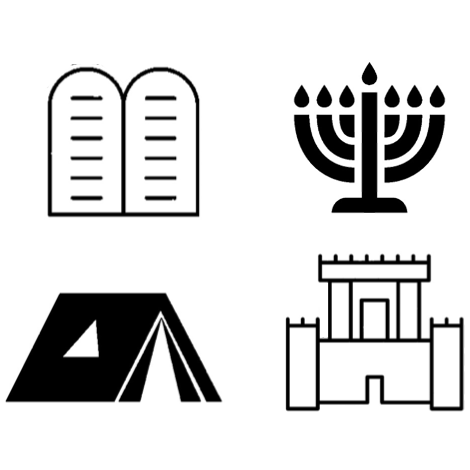
\includegraphics[width=0.30\textwidth]{../ot_frontcover.png}} ;
    \node (0,0) [xshift=+0.20cm, yshift=+2.0cm, opacity=0.10]{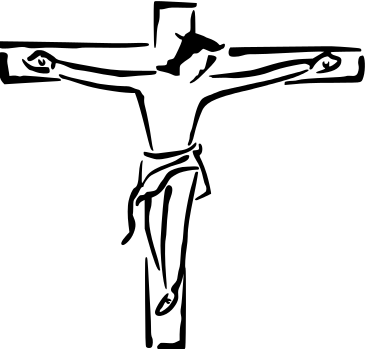
\includegraphics[width=0.20\textwidth]{../christ_on_cross.png}} ;
\end{tikzpicture}
\Large 

\leftcitation{ס} \centerfont 詩百又廿七載：
\leftcitation{ע} \centerfont 非耶和華建屋宇.則匠人之經營徒.
\leftcitation{פ} \centerfont 非耶和華衛城邑.則守者之儆醒徒.
\leftcitation{צ} \centerfont 余獻是卷予華人社區．願為福音流通之器．願獻斯微材為祭榮耀上帝．
\leftcitation{ק} \centerfont 阿門

\switchcolumn

\fontsize{11}{13}\rightfont \Large 滅．時越次聖殿期及當今。\leftcitation{י} \rightfont 猶太者力廣納之．筆錄以卷軸．便以傳、閱、頌、攜、守、鎖、抄、譯、釋、編，得書塔木德、密示拿等經傳．家喻戶曉．傳流若芳。\leftcitation{כ} \rightfont 猶太者文以載道．傳其口述．今我輩粵道之傳應當作如是．遂力行粵音識辨之法．載言載道．以盡忠傳粵道以待興。\leftcitation{ל} \rightfont 蒙下賜恩惠．無畏海量字音文書．既馭上帝之道．今廣及粵語講道．重駛編程之技．匯導粵音遂字稿．重塑講道現場．以傚猶太卷軸之舉便以傳流。\leftcitation{מ} \rightfont 是卷乃粵音口述傳之屬．莫通華文白話之語．

\end{paracol}

\columnratio{0.5,0.5}
\begin{paracol}{2}\fontsize{11}{13}\leftfont \Large \leftcitation{ו} \leftfont 斯殺一違儆百逆．既禁壓之．我輩聞風無奈．在所難免。\leftcitation{ז} \leftfont 另有異人例乎．以版權之名．脅網絡頻道之舉．同授礙予粵道之存流。

\switchcolumn

\fontsize{11}{13}\rightfont \Large 惟待後繼來者之傚．以譯釋傳之於神州華文地。\leftcitation{נ} \rightfont 今能排程驅馭圖靈以編彙文檔，其碼長共數千千亦無逢大礙．全蒙上帝保守。

\end{paracol}



\columnratio{1}\begin{paracol}{1}

\fontsize{11}{13}\rightfont \Large
~~~~~~~~~~~~~~~~~~~~~~~~~~~~~~~~~~~~~~~~~~~~~~~~~~~~~~~~~~~~~~~~~~~~~~~~~~~~~~~\leftcitation{ר} \rightfont 二零二三年二月一日

~~~~~~~~~~~~~~~~~~~~~~~~~~~~~~~~~~~~~~~~~~~~~~~~~~~~~~~~~~~~~~~~~~~~~~~~~~~~~~~\leftcitation{ש} \rightfont 米迦勒

~~~~~~~~~~~~~~~~~~~~~~~~~~~~~~~~~~~~~~~~~~~~~~~~~~~~~~~~~~~~~~~~~~~~~~~~~~~~~~~\leftcitation{ת} \rightfont 書於香港

\end{paracol}

\end{sloppypar}
\end{document}
